\documentclass[twoside]{book}

% Packages required by doxygen
\usepackage{fixltx2e}
\usepackage{calc}
\usepackage{doxygen}
\usepackage[export]{adjustbox} % also loads graphicx
\usepackage{graphicx}
\usepackage[utf8]{inputenc}
\usepackage{makeidx}
\usepackage{multicol}
\usepackage{multirow}
\PassOptionsToPackage{warn}{textcomp}
\usepackage{textcomp}
\usepackage[nointegrals]{wasysym}
\usepackage[table]{xcolor}

% Font selection
\usepackage[T1]{fontenc}
\usepackage[scaled=.90]{helvet}
\usepackage{courier}
\usepackage{amssymb}
\usepackage{sectsty}
\renewcommand{\familydefault}{\sfdefault}
\allsectionsfont{%
  \fontseries{bc}\selectfont%
  \color{darkgray}%
}
\renewcommand{\DoxyLabelFont}{%
  \fontseries{bc}\selectfont%
  \color{darkgray}%
}
\newcommand{\+}{\discretionary{\mbox{\scriptsize$\hookleftarrow$}}{}{}}

% Page & text layout
\usepackage{geometry}
\geometry{%
  a4paper,%
  top=2.5cm,%
  bottom=2.5cm,%
  left=2.5cm,%
  right=2.5cm%
}
\tolerance=750
\hfuzz=15pt
\hbadness=750
\setlength{\emergencystretch}{15pt}
\setlength{\parindent}{0cm}
\setlength{\parskip}{3ex plus 2ex minus 2ex}
\makeatletter
\renewcommand{\paragraph}{%
  \@startsection{paragraph}{4}{0ex}{-1.0ex}{1.0ex}{%
    \normalfont\normalsize\bfseries\SS@parafont%
  }%
}
\renewcommand{\subparagraph}{%
  \@startsection{subparagraph}{5}{0ex}{-1.0ex}{1.0ex}{%
    \normalfont\normalsize\bfseries\SS@subparafont%
  }%
}
\makeatother

% Headers & footers
\usepackage{fancyhdr}
\pagestyle{fancyplain}
\fancyhead[LE]{\fancyplain{}{\bfseries\thepage}}
\fancyhead[CE]{\fancyplain{}{}}
\fancyhead[RE]{\fancyplain{}{\bfseries\leftmark}}
\fancyhead[LO]{\fancyplain{}{\bfseries\rightmark}}
\fancyhead[CO]{\fancyplain{}{}}
\fancyhead[RO]{\fancyplain{}{\bfseries\thepage}}
\fancyfoot[LE]{\fancyplain{}{}}
\fancyfoot[CE]{\fancyplain{}{}}
\fancyfoot[RE]{\fancyplain{}{\bfseries\scriptsize Generated by Doxygen }}
\fancyfoot[LO]{\fancyplain{}{\bfseries\scriptsize Generated by Doxygen }}
\fancyfoot[CO]{\fancyplain{}{}}
\fancyfoot[RO]{\fancyplain{}{}}
\renewcommand{\footrulewidth}{0.4pt}
\renewcommand{\chaptermark}[1]{%
  \markboth{#1}{}%
}
\renewcommand{\sectionmark}[1]{%
  \markright{\thesection\ #1}%
}

% Indices & bibliography
\usepackage{natbib}
\usepackage[titles]{tocloft}
\setcounter{tocdepth}{3}
\setcounter{secnumdepth}{5}
\makeindex

% Hyperlinks (required, but should be loaded last)
\usepackage{ifpdf}
\ifpdf
  \usepackage[pdftex,pagebackref=true]{hyperref}
\else
  \usepackage[ps2pdf,pagebackref=true]{hyperref}
\fi
\hypersetup{%
  colorlinks=true,%
  linkcolor=blue,%
  citecolor=blue,%
  unicode%
}

% Custom commands
\newcommand{\clearemptydoublepage}{%
  \newpage{\pagestyle{empty}\cleardoublepage}%
}

\usepackage{caption}
\captionsetup{labelsep=space,justification=centering,font={bf},singlelinecheck=off,skip=4pt,position=top}

%===== C O N T E N T S =====

\begin{document}

% Titlepage & ToC
\hypersetup{pageanchor=false,
             bookmarksnumbered=true,
             pdfencoding=unicode
            }
\pagenumbering{alph}
\begin{titlepage}
\vspace*{7cm}
\begin{center}%
{\Large Stanford\+C\+P\+P\+Lib }\\
\vspace*{1cm}
{\large Generated by Doxygen 1.8.14}\\
\end{center}
\end{titlepage}
\clearemptydoublepage
\pagenumbering{roman}
\tableofcontents
\clearemptydoublepage
\pagenumbering{arabic}
\hypersetup{pageanchor=true}

%--- Begin generated contents ---
\chapter{P\+Streams Reference}
\label{index}\hypertarget{index}{} 
\chapter{Big\+Oh}
\label{BigOh}
\Hypertarget{BigOh}

\begin{DoxyRefList}
\item[\label{BigOh__BigOh000003}%
\Hypertarget{BigOh__BigOh000003}%
Member \mbox{\hyperlink{classBasicGraphGen_a624c45bedf3986073b0f8a40ab4d85c2}{Basic\+Graph\+Gen$<$ V, E $>$\+:\+:add\+Edge}} (const std\+::string \&v1, const std\+::string \&v2, double cost=0.\+0, bool directed=true)]O(log V + log E)  
\item[\label{BigOh__BigOh000004}%
\Hypertarget{BigOh__BigOh000004}%
Member \mbox{\hyperlink{classBasicGraphGen_ac2fe8fab4722e89853df8ed385aa7a26}{Basic\+Graph\+Gen$<$ V, E $>$\+:\+:add\+Edge}} (Vertex\+Gen$<$ V, E $>$ $\ast$v1, Vertex\+Gen$<$ V, E $>$ $\ast$v2, double cost=0.\+0, bool directed=true)]O(log V + log E)  
\item[\label{BigOh__BigOh000005}%
\Hypertarget{BigOh__BigOh000005}%
Member \mbox{\hyperlink{classBasicGraphGen_a92cffe0dd5b70ab78a3bce486fd60637}{Basic\+Graph\+Gen$<$ V, E $>$\+:\+:add\+Edge}} (Edge\+Gen$<$ V, E $>$ $\ast$e, bool directed=true)]O(log V + log E)  
\item[\label{BigOh__BigOh000006}%
\Hypertarget{BigOh__BigOh000006}%
Member \mbox{\hyperlink{classBasicGraphGen_a60f19882208c6d1dc51b74d5f348f458}{Basic\+Graph\+Gen$<$ V, E $>$\+:\+:add\+Vertex}} (const std\+::string \&name)]O(log V)  
\item[\label{BigOh__BigOh000007}%
\Hypertarget{BigOh__BigOh000007}%
Member \mbox{\hyperlink{classBasicGraphGen_a99facea785e991d862eef401807c5f79}{Basic\+Graph\+Gen$<$ V, E $>$\+:\+:add\+Vertex}} (Vertex\+Gen$<$ V, E $>$ $\ast$v)]O(log V)  
\item[\label{BigOh__BigOh000002}%
\Hypertarget{BigOh__BigOh000002}%
Member \mbox{\hyperlink{classBasicGraphGen_aa8af075f69d803e4a813e4d348150fc5}{Basic\+Graph\+Gen$<$ V, E $>$\+:\+:Basic\+Graph\+Gen}} (std\+::initializer\+\_\+list$<$ std\+::string $>$ vertex\+List)]O(\+V)  
\item[\label{BigOh__BigOh000001}%
\Hypertarget{BigOh__BigOh000001}%
Member \mbox{\hyperlink{classBasicGraphGen_a9d6eaee0a2e8ea6de432f815463813fa}{Basic\+Graph\+Gen$<$ V, E $>$\+:\+:Basic\+Graph\+Gen}} ()]O(1)  
\item[\label{BigOh__BigOh000008}%
\Hypertarget{BigOh__BigOh000008}%
Member \mbox{\hyperlink{classBasicGraphGen_aced46bbfe5973602cbd67ac6188c36db}{Basic\+Graph\+Gen$<$ V, E $>$\+:\+:clear\+Edges}} ()]O(\+E log E)  
\item[\label{BigOh__BigOh000009}%
\Hypertarget{BigOh__BigOh000009}%
Member \mbox{\hyperlink{classBasicGraphGen_ac3104a246e5eaa7701c96bf52038c6b0}{Basic\+Graph\+Gen$<$ V, E $>$\+:\+:clear\+Edges}} (Vertex\+Gen$<$ V, E $>$ $\ast$v)]O(\+E log E) 

O(log V + E)  
\item[\label{BigOh__BigOh000010}%
\Hypertarget{BigOh__BigOh000010}%
Member \mbox{\hyperlink{classBasicGraphGen_a206c104818fb8653db07b7f4a3d5fe11}{Basic\+Graph\+Gen$<$ V, E $>$\+:\+:clear\+Edges}} (const std\+::string \&v)]O(\+E log E)  
\item[\label{BigOh__BigOh000011}%
\Hypertarget{BigOh__BigOh000011}%
Member \mbox{\hyperlink{classBasicGraphGen_a6ce3804a90bf7006e7bc78e1a51a1365}{Basic\+Graph\+Gen$<$ V, E $>$\+:\+:contains\+Edge}} (Vertex\+Gen$<$ V, E $>$ $\ast$v1, Vertex\+Gen$<$ V, E $>$ $\ast$v2) const]O(log E)  
\item[\label{BigOh__BigOh000012}%
\Hypertarget{BigOh__BigOh000012}%
Member \mbox{\hyperlink{classBasicGraphGen_a4475808d2ed8a45b9fceecc2c6081fc3}{Basic\+Graph\+Gen$<$ V, E $>$\+:\+:contains\+Edge}} (const std\+::string \&v1, const std\+::string \&v2) const]O(log E)  
\item[\label{BigOh__BigOh000013}%
\Hypertarget{BigOh__BigOh000013}%
Member \mbox{\hyperlink{classBasicGraphGen_ad41e772ab382972e1c54ab6df781dd82}{Basic\+Graph\+Gen$<$ V, E $>$\+:\+:contains\+Edge}} (Edge\+Gen$<$ V, E $>$ $\ast$edge) const]O(log E)  
\item[\label{BigOh__BigOh000014}%
\Hypertarget{BigOh__BigOh000014}%
Member \mbox{\hyperlink{classBasicGraphGen_ab6062ac98f3491a525e0809c5b03b7cf}{Basic\+Graph\+Gen$<$ V, E $>$\+:\+:contains\+Vertex}} (const std\+::string \&name) const]O(log V)  
\item[\label{BigOh__BigOh000015}%
\Hypertarget{BigOh__BigOh000015}%
Member \mbox{\hyperlink{classBasicGraphGen_a37d4f31bc5bb6397fdb0bf966b54ca3f}{Basic\+Graph\+Gen$<$ V, E $>$\+:\+:contains\+Vertex}} (Vertex\+Gen$<$ V, E $>$ $\ast$v) const]O(log V)  
\item[\label{BigOh__BigOh000016}%
\Hypertarget{BigOh__BigOh000016}%
Member \mbox{\hyperlink{classBasicGraphGen_aa1f43093f29e66e171d5f572a658ae0c}{Basic\+Graph\+Gen$<$ V, E $>$\+:\+:edge\+Count}} () const]O(log V)  
\item[\label{BigOh__BigOh000017}%
\Hypertarget{BigOh__BigOh000017}%
Member \mbox{\hyperlink{classBasicGraphGen_aad31ac511c91ccf23a19af68e7a9f316}{Basic\+Graph\+Gen$<$ V, E $>$\+:\+:get\+Edge}} (Vertex\+Gen$<$ V, E $>$ $\ast$v1, Vertex\+Gen$<$ V, E $>$ $\ast$v2) const]O(log V + log E)  
\item[\label{BigOh__BigOh000018}%
\Hypertarget{BigOh__BigOh000018}%
Member \mbox{\hyperlink{classBasicGraphGen_a57e156a4bae200f10f36fce5ec7fe504}{Basic\+Graph\+Gen$<$ V, E $>$\+:\+:get\+Edge}} (const std\+::string \&v1, const std\+::string \&v2) const]O(log V + log E)  
\item[\label{BigOh__BigOh000019}%
\Hypertarget{BigOh__BigOh000019}%
Member \mbox{\hyperlink{classBasicGraphGen_a312cc70af3d52a9fbdd56629c1710e48}{Basic\+Graph\+Gen$<$ V, E $>$\+:\+:get\+Edge\+Set}} () const]O(1)  
\item[\label{BigOh__BigOh000020}%
\Hypertarget{BigOh__BigOh000020}%
Member \mbox{\hyperlink{classBasicGraphGen_abfe8d6cbb48312f7fbec0fd948330348}{Basic\+Graph\+Gen$<$ V, E $>$\+:\+:get\+Edge\+Set}} (Vertex\+Gen$<$ V, E $>$ $\ast$v) const]O(1)  
\item[\label{BigOh__BigOh000021}%
\Hypertarget{BigOh__BigOh000021}%
Member \mbox{\hyperlink{classBasicGraphGen_a6deea7a4536dfd6346c62c0c05a141ed}{Basic\+Graph\+Gen$<$ V, E $>$\+:\+:get\+Edge\+Set}} (const std\+::string \&v) const]O(1)  
\item[\label{BigOh__BigOh000022}%
\Hypertarget{BigOh__BigOh000022}%
Member \mbox{\hyperlink{classBasicGraphGen_ad8e645c23a9816fff136e0a5f7941669}{Basic\+Graph\+Gen$<$ V, E $>$\+:\+:get\+Inverse\+Arc}} (Edge\+Gen$<$ V, E $>$ $\ast$edge) const]O(\+E)  
\item[\label{BigOh__BigOh000023}%
\Hypertarget{BigOh__BigOh000023}%
Member \mbox{\hyperlink{classBasicGraphGen_ae81616e12d12f2dcfa295b4a3b48f960}{Basic\+Graph\+Gen$<$ V, E $>$\+:\+:get\+Inverse\+Edge}} (Edge\+Gen$<$ V, E $>$ $\ast$edge) const]O(\+E)  
\item[\label{BigOh__BigOh000024}%
\Hypertarget{BigOh__BigOh000024}%
Member \mbox{\hyperlink{classBasicGraphGen_a5db8788e3783e8ff16b19c06a5f2cf62}{Basic\+Graph\+Gen$<$ V, E $>$\+:\+:get\+Inverse\+Edge\+Set}} (Vertex\+Gen$<$ V, E $>$ $\ast$v) const]O(\+E)  
\item[\label{BigOh__BigOh000025}%
\Hypertarget{BigOh__BigOh000025}%
Member \mbox{\hyperlink{classBasicGraphGen_a7ef9596e6faf68669228bc69808e84bd}{Basic\+Graph\+Gen$<$ V, E $>$\+:\+:get\+Inverse\+Edge\+Set}} (const std\+::string \&v) const]O(\+E)  
\item[\label{BigOh__BigOh000026}%
\Hypertarget{BigOh__BigOh000026}%
Member \mbox{\hyperlink{classBasicGraphGen_a4c0c055103d2adba54014d301ae7bd1c}{Basic\+Graph\+Gen$<$ V, E $>$\+:\+:get\+Vertex}} (const std\+::string \&name) const]O(log V)  
\item[\label{BigOh__BigOh000027}%
\Hypertarget{BigOh__BigOh000027}%
Member \mbox{\hyperlink{classBasicGraphGen_ae1bca1f87888bd787f836bc064a9ff01}{Basic\+Graph\+Gen$<$ V, E $>$\+:\+:get\+Vertex\+Names}} () const]O(\+V log V)  
\item[\label{BigOh__BigOh000028}%
\Hypertarget{BigOh__BigOh000028}%
Member \mbox{\hyperlink{classBasicGraphGen_aec896ef5b1fc6044fc71318d1369f6f1}{Basic\+Graph\+Gen$<$ V, E $>$\+:\+:get\+Vertex\+Set}} () const]O(\+V log V)  
\item[\label{BigOh__BigOh000038}%
\Hypertarget{BigOh__BigOh000038}%
Member \mbox{\hyperlink{classBasicGraphGen_a5e874dbb2f9f2c7f98ec74f00790eb0e}{Basic\+Graph\+Gen$<$ V, E $>$\+:\+:operator\mbox{[}\mbox{]}}} (const std\+::string \&name)]O(log V)  
\item[\label{BigOh__BigOh000039}%
\Hypertarget{BigOh__BigOh000039}%
Member \mbox{\hyperlink{classBasicGraphGen_ad91a5b6ebd034841cf4f4c410fb7ed1b}{Basic\+Graph\+Gen$<$ V, E $>$\+:\+:operator\mbox{[}\mbox{]}}} (const std\+::string \&name) const]O(log V)  
\item[\label{BigOh__BigOh000029}%
\Hypertarget{BigOh__BigOh000029}%
Member \mbox{\hyperlink{classBasicGraphGen_adfee7a20d0c13cc515b3b7e951d8baf2}{Basic\+Graph\+Gen$<$ V, E $>$\+:\+:remove\+Edge}} (const std\+::string \&v1, const std\+::string \&v2, bool directed=true)]O(E + log V)  
\item[\label{BigOh__BigOh000030}%
\Hypertarget{BigOh__BigOh000030}%
Member \mbox{\hyperlink{classBasicGraphGen_a8b1003fbe63fab20173526459fff4139}{Basic\+Graph\+Gen$<$ V, E $>$\+:\+:remove\+Edge}} (Vertex\+Gen$<$ V, E $>$ $\ast$v1, Vertex\+Gen$<$ V, E $>$ $\ast$v2, bool directed=true)]O(E + log V)  
\item[\label{BigOh__BigOh000031}%
\Hypertarget{BigOh__BigOh000031}%
Member \mbox{\hyperlink{classBasicGraphGen_a2c6bb1e8e2c18b7376504692f7baae62}{Basic\+Graph\+Gen$<$ V, E $>$\+:\+:remove\+Edge}} (Edge\+Gen$<$ V, E $>$ $\ast$e, bool directed=true)]O(log E + log V)  
\item[\label{BigOh__BigOh000032}%
\Hypertarget{BigOh__BigOh000032}%
Member \mbox{\hyperlink{classBasicGraphGen_aaa33b4c05ee490d241ba5542420b985b}{Basic\+Graph\+Gen$<$ V, E $>$\+:\+:remove\+Vertex}} (const std\+::string \&name)]O(E + log V)  
\item[\label{BigOh__BigOh000033}%
\Hypertarget{BigOh__BigOh000033}%
Member \mbox{\hyperlink{classBasicGraphGen_a9eac2d17b5e8074dace019020d078acb}{Basic\+Graph\+Gen$<$ V, E $>$\+:\+:remove\+Vertex}} (Vertex\+Gen$<$ V, E $>$ $\ast$v)]O(E + log V)  
\item[\label{BigOh__BigOh000036}%
\Hypertarget{BigOh__BigOh000036}%
Member \mbox{\hyperlink{classBasicGraphGen_a66498d3675a5bc08fa30a032d41764f7}{Basic\+Graph\+Gen$<$ V, E $>$\+:\+:to\+Map}} () const]O(V + E)  
\item[\label{BigOh__BigOh000037}%
\Hypertarget{BigOh__BigOh000037}%
Member \mbox{\hyperlink{classBasicGraphGen_a68eb4830a4800ed7704895c16a8982be}{Basic\+Graph\+Gen$<$ V, E $>$\+:\+:vertex\+Count}} () const]O(1)  
\item[\label{BigOh__BigOh000042}%
\Hypertarget{BigOh__BigOh000042}%
Member \mbox{\hyperlink{classGraph_aad2e9fedd7110ae2fb6873c5e2d29941}{Graph$<$ Node\+Type, Arc\+Type $>$\+:\+:add\+Arc}} (const std\+::string \&n1, const std\+::string \&n2)]O(log V + log E)  
\item[\label{BigOh__BigOh000043}%
\Hypertarget{BigOh__BigOh000043}%
Member \mbox{\hyperlink{classGraph_a7280d3cd76bab82df392ba91ed5257c6}{Graph$<$ Node\+Type, Arc\+Type $>$\+:\+:add\+Arc}} (Node\+Type $\ast$n1, Node\+Type $\ast$n2)]O(log V + log E)  
\item[\label{BigOh__BigOh000044}%
\Hypertarget{BigOh__BigOh000044}%
Member \mbox{\hyperlink{classGraph_aa1b6553e579c03260253a2d731668dfa}{Graph$<$ Node\+Type, Arc\+Type $>$\+:\+:add\+Arc}} (Arc\+Type $\ast$arc)]O(log V + log E)  
\item[\label{BigOh__BigOh000045}%
\Hypertarget{BigOh__BigOh000045}%
Member \mbox{\hyperlink{classGraph_acd763aa09491315536b5d2734cd82b89}{Graph$<$ Node\+Type, Arc\+Type $>$\+:\+:add\+Node}} (const std\+::string \&name)]O(log V)  
\item[\label{BigOh__BigOh000046}%
\Hypertarget{BigOh__BigOh000046}%
Member \mbox{\hyperlink{classGraph_a635fa78d72315816cef6c091acfa3882}{Graph$<$ Node\+Type, Arc\+Type $>$\+:\+:add\+Node}} (Node\+Type $\ast$node)]O(log V)  
\item[\label{BigOh__BigOh000047}%
\Hypertarget{BigOh__BigOh000047}%
Member \mbox{\hyperlink{classGraph_ac0b108b3354f5222d2c829dcd639fa7a}{Graph$<$ Node\+Type, Arc\+Type $>$\+:\+:arc\+Count}} () const]O(1)  
\item[\label{BigOh__BigOh000048}%
\Hypertarget{BigOh__BigOh000048}%
Member \mbox{\hyperlink{classGraph_a27d59ef129bb56cc144ecc81c0affd34}{Graph$<$ Node\+Type, Arc\+Type $>$\+:\+:back}} () const]O(1)  
\item[\label{BigOh__BigOh000091}%
\Hypertarget{BigOh__BigOh000091}%
Member \mbox{\hyperlink{classGraph_aea3a8950c46f4ac913207201b685e715}{Graph$<$ Node\+Type, Arc\+Type $>$\+:\+:begin}} () const]O(1)  
\item[\label{BigOh__BigOh000049}%
\Hypertarget{BigOh__BigOh000049}%
Member \mbox{\hyperlink{classGraph_ac8bb3912a3ce86b15842e79d0b421204}{Graph$<$ Node\+Type, Arc\+Type $>$\+:\+:clear}} ()]O(V + E)  
\item[\label{BigOh__BigOh000050}%
\Hypertarget{BigOh__BigOh000050}%
Member \mbox{\hyperlink{classGraph_a63f0ce1806df1c8070d997153363eecb}{Graph$<$ Node\+Type, Arc\+Type $>$\+:\+:clear\+Arcs}} ()]O(\+E)  
\item[\label{BigOh__BigOh000051}%
\Hypertarget{BigOh__BigOh000051}%
Member \mbox{\hyperlink{classGraph_a14def9e68896088fec7839e5da4fed27}{Graph$<$ Node\+Type, Arc\+Type $>$\+:\+:clear\+Arcs}} (Node\+Type $\ast$node)]O(log V + E)  
\item[\label{BigOh__BigOh000052}%
\Hypertarget{BigOh__BigOh000052}%
Member \mbox{\hyperlink{classGraph_a2d8ecb9c6768fff244b2be46319385cc}{Graph$<$ Node\+Type, Arc\+Type $>$\+:\+:clear\+Arcs}} (const std\+::string \&name)]O(\+E log E)  
\item[\label{BigOh__BigOh000053}%
\Hypertarget{BigOh__BigOh000053}%
Member \mbox{\hyperlink{classGraph_a9ca50139471975b82fdc6b1977bcfa4a}{Graph$<$ Node\+Type, Arc\+Type $>$\+:\+:contains\+Arc}} (Node\+Type $\ast$node1, Node\+Type $\ast$node2) const]O(log E)  
\item[\label{BigOh__BigOh000054}%
\Hypertarget{BigOh__BigOh000054}%
Member \mbox{\hyperlink{classGraph_a515e45aae316b581bf1cf168541f4f44}{Graph$<$ Node\+Type, Arc\+Type $>$\+:\+:contains\+Arc}} (const std\+::string \&node1, const std\+::string \&node2) const]O(log E)  
\item[\label{BigOh__BigOh000055}%
\Hypertarget{BigOh__BigOh000055}%
Member \mbox{\hyperlink{classGraph_acf7a659ddd8a143836b91b01c200ee8a}{Graph$<$ Node\+Type, Arc\+Type $>$\+:\+:contains\+Arc}} (Arc\+Type $\ast$arc) const]O(log E)  
\item[\label{BigOh__BigOh000056}%
\Hypertarget{BigOh__BigOh000056}%
Member \mbox{\hyperlink{classGraph_ac0beb77e8a238c2898ab851df71eeefe}{Graph$<$ Node\+Type, Arc\+Type $>$\+:\+:contains\+Node}} (const std\+::string \&name) const]O(log V)  
\item[\label{BigOh__BigOh000057}%
\Hypertarget{BigOh__BigOh000057}%
Member \mbox{\hyperlink{classGraph_a4f540ebc07c4e46a0bb7fee76a93386c}{Graph$<$ Node\+Type, Arc\+Type $>$\+:\+:contains\+Node}} (Node\+Type $\ast$node) const]O(log V)  
\item[\label{BigOh__BigOh000092}%
\Hypertarget{BigOh__BigOh000092}%
Member \mbox{\hyperlink{classGraph_afcdf62cae5d7e50644957d66f886742d}{Graph$<$ Node\+Type, Arc\+Type $>$\+:\+:end}} () const]O(1)  
\item[\label{BigOh__BigOh000058}%
\Hypertarget{BigOh__BigOh000058}%
Member \mbox{\hyperlink{classGraph_a6bec43eb3dfdf3d23eb328b406edf44a}{Graph$<$ Node\+Type, Arc\+Type $>$\+:\+:equals}} (const Graph$<$ Node\+Type, Arc\+Type $>$ \&graph2) const]O(V log V + E log E)  
\item[\label{BigOh__BigOh000059}%
\Hypertarget{BigOh__BigOh000059}%
Member \mbox{\hyperlink{classGraph_a7b7c2c1738f8e7faf84c54d7642992fa}{Graph$<$ Node\+Type, Arc\+Type $>$\+:\+:front}} () const]O(1)  
\item[\label{BigOh__BigOh000060}%
\Hypertarget{BigOh__BigOh000060}%
Member \mbox{\hyperlink{classGraph_a7c33db338f839ff9e3dafe4fe61c16fd}{Graph$<$ Node\+Type, Arc\+Type $>$\+:\+:get\+Arc}} (Node\+Type $\ast$node1, Node\+Type $\ast$node2) const]O(log V + log E)  
\item[\label{BigOh__BigOh000061}%
\Hypertarget{BigOh__BigOh000061}%
Member \mbox{\hyperlink{classGraph_a94d4badfc856b0d4530c37121efb9834}{Graph$<$ Node\+Type, Arc\+Type $>$\+:\+:get\+Arc}} (const std\+::string \&node1, const std\+::string \&node2) const]O(log V + log E)  
\item[\label{BigOh__BigOh000062}%
\Hypertarget{BigOh__BigOh000062}%
Member \mbox{\hyperlink{classGraph_a0690edaeae8d5256189ae2e8541788b5}{Graph$<$ Node\+Type, Arc\+Type $>$\+:\+:get\+Arc\+Set}} () const]O(1)  
\item[\label{BigOh__BigOh000063}%
\Hypertarget{BigOh__BigOh000063}%
Member \mbox{\hyperlink{classGraph_a17cfc7f4d8c738fc6f51813f50be6400}{Graph$<$ Node\+Type, Arc\+Type $>$\+:\+:get\+Arc\+Set}} (Node\+Type $\ast$node) const]O(1)  
\item[\label{BigOh__BigOh000064}%
\Hypertarget{BigOh__BigOh000064}%
Member \mbox{\hyperlink{classGraph_a31b9e2056ee2d66a7ea9feb02f016e8d}{Graph$<$ Node\+Type, Arc\+Type $>$\+:\+:get\+Arc\+Set}} (const std\+::string \&name) const]O(1)  
\item[\label{BigOh__BigOh000066}%
\Hypertarget{BigOh__BigOh000066}%
Member \mbox{\hyperlink{classGraph_a2cfe12e71ca594736a1e329461cff024}{Graph$<$ Node\+Type, Arc\+Type $>$\+:\+:get\+Inverse\+Arc\+Set}} (const std\+::string \&name) const]O(\+E)  
\item[\label{BigOh__BigOh000065}%
\Hypertarget{BigOh__BigOh000065}%
Member \mbox{\hyperlink{classGraph_ad5fd149800cd46aae497b05b46059b63}{Graph$<$ Node\+Type, Arc\+Type $>$\+:\+:get\+Inverse\+Arc\+Set}} (Node\+Type $\ast$node) const]O(\+E)  
\item[\label{BigOh__BigOh000067}%
\Hypertarget{BigOh__BigOh000067}%
Member \mbox{\hyperlink{classGraph_aa9eceee00e824ea4852449fa3de61e82}{Graph$<$ Node\+Type, Arc\+Type $>$\+:\+:get\+Inverse\+Neighbor\+Names}} (Node\+Type $\ast$node) const]O(\+E)  
\item[\label{BigOh__BigOh000068}%
\Hypertarget{BigOh__BigOh000068}%
Member \mbox{\hyperlink{classGraph_ac3dc36bc1eb0f249180cfe78bce6e7a2}{Graph$<$ Node\+Type, Arc\+Type $>$\+:\+:get\+Inverse\+Neighbor\+Names}} (const std\+::string \&node) const]O(\+E)  
\item[\label{BigOh__BigOh000069}%
\Hypertarget{BigOh__BigOh000069}%
Member \mbox{\hyperlink{classGraph_a80a5724c594b9bd0b6008c57b09af317}{Graph$<$ Node\+Type, Arc\+Type $>$\+:\+:get\+Inverse\+Neighbors}} (Node\+Type $\ast$node) const]O(\+E)  
\item[\label{BigOh__BigOh000070}%
\Hypertarget{BigOh__BigOh000070}%
Member \mbox{\hyperlink{classGraph_a5294846b9cdd19394808e3736ec67004}{Graph$<$ Node\+Type, Arc\+Type $>$\+:\+:get\+Inverse\+Neighbors}} (const std\+::string \&node) const]O(\+E)  
\item[\label{BigOh__BigOh000071}%
\Hypertarget{BigOh__BigOh000071}%
Member \mbox{\hyperlink{classGraph_ae9b5cbd2bcb3918c4c64b1eb71c1a3a8}{Graph$<$ Node\+Type, Arc\+Type $>$\+:\+:get\+Neighbor\+Names}} (Node\+Type $\ast$node) const]O(log V)  
\item[\label{BigOh__BigOh000072}%
\Hypertarget{BigOh__BigOh000072}%
Member \mbox{\hyperlink{classGraph_a6175b4d672266465dd34e070c7710b34}{Graph$<$ Node\+Type, Arc\+Type $>$\+:\+:get\+Neighbor\+Names}} (const std\+::string \&node) const]O(log V)  
\item[\label{BigOh__BigOh000073}%
\Hypertarget{BigOh__BigOh000073}%
Member \mbox{\hyperlink{classGraph_a0e49b167f0623a8ae76040c3e5eab3fb}{Graph$<$ Node\+Type, Arc\+Type $>$\+:\+:get\+Neighbors}} (Node\+Type $\ast$node) const]O(log V)  
\item[\label{BigOh__BigOh000074}%
\Hypertarget{BigOh__BigOh000074}%
Member \mbox{\hyperlink{classGraph_a3a3720906c380f36b50530419330bfe5}{Graph$<$ Node\+Type, Arc\+Type $>$\+:\+:get\+Neighbors}} (const std\+::string \&node) const]O(log V)  
\item[\label{BigOh__BigOh000075}%
\Hypertarget{BigOh__BigOh000075}%
Member \mbox{\hyperlink{classGraph_a81487976cf0e576047333c85463c33aa}{Graph$<$ Node\+Type, Arc\+Type $>$\+:\+:get\+Node}} (const std\+::string \&name) const]O(log V)  
\item[\label{BigOh__BigOh000076}%
\Hypertarget{BigOh__BigOh000076}%
Member \mbox{\hyperlink{classGraph_a3c6f37932f377dd2bf4fec61343a916d}{Graph$<$ Node\+Type, Arc\+Type $>$\+:\+:get\+Node\+Names}} () const]O(\+V log V)  
\item[\label{BigOh__BigOh000077}%
\Hypertarget{BigOh__BigOh000077}%
Member \mbox{\hyperlink{classGraph_abd5552888f57aaa581099e8146c617c9}{Graph$<$ Node\+Type, Arc\+Type $>$\+:\+:get\+Node\+Set}} () const]O(1)  
\item[\label{BigOh__BigOh000040}%
\Hypertarget{BigOh__BigOh000040}%
Member \mbox{\hyperlink{classGraph_a0c40af42cad207665228815f0359bbd3}{Graph$<$ Node\+Type, Arc\+Type $>$\+:\+:Graph}} ()=default]O(1)  
\item[\label{BigOh__BigOh000079}%
\Hypertarget{BigOh__BigOh000079}%
Member \mbox{\hyperlink{classGraph_a3623b7decbedc522041c2c39d3b14421}{Graph$<$ Node\+Type, Arc\+Type $>$\+:\+:is\+Connected}} (const std\+::string \&s1, const std\+::string \&s2) const]O(log V)  
\item[\label{BigOh__BigOh000078}%
\Hypertarget{BigOh__BigOh000078}%
Member \mbox{\hyperlink{classGraph_a54164ab847f3a5c7fe15d15ac95af443}{Graph$<$ Node\+Type, Arc\+Type $>$\+:\+:is\+Connected}} (Node\+Type $\ast$n1, Node\+Type $\ast$n2) const]O(log V)  
\item[\label{BigOh__BigOh000082}%
\Hypertarget{BigOh__BigOh000082}%
Member \mbox{\hyperlink{classGraph_acf82f9b2937375c7b1cf3dccb3df3312}{Graph$<$ Node\+Type, Arc\+Type $>$\+:\+:is\+Empty}} () const]O(1)  
\item[\label{BigOh__BigOh000081}%
\Hypertarget{BigOh__BigOh000081}%
Member \mbox{\hyperlink{classGraph_a9e752628a118c4a06a538067c95bbb28}{Graph$<$ Node\+Type, Arc\+Type $>$\+:\+:is\+Neighbor}} (Node\+Type $\ast$node1, Node\+Type $\ast$node2) const]O(log V)  
\item[\label{BigOh__BigOh000080}%
\Hypertarget{BigOh__BigOh000080}%
Member \mbox{\hyperlink{classGraph_ab160bb64995133f6feb351cb23b031fb}{Graph$<$ Node\+Type, Arc\+Type $>$\+:\+:is\+Neighbor}} (const std\+::string \&node1, const std\+::string \&node2) const]O(log V)  
\item[\label{BigOh__BigOh000083}%
\Hypertarget{BigOh__BigOh000083}%
Member \mbox{\hyperlink{classGraph_a5dd1afdb4e1c75fbe51976bf6f70c922}{Graph$<$ Node\+Type, Arc\+Type $>$\+:\+:node\+Count}} () const]O(1)  
\item[\label{BigOh__BigOh000094}%
\Hypertarget{BigOh__BigOh000094}%
Member \mbox{\hyperlink{classGraph_aafd8d1cec3a4d6b8cdcb58016e4d093a}{Graph$<$ Node\+Type, Arc\+Type $>$\+:\+:operator!=}} (const \mbox{\hyperlink{classGraph}{Graph}} \&graph2) const]O(V log V + E log E)  
\item[\label{BigOh__BigOh000095}%
\Hypertarget{BigOh__BigOh000095}%
Member \mbox{\hyperlink{classGraph_a1daf423faecc777e29a399812dc39ca2}{Graph$<$ Node\+Type, Arc\+Type $>$\+:\+:operator$<$}} (const \mbox{\hyperlink{classGraph}{Graph}} \&graph2) const]O(V log V + E log E)  
\item[\label{BigOh__BigOh000096}%
\Hypertarget{BigOh__BigOh000096}%
Member \mbox{\hyperlink{classGraph_a352607f2b21dd87b3d2a3957bbf3da7b}{Graph$<$ Node\+Type, Arc\+Type $>$\+:\+:operator$<$=}} (const \mbox{\hyperlink{classGraph}{Graph}} \&graph2) const]O(V log V + E log E)  
\item[\label{BigOh__BigOh000093}%
\Hypertarget{BigOh__BigOh000093}%
Member \mbox{\hyperlink{classGraph_a188f85939e3fe6ed2d411f622287f722}{Graph$<$ Node\+Type, Arc\+Type $>$\+:\+:operator==}} (const \mbox{\hyperlink{classGraph}{Graph}} \&graph2) const]O(V log V + E log E)  
\item[\label{BigOh__BigOh000097}%
\Hypertarget{BigOh__BigOh000097}%
Member \mbox{\hyperlink{classGraph_a8019cf2c98949fd509193cf26ba2ff8a}{Graph$<$ Node\+Type, Arc\+Type $>$\+:\+:operator$>$}} (const \mbox{\hyperlink{classGraph}{Graph}} \&graph2) const]O(V log V + E log E)  
\item[\label{BigOh__BigOh000098}%
\Hypertarget{BigOh__BigOh000098}%
Member \mbox{\hyperlink{classGraph_ab1ca2af20f3b0251972b72295270212e}{Graph$<$ Node\+Type, Arc\+Type $>$\+:\+:operator$>$=}} (const \mbox{\hyperlink{classGraph}{Graph}} \&graph2) const]O(V log V + E log E)  
\item[\label{BigOh__BigOh000084}%
\Hypertarget{BigOh__BigOh000084}%
Member \mbox{\hyperlink{classGraph_af6370fb52d2dab4eb7795da22c33dd02}{Graph$<$ Node\+Type, Arc\+Type $>$\+:\+:remove\+Arc}} (const std\+::string \&s1, const std\+::string \&s2)]O(E + log V)  
\item[\label{BigOh__BigOh000085}%
\Hypertarget{BigOh__BigOh000085}%
Member \mbox{\hyperlink{classGraph_ae0c9f44b20b49ffae9fecc0a4f156ac1}{Graph$<$ Node\+Type, Arc\+Type $>$\+:\+:remove\+Arc}} (Node\+Type $\ast$n1, Node\+Type $\ast$n2)]O(E + log V)  
\item[\label{BigOh__BigOh000086}%
\Hypertarget{BigOh__BigOh000086}%
Member \mbox{\hyperlink{classGraph_a9d6580d1b0228fe6c1a02dfe70de1abf}{Graph$<$ Node\+Type, Arc\+Type $>$\+:\+:remove\+Arc}} (Arc\+Type $\ast$arc)]O(log E + log V)  
\item[\label{BigOh__BigOh000087}%
\Hypertarget{BigOh__BigOh000087}%
Member \mbox{\hyperlink{classGraph_a2d5f7ee89176144ed4c5c6b08a233aa6}{Graph$<$ Node\+Type, Arc\+Type $>$\+:\+:remove\+Node}} (const std\+::string \&name)]O(E + log V)  
\item[\label{BigOh__BigOh000088}%
\Hypertarget{BigOh__BigOh000088}%
Member \mbox{\hyperlink{classGraph_a2dfe63019975561914e0ed79551de108}{Graph$<$ Node\+Type, Arc\+Type $>$\+:\+:remove\+Node}} (Node\+Type $\ast$node)]O(E + log V)  
\item[\label{BigOh__BigOh000089}%
\Hypertarget{BigOh__BigOh000089}%
Member \mbox{\hyperlink{classGraph_af9593d4a5ff4274efaf429cb4f9e57cc}{Graph$<$ Node\+Type, Arc\+Type $>$\+:\+:size}} () const]O(1)  
\item[\label{BigOh__BigOh000090}%
\Hypertarget{BigOh__BigOh000090}%
Member \mbox{\hyperlink{classGraph_a1fe5121d6528fdea3f243321b3fa3a49}{Graph$<$ Node\+Type, Arc\+Type $>$\+:\+:to\+String}} () const]O(V + E)  
\item[\label{BigOh__BigOh000041}%
\Hypertarget{BigOh__BigOh000041}%
Member \mbox{\hyperlink{classGraph_af5a604e5e9e4d68dbc10b312e59f678f}{Graph$<$ Node\+Type, Arc\+Type $>$\+:\+:$\sim$\+Graph}} ()]O(V + E)  
\item[\label{BigOh__BigOh000103}%
\Hypertarget{BigOh__BigOh000103}%
Member \mbox{\hyperlink{classVector_ab901606bf3a8019c986f0cf9a9f298dc}{Vector$<$ Value\+Type $>$\+:\+:add}} (const Value\+Type \&value)]O(1)  
\item[\label{BigOh__BigOh000104}%
\Hypertarget{BigOh__BigOh000104}%
Member \mbox{\hyperlink{classVector_a7e05c14d67a60defeb6723b5704967a6}{Vector$<$ Value\+Type $>$\+:\+:add\+All}} (const Vector$<$ Value\+Type $>$ \&v)]O(\+N)  
\item[\label{BigOh__BigOh000105}%
\Hypertarget{BigOh__BigOh000105}%
Member \mbox{\hyperlink{classVector_a2bad145b40a82c36986f67610313658d}{Vector$<$ Value\+Type $>$\+:\+:back}} ()]O(1)  
\item[\label{BigOh__BigOh000106}%
\Hypertarget{BigOh__BigOh000106}%
Member \mbox{\hyperlink{classVector_adc761c91bdacd01bed5c96e25fd9486a}{Vector$<$ Value\+Type $>$\+:\+:back}} () const]O(1)  
\item[\label{BigOh__BigOh000107}%
\Hypertarget{BigOh__BigOh000107}%
Member \mbox{\hyperlink{classVector_ac8bb3912a3ce86b15842e79d0b421204}{Vector$<$ Value\+Type $>$\+:\+:clear}} ()]O(1)  
\item[\label{BigOh__BigOh000108}%
\Hypertarget{BigOh__BigOh000108}%
Member \mbox{\hyperlink{classVector_a6fbc1a150987e7e5320d244a3baeb560}{Vector$<$ Value\+Type $>$\+:\+:contains}} (const Value\+Type \&value) const]O(\+N)  
\item[\label{BigOh__BigOh000109}%
\Hypertarget{BigOh__BigOh000109}%
Member \mbox{\hyperlink{classVector_a9552fd9e921fc047fdd59e59d82e88ef}{Vector$<$ Value\+Type $>$\+:\+:ensure\+Capacity}} (int cap)]O(\+N)  
\item[\label{BigOh__BigOh000110}%
\Hypertarget{BigOh__BigOh000110}%
Member \mbox{\hyperlink{classVector_ad25fe1a007a2f00611d831198a1a86ea}{Vector$<$ Value\+Type $>$\+:\+:equals}} (const Vector$<$ Value\+Type $>$ \&v) const]O(\+N)  
\item[\label{BigOh__BigOh000112}%
\Hypertarget{BigOh__BigOh000112}%
Member \mbox{\hyperlink{classVector_a02aaa52ad7a120201f6dd3e90eff737f}{Vector$<$ Value\+Type $>$\+:\+:front}} () const]O(1)  
\item[\label{BigOh__BigOh000111}%
\Hypertarget{BigOh__BigOh000111}%
Member \mbox{\hyperlink{classVector_a736a6bda35a26620407e175bee46ae4a}{Vector$<$ Value\+Type $>$\+:\+:front}} ()]O(1)  
\item[\label{BigOh__BigOh000113}%
\Hypertarget{BigOh__BigOh000113}%
Member \mbox{\hyperlink{classVector_adcb38df411d14f0bd9c14e23947d2e1c}{Vector$<$ Value\+Type $>$\+:\+:get}} (int index) const]O(1)  
\item[\label{BigOh__BigOh000114}%
\Hypertarget{BigOh__BigOh000114}%
Member \mbox{\hyperlink{classVector_a619aacfb96804495d3182a7131cf3539}{Vector$<$ Value\+Type $>$\+:\+:index\+Of}} (const Value\+Type \&value) const]O(\+N)  
\item[\label{BigOh__BigOh000115}%
\Hypertarget{BigOh__BigOh000115}%
Member \mbox{\hyperlink{classVector_a0b5f5f8e87079d043caa9e5ed00d2941}{Vector$<$ Value\+Type $>$\+:\+:insert}} (int index, const Value\+Type \&value)]O(\+N)  
\item[\label{BigOh__BigOh000116}%
\Hypertarget{BigOh__BigOh000116}%
Member \mbox{\hyperlink{classVector_acf82f9b2937375c7b1cf3dccb3df3312}{Vector$<$ Value\+Type $>$\+:\+:is\+Empty}} () const]O(1)  
\item[\label{BigOh__BigOh000117}%
\Hypertarget{BigOh__BigOh000117}%
Member \mbox{\hyperlink{classVector_a48d608a1714954f0a7bcac6459483cb6}{Vector$<$ Value\+Type $>$\+:\+:last\+Index\+Of}} (const Value\+Type \&value) const]O(\+N)  
\item[\label{BigOh__BigOh000118}%
\Hypertarget{BigOh__BigOh000118}%
Member \mbox{\hyperlink{classVector_a0661241902bd7df69ab9c56f8d4c93c9}{Vector$<$ Value\+Type $>$\+:\+:map\+All}} (std\+::function$<$ void(const Value\+Type \&)$>$ fn) const]O(\+N)  
\item[\label{BigOh__BigOh000142}%
\Hypertarget{BigOh__BigOh000142}%
Member \mbox{\hyperlink{classVector_a3e96c4b5c89d1b00f587b521874cd0d8}{Vector$<$ Value\+Type $>$\+:\+:operator!=}} (const \mbox{\hyperlink{classVector}{Vector}} \&v2) const]O(\+N)  
\item[\label{BigOh__BigOh000138}%
\Hypertarget{BigOh__BigOh000138}%
Member \mbox{\hyperlink{classVector_ab2024a99b90c3bc71e3007f8dc5b38fa}{Vector$<$ Value\+Type $>$\+:\+:operator+}} (const Value\+Type \&elem) const]O(\+N)  
\item[\label{BigOh__BigOh000137}%
\Hypertarget{BigOh__BigOh000137}%
Member \mbox{\hyperlink{classVector_acb70fcd67f846bf16b96223bcf43e476}{Vector$<$ Value\+Type $>$\+:\+:operator+}} (const \mbox{\hyperlink{classVector}{Vector}} \&v2) const]O(\+N)  
\item[\label{BigOh__BigOh000139}%
\Hypertarget{BigOh__BigOh000139}%
Member \mbox{\hyperlink{classVector_a6b35f98e0e64a2fff6891a8806f640fd}{Vector$<$ Value\+Type $>$\+:\+:operator+=}} (const \mbox{\hyperlink{classVector}{Vector}} \&v2)]O(\+N)  
\item[\label{BigOh__BigOh000140}%
\Hypertarget{BigOh__BigOh000140}%
Member \mbox{\hyperlink{classVector_afded71b2a6d6df8b0257cbfd8f7e8d5f}{Vector$<$ Value\+Type $>$\+:\+:operator+=}} (const Value\+Type \&value)]O(1)  
\item[\label{BigOh__BigOh000147}%
\Hypertarget{BigOh__BigOh000147}%
Member \mbox{\hyperlink{classVector_ad2a2f86bb5857209608bbbfe1066c650}{Vector$<$ Value\+Type $>$\+:\+:operator,}} (const Value\+Type \&value)]O(1)  
\item[\label{BigOh__BigOh000143}%
\Hypertarget{BigOh__BigOh000143}%
Member \mbox{\hyperlink{classVector_a77901fd042b59d646be1da79b8339c5c}{Vector$<$ Value\+Type $>$\+:\+:operator$<$}} (const \mbox{\hyperlink{classVector}{Vector}} \&v2) const]O(\+N)  
\item[\label{BigOh__BigOh000144}%
\Hypertarget{BigOh__BigOh000144}%
Member \mbox{\hyperlink{classVector_ae70337b6c4c49dde850031de8b68c05d}{Vector$<$ Value\+Type $>$\+:\+:operator$<$=}} (const \mbox{\hyperlink{classVector}{Vector}} \&v2) const]O(\+N)  
\item[\label{BigOh__BigOh000141}%
\Hypertarget{BigOh__BigOh000141}%
Member \mbox{\hyperlink{classVector_a31eebc4de791cf62b8fa12a0eeca90dc}{Vector$<$ Value\+Type $>$\+:\+:operator==}} (const \mbox{\hyperlink{classVector}{Vector}} \&v2) const]O(\+N)  
\item[\label{BigOh__BigOh000145}%
\Hypertarget{BigOh__BigOh000145}%
Member \mbox{\hyperlink{classVector_a0b8b14442cb420ffaecc0606345e73a1}{Vector$<$ Value\+Type $>$\+:\+:operator$>$}} (const \mbox{\hyperlink{classVector}{Vector}} \&v2) const]O(\+N)  
\item[\label{BigOh__BigOh000146}%
\Hypertarget{BigOh__BigOh000146}%
Member \mbox{\hyperlink{classVector_adaa095641c5fc43f90754d7694784006}{Vector$<$ Value\+Type $>$\+:\+:operator$>$=}} (const \mbox{\hyperlink{classVector}{Vector}} \&v2) const]O(\+N)  
\item[\label{BigOh__BigOh000135}%
\Hypertarget{BigOh__BigOh000135}%
Member \mbox{\hyperlink{classVector_a7dbb3a92c8b6a08a04b564aed136b870}{Vector$<$ Value\+Type $>$\+:\+:operator\mbox{[}\mbox{]}}} (int index)]O(1)  
\item[\label{BigOh__BigOh000136}%
\Hypertarget{BigOh__BigOh000136}%
Member \mbox{\hyperlink{classVector_a1b5a4ea461655cbe512ab976aad8d809}{Vector$<$ Value\+Type $>$\+:\+:operator\mbox{[}\mbox{]}}} (int index) const]O(1)  
\item[\label{BigOh__BigOh000120}%
\Hypertarget{BigOh__BigOh000120}%
Member \mbox{\hyperlink{classVector_ab48f65e37130b674bc0f6220cbb59491}{Vector$<$ Value\+Type $>$\+:\+:pop\+\_\+back}} ()]O(1)  
\item[\label{BigOh__BigOh000119}%
\Hypertarget{BigOh__BigOh000119}%
Member \mbox{\hyperlink{classVector_aacdba74afa1be07d1046ece9e0512c77}{Vector$<$ Value\+Type $>$\+:\+:pop\+\_\+front}} ()]O(\+N)  
\item[\label{BigOh__BigOh000121}%
\Hypertarget{BigOh__BigOh000121}%
Member \mbox{\hyperlink{classVector_a8ff6f18ca45e769f2f8c7a0bcf79fad9}{Vector$<$ Value\+Type $>$\+:\+:push\+\_\+back}} (const Value\+Type \&value)]O(1)  
\item[\label{BigOh__BigOh000122}%
\Hypertarget{BigOh__BigOh000122}%
Member \mbox{\hyperlink{classVector_a9737dc314198d1cf306325134f000c5a}{Vector$<$ Value\+Type $>$\+:\+:push\+\_\+front}} (const Value\+Type \&value)]O(\+N)  
\item[\label{BigOh__BigOh000123}%
\Hypertarget{BigOh__BigOh000123}%
Member \mbox{\hyperlink{classVector_a2ad1aa316f278b2e9fa8121504749652}{Vector$<$ Value\+Type $>$\+:\+:remove}} (int index)]O(\+N)  
\item[\label{BigOh__BigOh000125}%
\Hypertarget{BigOh__BigOh000125}%
Member \mbox{\hyperlink{classVector_af7878e9c2f67e06cbae525e9fa77e38e}{Vector$<$ Value\+Type $>$\+:\+:remove\+Back}} ()]O(1)  
\item[\label{BigOh__BigOh000124}%
\Hypertarget{BigOh__BigOh000124}%
Member \mbox{\hyperlink{classVector_a02453aa96e93c38ca4c1d176307c8a63}{Vector$<$ Value\+Type $>$\+:\+:remove\+Front}} ()]O(\+N)  
\item[\label{BigOh__BigOh000126}%
\Hypertarget{BigOh__BigOh000126}%
Member \mbox{\hyperlink{classVector_a10e8154a489093d2b1f20596342bcd78}{Vector$<$ Value\+Type $>$\+:\+:remove\+Value}} (const Value\+Type \&value)]O(\+N)  
\item[\label{BigOh__BigOh000127}%
\Hypertarget{BigOh__BigOh000127}%
Member \mbox{\hyperlink{classVector_a310c0bebc002158f5646a91d60e4dc89}{Vector$<$ Value\+Type $>$\+:\+:reverse}} ()]O(\+N)  
\item[\label{BigOh__BigOh000128}%
\Hypertarget{BigOh__BigOh000128}%
Member \mbox{\hyperlink{classVector_a004ea6d6bc4a512ce4d52962727d5db2}{Vector$<$ Value\+Type $>$\+:\+:set}} (int index, const Value\+Type \&value)]O(1)  
\item[\label{BigOh__BigOh000130}%
\Hypertarget{BigOh__BigOh000130}%
Member \mbox{\hyperlink{classVector_a1905fe84eb39f020b32c58baf7a76758}{Vector$<$ Value\+Type $>$\+:\+:shuffle}} ()]O(\+N)  
\item[\label{BigOh__BigOh000129}%
\Hypertarget{BigOh__BigOh000129}%
Member \mbox{\hyperlink{classVector_af9593d4a5ff4274efaf429cb4f9e57cc}{Vector$<$ Value\+Type $>$\+:\+:size}} () const]O(1)  
\item[\label{BigOh__BigOh000131}%
\Hypertarget{BigOh__BigOh000131}%
Member \mbox{\hyperlink{classVector_a47fdc9eea42b6975cdc835bb2e08810e}{Vector$<$ Value\+Type $>$\+:\+:sort}} ()]O(\+N log N)  
\item[\label{BigOh__BigOh000132}%
\Hypertarget{BigOh__BigOh000132}%
Member \mbox{\hyperlink{classVector_a68d5113d5e35ad7906cb7d1707621e08}{Vector$<$ Value\+Type $>$\+:\+:sub\+List}} (int start, int length) const]O(\+N)  
\item[\label{BigOh__BigOh000133}%
\Hypertarget{BigOh__BigOh000133}%
Member \mbox{\hyperlink{classVector_ae03d3b2b1d798ec0490b8adc2ff1abd0}{Vector$<$ Value\+Type $>$\+:\+:sub\+List}} (int start) const]O(\+N)  
\item[\label{BigOh__BigOh000134}%
\Hypertarget{BigOh__BigOh000134}%
Member \mbox{\hyperlink{classVector_a1fe5121d6528fdea3f243321b3fa3a49}{Vector$<$ Value\+Type $>$\+:\+:to\+String}} () const]O(\+N)  
\item[\label{BigOh__BigOh000101}%
\Hypertarget{BigOh__BigOh000101}%
Member \mbox{\hyperlink{classVector_a81ccc7dac38b6bdeca04281b1acb39c0}{Vector$<$ Value\+Type $>$\+:\+:Vector}} (std\+::initializer\+\_\+list$<$ Value\+Type $>$ list)]O(\+N)  
\item[\label{BigOh__BigOh000100}%
\Hypertarget{BigOh__BigOh000100}%
Member \mbox{\hyperlink{classVector_abf5f4a6c2e8f722dfaed5c07027a84ac}{Vector$<$ Value\+Type $>$\+:\+:Vector}} (int n, Value\+Type value=Value\+Type())]O(\+N)  
\item[\label{BigOh__BigOh000099}%
\Hypertarget{BigOh__BigOh000099}%
Member \mbox{\hyperlink{classVector_aba83f7828d95b601500471996fc8c3c0}{Vector$<$ Value\+Type $>$\+:\+:Vector}} ()=default]O(1)  
\item[\label{BigOh__BigOh000102}%
\Hypertarget{BigOh__BigOh000102}%
Member \mbox{\hyperlink{classVector_a46f51c573db980ae2ae366dba3daf53d}{Vector$<$ Value\+Type $>$\+:\+:$\sim$\+Vector}} ()=default]O(1) 
\end{DoxyRefList}
\chapter{Deprecated List}
\label{deprecated}
\Hypertarget{deprecated}

\begin{DoxyRefList}
\item[\label{deprecated__deprecated000006}%
\Hypertarget{deprecated__deprecated000006}%
Member \mbox{\hyperlink{classGInteractor_a02f20ea6edfa0671f31c4c648a253833}{G\+Interactor\+:\+:add\+Action\+Listener}} () Q\+\_\+\+D\+E\+C\+L\+\_\+\+D\+E\+P\+R\+E\+C\+A\+T\+ED]does nothing; use set\+Action\+Listener instead 
\end{DoxyRefList}
\chapter{Namespace Index}
\section{Namespace List}
Here is a list of all namespaces with brief descriptions\+:\begin{DoxyCompactList}
\item\contentsline{section}{\mbox{\hyperlink{namespace__fe}{\+\_\+fe}} }{\pageref{namespace__fe}}{}
\item\contentsline{section}{\mbox{\hyperlink{namespaceautograder}{autograder}} }{\pageref{namespaceautograder}}{}
\item\contentsline{section}{\mbox{\hyperlink{namespaceBase64}{Base64}} }{\pageref{namespaceBase64}}{}
\item\contentsline{section}{\mbox{\hyperlink{namespacediff}{diff}} }{\pageref{namespacediff}}{}
\item\contentsline{section}{\mbox{\hyperlink{namespaceexceptions}{exceptions}} }{\pageref{namespaceexceptions}}{}
\item\contentsline{section}{\mbox{\hyperlink{namespacefunctional}{functional}} }{\pageref{namespacefunctional}}{}
\item\contentsline{section}{\mbox{\hyperlink{namespaceHttpServer}{Http\+Server}} }{\pageref{namespaceHttpServer}}{}
\item\contentsline{section}{\mbox{\hyperlink{namespaceplainconsole}{plainconsole}} }{\pageref{namespaceplainconsole}}{}
\item\contentsline{section}{\mbox{\hyperlink{namespaceplatform}{platform}} }{\pageref{namespaceplatform}}{}
\item\contentsline{section}{\mbox{\hyperlink{namespacerapidxml}{rapidxml}} }{\pageref{namespacerapidxml}}{}
\item\contentsline{section}{\mbox{\hyperlink{namespaceredi}{redi}} \\*All P\+Streams classes are declared in namespace redi }{\pageref{namespaceredi}}{}
\item\contentsline{section}{\mbox{\hyperlink{namespacerequire}{require}} }{\pageref{namespacerequire}}{}
\item\contentsline{section}{\mbox{\hyperlink{namespacestacktrace}{stacktrace}} }{\pageref{namespacestacktrace}}{}
\item\contentsline{section}{\mbox{\hyperlink{namespacestanfordcpplib}{stanfordcpplib}} }{\pageref{namespacestanfordcpplib}}{}
\item\contentsline{section}{\mbox{\hyperlink{namespacestanfordcpplib_1_1collections}{stanfordcpplib\+::collections}} }{\pageref{namespacestanfordcpplib_1_1collections}}{}
\item\contentsline{section}{\mbox{\hyperlink{namespacestanfordcpplib_1_1qtgui}{stanfordcpplib\+::qtgui}} }{\pageref{namespacestanfordcpplib_1_1qtgui}}{}
\item\contentsline{section}{\mbox{\hyperlink{namespacestringutils}{stringutils}} }{\pageref{namespacestringutils}}{}
\item\contentsline{section}{\mbox{\hyperlink{namespaceversion}{version}} }{\pageref{namespaceversion}}{}
\item\contentsline{section}{\mbox{\hyperlink{namespacexmlutils}{xmlutils}} }{\pageref{namespacexmlutils}}{}
\end{DoxyCompactList}

\chapter{Hierarchical Index}
\section{Class Hierarchy}
This inheritance list is sorted roughly, but not completely, alphabetically\+:\begin{DoxyCompactList}
\item \contentsline{section}{Big\+Integer}{\pageref{classBigInteger}}{}
\item \contentsline{section}{call\+\_\+stack}{\pageref{classstacktrace_1_1call__stack}}{}
\begin{DoxyCompactList}
\item \contentsline{section}{stack\+\_\+exception\+\_\+base}{\pageref{classstacktrace_1_1stack__exception__base}}{}
\begin{DoxyCompactList}
\item \contentsline{section}{stack\+\_\+exception$<$ T $>$}{\pageref{classstacktrace_1_1stack__exception}}{}
\end{DoxyCompactList}
\end{DoxyCompactList}
\item \contentsline{section}{Complex}{\pageref{classComplex}}{}
\item list$<$ T $>$\+:\+:const\+\_\+iterator\begin{DoxyCompactList}
\item \contentsline{section}{Linked\+List$<$ Value\+Type $>$\+:\+:const\+\_\+linkedlist\+\_\+iterator}{\pageref{classLinkedList_1_1const__linkedlist__iterator}}{}
\end{DoxyCompactList}
\item deque$<$ T $>$\+:\+:const\+\_\+iterator\begin{DoxyCompactList}
\item \contentsline{section}{Deque$<$ Value\+Type $>$\+:\+:const\+\_\+deque\+\_\+iterator}{\pageref{classDeque_1_1const__deque__iterator}}{}
\end{DoxyCompactList}
\item \contentsline{section}{Dawg\+Lexicon}{\pageref{classDawgLexicon}}{}
\item \contentsline{section}{Deque$<$ Value\+Type $>$}{\pageref{classDeque}}{}
\item \contentsline{section}{entry}{\pageref{structstacktrace_1_1entry}}{}
\item exception\begin{DoxyCompactList}
\item \contentsline{section}{Error\+Exception}{\pageref{classErrorException}}{}
\item \contentsline{section}{parse\+\_\+error}{\pageref{classrapidxml_1_1parse__error}}{}
\end{DoxyCompactList}
\item \contentsline{section}{G\+Clipboard}{\pageref{classGClipboard}}{}
\item \contentsline{section}{G\+Color}{\pageref{classGColor}}{}
\item \contentsline{section}{G\+Color\+Chooser}{\pageref{classGColorChooser}}{}
\item \contentsline{section}{G\+Dimension}{\pageref{classGDimension}}{}
\item \contentsline{section}{G\+Drawing\+Surface}{\pageref{classGDrawingSurface}}{}
\begin{DoxyCompactList}
\item \contentsline{section}{G\+Canvas}{\pageref{classGCanvas}}{}
\end{DoxyCompactList}
\item \contentsline{section}{G\+Event}{\pageref{classGEvent}}{}
\item \contentsline{section}{G\+File\+Chooser}{\pageref{classGFileChooser}}{}
\item \contentsline{section}{G\+Font}{\pageref{classGFont}}{}
\item \contentsline{section}{G\+Font\+Chooser}{\pageref{classGFontChooser}}{}
\item \contentsline{section}{G\+Object}{\pageref{classGObject}}{}
\begin{DoxyCompactList}
\item \contentsline{section}{G\+Arc}{\pageref{classGArc}}{}
\item \contentsline{section}{G\+Compound}{\pageref{classGCompound}}{}
\item \contentsline{section}{G\+Image}{\pageref{classGImage}}{}
\item \contentsline{section}{G\+Line}{\pageref{classGLine}}{}
\item \contentsline{section}{G\+Oval}{\pageref{classGOval}}{}
\item \contentsline{section}{G\+Polygon}{\pageref{classGPolygon}}{}
\item \contentsline{section}{G\+Rect}{\pageref{classGRect}}{}
\begin{DoxyCompactList}
\item \contentsline{section}{G\+Round\+Rect}{\pageref{classGRoundRect}}{}
\end{DoxyCompactList}
\item \contentsline{section}{G\+Text}{\pageref{classGText}}{}
\end{DoxyCompactList}
\item \contentsline{section}{G\+Observable}{\pageref{classGObservable}}{}
\begin{DoxyCompactList}
\item \contentsline{section}{G\+Interactor}{\pageref{classGInteractor}}{}
\begin{DoxyCompactList}
\item \contentsline{section}{G\+Browser\+Pane}{\pageref{classGBrowserPane}}{}
\item \contentsline{section}{G\+Button}{\pageref{classGButton}}{}
\item \contentsline{section}{G\+Canvas}{\pageref{classGCanvas}}{}
\item \contentsline{section}{G\+Check\+Box}{\pageref{classGCheckBox}}{}
\item \contentsline{section}{G\+Chooser}{\pageref{classGChooser}}{}
\item \contentsline{section}{G\+Container}{\pageref{classGContainer}}{}
\item \contentsline{section}{G\+Label}{\pageref{classGLabel}}{}
\item \contentsline{section}{G\+Radio\+Button}{\pageref{classGRadioButton}}{}
\item \contentsline{section}{G\+Scroll\+Bar}{\pageref{classGScrollBar}}{}
\item \contentsline{section}{G\+Scroll\+Pane}{\pageref{classGScrollPane}}{}
\item \contentsline{section}{G\+Slider}{\pageref{classGSlider}}{}
\item \contentsline{section}{G\+Table}{\pageref{classGTable}}{}
\item \contentsline{section}{G\+Text\+Area}{\pageref{classGTextArea}}{}
\item \contentsline{section}{G\+Text\+Field}{\pageref{classGTextField}}{}
\end{DoxyCompactList}
\item \contentsline{section}{G\+Window}{\pageref{classGWindow}}{}
\end{DoxyCompactList}
\item \contentsline{section}{G\+Option\+Pane}{\pageref{classGOptionPane}}{}
\item \contentsline{section}{G\+Point}{\pageref{classGPoint}}{}
\item \contentsline{section}{Graph$<$ Node\+Type, Arc\+Type $>$}{\pageref{classGraph}}{}
\item \contentsline{section}{Graph$<$ Vertex\+Gen$<$ V, E $>$, Edge\+Gen$<$ V, E $>$ $>$}{\pageref{classGraph}}{}
\begin{DoxyCompactList}
\item \contentsline{section}{Basic\+Graph\+Gen$<$ V, E $>$}{\pageref{classBasicGraphGen}}{}
\end{DoxyCompactList}
\item \contentsline{section}{G\+Rectangle}{\pageref{classGRectangle}}{}
\item \contentsline{section}{Grid$<$ Value\+Type $>$}{\pageref{classGrid}}{}
\item \contentsline{section}{Grid\+Location}{\pageref{structGridLocation}}{}
\item \contentsline{section}{Grid\+Location\+Range}{\pageref{classGridLocationRange}}{}
\item \contentsline{section}{Grid$<$ Value\+Type $>$\+:\+:Grid\+Row}{\pageref{classGrid_1_1GridRow}}{}
\item \contentsline{section}{Grid$<$ Value\+Type $>$\+:\+:Grid\+Row\+Const}{\pageref{classGrid_1_1GridRowConst}}{}
\item \contentsline{section}{G\+Timer}{\pageref{classGTimer}}{}
\item \contentsline{section}{Hash\+Map$<$ Key\+Type, Value\+Type $>$}{\pageref{classHashMap}}{}
\item \contentsline{section}{Hash\+Map$<$ Value\+Type, bool $>$}{\pageref{classHashMap}}{}
\item \contentsline{section}{Hash\+Set$<$ Value\+Type $>$}{\pageref{classHashSet}}{}
\item \contentsline{section}{Int\+Range}{\pageref{classIntRange}}{}
\item \contentsline{section}{Int\+Range2D}{\pageref{classIntRange2D}}{}
\item ios\+\_\+base\begin{DoxyCompactList}
\item std\+:\+:basic\+\_\+ios\begin{DoxyCompactList}
\item std\+:\+:basic\+\_\+istream\begin{DoxyCompactList}
\item std\+:\+:basic\+\_\+iostream\begin{DoxyCompactList}
\item std\+:\+:basic\+\_\+stringstream\begin{DoxyCompactList}
\item std\+:\+:stringstream\item \contentsline{section}{iurlstream}{\pageref{classiurlstream}}{}
\end{DoxyCompactList}
\end{DoxyCompactList}
\item std\+:\+:istream\begin{DoxyCompactList}
\item \contentsline{section}{ibitstream}{\pageref{classibitstream}}{}
\begin{DoxyCompactList}
\item \contentsline{section}{ifbitstream}{\pageref{classifbitstream}}{}
\item \contentsline{section}{istringbitstream}{\pageref{classistringbitstream}}{}
\end{DoxyCompactList}
\end{DoxyCompactList}
\end{DoxyCompactList}
\item std\+:\+:basic\+\_\+ostream\begin{DoxyCompactList}
\item std\+:\+:basic\+\_\+iostream\item std\+:\+:ostream\begin{DoxyCompactList}
\item \contentsline{section}{obitstream}{\pageref{classobitstream}}{}
\begin{DoxyCompactList}
\item \contentsline{section}{ofbitstream}{\pageref{classofbitstream}}{}
\item \contentsline{section}{ostringbitstream}{\pageref{classostringbitstream}}{}
\end{DoxyCompactList}
\end{DoxyCompactList}
\end{DoxyCompactList}
\end{DoxyCompactList}
\end{DoxyCompactList}
\item iterator\begin{DoxyCompactList}
\item \contentsline{section}{Dawg\+Lexicon\+:\+:iterator}{\pageref{classDawgLexicon_1_1iterator}}{}
\item \contentsline{section}{Grid$<$ Value\+Type $>$\+:\+:iterator}{\pageref{classGrid_1_1iterator}}{}
\item \contentsline{section}{Hash\+Map$<$ Key\+Type, Value\+Type $>$\+:\+:iterator}{\pageref{classHashMap_1_1iterator}}{}
\item \contentsline{section}{Hash\+Set$<$ Value\+Type $>$\+:\+:iterator}{\pageref{classHashSet_1_1iterator}}{}
\item \contentsline{section}{Linked\+Hash\+Set$<$ Value\+Type $>$\+:\+:iterator}{\pageref{classLinkedHashSet_1_1iterator}}{}
\item \contentsline{section}{Map$<$ Key\+Type, Value\+Type $>$\+:\+:iterator}{\pageref{classMap_1_1iterator}}{}
\item \contentsline{section}{Set$<$ Value\+Type $>$\+:\+:iterator}{\pageref{classSet_1_1iterator}}{}
\begin{DoxyCompactList}
\item \contentsline{section}{Lexicon\+:\+:iterator}{\pageref{classLexicon_1_1iterator}}{}
\end{DoxyCompactList}
\item \contentsline{section}{Sparse\+Grid$<$ Value\+Type $>$\+:\+:iterator}{\pageref{classSparseGrid_1_1iterator}}{}
\end{DoxyCompactList}
\item list$<$ T $>$\+:\+:iterator\begin{DoxyCompactList}
\item \contentsline{section}{Linked\+List$<$ Value\+Type $>$\+:\+:linkedlist\+\_\+iterator}{\pageref{classLinkedList_1_1linkedlist__iterator}}{}
\end{DoxyCompactList}
\item \contentsline{section}{Linked\+Hash\+Map$<$ Key\+Type, Value\+Type $>$\+:\+:iterator}{\pageref{classLinkedHashMap_1_1iterator}}{}
\item deque$<$ T $>$\+:\+:iterator\begin{DoxyCompactList}
\item \contentsline{section}{Deque$<$ Value\+Type $>$\+:\+:deque\+\_\+iterator}{\pageref{classDeque_1_1deque__iterator}}{}
\end{DoxyCompactList}
\item \contentsline{section}{Lexicon}{\pageref{classLexicon}}{}
\item \contentsline{section}{Linked\+Hash\+Map$<$ Key\+Type, Value\+Type $>$}{\pageref{classLinkedHashMap}}{}
\item \contentsline{section}{Linked\+Hash\+Map$<$ Value\+Type, bool $>$}{\pageref{classLinkedHashMap}}{}
\item \contentsline{section}{Linked\+Hash\+Set$<$ Value\+Type $>$}{\pageref{classLinkedHashSet}}{}
\item \contentsline{section}{Linked\+List$<$ Value\+Type $>$}{\pageref{classLinkedList}}{}
\item \contentsline{section}{Lock}{\pageref{classLock}}{}
\item \contentsline{section}{Lock\+\_\+\+State}{\pageref{classLock__State}}{}
\item \contentsline{section}{Lock\+Data}{\pageref{structLockData}}{}
\item \contentsline{section}{Map$<$ Key\+Type, Value\+Type $>$}{\pageref{classMap}}{}
\item \contentsline{section}{Map$<$ Arc\+Type $\ast$, bool $>$}{\pageref{classMap}}{}
\item \contentsline{section}{Map$<$ Edge\+Gen$<$ V, E $>$ $\ast$, bool $>$}{\pageref{classMap}}{}
\item \contentsline{section}{Map$<$ int, Map$<$ int, Value\+Type $>$ $>$}{\pageref{classMap}}{}
\item \contentsline{section}{Map$<$ int, Table\+Style $>$}{\pageref{classMap}}{}
\item \contentsline{section}{Map$<$ Node\+Type $\ast$, bool $>$}{\pageref{classMap}}{}
\item \contentsline{section}{Map$<$ Region, Vector$<$ G\+Interactor $\ast$$>$ $>$}{\pageref{classMap}}{}
\item \contentsline{section}{Map$<$ std\+:\+:string, bool $>$}{\pageref{classMap}}{}
\item \contentsline{section}{Map$<$ std\+:\+:string, G\+Event\+:\+:Event\+Listener\+Wrapper $>$}{\pageref{classMap}}{}
\item \contentsline{section}{Map$<$ std\+:\+:string, int $>$}{\pageref{classMap}}{}
\item \contentsline{section}{Map$<$ std\+:\+:string, Node\+Type $\ast$$>$}{\pageref{classMap}}{}
\item \contentsline{section}{Map$<$ std\+:\+:string, Q\+Action $\ast$$>$}{\pageref{classMap}}{}
\item \contentsline{section}{Map$<$ std\+:\+:string, Q\+Button\+Group $\ast$$>$}{\pageref{classMap}}{}
\item \contentsline{section}{Map$<$ std\+:\+:string, Q\+Menu $\ast$$>$}{\pageref{classMap}}{}
\item \contentsline{section}{Map$<$ std\+:\+:string, std\+:\+:string $>$}{\pageref{classMap}}{}
\item \contentsline{section}{Map$<$ std\+:\+:string, Vertex\+Gen$<$ V, E $>$ $\ast$$>$}{\pageref{classMap}}{}
\item \contentsline{section}{Map$<$ Value\+Type, bool $>$}{\pageref{classMap}}{}
\item \contentsline{section}{Map$<$ Vertex\+Gen$<$ V, E $>$ $\ast$, bool $>$}{\pageref{classMap}}{}
\item \contentsline{section}{memory\+\_\+pool$<$ Ch $>$}{\pageref{classrapidxml_1_1memory__pool}}{}
\begin{DoxyCompactList}
\item \contentsline{section}{xml\+\_\+document$<$ Ch $>$}{\pageref{classrapidxml_1_1xml__document}}{}
\end{DoxyCompactList}
\item \contentsline{section}{Note}{\pageref{classNote}}{}
\item \contentsline{section}{Observable$<$ T $>$}{\pageref{classObservable}}{}
\item \contentsline{section}{Observable$<$ int $>$}{\pageref{classObservable}}{}
\begin{DoxyCompactList}
\item \contentsline{section}{Vertex\+Gen$<$ V, E $>$}{\pageref{classVertexGen}}{}
\end{DoxyCompactList}
\item \contentsline{section}{Observer$<$ T $>$}{\pageref{classObserver}}{}
\item \contentsline{section}{Observer$<$ int $>$}{\pageref{classObserver}}{}
\item \contentsline{section}{OS}{\pageref{classOS}}{}
\item \contentsline{section}{Point}{\pageref{classPoint}}{}
\item \contentsline{section}{Priority\+Queue$<$ Value\+Type $>$}{\pageref{classPriorityQueue}}{}
\item Q\+Object\begin{DoxyCompactList}
\item \contentsline{section}{G\+Downloader}{\pageref{classGDownloader}}{}
\end{DoxyCompactList}
\item Q\+Thread\begin{DoxyCompactList}
\item \contentsline{section}{G\+Thread}{\pageref{classGThread}}{}
\end{DoxyCompactList}
\item \contentsline{section}{Queue$<$ Value\+Type $>$}{\pageref{classQueue}}{}
\item \contentsline{section}{Queue$<$ G\+Event $>$}{\pageref{classQueue}}{}
\item \contentsline{section}{Queue$<$ G\+Thunk $>$}{\pageref{classQueue}}{}
\item \contentsline{section}{Queue$<$ std\+:\+:string $>$}{\pageref{classQueue}}{}
\item \contentsline{section}{Range}{\pageref{struct__fe_1_1Range}}{}
\begin{DoxyCompactList}
\item \contentsline{section}{Array\+Range$<$ T $>$}{\pageref{struct__fe_1_1ArrayRange}}{}
\item \contentsline{section}{C\+Range$<$ C\+Type $>$}{\pageref{struct__fe_1_1CRange}}{}
\item \contentsline{section}{Map\+Range$<$ KT, VT, CT, AT $>$}{\pageref{struct__fe_1_1MapRange}}{}
\end{DoxyCompactList}
\item \contentsline{section}{Set$<$ Value\+Type $>$}{\pageref{classSet}}{}
\item \contentsline{section}{Set$<$ Arc\+Type $\ast$$>$}{\pageref{classSet}}{}
\item \contentsline{section}{Set$<$ Edge\+Gen$<$ V, E $>$ $\ast$$>$}{\pageref{classSet}}{}
\item \contentsline{section}{Set$<$ Node\+Type $\ast$$>$}{\pageref{classSet}}{}
\item \contentsline{section}{Set$<$ std\+:\+:string $>$}{\pageref{classSet}}{}
\item \contentsline{section}{Set$<$ Vertex\+Gen$<$ V, E $>$ $\ast$$>$}{\pageref{classSet}}{}
\item \contentsline{section}{Sound}{\pageref{classSound}}{}
\item \contentsline{section}{Sparse\+Grid$<$ Value\+Type $>$}{\pageref{classSparseGrid}}{}
\item \contentsline{section}{Sparse\+Grid$<$ Value\+Type $>$\+:\+:Sparse\+Grid\+Row}{\pageref{classSparseGrid_1_1SparseGridRow}}{}
\item \contentsline{section}{Sparse\+Grid$<$ Value\+Type $>$\+:\+:Sparse\+Grid\+Row\+Const}{\pageref{classSparseGrid_1_1SparseGridRowConst}}{}
\item \contentsline{section}{Stack$<$ Value\+Type $>$}{\pageref{classStack}}{}
\item \contentsline{section}{Stack$<$ Edge $\ast$$>$}{\pageref{classStack}}{}
\item \contentsline{section}{Stack$<$ Node\+Marker $>$}{\pageref{classStack}}{}
\item \contentsline{section}{Stanford\+Cpp\+Library\+Initializer}{\pageref{classstanfordcpplib_1_1StanfordCppLibraryInitializer}}{}
\item \contentsline{section}{State}{\pageref{struct__fe_1_1State}}{}
\item streambuf\begin{DoxyCompactList}
\item \contentsline{section}{Echoing\+Streambuf}{\pageref{classplainconsole_1_1EchoingStreambuf}}{}
\item \contentsline{section}{Limited\+Streambuf}{\pageref{classplainconsole_1_1LimitedStreambuf}}{}
\item \contentsline{section}{Console\+Streambuf}{\pageref{classstanfordcpplib_1_1ConsoleStreambuf}}{}
\begin{DoxyCompactList}
\item \contentsline{section}{Console\+Streambuf\+Qt}{\pageref{classstanfordcpplib_1_1qtgui_1_1ConsoleStreambufQt}}{}
\end{DoxyCompactList}
\item \contentsline{section}{Echo\+Input\+Streambuf}{\pageref{classstanfordcpplib_1_1EchoInputStreambuf}}{}
\item \contentsline{section}{Forwarding\+Streambuf}{\pageref{classstanfordcpplib_1_1ForwardingStreambuf}}{}
\item \contentsline{section}{Limit\+Output\+Streambuf}{\pageref{classstanfordcpplib_1_1LimitOutputStreambuf}}{}
\end{DoxyCompactList}
\item T\begin{DoxyCompactList}
\item \contentsline{section}{stack\+\_\+exception$<$ T $>$}{\pageref{classstacktrace_1_1stack__exception}}{}
\end{DoxyCompactList}
\item \contentsline{section}{Thread}{\pageref{classThread}}{}
\item \contentsline{section}{Thread\+Data}{\pageref{structThreadData}}{}
\item \contentsline{section}{Timer}{\pageref{classTimer}}{}
\item \contentsline{section}{Token\+Scanner}{\pageref{classTokenScanner}}{}
\item \contentsline{section}{Vector$<$ Value\+Type $>$}{\pageref{classVector}}{}
\item \contentsline{section}{Vector$<$ Cell $\ast$$>$}{\pageref{classVector}}{}
\item \contentsline{section}{Vector$<$ Edge $\ast$$>$}{\pageref{classVector}}{}
\item \contentsline{section}{Vector$<$ G\+Event $>$}{\pageref{classVector}}{}
\item \contentsline{section}{Vector$<$ G\+Interactor $\ast$$>$}{\pageref{classVector}}{}
\item \contentsline{section}{Vector$<$ G\+Object $\ast$$>$}{\pageref{classVector}}{}
\item \contentsline{section}{Vector$<$ G\+Thunk $>$}{\pageref{classVector}}{}
\item \contentsline{section}{Vector$<$ Heap\+Entry $>$}{\pageref{classVector}}{}
\item \contentsline{section}{Vector$<$ Key\+Type $>$}{\pageref{classVector}}{}
\item \contentsline{section}{Vector$<$ Node\+Marker $>$}{\pageref{classVector}}{}
\item \contentsline{section}{Vector$<$ std\+:\+:string $>$}{\pageref{classVector}}{}
\item \contentsline{section}{xml\+\_\+base$<$ Ch $>$}{\pageref{classrapidxml_1_1xml__base}}{}
\begin{DoxyCompactList}
\item \contentsline{section}{xml\+\_\+attribute$<$ Ch $>$}{\pageref{classrapidxml_1_1xml__attribute}}{}
\item \contentsline{section}{xml\+\_\+node$<$ Ch $>$}{\pageref{classrapidxml_1_1xml__node}}{}
\begin{DoxyCompactList}
\item \contentsline{section}{xml\+\_\+document$<$ Ch $>$}{\pageref{classrapidxml_1_1xml__document}}{}
\end{DoxyCompactList}
\end{DoxyCompactList}
\end{DoxyCompactList}

\chapter{Class Index}
\section{Class List}
Here are the classes, structs, unions and interfaces with brief descriptions\+:\begin{DoxyCompactList}
\item\contentsline{section}{\mbox{\hyperlink{struct__fe_1_1ArrayRange}{Array\+Range$<$ T $>$}} }{\pageref{struct__fe_1_1ArrayRange}}{}
\item\contentsline{section}{\mbox{\hyperlink{classBasicGraphGen}{Basic\+Graph\+Gen$<$ V, E $>$}} \\*Basic\+Graph is just basically an instantiation of \mbox{\hyperlink{classGraph}{Graph}} using Vertex and Edge as its template parameters }{\pageref{classBasicGraphGen}}{}
\item\contentsline{section}{\mbox{\hyperlink{classBigInteger}{Big\+Integer}} }{\pageref{classBigInteger}}{}
\item\contentsline{section}{\mbox{\hyperlink{classstacktrace_1_1call__stack}{call\+\_\+stack}} \\*Stack-\/trace base class, for retrieving the current call-\/stack }{\pageref{classstacktrace_1_1call__stack}}{}
\item\contentsline{section}{\mbox{\hyperlink{classComplex}{Complex}} \\*A \mbox{\hyperlink{classComplex}{Complex}} object represents a complex number of the form a + bi }{\pageref{classComplex}}{}
\item\contentsline{section}{\mbox{\hyperlink{classstanfordcpplib_1_1ConsoleStreambuf}{Console\+Streambuf}} }{\pageref{classstanfordcpplib_1_1ConsoleStreambuf}}{}
\item\contentsline{section}{\mbox{\hyperlink{classstanfordcpplib_1_1qtgui_1_1ConsoleStreambufQt}{Console\+Streambuf\+Qt}} }{\pageref{classstanfordcpplib_1_1qtgui_1_1ConsoleStreambufQt}}{}
\item\contentsline{section}{\mbox{\hyperlink{classDeque_1_1const__deque__iterator}{Deque$<$ Value\+Type $>$\+::const\+\_\+deque\+\_\+iterator}} }{\pageref{classDeque_1_1const__deque__iterator}}{}
\item\contentsline{section}{\mbox{\hyperlink{classLinkedList_1_1const__linkedlist__iterator}{Linked\+List$<$ Value\+Type $>$\+::const\+\_\+linkedlist\+\_\+iterator}} }{\pageref{classLinkedList_1_1const__linkedlist__iterator}}{}
\item\contentsline{section}{\mbox{\hyperlink{struct__fe_1_1CRange}{C\+Range$<$ C\+Type $>$}} }{\pageref{struct__fe_1_1CRange}}{}
\item\contentsline{section}{\mbox{\hyperlink{classDawgLexicon}{Dawg\+Lexicon}} }{\pageref{classDawgLexicon}}{}
\item\contentsline{section}{\mbox{\hyperlink{classDeque}{Deque$<$ Value\+Type $>$}} }{\pageref{classDeque}}{}
\item\contentsline{section}{\mbox{\hyperlink{classDeque_1_1deque__iterator}{Deque$<$ Value\+Type $>$\+::deque\+\_\+iterator}} }{\pageref{classDeque_1_1deque__iterator}}{}
\item\contentsline{section}{\mbox{\hyperlink{classplainconsole_1_1EchoingStreambuf}{Echoing\+Streambuf}} }{\pageref{classplainconsole_1_1EchoingStreambuf}}{}
\item\contentsline{section}{\mbox{\hyperlink{classstanfordcpplib_1_1EchoInputStreambuf}{Echo\+Input\+Streambuf}} }{\pageref{classstanfordcpplib_1_1EchoInputStreambuf}}{}
\item\contentsline{section}{\mbox{\hyperlink{structstacktrace_1_1entry}{entry}} \\*Call-\/stack entry datastructure }{\pageref{structstacktrace_1_1entry}}{}
\item\contentsline{section}{\mbox{\hyperlink{classErrorException}{Error\+Exception}} \\*~\newline
 This exception is thrown by calls to the {\ttfamily error} function }{\pageref{classErrorException}}{}
\item\contentsline{section}{\mbox{\hyperlink{classstanfordcpplib_1_1ForwardingStreambuf}{Forwarding\+Streambuf}} }{\pageref{classstanfordcpplib_1_1ForwardingStreambuf}}{}
\item\contentsline{section}{\mbox{\hyperlink{classGArc}{G\+Arc}} \\*This graphical object subclass represents an elliptical arc }{\pageref{classGArc}}{}
\item\contentsline{section}{\mbox{\hyperlink{classGBrowserPane}{G\+Browser\+Pane}} \\*A \mbox{\hyperlink{classGBrowserPane}{G\+Browser\+Pane}} is a graphical interactor that displays a web page }{\pageref{classGBrowserPane}}{}
\item\contentsline{section}{\mbox{\hyperlink{classGButton}{G\+Button}} \\*This interactor subclass represents an onscreen button }{\pageref{classGButton}}{}
\item\contentsline{section}{\mbox{\hyperlink{classGCanvas}{G\+Canvas}} \\*A \mbox{\hyperlink{classGCanvas}{G\+Canvas}} is a graphical drawing surface on which you can draw shapes, lines, and colors, as well as setting the R\+GB color values of individual pixels }{\pageref{classGCanvas}}{}
\item\contentsline{section}{\mbox{\hyperlink{classGCheckBox}{G\+Check\+Box}} \\*This interactor subclass represents an onscreen check box }{\pageref{classGCheckBox}}{}
\item\contentsline{section}{\mbox{\hyperlink{classGChooser}{G\+Chooser}} \\*This interactor subclass represents a selectable drop-\/down list }{\pageref{classGChooser}}{}
\item\contentsline{section}{\mbox{\hyperlink{classGClipboard}{G\+Clipboard}} \\*Static methods you can use to get and set the contents of the system clipboard }{\pageref{classGClipboard}}{}
\item\contentsline{section}{\mbox{\hyperlink{classGColor}{G\+Color}} \\*This class provides static methods for dealing with colors }{\pageref{classGColor}}{}
\item\contentsline{section}{\mbox{\hyperlink{classGColorChooser}{G\+Color\+Chooser}} \\*Static methods for popping up color-\/choosing dialog boxes that allow the user to select a color }{\pageref{classGColorChooser}}{}
\item\contentsline{section}{\mbox{\hyperlink{classGCompound}{G\+Compound}} \\*This graphical object subclass consists of a collection of other graphical objects }{\pageref{classGCompound}}{}
\item\contentsline{section}{\mbox{\hyperlink{classGContainer}{G\+Container}} \\*A \mbox{\hyperlink{classGContainer}{G\+Container}} is a logical grouping for interactors }{\pageref{classGContainer}}{}
\item\contentsline{section}{\mbox{\hyperlink{classGDimension}{G\+Dimension}} \\*This class contains real-\/valued width and height fields }{\pageref{classGDimension}}{}
\item\contentsline{section}{\mbox{\hyperlink{classGDownloader}{G\+Downloader}} \\*A \mbox{\hyperlink{classGDownloader}{G\+Downloader}} can download files and data over an internet connection }{\pageref{classGDownloader}}{}
\item\contentsline{section}{\mbox{\hyperlink{classGDrawingSurface}{G\+Drawing\+Surface}} \\*\mbox{\hyperlink{classGDrawingSurface}{G\+Drawing\+Surface}} is an abstract superclass for types that allow drawing shapes and pixels onto themselves as a pixel background layer }{\pageref{classGDrawingSurface}}{}
\item\contentsline{section}{\mbox{\hyperlink{classGEvent}{G\+Event}} \\*A \mbox{\hyperlink{classGEvent}{G\+Event}} represents a user action that has occurred on a graphical interactor }{\pageref{classGEvent}}{}
\item\contentsline{section}{\mbox{\hyperlink{classGFileChooser}{G\+File\+Chooser}} \\*Static methods for popping up file-\/choosing dialog boxes that allow the user to select a file }{\pageref{classGFileChooser}}{}
\item\contentsline{section}{\mbox{\hyperlink{classGFont}{G\+Font}} \\*This class contains static methods for dealing with fonts in our G\+UI system }{\pageref{classGFont}}{}
\item\contentsline{section}{\mbox{\hyperlink{classGFontChooser}{G\+Font\+Chooser}} \\*Static methods for popping up font-\/choosing dialog boxes that allow the user to select a font family, size, and style }{\pageref{classGFontChooser}}{}
\item\contentsline{section}{\mbox{\hyperlink{classGImage}{G\+Image}} \\*This graphical object subclass represents an image from a file }{\pageref{classGImage}}{}
\item\contentsline{section}{\mbox{\hyperlink{classGInteractor}{G\+Interactor}} \\*This abstract class is the superclass for all graphical interactors }{\pageref{classGInteractor}}{}
\item\contentsline{section}{\mbox{\hyperlink{classGLabel}{G\+Label}} \\*A \mbox{\hyperlink{classGLabel}{G\+Label}} represents a text string }{\pageref{classGLabel}}{}
\item\contentsline{section}{\mbox{\hyperlink{classGLine}{G\+Line}} \\*This graphical object subclass represents a line segment }{\pageref{classGLine}}{}
\item\contentsline{section}{\mbox{\hyperlink{classGObject}{G\+Object}} \\*This class is the common superclass of all graphical objects that can be displayed on a graphical window }{\pageref{classGObject}}{}
\item\contentsline{section}{\mbox{\hyperlink{classGObservable}{G\+Observable}} \\*A \mbox{\hyperlink{classGObservable}{G\+Observable}} object is one that is able to send out events }{\pageref{classGObservable}}{}
\item\contentsline{section}{\mbox{\hyperlink{classGOptionPane}{G\+Option\+Pane}} \\*This class provides static methods that pop up graphical input/output dialog boxes on the screen }{\pageref{classGOptionPane}}{}
\item\contentsline{section}{\mbox{\hyperlink{classGOval}{G\+Oval}} \\*This graphical object subclass represents an oval inscribed in a rectangular box }{\pageref{classGOval}}{}
\item\contentsline{section}{\mbox{\hyperlink{classGPoint}{G\+Point}} \\*This class contains real-\/valued x and y fields }{\pageref{classGPoint}}{}
\item\contentsline{section}{\mbox{\hyperlink{classGPolygon}{G\+Polygon}} \\*This graphical object subclass represents a polygon bounded by line segments }{\pageref{classGPolygon}}{}
\item\contentsline{section}{\mbox{\hyperlink{classGRadioButton}{G\+Radio\+Button}} \\*This interactor subclass represents an onscreen radio button }{\pageref{classGRadioButton}}{}
\item\contentsline{section}{\mbox{\hyperlink{classGraph}{Graph$<$ Node\+Type, Arc\+Type $>$}} \\*This class represents a graph with the specified node and arc types }{\pageref{classGraph}}{}
\item\contentsline{section}{\mbox{\hyperlink{classGRect}{G\+Rect}} \\*A \mbox{\hyperlink{classGRect}{G\+Rect}} is a graphical object whose appearance consists of a rectangular box }{\pageref{classGRect}}{}
\item\contentsline{section}{\mbox{\hyperlink{classGRectangle}{G\+Rectangle}} \\*This class contains real-\/valued x, y, width, and height fields }{\pageref{classGRectangle}}{}
\item\contentsline{section}{\mbox{\hyperlink{classGrid}{Grid$<$ Value\+Type $>$}} }{\pageref{classGrid}}{}
\item\contentsline{section}{\mbox{\hyperlink{structGridLocation}{Grid\+Location}} }{\pageref{structGridLocation}}{}
\item\contentsline{section}{\mbox{\hyperlink{classGridLocationRange}{Grid\+Location\+Range}} }{\pageref{classGridLocationRange}}{}
\item\contentsline{section}{\mbox{\hyperlink{classGrid_1_1GridRow}{Grid$<$ Value\+Type $>$\+::\+Grid\+Row}} }{\pageref{classGrid_1_1GridRow}}{}
\item\contentsline{section}{\mbox{\hyperlink{classGrid_1_1GridRowConst}{Grid$<$ Value\+Type $>$\+::\+Grid\+Row\+Const}} }{\pageref{classGrid_1_1GridRowConst}}{}
\item\contentsline{section}{\mbox{\hyperlink{classGRoundRect}{G\+Round\+Rect}} \\*A \mbox{\hyperlink{classGRoundRect}{G\+Round\+Rect}} represents a graphical object whose appearance consists of a rectangular box with rounded corners }{\pageref{classGRoundRect}}{}
\item\contentsline{section}{\mbox{\hyperlink{classGScrollBar}{G\+Scroll\+Bar}} \\*A \mbox{\hyperlink{classGScrollBar}{G\+Scroll\+Bar}} represents a horizontal or vertical scroll bar that can be dragged by the user }{\pageref{classGScrollBar}}{}
\item\contentsline{section}{\mbox{\hyperlink{classGScrollPane}{G\+Scroll\+Pane}} \\*A \mbox{\hyperlink{classGScrollPane}{G\+Scroll\+Pane}} is a container that wraps another interactor with scroll bars }{\pageref{classGScrollPane}}{}
\item\contentsline{section}{\mbox{\hyperlink{classGSlider}{G\+Slider}} \\*This interactor subclass represents an onscreen slider }{\pageref{classGSlider}}{}
\item\contentsline{section}{\mbox{\hyperlink{classGTable}{G\+Table}} \\*A \mbox{\hyperlink{classGTable}{G\+Table}} represents a graphical editable 2D table, like a mediocre facsimile of an Excel spreadsheet }{\pageref{classGTable}}{}
\item\contentsline{section}{\mbox{\hyperlink{classGText}{G\+Text}} \\*This graphical object subclass represents a text string }{\pageref{classGText}}{}
\item\contentsline{section}{\mbox{\hyperlink{classGTextArea}{G\+Text\+Area}} \\*A \mbox{\hyperlink{classGTextArea}{G\+Text\+Area}} is a multi-\/line editable text box }{\pageref{classGTextArea}}{}
\item\contentsline{section}{\mbox{\hyperlink{classGTextField}{G\+Text\+Field}} \\*This interactor subclass represents a text field for entering short text strings }{\pageref{classGTextField}}{}
\item\contentsline{section}{\mbox{\hyperlink{classGThread}{G\+Thread}} \\*Utility class containing static methods that allow you to run code on various system threads }{\pageref{classGThread}}{}
\item\contentsline{section}{\mbox{\hyperlink{classGTimer}{G\+Timer}} \\*This class implements a simple interval timer that generates a {\ttfamily G\+Timer\+Event} with a specified frequency }{\pageref{classGTimer}}{}
\item\contentsline{section}{\mbox{\hyperlink{classGWindow}{G\+Window}} \\*This class represents a graphics window that supports simple graphics }{\pageref{classGWindow}}{}
\item\contentsline{section}{\mbox{\hyperlink{classHashMap}{Hash\+Map$<$ Key\+Type, Value\+Type $>$}} }{\pageref{classHashMap}}{}
\item\contentsline{section}{\mbox{\hyperlink{classHashSet}{Hash\+Set$<$ Value\+Type $>$}} }{\pageref{classHashSet}}{}
\item\contentsline{section}{\mbox{\hyperlink{classibitstream}{ibitstream}} \\*Defines a class for reading files with all the functionality of istream along with an added member function for reading a single bit and convenience functions for rewinding the stream back to the beginning and getting the stream size }{\pageref{classibitstream}}{}
\item\contentsline{section}{\mbox{\hyperlink{classifbitstream}{ifbitstream}} \\*A class for reading files in all of the usual ways, plus bit-\/by-\/bit }{\pageref{classifbitstream}}{}
\item\contentsline{section}{\mbox{\hyperlink{classIntRange}{Int\+Range}} \\*An \mbox{\hyperlink{classIntRange}{Int\+Range}} is an iterable contiguous range of integers }{\pageref{classIntRange}}{}
\item\contentsline{section}{\mbox{\hyperlink{classIntRange2D}{Int\+Range2D}} \\*An \mbox{\hyperlink{classIntRange2D}{Int\+Range2D}} is an iterable contiguous 2-\/dimensional range of integers }{\pageref{classIntRange2D}}{}
\item\contentsline{section}{\mbox{\hyperlink{classistringbitstream}{istringbitstream}} \\*A variant on C++\textquotesingle{}s istringstream class, which acts as a stream that reads its data from a string }{\pageref{classistringbitstream}}{}
\item\contentsline{section}{\mbox{\hyperlink{classDawgLexicon_1_1iterator}{Dawg\+Lexicon\+::iterator}} }{\pageref{classDawgLexicon_1_1iterator}}{}
\item\contentsline{section}{\mbox{\hyperlink{classGrid_1_1iterator}{Grid$<$ Value\+Type $>$\+::iterator}} }{\pageref{classGrid_1_1iterator}}{}
\item\contentsline{section}{\mbox{\hyperlink{classHashMap_1_1iterator}{Hash\+Map$<$ Key\+Type, Value\+Type $>$\+::iterator}} }{\pageref{classHashMap_1_1iterator}}{}
\item\contentsline{section}{\mbox{\hyperlink{classHashSet_1_1iterator}{Hash\+Set$<$ Value\+Type $>$\+::iterator}} }{\pageref{classHashSet_1_1iterator}}{}
\item\contentsline{section}{\mbox{\hyperlink{classLexicon_1_1iterator}{Lexicon\+::iterator}} }{\pageref{classLexicon_1_1iterator}}{}
\item\contentsline{section}{\mbox{\hyperlink{classLinkedHashMap_1_1iterator}{Linked\+Hash\+Map$<$ Key\+Type, Value\+Type $>$\+::iterator}} }{\pageref{classLinkedHashMap_1_1iterator}}{}
\item\contentsline{section}{\mbox{\hyperlink{classLinkedHashSet_1_1iterator}{Linked\+Hash\+Set$<$ Value\+Type $>$\+::iterator}} }{\pageref{classLinkedHashSet_1_1iterator}}{}
\item\contentsline{section}{\mbox{\hyperlink{classMap_1_1iterator}{Map$<$ Key\+Type, Value\+Type $>$\+::iterator}} }{\pageref{classMap_1_1iterator}}{}
\item\contentsline{section}{\mbox{\hyperlink{classSet_1_1iterator}{Set$<$ Value\+Type $>$\+::iterator}} }{\pageref{classSet_1_1iterator}}{}
\item\contentsline{section}{\mbox{\hyperlink{classSparseGrid_1_1iterator}{Sparse\+Grid$<$ Value\+Type $>$\+::iterator}} }{\pageref{classSparseGrid_1_1iterator}}{}
\item\contentsline{section}{\mbox{\hyperlink{classiurlstream}{iurlstream}} \\*An {\ttfamily iurlstream} is an input stream for reading data from U\+R\+Ls }{\pageref{classiurlstream}}{}
\item\contentsline{section}{\mbox{\hyperlink{classLexicon}{Lexicon}} }{\pageref{classLexicon}}{}
\item\contentsline{section}{\mbox{\hyperlink{classplainconsole_1_1LimitedStreambuf}{Limited\+Streambuf}} }{\pageref{classplainconsole_1_1LimitedStreambuf}}{}
\item\contentsline{section}{\mbox{\hyperlink{classstanfordcpplib_1_1LimitOutputStreambuf}{Limit\+Output\+Streambuf}} }{\pageref{classstanfordcpplib_1_1LimitOutputStreambuf}}{}
\item\contentsline{section}{\mbox{\hyperlink{classLinkedHashMap}{Linked\+Hash\+Map$<$ Key\+Type, Value\+Type $>$}} }{\pageref{classLinkedHashMap}}{}
\item\contentsline{section}{\mbox{\hyperlink{classLinkedHashSet}{Linked\+Hash\+Set$<$ Value\+Type $>$}} }{\pageref{classLinkedHashSet}}{}
\item\contentsline{section}{\mbox{\hyperlink{classLinkedList}{Linked\+List$<$ Value\+Type $>$}} }{\pageref{classLinkedList}}{}
\item\contentsline{section}{\mbox{\hyperlink{classLinkedList_1_1linkedlist__iterator}{Linked\+List$<$ Value\+Type $>$\+::linkedlist\+\_\+iterator}} }{\pageref{classLinkedList_1_1linkedlist__iterator}}{}
\item\contentsline{section}{\mbox{\hyperlink{classLock}{Lock}} }{\pageref{classLock}}{}
\item\contentsline{section}{\mbox{\hyperlink{classLock__State}{Lock\+\_\+\+State}} }{\pageref{classLock__State}}{}
\item\contentsline{section}{\mbox{\hyperlink{structLockData}{Lock\+Data}} }{\pageref{structLockData}}{}
\item\contentsline{section}{\mbox{\hyperlink{classMap}{Map$<$ Key\+Type, Value\+Type $>$}} }{\pageref{classMap}}{}
\item\contentsline{section}{\mbox{\hyperlink{struct__fe_1_1MapRange}{Map\+Range$<$ K\+T, V\+T, C\+T, A\+T $>$}} }{\pageref{struct__fe_1_1MapRange}}{}
\item\contentsline{section}{\mbox{\hyperlink{classrapidxml_1_1memory__pool}{memory\+\_\+pool$<$ Ch $>$}} \\*This class is used by the parser to create new nodes and attributes, without overheads of dynamic memory allocation }{\pageref{classrapidxml_1_1memory__pool}}{}
\item\contentsline{section}{\mbox{\hyperlink{classNote}{Note}} \\*Each \mbox{\hyperlink{classNote}{Note}} object represents a musical note or rest }{\pageref{classNote}}{}
\item\contentsline{section}{\mbox{\hyperlink{classobitstream}{obitstream}} \\*Defines a class for writing files with all the functionality of ostream along with an added member function for writing a single bit and a convenience function for getting the stream size }{\pageref{classobitstream}}{}
\item\contentsline{section}{\mbox{\hyperlink{classObservable}{Observable$<$ T $>$}} \\*This abstract superclass allows objects to store lists of observers, which are other objects that would like to be notified when some part of the state of the observable object changes }{\pageref{classObservable}}{}
\item\contentsline{section}{\mbox{\hyperlink{classObserver}{Observer$<$ T $>$}} \\*An object that wishes to be notified when the state of an observable object changes }{\pageref{classObserver}}{}
\item\contentsline{section}{\mbox{\hyperlink{classofbitstream}{ofbitstream}} \\*A class for writing files in all of the usual ways, plus bit-\/by-\/bit }{\pageref{classofbitstream}}{}
\item\contentsline{section}{\mbox{\hyperlink{classOS}{OS}} \\*This class contains useful static methods for asking about what operating system the program is currently running on }{\pageref{classOS}}{}
\item\contentsline{section}{\mbox{\hyperlink{classostringbitstream}{ostringbitstream}} \\*A variant on C++\textquotesingle{}s ostringstream class, which acts as a stream that writes its data to a string }{\pageref{classostringbitstream}}{}
\item\contentsline{section}{\mbox{\hyperlink{classrapidxml_1_1parse__error}{parse\+\_\+error}} \\*Parse error exception }{\pageref{classrapidxml_1_1parse__error}}{}
\item\contentsline{section}{\mbox{\hyperlink{classPoint}{Point}} \\*This class represents an {\itshape x}-\/{\itshape y} coordinate point on a two-\/dimensional integer grid }{\pageref{classPoint}}{}
\item\contentsline{section}{\mbox{\hyperlink{classPriorityQueue}{Priority\+Queue$<$ Value\+Type $>$}} }{\pageref{classPriorityQueue}}{}
\item\contentsline{section}{\mbox{\hyperlink{classQueue}{Queue$<$ Value\+Type $>$}} }{\pageref{classQueue}}{}
\item\contentsline{section}{\mbox{\hyperlink{struct__fe_1_1Range}{Range}} }{\pageref{struct__fe_1_1Range}}{}
\item\contentsline{section}{\mbox{\hyperlink{classSet}{Set$<$ Value\+Type $>$}} }{\pageref{classSet}}{}
\item\contentsline{section}{\mbox{\hyperlink{classSound}{Sound}} \\*~\newline
 This class encapsulates a sound file }{\pageref{classSound}}{}
\item\contentsline{section}{\mbox{\hyperlink{classSparseGrid}{Sparse\+Grid$<$ Value\+Type $>$}} }{\pageref{classSparseGrid}}{}
\item\contentsline{section}{\mbox{\hyperlink{classSparseGrid_1_1SparseGridRow}{Sparse\+Grid$<$ Value\+Type $>$\+::\+Sparse\+Grid\+Row}} }{\pageref{classSparseGrid_1_1SparseGridRow}}{}
\item\contentsline{section}{\mbox{\hyperlink{classSparseGrid_1_1SparseGridRowConst}{Sparse\+Grid$<$ Value\+Type $>$\+::\+Sparse\+Grid\+Row\+Const}} }{\pageref{classSparseGrid_1_1SparseGridRowConst}}{}
\item\contentsline{section}{\mbox{\hyperlink{classStack}{Stack$<$ Value\+Type $>$}} }{\pageref{classStack}}{}
\item\contentsline{section}{\mbox{\hyperlink{classstacktrace_1_1stack__exception}{stack\+\_\+exception$<$ T $>$}} \\*Template for stack-\/augmented exception classes }{\pageref{classstacktrace_1_1stack__exception}}{}
\item\contentsline{section}{\mbox{\hyperlink{classstacktrace_1_1stack__exception__base}{stack\+\_\+exception\+\_\+base}} \\*Abstract base-\/class for all stack-\/augmented exception classes }{\pageref{classstacktrace_1_1stack__exception__base}}{}
\item\contentsline{section}{\mbox{\hyperlink{classstanfordcpplib_1_1StanfordCppLibraryInitializer}{Stanford\+Cpp\+Library\+Initializer}} }{\pageref{classstanfordcpplib_1_1StanfordCppLibraryInitializer}}{}
\item\contentsline{section}{\mbox{\hyperlink{struct__fe_1_1State}{State}} }{\pageref{struct__fe_1_1State}}{}
\item\contentsline{section}{\mbox{\hyperlink{classThread}{Thread}} }{\pageref{classThread}}{}
\item\contentsline{section}{\mbox{\hyperlink{structThreadData}{Thread\+Data}} }{\pageref{structThreadData}}{}
\item\contentsline{section}{\mbox{\hyperlink{classTimer}{Timer}} \\*~\newline
 A \mbox{\hyperlink{classTimer}{Timer}} object is useful for measuring the elapsed time of a program in milliseconds over a given interval }{\pageref{classTimer}}{}
\item\contentsline{section}{\mbox{\hyperlink{classTokenScanner}{Token\+Scanner}} \\*~\newline
 This class divides a string into individual tokens }{\pageref{classTokenScanner}}{}
\item\contentsline{section}{\mbox{\hyperlink{classVector}{Vector$<$ Value\+Type $>$}} \\*This class stores an ordered list of values similar to an array }{\pageref{classVector}}{}
\item\contentsline{section}{\mbox{\hyperlink{classVertexGen}{Vertex\+Gen$<$ V, E $>$}} \\*Canonical Vertex (Node) structure implementation needed by \mbox{\hyperlink{classGraph}{Graph}} class template }{\pageref{classVertexGen}}{}
\item\contentsline{section}{\mbox{\hyperlink{classrapidxml_1_1xml__attribute}{xml\+\_\+attribute$<$ Ch $>$}} \\*Class representing attribute node of X\+ML document }{\pageref{classrapidxml_1_1xml__attribute}}{}
\item\contentsline{section}{\mbox{\hyperlink{classrapidxml_1_1xml__base}{xml\+\_\+base$<$ Ch $>$}} \\*Base class for \mbox{\hyperlink{classrapidxml_1_1xml__node}{xml\+\_\+node}} and \mbox{\hyperlink{classrapidxml_1_1xml__attribute}{xml\+\_\+attribute}} implementing common functions\+: \mbox{\hyperlink{classrapidxml_1_1xml__base_af8436e9ee14c127220113eaa956eafee}{name()}}, \mbox{\hyperlink{classrapidxml_1_1xml__base_ad01e2eff02202b130baad012d1ed7328}{name\+\_\+size()}}, \mbox{\hyperlink{classrapidxml_1_1xml__base_a558b1045e6751e4024309d41bf35c542}{value()}}, \mbox{\hyperlink{classrapidxml_1_1xml__base_aa6981b3244607ea4ae7634f74f25361b}{value\+\_\+size()}} and \mbox{\hyperlink{classrapidxml_1_1xml__base_a7f177e162f72f65ea1f0f0188e41c1ba}{parent()}} }{\pageref{classrapidxml_1_1xml__base}}{}
\item\contentsline{section}{\mbox{\hyperlink{classrapidxml_1_1xml__document}{xml\+\_\+document$<$ Ch $>$}} \\*This class represents root of the D\+OM hierarchy }{\pageref{classrapidxml_1_1xml__document}}{}
\item\contentsline{section}{\mbox{\hyperlink{classrapidxml_1_1xml__node}{xml\+\_\+node$<$ Ch $>$}} \\*Class representing a node of X\+ML document }{\pageref{classrapidxml_1_1xml__node}}{}
\end{DoxyCompactList}

\chapter{Namespace Documentation}
\hypertarget{namespace__fe}{}\section{\+\_\+fe Namespace Reference}
\label{namespace__fe}\index{\+\_\+fe@{\+\_\+fe}}
\subsection*{Classes}
\begin{DoxyCompactItemize}
\item 
struct \mbox{\hyperlink{struct__fe_1_1ArrayRange}{Array\+Range}}
\item 
struct \mbox{\hyperlink{struct__fe_1_1CRange}{C\+Range}}
\item 
struct \mbox{\hyperlink{struct__fe_1_1MapRange}{Map\+Range}}
\item 
struct \mbox{\hyperlink{struct__fe_1_1Range}{Range}}
\item 
struct \mbox{\hyperlink{struct__fe_1_1State}{State}}
\end{DoxyCompactItemize}
\subsection*{Functions}
\begin{DoxyCompactItemize}
\item 
{\footnotesize template$<$typename C\+Type $>$ }\\std\+::iterator\+\_\+traits$<$ typename C\+Type\+::iterator $>$\+::value\+\_\+type \mbox{\hyperlink{namespace__fe_a8cbabb96de19ff26050daf1352fe6699}{Hook}} (\mbox{\hyperlink{struct__fe_1_1State}{State}} \&fe, \mbox{\hyperlink{struct__fe_1_1CRange}{C\+Range}}$<$ C\+Type $>$ $\ast$)
\item 
{\footnotesize template$<$typename K , typename V , typename C , typename A $>$ }\\K \mbox{\hyperlink{namespace__fe_a8597877c002e4e1fd42c063237d6d256}{Hook}} (\mbox{\hyperlink{struct__fe_1_1State}{State}} \&fe, \mbox{\hyperlink{struct__fe_1_1MapRange}{Map\+Range}}$<$ K, V, C, A $>$ $\ast$)
\item 
{\footnotesize template$<$typename T $>$ }\\T \mbox{\hyperlink{namespace__fe_a14840a14fb52c02bcb9d15d0dab78c58}{Hook}} (\mbox{\hyperlink{struct__fe_1_1State}{State}} \&fe, \mbox{\hyperlink{struct__fe_1_1ArrayRange}{Array\+Range}}$<$ T $>$ $\ast$)
\item 
{\footnotesize template$<$typename Downcast\+Type , typename Value\+Type $>$ }\\Value\+Type \mbox{\hyperlink{namespace__fe_a6aa30c5ead5c409df035e7be1659fd6f}{Hook\+Impl}} (\mbox{\hyperlink{struct__fe_1_1State}{State}} \&fe)
\item 
{\footnotesize template$<$typename C\+Type $>$ }\\\mbox{\hyperlink{struct__fe_1_1CRange}{C\+Range}}$<$ C\+Type $>$ $\ast$ \mbox{\hyperlink{namespace__fe_ab52430a70b90e012572f22d6cc8ce2c6}{Init}} (\mbox{\hyperlink{struct__fe_1_1State}{State}} \&fe, const C\+Type \&collection)
\item 
{\footnotesize template$<$typename K , typename V , typename C , typename A $>$ }\\\mbox{\hyperlink{struct__fe_1_1MapRange}{Map\+Range}}$<$ K, V, C, A $>$ $\ast$ \mbox{\hyperlink{namespace__fe_a6915d77d3a0b12e3f6c2df62f91d0384}{Init}} (\mbox{\hyperlink{struct__fe_1_1State}{State}} \&fe, const std\+::map$<$ K, V, C, A $>$ \&collection)
\item 
{\footnotesize template$<$size\+\_\+t n$>$ }\\\mbox{\hyperlink{struct__fe_1_1ArrayRange}{Array\+Range}}$<$ char $>$ $\ast$ \mbox{\hyperlink{namespace__fe_a4012c80921f7f917e93984043e45489c}{Init}} (\mbox{\hyperlink{struct__fe_1_1State}{State}} \&fe, char(\&str)\mbox{[}n\mbox{]})
\item 
{\footnotesize template$<$size\+\_\+t n$>$ }\\\mbox{\hyperlink{struct__fe_1_1ArrayRange}{Array\+Range}}$<$ char $>$ $\ast$ \mbox{\hyperlink{namespace__fe_ac8a11e0ea804066967b5e731edd79876}{Init}} (\mbox{\hyperlink{struct__fe_1_1State}{State}} \&fe, const char(\&str)\mbox{[}n\mbox{]})
\item 
{\footnotesize template$<$typename T , size\+\_\+t n$>$ }\\\mbox{\hyperlink{struct__fe_1_1ArrayRange}{Array\+Range}}$<$ T $>$ $\ast$ \mbox{\hyperlink{namespace__fe_a0de0f309238a8bd2fd46faec6164f1e7}{Init}} (\mbox{\hyperlink{struct__fe_1_1State}{State}} \&fe, T(\&arr)\mbox{[}n\mbox{]})
\item 
{\footnotesize template$<$typename T , size\+\_\+t n$>$ }\\\mbox{\hyperlink{struct__fe_1_1ArrayRange}{Array\+Range}}$<$ T $>$ $\ast$ \mbox{\hyperlink{namespace__fe_ae66d437a50aae83e14008aa3dc16cd3c}{Init}} (\mbox{\hyperlink{struct__fe_1_1State}{State}} \&fe, const T(\&arr)\mbox{[}n\mbox{]})
\item 
{\footnotesize template$<$typename Downcast\+Type , typename Value\+Type $>$ }\\Value\+Type \mbox{\hyperlink{namespace__fe_ae9577cf6364fac037b3be1e07193940c}{Map\+Hook\+Impl}} (\mbox{\hyperlink{struct__fe_1_1State}{State}} \&fe)
\end{DoxyCompactItemize}


\subsection{Function Documentation}
\mbox{\Hypertarget{namespace__fe_a8cbabb96de19ff26050daf1352fe6699}\label{namespace__fe_a8cbabb96de19ff26050daf1352fe6699}} 
\index{\+\_\+fe@{\+\_\+fe}!Hook@{Hook}}
\index{Hook@{Hook}!\+\_\+fe@{\+\_\+fe}}
\subsubsection{\texorpdfstring{Hook()}{Hook()}\hspace{0.1cm}{\footnotesize\ttfamily [1/3]}}
{\footnotesize\ttfamily std\+::iterator\+\_\+traits$<$typename C\+Type\+::iterator$>$\+::value\+\_\+type \+\_\+fe\+::\+Hook (\begin{DoxyParamCaption}\item[{\mbox{\hyperlink{struct__fe_1_1State}{State}} \&}]{fe,  }\item[{\mbox{\hyperlink{struct__fe_1_1CRange}{C\+Range}}$<$ C\+Type $>$ $\ast$}]{ }\end{DoxyParamCaption})}

\mbox{\Hypertarget{namespace__fe_a8597877c002e4e1fd42c063237d6d256}\label{namespace__fe_a8597877c002e4e1fd42c063237d6d256}} 
\index{\+\_\+fe@{\+\_\+fe}!Hook@{Hook}}
\index{Hook@{Hook}!\+\_\+fe@{\+\_\+fe}}
\subsubsection{\texorpdfstring{Hook()}{Hook()}\hspace{0.1cm}{\footnotesize\ttfamily [2/3]}}
{\footnotesize\ttfamily K \+\_\+fe\+::\+Hook (\begin{DoxyParamCaption}\item[{\mbox{\hyperlink{struct__fe_1_1State}{State}} \&}]{fe,  }\item[{\mbox{\hyperlink{struct__fe_1_1MapRange}{Map\+Range}}$<$ K, V, C, A $>$ $\ast$}]{ }\end{DoxyParamCaption})}

\mbox{\Hypertarget{namespace__fe_a14840a14fb52c02bcb9d15d0dab78c58}\label{namespace__fe_a14840a14fb52c02bcb9d15d0dab78c58}} 
\index{\+\_\+fe@{\+\_\+fe}!Hook@{Hook}}
\index{Hook@{Hook}!\+\_\+fe@{\+\_\+fe}}
\subsubsection{\texorpdfstring{Hook()}{Hook()}\hspace{0.1cm}{\footnotesize\ttfamily [3/3]}}
{\footnotesize\ttfamily T \+\_\+fe\+::\+Hook (\begin{DoxyParamCaption}\item[{\mbox{\hyperlink{struct__fe_1_1State}{State}} \&}]{fe,  }\item[{\mbox{\hyperlink{struct__fe_1_1ArrayRange}{Array\+Range}}$<$ T $>$ $\ast$}]{ }\end{DoxyParamCaption})}

\mbox{\Hypertarget{namespace__fe_a6aa30c5ead5c409df035e7be1659fd6f}\label{namespace__fe_a6aa30c5ead5c409df035e7be1659fd6f}} 
\index{\+\_\+fe@{\+\_\+fe}!Hook\+Impl@{Hook\+Impl}}
\index{Hook\+Impl@{Hook\+Impl}!\+\_\+fe@{\+\_\+fe}}
\subsubsection{\texorpdfstring{Hook\+Impl()}{HookImpl()}}
{\footnotesize\ttfamily Value\+Type \+\_\+fe\+::\+Hook\+Impl (\begin{DoxyParamCaption}\item[{\mbox{\hyperlink{struct__fe_1_1State}{State}} \&}]{fe }\end{DoxyParamCaption})}

\mbox{\Hypertarget{namespace__fe_ab52430a70b90e012572f22d6cc8ce2c6}\label{namespace__fe_ab52430a70b90e012572f22d6cc8ce2c6}} 
\index{\+\_\+fe@{\+\_\+fe}!Init@{Init}}
\index{Init@{Init}!\+\_\+fe@{\+\_\+fe}}
\subsubsection{\texorpdfstring{Init()}{Init()}\hspace{0.1cm}{\footnotesize\ttfamily [1/6]}}
{\footnotesize\ttfamily \mbox{\hyperlink{struct__fe_1_1CRange}{C\+Range}}$<$C\+Type$>$$\ast$ \+\_\+fe\+::\+Init (\begin{DoxyParamCaption}\item[{\mbox{\hyperlink{struct__fe_1_1State}{State}} \&}]{fe,  }\item[{const C\+Type \&}]{collection }\end{DoxyParamCaption})}

\mbox{\Hypertarget{namespace__fe_a6915d77d3a0b12e3f6c2df62f91d0384}\label{namespace__fe_a6915d77d3a0b12e3f6c2df62f91d0384}} 
\index{\+\_\+fe@{\+\_\+fe}!Init@{Init}}
\index{Init@{Init}!\+\_\+fe@{\+\_\+fe}}
\subsubsection{\texorpdfstring{Init()}{Init()}\hspace{0.1cm}{\footnotesize\ttfamily [2/6]}}
{\footnotesize\ttfamily \mbox{\hyperlink{struct__fe_1_1MapRange}{Map\+Range}}$<$K,V,C,A$>$$\ast$ \+\_\+fe\+::\+Init (\begin{DoxyParamCaption}\item[{\mbox{\hyperlink{struct__fe_1_1State}{State}} \&}]{fe,  }\item[{const std\+::map$<$ K, V, C, A $>$ \&}]{collection }\end{DoxyParamCaption})}

\mbox{\Hypertarget{namespace__fe_a4012c80921f7f917e93984043e45489c}\label{namespace__fe_a4012c80921f7f917e93984043e45489c}} 
\index{\+\_\+fe@{\+\_\+fe}!Init@{Init}}
\index{Init@{Init}!\+\_\+fe@{\+\_\+fe}}
\subsubsection{\texorpdfstring{Init()}{Init()}\hspace{0.1cm}{\footnotesize\ttfamily [3/6]}}
{\footnotesize\ttfamily \mbox{\hyperlink{struct__fe_1_1ArrayRange}{Array\+Range}}$<$char$>$$\ast$ \+\_\+fe\+::\+Init (\begin{DoxyParamCaption}\item[{\mbox{\hyperlink{struct__fe_1_1State}{State}} \&}]{fe,  }\item[{char(\&)}]{str\mbox{[}n\mbox{]} }\end{DoxyParamCaption})}

\mbox{\Hypertarget{namespace__fe_ac8a11e0ea804066967b5e731edd79876}\label{namespace__fe_ac8a11e0ea804066967b5e731edd79876}} 
\index{\+\_\+fe@{\+\_\+fe}!Init@{Init}}
\index{Init@{Init}!\+\_\+fe@{\+\_\+fe}}
\subsubsection{\texorpdfstring{Init()}{Init()}\hspace{0.1cm}{\footnotesize\ttfamily [4/6]}}
{\footnotesize\ttfamily \mbox{\hyperlink{struct__fe_1_1ArrayRange}{Array\+Range}}$<$char$>$$\ast$ \+\_\+fe\+::\+Init (\begin{DoxyParamCaption}\item[{\mbox{\hyperlink{struct__fe_1_1State}{State}} \&}]{fe,  }\item[{const char(\&)}]{str\mbox{[}n\mbox{]} }\end{DoxyParamCaption})}

\mbox{\Hypertarget{namespace__fe_a0de0f309238a8bd2fd46faec6164f1e7}\label{namespace__fe_a0de0f309238a8bd2fd46faec6164f1e7}} 
\index{\+\_\+fe@{\+\_\+fe}!Init@{Init}}
\index{Init@{Init}!\+\_\+fe@{\+\_\+fe}}
\subsubsection{\texorpdfstring{Init()}{Init()}\hspace{0.1cm}{\footnotesize\ttfamily [5/6]}}
{\footnotesize\ttfamily \mbox{\hyperlink{struct__fe_1_1ArrayRange}{Array\+Range}}$<$T$>$$\ast$ \+\_\+fe\+::\+Init (\begin{DoxyParamCaption}\item[{\mbox{\hyperlink{struct__fe_1_1State}{State}} \&}]{fe,  }\item[{T(\&)}]{arr\mbox{[}n\mbox{]} }\end{DoxyParamCaption})}

\mbox{\Hypertarget{namespace__fe_ae66d437a50aae83e14008aa3dc16cd3c}\label{namespace__fe_ae66d437a50aae83e14008aa3dc16cd3c}} 
\index{\+\_\+fe@{\+\_\+fe}!Init@{Init}}
\index{Init@{Init}!\+\_\+fe@{\+\_\+fe}}
\subsubsection{\texorpdfstring{Init()}{Init()}\hspace{0.1cm}{\footnotesize\ttfamily [6/6]}}
{\footnotesize\ttfamily \mbox{\hyperlink{struct__fe_1_1ArrayRange}{Array\+Range}}$<$T$>$$\ast$ \+\_\+fe\+::\+Init (\begin{DoxyParamCaption}\item[{\mbox{\hyperlink{struct__fe_1_1State}{State}} \&}]{fe,  }\item[{const T(\&)}]{arr\mbox{[}n\mbox{]} }\end{DoxyParamCaption})}

\mbox{\Hypertarget{namespace__fe_ae9577cf6364fac037b3be1e07193940c}\label{namespace__fe_ae9577cf6364fac037b3be1e07193940c}} 
\index{\+\_\+fe@{\+\_\+fe}!Map\+Hook\+Impl@{Map\+Hook\+Impl}}
\index{Map\+Hook\+Impl@{Map\+Hook\+Impl}!\+\_\+fe@{\+\_\+fe}}
\subsubsection{\texorpdfstring{Map\+Hook\+Impl()}{MapHookImpl()}}
{\footnotesize\ttfamily Value\+Type \+\_\+fe\+::\+Map\+Hook\+Impl (\begin{DoxyParamCaption}\item[{\mbox{\hyperlink{struct__fe_1_1State}{State}} \&}]{fe }\end{DoxyParamCaption})}


\hypertarget{namespaceautograder}{}\section{autograder Namespace Reference}
\label{namespaceautograder}\index{autograder@{autograder}}


Extra functions to facilitate creation of autograder programs.  


\subsection*{Functions}
\begin{DoxyCompactItemize}
\item 
void \mbox{\hyperlink{namespaceautograder_a9dc13baafecf9d7782bb8fe7e23201ca}{random\+Feed\+Bool}} (bool value)
\begin{DoxyCompactList}\small\item\em Inserts the given boolean value to be returned by the random number generator, rather than truly random choices. \end{DoxyCompactList}\item 
void \mbox{\hyperlink{namespaceautograder_a448f8778ed42e2d2939d1732b7bd5748}{random\+Feed\+Clear}} ()
\begin{DoxyCompactList}\small\item\em Removes any previously \textquotesingle{}fed\textquotesingle{} random integers so that future calls to random functions will return truly random values. \end{DoxyCompactList}\item 
void \mbox{\hyperlink{namespaceautograder_a4373a6a00739bdae4c357b55efaccabd}{random\+Feed\+Integer}} (int value)
\begin{DoxyCompactList}\small\item\em Inserts the given integer to be returned by the random number generator, rather than truly random numbers. \end{DoxyCompactList}\item 
void \mbox{\hyperlink{namespaceautograder_aa82b490cbbce99abe6b30f854ff8112d}{random\+Feed\+Real}} (double value)
\begin{DoxyCompactList}\small\item\em Inserts the given real number to be returned by the random number generator, rather than truly random numbers. \end{DoxyCompactList}\end{DoxyCompactItemize}


\subsection{Detailed Description}
Extra functions to facilitate creation of autograder programs. 

\subsection{Function Documentation}
\mbox{\Hypertarget{namespaceautograder_a9dc13baafecf9d7782bb8fe7e23201ca}\label{namespaceautograder_a9dc13baafecf9d7782bb8fe7e23201ca}} 
\index{autograder@{autograder}!random\+Feed\+Bool@{random\+Feed\+Bool}}
\index{random\+Feed\+Bool@{random\+Feed\+Bool}!autograder@{autograder}}
\subsubsection{\texorpdfstring{random\+Feed\+Bool()}{randomFeedBool()}}
{\footnotesize\ttfamily void random\+Feed\+Bool (\begin{DoxyParamCaption}\item[{bool}]{value }\end{DoxyParamCaption})}



Inserts the given boolean value to be returned by the random number generator, rather than truly random choices. 

\mbox{\Hypertarget{namespaceautograder_a448f8778ed42e2d2939d1732b7bd5748}\label{namespaceautograder_a448f8778ed42e2d2939d1732b7bd5748}} 
\index{autograder@{autograder}!random\+Feed\+Clear@{random\+Feed\+Clear}}
\index{random\+Feed\+Clear@{random\+Feed\+Clear}!autograder@{autograder}}
\subsubsection{\texorpdfstring{random\+Feed\+Clear()}{randomFeedClear()}}
{\footnotesize\ttfamily void random\+Feed\+Clear (\begin{DoxyParamCaption}{ }\end{DoxyParamCaption})}



Removes any previously \textquotesingle{}fed\textquotesingle{} random integers so that future calls to random functions will return truly random values. 

\mbox{\Hypertarget{namespaceautograder_a4373a6a00739bdae4c357b55efaccabd}\label{namespaceautograder_a4373a6a00739bdae4c357b55efaccabd}} 
\index{autograder@{autograder}!random\+Feed\+Integer@{random\+Feed\+Integer}}
\index{random\+Feed\+Integer@{random\+Feed\+Integer}!autograder@{autograder}}
\subsubsection{\texorpdfstring{random\+Feed\+Integer()}{randomFeedInteger()}}
{\footnotesize\ttfamily void random\+Feed\+Integer (\begin{DoxyParamCaption}\item[{int}]{value }\end{DoxyParamCaption})}



Inserts the given integer to be returned by the random number generator, rather than truly random numbers. 

\mbox{\Hypertarget{namespaceautograder_aa82b490cbbce99abe6b30f854ff8112d}\label{namespaceautograder_aa82b490cbbce99abe6b30f854ff8112d}} 
\index{autograder@{autograder}!random\+Feed\+Real@{random\+Feed\+Real}}
\index{random\+Feed\+Real@{random\+Feed\+Real}!autograder@{autograder}}
\subsubsection{\texorpdfstring{random\+Feed\+Real()}{randomFeedReal()}}
{\footnotesize\ttfamily void random\+Feed\+Real (\begin{DoxyParamCaption}\item[{double}]{value }\end{DoxyParamCaption})}



Inserts the given real number to be returned by the random number generator, rather than truly random numbers. 


\hypertarget{namespaceBase64}{}\section{Base64 Namespace Reference}
\label{namespaceBase64}\index{Base64@{Base64}}
\subsection*{Functions}
\begin{DoxyCompactItemize}
\item 
std\+::string \mbox{\hyperlink{namespaceBase64_a2c98e3e63a2bce306db27684f4de73c6}{decode}} (const std\+::string \&s)
\item 
std\+::string \mbox{\hyperlink{namespaceBase64_a6ba74af3352d33faf6d08aa64607b5fe}{encode}} (const std\+::string \&s)
\end{DoxyCompactItemize}


\subsection{Function Documentation}
\mbox{\Hypertarget{namespaceBase64_a2c98e3e63a2bce306db27684f4de73c6}\label{namespaceBase64_a2c98e3e63a2bce306db27684f4de73c6}} 
\index{Base64@{Base64}!decode@{decode}}
\index{decode@{decode}!Base64@{Base64}}
\subsubsection{\texorpdfstring{decode()}{decode()}}
{\footnotesize\ttfamily std\+::string Base64\+::decode (\begin{DoxyParamCaption}\item[{const std\+::string \&}]{s }\end{DoxyParamCaption})}

\mbox{\Hypertarget{namespaceBase64_a6ba74af3352d33faf6d08aa64607b5fe}\label{namespaceBase64_a6ba74af3352d33faf6d08aa64607b5fe}} 
\index{Base64@{Base64}!encode@{encode}}
\index{encode@{encode}!Base64@{Base64}}
\subsubsection{\texorpdfstring{encode()}{encode()}}
{\footnotesize\ttfamily std\+::string Base64\+::encode (\begin{DoxyParamCaption}\item[{const std\+::string \&}]{s }\end{DoxyParamCaption})}


\hypertarget{namespacediff}{}\section{diff Namespace Reference}
\label{namespacediff}\index{diff@{diff}}
\subsection*{Enumerations}
\begin{DoxyCompactItemize}
\item 
enum \mbox{\hyperlink{namespacediff_ab3b1c38517a62ce7edefba7b93b406dd}{Diff\+Flags}} \{ \mbox{\hyperlink{namespacediff_ab3b1c38517a62ce7edefba7b93b406ddad0f7243da8aa7c7d8ff1d3ec921a40b4}{I\+G\+N\+O\+R\+E\+\_\+\+N\+O\+NE}} = 0x0, 
\mbox{\hyperlink{namespacediff_ab3b1c38517a62ce7edefba7b93b406dda36178024b8ebb050729793dd32e0b1a9}{I\+G\+N\+O\+R\+E\+\_\+\+L\+E\+A\+D\+I\+NG}} = 0x1, 
\mbox{\hyperlink{namespacediff_ab3b1c38517a62ce7edefba7b93b406dda4cf05931c8f25fb17d9f490c6bd67d70}{I\+G\+N\+O\+R\+E\+\_\+\+T\+R\+A\+I\+L\+I\+NG}} = 0x2, 
\mbox{\hyperlink{namespacediff_ab3b1c38517a62ce7edefba7b93b406ddab94634739aa9d0705e2eb7976a969a20}{I\+G\+N\+O\+R\+E\+\_\+\+W\+H\+I\+T\+E\+S\+P\+A\+CE}} = 0x4, 
\mbox{\hyperlink{namespacediff_ab3b1c38517a62ce7edefba7b93b406ddafb3c9078d1a73b062d0b08be343f7126}{I\+G\+N\+O\+R\+E\+\_\+\+B\+L\+A\+N\+K\+L\+I\+N\+ES}} = 0x8, 
\mbox{\hyperlink{namespacediff_ab3b1c38517a62ce7edefba7b93b406dda743829c4dd20c98f1a4db5f83106d839}{I\+G\+N\+O\+R\+E\+\_\+\+C\+A\+SE}} = 0x10, 
\mbox{\hyperlink{namespacediff_ab3b1c38517a62ce7edefba7b93b406ddadb9d907f4925e58514022d03c646ed2e}{I\+G\+N\+O\+R\+E\+\_\+\+N\+U\+M\+B\+E\+RS}} = 0x20, 
\mbox{\hyperlink{namespacediff_ab3b1c38517a62ce7edefba7b93b406ddabf5793c00c9ca596c7743a9a9704b7f7}{I\+G\+N\+O\+R\+E\+\_\+\+N\+O\+N\+N\+U\+M\+B\+E\+RS}} = 0x40, 
\mbox{\hyperlink{namespacediff_ab3b1c38517a62ce7edefba7b93b406dda84e6a2f9f288157ed7a207dc744e1d46}{I\+G\+N\+O\+R\+E\+\_\+\+P\+U\+N\+C\+T\+U\+A\+T\+I\+ON}} = 0x80, 
\mbox{\hyperlink{namespacediff_ab3b1c38517a62ce7edefba7b93b406dda2cb6b009fb93f98c0d82e64524454f3f}{I\+G\+N\+O\+R\+E\+\_\+\+A\+F\+T\+E\+R\+D\+E\+C\+I\+M\+AL}} = 0x100, 
\mbox{\hyperlink{namespacediff_ab3b1c38517a62ce7edefba7b93b406dda8382f8ecacc40734d5aa68059769d486}{I\+G\+N\+O\+R\+E\+\_\+\+C\+H\+A\+R\+O\+R\+D\+ER}} = 0x200, 
\mbox{\hyperlink{namespacediff_ab3b1c38517a62ce7edefba7b93b406dda3dd3d9c71b29c78f94e9104e8e4d08f9}{I\+G\+N\+O\+R\+E\+\_\+\+L\+I\+N\+E\+O\+R\+D\+ER}} = 0x400, 
\mbox{\hyperlink{namespacediff_ab3b1c38517a62ce7edefba7b93b406dda1023cdec61bceee745fffdc581f0d366}{I\+G\+N\+O\+R\+E\+\_\+\+E\+V\+E\+R\+Y\+T\+H\+I\+NG}} = 0x100000
 \}
\end{DoxyCompactItemize}
\subsection*{Functions}
\begin{DoxyCompactItemize}
\item 
std\+::string \mbox{\hyperlink{namespacediff_a37f80e92da40347774327a755bdf4c93}{diff}} (std\+::string s1, std\+::string s2, int flags)
\item 
bool \mbox{\hyperlink{namespacediff_a68a39e10b40db02df1d941fe83cc9828}{diff\+Pass}} (const std\+::string \&s1, const std\+::string \&s2, int flags)
\item 
bool \mbox{\hyperlink{namespacediff_a02aeebb7bbdd2871ba3d5470721004e5}{is\+Diff\+Match}} (const std\+::string \&diffs)
\end{DoxyCompactItemize}
\subsection*{Variables}
\begin{DoxyCompactItemize}
\item 
const int \mbox{\hyperlink{namespacediff_a5044abd56bc89e814e2d953b8e8c0a65}{D\+I\+F\+F\+\_\+\+D\+E\+F\+A\+U\+L\+T\+\_\+\+F\+L\+A\+GS}} = \mbox{\hyperlink{namespacediff_ab3b1c38517a62ce7edefba7b93b406dda743829c4dd20c98f1a4db5f83106d839}{I\+G\+N\+O\+R\+E\+\_\+\+C\+A\+SE}} $\vert$ \mbox{\hyperlink{namespacediff_ab3b1c38517a62ce7edefba7b93b406dda4cf05931c8f25fb17d9f490c6bd67d70}{I\+G\+N\+O\+R\+E\+\_\+\+T\+R\+A\+I\+L\+I\+NG}} $\vert$ \mbox{\hyperlink{namespacediff_ab3b1c38517a62ce7edefba7b93b406ddab94634739aa9d0705e2eb7976a969a20}{I\+G\+N\+O\+R\+E\+\_\+\+W\+H\+I\+T\+E\+S\+P\+A\+CE}} $\vert$ \mbox{\hyperlink{namespacediff_ab3b1c38517a62ce7edefba7b93b406dda84e6a2f9f288157ed7a207dc744e1d46}{I\+G\+N\+O\+R\+E\+\_\+\+P\+U\+N\+C\+T\+U\+A\+T\+I\+ON}}
\item 
const int \mbox{\hyperlink{namespacediff_aada938db21bf68a19d23eca0fddc551b}{D\+I\+F\+F\+\_\+\+S\+T\+R\+I\+C\+T\+\_\+\+F\+L\+A\+GS}} = \mbox{\hyperlink{namespacediff_ab3b1c38517a62ce7edefba7b93b406dda4cf05931c8f25fb17d9f490c6bd67d70}{I\+G\+N\+O\+R\+E\+\_\+\+T\+R\+A\+I\+L\+I\+NG}}
\item 
const std\+::string \mbox{\hyperlink{namespacediff_a4f8bdb0eae6c54a481aba9358db1e9ab}{N\+O\+\_\+\+D\+I\+F\+F\+S\+\_\+\+M\+E\+S\+S\+A\+GE}} = \char`\"{}No differences found\char`\"{}
\end{DoxyCompactItemize}


\subsection{Enumeration Type Documentation}
\mbox{\Hypertarget{namespacediff_ab3b1c38517a62ce7edefba7b93b406dd}\label{namespacediff_ab3b1c38517a62ce7edefba7b93b406dd}} 
\index{diff@{diff}!Diff\+Flags@{Diff\+Flags}}
\index{Diff\+Flags@{Diff\+Flags}!diff@{diff}}
\subsubsection{\texorpdfstring{Diff\+Flags}{DiffFlags}}
{\footnotesize\ttfamily enum \mbox{\hyperlink{namespacediff_ab3b1c38517a62ce7edefba7b93b406dd}{Diff\+Flags}}}

\begin{DoxyEnumFields}{Enumerator}
\raisebox{\heightof{T}}[0pt][0pt]{\index{I\+G\+N\+O\+R\+E\+\_\+\+N\+O\+NE@{I\+G\+N\+O\+R\+E\+\_\+\+N\+O\+NE}!diff@{diff}}\index{diff@{diff}!I\+G\+N\+O\+R\+E\+\_\+\+N\+O\+NE@{I\+G\+N\+O\+R\+E\+\_\+\+N\+O\+NE}}}\mbox{\Hypertarget{namespacediff_ab3b1c38517a62ce7edefba7b93b406ddad0f7243da8aa7c7d8ff1d3ec921a40b4}\label{namespacediff_ab3b1c38517a62ce7edefba7b93b406ddad0f7243da8aa7c7d8ff1d3ec921a40b4}} 
I\+G\+N\+O\+R\+E\+\_\+\+N\+O\+NE&\\
\hline

\raisebox{\heightof{T}}[0pt][0pt]{\index{I\+G\+N\+O\+R\+E\+\_\+\+L\+E\+A\+D\+I\+NG@{I\+G\+N\+O\+R\+E\+\_\+\+L\+E\+A\+D\+I\+NG}!diff@{diff}}\index{diff@{diff}!I\+G\+N\+O\+R\+E\+\_\+\+L\+E\+A\+D\+I\+NG@{I\+G\+N\+O\+R\+E\+\_\+\+L\+E\+A\+D\+I\+NG}}}\mbox{\Hypertarget{namespacediff_ab3b1c38517a62ce7edefba7b93b406dda36178024b8ebb050729793dd32e0b1a9}\label{namespacediff_ab3b1c38517a62ce7edefba7b93b406dda36178024b8ebb050729793dd32e0b1a9}} 
I\+G\+N\+O\+R\+E\+\_\+\+L\+E\+A\+D\+I\+NG&\\
\hline

\raisebox{\heightof{T}}[0pt][0pt]{\index{I\+G\+N\+O\+R\+E\+\_\+\+T\+R\+A\+I\+L\+I\+NG@{I\+G\+N\+O\+R\+E\+\_\+\+T\+R\+A\+I\+L\+I\+NG}!diff@{diff}}\index{diff@{diff}!I\+G\+N\+O\+R\+E\+\_\+\+T\+R\+A\+I\+L\+I\+NG@{I\+G\+N\+O\+R\+E\+\_\+\+T\+R\+A\+I\+L\+I\+NG}}}\mbox{\Hypertarget{namespacediff_ab3b1c38517a62ce7edefba7b93b406dda4cf05931c8f25fb17d9f490c6bd67d70}\label{namespacediff_ab3b1c38517a62ce7edefba7b93b406dda4cf05931c8f25fb17d9f490c6bd67d70}} 
I\+G\+N\+O\+R\+E\+\_\+\+T\+R\+A\+I\+L\+I\+NG&\\
\hline

\raisebox{\heightof{T}}[0pt][0pt]{\index{I\+G\+N\+O\+R\+E\+\_\+\+W\+H\+I\+T\+E\+S\+P\+A\+CE@{I\+G\+N\+O\+R\+E\+\_\+\+W\+H\+I\+T\+E\+S\+P\+A\+CE}!diff@{diff}}\index{diff@{diff}!I\+G\+N\+O\+R\+E\+\_\+\+W\+H\+I\+T\+E\+S\+P\+A\+CE@{I\+G\+N\+O\+R\+E\+\_\+\+W\+H\+I\+T\+E\+S\+P\+A\+CE}}}\mbox{\Hypertarget{namespacediff_ab3b1c38517a62ce7edefba7b93b406ddab94634739aa9d0705e2eb7976a969a20}\label{namespacediff_ab3b1c38517a62ce7edefba7b93b406ddab94634739aa9d0705e2eb7976a969a20}} 
I\+G\+N\+O\+R\+E\+\_\+\+W\+H\+I\+T\+E\+S\+P\+A\+CE&\\
\hline

\raisebox{\heightof{T}}[0pt][0pt]{\index{I\+G\+N\+O\+R\+E\+\_\+\+B\+L\+A\+N\+K\+L\+I\+N\+ES@{I\+G\+N\+O\+R\+E\+\_\+\+B\+L\+A\+N\+K\+L\+I\+N\+ES}!diff@{diff}}\index{diff@{diff}!I\+G\+N\+O\+R\+E\+\_\+\+B\+L\+A\+N\+K\+L\+I\+N\+ES@{I\+G\+N\+O\+R\+E\+\_\+\+B\+L\+A\+N\+K\+L\+I\+N\+ES}}}\mbox{\Hypertarget{namespacediff_ab3b1c38517a62ce7edefba7b93b406ddafb3c9078d1a73b062d0b08be343f7126}\label{namespacediff_ab3b1c38517a62ce7edefba7b93b406ddafb3c9078d1a73b062d0b08be343f7126}} 
I\+G\+N\+O\+R\+E\+\_\+\+B\+L\+A\+N\+K\+L\+I\+N\+ES&\\
\hline

\raisebox{\heightof{T}}[0pt][0pt]{\index{I\+G\+N\+O\+R\+E\+\_\+\+C\+A\+SE@{I\+G\+N\+O\+R\+E\+\_\+\+C\+A\+SE}!diff@{diff}}\index{diff@{diff}!I\+G\+N\+O\+R\+E\+\_\+\+C\+A\+SE@{I\+G\+N\+O\+R\+E\+\_\+\+C\+A\+SE}}}\mbox{\Hypertarget{namespacediff_ab3b1c38517a62ce7edefba7b93b406dda743829c4dd20c98f1a4db5f83106d839}\label{namespacediff_ab3b1c38517a62ce7edefba7b93b406dda743829c4dd20c98f1a4db5f83106d839}} 
I\+G\+N\+O\+R\+E\+\_\+\+C\+A\+SE&\\
\hline

\raisebox{\heightof{T}}[0pt][0pt]{\index{I\+G\+N\+O\+R\+E\+\_\+\+N\+U\+M\+B\+E\+RS@{I\+G\+N\+O\+R\+E\+\_\+\+N\+U\+M\+B\+E\+RS}!diff@{diff}}\index{diff@{diff}!I\+G\+N\+O\+R\+E\+\_\+\+N\+U\+M\+B\+E\+RS@{I\+G\+N\+O\+R\+E\+\_\+\+N\+U\+M\+B\+E\+RS}}}\mbox{\Hypertarget{namespacediff_ab3b1c38517a62ce7edefba7b93b406ddadb9d907f4925e58514022d03c646ed2e}\label{namespacediff_ab3b1c38517a62ce7edefba7b93b406ddadb9d907f4925e58514022d03c646ed2e}} 
I\+G\+N\+O\+R\+E\+\_\+\+N\+U\+M\+B\+E\+RS&\\
\hline

\raisebox{\heightof{T}}[0pt][0pt]{\index{I\+G\+N\+O\+R\+E\+\_\+\+N\+O\+N\+N\+U\+M\+B\+E\+RS@{I\+G\+N\+O\+R\+E\+\_\+\+N\+O\+N\+N\+U\+M\+B\+E\+RS}!diff@{diff}}\index{diff@{diff}!I\+G\+N\+O\+R\+E\+\_\+\+N\+O\+N\+N\+U\+M\+B\+E\+RS@{I\+G\+N\+O\+R\+E\+\_\+\+N\+O\+N\+N\+U\+M\+B\+E\+RS}}}\mbox{\Hypertarget{namespacediff_ab3b1c38517a62ce7edefba7b93b406ddabf5793c00c9ca596c7743a9a9704b7f7}\label{namespacediff_ab3b1c38517a62ce7edefba7b93b406ddabf5793c00c9ca596c7743a9a9704b7f7}} 
I\+G\+N\+O\+R\+E\+\_\+\+N\+O\+N\+N\+U\+M\+B\+E\+RS&\\
\hline

\raisebox{\heightof{T}}[0pt][0pt]{\index{I\+G\+N\+O\+R\+E\+\_\+\+P\+U\+N\+C\+T\+U\+A\+T\+I\+ON@{I\+G\+N\+O\+R\+E\+\_\+\+P\+U\+N\+C\+T\+U\+A\+T\+I\+ON}!diff@{diff}}\index{diff@{diff}!I\+G\+N\+O\+R\+E\+\_\+\+P\+U\+N\+C\+T\+U\+A\+T\+I\+ON@{I\+G\+N\+O\+R\+E\+\_\+\+P\+U\+N\+C\+T\+U\+A\+T\+I\+ON}}}\mbox{\Hypertarget{namespacediff_ab3b1c38517a62ce7edefba7b93b406dda84e6a2f9f288157ed7a207dc744e1d46}\label{namespacediff_ab3b1c38517a62ce7edefba7b93b406dda84e6a2f9f288157ed7a207dc744e1d46}} 
I\+G\+N\+O\+R\+E\+\_\+\+P\+U\+N\+C\+T\+U\+A\+T\+I\+ON&\\
\hline

\raisebox{\heightof{T}}[0pt][0pt]{\index{I\+G\+N\+O\+R\+E\+\_\+\+A\+F\+T\+E\+R\+D\+E\+C\+I\+M\+AL@{I\+G\+N\+O\+R\+E\+\_\+\+A\+F\+T\+E\+R\+D\+E\+C\+I\+M\+AL}!diff@{diff}}\index{diff@{diff}!I\+G\+N\+O\+R\+E\+\_\+\+A\+F\+T\+E\+R\+D\+E\+C\+I\+M\+AL@{I\+G\+N\+O\+R\+E\+\_\+\+A\+F\+T\+E\+R\+D\+E\+C\+I\+M\+AL}}}\mbox{\Hypertarget{namespacediff_ab3b1c38517a62ce7edefba7b93b406dda2cb6b009fb93f98c0d82e64524454f3f}\label{namespacediff_ab3b1c38517a62ce7edefba7b93b406dda2cb6b009fb93f98c0d82e64524454f3f}} 
I\+G\+N\+O\+R\+E\+\_\+\+A\+F\+T\+E\+R\+D\+E\+C\+I\+M\+AL&\\
\hline

\raisebox{\heightof{T}}[0pt][0pt]{\index{I\+G\+N\+O\+R\+E\+\_\+\+C\+H\+A\+R\+O\+R\+D\+ER@{I\+G\+N\+O\+R\+E\+\_\+\+C\+H\+A\+R\+O\+R\+D\+ER}!diff@{diff}}\index{diff@{diff}!I\+G\+N\+O\+R\+E\+\_\+\+C\+H\+A\+R\+O\+R\+D\+ER@{I\+G\+N\+O\+R\+E\+\_\+\+C\+H\+A\+R\+O\+R\+D\+ER}}}\mbox{\Hypertarget{namespacediff_ab3b1c38517a62ce7edefba7b93b406dda8382f8ecacc40734d5aa68059769d486}\label{namespacediff_ab3b1c38517a62ce7edefba7b93b406dda8382f8ecacc40734d5aa68059769d486}} 
I\+G\+N\+O\+R\+E\+\_\+\+C\+H\+A\+R\+O\+R\+D\+ER&\\
\hline

\raisebox{\heightof{T}}[0pt][0pt]{\index{I\+G\+N\+O\+R\+E\+\_\+\+L\+I\+N\+E\+O\+R\+D\+ER@{I\+G\+N\+O\+R\+E\+\_\+\+L\+I\+N\+E\+O\+R\+D\+ER}!diff@{diff}}\index{diff@{diff}!I\+G\+N\+O\+R\+E\+\_\+\+L\+I\+N\+E\+O\+R\+D\+ER@{I\+G\+N\+O\+R\+E\+\_\+\+L\+I\+N\+E\+O\+R\+D\+ER}}}\mbox{\Hypertarget{namespacediff_ab3b1c38517a62ce7edefba7b93b406dda3dd3d9c71b29c78f94e9104e8e4d08f9}\label{namespacediff_ab3b1c38517a62ce7edefba7b93b406dda3dd3d9c71b29c78f94e9104e8e4d08f9}} 
I\+G\+N\+O\+R\+E\+\_\+\+L\+I\+N\+E\+O\+R\+D\+ER&\\
\hline

\raisebox{\heightof{T}}[0pt][0pt]{\index{I\+G\+N\+O\+R\+E\+\_\+\+E\+V\+E\+R\+Y\+T\+H\+I\+NG@{I\+G\+N\+O\+R\+E\+\_\+\+E\+V\+E\+R\+Y\+T\+H\+I\+NG}!diff@{diff}}\index{diff@{diff}!I\+G\+N\+O\+R\+E\+\_\+\+E\+V\+E\+R\+Y\+T\+H\+I\+NG@{I\+G\+N\+O\+R\+E\+\_\+\+E\+V\+E\+R\+Y\+T\+H\+I\+NG}}}\mbox{\Hypertarget{namespacediff_ab3b1c38517a62ce7edefba7b93b406dda1023cdec61bceee745fffdc581f0d366}\label{namespacediff_ab3b1c38517a62ce7edefba7b93b406dda1023cdec61bceee745fffdc581f0d366}} 
I\+G\+N\+O\+R\+E\+\_\+\+E\+V\+E\+R\+Y\+T\+H\+I\+NG&\\
\hline

\end{DoxyEnumFields}


\subsection{Function Documentation}
\mbox{\Hypertarget{namespacediff_a37f80e92da40347774327a755bdf4c93}\label{namespacediff_a37f80e92da40347774327a755bdf4c93}} 
\index{diff@{diff}!diff@{diff}}
\index{diff@{diff}!diff@{diff}}
\subsubsection{\texorpdfstring{diff()}{diff()}}
{\footnotesize\ttfamily std\+::string diff (\begin{DoxyParamCaption}\item[{std\+::string}]{s1,  }\item[{std\+::string}]{s2,  }\item[{int}]{flags }\end{DoxyParamCaption})}

\mbox{\Hypertarget{namespacediff_a68a39e10b40db02df1d941fe83cc9828}\label{namespacediff_a68a39e10b40db02df1d941fe83cc9828}} 
\index{diff@{diff}!diff\+Pass@{diff\+Pass}}
\index{diff\+Pass@{diff\+Pass}!diff@{diff}}
\subsubsection{\texorpdfstring{diff\+Pass()}{diffPass()}}
{\footnotesize\ttfamily bool diff\+Pass (\begin{DoxyParamCaption}\item[{const std\+::string \&}]{s1,  }\item[{const std\+::string \&}]{s2,  }\item[{int}]{flags }\end{DoxyParamCaption})}

\mbox{\Hypertarget{namespacediff_a02aeebb7bbdd2871ba3d5470721004e5}\label{namespacediff_a02aeebb7bbdd2871ba3d5470721004e5}} 
\index{diff@{diff}!is\+Diff\+Match@{is\+Diff\+Match}}
\index{is\+Diff\+Match@{is\+Diff\+Match}!diff@{diff}}
\subsubsection{\texorpdfstring{is\+Diff\+Match()}{isDiffMatch()}}
{\footnotesize\ttfamily bool is\+Diff\+Match (\begin{DoxyParamCaption}\item[{const std\+::string \&}]{diffs }\end{DoxyParamCaption})}



\subsection{Variable Documentation}
\mbox{\Hypertarget{namespacediff_a5044abd56bc89e814e2d953b8e8c0a65}\label{namespacediff_a5044abd56bc89e814e2d953b8e8c0a65}} 
\index{diff@{diff}!D\+I\+F\+F\+\_\+\+D\+E\+F\+A\+U\+L\+T\+\_\+\+F\+L\+A\+GS@{D\+I\+F\+F\+\_\+\+D\+E\+F\+A\+U\+L\+T\+\_\+\+F\+L\+A\+GS}}
\index{D\+I\+F\+F\+\_\+\+D\+E\+F\+A\+U\+L\+T\+\_\+\+F\+L\+A\+GS@{D\+I\+F\+F\+\_\+\+D\+E\+F\+A\+U\+L\+T\+\_\+\+F\+L\+A\+GS}!diff@{diff}}
\subsubsection{\texorpdfstring{D\+I\+F\+F\+\_\+\+D\+E\+F\+A\+U\+L\+T\+\_\+\+F\+L\+A\+GS}{DIFF\_DEFAULT\_FLAGS}}
{\footnotesize\ttfamily const int D\+I\+F\+F\+\_\+\+D\+E\+F\+A\+U\+L\+T\+\_\+\+F\+L\+A\+GS = \mbox{\hyperlink{namespacediff_ab3b1c38517a62ce7edefba7b93b406dda743829c4dd20c98f1a4db5f83106d839}{I\+G\+N\+O\+R\+E\+\_\+\+C\+A\+SE}} $\vert$ \mbox{\hyperlink{namespacediff_ab3b1c38517a62ce7edefba7b93b406dda4cf05931c8f25fb17d9f490c6bd67d70}{I\+G\+N\+O\+R\+E\+\_\+\+T\+R\+A\+I\+L\+I\+NG}} $\vert$ \mbox{\hyperlink{namespacediff_ab3b1c38517a62ce7edefba7b93b406ddab94634739aa9d0705e2eb7976a969a20}{I\+G\+N\+O\+R\+E\+\_\+\+W\+H\+I\+T\+E\+S\+P\+A\+CE}} $\vert$ \mbox{\hyperlink{namespacediff_ab3b1c38517a62ce7edefba7b93b406dda84e6a2f9f288157ed7a207dc744e1d46}{I\+G\+N\+O\+R\+E\+\_\+\+P\+U\+N\+C\+T\+U\+A\+T\+I\+ON}}}

\mbox{\Hypertarget{namespacediff_aada938db21bf68a19d23eca0fddc551b}\label{namespacediff_aada938db21bf68a19d23eca0fddc551b}} 
\index{diff@{diff}!D\+I\+F\+F\+\_\+\+S\+T\+R\+I\+C\+T\+\_\+\+F\+L\+A\+GS@{D\+I\+F\+F\+\_\+\+S\+T\+R\+I\+C\+T\+\_\+\+F\+L\+A\+GS}}
\index{D\+I\+F\+F\+\_\+\+S\+T\+R\+I\+C\+T\+\_\+\+F\+L\+A\+GS@{D\+I\+F\+F\+\_\+\+S\+T\+R\+I\+C\+T\+\_\+\+F\+L\+A\+GS}!diff@{diff}}
\subsubsection{\texorpdfstring{D\+I\+F\+F\+\_\+\+S\+T\+R\+I\+C\+T\+\_\+\+F\+L\+A\+GS}{DIFF\_STRICT\_FLAGS}}
{\footnotesize\ttfamily const int D\+I\+F\+F\+\_\+\+S\+T\+R\+I\+C\+T\+\_\+\+F\+L\+A\+GS = \mbox{\hyperlink{namespacediff_ab3b1c38517a62ce7edefba7b93b406dda4cf05931c8f25fb17d9f490c6bd67d70}{I\+G\+N\+O\+R\+E\+\_\+\+T\+R\+A\+I\+L\+I\+NG}}}

\mbox{\Hypertarget{namespacediff_a4f8bdb0eae6c54a481aba9358db1e9ab}\label{namespacediff_a4f8bdb0eae6c54a481aba9358db1e9ab}} 
\index{diff@{diff}!N\+O\+\_\+\+D\+I\+F\+F\+S\+\_\+\+M\+E\+S\+S\+A\+GE@{N\+O\+\_\+\+D\+I\+F\+F\+S\+\_\+\+M\+E\+S\+S\+A\+GE}}
\index{N\+O\+\_\+\+D\+I\+F\+F\+S\+\_\+\+M\+E\+S\+S\+A\+GE@{N\+O\+\_\+\+D\+I\+F\+F\+S\+\_\+\+M\+E\+S\+S\+A\+GE}!diff@{diff}}
\subsubsection{\texorpdfstring{N\+O\+\_\+\+D\+I\+F\+F\+S\+\_\+\+M\+E\+S\+S\+A\+GE}{NO\_DIFFS\_MESSAGE}}
{\footnotesize\ttfamily const std\+::string N\+O\+\_\+\+D\+I\+F\+F\+S\+\_\+\+M\+E\+S\+S\+A\+GE = \char`\"{}No differences found\char`\"{}}


\hypertarget{namespaceexceptions}{}\section{exceptions Namespace Reference}
\label{namespaceexceptions}\index{exceptions@{exceptions}}
\subsection*{Functions}
\begin{DoxyCompactItemize}
\item 
std\+::string \mbox{\hyperlink{namespaceexceptions_a5461ca18351950c6bfd41a5848e5cc21}{cleanup\+Function\+Name\+For\+Stack\+Trace}} (std\+::string function)
\item 
std\+::string \& \mbox{\hyperlink{namespaceexceptions_ad0ad190a25caba8c9ce8b2083205cd63}{get\+Program\+Name\+For\+Stack\+Trace}} ()
\item 
bool \mbox{\hyperlink{namespaceexceptions_a6a3658a12893a1ea2acaa6fc6e8b6d82}{get\+Top\+Level\+Exception\+Handler\+Enabled}} ()
\item 
void \mbox{\hyperlink{namespaceexceptions_aead48c8fee26adf26f493d0856d73830}{print\+Stack\+Trace}} ()
\item 
void \mbox{\hyperlink{namespaceexceptions_af5ab86e2f23863043ddcdaf18b8b9f28}{print\+Stack\+Trace}} (std\+::ostream \&out)
\item 
void \mbox{\hyperlink{namespaceexceptions_ad0e98551ca679408334da24bdf4e4584}{set\+Program\+Name\+For\+Stack\+Trace}} (char $\ast$program\+Name)
\item 
void \mbox{\hyperlink{namespaceexceptions_aecffab3c2119276b44cb55564b11e520}{set\+Top\+Level\+Exception\+Handler\+Enabled}} (bool enabled)
\item 
bool \mbox{\hyperlink{namespaceexceptions_ac20de63bd41bb6c1f95bd2af4c3eaf53}{should\+Filter\+Out\+From\+Stack\+Trace}} (const std\+::string \&function)
\item 
void \mbox{\hyperlink{namespaceexceptions_af5fc12dcfd6bf28b568340210c9cc291}{stanford\+Cpp\+Lib\+Posix\+Signal\+Handler}} (int sig, siginfo\+\_\+t $\ast$, void $\ast$)
\end{DoxyCompactItemize}


\subsection{Function Documentation}
\mbox{\Hypertarget{namespaceexceptions_a5461ca18351950c6bfd41a5848e5cc21}\label{namespaceexceptions_a5461ca18351950c6bfd41a5848e5cc21}} 
\index{exceptions@{exceptions}!cleanup\+Function\+Name\+For\+Stack\+Trace@{cleanup\+Function\+Name\+For\+Stack\+Trace}}
\index{cleanup\+Function\+Name\+For\+Stack\+Trace@{cleanup\+Function\+Name\+For\+Stack\+Trace}!exceptions@{exceptions}}
\subsubsection{\texorpdfstring{cleanup\+Function\+Name\+For\+Stack\+Trace()}{cleanupFunctionNameForStackTrace()}}
{\footnotesize\ttfamily std\+::string cleanup\+Function\+Name\+For\+Stack\+Trace (\begin{DoxyParamCaption}\item[{std\+::string}]{function }\end{DoxyParamCaption})}

\mbox{\Hypertarget{namespaceexceptions_ad0ad190a25caba8c9ce8b2083205cd63}\label{namespaceexceptions_ad0ad190a25caba8c9ce8b2083205cd63}} 
\index{exceptions@{exceptions}!get\+Program\+Name\+For\+Stack\+Trace@{get\+Program\+Name\+For\+Stack\+Trace}}
\index{get\+Program\+Name\+For\+Stack\+Trace@{get\+Program\+Name\+For\+Stack\+Trace}!exceptions@{exceptions}}
\subsubsection{\texorpdfstring{get\+Program\+Name\+For\+Stack\+Trace()}{getProgramNameForStackTrace()}}
{\footnotesize\ttfamily std\+::string \& get\+Program\+Name\+For\+Stack\+Trace (\begin{DoxyParamCaption}{ }\end{DoxyParamCaption})}

\mbox{\Hypertarget{namespaceexceptions_a6a3658a12893a1ea2acaa6fc6e8b6d82}\label{namespaceexceptions_a6a3658a12893a1ea2acaa6fc6e8b6d82}} 
\index{exceptions@{exceptions}!get\+Top\+Level\+Exception\+Handler\+Enabled@{get\+Top\+Level\+Exception\+Handler\+Enabled}}
\index{get\+Top\+Level\+Exception\+Handler\+Enabled@{get\+Top\+Level\+Exception\+Handler\+Enabled}!exceptions@{exceptions}}
\subsubsection{\texorpdfstring{get\+Top\+Level\+Exception\+Handler\+Enabled()}{getTopLevelExceptionHandlerEnabled()}}
{\footnotesize\ttfamily bool get\+Top\+Level\+Exception\+Handler\+Enabled (\begin{DoxyParamCaption}{ }\end{DoxyParamCaption})}

\mbox{\Hypertarget{namespaceexceptions_aead48c8fee26adf26f493d0856d73830}\label{namespaceexceptions_aead48c8fee26adf26f493d0856d73830}} 
\index{exceptions@{exceptions}!print\+Stack\+Trace@{print\+Stack\+Trace}}
\index{print\+Stack\+Trace@{print\+Stack\+Trace}!exceptions@{exceptions}}
\subsubsection{\texorpdfstring{print\+Stack\+Trace()}{printStackTrace()}\hspace{0.1cm}{\footnotesize\ttfamily [1/2]}}
{\footnotesize\ttfamily void print\+Stack\+Trace (\begin{DoxyParamCaption}{ }\end{DoxyParamCaption})}

\mbox{\Hypertarget{namespaceexceptions_af5ab86e2f23863043ddcdaf18b8b9f28}\label{namespaceexceptions_af5ab86e2f23863043ddcdaf18b8b9f28}} 
\index{exceptions@{exceptions}!print\+Stack\+Trace@{print\+Stack\+Trace}}
\index{print\+Stack\+Trace@{print\+Stack\+Trace}!exceptions@{exceptions}}
\subsubsection{\texorpdfstring{print\+Stack\+Trace()}{printStackTrace()}\hspace{0.1cm}{\footnotesize\ttfamily [2/2]}}
{\footnotesize\ttfamily void print\+Stack\+Trace (\begin{DoxyParamCaption}\item[{std\+::ostream \&}]{out }\end{DoxyParamCaption})}

\mbox{\Hypertarget{namespaceexceptions_ad0e98551ca679408334da24bdf4e4584}\label{namespaceexceptions_ad0e98551ca679408334da24bdf4e4584}} 
\index{exceptions@{exceptions}!set\+Program\+Name\+For\+Stack\+Trace@{set\+Program\+Name\+For\+Stack\+Trace}}
\index{set\+Program\+Name\+For\+Stack\+Trace@{set\+Program\+Name\+For\+Stack\+Trace}!exceptions@{exceptions}}
\subsubsection{\texorpdfstring{set\+Program\+Name\+For\+Stack\+Trace()}{setProgramNameForStackTrace()}}
{\footnotesize\ttfamily void set\+Program\+Name\+For\+Stack\+Trace (\begin{DoxyParamCaption}\item[{char $\ast$}]{program\+Name }\end{DoxyParamCaption})}

\mbox{\Hypertarget{namespaceexceptions_aecffab3c2119276b44cb55564b11e520}\label{namespaceexceptions_aecffab3c2119276b44cb55564b11e520}} 
\index{exceptions@{exceptions}!set\+Top\+Level\+Exception\+Handler\+Enabled@{set\+Top\+Level\+Exception\+Handler\+Enabled}}
\index{set\+Top\+Level\+Exception\+Handler\+Enabled@{set\+Top\+Level\+Exception\+Handler\+Enabled}!exceptions@{exceptions}}
\subsubsection{\texorpdfstring{set\+Top\+Level\+Exception\+Handler\+Enabled()}{setTopLevelExceptionHandlerEnabled()}}
{\footnotesize\ttfamily void set\+Top\+Level\+Exception\+Handler\+Enabled (\begin{DoxyParamCaption}\item[{bool}]{enabled }\end{DoxyParamCaption})}

\mbox{\Hypertarget{namespaceexceptions_ac20de63bd41bb6c1f95bd2af4c3eaf53}\label{namespaceexceptions_ac20de63bd41bb6c1f95bd2af4c3eaf53}} 
\index{exceptions@{exceptions}!should\+Filter\+Out\+From\+Stack\+Trace@{should\+Filter\+Out\+From\+Stack\+Trace}}
\index{should\+Filter\+Out\+From\+Stack\+Trace@{should\+Filter\+Out\+From\+Stack\+Trace}!exceptions@{exceptions}}
\subsubsection{\texorpdfstring{should\+Filter\+Out\+From\+Stack\+Trace()}{shouldFilterOutFromStackTrace()}}
{\footnotesize\ttfamily bool should\+Filter\+Out\+From\+Stack\+Trace (\begin{DoxyParamCaption}\item[{const std\+::string \&}]{function }\end{DoxyParamCaption})}

\mbox{\Hypertarget{namespaceexceptions_af5fc12dcfd6bf28b568340210c9cc291}\label{namespaceexceptions_af5fc12dcfd6bf28b568340210c9cc291}} 
\index{exceptions@{exceptions}!stanford\+Cpp\+Lib\+Posix\+Signal\+Handler@{stanford\+Cpp\+Lib\+Posix\+Signal\+Handler}}
\index{stanford\+Cpp\+Lib\+Posix\+Signal\+Handler@{stanford\+Cpp\+Lib\+Posix\+Signal\+Handler}!exceptions@{exceptions}}
\subsubsection{\texorpdfstring{stanford\+Cpp\+Lib\+Posix\+Signal\+Handler()}{stanfordCppLibPosixSignalHandler()}}
{\footnotesize\ttfamily void exceptions\+::stanford\+Cpp\+Lib\+Posix\+Signal\+Handler (\begin{DoxyParamCaption}\item[{int}]{sig,  }\item[{siginfo\+\_\+t $\ast$}]{,  }\item[{void $\ast$}]{ }\end{DoxyParamCaption})}


\hypertarget{namespacefunctional}{}\section{functional Namespace Reference}
\label{namespacefunctional}\index{functional@{functional}}
\subsection*{Functions}
\begin{DoxyCompactItemize}
\item 
{\footnotesize template$<$typename Collection\+Type , typename Element\+Type $>$ }\\Collection\+Type \mbox{\hyperlink{namespacefunctional_a18cb8a9ea2f81ed7b9697cac15b03453}{filter}} (Collection\+Type collection, bool($\ast$predicate)(Element\+Type))
\item 
{\footnotesize template$<$typename Collection\+Type , typename Element\+Type $>$ }\\Collection\+Type \mbox{\hyperlink{namespacefunctional_a90c12ee7295b32ccf6bbffa3e71ae37b}{filter}} (Collection\+Type collection, bool($\ast$predicate)(const Element\+Type \&))
\item 
{\footnotesize template$<$typename Collection\+Type , typename Element\+Type $>$ }\\Collection\+Type \& \mbox{\hyperlink{namespacefunctional_a58614b761fe14f3d495a1ab30281650e}{filter}} (Collection\+Type collection, bool($\ast$predicate)(Element\+Type), Collection\+Type \&result)
\item 
{\footnotesize template$<$typename Collection\+Type , typename Element\+Type $>$ }\\Collection\+Type \& \mbox{\hyperlink{namespacefunctional_a594945f3d85ae414fe97ff74fe8f37cf}{filter}} (Collection\+Type collection, bool($\ast$predicate)(const Element\+Type \&), Collection\+Type \&result)
\item 
{\footnotesize template$<$typename Collection\+Type , typename Element\+Type $>$ }\\Collection\+Type \mbox{\hyperlink{namespacefunctional_ab335718655fa5514cec86fba6ff9d17b}{map}} (Collection\+Type collection, Element\+Type($\ast$fn)(Element\+Type))
\item 
{\footnotesize template$<$typename Collection\+Type , typename Element\+Type $>$ }\\Collection\+Type \mbox{\hyperlink{namespacefunctional_ad8c726e74a75223fe88a00c22fc8142b}{map}} (Collection\+Type collection, Element\+Type($\ast$fn)(const Element\+Type \&))
\item 
{\footnotesize template$<$typename Collection\+Type , typename Element\+Type , typename Collection\+Type2 , typename Element\+Type2 $>$ }\\Collection\+Type2 \& \mbox{\hyperlink{namespacefunctional_a434d0f617a331cc413c711d1039e6466}{map}} (Collection\+Type collection, Element\+Type2($\ast$fn)(Element\+Type), Collection\+Type2 \&result)
\item 
{\footnotesize template$<$typename Collection\+Type , typename Element\+Type , typename Collection\+Type2 , typename Element\+Type2 $>$ }\\Collection\+Type2 \& \mbox{\hyperlink{namespacefunctional_a953a6d73bb5771ed9d20dc56eac0959f}{map}} (Collection\+Type collection, Element\+Type2($\ast$fn)(const Element\+Type \&), Collection\+Type2 \&result)
\item 
{\footnotesize template$<$typename Collection\+Type , typename Element\+Type $>$ }\\Element\+Type \mbox{\hyperlink{namespacefunctional_a5399d3c6ee43124afca8e8bce539312a}{reduce}} (Collection\+Type collection, Element\+Type($\ast$fn)(Element\+Type e1, Element\+Type e2), Element\+Type start\+Value)
\item 
{\footnotesize template$<$typename Collection\+Type , typename Element\+Type $>$ }\\Element\+Type \mbox{\hyperlink{namespacefunctional_a707ee32d465e1aac105f7e58e0212e5a}{reduce}} (Collection\+Type collection, Element\+Type($\ast$fn)(Element\+Type e1, Element\+Type e2))
\item 
{\footnotesize template$<$typename Collection\+Type , typename Element\+Type $>$ }\\Element\+Type \mbox{\hyperlink{namespacefunctional_a06b2f43d0a2b896f975500f36b38246e}{reduce}} (Collection\+Type collection, Element\+Type($\ast$fn)(const Element\+Type \&e1, const Element\+Type \&e2), Element\+Type start\+Value)
\item 
{\footnotesize template$<$typename Collection\+Type , typename Element\+Type $>$ }\\Element\+Type \mbox{\hyperlink{namespacefunctional_a8c8e88003f7c24bbdd1d9a2d029dde1d}{reduce}} (Collection\+Type collection, Element\+Type($\ast$fn)(const Element\+Type \&e1, const Element\+Type \&e2))
\end{DoxyCompactItemize}


\subsection{Function Documentation}
\mbox{\Hypertarget{namespacefunctional_a18cb8a9ea2f81ed7b9697cac15b03453}\label{namespacefunctional_a18cb8a9ea2f81ed7b9697cac15b03453}} 
\index{functional@{functional}!filter@{filter}}
\index{filter@{filter}!functional@{functional}}
\subsubsection{\texorpdfstring{filter()}{filter()}\hspace{0.1cm}{\footnotesize\ttfamily [1/4]}}
{\footnotesize\ttfamily Collection\+Type functional\+::filter (\begin{DoxyParamCaption}\item[{Collection\+Type}]{collection,  }\item[{bool($\ast$)(Element\+Type)}]{predicate }\end{DoxyParamCaption})}

\mbox{\Hypertarget{namespacefunctional_a90c12ee7295b32ccf6bbffa3e71ae37b}\label{namespacefunctional_a90c12ee7295b32ccf6bbffa3e71ae37b}} 
\index{functional@{functional}!filter@{filter}}
\index{filter@{filter}!functional@{functional}}
\subsubsection{\texorpdfstring{filter()}{filter()}\hspace{0.1cm}{\footnotesize\ttfamily [2/4]}}
{\footnotesize\ttfamily Collection\+Type functional\+::filter (\begin{DoxyParamCaption}\item[{Collection\+Type}]{collection,  }\item[{bool($\ast$)(const Element\+Type \&)}]{predicate }\end{DoxyParamCaption})}

\mbox{\Hypertarget{namespacefunctional_a58614b761fe14f3d495a1ab30281650e}\label{namespacefunctional_a58614b761fe14f3d495a1ab30281650e}} 
\index{functional@{functional}!filter@{filter}}
\index{filter@{filter}!functional@{functional}}
\subsubsection{\texorpdfstring{filter()}{filter()}\hspace{0.1cm}{\footnotesize\ttfamily [3/4]}}
{\footnotesize\ttfamily Collection\+Type\& functional\+::filter (\begin{DoxyParamCaption}\item[{Collection\+Type}]{collection,  }\item[{bool($\ast$)(Element\+Type)}]{predicate,  }\item[{Collection\+Type \&}]{result }\end{DoxyParamCaption})}

\mbox{\Hypertarget{namespacefunctional_a594945f3d85ae414fe97ff74fe8f37cf}\label{namespacefunctional_a594945f3d85ae414fe97ff74fe8f37cf}} 
\index{functional@{functional}!filter@{filter}}
\index{filter@{filter}!functional@{functional}}
\subsubsection{\texorpdfstring{filter()}{filter()}\hspace{0.1cm}{\footnotesize\ttfamily [4/4]}}
{\footnotesize\ttfamily Collection\+Type\& functional\+::filter (\begin{DoxyParamCaption}\item[{Collection\+Type}]{collection,  }\item[{bool($\ast$)(const Element\+Type \&)}]{predicate,  }\item[{Collection\+Type \&}]{result }\end{DoxyParamCaption})}

\mbox{\Hypertarget{namespacefunctional_ab335718655fa5514cec86fba6ff9d17b}\label{namespacefunctional_ab335718655fa5514cec86fba6ff9d17b}} 
\index{functional@{functional}!map@{map}}
\index{map@{map}!functional@{functional}}
\subsubsection{\texorpdfstring{map()}{map()}\hspace{0.1cm}{\footnotesize\ttfamily [1/4]}}
{\footnotesize\ttfamily Collection\+Type functional\+::map (\begin{DoxyParamCaption}\item[{Collection\+Type}]{collection,  }\item[{Element\+Type($\ast$)(Element\+Type)}]{fn }\end{DoxyParamCaption})}

\mbox{\Hypertarget{namespacefunctional_ad8c726e74a75223fe88a00c22fc8142b}\label{namespacefunctional_ad8c726e74a75223fe88a00c22fc8142b}} 
\index{functional@{functional}!map@{map}}
\index{map@{map}!functional@{functional}}
\subsubsection{\texorpdfstring{map()}{map()}\hspace{0.1cm}{\footnotesize\ttfamily [2/4]}}
{\footnotesize\ttfamily Collection\+Type functional\+::map (\begin{DoxyParamCaption}\item[{Collection\+Type}]{collection,  }\item[{Element\+Type($\ast$)(const Element\+Type \&)}]{fn }\end{DoxyParamCaption})}

\mbox{\Hypertarget{namespacefunctional_a434d0f617a331cc413c711d1039e6466}\label{namespacefunctional_a434d0f617a331cc413c711d1039e6466}} 
\index{functional@{functional}!map@{map}}
\index{map@{map}!functional@{functional}}
\subsubsection{\texorpdfstring{map()}{map()}\hspace{0.1cm}{\footnotesize\ttfamily [3/4]}}
{\footnotesize\ttfamily Collection\+Type2\& functional\+::map (\begin{DoxyParamCaption}\item[{Collection\+Type}]{collection,  }\item[{Element\+Type2($\ast$)(Element\+Type)}]{fn,  }\item[{Collection\+Type2 \&}]{result }\end{DoxyParamCaption})}

\mbox{\Hypertarget{namespacefunctional_a953a6d73bb5771ed9d20dc56eac0959f}\label{namespacefunctional_a953a6d73bb5771ed9d20dc56eac0959f}} 
\index{functional@{functional}!map@{map}}
\index{map@{map}!functional@{functional}}
\subsubsection{\texorpdfstring{map()}{map()}\hspace{0.1cm}{\footnotesize\ttfamily [4/4]}}
{\footnotesize\ttfamily Collection\+Type2\& functional\+::map (\begin{DoxyParamCaption}\item[{Collection\+Type}]{collection,  }\item[{Element\+Type2($\ast$)(const Element\+Type \&)}]{fn,  }\item[{Collection\+Type2 \&}]{result }\end{DoxyParamCaption})}

\mbox{\Hypertarget{namespacefunctional_a5399d3c6ee43124afca8e8bce539312a}\label{namespacefunctional_a5399d3c6ee43124afca8e8bce539312a}} 
\index{functional@{functional}!reduce@{reduce}}
\index{reduce@{reduce}!functional@{functional}}
\subsubsection{\texorpdfstring{reduce()}{reduce()}\hspace{0.1cm}{\footnotesize\ttfamily [1/4]}}
{\footnotesize\ttfamily Element\+Type functional\+::reduce (\begin{DoxyParamCaption}\item[{Collection\+Type}]{collection,  }\item[{Element\+Type($\ast$)(Element\+Type e1, Element\+Type e2)}]{fn,  }\item[{Element\+Type}]{start\+Value }\end{DoxyParamCaption})}

\mbox{\Hypertarget{namespacefunctional_a707ee32d465e1aac105f7e58e0212e5a}\label{namespacefunctional_a707ee32d465e1aac105f7e58e0212e5a}} 
\index{functional@{functional}!reduce@{reduce}}
\index{reduce@{reduce}!functional@{functional}}
\subsubsection{\texorpdfstring{reduce()}{reduce()}\hspace{0.1cm}{\footnotesize\ttfamily [2/4]}}
{\footnotesize\ttfamily Element\+Type functional\+::reduce (\begin{DoxyParamCaption}\item[{Collection\+Type}]{collection,  }\item[{Element\+Type($\ast$)(Element\+Type e1, Element\+Type e2)}]{fn }\end{DoxyParamCaption})}

\mbox{\Hypertarget{namespacefunctional_a06b2f43d0a2b896f975500f36b38246e}\label{namespacefunctional_a06b2f43d0a2b896f975500f36b38246e}} 
\index{functional@{functional}!reduce@{reduce}}
\index{reduce@{reduce}!functional@{functional}}
\subsubsection{\texorpdfstring{reduce()}{reduce()}\hspace{0.1cm}{\footnotesize\ttfamily [3/4]}}
{\footnotesize\ttfamily Element\+Type functional\+::reduce (\begin{DoxyParamCaption}\item[{Collection\+Type}]{collection,  }\item[{Element\+Type($\ast$)(const Element\+Type \&e1, const Element\+Type \&e2)}]{fn,  }\item[{Element\+Type}]{start\+Value }\end{DoxyParamCaption})}

\mbox{\Hypertarget{namespacefunctional_a8c8e88003f7c24bbdd1d9a2d029dde1d}\label{namespacefunctional_a8c8e88003f7c24bbdd1d9a2d029dde1d}} 
\index{functional@{functional}!reduce@{reduce}}
\index{reduce@{reduce}!functional@{functional}}
\subsubsection{\texorpdfstring{reduce()}{reduce()}\hspace{0.1cm}{\footnotesize\ttfamily [4/4]}}
{\footnotesize\ttfamily Element\+Type functional\+::reduce (\begin{DoxyParamCaption}\item[{Collection\+Type}]{collection,  }\item[{Element\+Type($\ast$)(const Element\+Type \&e1, const Element\+Type \&e2)}]{fn }\end{DoxyParamCaption})}


\hypertarget{namespaceHttpServer}{}\section{Http\+Server Namespace Reference}
\label{namespaceHttpServer}\index{Http\+Server@{Http\+Server}}
\subsection*{Functions}
\begin{DoxyCompactItemize}
\item 
std\+::string \mbox{\hyperlink{namespaceHttpServer_ac6f7f384cb8cf20d5d04518a080c45a0}{get\+Content\+Type}} (const std\+::string \&extension)
\item 
std\+::string \mbox{\hyperlink{namespaceHttpServer_a185aa863644e8757a66967ff36b6935c}{get\+Error\+Message}} (int http\+Error\+Code)
\item 
std\+::string \mbox{\hyperlink{namespaceHttpServer_abf169666c2d4abcd31ea765851c24da5}{get\+Url\+Extension}} (const std\+::string \&url)
\item 
bool \mbox{\hyperlink{namespaceHttpServer_a40e5881f9c001c5cc38554084751adbc}{is\+Running}} ()
\item 
void \mbox{\hyperlink{namespaceHttpServer_ab52918227ce3e9fc7307919ec5cfb8c4}{send\+Response}} (const \mbox{\hyperlink{classGEvent}{G\+Event}} \&, const std\+::string \&, const std\+::string \&content\+Type)
\item 
void \mbox{\hyperlink{namespaceHttpServer_aa02b158d679b621a57424226abddb2f3}{send\+Response\+Error}} (const \mbox{\hyperlink{classGEvent}{G\+Event}} \&, int http\+Error\+Code, const std\+::string \&error\+Message)
\item 
void \mbox{\hyperlink{namespaceHttpServer_a7aa441bd496891daac42c3c0a9d2b04c}{send\+Response\+File}} (const \mbox{\hyperlink{classGEvent}{G\+Event}} \&, const std\+::string \&response\+File\+Path, const std\+::string \&content\+Type)
\item 
void \mbox{\hyperlink{namespaceHttpServer_ad9ce372cd1d3cf5d927b561f622b9506}{start\+Server}} (int)
\item 
void \mbox{\hyperlink{namespaceHttpServer_ac1e551c19cd6ce8d7da8b13d1f290863}{stop\+Server}} ()
\end{DoxyCompactItemize}
\subsection*{Variables}
\begin{DoxyCompactItemize}
\item 
const int \mbox{\hyperlink{namespaceHttpServer_a610f3f15565288af94817eb21fea9d13}{D\+E\+F\+A\+U\+L\+T\+\_\+\+P\+O\+RT}} = 8080
\item 
const int \mbox{\hyperlink{namespaceHttpServer_aa295687b87097373f5603b5138a9e07e}{H\+T\+T\+P\+\_\+\+E\+R\+R\+O\+R\+\_\+\+OK}} = 200
\end{DoxyCompactItemize}


\subsection{Function Documentation}
\mbox{\Hypertarget{namespaceHttpServer_ac6f7f384cb8cf20d5d04518a080c45a0}\label{namespaceHttpServer_ac6f7f384cb8cf20d5d04518a080c45a0}} 
\index{Http\+Server@{Http\+Server}!get\+Content\+Type@{get\+Content\+Type}}
\index{get\+Content\+Type@{get\+Content\+Type}!Http\+Server@{Http\+Server}}
\subsubsection{\texorpdfstring{get\+Content\+Type()}{getContentType()}}
{\footnotesize\ttfamily std\+::string get\+Content\+Type (\begin{DoxyParamCaption}\item[{const std\+::string \&}]{extension }\end{DoxyParamCaption})}

\mbox{\Hypertarget{namespaceHttpServer_a185aa863644e8757a66967ff36b6935c}\label{namespaceHttpServer_a185aa863644e8757a66967ff36b6935c}} 
\index{Http\+Server@{Http\+Server}!get\+Error\+Message@{get\+Error\+Message}}
\index{get\+Error\+Message@{get\+Error\+Message}!Http\+Server@{Http\+Server}}
\subsubsection{\texorpdfstring{get\+Error\+Message()}{getErrorMessage()}}
{\footnotesize\ttfamily std\+::string get\+Error\+Message (\begin{DoxyParamCaption}\item[{int}]{http\+Error\+Code }\end{DoxyParamCaption})}

\mbox{\Hypertarget{namespaceHttpServer_abf169666c2d4abcd31ea765851c24da5}\label{namespaceHttpServer_abf169666c2d4abcd31ea765851c24da5}} 
\index{Http\+Server@{Http\+Server}!get\+Url\+Extension@{get\+Url\+Extension}}
\index{get\+Url\+Extension@{get\+Url\+Extension}!Http\+Server@{Http\+Server}}
\subsubsection{\texorpdfstring{get\+Url\+Extension()}{getUrlExtension()}}
{\footnotesize\ttfamily std\+::string get\+Url\+Extension (\begin{DoxyParamCaption}\item[{const std\+::string \&}]{url }\end{DoxyParamCaption})}

\mbox{\Hypertarget{namespaceHttpServer_a40e5881f9c001c5cc38554084751adbc}\label{namespaceHttpServer_a40e5881f9c001c5cc38554084751adbc}} 
\index{Http\+Server@{Http\+Server}!is\+Running@{is\+Running}}
\index{is\+Running@{is\+Running}!Http\+Server@{Http\+Server}}
\subsubsection{\texorpdfstring{is\+Running()}{isRunning()}}
{\footnotesize\ttfamily bool is\+Running (\begin{DoxyParamCaption}{ }\end{DoxyParamCaption})}

\mbox{\Hypertarget{namespaceHttpServer_ab52918227ce3e9fc7307919ec5cfb8c4}\label{namespaceHttpServer_ab52918227ce3e9fc7307919ec5cfb8c4}} 
\index{Http\+Server@{Http\+Server}!send\+Response@{send\+Response}}
\index{send\+Response@{send\+Response}!Http\+Server@{Http\+Server}}
\subsubsection{\texorpdfstring{send\+Response()}{sendResponse()}}
{\footnotesize\ttfamily void send\+Response (\begin{DoxyParamCaption}\item[{const \mbox{\hyperlink{classGEvent}{G\+Event}} \&}]{,  }\item[{const std\+::string \&}]{,  }\item[{const std\+::string \&}]{content\+Type }\end{DoxyParamCaption})}

\mbox{\Hypertarget{namespaceHttpServer_aa02b158d679b621a57424226abddb2f3}\label{namespaceHttpServer_aa02b158d679b621a57424226abddb2f3}} 
\index{Http\+Server@{Http\+Server}!send\+Response\+Error@{send\+Response\+Error}}
\index{send\+Response\+Error@{send\+Response\+Error}!Http\+Server@{Http\+Server}}
\subsubsection{\texorpdfstring{send\+Response\+Error()}{sendResponseError()}}
{\footnotesize\ttfamily void send\+Response\+Error (\begin{DoxyParamCaption}\item[{const \mbox{\hyperlink{classGEvent}{G\+Event}} \&}]{,  }\item[{int}]{http\+Error\+Code,  }\item[{const std\+::string \&}]{error\+Message }\end{DoxyParamCaption})}

\mbox{\Hypertarget{namespaceHttpServer_a7aa441bd496891daac42c3c0a9d2b04c}\label{namespaceHttpServer_a7aa441bd496891daac42c3c0a9d2b04c}} 
\index{Http\+Server@{Http\+Server}!send\+Response\+File@{send\+Response\+File}}
\index{send\+Response\+File@{send\+Response\+File}!Http\+Server@{Http\+Server}}
\subsubsection{\texorpdfstring{send\+Response\+File()}{sendResponseFile()}}
{\footnotesize\ttfamily void send\+Response\+File (\begin{DoxyParamCaption}\item[{const \mbox{\hyperlink{classGEvent}{G\+Event}} \&}]{,  }\item[{const std\+::string \&}]{response\+File\+Path,  }\item[{const std\+::string \&}]{content\+Type }\end{DoxyParamCaption})}

\mbox{\Hypertarget{namespaceHttpServer_ad9ce372cd1d3cf5d927b561f622b9506}\label{namespaceHttpServer_ad9ce372cd1d3cf5d927b561f622b9506}} 
\index{Http\+Server@{Http\+Server}!start\+Server@{start\+Server}}
\index{start\+Server@{start\+Server}!Http\+Server@{Http\+Server}}
\subsubsection{\texorpdfstring{start\+Server()}{startServer()}}
{\footnotesize\ttfamily void start\+Server (\begin{DoxyParamCaption}\item[{int}]{ }\end{DoxyParamCaption})}

\mbox{\Hypertarget{namespaceHttpServer_ac1e551c19cd6ce8d7da8b13d1f290863}\label{namespaceHttpServer_ac1e551c19cd6ce8d7da8b13d1f290863}} 
\index{Http\+Server@{Http\+Server}!stop\+Server@{stop\+Server}}
\index{stop\+Server@{stop\+Server}!Http\+Server@{Http\+Server}}
\subsubsection{\texorpdfstring{stop\+Server()}{stopServer()}}
{\footnotesize\ttfamily void stop\+Server (\begin{DoxyParamCaption}{ }\end{DoxyParamCaption})}



\subsection{Variable Documentation}
\mbox{\Hypertarget{namespaceHttpServer_a610f3f15565288af94817eb21fea9d13}\label{namespaceHttpServer_a610f3f15565288af94817eb21fea9d13}} 
\index{Http\+Server@{Http\+Server}!D\+E\+F\+A\+U\+L\+T\+\_\+\+P\+O\+RT@{D\+E\+F\+A\+U\+L\+T\+\_\+\+P\+O\+RT}}
\index{D\+E\+F\+A\+U\+L\+T\+\_\+\+P\+O\+RT@{D\+E\+F\+A\+U\+L\+T\+\_\+\+P\+O\+RT}!Http\+Server@{Http\+Server}}
\subsubsection{\texorpdfstring{D\+E\+F\+A\+U\+L\+T\+\_\+\+P\+O\+RT}{DEFAULT\_PORT}}
{\footnotesize\ttfamily const int D\+E\+F\+A\+U\+L\+T\+\_\+\+P\+O\+RT = 8080}

\mbox{\Hypertarget{namespaceHttpServer_aa295687b87097373f5603b5138a9e07e}\label{namespaceHttpServer_aa295687b87097373f5603b5138a9e07e}} 
\index{Http\+Server@{Http\+Server}!H\+T\+T\+P\+\_\+\+E\+R\+R\+O\+R\+\_\+\+OK@{H\+T\+T\+P\+\_\+\+E\+R\+R\+O\+R\+\_\+\+OK}}
\index{H\+T\+T\+P\+\_\+\+E\+R\+R\+O\+R\+\_\+\+OK@{H\+T\+T\+P\+\_\+\+E\+R\+R\+O\+R\+\_\+\+OK}!Http\+Server@{Http\+Server}}
\subsubsection{\texorpdfstring{H\+T\+T\+P\+\_\+\+E\+R\+R\+O\+R\+\_\+\+OK}{HTTP\_ERROR\_OK}}
{\footnotesize\ttfamily const int H\+T\+T\+P\+\_\+\+E\+R\+R\+O\+R\+\_\+\+OK = 200}


\hypertarget{namespaceplainconsole}{}\section{plainconsole Namespace Reference}
\label{namespaceplainconsole}\index{plainconsole@{plainconsole}}
\subsection*{Classes}
\begin{DoxyCompactItemize}
\item 
class \mbox{\hyperlink{classplainconsole_1_1EchoingStreambuf}{Echoing\+Streambuf}}
\item 
class \mbox{\hyperlink{classplainconsole_1_1LimitedStreambuf}{Limited\+Streambuf}}
\end{DoxyCompactItemize}
\subsection*{Functions}
\begin{DoxyCompactItemize}
\item 
void \mbox{\hyperlink{namespaceplainconsole_ab5c6852f3043d19153277c58603ee1e8}{set\+Echo}} (bool value)
\begin{DoxyCompactList}\small\item\em Sets whether user input values read from cin are echoed back to cout. \end{DoxyCompactList}\item 
void \mbox{\hyperlink{namespaceplainconsole_a95494ab13d3acc239eda093a209f4db4}{set\+Output\+Limit}} (int limit)
\begin{DoxyCompactList}\small\item\em Sets the cout console to throw an error if more than the given number of total characters are ever printed to it. \end{DoxyCompactList}\end{DoxyCompactItemize}


\subsection{Function Documentation}
\mbox{\Hypertarget{namespaceplainconsole_ab5c6852f3043d19153277c58603ee1e8}\label{namespaceplainconsole_ab5c6852f3043d19153277c58603ee1e8}} 
\index{plainconsole@{plainconsole}!set\+Echo@{set\+Echo}}
\index{set\+Echo@{set\+Echo}!plainconsole@{plainconsole}}
\subsubsection{\texorpdfstring{set\+Echo()}{setEcho()}}
{\footnotesize\ttfamily void set\+Echo (\begin{DoxyParamCaption}\item[{bool}]{value }\end{DoxyParamCaption})}



Sets whether user input values read from cin are echoed back to cout. 

This is useful when capturing output dialogues for comparison/diffing. \mbox{\Hypertarget{namespaceplainconsole_a95494ab13d3acc239eda093a209f4db4}\label{namespaceplainconsole_a95494ab13d3acc239eda093a209f4db4}} 
\index{plainconsole@{plainconsole}!set\+Output\+Limit@{set\+Output\+Limit}}
\index{set\+Output\+Limit@{set\+Output\+Limit}!plainconsole@{plainconsole}}
\subsubsection{\texorpdfstring{set\+Output\+Limit()}{setOutputLimit()}}
{\footnotesize\ttfamily void set\+Output\+Limit (\begin{DoxyParamCaption}\item[{int}]{limit }\end{DoxyParamCaption})}



Sets the cout console to throw an error if more than the given number of total characters are ever printed to it. 

This can be used to stop student programs that try to print infinite output. 
\hypertarget{namespaceplatform}{}\section{platform Namespace Reference}
\label{namespaceplatform}\index{platform@{platform}}


Platform-\/dependent functions that differ by operating system.  


\subsection*{Functions}
\begin{DoxyCompactItemize}
\item 
std\+::string \mbox{\hyperlink{namespaceplatform_aa812fb80e0cb15f75d35975ea91e8f2b}{file\+\_\+open\+File\+Dialog}} (const std\+::string \&title, const std\+::string \&mode, const std\+::string \&path)
\item 
void \mbox{\hyperlink{namespaceplatform_aa30655cd42c277a7c5ed7aba21cf0050}{filelib\+\_\+create\+Directory}} (const std\+::string \&path)
\item 
void \mbox{\hyperlink{namespaceplatform_a50db655854102498e7bbc1d5f409a29f}{filelib\+\_\+delete\+File}} (const std\+::string \&path)
\item 
std\+::string \mbox{\hyperlink{namespaceplatform_a7aec69b6d9120eefca74eeba8f7eb02d}{filelib\+\_\+expand\+Pathname}} (const std\+::string \&filename)
\item 
bool \mbox{\hyperlink{namespaceplatform_a7ac56ce70edb176e3d75d83732517d85}{filelib\+\_\+file\+Exists}} (const std\+::string \&filename)
\item 
std\+::string \mbox{\hyperlink{namespaceplatform_acbd0e6215f4690ad235ec00ee8fc82e2}{filelib\+\_\+get\+Absolute\+Path}} (const std\+::string \&path)
\item 
std\+::string \mbox{\hyperlink{namespaceplatform_a52fd33354355f61a96ea88ac33aaa11a}{filelib\+\_\+get\+Current\+Directory}} ()
\item 
std\+::string \mbox{\hyperlink{namespaceplatform_abf9418d14665b0404fd9a942cd890151}{filelib\+\_\+get\+Directory\+Path\+Separator}} ()
\item 
std\+::string \mbox{\hyperlink{namespaceplatform_a9641200cba6781202640c6b723341af2}{filelib\+\_\+get\+Search\+Path\+Separator}} ()
\item 
std\+::string \mbox{\hyperlink{namespaceplatform_a969c5e3fc13cd635656eba2845bc932e}{filelib\+\_\+get\+Temp\+Directory}} ()
\item 
bool \mbox{\hyperlink{namespaceplatform_a68319ac7586223f385d7785f1b38e1b9}{filelib\+\_\+is\+Directory}} (const std\+::string \&filename)
\item 
bool \mbox{\hyperlink{namespaceplatform_aca0d9e2b4896bfd0f7a5cd64049188fc}{filelib\+\_\+is\+File}} (const std\+::string \&filename)
\item 
bool \mbox{\hyperlink{namespaceplatform_a69dc63b6fb991650c05dde15b04ca465}{filelib\+\_\+is\+Symbolic\+Link}} (const std\+::string \&filename)
\item 
void \mbox{\hyperlink{namespaceplatform_a8562b0c0644e6c38bef3fc07457bc93e}{filelib\+\_\+list\+Directory}} (const std\+::string \&path, \mbox{\hyperlink{classVector}{Vector}}$<$ std\+::string $>$ \&list)
\item 
void \mbox{\hyperlink{namespaceplatform_afe79a966d14e3b8d08939712884fa9d3}{filelib\+\_\+set\+Current\+Directory}} (const std\+::string \&path)
\item 
std\+::string \mbox{\hyperlink{namespaceplatform_a33caced893c9dd544cd80f354c5ec359}{os\+\_\+get\+Last\+Error}} ()
\end{DoxyCompactItemize}


\subsection{Detailed Description}
Platform-\/dependent functions that differ by operating system. 

\subsection{Function Documentation}
\mbox{\Hypertarget{namespaceplatform_aa812fb80e0cb15f75d35975ea91e8f2b}\label{namespaceplatform_aa812fb80e0cb15f75d35975ea91e8f2b}} 
\index{platform@{platform}!file\+\_\+open\+File\+Dialog@{file\+\_\+open\+File\+Dialog}}
\index{file\+\_\+open\+File\+Dialog@{file\+\_\+open\+File\+Dialog}!platform@{platform}}
\subsubsection{\texorpdfstring{file\+\_\+open\+File\+Dialog()}{file\_openFileDialog()}}
{\footnotesize\ttfamily std\+::string file\+\_\+open\+File\+Dialog (\begin{DoxyParamCaption}\item[{const std\+::string \&}]{title,  }\item[{const std\+::string \&}]{mode,  }\item[{const std\+::string \&}]{path }\end{DoxyParamCaption})}

\mbox{\Hypertarget{namespaceplatform_aa30655cd42c277a7c5ed7aba21cf0050}\label{namespaceplatform_aa30655cd42c277a7c5ed7aba21cf0050}} 
\index{platform@{platform}!filelib\+\_\+create\+Directory@{filelib\+\_\+create\+Directory}}
\index{filelib\+\_\+create\+Directory@{filelib\+\_\+create\+Directory}!platform@{platform}}
\subsubsection{\texorpdfstring{filelib\+\_\+create\+Directory()}{filelib\_createDirectory()}}
{\footnotesize\ttfamily void filelib\+\_\+create\+Directory (\begin{DoxyParamCaption}\item[{const std\+::string \&}]{path }\end{DoxyParamCaption})}

\mbox{\Hypertarget{namespaceplatform_a50db655854102498e7bbc1d5f409a29f}\label{namespaceplatform_a50db655854102498e7bbc1d5f409a29f}} 
\index{platform@{platform}!filelib\+\_\+delete\+File@{filelib\+\_\+delete\+File}}
\index{filelib\+\_\+delete\+File@{filelib\+\_\+delete\+File}!platform@{platform}}
\subsubsection{\texorpdfstring{filelib\+\_\+delete\+File()}{filelib\_deleteFile()}}
{\footnotesize\ttfamily void filelib\+\_\+delete\+File (\begin{DoxyParamCaption}\item[{const std\+::string \&}]{path }\end{DoxyParamCaption})}

\mbox{\Hypertarget{namespaceplatform_a7aec69b6d9120eefca74eeba8f7eb02d}\label{namespaceplatform_a7aec69b6d9120eefca74eeba8f7eb02d}} 
\index{platform@{platform}!filelib\+\_\+expand\+Pathname@{filelib\+\_\+expand\+Pathname}}
\index{filelib\+\_\+expand\+Pathname@{filelib\+\_\+expand\+Pathname}!platform@{platform}}
\subsubsection{\texorpdfstring{filelib\+\_\+expand\+Pathname()}{filelib\_expandPathname()}}
{\footnotesize\ttfamily std\+::string filelib\+\_\+expand\+Pathname (\begin{DoxyParamCaption}\item[{const std\+::string \&}]{filename }\end{DoxyParamCaption})}

\mbox{\Hypertarget{namespaceplatform_a7ac56ce70edb176e3d75d83732517d85}\label{namespaceplatform_a7ac56ce70edb176e3d75d83732517d85}} 
\index{platform@{platform}!filelib\+\_\+file\+Exists@{filelib\+\_\+file\+Exists}}
\index{filelib\+\_\+file\+Exists@{filelib\+\_\+file\+Exists}!platform@{platform}}
\subsubsection{\texorpdfstring{filelib\+\_\+file\+Exists()}{filelib\_fileExists()}}
{\footnotesize\ttfamily bool filelib\+\_\+file\+Exists (\begin{DoxyParamCaption}\item[{const std\+::string \&}]{filename }\end{DoxyParamCaption})}

\mbox{\Hypertarget{namespaceplatform_acbd0e6215f4690ad235ec00ee8fc82e2}\label{namespaceplatform_acbd0e6215f4690ad235ec00ee8fc82e2}} 
\index{platform@{platform}!filelib\+\_\+get\+Absolute\+Path@{filelib\+\_\+get\+Absolute\+Path}}
\index{filelib\+\_\+get\+Absolute\+Path@{filelib\+\_\+get\+Absolute\+Path}!platform@{platform}}
\subsubsection{\texorpdfstring{filelib\+\_\+get\+Absolute\+Path()}{filelib\_getAbsolutePath()}}
{\footnotesize\ttfamily std\+::string filelib\+\_\+get\+Absolute\+Path (\begin{DoxyParamCaption}\item[{const std\+::string \&}]{path }\end{DoxyParamCaption})}

\mbox{\Hypertarget{namespaceplatform_a52fd33354355f61a96ea88ac33aaa11a}\label{namespaceplatform_a52fd33354355f61a96ea88ac33aaa11a}} 
\index{platform@{platform}!filelib\+\_\+get\+Current\+Directory@{filelib\+\_\+get\+Current\+Directory}}
\index{filelib\+\_\+get\+Current\+Directory@{filelib\+\_\+get\+Current\+Directory}!platform@{platform}}
\subsubsection{\texorpdfstring{filelib\+\_\+get\+Current\+Directory()}{filelib\_getCurrentDirectory()}}
{\footnotesize\ttfamily std\+::string filelib\+\_\+get\+Current\+Directory (\begin{DoxyParamCaption}{ }\end{DoxyParamCaption})}

\mbox{\Hypertarget{namespaceplatform_abf9418d14665b0404fd9a942cd890151}\label{namespaceplatform_abf9418d14665b0404fd9a942cd890151}} 
\index{platform@{platform}!filelib\+\_\+get\+Directory\+Path\+Separator@{filelib\+\_\+get\+Directory\+Path\+Separator}}
\index{filelib\+\_\+get\+Directory\+Path\+Separator@{filelib\+\_\+get\+Directory\+Path\+Separator}!platform@{platform}}
\subsubsection{\texorpdfstring{filelib\+\_\+get\+Directory\+Path\+Separator()}{filelib\_getDirectoryPathSeparator()}}
{\footnotesize\ttfamily std\+::string filelib\+\_\+get\+Directory\+Path\+Separator (\begin{DoxyParamCaption}{ }\end{DoxyParamCaption})}

\mbox{\Hypertarget{namespaceplatform_a9641200cba6781202640c6b723341af2}\label{namespaceplatform_a9641200cba6781202640c6b723341af2}} 
\index{platform@{platform}!filelib\+\_\+get\+Search\+Path\+Separator@{filelib\+\_\+get\+Search\+Path\+Separator}}
\index{filelib\+\_\+get\+Search\+Path\+Separator@{filelib\+\_\+get\+Search\+Path\+Separator}!platform@{platform}}
\subsubsection{\texorpdfstring{filelib\+\_\+get\+Search\+Path\+Separator()}{filelib\_getSearchPathSeparator()}}
{\footnotesize\ttfamily std\+::string filelib\+\_\+get\+Search\+Path\+Separator (\begin{DoxyParamCaption}{ }\end{DoxyParamCaption})}

\mbox{\Hypertarget{namespaceplatform_a969c5e3fc13cd635656eba2845bc932e}\label{namespaceplatform_a969c5e3fc13cd635656eba2845bc932e}} 
\index{platform@{platform}!filelib\+\_\+get\+Temp\+Directory@{filelib\+\_\+get\+Temp\+Directory}}
\index{filelib\+\_\+get\+Temp\+Directory@{filelib\+\_\+get\+Temp\+Directory}!platform@{platform}}
\subsubsection{\texorpdfstring{filelib\+\_\+get\+Temp\+Directory()}{filelib\_getTempDirectory()}}
{\footnotesize\ttfamily std\+::string filelib\+\_\+get\+Temp\+Directory (\begin{DoxyParamCaption}{ }\end{DoxyParamCaption})}

\mbox{\Hypertarget{namespaceplatform_a68319ac7586223f385d7785f1b38e1b9}\label{namespaceplatform_a68319ac7586223f385d7785f1b38e1b9}} 
\index{platform@{platform}!filelib\+\_\+is\+Directory@{filelib\+\_\+is\+Directory}}
\index{filelib\+\_\+is\+Directory@{filelib\+\_\+is\+Directory}!platform@{platform}}
\subsubsection{\texorpdfstring{filelib\+\_\+is\+Directory()}{filelib\_isDirectory()}}
{\footnotesize\ttfamily bool filelib\+\_\+is\+Directory (\begin{DoxyParamCaption}\item[{const std\+::string \&}]{filename }\end{DoxyParamCaption})}

\mbox{\Hypertarget{namespaceplatform_aca0d9e2b4896bfd0f7a5cd64049188fc}\label{namespaceplatform_aca0d9e2b4896bfd0f7a5cd64049188fc}} 
\index{platform@{platform}!filelib\+\_\+is\+File@{filelib\+\_\+is\+File}}
\index{filelib\+\_\+is\+File@{filelib\+\_\+is\+File}!platform@{platform}}
\subsubsection{\texorpdfstring{filelib\+\_\+is\+File()}{filelib\_isFile()}}
{\footnotesize\ttfamily bool filelib\+\_\+is\+File (\begin{DoxyParamCaption}\item[{const std\+::string \&}]{filename }\end{DoxyParamCaption})}

\mbox{\Hypertarget{namespaceplatform_a69dc63b6fb991650c05dde15b04ca465}\label{namespaceplatform_a69dc63b6fb991650c05dde15b04ca465}} 
\index{platform@{platform}!filelib\+\_\+is\+Symbolic\+Link@{filelib\+\_\+is\+Symbolic\+Link}}
\index{filelib\+\_\+is\+Symbolic\+Link@{filelib\+\_\+is\+Symbolic\+Link}!platform@{platform}}
\subsubsection{\texorpdfstring{filelib\+\_\+is\+Symbolic\+Link()}{filelib\_isSymbolicLink()}}
{\footnotesize\ttfamily bool filelib\+\_\+is\+Symbolic\+Link (\begin{DoxyParamCaption}\item[{const std\+::string \&}]{filename }\end{DoxyParamCaption})}

\mbox{\Hypertarget{namespaceplatform_a8562b0c0644e6c38bef3fc07457bc93e}\label{namespaceplatform_a8562b0c0644e6c38bef3fc07457bc93e}} 
\index{platform@{platform}!filelib\+\_\+list\+Directory@{filelib\+\_\+list\+Directory}}
\index{filelib\+\_\+list\+Directory@{filelib\+\_\+list\+Directory}!platform@{platform}}
\subsubsection{\texorpdfstring{filelib\+\_\+list\+Directory()}{filelib\_listDirectory()}}
{\footnotesize\ttfamily void filelib\+\_\+list\+Directory (\begin{DoxyParamCaption}\item[{const std\+::string \&}]{path,  }\item[{\mbox{\hyperlink{classVector}{Vector}}$<$ std\+::string $>$ \&}]{list }\end{DoxyParamCaption})}

\mbox{\Hypertarget{namespaceplatform_afe79a966d14e3b8d08939712884fa9d3}\label{namespaceplatform_afe79a966d14e3b8d08939712884fa9d3}} 
\index{platform@{platform}!filelib\+\_\+set\+Current\+Directory@{filelib\+\_\+set\+Current\+Directory}}
\index{filelib\+\_\+set\+Current\+Directory@{filelib\+\_\+set\+Current\+Directory}!platform@{platform}}
\subsubsection{\texorpdfstring{filelib\+\_\+set\+Current\+Directory()}{filelib\_setCurrentDirectory()}}
{\footnotesize\ttfamily void filelib\+\_\+set\+Current\+Directory (\begin{DoxyParamCaption}\item[{const std\+::string \&}]{path }\end{DoxyParamCaption})}

\mbox{\Hypertarget{namespaceplatform_a33caced893c9dd544cd80f354c5ec359}\label{namespaceplatform_a33caced893c9dd544cd80f354c5ec359}} 
\index{platform@{platform}!os\+\_\+get\+Last\+Error@{os\+\_\+get\+Last\+Error}}
\index{os\+\_\+get\+Last\+Error@{os\+\_\+get\+Last\+Error}!platform@{platform}}
\subsubsection{\texorpdfstring{os\+\_\+get\+Last\+Error()}{os\_getLastError()}}
{\footnotesize\ttfamily std\+::string platform\+::os\+\_\+get\+Last\+Error (\begin{DoxyParamCaption}{ }\end{DoxyParamCaption})}


\hypertarget{namespacerapidxml}{}\section{rapidxml Namespace Reference}
\label{namespacerapidxml}\index{rapidxml@{rapidxml}}
\subsection*{Classes}
\begin{DoxyCompactItemize}
\item 
class \mbox{\hyperlink{classrapidxml_1_1memory__pool}{memory\+\_\+pool}}
\begin{DoxyCompactList}\small\item\em This class is used by the parser to create new nodes and attributes, without overheads of dynamic memory allocation. \end{DoxyCompactList}\item 
class \mbox{\hyperlink{classrapidxml_1_1parse__error}{parse\+\_\+error}}
\begin{DoxyCompactList}\small\item\em Parse error exception. \end{DoxyCompactList}\item 
class \mbox{\hyperlink{classrapidxml_1_1xml__attribute}{xml\+\_\+attribute}}
\begin{DoxyCompactList}\small\item\em Class representing attribute node of X\+ML document. \end{DoxyCompactList}\item 
class \mbox{\hyperlink{classrapidxml_1_1xml__base}{xml\+\_\+base}}
\begin{DoxyCompactList}\small\item\em Base class for \mbox{\hyperlink{classrapidxml_1_1xml__node}{xml\+\_\+node}} and \mbox{\hyperlink{classrapidxml_1_1xml__attribute}{xml\+\_\+attribute}} implementing common functions\+: \mbox{\hyperlink{classrapidxml_1_1xml__base_af8436e9ee14c127220113eaa956eafee}{name()}}, \mbox{\hyperlink{classrapidxml_1_1xml__base_ad01e2eff02202b130baad012d1ed7328}{name\+\_\+size()}}, \mbox{\hyperlink{classrapidxml_1_1xml__base_a558b1045e6751e4024309d41bf35c542}{value()}}, \mbox{\hyperlink{classrapidxml_1_1xml__base_aa6981b3244607ea4ae7634f74f25361b}{value\+\_\+size()}} and \mbox{\hyperlink{classrapidxml_1_1xml__base_a7f177e162f72f65ea1f0f0188e41c1ba}{parent()}}. \end{DoxyCompactList}\item 
class \mbox{\hyperlink{classrapidxml_1_1xml__document}{xml\+\_\+document}}
\begin{DoxyCompactList}\small\item\em This class represents root of the D\+OM hierarchy. \end{DoxyCompactList}\item 
class \mbox{\hyperlink{classrapidxml_1_1xml__node}{xml\+\_\+node}}
\begin{DoxyCompactList}\small\item\em Class representing a node of X\+ML document. \end{DoxyCompactList}\end{DoxyCompactItemize}
\subsection*{Enumerations}
\begin{DoxyCompactItemize}
\item 
enum \mbox{\hyperlink{namespacerapidxml_a6a276b85e2da28c5f9c3dbce61c55682}{node\+\_\+type}} \{ \mbox{\hyperlink{namespacerapidxml_a6a276b85e2da28c5f9c3dbce61c55682a0727d72be650e2fb7662beec8e92623a}{node\+\_\+document}}, 
\mbox{\hyperlink{namespacerapidxml_a6a276b85e2da28c5f9c3dbce61c55682aa0f3570940dc9ef54a2c4102d7cf81ab}{node\+\_\+element}}, 
\mbox{\hyperlink{namespacerapidxml_a6a276b85e2da28c5f9c3dbce61c55682a6941a6ead3f133ae750be3d0b9e0ed5d}{node\+\_\+data}}, 
\mbox{\hyperlink{namespacerapidxml_a6a276b85e2da28c5f9c3dbce61c55682a3a51c199de37009778e9e34f817d7093}{node\+\_\+cdata}}, 
\mbox{\hyperlink{namespacerapidxml_a6a276b85e2da28c5f9c3dbce61c55682aa31101aa86d3d2789f3cb0ec05124789}{node\+\_\+comment}}, 
\mbox{\hyperlink{namespacerapidxml_a6a276b85e2da28c5f9c3dbce61c55682af64b60b7717e635114f2c46235f35092}{node\+\_\+declaration}}, 
\mbox{\hyperlink{namespacerapidxml_a6a276b85e2da28c5f9c3dbce61c55682a929a6006793b96799613e38f2b382055}{node\+\_\+doctype}}, 
\mbox{\hyperlink{namespacerapidxml_a6a276b85e2da28c5f9c3dbce61c55682a1b24363265b5e278ca1e16f390818fae}{node\+\_\+pi}}
 \}
\begin{DoxyCompactList}\small\item\em Enumeration listing all node types produced by the parser. \end{DoxyCompactList}\end{DoxyCompactItemize}
\subsection*{Variables}
\begin{DoxyCompactItemize}
\item 
const int \mbox{\hyperlink{namespacerapidxml_a0f7479dacbc868456d07897a8c072784}{parse\+\_\+comment\+\_\+nodes}} = 0x40
\begin{DoxyCompactList}\small\item\em Parse flag instructing the parser to create comments nodes. \end{DoxyCompactList}\item 
const int \mbox{\hyperlink{namespacerapidxml_a52e2c934ad9c845a5f4cc49570470556}{parse\+\_\+declaration\+\_\+node}} = 0x20
\begin{DoxyCompactList}\small\item\em Parse flag instructing the parser to create X\+ML declaration node. \end{DoxyCompactList}\item 
const int \mbox{\hyperlink{namespacerapidxml_a45751cf2f38fd6915f35b3122b46d5b6}{parse\+\_\+default}} = 0
\begin{DoxyCompactList}\small\item\em Parse flags which represent default behaviour of the parser. \end{DoxyCompactList}\item 
const int \mbox{\hyperlink{namespacerapidxml_a8e187746ba1ca04f107951ad32df962e}{parse\+\_\+doctype\+\_\+node}} = 0x80
\begin{DoxyCompactList}\small\item\em Parse flag instructing the parser to create D\+O\+C\+T\+Y\+PE node. \end{DoxyCompactList}\item 
const int \mbox{\hyperlink{namespacerapidxml_a398c5476e76102f8bd76c10bb0abbe10}{parse\+\_\+fastest}} = \mbox{\hyperlink{namespacerapidxml_aa97ba1a0a79a6d66f4eef3612508d943}{parse\+\_\+non\+\_\+destructive}} $\vert$ \mbox{\hyperlink{namespacerapidxml_a87e8bbab53702cf3b438bd553c10b6b9}{parse\+\_\+no\+\_\+data\+\_\+nodes}}
\begin{DoxyCompactList}\small\item\em A combination of parse flags resulting in fastest possible parsing, without sacrificing important data. \end{DoxyCompactList}\item 
const int \mbox{\hyperlink{namespacerapidxml_ab4f2515265facb42291570307924bd57}{parse\+\_\+full}} = \mbox{\hyperlink{namespacerapidxml_a52e2c934ad9c845a5f4cc49570470556}{parse\+\_\+declaration\+\_\+node}} $\vert$ \mbox{\hyperlink{namespacerapidxml_a0f7479dacbc868456d07897a8c072784}{parse\+\_\+comment\+\_\+nodes}} $\vert$ \mbox{\hyperlink{namespacerapidxml_a8e187746ba1ca04f107951ad32df962e}{parse\+\_\+doctype\+\_\+node}} $\vert$ \mbox{\hyperlink{namespacerapidxml_a1c20b2b2b75711cd76423e119c49f830}{parse\+\_\+pi\+\_\+nodes}} $\vert$ \mbox{\hyperlink{namespacerapidxml_aa5daff9d61c7d4eaf98e4d42efe628ee}{parse\+\_\+validate\+\_\+closing\+\_\+tags}}
\begin{DoxyCompactList}\small\item\em A combination of parse flags resulting in largest amount of data being extracted. \end{DoxyCompactList}\item 
const int \mbox{\hyperlink{namespacerapidxml_a87e8bbab53702cf3b438bd553c10b6b9}{parse\+\_\+no\+\_\+data\+\_\+nodes}} = 0x1
\begin{DoxyCompactList}\small\item\em Parse flag instructing the parser to not create data nodes. \end{DoxyCompactList}\item 
const int \mbox{\hyperlink{namespacerapidxml_a97e2c4fdc04fae17126f9971a4fc993e}{parse\+\_\+no\+\_\+element\+\_\+values}} = 0x2
\begin{DoxyCompactList}\small\item\em Parse flag instructing the parser to not use text of first data node as a value of parent element. \end{DoxyCompactList}\item 
const int \mbox{\hyperlink{namespacerapidxml_a7223b7815c4fb8b42e6e4e77e1ea6b97}{parse\+\_\+no\+\_\+entity\+\_\+translation}} = 0x8
\begin{DoxyCompactList}\small\item\em Parse flag instructing the parser to not translate entities in the source text. \end{DoxyCompactList}\item 
const int \mbox{\hyperlink{namespacerapidxml_a9cae3801e70437cbc410c24bf6be691c}{parse\+\_\+no\+\_\+string\+\_\+terminators}} = 0x4
\begin{DoxyCompactList}\small\item\em Parse flag instructing the parser to not place zero terminators after strings in the source text. \end{DoxyCompactList}\item 
const int \mbox{\hyperlink{namespacerapidxml_accde57f6054857ee4042a1b4d98c83b9}{parse\+\_\+no\+\_\+utf8}} = 0x10
\begin{DoxyCompactList}\small\item\em Parse flag instructing the parser to disable U\+T\+F-\/8 handling and assume plain 8 bit characters. \end{DoxyCompactList}\item 
const int \mbox{\hyperlink{namespacerapidxml_aa97ba1a0a79a6d66f4eef3612508d943}{parse\+\_\+non\+\_\+destructive}} = \mbox{\hyperlink{namespacerapidxml_a9cae3801e70437cbc410c24bf6be691c}{parse\+\_\+no\+\_\+string\+\_\+terminators}} $\vert$ \mbox{\hyperlink{namespacerapidxml_a7223b7815c4fb8b42e6e4e77e1ea6b97}{parse\+\_\+no\+\_\+entity\+\_\+translation}}
\begin{DoxyCompactList}\small\item\em A combination of parse flags that forbids any modifications of the source text. \end{DoxyCompactList}\item 
const int \mbox{\hyperlink{namespacerapidxml_a88f95d4e275ba01408fefde83078651b}{parse\+\_\+normalize\+\_\+whitespace}} = 0x800
\begin{DoxyCompactList}\small\item\em Parse flag instructing the parser to condense all whitespace runs of data nodes to a single space character. \end{DoxyCompactList}\item 
const int \mbox{\hyperlink{namespacerapidxml_a1c20b2b2b75711cd76423e119c49f830}{parse\+\_\+pi\+\_\+nodes}} = 0x100
\begin{DoxyCompactList}\small\item\em Parse flag instructing the parser to create PI nodes. \end{DoxyCompactList}\item 
const int \mbox{\hyperlink{namespacerapidxml_aac1f06b1afd47b812732fb521b146fd9}{parse\+\_\+trim\+\_\+whitespace}} = 0x400
\begin{DoxyCompactList}\small\item\em Parse flag instructing the parser to trim all leading and trailing whitespace of data nodes. \end{DoxyCompactList}\item 
const int \mbox{\hyperlink{namespacerapidxml_aa5daff9d61c7d4eaf98e4d42efe628ee}{parse\+\_\+validate\+\_\+closing\+\_\+tags}} = 0x200
\begin{DoxyCompactList}\small\item\em Parse flag instructing the parser to validate closing tag names. \end{DoxyCompactList}\end{DoxyCompactItemize}


\subsection{Enumeration Type Documentation}
\mbox{\Hypertarget{namespacerapidxml_a6a276b85e2da28c5f9c3dbce61c55682}\label{namespacerapidxml_a6a276b85e2da28c5f9c3dbce61c55682}} 
\index{rapidxml@{rapidxml}!node\+\_\+type@{node\+\_\+type}}
\index{node\+\_\+type@{node\+\_\+type}!rapidxml@{rapidxml}}
\subsubsection{\texorpdfstring{node\+\_\+type}{node\_type}}
{\footnotesize\ttfamily enum \mbox{\hyperlink{namespacerapidxml_a6a276b85e2da28c5f9c3dbce61c55682}{node\+\_\+type}}}



Enumeration listing all node types produced by the parser. 

Use \mbox{\hyperlink{classrapidxml_1_1xml__node_a026a603e420a2e3e7ab820cfbd1a7e97}{xml\+\_\+node\+::type()}} function to query node type. \begin{DoxyEnumFields}{Enumerator}
\raisebox{\heightof{T}}[0pt][0pt]{\index{node\+\_\+document@{node\+\_\+document}!rapidxml@{rapidxml}}\index{rapidxml@{rapidxml}!node\+\_\+document@{node\+\_\+document}}}\mbox{\Hypertarget{namespacerapidxml_a6a276b85e2da28c5f9c3dbce61c55682a0727d72be650e2fb7662beec8e92623a}\label{namespacerapidxml_a6a276b85e2da28c5f9c3dbce61c55682a0727d72be650e2fb7662beec8e92623a}} 
node\+\_\+document&A document node. Name and value are empty. \\
\hline

\raisebox{\heightof{T}}[0pt][0pt]{\index{node\+\_\+element@{node\+\_\+element}!rapidxml@{rapidxml}}\index{rapidxml@{rapidxml}!node\+\_\+element@{node\+\_\+element}}}\mbox{\Hypertarget{namespacerapidxml_a6a276b85e2da28c5f9c3dbce61c55682aa0f3570940dc9ef54a2c4102d7cf81ab}\label{namespacerapidxml_a6a276b85e2da28c5f9c3dbce61c55682aa0f3570940dc9ef54a2c4102d7cf81ab}} 
node\+\_\+element&An element node. Name contains element name. Value contains text of first data node. \\
\hline

\raisebox{\heightof{T}}[0pt][0pt]{\index{node\+\_\+data@{node\+\_\+data}!rapidxml@{rapidxml}}\index{rapidxml@{rapidxml}!node\+\_\+data@{node\+\_\+data}}}\mbox{\Hypertarget{namespacerapidxml_a6a276b85e2da28c5f9c3dbce61c55682a6941a6ead3f133ae750be3d0b9e0ed5d}\label{namespacerapidxml_a6a276b85e2da28c5f9c3dbce61c55682a6941a6ead3f133ae750be3d0b9e0ed5d}} 
node\+\_\+data&A data node. Name is empty. Value contains data text. \\
\hline

\raisebox{\heightof{T}}[0pt][0pt]{\index{node\+\_\+cdata@{node\+\_\+cdata}!rapidxml@{rapidxml}}\index{rapidxml@{rapidxml}!node\+\_\+cdata@{node\+\_\+cdata}}}\mbox{\Hypertarget{namespacerapidxml_a6a276b85e2da28c5f9c3dbce61c55682a3a51c199de37009778e9e34f817d7093}\label{namespacerapidxml_a6a276b85e2da28c5f9c3dbce61c55682a3a51c199de37009778e9e34f817d7093}} 
node\+\_\+cdata&A C\+D\+A\+TA node. Name is empty. Value contains data text. \\
\hline

\raisebox{\heightof{T}}[0pt][0pt]{\index{node\+\_\+comment@{node\+\_\+comment}!rapidxml@{rapidxml}}\index{rapidxml@{rapidxml}!node\+\_\+comment@{node\+\_\+comment}}}\mbox{\Hypertarget{namespacerapidxml_a6a276b85e2da28c5f9c3dbce61c55682aa31101aa86d3d2789f3cb0ec05124789}\label{namespacerapidxml_a6a276b85e2da28c5f9c3dbce61c55682aa31101aa86d3d2789f3cb0ec05124789}} 
node\+\_\+comment&A comment node. Name is empty. Value contains comment text. \\
\hline

\raisebox{\heightof{T}}[0pt][0pt]{\index{node\+\_\+declaration@{node\+\_\+declaration}!rapidxml@{rapidxml}}\index{rapidxml@{rapidxml}!node\+\_\+declaration@{node\+\_\+declaration}}}\mbox{\Hypertarget{namespacerapidxml_a6a276b85e2da28c5f9c3dbce61c55682af64b60b7717e635114f2c46235f35092}\label{namespacerapidxml_a6a276b85e2da28c5f9c3dbce61c55682af64b60b7717e635114f2c46235f35092}} 
node\+\_\+declaration&A declaration node. Name and value are empty. Declaration parameters (version, encoding and standalone) are in node attributes. \\
\hline

\raisebox{\heightof{T}}[0pt][0pt]{\index{node\+\_\+doctype@{node\+\_\+doctype}!rapidxml@{rapidxml}}\index{rapidxml@{rapidxml}!node\+\_\+doctype@{node\+\_\+doctype}}}\mbox{\Hypertarget{namespacerapidxml_a6a276b85e2da28c5f9c3dbce61c55682a929a6006793b96799613e38f2b382055}\label{namespacerapidxml_a6a276b85e2da28c5f9c3dbce61c55682a929a6006793b96799613e38f2b382055}} 
node\+\_\+doctype&A D\+O\+C\+T\+Y\+PE node. Name is empty. Value contains D\+O\+C\+T\+Y\+PE text. \\
\hline

\raisebox{\heightof{T}}[0pt][0pt]{\index{node\+\_\+pi@{node\+\_\+pi}!rapidxml@{rapidxml}}\index{rapidxml@{rapidxml}!node\+\_\+pi@{node\+\_\+pi}}}\mbox{\Hypertarget{namespacerapidxml_a6a276b85e2da28c5f9c3dbce61c55682a1b24363265b5e278ca1e16f390818fae}\label{namespacerapidxml_a6a276b85e2da28c5f9c3dbce61c55682a1b24363265b5e278ca1e16f390818fae}} 
node\+\_\+pi&A PI node. Name contains target. Value contains instructions. \\
\hline

\end{DoxyEnumFields}


\subsection{Variable Documentation}
\mbox{\Hypertarget{namespacerapidxml_a0f7479dacbc868456d07897a8c072784}\label{namespacerapidxml_a0f7479dacbc868456d07897a8c072784}} 
\index{rapidxml@{rapidxml}!parse\+\_\+comment\+\_\+nodes@{parse\+\_\+comment\+\_\+nodes}}
\index{parse\+\_\+comment\+\_\+nodes@{parse\+\_\+comment\+\_\+nodes}!rapidxml@{rapidxml}}
\subsubsection{\texorpdfstring{parse\+\_\+comment\+\_\+nodes}{parse\_comment\_nodes}}
{\footnotesize\ttfamily const int parse\+\_\+comment\+\_\+nodes = 0x40}



Parse flag instructing the parser to create comments nodes. 

By default, comment nodes are not created. Can be combined with other flags by use of $\vert$ operator. ~\newline
~\newline
 See \mbox{\hyperlink{classrapidxml_1_1xml__document_aa280fd704731128b4556b41c1e9182b8}{xml\+\_\+document\+::parse()}} function. \mbox{\Hypertarget{namespacerapidxml_a52e2c934ad9c845a5f4cc49570470556}\label{namespacerapidxml_a52e2c934ad9c845a5f4cc49570470556}} 
\index{rapidxml@{rapidxml}!parse\+\_\+declaration\+\_\+node@{parse\+\_\+declaration\+\_\+node}}
\index{parse\+\_\+declaration\+\_\+node@{parse\+\_\+declaration\+\_\+node}!rapidxml@{rapidxml}}
\subsubsection{\texorpdfstring{parse\+\_\+declaration\+\_\+node}{parse\_declaration\_node}}
{\footnotesize\ttfamily const int parse\+\_\+declaration\+\_\+node = 0x20}



Parse flag instructing the parser to create X\+ML declaration node. 

By default, declaration node is not created. Can be combined with other flags by use of $\vert$ operator. ~\newline
~\newline
 See \mbox{\hyperlink{classrapidxml_1_1xml__document_aa280fd704731128b4556b41c1e9182b8}{xml\+\_\+document\+::parse()}} function. \mbox{\Hypertarget{namespacerapidxml_a45751cf2f38fd6915f35b3122b46d5b6}\label{namespacerapidxml_a45751cf2f38fd6915f35b3122b46d5b6}} 
\index{rapidxml@{rapidxml}!parse\+\_\+default@{parse\+\_\+default}}
\index{parse\+\_\+default@{parse\+\_\+default}!rapidxml@{rapidxml}}
\subsubsection{\texorpdfstring{parse\+\_\+default}{parse\_default}}
{\footnotesize\ttfamily const int parse\+\_\+default = 0}



Parse flags which represent default behaviour of the parser. 

This is always equal to 0, so that all other flags can be simply ored together. Normally there is no need to inconveniently disable flags by anding with their negated ($\sim$) values. This also means that meaning of each flag is a {\itshape negation} of the default setting. For example, if flag name is \mbox{\hyperlink{namespacerapidxml_accde57f6054857ee4042a1b4d98c83b9}{rapidxml\+::parse\+\_\+no\+\_\+utf8}}, it means that utf-\/8 is {\itshape enabled} by default, and using the flag will disable it. ~\newline
~\newline
 See \mbox{\hyperlink{classrapidxml_1_1xml__document_aa280fd704731128b4556b41c1e9182b8}{xml\+\_\+document\+::parse()}} function. \mbox{\Hypertarget{namespacerapidxml_a8e187746ba1ca04f107951ad32df962e}\label{namespacerapidxml_a8e187746ba1ca04f107951ad32df962e}} 
\index{rapidxml@{rapidxml}!parse\+\_\+doctype\+\_\+node@{parse\+\_\+doctype\+\_\+node}}
\index{parse\+\_\+doctype\+\_\+node@{parse\+\_\+doctype\+\_\+node}!rapidxml@{rapidxml}}
\subsubsection{\texorpdfstring{parse\+\_\+doctype\+\_\+node}{parse\_doctype\_node}}
{\footnotesize\ttfamily const int parse\+\_\+doctype\+\_\+node = 0x80}



Parse flag instructing the parser to create D\+O\+C\+T\+Y\+PE node. 

By default, doctype node is not created. Although W3C specification allows at most one D\+O\+C\+T\+Y\+PE node, Rapid\+Xml will silently accept documents with more than one. Can be combined with other flags by use of $\vert$ operator. ~\newline
~\newline
 See \mbox{\hyperlink{classrapidxml_1_1xml__document_aa280fd704731128b4556b41c1e9182b8}{xml\+\_\+document\+::parse()}} function. \mbox{\Hypertarget{namespacerapidxml_a398c5476e76102f8bd76c10bb0abbe10}\label{namespacerapidxml_a398c5476e76102f8bd76c10bb0abbe10}} 
\index{rapidxml@{rapidxml}!parse\+\_\+fastest@{parse\+\_\+fastest}}
\index{parse\+\_\+fastest@{parse\+\_\+fastest}!rapidxml@{rapidxml}}
\subsubsection{\texorpdfstring{parse\+\_\+fastest}{parse\_fastest}}
{\footnotesize\ttfamily const int parse\+\_\+fastest = \mbox{\hyperlink{namespacerapidxml_aa97ba1a0a79a6d66f4eef3612508d943}{parse\+\_\+non\+\_\+destructive}} $\vert$ \mbox{\hyperlink{namespacerapidxml_a87e8bbab53702cf3b438bd553c10b6b9}{parse\+\_\+no\+\_\+data\+\_\+nodes}}}



A combination of parse flags resulting in fastest possible parsing, without sacrificing important data. 

~\newline
~\newline
 See \mbox{\hyperlink{classrapidxml_1_1xml__document_aa280fd704731128b4556b41c1e9182b8}{xml\+\_\+document\+::parse()}} function. \mbox{\Hypertarget{namespacerapidxml_ab4f2515265facb42291570307924bd57}\label{namespacerapidxml_ab4f2515265facb42291570307924bd57}} 
\index{rapidxml@{rapidxml}!parse\+\_\+full@{parse\+\_\+full}}
\index{parse\+\_\+full@{parse\+\_\+full}!rapidxml@{rapidxml}}
\subsubsection{\texorpdfstring{parse\+\_\+full}{parse\_full}}
{\footnotesize\ttfamily const int parse\+\_\+full = \mbox{\hyperlink{namespacerapidxml_a52e2c934ad9c845a5f4cc49570470556}{parse\+\_\+declaration\+\_\+node}} $\vert$ \mbox{\hyperlink{namespacerapidxml_a0f7479dacbc868456d07897a8c072784}{parse\+\_\+comment\+\_\+nodes}} $\vert$ \mbox{\hyperlink{namespacerapidxml_a8e187746ba1ca04f107951ad32df962e}{parse\+\_\+doctype\+\_\+node}} $\vert$ \mbox{\hyperlink{namespacerapidxml_a1c20b2b2b75711cd76423e119c49f830}{parse\+\_\+pi\+\_\+nodes}} $\vert$ \mbox{\hyperlink{namespacerapidxml_aa5daff9d61c7d4eaf98e4d42efe628ee}{parse\+\_\+validate\+\_\+closing\+\_\+tags}}}



A combination of parse flags resulting in largest amount of data being extracted. 

This usually results in slowest parsing. ~\newline
~\newline
 See \mbox{\hyperlink{classrapidxml_1_1xml__document_aa280fd704731128b4556b41c1e9182b8}{xml\+\_\+document\+::parse()}} function. \mbox{\Hypertarget{namespacerapidxml_a87e8bbab53702cf3b438bd553c10b6b9}\label{namespacerapidxml_a87e8bbab53702cf3b438bd553c10b6b9}} 
\index{rapidxml@{rapidxml}!parse\+\_\+no\+\_\+data\+\_\+nodes@{parse\+\_\+no\+\_\+data\+\_\+nodes}}
\index{parse\+\_\+no\+\_\+data\+\_\+nodes@{parse\+\_\+no\+\_\+data\+\_\+nodes}!rapidxml@{rapidxml}}
\subsubsection{\texorpdfstring{parse\+\_\+no\+\_\+data\+\_\+nodes}{parse\_no\_data\_nodes}}
{\footnotesize\ttfamily const int parse\+\_\+no\+\_\+data\+\_\+nodes = 0x1}



Parse flag instructing the parser to not create data nodes. 

Text of first data node will still be placed in value of parent element, unless \mbox{\hyperlink{namespacerapidxml_a97e2c4fdc04fae17126f9971a4fc993e}{rapidxml\+::parse\+\_\+no\+\_\+element\+\_\+values}} flag is also specified. Can be combined with other flags by use of $\vert$ operator. ~\newline
~\newline
 See \mbox{\hyperlink{classrapidxml_1_1xml__document_aa280fd704731128b4556b41c1e9182b8}{xml\+\_\+document\+::parse()}} function. \mbox{\Hypertarget{namespacerapidxml_a97e2c4fdc04fae17126f9971a4fc993e}\label{namespacerapidxml_a97e2c4fdc04fae17126f9971a4fc993e}} 
\index{rapidxml@{rapidxml}!parse\+\_\+no\+\_\+element\+\_\+values@{parse\+\_\+no\+\_\+element\+\_\+values}}
\index{parse\+\_\+no\+\_\+element\+\_\+values@{parse\+\_\+no\+\_\+element\+\_\+values}!rapidxml@{rapidxml}}
\subsubsection{\texorpdfstring{parse\+\_\+no\+\_\+element\+\_\+values}{parse\_no\_element\_values}}
{\footnotesize\ttfamily const int parse\+\_\+no\+\_\+element\+\_\+values = 0x2}



Parse flag instructing the parser to not use text of first data node as a value of parent element. 

Can be combined with other flags by use of $\vert$ operator. \mbox{\hyperlink{classNote}{Note}} that child data nodes of element node take precendence over its value when printing. That is, if element has one or more child data nodes {\itshape and} a value, the value will be ignored. Use \mbox{\hyperlink{namespacerapidxml_a87e8bbab53702cf3b438bd553c10b6b9}{rapidxml\+::parse\+\_\+no\+\_\+data\+\_\+nodes}} flag to prevent creation of data nodes if you want to manipulate data using values of elements. ~\newline
~\newline
 See \mbox{\hyperlink{classrapidxml_1_1xml__document_aa280fd704731128b4556b41c1e9182b8}{xml\+\_\+document\+::parse()}} function. \mbox{\Hypertarget{namespacerapidxml_a7223b7815c4fb8b42e6e4e77e1ea6b97}\label{namespacerapidxml_a7223b7815c4fb8b42e6e4e77e1ea6b97}} 
\index{rapidxml@{rapidxml}!parse\+\_\+no\+\_\+entity\+\_\+translation@{parse\+\_\+no\+\_\+entity\+\_\+translation}}
\index{parse\+\_\+no\+\_\+entity\+\_\+translation@{parse\+\_\+no\+\_\+entity\+\_\+translation}!rapidxml@{rapidxml}}
\subsubsection{\texorpdfstring{parse\+\_\+no\+\_\+entity\+\_\+translation}{parse\_no\_entity\_translation}}
{\footnotesize\ttfamily const int parse\+\_\+no\+\_\+entity\+\_\+translation = 0x8}



Parse flag instructing the parser to not translate entities in the source text. 

By default entities are translated, modifying source text. Can be combined with other flags by use of $\vert$ operator. ~\newline
~\newline
 See \mbox{\hyperlink{classrapidxml_1_1xml__document_aa280fd704731128b4556b41c1e9182b8}{xml\+\_\+document\+::parse()}} function. \mbox{\Hypertarget{namespacerapidxml_a9cae3801e70437cbc410c24bf6be691c}\label{namespacerapidxml_a9cae3801e70437cbc410c24bf6be691c}} 
\index{rapidxml@{rapidxml}!parse\+\_\+no\+\_\+string\+\_\+terminators@{parse\+\_\+no\+\_\+string\+\_\+terminators}}
\index{parse\+\_\+no\+\_\+string\+\_\+terminators@{parse\+\_\+no\+\_\+string\+\_\+terminators}!rapidxml@{rapidxml}}
\subsubsection{\texorpdfstring{parse\+\_\+no\+\_\+string\+\_\+terminators}{parse\_no\_string\_terminators}}
{\footnotesize\ttfamily const int parse\+\_\+no\+\_\+string\+\_\+terminators = 0x4}



Parse flag instructing the parser to not place zero terminators after strings in the source text. 

By default zero terminators are placed, modifying source text. Can be combined with other flags by use of $\vert$ operator. ~\newline
~\newline
 See \mbox{\hyperlink{classrapidxml_1_1xml__document_aa280fd704731128b4556b41c1e9182b8}{xml\+\_\+document\+::parse()}} function. \mbox{\Hypertarget{namespacerapidxml_accde57f6054857ee4042a1b4d98c83b9}\label{namespacerapidxml_accde57f6054857ee4042a1b4d98c83b9}} 
\index{rapidxml@{rapidxml}!parse\+\_\+no\+\_\+utf8@{parse\+\_\+no\+\_\+utf8}}
\index{parse\+\_\+no\+\_\+utf8@{parse\+\_\+no\+\_\+utf8}!rapidxml@{rapidxml}}
\subsubsection{\texorpdfstring{parse\+\_\+no\+\_\+utf8}{parse\_no\_utf8}}
{\footnotesize\ttfamily const int parse\+\_\+no\+\_\+utf8 = 0x10}



Parse flag instructing the parser to disable U\+T\+F-\/8 handling and assume plain 8 bit characters. 

By default, U\+T\+F-\/8 handling is enabled. Can be combined with other flags by use of $\vert$ operator. ~\newline
~\newline
 See \mbox{\hyperlink{classrapidxml_1_1xml__document_aa280fd704731128b4556b41c1e9182b8}{xml\+\_\+document\+::parse()}} function. \mbox{\Hypertarget{namespacerapidxml_aa97ba1a0a79a6d66f4eef3612508d943}\label{namespacerapidxml_aa97ba1a0a79a6d66f4eef3612508d943}} 
\index{rapidxml@{rapidxml}!parse\+\_\+non\+\_\+destructive@{parse\+\_\+non\+\_\+destructive}}
\index{parse\+\_\+non\+\_\+destructive@{parse\+\_\+non\+\_\+destructive}!rapidxml@{rapidxml}}
\subsubsection{\texorpdfstring{parse\+\_\+non\+\_\+destructive}{parse\_non\_destructive}}
{\footnotesize\ttfamily const int parse\+\_\+non\+\_\+destructive = \mbox{\hyperlink{namespacerapidxml_a9cae3801e70437cbc410c24bf6be691c}{parse\+\_\+no\+\_\+string\+\_\+terminators}} $\vert$ \mbox{\hyperlink{namespacerapidxml_a7223b7815c4fb8b42e6e4e77e1ea6b97}{parse\+\_\+no\+\_\+entity\+\_\+translation}}}



A combination of parse flags that forbids any modifications of the source text. 

This also results in faster parsing. However, note that the following will occur\+: 
\begin{DoxyItemize}
\item names and values of nodes will not be zero terminated, you have to use \mbox{\hyperlink{classrapidxml_1_1xml__base_ad01e2eff02202b130baad012d1ed7328}{xml\+\_\+base\+::name\+\_\+size()}} and \mbox{\hyperlink{classrapidxml_1_1xml__base_aa6981b3244607ea4ae7634f74f25361b}{xml\+\_\+base\+::value\+\_\+size()}} functions to determine where name and value ends 
\item entities will not be translated 
\item whitespace will not be normalized 
\end{DoxyItemize}See \mbox{\hyperlink{classrapidxml_1_1xml__document_aa280fd704731128b4556b41c1e9182b8}{xml\+\_\+document\+::parse()}} function. \mbox{\Hypertarget{namespacerapidxml_a88f95d4e275ba01408fefde83078651b}\label{namespacerapidxml_a88f95d4e275ba01408fefde83078651b}} 
\index{rapidxml@{rapidxml}!parse\+\_\+normalize\+\_\+whitespace@{parse\+\_\+normalize\+\_\+whitespace}}
\index{parse\+\_\+normalize\+\_\+whitespace@{parse\+\_\+normalize\+\_\+whitespace}!rapidxml@{rapidxml}}
\subsubsection{\texorpdfstring{parse\+\_\+normalize\+\_\+whitespace}{parse\_normalize\_whitespace}}
{\footnotesize\ttfamily const int parse\+\_\+normalize\+\_\+whitespace = 0x800}



Parse flag instructing the parser to condense all whitespace runs of data nodes to a single space character. 

Trimming of leading and trailing whitespace of data is controlled by \mbox{\hyperlink{namespacerapidxml_aac1f06b1afd47b812732fb521b146fd9}{rapidxml\+::parse\+\_\+trim\+\_\+whitespace}} flag. By default, whitespace is not normalized. If this flag is specified, source text will be modified. Can be combined with other flags by use of $\vert$ operator. ~\newline
~\newline
 See \mbox{\hyperlink{classrapidxml_1_1xml__document_aa280fd704731128b4556b41c1e9182b8}{xml\+\_\+document\+::parse()}} function. \mbox{\Hypertarget{namespacerapidxml_a1c20b2b2b75711cd76423e119c49f830}\label{namespacerapidxml_a1c20b2b2b75711cd76423e119c49f830}} 
\index{rapidxml@{rapidxml}!parse\+\_\+pi\+\_\+nodes@{parse\+\_\+pi\+\_\+nodes}}
\index{parse\+\_\+pi\+\_\+nodes@{parse\+\_\+pi\+\_\+nodes}!rapidxml@{rapidxml}}
\subsubsection{\texorpdfstring{parse\+\_\+pi\+\_\+nodes}{parse\_pi\_nodes}}
{\footnotesize\ttfamily const int parse\+\_\+pi\+\_\+nodes = 0x100}



Parse flag instructing the parser to create PI nodes. 

By default, PI nodes are not created. Can be combined with other flags by use of $\vert$ operator. ~\newline
~\newline
 See \mbox{\hyperlink{classrapidxml_1_1xml__document_aa280fd704731128b4556b41c1e9182b8}{xml\+\_\+document\+::parse()}} function. \mbox{\Hypertarget{namespacerapidxml_aac1f06b1afd47b812732fb521b146fd9}\label{namespacerapidxml_aac1f06b1afd47b812732fb521b146fd9}} 
\index{rapidxml@{rapidxml}!parse\+\_\+trim\+\_\+whitespace@{parse\+\_\+trim\+\_\+whitespace}}
\index{parse\+\_\+trim\+\_\+whitespace@{parse\+\_\+trim\+\_\+whitespace}!rapidxml@{rapidxml}}
\subsubsection{\texorpdfstring{parse\+\_\+trim\+\_\+whitespace}{parse\_trim\_whitespace}}
{\footnotesize\ttfamily const int parse\+\_\+trim\+\_\+whitespace = 0x400}



Parse flag instructing the parser to trim all leading and trailing whitespace of data nodes. 

By default, whitespace is not trimmed. This flag does not cause the parser to modify source text. Can be combined with other flags by use of $\vert$ operator. ~\newline
~\newline
 See \mbox{\hyperlink{classrapidxml_1_1xml__document_aa280fd704731128b4556b41c1e9182b8}{xml\+\_\+document\+::parse()}} function. \mbox{\Hypertarget{namespacerapidxml_aa5daff9d61c7d4eaf98e4d42efe628ee}\label{namespacerapidxml_aa5daff9d61c7d4eaf98e4d42efe628ee}} 
\index{rapidxml@{rapidxml}!parse\+\_\+validate\+\_\+closing\+\_\+tags@{parse\+\_\+validate\+\_\+closing\+\_\+tags}}
\index{parse\+\_\+validate\+\_\+closing\+\_\+tags@{parse\+\_\+validate\+\_\+closing\+\_\+tags}!rapidxml@{rapidxml}}
\subsubsection{\texorpdfstring{parse\+\_\+validate\+\_\+closing\+\_\+tags}{parse\_validate\_closing\_tags}}
{\footnotesize\ttfamily const int parse\+\_\+validate\+\_\+closing\+\_\+tags = 0x200}



Parse flag instructing the parser to validate closing tag names. 

If not set, name inside closing tag is irrelevant to the parser. By default, closing tags are not validated. Can be combined with other flags by use of $\vert$ operator. ~\newline
~\newline
 See \mbox{\hyperlink{classrapidxml_1_1xml__document_aa280fd704731128b4556b41c1e9182b8}{xml\+\_\+document\+::parse()}} function. 
\hypertarget{namespaceredi}{}\section{redi Namespace Reference}
\label{namespaceredi}\index{redi@{redi}}


All P\+Streams classes are declared in namespace redi.  


\subsection*{Classes}
\begin{DoxyCompactItemize}
\item 
class {\bfseries basic\+\_\+ipstream}
\begin{DoxyCompactList}\small\item\em Class template for Input P\+Streams. \end{DoxyCompactList}\item 
class {\bfseries basic\+\_\+opstream}
\begin{DoxyCompactList}\small\item\em Class template for Output P\+Streams. \end{DoxyCompactList}\item 
class {\bfseries basic\+\_\+pstream}
\begin{DoxyCompactList}\small\item\em Class template for Bidirectional P\+Streams. \end{DoxyCompactList}\item 
class {\bfseries basic\+\_\+pstreambuf}
\begin{DoxyCompactList}\small\item\em Class template for stream buffer. \end{DoxyCompactList}\item 
class {\bfseries basic\+\_\+rpstream}
\begin{DoxyCompactList}\small\item\em Class template for Restricted P\+Streams. \end{DoxyCompactList}\item 
class {\bfseries pstream\+\_\+common}
\begin{DoxyCompactList}\small\item\em Class template for common base class. \end{DoxyCompactList}\item 
struct {\bfseries pstreams}
\begin{DoxyCompactList}\small\item\em Common base class providing constants and typenames. \end{DoxyCompactList}\end{DoxyCompactItemize}
\subsection*{Typedefs}
\begin{DoxyCompactItemize}
\item 
typedef basic\+\_\+ipstream$<$ char $>$ \mbox{\hyperlink{namespaceredi_ac615c484a62785daa22c528ed96045e6}{ipstream}}
\begin{DoxyCompactList}\small\item\em Type definition for common template specialisation. \end{DoxyCompactList}\item 
typedef basic\+\_\+opstream$<$ char $>$ \mbox{\hyperlink{namespaceredi_afdfd2eccec7c6badbbc1cd16d2ff60fd}{opstream}}
\begin{DoxyCompactList}\small\item\em Type definition for common template specialisation. \end{DoxyCompactList}\item 
typedef basic\+\_\+pstream$<$ char $>$ \mbox{\hyperlink{namespaceredi_a85c3ba20ca5244e214138372b3a61c35}{pstream}}
\begin{DoxyCompactList}\small\item\em Type definition for common template specialisation. \end{DoxyCompactList}\item 
typedef basic\+\_\+pstreambuf$<$ char $>$ \mbox{\hyperlink{namespaceredi_a4e3c818f3c5ee38281ff623f420fedb5}{pstreambuf}}
\begin{DoxyCompactList}\small\item\em Type definition for common template specialisation. \end{DoxyCompactList}\item 
typedef basic\+\_\+rpstream$<$ char $>$ \mbox{\hyperlink{namespaceredi_a253a3457ef520e874ec8dadc1443d4a5}{rpstream}}
\begin{DoxyCompactList}\small\item\em Type definition for common template specialisation. \end{DoxyCompactList}\end{DoxyCompactItemize}


\subsection{Detailed Description}
All P\+Streams classes are declared in namespace redi. 

Like the standard iostreams, P\+Streams is a set of class templates, taking a character type and traits type. As with the standard streams they are most likely to be used with {\ttfamily char} and the default traits type, so typedefs for this most common case are provided.

The {\ttfamily pstream\+\_\+common} class template is not intended to be used directly, it is used internally to provide the common functionality for the other stream classes. 

\subsection{Typedef Documentation}
\mbox{\Hypertarget{namespaceredi_ac615c484a62785daa22c528ed96045e6}\label{namespaceredi_ac615c484a62785daa22c528ed96045e6}} 
\index{redi@{redi}!ipstream@{ipstream}}
\index{ipstream@{ipstream}!redi@{redi}}
\subsubsection{\texorpdfstring{ipstream}{ipstream}}
{\footnotesize\ttfamily typedef basic\+\_\+ipstream$<$char$>$ \mbox{\hyperlink{namespaceredi_ac615c484a62785daa22c528ed96045e6}{ipstream}}}



Type definition for common template specialisation. 

\mbox{\Hypertarget{namespaceredi_afdfd2eccec7c6badbbc1cd16d2ff60fd}\label{namespaceredi_afdfd2eccec7c6badbbc1cd16d2ff60fd}} 
\index{redi@{redi}!opstream@{opstream}}
\index{opstream@{opstream}!redi@{redi}}
\subsubsection{\texorpdfstring{opstream}{opstream}}
{\footnotesize\ttfamily typedef basic\+\_\+opstream$<$char$>$ \mbox{\hyperlink{namespaceredi_afdfd2eccec7c6badbbc1cd16d2ff60fd}{opstream}}}



Type definition for common template specialisation. 

\mbox{\Hypertarget{namespaceredi_a85c3ba20ca5244e214138372b3a61c35}\label{namespaceredi_a85c3ba20ca5244e214138372b3a61c35}} 
\index{redi@{redi}!pstream@{pstream}}
\index{pstream@{pstream}!redi@{redi}}
\subsubsection{\texorpdfstring{pstream}{pstream}}
{\footnotesize\ttfamily typedef basic\+\_\+pstream$<$char$>$ \mbox{\hyperlink{namespaceredi_a85c3ba20ca5244e214138372b3a61c35}{pstream}}}



Type definition for common template specialisation. 

\mbox{\Hypertarget{namespaceredi_a4e3c818f3c5ee38281ff623f420fedb5}\label{namespaceredi_a4e3c818f3c5ee38281ff623f420fedb5}} 
\index{redi@{redi}!pstreambuf@{pstreambuf}}
\index{pstreambuf@{pstreambuf}!redi@{redi}}
\subsubsection{\texorpdfstring{pstreambuf}{pstreambuf}}
{\footnotesize\ttfamily typedef basic\+\_\+pstreambuf$<$char$>$ \mbox{\hyperlink{namespaceredi_a4e3c818f3c5ee38281ff623f420fedb5}{pstreambuf}}}



Type definition for common template specialisation. 

\mbox{\Hypertarget{namespaceredi_a253a3457ef520e874ec8dadc1443d4a5}\label{namespaceredi_a253a3457ef520e874ec8dadc1443d4a5}} 
\index{redi@{redi}!rpstream@{rpstream}}
\index{rpstream@{rpstream}!redi@{redi}}
\subsubsection{\texorpdfstring{rpstream}{rpstream}}
{\footnotesize\ttfamily typedef basic\+\_\+rpstream$<$char$>$ \mbox{\hyperlink{namespaceredi_a253a3457ef520e874ec8dadc1443d4a5}{rpstream}}}



Type definition for common template specialisation. 


\hypertarget{namespacerequire}{}\section{require Namespace Reference}
\label{namespacerequire}\index{require@{require}}
\subsection*{Functions}
\begin{DoxyCompactItemize}
\item 
void \mbox{\hyperlink{namespacerequire_ad78e30d90d1c87a2b922f89edabbef38}{in\+Range}} (double value, double min, double max, const std\+::string \&caller, const std\+::string \&value\+Name, const std\+::string \&details)
\item 
void \mbox{\hyperlink{namespacerequire_a2bed18b6b26c6992e2fd619f5d02901e}{in\+Range}} (int value, int min, int max, const std\+::string \&caller, const std\+::string \&value\+Name, const std\+::string \&details)
\item 
void \mbox{\hyperlink{namespacerequire_a97b809ede8444f0621dde4323bdc2bf7}{in\+Range2D}} (double x, double y, double maxX, double maxY, const std\+::string \&caller, const std\+::string \&x\+Value\+Name, const std\+::string \&y\+Value\+Name, const std\+::string \&details)
\item 
void \mbox{\hyperlink{namespacerequire_a9b881272950994dad8e16dde47c99f08}{in\+Range2D}} (double x, double y, double minX, double minY, double maxX, double maxY, const std\+::string \&caller, const std\+::string \&x\+Value\+Name, const std\+::string \&y\+Value\+Name, const std\+::string \&details)
\item 
void \mbox{\hyperlink{namespacerequire_a2955ad574e8a2ec60b21c34409332b5c}{in\+Range2D}} (int x, int y, int maxX, int maxY, const std\+::string \&caller, const std\+::string \&x\+Value\+Name, const std\+::string \&y\+Value\+Name, const std\+::string \&details)
\item 
void \mbox{\hyperlink{namespacerequire_ade06d050472e11a6b11e4076493d5a3a}{in\+Range2D}} (int x, int y, int minX, int minY, int maxX, int maxY, const std\+::string \&caller, const std\+::string \&x\+Value\+Name, const std\+::string \&y\+Value\+Name, const std\+::string \&details)
\item 
void \mbox{\hyperlink{namespacerequire_a9e6bb70ad494e8078ce303b10c3c758f}{non\+Empty}} (const std\+::string \&str, const std\+::string \&caller, const std\+::string \&value\+Name, const std\+::string \&details)
\item 
void \mbox{\hyperlink{namespacerequire_a1ea7fb60c9f1e4facc46b4fba5e0a924}{non\+Negative}} (double value, const std\+::string \&caller, const std\+::string \&value\+Name, const std\+::string \&details)
\item 
void \mbox{\hyperlink{namespacerequire_a40cad20a5826d829aaf4083c27175b05}{non\+Negative}} (int value, const std\+::string \&caller, const std\+::string \&value\+Name, const std\+::string \&details)
\item 
void \mbox{\hyperlink{namespacerequire_a2214293651f178b5b1f1a286537328bf}{non\+Negative2D}} (double x, double y, const std\+::string \&caller, const std\+::string \&x\+Value\+Name, const std\+::string \&y\+Value\+Name, const std\+::string \&details)
\item 
void \mbox{\hyperlink{namespacerequire_ad0791f9f281c785969854c26f3506ac4}{non\+Negative2D}} (int x, int y, const std\+::string \&caller, const std\+::string \&x\+Value\+Name, const std\+::string \&y\+Value\+Name, const std\+::string \&details)
\item 
void \mbox{\hyperlink{namespacerequire_a3be177878a4f956f7130efa7fe161309}{non\+Null}} (const void $\ast$ptr, const std\+::string \&caller, const std\+::string \&value\+Name, const std\+::string \&details)
\item 
void \mbox{\hyperlink{namespacerequire_a332040c87f61ff35778acdf5ad074d57}{positive}} (double value, const std\+::string \&caller, const std\+::string \&value\+Name, const std\+::string \&details)
\item 
void \mbox{\hyperlink{namespacerequire_a64d94146fb46d01da7e8eb081c76562d}{positive}} (int value, const std\+::string \&caller, const std\+::string \&value\+Name, const std\+::string \&details)
\item 
void \mbox{\hyperlink{namespacerequire_a31784ceeaf8596385d87a754c2bf3aba}{require}} (bool test, const std\+::string \&caller, const std\+::string \&details)
\end{DoxyCompactItemize}


\subsection{Function Documentation}
\mbox{\Hypertarget{namespacerequire_ad78e30d90d1c87a2b922f89edabbef38}\label{namespacerequire_ad78e30d90d1c87a2b922f89edabbef38}} 
\index{require@{require}!in\+Range@{in\+Range}}
\index{in\+Range@{in\+Range}!require@{require}}
\subsubsection{\texorpdfstring{in\+Range()}{inRange()}\hspace{0.1cm}{\footnotesize\ttfamily [1/2]}}
{\footnotesize\ttfamily void in\+Range (\begin{DoxyParamCaption}\item[{double}]{value,  }\item[{double}]{min,  }\item[{double}]{max,  }\item[{const std\+::string \&}]{caller,  }\item[{const std\+::string \&}]{value\+Name,  }\item[{const std\+::string \&}]{details }\end{DoxyParamCaption})}

\mbox{\Hypertarget{namespacerequire_a2bed18b6b26c6992e2fd619f5d02901e}\label{namespacerequire_a2bed18b6b26c6992e2fd619f5d02901e}} 
\index{require@{require}!in\+Range@{in\+Range}}
\index{in\+Range@{in\+Range}!require@{require}}
\subsubsection{\texorpdfstring{in\+Range()}{inRange()}\hspace{0.1cm}{\footnotesize\ttfamily [2/2]}}
{\footnotesize\ttfamily void in\+Range (\begin{DoxyParamCaption}\item[{int}]{value,  }\item[{int}]{min,  }\item[{int}]{max,  }\item[{const std\+::string \&}]{caller,  }\item[{const std\+::string \&}]{value\+Name,  }\item[{const std\+::string \&}]{details }\end{DoxyParamCaption})}

\mbox{\Hypertarget{namespacerequire_a97b809ede8444f0621dde4323bdc2bf7}\label{namespacerequire_a97b809ede8444f0621dde4323bdc2bf7}} 
\index{require@{require}!in\+Range2D@{in\+Range2D}}
\index{in\+Range2D@{in\+Range2D}!require@{require}}
\subsubsection{\texorpdfstring{in\+Range2\+D()}{inRange2D()}\hspace{0.1cm}{\footnotesize\ttfamily [1/4]}}
{\footnotesize\ttfamily void in\+Range2D (\begin{DoxyParamCaption}\item[{double}]{x,  }\item[{double}]{y,  }\item[{double}]{maxX,  }\item[{double}]{maxY,  }\item[{const std\+::string \&}]{caller,  }\item[{const std\+::string \&}]{x\+Value\+Name,  }\item[{const std\+::string \&}]{y\+Value\+Name,  }\item[{const std\+::string \&}]{details }\end{DoxyParamCaption})}

\mbox{\Hypertarget{namespacerequire_a9b881272950994dad8e16dde47c99f08}\label{namespacerequire_a9b881272950994dad8e16dde47c99f08}} 
\index{require@{require}!in\+Range2D@{in\+Range2D}}
\index{in\+Range2D@{in\+Range2D}!require@{require}}
\subsubsection{\texorpdfstring{in\+Range2\+D()}{inRange2D()}\hspace{0.1cm}{\footnotesize\ttfamily [2/4]}}
{\footnotesize\ttfamily void in\+Range2D (\begin{DoxyParamCaption}\item[{double}]{x,  }\item[{double}]{y,  }\item[{double}]{minX,  }\item[{double}]{minY,  }\item[{double}]{maxX,  }\item[{double}]{maxY,  }\item[{const std\+::string \&}]{caller,  }\item[{const std\+::string \&}]{x\+Value\+Name,  }\item[{const std\+::string \&}]{y\+Value\+Name,  }\item[{const std\+::string \&}]{details }\end{DoxyParamCaption})}

\mbox{\Hypertarget{namespacerequire_a2955ad574e8a2ec60b21c34409332b5c}\label{namespacerequire_a2955ad574e8a2ec60b21c34409332b5c}} 
\index{require@{require}!in\+Range2D@{in\+Range2D}}
\index{in\+Range2D@{in\+Range2D}!require@{require}}
\subsubsection{\texorpdfstring{in\+Range2\+D()}{inRange2D()}\hspace{0.1cm}{\footnotesize\ttfamily [3/4]}}
{\footnotesize\ttfamily void in\+Range2D (\begin{DoxyParamCaption}\item[{int}]{x,  }\item[{int}]{y,  }\item[{int}]{maxX,  }\item[{int}]{maxY,  }\item[{const std\+::string \&}]{caller,  }\item[{const std\+::string \&}]{x\+Value\+Name,  }\item[{const std\+::string \&}]{y\+Value\+Name,  }\item[{const std\+::string \&}]{details }\end{DoxyParamCaption})}

\mbox{\Hypertarget{namespacerequire_ade06d050472e11a6b11e4076493d5a3a}\label{namespacerequire_ade06d050472e11a6b11e4076493d5a3a}} 
\index{require@{require}!in\+Range2D@{in\+Range2D}}
\index{in\+Range2D@{in\+Range2D}!require@{require}}
\subsubsection{\texorpdfstring{in\+Range2\+D()}{inRange2D()}\hspace{0.1cm}{\footnotesize\ttfamily [4/4]}}
{\footnotesize\ttfamily void in\+Range2D (\begin{DoxyParamCaption}\item[{int}]{x,  }\item[{int}]{y,  }\item[{int}]{minX,  }\item[{int}]{minY,  }\item[{int}]{maxX,  }\item[{int}]{maxY,  }\item[{const std\+::string \&}]{caller,  }\item[{const std\+::string \&}]{x\+Value\+Name,  }\item[{const std\+::string \&}]{y\+Value\+Name,  }\item[{const std\+::string \&}]{details }\end{DoxyParamCaption})}

\mbox{\Hypertarget{namespacerequire_a9e6bb70ad494e8078ce303b10c3c758f}\label{namespacerequire_a9e6bb70ad494e8078ce303b10c3c758f}} 
\index{require@{require}!non\+Empty@{non\+Empty}}
\index{non\+Empty@{non\+Empty}!require@{require}}
\subsubsection{\texorpdfstring{non\+Empty()}{nonEmpty()}}
{\footnotesize\ttfamily void non\+Empty (\begin{DoxyParamCaption}\item[{const std\+::string \&}]{str,  }\item[{const std\+::string \&}]{caller,  }\item[{const std\+::string \&}]{value\+Name,  }\item[{const std\+::string \&}]{details }\end{DoxyParamCaption})}

\mbox{\Hypertarget{namespacerequire_a1ea7fb60c9f1e4facc46b4fba5e0a924}\label{namespacerequire_a1ea7fb60c9f1e4facc46b4fba5e0a924}} 
\index{require@{require}!non\+Negative@{non\+Negative}}
\index{non\+Negative@{non\+Negative}!require@{require}}
\subsubsection{\texorpdfstring{non\+Negative()}{nonNegative()}\hspace{0.1cm}{\footnotesize\ttfamily [1/2]}}
{\footnotesize\ttfamily void non\+Negative (\begin{DoxyParamCaption}\item[{double}]{value,  }\item[{const std\+::string \&}]{caller,  }\item[{const std\+::string \&}]{value\+Name,  }\item[{const std\+::string \&}]{details }\end{DoxyParamCaption})}

\mbox{\Hypertarget{namespacerequire_a40cad20a5826d829aaf4083c27175b05}\label{namespacerequire_a40cad20a5826d829aaf4083c27175b05}} 
\index{require@{require}!non\+Negative@{non\+Negative}}
\index{non\+Negative@{non\+Negative}!require@{require}}
\subsubsection{\texorpdfstring{non\+Negative()}{nonNegative()}\hspace{0.1cm}{\footnotesize\ttfamily [2/2]}}
{\footnotesize\ttfamily void non\+Negative (\begin{DoxyParamCaption}\item[{int}]{value,  }\item[{const std\+::string \&}]{caller,  }\item[{const std\+::string \&}]{value\+Name,  }\item[{const std\+::string \&}]{details }\end{DoxyParamCaption})}

\mbox{\Hypertarget{namespacerequire_a2214293651f178b5b1f1a286537328bf}\label{namespacerequire_a2214293651f178b5b1f1a286537328bf}} 
\index{require@{require}!non\+Negative2D@{non\+Negative2D}}
\index{non\+Negative2D@{non\+Negative2D}!require@{require}}
\subsubsection{\texorpdfstring{non\+Negative2\+D()}{nonNegative2D()}\hspace{0.1cm}{\footnotesize\ttfamily [1/2]}}
{\footnotesize\ttfamily void non\+Negative2D (\begin{DoxyParamCaption}\item[{double}]{x,  }\item[{double}]{y,  }\item[{const std\+::string \&}]{caller,  }\item[{const std\+::string \&}]{x\+Value\+Name,  }\item[{const std\+::string \&}]{y\+Value\+Name,  }\item[{const std\+::string \&}]{details }\end{DoxyParamCaption})}

\mbox{\Hypertarget{namespacerequire_ad0791f9f281c785969854c26f3506ac4}\label{namespacerequire_ad0791f9f281c785969854c26f3506ac4}} 
\index{require@{require}!non\+Negative2D@{non\+Negative2D}}
\index{non\+Negative2D@{non\+Negative2D}!require@{require}}
\subsubsection{\texorpdfstring{non\+Negative2\+D()}{nonNegative2D()}\hspace{0.1cm}{\footnotesize\ttfamily [2/2]}}
{\footnotesize\ttfamily void non\+Negative2D (\begin{DoxyParamCaption}\item[{int}]{x,  }\item[{int}]{y,  }\item[{const std\+::string \&}]{caller,  }\item[{const std\+::string \&}]{x\+Value\+Name,  }\item[{const std\+::string \&}]{y\+Value\+Name,  }\item[{const std\+::string \&}]{details }\end{DoxyParamCaption})}

\mbox{\Hypertarget{namespacerequire_a3be177878a4f956f7130efa7fe161309}\label{namespacerequire_a3be177878a4f956f7130efa7fe161309}} 
\index{require@{require}!non\+Null@{non\+Null}}
\index{non\+Null@{non\+Null}!require@{require}}
\subsubsection{\texorpdfstring{non\+Null()}{nonNull()}}
{\footnotesize\ttfamily void non\+Null (\begin{DoxyParamCaption}\item[{const void $\ast$}]{ptr,  }\item[{const std\+::string \&}]{caller,  }\item[{const std\+::string \&}]{value\+Name,  }\item[{const std\+::string \&}]{details }\end{DoxyParamCaption})}

\mbox{\Hypertarget{namespacerequire_a332040c87f61ff35778acdf5ad074d57}\label{namespacerequire_a332040c87f61ff35778acdf5ad074d57}} 
\index{require@{require}!positive@{positive}}
\index{positive@{positive}!require@{require}}
\subsubsection{\texorpdfstring{positive()}{positive()}\hspace{0.1cm}{\footnotesize\ttfamily [1/2]}}
{\footnotesize\ttfamily void positive (\begin{DoxyParamCaption}\item[{double}]{value,  }\item[{const std\+::string \&}]{caller,  }\item[{const std\+::string \&}]{value\+Name,  }\item[{const std\+::string \&}]{details }\end{DoxyParamCaption})}

\mbox{\Hypertarget{namespacerequire_a64d94146fb46d01da7e8eb081c76562d}\label{namespacerequire_a64d94146fb46d01da7e8eb081c76562d}} 
\index{require@{require}!positive@{positive}}
\index{positive@{positive}!require@{require}}
\subsubsection{\texorpdfstring{positive()}{positive()}\hspace{0.1cm}{\footnotesize\ttfamily [2/2]}}
{\footnotesize\ttfamily void positive (\begin{DoxyParamCaption}\item[{int}]{value,  }\item[{const std\+::string \&}]{caller,  }\item[{const std\+::string \&}]{value\+Name,  }\item[{const std\+::string \&}]{details }\end{DoxyParamCaption})}

\mbox{\Hypertarget{namespacerequire_a31784ceeaf8596385d87a754c2bf3aba}\label{namespacerequire_a31784ceeaf8596385d87a754c2bf3aba}} 
\index{require@{require}!require@{require}}
\index{require@{require}!require@{require}}
\subsubsection{\texorpdfstring{require()}{require()}}
{\footnotesize\ttfamily void require (\begin{DoxyParamCaption}\item[{bool}]{test,  }\item[{const std\+::string \&}]{caller,  }\item[{const std\+::string \&}]{details }\end{DoxyParamCaption})}


\hypertarget{namespacestacktrace}{}\section{stacktrace Namespace Reference}
\label{namespacestacktrace}\index{stacktrace@{stacktrace}}
\subsection*{Classes}
\begin{DoxyCompactItemize}
\item 
class \mbox{\hyperlink{classstacktrace_1_1call__stack}{call\+\_\+stack}}
\begin{DoxyCompactList}\small\item\em Stack-\/trace base class, for retrieving the current call-\/stack. \end{DoxyCompactList}\item 
struct \mbox{\hyperlink{structstacktrace_1_1entry}{entry}}
\begin{DoxyCompactList}\small\item\em Call-\/stack entry datastructure. \end{DoxyCompactList}\end{DoxyCompactItemize}
\subsection*{Functions}
\begin{DoxyCompactItemize}
\item 
int \mbox{\hyperlink{namespacestacktrace_a8ebfe19f3a27f6414cfce5805074fe42}{addr2line}} (void $\ast$addr, std\+::string \&line)
\item 
int \mbox{\hyperlink{namespacestacktrace_a9fe14c0a8fbf0b46e99d77f9160bc200}{addr2line\+\_\+all}} (\mbox{\hyperlink{classVector}{Vector}}$<$ void $\ast$$>$ addrs\+Vector, std\+::string \&output)
\item 
int \mbox{\hyperlink{namespacestacktrace_a179c9d83db84c7fa809a4ab21d580d4b}{addr2line\+\_\+all}} (void $\ast$$\ast$addrs, int length, std\+::string \&output)
\item 
std\+::string \mbox{\hyperlink{namespacestacktrace_a053d4a96859b0cc3ef59c8126a6d9853}{addr2line\+\_\+clean}} (std\+::string line)
\item 
std\+::string \mbox{\hyperlink{namespacestacktrace_a66a338ef12661ae6dfd0b13a40328d20}{addr2line\+\_\+function\+Name}} (std\+::string line)
\item 
int \mbox{\hyperlink{namespacestacktrace_a0ac07ad3feb21bf6bb2f3728b1ff569d}{exec\+And\+Capture}} (std\+::string cmd, std\+::string \&output)
\item 
void $\ast$\& \mbox{\hyperlink{namespacestacktrace_a30a6d3fa1d0572c74ba3ea308866bba8}{fake\+Call\+Stack\+Pointer}} ()
\item 
std\+::ostream \& \mbox{\hyperlink{namespacestacktrace_a9cdc7f5a1e1c1f53958a3804334ae6c7}{operator$<$$<$}} (std\+::ostream \&out, const \mbox{\hyperlink{structstacktrace_1_1entry}{entry}} \&ent)
\end{DoxyCompactItemize}


\subsection{Function Documentation}
\mbox{\Hypertarget{namespacestacktrace_a8ebfe19f3a27f6414cfce5805074fe42}\label{namespacestacktrace_a8ebfe19f3a27f6414cfce5805074fe42}} 
\index{stacktrace@{stacktrace}!addr2line@{addr2line}}
\index{addr2line@{addr2line}!stacktrace@{stacktrace}}
\subsubsection{\texorpdfstring{addr2line()}{addr2line()}}
{\footnotesize\ttfamily int addr2line (\begin{DoxyParamCaption}\item[{void $\ast$}]{addr,  }\item[{std\+::string \&}]{line }\end{DoxyParamCaption})}

\mbox{\Hypertarget{namespacestacktrace_a9fe14c0a8fbf0b46e99d77f9160bc200}\label{namespacestacktrace_a9fe14c0a8fbf0b46e99d77f9160bc200}} 
\index{stacktrace@{stacktrace}!addr2line\+\_\+all@{addr2line\+\_\+all}}
\index{addr2line\+\_\+all@{addr2line\+\_\+all}!stacktrace@{stacktrace}}
\subsubsection{\texorpdfstring{addr2line\+\_\+all()}{addr2line\_all()}\hspace{0.1cm}{\footnotesize\ttfamily [1/2]}}
{\footnotesize\ttfamily int addr2line\+\_\+all (\begin{DoxyParamCaption}\item[{\mbox{\hyperlink{classVector}{Vector}}$<$ void $\ast$$>$}]{addrs\+Vector,  }\item[{std\+::string \&}]{output }\end{DoxyParamCaption})}

\mbox{\Hypertarget{namespacestacktrace_a179c9d83db84c7fa809a4ab21d580d4b}\label{namespacestacktrace_a179c9d83db84c7fa809a4ab21d580d4b}} 
\index{stacktrace@{stacktrace}!addr2line\+\_\+all@{addr2line\+\_\+all}}
\index{addr2line\+\_\+all@{addr2line\+\_\+all}!stacktrace@{stacktrace}}
\subsubsection{\texorpdfstring{addr2line\+\_\+all()}{addr2line\_all()}\hspace{0.1cm}{\footnotesize\ttfamily [2/2]}}
{\footnotesize\ttfamily int addr2line\+\_\+all (\begin{DoxyParamCaption}\item[{void $\ast$$\ast$}]{addrs,  }\item[{int}]{length,  }\item[{std\+::string \&}]{output }\end{DoxyParamCaption})}

\mbox{\Hypertarget{namespacestacktrace_a053d4a96859b0cc3ef59c8126a6d9853}\label{namespacestacktrace_a053d4a96859b0cc3ef59c8126a6d9853}} 
\index{stacktrace@{stacktrace}!addr2line\+\_\+clean@{addr2line\+\_\+clean}}
\index{addr2line\+\_\+clean@{addr2line\+\_\+clean}!stacktrace@{stacktrace}}
\subsubsection{\texorpdfstring{addr2line\+\_\+clean()}{addr2line\_clean()}}
{\footnotesize\ttfamily std\+::string addr2line\+\_\+clean (\begin{DoxyParamCaption}\item[{std\+::string}]{line }\end{DoxyParamCaption})}

\mbox{\Hypertarget{namespacestacktrace_a66a338ef12661ae6dfd0b13a40328d20}\label{namespacestacktrace_a66a338ef12661ae6dfd0b13a40328d20}} 
\index{stacktrace@{stacktrace}!addr2line\+\_\+function\+Name@{addr2line\+\_\+function\+Name}}
\index{addr2line\+\_\+function\+Name@{addr2line\+\_\+function\+Name}!stacktrace@{stacktrace}}
\subsubsection{\texorpdfstring{addr2line\+\_\+function\+Name()}{addr2line\_functionName()}}
{\footnotesize\ttfamily std\+::string addr2line\+\_\+function\+Name (\begin{DoxyParamCaption}\item[{std\+::string}]{line }\end{DoxyParamCaption})}

\mbox{\Hypertarget{namespacestacktrace_a0ac07ad3feb21bf6bb2f3728b1ff569d}\label{namespacestacktrace_a0ac07ad3feb21bf6bb2f3728b1ff569d}} 
\index{stacktrace@{stacktrace}!exec\+And\+Capture@{exec\+And\+Capture}}
\index{exec\+And\+Capture@{exec\+And\+Capture}!stacktrace@{stacktrace}}
\subsubsection{\texorpdfstring{exec\+And\+Capture()}{execAndCapture()}}
{\footnotesize\ttfamily int exec\+And\+Capture (\begin{DoxyParamCaption}\item[{std\+::string}]{cmd,  }\item[{std\+::string \&}]{output }\end{DoxyParamCaption})}

\mbox{\Hypertarget{namespacestacktrace_a30a6d3fa1d0572c74ba3ea308866bba8}\label{namespacestacktrace_a30a6d3fa1d0572c74ba3ea308866bba8}} 
\index{stacktrace@{stacktrace}!fake\+Call\+Stack\+Pointer@{fake\+Call\+Stack\+Pointer}}
\index{fake\+Call\+Stack\+Pointer@{fake\+Call\+Stack\+Pointer}!stacktrace@{stacktrace}}
\subsubsection{\texorpdfstring{fake\+Call\+Stack\+Pointer()}{fakeCallStackPointer()}}
{\footnotesize\ttfamily void $\ast$\& fake\+Call\+Stack\+Pointer (\begin{DoxyParamCaption}{ }\end{DoxyParamCaption})}

\mbox{\Hypertarget{namespacestacktrace_a9cdc7f5a1e1c1f53958a3804334ae6c7}\label{namespacestacktrace_a9cdc7f5a1e1c1f53958a3804334ae6c7}} 
\index{stacktrace@{stacktrace}!operator$<$$<$@{operator$<$$<$}}
\index{operator$<$$<$@{operator$<$$<$}!stacktrace@{stacktrace}}
\subsubsection{\texorpdfstring{operator$<$$<$()}{operator<<()}}
{\footnotesize\ttfamily std\+::ostream \& operator$<$$<$ (\begin{DoxyParamCaption}\item[{std\+::ostream \&}]{out,  }\item[{const \mbox{\hyperlink{structstacktrace_1_1entry}{entry}} \&}]{ent }\end{DoxyParamCaption})}


\hypertarget{namespacestanfordcpplib}{}\section{stanfordcpplib Namespace Reference}
\label{namespacestanfordcpplib}\index{stanfordcpplib@{stanfordcpplib}}
\subsection*{Namespaces}
\begin{DoxyCompactItemize}
\item 
 \mbox{\hyperlink{namespacestanfordcpplib_1_1collections}{collections}}
\item 
 \mbox{\hyperlink{namespacestanfordcpplib_1_1memory}{memory}}
\item 
 \mbox{\hyperlink{namespacestanfordcpplib_1_1qtgui}{qtgui}}
\end{DoxyCompactItemize}
\subsection*{Classes}
\begin{DoxyCompactItemize}
\item 
class \mbox{\hyperlink{classstanfordcpplib_1_1ConsoleStreambuf}{Console\+Streambuf}}
\item 
class \mbox{\hyperlink{classstanfordcpplib_1_1EchoInputStreambuf}{Echo\+Input\+Streambuf}}
\item 
class \mbox{\hyperlink{classstanfordcpplib_1_1ForwardingStreambuf}{Forwarding\+Streambuf}}
\item 
class \mbox{\hyperlink{classstanfordcpplib_1_1LimitOutputStreambuf}{Limit\+Output\+Streambuf}}
\item 
class \mbox{\hyperlink{classstanfordcpplib_1_1MultiMainRegisterStaticInitializer}{Multi\+Main\+Register\+Static\+Initializer}}
\begin{DoxyCompactList}\small\item\em A class for registering a main function at static initialization time, before the real main() runs. \end{DoxyCompactList}\item 
class \mbox{\hyperlink{classstanfordcpplib_1_1StanfordCppLibraryInitializer}{Stanford\+Cpp\+Library\+Initializer}}
\end{DoxyCompactItemize}
\subsection*{Functions}
\begin{DoxyCompactItemize}
\item 
bool \mbox{\hyperlink{namespacestanfordcpplib_a5bb1fbda6b82680cc8f04064e55a85c6}{exit\+Enabled}} ()
\begin{DoxyCompactList}\small\item\em Returns true if the std\+::exit function is enabled. \end{DoxyCompactList}\item 
void \mbox{\hyperlink{namespacestanfordcpplib_ab36f2e19ed11765f2b025cc8e4636010}{initialize\+Library}} (int argc, char $\ast$$\ast$argv)
\begin{DoxyCompactList}\small\item\em Initializes the Stanford C++ library. \end{DoxyCompactList}\item 
void \mbox{\hyperlink{namespacestanfordcpplib_a7f8902f8cc454ef116685dbc6008704a}{initialize\+Library\+Student\+Thread}} ()
\begin{DoxyCompactList}\small\item\em This is for any initialization that needs to be done in the student\textquotesingle{}s thread rather than on the Qt G\+UI main thread. \end{DoxyCompactList}\item 
int \mbox{\hyperlink{namespacestanfordcpplib_ac7f9e21c9018a3022a368fd03c7ac337}{register\+Main\+Function}} (const std\+::string \&name, int($\ast$main\+Func)())
\begin{DoxyCompactList}\small\item\em Adds a new main() function with the given name to the list of multi-\/mains that will be presented when the program runs. \end{DoxyCompactList}\item 
void \mbox{\hyperlink{namespacestanfordcpplib_ab6f7bb8a7230f2d95cf1ff0d6f2fbf0e}{run\+Main\+In\+Thread}} (int($\ast$main\+Func)(void))
\begin{DoxyCompactList}\small\item\em Runs the student\textquotesingle{}s main function in its own thread, creating that thread as an object of type G\+Student\+Thread. \end{DoxyCompactList}\item 
void \mbox{\hyperlink{namespacestanfordcpplib_a371bf0cfbf0eedf6a653e89a563d6a40}{run\+Main\+In\+Thread}} (std\+::function$<$ int()$>$ main\+Func)
\begin{DoxyCompactList}\small\item\em Runs the student\textquotesingle{}s main function in its own thread, creating that thread as an object of type G\+Student\+Thread. \end{DoxyCompactList}\item 
void \mbox{\hyperlink{namespacestanfordcpplib_a647c2bc343e4e0d30483590a58ad3884}{run\+Main\+In\+Thread\+Void}} (void($\ast$main\+Func\+Void)(void))
\begin{DoxyCompactList}\small\item\em Runs the student\textquotesingle{}s main function in its own thread, creating that thread as an object of type G\+Student\+Thread. \end{DoxyCompactList}\item 
void \mbox{\hyperlink{namespacestanfordcpplib_a050c409518de97f2a63cac9728456072}{run\+Main\+In\+Thread\+Void}} (std\+::function$<$ void()$>$ main\+Func\+Void)
\begin{DoxyCompactList}\small\item\em Runs the student\textquotesingle{}s main function in its own thread, creating that thread as an object of type G\+Student\+Thread. \end{DoxyCompactList}\item 
int \mbox{\hyperlink{namespacestanfordcpplib_a149b27362bd934bdcc66e9a927e8515d}{select\+Main\+Function}} ()
\item 
void \mbox{\hyperlink{namespacestanfordcpplib_afa57f85846177bb4ed2b4b12fa8a758d}{set\+Exit\+Enabled}} (bool enabled)
\begin{DoxyCompactList}\small\item\em Sets whether the std\+::exit function will be enabled or not. \end{DoxyCompactList}\item 
void \mbox{\hyperlink{namespacestanfordcpplib_a2937cb1c4385064875d0cb29fcdfeae6}{shutdown\+Library}} ()
\begin{DoxyCompactList}\small\item\em Shuts down the Stanford C++ library. \end{DoxyCompactList}\item 
void \mbox{\hyperlink{namespacestanfordcpplib_ad5dc96d7e324f70b6bd681ad41abcaa7}{static\+Initialize\+Library}} ()
\begin{DoxyCompactList}\small\item\em Performs any initialization needed by the library during static-\/init phase, which occurs before main() is launched. \end{DoxyCompactList}\end{DoxyCompactItemize}


\subsection{Function Documentation}
\mbox{\Hypertarget{namespacestanfordcpplib_a5bb1fbda6b82680cc8f04064e55a85c6}\label{namespacestanfordcpplib_a5bb1fbda6b82680cc8f04064e55a85c6}} 
\index{stanfordcpplib@{stanfordcpplib}!exit\+Enabled@{exit\+Enabled}}
\index{exit\+Enabled@{exit\+Enabled}!stanfordcpplib@{stanfordcpplib}}
\subsubsection{\texorpdfstring{exit\+Enabled()}{exitEnabled()}}
{\footnotesize\ttfamily bool exit\+Enabled (\begin{DoxyParamCaption}{ }\end{DoxyParamCaption})}



Returns true if the std\+::exit function is enabled. 

This will be true unless disabled by, say, an autograder. \mbox{\Hypertarget{namespacestanfordcpplib_ab36f2e19ed11765f2b025cc8e4636010}\label{namespacestanfordcpplib_ab36f2e19ed11765f2b025cc8e4636010}} 
\index{stanfordcpplib@{stanfordcpplib}!initialize\+Library@{initialize\+Library}}
\index{initialize\+Library@{initialize\+Library}!stanfordcpplib@{stanfordcpplib}}
\subsubsection{\texorpdfstring{initialize\+Library()}{initializeLibrary()}}
{\footnotesize\ttfamily void initialize\+Library (\begin{DoxyParamCaption}\item[{int}]{argc,  }\item[{char $\ast$$\ast$}]{argv }\end{DoxyParamCaption})}



Initializes the Stanford C++ library. 

A call to this function is inserted before the student\textquotesingle{}s main() runs. This should be run from the Qt G\+UI (main) thread. \mbox{\Hypertarget{namespacestanfordcpplib_a7f8902f8cc454ef116685dbc6008704a}\label{namespacestanfordcpplib_a7f8902f8cc454ef116685dbc6008704a}} 
\index{stanfordcpplib@{stanfordcpplib}!initialize\+Library\+Student\+Thread@{initialize\+Library\+Student\+Thread}}
\index{initialize\+Library\+Student\+Thread@{initialize\+Library\+Student\+Thread}!stanfordcpplib@{stanfordcpplib}}
\subsubsection{\texorpdfstring{initialize\+Library\+Student\+Thread()}{initializeLibraryStudentThread()}}
{\footnotesize\ttfamily void initialize\+Library\+Student\+Thread (\begin{DoxyParamCaption}{ }\end{DoxyParamCaption})}



This is for any initialization that needs to be done in the student\textquotesingle{}s thread rather than on the Qt G\+UI main thread. 

Currently this is used primarily to set up exception handlers for the student\textquotesingle{}s thread so we can print usable stack traces. \mbox{\Hypertarget{namespacestanfordcpplib_ac7f9e21c9018a3022a368fd03c7ac337}\label{namespacestanfordcpplib_ac7f9e21c9018a3022a368fd03c7ac337}} 
\index{stanfordcpplib@{stanfordcpplib}!register\+Main\+Function@{register\+Main\+Function}}
\index{register\+Main\+Function@{register\+Main\+Function}!stanfordcpplib@{stanfordcpplib}}
\subsubsection{\texorpdfstring{register\+Main\+Function()}{registerMainFunction()}}
{\footnotesize\ttfamily int register\+Main\+Function (\begin{DoxyParamCaption}\item[{const std\+::string \&}]{name,  }\item[{int($\ast$)()}]{main\+Func }\end{DoxyParamCaption})}



Adds a new main() function with the given name to the list of multi-\/mains that will be presented when the program runs. 

\mbox{\Hypertarget{namespacestanfordcpplib_ab6f7bb8a7230f2d95cf1ff0d6f2fbf0e}\label{namespacestanfordcpplib_ab6f7bb8a7230f2d95cf1ff0d6f2fbf0e}} 
\index{stanfordcpplib@{stanfordcpplib}!run\+Main\+In\+Thread@{run\+Main\+In\+Thread}}
\index{run\+Main\+In\+Thread@{run\+Main\+In\+Thread}!stanfordcpplib@{stanfordcpplib}}
\subsubsection{\texorpdfstring{run\+Main\+In\+Thread()}{runMainInThread()}\hspace{0.1cm}{\footnotesize\ttfamily [1/2]}}
{\footnotesize\ttfamily void run\+Main\+In\+Thread (\begin{DoxyParamCaption}\item[{int($\ast$)(void)}]{main\+Func }\end{DoxyParamCaption})}



Runs the student\textquotesingle{}s main function in its own thread, creating that thread as an object of type G\+Student\+Thread. 

\mbox{\Hypertarget{namespacestanfordcpplib_a371bf0cfbf0eedf6a653e89a563d6a40}\label{namespacestanfordcpplib_a371bf0cfbf0eedf6a653e89a563d6a40}} 
\index{stanfordcpplib@{stanfordcpplib}!run\+Main\+In\+Thread@{run\+Main\+In\+Thread}}
\index{run\+Main\+In\+Thread@{run\+Main\+In\+Thread}!stanfordcpplib@{stanfordcpplib}}
\subsubsection{\texorpdfstring{run\+Main\+In\+Thread()}{runMainInThread()}\hspace{0.1cm}{\footnotesize\ttfamily [2/2]}}
{\footnotesize\ttfamily void run\+Main\+In\+Thread (\begin{DoxyParamCaption}\item[{std\+::function$<$ int()$>$}]{main\+Func }\end{DoxyParamCaption})}



Runs the student\textquotesingle{}s main function in its own thread, creating that thread as an object of type G\+Student\+Thread. 

\mbox{\Hypertarget{namespacestanfordcpplib_a647c2bc343e4e0d30483590a58ad3884}\label{namespacestanfordcpplib_a647c2bc343e4e0d30483590a58ad3884}} 
\index{stanfordcpplib@{stanfordcpplib}!run\+Main\+In\+Thread\+Void@{run\+Main\+In\+Thread\+Void}}
\index{run\+Main\+In\+Thread\+Void@{run\+Main\+In\+Thread\+Void}!stanfordcpplib@{stanfordcpplib}}
\subsubsection{\texorpdfstring{run\+Main\+In\+Thread\+Void()}{runMainInThreadVoid()}\hspace{0.1cm}{\footnotesize\ttfamily [1/2]}}
{\footnotesize\ttfamily void run\+Main\+In\+Thread\+Void (\begin{DoxyParamCaption}\item[{void($\ast$)(void)}]{main\+Func\+Void }\end{DoxyParamCaption})}



Runs the student\textquotesingle{}s main function in its own thread, creating that thread as an object of type G\+Student\+Thread. 

\mbox{\Hypertarget{namespacestanfordcpplib_a050c409518de97f2a63cac9728456072}\label{namespacestanfordcpplib_a050c409518de97f2a63cac9728456072}} 
\index{stanfordcpplib@{stanfordcpplib}!run\+Main\+In\+Thread\+Void@{run\+Main\+In\+Thread\+Void}}
\index{run\+Main\+In\+Thread\+Void@{run\+Main\+In\+Thread\+Void}!stanfordcpplib@{stanfordcpplib}}
\subsubsection{\texorpdfstring{run\+Main\+In\+Thread\+Void()}{runMainInThreadVoid()}\hspace{0.1cm}{\footnotesize\ttfamily [2/2]}}
{\footnotesize\ttfamily void run\+Main\+In\+Thread\+Void (\begin{DoxyParamCaption}\item[{std\+::function$<$ void()$>$}]{main\+Func\+Void }\end{DoxyParamCaption})}



Runs the student\textquotesingle{}s main function in its own thread, creating that thread as an object of type G\+Student\+Thread. 

\mbox{\Hypertarget{namespacestanfordcpplib_a149b27362bd934bdcc66e9a927e8515d}\label{namespacestanfordcpplib_a149b27362bd934bdcc66e9a927e8515d}} 
\index{stanfordcpplib@{stanfordcpplib}!select\+Main\+Function@{select\+Main\+Function}}
\index{select\+Main\+Function@{select\+Main\+Function}!stanfordcpplib@{stanfordcpplib}}
\subsubsection{\texorpdfstring{select\+Main\+Function()}{selectMainFunction()}}
{\footnotesize\ttfamily int select\+Main\+Function (\begin{DoxyParamCaption}{ }\end{DoxyParamCaption})}

N\+O\+TE TO S\+T\+U\+D\+E\+N\+T! /// If you are directed here by a compiler error, /// it means that you have not written a main function or that it /// has the wrong parameters. /// The heading of your main function must be\+: /// /// int main() \{ ... \} /// /// (Our library secretly renames your main function to \char`\"{}q\+Main\char`\"{} /// so that we can actually control the main flow of execution.) /// /// You may also need to include a .h header from the Stanford /// C++ library in the file of your project that contains the /// \textquotesingle{}main\textquotesingle{} function. ///

N\+O\+TE TO S\+T\+U\+D\+E\+N\+T! /// If you are directed here by a compiler error, /// it means that you have not written a main function or that it /// has the wrong parameters. /// The heading of your main function must be\+: /// /// int main() \{ ... \} /// /// (Our library secretly renames your main function to \char`\"{}q\+Main\char`\"{} /// so that we can actually control the main flow of execution.) /// /// You may also need to include a .h header from the Stanford /// C++ library in the file of your project that contains the /// \textquotesingle{}main\textquotesingle{} function. ///\mbox{\Hypertarget{namespacestanfordcpplib_afa57f85846177bb4ed2b4b12fa8a758d}\label{namespacestanfordcpplib_afa57f85846177bb4ed2b4b12fa8a758d}} 
\index{stanfordcpplib@{stanfordcpplib}!set\+Exit\+Enabled@{set\+Exit\+Enabled}}
\index{set\+Exit\+Enabled@{set\+Exit\+Enabled}!stanfordcpplib@{stanfordcpplib}}
\subsubsection{\texorpdfstring{set\+Exit\+Enabled()}{setExitEnabled()}}
{\footnotesize\ttfamily void set\+Exit\+Enabled (\begin{DoxyParamCaption}\item[{bool}]{enabled }\end{DoxyParamCaption})}



Sets whether the std\+::exit function will be enabled or not. 

If disabled, an error() will be thrown if student tries to exit(). \mbox{\Hypertarget{namespacestanfordcpplib_a2937cb1c4385064875d0cb29fcdfeae6}\label{namespacestanfordcpplib_a2937cb1c4385064875d0cb29fcdfeae6}} 
\index{stanfordcpplib@{stanfordcpplib}!shutdown\+Library@{shutdown\+Library}}
\index{shutdown\+Library@{shutdown\+Library}!stanfordcpplib@{stanfordcpplib}}
\subsubsection{\texorpdfstring{shutdown\+Library()}{shutdownLibrary()}}
{\footnotesize\ttfamily void shutdown\+Library (\begin{DoxyParamCaption}{ }\end{DoxyParamCaption})}



Shuts down the Stanford C++ library. 

A call to this function is inserted after the student\textquotesingle{}s main(). \mbox{\Hypertarget{namespacestanfordcpplib_ad5dc96d7e324f70b6bd681ad41abcaa7}\label{namespacestanfordcpplib_ad5dc96d7e324f70b6bd681ad41abcaa7}} 
\index{stanfordcpplib@{stanfordcpplib}!static\+Initialize\+Library@{static\+Initialize\+Library}}
\index{static\+Initialize\+Library@{static\+Initialize\+Library}!stanfordcpplib@{stanfordcpplib}}
\subsubsection{\texorpdfstring{static\+Initialize\+Library()}{staticInitializeLibrary()}}
{\footnotesize\ttfamily void static\+Initialize\+Library (\begin{DoxyParamCaption}{ }\end{DoxyParamCaption})}



Performs any initialization needed by the library during static-\/init phase, which occurs before main() is launched. 

The \mbox{\hyperlink{classstanfordcpplib_1_1StanfordCppLibraryInitializer}{Stanford\+Cpp\+Library\+Initializer}} class below helps us do this properly. 
\hypertarget{namespacestanfordcpplib_1_1collections}{}\section{stanfordcpplib\+:\+:collections Namespace Reference}
\label{namespacestanfordcpplib_1_1collections}\index{stanfordcpplib\+::collections@{stanfordcpplib\+::collections}}
\subsection*{Classes}
\begin{DoxyCompactItemize}
\item 
class \mbox{\hyperlink{classstanfordcpplib_1_1collections_1_1CheckedIterator}{Checked\+Iterator}}
\item 
struct \mbox{\hyperlink{structstanfordcpplib_1_1collections_1_1Fail}{Fail}}
\item 
class \mbox{\hyperlink{classstanfordcpplib_1_1collections_1_1GenericSet}{Generic\+Set}}
\begin{DoxyCompactList}\small\item\em \subsubsection*{Class\+: Generic\+Set$<$\+Set\+Traits$>$ }

This class stores a collection of distinct elements. \end{DoxyCompactList}\item 
struct \mbox{\hyperlink{structstanfordcpplib_1_1collections_1_1HashSetTraits}{Hash\+Set\+Traits}}
\item 
struct \mbox{\hyperlink{structstanfordcpplib_1_1collections_1_1IsHashable}{Is\+Hashable}}
\item 
struct \mbox{\hyperlink{structstanfordcpplib_1_1collections_1_1IsLessThanComparable}{Is\+Less\+Than\+Comparable}}
\item 
struct \mbox{\hyperlink{structstanfordcpplib_1_1collections_1_1LinkedHashSetTraits}{Linked\+Hash\+Set\+Traits}}
\item 
class \mbox{\hyperlink{classstanfordcpplib_1_1collections_1_1ProjectingIterator}{Projecting\+Iterator}}
\item 
struct \mbox{\hyperlink{structstanfordcpplib_1_1collections_1_1SetTraits}{Set\+Traits}}
\item 
class \mbox{\hyperlink{classstanfordcpplib_1_1collections_1_1VersionTracker}{Version\+Tracker}}
\end{DoxyCompactItemize}
\subsection*{Functions}
\begin{DoxyCompactItemize}
\item 
{\footnotesize template$<$typename T $>$ }\\std\+::function$<$ bool(const T \&, const T \&)$>$ \mbox{\hyperlink{namespacestanfordcpplib_1_1collections_a9bb653d00a8c6d39cb75101500d14425}{checked\+Less}} ()
\item 
{\footnotesize template$<$typename Collection\+Type , typename Iterator\+Type $>$ }\\void \mbox{\hyperlink{namespacestanfordcpplib_1_1collections_a91290b45c9efbe37b0c013fddfc8e4c4}{check\+Version}} (const Collection\+Type \&, const Iterator\+Type \&, const std\+::string \&=\char`\"{}\char`\"{})
\item 
{\footnotesize template$<$typename Collection\+Type $>$ }\\int \mbox{\hyperlink{namespacestanfordcpplib_1_1collections_a6d113dfaa3d28a3894990c64411ff03c}{compare}} (const Collection\+Type \&coll1, const Collection\+Type \&coll2)
\item 
{\footnotesize template$<$typename Map\+Type $>$ }\\int \mbox{\hyperlink{namespacestanfordcpplib_1_1collections_a1ed84a88db8dc524f50a355ef92bd7fb}{compare\+Maps}} (const Map\+Type \&map1, const Map\+Type \&map2)
\item 
int \mbox{\hyperlink{namespacestanfordcpplib_1_1collections_ab00507d6622f9c25b9d2f0bcc3436838}{compare\+To}} ()
\item 
{\footnotesize template$<$typename T , typename... Rest$>$ }\\int \mbox{\hyperlink{namespacestanfordcpplib_1_1collections_a46c6ffa61321942765bddb52b471352c}{compare\+To}} (const T \&first, const T \&second, const Rest \&... rest)
\item 
{\footnotesize template$<$typename Collection\+Type $>$ }\\bool \mbox{\hyperlink{namespacestanfordcpplib_1_1collections_a7ffc19787c4a86528a81d8a7b2d6d963}{equals}} (const Collection\+Type \&coll1, const Collection\+Type \&coll2)
\item 
{\footnotesize template$<$typename Collection\+Type $>$ }\\bool \mbox{\hyperlink{namespacestanfordcpplib_1_1collections_ae626c392f1fc8926386ed9e5c232524c}{equals\+Double}} (const Collection\+Type \&coll1, const Collection\+Type \&coll2)
\item 
{\footnotesize template$<$typename Map\+Type $>$ }\\bool \mbox{\hyperlink{namespacestanfordcpplib_1_1collections_af183b0e3f1ca38661646f2a5ba389090}{equals\+Map}} (const Map\+Type \&map1, const Map\+Type \&map2)
\item 
{\footnotesize template$<$typename Collection\+Type $>$ }\\int \mbox{\hyperlink{namespacestanfordcpplib_1_1collections_a4bde4f51efc44d308c1c5f34a3ce68f0}{hash\+Code\+Collection}} (const Collection\+Type \&collection, bool order\+Matters=true)
\item 
{\footnotesize template$<$typename Iterator\+Type $>$ }\\int \mbox{\hyperlink{namespacestanfordcpplib_1_1collections_ab25ff6237487d8f8de80deac63917870}{hash\+Code\+Iterable}} (Iterator\+Type begin, Iterator\+Type end, bool order\+Matters=true)
\item 
{\footnotesize template$<$typename Map\+Type $>$ }\\int \mbox{\hyperlink{namespacestanfordcpplib_1_1collections_aac709e6defed173090838d4115bdfcc5}{hash\+Code\+Map}} (const Map\+Type \&map, bool order\+Matters=true)
\item 
{\footnotesize template$<$typename Set\+Traits $>$ }\\bool \mbox{\hyperlink{namespacestanfordcpplib_1_1collections_aa3ea03887fa8c5a8c9e91a68907bf625}{operator$<$}} (const \mbox{\hyperlink{classstanfordcpplib_1_1collections_1_1GenericSet}{Generic\+Set}}$<$ \mbox{\hyperlink{structstanfordcpplib_1_1collections_1_1SetTraits}{Set\+Traits}} $>$ \&set1, const \mbox{\hyperlink{classstanfordcpplib_1_1collections_1_1GenericSet}{Generic\+Set}}$<$ \mbox{\hyperlink{structstanfordcpplib_1_1collections_1_1SetTraits}{Set\+Traits}} $>$ \&set2)
\item 
{\footnotesize template$<$typename Set\+Traits $>$ }\\std\+::ostream \& \mbox{\hyperlink{namespacestanfordcpplib_1_1collections_aff90d5798e037c8e932e2dce26e6983a}{operator$<$$<$}} (std\+::ostream \&os, const \mbox{\hyperlink{classstanfordcpplib_1_1collections_1_1GenericSet}{Generic\+Set}}$<$ \mbox{\hyperlink{structstanfordcpplib_1_1collections_1_1SetTraits}{Set\+Traits}} $>$ \&set)
\item 
{\footnotesize template$<$typename Set\+Traits $>$ }\\bool \mbox{\hyperlink{namespacestanfordcpplib_1_1collections_a90953b7174c06404b549bb12c3945df3}{operator$<$=}} (const \mbox{\hyperlink{classstanfordcpplib_1_1collections_1_1GenericSet}{Generic\+Set}}$<$ \mbox{\hyperlink{structstanfordcpplib_1_1collections_1_1SetTraits}{Set\+Traits}} $>$ \&set1, const \mbox{\hyperlink{classstanfordcpplib_1_1collections_1_1GenericSet}{Generic\+Set}}$<$ \mbox{\hyperlink{structstanfordcpplib_1_1collections_1_1SetTraits}{Set\+Traits}} $>$ \&set2)
\item 
{\footnotesize template$<$typename Set\+Traits $>$ }\\bool \mbox{\hyperlink{namespacestanfordcpplib_1_1collections_a9a356d27539088a865903569a4e198cb}{operator$>$}} (const \mbox{\hyperlink{classstanfordcpplib_1_1collections_1_1GenericSet}{Generic\+Set}}$<$ \mbox{\hyperlink{structstanfordcpplib_1_1collections_1_1SetTraits}{Set\+Traits}} $>$ \&set1, const \mbox{\hyperlink{classstanfordcpplib_1_1collections_1_1GenericSet}{Generic\+Set}}$<$ \mbox{\hyperlink{structstanfordcpplib_1_1collections_1_1SetTraits}{Set\+Traits}} $>$ \&set2)
\item 
{\footnotesize template$<$typename Set\+Traits $>$ }\\bool \mbox{\hyperlink{namespacestanfordcpplib_1_1collections_a74205d7cc4c0eb3e1c7dfc3d9cf333af}{operator$>$=}} (const \mbox{\hyperlink{classstanfordcpplib_1_1collections_1_1GenericSet}{Generic\+Set}}$<$ \mbox{\hyperlink{structstanfordcpplib_1_1collections_1_1SetTraits}{Set\+Traits}} $>$ \&set1, const \mbox{\hyperlink{classstanfordcpplib_1_1collections_1_1GenericSet}{Generic\+Set}}$<$ \mbox{\hyperlink{structstanfordcpplib_1_1collections_1_1SetTraits}{Set\+Traits}} $>$ \&set2)
\item 
{\footnotesize template$<$typename Set\+Traits $>$ }\\std\+::istream \& \mbox{\hyperlink{namespacestanfordcpplib_1_1collections_afd211a8f34fadfd9aa8c4749432437b8}{operator$>$$>$}} (std\+::istream \&is, \mbox{\hyperlink{classstanfordcpplib_1_1collections_1_1GenericSet}{Generic\+Set}}$<$ \mbox{\hyperlink{structstanfordcpplib_1_1collections_1_1SetTraits}{Set\+Traits}} $>$ \&set)
\item 
{\footnotesize template$<$typename Collection $>$ }\\auto \mbox{\hyperlink{namespacestanfordcpplib_1_1collections_a189ddb6ed4fe9f98bce310facfc6612d}{random\+Element}} (const Collection \&collection) -\/$>$ const decltype($\ast$collection.\+begin())\&
\item 
{\footnotesize template$<$template$<$ typename $>$ class Collection\+Type, class Element\+Type $>$ }\\const Element\+Type \& \mbox{\hyperlink{namespacestanfordcpplib_1_1collections_acec813d0f7952ab557a897ffb0e4b430}{random\+Element\+Indexed}} (const Collection\+Type$<$ Element\+Type $>$ \&collection)
\item 
{\footnotesize template$<$typename Collection\+Type , typename Element\+Type $>$ }\\std\+::istream \& \mbox{\hyperlink{namespacestanfordcpplib_1_1collections_a367f8a5aa711274547c7b1628c3a42c6}{read\+Collection}} (std\+::istream \&input, Collection\+Type \&collection, Element\+Type \&element, std\+::string)
\item 
{\footnotesize template$<$typename Map\+Type , typename Key\+Type , typename Value\+Type $>$ }\\std\+::istream \& \mbox{\hyperlink{namespacestanfordcpplib_1_1collections_a7e92c7237edb0503f7a9a8666186dbf4}{read\+Map}} (std\+::istream \&input, Map\+Type \&map, Key\+Type \&key, Value\+Type \&value, std\+::string)
\item 
{\footnotesize template$<$typename Collection\+Type $>$ }\\std\+::ostream \& \mbox{\hyperlink{namespacestanfordcpplib_1_1collections_aa0fa77893be51108c73f38f0baf30a02}{write\+Collection}} (std\+::ostream \&out, Collection\+Type collection)
\item 
{\footnotesize template$<$typename Collection\+Type $>$ }\\std\+::ostream \& \mbox{\hyperlink{namespacestanfordcpplib_1_1collections_a0476c2f41f266287172ae36ba9a66266}{write\+Collection\+Of\+Pointers}} (std\+::ostream \&out, Collection\+Type collection)
\item 
{\footnotesize template$<$typename Iterator\+Type $>$ }\\std\+::ostream \& \mbox{\hyperlink{namespacestanfordcpplib_1_1collections_ad5dc1381a951235f3246d586de1bffb9}{write\+Iterable}} (std\+::ostream \&out, Iterator\+Type begin, Iterator\+Type end)
\item 
{\footnotesize template$<$typename Iterator\+Type $>$ }\\std\+::ostream \& \mbox{\hyperlink{namespacestanfordcpplib_1_1collections_a8e61f75a91cbd6dc48440214b8ea509d}{write\+Iterable\+Of\+Pointers}} (std\+::ostream \&out, Iterator\+Type begin, Iterator\+Type end)
\item 
{\footnotesize template$<$typename Map\+Type $>$ }\\std\+::ostream \& \mbox{\hyperlink{namespacestanfordcpplib_1_1collections_a76ae42d89473ff4e20eef94f8bd6d942}{write\+Map}} (std\+::ostream \&out, const Map\+Type \&map)
\end{DoxyCompactItemize}


\subsection{Function Documentation}
\mbox{\Hypertarget{namespacestanfordcpplib_1_1collections_a9bb653d00a8c6d39cb75101500d14425}\label{namespacestanfordcpplib_1_1collections_a9bb653d00a8c6d39cb75101500d14425}} 
\index{stanfordcpplib\+::collections@{stanfordcpplib\+::collections}!checked\+Less@{checked\+Less}}
\index{checked\+Less@{checked\+Less}!stanfordcpplib\+::collections@{stanfordcpplib\+::collections}}
\subsubsection{\texorpdfstring{checked\+Less()}{checkedLess()}}
{\footnotesize\ttfamily std\+::function$<$bool (const T\&, const T\&)$>$ stanfordcpplib\+::collections\+::checked\+Less (\begin{DoxyParamCaption}{ }\end{DoxyParamCaption})}

\mbox{\Hypertarget{namespacestanfordcpplib_1_1collections_a91290b45c9efbe37b0c013fddfc8e4c4}\label{namespacestanfordcpplib_1_1collections_a91290b45c9efbe37b0c013fddfc8e4c4}} 
\index{stanfordcpplib\+::collections@{stanfordcpplib\+::collections}!check\+Version@{check\+Version}}
\index{check\+Version@{check\+Version}!stanfordcpplib\+::collections@{stanfordcpplib\+::collections}}
\subsubsection{\texorpdfstring{check\+Version()}{checkVersion()}}
{\footnotesize\ttfamily void stanfordcpplib\+::collections\+::check\+Version (\begin{DoxyParamCaption}\item[{const Collection\+Type \&}]{,  }\item[{const Iterator\+Type \&}]{,  }\item[{const std\+::string \&}]{ = {\ttfamily \char`\"{}\char`\"{}} }\end{DoxyParamCaption})}

\mbox{\Hypertarget{namespacestanfordcpplib_1_1collections_a6d113dfaa3d28a3894990c64411ff03c}\label{namespacestanfordcpplib_1_1collections_a6d113dfaa3d28a3894990c64411ff03c}} 
\index{stanfordcpplib\+::collections@{stanfordcpplib\+::collections}!compare@{compare}}
\index{compare@{compare}!stanfordcpplib\+::collections@{stanfordcpplib\+::collections}}
\subsubsection{\texorpdfstring{compare()}{compare()}}
{\footnotesize\ttfamily int stanfordcpplib\+::collections\+::compare (\begin{DoxyParamCaption}\item[{const Collection\+Type \&}]{coll1,  }\item[{const Collection\+Type \&}]{coll2 }\end{DoxyParamCaption})}

\mbox{\Hypertarget{namespacestanfordcpplib_1_1collections_a1ed84a88db8dc524f50a355ef92bd7fb}\label{namespacestanfordcpplib_1_1collections_a1ed84a88db8dc524f50a355ef92bd7fb}} 
\index{stanfordcpplib\+::collections@{stanfordcpplib\+::collections}!compare\+Maps@{compare\+Maps}}
\index{compare\+Maps@{compare\+Maps}!stanfordcpplib\+::collections@{stanfordcpplib\+::collections}}
\subsubsection{\texorpdfstring{compare\+Maps()}{compareMaps()}}
{\footnotesize\ttfamily int stanfordcpplib\+::collections\+::compare\+Maps (\begin{DoxyParamCaption}\item[{const Map\+Type \&}]{map1,  }\item[{const Map\+Type \&}]{map2 }\end{DoxyParamCaption})}

\mbox{\Hypertarget{namespacestanfordcpplib_1_1collections_ab00507d6622f9c25b9d2f0bcc3436838}\label{namespacestanfordcpplib_1_1collections_ab00507d6622f9c25b9d2f0bcc3436838}} 
\index{stanfordcpplib\+::collections@{stanfordcpplib\+::collections}!compare\+To@{compare\+To}}
\index{compare\+To@{compare\+To}!stanfordcpplib\+::collections@{stanfordcpplib\+::collections}}
\subsubsection{\texorpdfstring{compare\+To()}{compareTo()}\hspace{0.1cm}{\footnotesize\ttfamily [1/2]}}
{\footnotesize\ttfamily int stanfordcpplib\+::collections\+::compare\+To (\begin{DoxyParamCaption}{ }\end{DoxyParamCaption})\hspace{0.3cm}{\ttfamily [inline]}}

\mbox{\Hypertarget{namespacestanfordcpplib_1_1collections_a46c6ffa61321942765bddb52b471352c}\label{namespacestanfordcpplib_1_1collections_a46c6ffa61321942765bddb52b471352c}} 
\index{stanfordcpplib\+::collections@{stanfordcpplib\+::collections}!compare\+To@{compare\+To}}
\index{compare\+To@{compare\+To}!stanfordcpplib\+::collections@{stanfordcpplib\+::collections}}
\subsubsection{\texorpdfstring{compare\+To()}{compareTo()}\hspace{0.1cm}{\footnotesize\ttfamily [2/2]}}
{\footnotesize\ttfamily int stanfordcpplib\+::collections\+::compare\+To (\begin{DoxyParamCaption}\item[{const T \&}]{first,  }\item[{const T \&}]{second,  }\item[{const Rest \&...}]{rest }\end{DoxyParamCaption})}

\mbox{\Hypertarget{namespacestanfordcpplib_1_1collections_a7ffc19787c4a86528a81d8a7b2d6d963}\label{namespacestanfordcpplib_1_1collections_a7ffc19787c4a86528a81d8a7b2d6d963}} 
\index{stanfordcpplib\+::collections@{stanfordcpplib\+::collections}!equals@{equals}}
\index{equals@{equals}!stanfordcpplib\+::collections@{stanfordcpplib\+::collections}}
\subsubsection{\texorpdfstring{equals()}{equals()}}
{\footnotesize\ttfamily bool stanfordcpplib\+::collections\+::equals (\begin{DoxyParamCaption}\item[{const Collection\+Type \&}]{coll1,  }\item[{const Collection\+Type \&}]{coll2 }\end{DoxyParamCaption})}

\mbox{\Hypertarget{namespacestanfordcpplib_1_1collections_ae626c392f1fc8926386ed9e5c232524c}\label{namespacestanfordcpplib_1_1collections_ae626c392f1fc8926386ed9e5c232524c}} 
\index{stanfordcpplib\+::collections@{stanfordcpplib\+::collections}!equals\+Double@{equals\+Double}}
\index{equals\+Double@{equals\+Double}!stanfordcpplib\+::collections@{stanfordcpplib\+::collections}}
\subsubsection{\texorpdfstring{equals\+Double()}{equalsDouble()}}
{\footnotesize\ttfamily bool stanfordcpplib\+::collections\+::equals\+Double (\begin{DoxyParamCaption}\item[{const Collection\+Type \&}]{coll1,  }\item[{const Collection\+Type \&}]{coll2 }\end{DoxyParamCaption})}

\mbox{\Hypertarget{namespacestanfordcpplib_1_1collections_af183b0e3f1ca38661646f2a5ba389090}\label{namespacestanfordcpplib_1_1collections_af183b0e3f1ca38661646f2a5ba389090}} 
\index{stanfordcpplib\+::collections@{stanfordcpplib\+::collections}!equals\+Map@{equals\+Map}}
\index{equals\+Map@{equals\+Map}!stanfordcpplib\+::collections@{stanfordcpplib\+::collections}}
\subsubsection{\texorpdfstring{equals\+Map()}{equalsMap()}}
{\footnotesize\ttfamily bool stanfordcpplib\+::collections\+::equals\+Map (\begin{DoxyParamCaption}\item[{const Map\+Type \&}]{map1,  }\item[{const Map\+Type \&}]{map2 }\end{DoxyParamCaption})}

\mbox{\Hypertarget{namespacestanfordcpplib_1_1collections_a4bde4f51efc44d308c1c5f34a3ce68f0}\label{namespacestanfordcpplib_1_1collections_a4bde4f51efc44d308c1c5f34a3ce68f0}} 
\index{stanfordcpplib\+::collections@{stanfordcpplib\+::collections}!hash\+Code\+Collection@{hash\+Code\+Collection}}
\index{hash\+Code\+Collection@{hash\+Code\+Collection}!stanfordcpplib\+::collections@{stanfordcpplib\+::collections}}
\subsubsection{\texorpdfstring{hash\+Code\+Collection()}{hashCodeCollection()}}
{\footnotesize\ttfamily int stanfordcpplib\+::collections\+::hash\+Code\+Collection (\begin{DoxyParamCaption}\item[{const Collection\+Type \&}]{collection,  }\item[{bool}]{order\+Matters = {\ttfamily true} }\end{DoxyParamCaption})}

\mbox{\Hypertarget{namespacestanfordcpplib_1_1collections_ab25ff6237487d8f8de80deac63917870}\label{namespacestanfordcpplib_1_1collections_ab25ff6237487d8f8de80deac63917870}} 
\index{stanfordcpplib\+::collections@{stanfordcpplib\+::collections}!hash\+Code\+Iterable@{hash\+Code\+Iterable}}
\index{hash\+Code\+Iterable@{hash\+Code\+Iterable}!stanfordcpplib\+::collections@{stanfordcpplib\+::collections}}
\subsubsection{\texorpdfstring{hash\+Code\+Iterable()}{hashCodeIterable()}}
{\footnotesize\ttfamily int stanfordcpplib\+::collections\+::hash\+Code\+Iterable (\begin{DoxyParamCaption}\item[{Iterator\+Type}]{begin,  }\item[{Iterator\+Type}]{end,  }\item[{bool}]{order\+Matters = {\ttfamily true} }\end{DoxyParamCaption})}

\mbox{\Hypertarget{namespacestanfordcpplib_1_1collections_aac709e6defed173090838d4115bdfcc5}\label{namespacestanfordcpplib_1_1collections_aac709e6defed173090838d4115bdfcc5}} 
\index{stanfordcpplib\+::collections@{stanfordcpplib\+::collections}!hash\+Code\+Map@{hash\+Code\+Map}}
\index{hash\+Code\+Map@{hash\+Code\+Map}!stanfordcpplib\+::collections@{stanfordcpplib\+::collections}}
\subsubsection{\texorpdfstring{hash\+Code\+Map()}{hashCodeMap()}}
{\footnotesize\ttfamily int stanfordcpplib\+::collections\+::hash\+Code\+Map (\begin{DoxyParamCaption}\item[{const Map\+Type \&}]{map,  }\item[{bool}]{order\+Matters = {\ttfamily true} }\end{DoxyParamCaption})}

\mbox{\Hypertarget{namespacestanfordcpplib_1_1collections_aa3ea03887fa8c5a8c9e91a68907bf625}\label{namespacestanfordcpplib_1_1collections_aa3ea03887fa8c5a8c9e91a68907bf625}} 
\index{stanfordcpplib\+::collections@{stanfordcpplib\+::collections}!operator$<$@{operator$<$}}
\index{operator$<$@{operator$<$}!stanfordcpplib\+::collections@{stanfordcpplib\+::collections}}
\subsubsection{\texorpdfstring{operator$<$()}{operator<()}}
{\footnotesize\ttfamily bool stanfordcpplib\+::collections\+::operator$<$ (\begin{DoxyParamCaption}\item[{const \mbox{\hyperlink{classstanfordcpplib_1_1collections_1_1GenericSet}{Generic\+Set}}$<$ \mbox{\hyperlink{structstanfordcpplib_1_1collections_1_1SetTraits}{Set\+Traits}} $>$ \&}]{set1,  }\item[{const \mbox{\hyperlink{classstanfordcpplib_1_1collections_1_1GenericSet}{Generic\+Set}}$<$ \mbox{\hyperlink{structstanfordcpplib_1_1collections_1_1SetTraits}{Set\+Traits}} $>$ \&}]{set2 }\end{DoxyParamCaption})}

\mbox{\Hypertarget{namespacestanfordcpplib_1_1collections_aff90d5798e037c8e932e2dce26e6983a}\label{namespacestanfordcpplib_1_1collections_aff90d5798e037c8e932e2dce26e6983a}} 
\index{stanfordcpplib\+::collections@{stanfordcpplib\+::collections}!operator$<$$<$@{operator$<$$<$}}
\index{operator$<$$<$@{operator$<$$<$}!stanfordcpplib\+::collections@{stanfordcpplib\+::collections}}
\subsubsection{\texorpdfstring{operator$<$$<$()}{operator<<()}}
{\footnotesize\ttfamily std\+::ostream\& stanfordcpplib\+::collections\+::operator$<$$<$ (\begin{DoxyParamCaption}\item[{std\+::ostream \&}]{os,  }\item[{const \mbox{\hyperlink{classstanfordcpplib_1_1collections_1_1GenericSet}{Generic\+Set}}$<$ \mbox{\hyperlink{structstanfordcpplib_1_1collections_1_1SetTraits}{Set\+Traits}} $>$ \&}]{set }\end{DoxyParamCaption})}

\mbox{\Hypertarget{namespacestanfordcpplib_1_1collections_a90953b7174c06404b549bb12c3945df3}\label{namespacestanfordcpplib_1_1collections_a90953b7174c06404b549bb12c3945df3}} 
\index{stanfordcpplib\+::collections@{stanfordcpplib\+::collections}!operator$<$=@{operator$<$=}}
\index{operator$<$=@{operator$<$=}!stanfordcpplib\+::collections@{stanfordcpplib\+::collections}}
\subsubsection{\texorpdfstring{operator$<$=()}{operator<=()}}
{\footnotesize\ttfamily bool stanfordcpplib\+::collections\+::operator$<$= (\begin{DoxyParamCaption}\item[{const \mbox{\hyperlink{classstanfordcpplib_1_1collections_1_1GenericSet}{Generic\+Set}}$<$ \mbox{\hyperlink{structstanfordcpplib_1_1collections_1_1SetTraits}{Set\+Traits}} $>$ \&}]{set1,  }\item[{const \mbox{\hyperlink{classstanfordcpplib_1_1collections_1_1GenericSet}{Generic\+Set}}$<$ \mbox{\hyperlink{structstanfordcpplib_1_1collections_1_1SetTraits}{Set\+Traits}} $>$ \&}]{set2 }\end{DoxyParamCaption})}

\mbox{\Hypertarget{namespacestanfordcpplib_1_1collections_a9a356d27539088a865903569a4e198cb}\label{namespacestanfordcpplib_1_1collections_a9a356d27539088a865903569a4e198cb}} 
\index{stanfordcpplib\+::collections@{stanfordcpplib\+::collections}!operator$>$@{operator$>$}}
\index{operator$>$@{operator$>$}!stanfordcpplib\+::collections@{stanfordcpplib\+::collections}}
\subsubsection{\texorpdfstring{operator$>$()}{operator>()}}
{\footnotesize\ttfamily bool stanfordcpplib\+::collections\+::operator$>$ (\begin{DoxyParamCaption}\item[{const \mbox{\hyperlink{classstanfordcpplib_1_1collections_1_1GenericSet}{Generic\+Set}}$<$ \mbox{\hyperlink{structstanfordcpplib_1_1collections_1_1SetTraits}{Set\+Traits}} $>$ \&}]{set1,  }\item[{const \mbox{\hyperlink{classstanfordcpplib_1_1collections_1_1GenericSet}{Generic\+Set}}$<$ \mbox{\hyperlink{structstanfordcpplib_1_1collections_1_1SetTraits}{Set\+Traits}} $>$ \&}]{set2 }\end{DoxyParamCaption})}

\mbox{\Hypertarget{namespacestanfordcpplib_1_1collections_a74205d7cc4c0eb3e1c7dfc3d9cf333af}\label{namespacestanfordcpplib_1_1collections_a74205d7cc4c0eb3e1c7dfc3d9cf333af}} 
\index{stanfordcpplib\+::collections@{stanfordcpplib\+::collections}!operator$>$=@{operator$>$=}}
\index{operator$>$=@{operator$>$=}!stanfordcpplib\+::collections@{stanfordcpplib\+::collections}}
\subsubsection{\texorpdfstring{operator$>$=()}{operator>=()}}
{\footnotesize\ttfamily bool stanfordcpplib\+::collections\+::operator$>$= (\begin{DoxyParamCaption}\item[{const \mbox{\hyperlink{classstanfordcpplib_1_1collections_1_1GenericSet}{Generic\+Set}}$<$ \mbox{\hyperlink{structstanfordcpplib_1_1collections_1_1SetTraits}{Set\+Traits}} $>$ \&}]{set1,  }\item[{const \mbox{\hyperlink{classstanfordcpplib_1_1collections_1_1GenericSet}{Generic\+Set}}$<$ \mbox{\hyperlink{structstanfordcpplib_1_1collections_1_1SetTraits}{Set\+Traits}} $>$ \&}]{set2 }\end{DoxyParamCaption})}

\mbox{\Hypertarget{namespacestanfordcpplib_1_1collections_afd211a8f34fadfd9aa8c4749432437b8}\label{namespacestanfordcpplib_1_1collections_afd211a8f34fadfd9aa8c4749432437b8}} 
\index{stanfordcpplib\+::collections@{stanfordcpplib\+::collections}!operator$>$$>$@{operator$>$$>$}}
\index{operator$>$$>$@{operator$>$$>$}!stanfordcpplib\+::collections@{stanfordcpplib\+::collections}}
\subsubsection{\texorpdfstring{operator$>$$>$()}{operator>>()}}
{\footnotesize\ttfamily std\+::istream\& stanfordcpplib\+::collections\+::operator$>$$>$ (\begin{DoxyParamCaption}\item[{std\+::istream \&}]{is,  }\item[{\mbox{\hyperlink{classstanfordcpplib_1_1collections_1_1GenericSet}{Generic\+Set}}$<$ \mbox{\hyperlink{structstanfordcpplib_1_1collections_1_1SetTraits}{Set\+Traits}} $>$ \&}]{set }\end{DoxyParamCaption})}

\mbox{\Hypertarget{namespacestanfordcpplib_1_1collections_a189ddb6ed4fe9f98bce310facfc6612d}\label{namespacestanfordcpplib_1_1collections_a189ddb6ed4fe9f98bce310facfc6612d}} 
\index{stanfordcpplib\+::collections@{stanfordcpplib\+::collections}!random\+Element@{random\+Element}}
\index{random\+Element@{random\+Element}!stanfordcpplib\+::collections@{stanfordcpplib\+::collections}}
\subsubsection{\texorpdfstring{random\+Element()}{randomElement()}}
{\footnotesize\ttfamily auto stanfordcpplib\+::collections\+::random\+Element (\begin{DoxyParamCaption}\item[{const Collection \&}]{collection }\end{DoxyParamCaption}) -\/$>$ const decltype($\ast$collection.\+begin())\& }

\mbox{\Hypertarget{namespacestanfordcpplib_1_1collections_acec813d0f7952ab557a897ffb0e4b430}\label{namespacestanfordcpplib_1_1collections_acec813d0f7952ab557a897ffb0e4b430}} 
\index{stanfordcpplib\+::collections@{stanfordcpplib\+::collections}!random\+Element\+Indexed@{random\+Element\+Indexed}}
\index{random\+Element\+Indexed@{random\+Element\+Indexed}!stanfordcpplib\+::collections@{stanfordcpplib\+::collections}}
\subsubsection{\texorpdfstring{random\+Element\+Indexed()}{randomElementIndexed()}}
{\footnotesize\ttfamily const Element\+Type\& stanfordcpplib\+::collections\+::random\+Element\+Indexed (\begin{DoxyParamCaption}\item[{const Collection\+Type$<$ Element\+Type $>$ \&}]{collection }\end{DoxyParamCaption})}

\mbox{\Hypertarget{namespacestanfordcpplib_1_1collections_a367f8a5aa711274547c7b1628c3a42c6}\label{namespacestanfordcpplib_1_1collections_a367f8a5aa711274547c7b1628c3a42c6}} 
\index{stanfordcpplib\+::collections@{stanfordcpplib\+::collections}!read\+Collection@{read\+Collection}}
\index{read\+Collection@{read\+Collection}!stanfordcpplib\+::collections@{stanfordcpplib\+::collections}}
\subsubsection{\texorpdfstring{read\+Collection()}{readCollection()}}
{\footnotesize\ttfamily std\+::istream\& stanfordcpplib\+::collections\+::read\+Collection (\begin{DoxyParamCaption}\item[{std\+::istream \&}]{input,  }\item[{Collection\+Type \&}]{collection,  }\item[{Element\+Type \&}]{element,  }\item[{std\+::string}]{ }\end{DoxyParamCaption})}

\mbox{\Hypertarget{namespacestanfordcpplib_1_1collections_a7e92c7237edb0503f7a9a8666186dbf4}\label{namespacestanfordcpplib_1_1collections_a7e92c7237edb0503f7a9a8666186dbf4}} 
\index{stanfordcpplib\+::collections@{stanfordcpplib\+::collections}!read\+Map@{read\+Map}}
\index{read\+Map@{read\+Map}!stanfordcpplib\+::collections@{stanfordcpplib\+::collections}}
\subsubsection{\texorpdfstring{read\+Map()}{readMap()}}
{\footnotesize\ttfamily std\+::istream\& stanfordcpplib\+::collections\+::read\+Map (\begin{DoxyParamCaption}\item[{std\+::istream \&}]{input,  }\item[{Map\+Type \&}]{map,  }\item[{Key\+Type \&}]{key,  }\item[{Value\+Type \&}]{value,  }\item[{std\+::string}]{ }\end{DoxyParamCaption})}

\mbox{\Hypertarget{namespacestanfordcpplib_1_1collections_aa0fa77893be51108c73f38f0baf30a02}\label{namespacestanfordcpplib_1_1collections_aa0fa77893be51108c73f38f0baf30a02}} 
\index{stanfordcpplib\+::collections@{stanfordcpplib\+::collections}!write\+Collection@{write\+Collection}}
\index{write\+Collection@{write\+Collection}!stanfordcpplib\+::collections@{stanfordcpplib\+::collections}}
\subsubsection{\texorpdfstring{write\+Collection()}{writeCollection()}}
{\footnotesize\ttfamily std\+::ostream\& stanfordcpplib\+::collections\+::write\+Collection (\begin{DoxyParamCaption}\item[{std\+::ostream \&}]{out,  }\item[{Collection\+Type}]{collection }\end{DoxyParamCaption})}

\mbox{\Hypertarget{namespacestanfordcpplib_1_1collections_a0476c2f41f266287172ae36ba9a66266}\label{namespacestanfordcpplib_1_1collections_a0476c2f41f266287172ae36ba9a66266}} 
\index{stanfordcpplib\+::collections@{stanfordcpplib\+::collections}!write\+Collection\+Of\+Pointers@{write\+Collection\+Of\+Pointers}}
\index{write\+Collection\+Of\+Pointers@{write\+Collection\+Of\+Pointers}!stanfordcpplib\+::collections@{stanfordcpplib\+::collections}}
\subsubsection{\texorpdfstring{write\+Collection\+Of\+Pointers()}{writeCollectionOfPointers()}}
{\footnotesize\ttfamily std\+::ostream\& stanfordcpplib\+::collections\+::write\+Collection\+Of\+Pointers (\begin{DoxyParamCaption}\item[{std\+::ostream \&}]{out,  }\item[{Collection\+Type}]{collection }\end{DoxyParamCaption})}

\mbox{\Hypertarget{namespacestanfordcpplib_1_1collections_ad5dc1381a951235f3246d586de1bffb9}\label{namespacestanfordcpplib_1_1collections_ad5dc1381a951235f3246d586de1bffb9}} 
\index{stanfordcpplib\+::collections@{stanfordcpplib\+::collections}!write\+Iterable@{write\+Iterable}}
\index{write\+Iterable@{write\+Iterable}!stanfordcpplib\+::collections@{stanfordcpplib\+::collections}}
\subsubsection{\texorpdfstring{write\+Iterable()}{writeIterable()}}
{\footnotesize\ttfamily std\+::ostream\& stanfordcpplib\+::collections\+::write\+Iterable (\begin{DoxyParamCaption}\item[{std\+::ostream \&}]{out,  }\item[{Iterator\+Type}]{begin,  }\item[{Iterator\+Type}]{end }\end{DoxyParamCaption})}

\mbox{\Hypertarget{namespacestanfordcpplib_1_1collections_a8e61f75a91cbd6dc48440214b8ea509d}\label{namespacestanfordcpplib_1_1collections_a8e61f75a91cbd6dc48440214b8ea509d}} 
\index{stanfordcpplib\+::collections@{stanfordcpplib\+::collections}!write\+Iterable\+Of\+Pointers@{write\+Iterable\+Of\+Pointers}}
\index{write\+Iterable\+Of\+Pointers@{write\+Iterable\+Of\+Pointers}!stanfordcpplib\+::collections@{stanfordcpplib\+::collections}}
\subsubsection{\texorpdfstring{write\+Iterable\+Of\+Pointers()}{writeIterableOfPointers()}}
{\footnotesize\ttfamily std\+::ostream\& stanfordcpplib\+::collections\+::write\+Iterable\+Of\+Pointers (\begin{DoxyParamCaption}\item[{std\+::ostream \&}]{out,  }\item[{Iterator\+Type}]{begin,  }\item[{Iterator\+Type}]{end }\end{DoxyParamCaption})}

\mbox{\Hypertarget{namespacestanfordcpplib_1_1collections_a76ae42d89473ff4e20eef94f8bd6d942}\label{namespacestanfordcpplib_1_1collections_a76ae42d89473ff4e20eef94f8bd6d942}} 
\index{stanfordcpplib\+::collections@{stanfordcpplib\+::collections}!write\+Map@{write\+Map}}
\index{write\+Map@{write\+Map}!stanfordcpplib\+::collections@{stanfordcpplib\+::collections}}
\subsubsection{\texorpdfstring{write\+Map()}{writeMap()}}
{\footnotesize\ttfamily std\+::ostream\& stanfordcpplib\+::collections\+::write\+Map (\begin{DoxyParamCaption}\item[{std\+::ostream \&}]{out,  }\item[{const Map\+Type \&}]{map }\end{DoxyParamCaption})}


\hypertarget{namespacestanfordcpplib_1_1qtgui}{}\section{stanfordcpplib\+:\+:qtgui Namespace Reference}
\label{namespacestanfordcpplib_1_1qtgui}\index{stanfordcpplib\+::qtgui@{stanfordcpplib\+::qtgui}}
\subsection*{Classes}
\begin{DoxyCompactItemize}
\item 
class \mbox{\hyperlink{classstanfordcpplib_1_1qtgui_1_1ConsoleStreambufQt}{Console\+Streambuf\+Qt}}
\end{DoxyCompactItemize}
\subsection*{Functions}
\begin{DoxyCompactItemize}
\item 
void \mbox{\hyperlink{namespacestanfordcpplib_1_1qtgui_aa860978c1abc72823f943acd03b2cb26}{end\+Line\+Console\+Qt}} (bool is\+Stderr)
\item 
std\+::string \mbox{\hyperlink{namespacestanfordcpplib_1_1qtgui_ac9d3e41f643b89ff2ecbe0afc84072af}{get\+Line\+Console\+Qt}} ()
\item 
void \mbox{\hyperlink{namespacestanfordcpplib_1_1qtgui_a433d12106b00238f0ee11e8077ceafe1}{initialize\+Qt\+Graphical\+Console}} ()
\begin{DoxyCompactList}\small\item\em Initializes the state of the Qt graphical console, if it has not already been initialized. \end{DoxyCompactList}\item 
void \mbox{\hyperlink{namespacestanfordcpplib_1_1qtgui_a25ce060b47ba94ee61147714f19c1764}{put\+Console\+Qt}} (const std\+::string \&str, bool is\+Stderr)
\item 
void \mbox{\hyperlink{namespacestanfordcpplib_1_1qtgui_a2e21b562ecbfabf3b033ecf4cb370b50}{shutdown\+Console}} ()
\begin{DoxyCompactList}\small\item\em Closes the graphical console window and turns it off. \end{DoxyCompactList}\end{DoxyCompactItemize}


\subsection{Function Documentation}
\mbox{\Hypertarget{namespacestanfordcpplib_1_1qtgui_aa860978c1abc72823f943acd03b2cb26}\label{namespacestanfordcpplib_1_1qtgui_aa860978c1abc72823f943acd03b2cb26}} 
\index{stanfordcpplib\+::qtgui@{stanfordcpplib\+::qtgui}!end\+Line\+Console\+Qt@{end\+Line\+Console\+Qt}}
\index{end\+Line\+Console\+Qt@{end\+Line\+Console\+Qt}!stanfordcpplib\+::qtgui@{stanfordcpplib\+::qtgui}}
\subsubsection{\texorpdfstring{end\+Line\+Console\+Qt()}{endLineConsoleQt()}}
{\footnotesize\ttfamily void end\+Line\+Console\+Qt (\begin{DoxyParamCaption}\item[{bool}]{is\+Stderr }\end{DoxyParamCaption})}

\mbox{\Hypertarget{namespacestanfordcpplib_1_1qtgui_ac9d3e41f643b89ff2ecbe0afc84072af}\label{namespacestanfordcpplib_1_1qtgui_ac9d3e41f643b89ff2ecbe0afc84072af}} 
\index{stanfordcpplib\+::qtgui@{stanfordcpplib\+::qtgui}!get\+Line\+Console\+Qt@{get\+Line\+Console\+Qt}}
\index{get\+Line\+Console\+Qt@{get\+Line\+Console\+Qt}!stanfordcpplib\+::qtgui@{stanfordcpplib\+::qtgui}}
\subsubsection{\texorpdfstring{get\+Line\+Console\+Qt()}{getLineConsoleQt()}}
{\footnotesize\ttfamily std\+::string get\+Line\+Console\+Qt (\begin{DoxyParamCaption}{ }\end{DoxyParamCaption})}

\mbox{\Hypertarget{namespacestanfordcpplib_1_1qtgui_a433d12106b00238f0ee11e8077ceafe1}\label{namespacestanfordcpplib_1_1qtgui_a433d12106b00238f0ee11e8077ceafe1}} 
\index{stanfordcpplib\+::qtgui@{stanfordcpplib\+::qtgui}!initialize\+Qt\+Graphical\+Console@{initialize\+Qt\+Graphical\+Console}}
\index{initialize\+Qt\+Graphical\+Console@{initialize\+Qt\+Graphical\+Console}!stanfordcpplib\+::qtgui@{stanfordcpplib\+::qtgui}}
\subsubsection{\texorpdfstring{initialize\+Qt\+Graphical\+Console()}{initializeQtGraphicalConsole()}}
{\footnotesize\ttfamily void stanfordcpplib\+::qtgui\+::initialize\+Qt\+Graphical\+Console (\begin{DoxyParamCaption}{ }\end{DoxyParamCaption})}



Initializes the state of the Qt graphical console, if it has not already been initialized. 

Clients should generally not call this method. \mbox{\Hypertarget{namespacestanfordcpplib_1_1qtgui_a25ce060b47ba94ee61147714f19c1764}\label{namespacestanfordcpplib_1_1qtgui_a25ce060b47ba94ee61147714f19c1764}} 
\index{stanfordcpplib\+::qtgui@{stanfordcpplib\+::qtgui}!put\+Console\+Qt@{put\+Console\+Qt}}
\index{put\+Console\+Qt@{put\+Console\+Qt}!stanfordcpplib\+::qtgui@{stanfordcpplib\+::qtgui}}
\subsubsection{\texorpdfstring{put\+Console\+Qt()}{putConsoleQt()}}
{\footnotesize\ttfamily void put\+Console\+Qt (\begin{DoxyParamCaption}\item[{const std\+::string \&}]{str,  }\item[{bool}]{is\+Stderr }\end{DoxyParamCaption})}

\mbox{\Hypertarget{namespacestanfordcpplib_1_1qtgui_a2e21b562ecbfabf3b033ecf4cb370b50}\label{namespacestanfordcpplib_1_1qtgui_a2e21b562ecbfabf3b033ecf4cb370b50}} 
\index{stanfordcpplib\+::qtgui@{stanfordcpplib\+::qtgui}!shutdown\+Console@{shutdown\+Console}}
\index{shutdown\+Console@{shutdown\+Console}!stanfordcpplib\+::qtgui@{stanfordcpplib\+::qtgui}}
\subsubsection{\texorpdfstring{shutdown\+Console()}{shutdownConsole()}}
{\footnotesize\ttfamily void stanfordcpplib\+::qtgui\+::shutdown\+Console (\begin{DoxyParamCaption}{ }\end{DoxyParamCaption})}



Closes the graphical console window and turns it off. 


\hypertarget{namespacestringutils}{}\section{stringutils Namespace Reference}
\label{namespacestringutils}\index{stringutils@{stringutils}}
\subsection*{Functions}
\begin{DoxyCompactItemize}
\item 
int \mbox{\hyperlink{namespacestringutils_a3c38f7cde8e6340eb0ff2ae3820a2806}{chars\+Different}} (const std\+::string \&s1, const std\+::string \&s2)
\item 
std\+::string \mbox{\hyperlink{namespacestringutils_a38bb0a6bb1ecac04f607fb3cfb08cbca}{collapse\+Spaces}} (const std\+::string \&s)
\item 
\mbox{\hyperlink{classVector}{Vector}}$<$ std\+::string $>$ \mbox{\hyperlink{namespacestringutils_aadc9cdd19d79b42a72aa8694260b8675}{explode\+Lines}} (const std\+::string \&s)
\item 
int \mbox{\hyperlink{namespacestringutils_a777c9bd90569d1f9d2dc464a69ea45bd}{height}} (const std\+::string \&s)
\item 
std\+::string \mbox{\hyperlink{namespacestringutils_aa5ab45ed04eb980650e067e108733541}{implode}} (const \mbox{\hyperlink{classVector}{Vector}}$<$ std\+::string $>$ \&v, const std\+::string \&delimiter)
\item 
std\+::string \mbox{\hyperlink{namespacestringutils_afa26297e6041901fc89ea21f251c5bd3}{indent}} (const std\+::string \&s, int spaces)
\item 
std\+::string \mbox{\hyperlink{namespacestringutils_a3f3b01bff686e3495c275bcb492ec4d6}{make\+Sloppy}} (const std\+::string \&s)
\item 
std\+::string \mbox{\hyperlink{namespacestringutils_a65dad9d06071c45572573015f34e6841}{remove\+Blank\+Lines}} (const std\+::string \&s)
\item 
std\+::string \mbox{\hyperlink{namespacestringutils_a76709c55b9e0bcea3f17b9abc8962ae7}{strip\+Whitespace}} (const std\+::string \&s)
\item 
std\+::string \mbox{\hyperlink{namespacestringutils_a55769baf0b588c5d12813228a2e00389}{to\+Lower\+Case}} (const std\+::string \&s)
\begin{DoxyCompactList}\small\item\em Returns a new string in which all uppercase characters have been converted into their lowercase equivalents. \end{DoxyCompactList}\item 
std\+::string \mbox{\hyperlink{namespacestringutils_a76282454fe7a94b5e58421de779e002f}{to\+Printable}} (int ch)
\item 
std\+::string \mbox{\hyperlink{namespacestringutils_a3dc91629a4fc8f472be9bd83f6514c25}{trimR}} (const std\+::string \&s)
\item 
std\+::string \mbox{\hyperlink{namespacestringutils_a7b8e78be9a57c43689840a89be870ea7}{trim\+To\+Height}} (const std\+::string \&s, int \mbox{\hyperlink{namespacestringutils_a777c9bd90569d1f9d2dc464a69ea45bd}{height}}, const std\+::string \&suffix)
\item 
std\+::string \mbox{\hyperlink{namespacestringutils_a339e8cc8471386ba4314b587f382150d}{trim\+To\+Size}} (const std\+::string \&s, int \mbox{\hyperlink{namespacestringutils_a24e5e1105ba0113729cd02019020cae9}{width}}, int \mbox{\hyperlink{namespacestringutils_a777c9bd90569d1f9d2dc464a69ea45bd}{height}}, const std\+::string \&suffix)
\item 
std\+::string \mbox{\hyperlink{namespacestringutils_a763bfe1246c3b5e99e57aa95c7f5375e}{trim\+To\+Width}} (const std\+::string \&s, int \mbox{\hyperlink{namespacestringutils_a24e5e1105ba0113729cd02019020cae9}{width}}, const std\+::string \&suffix)
\item 
std\+::string \mbox{\hyperlink{namespacestringutils_a8ad4fa6966778fa36685ad0e5d6fbfe4}{truncate}} (const std\+::string \&s, int length)
\item 
int \mbox{\hyperlink{namespacestringutils_a24e5e1105ba0113729cd02019020cae9}{width}} (const std\+::string \&s)
\end{DoxyCompactItemize}


\subsection{Function Documentation}
\mbox{\Hypertarget{namespacestringutils_a3c38f7cde8e6340eb0ff2ae3820a2806}\label{namespacestringutils_a3c38f7cde8e6340eb0ff2ae3820a2806}} 
\index{stringutils@{stringutils}!chars\+Different@{chars\+Different}}
\index{chars\+Different@{chars\+Different}!stringutils@{stringutils}}
\subsubsection{\texorpdfstring{chars\+Different()}{charsDifferent()}}
{\footnotesize\ttfamily int chars\+Different (\begin{DoxyParamCaption}\item[{const std\+::string \&}]{s1,  }\item[{const std\+::string \&}]{s2 }\end{DoxyParamCaption})}

\mbox{\Hypertarget{namespacestringutils_a38bb0a6bb1ecac04f607fb3cfb08cbca}\label{namespacestringutils_a38bb0a6bb1ecac04f607fb3cfb08cbca}} 
\index{stringutils@{stringutils}!collapse\+Spaces@{collapse\+Spaces}}
\index{collapse\+Spaces@{collapse\+Spaces}!stringutils@{stringutils}}
\subsubsection{\texorpdfstring{collapse\+Spaces()}{collapseSpaces()}}
{\footnotesize\ttfamily std\+::string collapse\+Spaces (\begin{DoxyParamCaption}\item[{const std\+::string \&}]{s }\end{DoxyParamCaption})}

\mbox{\Hypertarget{namespacestringutils_aadc9cdd19d79b42a72aa8694260b8675}\label{namespacestringutils_aadc9cdd19d79b42a72aa8694260b8675}} 
\index{stringutils@{stringutils}!explode\+Lines@{explode\+Lines}}
\index{explode\+Lines@{explode\+Lines}!stringutils@{stringutils}}
\subsubsection{\texorpdfstring{explode\+Lines()}{explodeLines()}}
{\footnotesize\ttfamily \mbox{\hyperlink{classVector}{Vector}}$<$ std\+::string $>$ explode\+Lines (\begin{DoxyParamCaption}\item[{const std\+::string \&}]{s }\end{DoxyParamCaption})}

\mbox{\Hypertarget{namespacestringutils_a777c9bd90569d1f9d2dc464a69ea45bd}\label{namespacestringutils_a777c9bd90569d1f9d2dc464a69ea45bd}} 
\index{stringutils@{stringutils}!height@{height}}
\index{height@{height}!stringutils@{stringutils}}
\subsubsection{\texorpdfstring{height()}{height()}}
{\footnotesize\ttfamily int height (\begin{DoxyParamCaption}\item[{const std\+::string \&}]{s }\end{DoxyParamCaption})}

\mbox{\Hypertarget{namespacestringutils_aa5ab45ed04eb980650e067e108733541}\label{namespacestringutils_aa5ab45ed04eb980650e067e108733541}} 
\index{stringutils@{stringutils}!implode@{implode}}
\index{implode@{implode}!stringutils@{stringutils}}
\subsubsection{\texorpdfstring{implode()}{implode()}}
{\footnotesize\ttfamily std\+::string implode (\begin{DoxyParamCaption}\item[{const \mbox{\hyperlink{classVector}{Vector}}$<$ std\+::string $>$ \&}]{v,  }\item[{const std\+::string \&}]{delimiter }\end{DoxyParamCaption})}

\mbox{\Hypertarget{namespacestringutils_afa26297e6041901fc89ea21f251c5bd3}\label{namespacestringutils_afa26297e6041901fc89ea21f251c5bd3}} 
\index{stringutils@{stringutils}!indent@{indent}}
\index{indent@{indent}!stringutils@{stringutils}}
\subsubsection{\texorpdfstring{indent()}{indent()}}
{\footnotesize\ttfamily std\+::string indent (\begin{DoxyParamCaption}\item[{const std\+::string \&}]{s,  }\item[{int}]{spaces }\end{DoxyParamCaption})}

\mbox{\Hypertarget{namespacestringutils_a3f3b01bff686e3495c275bcb492ec4d6}\label{namespacestringutils_a3f3b01bff686e3495c275bcb492ec4d6}} 
\index{stringutils@{stringutils}!make\+Sloppy@{make\+Sloppy}}
\index{make\+Sloppy@{make\+Sloppy}!stringutils@{stringutils}}
\subsubsection{\texorpdfstring{make\+Sloppy()}{makeSloppy()}}
{\footnotesize\ttfamily std\+::string make\+Sloppy (\begin{DoxyParamCaption}\item[{const std\+::string \&}]{s }\end{DoxyParamCaption})}

\mbox{\Hypertarget{namespacestringutils_a65dad9d06071c45572573015f34e6841}\label{namespacestringutils_a65dad9d06071c45572573015f34e6841}} 
\index{stringutils@{stringutils}!remove\+Blank\+Lines@{remove\+Blank\+Lines}}
\index{remove\+Blank\+Lines@{remove\+Blank\+Lines}!stringutils@{stringutils}}
\subsubsection{\texorpdfstring{remove\+Blank\+Lines()}{removeBlankLines()}}
{\footnotesize\ttfamily std\+::string remove\+Blank\+Lines (\begin{DoxyParamCaption}\item[{const std\+::string \&}]{s }\end{DoxyParamCaption})}

\mbox{\Hypertarget{namespacestringutils_a76709c55b9e0bcea3f17b9abc8962ae7}\label{namespacestringutils_a76709c55b9e0bcea3f17b9abc8962ae7}} 
\index{stringutils@{stringutils}!strip\+Whitespace@{strip\+Whitespace}}
\index{strip\+Whitespace@{strip\+Whitespace}!stringutils@{stringutils}}
\subsubsection{\texorpdfstring{strip\+Whitespace()}{stripWhitespace()}}
{\footnotesize\ttfamily std\+::string strip\+Whitespace (\begin{DoxyParamCaption}\item[{const std\+::string \&}]{s }\end{DoxyParamCaption})}

\mbox{\Hypertarget{namespacestringutils_a55769baf0b588c5d12813228a2e00389}\label{namespacestringutils_a55769baf0b588c5d12813228a2e00389}} 
\index{stringutils@{stringutils}!to\+Lower\+Case@{to\+Lower\+Case}}
\index{to\+Lower\+Case@{to\+Lower\+Case}!stringutils@{stringutils}}
\subsubsection{\texorpdfstring{to\+Lower\+Case()}{toLowerCase()}}
{\footnotesize\ttfamily std\+::string to\+Lower\+Case (\begin{DoxyParamCaption}\item[{const std\+::string \&}]{s }\end{DoxyParamCaption})}



Returns a new string in which all uppercase characters have been converted into their lowercase equivalents. 

\mbox{\Hypertarget{namespacestringutils_a76282454fe7a94b5e58421de779e002f}\label{namespacestringutils_a76282454fe7a94b5e58421de779e002f}} 
\index{stringutils@{stringutils}!to\+Printable@{to\+Printable}}
\index{to\+Printable@{to\+Printable}!stringutils@{stringutils}}
\subsubsection{\texorpdfstring{to\+Printable()}{toPrintable()}}
{\footnotesize\ttfamily std\+::string to\+Printable (\begin{DoxyParamCaption}\item[{int}]{ch }\end{DoxyParamCaption})}

\mbox{\Hypertarget{namespacestringutils_a3dc91629a4fc8f472be9bd83f6514c25}\label{namespacestringutils_a3dc91629a4fc8f472be9bd83f6514c25}} 
\index{stringutils@{stringutils}!trimR@{trimR}}
\index{trimR@{trimR}!stringutils@{stringutils}}
\subsubsection{\texorpdfstring{trim\+R()}{trimR()}}
{\footnotesize\ttfamily std\+::string trimR (\begin{DoxyParamCaption}\item[{const std\+::string \&}]{s }\end{DoxyParamCaption})}

\mbox{\Hypertarget{namespacestringutils_a7b8e78be9a57c43689840a89be870ea7}\label{namespacestringutils_a7b8e78be9a57c43689840a89be870ea7}} 
\index{stringutils@{stringutils}!trim\+To\+Height@{trim\+To\+Height}}
\index{trim\+To\+Height@{trim\+To\+Height}!stringutils@{stringutils}}
\subsubsection{\texorpdfstring{trim\+To\+Height()}{trimToHeight()}}
{\footnotesize\ttfamily std\+::string trim\+To\+Height (\begin{DoxyParamCaption}\item[{const std\+::string \&}]{s,  }\item[{int}]{height,  }\item[{const std\+::string \&}]{suffix }\end{DoxyParamCaption})}

\mbox{\Hypertarget{namespacestringutils_a339e8cc8471386ba4314b587f382150d}\label{namespacestringutils_a339e8cc8471386ba4314b587f382150d}} 
\index{stringutils@{stringutils}!trim\+To\+Size@{trim\+To\+Size}}
\index{trim\+To\+Size@{trim\+To\+Size}!stringutils@{stringutils}}
\subsubsection{\texorpdfstring{trim\+To\+Size()}{trimToSize()}}
{\footnotesize\ttfamily std\+::string trim\+To\+Size (\begin{DoxyParamCaption}\item[{const std\+::string \&}]{s,  }\item[{int}]{width,  }\item[{int}]{height,  }\item[{const std\+::string \&}]{suffix }\end{DoxyParamCaption})}

\mbox{\Hypertarget{namespacestringutils_a763bfe1246c3b5e99e57aa95c7f5375e}\label{namespacestringutils_a763bfe1246c3b5e99e57aa95c7f5375e}} 
\index{stringutils@{stringutils}!trim\+To\+Width@{trim\+To\+Width}}
\index{trim\+To\+Width@{trim\+To\+Width}!stringutils@{stringutils}}
\subsubsection{\texorpdfstring{trim\+To\+Width()}{trimToWidth()}}
{\footnotesize\ttfamily std\+::string trim\+To\+Width (\begin{DoxyParamCaption}\item[{const std\+::string \&}]{s,  }\item[{int}]{width,  }\item[{const std\+::string \&}]{suffix }\end{DoxyParamCaption})}

\mbox{\Hypertarget{namespacestringutils_a8ad4fa6966778fa36685ad0e5d6fbfe4}\label{namespacestringutils_a8ad4fa6966778fa36685ad0e5d6fbfe4}} 
\index{stringutils@{stringutils}!truncate@{truncate}}
\index{truncate@{truncate}!stringutils@{stringutils}}
\subsubsection{\texorpdfstring{truncate()}{truncate()}}
{\footnotesize\ttfamily std\+::string truncate (\begin{DoxyParamCaption}\item[{const std\+::string \&}]{s,  }\item[{int}]{length }\end{DoxyParamCaption})}

\mbox{\Hypertarget{namespacestringutils_a24e5e1105ba0113729cd02019020cae9}\label{namespacestringutils_a24e5e1105ba0113729cd02019020cae9}} 
\index{stringutils@{stringutils}!width@{width}}
\index{width@{width}!stringutils@{stringutils}}
\subsubsection{\texorpdfstring{width()}{width()}}
{\footnotesize\ttfamily int width (\begin{DoxyParamCaption}\item[{const std\+::string \&}]{s }\end{DoxyParamCaption})}


\hypertarget{namespaceversion}{}\section{version Namespace Reference}
\label{namespaceversion}\index{version@{version}}
\subsection*{Functions}
\begin{DoxyCompactItemize}
\item 
void \mbox{\hyperlink{namespaceversion_ae793ff0c00a2201b7955c77fe5772ff9}{ensure\+Java\+Back\+End\+Version}} (std\+::string)
\item 
void \mbox{\hyperlink{namespaceversion_a606841fea6a1e5b569bff25835044ef0}{ensure\+Project\+Version}} (std\+::string min\+Version)
\item 
std\+::string \mbox{\hyperlink{namespaceversion_a781a72e3d60cd90978b1cb82cd8fc90a}{get\+Cpp\+Library\+Docs\+Url}} ()
\item 
std\+::string \mbox{\hyperlink{namespaceversion_a5f0e87a859afd8a09a450e465a7e188b}{get\+Cpp\+Library\+Version}} ()
\item 
std\+::string \mbox{\hyperlink{namespaceversion_a9f1081a0730c20a978c3372cdb8639fe}{get\+Java\+Back\+End\+Version}} ()
\item 
std\+::string \mbox{\hyperlink{namespaceversion_a511c991ced04c44471064e36b90e6178}{get\+Project\+Version}} ()
\end{DoxyCompactItemize}


\subsection{Function Documentation}
\mbox{\Hypertarget{namespaceversion_ae793ff0c00a2201b7955c77fe5772ff9}\label{namespaceversion_ae793ff0c00a2201b7955c77fe5772ff9}} 
\index{version@{version}!ensure\+Java\+Back\+End\+Version@{ensure\+Java\+Back\+End\+Version}}
\index{ensure\+Java\+Back\+End\+Version@{ensure\+Java\+Back\+End\+Version}!version@{version}}
\subsubsection{\texorpdfstring{ensure\+Java\+Back\+End\+Version()}{ensureJavaBackEndVersion()}}
{\footnotesize\ttfamily void ensure\+Java\+Back\+End\+Version (\begin{DoxyParamCaption}\item[{std\+::string}]{ }\end{DoxyParamCaption})}

\mbox{\Hypertarget{namespaceversion_a606841fea6a1e5b569bff25835044ef0}\label{namespaceversion_a606841fea6a1e5b569bff25835044ef0}} 
\index{version@{version}!ensure\+Project\+Version@{ensure\+Project\+Version}}
\index{ensure\+Project\+Version@{ensure\+Project\+Version}!version@{version}}
\subsubsection{\texorpdfstring{ensure\+Project\+Version()}{ensureProjectVersion()}}
{\footnotesize\ttfamily void ensure\+Project\+Version (\begin{DoxyParamCaption}\item[{std\+::string}]{min\+Version }\end{DoxyParamCaption})}

\mbox{\Hypertarget{namespaceversion_a781a72e3d60cd90978b1cb82cd8fc90a}\label{namespaceversion_a781a72e3d60cd90978b1cb82cd8fc90a}} 
\index{version@{version}!get\+Cpp\+Library\+Docs\+Url@{get\+Cpp\+Library\+Docs\+Url}}
\index{get\+Cpp\+Library\+Docs\+Url@{get\+Cpp\+Library\+Docs\+Url}!version@{version}}
\subsubsection{\texorpdfstring{get\+Cpp\+Library\+Docs\+Url()}{getCppLibraryDocsUrl()}}
{\footnotesize\ttfamily std\+::string get\+Cpp\+Library\+Docs\+Url (\begin{DoxyParamCaption}{ }\end{DoxyParamCaption})}

\mbox{\Hypertarget{namespaceversion_a5f0e87a859afd8a09a450e465a7e188b}\label{namespaceversion_a5f0e87a859afd8a09a450e465a7e188b}} 
\index{version@{version}!get\+Cpp\+Library\+Version@{get\+Cpp\+Library\+Version}}
\index{get\+Cpp\+Library\+Version@{get\+Cpp\+Library\+Version}!version@{version}}
\subsubsection{\texorpdfstring{get\+Cpp\+Library\+Version()}{getCppLibraryVersion()}}
{\footnotesize\ttfamily std\+::string get\+Cpp\+Library\+Version (\begin{DoxyParamCaption}{ }\end{DoxyParamCaption})}

\mbox{\Hypertarget{namespaceversion_a9f1081a0730c20a978c3372cdb8639fe}\label{namespaceversion_a9f1081a0730c20a978c3372cdb8639fe}} 
\index{version@{version}!get\+Java\+Back\+End\+Version@{get\+Java\+Back\+End\+Version}}
\index{get\+Java\+Back\+End\+Version@{get\+Java\+Back\+End\+Version}!version@{version}}
\subsubsection{\texorpdfstring{get\+Java\+Back\+End\+Version()}{getJavaBackEndVersion()}}
{\footnotesize\ttfamily std\+::string get\+Java\+Back\+End\+Version (\begin{DoxyParamCaption}{ }\end{DoxyParamCaption})}

\mbox{\Hypertarget{namespaceversion_a511c991ced04c44471064e36b90e6178}\label{namespaceversion_a511c991ced04c44471064e36b90e6178}} 
\index{version@{version}!get\+Project\+Version@{get\+Project\+Version}}
\index{get\+Project\+Version@{get\+Project\+Version}!version@{version}}
\subsubsection{\texorpdfstring{get\+Project\+Version()}{getProjectVersion()}}
{\footnotesize\ttfamily std\+::string get\+Project\+Version (\begin{DoxyParamCaption}{ }\end{DoxyParamCaption})}


\hypertarget{namespacexmlutils}{}\section{xmlutils Namespace Reference}
\label{namespacexmlutils}\index{xmlutils@{xmlutils}}
\subsection*{Functions}
\begin{DoxyCompactItemize}
\item 
std\+::string \mbox{\hyperlink{namespacexmlutils_a68377575c0ba371e1221fceac39faf5f}{get\+Attribute}} (\mbox{\hyperlink{classrapidxml_1_1xml__node}{rapidxml\+::xml\+\_\+node}}$<$$>$ $\ast$node, const std\+::string \&attr\+Name, const std\+::string \&default\+Value)
\item 
bool \mbox{\hyperlink{namespacexmlutils_add5287d01ce8f47fbad34af589a3b52c}{get\+Attribute\+Bool}} (\mbox{\hyperlink{classrapidxml_1_1xml__node}{rapidxml\+::xml\+\_\+node}}$<$$>$ $\ast$node, const std\+::string \&attr\+Name, bool default\+Value)
\item 
int \mbox{\hyperlink{namespacexmlutils_aad19c1ecd2c1a058f7710f6d2246de87}{get\+Attribute\+Int}} (\mbox{\hyperlink{classrapidxml_1_1xml__node}{rapidxml\+::xml\+\_\+node}}$<$$>$ $\ast$node, const std\+::string \&attr\+Name, int default\+Value)
\item 
std\+::vector$<$ \mbox{\hyperlink{classrapidxml_1_1xml__node}{rapidxml\+::xml\+\_\+node}}$<$$>$ $\ast$ $>$ \mbox{\hyperlink{namespacexmlutils_aae534755778e439dfab1aa1856e27002}{get\+Child\+Nodes}} (\mbox{\hyperlink{classrapidxml_1_1xml__node}{rapidxml\+::xml\+\_\+node}}$<$$>$ $\ast$node, const std\+::string \&node\+Name)
\item 
bool \mbox{\hyperlink{namespacexmlutils_ae8f64d4332fabd1d2a4b2f623522003b}{has\+Attribute}} (\mbox{\hyperlink{classrapidxml_1_1xml__node}{rapidxml\+::xml\+\_\+node}}$<$$>$ $\ast$node, const std\+::string \&attr\+Name)
\item 
\mbox{\hyperlink{classrapidxml_1_1xml__node}{rapidxml\+::xml\+\_\+node}} $\ast$ \mbox{\hyperlink{namespacexmlutils_a8b4e27a7832af00345b3c4909a09f5b7}{open\+Xml\+Document}} (const std\+::string \&filename, const std\+::string \&document\+Node)
\end{DoxyCompactItemize}


\subsection{Function Documentation}
\mbox{\Hypertarget{namespacexmlutils_a68377575c0ba371e1221fceac39faf5f}\label{namespacexmlutils_a68377575c0ba371e1221fceac39faf5f}} 
\index{xmlutils@{xmlutils}!get\+Attribute@{get\+Attribute}}
\index{get\+Attribute@{get\+Attribute}!xmlutils@{xmlutils}}
\subsubsection{\texorpdfstring{get\+Attribute()}{getAttribute()}}
{\footnotesize\ttfamily std\+::string get\+Attribute (\begin{DoxyParamCaption}\item[{\mbox{\hyperlink{classrapidxml_1_1xml__node}{rapidxml\+::xml\+\_\+node}}$<$$>$ $\ast$}]{node,  }\item[{const std\+::string \&}]{attr\+Name,  }\item[{const std\+::string \&}]{default\+Value }\end{DoxyParamCaption})}

\mbox{\Hypertarget{namespacexmlutils_add5287d01ce8f47fbad34af589a3b52c}\label{namespacexmlutils_add5287d01ce8f47fbad34af589a3b52c}} 
\index{xmlutils@{xmlutils}!get\+Attribute\+Bool@{get\+Attribute\+Bool}}
\index{get\+Attribute\+Bool@{get\+Attribute\+Bool}!xmlutils@{xmlutils}}
\subsubsection{\texorpdfstring{get\+Attribute\+Bool()}{getAttributeBool()}}
{\footnotesize\ttfamily bool get\+Attribute\+Bool (\begin{DoxyParamCaption}\item[{\mbox{\hyperlink{classrapidxml_1_1xml__node}{rapidxml\+::xml\+\_\+node}}$<$$>$ $\ast$}]{node,  }\item[{const std\+::string \&}]{attr\+Name,  }\item[{bool}]{default\+Value }\end{DoxyParamCaption})}

\mbox{\Hypertarget{namespacexmlutils_aad19c1ecd2c1a058f7710f6d2246de87}\label{namespacexmlutils_aad19c1ecd2c1a058f7710f6d2246de87}} 
\index{xmlutils@{xmlutils}!get\+Attribute\+Int@{get\+Attribute\+Int}}
\index{get\+Attribute\+Int@{get\+Attribute\+Int}!xmlutils@{xmlutils}}
\subsubsection{\texorpdfstring{get\+Attribute\+Int()}{getAttributeInt()}}
{\footnotesize\ttfamily int get\+Attribute\+Int (\begin{DoxyParamCaption}\item[{\mbox{\hyperlink{classrapidxml_1_1xml__node}{rapidxml\+::xml\+\_\+node}}$<$$>$ $\ast$}]{node,  }\item[{const std\+::string \&}]{attr\+Name,  }\item[{int}]{default\+Value }\end{DoxyParamCaption})}

\mbox{\Hypertarget{namespacexmlutils_aae534755778e439dfab1aa1856e27002}\label{namespacexmlutils_aae534755778e439dfab1aa1856e27002}} 
\index{xmlutils@{xmlutils}!get\+Child\+Nodes@{get\+Child\+Nodes}}
\index{get\+Child\+Nodes@{get\+Child\+Nodes}!xmlutils@{xmlutils}}
\subsubsection{\texorpdfstring{get\+Child\+Nodes()}{getChildNodes()}}
{\footnotesize\ttfamily std\+::vector$<$ \mbox{\hyperlink{classrapidxml_1_1xml__node}{rapidxml\+::xml\+\_\+node}}$<$$>$ $\ast$ $>$ get\+Child\+Nodes (\begin{DoxyParamCaption}\item[{\mbox{\hyperlink{classrapidxml_1_1xml__node}{rapidxml\+::xml\+\_\+node}}$<$$>$ $\ast$}]{node,  }\item[{const std\+::string \&}]{node\+Name }\end{DoxyParamCaption})}

\mbox{\Hypertarget{namespacexmlutils_ae8f64d4332fabd1d2a4b2f623522003b}\label{namespacexmlutils_ae8f64d4332fabd1d2a4b2f623522003b}} 
\index{xmlutils@{xmlutils}!has\+Attribute@{has\+Attribute}}
\index{has\+Attribute@{has\+Attribute}!xmlutils@{xmlutils}}
\subsubsection{\texorpdfstring{has\+Attribute()}{hasAttribute()}}
{\footnotesize\ttfamily bool has\+Attribute (\begin{DoxyParamCaption}\item[{\mbox{\hyperlink{classrapidxml_1_1xml__node}{rapidxml\+::xml\+\_\+node}}$<$$>$ $\ast$}]{node,  }\item[{const std\+::string \&}]{attr\+Name }\end{DoxyParamCaption})}

\mbox{\Hypertarget{namespacexmlutils_a8b4e27a7832af00345b3c4909a09f5b7}\label{namespacexmlutils_a8b4e27a7832af00345b3c4909a09f5b7}} 
\index{xmlutils@{xmlutils}!open\+Xml\+Document@{open\+Xml\+Document}}
\index{open\+Xml\+Document@{open\+Xml\+Document}!xmlutils@{xmlutils}}
\subsubsection{\texorpdfstring{open\+Xml\+Document()}{openXmlDocument()}}
{\footnotesize\ttfamily \mbox{\hyperlink{classrapidxml_1_1xml__node}{rapidxml\+::xml\+\_\+node}} $\ast$ open\+Xml\+Document (\begin{DoxyParamCaption}\item[{const std\+::string \&}]{filename,  }\item[{const std\+::string \&}]{document\+Node }\end{DoxyParamCaption})}


\chapter{Class Documentation}
\hypertarget{classstanfordcpplib_1_1____StanfordCppLibraryInitializer}{}\section{\+\_\+\+\_\+\+Stanford\+Cpp\+Library\+Initializer Class Reference}
\label{classstanfordcpplib_1_1____StanfordCppLibraryInitializer}\index{\+\_\+\+\_\+\+Stanford\+Cpp\+Library\+Initializer@{\+\_\+\+\_\+\+Stanford\+Cpp\+Library\+Initializer}}


{\ttfamily \#include $<$init.\+h$>$}

\subsection*{Public Member Functions}
\begin{DoxyCompactItemize}
\item 
\mbox{\hyperlink{classstanfordcpplib_1_1____StanfordCppLibraryInitializer_ac5c5e49047ac854db1577ac4b70f3be1}{\+\_\+\+\_\+\+Stanford\+Cpp\+Library\+Initializer}} ()
\end{DoxyCompactItemize}


\subsection{Constructor \& Destructor Documentation}
\mbox{\Hypertarget{classstanfordcpplib_1_1____StanfordCppLibraryInitializer_ac5c5e49047ac854db1577ac4b70f3be1}\label{classstanfordcpplib_1_1____StanfordCppLibraryInitializer_ac5c5e49047ac854db1577ac4b70f3be1}} 
\index{stanfordcpplib\+::\+\_\+\+\_\+\+Stanford\+Cpp\+Library\+Initializer@{stanfordcpplib\+::\+\_\+\+\_\+\+Stanford\+Cpp\+Library\+Initializer}!\+\_\+\+\_\+\+Stanford\+Cpp\+Library\+Initializer@{\+\_\+\+\_\+\+Stanford\+Cpp\+Library\+Initializer}}
\index{\+\_\+\+\_\+\+Stanford\+Cpp\+Library\+Initializer@{\+\_\+\+\_\+\+Stanford\+Cpp\+Library\+Initializer}!stanfordcpplib\+::\+\_\+\+\_\+\+Stanford\+Cpp\+Library\+Initializer@{stanfordcpplib\+::\+\_\+\+\_\+\+Stanford\+Cpp\+Library\+Initializer}}
\subsubsection{\texorpdfstring{\+\_\+\+\_\+\+Stanford\+Cpp\+Library\+Initializer()}{\_\_StanfordCppLibraryInitializer()}}
{\footnotesize\ttfamily \mbox{\hyperlink{classstanfordcpplib_1_1____StanfordCppLibraryInitializer}{\+\_\+\+\_\+\+Stanford\+Cpp\+Library\+Initializer}} (\begin{DoxyParamCaption}{ }\end{DoxyParamCaption})\hspace{0.3cm}{\ttfamily [inline]}}


\hypertarget{struct__fe_1_1ArrayRange}{}\section{Array\+Range$<$ T $>$ Struct Template Reference}
\label{struct__fe_1_1ArrayRange}\index{Array\+Range$<$ T $>$@{Array\+Range$<$ T $>$}}


{\ttfamily \#include $<$foreach.\+h$>$}

Inheritance diagram for Array\+Range$<$ T $>$\+:\begin{figure}[H]
\begin{center}
\leavevmode
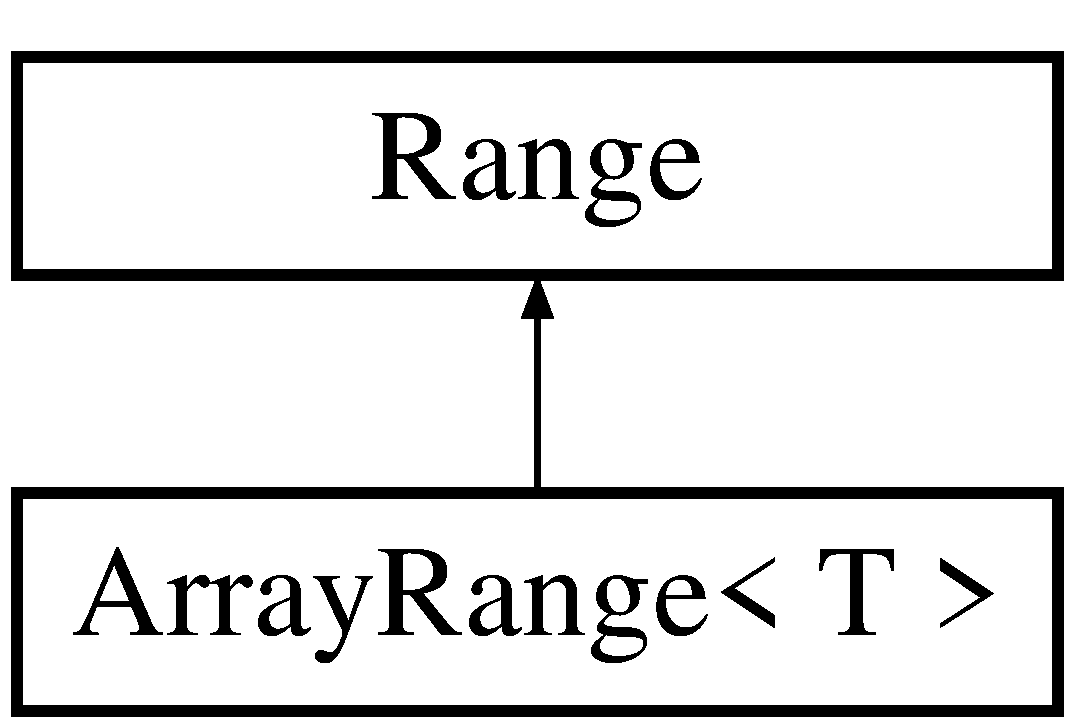
\includegraphics[height=2.000000cm]{struct__fe_1_1ArrayRange}
\end{center}
\end{figure}
\subsection*{Public Member Functions}
\begin{DoxyCompactItemize}
\item 
\mbox{\hyperlink{struct__fe_1_1ArrayRange_ae90cf27de0472ad0005c903ea89c32bf}{Array\+Range}} (const T $\ast$begin, const T $\ast$\mbox{\hyperlink{struct__fe_1_1ArrayRange_a31445d336333d06df9119b914833c8c1}{end}})
\end{DoxyCompactItemize}
\subsection*{Public Attributes}
\begin{DoxyCompactItemize}
\item 
const T $\ast$ \mbox{\hyperlink{struct__fe_1_1ArrayRange_a31445d336333d06df9119b914833c8c1}{end}}
\item 
const T $\ast$ \mbox{\hyperlink{struct__fe_1_1ArrayRange_aa839e62a03ecd06c3f3fe0e92181d555}{iter}}
\end{DoxyCompactItemize}


\subsection{Constructor \& Destructor Documentation}
\mbox{\Hypertarget{struct__fe_1_1ArrayRange_ae90cf27de0472ad0005c903ea89c32bf}\label{struct__fe_1_1ArrayRange_ae90cf27de0472ad0005c903ea89c32bf}} 
\index{\+\_\+fe\+::\+Array\+Range@{\+\_\+fe\+::\+Array\+Range}!Array\+Range@{Array\+Range}}
\index{Array\+Range@{Array\+Range}!\+\_\+fe\+::\+Array\+Range@{\+\_\+fe\+::\+Array\+Range}}
\subsubsection{\texorpdfstring{Array\+Range()}{ArrayRange()}}
{\footnotesize\ttfamily \mbox{\hyperlink{struct__fe_1_1ArrayRange}{Array\+Range}} (\begin{DoxyParamCaption}\item[{const T $\ast$}]{begin,  }\item[{const T $\ast$}]{end }\end{DoxyParamCaption})\hspace{0.3cm}{\ttfamily [inline]}}



\subsection{Member Data Documentation}
\mbox{\Hypertarget{struct__fe_1_1ArrayRange_a31445d336333d06df9119b914833c8c1}\label{struct__fe_1_1ArrayRange_a31445d336333d06df9119b914833c8c1}} 
\index{\+\_\+fe\+::\+Array\+Range@{\+\_\+fe\+::\+Array\+Range}!end@{end}}
\index{end@{end}!\+\_\+fe\+::\+Array\+Range@{\+\_\+fe\+::\+Array\+Range}}
\subsubsection{\texorpdfstring{end}{end}}
{\footnotesize\ttfamily const T$\ast$ end}

\mbox{\Hypertarget{struct__fe_1_1ArrayRange_aa839e62a03ecd06c3f3fe0e92181d555}\label{struct__fe_1_1ArrayRange_aa839e62a03ecd06c3f3fe0e92181d555}} 
\index{\+\_\+fe\+::\+Array\+Range@{\+\_\+fe\+::\+Array\+Range}!iter@{iter}}
\index{iter@{iter}!\+\_\+fe\+::\+Array\+Range@{\+\_\+fe\+::\+Array\+Range}}
\subsubsection{\texorpdfstring{iter}{iter}}
{\footnotesize\ttfamily const T$\ast$ iter}


\hypertarget{classBasicGraphGen}{}\section{Basic\+Graph\+Gen$<$ V, E $>$ Class Template Reference}
\label{classBasicGraphGen}\index{Basic\+Graph\+Gen$<$ V, E $>$@{Basic\+Graph\+Gen$<$ V, E $>$}}


Basic\+Graph is just basically an instantiation of \mbox{\hyperlink{classGraph}{Graph}} using Vertex and Edge as its template parameters.  




{\ttfamily \#include $<$basicgraph.\+h$>$}

Inheritance diagram for Basic\+Graph\+Gen$<$ V, E $>$\+:\begin{figure}[H]
\begin{center}
\leavevmode
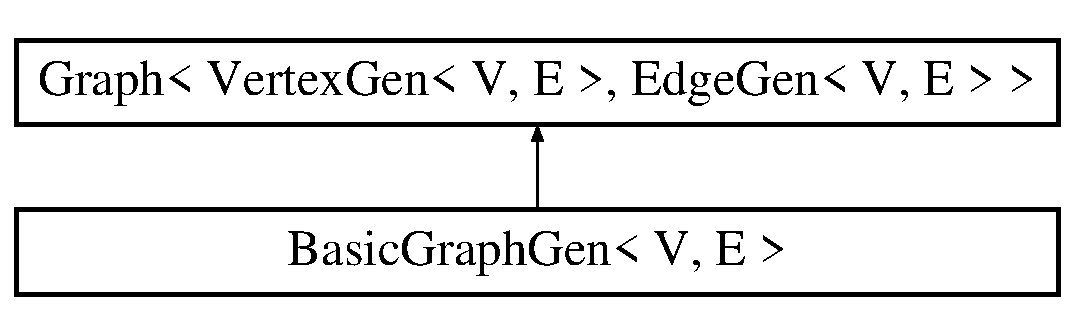
\includegraphics[height=2.000000cm]{classBasicGraphGen}
\end{center}
\end{figure}
\subsection*{Public Types}
\begin{DoxyCompactItemize}
\item 
using \mbox{\hyperlink{classGraph_a695969c31e87f9e8319d74e5ca39024b}{graph\+\_\+iterator}} = typename \mbox{\hyperlink{classstanfordcpplib_1_1collections_1_1GenericSet}{Set}}$<$ \mbox{\hyperlink{classVertexGen}{Vertex\+Gen}}$<$ V, E $>$ $\ast$$>$\+::const\+\_\+iterator
\end{DoxyCompactItemize}
\subsection*{Public Member Functions}
\begin{DoxyCompactItemize}
\item 
\mbox{\hyperlink{classBasicGraphGen_a9d6eaee0a2e8ea6de432f815463813fa}{Basic\+Graph\+Gen}} ()
\begin{DoxyCompactList}\small\item\em Constructs a new empty graph. \end{DoxyCompactList}\item 
\mbox{\hyperlink{classBasicGraphGen_aa8af075f69d803e4a813e4d348150fc5}{Basic\+Graph\+Gen}} (std\+::initializer\+\_\+list$<$ std\+::string $>$ vertex\+List)
\begin{DoxyCompactList}\small\item\em Constructs a new graph containing the given vertexes. \end{DoxyCompactList}\item 
Edge\+Gen$<$ V, E $>$ $\ast$ \mbox{\hyperlink{classGraph_aad2e9fedd7110ae2fb6873c5e2d29941}{add\+Arc}} (const std\+::string \&n1, const std\+::string \&n2)
\begin{DoxyCompactList}\small\item\em Adds a directed arc to the graph from node n1 to n2. \end{DoxyCompactList}\item 
Edge\+Gen$<$ V, E $>$ $\ast$ \mbox{\hyperlink{classGraph_a7280d3cd76bab82df392ba91ed5257c6}{add\+Arc}} (\mbox{\hyperlink{classVertexGen}{Vertex\+Gen}}$<$ V, E $>$ $\ast$n1, \mbox{\hyperlink{classVertexGen}{Vertex\+Gen}}$<$ V, E $>$ $\ast$n2)
\begin{DoxyCompactList}\small\item\em Adds a directed arc to the graph from node n1 to n2. \end{DoxyCompactList}\item 
Edge\+Gen$<$ V, E $>$ $\ast$ \mbox{\hyperlink{classGraph_aa1b6553e579c03260253a2d731668dfa}{add\+Arc}} (Edge\+Gen$<$ V, E $>$ $\ast$arc)
\begin{DoxyCompactList}\small\item\em Adds the given arc to the graph. \end{DoxyCompactList}\item 
Edge\+Gen$<$ V, E $>$ $\ast$ \mbox{\hyperlink{classBasicGraphGen_a624c45bedf3986073b0f8a40ab4d85c2}{add\+Edge}} (const std\+::string \&v1, const std\+::string \&v2, double cost=0.\+0, bool directed=true)
\begin{DoxyCompactList}\small\item\em Adds a directed edge to the graph from vertex v1 to vertex v2. \end{DoxyCompactList}\item 
Edge\+Gen$<$ V, E $>$ $\ast$ \mbox{\hyperlink{classBasicGraphGen_ac2fe8fab4722e89853df8ed385aa7a26}{add\+Edge}} (\mbox{\hyperlink{classVertexGen}{Vertex\+Gen}}$<$ V, E $>$ $\ast$v1, \mbox{\hyperlink{classVertexGen}{Vertex\+Gen}}$<$ V, E $>$ $\ast$v2, double cost=0.\+0, bool directed=true)
\begin{DoxyCompactList}\small\item\em Adds a directed edge to the graph from vertex v1 to vertex v2. \end{DoxyCompactList}\item 
Edge\+Gen$<$ V, E $>$ $\ast$ \mbox{\hyperlink{classBasicGraphGen_a92cffe0dd5b70ab78a3bce486fd60637}{add\+Edge}} (Edge\+Gen$<$ V, E $>$ $\ast$e, bool directed=true)
\begin{DoxyCompactList}\small\item\em Adds the given directed edge to the graph from vertex v1 to vertex v2. \end{DoxyCompactList}\item 
\mbox{\hyperlink{classVertexGen}{Vertex\+Gen}}$<$ V, E $>$ $\ast$ \mbox{\hyperlink{classGraph_acd763aa09491315536b5d2734cd82b89}{add\+Node}} (const std\+::string \&name)
\begin{DoxyCompactList}\small\item\em Adds a node to the graph. \end{DoxyCompactList}\item 
\mbox{\hyperlink{classVertexGen}{Vertex\+Gen}}$<$ V, E $>$ $\ast$ \mbox{\hyperlink{classGraph_a635fa78d72315816cef6c091acfa3882}{add\+Node}} (\mbox{\hyperlink{classVertexGen}{Vertex\+Gen}}$<$ V, E $>$ $\ast$node)
\begin{DoxyCompactList}\small\item\em Adds a node to the graph. \end{DoxyCompactList}\item 
\mbox{\hyperlink{classVertexGen}{Vertex\+Gen}}$<$ V, E $>$ $\ast$ \mbox{\hyperlink{classBasicGraphGen_a60f19882208c6d1dc51b74d5f348f458}{add\+Vertex}} (const std\+::string \&name)
\begin{DoxyCompactList}\small\item\em Adds a vertex to the graph, if no vertex with that name already exists in the graph. \end{DoxyCompactList}\item 
\mbox{\hyperlink{classVertexGen}{Vertex\+Gen}}$<$ V, E $>$ $\ast$ \mbox{\hyperlink{classBasicGraphGen_a99facea785e991d862eef401807c5f79}{add\+Vertex}} (\mbox{\hyperlink{classVertexGen}{Vertex\+Gen}}$<$ V, E $>$ $\ast$v)
\begin{DoxyCompactList}\small\item\em Adds a vertex to the graph, if no vertex with that name already exists in the graph. \end{DoxyCompactList}\item 
int \mbox{\hyperlink{classGraph_ac0b108b3354f5222d2c829dcd639fa7a}{arc\+Count}} () const
\begin{DoxyCompactList}\small\item\em Returns the number of arcs in the graph. \end{DoxyCompactList}\item 
\mbox{\hyperlink{classVertexGen}{Vertex\+Gen}}$<$ V, E $>$ $\ast$ \mbox{\hyperlink{classGraph_a27d59ef129bb56cc144ecc81c0affd34}{back}} () const
\begin{DoxyCompactList}\small\item\em Returns the last node in the graph in the order as would be returned by a for-\/each loop or iterator. \end{DoxyCompactList}\item 
\mbox{\hyperlink{classGraph_a695969c31e87f9e8319d74e5ca39024b}{graph\+\_\+iterator}} \mbox{\hyperlink{classGraph_aea3a8950c46f4ac913207201b685e715}{begin}} () const
\begin{DoxyCompactList}\small\item\em Returns an S\+TL iterator positioned at the first vertex in the graph. \end{DoxyCompactList}\item 
void \mbox{\hyperlink{classGraph_ac8bb3912a3ce86b15842e79d0b421204}{clear}} ()
\begin{DoxyCompactList}\small\item\em Reinitializes the graph to be empty, removing all nodes and arcs and freeing any heap storage used by their corresponding internal structures. \end{DoxyCompactList}\item 
void \mbox{\hyperlink{classGraph_a63f0ce1806df1c8070d997153363eecb}{clear\+Arcs}} ()
\begin{DoxyCompactList}\small\item\em Removes all arcs from the graph, freeing the heap storage used by their corresponding internal structures. \end{DoxyCompactList}\item 
void \mbox{\hyperlink{classGraph_a14def9e68896088fec7839e5da4fed27}{clear\+Arcs}} (\mbox{\hyperlink{classVertexGen}{Vertex\+Gen}}$<$ V, E $>$ $\ast$node)
\begin{DoxyCompactList}\small\item\em Removes all arcs from the graph that start from the given node, freeing the heap storage used by their corresponding internal structures. \end{DoxyCompactList}\item 
void \mbox{\hyperlink{classGraph_a2d8ecb9c6768fff244b2be46319385cc}{clear\+Arcs}} (const std\+::string \&name)
\begin{DoxyCompactList}\small\item\em Removes all arcs from the graph that start from the given node, freeing the heap storage used by their corresponding internal structures. \end{DoxyCompactList}\item 
void \mbox{\hyperlink{classBasicGraphGen_aced46bbfe5973602cbd67ac6188c36db}{clear\+Edges}} ()
\begin{DoxyCompactList}\small\item\em Removes all edges from the graph. \end{DoxyCompactList}\item 
void \mbox{\hyperlink{classBasicGraphGen_ac3104a246e5eaa7701c96bf52038c6b0}{clear\+Edges}} (\mbox{\hyperlink{classVertexGen}{Vertex\+Gen}}$<$ V, E $>$ $\ast$v)
\begin{DoxyCompactList}\small\item\em Removes all outbound edges of the given vertex from the graph. \end{DoxyCompactList}\item 
void \mbox{\hyperlink{classBasicGraphGen_a206c104818fb8653db07b7f4a3d5fe11}{clear\+Edges}} (const std\+::string \&v)
\begin{DoxyCompactList}\small\item\em Removes all outbound edges of the given vertex from the graph. \end{DoxyCompactList}\item 
bool \mbox{\hyperlink{classGraph_a9ca50139471975b82fdc6b1977bcfa4a}{contains\+Arc}} (\mbox{\hyperlink{classVertexGen}{Vertex\+Gen}}$<$ V, E $>$ $\ast$node1, \mbox{\hyperlink{classVertexGen}{Vertex\+Gen}}$<$ V, E $>$ $\ast$node2) const
\begin{DoxyCompactList}\small\item\em Returns true if there exists an arc directly between the given two nodes. \end{DoxyCompactList}\item 
bool \mbox{\hyperlink{classGraph_a515e45aae316b581bf1cf168541f4f44}{contains\+Arc}} (const std\+::string \&node1, const std\+::string \&node2) const
\begin{DoxyCompactList}\small\item\em Returns true if there exists an arc directly between the given two nodes. \end{DoxyCompactList}\item 
bool \mbox{\hyperlink{classGraph_acf7a659ddd8a143836b91b01c200ee8a}{contains\+Arc}} (Edge\+Gen$<$ V, E $>$ $\ast$arc) const
\begin{DoxyCompactList}\small\item\em Returns true if the given arc exists in this graph. \end{DoxyCompactList}\item 
bool \mbox{\hyperlink{classBasicGraphGen_a6ce3804a90bf7006e7bc78e1a51a1365}{contains\+Edge}} (\mbox{\hyperlink{classVertexGen}{Vertex\+Gen}}$<$ V, E $>$ $\ast$v1, \mbox{\hyperlink{classVertexGen}{Vertex\+Gen}}$<$ V, E $>$ $\ast$v2) const
\begin{DoxyCompactList}\small\item\em Returns true if the graph has an edge from v1 to v2 in the graph. \end{DoxyCompactList}\item 
bool \mbox{\hyperlink{classBasicGraphGen_a4475808d2ed8a45b9fceecc2c6081fc3}{contains\+Edge}} (const std\+::string \&v1, const std\+::string \&v2) const
\begin{DoxyCompactList}\small\item\em Returns true if the graph has an edge from v1 to v2 in the graph. \end{DoxyCompactList}\item 
bool \mbox{\hyperlink{classBasicGraphGen_ad41e772ab382972e1c54ab6df781dd82}{contains\+Edge}} (Edge\+Gen$<$ V, E $>$ $\ast$edge) const
\begin{DoxyCompactList}\small\item\em Returns true if the graph contains the given edge. \end{DoxyCompactList}\item 
bool \mbox{\hyperlink{classGraph_ac0beb77e8a238c2898ab851df71eeefe}{contains\+Node}} (const std\+::string \&name) const
\begin{DoxyCompactList}\small\item\em Returns true if there exists a node in this graph with the given name. \end{DoxyCompactList}\item 
bool \mbox{\hyperlink{classGraph_a4f540ebc07c4e46a0bb7fee76a93386c}{contains\+Node}} (\mbox{\hyperlink{classVertexGen}{Vertex\+Gen}}$<$ V, E $>$ $\ast$node) const
\begin{DoxyCompactList}\small\item\em Returns true if the given node is part of this graph. \end{DoxyCompactList}\item 
bool \mbox{\hyperlink{classBasicGraphGen_ab6062ac98f3491a525e0809c5b03b7cf}{contains\+Vertex}} (const std\+::string \&name) const
\begin{DoxyCompactList}\small\item\em Returns whether the graph contains a vertex with the given name. \end{DoxyCompactList}\item 
bool \mbox{\hyperlink{classBasicGraphGen_a37d4f31bc5bb6397fdb0bf966b54ca3f}{contains\+Vertex}} (\mbox{\hyperlink{classVertexGen}{Vertex\+Gen}}$<$ V, E $>$ $\ast$v) const
\begin{DoxyCompactList}\small\item\em Returns whether the graph contains the given vertex. \end{DoxyCompactList}\item 
int \mbox{\hyperlink{classBasicGraphGen_aa1f43093f29e66e171d5f572a658ae0c}{edge\+Count}} () const
\begin{DoxyCompactList}\small\item\em Returns the number of edges in the graph. \end{DoxyCompactList}\item 
\mbox{\hyperlink{classGraph_a695969c31e87f9e8319d74e5ca39024b}{graph\+\_\+iterator}} \mbox{\hyperlink{classGraph_afcdf62cae5d7e50644957d66f886742d}{end}} () const
\begin{DoxyCompactList}\small\item\em Returns an S\+TL iterator positioned after the last vertex in the graph. \end{DoxyCompactList}\item 
bool \mbox{\hyperlink{classGraph_a6bec43eb3dfdf3d23eb328b406edf44a}{equals}} (const \mbox{\hyperlink{classGraph}{Graph}}$<$ \mbox{\hyperlink{classVertexGen}{Vertex\+Gen}}$<$ V, E $>$, Edge\+Gen$<$ V, E $>$ $>$ \&graph2) const
\begin{DoxyCompactList}\small\item\em Compares two graphs for equality. \end{DoxyCompactList}\item 
\mbox{\hyperlink{classVertexGen}{Vertex\+Gen}}$<$ V, E $>$ $\ast$ \mbox{\hyperlink{classGraph_a7b7c2c1738f8e7faf84c54d7642992fa}{front}} () const
\begin{DoxyCompactList}\small\item\em Returns the first node in the graph in the order as would be returned by a for-\/each loop or iterator. \end{DoxyCompactList}\item 
Edge\+Gen$<$ V, E $>$ $\ast$ \mbox{\hyperlink{classGraph_a7c33db338f839ff9e3dafe4fe61c16fd}{get\+Arc}} (\mbox{\hyperlink{classVertexGen}{Vertex\+Gen}}$<$ V, E $>$ $\ast$node1, \mbox{\hyperlink{classVertexGen}{Vertex\+Gen}}$<$ V, E $>$ $\ast$node2) const
\begin{DoxyCompactList}\small\item\em Returns the arc, if any, from node1 to node2. \end{DoxyCompactList}\item 
Edge\+Gen$<$ V, E $>$ $\ast$ \mbox{\hyperlink{classGraph_a94d4badfc856b0d4530c37121efb9834}{get\+Arc}} (const std\+::string \&node1, const std\+::string \&node2) const
\begin{DoxyCompactList}\small\item\em Returns the arc, if any, from node1 to node2. \end{DoxyCompactList}\item 
const \mbox{\hyperlink{classstanfordcpplib_1_1collections_1_1GenericSet}{Set}}$<$ Edge\+Gen$<$ V, E $>$ $\ast$$>$ \& \mbox{\hyperlink{classGraph_a0690edaeae8d5256189ae2e8541788b5}{get\+Arc\+Set}} () const
\begin{DoxyCompactList}\small\item\em Returns the set of all arcs in the graph. \end{DoxyCompactList}\item 
const \mbox{\hyperlink{classstanfordcpplib_1_1collections_1_1GenericSet}{Set}}$<$ Edge\+Gen$<$ V, E $>$ $\ast$$>$ \& \mbox{\hyperlink{classGraph_a17cfc7f4d8c738fc6f51813f50be6400}{get\+Arc\+Set}} (\mbox{\hyperlink{classVertexGen}{Vertex\+Gen}}$<$ V, E $>$ $\ast$node) const
\begin{DoxyCompactList}\small\item\em Returns the set of all arcs that start at the specified node, indicated as a pointer to its node structure. \end{DoxyCompactList}\item 
const \mbox{\hyperlink{classstanfordcpplib_1_1collections_1_1GenericSet}{Set}}$<$ Edge\+Gen$<$ V, E $>$ $\ast$$>$ \& \mbox{\hyperlink{classGraph_a31b9e2056ee2d66a7ea9feb02f016e8d}{get\+Arc\+Set}} (const std\+::string \&name) const
\begin{DoxyCompactList}\small\item\em Returns the set of all arcs that start at the specified node. \end{DoxyCompactList}\item 
Edge\+Gen$<$ V, E $>$ $\ast$ \mbox{\hyperlink{classBasicGraphGen_aad31ac511c91ccf23a19af68e7a9f316}{get\+Edge}} (\mbox{\hyperlink{classVertexGen}{Vertex\+Gen}}$<$ V, E $>$ $\ast$v1, \mbox{\hyperlink{classVertexGen}{Vertex\+Gen}}$<$ V, E $>$ $\ast$v2) const
\begin{DoxyCompactList}\small\item\em Returns the structure representing the edge from v1 to v2 in the graph. \end{DoxyCompactList}\item 
Edge\+Gen$<$ V, E $>$ $\ast$ \mbox{\hyperlink{classBasicGraphGen_a57e156a4bae200f10f36fce5ec7fe504}{get\+Edge}} (const std\+::string \&v1, const std\+::string \&v2) const
\begin{DoxyCompactList}\small\item\em Returns the structure representing the edge from v1 to v2 in the graph. \end{DoxyCompactList}\item 
const \mbox{\hyperlink{classstanfordcpplib_1_1collections_1_1GenericSet}{Set}}$<$ Edge\+Gen$<$ V, E $>$ $\ast$ $>$ \& \mbox{\hyperlink{classBasicGraphGen_a312cc70af3d52a9fbdd56629c1710e48}{get\+Edge\+Set}} () const
\begin{DoxyCompactList}\small\item\em Returns the set of all edges in the graph. \end{DoxyCompactList}\item 
const \mbox{\hyperlink{classstanfordcpplib_1_1collections_1_1GenericSet}{Set}}$<$ Edge\+Gen$<$ V, E $>$ $\ast$ $>$ \& \mbox{\hyperlink{classBasicGraphGen_abfe8d6cbb48312f7fbec0fd948330348}{get\+Edge\+Set}} (\mbox{\hyperlink{classVertexGen}{Vertex\+Gen}}$<$ V, E $>$ $\ast$v) const
\begin{DoxyCompactList}\small\item\em Returns the set of all edges that start at the specified vertex. \end{DoxyCompactList}\item 
const \mbox{\hyperlink{classstanfordcpplib_1_1collections_1_1GenericSet}{Set}}$<$ Edge\+Gen$<$ V, E $>$ $\ast$ $>$ \& \mbox{\hyperlink{classBasicGraphGen_a6deea7a4536dfd6346c62c0c05a141ed}{get\+Edge\+Set}} (const std\+::string \&v) const
\begin{DoxyCompactList}\small\item\em Returns the set of all edges that start at the specified vertex. \end{DoxyCompactList}\item 
Edge\+Gen$<$ V, E $>$ $\ast$ \mbox{\hyperlink{classBasicGraphGen_ad8e645c23a9816fff136e0a5f7941669}{get\+Inverse\+Arc}} (Edge\+Gen$<$ V, E $>$ $\ast$edge) const
\begin{DoxyCompactList}\small\item\em Returns the edge that is the opposite of the given edge; that is, if the specified edge e starts at v1 and ends at v2, will return the edge that starts at v2 and ends at v1, if such an edge exists in the graph. \end{DoxyCompactList}\item 
const \mbox{\hyperlink{classstanfordcpplib_1_1collections_1_1GenericSet}{Set}}$<$ Edge\+Gen$<$ V, E $>$ $\ast$$>$ \mbox{\hyperlink{classGraph_ad5fd149800cd46aae497b05b46059b63}{get\+Inverse\+Arc\+Set}} (\mbox{\hyperlink{classVertexGen}{Vertex\+Gen}}$<$ V, E $>$ $\ast$node) const
\begin{DoxyCompactList}\small\item\em Returns the set of outbound arcs to the given node from other nodes. \end{DoxyCompactList}\item 
const \mbox{\hyperlink{classstanfordcpplib_1_1collections_1_1GenericSet}{Set}}$<$ Edge\+Gen$<$ V, E $>$ $\ast$$>$ \mbox{\hyperlink{classGraph_a2cfe12e71ca594736a1e329461cff024}{get\+Inverse\+Arc\+Set}} (const std\+::string \&name) const
\begin{DoxyCompactList}\small\item\em Returns the set of outbound arcs to the given node from other nodes. \end{DoxyCompactList}\item 
Edge\+Gen$<$ V, E $>$ $\ast$ \mbox{\hyperlink{classBasicGraphGen_ae81616e12d12f2dcfa295b4a3b48f960}{get\+Inverse\+Edge}} (Edge\+Gen$<$ V, E $>$ $\ast$edge) const
\begin{DoxyCompactList}\small\item\em Returns the edge that is the opposite of the given edge; that is, if the specified edge e starts at v1 and ends at v2, will return the edge that starts at v2 and ends at v1, if such an edge exists in the graph. \end{DoxyCompactList}\item 
const \mbox{\hyperlink{classstanfordcpplib_1_1collections_1_1GenericSet}{Set}}$<$ Edge\+Gen$<$ V, E $>$ $\ast$ $>$ \mbox{\hyperlink{classBasicGraphGen_a5db8788e3783e8ff16b19c06a5f2cf62}{get\+Inverse\+Edge\+Set}} (\mbox{\hyperlink{classVertexGen}{Vertex\+Gen}}$<$ V, E $>$ $\ast$v) const
\begin{DoxyCompactList}\small\item\em Returns the set of all edges in the graph that end at the specified vertex. \end{DoxyCompactList}\item 
const \mbox{\hyperlink{classstanfordcpplib_1_1collections_1_1GenericSet}{Set}}$<$ Edge\+Gen$<$ V, E $>$ $\ast$ $>$ \mbox{\hyperlink{classBasicGraphGen_a7ef9596e6faf68669228bc69808e84bd}{get\+Inverse\+Edge\+Set}} (const std\+::string \&v) const
\begin{DoxyCompactList}\small\item\em Returns the set of all edges in the graph that end at the specified vertex. \end{DoxyCompactList}\item 
\mbox{\hyperlink{classstanfordcpplib_1_1collections_1_1GenericSet}{Set}}$<$ std\+::string $>$ \mbox{\hyperlink{classGraph_aa9eceee00e824ea4852449fa3de61e82}{get\+Inverse\+Neighbor\+Names}} (\mbox{\hyperlink{classVertexGen}{Vertex\+Gen}}$<$ V, E $>$ $\ast$node) const
\begin{DoxyCompactList}\small\item\em Returns the set of strings of names of nodes that are neighbors of the given node. \end{DoxyCompactList}\item 
\mbox{\hyperlink{classstanfordcpplib_1_1collections_1_1GenericSet}{Set}}$<$ std\+::string $>$ \mbox{\hyperlink{classGraph_ac3dc36bc1eb0f249180cfe78bce6e7a2}{get\+Inverse\+Neighbor\+Names}} (const std\+::string \&node) const
\begin{DoxyCompactList}\small\item\em Returns the set of strings of names of nodes that are neighbors of the given node. \end{DoxyCompactList}\item 
\mbox{\hyperlink{classstanfordcpplib_1_1collections_1_1GenericSet}{Set}}$<$ \mbox{\hyperlink{classVertexGen}{Vertex\+Gen}}$<$ V, E $>$ $\ast$$>$ \mbox{\hyperlink{classGraph_a80a5724c594b9bd0b6008c57b09af317}{get\+Inverse\+Neighbors}} (\mbox{\hyperlink{classVertexGen}{Vertex\+Gen}}$<$ V, E $>$ $\ast$node) const
\begin{DoxyCompactList}\small\item\em Returns the set of nodes that are neighbors of the specified node. \end{DoxyCompactList}\item 
\mbox{\hyperlink{classstanfordcpplib_1_1collections_1_1GenericSet}{Set}}$<$ \mbox{\hyperlink{classVertexGen}{Vertex\+Gen}}$<$ V, E $>$ $\ast$$>$ \mbox{\hyperlink{classGraph_a5294846b9cdd19394808e3736ec67004}{get\+Inverse\+Neighbors}} (const std\+::string \&node) const
\begin{DoxyCompactList}\small\item\em Returns the set of nodes that are neighbors of the specified node. \end{DoxyCompactList}\item 
\mbox{\hyperlink{classstanfordcpplib_1_1collections_1_1GenericSet}{Set}}$<$ std\+::string $>$ \mbox{\hyperlink{classGraph_ae9b5cbd2bcb3918c4c64b1eb71c1a3a8}{get\+Neighbor\+Names}} (\mbox{\hyperlink{classVertexGen}{Vertex\+Gen}}$<$ V, E $>$ $\ast$node) const
\begin{DoxyCompactList}\small\item\em Returns the set of node names that are neighbors of the specified node. \end{DoxyCompactList}\item 
\mbox{\hyperlink{classstanfordcpplib_1_1collections_1_1GenericSet}{Set}}$<$ std\+::string $>$ \mbox{\hyperlink{classGraph_a6175b4d672266465dd34e070c7710b34}{get\+Neighbor\+Names}} (const std\+::string \&node) const
\begin{DoxyCompactList}\small\item\em Returns the set of node names that are neighbors of the specified node. \end{DoxyCompactList}\item 
\mbox{\hyperlink{classstanfordcpplib_1_1collections_1_1GenericSet}{Set}}$<$ \mbox{\hyperlink{classVertexGen}{Vertex\+Gen}}$<$ V, E $>$ $\ast$$>$ \mbox{\hyperlink{classGraph_a0e49b167f0623a8ae76040c3e5eab3fb}{get\+Neighbors}} (\mbox{\hyperlink{classVertexGen}{Vertex\+Gen}}$<$ V, E $>$ $\ast$node) const
\begin{DoxyCompactList}\small\item\em Returns the set of nodes that are neighbors of the specified node. \end{DoxyCompactList}\item 
\mbox{\hyperlink{classstanfordcpplib_1_1collections_1_1GenericSet}{Set}}$<$ \mbox{\hyperlink{classVertexGen}{Vertex\+Gen}}$<$ V, E $>$ $\ast$$>$ \mbox{\hyperlink{classGraph_a3a3720906c380f36b50530419330bfe5}{get\+Neighbors}} (const std\+::string \&node) const
\begin{DoxyCompactList}\small\item\em Returns the set of nodes that are neighbors of the specified node. \end{DoxyCompactList}\item 
\mbox{\hyperlink{classVertexGen}{Vertex\+Gen}}$<$ V, E $>$ $\ast$ \mbox{\hyperlink{classGraph_a81487976cf0e576047333c85463c33aa}{get\+Node}} (const std\+::string \&name) const
\begin{DoxyCompactList}\small\item\em Looks up a node in the name table attached to the graph and returns a pointer to that node. \end{DoxyCompactList}\item 
\mbox{\hyperlink{classstanfordcpplib_1_1collections_1_1GenericSet}{Set}}$<$ std\+::string $>$ \mbox{\hyperlink{classGraph_a3c6f37932f377dd2bf4fec61343a916d}{get\+Node\+Names}} () const
\begin{DoxyCompactList}\small\item\em Returns the set of the names of all nodes in the graph. \end{DoxyCompactList}\item 
const \mbox{\hyperlink{classstanfordcpplib_1_1collections_1_1GenericSet}{Set}}$<$ \mbox{\hyperlink{classVertexGen}{Vertex\+Gen}}$<$ V, E $>$ $\ast$$>$ \& \mbox{\hyperlink{classGraph_abd5552888f57aaa581099e8146c617c9}{get\+Node\+Set}} () const
\begin{DoxyCompactList}\small\item\em Returns the set of all nodes in the graph. \end{DoxyCompactList}\item 
\mbox{\hyperlink{classVertexGen}{Vertex\+Gen}}$<$ V, E $>$ $\ast$ \mbox{\hyperlink{classBasicGraphGen_a4c0c055103d2adba54014d301ae7bd1c}{get\+Vertex}} (const std\+::string \&name) const
\begin{DoxyCompactList}\small\item\em Looks up a vertex in the graph by name and returns a pointer to its internal data structure. \end{DoxyCompactList}\item 
\mbox{\hyperlink{classstanfordcpplib_1_1collections_1_1GenericSet}{Set}}$<$ std\+::string $>$ \mbox{\hyperlink{classBasicGraphGen_ae1bca1f87888bd787f836bc064a9ff01}{get\+Vertex\+Names}} () const
\begin{DoxyCompactList}\small\item\em Returns a set of the names of all vertexes in the graph. \end{DoxyCompactList}\item 
const \mbox{\hyperlink{classstanfordcpplib_1_1collections_1_1GenericSet}{Set}}$<$ \mbox{\hyperlink{classVertexGen}{Vertex\+Gen}}$<$ V, E $>$ $\ast$ $>$ \& \mbox{\hyperlink{classBasicGraphGen_aec896ef5b1fc6044fc71318d1369f6f1}{get\+Vertex\+Set}} () const
\begin{DoxyCompactList}\small\item\em Returns the set of all vertexes in the graph. \end{DoxyCompactList}\item 
bool \mbox{\hyperlink{classGraph_a54164ab847f3a5c7fe15d15ac95af443}{is\+Connected}} (\mbox{\hyperlink{classVertexGen}{Vertex\+Gen}}$<$ V, E $>$ $\ast$n1, \mbox{\hyperlink{classVertexGen}{Vertex\+Gen}}$<$ V, E $>$ $\ast$n2) const
\begin{DoxyCompactList}\small\item\em Returns {\ttfamily true} if the graph contains an arc from {\ttfamily n1} to {\ttfamily n2}. \end{DoxyCompactList}\item 
bool \mbox{\hyperlink{classGraph_a3623b7decbedc522041c2c39d3b14421}{is\+Connected}} (const std\+::string \&s1, const std\+::string \&s2) const
\begin{DoxyCompactList}\small\item\em Returns {\ttfamily true} if the graph contains an arc from {\ttfamily n1} to {\ttfamily n2}. \end{DoxyCompactList}\item 
bool \mbox{\hyperlink{classGraph_acf82f9b2937375c7b1cf3dccb3df3312}{is\+Empty}} () const
\begin{DoxyCompactList}\small\item\em Returns {\ttfamily true} if the graph contains no vertexes. \end{DoxyCompactList}\item 
bool \mbox{\hyperlink{classGraph_ab160bb64995133f6feb351cb23b031fb}{is\+Neighbor}} (const std\+::string \&node1, const std\+::string \&node2) const
\begin{DoxyCompactList}\small\item\em Returns true if the graph contains an edge from v1 to v2. \end{DoxyCompactList}\item 
bool \mbox{\hyperlink{classGraph_a9e752628a118c4a06a538067c95bbb28}{is\+Neighbor}} (\mbox{\hyperlink{classVertexGen}{Vertex\+Gen}}$<$ V, E $>$ $\ast$node1, \mbox{\hyperlink{classVertexGen}{Vertex\+Gen}}$<$ V, E $>$ $\ast$node2) const
\begin{DoxyCompactList}\small\item\em Returns true if the graph contains an edge from v1 to v2. \end{DoxyCompactList}\item 
int \mbox{\hyperlink{classGraph_a5dd1afdb4e1c75fbe51976bf6f70c922}{node\+Count}} () const
\begin{DoxyCompactList}\small\item\em Returns the number of nodes in the graph. \end{DoxyCompactList}\item 
bool \mbox{\hyperlink{classGraph_aafd8d1cec3a4d6b8cdcb58016e4d093a}{operator!=}} (const \mbox{\hyperlink{classGraph}{Graph}} \&graph2) const
\begin{DoxyCompactList}\small\item\em Relational operators to compare two graphs. \end{DoxyCompactList}\item 
bool \mbox{\hyperlink{classGraph_a1daf423faecc777e29a399812dc39ca2}{operator$<$}} (const \mbox{\hyperlink{classGraph}{Graph}} \&graph2) const
\begin{DoxyCompactList}\small\item\em Relational operators to compare two graphs. \end{DoxyCompactList}\item 
bool \mbox{\hyperlink{classGraph_a352607f2b21dd87b3d2a3957bbf3da7b}{operator$<$=}} (const \mbox{\hyperlink{classGraph}{Graph}} \&graph2) const
\begin{DoxyCompactList}\small\item\em Relational operators to compare two graphs. \end{DoxyCompactList}\item 
bool \mbox{\hyperlink{classGraph_a188f85939e3fe6ed2d411f622287f722}{operator==}} (const \mbox{\hyperlink{classGraph}{Graph}} \&graph2) const
\begin{DoxyCompactList}\small\item\em Relational operators to compare two graphs. \end{DoxyCompactList}\item 
bool \mbox{\hyperlink{classGraph_a8019cf2c98949fd509193cf26ba2ff8a}{operator$>$}} (const \mbox{\hyperlink{classGraph}{Graph}} \&graph2) const
\begin{DoxyCompactList}\small\item\em Relational operators to compare two graphs. \end{DoxyCompactList}\item 
bool \mbox{\hyperlink{classGraph_ab1ca2af20f3b0251972b72295270212e}{operator$>$=}} (const \mbox{\hyperlink{classGraph}{Graph}} \&graph2) const
\begin{DoxyCompactList}\small\item\em Relational operators to compare two graphs. \end{DoxyCompactList}\item 
\mbox{\hyperlink{classVertexGen}{Vertex\+Gen}}$<$ V, E $>$ $\ast$ \mbox{\hyperlink{classBasicGraphGen_a5e874dbb2f9f2c7f98ec74f00790eb0e}{operator\mbox{[}$\,$\mbox{]}}} (const std\+::string \&name)
\begin{DoxyCompactList}\small\item\em Overloads {\ttfamily \mbox{[}\mbox{]}} to return vertex pointers by vertex name. \end{DoxyCompactList}\item 
const \mbox{\hyperlink{classVertexGen}{Vertex\+Gen}}$<$ V, E $>$ $\ast$ \mbox{\hyperlink{classBasicGraphGen_ad91a5b6ebd034841cf4f4c410fb7ed1b}{operator\mbox{[}$\,$\mbox{]}}} (const std\+::string \&name) const
\begin{DoxyCompactList}\small\item\em Overloads {\ttfamily \mbox{[}\mbox{]}} to return vertex pointers by vertex name. \end{DoxyCompactList}\item 
void \mbox{\hyperlink{classGraph_af6370fb52d2dab4eb7795da22c33dd02}{remove\+Arc}} (const std\+::string \&s1, const std\+::string \&s2)
\begin{DoxyCompactList}\small\item\em Removes an arc from v1 to v2 in the graph, specified by the names of its endpoints. \end{DoxyCompactList}\item 
void \mbox{\hyperlink{classGraph_ae0c9f44b20b49ffae9fecc0a4f156ac1}{remove\+Arc}} (\mbox{\hyperlink{classVertexGen}{Vertex\+Gen}}$<$ V, E $>$ $\ast$n1, \mbox{\hyperlink{classVertexGen}{Vertex\+Gen}}$<$ V, E $>$ $\ast$n2)
\begin{DoxyCompactList}\small\item\em Removes an arc from v1 to v2 in the graph, specified by the node pointers at its endpoints. \end{DoxyCompactList}\item 
void \mbox{\hyperlink{classGraph_a9d6580d1b0228fe6c1a02dfe70de1abf}{remove\+Arc}} (Edge\+Gen$<$ V, E $>$ $\ast$arc)
\begin{DoxyCompactList}\small\item\em Removes the given arc from the graph, specified as an arc pointer. \end{DoxyCompactList}\item 
void \mbox{\hyperlink{classBasicGraphGen_adfee7a20d0c13cc515b3b7e951d8baf2}{remove\+Edge}} (const std\+::string \&v1, const std\+::string \&v2, bool directed=true)
\begin{DoxyCompactList}\small\item\em Removes the edge from v1 to v2 from the graph. \end{DoxyCompactList}\item 
void \mbox{\hyperlink{classBasicGraphGen_a8b1003fbe63fab20173526459fff4139}{remove\+Edge}} (\mbox{\hyperlink{classVertexGen}{Vertex\+Gen}}$<$ V, E $>$ $\ast$v1, \mbox{\hyperlink{classVertexGen}{Vertex\+Gen}}$<$ V, E $>$ $\ast$v2, bool directed=true)
\begin{DoxyCompactList}\small\item\em Removes the edge from v1 to v2 from the graph. \end{DoxyCompactList}\item 
void \mbox{\hyperlink{classBasicGraphGen_a2c6bb1e8e2c18b7376504692f7baae62}{remove\+Edge}} (Edge\+Gen$<$ V, E $>$ $\ast$e, bool directed=true)
\begin{DoxyCompactList}\small\item\em Removes the given edge from the graph. \end{DoxyCompactList}\item 
void \mbox{\hyperlink{classGraph_a2d5f7ee89176144ed4c5c6b08a233aa6}{remove\+Node}} (const std\+::string \&name)
\begin{DoxyCompactList}\small\item\em Removes the node with the given name from the graph. \end{DoxyCompactList}\item 
void \mbox{\hyperlink{classGraph_a2dfe63019975561914e0ed79551de108}{remove\+Node}} (\mbox{\hyperlink{classVertexGen}{Vertex\+Gen}}$<$ V, E $>$ $\ast$node)
\begin{DoxyCompactList}\small\item\em Removes a node from the graph, specified as a pointer value. \end{DoxyCompactList}\item 
void \mbox{\hyperlink{classBasicGraphGen_aaa33b4c05ee490d241ba5542420b985b}{remove\+Vertex}} (const std\+::string \&name)
\begin{DoxyCompactList}\small\item\em Removes the given vertex from the graph. \end{DoxyCompactList}\item 
void \mbox{\hyperlink{classBasicGraphGen_a9eac2d17b5e8074dace019020d078acb}{remove\+Vertex}} (\mbox{\hyperlink{classVertexGen}{Vertex\+Gen}}$<$ V, E $>$ $\ast$v)
\begin{DoxyCompactList}\small\item\em Removes the given vertex from the graph. \end{DoxyCompactList}\item 
virtual void \mbox{\hyperlink{classBasicGraphGen_a4314b3b6bda0755a87e49070edd17c3d}{scan\+Arc\+Data}} (\mbox{\hyperlink{classTokenScanner}{Token\+Scanner}} \&scanner, Edge\+Gen$<$ V, E $>$ $\ast$edge, Edge\+Gen$<$ V, E $>$ $\ast$inverse)
\begin{DoxyCompactList}\small\item\em Reads the data for an arc from the scanner. \end{DoxyCompactList}\item 
virtual bool \mbox{\hyperlink{classGraph_a1c4e1a05a40013ce4e4bb539d05b9937}{scan\+Graph\+Entry}} (\mbox{\hyperlink{classTokenScanner}{Token\+Scanner}} \&scanner)
\begin{DoxyCompactList}\small\item\em This method reads one \char`\"{}entry\char`\"{} for the graph, which is either a node description or an arc description. \end{DoxyCompactList}\item 
virtual void \mbox{\hyperlink{classGraph_a0fc2ca3535b7bff7759aa0c1d35ff08b}{scan\+Node\+Data}} (\mbox{\hyperlink{classTokenScanner}{Token\+Scanner}} \&, \mbox{\hyperlink{classVertexGen}{Vertex\+Gen}}$<$ V, E $>$ $\ast$)
\begin{DoxyCompactList}\small\item\em Reads the data for the specified node from the scanner. \end{DoxyCompactList}\item 
int \mbox{\hyperlink{classGraph_af9593d4a5ff4274efaf429cb4f9e57cc}{size}} () const
\begin{DoxyCompactList}\small\item\em Returns the number of nodes in the graph. \end{DoxyCompactList}\item 
\mbox{\hyperlink{classMap}{Map}}$<$ std\+::string, \mbox{\hyperlink{classstanfordcpplib_1_1collections_1_1GenericSet}{Set}}$<$ std\+::string $>$ $>$ \mbox{\hyperlink{classBasicGraphGen_a66498d3675a5bc08fa30a032d41764f7}{to\+Map}} () const
\begin{DoxyCompactList}\small\item\em Returns a \mbox{\hyperlink{classMap}{Map}} representing an adjacency list equivalent to this graph. \end{DoxyCompactList}\item 
std\+::string \mbox{\hyperlink{classGraph_a1fe5121d6528fdea3f243321b3fa3a49}{to\+String}} () const
\begin{DoxyCompactList}\small\item\em Converts the graph to a printable string representation. \end{DoxyCompactList}\item 
int \mbox{\hyperlink{classBasicGraphGen_a68eb4830a4800ed7704895c16a8982be}{vertex\+Count}} () const
\begin{DoxyCompactList}\small\item\em Returns the number of vertexes in the graph. \end{DoxyCompactList}\item 
virtual void \mbox{\hyperlink{classBasicGraphGen_ae7be688f4ddbd7da8eb2a8c7eef8901c}{write\+Arc\+Data}} (std\+::ostream \&out, Edge\+Gen$<$ V, E $>$ $\ast$edge) const
\begin{DoxyCompactList}\small\item\em Writes the data for the arc to the output stream. \end{DoxyCompactList}\item 
virtual void \mbox{\hyperlink{classGraph_ac0db5231476c8cb10655d58ebc108b78}{write\+Node\+Data}} (std\+::ostream \&, \mbox{\hyperlink{classVertexGen}{Vertex\+Gen}}$<$ V, E $>$ $\ast$) const
\begin{DoxyCompactList}\small\item\em Writes the data for the node to the output stream. \end{DoxyCompactList}\end{DoxyCompactItemize}


\subsection{Detailed Description}
\subsubsection*{template$<$typename V = void$\ast$, typename E = void$\ast$$>$\newline
class Basic\+Graph\+Gen$<$ V, E $>$}

Basic\+Graph is just basically an instantiation of \mbox{\hyperlink{classGraph}{Graph}} using Vertex and Edge as its template parameters. 

It also adds a few convenience functions such as mirroring members like \char`\"{}add\+Arc\char`\"{} with an equivalent more familiar name like \char`\"{}add\+Edge\char`\"{}.

There are a few convenience functions related to neighbors, like is\+Neighbor. Basic\+Graph contains a D\+FS implementation called is\+Reachable, not found in the normal Stanford \mbox{\hyperlink{classGraph}{Graph}} class.

There are also a few functions added to make edges more convenient to work with\+: get\+Edge(v1, v2) to get the edge between a given pair of vertices, and get\+Inverse\+Edge(edge) to get the edge v2 -\/$>$ v1 for a given edge v1 -\/$>$ v2. 

\subsection{Member Typedef Documentation}
\mbox{\Hypertarget{classGraph_a695969c31e87f9e8319d74e5ca39024b}\label{classGraph_a695969c31e87f9e8319d74e5ca39024b}} 
\index{Basic\+Graph\+Gen@{Basic\+Graph\+Gen}!graph\+\_\+iterator@{graph\+\_\+iterator}}
\index{graph\+\_\+iterator@{graph\+\_\+iterator}!Basic\+Graph\+Gen@{Basic\+Graph\+Gen}}
\subsubsection{\texorpdfstring{graph\+\_\+iterator}{graph\_iterator}}
{\footnotesize\ttfamily using \mbox{\hyperlink{classGraph_a695969c31e87f9e8319d74e5ca39024b}{graph\+\_\+iterator}} =  typename \mbox{\hyperlink{classstanfordcpplib_1_1collections_1_1GenericSet}{Set}}$<$\mbox{\hyperlink{classVertexGen}{Vertex\+Gen}}$<$ V, E $>$  $\ast$$>$\+::const\+\_\+iterator\hspace{0.3cm}{\ttfamily [inherited]}}



\subsection{Constructor \& Destructor Documentation}
\mbox{\Hypertarget{classBasicGraphGen_a9d6eaee0a2e8ea6de432f815463813fa}\label{classBasicGraphGen_a9d6eaee0a2e8ea6de432f815463813fa}} 
\index{Basic\+Graph\+Gen@{Basic\+Graph\+Gen}!Basic\+Graph\+Gen@{Basic\+Graph\+Gen}}
\index{Basic\+Graph\+Gen@{Basic\+Graph\+Gen}!Basic\+Graph\+Gen@{Basic\+Graph\+Gen}}
\subsubsection{\texorpdfstring{Basic\+Graph\+Gen()}{BasicGraphGen()}\hspace{0.1cm}{\footnotesize\ttfamily [1/2]}}
{\footnotesize\ttfamily \mbox{\hyperlink{classBasicGraphGen}{Basic\+Graph\+Gen}} (\begin{DoxyParamCaption}{ }\end{DoxyParamCaption})}



Constructs a new empty graph. 

\begin{DoxyRefDesc}{Big-\/\+Oh}
\item[\mbox{\hyperlink{BigOh__BigOh000001}{Big-\/\+Oh}}]O(1) \end{DoxyRefDesc}
\mbox{\Hypertarget{classBasicGraphGen_aa8af075f69d803e4a813e4d348150fc5}\label{classBasicGraphGen_aa8af075f69d803e4a813e4d348150fc5}} 
\index{Basic\+Graph\+Gen@{Basic\+Graph\+Gen}!Basic\+Graph\+Gen@{Basic\+Graph\+Gen}}
\index{Basic\+Graph\+Gen@{Basic\+Graph\+Gen}!Basic\+Graph\+Gen@{Basic\+Graph\+Gen}}
\subsubsection{\texorpdfstring{Basic\+Graph\+Gen()}{BasicGraphGen()}\hspace{0.1cm}{\footnotesize\ttfamily [2/2]}}
{\footnotesize\ttfamily \mbox{\hyperlink{classBasicGraphGen}{Basic\+Graph\+Gen}} (\begin{DoxyParamCaption}\item[{std\+::initializer\+\_\+list$<$ std\+::string $>$}]{vertex\+List }\end{DoxyParamCaption})}



Constructs a new graph containing the given vertexes. 

\begin{DoxyRefDesc}{Big-\/\+Oh}
\item[\mbox{\hyperlink{BigOh__BigOh000002}{Big-\/\+Oh}}]O(\+V) \end{DoxyRefDesc}


\subsection{Member Function Documentation}
\mbox{\Hypertarget{classGraph_aad2e9fedd7110ae2fb6873c5e2d29941}\label{classGraph_aad2e9fedd7110ae2fb6873c5e2d29941}} 
\index{Basic\+Graph\+Gen@{Basic\+Graph\+Gen}!add\+Arc@{add\+Arc}}
\index{add\+Arc@{add\+Arc}!Basic\+Graph\+Gen@{Basic\+Graph\+Gen}}
\subsubsection{\texorpdfstring{add\+Arc()}{addArc()}\hspace{0.1cm}{\footnotesize\ttfamily [1/3]}}
{\footnotesize\ttfamily Edge\+Gen$<$ V, E $>$  $\ast$ add\+Arc (\begin{DoxyParamCaption}\item[{const std\+::string \&}]{n1,  }\item[{const std\+::string \&}]{n2 }\end{DoxyParamCaption})\hspace{0.3cm}{\ttfamily [inherited]}}



Adds a directed arc to the graph from node n1 to n2. 

If either node is not found in the graph, said node will be added to the graph. Returns a pointer to the arc in case the client needs to capture this value. \begin{DoxyRefDesc}{Big-\/\+Oh}
\item[\mbox{\hyperlink{BigOh__BigOh000042}{Big-\/\+Oh}}]O(log V + log E) \end{DoxyRefDesc}
\mbox{\Hypertarget{classGraph_a7280d3cd76bab82df392ba91ed5257c6}\label{classGraph_a7280d3cd76bab82df392ba91ed5257c6}} 
\index{Basic\+Graph\+Gen@{Basic\+Graph\+Gen}!add\+Arc@{add\+Arc}}
\index{add\+Arc@{add\+Arc}!Basic\+Graph\+Gen@{Basic\+Graph\+Gen}}
\subsubsection{\texorpdfstring{add\+Arc()}{addArc()}\hspace{0.1cm}{\footnotesize\ttfamily [2/3]}}
{\footnotesize\ttfamily Edge\+Gen$<$ V, E $>$  $\ast$ add\+Arc (\begin{DoxyParamCaption}\item[{\mbox{\hyperlink{classVertexGen}{Vertex\+Gen}}$<$ V, E $>$  $\ast$}]{n1,  }\item[{\mbox{\hyperlink{classVertexGen}{Vertex\+Gen}}$<$ V, E $>$  $\ast$}]{n2 }\end{DoxyParamCaption})\hspace{0.3cm}{\ttfamily [inherited]}}



Adds a directed arc to the graph from node n1 to n2. 

If either node is not found in the graph, said node will be added to the graph. Returns a pointer to the arc in case the client needs to capture this value.


\begin{DoxyExceptions}{Exceptions}
{\em \mbox{\hyperlink{classErrorException}{Error\+Exception}}} & if any pointer passed is null \\
\hline
\end{DoxyExceptions}
\begin{DoxyRefDesc}{Big-\/\+Oh}
\item[\mbox{\hyperlink{BigOh__BigOh000043}{Big-\/\+Oh}}]O(log V + log E) \end{DoxyRefDesc}
\mbox{\Hypertarget{classGraph_aa1b6553e579c03260253a2d731668dfa}\label{classGraph_aa1b6553e579c03260253a2d731668dfa}} 
\index{Basic\+Graph\+Gen@{Basic\+Graph\+Gen}!add\+Arc@{add\+Arc}}
\index{add\+Arc@{add\+Arc}!Basic\+Graph\+Gen@{Basic\+Graph\+Gen}}
\subsubsection{\texorpdfstring{add\+Arc()}{addArc()}\hspace{0.1cm}{\footnotesize\ttfamily [3/3]}}
{\footnotesize\ttfamily Edge\+Gen$<$ V, E $>$  $\ast$ add\+Arc (\begin{DoxyParamCaption}\item[{Edge\+Gen$<$ V, E $>$  $\ast$}]{arc }\end{DoxyParamCaption})\hspace{0.3cm}{\ttfamily [inherited]}}



Adds the given arc to the graph. 

If the start/finish nodes passed are not already part of the graph, they are added to the graph. Returns a pointer to the arc in case the client needs to capture this value.

Memory management\+: Once you hand me this Arc\+Type$\ast$ pointer, our code owns it. We will delete/free it when done with it. You do not need to (and should not) free it yourself.


\begin{DoxyExceptions}{Exceptions}
{\em \mbox{\hyperlink{classErrorException}{Error\+Exception}}} & if any pointer passed is null \\
\hline
\end{DoxyExceptions}
\begin{DoxyRefDesc}{Big-\/\+Oh}
\item[\mbox{\hyperlink{BigOh__BigOh000044}{Big-\/\+Oh}}]O(log V + log E) \end{DoxyRefDesc}
\mbox{\Hypertarget{classBasicGraphGen_a624c45bedf3986073b0f8a40ab4d85c2}\label{classBasicGraphGen_a624c45bedf3986073b0f8a40ab4d85c2}} 
\index{Basic\+Graph\+Gen@{Basic\+Graph\+Gen}!add\+Edge@{add\+Edge}}
\index{add\+Edge@{add\+Edge}!Basic\+Graph\+Gen@{Basic\+Graph\+Gen}}
\subsubsection{\texorpdfstring{add\+Edge()}{addEdge()}\hspace{0.1cm}{\footnotesize\ttfamily [1/3]}}
{\footnotesize\ttfamily Edge\+Gen$<$ V, E $>$ $\ast$ add\+Edge (\begin{DoxyParamCaption}\item[{const std\+::string \&}]{v1,  }\item[{const std\+::string \&}]{v2,  }\item[{double}]{cost = {\ttfamily 0.0},  }\item[{bool}]{directed = {\ttfamily true} }\end{DoxyParamCaption})}



Adds a directed edge to the graph from vertex v1 to vertex v2. 

\mbox{\hyperlink{classNote}{Note}} that it is allowed to have multiple edges between the same pair of vertexes.

Returns a pointer to the edge, though clients need not store that pointer; you can get the pointer again later by calling get\+Edge and passing the two vertexes.

Equivalent to add\+Node.

\begin{DoxyReturn}{Returns}
a pointer to the edge created 
\end{DoxyReturn}
\begin{DoxyRefDesc}{Big-\/\+Oh}
\item[\mbox{\hyperlink{BigOh__BigOh000003}{Big-\/\+Oh}}]O(log V + log E) \end{DoxyRefDesc}
\mbox{\Hypertarget{classBasicGraphGen_ac2fe8fab4722e89853df8ed385aa7a26}\label{classBasicGraphGen_ac2fe8fab4722e89853df8ed385aa7a26}} 
\index{Basic\+Graph\+Gen@{Basic\+Graph\+Gen}!add\+Edge@{add\+Edge}}
\index{add\+Edge@{add\+Edge}!Basic\+Graph\+Gen@{Basic\+Graph\+Gen}}
\subsubsection{\texorpdfstring{add\+Edge()}{addEdge()}\hspace{0.1cm}{\footnotesize\ttfamily [2/3]}}
{\footnotesize\ttfamily Edge\+Gen$<$ V, E $>$ $\ast$ add\+Edge (\begin{DoxyParamCaption}\item[{\mbox{\hyperlink{classVertexGen}{Vertex\+Gen}}$<$ V, E $>$ $\ast$}]{v1,  }\item[{\mbox{\hyperlink{classVertexGen}{Vertex\+Gen}}$<$ V, E $>$ $\ast$}]{v2,  }\item[{double}]{cost = {\ttfamily 0.0},  }\item[{bool}]{directed = {\ttfamily true} }\end{DoxyParamCaption})}



Adds a directed edge to the graph from vertex v1 to vertex v2. 

If either vertex is not found in the graph, said vertex will be added to the graph. \mbox{\hyperlink{classNote}{Note}} that it is allowed to have multiple edges between the same pair of vertexes.

Returns a pointer to the edge, though clients need not store that pointer; you can get the pointer again later by calling get\+Edge and passing the two vertexes.

Equivalent to add\+Node.

\begin{DoxyReturn}{Returns}
a pointer to the edge created 
\end{DoxyReturn}

\begin{DoxyExceptions}{Exceptions}
{\em \mbox{\hyperlink{classErrorException}{Error\+Exception}}} & if either vertex is null \\
\hline
\end{DoxyExceptions}
\begin{DoxyRefDesc}{Big-\/\+Oh}
\item[\mbox{\hyperlink{BigOh__BigOh000004}{Big-\/\+Oh}}]O(log V + log E) \end{DoxyRefDesc}
\mbox{\Hypertarget{classBasicGraphGen_a92cffe0dd5b70ab78a3bce486fd60637}\label{classBasicGraphGen_a92cffe0dd5b70ab78a3bce486fd60637}} 
\index{Basic\+Graph\+Gen@{Basic\+Graph\+Gen}!add\+Edge@{add\+Edge}}
\index{add\+Edge@{add\+Edge}!Basic\+Graph\+Gen@{Basic\+Graph\+Gen}}
\subsubsection{\texorpdfstring{add\+Edge()}{addEdge()}\hspace{0.1cm}{\footnotesize\ttfamily [3/3]}}
{\footnotesize\ttfamily Edge\+Gen$<$ V, E $>$ $\ast$ add\+Edge (\begin{DoxyParamCaption}\item[{Edge\+Gen$<$ V, E $>$ $\ast$}]{e,  }\item[{bool}]{directed = {\ttfamily true} }\end{DoxyParamCaption})}



Adds the given directed edge to the graph from vertex v1 to vertex v2. 

If either vertex is not found in the graph, said vertex will be added to the graph. \mbox{\hyperlink{classNote}{Note}} that it is allowed to have multiple edges between the same pair of vertexes.

Returns a pointer to the edge, though clients need not store that pointer; you can get the pointer again later by calling get\+Edge and passing the two vertexes.

Equivalent to add\+Node.

\begin{DoxyReturn}{Returns}
a pointer to the edge created 
\end{DoxyReturn}

\begin{DoxyExceptions}{Exceptions}
{\em \mbox{\hyperlink{classErrorException}{Error\+Exception}}} & if either vertex is null \\
\hline
\end{DoxyExceptions}
\begin{DoxyRefDesc}{Big-\/\+Oh}
\item[\mbox{\hyperlink{BigOh__BigOh000005}{Big-\/\+Oh}}]O(log V + log E) \end{DoxyRefDesc}
\mbox{\Hypertarget{classGraph_acd763aa09491315536b5d2734cd82b89}\label{classGraph_acd763aa09491315536b5d2734cd82b89}} 
\index{Basic\+Graph\+Gen@{Basic\+Graph\+Gen}!add\+Node@{add\+Node}}
\index{add\+Node@{add\+Node}!Basic\+Graph\+Gen@{Basic\+Graph\+Gen}}
\subsubsection{\texorpdfstring{add\+Node()}{addNode()}\hspace{0.1cm}{\footnotesize\ttfamily [1/2]}}
{\footnotesize\ttfamily \mbox{\hyperlink{classVertexGen}{Vertex\+Gen}}$<$ V, E $>$  $\ast$ add\+Node (\begin{DoxyParamCaption}\item[{const std\+::string \&}]{name }\end{DoxyParamCaption})\hspace{0.3cm}{\ttfamily [inherited]}}



Adds a node to the graph. 

The first version of this method creates a new node of the appropriate type and initializes its fields; the second assumes that the client has already created the node and simply adds it to the graph. Returns a pointer to the node. If a node with the given name is already present, does nothing.

Memory management\+: Once you hand me this Node\+Type$\ast$ pointer, our code owns it. We will delete/free it when done with it. You do not need to (and should not) free it yourself.


\begin{DoxyExceptions}{Exceptions}
{\em \mbox{\hyperlink{classErrorException}{Error\+Exception}}} & if any pointer passed is null \\
\hline
\end{DoxyExceptions}
\begin{DoxyRefDesc}{Big-\/\+Oh}
\item[\mbox{\hyperlink{BigOh__BigOh000045}{Big-\/\+Oh}}]O(log V) \end{DoxyRefDesc}
\mbox{\Hypertarget{classGraph_a635fa78d72315816cef6c091acfa3882}\label{classGraph_a635fa78d72315816cef6c091acfa3882}} 
\index{Basic\+Graph\+Gen@{Basic\+Graph\+Gen}!add\+Node@{add\+Node}}
\index{add\+Node@{add\+Node}!Basic\+Graph\+Gen@{Basic\+Graph\+Gen}}
\subsubsection{\texorpdfstring{add\+Node()}{addNode()}\hspace{0.1cm}{\footnotesize\ttfamily [2/2]}}
{\footnotesize\ttfamily \mbox{\hyperlink{classVertexGen}{Vertex\+Gen}}$<$ V, E $>$  $\ast$ add\+Node (\begin{DoxyParamCaption}\item[{\mbox{\hyperlink{classVertexGen}{Vertex\+Gen}}$<$ V, E $>$  $\ast$}]{node }\end{DoxyParamCaption})\hspace{0.3cm}{\ttfamily [inherited]}}



Adds a node to the graph. 

This version assumes that the client has already created the node structure and simply adds it to the graph. Returns a pointer to the node. If a node with the given name is already present, does nothing.

Memory management\+: Once you hand me this Node\+Type$\ast$ pointer, our code owns it. We will delete/free it when done with it. You do not need to (and should not) free it yourself.


\begin{DoxyExceptions}{Exceptions}
{\em \mbox{\hyperlink{classErrorException}{Error\+Exception}}} & if any pointer passed is null \\
\hline
\end{DoxyExceptions}
\begin{DoxyRefDesc}{Big-\/\+Oh}
\item[\mbox{\hyperlink{BigOh__BigOh000046}{Big-\/\+Oh}}]O(log V) \end{DoxyRefDesc}
\mbox{\Hypertarget{classBasicGraphGen_a60f19882208c6d1dc51b74d5f348f458}\label{classBasicGraphGen_a60f19882208c6d1dc51b74d5f348f458}} 
\index{Basic\+Graph\+Gen@{Basic\+Graph\+Gen}!add\+Vertex@{add\+Vertex}}
\index{add\+Vertex@{add\+Vertex}!Basic\+Graph\+Gen@{Basic\+Graph\+Gen}}
\subsubsection{\texorpdfstring{add\+Vertex()}{addVertex()}\hspace{0.1cm}{\footnotesize\ttfamily [1/2]}}
{\footnotesize\ttfamily \mbox{\hyperlink{classVertexGen}{Vertex\+Gen}}$<$ V, E $>$ $\ast$ add\+Vertex (\begin{DoxyParamCaption}\item[{const std\+::string \&}]{name }\end{DoxyParamCaption})}



Adds a vertex to the graph, if no vertex with that name already exists in the graph. 

This version of this method accepts a string for the vertex\textquotesingle{}s name, creates a new vertex of the appropriate type and initializes its fields. Returns a pointer to the vertex, though clients need not store that pointer; you can get the pointer again later by calling get\+Vertex and passing the same name.

The vertexes in a graph must have unique names. If this graph already contains a vertex with the given name, the vertex will not be added and the graph\textquotesingle{}s state will not change.

Equivalent to add\+Node.

\begin{DoxyReturn}{Returns}
a pointer to the vertex created 
\end{DoxyReturn}
\begin{DoxyRefDesc}{Big-\/\+Oh}
\item[\mbox{\hyperlink{BigOh__BigOh000006}{Big-\/\+Oh}}]O(log V) \end{DoxyRefDesc}
\mbox{\Hypertarget{classBasicGraphGen_a99facea785e991d862eef401807c5f79}\label{classBasicGraphGen_a99facea785e991d862eef401807c5f79}} 
\index{Basic\+Graph\+Gen@{Basic\+Graph\+Gen}!add\+Vertex@{add\+Vertex}}
\index{add\+Vertex@{add\+Vertex}!Basic\+Graph\+Gen@{Basic\+Graph\+Gen}}
\subsubsection{\texorpdfstring{add\+Vertex()}{addVertex()}\hspace{0.1cm}{\footnotesize\ttfamily [2/2]}}
{\footnotesize\ttfamily \mbox{\hyperlink{classVertexGen}{Vertex\+Gen}}$<$ V, E $>$ $\ast$ add\+Vertex (\begin{DoxyParamCaption}\item[{\mbox{\hyperlink{classVertexGen}{Vertex\+Gen}}$<$ V, E $>$ $\ast$}]{v }\end{DoxyParamCaption})}



Adds a vertex to the graph, if no vertex with that name already exists in the graph. 

This version of this method accepts a string for the vertex\textquotesingle{}s name, creates a new vertex of the appropriate type and initializes its fields. The other accepts a structure representing the vertex and its data. Returns a pointer to the vertex, though clients need not store that pointer; you can get the pointer again later by calling get\+Vertex and passing the same name.

The vertexes in a graph must have unique names. If this graph already contains a vertex with the given name, the vertex will not be added and the graph\textquotesingle{}s state will not change.

When calling this function, you are relinquishing ownership of the Vertex structure\textquotesingle{}s lifecycle to the graph; our graph will free it when done with it.

Equivalent to add\+Node.

\begin{DoxyReturn}{Returns}
a pointer to the vertex created 
\end{DoxyReturn}

\begin{DoxyExceptions}{Exceptions}
{\em \mbox{\hyperlink{classErrorException}{Error\+Exception}}} & if vertex is null \\
\hline
\end{DoxyExceptions}
\begin{DoxyRefDesc}{Big-\/\+Oh}
\item[\mbox{\hyperlink{BigOh__BigOh000007}{Big-\/\+Oh}}]O(log V) \end{DoxyRefDesc}
\mbox{\Hypertarget{classGraph_ac0b108b3354f5222d2c829dcd639fa7a}\label{classGraph_ac0b108b3354f5222d2c829dcd639fa7a}} 
\index{Basic\+Graph\+Gen@{Basic\+Graph\+Gen}!arc\+Count@{arc\+Count}}
\index{arc\+Count@{arc\+Count}!Basic\+Graph\+Gen@{Basic\+Graph\+Gen}}
\subsubsection{\texorpdfstring{arc\+Count()}{arcCount()}}
{\footnotesize\ttfamily int arc\+Count (\begin{DoxyParamCaption}{ }\end{DoxyParamCaption}) const\hspace{0.3cm}{\ttfamily [inherited]}}



Returns the number of arcs in the graph. 

\begin{DoxyRefDesc}{Big-\/\+Oh}
\item[\mbox{\hyperlink{BigOh__BigOh000047}{Big-\/\+Oh}}]O(1) \end{DoxyRefDesc}
\mbox{\Hypertarget{classGraph_a27d59ef129bb56cc144ecc81c0affd34}\label{classGraph_a27d59ef129bb56cc144ecc81c0affd34}} 
\index{Basic\+Graph\+Gen@{Basic\+Graph\+Gen}!back@{back}}
\index{back@{back}!Basic\+Graph\+Gen@{Basic\+Graph\+Gen}}
\subsubsection{\texorpdfstring{back()}{back()}}
{\footnotesize\ttfamily \mbox{\hyperlink{classVertexGen}{Vertex\+Gen}}$<$ V, E $>$  $\ast$ back (\begin{DoxyParamCaption}{ }\end{DoxyParamCaption}) const\hspace{0.3cm}{\ttfamily [inherited]}}



Returns the last node in the graph in the order as would be returned by a for-\/each loop or iterator. 


\begin{DoxyExceptions}{Exceptions}
{\em \mbox{\hyperlink{classErrorException}{Error\+Exception}}} & if the graph is empty \\
\hline
\end{DoxyExceptions}
\begin{DoxyRefDesc}{Big-\/\+Oh}
\item[\mbox{\hyperlink{BigOh__BigOh000048}{Big-\/\+Oh}}]O(1) \end{DoxyRefDesc}
\mbox{\Hypertarget{classGraph_aea3a8950c46f4ac913207201b685e715}\label{classGraph_aea3a8950c46f4ac913207201b685e715}} 
\index{Basic\+Graph\+Gen@{Basic\+Graph\+Gen}!begin@{begin}}
\index{begin@{begin}!Basic\+Graph\+Gen@{Basic\+Graph\+Gen}}
\subsubsection{\texorpdfstring{begin()}{begin()}}
{\footnotesize\ttfamily \mbox{\hyperlink{classGraph_a695969c31e87f9e8319d74e5ca39024b}{graph\+\_\+iterator}} begin (\begin{DoxyParamCaption}{ }\end{DoxyParamCaption}) const\hspace{0.3cm}{\ttfamily [inline]}, {\ttfamily [inherited]}}



Returns an S\+TL iterator positioned at the first vertex in the graph. 

\begin{DoxyRefDesc}{Big-\/\+Oh}
\item[\mbox{\hyperlink{BigOh__BigOh000091}{Big-\/\+Oh}}]O(1) \end{DoxyRefDesc}
\mbox{\Hypertarget{classGraph_ac8bb3912a3ce86b15842e79d0b421204}\label{classGraph_ac8bb3912a3ce86b15842e79d0b421204}} 
\index{Basic\+Graph\+Gen@{Basic\+Graph\+Gen}!clear@{clear}}
\index{clear@{clear}!Basic\+Graph\+Gen@{Basic\+Graph\+Gen}}
\subsubsection{\texorpdfstring{clear()}{clear()}}
{\footnotesize\ttfamily void clear (\begin{DoxyParamCaption}{ }\end{DoxyParamCaption})\hspace{0.3cm}{\ttfamily [inherited]}}



Reinitializes the graph to be empty, removing all nodes and arcs and freeing any heap storage used by their corresponding internal structures. 

\begin{DoxyRefDesc}{Big-\/\+Oh}
\item[\mbox{\hyperlink{BigOh__BigOh000049}{Big-\/\+Oh}}]O(V + E) \end{DoxyRefDesc}
\mbox{\Hypertarget{classGraph_a63f0ce1806df1c8070d997153363eecb}\label{classGraph_a63f0ce1806df1c8070d997153363eecb}} 
\index{Basic\+Graph\+Gen@{Basic\+Graph\+Gen}!clear\+Arcs@{clear\+Arcs}}
\index{clear\+Arcs@{clear\+Arcs}!Basic\+Graph\+Gen@{Basic\+Graph\+Gen}}
\subsubsection{\texorpdfstring{clear\+Arcs()}{clearArcs()}\hspace{0.1cm}{\footnotesize\ttfamily [1/3]}}
{\footnotesize\ttfamily void clear\+Arcs (\begin{DoxyParamCaption}{ }\end{DoxyParamCaption})\hspace{0.3cm}{\ttfamily [inherited]}}



Removes all arcs from the graph, freeing the heap storage used by their corresponding internal structures. 

The graph\textquotesingle{}s nodes remain intact. \begin{DoxyRefDesc}{Big-\/\+Oh}
\item[\mbox{\hyperlink{BigOh__BigOh000050}{Big-\/\+Oh}}]O(\+E) \end{DoxyRefDesc}
\mbox{\Hypertarget{classGraph_a14def9e68896088fec7839e5da4fed27}\label{classGraph_a14def9e68896088fec7839e5da4fed27}} 
\index{Basic\+Graph\+Gen@{Basic\+Graph\+Gen}!clear\+Arcs@{clear\+Arcs}}
\index{clear\+Arcs@{clear\+Arcs}!Basic\+Graph\+Gen@{Basic\+Graph\+Gen}}
\subsubsection{\texorpdfstring{clear\+Arcs()}{clearArcs()}\hspace{0.1cm}{\footnotesize\ttfamily [2/3]}}
{\footnotesize\ttfamily void clear\+Arcs (\begin{DoxyParamCaption}\item[{\mbox{\hyperlink{classVertexGen}{Vertex\+Gen}}$<$ V, E $>$  $\ast$}]{node }\end{DoxyParamCaption})\hspace{0.3cm}{\ttfamily [inherited]}}



Removes all arcs from the graph that start from the given node, freeing the heap storage used by their corresponding internal structures. 

The graph\textquotesingle{}s nodes remain intact. If the given node pointer is null or not found in the graph, has no effect. \begin{DoxyRefDesc}{Big-\/\+Oh}
\item[\mbox{\hyperlink{BigOh__BigOh000051}{Big-\/\+Oh}}]O(log V + E) \end{DoxyRefDesc}
\mbox{\Hypertarget{classGraph_a2d8ecb9c6768fff244b2be46319385cc}\label{classGraph_a2d8ecb9c6768fff244b2be46319385cc}} 
\index{Basic\+Graph\+Gen@{Basic\+Graph\+Gen}!clear\+Arcs@{clear\+Arcs}}
\index{clear\+Arcs@{clear\+Arcs}!Basic\+Graph\+Gen@{Basic\+Graph\+Gen}}
\subsubsection{\texorpdfstring{clear\+Arcs()}{clearArcs()}\hspace{0.1cm}{\footnotesize\ttfamily [3/3]}}
{\footnotesize\ttfamily void clear\+Arcs (\begin{DoxyParamCaption}\item[{const std\+::string \&}]{name }\end{DoxyParamCaption})\hspace{0.3cm}{\ttfamily [inherited]}}



Removes all arcs from the graph that start from the given node, freeing the heap storage used by their corresponding internal structures. 

The graph\textquotesingle{}s nodes remain intact. If the given node is not found in the graph, has no effect. \begin{DoxyRefDesc}{Big-\/\+Oh}
\item[\mbox{\hyperlink{BigOh__BigOh000052}{Big-\/\+Oh}}]O(\+E log E) \end{DoxyRefDesc}
\mbox{\Hypertarget{classBasicGraphGen_aced46bbfe5973602cbd67ac6188c36db}\label{classBasicGraphGen_aced46bbfe5973602cbd67ac6188c36db}} 
\index{Basic\+Graph\+Gen@{Basic\+Graph\+Gen}!clear\+Edges@{clear\+Edges}}
\index{clear\+Edges@{clear\+Edges}!Basic\+Graph\+Gen@{Basic\+Graph\+Gen}}
\subsubsection{\texorpdfstring{clear\+Edges()}{clearEdges()}\hspace{0.1cm}{\footnotesize\ttfamily [1/3]}}
{\footnotesize\ttfamily void clear\+Edges (\begin{DoxyParamCaption}{ }\end{DoxyParamCaption})}



Removes all edges from the graph. 

Frees any edge objects that were internally allocated as heap storage.

Equivalent to clear\+Arcs. \begin{DoxyRefDesc}{Big-\/\+Oh}
\item[\mbox{\hyperlink{BigOh__BigOh000008}{Big-\/\+Oh}}]O(\+E log E) \end{DoxyRefDesc}
\mbox{\Hypertarget{classBasicGraphGen_ac3104a246e5eaa7701c96bf52038c6b0}\label{classBasicGraphGen_ac3104a246e5eaa7701c96bf52038c6b0}} 
\index{Basic\+Graph\+Gen@{Basic\+Graph\+Gen}!clear\+Edges@{clear\+Edges}}
\index{clear\+Edges@{clear\+Edges}!Basic\+Graph\+Gen@{Basic\+Graph\+Gen}}
\subsubsection{\texorpdfstring{clear\+Edges()}{clearEdges()}\hspace{0.1cm}{\footnotesize\ttfamily [2/3]}}
{\footnotesize\ttfamily void clear\+Edges (\begin{DoxyParamCaption}\item[{\mbox{\hyperlink{classVertexGen}{Vertex\+Gen}}$<$ V, E $>$ $\ast$}]{v }\end{DoxyParamCaption})}



Removes all outbound edges of the given vertex from the graph. 

The vertex itself is not removed. If the vertex is null or is not found in the graph, has no effect.

Equivalent to clear\+Arcs. \begin{DoxyRefDesc}{Big-\/\+Oh}
\item[\mbox{\hyperlink{BigOh__BigOh000009}{Big-\/\+Oh}}]O(\+E log E) 

O(log V + E) \end{DoxyRefDesc}
\mbox{\Hypertarget{classBasicGraphGen_a206c104818fb8653db07b7f4a3d5fe11}\label{classBasicGraphGen_a206c104818fb8653db07b7f4a3d5fe11}} 
\index{Basic\+Graph\+Gen@{Basic\+Graph\+Gen}!clear\+Edges@{clear\+Edges}}
\index{clear\+Edges@{clear\+Edges}!Basic\+Graph\+Gen@{Basic\+Graph\+Gen}}
\subsubsection{\texorpdfstring{clear\+Edges()}{clearEdges()}\hspace{0.1cm}{\footnotesize\ttfamily [3/3]}}
{\footnotesize\ttfamily void clear\+Edges (\begin{DoxyParamCaption}\item[{const std\+::string \&}]{v }\end{DoxyParamCaption})}



Removes all outbound edges of the given vertex from the graph. 

The vertex itself is not removed. If the vertex is not found in the graph, has no effect.

Equivalent to clear\+Arcs. \begin{DoxyRefDesc}{Big-\/\+Oh}
\item[\mbox{\hyperlink{BigOh__BigOh000010}{Big-\/\+Oh}}]O(\+E log E) \end{DoxyRefDesc}
\mbox{\Hypertarget{classGraph_a9ca50139471975b82fdc6b1977bcfa4a}\label{classGraph_a9ca50139471975b82fdc6b1977bcfa4a}} 
\index{Basic\+Graph\+Gen@{Basic\+Graph\+Gen}!contains\+Arc@{contains\+Arc}}
\index{contains\+Arc@{contains\+Arc}!Basic\+Graph\+Gen@{Basic\+Graph\+Gen}}
\subsubsection{\texorpdfstring{contains\+Arc()}{containsArc()}\hspace{0.1cm}{\footnotesize\ttfamily [1/3]}}
{\footnotesize\ttfamily bool contains\+Arc (\begin{DoxyParamCaption}\item[{\mbox{\hyperlink{classVertexGen}{Vertex\+Gen}}$<$ V, E $>$  $\ast$}]{node1,  }\item[{\mbox{\hyperlink{classVertexGen}{Vertex\+Gen}}$<$ V, E $>$  $\ast$}]{node2 }\end{DoxyParamCaption}) const\hspace{0.3cm}{\ttfamily [inherited]}}



Returns true if there exists an arc directly between the given two nodes. 

If either node is null or is not contained in this graph, returns false. \begin{DoxyRefDesc}{Big-\/\+Oh}
\item[\mbox{\hyperlink{BigOh__BigOh000053}{Big-\/\+Oh}}]O(log E) \end{DoxyRefDesc}
\mbox{\Hypertarget{classGraph_a515e45aae316b581bf1cf168541f4f44}\label{classGraph_a515e45aae316b581bf1cf168541f4f44}} 
\index{Basic\+Graph\+Gen@{Basic\+Graph\+Gen}!contains\+Arc@{contains\+Arc}}
\index{contains\+Arc@{contains\+Arc}!Basic\+Graph\+Gen@{Basic\+Graph\+Gen}}
\subsubsection{\texorpdfstring{contains\+Arc()}{containsArc()}\hspace{0.1cm}{\footnotesize\ttfamily [2/3]}}
{\footnotesize\ttfamily bool contains\+Arc (\begin{DoxyParamCaption}\item[{const std\+::string \&}]{node1,  }\item[{const std\+::string \&}]{node2 }\end{DoxyParamCaption}) const\hspace{0.3cm}{\ttfamily [inherited]}}



Returns true if there exists an arc directly between the given two nodes. 

If either node is not contained in this graph, returns false. \begin{DoxyRefDesc}{Big-\/\+Oh}
\item[\mbox{\hyperlink{BigOh__BigOh000054}{Big-\/\+Oh}}]O(log E) \end{DoxyRefDesc}
\mbox{\Hypertarget{classGraph_acf7a659ddd8a143836b91b01c200ee8a}\label{classGraph_acf7a659ddd8a143836b91b01c200ee8a}} 
\index{Basic\+Graph\+Gen@{Basic\+Graph\+Gen}!contains\+Arc@{contains\+Arc}}
\index{contains\+Arc@{contains\+Arc}!Basic\+Graph\+Gen@{Basic\+Graph\+Gen}}
\subsubsection{\texorpdfstring{contains\+Arc()}{containsArc()}\hspace{0.1cm}{\footnotesize\ttfamily [3/3]}}
{\footnotesize\ttfamily bool contains\+Arc (\begin{DoxyParamCaption}\item[{Edge\+Gen$<$ V, E $>$  $\ast$}]{arc }\end{DoxyParamCaption}) const\hspace{0.3cm}{\ttfamily [inherited]}}



Returns true if the given arc exists in this graph. 

If the given arc is null or either of its nodes are not contained in this graph, returns false. \begin{DoxyRefDesc}{Big-\/\+Oh}
\item[\mbox{\hyperlink{BigOh__BigOh000055}{Big-\/\+Oh}}]O(log E) \end{DoxyRefDesc}
\mbox{\Hypertarget{classBasicGraphGen_a6ce3804a90bf7006e7bc78e1a51a1365}\label{classBasicGraphGen_a6ce3804a90bf7006e7bc78e1a51a1365}} 
\index{Basic\+Graph\+Gen@{Basic\+Graph\+Gen}!contains\+Edge@{contains\+Edge}}
\index{contains\+Edge@{contains\+Edge}!Basic\+Graph\+Gen@{Basic\+Graph\+Gen}}
\subsubsection{\texorpdfstring{contains\+Edge()}{containsEdge()}\hspace{0.1cm}{\footnotesize\ttfamily [1/3]}}
{\footnotesize\ttfamily bool contains\+Edge (\begin{DoxyParamCaption}\item[{\mbox{\hyperlink{classVertexGen}{Vertex\+Gen}}$<$ V, E $>$ $\ast$}]{v1,  }\item[{\mbox{\hyperlink{classVertexGen}{Vertex\+Gen}}$<$ V, E $>$ $\ast$}]{v2 }\end{DoxyParamCaption}) const}



Returns true if the graph has an edge from v1 to v2 in the graph. 

If either of the vertexes supplied is null or is not found in the graph, returns false.

Equivalent to contains\+Arc. \begin{DoxyRefDesc}{Big-\/\+Oh}
\item[\mbox{\hyperlink{BigOh__BigOh000011}{Big-\/\+Oh}}]O(log E) \end{DoxyRefDesc}
\mbox{\Hypertarget{classBasicGraphGen_a4475808d2ed8a45b9fceecc2c6081fc3}\label{classBasicGraphGen_a4475808d2ed8a45b9fceecc2c6081fc3}} 
\index{Basic\+Graph\+Gen@{Basic\+Graph\+Gen}!contains\+Edge@{contains\+Edge}}
\index{contains\+Edge@{contains\+Edge}!Basic\+Graph\+Gen@{Basic\+Graph\+Gen}}
\subsubsection{\texorpdfstring{contains\+Edge()}{containsEdge()}\hspace{0.1cm}{\footnotesize\ttfamily [2/3]}}
{\footnotesize\ttfamily bool contains\+Edge (\begin{DoxyParamCaption}\item[{const std\+::string \&}]{v1,  }\item[{const std\+::string \&}]{v2 }\end{DoxyParamCaption}) const}



Returns true if the graph has an edge from v1 to v2 in the graph. 

If either of the vertexes supplied is not found in the graph, returns false.

Equivalent to contains\+Arc. \begin{DoxyRefDesc}{Big-\/\+Oh}
\item[\mbox{\hyperlink{BigOh__BigOh000012}{Big-\/\+Oh}}]O(log E) \end{DoxyRefDesc}
\mbox{\Hypertarget{classBasicGraphGen_ad41e772ab382972e1c54ab6df781dd82}\label{classBasicGraphGen_ad41e772ab382972e1c54ab6df781dd82}} 
\index{Basic\+Graph\+Gen@{Basic\+Graph\+Gen}!contains\+Edge@{contains\+Edge}}
\index{contains\+Edge@{contains\+Edge}!Basic\+Graph\+Gen@{Basic\+Graph\+Gen}}
\subsubsection{\texorpdfstring{contains\+Edge()}{containsEdge()}\hspace{0.1cm}{\footnotesize\ttfamily [3/3]}}
{\footnotesize\ttfamily bool contains\+Edge (\begin{DoxyParamCaption}\item[{Edge\+Gen$<$ V, E $>$ $\ast$}]{edge }\end{DoxyParamCaption}) const}



Returns true if the graph contains the given edge. 

If the edge structure is null, returns false.

Equivalent to contains\+Arc. \begin{DoxyRefDesc}{Big-\/\+Oh}
\item[\mbox{\hyperlink{BigOh__BigOh000013}{Big-\/\+Oh}}]O(log E) \end{DoxyRefDesc}
\mbox{\Hypertarget{classGraph_ac0beb77e8a238c2898ab851df71eeefe}\label{classGraph_ac0beb77e8a238c2898ab851df71eeefe}} 
\index{Basic\+Graph\+Gen@{Basic\+Graph\+Gen}!contains\+Node@{contains\+Node}}
\index{contains\+Node@{contains\+Node}!Basic\+Graph\+Gen@{Basic\+Graph\+Gen}}
\subsubsection{\texorpdfstring{contains\+Node()}{containsNode()}\hspace{0.1cm}{\footnotesize\ttfamily [1/2]}}
{\footnotesize\ttfamily bool contains\+Node (\begin{DoxyParamCaption}\item[{const std\+::string \&}]{name }\end{DoxyParamCaption}) const\hspace{0.3cm}{\ttfamily [inherited]}}



Returns true if there exists a node in this graph with the given name. 

\begin{DoxyRefDesc}{Big-\/\+Oh}
\item[\mbox{\hyperlink{BigOh__BigOh000056}{Big-\/\+Oh}}]O(log V) \end{DoxyRefDesc}
\mbox{\Hypertarget{classGraph_a4f540ebc07c4e46a0bb7fee76a93386c}\label{classGraph_a4f540ebc07c4e46a0bb7fee76a93386c}} 
\index{Basic\+Graph\+Gen@{Basic\+Graph\+Gen}!contains\+Node@{contains\+Node}}
\index{contains\+Node@{contains\+Node}!Basic\+Graph\+Gen@{Basic\+Graph\+Gen}}
\subsubsection{\texorpdfstring{contains\+Node()}{containsNode()}\hspace{0.1cm}{\footnotesize\ttfamily [2/2]}}
{\footnotesize\ttfamily bool contains\+Node (\begin{DoxyParamCaption}\item[{\mbox{\hyperlink{classVertexGen}{Vertex\+Gen}}$<$ V, E $>$  $\ast$}]{node }\end{DoxyParamCaption}) const\hspace{0.3cm}{\ttfamily [inherited]}}



Returns true if the given node is part of this graph. 

If the pointer passed is null, returns false. \begin{DoxyRefDesc}{Big-\/\+Oh}
\item[\mbox{\hyperlink{BigOh__BigOh000057}{Big-\/\+Oh}}]O(log V) \end{DoxyRefDesc}
\mbox{\Hypertarget{classBasicGraphGen_ab6062ac98f3491a525e0809c5b03b7cf}\label{classBasicGraphGen_ab6062ac98f3491a525e0809c5b03b7cf}} 
\index{Basic\+Graph\+Gen@{Basic\+Graph\+Gen}!contains\+Vertex@{contains\+Vertex}}
\index{contains\+Vertex@{contains\+Vertex}!Basic\+Graph\+Gen@{Basic\+Graph\+Gen}}
\subsubsection{\texorpdfstring{contains\+Vertex()}{containsVertex()}\hspace{0.1cm}{\footnotesize\ttfamily [1/2]}}
{\footnotesize\ttfamily bool contains\+Vertex (\begin{DoxyParamCaption}\item[{const std\+::string \&}]{name }\end{DoxyParamCaption}) const}



Returns whether the graph contains a vertex with the given name. 

Equivalent to contains\+Node. \begin{DoxyRefDesc}{Big-\/\+Oh}
\item[\mbox{\hyperlink{BigOh__BigOh000014}{Big-\/\+Oh}}]O(log V) \end{DoxyRefDesc}
\mbox{\Hypertarget{classBasicGraphGen_a37d4f31bc5bb6397fdb0bf966b54ca3f}\label{classBasicGraphGen_a37d4f31bc5bb6397fdb0bf966b54ca3f}} 
\index{Basic\+Graph\+Gen@{Basic\+Graph\+Gen}!contains\+Vertex@{contains\+Vertex}}
\index{contains\+Vertex@{contains\+Vertex}!Basic\+Graph\+Gen@{Basic\+Graph\+Gen}}
\subsubsection{\texorpdfstring{contains\+Vertex()}{containsVertex()}\hspace{0.1cm}{\footnotesize\ttfamily [2/2]}}
{\footnotesize\ttfamily bool contains\+Vertex (\begin{DoxyParamCaption}\item[{\mbox{\hyperlink{classVertexGen}{Vertex\+Gen}}$<$ V, E $>$ $\ast$}]{v }\end{DoxyParamCaption}) const}



Returns whether the graph contains the given vertex. 

If a null pointer is passed, returns false.

Equivalent to contains\+Node. \begin{DoxyRefDesc}{Big-\/\+Oh}
\item[\mbox{\hyperlink{BigOh__BigOh000015}{Big-\/\+Oh}}]O(log V) \end{DoxyRefDesc}
\mbox{\Hypertarget{classBasicGraphGen_aa1f43093f29e66e171d5f572a658ae0c}\label{classBasicGraphGen_aa1f43093f29e66e171d5f572a658ae0c}} 
\index{Basic\+Graph\+Gen@{Basic\+Graph\+Gen}!edge\+Count@{edge\+Count}}
\index{edge\+Count@{edge\+Count}!Basic\+Graph\+Gen@{Basic\+Graph\+Gen}}
\subsubsection{\texorpdfstring{edge\+Count()}{edgeCount()}}
{\footnotesize\ttfamily int edge\+Count (\begin{DoxyParamCaption}{ }\end{DoxyParamCaption}) const}



Returns the number of edges in the graph. 

Equivalent to arc\+Count. \begin{DoxyRefDesc}{Big-\/\+Oh}
\item[\mbox{\hyperlink{BigOh__BigOh000016}{Big-\/\+Oh}}]O(log V) \end{DoxyRefDesc}
\mbox{\Hypertarget{classGraph_afcdf62cae5d7e50644957d66f886742d}\label{classGraph_afcdf62cae5d7e50644957d66f886742d}} 
\index{Basic\+Graph\+Gen@{Basic\+Graph\+Gen}!end@{end}}
\index{end@{end}!Basic\+Graph\+Gen@{Basic\+Graph\+Gen}}
\subsubsection{\texorpdfstring{end()}{end()}}
{\footnotesize\ttfamily \mbox{\hyperlink{classGraph_a695969c31e87f9e8319d74e5ca39024b}{graph\+\_\+iterator}} end (\begin{DoxyParamCaption}{ }\end{DoxyParamCaption}) const\hspace{0.3cm}{\ttfamily [inline]}, {\ttfamily [inherited]}}



Returns an S\+TL iterator positioned after the last vertex in the graph. 

\begin{DoxyRefDesc}{Big-\/\+Oh}
\item[\mbox{\hyperlink{BigOh__BigOh000092}{Big-\/\+Oh}}]O(1) \end{DoxyRefDesc}
\mbox{\Hypertarget{classGraph_a6bec43eb3dfdf3d23eb328b406edf44a}\label{classGraph_a6bec43eb3dfdf3d23eb328b406edf44a}} 
\index{Basic\+Graph\+Gen@{Basic\+Graph\+Gen}!equals@{equals}}
\index{equals@{equals}!Basic\+Graph\+Gen@{Basic\+Graph\+Gen}}
\subsubsection{\texorpdfstring{equals()}{equals()}}
{\footnotesize\ttfamily bool equals (\begin{DoxyParamCaption}\item[{const \mbox{\hyperlink{classGraph}{Graph}}$<$ \mbox{\hyperlink{classVertexGen}{Vertex\+Gen}}$<$ V, E $>$ , Edge\+Gen$<$ V, E $>$  $>$ \&}]{graph2 }\end{DoxyParamCaption}) const\hspace{0.3cm}{\ttfamily [inherited]}}



Compares two graphs for equality. 

Returns {\ttfamily true} if this graph contains exactly the same nodes, arcs, and connections as the given other graph. Identical in behavior to the == operator. \begin{DoxyRefDesc}{Big-\/\+Oh}
\item[\mbox{\hyperlink{BigOh__BigOh000058}{Big-\/\+Oh}}]O(V log V + E log E) \end{DoxyRefDesc}
\mbox{\Hypertarget{classGraph_a7b7c2c1738f8e7faf84c54d7642992fa}\label{classGraph_a7b7c2c1738f8e7faf84c54d7642992fa}} 
\index{Basic\+Graph\+Gen@{Basic\+Graph\+Gen}!front@{front}}
\index{front@{front}!Basic\+Graph\+Gen@{Basic\+Graph\+Gen}}
\subsubsection{\texorpdfstring{front()}{front()}}
{\footnotesize\ttfamily \mbox{\hyperlink{classVertexGen}{Vertex\+Gen}}$<$ V, E $>$  $\ast$ front (\begin{DoxyParamCaption}{ }\end{DoxyParamCaption}) const\hspace{0.3cm}{\ttfamily [inherited]}}



Returns the first node in the graph in the order as would be returned by a for-\/each loop or iterator. 


\begin{DoxyExceptions}{Exceptions}
{\em \mbox{\hyperlink{classErrorException}{Error\+Exception}}} & if the graph is empty \\
\hline
\end{DoxyExceptions}
\begin{DoxyRefDesc}{Big-\/\+Oh}
\item[\mbox{\hyperlink{BigOh__BigOh000059}{Big-\/\+Oh}}]O(1) \end{DoxyRefDesc}
\mbox{\Hypertarget{classGraph_a7c33db338f839ff9e3dafe4fe61c16fd}\label{classGraph_a7c33db338f839ff9e3dafe4fe61c16fd}} 
\index{Basic\+Graph\+Gen@{Basic\+Graph\+Gen}!get\+Arc@{get\+Arc}}
\index{get\+Arc@{get\+Arc}!Basic\+Graph\+Gen@{Basic\+Graph\+Gen}}
\subsubsection{\texorpdfstring{get\+Arc()}{getArc()}\hspace{0.1cm}{\footnotesize\ttfamily [1/2]}}
{\footnotesize\ttfamily Edge\+Gen$<$ V, E $>$  $\ast$ get\+Arc (\begin{DoxyParamCaption}\item[{\mbox{\hyperlink{classVertexGen}{Vertex\+Gen}}$<$ V, E $>$  $\ast$}]{node1,  }\item[{\mbox{\hyperlink{classVertexGen}{Vertex\+Gen}}$<$ V, E $>$  $\ast$}]{node2 }\end{DoxyParamCaption}) const\hspace{0.3cm}{\ttfamily [inherited]}}



Returns the arc, if any, from node1 to node2. 

If multiple arcs exist between the given two nodes, which is returned is unspecified. If either pointer passed is null or no such arc exists, returns a null pointer. \begin{DoxyRefDesc}{Big-\/\+Oh}
\item[\mbox{\hyperlink{BigOh__BigOh000060}{Big-\/\+Oh}}]O(log V + log E) \end{DoxyRefDesc}
\mbox{\Hypertarget{classGraph_a94d4badfc856b0d4530c37121efb9834}\label{classGraph_a94d4badfc856b0d4530c37121efb9834}} 
\index{Basic\+Graph\+Gen@{Basic\+Graph\+Gen}!get\+Arc@{get\+Arc}}
\index{get\+Arc@{get\+Arc}!Basic\+Graph\+Gen@{Basic\+Graph\+Gen}}
\subsubsection{\texorpdfstring{get\+Arc()}{getArc()}\hspace{0.1cm}{\footnotesize\ttfamily [2/2]}}
{\footnotesize\ttfamily Edge\+Gen$<$ V, E $>$  $\ast$ get\+Arc (\begin{DoxyParamCaption}\item[{const std\+::string \&}]{node1,  }\item[{const std\+::string \&}]{node2 }\end{DoxyParamCaption}) const\hspace{0.3cm}{\ttfamily [inherited]}}



Returns the arc, if any, from node1 to node2. 

If multiple arcs exist between the given two nodes, which is returned is unspecified. If no such arc exists, returns a null pointer. \begin{DoxyRefDesc}{Big-\/\+Oh}
\item[\mbox{\hyperlink{BigOh__BigOh000061}{Big-\/\+Oh}}]O(log V + log E) \end{DoxyRefDesc}
\mbox{\Hypertarget{classGraph_a0690edaeae8d5256189ae2e8541788b5}\label{classGraph_a0690edaeae8d5256189ae2e8541788b5}} 
\index{Basic\+Graph\+Gen@{Basic\+Graph\+Gen}!get\+Arc\+Set@{get\+Arc\+Set}}
\index{get\+Arc\+Set@{get\+Arc\+Set}!Basic\+Graph\+Gen@{Basic\+Graph\+Gen}}
\subsubsection{\texorpdfstring{get\+Arc\+Set()}{getArcSet()}\hspace{0.1cm}{\footnotesize\ttfamily [1/3]}}
{\footnotesize\ttfamily const \mbox{\hyperlink{classstanfordcpplib_1_1collections_1_1GenericSet}{Set}}$<$ Edge\+Gen$<$ V, E $>$  $\ast$ $>$ \& get\+Arc\+Set (\begin{DoxyParamCaption}{ }\end{DoxyParamCaption}) const\hspace{0.3cm}{\ttfamily [inherited]}}



Returns the set of all arcs in the graph. 

\begin{DoxyRefDesc}{Big-\/\+Oh}
\item[\mbox{\hyperlink{BigOh__BigOh000062}{Big-\/\+Oh}}]O(1) \end{DoxyRefDesc}
\mbox{\Hypertarget{classGraph_a17cfc7f4d8c738fc6f51813f50be6400}\label{classGraph_a17cfc7f4d8c738fc6f51813f50be6400}} 
\index{Basic\+Graph\+Gen@{Basic\+Graph\+Gen}!get\+Arc\+Set@{get\+Arc\+Set}}
\index{get\+Arc\+Set@{get\+Arc\+Set}!Basic\+Graph\+Gen@{Basic\+Graph\+Gen}}
\subsubsection{\texorpdfstring{get\+Arc\+Set()}{getArcSet()}\hspace{0.1cm}{\footnotesize\ttfamily [2/3]}}
{\footnotesize\ttfamily const \mbox{\hyperlink{classstanfordcpplib_1_1collections_1_1GenericSet}{Set}}$<$ Edge\+Gen$<$ V, E $>$  $\ast$ $>$ \& get\+Arc\+Set (\begin{DoxyParamCaption}\item[{\mbox{\hyperlink{classVertexGen}{Vertex\+Gen}}$<$ V, E $>$  $\ast$}]{node }\end{DoxyParamCaption}) const\hspace{0.3cm}{\ttfamily [inherited]}}



Returns the set of all arcs that start at the specified node, indicated as a pointer to its node structure. 

If the pointer passed is null or the given node is not found in the graph, returns an empty set. \begin{DoxyRefDesc}{Big-\/\+Oh}
\item[\mbox{\hyperlink{BigOh__BigOh000063}{Big-\/\+Oh}}]O(1) \end{DoxyRefDesc}
\mbox{\Hypertarget{classGraph_a31b9e2056ee2d66a7ea9feb02f016e8d}\label{classGraph_a31b9e2056ee2d66a7ea9feb02f016e8d}} 
\index{Basic\+Graph\+Gen@{Basic\+Graph\+Gen}!get\+Arc\+Set@{get\+Arc\+Set}}
\index{get\+Arc\+Set@{get\+Arc\+Set}!Basic\+Graph\+Gen@{Basic\+Graph\+Gen}}
\subsubsection{\texorpdfstring{get\+Arc\+Set()}{getArcSet()}\hspace{0.1cm}{\footnotesize\ttfamily [3/3]}}
{\footnotesize\ttfamily const \mbox{\hyperlink{classstanfordcpplib_1_1collections_1_1GenericSet}{Set}}$<$ Edge\+Gen$<$ V, E $>$  $\ast$ $>$ \& get\+Arc\+Set (\begin{DoxyParamCaption}\item[{const std\+::string \&}]{name }\end{DoxyParamCaption}) const\hspace{0.3cm}{\ttfamily [inherited]}}



Returns the set of all arcs that start at the specified node. 

If the given node is not found in the graph, returns an empty set. \begin{DoxyRefDesc}{Big-\/\+Oh}
\item[\mbox{\hyperlink{BigOh__BigOh000064}{Big-\/\+Oh}}]O(1) \end{DoxyRefDesc}
\mbox{\Hypertarget{classBasicGraphGen_aad31ac511c91ccf23a19af68e7a9f316}\label{classBasicGraphGen_aad31ac511c91ccf23a19af68e7a9f316}} 
\index{Basic\+Graph\+Gen@{Basic\+Graph\+Gen}!get\+Edge@{get\+Edge}}
\index{get\+Edge@{get\+Edge}!Basic\+Graph\+Gen@{Basic\+Graph\+Gen}}
\subsubsection{\texorpdfstring{get\+Edge()}{getEdge()}\hspace{0.1cm}{\footnotesize\ttfamily [1/2]}}
{\footnotesize\ttfamily Edge\+Gen$<$ V, E $>$ $\ast$ get\+Edge (\begin{DoxyParamCaption}\item[{\mbox{\hyperlink{classVertexGen}{Vertex\+Gen}}$<$ V, E $>$ $\ast$}]{v1,  }\item[{\mbox{\hyperlink{classVertexGen}{Vertex\+Gen}}$<$ V, E $>$ $\ast$}]{v2 }\end{DoxyParamCaption}) const}



Returns the structure representing the edge from v1 to v2 in the graph. 

If either of the vertexes supplied is null or is not found in the graph, the function will return nullptr. If there are multiple edges between the given pair of vertexes, which of the edges will be returned is unspecified.

Equivalent to get\+Arc.


\begin{DoxyParams}{Parameters}
{\em v1} & start vertex \\
\hline
{\em v2} & end vertex \\
\hline
\end{DoxyParams}
\begin{DoxyReturn}{Returns}
edge from v1 to v2, or nullptr if there is no such edge 
\end{DoxyReturn}
\begin{DoxyRefDesc}{Big-\/\+Oh}
\item[\mbox{\hyperlink{BigOh__BigOh000017}{Big-\/\+Oh}}]O(log V + log E) \end{DoxyRefDesc}
\mbox{\Hypertarget{classBasicGraphGen_a57e156a4bae200f10f36fce5ec7fe504}\label{classBasicGraphGen_a57e156a4bae200f10f36fce5ec7fe504}} 
\index{Basic\+Graph\+Gen@{Basic\+Graph\+Gen}!get\+Edge@{get\+Edge}}
\index{get\+Edge@{get\+Edge}!Basic\+Graph\+Gen@{Basic\+Graph\+Gen}}
\subsubsection{\texorpdfstring{get\+Edge()}{getEdge()}\hspace{0.1cm}{\footnotesize\ttfamily [2/2]}}
{\footnotesize\ttfamily Edge\+Gen$<$ V, E $>$ $\ast$ get\+Edge (\begin{DoxyParamCaption}\item[{const std\+::string \&}]{v1,  }\item[{const std\+::string \&}]{v2 }\end{DoxyParamCaption}) const}



Returns the structure representing the edge from v1 to v2 in the graph. 

If either of the vertexes supplied is not found in the graph, the function will return nullptr. If there are multiple edges between the given pair of vertexes, which of the edges will be returned is unspecified.

Equivalent to get\+Arc.


\begin{DoxyParams}{Parameters}
{\em v1} & start vertex \\
\hline
{\em v2} & end vertex \\
\hline
\end{DoxyParams}
\begin{DoxyReturn}{Returns}
edge from v1 to v2, or nullptr if there is no such edge 
\end{DoxyReturn}
\begin{DoxyRefDesc}{Big-\/\+Oh}
\item[\mbox{\hyperlink{BigOh__BigOh000018}{Big-\/\+Oh}}]O(log V + log E) \end{DoxyRefDesc}
\mbox{\Hypertarget{classBasicGraphGen_a312cc70af3d52a9fbdd56629c1710e48}\label{classBasicGraphGen_a312cc70af3d52a9fbdd56629c1710e48}} 
\index{Basic\+Graph\+Gen@{Basic\+Graph\+Gen}!get\+Edge\+Set@{get\+Edge\+Set}}
\index{get\+Edge\+Set@{get\+Edge\+Set}!Basic\+Graph\+Gen@{Basic\+Graph\+Gen}}
\subsubsection{\texorpdfstring{get\+Edge\+Set()}{getEdgeSet()}\hspace{0.1cm}{\footnotesize\ttfamily [1/3]}}
{\footnotesize\ttfamily const \mbox{\hyperlink{classstanfordcpplib_1_1collections_1_1GenericSet}{Set}}$<$ Edge\+Gen$<$ V, E $>$ $\ast$ $>$ \& get\+Edge\+Set (\begin{DoxyParamCaption}{ }\end{DoxyParamCaption}) const}



Returns the set of all edges in the graph. 

Equivalent to get\+Arc\+Set. \begin{DoxyRefDesc}{Big-\/\+Oh}
\item[\mbox{\hyperlink{BigOh__BigOh000019}{Big-\/\+Oh}}]O(1) \end{DoxyRefDesc}
\mbox{\Hypertarget{classBasicGraphGen_abfe8d6cbb48312f7fbec0fd948330348}\label{classBasicGraphGen_abfe8d6cbb48312f7fbec0fd948330348}} 
\index{Basic\+Graph\+Gen@{Basic\+Graph\+Gen}!get\+Edge\+Set@{get\+Edge\+Set}}
\index{get\+Edge\+Set@{get\+Edge\+Set}!Basic\+Graph\+Gen@{Basic\+Graph\+Gen}}
\subsubsection{\texorpdfstring{get\+Edge\+Set()}{getEdgeSet()}\hspace{0.1cm}{\footnotesize\ttfamily [2/3]}}
{\footnotesize\ttfamily const \mbox{\hyperlink{classstanfordcpplib_1_1collections_1_1GenericSet}{Set}}$<$ Edge\+Gen$<$ V, E $>$ $\ast$ $>$ \& get\+Edge\+Set (\begin{DoxyParamCaption}\item[{\mbox{\hyperlink{classVertexGen}{Vertex\+Gen}}$<$ V, E $>$ $\ast$}]{v }\end{DoxyParamCaption}) const}



Returns the set of all edges that start at the specified vertex. 

If the vertex supplied is null or is not found in the graph, the function will return an empty set.

Equivalent to get\+Arc\+Set. \begin{DoxyRefDesc}{Big-\/\+Oh}
\item[\mbox{\hyperlink{BigOh__BigOh000020}{Big-\/\+Oh}}]O(1) \end{DoxyRefDesc}
\mbox{\Hypertarget{classBasicGraphGen_a6deea7a4536dfd6346c62c0c05a141ed}\label{classBasicGraphGen_a6deea7a4536dfd6346c62c0c05a141ed}} 
\index{Basic\+Graph\+Gen@{Basic\+Graph\+Gen}!get\+Edge\+Set@{get\+Edge\+Set}}
\index{get\+Edge\+Set@{get\+Edge\+Set}!Basic\+Graph\+Gen@{Basic\+Graph\+Gen}}
\subsubsection{\texorpdfstring{get\+Edge\+Set()}{getEdgeSet()}\hspace{0.1cm}{\footnotesize\ttfamily [3/3]}}
{\footnotesize\ttfamily const \mbox{\hyperlink{classstanfordcpplib_1_1collections_1_1GenericSet}{Set}}$<$ Edge\+Gen$<$ V, E $>$ $\ast$ $>$ \& get\+Edge\+Set (\begin{DoxyParamCaption}\item[{const std\+::string \&}]{v }\end{DoxyParamCaption}) const}



Returns the set of all edges that start at the specified vertex. 

If the vertex supplied is not found in the graph, the function will return an empty set.

Equivalent to get\+Arc\+Set. \begin{DoxyRefDesc}{Big-\/\+Oh}
\item[\mbox{\hyperlink{BigOh__BigOh000021}{Big-\/\+Oh}}]O(1) \end{DoxyRefDesc}
\mbox{\Hypertarget{classBasicGraphGen_ad8e645c23a9816fff136e0a5f7941669}\label{classBasicGraphGen_ad8e645c23a9816fff136e0a5f7941669}} 
\index{Basic\+Graph\+Gen@{Basic\+Graph\+Gen}!get\+Inverse\+Arc@{get\+Inverse\+Arc}}
\index{get\+Inverse\+Arc@{get\+Inverse\+Arc}!Basic\+Graph\+Gen@{Basic\+Graph\+Gen}}
\subsubsection{\texorpdfstring{get\+Inverse\+Arc()}{getInverseArc()}}
{\footnotesize\ttfamily Edge\+Gen$<$ V, E $>$ $\ast$ get\+Inverse\+Arc (\begin{DoxyParamCaption}\item[{Edge\+Gen$<$ V, E $>$ $\ast$}]{edge }\end{DoxyParamCaption}) const}



Returns the edge that is the opposite of the given edge; that is, if the specified edge e starts at v1 and ends at v2, will return the edge that starts at v2 and ends at v1, if such an edge exists in the graph. 

If the edge supplied is nullptr, is not found in the graph, or has no inverse, the function will return nullptr.

If there are multiple edges between the given pair of vertexes, which of the edges will be returned is unspecified.

Equivalent to get\+Inverse\+Edge. \begin{DoxyRefDesc}{Big-\/\+Oh}
\item[\mbox{\hyperlink{BigOh__BigOh000022}{Big-\/\+Oh}}]O(\+E) \end{DoxyRefDesc}
\mbox{\Hypertarget{classGraph_ad5fd149800cd46aae497b05b46059b63}\label{classGraph_ad5fd149800cd46aae497b05b46059b63}} 
\index{Basic\+Graph\+Gen@{Basic\+Graph\+Gen}!get\+Inverse\+Arc\+Set@{get\+Inverse\+Arc\+Set}}
\index{get\+Inverse\+Arc\+Set@{get\+Inverse\+Arc\+Set}!Basic\+Graph\+Gen@{Basic\+Graph\+Gen}}
\subsubsection{\texorpdfstring{get\+Inverse\+Arc\+Set()}{getInverseArcSet()}\hspace{0.1cm}{\footnotesize\ttfamily [1/2]}}
{\footnotesize\ttfamily const \mbox{\hyperlink{classstanfordcpplib_1_1collections_1_1GenericSet}{Set}}$<$ Edge\+Gen$<$ V, E $>$  $\ast$ $>$ get\+Inverse\+Arc\+Set (\begin{DoxyParamCaption}\item[{\mbox{\hyperlink{classVertexGen}{Vertex\+Gen}}$<$ V, E $>$  $\ast$}]{node }\end{DoxyParamCaption}) const\hspace{0.3cm}{\ttfamily [inherited]}}



Returns the set of outbound arcs to the given node from other nodes. 

In other words, get\+Inverse\+Arc\+Set(n1) is the set of all nodes n2 such that there exists an arc E starting from n2 and ending at n1.

If any pointer passed is null, or if the given node is not found in this graph, returns an empty set. \begin{DoxyRefDesc}{Big-\/\+Oh}
\item[\mbox{\hyperlink{BigOh__BigOh000065}{Big-\/\+Oh}}]O(\+E) \end{DoxyRefDesc}
\mbox{\Hypertarget{classGraph_a2cfe12e71ca594736a1e329461cff024}\label{classGraph_a2cfe12e71ca594736a1e329461cff024}} 
\index{Basic\+Graph\+Gen@{Basic\+Graph\+Gen}!get\+Inverse\+Arc\+Set@{get\+Inverse\+Arc\+Set}}
\index{get\+Inverse\+Arc\+Set@{get\+Inverse\+Arc\+Set}!Basic\+Graph\+Gen@{Basic\+Graph\+Gen}}
\subsubsection{\texorpdfstring{get\+Inverse\+Arc\+Set()}{getInverseArcSet()}\hspace{0.1cm}{\footnotesize\ttfamily [2/2]}}
{\footnotesize\ttfamily const \mbox{\hyperlink{classstanfordcpplib_1_1collections_1_1GenericSet}{Set}}$<$ Edge\+Gen$<$ V, E $>$  $\ast$ $>$ get\+Inverse\+Arc\+Set (\begin{DoxyParamCaption}\item[{const std\+::string \&}]{name }\end{DoxyParamCaption}) const\hspace{0.3cm}{\ttfamily [inherited]}}



Returns the set of outbound arcs to the given node from other nodes. 

In other words, get\+Inverse\+Arc\+Set(n1) is the set of all nodes n2 such that there exists an arc E starting from n2 and ending at n1.

If the given node is not found in this graph, returns an empty set. \begin{DoxyRefDesc}{Big-\/\+Oh}
\item[\mbox{\hyperlink{BigOh__BigOh000066}{Big-\/\+Oh}}]O(\+E) \end{DoxyRefDesc}
\mbox{\Hypertarget{classBasicGraphGen_ae81616e12d12f2dcfa295b4a3b48f960}\label{classBasicGraphGen_ae81616e12d12f2dcfa295b4a3b48f960}} 
\index{Basic\+Graph\+Gen@{Basic\+Graph\+Gen}!get\+Inverse\+Edge@{get\+Inverse\+Edge}}
\index{get\+Inverse\+Edge@{get\+Inverse\+Edge}!Basic\+Graph\+Gen@{Basic\+Graph\+Gen}}
\subsubsection{\texorpdfstring{get\+Inverse\+Edge()}{getInverseEdge()}}
{\footnotesize\ttfamily Edge\+Gen$<$ V, E $>$ $\ast$ get\+Inverse\+Edge (\begin{DoxyParamCaption}\item[{Edge\+Gen$<$ V, E $>$ $\ast$}]{edge }\end{DoxyParamCaption}) const}



Returns the edge that is the opposite of the given edge; that is, if the specified edge e starts at v1 and ends at v2, will return the edge that starts at v2 and ends at v1, if such an edge exists in the graph. 

If the edge supplied is nullptr, is not found in the graph, or has no inverse, the function will return nullptr.

If there are multiple edges between the given pair of vertexes, which of the edges will be returned is unspecified.

Equivalent to get\+Inverse\+Arc. \begin{DoxyRefDesc}{Big-\/\+Oh}
\item[\mbox{\hyperlink{BigOh__BigOh000023}{Big-\/\+Oh}}]O(\+E) \end{DoxyRefDesc}
\mbox{\Hypertarget{classBasicGraphGen_a5db8788e3783e8ff16b19c06a5f2cf62}\label{classBasicGraphGen_a5db8788e3783e8ff16b19c06a5f2cf62}} 
\index{Basic\+Graph\+Gen@{Basic\+Graph\+Gen}!get\+Inverse\+Edge\+Set@{get\+Inverse\+Edge\+Set}}
\index{get\+Inverse\+Edge\+Set@{get\+Inverse\+Edge\+Set}!Basic\+Graph\+Gen@{Basic\+Graph\+Gen}}
\subsubsection{\texorpdfstring{get\+Inverse\+Edge\+Set()}{getInverseEdgeSet()}\hspace{0.1cm}{\footnotesize\ttfamily [1/2]}}
{\footnotesize\ttfamily const \mbox{\hyperlink{classstanfordcpplib_1_1collections_1_1GenericSet}{Set}}$<$ Edge\+Gen$<$ V, E $>$ $\ast$ $>$ get\+Inverse\+Edge\+Set (\begin{DoxyParamCaption}\item[{\mbox{\hyperlink{classVertexGen}{Vertex\+Gen}}$<$ V, E $>$ $\ast$}]{v }\end{DoxyParamCaption}) const}



Returns the set of all edges in the graph that end at the specified vertex. 

If the vertex supplied is null or is not found in the graph, the function will return an empty set.

Equivalent to get\+Inverse\+Arc\+Set. \begin{DoxyRefDesc}{Big-\/\+Oh}
\item[\mbox{\hyperlink{BigOh__BigOh000024}{Big-\/\+Oh}}]O(\+E) \end{DoxyRefDesc}
\mbox{\Hypertarget{classBasicGraphGen_a7ef9596e6faf68669228bc69808e84bd}\label{classBasicGraphGen_a7ef9596e6faf68669228bc69808e84bd}} 
\index{Basic\+Graph\+Gen@{Basic\+Graph\+Gen}!get\+Inverse\+Edge\+Set@{get\+Inverse\+Edge\+Set}}
\index{get\+Inverse\+Edge\+Set@{get\+Inverse\+Edge\+Set}!Basic\+Graph\+Gen@{Basic\+Graph\+Gen}}
\subsubsection{\texorpdfstring{get\+Inverse\+Edge\+Set()}{getInverseEdgeSet()}\hspace{0.1cm}{\footnotesize\ttfamily [2/2]}}
{\footnotesize\ttfamily const \mbox{\hyperlink{classstanfordcpplib_1_1collections_1_1GenericSet}{Set}}$<$ Edge\+Gen$<$ V, E $>$ $\ast$ $>$ get\+Inverse\+Edge\+Set (\begin{DoxyParamCaption}\item[{const std\+::string \&}]{v }\end{DoxyParamCaption}) const}



Returns the set of all edges in the graph that end at the specified vertex. 

If the vertex supplied is null or is not found in the graph, the function will return an empty set.

Equivalent to get\+Inverse\+Arc\+Set. \begin{DoxyRefDesc}{Big-\/\+Oh}
\item[\mbox{\hyperlink{BigOh__BigOh000025}{Big-\/\+Oh}}]O(\+E) \end{DoxyRefDesc}
\mbox{\Hypertarget{classGraph_aa9eceee00e824ea4852449fa3de61e82}\label{classGraph_aa9eceee00e824ea4852449fa3de61e82}} 
\index{Basic\+Graph\+Gen@{Basic\+Graph\+Gen}!get\+Inverse\+Neighbor\+Names@{get\+Inverse\+Neighbor\+Names}}
\index{get\+Inverse\+Neighbor\+Names@{get\+Inverse\+Neighbor\+Names}!Basic\+Graph\+Gen@{Basic\+Graph\+Gen}}
\subsubsection{\texorpdfstring{get\+Inverse\+Neighbor\+Names()}{getInverseNeighborNames()}\hspace{0.1cm}{\footnotesize\ttfamily [1/2]}}
{\footnotesize\ttfamily \mbox{\hyperlink{classstanfordcpplib_1_1collections_1_1GenericSet}{Set}}$<$ std\+::string $>$ get\+Inverse\+Neighbor\+Names (\begin{DoxyParamCaption}\item[{\mbox{\hyperlink{classVertexGen}{Vertex\+Gen}}$<$ V, E $>$  $\ast$}]{node }\end{DoxyParamCaption}) const\hspace{0.3cm}{\ttfamily [inherited]}}



Returns the set of strings of names of nodes that are neighbors of the given node. 

In other words, get\+Inverse\+Neighbor\+Names(n1) is the set of all strings n2 such that there exists an arc E starting from n2 and ending at n1.

If any pointer passed is null, or if the given node is not found in this graph, returns an empty set. \begin{DoxyRefDesc}{Big-\/\+Oh}
\item[\mbox{\hyperlink{BigOh__BigOh000067}{Big-\/\+Oh}}]O(\+E) \end{DoxyRefDesc}
\mbox{\Hypertarget{classGraph_ac3dc36bc1eb0f249180cfe78bce6e7a2}\label{classGraph_ac3dc36bc1eb0f249180cfe78bce6e7a2}} 
\index{Basic\+Graph\+Gen@{Basic\+Graph\+Gen}!get\+Inverse\+Neighbor\+Names@{get\+Inverse\+Neighbor\+Names}}
\index{get\+Inverse\+Neighbor\+Names@{get\+Inverse\+Neighbor\+Names}!Basic\+Graph\+Gen@{Basic\+Graph\+Gen}}
\subsubsection{\texorpdfstring{get\+Inverse\+Neighbor\+Names()}{getInverseNeighborNames()}\hspace{0.1cm}{\footnotesize\ttfamily [2/2]}}
{\footnotesize\ttfamily \mbox{\hyperlink{classstanfordcpplib_1_1collections_1_1GenericSet}{Set}}$<$ std\+::string $>$ get\+Inverse\+Neighbor\+Names (\begin{DoxyParamCaption}\item[{const std\+::string \&}]{node }\end{DoxyParamCaption}) const\hspace{0.3cm}{\ttfamily [inherited]}}



Returns the set of strings of names of nodes that are neighbors of the given node. 

In other words, get\+Inverse\+Neighbor\+Names(n1) is the set of all strings n2 such that there exists an arc E starting from n2 and ending at n1.

If the given node is not found in this graph, returns an empty set. \begin{DoxyRefDesc}{Big-\/\+Oh}
\item[\mbox{\hyperlink{BigOh__BigOh000068}{Big-\/\+Oh}}]O(\+E) \end{DoxyRefDesc}
\mbox{\Hypertarget{classGraph_a80a5724c594b9bd0b6008c57b09af317}\label{classGraph_a80a5724c594b9bd0b6008c57b09af317}} 
\index{Basic\+Graph\+Gen@{Basic\+Graph\+Gen}!get\+Inverse\+Neighbors@{get\+Inverse\+Neighbors}}
\index{get\+Inverse\+Neighbors@{get\+Inverse\+Neighbors}!Basic\+Graph\+Gen@{Basic\+Graph\+Gen}}
\subsubsection{\texorpdfstring{get\+Inverse\+Neighbors()}{getInverseNeighbors()}\hspace{0.1cm}{\footnotesize\ttfamily [1/2]}}
{\footnotesize\ttfamily \mbox{\hyperlink{classstanfordcpplib_1_1collections_1_1GenericSet}{Set}}$<$ \mbox{\hyperlink{classVertexGen}{Vertex\+Gen}}$<$ V, E $>$  $\ast$ $>$ get\+Inverse\+Neighbors (\begin{DoxyParamCaption}\item[{\mbox{\hyperlink{classVertexGen}{Vertex\+Gen}}$<$ V, E $>$  $\ast$}]{node }\end{DoxyParamCaption}) const\hspace{0.3cm}{\ttfamily [inherited]}}



Returns the set of nodes that are neighbors of the specified node. 

In other words, get\+Inverse\+Neighbors(n1) is the set of all nodes n2 such that there exists an arc E starting from n2 and ending at n1.

If any pointer passed is null, or if the given node is not found in this graph, returns an empty set. \begin{DoxyRefDesc}{Big-\/\+Oh}
\item[\mbox{\hyperlink{BigOh__BigOh000069}{Big-\/\+Oh}}]O(\+E) \end{DoxyRefDesc}
\mbox{\Hypertarget{classGraph_a5294846b9cdd19394808e3736ec67004}\label{classGraph_a5294846b9cdd19394808e3736ec67004}} 
\index{Basic\+Graph\+Gen@{Basic\+Graph\+Gen}!get\+Inverse\+Neighbors@{get\+Inverse\+Neighbors}}
\index{get\+Inverse\+Neighbors@{get\+Inverse\+Neighbors}!Basic\+Graph\+Gen@{Basic\+Graph\+Gen}}
\subsubsection{\texorpdfstring{get\+Inverse\+Neighbors()}{getInverseNeighbors()}\hspace{0.1cm}{\footnotesize\ttfamily [2/2]}}
{\footnotesize\ttfamily \mbox{\hyperlink{classstanfordcpplib_1_1collections_1_1GenericSet}{Set}}$<$ \mbox{\hyperlink{classVertexGen}{Vertex\+Gen}}$<$ V, E $>$  $\ast$ $>$ get\+Inverse\+Neighbors (\begin{DoxyParamCaption}\item[{const std\+::string \&}]{node }\end{DoxyParamCaption}) const\hspace{0.3cm}{\ttfamily [inherited]}}



Returns the set of nodes that are neighbors of the specified node. 

In other words, get\+Inverse\+Neighbors(n1) is the set of all nodes n2 such that there exists an arc E starting from n2 and ending at n1.

If the given node is not found in this graph, returns an empty set. \begin{DoxyRefDesc}{Big-\/\+Oh}
\item[\mbox{\hyperlink{BigOh__BigOh000070}{Big-\/\+Oh}}]O(\+E) \end{DoxyRefDesc}
\mbox{\Hypertarget{classGraph_ae9b5cbd2bcb3918c4c64b1eb71c1a3a8}\label{classGraph_ae9b5cbd2bcb3918c4c64b1eb71c1a3a8}} 
\index{Basic\+Graph\+Gen@{Basic\+Graph\+Gen}!get\+Neighbor\+Names@{get\+Neighbor\+Names}}
\index{get\+Neighbor\+Names@{get\+Neighbor\+Names}!Basic\+Graph\+Gen@{Basic\+Graph\+Gen}}
\subsubsection{\texorpdfstring{get\+Neighbor\+Names()}{getNeighborNames()}\hspace{0.1cm}{\footnotesize\ttfamily [1/2]}}
{\footnotesize\ttfamily \mbox{\hyperlink{classstanfordcpplib_1_1collections_1_1GenericSet}{Set}}$<$ std\+::string $>$ get\+Neighbor\+Names (\begin{DoxyParamCaption}\item[{\mbox{\hyperlink{classVertexGen}{Vertex\+Gen}}$<$ V, E $>$  $\ast$}]{node }\end{DoxyParamCaption}) const\hspace{0.3cm}{\ttfamily [inherited]}}



Returns the set of node names that are neighbors of the specified node. 

In other words, get\+Neighbors(n1) is the set of all strings n2 such that there exists an arc E starting from n1 and ending at n2.

If any pointer passed is null, or if the given node is not found in this graph, returns an empty set. \begin{DoxyRefDesc}{Big-\/\+Oh}
\item[\mbox{\hyperlink{BigOh__BigOh000071}{Big-\/\+Oh}}]O(log V) \end{DoxyRefDesc}
\mbox{\Hypertarget{classGraph_a6175b4d672266465dd34e070c7710b34}\label{classGraph_a6175b4d672266465dd34e070c7710b34}} 
\index{Basic\+Graph\+Gen@{Basic\+Graph\+Gen}!get\+Neighbor\+Names@{get\+Neighbor\+Names}}
\index{get\+Neighbor\+Names@{get\+Neighbor\+Names}!Basic\+Graph\+Gen@{Basic\+Graph\+Gen}}
\subsubsection{\texorpdfstring{get\+Neighbor\+Names()}{getNeighborNames()}\hspace{0.1cm}{\footnotesize\ttfamily [2/2]}}
{\footnotesize\ttfamily \mbox{\hyperlink{classstanfordcpplib_1_1collections_1_1GenericSet}{Set}}$<$ std\+::string $>$ get\+Neighbor\+Names (\begin{DoxyParamCaption}\item[{const std\+::string \&}]{node }\end{DoxyParamCaption}) const\hspace{0.3cm}{\ttfamily [inherited]}}



Returns the set of node names that are neighbors of the specified node. 

In other words, get\+Neighbors(n1) is the set of all strings n2 such that there exists an arc E starting from n1 and ending at n2.

If the given node is not found in this graph, returns an empty set. \begin{DoxyRefDesc}{Big-\/\+Oh}
\item[\mbox{\hyperlink{BigOh__BigOh000072}{Big-\/\+Oh}}]O(log V) \end{DoxyRefDesc}
\mbox{\Hypertarget{classGraph_a0e49b167f0623a8ae76040c3e5eab3fb}\label{classGraph_a0e49b167f0623a8ae76040c3e5eab3fb}} 
\index{Basic\+Graph\+Gen@{Basic\+Graph\+Gen}!get\+Neighbors@{get\+Neighbors}}
\index{get\+Neighbors@{get\+Neighbors}!Basic\+Graph\+Gen@{Basic\+Graph\+Gen}}
\subsubsection{\texorpdfstring{get\+Neighbors()}{getNeighbors()}\hspace{0.1cm}{\footnotesize\ttfamily [1/2]}}
{\footnotesize\ttfamily \mbox{\hyperlink{classstanfordcpplib_1_1collections_1_1GenericSet}{Set}}$<$ \mbox{\hyperlink{classVertexGen}{Vertex\+Gen}}$<$ V, E $>$  $\ast$ $>$ get\+Neighbors (\begin{DoxyParamCaption}\item[{\mbox{\hyperlink{classVertexGen}{Vertex\+Gen}}$<$ V, E $>$  $\ast$}]{node }\end{DoxyParamCaption}) const\hspace{0.3cm}{\ttfamily [inherited]}}



Returns the set of nodes that are neighbors of the specified node. 

In other words, get\+Neighbors(n1) is the set of all nodes n2 such that there exists an arc E starting from n1 and ending at n2.

If any pointer passed is null, or if the given node is not found in this graph, returns an empty set. \begin{DoxyRefDesc}{Big-\/\+Oh}
\item[\mbox{\hyperlink{BigOh__BigOh000073}{Big-\/\+Oh}}]O(log V) \end{DoxyRefDesc}
\mbox{\Hypertarget{classGraph_a3a3720906c380f36b50530419330bfe5}\label{classGraph_a3a3720906c380f36b50530419330bfe5}} 
\index{Basic\+Graph\+Gen@{Basic\+Graph\+Gen}!get\+Neighbors@{get\+Neighbors}}
\index{get\+Neighbors@{get\+Neighbors}!Basic\+Graph\+Gen@{Basic\+Graph\+Gen}}
\subsubsection{\texorpdfstring{get\+Neighbors()}{getNeighbors()}\hspace{0.1cm}{\footnotesize\ttfamily [2/2]}}
{\footnotesize\ttfamily \mbox{\hyperlink{classstanfordcpplib_1_1collections_1_1GenericSet}{Set}}$<$ \mbox{\hyperlink{classVertexGen}{Vertex\+Gen}}$<$ V, E $>$  $\ast$ $>$ get\+Neighbors (\begin{DoxyParamCaption}\item[{const std\+::string \&}]{node }\end{DoxyParamCaption}) const\hspace{0.3cm}{\ttfamily [inherited]}}



Returns the set of nodes that are neighbors of the specified node. 

In other words, get\+Neighbors(n1) is the set of all nodes n2 such that there exists an arc E starting from n1 and ending at n2.

If the given node is not found in this graph, returns an empty set. \begin{DoxyRefDesc}{Big-\/\+Oh}
\item[\mbox{\hyperlink{BigOh__BigOh000074}{Big-\/\+Oh}}]O(log V) \end{DoxyRefDesc}
\mbox{\Hypertarget{classGraph_a81487976cf0e576047333c85463c33aa}\label{classGraph_a81487976cf0e576047333c85463c33aa}} 
\index{Basic\+Graph\+Gen@{Basic\+Graph\+Gen}!get\+Node@{get\+Node}}
\index{get\+Node@{get\+Node}!Basic\+Graph\+Gen@{Basic\+Graph\+Gen}}
\subsubsection{\texorpdfstring{get\+Node()}{getNode()}}
{\footnotesize\ttfamily \mbox{\hyperlink{classVertexGen}{Vertex\+Gen}}$<$ V, E $>$  $\ast$ get\+Node (\begin{DoxyParamCaption}\item[{const std\+::string \&}]{name }\end{DoxyParamCaption}) const\hspace{0.3cm}{\ttfamily [inherited]}}



Looks up a node in the name table attached to the graph and returns a pointer to that node. 

If no node with the specified name exists, returns {\ttfamily nullptr}. \begin{DoxyRefDesc}{Big-\/\+Oh}
\item[\mbox{\hyperlink{BigOh__BigOh000075}{Big-\/\+Oh}}]O(log V) \end{DoxyRefDesc}
\mbox{\Hypertarget{classGraph_a3c6f37932f377dd2bf4fec61343a916d}\label{classGraph_a3c6f37932f377dd2bf4fec61343a916d}} 
\index{Basic\+Graph\+Gen@{Basic\+Graph\+Gen}!get\+Node\+Names@{get\+Node\+Names}}
\index{get\+Node\+Names@{get\+Node\+Names}!Basic\+Graph\+Gen@{Basic\+Graph\+Gen}}
\subsubsection{\texorpdfstring{get\+Node\+Names()}{getNodeNames()}}
{\footnotesize\ttfamily \mbox{\hyperlink{classstanfordcpplib_1_1collections_1_1GenericSet}{Set}}$<$ std\+::string $>$ get\+Node\+Names (\begin{DoxyParamCaption}{ }\end{DoxyParamCaption}) const\hspace{0.3cm}{\ttfamily [inherited]}}



Returns the set of the names of all nodes in the graph. 

Similar to get\+Node\+Set but returns a set of strings rather than a set of pointers to nodes. \begin{DoxyRefDesc}{Big-\/\+Oh}
\item[\mbox{\hyperlink{BigOh__BigOh000076}{Big-\/\+Oh}}]O(\+V log V) \end{DoxyRefDesc}
\mbox{\Hypertarget{classGraph_abd5552888f57aaa581099e8146c617c9}\label{classGraph_abd5552888f57aaa581099e8146c617c9}} 
\index{Basic\+Graph\+Gen@{Basic\+Graph\+Gen}!get\+Node\+Set@{get\+Node\+Set}}
\index{get\+Node\+Set@{get\+Node\+Set}!Basic\+Graph\+Gen@{Basic\+Graph\+Gen}}
\subsubsection{\texorpdfstring{get\+Node\+Set()}{getNodeSet()}}
{\footnotesize\ttfamily const \mbox{\hyperlink{classstanfordcpplib_1_1collections_1_1GenericSet}{Set}}$<$ \mbox{\hyperlink{classVertexGen}{Vertex\+Gen}}$<$ V, E $>$  $\ast$ $>$ \& get\+Node\+Set (\begin{DoxyParamCaption}{ }\end{DoxyParamCaption}) const\hspace{0.3cm}{\ttfamily [inherited]}}



Returns the set of all nodes in the graph. 

These are direct pointers to the internal Node\+Type$\ast$ structures in the graph, so any modifications you make to them will be reflected in the graph. \begin{DoxyRefDesc}{Big-\/\+Oh}
\item[\mbox{\hyperlink{BigOh__BigOh000077}{Big-\/\+Oh}}]O(1) \end{DoxyRefDesc}
\mbox{\Hypertarget{classBasicGraphGen_a4c0c055103d2adba54014d301ae7bd1c}\label{classBasicGraphGen_a4c0c055103d2adba54014d301ae7bd1c}} 
\index{Basic\+Graph\+Gen@{Basic\+Graph\+Gen}!get\+Vertex@{get\+Vertex}}
\index{get\+Vertex@{get\+Vertex}!Basic\+Graph\+Gen@{Basic\+Graph\+Gen}}
\subsubsection{\texorpdfstring{get\+Vertex()}{getVertex()}}
{\footnotesize\ttfamily \mbox{\hyperlink{classVertexGen}{Vertex\+Gen}}$<$ V, E $>$ $\ast$ get\+Vertex (\begin{DoxyParamCaption}\item[{const std\+::string \&}]{name }\end{DoxyParamCaption}) const}



Looks up a vertex in the graph by name and returns a pointer to its internal data structure. 

If no vertex with the specified name exists, returns nullptr. \begin{DoxyRefDesc}{Big-\/\+Oh}
\item[\mbox{\hyperlink{BigOh__BigOh000026}{Big-\/\+Oh}}]O(log V) \end{DoxyRefDesc}
\mbox{\Hypertarget{classBasicGraphGen_ae1bca1f87888bd787f836bc064a9ff01}\label{classBasicGraphGen_ae1bca1f87888bd787f836bc064a9ff01}} 
\index{Basic\+Graph\+Gen@{Basic\+Graph\+Gen}!get\+Vertex\+Names@{get\+Vertex\+Names}}
\index{get\+Vertex\+Names@{get\+Vertex\+Names}!Basic\+Graph\+Gen@{Basic\+Graph\+Gen}}
\subsubsection{\texorpdfstring{get\+Vertex\+Names()}{getVertexNames()}}
{\footnotesize\ttfamily \mbox{\hyperlink{classstanfordcpplib_1_1collections_1_1GenericSet}{Set}}$<$ std\+::string $>$ get\+Vertex\+Names (\begin{DoxyParamCaption}{ }\end{DoxyParamCaption}) const}



Returns a set of the names of all vertexes in the graph. 

The vertexes will be sorted by name in case-\/sensitive alphabetical order. \begin{DoxyRefDesc}{Big-\/\+Oh}
\item[\mbox{\hyperlink{BigOh__BigOh000027}{Big-\/\+Oh}}]O(\+V log V) \end{DoxyRefDesc}
\mbox{\Hypertarget{classBasicGraphGen_aec896ef5b1fc6044fc71318d1369f6f1}\label{classBasicGraphGen_aec896ef5b1fc6044fc71318d1369f6f1}} 
\index{Basic\+Graph\+Gen@{Basic\+Graph\+Gen}!get\+Vertex\+Set@{get\+Vertex\+Set}}
\index{get\+Vertex\+Set@{get\+Vertex\+Set}!Basic\+Graph\+Gen@{Basic\+Graph\+Gen}}
\subsubsection{\texorpdfstring{get\+Vertex\+Set()}{getVertexSet()}}
{\footnotesize\ttfamily const \mbox{\hyperlink{classstanfordcpplib_1_1collections_1_1GenericSet}{Set}}$<$ \mbox{\hyperlink{classVertexGen}{Vertex\+Gen}}$<$ V, E $>$ $\ast$ $>$ \& get\+Vertex\+Set (\begin{DoxyParamCaption}{ }\end{DoxyParamCaption}) const}



Returns the set of all vertexes in the graph. 

The vertexes will be sorted by name in case-\/sensitive alphabetical order. \begin{DoxyRefDesc}{Big-\/\+Oh}
\item[\mbox{\hyperlink{BigOh__BigOh000028}{Big-\/\+Oh}}]O(\+V log V) \end{DoxyRefDesc}
\mbox{\Hypertarget{classGraph_a54164ab847f3a5c7fe15d15ac95af443}\label{classGraph_a54164ab847f3a5c7fe15d15ac95af443}} 
\index{Basic\+Graph\+Gen@{Basic\+Graph\+Gen}!is\+Connected@{is\+Connected}}
\index{is\+Connected@{is\+Connected}!Basic\+Graph\+Gen@{Basic\+Graph\+Gen}}
\subsubsection{\texorpdfstring{is\+Connected()}{isConnected()}\hspace{0.1cm}{\footnotesize\ttfamily [1/2]}}
{\footnotesize\ttfamily bool is\+Connected (\begin{DoxyParamCaption}\item[{\mbox{\hyperlink{classVertexGen}{Vertex\+Gen}}$<$ V, E $>$  $\ast$}]{n1,  }\item[{\mbox{\hyperlink{classVertexGen}{Vertex\+Gen}}$<$ V, E $>$  $\ast$}]{n2 }\end{DoxyParamCaption}) const\hspace{0.3cm}{\ttfamily [inherited]}}



Returns {\ttfamily true} if the graph contains an arc from {\ttfamily n1} to {\ttfamily n2}. 

If any pointer passed is null, or if either node is not contained in this graph, returns false. \begin{DoxyRefDesc}{Big-\/\+Oh}
\item[\mbox{\hyperlink{BigOh__BigOh000078}{Big-\/\+Oh}}]O(log V) \end{DoxyRefDesc}
\mbox{\Hypertarget{classGraph_a3623b7decbedc522041c2c39d3b14421}\label{classGraph_a3623b7decbedc522041c2c39d3b14421}} 
\index{Basic\+Graph\+Gen@{Basic\+Graph\+Gen}!is\+Connected@{is\+Connected}}
\index{is\+Connected@{is\+Connected}!Basic\+Graph\+Gen@{Basic\+Graph\+Gen}}
\subsubsection{\texorpdfstring{is\+Connected()}{isConnected()}\hspace{0.1cm}{\footnotesize\ttfamily [2/2]}}
{\footnotesize\ttfamily bool is\+Connected (\begin{DoxyParamCaption}\item[{const std\+::string \&}]{s1,  }\item[{const std\+::string \&}]{s2 }\end{DoxyParamCaption}) const\hspace{0.3cm}{\ttfamily [inherited]}}



Returns {\ttfamily true} if the graph contains an arc from {\ttfamily n1} to {\ttfamily n2}. 

If either node is not contained in this graph, returns false. \begin{DoxyRefDesc}{Big-\/\+Oh}
\item[\mbox{\hyperlink{BigOh__BigOh000079}{Big-\/\+Oh}}]O(log V) \end{DoxyRefDesc}
\mbox{\Hypertarget{classGraph_acf82f9b2937375c7b1cf3dccb3df3312}\label{classGraph_acf82f9b2937375c7b1cf3dccb3df3312}} 
\index{Basic\+Graph\+Gen@{Basic\+Graph\+Gen}!is\+Empty@{is\+Empty}}
\index{is\+Empty@{is\+Empty}!Basic\+Graph\+Gen@{Basic\+Graph\+Gen}}
\subsubsection{\texorpdfstring{is\+Empty()}{isEmpty()}}
{\footnotesize\ttfamily bool is\+Empty (\begin{DoxyParamCaption}{ }\end{DoxyParamCaption}) const\hspace{0.3cm}{\ttfamily [inherited]}}



Returns {\ttfamily true} if the graph contains no vertexes. 

\begin{DoxyRefDesc}{Big-\/\+Oh}
\item[\mbox{\hyperlink{BigOh__BigOh000082}{Big-\/\+Oh}}]O(1) \end{DoxyRefDesc}
\mbox{\Hypertarget{classGraph_ab160bb64995133f6feb351cb23b031fb}\label{classGraph_ab160bb64995133f6feb351cb23b031fb}} 
\index{Basic\+Graph\+Gen@{Basic\+Graph\+Gen}!is\+Neighbor@{is\+Neighbor}}
\index{is\+Neighbor@{is\+Neighbor}!Basic\+Graph\+Gen@{Basic\+Graph\+Gen}}
\subsubsection{\texorpdfstring{is\+Neighbor()}{isNeighbor()}\hspace{0.1cm}{\footnotesize\ttfamily [1/2]}}
{\footnotesize\ttfamily bool is\+Neighbor (\begin{DoxyParamCaption}\item[{const std\+::string \&}]{node1,  }\item[{const std\+::string \&}]{node2 }\end{DoxyParamCaption}) const\hspace{0.3cm}{\ttfamily [inherited]}}



Returns true if the graph contains an edge from v1 to v2. 

If either of the vertexes supplied is not found in the graph, returns false. \begin{DoxyRefDesc}{Big-\/\+Oh}
\item[\mbox{\hyperlink{BigOh__BigOh000080}{Big-\/\+Oh}}]O(log V) \end{DoxyRefDesc}
\mbox{\Hypertarget{classGraph_a9e752628a118c4a06a538067c95bbb28}\label{classGraph_a9e752628a118c4a06a538067c95bbb28}} 
\index{Basic\+Graph\+Gen@{Basic\+Graph\+Gen}!is\+Neighbor@{is\+Neighbor}}
\index{is\+Neighbor@{is\+Neighbor}!Basic\+Graph\+Gen@{Basic\+Graph\+Gen}}
\subsubsection{\texorpdfstring{is\+Neighbor()}{isNeighbor()}\hspace{0.1cm}{\footnotesize\ttfamily [2/2]}}
{\footnotesize\ttfamily bool is\+Neighbor (\begin{DoxyParamCaption}\item[{\mbox{\hyperlink{classVertexGen}{Vertex\+Gen}}$<$ V, E $>$  $\ast$}]{node1,  }\item[{\mbox{\hyperlink{classVertexGen}{Vertex\+Gen}}$<$ V, E $>$  $\ast$}]{node2 }\end{DoxyParamCaption}) const\hspace{0.3cm}{\ttfamily [inherited]}}



Returns true if the graph contains an edge from v1 to v2. 

If either of the vertexes supplied is null or is not found in the graph, returns false. \begin{DoxyRefDesc}{Big-\/\+Oh}
\item[\mbox{\hyperlink{BigOh__BigOh000081}{Big-\/\+Oh}}]O(log V) \end{DoxyRefDesc}
\mbox{\Hypertarget{classGraph_a5dd1afdb4e1c75fbe51976bf6f70c922}\label{classGraph_a5dd1afdb4e1c75fbe51976bf6f70c922}} 
\index{Basic\+Graph\+Gen@{Basic\+Graph\+Gen}!node\+Count@{node\+Count}}
\index{node\+Count@{node\+Count}!Basic\+Graph\+Gen@{Basic\+Graph\+Gen}}
\subsubsection{\texorpdfstring{node\+Count()}{nodeCount()}}
{\footnotesize\ttfamily int node\+Count (\begin{DoxyParamCaption}{ }\end{DoxyParamCaption}) const\hspace{0.3cm}{\ttfamily [inherited]}}



Returns the number of nodes in the graph. 

Equivalent to \mbox{\hyperlink{classGraph_af9593d4a5ff4274efaf429cb4f9e57cc}{size()}}. \begin{DoxyRefDesc}{Big-\/\+Oh}
\item[\mbox{\hyperlink{BigOh__BigOh000083}{Big-\/\+Oh}}]O(1) \end{DoxyRefDesc}
\mbox{\Hypertarget{classGraph_aafd8d1cec3a4d6b8cdcb58016e4d093a}\label{classGraph_aafd8d1cec3a4d6b8cdcb58016e4d093a}} 
\index{Basic\+Graph\+Gen@{Basic\+Graph\+Gen}!operator"!=@{operator"!=}}
\index{operator"!=@{operator"!=}!Basic\+Graph\+Gen@{Basic\+Graph\+Gen}}
\subsubsection{\texorpdfstring{operator"!=()}{operator!=()}}
{\footnotesize\ttfamily bool operator!= (\begin{DoxyParamCaption}\item[{const \mbox{\hyperlink{classGraph}{Graph}}$<$ \mbox{\hyperlink{classVertexGen}{Vertex\+Gen}}$<$ V, E $>$, Edge\+Gen$<$ V, E $>$ $>$ \&}]{graph2 }\end{DoxyParamCaption}) const\hspace{0.3cm}{\ttfamily [inherited]}}



Relational operators to compare two graphs. 

The ==, != operators require that the Value\+Type has a == operator so that the elements can be tested for equality. \begin{DoxyRefDesc}{Big-\/\+Oh}
\item[\mbox{\hyperlink{BigOh__BigOh000094}{Big-\/\+Oh}}]O(V log V + E log E) \end{DoxyRefDesc}
\mbox{\Hypertarget{classGraph_a1daf423faecc777e29a399812dc39ca2}\label{classGraph_a1daf423faecc777e29a399812dc39ca2}} 
\index{Basic\+Graph\+Gen@{Basic\+Graph\+Gen}!operator$<$@{operator$<$}}
\index{operator$<$@{operator$<$}!Basic\+Graph\+Gen@{Basic\+Graph\+Gen}}
\subsubsection{\texorpdfstring{operator$<$()}{operator<()}}
{\footnotesize\ttfamily bool operator$<$ (\begin{DoxyParamCaption}\item[{const \mbox{\hyperlink{classGraph}{Graph}}$<$ \mbox{\hyperlink{classVertexGen}{Vertex\+Gen}}$<$ V, E $>$, Edge\+Gen$<$ V, E $>$ $>$ \&}]{graph2 }\end{DoxyParamCaption}) const\hspace{0.3cm}{\ttfamily [inherited]}}



Relational operators to compare two graphs. 

The $<$, $>$, $<$=, $>$= operators require that the Value\+Type has a $<$ operator so that the elements can be compared pairwise. \begin{DoxyRefDesc}{Big-\/\+Oh}
\item[\mbox{\hyperlink{BigOh__BigOh000095}{Big-\/\+Oh}}]O(V log V + E log E) \end{DoxyRefDesc}
\mbox{\Hypertarget{classGraph_a352607f2b21dd87b3d2a3957bbf3da7b}\label{classGraph_a352607f2b21dd87b3d2a3957bbf3da7b}} 
\index{Basic\+Graph\+Gen@{Basic\+Graph\+Gen}!operator$<$=@{operator$<$=}}
\index{operator$<$=@{operator$<$=}!Basic\+Graph\+Gen@{Basic\+Graph\+Gen}}
\subsubsection{\texorpdfstring{operator$<$=()}{operator<=()}}
{\footnotesize\ttfamily bool operator$<$= (\begin{DoxyParamCaption}\item[{const \mbox{\hyperlink{classGraph}{Graph}}$<$ \mbox{\hyperlink{classVertexGen}{Vertex\+Gen}}$<$ V, E $>$, Edge\+Gen$<$ V, E $>$ $>$ \&}]{graph2 }\end{DoxyParamCaption}) const\hspace{0.3cm}{\ttfamily [inherited]}}



Relational operators to compare two graphs. 

The $<$, $>$, $<$=, $>$= operators require that the Value\+Type has a $<$ operator so that the elements can be compared pairwise. \begin{DoxyRefDesc}{Big-\/\+Oh}
\item[\mbox{\hyperlink{BigOh__BigOh000096}{Big-\/\+Oh}}]O(V log V + E log E) \end{DoxyRefDesc}
\mbox{\Hypertarget{classGraph_a188f85939e3fe6ed2d411f622287f722}\label{classGraph_a188f85939e3fe6ed2d411f622287f722}} 
\index{Basic\+Graph\+Gen@{Basic\+Graph\+Gen}!operator==@{operator==}}
\index{operator==@{operator==}!Basic\+Graph\+Gen@{Basic\+Graph\+Gen}}
\subsubsection{\texorpdfstring{operator==()}{operator==()}}
{\footnotesize\ttfamily bool operator== (\begin{DoxyParamCaption}\item[{const \mbox{\hyperlink{classGraph}{Graph}}$<$ \mbox{\hyperlink{classVertexGen}{Vertex\+Gen}}$<$ V, E $>$, Edge\+Gen$<$ V, E $>$ $>$ \&}]{graph2 }\end{DoxyParamCaption}) const\hspace{0.3cm}{\ttfamily [inherited]}}



Relational operators to compare two graphs. 

The ==, != operators require that the Value\+Type has a == operator so that the elements can be tested for equality. \begin{DoxyRefDesc}{Big-\/\+Oh}
\item[\mbox{\hyperlink{BigOh__BigOh000093}{Big-\/\+Oh}}]O(V log V + E log E) \end{DoxyRefDesc}
\mbox{\Hypertarget{classGraph_a8019cf2c98949fd509193cf26ba2ff8a}\label{classGraph_a8019cf2c98949fd509193cf26ba2ff8a}} 
\index{Basic\+Graph\+Gen@{Basic\+Graph\+Gen}!operator$>$@{operator$>$}}
\index{operator$>$@{operator$>$}!Basic\+Graph\+Gen@{Basic\+Graph\+Gen}}
\subsubsection{\texorpdfstring{operator$>$()}{operator>()}}
{\footnotesize\ttfamily bool operator$>$ (\begin{DoxyParamCaption}\item[{const \mbox{\hyperlink{classGraph}{Graph}}$<$ \mbox{\hyperlink{classVertexGen}{Vertex\+Gen}}$<$ V, E $>$, Edge\+Gen$<$ V, E $>$ $>$ \&}]{graph2 }\end{DoxyParamCaption}) const\hspace{0.3cm}{\ttfamily [inherited]}}



Relational operators to compare two graphs. 

The $<$, $>$, $<$=, $>$= operators require that the Value\+Type has a $<$ operator so that the elements can be compared pairwise. \begin{DoxyRefDesc}{Big-\/\+Oh}
\item[\mbox{\hyperlink{BigOh__BigOh000097}{Big-\/\+Oh}}]O(V log V + E log E) \end{DoxyRefDesc}
\mbox{\Hypertarget{classGraph_ab1ca2af20f3b0251972b72295270212e}\label{classGraph_ab1ca2af20f3b0251972b72295270212e}} 
\index{Basic\+Graph\+Gen@{Basic\+Graph\+Gen}!operator$>$=@{operator$>$=}}
\index{operator$>$=@{operator$>$=}!Basic\+Graph\+Gen@{Basic\+Graph\+Gen}}
\subsubsection{\texorpdfstring{operator$>$=()}{operator>=()}}
{\footnotesize\ttfamily bool operator$>$= (\begin{DoxyParamCaption}\item[{const \mbox{\hyperlink{classGraph}{Graph}}$<$ \mbox{\hyperlink{classVertexGen}{Vertex\+Gen}}$<$ V, E $>$, Edge\+Gen$<$ V, E $>$ $>$ \&}]{graph2 }\end{DoxyParamCaption}) const\hspace{0.3cm}{\ttfamily [inherited]}}



Relational operators to compare two graphs. 

The $<$, $>$, $<$=, $>$= operators require that the Value\+Type has a $<$ operator so that the elements can be compared pairwise. \begin{DoxyRefDesc}{Big-\/\+Oh}
\item[\mbox{\hyperlink{BigOh__BigOh000098}{Big-\/\+Oh}}]O(V log V + E log E) \end{DoxyRefDesc}
\mbox{\Hypertarget{classBasicGraphGen_a5e874dbb2f9f2c7f98ec74f00790eb0e}\label{classBasicGraphGen_a5e874dbb2f9f2c7f98ec74f00790eb0e}} 
\index{Basic\+Graph\+Gen@{Basic\+Graph\+Gen}!operator\mbox{[}\mbox{]}@{operator[]}}
\index{operator\mbox{[}\mbox{]}@{operator[]}!Basic\+Graph\+Gen@{Basic\+Graph\+Gen}}
\subsubsection{\texorpdfstring{operator[]()}{operator[]()}\hspace{0.1cm}{\footnotesize\ttfamily [1/2]}}
{\footnotesize\ttfamily \mbox{\hyperlink{classVertexGen}{Vertex\+Gen}}$<$ V, E $>$ $\ast$ operator\mbox{[}$\,$\mbox{]} (\begin{DoxyParamCaption}\item[{const std\+::string \&}]{name }\end{DoxyParamCaption})}



Overloads {\ttfamily \mbox{[}\mbox{]}} to return vertex pointers by vertex name. 

\begin{DoxyRefDesc}{Big-\/\+Oh}
\item[\mbox{\hyperlink{BigOh__BigOh000038}{Big-\/\+Oh}}]O(log V) \end{DoxyRefDesc}
\mbox{\Hypertarget{classBasicGraphGen_ad91a5b6ebd034841cf4f4c410fb7ed1b}\label{classBasicGraphGen_ad91a5b6ebd034841cf4f4c410fb7ed1b}} 
\index{Basic\+Graph\+Gen@{Basic\+Graph\+Gen}!operator\mbox{[}\mbox{]}@{operator[]}}
\index{operator\mbox{[}\mbox{]}@{operator[]}!Basic\+Graph\+Gen@{Basic\+Graph\+Gen}}
\subsubsection{\texorpdfstring{operator[]()}{operator[]()}\hspace{0.1cm}{\footnotesize\ttfamily [2/2]}}
{\footnotesize\ttfamily const \mbox{\hyperlink{classVertexGen}{Vertex\+Gen}}$<$ V, E $>$ $\ast$ operator\mbox{[}$\,$\mbox{]} (\begin{DoxyParamCaption}\item[{const std\+::string \&}]{name }\end{DoxyParamCaption}) const}



Overloads {\ttfamily \mbox{[}\mbox{]}} to return vertex pointers by vertex name. 

\begin{DoxyRefDesc}{Big-\/\+Oh}
\item[\mbox{\hyperlink{BigOh__BigOh000039}{Big-\/\+Oh}}]O(log V) \end{DoxyRefDesc}
\mbox{\Hypertarget{classGraph_af6370fb52d2dab4eb7795da22c33dd02}\label{classGraph_af6370fb52d2dab4eb7795da22c33dd02}} 
\index{Basic\+Graph\+Gen@{Basic\+Graph\+Gen}!remove\+Arc@{remove\+Arc}}
\index{remove\+Arc@{remove\+Arc}!Basic\+Graph\+Gen@{Basic\+Graph\+Gen}}
\subsubsection{\texorpdfstring{remove\+Arc()}{removeArc()}\hspace{0.1cm}{\footnotesize\ttfamily [1/3]}}
{\footnotesize\ttfamily void remove\+Arc (\begin{DoxyParamCaption}\item[{const std\+::string \&}]{s1,  }\item[{const std\+::string \&}]{s2 }\end{DoxyParamCaption})\hspace{0.3cm}{\ttfamily [inherited]}}



Removes an arc from v1 to v2 in the graph, specified by the names of its endpoints. 

If more than one arc connects the specified endpoints, all of them are removed. If no arc connects the given endpoints, or the given arc is not found, the call has no effect. \begin{DoxyRefDesc}{Big-\/\+Oh}
\item[\mbox{\hyperlink{BigOh__BigOh000084}{Big-\/\+Oh}}]O(E + log V) \end{DoxyRefDesc}
\mbox{\Hypertarget{classGraph_ae0c9f44b20b49ffae9fecc0a4f156ac1}\label{classGraph_ae0c9f44b20b49ffae9fecc0a4f156ac1}} 
\index{Basic\+Graph\+Gen@{Basic\+Graph\+Gen}!remove\+Arc@{remove\+Arc}}
\index{remove\+Arc@{remove\+Arc}!Basic\+Graph\+Gen@{Basic\+Graph\+Gen}}
\subsubsection{\texorpdfstring{remove\+Arc()}{removeArc()}\hspace{0.1cm}{\footnotesize\ttfamily [2/3]}}
{\footnotesize\ttfamily void remove\+Arc (\begin{DoxyParamCaption}\item[{\mbox{\hyperlink{classVertexGen}{Vertex\+Gen}}$<$ V, E $>$  $\ast$}]{n1,  }\item[{\mbox{\hyperlink{classVertexGen}{Vertex\+Gen}}$<$ V, E $>$  $\ast$}]{n2 }\end{DoxyParamCaption})\hspace{0.3cm}{\ttfamily [inherited]}}



Removes an arc from v1 to v2 in the graph, specified by the node pointers at its endpoints. 

If more than one arc connects the specified endpoints, all of them are removed. If no arc connects the given endpoints, or the given arc is not found, the call has no effect. \begin{DoxyRefDesc}{Big-\/\+Oh}
\item[\mbox{\hyperlink{BigOh__BigOh000085}{Big-\/\+Oh}}]O(E + log V) \end{DoxyRefDesc}
\mbox{\Hypertarget{classGraph_a9d6580d1b0228fe6c1a02dfe70de1abf}\label{classGraph_a9d6580d1b0228fe6c1a02dfe70de1abf}} 
\index{Basic\+Graph\+Gen@{Basic\+Graph\+Gen}!remove\+Arc@{remove\+Arc}}
\index{remove\+Arc@{remove\+Arc}!Basic\+Graph\+Gen@{Basic\+Graph\+Gen}}
\subsubsection{\texorpdfstring{remove\+Arc()}{removeArc()}\hspace{0.1cm}{\footnotesize\ttfamily [3/3]}}
{\footnotesize\ttfamily void remove\+Arc (\begin{DoxyParamCaption}\item[{Edge\+Gen$<$ V, E $>$  $\ast$}]{arc }\end{DoxyParamCaption})\hspace{0.3cm}{\ttfamily [inherited]}}



Removes the given arc from the graph, specified as an arc pointer. 

If more than one arc connects the specified endpoints, all of them are removed. If no arc connects the given endpoints, or the given arc is not found, the call has no effect.

Memory management\+: Our code will delete/free the Arc\+Type$\ast$ object when done with it. You do not need to (and should not) free it yourself. \begin{DoxyRefDesc}{Big-\/\+Oh}
\item[\mbox{\hyperlink{BigOh__BigOh000086}{Big-\/\+Oh}}]O(log E + log V) \end{DoxyRefDesc}
\mbox{\Hypertarget{classBasicGraphGen_adfee7a20d0c13cc515b3b7e951d8baf2}\label{classBasicGraphGen_adfee7a20d0c13cc515b3b7e951d8baf2}} 
\index{Basic\+Graph\+Gen@{Basic\+Graph\+Gen}!remove\+Edge@{remove\+Edge}}
\index{remove\+Edge@{remove\+Edge}!Basic\+Graph\+Gen@{Basic\+Graph\+Gen}}
\subsubsection{\texorpdfstring{remove\+Edge()}{removeEdge()}\hspace{0.1cm}{\footnotesize\ttfamily [1/3]}}
{\footnotesize\ttfamily void remove\+Edge (\begin{DoxyParamCaption}\item[{const std\+::string \&}]{v1,  }\item[{const std\+::string \&}]{v2,  }\item[{bool}]{directed = {\ttfamily true} }\end{DoxyParamCaption})}



Removes the edge from v1 to v2 from the graph. 

If more than one edge connects the specified endpoints, all of them are removed. If either of the vertexes supplied is not found in the graph, calling this function will have no effect on the graph. \begin{DoxyRefDesc}{Big-\/\+Oh}
\item[\mbox{\hyperlink{BigOh__BigOh000029}{Big-\/\+Oh}}]O(E + log V) \end{DoxyRefDesc}
\mbox{\Hypertarget{classBasicGraphGen_a8b1003fbe63fab20173526459fff4139}\label{classBasicGraphGen_a8b1003fbe63fab20173526459fff4139}} 
\index{Basic\+Graph\+Gen@{Basic\+Graph\+Gen}!remove\+Edge@{remove\+Edge}}
\index{remove\+Edge@{remove\+Edge}!Basic\+Graph\+Gen@{Basic\+Graph\+Gen}}
\subsubsection{\texorpdfstring{remove\+Edge()}{removeEdge()}\hspace{0.1cm}{\footnotesize\ttfamily [2/3]}}
{\footnotesize\ttfamily void remove\+Edge (\begin{DoxyParamCaption}\item[{\mbox{\hyperlink{classVertexGen}{Vertex\+Gen}}$<$ V, E $>$ $\ast$}]{v1,  }\item[{\mbox{\hyperlink{classVertexGen}{Vertex\+Gen}}$<$ V, E $>$ $\ast$}]{v2,  }\item[{bool}]{directed = {\ttfamily true} }\end{DoxyParamCaption})}



Removes the edge from v1 to v2 from the graph. 

If more than one edge connects the specified endpoints, all of them are removed. If either of the vertexes supplied is null or not found in the graph, calling this function will have no effect on the graph. \begin{DoxyRefDesc}{Big-\/\+Oh}
\item[\mbox{\hyperlink{BigOh__BigOh000030}{Big-\/\+Oh}}]O(E + log V) \end{DoxyRefDesc}
\mbox{\Hypertarget{classBasicGraphGen_a2c6bb1e8e2c18b7376504692f7baae62}\label{classBasicGraphGen_a2c6bb1e8e2c18b7376504692f7baae62}} 
\index{Basic\+Graph\+Gen@{Basic\+Graph\+Gen}!remove\+Edge@{remove\+Edge}}
\index{remove\+Edge@{remove\+Edge}!Basic\+Graph\+Gen@{Basic\+Graph\+Gen}}
\subsubsection{\texorpdfstring{remove\+Edge()}{removeEdge()}\hspace{0.1cm}{\footnotesize\ttfamily [3/3]}}
{\footnotesize\ttfamily void remove\+Edge (\begin{DoxyParamCaption}\item[{Edge\+Gen$<$ V, E $>$ $\ast$}]{e,  }\item[{bool}]{directed = {\ttfamily true} }\end{DoxyParamCaption})}



Removes the given edge from the graph. 

If the edge supplied is not found in the graph, calling this function will have no effect on the graph. \begin{DoxyRefDesc}{Big-\/\+Oh}
\item[\mbox{\hyperlink{BigOh__BigOh000031}{Big-\/\+Oh}}]O(log E + log V) \end{DoxyRefDesc}
\mbox{\Hypertarget{classGraph_a2d5f7ee89176144ed4c5c6b08a233aa6}\label{classGraph_a2d5f7ee89176144ed4c5c6b08a233aa6}} 
\index{Basic\+Graph\+Gen@{Basic\+Graph\+Gen}!remove\+Node@{remove\+Node}}
\index{remove\+Node@{remove\+Node}!Basic\+Graph\+Gen@{Basic\+Graph\+Gen}}
\subsubsection{\texorpdfstring{remove\+Node()}{removeNode()}\hspace{0.1cm}{\footnotesize\ttfamily [1/2]}}
{\footnotesize\ttfamily void remove\+Node (\begin{DoxyParamCaption}\item[{const std\+::string \&}]{name }\end{DoxyParamCaption})\hspace{0.3cm}{\ttfamily [inherited]}}



Removes the node with the given name from the graph. 

Removing a node also removes all arcs that contain that node. If a node name is passed that is not part of the graph, the call has no effect. \begin{DoxyRefDesc}{Big-\/\+Oh}
\item[\mbox{\hyperlink{BigOh__BigOh000087}{Big-\/\+Oh}}]O(E + log V) \end{DoxyRefDesc}
\mbox{\Hypertarget{classGraph_a2dfe63019975561914e0ed79551de108}\label{classGraph_a2dfe63019975561914e0ed79551de108}} 
\index{Basic\+Graph\+Gen@{Basic\+Graph\+Gen}!remove\+Node@{remove\+Node}}
\index{remove\+Node@{remove\+Node}!Basic\+Graph\+Gen@{Basic\+Graph\+Gen}}
\subsubsection{\texorpdfstring{remove\+Node()}{removeNode()}\hspace{0.1cm}{\footnotesize\ttfamily [2/2]}}
{\footnotesize\ttfamily void remove\+Node (\begin{DoxyParamCaption}\item[{\mbox{\hyperlink{classVertexGen}{Vertex\+Gen}}$<$ V, E $>$  $\ast$}]{node }\end{DoxyParamCaption})\hspace{0.3cm}{\ttfamily [inherited]}}



Removes a node from the graph, specified as a pointer value. 

Removing a node also removes all arcs that contain that node. If a node or name is passed that is null or is not part of the graph, the call has no effect.

Memory management\+: Our code will delete/free the Node\+Type$\ast$ object when done with it. You do not need to (and should not) free it yourself. \begin{DoxyRefDesc}{Big-\/\+Oh}
\item[\mbox{\hyperlink{BigOh__BigOh000088}{Big-\/\+Oh}}]O(E + log V) \end{DoxyRefDesc}
\mbox{\Hypertarget{classBasicGraphGen_aaa33b4c05ee490d241ba5542420b985b}\label{classBasicGraphGen_aaa33b4c05ee490d241ba5542420b985b}} 
\index{Basic\+Graph\+Gen@{Basic\+Graph\+Gen}!remove\+Vertex@{remove\+Vertex}}
\index{remove\+Vertex@{remove\+Vertex}!Basic\+Graph\+Gen@{Basic\+Graph\+Gen}}
\subsubsection{\texorpdfstring{remove\+Vertex()}{removeVertex()}\hspace{0.1cm}{\footnotesize\ttfamily [1/2]}}
{\footnotesize\ttfamily void remove\+Vertex (\begin{DoxyParamCaption}\item[{const std\+::string \&}]{name }\end{DoxyParamCaption})}



Removes the given vertex from the graph. 

If the vertex is not found in the graph, the call has no effect. \begin{DoxyRefDesc}{Big-\/\+Oh}
\item[\mbox{\hyperlink{BigOh__BigOh000032}{Big-\/\+Oh}}]O(E + log V) \end{DoxyRefDesc}
\mbox{\Hypertarget{classBasicGraphGen_a9eac2d17b5e8074dace019020d078acb}\label{classBasicGraphGen_a9eac2d17b5e8074dace019020d078acb}} 
\index{Basic\+Graph\+Gen@{Basic\+Graph\+Gen}!remove\+Vertex@{remove\+Vertex}}
\index{remove\+Vertex@{remove\+Vertex}!Basic\+Graph\+Gen@{Basic\+Graph\+Gen}}
\subsubsection{\texorpdfstring{remove\+Vertex()}{removeVertex()}\hspace{0.1cm}{\footnotesize\ttfamily [2/2]}}
{\footnotesize\ttfamily void remove\+Vertex (\begin{DoxyParamCaption}\item[{\mbox{\hyperlink{classVertexGen}{Vertex\+Gen}}$<$ V, E $>$ $\ast$}]{v }\end{DoxyParamCaption})}



Removes the given vertex from the graph. 

If the vertex is null or is not found in the graph, the call has no effect. \begin{DoxyRefDesc}{Big-\/\+Oh}
\item[\mbox{\hyperlink{BigOh__BigOh000033}{Big-\/\+Oh}}]O(E + log V) \end{DoxyRefDesc}
\mbox{\Hypertarget{classBasicGraphGen_a4314b3b6bda0755a87e49070edd17c3d}\label{classBasicGraphGen_a4314b3b6bda0755a87e49070edd17c3d}} 
\index{Basic\+Graph\+Gen@{Basic\+Graph\+Gen}!scan\+Arc\+Data@{scan\+Arc\+Data}}
\index{scan\+Arc\+Data@{scan\+Arc\+Data}!Basic\+Graph\+Gen@{Basic\+Graph\+Gen}}
\subsubsection{\texorpdfstring{scan\+Arc\+Data()}{scanArcData()}}
{\footnotesize\ttfamily void scan\+Arc\+Data (\begin{DoxyParamCaption}\item[{\mbox{\hyperlink{classTokenScanner}{Token\+Scanner}} \&}]{,  }\item[{Edge\+Gen$<$ V, E $>$ $\ast$}]{,  }\item[{Edge\+Gen$<$ V, E $>$ $\ast$}]{ }\end{DoxyParamCaption})\hspace{0.3cm}{\ttfamily [virtual]}}



Reads the data for an arc from the scanner. 

The {\ttfamily forward} argument points to the arc in the forward direction. If the arc is undirected, {\ttfamily backward} points to the reverse arc; for directed arcs, the {\ttfamily backward} pointer is {\ttfamily nullptr}.

The default implementation of this method is empty. Clients that want to initialize other fields in the arc must override this method so that it initializes one or both arc, as appropriate. 

Reimplemented from \mbox{\hyperlink{classGraph_ac73c985ef66569e5f6df9c315cab466b}{Graph$<$ Vertex\+Gen$<$ V, E $>$, Edge\+Gen$<$ V, E $>$ $>$}}.

\mbox{\Hypertarget{classGraph_a1c4e1a05a40013ce4e4bb539d05b9937}\label{classGraph_a1c4e1a05a40013ce4e4bb539d05b9937}} 
\index{Basic\+Graph\+Gen@{Basic\+Graph\+Gen}!scan\+Graph\+Entry@{scan\+Graph\+Entry}}
\index{scan\+Graph\+Entry@{scan\+Graph\+Entry}!Basic\+Graph\+Gen@{Basic\+Graph\+Gen}}
\subsubsection{\texorpdfstring{scan\+Graph\+Entry()}{scanGraphEntry()}}
{\footnotesize\ttfamily bool scan\+Graph\+Entry (\begin{DoxyParamCaption}\item[{\mbox{\hyperlink{classTokenScanner}{Token\+Scanner}} \&}]{scanner }\end{DoxyParamCaption})\hspace{0.3cm}{\ttfamily [virtual]}, {\ttfamily [inherited]}}



This method reads one \char`\"{}entry\char`\"{} for the graph, which is either a node description or an arc description. 

The {\ttfamily scan\+Graph\+Entry} method returns {\ttfamily true} if it reads an entry, and {\ttfamily false} at the end of file or at text that cannot be recognized as a graph entry.

Node entries consist of the name of a node (which may be quoted if it contains special characters), optionally followed by data for the node. Arc descriptions have one of the following forms\+:


\begin{DoxyPre}
n1 -> n2
n1 - n2
\end{DoxyPre}


either of which can be followed by data for the arc. The first form creates a single directed arc; the second creates two arcs, one in each direction.

Clients who want to read node or arc data must override the empty versions of {\ttfamily scan\+Node\+Data} and {\ttfamily scan\+Arc\+Data} included in this interface. \mbox{\Hypertarget{classGraph_a0fc2ca3535b7bff7759aa0c1d35ff08b}\label{classGraph_a0fc2ca3535b7bff7759aa0c1d35ff08b}} 
\index{Basic\+Graph\+Gen@{Basic\+Graph\+Gen}!scan\+Node\+Data@{scan\+Node\+Data}}
\index{scan\+Node\+Data@{scan\+Node\+Data}!Basic\+Graph\+Gen@{Basic\+Graph\+Gen}}
\subsubsection{\texorpdfstring{scan\+Node\+Data()}{scanNodeData()}}
{\footnotesize\ttfamily virtual void scan\+Node\+Data (\begin{DoxyParamCaption}\item[{\mbox{\hyperlink{classTokenScanner}{Token\+Scanner}} \&}]{,  }\item[{\mbox{\hyperlink{classVertexGen}{Vertex\+Gen}}$<$ V, E $>$  $\ast$}]{ }\end{DoxyParamCaption})\hspace{0.3cm}{\ttfamily [inline]}, {\ttfamily [virtual]}, {\ttfamily [inherited]}}



Reads the data for the specified node from the scanner. 

The default implementation of this method is empty. Clients that want to initialize other fields in the node from the token stream must override this method. \mbox{\Hypertarget{classGraph_af9593d4a5ff4274efaf429cb4f9e57cc}\label{classGraph_af9593d4a5ff4274efaf429cb4f9e57cc}} 
\index{Basic\+Graph\+Gen@{Basic\+Graph\+Gen}!size@{size}}
\index{size@{size}!Basic\+Graph\+Gen@{Basic\+Graph\+Gen}}
\subsubsection{\texorpdfstring{size()}{size()}}
{\footnotesize\ttfamily int size (\begin{DoxyParamCaption}{ }\end{DoxyParamCaption}) const\hspace{0.3cm}{\ttfamily [inherited]}}



Returns the number of nodes in the graph. 

Equivalent to node\+Count. \begin{DoxyRefDesc}{Big-\/\+Oh}
\item[\mbox{\hyperlink{BigOh__BigOh000089}{Big-\/\+Oh}}]O(1) \end{DoxyRefDesc}
\mbox{\Hypertarget{classBasicGraphGen_a66498d3675a5bc08fa30a032d41764f7}\label{classBasicGraphGen_a66498d3675a5bc08fa30a032d41764f7}} 
\index{Basic\+Graph\+Gen@{Basic\+Graph\+Gen}!to\+Map@{to\+Map}}
\index{to\+Map@{to\+Map}!Basic\+Graph\+Gen@{Basic\+Graph\+Gen}}
\subsubsection{\texorpdfstring{to\+Map()}{toMap()}}
{\footnotesize\ttfamily \mbox{\hyperlink{classMap}{Map}}$<$ std\+::string, \mbox{\hyperlink{classstanfordcpplib_1_1collections_1_1GenericSet}{Set}}$<$ std\+::string $>$ $>$ to\+Map (\begin{DoxyParamCaption}{ }\end{DoxyParamCaption}) const}



Returns a \mbox{\hyperlink{classMap}{Map}} representing an adjacency list equivalent to this graph. 

Each vertex\textquotesingle{}s name is a key in the map, and its neighboring vertexes\textquotesingle{} names are stored in a Set as the value associated with that key. It should be noted that this member does not preserve the weights of the edges between the neighboring vertexes, so it is not ideal for use with weighted graphs. \begin{DoxyRefDesc}{Big-\/\+Oh}
\item[\mbox{\hyperlink{BigOh__BigOh000036}{Big-\/\+Oh}}]O(V + E) \end{DoxyRefDesc}
\mbox{\Hypertarget{classGraph_a1fe5121d6528fdea3f243321b3fa3a49}\label{classGraph_a1fe5121d6528fdea3f243321b3fa3a49}} 
\index{Basic\+Graph\+Gen@{Basic\+Graph\+Gen}!to\+String@{to\+String}}
\index{to\+String@{to\+String}!Basic\+Graph\+Gen@{Basic\+Graph\+Gen}}
\subsubsection{\texorpdfstring{to\+String()}{toString()}}
{\footnotesize\ttfamily std\+::string to\+String (\begin{DoxyParamCaption}{ }\end{DoxyParamCaption}) const\hspace{0.3cm}{\ttfamily [inherited]}}



Converts the graph to a printable string representation. 

\begin{DoxyReturn}{Returns}
a string such as {\ttfamily \char`\"{}\{\+A, B, C, D, A -\/ B, B -\/ D, C -\/ D\}\char`\"{}}. 
\end{DoxyReturn}
\begin{DoxyRefDesc}{Big-\/\+Oh}
\item[\mbox{\hyperlink{BigOh__BigOh000090}{Big-\/\+Oh}}]O(V + E) \end{DoxyRefDesc}
\mbox{\Hypertarget{classBasicGraphGen_a68eb4830a4800ed7704895c16a8982be}\label{classBasicGraphGen_a68eb4830a4800ed7704895c16a8982be}} 
\index{Basic\+Graph\+Gen@{Basic\+Graph\+Gen}!vertex\+Count@{vertex\+Count}}
\index{vertex\+Count@{vertex\+Count}!Basic\+Graph\+Gen@{Basic\+Graph\+Gen}}
\subsubsection{\texorpdfstring{vertex\+Count()}{vertexCount()}}
{\footnotesize\ttfamily int vertex\+Count (\begin{DoxyParamCaption}{ }\end{DoxyParamCaption}) const}



Returns the number of vertexes in the graph. 

Equivalent to size. \begin{DoxyRefDesc}{Big-\/\+Oh}
\item[\mbox{\hyperlink{BigOh__BigOh000037}{Big-\/\+Oh}}]O(1) \end{DoxyRefDesc}
\mbox{\Hypertarget{classBasicGraphGen_ae7be688f4ddbd7da8eb2a8c7eef8901c}\label{classBasicGraphGen_ae7be688f4ddbd7da8eb2a8c7eef8901c}} 
\index{Basic\+Graph\+Gen@{Basic\+Graph\+Gen}!write\+Arc\+Data@{write\+Arc\+Data}}
\index{write\+Arc\+Data@{write\+Arc\+Data}!Basic\+Graph\+Gen@{Basic\+Graph\+Gen}}
\subsubsection{\texorpdfstring{write\+Arc\+Data()}{writeArcData()}}
{\footnotesize\ttfamily void write\+Arc\+Data (\begin{DoxyParamCaption}\item[{std\+::ostream \&}]{,  }\item[{Edge\+Gen$<$ V, E $>$ $\ast$}]{ }\end{DoxyParamCaption}) const\hspace{0.3cm}{\ttfamily [virtual]}}



Writes the data for the arc to the output stream. 

The default implementation of this method is empty. Clients that want to store other fields from the arc must override this method so that it writes that data in a form that scan\+Arc\+Data can read. 

Reimplemented from \mbox{\hyperlink{classGraph_ac9ab61a83ff4792f63e9e110b534cdfd}{Graph$<$ Vertex\+Gen$<$ V, E $>$, Edge\+Gen$<$ V, E $>$ $>$}}.

\mbox{\Hypertarget{classGraph_ac0db5231476c8cb10655d58ebc108b78}\label{classGraph_ac0db5231476c8cb10655d58ebc108b78}} 
\index{Basic\+Graph\+Gen@{Basic\+Graph\+Gen}!write\+Node\+Data@{write\+Node\+Data}}
\index{write\+Node\+Data@{write\+Node\+Data}!Basic\+Graph\+Gen@{Basic\+Graph\+Gen}}
\subsubsection{\texorpdfstring{write\+Node\+Data()}{writeNodeData()}}
{\footnotesize\ttfamily virtual void write\+Node\+Data (\begin{DoxyParamCaption}\item[{std\+::ostream \&}]{,  }\item[{\mbox{\hyperlink{classVertexGen}{Vertex\+Gen}}$<$ V, E $>$  $\ast$}]{ }\end{DoxyParamCaption}) const\hspace{0.3cm}{\ttfamily [inline]}, {\ttfamily [virtual]}, {\ttfamily [inherited]}}



Writes the data for the node to the output stream. 

The default implementation of this method is empty. Clients that want to store other fields from the node must override this method so that it writes that data in a form that scan\+Node\+Data can read. 
\hypertarget{classBigInteger}{}\section{Big\+Integer Class Reference}
\label{classBigInteger}\index{Big\+Integer@{Big\+Integer}}


{\ttfamily \#include $<$biginteger.\+h$>$}

\subsection*{Public Member Functions}
\begin{DoxyCompactItemize}
\item 
\mbox{\hyperlink{classBigInteger_a49b951f4a6687820741740806aa04715}{Big\+Integer}} ()
\begin{DoxyCompactList}\small\item\em Constructs a new big integer set to zero. \end{DoxyCompactList}\item 
\mbox{\hyperlink{classBigInteger_a2b2f122dc8513adcbf68d8b329834c9a}{Big\+Integer}} (const \mbox{\hyperlink{classBigInteger}{Big\+Integer}} \&other)
\begin{DoxyCompactList}\small\item\em Constructs a new big integer whose value is a copy of another big integer. \end{DoxyCompactList}\item 
\mbox{\hyperlink{classBigInteger_aa54e846a6f657634a4554b9540b339e4}{Big\+Integer}} (const std\+::string \&s, int radix=10)
\begin{DoxyCompactList}\small\item\em Constructs a new big integer set to the given value. \end{DoxyCompactList}\item 
\mbox{\hyperlink{classBigInteger_a647b32454d89f386f4e8d3137d4e5526}{Big\+Integer}} (long n)
\begin{DoxyCompactList}\small\item\em Constructs a new big integer set to the given value. \end{DoxyCompactList}\item 
\mbox{\hyperlink{classBigInteger}{Big\+Integer}} \mbox{\hyperlink{classBigInteger_aa60f0a3be5766293b78752ac6d7430fe}{abs}} () const
\begin{DoxyCompactList}\small\item\em Returns a new \mbox{\hyperlink{classBigInteger}{Big\+Integer}} whose value is the absolute value of this one. \end{DoxyCompactList}\item 
\mbox{\hyperlink{classBigInteger}{Big\+Integer}} \mbox{\hyperlink{classBigInteger_a7863ef61a27a110c2971b0011ebd74b9}{gcd}} (const \mbox{\hyperlink{classBigInteger}{Big\+Integer}} \&other) const
\begin{DoxyCompactList}\small\item\em Returns the greatest common divisor of this and the given other big integer. \end{DoxyCompactList}\item 
bool \mbox{\hyperlink{classBigInteger_a772efbf9d46b2e1e3840763a76307040}{is\+Int}} () const
\begin{DoxyCompactList}\small\item\em Returns true if this \mbox{\hyperlink{classBigInteger}{Big\+Integer}}\textquotesingle{}s value is within the range of values that can be stored as an int. \end{DoxyCompactList}\item 
bool \mbox{\hyperlink{classBigInteger_ae7ab3b45a738cd32270fcdea36953c7b}{is\+Long}} () const
\begin{DoxyCompactList}\small\item\em Returns true if this \mbox{\hyperlink{classBigInteger}{Big\+Integer}}\textquotesingle{}s value is within the range of values that can be stored as a long. \end{DoxyCompactList}\item 
bool \mbox{\hyperlink{classBigInteger_ac14adf29c832575388e1b999a4bd60f5}{is\+Negative}} () const
\begin{DoxyCompactList}\small\item\em Returns true if this \mbox{\hyperlink{classBigInteger}{Big\+Integer}} represents a negative number $<$ 0. \end{DoxyCompactList}\item 
bool \mbox{\hyperlink{classBigInteger_a2f8d83e07bed3c6477d597a01fc1213d}{is\+Non\+Negative}} () const
\begin{DoxyCompactList}\small\item\em Returns true if this \mbox{\hyperlink{classBigInteger}{Big\+Integer}} represents a non-\/negative number $>$= 0. \end{DoxyCompactList}\item 
bool \mbox{\hyperlink{classBigInteger_acaa49d84bd269a22c83b15966a483572}{is\+Positive}} () const
\begin{DoxyCompactList}\small\item\em Returns true if this \mbox{\hyperlink{classBigInteger}{Big\+Integer}} represents a positive number $>$ 0. \end{DoxyCompactList}\item 
const \mbox{\hyperlink{classBigInteger}{Big\+Integer}} \& \mbox{\hyperlink{classBigInteger_a6d3e8559ebe8a6f0c8bebc756f4dd479}{max}} (const \mbox{\hyperlink{classBigInteger}{Big\+Integer}} \&other) const
\begin{DoxyCompactList}\small\item\em Returns whichever is larger between this big integer and the given other big integer. \end{DoxyCompactList}\item 
const \mbox{\hyperlink{classBigInteger}{Big\+Integer}} \& \mbox{\hyperlink{classBigInteger_ae62de36198a0dcb836fd8680e7d71c64}{min}} (const \mbox{\hyperlink{classBigInteger}{Big\+Integer}} \&other) const
\begin{DoxyCompactList}\small\item\em Returns whichever is smaller between this big integer and the given other big integer. \end{DoxyCompactList}\item 
\mbox{\hyperlink{classBigInteger}{Big\+Integer}} \mbox{\hyperlink{classBigInteger_a0784fc13afdca5e439e2cb99dc2b1055}{mod\+Pow}} (const \mbox{\hyperlink{classBigInteger}{Big\+Integer}} \&exp, const \mbox{\hyperlink{classBigInteger}{Big\+Integer}} \&m) const
\begin{DoxyCompactList}\small\item\em Returns a new \mbox{\hyperlink{classBigInteger}{Big\+Integer}} whose value is (this $^\wedge$$^\wedge$ exp) \% m. \end{DoxyCompactList}\item 
\mbox{\hyperlink{classBigInteger_a67b76affb3b5d35fa419ac234144038b}{operator bool}} () const
\begin{DoxyCompactList}\small\item\em Converts this \mbox{\hyperlink{classBigInteger}{Big\+Integer}} into a boolean value. \end{DoxyCompactList}\item 
\mbox{\hyperlink{classBigInteger_a48d27bd92e68c69527589ea65a9af69f}{operator int}} () const
\begin{DoxyCompactList}\small\item\em Converts this \mbox{\hyperlink{classBigInteger}{Big\+Integer}} into a double. \end{DoxyCompactList}\item 
\mbox{\hyperlink{classBigInteger_ad7ce59321a0dd63e7f1fab6dceabe53b}{operator long}} () const
\begin{DoxyCompactList}\small\item\em Converts this \mbox{\hyperlink{classBigInteger}{Big\+Integer}} into a long. \end{DoxyCompactList}\item 
\mbox{\hyperlink{classBigInteger_a3888dcd59dd5acd1ca5b9bee4c2e252a}{operator std\+::string}} () const
\begin{DoxyCompactList}\small\item\em Converts this \mbox{\hyperlink{classBigInteger}{Big\+Integer}} into a string. \end{DoxyCompactList}\item 
\mbox{\hyperlink{classBigInteger}{Big\+Integer}} \mbox{\hyperlink{classBigInteger_a4e89621e8562bf05700c80653d1b046a}{operator!}} () const
\begin{DoxyCompactList}\small\item\em Performs a logical N\+OT on this integer, setting it to 0 if non-\/zero, or to 1 if zero. \end{DoxyCompactList}\item 
\mbox{\hyperlink{classBigInteger}{Big\+Integer}} \& \mbox{\hyperlink{classBigInteger_a96b27db3901272401a277296b1344bff}{operator\%=}} (const \mbox{\hyperlink{classBigInteger}{Big\+Integer}} \&b)
\begin{DoxyCompactList}\small\item\em Assigns this \mbox{\hyperlink{classBigInteger}{Big\+Integer}} to store the remainder of dividing itself by the given other \mbox{\hyperlink{classBigInteger}{Big\+Integer}}. \end{DoxyCompactList}\item 
\mbox{\hyperlink{classBigInteger}{Big\+Integer}} \& \mbox{\hyperlink{classBigInteger_a350cb892980e2cd70d9ad9727fc546ac}{operator\&=}} (const \mbox{\hyperlink{classBigInteger}{Big\+Integer}} \&b)
\begin{DoxyCompactList}\small\item\em Sets this big integer to a bitwise A\+ND between this integer and the given other integer, retaining only bits that are set in both. \end{DoxyCompactList}\item 
\mbox{\hyperlink{classBigInteger}{Big\+Integer}} \& \mbox{\hyperlink{classBigInteger_a0f26aa4e4983f70261eb9ca87f97fd2a}{operator$\ast$=}} (const \mbox{\hyperlink{classBigInteger}{Big\+Integer}} \&b)
\begin{DoxyCompactList}\small\item\em Assigns this \mbox{\hyperlink{classBigInteger}{Big\+Integer}} to store the product of itself and the given other \mbox{\hyperlink{classBigInteger}{Big\+Integer}}. \end{DoxyCompactList}\item 
\mbox{\hyperlink{classBigInteger}{Big\+Integer}} \& \mbox{\hyperlink{classBigInteger_a9b078c3ae515fa998cac3395a8dff879}{operator++}} ()
\begin{DoxyCompactList}\small\item\em Increases the value of this \mbox{\hyperlink{classBigInteger}{Big\+Integer}} by 1 (prefix). \end{DoxyCompactList}\item 
\mbox{\hyperlink{classBigInteger}{Big\+Integer}} \mbox{\hyperlink{classBigInteger_ae9a012b2622d85e7dcdf5608d17ab0b0}{operator++}} (int)
\begin{DoxyCompactList}\small\item\em Increases the value of this \mbox{\hyperlink{classBigInteger}{Big\+Integer}} by 1 (posfix). \end{DoxyCompactList}\item 
\mbox{\hyperlink{classBigInteger}{Big\+Integer}} \& \mbox{\hyperlink{classBigInteger_ad49a68a043125f9c46eb93122277f86f}{operator+=}} (const \mbox{\hyperlink{classBigInteger}{Big\+Integer}} \&b)
\begin{DoxyCompactList}\small\item\em Assigns this \mbox{\hyperlink{classBigInteger}{Big\+Integer}} to store the sum of itself and the given other \mbox{\hyperlink{classBigInteger}{Big\+Integer}}. \end{DoxyCompactList}\item 
\mbox{\hyperlink{classBigInteger}{Big\+Integer}} \mbox{\hyperlink{classBigInteger_afdae548140cb672a33a3c6bf402ea613}{operator-\/}} () const
\begin{DoxyCompactList}\small\item\em Unary negation; returns a new \mbox{\hyperlink{classBigInteger}{Big\+Integer}} that is the negative of this \mbox{\hyperlink{classBigInteger}{Big\+Integer}}. \end{DoxyCompactList}\item 
\mbox{\hyperlink{classBigInteger}{Big\+Integer}} \& \mbox{\hyperlink{classBigInteger_a8cc5faea7f6f011fbba6cbf31d55a1dd}{operator-\/-\/}} ()
\begin{DoxyCompactList}\small\item\em Decreases the value of this \mbox{\hyperlink{classBigInteger}{Big\+Integer}} by 1 (prefix). \end{DoxyCompactList}\item 
\mbox{\hyperlink{classBigInteger}{Big\+Integer}} \mbox{\hyperlink{classBigInteger_ac74beb1a11a5ad6ab210b8c9101451c8}{operator-\/-\/}} (int)
\begin{DoxyCompactList}\small\item\em Decreases the value of this \mbox{\hyperlink{classBigInteger}{Big\+Integer}} by 1 (postfix). \end{DoxyCompactList}\item 
\mbox{\hyperlink{classBigInteger}{Big\+Integer}} \& \mbox{\hyperlink{classBigInteger_a2384a7b6f8db40412a81c7bf584e0819}{operator-\/=}} (const \mbox{\hyperlink{classBigInteger}{Big\+Integer}} \&b)
\begin{DoxyCompactList}\small\item\em Assigns this \mbox{\hyperlink{classBigInteger}{Big\+Integer}} to store the result of subtracting the given other \mbox{\hyperlink{classBigInteger}{Big\+Integer}} from this \mbox{\hyperlink{classBigInteger}{Big\+Integer}}. \end{DoxyCompactList}\item 
\mbox{\hyperlink{classBigInteger}{Big\+Integer}} \& \mbox{\hyperlink{classBigInteger_a15911ed7a428e4802403903565e74824}{operator/=}} (const \mbox{\hyperlink{classBigInteger}{Big\+Integer}} \&b)
\begin{DoxyCompactList}\small\item\em Assigns this \mbox{\hyperlink{classBigInteger}{Big\+Integer}} to store the quotient of dividing itself by the given other \mbox{\hyperlink{classBigInteger}{Big\+Integer}}. \end{DoxyCompactList}\item 
\mbox{\hyperlink{classBigInteger}{Big\+Integer}} \mbox{\hyperlink{classBigInteger_ac842accc04bc67769d5ac269f4a7a3f4}{operator$<$$<$}} (unsigned int shift) const
\begin{DoxyCompactList}\small\item\em Returns a new big integer whose value is equal to the value of this big integer bit-\/shifted left by the given number of bits. \end{DoxyCompactList}\item 
\mbox{\hyperlink{classBigInteger}{Big\+Integer}} \& \mbox{\hyperlink{classBigInteger_a339098d3b2c04e1bd7bf883e460f5aea}{operator$<$$<$=}} (unsigned int shift)
\begin{DoxyCompactList}\small\item\em Modifies this big integer to be bit-\/shifted left by the given number of bits. \end{DoxyCompactList}\item 
\mbox{\hyperlink{classBigInteger}{Big\+Integer}} \& \mbox{\hyperlink{classBigInteger_ac2c411cecad98a599e38ad10f1e27e45}{operator=}} (const \mbox{\hyperlink{classBigInteger}{Big\+Integer}} \&other)
\begin{DoxyCompactList}\small\item\em Sets this \mbox{\hyperlink{classBigInteger}{Big\+Integer}} to store the same value as the given other big integer. \end{DoxyCompactList}\item 
\mbox{\hyperlink{classBigInteger}{Big\+Integer}} \mbox{\hyperlink{classBigInteger_ae57cca21f624d67485bc6b516980d93e}{operator$>$$>$}} (unsigned int shift) const
\begin{DoxyCompactList}\small\item\em Returns a new big integer whose value is equal to the value of this big integer bit-\/shifted right by the given number of bits. \end{DoxyCompactList}\item 
\mbox{\hyperlink{classBigInteger}{Big\+Integer}} \& \mbox{\hyperlink{classBigInteger_a17190065589ad02d573bbaa3dcb82d2d}{operator$>$$>$=}} (unsigned int shift)
\begin{DoxyCompactList}\small\item\em Modifies this big integer to be bit-\/shifted right by the given number of bits. \end{DoxyCompactList}\item 
\mbox{\hyperlink{classBigInteger}{Big\+Integer}} \& \mbox{\hyperlink{classBigInteger_a99978a2a6d7f37e3e87e784e09368df8}{operator$^\wedge$=}} (const \mbox{\hyperlink{classBigInteger}{Big\+Integer}} \&b)
\begin{DoxyCompactList}\small\item\em Sets this big integer to a bitwise X\+OR between this integer and the given other integer, retaining bits that are set in this integer or the other integer but not both. \end{DoxyCompactList}\item 
\mbox{\hyperlink{classBigInteger}{Big\+Integer}} \& \mbox{\hyperlink{classBigInteger_a1281c69428fefa18e91598c70d7376de}{operator$\vert$=}} (const \mbox{\hyperlink{classBigInteger}{Big\+Integer}} \&b)
\begin{DoxyCompactList}\small\item\em Sets this big integer to a bitwise OR between this integer and the given other integer, retaining bits that are set in this integer or the other integer or both. \end{DoxyCompactList}\item 
\mbox{\hyperlink{classBigInteger}{Big\+Integer}} \mbox{\hyperlink{classBigInteger_ad06e5ca20705adbe0670ba54fcb3323e}{operator$\sim$}} () const
\begin{DoxyCompactList}\small\item\em Performs a bitwise N\+OT on this integer, inverting the values of all of its bits. \end{DoxyCompactList}\item 
\mbox{\hyperlink{classBigInteger}{Big\+Integer}} \mbox{\hyperlink{classBigInteger_a2679d1fe9cb5daed464a9ab0783e2825}{pow}} (long exp) const
\begin{DoxyCompactList}\small\item\em Returns a new \mbox{\hyperlink{classBigInteger}{Big\+Integer}} whose value is the value of this \mbox{\hyperlink{classBigInteger}{Big\+Integer}} raised to the given exponent. \end{DoxyCompactList}\item 
\mbox{\hyperlink{classBigInteger}{Big\+Integer}} \mbox{\hyperlink{classBigInteger_af004e9189931255ce5d71f55d4ab4976}{pow}} (const \mbox{\hyperlink{classBigInteger}{Big\+Integer}} \&exp) const
\begin{DoxyCompactList}\small\item\em Returns a new \mbox{\hyperlink{classBigInteger}{Big\+Integer}} whose value is the value of this \mbox{\hyperlink{classBigInteger}{Big\+Integer}} raised to the given exponent. \end{DoxyCompactList}\item 
int \mbox{\hyperlink{classBigInteger_a8cc7782de081ce702a9be163b4cb8f84}{to\+Int}} () const
\begin{DoxyCompactList}\small\item\em Returns an int representation of this \mbox{\hyperlink{classBigInteger}{Big\+Integer}}, such as -\/12345678. \end{DoxyCompactList}\item 
long \mbox{\hyperlink{classBigInteger_aa762dbabd60643be2be9aa9eb14deddb}{to\+Long}} () const
\begin{DoxyCompactList}\small\item\em Returns a long representation of this \mbox{\hyperlink{classBigInteger}{Big\+Integer}}, such as -\/123456789. \end{DoxyCompactList}\item 
std\+::string \mbox{\hyperlink{classBigInteger_a23af335cf9a414459a10205e2031c182}{to\+String}} (int radix=10) const
\begin{DoxyCompactList}\small\item\em Returns a string representation of this \mbox{\hyperlink{classBigInteger}{Big\+Integer}}, such as \char`\"{}-\/1234567890123456789\char`\"{}. \end{DoxyCompactList}\end{DoxyCompactItemize}
\subsection*{Static Public Attributes}
\begin{DoxyCompactItemize}
\item 
static const \mbox{\hyperlink{classBigInteger}{Big\+Integer}} \mbox{\hyperlink{classBigInteger_aabf0cd40063eb05e429aaa0da01ab591}{M\+A\+X\+\_\+\+I\+NT}}
\item 
static const \mbox{\hyperlink{classBigInteger}{Big\+Integer}} \mbox{\hyperlink{classBigInteger_a95806eb2e6c271c43e2a9db1f4f3997c}{M\+A\+X\+\_\+\+L\+O\+NG}}
\item 
static const \mbox{\hyperlink{classBigInteger}{Big\+Integer}} \mbox{\hyperlink{classBigInteger_abe2fe880336a857712e05463c2c68545}{M\+A\+X\+\_\+\+S\+H\+O\+RT}}
\item 
static const \mbox{\hyperlink{classBigInteger}{Big\+Integer}} \mbox{\hyperlink{classBigInteger_a2464455af327c0488980c476b686b5c9}{M\+A\+X\+\_\+\+U\+I\+NT}}
\item 
static const \mbox{\hyperlink{classBigInteger}{Big\+Integer}} \mbox{\hyperlink{classBigInteger_a1525fe2273cf30005e8938447a801203}{M\+A\+X\+\_\+\+U\+L\+O\+NG}}
\item 
static const \mbox{\hyperlink{classBigInteger}{Big\+Integer}} \mbox{\hyperlink{classBigInteger_af8946806da52f6cb9107598aa1466a62}{M\+A\+X\+\_\+\+U\+S\+H\+O\+RT}}
\item 
static const \mbox{\hyperlink{classBigInteger}{Big\+Integer}} \mbox{\hyperlink{classBigInteger_a942edd5df7cc33ed3e0531d116c53280}{M\+I\+N\+\_\+\+I\+NT}}
\item 
static const \mbox{\hyperlink{classBigInteger}{Big\+Integer}} \mbox{\hyperlink{classBigInteger_a96aca2cbd95bd16afa004de0cb186845}{M\+I\+N\+\_\+\+L\+O\+NG}}
\item 
static const \mbox{\hyperlink{classBigInteger}{Big\+Integer}} \mbox{\hyperlink{classBigInteger_a1be27840d68d9b74755750de3354609b}{M\+I\+N\+\_\+\+S\+H\+O\+RT}}
\item 
static const \mbox{\hyperlink{classBigInteger}{Big\+Integer}} \mbox{\hyperlink{classBigInteger_a54218bb3532edd5532bf0a3b9442b24b}{N\+E\+G\+A\+T\+I\+V\+E\+\_\+\+O\+NE}}
\begin{DoxyCompactList}\small\item\em Constants to represent very commonly used big integer values. \end{DoxyCompactList}\item 
static const \mbox{\hyperlink{classBigInteger}{Big\+Integer}} \mbox{\hyperlink{classBigInteger_ab4699c19ec258ec72040ec18a7091282}{O\+NE}}
\item 
static const \mbox{\hyperlink{classBigInteger}{Big\+Integer}} \mbox{\hyperlink{classBigInteger_a4ba3620629ec7cd6672198f07ca23a39}{T\+EN}}
\item 
static const \mbox{\hyperlink{classBigInteger}{Big\+Integer}} \mbox{\hyperlink{classBigInteger_ac39750ccb95f4daaf9fc095f5cdac33d}{T\+WO}}
\item 
static const \mbox{\hyperlink{classBigInteger}{Big\+Integer}} \mbox{\hyperlink{classBigInteger_a9ffc8471ab0e5bfe12128dca249d965b}{Z\+E\+RO}}
\end{DoxyCompactItemize}
\subsection*{Friends}
\begin{DoxyCompactItemize}
\item 
int \mbox{\hyperlink{classBigInteger_ac74a763169d0fe1d4d76a891535c8578}{hash\+Code}} (const \mbox{\hyperlink{classBigInteger}{Big\+Integer}} \&b)
\item 
bool \mbox{\hyperlink{classBigInteger_aeebeaf49c2dddc5652c06ea190ff2233}{operator!=}} (const \mbox{\hyperlink{classBigInteger}{Big\+Integer}} \&b1, const \mbox{\hyperlink{classBigInteger}{Big\+Integer}} \&b2)
\begin{DoxyCompactList}\small\item\em Returns true if two Big\+Integers do not store the same value. \end{DoxyCompactList}\item 
\mbox{\hyperlink{classBigInteger}{Big\+Integer}} \mbox{\hyperlink{classBigInteger_a9d102d793991b160ada3d6420e82d8a2}{operator\%}} (const \mbox{\hyperlink{classBigInteger}{Big\+Integer}} \&b1, const \mbox{\hyperlink{classBigInteger}{Big\+Integer}} \&b2)
\begin{DoxyCompactList}\small\item\em Returns a new \mbox{\hyperlink{classBigInteger}{Big\+Integer}} that is the remainder of dividing this \mbox{\hyperlink{classBigInteger}{Big\+Integer}} by the given other \mbox{\hyperlink{classBigInteger}{Big\+Integer}}. \end{DoxyCompactList}\item 
\mbox{\hyperlink{classBigInteger}{Big\+Integer}} \mbox{\hyperlink{classBigInteger_a9264597a13bdae8e51f922f5e86cd98f}{operator\&}} (const \mbox{\hyperlink{classBigInteger}{Big\+Integer}} \&b1, const \mbox{\hyperlink{classBigInteger}{Big\+Integer}} \&b2)
\begin{DoxyCompactList}\small\item\em Performs a bitwise A\+ND between this integer and the given other integer, retaining only bits that are set in both. \end{DoxyCompactList}\item 
\mbox{\hyperlink{classBigInteger}{Big\+Integer}} \mbox{\hyperlink{classBigInteger_a8e6b00948ebc54ab67bb17c41007fb3c}{operator$\ast$}} (const \mbox{\hyperlink{classBigInteger}{Big\+Integer}} \&b1, const \mbox{\hyperlink{classBigInteger}{Big\+Integer}} \&b2)
\begin{DoxyCompactList}\small\item\em Returns a new \mbox{\hyperlink{classBigInteger}{Big\+Integer}} that is the product of this \mbox{\hyperlink{classBigInteger}{Big\+Integer}} and the given other \mbox{\hyperlink{classBigInteger}{Big\+Integer}}. \end{DoxyCompactList}\item 
\mbox{\hyperlink{classBigInteger}{Big\+Integer}} \mbox{\hyperlink{classBigInteger_a60c054a92aedb2aabf4b18d1fece1773}{operator+}} (const \mbox{\hyperlink{classBigInteger}{Big\+Integer}} \&b1, const \mbox{\hyperlink{classBigInteger}{Big\+Integer}} \&b2)
\begin{DoxyCompactList}\small\item\em Returns a new \mbox{\hyperlink{classBigInteger}{Big\+Integer}} that is the sum of this \mbox{\hyperlink{classBigInteger}{Big\+Integer}} and the given other \mbox{\hyperlink{classBigInteger}{Big\+Integer}}. \end{DoxyCompactList}\item 
\mbox{\hyperlink{classBigInteger}{Big\+Integer}} \mbox{\hyperlink{classBigInteger_ade6e91641d142240dc488b015c75504e}{operator-\/}} (const \mbox{\hyperlink{classBigInteger}{Big\+Integer}} \&b1, const \mbox{\hyperlink{classBigInteger}{Big\+Integer}} \&b2)
\begin{DoxyCompactList}\small\item\em Returns a new \mbox{\hyperlink{classBigInteger}{Big\+Integer}} that is the result of subtracting the given other \mbox{\hyperlink{classBigInteger}{Big\+Integer}} from this \mbox{\hyperlink{classBigInteger}{Big\+Integer}}. \end{DoxyCompactList}\item 
\mbox{\hyperlink{classBigInteger}{Big\+Integer}} \mbox{\hyperlink{classBigInteger_aa472efac72a9e7c868073119accefe94}{operator/}} (const \mbox{\hyperlink{classBigInteger}{Big\+Integer}} \&b1, const \mbox{\hyperlink{classBigInteger}{Big\+Integer}} \&b2)
\begin{DoxyCompactList}\small\item\em Returns a new \mbox{\hyperlink{classBigInteger}{Big\+Integer}} that is the quotient of dividing this \mbox{\hyperlink{classBigInteger}{Big\+Integer}} by the given other \mbox{\hyperlink{classBigInteger}{Big\+Integer}}. \end{DoxyCompactList}\item 
bool \mbox{\hyperlink{classBigInteger_a4dcc8676ab598fab3e5437c55b8dfaf5}{operator$<$}} (const \mbox{\hyperlink{classBigInteger}{Big\+Integer}} \&b1, const \mbox{\hyperlink{classBigInteger}{Big\+Integer}} \&b2)
\begin{DoxyCompactList}\small\item\em Returns true if this \mbox{\hyperlink{classBigInteger}{Big\+Integer}} stores a smaller value than the given other one. \end{DoxyCompactList}\item 
std\+::ostream \& \mbox{\hyperlink{classBigInteger_ac88f101625fa13c9bbc286eb90eec023}{operator$<$$<$}} (std\+::ostream \&out, const \mbox{\hyperlink{classBigInteger}{Big\+Integer}} \&b)
\item 
bool \mbox{\hyperlink{classBigInteger_a73169242c1907d12830fe4110a5e2704}{operator$<$=}} (const \mbox{\hyperlink{classBigInteger}{Big\+Integer}} \&b1, const \mbox{\hyperlink{classBigInteger}{Big\+Integer}} \&b2)
\begin{DoxyCompactList}\small\item\em Returns true if this \mbox{\hyperlink{classBigInteger}{Big\+Integer}} stores a value that is less than or equal to the given other one. \end{DoxyCompactList}\item 
bool \mbox{\hyperlink{classBigInteger_acdbc3e3ed5ef2535a628df89780d0a9b}{operator==}} (const \mbox{\hyperlink{classBigInteger}{Big\+Integer}} \&b1, const \mbox{\hyperlink{classBigInteger}{Big\+Integer}} \&b2)
\begin{DoxyCompactList}\small\item\em Returns true if two Big\+Integers store the same value. \end{DoxyCompactList}\item 
bool \mbox{\hyperlink{classBigInteger_a6a9bb9ae99920398555f337f66044594}{operator$>$}} (const \mbox{\hyperlink{classBigInteger}{Big\+Integer}} \&b1, const \mbox{\hyperlink{classBigInteger}{Big\+Integer}} \&b2)
\begin{DoxyCompactList}\small\item\em Returns true if this \mbox{\hyperlink{classBigInteger}{Big\+Integer}} stores a larger value than the given other one. \end{DoxyCompactList}\item 
bool \mbox{\hyperlink{classBigInteger_aac387c7e85293502096e25fe753e6490}{operator$>$=}} (const \mbox{\hyperlink{classBigInteger}{Big\+Integer}} \&b1, const \mbox{\hyperlink{classBigInteger}{Big\+Integer}} \&b2)
\begin{DoxyCompactList}\small\item\em Returns true if this \mbox{\hyperlink{classBigInteger}{Big\+Integer}} stores a value that is greater than or equal to the given other one. \end{DoxyCompactList}\item 
std\+::istream \& \mbox{\hyperlink{classBigInteger_ab3c25317df8d1955db53a700f10e6edc}{operator$>$$>$}} (std\+::istream \&input, \mbox{\hyperlink{classBigInteger}{Big\+Integer}} \&b)
\item 
\mbox{\hyperlink{classBigInteger}{Big\+Integer}} \mbox{\hyperlink{classBigInteger_a7a93a422d668c89ff99135bff3f3d6eb}{operator$^\wedge$}} (const \mbox{\hyperlink{classBigInteger}{Big\+Integer}} \&b1, const \mbox{\hyperlink{classBigInteger}{Big\+Integer}} \&b2)
\begin{DoxyCompactList}\small\item\em Performs a bitwise X\+OR between this integer and the given other integer, retaining bits that are set in this integer or the other integer but not both. \end{DoxyCompactList}\item 
\mbox{\hyperlink{classBigInteger}{Big\+Integer}} \mbox{\hyperlink{classBigInteger_ac175a35da208aba1aaddbfc60742f294}{operator$\vert$}} (const \mbox{\hyperlink{classBigInteger}{Big\+Integer}} \&b1, const \mbox{\hyperlink{classBigInteger}{Big\+Integer}} \&b2)
\begin{DoxyCompactList}\small\item\em Performs a bitwise OR between this integer and the given other integer, retaining bits that are set in this integer or the other integer or both. \end{DoxyCompactList}\end{DoxyCompactItemize}


\subsection{Constructor \& Destructor Documentation}
\mbox{\Hypertarget{classBigInteger_a49b951f4a6687820741740806aa04715}\label{classBigInteger_a49b951f4a6687820741740806aa04715}} 
\index{Big\+Integer@{Big\+Integer}!Big\+Integer@{Big\+Integer}}
\index{Big\+Integer@{Big\+Integer}!Big\+Integer@{Big\+Integer}}
\subsubsection{\texorpdfstring{Big\+Integer()}{BigInteger()}\hspace{0.1cm}{\footnotesize\ttfamily [1/4]}}
{\footnotesize\ttfamily \mbox{\hyperlink{classBigInteger}{Big\+Integer}} (\begin{DoxyParamCaption}{ }\end{DoxyParamCaption})}



Constructs a new big integer set to zero. 

Example\+: \mbox{\hyperlink{classBigInteger}{Big\+Integer}} bi; \mbox{\Hypertarget{classBigInteger_a2b2f122dc8513adcbf68d8b329834c9a}\label{classBigInteger_a2b2f122dc8513adcbf68d8b329834c9a}} 
\index{Big\+Integer@{Big\+Integer}!Big\+Integer@{Big\+Integer}}
\index{Big\+Integer@{Big\+Integer}!Big\+Integer@{Big\+Integer}}
\subsubsection{\texorpdfstring{Big\+Integer()}{BigInteger()}\hspace{0.1cm}{\footnotesize\ttfamily [2/4]}}
{\footnotesize\ttfamily \mbox{\hyperlink{classBigInteger}{Big\+Integer}} (\begin{DoxyParamCaption}\item[{const \mbox{\hyperlink{classBigInteger}{Big\+Integer}} \&}]{other }\end{DoxyParamCaption})}



Constructs a new big integer whose value is a copy of another big integer. 

Example\+: \mbox{\hyperlink{classBigInteger}{Big\+Integer}} bi1(bi2); \mbox{\Hypertarget{classBigInteger_aa54e846a6f657634a4554b9540b339e4}\label{classBigInteger_aa54e846a6f657634a4554b9540b339e4}} 
\index{Big\+Integer@{Big\+Integer}!Big\+Integer@{Big\+Integer}}
\index{Big\+Integer@{Big\+Integer}!Big\+Integer@{Big\+Integer}}
\subsubsection{\texorpdfstring{Big\+Integer()}{BigInteger()}\hspace{0.1cm}{\footnotesize\ttfamily [3/4]}}
{\footnotesize\ttfamily \mbox{\hyperlink{classBigInteger}{Big\+Integer}} (\begin{DoxyParamCaption}\item[{const std\+::string \&}]{s,  }\item[{int}]{radix = {\ttfamily 10} }\end{DoxyParamCaption})}



Constructs a new big integer set to the given value. 

Example\+: \mbox{\hyperlink{classBigInteger}{Big\+Integer}} bi(\char`\"{}1234567890123456789\char`\"{}); \mbox{\Hypertarget{classBigInteger_a647b32454d89f386f4e8d3137d4e5526}\label{classBigInteger_a647b32454d89f386f4e8d3137d4e5526}} 
\index{Big\+Integer@{Big\+Integer}!Big\+Integer@{Big\+Integer}}
\index{Big\+Integer@{Big\+Integer}!Big\+Integer@{Big\+Integer}}
\subsubsection{\texorpdfstring{Big\+Integer()}{BigInteger()}\hspace{0.1cm}{\footnotesize\ttfamily [4/4]}}
{\footnotesize\ttfamily \mbox{\hyperlink{classBigInteger}{Big\+Integer}} (\begin{DoxyParamCaption}\item[{long}]{n }\end{DoxyParamCaption})}



Constructs a new big integer set to the given value. 

Example\+: \mbox{\hyperlink{classBigInteger}{Big\+Integer}} bi(12345); \mbox{\hyperlink{classBigInteger}{Big\+Integer}} bi2(-\/42); 

\subsection{Member Function Documentation}
\mbox{\Hypertarget{classBigInteger_aa60f0a3be5766293b78752ac6d7430fe}\label{classBigInteger_aa60f0a3be5766293b78752ac6d7430fe}} 
\index{Big\+Integer@{Big\+Integer}!abs@{abs}}
\index{abs@{abs}!Big\+Integer@{Big\+Integer}}
\subsubsection{\texorpdfstring{abs()}{abs()}}
{\footnotesize\ttfamily \mbox{\hyperlink{classBigInteger}{Big\+Integer}} abs (\begin{DoxyParamCaption}{ }\end{DoxyParamCaption}) const}



Returns a new \mbox{\hyperlink{classBigInteger}{Big\+Integer}} whose value is the absolute value of this one. 

\mbox{\Hypertarget{classBigInteger_a7863ef61a27a110c2971b0011ebd74b9}\label{classBigInteger_a7863ef61a27a110c2971b0011ebd74b9}} 
\index{Big\+Integer@{Big\+Integer}!gcd@{gcd}}
\index{gcd@{gcd}!Big\+Integer@{Big\+Integer}}
\subsubsection{\texorpdfstring{gcd()}{gcd()}}
{\footnotesize\ttfamily \mbox{\hyperlink{classBigInteger}{Big\+Integer}} gcd (\begin{DoxyParamCaption}\item[{const \mbox{\hyperlink{classBigInteger}{Big\+Integer}} \&}]{other }\end{DoxyParamCaption}) const}



Returns the greatest common divisor of this and the given other big integer. 

For example, gcd(24, 16) is 8. \mbox{\Hypertarget{classBigInteger_a772efbf9d46b2e1e3840763a76307040}\label{classBigInteger_a772efbf9d46b2e1e3840763a76307040}} 
\index{Big\+Integer@{Big\+Integer}!is\+Int@{is\+Int}}
\index{is\+Int@{is\+Int}!Big\+Integer@{Big\+Integer}}
\subsubsection{\texorpdfstring{is\+Int()}{isInt()}}
{\footnotesize\ttfamily bool is\+Int (\begin{DoxyParamCaption}{ }\end{DoxyParamCaption}) const}



Returns true if this \mbox{\hyperlink{classBigInteger}{Big\+Integer}}\textquotesingle{}s value is within the range of values that can be stored as an int. 

\mbox{\Hypertarget{classBigInteger_ae7ab3b45a738cd32270fcdea36953c7b}\label{classBigInteger_ae7ab3b45a738cd32270fcdea36953c7b}} 
\index{Big\+Integer@{Big\+Integer}!is\+Long@{is\+Long}}
\index{is\+Long@{is\+Long}!Big\+Integer@{Big\+Integer}}
\subsubsection{\texorpdfstring{is\+Long()}{isLong()}}
{\footnotesize\ttfamily bool is\+Long (\begin{DoxyParamCaption}{ }\end{DoxyParamCaption}) const}



Returns true if this \mbox{\hyperlink{classBigInteger}{Big\+Integer}}\textquotesingle{}s value is within the range of values that can be stored as a long. 

\mbox{\Hypertarget{classBigInteger_ac14adf29c832575388e1b999a4bd60f5}\label{classBigInteger_ac14adf29c832575388e1b999a4bd60f5}} 
\index{Big\+Integer@{Big\+Integer}!is\+Negative@{is\+Negative}}
\index{is\+Negative@{is\+Negative}!Big\+Integer@{Big\+Integer}}
\subsubsection{\texorpdfstring{is\+Negative()}{isNegative()}}
{\footnotesize\ttfamily bool is\+Negative (\begin{DoxyParamCaption}{ }\end{DoxyParamCaption}) const}



Returns true if this \mbox{\hyperlink{classBigInteger}{Big\+Integer}} represents a negative number $<$ 0. 

You could just perform the check yourself by testing whether number $>$ 0, but this member is faster because it doesn\textquotesingle{}t need to create a temporary \mbox{\hyperlink{classBigInteger}{Big\+Integer}} instance for doing the comparison. \mbox{\Hypertarget{classBigInteger_a2f8d83e07bed3c6477d597a01fc1213d}\label{classBigInteger_a2f8d83e07bed3c6477d597a01fc1213d}} 
\index{Big\+Integer@{Big\+Integer}!is\+Non\+Negative@{is\+Non\+Negative}}
\index{is\+Non\+Negative@{is\+Non\+Negative}!Big\+Integer@{Big\+Integer}}
\subsubsection{\texorpdfstring{is\+Non\+Negative()}{isNonNegative()}}
{\footnotesize\ttfamily bool is\+Non\+Negative (\begin{DoxyParamCaption}{ }\end{DoxyParamCaption}) const}



Returns true if this \mbox{\hyperlink{classBigInteger}{Big\+Integer}} represents a non-\/negative number $>$= 0. 

You could just perform the check yourself by testing whether number $>$ 0, but this member is faster because it doesn\textquotesingle{}t need to create a temporary \mbox{\hyperlink{classBigInteger}{Big\+Integer}} instance for doing the comparison. \mbox{\Hypertarget{classBigInteger_acaa49d84bd269a22c83b15966a483572}\label{classBigInteger_acaa49d84bd269a22c83b15966a483572}} 
\index{Big\+Integer@{Big\+Integer}!is\+Positive@{is\+Positive}}
\index{is\+Positive@{is\+Positive}!Big\+Integer@{Big\+Integer}}
\subsubsection{\texorpdfstring{is\+Positive()}{isPositive()}}
{\footnotesize\ttfamily bool is\+Positive (\begin{DoxyParamCaption}{ }\end{DoxyParamCaption}) const}



Returns true if this \mbox{\hyperlink{classBigInteger}{Big\+Integer}} represents a positive number $>$ 0. 

You could just perform the check yourself by testing whether number $>$ 0, but this member is faster because it doesn\textquotesingle{}t need to create a temporary \mbox{\hyperlink{classBigInteger}{Big\+Integer}} instance for doing the comparison. \mbox{\Hypertarget{classBigInteger_a6d3e8559ebe8a6f0c8bebc756f4dd479}\label{classBigInteger_a6d3e8559ebe8a6f0c8bebc756f4dd479}} 
\index{Big\+Integer@{Big\+Integer}!max@{max}}
\index{max@{max}!Big\+Integer@{Big\+Integer}}
\subsubsection{\texorpdfstring{max()}{max()}}
{\footnotesize\ttfamily const \mbox{\hyperlink{classBigInteger}{Big\+Integer}} \& max (\begin{DoxyParamCaption}\item[{const \mbox{\hyperlink{classBigInteger}{Big\+Integer}} \&}]{other }\end{DoxyParamCaption}) const}



Returns whichever is larger between this big integer and the given other big integer. 

\mbox{\Hypertarget{classBigInteger_ae62de36198a0dcb836fd8680e7d71c64}\label{classBigInteger_ae62de36198a0dcb836fd8680e7d71c64}} 
\index{Big\+Integer@{Big\+Integer}!min@{min}}
\index{min@{min}!Big\+Integer@{Big\+Integer}}
\subsubsection{\texorpdfstring{min()}{min()}}
{\footnotesize\ttfamily const \mbox{\hyperlink{classBigInteger}{Big\+Integer}} \& min (\begin{DoxyParamCaption}\item[{const \mbox{\hyperlink{classBigInteger}{Big\+Integer}} \&}]{other }\end{DoxyParamCaption}) const}



Returns whichever is smaller between this big integer and the given other big integer. 

\mbox{\Hypertarget{classBigInteger_a0784fc13afdca5e439e2cb99dc2b1055}\label{classBigInteger_a0784fc13afdca5e439e2cb99dc2b1055}} 
\index{Big\+Integer@{Big\+Integer}!mod\+Pow@{mod\+Pow}}
\index{mod\+Pow@{mod\+Pow}!Big\+Integer@{Big\+Integer}}
\subsubsection{\texorpdfstring{mod\+Pow()}{modPow()}}
{\footnotesize\ttfamily \mbox{\hyperlink{classBigInteger}{Big\+Integer}} mod\+Pow (\begin{DoxyParamCaption}\item[{const \mbox{\hyperlink{classBigInteger}{Big\+Integer}} \&}]{exp,  }\item[{const \mbox{\hyperlink{classBigInteger}{Big\+Integer}} \&}]{m }\end{DoxyParamCaption}) const}



Returns a new \mbox{\hyperlink{classBigInteger}{Big\+Integer}} whose value is (this $^\wedge$$^\wedge$ exp) \% m. 

Throws an \mbox{\hyperlink{classErrorException}{Error\+Exception}} if exp is negative or if m is 0. \mbox{\Hypertarget{classBigInteger_a67b76affb3b5d35fa419ac234144038b}\label{classBigInteger_a67b76affb3b5d35fa419ac234144038b}} 
\index{Big\+Integer@{Big\+Integer}!operator bool@{operator bool}}
\index{operator bool@{operator bool}!Big\+Integer@{Big\+Integer}}
\subsubsection{\texorpdfstring{operator bool()}{operator bool()}}
{\footnotesize\ttfamily operator bool (\begin{DoxyParamCaption}{ }\end{DoxyParamCaption}) const\hspace{0.3cm}{\ttfamily [explicit]}}



Converts this \mbox{\hyperlink{classBigInteger}{Big\+Integer}} into a boolean value. 

The value will be false if this \mbox{\hyperlink{classBigInteger}{Big\+Integer}} stores 0, or true otherwise. \mbox{\Hypertarget{classBigInteger_a48d27bd92e68c69527589ea65a9af69f}\label{classBigInteger_a48d27bd92e68c69527589ea65a9af69f}} 
\index{Big\+Integer@{Big\+Integer}!operator int@{operator int}}
\index{operator int@{operator int}!Big\+Integer@{Big\+Integer}}
\subsubsection{\texorpdfstring{operator int()}{operator int()}}
{\footnotesize\ttfamily operator int (\begin{DoxyParamCaption}{ }\end{DoxyParamCaption}) const\hspace{0.3cm}{\ttfamily [explicit]}}



Converts this \mbox{\hyperlink{classBigInteger}{Big\+Integer}} into a double. 

Throws an \mbox{\hyperlink{classErrorException}{Error\+Exception}} if this big integer is not within the range of type long. Converts this \mbox{\hyperlink{classBigInteger}{Big\+Integer}} into a float. Throws an \mbox{\hyperlink{classErrorException}{Error\+Exception}} if this big integer is not within the range of type long. Converts this \mbox{\hyperlink{classBigInteger}{Big\+Integer}} into an integer. Throws an \mbox{\hyperlink{classErrorException}{Error\+Exception}} if this big integer is not within the range of type int. \mbox{\Hypertarget{classBigInteger_ad7ce59321a0dd63e7f1fab6dceabe53b}\label{classBigInteger_ad7ce59321a0dd63e7f1fab6dceabe53b}} 
\index{Big\+Integer@{Big\+Integer}!operator long@{operator long}}
\index{operator long@{operator long}!Big\+Integer@{Big\+Integer}}
\subsubsection{\texorpdfstring{operator long()}{operator long()}}
{\footnotesize\ttfamily operator long (\begin{DoxyParamCaption}{ }\end{DoxyParamCaption}) const\hspace{0.3cm}{\ttfamily [explicit]}}



Converts this \mbox{\hyperlink{classBigInteger}{Big\+Integer}} into a long. 

Throws an \mbox{\hyperlink{classErrorException}{Error\+Exception}} if this big integer is not within the range of type long. \mbox{\Hypertarget{classBigInteger_a3888dcd59dd5acd1ca5b9bee4c2e252a}\label{classBigInteger_a3888dcd59dd5acd1ca5b9bee4c2e252a}} 
\index{Big\+Integer@{Big\+Integer}!operator std\+::string@{operator std\+::string}}
\index{operator std\+::string@{operator std\+::string}!Big\+Integer@{Big\+Integer}}
\subsubsection{\texorpdfstring{operator std\+::string()}{operator std::string()}}
{\footnotesize\ttfamily operator std\+::string (\begin{DoxyParamCaption}{ }\end{DoxyParamCaption}) const\hspace{0.3cm}{\ttfamily [explicit]}}



Converts this \mbox{\hyperlink{classBigInteger}{Big\+Integer}} into a string. 

\mbox{\Hypertarget{classBigInteger_a4e89621e8562bf05700c80653d1b046a}\label{classBigInteger_a4e89621e8562bf05700c80653d1b046a}} 
\index{Big\+Integer@{Big\+Integer}!operator"!@{operator"!}}
\index{operator"!@{operator"!}!Big\+Integer@{Big\+Integer}}
\subsubsection{\texorpdfstring{operator"!()}{operator!()}}
{\footnotesize\ttfamily \mbox{\hyperlink{classBigInteger}{Big\+Integer}} operator! (\begin{DoxyParamCaption}{ }\end{DoxyParamCaption}) const}



Performs a logical N\+OT on this integer, setting it to 0 if non-\/zero, or to 1 if zero. 

\mbox{\Hypertarget{classBigInteger_a96b27db3901272401a277296b1344bff}\label{classBigInteger_a96b27db3901272401a277296b1344bff}} 
\index{Big\+Integer@{Big\+Integer}!operator\%=@{operator\%=}}
\index{operator\%=@{operator\%=}!Big\+Integer@{Big\+Integer}}
\subsubsection{\texorpdfstring{operator\%=()}{operator\%=()}}
{\footnotesize\ttfamily \mbox{\hyperlink{classBigInteger}{Big\+Integer}} \& operator\%= (\begin{DoxyParamCaption}\item[{const \mbox{\hyperlink{classBigInteger}{Big\+Integer}} \&}]{b }\end{DoxyParamCaption})}



Assigns this \mbox{\hyperlink{classBigInteger}{Big\+Integer}} to store the remainder of dividing itself by the given other \mbox{\hyperlink{classBigInteger}{Big\+Integer}}. 

Throws an \mbox{\hyperlink{classErrorException}{Error\+Exception}} if denominator is 0. Throws an \mbox{\hyperlink{classErrorException}{Error\+Exception}} if denominator is not within the range of type long. \mbox{\Hypertarget{classBigInteger_a350cb892980e2cd70d9ad9727fc546ac}\label{classBigInteger_a350cb892980e2cd70d9ad9727fc546ac}} 
\index{Big\+Integer@{Big\+Integer}!operator\&=@{operator\&=}}
\index{operator\&=@{operator\&=}!Big\+Integer@{Big\+Integer}}
\subsubsection{\texorpdfstring{operator\&=()}{operator\&=()}}
{\footnotesize\ttfamily \mbox{\hyperlink{classBigInteger}{Big\+Integer}}\& operator \&= (\begin{DoxyParamCaption}\item[{const \mbox{\hyperlink{classBigInteger}{Big\+Integer}} \&}]{b }\end{DoxyParamCaption})}



Sets this big integer to a bitwise A\+ND between this integer and the given other integer, retaining only bits that are set in both. 

\mbox{\Hypertarget{classBigInteger_a0f26aa4e4983f70261eb9ca87f97fd2a}\label{classBigInteger_a0f26aa4e4983f70261eb9ca87f97fd2a}} 
\index{Big\+Integer@{Big\+Integer}!operator$\ast$=@{operator$\ast$=}}
\index{operator$\ast$=@{operator$\ast$=}!Big\+Integer@{Big\+Integer}}
\subsubsection{\texorpdfstring{operator$\ast$=()}{operator*=()}}
{\footnotesize\ttfamily \mbox{\hyperlink{classBigInteger}{Big\+Integer}} \& operator$\ast$= (\begin{DoxyParamCaption}\item[{const \mbox{\hyperlink{classBigInteger}{Big\+Integer}} \&}]{b }\end{DoxyParamCaption})}



Assigns this \mbox{\hyperlink{classBigInteger}{Big\+Integer}} to store the product of itself and the given other \mbox{\hyperlink{classBigInteger}{Big\+Integer}}. 

\mbox{\Hypertarget{classBigInteger_a9b078c3ae515fa998cac3395a8dff879}\label{classBigInteger_a9b078c3ae515fa998cac3395a8dff879}} 
\index{Big\+Integer@{Big\+Integer}!operator++@{operator++}}
\index{operator++@{operator++}!Big\+Integer@{Big\+Integer}}
\subsubsection{\texorpdfstring{operator++()}{operator++()}\hspace{0.1cm}{\footnotesize\ttfamily [1/2]}}
{\footnotesize\ttfamily \mbox{\hyperlink{classBigInteger}{Big\+Integer}} \& operator++ (\begin{DoxyParamCaption}{ }\end{DoxyParamCaption})}



Increases the value of this \mbox{\hyperlink{classBigInteger}{Big\+Integer}} by 1 (prefix). 

\mbox{\Hypertarget{classBigInteger_ae9a012b2622d85e7dcdf5608d17ab0b0}\label{classBigInteger_ae9a012b2622d85e7dcdf5608d17ab0b0}} 
\index{Big\+Integer@{Big\+Integer}!operator++@{operator++}}
\index{operator++@{operator++}!Big\+Integer@{Big\+Integer}}
\subsubsection{\texorpdfstring{operator++()}{operator++()}\hspace{0.1cm}{\footnotesize\ttfamily [2/2]}}
{\footnotesize\ttfamily \mbox{\hyperlink{classBigInteger}{Big\+Integer}} operator++ (\begin{DoxyParamCaption}\item[{int}]{ }\end{DoxyParamCaption})}



Increases the value of this \mbox{\hyperlink{classBigInteger}{Big\+Integer}} by 1 (posfix). 

\mbox{\Hypertarget{classBigInteger_ad49a68a043125f9c46eb93122277f86f}\label{classBigInteger_ad49a68a043125f9c46eb93122277f86f}} 
\index{Big\+Integer@{Big\+Integer}!operator+=@{operator+=}}
\index{operator+=@{operator+=}!Big\+Integer@{Big\+Integer}}
\subsubsection{\texorpdfstring{operator+=()}{operator+=()}}
{\footnotesize\ttfamily \mbox{\hyperlink{classBigInteger}{Big\+Integer}} \& operator+= (\begin{DoxyParamCaption}\item[{const \mbox{\hyperlink{classBigInteger}{Big\+Integer}} \&}]{b }\end{DoxyParamCaption})}



Assigns this \mbox{\hyperlink{classBigInteger}{Big\+Integer}} to store the sum of itself and the given other \mbox{\hyperlink{classBigInteger}{Big\+Integer}}. 

\mbox{\Hypertarget{classBigInteger_afdae548140cb672a33a3c6bf402ea613}\label{classBigInteger_afdae548140cb672a33a3c6bf402ea613}} 
\index{Big\+Integer@{Big\+Integer}!operator-\/@{operator-\/}}
\index{operator-\/@{operator-\/}!Big\+Integer@{Big\+Integer}}
\subsubsection{\texorpdfstring{operator-\/()}{operator-()}}
{\footnotesize\ttfamily \mbox{\hyperlink{classBigInteger}{Big\+Integer}} operator-\/ (\begin{DoxyParamCaption}{ }\end{DoxyParamCaption}) const}



Unary negation; returns a new \mbox{\hyperlink{classBigInteger}{Big\+Integer}} that is the negative of this \mbox{\hyperlink{classBigInteger}{Big\+Integer}}. 

\mbox{\Hypertarget{classBigInteger_a8cc5faea7f6f011fbba6cbf31d55a1dd}\label{classBigInteger_a8cc5faea7f6f011fbba6cbf31d55a1dd}} 
\index{Big\+Integer@{Big\+Integer}!operator-\/-\/@{operator-\/-\/}}
\index{operator-\/-\/@{operator-\/-\/}!Big\+Integer@{Big\+Integer}}
\subsubsection{\texorpdfstring{operator-\/-\/()}{operator--()}\hspace{0.1cm}{\footnotesize\ttfamily [1/2]}}
{\footnotesize\ttfamily \mbox{\hyperlink{classBigInteger}{Big\+Integer}} \& operator-\/-\/ (\begin{DoxyParamCaption}{ }\end{DoxyParamCaption})}



Decreases the value of this \mbox{\hyperlink{classBigInteger}{Big\+Integer}} by 1 (prefix). 

\mbox{\Hypertarget{classBigInteger_ac74beb1a11a5ad6ab210b8c9101451c8}\label{classBigInteger_ac74beb1a11a5ad6ab210b8c9101451c8}} 
\index{Big\+Integer@{Big\+Integer}!operator-\/-\/@{operator-\/-\/}}
\index{operator-\/-\/@{operator-\/-\/}!Big\+Integer@{Big\+Integer}}
\subsubsection{\texorpdfstring{operator-\/-\/()}{operator--()}\hspace{0.1cm}{\footnotesize\ttfamily [2/2]}}
{\footnotesize\ttfamily \mbox{\hyperlink{classBigInteger}{Big\+Integer}} operator-\/-\/ (\begin{DoxyParamCaption}\item[{int}]{ }\end{DoxyParamCaption})}



Decreases the value of this \mbox{\hyperlink{classBigInteger}{Big\+Integer}} by 1 (postfix). 

\mbox{\Hypertarget{classBigInteger_a2384a7b6f8db40412a81c7bf584e0819}\label{classBigInteger_a2384a7b6f8db40412a81c7bf584e0819}} 
\index{Big\+Integer@{Big\+Integer}!operator-\/=@{operator-\/=}}
\index{operator-\/=@{operator-\/=}!Big\+Integer@{Big\+Integer}}
\subsubsection{\texorpdfstring{operator-\/=()}{operator-=()}}
{\footnotesize\ttfamily \mbox{\hyperlink{classBigInteger}{Big\+Integer}} \& operator-\/= (\begin{DoxyParamCaption}\item[{const \mbox{\hyperlink{classBigInteger}{Big\+Integer}} \&}]{b }\end{DoxyParamCaption})}



Assigns this \mbox{\hyperlink{classBigInteger}{Big\+Integer}} to store the result of subtracting the given other \mbox{\hyperlink{classBigInteger}{Big\+Integer}} from this \mbox{\hyperlink{classBigInteger}{Big\+Integer}}. 

\mbox{\Hypertarget{classBigInteger_a15911ed7a428e4802403903565e74824}\label{classBigInteger_a15911ed7a428e4802403903565e74824}} 
\index{Big\+Integer@{Big\+Integer}!operator/=@{operator/=}}
\index{operator/=@{operator/=}!Big\+Integer@{Big\+Integer}}
\subsubsection{\texorpdfstring{operator/=()}{operator/=()}}
{\footnotesize\ttfamily \mbox{\hyperlink{classBigInteger}{Big\+Integer}} \& operator/= (\begin{DoxyParamCaption}\item[{const \mbox{\hyperlink{classBigInteger}{Big\+Integer}} \&}]{b }\end{DoxyParamCaption})}



Assigns this \mbox{\hyperlink{classBigInteger}{Big\+Integer}} to store the quotient of dividing itself by the given other \mbox{\hyperlink{classBigInteger}{Big\+Integer}}. 

Throws an \mbox{\hyperlink{classErrorException}{Error\+Exception}} if denominator is 0. Throws an \mbox{\hyperlink{classErrorException}{Error\+Exception}} if denominator is not within the range of type long. \mbox{\Hypertarget{classBigInteger_ac842accc04bc67769d5ac269f4a7a3f4}\label{classBigInteger_ac842accc04bc67769d5ac269f4a7a3f4}} 
\index{Big\+Integer@{Big\+Integer}!operator$<$$<$@{operator$<$$<$}}
\index{operator$<$$<$@{operator$<$$<$}!Big\+Integer@{Big\+Integer}}
\subsubsection{\texorpdfstring{operator$<$$<$()}{operator<<()}}
{\footnotesize\ttfamily \mbox{\hyperlink{classBigInteger}{Big\+Integer}} operator$<$$<$ (\begin{DoxyParamCaption}\item[{unsigned int}]{shift }\end{DoxyParamCaption}) const}



Returns a new big integer whose value is equal to the value of this big integer bit-\/shifted left by the given number of bits. 

Equivalent to multiplying by 2 $^\wedge$ shift. \mbox{\Hypertarget{classBigInteger_a339098d3b2c04e1bd7bf883e460f5aea}\label{classBigInteger_a339098d3b2c04e1bd7bf883e460f5aea}} 
\index{Big\+Integer@{Big\+Integer}!operator$<$$<$=@{operator$<$$<$=}}
\index{operator$<$$<$=@{operator$<$$<$=}!Big\+Integer@{Big\+Integer}}
\subsubsection{\texorpdfstring{operator$<$$<$=()}{operator<<=()}}
{\footnotesize\ttfamily \mbox{\hyperlink{classBigInteger}{Big\+Integer}} \& operator$<$$<$= (\begin{DoxyParamCaption}\item[{unsigned int}]{shift }\end{DoxyParamCaption})}



Modifies this big integer to be bit-\/shifted left by the given number of bits. 

Equivalent to multiplying by 2 $^\wedge$ shift. \mbox{\Hypertarget{classBigInteger_ac2c411cecad98a599e38ad10f1e27e45}\label{classBigInteger_ac2c411cecad98a599e38ad10f1e27e45}} 
\index{Big\+Integer@{Big\+Integer}!operator=@{operator=}}
\index{operator=@{operator=}!Big\+Integer@{Big\+Integer}}
\subsubsection{\texorpdfstring{operator=()}{operator=()}}
{\footnotesize\ttfamily \mbox{\hyperlink{classBigInteger}{Big\+Integer}} \& operator= (\begin{DoxyParamCaption}\item[{const \mbox{\hyperlink{classBigInteger}{Big\+Integer}} \&}]{other }\end{DoxyParamCaption})}



Sets this \mbox{\hyperlink{classBigInteger}{Big\+Integer}} to store the same value as the given other big integer. 

\mbox{\Hypertarget{classBigInteger_ae57cca21f624d67485bc6b516980d93e}\label{classBigInteger_ae57cca21f624d67485bc6b516980d93e}} 
\index{Big\+Integer@{Big\+Integer}!operator$>$$>$@{operator$>$$>$}}
\index{operator$>$$>$@{operator$>$$>$}!Big\+Integer@{Big\+Integer}}
\subsubsection{\texorpdfstring{operator$>$$>$()}{operator>>()}}
{\footnotesize\ttfamily \mbox{\hyperlink{classBigInteger}{Big\+Integer}} operator$>$$>$ (\begin{DoxyParamCaption}\item[{unsigned int}]{shift }\end{DoxyParamCaption}) const}



Returns a new big integer whose value is equal to the value of this big integer bit-\/shifted right by the given number of bits. 

Equivalent to dividing by 2 $^\wedge$ shift. \mbox{\Hypertarget{classBigInteger_a17190065589ad02d573bbaa3dcb82d2d}\label{classBigInteger_a17190065589ad02d573bbaa3dcb82d2d}} 
\index{Big\+Integer@{Big\+Integer}!operator$>$$>$=@{operator$>$$>$=}}
\index{operator$>$$>$=@{operator$>$$>$=}!Big\+Integer@{Big\+Integer}}
\subsubsection{\texorpdfstring{operator$>$$>$=()}{operator>>=()}}
{\footnotesize\ttfamily \mbox{\hyperlink{classBigInteger}{Big\+Integer}} \& operator$>$$>$= (\begin{DoxyParamCaption}\item[{unsigned int}]{shift }\end{DoxyParamCaption})}



Modifies this big integer to be bit-\/shifted right by the given number of bits. 

Equivalent to dividing by 2 $^\wedge$ shift. \mbox{\Hypertarget{classBigInteger_a99978a2a6d7f37e3e87e784e09368df8}\label{classBigInteger_a99978a2a6d7f37e3e87e784e09368df8}} 
\index{Big\+Integer@{Big\+Integer}!operator$^\wedge$=@{operator$^\wedge$=}}
\index{operator$^\wedge$=@{operator$^\wedge$=}!Big\+Integer@{Big\+Integer}}
\subsubsection{\texorpdfstring{operator$^\wedge$=()}{operator^=()}}
{\footnotesize\ttfamily \mbox{\hyperlink{classBigInteger}{Big\+Integer}} \& operator$^\wedge$= (\begin{DoxyParamCaption}\item[{const \mbox{\hyperlink{classBigInteger}{Big\+Integer}} \&}]{b }\end{DoxyParamCaption})}



Sets this big integer to a bitwise X\+OR between this integer and the given other integer, retaining bits that are set in this integer or the other integer but not both. 

\mbox{\Hypertarget{classBigInteger_a1281c69428fefa18e91598c70d7376de}\label{classBigInteger_a1281c69428fefa18e91598c70d7376de}} 
\index{Big\+Integer@{Big\+Integer}!operator\texttt{"|}=@{operator\texttt{"|}=}}
\index{operator\texttt{"|}=@{operator\texttt{"|}=}!Big\+Integer@{Big\+Integer}}
\subsubsection{\texorpdfstring{operator\texttt{"|}=()}{operator|=()}}
{\footnotesize\ttfamily \mbox{\hyperlink{classBigInteger}{Big\+Integer}} \& operator$\vert$= (\begin{DoxyParamCaption}\item[{const \mbox{\hyperlink{classBigInteger}{Big\+Integer}} \&}]{b }\end{DoxyParamCaption})}



Sets this big integer to a bitwise OR between this integer and the given other integer, retaining bits that are set in this integer or the other integer or both. 

\mbox{\Hypertarget{classBigInteger_ad06e5ca20705adbe0670ba54fcb3323e}\label{classBigInteger_ad06e5ca20705adbe0670ba54fcb3323e}} 
\index{Big\+Integer@{Big\+Integer}!operator$\sim$@{operator$\sim$}}
\index{operator$\sim$@{operator$\sim$}!Big\+Integer@{Big\+Integer}}
\subsubsection{\texorpdfstring{operator$\sim$()}{operator~()}}
{\footnotesize\ttfamily \mbox{\hyperlink{classBigInteger}{Big\+Integer}} operator$\sim$ (\begin{DoxyParamCaption}{ }\end{DoxyParamCaption}) const}



Performs a bitwise N\+OT on this integer, inverting the values of all of its bits. 

\mbox{\Hypertarget{classBigInteger_a2679d1fe9cb5daed464a9ab0783e2825}\label{classBigInteger_a2679d1fe9cb5daed464a9ab0783e2825}} 
\index{Big\+Integer@{Big\+Integer}!pow@{pow}}
\index{pow@{pow}!Big\+Integer@{Big\+Integer}}
\subsubsection{\texorpdfstring{pow()}{pow()}\hspace{0.1cm}{\footnotesize\ttfamily [1/2]}}
{\footnotesize\ttfamily \mbox{\hyperlink{classBigInteger}{Big\+Integer}} pow (\begin{DoxyParamCaption}\item[{long}]{exp }\end{DoxyParamCaption}) const}



Returns a new \mbox{\hyperlink{classBigInteger}{Big\+Integer}} whose value is the value of this \mbox{\hyperlink{classBigInteger}{Big\+Integer}} raised to the given exponent. 

Throws an \mbox{\hyperlink{classErrorException}{Error\+Exception}} if the exponent is negative. \mbox{\Hypertarget{classBigInteger_af004e9189931255ce5d71f55d4ab4976}\label{classBigInteger_af004e9189931255ce5d71f55d4ab4976}} 
\index{Big\+Integer@{Big\+Integer}!pow@{pow}}
\index{pow@{pow}!Big\+Integer@{Big\+Integer}}
\subsubsection{\texorpdfstring{pow()}{pow()}\hspace{0.1cm}{\footnotesize\ttfamily [2/2]}}
{\footnotesize\ttfamily \mbox{\hyperlink{classBigInteger}{Big\+Integer}} pow (\begin{DoxyParamCaption}\item[{const \mbox{\hyperlink{classBigInteger}{Big\+Integer}} \&}]{exp }\end{DoxyParamCaption}) const}



Returns a new \mbox{\hyperlink{classBigInteger}{Big\+Integer}} whose value is the value of this \mbox{\hyperlink{classBigInteger}{Big\+Integer}} raised to the given exponent. 

Throws an \mbox{\hyperlink{classErrorException}{Error\+Exception}} if the exponent is negative. \mbox{\Hypertarget{classBigInteger_a8cc7782de081ce702a9be163b4cb8f84}\label{classBigInteger_a8cc7782de081ce702a9be163b4cb8f84}} 
\index{Big\+Integer@{Big\+Integer}!to\+Int@{to\+Int}}
\index{to\+Int@{to\+Int}!Big\+Integer@{Big\+Integer}}
\subsubsection{\texorpdfstring{to\+Int()}{toInt()}}
{\footnotesize\ttfamily int to\+Int (\begin{DoxyParamCaption}{ }\end{DoxyParamCaption}) const}



Returns an int representation of this \mbox{\hyperlink{classBigInteger}{Big\+Integer}}, such as -\/12345678. 

Throws an error if this \mbox{\hyperlink{classBigInteger}{Big\+Integer}} is out of the range of int. \mbox{\Hypertarget{classBigInteger_aa762dbabd60643be2be9aa9eb14deddb}\label{classBigInteger_aa762dbabd60643be2be9aa9eb14deddb}} 
\index{Big\+Integer@{Big\+Integer}!to\+Long@{to\+Long}}
\index{to\+Long@{to\+Long}!Big\+Integer@{Big\+Integer}}
\subsubsection{\texorpdfstring{to\+Long()}{toLong()}}
{\footnotesize\ttfamily long to\+Long (\begin{DoxyParamCaption}{ }\end{DoxyParamCaption}) const}



Returns a long representation of this \mbox{\hyperlink{classBigInteger}{Big\+Integer}}, such as -\/123456789. 

Throws an error if this \mbox{\hyperlink{classBigInteger}{Big\+Integer}} is out of the range of long. \mbox{\Hypertarget{classBigInteger_a23af335cf9a414459a10205e2031c182}\label{classBigInteger_a23af335cf9a414459a10205e2031c182}} 
\index{Big\+Integer@{Big\+Integer}!to\+String@{to\+String}}
\index{to\+String@{to\+String}!Big\+Integer@{Big\+Integer}}
\subsubsection{\texorpdfstring{to\+String()}{toString()}}
{\footnotesize\ttfamily std\+::string to\+String (\begin{DoxyParamCaption}\item[{int}]{radix = {\ttfamily 10} }\end{DoxyParamCaption}) const}



Returns a string representation of this \mbox{\hyperlink{classBigInteger}{Big\+Integer}}, such as \char`\"{}-\/1234567890123456789\char`\"{}. 



\subsection{Friends And Related Function Documentation}
\mbox{\Hypertarget{classBigInteger_ac74a763169d0fe1d4d76a891535c8578}\label{classBigInteger_ac74a763169d0fe1d4d76a891535c8578}} 
\index{Big\+Integer@{Big\+Integer}!hash\+Code@{hash\+Code}}
\index{hash\+Code@{hash\+Code}!Big\+Integer@{Big\+Integer}}
\subsubsection{\texorpdfstring{hash\+Code}{hashCode}}
{\footnotesize\ttfamily int hash\+Code (\begin{DoxyParamCaption}\item[{const \mbox{\hyperlink{classBigInteger}{Big\+Integer}} \&}]{b }\end{DoxyParamCaption})\hspace{0.3cm}{\ttfamily [friend]}}

\mbox{\Hypertarget{classBigInteger_aeebeaf49c2dddc5652c06ea190ff2233}\label{classBigInteger_aeebeaf49c2dddc5652c06ea190ff2233}} 
\index{Big\+Integer@{Big\+Integer}!operator"!=@{operator"!=}}
\index{operator"!=@{operator"!=}!Big\+Integer@{Big\+Integer}}
\subsubsection{\texorpdfstring{operator"!=}{operator!=}}
{\footnotesize\ttfamily bool \mbox{\hyperlink{classBigInteger_a4e89621e8562bf05700c80653d1b046a}{operator!}}= (\begin{DoxyParamCaption}\item[{const \mbox{\hyperlink{classBigInteger}{Big\+Integer}} \&}]{b1,  }\item[{const \mbox{\hyperlink{classBigInteger}{Big\+Integer}} \&}]{b2 }\end{DoxyParamCaption})\hspace{0.3cm}{\ttfamily [friend]}}



Returns true if two Big\+Integers do not store the same value. 

\mbox{\Hypertarget{classBigInteger_a9d102d793991b160ada3d6420e82d8a2}\label{classBigInteger_a9d102d793991b160ada3d6420e82d8a2}} 
\index{Big\+Integer@{Big\+Integer}!operator\%@{operator\%}}
\index{operator\%@{operator\%}!Big\+Integer@{Big\+Integer}}
\subsubsection{\texorpdfstring{operator\%}{operator\%}}
{\footnotesize\ttfamily \mbox{\hyperlink{classBigInteger}{Big\+Integer}} operator\% (\begin{DoxyParamCaption}\item[{const \mbox{\hyperlink{classBigInteger}{Big\+Integer}} \&}]{b1,  }\item[{const \mbox{\hyperlink{classBigInteger}{Big\+Integer}} \&}]{b2 }\end{DoxyParamCaption})\hspace{0.3cm}{\ttfamily [friend]}}



Returns a new \mbox{\hyperlink{classBigInteger}{Big\+Integer}} that is the remainder of dividing this \mbox{\hyperlink{classBigInteger}{Big\+Integer}} by the given other \mbox{\hyperlink{classBigInteger}{Big\+Integer}}. 

Throws an \mbox{\hyperlink{classErrorException}{Error\+Exception}} if denominator is 0. Throws an \mbox{\hyperlink{classErrorException}{Error\+Exception}} if denominator is not within the range of type long. \mbox{\Hypertarget{classBigInteger_a9264597a13bdae8e51f922f5e86cd98f}\label{classBigInteger_a9264597a13bdae8e51f922f5e86cd98f}} 
\index{Big\+Integer@{Big\+Integer}!operator\&@{operator\&}}
\index{operator\&@{operator\&}!Big\+Integer@{Big\+Integer}}
\subsubsection{\texorpdfstring{operator\&}{operator\&}}
{\footnotesize\ttfamily \mbox{\hyperlink{classBigInteger}{Big\+Integer}} operator \& (\begin{DoxyParamCaption}\item[{const \mbox{\hyperlink{classBigInteger}{Big\+Integer}} \&}]{b1,  }\item[{const \mbox{\hyperlink{classBigInteger}{Big\+Integer}} \&}]{b2 }\end{DoxyParamCaption})\hspace{0.3cm}{\ttfamily [friend]}}



Performs a bitwise A\+ND between this integer and the given other integer, retaining only bits that are set in both. 

\mbox{\Hypertarget{classBigInteger_a8e6b00948ebc54ab67bb17c41007fb3c}\label{classBigInteger_a8e6b00948ebc54ab67bb17c41007fb3c}} 
\index{Big\+Integer@{Big\+Integer}!operator$\ast$@{operator$\ast$}}
\index{operator$\ast$@{operator$\ast$}!Big\+Integer@{Big\+Integer}}
\subsubsection{\texorpdfstring{operator$\ast$}{operator*}}
{\footnotesize\ttfamily \mbox{\hyperlink{classBigInteger}{Big\+Integer}} operator$\ast$ (\begin{DoxyParamCaption}\item[{const \mbox{\hyperlink{classBigInteger}{Big\+Integer}} \&}]{b1,  }\item[{const \mbox{\hyperlink{classBigInteger}{Big\+Integer}} \&}]{b2 }\end{DoxyParamCaption})\hspace{0.3cm}{\ttfamily [friend]}}



Returns a new \mbox{\hyperlink{classBigInteger}{Big\+Integer}} that is the product of this \mbox{\hyperlink{classBigInteger}{Big\+Integer}} and the given other \mbox{\hyperlink{classBigInteger}{Big\+Integer}}. 

\mbox{\Hypertarget{classBigInteger_a60c054a92aedb2aabf4b18d1fece1773}\label{classBigInteger_a60c054a92aedb2aabf4b18d1fece1773}} 
\index{Big\+Integer@{Big\+Integer}!operator+@{operator+}}
\index{operator+@{operator+}!Big\+Integer@{Big\+Integer}}
\subsubsection{\texorpdfstring{operator+}{operator+}}
{\footnotesize\ttfamily \mbox{\hyperlink{classBigInteger}{Big\+Integer}} operator+ (\begin{DoxyParamCaption}\item[{const \mbox{\hyperlink{classBigInteger}{Big\+Integer}} \&}]{b1,  }\item[{const \mbox{\hyperlink{classBigInteger}{Big\+Integer}} \&}]{b2 }\end{DoxyParamCaption})\hspace{0.3cm}{\ttfamily [friend]}}



Returns a new \mbox{\hyperlink{classBigInteger}{Big\+Integer}} that is the sum of this \mbox{\hyperlink{classBigInteger}{Big\+Integer}} and the given other \mbox{\hyperlink{classBigInteger}{Big\+Integer}}. 

\mbox{\Hypertarget{classBigInteger_ade6e91641d142240dc488b015c75504e}\label{classBigInteger_ade6e91641d142240dc488b015c75504e}} 
\index{Big\+Integer@{Big\+Integer}!operator-\/@{operator-\/}}
\index{operator-\/@{operator-\/}!Big\+Integer@{Big\+Integer}}
\subsubsection{\texorpdfstring{operator-\/}{operator-}}
{\footnotesize\ttfamily \mbox{\hyperlink{classBigInteger}{Big\+Integer}} operator-\/ (\begin{DoxyParamCaption}\item[{const \mbox{\hyperlink{classBigInteger}{Big\+Integer}} \&}]{b1,  }\item[{const \mbox{\hyperlink{classBigInteger}{Big\+Integer}} \&}]{b2 }\end{DoxyParamCaption})\hspace{0.3cm}{\ttfamily [friend]}}



Returns a new \mbox{\hyperlink{classBigInteger}{Big\+Integer}} that is the result of subtracting the given other \mbox{\hyperlink{classBigInteger}{Big\+Integer}} from this \mbox{\hyperlink{classBigInteger}{Big\+Integer}}. 

\mbox{\Hypertarget{classBigInteger_aa472efac72a9e7c868073119accefe94}\label{classBigInteger_aa472efac72a9e7c868073119accefe94}} 
\index{Big\+Integer@{Big\+Integer}!operator/@{operator/}}
\index{operator/@{operator/}!Big\+Integer@{Big\+Integer}}
\subsubsection{\texorpdfstring{operator/}{operator/}}
{\footnotesize\ttfamily \mbox{\hyperlink{classBigInteger}{Big\+Integer}} operator/ (\begin{DoxyParamCaption}\item[{const \mbox{\hyperlink{classBigInteger}{Big\+Integer}} \&}]{b1,  }\item[{const \mbox{\hyperlink{classBigInteger}{Big\+Integer}} \&}]{b2 }\end{DoxyParamCaption})\hspace{0.3cm}{\ttfamily [friend]}}



Returns a new \mbox{\hyperlink{classBigInteger}{Big\+Integer}} that is the quotient of dividing this \mbox{\hyperlink{classBigInteger}{Big\+Integer}} by the given other \mbox{\hyperlink{classBigInteger}{Big\+Integer}}. 

Throws an \mbox{\hyperlink{classErrorException}{Error\+Exception}} if denominator is 0. Throws an \mbox{\hyperlink{classErrorException}{Error\+Exception}} if denominator is not within the range of type long. \mbox{\Hypertarget{classBigInteger_a4dcc8676ab598fab3e5437c55b8dfaf5}\label{classBigInteger_a4dcc8676ab598fab3e5437c55b8dfaf5}} 
\index{Big\+Integer@{Big\+Integer}!operator$<$@{operator$<$}}
\index{operator$<$@{operator$<$}!Big\+Integer@{Big\+Integer}}
\subsubsection{\texorpdfstring{operator$<$}{operator<}}
{\footnotesize\ttfamily bool operator$<$ (\begin{DoxyParamCaption}\item[{const \mbox{\hyperlink{classBigInteger}{Big\+Integer}} \&}]{b1,  }\item[{const \mbox{\hyperlink{classBigInteger}{Big\+Integer}} \&}]{b2 }\end{DoxyParamCaption})\hspace{0.3cm}{\ttfamily [friend]}}



Returns true if this \mbox{\hyperlink{classBigInteger}{Big\+Integer}} stores a smaller value than the given other one. 

\mbox{\Hypertarget{classBigInteger_ac88f101625fa13c9bbc286eb90eec023}\label{classBigInteger_ac88f101625fa13c9bbc286eb90eec023}} 
\index{Big\+Integer@{Big\+Integer}!operator$<$$<$@{operator$<$$<$}}
\index{operator$<$$<$@{operator$<$$<$}!Big\+Integer@{Big\+Integer}}
\subsubsection{\texorpdfstring{operator$<$$<$}{operator<<}}
{\footnotesize\ttfamily std\+::ostream\& operator$<$$<$ (\begin{DoxyParamCaption}\item[{std\+::ostream \&}]{out,  }\item[{const \mbox{\hyperlink{classBigInteger}{Big\+Integer}} \&}]{b }\end{DoxyParamCaption})\hspace{0.3cm}{\ttfamily [friend]}}

\mbox{\Hypertarget{classBigInteger_a73169242c1907d12830fe4110a5e2704}\label{classBigInteger_a73169242c1907d12830fe4110a5e2704}} 
\index{Big\+Integer@{Big\+Integer}!operator$<$=@{operator$<$=}}
\index{operator$<$=@{operator$<$=}!Big\+Integer@{Big\+Integer}}
\subsubsection{\texorpdfstring{operator$<$=}{operator<=}}
{\footnotesize\ttfamily bool operator$<$= (\begin{DoxyParamCaption}\item[{const \mbox{\hyperlink{classBigInteger}{Big\+Integer}} \&}]{b1,  }\item[{const \mbox{\hyperlink{classBigInteger}{Big\+Integer}} \&}]{b2 }\end{DoxyParamCaption})\hspace{0.3cm}{\ttfamily [friend]}}



Returns true if this \mbox{\hyperlink{classBigInteger}{Big\+Integer}} stores a value that is less than or equal to the given other one. 

\mbox{\Hypertarget{classBigInteger_acdbc3e3ed5ef2535a628df89780d0a9b}\label{classBigInteger_acdbc3e3ed5ef2535a628df89780d0a9b}} 
\index{Big\+Integer@{Big\+Integer}!operator==@{operator==}}
\index{operator==@{operator==}!Big\+Integer@{Big\+Integer}}
\subsubsection{\texorpdfstring{operator==}{operator==}}
{\footnotesize\ttfamily bool operator== (\begin{DoxyParamCaption}\item[{const \mbox{\hyperlink{classBigInteger}{Big\+Integer}} \&}]{b1,  }\item[{const \mbox{\hyperlink{classBigInteger}{Big\+Integer}} \&}]{b2 }\end{DoxyParamCaption})\hspace{0.3cm}{\ttfamily [friend]}}



Returns true if two Big\+Integers store the same value. 

\mbox{\Hypertarget{classBigInteger_a6a9bb9ae99920398555f337f66044594}\label{classBigInteger_a6a9bb9ae99920398555f337f66044594}} 
\index{Big\+Integer@{Big\+Integer}!operator$>$@{operator$>$}}
\index{operator$>$@{operator$>$}!Big\+Integer@{Big\+Integer}}
\subsubsection{\texorpdfstring{operator$>$}{operator>}}
{\footnotesize\ttfamily bool operator$>$ (\begin{DoxyParamCaption}\item[{const \mbox{\hyperlink{classBigInteger}{Big\+Integer}} \&}]{b1,  }\item[{const \mbox{\hyperlink{classBigInteger}{Big\+Integer}} \&}]{b2 }\end{DoxyParamCaption})\hspace{0.3cm}{\ttfamily [friend]}}



Returns true if this \mbox{\hyperlink{classBigInteger}{Big\+Integer}} stores a larger value than the given other one. 

\mbox{\Hypertarget{classBigInteger_aac387c7e85293502096e25fe753e6490}\label{classBigInteger_aac387c7e85293502096e25fe753e6490}} 
\index{Big\+Integer@{Big\+Integer}!operator$>$=@{operator$>$=}}
\index{operator$>$=@{operator$>$=}!Big\+Integer@{Big\+Integer}}
\subsubsection{\texorpdfstring{operator$>$=}{operator>=}}
{\footnotesize\ttfamily bool operator$>$= (\begin{DoxyParamCaption}\item[{const \mbox{\hyperlink{classBigInteger}{Big\+Integer}} \&}]{b1,  }\item[{const \mbox{\hyperlink{classBigInteger}{Big\+Integer}} \&}]{b2 }\end{DoxyParamCaption})\hspace{0.3cm}{\ttfamily [friend]}}



Returns true if this \mbox{\hyperlink{classBigInteger}{Big\+Integer}} stores a value that is greater than or equal to the given other one. 

\mbox{\Hypertarget{classBigInteger_ab3c25317df8d1955db53a700f10e6edc}\label{classBigInteger_ab3c25317df8d1955db53a700f10e6edc}} 
\index{Big\+Integer@{Big\+Integer}!operator$>$$>$@{operator$>$$>$}}
\index{operator$>$$>$@{operator$>$$>$}!Big\+Integer@{Big\+Integer}}
\subsubsection{\texorpdfstring{operator$>$$>$}{operator>>}}
{\footnotesize\ttfamily std\+::istream\& operator$>$$>$ (\begin{DoxyParamCaption}\item[{std\+::istream \&}]{input,  }\item[{\mbox{\hyperlink{classBigInteger}{Big\+Integer}} \&}]{b }\end{DoxyParamCaption})\hspace{0.3cm}{\ttfamily [friend]}}

\mbox{\Hypertarget{classBigInteger_a7a93a422d668c89ff99135bff3f3d6eb}\label{classBigInteger_a7a93a422d668c89ff99135bff3f3d6eb}} 
\index{Big\+Integer@{Big\+Integer}!operator$^\wedge$@{operator$^\wedge$}}
\index{operator$^\wedge$@{operator$^\wedge$}!Big\+Integer@{Big\+Integer}}
\subsubsection{\texorpdfstring{operator$^\wedge$}{operator^}}
{\footnotesize\ttfamily \mbox{\hyperlink{classBigInteger}{Big\+Integer}} operator$^\wedge$ (\begin{DoxyParamCaption}\item[{const \mbox{\hyperlink{classBigInteger}{Big\+Integer}} \&}]{b1,  }\item[{const \mbox{\hyperlink{classBigInteger}{Big\+Integer}} \&}]{b2 }\end{DoxyParamCaption})\hspace{0.3cm}{\ttfamily [friend]}}



Performs a bitwise X\+OR between this integer and the given other integer, retaining bits that are set in this integer or the other integer but not both. 

\mbox{\Hypertarget{classBigInteger_ac175a35da208aba1aaddbfc60742f294}\label{classBigInteger_ac175a35da208aba1aaddbfc60742f294}} 
\index{Big\+Integer@{Big\+Integer}!operator\texttt{"|}@{operator\texttt{"|}}}
\index{operator\texttt{"|}@{operator\texttt{"|}}!Big\+Integer@{Big\+Integer}}
\subsubsection{\texorpdfstring{operator\texttt{"|}}{operator|}}
{\footnotesize\ttfamily \mbox{\hyperlink{classBigInteger}{Big\+Integer}} operator$\vert$ (\begin{DoxyParamCaption}\item[{const \mbox{\hyperlink{classBigInteger}{Big\+Integer}} \&}]{b1,  }\item[{const \mbox{\hyperlink{classBigInteger}{Big\+Integer}} \&}]{b2 }\end{DoxyParamCaption})\hspace{0.3cm}{\ttfamily [friend]}}



Performs a bitwise OR between this integer and the given other integer, retaining bits that are set in this integer or the other integer or both. 



\subsection{Member Data Documentation}
\mbox{\Hypertarget{classBigInteger_aabf0cd40063eb05e429aaa0da01ab591}\label{classBigInteger_aabf0cd40063eb05e429aaa0da01ab591}} 
\index{Big\+Integer@{Big\+Integer}!M\+A\+X\+\_\+\+I\+NT@{M\+A\+X\+\_\+\+I\+NT}}
\index{M\+A\+X\+\_\+\+I\+NT@{M\+A\+X\+\_\+\+I\+NT}!Big\+Integer@{Big\+Integer}}
\subsubsection{\texorpdfstring{M\+A\+X\+\_\+\+I\+NT}{MAX\_INT}}
{\footnotesize\ttfamily const \mbox{\hyperlink{classBigInteger}{Big\+Integer}} M\+A\+X\+\_\+\+I\+NT\hspace{0.3cm}{\ttfamily [static]}}

\mbox{\Hypertarget{classBigInteger_a95806eb2e6c271c43e2a9db1f4f3997c}\label{classBigInteger_a95806eb2e6c271c43e2a9db1f4f3997c}} 
\index{Big\+Integer@{Big\+Integer}!M\+A\+X\+\_\+\+L\+O\+NG@{M\+A\+X\+\_\+\+L\+O\+NG}}
\index{M\+A\+X\+\_\+\+L\+O\+NG@{M\+A\+X\+\_\+\+L\+O\+NG}!Big\+Integer@{Big\+Integer}}
\subsubsection{\texorpdfstring{M\+A\+X\+\_\+\+L\+O\+NG}{MAX\_LONG}}
{\footnotesize\ttfamily const \mbox{\hyperlink{classBigInteger}{Big\+Integer}} M\+A\+X\+\_\+\+L\+O\+NG\hspace{0.3cm}{\ttfamily [static]}}

\mbox{\Hypertarget{classBigInteger_abe2fe880336a857712e05463c2c68545}\label{classBigInteger_abe2fe880336a857712e05463c2c68545}} 
\index{Big\+Integer@{Big\+Integer}!M\+A\+X\+\_\+\+S\+H\+O\+RT@{M\+A\+X\+\_\+\+S\+H\+O\+RT}}
\index{M\+A\+X\+\_\+\+S\+H\+O\+RT@{M\+A\+X\+\_\+\+S\+H\+O\+RT}!Big\+Integer@{Big\+Integer}}
\subsubsection{\texorpdfstring{M\+A\+X\+\_\+\+S\+H\+O\+RT}{MAX\_SHORT}}
{\footnotesize\ttfamily const \mbox{\hyperlink{classBigInteger}{Big\+Integer}} M\+A\+X\+\_\+\+S\+H\+O\+RT\hspace{0.3cm}{\ttfamily [static]}}

\mbox{\Hypertarget{classBigInteger_a2464455af327c0488980c476b686b5c9}\label{classBigInteger_a2464455af327c0488980c476b686b5c9}} 
\index{Big\+Integer@{Big\+Integer}!M\+A\+X\+\_\+\+U\+I\+NT@{M\+A\+X\+\_\+\+U\+I\+NT}}
\index{M\+A\+X\+\_\+\+U\+I\+NT@{M\+A\+X\+\_\+\+U\+I\+NT}!Big\+Integer@{Big\+Integer}}
\subsubsection{\texorpdfstring{M\+A\+X\+\_\+\+U\+I\+NT}{MAX\_UINT}}
{\footnotesize\ttfamily const \mbox{\hyperlink{classBigInteger}{Big\+Integer}} M\+A\+X\+\_\+\+U\+I\+NT\hspace{0.3cm}{\ttfamily [static]}}

\mbox{\Hypertarget{classBigInteger_a1525fe2273cf30005e8938447a801203}\label{classBigInteger_a1525fe2273cf30005e8938447a801203}} 
\index{Big\+Integer@{Big\+Integer}!M\+A\+X\+\_\+\+U\+L\+O\+NG@{M\+A\+X\+\_\+\+U\+L\+O\+NG}}
\index{M\+A\+X\+\_\+\+U\+L\+O\+NG@{M\+A\+X\+\_\+\+U\+L\+O\+NG}!Big\+Integer@{Big\+Integer}}
\subsubsection{\texorpdfstring{M\+A\+X\+\_\+\+U\+L\+O\+NG}{MAX\_ULONG}}
{\footnotesize\ttfamily const \mbox{\hyperlink{classBigInteger}{Big\+Integer}} M\+A\+X\+\_\+\+U\+L\+O\+NG\hspace{0.3cm}{\ttfamily [static]}}

\mbox{\Hypertarget{classBigInteger_af8946806da52f6cb9107598aa1466a62}\label{classBigInteger_af8946806da52f6cb9107598aa1466a62}} 
\index{Big\+Integer@{Big\+Integer}!M\+A\+X\+\_\+\+U\+S\+H\+O\+RT@{M\+A\+X\+\_\+\+U\+S\+H\+O\+RT}}
\index{M\+A\+X\+\_\+\+U\+S\+H\+O\+RT@{M\+A\+X\+\_\+\+U\+S\+H\+O\+RT}!Big\+Integer@{Big\+Integer}}
\subsubsection{\texorpdfstring{M\+A\+X\+\_\+\+U\+S\+H\+O\+RT}{MAX\_USHORT}}
{\footnotesize\ttfamily const \mbox{\hyperlink{classBigInteger}{Big\+Integer}} M\+A\+X\+\_\+\+U\+S\+H\+O\+RT\hspace{0.3cm}{\ttfamily [static]}}

\mbox{\Hypertarget{classBigInteger_a942edd5df7cc33ed3e0531d116c53280}\label{classBigInteger_a942edd5df7cc33ed3e0531d116c53280}} 
\index{Big\+Integer@{Big\+Integer}!M\+I\+N\+\_\+\+I\+NT@{M\+I\+N\+\_\+\+I\+NT}}
\index{M\+I\+N\+\_\+\+I\+NT@{M\+I\+N\+\_\+\+I\+NT}!Big\+Integer@{Big\+Integer}}
\subsubsection{\texorpdfstring{M\+I\+N\+\_\+\+I\+NT}{MIN\_INT}}
{\footnotesize\ttfamily const \mbox{\hyperlink{classBigInteger}{Big\+Integer}} M\+I\+N\+\_\+\+I\+NT\hspace{0.3cm}{\ttfamily [static]}}

\mbox{\Hypertarget{classBigInteger_a96aca2cbd95bd16afa004de0cb186845}\label{classBigInteger_a96aca2cbd95bd16afa004de0cb186845}} 
\index{Big\+Integer@{Big\+Integer}!M\+I\+N\+\_\+\+L\+O\+NG@{M\+I\+N\+\_\+\+L\+O\+NG}}
\index{M\+I\+N\+\_\+\+L\+O\+NG@{M\+I\+N\+\_\+\+L\+O\+NG}!Big\+Integer@{Big\+Integer}}
\subsubsection{\texorpdfstring{M\+I\+N\+\_\+\+L\+O\+NG}{MIN\_LONG}}
{\footnotesize\ttfamily const \mbox{\hyperlink{classBigInteger}{Big\+Integer}} M\+I\+N\+\_\+\+L\+O\+NG\hspace{0.3cm}{\ttfamily [static]}}

\mbox{\Hypertarget{classBigInteger_a1be27840d68d9b74755750de3354609b}\label{classBigInteger_a1be27840d68d9b74755750de3354609b}} 
\index{Big\+Integer@{Big\+Integer}!M\+I\+N\+\_\+\+S\+H\+O\+RT@{M\+I\+N\+\_\+\+S\+H\+O\+RT}}
\index{M\+I\+N\+\_\+\+S\+H\+O\+RT@{M\+I\+N\+\_\+\+S\+H\+O\+RT}!Big\+Integer@{Big\+Integer}}
\subsubsection{\texorpdfstring{M\+I\+N\+\_\+\+S\+H\+O\+RT}{MIN\_SHORT}}
{\footnotesize\ttfamily const \mbox{\hyperlink{classBigInteger}{Big\+Integer}} M\+I\+N\+\_\+\+S\+H\+O\+RT\hspace{0.3cm}{\ttfamily [static]}}

\mbox{\Hypertarget{classBigInteger_a54218bb3532edd5532bf0a3b9442b24b}\label{classBigInteger_a54218bb3532edd5532bf0a3b9442b24b}} 
\index{Big\+Integer@{Big\+Integer}!N\+E\+G\+A\+T\+I\+V\+E\+\_\+\+O\+NE@{N\+E\+G\+A\+T\+I\+V\+E\+\_\+\+O\+NE}}
\index{N\+E\+G\+A\+T\+I\+V\+E\+\_\+\+O\+NE@{N\+E\+G\+A\+T\+I\+V\+E\+\_\+\+O\+NE}!Big\+Integer@{Big\+Integer}}
\subsubsection{\texorpdfstring{N\+E\+G\+A\+T\+I\+V\+E\+\_\+\+O\+NE}{NEGATIVE\_ONE}}
{\footnotesize\ttfamily const \mbox{\hyperlink{classBigInteger}{Big\+Integer}} N\+E\+G\+A\+T\+I\+V\+E\+\_\+\+O\+NE\hspace{0.3cm}{\ttfamily [static]}}



Constants to represent very commonly used big integer values. 

\mbox{\Hypertarget{classBigInteger_ab4699c19ec258ec72040ec18a7091282}\label{classBigInteger_ab4699c19ec258ec72040ec18a7091282}} 
\index{Big\+Integer@{Big\+Integer}!O\+NE@{O\+NE}}
\index{O\+NE@{O\+NE}!Big\+Integer@{Big\+Integer}}
\subsubsection{\texorpdfstring{O\+NE}{ONE}}
{\footnotesize\ttfamily const \mbox{\hyperlink{classBigInteger}{Big\+Integer}} O\+NE\hspace{0.3cm}{\ttfamily [static]}}

\mbox{\Hypertarget{classBigInteger_a4ba3620629ec7cd6672198f07ca23a39}\label{classBigInteger_a4ba3620629ec7cd6672198f07ca23a39}} 
\index{Big\+Integer@{Big\+Integer}!T\+EN@{T\+EN}}
\index{T\+EN@{T\+EN}!Big\+Integer@{Big\+Integer}}
\subsubsection{\texorpdfstring{T\+EN}{TEN}}
{\footnotesize\ttfamily const \mbox{\hyperlink{classBigInteger}{Big\+Integer}} T\+EN\hspace{0.3cm}{\ttfamily [static]}}

\mbox{\Hypertarget{classBigInteger_ac39750ccb95f4daaf9fc095f5cdac33d}\label{classBigInteger_ac39750ccb95f4daaf9fc095f5cdac33d}} 
\index{Big\+Integer@{Big\+Integer}!T\+WO@{T\+WO}}
\index{T\+WO@{T\+WO}!Big\+Integer@{Big\+Integer}}
\subsubsection{\texorpdfstring{T\+WO}{TWO}}
{\footnotesize\ttfamily const \mbox{\hyperlink{classBigInteger}{Big\+Integer}} T\+WO\hspace{0.3cm}{\ttfamily [static]}}

\mbox{\Hypertarget{classBigInteger_a9ffc8471ab0e5bfe12128dca249d965b}\label{classBigInteger_a9ffc8471ab0e5bfe12128dca249d965b}} 
\index{Big\+Integer@{Big\+Integer}!Z\+E\+RO@{Z\+E\+RO}}
\index{Z\+E\+RO@{Z\+E\+RO}!Big\+Integer@{Big\+Integer}}
\subsubsection{\texorpdfstring{Z\+E\+RO}{ZERO}}
{\footnotesize\ttfamily const \mbox{\hyperlink{classBigInteger}{Big\+Integer}} Z\+E\+RO\hspace{0.3cm}{\ttfamily [static]}}


\hypertarget{classstacktrace_1_1call__stack}{}\section{call\+\_\+stack Class Reference}
\label{classstacktrace_1_1call__stack}\index{call\+\_\+stack@{call\+\_\+stack}}


Stack-\/trace base class, for retrieving the current call-\/stack.  




{\ttfamily \#include $<$call\+\_\+stack.\+h$>$}

Inheritance diagram for call\+\_\+stack\+:\begin{figure}[H]
\begin{center}
\leavevmode
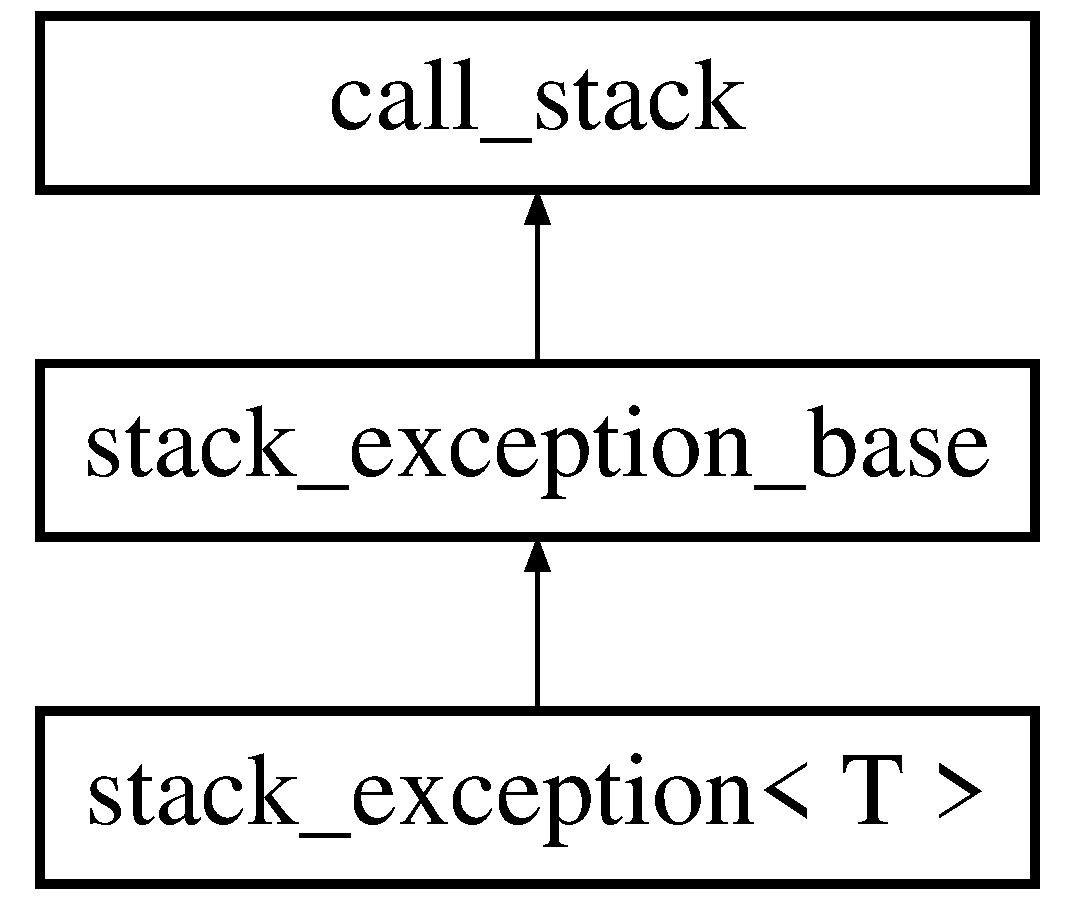
\includegraphics[height=3.000000cm]{classstacktrace_1_1call__stack}
\end{center}
\end{figure}
\subsection*{Public Member Functions}
\begin{DoxyCompactItemize}
\item 
\mbox{\hyperlink{classstacktrace_1_1call__stack_a849ac898624b9ee9a0f6f385624243bb}{call\+\_\+stack}} (const size\+\_\+t num\+\_\+discard=0)
\begin{DoxyCompactList}\small\item\em Stack-\/trace consructor. \end{DoxyCompactList}\item 
virtual \mbox{\hyperlink{classstacktrace_1_1call__stack_ad3a052567d850f543c14edadad05a833}{$\sim$call\+\_\+stack}} ()  throw ()
\item 
std\+::string \mbox{\hyperlink{classstacktrace_1_1call__stack_aac993ecccd3d88aafefb6b8e3caa1dee}{to\+\_\+string}} () const
\begin{DoxyCompactList}\small\item\em Serializes the entire call-\/stack into a text string. \end{DoxyCompactList}\end{DoxyCompactItemize}
\subsection*{Public Attributes}
\begin{DoxyCompactItemize}
\item 
std\+::vector$<$ \mbox{\hyperlink{structstacktrace_1_1entry}{entry}} $>$ \mbox{\hyperlink{classstacktrace_1_1call__stack_a2a3ab0b5bb69cd4a275f3f344d3cc6cd}{stack}}
\begin{DoxyCompactList}\small\item\em Call stack. \end{DoxyCompactList}\end{DoxyCompactItemize}


\subsection{Detailed Description}
Stack-\/trace base class, for retrieving the current call-\/stack. 



\subsection{Constructor \& Destructor Documentation}
\mbox{\Hypertarget{classstacktrace_1_1call__stack_a849ac898624b9ee9a0f6f385624243bb}\label{classstacktrace_1_1call__stack_a849ac898624b9ee9a0f6f385624243bb}} 
\index{stacktrace\+::call\+\_\+stack@{stacktrace\+::call\+\_\+stack}!call\+\_\+stack@{call\+\_\+stack}}
\index{call\+\_\+stack@{call\+\_\+stack}!stacktrace\+::call\+\_\+stack@{stacktrace\+::call\+\_\+stack}}
\subsubsection{\texorpdfstring{call\+\_\+stack()}{call\_stack()}}
{\footnotesize\ttfamily \mbox{\hyperlink{classstacktrace_1_1call__stack}{call\+\_\+stack}} (\begin{DoxyParamCaption}\item[{const size\+\_\+t}]{num\+\_\+discard = {\ttfamily 0} }\end{DoxyParamCaption})}



Stack-\/trace consructor. 


\begin{DoxyParams}{Parameters}
{\em num\+\_\+discard} & -\/ number of stack entries to discard at the top. \\
\hline
\end{DoxyParams}
\mbox{\Hypertarget{classstacktrace_1_1call__stack_ad3a052567d850f543c14edadad05a833}\label{classstacktrace_1_1call__stack_ad3a052567d850f543c14edadad05a833}} 
\index{stacktrace\+::call\+\_\+stack@{stacktrace\+::call\+\_\+stack}!````~call\+\_\+stack@{$\sim$call\+\_\+stack}}
\index{````~call\+\_\+stack@{$\sim$call\+\_\+stack}!stacktrace\+::call\+\_\+stack@{stacktrace\+::call\+\_\+stack}}
\subsubsection{\texorpdfstring{$\sim$call\+\_\+stack()}{~call\_stack()}}
{\footnotesize\ttfamily $\sim$\mbox{\hyperlink{classstacktrace_1_1call__stack}{call\+\_\+stack}} (\begin{DoxyParamCaption}{ }\end{DoxyParamCaption}) throw  ) \hspace{0.3cm}{\ttfamily [virtual]}}



\subsection{Member Function Documentation}
\mbox{\Hypertarget{classstacktrace_1_1call__stack_aac993ecccd3d88aafefb6b8e3caa1dee}\label{classstacktrace_1_1call__stack_aac993ecccd3d88aafefb6b8e3caa1dee}} 
\index{stacktrace\+::call\+\_\+stack@{stacktrace\+::call\+\_\+stack}!to\+\_\+string@{to\+\_\+string}}
\index{to\+\_\+string@{to\+\_\+string}!stacktrace\+::call\+\_\+stack@{stacktrace\+::call\+\_\+stack}}
\subsubsection{\texorpdfstring{to\+\_\+string()}{to\_string()}}
{\footnotesize\ttfamily std\+::string to\+\_\+string (\begin{DoxyParamCaption}{ }\end{DoxyParamCaption}) const\hspace{0.3cm}{\ttfamily [inline]}}



Serializes the entire call-\/stack into a text string. 



\subsection{Member Data Documentation}
\mbox{\Hypertarget{classstacktrace_1_1call__stack_a2a3ab0b5bb69cd4a275f3f344d3cc6cd}\label{classstacktrace_1_1call__stack_a2a3ab0b5bb69cd4a275f3f344d3cc6cd}} 
\index{stacktrace\+::call\+\_\+stack@{stacktrace\+::call\+\_\+stack}!stack@{stack}}
\index{stack@{stack}!stacktrace\+::call\+\_\+stack@{stacktrace\+::call\+\_\+stack}}
\subsubsection{\texorpdfstring{stack}{stack}}
{\footnotesize\ttfamily std\+::vector$<$\mbox{\hyperlink{structstacktrace_1_1entry}{entry}}$>$ stack}



Call stack. 


\hypertarget{classComplex}{}\section{Complex Class Reference}
\label{classComplex}\index{Complex@{Complex}}


{\ttfamily \#include $<$complex.\+h$>$}

\subsection*{Public Member Functions}
\begin{DoxyCompactItemize}
\item 
\mbox{\hyperlink{classComplex_a900a80f2ea5c0c3dc9393402b6ce8df3}{Complex}} (double a=0.\+0, double b=0.\+0)
\item 
double \mbox{\hyperlink{classComplex_ad534b137e1216937005dd363a5579ed0}{abs}} () const
\item 
double \mbox{\hyperlink{classComplex_ac6d0f1ec6a24b5904bc3a206b3c117ff}{imag}} () const
\item 
double \mbox{\hyperlink{classComplex_a3a3f678878dde3a729f94dfefbdc4ef2}{real}} () const
\item 
std\+::string \mbox{\hyperlink{classComplex_a1fe5121d6528fdea3f243321b3fa3a49}{to\+String}} () const
\end{DoxyCompactItemize}
\subsection*{Friends}
\begin{DoxyCompactItemize}
\item 
\mbox{\hyperlink{classComplex}{Complex}} \mbox{\hyperlink{classComplex_afcef21e5f4570416aa39a3412fb107c4}{operator$\ast$}} (const \mbox{\hyperlink{classComplex}{Complex}} \&m, const \mbox{\hyperlink{classComplex}{Complex}} \&n)
\item 
\mbox{\hyperlink{classComplex}{Complex}} \mbox{\hyperlink{classComplex_a47f36e8ddc742de052086d653d7b8e04}{operator+}} (const \mbox{\hyperlink{classComplex}{Complex}} \&m, const \mbox{\hyperlink{classComplex}{Complex}} \&n)
\item 
\mbox{\hyperlink{classComplex}{Complex}} \mbox{\hyperlink{classComplex_ab2328f9c33b801e1ab56ee119493440f}{operator-\/}} (const \mbox{\hyperlink{classComplex}{Complex}} \&m, const \mbox{\hyperlink{classComplex}{Complex}} \&n)
\item 
std\+::istream \& \mbox{\hyperlink{classComplex_a4c3792c8f6bd0778d0607c3a161e9eb6}{operator$>$$>$}} (std\+::istream \&out, \mbox{\hyperlink{classComplex}{Complex}} \&c)
\end{DoxyCompactItemize}


\subsection{Constructor \& Destructor Documentation}
\mbox{\Hypertarget{classComplex_a900a80f2ea5c0c3dc9393402b6ce8df3}\label{classComplex_a900a80f2ea5c0c3dc9393402b6ce8df3}} 
\index{Complex@{Complex}!Complex@{Complex}}
\index{Complex@{Complex}!Complex@{Complex}}
\subsubsection{\texorpdfstring{Complex()}{Complex()}}
{\footnotesize\ttfamily \mbox{\hyperlink{classComplex}{Complex}} (\begin{DoxyParamCaption}\item[{double}]{a = {\ttfamily 0.0},  }\item[{double}]{b = {\ttfamily 0.0} }\end{DoxyParamCaption})}



\subsection{Member Function Documentation}
\mbox{\Hypertarget{classComplex_ad534b137e1216937005dd363a5579ed0}\label{classComplex_ad534b137e1216937005dd363a5579ed0}} 
\index{Complex@{Complex}!abs@{abs}}
\index{abs@{abs}!Complex@{Complex}}
\subsubsection{\texorpdfstring{abs()}{abs()}}
{\footnotesize\ttfamily double abs (\begin{DoxyParamCaption}{ }\end{DoxyParamCaption}) const}

\mbox{\Hypertarget{classComplex_ac6d0f1ec6a24b5904bc3a206b3c117ff}\label{classComplex_ac6d0f1ec6a24b5904bc3a206b3c117ff}} 
\index{Complex@{Complex}!imag@{imag}}
\index{imag@{imag}!Complex@{Complex}}
\subsubsection{\texorpdfstring{imag()}{imag()}}
{\footnotesize\ttfamily double imag (\begin{DoxyParamCaption}{ }\end{DoxyParamCaption}) const}

\mbox{\Hypertarget{classComplex_a3a3f678878dde3a729f94dfefbdc4ef2}\label{classComplex_a3a3f678878dde3a729f94dfefbdc4ef2}} 
\index{Complex@{Complex}!real@{real}}
\index{real@{real}!Complex@{Complex}}
\subsubsection{\texorpdfstring{real()}{real()}}
{\footnotesize\ttfamily double real (\begin{DoxyParamCaption}{ }\end{DoxyParamCaption}) const}

\mbox{\Hypertarget{classComplex_a1fe5121d6528fdea3f243321b3fa3a49}\label{classComplex_a1fe5121d6528fdea3f243321b3fa3a49}} 
\index{Complex@{Complex}!to\+String@{to\+String}}
\index{to\+String@{to\+String}!Complex@{Complex}}
\subsubsection{\texorpdfstring{to\+String()}{toString()}}
{\footnotesize\ttfamily std\+::string to\+String (\begin{DoxyParamCaption}{ }\end{DoxyParamCaption}) const}



\subsection{Friends And Related Function Documentation}
\mbox{\Hypertarget{classComplex_afcef21e5f4570416aa39a3412fb107c4}\label{classComplex_afcef21e5f4570416aa39a3412fb107c4}} 
\index{Complex@{Complex}!operator$\ast$@{operator$\ast$}}
\index{operator$\ast$@{operator$\ast$}!Complex@{Complex}}
\subsubsection{\texorpdfstring{operator$\ast$}{operator*}}
{\footnotesize\ttfamily \mbox{\hyperlink{classComplex}{Complex}} operator$\ast$ (\begin{DoxyParamCaption}\item[{const \mbox{\hyperlink{classComplex}{Complex}} \&}]{m,  }\item[{const \mbox{\hyperlink{classComplex}{Complex}} \&}]{n }\end{DoxyParamCaption})\hspace{0.3cm}{\ttfamily [friend]}}

\mbox{\Hypertarget{classComplex_a47f36e8ddc742de052086d653d7b8e04}\label{classComplex_a47f36e8ddc742de052086d653d7b8e04}} 
\index{Complex@{Complex}!operator+@{operator+}}
\index{operator+@{operator+}!Complex@{Complex}}
\subsubsection{\texorpdfstring{operator+}{operator+}}
{\footnotesize\ttfamily \mbox{\hyperlink{classComplex}{Complex}} operator+ (\begin{DoxyParamCaption}\item[{const \mbox{\hyperlink{classComplex}{Complex}} \&}]{m,  }\item[{const \mbox{\hyperlink{classComplex}{Complex}} \&}]{n }\end{DoxyParamCaption})\hspace{0.3cm}{\ttfamily [friend]}}

\mbox{\Hypertarget{classComplex_ab2328f9c33b801e1ab56ee119493440f}\label{classComplex_ab2328f9c33b801e1ab56ee119493440f}} 
\index{Complex@{Complex}!operator-\/@{operator-\/}}
\index{operator-\/@{operator-\/}!Complex@{Complex}}
\subsubsection{\texorpdfstring{operator-\/}{operator-}}
{\footnotesize\ttfamily \mbox{\hyperlink{classComplex}{Complex}} operator-\/ (\begin{DoxyParamCaption}\item[{const \mbox{\hyperlink{classComplex}{Complex}} \&}]{m,  }\item[{const \mbox{\hyperlink{classComplex}{Complex}} \&}]{n }\end{DoxyParamCaption})\hspace{0.3cm}{\ttfamily [friend]}}

\mbox{\Hypertarget{classComplex_a4c3792c8f6bd0778d0607c3a161e9eb6}\label{classComplex_a4c3792c8f6bd0778d0607c3a161e9eb6}} 
\index{Complex@{Complex}!operator$>$$>$@{operator$>$$>$}}
\index{operator$>$$>$@{operator$>$$>$}!Complex@{Complex}}
\subsubsection{\texorpdfstring{operator$>$$>$}{operator>>}}
{\footnotesize\ttfamily std\+::istream\& operator$>$$>$ (\begin{DoxyParamCaption}\item[{std\+::istream \&}]{out,  }\item[{\mbox{\hyperlink{classComplex}{Complex}} \&}]{c }\end{DoxyParamCaption})\hspace{0.3cm}{\ttfamily [friend]}}


\hypertarget{classstanfordcpplib_1_1ConsoleStreambuf}{}\section{Console\+Streambuf Class Reference}
\label{classstanfordcpplib_1_1ConsoleStreambuf}\index{Console\+Streambuf@{Console\+Streambuf}}


{\ttfamily \#include $<$consolestreambuf.\+h$>$}

Inheritance diagram for Console\+Streambuf\+:\begin{figure}[H]
\begin{center}
\leavevmode
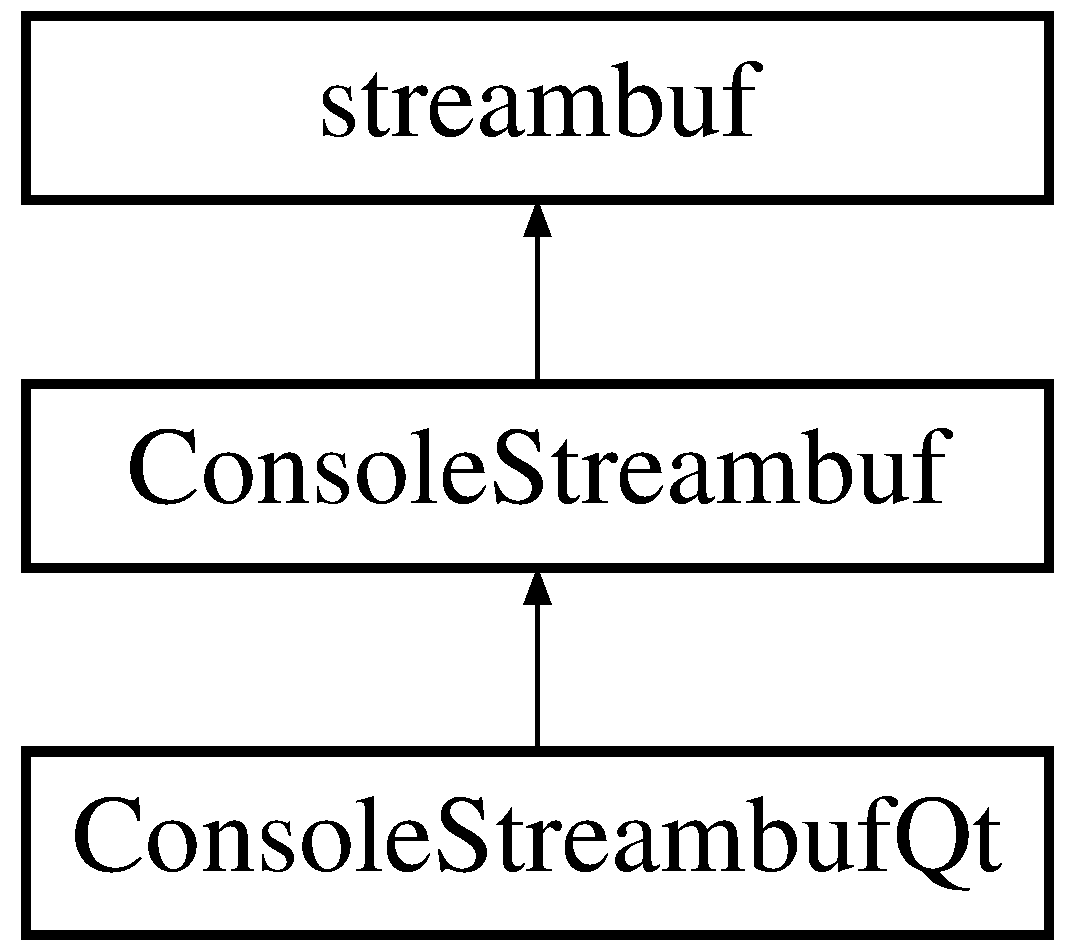
\includegraphics[height=3.000000cm]{classstanfordcpplib_1_1ConsoleStreambuf}
\end{center}
\end{figure}
\subsection*{Public Member Functions}
\begin{DoxyCompactItemize}
\item 
\mbox{\hyperlink{classstanfordcpplib_1_1ConsoleStreambuf_a00319cc8035be74bbc3bb63d60b8c8da}{Console\+Streambuf}} ()
\item 
\mbox{\hyperlink{classstanfordcpplib_1_1ConsoleStreambuf_ae72ddab09d66eb582db69ea4132288ab}{$\sim$\+Console\+Streambuf}} ()
\item 
virtual bool \mbox{\hyperlink{classstanfordcpplib_1_1ConsoleStreambuf_a61d5d93ba4956eefeb2e3d617d34c801}{is\+Blocked}} ()
\item 
virtual int \mbox{\hyperlink{classstanfordcpplib_1_1ConsoleStreambuf_adccb3cd5475ba3c83bc2b0a8cbd731c0}{overflow}} (int ch=E\+OF)
\item 
virtual int \mbox{\hyperlink{classstanfordcpplib_1_1ConsoleStreambuf_a5cfed6bdc955e2129ced962625045f8e}{overflow}} (int ch, bool is\+Stderr)
\item 
virtual int \mbox{\hyperlink{classstanfordcpplib_1_1ConsoleStreambuf_a810a727ce5554d3178e17b6bc55025dd}{sync}} ()
\item 
virtual int \mbox{\hyperlink{classstanfordcpplib_1_1ConsoleStreambuf_ad5f4344df2a20a0000adb05d4e656855}{sync}} (bool is\+Stderr)
\item 
virtual int \mbox{\hyperlink{classstanfordcpplib_1_1ConsoleStreambuf_aeb6918bd44153b257e097e2d2ef370ef}{underflow}} ()
\end{DoxyCompactItemize}
\subsection*{Protected Member Functions}
\begin{DoxyCompactItemize}
\item 
virtual void \mbox{\hyperlink{classstanfordcpplib_1_1ConsoleStreambuf_a783b4396763512a17fb6e825df868c16}{my\+End\+Line\+Console}} (bool is\+Stderr)=0
\item 
virtual std\+::string \mbox{\hyperlink{classstanfordcpplib_1_1ConsoleStreambuf_a72b9cdcc2c68caf7acef81651071a14f}{my\+Get\+Line\+Console}} ()=0
\item 
virtual void \mbox{\hyperlink{classstanfordcpplib_1_1ConsoleStreambuf_a090e9d08f0bd2092bf352d419bdd2a15}{my\+Put\+Console}} (const std\+::string \&str, bool is\+Stderr)=0
\end{DoxyCompactItemize}
\subsection*{Protected Attributes}
\begin{DoxyCompactItemize}
\item 
int \mbox{\hyperlink{classstanfordcpplib_1_1ConsoleStreambuf_ac74e3d5a1b1eeb5c8e32867ad62823f0}{blocked}}
\item 
char \mbox{\hyperlink{classstanfordcpplib_1_1ConsoleStreambuf_a6dfeba2ed7f89c327dd07f6136b2a256}{in\+Buffer}} \mbox{[}\mbox{\hyperlink{classstanfordcpplib_1_1ConsoleStreambuf_a91f806c1bc7c1f4f402a627773840252}{B\+U\+F\+F\+E\+R\+\_\+\+S\+I\+ZE}}\mbox{]}
\item 
char \mbox{\hyperlink{classstanfordcpplib_1_1ConsoleStreambuf_a015231cbe2f7737eee637ddee666f1dd}{out\+Buffer}} \mbox{[}\mbox{\hyperlink{classstanfordcpplib_1_1ConsoleStreambuf_a91f806c1bc7c1f4f402a627773840252}{B\+U\+F\+F\+E\+R\+\_\+\+S\+I\+ZE}}\mbox{]}
\end{DoxyCompactItemize}
\subsection*{Static Protected Attributes}
\begin{DoxyCompactItemize}
\item 
static const int \mbox{\hyperlink{classstanfordcpplib_1_1ConsoleStreambuf_a91f806c1bc7c1f4f402a627773840252}{B\+U\+F\+F\+E\+R\+\_\+\+S\+I\+ZE}} = 4096
\end{DoxyCompactItemize}


\subsection{Constructor \& Destructor Documentation}
\mbox{\Hypertarget{classstanfordcpplib_1_1ConsoleStreambuf_a00319cc8035be74bbc3bb63d60b8c8da}\label{classstanfordcpplib_1_1ConsoleStreambuf_a00319cc8035be74bbc3bb63d60b8c8da}} 
\index{stanfordcpplib\+::\+Console\+Streambuf@{stanfordcpplib\+::\+Console\+Streambuf}!Console\+Streambuf@{Console\+Streambuf}}
\index{Console\+Streambuf@{Console\+Streambuf}!stanfordcpplib\+::\+Console\+Streambuf@{stanfordcpplib\+::\+Console\+Streambuf}}
\subsubsection{\texorpdfstring{Console\+Streambuf()}{ConsoleStreambuf()}}
{\footnotesize\ttfamily \mbox{\hyperlink{classstanfordcpplib_1_1ConsoleStreambuf}{Console\+Streambuf}} (\begin{DoxyParamCaption}{ }\end{DoxyParamCaption})\hspace{0.3cm}{\ttfamily [inline]}}

\mbox{\Hypertarget{classstanfordcpplib_1_1ConsoleStreambuf_ae72ddab09d66eb582db69ea4132288ab}\label{classstanfordcpplib_1_1ConsoleStreambuf_ae72ddab09d66eb582db69ea4132288ab}} 
\index{stanfordcpplib\+::\+Console\+Streambuf@{stanfordcpplib\+::\+Console\+Streambuf}!````~Console\+Streambuf@{$\sim$\+Console\+Streambuf}}
\index{````~Console\+Streambuf@{$\sim$\+Console\+Streambuf}!stanfordcpplib\+::\+Console\+Streambuf@{stanfordcpplib\+::\+Console\+Streambuf}}
\subsubsection{\texorpdfstring{$\sim$\+Console\+Streambuf()}{~ConsoleStreambuf()}}
{\footnotesize\ttfamily $\sim$\mbox{\hyperlink{classstanfordcpplib_1_1ConsoleStreambuf}{Console\+Streambuf}} (\begin{DoxyParamCaption}{ }\end{DoxyParamCaption})\hspace{0.3cm}{\ttfamily [inline]}}



\subsection{Member Function Documentation}
\mbox{\Hypertarget{classstanfordcpplib_1_1ConsoleStreambuf_a61d5d93ba4956eefeb2e3d617d34c801}\label{classstanfordcpplib_1_1ConsoleStreambuf_a61d5d93ba4956eefeb2e3d617d34c801}} 
\index{stanfordcpplib\+::\+Console\+Streambuf@{stanfordcpplib\+::\+Console\+Streambuf}!is\+Blocked@{is\+Blocked}}
\index{is\+Blocked@{is\+Blocked}!stanfordcpplib\+::\+Console\+Streambuf@{stanfordcpplib\+::\+Console\+Streambuf}}
\subsubsection{\texorpdfstring{is\+Blocked()}{isBlocked()}}
{\footnotesize\ttfamily virtual bool is\+Blocked (\begin{DoxyParamCaption}{ }\end{DoxyParamCaption})\hspace{0.3cm}{\ttfamily [inline]}, {\ttfamily [virtual]}}

\mbox{\Hypertarget{classstanfordcpplib_1_1ConsoleStreambuf_a783b4396763512a17fb6e825df868c16}\label{classstanfordcpplib_1_1ConsoleStreambuf_a783b4396763512a17fb6e825df868c16}} 
\index{stanfordcpplib\+::\+Console\+Streambuf@{stanfordcpplib\+::\+Console\+Streambuf}!my\+End\+Line\+Console@{my\+End\+Line\+Console}}
\index{my\+End\+Line\+Console@{my\+End\+Line\+Console}!stanfordcpplib\+::\+Console\+Streambuf@{stanfordcpplib\+::\+Console\+Streambuf}}
\subsubsection{\texorpdfstring{my\+End\+Line\+Console()}{myEndLineConsole()}}
{\footnotesize\ttfamily virtual void my\+End\+Line\+Console (\begin{DoxyParamCaption}\item[{bool}]{is\+Stderr }\end{DoxyParamCaption})\hspace{0.3cm}{\ttfamily [protected]}, {\ttfamily [pure virtual]}}



Implemented in \mbox{\hyperlink{classstanfordcpplib_1_1qtgui_1_1ConsoleStreambufQt_aab6a7af5dac69a7c773d3aae3074696e}{Console\+Streambuf\+Qt}}.

\mbox{\Hypertarget{classstanfordcpplib_1_1ConsoleStreambuf_a72b9cdcc2c68caf7acef81651071a14f}\label{classstanfordcpplib_1_1ConsoleStreambuf_a72b9cdcc2c68caf7acef81651071a14f}} 
\index{stanfordcpplib\+::\+Console\+Streambuf@{stanfordcpplib\+::\+Console\+Streambuf}!my\+Get\+Line\+Console@{my\+Get\+Line\+Console}}
\index{my\+Get\+Line\+Console@{my\+Get\+Line\+Console}!stanfordcpplib\+::\+Console\+Streambuf@{stanfordcpplib\+::\+Console\+Streambuf}}
\subsubsection{\texorpdfstring{my\+Get\+Line\+Console()}{myGetLineConsole()}}
{\footnotesize\ttfamily virtual std\+::string my\+Get\+Line\+Console (\begin{DoxyParamCaption}{ }\end{DoxyParamCaption})\hspace{0.3cm}{\ttfamily [protected]}, {\ttfamily [pure virtual]}}



Implemented in \mbox{\hyperlink{classstanfordcpplib_1_1qtgui_1_1ConsoleStreambufQt_ab5fb2275a81dbd1c170c37bc48adf08a}{Console\+Streambuf\+Qt}}.

\mbox{\Hypertarget{classstanfordcpplib_1_1ConsoleStreambuf_a090e9d08f0bd2092bf352d419bdd2a15}\label{classstanfordcpplib_1_1ConsoleStreambuf_a090e9d08f0bd2092bf352d419bdd2a15}} 
\index{stanfordcpplib\+::\+Console\+Streambuf@{stanfordcpplib\+::\+Console\+Streambuf}!my\+Put\+Console@{my\+Put\+Console}}
\index{my\+Put\+Console@{my\+Put\+Console}!stanfordcpplib\+::\+Console\+Streambuf@{stanfordcpplib\+::\+Console\+Streambuf}}
\subsubsection{\texorpdfstring{my\+Put\+Console()}{myPutConsole()}}
{\footnotesize\ttfamily virtual void my\+Put\+Console (\begin{DoxyParamCaption}\item[{const std\+::string \&}]{str,  }\item[{bool}]{is\+Stderr }\end{DoxyParamCaption})\hspace{0.3cm}{\ttfamily [protected]}, {\ttfamily [pure virtual]}}



Implemented in \mbox{\hyperlink{classstanfordcpplib_1_1qtgui_1_1ConsoleStreambufQt_aa8582bd55e3d7fc8860ca9c87efe3dea}{Console\+Streambuf\+Qt}}.

\mbox{\Hypertarget{classstanfordcpplib_1_1ConsoleStreambuf_adccb3cd5475ba3c83bc2b0a8cbd731c0}\label{classstanfordcpplib_1_1ConsoleStreambuf_adccb3cd5475ba3c83bc2b0a8cbd731c0}} 
\index{stanfordcpplib\+::\+Console\+Streambuf@{stanfordcpplib\+::\+Console\+Streambuf}!overflow@{overflow}}
\index{overflow@{overflow}!stanfordcpplib\+::\+Console\+Streambuf@{stanfordcpplib\+::\+Console\+Streambuf}}
\subsubsection{\texorpdfstring{overflow()}{overflow()}\hspace{0.1cm}{\footnotesize\ttfamily [1/2]}}
{\footnotesize\ttfamily virtual int overflow (\begin{DoxyParamCaption}\item[{int}]{ch = {\ttfamily EOF} }\end{DoxyParamCaption})\hspace{0.3cm}{\ttfamily [inline]}, {\ttfamily [virtual]}}

\mbox{\Hypertarget{classstanfordcpplib_1_1ConsoleStreambuf_a5cfed6bdc955e2129ced962625045f8e}\label{classstanfordcpplib_1_1ConsoleStreambuf_a5cfed6bdc955e2129ced962625045f8e}} 
\index{stanfordcpplib\+::\+Console\+Streambuf@{stanfordcpplib\+::\+Console\+Streambuf}!overflow@{overflow}}
\index{overflow@{overflow}!stanfordcpplib\+::\+Console\+Streambuf@{stanfordcpplib\+::\+Console\+Streambuf}}
\subsubsection{\texorpdfstring{overflow()}{overflow()}\hspace{0.1cm}{\footnotesize\ttfamily [2/2]}}
{\footnotesize\ttfamily virtual int overflow (\begin{DoxyParamCaption}\item[{int}]{ch,  }\item[{bool}]{is\+Stderr }\end{DoxyParamCaption})\hspace{0.3cm}{\ttfamily [inline]}, {\ttfamily [virtual]}}

\mbox{\Hypertarget{classstanfordcpplib_1_1ConsoleStreambuf_a810a727ce5554d3178e17b6bc55025dd}\label{classstanfordcpplib_1_1ConsoleStreambuf_a810a727ce5554d3178e17b6bc55025dd}} 
\index{stanfordcpplib\+::\+Console\+Streambuf@{stanfordcpplib\+::\+Console\+Streambuf}!sync@{sync}}
\index{sync@{sync}!stanfordcpplib\+::\+Console\+Streambuf@{stanfordcpplib\+::\+Console\+Streambuf}}
\subsubsection{\texorpdfstring{sync()}{sync()}\hspace{0.1cm}{\footnotesize\ttfamily [1/2]}}
{\footnotesize\ttfamily virtual int sync (\begin{DoxyParamCaption}{ }\end{DoxyParamCaption})\hspace{0.3cm}{\ttfamily [inline]}, {\ttfamily [virtual]}}

\mbox{\Hypertarget{classstanfordcpplib_1_1ConsoleStreambuf_ad5f4344df2a20a0000adb05d4e656855}\label{classstanfordcpplib_1_1ConsoleStreambuf_ad5f4344df2a20a0000adb05d4e656855}} 
\index{stanfordcpplib\+::\+Console\+Streambuf@{stanfordcpplib\+::\+Console\+Streambuf}!sync@{sync}}
\index{sync@{sync}!stanfordcpplib\+::\+Console\+Streambuf@{stanfordcpplib\+::\+Console\+Streambuf}}
\subsubsection{\texorpdfstring{sync()}{sync()}\hspace{0.1cm}{\footnotesize\ttfamily [2/2]}}
{\footnotesize\ttfamily virtual int sync (\begin{DoxyParamCaption}\item[{bool}]{is\+Stderr }\end{DoxyParamCaption})\hspace{0.3cm}{\ttfamily [inline]}, {\ttfamily [virtual]}}

\mbox{\Hypertarget{classstanfordcpplib_1_1ConsoleStreambuf_aeb6918bd44153b257e097e2d2ef370ef}\label{classstanfordcpplib_1_1ConsoleStreambuf_aeb6918bd44153b257e097e2d2ef370ef}} 
\index{stanfordcpplib\+::\+Console\+Streambuf@{stanfordcpplib\+::\+Console\+Streambuf}!underflow@{underflow}}
\index{underflow@{underflow}!stanfordcpplib\+::\+Console\+Streambuf@{stanfordcpplib\+::\+Console\+Streambuf}}
\subsubsection{\texorpdfstring{underflow()}{underflow()}}
{\footnotesize\ttfamily virtual int underflow (\begin{DoxyParamCaption}{ }\end{DoxyParamCaption})\hspace{0.3cm}{\ttfamily [inline]}, {\ttfamily [virtual]}}



\subsection{Member Data Documentation}
\mbox{\Hypertarget{classstanfordcpplib_1_1ConsoleStreambuf_ac74e3d5a1b1eeb5c8e32867ad62823f0}\label{classstanfordcpplib_1_1ConsoleStreambuf_ac74e3d5a1b1eeb5c8e32867ad62823f0}} 
\index{stanfordcpplib\+::\+Console\+Streambuf@{stanfordcpplib\+::\+Console\+Streambuf}!blocked@{blocked}}
\index{blocked@{blocked}!stanfordcpplib\+::\+Console\+Streambuf@{stanfordcpplib\+::\+Console\+Streambuf}}
\subsubsection{\texorpdfstring{blocked}{blocked}}
{\footnotesize\ttfamily int blocked\hspace{0.3cm}{\ttfamily [protected]}}

\mbox{\Hypertarget{classstanfordcpplib_1_1ConsoleStreambuf_a91f806c1bc7c1f4f402a627773840252}\label{classstanfordcpplib_1_1ConsoleStreambuf_a91f806c1bc7c1f4f402a627773840252}} 
\index{stanfordcpplib\+::\+Console\+Streambuf@{stanfordcpplib\+::\+Console\+Streambuf}!B\+U\+F\+F\+E\+R\+\_\+\+S\+I\+ZE@{B\+U\+F\+F\+E\+R\+\_\+\+S\+I\+ZE}}
\index{B\+U\+F\+F\+E\+R\+\_\+\+S\+I\+ZE@{B\+U\+F\+F\+E\+R\+\_\+\+S\+I\+ZE}!stanfordcpplib\+::\+Console\+Streambuf@{stanfordcpplib\+::\+Console\+Streambuf}}
\subsubsection{\texorpdfstring{B\+U\+F\+F\+E\+R\+\_\+\+S\+I\+ZE}{BUFFER\_SIZE}}
{\footnotesize\ttfamily const int B\+U\+F\+F\+E\+R\+\_\+\+S\+I\+ZE = 4096\hspace{0.3cm}{\ttfamily [static]}, {\ttfamily [protected]}}

\mbox{\Hypertarget{classstanfordcpplib_1_1ConsoleStreambuf_a6dfeba2ed7f89c327dd07f6136b2a256}\label{classstanfordcpplib_1_1ConsoleStreambuf_a6dfeba2ed7f89c327dd07f6136b2a256}} 
\index{stanfordcpplib\+::\+Console\+Streambuf@{stanfordcpplib\+::\+Console\+Streambuf}!in\+Buffer@{in\+Buffer}}
\index{in\+Buffer@{in\+Buffer}!stanfordcpplib\+::\+Console\+Streambuf@{stanfordcpplib\+::\+Console\+Streambuf}}
\subsubsection{\texorpdfstring{in\+Buffer}{inBuffer}}
{\footnotesize\ttfamily char in\+Buffer\mbox{[}\mbox{\hyperlink{classstanfordcpplib_1_1ConsoleStreambuf_a91f806c1bc7c1f4f402a627773840252}{B\+U\+F\+F\+E\+R\+\_\+\+S\+I\+ZE}}\mbox{]}\hspace{0.3cm}{\ttfamily [protected]}}

\mbox{\Hypertarget{classstanfordcpplib_1_1ConsoleStreambuf_a015231cbe2f7737eee637ddee666f1dd}\label{classstanfordcpplib_1_1ConsoleStreambuf_a015231cbe2f7737eee637ddee666f1dd}} 
\index{stanfordcpplib\+::\+Console\+Streambuf@{stanfordcpplib\+::\+Console\+Streambuf}!out\+Buffer@{out\+Buffer}}
\index{out\+Buffer@{out\+Buffer}!stanfordcpplib\+::\+Console\+Streambuf@{stanfordcpplib\+::\+Console\+Streambuf}}
\subsubsection{\texorpdfstring{out\+Buffer}{outBuffer}}
{\footnotesize\ttfamily char out\+Buffer\mbox{[}\mbox{\hyperlink{classstanfordcpplib_1_1ConsoleStreambuf_a91f806c1bc7c1f4f402a627773840252}{B\+U\+F\+F\+E\+R\+\_\+\+S\+I\+ZE}}\mbox{]}\hspace{0.3cm}{\ttfamily [protected]}}


\hypertarget{classstanfordcpplib_1_1qtgui_1_1ConsoleStreambufQt}{}\section{Console\+Streambuf\+Qt Class Reference}
\label{classstanfordcpplib_1_1qtgui_1_1ConsoleStreambufQt}\index{Console\+Streambuf\+Qt@{Console\+Streambuf\+Qt}}


{\ttfamily \#include $<$consolestreambuf.\+h$>$}

Inheritance diagram for Console\+Streambuf\+Qt\+:\begin{figure}[H]
\begin{center}
\leavevmode
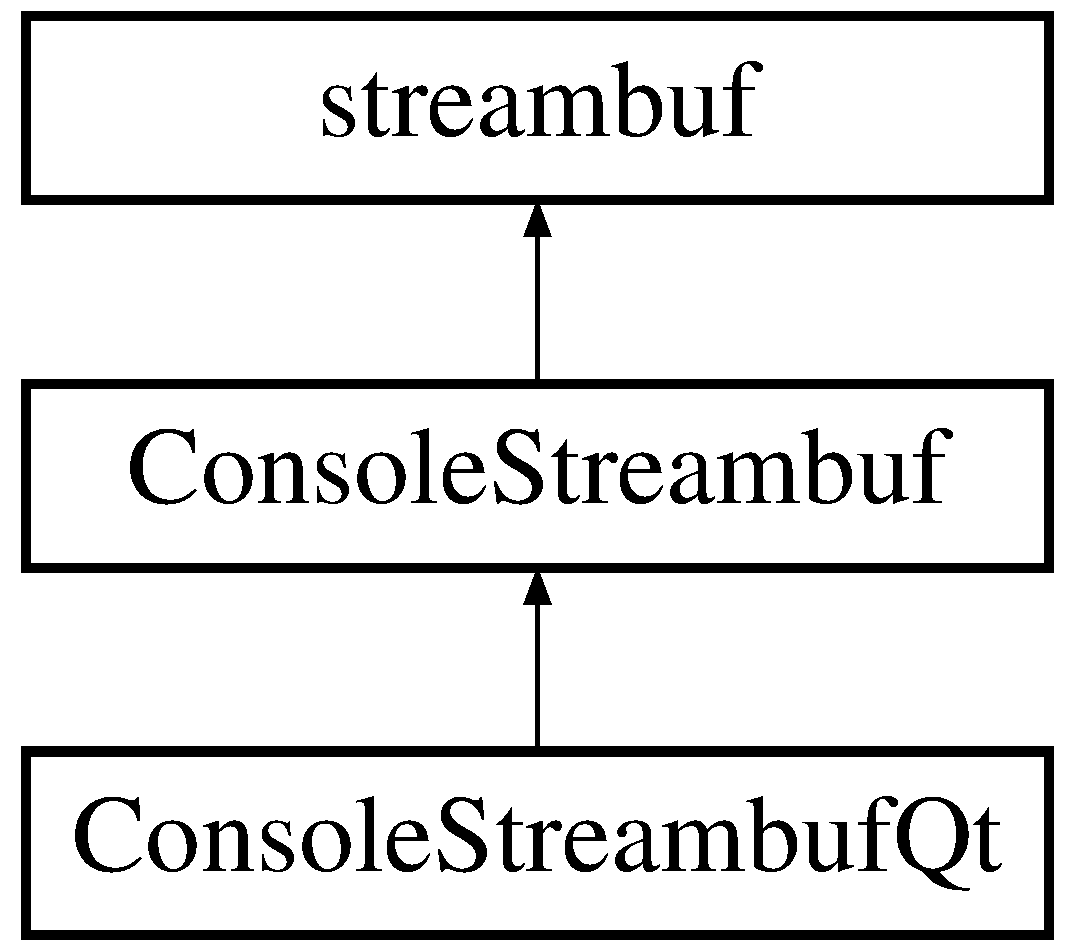
\includegraphics[height=3.000000cm]{classstanfordcpplib_1_1qtgui_1_1ConsoleStreambufQt}
\end{center}
\end{figure}
\subsection*{Public Member Functions}
\begin{DoxyCompactItemize}
\item 
\mbox{\hyperlink{classstanfordcpplib_1_1qtgui_1_1ConsoleStreambufQt_a98660042e1f344d995a0e2e80daee3e9}{Console\+Streambuf\+Qt}} (bool is\+Stderr=false)
\item 
\mbox{\hyperlink{classstanfordcpplib_1_1qtgui_1_1ConsoleStreambufQt_a04fd32aefbdede618e4f890306abd951}{$\sim$\+Console\+Streambuf\+Qt}} ()
\item 
virtual bool \mbox{\hyperlink{classstanfordcpplib_1_1ConsoleStreambuf_a61d5d93ba4956eefeb2e3d617d34c801}{is\+Blocked}} ()
\item 
virtual int \mbox{\hyperlink{classstanfordcpplib_1_1ConsoleStreambuf_adccb3cd5475ba3c83bc2b0a8cbd731c0}{overflow}} (int ch=E\+OF)
\item 
virtual int \mbox{\hyperlink{classstanfordcpplib_1_1ConsoleStreambuf_a5cfed6bdc955e2129ced962625045f8e}{overflow}} (int ch, bool is\+Stderr)
\item 
virtual int \mbox{\hyperlink{classstanfordcpplib_1_1ConsoleStreambuf_a810a727ce5554d3178e17b6bc55025dd}{sync}} ()
\item 
virtual int \mbox{\hyperlink{classstanfordcpplib_1_1ConsoleStreambuf_ad5f4344df2a20a0000adb05d4e656855}{sync}} (bool is\+Stderr)
\item 
virtual int \mbox{\hyperlink{classstanfordcpplib_1_1ConsoleStreambuf_aeb6918bd44153b257e097e2d2ef370ef}{underflow}} ()
\end{DoxyCompactItemize}
\subsection*{Protected Member Functions}
\begin{DoxyCompactItemize}
\item 
virtual void \mbox{\hyperlink{classstanfordcpplib_1_1qtgui_1_1ConsoleStreambufQt_aab6a7af5dac69a7c773d3aae3074696e}{my\+End\+Line\+Console}} (bool)
\item 
virtual std\+::string \mbox{\hyperlink{classstanfordcpplib_1_1qtgui_1_1ConsoleStreambufQt_ab5fb2275a81dbd1c170c37bc48adf08a}{my\+Get\+Line\+Console}} ()
\item 
virtual void \mbox{\hyperlink{classstanfordcpplib_1_1qtgui_1_1ConsoleStreambufQt_aa8582bd55e3d7fc8860ca9c87efe3dea}{my\+Put\+Console}} (const std\+::string \&str, bool)
\end{DoxyCompactItemize}
\subsection*{Protected Attributes}
\begin{DoxyCompactItemize}
\item 
int \mbox{\hyperlink{classstanfordcpplib_1_1ConsoleStreambuf_ac74e3d5a1b1eeb5c8e32867ad62823f0}{blocked}}
\item 
char \mbox{\hyperlink{classstanfordcpplib_1_1ConsoleStreambuf_a6dfeba2ed7f89c327dd07f6136b2a256}{in\+Buffer}} \mbox{[}\mbox{\hyperlink{classstanfordcpplib_1_1ConsoleStreambuf_a91f806c1bc7c1f4f402a627773840252}{B\+U\+F\+F\+E\+R\+\_\+\+S\+I\+ZE}}\mbox{]}
\item 
char \mbox{\hyperlink{classstanfordcpplib_1_1ConsoleStreambuf_a015231cbe2f7737eee637ddee666f1dd}{out\+Buffer}} \mbox{[}\mbox{\hyperlink{classstanfordcpplib_1_1ConsoleStreambuf_a91f806c1bc7c1f4f402a627773840252}{B\+U\+F\+F\+E\+R\+\_\+\+S\+I\+ZE}}\mbox{]}
\end{DoxyCompactItemize}
\subsection*{Static Protected Attributes}
\begin{DoxyCompactItemize}
\item 
static const int \mbox{\hyperlink{classstanfordcpplib_1_1ConsoleStreambuf_a91f806c1bc7c1f4f402a627773840252}{B\+U\+F\+F\+E\+R\+\_\+\+S\+I\+ZE}} = 4096
\end{DoxyCompactItemize}


\subsection{Constructor \& Destructor Documentation}
\mbox{\Hypertarget{classstanfordcpplib_1_1qtgui_1_1ConsoleStreambufQt_a98660042e1f344d995a0e2e80daee3e9}\label{classstanfordcpplib_1_1qtgui_1_1ConsoleStreambufQt_a98660042e1f344d995a0e2e80daee3e9}} 
\index{stanfordcpplib\+::qtgui\+::\+Console\+Streambuf\+Qt@{stanfordcpplib\+::qtgui\+::\+Console\+Streambuf\+Qt}!Console\+Streambuf\+Qt@{Console\+Streambuf\+Qt}}
\index{Console\+Streambuf\+Qt@{Console\+Streambuf\+Qt}!stanfordcpplib\+::qtgui\+::\+Console\+Streambuf\+Qt@{stanfordcpplib\+::qtgui\+::\+Console\+Streambuf\+Qt}}
\subsubsection{\texorpdfstring{Console\+Streambuf\+Qt()}{ConsoleStreambufQt()}}
{\footnotesize\ttfamily \mbox{\hyperlink{classstanfordcpplib_1_1qtgui_1_1ConsoleStreambufQt}{Console\+Streambuf\+Qt}} (\begin{DoxyParamCaption}\item[{bool}]{is\+Stderr = {\ttfamily false} }\end{DoxyParamCaption})\hspace{0.3cm}{\ttfamily [inline]}}

\mbox{\Hypertarget{classstanfordcpplib_1_1qtgui_1_1ConsoleStreambufQt_a04fd32aefbdede618e4f890306abd951}\label{classstanfordcpplib_1_1qtgui_1_1ConsoleStreambufQt_a04fd32aefbdede618e4f890306abd951}} 
\index{stanfordcpplib\+::qtgui\+::\+Console\+Streambuf\+Qt@{stanfordcpplib\+::qtgui\+::\+Console\+Streambuf\+Qt}!````~Console\+Streambuf\+Qt@{$\sim$\+Console\+Streambuf\+Qt}}
\index{````~Console\+Streambuf\+Qt@{$\sim$\+Console\+Streambuf\+Qt}!stanfordcpplib\+::qtgui\+::\+Console\+Streambuf\+Qt@{stanfordcpplib\+::qtgui\+::\+Console\+Streambuf\+Qt}}
\subsubsection{\texorpdfstring{$\sim$\+Console\+Streambuf\+Qt()}{~ConsoleStreambufQt()}}
{\footnotesize\ttfamily $\sim$\mbox{\hyperlink{classstanfordcpplib_1_1qtgui_1_1ConsoleStreambufQt}{Console\+Streambuf\+Qt}} (\begin{DoxyParamCaption}{ }\end{DoxyParamCaption})\hspace{0.3cm}{\ttfamily [inline]}}



\subsection{Member Function Documentation}
\mbox{\Hypertarget{classstanfordcpplib_1_1ConsoleStreambuf_a61d5d93ba4956eefeb2e3d617d34c801}\label{classstanfordcpplib_1_1ConsoleStreambuf_a61d5d93ba4956eefeb2e3d617d34c801}} 
\index{stanfordcpplib\+::qtgui\+::\+Console\+Streambuf\+Qt@{stanfordcpplib\+::qtgui\+::\+Console\+Streambuf\+Qt}!is\+Blocked@{is\+Blocked}}
\index{is\+Blocked@{is\+Blocked}!stanfordcpplib\+::qtgui\+::\+Console\+Streambuf\+Qt@{stanfordcpplib\+::qtgui\+::\+Console\+Streambuf\+Qt}}
\subsubsection{\texorpdfstring{is\+Blocked()}{isBlocked()}}
{\footnotesize\ttfamily virtual bool is\+Blocked (\begin{DoxyParamCaption}{ }\end{DoxyParamCaption})\hspace{0.3cm}{\ttfamily [inline]}, {\ttfamily [virtual]}, {\ttfamily [inherited]}}

\mbox{\Hypertarget{classstanfordcpplib_1_1qtgui_1_1ConsoleStreambufQt_aab6a7af5dac69a7c773d3aae3074696e}\label{classstanfordcpplib_1_1qtgui_1_1ConsoleStreambufQt_aab6a7af5dac69a7c773d3aae3074696e}} 
\index{stanfordcpplib\+::qtgui\+::\+Console\+Streambuf\+Qt@{stanfordcpplib\+::qtgui\+::\+Console\+Streambuf\+Qt}!my\+End\+Line\+Console@{my\+End\+Line\+Console}}
\index{my\+End\+Line\+Console@{my\+End\+Line\+Console}!stanfordcpplib\+::qtgui\+::\+Console\+Streambuf\+Qt@{stanfordcpplib\+::qtgui\+::\+Console\+Streambuf\+Qt}}
\subsubsection{\texorpdfstring{my\+End\+Line\+Console()}{myEndLineConsole()}}
{\footnotesize\ttfamily virtual void my\+End\+Line\+Console (\begin{DoxyParamCaption}\item[{bool}]{ }\end{DoxyParamCaption})\hspace{0.3cm}{\ttfamily [inline]}, {\ttfamily [protected]}, {\ttfamily [virtual]}}



Implements \mbox{\hyperlink{classstanfordcpplib_1_1ConsoleStreambuf_a783b4396763512a17fb6e825df868c16}{Console\+Streambuf}}.

\mbox{\Hypertarget{classstanfordcpplib_1_1qtgui_1_1ConsoleStreambufQt_ab5fb2275a81dbd1c170c37bc48adf08a}\label{classstanfordcpplib_1_1qtgui_1_1ConsoleStreambufQt_ab5fb2275a81dbd1c170c37bc48adf08a}} 
\index{stanfordcpplib\+::qtgui\+::\+Console\+Streambuf\+Qt@{stanfordcpplib\+::qtgui\+::\+Console\+Streambuf\+Qt}!my\+Get\+Line\+Console@{my\+Get\+Line\+Console}}
\index{my\+Get\+Line\+Console@{my\+Get\+Line\+Console}!stanfordcpplib\+::qtgui\+::\+Console\+Streambuf\+Qt@{stanfordcpplib\+::qtgui\+::\+Console\+Streambuf\+Qt}}
\subsubsection{\texorpdfstring{my\+Get\+Line\+Console()}{myGetLineConsole()}}
{\footnotesize\ttfamily virtual std\+::string my\+Get\+Line\+Console (\begin{DoxyParamCaption}{ }\end{DoxyParamCaption})\hspace{0.3cm}{\ttfamily [inline]}, {\ttfamily [protected]}, {\ttfamily [virtual]}}



Implements \mbox{\hyperlink{classstanfordcpplib_1_1ConsoleStreambuf_a72b9cdcc2c68caf7acef81651071a14f}{Console\+Streambuf}}.

\mbox{\Hypertarget{classstanfordcpplib_1_1qtgui_1_1ConsoleStreambufQt_aa8582bd55e3d7fc8860ca9c87efe3dea}\label{classstanfordcpplib_1_1qtgui_1_1ConsoleStreambufQt_aa8582bd55e3d7fc8860ca9c87efe3dea}} 
\index{stanfordcpplib\+::qtgui\+::\+Console\+Streambuf\+Qt@{stanfordcpplib\+::qtgui\+::\+Console\+Streambuf\+Qt}!my\+Put\+Console@{my\+Put\+Console}}
\index{my\+Put\+Console@{my\+Put\+Console}!stanfordcpplib\+::qtgui\+::\+Console\+Streambuf\+Qt@{stanfordcpplib\+::qtgui\+::\+Console\+Streambuf\+Qt}}
\subsubsection{\texorpdfstring{my\+Put\+Console()}{myPutConsole()}}
{\footnotesize\ttfamily virtual void my\+Put\+Console (\begin{DoxyParamCaption}\item[{const std\+::string \&}]{str,  }\item[{bool}]{ }\end{DoxyParamCaption})\hspace{0.3cm}{\ttfamily [inline]}, {\ttfamily [protected]}, {\ttfamily [virtual]}}



Implements \mbox{\hyperlink{classstanfordcpplib_1_1ConsoleStreambuf_a090e9d08f0bd2092bf352d419bdd2a15}{Console\+Streambuf}}.

\mbox{\Hypertarget{classstanfordcpplib_1_1ConsoleStreambuf_adccb3cd5475ba3c83bc2b0a8cbd731c0}\label{classstanfordcpplib_1_1ConsoleStreambuf_adccb3cd5475ba3c83bc2b0a8cbd731c0}} 
\index{stanfordcpplib\+::qtgui\+::\+Console\+Streambuf\+Qt@{stanfordcpplib\+::qtgui\+::\+Console\+Streambuf\+Qt}!overflow@{overflow}}
\index{overflow@{overflow}!stanfordcpplib\+::qtgui\+::\+Console\+Streambuf\+Qt@{stanfordcpplib\+::qtgui\+::\+Console\+Streambuf\+Qt}}
\subsubsection{\texorpdfstring{overflow()}{overflow()}\hspace{0.1cm}{\footnotesize\ttfamily [1/2]}}
{\footnotesize\ttfamily virtual int overflow (\begin{DoxyParamCaption}\item[{int}]{ch = {\ttfamily EOF} }\end{DoxyParamCaption})\hspace{0.3cm}{\ttfamily [inline]}, {\ttfamily [virtual]}, {\ttfamily [inherited]}}

\mbox{\Hypertarget{classstanfordcpplib_1_1ConsoleStreambuf_a5cfed6bdc955e2129ced962625045f8e}\label{classstanfordcpplib_1_1ConsoleStreambuf_a5cfed6bdc955e2129ced962625045f8e}} 
\index{stanfordcpplib\+::qtgui\+::\+Console\+Streambuf\+Qt@{stanfordcpplib\+::qtgui\+::\+Console\+Streambuf\+Qt}!overflow@{overflow}}
\index{overflow@{overflow}!stanfordcpplib\+::qtgui\+::\+Console\+Streambuf\+Qt@{stanfordcpplib\+::qtgui\+::\+Console\+Streambuf\+Qt}}
\subsubsection{\texorpdfstring{overflow()}{overflow()}\hspace{0.1cm}{\footnotesize\ttfamily [2/2]}}
{\footnotesize\ttfamily virtual int overflow (\begin{DoxyParamCaption}\item[{int}]{ch,  }\item[{bool}]{is\+Stderr }\end{DoxyParamCaption})\hspace{0.3cm}{\ttfamily [inline]}, {\ttfamily [virtual]}, {\ttfamily [inherited]}}

\mbox{\Hypertarget{classstanfordcpplib_1_1ConsoleStreambuf_a810a727ce5554d3178e17b6bc55025dd}\label{classstanfordcpplib_1_1ConsoleStreambuf_a810a727ce5554d3178e17b6bc55025dd}} 
\index{stanfordcpplib\+::qtgui\+::\+Console\+Streambuf\+Qt@{stanfordcpplib\+::qtgui\+::\+Console\+Streambuf\+Qt}!sync@{sync}}
\index{sync@{sync}!stanfordcpplib\+::qtgui\+::\+Console\+Streambuf\+Qt@{stanfordcpplib\+::qtgui\+::\+Console\+Streambuf\+Qt}}
\subsubsection{\texorpdfstring{sync()}{sync()}\hspace{0.1cm}{\footnotesize\ttfamily [1/2]}}
{\footnotesize\ttfamily virtual int sync (\begin{DoxyParamCaption}{ }\end{DoxyParamCaption})\hspace{0.3cm}{\ttfamily [inline]}, {\ttfamily [virtual]}, {\ttfamily [inherited]}}

\mbox{\Hypertarget{classstanfordcpplib_1_1ConsoleStreambuf_ad5f4344df2a20a0000adb05d4e656855}\label{classstanfordcpplib_1_1ConsoleStreambuf_ad5f4344df2a20a0000adb05d4e656855}} 
\index{stanfordcpplib\+::qtgui\+::\+Console\+Streambuf\+Qt@{stanfordcpplib\+::qtgui\+::\+Console\+Streambuf\+Qt}!sync@{sync}}
\index{sync@{sync}!stanfordcpplib\+::qtgui\+::\+Console\+Streambuf\+Qt@{stanfordcpplib\+::qtgui\+::\+Console\+Streambuf\+Qt}}
\subsubsection{\texorpdfstring{sync()}{sync()}\hspace{0.1cm}{\footnotesize\ttfamily [2/2]}}
{\footnotesize\ttfamily virtual int sync (\begin{DoxyParamCaption}\item[{bool}]{is\+Stderr }\end{DoxyParamCaption})\hspace{0.3cm}{\ttfamily [inline]}, {\ttfamily [virtual]}, {\ttfamily [inherited]}}

\mbox{\Hypertarget{classstanfordcpplib_1_1ConsoleStreambuf_aeb6918bd44153b257e097e2d2ef370ef}\label{classstanfordcpplib_1_1ConsoleStreambuf_aeb6918bd44153b257e097e2d2ef370ef}} 
\index{stanfordcpplib\+::qtgui\+::\+Console\+Streambuf\+Qt@{stanfordcpplib\+::qtgui\+::\+Console\+Streambuf\+Qt}!underflow@{underflow}}
\index{underflow@{underflow}!stanfordcpplib\+::qtgui\+::\+Console\+Streambuf\+Qt@{stanfordcpplib\+::qtgui\+::\+Console\+Streambuf\+Qt}}
\subsubsection{\texorpdfstring{underflow()}{underflow()}}
{\footnotesize\ttfamily virtual int underflow (\begin{DoxyParamCaption}{ }\end{DoxyParamCaption})\hspace{0.3cm}{\ttfamily [inline]}, {\ttfamily [virtual]}, {\ttfamily [inherited]}}



\subsection{Member Data Documentation}
\mbox{\Hypertarget{classstanfordcpplib_1_1ConsoleStreambuf_ac74e3d5a1b1eeb5c8e32867ad62823f0}\label{classstanfordcpplib_1_1ConsoleStreambuf_ac74e3d5a1b1eeb5c8e32867ad62823f0}} 
\index{stanfordcpplib\+::qtgui\+::\+Console\+Streambuf\+Qt@{stanfordcpplib\+::qtgui\+::\+Console\+Streambuf\+Qt}!blocked@{blocked}}
\index{blocked@{blocked}!stanfordcpplib\+::qtgui\+::\+Console\+Streambuf\+Qt@{stanfordcpplib\+::qtgui\+::\+Console\+Streambuf\+Qt}}
\subsubsection{\texorpdfstring{blocked}{blocked}}
{\footnotesize\ttfamily int blocked\hspace{0.3cm}{\ttfamily [protected]}, {\ttfamily [inherited]}}

\mbox{\Hypertarget{classstanfordcpplib_1_1ConsoleStreambuf_a91f806c1bc7c1f4f402a627773840252}\label{classstanfordcpplib_1_1ConsoleStreambuf_a91f806c1bc7c1f4f402a627773840252}} 
\index{stanfordcpplib\+::qtgui\+::\+Console\+Streambuf\+Qt@{stanfordcpplib\+::qtgui\+::\+Console\+Streambuf\+Qt}!B\+U\+F\+F\+E\+R\+\_\+\+S\+I\+ZE@{B\+U\+F\+F\+E\+R\+\_\+\+S\+I\+ZE}}
\index{B\+U\+F\+F\+E\+R\+\_\+\+S\+I\+ZE@{B\+U\+F\+F\+E\+R\+\_\+\+S\+I\+ZE}!stanfordcpplib\+::qtgui\+::\+Console\+Streambuf\+Qt@{stanfordcpplib\+::qtgui\+::\+Console\+Streambuf\+Qt}}
\subsubsection{\texorpdfstring{B\+U\+F\+F\+E\+R\+\_\+\+S\+I\+ZE}{BUFFER\_SIZE}}
{\footnotesize\ttfamily const int B\+U\+F\+F\+E\+R\+\_\+\+S\+I\+ZE = 4096\hspace{0.3cm}{\ttfamily [static]}, {\ttfamily [protected]}, {\ttfamily [inherited]}}

\mbox{\Hypertarget{classstanfordcpplib_1_1ConsoleStreambuf_a6dfeba2ed7f89c327dd07f6136b2a256}\label{classstanfordcpplib_1_1ConsoleStreambuf_a6dfeba2ed7f89c327dd07f6136b2a256}} 
\index{stanfordcpplib\+::qtgui\+::\+Console\+Streambuf\+Qt@{stanfordcpplib\+::qtgui\+::\+Console\+Streambuf\+Qt}!in\+Buffer@{in\+Buffer}}
\index{in\+Buffer@{in\+Buffer}!stanfordcpplib\+::qtgui\+::\+Console\+Streambuf\+Qt@{stanfordcpplib\+::qtgui\+::\+Console\+Streambuf\+Qt}}
\subsubsection{\texorpdfstring{in\+Buffer}{inBuffer}}
{\footnotesize\ttfamily char in\+Buffer\mbox{[}\mbox{\hyperlink{classstanfordcpplib_1_1ConsoleStreambuf_a91f806c1bc7c1f4f402a627773840252}{B\+U\+F\+F\+E\+R\+\_\+\+S\+I\+ZE}}\mbox{]}\hspace{0.3cm}{\ttfamily [protected]}, {\ttfamily [inherited]}}

\mbox{\Hypertarget{classstanfordcpplib_1_1ConsoleStreambuf_a015231cbe2f7737eee637ddee666f1dd}\label{classstanfordcpplib_1_1ConsoleStreambuf_a015231cbe2f7737eee637ddee666f1dd}} 
\index{stanfordcpplib\+::qtgui\+::\+Console\+Streambuf\+Qt@{stanfordcpplib\+::qtgui\+::\+Console\+Streambuf\+Qt}!out\+Buffer@{out\+Buffer}}
\index{out\+Buffer@{out\+Buffer}!stanfordcpplib\+::qtgui\+::\+Console\+Streambuf\+Qt@{stanfordcpplib\+::qtgui\+::\+Console\+Streambuf\+Qt}}
\subsubsection{\texorpdfstring{out\+Buffer}{outBuffer}}
{\footnotesize\ttfamily char out\+Buffer\mbox{[}\mbox{\hyperlink{classstanfordcpplib_1_1ConsoleStreambuf_a91f806c1bc7c1f4f402a627773840252}{B\+U\+F\+F\+E\+R\+\_\+\+S\+I\+ZE}}\mbox{]}\hspace{0.3cm}{\ttfamily [protected]}, {\ttfamily [inherited]}}


\hypertarget{classDeque_1_1const__deque__iterator}{}\section{Deque$<$ Value\+Type $>$\+:\+:const\+\_\+deque\+\_\+iterator Class Reference}
\label{classDeque_1_1const__deque__iterator}\index{Deque$<$ Value\+Type $>$\+::const\+\_\+deque\+\_\+iterator@{Deque$<$ Value\+Type $>$\+::const\+\_\+deque\+\_\+iterator}}


{\ttfamily \#include $<$deque.\+h$>$}

Inheritance diagram for Deque$<$ Value\+Type $>$\+:\+:const\+\_\+deque\+\_\+iterator\+:\begin{figure}[H]
\begin{center}
\leavevmode
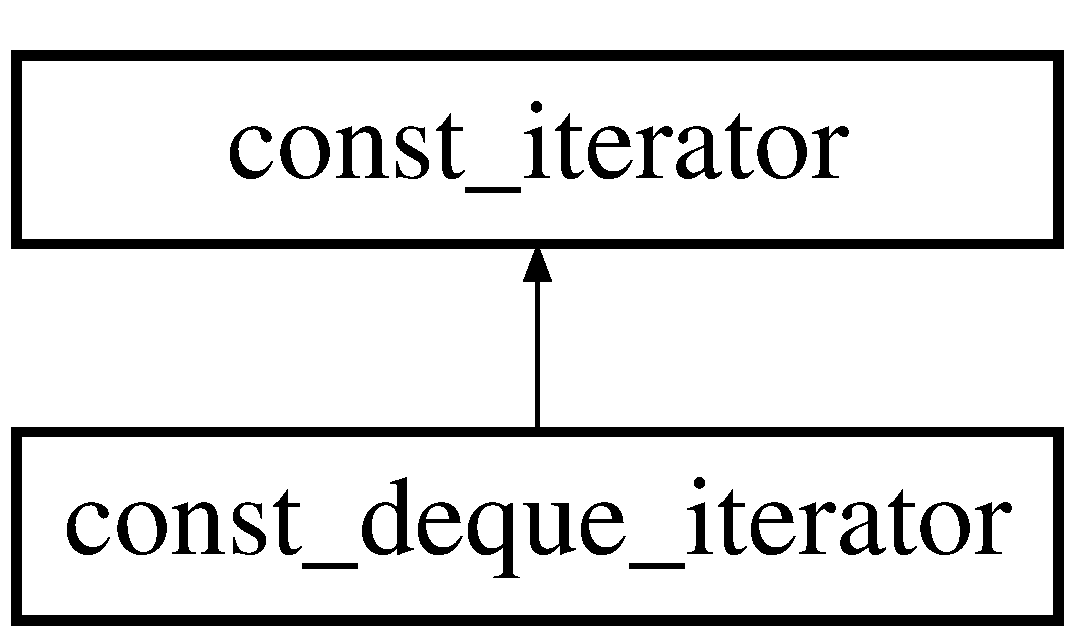
\includegraphics[height=2.000000cm]{classDeque_1_1const__deque__iterator}
\end{center}
\end{figure}
\subsection*{Public Member Functions}
\begin{DoxyCompactItemize}
\item 
\mbox{\hyperlink{classDeque_1_1const__deque__iterator_abd296dc4a6bbc1cd5cbcb2d8e20a30a5}{const\+\_\+deque\+\_\+iterator}} ()
\item 
\mbox{\hyperlink{classDeque_1_1const__deque__iterator_afd3c54e6916f271f7a7adeb494fc3511}{const\+\_\+deque\+\_\+iterator}} (const \mbox{\hyperlink{classDeque_1_1const__deque__iterator}{const\+\_\+deque\+\_\+iterator}} \&it)
\item 
\mbox{\hyperlink{classDeque_1_1const__deque__iterator_a3ef43f2cdb4f9ae9a25b6ca6118b35ea}{const\+\_\+deque\+\_\+iterator}} (const \mbox{\hyperlink{classDeque}{Deque}}$<$ Value\+Type $>$ $\ast$const dp, const typename std\+::deque$<$ Value\+Type $>$\+::const\+\_\+iterator \&it)
\item 
const Value\+Type \& \mbox{\hyperlink{classDeque_1_1const__deque__iterator_a9c07102d483ddb20c4254830707a002f}{operator$\ast$}} ()
\item 
const Value\+Type $\ast$ \mbox{\hyperlink{classDeque_1_1const__deque__iterator_af8c0032fa6fb18e0c8b9b394a302a185}{operator-\/$>$}} ()
\item 
unsigned int \mbox{\hyperlink{classDeque_1_1const__deque__iterator_a0aa696ccb72cbf928535d6b646bac1aa}{version}} () const
\end{DoxyCompactItemize}


\subsection{Constructor \& Destructor Documentation}
\mbox{\Hypertarget{classDeque_1_1const__deque__iterator_abd296dc4a6bbc1cd5cbcb2d8e20a30a5}\label{classDeque_1_1const__deque__iterator_abd296dc4a6bbc1cd5cbcb2d8e20a30a5}} 
\index{Deque\+::const\+\_\+deque\+\_\+iterator@{Deque\+::const\+\_\+deque\+\_\+iterator}!const\+\_\+deque\+\_\+iterator@{const\+\_\+deque\+\_\+iterator}}
\index{const\+\_\+deque\+\_\+iterator@{const\+\_\+deque\+\_\+iterator}!Deque\+::const\+\_\+deque\+\_\+iterator@{Deque\+::const\+\_\+deque\+\_\+iterator}}
\subsubsection{\texorpdfstring{const\+\_\+deque\+\_\+iterator()}{const\_deque\_iterator()}\hspace{0.1cm}{\footnotesize\ttfamily [1/3]}}
{\footnotesize\ttfamily \mbox{\hyperlink{classDeque_1_1const__deque__iterator}{const\+\_\+deque\+\_\+iterator}} (\begin{DoxyParamCaption}{ }\end{DoxyParamCaption})\hspace{0.3cm}{\ttfamily [inline]}}

\mbox{\Hypertarget{classDeque_1_1const__deque__iterator_afd3c54e6916f271f7a7adeb494fc3511}\label{classDeque_1_1const__deque__iterator_afd3c54e6916f271f7a7adeb494fc3511}} 
\index{Deque\+::const\+\_\+deque\+\_\+iterator@{Deque\+::const\+\_\+deque\+\_\+iterator}!const\+\_\+deque\+\_\+iterator@{const\+\_\+deque\+\_\+iterator}}
\index{const\+\_\+deque\+\_\+iterator@{const\+\_\+deque\+\_\+iterator}!Deque\+::const\+\_\+deque\+\_\+iterator@{Deque\+::const\+\_\+deque\+\_\+iterator}}
\subsubsection{\texorpdfstring{const\+\_\+deque\+\_\+iterator()}{const\_deque\_iterator()}\hspace{0.1cm}{\footnotesize\ttfamily [2/3]}}
{\footnotesize\ttfamily \mbox{\hyperlink{classDeque_1_1const__deque__iterator}{const\+\_\+deque\+\_\+iterator}} (\begin{DoxyParamCaption}\item[{const \mbox{\hyperlink{classDeque_1_1const__deque__iterator}{const\+\_\+deque\+\_\+iterator}} \&}]{it }\end{DoxyParamCaption})\hspace{0.3cm}{\ttfamily [inline]}}

\mbox{\Hypertarget{classDeque_1_1const__deque__iterator_a3ef43f2cdb4f9ae9a25b6ca6118b35ea}\label{classDeque_1_1const__deque__iterator_a3ef43f2cdb4f9ae9a25b6ca6118b35ea}} 
\index{Deque\+::const\+\_\+deque\+\_\+iterator@{Deque\+::const\+\_\+deque\+\_\+iterator}!const\+\_\+deque\+\_\+iterator@{const\+\_\+deque\+\_\+iterator}}
\index{const\+\_\+deque\+\_\+iterator@{const\+\_\+deque\+\_\+iterator}!Deque\+::const\+\_\+deque\+\_\+iterator@{Deque\+::const\+\_\+deque\+\_\+iterator}}
\subsubsection{\texorpdfstring{const\+\_\+deque\+\_\+iterator()}{const\_deque\_iterator()}\hspace{0.1cm}{\footnotesize\ttfamily [3/3]}}
{\footnotesize\ttfamily \mbox{\hyperlink{classDeque_1_1const__deque__iterator}{const\+\_\+deque\+\_\+iterator}} (\begin{DoxyParamCaption}\item[{const \mbox{\hyperlink{classDeque}{Deque}}$<$ Value\+Type $>$ $\ast$const}]{dp,  }\item[{const typename std\+::deque$<$ Value\+Type $>$\+::const\+\_\+iterator \&}]{it }\end{DoxyParamCaption})\hspace{0.3cm}{\ttfamily [inline]}}



\subsection{Member Function Documentation}
\mbox{\Hypertarget{classDeque_1_1const__deque__iterator_a9c07102d483ddb20c4254830707a002f}\label{classDeque_1_1const__deque__iterator_a9c07102d483ddb20c4254830707a002f}} 
\index{Deque\+::const\+\_\+deque\+\_\+iterator@{Deque\+::const\+\_\+deque\+\_\+iterator}!operator$\ast$@{operator$\ast$}}
\index{operator$\ast$@{operator$\ast$}!Deque\+::const\+\_\+deque\+\_\+iterator@{Deque\+::const\+\_\+deque\+\_\+iterator}}
\subsubsection{\texorpdfstring{operator$\ast$()}{operator*()}}
{\footnotesize\ttfamily const Value\+Type\& operator$\ast$ (\begin{DoxyParamCaption}{ }\end{DoxyParamCaption})\hspace{0.3cm}{\ttfamily [inline]}}

\mbox{\Hypertarget{classDeque_1_1const__deque__iterator_af8c0032fa6fb18e0c8b9b394a302a185}\label{classDeque_1_1const__deque__iterator_af8c0032fa6fb18e0c8b9b394a302a185}} 
\index{Deque\+::const\+\_\+deque\+\_\+iterator@{Deque\+::const\+\_\+deque\+\_\+iterator}!operator-\/$>$@{operator-\/$>$}}
\index{operator-\/$>$@{operator-\/$>$}!Deque\+::const\+\_\+deque\+\_\+iterator@{Deque\+::const\+\_\+deque\+\_\+iterator}}
\subsubsection{\texorpdfstring{operator-\/$>$()}{operator->()}}
{\footnotesize\ttfamily const Value\+Type$\ast$ operator-\/$>$ (\begin{DoxyParamCaption}{ }\end{DoxyParamCaption})\hspace{0.3cm}{\ttfamily [inline]}}

\mbox{\Hypertarget{classDeque_1_1const__deque__iterator_a0aa696ccb72cbf928535d6b646bac1aa}\label{classDeque_1_1const__deque__iterator_a0aa696ccb72cbf928535d6b646bac1aa}} 
\index{Deque\+::const\+\_\+deque\+\_\+iterator@{Deque\+::const\+\_\+deque\+\_\+iterator}!version@{version}}
\index{version@{version}!Deque\+::const\+\_\+deque\+\_\+iterator@{Deque\+::const\+\_\+deque\+\_\+iterator}}
\subsubsection{\texorpdfstring{version()}{version()}}
{\footnotesize\ttfamily unsigned int version (\begin{DoxyParamCaption}{ }\end{DoxyParamCaption}) const\hspace{0.3cm}{\ttfamily [inline]}}


\hypertarget{classLinkedList_1_1const__linkedlist__iterator}{}\section{Linked\+List$<$ Value\+Type $>$\+:\+:const\+\_\+linkedlist\+\_\+iterator Class Reference}
\label{classLinkedList_1_1const__linkedlist__iterator}\index{Linked\+List$<$ Value\+Type $>$\+::const\+\_\+linkedlist\+\_\+iterator@{Linked\+List$<$ Value\+Type $>$\+::const\+\_\+linkedlist\+\_\+iterator}}


{\ttfamily \#include $<$linkedlist.\+h$>$}

Inheritance diagram for Linked\+List$<$ Value\+Type $>$\+:\+:const\+\_\+linkedlist\+\_\+iterator\+:\begin{figure}[H]
\begin{center}
\leavevmode
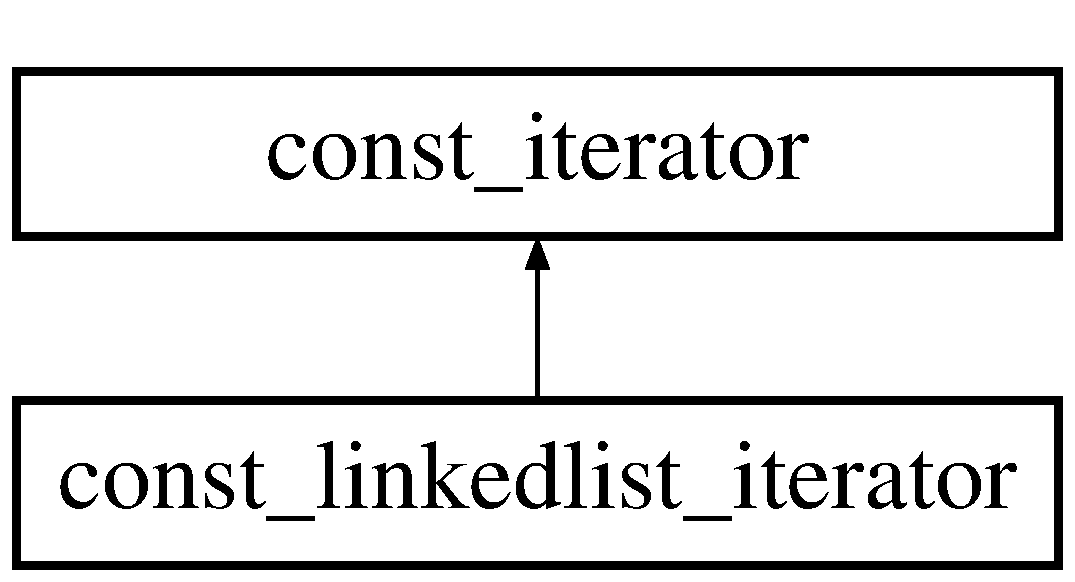
\includegraphics[height=2.000000cm]{classLinkedList_1_1const__linkedlist__iterator}
\end{center}
\end{figure}
\subsection*{Public Member Functions}
\begin{DoxyCompactItemize}
\item 
\mbox{\hyperlink{classLinkedList_1_1const__linkedlist__iterator_abf8e5f03972fb8e43ac6e2ce9e186b2d}{const\+\_\+linkedlist\+\_\+iterator}} ()
\item 
\mbox{\hyperlink{classLinkedList_1_1const__linkedlist__iterator_a4838c4a89b4067214ccac47c37a167b2}{const\+\_\+linkedlist\+\_\+iterator}} (const \mbox{\hyperlink{classLinkedList_1_1const__linkedlist__iterator}{const\+\_\+linkedlist\+\_\+iterator}} \&it)
\item 
\mbox{\hyperlink{classLinkedList_1_1const__linkedlist__iterator_ac65f6fbe021813e29648526b8e0f1799}{const\+\_\+linkedlist\+\_\+iterator}} (const \mbox{\hyperlink{classLinkedList}{Linked\+List}} $\ast$llp, const typename std\+::list$<$ Value\+Type $>$\+::const\+\_\+iterator \&it)
\end{DoxyCompactItemize}


\subsection{Constructor \& Destructor Documentation}
\mbox{\Hypertarget{classLinkedList_1_1const__linkedlist__iterator_abf8e5f03972fb8e43ac6e2ce9e186b2d}\label{classLinkedList_1_1const__linkedlist__iterator_abf8e5f03972fb8e43ac6e2ce9e186b2d}} 
\index{Linked\+List\+::const\+\_\+linkedlist\+\_\+iterator@{Linked\+List\+::const\+\_\+linkedlist\+\_\+iterator}!const\+\_\+linkedlist\+\_\+iterator@{const\+\_\+linkedlist\+\_\+iterator}}
\index{const\+\_\+linkedlist\+\_\+iterator@{const\+\_\+linkedlist\+\_\+iterator}!Linked\+List\+::const\+\_\+linkedlist\+\_\+iterator@{Linked\+List\+::const\+\_\+linkedlist\+\_\+iterator}}
\subsubsection{\texorpdfstring{const\+\_\+linkedlist\+\_\+iterator()}{const\_linkedlist\_iterator()}\hspace{0.1cm}{\footnotesize\ttfamily [1/3]}}
{\footnotesize\ttfamily \mbox{\hyperlink{classLinkedList_1_1const__linkedlist__iterator}{const\+\_\+linkedlist\+\_\+iterator}} (\begin{DoxyParamCaption}{ }\end{DoxyParamCaption})\hspace{0.3cm}{\ttfamily [inline]}}

\mbox{\Hypertarget{classLinkedList_1_1const__linkedlist__iterator_a4838c4a89b4067214ccac47c37a167b2}\label{classLinkedList_1_1const__linkedlist__iterator_a4838c4a89b4067214ccac47c37a167b2}} 
\index{Linked\+List\+::const\+\_\+linkedlist\+\_\+iterator@{Linked\+List\+::const\+\_\+linkedlist\+\_\+iterator}!const\+\_\+linkedlist\+\_\+iterator@{const\+\_\+linkedlist\+\_\+iterator}}
\index{const\+\_\+linkedlist\+\_\+iterator@{const\+\_\+linkedlist\+\_\+iterator}!Linked\+List\+::const\+\_\+linkedlist\+\_\+iterator@{Linked\+List\+::const\+\_\+linkedlist\+\_\+iterator}}
\subsubsection{\texorpdfstring{const\+\_\+linkedlist\+\_\+iterator()}{const\_linkedlist\_iterator()}\hspace{0.1cm}{\footnotesize\ttfamily [2/3]}}
{\footnotesize\ttfamily \mbox{\hyperlink{classLinkedList_1_1const__linkedlist__iterator}{const\+\_\+linkedlist\+\_\+iterator}} (\begin{DoxyParamCaption}\item[{const \mbox{\hyperlink{classLinkedList_1_1const__linkedlist__iterator}{const\+\_\+linkedlist\+\_\+iterator}} \&}]{it }\end{DoxyParamCaption})\hspace{0.3cm}{\ttfamily [inline]}}

\mbox{\Hypertarget{classLinkedList_1_1const__linkedlist__iterator_ac65f6fbe021813e29648526b8e0f1799}\label{classLinkedList_1_1const__linkedlist__iterator_ac65f6fbe021813e29648526b8e0f1799}} 
\index{Linked\+List\+::const\+\_\+linkedlist\+\_\+iterator@{Linked\+List\+::const\+\_\+linkedlist\+\_\+iterator}!const\+\_\+linkedlist\+\_\+iterator@{const\+\_\+linkedlist\+\_\+iterator}}
\index{const\+\_\+linkedlist\+\_\+iterator@{const\+\_\+linkedlist\+\_\+iterator}!Linked\+List\+::const\+\_\+linkedlist\+\_\+iterator@{Linked\+List\+::const\+\_\+linkedlist\+\_\+iterator}}
\subsubsection{\texorpdfstring{const\+\_\+linkedlist\+\_\+iterator()}{const\_linkedlist\_iterator()}\hspace{0.1cm}{\footnotesize\ttfamily [3/3]}}
{\footnotesize\ttfamily \mbox{\hyperlink{classLinkedList_1_1const__linkedlist__iterator}{const\+\_\+linkedlist\+\_\+iterator}} (\begin{DoxyParamCaption}\item[{const \mbox{\hyperlink{classLinkedList}{Linked\+List}} $\ast$}]{llp,  }\item[{const typename std\+::list$<$ Value\+Type $>$\+::const\+\_\+iterator \&}]{it }\end{DoxyParamCaption})\hspace{0.3cm}{\ttfamily [inline]}}


\hypertarget{struct__fe_1_1CRange}{}\section{C\+Range$<$ C\+Type $>$ Struct Template Reference}
\label{struct__fe_1_1CRange}\index{C\+Range$<$ C\+Type $>$@{C\+Range$<$ C\+Type $>$}}


{\ttfamily \#include $<$foreach.\+h$>$}

Inheritance diagram for C\+Range$<$ C\+Type $>$\+:\begin{figure}[H]
\begin{center}
\leavevmode
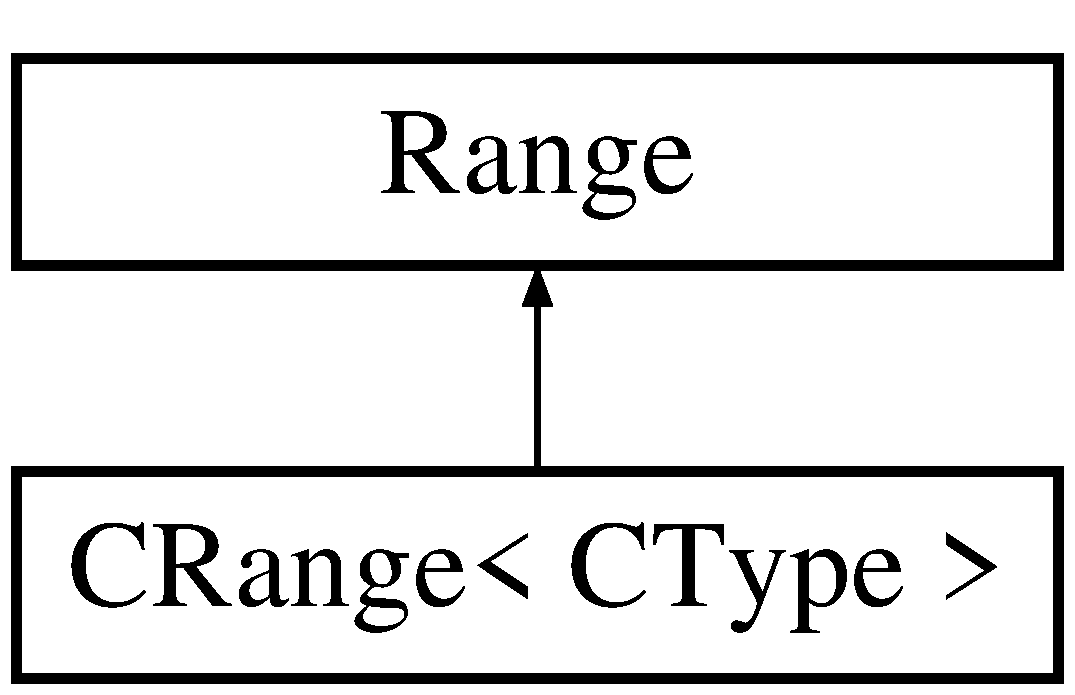
\includegraphics[height=2.000000cm]{struct__fe_1_1CRange}
\end{center}
\end{figure}
\subsection*{Public Member Functions}
\begin{DoxyCompactItemize}
\item 
\mbox{\hyperlink{struct__fe_1_1CRange_a67ad33211b9c44c83d4ba3d0989b37f9}{C\+Range}} (const C\+Type \&c)
\end{DoxyCompactItemize}
\subsection*{Public Attributes}
\begin{DoxyCompactItemize}
\item 
C\+Type \mbox{\hyperlink{struct__fe_1_1CRange_af5d7c61781b48d1b6b5fb41e51935df5}{cont}}
\item 
C\+Type\+::iterator \mbox{\hyperlink{struct__fe_1_1CRange_a0395b0c4aa512ba473e7fb95628ad9e9}{end}}
\item 
C\+Type\+::iterator \mbox{\hyperlink{struct__fe_1_1CRange_a4b3dac39a15fa51ba325f21072bdb873}{iter}}
\end{DoxyCompactItemize}


\subsection{Constructor \& Destructor Documentation}
\mbox{\Hypertarget{struct__fe_1_1CRange_a67ad33211b9c44c83d4ba3d0989b37f9}\label{struct__fe_1_1CRange_a67ad33211b9c44c83d4ba3d0989b37f9}} 
\index{\+\_\+fe\+::\+C\+Range@{\+\_\+fe\+::\+C\+Range}!C\+Range@{C\+Range}}
\index{C\+Range@{C\+Range}!\+\_\+fe\+::\+C\+Range@{\+\_\+fe\+::\+C\+Range}}
\subsubsection{\texorpdfstring{C\+Range()}{CRange()}}
{\footnotesize\ttfamily \mbox{\hyperlink{struct__fe_1_1CRange}{C\+Range}} (\begin{DoxyParamCaption}\item[{const C\+Type \&}]{c }\end{DoxyParamCaption})\hspace{0.3cm}{\ttfamily [inline]}}



\subsection{Member Data Documentation}
\mbox{\Hypertarget{struct__fe_1_1CRange_af5d7c61781b48d1b6b5fb41e51935df5}\label{struct__fe_1_1CRange_af5d7c61781b48d1b6b5fb41e51935df5}} 
\index{\+\_\+fe\+::\+C\+Range@{\+\_\+fe\+::\+C\+Range}!cont@{cont}}
\index{cont@{cont}!\+\_\+fe\+::\+C\+Range@{\+\_\+fe\+::\+C\+Range}}
\subsubsection{\texorpdfstring{cont}{cont}}
{\footnotesize\ttfamily C\+Type cont}

\mbox{\Hypertarget{struct__fe_1_1CRange_a0395b0c4aa512ba473e7fb95628ad9e9}\label{struct__fe_1_1CRange_a0395b0c4aa512ba473e7fb95628ad9e9}} 
\index{\+\_\+fe\+::\+C\+Range@{\+\_\+fe\+::\+C\+Range}!end@{end}}
\index{end@{end}!\+\_\+fe\+::\+C\+Range@{\+\_\+fe\+::\+C\+Range}}
\subsubsection{\texorpdfstring{end}{end}}
{\footnotesize\ttfamily C\+Type\+::iterator end}

\mbox{\Hypertarget{struct__fe_1_1CRange_a4b3dac39a15fa51ba325f21072bdb873}\label{struct__fe_1_1CRange_a4b3dac39a15fa51ba325f21072bdb873}} 
\index{\+\_\+fe\+::\+C\+Range@{\+\_\+fe\+::\+C\+Range}!iter@{iter}}
\index{iter@{iter}!\+\_\+fe\+::\+C\+Range@{\+\_\+fe\+::\+C\+Range}}
\subsubsection{\texorpdfstring{iter}{iter}}
{\footnotesize\ttfamily C\+Type\+::iterator iter}


\hypertarget{classDawgLexicon}{}\section{Dawg\+Lexicon Class Reference}
\label{classDawgLexicon}\index{Dawg\+Lexicon@{Dawg\+Lexicon}}


This class is used to represent a {\bfseries {\itshape lexicon,}} or word list.  




{\ttfamily \#include $<$dawglexicon.\+h$>$}

\subsection*{Classes}
\begin{DoxyCompactItemize}
\item 
class \mbox{\hyperlink{classDawgLexicon_1_1iterator}{iterator}}
\end{DoxyCompactItemize}
\subsection*{Public Member Functions}
\begin{DoxyCompactItemize}
\item 
\mbox{\hyperlink{classDawgLexicon_ad974b1304fbda26ca2e7b0775640e826}{Dawg\+Lexicon}} ()
\begin{DoxyCompactList}\small\item\em Initializes a new empty lexicon. \end{DoxyCompactList}\item 
\mbox{\hyperlink{classDawgLexicon_ad85bfb9847f7e7e33b68287b6ec800fd}{Dawg\+Lexicon}} (std\+::istream \&input)
\begin{DoxyCompactList}\small\item\em ~\newline
 Initializes a new lexicon, reading in the contents of the lexicon from the specified data file. \end{DoxyCompactList}\item 
\mbox{\hyperlink{classDawgLexicon_a2514881fb902166faf4b4a2c58128b7f}{Dawg\+Lexicon}} (const std\+::string \&filename)
\item 
\mbox{\hyperlink{classDawgLexicon_ab482763811fb89cbf52d64bd789ffff1}{Dawg\+Lexicon}} (std\+::initializer\+\_\+list$<$ std\+::string $>$ list)
\item 
\mbox{\hyperlink{classDawgLexicon_a74910e5f5679d365aad6a6c47f00c655}{Dawg\+Lexicon}} (const \mbox{\hyperlink{classDawgLexicon}{Dawg\+Lexicon}} \&src)
\item 
virtual \mbox{\hyperlink{classDawgLexicon_ad36da24eead1f7989047bf2d45b1a082}{$\sim$\+Dawg\+Lexicon}} ()
\begin{DoxyCompactList}\small\item\em The destructor deallocates any storage associated with the lexicon. \end{DoxyCompactList}\item 
void \mbox{\hyperlink{classDawgLexicon_a8713d0dbe1a2aa37acf4a75ea3c5bf40}{add}} (const std\+::string \&word)
\begin{DoxyCompactList}\small\item\em Adds the specified word to the lexicon. \end{DoxyCompactList}\item 
\mbox{\hyperlink{classDawgLexicon}{Dawg\+Lexicon}} \& \mbox{\hyperlink{classDawgLexicon_abcb16967ab02dd1106a92f2a93d8a13c}{add\+All}} (const \mbox{\hyperlink{classDawgLexicon}{Dawg\+Lexicon}} \&lex)
\begin{DoxyCompactList}\small\item\em Adds all elements of the given other lexicon to this lexicon. \end{DoxyCompactList}\item 
\mbox{\hyperlink{classDawgLexicon}{Dawg\+Lexicon}} \& \mbox{\hyperlink{classDawgLexicon_a3f7e696b6fee0d99db3f27619aa559b9}{add\+All}} (std\+::initializer\+\_\+list$<$ std\+::string $>$ list)
\begin{DoxyCompactList}\small\item\em Adds all elements of the given list to this lexicon. \end{DoxyCompactList}\item 
void \mbox{\hyperlink{classDawgLexicon_a215fcead487aace2e89b04863e326ba6}{add\+Words\+From\+File}} (std\+::istream \&input)
\begin{DoxyCompactList}\small\item\em Reads the input stream and adds all of its words to the lexicon. \end{DoxyCompactList}\item 
void \mbox{\hyperlink{classDawgLexicon_a3891deaa85aee9a52b6ca258d1514716}{add\+Words\+From\+File}} (const std\+::string \&filename)
\begin{DoxyCompactList}\small\item\em Reads the file and adds all of its words to the lexicon. \end{DoxyCompactList}\item 
\mbox{\hyperlink{classDawgLexicon_1_1iterator}{iterator}} \mbox{\hyperlink{classDawgLexicon_a0c62c15c8ed609e7e5e9518cf5f5c712}{begin}} () const
\begin{DoxyCompactList}\small\item\em Returns an iterator positioned at the first word in the lexicon. \end{DoxyCompactList}\item 
void \mbox{\hyperlink{classDawgLexicon_ac8bb3912a3ce86b15842e79d0b421204}{clear}} ()
\begin{DoxyCompactList}\small\item\em Removes all words from the lexicon. \end{DoxyCompactList}\item 
bool \mbox{\hyperlink{classDawgLexicon_a479b1bac4a3c243907c80e5c6f9b05d5}{contains}} (const std\+::string \&word) const
\begin{DoxyCompactList}\small\item\em Returns {\ttfamily true} if {\ttfamily word} is contained in the lexicon. \end{DoxyCompactList}\item 
bool \mbox{\hyperlink{classDawgLexicon_acda62a676d80199487fe846670f6294a}{contains\+All}} (const \mbox{\hyperlink{classDawgLexicon}{Dawg\+Lexicon}} \&set2) const
\begin{DoxyCompactList}\small\item\em Returns {\ttfamily true} if every value from the given other lexicon is also found in this lexicon. \end{DoxyCompactList}\item 
bool \mbox{\hyperlink{classDawgLexicon_a3934298595e72e6540e5f81d47ab763a}{contains\+All}} (std\+::initializer\+\_\+list$<$ std\+::string $>$ list) const
\begin{DoxyCompactList}\small\item\em Returns {\ttfamily true} if every value from the given list is also found in this lexicon. \end{DoxyCompactList}\item 
bool \mbox{\hyperlink{classDawgLexicon_a0b8e0b0b6f72ba6b88b56bd074b1dc32}{contains\+Prefix}} (const std\+::string \&prefix) const
\begin{DoxyCompactList}\small\item\em Returns true if any words in the lexicon begin with {\ttfamily prefix}. \end{DoxyCompactList}\item 
\mbox{\hyperlink{classDawgLexicon_1_1iterator}{iterator}} \mbox{\hyperlink{classDawgLexicon_a68b688a51bd0cf6fb5bc2cba292209a8}{end}} () const
\begin{DoxyCompactList}\small\item\em Returns an iterator positioned at the last word in the lexicon. \end{DoxyCompactList}\item 
bool \mbox{\hyperlink{classDawgLexicon_a548d3aa2e2086be0f8db9868d5dfd6e1}{equals}} (const \mbox{\hyperlink{classDawgLexicon}{Dawg\+Lexicon}} \&lex2) const
\begin{DoxyCompactList}\small\item\em Compares two lexicons for equality. \end{DoxyCompactList}\item 
std\+::string \mbox{\hyperlink{classDawgLexicon_a054217ec9f3229ceedee9d7bde075587}{front}} () const
\begin{DoxyCompactList}\small\item\em Returns the first element in alphabetical order from this lexicon (without removing it). \end{DoxyCompactList}\item 
void \mbox{\hyperlink{classDawgLexicon_a1a017af6eb755b5c83e70f61e2bda2c7}{insert}} (const std\+::string \&word)
\begin{DoxyCompactList}\small\item\em Adds an element to this lexicon, if it was not already there. \end{DoxyCompactList}\item 
bool \mbox{\hyperlink{classDawgLexicon_acf82f9b2937375c7b1cf3dccb3df3312}{is\+Empty}} () const
\begin{DoxyCompactList}\small\item\em Returns {\ttfamily true} if the lexicon contains no words. \end{DoxyCompactList}\item 
bool \mbox{\hyperlink{classDawgLexicon_adbfb8a4218cbe3c3686cd58e63bb9193}{is\+Subset\+Of}} (const \mbox{\hyperlink{classDawgLexicon}{Dawg\+Lexicon}} \&lex2) const
\begin{DoxyCompactList}\small\item\em Returns {\ttfamily true} if every word of this lexicon is contained in the given other lexicon. \end{DoxyCompactList}\item 
bool \mbox{\hyperlink{classDawgLexicon_a2a0f1241b53bcf0b31103b79cb01b87d}{is\+Subset\+Of}} (std\+::initializer\+\_\+list$<$ std\+::string $>$ list) const
\begin{DoxyCompactList}\small\item\em Returns {\ttfamily true} if every word of this lexicon is contained in the given list. \end{DoxyCompactList}\item 
bool \mbox{\hyperlink{classDawgLexicon_a16ee2d6dbb050435a7f5cf4dd0cc777c}{is\+Superset\+Of}} (const \mbox{\hyperlink{classDawgLexicon}{Dawg\+Lexicon}} \&lex2) const
\begin{DoxyCompactList}\small\item\em Returns {\ttfamily true} if every word of this lexicon is contained in the given other lexicon. \end{DoxyCompactList}\item 
bool \mbox{\hyperlink{classDawgLexicon_a217cbc1e6ba9f694645608c8a17c1943}{is\+Superset\+Of}} (std\+::initializer\+\_\+list$<$ std\+::string $>$ list) const
\begin{DoxyCompactList}\small\item\em Returns {\ttfamily true} if every word of this lexicon is contained in the given list. \end{DoxyCompactList}\item 
void \mbox{\hyperlink{classDawgLexicon_a2e4e14ffb291ba4d5475b9b66d2a12c8}{map\+All}} (void($\ast$fn)(std\+::string)) const
\begin{DoxyCompactList}\small\item\em Calls the specified function on each word in the lexicon. \end{DoxyCompactList}\item 
void \mbox{\hyperlink{classDawgLexicon_abab83598d63d43b15cf018fa020e1ddf}{map\+All}} (void($\ast$fn)(const std\+::string \&)) const
\begin{DoxyCompactList}\small\item\em Calls the specified function on each word in the lexicon. \end{DoxyCompactList}\item 
{\footnotesize template$<$typename Functor\+Type $>$ }\\void \mbox{\hyperlink{classDawgLexicon_a8dc32c1e45704cfae41daf8adb4e66dc}{map\+All}} (Functor\+Type fn) const
\begin{DoxyCompactList}\small\item\em Calls the specified function on each word in the lexicon. \end{DoxyCompactList}\item 
bool \mbox{\hyperlink{classDawgLexicon_a8d198a4165303f1e4877005141c43e31}{operator!=}} (const \mbox{\hyperlink{classDawgLexicon}{Dawg\+Lexicon}} \&lex2) const
\begin{DoxyCompactList}\small\item\em Returns true if the two lexicons do not have the same elements. \end{DoxyCompactList}\item 
\mbox{\hyperlink{classDawgLexicon}{Dawg\+Lexicon}} \mbox{\hyperlink{classDawgLexicon_ad1dee5fbe47180dbadb3952bb37643ae}{operator+}} (const \mbox{\hyperlink{classDawgLexicon}{Dawg\+Lexicon}} \&lex2) const
\begin{DoxyCompactList}\small\item\em Returns the union of this lexicon and the given other lexicon, which is the set of words that appear in at least one of the two. \end{DoxyCompactList}\item 
\mbox{\hyperlink{classDawgLexicon}{Dawg\+Lexicon}} \mbox{\hyperlink{classDawgLexicon_a41fac68795179c64eea3dc4c86a30814}{operator+}} (std\+::initializer\+\_\+list$<$ std\+::string $>$ list) const
\begin{DoxyCompactList}\small\item\em Returns the union of this lexicon and the given list, which is the set of words that appear in at least one of the two. \end{DoxyCompactList}\item 
\mbox{\hyperlink{classDawgLexicon}{Dawg\+Lexicon}} \mbox{\hyperlink{classDawgLexicon_a218cb40b0674a3db9a362e5b878f7bce}{operator+}} (const std\+::string \&word) const
\begin{DoxyCompactList}\small\item\em Returns the union of this lexicon and the given word. \end{DoxyCompactList}\item 
\mbox{\hyperlink{classDawgLexicon}{Dawg\+Lexicon}} \& \mbox{\hyperlink{classDawgLexicon_a4f69eb7a84edf9a91861e7083305e501}{operator+=}} (const \mbox{\hyperlink{classDawgLexicon}{Dawg\+Lexicon}} \&lex2)
\begin{DoxyCompactList}\small\item\em Adds all of the words from the given lexicon to this one. \end{DoxyCompactList}\item 
\mbox{\hyperlink{classDawgLexicon}{Dawg\+Lexicon}} \& \mbox{\hyperlink{classDawgLexicon_a30565b5b4fdd5efeb9c11fb1943a1d90}{operator+=}} (std\+::initializer\+\_\+list$<$ std\+::string $>$ list)
\begin{DoxyCompactList}\small\item\em Adds all of the words from the given list to this lexicon. \end{DoxyCompactList}\item 
\mbox{\hyperlink{classDawgLexicon}{Dawg\+Lexicon}} \& \mbox{\hyperlink{classDawgLexicon_a8d7fe415402649e86e5ccbb3738d358e}{operator+=}} (const std\+::string \&word)
\begin{DoxyCompactList}\small\item\em Adds the given word to this lexicon. \end{DoxyCompactList}\item 
\mbox{\hyperlink{classDawgLexicon}{Dawg\+Lexicon}} \& \mbox{\hyperlink{classDawgLexicon_ad749b5a8bca43259350ee643e152c2d8}{operator,}} (const std\+::string \&word)
\item 
bool \mbox{\hyperlink{classDawgLexicon_aa7c66db17666a22697ec8076716c3680}{operator$<$}} (const \mbox{\hyperlink{classDawgLexicon}{Dawg\+Lexicon}} \&lex2) const
\begin{DoxyCompactList}\small\item\em Relational operators to compare two lexicons for ordering. \end{DoxyCompactList}\item 
bool \mbox{\hyperlink{classDawgLexicon_a054b62f48d59746ad45e92c1b278463e}{operator$<$=}} (const \mbox{\hyperlink{classDawgLexicon}{Dawg\+Lexicon}} \&lex2) const
\begin{DoxyCompactList}\small\item\em Relational operators to compare two lexicons for ordering. \end{DoxyCompactList}\item 
\mbox{\hyperlink{classDawgLexicon}{Dawg\+Lexicon}} \& \mbox{\hyperlink{classDawgLexicon_a49b7a2bbf9b046065610b18f6ee07889}{operator=}} (const \mbox{\hyperlink{classDawgLexicon}{Dawg\+Lexicon}} \&src)
\item 
bool \mbox{\hyperlink{classDawgLexicon_a3703f712d34b03fe8ea4f7037ed1cb26}{operator==}} (const \mbox{\hyperlink{classDawgLexicon}{Dawg\+Lexicon}} \&lex2) const
\begin{DoxyCompactList}\small\item\em Returns true if the two lexicons have the same elements. \end{DoxyCompactList}\item 
bool \mbox{\hyperlink{classDawgLexicon_ad36b61790c0aa454fddf60d15b52b158}{operator$>$}} (const \mbox{\hyperlink{classDawgLexicon}{Dawg\+Lexicon}} \&lex2) const
\begin{DoxyCompactList}\small\item\em Relational operators to compare two lexicons for ordering. \end{DoxyCompactList}\item 
bool \mbox{\hyperlink{classDawgLexicon_af4f0508490235ae1af1b9234ac9fe01d}{operator$>$=}} (const \mbox{\hyperlink{classDawgLexicon}{Dawg\+Lexicon}} \&lex2) const
\begin{DoxyCompactList}\small\item\em Relational operators to compare two lexicons for ordering. \end{DoxyCompactList}\item 
int \mbox{\hyperlink{classDawgLexicon_af9593d4a5ff4274efaf429cb4f9e57cc}{size}} () const
\begin{DoxyCompactList}\small\item\em Returns the number of words contained in the lexicon. \end{DoxyCompactList}\item 
std\+::string \mbox{\hyperlink{classDawgLexicon_a1fe5121d6528fdea3f243321b3fa3a49}{to\+String}} () const
\begin{DoxyCompactList}\small\item\em Converts the lexicon to a printable string representation such as \{\char`\"{}a\char`\"{}, \char`\"{}b\char`\"{}, \char`\"{}c\char`\"{}\}. \end{DoxyCompactList}\end{DoxyCompactItemize}


\subsection{Detailed Description}
This class is used to represent a {\bfseries {\itshape lexicon,}} or word list. 

The main difference between a lexicon and a dictionary is that a lexicon does not provide any mechanism for storing definitions; the lexicon contains only words, with no associated information. It is therefore similar to a set of strings, but with a more space-\/efficient internal representation. The {\ttfamily \mbox{\hyperlink{classDawgLexicon}{Dawg\+Lexicon}}} class supports efficient lookup operations for words and prefixes.

Currently the recommended implementation of a lexicon is the {\ttfamily \mbox{\hyperlink{classLexicon}{Lexicon}}} class, which supports more operations than this one. 

\subsection{Constructor \& Destructor Documentation}
\mbox{\Hypertarget{classDawgLexicon_ad974b1304fbda26ca2e7b0775640e826}\label{classDawgLexicon_ad974b1304fbda26ca2e7b0775640e826}} 
\index{Dawg\+Lexicon@{Dawg\+Lexicon}!Dawg\+Lexicon@{Dawg\+Lexicon}}
\index{Dawg\+Lexicon@{Dawg\+Lexicon}!Dawg\+Lexicon@{Dawg\+Lexicon}}
\subsubsection{\texorpdfstring{Dawg\+Lexicon()}{DawgLexicon()}\hspace{0.1cm}{\footnotesize\ttfamily [1/5]}}
{\footnotesize\ttfamily \mbox{\hyperlink{classDawgLexicon}{Dawg\+Lexicon}} (\begin{DoxyParamCaption}{ }\end{DoxyParamCaption})}



Initializes a new empty lexicon. 

\mbox{\Hypertarget{classDawgLexicon_ad85bfb9847f7e7e33b68287b6ec800fd}\label{classDawgLexicon_ad85bfb9847f7e7e33b68287b6ec800fd}} 
\index{Dawg\+Lexicon@{Dawg\+Lexicon}!Dawg\+Lexicon@{Dawg\+Lexicon}}
\index{Dawg\+Lexicon@{Dawg\+Lexicon}!Dawg\+Lexicon@{Dawg\+Lexicon}}
\subsubsection{\texorpdfstring{Dawg\+Lexicon()}{DawgLexicon()}\hspace{0.1cm}{\footnotesize\ttfamily [2/5]}}
{\footnotesize\ttfamily \mbox{\hyperlink{classDawgLexicon}{Dawg\+Lexicon}} (\begin{DoxyParamCaption}\item[{std\+::istream \&}]{input }\end{DoxyParamCaption})}



~\newline
 Initializes a new lexicon, reading in the contents of the lexicon from the specified data file. 

The data file must be in one of two formats\+: (1) a space-\/efficient precompiled binary format or (2) a text file containing one word per line.

The Stanford library distribution includes a binary lexicon file named {\ttfamily English.\+dat} containing a list of words in English. The standard code pattern to initialize that lexicon looks like this\+:


\begin{DoxyPre}
  \mbox{\hyperlink{classDawgLexicon}{DawgLexicon}} english("English.dat");
*\end{DoxyPre}
 \mbox{\Hypertarget{classDawgLexicon_a2514881fb902166faf4b4a2c58128b7f}\label{classDawgLexicon_a2514881fb902166faf4b4a2c58128b7f}} 
\index{Dawg\+Lexicon@{Dawg\+Lexicon}!Dawg\+Lexicon@{Dawg\+Lexicon}}
\index{Dawg\+Lexicon@{Dawg\+Lexicon}!Dawg\+Lexicon@{Dawg\+Lexicon}}
\subsubsection{\texorpdfstring{Dawg\+Lexicon()}{DawgLexicon()}\hspace{0.1cm}{\footnotesize\ttfamily [3/5]}}
{\footnotesize\ttfamily \mbox{\hyperlink{classDawgLexicon}{Dawg\+Lexicon}} (\begin{DoxyParamCaption}\item[{const std\+::string \&}]{filename }\end{DoxyParamCaption})}

\mbox{\Hypertarget{classDawgLexicon_ab482763811fb89cbf52d64bd789ffff1}\label{classDawgLexicon_ab482763811fb89cbf52d64bd789ffff1}} 
\index{Dawg\+Lexicon@{Dawg\+Lexicon}!Dawg\+Lexicon@{Dawg\+Lexicon}}
\index{Dawg\+Lexicon@{Dawg\+Lexicon}!Dawg\+Lexicon@{Dawg\+Lexicon}}
\subsubsection{\texorpdfstring{Dawg\+Lexicon()}{DawgLexicon()}\hspace{0.1cm}{\footnotesize\ttfamily [4/5]}}
{\footnotesize\ttfamily \mbox{\hyperlink{classDawgLexicon}{Dawg\+Lexicon}} (\begin{DoxyParamCaption}\item[{std\+::initializer\+\_\+list$<$ std\+::string $>$}]{list }\end{DoxyParamCaption})}

\mbox{\Hypertarget{classDawgLexicon_ad36da24eead1f7989047bf2d45b1a082}\label{classDawgLexicon_ad36da24eead1f7989047bf2d45b1a082}} 
\index{Dawg\+Lexicon@{Dawg\+Lexicon}!````~Dawg\+Lexicon@{$\sim$\+Dawg\+Lexicon}}
\index{````~Dawg\+Lexicon@{$\sim$\+Dawg\+Lexicon}!Dawg\+Lexicon@{Dawg\+Lexicon}}
\subsubsection{\texorpdfstring{$\sim$\+Dawg\+Lexicon()}{~DawgLexicon()}}
{\footnotesize\ttfamily $\sim$\mbox{\hyperlink{classDawgLexicon}{Dawg\+Lexicon}} (\begin{DoxyParamCaption}{ }\end{DoxyParamCaption})\hspace{0.3cm}{\ttfamily [virtual]}}



The destructor deallocates any storage associated with the lexicon. 

\mbox{\Hypertarget{classDawgLexicon_a74910e5f5679d365aad6a6c47f00c655}\label{classDawgLexicon_a74910e5f5679d365aad6a6c47f00c655}} 
\index{Dawg\+Lexicon@{Dawg\+Lexicon}!Dawg\+Lexicon@{Dawg\+Lexicon}}
\index{Dawg\+Lexicon@{Dawg\+Lexicon}!Dawg\+Lexicon@{Dawg\+Lexicon}}
\subsubsection{\texorpdfstring{Dawg\+Lexicon()}{DawgLexicon()}\hspace{0.1cm}{\footnotesize\ttfamily [5/5]}}
{\footnotesize\ttfamily \mbox{\hyperlink{classDawgLexicon}{Dawg\+Lexicon}} (\begin{DoxyParamCaption}\item[{const \mbox{\hyperlink{classDawgLexicon}{Dawg\+Lexicon}} \&}]{src }\end{DoxyParamCaption})}



\subsection{Member Function Documentation}
\mbox{\Hypertarget{classDawgLexicon_a8713d0dbe1a2aa37acf4a75ea3c5bf40}\label{classDawgLexicon_a8713d0dbe1a2aa37acf4a75ea3c5bf40}} 
\index{Dawg\+Lexicon@{Dawg\+Lexicon}!add@{add}}
\index{add@{add}!Dawg\+Lexicon@{Dawg\+Lexicon}}
\subsubsection{\texorpdfstring{add()}{add()}}
{\footnotesize\ttfamily void add (\begin{DoxyParamCaption}\item[{const std\+::string \&}]{word }\end{DoxyParamCaption})}



Adds the specified word to the lexicon. 

\mbox{\Hypertarget{classDawgLexicon_abcb16967ab02dd1106a92f2a93d8a13c}\label{classDawgLexicon_abcb16967ab02dd1106a92f2a93d8a13c}} 
\index{Dawg\+Lexicon@{Dawg\+Lexicon}!add\+All@{add\+All}}
\index{add\+All@{add\+All}!Dawg\+Lexicon@{Dawg\+Lexicon}}
\subsubsection{\texorpdfstring{add\+All()}{addAll()}\hspace{0.1cm}{\footnotesize\ttfamily [1/2]}}
{\footnotesize\ttfamily \mbox{\hyperlink{classDawgLexicon}{Dawg\+Lexicon}} \& add\+All (\begin{DoxyParamCaption}\item[{const \mbox{\hyperlink{classDawgLexicon}{Dawg\+Lexicon}} \&}]{lex }\end{DoxyParamCaption})}



Adds all elements of the given other lexicon to this lexicon. 

Identical in behavior to the += operator. \mbox{\Hypertarget{classDawgLexicon_a3f7e696b6fee0d99db3f27619aa559b9}\label{classDawgLexicon_a3f7e696b6fee0d99db3f27619aa559b9}} 
\index{Dawg\+Lexicon@{Dawg\+Lexicon}!add\+All@{add\+All}}
\index{add\+All@{add\+All}!Dawg\+Lexicon@{Dawg\+Lexicon}}
\subsubsection{\texorpdfstring{add\+All()}{addAll()}\hspace{0.1cm}{\footnotesize\ttfamily [2/2]}}
{\footnotesize\ttfamily \mbox{\hyperlink{classDawgLexicon}{Dawg\+Lexicon}} \& add\+All (\begin{DoxyParamCaption}\item[{std\+::initializer\+\_\+list$<$ std\+::string $>$}]{list }\end{DoxyParamCaption})}



Adds all elements of the given list to this lexicon. 

Identical in behavior to the += operator. \mbox{\Hypertarget{classDawgLexicon_a215fcead487aace2e89b04863e326ba6}\label{classDawgLexicon_a215fcead487aace2e89b04863e326ba6}} 
\index{Dawg\+Lexicon@{Dawg\+Lexicon}!add\+Words\+From\+File@{add\+Words\+From\+File}}
\index{add\+Words\+From\+File@{add\+Words\+From\+File}!Dawg\+Lexicon@{Dawg\+Lexicon}}
\subsubsection{\texorpdfstring{add\+Words\+From\+File()}{addWordsFromFile()}\hspace{0.1cm}{\footnotesize\ttfamily [1/2]}}
{\footnotesize\ttfamily void add\+Words\+From\+File (\begin{DoxyParamCaption}\item[{std\+::istream \&}]{input }\end{DoxyParamCaption})}



Reads the input stream and adds all of its words to the lexicon. 

\mbox{\Hypertarget{classDawgLexicon_a3891deaa85aee9a52b6ca258d1514716}\label{classDawgLexicon_a3891deaa85aee9a52b6ca258d1514716}} 
\index{Dawg\+Lexicon@{Dawg\+Lexicon}!add\+Words\+From\+File@{add\+Words\+From\+File}}
\index{add\+Words\+From\+File@{add\+Words\+From\+File}!Dawg\+Lexicon@{Dawg\+Lexicon}}
\subsubsection{\texorpdfstring{add\+Words\+From\+File()}{addWordsFromFile()}\hspace{0.1cm}{\footnotesize\ttfamily [2/2]}}
{\footnotesize\ttfamily void add\+Words\+From\+File (\begin{DoxyParamCaption}\item[{const std\+::string \&}]{filename }\end{DoxyParamCaption})}



Reads the file and adds all of its words to the lexicon. 

\mbox{\Hypertarget{classDawgLexicon_a0c62c15c8ed609e7e5e9518cf5f5c712}\label{classDawgLexicon_a0c62c15c8ed609e7e5e9518cf5f5c712}} 
\index{Dawg\+Lexicon@{Dawg\+Lexicon}!begin@{begin}}
\index{begin@{begin}!Dawg\+Lexicon@{Dawg\+Lexicon}}
\subsubsection{\texorpdfstring{begin()}{begin()}}
{\footnotesize\ttfamily \mbox{\hyperlink{classDawgLexicon_1_1iterator}{iterator}} begin (\begin{DoxyParamCaption}{ }\end{DoxyParamCaption}) const\hspace{0.3cm}{\ttfamily [inline]}}



Returns an iterator positioned at the first word in the lexicon. 

\mbox{\Hypertarget{classDawgLexicon_ac8bb3912a3ce86b15842e79d0b421204}\label{classDawgLexicon_ac8bb3912a3ce86b15842e79d0b421204}} 
\index{Dawg\+Lexicon@{Dawg\+Lexicon}!clear@{clear}}
\index{clear@{clear}!Dawg\+Lexicon@{Dawg\+Lexicon}}
\subsubsection{\texorpdfstring{clear()}{clear()}}
{\footnotesize\ttfamily void clear (\begin{DoxyParamCaption}{ }\end{DoxyParamCaption})}



Removes all words from the lexicon. 

\mbox{\Hypertarget{classDawgLexicon_a479b1bac4a3c243907c80e5c6f9b05d5}\label{classDawgLexicon_a479b1bac4a3c243907c80e5c6f9b05d5}} 
\index{Dawg\+Lexicon@{Dawg\+Lexicon}!contains@{contains}}
\index{contains@{contains}!Dawg\+Lexicon@{Dawg\+Lexicon}}
\subsubsection{\texorpdfstring{contains()}{contains()}}
{\footnotesize\ttfamily bool contains (\begin{DoxyParamCaption}\item[{const std\+::string \&}]{word }\end{DoxyParamCaption}) const}



Returns {\ttfamily true} if {\ttfamily word} is contained in the lexicon. 

In the {\ttfamily \mbox{\hyperlink{classDawgLexicon}{Dawg\+Lexicon}}} class, the case of letters is ignored, so \char`\"{}\+Zoo\char`\"{} is the same as \char`\"{}\+Z\+O\+O\char`\"{} or \char`\"{}zoo\char`\"{}. \mbox{\Hypertarget{classDawgLexicon_acda62a676d80199487fe846670f6294a}\label{classDawgLexicon_acda62a676d80199487fe846670f6294a}} 
\index{Dawg\+Lexicon@{Dawg\+Lexicon}!contains\+All@{contains\+All}}
\index{contains\+All@{contains\+All}!Dawg\+Lexicon@{Dawg\+Lexicon}}
\subsubsection{\texorpdfstring{contains\+All()}{containsAll()}\hspace{0.1cm}{\footnotesize\ttfamily [1/2]}}
{\footnotesize\ttfamily bool contains\+All (\begin{DoxyParamCaption}\item[{const \mbox{\hyperlink{classDawgLexicon}{Dawg\+Lexicon}} \&}]{set2 }\end{DoxyParamCaption}) const}



Returns {\ttfamily true} if every value from the given other lexicon is also found in this lexicon. 

Equivalent in behavior to is\+Superset\+Of. \mbox{\Hypertarget{classDawgLexicon_a3934298595e72e6540e5f81d47ab763a}\label{classDawgLexicon_a3934298595e72e6540e5f81d47ab763a}} 
\index{Dawg\+Lexicon@{Dawg\+Lexicon}!contains\+All@{contains\+All}}
\index{contains\+All@{contains\+All}!Dawg\+Lexicon@{Dawg\+Lexicon}}
\subsubsection{\texorpdfstring{contains\+All()}{containsAll()}\hspace{0.1cm}{\footnotesize\ttfamily [2/2]}}
{\footnotesize\ttfamily bool contains\+All (\begin{DoxyParamCaption}\item[{std\+::initializer\+\_\+list$<$ std\+::string $>$}]{list }\end{DoxyParamCaption}) const}



Returns {\ttfamily true} if every value from the given list is also found in this lexicon. 

Equivalent in behavior to is\+Superset\+Of. \mbox{\Hypertarget{classDawgLexicon_a0b8e0b0b6f72ba6b88b56bd074b1dc32}\label{classDawgLexicon_a0b8e0b0b6f72ba6b88b56bd074b1dc32}} 
\index{Dawg\+Lexicon@{Dawg\+Lexicon}!contains\+Prefix@{contains\+Prefix}}
\index{contains\+Prefix@{contains\+Prefix}!Dawg\+Lexicon@{Dawg\+Lexicon}}
\subsubsection{\texorpdfstring{contains\+Prefix()}{containsPrefix()}}
{\footnotesize\ttfamily bool contains\+Prefix (\begin{DoxyParamCaption}\item[{const std\+::string \&}]{prefix }\end{DoxyParamCaption}) const}



Returns true if any words in the lexicon begin with {\ttfamily prefix}. 

Like {\ttfamily contains\+Word}, this method ignores the case of letters so that \char`\"{}\+M\+O\char`\"{} is a prefix of \char`\"{}monkey\char`\"{} or \char`\"{}\+Monday\char`\"{}. \mbox{\Hypertarget{classDawgLexicon_a68b688a51bd0cf6fb5bc2cba292209a8}\label{classDawgLexicon_a68b688a51bd0cf6fb5bc2cba292209a8}} 
\index{Dawg\+Lexicon@{Dawg\+Lexicon}!end@{end}}
\index{end@{end}!Dawg\+Lexicon@{Dawg\+Lexicon}}
\subsubsection{\texorpdfstring{end()}{end()}}
{\footnotesize\ttfamily \mbox{\hyperlink{classDawgLexicon_1_1iterator}{iterator}} end (\begin{DoxyParamCaption}{ }\end{DoxyParamCaption}) const\hspace{0.3cm}{\ttfamily [inline]}}



Returns an iterator positioned at the last word in the lexicon. 

\mbox{\Hypertarget{classDawgLexicon_a548d3aa2e2086be0f8db9868d5dfd6e1}\label{classDawgLexicon_a548d3aa2e2086be0f8db9868d5dfd6e1}} 
\index{Dawg\+Lexicon@{Dawg\+Lexicon}!equals@{equals}}
\index{equals@{equals}!Dawg\+Lexicon@{Dawg\+Lexicon}}
\subsubsection{\texorpdfstring{equals()}{equals()}}
{\footnotesize\ttfamily bool equals (\begin{DoxyParamCaption}\item[{const \mbox{\hyperlink{classDawgLexicon}{Dawg\+Lexicon}} \&}]{lex2 }\end{DoxyParamCaption}) const}



Compares two lexicons for equality. 

Returns {\ttfamily true} if this lexicon contains exactly the same values as the given other lexicon. Identical in behavior to the == operator. \mbox{\Hypertarget{classDawgLexicon_a054217ec9f3229ceedee9d7bde075587}\label{classDawgLexicon_a054217ec9f3229ceedee9d7bde075587}} 
\index{Dawg\+Lexicon@{Dawg\+Lexicon}!front@{front}}
\index{front@{front}!Dawg\+Lexicon@{Dawg\+Lexicon}}
\subsubsection{\texorpdfstring{front()}{front()}}
{\footnotesize\ttfamily std\+::string front (\begin{DoxyParamCaption}{ }\end{DoxyParamCaption}) const}



Returns the first element in alphabetical order from this lexicon (without removing it). 

This method signals an error if lexicon is empty. \mbox{\Hypertarget{classDawgLexicon_a1a017af6eb755b5c83e70f61e2bda2c7}\label{classDawgLexicon_a1a017af6eb755b5c83e70f61e2bda2c7}} 
\index{Dawg\+Lexicon@{Dawg\+Lexicon}!insert@{insert}}
\index{insert@{insert}!Dawg\+Lexicon@{Dawg\+Lexicon}}
\subsubsection{\texorpdfstring{insert()}{insert()}}
{\footnotesize\ttfamily void insert (\begin{DoxyParamCaption}\item[{const std\+::string \&}]{word }\end{DoxyParamCaption})}



Adds an element to this lexicon, if it was not already there. 

This method is exported for compatibility with the S\+TL {\ttfamily set} class. \mbox{\Hypertarget{classDawgLexicon_acf82f9b2937375c7b1cf3dccb3df3312}\label{classDawgLexicon_acf82f9b2937375c7b1cf3dccb3df3312}} 
\index{Dawg\+Lexicon@{Dawg\+Lexicon}!is\+Empty@{is\+Empty}}
\index{is\+Empty@{is\+Empty}!Dawg\+Lexicon@{Dawg\+Lexicon}}
\subsubsection{\texorpdfstring{is\+Empty()}{isEmpty()}}
{\footnotesize\ttfamily bool is\+Empty (\begin{DoxyParamCaption}{ }\end{DoxyParamCaption}) const}



Returns {\ttfamily true} if the lexicon contains no words. 

\mbox{\Hypertarget{classDawgLexicon_adbfb8a4218cbe3c3686cd58e63bb9193}\label{classDawgLexicon_adbfb8a4218cbe3c3686cd58e63bb9193}} 
\index{Dawg\+Lexicon@{Dawg\+Lexicon}!is\+Subset\+Of@{is\+Subset\+Of}}
\index{is\+Subset\+Of@{is\+Subset\+Of}!Dawg\+Lexicon@{Dawg\+Lexicon}}
\subsubsection{\texorpdfstring{is\+Subset\+Of()}{isSubsetOf()}\hspace{0.1cm}{\footnotesize\ttfamily [1/2]}}
{\footnotesize\ttfamily bool is\+Subset\+Of (\begin{DoxyParamCaption}\item[{const \mbox{\hyperlink{classDawgLexicon}{Dawg\+Lexicon}} \&}]{lex2 }\end{DoxyParamCaption}) const}



Returns {\ttfamily true} if every word of this lexicon is contained in the given other lexicon. 

\mbox{\Hypertarget{classDawgLexicon_a2a0f1241b53bcf0b31103b79cb01b87d}\label{classDawgLexicon_a2a0f1241b53bcf0b31103b79cb01b87d}} 
\index{Dawg\+Lexicon@{Dawg\+Lexicon}!is\+Subset\+Of@{is\+Subset\+Of}}
\index{is\+Subset\+Of@{is\+Subset\+Of}!Dawg\+Lexicon@{Dawg\+Lexicon}}
\subsubsection{\texorpdfstring{is\+Subset\+Of()}{isSubsetOf()}\hspace{0.1cm}{\footnotesize\ttfamily [2/2]}}
{\footnotesize\ttfamily bool is\+Subset\+Of (\begin{DoxyParamCaption}\item[{std\+::initializer\+\_\+list$<$ std\+::string $>$}]{list }\end{DoxyParamCaption}) const}



Returns {\ttfamily true} if every word of this lexicon is contained in the given list. 

\mbox{\Hypertarget{classDawgLexicon_a16ee2d6dbb050435a7f5cf4dd0cc777c}\label{classDawgLexicon_a16ee2d6dbb050435a7f5cf4dd0cc777c}} 
\index{Dawg\+Lexicon@{Dawg\+Lexicon}!is\+Superset\+Of@{is\+Superset\+Of}}
\index{is\+Superset\+Of@{is\+Superset\+Of}!Dawg\+Lexicon@{Dawg\+Lexicon}}
\subsubsection{\texorpdfstring{is\+Superset\+Of()}{isSupersetOf()}\hspace{0.1cm}{\footnotesize\ttfamily [1/2]}}
{\footnotesize\ttfamily bool is\+Superset\+Of (\begin{DoxyParamCaption}\item[{const \mbox{\hyperlink{classDawgLexicon}{Dawg\+Lexicon}} \&}]{lex2 }\end{DoxyParamCaption}) const}



Returns {\ttfamily true} if every word of this lexicon is contained in the given other lexicon. 

Equivalent in behavior to contains\+All. \mbox{\Hypertarget{classDawgLexicon_a217cbc1e6ba9f694645608c8a17c1943}\label{classDawgLexicon_a217cbc1e6ba9f694645608c8a17c1943}} 
\index{Dawg\+Lexicon@{Dawg\+Lexicon}!is\+Superset\+Of@{is\+Superset\+Of}}
\index{is\+Superset\+Of@{is\+Superset\+Of}!Dawg\+Lexicon@{Dawg\+Lexicon}}
\subsubsection{\texorpdfstring{is\+Superset\+Of()}{isSupersetOf()}\hspace{0.1cm}{\footnotesize\ttfamily [2/2]}}
{\footnotesize\ttfamily bool is\+Superset\+Of (\begin{DoxyParamCaption}\item[{std\+::initializer\+\_\+list$<$ std\+::string $>$}]{list }\end{DoxyParamCaption}) const}



Returns {\ttfamily true} if every word of this lexicon is contained in the given list. 

Equivalent in behavior to contains\+All. \mbox{\Hypertarget{classDawgLexicon_a2e4e14ffb291ba4d5475b9b66d2a12c8}\label{classDawgLexicon_a2e4e14ffb291ba4d5475b9b66d2a12c8}} 
\index{Dawg\+Lexicon@{Dawg\+Lexicon}!map\+All@{map\+All}}
\index{map\+All@{map\+All}!Dawg\+Lexicon@{Dawg\+Lexicon}}
\subsubsection{\texorpdfstring{map\+All()}{mapAll()}\hspace{0.1cm}{\footnotesize\ttfamily [1/3]}}
{\footnotesize\ttfamily void map\+All (\begin{DoxyParamCaption}\item[{void($\ast$)(std\+::string)}]{fn }\end{DoxyParamCaption}) const}



Calls the specified function on each word in the lexicon. 

\mbox{\Hypertarget{classDawgLexicon_abab83598d63d43b15cf018fa020e1ddf}\label{classDawgLexicon_abab83598d63d43b15cf018fa020e1ddf}} 
\index{Dawg\+Lexicon@{Dawg\+Lexicon}!map\+All@{map\+All}}
\index{map\+All@{map\+All}!Dawg\+Lexicon@{Dawg\+Lexicon}}
\subsubsection{\texorpdfstring{map\+All()}{mapAll()}\hspace{0.1cm}{\footnotesize\ttfamily [2/3]}}
{\footnotesize\ttfamily void map\+All (\begin{DoxyParamCaption}\item[{void($\ast$)(const std\+::string \&)}]{fn }\end{DoxyParamCaption}) const}



Calls the specified function on each word in the lexicon. 

\mbox{\Hypertarget{classDawgLexicon_a8dc32c1e45704cfae41daf8adb4e66dc}\label{classDawgLexicon_a8dc32c1e45704cfae41daf8adb4e66dc}} 
\index{Dawg\+Lexicon@{Dawg\+Lexicon}!map\+All@{map\+All}}
\index{map\+All@{map\+All}!Dawg\+Lexicon@{Dawg\+Lexicon}}
\subsubsection{\texorpdfstring{map\+All()}{mapAll()}\hspace{0.1cm}{\footnotesize\ttfamily [3/3]}}
{\footnotesize\ttfamily void map\+All (\begin{DoxyParamCaption}\item[{Functor\+Type}]{fn }\end{DoxyParamCaption}) const}



Calls the specified function on each word in the lexicon. 

\mbox{\Hypertarget{classDawgLexicon_a8d198a4165303f1e4877005141c43e31}\label{classDawgLexicon_a8d198a4165303f1e4877005141c43e31}} 
\index{Dawg\+Lexicon@{Dawg\+Lexicon}!operator"!=@{operator"!=}}
\index{operator"!=@{operator"!=}!Dawg\+Lexicon@{Dawg\+Lexicon}}
\subsubsection{\texorpdfstring{operator"!=()}{operator!=()}}
{\footnotesize\ttfamily bool operator!= (\begin{DoxyParamCaption}\item[{const \mbox{\hyperlink{classDawgLexicon}{Dawg\+Lexicon}} \&}]{lex2 }\end{DoxyParamCaption}) const}



Returns true if the two lexicons do not have the same elements. 

\mbox{\Hypertarget{classDawgLexicon_ad1dee5fbe47180dbadb3952bb37643ae}\label{classDawgLexicon_ad1dee5fbe47180dbadb3952bb37643ae}} 
\index{Dawg\+Lexicon@{Dawg\+Lexicon}!operator+@{operator+}}
\index{operator+@{operator+}!Dawg\+Lexicon@{Dawg\+Lexicon}}
\subsubsection{\texorpdfstring{operator+()}{operator+()}\hspace{0.1cm}{\footnotesize\ttfamily [1/3]}}
{\footnotesize\ttfamily \mbox{\hyperlink{classDawgLexicon}{Dawg\+Lexicon}} operator+ (\begin{DoxyParamCaption}\item[{const \mbox{\hyperlink{classDawgLexicon}{Dawg\+Lexicon}} \&}]{lex2 }\end{DoxyParamCaption}) const}



Returns the union of this lexicon and the given other lexicon, which is the set of words that appear in at least one of the two. 

\mbox{\Hypertarget{classDawgLexicon_a41fac68795179c64eea3dc4c86a30814}\label{classDawgLexicon_a41fac68795179c64eea3dc4c86a30814}} 
\index{Dawg\+Lexicon@{Dawg\+Lexicon}!operator+@{operator+}}
\index{operator+@{operator+}!Dawg\+Lexicon@{Dawg\+Lexicon}}
\subsubsection{\texorpdfstring{operator+()}{operator+()}\hspace{0.1cm}{\footnotesize\ttfamily [2/3]}}
{\footnotesize\ttfamily \mbox{\hyperlink{classDawgLexicon}{Dawg\+Lexicon}} operator+ (\begin{DoxyParamCaption}\item[{std\+::initializer\+\_\+list$<$ std\+::string $>$}]{list }\end{DoxyParamCaption}) const}



Returns the union of this lexicon and the given list, which is the set of words that appear in at least one of the two. 

\mbox{\Hypertarget{classDawgLexicon_a218cb40b0674a3db9a362e5b878f7bce}\label{classDawgLexicon_a218cb40b0674a3db9a362e5b878f7bce}} 
\index{Dawg\+Lexicon@{Dawg\+Lexicon}!operator+@{operator+}}
\index{operator+@{operator+}!Dawg\+Lexicon@{Dawg\+Lexicon}}
\subsubsection{\texorpdfstring{operator+()}{operator+()}\hspace{0.1cm}{\footnotesize\ttfamily [3/3]}}
{\footnotesize\ttfamily \mbox{\hyperlink{classDawgLexicon}{Dawg\+Lexicon}} operator+ (\begin{DoxyParamCaption}\item[{const std\+::string \&}]{word }\end{DoxyParamCaption}) const}



Returns the union of this lexicon and the given word. 

\mbox{\Hypertarget{classDawgLexicon_a4f69eb7a84edf9a91861e7083305e501}\label{classDawgLexicon_a4f69eb7a84edf9a91861e7083305e501}} 
\index{Dawg\+Lexicon@{Dawg\+Lexicon}!operator+=@{operator+=}}
\index{operator+=@{operator+=}!Dawg\+Lexicon@{Dawg\+Lexicon}}
\subsubsection{\texorpdfstring{operator+=()}{operator+=()}\hspace{0.1cm}{\footnotesize\ttfamily [1/3]}}
{\footnotesize\ttfamily \mbox{\hyperlink{classDawgLexicon}{Dawg\+Lexicon}} \& operator+= (\begin{DoxyParamCaption}\item[{const \mbox{\hyperlink{classDawgLexicon}{Dawg\+Lexicon}} \&}]{lex2 }\end{DoxyParamCaption})}



Adds all of the words from the given lexicon to this one. 

\mbox{\Hypertarget{classDawgLexicon_a30565b5b4fdd5efeb9c11fb1943a1d90}\label{classDawgLexicon_a30565b5b4fdd5efeb9c11fb1943a1d90}} 
\index{Dawg\+Lexicon@{Dawg\+Lexicon}!operator+=@{operator+=}}
\index{operator+=@{operator+=}!Dawg\+Lexicon@{Dawg\+Lexicon}}
\subsubsection{\texorpdfstring{operator+=()}{operator+=()}\hspace{0.1cm}{\footnotesize\ttfamily [2/3]}}
{\footnotesize\ttfamily \mbox{\hyperlink{classDawgLexicon}{Dawg\+Lexicon}} \& operator+= (\begin{DoxyParamCaption}\item[{std\+::initializer\+\_\+list$<$ std\+::string $>$}]{list }\end{DoxyParamCaption})}



Adds all of the words from the given list to this lexicon. 

\mbox{\Hypertarget{classDawgLexicon_a8d7fe415402649e86e5ccbb3738d358e}\label{classDawgLexicon_a8d7fe415402649e86e5ccbb3738d358e}} 
\index{Dawg\+Lexicon@{Dawg\+Lexicon}!operator+=@{operator+=}}
\index{operator+=@{operator+=}!Dawg\+Lexicon@{Dawg\+Lexicon}}
\subsubsection{\texorpdfstring{operator+=()}{operator+=()}\hspace{0.1cm}{\footnotesize\ttfamily [3/3]}}
{\footnotesize\ttfamily \mbox{\hyperlink{classDawgLexicon}{Dawg\+Lexicon}} \& operator+= (\begin{DoxyParamCaption}\item[{const std\+::string \&}]{word }\end{DoxyParamCaption})}



Adds the given word to this lexicon. 

\mbox{\Hypertarget{classDawgLexicon_ad749b5a8bca43259350ee643e152c2d8}\label{classDawgLexicon_ad749b5a8bca43259350ee643e152c2d8}} 
\index{Dawg\+Lexicon@{Dawg\+Lexicon}!operator,@{operator,}}
\index{operator,@{operator,}!Dawg\+Lexicon@{Dawg\+Lexicon}}
\subsubsection{\texorpdfstring{operator,()}{operator,()}}
{\footnotesize\ttfamily \mbox{\hyperlink{classDawgLexicon}{Dawg\+Lexicon}} \& operator, (\begin{DoxyParamCaption}\item[{const std\+::string \&}]{word }\end{DoxyParamCaption})}

\mbox{\Hypertarget{classDawgLexicon_aa7c66db17666a22697ec8076716c3680}\label{classDawgLexicon_aa7c66db17666a22697ec8076716c3680}} 
\index{Dawg\+Lexicon@{Dawg\+Lexicon}!operator$<$@{operator$<$}}
\index{operator$<$@{operator$<$}!Dawg\+Lexicon@{Dawg\+Lexicon}}
\subsubsection{\texorpdfstring{operator$<$()}{operator<()}}
{\footnotesize\ttfamily bool operator$<$ (\begin{DoxyParamCaption}\item[{const \mbox{\hyperlink{classDawgLexicon}{Dawg\+Lexicon}} \&}]{lex2 }\end{DoxyParamCaption}) const}



Relational operators to compare two lexicons for ordering. 

\mbox{\Hypertarget{classDawgLexicon_a054b62f48d59746ad45e92c1b278463e}\label{classDawgLexicon_a054b62f48d59746ad45e92c1b278463e}} 
\index{Dawg\+Lexicon@{Dawg\+Lexicon}!operator$<$=@{operator$<$=}}
\index{operator$<$=@{operator$<$=}!Dawg\+Lexicon@{Dawg\+Lexicon}}
\subsubsection{\texorpdfstring{operator$<$=()}{operator<=()}}
{\footnotesize\ttfamily bool operator$<$= (\begin{DoxyParamCaption}\item[{const \mbox{\hyperlink{classDawgLexicon}{Dawg\+Lexicon}} \&}]{lex2 }\end{DoxyParamCaption}) const}



Relational operators to compare two lexicons for ordering. 

\mbox{\Hypertarget{classDawgLexicon_a49b7a2bbf9b046065610b18f6ee07889}\label{classDawgLexicon_a49b7a2bbf9b046065610b18f6ee07889}} 
\index{Dawg\+Lexicon@{Dawg\+Lexicon}!operator=@{operator=}}
\index{operator=@{operator=}!Dawg\+Lexicon@{Dawg\+Lexicon}}
\subsubsection{\texorpdfstring{operator=()}{operator=()}}
{\footnotesize\ttfamily \mbox{\hyperlink{classDawgLexicon}{Dawg\+Lexicon}} \& operator= (\begin{DoxyParamCaption}\item[{const \mbox{\hyperlink{classDawgLexicon}{Dawg\+Lexicon}} \&}]{src }\end{DoxyParamCaption})}

\mbox{\Hypertarget{classDawgLexicon_a3703f712d34b03fe8ea4f7037ed1cb26}\label{classDawgLexicon_a3703f712d34b03fe8ea4f7037ed1cb26}} 
\index{Dawg\+Lexicon@{Dawg\+Lexicon}!operator==@{operator==}}
\index{operator==@{operator==}!Dawg\+Lexicon@{Dawg\+Lexicon}}
\subsubsection{\texorpdfstring{operator==()}{operator==()}}
{\footnotesize\ttfamily bool operator== (\begin{DoxyParamCaption}\item[{const \mbox{\hyperlink{classDawgLexicon}{Dawg\+Lexicon}} \&}]{lex2 }\end{DoxyParamCaption}) const}



Returns true if the two lexicons have the same elements. 

\mbox{\Hypertarget{classDawgLexicon_ad36b61790c0aa454fddf60d15b52b158}\label{classDawgLexicon_ad36b61790c0aa454fddf60d15b52b158}} 
\index{Dawg\+Lexicon@{Dawg\+Lexicon}!operator$>$@{operator$>$}}
\index{operator$>$@{operator$>$}!Dawg\+Lexicon@{Dawg\+Lexicon}}
\subsubsection{\texorpdfstring{operator$>$()}{operator>()}}
{\footnotesize\ttfamily bool operator$>$ (\begin{DoxyParamCaption}\item[{const \mbox{\hyperlink{classDawgLexicon}{Dawg\+Lexicon}} \&}]{lex2 }\end{DoxyParamCaption}) const}



Relational operators to compare two lexicons for ordering. 

\mbox{\Hypertarget{classDawgLexicon_af4f0508490235ae1af1b9234ac9fe01d}\label{classDawgLexicon_af4f0508490235ae1af1b9234ac9fe01d}} 
\index{Dawg\+Lexicon@{Dawg\+Lexicon}!operator$>$=@{operator$>$=}}
\index{operator$>$=@{operator$>$=}!Dawg\+Lexicon@{Dawg\+Lexicon}}
\subsubsection{\texorpdfstring{operator$>$=()}{operator>=()}}
{\footnotesize\ttfamily bool operator$>$= (\begin{DoxyParamCaption}\item[{const \mbox{\hyperlink{classDawgLexicon}{Dawg\+Lexicon}} \&}]{lex2 }\end{DoxyParamCaption}) const}



Relational operators to compare two lexicons for ordering. 

\mbox{\Hypertarget{classDawgLexicon_af9593d4a5ff4274efaf429cb4f9e57cc}\label{classDawgLexicon_af9593d4a5ff4274efaf429cb4f9e57cc}} 
\index{Dawg\+Lexicon@{Dawg\+Lexicon}!size@{size}}
\index{size@{size}!Dawg\+Lexicon@{Dawg\+Lexicon}}
\subsubsection{\texorpdfstring{size()}{size()}}
{\footnotesize\ttfamily int size (\begin{DoxyParamCaption}{ }\end{DoxyParamCaption}) const}



Returns the number of words contained in the lexicon. 

\mbox{\Hypertarget{classDawgLexicon_a1fe5121d6528fdea3f243321b3fa3a49}\label{classDawgLexicon_a1fe5121d6528fdea3f243321b3fa3a49}} 
\index{Dawg\+Lexicon@{Dawg\+Lexicon}!to\+String@{to\+String}}
\index{to\+String@{to\+String}!Dawg\+Lexicon@{Dawg\+Lexicon}}
\subsubsection{\texorpdfstring{to\+String()}{toString()}}
{\footnotesize\ttfamily std\+::string to\+String (\begin{DoxyParamCaption}{ }\end{DoxyParamCaption}) const}



Converts the lexicon to a printable string representation such as \{\char`\"{}a\char`\"{}, \char`\"{}b\char`\"{}, \char`\"{}c\char`\"{}\}. 

\mbox{\hyperlink{classNote}{Note}} that this can be an expensive operation if the lexicon contains a large number of words. 
\hypertarget{classDeque}{}\section{Deque$<$ Value\+Type $>$ Class Template Reference}
\label{classDeque}\index{Deque$<$ Value\+Type $>$@{Deque$<$ Value\+Type $>$}}


{\ttfamily \#include $<$deque.\+h$>$}

\subsection*{Classes}
\begin{DoxyCompactItemize}
\item 
class \mbox{\hyperlink{classDeque_1_1const__deque__iterator}{const\+\_\+deque\+\_\+iterator}}
\item 
class \mbox{\hyperlink{classDeque_1_1deque__iterator}{deque\+\_\+iterator}}
\end{DoxyCompactItemize}
\subsection*{Public Member Functions}
\begin{DoxyCompactItemize}
\item 
\mbox{\hyperlink{classDeque_a41ebad440badfe713f3ffbbec2eac93f}{Deque}} ()
\item 
\mbox{\hyperlink{classDeque_a68fd6ae6ef9283c882d90c6924e932cd}{Deque}} (std\+::initializer\+\_\+list$<$ Value\+Type $>$ list)
\item 
virtual \mbox{\hyperlink{classDeque_a9d75ae227f70523957cb9b60283d9390}{$\sim$\+Deque}} ()
\item 
void \mbox{\hyperlink{classDeque_ab901606bf3a8019c986f0cf9a9f298dc}{add}} (const Value\+Type \&value)
\item 
void \mbox{\hyperlink{classDeque_a0c733f31bccadf80a6793490b115bd37}{add\+Back}} (const Value\+Type \&value)
\item 
void \mbox{\hyperlink{classDeque_a1d5c5f74583e2a0fcd33f177ecbb9aa4}{add\+Front}} (const Value\+Type \&value)
\item 
const Value\+Type \& \mbox{\hyperlink{classDeque_adc761c91bdacd01bed5c96e25fd9486a}{back}} () const
\item 
\mbox{\hyperlink{classDeque_1_1deque__iterator}{deque\+\_\+iterator}} \mbox{\hyperlink{classDeque_ab0616f247b41eeb1a672421386fd5612}{begin}} ()
\item 
\mbox{\hyperlink{classDeque_1_1const__deque__iterator}{const\+\_\+deque\+\_\+iterator}} \mbox{\hyperlink{classDeque_a92be94822f29cf2d75f992e50763f34d}{begin}} () const
\item 
void \mbox{\hyperlink{classDeque_ac8bb3912a3ce86b15842e79d0b421204}{clear}} ()
\item 
Value\+Type \mbox{\hyperlink{classDeque_aaee07e371e2370e76e6c42bada727ba2}{dequeue}} ()
\item 
Value\+Type \mbox{\hyperlink{classDeque_a0f7233390ba171bc0897e5f9618ac4a6}{dequeue\+Back}} ()
\item 
Value\+Type \mbox{\hyperlink{classDeque_aecf002fe82a60407f6008f6fd7ac2c27}{dequeue\+Front}} ()
\item 
\mbox{\hyperlink{classDeque_1_1deque__iterator}{deque\+\_\+iterator}} \mbox{\hyperlink{classDeque_a3f00605ada70bb4af841bafa03311f4a}{end}} ()
\item 
\mbox{\hyperlink{classDeque_1_1const__deque__iterator}{const\+\_\+deque\+\_\+iterator}} \mbox{\hyperlink{classDeque_a255e9712f118c564977def0bdb6438a2}{end}} () const
\item 
void \mbox{\hyperlink{classDeque_a663f69ed5d98f3f167202e9b2d7e7a9a}{enqueue}} (const Value\+Type \&value)
\item 
void \mbox{\hyperlink{classDeque_a2fdd7308cc72a3bd03dd6345ef778a65}{enqueue\+Back}} (const Value\+Type \&value)
\item 
void \mbox{\hyperlink{classDeque_a12586c9fec2e0dd724cf6ccb4d52c6e8}{enqueue\+Front}} (const Value\+Type \&value)
\item 
bool \mbox{\hyperlink{classDeque_a2468abeaef57d95b43a90b7462ff88ab}{equals}} (const \mbox{\hyperlink{classDeque}{Deque}}$<$ Value\+Type $>$ \&deque2) const
\item 
const Value\+Type \& \mbox{\hyperlink{classDeque_a02aaa52ad7a120201f6dd3e90eff737f}{front}} () const
\item 
bool \mbox{\hyperlink{classDeque_acf82f9b2937375c7b1cf3dccb3df3312}{is\+Empty}} () const
\item 
bool \mbox{\hyperlink{classDeque_a512bc8214fed49868d85acd8f1e351d3}{operator!=}} (const \mbox{\hyperlink{classDeque}{Deque}} \&deque2) const
\item 
bool \mbox{\hyperlink{classDeque_afdfe6d4b99c8d185f9f8c6d48fc19c88}{operator$<$}} (const \mbox{\hyperlink{classDeque}{Deque}} \&deque2) const
\item 
bool \mbox{\hyperlink{classDeque_a08a801e1cca1a84e7fae799f5c12696e}{operator$<$=}} (const \mbox{\hyperlink{classDeque}{Deque}} \&deque2) const
\item 
\mbox{\hyperlink{classDeque}{Deque}} \& \mbox{\hyperlink{classDeque_a1fedefadfc83c266110c8f6b135c1106}{operator=}} (const \mbox{\hyperlink{classDeque}{Deque}} \&other)
\item 
bool \mbox{\hyperlink{classDeque_a7c3d72e4bc4a27ebfd08adbcddbb80f8}{operator==}} (const \mbox{\hyperlink{classDeque}{Deque}} \&deque2) const
\item 
bool \mbox{\hyperlink{classDeque_ad16a7887ef76856de7f882fb53cc8992}{operator$>$}} (const \mbox{\hyperlink{classDeque}{Deque}} \&deque2) const
\item 
bool \mbox{\hyperlink{classDeque_a033d291120793fffa944ffcc72cc947a}{operator$>$=}} (const \mbox{\hyperlink{classDeque}{Deque}} \&deque2) const
\item 
const Value\+Type \& \mbox{\hyperlink{classDeque_a74501ededf728c31068dd28a70a8a1f2}{peek}} () const
\item 
const Value\+Type \& \mbox{\hyperlink{classDeque_a617bbcedcfbc36e19f4aa806074da07e}{peek\+Back}} () const
\item 
const Value\+Type \& \mbox{\hyperlink{classDeque_a7bac5f26f5665291d89e8de29496ee79}{peek\+Front}} () const
\item 
Value\+Type \mbox{\hyperlink{classDeque_a025ec97fa5b04552f5ad0902c1f02ac1}{remove}} ()
\item 
Value\+Type \mbox{\hyperlink{classDeque_af7878e9c2f67e06cbae525e9fa77e38e}{remove\+Back}} ()
\item 
Value\+Type \mbox{\hyperlink{classDeque_a02453aa96e93c38ca4c1d176307c8a63}{remove\+Front}} ()
\item 
int \mbox{\hyperlink{classDeque_af9593d4a5ff4274efaf429cb4f9e57cc}{size}} () const
\item 
std\+::deque$<$ Value\+Type $>$ \mbox{\hyperlink{classDeque_a577546d159bb5d7237f506789f2beafd}{to\+Stl\+Deque}} () const
\item 
std\+::string \mbox{\hyperlink{classDeque_a1fe5121d6528fdea3f243321b3fa3a49}{to\+String}} () const
\item 
unsigned int \mbox{\hyperlink{classDeque_a0aa696ccb72cbf928535d6b646bac1aa}{version}} () const
\end{DoxyCompactItemize}
\subsection*{Friends}
\begin{DoxyCompactItemize}
\item 
{\footnotesize template$<$typename T $>$ }\\int \mbox{\hyperlink{classDeque_aa9e4a693df95cedc23d501cce865d9af}{hash\+Code}} (const \mbox{\hyperlink{classDeque}{Deque}}$<$ T $>$ \&s)
\item 
{\footnotesize template$<$typename T $>$ }\\std\+::ostream \& \mbox{\hyperlink{classDeque_a369ddf8d137598b1bf09d82fbcae587c}{operator$<$$<$}} (std\+::ostream \&os, const \mbox{\hyperlink{classDeque}{Deque}}$<$ T $>$ \&deque)
\item 
{\footnotesize template$<$typename Collection $>$ }\\int \mbox{\hyperlink{classDeque_ac12ad2761ec7037f8866b726424a81e2}{stanfordcpplib\+::collections\+::compare}} (const Collection \&pq1, const Collection \&pq2)
\end{DoxyCompactItemize}


\subsection{Constructor \& Destructor Documentation}
\mbox{\Hypertarget{classDeque_a41ebad440badfe713f3ffbbec2eac93f}\label{classDeque_a41ebad440badfe713f3ffbbec2eac93f}} 
\index{Deque@{Deque}!Deque@{Deque}}
\index{Deque@{Deque}!Deque@{Deque}}
\subsubsection{\texorpdfstring{Deque()}{Deque()}\hspace{0.1cm}{\footnotesize\ttfamily [1/2]}}
{\footnotesize\ttfamily \mbox{\hyperlink{classDeque}{Deque}} (\begin{DoxyParamCaption}{ }\end{DoxyParamCaption})}

\mbox{\Hypertarget{classDeque_a68fd6ae6ef9283c882d90c6924e932cd}\label{classDeque_a68fd6ae6ef9283c882d90c6924e932cd}} 
\index{Deque@{Deque}!Deque@{Deque}}
\index{Deque@{Deque}!Deque@{Deque}}
\subsubsection{\texorpdfstring{Deque()}{Deque()}\hspace{0.1cm}{\footnotesize\ttfamily [2/2]}}
{\footnotesize\ttfamily \mbox{\hyperlink{classDeque}{Deque}} (\begin{DoxyParamCaption}\item[{std\+::initializer\+\_\+list$<$ Value\+Type $>$}]{list }\end{DoxyParamCaption})}

\mbox{\Hypertarget{classDeque_a9d75ae227f70523957cb9b60283d9390}\label{classDeque_a9d75ae227f70523957cb9b60283d9390}} 
\index{Deque@{Deque}!````~Deque@{$\sim$\+Deque}}
\index{````~Deque@{$\sim$\+Deque}!Deque@{Deque}}
\subsubsection{\texorpdfstring{$\sim$\+Deque()}{~Deque()}}
{\footnotesize\ttfamily $\sim$\mbox{\hyperlink{classDeque}{Deque}} (\begin{DoxyParamCaption}{ }\end{DoxyParamCaption})\hspace{0.3cm}{\ttfamily [virtual]}}



\subsection{Member Function Documentation}
\mbox{\Hypertarget{classDeque_ab901606bf3a8019c986f0cf9a9f298dc}\label{classDeque_ab901606bf3a8019c986f0cf9a9f298dc}} 
\index{Deque@{Deque}!add@{add}}
\index{add@{add}!Deque@{Deque}}
\subsubsection{\texorpdfstring{add()}{add()}}
{\footnotesize\ttfamily void add (\begin{DoxyParamCaption}\item[{const Value\+Type \&}]{value }\end{DoxyParamCaption})}

\mbox{\Hypertarget{classDeque_a0c733f31bccadf80a6793490b115bd37}\label{classDeque_a0c733f31bccadf80a6793490b115bd37}} 
\index{Deque@{Deque}!add\+Back@{add\+Back}}
\index{add\+Back@{add\+Back}!Deque@{Deque}}
\subsubsection{\texorpdfstring{add\+Back()}{addBack()}}
{\footnotesize\ttfamily void add\+Back (\begin{DoxyParamCaption}\item[{const Value\+Type \&}]{value }\end{DoxyParamCaption})}

\mbox{\Hypertarget{classDeque_a1d5c5f74583e2a0fcd33f177ecbb9aa4}\label{classDeque_a1d5c5f74583e2a0fcd33f177ecbb9aa4}} 
\index{Deque@{Deque}!add\+Front@{add\+Front}}
\index{add\+Front@{add\+Front}!Deque@{Deque}}
\subsubsection{\texorpdfstring{add\+Front()}{addFront()}}
{\footnotesize\ttfamily void add\+Front (\begin{DoxyParamCaption}\item[{const Value\+Type \&}]{value }\end{DoxyParamCaption})}

\mbox{\Hypertarget{classDeque_adc761c91bdacd01bed5c96e25fd9486a}\label{classDeque_adc761c91bdacd01bed5c96e25fd9486a}} 
\index{Deque@{Deque}!back@{back}}
\index{back@{back}!Deque@{Deque}}
\subsubsection{\texorpdfstring{back()}{back()}}
{\footnotesize\ttfamily const Value\+Type \& back (\begin{DoxyParamCaption}{ }\end{DoxyParamCaption}) const}

\mbox{\Hypertarget{classDeque_ab0616f247b41eeb1a672421386fd5612}\label{classDeque_ab0616f247b41eeb1a672421386fd5612}} 
\index{Deque@{Deque}!begin@{begin}}
\index{begin@{begin}!Deque@{Deque}}
\subsubsection{\texorpdfstring{begin()}{begin()}\hspace{0.1cm}{\footnotesize\ttfamily [1/2]}}
{\footnotesize\ttfamily \mbox{\hyperlink{classDeque_1_1deque__iterator}{deque\+\_\+iterator}} begin (\begin{DoxyParamCaption}{ }\end{DoxyParamCaption})\hspace{0.3cm}{\ttfamily [inline]}}

\mbox{\Hypertarget{classDeque_a92be94822f29cf2d75f992e50763f34d}\label{classDeque_a92be94822f29cf2d75f992e50763f34d}} 
\index{Deque@{Deque}!begin@{begin}}
\index{begin@{begin}!Deque@{Deque}}
\subsubsection{\texorpdfstring{begin()}{begin()}\hspace{0.1cm}{\footnotesize\ttfamily [2/2]}}
{\footnotesize\ttfamily \mbox{\hyperlink{classDeque_1_1const__deque__iterator}{const\+\_\+deque\+\_\+iterator}} begin (\begin{DoxyParamCaption}{ }\end{DoxyParamCaption}) const\hspace{0.3cm}{\ttfamily [inline]}}

\mbox{\Hypertarget{classDeque_ac8bb3912a3ce86b15842e79d0b421204}\label{classDeque_ac8bb3912a3ce86b15842e79d0b421204}} 
\index{Deque@{Deque}!clear@{clear}}
\index{clear@{clear}!Deque@{Deque}}
\subsubsection{\texorpdfstring{clear()}{clear()}}
{\footnotesize\ttfamily void clear (\begin{DoxyParamCaption}{ }\end{DoxyParamCaption})}

\mbox{\Hypertarget{classDeque_aaee07e371e2370e76e6c42bada727ba2}\label{classDeque_aaee07e371e2370e76e6c42bada727ba2}} 
\index{Deque@{Deque}!dequeue@{dequeue}}
\index{dequeue@{dequeue}!Deque@{Deque}}
\subsubsection{\texorpdfstring{dequeue()}{dequeue()}}
{\footnotesize\ttfamily Value\+Type dequeue (\begin{DoxyParamCaption}{ }\end{DoxyParamCaption})}

\mbox{\Hypertarget{classDeque_a0f7233390ba171bc0897e5f9618ac4a6}\label{classDeque_a0f7233390ba171bc0897e5f9618ac4a6}} 
\index{Deque@{Deque}!dequeue\+Back@{dequeue\+Back}}
\index{dequeue\+Back@{dequeue\+Back}!Deque@{Deque}}
\subsubsection{\texorpdfstring{dequeue\+Back()}{dequeueBack()}}
{\footnotesize\ttfamily Value\+Type dequeue\+Back (\begin{DoxyParamCaption}{ }\end{DoxyParamCaption})}

\mbox{\Hypertarget{classDeque_aecf002fe82a60407f6008f6fd7ac2c27}\label{classDeque_aecf002fe82a60407f6008f6fd7ac2c27}} 
\index{Deque@{Deque}!dequeue\+Front@{dequeue\+Front}}
\index{dequeue\+Front@{dequeue\+Front}!Deque@{Deque}}
\subsubsection{\texorpdfstring{dequeue\+Front()}{dequeueFront()}}
{\footnotesize\ttfamily Value\+Type dequeue\+Front (\begin{DoxyParamCaption}{ }\end{DoxyParamCaption})}

\mbox{\Hypertarget{classDeque_a3f00605ada70bb4af841bafa03311f4a}\label{classDeque_a3f00605ada70bb4af841bafa03311f4a}} 
\index{Deque@{Deque}!end@{end}}
\index{end@{end}!Deque@{Deque}}
\subsubsection{\texorpdfstring{end()}{end()}\hspace{0.1cm}{\footnotesize\ttfamily [1/2]}}
{\footnotesize\ttfamily \mbox{\hyperlink{classDeque_1_1deque__iterator}{deque\+\_\+iterator}} end (\begin{DoxyParamCaption}{ }\end{DoxyParamCaption})\hspace{0.3cm}{\ttfamily [inline]}}

\mbox{\Hypertarget{classDeque_a255e9712f118c564977def0bdb6438a2}\label{classDeque_a255e9712f118c564977def0bdb6438a2}} 
\index{Deque@{Deque}!end@{end}}
\index{end@{end}!Deque@{Deque}}
\subsubsection{\texorpdfstring{end()}{end()}\hspace{0.1cm}{\footnotesize\ttfamily [2/2]}}
{\footnotesize\ttfamily \mbox{\hyperlink{classDeque_1_1const__deque__iterator}{const\+\_\+deque\+\_\+iterator}} end (\begin{DoxyParamCaption}{ }\end{DoxyParamCaption}) const\hspace{0.3cm}{\ttfamily [inline]}}

\mbox{\Hypertarget{classDeque_a663f69ed5d98f3f167202e9b2d7e7a9a}\label{classDeque_a663f69ed5d98f3f167202e9b2d7e7a9a}} 
\index{Deque@{Deque}!enqueue@{enqueue}}
\index{enqueue@{enqueue}!Deque@{Deque}}
\subsubsection{\texorpdfstring{enqueue()}{enqueue()}}
{\footnotesize\ttfamily void enqueue (\begin{DoxyParamCaption}\item[{const Value\+Type \&}]{value }\end{DoxyParamCaption})}

\mbox{\Hypertarget{classDeque_a2fdd7308cc72a3bd03dd6345ef778a65}\label{classDeque_a2fdd7308cc72a3bd03dd6345ef778a65}} 
\index{Deque@{Deque}!enqueue\+Back@{enqueue\+Back}}
\index{enqueue\+Back@{enqueue\+Back}!Deque@{Deque}}
\subsubsection{\texorpdfstring{enqueue\+Back()}{enqueueBack()}}
{\footnotesize\ttfamily void enqueue\+Back (\begin{DoxyParamCaption}\item[{const Value\+Type \&}]{value }\end{DoxyParamCaption})}

\mbox{\Hypertarget{classDeque_a12586c9fec2e0dd724cf6ccb4d52c6e8}\label{classDeque_a12586c9fec2e0dd724cf6ccb4d52c6e8}} 
\index{Deque@{Deque}!enqueue\+Front@{enqueue\+Front}}
\index{enqueue\+Front@{enqueue\+Front}!Deque@{Deque}}
\subsubsection{\texorpdfstring{enqueue\+Front()}{enqueueFront()}}
{\footnotesize\ttfamily void enqueue\+Front (\begin{DoxyParamCaption}\item[{const Value\+Type \&}]{value }\end{DoxyParamCaption})}

\mbox{\Hypertarget{classDeque_a2468abeaef57d95b43a90b7462ff88ab}\label{classDeque_a2468abeaef57d95b43a90b7462ff88ab}} 
\index{Deque@{Deque}!equals@{equals}}
\index{equals@{equals}!Deque@{Deque}}
\subsubsection{\texorpdfstring{equals()}{equals()}}
{\footnotesize\ttfamily bool equals (\begin{DoxyParamCaption}\item[{const \mbox{\hyperlink{classDeque}{Deque}}$<$ Value\+Type $>$ \&}]{deque2 }\end{DoxyParamCaption}) const}

\mbox{\Hypertarget{classDeque_a02aaa52ad7a120201f6dd3e90eff737f}\label{classDeque_a02aaa52ad7a120201f6dd3e90eff737f}} 
\index{Deque@{Deque}!front@{front}}
\index{front@{front}!Deque@{Deque}}
\subsubsection{\texorpdfstring{front()}{front()}}
{\footnotesize\ttfamily const Value\+Type \& front (\begin{DoxyParamCaption}{ }\end{DoxyParamCaption}) const}

\mbox{\Hypertarget{classDeque_acf82f9b2937375c7b1cf3dccb3df3312}\label{classDeque_acf82f9b2937375c7b1cf3dccb3df3312}} 
\index{Deque@{Deque}!is\+Empty@{is\+Empty}}
\index{is\+Empty@{is\+Empty}!Deque@{Deque}}
\subsubsection{\texorpdfstring{is\+Empty()}{isEmpty()}}
{\footnotesize\ttfamily bool is\+Empty (\begin{DoxyParamCaption}{ }\end{DoxyParamCaption}) const}

\mbox{\Hypertarget{classDeque_a512bc8214fed49868d85acd8f1e351d3}\label{classDeque_a512bc8214fed49868d85acd8f1e351d3}} 
\index{Deque@{Deque}!operator"!=@{operator"!=}}
\index{operator"!=@{operator"!=}!Deque@{Deque}}
\subsubsection{\texorpdfstring{operator"!=()}{operator!=()}}
{\footnotesize\ttfamily bool operator!= (\begin{DoxyParamCaption}\item[{const \mbox{\hyperlink{classDeque}{Deque}}$<$ Value\+Type $>$ \&}]{deque2 }\end{DoxyParamCaption}) const}

\mbox{\Hypertarget{classDeque_afdfe6d4b99c8d185f9f8c6d48fc19c88}\label{classDeque_afdfe6d4b99c8d185f9f8c6d48fc19c88}} 
\index{Deque@{Deque}!operator$<$@{operator$<$}}
\index{operator$<$@{operator$<$}!Deque@{Deque}}
\subsubsection{\texorpdfstring{operator$<$()}{operator<()}}
{\footnotesize\ttfamily bool operator$<$ (\begin{DoxyParamCaption}\item[{const \mbox{\hyperlink{classDeque}{Deque}}$<$ Value\+Type $>$ \&}]{deque2 }\end{DoxyParamCaption}) const}

\mbox{\Hypertarget{classDeque_a08a801e1cca1a84e7fae799f5c12696e}\label{classDeque_a08a801e1cca1a84e7fae799f5c12696e}} 
\index{Deque@{Deque}!operator$<$=@{operator$<$=}}
\index{operator$<$=@{operator$<$=}!Deque@{Deque}}
\subsubsection{\texorpdfstring{operator$<$=()}{operator<=()}}
{\footnotesize\ttfamily bool operator$<$= (\begin{DoxyParamCaption}\item[{const \mbox{\hyperlink{classDeque}{Deque}}$<$ Value\+Type $>$ \&}]{deque2 }\end{DoxyParamCaption}) const}

\mbox{\Hypertarget{classDeque_a1fedefadfc83c266110c8f6b135c1106}\label{classDeque_a1fedefadfc83c266110c8f6b135c1106}} 
\index{Deque@{Deque}!operator=@{operator=}}
\index{operator=@{operator=}!Deque@{Deque}}
\subsubsection{\texorpdfstring{operator=()}{operator=()}}
{\footnotesize\ttfamily \mbox{\hyperlink{classDeque}{Deque}}\& operator= (\begin{DoxyParamCaption}\item[{const \mbox{\hyperlink{classDeque}{Deque}}$<$ Value\+Type $>$ \&}]{other }\end{DoxyParamCaption})\hspace{0.3cm}{\ttfamily [inline]}}

\mbox{\Hypertarget{classDeque_a7c3d72e4bc4a27ebfd08adbcddbb80f8}\label{classDeque_a7c3d72e4bc4a27ebfd08adbcddbb80f8}} 
\index{Deque@{Deque}!operator==@{operator==}}
\index{operator==@{operator==}!Deque@{Deque}}
\subsubsection{\texorpdfstring{operator==()}{operator==()}}
{\footnotesize\ttfamily bool operator== (\begin{DoxyParamCaption}\item[{const \mbox{\hyperlink{classDeque}{Deque}}$<$ Value\+Type $>$ \&}]{deque2 }\end{DoxyParamCaption}) const}

\mbox{\Hypertarget{classDeque_ad16a7887ef76856de7f882fb53cc8992}\label{classDeque_ad16a7887ef76856de7f882fb53cc8992}} 
\index{Deque@{Deque}!operator$>$@{operator$>$}}
\index{operator$>$@{operator$>$}!Deque@{Deque}}
\subsubsection{\texorpdfstring{operator$>$()}{operator>()}}
{\footnotesize\ttfamily bool operator$>$ (\begin{DoxyParamCaption}\item[{const \mbox{\hyperlink{classDeque}{Deque}}$<$ Value\+Type $>$ \&}]{deque2 }\end{DoxyParamCaption}) const}

\mbox{\Hypertarget{classDeque_a033d291120793fffa944ffcc72cc947a}\label{classDeque_a033d291120793fffa944ffcc72cc947a}} 
\index{Deque@{Deque}!operator$>$=@{operator$>$=}}
\index{operator$>$=@{operator$>$=}!Deque@{Deque}}
\subsubsection{\texorpdfstring{operator$>$=()}{operator>=()}}
{\footnotesize\ttfamily bool operator$>$= (\begin{DoxyParamCaption}\item[{const \mbox{\hyperlink{classDeque}{Deque}}$<$ Value\+Type $>$ \&}]{deque2 }\end{DoxyParamCaption}) const}

\mbox{\Hypertarget{classDeque_a74501ededf728c31068dd28a70a8a1f2}\label{classDeque_a74501ededf728c31068dd28a70a8a1f2}} 
\index{Deque@{Deque}!peek@{peek}}
\index{peek@{peek}!Deque@{Deque}}
\subsubsection{\texorpdfstring{peek()}{peek()}}
{\footnotesize\ttfamily const Value\+Type \& peek (\begin{DoxyParamCaption}{ }\end{DoxyParamCaption}) const}

\mbox{\Hypertarget{classDeque_a617bbcedcfbc36e19f4aa806074da07e}\label{classDeque_a617bbcedcfbc36e19f4aa806074da07e}} 
\index{Deque@{Deque}!peek\+Back@{peek\+Back}}
\index{peek\+Back@{peek\+Back}!Deque@{Deque}}
\subsubsection{\texorpdfstring{peek\+Back()}{peekBack()}}
{\footnotesize\ttfamily const Value\+Type \& peek\+Back (\begin{DoxyParamCaption}{ }\end{DoxyParamCaption}) const}

\mbox{\Hypertarget{classDeque_a7bac5f26f5665291d89e8de29496ee79}\label{classDeque_a7bac5f26f5665291d89e8de29496ee79}} 
\index{Deque@{Deque}!peek\+Front@{peek\+Front}}
\index{peek\+Front@{peek\+Front}!Deque@{Deque}}
\subsubsection{\texorpdfstring{peek\+Front()}{peekFront()}}
{\footnotesize\ttfamily const Value\+Type \& peek\+Front (\begin{DoxyParamCaption}{ }\end{DoxyParamCaption}) const}

\mbox{\Hypertarget{classDeque_a025ec97fa5b04552f5ad0902c1f02ac1}\label{classDeque_a025ec97fa5b04552f5ad0902c1f02ac1}} 
\index{Deque@{Deque}!remove@{remove}}
\index{remove@{remove}!Deque@{Deque}}
\subsubsection{\texorpdfstring{remove()}{remove()}}
{\footnotesize\ttfamily Value\+Type remove (\begin{DoxyParamCaption}{ }\end{DoxyParamCaption})}

\mbox{\Hypertarget{classDeque_af7878e9c2f67e06cbae525e9fa77e38e}\label{classDeque_af7878e9c2f67e06cbae525e9fa77e38e}} 
\index{Deque@{Deque}!remove\+Back@{remove\+Back}}
\index{remove\+Back@{remove\+Back}!Deque@{Deque}}
\subsubsection{\texorpdfstring{remove\+Back()}{removeBack()}}
{\footnotesize\ttfamily Value\+Type remove\+Back (\begin{DoxyParamCaption}{ }\end{DoxyParamCaption})}

\mbox{\Hypertarget{classDeque_a02453aa96e93c38ca4c1d176307c8a63}\label{classDeque_a02453aa96e93c38ca4c1d176307c8a63}} 
\index{Deque@{Deque}!remove\+Front@{remove\+Front}}
\index{remove\+Front@{remove\+Front}!Deque@{Deque}}
\subsubsection{\texorpdfstring{remove\+Front()}{removeFront()}}
{\footnotesize\ttfamily Value\+Type remove\+Front (\begin{DoxyParamCaption}{ }\end{DoxyParamCaption})}

\mbox{\Hypertarget{classDeque_af9593d4a5ff4274efaf429cb4f9e57cc}\label{classDeque_af9593d4a5ff4274efaf429cb4f9e57cc}} 
\index{Deque@{Deque}!size@{size}}
\index{size@{size}!Deque@{Deque}}
\subsubsection{\texorpdfstring{size()}{size()}}
{\footnotesize\ttfamily int size (\begin{DoxyParamCaption}{ }\end{DoxyParamCaption}) const}

\mbox{\Hypertarget{classDeque_a577546d159bb5d7237f506789f2beafd}\label{classDeque_a577546d159bb5d7237f506789f2beafd}} 
\index{Deque@{Deque}!to\+Stl\+Deque@{to\+Stl\+Deque}}
\index{to\+Stl\+Deque@{to\+Stl\+Deque}!Deque@{Deque}}
\subsubsection{\texorpdfstring{to\+Stl\+Deque()}{toStlDeque()}}
{\footnotesize\ttfamily std\+::deque$<$ Value\+Type $>$ to\+Stl\+Deque (\begin{DoxyParamCaption}{ }\end{DoxyParamCaption}) const}

\mbox{\Hypertarget{classDeque_a1fe5121d6528fdea3f243321b3fa3a49}\label{classDeque_a1fe5121d6528fdea3f243321b3fa3a49}} 
\index{Deque@{Deque}!to\+String@{to\+String}}
\index{to\+String@{to\+String}!Deque@{Deque}}
\subsubsection{\texorpdfstring{to\+String()}{toString()}}
{\footnotesize\ttfamily std\+::string to\+String (\begin{DoxyParamCaption}{ }\end{DoxyParamCaption}) const}

\mbox{\Hypertarget{classDeque_a0aa696ccb72cbf928535d6b646bac1aa}\label{classDeque_a0aa696ccb72cbf928535d6b646bac1aa}} 
\index{Deque@{Deque}!version@{version}}
\index{version@{version}!Deque@{Deque}}
\subsubsection{\texorpdfstring{version()}{version()}}
{\footnotesize\ttfamily unsigned int version (\begin{DoxyParamCaption}{ }\end{DoxyParamCaption}) const}



\subsection{Friends And Related Function Documentation}
\mbox{\Hypertarget{classDeque_aa9e4a693df95cedc23d501cce865d9af}\label{classDeque_aa9e4a693df95cedc23d501cce865d9af}} 
\index{Deque@{Deque}!hash\+Code@{hash\+Code}}
\index{hash\+Code@{hash\+Code}!Deque@{Deque}}
\subsubsection{\texorpdfstring{hash\+Code}{hashCode}}
{\footnotesize\ttfamily int hash\+Code (\begin{DoxyParamCaption}\item[{const \mbox{\hyperlink{classDeque}{Deque}}$<$ T $>$ \&}]{s }\end{DoxyParamCaption})\hspace{0.3cm}{\ttfamily [friend]}}

\mbox{\Hypertarget{classDeque_a369ddf8d137598b1bf09d82fbcae587c}\label{classDeque_a369ddf8d137598b1bf09d82fbcae587c}} 
\index{Deque@{Deque}!operator$<$$<$@{operator$<$$<$}}
\index{operator$<$$<$@{operator$<$$<$}!Deque@{Deque}}
\subsubsection{\texorpdfstring{operator$<$$<$}{operator<<}}
{\footnotesize\ttfamily std\+::ostream\& operator$<$$<$ (\begin{DoxyParamCaption}\item[{std\+::ostream \&}]{os,  }\item[{const \mbox{\hyperlink{classDeque}{Deque}}$<$ T $>$ \&}]{deque }\end{DoxyParamCaption})\hspace{0.3cm}{\ttfamily [friend]}}

\mbox{\Hypertarget{classDeque_ac12ad2761ec7037f8866b726424a81e2}\label{classDeque_ac12ad2761ec7037f8866b726424a81e2}} 
\index{Deque@{Deque}!stanfordcpplib\+::collections\+::compare@{stanfordcpplib\+::collections\+::compare}}
\index{stanfordcpplib\+::collections\+::compare@{stanfordcpplib\+::collections\+::compare}!Deque@{Deque}}
\subsubsection{\texorpdfstring{stanfordcpplib\+::collections\+::compare}{stanfordcpplib::collections::compare}}
{\footnotesize\ttfamily int \mbox{\hyperlink{namespacestanfordcpplib_1_1collections_a6d113dfaa3d28a3894990c64411ff03c}{stanfordcpplib\+::collections\+::compare}} (\begin{DoxyParamCaption}\item[{const Collection \&}]{pq1,  }\item[{const Collection \&}]{pq2 }\end{DoxyParamCaption})\hspace{0.3cm}{\ttfamily [friend]}}


\hypertarget{classDeque_1_1deque__iterator}{}\section{Deque$<$ Value\+Type $>$\+:\+:deque\+\_\+iterator Class Reference}
\label{classDeque_1_1deque__iterator}\index{Deque$<$ Value\+Type $>$\+::deque\+\_\+iterator@{Deque$<$ Value\+Type $>$\+::deque\+\_\+iterator}}


{\ttfamily \#include $<$deque.\+h$>$}

Inheritance diagram for Deque$<$ Value\+Type $>$\+:\+:deque\+\_\+iterator\+:\begin{figure}[H]
\begin{center}
\leavevmode
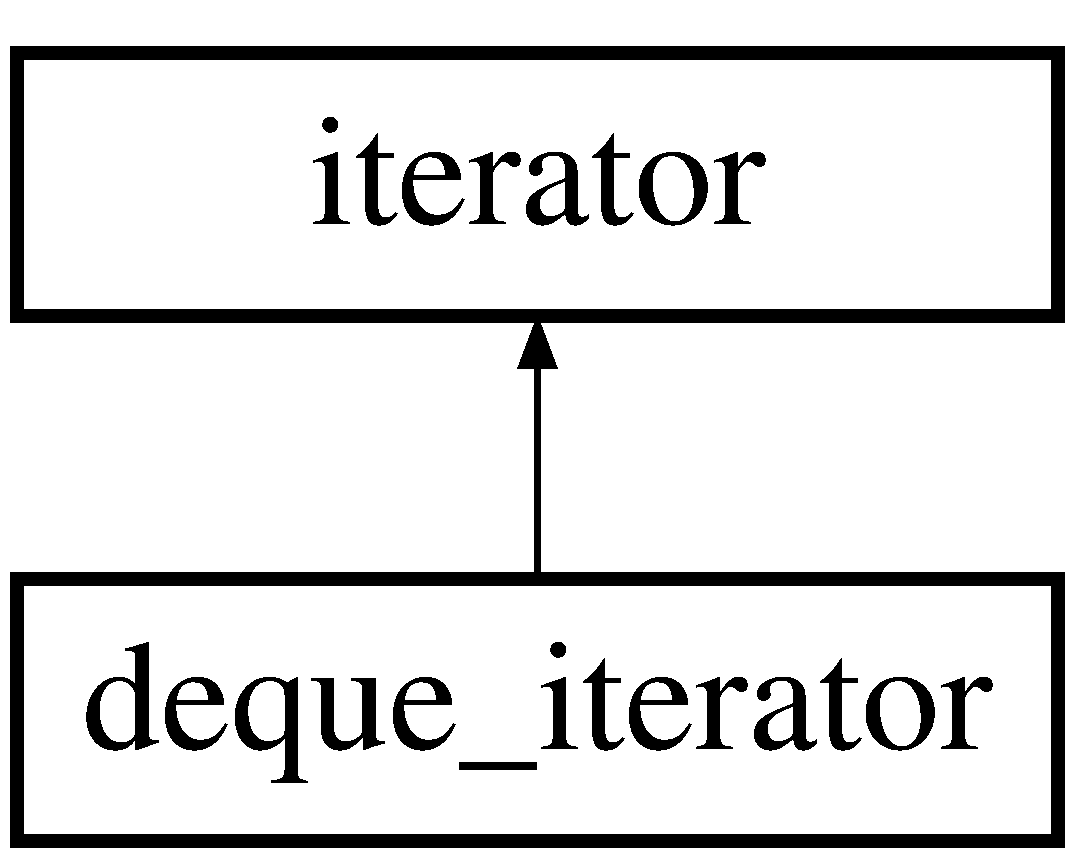
\includegraphics[height=2.000000cm]{classDeque_1_1deque__iterator}
\end{center}
\end{figure}
\subsection*{Public Member Functions}
\begin{DoxyCompactItemize}
\item 
\mbox{\hyperlink{classDeque_1_1deque__iterator_a3f358d267310712916ec18dc2cccd828}{deque\+\_\+iterator}} ()
\item 
\mbox{\hyperlink{classDeque_1_1deque__iterator_a89cd596f74f9635b2569c59d20fec624}{deque\+\_\+iterator}} (const \mbox{\hyperlink{classDeque_1_1deque__iterator}{deque\+\_\+iterator}} \&it)
\item 
\mbox{\hyperlink{classDeque_1_1deque__iterator_ad01c27b2cbcd73063836767611c03a3e}{deque\+\_\+iterator}} (\mbox{\hyperlink{classDeque}{Deque}}$<$ Value\+Type $>$ $\ast$dp, const typename std\+::deque$<$ Value\+Type $>$\+::iterator \&it)
\item 
Value\+Type \& \mbox{\hyperlink{classDeque_1_1deque__iterator_ae7b3826e734ec2f7c79f5196fad83989}{operator$\ast$}} ()
\item 
Value\+Type $\ast$ \mbox{\hyperlink{classDeque_1_1deque__iterator_a5ba42337ec7bae549bb135838933b0ea}{operator-\/$>$}} ()
\item 
unsigned int \mbox{\hyperlink{classDeque_1_1deque__iterator_a0aa696ccb72cbf928535d6b646bac1aa}{version}} () const
\end{DoxyCompactItemize}


\subsection{Constructor \& Destructor Documentation}
\mbox{\Hypertarget{classDeque_1_1deque__iterator_a3f358d267310712916ec18dc2cccd828}\label{classDeque_1_1deque__iterator_a3f358d267310712916ec18dc2cccd828}} 
\index{Deque\+::deque\+\_\+iterator@{Deque\+::deque\+\_\+iterator}!deque\+\_\+iterator@{deque\+\_\+iterator}}
\index{deque\+\_\+iterator@{deque\+\_\+iterator}!Deque\+::deque\+\_\+iterator@{Deque\+::deque\+\_\+iterator}}
\subsubsection{\texorpdfstring{deque\+\_\+iterator()}{deque\_iterator()}\hspace{0.1cm}{\footnotesize\ttfamily [1/3]}}
{\footnotesize\ttfamily \mbox{\hyperlink{classDeque_1_1deque__iterator}{deque\+\_\+iterator}} (\begin{DoxyParamCaption}{ }\end{DoxyParamCaption})\hspace{0.3cm}{\ttfamily [inline]}}

\mbox{\Hypertarget{classDeque_1_1deque__iterator_a89cd596f74f9635b2569c59d20fec624}\label{classDeque_1_1deque__iterator_a89cd596f74f9635b2569c59d20fec624}} 
\index{Deque\+::deque\+\_\+iterator@{Deque\+::deque\+\_\+iterator}!deque\+\_\+iterator@{deque\+\_\+iterator}}
\index{deque\+\_\+iterator@{deque\+\_\+iterator}!Deque\+::deque\+\_\+iterator@{Deque\+::deque\+\_\+iterator}}
\subsubsection{\texorpdfstring{deque\+\_\+iterator()}{deque\_iterator()}\hspace{0.1cm}{\footnotesize\ttfamily [2/3]}}
{\footnotesize\ttfamily \mbox{\hyperlink{classDeque_1_1deque__iterator}{deque\+\_\+iterator}} (\begin{DoxyParamCaption}\item[{const \mbox{\hyperlink{classDeque_1_1deque__iterator}{deque\+\_\+iterator}} \&}]{it }\end{DoxyParamCaption})\hspace{0.3cm}{\ttfamily [inline]}}

\mbox{\Hypertarget{classDeque_1_1deque__iterator_ad01c27b2cbcd73063836767611c03a3e}\label{classDeque_1_1deque__iterator_ad01c27b2cbcd73063836767611c03a3e}} 
\index{Deque\+::deque\+\_\+iterator@{Deque\+::deque\+\_\+iterator}!deque\+\_\+iterator@{deque\+\_\+iterator}}
\index{deque\+\_\+iterator@{deque\+\_\+iterator}!Deque\+::deque\+\_\+iterator@{Deque\+::deque\+\_\+iterator}}
\subsubsection{\texorpdfstring{deque\+\_\+iterator()}{deque\_iterator()}\hspace{0.1cm}{\footnotesize\ttfamily [3/3]}}
{\footnotesize\ttfamily \mbox{\hyperlink{classDeque_1_1deque__iterator}{deque\+\_\+iterator}} (\begin{DoxyParamCaption}\item[{\mbox{\hyperlink{classDeque}{Deque}}$<$ Value\+Type $>$ $\ast$}]{dp,  }\item[{const typename std\+::deque$<$ Value\+Type $>$\+::iterator \&}]{it }\end{DoxyParamCaption})\hspace{0.3cm}{\ttfamily [inline]}}



\subsection{Member Function Documentation}
\mbox{\Hypertarget{classDeque_1_1deque__iterator_ae7b3826e734ec2f7c79f5196fad83989}\label{classDeque_1_1deque__iterator_ae7b3826e734ec2f7c79f5196fad83989}} 
\index{Deque\+::deque\+\_\+iterator@{Deque\+::deque\+\_\+iterator}!operator$\ast$@{operator$\ast$}}
\index{operator$\ast$@{operator$\ast$}!Deque\+::deque\+\_\+iterator@{Deque\+::deque\+\_\+iterator}}
\subsubsection{\texorpdfstring{operator$\ast$()}{operator*()}}
{\footnotesize\ttfamily Value\+Type\& operator$\ast$ (\begin{DoxyParamCaption}{ }\end{DoxyParamCaption})\hspace{0.3cm}{\ttfamily [inline]}}

\mbox{\Hypertarget{classDeque_1_1deque__iterator_a5ba42337ec7bae549bb135838933b0ea}\label{classDeque_1_1deque__iterator_a5ba42337ec7bae549bb135838933b0ea}} 
\index{Deque\+::deque\+\_\+iterator@{Deque\+::deque\+\_\+iterator}!operator-\/$>$@{operator-\/$>$}}
\index{operator-\/$>$@{operator-\/$>$}!Deque\+::deque\+\_\+iterator@{Deque\+::deque\+\_\+iterator}}
\subsubsection{\texorpdfstring{operator-\/$>$()}{operator->()}}
{\footnotesize\ttfamily Value\+Type$\ast$ operator-\/$>$ (\begin{DoxyParamCaption}{ }\end{DoxyParamCaption})\hspace{0.3cm}{\ttfamily [inline]}}

\mbox{\Hypertarget{classDeque_1_1deque__iterator_a0aa696ccb72cbf928535d6b646bac1aa}\label{classDeque_1_1deque__iterator_a0aa696ccb72cbf928535d6b646bac1aa}} 
\index{Deque\+::deque\+\_\+iterator@{Deque\+::deque\+\_\+iterator}!version@{version}}
\index{version@{version}!Deque\+::deque\+\_\+iterator@{Deque\+::deque\+\_\+iterator}}
\subsubsection{\texorpdfstring{version()}{version()}}
{\footnotesize\ttfamily unsigned int version (\begin{DoxyParamCaption}{ }\end{DoxyParamCaption}) const\hspace{0.3cm}{\ttfamily [inline]}}


\hypertarget{classplainconsole_1_1EchoingStreambuf}{}\section{Echoing\+Streambuf Class Reference}
\label{classplainconsole_1_1EchoingStreambuf}\index{Echoing\+Streambuf@{Echoing\+Streambuf}}
Inheritance diagram for Echoing\+Streambuf\+:\begin{figure}[H]
\begin{center}
\leavevmode
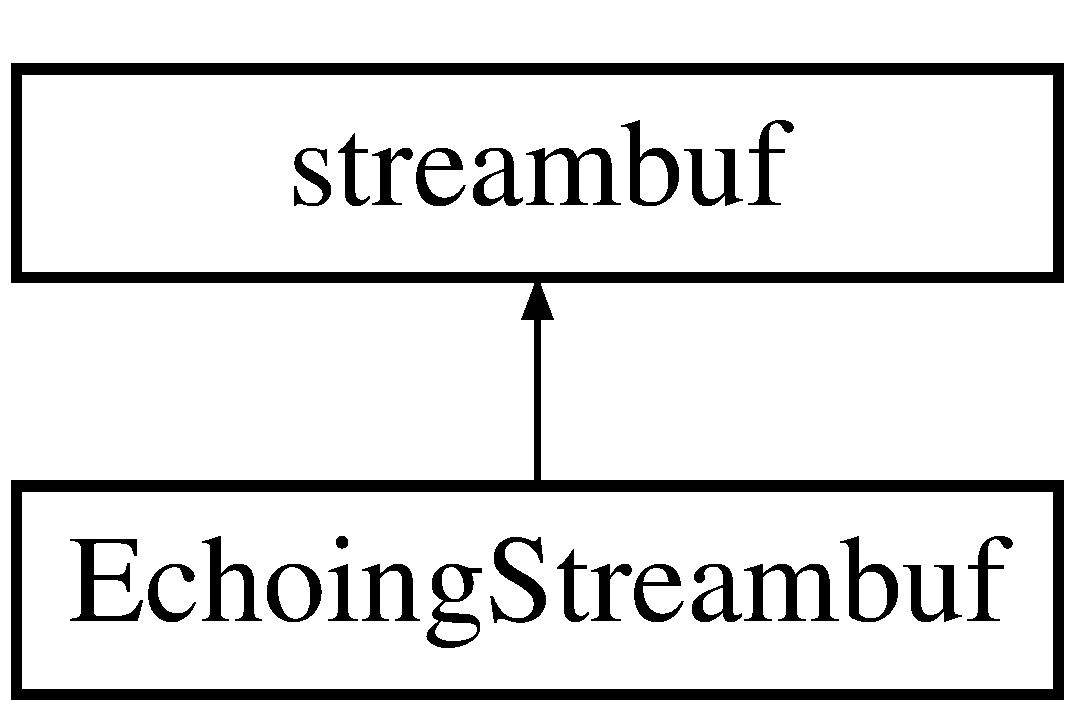
\includegraphics[height=2.000000cm]{classplainconsole_1_1EchoingStreambuf}
\end{center}
\end{figure}
\subsection*{Public Member Functions}
\begin{DoxyCompactItemize}
\item 
\mbox{\hyperlink{classplainconsole_1_1EchoingStreambuf_ad1ecfc2b740cbc9828057697efbbba01}{Echoing\+Streambuf}} (std\+::streambuf \&buf, std\+::ostream \&out)
\item 
\mbox{\hyperlink{classplainconsole_1_1EchoingStreambuf_a6f11f87ad08e1ac6e93f18c5204003f9}{$\sim$\+Echoing\+Streambuf}} ()
\item 
virtual int \mbox{\hyperlink{classplainconsole_1_1EchoingStreambuf_adccb3cd5475ba3c83bc2b0a8cbd731c0}{overflow}} (int ch=E\+OF)
\item 
virtual void \mbox{\hyperlink{classplainconsole_1_1EchoingStreambuf_a86854533b6acdbe6b6d23051f53c64f6}{set\+Output\+Limit}} (int limit)
\item 
virtual int \mbox{\hyperlink{classplainconsole_1_1EchoingStreambuf_a810a727ce5554d3178e17b6bc55025dd}{sync}} ()
\item 
virtual int \mbox{\hyperlink{classplainconsole_1_1EchoingStreambuf_aeb6918bd44153b257e097e2d2ef370ef}{underflow}} ()
\end{DoxyCompactItemize}


\subsection{Constructor \& Destructor Documentation}
\mbox{\Hypertarget{classplainconsole_1_1EchoingStreambuf_ad1ecfc2b740cbc9828057697efbbba01}\label{classplainconsole_1_1EchoingStreambuf_ad1ecfc2b740cbc9828057697efbbba01}} 
\index{plainconsole\+::\+Echoing\+Streambuf@{plainconsole\+::\+Echoing\+Streambuf}!Echoing\+Streambuf@{Echoing\+Streambuf}}
\index{Echoing\+Streambuf@{Echoing\+Streambuf}!plainconsole\+::\+Echoing\+Streambuf@{plainconsole\+::\+Echoing\+Streambuf}}
\subsubsection{\texorpdfstring{Echoing\+Streambuf()}{EchoingStreambuf()}}
{\footnotesize\ttfamily \mbox{\hyperlink{classplainconsole_1_1EchoingStreambuf}{Echoing\+Streambuf}} (\begin{DoxyParamCaption}\item[{std\+::streambuf \&}]{buf,  }\item[{std\+::ostream \&}]{out }\end{DoxyParamCaption})\hspace{0.3cm}{\ttfamily [inline]}}

\mbox{\Hypertarget{classplainconsole_1_1EchoingStreambuf_a6f11f87ad08e1ac6e93f18c5204003f9}\label{classplainconsole_1_1EchoingStreambuf_a6f11f87ad08e1ac6e93f18c5204003f9}} 
\index{plainconsole\+::\+Echoing\+Streambuf@{plainconsole\+::\+Echoing\+Streambuf}!````~Echoing\+Streambuf@{$\sim$\+Echoing\+Streambuf}}
\index{````~Echoing\+Streambuf@{$\sim$\+Echoing\+Streambuf}!plainconsole\+::\+Echoing\+Streambuf@{plainconsole\+::\+Echoing\+Streambuf}}
\subsubsection{\texorpdfstring{$\sim$\+Echoing\+Streambuf()}{~EchoingStreambuf()}}
{\footnotesize\ttfamily $\sim$\mbox{\hyperlink{classplainconsole_1_1EchoingStreambuf}{Echoing\+Streambuf}} (\begin{DoxyParamCaption}{ }\end{DoxyParamCaption})\hspace{0.3cm}{\ttfamily [inline]}}



\subsection{Member Function Documentation}
\mbox{\Hypertarget{classplainconsole_1_1EchoingStreambuf_adccb3cd5475ba3c83bc2b0a8cbd731c0}\label{classplainconsole_1_1EchoingStreambuf_adccb3cd5475ba3c83bc2b0a8cbd731c0}} 
\index{plainconsole\+::\+Echoing\+Streambuf@{plainconsole\+::\+Echoing\+Streambuf}!overflow@{overflow}}
\index{overflow@{overflow}!plainconsole\+::\+Echoing\+Streambuf@{plainconsole\+::\+Echoing\+Streambuf}}
\subsubsection{\texorpdfstring{overflow()}{overflow()}}
{\footnotesize\ttfamily virtual int overflow (\begin{DoxyParamCaption}\item[{int}]{ch = {\ttfamily EOF} }\end{DoxyParamCaption})\hspace{0.3cm}{\ttfamily [inline]}, {\ttfamily [virtual]}}

\mbox{\Hypertarget{classplainconsole_1_1EchoingStreambuf_a86854533b6acdbe6b6d23051f53c64f6}\label{classplainconsole_1_1EchoingStreambuf_a86854533b6acdbe6b6d23051f53c64f6}} 
\index{plainconsole\+::\+Echoing\+Streambuf@{plainconsole\+::\+Echoing\+Streambuf}!set\+Output\+Limit@{set\+Output\+Limit}}
\index{set\+Output\+Limit@{set\+Output\+Limit}!plainconsole\+::\+Echoing\+Streambuf@{plainconsole\+::\+Echoing\+Streambuf}}
\subsubsection{\texorpdfstring{set\+Output\+Limit()}{setOutputLimit()}}
{\footnotesize\ttfamily virtual void set\+Output\+Limit (\begin{DoxyParamCaption}\item[{int}]{limit }\end{DoxyParamCaption})\hspace{0.3cm}{\ttfamily [inline]}, {\ttfamily [virtual]}}

\mbox{\Hypertarget{classplainconsole_1_1EchoingStreambuf_a810a727ce5554d3178e17b6bc55025dd}\label{classplainconsole_1_1EchoingStreambuf_a810a727ce5554d3178e17b6bc55025dd}} 
\index{plainconsole\+::\+Echoing\+Streambuf@{plainconsole\+::\+Echoing\+Streambuf}!sync@{sync}}
\index{sync@{sync}!plainconsole\+::\+Echoing\+Streambuf@{plainconsole\+::\+Echoing\+Streambuf}}
\subsubsection{\texorpdfstring{sync()}{sync()}}
{\footnotesize\ttfamily virtual int sync (\begin{DoxyParamCaption}{ }\end{DoxyParamCaption})\hspace{0.3cm}{\ttfamily [inline]}, {\ttfamily [virtual]}}

\mbox{\Hypertarget{classplainconsole_1_1EchoingStreambuf_aeb6918bd44153b257e097e2d2ef370ef}\label{classplainconsole_1_1EchoingStreambuf_aeb6918bd44153b257e097e2d2ef370ef}} 
\index{plainconsole\+::\+Echoing\+Streambuf@{plainconsole\+::\+Echoing\+Streambuf}!underflow@{underflow}}
\index{underflow@{underflow}!plainconsole\+::\+Echoing\+Streambuf@{plainconsole\+::\+Echoing\+Streambuf}}
\subsubsection{\texorpdfstring{underflow()}{underflow()}}
{\footnotesize\ttfamily virtual int underflow (\begin{DoxyParamCaption}{ }\end{DoxyParamCaption})\hspace{0.3cm}{\ttfamily [inline]}, {\ttfamily [virtual]}}


\hypertarget{classstanfordcpplib_1_1EchoInputStreambuf}{}\section{Echo\+Input\+Streambuf Class Reference}
\label{classstanfordcpplib_1_1EchoInputStreambuf}\index{Echo\+Input\+Streambuf@{Echo\+Input\+Streambuf}}


{\ttfamily \#include $<$echoinputstreambuf.\+h$>$}

Inheritance diagram for Echo\+Input\+Streambuf\+:\begin{figure}[H]
\begin{center}
\leavevmode
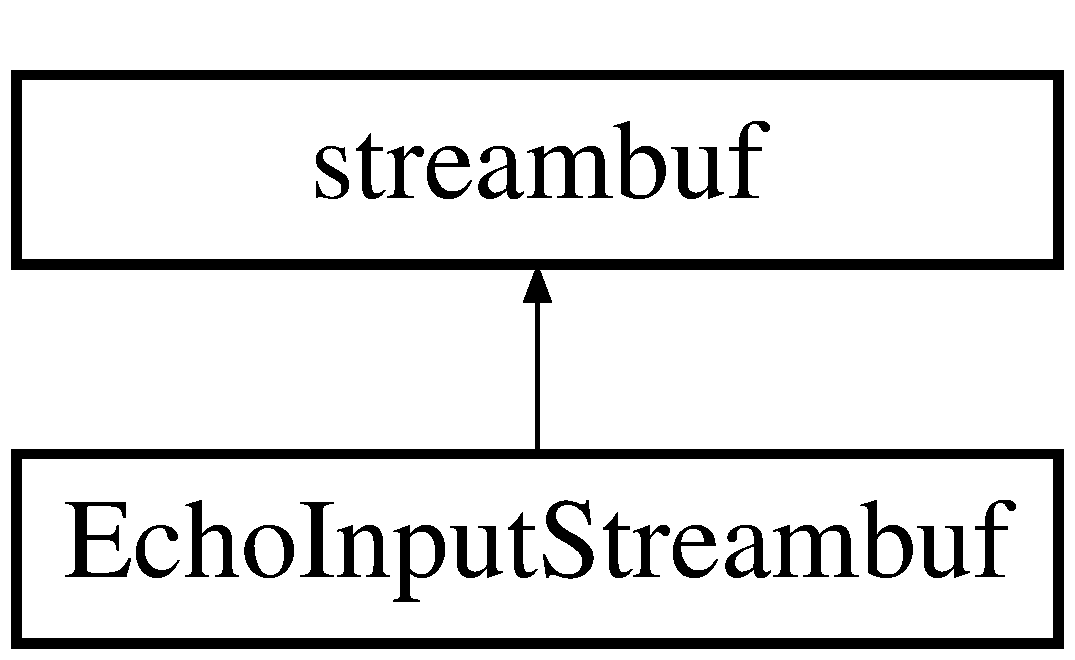
\includegraphics[height=2.000000cm]{classstanfordcpplib_1_1EchoInputStreambuf}
\end{center}
\end{figure}
\subsection*{Public Member Functions}
\begin{DoxyCompactItemize}
\item 
\mbox{\hyperlink{classstanfordcpplib_1_1EchoInputStreambuf_a708155d9f25b8e73432c541e5a7d0f07}{Echo\+Input\+Streambuf}} (std\+::streambuf $\ast$source)
\item 
\mbox{\hyperlink{classstanfordcpplib_1_1EchoInputStreambuf_abf31cdf423a80fa9a3b5c65dd20378fd}{Echo\+Input\+Streambuf}} (const std\+::string \&input)
\item 
virtual \mbox{\hyperlink{classstanfordcpplib_1_1EchoInputStreambuf_abbb0d282d20bed4b6b5d8c700c312344}{$\sim$\+Echo\+Input\+Streambuf}} ()
\item 
virtual int \mbox{\hyperlink{classstanfordcpplib_1_1EchoInputStreambuf_a71cbc6b1ec560d3788dac4c02e9328da}{overflow}} (int)
\item 
virtual std\+::streambuf $\ast$ \mbox{\hyperlink{classstanfordcpplib_1_1EchoInputStreambuf_adab87f356f20a3d6ac970facd081f967}{setbuf}} (char $\ast$p, std\+::streamsize len)
\item 
virtual int \mbox{\hyperlink{classstanfordcpplib_1_1EchoInputStreambuf_a810a727ce5554d3178e17b6bc55025dd}{sync}} ()
\item 
virtual int \mbox{\hyperlink{classstanfordcpplib_1_1EchoInputStreambuf_aeb6918bd44153b257e097e2d2ef370ef}{underflow}} ()
\end{DoxyCompactItemize}


\subsection{Constructor \& Destructor Documentation}
\mbox{\Hypertarget{classstanfordcpplib_1_1EchoInputStreambuf_a708155d9f25b8e73432c541e5a7d0f07}\label{classstanfordcpplib_1_1EchoInputStreambuf_a708155d9f25b8e73432c541e5a7d0f07}} 
\index{stanfordcpplib\+::\+Echo\+Input\+Streambuf@{stanfordcpplib\+::\+Echo\+Input\+Streambuf}!Echo\+Input\+Streambuf@{Echo\+Input\+Streambuf}}
\index{Echo\+Input\+Streambuf@{Echo\+Input\+Streambuf}!stanfordcpplib\+::\+Echo\+Input\+Streambuf@{stanfordcpplib\+::\+Echo\+Input\+Streambuf}}
\subsubsection{\texorpdfstring{Echo\+Input\+Streambuf()}{EchoInputStreambuf()}\hspace{0.1cm}{\footnotesize\ttfamily [1/2]}}
{\footnotesize\ttfamily \mbox{\hyperlink{classstanfordcpplib_1_1EchoInputStreambuf}{Echo\+Input\+Streambuf}} (\begin{DoxyParamCaption}\item[{std\+::streambuf $\ast$}]{source }\end{DoxyParamCaption})\hspace{0.3cm}{\ttfamily [inline]}}

\mbox{\Hypertarget{classstanfordcpplib_1_1EchoInputStreambuf_abf31cdf423a80fa9a3b5c65dd20378fd}\label{classstanfordcpplib_1_1EchoInputStreambuf_abf31cdf423a80fa9a3b5c65dd20378fd}} 
\index{stanfordcpplib\+::\+Echo\+Input\+Streambuf@{stanfordcpplib\+::\+Echo\+Input\+Streambuf}!Echo\+Input\+Streambuf@{Echo\+Input\+Streambuf}}
\index{Echo\+Input\+Streambuf@{Echo\+Input\+Streambuf}!stanfordcpplib\+::\+Echo\+Input\+Streambuf@{stanfordcpplib\+::\+Echo\+Input\+Streambuf}}
\subsubsection{\texorpdfstring{Echo\+Input\+Streambuf()}{EchoInputStreambuf()}\hspace{0.1cm}{\footnotesize\ttfamily [2/2]}}
{\footnotesize\ttfamily \mbox{\hyperlink{classstanfordcpplib_1_1EchoInputStreambuf}{Echo\+Input\+Streambuf}} (\begin{DoxyParamCaption}\item[{const std\+::string \&}]{input }\end{DoxyParamCaption})\hspace{0.3cm}{\ttfamily [inline]}}

\mbox{\Hypertarget{classstanfordcpplib_1_1EchoInputStreambuf_abbb0d282d20bed4b6b5d8c700c312344}\label{classstanfordcpplib_1_1EchoInputStreambuf_abbb0d282d20bed4b6b5d8c700c312344}} 
\index{stanfordcpplib\+::\+Echo\+Input\+Streambuf@{stanfordcpplib\+::\+Echo\+Input\+Streambuf}!````~Echo\+Input\+Streambuf@{$\sim$\+Echo\+Input\+Streambuf}}
\index{````~Echo\+Input\+Streambuf@{$\sim$\+Echo\+Input\+Streambuf}!stanfordcpplib\+::\+Echo\+Input\+Streambuf@{stanfordcpplib\+::\+Echo\+Input\+Streambuf}}
\subsubsection{\texorpdfstring{$\sim$\+Echo\+Input\+Streambuf()}{~EchoInputStreambuf()}}
{\footnotesize\ttfamily virtual $\sim$\mbox{\hyperlink{classstanfordcpplib_1_1EchoInputStreambuf}{Echo\+Input\+Streambuf}} (\begin{DoxyParamCaption}{ }\end{DoxyParamCaption})\hspace{0.3cm}{\ttfamily [inline]}, {\ttfamily [virtual]}}



\subsection{Member Function Documentation}
\mbox{\Hypertarget{classstanfordcpplib_1_1EchoInputStreambuf_a71cbc6b1ec560d3788dac4c02e9328da}\label{classstanfordcpplib_1_1EchoInputStreambuf_a71cbc6b1ec560d3788dac4c02e9328da}} 
\index{stanfordcpplib\+::\+Echo\+Input\+Streambuf@{stanfordcpplib\+::\+Echo\+Input\+Streambuf}!overflow@{overflow}}
\index{overflow@{overflow}!stanfordcpplib\+::\+Echo\+Input\+Streambuf@{stanfordcpplib\+::\+Echo\+Input\+Streambuf}}
\subsubsection{\texorpdfstring{overflow()}{overflow()}}
{\footnotesize\ttfamily virtual int overflow (\begin{DoxyParamCaption}\item[{int}]{ }\end{DoxyParamCaption})\hspace{0.3cm}{\ttfamily [inline]}, {\ttfamily [virtual]}}

\mbox{\Hypertarget{classstanfordcpplib_1_1EchoInputStreambuf_adab87f356f20a3d6ac970facd081f967}\label{classstanfordcpplib_1_1EchoInputStreambuf_adab87f356f20a3d6ac970facd081f967}} 
\index{stanfordcpplib\+::\+Echo\+Input\+Streambuf@{stanfordcpplib\+::\+Echo\+Input\+Streambuf}!setbuf@{setbuf}}
\index{setbuf@{setbuf}!stanfordcpplib\+::\+Echo\+Input\+Streambuf@{stanfordcpplib\+::\+Echo\+Input\+Streambuf}}
\subsubsection{\texorpdfstring{setbuf()}{setbuf()}}
{\footnotesize\ttfamily virtual std\+::streambuf$\ast$ setbuf (\begin{DoxyParamCaption}\item[{char $\ast$}]{p,  }\item[{std\+::streamsize}]{len }\end{DoxyParamCaption})\hspace{0.3cm}{\ttfamily [inline]}, {\ttfamily [virtual]}}

\mbox{\Hypertarget{classstanfordcpplib_1_1EchoInputStreambuf_a810a727ce5554d3178e17b6bc55025dd}\label{classstanfordcpplib_1_1EchoInputStreambuf_a810a727ce5554d3178e17b6bc55025dd}} 
\index{stanfordcpplib\+::\+Echo\+Input\+Streambuf@{stanfordcpplib\+::\+Echo\+Input\+Streambuf}!sync@{sync}}
\index{sync@{sync}!stanfordcpplib\+::\+Echo\+Input\+Streambuf@{stanfordcpplib\+::\+Echo\+Input\+Streambuf}}
\subsubsection{\texorpdfstring{sync()}{sync()}}
{\footnotesize\ttfamily virtual int sync (\begin{DoxyParamCaption}{ }\end{DoxyParamCaption})\hspace{0.3cm}{\ttfamily [inline]}, {\ttfamily [virtual]}}

\mbox{\Hypertarget{classstanfordcpplib_1_1EchoInputStreambuf_aeb6918bd44153b257e097e2d2ef370ef}\label{classstanfordcpplib_1_1EchoInputStreambuf_aeb6918bd44153b257e097e2d2ef370ef}} 
\index{stanfordcpplib\+::\+Echo\+Input\+Streambuf@{stanfordcpplib\+::\+Echo\+Input\+Streambuf}!underflow@{underflow}}
\index{underflow@{underflow}!stanfordcpplib\+::\+Echo\+Input\+Streambuf@{stanfordcpplib\+::\+Echo\+Input\+Streambuf}}
\subsubsection{\texorpdfstring{underflow()}{underflow()}}
{\footnotesize\ttfamily virtual int underflow (\begin{DoxyParamCaption}{ }\end{DoxyParamCaption})\hspace{0.3cm}{\ttfamily [inline]}, {\ttfamily [virtual]}}


\hypertarget{structstacktrace_1_1entry}{}\section{entry Struct Reference}
\label{structstacktrace_1_1entry}\index{entry@{entry}}


Call-\/stack entry datastructure.  




{\ttfamily \#include $<$call\+\_\+stack.\+h$>$}

\subsection*{Public Member Functions}
\begin{DoxyCompactItemize}
\item 
\mbox{\hyperlink{structstacktrace_1_1entry_a59990719363a79bbd250a392185b8e75}{entry}} ()
\begin{DoxyCompactList}\small\item\em Default constructor that clears all fields. \end{DoxyCompactList}\item 
std\+::string \mbox{\hyperlink{structstacktrace_1_1entry_a1fe5121d6528fdea3f243321b3fa3a49}{to\+String}} () const
\begin{DoxyCompactList}\small\item\em Serialize entry into a text string. \end{DoxyCompactList}\end{DoxyCompactItemize}
\subsection*{Public Attributes}
\begin{DoxyCompactItemize}
\item 
void $\ast$ \mbox{\hyperlink{structstacktrace_1_1entry_ab96816d317aa5196e2ef198d9a8d621b}{address}}
\item 
void $\ast$ \mbox{\hyperlink{structstacktrace_1_1entry_ae212b77c2997320c14de82a65d4af735}{address2}}
\item 
std\+::string \mbox{\hyperlink{structstacktrace_1_1entry_aefc35c7944eed319c89bc1b399f0eb67}{file}}
\item 
std\+::string \mbox{\hyperlink{structstacktrace_1_1entry_adf44acd4aa201051e648ac3c09c2e20f}{function}}
\item 
size\+\_\+t \mbox{\hyperlink{structstacktrace_1_1entry_a178448bb4d6d83c01610fec5d40f7c5c}{line}}
\item 
std\+::string \mbox{\hyperlink{structstacktrace_1_1entry_a8bd970c62f0d156a81e10b5d12bdd0fe}{line\+Str}}
\end{DoxyCompactItemize}


\subsection{Detailed Description}
Call-\/stack entry datastructure. 



\subsection{Constructor \& Destructor Documentation}
\mbox{\Hypertarget{structstacktrace_1_1entry_a59990719363a79bbd250a392185b8e75}\label{structstacktrace_1_1entry_a59990719363a79bbd250a392185b8e75}} 
\index{stacktrace\+::entry@{stacktrace\+::entry}!entry@{entry}}
\index{entry@{entry}!stacktrace\+::entry@{stacktrace\+::entry}}
\subsubsection{\texorpdfstring{entry()}{entry()}}
{\footnotesize\ttfamily \mbox{\hyperlink{structstacktrace_1_1entry}{entry}} (\begin{DoxyParamCaption}{ }\end{DoxyParamCaption})\hspace{0.3cm}{\ttfamily [inline]}}



Default constructor that clears all fields. 



\subsection{Member Function Documentation}
\mbox{\Hypertarget{structstacktrace_1_1entry_a1fe5121d6528fdea3f243321b3fa3a49}\label{structstacktrace_1_1entry_a1fe5121d6528fdea3f243321b3fa3a49}} 
\index{stacktrace\+::entry@{stacktrace\+::entry}!to\+String@{to\+String}}
\index{to\+String@{to\+String}!stacktrace\+::entry@{stacktrace\+::entry}}
\subsubsection{\texorpdfstring{to\+String()}{toString()}}
{\footnotesize\ttfamily std\+::string to\+String (\begin{DoxyParamCaption}{ }\end{DoxyParamCaption}) const\hspace{0.3cm}{\ttfamily [inline]}}



Serialize entry into a text string. 



\subsection{Member Data Documentation}
\mbox{\Hypertarget{structstacktrace_1_1entry_ab96816d317aa5196e2ef198d9a8d621b}\label{structstacktrace_1_1entry_ab96816d317aa5196e2ef198d9a8d621b}} 
\index{stacktrace\+::entry@{stacktrace\+::entry}!address@{address}}
\index{address@{address}!stacktrace\+::entry@{stacktrace\+::entry}}
\subsubsection{\texorpdfstring{address}{address}}
{\footnotesize\ttfamily void$\ast$ address}

\mbox{\Hypertarget{structstacktrace_1_1entry_ae212b77c2997320c14de82a65d4af735}\label{structstacktrace_1_1entry_ae212b77c2997320c14de82a65d4af735}} 
\index{stacktrace\+::entry@{stacktrace\+::entry}!address2@{address2}}
\index{address2@{address2}!stacktrace\+::entry@{stacktrace\+::entry}}
\subsubsection{\texorpdfstring{address2}{address2}}
{\footnotesize\ttfamily void$\ast$ address2}

\mbox{\Hypertarget{structstacktrace_1_1entry_aefc35c7944eed319c89bc1b399f0eb67}\label{structstacktrace_1_1entry_aefc35c7944eed319c89bc1b399f0eb67}} 
\index{stacktrace\+::entry@{stacktrace\+::entry}!file@{file}}
\index{file@{file}!stacktrace\+::entry@{stacktrace\+::entry}}
\subsubsection{\texorpdfstring{file}{file}}
{\footnotesize\ttfamily std\+::string file}

\mbox{\Hypertarget{structstacktrace_1_1entry_adf44acd4aa201051e648ac3c09c2e20f}\label{structstacktrace_1_1entry_adf44acd4aa201051e648ac3c09c2e20f}} 
\index{stacktrace\+::entry@{stacktrace\+::entry}!function@{function}}
\index{function@{function}!stacktrace\+::entry@{stacktrace\+::entry}}
\subsubsection{\texorpdfstring{function}{function}}
{\footnotesize\ttfamily std\+::string function}

\mbox{\Hypertarget{structstacktrace_1_1entry_a178448bb4d6d83c01610fec5d40f7c5c}\label{structstacktrace_1_1entry_a178448bb4d6d83c01610fec5d40f7c5c}} 
\index{stacktrace\+::entry@{stacktrace\+::entry}!line@{line}}
\index{line@{line}!stacktrace\+::entry@{stacktrace\+::entry}}
\subsubsection{\texorpdfstring{line}{line}}
{\footnotesize\ttfamily size\+\_\+t line}

\mbox{\Hypertarget{structstacktrace_1_1entry_a8bd970c62f0d156a81e10b5d12bdd0fe}\label{structstacktrace_1_1entry_a8bd970c62f0d156a81e10b5d12bdd0fe}} 
\index{stacktrace\+::entry@{stacktrace\+::entry}!line\+Str@{line\+Str}}
\index{line\+Str@{line\+Str}!stacktrace\+::entry@{stacktrace\+::entry}}
\subsubsection{\texorpdfstring{line\+Str}{lineStr}}
{\footnotesize\ttfamily std\+::string line\+Str}


\hypertarget{classErrorException}{}\section{Error\+Exception Class Reference}
\label{classErrorException}\index{Error\+Exception@{Error\+Exception}}


~\newline
 This exception is thrown by calls to the {\ttfamily error} function.  




{\ttfamily \#include $<$error.\+h$>$}

Inheritance diagram for Error\+Exception\+:\begin{figure}[H]
\begin{center}
\leavevmode
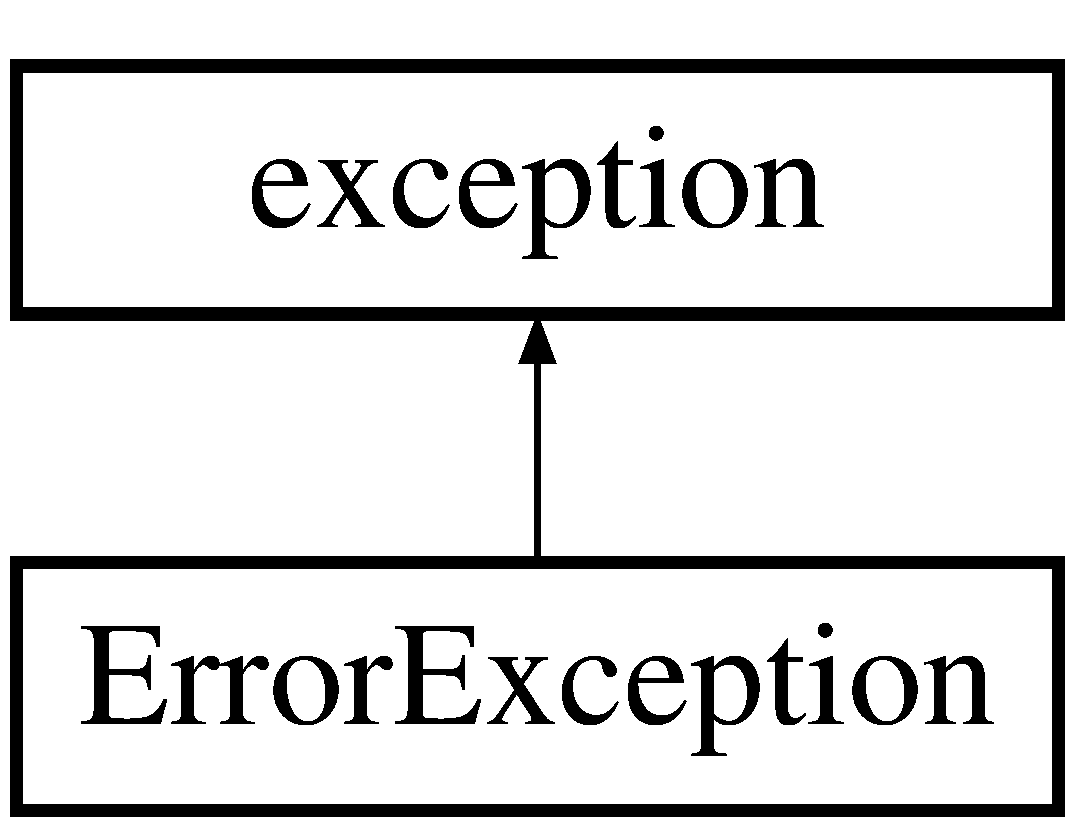
\includegraphics[height=2.000000cm]{classErrorException}
\end{center}
\end{figure}
\subsection*{Public Member Functions}
\begin{DoxyCompactItemize}
\item 
\mbox{\hyperlink{classErrorException_a4f422b01fff7cc16eea81e00638f44d2}{Error\+Exception}} (std\+::string msg)
\begin{DoxyCompactList}\small\item\em Creates a new \mbox{\hyperlink{classErrorException}{Error\+Exception}} with the given error message. \end{DoxyCompactList}\item 
virtual \mbox{\hyperlink{classErrorException_a61c8f6114a93ea2ff11a5f08e3640d76}{$\sim$\+Error\+Exception}} () noexcept=default
\begin{DoxyCompactList}\small\item\em Frees any memory allocated by the exception. \end{DoxyCompactList}\item 
virtual void \mbox{\hyperlink{classErrorException_af1e6a5fb477a95a876e86ceadf065ffd}{dump}} () const
\begin{DoxyCompactList}\small\item\em Prints the exception to the standard error stream (cerr), including its message and stack trace if any. \end{DoxyCompactList}\item 
virtual void \mbox{\hyperlink{classErrorException_a277bc85222ba9a7d0fd47fd10d44d115}{dump}} (std\+::ostream \&out) const
\begin{DoxyCompactList}\small\item\em Prints the exception to the given output stream, including its message and stack trace if any. \end{DoxyCompactList}\item 
virtual std\+::string \mbox{\hyperlink{classErrorException_ae6faf7d90a6394517c0328748c99ec1d}{get\+Kind}} () const
\begin{DoxyCompactList}\small\item\em Returns what kind of exception this is. \end{DoxyCompactList}\item 
virtual std\+::string \mbox{\hyperlink{classErrorException_a1c1cc72e6e4257dbd29ff04a23973008}{get\+Message}} () const
\begin{DoxyCompactList}\small\item\em Returns the exception\textquotesingle{}s error message as passed to its constructor. \end{DoxyCompactList}\item 
virtual std\+::string \mbox{\hyperlink{classErrorException_a79ec2353dbf71c4867c65c6c6df5dfce}{get\+Stack\+Trace}} () const
\begin{DoxyCompactList}\small\item\em Returns a stack trace for this exception as a multi-\/line string. \end{DoxyCompactList}\item 
virtual bool \mbox{\hyperlink{classErrorException_ae7ccac41c27ba02a30bdec527db0a639}{has\+Stack\+Trace}} () const
\begin{DoxyCompactList}\small\item\em Returns whether this exception has a non-\/empty stack trace. \end{DoxyCompactList}\item 
void \mbox{\hyperlink{classErrorException_a896ae13e5a5b1b89f058f7de9697c3cd}{set\+Kind}} (const std\+::string \&kind)
\begin{DoxyCompactList}\small\item\em Sets what kind of exception this is. \end{DoxyCompactList}\item 
virtual const char $\ast$ \mbox{\hyperlink{classErrorException_a576a441c2b1e2f01d271e237b314eac3}{what}} () const noexcept
\begin{DoxyCompactList}\small\item\em Returns the exception\textquotesingle{}s error message as a C string. \end{DoxyCompactList}\end{DoxyCompactItemize}
\subsection*{Protected Member Functions}
\begin{DoxyCompactItemize}
\item 
void \mbox{\hyperlink{classErrorException_aaac5126664da146aa7290235ac7b1d07}{set\+Stack\+Trace}} (const std\+::string \&stack\+Trace)
\begin{DoxyCompactList}\small\item\em Sets this exception\textquotesingle{}s stack trace to the given multi-\/line string. \end{DoxyCompactList}\end{DoxyCompactItemize}


\subsection{Detailed Description}
~\newline
 This exception is thrown by calls to the {\ttfamily error} function. 

Typical code for catching errors looks like this\+:


\begin{DoxyPre}
     try \{
        ... code in which an error might occur ...
     \} catch (\mbox{\hyperlink{classErrorException}{ErrorException}}\& ex) \{
        ... code to handle the error condition ...
     \}
*\end{DoxyPre}


If an {\ttfamily \mbox{\hyperlink{classErrorException}{Error\+Exception}}} is thrown at any point in the range of the {\ttfamily try} (including in functions called from that code), control will jump immediately to the error handler. 

\subsection{Constructor \& Destructor Documentation}
\mbox{\Hypertarget{classErrorException_a4f422b01fff7cc16eea81e00638f44d2}\label{classErrorException_a4f422b01fff7cc16eea81e00638f44d2}} 
\index{Error\+Exception@{Error\+Exception}!Error\+Exception@{Error\+Exception}}
\index{Error\+Exception@{Error\+Exception}!Error\+Exception@{Error\+Exception}}
\subsubsection{\texorpdfstring{Error\+Exception()}{ErrorException()}}
{\footnotesize\ttfamily \mbox{\hyperlink{classErrorException}{Error\+Exception}} (\begin{DoxyParamCaption}\item[{std\+::string}]{msg }\end{DoxyParamCaption})}



Creates a new \mbox{\hyperlink{classErrorException}{Error\+Exception}} with the given error message. 

\mbox{\Hypertarget{classErrorException_a61c8f6114a93ea2ff11a5f08e3640d76}\label{classErrorException_a61c8f6114a93ea2ff11a5f08e3640d76}} 
\index{Error\+Exception@{Error\+Exception}!````~Error\+Exception@{$\sim$\+Error\+Exception}}
\index{````~Error\+Exception@{$\sim$\+Error\+Exception}!Error\+Exception@{Error\+Exception}}
\subsubsection{\texorpdfstring{$\sim$\+Error\+Exception()}{~ErrorException()}}
{\footnotesize\ttfamily virtual $\sim$\mbox{\hyperlink{classErrorException}{Error\+Exception}} (\begin{DoxyParamCaption}{ }\end{DoxyParamCaption})\hspace{0.3cm}{\ttfamily [virtual]}, {\ttfamily [default]}, {\ttfamily [noexcept]}}



Frees any memory allocated by the exception. 



\subsection{Member Function Documentation}
\mbox{\Hypertarget{classErrorException_af1e6a5fb477a95a876e86ceadf065ffd}\label{classErrorException_af1e6a5fb477a95a876e86ceadf065ffd}} 
\index{Error\+Exception@{Error\+Exception}!dump@{dump}}
\index{dump@{dump}!Error\+Exception@{Error\+Exception}}
\subsubsection{\texorpdfstring{dump()}{dump()}\hspace{0.1cm}{\footnotesize\ttfamily [1/2]}}
{\footnotesize\ttfamily void dump (\begin{DoxyParamCaption}{ }\end{DoxyParamCaption}) const\hspace{0.3cm}{\ttfamily [virtual]}}



Prints the exception to the standard error stream (cerr), including its message and stack trace if any. 

\mbox{\Hypertarget{classErrorException_a277bc85222ba9a7d0fd47fd10d44d115}\label{classErrorException_a277bc85222ba9a7d0fd47fd10d44d115}} 
\index{Error\+Exception@{Error\+Exception}!dump@{dump}}
\index{dump@{dump}!Error\+Exception@{Error\+Exception}}
\subsubsection{\texorpdfstring{dump()}{dump()}\hspace{0.1cm}{\footnotesize\ttfamily [2/2]}}
{\footnotesize\ttfamily void dump (\begin{DoxyParamCaption}\item[{std\+::ostream \&}]{out }\end{DoxyParamCaption}) const\hspace{0.3cm}{\ttfamily [virtual]}}



Prints the exception to the given output stream, including its message and stack trace if any. 

\mbox{\Hypertarget{classErrorException_ae6faf7d90a6394517c0328748c99ec1d}\label{classErrorException_ae6faf7d90a6394517c0328748c99ec1d}} 
\index{Error\+Exception@{Error\+Exception}!get\+Kind@{get\+Kind}}
\index{get\+Kind@{get\+Kind}!Error\+Exception@{Error\+Exception}}
\subsubsection{\texorpdfstring{get\+Kind()}{getKind()}}
{\footnotesize\ttfamily std\+::string get\+Kind (\begin{DoxyParamCaption}{ }\end{DoxyParamCaption}) const\hspace{0.3cm}{\ttfamily [virtual]}}



Returns what kind of exception this is. 

In general this returns \char`\"{}error\char`\"{}, but in some cases we catch other kinds of exceptions (like thrown ints or strings) and wrap them up as Error\+Exceptions. In such cases, the kind will be \char`\"{}int\char`\"{} or \char`\"{}string\char`\"{} etc. \mbox{\Hypertarget{classErrorException_a1c1cc72e6e4257dbd29ff04a23973008}\label{classErrorException_a1c1cc72e6e4257dbd29ff04a23973008}} 
\index{Error\+Exception@{Error\+Exception}!get\+Message@{get\+Message}}
\index{get\+Message@{get\+Message}!Error\+Exception@{Error\+Exception}}
\subsubsection{\texorpdfstring{get\+Message()}{getMessage()}}
{\footnotesize\ttfamily std\+::string get\+Message (\begin{DoxyParamCaption}{ }\end{DoxyParamCaption}) const\hspace{0.3cm}{\ttfamily [virtual]}}



Returns the exception\textquotesingle{}s error message as passed to its constructor. 

\mbox{\Hypertarget{classErrorException_a79ec2353dbf71c4867c65c6c6df5dfce}\label{classErrorException_a79ec2353dbf71c4867c65c6c6df5dfce}} 
\index{Error\+Exception@{Error\+Exception}!get\+Stack\+Trace@{get\+Stack\+Trace}}
\index{get\+Stack\+Trace@{get\+Stack\+Trace}!Error\+Exception@{Error\+Exception}}
\subsubsection{\texorpdfstring{get\+Stack\+Trace()}{getStackTrace()}}
{\footnotesize\ttfamily std\+::string get\+Stack\+Trace (\begin{DoxyParamCaption}{ }\end{DoxyParamCaption}) const\hspace{0.3cm}{\ttfamily [virtual]}}



Returns a stack trace for this exception as a multi-\/line string. 

See \mbox{\hyperlink{exceptions_8h_source}{exceptions.\+h}}/cpp for descriptions of the format. Not every exception has a proper stack trace, based on when/why it was thrown, platform incompatibilities, and other issues; use has\+Stack\+Trace to check if a given exception\textquotesingle{}s stack trace is populated. \mbox{\Hypertarget{classErrorException_ae7ccac41c27ba02a30bdec527db0a639}\label{classErrorException_ae7ccac41c27ba02a30bdec527db0a639}} 
\index{Error\+Exception@{Error\+Exception}!has\+Stack\+Trace@{has\+Stack\+Trace}}
\index{has\+Stack\+Trace@{has\+Stack\+Trace}!Error\+Exception@{Error\+Exception}}
\subsubsection{\texorpdfstring{has\+Stack\+Trace()}{hasStackTrace()}}
{\footnotesize\ttfamily bool has\+Stack\+Trace (\begin{DoxyParamCaption}{ }\end{DoxyParamCaption}) const\hspace{0.3cm}{\ttfamily [virtual]}}



Returns whether this exception has a non-\/empty stack trace. 

Not every exception has a proper stack trace, based on when/why it was thrown, platform incompatibilities, and other issues; use has\+Stack\+Trace to check if a given exception\textquotesingle{}s stack trace is populated. \mbox{\Hypertarget{classErrorException_a896ae13e5a5b1b89f058f7de9697c3cd}\label{classErrorException_a896ae13e5a5b1b89f058f7de9697c3cd}} 
\index{Error\+Exception@{Error\+Exception}!set\+Kind@{set\+Kind}}
\index{set\+Kind@{set\+Kind}!Error\+Exception@{Error\+Exception}}
\subsubsection{\texorpdfstring{set\+Kind()}{setKind()}}
{\footnotesize\ttfamily void set\+Kind (\begin{DoxyParamCaption}\item[{const std\+::string \&}]{kind }\end{DoxyParamCaption})}



Sets what kind of exception this is. 

Default is \char`\"{}error\char`\"{}. \mbox{\Hypertarget{classErrorException_aaac5126664da146aa7290235ac7b1d07}\label{classErrorException_aaac5126664da146aa7290235ac7b1d07}} 
\index{Error\+Exception@{Error\+Exception}!set\+Stack\+Trace@{set\+Stack\+Trace}}
\index{set\+Stack\+Trace@{set\+Stack\+Trace}!Error\+Exception@{Error\+Exception}}
\subsubsection{\texorpdfstring{set\+Stack\+Trace()}{setStackTrace()}}
{\footnotesize\ttfamily void set\+Stack\+Trace (\begin{DoxyParamCaption}\item[{const std\+::string \&}]{stack\+Trace }\end{DoxyParamCaption})\hspace{0.3cm}{\ttfamily [protected]}}



Sets this exception\textquotesingle{}s stack trace to the given multi-\/line string. 

\mbox{\Hypertarget{classErrorException_a576a441c2b1e2f01d271e237b314eac3}\label{classErrorException_a576a441c2b1e2f01d271e237b314eac3}} 
\index{Error\+Exception@{Error\+Exception}!what@{what}}
\index{what@{what}!Error\+Exception@{Error\+Exception}}
\subsubsection{\texorpdfstring{what()}{what()}}
{\footnotesize\ttfamily const char $\ast$ what (\begin{DoxyParamCaption}{ }\end{DoxyParamCaption}) const\hspace{0.3cm}{\ttfamily [virtual]}, {\ttfamily [noexcept]}}



Returns the exception\textquotesingle{}s error message as a C string. 


\hypertarget{classstanfordcpplib_1_1ForwardingStreambuf}{}\section{Forwarding\+Streambuf Class Reference}
\label{classstanfordcpplib_1_1ForwardingStreambuf}\index{Forwarding\+Streambuf@{Forwarding\+Streambuf}}


{\ttfamily \#include $<$forwardingstreambuf.\+h$>$}

Inheritance diagram for Forwarding\+Streambuf\+:\begin{figure}[H]
\begin{center}
\leavevmode
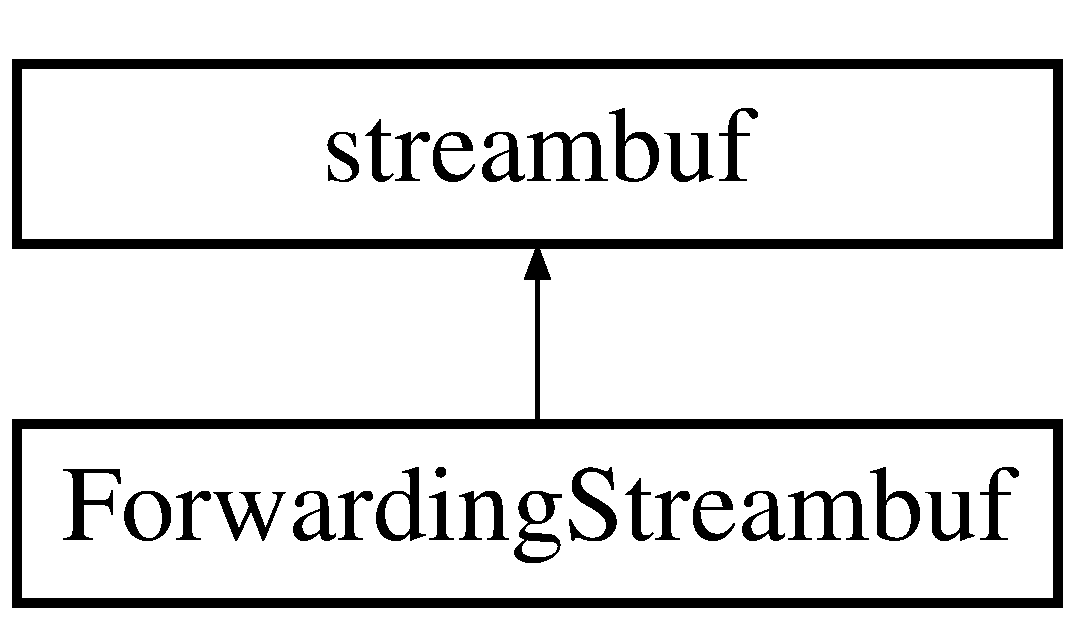
\includegraphics[height=2.000000cm]{classstanfordcpplib_1_1ForwardingStreambuf}
\end{center}
\end{figure}
\subsection*{Public Member Functions}
\begin{DoxyCompactItemize}
\item 
\mbox{\hyperlink{classstanfordcpplib_1_1ForwardingStreambuf_a8117dcf1a6c10e98afb196a6f1346dd9}{Forwarding\+Streambuf}} (\mbox{\hyperlink{classstanfordcpplib_1_1ConsoleStreambuf}{Console\+Streambuf}} \&del, bool err=false)
\item 
virtual std\+::locale \mbox{\hyperlink{classstanfordcpplib_1_1ForwardingStreambuf_aaea5d5971e30e03408abc9b4b9cdd332}{getloc}} () const
\item 
virtual std\+::streamsize \mbox{\hyperlink{classstanfordcpplib_1_1ForwardingStreambuf_a7c3ad202fdca7b02e80cce27e4fe009e}{in\+\_\+avail}} ()
\item 
virtual bool \mbox{\hyperlink{classstanfordcpplib_1_1ForwardingStreambuf_a61d5d93ba4956eefeb2e3d617d34c801}{is\+Blocked}} ()
\item 
virtual int \mbox{\hyperlink{classstanfordcpplib_1_1ForwardingStreambuf_adccb3cd5475ba3c83bc2b0a8cbd731c0}{overflow}} (int ch=E\+OF)
\item 
virtual int \mbox{\hyperlink{classstanfordcpplib_1_1ForwardingStreambuf_a5cfed6bdc955e2129ced962625045f8e}{overflow}} (int ch, bool is\+Stderr)
\item 
virtual std\+::locale \mbox{\hyperlink{classstanfordcpplib_1_1ForwardingStreambuf_a4b6e7141e08afcaf0fbe64222218d291}{pubimbue}} (const std\+::locale \&loc)
\item 
virtual std\+::streampos \mbox{\hyperlink{classstanfordcpplib_1_1ForwardingStreambuf_a19deb4f37c57fc93e0047e3db4f9d41e}{pubseekoff}} (std\+::streamoff off, std\+::ios\+\_\+base\+::seekdir way, std\+::ios\+\_\+base\+::openmode which=std\+::ios\+\_\+base\+::in$\vert$std\+::ios\+\_\+base\+::out)
\item 
virtual std\+::streampos \mbox{\hyperlink{classstanfordcpplib_1_1ForwardingStreambuf_aa603647db2d03b8bde5e5782b6472575}{pubseekpos}} (std\+::streampos pos, std\+::ios\+\_\+base\+::openmode which=std\+::ios\+\_\+base\+::in$\vert$std\+::ios\+\_\+base\+::out)
\item 
virtual std\+::streambuf $\ast$ \mbox{\hyperlink{classstanfordcpplib_1_1ForwardingStreambuf_a7d5bdeefe1c21ccce88dccedff1ab495}{pubsetbuf}} (char $\ast$s, std\+::streamsize n)
\item 
virtual int \mbox{\hyperlink{classstanfordcpplib_1_1ForwardingStreambuf_a104a7d4fba2c0e96a198cedb7c8cfa5f}{pubsync}} ()
\item 
virtual int \mbox{\hyperlink{classstanfordcpplib_1_1ForwardingStreambuf_a91a2d4b5d9c771f559543d68806820a6}{sbumpc}} ()
\item 
virtual int \mbox{\hyperlink{classstanfordcpplib_1_1ForwardingStreambuf_abf3bd66eb386006b5f74a7bcdf1c3b4b}{sgetc}} ()
\item 
virtual std\+::streamsize \mbox{\hyperlink{classstanfordcpplib_1_1ForwardingStreambuf_a117eab93aac941f3cee780c5c2ecf58b}{sgetn}} (char $\ast$s, std\+::streamsize n)
\item 
virtual int \mbox{\hyperlink{classstanfordcpplib_1_1ForwardingStreambuf_a17a9adc0f91f53a184f79fa84db9bca7}{snextc}} ()
\item 
virtual int \mbox{\hyperlink{classstanfordcpplib_1_1ForwardingStreambuf_a2d0d4eb097eb268d3c7181204d156689}{sputbackc}} (char c)
\item 
virtual int \mbox{\hyperlink{classstanfordcpplib_1_1ForwardingStreambuf_ac2e29fbc1c3df5e6a85172ddbcbacae9}{sputc}} (char c)
\item 
virtual std\+::streamsize \mbox{\hyperlink{classstanfordcpplib_1_1ForwardingStreambuf_a68372b953d8e4c4754586deb450fe84d}{sputn}} (const char $\ast$s, std\+::streamsize n)
\item 
virtual int \mbox{\hyperlink{classstanfordcpplib_1_1ForwardingStreambuf_a3c92fd32c60f1c7fe6c6b8c80a970465}{sungetc}} ()
\item 
virtual int \mbox{\hyperlink{classstanfordcpplib_1_1ForwardingStreambuf_a810a727ce5554d3178e17b6bc55025dd}{sync}} ()
\item 
virtual int \mbox{\hyperlink{classstanfordcpplib_1_1ForwardingStreambuf_ad5f4344df2a20a0000adb05d4e656855}{sync}} (bool is\+Stderr)
\item 
virtual int \mbox{\hyperlink{classstanfordcpplib_1_1ForwardingStreambuf_aeb6918bd44153b257e097e2d2ef370ef}{underflow}} ()
\end{DoxyCompactItemize}


\subsection{Constructor \& Destructor Documentation}
\mbox{\Hypertarget{classstanfordcpplib_1_1ForwardingStreambuf_a8117dcf1a6c10e98afb196a6f1346dd9}\label{classstanfordcpplib_1_1ForwardingStreambuf_a8117dcf1a6c10e98afb196a6f1346dd9}} 
\index{stanfordcpplib\+::\+Forwarding\+Streambuf@{stanfordcpplib\+::\+Forwarding\+Streambuf}!Forwarding\+Streambuf@{Forwarding\+Streambuf}}
\index{Forwarding\+Streambuf@{Forwarding\+Streambuf}!stanfordcpplib\+::\+Forwarding\+Streambuf@{stanfordcpplib\+::\+Forwarding\+Streambuf}}
\subsubsection{\texorpdfstring{Forwarding\+Streambuf()}{ForwardingStreambuf()}}
{\footnotesize\ttfamily \mbox{\hyperlink{classstanfordcpplib_1_1ForwardingStreambuf}{Forwarding\+Streambuf}} (\begin{DoxyParamCaption}\item[{\mbox{\hyperlink{classstanfordcpplib_1_1ConsoleStreambuf}{Console\+Streambuf}} \&}]{del,  }\item[{bool}]{err = {\ttfamily false} }\end{DoxyParamCaption})\hspace{0.3cm}{\ttfamily [inline]}}



\subsection{Member Function Documentation}
\mbox{\Hypertarget{classstanfordcpplib_1_1ForwardingStreambuf_aaea5d5971e30e03408abc9b4b9cdd332}\label{classstanfordcpplib_1_1ForwardingStreambuf_aaea5d5971e30e03408abc9b4b9cdd332}} 
\index{stanfordcpplib\+::\+Forwarding\+Streambuf@{stanfordcpplib\+::\+Forwarding\+Streambuf}!getloc@{getloc}}
\index{getloc@{getloc}!stanfordcpplib\+::\+Forwarding\+Streambuf@{stanfordcpplib\+::\+Forwarding\+Streambuf}}
\subsubsection{\texorpdfstring{getloc()}{getloc()}}
{\footnotesize\ttfamily virtual std\+::locale getloc (\begin{DoxyParamCaption}{ }\end{DoxyParamCaption}) const\hspace{0.3cm}{\ttfamily [inline]}, {\ttfamily [virtual]}}

\mbox{\Hypertarget{classstanfordcpplib_1_1ForwardingStreambuf_a7c3ad202fdca7b02e80cce27e4fe009e}\label{classstanfordcpplib_1_1ForwardingStreambuf_a7c3ad202fdca7b02e80cce27e4fe009e}} 
\index{stanfordcpplib\+::\+Forwarding\+Streambuf@{stanfordcpplib\+::\+Forwarding\+Streambuf}!in\+\_\+avail@{in\+\_\+avail}}
\index{in\+\_\+avail@{in\+\_\+avail}!stanfordcpplib\+::\+Forwarding\+Streambuf@{stanfordcpplib\+::\+Forwarding\+Streambuf}}
\subsubsection{\texorpdfstring{in\+\_\+avail()}{in\_avail()}}
{\footnotesize\ttfamily virtual std\+::streamsize in\+\_\+avail (\begin{DoxyParamCaption}{ }\end{DoxyParamCaption})\hspace{0.3cm}{\ttfamily [inline]}, {\ttfamily [virtual]}}

\mbox{\Hypertarget{classstanfordcpplib_1_1ForwardingStreambuf_a61d5d93ba4956eefeb2e3d617d34c801}\label{classstanfordcpplib_1_1ForwardingStreambuf_a61d5d93ba4956eefeb2e3d617d34c801}} 
\index{stanfordcpplib\+::\+Forwarding\+Streambuf@{stanfordcpplib\+::\+Forwarding\+Streambuf}!is\+Blocked@{is\+Blocked}}
\index{is\+Blocked@{is\+Blocked}!stanfordcpplib\+::\+Forwarding\+Streambuf@{stanfordcpplib\+::\+Forwarding\+Streambuf}}
\subsubsection{\texorpdfstring{is\+Blocked()}{isBlocked()}}
{\footnotesize\ttfamily virtual bool is\+Blocked (\begin{DoxyParamCaption}{ }\end{DoxyParamCaption})\hspace{0.3cm}{\ttfamily [inline]}, {\ttfamily [virtual]}}

\mbox{\Hypertarget{classstanfordcpplib_1_1ForwardingStreambuf_adccb3cd5475ba3c83bc2b0a8cbd731c0}\label{classstanfordcpplib_1_1ForwardingStreambuf_adccb3cd5475ba3c83bc2b0a8cbd731c0}} 
\index{stanfordcpplib\+::\+Forwarding\+Streambuf@{stanfordcpplib\+::\+Forwarding\+Streambuf}!overflow@{overflow}}
\index{overflow@{overflow}!stanfordcpplib\+::\+Forwarding\+Streambuf@{stanfordcpplib\+::\+Forwarding\+Streambuf}}
\subsubsection{\texorpdfstring{overflow()}{overflow()}\hspace{0.1cm}{\footnotesize\ttfamily [1/2]}}
{\footnotesize\ttfamily virtual int overflow (\begin{DoxyParamCaption}\item[{int}]{ch = {\ttfamily EOF} }\end{DoxyParamCaption})\hspace{0.3cm}{\ttfamily [inline]}, {\ttfamily [virtual]}}

\mbox{\Hypertarget{classstanfordcpplib_1_1ForwardingStreambuf_a5cfed6bdc955e2129ced962625045f8e}\label{classstanfordcpplib_1_1ForwardingStreambuf_a5cfed6bdc955e2129ced962625045f8e}} 
\index{stanfordcpplib\+::\+Forwarding\+Streambuf@{stanfordcpplib\+::\+Forwarding\+Streambuf}!overflow@{overflow}}
\index{overflow@{overflow}!stanfordcpplib\+::\+Forwarding\+Streambuf@{stanfordcpplib\+::\+Forwarding\+Streambuf}}
\subsubsection{\texorpdfstring{overflow()}{overflow()}\hspace{0.1cm}{\footnotesize\ttfamily [2/2]}}
{\footnotesize\ttfamily virtual int overflow (\begin{DoxyParamCaption}\item[{int}]{ch,  }\item[{bool}]{is\+Stderr }\end{DoxyParamCaption})\hspace{0.3cm}{\ttfamily [inline]}, {\ttfamily [virtual]}}

\mbox{\Hypertarget{classstanfordcpplib_1_1ForwardingStreambuf_a4b6e7141e08afcaf0fbe64222218d291}\label{classstanfordcpplib_1_1ForwardingStreambuf_a4b6e7141e08afcaf0fbe64222218d291}} 
\index{stanfordcpplib\+::\+Forwarding\+Streambuf@{stanfordcpplib\+::\+Forwarding\+Streambuf}!pubimbue@{pubimbue}}
\index{pubimbue@{pubimbue}!stanfordcpplib\+::\+Forwarding\+Streambuf@{stanfordcpplib\+::\+Forwarding\+Streambuf}}
\subsubsection{\texorpdfstring{pubimbue()}{pubimbue()}}
{\footnotesize\ttfamily virtual std\+::locale pubimbue (\begin{DoxyParamCaption}\item[{const std\+::locale \&}]{loc }\end{DoxyParamCaption})\hspace{0.3cm}{\ttfamily [inline]}, {\ttfamily [virtual]}}

\mbox{\Hypertarget{classstanfordcpplib_1_1ForwardingStreambuf_a19deb4f37c57fc93e0047e3db4f9d41e}\label{classstanfordcpplib_1_1ForwardingStreambuf_a19deb4f37c57fc93e0047e3db4f9d41e}} 
\index{stanfordcpplib\+::\+Forwarding\+Streambuf@{stanfordcpplib\+::\+Forwarding\+Streambuf}!pubseekoff@{pubseekoff}}
\index{pubseekoff@{pubseekoff}!stanfordcpplib\+::\+Forwarding\+Streambuf@{stanfordcpplib\+::\+Forwarding\+Streambuf}}
\subsubsection{\texorpdfstring{pubseekoff()}{pubseekoff()}}
{\footnotesize\ttfamily virtual std\+::streampos pubseekoff (\begin{DoxyParamCaption}\item[{std\+::streamoff}]{off,  }\item[{std\+::ios\+\_\+base\+::seekdir}]{way,  }\item[{std\+::ios\+\_\+base\+::openmode}]{which = {\ttfamily std\+:\+:ios\+\_\+base\+:\+:in~$\vert$~std\+:\+:ios\+\_\+base\+:\+:out} }\end{DoxyParamCaption})\hspace{0.3cm}{\ttfamily [inline]}, {\ttfamily [virtual]}}

\mbox{\Hypertarget{classstanfordcpplib_1_1ForwardingStreambuf_aa603647db2d03b8bde5e5782b6472575}\label{classstanfordcpplib_1_1ForwardingStreambuf_aa603647db2d03b8bde5e5782b6472575}} 
\index{stanfordcpplib\+::\+Forwarding\+Streambuf@{stanfordcpplib\+::\+Forwarding\+Streambuf}!pubseekpos@{pubseekpos}}
\index{pubseekpos@{pubseekpos}!stanfordcpplib\+::\+Forwarding\+Streambuf@{stanfordcpplib\+::\+Forwarding\+Streambuf}}
\subsubsection{\texorpdfstring{pubseekpos()}{pubseekpos()}}
{\footnotesize\ttfamily virtual std\+::streampos pubseekpos (\begin{DoxyParamCaption}\item[{std\+::streampos}]{pos,  }\item[{std\+::ios\+\_\+base\+::openmode}]{which = {\ttfamily std\+:\+:ios\+\_\+base\+:\+:in~$\vert$~std\+:\+:ios\+\_\+base\+:\+:out} }\end{DoxyParamCaption})\hspace{0.3cm}{\ttfamily [inline]}, {\ttfamily [virtual]}}

\mbox{\Hypertarget{classstanfordcpplib_1_1ForwardingStreambuf_a7d5bdeefe1c21ccce88dccedff1ab495}\label{classstanfordcpplib_1_1ForwardingStreambuf_a7d5bdeefe1c21ccce88dccedff1ab495}} 
\index{stanfordcpplib\+::\+Forwarding\+Streambuf@{stanfordcpplib\+::\+Forwarding\+Streambuf}!pubsetbuf@{pubsetbuf}}
\index{pubsetbuf@{pubsetbuf}!stanfordcpplib\+::\+Forwarding\+Streambuf@{stanfordcpplib\+::\+Forwarding\+Streambuf}}
\subsubsection{\texorpdfstring{pubsetbuf()}{pubsetbuf()}}
{\footnotesize\ttfamily virtual std\+::streambuf$\ast$ pubsetbuf (\begin{DoxyParamCaption}\item[{char $\ast$}]{s,  }\item[{std\+::streamsize}]{n }\end{DoxyParamCaption})\hspace{0.3cm}{\ttfamily [inline]}, {\ttfamily [virtual]}}

\mbox{\Hypertarget{classstanfordcpplib_1_1ForwardingStreambuf_a104a7d4fba2c0e96a198cedb7c8cfa5f}\label{classstanfordcpplib_1_1ForwardingStreambuf_a104a7d4fba2c0e96a198cedb7c8cfa5f}} 
\index{stanfordcpplib\+::\+Forwarding\+Streambuf@{stanfordcpplib\+::\+Forwarding\+Streambuf}!pubsync@{pubsync}}
\index{pubsync@{pubsync}!stanfordcpplib\+::\+Forwarding\+Streambuf@{stanfordcpplib\+::\+Forwarding\+Streambuf}}
\subsubsection{\texorpdfstring{pubsync()}{pubsync()}}
{\footnotesize\ttfamily virtual int pubsync (\begin{DoxyParamCaption}{ }\end{DoxyParamCaption})\hspace{0.3cm}{\ttfamily [inline]}, {\ttfamily [virtual]}}

\mbox{\Hypertarget{classstanfordcpplib_1_1ForwardingStreambuf_a91a2d4b5d9c771f559543d68806820a6}\label{classstanfordcpplib_1_1ForwardingStreambuf_a91a2d4b5d9c771f559543d68806820a6}} 
\index{stanfordcpplib\+::\+Forwarding\+Streambuf@{stanfordcpplib\+::\+Forwarding\+Streambuf}!sbumpc@{sbumpc}}
\index{sbumpc@{sbumpc}!stanfordcpplib\+::\+Forwarding\+Streambuf@{stanfordcpplib\+::\+Forwarding\+Streambuf}}
\subsubsection{\texorpdfstring{sbumpc()}{sbumpc()}}
{\footnotesize\ttfamily virtual int sbumpc (\begin{DoxyParamCaption}{ }\end{DoxyParamCaption})\hspace{0.3cm}{\ttfamily [inline]}, {\ttfamily [virtual]}}

\mbox{\Hypertarget{classstanfordcpplib_1_1ForwardingStreambuf_abf3bd66eb386006b5f74a7bcdf1c3b4b}\label{classstanfordcpplib_1_1ForwardingStreambuf_abf3bd66eb386006b5f74a7bcdf1c3b4b}} 
\index{stanfordcpplib\+::\+Forwarding\+Streambuf@{stanfordcpplib\+::\+Forwarding\+Streambuf}!sgetc@{sgetc}}
\index{sgetc@{sgetc}!stanfordcpplib\+::\+Forwarding\+Streambuf@{stanfordcpplib\+::\+Forwarding\+Streambuf}}
\subsubsection{\texorpdfstring{sgetc()}{sgetc()}}
{\footnotesize\ttfamily virtual int sgetc (\begin{DoxyParamCaption}{ }\end{DoxyParamCaption})\hspace{0.3cm}{\ttfamily [inline]}, {\ttfamily [virtual]}}

\mbox{\Hypertarget{classstanfordcpplib_1_1ForwardingStreambuf_a117eab93aac941f3cee780c5c2ecf58b}\label{classstanfordcpplib_1_1ForwardingStreambuf_a117eab93aac941f3cee780c5c2ecf58b}} 
\index{stanfordcpplib\+::\+Forwarding\+Streambuf@{stanfordcpplib\+::\+Forwarding\+Streambuf}!sgetn@{sgetn}}
\index{sgetn@{sgetn}!stanfordcpplib\+::\+Forwarding\+Streambuf@{stanfordcpplib\+::\+Forwarding\+Streambuf}}
\subsubsection{\texorpdfstring{sgetn()}{sgetn()}}
{\footnotesize\ttfamily virtual std\+::streamsize sgetn (\begin{DoxyParamCaption}\item[{char $\ast$}]{s,  }\item[{std\+::streamsize}]{n }\end{DoxyParamCaption})\hspace{0.3cm}{\ttfamily [inline]}, {\ttfamily [virtual]}}

\mbox{\Hypertarget{classstanfordcpplib_1_1ForwardingStreambuf_a17a9adc0f91f53a184f79fa84db9bca7}\label{classstanfordcpplib_1_1ForwardingStreambuf_a17a9adc0f91f53a184f79fa84db9bca7}} 
\index{stanfordcpplib\+::\+Forwarding\+Streambuf@{stanfordcpplib\+::\+Forwarding\+Streambuf}!snextc@{snextc}}
\index{snextc@{snextc}!stanfordcpplib\+::\+Forwarding\+Streambuf@{stanfordcpplib\+::\+Forwarding\+Streambuf}}
\subsubsection{\texorpdfstring{snextc()}{snextc()}}
{\footnotesize\ttfamily virtual int snextc (\begin{DoxyParamCaption}{ }\end{DoxyParamCaption})\hspace{0.3cm}{\ttfamily [inline]}, {\ttfamily [virtual]}}

\mbox{\Hypertarget{classstanfordcpplib_1_1ForwardingStreambuf_a2d0d4eb097eb268d3c7181204d156689}\label{classstanfordcpplib_1_1ForwardingStreambuf_a2d0d4eb097eb268d3c7181204d156689}} 
\index{stanfordcpplib\+::\+Forwarding\+Streambuf@{stanfordcpplib\+::\+Forwarding\+Streambuf}!sputbackc@{sputbackc}}
\index{sputbackc@{sputbackc}!stanfordcpplib\+::\+Forwarding\+Streambuf@{stanfordcpplib\+::\+Forwarding\+Streambuf}}
\subsubsection{\texorpdfstring{sputbackc()}{sputbackc()}}
{\footnotesize\ttfamily virtual int sputbackc (\begin{DoxyParamCaption}\item[{char}]{c }\end{DoxyParamCaption})\hspace{0.3cm}{\ttfamily [inline]}, {\ttfamily [virtual]}}

\mbox{\Hypertarget{classstanfordcpplib_1_1ForwardingStreambuf_ac2e29fbc1c3df5e6a85172ddbcbacae9}\label{classstanfordcpplib_1_1ForwardingStreambuf_ac2e29fbc1c3df5e6a85172ddbcbacae9}} 
\index{stanfordcpplib\+::\+Forwarding\+Streambuf@{stanfordcpplib\+::\+Forwarding\+Streambuf}!sputc@{sputc}}
\index{sputc@{sputc}!stanfordcpplib\+::\+Forwarding\+Streambuf@{stanfordcpplib\+::\+Forwarding\+Streambuf}}
\subsubsection{\texorpdfstring{sputc()}{sputc()}}
{\footnotesize\ttfamily virtual int sputc (\begin{DoxyParamCaption}\item[{char}]{c }\end{DoxyParamCaption})\hspace{0.3cm}{\ttfamily [inline]}, {\ttfamily [virtual]}}

\mbox{\Hypertarget{classstanfordcpplib_1_1ForwardingStreambuf_a68372b953d8e4c4754586deb450fe84d}\label{classstanfordcpplib_1_1ForwardingStreambuf_a68372b953d8e4c4754586deb450fe84d}} 
\index{stanfordcpplib\+::\+Forwarding\+Streambuf@{stanfordcpplib\+::\+Forwarding\+Streambuf}!sputn@{sputn}}
\index{sputn@{sputn}!stanfordcpplib\+::\+Forwarding\+Streambuf@{stanfordcpplib\+::\+Forwarding\+Streambuf}}
\subsubsection{\texorpdfstring{sputn()}{sputn()}}
{\footnotesize\ttfamily virtual std\+::streamsize sputn (\begin{DoxyParamCaption}\item[{const char $\ast$}]{s,  }\item[{std\+::streamsize}]{n }\end{DoxyParamCaption})\hspace{0.3cm}{\ttfamily [inline]}, {\ttfamily [virtual]}}

\mbox{\Hypertarget{classstanfordcpplib_1_1ForwardingStreambuf_a3c92fd32c60f1c7fe6c6b8c80a970465}\label{classstanfordcpplib_1_1ForwardingStreambuf_a3c92fd32c60f1c7fe6c6b8c80a970465}} 
\index{stanfordcpplib\+::\+Forwarding\+Streambuf@{stanfordcpplib\+::\+Forwarding\+Streambuf}!sungetc@{sungetc}}
\index{sungetc@{sungetc}!stanfordcpplib\+::\+Forwarding\+Streambuf@{stanfordcpplib\+::\+Forwarding\+Streambuf}}
\subsubsection{\texorpdfstring{sungetc()}{sungetc()}}
{\footnotesize\ttfamily virtual int sungetc (\begin{DoxyParamCaption}{ }\end{DoxyParamCaption})\hspace{0.3cm}{\ttfamily [inline]}, {\ttfamily [virtual]}}

\mbox{\Hypertarget{classstanfordcpplib_1_1ForwardingStreambuf_a810a727ce5554d3178e17b6bc55025dd}\label{classstanfordcpplib_1_1ForwardingStreambuf_a810a727ce5554d3178e17b6bc55025dd}} 
\index{stanfordcpplib\+::\+Forwarding\+Streambuf@{stanfordcpplib\+::\+Forwarding\+Streambuf}!sync@{sync}}
\index{sync@{sync}!stanfordcpplib\+::\+Forwarding\+Streambuf@{stanfordcpplib\+::\+Forwarding\+Streambuf}}
\subsubsection{\texorpdfstring{sync()}{sync()}\hspace{0.1cm}{\footnotesize\ttfamily [1/2]}}
{\footnotesize\ttfamily virtual int sync (\begin{DoxyParamCaption}{ }\end{DoxyParamCaption})\hspace{0.3cm}{\ttfamily [inline]}, {\ttfamily [virtual]}}

\mbox{\Hypertarget{classstanfordcpplib_1_1ForwardingStreambuf_ad5f4344df2a20a0000adb05d4e656855}\label{classstanfordcpplib_1_1ForwardingStreambuf_ad5f4344df2a20a0000adb05d4e656855}} 
\index{stanfordcpplib\+::\+Forwarding\+Streambuf@{stanfordcpplib\+::\+Forwarding\+Streambuf}!sync@{sync}}
\index{sync@{sync}!stanfordcpplib\+::\+Forwarding\+Streambuf@{stanfordcpplib\+::\+Forwarding\+Streambuf}}
\subsubsection{\texorpdfstring{sync()}{sync()}\hspace{0.1cm}{\footnotesize\ttfamily [2/2]}}
{\footnotesize\ttfamily virtual int sync (\begin{DoxyParamCaption}\item[{bool}]{is\+Stderr }\end{DoxyParamCaption})\hspace{0.3cm}{\ttfamily [inline]}, {\ttfamily [virtual]}}

\mbox{\Hypertarget{classstanfordcpplib_1_1ForwardingStreambuf_aeb6918bd44153b257e097e2d2ef370ef}\label{classstanfordcpplib_1_1ForwardingStreambuf_aeb6918bd44153b257e097e2d2ef370ef}} 
\index{stanfordcpplib\+::\+Forwarding\+Streambuf@{stanfordcpplib\+::\+Forwarding\+Streambuf}!underflow@{underflow}}
\index{underflow@{underflow}!stanfordcpplib\+::\+Forwarding\+Streambuf@{stanfordcpplib\+::\+Forwarding\+Streambuf}}
\subsubsection{\texorpdfstring{underflow()}{underflow()}}
{\footnotesize\ttfamily virtual int underflow (\begin{DoxyParamCaption}{ }\end{DoxyParamCaption})\hspace{0.3cm}{\ttfamily [inline]}, {\ttfamily [virtual]}}


\hypertarget{classGArc}{}\section{G\+Arc Class Reference}
\label{classGArc}\index{G\+Arc@{G\+Arc}}


This graphical object subclass represents an elliptical arc.  




{\ttfamily \#include $<$gobjects.\+h$>$}

Inheritance diagram for G\+Arc\+:\begin{figure}[H]
\begin{center}
\leavevmode
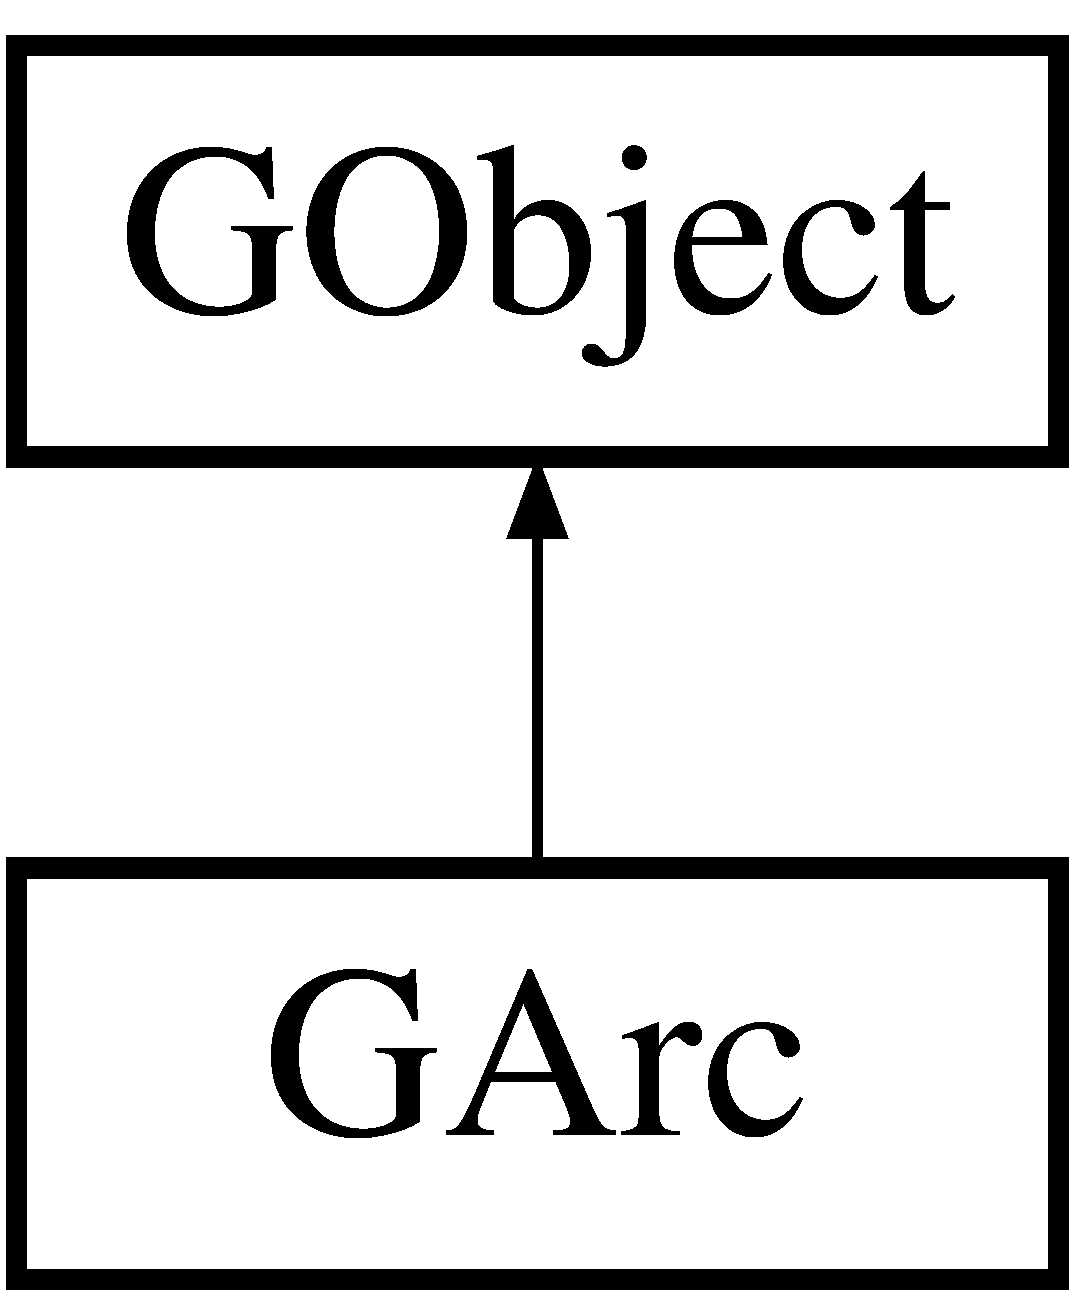
\includegraphics[height=2.000000cm]{classGArc}
\end{center}
\end{figure}
\subsection*{Public Types}
\begin{DoxyCompactItemize}
\item 
enum \mbox{\hyperlink{classGObject_a86e0f5648542856159bb40775c854aa7}{Line\+Style}} \{ \mbox{\hyperlink{classGObject_a86e0f5648542856159bb40775c854aa7acbc84bd5232621834ed31f44d457c1eb}{L\+I\+N\+E\+\_\+\+N\+O\+NE}}, 
\mbox{\hyperlink{classGObject_a86e0f5648542856159bb40775c854aa7a700c78bc2cd76acaab26651bf7b4941f}{L\+I\+N\+E\+\_\+\+S\+O\+L\+ID}}, 
\mbox{\hyperlink{classGObject_a86e0f5648542856159bb40775c854aa7a9ccba0845f785d81d07b333ae1aad84e}{L\+I\+N\+E\+\_\+\+D\+A\+SH}}, 
\mbox{\hyperlink{classGObject_a86e0f5648542856159bb40775c854aa7a8e811c096cb941997f0bfda168bb6df3}{L\+I\+N\+E\+\_\+\+D\+OT}}, 
\mbox{\hyperlink{classGObject_a86e0f5648542856159bb40775c854aa7ada15a2e3d737b2db7706d8300f91b89d}{L\+I\+N\+E\+\_\+\+D\+A\+S\+H\+\_\+\+D\+OT}}, 
\mbox{\hyperlink{classGObject_a86e0f5648542856159bb40775c854aa7aabf4053a73eafa7ba2b7e6d664c74c1d}{L\+I\+N\+E\+\_\+\+D\+A\+S\+H\+\_\+\+D\+O\+T\+\_\+\+D\+OT}}
 \}
\begin{DoxyCompactList}\small\item\em Styles that can be used for the outline around various shapes. \end{DoxyCompactList}\end{DoxyCompactItemize}
\subsection*{Public Member Functions}
\begin{DoxyCompactItemize}
\item 
\mbox{\hyperlink{classGArc_a487e2cfaa2231c74bb71eb4ba5bc0167}{G\+Arc}} (double width=0, double height=0, double start=0, double sweep=0)
\begin{DoxyCompactList}\small\item\em Creates a new {\ttfamily \mbox{\hyperlink{classGArc}{G\+Arc}}} object consisting of an elliptical arc. \end{DoxyCompactList}\item 
\mbox{\hyperlink{classGArc_ab70a642a06382d436427bd2f9519539a}{G\+Arc}} (double x, double y, double width, double height, double start, double sweep)
\begin{DoxyCompactList}\small\item\em Creates a new {\ttfamily \mbox{\hyperlink{classGArc}{G\+Arc}}} object consisting of an elliptical arc. \end{DoxyCompactList}\item 
virtual bool \mbox{\hyperlink{classGObject_a1dbc9dafaae51958112dbe1267a1f547}{contains}} (const \mbox{\hyperlink{classGPoint}{G\+Point}} \&pt) const
\begin{DoxyCompactList}\small\item\em Returns {\ttfamily true} if the specified point is inside the object. \end{DoxyCompactList}\item 
virtual bool \mbox{\hyperlink{classGArc_aa095a031ab22c150d2d75fdda1c3c8f5}{contains}} (double x, double y) const Q\+\_\+\+D\+E\+C\+L\+\_\+\+O\+V\+E\+R\+R\+I\+DE
\begin{DoxyCompactList}\small\item\em Returns {\ttfamily true} if the specified point is inside the object. \end{DoxyCompactList}\item 
virtual \mbox{\hyperlink{classGPoint}{G\+Point}} \mbox{\hyperlink{classGObject_a0d41183bf6b08de66fe3907551aab0d7}{get\+Bottom\+Right\+Location}} () const
\begin{DoxyCompactList}\small\item\em Returns the x/y coordinates of the bottom/right corner of the object. \end{DoxyCompactList}\item 
virtual double \mbox{\hyperlink{classGObject_a4316a2406c18e1c6d061fe51fd355490}{get\+BottomY}} () const
\begin{DoxyCompactList}\small\item\em Returns the {\itshape y}-\/coordinate of the bottom of the object. \end{DoxyCompactList}\item 
virtual \mbox{\hyperlink{classGRectangle}{G\+Rectangle}} \mbox{\hyperlink{classGArc_a2f46ec8a3b533c690b3b3e56d4f34afe}{get\+Bounds}} () const Q\+\_\+\+D\+E\+C\+L\+\_\+\+O\+V\+E\+R\+R\+I\+DE
\begin{DoxyCompactList}\small\item\em Returns the bounding box of this object, which is defined to be the smallest rectangle that covers everything drawn by the figure. \end{DoxyCompactList}\item 
virtual \mbox{\hyperlink{classGPoint}{G\+Point}} \mbox{\hyperlink{classGObject_a0909472e91448470bccdb62ecfb95d8b}{get\+Center\+Location}} () const
\begin{DoxyCompactList}\small\item\em Returns the x/y-\/coordinates of the center of the object. \end{DoxyCompactList}\item 
virtual double \mbox{\hyperlink{classGObject_a04df74355b545e0543112d5b8d924176}{get\+CenterX}} () const
\begin{DoxyCompactList}\small\item\em Returns the {\itshape x}-\/coordinate of the center of the object. \end{DoxyCompactList}\item 
virtual double \mbox{\hyperlink{classGObject_acb3287a3d507025a26f54b895713b947}{get\+CenterY}} () const
\begin{DoxyCompactList}\small\item\em Returns the {\itshape y}-\/coordinate of the center of the object. \end{DoxyCompactList}\item 
virtual std\+::string \mbox{\hyperlink{classGObject_aa061dfa488c31e18549d64363c1d0e34}{get\+Color}} () const
\begin{DoxyCompactList}\small\item\em Returns the color used to display this object. \end{DoxyCompactList}\item 
virtual \mbox{\hyperlink{classGPoint}{G\+Point}} \mbox{\hyperlink{classGArc_a835d5e50bf4a91efcf0d838130c246af}{get\+End\+Point}} () const
\begin{DoxyCompactList}\small\item\em Returns the point at which the arc ends. \end{DoxyCompactList}\item 
virtual std\+::string \mbox{\hyperlink{classGObject_a76f6964a11fde7c78e9751be184e1a3c}{get\+Fill\+Color}} () const
\begin{DoxyCompactList}\small\item\em Returns the color used to display the filled region of this object. \end{DoxyCompactList}\item 
virtual \mbox{\hyperlink{classGRectangle}{G\+Rectangle}} \mbox{\hyperlink{classGArc_aab1e594176fa66cc7bd50c1f77218428}{get\+Frame\+Rectangle}} () const
\begin{DoxyCompactList}\small\item\em Returns the boundaries of the rectangle used to frame the arc. \end{DoxyCompactList}\item 
virtual double \mbox{\hyperlink{classGObject_a1e7e353362434072875264cf95629f99}{get\+Height}} () const
\begin{DoxyCompactList}\small\item\em Returns the height of this object, which is the same as the height of its bounding box. \end{DoxyCompactList}\item 
virtual \mbox{\hyperlink{classGObject_a86e0f5648542856159bb40775c854aa7}{Line\+Style}} \mbox{\hyperlink{classGObject_aaf1f5ea8281e5e3486662878d26f0a13}{get\+Line\+Style}} () const
\begin{DoxyCompactList}\small\item\em Returns the object\textquotesingle{}s style such as solid or dashed. \end{DoxyCompactList}\item 
virtual double \mbox{\hyperlink{classGObject_a85ff266dc3eb63d9f2d8e5a4487fd3c0}{get\+Line\+Width}} () const
\begin{DoxyCompactList}\small\item\em Returns the width of the line used to draw this object. \end{DoxyCompactList}\item 
virtual \mbox{\hyperlink{classGPoint}{G\+Point}} \mbox{\hyperlink{classGObject_a4f83802015511edeb63b892830812c11}{get\+Location}} () const
\begin{DoxyCompactList}\small\item\em Returns the location of the top-\/left corner of object. \end{DoxyCompactList}\item 
virtual \mbox{\hyperlink{classGCompound}{G\+Compound}} $\ast$ \mbox{\hyperlink{classGObject_a3e53cef70541b1a14eade4ad0984d0b4}{get\+Parent}} () const
\begin{DoxyCompactList}\small\item\em Returns a pointer to the {\ttfamily \mbox{\hyperlink{classGCompound}{G\+Compound}}} that contains this object. \end{DoxyCompactList}\item 
virtual double \mbox{\hyperlink{classGObject_a798cc79daaa10145b28f60bcdfdb0ee9}{get\+RightX}} () const
\begin{DoxyCompactList}\small\item\em Returns the {\itshape x}-\/coordinate of the right side of the object. \end{DoxyCompactList}\item 
virtual \mbox{\hyperlink{classGDimension}{G\+Dimension}} \mbox{\hyperlink{classGObject_a7b4eec96a2bdc6420695d5796a78eea9}{get\+Size}} () const
\begin{DoxyCompactList}\small\item\em Returns the size of the object as a {\ttfamily \mbox{\hyperlink{classGDimension}{G\+Dimension}}}. \end{DoxyCompactList}\item 
virtual double \mbox{\hyperlink{classGArc_ad52005815f95967f10ea54d290fa61ad}{get\+Start\+Angle}} () const
\begin{DoxyCompactList}\small\item\em Returns the starting angle for this arc in degrees. \end{DoxyCompactList}\item 
virtual \mbox{\hyperlink{classGPoint}{G\+Point}} \mbox{\hyperlink{classGArc_ad12beaa70993d9b409bfa8fd86c83957}{get\+Start\+Point}} () const
\begin{DoxyCompactList}\small\item\em Returns the point at which the arc starts. \end{DoxyCompactList}\item 
virtual double \mbox{\hyperlink{classGArc_ae842751a5db1493113ff347e564efae1}{get\+Sweep\+Angle}} () const
\begin{DoxyCompactList}\small\item\em Returns the sweep angle for this arc in degrees. \end{DoxyCompactList}\item 
virtual std\+::string \mbox{\hyperlink{classGArc_a9896d58fcfebbf1025aeeb5b8b9ede80}{get\+Type}} () const Q\+\_\+\+D\+E\+C\+L\+\_\+\+O\+V\+E\+R\+R\+I\+DE
\begin{DoxyCompactList}\small\item\em Returns the type of the object as a string, such as {\ttfamily \char`\"{}\+G\+Oval\char`\"{}} or {\ttfamily \char`\"{}\+G\+Rect\char`\"{}}. \end{DoxyCompactList}\item 
virtual double \mbox{\hyperlink{classGObject_a0ed2965abd4f5701d2cadf71239faf19}{get\+Width}} () const
\begin{DoxyCompactList}\small\item\em Returns the width of this object, which is equal to the width of the bounding box. \end{DoxyCompactList}\item 
virtual double \mbox{\hyperlink{classGObject_a344385751bee0720059403940d57a13e}{getX}} () const
\begin{DoxyCompactList}\small\item\em Returns the leftmost {\itshape x}-\/coordinate of the object. \end{DoxyCompactList}\item 
virtual double \mbox{\hyperlink{classGObject_aafa51c7f8f38a09febbb9ce7853f77b4}{getY}} () const
\begin{DoxyCompactList}\small\item\em Returns the topmost {\itshape y}-\/coordinate of the object. \end{DoxyCompactList}\item 
virtual bool \mbox{\hyperlink{classGObject_a11c404f106940c201b6f326e0355c150}{is\+Filled}} () const
\begin{DoxyCompactList}\small\item\em Returns {\ttfamily true} if the object is filled with color. \end{DoxyCompactList}\item 
virtual bool \mbox{\hyperlink{classGObject_a9d8a6cfb13917785c143e74d40e4e2be}{is\+Visible}} () const
\begin{DoxyCompactList}\small\item\em Returns {\ttfamily true} if this object is visible on screen. \end{DoxyCompactList}\item 
virtual void \mbox{\hyperlink{classGObject_a5973d8dda83afb36e2c56855515be392}{move}} (double dx, double dy)
\begin{DoxyCompactList}\small\item\em Moves the object on the screen using the displacements {\ttfamily dx} and {\ttfamily dy}. \end{DoxyCompactList}\item 
virtual void \mbox{\hyperlink{classGObject_ac827b978aa122f136a14c198687ad80f}{repaint}} ()
\begin{DoxyCompactList}\small\item\em Instructs the object to redraw itself on screen. \end{DoxyCompactList}\item 
virtual void \mbox{\hyperlink{classGObject_a6022a1fd1e5dcd2fd5585e5a36aa3f37}{reset\+Transform}} ()
\begin{DoxyCompactList}\small\item\em Undoes any previous scale/rotate transformations on this object. \end{DoxyCompactList}\item 
virtual void \mbox{\hyperlink{classGObject_ae1ffaa12185dfd5ba464f7d87c329e26}{rotate}} (double theta)
\begin{DoxyCompactList}\small\item\em Transforms the object by rotating it {\ttfamily theta} degrees counterclockwise around its origin. \end{DoxyCompactList}\item 
virtual void \mbox{\hyperlink{classGObject_ad2e1900f730475c2d044817db03b38d6}{scale}} (double sf)
\begin{DoxyCompactList}\small\item\em Scales the object by the specified scale factor. \end{DoxyCompactList}\item 
virtual void \mbox{\hyperlink{classGObject_a63641f69d610d0b951357d35a0c3b1e3}{scale}} (double sx, double sy)
\begin{DoxyCompactList}\small\item\em Scales the object by the specified scale factors. \end{DoxyCompactList}\item 
void \mbox{\hyperlink{classGObject_ab6747f40313c531c2db32edb5b63b9b7}{send\+Backward}} ()
\begin{DoxyCompactList}\small\item\em Moves this object one step toward the back in the {\itshape z} dimension. \end{DoxyCompactList}\item 
void \mbox{\hyperlink{classGObject_a710b3e449c9facba7847c91ab170d281}{send\+Forward}} ()
\begin{DoxyCompactList}\small\item\em Moves this object one step toward the front in the {\itshape z} dimension. \end{DoxyCompactList}\item 
void \mbox{\hyperlink{classGObject_a0f7f1efbb7fd46dde2867c4ad0330896}{send\+To\+Back}} ()
\begin{DoxyCompactList}\small\item\em Moves this object to the back of the display in the {\itshape z} dimension. \end{DoxyCompactList}\item 
void \mbox{\hyperlink{classGObject_aee33d68488e46827ef55fac07f40a9b2}{send\+To\+Front}} ()
\begin{DoxyCompactList}\small\item\em Moves this object to the front of the display in the {\itshape z} dimension. \end{DoxyCompactList}\item 
virtual void \mbox{\hyperlink{classGObject_a71ff7b16b8f1bdc4a1ce9f30cf8b87d8}{set\+Bottom\+Right\+Location}} (double x, double y)
\begin{DoxyCompactList}\small\item\em Sets the location of the bottom/right of this object. \end{DoxyCompactList}\item 
virtual void \mbox{\hyperlink{classGObject_ac6f7320321182f1d18c1c0fa97d5e941}{set\+Bottom\+Right\+Location}} (const \mbox{\hyperlink{classGPoint}{G\+Point}} \&pt)
\begin{DoxyCompactList}\small\item\em Sets the location of the bottom/right of this object. \end{DoxyCompactList}\item 
virtual void \mbox{\hyperlink{classGObject_a4b20e93c2a2597484f74ee5caa71f41f}{set\+BottomY}} (double y)
\begin{DoxyCompactList}\small\item\em Sets the location of the bottom y-\/coordinate of this object. \end{DoxyCompactList}\item 
virtual void \mbox{\hyperlink{classGObject_a2aae8197624b72265ab83b4f1bc73f2f}{set\+Bounds}} (double x, double y, double width, double height)
\begin{DoxyCompactList}\small\item\em Changes the bounds of this object to the specified values. \end{DoxyCompactList}\item 
virtual void \mbox{\hyperlink{classGObject_acada386653f008cacc7cce86426bef7c}{set\+Bounds}} (const \mbox{\hyperlink{classGRectangle}{G\+Rectangle}} \&size)
\begin{DoxyCompactList}\small\item\em Changes the bounds of this object to the specified rectangle. \end{DoxyCompactList}\item 
virtual void \mbox{\hyperlink{classGObject_a290b47dd8de1be44089f95cb2c47c1de}{set\+Center\+Location}} (double x, double y)
\begin{DoxyCompactList}\small\item\em Sets the location of the center of this object. \end{DoxyCompactList}\item 
virtual void \mbox{\hyperlink{classGObject_a1bedf1b233ecba3f753ec58908a683a6}{set\+Center\+Location}} (const \mbox{\hyperlink{classGPoint}{G\+Point}} \&pt)
\begin{DoxyCompactList}\small\item\em Sets the location of the center of this object. \end{DoxyCompactList}\item 
virtual void \mbox{\hyperlink{classGObject_a2f4936281e056eead00a9186b9ba8af6}{set\+CenterX}} (double x)
\begin{DoxyCompactList}\small\item\em Sets the x-\/coordinate of the center of this object. \end{DoxyCompactList}\item 
virtual void \mbox{\hyperlink{classGObject_aad2a22b4fde88c33306b92aebf641d57}{set\+CenterY}} (double y)
\begin{DoxyCompactList}\small\item\em Sets the y-\/coordinate of the center of this object. \end{DoxyCompactList}\item 
virtual void \mbox{\hyperlink{classGObject_ad57ef49bc31db94e92648aa3737923d6}{set\+Color}} (int r, int g, int b)
\begin{DoxyCompactList}\small\item\em Sets the color used to display this object. \end{DoxyCompactList}\item 
virtual void \mbox{\hyperlink{classGObject_ab1f5cc0f5cc6bbbd716a526c61f1081d}{set\+Color}} (int rgb)
\begin{DoxyCompactList}\small\item\em Sets the color used to display this object. \end{DoxyCompactList}\item 
virtual void \mbox{\hyperlink{classGObject_a61374df6c11b52cfbb0815decdbaebc6}{set\+Color}} (const std\+::string \&color)
\begin{DoxyCompactList}\small\item\em Sets the color used to display this object. \end{DoxyCompactList}\item 
virtual void \mbox{\hyperlink{classGObject_ad767a33971159e9493e221cca4c00ae9}{set\+Fill\+Color}} (int r, int g, int b)
\begin{DoxyCompactList}\small\item\em Sets the color used to display the filled region of this object, if any. \end{DoxyCompactList}\item 
virtual void \mbox{\hyperlink{classGObject_aa59d9775a67fa7df2b24a95cd34840a3}{set\+Fill\+Color}} (int rgb)
\begin{DoxyCompactList}\small\item\em Sets the color used to display the filled region of this object, if any. \end{DoxyCompactList}\item 
virtual void \mbox{\hyperlink{classGObject_adbc18b1a930aadd97d7437f9f7265b96}{set\+Fill\+Color}} (const std\+::string \&color)
\begin{DoxyCompactList}\small\item\em Sets the color used to display the filled region of this object, if any. \end{DoxyCompactList}\item 
virtual void \mbox{\hyperlink{classGObject_a9b82b53362282c6bb7d6947068d2e55b}{set\+Filled}} (bool flag)
\begin{DoxyCompactList}\small\item\em Sets the fill status for the object, where {\ttfamily false} is outlined and {\ttfamily true} is filled. \end{DoxyCompactList}\item 
virtual void \mbox{\hyperlink{classGObject_a2592348886ffea646c6534bf88f7c49d}{set\+Font}} (const Q\+Font \&font)
\begin{DoxyCompactList}\small\item\em Changes the font used to display the object as specified by the given Qt font. \end{DoxyCompactList}\item 
virtual void \mbox{\hyperlink{classGObject_a8e096e8818d838aceae1d46d58fb3a7b}{set\+Font}} (const std\+::string \&font)
\begin{DoxyCompactList}\small\item\em Changes the font used to display the object as specified by the string {\ttfamily font}, which has the following format\+: \end{DoxyCompactList}\item 
virtual void \mbox{\hyperlink{classGObject_ad18e8fab1e02a4e9b75c6730212558eb}{set\+Foreground}} (int r, int g, int b)
\begin{DoxyCompactList}\small\item\em Sets the color used to display this object. \end{DoxyCompactList}\item 
virtual void \mbox{\hyperlink{classGObject_a9eb856b5ff83a19df3831a31f15f4563}{set\+Foreground}} (int rgb)
\begin{DoxyCompactList}\small\item\em Sets the color used to display this object. \end{DoxyCompactList}\item 
virtual void \mbox{\hyperlink{classGObject_af59209aeadea6dfc6d97a2d8531f50e1}{set\+Foreground}} (const std\+::string \&color)
\begin{DoxyCompactList}\small\item\em Sets the color used to display this object. \end{DoxyCompactList}\item 
virtual void \mbox{\hyperlink{classGArc_a53c45f6939e63ae1ee26739e7c485e2d}{set\+Frame\+Rectangle}} (const \mbox{\hyperlink{classGRectangle}{G\+Rectangle}} \&rect)
\begin{DoxyCompactList}\small\item\em Changes the boundaries of the rectangle used to frame the arc. \end{DoxyCompactList}\item 
virtual void \mbox{\hyperlink{classGArc_a9532c0e65946d2f533f3c9abf8150a1d}{set\+Frame\+Rectangle}} (double x, double y, double width, double height)
\begin{DoxyCompactList}\small\item\em Changes the boundaries of the rectangle used to frame the arc. \end{DoxyCompactList}\item 
virtual void \mbox{\hyperlink{classGObject_a9e280bfc4544dfaf8e4376c4e1a74357}{set\+Height}} (double height)
\begin{DoxyCompactList}\small\item\em Changes the height of this object to the specified height without changing its width. \end{DoxyCompactList}\item 
virtual void \mbox{\hyperlink{classGObject_add11575087eb94f1a71faa3f826c6341}{set\+Line\+Style}} (\mbox{\hyperlink{classGObject_a86e0f5648542856159bb40775c854aa7}{Line\+Style}} line\+Style)
\begin{DoxyCompactList}\small\item\em Sets the object\textquotesingle{}s style such as solid (\mbox{\hyperlink{classGObject_a86e0f5648542856159bb40775c854aa7a700c78bc2cd76acaab26651bf7b4941f}{G\+Object\+::\+L\+I\+N\+E\+\_\+\+S\+O\+L\+ID}}) or dashed (\mbox{\hyperlink{classGObject_a86e0f5648542856159bb40775c854aa7a9ccba0845f785d81d07b333ae1aad84e}{G\+Object\+::\+L\+I\+N\+E\+\_\+\+D\+A\+SH}}). \end{DoxyCompactList}\item 
virtual void \mbox{\hyperlink{classGObject_afd6a47c6ea6a1f85ca05a65ba3ff3477}{set\+Line\+Width}} (double line\+Width)
\begin{DoxyCompactList}\small\item\em Sets the width of the line used to draw this object. \end{DoxyCompactList}\item 
virtual void \mbox{\hyperlink{classGObject_a04594e8ba9b98513a64f1da00dcae18c}{set\+Location}} (double x, double y)
\begin{DoxyCompactList}\small\item\em Sets the location of the top-\/left corner of this object to the specified coordinates. \end{DoxyCompactList}\item 
virtual void \mbox{\hyperlink{classGObject_aa8480c0b7166cdf8f784cece06ab353f}{set\+Location}} (const \mbox{\hyperlink{classGPoint}{G\+Point}} \&pt)
\begin{DoxyCompactList}\small\item\em Sets the location of the top-\/left corner of this object to the specified point. \end{DoxyCompactList}\item 
virtual void \mbox{\hyperlink{classGObject_a3c90b758cdc2c911c9ef76c4360eb912}{set\+RightX}} (double x)
\begin{DoxyCompactList}\small\item\em Sets the location of the rightmost x-\/coordinate of this object. \end{DoxyCompactList}\item 
virtual void \mbox{\hyperlink{classGObject_aca25d49481f9bf5fc8f7df4c086c4ce7}{set\+Size}} (double width, double height)
\begin{DoxyCompactList}\small\item\em Changes the size of this object to the specified width and height. \end{DoxyCompactList}\item 
virtual void \mbox{\hyperlink{classGObject_ae2b628228f192c2702c4ce941b2af68f}{set\+Size}} (const \mbox{\hyperlink{classGDimension}{G\+Dimension}} \&size)
\begin{DoxyCompactList}\small\item\em Changes the size of this object to the specified width and height. \end{DoxyCompactList}\item 
virtual void \mbox{\hyperlink{classGArc_a29b82869001d966bbfc68ad82580a35e}{set\+Start\+Angle}} (double start)
\begin{DoxyCompactList}\small\item\em Sets the starting angle for this arc in degrees. \end{DoxyCompactList}\item 
virtual void \mbox{\hyperlink{classGArc_a6240a9cb9e5519b2aa4fbcf81ddfc9c8}{set\+Sweep\+Angle}} (double start)
\begin{DoxyCompactList}\small\item\em Sets the sweep angle for this arc in degrees. \end{DoxyCompactList}\item 
virtual void \mbox{\hyperlink{classGObject_a88203f28224315d9f4471212f4af8ed3}{set\+Visible}} (bool flag)
\begin{DoxyCompactList}\small\item\em Sets whether this object is visible. \end{DoxyCompactList}\item 
virtual void \mbox{\hyperlink{classGObject_aa3f3fba4cb131baa8696ba01e3bceca1}{set\+Width}} (double width)
\begin{DoxyCompactList}\small\item\em Changes the width of this object to the specified width without changing its height. \end{DoxyCompactList}\item 
virtual void \mbox{\hyperlink{classGObject_a9c18fcc579333bf9653d13ad2b372e39}{setX}} (double x)
\begin{DoxyCompactList}\small\item\em Sets the x location of the left side of this object. \end{DoxyCompactList}\item 
virtual void \mbox{\hyperlink{classGObject_a7d57e2a5c35d27feb58fd498a3cf82b9}{setY}} (double y)
\begin{DoxyCompactList}\small\item\em Sets the y location of the top of this object. \end{DoxyCompactList}\item 
virtual std\+::string \mbox{\hyperlink{classGObject_a1fe5121d6528fdea3f243321b3fa3a49}{to\+String}} () const
\begin{DoxyCompactList}\small\item\em Returns a printable representation of the object. \end{DoxyCompactList}\item 
virtual std\+::string \mbox{\hyperlink{classGArc_a85b5bcebac42ec5f130b0c3851383a23}{to\+String\+Extra}} () const Q\+\_\+\+D\+E\+C\+L\+\_\+\+O\+V\+E\+R\+R\+I\+DE
\begin{DoxyCompactList}\small\item\em Returns a string containing any extra unique information about this type of graphical object. \end{DoxyCompactList}\end{DoxyCompactItemize}
\subsection*{Static Public Member Functions}
\begin{DoxyCompactItemize}
\item 
static bool \mbox{\hyperlink{classGObject_a93be0e1fe1b1bf1a1da732470c94f42b}{is\+Anti\+Aliasing}} ()
\begin{DoxyCompactList}\small\item\em Returns whether we should globally anti-\/alias graphical objects. \end{DoxyCompactList}\item 
static void \mbox{\hyperlink{classGObject_a1e43371668ae850193cebedb44e1bbe3}{set\+Anti\+Aliasing}} (bool value)
\begin{DoxyCompactList}\small\item\em Globally turns on/off the anti-\/aliasing feature that smooths out the edges of onscreen shapes. \end{DoxyCompactList}\end{DoxyCompactItemize}
\subsection*{Protected Attributes}
\begin{DoxyCompactItemize}
\item 
Q\+Brush \mbox{\hyperlink{classGObject_aab24462ec896b596d99911767b0912d0}{\+\_\+brush}}
\item 
std\+::string \mbox{\hyperlink{classGObject_a1134e770ae4315ea8bc1201e2f21da8b}{\+\_\+color}}
\item 
int \mbox{\hyperlink{classGObject_a003fdd343d9b7505c53a8b7a134200ed}{\+\_\+color\+Int}}
\item 
std\+::string \mbox{\hyperlink{classGObject_a179f8d6cee65cd8a54692e32b224392a}{\+\_\+fill\+Color}}
\item 
int \mbox{\hyperlink{classGObject_a751def333a67d651e5b99cc331ecb496}{\+\_\+fill\+Color\+Int}}
\item 
bool \mbox{\hyperlink{classGObject_ad4a55cbcd61b58a4d49666490bb2f103}{\+\_\+fill\+Flag}}
\item 
std\+::string \mbox{\hyperlink{classGObject_aea76ea1a8b5dd7b0a78653277e63b536}{\+\_\+font}}
\item 
double \mbox{\hyperlink{classGObject_ad05df29e7f27fc504abd743e3d8b4e73}{\+\_\+height}}
\item 
\mbox{\hyperlink{classGObject_a86e0f5648542856159bb40775c854aa7}{Line\+Style}} \mbox{\hyperlink{classGObject_a89bafecaafb7c72d55c7efc10b7d0523}{\+\_\+line\+Style}}
\item 
double \mbox{\hyperlink{classGObject_a16e9033665937f13de2e163dc2184aff}{\+\_\+line\+Width}}
\item 
\mbox{\hyperlink{classGCompound}{G\+Compound}} $\ast$ \mbox{\hyperlink{classGObject_ac9452c1eaff70eebddbb318196aa3835}{\+\_\+parent}}
\item 
Q\+Pen \mbox{\hyperlink{classGObject_afb69d172743f868299847174eb1b6bc8}{\+\_\+pen}}
\item 
Q\+Transform \mbox{\hyperlink{classGObject_a475b8860a5f1adb4a1fdc58d1f5c1e32}{\+\_\+transform}}
\item 
bool \mbox{\hyperlink{classGObject_ae4725802fc8d8aaa0ab4bd4781f7e07c}{\+\_\+transformed}}
\item 
bool \mbox{\hyperlink{classGObject_a9312c72508471b7c7a87b540263e1af4}{\+\_\+visible}}
\item 
double \mbox{\hyperlink{classGObject_ab55d85a3371770e6725b1062cf160cd8}{\+\_\+width}}
\item 
double \mbox{\hyperlink{classGObject_a6675b83b27137b8d3aa2ad8133078ea6}{\+\_\+x}}
\item 
double \mbox{\hyperlink{classGObject_a2f0f6aeafddc8a39c578bfa7e22b5f1e}{\+\_\+y}}
\end{DoxyCompactItemize}


\subsection{Detailed Description}
This graphical object subclass represents an elliptical arc. 

The arc is specified by the following parameters\+:


\begin{DoxyItemize}
\item The coordinates of the bounding rectangle ({\ttfamily x}, {\ttfamily y}, {\ttfamily width}, {\ttfamily height}) 
\item The angle at which the arc starts ({\ttfamily start}) 
\item The number of degrees that the arc covers ({\ttfamily sweep}) 
\end{DoxyItemize}

All angles in a {\ttfamily \mbox{\hyperlink{classGArc}{G\+Arc}}} description are measured in degrees moving counterclockwise from the +{\itshape x} axis. Negative values for either {\ttfamily start} or {\ttfamily sweep} indicate motion in a clockwise direction.  

\subsection{Member Enumeration Documentation}
\mbox{\Hypertarget{classGObject_a86e0f5648542856159bb40775c854aa7}\label{classGObject_a86e0f5648542856159bb40775c854aa7}} 
\index{G\+Arc@{G\+Arc}!Line\+Style@{Line\+Style}}
\index{Line\+Style@{Line\+Style}!G\+Arc@{G\+Arc}}
\subsubsection{\texorpdfstring{Line\+Style}{LineStyle}}
{\footnotesize\ttfamily enum \mbox{\hyperlink{classGObject_a86e0f5648542856159bb40775c854aa7}{Line\+Style}}\hspace{0.3cm}{\ttfamily [inherited]}}



Styles that can be used for the outline around various shapes. 

Call set\+Line\+Style on a \mbox{\hyperlink{classGObject}{G\+Object}} and pass one of these values. \begin{DoxyEnumFields}{Enumerator}
\raisebox{\heightof{T}}[0pt][0pt]{\index{L\+I\+N\+E\+\_\+\+N\+O\+NE@{L\+I\+N\+E\+\_\+\+N\+O\+NE}!G\+Arc@{G\+Arc}}\index{G\+Arc@{G\+Arc}!L\+I\+N\+E\+\_\+\+N\+O\+NE@{L\+I\+N\+E\+\_\+\+N\+O\+NE}}}\mbox{\Hypertarget{classGObject_a86e0f5648542856159bb40775c854aa7acbc84bd5232621834ed31f44d457c1eb}\label{classGObject_a86e0f5648542856159bb40775c854aa7acbc84bd5232621834ed31f44d457c1eb}} 
L\+I\+N\+E\+\_\+\+N\+O\+NE&\\
\hline

\raisebox{\heightof{T}}[0pt][0pt]{\index{L\+I\+N\+E\+\_\+\+S\+O\+L\+ID@{L\+I\+N\+E\+\_\+\+S\+O\+L\+ID}!G\+Arc@{G\+Arc}}\index{G\+Arc@{G\+Arc}!L\+I\+N\+E\+\_\+\+S\+O\+L\+ID@{L\+I\+N\+E\+\_\+\+S\+O\+L\+ID}}}\mbox{\Hypertarget{classGObject_a86e0f5648542856159bb40775c854aa7a700c78bc2cd76acaab26651bf7b4941f}\label{classGObject_a86e0f5648542856159bb40775c854aa7a700c78bc2cd76acaab26651bf7b4941f}} 
L\+I\+N\+E\+\_\+\+S\+O\+L\+ID&\\
\hline

\raisebox{\heightof{T}}[0pt][0pt]{\index{L\+I\+N\+E\+\_\+\+D\+A\+SH@{L\+I\+N\+E\+\_\+\+D\+A\+SH}!G\+Arc@{G\+Arc}}\index{G\+Arc@{G\+Arc}!L\+I\+N\+E\+\_\+\+D\+A\+SH@{L\+I\+N\+E\+\_\+\+D\+A\+SH}}}\mbox{\Hypertarget{classGObject_a86e0f5648542856159bb40775c854aa7a9ccba0845f785d81d07b333ae1aad84e}\label{classGObject_a86e0f5648542856159bb40775c854aa7a9ccba0845f785d81d07b333ae1aad84e}} 
L\+I\+N\+E\+\_\+\+D\+A\+SH&\\
\hline

\raisebox{\heightof{T}}[0pt][0pt]{\index{L\+I\+N\+E\+\_\+\+D\+OT@{L\+I\+N\+E\+\_\+\+D\+OT}!G\+Arc@{G\+Arc}}\index{G\+Arc@{G\+Arc}!L\+I\+N\+E\+\_\+\+D\+OT@{L\+I\+N\+E\+\_\+\+D\+OT}}}\mbox{\Hypertarget{classGObject_a86e0f5648542856159bb40775c854aa7a8e811c096cb941997f0bfda168bb6df3}\label{classGObject_a86e0f5648542856159bb40775c854aa7a8e811c096cb941997f0bfda168bb6df3}} 
L\+I\+N\+E\+\_\+\+D\+OT&\\
\hline

\raisebox{\heightof{T}}[0pt][0pt]{\index{L\+I\+N\+E\+\_\+\+D\+A\+S\+H\+\_\+\+D\+OT@{L\+I\+N\+E\+\_\+\+D\+A\+S\+H\+\_\+\+D\+OT}!G\+Arc@{G\+Arc}}\index{G\+Arc@{G\+Arc}!L\+I\+N\+E\+\_\+\+D\+A\+S\+H\+\_\+\+D\+OT@{L\+I\+N\+E\+\_\+\+D\+A\+S\+H\+\_\+\+D\+OT}}}\mbox{\Hypertarget{classGObject_a86e0f5648542856159bb40775c854aa7ada15a2e3d737b2db7706d8300f91b89d}\label{classGObject_a86e0f5648542856159bb40775c854aa7ada15a2e3d737b2db7706d8300f91b89d}} 
L\+I\+N\+E\+\_\+\+D\+A\+S\+H\+\_\+\+D\+OT&\\
\hline

\raisebox{\heightof{T}}[0pt][0pt]{\index{L\+I\+N\+E\+\_\+\+D\+A\+S\+H\+\_\+\+D\+O\+T\+\_\+\+D\+OT@{L\+I\+N\+E\+\_\+\+D\+A\+S\+H\+\_\+\+D\+O\+T\+\_\+\+D\+OT}!G\+Arc@{G\+Arc}}\index{G\+Arc@{G\+Arc}!L\+I\+N\+E\+\_\+\+D\+A\+S\+H\+\_\+\+D\+O\+T\+\_\+\+D\+OT@{L\+I\+N\+E\+\_\+\+D\+A\+S\+H\+\_\+\+D\+O\+T\+\_\+\+D\+OT}}}\mbox{\Hypertarget{classGObject_a86e0f5648542856159bb40775c854aa7aabf4053a73eafa7ba2b7e6d664c74c1d}\label{classGObject_a86e0f5648542856159bb40775c854aa7aabf4053a73eafa7ba2b7e6d664c74c1d}} 
L\+I\+N\+E\+\_\+\+D\+A\+S\+H\+\_\+\+D\+O\+T\+\_\+\+D\+OT&\\
\hline

\end{DoxyEnumFields}


\subsection{Constructor \& Destructor Documentation}
\mbox{\Hypertarget{classGArc_a487e2cfaa2231c74bb71eb4ba5bc0167}\label{classGArc_a487e2cfaa2231c74bb71eb4ba5bc0167}} 
\index{G\+Arc@{G\+Arc}!G\+Arc@{G\+Arc}}
\index{G\+Arc@{G\+Arc}!G\+Arc@{G\+Arc}}
\subsubsection{\texorpdfstring{G\+Arc()}{GArc()}\hspace{0.1cm}{\footnotesize\ttfamily [1/2]}}
{\footnotesize\ttfamily \mbox{\hyperlink{classGArc}{G\+Arc}} (\begin{DoxyParamCaption}\item[{double}]{width = {\ttfamily 0},  }\item[{double}]{height = {\ttfamily 0},  }\item[{double}]{start = {\ttfamily 0},  }\item[{double}]{sweep = {\ttfamily 0} }\end{DoxyParamCaption})}



Creates a new {\ttfamily \mbox{\hyperlink{classGArc}{G\+Arc}}} object consisting of an elliptical arc. 

This form creates a {\ttfamily \mbox{\hyperlink{classGArc}{G\+Arc}}} whose origin is the point (0, 0). \mbox{\Hypertarget{classGArc_ab70a642a06382d436427bd2f9519539a}\label{classGArc_ab70a642a06382d436427bd2f9519539a}} 
\index{G\+Arc@{G\+Arc}!G\+Arc@{G\+Arc}}
\index{G\+Arc@{G\+Arc}!G\+Arc@{G\+Arc}}
\subsubsection{\texorpdfstring{G\+Arc()}{GArc()}\hspace{0.1cm}{\footnotesize\ttfamily [2/2]}}
{\footnotesize\ttfamily \mbox{\hyperlink{classGArc}{G\+Arc}} (\begin{DoxyParamCaption}\item[{double}]{x,  }\item[{double}]{y,  }\item[{double}]{width,  }\item[{double}]{height,  }\item[{double}]{start,  }\item[{double}]{sweep }\end{DoxyParamCaption})}



Creates a new {\ttfamily \mbox{\hyperlink{classGArc}{G\+Arc}}} object consisting of an elliptical arc. 

This form creates a {\ttfamily \mbox{\hyperlink{classGArc}{G\+Arc}}} whose origin is the point ({\ttfamily x}, {\ttfamily y}). 

\subsection{Member Function Documentation}
\mbox{\Hypertarget{classGObject_a1dbc9dafaae51958112dbe1267a1f547}\label{classGObject_a1dbc9dafaae51958112dbe1267a1f547}} 
\index{G\+Arc@{G\+Arc}!contains@{contains}}
\index{contains@{contains}!G\+Arc@{G\+Arc}}
\subsubsection{\texorpdfstring{contains()}{contains()}\hspace{0.1cm}{\footnotesize\ttfamily [1/2]}}
{\footnotesize\ttfamily bool contains (\begin{DoxyParamCaption}\item[{const \mbox{\hyperlink{classGPoint}{G\+Point}} \&}]{pt }\end{DoxyParamCaption}) const\hspace{0.3cm}{\ttfamily [virtual]}, {\ttfamily [inherited]}}



Returns {\ttfamily true} if the specified point is inside the object. 

\mbox{\Hypertarget{classGArc_aa095a031ab22c150d2d75fdda1c3c8f5}\label{classGArc_aa095a031ab22c150d2d75fdda1c3c8f5}} 
\index{G\+Arc@{G\+Arc}!contains@{contains}}
\index{contains@{contains}!G\+Arc@{G\+Arc}}
\subsubsection{\texorpdfstring{contains()}{contains()}\hspace{0.1cm}{\footnotesize\ttfamily [2/2]}}
{\footnotesize\ttfamily bool contains (\begin{DoxyParamCaption}\item[{double}]{x,  }\item[{double}]{y }\end{DoxyParamCaption}) const\hspace{0.3cm}{\ttfamily [virtual]}}



Returns {\ttfamily true} if the specified point is inside the object. 



Reimplemented from \mbox{\hyperlink{classGObject_abb6a5d7c03e6eaaae97264c4799ce7c3}{G\+Object}}.

\mbox{\Hypertarget{classGObject_a0d41183bf6b08de66fe3907551aab0d7}\label{classGObject_a0d41183bf6b08de66fe3907551aab0d7}} 
\index{G\+Arc@{G\+Arc}!get\+Bottom\+Right\+Location@{get\+Bottom\+Right\+Location}}
\index{get\+Bottom\+Right\+Location@{get\+Bottom\+Right\+Location}!G\+Arc@{G\+Arc}}
\subsubsection{\texorpdfstring{get\+Bottom\+Right\+Location()}{getBottomRightLocation()}}
{\footnotesize\ttfamily \mbox{\hyperlink{classGPoint}{G\+Point}} get\+Bottom\+Right\+Location (\begin{DoxyParamCaption}{ }\end{DoxyParamCaption}) const\hspace{0.3cm}{\ttfamily [virtual]}, {\ttfamily [inherited]}}



Returns the x/y coordinates of the bottom/right corner of the object. 

\mbox{\Hypertarget{classGObject_a4316a2406c18e1c6d061fe51fd355490}\label{classGObject_a4316a2406c18e1c6d061fe51fd355490}} 
\index{G\+Arc@{G\+Arc}!get\+BottomY@{get\+BottomY}}
\index{get\+BottomY@{get\+BottomY}!G\+Arc@{G\+Arc}}
\subsubsection{\texorpdfstring{get\+Bottom\+Y()}{getBottomY()}}
{\footnotesize\ttfamily double get\+BottomY (\begin{DoxyParamCaption}{ }\end{DoxyParamCaption}) const\hspace{0.3cm}{\ttfamily [virtual]}, {\ttfamily [inherited]}}



Returns the {\itshape y}-\/coordinate of the bottom of the object. 

Equivalent to the top y-\/coordinate plus the object\textquotesingle{}s height. \mbox{\Hypertarget{classGArc_a2f46ec8a3b533c690b3b3e56d4f34afe}\label{classGArc_a2f46ec8a3b533c690b3b3e56d4f34afe}} 
\index{G\+Arc@{G\+Arc}!get\+Bounds@{get\+Bounds}}
\index{get\+Bounds@{get\+Bounds}!G\+Arc@{G\+Arc}}
\subsubsection{\texorpdfstring{get\+Bounds()}{getBounds()}}
{\footnotesize\ttfamily \mbox{\hyperlink{classGRectangle}{G\+Rectangle}} get\+Bounds (\begin{DoxyParamCaption}{ }\end{DoxyParamCaption}) const\hspace{0.3cm}{\ttfamily [virtual]}}



Returns the bounding box of this object, which is defined to be the smallest rectangle that covers everything drawn by the figure. 

The coordinates of this rectangle do not necessarily match the location returned by {\ttfamily get\+Location}. Given a {\ttfamily \mbox{\hyperlink{classGText}{G\+Text}}} object, for example, {\ttfamily get\+Location} returns the coordinates of the point on the baseline at which the string begins; the {\ttfamily get\+Bounds} method, by contrast, returns a rectangle that covers the entire window area occupied by the string. 

Reimplemented from \mbox{\hyperlink{classGObject_a29e6ac35a0b48f491a4c88194cc5da3b}{G\+Object}}.

\mbox{\Hypertarget{classGObject_a0909472e91448470bccdb62ecfb95d8b}\label{classGObject_a0909472e91448470bccdb62ecfb95d8b}} 
\index{G\+Arc@{G\+Arc}!get\+Center\+Location@{get\+Center\+Location}}
\index{get\+Center\+Location@{get\+Center\+Location}!G\+Arc@{G\+Arc}}
\subsubsection{\texorpdfstring{get\+Center\+Location()}{getCenterLocation()}}
{\footnotesize\ttfamily \mbox{\hyperlink{classGPoint}{G\+Point}} get\+Center\+Location (\begin{DoxyParamCaption}{ }\end{DoxyParamCaption}) const\hspace{0.3cm}{\ttfamily [virtual]}, {\ttfamily [inherited]}}



Returns the x/y-\/coordinates of the center of the object. 

Equivalent to the top/left plus half the object\textquotesingle{}s size. \mbox{\Hypertarget{classGObject_a04df74355b545e0543112d5b8d924176}\label{classGObject_a04df74355b545e0543112d5b8d924176}} 
\index{G\+Arc@{G\+Arc}!get\+CenterX@{get\+CenterX}}
\index{get\+CenterX@{get\+CenterX}!G\+Arc@{G\+Arc}}
\subsubsection{\texorpdfstring{get\+Center\+X()}{getCenterX()}}
{\footnotesize\ttfamily double get\+CenterX (\begin{DoxyParamCaption}{ }\end{DoxyParamCaption}) const\hspace{0.3cm}{\ttfamily [virtual]}, {\ttfamily [inherited]}}



Returns the {\itshape x}-\/coordinate of the center of the object. 

Equivalent to the top/left plus half the object\textquotesingle{}s width. \mbox{\Hypertarget{classGObject_acb3287a3d507025a26f54b895713b947}\label{classGObject_acb3287a3d507025a26f54b895713b947}} 
\index{G\+Arc@{G\+Arc}!get\+CenterY@{get\+CenterY}}
\index{get\+CenterY@{get\+CenterY}!G\+Arc@{G\+Arc}}
\subsubsection{\texorpdfstring{get\+Center\+Y()}{getCenterY()}}
{\footnotesize\ttfamily double get\+CenterY (\begin{DoxyParamCaption}{ }\end{DoxyParamCaption}) const\hspace{0.3cm}{\ttfamily [virtual]}, {\ttfamily [inherited]}}



Returns the {\itshape y}-\/coordinate of the center of the object. 

Equivalent to the top/left plus half the object\textquotesingle{}s height. \mbox{\Hypertarget{classGObject_aa061dfa488c31e18549d64363c1d0e34}\label{classGObject_aa061dfa488c31e18549d64363c1d0e34}} 
\index{G\+Arc@{G\+Arc}!get\+Color@{get\+Color}}
\index{get\+Color@{get\+Color}!G\+Arc@{G\+Arc}}
\subsubsection{\texorpdfstring{get\+Color()}{getColor()}}
{\footnotesize\ttfamily std\+::string get\+Color (\begin{DoxyParamCaption}{ }\end{DoxyParamCaption}) const\hspace{0.3cm}{\ttfamily [virtual]}, {\ttfamily [inherited]}}



Returns the color used to display this object. 

This color is always returned as a string in the form {\ttfamily \char`\"{}\#rrggbb\char`\"{}}, where {\ttfamily rr}, {\ttfamily gg}, and {\ttfamily bb} are the red, green, and blue components of the color, expressed as two-\/digit hexadecimal values. \mbox{\Hypertarget{classGArc_a835d5e50bf4a91efcf0d838130c246af}\label{classGArc_a835d5e50bf4a91efcf0d838130c246af}} 
\index{G\+Arc@{G\+Arc}!get\+End\+Point@{get\+End\+Point}}
\index{get\+End\+Point@{get\+End\+Point}!G\+Arc@{G\+Arc}}
\subsubsection{\texorpdfstring{get\+End\+Point()}{getEndPoint()}}
{\footnotesize\ttfamily \mbox{\hyperlink{classGPoint}{G\+Point}} get\+End\+Point (\begin{DoxyParamCaption}{ }\end{DoxyParamCaption}) const\hspace{0.3cm}{\ttfamily [virtual]}}



Returns the point at which the arc ends. 

\mbox{\Hypertarget{classGObject_a76f6964a11fde7c78e9751be184e1a3c}\label{classGObject_a76f6964a11fde7c78e9751be184e1a3c}} 
\index{G\+Arc@{G\+Arc}!get\+Fill\+Color@{get\+Fill\+Color}}
\index{get\+Fill\+Color@{get\+Fill\+Color}!G\+Arc@{G\+Arc}}
\subsubsection{\texorpdfstring{get\+Fill\+Color()}{getFillColor()}}
{\footnotesize\ttfamily std\+::string get\+Fill\+Color (\begin{DoxyParamCaption}{ }\end{DoxyParamCaption}) const\hspace{0.3cm}{\ttfamily [virtual]}, {\ttfamily [inherited]}}



Returns the color used to display the filled region of this object. 

If none has been set, returns the empty string. \mbox{\Hypertarget{classGArc_aab1e594176fa66cc7bd50c1f77218428}\label{classGArc_aab1e594176fa66cc7bd50c1f77218428}} 
\index{G\+Arc@{G\+Arc}!get\+Frame\+Rectangle@{get\+Frame\+Rectangle}}
\index{get\+Frame\+Rectangle@{get\+Frame\+Rectangle}!G\+Arc@{G\+Arc}}
\subsubsection{\texorpdfstring{get\+Frame\+Rectangle()}{getFrameRectangle()}}
{\footnotesize\ttfamily \mbox{\hyperlink{classGRectangle}{G\+Rectangle}} get\+Frame\+Rectangle (\begin{DoxyParamCaption}{ }\end{DoxyParamCaption}) const\hspace{0.3cm}{\ttfamily [virtual]}}



Returns the boundaries of the rectangle used to frame the arc. 

\mbox{\Hypertarget{classGObject_a1e7e353362434072875264cf95629f99}\label{classGObject_a1e7e353362434072875264cf95629f99}} 
\index{G\+Arc@{G\+Arc}!get\+Height@{get\+Height}}
\index{get\+Height@{get\+Height}!G\+Arc@{G\+Arc}}
\subsubsection{\texorpdfstring{get\+Height()}{getHeight()}}
{\footnotesize\ttfamily double get\+Height (\begin{DoxyParamCaption}{ }\end{DoxyParamCaption}) const\hspace{0.3cm}{\ttfamily [virtual]}, {\ttfamily [inherited]}}



Returns the height of this object, which is the same as the height of its bounding box. 



Reimplemented in \mbox{\hyperlink{classGPolygon_a1e7e353362434072875264cf95629f99}{G\+Polygon}}, and \mbox{\hyperlink{classGLine_a423f17d4aeb66feb0d148fd23af335b7}{G\+Line}}.

\mbox{\Hypertarget{classGObject_aaf1f5ea8281e5e3486662878d26f0a13}\label{classGObject_aaf1f5ea8281e5e3486662878d26f0a13}} 
\index{G\+Arc@{G\+Arc}!get\+Line\+Style@{get\+Line\+Style}}
\index{get\+Line\+Style@{get\+Line\+Style}!G\+Arc@{G\+Arc}}
\subsubsection{\texorpdfstring{get\+Line\+Style()}{getLineStyle()}}
{\footnotesize\ttfamily \mbox{\hyperlink{classGObject_a86e0f5648542856159bb40775c854aa7}{G\+Object\+::\+Line\+Style}} get\+Line\+Style (\begin{DoxyParamCaption}{ }\end{DoxyParamCaption}) const\hspace{0.3cm}{\ttfamily [virtual]}, {\ttfamily [inherited]}}



Returns the object\textquotesingle{}s style such as solid or dashed. 

\mbox{\Hypertarget{classGObject_a85ff266dc3eb63d9f2d8e5a4487fd3c0}\label{classGObject_a85ff266dc3eb63d9f2d8e5a4487fd3c0}} 
\index{G\+Arc@{G\+Arc}!get\+Line\+Width@{get\+Line\+Width}}
\index{get\+Line\+Width@{get\+Line\+Width}!G\+Arc@{G\+Arc}}
\subsubsection{\texorpdfstring{get\+Line\+Width()}{getLineWidth()}}
{\footnotesize\ttfamily double get\+Line\+Width (\begin{DoxyParamCaption}{ }\end{DoxyParamCaption}) const\hspace{0.3cm}{\ttfamily [virtual]}, {\ttfamily [inherited]}}



Returns the width of the line used to draw this object. 

\begin{DoxyReturn}{Returns}
default 1 
\end{DoxyReturn}
\mbox{\Hypertarget{classGObject_a4f83802015511edeb63b892830812c11}\label{classGObject_a4f83802015511edeb63b892830812c11}} 
\index{G\+Arc@{G\+Arc}!get\+Location@{get\+Location}}
\index{get\+Location@{get\+Location}!G\+Arc@{G\+Arc}}
\subsubsection{\texorpdfstring{get\+Location()}{getLocation()}}
{\footnotesize\ttfamily \mbox{\hyperlink{classGPoint}{G\+Point}} get\+Location (\begin{DoxyParamCaption}{ }\end{DoxyParamCaption}) const\hspace{0.3cm}{\ttfamily [virtual]}, {\ttfamily [inherited]}}



Returns the location of the top-\/left corner of object. 

\mbox{\Hypertarget{classGObject_a3e53cef70541b1a14eade4ad0984d0b4}\label{classGObject_a3e53cef70541b1a14eade4ad0984d0b4}} 
\index{G\+Arc@{G\+Arc}!get\+Parent@{get\+Parent}}
\index{get\+Parent@{get\+Parent}!G\+Arc@{G\+Arc}}
\subsubsection{\texorpdfstring{get\+Parent()}{getParent()}}
{\footnotesize\ttfamily \mbox{\hyperlink{classGCompound}{G\+Compound}} $\ast$ get\+Parent (\begin{DoxyParamCaption}{ }\end{DoxyParamCaption}) const\hspace{0.3cm}{\ttfamily [virtual]}, {\ttfamily [inherited]}}



Returns a pointer to the {\ttfamily \mbox{\hyperlink{classGCompound}{G\+Compound}}} that contains this object. 

Every {\ttfamily \mbox{\hyperlink{classGWindow}{G\+Window}}} is initialized to contain a single {\ttfamily \mbox{\hyperlink{classGCompound}{G\+Compound}}} that is aligned with the window. Adding objects to the window adds them to that {\ttfamily \mbox{\hyperlink{classGCompound}{G\+Compound}}}, which means that every object you add to the window has a parent. Calling {\ttfamily get\+Parent} on the top-\/level {\ttfamily \mbox{\hyperlink{classGCompound}{G\+Compound}}} returns {\ttfamily nullptr}. \mbox{\Hypertarget{classGObject_a798cc79daaa10145b28f60bcdfdb0ee9}\label{classGObject_a798cc79daaa10145b28f60bcdfdb0ee9}} 
\index{G\+Arc@{G\+Arc}!get\+RightX@{get\+RightX}}
\index{get\+RightX@{get\+RightX}!G\+Arc@{G\+Arc}}
\subsubsection{\texorpdfstring{get\+Right\+X()}{getRightX()}}
{\footnotesize\ttfamily double get\+RightX (\begin{DoxyParamCaption}{ }\end{DoxyParamCaption}) const\hspace{0.3cm}{\ttfamily [virtual]}, {\ttfamily [inherited]}}



Returns the {\itshape x}-\/coordinate of the right side of the object. 

Equivalent to the left x-\/coordinate plus the object\textquotesingle{}s width. \mbox{\Hypertarget{classGObject_a7b4eec96a2bdc6420695d5796a78eea9}\label{classGObject_a7b4eec96a2bdc6420695d5796a78eea9}} 
\index{G\+Arc@{G\+Arc}!get\+Size@{get\+Size}}
\index{get\+Size@{get\+Size}!G\+Arc@{G\+Arc}}
\subsubsection{\texorpdfstring{get\+Size()}{getSize()}}
{\footnotesize\ttfamily \mbox{\hyperlink{classGDimension}{G\+Dimension}} get\+Size (\begin{DoxyParamCaption}{ }\end{DoxyParamCaption}) const\hspace{0.3cm}{\ttfamily [virtual]}, {\ttfamily [inherited]}}



Returns the size of the object as a {\ttfamily \mbox{\hyperlink{classGDimension}{G\+Dimension}}}. 

\mbox{\Hypertarget{classGArc_ad52005815f95967f10ea54d290fa61ad}\label{classGArc_ad52005815f95967f10ea54d290fa61ad}} 
\index{G\+Arc@{G\+Arc}!get\+Start\+Angle@{get\+Start\+Angle}}
\index{get\+Start\+Angle@{get\+Start\+Angle}!G\+Arc@{G\+Arc}}
\subsubsection{\texorpdfstring{get\+Start\+Angle()}{getStartAngle()}}
{\footnotesize\ttfamily double get\+Start\+Angle (\begin{DoxyParamCaption}{ }\end{DoxyParamCaption}) const\hspace{0.3cm}{\ttfamily [virtual]}}



Returns the starting angle for this arc in degrees. 

\mbox{\Hypertarget{classGArc_ad12beaa70993d9b409bfa8fd86c83957}\label{classGArc_ad12beaa70993d9b409bfa8fd86c83957}} 
\index{G\+Arc@{G\+Arc}!get\+Start\+Point@{get\+Start\+Point}}
\index{get\+Start\+Point@{get\+Start\+Point}!G\+Arc@{G\+Arc}}
\subsubsection{\texorpdfstring{get\+Start\+Point()}{getStartPoint()}}
{\footnotesize\ttfamily \mbox{\hyperlink{classGPoint}{G\+Point}} get\+Start\+Point (\begin{DoxyParamCaption}{ }\end{DoxyParamCaption}) const\hspace{0.3cm}{\ttfamily [virtual]}}



Returns the point at which the arc starts. 

\mbox{\Hypertarget{classGArc_ae842751a5db1493113ff347e564efae1}\label{classGArc_ae842751a5db1493113ff347e564efae1}} 
\index{G\+Arc@{G\+Arc}!get\+Sweep\+Angle@{get\+Sweep\+Angle}}
\index{get\+Sweep\+Angle@{get\+Sweep\+Angle}!G\+Arc@{G\+Arc}}
\subsubsection{\texorpdfstring{get\+Sweep\+Angle()}{getSweepAngle()}}
{\footnotesize\ttfamily double get\+Sweep\+Angle (\begin{DoxyParamCaption}{ }\end{DoxyParamCaption}) const\hspace{0.3cm}{\ttfamily [virtual]}}



Returns the sweep angle for this arc in degrees. 

\mbox{\Hypertarget{classGArc_a9896d58fcfebbf1025aeeb5b8b9ede80}\label{classGArc_a9896d58fcfebbf1025aeeb5b8b9ede80}} 
\index{G\+Arc@{G\+Arc}!get\+Type@{get\+Type}}
\index{get\+Type@{get\+Type}!G\+Arc@{G\+Arc}}
\subsubsection{\texorpdfstring{get\+Type()}{getType()}}
{\footnotesize\ttfamily std\+::string get\+Type (\begin{DoxyParamCaption}{ }\end{DoxyParamCaption}) const\hspace{0.3cm}{\ttfamily [virtual]}}



Returns the type of the object as a string, such as {\ttfamily \char`\"{}\+G\+Oval\char`\"{}} or {\ttfamily \char`\"{}\+G\+Rect\char`\"{}}. 

Each \mbox{\hyperlink{classGObject}{G\+Object}} subtype must override this method. 

Implements \mbox{\hyperlink{classGObject_a799e073a127b428cc841086d42ea4fed}{G\+Object}}.

\mbox{\Hypertarget{classGObject_a0ed2965abd4f5701d2cadf71239faf19}\label{classGObject_a0ed2965abd4f5701d2cadf71239faf19}} 
\index{G\+Arc@{G\+Arc}!get\+Width@{get\+Width}}
\index{get\+Width@{get\+Width}!G\+Arc@{G\+Arc}}
\subsubsection{\texorpdfstring{get\+Width()}{getWidth()}}
{\footnotesize\ttfamily double get\+Width (\begin{DoxyParamCaption}{ }\end{DoxyParamCaption}) const\hspace{0.3cm}{\ttfamily [virtual]}, {\ttfamily [inherited]}}



Returns the width of this object, which is equal to the width of the bounding box. 



Reimplemented in \mbox{\hyperlink{classGPolygon_a0ed2965abd4f5701d2cadf71239faf19}{G\+Polygon}}, and \mbox{\hyperlink{classGLine_a04bee94b66c8f921cd8611be2460ba9d}{G\+Line}}.

\mbox{\Hypertarget{classGObject_a344385751bee0720059403940d57a13e}\label{classGObject_a344385751bee0720059403940d57a13e}} 
\index{G\+Arc@{G\+Arc}!getX@{getX}}
\index{getX@{getX}!G\+Arc@{G\+Arc}}
\subsubsection{\texorpdfstring{get\+X()}{getX()}}
{\footnotesize\ttfamily double getX (\begin{DoxyParamCaption}{ }\end{DoxyParamCaption}) const\hspace{0.3cm}{\ttfamily [virtual]}, {\ttfamily [inherited]}}



Returns the leftmost {\itshape x}-\/coordinate of the object. 

\mbox{\Hypertarget{classGObject_aafa51c7f8f38a09febbb9ce7853f77b4}\label{classGObject_aafa51c7f8f38a09febbb9ce7853f77b4}} 
\index{G\+Arc@{G\+Arc}!getY@{getY}}
\index{getY@{getY}!G\+Arc@{G\+Arc}}
\subsubsection{\texorpdfstring{get\+Y()}{getY()}}
{\footnotesize\ttfamily double getY (\begin{DoxyParamCaption}{ }\end{DoxyParamCaption}) const\hspace{0.3cm}{\ttfamily [virtual]}, {\ttfamily [inherited]}}



Returns the topmost {\itshape y}-\/coordinate of the object. 

\mbox{\Hypertarget{classGObject_a93be0e1fe1b1bf1a1da732470c94f42b}\label{classGObject_a93be0e1fe1b1bf1a1da732470c94f42b}} 
\index{G\+Arc@{G\+Arc}!is\+Anti\+Aliasing@{is\+Anti\+Aliasing}}
\index{is\+Anti\+Aliasing@{is\+Anti\+Aliasing}!G\+Arc@{G\+Arc}}
\subsubsection{\texorpdfstring{is\+Anti\+Aliasing()}{isAntiAliasing()}}
{\footnotesize\ttfamily bool is\+Anti\+Aliasing (\begin{DoxyParamCaption}{ }\end{DoxyParamCaption})\hspace{0.3cm}{\ttfamily [static]}, {\ttfamily [inherited]}}



Returns whether we should globally anti-\/alias graphical objects. 

On by default. \mbox{\Hypertarget{classGObject_a11c404f106940c201b6f326e0355c150}\label{classGObject_a11c404f106940c201b6f326e0355c150}} 
\index{G\+Arc@{G\+Arc}!is\+Filled@{is\+Filled}}
\index{is\+Filled@{is\+Filled}!G\+Arc@{G\+Arc}}
\subsubsection{\texorpdfstring{is\+Filled()}{isFilled()}}
{\footnotesize\ttfamily bool is\+Filled (\begin{DoxyParamCaption}{ }\end{DoxyParamCaption}) const\hspace{0.3cm}{\ttfamily [virtual]}, {\ttfamily [inherited]}}



Returns {\ttfamily true} if the object is filled with color. 

\mbox{\Hypertarget{classGObject_a9d8a6cfb13917785c143e74d40e4e2be}\label{classGObject_a9d8a6cfb13917785c143e74d40e4e2be}} 
\index{G\+Arc@{G\+Arc}!is\+Visible@{is\+Visible}}
\index{is\+Visible@{is\+Visible}!G\+Arc@{G\+Arc}}
\subsubsection{\texorpdfstring{is\+Visible()}{isVisible()}}
{\footnotesize\ttfamily bool is\+Visible (\begin{DoxyParamCaption}{ }\end{DoxyParamCaption}) const\hspace{0.3cm}{\ttfamily [virtual]}, {\ttfamily [inherited]}}



Returns {\ttfamily true} if this object is visible on screen. 

\mbox{\Hypertarget{classGObject_a5973d8dda83afb36e2c56855515be392}\label{classGObject_a5973d8dda83afb36e2c56855515be392}} 
\index{G\+Arc@{G\+Arc}!move@{move}}
\index{move@{move}!G\+Arc@{G\+Arc}}
\subsubsection{\texorpdfstring{move()}{move()}}
{\footnotesize\ttfamily void move (\begin{DoxyParamCaption}\item[{double}]{dx,  }\item[{double}]{dy }\end{DoxyParamCaption})\hspace{0.3cm}{\ttfamily [virtual]}, {\ttfamily [inherited]}}



Moves the object on the screen using the displacements {\ttfamily dx} and {\ttfamily dy}. 

\mbox{\Hypertarget{classGObject_ac827b978aa122f136a14c198687ad80f}\label{classGObject_ac827b978aa122f136a14c198687ad80f}} 
\index{G\+Arc@{G\+Arc}!repaint@{repaint}}
\index{repaint@{repaint}!G\+Arc@{G\+Arc}}
\subsubsection{\texorpdfstring{repaint()}{repaint()}}
{\footnotesize\ttfamily void repaint (\begin{DoxyParamCaption}{ }\end{DoxyParamCaption})\hspace{0.3cm}{\ttfamily [virtual]}, {\ttfamily [inherited]}}



Instructs the object to redraw itself on screen. 



Reimplemented in \mbox{\hyperlink{classGCompound_ac827b978aa122f136a14c198687ad80f}{G\+Compound}}.

\mbox{\Hypertarget{classGObject_a6022a1fd1e5dcd2fd5585e5a36aa3f37}\label{classGObject_a6022a1fd1e5dcd2fd5585e5a36aa3f37}} 
\index{G\+Arc@{G\+Arc}!reset\+Transform@{reset\+Transform}}
\index{reset\+Transform@{reset\+Transform}!G\+Arc@{G\+Arc}}
\subsubsection{\texorpdfstring{reset\+Transform()}{resetTransform()}}
{\footnotesize\ttfamily void reset\+Transform (\begin{DoxyParamCaption}{ }\end{DoxyParamCaption})\hspace{0.3cm}{\ttfamily [virtual]}, {\ttfamily [inherited]}}



Undoes any previous scale/rotate transformations on this object. 

\mbox{\Hypertarget{classGObject_ae1ffaa12185dfd5ba464f7d87c329e26}\label{classGObject_ae1ffaa12185dfd5ba464f7d87c329e26}} 
\index{G\+Arc@{G\+Arc}!rotate@{rotate}}
\index{rotate@{rotate}!G\+Arc@{G\+Arc}}
\subsubsection{\texorpdfstring{rotate()}{rotate()}}
{\footnotesize\ttfamily void rotate (\begin{DoxyParamCaption}\item[{double}]{theta }\end{DoxyParamCaption})\hspace{0.3cm}{\ttfamily [virtual]}, {\ttfamily [inherited]}}



Transforms the object by rotating it {\ttfamily theta} degrees counterclockwise around its origin. 

\mbox{\Hypertarget{classGObject_ad2e1900f730475c2d044817db03b38d6}\label{classGObject_ad2e1900f730475c2d044817db03b38d6}} 
\index{G\+Arc@{G\+Arc}!scale@{scale}}
\index{scale@{scale}!G\+Arc@{G\+Arc}}
\subsubsection{\texorpdfstring{scale()}{scale()}\hspace{0.1cm}{\footnotesize\ttfamily [1/2]}}
{\footnotesize\ttfamily void scale (\begin{DoxyParamCaption}\item[{double}]{sf }\end{DoxyParamCaption})\hspace{0.3cm}{\ttfamily [virtual]}, {\ttfamily [inherited]}}



Scales the object by the specified scale factor. 

This form scales the object by {\ttfamily sf} in both dimensions, so that invoking {\ttfamily gobj-\/$>$scale(2);} doubles the size of the object. \mbox{\Hypertarget{classGObject_a63641f69d610d0b951357d35a0c3b1e3}\label{classGObject_a63641f69d610d0b951357d35a0c3b1e3}} 
\index{G\+Arc@{G\+Arc}!scale@{scale}}
\index{scale@{scale}!G\+Arc@{G\+Arc}}
\subsubsection{\texorpdfstring{scale()}{scale()}\hspace{0.1cm}{\footnotesize\ttfamily [2/2]}}
{\footnotesize\ttfamily void scale (\begin{DoxyParamCaption}\item[{double}]{sx,  }\item[{double}]{sy }\end{DoxyParamCaption})\hspace{0.3cm}{\ttfamily [virtual]}, {\ttfamily [inherited]}}



Scales the object by the specified scale factors. 

For example, {\ttfamily gobj-\/$>$scale(2, 2);} doubles the size of the object. This form applies independent scale factors to the {\itshape x} and {\itshape y} dimensions. \mbox{\Hypertarget{classGObject_ab6747f40313c531c2db32edb5b63b9b7}\label{classGObject_ab6747f40313c531c2db32edb5b63b9b7}} 
\index{G\+Arc@{G\+Arc}!send\+Backward@{send\+Backward}}
\index{send\+Backward@{send\+Backward}!G\+Arc@{G\+Arc}}
\subsubsection{\texorpdfstring{send\+Backward()}{sendBackward()}}
{\footnotesize\ttfamily void send\+Backward (\begin{DoxyParamCaption}{ }\end{DoxyParamCaption})\hspace{0.3cm}{\ttfamily [inherited]}}



Moves this object one step toward the back in the {\itshape z} dimension. 

If it was already at the back of the stack, nothing happens. \mbox{\Hypertarget{classGObject_a710b3e449c9facba7847c91ab170d281}\label{classGObject_a710b3e449c9facba7847c91ab170d281}} 
\index{G\+Arc@{G\+Arc}!send\+Forward@{send\+Forward}}
\index{send\+Forward@{send\+Forward}!G\+Arc@{G\+Arc}}
\subsubsection{\texorpdfstring{send\+Forward()}{sendForward()}}
{\footnotesize\ttfamily void send\+Forward (\begin{DoxyParamCaption}{ }\end{DoxyParamCaption})\hspace{0.3cm}{\ttfamily [inherited]}}



Moves this object one step toward the front in the {\itshape z} dimension. 

If it was already at the front of the stack, nothing happens. \mbox{\Hypertarget{classGObject_a0f7f1efbb7fd46dde2867c4ad0330896}\label{classGObject_a0f7f1efbb7fd46dde2867c4ad0330896}} 
\index{G\+Arc@{G\+Arc}!send\+To\+Back@{send\+To\+Back}}
\index{send\+To\+Back@{send\+To\+Back}!G\+Arc@{G\+Arc}}
\subsubsection{\texorpdfstring{send\+To\+Back()}{sendToBack()}}
{\footnotesize\ttfamily void send\+To\+Back (\begin{DoxyParamCaption}{ }\end{DoxyParamCaption})\hspace{0.3cm}{\ttfamily [inherited]}}



Moves this object to the back of the display in the {\itshape z} dimension. 

By moving it to the back, this object will appear to be behind the other graphical objects on the display and may be obscured by other objects in front. \mbox{\Hypertarget{classGObject_aee33d68488e46827ef55fac07f40a9b2}\label{classGObject_aee33d68488e46827ef55fac07f40a9b2}} 
\index{G\+Arc@{G\+Arc}!send\+To\+Front@{send\+To\+Front}}
\index{send\+To\+Front@{send\+To\+Front}!G\+Arc@{G\+Arc}}
\subsubsection{\texorpdfstring{send\+To\+Front()}{sendToFront()}}
{\footnotesize\ttfamily void send\+To\+Front (\begin{DoxyParamCaption}{ }\end{DoxyParamCaption})\hspace{0.3cm}{\ttfamily [inherited]}}



Moves this object to the front of the display in the {\itshape z} dimension. 

By moving it to the front, this object will appear to be on top of the other graphical objects on the display and may hide any objects that are further back. \mbox{\Hypertarget{classGObject_a1e43371668ae850193cebedb44e1bbe3}\label{classGObject_a1e43371668ae850193cebedb44e1bbe3}} 
\index{G\+Arc@{G\+Arc}!set\+Anti\+Aliasing@{set\+Anti\+Aliasing}}
\index{set\+Anti\+Aliasing@{set\+Anti\+Aliasing}!G\+Arc@{G\+Arc}}
\subsubsection{\texorpdfstring{set\+Anti\+Aliasing()}{setAntiAliasing()}}
{\footnotesize\ttfamily void set\+Anti\+Aliasing (\begin{DoxyParamCaption}\item[{bool}]{value }\end{DoxyParamCaption})\hspace{0.3cm}{\ttfamily [static]}, {\ttfamily [inherited]}}



Globally turns on/off the anti-\/aliasing feature that smooths out the edges of onscreen shapes. 

On by default. Does not repaint any onscreen objects when called; you must do this yourself. \mbox{\Hypertarget{classGObject_a71ff7b16b8f1bdc4a1ce9f30cf8b87d8}\label{classGObject_a71ff7b16b8f1bdc4a1ce9f30cf8b87d8}} 
\index{G\+Arc@{G\+Arc}!set\+Bottom\+Right\+Location@{set\+Bottom\+Right\+Location}}
\index{set\+Bottom\+Right\+Location@{set\+Bottom\+Right\+Location}!G\+Arc@{G\+Arc}}
\subsubsection{\texorpdfstring{set\+Bottom\+Right\+Location()}{setBottomRightLocation()}\hspace{0.1cm}{\footnotesize\ttfamily [1/2]}}
{\footnotesize\ttfamily void set\+Bottom\+Right\+Location (\begin{DoxyParamCaption}\item[{double}]{x,  }\item[{double}]{y }\end{DoxyParamCaption})\hspace{0.3cm}{\ttfamily [virtual]}, {\ttfamily [inherited]}}



Sets the location of the bottom/right of this object. 

\mbox{\Hypertarget{classGObject_ac6f7320321182f1d18c1c0fa97d5e941}\label{classGObject_ac6f7320321182f1d18c1c0fa97d5e941}} 
\index{G\+Arc@{G\+Arc}!set\+Bottom\+Right\+Location@{set\+Bottom\+Right\+Location}}
\index{set\+Bottom\+Right\+Location@{set\+Bottom\+Right\+Location}!G\+Arc@{G\+Arc}}
\subsubsection{\texorpdfstring{set\+Bottom\+Right\+Location()}{setBottomRightLocation()}\hspace{0.1cm}{\footnotesize\ttfamily [2/2]}}
{\footnotesize\ttfamily void set\+Bottom\+Right\+Location (\begin{DoxyParamCaption}\item[{const \mbox{\hyperlink{classGPoint}{G\+Point}} \&}]{pt }\end{DoxyParamCaption})\hspace{0.3cm}{\ttfamily [virtual]}, {\ttfamily [inherited]}}



Sets the location of the bottom/right of this object. 

\mbox{\Hypertarget{classGObject_a4b20e93c2a2597484f74ee5caa71f41f}\label{classGObject_a4b20e93c2a2597484f74ee5caa71f41f}} 
\index{G\+Arc@{G\+Arc}!set\+BottomY@{set\+BottomY}}
\index{set\+BottomY@{set\+BottomY}!G\+Arc@{G\+Arc}}
\subsubsection{\texorpdfstring{set\+Bottom\+Y()}{setBottomY()}}
{\footnotesize\ttfamily void set\+BottomY (\begin{DoxyParamCaption}\item[{double}]{y }\end{DoxyParamCaption})\hspace{0.3cm}{\ttfamily [virtual]}, {\ttfamily [inherited]}}



Sets the location of the bottom y-\/coordinate of this object. 

\mbox{\Hypertarget{classGObject_a2aae8197624b72265ab83b4f1bc73f2f}\label{classGObject_a2aae8197624b72265ab83b4f1bc73f2f}} 
\index{G\+Arc@{G\+Arc}!set\+Bounds@{set\+Bounds}}
\index{set\+Bounds@{set\+Bounds}!G\+Arc@{G\+Arc}}
\subsubsection{\texorpdfstring{set\+Bounds()}{setBounds()}\hspace{0.1cm}{\footnotesize\ttfamily [1/2]}}
{\footnotesize\ttfamily void set\+Bounds (\begin{DoxyParamCaption}\item[{double}]{x,  }\item[{double}]{y,  }\item[{double}]{width,  }\item[{double}]{height }\end{DoxyParamCaption})\hspace{0.3cm}{\ttfamily [virtual]}, {\ttfamily [inherited]}}



Changes the bounds of this object to the specified values. 

\mbox{\Hypertarget{classGObject_acada386653f008cacc7cce86426bef7c}\label{classGObject_acada386653f008cacc7cce86426bef7c}} 
\index{G\+Arc@{G\+Arc}!set\+Bounds@{set\+Bounds}}
\index{set\+Bounds@{set\+Bounds}!G\+Arc@{G\+Arc}}
\subsubsection{\texorpdfstring{set\+Bounds()}{setBounds()}\hspace{0.1cm}{\footnotesize\ttfamily [2/2]}}
{\footnotesize\ttfamily void set\+Bounds (\begin{DoxyParamCaption}\item[{const \mbox{\hyperlink{classGRectangle}{G\+Rectangle}} \&}]{size }\end{DoxyParamCaption})\hspace{0.3cm}{\ttfamily [virtual]}, {\ttfamily [inherited]}}



Changes the bounds of this object to the specified rectangle. 

\mbox{\Hypertarget{classGObject_a290b47dd8de1be44089f95cb2c47c1de}\label{classGObject_a290b47dd8de1be44089f95cb2c47c1de}} 
\index{G\+Arc@{G\+Arc}!set\+Center\+Location@{set\+Center\+Location}}
\index{set\+Center\+Location@{set\+Center\+Location}!G\+Arc@{G\+Arc}}
\subsubsection{\texorpdfstring{set\+Center\+Location()}{setCenterLocation()}\hspace{0.1cm}{\footnotesize\ttfamily [1/2]}}
{\footnotesize\ttfamily void set\+Center\+Location (\begin{DoxyParamCaption}\item[{double}]{x,  }\item[{double}]{y }\end{DoxyParamCaption})\hspace{0.3cm}{\ttfamily [virtual]}, {\ttfamily [inherited]}}



Sets the location of the center of this object. 

\mbox{\Hypertarget{classGObject_a1bedf1b233ecba3f753ec58908a683a6}\label{classGObject_a1bedf1b233ecba3f753ec58908a683a6}} 
\index{G\+Arc@{G\+Arc}!set\+Center\+Location@{set\+Center\+Location}}
\index{set\+Center\+Location@{set\+Center\+Location}!G\+Arc@{G\+Arc}}
\subsubsection{\texorpdfstring{set\+Center\+Location()}{setCenterLocation()}\hspace{0.1cm}{\footnotesize\ttfamily [2/2]}}
{\footnotesize\ttfamily void set\+Center\+Location (\begin{DoxyParamCaption}\item[{const \mbox{\hyperlink{classGPoint}{G\+Point}} \&}]{pt }\end{DoxyParamCaption})\hspace{0.3cm}{\ttfamily [virtual]}, {\ttfamily [inherited]}}



Sets the location of the center of this object. 

\mbox{\Hypertarget{classGObject_a2f4936281e056eead00a9186b9ba8af6}\label{classGObject_a2f4936281e056eead00a9186b9ba8af6}} 
\index{G\+Arc@{G\+Arc}!set\+CenterX@{set\+CenterX}}
\index{set\+CenterX@{set\+CenterX}!G\+Arc@{G\+Arc}}
\subsubsection{\texorpdfstring{set\+Center\+X()}{setCenterX()}}
{\footnotesize\ttfamily void set\+CenterX (\begin{DoxyParamCaption}\item[{double}]{x }\end{DoxyParamCaption})\hspace{0.3cm}{\ttfamily [virtual]}, {\ttfamily [inherited]}}



Sets the x-\/coordinate of the center of this object. 

\mbox{\Hypertarget{classGObject_aad2a22b4fde88c33306b92aebf641d57}\label{classGObject_aad2a22b4fde88c33306b92aebf641d57}} 
\index{G\+Arc@{G\+Arc}!set\+CenterY@{set\+CenterY}}
\index{set\+CenterY@{set\+CenterY}!G\+Arc@{G\+Arc}}
\subsubsection{\texorpdfstring{set\+Center\+Y()}{setCenterY()}}
{\footnotesize\ttfamily void set\+CenterY (\begin{DoxyParamCaption}\item[{double}]{y }\end{DoxyParamCaption})\hspace{0.3cm}{\ttfamily [virtual]}, {\ttfamily [inherited]}}



Sets the y-\/coordinate of the center of this object. 

\mbox{\Hypertarget{classGObject_ad57ef49bc31db94e92648aa3737923d6}\label{classGObject_ad57ef49bc31db94e92648aa3737923d6}} 
\index{G\+Arc@{G\+Arc}!set\+Color@{set\+Color}}
\index{set\+Color@{set\+Color}!G\+Arc@{G\+Arc}}
\subsubsection{\texorpdfstring{set\+Color()}{setColor()}\hspace{0.1cm}{\footnotesize\ttfamily [1/3]}}
{\footnotesize\ttfamily void set\+Color (\begin{DoxyParamCaption}\item[{int}]{r,  }\item[{int}]{g,  }\item[{int}]{b }\end{DoxyParamCaption})\hspace{0.3cm}{\ttfamily [virtual]}, {\ttfamily [inherited]}}



Sets the color used to display this object. 

See \mbox{\hyperlink{gcolor_8h_source}{gcolor.\+h}} for more detail about how to specify colors.

Equivalent to set\+Foreground.


\begin{DoxyParams}{Parameters}
{\em r} & redness from 0-\/255 \\
\hline
{\em g} & greenness from 0-\/255 \\
\hline
{\em b} & blueness from 0-\/255 \\
\hline
\end{DoxyParams}
\mbox{\Hypertarget{classGObject_ab1f5cc0f5cc6bbbd716a526c61f1081d}\label{classGObject_ab1f5cc0f5cc6bbbd716a526c61f1081d}} 
\index{G\+Arc@{G\+Arc}!set\+Color@{set\+Color}}
\index{set\+Color@{set\+Color}!G\+Arc@{G\+Arc}}
\subsubsection{\texorpdfstring{set\+Color()}{setColor()}\hspace{0.1cm}{\footnotesize\ttfamily [2/3]}}
{\footnotesize\ttfamily void set\+Color (\begin{DoxyParamCaption}\item[{int}]{rgb }\end{DoxyParamCaption})\hspace{0.3cm}{\ttfamily [virtual]}, {\ttfamily [inherited]}}



Sets the color used to display this object. 

See \mbox{\hyperlink{gcolor_8h_source}{gcolor.\+h}} for more detail about how to specify colors.

Equivalent to set\+Foreground.


\begin{DoxyParams}{Parameters}
{\em rgb} & an R\+GB integer value such as 0x7700ff \\
\hline
\end{DoxyParams}
\mbox{\Hypertarget{classGObject_a61374df6c11b52cfbb0815decdbaebc6}\label{classGObject_a61374df6c11b52cfbb0815decdbaebc6}} 
\index{G\+Arc@{G\+Arc}!set\+Color@{set\+Color}}
\index{set\+Color@{set\+Color}!G\+Arc@{G\+Arc}}
\subsubsection{\texorpdfstring{set\+Color()}{setColor()}\hspace{0.1cm}{\footnotesize\ttfamily [3/3]}}
{\footnotesize\ttfamily void set\+Color (\begin{DoxyParamCaption}\item[{const std\+::string \&}]{color }\end{DoxyParamCaption})\hspace{0.3cm}{\ttfamily [virtual]}, {\ttfamily [inherited]}}



Sets the color used to display this object. 

See \mbox{\hyperlink{gcolor_8h_source}{gcolor.\+h}} for more detail about how to specify colors.

Equivalent to set\+Foreground.

a color string such as \char`\"{}\#7700ff\char`\"{} or \char`\"{}purple\char`\"{} \mbox{\Hypertarget{classGObject_ad767a33971159e9493e221cca4c00ae9}\label{classGObject_ad767a33971159e9493e221cca4c00ae9}} 
\index{G\+Arc@{G\+Arc}!set\+Fill\+Color@{set\+Fill\+Color}}
\index{set\+Fill\+Color@{set\+Fill\+Color}!G\+Arc@{G\+Arc}}
\subsubsection{\texorpdfstring{set\+Fill\+Color()}{setFillColor()}\hspace{0.1cm}{\footnotesize\ttfamily [1/3]}}
{\footnotesize\ttfamily void set\+Fill\+Color (\begin{DoxyParamCaption}\item[{int}]{r,  }\item[{int}]{g,  }\item[{int}]{b }\end{DoxyParamCaption})\hspace{0.3cm}{\ttfamily [virtual]}, {\ttfamily [inherited]}}



Sets the color used to display the filled region of this object, if any. 

As a side effect, sets this object to be filled (set\+Filled(true)). See \mbox{\hyperlink{gcolor_8h_source}{gcolor.\+h}} for more detail about how to specify colors. If an empty string is passed, sets filled to false.


\begin{DoxyParams}{Parameters}
{\em r} & redness from 0-\/255 \\
\hline
{\em g} & greenness from 0-\/255 \\
\hline
{\em b} & blueness from 0-\/255 \\
\hline
\end{DoxyParams}
\mbox{\Hypertarget{classGObject_aa59d9775a67fa7df2b24a95cd34840a3}\label{classGObject_aa59d9775a67fa7df2b24a95cd34840a3}} 
\index{G\+Arc@{G\+Arc}!set\+Fill\+Color@{set\+Fill\+Color}}
\index{set\+Fill\+Color@{set\+Fill\+Color}!G\+Arc@{G\+Arc}}
\subsubsection{\texorpdfstring{set\+Fill\+Color()}{setFillColor()}\hspace{0.1cm}{\footnotesize\ttfamily [2/3]}}
{\footnotesize\ttfamily void set\+Fill\+Color (\begin{DoxyParamCaption}\item[{int}]{rgb }\end{DoxyParamCaption})\hspace{0.3cm}{\ttfamily [virtual]}, {\ttfamily [inherited]}}



Sets the color used to display the filled region of this object, if any. 

As a side effect, sets this object to be filled (set\+Filled(true)). See \mbox{\hyperlink{gcolor_8h_source}{gcolor.\+h}} for more detail about how to specify colors.


\begin{DoxyParams}{Parameters}
{\em rgb} & an R\+GB integer value such as 0x7700ff \\
\hline
\end{DoxyParams}
\mbox{\Hypertarget{classGObject_adbc18b1a930aadd97d7437f9f7265b96}\label{classGObject_adbc18b1a930aadd97d7437f9f7265b96}} 
\index{G\+Arc@{G\+Arc}!set\+Fill\+Color@{set\+Fill\+Color}}
\index{set\+Fill\+Color@{set\+Fill\+Color}!G\+Arc@{G\+Arc}}
\subsubsection{\texorpdfstring{set\+Fill\+Color()}{setFillColor()}\hspace{0.1cm}{\footnotesize\ttfamily [3/3]}}
{\footnotesize\ttfamily void set\+Fill\+Color (\begin{DoxyParamCaption}\item[{const std\+::string \&}]{color }\end{DoxyParamCaption})\hspace{0.3cm}{\ttfamily [virtual]}, {\ttfamily [inherited]}}



Sets the color used to display the filled region of this object, if any. 

As a side effect, sets this object to be filled (set\+Filled(true)). See \mbox{\hyperlink{gcolor_8h_source}{gcolor.\+h}} for more detail about how to specify colors. If an empty string is passed, sets filled to false.

a color string such as \char`\"{}\#7700ff\char`\"{} or \char`\"{}purple\char`\"{} \mbox{\Hypertarget{classGObject_a9b82b53362282c6bb7d6947068d2e55b}\label{classGObject_a9b82b53362282c6bb7d6947068d2e55b}} 
\index{G\+Arc@{G\+Arc}!set\+Filled@{set\+Filled}}
\index{set\+Filled@{set\+Filled}!G\+Arc@{G\+Arc}}
\subsubsection{\texorpdfstring{set\+Filled()}{setFilled()}}
{\footnotesize\ttfamily void set\+Filled (\begin{DoxyParamCaption}\item[{bool}]{flag }\end{DoxyParamCaption})\hspace{0.3cm}{\ttfamily [virtual]}, {\ttfamily [inherited]}}



Sets the fill status for the object, where {\ttfamily false} is outlined and {\ttfamily true} is filled. 

\mbox{\Hypertarget{classGObject_a2592348886ffea646c6534bf88f7c49d}\label{classGObject_a2592348886ffea646c6534bf88f7c49d}} 
\index{G\+Arc@{G\+Arc}!set\+Font@{set\+Font}}
\index{set\+Font@{set\+Font}!G\+Arc@{G\+Arc}}
\subsubsection{\texorpdfstring{set\+Font()}{setFont()}\hspace{0.1cm}{\footnotesize\ttfamily [1/2]}}
{\footnotesize\ttfamily void set\+Font (\begin{DoxyParamCaption}\item[{const Q\+Font \&}]{font }\end{DoxyParamCaption})\hspace{0.3cm}{\ttfamily [virtual]}, {\ttfamily [inherited]}}



Changes the font used to display the object as specified by the given Qt font. 

See \mbox{\hyperlink{gfont_8h_source}{gfont.\+h}} for more detail about how to specify fonts. 

Reimplemented in \mbox{\hyperlink{classGText_a2d22014c7fa3bccfd58c982aea1b55fa}{G\+Text}}.

\mbox{\Hypertarget{classGObject_a8e096e8818d838aceae1d46d58fb3a7b}\label{classGObject_a8e096e8818d838aceae1d46d58fb3a7b}} 
\index{G\+Arc@{G\+Arc}!set\+Font@{set\+Font}}
\index{set\+Font@{set\+Font}!G\+Arc@{G\+Arc}}
\subsubsection{\texorpdfstring{set\+Font()}{setFont()}\hspace{0.1cm}{\footnotesize\ttfamily [2/2]}}
{\footnotesize\ttfamily void set\+Font (\begin{DoxyParamCaption}\item[{const std\+::string \&}]{font }\end{DoxyParamCaption})\hspace{0.3cm}{\ttfamily [virtual]}, {\ttfamily [inherited]}}



Changes the font used to display the object as specified by the string {\ttfamily font}, which has the following format\+: 


\begin{DoxyPre}
"family-style-size"
\end{DoxyPre}


where both {\ttfamily style} and {\ttfamily size} are optional. If any of these elements are missing or specified as an asterisk, the existing value is retained. See \mbox{\hyperlink{gfont_8h_source}{gfont.\+h}} for more detail about how to specify fonts. 

Reimplemented in \mbox{\hyperlink{classGText_ab39ef411fb13a52852ddd138c5932e2e}{G\+Text}}.

\mbox{\Hypertarget{classGObject_ad18e8fab1e02a4e9b75c6730212558eb}\label{classGObject_ad18e8fab1e02a4e9b75c6730212558eb}} 
\index{G\+Arc@{G\+Arc}!set\+Foreground@{set\+Foreground}}
\index{set\+Foreground@{set\+Foreground}!G\+Arc@{G\+Arc}}
\subsubsection{\texorpdfstring{set\+Foreground()}{setForeground()}\hspace{0.1cm}{\footnotesize\ttfamily [1/3]}}
{\footnotesize\ttfamily void set\+Foreground (\begin{DoxyParamCaption}\item[{int}]{r,  }\item[{int}]{g,  }\item[{int}]{b }\end{DoxyParamCaption})\hspace{0.3cm}{\ttfamily [virtual]}, {\ttfamily [inherited]}}



Sets the color used to display this object. 

See \mbox{\hyperlink{gcolor_8h_source}{gcolor.\+h}} for more detail about how to specify colors.

Equivalent to set\+Color.


\begin{DoxyParams}{Parameters}
{\em r} & redness from 0-\/255 \\
\hline
{\em g} & greenness from 0-\/255 \\
\hline
{\em b} & blueness from 0-\/255 \\
\hline
\end{DoxyParams}
\mbox{\Hypertarget{classGObject_a9eb856b5ff83a19df3831a31f15f4563}\label{classGObject_a9eb856b5ff83a19df3831a31f15f4563}} 
\index{G\+Arc@{G\+Arc}!set\+Foreground@{set\+Foreground}}
\index{set\+Foreground@{set\+Foreground}!G\+Arc@{G\+Arc}}
\subsubsection{\texorpdfstring{set\+Foreground()}{setForeground()}\hspace{0.1cm}{\footnotesize\ttfamily [2/3]}}
{\footnotesize\ttfamily void set\+Foreground (\begin{DoxyParamCaption}\item[{int}]{rgb }\end{DoxyParamCaption})\hspace{0.3cm}{\ttfamily [virtual]}, {\ttfamily [inherited]}}



Sets the color used to display this object. 

See \mbox{\hyperlink{gcolor_8h_source}{gcolor.\+h}} for more detail about how to specify colors.

Equivalent to set\+Color.


\begin{DoxyParams}{Parameters}
{\em rgb} & an R\+GB integer value such as 0x7700ff \\
\hline
\end{DoxyParams}
\mbox{\Hypertarget{classGObject_af59209aeadea6dfc6d97a2d8531f50e1}\label{classGObject_af59209aeadea6dfc6d97a2d8531f50e1}} 
\index{G\+Arc@{G\+Arc}!set\+Foreground@{set\+Foreground}}
\index{set\+Foreground@{set\+Foreground}!G\+Arc@{G\+Arc}}
\subsubsection{\texorpdfstring{set\+Foreground()}{setForeground()}\hspace{0.1cm}{\footnotesize\ttfamily [3/3]}}
{\footnotesize\ttfamily void set\+Foreground (\begin{DoxyParamCaption}\item[{const std\+::string \&}]{color }\end{DoxyParamCaption})\hspace{0.3cm}{\ttfamily [virtual]}, {\ttfamily [inherited]}}



Sets the color used to display this object. 

See \mbox{\hyperlink{gcolor_8h_source}{gcolor.\+h}} for more detail about how to specify colors.

Equivalent to set\+Color.

a color string such as \char`\"{}\#7700ff\char`\"{} or \char`\"{}purple\char`\"{} \mbox{\Hypertarget{classGArc_a53c45f6939e63ae1ee26739e7c485e2d}\label{classGArc_a53c45f6939e63ae1ee26739e7c485e2d}} 
\index{G\+Arc@{G\+Arc}!set\+Frame\+Rectangle@{set\+Frame\+Rectangle}}
\index{set\+Frame\+Rectangle@{set\+Frame\+Rectangle}!G\+Arc@{G\+Arc}}
\subsubsection{\texorpdfstring{set\+Frame\+Rectangle()}{setFrameRectangle()}\hspace{0.1cm}{\footnotesize\ttfamily [1/2]}}
{\footnotesize\ttfamily void set\+Frame\+Rectangle (\begin{DoxyParamCaption}\item[{const \mbox{\hyperlink{classGRectangle}{G\+Rectangle}} \&}]{rect }\end{DoxyParamCaption})\hspace{0.3cm}{\ttfamily [virtual]}}



Changes the boundaries of the rectangle used to frame the arc. 

\mbox{\Hypertarget{classGArc_a9532c0e65946d2f533f3c9abf8150a1d}\label{classGArc_a9532c0e65946d2f533f3c9abf8150a1d}} 
\index{G\+Arc@{G\+Arc}!set\+Frame\+Rectangle@{set\+Frame\+Rectangle}}
\index{set\+Frame\+Rectangle@{set\+Frame\+Rectangle}!G\+Arc@{G\+Arc}}
\subsubsection{\texorpdfstring{set\+Frame\+Rectangle()}{setFrameRectangle()}\hspace{0.1cm}{\footnotesize\ttfamily [2/2]}}
{\footnotesize\ttfamily void set\+Frame\+Rectangle (\begin{DoxyParamCaption}\item[{double}]{x,  }\item[{double}]{y,  }\item[{double}]{width,  }\item[{double}]{height }\end{DoxyParamCaption})\hspace{0.3cm}{\ttfamily [virtual]}}



Changes the boundaries of the rectangle used to frame the arc. 

\mbox{\Hypertarget{classGObject_a9e280bfc4544dfaf8e4376c4e1a74357}\label{classGObject_a9e280bfc4544dfaf8e4376c4e1a74357}} 
\index{G\+Arc@{G\+Arc}!set\+Height@{set\+Height}}
\index{set\+Height@{set\+Height}!G\+Arc@{G\+Arc}}
\subsubsection{\texorpdfstring{set\+Height()}{setHeight()}}
{\footnotesize\ttfamily void set\+Height (\begin{DoxyParamCaption}\item[{double}]{height }\end{DoxyParamCaption})\hspace{0.3cm}{\ttfamily [virtual]}, {\ttfamily [inherited]}}



Changes the height of this object to the specified height without changing its width. 

\mbox{\Hypertarget{classGObject_add11575087eb94f1a71faa3f826c6341}\label{classGObject_add11575087eb94f1a71faa3f826c6341}} 
\index{G\+Arc@{G\+Arc}!set\+Line\+Style@{set\+Line\+Style}}
\index{set\+Line\+Style@{set\+Line\+Style}!G\+Arc@{G\+Arc}}
\subsubsection{\texorpdfstring{set\+Line\+Style()}{setLineStyle()}}
{\footnotesize\ttfamily void set\+Line\+Style (\begin{DoxyParamCaption}\item[{\mbox{\hyperlink{classGObject_a86e0f5648542856159bb40775c854aa7}{G\+Object\+::\+Line\+Style}}}]{line\+Style }\end{DoxyParamCaption})\hspace{0.3cm}{\ttfamily [virtual]}, {\ttfamily [inherited]}}



Sets the object\textquotesingle{}s style such as solid (\mbox{\hyperlink{classGObject_a86e0f5648542856159bb40775c854aa7a700c78bc2cd76acaab26651bf7b4941f}{G\+Object\+::\+L\+I\+N\+E\+\_\+\+S\+O\+L\+ID}}) or dashed (\mbox{\hyperlink{classGObject_a86e0f5648542856159bb40775c854aa7a9ccba0845f785d81d07b333ae1aad84e}{G\+Object\+::\+L\+I\+N\+E\+\_\+\+D\+A\+SH}}). 

\mbox{\Hypertarget{classGObject_afd6a47c6ea6a1f85ca05a65ba3ff3477}\label{classGObject_afd6a47c6ea6a1f85ca05a65ba3ff3477}} 
\index{G\+Arc@{G\+Arc}!set\+Line\+Width@{set\+Line\+Width}}
\index{set\+Line\+Width@{set\+Line\+Width}!G\+Arc@{G\+Arc}}
\subsubsection{\texorpdfstring{set\+Line\+Width()}{setLineWidth()}}
{\footnotesize\ttfamily void set\+Line\+Width (\begin{DoxyParamCaption}\item[{double}]{line\+Width }\end{DoxyParamCaption})\hspace{0.3cm}{\ttfamily [virtual]}, {\ttfamily [inherited]}}



Sets the width of the line used to draw this object. 

The default line width is 1. \mbox{\Hypertarget{classGObject_a04594e8ba9b98513a64f1da00dcae18c}\label{classGObject_a04594e8ba9b98513a64f1da00dcae18c}} 
\index{G\+Arc@{G\+Arc}!set\+Location@{set\+Location}}
\index{set\+Location@{set\+Location}!G\+Arc@{G\+Arc}}
\subsubsection{\texorpdfstring{set\+Location()}{setLocation()}\hspace{0.1cm}{\footnotesize\ttfamily [1/2]}}
{\footnotesize\ttfamily void set\+Location (\begin{DoxyParamCaption}\item[{double}]{x,  }\item[{double}]{y }\end{DoxyParamCaption})\hspace{0.3cm}{\ttfamily [virtual]}, {\ttfamily [inherited]}}



Sets the location of the top-\/left corner of this object to the specified coordinates. 

\mbox{\Hypertarget{classGObject_aa8480c0b7166cdf8f784cece06ab353f}\label{classGObject_aa8480c0b7166cdf8f784cece06ab353f}} 
\index{G\+Arc@{G\+Arc}!set\+Location@{set\+Location}}
\index{set\+Location@{set\+Location}!G\+Arc@{G\+Arc}}
\subsubsection{\texorpdfstring{set\+Location()}{setLocation()}\hspace{0.1cm}{\footnotesize\ttfamily [2/2]}}
{\footnotesize\ttfamily void set\+Location (\begin{DoxyParamCaption}\item[{const \mbox{\hyperlink{classGPoint}{G\+Point}} \&}]{pt }\end{DoxyParamCaption})\hspace{0.3cm}{\ttfamily [virtual]}, {\ttfamily [inherited]}}



Sets the location of the top-\/left corner of this object to the specified point. 

\mbox{\Hypertarget{classGObject_a3c90b758cdc2c911c9ef76c4360eb912}\label{classGObject_a3c90b758cdc2c911c9ef76c4360eb912}} 
\index{G\+Arc@{G\+Arc}!set\+RightX@{set\+RightX}}
\index{set\+RightX@{set\+RightX}!G\+Arc@{G\+Arc}}
\subsubsection{\texorpdfstring{set\+Right\+X()}{setRightX()}}
{\footnotesize\ttfamily void set\+RightX (\begin{DoxyParamCaption}\item[{double}]{x }\end{DoxyParamCaption})\hspace{0.3cm}{\ttfamily [virtual]}, {\ttfamily [inherited]}}



Sets the location of the rightmost x-\/coordinate of this object. 

\mbox{\Hypertarget{classGObject_aca25d49481f9bf5fc8f7df4c086c4ce7}\label{classGObject_aca25d49481f9bf5fc8f7df4c086c4ce7}} 
\index{G\+Arc@{G\+Arc}!set\+Size@{set\+Size}}
\index{set\+Size@{set\+Size}!G\+Arc@{G\+Arc}}
\subsubsection{\texorpdfstring{set\+Size()}{setSize()}\hspace{0.1cm}{\footnotesize\ttfamily [1/2]}}
{\footnotesize\ttfamily void set\+Size (\begin{DoxyParamCaption}\item[{double}]{width,  }\item[{double}]{height }\end{DoxyParamCaption})\hspace{0.3cm}{\ttfamily [virtual]}, {\ttfamily [inherited]}}



Changes the size of this object to the specified width and height. 

\mbox{\Hypertarget{classGObject_ae2b628228f192c2702c4ce941b2af68f}\label{classGObject_ae2b628228f192c2702c4ce941b2af68f}} 
\index{G\+Arc@{G\+Arc}!set\+Size@{set\+Size}}
\index{set\+Size@{set\+Size}!G\+Arc@{G\+Arc}}
\subsubsection{\texorpdfstring{set\+Size()}{setSize()}\hspace{0.1cm}{\footnotesize\ttfamily [2/2]}}
{\footnotesize\ttfamily void set\+Size (\begin{DoxyParamCaption}\item[{const \mbox{\hyperlink{classGDimension}{G\+Dimension}} \&}]{size }\end{DoxyParamCaption})\hspace{0.3cm}{\ttfamily [virtual]}, {\ttfamily [inherited]}}



Changes the size of this object to the specified width and height. 

\mbox{\Hypertarget{classGArc_a29b82869001d966bbfc68ad82580a35e}\label{classGArc_a29b82869001d966bbfc68ad82580a35e}} 
\index{G\+Arc@{G\+Arc}!set\+Start\+Angle@{set\+Start\+Angle}}
\index{set\+Start\+Angle@{set\+Start\+Angle}!G\+Arc@{G\+Arc}}
\subsubsection{\texorpdfstring{set\+Start\+Angle()}{setStartAngle()}}
{\footnotesize\ttfamily void set\+Start\+Angle (\begin{DoxyParamCaption}\item[{double}]{start }\end{DoxyParamCaption})\hspace{0.3cm}{\ttfamily [virtual]}}



Sets the starting angle for this arc in degrees. 

\mbox{\Hypertarget{classGArc_a6240a9cb9e5519b2aa4fbcf81ddfc9c8}\label{classGArc_a6240a9cb9e5519b2aa4fbcf81ddfc9c8}} 
\index{G\+Arc@{G\+Arc}!set\+Sweep\+Angle@{set\+Sweep\+Angle}}
\index{set\+Sweep\+Angle@{set\+Sweep\+Angle}!G\+Arc@{G\+Arc}}
\subsubsection{\texorpdfstring{set\+Sweep\+Angle()}{setSweepAngle()}}
{\footnotesize\ttfamily void set\+Sweep\+Angle (\begin{DoxyParamCaption}\item[{double}]{start }\end{DoxyParamCaption})\hspace{0.3cm}{\ttfamily [virtual]}}



Sets the sweep angle for this arc in degrees. 

\mbox{\Hypertarget{classGObject_a88203f28224315d9f4471212f4af8ed3}\label{classGObject_a88203f28224315d9f4471212f4af8ed3}} 
\index{G\+Arc@{G\+Arc}!set\+Visible@{set\+Visible}}
\index{set\+Visible@{set\+Visible}!G\+Arc@{G\+Arc}}
\subsubsection{\texorpdfstring{set\+Visible()}{setVisible()}}
{\footnotesize\ttfamily void set\+Visible (\begin{DoxyParamCaption}\item[{bool}]{flag }\end{DoxyParamCaption})\hspace{0.3cm}{\ttfamily [virtual]}, {\ttfamily [inherited]}}



Sets whether this object is visible. 

Graphical objects are initially visible when created. \mbox{\Hypertarget{classGObject_aa3f3fba4cb131baa8696ba01e3bceca1}\label{classGObject_aa3f3fba4cb131baa8696ba01e3bceca1}} 
\index{G\+Arc@{G\+Arc}!set\+Width@{set\+Width}}
\index{set\+Width@{set\+Width}!G\+Arc@{G\+Arc}}
\subsubsection{\texorpdfstring{set\+Width()}{setWidth()}}
{\footnotesize\ttfamily void set\+Width (\begin{DoxyParamCaption}\item[{double}]{width }\end{DoxyParamCaption})\hspace{0.3cm}{\ttfamily [virtual]}, {\ttfamily [inherited]}}



Changes the width of this object to the specified width without changing its height. 

\mbox{\Hypertarget{classGObject_a9c18fcc579333bf9653d13ad2b372e39}\label{classGObject_a9c18fcc579333bf9653d13ad2b372e39}} 
\index{G\+Arc@{G\+Arc}!setX@{setX}}
\index{setX@{setX}!G\+Arc@{G\+Arc}}
\subsubsection{\texorpdfstring{set\+X()}{setX()}}
{\footnotesize\ttfamily void setX (\begin{DoxyParamCaption}\item[{double}]{x }\end{DoxyParamCaption})\hspace{0.3cm}{\ttfamily [virtual]}, {\ttfamily [inherited]}}



Sets the x location of the left side of this object. 

\mbox{\Hypertarget{classGObject_a7d57e2a5c35d27feb58fd498a3cf82b9}\label{classGObject_a7d57e2a5c35d27feb58fd498a3cf82b9}} 
\index{G\+Arc@{G\+Arc}!setY@{setY}}
\index{setY@{setY}!G\+Arc@{G\+Arc}}
\subsubsection{\texorpdfstring{set\+Y()}{setY()}}
{\footnotesize\ttfamily void setY (\begin{DoxyParamCaption}\item[{double}]{y }\end{DoxyParamCaption})\hspace{0.3cm}{\ttfamily [virtual]}, {\ttfamily [inherited]}}



Sets the y location of the top of this object. 

\mbox{\Hypertarget{classGObject_a1fe5121d6528fdea3f243321b3fa3a49}\label{classGObject_a1fe5121d6528fdea3f243321b3fa3a49}} 
\index{G\+Arc@{G\+Arc}!to\+String@{to\+String}}
\index{to\+String@{to\+String}!G\+Arc@{G\+Arc}}
\subsubsection{\texorpdfstring{to\+String()}{toString()}}
{\footnotesize\ttfamily std\+::string to\+String (\begin{DoxyParamCaption}{ }\end{DoxyParamCaption}) const\hspace{0.3cm}{\ttfamily [virtual]}, {\ttfamily [inherited]}}



Returns a printable representation of the object. 



Reimplemented in \mbox{\hyperlink{classGCompound_add86bda25fd0c3b8edaedee9431b85e6}{G\+Compound}}.

\mbox{\Hypertarget{classGArc_a85b5bcebac42ec5f130b0c3851383a23}\label{classGArc_a85b5bcebac42ec5f130b0c3851383a23}} 
\index{G\+Arc@{G\+Arc}!to\+String\+Extra@{to\+String\+Extra}}
\index{to\+String\+Extra@{to\+String\+Extra}!G\+Arc@{G\+Arc}}
\subsubsection{\texorpdfstring{to\+String\+Extra()}{toStringExtra()}}
{\footnotesize\ttfamily std\+::string to\+String\+Extra (\begin{DoxyParamCaption}{ }\end{DoxyParamCaption}) const\hspace{0.3cm}{\ttfamily [virtual]}}



Returns a string containing any extra unique information about this type of graphical object. 



Reimplemented from \mbox{\hyperlink{classGObject_a4fcdf8de5c6de92242a975d83d8f23ea}{G\+Object}}.



\subsection{Member Data Documentation}
\mbox{\Hypertarget{classGObject_aab24462ec896b596d99911767b0912d0}\label{classGObject_aab24462ec896b596d99911767b0912d0}} 
\index{G\+Arc@{G\+Arc}!\+\_\+brush@{\+\_\+brush}}
\index{\+\_\+brush@{\+\_\+brush}!G\+Arc@{G\+Arc}}
\subsubsection{\texorpdfstring{\+\_\+brush}{\_brush}}
{\footnotesize\ttfamily Q\+Brush \+\_\+brush\hspace{0.3cm}{\ttfamily [protected]}, {\ttfamily [inherited]}}

\mbox{\Hypertarget{classGObject_a1134e770ae4315ea8bc1201e2f21da8b}\label{classGObject_a1134e770ae4315ea8bc1201e2f21da8b}} 
\index{G\+Arc@{G\+Arc}!\+\_\+color@{\+\_\+color}}
\index{\+\_\+color@{\+\_\+color}!G\+Arc@{G\+Arc}}
\subsubsection{\texorpdfstring{\+\_\+color}{\_color}}
{\footnotesize\ttfamily std\+::string \+\_\+color\hspace{0.3cm}{\ttfamily [protected]}, {\ttfamily [inherited]}}

\mbox{\Hypertarget{classGObject_a003fdd343d9b7505c53a8b7a134200ed}\label{classGObject_a003fdd343d9b7505c53a8b7a134200ed}} 
\index{G\+Arc@{G\+Arc}!\+\_\+color\+Int@{\+\_\+color\+Int}}
\index{\+\_\+color\+Int@{\+\_\+color\+Int}!G\+Arc@{G\+Arc}}
\subsubsection{\texorpdfstring{\+\_\+color\+Int}{\_colorInt}}
{\footnotesize\ttfamily int \+\_\+color\+Int\hspace{0.3cm}{\ttfamily [protected]}, {\ttfamily [inherited]}}

\mbox{\Hypertarget{classGObject_a179f8d6cee65cd8a54692e32b224392a}\label{classGObject_a179f8d6cee65cd8a54692e32b224392a}} 
\index{G\+Arc@{G\+Arc}!\+\_\+fill\+Color@{\+\_\+fill\+Color}}
\index{\+\_\+fill\+Color@{\+\_\+fill\+Color}!G\+Arc@{G\+Arc}}
\subsubsection{\texorpdfstring{\+\_\+fill\+Color}{\_fillColor}}
{\footnotesize\ttfamily std\+::string \+\_\+fill\+Color\hspace{0.3cm}{\ttfamily [protected]}, {\ttfamily [inherited]}}

\mbox{\Hypertarget{classGObject_a751def333a67d651e5b99cc331ecb496}\label{classGObject_a751def333a67d651e5b99cc331ecb496}} 
\index{G\+Arc@{G\+Arc}!\+\_\+fill\+Color\+Int@{\+\_\+fill\+Color\+Int}}
\index{\+\_\+fill\+Color\+Int@{\+\_\+fill\+Color\+Int}!G\+Arc@{G\+Arc}}
\subsubsection{\texorpdfstring{\+\_\+fill\+Color\+Int}{\_fillColorInt}}
{\footnotesize\ttfamily int \+\_\+fill\+Color\+Int\hspace{0.3cm}{\ttfamily [protected]}, {\ttfamily [inherited]}}

\mbox{\Hypertarget{classGObject_ad4a55cbcd61b58a4d49666490bb2f103}\label{classGObject_ad4a55cbcd61b58a4d49666490bb2f103}} 
\index{G\+Arc@{G\+Arc}!\+\_\+fill\+Flag@{\+\_\+fill\+Flag}}
\index{\+\_\+fill\+Flag@{\+\_\+fill\+Flag}!G\+Arc@{G\+Arc}}
\subsubsection{\texorpdfstring{\+\_\+fill\+Flag}{\_fillFlag}}
{\footnotesize\ttfamily bool \+\_\+fill\+Flag\hspace{0.3cm}{\ttfamily [protected]}, {\ttfamily [inherited]}}

\mbox{\Hypertarget{classGObject_aea76ea1a8b5dd7b0a78653277e63b536}\label{classGObject_aea76ea1a8b5dd7b0a78653277e63b536}} 
\index{G\+Arc@{G\+Arc}!\+\_\+font@{\+\_\+font}}
\index{\+\_\+font@{\+\_\+font}!G\+Arc@{G\+Arc}}
\subsubsection{\texorpdfstring{\+\_\+font}{\_font}}
{\footnotesize\ttfamily std\+::string \+\_\+font\hspace{0.3cm}{\ttfamily [protected]}, {\ttfamily [inherited]}}

\mbox{\Hypertarget{classGObject_ad05df29e7f27fc504abd743e3d8b4e73}\label{classGObject_ad05df29e7f27fc504abd743e3d8b4e73}} 
\index{G\+Arc@{G\+Arc}!\+\_\+height@{\+\_\+height}}
\index{\+\_\+height@{\+\_\+height}!G\+Arc@{G\+Arc}}
\subsubsection{\texorpdfstring{\+\_\+height}{\_height}}
{\footnotesize\ttfamily double \+\_\+height\hspace{0.3cm}{\ttfamily [protected]}, {\ttfamily [inherited]}}

\mbox{\Hypertarget{classGObject_a89bafecaafb7c72d55c7efc10b7d0523}\label{classGObject_a89bafecaafb7c72d55c7efc10b7d0523}} 
\index{G\+Arc@{G\+Arc}!\+\_\+line\+Style@{\+\_\+line\+Style}}
\index{\+\_\+line\+Style@{\+\_\+line\+Style}!G\+Arc@{G\+Arc}}
\subsubsection{\texorpdfstring{\+\_\+line\+Style}{\_lineStyle}}
{\footnotesize\ttfamily \mbox{\hyperlink{classGObject_a86e0f5648542856159bb40775c854aa7}{Line\+Style}} \+\_\+line\+Style\hspace{0.3cm}{\ttfamily [protected]}, {\ttfamily [inherited]}}

\mbox{\Hypertarget{classGObject_a16e9033665937f13de2e163dc2184aff}\label{classGObject_a16e9033665937f13de2e163dc2184aff}} 
\index{G\+Arc@{G\+Arc}!\+\_\+line\+Width@{\+\_\+line\+Width}}
\index{\+\_\+line\+Width@{\+\_\+line\+Width}!G\+Arc@{G\+Arc}}
\subsubsection{\texorpdfstring{\+\_\+line\+Width}{\_lineWidth}}
{\footnotesize\ttfamily double \+\_\+line\+Width\hspace{0.3cm}{\ttfamily [protected]}, {\ttfamily [inherited]}}

\mbox{\Hypertarget{classGObject_ac9452c1eaff70eebddbb318196aa3835}\label{classGObject_ac9452c1eaff70eebddbb318196aa3835}} 
\index{G\+Arc@{G\+Arc}!\+\_\+parent@{\+\_\+parent}}
\index{\+\_\+parent@{\+\_\+parent}!G\+Arc@{G\+Arc}}
\subsubsection{\texorpdfstring{\+\_\+parent}{\_parent}}
{\footnotesize\ttfamily \mbox{\hyperlink{classGCompound}{G\+Compound}}$\ast$ \+\_\+parent\hspace{0.3cm}{\ttfamily [protected]}, {\ttfamily [inherited]}}

\mbox{\Hypertarget{classGObject_afb69d172743f868299847174eb1b6bc8}\label{classGObject_afb69d172743f868299847174eb1b6bc8}} 
\index{G\+Arc@{G\+Arc}!\+\_\+pen@{\+\_\+pen}}
\index{\+\_\+pen@{\+\_\+pen}!G\+Arc@{G\+Arc}}
\subsubsection{\texorpdfstring{\+\_\+pen}{\_pen}}
{\footnotesize\ttfamily Q\+Pen \+\_\+pen\hspace{0.3cm}{\ttfamily [protected]}, {\ttfamily [inherited]}}

\mbox{\Hypertarget{classGObject_a475b8860a5f1adb4a1fdc58d1f5c1e32}\label{classGObject_a475b8860a5f1adb4a1fdc58d1f5c1e32}} 
\index{G\+Arc@{G\+Arc}!\+\_\+transform@{\+\_\+transform}}
\index{\+\_\+transform@{\+\_\+transform}!G\+Arc@{G\+Arc}}
\subsubsection{\texorpdfstring{\+\_\+transform}{\_transform}}
{\footnotesize\ttfamily Q\+Transform \+\_\+transform\hspace{0.3cm}{\ttfamily [protected]}, {\ttfamily [inherited]}}

\mbox{\Hypertarget{classGObject_ae4725802fc8d8aaa0ab4bd4781f7e07c}\label{classGObject_ae4725802fc8d8aaa0ab4bd4781f7e07c}} 
\index{G\+Arc@{G\+Arc}!\+\_\+transformed@{\+\_\+transformed}}
\index{\+\_\+transformed@{\+\_\+transformed}!G\+Arc@{G\+Arc}}
\subsubsection{\texorpdfstring{\+\_\+transformed}{\_transformed}}
{\footnotesize\ttfamily bool \+\_\+transformed\hspace{0.3cm}{\ttfamily [protected]}, {\ttfamily [inherited]}}

\mbox{\Hypertarget{classGObject_a9312c72508471b7c7a87b540263e1af4}\label{classGObject_a9312c72508471b7c7a87b540263e1af4}} 
\index{G\+Arc@{G\+Arc}!\+\_\+visible@{\+\_\+visible}}
\index{\+\_\+visible@{\+\_\+visible}!G\+Arc@{G\+Arc}}
\subsubsection{\texorpdfstring{\+\_\+visible}{\_visible}}
{\footnotesize\ttfamily bool \+\_\+visible\hspace{0.3cm}{\ttfamily [protected]}, {\ttfamily [inherited]}}

\mbox{\Hypertarget{classGObject_ab55d85a3371770e6725b1062cf160cd8}\label{classGObject_ab55d85a3371770e6725b1062cf160cd8}} 
\index{G\+Arc@{G\+Arc}!\+\_\+width@{\+\_\+width}}
\index{\+\_\+width@{\+\_\+width}!G\+Arc@{G\+Arc}}
\subsubsection{\texorpdfstring{\+\_\+width}{\_width}}
{\footnotesize\ttfamily double \+\_\+width\hspace{0.3cm}{\ttfamily [protected]}, {\ttfamily [inherited]}}

\mbox{\Hypertarget{classGObject_a6675b83b27137b8d3aa2ad8133078ea6}\label{classGObject_a6675b83b27137b8d3aa2ad8133078ea6}} 
\index{G\+Arc@{G\+Arc}!\+\_\+x@{\+\_\+x}}
\index{\+\_\+x@{\+\_\+x}!G\+Arc@{G\+Arc}}
\subsubsection{\texorpdfstring{\+\_\+x}{\_x}}
{\footnotesize\ttfamily double \+\_\+x\hspace{0.3cm}{\ttfamily [protected]}, {\ttfamily [inherited]}}

\mbox{\Hypertarget{classGObject_a2f0f6aeafddc8a39c578bfa7e22b5f1e}\label{classGObject_a2f0f6aeafddc8a39c578bfa7e22b5f1e}} 
\index{G\+Arc@{G\+Arc}!\+\_\+y@{\+\_\+y}}
\index{\+\_\+y@{\+\_\+y}!G\+Arc@{G\+Arc}}
\subsubsection{\texorpdfstring{\+\_\+y}{\_y}}
{\footnotesize\ttfamily double \+\_\+y\hspace{0.3cm}{\ttfamily [protected]}, {\ttfamily [inherited]}}


\hypertarget{classGBrowserPane}{}\section{G\+Browser\+Pane Class Reference}
\label{classGBrowserPane}\index{G\+Browser\+Pane@{G\+Browser\+Pane}}


A \mbox{\hyperlink{classGBrowserPane}{G\+Browser\+Pane}} is a graphical interactor that displays a web page.  




{\ttfamily \#include $<$gbrowserpane.\+h$>$}

Inheritance diagram for G\+Browser\+Pane\+:\begin{figure}[H]
\begin{center}
\leavevmode
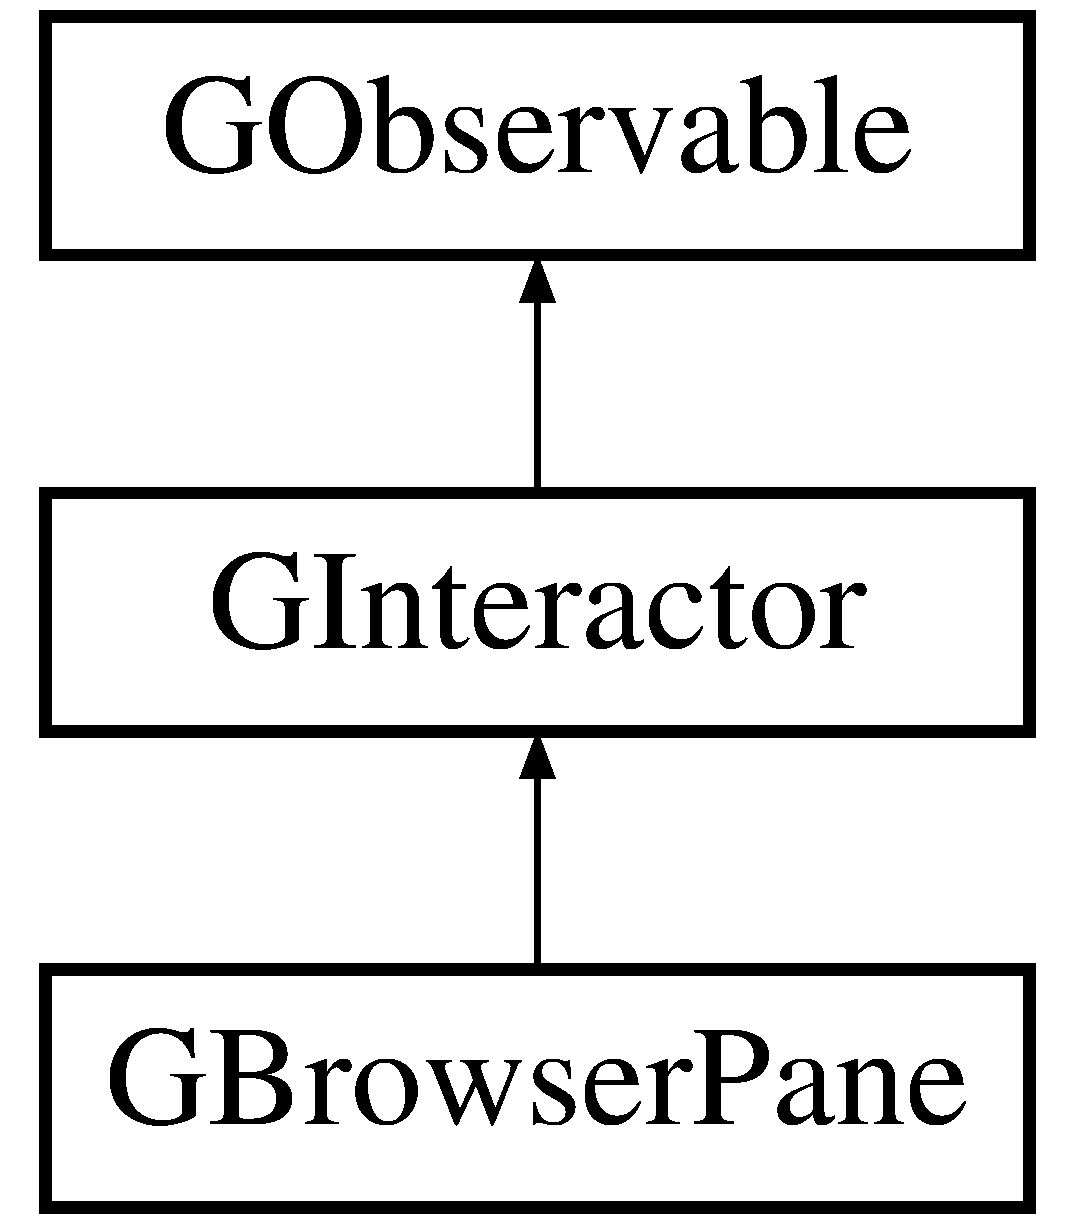
\includegraphics[height=3.000000cm]{classGBrowserPane}
\end{center}
\end{figure}
\subsection*{Public Types}
\begin{DoxyCompactItemize}
\item 
enum \mbox{\hyperlink{classGInteractor_a8e0d441725a81d2bbdebbea09078260e}{Text\+Position}} \{ \mbox{\hyperlink{classGInteractor_a8e0d441725a81d2bbdebbea09078260ea4cd6f2e7d5a08d6f4dc052df2358f774}{T\+E\+X\+T\+\_\+\+B\+E\+S\+I\+D\+E\+\_\+\+I\+C\+ON}}, 
\mbox{\hyperlink{classGInteractor_a8e0d441725a81d2bbdebbea09078260eaa88490f63d8de68d44c83bdb2ecde3b3}{T\+E\+X\+T\+\_\+\+U\+N\+D\+E\+R\+\_\+\+I\+C\+ON}}, 
\mbox{\hyperlink{classGInteractor_a8e0d441725a81d2bbdebbea09078260ea39a6f388a30ac4fefb6eb13e846bc9f2}{T\+E\+X\+T\+\_\+\+O\+N\+LY}}
 \}
\begin{DoxyCompactList}\small\item\em The places where an interactor can place its text relative to its icon. \end{DoxyCompactList}\end{DoxyCompactItemize}
\subsection*{Public Member Functions}
\begin{DoxyCompactItemize}
\item 
\mbox{\hyperlink{classGBrowserPane_a8f540c6f1aab2b4278bea6b1139aa470}{G\+Browser\+Pane}} (const std\+::string \&url=\char`\"{}\char`\"{}, Q\+Widget $\ast$parent=nullptr)
\begin{DoxyCompactList}\small\item\em Constructs a new browser pane. \end{DoxyCompactList}\item 
virtual \mbox{\hyperlink{classGBrowserPane_a93c1ee9e7da7c3a8e0ddfc40d65def4b}{$\sim$\+G\+Browser\+Pane}} ()
\item 
virtual void \mbox{\hyperlink{classGInteractor_a02f20ea6edfa0671f31c4c648a253833}{add\+Action\+Listener}} () Q\+\_\+\+D\+E\+C\+L\+\_\+\+D\+E\+P\+R\+E\+C\+A\+T\+ED
\begin{DoxyCompactList}\small\item\em Adds an event listener to be notified when this interactor is clicked or generally interacted with. \end{DoxyCompactList}\item 
virtual bool \mbox{\hyperlink{classGInteractor_ac05ba5b92e2e5146d416fe7f842a0969}{events\+Enabled}} () const Q\+\_\+\+D\+E\+C\+L\+\_\+\+O\+V\+E\+R\+R\+I\+DE
\begin{DoxyCompactList}\small\item\em Returns true if this interactor is currently accepting events. \end{DoxyCompactList}\item 
virtual std\+::string \mbox{\hyperlink{classGInteractor_a69f8d23ed8f207fbecad99960776e942}{get\+Accelerator}} () const
\begin{DoxyCompactList}\small\item\em Returns a string representing a hotkey for this interactor, or an empty string if no accelerator has been set. \end{DoxyCompactList}\item 
virtual std\+::string \mbox{\hyperlink{classGInteractor_a94eb4276000c4fdfb508ce9e6317a82a}{get\+Action\+Command}} () const
\begin{DoxyCompactList}\small\item\em Returns an action command for this interactor, which is a semi-\/unique string you can use to identify it when events occur. \end{DoxyCompactList}\item 
virtual std\+::string \mbox{\hyperlink{classGInteractor_a808e22cc1fdfbecf71ed8c64ef4600e0}{get\+Background}} () const
\begin{DoxyCompactList}\small\item\em Returns the background color of the interactor as a string. \end{DoxyCompactList}\item 
virtual int \mbox{\hyperlink{classGInteractor_a9e827257a55cb8cf4d9de2ec6bcfd7a0}{get\+Background\+Int}} () const
\begin{DoxyCompactList}\small\item\em Returns the background color of the interactor as an R\+GB integer. \end{DoxyCompactList}\item 
virtual \mbox{\hyperlink{classGRectangle}{G\+Rectangle}} \mbox{\hyperlink{classGInteractor_a29e6ac35a0b48f491a4c88194cc5da3b}{get\+Bounds}} () const
\begin{DoxyCompactList}\small\item\em Returns a rectangle representing the x/y position and size of this interactor. \end{DoxyCompactList}\item 
virtual std\+::string \mbox{\hyperlink{classGInteractor_aa061dfa488c31e18549d64363c1d0e34}{get\+Color}} () const
\begin{DoxyCompactList}\small\item\em Returns the foreground/text color of the interactor as a string. \end{DoxyCompactList}\item 
virtual int \mbox{\hyperlink{classGInteractor_a9635c7af766cdc3417f346683fa0e6c1}{get\+Color\+Int}} () const
\begin{DoxyCompactList}\small\item\em Returns the foreground/text color of the interactor as an R\+GB integer. \end{DoxyCompactList}\item 
virtual \mbox{\hyperlink{classGContainer}{G\+Container}} $\ast$ \mbox{\hyperlink{classGInteractor_a7a6e317c29d61030929b4cd2d1c00fe7}{get\+Container}} () const
\begin{DoxyCompactList}\small\item\em Returns a pointer to the onscreen container holding this interactor. \end{DoxyCompactList}\item 
virtual std\+::string \mbox{\hyperlink{classGBrowserPane_af3bc7daeceb5c8abfb8edaa1941e3757}{get\+Content\+Type}} () const
\begin{DoxyCompactList}\small\item\em Returns the M\+I\+ME content type for the current page. \end{DoxyCompactList}\item 
virtual std\+::string \mbox{\hyperlink{classGInteractor_a894a5502900794eeb27d084c21f1d77d}{get\+Font}} () const
\begin{DoxyCompactList}\small\item\em Returns the font of this interactor\textquotesingle{}s text as a font string such as \char`\"{}\+Helvetica-\/12-\/\+Bold\char`\"{}. \end{DoxyCompactList}\item 
virtual std\+::string \mbox{\hyperlink{classGInteractor_a4fa2d8b0192a3a5b4af4bbfe71194d03}{get\+Foreground}} () const
\begin{DoxyCompactList}\small\item\em Returns the foreground/text color of the interactor as a string. \end{DoxyCompactList}\item 
virtual int \mbox{\hyperlink{classGInteractor_ac3b12ab385a6ef9ae90fc879860ba726}{get\+Foreground\+Int}} () const
\begin{DoxyCompactList}\small\item\em Returns the foreground/text color of the interactor as an R\+GB integer. \end{DoxyCompactList}\item 
virtual double \mbox{\hyperlink{classGInteractor_a1e7e353362434072875264cf95629f99}{get\+Height}} () const
\begin{DoxyCompactList}\small\item\em Returns the current onscreen height of this interactor in pixels. \end{DoxyCompactList}\item 
virtual std\+::string \mbox{\hyperlink{classGInteractor_aaed62a73004939a64da6f0eb9eb64d73}{get\+Icon}} () const
\begin{DoxyCompactList}\small\item\em Returns the file name of the icon associated with this interactor, or an empty string if no icon has been set. \end{DoxyCompactList}\item 
virtual int \mbox{\hyperlink{classGInteractor_a9c9659a6c6ba66b4107ba59c95a24241}{get\+ID}} () const
\begin{DoxyCompactList}\small\item\em Returns a globally unique identifier for this interactor, which is set when the interactor is constructed. \end{DoxyCompactList}\item 
virtual \+\_\+\+Internal\+\_\+\+Q\+Widget $\ast$ \mbox{\hyperlink{classGBrowserPane_a208ce13c1da40bf0ddb509daf99d6588}{get\+Internal\+Widget}} () const Q\+\_\+\+D\+E\+C\+L\+\_\+\+O\+V\+E\+R\+R\+I\+DE
\begin{DoxyCompactList}\small\item\em Returns a direct pointer to the internal Qt widget being wrapped by this interactor. \end{DoxyCompactList}\item 
virtual \mbox{\hyperlink{classGPoint}{G\+Point}} \mbox{\hyperlink{classGInteractor_a4f83802015511edeb63b892830812c11}{get\+Location}} () const
\begin{DoxyCompactList}\small\item\em Returns an (x, y) point representing the onscreen location of the top-\/left corner of this interactor within its containing window. \end{DoxyCompactList}\item 
virtual double \mbox{\hyperlink{classGInteractor_aed4b0075fcc434499c3cb3e46896bda3}{get\+Minimum\+Height}} () const
\begin{DoxyCompactList}\small\item\em Returns the minimum height in pixels that this interactor will permit itself to be resized to. \end{DoxyCompactList}\item 
virtual \mbox{\hyperlink{classGDimension}{G\+Dimension}} \mbox{\hyperlink{classGInteractor_a66b5af0b32493b4d597ca0a3df2049ea}{get\+Minimum\+Size}} () const
\begin{DoxyCompactList}\small\item\em Returns a \mbox{\hyperlink{classGDimension}{G\+Dimension}} structure representing the minimum size in pixels that this interactor will permit itself to be resized to. \end{DoxyCompactList}\item 
virtual double \mbox{\hyperlink{classGInteractor_a59e668114fe3d49d2a0f28deb258f7c8}{get\+Minimum\+Width}} () const
\begin{DoxyCompactList}\small\item\em Returns the minimum width in pixels that this interactor will permit itself to be resized to. \end{DoxyCompactList}\item 
virtual std\+::string \mbox{\hyperlink{classGInteractor_a8a60438a5b55d0b2ceb35c8674b9d8c5}{get\+Name}} () const
\begin{DoxyCompactList}\small\item\em Returns a string representing a unique name for this interactor. \end{DoxyCompactList}\item 
virtual std\+::string \mbox{\hyperlink{classGBrowserPane_aa7607fcbc7eef6590fae7a2d513268de}{get\+Page\+Url}} () const
\begin{DoxyCompactList}\small\item\em Returns the U\+RL of the web page or file name being currently viewed. \end{DoxyCompactList}\item 
virtual double \mbox{\hyperlink{classGInteractor_a747de0961653847bdc6615dbf756d715}{get\+Preferred\+Height}} () const
\begin{DoxyCompactList}\small\item\em Returns the height in pixels that this interactor would prefer to be, which would exactly fit its contents with no stretching or scrollbars. \end{DoxyCompactList}\item 
virtual \mbox{\hyperlink{classGDimension}{G\+Dimension}} \mbox{\hyperlink{classGInteractor_a4aabbee761d8e9116275401131b7ccd1}{get\+Preferred\+Size}} () const
\begin{DoxyCompactList}\small\item\em Returns a \mbox{\hyperlink{classGDimension}{G\+Dimension}} structure storing the width and height in pixels that this interactor would prefer to be, which would exactly fit its contents with no stretching or scrollbars. \end{DoxyCompactList}\item 
virtual double \mbox{\hyperlink{classGInteractor_a82bca31d37700fb0e35d2743352efd5e}{get\+Preferred\+Width}} () const
\begin{DoxyCompactList}\small\item\em Returns the height in pixels that this interactor would prefer to be, which would exactly fit its contents with no stretching or scrollbars. \end{DoxyCompactList}\item 
virtual \mbox{\hyperlink{classGDimension}{G\+Dimension}} \mbox{\hyperlink{classGInteractor_a7b4eec96a2bdc6420695d5796a78eea9}{get\+Size}} () const
\begin{DoxyCompactList}\small\item\em Returns a \mbox{\hyperlink{classGDimension}{G\+Dimension}} structure storing the current onscreen width and height of this interactor in pixels. \end{DoxyCompactList}\item 
virtual std\+::string \mbox{\hyperlink{classGBrowserPane_aff553c50924b836c29f146ed34a7c6ec}{get\+Text}} () const
\begin{DoxyCompactList}\small\item\em Returns the full text of the current page or file being displayed in the pane. \end{DoxyCompactList}\item 
virtual std\+::string \mbox{\hyperlink{classGBrowserPane_a9896d58fcfebbf1025aeeb5b8b9ede80}{get\+Type}} () const Q\+\_\+\+D\+E\+C\+L\+\_\+\+O\+V\+E\+R\+R\+I\+DE
\begin{DoxyCompactList}\small\item\em Returns a string representing the class name of this interactor, such as \char`\"{}\+G\+Button\char`\"{} or \char`\"{}\+G\+Check\+Box\char`\"{}. \end{DoxyCompactList}\item 
virtual Q\+Widget $\ast$ \mbox{\hyperlink{classGBrowserPane_a326ee51b5561f807df7b29a1c101f7fd}{get\+Widget}} () const Q\+\_\+\+D\+E\+C\+L\+\_\+\+O\+V\+E\+R\+R\+I\+DE
\begin{DoxyCompactList}\small\item\em Returns a direct pointer to the internal Qt widget being wrapped by this interactor. \end{DoxyCompactList}\item 
virtual double \mbox{\hyperlink{classGInteractor_a0ed2965abd4f5701d2cadf71239faf19}{get\+Width}} () const
\begin{DoxyCompactList}\small\item\em Returns the current onscreen width of this interactor in pixels. \end{DoxyCompactList}\item 
virtual double \mbox{\hyperlink{classGInteractor_a344385751bee0720059403940d57a13e}{getX}} () const
\begin{DoxyCompactList}\small\item\em Returns the x-\/coordinate of the top-\/left pixel of this interactor within its onscreen window. \end{DoxyCompactList}\item 
virtual double \mbox{\hyperlink{classGInteractor_aafa51c7f8f38a09febbb9ce7853f77b4}{getY}} () const
\begin{DoxyCompactList}\small\item\em Returns the y-\/coordinate of the top-\/left pixel of this interactor within its onscreen window. \end{DoxyCompactList}\item 
virtual bool \mbox{\hyperlink{classGInteractor_afc480f652b8c5f1fb255e2269ce68879}{in\+Bounds}} (double x, double y) const
\begin{DoxyCompactList}\small\item\em Returns true if the given x/y pixel is within the bounds of this interactor. \end{DoxyCompactList}\item 
virtual bool \mbox{\hyperlink{classGInteractor_ae6d7982c1c627b677a5e776ca86118ed}{in\+Bounds}} (int x, int y) const
\begin{DoxyCompactList}\small\item\em Returns true if the given x/y pixel is within the bounds of this interactor. \end{DoxyCompactList}\item 
virtual bool \mbox{\hyperlink{classGInteractor_aacb819fb241851fd9fc045271baa4034}{is\+Enabled}} () const
\begin{DoxyCompactList}\small\item\em Returns true if this interactor is currently enabled. \end{DoxyCompactList}\item 
virtual bool \mbox{\hyperlink{classGInteractor_a9d8a6cfb13917785c143e74d40e4e2be}{is\+Visible}} () const
\begin{DoxyCompactList}\small\item\em Returns true if the interactor is visible on the screen. \end{DoxyCompactList}\item 
virtual void \mbox{\hyperlink{classGBrowserPane_a5e6d9158a9311204ca49518c32072ce0}{read\+Text\+From\+File}} (std\+::istream \&file)
\begin{DoxyCompactList}\small\item\em Reads text from the given file and displays the entire file\textquotesingle{}s text as the contents of this formatted pane. \end{DoxyCompactList}\item 
virtual void \mbox{\hyperlink{classGBrowserPane_a58c4154aa0c23bc980d45bf9de7cc95c}{read\+Text\+From\+File}} (const std\+::string \&filename)
\begin{DoxyCompactList}\small\item\em Reads text from the given file and displays the entire file\textquotesingle{}s text as the contents of this formatted pane. \end{DoxyCompactList}\item 
virtual void \mbox{\hyperlink{classGBrowserPane_a68ff415e722130964bc9e1de826f4869}{read\+Text\+From\+Url}} (const std\+::string \&url)
\begin{DoxyCompactList}\small\item\em Reads text from the given web page U\+RL and displays the entire page\textquotesingle{}s text as the contents of this formatted pane. \end{DoxyCompactList}\item 
virtual void \mbox{\hyperlink{classGBrowserPane_a263a2282597ca9f0f73301fb202ae390}{remove\+Link\+Listener}} ()
\begin{DoxyCompactList}\small\item\em Removes the link listener from the canvas so that it will no longer call it when hyperlink events occur. \end{DoxyCompactList}\item 
virtual void \mbox{\hyperlink{classGInteractor_a519fb2ac767f8b2febbb50b898b8c8cb}{request\+Focus}} ()
\begin{DoxyCompactList}\small\item\em Transfers keyboard focus to this interactor. \end{DoxyCompactList}\item 
virtual void \mbox{\hyperlink{classGInteractor_ad15f102f62e2960576012f1aa0ba4b2e}{set\+Accelerator}} (const std\+::string \&accelerator)
\begin{DoxyCompactList}\small\item\em Sets an accelerator hotkey for this interactor, such as \char`\"{}\+Ctrl-\/\+S\char`\"{}. \end{DoxyCompactList}\item 
virtual void \mbox{\hyperlink{classGInteractor_a4b5843fe3030e038a1ba54cc03389bcf}{set\+Action\+Command}} (const std\+::string \&action\+Command)
\begin{DoxyCompactList}\small\item\em Sets the action command for this interactor. \end{DoxyCompactList}\item 
virtual void \mbox{\hyperlink{classGInteractor_acba7e546c2025c0a15ca4b4cc92043db}{set\+Background}} (int rgb)
\begin{DoxyCompactList}\small\item\em Sets the background color of the interactor to the color represented by the given R\+GB integer. \end{DoxyCompactList}\item 
virtual void \mbox{\hyperlink{classGInteractor_ab4677ab2474e68b07aa56605af92a84a}{set\+Background}} (const std\+::string \&color)
\begin{DoxyCompactList}\small\item\em Sets the background color of the interactor to the color represented by the given string. \end{DoxyCompactList}\item 
virtual void \mbox{\hyperlink{classGInteractor_a2aae8197624b72265ab83b4f1bc73f2f}{set\+Bounds}} (double x, double y, double width, double height)
\begin{DoxyCompactList}\small\item\em Sets the size and location of the widget. \end{DoxyCompactList}\item 
virtual void \mbox{\hyperlink{classGInteractor_acada386653f008cacc7cce86426bef7c}{set\+Bounds}} (const \mbox{\hyperlink{classGRectangle}{G\+Rectangle}} \&size)
\begin{DoxyCompactList}\small\item\em Sets the size and location of the widget. \end{DoxyCompactList}\item 
virtual void \mbox{\hyperlink{classGInteractor_ab1f5cc0f5cc6bbbd716a526c61f1081d}{set\+Color}} (int rgb)
\begin{DoxyCompactList}\small\item\em Sets the foreground/text color of the interactor to the color represented by the given R\+GB integer. \end{DoxyCompactList}\item 
virtual void \mbox{\hyperlink{classGInteractor_a61374df6c11b52cfbb0815decdbaebc6}{set\+Color}} (const std\+::string \&color)
\begin{DoxyCompactList}\small\item\em Sets the foreground/text color of the interactor to the color represented by the given string. \end{DoxyCompactList}\item 
virtual void \mbox{\hyperlink{classGBrowserPane_a0ba11f3ad4f6257759f0db3dd791e6a4}{set\+Content\+Type}} (const std\+::string \&content\+Type)
\begin{DoxyCompactList}\small\item\em Sets the M\+I\+ME content type being used to display the current/future pages. \end{DoxyCompactList}\item 
virtual void \mbox{\hyperlink{classGInteractor_ab831367dd84bbd579e02e55bacb21343}{set\+Enabled}} (bool value)
\begin{DoxyCompactList}\small\item\em Sets whether this interactor is currently enabled. \end{DoxyCompactList}\item 
virtual void \mbox{\hyperlink{classGObservable_afaa30b2a9e0f378fd1c70d2f1d0b8216}{set\+Events\+Enabled}} (bool \mbox{\hyperlink{classGInteractor_ac05ba5b92e2e5146d416fe7f842a0969}{events\+Enabled}})
\begin{DoxyCompactList}\small\item\em Sets whether the object is currently allowing itself to fire events. \end{DoxyCompactList}\item 
virtual void \mbox{\hyperlink{classGInteractor_a2592348886ffea646c6534bf88f7c49d}{set\+Font}} (const Q\+Font \&font)
\begin{DoxyCompactList}\small\item\em Sets the font used by this widget to the given Qt font. \end{DoxyCompactList}\item 
virtual void \mbox{\hyperlink{classGInteractor_a8e096e8818d838aceae1d46d58fb3a7b}{set\+Font}} (const std\+::string \&font)
\begin{DoxyCompactList}\small\item\em Sets the font used by this widget to the font represented by the given font string, such as \char`\"{}\+Helvetica-\/16-\/\+Bold\char`\"{}. \end{DoxyCompactList}\item 
virtual void \mbox{\hyperlink{classGInteractor_a9eb856b5ff83a19df3831a31f15f4563}{set\+Foreground}} (int rgb)
\begin{DoxyCompactList}\small\item\em Sets the foreground/text color of the interactor to the color represented by the given R\+GB integer. \end{DoxyCompactList}\item 
virtual void \mbox{\hyperlink{classGInteractor_af59209aeadea6dfc6d97a2d8531f50e1}{set\+Foreground}} (const std\+::string \&color)
\begin{DoxyCompactList}\small\item\em Sets the foreground/text color of the interactor to the color represented by the given string. \end{DoxyCompactList}\item 
virtual void \mbox{\hyperlink{classGInteractor_a9e280bfc4544dfaf8e4376c4e1a74357}{set\+Height}} (double height)
\begin{DoxyCompactList}\small\item\em Sets the onscreen height of the interactor in pixels. \end{DoxyCompactList}\item 
virtual void \mbox{\hyperlink{classGInteractor_a762e139aa311461c3984d3ad28293f64}{set\+Icon}} (const std\+::string \&filename, bool retain\+Icon\+Size=true)
\begin{DoxyCompactList}\small\item\em Sets the file name of the icon associated with this interactor, or an empty string if no icon has been set. \end{DoxyCompactList}\item 
virtual void \mbox{\hyperlink{classGBrowserPane_aaa849c4aed1fa43178314f5c76e43081}{set\+Link\+Listener}} (G\+Event\+Listener func)
\begin{DoxyCompactList}\small\item\em Sets a link listener on this canvas so that it will be called when the user clicks on hyperlinks on the pane. \end{DoxyCompactList}\item 
virtual void \mbox{\hyperlink{classGBrowserPane_aca745635b2c4ceb74587ca5cfc26f0c3}{set\+Link\+Listener}} (G\+Event\+Listener\+Void func)
\begin{DoxyCompactList}\small\item\em Sets a link listener on this canvas so that it will be called when the user clicks on hyperlinks on the pane. \end{DoxyCompactList}\item 
virtual void \mbox{\hyperlink{classGInteractor_a04594e8ba9b98513a64f1da00dcae18c}{set\+Location}} (double x, double y)
\begin{DoxyCompactList}\small\item\em Sets the onscreen x/y-\/coordinate of the top-\/left corner of the interactor relative to its window. \end{DoxyCompactList}\item 
virtual void \mbox{\hyperlink{classGInteractor_a0cf428e207b7f22cc08138a90b1b87b2}{set\+Minimum\+Size}} (double width, double height)
\begin{DoxyCompactList}\small\item\em Sets the minimum size in pixels that this interactor will permit itself to be resized to. \end{DoxyCompactList}\item 
virtual void \mbox{\hyperlink{classGInteractor_a3b1046117ac6cb7abe467e00ba8a81f4}{set\+Minimum\+Size}} (const \mbox{\hyperlink{classGDimension}{G\+Dimension}} \&size)
\begin{DoxyCompactList}\small\item\em Sets the minimum size in pixels that this interactor will permit itself to be resized to. \end{DoxyCompactList}\item 
virtual void \mbox{\hyperlink{classGInteractor_a9d3a2685df23b5e7cbf59c19c4a1f9b5}{set\+Name}} (const std\+::string \&name)
\begin{DoxyCompactList}\small\item\em Sets a string representing a unique name for this interactor. \end{DoxyCompactList}\item 
virtual void \mbox{\hyperlink{classGInteractor_a1ab987704fce32098706c6f00fb08218}{set\+Preferred\+Height}} (double height)
\begin{DoxyCompactList}\small\item\em Sets the height in pixels that this interactor would prefer to be. \end{DoxyCompactList}\item 
virtual void \mbox{\hyperlink{classGInteractor_a042c5ae19430d765ef552371cae3632c}{set\+Preferred\+Size}} (double width, double height)
\begin{DoxyCompactList}\small\item\em Sets the width and height in pixels that this interactor would prefer to be. \end{DoxyCompactList}\item 
virtual void \mbox{\hyperlink{classGInteractor_aa22d9be4bc0e078bb0ea69b0fc9d7c75}{set\+Preferred\+Size}} (const \mbox{\hyperlink{classGDimension}{G\+Dimension}} \&size)
\begin{DoxyCompactList}\small\item\em Sets the size in pixels that this interactor would prefer to be. \end{DoxyCompactList}\item 
virtual void \mbox{\hyperlink{classGInteractor_a3db429ab2fa52efd187eec0ed8cdd9f2}{set\+Preferred\+Width}} (double width)
\begin{DoxyCompactList}\small\item\em Sets the width in pixels that this interactor would prefer to be. \end{DoxyCompactList}\item 
virtual void \mbox{\hyperlink{classGInteractor_aca25d49481f9bf5fc8f7df4c086c4ce7}{set\+Size}} (double width, double height)
\begin{DoxyCompactList}\small\item\em Sets the onscreen width and height of the interactor in pixels. \end{DoxyCompactList}\item 
virtual void \mbox{\hyperlink{classGInteractor_ae2b628228f192c2702c4ce941b2af68f}{set\+Size}} (const \mbox{\hyperlink{classGDimension}{G\+Dimension}} \&size)
\begin{DoxyCompactList}\small\item\em Sets the onscreen width and height of the interactor in pixels. \end{DoxyCompactList}\item 
virtual void \mbox{\hyperlink{classGBrowserPane_ac1ae51949d41ee9054634be5967d91b8}{set\+Text}} (const std\+::string \&text)
\begin{DoxyCompactList}\small\item\em Sets the pane to display to the given contents using its current content type. \end{DoxyCompactList}\item 
virtual void \mbox{\hyperlink{classGInteractor_a039e0e49beaecc275efce02d416acea8}{set\+Tooltip}} (const std\+::string \&tooltip\+Text)
\begin{DoxyCompactList}\small\item\em Sets a \char`\"{}tooltip\char`\"{} that will appear if the user hovers their mouse over the interactor. \end{DoxyCompactList}\item 
virtual void \mbox{\hyperlink{classGInteractor_a18e44e30b31525a243960ca3928125aa}{set\+Visible}} (bool visible)
\begin{DoxyCompactList}\small\item\em Returns true if the interactor is visible on the screen. \end{DoxyCompactList}\item 
virtual void \mbox{\hyperlink{classGInteractor_aa3f3fba4cb131baa8696ba01e3bceca1}{set\+Width}} (double width)
\begin{DoxyCompactList}\small\item\em Sets the onscreen width of the interactor in pixels. \end{DoxyCompactList}\item 
virtual void \mbox{\hyperlink{classGInteractor_a9c18fcc579333bf9653d13ad2b372e39}{setX}} (double x)
\begin{DoxyCompactList}\small\item\em Sets the onscreen x-\/coordinate of the top-\/left corner of the interactor relative to its window. \end{DoxyCompactList}\item 
virtual void \mbox{\hyperlink{classGInteractor_a7d57e2a5c35d27feb58fd498a3cf82b9}{setY}} (double y)
\begin{DoxyCompactList}\small\item\em Sets the onscreen y-\/coordinate of the top-\/left corner of the interactor relative to its window. \end{DoxyCompactList}\item 
virtual std\+::string \mbox{\hyperlink{classGObservable_a1fe5121d6528fdea3f243321b3fa3a49}{to\+String}} () const
\begin{DoxyCompactList}\small\item\em Returns a string representation of this observable object\textquotesingle{}s state. \end{DoxyCompactList}\end{DoxyCompactItemize}
\subsection*{Protected Member Functions}
\begin{DoxyCompactItemize}
\item 
virtual void \mbox{\hyperlink{classGObservable_a80cfa040459ff53594adbd6a51ec8f43}{clear\+Event\+Listeners}} ()
\begin{DoxyCompactList}\small\item\em Removes all event listeners from this object. \end{DoxyCompactList}\item 
virtual void \mbox{\hyperlink{classGObservable_a284f31528c0520f8e545c03ac9eeac74}{ensure\+Thread\+Safety}} (const std\+::string \&member\+Name=\char`\"{}\char`\"{})
\begin{DoxyCompactList}\small\item\em Ensures that we are currently in the Qt G\+UI thread. \end{DoxyCompactList}\item 
virtual void \mbox{\hyperlink{classGObservable_a63e5e5a6227c59c928493b11aceb0f67}{fire\+Event}} (\mbox{\hyperlink{classGEvent}{G\+Event}} \&event)
\begin{DoxyCompactList}\small\item\em Sends out the given event to any attached listeners. \end{DoxyCompactList}\item 
virtual void \mbox{\hyperlink{classGObservable_ab3983ea07337b52020a29cc00c653d8d}{fire\+G\+Event}} (Q\+Event $\ast$event, Event\+Type event\+Type, const std\+::string \&event\+Name)
\begin{DoxyCompactList}\small\item\em Creates an event of the given type, then sends it out to any attached listeners. \end{DoxyCompactList}\item 
virtual void \mbox{\hyperlink{classGObservable_a01fdf1b0e0dbd49e189fe4514e010411}{fire\+G\+Event}} (Q\+Close\+Event $\ast$event, Event\+Type event\+Type, const std\+::string \&event\+Name)
\begin{DoxyCompactList}\small\item\em Creates an event of the given type, then sends it out to any attached listeners. \end{DoxyCompactList}\item 
virtual void \mbox{\hyperlink{classGObservable_abb0b2f66ba39211cb5d7615e9d1c04e2}{fire\+G\+Event}} (Q\+Key\+Event $\ast$event, Event\+Type event\+Type, const std\+::string \&event\+Name)
\begin{DoxyCompactList}\small\item\em Creates an event of the given type, then sends it out to any attached listeners. \end{DoxyCompactList}\item 
virtual void \mbox{\hyperlink{classGObservable_a119318675d2165bdf7dd853aaf881d4b}{fire\+G\+Event}} (Q\+Mouse\+Event $\ast$event, Event\+Type event\+Type, const std\+::string \&event\+Name, const std\+::string \&action\+Command=\char`\"{}\char`\"{})
\begin{DoxyCompactList}\small\item\em Creates an event of the given type, then sends it out to any attached listeners. \end{DoxyCompactList}\item 
virtual void \mbox{\hyperlink{classGObservable_a63fd9034e1e1633c1c38eb342bfd34e9}{fire\+G\+Event}} (Q\+Resize\+Event $\ast$event, Event\+Type event\+Type, const std\+::string \&event\+Name)
\begin{DoxyCompactList}\small\item\em Creates an event of the given type, then sends it out to any attached listeners. \end{DoxyCompactList}\item 
virtual void \mbox{\hyperlink{classGObservable_a741345310d9b7c5170a6cbc410c44ac4}{fire\+G\+Event}} (Q\+Timer\+Event $\ast$event, Event\+Type event\+Type, const std\+::string \&event\+Name)
\begin{DoxyCompactList}\small\item\em Creates an event of the given type, then sends it out to any attached listeners. \end{DoxyCompactList}\item 
virtual void \mbox{\hyperlink{classGObservable_a93bf338968a0338761b8e4dc62f582e9}{fire\+G\+Event}} (Q\+Wheel\+Event $\ast$event, Event\+Type event\+Type, const std\+::string \&event\+Name)
\begin{DoxyCompactList}\small\item\em Creates an event of the given type, then sends it out to any attached listeners. \end{DoxyCompactList}\item 
virtual void \mbox{\hyperlink{classGObservable_a2a70a7d7435ff0c3b80bb4d70da19e0d}{fire\+G\+Event}} (Q\+Window\+State\+Change\+Event $\ast$event, Event\+Type event\+Type, const std\+::string \&event\+Name)
\begin{DoxyCompactList}\small\item\em Creates an event of the given type, then sends it out to any attached listeners. \end{DoxyCompactList}\item 
virtual bool \mbox{\hyperlink{classGObservable_a9f6faaa25942923bafa1c44020c49fa9}{has\+Event\+Listener}} (const std\+::string \&event\+Name) const
\begin{DoxyCompactList}\small\item\em Returns true if the observable object has a listener for the given type of event. \end{DoxyCompactList}\item 
virtual bool \mbox{\hyperlink{classGObservable_aeec1adc19aa0f33de62390686ee1382c}{is\+Accepting\+Event}} (int event\+Mask) const
\begin{DoxyCompactList}\small\item\em Returns true if the observable object has a listener for the given type of event. \end{DoxyCompactList}\item 
virtual bool \mbox{\hyperlink{classGObservable_aa31c73145a29dcb92848a92e0cfaea41}{is\+Accepting\+Event}} (const \mbox{\hyperlink{classGEvent}{G\+Event}} \&event) const
\begin{DoxyCompactList}\small\item\em Returns true if the observable object has a listener for the given type of event. \end{DoxyCompactList}\item 
virtual bool \mbox{\hyperlink{classGObservable_a3b1c689267eda44e65a2213e7de38b23}{is\+Accepting\+Event}} (const std\+::string \&event\+Type) const
\begin{DoxyCompactList}\small\item\em Returns true if the observable object has a listener for the given type of event. \end{DoxyCompactList}\item 
virtual void \mbox{\hyperlink{classGObservable_acbcf1ed3a851ad8a3c17ef38d86b481d}{remove\+Event\+Listener}} (const std\+::string \&event\+Name)
\begin{DoxyCompactList}\small\item\em Removes any event listener from this observable object that would respond to the given type of event, such as \char`\"{}click\char`\"{} or \char`\"{}keydown\char`\"{}. \end{DoxyCompactList}\item 
virtual void \mbox{\hyperlink{classGObservable_af51cc35c29a1bd1908609d432decdbb6}{remove\+Event\+Listeners}} (std\+::initializer\+\_\+list$<$ std\+::string $>$ event\+Names)
\begin{DoxyCompactList}\small\item\em Removes any event listener from this observable object that would respond to the given types of events, such as \char`\"{}click\char`\"{} or \char`\"{}keydown\char`\"{}. \end{DoxyCompactList}\item 
virtual void \mbox{\hyperlink{classGObservable_ad2f6d34961c50f6c1e0659990b79f741}{set\+Event\+Listener}} (const std\+::string \&event\+Name, G\+Event\+Listener func)
\begin{DoxyCompactList}\small\item\em Adds an event listener from this observable object to respond to the given type of event, such as \char`\"{}click\char`\"{} or \char`\"{}keydown\char`\"{}. \end{DoxyCompactList}\item 
virtual void \mbox{\hyperlink{classGObservable_abac4cb9f9e626e010e87f5d91573c8a5}{set\+Event\+Listener}} (const std\+::string \&event\+Name, G\+Event\+Listener\+Void func)
\begin{DoxyCompactList}\small\item\em Adds an event listener from this observable object to respond to the given type of event, such as \char`\"{}click\char`\"{} or \char`\"{}keydown\char`\"{}. \end{DoxyCompactList}\item 
virtual void \mbox{\hyperlink{classGObservable_afa388d69c33c718cf035774604065604}{set\+Event\+Listeners}} (std\+::initializer\+\_\+list$<$ std\+::string $>$ event\+Names, G\+Event\+Listener func)
\begin{DoxyCompactList}\small\item\em Adds an event listener from this observable object to respond to the given types of events, such as \char`\"{}click\char`\"{} or \char`\"{}keydown\char`\"{}. \end{DoxyCompactList}\item 
virtual void \mbox{\hyperlink{classGObservable_a7867184bbb686f74fae8a4db927da799}{set\+Event\+Listeners}} (std\+::initializer\+\_\+list$<$ std\+::string $>$ event\+Names, G\+Event\+Listener\+Void func)
\begin{DoxyCompactList}\small\item\em Adds an event listener from this observable object to respond to the given types of events, such as \char`\"{}click\char`\"{} or \char`\"{}keydown\char`\"{}. \end{DoxyCompactList}\end{DoxyCompactItemize}


\subsection{Detailed Description}
A \mbox{\hyperlink{classGBrowserPane}{G\+Browser\+Pane}} is a graphical interactor that displays a web page. 

This interactor is a wrapping around the Qt Q\+Text\+Browser widget, which is able to display rich content such as H\+T\+ML pages.

You can use \mbox{\hyperlink{classGBrowserPane}{G\+Browser\+Pane}} to implement the core rendering engine of a basic web browser, though it does not support all web browser features such as Java\+Script content, secure sessions, or cookies. 

\subsection{Member Enumeration Documentation}
\mbox{\Hypertarget{classGInteractor_a8e0d441725a81d2bbdebbea09078260e}\label{classGInteractor_a8e0d441725a81d2bbdebbea09078260e}} 
\index{G\+Browser\+Pane@{G\+Browser\+Pane}!Text\+Position@{Text\+Position}}
\index{Text\+Position@{Text\+Position}!G\+Browser\+Pane@{G\+Browser\+Pane}}
\subsubsection{\texorpdfstring{Text\+Position}{TextPosition}}
{\footnotesize\ttfamily enum \mbox{\hyperlink{classGInteractor_a8e0d441725a81d2bbdebbea09078260e}{Text\+Position}}\hspace{0.3cm}{\ttfamily [inherited]}}



The places where an interactor can place its text relative to its icon. 

\begin{DoxyEnumFields}{Enumerator}
\raisebox{\heightof{T}}[0pt][0pt]{\index{T\+E\+X\+T\+\_\+\+B\+E\+S\+I\+D\+E\+\_\+\+I\+C\+ON@{T\+E\+X\+T\+\_\+\+B\+E\+S\+I\+D\+E\+\_\+\+I\+C\+ON}!G\+Browser\+Pane@{G\+Browser\+Pane}}\index{G\+Browser\+Pane@{G\+Browser\+Pane}!T\+E\+X\+T\+\_\+\+B\+E\+S\+I\+D\+E\+\_\+\+I\+C\+ON@{T\+E\+X\+T\+\_\+\+B\+E\+S\+I\+D\+E\+\_\+\+I\+C\+ON}}}\mbox{\Hypertarget{classGInteractor_a8e0d441725a81d2bbdebbea09078260ea4cd6f2e7d5a08d6f4dc052df2358f774}\label{classGInteractor_a8e0d441725a81d2bbdebbea09078260ea4cd6f2e7d5a08d6f4dc052df2358f774}} 
T\+E\+X\+T\+\_\+\+B\+E\+S\+I\+D\+E\+\_\+\+I\+C\+ON&\\
\hline

\raisebox{\heightof{T}}[0pt][0pt]{\index{T\+E\+X\+T\+\_\+\+U\+N\+D\+E\+R\+\_\+\+I\+C\+ON@{T\+E\+X\+T\+\_\+\+U\+N\+D\+E\+R\+\_\+\+I\+C\+ON}!G\+Browser\+Pane@{G\+Browser\+Pane}}\index{G\+Browser\+Pane@{G\+Browser\+Pane}!T\+E\+X\+T\+\_\+\+U\+N\+D\+E\+R\+\_\+\+I\+C\+ON@{T\+E\+X\+T\+\_\+\+U\+N\+D\+E\+R\+\_\+\+I\+C\+ON}}}\mbox{\Hypertarget{classGInteractor_a8e0d441725a81d2bbdebbea09078260eaa88490f63d8de68d44c83bdb2ecde3b3}\label{classGInteractor_a8e0d441725a81d2bbdebbea09078260eaa88490f63d8de68d44c83bdb2ecde3b3}} 
T\+E\+X\+T\+\_\+\+U\+N\+D\+E\+R\+\_\+\+I\+C\+ON&\\
\hline

\raisebox{\heightof{T}}[0pt][0pt]{\index{T\+E\+X\+T\+\_\+\+O\+N\+LY@{T\+E\+X\+T\+\_\+\+O\+N\+LY}!G\+Browser\+Pane@{G\+Browser\+Pane}}\index{G\+Browser\+Pane@{G\+Browser\+Pane}!T\+E\+X\+T\+\_\+\+O\+N\+LY@{T\+E\+X\+T\+\_\+\+O\+N\+LY}}}\mbox{\Hypertarget{classGInteractor_a8e0d441725a81d2bbdebbea09078260ea39a6f388a30ac4fefb6eb13e846bc9f2}\label{classGInteractor_a8e0d441725a81d2bbdebbea09078260ea39a6f388a30ac4fefb6eb13e846bc9f2}} 
T\+E\+X\+T\+\_\+\+O\+N\+LY&\\
\hline

\end{DoxyEnumFields}


\subsection{Constructor \& Destructor Documentation}
\mbox{\Hypertarget{classGBrowserPane_a8f540c6f1aab2b4278bea6b1139aa470}\label{classGBrowserPane_a8f540c6f1aab2b4278bea6b1139aa470}} 
\index{G\+Browser\+Pane@{G\+Browser\+Pane}!G\+Browser\+Pane@{G\+Browser\+Pane}}
\index{G\+Browser\+Pane@{G\+Browser\+Pane}!G\+Browser\+Pane@{G\+Browser\+Pane}}
\subsubsection{\texorpdfstring{G\+Browser\+Pane()}{GBrowserPane()}}
{\footnotesize\ttfamily \mbox{\hyperlink{classGBrowserPane}{G\+Browser\+Pane}} (\begin{DoxyParamCaption}\item[{const std\+::string \&}]{url = {\ttfamily \char`\"{}\char`\"{}},  }\item[{Q\+Widget $\ast$}]{parent = {\ttfamily nullptr} }\end{DoxyParamCaption})}



Constructs a new browser pane. 

If a U\+RL string is passed, loads the data from that U\+RL. Otherwise, the pane is initially blank. \mbox{\Hypertarget{classGBrowserPane_a93c1ee9e7da7c3a8e0ddfc40d65def4b}\label{classGBrowserPane_a93c1ee9e7da7c3a8e0ddfc40d65def4b}} 
\index{G\+Browser\+Pane@{G\+Browser\+Pane}!````~G\+Browser\+Pane@{$\sim$\+G\+Browser\+Pane}}
\index{````~G\+Browser\+Pane@{$\sim$\+G\+Browser\+Pane}!G\+Browser\+Pane@{G\+Browser\+Pane}}
\subsubsection{\texorpdfstring{$\sim$\+G\+Browser\+Pane()}{~GBrowserPane()}}
{\footnotesize\ttfamily $\sim$\mbox{\hyperlink{classGBrowserPane}{G\+Browser\+Pane}} (\begin{DoxyParamCaption}{ }\end{DoxyParamCaption})\hspace{0.3cm}{\ttfamily [virtual]}}



\subsection{Member Function Documentation}
\mbox{\Hypertarget{classGInteractor_a02f20ea6edfa0671f31c4c648a253833}\label{classGInteractor_a02f20ea6edfa0671f31c4c648a253833}} 
\index{G\+Browser\+Pane@{G\+Browser\+Pane}!add\+Action\+Listener@{add\+Action\+Listener}}
\index{add\+Action\+Listener@{add\+Action\+Listener}!G\+Browser\+Pane@{G\+Browser\+Pane}}
\subsubsection{\texorpdfstring{add\+Action\+Listener()}{addActionListener()}}
{\footnotesize\ttfamily void add\+Action\+Listener (\begin{DoxyParamCaption}{ }\end{DoxyParamCaption})\hspace{0.3cm}{\ttfamily [virtual]}, {\ttfamily [inherited]}}



Adds an event listener to be notified when this interactor is clicked or generally interacted with. 

\begin{DoxyRefDesc}{Deprecated}
\item[\mbox{\hyperlink{deprecated__deprecated000006}{Deprecated}}]does nothing; use set\+Action\+Listener instead \end{DoxyRefDesc}
\mbox{\Hypertarget{classGObservable_a80cfa040459ff53594adbd6a51ec8f43}\label{classGObservable_a80cfa040459ff53594adbd6a51ec8f43}} 
\index{G\+Browser\+Pane@{G\+Browser\+Pane}!clear\+Event\+Listeners@{clear\+Event\+Listeners}}
\index{clear\+Event\+Listeners@{clear\+Event\+Listeners}!G\+Browser\+Pane@{G\+Browser\+Pane}}
\subsubsection{\texorpdfstring{clear\+Event\+Listeners()}{clearEventListeners()}}
{\footnotesize\ttfamily void clear\+Event\+Listeners (\begin{DoxyParamCaption}{ }\end{DoxyParamCaption})\hspace{0.3cm}{\ttfamily [protected]}, {\ttfamily [virtual]}, {\ttfamily [inherited]}}



Removes all event listeners from this object. 

\mbox{\Hypertarget{classGObservable_a284f31528c0520f8e545c03ac9eeac74}\label{classGObservable_a284f31528c0520f8e545c03ac9eeac74}} 
\index{G\+Browser\+Pane@{G\+Browser\+Pane}!ensure\+Thread\+Safety@{ensure\+Thread\+Safety}}
\index{ensure\+Thread\+Safety@{ensure\+Thread\+Safety}!G\+Browser\+Pane@{G\+Browser\+Pane}}
\subsubsection{\texorpdfstring{ensure\+Thread\+Safety()}{ensureThreadSafety()}}
{\footnotesize\ttfamily void ensure\+Thread\+Safety (\begin{DoxyParamCaption}\item[{const std\+::string \&}]{member\+Name = {\ttfamily \char`\"{}\char`\"{}} }\end{DoxyParamCaption})\hspace{0.3cm}{\ttfamily [protected]}, {\ttfamily [virtual]}, {\ttfamily [inherited]}}



Ensures that we are currently in the Qt G\+UI thread. 

\mbox{\Hypertarget{classGInteractor_ac05ba5b92e2e5146d416fe7f842a0969}\label{classGInteractor_ac05ba5b92e2e5146d416fe7f842a0969}} 
\index{G\+Browser\+Pane@{G\+Browser\+Pane}!events\+Enabled@{events\+Enabled}}
\index{events\+Enabled@{events\+Enabled}!G\+Browser\+Pane@{G\+Browser\+Pane}}
\subsubsection{\texorpdfstring{events\+Enabled()}{eventsEnabled()}}
{\footnotesize\ttfamily bool events\+Enabled (\begin{DoxyParamCaption}{ }\end{DoxyParamCaption}) const\hspace{0.3cm}{\ttfamily [virtual]}, {\ttfamily [inherited]}}



Returns true if this interactor is currently accepting events. 

Initially true. An interactor must be visible and added to an onscreen window to receive events. 

Reimplemented from \mbox{\hyperlink{classGObservable_a8ebb3da91032e7f4c34485dabc518b8a}{G\+Observable}}.

\mbox{\Hypertarget{classGObservable_a63e5e5a6227c59c928493b11aceb0f67}\label{classGObservable_a63e5e5a6227c59c928493b11aceb0f67}} 
\index{G\+Browser\+Pane@{G\+Browser\+Pane}!fire\+Event@{fire\+Event}}
\index{fire\+Event@{fire\+Event}!G\+Browser\+Pane@{G\+Browser\+Pane}}
\subsubsection{\texorpdfstring{fire\+Event()}{fireEvent()}}
{\footnotesize\ttfamily void fire\+Event (\begin{DoxyParamCaption}\item[{\mbox{\hyperlink{classGEvent}{G\+Event}} \&}]{event }\end{DoxyParamCaption})\hspace{0.3cm}{\ttfamily [protected]}, {\ttfamily [virtual]}, {\ttfamily [inherited]}}



Sends out the given event to any attached listeners. 

\mbox{\Hypertarget{classGObservable_ab3983ea07337b52020a29cc00c653d8d}\label{classGObservable_ab3983ea07337b52020a29cc00c653d8d}} 
\index{G\+Browser\+Pane@{G\+Browser\+Pane}!fire\+G\+Event@{fire\+G\+Event}}
\index{fire\+G\+Event@{fire\+G\+Event}!G\+Browser\+Pane@{G\+Browser\+Pane}}
\subsubsection{\texorpdfstring{fire\+G\+Event()}{fireGEvent()}\hspace{0.1cm}{\footnotesize\ttfamily [1/8]}}
{\footnotesize\ttfamily void fire\+G\+Event (\begin{DoxyParamCaption}\item[{Q\+Event $\ast$}]{event,  }\item[{Event\+Type}]{event\+Type,  }\item[{const std\+::string \&}]{event\+Name }\end{DoxyParamCaption})\hspace{0.3cm}{\ttfamily [protected]}, {\ttfamily [virtual]}, {\ttfamily [inherited]}}



Creates an event of the given type, then sends it out to any attached listeners. 

\mbox{\Hypertarget{classGObservable_a01fdf1b0e0dbd49e189fe4514e010411}\label{classGObservable_a01fdf1b0e0dbd49e189fe4514e010411}} 
\index{G\+Browser\+Pane@{G\+Browser\+Pane}!fire\+G\+Event@{fire\+G\+Event}}
\index{fire\+G\+Event@{fire\+G\+Event}!G\+Browser\+Pane@{G\+Browser\+Pane}}
\subsubsection{\texorpdfstring{fire\+G\+Event()}{fireGEvent()}\hspace{0.1cm}{\footnotesize\ttfamily [2/8]}}
{\footnotesize\ttfamily void fire\+G\+Event (\begin{DoxyParamCaption}\item[{Q\+Close\+Event $\ast$}]{event,  }\item[{Event\+Type}]{event\+Type,  }\item[{const std\+::string \&}]{event\+Name }\end{DoxyParamCaption})\hspace{0.3cm}{\ttfamily [protected]}, {\ttfamily [virtual]}, {\ttfamily [inherited]}}



Creates an event of the given type, then sends it out to any attached listeners. 

\mbox{\Hypertarget{classGObservable_abb0b2f66ba39211cb5d7615e9d1c04e2}\label{classGObservable_abb0b2f66ba39211cb5d7615e9d1c04e2}} 
\index{G\+Browser\+Pane@{G\+Browser\+Pane}!fire\+G\+Event@{fire\+G\+Event}}
\index{fire\+G\+Event@{fire\+G\+Event}!G\+Browser\+Pane@{G\+Browser\+Pane}}
\subsubsection{\texorpdfstring{fire\+G\+Event()}{fireGEvent()}\hspace{0.1cm}{\footnotesize\ttfamily [3/8]}}
{\footnotesize\ttfamily void fire\+G\+Event (\begin{DoxyParamCaption}\item[{Q\+Key\+Event $\ast$}]{event,  }\item[{Event\+Type}]{event\+Type,  }\item[{const std\+::string \&}]{event\+Name }\end{DoxyParamCaption})\hspace{0.3cm}{\ttfamily [protected]}, {\ttfamily [virtual]}, {\ttfamily [inherited]}}



Creates an event of the given type, then sends it out to any attached listeners. 

\mbox{\Hypertarget{classGObservable_a119318675d2165bdf7dd853aaf881d4b}\label{classGObservable_a119318675d2165bdf7dd853aaf881d4b}} 
\index{G\+Browser\+Pane@{G\+Browser\+Pane}!fire\+G\+Event@{fire\+G\+Event}}
\index{fire\+G\+Event@{fire\+G\+Event}!G\+Browser\+Pane@{G\+Browser\+Pane}}
\subsubsection{\texorpdfstring{fire\+G\+Event()}{fireGEvent()}\hspace{0.1cm}{\footnotesize\ttfamily [4/8]}}
{\footnotesize\ttfamily void fire\+G\+Event (\begin{DoxyParamCaption}\item[{Q\+Mouse\+Event $\ast$}]{event,  }\item[{Event\+Type}]{event\+Type,  }\item[{const std\+::string \&}]{event\+Name,  }\item[{const std\+::string \&}]{action\+Command = {\ttfamily \char`\"{}\char`\"{}} }\end{DoxyParamCaption})\hspace{0.3cm}{\ttfamily [protected]}, {\ttfamily [virtual]}, {\ttfamily [inherited]}}



Creates an event of the given type, then sends it out to any attached listeners. 

\mbox{\Hypertarget{classGObservable_a63fd9034e1e1633c1c38eb342bfd34e9}\label{classGObservable_a63fd9034e1e1633c1c38eb342bfd34e9}} 
\index{G\+Browser\+Pane@{G\+Browser\+Pane}!fire\+G\+Event@{fire\+G\+Event}}
\index{fire\+G\+Event@{fire\+G\+Event}!G\+Browser\+Pane@{G\+Browser\+Pane}}
\subsubsection{\texorpdfstring{fire\+G\+Event()}{fireGEvent()}\hspace{0.1cm}{\footnotesize\ttfamily [5/8]}}
{\footnotesize\ttfamily void fire\+G\+Event (\begin{DoxyParamCaption}\item[{Q\+Resize\+Event $\ast$}]{event,  }\item[{Event\+Type}]{event\+Type,  }\item[{const std\+::string \&}]{event\+Name }\end{DoxyParamCaption})\hspace{0.3cm}{\ttfamily [protected]}, {\ttfamily [virtual]}, {\ttfamily [inherited]}}



Creates an event of the given type, then sends it out to any attached listeners. 

\mbox{\Hypertarget{classGObservable_a741345310d9b7c5170a6cbc410c44ac4}\label{classGObservable_a741345310d9b7c5170a6cbc410c44ac4}} 
\index{G\+Browser\+Pane@{G\+Browser\+Pane}!fire\+G\+Event@{fire\+G\+Event}}
\index{fire\+G\+Event@{fire\+G\+Event}!G\+Browser\+Pane@{G\+Browser\+Pane}}
\subsubsection{\texorpdfstring{fire\+G\+Event()}{fireGEvent()}\hspace{0.1cm}{\footnotesize\ttfamily [6/8]}}
{\footnotesize\ttfamily void fire\+G\+Event (\begin{DoxyParamCaption}\item[{Q\+Timer\+Event $\ast$}]{event,  }\item[{Event\+Type}]{event\+Type,  }\item[{const std\+::string \&}]{event\+Name }\end{DoxyParamCaption})\hspace{0.3cm}{\ttfamily [protected]}, {\ttfamily [virtual]}, {\ttfamily [inherited]}}



Creates an event of the given type, then sends it out to any attached listeners. 

\mbox{\Hypertarget{classGObservable_a93bf338968a0338761b8e4dc62f582e9}\label{classGObservable_a93bf338968a0338761b8e4dc62f582e9}} 
\index{G\+Browser\+Pane@{G\+Browser\+Pane}!fire\+G\+Event@{fire\+G\+Event}}
\index{fire\+G\+Event@{fire\+G\+Event}!G\+Browser\+Pane@{G\+Browser\+Pane}}
\subsubsection{\texorpdfstring{fire\+G\+Event()}{fireGEvent()}\hspace{0.1cm}{\footnotesize\ttfamily [7/8]}}
{\footnotesize\ttfamily void fire\+G\+Event (\begin{DoxyParamCaption}\item[{Q\+Wheel\+Event $\ast$}]{event,  }\item[{Event\+Type}]{event\+Type,  }\item[{const std\+::string \&}]{event\+Name }\end{DoxyParamCaption})\hspace{0.3cm}{\ttfamily [protected]}, {\ttfamily [virtual]}, {\ttfamily [inherited]}}



Creates an event of the given type, then sends it out to any attached listeners. 

\mbox{\Hypertarget{classGObservable_a2a70a7d7435ff0c3b80bb4d70da19e0d}\label{classGObservable_a2a70a7d7435ff0c3b80bb4d70da19e0d}} 
\index{G\+Browser\+Pane@{G\+Browser\+Pane}!fire\+G\+Event@{fire\+G\+Event}}
\index{fire\+G\+Event@{fire\+G\+Event}!G\+Browser\+Pane@{G\+Browser\+Pane}}
\subsubsection{\texorpdfstring{fire\+G\+Event()}{fireGEvent()}\hspace{0.1cm}{\footnotesize\ttfamily [8/8]}}
{\footnotesize\ttfamily void fire\+G\+Event (\begin{DoxyParamCaption}\item[{Q\+Window\+State\+Change\+Event $\ast$}]{event,  }\item[{Event\+Type}]{event\+Type,  }\item[{const std\+::string \&}]{event\+Name }\end{DoxyParamCaption})\hspace{0.3cm}{\ttfamily [protected]}, {\ttfamily [virtual]}, {\ttfamily [inherited]}}



Creates an event of the given type, then sends it out to any attached listeners. 

\mbox{\Hypertarget{classGInteractor_a69f8d23ed8f207fbecad99960776e942}\label{classGInteractor_a69f8d23ed8f207fbecad99960776e942}} 
\index{G\+Browser\+Pane@{G\+Browser\+Pane}!get\+Accelerator@{get\+Accelerator}}
\index{get\+Accelerator@{get\+Accelerator}!G\+Browser\+Pane@{G\+Browser\+Pane}}
\subsubsection{\texorpdfstring{get\+Accelerator()}{getAccelerator()}}
{\footnotesize\ttfamily std\+::string get\+Accelerator (\begin{DoxyParamCaption}{ }\end{DoxyParamCaption}) const\hspace{0.3cm}{\ttfamily [virtual]}, {\ttfamily [inherited]}}



Returns a string representing a hotkey for this interactor, or an empty string if no accelerator has been set. 

\begin{DoxyReturn}{Returns}
an accelerator such as \char`\"{}\+Ctrl-\/\+S\char`\"{} 
\end{DoxyReturn}


Reimplemented in \mbox{\hyperlink{classGButton_a432ca43c59ffb2adc9cb66d43621bc27}{G\+Button}}.

\mbox{\Hypertarget{classGInteractor_a94eb4276000c4fdfb508ce9e6317a82a}\label{classGInteractor_a94eb4276000c4fdfb508ce9e6317a82a}} 
\index{G\+Browser\+Pane@{G\+Browser\+Pane}!get\+Action\+Command@{get\+Action\+Command}}
\index{get\+Action\+Command@{get\+Action\+Command}!G\+Browser\+Pane@{G\+Browser\+Pane}}
\subsubsection{\texorpdfstring{get\+Action\+Command()}{getActionCommand()}}
{\footnotesize\ttfamily std\+::string get\+Action\+Command (\begin{DoxyParamCaption}{ }\end{DoxyParamCaption}) const\hspace{0.3cm}{\ttfamily [virtual]}, {\ttfamily [inherited]}}



Returns an action command for this interactor, which is a semi-\/unique string you can use to identify it when events occur. 

For example, for buttons, the default action command is the button\textquotesingle{}s text. 

Reimplemented in \mbox{\hyperlink{classGChooser_a90f2b1e6f6e7dabd9d6e5307f7c6d1b7}{G\+Chooser}}, \mbox{\hyperlink{classGRadioButton_a90f2b1e6f6e7dabd9d6e5307f7c6d1b7}{G\+Radio\+Button}}, \mbox{\hyperlink{classGCheckBox_a90f2b1e6f6e7dabd9d6e5307f7c6d1b7}{G\+Check\+Box}}, and \mbox{\hyperlink{classGButton_a90f2b1e6f6e7dabd9d6e5307f7c6d1b7}{G\+Button}}.

\mbox{\Hypertarget{classGInteractor_a808e22cc1fdfbecf71ed8c64ef4600e0}\label{classGInteractor_a808e22cc1fdfbecf71ed8c64ef4600e0}} 
\index{G\+Browser\+Pane@{G\+Browser\+Pane}!get\+Background@{get\+Background}}
\index{get\+Background@{get\+Background}!G\+Browser\+Pane@{G\+Browser\+Pane}}
\subsubsection{\texorpdfstring{get\+Background()}{getBackground()}}
{\footnotesize\ttfamily std\+::string get\+Background (\begin{DoxyParamCaption}{ }\end{DoxyParamCaption}) const\hspace{0.3cm}{\ttfamily [virtual]}, {\ttfamily [inherited]}}



Returns the background color of the interactor as a string. 

\begin{DoxyReturn}{Returns}
a string such as \char`\"{}blue\char`\"{} or \char`\"{}\#7700ff\char`\"{} 
\end{DoxyReturn}


Reimplemented in \mbox{\hyperlink{classGCanvas_ab44f928b6bd7c8e4b82d5ed92bc3d4c6}{G\+Canvas}}.

\mbox{\Hypertarget{classGInteractor_a9e827257a55cb8cf4d9de2ec6bcfd7a0}\label{classGInteractor_a9e827257a55cb8cf4d9de2ec6bcfd7a0}} 
\index{G\+Browser\+Pane@{G\+Browser\+Pane}!get\+Background\+Int@{get\+Background\+Int}}
\index{get\+Background\+Int@{get\+Background\+Int}!G\+Browser\+Pane@{G\+Browser\+Pane}}
\subsubsection{\texorpdfstring{get\+Background\+Int()}{getBackgroundInt()}}
{\footnotesize\ttfamily int get\+Background\+Int (\begin{DoxyParamCaption}{ }\end{DoxyParamCaption}) const\hspace{0.3cm}{\ttfamily [virtual]}, {\ttfamily [inherited]}}



Returns the background color of the interactor as an R\+GB integer. 

\begin{DoxyReturn}{Returns}
an integer such as 0x7700ff 
\end{DoxyReturn}


Reimplemented in \mbox{\hyperlink{classGCanvas_af66f525e8154dbc8dcd2daecf3728ba9}{G\+Canvas}}.

\mbox{\Hypertarget{classGInteractor_a29e6ac35a0b48f491a4c88194cc5da3b}\label{classGInteractor_a29e6ac35a0b48f491a4c88194cc5da3b}} 
\index{G\+Browser\+Pane@{G\+Browser\+Pane}!get\+Bounds@{get\+Bounds}}
\index{get\+Bounds@{get\+Bounds}!G\+Browser\+Pane@{G\+Browser\+Pane}}
\subsubsection{\texorpdfstring{get\+Bounds()}{getBounds()}}
{\footnotesize\ttfamily \mbox{\hyperlink{classGRectangle}{G\+Rectangle}} get\+Bounds (\begin{DoxyParamCaption}{ }\end{DoxyParamCaption}) const\hspace{0.3cm}{\ttfamily [virtual]}, {\ttfamily [inherited]}}



Returns a rectangle representing the x/y position and size of this interactor. 

\mbox{\Hypertarget{classGInteractor_aa061dfa488c31e18549d64363c1d0e34}\label{classGInteractor_aa061dfa488c31e18549d64363c1d0e34}} 
\index{G\+Browser\+Pane@{G\+Browser\+Pane}!get\+Color@{get\+Color}}
\index{get\+Color@{get\+Color}!G\+Browser\+Pane@{G\+Browser\+Pane}}
\subsubsection{\texorpdfstring{get\+Color()}{getColor()}}
{\footnotesize\ttfamily std\+::string get\+Color (\begin{DoxyParamCaption}{ }\end{DoxyParamCaption}) const\hspace{0.3cm}{\ttfamily [virtual]}, {\ttfamily [inherited]}}



Returns the foreground/text color of the interactor as a string. 

Equivalent to get\+Foreground. \begin{DoxyReturn}{Returns}
a string such as \char`\"{}blue\char`\"{} or \char`\"{}\#7700ff\char`\"{} 
\end{DoxyReturn}
\mbox{\Hypertarget{classGInteractor_a9635c7af766cdc3417f346683fa0e6c1}\label{classGInteractor_a9635c7af766cdc3417f346683fa0e6c1}} 
\index{G\+Browser\+Pane@{G\+Browser\+Pane}!get\+Color\+Int@{get\+Color\+Int}}
\index{get\+Color\+Int@{get\+Color\+Int}!G\+Browser\+Pane@{G\+Browser\+Pane}}
\subsubsection{\texorpdfstring{get\+Color\+Int()}{getColorInt()}}
{\footnotesize\ttfamily int get\+Color\+Int (\begin{DoxyParamCaption}{ }\end{DoxyParamCaption}) const\hspace{0.3cm}{\ttfamily [virtual]}, {\ttfamily [inherited]}}



Returns the foreground/text color of the interactor as an R\+GB integer. 

Equivalent to get\+Foreground\+Int. \begin{DoxyReturn}{Returns}
an integer such as 0x7700ff 
\end{DoxyReturn}
\mbox{\Hypertarget{classGInteractor_a7a6e317c29d61030929b4cd2d1c00fe7}\label{classGInteractor_a7a6e317c29d61030929b4cd2d1c00fe7}} 
\index{G\+Browser\+Pane@{G\+Browser\+Pane}!get\+Container@{get\+Container}}
\index{get\+Container@{get\+Container}!G\+Browser\+Pane@{G\+Browser\+Pane}}
\subsubsection{\texorpdfstring{get\+Container()}{getContainer()}}
{\footnotesize\ttfamily \mbox{\hyperlink{classGContainer}{G\+Container}} $\ast$ get\+Container (\begin{DoxyParamCaption}{ }\end{DoxyParamCaption}) const\hspace{0.3cm}{\ttfamily [virtual]}, {\ttfamily [inherited]}}



Returns a pointer to the onscreen container holding this interactor. 

When an interactor is created, its container is initially null. This will become non-\/null automatically if you add the interactor to a window or other layout container. Interactors must be added to a container or window to receive events or to become visible on the screen. \begin{DoxyReturn}{Returns}
the container, or nullptr if interactor has not yet been added to any container 
\end{DoxyReturn}
\mbox{\Hypertarget{classGBrowserPane_af3bc7daeceb5c8abfb8edaa1941e3757}\label{classGBrowserPane_af3bc7daeceb5c8abfb8edaa1941e3757}} 
\index{G\+Browser\+Pane@{G\+Browser\+Pane}!get\+Content\+Type@{get\+Content\+Type}}
\index{get\+Content\+Type@{get\+Content\+Type}!G\+Browser\+Pane@{G\+Browser\+Pane}}
\subsubsection{\texorpdfstring{get\+Content\+Type()}{getContentType()}}
{\footnotesize\ttfamily std\+::string get\+Content\+Type (\begin{DoxyParamCaption}{ }\end{DoxyParamCaption}) const\hspace{0.3cm}{\ttfamily [virtual]}}



Returns the M\+I\+ME content type for the current page. 

The default content type is \char`\"{}text/html\char`\"{}. (If you need to look up the content type for a given file/page extension, consider using the Http\+Server\+::get\+Content\+Type(extension) function.) \mbox{\Hypertarget{classGInteractor_a894a5502900794eeb27d084c21f1d77d}\label{classGInteractor_a894a5502900794eeb27d084c21f1d77d}} 
\index{G\+Browser\+Pane@{G\+Browser\+Pane}!get\+Font@{get\+Font}}
\index{get\+Font@{get\+Font}!G\+Browser\+Pane@{G\+Browser\+Pane}}
\subsubsection{\texorpdfstring{get\+Font()}{getFont()}}
{\footnotesize\ttfamily std\+::string get\+Font (\begin{DoxyParamCaption}{ }\end{DoxyParamCaption}) const\hspace{0.3cm}{\ttfamily [virtual]}, {\ttfamily [inherited]}}



Returns the font of this interactor\textquotesingle{}s text as a font string such as \char`\"{}\+Helvetica-\/12-\/\+Bold\char`\"{}. 

\begin{DoxyReturn}{Returns}
a font string such as \char`\"{}\+Helvetica-\/12-\/\+Bold\char`\"{} 
\end{DoxyReturn}


Reimplemented in \mbox{\hyperlink{classGCanvas_a24420d98f18927d2c201a3ab55ffdcec}{G\+Canvas}}.

\mbox{\Hypertarget{classGInteractor_a4fa2d8b0192a3a5b4af4bbfe71194d03}\label{classGInteractor_a4fa2d8b0192a3a5b4af4bbfe71194d03}} 
\index{G\+Browser\+Pane@{G\+Browser\+Pane}!get\+Foreground@{get\+Foreground}}
\index{get\+Foreground@{get\+Foreground}!G\+Browser\+Pane@{G\+Browser\+Pane}}
\subsubsection{\texorpdfstring{get\+Foreground()}{getForeground()}}
{\footnotesize\ttfamily std\+::string get\+Foreground (\begin{DoxyParamCaption}{ }\end{DoxyParamCaption}) const\hspace{0.3cm}{\ttfamily [virtual]}, {\ttfamily [inherited]}}



Returns the foreground/text color of the interactor as a string. 

Equivalent to get\+Color. \begin{DoxyReturn}{Returns}
a string such as \char`\"{}blue\char`\"{} or \char`\"{}\#7700ff\char`\"{} 
\end{DoxyReturn}
\mbox{\Hypertarget{classGInteractor_ac3b12ab385a6ef9ae90fc879860ba726}\label{classGInteractor_ac3b12ab385a6ef9ae90fc879860ba726}} 
\index{G\+Browser\+Pane@{G\+Browser\+Pane}!get\+Foreground\+Int@{get\+Foreground\+Int}}
\index{get\+Foreground\+Int@{get\+Foreground\+Int}!G\+Browser\+Pane@{G\+Browser\+Pane}}
\subsubsection{\texorpdfstring{get\+Foreground\+Int()}{getForegroundInt()}}
{\footnotesize\ttfamily int get\+Foreground\+Int (\begin{DoxyParamCaption}{ }\end{DoxyParamCaption}) const\hspace{0.3cm}{\ttfamily [virtual]}, {\ttfamily [inherited]}}



Returns the foreground/text color of the interactor as an R\+GB integer. 

Equivalent to get\+Color\+Int. \begin{DoxyReturn}{Returns}
an integer such as 0x7700ff 
\end{DoxyReturn}
\mbox{\Hypertarget{classGInteractor_a1e7e353362434072875264cf95629f99}\label{classGInteractor_a1e7e353362434072875264cf95629f99}} 
\index{G\+Browser\+Pane@{G\+Browser\+Pane}!get\+Height@{get\+Height}}
\index{get\+Height@{get\+Height}!G\+Browser\+Pane@{G\+Browser\+Pane}}
\subsubsection{\texorpdfstring{get\+Height()}{getHeight()}}
{\footnotesize\ttfamily double get\+Height (\begin{DoxyParamCaption}{ }\end{DoxyParamCaption}) const\hspace{0.3cm}{\ttfamily [virtual]}, {\ttfamily [inherited]}}



Returns the current onscreen height of this interactor in pixels. 

\mbox{\Hypertarget{classGInteractor_aaed62a73004939a64da6f0eb9eb64d73}\label{classGInteractor_aaed62a73004939a64da6f0eb9eb64d73}} 
\index{G\+Browser\+Pane@{G\+Browser\+Pane}!get\+Icon@{get\+Icon}}
\index{get\+Icon@{get\+Icon}!G\+Browser\+Pane@{G\+Browser\+Pane}}
\subsubsection{\texorpdfstring{get\+Icon()}{getIcon()}}
{\footnotesize\ttfamily std\+::string get\+Icon (\begin{DoxyParamCaption}{ }\end{DoxyParamCaption}) const\hspace{0.3cm}{\ttfamily [virtual]}, {\ttfamily [inherited]}}



Returns the file name of the icon associated with this interactor, or an empty string if no icon has been set. 

Not all types of interactors support icons. \mbox{\Hypertarget{classGInteractor_a9c9659a6c6ba66b4107ba59c95a24241}\label{classGInteractor_a9c9659a6c6ba66b4107ba59c95a24241}} 
\index{G\+Browser\+Pane@{G\+Browser\+Pane}!get\+ID@{get\+ID}}
\index{get\+ID@{get\+ID}!G\+Browser\+Pane@{G\+Browser\+Pane}}
\subsubsection{\texorpdfstring{get\+I\+D()}{getID()}}
{\footnotesize\ttfamily int get\+ID (\begin{DoxyParamCaption}{ }\end{DoxyParamCaption}) const\hspace{0.3cm}{\ttfamily [virtual]}, {\ttfamily [inherited]}}



Returns a globally unique identifier for this interactor, which is set when the interactor is constructed. 

These I\+Ds can be useful for debugging to help identify interactors uniquely. \mbox{\Hypertarget{classGBrowserPane_a208ce13c1da40bf0ddb509daf99d6588}\label{classGBrowserPane_a208ce13c1da40bf0ddb509daf99d6588}} 
\index{G\+Browser\+Pane@{G\+Browser\+Pane}!get\+Internal\+Widget@{get\+Internal\+Widget}}
\index{get\+Internal\+Widget@{get\+Internal\+Widget}!G\+Browser\+Pane@{G\+Browser\+Pane}}
\subsubsection{\texorpdfstring{get\+Internal\+Widget()}{getInternalWidget()}}
{\footnotesize\ttfamily \+\_\+\+Internal\+\_\+\+Q\+Widget $\ast$ get\+Internal\+Widget (\begin{DoxyParamCaption}{ }\end{DoxyParamCaption}) const\hspace{0.3cm}{\ttfamily [virtual]}}



Returns a direct pointer to the internal Qt widget being wrapped by this interactor. 

This must be overridden by all interactor subclasses. Students/clients generally should not need to call this. 

Implements \mbox{\hyperlink{classGInteractor}{G\+Interactor}}.

\mbox{\Hypertarget{classGInteractor_a4f83802015511edeb63b892830812c11}\label{classGInteractor_a4f83802015511edeb63b892830812c11}} 
\index{G\+Browser\+Pane@{G\+Browser\+Pane}!get\+Location@{get\+Location}}
\index{get\+Location@{get\+Location}!G\+Browser\+Pane@{G\+Browser\+Pane}}
\subsubsection{\texorpdfstring{get\+Location()}{getLocation()}}
{\footnotesize\ttfamily \mbox{\hyperlink{classGPoint}{G\+Point}} get\+Location (\begin{DoxyParamCaption}{ }\end{DoxyParamCaption}) const\hspace{0.3cm}{\ttfamily [virtual]}, {\ttfamily [inherited]}}



Returns an (x, y) point representing the onscreen location of the top-\/left corner of this interactor within its containing window. 

\mbox{\Hypertarget{classGInteractor_aed4b0075fcc434499c3cb3e46896bda3}\label{classGInteractor_aed4b0075fcc434499c3cb3e46896bda3}} 
\index{G\+Browser\+Pane@{G\+Browser\+Pane}!get\+Minimum\+Height@{get\+Minimum\+Height}}
\index{get\+Minimum\+Height@{get\+Minimum\+Height}!G\+Browser\+Pane@{G\+Browser\+Pane}}
\subsubsection{\texorpdfstring{get\+Minimum\+Height()}{getMinimumHeight()}}
{\footnotesize\ttfamily double get\+Minimum\+Height (\begin{DoxyParamCaption}{ }\end{DoxyParamCaption}) const\hspace{0.3cm}{\ttfamily [virtual]}, {\ttfamily [inherited]}}



Returns the minimum height in pixels that this interactor will permit itself to be resized to. 

\mbox{\Hypertarget{classGInteractor_a66b5af0b32493b4d597ca0a3df2049ea}\label{classGInteractor_a66b5af0b32493b4d597ca0a3df2049ea}} 
\index{G\+Browser\+Pane@{G\+Browser\+Pane}!get\+Minimum\+Size@{get\+Minimum\+Size}}
\index{get\+Minimum\+Size@{get\+Minimum\+Size}!G\+Browser\+Pane@{G\+Browser\+Pane}}
\subsubsection{\texorpdfstring{get\+Minimum\+Size()}{getMinimumSize()}}
{\footnotesize\ttfamily \mbox{\hyperlink{classGDimension}{G\+Dimension}} get\+Minimum\+Size (\begin{DoxyParamCaption}{ }\end{DoxyParamCaption}) const\hspace{0.3cm}{\ttfamily [virtual]}, {\ttfamily [inherited]}}



Returns a \mbox{\hyperlink{classGDimension}{G\+Dimension}} structure representing the minimum size in pixels that this interactor will permit itself to be resized to. 

\mbox{\Hypertarget{classGInteractor_a59e668114fe3d49d2a0f28deb258f7c8}\label{classGInteractor_a59e668114fe3d49d2a0f28deb258f7c8}} 
\index{G\+Browser\+Pane@{G\+Browser\+Pane}!get\+Minimum\+Width@{get\+Minimum\+Width}}
\index{get\+Minimum\+Width@{get\+Minimum\+Width}!G\+Browser\+Pane@{G\+Browser\+Pane}}
\subsubsection{\texorpdfstring{get\+Minimum\+Width()}{getMinimumWidth()}}
{\footnotesize\ttfamily double get\+Minimum\+Width (\begin{DoxyParamCaption}{ }\end{DoxyParamCaption}) const\hspace{0.3cm}{\ttfamily [virtual]}, {\ttfamily [inherited]}}



Returns the minimum width in pixels that this interactor will permit itself to be resized to. 

\mbox{\Hypertarget{classGInteractor_a8a60438a5b55d0b2ceb35c8674b9d8c5}\label{classGInteractor_a8a60438a5b55d0b2ceb35c8674b9d8c5}} 
\index{G\+Browser\+Pane@{G\+Browser\+Pane}!get\+Name@{get\+Name}}
\index{get\+Name@{get\+Name}!G\+Browser\+Pane@{G\+Browser\+Pane}}
\subsubsection{\texorpdfstring{get\+Name()}{getName()}}
{\footnotesize\ttfamily std\+::string get\+Name (\begin{DoxyParamCaption}{ }\end{DoxyParamCaption}) const\hspace{0.3cm}{\ttfamily [virtual]}, {\ttfamily [inherited]}}



Returns a string representing a unique name for this interactor. 

The default name string uses the interactor\textquotesingle{}s type and its ID to make a string like \char`\"{}\+G\+Button\+\_\+14\char`\"{}, but you can override this by calling set\+Name. \begin{DoxyReturn}{Returns}
a string such as \char`\"{}\+G\+Button\+\_\+14\char`\"{} 
\end{DoxyReturn}
\mbox{\Hypertarget{classGBrowserPane_aa7607fcbc7eef6590fae7a2d513268de}\label{classGBrowserPane_aa7607fcbc7eef6590fae7a2d513268de}} 
\index{G\+Browser\+Pane@{G\+Browser\+Pane}!get\+Page\+Url@{get\+Page\+Url}}
\index{get\+Page\+Url@{get\+Page\+Url}!G\+Browser\+Pane@{G\+Browser\+Pane}}
\subsubsection{\texorpdfstring{get\+Page\+Url()}{getPageUrl()}}
{\footnotesize\ttfamily std\+::string get\+Page\+Url (\begin{DoxyParamCaption}{ }\end{DoxyParamCaption}) const\hspace{0.3cm}{\ttfamily [virtual]}}



Returns the U\+RL of the web page or file name being currently viewed. 

If no page or file has been loaded, returns an empty string. \mbox{\Hypertarget{classGInteractor_a747de0961653847bdc6615dbf756d715}\label{classGInteractor_a747de0961653847bdc6615dbf756d715}} 
\index{G\+Browser\+Pane@{G\+Browser\+Pane}!get\+Preferred\+Height@{get\+Preferred\+Height}}
\index{get\+Preferred\+Height@{get\+Preferred\+Height}!G\+Browser\+Pane@{G\+Browser\+Pane}}
\subsubsection{\texorpdfstring{get\+Preferred\+Height()}{getPreferredHeight()}}
{\footnotesize\ttfamily double get\+Preferred\+Height (\begin{DoxyParamCaption}{ }\end{DoxyParamCaption}) const\hspace{0.3cm}{\ttfamily [virtual]}, {\ttfamily [inherited]}}



Returns the height in pixels that this interactor would prefer to be, which would exactly fit its contents with no stretching or scrollbars. 

\mbox{\Hypertarget{classGInteractor_a4aabbee761d8e9116275401131b7ccd1}\label{classGInteractor_a4aabbee761d8e9116275401131b7ccd1}} 
\index{G\+Browser\+Pane@{G\+Browser\+Pane}!get\+Preferred\+Size@{get\+Preferred\+Size}}
\index{get\+Preferred\+Size@{get\+Preferred\+Size}!G\+Browser\+Pane@{G\+Browser\+Pane}}
\subsubsection{\texorpdfstring{get\+Preferred\+Size()}{getPreferredSize()}}
{\footnotesize\ttfamily \mbox{\hyperlink{classGDimension}{G\+Dimension}} get\+Preferred\+Size (\begin{DoxyParamCaption}{ }\end{DoxyParamCaption}) const\hspace{0.3cm}{\ttfamily [virtual]}, {\ttfamily [inherited]}}



Returns a \mbox{\hyperlink{classGDimension}{G\+Dimension}} structure storing the width and height in pixels that this interactor would prefer to be, which would exactly fit its contents with no stretching or scrollbars. 



Reimplemented in \mbox{\hyperlink{classGContainer_a21904b305edacd8f871d6951cb8d3fa5}{G\+Container}}.

\mbox{\Hypertarget{classGInteractor_a82bca31d37700fb0e35d2743352efd5e}\label{classGInteractor_a82bca31d37700fb0e35d2743352efd5e}} 
\index{G\+Browser\+Pane@{G\+Browser\+Pane}!get\+Preferred\+Width@{get\+Preferred\+Width}}
\index{get\+Preferred\+Width@{get\+Preferred\+Width}!G\+Browser\+Pane@{G\+Browser\+Pane}}
\subsubsection{\texorpdfstring{get\+Preferred\+Width()}{getPreferredWidth()}}
{\footnotesize\ttfamily double get\+Preferred\+Width (\begin{DoxyParamCaption}{ }\end{DoxyParamCaption}) const\hspace{0.3cm}{\ttfamily [virtual]}, {\ttfamily [inherited]}}



Returns the height in pixels that this interactor would prefer to be, which would exactly fit its contents with no stretching or scrollbars. 

\mbox{\Hypertarget{classGInteractor_a7b4eec96a2bdc6420695d5796a78eea9}\label{classGInteractor_a7b4eec96a2bdc6420695d5796a78eea9}} 
\index{G\+Browser\+Pane@{G\+Browser\+Pane}!get\+Size@{get\+Size}}
\index{get\+Size@{get\+Size}!G\+Browser\+Pane@{G\+Browser\+Pane}}
\subsubsection{\texorpdfstring{get\+Size()}{getSize()}}
{\footnotesize\ttfamily \mbox{\hyperlink{classGDimension}{G\+Dimension}} get\+Size (\begin{DoxyParamCaption}{ }\end{DoxyParamCaption}) const\hspace{0.3cm}{\ttfamily [virtual]}, {\ttfamily [inherited]}}



Returns a \mbox{\hyperlink{classGDimension}{G\+Dimension}} structure storing the current onscreen width and height of this interactor in pixels. 

\mbox{\Hypertarget{classGBrowserPane_aff553c50924b836c29f146ed34a7c6ec}\label{classGBrowserPane_aff553c50924b836c29f146ed34a7c6ec}} 
\index{G\+Browser\+Pane@{G\+Browser\+Pane}!get\+Text@{get\+Text}}
\index{get\+Text@{get\+Text}!G\+Browser\+Pane@{G\+Browser\+Pane}}
\subsubsection{\texorpdfstring{get\+Text()}{getText()}}
{\footnotesize\ttfamily std\+::string get\+Text (\begin{DoxyParamCaption}{ }\end{DoxyParamCaption}) const\hspace{0.3cm}{\ttfamily [virtual]}}



Returns the full text of the current page or file being displayed in the pane. 

This could be a fairly long string, depending on the page. Initially an empty string if no page or file has yet been loaded. \mbox{\Hypertarget{classGBrowserPane_a9896d58fcfebbf1025aeeb5b8b9ede80}\label{classGBrowserPane_a9896d58fcfebbf1025aeeb5b8b9ede80}} 
\index{G\+Browser\+Pane@{G\+Browser\+Pane}!get\+Type@{get\+Type}}
\index{get\+Type@{get\+Type}!G\+Browser\+Pane@{G\+Browser\+Pane}}
\subsubsection{\texorpdfstring{get\+Type()}{getType()}}
{\footnotesize\ttfamily std\+::string get\+Type (\begin{DoxyParamCaption}{ }\end{DoxyParamCaption}) const\hspace{0.3cm}{\ttfamily [virtual]}}



Returns a string representing the class name of this interactor, such as \char`\"{}\+G\+Button\char`\"{} or \char`\"{}\+G\+Check\+Box\char`\"{}. 

All subclasses of \mbox{\hyperlink{classGInteractor}{G\+Interactor}} must implement this method. \begin{DoxyReturn}{Returns}
a string such as \char`\"{}\+G\+Check\+Box\char`\"{} 
\end{DoxyReturn}


Implements \mbox{\hyperlink{classGInteractor_a799e073a127b428cc841086d42ea4fed}{G\+Interactor}}.

\mbox{\Hypertarget{classGBrowserPane_a326ee51b5561f807df7b29a1c101f7fd}\label{classGBrowserPane_a326ee51b5561f807df7b29a1c101f7fd}} 
\index{G\+Browser\+Pane@{G\+Browser\+Pane}!get\+Widget@{get\+Widget}}
\index{get\+Widget@{get\+Widget}!G\+Browser\+Pane@{G\+Browser\+Pane}}
\subsubsection{\texorpdfstring{get\+Widget()}{getWidget()}}
{\footnotesize\ttfamily Q\+Widget $\ast$ get\+Widget (\begin{DoxyParamCaption}{ }\end{DoxyParamCaption}) const\hspace{0.3cm}{\ttfamily [virtual]}}



Returns a direct pointer to the internal Qt widget being wrapped by this interactor. 

This must be overridden by all interactor subclasses. Students/clients generally should not need to call this. 

Implements \mbox{\hyperlink{classGInteractor}{G\+Interactor}}.

\mbox{\Hypertarget{classGInteractor_a0ed2965abd4f5701d2cadf71239faf19}\label{classGInteractor_a0ed2965abd4f5701d2cadf71239faf19}} 
\index{G\+Browser\+Pane@{G\+Browser\+Pane}!get\+Width@{get\+Width}}
\index{get\+Width@{get\+Width}!G\+Browser\+Pane@{G\+Browser\+Pane}}
\subsubsection{\texorpdfstring{get\+Width()}{getWidth()}}
{\footnotesize\ttfamily double get\+Width (\begin{DoxyParamCaption}{ }\end{DoxyParamCaption}) const\hspace{0.3cm}{\ttfamily [virtual]}, {\ttfamily [inherited]}}



Returns the current onscreen width of this interactor in pixels. 

\mbox{\Hypertarget{classGInteractor_a344385751bee0720059403940d57a13e}\label{classGInteractor_a344385751bee0720059403940d57a13e}} 
\index{G\+Browser\+Pane@{G\+Browser\+Pane}!getX@{getX}}
\index{getX@{getX}!G\+Browser\+Pane@{G\+Browser\+Pane}}
\subsubsection{\texorpdfstring{get\+X()}{getX()}}
{\footnotesize\ttfamily double getX (\begin{DoxyParamCaption}{ }\end{DoxyParamCaption}) const\hspace{0.3cm}{\ttfamily [virtual]}, {\ttfamily [inherited]}}



Returns the x-\/coordinate of the top-\/left pixel of this interactor within its onscreen window. 

\mbox{\Hypertarget{classGInteractor_aafa51c7f8f38a09febbb9ce7853f77b4}\label{classGInteractor_aafa51c7f8f38a09febbb9ce7853f77b4}} 
\index{G\+Browser\+Pane@{G\+Browser\+Pane}!getY@{getY}}
\index{getY@{getY}!G\+Browser\+Pane@{G\+Browser\+Pane}}
\subsubsection{\texorpdfstring{get\+Y()}{getY()}}
{\footnotesize\ttfamily double getY (\begin{DoxyParamCaption}{ }\end{DoxyParamCaption}) const\hspace{0.3cm}{\ttfamily [virtual]}, {\ttfamily [inherited]}}



Returns the y-\/coordinate of the top-\/left pixel of this interactor within its onscreen window. 

\mbox{\Hypertarget{classGObservable_a9f6faaa25942923bafa1c44020c49fa9}\label{classGObservable_a9f6faaa25942923bafa1c44020c49fa9}} 
\index{G\+Browser\+Pane@{G\+Browser\+Pane}!has\+Event\+Listener@{has\+Event\+Listener}}
\index{has\+Event\+Listener@{has\+Event\+Listener}!G\+Browser\+Pane@{G\+Browser\+Pane}}
\subsubsection{\texorpdfstring{has\+Event\+Listener()}{hasEventListener()}}
{\footnotesize\ttfamily bool has\+Event\+Listener (\begin{DoxyParamCaption}\item[{const std\+::string \&}]{event\+Name }\end{DoxyParamCaption}) const\hspace{0.3cm}{\ttfamily [protected]}, {\ttfamily [virtual]}, {\ttfamily [inherited]}}



Returns true if the observable object has a listener for the given type of event. 

\mbox{\Hypertarget{classGInteractor_afc480f652b8c5f1fb255e2269ce68879}\label{classGInteractor_afc480f652b8c5f1fb255e2269ce68879}} 
\index{G\+Browser\+Pane@{G\+Browser\+Pane}!in\+Bounds@{in\+Bounds}}
\index{in\+Bounds@{in\+Bounds}!G\+Browser\+Pane@{G\+Browser\+Pane}}
\subsubsection{\texorpdfstring{in\+Bounds()}{inBounds()}\hspace{0.1cm}{\footnotesize\ttfamily [1/2]}}
{\footnotesize\ttfamily bool in\+Bounds (\begin{DoxyParamCaption}\item[{double}]{x,  }\item[{double}]{y }\end{DoxyParamCaption}) const\hspace{0.3cm}{\ttfamily [virtual]}, {\ttfamily [inherited]}}



Returns true if the given x/y pixel is within the bounds of this interactor. 

\mbox{\Hypertarget{classGInteractor_ae6d7982c1c627b677a5e776ca86118ed}\label{classGInteractor_ae6d7982c1c627b677a5e776ca86118ed}} 
\index{G\+Browser\+Pane@{G\+Browser\+Pane}!in\+Bounds@{in\+Bounds}}
\index{in\+Bounds@{in\+Bounds}!G\+Browser\+Pane@{G\+Browser\+Pane}}
\subsubsection{\texorpdfstring{in\+Bounds()}{inBounds()}\hspace{0.1cm}{\footnotesize\ttfamily [2/2]}}
{\footnotesize\ttfamily bool in\+Bounds (\begin{DoxyParamCaption}\item[{int}]{x,  }\item[{int}]{y }\end{DoxyParamCaption}) const\hspace{0.3cm}{\ttfamily [virtual]}, {\ttfamily [inherited]}}



Returns true if the given x/y pixel is within the bounds of this interactor. 



Reimplemented in \mbox{\hyperlink{classGTable_afa6b6241d2f7af75f2d1345f46acfc35}{G\+Table}}.

\mbox{\Hypertarget{classGObservable_aeec1adc19aa0f33de62390686ee1382c}\label{classGObservable_aeec1adc19aa0f33de62390686ee1382c}} 
\index{G\+Browser\+Pane@{G\+Browser\+Pane}!is\+Accepting\+Event@{is\+Accepting\+Event}}
\index{is\+Accepting\+Event@{is\+Accepting\+Event}!G\+Browser\+Pane@{G\+Browser\+Pane}}
\subsubsection{\texorpdfstring{is\+Accepting\+Event()}{isAcceptingEvent()}\hspace{0.1cm}{\footnotesize\ttfamily [1/3]}}
{\footnotesize\ttfamily bool is\+Accepting\+Event (\begin{DoxyParamCaption}\item[{int}]{event\+Mask }\end{DoxyParamCaption}) const\hspace{0.3cm}{\ttfamily [protected]}, {\ttfamily [virtual]}, {\ttfamily [inherited]}}



Returns true if the observable object has a listener for the given type of event. 

See \mbox{\hyperlink{gevent_8h_source}{gevent.\+h}} for event types and masks. \mbox{\Hypertarget{classGObservable_aa31c73145a29dcb92848a92e0cfaea41}\label{classGObservable_aa31c73145a29dcb92848a92e0cfaea41}} 
\index{G\+Browser\+Pane@{G\+Browser\+Pane}!is\+Accepting\+Event@{is\+Accepting\+Event}}
\index{is\+Accepting\+Event@{is\+Accepting\+Event}!G\+Browser\+Pane@{G\+Browser\+Pane}}
\subsubsection{\texorpdfstring{is\+Accepting\+Event()}{isAcceptingEvent()}\hspace{0.1cm}{\footnotesize\ttfamily [2/3]}}
{\footnotesize\ttfamily bool is\+Accepting\+Event (\begin{DoxyParamCaption}\item[{const \mbox{\hyperlink{classGEvent}{G\+Event}} \&}]{event }\end{DoxyParamCaption}) const\hspace{0.3cm}{\ttfamily [protected]}, {\ttfamily [virtual]}, {\ttfamily [inherited]}}



Returns true if the observable object has a listener for the given type of event. 

\mbox{\Hypertarget{classGObservable_a3b1c689267eda44e65a2213e7de38b23}\label{classGObservable_a3b1c689267eda44e65a2213e7de38b23}} 
\index{G\+Browser\+Pane@{G\+Browser\+Pane}!is\+Accepting\+Event@{is\+Accepting\+Event}}
\index{is\+Accepting\+Event@{is\+Accepting\+Event}!G\+Browser\+Pane@{G\+Browser\+Pane}}
\subsubsection{\texorpdfstring{is\+Accepting\+Event()}{isAcceptingEvent()}\hspace{0.1cm}{\footnotesize\ttfamily [3/3]}}
{\footnotesize\ttfamily bool is\+Accepting\+Event (\begin{DoxyParamCaption}\item[{const std\+::string \&}]{event\+Type }\end{DoxyParamCaption}) const\hspace{0.3cm}{\ttfamily [protected]}, {\ttfamily [virtual]}, {\ttfamily [inherited]}}



Returns true if the observable object has a listener for the given type of event. 

\mbox{\Hypertarget{classGInteractor_aacb819fb241851fd9fc045271baa4034}\label{classGInteractor_aacb819fb241851fd9fc045271baa4034}} 
\index{G\+Browser\+Pane@{G\+Browser\+Pane}!is\+Enabled@{is\+Enabled}}
\index{is\+Enabled@{is\+Enabled}!G\+Browser\+Pane@{G\+Browser\+Pane}}
\subsubsection{\texorpdfstring{is\+Enabled()}{isEnabled()}}
{\footnotesize\ttfamily bool is\+Enabled (\begin{DoxyParamCaption}{ }\end{DoxyParamCaption}) const\hspace{0.3cm}{\ttfamily [virtual]}, {\ttfamily [inherited]}}



Returns true if this interactor is currently enabled. 

Most interactors begin as enabled but can be disabled to stop them from being able to be clicked on or otherwise emit events. \mbox{\Hypertarget{classGInteractor_a9d8a6cfb13917785c143e74d40e4e2be}\label{classGInteractor_a9d8a6cfb13917785c143e74d40e4e2be}} 
\index{G\+Browser\+Pane@{G\+Browser\+Pane}!is\+Visible@{is\+Visible}}
\index{is\+Visible@{is\+Visible}!G\+Browser\+Pane@{G\+Browser\+Pane}}
\subsubsection{\texorpdfstring{is\+Visible()}{isVisible()}}
{\footnotesize\ttfamily bool is\+Visible (\begin{DoxyParamCaption}{ }\end{DoxyParamCaption}) const\hspace{0.3cm}{\ttfamily [virtual]}, {\ttfamily [inherited]}}



Returns true if the interactor is visible on the screen. 

Interactors will not be visible until they are added to an onscreen window or container. \mbox{\Hypertarget{classGBrowserPane_a5e6d9158a9311204ca49518c32072ce0}\label{classGBrowserPane_a5e6d9158a9311204ca49518c32072ce0}} 
\index{G\+Browser\+Pane@{G\+Browser\+Pane}!read\+Text\+From\+File@{read\+Text\+From\+File}}
\index{read\+Text\+From\+File@{read\+Text\+From\+File}!G\+Browser\+Pane@{G\+Browser\+Pane}}
\subsubsection{\texorpdfstring{read\+Text\+From\+File()}{readTextFromFile()}\hspace{0.1cm}{\footnotesize\ttfamily [1/2]}}
{\footnotesize\ttfamily void read\+Text\+From\+File (\begin{DoxyParamCaption}\item[{std\+::istream \&}]{file }\end{DoxyParamCaption})\hspace{0.3cm}{\ttfamily [virtual]}}



Reads text from the given file and displays the entire file\textquotesingle{}s text as the contents of this formatted pane. 

The pane will try to display the content in the best appropriate format, such as rendering basic H\+T\+ML content with formatting intact. If the file cannot be read, sets the pane\textquotesingle{}s text to be empty. \mbox{\Hypertarget{classGBrowserPane_a58c4154aa0c23bc980d45bf9de7cc95c}\label{classGBrowserPane_a58c4154aa0c23bc980d45bf9de7cc95c}} 
\index{G\+Browser\+Pane@{G\+Browser\+Pane}!read\+Text\+From\+File@{read\+Text\+From\+File}}
\index{read\+Text\+From\+File@{read\+Text\+From\+File}!G\+Browser\+Pane@{G\+Browser\+Pane}}
\subsubsection{\texorpdfstring{read\+Text\+From\+File()}{readTextFromFile()}\hspace{0.1cm}{\footnotesize\ttfamily [2/2]}}
{\footnotesize\ttfamily void read\+Text\+From\+File (\begin{DoxyParamCaption}\item[{const std\+::string \&}]{filename }\end{DoxyParamCaption})\hspace{0.3cm}{\ttfamily [virtual]}}



Reads text from the given file and displays the entire file\textquotesingle{}s text as the contents of this formatted pane. 

The pane will try to display the content in the best appropriate format, such as rendering basic H\+T\+ML content with formatting intact. If the file does not exist or cannot be read, sets the pane\textquotesingle{}s text to be empty. \mbox{\Hypertarget{classGBrowserPane_a68ff415e722130964bc9e1de826f4869}\label{classGBrowserPane_a68ff415e722130964bc9e1de826f4869}} 
\index{G\+Browser\+Pane@{G\+Browser\+Pane}!read\+Text\+From\+Url@{read\+Text\+From\+Url}}
\index{read\+Text\+From\+Url@{read\+Text\+From\+Url}!G\+Browser\+Pane@{G\+Browser\+Pane}}
\subsubsection{\texorpdfstring{read\+Text\+From\+Url()}{readTextFromUrl()}}
{\footnotesize\ttfamily void read\+Text\+From\+Url (\begin{DoxyParamCaption}\item[{const std\+::string \&}]{url }\end{DoxyParamCaption})\hspace{0.3cm}{\ttfamily [virtual]}}



Reads text from the given web page U\+RL and displays the entire page\textquotesingle{}s text as the contents of this formatted pane. 

If the page does not exist or cannot be read, sets the pane\textquotesingle{}s text to be empty. \mbox{\Hypertarget{classGObservable_acbcf1ed3a851ad8a3c17ef38d86b481d}\label{classGObservable_acbcf1ed3a851ad8a3c17ef38d86b481d}} 
\index{G\+Browser\+Pane@{G\+Browser\+Pane}!remove\+Event\+Listener@{remove\+Event\+Listener}}
\index{remove\+Event\+Listener@{remove\+Event\+Listener}!G\+Browser\+Pane@{G\+Browser\+Pane}}
\subsubsection{\texorpdfstring{remove\+Event\+Listener()}{removeEventListener()}}
{\footnotesize\ttfamily void remove\+Event\+Listener (\begin{DoxyParamCaption}\item[{const std\+::string \&}]{event\+Name }\end{DoxyParamCaption})\hspace{0.3cm}{\ttfamily [protected]}, {\ttfamily [virtual]}, {\ttfamily [inherited]}}



Removes any event listener from this observable object that would respond to the given type of event, such as \char`\"{}click\char`\"{} or \char`\"{}keydown\char`\"{}. 

\mbox{\Hypertarget{classGObservable_af51cc35c29a1bd1908609d432decdbb6}\label{classGObservable_af51cc35c29a1bd1908609d432decdbb6}} 
\index{G\+Browser\+Pane@{G\+Browser\+Pane}!remove\+Event\+Listeners@{remove\+Event\+Listeners}}
\index{remove\+Event\+Listeners@{remove\+Event\+Listeners}!G\+Browser\+Pane@{G\+Browser\+Pane}}
\subsubsection{\texorpdfstring{remove\+Event\+Listeners()}{removeEventListeners()}}
{\footnotesize\ttfamily void remove\+Event\+Listeners (\begin{DoxyParamCaption}\item[{std\+::initializer\+\_\+list$<$ std\+::string $>$}]{event\+Names }\end{DoxyParamCaption})\hspace{0.3cm}{\ttfamily [protected]}, {\ttfamily [virtual]}, {\ttfamily [inherited]}}



Removes any event listener from this observable object that would respond to the given types of events, such as \char`\"{}click\char`\"{} or \char`\"{}keydown\char`\"{}. 

\mbox{\Hypertarget{classGBrowserPane_a263a2282597ca9f0f73301fb202ae390}\label{classGBrowserPane_a263a2282597ca9f0f73301fb202ae390}} 
\index{G\+Browser\+Pane@{G\+Browser\+Pane}!remove\+Link\+Listener@{remove\+Link\+Listener}}
\index{remove\+Link\+Listener@{remove\+Link\+Listener}!G\+Browser\+Pane@{G\+Browser\+Pane}}
\subsubsection{\texorpdfstring{remove\+Link\+Listener()}{removeLinkListener()}}
{\footnotesize\ttfamily void remove\+Link\+Listener (\begin{DoxyParamCaption}{ }\end{DoxyParamCaption})\hspace{0.3cm}{\ttfamily [virtual]}}



Removes the link listener from the canvas so that it will no longer call it when hyperlink events occur. 

\mbox{\Hypertarget{classGInteractor_a519fb2ac767f8b2febbb50b898b8c8cb}\label{classGInteractor_a519fb2ac767f8b2febbb50b898b8c8cb}} 
\index{G\+Browser\+Pane@{G\+Browser\+Pane}!request\+Focus@{request\+Focus}}
\index{request\+Focus@{request\+Focus}!G\+Browser\+Pane@{G\+Browser\+Pane}}
\subsubsection{\texorpdfstring{request\+Focus()}{requestFocus()}}
{\footnotesize\ttfamily void request\+Focus (\begin{DoxyParamCaption}{ }\end{DoxyParamCaption})\hspace{0.3cm}{\ttfamily [virtual]}, {\ttfamily [inherited]}}



Transfers keyboard focus to this interactor. 



Reimplemented in \mbox{\hyperlink{classGTable_a49b39e0eeaf5af829e8956e9055c5cdc}{G\+Table}}.

\mbox{\Hypertarget{classGInteractor_ad15f102f62e2960576012f1aa0ba4b2e}\label{classGInteractor_ad15f102f62e2960576012f1aa0ba4b2e}} 
\index{G\+Browser\+Pane@{G\+Browser\+Pane}!set\+Accelerator@{set\+Accelerator}}
\index{set\+Accelerator@{set\+Accelerator}!G\+Browser\+Pane@{G\+Browser\+Pane}}
\subsubsection{\texorpdfstring{set\+Accelerator()}{setAccelerator()}}
{\footnotesize\ttfamily void set\+Accelerator (\begin{DoxyParamCaption}\item[{const std\+::string \&}]{accelerator }\end{DoxyParamCaption})\hspace{0.3cm}{\ttfamily [virtual]}, {\ttfamily [inherited]}}



Sets an accelerator hotkey for this interactor, such as \char`\"{}\+Ctrl-\/\+S\char`\"{}. 

Not all interactor types support accelerators. 
\begin{DoxyParams}{Parameters}
{\em accelerator} & a hotkey such as \char`\"{}\+Ctrl-\/\+S\char`\"{} \\
\hline
\end{DoxyParams}


Reimplemented in \mbox{\hyperlink{classGButton_a5f78fc506a33b57dced42a419be34446}{G\+Button}}.

\mbox{\Hypertarget{classGInteractor_a4b5843fe3030e038a1ba54cc03389bcf}\label{classGInteractor_a4b5843fe3030e038a1ba54cc03389bcf}} 
\index{G\+Browser\+Pane@{G\+Browser\+Pane}!set\+Action\+Command@{set\+Action\+Command}}
\index{set\+Action\+Command@{set\+Action\+Command}!G\+Browser\+Pane@{G\+Browser\+Pane}}
\subsubsection{\texorpdfstring{set\+Action\+Command()}{setActionCommand()}}
{\footnotesize\ttfamily void set\+Action\+Command (\begin{DoxyParamCaption}\item[{const std\+::string \&}]{action\+Command }\end{DoxyParamCaption})\hspace{0.3cm}{\ttfamily [virtual]}, {\ttfamily [inherited]}}



Sets the action command for this interactor. 

The action command is meant to be a semi-\/unique string you can use to identify the interactor when events occur. For example, for buttons, the default action command is the button\textquotesingle{}s text, but you can change it to a different string if you prefer. The main usage of this feature is if you want to use the same function as an event listener for many interactors, you can use the action command to help distinguish which interactor generates each event. \mbox{\Hypertarget{classGInteractor_acba7e546c2025c0a15ca4b4cc92043db}\label{classGInteractor_acba7e546c2025c0a15ca4b4cc92043db}} 
\index{G\+Browser\+Pane@{G\+Browser\+Pane}!set\+Background@{set\+Background}}
\index{set\+Background@{set\+Background}!G\+Browser\+Pane@{G\+Browser\+Pane}}
\subsubsection{\texorpdfstring{set\+Background()}{setBackground()}\hspace{0.1cm}{\footnotesize\ttfamily [1/2]}}
{\footnotesize\ttfamily void set\+Background (\begin{DoxyParamCaption}\item[{int}]{rgb }\end{DoxyParamCaption})\hspace{0.3cm}{\ttfamily [virtual]}, {\ttfamily [inherited]}}



Sets the background color of the interactor to the color represented by the given R\+GB integer. 


\begin{DoxyParams}{Parameters}
{\em rgb} & an R\+GB integer such as 0x7700ff \\
\hline
\end{DoxyParams}


Reimplemented in \mbox{\hyperlink{classGCanvas_a427fefbbc34e39e5df27a807da488e0d}{G\+Canvas}}, and \mbox{\hyperlink{classGTable_ac45b8a90f31752385a98a034a58547c7}{G\+Table}}.

\mbox{\Hypertarget{classGInteractor_ab4677ab2474e68b07aa56605af92a84a}\label{classGInteractor_ab4677ab2474e68b07aa56605af92a84a}} 
\index{G\+Browser\+Pane@{G\+Browser\+Pane}!set\+Background@{set\+Background}}
\index{set\+Background@{set\+Background}!G\+Browser\+Pane@{G\+Browser\+Pane}}
\subsubsection{\texorpdfstring{set\+Background()}{setBackground()}\hspace{0.1cm}{\footnotesize\ttfamily [2/2]}}
{\footnotesize\ttfamily void set\+Background (\begin{DoxyParamCaption}\item[{const std\+::string \&}]{color }\end{DoxyParamCaption})\hspace{0.3cm}{\ttfamily [virtual]}, {\ttfamily [inherited]}}



Sets the background color of the interactor to the color represented by the given string. 


\begin{DoxyParams}{Parameters}
{\em color} & a string such as \char`\"{}blue\char`\"{} or \char`\"{}\#7700ff\char`\"{} \\
\hline
\end{DoxyParams}


Reimplemented in \mbox{\hyperlink{classGCanvas_a222fcfb542aa6094c7e0de671bd69627}{G\+Canvas}}, and \mbox{\hyperlink{classGTable_a222fcfb542aa6094c7e0de671bd69627}{G\+Table}}.

\mbox{\Hypertarget{classGInteractor_a2aae8197624b72265ab83b4f1bc73f2f}\label{classGInteractor_a2aae8197624b72265ab83b4f1bc73f2f}} 
\index{G\+Browser\+Pane@{G\+Browser\+Pane}!set\+Bounds@{set\+Bounds}}
\index{set\+Bounds@{set\+Bounds}!G\+Browser\+Pane@{G\+Browser\+Pane}}
\subsubsection{\texorpdfstring{set\+Bounds()}{setBounds()}\hspace{0.1cm}{\footnotesize\ttfamily [1/2]}}
{\footnotesize\ttfamily void set\+Bounds (\begin{DoxyParamCaption}\item[{double}]{x,  }\item[{double}]{y,  }\item[{double}]{width,  }\item[{double}]{height }\end{DoxyParamCaption})\hspace{0.3cm}{\ttfamily [virtual]}, {\ttfamily [inherited]}}



Sets the size and location of the widget. 

In general you should avoid explicitly sizing and positioning widgets in this way; instead, use containers and regions to help you lay out widgets at the proper sizes. 

Reimplemented in \mbox{\hyperlink{classGLabel_aab3121dc97f8c5c1ddee39ea81d08509}{G\+Label}}.

\mbox{\Hypertarget{classGInteractor_acada386653f008cacc7cce86426bef7c}\label{classGInteractor_acada386653f008cacc7cce86426bef7c}} 
\index{G\+Browser\+Pane@{G\+Browser\+Pane}!set\+Bounds@{set\+Bounds}}
\index{set\+Bounds@{set\+Bounds}!G\+Browser\+Pane@{G\+Browser\+Pane}}
\subsubsection{\texorpdfstring{set\+Bounds()}{setBounds()}\hspace{0.1cm}{\footnotesize\ttfamily [2/2]}}
{\footnotesize\ttfamily void set\+Bounds (\begin{DoxyParamCaption}\item[{const \mbox{\hyperlink{classGRectangle}{G\+Rectangle}} \&}]{size }\end{DoxyParamCaption})\hspace{0.3cm}{\ttfamily [virtual]}, {\ttfamily [inherited]}}



Sets the size and location of the widget. 

In general you should avoid explicitly sizing and positioning widgets in this way; instead, use containers and regions to help you lay out widgets at the proper sizes. 

Reimplemented in \mbox{\hyperlink{classGLabel_a3ed96c7e7adaf111848a90978621066c}{G\+Label}}.

\mbox{\Hypertarget{classGInteractor_ab1f5cc0f5cc6bbbd716a526c61f1081d}\label{classGInteractor_ab1f5cc0f5cc6bbbd716a526c61f1081d}} 
\index{G\+Browser\+Pane@{G\+Browser\+Pane}!set\+Color@{set\+Color}}
\index{set\+Color@{set\+Color}!G\+Browser\+Pane@{G\+Browser\+Pane}}
\subsubsection{\texorpdfstring{set\+Color()}{setColor()}\hspace{0.1cm}{\footnotesize\ttfamily [1/2]}}
{\footnotesize\ttfamily void set\+Color (\begin{DoxyParamCaption}\item[{int}]{rgb }\end{DoxyParamCaption})\hspace{0.3cm}{\ttfamily [virtual]}, {\ttfamily [inherited]}}



Sets the foreground/text color of the interactor to the color represented by the given R\+GB integer. 

Equivalent to set\+Foreground. 
\begin{DoxyParams}{Parameters}
{\em rgb} & an R\+GB integer such as 0x7700ff \\
\hline
\end{DoxyParams}


Reimplemented in \mbox{\hyperlink{classGCanvas_a292eb0ce61f3fdb1d28b17e1e34928f7}{G\+Canvas}}, \mbox{\hyperlink{classGTable_afd1f50a2c4695c79b8633d860bce5398}{G\+Table}}, and \mbox{\hyperlink{classGLabel_afd1f50a2c4695c79b8633d860bce5398}{G\+Label}}.

\mbox{\Hypertarget{classGInteractor_a61374df6c11b52cfbb0815decdbaebc6}\label{classGInteractor_a61374df6c11b52cfbb0815decdbaebc6}} 
\index{G\+Browser\+Pane@{G\+Browser\+Pane}!set\+Color@{set\+Color}}
\index{set\+Color@{set\+Color}!G\+Browser\+Pane@{G\+Browser\+Pane}}
\subsubsection{\texorpdfstring{set\+Color()}{setColor()}\hspace{0.1cm}{\footnotesize\ttfamily [2/2]}}
{\footnotesize\ttfamily void set\+Color (\begin{DoxyParamCaption}\item[{const std\+::string \&}]{color }\end{DoxyParamCaption})\hspace{0.3cm}{\ttfamily [virtual]}, {\ttfamily [inherited]}}



Sets the foreground/text color of the interactor to the color represented by the given string. 

Equivalent to set\+Foreground. 
\begin{DoxyParams}{Parameters}
{\em color} & a string such as \char`\"{}blue\char`\"{} or \char`\"{}\#7700ff\char`\"{} \\
\hline
\end{DoxyParams}


Reimplemented in \mbox{\hyperlink{classGCanvas_ad148324da1b0340e84e24dffa577ffca}{G\+Canvas}}, \mbox{\hyperlink{classGTable_ad148324da1b0340e84e24dffa577ffca}{G\+Table}}, and \mbox{\hyperlink{classGLabel_ad148324da1b0340e84e24dffa577ffca}{G\+Label}}.

\mbox{\Hypertarget{classGBrowserPane_a0ba11f3ad4f6257759f0db3dd791e6a4}\label{classGBrowserPane_a0ba11f3ad4f6257759f0db3dd791e6a4}} 
\index{G\+Browser\+Pane@{G\+Browser\+Pane}!set\+Content\+Type@{set\+Content\+Type}}
\index{set\+Content\+Type@{set\+Content\+Type}!G\+Browser\+Pane@{G\+Browser\+Pane}}
\subsubsection{\texorpdfstring{set\+Content\+Type()}{setContentType()}}
{\footnotesize\ttfamily void set\+Content\+Type (\begin{DoxyParamCaption}\item[{const std\+::string \&}]{content\+Type }\end{DoxyParamCaption})\hspace{0.3cm}{\ttfamily [virtual]}}



Sets the M\+I\+ME content type being used to display the current/future pages. 

The default content type is \char`\"{}text/html\char`\"{}. The suggested use of this function would be to call it just before calling load\+Text\+From\+File or load\+Text\+From\+Url. (If you need to look up the content type for a given file/page extension, consider using the Http\+Server\+::get\+Content\+Type(extension) function.) \mbox{\Hypertarget{classGInteractor_ab831367dd84bbd579e02e55bacb21343}\label{classGInteractor_ab831367dd84bbd579e02e55bacb21343}} 
\index{G\+Browser\+Pane@{G\+Browser\+Pane}!set\+Enabled@{set\+Enabled}}
\index{set\+Enabled@{set\+Enabled}!G\+Browser\+Pane@{G\+Browser\+Pane}}
\subsubsection{\texorpdfstring{set\+Enabled()}{setEnabled()}}
{\footnotesize\ttfamily void set\+Enabled (\begin{DoxyParamCaption}\item[{bool}]{value }\end{DoxyParamCaption})\hspace{0.3cm}{\ttfamily [virtual]}, {\ttfamily [inherited]}}



Sets whether this interactor is currently enabled. 

Most interactors begin as enabled but can be disabled to stop them from being able to be clicked on or otherwise emit events. \mbox{\Hypertarget{classGObservable_ad2f6d34961c50f6c1e0659990b79f741}\label{classGObservable_ad2f6d34961c50f6c1e0659990b79f741}} 
\index{G\+Browser\+Pane@{G\+Browser\+Pane}!set\+Event\+Listener@{set\+Event\+Listener}}
\index{set\+Event\+Listener@{set\+Event\+Listener}!G\+Browser\+Pane@{G\+Browser\+Pane}}
\subsubsection{\texorpdfstring{set\+Event\+Listener()}{setEventListener()}\hspace{0.1cm}{\footnotesize\ttfamily [1/2]}}
{\footnotesize\ttfamily void set\+Event\+Listener (\begin{DoxyParamCaption}\item[{const std\+::string \&}]{event\+Name,  }\item[{G\+Event\+Listener}]{func }\end{DoxyParamCaption})\hspace{0.3cm}{\ttfamily [protected]}, {\ttfamily [virtual]}, {\ttfamily [inherited]}}



Adds an event listener from this observable object to respond to the given type of event, such as \char`\"{}click\char`\"{} or \char`\"{}keydown\char`\"{}. 

Any prior listener for that type of event is replaced. \mbox{\Hypertarget{classGObservable_abac4cb9f9e626e010e87f5d91573c8a5}\label{classGObservable_abac4cb9f9e626e010e87f5d91573c8a5}} 
\index{G\+Browser\+Pane@{G\+Browser\+Pane}!set\+Event\+Listener@{set\+Event\+Listener}}
\index{set\+Event\+Listener@{set\+Event\+Listener}!G\+Browser\+Pane@{G\+Browser\+Pane}}
\subsubsection{\texorpdfstring{set\+Event\+Listener()}{setEventListener()}\hspace{0.1cm}{\footnotesize\ttfamily [2/2]}}
{\footnotesize\ttfamily void set\+Event\+Listener (\begin{DoxyParamCaption}\item[{const std\+::string \&}]{event\+Name,  }\item[{G\+Event\+Listener\+Void}]{func }\end{DoxyParamCaption})\hspace{0.3cm}{\ttfamily [protected]}, {\ttfamily [virtual]}, {\ttfamily [inherited]}}



Adds an event listener from this observable object to respond to the given type of event, such as \char`\"{}click\char`\"{} or \char`\"{}keydown\char`\"{}. 

Any prior listener for that type of event is replaced. \mbox{\Hypertarget{classGObservable_afa388d69c33c718cf035774604065604}\label{classGObservable_afa388d69c33c718cf035774604065604}} 
\index{G\+Browser\+Pane@{G\+Browser\+Pane}!set\+Event\+Listeners@{set\+Event\+Listeners}}
\index{set\+Event\+Listeners@{set\+Event\+Listeners}!G\+Browser\+Pane@{G\+Browser\+Pane}}
\subsubsection{\texorpdfstring{set\+Event\+Listeners()}{setEventListeners()}\hspace{0.1cm}{\footnotesize\ttfamily [1/2]}}
{\footnotesize\ttfamily void set\+Event\+Listeners (\begin{DoxyParamCaption}\item[{std\+::initializer\+\_\+list$<$ std\+::string $>$}]{event\+Names,  }\item[{G\+Event\+Listener}]{func }\end{DoxyParamCaption})\hspace{0.3cm}{\ttfamily [protected]}, {\ttfamily [virtual]}, {\ttfamily [inherited]}}



Adds an event listener from this observable object to respond to the given types of events, such as \char`\"{}click\char`\"{} or \char`\"{}keydown\char`\"{}. 

Any prior listener for those types of event are replaced. \mbox{\Hypertarget{classGObservable_a7867184bbb686f74fae8a4db927da799}\label{classGObservable_a7867184bbb686f74fae8a4db927da799}} 
\index{G\+Browser\+Pane@{G\+Browser\+Pane}!set\+Event\+Listeners@{set\+Event\+Listeners}}
\index{set\+Event\+Listeners@{set\+Event\+Listeners}!G\+Browser\+Pane@{G\+Browser\+Pane}}
\subsubsection{\texorpdfstring{set\+Event\+Listeners()}{setEventListeners()}\hspace{0.1cm}{\footnotesize\ttfamily [2/2]}}
{\footnotesize\ttfamily void set\+Event\+Listeners (\begin{DoxyParamCaption}\item[{std\+::initializer\+\_\+list$<$ std\+::string $>$}]{event\+Names,  }\item[{G\+Event\+Listener\+Void}]{func }\end{DoxyParamCaption})\hspace{0.3cm}{\ttfamily [protected]}, {\ttfamily [virtual]}, {\ttfamily [inherited]}}



Adds an event listener from this observable object to respond to the given types of events, such as \char`\"{}click\char`\"{} or \char`\"{}keydown\char`\"{}. 

Any prior listener for those types of event are replaced. \mbox{\Hypertarget{classGObservable_afaa30b2a9e0f378fd1c70d2f1d0b8216}\label{classGObservable_afaa30b2a9e0f378fd1c70d2f1d0b8216}} 
\index{G\+Browser\+Pane@{G\+Browser\+Pane}!set\+Events\+Enabled@{set\+Events\+Enabled}}
\index{set\+Events\+Enabled@{set\+Events\+Enabled}!G\+Browser\+Pane@{G\+Browser\+Pane}}
\subsubsection{\texorpdfstring{set\+Events\+Enabled()}{setEventsEnabled()}}
{\footnotesize\ttfamily void set\+Events\+Enabled (\begin{DoxyParamCaption}\item[{bool}]{events\+Enabled }\end{DoxyParamCaption})\hspace{0.3cm}{\ttfamily [virtual]}, {\ttfamily [inherited]}}



Sets whether the object is currently allowing itself to fire events. 

Initially this is true. \mbox{\Hypertarget{classGInteractor_a2592348886ffea646c6534bf88f7c49d}\label{classGInteractor_a2592348886ffea646c6534bf88f7c49d}} 
\index{G\+Browser\+Pane@{G\+Browser\+Pane}!set\+Font@{set\+Font}}
\index{set\+Font@{set\+Font}!G\+Browser\+Pane@{G\+Browser\+Pane}}
\subsubsection{\texorpdfstring{set\+Font()}{setFont()}\hspace{0.1cm}{\footnotesize\ttfamily [1/2]}}
{\footnotesize\ttfamily void set\+Font (\begin{DoxyParamCaption}\item[{const Q\+Font \&}]{font }\end{DoxyParamCaption})\hspace{0.3cm}{\ttfamily [virtual]}, {\ttfamily [inherited]}}



Sets the font used by this widget to the given Qt font. 

Clients should generally use the string version of this method. 

Reimplemented in \mbox{\hyperlink{classGCanvas_a2d22014c7fa3bccfd58c982aea1b55fa}{G\+Canvas}}, \mbox{\hyperlink{classGTable_a2d22014c7fa3bccfd58c982aea1b55fa}{G\+Table}}, and \mbox{\hyperlink{classGLabel_a2d22014c7fa3bccfd58c982aea1b55fa}{G\+Label}}.

\mbox{\Hypertarget{classGInteractor_a8e096e8818d838aceae1d46d58fb3a7b}\label{classGInteractor_a8e096e8818d838aceae1d46d58fb3a7b}} 
\index{G\+Browser\+Pane@{G\+Browser\+Pane}!set\+Font@{set\+Font}}
\index{set\+Font@{set\+Font}!G\+Browser\+Pane@{G\+Browser\+Pane}}
\subsubsection{\texorpdfstring{set\+Font()}{setFont()}\hspace{0.1cm}{\footnotesize\ttfamily [2/2]}}
{\footnotesize\ttfamily void set\+Font (\begin{DoxyParamCaption}\item[{const std\+::string \&}]{font }\end{DoxyParamCaption})\hspace{0.3cm}{\ttfamily [virtual]}, {\ttfamily [inherited]}}



Sets the font used by this widget to the font represented by the given font string, such as \char`\"{}\+Helvetica-\/16-\/\+Bold\char`\"{}. 


\begin{DoxyParams}{Parameters}
{\em font} & a font string such as \char`\"{}\+Helvetica-\/16-\/\+Bold\char`\"{} \\
\hline
\end{DoxyParams}


Reimplemented in \mbox{\hyperlink{classGCanvas_ab39ef411fb13a52852ddd138c5932e2e}{G\+Canvas}}, \mbox{\hyperlink{classGTable_ab39ef411fb13a52852ddd138c5932e2e}{G\+Table}}, and \mbox{\hyperlink{classGLabel_ab39ef411fb13a52852ddd138c5932e2e}{G\+Label}}.

\mbox{\Hypertarget{classGInteractor_a9eb856b5ff83a19df3831a31f15f4563}\label{classGInteractor_a9eb856b5ff83a19df3831a31f15f4563}} 
\index{G\+Browser\+Pane@{G\+Browser\+Pane}!set\+Foreground@{set\+Foreground}}
\index{set\+Foreground@{set\+Foreground}!G\+Browser\+Pane@{G\+Browser\+Pane}}
\subsubsection{\texorpdfstring{set\+Foreground()}{setForeground()}\hspace{0.1cm}{\footnotesize\ttfamily [1/2]}}
{\footnotesize\ttfamily void set\+Foreground (\begin{DoxyParamCaption}\item[{int}]{rgb }\end{DoxyParamCaption})\hspace{0.3cm}{\ttfamily [virtual]}, {\ttfamily [inherited]}}



Sets the foreground/text color of the interactor to the color represented by the given R\+GB integer. 

Equivalent to set\+Color. 
\begin{DoxyParams}{Parameters}
{\em rgb} & an R\+GB integer such as 0x7700ff \\
\hline
\end{DoxyParams}


Reimplemented in \mbox{\hyperlink{classGCanvas_af9227e80cbfac55ce936fa5c99ffc954}{G\+Canvas}}, \mbox{\hyperlink{classGTable_af9227e80cbfac55ce936fa5c99ffc954}{G\+Table}}, and \mbox{\hyperlink{classGLabel_af9227e80cbfac55ce936fa5c99ffc954}{G\+Label}}.

\mbox{\Hypertarget{classGInteractor_af59209aeadea6dfc6d97a2d8531f50e1}\label{classGInteractor_af59209aeadea6dfc6d97a2d8531f50e1}} 
\index{G\+Browser\+Pane@{G\+Browser\+Pane}!set\+Foreground@{set\+Foreground}}
\index{set\+Foreground@{set\+Foreground}!G\+Browser\+Pane@{G\+Browser\+Pane}}
\subsubsection{\texorpdfstring{set\+Foreground()}{setForeground()}\hspace{0.1cm}{\footnotesize\ttfamily [2/2]}}
{\footnotesize\ttfamily void set\+Foreground (\begin{DoxyParamCaption}\item[{const std\+::string \&}]{color }\end{DoxyParamCaption})\hspace{0.3cm}{\ttfamily [virtual]}, {\ttfamily [inherited]}}



Sets the foreground/text color of the interactor to the color represented by the given string. 

Equivalent to set\+Color. 
\begin{DoxyParams}{Parameters}
{\em color} & a string such as \char`\"{}blue\char`\"{} or \char`\"{}\#7700ff\char`\"{} \\
\hline
\end{DoxyParams}


Reimplemented in \mbox{\hyperlink{classGCanvas_a088e04dfc56273df4cedab2b11b970f5}{G\+Canvas}}, \mbox{\hyperlink{classGTable_a088e04dfc56273df4cedab2b11b970f5}{G\+Table}}, and \mbox{\hyperlink{classGLabel_a088e04dfc56273df4cedab2b11b970f5}{G\+Label}}.

\mbox{\Hypertarget{classGInteractor_a9e280bfc4544dfaf8e4376c4e1a74357}\label{classGInteractor_a9e280bfc4544dfaf8e4376c4e1a74357}} 
\index{G\+Browser\+Pane@{G\+Browser\+Pane}!set\+Height@{set\+Height}}
\index{set\+Height@{set\+Height}!G\+Browser\+Pane@{G\+Browser\+Pane}}
\subsubsection{\texorpdfstring{set\+Height()}{setHeight()}}
{\footnotesize\ttfamily void set\+Height (\begin{DoxyParamCaption}\item[{double}]{height }\end{DoxyParamCaption})\hspace{0.3cm}{\ttfamily [virtual]}, {\ttfamily [inherited]}}



Sets the onscreen height of the interactor in pixels. 


\begin{DoxyExceptions}{Exceptions}
{\em \mbox{\hyperlink{classErrorException}{Error\+Exception}}} & if height is negative \\
\hline
\end{DoxyExceptions}


Reimplemented in \mbox{\hyperlink{classGLabel_a8a1f6693796b536d1ace7ce0ff66afee}{G\+Label}}.

\mbox{\Hypertarget{classGInteractor_a762e139aa311461c3984d3ad28293f64}\label{classGInteractor_a762e139aa311461c3984d3ad28293f64}} 
\index{G\+Browser\+Pane@{G\+Browser\+Pane}!set\+Icon@{set\+Icon}}
\index{set\+Icon@{set\+Icon}!G\+Browser\+Pane@{G\+Browser\+Pane}}
\subsubsection{\texorpdfstring{set\+Icon()}{setIcon()}}
{\footnotesize\ttfamily void set\+Icon (\begin{DoxyParamCaption}\item[{const std\+::string \&}]{filename,  }\item[{bool}]{retain\+Icon\+Size = {\ttfamily true} }\end{DoxyParamCaption})\hspace{0.3cm}{\ttfamily [virtual]}, {\ttfamily [inherited]}}



Sets the file name of the icon associated with this interactor, or an empty string if no icon has been set. 

Not all types of interactors support icons. 
\begin{DoxyParams}{Parameters}
{\em filename} & icon file path to use \\
\hline
{\em retain\+Icon\+Size} & true if icon should stay at its existing pixel size (default), or false if it should be resized to fit the interactor \\
\hline
\end{DoxyParams}


Reimplemented in \mbox{\hyperlink{classGLabel_a75753a3d7d3364185f8088d63b664cb1}{G\+Label}}, and \mbox{\hyperlink{classGButton_a75753a3d7d3364185f8088d63b664cb1}{G\+Button}}.

\mbox{\Hypertarget{classGBrowserPane_aaa849c4aed1fa43178314f5c76e43081}\label{classGBrowserPane_aaa849c4aed1fa43178314f5c76e43081}} 
\index{G\+Browser\+Pane@{G\+Browser\+Pane}!set\+Link\+Listener@{set\+Link\+Listener}}
\index{set\+Link\+Listener@{set\+Link\+Listener}!G\+Browser\+Pane@{G\+Browser\+Pane}}
\subsubsection{\texorpdfstring{set\+Link\+Listener()}{setLinkListener()}\hspace{0.1cm}{\footnotesize\ttfamily [1/2]}}
{\footnotesize\ttfamily void set\+Link\+Listener (\begin{DoxyParamCaption}\item[{G\+Event\+Listener}]{func }\end{DoxyParamCaption})\hspace{0.3cm}{\ttfamily [virtual]}}



Sets a link listener on this canvas so that it will be called when the user clicks on hyperlinks on the pane. 

Any existing mouse listener will be replaced. \mbox{\Hypertarget{classGBrowserPane_aca745635b2c4ceb74587ca5cfc26f0c3}\label{classGBrowserPane_aca745635b2c4ceb74587ca5cfc26f0c3}} 
\index{G\+Browser\+Pane@{G\+Browser\+Pane}!set\+Link\+Listener@{set\+Link\+Listener}}
\index{set\+Link\+Listener@{set\+Link\+Listener}!G\+Browser\+Pane@{G\+Browser\+Pane}}
\subsubsection{\texorpdfstring{set\+Link\+Listener()}{setLinkListener()}\hspace{0.1cm}{\footnotesize\ttfamily [2/2]}}
{\footnotesize\ttfamily void set\+Link\+Listener (\begin{DoxyParamCaption}\item[{G\+Event\+Listener\+Void}]{func }\end{DoxyParamCaption})\hspace{0.3cm}{\ttfamily [virtual]}}



Sets a link listener on this canvas so that it will be called when the user clicks on hyperlinks on the pane. 

Any existing mouse listener will be replaced. \mbox{\Hypertarget{classGInteractor_a04594e8ba9b98513a64f1da00dcae18c}\label{classGInteractor_a04594e8ba9b98513a64f1da00dcae18c}} 
\index{G\+Browser\+Pane@{G\+Browser\+Pane}!set\+Location@{set\+Location}}
\index{set\+Location@{set\+Location}!G\+Browser\+Pane@{G\+Browser\+Pane}}
\subsubsection{\texorpdfstring{set\+Location()}{setLocation()}}
{\footnotesize\ttfamily void set\+Location (\begin{DoxyParamCaption}\item[{double}]{x,  }\item[{double}]{y }\end{DoxyParamCaption})\hspace{0.3cm}{\ttfamily [virtual]}, {\ttfamily [inherited]}}



Sets the onscreen x/y-\/coordinate of the top-\/left corner of the interactor relative to its window. 

Generally clients should not call this and should instead use containers and layout regions to position interactors. 

Reimplemented in \mbox{\hyperlink{classGLabel_a40e39a7bf1b0b46b3a5710bb9a0d214b}{G\+Label}}.

\mbox{\Hypertarget{classGInteractor_a0cf428e207b7f22cc08138a90b1b87b2}\label{classGInteractor_a0cf428e207b7f22cc08138a90b1b87b2}} 
\index{G\+Browser\+Pane@{G\+Browser\+Pane}!set\+Minimum\+Size@{set\+Minimum\+Size}}
\index{set\+Minimum\+Size@{set\+Minimum\+Size}!G\+Browser\+Pane@{G\+Browser\+Pane}}
\subsubsection{\texorpdfstring{set\+Minimum\+Size()}{setMinimumSize()}\hspace{0.1cm}{\footnotesize\ttfamily [1/2]}}
{\footnotesize\ttfamily void set\+Minimum\+Size (\begin{DoxyParamCaption}\item[{double}]{width,  }\item[{double}]{height }\end{DoxyParamCaption})\hspace{0.3cm}{\ttfamily [virtual]}, {\ttfamily [inherited]}}



Sets the minimum size in pixels that this interactor will permit itself to be resized to. 


\begin{DoxyExceptions}{Exceptions}
{\em \mbox{\hyperlink{classErrorException}{Error\+Exception}}} & if width or height is negative \\
\hline
\end{DoxyExceptions}
\mbox{\Hypertarget{classGInteractor_a3b1046117ac6cb7abe467e00ba8a81f4}\label{classGInteractor_a3b1046117ac6cb7abe467e00ba8a81f4}} 
\index{G\+Browser\+Pane@{G\+Browser\+Pane}!set\+Minimum\+Size@{set\+Minimum\+Size}}
\index{set\+Minimum\+Size@{set\+Minimum\+Size}!G\+Browser\+Pane@{G\+Browser\+Pane}}
\subsubsection{\texorpdfstring{set\+Minimum\+Size()}{setMinimumSize()}\hspace{0.1cm}{\footnotesize\ttfamily [2/2]}}
{\footnotesize\ttfamily void set\+Minimum\+Size (\begin{DoxyParamCaption}\item[{const \mbox{\hyperlink{classGDimension}{G\+Dimension}} \&}]{size }\end{DoxyParamCaption})\hspace{0.3cm}{\ttfamily [virtual]}, {\ttfamily [inherited]}}



Sets the minimum size in pixels that this interactor will permit itself to be resized to. 


\begin{DoxyExceptions}{Exceptions}
{\em \mbox{\hyperlink{classErrorException}{Error\+Exception}}} & if width or height is negative \\
\hline
\end{DoxyExceptions}
\mbox{\Hypertarget{classGInteractor_a9d3a2685df23b5e7cbf59c19c4a1f9b5}\label{classGInteractor_a9d3a2685df23b5e7cbf59c19c4a1f9b5}} 
\index{G\+Browser\+Pane@{G\+Browser\+Pane}!set\+Name@{set\+Name}}
\index{set\+Name@{set\+Name}!G\+Browser\+Pane@{G\+Browser\+Pane}}
\subsubsection{\texorpdfstring{set\+Name()}{setName()}}
{\footnotesize\ttfamily void set\+Name (\begin{DoxyParamCaption}\item[{const std\+::string \&}]{name }\end{DoxyParamCaption})\hspace{0.3cm}{\ttfamily [virtual]}, {\ttfamily [inherited]}}



Sets a string representing a unique name for this interactor. 

The default name string uses the interactor\textquotesingle{}s type and its ID to make a string like \char`\"{}\+G\+Button\+\_\+14\char`\"{}, but you can override this by calling set\+Name. 
\begin{DoxyParams}{Parameters}
{\em name} & a string such as \char`\"{}\+G\+Button\+\_\+14\char`\"{} \\
\hline
\end{DoxyParams}
\mbox{\Hypertarget{classGInteractor_a1ab987704fce32098706c6f00fb08218}\label{classGInteractor_a1ab987704fce32098706c6f00fb08218}} 
\index{G\+Browser\+Pane@{G\+Browser\+Pane}!set\+Preferred\+Height@{set\+Preferred\+Height}}
\index{set\+Preferred\+Height@{set\+Preferred\+Height}!G\+Browser\+Pane@{G\+Browser\+Pane}}
\subsubsection{\texorpdfstring{set\+Preferred\+Height()}{setPreferredHeight()}}
{\footnotesize\ttfamily void set\+Preferred\+Height (\begin{DoxyParamCaption}\item[{double}]{height }\end{DoxyParamCaption})\hspace{0.3cm}{\ttfamily [virtual]}, {\ttfamily [inherited]}}



Sets the height in pixels that this interactor would prefer to be. 

Normally clients do not need to call this method; the interactor can figure out its own preferred size. But calling it can help you to hint to the container/layout system if you want a given interactor to \char`\"{}prefer\char`\"{} to make itself larger or smaller for the purposes of your particular program. \mbox{\Hypertarget{classGInteractor_a042c5ae19430d765ef552371cae3632c}\label{classGInteractor_a042c5ae19430d765ef552371cae3632c}} 
\index{G\+Browser\+Pane@{G\+Browser\+Pane}!set\+Preferred\+Size@{set\+Preferred\+Size}}
\index{set\+Preferred\+Size@{set\+Preferred\+Size}!G\+Browser\+Pane@{G\+Browser\+Pane}}
\subsubsection{\texorpdfstring{set\+Preferred\+Size()}{setPreferredSize()}\hspace{0.1cm}{\footnotesize\ttfamily [1/2]}}
{\footnotesize\ttfamily void set\+Preferred\+Size (\begin{DoxyParamCaption}\item[{double}]{width,  }\item[{double}]{height }\end{DoxyParamCaption})\hspace{0.3cm}{\ttfamily [virtual]}, {\ttfamily [inherited]}}



Sets the width and height in pixels that this interactor would prefer to be. 

Normally clients do not need to call this method; the interactor can figure out its own preferred size. But calling it can help you to hint to the container/layout system if you want a given interactor to \char`\"{}prefer\char`\"{} to make itself larger or smaller for the purposes of your particular program. \mbox{\Hypertarget{classGInteractor_aa22d9be4bc0e078bb0ea69b0fc9d7c75}\label{classGInteractor_aa22d9be4bc0e078bb0ea69b0fc9d7c75}} 
\index{G\+Browser\+Pane@{G\+Browser\+Pane}!set\+Preferred\+Size@{set\+Preferred\+Size}}
\index{set\+Preferred\+Size@{set\+Preferred\+Size}!G\+Browser\+Pane@{G\+Browser\+Pane}}
\subsubsection{\texorpdfstring{set\+Preferred\+Size()}{setPreferredSize()}\hspace{0.1cm}{\footnotesize\ttfamily [2/2]}}
{\footnotesize\ttfamily void set\+Preferred\+Size (\begin{DoxyParamCaption}\item[{const \mbox{\hyperlink{classGDimension}{G\+Dimension}} \&}]{size }\end{DoxyParamCaption})\hspace{0.3cm}{\ttfamily [virtual]}, {\ttfamily [inherited]}}



Sets the size in pixels that this interactor would prefer to be. 

Normally clients do not need to call this method; the interactor can figure out its own preferred size. \mbox{\Hypertarget{classGInteractor_a3db429ab2fa52efd187eec0ed8cdd9f2}\label{classGInteractor_a3db429ab2fa52efd187eec0ed8cdd9f2}} 
\index{G\+Browser\+Pane@{G\+Browser\+Pane}!set\+Preferred\+Width@{set\+Preferred\+Width}}
\index{set\+Preferred\+Width@{set\+Preferred\+Width}!G\+Browser\+Pane@{G\+Browser\+Pane}}
\subsubsection{\texorpdfstring{set\+Preferred\+Width()}{setPreferredWidth()}}
{\footnotesize\ttfamily void set\+Preferred\+Width (\begin{DoxyParamCaption}\item[{double}]{width }\end{DoxyParamCaption})\hspace{0.3cm}{\ttfamily [virtual]}, {\ttfamily [inherited]}}



Sets the width in pixels that this interactor would prefer to be. 

Normally clients do not need to call this method; the interactor can figure out its own preferred size. \mbox{\Hypertarget{classGInteractor_aca25d49481f9bf5fc8f7df4c086c4ce7}\label{classGInteractor_aca25d49481f9bf5fc8f7df4c086c4ce7}} 
\index{G\+Browser\+Pane@{G\+Browser\+Pane}!set\+Size@{set\+Size}}
\index{set\+Size@{set\+Size}!G\+Browser\+Pane@{G\+Browser\+Pane}}
\subsubsection{\texorpdfstring{set\+Size()}{setSize()}\hspace{0.1cm}{\footnotesize\ttfamily [1/2]}}
{\footnotesize\ttfamily void set\+Size (\begin{DoxyParamCaption}\item[{double}]{width,  }\item[{double}]{height }\end{DoxyParamCaption})\hspace{0.3cm}{\ttfamily [virtual]}, {\ttfamily [inherited]}}



Sets the onscreen width and height of the interactor in pixels. 


\begin{DoxyExceptions}{Exceptions}
{\em \mbox{\hyperlink{classErrorException}{Error\+Exception}}} & if width or height is negative \\
\hline
\end{DoxyExceptions}


Reimplemented in \mbox{\hyperlink{classGLabel_ae7e6371aa2311d6f18caf8f7be59704d}{G\+Label}}.

\mbox{\Hypertarget{classGInteractor_ae2b628228f192c2702c4ce941b2af68f}\label{classGInteractor_ae2b628228f192c2702c4ce941b2af68f}} 
\index{G\+Browser\+Pane@{G\+Browser\+Pane}!set\+Size@{set\+Size}}
\index{set\+Size@{set\+Size}!G\+Browser\+Pane@{G\+Browser\+Pane}}
\subsubsection{\texorpdfstring{set\+Size()}{setSize()}\hspace{0.1cm}{\footnotesize\ttfamily [2/2]}}
{\footnotesize\ttfamily void set\+Size (\begin{DoxyParamCaption}\item[{const \mbox{\hyperlink{classGDimension}{G\+Dimension}} \&}]{size }\end{DoxyParamCaption})\hspace{0.3cm}{\ttfamily [virtual]}, {\ttfamily [inherited]}}



Sets the onscreen width and height of the interactor in pixels. 


\begin{DoxyExceptions}{Exceptions}
{\em \mbox{\hyperlink{classErrorException}{Error\+Exception}}} & if width or height is negative \\
\hline
\end{DoxyExceptions}


Reimplemented in \mbox{\hyperlink{classGLabel_a0fe8cce1a80750f36fa14ee99ca34014}{G\+Label}}.

\mbox{\Hypertarget{classGBrowserPane_ac1ae51949d41ee9054634be5967d91b8}\label{classGBrowserPane_ac1ae51949d41ee9054634be5967d91b8}} 
\index{G\+Browser\+Pane@{G\+Browser\+Pane}!set\+Text@{set\+Text}}
\index{set\+Text@{set\+Text}!G\+Browser\+Pane@{G\+Browser\+Pane}}
\subsubsection{\texorpdfstring{set\+Text()}{setText()}}
{\footnotesize\ttfamily void set\+Text (\begin{DoxyParamCaption}\item[{const std\+::string \&}]{text }\end{DoxyParamCaption})\hspace{0.3cm}{\ttfamily [virtual]}}



Sets the pane to display to the given contents using its current content type. 

For example, if you build your own string of H\+T\+ML or text content and want to display it in the pane without saving it to a file, this is the method to use. \mbox{\Hypertarget{classGInteractor_a039e0e49beaecc275efce02d416acea8}\label{classGInteractor_a039e0e49beaecc275efce02d416acea8}} 
\index{G\+Browser\+Pane@{G\+Browser\+Pane}!set\+Tooltip@{set\+Tooltip}}
\index{set\+Tooltip@{set\+Tooltip}!G\+Browser\+Pane@{G\+Browser\+Pane}}
\subsubsection{\texorpdfstring{set\+Tooltip()}{setTooltip()}}
{\footnotesize\ttfamily void set\+Tooltip (\begin{DoxyParamCaption}\item[{const std\+::string \&}]{tooltip\+Text }\end{DoxyParamCaption})\hspace{0.3cm}{\ttfamily [virtual]}, {\ttfamily [inherited]}}



Sets a \char`\"{}tooltip\char`\"{} that will appear if the user hovers their mouse over the interactor. 

\mbox{\hyperlink{classSet}{Set}} an empty string to clear the tooltip. \mbox{\Hypertarget{classGInteractor_a18e44e30b31525a243960ca3928125aa}\label{classGInteractor_a18e44e30b31525a243960ca3928125aa}} 
\index{G\+Browser\+Pane@{G\+Browser\+Pane}!set\+Visible@{set\+Visible}}
\index{set\+Visible@{set\+Visible}!G\+Browser\+Pane@{G\+Browser\+Pane}}
\subsubsection{\texorpdfstring{set\+Visible()}{setVisible()}}
{\footnotesize\ttfamily void set\+Visible (\begin{DoxyParamCaption}\item[{bool}]{visible }\end{DoxyParamCaption})\hspace{0.3cm}{\ttfamily [virtual]}, {\ttfamily [inherited]}}



Returns true if the interactor is visible on the screen. 

Interactors will not be visible until they are added to an onscreen window or container. If you call set\+Visible on an interactor that is not in any onscreen container, it will have no effect. 

Reimplemented in \mbox{\hyperlink{classGLabel_a95c2a1221e6c59e9de544054963b4b18}{G\+Label}}.

\mbox{\Hypertarget{classGInteractor_aa3f3fba4cb131baa8696ba01e3bceca1}\label{classGInteractor_aa3f3fba4cb131baa8696ba01e3bceca1}} 
\index{G\+Browser\+Pane@{G\+Browser\+Pane}!set\+Width@{set\+Width}}
\index{set\+Width@{set\+Width}!G\+Browser\+Pane@{G\+Browser\+Pane}}
\subsubsection{\texorpdfstring{set\+Width()}{setWidth()}}
{\footnotesize\ttfamily void set\+Width (\begin{DoxyParamCaption}\item[{double}]{width }\end{DoxyParamCaption})\hspace{0.3cm}{\ttfamily [virtual]}, {\ttfamily [inherited]}}



Sets the onscreen width of the interactor in pixels. 


\begin{DoxyExceptions}{Exceptions}
{\em \mbox{\hyperlink{classErrorException}{Error\+Exception}}} & if width is negative \\
\hline
\end{DoxyExceptions}


Reimplemented in \mbox{\hyperlink{classGLabel_aca9b9c666c4162ab0a27a10530bc0762}{G\+Label}}.

\mbox{\Hypertarget{classGInteractor_a9c18fcc579333bf9653d13ad2b372e39}\label{classGInteractor_a9c18fcc579333bf9653d13ad2b372e39}} 
\index{G\+Browser\+Pane@{G\+Browser\+Pane}!setX@{setX}}
\index{setX@{setX}!G\+Browser\+Pane@{G\+Browser\+Pane}}
\subsubsection{\texorpdfstring{set\+X()}{setX()}}
{\footnotesize\ttfamily void setX (\begin{DoxyParamCaption}\item[{double}]{x }\end{DoxyParamCaption})\hspace{0.3cm}{\ttfamily [virtual]}, {\ttfamily [inherited]}}



Sets the onscreen x-\/coordinate of the top-\/left corner of the interactor relative to its window. 

Generally clients should not call this and should instead use containers and layout regions to position interactors. 

Reimplemented in \mbox{\hyperlink{classGLabel_af7260dc32f150e3a5072e7e8eb2628b1}{G\+Label}}.

\mbox{\Hypertarget{classGInteractor_a7d57e2a5c35d27feb58fd498a3cf82b9}\label{classGInteractor_a7d57e2a5c35d27feb58fd498a3cf82b9}} 
\index{G\+Browser\+Pane@{G\+Browser\+Pane}!setY@{setY}}
\index{setY@{setY}!G\+Browser\+Pane@{G\+Browser\+Pane}}
\subsubsection{\texorpdfstring{set\+Y()}{setY()}}
{\footnotesize\ttfamily void setY (\begin{DoxyParamCaption}\item[{double}]{y }\end{DoxyParamCaption})\hspace{0.3cm}{\ttfamily [virtual]}, {\ttfamily [inherited]}}



Sets the onscreen y-\/coordinate of the top-\/left corner of the interactor relative to its window. 

Generally clients should not call this and should instead use containers and layout regions to position interactors. 

Reimplemented in \mbox{\hyperlink{classGLabel_a59633abb35b676c54d88ea6cd384fc55}{G\+Label}}.

\mbox{\Hypertarget{classGObservable_a1fe5121d6528fdea3f243321b3fa3a49}\label{classGObservable_a1fe5121d6528fdea3f243321b3fa3a49}} 
\index{G\+Browser\+Pane@{G\+Browser\+Pane}!to\+String@{to\+String}}
\index{to\+String@{to\+String}!G\+Browser\+Pane@{G\+Browser\+Pane}}
\subsubsection{\texorpdfstring{to\+String()}{toString()}}
{\footnotesize\ttfamily std\+::string to\+String (\begin{DoxyParamCaption}{ }\end{DoxyParamCaption}) const\hspace{0.3cm}{\ttfamily [virtual]}, {\ttfamily [inherited]}}



Returns a string representation of this observable object\textquotesingle{}s state. 

Primarily used for debugging purposes. 
\hypertarget{classGButton}{}\section{G\+Button Class Reference}
\label{classGButton}\index{G\+Button@{G\+Button}}


This interactor subclass represents an onscreen button.  




{\ttfamily \#include $<$gbutton.\+h$>$}

Inheritance diagram for G\+Button\+:\begin{figure}[H]
\begin{center}
\leavevmode
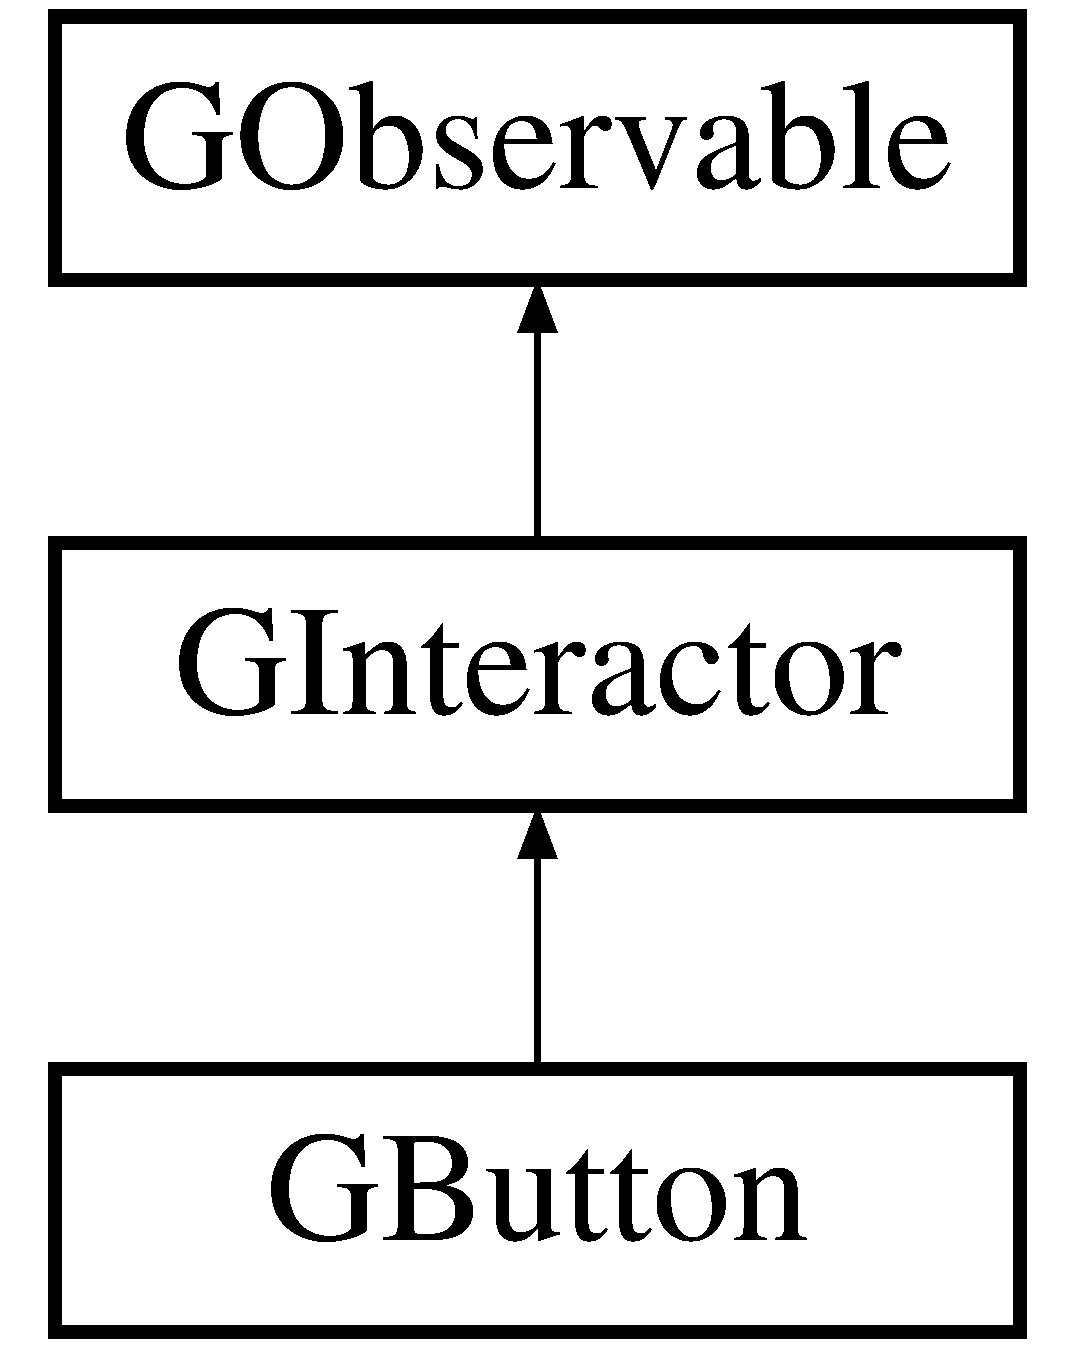
\includegraphics[height=3.000000cm]{classGButton}
\end{center}
\end{figure}
\subsection*{Public Types}
\begin{DoxyCompactItemize}
\item 
enum \mbox{\hyperlink{classGInteractor_a8e0d441725a81d2bbdebbea09078260e}{Text\+Position}} \{ \mbox{\hyperlink{classGInteractor_a8e0d441725a81d2bbdebbea09078260ea4cd6f2e7d5a08d6f4dc052df2358f774}{T\+E\+X\+T\+\_\+\+B\+E\+S\+I\+D\+E\+\_\+\+I\+C\+ON}}, 
\mbox{\hyperlink{classGInteractor_a8e0d441725a81d2bbdebbea09078260eaa88490f63d8de68d44c83bdb2ecde3b3}{T\+E\+X\+T\+\_\+\+U\+N\+D\+E\+R\+\_\+\+I\+C\+ON}}, 
\mbox{\hyperlink{classGInteractor_a8e0d441725a81d2bbdebbea09078260ea39a6f388a30ac4fefb6eb13e846bc9f2}{T\+E\+X\+T\+\_\+\+O\+N\+LY}}
 \}
\begin{DoxyCompactList}\small\item\em The places where an interactor can place its text relative to its icon. \end{DoxyCompactList}\end{DoxyCompactItemize}
\subsection*{Public Member Functions}
\begin{DoxyCompactItemize}
\item 
\mbox{\hyperlink{classGButton_aff3f5308477262143eb2a857e7549e31}{G\+Button}} (const std\+::string \&text=\char`\"{}\char`\"{}, const std\+::string \&icon\+File\+Name=\char`\"{}\char`\"{}, Q\+Widget $\ast$parent=nullptr)
\begin{DoxyCompactList}\small\item\em Creates a button with the specified text label and optional icon. \end{DoxyCompactList}\item 
virtual \mbox{\hyperlink{classGButton_a60d0877198710a60639726ec1d4da347}{$\sim$\+G\+Button}} ()
\begin{DoxyCompactList}\small\item\em Frees memory allocated internally by the button. \end{DoxyCompactList}\item 
virtual void \mbox{\hyperlink{classGInteractor_a02f20ea6edfa0671f31c4c648a253833}{add\+Action\+Listener}} () Q\+\_\+\+D\+E\+C\+L\+\_\+\+D\+E\+P\+R\+E\+C\+A\+T\+ED
\begin{DoxyCompactList}\small\item\em Adds an event listener to be notified when this interactor is clicked or generally interacted with. \end{DoxyCompactList}\item 
virtual bool \mbox{\hyperlink{classGInteractor_ac05ba5b92e2e5146d416fe7f842a0969}{events\+Enabled}} () const Q\+\_\+\+D\+E\+C\+L\+\_\+\+O\+V\+E\+R\+R\+I\+DE
\begin{DoxyCompactList}\small\item\em Returns true if this interactor is currently accepting events. \end{DoxyCompactList}\item 
virtual std\+::string \mbox{\hyperlink{classGButton_a432ca43c59ffb2adc9cb66d43621bc27}{get\+Accelerator}} () const Q\+\_\+\+D\+E\+C\+L\+\_\+\+O\+V\+E\+R\+R\+I\+DE
\begin{DoxyCompactList}\small\item\em Returns a string representing a hotkey for this interactor, or an empty string if no accelerator has been set. \end{DoxyCompactList}\item 
virtual std\+::string \mbox{\hyperlink{classGButton_a90f2b1e6f6e7dabd9d6e5307f7c6d1b7}{get\+Action\+Command}} () const Q\+\_\+\+D\+E\+C\+L\+\_\+\+O\+V\+E\+R\+R\+I\+DE
\begin{DoxyCompactList}\small\item\em Returns an action command for this interactor, which is a semi-\/unique string you can use to identify it when events occur. \end{DoxyCompactList}\item 
virtual std\+::string \mbox{\hyperlink{classGInteractor_a808e22cc1fdfbecf71ed8c64ef4600e0}{get\+Background}} () const
\begin{DoxyCompactList}\small\item\em Returns the background color of the interactor as a string. \end{DoxyCompactList}\item 
virtual int \mbox{\hyperlink{classGInteractor_a9e827257a55cb8cf4d9de2ec6bcfd7a0}{get\+Background\+Int}} () const
\begin{DoxyCompactList}\small\item\em Returns the background color of the interactor as an R\+GB integer. \end{DoxyCompactList}\item 
virtual \mbox{\hyperlink{classGRectangle}{G\+Rectangle}} \mbox{\hyperlink{classGInteractor_a29e6ac35a0b48f491a4c88194cc5da3b}{get\+Bounds}} () const
\begin{DoxyCompactList}\small\item\em Returns a rectangle representing the x/y position and size of this interactor. \end{DoxyCompactList}\item 
virtual std\+::string \mbox{\hyperlink{classGInteractor_aa061dfa488c31e18549d64363c1d0e34}{get\+Color}} () const
\begin{DoxyCompactList}\small\item\em Returns the foreground/text color of the interactor as a string. \end{DoxyCompactList}\item 
virtual int \mbox{\hyperlink{classGInteractor_a9635c7af766cdc3417f346683fa0e6c1}{get\+Color\+Int}} () const
\begin{DoxyCompactList}\small\item\em Returns the foreground/text color of the interactor as an R\+GB integer. \end{DoxyCompactList}\item 
virtual \mbox{\hyperlink{classGContainer}{G\+Container}} $\ast$ \mbox{\hyperlink{classGInteractor_a7a6e317c29d61030929b4cd2d1c00fe7}{get\+Container}} () const
\begin{DoxyCompactList}\small\item\em Returns a pointer to the onscreen container holding this interactor. \end{DoxyCompactList}\item 
virtual std\+::string \mbox{\hyperlink{classGInteractor_a894a5502900794eeb27d084c21f1d77d}{get\+Font}} () const
\begin{DoxyCompactList}\small\item\em Returns the font of this interactor\textquotesingle{}s text as a font string such as \char`\"{}\+Helvetica-\/12-\/\+Bold\char`\"{}. \end{DoxyCompactList}\item 
virtual std\+::string \mbox{\hyperlink{classGInteractor_a4fa2d8b0192a3a5b4af4bbfe71194d03}{get\+Foreground}} () const
\begin{DoxyCompactList}\small\item\em Returns the foreground/text color of the interactor as a string. \end{DoxyCompactList}\item 
virtual int \mbox{\hyperlink{classGInteractor_ac3b12ab385a6ef9ae90fc879860ba726}{get\+Foreground\+Int}} () const
\begin{DoxyCompactList}\small\item\em Returns the foreground/text color of the interactor as an R\+GB integer. \end{DoxyCompactList}\item 
virtual double \mbox{\hyperlink{classGInteractor_a1e7e353362434072875264cf95629f99}{get\+Height}} () const
\begin{DoxyCompactList}\small\item\em Returns the current onscreen height of this interactor in pixels. \end{DoxyCompactList}\item 
virtual std\+::string \mbox{\hyperlink{classGInteractor_aaed62a73004939a64da6f0eb9eb64d73}{get\+Icon}} () const
\begin{DoxyCompactList}\small\item\em Returns the file name of the icon associated with this interactor, or an empty string if no icon has been set. \end{DoxyCompactList}\item 
virtual int \mbox{\hyperlink{classGInteractor_a9c9659a6c6ba66b4107ba59c95a24241}{get\+ID}} () const
\begin{DoxyCompactList}\small\item\em Returns a globally unique identifier for this interactor, which is set when the interactor is constructed. \end{DoxyCompactList}\item 
virtual \+\_\+\+Internal\+\_\+\+Q\+Widget $\ast$ \mbox{\hyperlink{classGButton_a208ce13c1da40bf0ddb509daf99d6588}{get\+Internal\+Widget}} () const Q\+\_\+\+D\+E\+C\+L\+\_\+\+O\+V\+E\+R\+R\+I\+DE
\begin{DoxyCompactList}\small\item\em Returns a direct pointer to the internal Qt widget being wrapped by this interactor. \end{DoxyCompactList}\item 
virtual \mbox{\hyperlink{classGPoint}{G\+Point}} \mbox{\hyperlink{classGInteractor_a4f83802015511edeb63b892830812c11}{get\+Location}} () const
\begin{DoxyCompactList}\small\item\em Returns an (x, y) point representing the onscreen location of the top-\/left corner of this interactor within its containing window. \end{DoxyCompactList}\item 
virtual double \mbox{\hyperlink{classGInteractor_aed4b0075fcc434499c3cb3e46896bda3}{get\+Minimum\+Height}} () const
\begin{DoxyCompactList}\small\item\em Returns the minimum height in pixels that this interactor will permit itself to be resized to. \end{DoxyCompactList}\item 
virtual \mbox{\hyperlink{classGDimension}{G\+Dimension}} \mbox{\hyperlink{classGInteractor_a66b5af0b32493b4d597ca0a3df2049ea}{get\+Minimum\+Size}} () const
\begin{DoxyCompactList}\small\item\em Returns a \mbox{\hyperlink{classGDimension}{G\+Dimension}} structure representing the minimum size in pixels that this interactor will permit itself to be resized to. \end{DoxyCompactList}\item 
virtual double \mbox{\hyperlink{classGInteractor_a59e668114fe3d49d2a0f28deb258f7c8}{get\+Minimum\+Width}} () const
\begin{DoxyCompactList}\small\item\em Returns the minimum width in pixels that this interactor will permit itself to be resized to. \end{DoxyCompactList}\item 
virtual std\+::string \mbox{\hyperlink{classGInteractor_a8a60438a5b55d0b2ceb35c8674b9d8c5}{get\+Name}} () const
\begin{DoxyCompactList}\small\item\em Returns a string representing a unique name for this interactor. \end{DoxyCompactList}\item 
virtual double \mbox{\hyperlink{classGInteractor_a747de0961653847bdc6615dbf756d715}{get\+Preferred\+Height}} () const
\begin{DoxyCompactList}\small\item\em Returns the height in pixels that this interactor would prefer to be, which would exactly fit its contents with no stretching or scrollbars. \end{DoxyCompactList}\item 
virtual \mbox{\hyperlink{classGDimension}{G\+Dimension}} \mbox{\hyperlink{classGInteractor_a4aabbee761d8e9116275401131b7ccd1}{get\+Preferred\+Size}} () const
\begin{DoxyCompactList}\small\item\em Returns a \mbox{\hyperlink{classGDimension}{G\+Dimension}} structure storing the width and height in pixels that this interactor would prefer to be, which would exactly fit its contents with no stretching or scrollbars. \end{DoxyCompactList}\item 
virtual double \mbox{\hyperlink{classGInteractor_a82bca31d37700fb0e35d2743352efd5e}{get\+Preferred\+Width}} () const
\begin{DoxyCompactList}\small\item\em Returns the height in pixels that this interactor would prefer to be, which would exactly fit its contents with no stretching or scrollbars. \end{DoxyCompactList}\item 
virtual \mbox{\hyperlink{classGDimension}{G\+Dimension}} \mbox{\hyperlink{classGInteractor_a7b4eec96a2bdc6420695d5796a78eea9}{get\+Size}} () const
\begin{DoxyCompactList}\small\item\em Returns a \mbox{\hyperlink{classGDimension}{G\+Dimension}} structure storing the current onscreen width and height of this interactor in pixels. \end{DoxyCompactList}\item 
virtual std\+::string \mbox{\hyperlink{classGButton_aff553c50924b836c29f146ed34a7c6ec}{get\+Text}} () const
\begin{DoxyCompactList}\small\item\em Returns the button\textquotesingle{}s text. \end{DoxyCompactList}\item 
virtual \mbox{\hyperlink{classGInteractor_a8e0d441725a81d2bbdebbea09078260e}{G\+Interactor\+::\+Text\+Position}} \mbox{\hyperlink{classGButton_a3fc623df3ced62aca93fc344c2426899}{get\+Text\+Position}} () const
\begin{DoxyCompactList}\small\item\em Returns the button\textquotesingle{}s text position relative to its icon. \end{DoxyCompactList}\item 
virtual std\+::string \mbox{\hyperlink{classGButton_a9896d58fcfebbf1025aeeb5b8b9ede80}{get\+Type}} () const Q\+\_\+\+D\+E\+C\+L\+\_\+\+O\+V\+E\+R\+R\+I\+DE
\begin{DoxyCompactList}\small\item\em Returns a string representing the class name of this interactor, such as \char`\"{}\+G\+Button\char`\"{} or \char`\"{}\+G\+Check\+Box\char`\"{}. \end{DoxyCompactList}\item 
virtual Q\+Widget $\ast$ \mbox{\hyperlink{classGButton_a326ee51b5561f807df7b29a1c101f7fd}{get\+Widget}} () const Q\+\_\+\+D\+E\+C\+L\+\_\+\+O\+V\+E\+R\+R\+I\+DE
\begin{DoxyCompactList}\small\item\em Returns a direct pointer to the internal Qt widget being wrapped by this interactor. \end{DoxyCompactList}\item 
virtual double \mbox{\hyperlink{classGInteractor_a0ed2965abd4f5701d2cadf71239faf19}{get\+Width}} () const
\begin{DoxyCompactList}\small\item\em Returns the current onscreen width of this interactor in pixels. \end{DoxyCompactList}\item 
virtual double \mbox{\hyperlink{classGInteractor_a344385751bee0720059403940d57a13e}{getX}} () const
\begin{DoxyCompactList}\small\item\em Returns the x-\/coordinate of the top-\/left pixel of this interactor within its onscreen window. \end{DoxyCompactList}\item 
virtual double \mbox{\hyperlink{classGInteractor_aafa51c7f8f38a09febbb9ce7853f77b4}{getY}} () const
\begin{DoxyCompactList}\small\item\em Returns the y-\/coordinate of the top-\/left pixel of this interactor within its onscreen window. \end{DoxyCompactList}\item 
virtual bool \mbox{\hyperlink{classGInteractor_afc480f652b8c5f1fb255e2269ce68879}{in\+Bounds}} (double x, double y) const
\begin{DoxyCompactList}\small\item\em Returns true if the given x/y pixel is within the bounds of this interactor. \end{DoxyCompactList}\item 
virtual bool \mbox{\hyperlink{classGInteractor_ae6d7982c1c627b677a5e776ca86118ed}{in\+Bounds}} (int x, int y) const
\begin{DoxyCompactList}\small\item\em Returns true if the given x/y pixel is within the bounds of this interactor. \end{DoxyCompactList}\item 
virtual bool \mbox{\hyperlink{classGInteractor_aacb819fb241851fd9fc045271baa4034}{is\+Enabled}} () const
\begin{DoxyCompactList}\small\item\em Returns true if this interactor is currently enabled. \end{DoxyCompactList}\item 
virtual bool \mbox{\hyperlink{classGInteractor_a9d8a6cfb13917785c143e74d40e4e2be}{is\+Visible}} () const
\begin{DoxyCompactList}\small\item\em Returns true if the interactor is visible on the screen. \end{DoxyCompactList}\item 
virtual void \mbox{\hyperlink{classGButton_ab7fe7a876367b87cf7202f947f1d05e4}{remove\+Action\+Listener}} ()
\begin{DoxyCompactList}\small\item\em Removes the action listener from this button so that it will no longer call it when events occur. \end{DoxyCompactList}\item 
virtual void \mbox{\hyperlink{classGButton_aa4250907e4cdd77349c04f0cf5cdd3d3}{remove\+Double\+Click\+Listener}} ()
\begin{DoxyCompactList}\small\item\em Removes the double-\/click listener from this button so that it will no longer call it when events occur. \end{DoxyCompactList}\item 
virtual void \mbox{\hyperlink{classGInteractor_a519fb2ac767f8b2febbb50b898b8c8cb}{request\+Focus}} ()
\begin{DoxyCompactList}\small\item\em Transfers keyboard focus to this interactor. \end{DoxyCompactList}\item 
virtual void \mbox{\hyperlink{classGButton_a5f78fc506a33b57dced42a419be34446}{set\+Accelerator}} (const std\+::string \&accelerator) Q\+\_\+\+D\+E\+C\+L\+\_\+\+O\+V\+E\+R\+R\+I\+DE
\begin{DoxyCompactList}\small\item\em Sets an accelerator hotkey for this interactor, such as \char`\"{}\+Ctrl-\/\+S\char`\"{}. \end{DoxyCompactList}\item 
virtual void \mbox{\hyperlink{classGInteractor_a4b5843fe3030e038a1ba54cc03389bcf}{set\+Action\+Command}} (const std\+::string \&action\+Command)
\begin{DoxyCompactList}\small\item\em Sets the action command for this interactor. \end{DoxyCompactList}\item 
virtual void \mbox{\hyperlink{classGButton_adcfb4742430c88714fcf57e57ab8ea9c}{set\+Action\+Listener}} (G\+Event\+Listener func)
\begin{DoxyCompactList}\small\item\em Sets an action listener on this button so that it will be called when the button is clicked. \end{DoxyCompactList}\item 
virtual void \mbox{\hyperlink{classGButton_aebd20a89c7a8a43a6fce999cf4f9fcf2}{set\+Action\+Listener}} (G\+Event\+Listener\+Void func)
\begin{DoxyCompactList}\small\item\em Sets an action listener on this button so that it will be called when the button is clicked. \end{DoxyCompactList}\item 
virtual void \mbox{\hyperlink{classGInteractor_acba7e546c2025c0a15ca4b4cc92043db}{set\+Background}} (int rgb)
\begin{DoxyCompactList}\small\item\em Sets the background color of the interactor to the color represented by the given R\+GB integer. \end{DoxyCompactList}\item 
virtual void \mbox{\hyperlink{classGInteractor_ab4677ab2474e68b07aa56605af92a84a}{set\+Background}} (const std\+::string \&color)
\begin{DoxyCompactList}\small\item\em Sets the background color of the interactor to the color represented by the given string. \end{DoxyCompactList}\item 
virtual void \mbox{\hyperlink{classGInteractor_a2aae8197624b72265ab83b4f1bc73f2f}{set\+Bounds}} (double x, double y, double width, double height)
\begin{DoxyCompactList}\small\item\em Sets the size and location of the widget. \end{DoxyCompactList}\item 
virtual void \mbox{\hyperlink{classGInteractor_acada386653f008cacc7cce86426bef7c}{set\+Bounds}} (const \mbox{\hyperlink{classGRectangle}{G\+Rectangle}} \&size)
\begin{DoxyCompactList}\small\item\em Sets the size and location of the widget. \end{DoxyCompactList}\item 
virtual void \mbox{\hyperlink{classGInteractor_ab1f5cc0f5cc6bbbd716a526c61f1081d}{set\+Color}} (int rgb)
\begin{DoxyCompactList}\small\item\em Sets the foreground/text color of the interactor to the color represented by the given R\+GB integer. \end{DoxyCompactList}\item 
virtual void \mbox{\hyperlink{classGInteractor_a61374df6c11b52cfbb0815decdbaebc6}{set\+Color}} (const std\+::string \&color)
\begin{DoxyCompactList}\small\item\em Sets the foreground/text color of the interactor to the color represented by the given string. \end{DoxyCompactList}\item 
virtual void \mbox{\hyperlink{classGButton_ac29f9a3462458e165fae3a1f046ee77a}{set\+Double\+Click\+Listener}} (G\+Event\+Listener func)
\begin{DoxyCompactList}\small\item\em Sets a listener on this button so that it will be called when the button is double-\/clicked. \end{DoxyCompactList}\item 
virtual void \mbox{\hyperlink{classGButton_a50096194d66f48c92dd4c512d41bfc76}{set\+Double\+Click\+Listener}} (G\+Event\+Listener\+Void func)
\begin{DoxyCompactList}\small\item\em Sets a listener on this button so that it will be called when the button is double-\/clicked. \end{DoxyCompactList}\item 
virtual void \mbox{\hyperlink{classGInteractor_ab831367dd84bbd579e02e55bacb21343}{set\+Enabled}} (bool value)
\begin{DoxyCompactList}\small\item\em Sets whether this interactor is currently enabled. \end{DoxyCompactList}\item 
virtual void \mbox{\hyperlink{classGObservable_afaa30b2a9e0f378fd1c70d2f1d0b8216}{set\+Events\+Enabled}} (bool \mbox{\hyperlink{classGInteractor_ac05ba5b92e2e5146d416fe7f842a0969}{events\+Enabled}})
\begin{DoxyCompactList}\small\item\em Sets whether the object is currently allowing itself to fire events. \end{DoxyCompactList}\item 
virtual void \mbox{\hyperlink{classGInteractor_a2592348886ffea646c6534bf88f7c49d}{set\+Font}} (const Q\+Font \&font)
\begin{DoxyCompactList}\small\item\em Sets the font used by this widget to the given Qt font. \end{DoxyCompactList}\item 
virtual void \mbox{\hyperlink{classGInteractor_a8e096e8818d838aceae1d46d58fb3a7b}{set\+Font}} (const std\+::string \&font)
\begin{DoxyCompactList}\small\item\em Sets the font used by this widget to the font represented by the given font string, such as \char`\"{}\+Helvetica-\/16-\/\+Bold\char`\"{}. \end{DoxyCompactList}\item 
virtual void \mbox{\hyperlink{classGInteractor_a9eb856b5ff83a19df3831a31f15f4563}{set\+Foreground}} (int rgb)
\begin{DoxyCompactList}\small\item\em Sets the foreground/text color of the interactor to the color represented by the given R\+GB integer. \end{DoxyCompactList}\item 
virtual void \mbox{\hyperlink{classGInteractor_af59209aeadea6dfc6d97a2d8531f50e1}{set\+Foreground}} (const std\+::string \&color)
\begin{DoxyCompactList}\small\item\em Sets the foreground/text color of the interactor to the color represented by the given string. \end{DoxyCompactList}\item 
virtual void \mbox{\hyperlink{classGInteractor_a9e280bfc4544dfaf8e4376c4e1a74357}{set\+Height}} (double height)
\begin{DoxyCompactList}\small\item\em Sets the onscreen height of the interactor in pixels. \end{DoxyCompactList}\item 
virtual void \mbox{\hyperlink{classGButton_a75753a3d7d3364185f8088d63b664cb1}{set\+Icon}} (const std\+::string \&filename, bool retain\+Icon\+Size=true) Q\+\_\+\+D\+E\+C\+L\+\_\+\+O\+V\+E\+R\+R\+I\+DE
\begin{DoxyCompactList}\small\item\em Sets the file name of the icon associated with this interactor, or an empty string if no icon has been set. \end{DoxyCompactList}\item 
virtual void \mbox{\hyperlink{classGInteractor_a04594e8ba9b98513a64f1da00dcae18c}{set\+Location}} (double x, double y)
\begin{DoxyCompactList}\small\item\em Sets the onscreen x/y-\/coordinate of the top-\/left corner of the interactor relative to its window. \end{DoxyCompactList}\item 
virtual void \mbox{\hyperlink{classGInteractor_a0cf428e207b7f22cc08138a90b1b87b2}{set\+Minimum\+Size}} (double width, double height)
\begin{DoxyCompactList}\small\item\em Sets the minimum size in pixels that this interactor will permit itself to be resized to. \end{DoxyCompactList}\item 
virtual void \mbox{\hyperlink{classGInteractor_a3b1046117ac6cb7abe467e00ba8a81f4}{set\+Minimum\+Size}} (const \mbox{\hyperlink{classGDimension}{G\+Dimension}} \&size)
\begin{DoxyCompactList}\small\item\em Sets the minimum size in pixels that this interactor will permit itself to be resized to. \end{DoxyCompactList}\item 
virtual void \mbox{\hyperlink{classGInteractor_a9d3a2685df23b5e7cbf59c19c4a1f9b5}{set\+Name}} (const std\+::string \&name)
\begin{DoxyCompactList}\small\item\em Sets a string representing a unique name for this interactor. \end{DoxyCompactList}\item 
virtual void \mbox{\hyperlink{classGInteractor_a1ab987704fce32098706c6f00fb08218}{set\+Preferred\+Height}} (double height)
\begin{DoxyCompactList}\small\item\em Sets the height in pixels that this interactor would prefer to be. \end{DoxyCompactList}\item 
virtual void \mbox{\hyperlink{classGInteractor_a042c5ae19430d765ef552371cae3632c}{set\+Preferred\+Size}} (double width, double height)
\begin{DoxyCompactList}\small\item\em Sets the width and height in pixels that this interactor would prefer to be. \end{DoxyCompactList}\item 
virtual void \mbox{\hyperlink{classGInteractor_aa22d9be4bc0e078bb0ea69b0fc9d7c75}{set\+Preferred\+Size}} (const \mbox{\hyperlink{classGDimension}{G\+Dimension}} \&size)
\begin{DoxyCompactList}\small\item\em Sets the size in pixels that this interactor would prefer to be. \end{DoxyCompactList}\item 
virtual void \mbox{\hyperlink{classGInteractor_a3db429ab2fa52efd187eec0ed8cdd9f2}{set\+Preferred\+Width}} (double width)
\begin{DoxyCompactList}\small\item\em Sets the width in pixels that this interactor would prefer to be. \end{DoxyCompactList}\item 
virtual void \mbox{\hyperlink{classGInteractor_aca25d49481f9bf5fc8f7df4c086c4ce7}{set\+Size}} (double width, double height)
\begin{DoxyCompactList}\small\item\em Sets the onscreen width and height of the interactor in pixels. \end{DoxyCompactList}\item 
virtual void \mbox{\hyperlink{classGInteractor_ae2b628228f192c2702c4ce941b2af68f}{set\+Size}} (const \mbox{\hyperlink{classGDimension}{G\+Dimension}} \&size)
\begin{DoxyCompactList}\small\item\em Sets the onscreen width and height of the interactor in pixels. \end{DoxyCompactList}\item 
virtual void \mbox{\hyperlink{classGButton_ac1ae51949d41ee9054634be5967d91b8}{set\+Text}} (const std\+::string \&text)
\begin{DoxyCompactList}\small\item\em Sets the text on the button to be the given text. \end{DoxyCompactList}\item 
virtual void \mbox{\hyperlink{classGButton_af822b8d73c652f7c59d875d7cdfc5302}{set\+Text\+Position}} (\mbox{\hyperlink{classGInteractor_a8e0d441725a81d2bbdebbea09078260e}{G\+Interactor\+::\+Text\+Position}} position)
\begin{DoxyCompactList}\small\item\em Sets the button\textquotesingle{}s text position relative to its icon. \end{DoxyCompactList}\item 
virtual void \mbox{\hyperlink{classGInteractor_a039e0e49beaecc275efce02d416acea8}{set\+Tooltip}} (const std\+::string \&tooltip\+Text)
\begin{DoxyCompactList}\small\item\em Sets a \char`\"{}tooltip\char`\"{} that will appear if the user hovers their mouse over the interactor. \end{DoxyCompactList}\item 
virtual void \mbox{\hyperlink{classGInteractor_a18e44e30b31525a243960ca3928125aa}{set\+Visible}} (bool visible)
\begin{DoxyCompactList}\small\item\em Returns true if the interactor is visible on the screen. \end{DoxyCompactList}\item 
virtual void \mbox{\hyperlink{classGInteractor_aa3f3fba4cb131baa8696ba01e3bceca1}{set\+Width}} (double width)
\begin{DoxyCompactList}\small\item\em Sets the onscreen width of the interactor in pixels. \end{DoxyCompactList}\item 
virtual void \mbox{\hyperlink{classGInteractor_a9c18fcc579333bf9653d13ad2b372e39}{setX}} (double x)
\begin{DoxyCompactList}\small\item\em Sets the onscreen x-\/coordinate of the top-\/left corner of the interactor relative to its window. \end{DoxyCompactList}\item 
virtual void \mbox{\hyperlink{classGInteractor_a7d57e2a5c35d27feb58fd498a3cf82b9}{setY}} (double y)
\begin{DoxyCompactList}\small\item\em Sets the onscreen y-\/coordinate of the top-\/left corner of the interactor relative to its window. \end{DoxyCompactList}\item 
virtual std\+::string \mbox{\hyperlink{classGObservable_a1fe5121d6528fdea3f243321b3fa3a49}{to\+String}} () const
\begin{DoxyCompactList}\small\item\em Returns a string representation of this observable object\textquotesingle{}s state. \end{DoxyCompactList}\end{DoxyCompactItemize}
\subsection*{Protected Member Functions}
\begin{DoxyCompactItemize}
\item 
virtual void \mbox{\hyperlink{classGObservable_a80cfa040459ff53594adbd6a51ec8f43}{clear\+Event\+Listeners}} ()
\begin{DoxyCompactList}\small\item\em Removes all event listeners from this object. \end{DoxyCompactList}\item 
virtual void \mbox{\hyperlink{classGObservable_a284f31528c0520f8e545c03ac9eeac74}{ensure\+Thread\+Safety}} (const std\+::string \&member\+Name=\char`\"{}\char`\"{})
\begin{DoxyCompactList}\small\item\em Ensures that we are currently in the Qt G\+UI thread. \end{DoxyCompactList}\item 
virtual void \mbox{\hyperlink{classGObservable_a63e5e5a6227c59c928493b11aceb0f67}{fire\+Event}} (\mbox{\hyperlink{classGEvent}{G\+Event}} \&event)
\begin{DoxyCompactList}\small\item\em Sends out the given event to any attached listeners. \end{DoxyCompactList}\item 
virtual void \mbox{\hyperlink{classGObservable_ab3983ea07337b52020a29cc00c653d8d}{fire\+G\+Event}} (Q\+Event $\ast$event, Event\+Type event\+Type, const std\+::string \&event\+Name)
\begin{DoxyCompactList}\small\item\em Creates an event of the given type, then sends it out to any attached listeners. \end{DoxyCompactList}\item 
virtual void \mbox{\hyperlink{classGObservable_a01fdf1b0e0dbd49e189fe4514e010411}{fire\+G\+Event}} (Q\+Close\+Event $\ast$event, Event\+Type event\+Type, const std\+::string \&event\+Name)
\begin{DoxyCompactList}\small\item\em Creates an event of the given type, then sends it out to any attached listeners. \end{DoxyCompactList}\item 
virtual void \mbox{\hyperlink{classGObservable_abb0b2f66ba39211cb5d7615e9d1c04e2}{fire\+G\+Event}} (Q\+Key\+Event $\ast$event, Event\+Type event\+Type, const std\+::string \&event\+Name)
\begin{DoxyCompactList}\small\item\em Creates an event of the given type, then sends it out to any attached listeners. \end{DoxyCompactList}\item 
virtual void \mbox{\hyperlink{classGObservable_a119318675d2165bdf7dd853aaf881d4b}{fire\+G\+Event}} (Q\+Mouse\+Event $\ast$event, Event\+Type event\+Type, const std\+::string \&event\+Name, const std\+::string \&action\+Command=\char`\"{}\char`\"{})
\begin{DoxyCompactList}\small\item\em Creates an event of the given type, then sends it out to any attached listeners. \end{DoxyCompactList}\item 
virtual void \mbox{\hyperlink{classGObservable_a63fd9034e1e1633c1c38eb342bfd34e9}{fire\+G\+Event}} (Q\+Resize\+Event $\ast$event, Event\+Type event\+Type, const std\+::string \&event\+Name)
\begin{DoxyCompactList}\small\item\em Creates an event of the given type, then sends it out to any attached listeners. \end{DoxyCompactList}\item 
virtual void \mbox{\hyperlink{classGObservable_a741345310d9b7c5170a6cbc410c44ac4}{fire\+G\+Event}} (Q\+Timer\+Event $\ast$event, Event\+Type event\+Type, const std\+::string \&event\+Name)
\begin{DoxyCompactList}\small\item\em Creates an event of the given type, then sends it out to any attached listeners. \end{DoxyCompactList}\item 
virtual void \mbox{\hyperlink{classGObservable_a93bf338968a0338761b8e4dc62f582e9}{fire\+G\+Event}} (Q\+Wheel\+Event $\ast$event, Event\+Type event\+Type, const std\+::string \&event\+Name)
\begin{DoxyCompactList}\small\item\em Creates an event of the given type, then sends it out to any attached listeners. \end{DoxyCompactList}\item 
virtual void \mbox{\hyperlink{classGObservable_a2a70a7d7435ff0c3b80bb4d70da19e0d}{fire\+G\+Event}} (Q\+Window\+State\+Change\+Event $\ast$event, Event\+Type event\+Type, const std\+::string \&event\+Name)
\begin{DoxyCompactList}\small\item\em Creates an event of the given type, then sends it out to any attached listeners. \end{DoxyCompactList}\item 
virtual bool \mbox{\hyperlink{classGObservable_a9f6faaa25942923bafa1c44020c49fa9}{has\+Event\+Listener}} (const std\+::string \&event\+Name) const
\begin{DoxyCompactList}\small\item\em Returns true if the observable object has a listener for the given type of event. \end{DoxyCompactList}\item 
virtual bool \mbox{\hyperlink{classGObservable_aeec1adc19aa0f33de62390686ee1382c}{is\+Accepting\+Event}} (int event\+Mask) const
\begin{DoxyCompactList}\small\item\em Returns true if the observable object has a listener for the given type of event. \end{DoxyCompactList}\item 
virtual bool \mbox{\hyperlink{classGObservable_aa31c73145a29dcb92848a92e0cfaea41}{is\+Accepting\+Event}} (const \mbox{\hyperlink{classGEvent}{G\+Event}} \&event) const
\begin{DoxyCompactList}\small\item\em Returns true if the observable object has a listener for the given type of event. \end{DoxyCompactList}\item 
virtual bool \mbox{\hyperlink{classGObservable_a3b1c689267eda44e65a2213e7de38b23}{is\+Accepting\+Event}} (const std\+::string \&event\+Type) const
\begin{DoxyCompactList}\small\item\em Returns true if the observable object has a listener for the given type of event. \end{DoxyCompactList}\item 
virtual void \mbox{\hyperlink{classGObservable_acbcf1ed3a851ad8a3c17ef38d86b481d}{remove\+Event\+Listener}} (const std\+::string \&event\+Name)
\begin{DoxyCompactList}\small\item\em Removes any event listener from this observable object that would respond to the given type of event, such as \char`\"{}click\char`\"{} or \char`\"{}keydown\char`\"{}. \end{DoxyCompactList}\item 
virtual void \mbox{\hyperlink{classGObservable_af51cc35c29a1bd1908609d432decdbb6}{remove\+Event\+Listeners}} (std\+::initializer\+\_\+list$<$ std\+::string $>$ event\+Names)
\begin{DoxyCompactList}\small\item\em Removes any event listener from this observable object that would respond to the given types of events, such as \char`\"{}click\char`\"{} or \char`\"{}keydown\char`\"{}. \end{DoxyCompactList}\item 
virtual void \mbox{\hyperlink{classGObservable_ad2f6d34961c50f6c1e0659990b79f741}{set\+Event\+Listener}} (const std\+::string \&event\+Name, G\+Event\+Listener func)
\begin{DoxyCompactList}\small\item\em Adds an event listener from this observable object to respond to the given type of event, such as \char`\"{}click\char`\"{} or \char`\"{}keydown\char`\"{}. \end{DoxyCompactList}\item 
virtual void \mbox{\hyperlink{classGObservable_abac4cb9f9e626e010e87f5d91573c8a5}{set\+Event\+Listener}} (const std\+::string \&event\+Name, G\+Event\+Listener\+Void func)
\begin{DoxyCompactList}\small\item\em Adds an event listener from this observable object to respond to the given type of event, such as \char`\"{}click\char`\"{} or \char`\"{}keydown\char`\"{}. \end{DoxyCompactList}\item 
virtual void \mbox{\hyperlink{classGObservable_afa388d69c33c718cf035774604065604}{set\+Event\+Listeners}} (std\+::initializer\+\_\+list$<$ std\+::string $>$ event\+Names, G\+Event\+Listener func)
\begin{DoxyCompactList}\small\item\em Adds an event listener from this observable object to respond to the given types of events, such as \char`\"{}click\char`\"{} or \char`\"{}keydown\char`\"{}. \end{DoxyCompactList}\item 
virtual void \mbox{\hyperlink{classGObservable_a7867184bbb686f74fae8a4db927da799}{set\+Event\+Listeners}} (std\+::initializer\+\_\+list$<$ std\+::string $>$ event\+Names, G\+Event\+Listener\+Void func)
\begin{DoxyCompactList}\small\item\em Adds an event listener from this observable object to respond to the given types of events, such as \char`\"{}click\char`\"{} or \char`\"{}keydown\char`\"{}. \end{DoxyCompactList}\end{DoxyCompactItemize}


\subsection{Detailed Description}
This interactor subclass represents an onscreen button. 

You can listen for clicks on a button using the set\+Action\+Listener method, passing the function you want to call on each click. 

\subsection{Member Enumeration Documentation}
\mbox{\Hypertarget{classGInteractor_a8e0d441725a81d2bbdebbea09078260e}\label{classGInteractor_a8e0d441725a81d2bbdebbea09078260e}} 
\index{G\+Button@{G\+Button}!Text\+Position@{Text\+Position}}
\index{Text\+Position@{Text\+Position}!G\+Button@{G\+Button}}
\subsubsection{\texorpdfstring{Text\+Position}{TextPosition}}
{\footnotesize\ttfamily enum \mbox{\hyperlink{classGInteractor_a8e0d441725a81d2bbdebbea09078260e}{Text\+Position}}\hspace{0.3cm}{\ttfamily [inherited]}}



The places where an interactor can place its text relative to its icon. 

\begin{DoxyEnumFields}{Enumerator}
\raisebox{\heightof{T}}[0pt][0pt]{\index{T\+E\+X\+T\+\_\+\+B\+E\+S\+I\+D\+E\+\_\+\+I\+C\+ON@{T\+E\+X\+T\+\_\+\+B\+E\+S\+I\+D\+E\+\_\+\+I\+C\+ON}!G\+Button@{G\+Button}}\index{G\+Button@{G\+Button}!T\+E\+X\+T\+\_\+\+B\+E\+S\+I\+D\+E\+\_\+\+I\+C\+ON@{T\+E\+X\+T\+\_\+\+B\+E\+S\+I\+D\+E\+\_\+\+I\+C\+ON}}}\mbox{\Hypertarget{classGInteractor_a8e0d441725a81d2bbdebbea09078260ea4cd6f2e7d5a08d6f4dc052df2358f774}\label{classGInteractor_a8e0d441725a81d2bbdebbea09078260ea4cd6f2e7d5a08d6f4dc052df2358f774}} 
T\+E\+X\+T\+\_\+\+B\+E\+S\+I\+D\+E\+\_\+\+I\+C\+ON&\\
\hline

\raisebox{\heightof{T}}[0pt][0pt]{\index{T\+E\+X\+T\+\_\+\+U\+N\+D\+E\+R\+\_\+\+I\+C\+ON@{T\+E\+X\+T\+\_\+\+U\+N\+D\+E\+R\+\_\+\+I\+C\+ON}!G\+Button@{G\+Button}}\index{G\+Button@{G\+Button}!T\+E\+X\+T\+\_\+\+U\+N\+D\+E\+R\+\_\+\+I\+C\+ON@{T\+E\+X\+T\+\_\+\+U\+N\+D\+E\+R\+\_\+\+I\+C\+ON}}}\mbox{\Hypertarget{classGInteractor_a8e0d441725a81d2bbdebbea09078260eaa88490f63d8de68d44c83bdb2ecde3b3}\label{classGInteractor_a8e0d441725a81d2bbdebbea09078260eaa88490f63d8de68d44c83bdb2ecde3b3}} 
T\+E\+X\+T\+\_\+\+U\+N\+D\+E\+R\+\_\+\+I\+C\+ON&\\
\hline

\raisebox{\heightof{T}}[0pt][0pt]{\index{T\+E\+X\+T\+\_\+\+O\+N\+LY@{T\+E\+X\+T\+\_\+\+O\+N\+LY}!G\+Button@{G\+Button}}\index{G\+Button@{G\+Button}!T\+E\+X\+T\+\_\+\+O\+N\+LY@{T\+E\+X\+T\+\_\+\+O\+N\+LY}}}\mbox{\Hypertarget{classGInteractor_a8e0d441725a81d2bbdebbea09078260ea39a6f388a30ac4fefb6eb13e846bc9f2}\label{classGInteractor_a8e0d441725a81d2bbdebbea09078260ea39a6f388a30ac4fefb6eb13e846bc9f2}} 
T\+E\+X\+T\+\_\+\+O\+N\+LY&\\
\hline

\end{DoxyEnumFields}


\subsection{Constructor \& Destructor Documentation}
\mbox{\Hypertarget{classGButton_aff3f5308477262143eb2a857e7549e31}\label{classGButton_aff3f5308477262143eb2a857e7549e31}} 
\index{G\+Button@{G\+Button}!G\+Button@{G\+Button}}
\index{G\+Button@{G\+Button}!G\+Button@{G\+Button}}
\subsubsection{\texorpdfstring{G\+Button()}{GButton()}}
{\footnotesize\ttfamily \mbox{\hyperlink{classGButton}{G\+Button}} (\begin{DoxyParamCaption}\item[{const std\+::string \&}]{text = {\ttfamily \char`\"{}\char`\"{}},  }\item[{const std\+::string \&}]{icon\+File\+Name = {\ttfamily \char`\"{}\char`\"{}},  }\item[{Q\+Widget $\ast$}]{parent = {\ttfamily nullptr} }\end{DoxyParamCaption})}



Creates a button with the specified text label and optional icon. 

\mbox{\Hypertarget{classGButton_a60d0877198710a60639726ec1d4da347}\label{classGButton_a60d0877198710a60639726ec1d4da347}} 
\index{G\+Button@{G\+Button}!````~G\+Button@{$\sim$\+G\+Button}}
\index{````~G\+Button@{$\sim$\+G\+Button}!G\+Button@{G\+Button}}
\subsubsection{\texorpdfstring{$\sim$\+G\+Button()}{~GButton()}}
{\footnotesize\ttfamily $\sim$\mbox{\hyperlink{classGButton}{G\+Button}} (\begin{DoxyParamCaption}{ }\end{DoxyParamCaption})\hspace{0.3cm}{\ttfamily [virtual]}}



Frees memory allocated internally by the button. 



\subsection{Member Function Documentation}
\mbox{\Hypertarget{classGInteractor_a02f20ea6edfa0671f31c4c648a253833}\label{classGInteractor_a02f20ea6edfa0671f31c4c648a253833}} 
\index{G\+Button@{G\+Button}!add\+Action\+Listener@{add\+Action\+Listener}}
\index{add\+Action\+Listener@{add\+Action\+Listener}!G\+Button@{G\+Button}}
\subsubsection{\texorpdfstring{add\+Action\+Listener()}{addActionListener()}}
{\footnotesize\ttfamily void add\+Action\+Listener (\begin{DoxyParamCaption}{ }\end{DoxyParamCaption})\hspace{0.3cm}{\ttfamily [virtual]}, {\ttfamily [inherited]}}



Adds an event listener to be notified when this interactor is clicked or generally interacted with. 

\begin{DoxyRefDesc}{Deprecated}
\item[\mbox{\hyperlink{deprecated__deprecated000006}{Deprecated}}]does nothing; use set\+Action\+Listener instead \end{DoxyRefDesc}
\mbox{\Hypertarget{classGObservable_a80cfa040459ff53594adbd6a51ec8f43}\label{classGObservable_a80cfa040459ff53594adbd6a51ec8f43}} 
\index{G\+Button@{G\+Button}!clear\+Event\+Listeners@{clear\+Event\+Listeners}}
\index{clear\+Event\+Listeners@{clear\+Event\+Listeners}!G\+Button@{G\+Button}}
\subsubsection{\texorpdfstring{clear\+Event\+Listeners()}{clearEventListeners()}}
{\footnotesize\ttfamily void clear\+Event\+Listeners (\begin{DoxyParamCaption}{ }\end{DoxyParamCaption})\hspace{0.3cm}{\ttfamily [protected]}, {\ttfamily [virtual]}, {\ttfamily [inherited]}}



Removes all event listeners from this object. 

\mbox{\Hypertarget{classGObservable_a284f31528c0520f8e545c03ac9eeac74}\label{classGObservable_a284f31528c0520f8e545c03ac9eeac74}} 
\index{G\+Button@{G\+Button}!ensure\+Thread\+Safety@{ensure\+Thread\+Safety}}
\index{ensure\+Thread\+Safety@{ensure\+Thread\+Safety}!G\+Button@{G\+Button}}
\subsubsection{\texorpdfstring{ensure\+Thread\+Safety()}{ensureThreadSafety()}}
{\footnotesize\ttfamily void ensure\+Thread\+Safety (\begin{DoxyParamCaption}\item[{const std\+::string \&}]{member\+Name = {\ttfamily \char`\"{}\char`\"{}} }\end{DoxyParamCaption})\hspace{0.3cm}{\ttfamily [protected]}, {\ttfamily [virtual]}, {\ttfamily [inherited]}}



Ensures that we are currently in the Qt G\+UI thread. 

\mbox{\Hypertarget{classGInteractor_ac05ba5b92e2e5146d416fe7f842a0969}\label{classGInteractor_ac05ba5b92e2e5146d416fe7f842a0969}} 
\index{G\+Button@{G\+Button}!events\+Enabled@{events\+Enabled}}
\index{events\+Enabled@{events\+Enabled}!G\+Button@{G\+Button}}
\subsubsection{\texorpdfstring{events\+Enabled()}{eventsEnabled()}}
{\footnotesize\ttfamily bool events\+Enabled (\begin{DoxyParamCaption}{ }\end{DoxyParamCaption}) const\hspace{0.3cm}{\ttfamily [virtual]}, {\ttfamily [inherited]}}



Returns true if this interactor is currently accepting events. 

Initially true. An interactor must be visible and added to an onscreen window to receive events. 

Reimplemented from \mbox{\hyperlink{classGObservable_a8ebb3da91032e7f4c34485dabc518b8a}{G\+Observable}}.

\mbox{\Hypertarget{classGObservable_a63e5e5a6227c59c928493b11aceb0f67}\label{classGObservable_a63e5e5a6227c59c928493b11aceb0f67}} 
\index{G\+Button@{G\+Button}!fire\+Event@{fire\+Event}}
\index{fire\+Event@{fire\+Event}!G\+Button@{G\+Button}}
\subsubsection{\texorpdfstring{fire\+Event()}{fireEvent()}}
{\footnotesize\ttfamily void fire\+Event (\begin{DoxyParamCaption}\item[{\mbox{\hyperlink{classGEvent}{G\+Event}} \&}]{event }\end{DoxyParamCaption})\hspace{0.3cm}{\ttfamily [protected]}, {\ttfamily [virtual]}, {\ttfamily [inherited]}}



Sends out the given event to any attached listeners. 

\mbox{\Hypertarget{classGObservable_ab3983ea07337b52020a29cc00c653d8d}\label{classGObservable_ab3983ea07337b52020a29cc00c653d8d}} 
\index{G\+Button@{G\+Button}!fire\+G\+Event@{fire\+G\+Event}}
\index{fire\+G\+Event@{fire\+G\+Event}!G\+Button@{G\+Button}}
\subsubsection{\texorpdfstring{fire\+G\+Event()}{fireGEvent()}\hspace{0.1cm}{\footnotesize\ttfamily [1/8]}}
{\footnotesize\ttfamily void fire\+G\+Event (\begin{DoxyParamCaption}\item[{Q\+Event $\ast$}]{event,  }\item[{Event\+Type}]{event\+Type,  }\item[{const std\+::string \&}]{event\+Name }\end{DoxyParamCaption})\hspace{0.3cm}{\ttfamily [protected]}, {\ttfamily [virtual]}, {\ttfamily [inherited]}}



Creates an event of the given type, then sends it out to any attached listeners. 

\mbox{\Hypertarget{classGObservable_a01fdf1b0e0dbd49e189fe4514e010411}\label{classGObservable_a01fdf1b0e0dbd49e189fe4514e010411}} 
\index{G\+Button@{G\+Button}!fire\+G\+Event@{fire\+G\+Event}}
\index{fire\+G\+Event@{fire\+G\+Event}!G\+Button@{G\+Button}}
\subsubsection{\texorpdfstring{fire\+G\+Event()}{fireGEvent()}\hspace{0.1cm}{\footnotesize\ttfamily [2/8]}}
{\footnotesize\ttfamily void fire\+G\+Event (\begin{DoxyParamCaption}\item[{Q\+Close\+Event $\ast$}]{event,  }\item[{Event\+Type}]{event\+Type,  }\item[{const std\+::string \&}]{event\+Name }\end{DoxyParamCaption})\hspace{0.3cm}{\ttfamily [protected]}, {\ttfamily [virtual]}, {\ttfamily [inherited]}}



Creates an event of the given type, then sends it out to any attached listeners. 

\mbox{\Hypertarget{classGObservable_abb0b2f66ba39211cb5d7615e9d1c04e2}\label{classGObservable_abb0b2f66ba39211cb5d7615e9d1c04e2}} 
\index{G\+Button@{G\+Button}!fire\+G\+Event@{fire\+G\+Event}}
\index{fire\+G\+Event@{fire\+G\+Event}!G\+Button@{G\+Button}}
\subsubsection{\texorpdfstring{fire\+G\+Event()}{fireGEvent()}\hspace{0.1cm}{\footnotesize\ttfamily [3/8]}}
{\footnotesize\ttfamily void fire\+G\+Event (\begin{DoxyParamCaption}\item[{Q\+Key\+Event $\ast$}]{event,  }\item[{Event\+Type}]{event\+Type,  }\item[{const std\+::string \&}]{event\+Name }\end{DoxyParamCaption})\hspace{0.3cm}{\ttfamily [protected]}, {\ttfamily [virtual]}, {\ttfamily [inherited]}}



Creates an event of the given type, then sends it out to any attached listeners. 

\mbox{\Hypertarget{classGObservable_a119318675d2165bdf7dd853aaf881d4b}\label{classGObservable_a119318675d2165bdf7dd853aaf881d4b}} 
\index{G\+Button@{G\+Button}!fire\+G\+Event@{fire\+G\+Event}}
\index{fire\+G\+Event@{fire\+G\+Event}!G\+Button@{G\+Button}}
\subsubsection{\texorpdfstring{fire\+G\+Event()}{fireGEvent()}\hspace{0.1cm}{\footnotesize\ttfamily [4/8]}}
{\footnotesize\ttfamily void fire\+G\+Event (\begin{DoxyParamCaption}\item[{Q\+Mouse\+Event $\ast$}]{event,  }\item[{Event\+Type}]{event\+Type,  }\item[{const std\+::string \&}]{event\+Name,  }\item[{const std\+::string \&}]{action\+Command = {\ttfamily \char`\"{}\char`\"{}} }\end{DoxyParamCaption})\hspace{0.3cm}{\ttfamily [protected]}, {\ttfamily [virtual]}, {\ttfamily [inherited]}}



Creates an event of the given type, then sends it out to any attached listeners. 

\mbox{\Hypertarget{classGObservable_a63fd9034e1e1633c1c38eb342bfd34e9}\label{classGObservable_a63fd9034e1e1633c1c38eb342bfd34e9}} 
\index{G\+Button@{G\+Button}!fire\+G\+Event@{fire\+G\+Event}}
\index{fire\+G\+Event@{fire\+G\+Event}!G\+Button@{G\+Button}}
\subsubsection{\texorpdfstring{fire\+G\+Event()}{fireGEvent()}\hspace{0.1cm}{\footnotesize\ttfamily [5/8]}}
{\footnotesize\ttfamily void fire\+G\+Event (\begin{DoxyParamCaption}\item[{Q\+Resize\+Event $\ast$}]{event,  }\item[{Event\+Type}]{event\+Type,  }\item[{const std\+::string \&}]{event\+Name }\end{DoxyParamCaption})\hspace{0.3cm}{\ttfamily [protected]}, {\ttfamily [virtual]}, {\ttfamily [inherited]}}



Creates an event of the given type, then sends it out to any attached listeners. 

\mbox{\Hypertarget{classGObservable_a741345310d9b7c5170a6cbc410c44ac4}\label{classGObservable_a741345310d9b7c5170a6cbc410c44ac4}} 
\index{G\+Button@{G\+Button}!fire\+G\+Event@{fire\+G\+Event}}
\index{fire\+G\+Event@{fire\+G\+Event}!G\+Button@{G\+Button}}
\subsubsection{\texorpdfstring{fire\+G\+Event()}{fireGEvent()}\hspace{0.1cm}{\footnotesize\ttfamily [6/8]}}
{\footnotesize\ttfamily void fire\+G\+Event (\begin{DoxyParamCaption}\item[{Q\+Timer\+Event $\ast$}]{event,  }\item[{Event\+Type}]{event\+Type,  }\item[{const std\+::string \&}]{event\+Name }\end{DoxyParamCaption})\hspace{0.3cm}{\ttfamily [protected]}, {\ttfamily [virtual]}, {\ttfamily [inherited]}}



Creates an event of the given type, then sends it out to any attached listeners. 

\mbox{\Hypertarget{classGObservable_a93bf338968a0338761b8e4dc62f582e9}\label{classGObservable_a93bf338968a0338761b8e4dc62f582e9}} 
\index{G\+Button@{G\+Button}!fire\+G\+Event@{fire\+G\+Event}}
\index{fire\+G\+Event@{fire\+G\+Event}!G\+Button@{G\+Button}}
\subsubsection{\texorpdfstring{fire\+G\+Event()}{fireGEvent()}\hspace{0.1cm}{\footnotesize\ttfamily [7/8]}}
{\footnotesize\ttfamily void fire\+G\+Event (\begin{DoxyParamCaption}\item[{Q\+Wheel\+Event $\ast$}]{event,  }\item[{Event\+Type}]{event\+Type,  }\item[{const std\+::string \&}]{event\+Name }\end{DoxyParamCaption})\hspace{0.3cm}{\ttfamily [protected]}, {\ttfamily [virtual]}, {\ttfamily [inherited]}}



Creates an event of the given type, then sends it out to any attached listeners. 

\mbox{\Hypertarget{classGObservable_a2a70a7d7435ff0c3b80bb4d70da19e0d}\label{classGObservable_a2a70a7d7435ff0c3b80bb4d70da19e0d}} 
\index{G\+Button@{G\+Button}!fire\+G\+Event@{fire\+G\+Event}}
\index{fire\+G\+Event@{fire\+G\+Event}!G\+Button@{G\+Button}}
\subsubsection{\texorpdfstring{fire\+G\+Event()}{fireGEvent()}\hspace{0.1cm}{\footnotesize\ttfamily [8/8]}}
{\footnotesize\ttfamily void fire\+G\+Event (\begin{DoxyParamCaption}\item[{Q\+Window\+State\+Change\+Event $\ast$}]{event,  }\item[{Event\+Type}]{event\+Type,  }\item[{const std\+::string \&}]{event\+Name }\end{DoxyParamCaption})\hspace{0.3cm}{\ttfamily [protected]}, {\ttfamily [virtual]}, {\ttfamily [inherited]}}



Creates an event of the given type, then sends it out to any attached listeners. 

\mbox{\Hypertarget{classGButton_a432ca43c59ffb2adc9cb66d43621bc27}\label{classGButton_a432ca43c59ffb2adc9cb66d43621bc27}} 
\index{G\+Button@{G\+Button}!get\+Accelerator@{get\+Accelerator}}
\index{get\+Accelerator@{get\+Accelerator}!G\+Button@{G\+Button}}
\subsubsection{\texorpdfstring{get\+Accelerator()}{getAccelerator()}}
{\footnotesize\ttfamily std\+::string get\+Accelerator (\begin{DoxyParamCaption}{ }\end{DoxyParamCaption}) const\hspace{0.3cm}{\ttfamily [virtual]}}



Returns a string representing a hotkey for this interactor, or an empty string if no accelerator has been set. 

\begin{DoxyReturn}{Returns}
an accelerator such as \char`\"{}\+Ctrl-\/\+S\char`\"{} 
\end{DoxyReturn}


Reimplemented from \mbox{\hyperlink{classGInteractor_a69f8d23ed8f207fbecad99960776e942}{G\+Interactor}}.

\mbox{\Hypertarget{classGButton_a90f2b1e6f6e7dabd9d6e5307f7c6d1b7}\label{classGButton_a90f2b1e6f6e7dabd9d6e5307f7c6d1b7}} 
\index{G\+Button@{G\+Button}!get\+Action\+Command@{get\+Action\+Command}}
\index{get\+Action\+Command@{get\+Action\+Command}!G\+Button@{G\+Button}}
\subsubsection{\texorpdfstring{get\+Action\+Command()}{getActionCommand()}}
{\footnotesize\ttfamily std\+::string get\+Action\+Command (\begin{DoxyParamCaption}{ }\end{DoxyParamCaption}) const\hspace{0.3cm}{\ttfamily [virtual]}}



Returns an action command for this interactor, which is a semi-\/unique string you can use to identify it when events occur. 

For example, for buttons, the default action command is the button\textquotesingle{}s text. 

Reimplemented from \mbox{\hyperlink{classGInteractor_a94eb4276000c4fdfb508ce9e6317a82a}{G\+Interactor}}.

\mbox{\Hypertarget{classGInteractor_a808e22cc1fdfbecf71ed8c64ef4600e0}\label{classGInteractor_a808e22cc1fdfbecf71ed8c64ef4600e0}} 
\index{G\+Button@{G\+Button}!get\+Background@{get\+Background}}
\index{get\+Background@{get\+Background}!G\+Button@{G\+Button}}
\subsubsection{\texorpdfstring{get\+Background()}{getBackground()}}
{\footnotesize\ttfamily std\+::string get\+Background (\begin{DoxyParamCaption}{ }\end{DoxyParamCaption}) const\hspace{0.3cm}{\ttfamily [virtual]}, {\ttfamily [inherited]}}



Returns the background color of the interactor as a string. 

\begin{DoxyReturn}{Returns}
a string such as \char`\"{}blue\char`\"{} or \char`\"{}\#7700ff\char`\"{} 
\end{DoxyReturn}


Reimplemented in \mbox{\hyperlink{classGCanvas_ab44f928b6bd7c8e4b82d5ed92bc3d4c6}{G\+Canvas}}.

\mbox{\Hypertarget{classGInteractor_a9e827257a55cb8cf4d9de2ec6bcfd7a0}\label{classGInteractor_a9e827257a55cb8cf4d9de2ec6bcfd7a0}} 
\index{G\+Button@{G\+Button}!get\+Background\+Int@{get\+Background\+Int}}
\index{get\+Background\+Int@{get\+Background\+Int}!G\+Button@{G\+Button}}
\subsubsection{\texorpdfstring{get\+Background\+Int()}{getBackgroundInt()}}
{\footnotesize\ttfamily int get\+Background\+Int (\begin{DoxyParamCaption}{ }\end{DoxyParamCaption}) const\hspace{0.3cm}{\ttfamily [virtual]}, {\ttfamily [inherited]}}



Returns the background color of the interactor as an R\+GB integer. 

\begin{DoxyReturn}{Returns}
an integer such as 0x7700ff 
\end{DoxyReturn}


Reimplemented in \mbox{\hyperlink{classGCanvas_af66f525e8154dbc8dcd2daecf3728ba9}{G\+Canvas}}.

\mbox{\Hypertarget{classGInteractor_a29e6ac35a0b48f491a4c88194cc5da3b}\label{classGInteractor_a29e6ac35a0b48f491a4c88194cc5da3b}} 
\index{G\+Button@{G\+Button}!get\+Bounds@{get\+Bounds}}
\index{get\+Bounds@{get\+Bounds}!G\+Button@{G\+Button}}
\subsubsection{\texorpdfstring{get\+Bounds()}{getBounds()}}
{\footnotesize\ttfamily \mbox{\hyperlink{classGRectangle}{G\+Rectangle}} get\+Bounds (\begin{DoxyParamCaption}{ }\end{DoxyParamCaption}) const\hspace{0.3cm}{\ttfamily [virtual]}, {\ttfamily [inherited]}}



Returns a rectangle representing the x/y position and size of this interactor. 

\mbox{\Hypertarget{classGInteractor_aa061dfa488c31e18549d64363c1d0e34}\label{classGInteractor_aa061dfa488c31e18549d64363c1d0e34}} 
\index{G\+Button@{G\+Button}!get\+Color@{get\+Color}}
\index{get\+Color@{get\+Color}!G\+Button@{G\+Button}}
\subsubsection{\texorpdfstring{get\+Color()}{getColor()}}
{\footnotesize\ttfamily std\+::string get\+Color (\begin{DoxyParamCaption}{ }\end{DoxyParamCaption}) const\hspace{0.3cm}{\ttfamily [virtual]}, {\ttfamily [inherited]}}



Returns the foreground/text color of the interactor as a string. 

Equivalent to get\+Foreground. \begin{DoxyReturn}{Returns}
a string such as \char`\"{}blue\char`\"{} or \char`\"{}\#7700ff\char`\"{} 
\end{DoxyReturn}
\mbox{\Hypertarget{classGInteractor_a9635c7af766cdc3417f346683fa0e6c1}\label{classGInteractor_a9635c7af766cdc3417f346683fa0e6c1}} 
\index{G\+Button@{G\+Button}!get\+Color\+Int@{get\+Color\+Int}}
\index{get\+Color\+Int@{get\+Color\+Int}!G\+Button@{G\+Button}}
\subsubsection{\texorpdfstring{get\+Color\+Int()}{getColorInt()}}
{\footnotesize\ttfamily int get\+Color\+Int (\begin{DoxyParamCaption}{ }\end{DoxyParamCaption}) const\hspace{0.3cm}{\ttfamily [virtual]}, {\ttfamily [inherited]}}



Returns the foreground/text color of the interactor as an R\+GB integer. 

Equivalent to get\+Foreground\+Int. \begin{DoxyReturn}{Returns}
an integer such as 0x7700ff 
\end{DoxyReturn}
\mbox{\Hypertarget{classGInteractor_a7a6e317c29d61030929b4cd2d1c00fe7}\label{classGInteractor_a7a6e317c29d61030929b4cd2d1c00fe7}} 
\index{G\+Button@{G\+Button}!get\+Container@{get\+Container}}
\index{get\+Container@{get\+Container}!G\+Button@{G\+Button}}
\subsubsection{\texorpdfstring{get\+Container()}{getContainer()}}
{\footnotesize\ttfamily \mbox{\hyperlink{classGContainer}{G\+Container}} $\ast$ get\+Container (\begin{DoxyParamCaption}{ }\end{DoxyParamCaption}) const\hspace{0.3cm}{\ttfamily [virtual]}, {\ttfamily [inherited]}}



Returns a pointer to the onscreen container holding this interactor. 

When an interactor is created, its container is initially null. This will become non-\/null automatically if you add the interactor to a window or other layout container. Interactors must be added to a container or window to receive events or to become visible on the screen. \begin{DoxyReturn}{Returns}
the container, or nullptr if interactor has not yet been added to any container 
\end{DoxyReturn}
\mbox{\Hypertarget{classGInteractor_a894a5502900794eeb27d084c21f1d77d}\label{classGInteractor_a894a5502900794eeb27d084c21f1d77d}} 
\index{G\+Button@{G\+Button}!get\+Font@{get\+Font}}
\index{get\+Font@{get\+Font}!G\+Button@{G\+Button}}
\subsubsection{\texorpdfstring{get\+Font()}{getFont()}}
{\footnotesize\ttfamily std\+::string get\+Font (\begin{DoxyParamCaption}{ }\end{DoxyParamCaption}) const\hspace{0.3cm}{\ttfamily [virtual]}, {\ttfamily [inherited]}}



Returns the font of this interactor\textquotesingle{}s text as a font string such as \char`\"{}\+Helvetica-\/12-\/\+Bold\char`\"{}. 

\begin{DoxyReturn}{Returns}
a font string such as \char`\"{}\+Helvetica-\/12-\/\+Bold\char`\"{} 
\end{DoxyReturn}


Reimplemented in \mbox{\hyperlink{classGCanvas_a24420d98f18927d2c201a3ab55ffdcec}{G\+Canvas}}.

\mbox{\Hypertarget{classGInteractor_a4fa2d8b0192a3a5b4af4bbfe71194d03}\label{classGInteractor_a4fa2d8b0192a3a5b4af4bbfe71194d03}} 
\index{G\+Button@{G\+Button}!get\+Foreground@{get\+Foreground}}
\index{get\+Foreground@{get\+Foreground}!G\+Button@{G\+Button}}
\subsubsection{\texorpdfstring{get\+Foreground()}{getForeground()}}
{\footnotesize\ttfamily std\+::string get\+Foreground (\begin{DoxyParamCaption}{ }\end{DoxyParamCaption}) const\hspace{0.3cm}{\ttfamily [virtual]}, {\ttfamily [inherited]}}



Returns the foreground/text color of the interactor as a string. 

Equivalent to get\+Color. \begin{DoxyReturn}{Returns}
a string such as \char`\"{}blue\char`\"{} or \char`\"{}\#7700ff\char`\"{} 
\end{DoxyReturn}
\mbox{\Hypertarget{classGInteractor_ac3b12ab385a6ef9ae90fc879860ba726}\label{classGInteractor_ac3b12ab385a6ef9ae90fc879860ba726}} 
\index{G\+Button@{G\+Button}!get\+Foreground\+Int@{get\+Foreground\+Int}}
\index{get\+Foreground\+Int@{get\+Foreground\+Int}!G\+Button@{G\+Button}}
\subsubsection{\texorpdfstring{get\+Foreground\+Int()}{getForegroundInt()}}
{\footnotesize\ttfamily int get\+Foreground\+Int (\begin{DoxyParamCaption}{ }\end{DoxyParamCaption}) const\hspace{0.3cm}{\ttfamily [virtual]}, {\ttfamily [inherited]}}



Returns the foreground/text color of the interactor as an R\+GB integer. 

Equivalent to get\+Color\+Int. \begin{DoxyReturn}{Returns}
an integer such as 0x7700ff 
\end{DoxyReturn}
\mbox{\Hypertarget{classGInteractor_a1e7e353362434072875264cf95629f99}\label{classGInteractor_a1e7e353362434072875264cf95629f99}} 
\index{G\+Button@{G\+Button}!get\+Height@{get\+Height}}
\index{get\+Height@{get\+Height}!G\+Button@{G\+Button}}
\subsubsection{\texorpdfstring{get\+Height()}{getHeight()}}
{\footnotesize\ttfamily double get\+Height (\begin{DoxyParamCaption}{ }\end{DoxyParamCaption}) const\hspace{0.3cm}{\ttfamily [virtual]}, {\ttfamily [inherited]}}



Returns the current onscreen height of this interactor in pixels. 

\mbox{\Hypertarget{classGInteractor_aaed62a73004939a64da6f0eb9eb64d73}\label{classGInteractor_aaed62a73004939a64da6f0eb9eb64d73}} 
\index{G\+Button@{G\+Button}!get\+Icon@{get\+Icon}}
\index{get\+Icon@{get\+Icon}!G\+Button@{G\+Button}}
\subsubsection{\texorpdfstring{get\+Icon()}{getIcon()}}
{\footnotesize\ttfamily std\+::string get\+Icon (\begin{DoxyParamCaption}{ }\end{DoxyParamCaption}) const\hspace{0.3cm}{\ttfamily [virtual]}, {\ttfamily [inherited]}}



Returns the file name of the icon associated with this interactor, or an empty string if no icon has been set. 

Not all types of interactors support icons. \mbox{\Hypertarget{classGInteractor_a9c9659a6c6ba66b4107ba59c95a24241}\label{classGInteractor_a9c9659a6c6ba66b4107ba59c95a24241}} 
\index{G\+Button@{G\+Button}!get\+ID@{get\+ID}}
\index{get\+ID@{get\+ID}!G\+Button@{G\+Button}}
\subsubsection{\texorpdfstring{get\+I\+D()}{getID()}}
{\footnotesize\ttfamily int get\+ID (\begin{DoxyParamCaption}{ }\end{DoxyParamCaption}) const\hspace{0.3cm}{\ttfamily [virtual]}, {\ttfamily [inherited]}}



Returns a globally unique identifier for this interactor, which is set when the interactor is constructed. 

These I\+Ds can be useful for debugging to help identify interactors uniquely. \mbox{\Hypertarget{classGButton_a208ce13c1da40bf0ddb509daf99d6588}\label{classGButton_a208ce13c1da40bf0ddb509daf99d6588}} 
\index{G\+Button@{G\+Button}!get\+Internal\+Widget@{get\+Internal\+Widget}}
\index{get\+Internal\+Widget@{get\+Internal\+Widget}!G\+Button@{G\+Button}}
\subsubsection{\texorpdfstring{get\+Internal\+Widget()}{getInternalWidget()}}
{\footnotesize\ttfamily \+\_\+\+Internal\+\_\+\+Q\+Widget $\ast$ get\+Internal\+Widget (\begin{DoxyParamCaption}{ }\end{DoxyParamCaption}) const\hspace{0.3cm}{\ttfamily [virtual]}}



Returns a direct pointer to the internal Qt widget being wrapped by this interactor. 

This must be overridden by all interactor subclasses. Students/clients generally should not need to call this. 

Implements \mbox{\hyperlink{classGInteractor}{G\+Interactor}}.

\mbox{\Hypertarget{classGInteractor_a4f83802015511edeb63b892830812c11}\label{classGInteractor_a4f83802015511edeb63b892830812c11}} 
\index{G\+Button@{G\+Button}!get\+Location@{get\+Location}}
\index{get\+Location@{get\+Location}!G\+Button@{G\+Button}}
\subsubsection{\texorpdfstring{get\+Location()}{getLocation()}}
{\footnotesize\ttfamily \mbox{\hyperlink{classGPoint}{G\+Point}} get\+Location (\begin{DoxyParamCaption}{ }\end{DoxyParamCaption}) const\hspace{0.3cm}{\ttfamily [virtual]}, {\ttfamily [inherited]}}



Returns an (x, y) point representing the onscreen location of the top-\/left corner of this interactor within its containing window. 

\mbox{\Hypertarget{classGInteractor_aed4b0075fcc434499c3cb3e46896bda3}\label{classGInteractor_aed4b0075fcc434499c3cb3e46896bda3}} 
\index{G\+Button@{G\+Button}!get\+Minimum\+Height@{get\+Minimum\+Height}}
\index{get\+Minimum\+Height@{get\+Minimum\+Height}!G\+Button@{G\+Button}}
\subsubsection{\texorpdfstring{get\+Minimum\+Height()}{getMinimumHeight()}}
{\footnotesize\ttfamily double get\+Minimum\+Height (\begin{DoxyParamCaption}{ }\end{DoxyParamCaption}) const\hspace{0.3cm}{\ttfamily [virtual]}, {\ttfamily [inherited]}}



Returns the minimum height in pixels that this interactor will permit itself to be resized to. 

\mbox{\Hypertarget{classGInteractor_a66b5af0b32493b4d597ca0a3df2049ea}\label{classGInteractor_a66b5af0b32493b4d597ca0a3df2049ea}} 
\index{G\+Button@{G\+Button}!get\+Minimum\+Size@{get\+Minimum\+Size}}
\index{get\+Minimum\+Size@{get\+Minimum\+Size}!G\+Button@{G\+Button}}
\subsubsection{\texorpdfstring{get\+Minimum\+Size()}{getMinimumSize()}}
{\footnotesize\ttfamily \mbox{\hyperlink{classGDimension}{G\+Dimension}} get\+Minimum\+Size (\begin{DoxyParamCaption}{ }\end{DoxyParamCaption}) const\hspace{0.3cm}{\ttfamily [virtual]}, {\ttfamily [inherited]}}



Returns a \mbox{\hyperlink{classGDimension}{G\+Dimension}} structure representing the minimum size in pixels that this interactor will permit itself to be resized to. 

\mbox{\Hypertarget{classGInteractor_a59e668114fe3d49d2a0f28deb258f7c8}\label{classGInteractor_a59e668114fe3d49d2a0f28deb258f7c8}} 
\index{G\+Button@{G\+Button}!get\+Minimum\+Width@{get\+Minimum\+Width}}
\index{get\+Minimum\+Width@{get\+Minimum\+Width}!G\+Button@{G\+Button}}
\subsubsection{\texorpdfstring{get\+Minimum\+Width()}{getMinimumWidth()}}
{\footnotesize\ttfamily double get\+Minimum\+Width (\begin{DoxyParamCaption}{ }\end{DoxyParamCaption}) const\hspace{0.3cm}{\ttfamily [virtual]}, {\ttfamily [inherited]}}



Returns the minimum width in pixels that this interactor will permit itself to be resized to. 

\mbox{\Hypertarget{classGInteractor_a8a60438a5b55d0b2ceb35c8674b9d8c5}\label{classGInteractor_a8a60438a5b55d0b2ceb35c8674b9d8c5}} 
\index{G\+Button@{G\+Button}!get\+Name@{get\+Name}}
\index{get\+Name@{get\+Name}!G\+Button@{G\+Button}}
\subsubsection{\texorpdfstring{get\+Name()}{getName()}}
{\footnotesize\ttfamily std\+::string get\+Name (\begin{DoxyParamCaption}{ }\end{DoxyParamCaption}) const\hspace{0.3cm}{\ttfamily [virtual]}, {\ttfamily [inherited]}}



Returns a string representing a unique name for this interactor. 

The default name string uses the interactor\textquotesingle{}s type and its ID to make a string like \char`\"{}\+G\+Button\+\_\+14\char`\"{}, but you can override this by calling set\+Name. \begin{DoxyReturn}{Returns}
a string such as \char`\"{}\+G\+Button\+\_\+14\char`\"{} 
\end{DoxyReturn}
\mbox{\Hypertarget{classGInteractor_a747de0961653847bdc6615dbf756d715}\label{classGInteractor_a747de0961653847bdc6615dbf756d715}} 
\index{G\+Button@{G\+Button}!get\+Preferred\+Height@{get\+Preferred\+Height}}
\index{get\+Preferred\+Height@{get\+Preferred\+Height}!G\+Button@{G\+Button}}
\subsubsection{\texorpdfstring{get\+Preferred\+Height()}{getPreferredHeight()}}
{\footnotesize\ttfamily double get\+Preferred\+Height (\begin{DoxyParamCaption}{ }\end{DoxyParamCaption}) const\hspace{0.3cm}{\ttfamily [virtual]}, {\ttfamily [inherited]}}



Returns the height in pixels that this interactor would prefer to be, which would exactly fit its contents with no stretching or scrollbars. 

\mbox{\Hypertarget{classGInteractor_a4aabbee761d8e9116275401131b7ccd1}\label{classGInteractor_a4aabbee761d8e9116275401131b7ccd1}} 
\index{G\+Button@{G\+Button}!get\+Preferred\+Size@{get\+Preferred\+Size}}
\index{get\+Preferred\+Size@{get\+Preferred\+Size}!G\+Button@{G\+Button}}
\subsubsection{\texorpdfstring{get\+Preferred\+Size()}{getPreferredSize()}}
{\footnotesize\ttfamily \mbox{\hyperlink{classGDimension}{G\+Dimension}} get\+Preferred\+Size (\begin{DoxyParamCaption}{ }\end{DoxyParamCaption}) const\hspace{0.3cm}{\ttfamily [virtual]}, {\ttfamily [inherited]}}



Returns a \mbox{\hyperlink{classGDimension}{G\+Dimension}} structure storing the width and height in pixels that this interactor would prefer to be, which would exactly fit its contents with no stretching or scrollbars. 



Reimplemented in \mbox{\hyperlink{classGContainer_a21904b305edacd8f871d6951cb8d3fa5}{G\+Container}}.

\mbox{\Hypertarget{classGInteractor_a82bca31d37700fb0e35d2743352efd5e}\label{classGInteractor_a82bca31d37700fb0e35d2743352efd5e}} 
\index{G\+Button@{G\+Button}!get\+Preferred\+Width@{get\+Preferred\+Width}}
\index{get\+Preferred\+Width@{get\+Preferred\+Width}!G\+Button@{G\+Button}}
\subsubsection{\texorpdfstring{get\+Preferred\+Width()}{getPreferredWidth()}}
{\footnotesize\ttfamily double get\+Preferred\+Width (\begin{DoxyParamCaption}{ }\end{DoxyParamCaption}) const\hspace{0.3cm}{\ttfamily [virtual]}, {\ttfamily [inherited]}}



Returns the height in pixels that this interactor would prefer to be, which would exactly fit its contents with no stretching or scrollbars. 

\mbox{\Hypertarget{classGInteractor_a7b4eec96a2bdc6420695d5796a78eea9}\label{classGInteractor_a7b4eec96a2bdc6420695d5796a78eea9}} 
\index{G\+Button@{G\+Button}!get\+Size@{get\+Size}}
\index{get\+Size@{get\+Size}!G\+Button@{G\+Button}}
\subsubsection{\texorpdfstring{get\+Size()}{getSize()}}
{\footnotesize\ttfamily \mbox{\hyperlink{classGDimension}{G\+Dimension}} get\+Size (\begin{DoxyParamCaption}{ }\end{DoxyParamCaption}) const\hspace{0.3cm}{\ttfamily [virtual]}, {\ttfamily [inherited]}}



Returns a \mbox{\hyperlink{classGDimension}{G\+Dimension}} structure storing the current onscreen width and height of this interactor in pixels. 

\mbox{\Hypertarget{classGButton_aff553c50924b836c29f146ed34a7c6ec}\label{classGButton_aff553c50924b836c29f146ed34a7c6ec}} 
\index{G\+Button@{G\+Button}!get\+Text@{get\+Text}}
\index{get\+Text@{get\+Text}!G\+Button@{G\+Button}}
\subsubsection{\texorpdfstring{get\+Text()}{getText()}}
{\footnotesize\ttfamily std\+::string get\+Text (\begin{DoxyParamCaption}{ }\end{DoxyParamCaption}) const\hspace{0.3cm}{\ttfamily [virtual]}}



Returns the button\textquotesingle{}s text. 

\begin{DoxyReturn}{Returns}
the text 
\end{DoxyReturn}
\mbox{\Hypertarget{classGButton_a3fc623df3ced62aca93fc344c2426899}\label{classGButton_a3fc623df3ced62aca93fc344c2426899}} 
\index{G\+Button@{G\+Button}!get\+Text\+Position@{get\+Text\+Position}}
\index{get\+Text\+Position@{get\+Text\+Position}!G\+Button@{G\+Button}}
\subsubsection{\texorpdfstring{get\+Text\+Position()}{getTextPosition()}}
{\footnotesize\ttfamily \mbox{\hyperlink{classGInteractor_a8e0d441725a81d2bbdebbea09078260e}{G\+Interactor\+::\+Text\+Position}} get\+Text\+Position (\begin{DoxyParamCaption}{ }\end{DoxyParamCaption}) const\hspace{0.3cm}{\ttfamily [virtual]}}



Returns the button\textquotesingle{}s text position relative to its icon. 

The default is T\+E\+X\+T\+\_\+\+B\+E\+S\+I\+D\+E\+\_\+\+I\+C\+ON, but it can be changed to T\+E\+X\+T\+\_\+\+U\+N\+D\+E\+R\+\_\+\+I\+C\+ON by calling the set\+Text\+Position method. \mbox{\Hypertarget{classGButton_a9896d58fcfebbf1025aeeb5b8b9ede80}\label{classGButton_a9896d58fcfebbf1025aeeb5b8b9ede80}} 
\index{G\+Button@{G\+Button}!get\+Type@{get\+Type}}
\index{get\+Type@{get\+Type}!G\+Button@{G\+Button}}
\subsubsection{\texorpdfstring{get\+Type()}{getType()}}
{\footnotesize\ttfamily std\+::string get\+Type (\begin{DoxyParamCaption}{ }\end{DoxyParamCaption}) const\hspace{0.3cm}{\ttfamily [virtual]}}



Returns a string representing the class name of this interactor, such as \char`\"{}\+G\+Button\char`\"{} or \char`\"{}\+G\+Check\+Box\char`\"{}. 

All subclasses of \mbox{\hyperlink{classGInteractor}{G\+Interactor}} must implement this method. \begin{DoxyReturn}{Returns}
a string such as \char`\"{}\+G\+Check\+Box\char`\"{} 
\end{DoxyReturn}


Implements \mbox{\hyperlink{classGInteractor_a799e073a127b428cc841086d42ea4fed}{G\+Interactor}}.

\mbox{\Hypertarget{classGButton_a326ee51b5561f807df7b29a1c101f7fd}\label{classGButton_a326ee51b5561f807df7b29a1c101f7fd}} 
\index{G\+Button@{G\+Button}!get\+Widget@{get\+Widget}}
\index{get\+Widget@{get\+Widget}!G\+Button@{G\+Button}}
\subsubsection{\texorpdfstring{get\+Widget()}{getWidget()}}
{\footnotesize\ttfamily Q\+Widget $\ast$ get\+Widget (\begin{DoxyParamCaption}{ }\end{DoxyParamCaption}) const\hspace{0.3cm}{\ttfamily [virtual]}}



Returns a direct pointer to the internal Qt widget being wrapped by this interactor. 

This must be overridden by all interactor subclasses. Students/clients generally should not need to call this. 

Implements \mbox{\hyperlink{classGInteractor}{G\+Interactor}}.

\mbox{\Hypertarget{classGInteractor_a0ed2965abd4f5701d2cadf71239faf19}\label{classGInteractor_a0ed2965abd4f5701d2cadf71239faf19}} 
\index{G\+Button@{G\+Button}!get\+Width@{get\+Width}}
\index{get\+Width@{get\+Width}!G\+Button@{G\+Button}}
\subsubsection{\texorpdfstring{get\+Width()}{getWidth()}}
{\footnotesize\ttfamily double get\+Width (\begin{DoxyParamCaption}{ }\end{DoxyParamCaption}) const\hspace{0.3cm}{\ttfamily [virtual]}, {\ttfamily [inherited]}}



Returns the current onscreen width of this interactor in pixels. 

\mbox{\Hypertarget{classGInteractor_a344385751bee0720059403940d57a13e}\label{classGInteractor_a344385751bee0720059403940d57a13e}} 
\index{G\+Button@{G\+Button}!getX@{getX}}
\index{getX@{getX}!G\+Button@{G\+Button}}
\subsubsection{\texorpdfstring{get\+X()}{getX()}}
{\footnotesize\ttfamily double getX (\begin{DoxyParamCaption}{ }\end{DoxyParamCaption}) const\hspace{0.3cm}{\ttfamily [virtual]}, {\ttfamily [inherited]}}



Returns the x-\/coordinate of the top-\/left pixel of this interactor within its onscreen window. 

\mbox{\Hypertarget{classGInteractor_aafa51c7f8f38a09febbb9ce7853f77b4}\label{classGInteractor_aafa51c7f8f38a09febbb9ce7853f77b4}} 
\index{G\+Button@{G\+Button}!getY@{getY}}
\index{getY@{getY}!G\+Button@{G\+Button}}
\subsubsection{\texorpdfstring{get\+Y()}{getY()}}
{\footnotesize\ttfamily double getY (\begin{DoxyParamCaption}{ }\end{DoxyParamCaption}) const\hspace{0.3cm}{\ttfamily [virtual]}, {\ttfamily [inherited]}}



Returns the y-\/coordinate of the top-\/left pixel of this interactor within its onscreen window. 

\mbox{\Hypertarget{classGObservable_a9f6faaa25942923bafa1c44020c49fa9}\label{classGObservable_a9f6faaa25942923bafa1c44020c49fa9}} 
\index{G\+Button@{G\+Button}!has\+Event\+Listener@{has\+Event\+Listener}}
\index{has\+Event\+Listener@{has\+Event\+Listener}!G\+Button@{G\+Button}}
\subsubsection{\texorpdfstring{has\+Event\+Listener()}{hasEventListener()}}
{\footnotesize\ttfamily bool has\+Event\+Listener (\begin{DoxyParamCaption}\item[{const std\+::string \&}]{event\+Name }\end{DoxyParamCaption}) const\hspace{0.3cm}{\ttfamily [protected]}, {\ttfamily [virtual]}, {\ttfamily [inherited]}}



Returns true if the observable object has a listener for the given type of event. 

\mbox{\Hypertarget{classGInteractor_afc480f652b8c5f1fb255e2269ce68879}\label{classGInteractor_afc480f652b8c5f1fb255e2269ce68879}} 
\index{G\+Button@{G\+Button}!in\+Bounds@{in\+Bounds}}
\index{in\+Bounds@{in\+Bounds}!G\+Button@{G\+Button}}
\subsubsection{\texorpdfstring{in\+Bounds()}{inBounds()}\hspace{0.1cm}{\footnotesize\ttfamily [1/2]}}
{\footnotesize\ttfamily bool in\+Bounds (\begin{DoxyParamCaption}\item[{double}]{x,  }\item[{double}]{y }\end{DoxyParamCaption}) const\hspace{0.3cm}{\ttfamily [virtual]}, {\ttfamily [inherited]}}



Returns true if the given x/y pixel is within the bounds of this interactor. 

\mbox{\Hypertarget{classGInteractor_ae6d7982c1c627b677a5e776ca86118ed}\label{classGInteractor_ae6d7982c1c627b677a5e776ca86118ed}} 
\index{G\+Button@{G\+Button}!in\+Bounds@{in\+Bounds}}
\index{in\+Bounds@{in\+Bounds}!G\+Button@{G\+Button}}
\subsubsection{\texorpdfstring{in\+Bounds()}{inBounds()}\hspace{0.1cm}{\footnotesize\ttfamily [2/2]}}
{\footnotesize\ttfamily bool in\+Bounds (\begin{DoxyParamCaption}\item[{int}]{x,  }\item[{int}]{y }\end{DoxyParamCaption}) const\hspace{0.3cm}{\ttfamily [virtual]}, {\ttfamily [inherited]}}



Returns true if the given x/y pixel is within the bounds of this interactor. 



Reimplemented in \mbox{\hyperlink{classGTable_afa6b6241d2f7af75f2d1345f46acfc35}{G\+Table}}.

\mbox{\Hypertarget{classGObservable_aeec1adc19aa0f33de62390686ee1382c}\label{classGObservable_aeec1adc19aa0f33de62390686ee1382c}} 
\index{G\+Button@{G\+Button}!is\+Accepting\+Event@{is\+Accepting\+Event}}
\index{is\+Accepting\+Event@{is\+Accepting\+Event}!G\+Button@{G\+Button}}
\subsubsection{\texorpdfstring{is\+Accepting\+Event()}{isAcceptingEvent()}\hspace{0.1cm}{\footnotesize\ttfamily [1/3]}}
{\footnotesize\ttfamily bool is\+Accepting\+Event (\begin{DoxyParamCaption}\item[{int}]{event\+Mask }\end{DoxyParamCaption}) const\hspace{0.3cm}{\ttfamily [protected]}, {\ttfamily [virtual]}, {\ttfamily [inherited]}}



Returns true if the observable object has a listener for the given type of event. 

See \mbox{\hyperlink{gevent_8h_source}{gevent.\+h}} for event types and masks. \mbox{\Hypertarget{classGObservable_aa31c73145a29dcb92848a92e0cfaea41}\label{classGObservable_aa31c73145a29dcb92848a92e0cfaea41}} 
\index{G\+Button@{G\+Button}!is\+Accepting\+Event@{is\+Accepting\+Event}}
\index{is\+Accepting\+Event@{is\+Accepting\+Event}!G\+Button@{G\+Button}}
\subsubsection{\texorpdfstring{is\+Accepting\+Event()}{isAcceptingEvent()}\hspace{0.1cm}{\footnotesize\ttfamily [2/3]}}
{\footnotesize\ttfamily bool is\+Accepting\+Event (\begin{DoxyParamCaption}\item[{const \mbox{\hyperlink{classGEvent}{G\+Event}} \&}]{event }\end{DoxyParamCaption}) const\hspace{0.3cm}{\ttfamily [protected]}, {\ttfamily [virtual]}, {\ttfamily [inherited]}}



Returns true if the observable object has a listener for the given type of event. 

\mbox{\Hypertarget{classGObservable_a3b1c689267eda44e65a2213e7de38b23}\label{classGObservable_a3b1c689267eda44e65a2213e7de38b23}} 
\index{G\+Button@{G\+Button}!is\+Accepting\+Event@{is\+Accepting\+Event}}
\index{is\+Accepting\+Event@{is\+Accepting\+Event}!G\+Button@{G\+Button}}
\subsubsection{\texorpdfstring{is\+Accepting\+Event()}{isAcceptingEvent()}\hspace{0.1cm}{\footnotesize\ttfamily [3/3]}}
{\footnotesize\ttfamily bool is\+Accepting\+Event (\begin{DoxyParamCaption}\item[{const std\+::string \&}]{event\+Type }\end{DoxyParamCaption}) const\hspace{0.3cm}{\ttfamily [protected]}, {\ttfamily [virtual]}, {\ttfamily [inherited]}}



Returns true if the observable object has a listener for the given type of event. 

\mbox{\Hypertarget{classGInteractor_aacb819fb241851fd9fc045271baa4034}\label{classGInteractor_aacb819fb241851fd9fc045271baa4034}} 
\index{G\+Button@{G\+Button}!is\+Enabled@{is\+Enabled}}
\index{is\+Enabled@{is\+Enabled}!G\+Button@{G\+Button}}
\subsubsection{\texorpdfstring{is\+Enabled()}{isEnabled()}}
{\footnotesize\ttfamily bool is\+Enabled (\begin{DoxyParamCaption}{ }\end{DoxyParamCaption}) const\hspace{0.3cm}{\ttfamily [virtual]}, {\ttfamily [inherited]}}



Returns true if this interactor is currently enabled. 

Most interactors begin as enabled but can be disabled to stop them from being able to be clicked on or otherwise emit events. \mbox{\Hypertarget{classGInteractor_a9d8a6cfb13917785c143e74d40e4e2be}\label{classGInteractor_a9d8a6cfb13917785c143e74d40e4e2be}} 
\index{G\+Button@{G\+Button}!is\+Visible@{is\+Visible}}
\index{is\+Visible@{is\+Visible}!G\+Button@{G\+Button}}
\subsubsection{\texorpdfstring{is\+Visible()}{isVisible()}}
{\footnotesize\ttfamily bool is\+Visible (\begin{DoxyParamCaption}{ }\end{DoxyParamCaption}) const\hspace{0.3cm}{\ttfamily [virtual]}, {\ttfamily [inherited]}}



Returns true if the interactor is visible on the screen. 

Interactors will not be visible until they are added to an onscreen window or container. \mbox{\Hypertarget{classGButton_ab7fe7a876367b87cf7202f947f1d05e4}\label{classGButton_ab7fe7a876367b87cf7202f947f1d05e4}} 
\index{G\+Button@{G\+Button}!remove\+Action\+Listener@{remove\+Action\+Listener}}
\index{remove\+Action\+Listener@{remove\+Action\+Listener}!G\+Button@{G\+Button}}
\subsubsection{\texorpdfstring{remove\+Action\+Listener()}{removeActionListener()}}
{\footnotesize\ttfamily void remove\+Action\+Listener (\begin{DoxyParamCaption}{ }\end{DoxyParamCaption})\hspace{0.3cm}{\ttfamily [virtual]}}



Removes the action listener from this button so that it will no longer call it when events occur. 

\mbox{\Hypertarget{classGButton_aa4250907e4cdd77349c04f0cf5cdd3d3}\label{classGButton_aa4250907e4cdd77349c04f0cf5cdd3d3}} 
\index{G\+Button@{G\+Button}!remove\+Double\+Click\+Listener@{remove\+Double\+Click\+Listener}}
\index{remove\+Double\+Click\+Listener@{remove\+Double\+Click\+Listener}!G\+Button@{G\+Button}}
\subsubsection{\texorpdfstring{remove\+Double\+Click\+Listener()}{removeDoubleClickListener()}}
{\footnotesize\ttfamily void remove\+Double\+Click\+Listener (\begin{DoxyParamCaption}{ }\end{DoxyParamCaption})\hspace{0.3cm}{\ttfamily [virtual]}}



Removes the double-\/click listener from this button so that it will no longer call it when events occur. 

\mbox{\Hypertarget{classGObservable_acbcf1ed3a851ad8a3c17ef38d86b481d}\label{classGObservable_acbcf1ed3a851ad8a3c17ef38d86b481d}} 
\index{G\+Button@{G\+Button}!remove\+Event\+Listener@{remove\+Event\+Listener}}
\index{remove\+Event\+Listener@{remove\+Event\+Listener}!G\+Button@{G\+Button}}
\subsubsection{\texorpdfstring{remove\+Event\+Listener()}{removeEventListener()}}
{\footnotesize\ttfamily void remove\+Event\+Listener (\begin{DoxyParamCaption}\item[{const std\+::string \&}]{event\+Name }\end{DoxyParamCaption})\hspace{0.3cm}{\ttfamily [protected]}, {\ttfamily [virtual]}, {\ttfamily [inherited]}}



Removes any event listener from this observable object that would respond to the given type of event, such as \char`\"{}click\char`\"{} or \char`\"{}keydown\char`\"{}. 

\mbox{\Hypertarget{classGObservable_af51cc35c29a1bd1908609d432decdbb6}\label{classGObservable_af51cc35c29a1bd1908609d432decdbb6}} 
\index{G\+Button@{G\+Button}!remove\+Event\+Listeners@{remove\+Event\+Listeners}}
\index{remove\+Event\+Listeners@{remove\+Event\+Listeners}!G\+Button@{G\+Button}}
\subsubsection{\texorpdfstring{remove\+Event\+Listeners()}{removeEventListeners()}}
{\footnotesize\ttfamily void remove\+Event\+Listeners (\begin{DoxyParamCaption}\item[{std\+::initializer\+\_\+list$<$ std\+::string $>$}]{event\+Names }\end{DoxyParamCaption})\hspace{0.3cm}{\ttfamily [protected]}, {\ttfamily [virtual]}, {\ttfamily [inherited]}}



Removes any event listener from this observable object that would respond to the given types of events, such as \char`\"{}click\char`\"{} or \char`\"{}keydown\char`\"{}. 

\mbox{\Hypertarget{classGInteractor_a519fb2ac767f8b2febbb50b898b8c8cb}\label{classGInteractor_a519fb2ac767f8b2febbb50b898b8c8cb}} 
\index{G\+Button@{G\+Button}!request\+Focus@{request\+Focus}}
\index{request\+Focus@{request\+Focus}!G\+Button@{G\+Button}}
\subsubsection{\texorpdfstring{request\+Focus()}{requestFocus()}}
{\footnotesize\ttfamily void request\+Focus (\begin{DoxyParamCaption}{ }\end{DoxyParamCaption})\hspace{0.3cm}{\ttfamily [virtual]}, {\ttfamily [inherited]}}



Transfers keyboard focus to this interactor. 



Reimplemented in \mbox{\hyperlink{classGTable_a49b39e0eeaf5af829e8956e9055c5cdc}{G\+Table}}.

\mbox{\Hypertarget{classGButton_a5f78fc506a33b57dced42a419be34446}\label{classGButton_a5f78fc506a33b57dced42a419be34446}} 
\index{G\+Button@{G\+Button}!set\+Accelerator@{set\+Accelerator}}
\index{set\+Accelerator@{set\+Accelerator}!G\+Button@{G\+Button}}
\subsubsection{\texorpdfstring{set\+Accelerator()}{setAccelerator()}}
{\footnotesize\ttfamily void set\+Accelerator (\begin{DoxyParamCaption}\item[{const std\+::string \&}]{accelerator }\end{DoxyParamCaption})\hspace{0.3cm}{\ttfamily [virtual]}}



Sets an accelerator hotkey for this interactor, such as \char`\"{}\+Ctrl-\/\+S\char`\"{}. 

Not all interactor types support accelerators. 
\begin{DoxyParams}{Parameters}
{\em accelerator} & a hotkey such as \char`\"{}\+Ctrl-\/\+S\char`\"{} \\
\hline
\end{DoxyParams}


Reimplemented from \mbox{\hyperlink{classGInteractor_ad15f102f62e2960576012f1aa0ba4b2e}{G\+Interactor}}.

\mbox{\Hypertarget{classGInteractor_a4b5843fe3030e038a1ba54cc03389bcf}\label{classGInteractor_a4b5843fe3030e038a1ba54cc03389bcf}} 
\index{G\+Button@{G\+Button}!set\+Action\+Command@{set\+Action\+Command}}
\index{set\+Action\+Command@{set\+Action\+Command}!G\+Button@{G\+Button}}
\subsubsection{\texorpdfstring{set\+Action\+Command()}{setActionCommand()}}
{\footnotesize\ttfamily void set\+Action\+Command (\begin{DoxyParamCaption}\item[{const std\+::string \&}]{action\+Command }\end{DoxyParamCaption})\hspace{0.3cm}{\ttfamily [virtual]}, {\ttfamily [inherited]}}



Sets the action command for this interactor. 

The action command is meant to be a semi-\/unique string you can use to identify the interactor when events occur. For example, for buttons, the default action command is the button\textquotesingle{}s text, but you can change it to a different string if you prefer. The main usage of this feature is if you want to use the same function as an event listener for many interactors, you can use the action command to help distinguish which interactor generates each event. \mbox{\Hypertarget{classGButton_adcfb4742430c88714fcf57e57ab8ea9c}\label{classGButton_adcfb4742430c88714fcf57e57ab8ea9c}} 
\index{G\+Button@{G\+Button}!set\+Action\+Listener@{set\+Action\+Listener}}
\index{set\+Action\+Listener@{set\+Action\+Listener}!G\+Button@{G\+Button}}
\subsubsection{\texorpdfstring{set\+Action\+Listener()}{setActionListener()}\hspace{0.1cm}{\footnotesize\ttfamily [1/2]}}
{\footnotesize\ttfamily void set\+Action\+Listener (\begin{DoxyParamCaption}\item[{G\+Event\+Listener}]{func }\end{DoxyParamCaption})\hspace{0.3cm}{\ttfamily [virtual]}}



Sets an action listener on this button so that it will be called when the button is clicked. 

Any existing action listener will be replaced. \mbox{\Hypertarget{classGButton_aebd20a89c7a8a43a6fce999cf4f9fcf2}\label{classGButton_aebd20a89c7a8a43a6fce999cf4f9fcf2}} 
\index{G\+Button@{G\+Button}!set\+Action\+Listener@{set\+Action\+Listener}}
\index{set\+Action\+Listener@{set\+Action\+Listener}!G\+Button@{G\+Button}}
\subsubsection{\texorpdfstring{set\+Action\+Listener()}{setActionListener()}\hspace{0.1cm}{\footnotesize\ttfamily [2/2]}}
{\footnotesize\ttfamily void set\+Action\+Listener (\begin{DoxyParamCaption}\item[{G\+Event\+Listener\+Void}]{func }\end{DoxyParamCaption})\hspace{0.3cm}{\ttfamily [virtual]}}



Sets an action listener on this button so that it will be called when the button is clicked. 

Any existing action listener will be replaced. \mbox{\Hypertarget{classGInteractor_acba7e546c2025c0a15ca4b4cc92043db}\label{classGInteractor_acba7e546c2025c0a15ca4b4cc92043db}} 
\index{G\+Button@{G\+Button}!set\+Background@{set\+Background}}
\index{set\+Background@{set\+Background}!G\+Button@{G\+Button}}
\subsubsection{\texorpdfstring{set\+Background()}{setBackground()}\hspace{0.1cm}{\footnotesize\ttfamily [1/2]}}
{\footnotesize\ttfamily void set\+Background (\begin{DoxyParamCaption}\item[{int}]{rgb }\end{DoxyParamCaption})\hspace{0.3cm}{\ttfamily [virtual]}, {\ttfamily [inherited]}}



Sets the background color of the interactor to the color represented by the given R\+GB integer. 


\begin{DoxyParams}{Parameters}
{\em rgb} & an R\+GB integer such as 0x7700ff \\
\hline
\end{DoxyParams}


Reimplemented in \mbox{\hyperlink{classGCanvas_a427fefbbc34e39e5df27a807da488e0d}{G\+Canvas}}, and \mbox{\hyperlink{classGTable_ac45b8a90f31752385a98a034a58547c7}{G\+Table}}.

\mbox{\Hypertarget{classGInteractor_ab4677ab2474e68b07aa56605af92a84a}\label{classGInteractor_ab4677ab2474e68b07aa56605af92a84a}} 
\index{G\+Button@{G\+Button}!set\+Background@{set\+Background}}
\index{set\+Background@{set\+Background}!G\+Button@{G\+Button}}
\subsubsection{\texorpdfstring{set\+Background()}{setBackground()}\hspace{0.1cm}{\footnotesize\ttfamily [2/2]}}
{\footnotesize\ttfamily void set\+Background (\begin{DoxyParamCaption}\item[{const std\+::string \&}]{color }\end{DoxyParamCaption})\hspace{0.3cm}{\ttfamily [virtual]}, {\ttfamily [inherited]}}



Sets the background color of the interactor to the color represented by the given string. 


\begin{DoxyParams}{Parameters}
{\em color} & a string such as \char`\"{}blue\char`\"{} or \char`\"{}\#7700ff\char`\"{} \\
\hline
\end{DoxyParams}


Reimplemented in \mbox{\hyperlink{classGCanvas_a222fcfb542aa6094c7e0de671bd69627}{G\+Canvas}}, and \mbox{\hyperlink{classGTable_a222fcfb542aa6094c7e0de671bd69627}{G\+Table}}.

\mbox{\Hypertarget{classGInteractor_a2aae8197624b72265ab83b4f1bc73f2f}\label{classGInteractor_a2aae8197624b72265ab83b4f1bc73f2f}} 
\index{G\+Button@{G\+Button}!set\+Bounds@{set\+Bounds}}
\index{set\+Bounds@{set\+Bounds}!G\+Button@{G\+Button}}
\subsubsection{\texorpdfstring{set\+Bounds()}{setBounds()}\hspace{0.1cm}{\footnotesize\ttfamily [1/2]}}
{\footnotesize\ttfamily void set\+Bounds (\begin{DoxyParamCaption}\item[{double}]{x,  }\item[{double}]{y,  }\item[{double}]{width,  }\item[{double}]{height }\end{DoxyParamCaption})\hspace{0.3cm}{\ttfamily [virtual]}, {\ttfamily [inherited]}}



Sets the size and location of the widget. 

In general you should avoid explicitly sizing and positioning widgets in this way; instead, use containers and regions to help you lay out widgets at the proper sizes. 

Reimplemented in \mbox{\hyperlink{classGLabel_aab3121dc97f8c5c1ddee39ea81d08509}{G\+Label}}.

\mbox{\Hypertarget{classGInteractor_acada386653f008cacc7cce86426bef7c}\label{classGInteractor_acada386653f008cacc7cce86426bef7c}} 
\index{G\+Button@{G\+Button}!set\+Bounds@{set\+Bounds}}
\index{set\+Bounds@{set\+Bounds}!G\+Button@{G\+Button}}
\subsubsection{\texorpdfstring{set\+Bounds()}{setBounds()}\hspace{0.1cm}{\footnotesize\ttfamily [2/2]}}
{\footnotesize\ttfamily void set\+Bounds (\begin{DoxyParamCaption}\item[{const \mbox{\hyperlink{classGRectangle}{G\+Rectangle}} \&}]{size }\end{DoxyParamCaption})\hspace{0.3cm}{\ttfamily [virtual]}, {\ttfamily [inherited]}}



Sets the size and location of the widget. 

In general you should avoid explicitly sizing and positioning widgets in this way; instead, use containers and regions to help you lay out widgets at the proper sizes. 

Reimplemented in \mbox{\hyperlink{classGLabel_a3ed96c7e7adaf111848a90978621066c}{G\+Label}}.

\mbox{\Hypertarget{classGInteractor_ab1f5cc0f5cc6bbbd716a526c61f1081d}\label{classGInteractor_ab1f5cc0f5cc6bbbd716a526c61f1081d}} 
\index{G\+Button@{G\+Button}!set\+Color@{set\+Color}}
\index{set\+Color@{set\+Color}!G\+Button@{G\+Button}}
\subsubsection{\texorpdfstring{set\+Color()}{setColor()}\hspace{0.1cm}{\footnotesize\ttfamily [1/2]}}
{\footnotesize\ttfamily void set\+Color (\begin{DoxyParamCaption}\item[{int}]{rgb }\end{DoxyParamCaption})\hspace{0.3cm}{\ttfamily [virtual]}, {\ttfamily [inherited]}}



Sets the foreground/text color of the interactor to the color represented by the given R\+GB integer. 

Equivalent to set\+Foreground. 
\begin{DoxyParams}{Parameters}
{\em rgb} & an R\+GB integer such as 0x7700ff \\
\hline
\end{DoxyParams}


Reimplemented in \mbox{\hyperlink{classGCanvas_a292eb0ce61f3fdb1d28b17e1e34928f7}{G\+Canvas}}, \mbox{\hyperlink{classGTable_afd1f50a2c4695c79b8633d860bce5398}{G\+Table}}, and \mbox{\hyperlink{classGLabel_afd1f50a2c4695c79b8633d860bce5398}{G\+Label}}.

\mbox{\Hypertarget{classGInteractor_a61374df6c11b52cfbb0815decdbaebc6}\label{classGInteractor_a61374df6c11b52cfbb0815decdbaebc6}} 
\index{G\+Button@{G\+Button}!set\+Color@{set\+Color}}
\index{set\+Color@{set\+Color}!G\+Button@{G\+Button}}
\subsubsection{\texorpdfstring{set\+Color()}{setColor()}\hspace{0.1cm}{\footnotesize\ttfamily [2/2]}}
{\footnotesize\ttfamily void set\+Color (\begin{DoxyParamCaption}\item[{const std\+::string \&}]{color }\end{DoxyParamCaption})\hspace{0.3cm}{\ttfamily [virtual]}, {\ttfamily [inherited]}}



Sets the foreground/text color of the interactor to the color represented by the given string. 

Equivalent to set\+Foreground. 
\begin{DoxyParams}{Parameters}
{\em color} & a string such as \char`\"{}blue\char`\"{} or \char`\"{}\#7700ff\char`\"{} \\
\hline
\end{DoxyParams}


Reimplemented in \mbox{\hyperlink{classGCanvas_ad148324da1b0340e84e24dffa577ffca}{G\+Canvas}}, \mbox{\hyperlink{classGTable_ad148324da1b0340e84e24dffa577ffca}{G\+Table}}, and \mbox{\hyperlink{classGLabel_ad148324da1b0340e84e24dffa577ffca}{G\+Label}}.

\mbox{\Hypertarget{classGButton_ac29f9a3462458e165fae3a1f046ee77a}\label{classGButton_ac29f9a3462458e165fae3a1f046ee77a}} 
\index{G\+Button@{G\+Button}!set\+Double\+Click\+Listener@{set\+Double\+Click\+Listener}}
\index{set\+Double\+Click\+Listener@{set\+Double\+Click\+Listener}!G\+Button@{G\+Button}}
\subsubsection{\texorpdfstring{set\+Double\+Click\+Listener()}{setDoubleClickListener()}\hspace{0.1cm}{\footnotesize\ttfamily [1/2]}}
{\footnotesize\ttfamily void set\+Double\+Click\+Listener (\begin{DoxyParamCaption}\item[{G\+Event\+Listener}]{func }\end{DoxyParamCaption})\hspace{0.3cm}{\ttfamily [virtual]}}



Sets a listener on this button so that it will be called when the button is double-\/clicked. 

Any existing double-\/click listener will be replaced. \mbox{\Hypertarget{classGButton_a50096194d66f48c92dd4c512d41bfc76}\label{classGButton_a50096194d66f48c92dd4c512d41bfc76}} 
\index{G\+Button@{G\+Button}!set\+Double\+Click\+Listener@{set\+Double\+Click\+Listener}}
\index{set\+Double\+Click\+Listener@{set\+Double\+Click\+Listener}!G\+Button@{G\+Button}}
\subsubsection{\texorpdfstring{set\+Double\+Click\+Listener()}{setDoubleClickListener()}\hspace{0.1cm}{\footnotesize\ttfamily [2/2]}}
{\footnotesize\ttfamily void set\+Double\+Click\+Listener (\begin{DoxyParamCaption}\item[{G\+Event\+Listener\+Void}]{func }\end{DoxyParamCaption})\hspace{0.3cm}{\ttfamily [virtual]}}



Sets a listener on this button so that it will be called when the button is double-\/clicked. 

Any existing double-\/click listener will be replaced. \mbox{\Hypertarget{classGInteractor_ab831367dd84bbd579e02e55bacb21343}\label{classGInteractor_ab831367dd84bbd579e02e55bacb21343}} 
\index{G\+Button@{G\+Button}!set\+Enabled@{set\+Enabled}}
\index{set\+Enabled@{set\+Enabled}!G\+Button@{G\+Button}}
\subsubsection{\texorpdfstring{set\+Enabled()}{setEnabled()}}
{\footnotesize\ttfamily void set\+Enabled (\begin{DoxyParamCaption}\item[{bool}]{value }\end{DoxyParamCaption})\hspace{0.3cm}{\ttfamily [virtual]}, {\ttfamily [inherited]}}



Sets whether this interactor is currently enabled. 

Most interactors begin as enabled but can be disabled to stop them from being able to be clicked on or otherwise emit events. \mbox{\Hypertarget{classGObservable_ad2f6d34961c50f6c1e0659990b79f741}\label{classGObservable_ad2f6d34961c50f6c1e0659990b79f741}} 
\index{G\+Button@{G\+Button}!set\+Event\+Listener@{set\+Event\+Listener}}
\index{set\+Event\+Listener@{set\+Event\+Listener}!G\+Button@{G\+Button}}
\subsubsection{\texorpdfstring{set\+Event\+Listener()}{setEventListener()}\hspace{0.1cm}{\footnotesize\ttfamily [1/2]}}
{\footnotesize\ttfamily void set\+Event\+Listener (\begin{DoxyParamCaption}\item[{const std\+::string \&}]{event\+Name,  }\item[{G\+Event\+Listener}]{func }\end{DoxyParamCaption})\hspace{0.3cm}{\ttfamily [protected]}, {\ttfamily [virtual]}, {\ttfamily [inherited]}}



Adds an event listener from this observable object to respond to the given type of event, such as \char`\"{}click\char`\"{} or \char`\"{}keydown\char`\"{}. 

Any prior listener for that type of event is replaced. \mbox{\Hypertarget{classGObservable_abac4cb9f9e626e010e87f5d91573c8a5}\label{classGObservable_abac4cb9f9e626e010e87f5d91573c8a5}} 
\index{G\+Button@{G\+Button}!set\+Event\+Listener@{set\+Event\+Listener}}
\index{set\+Event\+Listener@{set\+Event\+Listener}!G\+Button@{G\+Button}}
\subsubsection{\texorpdfstring{set\+Event\+Listener()}{setEventListener()}\hspace{0.1cm}{\footnotesize\ttfamily [2/2]}}
{\footnotesize\ttfamily void set\+Event\+Listener (\begin{DoxyParamCaption}\item[{const std\+::string \&}]{event\+Name,  }\item[{G\+Event\+Listener\+Void}]{func }\end{DoxyParamCaption})\hspace{0.3cm}{\ttfamily [protected]}, {\ttfamily [virtual]}, {\ttfamily [inherited]}}



Adds an event listener from this observable object to respond to the given type of event, such as \char`\"{}click\char`\"{} or \char`\"{}keydown\char`\"{}. 

Any prior listener for that type of event is replaced. \mbox{\Hypertarget{classGObservable_afa388d69c33c718cf035774604065604}\label{classGObservable_afa388d69c33c718cf035774604065604}} 
\index{G\+Button@{G\+Button}!set\+Event\+Listeners@{set\+Event\+Listeners}}
\index{set\+Event\+Listeners@{set\+Event\+Listeners}!G\+Button@{G\+Button}}
\subsubsection{\texorpdfstring{set\+Event\+Listeners()}{setEventListeners()}\hspace{0.1cm}{\footnotesize\ttfamily [1/2]}}
{\footnotesize\ttfamily void set\+Event\+Listeners (\begin{DoxyParamCaption}\item[{std\+::initializer\+\_\+list$<$ std\+::string $>$}]{event\+Names,  }\item[{G\+Event\+Listener}]{func }\end{DoxyParamCaption})\hspace{0.3cm}{\ttfamily [protected]}, {\ttfamily [virtual]}, {\ttfamily [inherited]}}



Adds an event listener from this observable object to respond to the given types of events, such as \char`\"{}click\char`\"{} or \char`\"{}keydown\char`\"{}. 

Any prior listener for those types of event are replaced. \mbox{\Hypertarget{classGObservable_a7867184bbb686f74fae8a4db927da799}\label{classGObservable_a7867184bbb686f74fae8a4db927da799}} 
\index{G\+Button@{G\+Button}!set\+Event\+Listeners@{set\+Event\+Listeners}}
\index{set\+Event\+Listeners@{set\+Event\+Listeners}!G\+Button@{G\+Button}}
\subsubsection{\texorpdfstring{set\+Event\+Listeners()}{setEventListeners()}\hspace{0.1cm}{\footnotesize\ttfamily [2/2]}}
{\footnotesize\ttfamily void set\+Event\+Listeners (\begin{DoxyParamCaption}\item[{std\+::initializer\+\_\+list$<$ std\+::string $>$}]{event\+Names,  }\item[{G\+Event\+Listener\+Void}]{func }\end{DoxyParamCaption})\hspace{0.3cm}{\ttfamily [protected]}, {\ttfamily [virtual]}, {\ttfamily [inherited]}}



Adds an event listener from this observable object to respond to the given types of events, such as \char`\"{}click\char`\"{} or \char`\"{}keydown\char`\"{}. 

Any prior listener for those types of event are replaced. \mbox{\Hypertarget{classGObservable_afaa30b2a9e0f378fd1c70d2f1d0b8216}\label{classGObservable_afaa30b2a9e0f378fd1c70d2f1d0b8216}} 
\index{G\+Button@{G\+Button}!set\+Events\+Enabled@{set\+Events\+Enabled}}
\index{set\+Events\+Enabled@{set\+Events\+Enabled}!G\+Button@{G\+Button}}
\subsubsection{\texorpdfstring{set\+Events\+Enabled()}{setEventsEnabled()}}
{\footnotesize\ttfamily void set\+Events\+Enabled (\begin{DoxyParamCaption}\item[{bool}]{events\+Enabled }\end{DoxyParamCaption})\hspace{0.3cm}{\ttfamily [virtual]}, {\ttfamily [inherited]}}



Sets whether the object is currently allowing itself to fire events. 

Initially this is true. \mbox{\Hypertarget{classGInteractor_a2592348886ffea646c6534bf88f7c49d}\label{classGInteractor_a2592348886ffea646c6534bf88f7c49d}} 
\index{G\+Button@{G\+Button}!set\+Font@{set\+Font}}
\index{set\+Font@{set\+Font}!G\+Button@{G\+Button}}
\subsubsection{\texorpdfstring{set\+Font()}{setFont()}\hspace{0.1cm}{\footnotesize\ttfamily [1/2]}}
{\footnotesize\ttfamily void set\+Font (\begin{DoxyParamCaption}\item[{const Q\+Font \&}]{font }\end{DoxyParamCaption})\hspace{0.3cm}{\ttfamily [virtual]}, {\ttfamily [inherited]}}



Sets the font used by this widget to the given Qt font. 

Clients should generally use the string version of this method. 

Reimplemented in \mbox{\hyperlink{classGCanvas_a2d22014c7fa3bccfd58c982aea1b55fa}{G\+Canvas}}, \mbox{\hyperlink{classGTable_a2d22014c7fa3bccfd58c982aea1b55fa}{G\+Table}}, and \mbox{\hyperlink{classGLabel_a2d22014c7fa3bccfd58c982aea1b55fa}{G\+Label}}.

\mbox{\Hypertarget{classGInteractor_a8e096e8818d838aceae1d46d58fb3a7b}\label{classGInteractor_a8e096e8818d838aceae1d46d58fb3a7b}} 
\index{G\+Button@{G\+Button}!set\+Font@{set\+Font}}
\index{set\+Font@{set\+Font}!G\+Button@{G\+Button}}
\subsubsection{\texorpdfstring{set\+Font()}{setFont()}\hspace{0.1cm}{\footnotesize\ttfamily [2/2]}}
{\footnotesize\ttfamily void set\+Font (\begin{DoxyParamCaption}\item[{const std\+::string \&}]{font }\end{DoxyParamCaption})\hspace{0.3cm}{\ttfamily [virtual]}, {\ttfamily [inherited]}}



Sets the font used by this widget to the font represented by the given font string, such as \char`\"{}\+Helvetica-\/16-\/\+Bold\char`\"{}. 


\begin{DoxyParams}{Parameters}
{\em font} & a font string such as \char`\"{}\+Helvetica-\/16-\/\+Bold\char`\"{} \\
\hline
\end{DoxyParams}


Reimplemented in \mbox{\hyperlink{classGCanvas_ab39ef411fb13a52852ddd138c5932e2e}{G\+Canvas}}, \mbox{\hyperlink{classGTable_ab39ef411fb13a52852ddd138c5932e2e}{G\+Table}}, and \mbox{\hyperlink{classGLabel_ab39ef411fb13a52852ddd138c5932e2e}{G\+Label}}.

\mbox{\Hypertarget{classGInteractor_a9eb856b5ff83a19df3831a31f15f4563}\label{classGInteractor_a9eb856b5ff83a19df3831a31f15f4563}} 
\index{G\+Button@{G\+Button}!set\+Foreground@{set\+Foreground}}
\index{set\+Foreground@{set\+Foreground}!G\+Button@{G\+Button}}
\subsubsection{\texorpdfstring{set\+Foreground()}{setForeground()}\hspace{0.1cm}{\footnotesize\ttfamily [1/2]}}
{\footnotesize\ttfamily void set\+Foreground (\begin{DoxyParamCaption}\item[{int}]{rgb }\end{DoxyParamCaption})\hspace{0.3cm}{\ttfamily [virtual]}, {\ttfamily [inherited]}}



Sets the foreground/text color of the interactor to the color represented by the given R\+GB integer. 

Equivalent to set\+Color. 
\begin{DoxyParams}{Parameters}
{\em rgb} & an R\+GB integer such as 0x7700ff \\
\hline
\end{DoxyParams}


Reimplemented in \mbox{\hyperlink{classGCanvas_af9227e80cbfac55ce936fa5c99ffc954}{G\+Canvas}}, \mbox{\hyperlink{classGTable_af9227e80cbfac55ce936fa5c99ffc954}{G\+Table}}, and \mbox{\hyperlink{classGLabel_af9227e80cbfac55ce936fa5c99ffc954}{G\+Label}}.

\mbox{\Hypertarget{classGInteractor_af59209aeadea6dfc6d97a2d8531f50e1}\label{classGInteractor_af59209aeadea6dfc6d97a2d8531f50e1}} 
\index{G\+Button@{G\+Button}!set\+Foreground@{set\+Foreground}}
\index{set\+Foreground@{set\+Foreground}!G\+Button@{G\+Button}}
\subsubsection{\texorpdfstring{set\+Foreground()}{setForeground()}\hspace{0.1cm}{\footnotesize\ttfamily [2/2]}}
{\footnotesize\ttfamily void set\+Foreground (\begin{DoxyParamCaption}\item[{const std\+::string \&}]{color }\end{DoxyParamCaption})\hspace{0.3cm}{\ttfamily [virtual]}, {\ttfamily [inherited]}}



Sets the foreground/text color of the interactor to the color represented by the given string. 

Equivalent to set\+Color. 
\begin{DoxyParams}{Parameters}
{\em color} & a string such as \char`\"{}blue\char`\"{} or \char`\"{}\#7700ff\char`\"{} \\
\hline
\end{DoxyParams}


Reimplemented in \mbox{\hyperlink{classGCanvas_a088e04dfc56273df4cedab2b11b970f5}{G\+Canvas}}, \mbox{\hyperlink{classGTable_a088e04dfc56273df4cedab2b11b970f5}{G\+Table}}, and \mbox{\hyperlink{classGLabel_a088e04dfc56273df4cedab2b11b970f5}{G\+Label}}.

\mbox{\Hypertarget{classGInteractor_a9e280bfc4544dfaf8e4376c4e1a74357}\label{classGInteractor_a9e280bfc4544dfaf8e4376c4e1a74357}} 
\index{G\+Button@{G\+Button}!set\+Height@{set\+Height}}
\index{set\+Height@{set\+Height}!G\+Button@{G\+Button}}
\subsubsection{\texorpdfstring{set\+Height()}{setHeight()}}
{\footnotesize\ttfamily void set\+Height (\begin{DoxyParamCaption}\item[{double}]{height }\end{DoxyParamCaption})\hspace{0.3cm}{\ttfamily [virtual]}, {\ttfamily [inherited]}}



Sets the onscreen height of the interactor in pixels. 


\begin{DoxyExceptions}{Exceptions}
{\em \mbox{\hyperlink{classErrorException}{Error\+Exception}}} & if height is negative \\
\hline
\end{DoxyExceptions}


Reimplemented in \mbox{\hyperlink{classGLabel_a8a1f6693796b536d1ace7ce0ff66afee}{G\+Label}}.

\mbox{\Hypertarget{classGButton_a75753a3d7d3364185f8088d63b664cb1}\label{classGButton_a75753a3d7d3364185f8088d63b664cb1}} 
\index{G\+Button@{G\+Button}!set\+Icon@{set\+Icon}}
\index{set\+Icon@{set\+Icon}!G\+Button@{G\+Button}}
\subsubsection{\texorpdfstring{set\+Icon()}{setIcon()}}
{\footnotesize\ttfamily void set\+Icon (\begin{DoxyParamCaption}\item[{const std\+::string \&}]{filename,  }\item[{bool}]{retain\+Icon\+Size = {\ttfamily true} }\end{DoxyParamCaption})\hspace{0.3cm}{\ttfamily [virtual]}}



Sets the file name of the icon associated with this interactor, or an empty string if no icon has been set. 

Not all types of interactors support icons. 
\begin{DoxyParams}{Parameters}
{\em filename} & icon file path to use \\
\hline
{\em retain\+Icon\+Size} & true if icon should stay at its existing pixel size (default), or false if it should be resized to fit the interactor \\
\hline
\end{DoxyParams}


Reimplemented from \mbox{\hyperlink{classGInteractor_a762e139aa311461c3984d3ad28293f64}{G\+Interactor}}.

\mbox{\Hypertarget{classGInteractor_a04594e8ba9b98513a64f1da00dcae18c}\label{classGInteractor_a04594e8ba9b98513a64f1da00dcae18c}} 
\index{G\+Button@{G\+Button}!set\+Location@{set\+Location}}
\index{set\+Location@{set\+Location}!G\+Button@{G\+Button}}
\subsubsection{\texorpdfstring{set\+Location()}{setLocation()}}
{\footnotesize\ttfamily void set\+Location (\begin{DoxyParamCaption}\item[{double}]{x,  }\item[{double}]{y }\end{DoxyParamCaption})\hspace{0.3cm}{\ttfamily [virtual]}, {\ttfamily [inherited]}}



Sets the onscreen x/y-\/coordinate of the top-\/left corner of the interactor relative to its window. 

Generally clients should not call this and should instead use containers and layout regions to position interactors. 

Reimplemented in \mbox{\hyperlink{classGLabel_a40e39a7bf1b0b46b3a5710bb9a0d214b}{G\+Label}}.

\mbox{\Hypertarget{classGInteractor_a0cf428e207b7f22cc08138a90b1b87b2}\label{classGInteractor_a0cf428e207b7f22cc08138a90b1b87b2}} 
\index{G\+Button@{G\+Button}!set\+Minimum\+Size@{set\+Minimum\+Size}}
\index{set\+Minimum\+Size@{set\+Minimum\+Size}!G\+Button@{G\+Button}}
\subsubsection{\texorpdfstring{set\+Minimum\+Size()}{setMinimumSize()}\hspace{0.1cm}{\footnotesize\ttfamily [1/2]}}
{\footnotesize\ttfamily void set\+Minimum\+Size (\begin{DoxyParamCaption}\item[{double}]{width,  }\item[{double}]{height }\end{DoxyParamCaption})\hspace{0.3cm}{\ttfamily [virtual]}, {\ttfamily [inherited]}}



Sets the minimum size in pixels that this interactor will permit itself to be resized to. 


\begin{DoxyExceptions}{Exceptions}
{\em \mbox{\hyperlink{classErrorException}{Error\+Exception}}} & if width or height is negative \\
\hline
\end{DoxyExceptions}
\mbox{\Hypertarget{classGInteractor_a3b1046117ac6cb7abe467e00ba8a81f4}\label{classGInteractor_a3b1046117ac6cb7abe467e00ba8a81f4}} 
\index{G\+Button@{G\+Button}!set\+Minimum\+Size@{set\+Minimum\+Size}}
\index{set\+Minimum\+Size@{set\+Minimum\+Size}!G\+Button@{G\+Button}}
\subsubsection{\texorpdfstring{set\+Minimum\+Size()}{setMinimumSize()}\hspace{0.1cm}{\footnotesize\ttfamily [2/2]}}
{\footnotesize\ttfamily void set\+Minimum\+Size (\begin{DoxyParamCaption}\item[{const \mbox{\hyperlink{classGDimension}{G\+Dimension}} \&}]{size }\end{DoxyParamCaption})\hspace{0.3cm}{\ttfamily [virtual]}, {\ttfamily [inherited]}}



Sets the minimum size in pixels that this interactor will permit itself to be resized to. 


\begin{DoxyExceptions}{Exceptions}
{\em \mbox{\hyperlink{classErrorException}{Error\+Exception}}} & if width or height is negative \\
\hline
\end{DoxyExceptions}
\mbox{\Hypertarget{classGInteractor_a9d3a2685df23b5e7cbf59c19c4a1f9b5}\label{classGInteractor_a9d3a2685df23b5e7cbf59c19c4a1f9b5}} 
\index{G\+Button@{G\+Button}!set\+Name@{set\+Name}}
\index{set\+Name@{set\+Name}!G\+Button@{G\+Button}}
\subsubsection{\texorpdfstring{set\+Name()}{setName()}}
{\footnotesize\ttfamily void set\+Name (\begin{DoxyParamCaption}\item[{const std\+::string \&}]{name }\end{DoxyParamCaption})\hspace{0.3cm}{\ttfamily [virtual]}, {\ttfamily [inherited]}}



Sets a string representing a unique name for this interactor. 

The default name string uses the interactor\textquotesingle{}s type and its ID to make a string like \char`\"{}\+G\+Button\+\_\+14\char`\"{}, but you can override this by calling set\+Name. 
\begin{DoxyParams}{Parameters}
{\em name} & a string such as \char`\"{}\+G\+Button\+\_\+14\char`\"{} \\
\hline
\end{DoxyParams}
\mbox{\Hypertarget{classGInteractor_a1ab987704fce32098706c6f00fb08218}\label{classGInteractor_a1ab987704fce32098706c6f00fb08218}} 
\index{G\+Button@{G\+Button}!set\+Preferred\+Height@{set\+Preferred\+Height}}
\index{set\+Preferred\+Height@{set\+Preferred\+Height}!G\+Button@{G\+Button}}
\subsubsection{\texorpdfstring{set\+Preferred\+Height()}{setPreferredHeight()}}
{\footnotesize\ttfamily void set\+Preferred\+Height (\begin{DoxyParamCaption}\item[{double}]{height }\end{DoxyParamCaption})\hspace{0.3cm}{\ttfamily [virtual]}, {\ttfamily [inherited]}}



Sets the height in pixels that this interactor would prefer to be. 

Normally clients do not need to call this method; the interactor can figure out its own preferred size. But calling it can help you to hint to the container/layout system if you want a given interactor to \char`\"{}prefer\char`\"{} to make itself larger or smaller for the purposes of your particular program. \mbox{\Hypertarget{classGInteractor_a042c5ae19430d765ef552371cae3632c}\label{classGInteractor_a042c5ae19430d765ef552371cae3632c}} 
\index{G\+Button@{G\+Button}!set\+Preferred\+Size@{set\+Preferred\+Size}}
\index{set\+Preferred\+Size@{set\+Preferred\+Size}!G\+Button@{G\+Button}}
\subsubsection{\texorpdfstring{set\+Preferred\+Size()}{setPreferredSize()}\hspace{0.1cm}{\footnotesize\ttfamily [1/2]}}
{\footnotesize\ttfamily void set\+Preferred\+Size (\begin{DoxyParamCaption}\item[{double}]{width,  }\item[{double}]{height }\end{DoxyParamCaption})\hspace{0.3cm}{\ttfamily [virtual]}, {\ttfamily [inherited]}}



Sets the width and height in pixels that this interactor would prefer to be. 

Normally clients do not need to call this method; the interactor can figure out its own preferred size. But calling it can help you to hint to the container/layout system if you want a given interactor to \char`\"{}prefer\char`\"{} to make itself larger or smaller for the purposes of your particular program. \mbox{\Hypertarget{classGInteractor_aa22d9be4bc0e078bb0ea69b0fc9d7c75}\label{classGInteractor_aa22d9be4bc0e078bb0ea69b0fc9d7c75}} 
\index{G\+Button@{G\+Button}!set\+Preferred\+Size@{set\+Preferred\+Size}}
\index{set\+Preferred\+Size@{set\+Preferred\+Size}!G\+Button@{G\+Button}}
\subsubsection{\texorpdfstring{set\+Preferred\+Size()}{setPreferredSize()}\hspace{0.1cm}{\footnotesize\ttfamily [2/2]}}
{\footnotesize\ttfamily void set\+Preferred\+Size (\begin{DoxyParamCaption}\item[{const \mbox{\hyperlink{classGDimension}{G\+Dimension}} \&}]{size }\end{DoxyParamCaption})\hspace{0.3cm}{\ttfamily [virtual]}, {\ttfamily [inherited]}}



Sets the size in pixels that this interactor would prefer to be. 

Normally clients do not need to call this method; the interactor can figure out its own preferred size. \mbox{\Hypertarget{classGInteractor_a3db429ab2fa52efd187eec0ed8cdd9f2}\label{classGInteractor_a3db429ab2fa52efd187eec0ed8cdd9f2}} 
\index{G\+Button@{G\+Button}!set\+Preferred\+Width@{set\+Preferred\+Width}}
\index{set\+Preferred\+Width@{set\+Preferred\+Width}!G\+Button@{G\+Button}}
\subsubsection{\texorpdfstring{set\+Preferred\+Width()}{setPreferredWidth()}}
{\footnotesize\ttfamily void set\+Preferred\+Width (\begin{DoxyParamCaption}\item[{double}]{width }\end{DoxyParamCaption})\hspace{0.3cm}{\ttfamily [virtual]}, {\ttfamily [inherited]}}



Sets the width in pixels that this interactor would prefer to be. 

Normally clients do not need to call this method; the interactor can figure out its own preferred size. \mbox{\Hypertarget{classGInteractor_aca25d49481f9bf5fc8f7df4c086c4ce7}\label{classGInteractor_aca25d49481f9bf5fc8f7df4c086c4ce7}} 
\index{G\+Button@{G\+Button}!set\+Size@{set\+Size}}
\index{set\+Size@{set\+Size}!G\+Button@{G\+Button}}
\subsubsection{\texorpdfstring{set\+Size()}{setSize()}\hspace{0.1cm}{\footnotesize\ttfamily [1/2]}}
{\footnotesize\ttfamily void set\+Size (\begin{DoxyParamCaption}\item[{double}]{width,  }\item[{double}]{height }\end{DoxyParamCaption})\hspace{0.3cm}{\ttfamily [virtual]}, {\ttfamily [inherited]}}



Sets the onscreen width and height of the interactor in pixels. 


\begin{DoxyExceptions}{Exceptions}
{\em \mbox{\hyperlink{classErrorException}{Error\+Exception}}} & if width or height is negative \\
\hline
\end{DoxyExceptions}


Reimplemented in \mbox{\hyperlink{classGLabel_ae7e6371aa2311d6f18caf8f7be59704d}{G\+Label}}.

\mbox{\Hypertarget{classGInteractor_ae2b628228f192c2702c4ce941b2af68f}\label{classGInteractor_ae2b628228f192c2702c4ce941b2af68f}} 
\index{G\+Button@{G\+Button}!set\+Size@{set\+Size}}
\index{set\+Size@{set\+Size}!G\+Button@{G\+Button}}
\subsubsection{\texorpdfstring{set\+Size()}{setSize()}\hspace{0.1cm}{\footnotesize\ttfamily [2/2]}}
{\footnotesize\ttfamily void set\+Size (\begin{DoxyParamCaption}\item[{const \mbox{\hyperlink{classGDimension}{G\+Dimension}} \&}]{size }\end{DoxyParamCaption})\hspace{0.3cm}{\ttfamily [virtual]}, {\ttfamily [inherited]}}



Sets the onscreen width and height of the interactor in pixels. 


\begin{DoxyExceptions}{Exceptions}
{\em \mbox{\hyperlink{classErrorException}{Error\+Exception}}} & if width or height is negative \\
\hline
\end{DoxyExceptions}


Reimplemented in \mbox{\hyperlink{classGLabel_a0fe8cce1a80750f36fa14ee99ca34014}{G\+Label}}.

\mbox{\Hypertarget{classGButton_ac1ae51949d41ee9054634be5967d91b8}\label{classGButton_ac1ae51949d41ee9054634be5967d91b8}} 
\index{G\+Button@{G\+Button}!set\+Text@{set\+Text}}
\index{set\+Text@{set\+Text}!G\+Button@{G\+Button}}
\subsubsection{\texorpdfstring{set\+Text()}{setText()}}
{\footnotesize\ttfamily void set\+Text (\begin{DoxyParamCaption}\item[{const std\+::string \&}]{text }\end{DoxyParamCaption})\hspace{0.3cm}{\ttfamily [virtual]}}



Sets the text on the button to be the given text. 

\mbox{\Hypertarget{classGButton_af822b8d73c652f7c59d875d7cdfc5302}\label{classGButton_af822b8d73c652f7c59d875d7cdfc5302}} 
\index{G\+Button@{G\+Button}!set\+Text\+Position@{set\+Text\+Position}}
\index{set\+Text\+Position@{set\+Text\+Position}!G\+Button@{G\+Button}}
\subsubsection{\texorpdfstring{set\+Text\+Position()}{setTextPosition()}}
{\footnotesize\ttfamily void set\+Text\+Position (\begin{DoxyParamCaption}\item[{\mbox{\hyperlink{classGInteractor_a8e0d441725a81d2bbdebbea09078260e}{G\+Interactor\+::\+Text\+Position}}}]{position }\end{DoxyParamCaption})\hspace{0.3cm}{\ttfamily [virtual]}}



Sets the button\textquotesingle{}s text position relative to its icon. 

The default is T\+E\+X\+T\+\_\+\+B\+E\+S\+I\+D\+E\+\_\+\+I\+C\+ON, but it can be changed to T\+E\+X\+T\+\_\+\+U\+N\+D\+E\+R\+\_\+\+I\+C\+ON. \mbox{\Hypertarget{classGInteractor_a039e0e49beaecc275efce02d416acea8}\label{classGInteractor_a039e0e49beaecc275efce02d416acea8}} 
\index{G\+Button@{G\+Button}!set\+Tooltip@{set\+Tooltip}}
\index{set\+Tooltip@{set\+Tooltip}!G\+Button@{G\+Button}}
\subsubsection{\texorpdfstring{set\+Tooltip()}{setTooltip()}}
{\footnotesize\ttfamily void set\+Tooltip (\begin{DoxyParamCaption}\item[{const std\+::string \&}]{tooltip\+Text }\end{DoxyParamCaption})\hspace{0.3cm}{\ttfamily [virtual]}, {\ttfamily [inherited]}}



Sets a \char`\"{}tooltip\char`\"{} that will appear if the user hovers their mouse over the interactor. 

\mbox{\hyperlink{classSet}{Set}} an empty string to clear the tooltip. \mbox{\Hypertarget{classGInteractor_a18e44e30b31525a243960ca3928125aa}\label{classGInteractor_a18e44e30b31525a243960ca3928125aa}} 
\index{G\+Button@{G\+Button}!set\+Visible@{set\+Visible}}
\index{set\+Visible@{set\+Visible}!G\+Button@{G\+Button}}
\subsubsection{\texorpdfstring{set\+Visible()}{setVisible()}}
{\footnotesize\ttfamily void set\+Visible (\begin{DoxyParamCaption}\item[{bool}]{visible }\end{DoxyParamCaption})\hspace{0.3cm}{\ttfamily [virtual]}, {\ttfamily [inherited]}}



Returns true if the interactor is visible on the screen. 

Interactors will not be visible until they are added to an onscreen window or container. If you call set\+Visible on an interactor that is not in any onscreen container, it will have no effect. 

Reimplemented in \mbox{\hyperlink{classGLabel_a95c2a1221e6c59e9de544054963b4b18}{G\+Label}}.

\mbox{\Hypertarget{classGInteractor_aa3f3fba4cb131baa8696ba01e3bceca1}\label{classGInteractor_aa3f3fba4cb131baa8696ba01e3bceca1}} 
\index{G\+Button@{G\+Button}!set\+Width@{set\+Width}}
\index{set\+Width@{set\+Width}!G\+Button@{G\+Button}}
\subsubsection{\texorpdfstring{set\+Width()}{setWidth()}}
{\footnotesize\ttfamily void set\+Width (\begin{DoxyParamCaption}\item[{double}]{width }\end{DoxyParamCaption})\hspace{0.3cm}{\ttfamily [virtual]}, {\ttfamily [inherited]}}



Sets the onscreen width of the interactor in pixels. 


\begin{DoxyExceptions}{Exceptions}
{\em \mbox{\hyperlink{classErrorException}{Error\+Exception}}} & if width is negative \\
\hline
\end{DoxyExceptions}


Reimplemented in \mbox{\hyperlink{classGLabel_aca9b9c666c4162ab0a27a10530bc0762}{G\+Label}}.

\mbox{\Hypertarget{classGInteractor_a9c18fcc579333bf9653d13ad2b372e39}\label{classGInteractor_a9c18fcc579333bf9653d13ad2b372e39}} 
\index{G\+Button@{G\+Button}!setX@{setX}}
\index{setX@{setX}!G\+Button@{G\+Button}}
\subsubsection{\texorpdfstring{set\+X()}{setX()}}
{\footnotesize\ttfamily void setX (\begin{DoxyParamCaption}\item[{double}]{x }\end{DoxyParamCaption})\hspace{0.3cm}{\ttfamily [virtual]}, {\ttfamily [inherited]}}



Sets the onscreen x-\/coordinate of the top-\/left corner of the interactor relative to its window. 

Generally clients should not call this and should instead use containers and layout regions to position interactors. 

Reimplemented in \mbox{\hyperlink{classGLabel_af7260dc32f150e3a5072e7e8eb2628b1}{G\+Label}}.

\mbox{\Hypertarget{classGInteractor_a7d57e2a5c35d27feb58fd498a3cf82b9}\label{classGInteractor_a7d57e2a5c35d27feb58fd498a3cf82b9}} 
\index{G\+Button@{G\+Button}!setY@{setY}}
\index{setY@{setY}!G\+Button@{G\+Button}}
\subsubsection{\texorpdfstring{set\+Y()}{setY()}}
{\footnotesize\ttfamily void setY (\begin{DoxyParamCaption}\item[{double}]{y }\end{DoxyParamCaption})\hspace{0.3cm}{\ttfamily [virtual]}, {\ttfamily [inherited]}}



Sets the onscreen y-\/coordinate of the top-\/left corner of the interactor relative to its window. 

Generally clients should not call this and should instead use containers and layout regions to position interactors. 

Reimplemented in \mbox{\hyperlink{classGLabel_a59633abb35b676c54d88ea6cd384fc55}{G\+Label}}.

\mbox{\Hypertarget{classGObservable_a1fe5121d6528fdea3f243321b3fa3a49}\label{classGObservable_a1fe5121d6528fdea3f243321b3fa3a49}} 
\index{G\+Button@{G\+Button}!to\+String@{to\+String}}
\index{to\+String@{to\+String}!G\+Button@{G\+Button}}
\subsubsection{\texorpdfstring{to\+String()}{toString()}}
{\footnotesize\ttfamily std\+::string to\+String (\begin{DoxyParamCaption}{ }\end{DoxyParamCaption}) const\hspace{0.3cm}{\ttfamily [virtual]}, {\ttfamily [inherited]}}



Returns a string representation of this observable object\textquotesingle{}s state. 

Primarily used for debugging purposes. 
\hypertarget{classGCanvas}{}\section{G\+Canvas Class Reference}
\label{classGCanvas}\index{G\+Canvas@{G\+Canvas}}


A \mbox{\hyperlink{classGCanvas}{G\+Canvas}} is a graphical drawing surface on which you can draw shapes, lines, and colors, as well as setting the R\+GB color values of individual pixels.  




{\ttfamily \#include $<$gcanvas.\+h$>$}

Inheritance diagram for G\+Canvas\+:\begin{figure}[H]
\begin{center}
\leavevmode
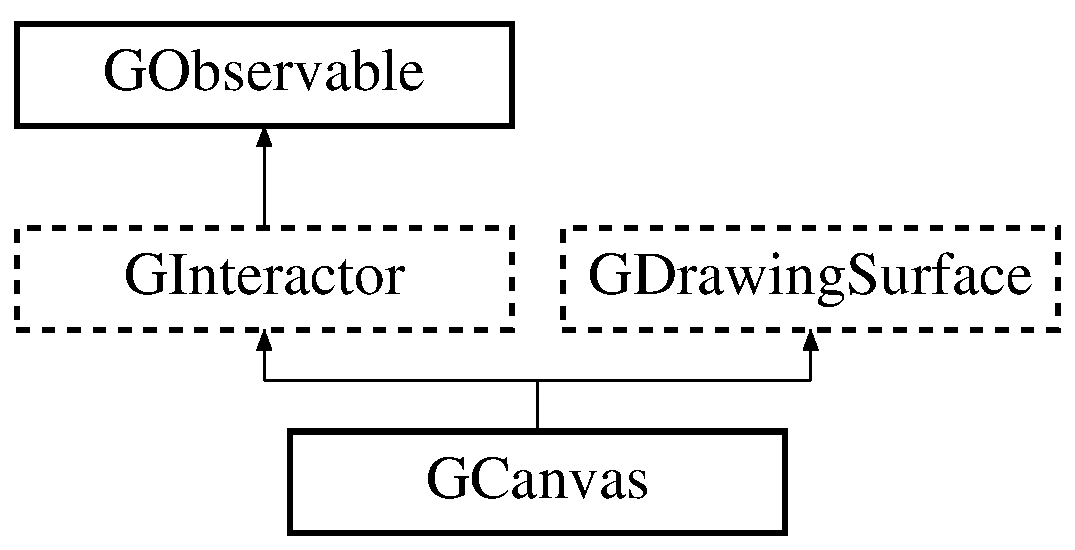
\includegraphics[height=3.000000cm]{classGCanvas}
\end{center}
\end{figure}
\subsection*{Public Types}
\begin{DoxyCompactItemize}
\item 
enum \mbox{\hyperlink{classGInteractor_a8e0d441725a81d2bbdebbea09078260e}{Text\+Position}} \{ \mbox{\hyperlink{classGInteractor_a8e0d441725a81d2bbdebbea09078260ea4cd6f2e7d5a08d6f4dc052df2358f774}{T\+E\+X\+T\+\_\+\+B\+E\+S\+I\+D\+E\+\_\+\+I\+C\+ON}}, 
\mbox{\hyperlink{classGInteractor_a8e0d441725a81d2bbdebbea09078260eaa88490f63d8de68d44c83bdb2ecde3b3}{T\+E\+X\+T\+\_\+\+U\+N\+D\+E\+R\+\_\+\+I\+C\+ON}}, 
\mbox{\hyperlink{classGInteractor_a8e0d441725a81d2bbdebbea09078260ea39a6f388a30ac4fefb6eb13e846bc9f2}{T\+E\+X\+T\+\_\+\+O\+N\+LY}}
 \}
\begin{DoxyCompactList}\small\item\em The places where an interactor can place its text relative to its icon. \end{DoxyCompactList}\end{DoxyCompactItemize}
\subsection*{Public Member Functions}
\begin{DoxyCompactItemize}
\item 
\mbox{\hyperlink{classGCanvas_abb7f95d00cbfadedab276958e1eb2af1}{G\+Canvas}} (Q\+Widget $\ast$parent=nullptr)
\begin{DoxyCompactList}\small\item\em Creates an empty canvas with a default size of 0x0 pixels and a default background and foreground color of black. \end{DoxyCompactList}\item 
\mbox{\hyperlink{classGCanvas_a0a9de139286d0fc9146928aff8f0538c}{G\+Canvas}} (const std\+::string \&filename, Q\+Widget $\ast$parent=nullptr)
\begin{DoxyCompactList}\small\item\em Creates a canvas that loads its background layer pixel data from the given image file name. \end{DoxyCompactList}\item 
\mbox{\hyperlink{classGCanvas_a235f6b1b700354d6737607562df06581}{G\+Canvas}} (double width, double height, int rgb\+Background, Q\+Widget $\ast$parent=nullptr)
\begin{DoxyCompactList}\small\item\em Creates an empty canvas of the specified size and optional background color. \end{DoxyCompactList}\item 
\mbox{\hyperlink{classGCanvas_af8bb8bd29201bbb5d0f90016a1d8df2c}{G\+Canvas}} (double width, double height, const std\+::string \&rgb\+Background=\char`\"{}\#00000000\char`\"{}, Q\+Widget $\ast$parent=nullptr)
\begin{DoxyCompactList}\small\item\em Creates an empty canvas of the specified size and background color. \end{DoxyCompactList}\item 
virtual \mbox{\hyperlink{classGCanvas_a601cc120704b2d2e9898a61f6ce94bc0}{$\sim$\+G\+Canvas}} () Q\+\_\+\+D\+E\+C\+L\+\_\+\+O\+V\+E\+R\+R\+I\+DE
\begin{DoxyCompactList}\small\item\em Frees memory allocated internally by the canvas. \end{DoxyCompactList}\item 
virtual void \mbox{\hyperlink{classGCanvas_afe8277e7b2627513c6f7452fb0b2847d}{add}} (\mbox{\hyperlink{classGObject}{G\+Object}} $\ast$gobj)
\begin{DoxyCompactList}\small\item\em Adds the given interactor to canvas. \end{DoxyCompactList}\item 
virtual void \mbox{\hyperlink{classGCanvas_a8bb36f245efc7806414a1339c2befa1c}{add}} (\mbox{\hyperlink{classGObject}{G\+Object}} $\ast$gobj, double x, double y)
\begin{DoxyCompactList}\small\item\em Adds the given interactor to the canvas and moves it to the given x/y location. \end{DoxyCompactList}\item 
virtual void \mbox{\hyperlink{classGCanvas_ac732fc2123d7a6d7e2de145fe9bbd8e8}{add}} (\mbox{\hyperlink{classGObject}{G\+Object}} \&gobj)
\begin{DoxyCompactList}\small\item\em Adds the given interactor to canvas. \end{DoxyCompactList}\item 
virtual void \mbox{\hyperlink{classGCanvas_a5b11b532869632a6c26b098b0858eac5}{add}} (\mbox{\hyperlink{classGObject}{G\+Object}} \&gobj, double x, double y)
\begin{DoxyCompactList}\small\item\em Adds the given interactor to the canvas and moves it to the given x/y location. \end{DoxyCompactList}\item 
virtual void \mbox{\hyperlink{classGInteractor_a02f20ea6edfa0671f31c4c648a253833}{add\+Action\+Listener}} () Q\+\_\+\+D\+E\+C\+L\+\_\+\+D\+E\+P\+R\+E\+C\+A\+T\+ED
\begin{DoxyCompactList}\small\item\em Adds an event listener to be notified when this interactor is clicked or generally interacted with. \end{DoxyCompactList}\item 
virtual void \mbox{\hyperlink{classGCanvas_af220cadd1499c3586d48010a0348d9f8}{clear}} () Q\+\_\+\+D\+E\+C\+L\+\_\+\+O\+V\+E\+R\+R\+I\+DE
\begin{DoxyCompactList}\small\item\em Removes all graphical objects from the canvas foreground layer and wipes the background layer to show the current background color. \end{DoxyCompactList}\item 
virtual void \mbox{\hyperlink{classGCanvas_a6614e1320bc8e93b20df129613e5a0ff}{clear\+Objects}} ()
\begin{DoxyCompactList}\small\item\em Removes all graphical objects from the foreground layer of the canvas. \end{DoxyCompactList}\item 
virtual void \mbox{\hyperlink{classGCanvas_ab2c8590176aec1da6fb4e9b836bab630}{clear\+Pixels}} ()
\begin{DoxyCompactList}\small\item\em Resets the background layer of pixels in the canvas to the current background color. \end{DoxyCompactList}\item 
virtual void \mbox{\hyperlink{classGDrawingSurface_a221b3e75bb3d9d0bfea62b3364e6773b}{conditional\+Repaint}} ()
\begin{DoxyCompactList}\small\item\em Repaints the interactor only if its contents have changed. \end{DoxyCompactList}\item 
virtual void \mbox{\hyperlink{classGDrawingSurface_aedd4b792311d946eeaf44b0de337a408}{conditional\+Repaint\+Region}} (int x, int y, int width, int height)
\begin{DoxyCompactList}\small\item\em Repaints the given region of the interactor only if its contents have changed. \end{DoxyCompactList}\item 
virtual void \mbox{\hyperlink{classGDrawingSurface_a3932a12278752db368e24fa404e446aa}{conditional\+Repaint\+Region}} (const \mbox{\hyperlink{classGRectangle}{G\+Rectangle}} \&bounds)
\begin{DoxyCompactList}\small\item\em Repaints the given region of the interactor only if its contents have changed. \end{DoxyCompactList}\item 
virtual bool \mbox{\hyperlink{classGCanvas_abb6a5d7c03e6eaaae97264c4799ce7c3}{contains}} (double x, double y) const
\begin{DoxyCompactList}\small\item\em Returns true if any of the graphical objects in the foreground layer of the canvas touch the given x/y pixel. \end{DoxyCompactList}\item 
virtual int \mbox{\hyperlink{classGCanvas_ad3d6147a5e08ed97bb71c7f267ef071b}{count\+Diff\+Pixels}} (const \mbox{\hyperlink{classGCanvas}{G\+Canvas}} \&image) const
\begin{DoxyCompactList}\small\item\em Returns the total number of pixels that are not the same color between this image and the given other image. \end{DoxyCompactList}\item 
virtual int \mbox{\hyperlink{classGCanvas_a3ed6edef8ed522bbfc09d8f6005d6d8e}{count\+Diff\+Pixels}} (const \mbox{\hyperlink{classGCanvas}{G\+Canvas}} \&image, int xmin, int ymin, int xmax, int ymax) const
\begin{DoxyCompactList}\small\item\em Returns the total number of pixels that are not the same color between this image and the given other image. \end{DoxyCompactList}\item 
virtual int \mbox{\hyperlink{classGCanvas_a443b0f63a197c0f1147b13077f4206e0}{count\+Diff\+Pixels}} (const \mbox{\hyperlink{classGCanvas}{G\+Canvas}} $\ast$image) const
\begin{DoxyCompactList}\small\item\em Returns the total number of pixels that are not the same color between this image and the given other image. \end{DoxyCompactList}\item 
virtual int \mbox{\hyperlink{classGCanvas_a77b38a94630c93ecc697fb12a1fb89fd}{count\+Diff\+Pixels}} (const \mbox{\hyperlink{classGCanvas}{G\+Canvas}} $\ast$image, int xmin, int ymin, int xmax, int ymax) const
\begin{DoxyCompactList}\small\item\em Returns the total number of pixels that are not the same color between this image and the given other image. \end{DoxyCompactList}\item 
virtual \mbox{\hyperlink{classGCanvas}{G\+Canvas}} $\ast$ \mbox{\hyperlink{classGCanvas_aa4e74e40eebb70c9616065056de5c4ca}{diff}} (const \mbox{\hyperlink{classGCanvas}{G\+Canvas}} \&image, int diff\+Pixel\+Color=G\+C\+A\+N\+V\+A\+S\+\_\+\+D\+E\+F\+A\+U\+L\+T\+\_\+\+D\+I\+F\+F\+\_\+\+P\+I\+X\+E\+L\+\_\+\+C\+O\+L\+OR) const
\begin{DoxyCompactList}\small\item\em Generates a new canvas whose content is equal to that of this canvas but with any pixels that don\textquotesingle{}t match those in parameter \textquotesingle{}image\textquotesingle{} colored in the given color (default purple) to highlight differences between the two. \end{DoxyCompactList}\item 
virtual \mbox{\hyperlink{classGCanvas}{G\+Canvas}} $\ast$ \mbox{\hyperlink{classGCanvas_a5385d5c8fda55dfe0b20851d293b338b}{diff}} (const \mbox{\hyperlink{classGCanvas}{G\+Canvas}} $\ast$image, int diff\+Pixel\+Color=G\+C\+A\+N\+V\+A\+S\+\_\+\+D\+E\+F\+A\+U\+L\+T\+\_\+\+D\+I\+F\+F\+\_\+\+P\+I\+X\+E\+L\+\_\+\+C\+O\+L\+OR) const
\begin{DoxyCompactList}\small\item\em Generates a new canvas whose content is equal to that of this canvas but with any pixels that don\textquotesingle{}t match those in parameter \textquotesingle{}image\textquotesingle{} colored in the given color (default purple) to highlight differences between the two. \end{DoxyCompactList}\item 
virtual void \mbox{\hyperlink{classGDrawingSurface_acc3825d7a24815d1e2f78e7c3ffea6cc}{draw}} (\mbox{\hyperlink{classGObject}{G\+Object}} $\ast$gobj, double x, double y)
\begin{DoxyCompactList}\small\item\em Draws the given graphical object onto the background pixel layer of this interactor, moving it to the given x/y location first. \end{DoxyCompactList}\item 
virtual void \mbox{\hyperlink{classGDrawingSurface_a022a8d51c7fabcd79a0c809233e93453}{draw}} (\mbox{\hyperlink{classGObject}{G\+Object}} \&gobj)
\begin{DoxyCompactList}\small\item\em Draws the given graphical object onto the background pixel layer of this interactor. \end{DoxyCompactList}\item 
virtual void \mbox{\hyperlink{classGDrawingSurface_a8af8762bd6720e0a1d2a84b190e3dc96}{draw}} (\mbox{\hyperlink{classGObject}{G\+Object}} \&gobj, double x, double y)
\begin{DoxyCompactList}\small\item\em Draws the given graphical object onto the background pixel layer of this interactor, moving it to the given x/y location first. \end{DoxyCompactList}\item 
virtual void \mbox{\hyperlink{classGCanvas_a00bf9d87527d59e6f11756589c25e4e7}{draw}} (\mbox{\hyperlink{classGObject}{G\+Object}} $\ast$gobj) Q\+\_\+\+D\+E\+C\+L\+\_\+\+O\+V\+E\+R\+R\+I\+DE
\begin{DoxyCompactList}\small\item\em Draws the given graphical object onto the background layer of the canvas. \end{DoxyCompactList}\item 
virtual void \mbox{\hyperlink{classGDrawingSurface_a38b6fae1045191c57092b49905068144}{draw\+Arc}} (double x, double y, double width, double height, double start, double sweep)
\begin{DoxyCompactList}\small\item\em Draws an unfilled arc with the given attributes onto the background pixel layer of this interactor in the current color. \end{DoxyCompactList}\item 
virtual void \mbox{\hyperlink{classGDrawingSurface_abdd4cb1f2c64adc5d03522a1ee30febf}{draw\+Image}} (const std\+::string \&filename, double x=0, double y=0)
\begin{DoxyCompactList}\small\item\em Draws an image loaded from the given file name onto the background pixel layer of this interactor at the given x/y location. \end{DoxyCompactList}\item 
virtual void \mbox{\hyperlink{classGDrawingSurface_ae6a24b6b9a6e795d3165c1c750d5bdf1}{draw\+Line}} (const \mbox{\hyperlink{classGPoint}{G\+Point}} \&p0, const \mbox{\hyperlink{classGPoint}{G\+Point}} \&p1)
\begin{DoxyCompactList}\small\item\em Draws a line between the given two points onto the background pixel layer of this interactor at the given x/y location in the current color. \end{DoxyCompactList}\item 
virtual void \mbox{\hyperlink{classGDrawingSurface_aff299fe83178d2f3ce8c08c06b583484}{draw\+Line}} (double x0, double y0, double x1, double y1)
\begin{DoxyCompactList}\small\item\em Draws a line between the given two points onto the background pixel layer of this interactor at the given x/y location in the current color. \end{DoxyCompactList}\item 
virtual void \mbox{\hyperlink{classGDrawingSurface_a8adc13027efe311b4a6a715205b8bc46}{draw\+Oval}} (const \mbox{\hyperlink{classGRectangle}{G\+Rectangle}} \&bounds)
\begin{DoxyCompactList}\small\item\em Draws an unfilled oval with the given bounding box onto the background pixel layer of this interactor at the given x/y location in the current color. \end{DoxyCompactList}\item 
virtual void \mbox{\hyperlink{classGDrawingSurface_aa5b1cf902e578907da3c63060686354e}{draw\+Oval}} (double x, double y, double width, double height)
\begin{DoxyCompactList}\small\item\em Draws an unfilled oval with the given bounding box onto the background pixel layer of this interactor at the given x/y location in the current color. \end{DoxyCompactList}\item 
virtual void \mbox{\hyperlink{classGDrawingSurface_a0c1e2923d8d163d62d0896d8c5cfa191}{draw\+Pixel}} (double x, double y)
\begin{DoxyCompactList}\small\item\em Colors the given x/y pixel of the background layer of this interactor using the interactor\textquotesingle{}s current color. \end{DoxyCompactList}\item 
virtual void \mbox{\hyperlink{classGDrawingSurface_a3a64eb6383e601be8438e9c71643c432}{draw\+Pixel}} (double x, double y, int color)
\begin{DoxyCompactList}\small\item\em Colors the given x/y pixel of the background layer of this interactor using the given color. \end{DoxyCompactList}\item 
virtual void \mbox{\hyperlink{classGDrawingSurface_a20abc26a94b7eb310e34abf668e0f5f4}{draw\+Pixel}} (double x, double y, const std\+::string \&color)
\begin{DoxyCompactList}\small\item\em Colors the given x/y pixel of the background layer of this interactor using the given color. \end{DoxyCompactList}\item 
virtual \mbox{\hyperlink{classGPoint}{G\+Point}} \mbox{\hyperlink{classGDrawingSurface_af70cce1e4f708f1ed5b6f29cecb660e7}{draw\+Polar\+Line}} (const \mbox{\hyperlink{classGPoint}{G\+Point}} \&p0, double r, double theta)
\begin{DoxyCompactList}\small\item\em Draws a line using polar coordinates onto the background pixel layer of this interactor in the current color. \end{DoxyCompactList}\item 
virtual \mbox{\hyperlink{classGPoint}{G\+Point}} \mbox{\hyperlink{classGDrawingSurface_ad3e646f90005295f2bbdf37d2bcb39d2}{draw\+Polar\+Line}} (double x0, double y0, double r, double theta)
\begin{DoxyCompactList}\small\item\em Draws a line using polar coordinates onto the background pixel layer of this interactor in the current color. \end{DoxyCompactList}\item 
virtual void \mbox{\hyperlink{classGDrawingSurface_afddec0a905108d8a8d6809a157f26776}{draw\+Polygon}} (std\+::initializer\+\_\+list$<$ double $>$ coords)
\begin{DoxyCompactList}\small\item\em Draws an unfilled polygon containing the given points onto the background pixel layer of this interactor in the current color. \end{DoxyCompactList}\item 
virtual void \mbox{\hyperlink{classGDrawingSurface_a021ee881e0d154dc4dd059698742889c}{draw\+Polygon}} (std\+::initializer\+\_\+list$<$ \mbox{\hyperlink{classGPoint}{G\+Point}} $>$ points)
\begin{DoxyCompactList}\small\item\em Draws an unfilled polygon containing the given points onto the background pixel layer of this interactor in the current color. \end{DoxyCompactList}\item 
virtual void \mbox{\hyperlink{classGDrawingSurface_a3dd4cc5891149dfc36746264f7289877}{draw\+Rect}} (const \mbox{\hyperlink{classGRectangle}{G\+Rectangle}} \&bounds)
\begin{DoxyCompactList}\small\item\em Draws an unfilled rectangle of the given dimensions onto the background pixel layer of this interactor in the current color. \end{DoxyCompactList}\item 
virtual void \mbox{\hyperlink{classGDrawingSurface_a4148e770ffc5474153aadd4814dbd708}{draw\+Rect}} (double x, double y, double width, double height)
\begin{DoxyCompactList}\small\item\em Draws an unfilled rectangle of the given dimensions onto the background pixel layer of this interactor in the current color. \end{DoxyCompactList}\item 
virtual void \mbox{\hyperlink{classGDrawingSurface_ad4e8551a753a77135792bbee97013675}{draw\+String}} (const std\+::string \&text, double x, double y)
\begin{DoxyCompactList}\small\item\em Draws a text string onto the background pixel layer of this interactor at the given x/y location in the current font and color. \end{DoxyCompactList}\item 
virtual bool \mbox{\hyperlink{classGCanvas_a7cf0de4c4124b7de747b9cc17edd6ab9}{equals}} (const \mbox{\hyperlink{classGCanvas}{G\+Canvas}} \&other) const
\begin{DoxyCompactList}\small\item\em Returns true if the two given canvases contain exactly the same pixel data. \end{DoxyCompactList}\item 
virtual bool \mbox{\hyperlink{classGInteractor_ac05ba5b92e2e5146d416fe7f842a0969}{events\+Enabled}} () const Q\+\_\+\+D\+E\+C\+L\+\_\+\+O\+V\+E\+R\+R\+I\+DE
\begin{DoxyCompactList}\small\item\em Returns true if this interactor is currently accepting events. \end{DoxyCompactList}\item 
virtual void \mbox{\hyperlink{classGCanvas_acaf90d64e4fea8f776e722976aeb5070}{fill}} (int rgb)
\begin{DoxyCompactList}\small\item\em Sets the color of every pixel in the canvas to the given color value. \end{DoxyCompactList}\item 
virtual void \mbox{\hyperlink{classGCanvas_a02a5aa7f1474eeedd181e6e46b5eee65}{fill}} (const std\+::string \&rgb)
\begin{DoxyCompactList}\small\item\em Sets the color of every pixel in the canvas to the given color value. \end{DoxyCompactList}\item 
virtual void \mbox{\hyperlink{classGDrawingSurface_a228075ad18bd97b57f9956568c4773f3}{fill\+Arc}} (double x, double y, double width, double height, double start, double sweep)
\begin{DoxyCompactList}\small\item\em Draws a filled arc with the given attributes onto the background pixel layer of this interactor in the current color and fill color. \end{DoxyCompactList}\item 
virtual void \mbox{\hyperlink{classGDrawingSurface_a1ea6e48d59fb588797dba4deab1397e0}{fill\+Oval}} (const \mbox{\hyperlink{classGRectangle}{G\+Rectangle}} \&bounds)
\begin{DoxyCompactList}\small\item\em Draws a filled oval with the given bounding box onto the background pixel layer of this interactor at the given x/y location in the current color and fill color. \end{DoxyCompactList}\item 
virtual void \mbox{\hyperlink{classGDrawingSurface_a28c700c82f31cd328a4629273420ee61}{fill\+Oval}} (double x, double y, double width, double height)
\begin{DoxyCompactList}\small\item\em Draws a filled oval with the given bounding box onto the background pixel layer of this interactor at the given x/y location in the current color and fill color. \end{DoxyCompactList}\item 
virtual void \mbox{\hyperlink{classGDrawingSurface_a15f8c1c4409ef51c1a30a92a195b8f66}{fill\+Polygon}} (std\+::initializer\+\_\+list$<$ double $>$ coords)
\begin{DoxyCompactList}\small\item\em Draws a filled polygon containing the given points onto the background pixel layer of this interactor in the current color and fill color. \end{DoxyCompactList}\item 
virtual void \mbox{\hyperlink{classGDrawingSurface_ae6582295003bf2488836b1993dadbad7}{fill\+Rect}} (const \mbox{\hyperlink{classGRectangle}{G\+Rectangle}} \&bounds)
\begin{DoxyCompactList}\small\item\em Draws a filled rectangle of the given dimensions onto the background pixel layer of this interactor in the current color and fill color. \end{DoxyCompactList}\item 
virtual void \mbox{\hyperlink{classGDrawingSurface_aac3ae7d3aee950de78eca0e108352254}{fill\+Rect}} (double x, double y, double width, double height)
\begin{DoxyCompactList}\small\item\em Draws a filled rectangle of the given dimensions onto the background pixel layer of this interactor in the current color and fill color. \end{DoxyCompactList}\item 
virtual void \mbox{\hyperlink{classGCanvas_af4146bdcb26135b739b9b4f13db03435}{fill\+Region}} (double x, double y, double width, double height, int rgb)
\begin{DoxyCompactList}\small\item\em Sets the color of every pixel in the given rectangular range of the canvas pixel data to the given color value. \end{DoxyCompactList}\item 
virtual void \mbox{\hyperlink{classGCanvas_a762c611a5065687112018e7a0ab10c84}{fill\+Region}} (double x, double y, double width, double height, const std\+::string \&rgb)
\begin{DoxyCompactList}\small\item\em Sets the color of every pixel in the given rectangular range of the canvas pixel data to the given color value. \end{DoxyCompactList}\item 
virtual void \mbox{\hyperlink{classGCanvas_a4c4590df33ce47ad8a42e06f9f44fc93}{flatten}} ()
\begin{DoxyCompactList}\small\item\em Moves all graphical objects from the foreground layer to the background layer. \end{DoxyCompactList}\item 
virtual void \mbox{\hyperlink{classGCanvas_a46b18491b5230c765fbd9b8c7a095587}{from\+Grid}} (const \mbox{\hyperlink{classGrid}{Grid}}$<$ int $>$ \&grid)
\begin{DoxyCompactList}\small\item\em Replaces the entire contents of the background layer of the canvas with the contents of the given grid of R\+GB pixel values. \end{DoxyCompactList}\item 
virtual std\+::string \mbox{\hyperlink{classGInteractor_a69f8d23ed8f207fbecad99960776e942}{get\+Accelerator}} () const
\begin{DoxyCompactList}\small\item\em Returns a string representing a hotkey for this interactor, or an empty string if no accelerator has been set. \end{DoxyCompactList}\item 
virtual std\+::string \mbox{\hyperlink{classGInteractor_a94eb4276000c4fdfb508ce9e6317a82a}{get\+Action\+Command}} () const
\begin{DoxyCompactList}\small\item\em Returns an action command for this interactor, which is a semi-\/unique string you can use to identify it when events occur. \end{DoxyCompactList}\item 
virtual int \mbox{\hyperlink{classGDrawingSurface_ae394d39f20476570e083918d991c25bd}{get\+A\+R\+GB}} (double x, double y) const
\begin{DoxyCompactList}\small\item\em Returns the pixel color data at the given x/y location, retaining alpha-\/channel transparency in the top 8 bits. \end{DoxyCompactList}\item 
virtual std\+::string \mbox{\hyperlink{classGCanvas_ab44f928b6bd7c8e4b82d5ed92bc3d4c6}{get\+Background}} () const Q\+\_\+\+D\+E\+C\+L\+\_\+\+O\+V\+E\+R\+R\+I\+DE
\begin{DoxyCompactList}\small\item\em Returns the current background color of the interactor as a string. \end{DoxyCompactList}\item 
virtual int \mbox{\hyperlink{classGCanvas_af66f525e8154dbc8dcd2daecf3728ba9}{get\+Background\+Int}} () const Q\+\_\+\+D\+E\+C\+L\+\_\+\+O\+V\+E\+R\+R\+I\+DE
\begin{DoxyCompactList}\small\item\em Returns the current background color of the interactor as an R\+GB integer. \end{DoxyCompactList}\item 
virtual \mbox{\hyperlink{classGRectangle}{G\+Rectangle}} \mbox{\hyperlink{classGInteractor_a29e6ac35a0b48f491a4c88194cc5da3b}{get\+Bounds}} () const
\begin{DoxyCompactList}\small\item\em Returns a rectangle representing the x/y position and size of this interactor. \end{DoxyCompactList}\item 
virtual std\+::string \mbox{\hyperlink{classGInteractor_aa061dfa488c31e18549d64363c1d0e34}{get\+Color}} () const
\begin{DoxyCompactList}\small\item\em Returns the foreground/text color of the interactor as a string. \end{DoxyCompactList}\item 
virtual std\+::string \mbox{\hyperlink{classGDrawingSurface_aa061dfa488c31e18549d64363c1d0e34}{get\+Color}} () const
\begin{DoxyCompactList}\small\item\em Returns the current foreground outline color of the interactor as a string. \end{DoxyCompactList}\item 
virtual int \mbox{\hyperlink{classGInteractor_a9635c7af766cdc3417f346683fa0e6c1}{get\+Color\+Int}} () const
\begin{DoxyCompactList}\small\item\em Returns the foreground/text color of the interactor as an R\+GB integer. \end{DoxyCompactList}\item 
virtual int \mbox{\hyperlink{classGDrawingSurface_a9635c7af766cdc3417f346683fa0e6c1}{get\+Color\+Int}} () const
\begin{DoxyCompactList}\small\item\em Returns the current foreground outline color of the interactor as an R\+GB integer. \end{DoxyCompactList}\item 
virtual \mbox{\hyperlink{classGContainer}{G\+Container}} $\ast$ \mbox{\hyperlink{classGInteractor_a7a6e317c29d61030929b4cd2d1c00fe7}{get\+Container}} () const
\begin{DoxyCompactList}\small\item\em Returns a pointer to the onscreen container holding this interactor. \end{DoxyCompactList}\item 
virtual \mbox{\hyperlink{classGObject}{G\+Object}} $\ast$ \mbox{\hyperlink{classGCanvas_abde388cc529d22bb5f7f4a54d56049d8}{get\+Element}} (int index) const
\begin{DoxyCompactList}\small\item\em Returns a pointer to the graphical object in the foreground layer of the canvas at the specified index, numbering from back to front in the {\itshape z} dimension. \end{DoxyCompactList}\item 
virtual \mbox{\hyperlink{classGObject}{G\+Object}} $\ast$ \mbox{\hyperlink{classGCanvas_a25efa999eca5790ec26ef091b05f961c}{get\+Element\+At}} (double x, double y) const
\begin{DoxyCompactList}\small\item\em Returns a pointer to the first graphical object in the foreground layer of the canvas that contains the given (x, y) point, or a null pointer if no object in this canvas touches it. \end{DoxyCompactList}\item 
virtual int \mbox{\hyperlink{classGCanvas_adf7d37ec315f859648def92e6b32408f}{get\+Element\+Count}} () const
\begin{DoxyCompactList}\small\item\em Returns the number of graphical objects stored in the foreground layer of the canvas. \end{DoxyCompactList}\item 
virtual std\+::string \mbox{\hyperlink{classGCanvas_a2011812670c3de9747702e3c052b6bb3}{get\+Filename}} () const
\begin{DoxyCompactList}\small\item\em Returns the name of the image file from which this canvas was loaded or to which it was saved most recently. \end{DoxyCompactList}\item 
virtual std\+::string \mbox{\hyperlink{classGDrawingSurface_a76f6964a11fde7c78e9751be184e1a3c}{get\+Fill\+Color}} () const
\begin{DoxyCompactList}\small\item\em Returns the current fill color of the interactor as a string. \end{DoxyCompactList}\item 
virtual int \mbox{\hyperlink{classGDrawingSurface_a88f4508d9271c4b5f5b5d6b780f223d0}{get\+Fill\+Color\+Int}} () const
\begin{DoxyCompactList}\small\item\em Returns the current fill color of the interactor as an R\+GB integer. \end{DoxyCompactList}\item 
virtual std\+::string \mbox{\hyperlink{classGCanvas_a24420d98f18927d2c201a3ab55ffdcec}{get\+Font}} () const Q\+\_\+\+D\+E\+C\+L\+\_\+\+O\+V\+E\+R\+R\+I\+DE
\begin{DoxyCompactList}\small\item\em Returns the current text font of the interactor as a font string. \end{DoxyCompactList}\item 
virtual std\+::string \mbox{\hyperlink{classGInteractor_a4fa2d8b0192a3a5b4af4bbfe71194d03}{get\+Foreground}} () const
\begin{DoxyCompactList}\small\item\em Returns the foreground/text color of the interactor as a string. \end{DoxyCompactList}\item 
virtual std\+::string \mbox{\hyperlink{classGDrawingSurface_a4fa2d8b0192a3a5b4af4bbfe71194d03}{get\+Foreground}} () const
\begin{DoxyCompactList}\small\item\em Returns the current foreground outline color of the interactor as a string. \end{DoxyCompactList}\item 
virtual int \mbox{\hyperlink{classGInteractor_ac3b12ab385a6ef9ae90fc879860ba726}{get\+Foreground\+Int}} () const
\begin{DoxyCompactList}\small\item\em Returns the foreground/text color of the interactor as an R\+GB integer. \end{DoxyCompactList}\item 
virtual int \mbox{\hyperlink{classGDrawingSurface_ac3b12ab385a6ef9ae90fc879860ba726}{get\+Foreground\+Int}} () const
\begin{DoxyCompactList}\small\item\em Returns the current foreground outline color of the interactor as an R\+GB integer. \end{DoxyCompactList}\item 
virtual double \mbox{\hyperlink{classGInteractor_a1e7e353362434072875264cf95629f99}{get\+Height}} () const
\begin{DoxyCompactList}\small\item\em Returns the current onscreen height of this interactor in pixels. \end{DoxyCompactList}\item 
virtual std\+::string \mbox{\hyperlink{classGInteractor_aaed62a73004939a64da6f0eb9eb64d73}{get\+Icon}} () const
\begin{DoxyCompactList}\small\item\em Returns the file name of the icon associated with this interactor, or an empty string if no icon has been set. \end{DoxyCompactList}\item 
virtual int \mbox{\hyperlink{classGInteractor_a9c9659a6c6ba66b4107ba59c95a24241}{get\+ID}} () const
\begin{DoxyCompactList}\small\item\em Returns a globally unique identifier for this interactor, which is set when the interactor is constructed. \end{DoxyCompactList}\item 
virtual \+\_\+\+Internal\+\_\+\+Q\+Widget $\ast$ \mbox{\hyperlink{classGCanvas_a208ce13c1da40bf0ddb509daf99d6588}{get\+Internal\+Widget}} () const Q\+\_\+\+D\+E\+C\+L\+\_\+\+O\+V\+E\+R\+R\+I\+DE
\begin{DoxyCompactList}\small\item\em Returns a direct pointer to the internal Qt widget being wrapped by this interactor. \end{DoxyCompactList}\item 
virtual \mbox{\hyperlink{classGObject_a86e0f5648542856159bb40775c854aa7}{G\+Object\+::\+Line\+Style}} \mbox{\hyperlink{classGDrawingSurface_aaf1f5ea8281e5e3486662878d26f0a13}{get\+Line\+Style}} () const
\begin{DoxyCompactList}\small\item\em Returns the current line style which will be used to draw outlines of shapes and lines. \end{DoxyCompactList}\item 
virtual double \mbox{\hyperlink{classGDrawingSurface_a85ff266dc3eb63d9f2d8e5a4487fd3c0}{get\+Line\+Width}} () const
\begin{DoxyCompactList}\small\item\em Returns the thickness used when drawing outlines of shapes and lines. \end{DoxyCompactList}\item 
virtual \mbox{\hyperlink{classGPoint}{G\+Point}} \mbox{\hyperlink{classGInteractor_a4f83802015511edeb63b892830812c11}{get\+Location}} () const
\begin{DoxyCompactList}\small\item\em Returns an (x, y) point representing the onscreen location of the top-\/left corner of this interactor within its containing window. \end{DoxyCompactList}\item 
virtual double \mbox{\hyperlink{classGInteractor_aed4b0075fcc434499c3cb3e46896bda3}{get\+Minimum\+Height}} () const
\begin{DoxyCompactList}\small\item\em Returns the minimum height in pixels that this interactor will permit itself to be resized to. \end{DoxyCompactList}\item 
virtual \mbox{\hyperlink{classGDimension}{G\+Dimension}} \mbox{\hyperlink{classGInteractor_a66b5af0b32493b4d597ca0a3df2049ea}{get\+Minimum\+Size}} () const
\begin{DoxyCompactList}\small\item\em Returns a \mbox{\hyperlink{classGDimension}{G\+Dimension}} structure representing the minimum size in pixels that this interactor will permit itself to be resized to. \end{DoxyCompactList}\item 
virtual double \mbox{\hyperlink{classGInteractor_a59e668114fe3d49d2a0f28deb258f7c8}{get\+Minimum\+Width}} () const
\begin{DoxyCompactList}\small\item\em Returns the minimum width in pixels that this interactor will permit itself to be resized to. \end{DoxyCompactList}\item 
virtual std\+::string \mbox{\hyperlink{classGInteractor_a8a60438a5b55d0b2ceb35c8674b9d8c5}{get\+Name}} () const
\begin{DoxyCompactList}\small\item\em Returns a string representing a unique name for this interactor. \end{DoxyCompactList}\item 
virtual int \mbox{\hyperlink{classGCanvas_a076754305680c65782a00ddd3c77b50b}{get\+Pixel}} (double x, double y) const Q\+\_\+\+D\+E\+C\+L\+\_\+\+O\+V\+E\+R\+R\+I\+DE
\begin{DoxyCompactList}\small\item\em Returns the color of the pixel at the given x/y coordinates of the background layer of the canvas as an integer such as 0xff00cc. \end{DoxyCompactList}\item 
virtual int \mbox{\hyperlink{classGCanvas_ac1016456426446714a53d29da622f2ec}{get\+Pixel\+A\+R\+GB}} (double x, double y) const Q\+\_\+\+D\+E\+C\+L\+\_\+\+O\+V\+E\+R\+R\+I\+DE
\begin{DoxyCompactList}\small\item\em Returns the color of the pixel at the given x/y coordinates of the background layer of the canvas as an integer such as 0xffff00cc. \end{DoxyCompactList}\item 
virtual \mbox{\hyperlink{classGrid}{Grid}}$<$ int $>$ \mbox{\hyperlink{classGCanvas_a430b4965720f3b35f10062a252883e75}{get\+Pixels}} () const Q\+\_\+\+D\+E\+C\+L\+\_\+\+O\+V\+E\+R\+R\+I\+DE
\begin{DoxyCompactList}\small\item\em Returns all pixels of the background layer of the canvas as a \mbox{\hyperlink{classGrid}{Grid}}, where rows represent y values and columns represent x values. \end{DoxyCompactList}\item 
virtual \mbox{\hyperlink{classGrid}{Grid}}$<$ int $>$ \mbox{\hyperlink{classGCanvas_aca5a19f5f53c5cd29b832a769fde4f68}{get\+Pixels\+A\+R\+GB}} () const Q\+\_\+\+D\+E\+C\+L\+\_\+\+O\+V\+E\+R\+R\+I\+DE
\begin{DoxyCompactList}\small\item\em Returns all pixels of the background layer of the canvas as a \mbox{\hyperlink{classGrid}{Grid}}, where rows represent y values and columns represent x values. \end{DoxyCompactList}\item 
virtual std\+::string \mbox{\hyperlink{classGDrawingSurface_a8da04ef488ec5fa498fbbffaf50928fd}{get\+Pixel\+String}} (double x, double y) const
\begin{DoxyCompactList}\small\item\em Returns the color of the pixel at the given x/y coordinates of the image as a string such as \char`\"{}\#ff00cc\char`\"{}. \end{DoxyCompactList}\item 
virtual double \mbox{\hyperlink{classGInteractor_a747de0961653847bdc6615dbf756d715}{get\+Preferred\+Height}} () const
\begin{DoxyCompactList}\small\item\em Returns the height in pixels that this interactor would prefer to be, which would exactly fit its contents with no stretching or scrollbars. \end{DoxyCompactList}\item 
virtual \mbox{\hyperlink{classGDimension}{G\+Dimension}} \mbox{\hyperlink{classGInteractor_a4aabbee761d8e9116275401131b7ccd1}{get\+Preferred\+Size}} () const
\begin{DoxyCompactList}\small\item\em Returns a \mbox{\hyperlink{classGDimension}{G\+Dimension}} structure storing the width and height in pixels that this interactor would prefer to be, which would exactly fit its contents with no stretching or scrollbars. \end{DoxyCompactList}\item 
virtual double \mbox{\hyperlink{classGInteractor_a82bca31d37700fb0e35d2743352efd5e}{get\+Preferred\+Width}} () const
\begin{DoxyCompactList}\small\item\em Returns the height in pixels that this interactor would prefer to be, which would exactly fit its contents with no stretching or scrollbars. \end{DoxyCompactList}\item 
virtual int \mbox{\hyperlink{classGDrawingSurface_a9e983467cf0c97cfd62433a8471570dc}{get\+R\+GB}} (double x, double y) const
\begin{DoxyCompactList}\small\item\em Returns the color of the pixel at the given x/y coordinates of the background layer of the interactor as an integer such as 0xff00cc. \end{DoxyCompactList}\item 
virtual std\+::string \mbox{\hyperlink{classGDrawingSurface_a456d3582acc3544f37d939f5cb8802fe}{get\+R\+G\+B\+String}} (double x, double y) const
\begin{DoxyCompactList}\small\item\em Returns the color of the pixel at the given x/y coordinates of the background layer of the interactor as a color string such as \char`\"{}\#ff00cc\char`\"{}. \end{DoxyCompactList}\item 
virtual \mbox{\hyperlink{classGDimension}{G\+Dimension}} \mbox{\hyperlink{classGInteractor_a7b4eec96a2bdc6420695d5796a78eea9}{get\+Size}} () const
\begin{DoxyCompactList}\small\item\em Returns a \mbox{\hyperlink{classGDimension}{G\+Dimension}} structure storing the current onscreen width and height of this interactor in pixels. \end{DoxyCompactList}\item 
virtual std\+::string \mbox{\hyperlink{classGCanvas_a9896d58fcfebbf1025aeeb5b8b9ede80}{get\+Type}} () const Q\+\_\+\+D\+E\+C\+L\+\_\+\+O\+V\+E\+R\+R\+I\+DE
\begin{DoxyCompactList}\small\item\em Returns a string representing the class name of this interactor, such as \char`\"{}\+G\+Button\char`\"{} or \char`\"{}\+G\+Check\+Box\char`\"{}. \end{DoxyCompactList}\item 
virtual Q\+Widget $\ast$ \mbox{\hyperlink{classGCanvas_a326ee51b5561f807df7b29a1c101f7fd}{get\+Widget}} () const Q\+\_\+\+D\+E\+C\+L\+\_\+\+O\+V\+E\+R\+R\+I\+DE
\begin{DoxyCompactList}\small\item\em Returns a direct pointer to the internal Qt widget being wrapped by this interactor. \end{DoxyCompactList}\item 
virtual double \mbox{\hyperlink{classGInteractor_a0ed2965abd4f5701d2cadf71239faf19}{get\+Width}} () const
\begin{DoxyCompactList}\small\item\em Returns the current onscreen width of this interactor in pixels. \end{DoxyCompactList}\item 
virtual double \mbox{\hyperlink{classGInteractor_a344385751bee0720059403940d57a13e}{getX}} () const
\begin{DoxyCompactList}\small\item\em Returns the x-\/coordinate of the top-\/left pixel of this interactor within its onscreen window. \end{DoxyCompactList}\item 
virtual double \mbox{\hyperlink{classGInteractor_aafa51c7f8f38a09febbb9ce7853f77b4}{getY}} () const
\begin{DoxyCompactList}\small\item\em Returns the y-\/coordinate of the top-\/left pixel of this interactor within its onscreen window. \end{DoxyCompactList}\item 
virtual bool \mbox{\hyperlink{classGInteractor_afc480f652b8c5f1fb255e2269ce68879}{in\+Bounds}} (double x, double y) const
\begin{DoxyCompactList}\small\item\em Returns true if the given x/y pixel is within the bounds of this interactor. \end{DoxyCompactList}\item 
virtual bool \mbox{\hyperlink{classGInteractor_ae6d7982c1c627b677a5e776ca86118ed}{in\+Bounds}} (int x, int y) const
\begin{DoxyCompactList}\small\item\em Returns true if the given x/y pixel is within the bounds of this interactor. \end{DoxyCompactList}\item 
virtual bool \mbox{\hyperlink{classGCanvas_aa0b3b78666686fcd2a5b33a20febef0f}{is\+Auto\+Repaint}} () const Q\+\_\+\+D\+E\+C\+L\+\_\+\+O\+V\+E\+R\+R\+I\+DE
\begin{DoxyCompactList}\small\item\em Returns true if the interactor should repaint itself automatically whenever any change is made to its graphical data. \end{DoxyCompactList}\item 
virtual bool \mbox{\hyperlink{classGInteractor_aacb819fb241851fd9fc045271baa4034}{is\+Enabled}} () const
\begin{DoxyCompactList}\small\item\em Returns true if this interactor is currently enabled. \end{DoxyCompactList}\item 
virtual bool \mbox{\hyperlink{classGDrawingSurface_a82a00267c81cc0ae85ee0feb01a92fa8}{is\+Repaint\+Immediately}} () const
\begin{DoxyCompactList}\small\item\em Returns true if the interactor should repaint itself automatically whenever any change is made to its graphical data. \end{DoxyCompactList}\item 
virtual bool \mbox{\hyperlink{classGInteractor_a9d8a6cfb13917785c143e74d40e4e2be}{is\+Visible}} () const
\begin{DoxyCompactList}\small\item\em Returns true if the interactor is visible on the screen. \end{DoxyCompactList}\item 
virtual void \mbox{\hyperlink{classGCanvas_a6c21edd9d285c925527e3209fca54b01}{load}} (const std\+::string \&filename)
\begin{DoxyCompactList}\small\item\em Reads the canvas\textquotesingle{}s pixel contents from the given image file. \end{DoxyCompactList}\item 
virtual void \mbox{\hyperlink{classGCanvas_a49dc57a2ce4caa354a5fff6acdde2e7d}{remove}} (\mbox{\hyperlink{classGObject}{G\+Object}} $\ast$gobj)
\begin{DoxyCompactList}\small\item\em Removes the given graphical object from the foreground layer of the canvas, if it was present. \end{DoxyCompactList}\item 
virtual void \mbox{\hyperlink{classGCanvas_a0c0ae4d69b584602ff3cba0d9cf330a4}{remove}} (\mbox{\hyperlink{classGObject}{G\+Object}} \&gobj)
\begin{DoxyCompactList}\small\item\em Removes the given graphical object from the foreground layer of the canvas, if it was present. \end{DoxyCompactList}\item 
virtual void \mbox{\hyperlink{classGCanvas_a9b0a5a3ad9972ab0e8eb0b54873aac6b}{remove\+All}} ()
\begin{DoxyCompactList}\small\item\em Removes all graphical objects from the foreground layer of the canvas. \end{DoxyCompactList}\item 
virtual void \mbox{\hyperlink{classGCanvas_ad39d0325cde6b97ebda4b9d7787c633b}{remove\+Click\+Listener}} ()
\begin{DoxyCompactList}\small\item\em Removes the click listener from the canvas so that it will no longer call it when events occur. \end{DoxyCompactList}\item 
virtual void \mbox{\hyperlink{classGCanvas_aa4250907e4cdd77349c04f0cf5cdd3d3}{remove\+Double\+Click\+Listener}} ()
\begin{DoxyCompactList}\small\item\em Removes the double-\/click listener from the canvas so that it will no longer call it when events occur. \end{DoxyCompactList}\item 
virtual void \mbox{\hyperlink{classGCanvas_a43095f41cab3be732b49f29970484b05}{remove\+Key\+Listener}} ()
\begin{DoxyCompactList}\small\item\em Removes the key listener from the canvas so that it will no longer call it when events occur. \end{DoxyCompactList}\item 
virtual void \mbox{\hyperlink{classGCanvas_aff47f71ce47e688a07c9d38dc92fcc11}{remove\+Mouse\+Listener}} ()
\begin{DoxyCompactList}\small\item\em Removes the mouse listener from the canvas so that it will no longer call it when events occur. \end{DoxyCompactList}\item 
virtual void \mbox{\hyperlink{classGCanvas_ab93427f61c64e3db7f2637519aed1c00}{repaint}} () Q\+\_\+\+D\+E\+C\+L\+\_\+\+O\+V\+E\+R\+R\+I\+DE
\begin{DoxyCompactList}\small\item\em Instructs the canvas to redraw its layers. \end{DoxyCompactList}\item 
virtual void \mbox{\hyperlink{classGDrawingSurface_a769c46fb3e1004aec76e8b0adfa42aa6}{repaint\+Region}} (const \mbox{\hyperlink{classGRectangle}{G\+Rectangle}} \&bounds)
\begin{DoxyCompactList}\small\item\em Instructs the interactor to repaint the given region of pixel data. \end{DoxyCompactList}\item 
virtual void \mbox{\hyperlink{classGCanvas_a52152a764c4c4b092f826eee5d6554aa}{repaint\+Region}} (int x, int y, int width, int height) Q\+\_\+\+D\+E\+C\+L\+\_\+\+O\+V\+E\+R\+R\+I\+DE
\begin{DoxyCompactList}\small\item\em Instructs the canvas to redraw the given region of pixels within both of its layers. \end{DoxyCompactList}\item 
virtual void \mbox{\hyperlink{classGInteractor_a519fb2ac767f8b2febbb50b898b8c8cb}{request\+Focus}} ()
\begin{DoxyCompactList}\small\item\em Transfers keyboard focus to this interactor. \end{DoxyCompactList}\item 
virtual void \mbox{\hyperlink{classGCanvas_a090053938117ab698c4c9c1f1cff74a9}{resize}} (double width, double height, bool retain=true)
\begin{DoxyCompactList}\small\item\em Changes this image\textquotesingle{}s bounds to be the given size. \end{DoxyCompactList}\item 
virtual void \mbox{\hyperlink{classGCanvas_a2c027edbcd25b820dc6e21a9a3ad0496}{save}} (const std\+::string \&filename)
\begin{DoxyCompactList}\small\item\em Saves the canvas\textquotesingle{}s contents to the given image file. \end{DoxyCompactList}\item 
virtual void \mbox{\hyperlink{classGInteractor_ad15f102f62e2960576012f1aa0ba4b2e}{set\+Accelerator}} (const std\+::string \&accelerator)
\begin{DoxyCompactList}\small\item\em Sets an accelerator hotkey for this interactor, such as \char`\"{}\+Ctrl-\/\+S\char`\"{}. \end{DoxyCompactList}\item 
virtual void \mbox{\hyperlink{classGInteractor_a4b5843fe3030e038a1ba54cc03389bcf}{set\+Action\+Command}} (const std\+::string \&action\+Command)
\begin{DoxyCompactList}\small\item\em Sets the action command for this interactor. \end{DoxyCompactList}\item 
virtual void \mbox{\hyperlink{classGCanvas_ade731c276cd0bcd37639280d06571333}{set\+Auto\+Repaint}} (bool auto\+Repaint) Q\+\_\+\+D\+E\+C\+L\+\_\+\+O\+V\+E\+R\+R\+I\+DE
\begin{DoxyCompactList}\small\item\em Sets whether the canvas will automatically repaint itself whenever you make a change to either the background or foreground layer. \end{DoxyCompactList}\item 
virtual void \mbox{\hyperlink{classGCanvas_a427fefbbc34e39e5df27a807da488e0d}{set\+Background}} (int color) Q\+\_\+\+D\+E\+C\+L\+\_\+\+O\+V\+E\+R\+R\+I\+DE
\begin{DoxyCompactList}\small\item\em Sets the current background color of the interactor as an R\+GB integer. \end{DoxyCompactList}\item 
virtual void \mbox{\hyperlink{classGCanvas_a222fcfb542aa6094c7e0de671bd69627}{set\+Background}} (const std\+::string \&color) Q\+\_\+\+D\+E\+C\+L\+\_\+\+O\+V\+E\+R\+R\+I\+DE
\begin{DoxyCompactList}\small\item\em Sets the current background color of the interactor as a string. \end{DoxyCompactList}\item 
virtual void \mbox{\hyperlink{classGInteractor_a2aae8197624b72265ab83b4f1bc73f2f}{set\+Bounds}} (double x, double y, double width, double height)
\begin{DoxyCompactList}\small\item\em Sets the size and location of the widget. \end{DoxyCompactList}\item 
virtual void \mbox{\hyperlink{classGInteractor_acada386653f008cacc7cce86426bef7c}{set\+Bounds}} (const \mbox{\hyperlink{classGRectangle}{G\+Rectangle}} \&size)
\begin{DoxyCompactList}\small\item\em Sets the size and location of the widget. \end{DoxyCompactList}\item 
virtual void \mbox{\hyperlink{classGCanvas_abd40af6921242584d0954f173911b190}{set\+Click\+Listener}} (G\+Event\+Listener func)
\begin{DoxyCompactList}\small\item\em Sets a mouse listener on this canvas so that it will be called when the mouse is clicked on the canvas. \end{DoxyCompactList}\item 
virtual void \mbox{\hyperlink{classGCanvas_a856414c92df90f56f3877475eb3f8fc4}{set\+Click\+Listener}} (G\+Event\+Listener\+Void func)
\begin{DoxyCompactList}\small\item\em Sets a mouse listener on this canvas so that it will be called when the mouse is clicked on the canvas. \end{DoxyCompactList}\item 
virtual void \mbox{\hyperlink{classGCanvas_a292eb0ce61f3fdb1d28b17e1e34928f7}{set\+Color}} (int color) Q\+\_\+\+D\+E\+C\+L\+\_\+\+O\+V\+E\+R\+R\+I\+DE
\begin{DoxyCompactList}\small\item\em Sets the current foreground outline color of the interactor as as R\+GB integer. \end{DoxyCompactList}\item 
virtual void \mbox{\hyperlink{classGCanvas_ad148324da1b0340e84e24dffa577ffca}{set\+Color}} (const std\+::string \&color) Q\+\_\+\+D\+E\+C\+L\+\_\+\+O\+V\+E\+R\+R\+I\+DE
\begin{DoxyCompactList}\small\item\em Sets the current foreground outline color of the interactor as a string. \end{DoxyCompactList}\item 
virtual void \mbox{\hyperlink{classGCanvas_ac29f9a3462458e165fae3a1f046ee77a}{set\+Double\+Click\+Listener}} (G\+Event\+Listener func)
\begin{DoxyCompactList}\small\item\em Sets a mouse listener on this canvas so that it will be called when the mouse is double-\/clicked on the canvas. \end{DoxyCompactList}\item 
virtual void \mbox{\hyperlink{classGCanvas_a50096194d66f48c92dd4c512d41bfc76}{set\+Double\+Click\+Listener}} (G\+Event\+Listener\+Void func)
\begin{DoxyCompactList}\small\item\em Sets a mouse listener on this canvas so that it will be called when the mouse is double-\/clicked on the canvas. \end{DoxyCompactList}\item 
virtual void \mbox{\hyperlink{classGInteractor_ab831367dd84bbd579e02e55bacb21343}{set\+Enabled}} (bool value)
\begin{DoxyCompactList}\small\item\em Sets whether this interactor is currently enabled. \end{DoxyCompactList}\item 
virtual void \mbox{\hyperlink{classGObservable_afaa30b2a9e0f378fd1c70d2f1d0b8216}{set\+Events\+Enabled}} (bool \mbox{\hyperlink{classGInteractor_ac05ba5b92e2e5146d416fe7f842a0969}{events\+Enabled}})
\begin{DoxyCompactList}\small\item\em Sets whether the object is currently allowing itself to fire events. \end{DoxyCompactList}\item 
virtual void \mbox{\hyperlink{classGDrawingSurface_a47fad447b715f2f303538434eed26709}{set\+Fill\+Color}} (int color)
\begin{DoxyCompactList}\small\item\em Sets the current fill color of the interactor as an R\+GB integer. \end{DoxyCompactList}\item 
virtual void \mbox{\hyperlink{classGDrawingSurface_adbc18b1a930aadd97d7437f9f7265b96}{set\+Fill\+Color}} (const std\+::string \&color)
\begin{DoxyCompactList}\small\item\em Returns the current fill color of the interactor as a string. \end{DoxyCompactList}\item 
virtual void \mbox{\hyperlink{classGCanvas_a2d22014c7fa3bccfd58c982aea1b55fa}{set\+Font}} (const Q\+Font \&font) Q\+\_\+\+D\+E\+C\+L\+\_\+\+O\+V\+E\+R\+R\+I\+DE
\begin{DoxyCompactList}\small\item\em Returns the current text font of the interactor using a Qt font object. \end{DoxyCompactList}\item 
virtual void \mbox{\hyperlink{classGCanvas_ab39ef411fb13a52852ddd138c5932e2e}{set\+Font}} (const std\+::string \&font) Q\+\_\+\+D\+E\+C\+L\+\_\+\+O\+V\+E\+R\+R\+I\+DE
\begin{DoxyCompactList}\small\item\em Sets the current text font of the interactor as a font string. \end{DoxyCompactList}\item 
virtual void \mbox{\hyperlink{classGCanvas_af9227e80cbfac55ce936fa5c99ffc954}{set\+Foreground}} (int rgb) Q\+\_\+\+D\+E\+C\+L\+\_\+\+O\+V\+E\+R\+R\+I\+DE
\begin{DoxyCompactList}\small\item\em Sets the current foreground outline color of the interactor as an R\+GB integer. \end{DoxyCompactList}\item 
virtual void \mbox{\hyperlink{classGCanvas_a088e04dfc56273df4cedab2b11b970f5}{set\+Foreground}} (const std\+::string \&color) Q\+\_\+\+D\+E\+C\+L\+\_\+\+O\+V\+E\+R\+R\+I\+DE
\begin{DoxyCompactList}\small\item\em Sets the current foreground outline color of the interactor as a string. \end{DoxyCompactList}\item 
virtual void \mbox{\hyperlink{classGInteractor_a9e280bfc4544dfaf8e4376c4e1a74357}{set\+Height}} (double height)
\begin{DoxyCompactList}\small\item\em Sets the onscreen height of the interactor in pixels. \end{DoxyCompactList}\item 
virtual void \mbox{\hyperlink{classGInteractor_a762e139aa311461c3984d3ad28293f64}{set\+Icon}} (const std\+::string \&filename, bool retain\+Icon\+Size=true)
\begin{DoxyCompactList}\small\item\em Sets the file name of the icon associated with this interactor, or an empty string if no icon has been set. \end{DoxyCompactList}\item 
virtual void \mbox{\hyperlink{classGCanvas_aeb8324d3287fa1fbe093f4d6230cf0a6}{set\+Key\+Listener}} (G\+Event\+Listener func)
\begin{DoxyCompactList}\small\item\em Sets a key listener on this canvas so that it will be called when any key is pressed or released on the canvas. \end{DoxyCompactList}\item 
virtual void \mbox{\hyperlink{classGCanvas_ae48ecea73606c7bd9423e1c7cc589cc9}{set\+Key\+Listener}} (G\+Event\+Listener\+Void func)
\begin{DoxyCompactList}\small\item\em Sets a key listener on this canvas so that it will be called when any key is pressed or released on the canvas. \end{DoxyCompactList}\item 
virtual void \mbox{\hyperlink{classGDrawingSurface_a6bfe14a77101db0fb97b5a7e07a5526b}{set\+Line\+Style}} (\mbox{\hyperlink{classGObject_a86e0f5648542856159bb40775c854aa7}{G\+Object\+::\+Line\+Style}} line\+Style)
\begin{DoxyCompactList}\small\item\em Sets the current line style which will be used to draw outlines of shapes and lines. \end{DoxyCompactList}\item 
virtual void \mbox{\hyperlink{classGDrawingSurface_afd6a47c6ea6a1f85ca05a65ba3ff3477}{set\+Line\+Width}} (double line\+Width)
\begin{DoxyCompactList}\small\item\em Sets the thickness used when drawing outlines of shapes and lines. \end{DoxyCompactList}\item 
virtual void \mbox{\hyperlink{classGInteractor_a04594e8ba9b98513a64f1da00dcae18c}{set\+Location}} (double x, double y)
\begin{DoxyCompactList}\small\item\em Sets the onscreen x/y-\/coordinate of the top-\/left corner of the interactor relative to its window. \end{DoxyCompactList}\item 
virtual void \mbox{\hyperlink{classGInteractor_a0cf428e207b7f22cc08138a90b1b87b2}{set\+Minimum\+Size}} (double width, double height)
\begin{DoxyCompactList}\small\item\em Sets the minimum size in pixels that this interactor will permit itself to be resized to. \end{DoxyCompactList}\item 
virtual void \mbox{\hyperlink{classGInteractor_a3b1046117ac6cb7abe467e00ba8a81f4}{set\+Minimum\+Size}} (const \mbox{\hyperlink{classGDimension}{G\+Dimension}} \&size)
\begin{DoxyCompactList}\small\item\em Sets the minimum size in pixels that this interactor will permit itself to be resized to. \end{DoxyCompactList}\item 
virtual void \mbox{\hyperlink{classGCanvas_a37d8dbc943f59920f705b0104f60bde2}{set\+Mouse\+Listener}} (G\+Event\+Listener func)
\begin{DoxyCompactList}\small\item\em Sets a mouse listener on this canvas so that it will be called when the mouse is moved or clicked on the canvas. \end{DoxyCompactList}\item 
virtual void \mbox{\hyperlink{classGCanvas_aea7f647ea62d59f71b5fad6aa65eeaf9}{set\+Mouse\+Listener}} (G\+Event\+Listener\+Void func)
\begin{DoxyCompactList}\small\item\em Sets a mouse listener on this canvas so that it will be called when the mouse is moved or clicked on the canvas. \end{DoxyCompactList}\item 
virtual void \mbox{\hyperlink{classGInteractor_a9d3a2685df23b5e7cbf59c19c4a1f9b5}{set\+Name}} (const std\+::string \&name)
\begin{DoxyCompactList}\small\item\em Sets a string representing a unique name for this interactor. \end{DoxyCompactList}\item 
virtual void \mbox{\hyperlink{classGDrawingSurface_a09f9640e4ff7388dcfc391efd88d2415}{set\+Pixel}} (double x, double y, const std\+::string \&color)
\begin{DoxyCompactList}\small\item\em Sets the color of the given x/y pixel in the background layer of the interactor to the given color. \end{DoxyCompactList}\item 
virtual void \mbox{\hyperlink{classGCanvas_a1fd61df1d79ebf3db7935d5c38c222e5}{set\+Pixel}} (double x, double y, int rgb) Q\+\_\+\+D\+E\+C\+L\+\_\+\+O\+V\+E\+R\+R\+I\+DE
\begin{DoxyCompactList}\small\item\em Sets the color of the given x/y pixel in the background layer of the canvas to the given R\+GB value. \end{DoxyCompactList}\item 
virtual void \mbox{\hyperlink{classGCanvas_af9aca140f86a6de6a4368d41349dd57c}{set\+Pixel}} (double x, double y, int r, int g, int b) Q\+\_\+\+D\+E\+C\+L\+\_\+\+O\+V\+E\+R\+R\+I\+DE
\begin{DoxyCompactList}\small\item\em Sets the color of the given x/y pixel in the background layer of the canvas to the given R\+GB values. \end{DoxyCompactList}\item 
virtual void \mbox{\hyperlink{classGCanvas_a366f5f71f21ad732fd2e2fdf624f0953}{set\+Pixel\+A\+R\+GB}} (double x, double y, int argb) Q\+\_\+\+D\+E\+C\+L\+\_\+\+O\+V\+E\+R\+R\+I\+DE
\begin{DoxyCompactList}\small\item\em Sets the color of the given x/y pixel in the background layer of the canvas to the given A\+R\+GB value. \end{DoxyCompactList}\item 
virtual void \mbox{\hyperlink{classGCanvas_a3de28156839da845f8d24503c9a3b111}{set\+Pixel\+A\+R\+GB}} (double x, double y, int a, int r, int g, int b) Q\+\_\+\+D\+E\+C\+L\+\_\+\+O\+V\+E\+R\+R\+I\+DE
\begin{DoxyCompactList}\small\item\em Sets the color of the given x/y pixel in the background layer of the canvas to the given A\+R\+GB values. \end{DoxyCompactList}\item 
virtual void \mbox{\hyperlink{classGCanvas_a83fcae972f2677bf1ece054930f53162}{set\+Pixels}} (const \mbox{\hyperlink{classGrid}{Grid}}$<$ int $>$ \&pixels) Q\+\_\+\+D\+E\+C\+L\+\_\+\+O\+V\+E\+R\+R\+I\+DE
\begin{DoxyCompactList}\small\item\em Sets the color of the all pixels in the background layer of the canvas to the given R\+GB values, using rows as y-\/values and columns as x-\/values. \end{DoxyCompactList}\item 
virtual void \mbox{\hyperlink{classGCanvas_a64dd4bc93e7f6555e9d96b956602c7c8}{set\+Pixels\+A\+R\+GB}} (const \mbox{\hyperlink{classGrid}{Grid}}$<$ int $>$ \&pixels\+A\+R\+GB) Q\+\_\+\+D\+E\+C\+L\+\_\+\+O\+V\+E\+R\+R\+I\+DE
\begin{DoxyCompactList}\small\item\em Sets the color of the all pixels in the background layer of the canvas to the given A\+R\+GB values, using rows as y-\/values and columns as x-\/values. \end{DoxyCompactList}\item 
virtual void \mbox{\hyperlink{classGInteractor_a1ab987704fce32098706c6f00fb08218}{set\+Preferred\+Height}} (double height)
\begin{DoxyCompactList}\small\item\em Sets the height in pixels that this interactor would prefer to be. \end{DoxyCompactList}\item 
virtual void \mbox{\hyperlink{classGInteractor_a042c5ae19430d765ef552371cae3632c}{set\+Preferred\+Size}} (double width, double height)
\begin{DoxyCompactList}\small\item\em Sets the width and height in pixels that this interactor would prefer to be. \end{DoxyCompactList}\item 
virtual void \mbox{\hyperlink{classGInteractor_aa22d9be4bc0e078bb0ea69b0fc9d7c75}{set\+Preferred\+Size}} (const \mbox{\hyperlink{classGDimension}{G\+Dimension}} \&size)
\begin{DoxyCompactList}\small\item\em Sets the size in pixels that this interactor would prefer to be. \end{DoxyCompactList}\item 
virtual void \mbox{\hyperlink{classGInteractor_a3db429ab2fa52efd187eec0ed8cdd9f2}{set\+Preferred\+Width}} (double width)
\begin{DoxyCompactList}\small\item\em Sets the width in pixels that this interactor would prefer to be. \end{DoxyCompactList}\item 
virtual void \mbox{\hyperlink{classGDrawingSurface_abf5590a3992dcb7896ed449e65961da3}{set\+Repaint\+Immediately}} (bool auto\+Repaint)
\begin{DoxyCompactList}\small\item\em Sets whether the interactor should repaint itself automatically whenever any change is made to its graphical data. \end{DoxyCompactList}\item 
virtual void \mbox{\hyperlink{classGDrawingSurface_a8bcbd65fa784bdab1e66a9efd381162d}{set\+R\+GB}} (double x, double y, int rgb)
\begin{DoxyCompactList}\small\item\em Sets the color of the given x/y pixel in the background layer of the interactor to the given R\+GB values. \end{DoxyCompactList}\item 
virtual void \mbox{\hyperlink{classGDrawingSurface_a81202471d4fc9f2015aef0bc073acfab}{set\+R\+GB}} (double x, double y, int r, int g, int b)
\begin{DoxyCompactList}\small\item\em Sets the color of the given x/y pixel in the background layer of the interactor to the given R\+GB values. \end{DoxyCompactList}\item 
virtual void \mbox{\hyperlink{classGDrawingSurface_ae9a228792d4bb4b628350f39eaa3ad12}{set\+R\+GB}} (double x, double y, const std\+::string \&color)
\begin{DoxyCompactList}\small\item\em Sets the color of the given x/y pixel in the background layer of the interactor to the given color. \end{DoxyCompactList}\item 
virtual void \mbox{\hyperlink{classGInteractor_aca25d49481f9bf5fc8f7df4c086c4ce7}{set\+Size}} (double width, double height)
\begin{DoxyCompactList}\small\item\em Sets the onscreen width and height of the interactor in pixels. \end{DoxyCompactList}\item 
virtual void \mbox{\hyperlink{classGInteractor_ae2b628228f192c2702c4ce941b2af68f}{set\+Size}} (const \mbox{\hyperlink{classGDimension}{G\+Dimension}} \&size)
\begin{DoxyCompactList}\small\item\em Sets the onscreen width and height of the interactor in pixels. \end{DoxyCompactList}\item 
virtual void \mbox{\hyperlink{classGInteractor_a039e0e49beaecc275efce02d416acea8}{set\+Tooltip}} (const std\+::string \&tooltip\+Text)
\begin{DoxyCompactList}\small\item\em Sets a \char`\"{}tooltip\char`\"{} that will appear if the user hovers their mouse over the interactor. \end{DoxyCompactList}\item 
virtual void \mbox{\hyperlink{classGInteractor_a18e44e30b31525a243960ca3928125aa}{set\+Visible}} (bool visible)
\begin{DoxyCompactList}\small\item\em Returns true if the interactor is visible on the screen. \end{DoxyCompactList}\item 
virtual void \mbox{\hyperlink{classGInteractor_aa3f3fba4cb131baa8696ba01e3bceca1}{set\+Width}} (double width)
\begin{DoxyCompactList}\small\item\em Sets the onscreen width of the interactor in pixels. \end{DoxyCompactList}\item 
virtual void \mbox{\hyperlink{classGInteractor_a9c18fcc579333bf9653d13ad2b372e39}{setX}} (double x)
\begin{DoxyCompactList}\small\item\em Sets the onscreen x-\/coordinate of the top-\/left corner of the interactor relative to its window. \end{DoxyCompactList}\item 
virtual void \mbox{\hyperlink{classGInteractor_a7d57e2a5c35d27feb58fd498a3cf82b9}{setY}} (double y)
\begin{DoxyCompactList}\small\item\em Sets the onscreen y-\/coordinate of the top-\/left corner of the interactor relative to its window. \end{DoxyCompactList}\item 
virtual \mbox{\hyperlink{classGImage}{G\+Image}} $\ast$ \mbox{\hyperlink{classGCanvas_aa2b5affed24054a09bddfe568d11200b}{to\+G\+Image}} () const
\begin{DoxyCompactList}\small\item\em Converts the pixels of the canvas into a \mbox{\hyperlink{classGImage}{G\+Image}} object. \end{DoxyCompactList}\item 
virtual \mbox{\hyperlink{classGrid}{Grid}}$<$ int $>$ \mbox{\hyperlink{classGCanvas_a2f9b15856aaf66aa95cfd7405bd972cc}{to\+Grid}} () const
\begin{DoxyCompactList}\small\item\em Converts this canvas\textquotesingle{}s pixel data into a grid of R\+GB pixels. \end{DoxyCompactList}\item 
virtual void \mbox{\hyperlink{classGCanvas_a11c06bec679dda1519ed914bca68900a}{to\+Grid}} (\mbox{\hyperlink{classGrid}{Grid}}$<$ int $>$ \&grid) const
\begin{DoxyCompactList}\small\item\em Converts this canvas\textquotesingle{}s pixel data into a grid of R\+GB pixels. \end{DoxyCompactList}\item 
virtual std\+::string \mbox{\hyperlink{classGObservable_a1fe5121d6528fdea3f243321b3fa3a49}{to\+String}} () const
\begin{DoxyCompactList}\small\item\em Returns a string representation of this observable object\textquotesingle{}s state. \end{DoxyCompactList}\end{DoxyCompactItemize}
\subsection*{Static Public Member Functions}
\begin{DoxyCompactItemize}
\item 
static int \mbox{\hyperlink{classGCanvas_a10beefcf8631433d0cdddefd4e24c76a}{create\+Rgb\+Pixel}} (int red, int green, int blue)
\begin{DoxyCompactList}\small\item\em Creates a single R\+GB integer from the given R-\/\+G-\/B components from 0-\/255. \end{DoxyCompactList}\item 
static int \mbox{\hyperlink{classGCanvas_a48d898ddf58651669b5f33240a65096f}{get\+Alpha}} (int argb)
\begin{DoxyCompactList}\small\item\em Extracts the alpha component from 0-\/255 of the given A\+R\+GB integer. \end{DoxyCompactList}\item 
static int \mbox{\hyperlink{classGCanvas_a9406c01e6961257db37b5dc95945f914}{get\+Blue}} (int rgb)
\begin{DoxyCompactList}\small\item\em Extracts the blue component from 0-\/255 of the given R\+GB integer. \end{DoxyCompactList}\item 
static int \mbox{\hyperlink{classGCanvas_ac307c120ba81c4531d46924ba3358382}{get\+Green}} (int rgb)
\begin{DoxyCompactList}\small\item\em Extracts the green component from 0-\/255 of the given R\+GB integer. \end{DoxyCompactList}\item 
static int \mbox{\hyperlink{classGCanvas_adef2eb72dada1f3c3ef5079705cd278a}{get\+Red}} (int rgb)
\begin{DoxyCompactList}\small\item\em Extracts the red component from 0-\/255 of the given R\+GB integer. \end{DoxyCompactList}\item 
static void \mbox{\hyperlink{classGCanvas_ab13dd3d16d2b7bd90fbf9595df9cf2b7}{get\+Red\+Green\+Blue}} (int rgb, int \&red, int \&green, int \&blue)
\begin{DoxyCompactList}\small\item\em Extracts the red, green, and blue components from 0-\/255 of the given R\+GB integer, filling by reference. \end{DoxyCompactList}\end{DoxyCompactItemize}
\subsection*{Static Public Attributes}
\begin{DoxyCompactItemize}
\item 
static const int \mbox{\hyperlink{classGCanvas_a9150dbfb90e715487461a8c07850871e}{W\+I\+D\+T\+H\+\_\+\+H\+E\+I\+G\+H\+T\+\_\+\+M\+AX}} = 65535
\begin{DoxyCompactList}\small\item\em Largest value that an image\textquotesingle{}s width and/or height can have. \end{DoxyCompactList}\end{DoxyCompactItemize}
\subsection*{Protected Member Functions}
\begin{DoxyCompactItemize}
\item 
void \mbox{\hyperlink{classGDrawingSurface_a3a690bcb2d62250c9e4722ad7c1b9ab6}{check\+Bounds}} (const std\+::string \&member, double x, double y, double width, double height) const
\begin{DoxyCompactList}\small\item\em Throws an error if the given x/y values are out of bounds. \end{DoxyCompactList}\item 
void \mbox{\hyperlink{classGDrawingSurface_a9841b5dc607ca41a14819d80e1d8a09c}{check\+Color}} (const std\+::string \&member, int rgb) const
\begin{DoxyCompactList}\small\item\em Throws an error if the given rgb value is not a valid color. \end{DoxyCompactList}\item 
void \mbox{\hyperlink{classGDrawingSurface_a70a6546707ae708573396616bd0f5320}{check\+Size}} (const std\+::string \&member, double width, double height) const
\begin{DoxyCompactList}\small\item\em Throws an error if the given width/height values are out of bounds. \end{DoxyCompactList}\item 
virtual void \mbox{\hyperlink{classGObservable_a80cfa040459ff53594adbd6a51ec8f43}{clear\+Event\+Listeners}} ()
\begin{DoxyCompactList}\small\item\em Removes all event listeners from this object. \end{DoxyCompactList}\item 
virtual void \mbox{\hyperlink{classGObservable_a284f31528c0520f8e545c03ac9eeac74}{ensure\+Thread\+Safety}} (const std\+::string \&member\+Name=\char`\"{}\char`\"{})
\begin{DoxyCompactList}\small\item\em Ensures that we are currently in the Qt G\+UI thread. \end{DoxyCompactList}\item 
virtual void \mbox{\hyperlink{classGObservable_a63e5e5a6227c59c928493b11aceb0f67}{fire\+Event}} (\mbox{\hyperlink{classGEvent}{G\+Event}} \&event)
\begin{DoxyCompactList}\small\item\em Sends out the given event to any attached listeners. \end{DoxyCompactList}\item 
virtual void \mbox{\hyperlink{classGObservable_ab3983ea07337b52020a29cc00c653d8d}{fire\+G\+Event}} (Q\+Event $\ast$event, Event\+Type event\+Type, const std\+::string \&event\+Name)
\begin{DoxyCompactList}\small\item\em Creates an event of the given type, then sends it out to any attached listeners. \end{DoxyCompactList}\item 
virtual void \mbox{\hyperlink{classGObservable_a01fdf1b0e0dbd49e189fe4514e010411}{fire\+G\+Event}} (Q\+Close\+Event $\ast$event, Event\+Type event\+Type, const std\+::string \&event\+Name)
\begin{DoxyCompactList}\small\item\em Creates an event of the given type, then sends it out to any attached listeners. \end{DoxyCompactList}\item 
virtual void \mbox{\hyperlink{classGObservable_abb0b2f66ba39211cb5d7615e9d1c04e2}{fire\+G\+Event}} (Q\+Key\+Event $\ast$event, Event\+Type event\+Type, const std\+::string \&event\+Name)
\begin{DoxyCompactList}\small\item\em Creates an event of the given type, then sends it out to any attached listeners. \end{DoxyCompactList}\item 
virtual void \mbox{\hyperlink{classGObservable_a119318675d2165bdf7dd853aaf881d4b}{fire\+G\+Event}} (Q\+Mouse\+Event $\ast$event, Event\+Type event\+Type, const std\+::string \&event\+Name, const std\+::string \&action\+Command=\char`\"{}\char`\"{})
\begin{DoxyCompactList}\small\item\em Creates an event of the given type, then sends it out to any attached listeners. \end{DoxyCompactList}\item 
virtual void \mbox{\hyperlink{classGObservable_a63fd9034e1e1633c1c38eb342bfd34e9}{fire\+G\+Event}} (Q\+Resize\+Event $\ast$event, Event\+Type event\+Type, const std\+::string \&event\+Name)
\begin{DoxyCompactList}\small\item\em Creates an event of the given type, then sends it out to any attached listeners. \end{DoxyCompactList}\item 
virtual void \mbox{\hyperlink{classGObservable_a741345310d9b7c5170a6cbc410c44ac4}{fire\+G\+Event}} (Q\+Timer\+Event $\ast$event, Event\+Type event\+Type, const std\+::string \&event\+Name)
\begin{DoxyCompactList}\small\item\em Creates an event of the given type, then sends it out to any attached listeners. \end{DoxyCompactList}\item 
virtual void \mbox{\hyperlink{classGObservable_a93bf338968a0338761b8e4dc62f582e9}{fire\+G\+Event}} (Q\+Wheel\+Event $\ast$event, Event\+Type event\+Type, const std\+::string \&event\+Name)
\begin{DoxyCompactList}\small\item\em Creates an event of the given type, then sends it out to any attached listeners. \end{DoxyCompactList}\item 
virtual void \mbox{\hyperlink{classGObservable_a2a70a7d7435ff0c3b80bb4d70da19e0d}{fire\+G\+Event}} (Q\+Window\+State\+Change\+Event $\ast$event, Event\+Type event\+Type, const std\+::string \&event\+Name)
\begin{DoxyCompactList}\small\item\em Creates an event of the given type, then sends it out to any attached listeners. \end{DoxyCompactList}\item 
virtual bool \mbox{\hyperlink{classGObservable_a9f6faaa25942923bafa1c44020c49fa9}{has\+Event\+Listener}} (const std\+::string \&event\+Name) const
\begin{DoxyCompactList}\small\item\em Returns true if the observable object has a listener for the given type of event. \end{DoxyCompactList}\item 
virtual void \mbox{\hyperlink{classGDrawingSurface_a814498efebc5586645159cd22990cf61}{initialize\+G\+Object}} (\mbox{\hyperlink{classGObject}{G\+Object}} \&obj, bool filled=false)
\begin{DoxyCompactList}\small\item\em Initializes a new graphical object to be drawn. \end{DoxyCompactList}\item 
virtual void \mbox{\hyperlink{classGDrawingSurface_a43e6bc951980da061ddc40407daee227}{initialize\+G\+Object}} (\mbox{\hyperlink{classGObject}{G\+Object}} $\ast$obj, bool filled=false)
\begin{DoxyCompactList}\small\item\em Initializes a new graphical object to be drawn. \end{DoxyCompactList}\item 
virtual bool \mbox{\hyperlink{classGObservable_aeec1adc19aa0f33de62390686ee1382c}{is\+Accepting\+Event}} (int event\+Mask) const
\begin{DoxyCompactList}\small\item\em Returns true if the observable object has a listener for the given type of event. \end{DoxyCompactList}\item 
virtual bool \mbox{\hyperlink{classGObservable_aa31c73145a29dcb92848a92e0cfaea41}{is\+Accepting\+Event}} (const \mbox{\hyperlink{classGEvent}{G\+Event}} \&event) const
\begin{DoxyCompactList}\small\item\em Returns true if the observable object has a listener for the given type of event. \end{DoxyCompactList}\item 
virtual bool \mbox{\hyperlink{classGObservable_a3b1c689267eda44e65a2213e7de38b23}{is\+Accepting\+Event}} (const std\+::string \&event\+Type) const
\begin{DoxyCompactList}\small\item\em Returns true if the observable object has a listener for the given type of event. \end{DoxyCompactList}\item 
virtual void \mbox{\hyperlink{classGObservable_acbcf1ed3a851ad8a3c17ef38d86b481d}{remove\+Event\+Listener}} (const std\+::string \&event\+Name)
\begin{DoxyCompactList}\small\item\em Removes any event listener from this observable object that would respond to the given type of event, such as \char`\"{}click\char`\"{} or \char`\"{}keydown\char`\"{}. \end{DoxyCompactList}\item 
virtual void \mbox{\hyperlink{classGObservable_af51cc35c29a1bd1908609d432decdbb6}{remove\+Event\+Listeners}} (std\+::initializer\+\_\+list$<$ std\+::string $>$ event\+Names)
\begin{DoxyCompactList}\small\item\em Removes any event listener from this observable object that would respond to the given types of events, such as \char`\"{}click\char`\"{} or \char`\"{}keydown\char`\"{}. \end{DoxyCompactList}\item 
virtual void \mbox{\hyperlink{classGObservable_ad2f6d34961c50f6c1e0659990b79f741}{set\+Event\+Listener}} (const std\+::string \&event\+Name, G\+Event\+Listener func)
\begin{DoxyCompactList}\small\item\em Adds an event listener from this observable object to respond to the given type of event, such as \char`\"{}click\char`\"{} or \char`\"{}keydown\char`\"{}. \end{DoxyCompactList}\item 
virtual void \mbox{\hyperlink{classGObservable_abac4cb9f9e626e010e87f5d91573c8a5}{set\+Event\+Listener}} (const std\+::string \&event\+Name, G\+Event\+Listener\+Void func)
\begin{DoxyCompactList}\small\item\em Adds an event listener from this observable object to respond to the given type of event, such as \char`\"{}click\char`\"{} or \char`\"{}keydown\char`\"{}. \end{DoxyCompactList}\item 
virtual void \mbox{\hyperlink{classGObservable_afa388d69c33c718cf035774604065604}{set\+Event\+Listeners}} (std\+::initializer\+\_\+list$<$ std\+::string $>$ event\+Names, G\+Event\+Listener func)
\begin{DoxyCompactList}\small\item\em Adds an event listener from this observable object to respond to the given types of events, such as \char`\"{}click\char`\"{} or \char`\"{}keydown\char`\"{}. \end{DoxyCompactList}\item 
virtual void \mbox{\hyperlink{classGObservable_a7867184bbb686f74fae8a4db927da799}{set\+Event\+Listeners}} (std\+::initializer\+\_\+list$<$ std\+::string $>$ event\+Names, G\+Event\+Listener\+Void func)
\begin{DoxyCompactList}\small\item\em Adds an event listener from this observable object to respond to the given types of events, such as \char`\"{}click\char`\"{} or \char`\"{}keydown\char`\"{}. \end{DoxyCompactList}\end{DoxyCompactItemize}
\subsection*{Protected Attributes}
\begin{DoxyCompactItemize}
\item 
bool \mbox{\hyperlink{classGDrawingSurface_a738dd6afc69ac536ad46cf4d89a90933}{\+\_\+auto\+Repaint}}
\item 
std\+::string \mbox{\hyperlink{classGDrawingSurface_ad233544ea51cf6b435a199f3e3790607}{\+\_\+background\+Color}}
\item 
int \mbox{\hyperlink{classGDrawingSurface_abb8452ab4f23ecf455b9e021bf09ef91}{\+\_\+background\+Color\+Int}}
\item 
std\+::string \mbox{\hyperlink{classGDrawingSurface_a1134e770ae4315ea8bc1201e2f21da8b}{\+\_\+color}}
\item 
int \mbox{\hyperlink{classGDrawingSurface_a003fdd343d9b7505c53a8b7a134200ed}{\+\_\+color\+Int}}
\item 
std\+::string \mbox{\hyperlink{classGDrawingSurface_a179f8d6cee65cd8a54692e32b224392a}{\+\_\+fill\+Color}}
\item 
int \mbox{\hyperlink{classGDrawingSurface_a751def333a67d651e5b99cc331ecb496}{\+\_\+fill\+Color\+Int}}
\item 
std\+::string \mbox{\hyperlink{classGDrawingSurface_aea76ea1a8b5dd7b0a78653277e63b536}{\+\_\+font}}
\item 
\mbox{\hyperlink{classGDrawingSurface}{G\+Drawing\+Surface}} $\ast$ \mbox{\hyperlink{classGDrawingSurface_acbb02fa2a4a51a450fd1cc64dfc39ddd}{\+\_\+forward\+Target}}
\item 
\mbox{\hyperlink{classGObject_a86e0f5648542856159bb40775c854aa7}{G\+Object\+::\+Line\+Style}} \mbox{\hyperlink{classGDrawingSurface_ae15d02c66691247a6824dc5943a620e2}{\+\_\+line\+Style}}
\item 
double \mbox{\hyperlink{classGDrawingSurface_a16e9033665937f13de2e163dc2184aff}{\+\_\+line\+Width}}
\end{DoxyCompactItemize}


\subsection{Detailed Description}
A \mbox{\hyperlink{classGCanvas}{G\+Canvas}} is a graphical drawing surface on which you can draw shapes, lines, and colors, as well as setting the R\+GB color values of individual pixels. 

The graphical canvas consists of two layers\+:

1) The background layer provides a surface for drawing static pictures that involve no animation, or for 2D pixel-\/based drawing algorithms. The class includes several draw\+Xxx and fill\+Xxx methods that draw lines, rectangles, and ovals on the background layer.

The set\+Pixel and set\+Pixels methods manipulate the color of pixels in the background layer. You can get all of the pixels as a \mbox{\hyperlink{classGrid}{Grid}} using get\+Pixels, modify the grid, then pass it back in using set\+Pixels, to perform 2D pixel-\/based manipulations on the canvas.

2) The foreground layer provides an abstraction for adding stateful shapes and graphical objects onto the canvas. The \mbox{\hyperlink{classGCanvas_afe8277e7b2627513c6f7452fb0b2847d}{add()}} methods that accept \mbox{\hyperlink{classGObject}{G\+Object}} parameters place these objects onto the foreground layer. The advantage of the foreground layer is that you can manipulate the object over time, such as moving it, changing its color, size, or other properties, and see these changes immediately on the screen. This makes the foreground layer most appropriate for animations or moving sprites.

A \mbox{\hyperlink{classGCanvas}{G\+Canvas}} is implicitly added to the center of every \mbox{\hyperlink{classGWindow}{G\+Window}} when the client calls the window\textquotesingle{}s \mbox{\hyperlink{classGCanvas_afe8277e7b2627513c6f7452fb0b2847d}{add()}}, draw\+Xxx/fill\+Xxx, or other methods. In most cases the window just forwards these method calls to its internal \mbox{\hyperlink{classGCanvas}{G\+Canvas}}, which performs the bulk of the work.

See \mbox{\hyperlink{gobjects_8h_source}{gobjects.\+h}} for more detail about drawing shapes and objects. 

\subsection{Member Enumeration Documentation}
\mbox{\Hypertarget{classGInteractor_a8e0d441725a81d2bbdebbea09078260e}\label{classGInteractor_a8e0d441725a81d2bbdebbea09078260e}} 
\index{G\+Canvas@{G\+Canvas}!Text\+Position@{Text\+Position}}
\index{Text\+Position@{Text\+Position}!G\+Canvas@{G\+Canvas}}
\subsubsection{\texorpdfstring{Text\+Position}{TextPosition}}
{\footnotesize\ttfamily enum \mbox{\hyperlink{classGInteractor_a8e0d441725a81d2bbdebbea09078260e}{Text\+Position}}\hspace{0.3cm}{\ttfamily [inherited]}}



The places where an interactor can place its text relative to its icon. 

\begin{DoxyEnumFields}{Enumerator}
\raisebox{\heightof{T}}[0pt][0pt]{\index{T\+E\+X\+T\+\_\+\+B\+E\+S\+I\+D\+E\+\_\+\+I\+C\+ON@{T\+E\+X\+T\+\_\+\+B\+E\+S\+I\+D\+E\+\_\+\+I\+C\+ON}!G\+Canvas@{G\+Canvas}}\index{G\+Canvas@{G\+Canvas}!T\+E\+X\+T\+\_\+\+B\+E\+S\+I\+D\+E\+\_\+\+I\+C\+ON@{T\+E\+X\+T\+\_\+\+B\+E\+S\+I\+D\+E\+\_\+\+I\+C\+ON}}}\mbox{\Hypertarget{classGInteractor_a8e0d441725a81d2bbdebbea09078260ea4cd6f2e7d5a08d6f4dc052df2358f774}\label{classGInteractor_a8e0d441725a81d2bbdebbea09078260ea4cd6f2e7d5a08d6f4dc052df2358f774}} 
T\+E\+X\+T\+\_\+\+B\+E\+S\+I\+D\+E\+\_\+\+I\+C\+ON&\\
\hline

\raisebox{\heightof{T}}[0pt][0pt]{\index{T\+E\+X\+T\+\_\+\+U\+N\+D\+E\+R\+\_\+\+I\+C\+ON@{T\+E\+X\+T\+\_\+\+U\+N\+D\+E\+R\+\_\+\+I\+C\+ON}!G\+Canvas@{G\+Canvas}}\index{G\+Canvas@{G\+Canvas}!T\+E\+X\+T\+\_\+\+U\+N\+D\+E\+R\+\_\+\+I\+C\+ON@{T\+E\+X\+T\+\_\+\+U\+N\+D\+E\+R\+\_\+\+I\+C\+ON}}}\mbox{\Hypertarget{classGInteractor_a8e0d441725a81d2bbdebbea09078260eaa88490f63d8de68d44c83bdb2ecde3b3}\label{classGInteractor_a8e0d441725a81d2bbdebbea09078260eaa88490f63d8de68d44c83bdb2ecde3b3}} 
T\+E\+X\+T\+\_\+\+U\+N\+D\+E\+R\+\_\+\+I\+C\+ON&\\
\hline

\raisebox{\heightof{T}}[0pt][0pt]{\index{T\+E\+X\+T\+\_\+\+O\+N\+LY@{T\+E\+X\+T\+\_\+\+O\+N\+LY}!G\+Canvas@{G\+Canvas}}\index{G\+Canvas@{G\+Canvas}!T\+E\+X\+T\+\_\+\+O\+N\+LY@{T\+E\+X\+T\+\_\+\+O\+N\+LY}}}\mbox{\Hypertarget{classGInteractor_a8e0d441725a81d2bbdebbea09078260ea39a6f388a30ac4fefb6eb13e846bc9f2}\label{classGInteractor_a8e0d441725a81d2bbdebbea09078260ea39a6f388a30ac4fefb6eb13e846bc9f2}} 
T\+E\+X\+T\+\_\+\+O\+N\+LY&\\
\hline

\end{DoxyEnumFields}


\subsection{Constructor \& Destructor Documentation}
\mbox{\Hypertarget{classGCanvas_abb7f95d00cbfadedab276958e1eb2af1}\label{classGCanvas_abb7f95d00cbfadedab276958e1eb2af1}} 
\index{G\+Canvas@{G\+Canvas}!G\+Canvas@{G\+Canvas}}
\index{G\+Canvas@{G\+Canvas}!G\+Canvas@{G\+Canvas}}
\subsubsection{\texorpdfstring{G\+Canvas()}{GCanvas()}\hspace{0.1cm}{\footnotesize\ttfamily [1/4]}}
{\footnotesize\ttfamily \mbox{\hyperlink{classGCanvas}{G\+Canvas}} (\begin{DoxyParamCaption}\item[{Q\+Widget $\ast$}]{parent = {\ttfamily nullptr} }\end{DoxyParamCaption})}



Creates an empty canvas with a default size of 0x0 pixels and a default background and foreground color of black. 

\mbox{\Hypertarget{classGCanvas_a0a9de139286d0fc9146928aff8f0538c}\label{classGCanvas_a0a9de139286d0fc9146928aff8f0538c}} 
\index{G\+Canvas@{G\+Canvas}!G\+Canvas@{G\+Canvas}}
\index{G\+Canvas@{G\+Canvas}!G\+Canvas@{G\+Canvas}}
\subsubsection{\texorpdfstring{G\+Canvas()}{GCanvas()}\hspace{0.1cm}{\footnotesize\ttfamily [2/4]}}
{\footnotesize\ttfamily \mbox{\hyperlink{classGCanvas}{G\+Canvas}} (\begin{DoxyParamCaption}\item[{const std\+::string \&}]{filename,  }\item[{Q\+Widget $\ast$}]{parent = {\ttfamily nullptr} }\end{DoxyParamCaption})}



Creates a canvas that loads its background layer pixel data from the given image file name. 


\begin{DoxyExceptions}{Exceptions}
{\em \mbox{\hyperlink{classErrorException}{Error\+Exception}}} & if the given file does not exist or cannot be read as a valid image file \\
\hline
\end{DoxyExceptions}
\mbox{\Hypertarget{classGCanvas_a235f6b1b700354d6737607562df06581}\label{classGCanvas_a235f6b1b700354d6737607562df06581}} 
\index{G\+Canvas@{G\+Canvas}!G\+Canvas@{G\+Canvas}}
\index{G\+Canvas@{G\+Canvas}!G\+Canvas@{G\+Canvas}}
\subsubsection{\texorpdfstring{G\+Canvas()}{GCanvas()}\hspace{0.1cm}{\footnotesize\ttfamily [3/4]}}
{\footnotesize\ttfamily \mbox{\hyperlink{classGCanvas}{G\+Canvas}} (\begin{DoxyParamCaption}\item[{double}]{width,  }\item[{double}]{height,  }\item[{int}]{rgb\+Background,  }\item[{Q\+Widget $\ast$}]{parent = {\ttfamily nullptr} }\end{DoxyParamCaption})}



Creates an empty canvas of the specified size and optional background color. 

If no background color is passed, a default transparent background is used. 
\begin{DoxyExceptions}{Exceptions}
{\em \mbox{\hyperlink{classErrorException}{Error\+Exception}}} & if the given width/height ranges are negative \\
\hline
{\em \mbox{\hyperlink{classErrorException}{Error\+Exception}}} & if the given rgb value is invalid or out of range \\
\hline
\end{DoxyExceptions}
\mbox{\Hypertarget{classGCanvas_af8bb8bd29201bbb5d0f90016a1d8df2c}\label{classGCanvas_af8bb8bd29201bbb5d0f90016a1d8df2c}} 
\index{G\+Canvas@{G\+Canvas}!G\+Canvas@{G\+Canvas}}
\index{G\+Canvas@{G\+Canvas}!G\+Canvas@{G\+Canvas}}
\subsubsection{\texorpdfstring{G\+Canvas()}{GCanvas()}\hspace{0.1cm}{\footnotesize\ttfamily [4/4]}}
{\footnotesize\ttfamily \mbox{\hyperlink{classGCanvas}{G\+Canvas}} (\begin{DoxyParamCaption}\item[{double}]{width,  }\item[{double}]{height,  }\item[{const std\+::string \&}]{rgb\+Background = {\ttfamily \char`\"{}\#00000000\char`\"{}},  }\item[{Q\+Widget $\ast$}]{parent = {\ttfamily nullptr} }\end{DoxyParamCaption})}



Creates an empty canvas of the specified size and background color. 

If no background color is passed, a default transparent background is used. 
\begin{DoxyExceptions}{Exceptions}
{\em \mbox{\hyperlink{classErrorException}{Error\+Exception}}} & if the given width/height ranges are negative \\
\hline
{\em \mbox{\hyperlink{classErrorException}{Error\+Exception}}} & if the given rgb value is invalid or out of range \\
\hline
\end{DoxyExceptions}
\mbox{\Hypertarget{classGCanvas_a601cc120704b2d2e9898a61f6ce94bc0}\label{classGCanvas_a601cc120704b2d2e9898a61f6ce94bc0}} 
\index{G\+Canvas@{G\+Canvas}!````~G\+Canvas@{$\sim$\+G\+Canvas}}
\index{````~G\+Canvas@{$\sim$\+G\+Canvas}!G\+Canvas@{G\+Canvas}}
\subsubsection{\texorpdfstring{$\sim$\+G\+Canvas()}{~GCanvas()}}
{\footnotesize\ttfamily $\sim$\mbox{\hyperlink{classGCanvas}{G\+Canvas}} (\begin{DoxyParamCaption}{ }\end{DoxyParamCaption})\hspace{0.3cm}{\ttfamily [virtual]}}



Frees memory allocated internally by the canvas. 



\subsection{Member Function Documentation}
\mbox{\Hypertarget{classGCanvas_afe8277e7b2627513c6f7452fb0b2847d}\label{classGCanvas_afe8277e7b2627513c6f7452fb0b2847d}} 
\index{G\+Canvas@{G\+Canvas}!add@{add}}
\index{add@{add}!G\+Canvas@{G\+Canvas}}
\subsubsection{\texorpdfstring{add()}{add()}\hspace{0.1cm}{\footnotesize\ttfamily [1/4]}}
{\footnotesize\ttfamily void add (\begin{DoxyParamCaption}\item[{\mbox{\hyperlink{classGObject}{G\+Object}} $\ast$}]{gobj }\end{DoxyParamCaption})\hspace{0.3cm}{\ttfamily [virtual]}}



Adds the given interactor to canvas. 


\begin{DoxyExceptions}{Exceptions}
{\em \mbox{\hyperlink{classErrorException}{Error\+Exception}}} & if the interactor is null \\
\hline
\end{DoxyExceptions}
\mbox{\Hypertarget{classGCanvas_a8bb36f245efc7806414a1339c2befa1c}\label{classGCanvas_a8bb36f245efc7806414a1339c2befa1c}} 
\index{G\+Canvas@{G\+Canvas}!add@{add}}
\index{add@{add}!G\+Canvas@{G\+Canvas}}
\subsubsection{\texorpdfstring{add()}{add()}\hspace{0.1cm}{\footnotesize\ttfamily [2/4]}}
{\footnotesize\ttfamily void add (\begin{DoxyParamCaption}\item[{\mbox{\hyperlink{classGObject}{G\+Object}} $\ast$}]{gobj,  }\item[{double}]{x,  }\item[{double}]{y }\end{DoxyParamCaption})\hspace{0.3cm}{\ttfamily [virtual]}}



Adds the given interactor to the canvas and moves it to the given x/y location. 


\begin{DoxyExceptions}{Exceptions}
{\em \mbox{\hyperlink{classErrorException}{Error\+Exception}}} & if the interactor is null \\
\hline
\end{DoxyExceptions}
\mbox{\Hypertarget{classGCanvas_ac732fc2123d7a6d7e2de145fe9bbd8e8}\label{classGCanvas_ac732fc2123d7a6d7e2de145fe9bbd8e8}} 
\index{G\+Canvas@{G\+Canvas}!add@{add}}
\index{add@{add}!G\+Canvas@{G\+Canvas}}
\subsubsection{\texorpdfstring{add()}{add()}\hspace{0.1cm}{\footnotesize\ttfamily [3/4]}}
{\footnotesize\ttfamily void add (\begin{DoxyParamCaption}\item[{\mbox{\hyperlink{classGObject}{G\+Object}} \&}]{gobj }\end{DoxyParamCaption})\hspace{0.3cm}{\ttfamily [virtual]}}



Adds the given interactor to canvas. 

\mbox{\Hypertarget{classGCanvas_a5b11b532869632a6c26b098b0858eac5}\label{classGCanvas_a5b11b532869632a6c26b098b0858eac5}} 
\index{G\+Canvas@{G\+Canvas}!add@{add}}
\index{add@{add}!G\+Canvas@{G\+Canvas}}
\subsubsection{\texorpdfstring{add()}{add()}\hspace{0.1cm}{\footnotesize\ttfamily [4/4]}}
{\footnotesize\ttfamily void add (\begin{DoxyParamCaption}\item[{\mbox{\hyperlink{classGObject}{G\+Object}} \&}]{gobj,  }\item[{double}]{x,  }\item[{double}]{y }\end{DoxyParamCaption})\hspace{0.3cm}{\ttfamily [virtual]}}



Adds the given interactor to the canvas and moves it to the given x/y location. 

\mbox{\Hypertarget{classGInteractor_a02f20ea6edfa0671f31c4c648a253833}\label{classGInteractor_a02f20ea6edfa0671f31c4c648a253833}} 
\index{G\+Canvas@{G\+Canvas}!add\+Action\+Listener@{add\+Action\+Listener}}
\index{add\+Action\+Listener@{add\+Action\+Listener}!G\+Canvas@{G\+Canvas}}
\subsubsection{\texorpdfstring{add\+Action\+Listener()}{addActionListener()}}
{\footnotesize\ttfamily void add\+Action\+Listener (\begin{DoxyParamCaption}{ }\end{DoxyParamCaption})\hspace{0.3cm}{\ttfamily [virtual]}, {\ttfamily [inherited]}}



Adds an event listener to be notified when this interactor is clicked or generally interacted with. 

\begin{DoxyRefDesc}{Deprecated}
\item[\mbox{\hyperlink{deprecated__deprecated000006}{Deprecated}}]does nothing; use set\+Action\+Listener instead \end{DoxyRefDesc}
\mbox{\Hypertarget{classGDrawingSurface_a3a690bcb2d62250c9e4722ad7c1b9ab6}\label{classGDrawingSurface_a3a690bcb2d62250c9e4722ad7c1b9ab6}} 
\index{G\+Canvas@{G\+Canvas}!check\+Bounds@{check\+Bounds}}
\index{check\+Bounds@{check\+Bounds}!G\+Canvas@{G\+Canvas}}
\subsubsection{\texorpdfstring{check\+Bounds()}{checkBounds()}}
{\footnotesize\ttfamily void check\+Bounds (\begin{DoxyParamCaption}\item[{const std\+::string \&}]{member,  }\item[{double}]{x,  }\item[{double}]{y,  }\item[{double}]{width,  }\item[{double}]{height }\end{DoxyParamCaption}) const\hspace{0.3cm}{\ttfamily [protected]}, {\ttfamily [inherited]}}



Throws an error if the given x/y values are out of bounds. 

\mbox{\Hypertarget{classGDrawingSurface_a9841b5dc607ca41a14819d80e1d8a09c}\label{classGDrawingSurface_a9841b5dc607ca41a14819d80e1d8a09c}} 
\index{G\+Canvas@{G\+Canvas}!check\+Color@{check\+Color}}
\index{check\+Color@{check\+Color}!G\+Canvas@{G\+Canvas}}
\subsubsection{\texorpdfstring{check\+Color()}{checkColor()}}
{\footnotesize\ttfamily void check\+Color (\begin{DoxyParamCaption}\item[{const std\+::string \&}]{member,  }\item[{int}]{rgb }\end{DoxyParamCaption}) const\hspace{0.3cm}{\ttfamily [protected]}, {\ttfamily [inherited]}}



Throws an error if the given rgb value is not a valid color. 

\mbox{\Hypertarget{classGDrawingSurface_a70a6546707ae708573396616bd0f5320}\label{classGDrawingSurface_a70a6546707ae708573396616bd0f5320}} 
\index{G\+Canvas@{G\+Canvas}!check\+Size@{check\+Size}}
\index{check\+Size@{check\+Size}!G\+Canvas@{G\+Canvas}}
\subsubsection{\texorpdfstring{check\+Size()}{checkSize()}}
{\footnotesize\ttfamily void check\+Size (\begin{DoxyParamCaption}\item[{const std\+::string \&}]{member,  }\item[{double}]{width,  }\item[{double}]{height }\end{DoxyParamCaption}) const\hspace{0.3cm}{\ttfamily [protected]}, {\ttfamily [inherited]}}



Throws an error if the given width/height values are out of bounds. 

\mbox{\Hypertarget{classGCanvas_af220cadd1499c3586d48010a0348d9f8}\label{classGCanvas_af220cadd1499c3586d48010a0348d9f8}} 
\index{G\+Canvas@{G\+Canvas}!clear@{clear}}
\index{clear@{clear}!G\+Canvas@{G\+Canvas}}
\subsubsection{\texorpdfstring{clear()}{clear()}}
{\footnotesize\ttfamily void clear (\begin{DoxyParamCaption}{ }\end{DoxyParamCaption})\hspace{0.3cm}{\ttfamily [virtual]}}



Removes all graphical objects from the canvas foreground layer and wipes the background layer to show the current background color. 



Implements \mbox{\hyperlink{classGDrawingSurface_a5eeb94d22b8366d1b68d0614384802fe}{G\+Drawing\+Surface}}.

\mbox{\Hypertarget{classGObservable_a80cfa040459ff53594adbd6a51ec8f43}\label{classGObservable_a80cfa040459ff53594adbd6a51ec8f43}} 
\index{G\+Canvas@{G\+Canvas}!clear\+Event\+Listeners@{clear\+Event\+Listeners}}
\index{clear\+Event\+Listeners@{clear\+Event\+Listeners}!G\+Canvas@{G\+Canvas}}
\subsubsection{\texorpdfstring{clear\+Event\+Listeners()}{clearEventListeners()}}
{\footnotesize\ttfamily void clear\+Event\+Listeners (\begin{DoxyParamCaption}{ }\end{DoxyParamCaption})\hspace{0.3cm}{\ttfamily [protected]}, {\ttfamily [virtual]}, {\ttfamily [inherited]}}



Removes all event listeners from this object. 

\mbox{\Hypertarget{classGCanvas_a6614e1320bc8e93b20df129613e5a0ff}\label{classGCanvas_a6614e1320bc8e93b20df129613e5a0ff}} 
\index{G\+Canvas@{G\+Canvas}!clear\+Objects@{clear\+Objects}}
\index{clear\+Objects@{clear\+Objects}!G\+Canvas@{G\+Canvas}}
\subsubsection{\texorpdfstring{clear\+Objects()}{clearObjects()}}
{\footnotesize\ttfamily void clear\+Objects (\begin{DoxyParamCaption}{ }\end{DoxyParamCaption})\hspace{0.3cm}{\ttfamily [virtual]}}



Removes all graphical objects from the foreground layer of the canvas. 

This means that any shapes added using the \mbox{\hyperlink{classGCanvas_afe8277e7b2627513c6f7452fb0b2847d}{add()}} methods, such as \mbox{\hyperlink{classGRect}{G\+Rect}}, \mbox{\hyperlink{classGOval}{G\+Oval}}, etc. will be removed, while any shapes drawn directly onto the canvas\textquotesingle{}s background pixel layer by calling the draw\+Xxx() methods will be retained. To clear the background layer as well, call clear\+Pixels or clear instead. \mbox{\Hypertarget{classGCanvas_ab2c8590176aec1da6fb4e9b836bab630}\label{classGCanvas_ab2c8590176aec1da6fb4e9b836bab630}} 
\index{G\+Canvas@{G\+Canvas}!clear\+Pixels@{clear\+Pixels}}
\index{clear\+Pixels@{clear\+Pixels}!G\+Canvas@{G\+Canvas}}
\subsubsection{\texorpdfstring{clear\+Pixels()}{clearPixels()}}
{\footnotesize\ttfamily void clear\+Pixels (\begin{DoxyParamCaption}{ }\end{DoxyParamCaption})\hspace{0.3cm}{\ttfamily [virtual]}}



Resets the background layer of pixels in the canvas to the current background color. 

This means that any shapes added using the \mbox{\hyperlink{classGCanvas_afe8277e7b2627513c6f7452fb0b2847d}{add()}} methods, such as \mbox{\hyperlink{classGRect}{G\+Rect}}, \mbox{\hyperlink{classGOval}{G\+Oval}}, etc. will remain, while any shapes drawn directly onto the canvas\textquotesingle{}s background pixel layer by calling the draw\+Xxx() methods will be wiped out. To clear the shapes added to the foreground layer as well, call clear\+Objects or clear instead. \mbox{\Hypertarget{classGDrawingSurface_a221b3e75bb3d9d0bfea62b3364e6773b}\label{classGDrawingSurface_a221b3e75bb3d9d0bfea62b3364e6773b}} 
\index{G\+Canvas@{G\+Canvas}!conditional\+Repaint@{conditional\+Repaint}}
\index{conditional\+Repaint@{conditional\+Repaint}!G\+Canvas@{G\+Canvas}}
\subsubsection{\texorpdfstring{conditional\+Repaint()}{conditionalRepaint()}}
{\footnotesize\ttfamily void conditional\+Repaint (\begin{DoxyParamCaption}{ }\end{DoxyParamCaption})\hspace{0.3cm}{\ttfamily [virtual]}, {\ttfamily [inherited]}}



Repaints the interactor only if its contents have changed. 

\mbox{\Hypertarget{classGDrawingSurface_aedd4b792311d946eeaf44b0de337a408}\label{classGDrawingSurface_aedd4b792311d946eeaf44b0de337a408}} 
\index{G\+Canvas@{G\+Canvas}!conditional\+Repaint\+Region@{conditional\+Repaint\+Region}}
\index{conditional\+Repaint\+Region@{conditional\+Repaint\+Region}!G\+Canvas@{G\+Canvas}}
\subsubsection{\texorpdfstring{conditional\+Repaint\+Region()}{conditionalRepaintRegion()}\hspace{0.1cm}{\footnotesize\ttfamily [1/2]}}
{\footnotesize\ttfamily void conditional\+Repaint\+Region (\begin{DoxyParamCaption}\item[{int}]{x,  }\item[{int}]{y,  }\item[{int}]{width,  }\item[{int}]{height }\end{DoxyParamCaption})\hspace{0.3cm}{\ttfamily [virtual]}, {\ttfamily [inherited]}}



Repaints the given region of the interactor only if its contents have changed. 

\mbox{\Hypertarget{classGDrawingSurface_a3932a12278752db368e24fa404e446aa}\label{classGDrawingSurface_a3932a12278752db368e24fa404e446aa}} 
\index{G\+Canvas@{G\+Canvas}!conditional\+Repaint\+Region@{conditional\+Repaint\+Region}}
\index{conditional\+Repaint\+Region@{conditional\+Repaint\+Region}!G\+Canvas@{G\+Canvas}}
\subsubsection{\texorpdfstring{conditional\+Repaint\+Region()}{conditionalRepaintRegion()}\hspace{0.1cm}{\footnotesize\ttfamily [2/2]}}
{\footnotesize\ttfamily void conditional\+Repaint\+Region (\begin{DoxyParamCaption}\item[{const \mbox{\hyperlink{classGRectangle}{G\+Rectangle}} \&}]{bounds }\end{DoxyParamCaption})\hspace{0.3cm}{\ttfamily [virtual]}, {\ttfamily [inherited]}}



Repaints the given region of the interactor only if its contents have changed. 

\mbox{\Hypertarget{classGCanvas_abb6a5d7c03e6eaaae97264c4799ce7c3}\label{classGCanvas_abb6a5d7c03e6eaaae97264c4799ce7c3}} 
\index{G\+Canvas@{G\+Canvas}!contains@{contains}}
\index{contains@{contains}!G\+Canvas@{G\+Canvas}}
\subsubsection{\texorpdfstring{contains()}{contains()}}
{\footnotesize\ttfamily bool contains (\begin{DoxyParamCaption}\item[{double}]{x,  }\item[{double}]{y }\end{DoxyParamCaption}) const\hspace{0.3cm}{\ttfamily [virtual]}}



Returns true if any of the graphical objects in the foreground layer of the canvas touch the given x/y pixel. 

\mbox{\Hypertarget{classGCanvas_ad3d6147a5e08ed97bb71c7f267ef071b}\label{classGCanvas_ad3d6147a5e08ed97bb71c7f267ef071b}} 
\index{G\+Canvas@{G\+Canvas}!count\+Diff\+Pixels@{count\+Diff\+Pixels}}
\index{count\+Diff\+Pixels@{count\+Diff\+Pixels}!G\+Canvas@{G\+Canvas}}
\subsubsection{\texorpdfstring{count\+Diff\+Pixels()}{countDiffPixels()}\hspace{0.1cm}{\footnotesize\ttfamily [1/4]}}
{\footnotesize\ttfamily int count\+Diff\+Pixels (\begin{DoxyParamCaption}\item[{const \mbox{\hyperlink{classGCanvas}{G\+Canvas}} \&}]{image }\end{DoxyParamCaption}) const\hspace{0.3cm}{\ttfamily [virtual]}}



Returns the total number of pixels that are not the same color between this image and the given other image. 

If the images are not the same size, any pixels in the range of one image but out of the bounds of the other are considered to be differing. In this version of the method, the entire images are compared. \mbox{\Hypertarget{classGCanvas_a3ed6edef8ed522bbfc09d8f6005d6d8e}\label{classGCanvas_a3ed6edef8ed522bbfc09d8f6005d6d8e}} 
\index{G\+Canvas@{G\+Canvas}!count\+Diff\+Pixels@{count\+Diff\+Pixels}}
\index{count\+Diff\+Pixels@{count\+Diff\+Pixels}!G\+Canvas@{G\+Canvas}}
\subsubsection{\texorpdfstring{count\+Diff\+Pixels()}{countDiffPixels()}\hspace{0.1cm}{\footnotesize\ttfamily [2/4]}}
{\footnotesize\ttfamily int count\+Diff\+Pixels (\begin{DoxyParamCaption}\item[{const \mbox{\hyperlink{classGCanvas}{G\+Canvas}} \&}]{image,  }\item[{int}]{xmin,  }\item[{int}]{ymin,  }\item[{int}]{xmax,  }\item[{int}]{ymax }\end{DoxyParamCaption}) const\hspace{0.3cm}{\ttfamily [virtual]}}



Returns the total number of pixels that are not the same color between this image and the given other image. 

If the images are not the same size, any pixels in the range of one image but out of the bounds of the other are considered to be differing. In this version of the method, you pass an (x,y) range of pixels to compare. \mbox{\Hypertarget{classGCanvas_a443b0f63a197c0f1147b13077f4206e0}\label{classGCanvas_a443b0f63a197c0f1147b13077f4206e0}} 
\index{G\+Canvas@{G\+Canvas}!count\+Diff\+Pixels@{count\+Diff\+Pixels}}
\index{count\+Diff\+Pixels@{count\+Diff\+Pixels}!G\+Canvas@{G\+Canvas}}
\subsubsection{\texorpdfstring{count\+Diff\+Pixels()}{countDiffPixels()}\hspace{0.1cm}{\footnotesize\ttfamily [3/4]}}
{\footnotesize\ttfamily int count\+Diff\+Pixels (\begin{DoxyParamCaption}\item[{const \mbox{\hyperlink{classGCanvas}{G\+Canvas}} $\ast$}]{image }\end{DoxyParamCaption}) const\hspace{0.3cm}{\ttfamily [virtual]}}



Returns the total number of pixels that are not the same color between this image and the given other image. 

If the images are not the same size, any pixels in the range of one image but out of the bounds of the other are considered to be differing. In this version of the method, the entire images are compared. 
\begin{DoxyExceptions}{Exceptions}
{\em \mbox{\hyperlink{classErrorException}{Error\+Exception}}} & if the image passed is null \\
\hline
\end{DoxyExceptions}
\mbox{\Hypertarget{classGCanvas_a77b38a94630c93ecc697fb12a1fb89fd}\label{classGCanvas_a77b38a94630c93ecc697fb12a1fb89fd}} 
\index{G\+Canvas@{G\+Canvas}!count\+Diff\+Pixels@{count\+Diff\+Pixels}}
\index{count\+Diff\+Pixels@{count\+Diff\+Pixels}!G\+Canvas@{G\+Canvas}}
\subsubsection{\texorpdfstring{count\+Diff\+Pixels()}{countDiffPixels()}\hspace{0.1cm}{\footnotesize\ttfamily [4/4]}}
{\footnotesize\ttfamily int count\+Diff\+Pixels (\begin{DoxyParamCaption}\item[{const \mbox{\hyperlink{classGCanvas}{G\+Canvas}} $\ast$}]{image,  }\item[{int}]{xmin,  }\item[{int}]{ymin,  }\item[{int}]{xmax,  }\item[{int}]{ymax }\end{DoxyParamCaption}) const\hspace{0.3cm}{\ttfamily [virtual]}}



Returns the total number of pixels that are not the same color between this image and the given other image. 

If the images are not the same size, any pixels in the range of one image but out of the bounds of the other are considered to be differing. In this version of the method, you pass an (x,y) range of pixels to compare. 
\begin{DoxyExceptions}{Exceptions}
{\em \mbox{\hyperlink{classErrorException}{Error\+Exception}}} & if the image passed is null \\
\hline
\end{DoxyExceptions}
\mbox{\Hypertarget{classGCanvas_a10beefcf8631433d0cdddefd4e24c76a}\label{classGCanvas_a10beefcf8631433d0cdddefd4e24c76a}} 
\index{G\+Canvas@{G\+Canvas}!create\+Rgb\+Pixel@{create\+Rgb\+Pixel}}
\index{create\+Rgb\+Pixel@{create\+Rgb\+Pixel}!G\+Canvas@{G\+Canvas}}
\subsubsection{\texorpdfstring{create\+Rgb\+Pixel()}{createRgbPixel()}}
{\footnotesize\ttfamily int create\+Rgb\+Pixel (\begin{DoxyParamCaption}\item[{int}]{red,  }\item[{int}]{green,  }\item[{int}]{blue }\end{DoxyParamCaption})\hspace{0.3cm}{\ttfamily [static]}}



Creates a single R\+GB integer from the given R-\/\+G-\/B components from 0-\/255. 


\begin{DoxyExceptions}{Exceptions}
{\em \mbox{\hyperlink{classErrorException}{Error\+Exception}}} & if red, green, or blue is not between 0-\/255 inclusive \\
\hline
\end{DoxyExceptions}
\mbox{\Hypertarget{classGCanvas_aa4e74e40eebb70c9616065056de5c4ca}\label{classGCanvas_aa4e74e40eebb70c9616065056de5c4ca}} 
\index{G\+Canvas@{G\+Canvas}!diff@{diff}}
\index{diff@{diff}!G\+Canvas@{G\+Canvas}}
\subsubsection{\texorpdfstring{diff()}{diff()}\hspace{0.1cm}{\footnotesize\ttfamily [1/2]}}
{\footnotesize\ttfamily \mbox{\hyperlink{classGCanvas}{G\+Canvas}} $\ast$ diff (\begin{DoxyParamCaption}\item[{const \mbox{\hyperlink{classGCanvas}{G\+Canvas}} \&}]{image,  }\item[{int}]{diff\+Pixel\+Color = {\ttfamily GCANVAS\+\_\+DEFAULT\+\_\+DIFF\+\_\+PIXEL\+\_\+COLOR} }\end{DoxyParamCaption}) const\hspace{0.3cm}{\ttfamily [virtual]}}



Generates a new canvas whose content is equal to that of this canvas but with any pixels that don\textquotesingle{}t match those in parameter \textquotesingle{}image\textquotesingle{} colored in the given color (default purple) to highlight differences between the two. 

\mbox{\Hypertarget{classGCanvas_a5385d5c8fda55dfe0b20851d293b338b}\label{classGCanvas_a5385d5c8fda55dfe0b20851d293b338b}} 
\index{G\+Canvas@{G\+Canvas}!diff@{diff}}
\index{diff@{diff}!G\+Canvas@{G\+Canvas}}
\subsubsection{\texorpdfstring{diff()}{diff()}\hspace{0.1cm}{\footnotesize\ttfamily [2/2]}}
{\footnotesize\ttfamily \mbox{\hyperlink{classGCanvas}{G\+Canvas}} $\ast$ diff (\begin{DoxyParamCaption}\item[{const \mbox{\hyperlink{classGCanvas}{G\+Canvas}} $\ast$}]{image,  }\item[{int}]{diff\+Pixel\+Color = {\ttfamily GCANVAS\+\_\+DEFAULT\+\_\+DIFF\+\_\+PIXEL\+\_\+COLOR} }\end{DoxyParamCaption}) const\hspace{0.3cm}{\ttfamily [virtual]}}



Generates a new canvas whose content is equal to that of this canvas but with any pixels that don\textquotesingle{}t match those in parameter \textquotesingle{}image\textquotesingle{} colored in the given color (default purple) to highlight differences between the two. 


\begin{DoxyExceptions}{Exceptions}
{\em \mbox{\hyperlink{classErrorException}{Error\+Exception}}} & if the image passed is null \\
\hline
\end{DoxyExceptions}
\mbox{\Hypertarget{classGDrawingSurface_acc3825d7a24815d1e2f78e7c3ffea6cc}\label{classGDrawingSurface_acc3825d7a24815d1e2f78e7c3ffea6cc}} 
\index{G\+Canvas@{G\+Canvas}!draw@{draw}}
\index{draw@{draw}!G\+Canvas@{G\+Canvas}}
\subsubsection{\texorpdfstring{draw()}{draw()}\hspace{0.1cm}{\footnotesize\ttfamily [1/4]}}
{\footnotesize\ttfamily void draw (\begin{DoxyParamCaption}\item[{\mbox{\hyperlink{classGObject}{G\+Object}} $\ast$}]{gobj,  }\item[{double}]{x,  }\item[{double}]{y }\end{DoxyParamCaption})\hspace{0.3cm}{\ttfamily [virtual]}, {\ttfamily [inherited]}}



Draws the given graphical object onto the background pixel layer of this interactor, moving it to the given x/y location first. 


\begin{DoxyExceptions}{Exceptions}
{\em \mbox{\hyperlink{classErrorException}{Error\+Exception}}} & if the object is null \\
\hline
\end{DoxyExceptions}
\mbox{\Hypertarget{classGDrawingSurface_a022a8d51c7fabcd79a0c809233e93453}\label{classGDrawingSurface_a022a8d51c7fabcd79a0c809233e93453}} 
\index{G\+Canvas@{G\+Canvas}!draw@{draw}}
\index{draw@{draw}!G\+Canvas@{G\+Canvas}}
\subsubsection{\texorpdfstring{draw()}{draw()}\hspace{0.1cm}{\footnotesize\ttfamily [2/4]}}
{\footnotesize\ttfamily void draw (\begin{DoxyParamCaption}\item[{\mbox{\hyperlink{classGObject}{G\+Object}} \&}]{gobj }\end{DoxyParamCaption})\hspace{0.3cm}{\ttfamily [virtual]}, {\ttfamily [inherited]}}



Draws the given graphical object onto the background pixel layer of this interactor. 

\mbox{\Hypertarget{classGDrawingSurface_a8af8762bd6720e0a1d2a84b190e3dc96}\label{classGDrawingSurface_a8af8762bd6720e0a1d2a84b190e3dc96}} 
\index{G\+Canvas@{G\+Canvas}!draw@{draw}}
\index{draw@{draw}!G\+Canvas@{G\+Canvas}}
\subsubsection{\texorpdfstring{draw()}{draw()}\hspace{0.1cm}{\footnotesize\ttfamily [3/4]}}
{\footnotesize\ttfamily void draw (\begin{DoxyParamCaption}\item[{\mbox{\hyperlink{classGObject}{G\+Object}} \&}]{gobj,  }\item[{double}]{x,  }\item[{double}]{y }\end{DoxyParamCaption})\hspace{0.3cm}{\ttfamily [virtual]}, {\ttfamily [inherited]}}



Draws the given graphical object onto the background pixel layer of this interactor, moving it to the given x/y location first. 

\mbox{\Hypertarget{classGCanvas_a00bf9d87527d59e6f11756589c25e4e7}\label{classGCanvas_a00bf9d87527d59e6f11756589c25e4e7}} 
\index{G\+Canvas@{G\+Canvas}!draw@{draw}}
\index{draw@{draw}!G\+Canvas@{G\+Canvas}}
\subsubsection{\texorpdfstring{draw()}{draw()}\hspace{0.1cm}{\footnotesize\ttfamily [4/4]}}
{\footnotesize\ttfamily void draw (\begin{DoxyParamCaption}\item[{\mbox{\hyperlink{classGObject}{G\+Object}} $\ast$}]{gobj }\end{DoxyParamCaption})\hspace{0.3cm}{\ttfamily [virtual]}}



Draws the given graphical object onto the background layer of the canvas. 

\mbox{\hyperlink{classNote}{Note}} that since it is drawn on the background layer, future changes to the graphical object, such as setting its location, color, size, etc., will not be reflected immediately on this canvas. If you do want such changes to be reflected, instead add the shape to the foreground layer using \mbox{\hyperlink{classGCanvas_afe8277e7b2627513c6f7452fb0b2847d}{add()}}. 
\begin{DoxyExceptions}{Exceptions}
{\em \mbox{\hyperlink{classErrorException}{Error\+Exception}}} & if the object passed is null \\
\hline
\end{DoxyExceptions}


Implements \mbox{\hyperlink{classGDrawingSurface_ae65b7cc9bdfbc1bd01bec80ba83aab47}{G\+Drawing\+Surface}}.

\mbox{\Hypertarget{classGDrawingSurface_a38b6fae1045191c57092b49905068144}\label{classGDrawingSurface_a38b6fae1045191c57092b49905068144}} 
\index{G\+Canvas@{G\+Canvas}!draw\+Arc@{draw\+Arc}}
\index{draw\+Arc@{draw\+Arc}!G\+Canvas@{G\+Canvas}}
\subsubsection{\texorpdfstring{draw\+Arc()}{drawArc()}}
{\footnotesize\ttfamily void draw\+Arc (\begin{DoxyParamCaption}\item[{double}]{x,  }\item[{double}]{y,  }\item[{double}]{width,  }\item[{double}]{height,  }\item[{double}]{start,  }\item[{double}]{sweep }\end{DoxyParamCaption})\hspace{0.3cm}{\ttfamily [virtual]}, {\ttfamily [inherited]}}



Draws an unfilled arc with the given attributes onto the background pixel layer of this interactor in the current color. 

See \mbox{\hyperlink{gobjects_8h_source}{gobjects.\+h}} for explanation of \mbox{\hyperlink{classGArc}{G\+Arc}} parameters. \mbox{\Hypertarget{classGDrawingSurface_abdd4cb1f2c64adc5d03522a1ee30febf}\label{classGDrawingSurface_abdd4cb1f2c64adc5d03522a1ee30febf}} 
\index{G\+Canvas@{G\+Canvas}!draw\+Image@{draw\+Image}}
\index{draw\+Image@{draw\+Image}!G\+Canvas@{G\+Canvas}}
\subsubsection{\texorpdfstring{draw\+Image()}{drawImage()}}
{\footnotesize\ttfamily void draw\+Image (\begin{DoxyParamCaption}\item[{const std\+::string \&}]{filename,  }\item[{double}]{x = {\ttfamily 0},  }\item[{double}]{y = {\ttfamily 0} }\end{DoxyParamCaption})\hspace{0.3cm}{\ttfamily [virtual]}, {\ttfamily [inherited]}}



Draws an image loaded from the given file name onto the background pixel layer of this interactor at the given x/y location. 

See \mbox{\hyperlink{gobjects_8h_source}{gobjects.\+h}} for explanation of \mbox{\hyperlink{classGImage}{G\+Image}} parameters. 
\begin{DoxyExceptions}{Exceptions}
{\em \mbox{\hyperlink{classErrorException}{Error\+Exception}}} & if the given file is not found or cannot be loaded as a valid image file \\
\hline
\end{DoxyExceptions}
\mbox{\Hypertarget{classGDrawingSurface_ae6a24b6b9a6e795d3165c1c750d5bdf1}\label{classGDrawingSurface_ae6a24b6b9a6e795d3165c1c750d5bdf1}} 
\index{G\+Canvas@{G\+Canvas}!draw\+Line@{draw\+Line}}
\index{draw\+Line@{draw\+Line}!G\+Canvas@{G\+Canvas}}
\subsubsection{\texorpdfstring{draw\+Line()}{drawLine()}\hspace{0.1cm}{\footnotesize\ttfamily [1/2]}}
{\footnotesize\ttfamily void draw\+Line (\begin{DoxyParamCaption}\item[{const \mbox{\hyperlink{classGPoint}{G\+Point}} \&}]{p0,  }\item[{const \mbox{\hyperlink{classGPoint}{G\+Point}} \&}]{p1 }\end{DoxyParamCaption})\hspace{0.3cm}{\ttfamily [virtual]}, {\ttfamily [inherited]}}



Draws a line between the given two points onto the background pixel layer of this interactor at the given x/y location in the current color. 

See \mbox{\hyperlink{gobjects_8h_source}{gobjects.\+h}} for explanation of \mbox{\hyperlink{classGLine}{G\+Line}} parameters. \mbox{\Hypertarget{classGDrawingSurface_aff299fe83178d2f3ce8c08c06b583484}\label{classGDrawingSurface_aff299fe83178d2f3ce8c08c06b583484}} 
\index{G\+Canvas@{G\+Canvas}!draw\+Line@{draw\+Line}}
\index{draw\+Line@{draw\+Line}!G\+Canvas@{G\+Canvas}}
\subsubsection{\texorpdfstring{draw\+Line()}{drawLine()}\hspace{0.1cm}{\footnotesize\ttfamily [2/2]}}
{\footnotesize\ttfamily void draw\+Line (\begin{DoxyParamCaption}\item[{double}]{x0,  }\item[{double}]{y0,  }\item[{double}]{x1,  }\item[{double}]{y1 }\end{DoxyParamCaption})\hspace{0.3cm}{\ttfamily [virtual]}, {\ttfamily [inherited]}}



Draws a line between the given two points onto the background pixel layer of this interactor at the given x/y location in the current color. 

See \mbox{\hyperlink{gobjects_8h_source}{gobjects.\+h}} for explanation of \mbox{\hyperlink{classGLine}{G\+Line}} parameters. \mbox{\Hypertarget{classGDrawingSurface_a8adc13027efe311b4a6a715205b8bc46}\label{classGDrawingSurface_a8adc13027efe311b4a6a715205b8bc46}} 
\index{G\+Canvas@{G\+Canvas}!draw\+Oval@{draw\+Oval}}
\index{draw\+Oval@{draw\+Oval}!G\+Canvas@{G\+Canvas}}
\subsubsection{\texorpdfstring{draw\+Oval()}{drawOval()}\hspace{0.1cm}{\footnotesize\ttfamily [1/2]}}
{\footnotesize\ttfamily void draw\+Oval (\begin{DoxyParamCaption}\item[{const \mbox{\hyperlink{classGRectangle}{G\+Rectangle}} \&}]{bounds }\end{DoxyParamCaption})\hspace{0.3cm}{\ttfamily [virtual]}, {\ttfamily [inherited]}}



Draws an unfilled oval with the given bounding box onto the background pixel layer of this interactor at the given x/y location in the current color. 

See \mbox{\hyperlink{gobjects_8h_source}{gobjects.\+h}} for explanation of \mbox{\hyperlink{classGOval}{G\+Oval}} parameters. \mbox{\Hypertarget{classGDrawingSurface_aa5b1cf902e578907da3c63060686354e}\label{classGDrawingSurface_aa5b1cf902e578907da3c63060686354e}} 
\index{G\+Canvas@{G\+Canvas}!draw\+Oval@{draw\+Oval}}
\index{draw\+Oval@{draw\+Oval}!G\+Canvas@{G\+Canvas}}
\subsubsection{\texorpdfstring{draw\+Oval()}{drawOval()}\hspace{0.1cm}{\footnotesize\ttfamily [2/2]}}
{\footnotesize\ttfamily void draw\+Oval (\begin{DoxyParamCaption}\item[{double}]{x,  }\item[{double}]{y,  }\item[{double}]{width,  }\item[{double}]{height }\end{DoxyParamCaption})\hspace{0.3cm}{\ttfamily [virtual]}, {\ttfamily [inherited]}}



Draws an unfilled oval with the given bounding box onto the background pixel layer of this interactor at the given x/y location in the current color. 

See \mbox{\hyperlink{gobjects_8h_source}{gobjects.\+h}} for explanation of \mbox{\hyperlink{classGOval}{G\+Oval}} parameters. \mbox{\Hypertarget{classGDrawingSurface_a0c1e2923d8d163d62d0896d8c5cfa191}\label{classGDrawingSurface_a0c1e2923d8d163d62d0896d8c5cfa191}} 
\index{G\+Canvas@{G\+Canvas}!draw\+Pixel@{draw\+Pixel}}
\index{draw\+Pixel@{draw\+Pixel}!G\+Canvas@{G\+Canvas}}
\subsubsection{\texorpdfstring{draw\+Pixel()}{drawPixel()}\hspace{0.1cm}{\footnotesize\ttfamily [1/3]}}
{\footnotesize\ttfamily void draw\+Pixel (\begin{DoxyParamCaption}\item[{double}]{x,  }\item[{double}]{y }\end{DoxyParamCaption})\hspace{0.3cm}{\ttfamily [virtual]}, {\ttfamily [inherited]}}



Colors the given x/y pixel of the background layer of this interactor using the interactor\textquotesingle{}s current color. 

\mbox{\Hypertarget{classGDrawingSurface_a3a64eb6383e601be8438e9c71643c432}\label{classGDrawingSurface_a3a64eb6383e601be8438e9c71643c432}} 
\index{G\+Canvas@{G\+Canvas}!draw\+Pixel@{draw\+Pixel}}
\index{draw\+Pixel@{draw\+Pixel}!G\+Canvas@{G\+Canvas}}
\subsubsection{\texorpdfstring{draw\+Pixel()}{drawPixel()}\hspace{0.1cm}{\footnotesize\ttfamily [2/3]}}
{\footnotesize\ttfamily void draw\+Pixel (\begin{DoxyParamCaption}\item[{double}]{x,  }\item[{double}]{y,  }\item[{int}]{color }\end{DoxyParamCaption})\hspace{0.3cm}{\ttfamily [virtual]}, {\ttfamily [inherited]}}



Colors the given x/y pixel of the background layer of this interactor using the given color. 

\mbox{\Hypertarget{classGDrawingSurface_a20abc26a94b7eb310e34abf668e0f5f4}\label{classGDrawingSurface_a20abc26a94b7eb310e34abf668e0f5f4}} 
\index{G\+Canvas@{G\+Canvas}!draw\+Pixel@{draw\+Pixel}}
\index{draw\+Pixel@{draw\+Pixel}!G\+Canvas@{G\+Canvas}}
\subsubsection{\texorpdfstring{draw\+Pixel()}{drawPixel()}\hspace{0.1cm}{\footnotesize\ttfamily [3/3]}}
{\footnotesize\ttfamily void draw\+Pixel (\begin{DoxyParamCaption}\item[{double}]{x,  }\item[{double}]{y,  }\item[{const std\+::string \&}]{color }\end{DoxyParamCaption})\hspace{0.3cm}{\ttfamily [virtual]}, {\ttfamily [inherited]}}



Colors the given x/y pixel of the background layer of this interactor using the given color. 

\mbox{\Hypertarget{classGDrawingSurface_af70cce1e4f708f1ed5b6f29cecb660e7}\label{classGDrawingSurface_af70cce1e4f708f1ed5b6f29cecb660e7}} 
\index{G\+Canvas@{G\+Canvas}!draw\+Polar\+Line@{draw\+Polar\+Line}}
\index{draw\+Polar\+Line@{draw\+Polar\+Line}!G\+Canvas@{G\+Canvas}}
\subsubsection{\texorpdfstring{draw\+Polar\+Line()}{drawPolarLine()}\hspace{0.1cm}{\footnotesize\ttfamily [1/2]}}
{\footnotesize\ttfamily \mbox{\hyperlink{classGPoint}{G\+Point}} draw\+Polar\+Line (\begin{DoxyParamCaption}\item[{const \mbox{\hyperlink{classGPoint}{G\+Point}} \&}]{p0,  }\item[{double}]{r,  }\item[{double}]{theta }\end{DoxyParamCaption})\hspace{0.3cm}{\ttfamily [virtual]}, {\ttfamily [inherited]}}



Draws a line using polar coordinates onto the background pixel layer of this interactor in the current color. 

The line begins at the given x/y point and extends from there by the given angle and radius. Returns the end point opposite p0 where the line ends. See \mbox{\hyperlink{gobjects_8h_source}{gobjects.\+h}} for explanation of \mbox{\hyperlink{classGLine}{G\+Line}} parameters. \mbox{\Hypertarget{classGDrawingSurface_ad3e646f90005295f2bbdf37d2bcb39d2}\label{classGDrawingSurface_ad3e646f90005295f2bbdf37d2bcb39d2}} 
\index{G\+Canvas@{G\+Canvas}!draw\+Polar\+Line@{draw\+Polar\+Line}}
\index{draw\+Polar\+Line@{draw\+Polar\+Line}!G\+Canvas@{G\+Canvas}}
\subsubsection{\texorpdfstring{draw\+Polar\+Line()}{drawPolarLine()}\hspace{0.1cm}{\footnotesize\ttfamily [2/2]}}
{\footnotesize\ttfamily \mbox{\hyperlink{classGPoint}{G\+Point}} draw\+Polar\+Line (\begin{DoxyParamCaption}\item[{double}]{x0,  }\item[{double}]{y0,  }\item[{double}]{r,  }\item[{double}]{theta }\end{DoxyParamCaption})\hspace{0.3cm}{\ttfamily [virtual]}, {\ttfamily [inherited]}}



Draws a line using polar coordinates onto the background pixel layer of this interactor in the current color. 

The line begins at the given x/y point and extends from there by the given angle and radius. Returns the end point where the line ends. See \mbox{\hyperlink{gobjects_8h_source}{gobjects.\+h}} for explanation of \mbox{\hyperlink{classGLine}{G\+Line}} parameters. \mbox{\Hypertarget{classGDrawingSurface_afddec0a905108d8a8d6809a157f26776}\label{classGDrawingSurface_afddec0a905108d8a8d6809a157f26776}} 
\index{G\+Canvas@{G\+Canvas}!draw\+Polygon@{draw\+Polygon}}
\index{draw\+Polygon@{draw\+Polygon}!G\+Canvas@{G\+Canvas}}
\subsubsection{\texorpdfstring{draw\+Polygon()}{drawPolygon()}\hspace{0.1cm}{\footnotesize\ttfamily [1/2]}}
{\footnotesize\ttfamily void draw\+Polygon (\begin{DoxyParamCaption}\item[{std\+::initializer\+\_\+list$<$ double $>$}]{coords }\end{DoxyParamCaption})\hspace{0.3cm}{\ttfamily [virtual]}, {\ttfamily [inherited]}}



Draws an unfilled polygon containing the given points onto the background pixel layer of this interactor in the current color. 

See \mbox{\hyperlink{gobjects_8h_source}{gobjects.\+h}} for explanation of \mbox{\hyperlink{classGPolygon}{G\+Polygon}} parameters. \mbox{\Hypertarget{classGDrawingSurface_a021ee881e0d154dc4dd059698742889c}\label{classGDrawingSurface_a021ee881e0d154dc4dd059698742889c}} 
\index{G\+Canvas@{G\+Canvas}!draw\+Polygon@{draw\+Polygon}}
\index{draw\+Polygon@{draw\+Polygon}!G\+Canvas@{G\+Canvas}}
\subsubsection{\texorpdfstring{draw\+Polygon()}{drawPolygon()}\hspace{0.1cm}{\footnotesize\ttfamily [2/2]}}
{\footnotesize\ttfamily void draw\+Polygon (\begin{DoxyParamCaption}\item[{std\+::initializer\+\_\+list$<$ \mbox{\hyperlink{classGPoint}{G\+Point}} $>$}]{points }\end{DoxyParamCaption})\hspace{0.3cm}{\ttfamily [virtual]}, {\ttfamily [inherited]}}



Draws an unfilled polygon containing the given points onto the background pixel layer of this interactor in the current color. 

See \mbox{\hyperlink{gobjects_8h_source}{gobjects.\+h}} for explanation of \mbox{\hyperlink{classGPolygon}{G\+Polygon}} parameters. \mbox{\Hypertarget{classGDrawingSurface_a3dd4cc5891149dfc36746264f7289877}\label{classGDrawingSurface_a3dd4cc5891149dfc36746264f7289877}} 
\index{G\+Canvas@{G\+Canvas}!draw\+Rect@{draw\+Rect}}
\index{draw\+Rect@{draw\+Rect}!G\+Canvas@{G\+Canvas}}
\subsubsection{\texorpdfstring{draw\+Rect()}{drawRect()}\hspace{0.1cm}{\footnotesize\ttfamily [1/2]}}
{\footnotesize\ttfamily void draw\+Rect (\begin{DoxyParamCaption}\item[{const \mbox{\hyperlink{classGRectangle}{G\+Rectangle}} \&}]{bounds }\end{DoxyParamCaption})\hspace{0.3cm}{\ttfamily [virtual]}, {\ttfamily [inherited]}}



Draws an unfilled rectangle of the given dimensions onto the background pixel layer of this interactor in the current color. 

See \mbox{\hyperlink{gobjects_8h_source}{gobjects.\+h}} for explanation of \mbox{\hyperlink{classGRect}{G\+Rect}} parameters. \mbox{\Hypertarget{classGDrawingSurface_a4148e770ffc5474153aadd4814dbd708}\label{classGDrawingSurface_a4148e770ffc5474153aadd4814dbd708}} 
\index{G\+Canvas@{G\+Canvas}!draw\+Rect@{draw\+Rect}}
\index{draw\+Rect@{draw\+Rect}!G\+Canvas@{G\+Canvas}}
\subsubsection{\texorpdfstring{draw\+Rect()}{drawRect()}\hspace{0.1cm}{\footnotesize\ttfamily [2/2]}}
{\footnotesize\ttfamily void draw\+Rect (\begin{DoxyParamCaption}\item[{double}]{x,  }\item[{double}]{y,  }\item[{double}]{width,  }\item[{double}]{height }\end{DoxyParamCaption})\hspace{0.3cm}{\ttfamily [virtual]}, {\ttfamily [inherited]}}



Draws an unfilled rectangle of the given dimensions onto the background pixel layer of this interactor in the current color. 

See \mbox{\hyperlink{gobjects_8h_source}{gobjects.\+h}} for explanation of \mbox{\hyperlink{classGRect}{G\+Rect}} parameters. \mbox{\Hypertarget{classGDrawingSurface_ad4e8551a753a77135792bbee97013675}\label{classGDrawingSurface_ad4e8551a753a77135792bbee97013675}} 
\index{G\+Canvas@{G\+Canvas}!draw\+String@{draw\+String}}
\index{draw\+String@{draw\+String}!G\+Canvas@{G\+Canvas}}
\subsubsection{\texorpdfstring{draw\+String()}{drawString()}}
{\footnotesize\ttfamily void draw\+String (\begin{DoxyParamCaption}\item[{const std\+::string \&}]{text,  }\item[{double}]{x,  }\item[{double}]{y }\end{DoxyParamCaption})\hspace{0.3cm}{\ttfamily [virtual]}, {\ttfamily [inherited]}}



Draws a text string onto the background pixel layer of this interactor at the given x/y location in the current font and color. 

See \mbox{\hyperlink{gobjects_8h_source}{gobjects.\+h}} for explanation of \mbox{\hyperlink{classGText}{G\+Text}} parameters. \mbox{\Hypertarget{classGObservable_a284f31528c0520f8e545c03ac9eeac74}\label{classGObservable_a284f31528c0520f8e545c03ac9eeac74}} 
\index{G\+Canvas@{G\+Canvas}!ensure\+Thread\+Safety@{ensure\+Thread\+Safety}}
\index{ensure\+Thread\+Safety@{ensure\+Thread\+Safety}!G\+Canvas@{G\+Canvas}}
\subsubsection{\texorpdfstring{ensure\+Thread\+Safety()}{ensureThreadSafety()}}
{\footnotesize\ttfamily void ensure\+Thread\+Safety (\begin{DoxyParamCaption}\item[{const std\+::string \&}]{member\+Name = {\ttfamily \char`\"{}\char`\"{}} }\end{DoxyParamCaption})\hspace{0.3cm}{\ttfamily [protected]}, {\ttfamily [virtual]}, {\ttfamily [inherited]}}



Ensures that we are currently in the Qt G\+UI thread. 

\mbox{\Hypertarget{classGCanvas_a7cf0de4c4124b7de747b9cc17edd6ab9}\label{classGCanvas_a7cf0de4c4124b7de747b9cc17edd6ab9}} 
\index{G\+Canvas@{G\+Canvas}!equals@{equals}}
\index{equals@{equals}!G\+Canvas@{G\+Canvas}}
\subsubsection{\texorpdfstring{equals()}{equals()}}
{\footnotesize\ttfamily bool equals (\begin{DoxyParamCaption}\item[{const \mbox{\hyperlink{classGCanvas}{G\+Canvas}} \&}]{other }\end{DoxyParamCaption}) const\hspace{0.3cm}{\ttfamily [virtual]}}



Returns true if the two given canvases contain exactly the same pixel data. 

\mbox{\Hypertarget{classGInteractor_ac05ba5b92e2e5146d416fe7f842a0969}\label{classGInteractor_ac05ba5b92e2e5146d416fe7f842a0969}} 
\index{G\+Canvas@{G\+Canvas}!events\+Enabled@{events\+Enabled}}
\index{events\+Enabled@{events\+Enabled}!G\+Canvas@{G\+Canvas}}
\subsubsection{\texorpdfstring{events\+Enabled()}{eventsEnabled()}}
{\footnotesize\ttfamily bool events\+Enabled (\begin{DoxyParamCaption}{ }\end{DoxyParamCaption}) const\hspace{0.3cm}{\ttfamily [virtual]}, {\ttfamily [inherited]}}



Returns true if this interactor is currently accepting events. 

Initially true. An interactor must be visible and added to an onscreen window to receive events. 

Reimplemented from \mbox{\hyperlink{classGObservable_a8ebb3da91032e7f4c34485dabc518b8a}{G\+Observable}}.

\mbox{\Hypertarget{classGCanvas_acaf90d64e4fea8f776e722976aeb5070}\label{classGCanvas_acaf90d64e4fea8f776e722976aeb5070}} 
\index{G\+Canvas@{G\+Canvas}!fill@{fill}}
\index{fill@{fill}!G\+Canvas@{G\+Canvas}}
\subsubsection{\texorpdfstring{fill()}{fill()}\hspace{0.1cm}{\footnotesize\ttfamily [1/2]}}
{\footnotesize\ttfamily void fill (\begin{DoxyParamCaption}\item[{int}]{rgb }\end{DoxyParamCaption})\hspace{0.3cm}{\ttfamily [virtual]}}



Sets the color of every pixel in the canvas to the given color value. 

See \mbox{\hyperlink{gcolor_8h_source}{gcolor.\+h}} for more detail about colors. 
\begin{DoxyExceptions}{Exceptions}
{\em \mbox{\hyperlink{classErrorException}{Error\+Exception}}} & if the given rgb value is not a valid color \\
\hline
\end{DoxyExceptions}
\mbox{\Hypertarget{classGCanvas_a02a5aa7f1474eeedd181e6e46b5eee65}\label{classGCanvas_a02a5aa7f1474eeedd181e6e46b5eee65}} 
\index{G\+Canvas@{G\+Canvas}!fill@{fill}}
\index{fill@{fill}!G\+Canvas@{G\+Canvas}}
\subsubsection{\texorpdfstring{fill()}{fill()}\hspace{0.1cm}{\footnotesize\ttfamily [2/2]}}
{\footnotesize\ttfamily void fill (\begin{DoxyParamCaption}\item[{const std\+::string \&}]{rgb }\end{DoxyParamCaption})\hspace{0.3cm}{\ttfamily [virtual]}}



Sets the color of every pixel in the canvas to the given color value. 

See \mbox{\hyperlink{gcolor_8h_source}{gcolor.\+h}} for more detail about colors. \mbox{\Hypertarget{classGDrawingSurface_a228075ad18bd97b57f9956568c4773f3}\label{classGDrawingSurface_a228075ad18bd97b57f9956568c4773f3}} 
\index{G\+Canvas@{G\+Canvas}!fill\+Arc@{fill\+Arc}}
\index{fill\+Arc@{fill\+Arc}!G\+Canvas@{G\+Canvas}}
\subsubsection{\texorpdfstring{fill\+Arc()}{fillArc()}}
{\footnotesize\ttfamily void fill\+Arc (\begin{DoxyParamCaption}\item[{double}]{x,  }\item[{double}]{y,  }\item[{double}]{width,  }\item[{double}]{height,  }\item[{double}]{start,  }\item[{double}]{sweep }\end{DoxyParamCaption})\hspace{0.3cm}{\ttfamily [virtual]}, {\ttfamily [inherited]}}



Draws a filled arc with the given attributes onto the background pixel layer of this interactor in the current color and fill color. 

See \mbox{\hyperlink{gobjects_8h_source}{gobjects.\+h}} for explanation of \mbox{\hyperlink{classGArc}{G\+Arc}} parameters. \mbox{\Hypertarget{classGDrawingSurface_a1ea6e48d59fb588797dba4deab1397e0}\label{classGDrawingSurface_a1ea6e48d59fb588797dba4deab1397e0}} 
\index{G\+Canvas@{G\+Canvas}!fill\+Oval@{fill\+Oval}}
\index{fill\+Oval@{fill\+Oval}!G\+Canvas@{G\+Canvas}}
\subsubsection{\texorpdfstring{fill\+Oval()}{fillOval()}\hspace{0.1cm}{\footnotesize\ttfamily [1/2]}}
{\footnotesize\ttfamily void fill\+Oval (\begin{DoxyParamCaption}\item[{const \mbox{\hyperlink{classGRectangle}{G\+Rectangle}} \&}]{bounds }\end{DoxyParamCaption})\hspace{0.3cm}{\ttfamily [virtual]}, {\ttfamily [inherited]}}



Draws a filled oval with the given bounding box onto the background pixel layer of this interactor at the given x/y location in the current color and fill color. 

See \mbox{\hyperlink{gobjects_8h_source}{gobjects.\+h}} for explanation of \mbox{\hyperlink{classGOval}{G\+Oval}} parameters. \mbox{\Hypertarget{classGDrawingSurface_a28c700c82f31cd328a4629273420ee61}\label{classGDrawingSurface_a28c700c82f31cd328a4629273420ee61}} 
\index{G\+Canvas@{G\+Canvas}!fill\+Oval@{fill\+Oval}}
\index{fill\+Oval@{fill\+Oval}!G\+Canvas@{G\+Canvas}}
\subsubsection{\texorpdfstring{fill\+Oval()}{fillOval()}\hspace{0.1cm}{\footnotesize\ttfamily [2/2]}}
{\footnotesize\ttfamily void fill\+Oval (\begin{DoxyParamCaption}\item[{double}]{x,  }\item[{double}]{y,  }\item[{double}]{width,  }\item[{double}]{height }\end{DoxyParamCaption})\hspace{0.3cm}{\ttfamily [virtual]}, {\ttfamily [inherited]}}



Draws a filled oval with the given bounding box onto the background pixel layer of this interactor at the given x/y location in the current color and fill color. 

See \mbox{\hyperlink{gobjects_8h_source}{gobjects.\+h}} for explanation of \mbox{\hyperlink{classGOval}{G\+Oval}} parameters. \mbox{\Hypertarget{classGDrawingSurface_a15f8c1c4409ef51c1a30a92a195b8f66}\label{classGDrawingSurface_a15f8c1c4409ef51c1a30a92a195b8f66}} 
\index{G\+Canvas@{G\+Canvas}!fill\+Polygon@{fill\+Polygon}}
\index{fill\+Polygon@{fill\+Polygon}!G\+Canvas@{G\+Canvas}}
\subsubsection{\texorpdfstring{fill\+Polygon()}{fillPolygon()}}
{\footnotesize\ttfamily void fill\+Polygon (\begin{DoxyParamCaption}\item[{std\+::initializer\+\_\+list$<$ double $>$}]{coords }\end{DoxyParamCaption})\hspace{0.3cm}{\ttfamily [virtual]}, {\ttfamily [inherited]}}



Draws a filled polygon containing the given points onto the background pixel layer of this interactor in the current color and fill color. 

See \mbox{\hyperlink{gobjects_8h_source}{gobjects.\+h}} for explanation of \mbox{\hyperlink{classGPolygon}{G\+Polygon}} parameters. \mbox{\Hypertarget{classGDrawingSurface_ae6582295003bf2488836b1993dadbad7}\label{classGDrawingSurface_ae6582295003bf2488836b1993dadbad7}} 
\index{G\+Canvas@{G\+Canvas}!fill\+Rect@{fill\+Rect}}
\index{fill\+Rect@{fill\+Rect}!G\+Canvas@{G\+Canvas}}
\subsubsection{\texorpdfstring{fill\+Rect()}{fillRect()}\hspace{0.1cm}{\footnotesize\ttfamily [1/2]}}
{\footnotesize\ttfamily void fill\+Rect (\begin{DoxyParamCaption}\item[{const \mbox{\hyperlink{classGRectangle}{G\+Rectangle}} \&}]{bounds }\end{DoxyParamCaption})\hspace{0.3cm}{\ttfamily [virtual]}, {\ttfamily [inherited]}}



Draws a filled rectangle of the given dimensions onto the background pixel layer of this interactor in the current color and fill color. 

See \mbox{\hyperlink{gobjects_8h_source}{gobjects.\+h}} for explanation of \mbox{\hyperlink{classGRect}{G\+Rect}} parameters. \mbox{\Hypertarget{classGDrawingSurface_aac3ae7d3aee950de78eca0e108352254}\label{classGDrawingSurface_aac3ae7d3aee950de78eca0e108352254}} 
\index{G\+Canvas@{G\+Canvas}!fill\+Rect@{fill\+Rect}}
\index{fill\+Rect@{fill\+Rect}!G\+Canvas@{G\+Canvas}}
\subsubsection{\texorpdfstring{fill\+Rect()}{fillRect()}\hspace{0.1cm}{\footnotesize\ttfamily [2/2]}}
{\footnotesize\ttfamily void fill\+Rect (\begin{DoxyParamCaption}\item[{double}]{x,  }\item[{double}]{y,  }\item[{double}]{width,  }\item[{double}]{height }\end{DoxyParamCaption})\hspace{0.3cm}{\ttfamily [virtual]}, {\ttfamily [inherited]}}



Draws a filled rectangle of the given dimensions onto the background pixel layer of this interactor in the current color and fill color. 

See \mbox{\hyperlink{gobjects_8h_source}{gobjects.\+h}} for explanation of \mbox{\hyperlink{classGRect}{G\+Rect}} parameters. \mbox{\Hypertarget{classGCanvas_af4146bdcb26135b739b9b4f13db03435}\label{classGCanvas_af4146bdcb26135b739b9b4f13db03435}} 
\index{G\+Canvas@{G\+Canvas}!fill\+Region@{fill\+Region}}
\index{fill\+Region@{fill\+Region}!G\+Canvas@{G\+Canvas}}
\subsubsection{\texorpdfstring{fill\+Region()}{fillRegion()}\hspace{0.1cm}{\footnotesize\ttfamily [1/2]}}
{\footnotesize\ttfamily void fill\+Region (\begin{DoxyParamCaption}\item[{double}]{x,  }\item[{double}]{y,  }\item[{double}]{width,  }\item[{double}]{height,  }\item[{int}]{rgb }\end{DoxyParamCaption})\hspace{0.3cm}{\ttfamily [virtual]}}



Sets the color of every pixel in the given rectangular range of the canvas pixel data to the given color value. 

Specifically, the pixels in the rectangular range (x, y) through (x + width -\/ 1, y + height -\/ 1) become filled with the given color. 
\begin{DoxyExceptions}{Exceptions}
{\em \mbox{\hyperlink{classErrorException}{Error\+Exception}}} & if the given x/y/width/height range goes outside the bounds of the image, or if the given rgb value is not a valid color \\
\hline
\end{DoxyExceptions}
\mbox{\Hypertarget{classGCanvas_a762c611a5065687112018e7a0ab10c84}\label{classGCanvas_a762c611a5065687112018e7a0ab10c84}} 
\index{G\+Canvas@{G\+Canvas}!fill\+Region@{fill\+Region}}
\index{fill\+Region@{fill\+Region}!G\+Canvas@{G\+Canvas}}
\subsubsection{\texorpdfstring{fill\+Region()}{fillRegion()}\hspace{0.1cm}{\footnotesize\ttfamily [2/2]}}
{\footnotesize\ttfamily void fill\+Region (\begin{DoxyParamCaption}\item[{double}]{x,  }\item[{double}]{y,  }\item[{double}]{width,  }\item[{double}]{height,  }\item[{const std\+::string \&}]{rgb }\end{DoxyParamCaption})\hspace{0.3cm}{\ttfamily [virtual]}}



Sets the color of every pixel in the given rectangular range of the canvas pixel data to the given color value. 

Specifically, the pixels in the rectangular range (x, y) through (x + width -\/ 1, y + height -\/ 1) become filled with the given color. 
\begin{DoxyExceptions}{Exceptions}
{\em \mbox{\hyperlink{classErrorException}{Error\+Exception}}} & if the given x/y/width/height range goes outside the bounds of the image \\
\hline
\end{DoxyExceptions}
\mbox{\Hypertarget{classGObservable_a63e5e5a6227c59c928493b11aceb0f67}\label{classGObservable_a63e5e5a6227c59c928493b11aceb0f67}} 
\index{G\+Canvas@{G\+Canvas}!fire\+Event@{fire\+Event}}
\index{fire\+Event@{fire\+Event}!G\+Canvas@{G\+Canvas}}
\subsubsection{\texorpdfstring{fire\+Event()}{fireEvent()}}
{\footnotesize\ttfamily void fire\+Event (\begin{DoxyParamCaption}\item[{\mbox{\hyperlink{classGEvent}{G\+Event}} \&}]{event }\end{DoxyParamCaption})\hspace{0.3cm}{\ttfamily [protected]}, {\ttfamily [virtual]}, {\ttfamily [inherited]}}



Sends out the given event to any attached listeners. 

\mbox{\Hypertarget{classGObservable_ab3983ea07337b52020a29cc00c653d8d}\label{classGObservable_ab3983ea07337b52020a29cc00c653d8d}} 
\index{G\+Canvas@{G\+Canvas}!fire\+G\+Event@{fire\+G\+Event}}
\index{fire\+G\+Event@{fire\+G\+Event}!G\+Canvas@{G\+Canvas}}
\subsubsection{\texorpdfstring{fire\+G\+Event()}{fireGEvent()}\hspace{0.1cm}{\footnotesize\ttfamily [1/8]}}
{\footnotesize\ttfamily void fire\+G\+Event (\begin{DoxyParamCaption}\item[{Q\+Event $\ast$}]{event,  }\item[{Event\+Type}]{event\+Type,  }\item[{const std\+::string \&}]{event\+Name }\end{DoxyParamCaption})\hspace{0.3cm}{\ttfamily [protected]}, {\ttfamily [virtual]}, {\ttfamily [inherited]}}



Creates an event of the given type, then sends it out to any attached listeners. 

\mbox{\Hypertarget{classGObservable_a01fdf1b0e0dbd49e189fe4514e010411}\label{classGObservable_a01fdf1b0e0dbd49e189fe4514e010411}} 
\index{G\+Canvas@{G\+Canvas}!fire\+G\+Event@{fire\+G\+Event}}
\index{fire\+G\+Event@{fire\+G\+Event}!G\+Canvas@{G\+Canvas}}
\subsubsection{\texorpdfstring{fire\+G\+Event()}{fireGEvent()}\hspace{0.1cm}{\footnotesize\ttfamily [2/8]}}
{\footnotesize\ttfamily void fire\+G\+Event (\begin{DoxyParamCaption}\item[{Q\+Close\+Event $\ast$}]{event,  }\item[{Event\+Type}]{event\+Type,  }\item[{const std\+::string \&}]{event\+Name }\end{DoxyParamCaption})\hspace{0.3cm}{\ttfamily [protected]}, {\ttfamily [virtual]}, {\ttfamily [inherited]}}



Creates an event of the given type, then sends it out to any attached listeners. 

\mbox{\Hypertarget{classGObservable_abb0b2f66ba39211cb5d7615e9d1c04e2}\label{classGObservable_abb0b2f66ba39211cb5d7615e9d1c04e2}} 
\index{G\+Canvas@{G\+Canvas}!fire\+G\+Event@{fire\+G\+Event}}
\index{fire\+G\+Event@{fire\+G\+Event}!G\+Canvas@{G\+Canvas}}
\subsubsection{\texorpdfstring{fire\+G\+Event()}{fireGEvent()}\hspace{0.1cm}{\footnotesize\ttfamily [3/8]}}
{\footnotesize\ttfamily void fire\+G\+Event (\begin{DoxyParamCaption}\item[{Q\+Key\+Event $\ast$}]{event,  }\item[{Event\+Type}]{event\+Type,  }\item[{const std\+::string \&}]{event\+Name }\end{DoxyParamCaption})\hspace{0.3cm}{\ttfamily [protected]}, {\ttfamily [virtual]}, {\ttfamily [inherited]}}



Creates an event of the given type, then sends it out to any attached listeners. 

\mbox{\Hypertarget{classGObservable_a119318675d2165bdf7dd853aaf881d4b}\label{classGObservable_a119318675d2165bdf7dd853aaf881d4b}} 
\index{G\+Canvas@{G\+Canvas}!fire\+G\+Event@{fire\+G\+Event}}
\index{fire\+G\+Event@{fire\+G\+Event}!G\+Canvas@{G\+Canvas}}
\subsubsection{\texorpdfstring{fire\+G\+Event()}{fireGEvent()}\hspace{0.1cm}{\footnotesize\ttfamily [4/8]}}
{\footnotesize\ttfamily void fire\+G\+Event (\begin{DoxyParamCaption}\item[{Q\+Mouse\+Event $\ast$}]{event,  }\item[{Event\+Type}]{event\+Type,  }\item[{const std\+::string \&}]{event\+Name,  }\item[{const std\+::string \&}]{action\+Command = {\ttfamily \char`\"{}\char`\"{}} }\end{DoxyParamCaption})\hspace{0.3cm}{\ttfamily [protected]}, {\ttfamily [virtual]}, {\ttfamily [inherited]}}



Creates an event of the given type, then sends it out to any attached listeners. 

\mbox{\Hypertarget{classGObservable_a63fd9034e1e1633c1c38eb342bfd34e9}\label{classGObservable_a63fd9034e1e1633c1c38eb342bfd34e9}} 
\index{G\+Canvas@{G\+Canvas}!fire\+G\+Event@{fire\+G\+Event}}
\index{fire\+G\+Event@{fire\+G\+Event}!G\+Canvas@{G\+Canvas}}
\subsubsection{\texorpdfstring{fire\+G\+Event()}{fireGEvent()}\hspace{0.1cm}{\footnotesize\ttfamily [5/8]}}
{\footnotesize\ttfamily void fire\+G\+Event (\begin{DoxyParamCaption}\item[{Q\+Resize\+Event $\ast$}]{event,  }\item[{Event\+Type}]{event\+Type,  }\item[{const std\+::string \&}]{event\+Name }\end{DoxyParamCaption})\hspace{0.3cm}{\ttfamily [protected]}, {\ttfamily [virtual]}, {\ttfamily [inherited]}}



Creates an event of the given type, then sends it out to any attached listeners. 

\mbox{\Hypertarget{classGObservable_a741345310d9b7c5170a6cbc410c44ac4}\label{classGObservable_a741345310d9b7c5170a6cbc410c44ac4}} 
\index{G\+Canvas@{G\+Canvas}!fire\+G\+Event@{fire\+G\+Event}}
\index{fire\+G\+Event@{fire\+G\+Event}!G\+Canvas@{G\+Canvas}}
\subsubsection{\texorpdfstring{fire\+G\+Event()}{fireGEvent()}\hspace{0.1cm}{\footnotesize\ttfamily [6/8]}}
{\footnotesize\ttfamily void fire\+G\+Event (\begin{DoxyParamCaption}\item[{Q\+Timer\+Event $\ast$}]{event,  }\item[{Event\+Type}]{event\+Type,  }\item[{const std\+::string \&}]{event\+Name }\end{DoxyParamCaption})\hspace{0.3cm}{\ttfamily [protected]}, {\ttfamily [virtual]}, {\ttfamily [inherited]}}



Creates an event of the given type, then sends it out to any attached listeners. 

\mbox{\Hypertarget{classGObservable_a93bf338968a0338761b8e4dc62f582e9}\label{classGObservable_a93bf338968a0338761b8e4dc62f582e9}} 
\index{G\+Canvas@{G\+Canvas}!fire\+G\+Event@{fire\+G\+Event}}
\index{fire\+G\+Event@{fire\+G\+Event}!G\+Canvas@{G\+Canvas}}
\subsubsection{\texorpdfstring{fire\+G\+Event()}{fireGEvent()}\hspace{0.1cm}{\footnotesize\ttfamily [7/8]}}
{\footnotesize\ttfamily void fire\+G\+Event (\begin{DoxyParamCaption}\item[{Q\+Wheel\+Event $\ast$}]{event,  }\item[{Event\+Type}]{event\+Type,  }\item[{const std\+::string \&}]{event\+Name }\end{DoxyParamCaption})\hspace{0.3cm}{\ttfamily [protected]}, {\ttfamily [virtual]}, {\ttfamily [inherited]}}



Creates an event of the given type, then sends it out to any attached listeners. 

\mbox{\Hypertarget{classGObservable_a2a70a7d7435ff0c3b80bb4d70da19e0d}\label{classGObservable_a2a70a7d7435ff0c3b80bb4d70da19e0d}} 
\index{G\+Canvas@{G\+Canvas}!fire\+G\+Event@{fire\+G\+Event}}
\index{fire\+G\+Event@{fire\+G\+Event}!G\+Canvas@{G\+Canvas}}
\subsubsection{\texorpdfstring{fire\+G\+Event()}{fireGEvent()}\hspace{0.1cm}{\footnotesize\ttfamily [8/8]}}
{\footnotesize\ttfamily void fire\+G\+Event (\begin{DoxyParamCaption}\item[{Q\+Window\+State\+Change\+Event $\ast$}]{event,  }\item[{Event\+Type}]{event\+Type,  }\item[{const std\+::string \&}]{event\+Name }\end{DoxyParamCaption})\hspace{0.3cm}{\ttfamily [protected]}, {\ttfamily [virtual]}, {\ttfamily [inherited]}}



Creates an event of the given type, then sends it out to any attached listeners. 

\mbox{\Hypertarget{classGCanvas_a4c4590df33ce47ad8a42e06f9f44fc93}\label{classGCanvas_a4c4590df33ce47ad8a42e06f9f44fc93}} 
\index{G\+Canvas@{G\+Canvas}!flatten@{flatten}}
\index{flatten@{flatten}!G\+Canvas@{G\+Canvas}}
\subsubsection{\texorpdfstring{flatten()}{flatten()}}
{\footnotesize\ttfamily void flatten (\begin{DoxyParamCaption}{ }\end{DoxyParamCaption})\hspace{0.3cm}{\ttfamily [virtual]}}



Moves all graphical objects from the foreground layer to the background layer. 

This means that future changes to those objects will not be seen on the canvas. \mbox{\Hypertarget{classGCanvas_a46b18491b5230c765fbd9b8c7a095587}\label{classGCanvas_a46b18491b5230c765fbd9b8c7a095587}} 
\index{G\+Canvas@{G\+Canvas}!from\+Grid@{from\+Grid}}
\index{from\+Grid@{from\+Grid}!G\+Canvas@{G\+Canvas}}
\subsubsection{\texorpdfstring{from\+Grid()}{fromGrid()}}
{\footnotesize\ttfamily void from\+Grid (\begin{DoxyParamCaption}\item[{const \mbox{\hyperlink{classGrid}{Grid}}$<$ int $>$ \&}]{grid }\end{DoxyParamCaption})\hspace{0.3cm}{\ttfamily [virtual]}}



Replaces the entire contents of the background layer of the canvas with the contents of the given grid of R\+GB pixel values. 

If this image is not the same size as the grid, the image is resized. Any previous background layer contents are lost. Equivalent to get\+Pixels. \mbox{\Hypertarget{classGInteractor_a69f8d23ed8f207fbecad99960776e942}\label{classGInteractor_a69f8d23ed8f207fbecad99960776e942}} 
\index{G\+Canvas@{G\+Canvas}!get\+Accelerator@{get\+Accelerator}}
\index{get\+Accelerator@{get\+Accelerator}!G\+Canvas@{G\+Canvas}}
\subsubsection{\texorpdfstring{get\+Accelerator()}{getAccelerator()}}
{\footnotesize\ttfamily std\+::string get\+Accelerator (\begin{DoxyParamCaption}{ }\end{DoxyParamCaption}) const\hspace{0.3cm}{\ttfamily [virtual]}, {\ttfamily [inherited]}}



Returns a string representing a hotkey for this interactor, or an empty string if no accelerator has been set. 

\begin{DoxyReturn}{Returns}
an accelerator such as \char`\"{}\+Ctrl-\/\+S\char`\"{} 
\end{DoxyReturn}


Reimplemented in \mbox{\hyperlink{classGButton_a432ca43c59ffb2adc9cb66d43621bc27}{G\+Button}}.

\mbox{\Hypertarget{classGInteractor_a94eb4276000c4fdfb508ce9e6317a82a}\label{classGInteractor_a94eb4276000c4fdfb508ce9e6317a82a}} 
\index{G\+Canvas@{G\+Canvas}!get\+Action\+Command@{get\+Action\+Command}}
\index{get\+Action\+Command@{get\+Action\+Command}!G\+Canvas@{G\+Canvas}}
\subsubsection{\texorpdfstring{get\+Action\+Command()}{getActionCommand()}}
{\footnotesize\ttfamily std\+::string get\+Action\+Command (\begin{DoxyParamCaption}{ }\end{DoxyParamCaption}) const\hspace{0.3cm}{\ttfamily [virtual]}, {\ttfamily [inherited]}}



Returns an action command for this interactor, which is a semi-\/unique string you can use to identify it when events occur. 

For example, for buttons, the default action command is the button\textquotesingle{}s text. 

Reimplemented in \mbox{\hyperlink{classGChooser_a90f2b1e6f6e7dabd9d6e5307f7c6d1b7}{G\+Chooser}}, \mbox{\hyperlink{classGRadioButton_a90f2b1e6f6e7dabd9d6e5307f7c6d1b7}{G\+Radio\+Button}}, \mbox{\hyperlink{classGCheckBox_a90f2b1e6f6e7dabd9d6e5307f7c6d1b7}{G\+Check\+Box}}, and \mbox{\hyperlink{classGButton_a90f2b1e6f6e7dabd9d6e5307f7c6d1b7}{G\+Button}}.

\mbox{\Hypertarget{classGCanvas_a48d898ddf58651669b5f33240a65096f}\label{classGCanvas_a48d898ddf58651669b5f33240a65096f}} 
\index{G\+Canvas@{G\+Canvas}!get\+Alpha@{get\+Alpha}}
\index{get\+Alpha@{get\+Alpha}!G\+Canvas@{G\+Canvas}}
\subsubsection{\texorpdfstring{get\+Alpha()}{getAlpha()}}
{\footnotesize\ttfamily int get\+Alpha (\begin{DoxyParamCaption}\item[{int}]{argb }\end{DoxyParamCaption})\hspace{0.3cm}{\ttfamily [static]}}



Extracts the alpha component from 0-\/255 of the given A\+R\+GB integer. 

The alpha component comes from bits 24-\/31 (most significant) of the integer. \mbox{\Hypertarget{classGDrawingSurface_ae394d39f20476570e083918d991c25bd}\label{classGDrawingSurface_ae394d39f20476570e083918d991c25bd}} 
\index{G\+Canvas@{G\+Canvas}!get\+A\+R\+GB@{get\+A\+R\+GB}}
\index{get\+A\+R\+GB@{get\+A\+R\+GB}!G\+Canvas@{G\+Canvas}}
\subsubsection{\texorpdfstring{get\+A\+R\+G\+B()}{getARGB()}}
{\footnotesize\ttfamily int get\+A\+R\+GB (\begin{DoxyParamCaption}\item[{double}]{x,  }\item[{double}]{y }\end{DoxyParamCaption}) const\hspace{0.3cm}{\ttfamily [virtual]}, {\ttfamily [inherited]}}



Returns the pixel color data at the given x/y location, retaining alpha-\/channel transparency in the top 8 bits. 

\mbox{\Hypertarget{classGCanvas_ab44f928b6bd7c8e4b82d5ed92bc3d4c6}\label{classGCanvas_ab44f928b6bd7c8e4b82d5ed92bc3d4c6}} 
\index{G\+Canvas@{G\+Canvas}!get\+Background@{get\+Background}}
\index{get\+Background@{get\+Background}!G\+Canvas@{G\+Canvas}}
\subsubsection{\texorpdfstring{get\+Background()}{getBackground()}}
{\footnotesize\ttfamily std\+::string get\+Background (\begin{DoxyParamCaption}{ }\end{DoxyParamCaption}) const\hspace{0.3cm}{\ttfamily [virtual]}}



Returns the current background color of the interactor as a string. 

See \mbox{\hyperlink{gcolor_8h_source}{gcolor.\+h}} for more detail about color strings. 

Reimplemented from \mbox{\hyperlink{classGDrawingSurface_a808e22cc1fdfbecf71ed8c64ef4600e0}{G\+Drawing\+Surface}}.

\mbox{\Hypertarget{classGCanvas_af66f525e8154dbc8dcd2daecf3728ba9}\label{classGCanvas_af66f525e8154dbc8dcd2daecf3728ba9}} 
\index{G\+Canvas@{G\+Canvas}!get\+Background\+Int@{get\+Background\+Int}}
\index{get\+Background\+Int@{get\+Background\+Int}!G\+Canvas@{G\+Canvas}}
\subsubsection{\texorpdfstring{get\+Background\+Int()}{getBackgroundInt()}}
{\footnotesize\ttfamily int get\+Background\+Int (\begin{DoxyParamCaption}{ }\end{DoxyParamCaption}) const\hspace{0.3cm}{\ttfamily [virtual]}}



Returns the current background color of the interactor as an R\+GB integer. 

See \mbox{\hyperlink{gcolor_8h_source}{gcolor.\+h}} for more detail about colors. 

Reimplemented from \mbox{\hyperlink{classGDrawingSurface_a9e827257a55cb8cf4d9de2ec6bcfd7a0}{G\+Drawing\+Surface}}.

\mbox{\Hypertarget{classGCanvas_a9406c01e6961257db37b5dc95945f914}\label{classGCanvas_a9406c01e6961257db37b5dc95945f914}} 
\index{G\+Canvas@{G\+Canvas}!get\+Blue@{get\+Blue}}
\index{get\+Blue@{get\+Blue}!G\+Canvas@{G\+Canvas}}
\subsubsection{\texorpdfstring{get\+Blue()}{getBlue()}}
{\footnotesize\ttfamily int get\+Blue (\begin{DoxyParamCaption}\item[{int}]{rgb }\end{DoxyParamCaption})\hspace{0.3cm}{\ttfamily [static]}}



Extracts the blue component from 0-\/255 of the given R\+GB integer. 

The blue component comes from bits 0-\/7 (least significant) of the integer. \mbox{\Hypertarget{classGInteractor_a29e6ac35a0b48f491a4c88194cc5da3b}\label{classGInteractor_a29e6ac35a0b48f491a4c88194cc5da3b}} 
\index{G\+Canvas@{G\+Canvas}!get\+Bounds@{get\+Bounds}}
\index{get\+Bounds@{get\+Bounds}!G\+Canvas@{G\+Canvas}}
\subsubsection{\texorpdfstring{get\+Bounds()}{getBounds()}}
{\footnotesize\ttfamily \mbox{\hyperlink{classGRectangle}{G\+Rectangle}} get\+Bounds (\begin{DoxyParamCaption}{ }\end{DoxyParamCaption}) const\hspace{0.3cm}{\ttfamily [virtual]}, {\ttfamily [inherited]}}



Returns a rectangle representing the x/y position and size of this interactor. 

\mbox{\Hypertarget{classGInteractor_aa061dfa488c31e18549d64363c1d0e34}\label{classGInteractor_aa061dfa488c31e18549d64363c1d0e34}} 
\index{G\+Canvas@{G\+Canvas}!get\+Color@{get\+Color}}
\index{get\+Color@{get\+Color}!G\+Canvas@{G\+Canvas}}
\subsubsection{\texorpdfstring{get\+Color()}{getColor()}\hspace{0.1cm}{\footnotesize\ttfamily [1/2]}}
{\footnotesize\ttfamily std\+::string get\+Color (\begin{DoxyParamCaption}{ }\end{DoxyParamCaption}) const\hspace{0.3cm}{\ttfamily [virtual]}, {\ttfamily [inherited]}}



Returns the foreground/text color of the interactor as a string. 

Equivalent to get\+Foreground. \begin{DoxyReturn}{Returns}
a string such as \char`\"{}blue\char`\"{} or \char`\"{}\#7700ff\char`\"{} 
\end{DoxyReturn}
\mbox{\Hypertarget{classGDrawingSurface_aa061dfa488c31e18549d64363c1d0e34}\label{classGDrawingSurface_aa061dfa488c31e18549d64363c1d0e34}} 
\index{G\+Canvas@{G\+Canvas}!get\+Color@{get\+Color}}
\index{get\+Color@{get\+Color}!G\+Canvas@{G\+Canvas}}
\subsubsection{\texorpdfstring{get\+Color()}{getColor()}\hspace{0.1cm}{\footnotesize\ttfamily [2/2]}}
{\footnotesize\ttfamily std\+::string get\+Color (\begin{DoxyParamCaption}{ }\end{DoxyParamCaption}) const\hspace{0.3cm}{\ttfamily [virtual]}, {\ttfamily [inherited]}}



Returns the current foreground outline color of the interactor as a string. 

This color will be used to draw the outlines of shapes drawn using the draw\+Xxx and fill\+Xxx methods, as well as being the default color used when calling set\+Pixel or set\+R\+GB. See \mbox{\hyperlink{gcolor_8h_source}{gcolor.\+h}} for more detail about color strings. Equivalent to get\+Foreground. \mbox{\Hypertarget{classGInteractor_a9635c7af766cdc3417f346683fa0e6c1}\label{classGInteractor_a9635c7af766cdc3417f346683fa0e6c1}} 
\index{G\+Canvas@{G\+Canvas}!get\+Color\+Int@{get\+Color\+Int}}
\index{get\+Color\+Int@{get\+Color\+Int}!G\+Canvas@{G\+Canvas}}
\subsubsection{\texorpdfstring{get\+Color\+Int()}{getColorInt()}\hspace{0.1cm}{\footnotesize\ttfamily [1/2]}}
{\footnotesize\ttfamily int get\+Color\+Int (\begin{DoxyParamCaption}{ }\end{DoxyParamCaption}) const\hspace{0.3cm}{\ttfamily [virtual]}, {\ttfamily [inherited]}}



Returns the foreground/text color of the interactor as an R\+GB integer. 

Equivalent to get\+Foreground\+Int. \begin{DoxyReturn}{Returns}
an integer such as 0x7700ff 
\end{DoxyReturn}
\mbox{\Hypertarget{classGDrawingSurface_a9635c7af766cdc3417f346683fa0e6c1}\label{classGDrawingSurface_a9635c7af766cdc3417f346683fa0e6c1}} 
\index{G\+Canvas@{G\+Canvas}!get\+Color\+Int@{get\+Color\+Int}}
\index{get\+Color\+Int@{get\+Color\+Int}!G\+Canvas@{G\+Canvas}}
\subsubsection{\texorpdfstring{get\+Color\+Int()}{getColorInt()}\hspace{0.1cm}{\footnotesize\ttfamily [2/2]}}
{\footnotesize\ttfamily int get\+Color\+Int (\begin{DoxyParamCaption}{ }\end{DoxyParamCaption}) const\hspace{0.3cm}{\ttfamily [virtual]}, {\ttfamily [inherited]}}



Returns the current foreground outline color of the interactor as an R\+GB integer. 

This color will be used to draw the outlines of shapes drawn using the draw\+Xxx and fill\+Xxx methods, as well as being the default color used when calling set\+Pixel or set\+R\+GB. See \mbox{\hyperlink{gcolor_8h_source}{gcolor.\+h}} for more detail about colors. Equivalent to get\+Foreground\+Int. \mbox{\Hypertarget{classGInteractor_a7a6e317c29d61030929b4cd2d1c00fe7}\label{classGInteractor_a7a6e317c29d61030929b4cd2d1c00fe7}} 
\index{G\+Canvas@{G\+Canvas}!get\+Container@{get\+Container}}
\index{get\+Container@{get\+Container}!G\+Canvas@{G\+Canvas}}
\subsubsection{\texorpdfstring{get\+Container()}{getContainer()}}
{\footnotesize\ttfamily \mbox{\hyperlink{classGContainer}{G\+Container}} $\ast$ get\+Container (\begin{DoxyParamCaption}{ }\end{DoxyParamCaption}) const\hspace{0.3cm}{\ttfamily [virtual]}, {\ttfamily [inherited]}}



Returns a pointer to the onscreen container holding this interactor. 

When an interactor is created, its container is initially null. This will become non-\/null automatically if you add the interactor to a window or other layout container. Interactors must be added to a container or window to receive events or to become visible on the screen. \begin{DoxyReturn}{Returns}
the container, or nullptr if interactor has not yet been added to any container 
\end{DoxyReturn}
\mbox{\Hypertarget{classGCanvas_abde388cc529d22bb5f7f4a54d56049d8}\label{classGCanvas_abde388cc529d22bb5f7f4a54d56049d8}} 
\index{G\+Canvas@{G\+Canvas}!get\+Element@{get\+Element}}
\index{get\+Element@{get\+Element}!G\+Canvas@{G\+Canvas}}
\subsubsection{\texorpdfstring{get\+Element()}{getElement()}}
{\footnotesize\ttfamily \mbox{\hyperlink{classGObject}{G\+Object}} $\ast$ get\+Element (\begin{DoxyParamCaption}\item[{int}]{index }\end{DoxyParamCaption}) const\hspace{0.3cm}{\ttfamily [virtual]}}



Returns a pointer to the graphical object in the foreground layer of the canvas at the specified index, numbering from back to front in the {\itshape z} dimension. 


\begin{DoxyExceptions}{Exceptions}
{\em \mbox{\hyperlink{classErrorException}{Error\+Exception}}} & if the index is out of range \\
\hline
\end{DoxyExceptions}
\mbox{\Hypertarget{classGCanvas_a25efa999eca5790ec26ef091b05f961c}\label{classGCanvas_a25efa999eca5790ec26ef091b05f961c}} 
\index{G\+Canvas@{G\+Canvas}!get\+Element\+At@{get\+Element\+At}}
\index{get\+Element\+At@{get\+Element\+At}!G\+Canvas@{G\+Canvas}}
\subsubsection{\texorpdfstring{get\+Element\+At()}{getElementAt()}}
{\footnotesize\ttfamily \mbox{\hyperlink{classGObject}{G\+Object}} $\ast$ get\+Element\+At (\begin{DoxyParamCaption}\item[{double}]{x,  }\item[{double}]{y }\end{DoxyParamCaption}) const\hspace{0.3cm}{\ttfamily [virtual]}}



Returns a pointer to the first graphical object in the foreground layer of the canvas that contains the given (x, y) point, or a null pointer if no object in this canvas touches it. 

\mbox{\Hypertarget{classGCanvas_adf7d37ec315f859648def92e6b32408f}\label{classGCanvas_adf7d37ec315f859648def92e6b32408f}} 
\index{G\+Canvas@{G\+Canvas}!get\+Element\+Count@{get\+Element\+Count}}
\index{get\+Element\+Count@{get\+Element\+Count}!G\+Canvas@{G\+Canvas}}
\subsubsection{\texorpdfstring{get\+Element\+Count()}{getElementCount()}}
{\footnotesize\ttfamily int get\+Element\+Count (\begin{DoxyParamCaption}{ }\end{DoxyParamCaption}) const\hspace{0.3cm}{\ttfamily [virtual]}}



Returns the number of graphical objects stored in the foreground layer of the canvas. 

\mbox{\Hypertarget{classGCanvas_a2011812670c3de9747702e3c052b6bb3}\label{classGCanvas_a2011812670c3de9747702e3c052b6bb3}} 
\index{G\+Canvas@{G\+Canvas}!get\+Filename@{get\+Filename}}
\index{get\+Filename@{get\+Filename}!G\+Canvas@{G\+Canvas}}
\subsubsection{\texorpdfstring{get\+Filename()}{getFilename()}}
{\footnotesize\ttfamily std\+::string get\+Filename (\begin{DoxyParamCaption}{ }\end{DoxyParamCaption}) const\hspace{0.3cm}{\ttfamily [virtual]}}



Returns the name of the image file from which this canvas was loaded or to which it was saved most recently. 

If this canvas was not associated with any file, returns \char`\"{}\char`\"{}. \mbox{\Hypertarget{classGDrawingSurface_a76f6964a11fde7c78e9751be184e1a3c}\label{classGDrawingSurface_a76f6964a11fde7c78e9751be184e1a3c}} 
\index{G\+Canvas@{G\+Canvas}!get\+Fill\+Color@{get\+Fill\+Color}}
\index{get\+Fill\+Color@{get\+Fill\+Color}!G\+Canvas@{G\+Canvas}}
\subsubsection{\texorpdfstring{get\+Fill\+Color()}{getFillColor()}}
{\footnotesize\ttfamily std\+::string get\+Fill\+Color (\begin{DoxyParamCaption}{ }\end{DoxyParamCaption}) const\hspace{0.3cm}{\ttfamily [virtual]}, {\ttfamily [inherited]}}



Returns the current fill color of the interactor as a string. 

This color will appear in shapes drawn using the fill\+Xxx methods. See \mbox{\hyperlink{gcolor_8h_source}{gcolor.\+h}} for more detail about color strings. \mbox{\Hypertarget{classGDrawingSurface_a88f4508d9271c4b5f5b5d6b780f223d0}\label{classGDrawingSurface_a88f4508d9271c4b5f5b5d6b780f223d0}} 
\index{G\+Canvas@{G\+Canvas}!get\+Fill\+Color\+Int@{get\+Fill\+Color\+Int}}
\index{get\+Fill\+Color\+Int@{get\+Fill\+Color\+Int}!G\+Canvas@{G\+Canvas}}
\subsubsection{\texorpdfstring{get\+Fill\+Color\+Int()}{getFillColorInt()}}
{\footnotesize\ttfamily int get\+Fill\+Color\+Int (\begin{DoxyParamCaption}{ }\end{DoxyParamCaption}) const\hspace{0.3cm}{\ttfamily [virtual]}, {\ttfamily [inherited]}}



Returns the current fill color of the interactor as an R\+GB integer. 

This color will appear in shapes drawn using the fill\+Xxx methods. See \mbox{\hyperlink{gcolor_8h_source}{gcolor.\+h}} for more detail about color strings. \mbox{\Hypertarget{classGCanvas_a24420d98f18927d2c201a3ab55ffdcec}\label{classGCanvas_a24420d98f18927d2c201a3ab55ffdcec}} 
\index{G\+Canvas@{G\+Canvas}!get\+Font@{get\+Font}}
\index{get\+Font@{get\+Font}!G\+Canvas@{G\+Canvas}}
\subsubsection{\texorpdfstring{get\+Font()}{getFont()}}
{\footnotesize\ttfamily std\+::string get\+Font (\begin{DoxyParamCaption}{ }\end{DoxyParamCaption}) const\hspace{0.3cm}{\ttfamily [virtual]}}



Returns the current text font of the interactor as a font string. 

This font will be used when drawing text strings using draw\+String. See \mbox{\hyperlink{gfont_8h_source}{gfont.\+h}} for more detail about font strings. 

Reimplemented from \mbox{\hyperlink{classGDrawingSurface_a894a5502900794eeb27d084c21f1d77d}{G\+Drawing\+Surface}}.

\mbox{\Hypertarget{classGInteractor_a4fa2d8b0192a3a5b4af4bbfe71194d03}\label{classGInteractor_a4fa2d8b0192a3a5b4af4bbfe71194d03}} 
\index{G\+Canvas@{G\+Canvas}!get\+Foreground@{get\+Foreground}}
\index{get\+Foreground@{get\+Foreground}!G\+Canvas@{G\+Canvas}}
\subsubsection{\texorpdfstring{get\+Foreground()}{getForeground()}\hspace{0.1cm}{\footnotesize\ttfamily [1/2]}}
{\footnotesize\ttfamily std\+::string get\+Foreground (\begin{DoxyParamCaption}{ }\end{DoxyParamCaption}) const\hspace{0.3cm}{\ttfamily [virtual]}, {\ttfamily [inherited]}}



Returns the foreground/text color of the interactor as a string. 

Equivalent to get\+Color. \begin{DoxyReturn}{Returns}
a string such as \char`\"{}blue\char`\"{} or \char`\"{}\#7700ff\char`\"{} 
\end{DoxyReturn}
\mbox{\Hypertarget{classGDrawingSurface_a4fa2d8b0192a3a5b4af4bbfe71194d03}\label{classGDrawingSurface_a4fa2d8b0192a3a5b4af4bbfe71194d03}} 
\index{G\+Canvas@{G\+Canvas}!get\+Foreground@{get\+Foreground}}
\index{get\+Foreground@{get\+Foreground}!G\+Canvas@{G\+Canvas}}
\subsubsection{\texorpdfstring{get\+Foreground()}{getForeground()}\hspace{0.1cm}{\footnotesize\ttfamily [2/2]}}
{\footnotesize\ttfamily std\+::string get\+Foreground (\begin{DoxyParamCaption}{ }\end{DoxyParamCaption}) const\hspace{0.3cm}{\ttfamily [virtual]}, {\ttfamily [inherited]}}



Returns the current foreground outline color of the interactor as a string. 

This color will be used to draw the outlines of shapes drawn using the draw\+Xxx and fill\+Xxx methods, as well as being the default color used when calling set\+Pixel or set\+R\+GB. See \mbox{\hyperlink{gcolor_8h_source}{gcolor.\+h}} for more detail about color strings. Equivalent to get\+Color. \mbox{\Hypertarget{classGInteractor_ac3b12ab385a6ef9ae90fc879860ba726}\label{classGInteractor_ac3b12ab385a6ef9ae90fc879860ba726}} 
\index{G\+Canvas@{G\+Canvas}!get\+Foreground\+Int@{get\+Foreground\+Int}}
\index{get\+Foreground\+Int@{get\+Foreground\+Int}!G\+Canvas@{G\+Canvas}}
\subsubsection{\texorpdfstring{get\+Foreground\+Int()}{getForegroundInt()}\hspace{0.1cm}{\footnotesize\ttfamily [1/2]}}
{\footnotesize\ttfamily int get\+Foreground\+Int (\begin{DoxyParamCaption}{ }\end{DoxyParamCaption}) const\hspace{0.3cm}{\ttfamily [virtual]}, {\ttfamily [inherited]}}



Returns the foreground/text color of the interactor as an R\+GB integer. 

Equivalent to get\+Color\+Int. \begin{DoxyReturn}{Returns}
an integer such as 0x7700ff 
\end{DoxyReturn}
\mbox{\Hypertarget{classGDrawingSurface_ac3b12ab385a6ef9ae90fc879860ba726}\label{classGDrawingSurface_ac3b12ab385a6ef9ae90fc879860ba726}} 
\index{G\+Canvas@{G\+Canvas}!get\+Foreground\+Int@{get\+Foreground\+Int}}
\index{get\+Foreground\+Int@{get\+Foreground\+Int}!G\+Canvas@{G\+Canvas}}
\subsubsection{\texorpdfstring{get\+Foreground\+Int()}{getForegroundInt()}\hspace{0.1cm}{\footnotesize\ttfamily [2/2]}}
{\footnotesize\ttfamily int get\+Foreground\+Int (\begin{DoxyParamCaption}{ }\end{DoxyParamCaption}) const\hspace{0.3cm}{\ttfamily [virtual]}, {\ttfamily [inherited]}}



Returns the current foreground outline color of the interactor as an R\+GB integer. 

This color will be used to draw the outlines of shapes drawn using the draw\+Xxx and fill\+Xxx methods, as well as being the default color used when calling set\+Pixel or set\+R\+GB. See \mbox{\hyperlink{gcolor_8h_source}{gcolor.\+h}} for more detail about colors. Equivalent to get\+Color. \mbox{\Hypertarget{classGCanvas_ac307c120ba81c4531d46924ba3358382}\label{classGCanvas_ac307c120ba81c4531d46924ba3358382}} 
\index{G\+Canvas@{G\+Canvas}!get\+Green@{get\+Green}}
\index{get\+Green@{get\+Green}!G\+Canvas@{G\+Canvas}}
\subsubsection{\texorpdfstring{get\+Green()}{getGreen()}}
{\footnotesize\ttfamily int get\+Green (\begin{DoxyParamCaption}\item[{int}]{rgb }\end{DoxyParamCaption})\hspace{0.3cm}{\ttfamily [static]}}



Extracts the green component from 0-\/255 of the given R\+GB integer. 

The green component comes from bits 8-\/15 of the integer. \mbox{\Hypertarget{classGInteractor_a1e7e353362434072875264cf95629f99}\label{classGInteractor_a1e7e353362434072875264cf95629f99}} 
\index{G\+Canvas@{G\+Canvas}!get\+Height@{get\+Height}}
\index{get\+Height@{get\+Height}!G\+Canvas@{G\+Canvas}}
\subsubsection{\texorpdfstring{get\+Height()}{getHeight()}}
{\footnotesize\ttfamily double get\+Height (\begin{DoxyParamCaption}{ }\end{DoxyParamCaption}) const\hspace{0.3cm}{\ttfamily [virtual]}, {\ttfamily [inherited]}}



Returns the current onscreen height of this interactor in pixels. 

\mbox{\Hypertarget{classGInteractor_aaed62a73004939a64da6f0eb9eb64d73}\label{classGInteractor_aaed62a73004939a64da6f0eb9eb64d73}} 
\index{G\+Canvas@{G\+Canvas}!get\+Icon@{get\+Icon}}
\index{get\+Icon@{get\+Icon}!G\+Canvas@{G\+Canvas}}
\subsubsection{\texorpdfstring{get\+Icon()}{getIcon()}}
{\footnotesize\ttfamily std\+::string get\+Icon (\begin{DoxyParamCaption}{ }\end{DoxyParamCaption}) const\hspace{0.3cm}{\ttfamily [virtual]}, {\ttfamily [inherited]}}



Returns the file name of the icon associated with this interactor, or an empty string if no icon has been set. 

Not all types of interactors support icons. \mbox{\Hypertarget{classGInteractor_a9c9659a6c6ba66b4107ba59c95a24241}\label{classGInteractor_a9c9659a6c6ba66b4107ba59c95a24241}} 
\index{G\+Canvas@{G\+Canvas}!get\+ID@{get\+ID}}
\index{get\+ID@{get\+ID}!G\+Canvas@{G\+Canvas}}
\subsubsection{\texorpdfstring{get\+I\+D()}{getID()}}
{\footnotesize\ttfamily int get\+ID (\begin{DoxyParamCaption}{ }\end{DoxyParamCaption}) const\hspace{0.3cm}{\ttfamily [virtual]}, {\ttfamily [inherited]}}



Returns a globally unique identifier for this interactor, which is set when the interactor is constructed. 

These I\+Ds can be useful for debugging to help identify interactors uniquely. \mbox{\Hypertarget{classGCanvas_a208ce13c1da40bf0ddb509daf99d6588}\label{classGCanvas_a208ce13c1da40bf0ddb509daf99d6588}} 
\index{G\+Canvas@{G\+Canvas}!get\+Internal\+Widget@{get\+Internal\+Widget}}
\index{get\+Internal\+Widget@{get\+Internal\+Widget}!G\+Canvas@{G\+Canvas}}
\subsubsection{\texorpdfstring{get\+Internal\+Widget()}{getInternalWidget()}}
{\footnotesize\ttfamily \+\_\+\+Internal\+\_\+\+Q\+Widget $\ast$ get\+Internal\+Widget (\begin{DoxyParamCaption}{ }\end{DoxyParamCaption}) const\hspace{0.3cm}{\ttfamily [virtual]}}



Returns a direct pointer to the internal Qt widget being wrapped by this interactor. 

This must be overridden by all interactor subclasses. Students/clients generally should not need to call this. 

Implements \mbox{\hyperlink{classGInteractor}{G\+Interactor}}.

\mbox{\Hypertarget{classGDrawingSurface_aaf1f5ea8281e5e3486662878d26f0a13}\label{classGDrawingSurface_aaf1f5ea8281e5e3486662878d26f0a13}} 
\index{G\+Canvas@{G\+Canvas}!get\+Line\+Style@{get\+Line\+Style}}
\index{get\+Line\+Style@{get\+Line\+Style}!G\+Canvas@{G\+Canvas}}
\subsubsection{\texorpdfstring{get\+Line\+Style()}{getLineStyle()}}
{\footnotesize\ttfamily \mbox{\hyperlink{classGObject_a86e0f5648542856159bb40775c854aa7}{G\+Object\+::\+Line\+Style}} get\+Line\+Style (\begin{DoxyParamCaption}{ }\end{DoxyParamCaption}) const\hspace{0.3cm}{\ttfamily [virtual]}, {\ttfamily [inherited]}}



Returns the current line style which will be used to draw outlines of shapes and lines. 

The default line style is a solid line (\mbox{\hyperlink{classGObject_a86e0f5648542856159bb40775c854aa7a700c78bc2cd76acaab26651bf7b4941f}{G\+Object\+::\+L\+I\+N\+E\+\_\+\+S\+O\+L\+ID}}). \mbox{\Hypertarget{classGDrawingSurface_a85ff266dc3eb63d9f2d8e5a4487fd3c0}\label{classGDrawingSurface_a85ff266dc3eb63d9f2d8e5a4487fd3c0}} 
\index{G\+Canvas@{G\+Canvas}!get\+Line\+Width@{get\+Line\+Width}}
\index{get\+Line\+Width@{get\+Line\+Width}!G\+Canvas@{G\+Canvas}}
\subsubsection{\texorpdfstring{get\+Line\+Width()}{getLineWidth()}}
{\footnotesize\ttfamily double get\+Line\+Width (\begin{DoxyParamCaption}{ }\end{DoxyParamCaption}) const\hspace{0.3cm}{\ttfamily [virtual]}, {\ttfamily [inherited]}}



Returns the thickness used when drawing outlines of shapes and lines. 

The default thickness is 1. \mbox{\Hypertarget{classGInteractor_a4f83802015511edeb63b892830812c11}\label{classGInteractor_a4f83802015511edeb63b892830812c11}} 
\index{G\+Canvas@{G\+Canvas}!get\+Location@{get\+Location}}
\index{get\+Location@{get\+Location}!G\+Canvas@{G\+Canvas}}
\subsubsection{\texorpdfstring{get\+Location()}{getLocation()}}
{\footnotesize\ttfamily \mbox{\hyperlink{classGPoint}{G\+Point}} get\+Location (\begin{DoxyParamCaption}{ }\end{DoxyParamCaption}) const\hspace{0.3cm}{\ttfamily [virtual]}, {\ttfamily [inherited]}}



Returns an (x, y) point representing the onscreen location of the top-\/left corner of this interactor within its containing window. 

\mbox{\Hypertarget{classGInteractor_aed4b0075fcc434499c3cb3e46896bda3}\label{classGInteractor_aed4b0075fcc434499c3cb3e46896bda3}} 
\index{G\+Canvas@{G\+Canvas}!get\+Minimum\+Height@{get\+Minimum\+Height}}
\index{get\+Minimum\+Height@{get\+Minimum\+Height}!G\+Canvas@{G\+Canvas}}
\subsubsection{\texorpdfstring{get\+Minimum\+Height()}{getMinimumHeight()}}
{\footnotesize\ttfamily double get\+Minimum\+Height (\begin{DoxyParamCaption}{ }\end{DoxyParamCaption}) const\hspace{0.3cm}{\ttfamily [virtual]}, {\ttfamily [inherited]}}



Returns the minimum height in pixels that this interactor will permit itself to be resized to. 

\mbox{\Hypertarget{classGInteractor_a66b5af0b32493b4d597ca0a3df2049ea}\label{classGInteractor_a66b5af0b32493b4d597ca0a3df2049ea}} 
\index{G\+Canvas@{G\+Canvas}!get\+Minimum\+Size@{get\+Minimum\+Size}}
\index{get\+Minimum\+Size@{get\+Minimum\+Size}!G\+Canvas@{G\+Canvas}}
\subsubsection{\texorpdfstring{get\+Minimum\+Size()}{getMinimumSize()}}
{\footnotesize\ttfamily \mbox{\hyperlink{classGDimension}{G\+Dimension}} get\+Minimum\+Size (\begin{DoxyParamCaption}{ }\end{DoxyParamCaption}) const\hspace{0.3cm}{\ttfamily [virtual]}, {\ttfamily [inherited]}}



Returns a \mbox{\hyperlink{classGDimension}{G\+Dimension}} structure representing the minimum size in pixels that this interactor will permit itself to be resized to. 

\mbox{\Hypertarget{classGInteractor_a59e668114fe3d49d2a0f28deb258f7c8}\label{classGInteractor_a59e668114fe3d49d2a0f28deb258f7c8}} 
\index{G\+Canvas@{G\+Canvas}!get\+Minimum\+Width@{get\+Minimum\+Width}}
\index{get\+Minimum\+Width@{get\+Minimum\+Width}!G\+Canvas@{G\+Canvas}}
\subsubsection{\texorpdfstring{get\+Minimum\+Width()}{getMinimumWidth()}}
{\footnotesize\ttfamily double get\+Minimum\+Width (\begin{DoxyParamCaption}{ }\end{DoxyParamCaption}) const\hspace{0.3cm}{\ttfamily [virtual]}, {\ttfamily [inherited]}}



Returns the minimum width in pixels that this interactor will permit itself to be resized to. 

\mbox{\Hypertarget{classGInteractor_a8a60438a5b55d0b2ceb35c8674b9d8c5}\label{classGInteractor_a8a60438a5b55d0b2ceb35c8674b9d8c5}} 
\index{G\+Canvas@{G\+Canvas}!get\+Name@{get\+Name}}
\index{get\+Name@{get\+Name}!G\+Canvas@{G\+Canvas}}
\subsubsection{\texorpdfstring{get\+Name()}{getName()}}
{\footnotesize\ttfamily std\+::string get\+Name (\begin{DoxyParamCaption}{ }\end{DoxyParamCaption}) const\hspace{0.3cm}{\ttfamily [virtual]}, {\ttfamily [inherited]}}



Returns a string representing a unique name for this interactor. 

The default name string uses the interactor\textquotesingle{}s type and its ID to make a string like \char`\"{}\+G\+Button\+\_\+14\char`\"{}, but you can override this by calling set\+Name. \begin{DoxyReturn}{Returns}
a string such as \char`\"{}\+G\+Button\+\_\+14\char`\"{} 
\end{DoxyReturn}
\mbox{\Hypertarget{classGCanvas_a076754305680c65782a00ddd3c77b50b}\label{classGCanvas_a076754305680c65782a00ddd3c77b50b}} 
\index{G\+Canvas@{G\+Canvas}!get\+Pixel@{get\+Pixel}}
\index{get\+Pixel@{get\+Pixel}!G\+Canvas@{G\+Canvas}}
\subsubsection{\texorpdfstring{get\+Pixel()}{getPixel()}}
{\footnotesize\ttfamily int get\+Pixel (\begin{DoxyParamCaption}\item[{double}]{x,  }\item[{double}]{y }\end{DoxyParamCaption}) const\hspace{0.3cm}{\ttfamily [virtual]}}



Returns the color of the pixel at the given x/y coordinates of the background layer of the canvas as an integer such as 0xff00cc. 

\mbox{\hyperlink{classNote}{Note}} that if you are planning to set many pixels in the background and want maximum performance, you should instead call get\+Pixels to extract all pixels into a \mbox{\hyperlink{classGrid}{Grid}}, then manipulate all desired pixels in that \mbox{\hyperlink{classGrid}{Grid}}, then call set\+Pixels to submit all of your changes.


\begin{DoxyExceptions}{Exceptions}
{\em \mbox{\hyperlink{classErrorException}{Error\+Exception}}} & if the given x/y values are out of bounds. \\
\hline
\end{DoxyExceptions}


Implements \mbox{\hyperlink{classGDrawingSurface_a40f3e3f64a8263e13b7162e15b2979ee}{G\+Drawing\+Surface}}.

\mbox{\Hypertarget{classGCanvas_ac1016456426446714a53d29da622f2ec}\label{classGCanvas_ac1016456426446714a53d29da622f2ec}} 
\index{G\+Canvas@{G\+Canvas}!get\+Pixel\+A\+R\+GB@{get\+Pixel\+A\+R\+GB}}
\index{get\+Pixel\+A\+R\+GB@{get\+Pixel\+A\+R\+GB}!G\+Canvas@{G\+Canvas}}
\subsubsection{\texorpdfstring{get\+Pixel\+A\+R\+G\+B()}{getPixelARGB()}}
{\footnotesize\ttfamily int get\+Pixel\+A\+R\+GB (\begin{DoxyParamCaption}\item[{double}]{x,  }\item[{double}]{y }\end{DoxyParamCaption}) const\hspace{0.3cm}{\ttfamily [virtual]}}



Returns the color of the pixel at the given x/y coordinates of the background layer of the canvas as an integer such as 0xffff00cc. 

This differs from get\+Pixel in that it explicitly retains and returns the alpha channel of the pixel in the top 8 bits, allowing for transparency effects.

\mbox{\hyperlink{classNote}{Note}} that if you are planning to set many pixels in the background and want maximum performance, you should instead call get\+Pixels to extract all pixels into a \mbox{\hyperlink{classGrid}{Grid}}, then manipulate all desired pixels in that \mbox{\hyperlink{classGrid}{Grid}}, then call set\+Pixels to submit all of your changes.


\begin{DoxyExceptions}{Exceptions}
{\em \mbox{\hyperlink{classErrorException}{Error\+Exception}}} & if the given x/y values are out of bounds. \\
\hline
\end{DoxyExceptions}


Implements \mbox{\hyperlink{classGDrawingSurface_aee10de1ca7da1fc3f3fc0e48286f88f8}{G\+Drawing\+Surface}}.

\mbox{\Hypertarget{classGCanvas_a430b4965720f3b35f10062a252883e75}\label{classGCanvas_a430b4965720f3b35f10062a252883e75}} 
\index{G\+Canvas@{G\+Canvas}!get\+Pixels@{get\+Pixels}}
\index{get\+Pixels@{get\+Pixels}!G\+Canvas@{G\+Canvas}}
\subsubsection{\texorpdfstring{get\+Pixels()}{getPixels()}}
{\footnotesize\ttfamily \mbox{\hyperlink{classGrid}{Grid}}$<$ int $>$ get\+Pixels (\begin{DoxyParamCaption}{ }\end{DoxyParamCaption}) const\hspace{0.3cm}{\ttfamily [virtual]}}



Returns all pixels of the background layer of the canvas as a \mbox{\hyperlink{classGrid}{Grid}}, where rows represent y values and columns represent x values. 

So for example, grid\mbox{[}y\mbox{]}\mbox{[}x\mbox{]} returns the R\+GB int value at that pixel. Equivalent to to\+Grid. 

Implements \mbox{\hyperlink{classGDrawingSurface_a9811240b1241922153dec17d395797cf}{G\+Drawing\+Surface}}.

\mbox{\Hypertarget{classGCanvas_aca5a19f5f53c5cd29b832a769fde4f68}\label{classGCanvas_aca5a19f5f53c5cd29b832a769fde4f68}} 
\index{G\+Canvas@{G\+Canvas}!get\+Pixels\+A\+R\+GB@{get\+Pixels\+A\+R\+GB}}
\index{get\+Pixels\+A\+R\+GB@{get\+Pixels\+A\+R\+GB}!G\+Canvas@{G\+Canvas}}
\subsubsection{\texorpdfstring{get\+Pixels\+A\+R\+G\+B()}{getPixelsARGB()}}
{\footnotesize\ttfamily \mbox{\hyperlink{classGrid}{Grid}}$<$ int $>$ get\+Pixels\+A\+R\+GB (\begin{DoxyParamCaption}{ }\end{DoxyParamCaption}) const\hspace{0.3cm}{\ttfamily [virtual]}}



Returns all pixels of the background layer of the canvas as a \mbox{\hyperlink{classGrid}{Grid}}, where rows represent y values and columns represent x values. 

This differs from get\+Pixels in that it explicitly retains and returns the alpha channel of each pixel in the top 8 bits, allowing for transparency effects. 

Implements \mbox{\hyperlink{classGDrawingSurface_a5712954f3edce2e1e4dd3109ffe16e05}{G\+Drawing\+Surface}}.

\mbox{\Hypertarget{classGDrawingSurface_a8da04ef488ec5fa498fbbffaf50928fd}\label{classGDrawingSurface_a8da04ef488ec5fa498fbbffaf50928fd}} 
\index{G\+Canvas@{G\+Canvas}!get\+Pixel\+String@{get\+Pixel\+String}}
\index{get\+Pixel\+String@{get\+Pixel\+String}!G\+Canvas@{G\+Canvas}}
\subsubsection{\texorpdfstring{get\+Pixel\+String()}{getPixelString()}}
{\footnotesize\ttfamily std\+::string get\+Pixel\+String (\begin{DoxyParamCaption}\item[{double}]{x,  }\item[{double}]{y }\end{DoxyParamCaption}) const\hspace{0.3cm}{\ttfamily [virtual]}, {\ttfamily [inherited]}}



Returns the color of the pixel at the given x/y coordinates of the image as a string such as \char`\"{}\#ff00cc\char`\"{}. 

The string that is returned comes from the {\ttfamily \mbox{\hyperlink{classGWindow}{G\+Window}}} function {\ttfamily convert\+R\+G\+B\+To\+Color}; see documentation of that function. Throws an error if the given x/y values are out of bounds. \mbox{\Hypertarget{classGInteractor_a747de0961653847bdc6615dbf756d715}\label{classGInteractor_a747de0961653847bdc6615dbf756d715}} 
\index{G\+Canvas@{G\+Canvas}!get\+Preferred\+Height@{get\+Preferred\+Height}}
\index{get\+Preferred\+Height@{get\+Preferred\+Height}!G\+Canvas@{G\+Canvas}}
\subsubsection{\texorpdfstring{get\+Preferred\+Height()}{getPreferredHeight()}}
{\footnotesize\ttfamily double get\+Preferred\+Height (\begin{DoxyParamCaption}{ }\end{DoxyParamCaption}) const\hspace{0.3cm}{\ttfamily [virtual]}, {\ttfamily [inherited]}}



Returns the height in pixels that this interactor would prefer to be, which would exactly fit its contents with no stretching or scrollbars. 

\mbox{\Hypertarget{classGInteractor_a4aabbee761d8e9116275401131b7ccd1}\label{classGInteractor_a4aabbee761d8e9116275401131b7ccd1}} 
\index{G\+Canvas@{G\+Canvas}!get\+Preferred\+Size@{get\+Preferred\+Size}}
\index{get\+Preferred\+Size@{get\+Preferred\+Size}!G\+Canvas@{G\+Canvas}}
\subsubsection{\texorpdfstring{get\+Preferred\+Size()}{getPreferredSize()}}
{\footnotesize\ttfamily \mbox{\hyperlink{classGDimension}{G\+Dimension}} get\+Preferred\+Size (\begin{DoxyParamCaption}{ }\end{DoxyParamCaption}) const\hspace{0.3cm}{\ttfamily [virtual]}, {\ttfamily [inherited]}}



Returns a \mbox{\hyperlink{classGDimension}{G\+Dimension}} structure storing the width and height in pixels that this interactor would prefer to be, which would exactly fit its contents with no stretching or scrollbars. 



Reimplemented in \mbox{\hyperlink{classGContainer_a21904b305edacd8f871d6951cb8d3fa5}{G\+Container}}.

\mbox{\Hypertarget{classGInteractor_a82bca31d37700fb0e35d2743352efd5e}\label{classGInteractor_a82bca31d37700fb0e35d2743352efd5e}} 
\index{G\+Canvas@{G\+Canvas}!get\+Preferred\+Width@{get\+Preferred\+Width}}
\index{get\+Preferred\+Width@{get\+Preferred\+Width}!G\+Canvas@{G\+Canvas}}
\subsubsection{\texorpdfstring{get\+Preferred\+Width()}{getPreferredWidth()}}
{\footnotesize\ttfamily double get\+Preferred\+Width (\begin{DoxyParamCaption}{ }\end{DoxyParamCaption}) const\hspace{0.3cm}{\ttfamily [virtual]}, {\ttfamily [inherited]}}



Returns the height in pixels that this interactor would prefer to be, which would exactly fit its contents with no stretching or scrollbars. 

\mbox{\Hypertarget{classGCanvas_adef2eb72dada1f3c3ef5079705cd278a}\label{classGCanvas_adef2eb72dada1f3c3ef5079705cd278a}} 
\index{G\+Canvas@{G\+Canvas}!get\+Red@{get\+Red}}
\index{get\+Red@{get\+Red}!G\+Canvas@{G\+Canvas}}
\subsubsection{\texorpdfstring{get\+Red()}{getRed()}}
{\footnotesize\ttfamily int get\+Red (\begin{DoxyParamCaption}\item[{int}]{rgb }\end{DoxyParamCaption})\hspace{0.3cm}{\ttfamily [static]}}



Extracts the red component from 0-\/255 of the given R\+GB integer. 

The red component comes from bits 16-\/23 of the integer. \mbox{\Hypertarget{classGCanvas_ab13dd3d16d2b7bd90fbf9595df9cf2b7}\label{classGCanvas_ab13dd3d16d2b7bd90fbf9595df9cf2b7}} 
\index{G\+Canvas@{G\+Canvas}!get\+Red\+Green\+Blue@{get\+Red\+Green\+Blue}}
\index{get\+Red\+Green\+Blue@{get\+Red\+Green\+Blue}!G\+Canvas@{G\+Canvas}}
\subsubsection{\texorpdfstring{get\+Red\+Green\+Blue()}{getRedGreenBlue()}}
{\footnotesize\ttfamily void get\+Red\+Green\+Blue (\begin{DoxyParamCaption}\item[{int}]{rgb,  }\item[{int \&}]{red,  }\item[{int \&}]{green,  }\item[{int \&}]{blue }\end{DoxyParamCaption})\hspace{0.3cm}{\ttfamily [static]}}



Extracts the red, green, and blue components from 0-\/255 of the given R\+GB integer, filling by reference. 

\mbox{\Hypertarget{classGDrawingSurface_a9e983467cf0c97cfd62433a8471570dc}\label{classGDrawingSurface_a9e983467cf0c97cfd62433a8471570dc}} 
\index{G\+Canvas@{G\+Canvas}!get\+R\+GB@{get\+R\+GB}}
\index{get\+R\+GB@{get\+R\+GB}!G\+Canvas@{G\+Canvas}}
\subsubsection{\texorpdfstring{get\+R\+G\+B()}{getRGB()}}
{\footnotesize\ttfamily int get\+R\+GB (\begin{DoxyParamCaption}\item[{double}]{x,  }\item[{double}]{y }\end{DoxyParamCaption}) const\hspace{0.3cm}{\ttfamily [virtual]}, {\ttfamily [inherited]}}



Returns the color of the pixel at the given x/y coordinates of the background layer of the interactor as an integer such as 0xff00cc. 

\mbox{\hyperlink{classNote}{Note}} that if you are planning to set many pixels in the background and want maximum performance, you should instead call get\+Pixels to extract all pixels into a \mbox{\hyperlink{classGrid}{Grid}}, then manipulate all desired pixels in that \mbox{\hyperlink{classGrid}{Grid}}, then call set\+Pixels to submit all of your changes.

Equivalent to get\+Pixel.


\begin{DoxyExceptions}{Exceptions}
{\em \mbox{\hyperlink{classErrorException}{Error\+Exception}}} & if the given x/y values are out of bounds. \\
\hline
\end{DoxyExceptions}
\mbox{\Hypertarget{classGDrawingSurface_a456d3582acc3544f37d939f5cb8802fe}\label{classGDrawingSurface_a456d3582acc3544f37d939f5cb8802fe}} 
\index{G\+Canvas@{G\+Canvas}!get\+R\+G\+B\+String@{get\+R\+G\+B\+String}}
\index{get\+R\+G\+B\+String@{get\+R\+G\+B\+String}!G\+Canvas@{G\+Canvas}}
\subsubsection{\texorpdfstring{get\+R\+G\+B\+String()}{getRGBString()}}
{\footnotesize\ttfamily std\+::string get\+R\+G\+B\+String (\begin{DoxyParamCaption}\item[{double}]{x,  }\item[{double}]{y }\end{DoxyParamCaption}) const\hspace{0.3cm}{\ttfamily [virtual]}, {\ttfamily [inherited]}}



Returns the color of the pixel at the given x/y coordinates of the background layer of the interactor as a color string such as \char`\"{}\#ff00cc\char`\"{}. 

\mbox{\hyperlink{classNote}{Note}} that if you are planning to set many pixels in the background and want maximum performance, you should instead call get\+Pixels to extract all pixels into a \mbox{\hyperlink{classGrid}{Grid}}, then manipulate all desired pixels in that \mbox{\hyperlink{classGrid}{Grid}}, then call set\+Pixels to submit all of your changes.


\begin{DoxyExceptions}{Exceptions}
{\em \mbox{\hyperlink{classErrorException}{Error\+Exception}}} & if the given x/y values are out of bounds. \\
\hline
\end{DoxyExceptions}
\mbox{\Hypertarget{classGInteractor_a7b4eec96a2bdc6420695d5796a78eea9}\label{classGInteractor_a7b4eec96a2bdc6420695d5796a78eea9}} 
\index{G\+Canvas@{G\+Canvas}!get\+Size@{get\+Size}}
\index{get\+Size@{get\+Size}!G\+Canvas@{G\+Canvas}}
\subsubsection{\texorpdfstring{get\+Size()}{getSize()}}
{\footnotesize\ttfamily \mbox{\hyperlink{classGDimension}{G\+Dimension}} get\+Size (\begin{DoxyParamCaption}{ }\end{DoxyParamCaption}) const\hspace{0.3cm}{\ttfamily [virtual]}, {\ttfamily [inherited]}}



Returns a \mbox{\hyperlink{classGDimension}{G\+Dimension}} structure storing the current onscreen width and height of this interactor in pixels. 

\mbox{\Hypertarget{classGCanvas_a9896d58fcfebbf1025aeeb5b8b9ede80}\label{classGCanvas_a9896d58fcfebbf1025aeeb5b8b9ede80}} 
\index{G\+Canvas@{G\+Canvas}!get\+Type@{get\+Type}}
\index{get\+Type@{get\+Type}!G\+Canvas@{G\+Canvas}}
\subsubsection{\texorpdfstring{get\+Type()}{getType()}}
{\footnotesize\ttfamily std\+::string get\+Type (\begin{DoxyParamCaption}{ }\end{DoxyParamCaption}) const\hspace{0.3cm}{\ttfamily [virtual]}}



Returns a string representing the class name of this interactor, such as \char`\"{}\+G\+Button\char`\"{} or \char`\"{}\+G\+Check\+Box\char`\"{}. 

All subclasses of \mbox{\hyperlink{classGInteractor}{G\+Interactor}} must implement this method. \begin{DoxyReturn}{Returns}
a string such as \char`\"{}\+G\+Check\+Box\char`\"{} 
\end{DoxyReturn}


Implements \mbox{\hyperlink{classGInteractor_a799e073a127b428cc841086d42ea4fed}{G\+Interactor}}.

\mbox{\Hypertarget{classGCanvas_a326ee51b5561f807df7b29a1c101f7fd}\label{classGCanvas_a326ee51b5561f807df7b29a1c101f7fd}} 
\index{G\+Canvas@{G\+Canvas}!get\+Widget@{get\+Widget}}
\index{get\+Widget@{get\+Widget}!G\+Canvas@{G\+Canvas}}
\subsubsection{\texorpdfstring{get\+Widget()}{getWidget()}}
{\footnotesize\ttfamily Q\+Widget $\ast$ get\+Widget (\begin{DoxyParamCaption}{ }\end{DoxyParamCaption}) const\hspace{0.3cm}{\ttfamily [virtual]}}



Returns a direct pointer to the internal Qt widget being wrapped by this interactor. 

This must be overridden by all interactor subclasses. Students/clients generally should not need to call this. 

Implements \mbox{\hyperlink{classGInteractor}{G\+Interactor}}.

\mbox{\Hypertarget{classGInteractor_a0ed2965abd4f5701d2cadf71239faf19}\label{classGInteractor_a0ed2965abd4f5701d2cadf71239faf19}} 
\index{G\+Canvas@{G\+Canvas}!get\+Width@{get\+Width}}
\index{get\+Width@{get\+Width}!G\+Canvas@{G\+Canvas}}
\subsubsection{\texorpdfstring{get\+Width()}{getWidth()}}
{\footnotesize\ttfamily double get\+Width (\begin{DoxyParamCaption}{ }\end{DoxyParamCaption}) const\hspace{0.3cm}{\ttfamily [virtual]}, {\ttfamily [inherited]}}



Returns the current onscreen width of this interactor in pixels. 

\mbox{\Hypertarget{classGInteractor_a344385751bee0720059403940d57a13e}\label{classGInteractor_a344385751bee0720059403940d57a13e}} 
\index{G\+Canvas@{G\+Canvas}!getX@{getX}}
\index{getX@{getX}!G\+Canvas@{G\+Canvas}}
\subsubsection{\texorpdfstring{get\+X()}{getX()}}
{\footnotesize\ttfamily double getX (\begin{DoxyParamCaption}{ }\end{DoxyParamCaption}) const\hspace{0.3cm}{\ttfamily [virtual]}, {\ttfamily [inherited]}}



Returns the x-\/coordinate of the top-\/left pixel of this interactor within its onscreen window. 

\mbox{\Hypertarget{classGInteractor_aafa51c7f8f38a09febbb9ce7853f77b4}\label{classGInteractor_aafa51c7f8f38a09febbb9ce7853f77b4}} 
\index{G\+Canvas@{G\+Canvas}!getY@{getY}}
\index{getY@{getY}!G\+Canvas@{G\+Canvas}}
\subsubsection{\texorpdfstring{get\+Y()}{getY()}}
{\footnotesize\ttfamily double getY (\begin{DoxyParamCaption}{ }\end{DoxyParamCaption}) const\hspace{0.3cm}{\ttfamily [virtual]}, {\ttfamily [inherited]}}



Returns the y-\/coordinate of the top-\/left pixel of this interactor within its onscreen window. 

\mbox{\Hypertarget{classGObservable_a9f6faaa25942923bafa1c44020c49fa9}\label{classGObservable_a9f6faaa25942923bafa1c44020c49fa9}} 
\index{G\+Canvas@{G\+Canvas}!has\+Event\+Listener@{has\+Event\+Listener}}
\index{has\+Event\+Listener@{has\+Event\+Listener}!G\+Canvas@{G\+Canvas}}
\subsubsection{\texorpdfstring{has\+Event\+Listener()}{hasEventListener()}}
{\footnotesize\ttfamily bool has\+Event\+Listener (\begin{DoxyParamCaption}\item[{const std\+::string \&}]{event\+Name }\end{DoxyParamCaption}) const\hspace{0.3cm}{\ttfamily [protected]}, {\ttfamily [virtual]}, {\ttfamily [inherited]}}



Returns true if the observable object has a listener for the given type of event. 

\mbox{\Hypertarget{classGInteractor_afc480f652b8c5f1fb255e2269ce68879}\label{classGInteractor_afc480f652b8c5f1fb255e2269ce68879}} 
\index{G\+Canvas@{G\+Canvas}!in\+Bounds@{in\+Bounds}}
\index{in\+Bounds@{in\+Bounds}!G\+Canvas@{G\+Canvas}}
\subsubsection{\texorpdfstring{in\+Bounds()}{inBounds()}\hspace{0.1cm}{\footnotesize\ttfamily [1/2]}}
{\footnotesize\ttfamily bool in\+Bounds (\begin{DoxyParamCaption}\item[{double}]{x,  }\item[{double}]{y }\end{DoxyParamCaption}) const\hspace{0.3cm}{\ttfamily [virtual]}, {\ttfamily [inherited]}}



Returns true if the given x/y pixel is within the bounds of this interactor. 

\mbox{\Hypertarget{classGInteractor_ae6d7982c1c627b677a5e776ca86118ed}\label{classGInteractor_ae6d7982c1c627b677a5e776ca86118ed}} 
\index{G\+Canvas@{G\+Canvas}!in\+Bounds@{in\+Bounds}}
\index{in\+Bounds@{in\+Bounds}!G\+Canvas@{G\+Canvas}}
\subsubsection{\texorpdfstring{in\+Bounds()}{inBounds()}\hspace{0.1cm}{\footnotesize\ttfamily [2/2]}}
{\footnotesize\ttfamily bool in\+Bounds (\begin{DoxyParamCaption}\item[{int}]{x,  }\item[{int}]{y }\end{DoxyParamCaption}) const\hspace{0.3cm}{\ttfamily [virtual]}, {\ttfamily [inherited]}}



Returns true if the given x/y pixel is within the bounds of this interactor. 



Reimplemented in \mbox{\hyperlink{classGTable_afa6b6241d2f7af75f2d1345f46acfc35}{G\+Table}}.

\mbox{\Hypertarget{classGDrawingSurface_a814498efebc5586645159cd22990cf61}\label{classGDrawingSurface_a814498efebc5586645159cd22990cf61}} 
\index{G\+Canvas@{G\+Canvas}!initialize\+G\+Object@{initialize\+G\+Object}}
\index{initialize\+G\+Object@{initialize\+G\+Object}!G\+Canvas@{G\+Canvas}}
\subsubsection{\texorpdfstring{initialize\+G\+Object()}{initializeGObject()}\hspace{0.1cm}{\footnotesize\ttfamily [1/2]}}
{\footnotesize\ttfamily void initialize\+G\+Object (\begin{DoxyParamCaption}\item[{\mbox{\hyperlink{classGObject}{G\+Object}} \&}]{obj,  }\item[{bool}]{filled = {\ttfamily false} }\end{DoxyParamCaption})\hspace{0.3cm}{\ttfamily [protected]}, {\ttfamily [virtual]}, {\ttfamily [inherited]}}



Initializes a new graphical object to be drawn. 

Used as a convenience method to set the color, fill color, outline style, font, and other settings of graphical objects based on the settings of the drawing surface. \mbox{\Hypertarget{classGDrawingSurface_a43e6bc951980da061ddc40407daee227}\label{classGDrawingSurface_a43e6bc951980da061ddc40407daee227}} 
\index{G\+Canvas@{G\+Canvas}!initialize\+G\+Object@{initialize\+G\+Object}}
\index{initialize\+G\+Object@{initialize\+G\+Object}!G\+Canvas@{G\+Canvas}}
\subsubsection{\texorpdfstring{initialize\+G\+Object()}{initializeGObject()}\hspace{0.1cm}{\footnotesize\ttfamily [2/2]}}
{\footnotesize\ttfamily void initialize\+G\+Object (\begin{DoxyParamCaption}\item[{\mbox{\hyperlink{classGObject}{G\+Object}} $\ast$}]{obj,  }\item[{bool}]{filled = {\ttfamily false} }\end{DoxyParamCaption})\hspace{0.3cm}{\ttfamily [protected]}, {\ttfamily [virtual]}, {\ttfamily [inherited]}}



Initializes a new graphical object to be drawn. 

Used as a convenience method to set the color, fill color, outline style, font, and other settings of graphical objects based on the settings of the drawing surface. \mbox{\Hypertarget{classGObservable_aeec1adc19aa0f33de62390686ee1382c}\label{classGObservable_aeec1adc19aa0f33de62390686ee1382c}} 
\index{G\+Canvas@{G\+Canvas}!is\+Accepting\+Event@{is\+Accepting\+Event}}
\index{is\+Accepting\+Event@{is\+Accepting\+Event}!G\+Canvas@{G\+Canvas}}
\subsubsection{\texorpdfstring{is\+Accepting\+Event()}{isAcceptingEvent()}\hspace{0.1cm}{\footnotesize\ttfamily [1/3]}}
{\footnotesize\ttfamily bool is\+Accepting\+Event (\begin{DoxyParamCaption}\item[{int}]{event\+Mask }\end{DoxyParamCaption}) const\hspace{0.3cm}{\ttfamily [protected]}, {\ttfamily [virtual]}, {\ttfamily [inherited]}}



Returns true if the observable object has a listener for the given type of event. 

See \mbox{\hyperlink{gevent_8h_source}{gevent.\+h}} for event types and masks. \mbox{\Hypertarget{classGObservable_aa31c73145a29dcb92848a92e0cfaea41}\label{classGObservable_aa31c73145a29dcb92848a92e0cfaea41}} 
\index{G\+Canvas@{G\+Canvas}!is\+Accepting\+Event@{is\+Accepting\+Event}}
\index{is\+Accepting\+Event@{is\+Accepting\+Event}!G\+Canvas@{G\+Canvas}}
\subsubsection{\texorpdfstring{is\+Accepting\+Event()}{isAcceptingEvent()}\hspace{0.1cm}{\footnotesize\ttfamily [2/3]}}
{\footnotesize\ttfamily bool is\+Accepting\+Event (\begin{DoxyParamCaption}\item[{const \mbox{\hyperlink{classGEvent}{G\+Event}} \&}]{event }\end{DoxyParamCaption}) const\hspace{0.3cm}{\ttfamily [protected]}, {\ttfamily [virtual]}, {\ttfamily [inherited]}}



Returns true if the observable object has a listener for the given type of event. 

\mbox{\Hypertarget{classGObservable_a3b1c689267eda44e65a2213e7de38b23}\label{classGObservable_a3b1c689267eda44e65a2213e7de38b23}} 
\index{G\+Canvas@{G\+Canvas}!is\+Accepting\+Event@{is\+Accepting\+Event}}
\index{is\+Accepting\+Event@{is\+Accepting\+Event}!G\+Canvas@{G\+Canvas}}
\subsubsection{\texorpdfstring{is\+Accepting\+Event()}{isAcceptingEvent()}\hspace{0.1cm}{\footnotesize\ttfamily [3/3]}}
{\footnotesize\ttfamily bool is\+Accepting\+Event (\begin{DoxyParamCaption}\item[{const std\+::string \&}]{event\+Type }\end{DoxyParamCaption}) const\hspace{0.3cm}{\ttfamily [protected]}, {\ttfamily [virtual]}, {\ttfamily [inherited]}}



Returns true if the observable object has a listener for the given type of event. 

\mbox{\Hypertarget{classGCanvas_aa0b3b78666686fcd2a5b33a20febef0f}\label{classGCanvas_aa0b3b78666686fcd2a5b33a20febef0f}} 
\index{G\+Canvas@{G\+Canvas}!is\+Auto\+Repaint@{is\+Auto\+Repaint}}
\index{is\+Auto\+Repaint@{is\+Auto\+Repaint}!G\+Canvas@{G\+Canvas}}
\subsubsection{\texorpdfstring{is\+Auto\+Repaint()}{isAutoRepaint()}}
{\footnotesize\ttfamily bool is\+Auto\+Repaint (\begin{DoxyParamCaption}{ }\end{DoxyParamCaption}) const\hspace{0.3cm}{\ttfamily [virtual]}}



Returns true if the interactor should repaint itself automatically whenever any change is made to its graphical data. 

But if you call set\+Auto\+Repaint(false), you must manually repaint the interactor to see any changes. This can be desirable if you plan to make a large batch of changes and want to repaint only after all of them are done. Equivalent to is\+Repaint\+Immediately. 

Reimplemented from \mbox{\hyperlink{classGDrawingSurface_a12c8d52ddfcaa5448ec4bace92ddee6c}{G\+Drawing\+Surface}}.

\mbox{\Hypertarget{classGInteractor_aacb819fb241851fd9fc045271baa4034}\label{classGInteractor_aacb819fb241851fd9fc045271baa4034}} 
\index{G\+Canvas@{G\+Canvas}!is\+Enabled@{is\+Enabled}}
\index{is\+Enabled@{is\+Enabled}!G\+Canvas@{G\+Canvas}}
\subsubsection{\texorpdfstring{is\+Enabled()}{isEnabled()}}
{\footnotesize\ttfamily bool is\+Enabled (\begin{DoxyParamCaption}{ }\end{DoxyParamCaption}) const\hspace{0.3cm}{\ttfamily [virtual]}, {\ttfamily [inherited]}}



Returns true if this interactor is currently enabled. 

Most interactors begin as enabled but can be disabled to stop them from being able to be clicked on or otherwise emit events. \mbox{\Hypertarget{classGDrawingSurface_a82a00267c81cc0ae85ee0feb01a92fa8}\label{classGDrawingSurface_a82a00267c81cc0ae85ee0feb01a92fa8}} 
\index{G\+Canvas@{G\+Canvas}!is\+Repaint\+Immediately@{is\+Repaint\+Immediately}}
\index{is\+Repaint\+Immediately@{is\+Repaint\+Immediately}!G\+Canvas@{G\+Canvas}}
\subsubsection{\texorpdfstring{is\+Repaint\+Immediately()}{isRepaintImmediately()}}
{\footnotesize\ttfamily bool is\+Repaint\+Immediately (\begin{DoxyParamCaption}{ }\end{DoxyParamCaption}) const\hspace{0.3cm}{\ttfamily [virtual]}, {\ttfamily [inherited]}}



Returns true if the interactor should repaint itself automatically whenever any change is made to its graphical data. 

But if you call set\+Auto\+Repaint(false), you must manually repaint the interactor to see any changes. This can be desirable if you plan to make a large batch of changes and want to repaint only after all of them are done. Equivalent to is\+Auto\+Repaint. 

Reimplemented in \mbox{\hyperlink{classGWindow_ae88344ee919d3d3de6e38a8381faf209}{G\+Window}}.

\mbox{\Hypertarget{classGInteractor_a9d8a6cfb13917785c143e74d40e4e2be}\label{classGInteractor_a9d8a6cfb13917785c143e74d40e4e2be}} 
\index{G\+Canvas@{G\+Canvas}!is\+Visible@{is\+Visible}}
\index{is\+Visible@{is\+Visible}!G\+Canvas@{G\+Canvas}}
\subsubsection{\texorpdfstring{is\+Visible()}{isVisible()}}
{\footnotesize\ttfamily bool is\+Visible (\begin{DoxyParamCaption}{ }\end{DoxyParamCaption}) const\hspace{0.3cm}{\ttfamily [virtual]}, {\ttfamily [inherited]}}



Returns true if the interactor is visible on the screen. 

Interactors will not be visible until they are added to an onscreen window or container. \mbox{\Hypertarget{classGCanvas_a6c21edd9d285c925527e3209fca54b01}\label{classGCanvas_a6c21edd9d285c925527e3209fca54b01}} 
\index{G\+Canvas@{G\+Canvas}!load@{load}}
\index{load@{load}!G\+Canvas@{G\+Canvas}}
\subsubsection{\texorpdfstring{load()}{load()}}
{\footnotesize\ttfamily void load (\begin{DoxyParamCaption}\item[{const std\+::string \&}]{filename }\end{DoxyParamCaption})\hspace{0.3cm}{\ttfamily [virtual]}}



Reads the canvas\textquotesingle{}s pixel contents from the given image file. 


\begin{DoxyExceptions}{Exceptions}
{\em \mbox{\hyperlink{classErrorException}{Error\+Exception}}} & if the given file does not exist or cannot be read as a valid image file \\
\hline
\end{DoxyExceptions}
\mbox{\Hypertarget{classGCanvas_a49dc57a2ce4caa354a5fff6acdde2e7d}\label{classGCanvas_a49dc57a2ce4caa354a5fff6acdde2e7d}} 
\index{G\+Canvas@{G\+Canvas}!remove@{remove}}
\index{remove@{remove}!G\+Canvas@{G\+Canvas}}
\subsubsection{\texorpdfstring{remove()}{remove()}\hspace{0.1cm}{\footnotesize\ttfamily [1/2]}}
{\footnotesize\ttfamily void remove (\begin{DoxyParamCaption}\item[{\mbox{\hyperlink{classGObject}{G\+Object}} $\ast$}]{gobj }\end{DoxyParamCaption})\hspace{0.3cm}{\ttfamily [virtual]}}



Removes the given graphical object from the foreground layer of the canvas, if it was present. 


\begin{DoxyExceptions}{Exceptions}
{\em \mbox{\hyperlink{classErrorException}{Error\+Exception}}} & if the graphical object is null \\
\hline
\end{DoxyExceptions}
\mbox{\Hypertarget{classGCanvas_a0c0ae4d69b584602ff3cba0d9cf330a4}\label{classGCanvas_a0c0ae4d69b584602ff3cba0d9cf330a4}} 
\index{G\+Canvas@{G\+Canvas}!remove@{remove}}
\index{remove@{remove}!G\+Canvas@{G\+Canvas}}
\subsubsection{\texorpdfstring{remove()}{remove()}\hspace{0.1cm}{\footnotesize\ttfamily [2/2]}}
{\footnotesize\ttfamily void remove (\begin{DoxyParamCaption}\item[{\mbox{\hyperlink{classGObject}{G\+Object}} \&}]{gobj }\end{DoxyParamCaption})\hspace{0.3cm}{\ttfamily [virtual]}}



Removes the given graphical object from the foreground layer of the canvas, if it was present. 

\mbox{\Hypertarget{classGCanvas_a9b0a5a3ad9972ab0e8eb0b54873aac6b}\label{classGCanvas_a9b0a5a3ad9972ab0e8eb0b54873aac6b}} 
\index{G\+Canvas@{G\+Canvas}!remove\+All@{remove\+All}}
\index{remove\+All@{remove\+All}!G\+Canvas@{G\+Canvas}}
\subsubsection{\texorpdfstring{remove\+All()}{removeAll()}}
{\footnotesize\ttfamily void remove\+All (\begin{DoxyParamCaption}{ }\end{DoxyParamCaption})\hspace{0.3cm}{\ttfamily [virtual]}}



Removes all graphical objects from the foreground layer of the canvas. 

\mbox{\Hypertarget{classGCanvas_ad39d0325cde6b97ebda4b9d7787c633b}\label{classGCanvas_ad39d0325cde6b97ebda4b9d7787c633b}} 
\index{G\+Canvas@{G\+Canvas}!remove\+Click\+Listener@{remove\+Click\+Listener}}
\index{remove\+Click\+Listener@{remove\+Click\+Listener}!G\+Canvas@{G\+Canvas}}
\subsubsection{\texorpdfstring{remove\+Click\+Listener()}{removeClickListener()}}
{\footnotesize\ttfamily void remove\+Click\+Listener (\begin{DoxyParamCaption}{ }\end{DoxyParamCaption})\hspace{0.3cm}{\ttfamily [virtual]}}



Removes the click listener from the canvas so that it will no longer call it when events occur. 

\mbox{\Hypertarget{classGCanvas_aa4250907e4cdd77349c04f0cf5cdd3d3}\label{classGCanvas_aa4250907e4cdd77349c04f0cf5cdd3d3}} 
\index{G\+Canvas@{G\+Canvas}!remove\+Double\+Click\+Listener@{remove\+Double\+Click\+Listener}}
\index{remove\+Double\+Click\+Listener@{remove\+Double\+Click\+Listener}!G\+Canvas@{G\+Canvas}}
\subsubsection{\texorpdfstring{remove\+Double\+Click\+Listener()}{removeDoubleClickListener()}}
{\footnotesize\ttfamily void remove\+Double\+Click\+Listener (\begin{DoxyParamCaption}{ }\end{DoxyParamCaption})\hspace{0.3cm}{\ttfamily [virtual]}}



Removes the double-\/click listener from the canvas so that it will no longer call it when events occur. 

\mbox{\Hypertarget{classGObservable_acbcf1ed3a851ad8a3c17ef38d86b481d}\label{classGObservable_acbcf1ed3a851ad8a3c17ef38d86b481d}} 
\index{G\+Canvas@{G\+Canvas}!remove\+Event\+Listener@{remove\+Event\+Listener}}
\index{remove\+Event\+Listener@{remove\+Event\+Listener}!G\+Canvas@{G\+Canvas}}
\subsubsection{\texorpdfstring{remove\+Event\+Listener()}{removeEventListener()}}
{\footnotesize\ttfamily void remove\+Event\+Listener (\begin{DoxyParamCaption}\item[{const std\+::string \&}]{event\+Name }\end{DoxyParamCaption})\hspace{0.3cm}{\ttfamily [protected]}, {\ttfamily [virtual]}, {\ttfamily [inherited]}}



Removes any event listener from this observable object that would respond to the given type of event, such as \char`\"{}click\char`\"{} or \char`\"{}keydown\char`\"{}. 

\mbox{\Hypertarget{classGObservable_af51cc35c29a1bd1908609d432decdbb6}\label{classGObservable_af51cc35c29a1bd1908609d432decdbb6}} 
\index{G\+Canvas@{G\+Canvas}!remove\+Event\+Listeners@{remove\+Event\+Listeners}}
\index{remove\+Event\+Listeners@{remove\+Event\+Listeners}!G\+Canvas@{G\+Canvas}}
\subsubsection{\texorpdfstring{remove\+Event\+Listeners()}{removeEventListeners()}}
{\footnotesize\ttfamily void remove\+Event\+Listeners (\begin{DoxyParamCaption}\item[{std\+::initializer\+\_\+list$<$ std\+::string $>$}]{event\+Names }\end{DoxyParamCaption})\hspace{0.3cm}{\ttfamily [protected]}, {\ttfamily [virtual]}, {\ttfamily [inherited]}}



Removes any event listener from this observable object that would respond to the given types of events, such as \char`\"{}click\char`\"{} or \char`\"{}keydown\char`\"{}. 

\mbox{\Hypertarget{classGCanvas_a43095f41cab3be732b49f29970484b05}\label{classGCanvas_a43095f41cab3be732b49f29970484b05}} 
\index{G\+Canvas@{G\+Canvas}!remove\+Key\+Listener@{remove\+Key\+Listener}}
\index{remove\+Key\+Listener@{remove\+Key\+Listener}!G\+Canvas@{G\+Canvas}}
\subsubsection{\texorpdfstring{remove\+Key\+Listener()}{removeKeyListener()}}
{\footnotesize\ttfamily void remove\+Key\+Listener (\begin{DoxyParamCaption}{ }\end{DoxyParamCaption})\hspace{0.3cm}{\ttfamily [virtual]}}



Removes the key listener from the canvas so that it will no longer call it when events occur. 

\mbox{\Hypertarget{classGCanvas_aff47f71ce47e688a07c9d38dc92fcc11}\label{classGCanvas_aff47f71ce47e688a07c9d38dc92fcc11}} 
\index{G\+Canvas@{G\+Canvas}!remove\+Mouse\+Listener@{remove\+Mouse\+Listener}}
\index{remove\+Mouse\+Listener@{remove\+Mouse\+Listener}!G\+Canvas@{G\+Canvas}}
\subsubsection{\texorpdfstring{remove\+Mouse\+Listener()}{removeMouseListener()}}
{\footnotesize\ttfamily void remove\+Mouse\+Listener (\begin{DoxyParamCaption}{ }\end{DoxyParamCaption})\hspace{0.3cm}{\ttfamily [virtual]}}



Removes the mouse listener from the canvas so that it will no longer call it when events occur. 

\mbox{\Hypertarget{classGCanvas_ab93427f61c64e3db7f2637519aed1c00}\label{classGCanvas_ab93427f61c64e3db7f2637519aed1c00}} 
\index{G\+Canvas@{G\+Canvas}!repaint@{repaint}}
\index{repaint@{repaint}!G\+Canvas@{G\+Canvas}}
\subsubsection{\texorpdfstring{repaint()}{repaint()}}
{\footnotesize\ttfamily void repaint (\begin{DoxyParamCaption}{ }\end{DoxyParamCaption})\hspace{0.3cm}{\ttfamily [virtual]}}



Instructs the canvas to redraw its layers. 

By default the canvas will automatically repaint itself whenever you make a change to either the background or foreground layer. But if you call set\+Auto\+Repaint(false), you must manually repaint the canvas to see any changes. This can be desirable if you plan to make a large batch of changes and want to repaint only after all of them are done. 

Implements \mbox{\hyperlink{classGDrawingSurface_a4a8ae47b42f1e6a41b65d3546df46218}{G\+Drawing\+Surface}}.

\mbox{\Hypertarget{classGDrawingSurface_a769c46fb3e1004aec76e8b0adfa42aa6}\label{classGDrawingSurface_a769c46fb3e1004aec76e8b0adfa42aa6}} 
\index{G\+Canvas@{G\+Canvas}!repaint\+Region@{repaint\+Region}}
\index{repaint\+Region@{repaint\+Region}!G\+Canvas@{G\+Canvas}}
\subsubsection{\texorpdfstring{repaint\+Region()}{repaintRegion()}\hspace{0.1cm}{\footnotesize\ttfamily [1/2]}}
{\footnotesize\ttfamily void repaint\+Region (\begin{DoxyParamCaption}\item[{const \mbox{\hyperlink{classGRectangle}{G\+Rectangle}} \&}]{bounds }\end{DoxyParamCaption})\hspace{0.3cm}{\ttfamily [virtual]}, {\ttfamily [inherited]}}



Instructs the interactor to repaint the given region of pixel data. 

This can be preferable to \mbox{\hyperlink{classGCanvas_ab93427f61c64e3db7f2637519aed1c00}{repaint()}} for performance purposes if you have made a small change that affects only the given rectangular region of the interactor. \mbox{\Hypertarget{classGCanvas_a52152a764c4c4b092f826eee5d6554aa}\label{classGCanvas_a52152a764c4c4b092f826eee5d6554aa}} 
\index{G\+Canvas@{G\+Canvas}!repaint\+Region@{repaint\+Region}}
\index{repaint\+Region@{repaint\+Region}!G\+Canvas@{G\+Canvas}}
\subsubsection{\texorpdfstring{repaint\+Region()}{repaintRegion()}\hspace{0.1cm}{\footnotesize\ttfamily [2/2]}}
{\footnotesize\ttfamily void repaint\+Region (\begin{DoxyParamCaption}\item[{int}]{x,  }\item[{int}]{y,  }\item[{int}]{width,  }\item[{int}]{height }\end{DoxyParamCaption})\hspace{0.3cm}{\ttfamily [virtual]}}



Instructs the canvas to redraw the given region of pixels within both of its layers. 



Implements \mbox{\hyperlink{classGDrawingSurface_a1a3898317080fecf8af21bbeaeeb37c3}{G\+Drawing\+Surface}}.

\mbox{\Hypertarget{classGInteractor_a519fb2ac767f8b2febbb50b898b8c8cb}\label{classGInteractor_a519fb2ac767f8b2febbb50b898b8c8cb}} 
\index{G\+Canvas@{G\+Canvas}!request\+Focus@{request\+Focus}}
\index{request\+Focus@{request\+Focus}!G\+Canvas@{G\+Canvas}}
\subsubsection{\texorpdfstring{request\+Focus()}{requestFocus()}}
{\footnotesize\ttfamily void request\+Focus (\begin{DoxyParamCaption}{ }\end{DoxyParamCaption})\hspace{0.3cm}{\ttfamily [virtual]}, {\ttfamily [inherited]}}



Transfers keyboard focus to this interactor. 



Reimplemented in \mbox{\hyperlink{classGTable_a49b39e0eeaf5af829e8956e9055c5cdc}{G\+Table}}.

\mbox{\Hypertarget{classGCanvas_a090053938117ab698c4c9c1f1cff74a9}\label{classGCanvas_a090053938117ab698c4c9c1f1cff74a9}} 
\index{G\+Canvas@{G\+Canvas}!resize@{resize}}
\index{resize@{resize}!G\+Canvas@{G\+Canvas}}
\subsubsection{\texorpdfstring{resize()}{resize()}}
{\footnotesize\ttfamily void resize (\begin{DoxyParamCaption}\item[{double}]{width,  }\item[{double}]{height,  }\item[{bool}]{retain = {\ttfamily true} }\end{DoxyParamCaption})\hspace{0.3cm}{\ttfamily [virtual]}}



Changes this image\textquotesingle{}s bounds to be the given size. 

This does not scale the image but rather just changes the max x/y that can be painted onto this image. If the \textquotesingle{}retain\textquotesingle{} parameter is not passed or is set to true, any existing pixel values will be kept during the resize. If \textquotesingle{}retain\textquotesingle{} is false, the contents will be wiped and set to the default. Any existing pixel contents are discarded and revert to defaults. 
\begin{DoxyExceptions}{Exceptions}
{\em \mbox{\hyperlink{classErrorException}{Error\+Exception}}} & if the given width/height ranges are negative \\
\hline
\end{DoxyExceptions}
\mbox{\Hypertarget{classGCanvas_a2c027edbcd25b820dc6e21a9a3ad0496}\label{classGCanvas_a2c027edbcd25b820dc6e21a9a3ad0496}} 
\index{G\+Canvas@{G\+Canvas}!save@{save}}
\index{save@{save}!G\+Canvas@{G\+Canvas}}
\subsubsection{\texorpdfstring{save()}{save()}}
{\footnotesize\ttfamily void save (\begin{DoxyParamCaption}\item[{const std\+::string \&}]{filename }\end{DoxyParamCaption})\hspace{0.3cm}{\ttfamily [virtual]}}



Saves the canvas\textquotesingle{}s contents to the given image file. 


\begin{DoxyExceptions}{Exceptions}
{\em \mbox{\hyperlink{classErrorException}{Error\+Exception}}} & if the given file is not writeable. \\
\hline
\end{DoxyExceptions}
\mbox{\Hypertarget{classGInteractor_ad15f102f62e2960576012f1aa0ba4b2e}\label{classGInteractor_ad15f102f62e2960576012f1aa0ba4b2e}} 
\index{G\+Canvas@{G\+Canvas}!set\+Accelerator@{set\+Accelerator}}
\index{set\+Accelerator@{set\+Accelerator}!G\+Canvas@{G\+Canvas}}
\subsubsection{\texorpdfstring{set\+Accelerator()}{setAccelerator()}}
{\footnotesize\ttfamily void set\+Accelerator (\begin{DoxyParamCaption}\item[{const std\+::string \&}]{accelerator }\end{DoxyParamCaption})\hspace{0.3cm}{\ttfamily [virtual]}, {\ttfamily [inherited]}}



Sets an accelerator hotkey for this interactor, such as \char`\"{}\+Ctrl-\/\+S\char`\"{}. 

Not all interactor types support accelerators. 
\begin{DoxyParams}{Parameters}
{\em accelerator} & a hotkey such as \char`\"{}\+Ctrl-\/\+S\char`\"{} \\
\hline
\end{DoxyParams}


Reimplemented in \mbox{\hyperlink{classGButton_a5f78fc506a33b57dced42a419be34446}{G\+Button}}.

\mbox{\Hypertarget{classGInteractor_a4b5843fe3030e038a1ba54cc03389bcf}\label{classGInteractor_a4b5843fe3030e038a1ba54cc03389bcf}} 
\index{G\+Canvas@{G\+Canvas}!set\+Action\+Command@{set\+Action\+Command}}
\index{set\+Action\+Command@{set\+Action\+Command}!G\+Canvas@{G\+Canvas}}
\subsubsection{\texorpdfstring{set\+Action\+Command()}{setActionCommand()}}
{\footnotesize\ttfamily void set\+Action\+Command (\begin{DoxyParamCaption}\item[{const std\+::string \&}]{action\+Command }\end{DoxyParamCaption})\hspace{0.3cm}{\ttfamily [virtual]}, {\ttfamily [inherited]}}



Sets the action command for this interactor. 

The action command is meant to be a semi-\/unique string you can use to identify the interactor when events occur. For example, for buttons, the default action command is the button\textquotesingle{}s text, but you can change it to a different string if you prefer. The main usage of this feature is if you want to use the same function as an event listener for many interactors, you can use the action command to help distinguish which interactor generates each event. \mbox{\Hypertarget{classGCanvas_ade731c276cd0bcd37639280d06571333}\label{classGCanvas_ade731c276cd0bcd37639280d06571333}} 
\index{G\+Canvas@{G\+Canvas}!set\+Auto\+Repaint@{set\+Auto\+Repaint}}
\index{set\+Auto\+Repaint@{set\+Auto\+Repaint}!G\+Canvas@{G\+Canvas}}
\subsubsection{\texorpdfstring{set\+Auto\+Repaint()}{setAutoRepaint()}}
{\footnotesize\ttfamily void set\+Auto\+Repaint (\begin{DoxyParamCaption}\item[{bool}]{auto\+Repaint }\end{DoxyParamCaption})\hspace{0.3cm}{\ttfamily [virtual]}}



Sets whether the canvas will automatically repaint itself whenever you make a change to either the background or foreground layer. 

By default this is true. But if you call set\+Auto\+Repaint(false), you must manually repaint the canvas to see any changes. This can be desirable if you plan to make a large batch of changes and want to repaint only after all of them are done. 

Reimplemented from \mbox{\hyperlink{classGDrawingSurface_adf10848319457bd6df4c657bf8872bee}{G\+Drawing\+Surface}}.

\mbox{\Hypertarget{classGCanvas_a427fefbbc34e39e5df27a807da488e0d}\label{classGCanvas_a427fefbbc34e39e5df27a807da488e0d}} 
\index{G\+Canvas@{G\+Canvas}!set\+Background@{set\+Background}}
\index{set\+Background@{set\+Background}!G\+Canvas@{G\+Canvas}}
\subsubsection{\texorpdfstring{set\+Background()}{setBackground()}\hspace{0.1cm}{\footnotesize\ttfamily [1/2]}}
{\footnotesize\ttfamily void set\+Background (\begin{DoxyParamCaption}\item[{int}]{color }\end{DoxyParamCaption})\hspace{0.3cm}{\ttfamily [virtual]}}



Sets the current background color of the interactor as an R\+GB integer. 

See \mbox{\hyperlink{gcolor_8h_source}{gcolor.\+h}} for more detail about colors. 

Reimplemented from \mbox{\hyperlink{classGDrawingSurface_aba673fd56570a074aba10fa059524b96}{G\+Drawing\+Surface}}.

\mbox{\Hypertarget{classGCanvas_a222fcfb542aa6094c7e0de671bd69627}\label{classGCanvas_a222fcfb542aa6094c7e0de671bd69627}} 
\index{G\+Canvas@{G\+Canvas}!set\+Background@{set\+Background}}
\index{set\+Background@{set\+Background}!G\+Canvas@{G\+Canvas}}
\subsubsection{\texorpdfstring{set\+Background()}{setBackground()}\hspace{0.1cm}{\footnotesize\ttfamily [2/2]}}
{\footnotesize\ttfamily void set\+Background (\begin{DoxyParamCaption}\item[{const std\+::string \&}]{color }\end{DoxyParamCaption})\hspace{0.3cm}{\ttfamily [virtual]}}



Sets the current background color of the interactor as a string. 

See \mbox{\hyperlink{gcolor_8h_source}{gcolor.\+h}} for more detail about color strings. 

Reimplemented from \mbox{\hyperlink{classGDrawingSurface_ab4677ab2474e68b07aa56605af92a84a}{G\+Drawing\+Surface}}.

\mbox{\Hypertarget{classGInteractor_a2aae8197624b72265ab83b4f1bc73f2f}\label{classGInteractor_a2aae8197624b72265ab83b4f1bc73f2f}} 
\index{G\+Canvas@{G\+Canvas}!set\+Bounds@{set\+Bounds}}
\index{set\+Bounds@{set\+Bounds}!G\+Canvas@{G\+Canvas}}
\subsubsection{\texorpdfstring{set\+Bounds()}{setBounds()}\hspace{0.1cm}{\footnotesize\ttfamily [1/2]}}
{\footnotesize\ttfamily void set\+Bounds (\begin{DoxyParamCaption}\item[{double}]{x,  }\item[{double}]{y,  }\item[{double}]{width,  }\item[{double}]{height }\end{DoxyParamCaption})\hspace{0.3cm}{\ttfamily [virtual]}, {\ttfamily [inherited]}}



Sets the size and location of the widget. 

In general you should avoid explicitly sizing and positioning widgets in this way; instead, use containers and regions to help you lay out widgets at the proper sizes. 

Reimplemented in \mbox{\hyperlink{classGLabel_aab3121dc97f8c5c1ddee39ea81d08509}{G\+Label}}.

\mbox{\Hypertarget{classGInteractor_acada386653f008cacc7cce86426bef7c}\label{classGInteractor_acada386653f008cacc7cce86426bef7c}} 
\index{G\+Canvas@{G\+Canvas}!set\+Bounds@{set\+Bounds}}
\index{set\+Bounds@{set\+Bounds}!G\+Canvas@{G\+Canvas}}
\subsubsection{\texorpdfstring{set\+Bounds()}{setBounds()}\hspace{0.1cm}{\footnotesize\ttfamily [2/2]}}
{\footnotesize\ttfamily void set\+Bounds (\begin{DoxyParamCaption}\item[{const \mbox{\hyperlink{classGRectangle}{G\+Rectangle}} \&}]{size }\end{DoxyParamCaption})\hspace{0.3cm}{\ttfamily [virtual]}, {\ttfamily [inherited]}}



Sets the size and location of the widget. 

In general you should avoid explicitly sizing and positioning widgets in this way; instead, use containers and regions to help you lay out widgets at the proper sizes. 

Reimplemented in \mbox{\hyperlink{classGLabel_a3ed96c7e7adaf111848a90978621066c}{G\+Label}}.

\mbox{\Hypertarget{classGCanvas_abd40af6921242584d0954f173911b190}\label{classGCanvas_abd40af6921242584d0954f173911b190}} 
\index{G\+Canvas@{G\+Canvas}!set\+Click\+Listener@{set\+Click\+Listener}}
\index{set\+Click\+Listener@{set\+Click\+Listener}!G\+Canvas@{G\+Canvas}}
\subsubsection{\texorpdfstring{set\+Click\+Listener()}{setClickListener()}\hspace{0.1cm}{\footnotesize\ttfamily [1/2]}}
{\footnotesize\ttfamily void set\+Click\+Listener (\begin{DoxyParamCaption}\item[{G\+Event\+Listener}]{func }\end{DoxyParamCaption})\hspace{0.3cm}{\ttfamily [virtual]}}



Sets a mouse listener on this canvas so that it will be called when the mouse is clicked on the canvas. 

Any existing click listener will be replaced. \mbox{\Hypertarget{classGCanvas_a856414c92df90f56f3877475eb3f8fc4}\label{classGCanvas_a856414c92df90f56f3877475eb3f8fc4}} 
\index{G\+Canvas@{G\+Canvas}!set\+Click\+Listener@{set\+Click\+Listener}}
\index{set\+Click\+Listener@{set\+Click\+Listener}!G\+Canvas@{G\+Canvas}}
\subsubsection{\texorpdfstring{set\+Click\+Listener()}{setClickListener()}\hspace{0.1cm}{\footnotesize\ttfamily [2/2]}}
{\footnotesize\ttfamily void set\+Click\+Listener (\begin{DoxyParamCaption}\item[{G\+Event\+Listener\+Void}]{func }\end{DoxyParamCaption})\hspace{0.3cm}{\ttfamily [virtual]}}



Sets a mouse listener on this canvas so that it will be called when the mouse is clicked on the canvas. 

Any existing click listener will be replaced. \mbox{\Hypertarget{classGCanvas_a292eb0ce61f3fdb1d28b17e1e34928f7}\label{classGCanvas_a292eb0ce61f3fdb1d28b17e1e34928f7}} 
\index{G\+Canvas@{G\+Canvas}!set\+Color@{set\+Color}}
\index{set\+Color@{set\+Color}!G\+Canvas@{G\+Canvas}}
\subsubsection{\texorpdfstring{set\+Color()}{setColor()}\hspace{0.1cm}{\footnotesize\ttfamily [1/2]}}
{\footnotesize\ttfamily void set\+Color (\begin{DoxyParamCaption}\item[{int}]{color }\end{DoxyParamCaption})\hspace{0.3cm}{\ttfamily [virtual]}}



Sets the current foreground outline color of the interactor as as R\+GB integer. 

This color will be used to draw the outlines of shapes drawn using the draw\+Xxx and fill\+Xxx methods, as well as being the default color used when calling set\+Pixel or set\+R\+GB. See \mbox{\hyperlink{gcolor_8h_source}{gcolor.\+h}} for more detail about color strings. Equivalent to set\+Foreground. 

Reimplemented from \mbox{\hyperlink{classGDrawingSurface_a75b9cb32ff80bf061791beb01a8433d0}{G\+Drawing\+Surface}}.

\mbox{\Hypertarget{classGCanvas_ad148324da1b0340e84e24dffa577ffca}\label{classGCanvas_ad148324da1b0340e84e24dffa577ffca}} 
\index{G\+Canvas@{G\+Canvas}!set\+Color@{set\+Color}}
\index{set\+Color@{set\+Color}!G\+Canvas@{G\+Canvas}}
\subsubsection{\texorpdfstring{set\+Color()}{setColor()}\hspace{0.1cm}{\footnotesize\ttfamily [2/2]}}
{\footnotesize\ttfamily void set\+Color (\begin{DoxyParamCaption}\item[{const std\+::string \&}]{color }\end{DoxyParamCaption})\hspace{0.3cm}{\ttfamily [virtual]}}



Sets the current foreground outline color of the interactor as a string. 

This color will be used to draw the outlines of shapes drawn using the draw\+Xxx and fill\+Xxx methods, as well as being the default color used when calling set\+Pixel or set\+R\+GB. See \mbox{\hyperlink{gcolor_8h_source}{gcolor.\+h}} for more detail about color strings. Equivalent to set\+Foreground. 

Reimplemented from \mbox{\hyperlink{classGDrawingSurface_a61374df6c11b52cfbb0815decdbaebc6}{G\+Drawing\+Surface}}.

\mbox{\Hypertarget{classGCanvas_ac29f9a3462458e165fae3a1f046ee77a}\label{classGCanvas_ac29f9a3462458e165fae3a1f046ee77a}} 
\index{G\+Canvas@{G\+Canvas}!set\+Double\+Click\+Listener@{set\+Double\+Click\+Listener}}
\index{set\+Double\+Click\+Listener@{set\+Double\+Click\+Listener}!G\+Canvas@{G\+Canvas}}
\subsubsection{\texorpdfstring{set\+Double\+Click\+Listener()}{setDoubleClickListener()}\hspace{0.1cm}{\footnotesize\ttfamily [1/2]}}
{\footnotesize\ttfamily void set\+Double\+Click\+Listener (\begin{DoxyParamCaption}\item[{G\+Event\+Listener}]{func }\end{DoxyParamCaption})\hspace{0.3cm}{\ttfamily [virtual]}}



Sets a mouse listener on this canvas so that it will be called when the mouse is double-\/clicked on the canvas. 

Any existing double-\/click listener will be replaced. \mbox{\Hypertarget{classGCanvas_a50096194d66f48c92dd4c512d41bfc76}\label{classGCanvas_a50096194d66f48c92dd4c512d41bfc76}} 
\index{G\+Canvas@{G\+Canvas}!set\+Double\+Click\+Listener@{set\+Double\+Click\+Listener}}
\index{set\+Double\+Click\+Listener@{set\+Double\+Click\+Listener}!G\+Canvas@{G\+Canvas}}
\subsubsection{\texorpdfstring{set\+Double\+Click\+Listener()}{setDoubleClickListener()}\hspace{0.1cm}{\footnotesize\ttfamily [2/2]}}
{\footnotesize\ttfamily void set\+Double\+Click\+Listener (\begin{DoxyParamCaption}\item[{G\+Event\+Listener\+Void}]{func }\end{DoxyParamCaption})\hspace{0.3cm}{\ttfamily [virtual]}}



Sets a mouse listener on this canvas so that it will be called when the mouse is double-\/clicked on the canvas. 

Any existing double-\/click listener will be replaced. \mbox{\Hypertarget{classGInteractor_ab831367dd84bbd579e02e55bacb21343}\label{classGInteractor_ab831367dd84bbd579e02e55bacb21343}} 
\index{G\+Canvas@{G\+Canvas}!set\+Enabled@{set\+Enabled}}
\index{set\+Enabled@{set\+Enabled}!G\+Canvas@{G\+Canvas}}
\subsubsection{\texorpdfstring{set\+Enabled()}{setEnabled()}}
{\footnotesize\ttfamily void set\+Enabled (\begin{DoxyParamCaption}\item[{bool}]{value }\end{DoxyParamCaption})\hspace{0.3cm}{\ttfamily [virtual]}, {\ttfamily [inherited]}}



Sets whether this interactor is currently enabled. 

Most interactors begin as enabled but can be disabled to stop them from being able to be clicked on or otherwise emit events. \mbox{\Hypertarget{classGObservable_ad2f6d34961c50f6c1e0659990b79f741}\label{classGObservable_ad2f6d34961c50f6c1e0659990b79f741}} 
\index{G\+Canvas@{G\+Canvas}!set\+Event\+Listener@{set\+Event\+Listener}}
\index{set\+Event\+Listener@{set\+Event\+Listener}!G\+Canvas@{G\+Canvas}}
\subsubsection{\texorpdfstring{set\+Event\+Listener()}{setEventListener()}\hspace{0.1cm}{\footnotesize\ttfamily [1/2]}}
{\footnotesize\ttfamily void set\+Event\+Listener (\begin{DoxyParamCaption}\item[{const std\+::string \&}]{event\+Name,  }\item[{G\+Event\+Listener}]{func }\end{DoxyParamCaption})\hspace{0.3cm}{\ttfamily [protected]}, {\ttfamily [virtual]}, {\ttfamily [inherited]}}



Adds an event listener from this observable object to respond to the given type of event, such as \char`\"{}click\char`\"{} or \char`\"{}keydown\char`\"{}. 

Any prior listener for that type of event is replaced. \mbox{\Hypertarget{classGObservable_abac4cb9f9e626e010e87f5d91573c8a5}\label{classGObservable_abac4cb9f9e626e010e87f5d91573c8a5}} 
\index{G\+Canvas@{G\+Canvas}!set\+Event\+Listener@{set\+Event\+Listener}}
\index{set\+Event\+Listener@{set\+Event\+Listener}!G\+Canvas@{G\+Canvas}}
\subsubsection{\texorpdfstring{set\+Event\+Listener()}{setEventListener()}\hspace{0.1cm}{\footnotesize\ttfamily [2/2]}}
{\footnotesize\ttfamily void set\+Event\+Listener (\begin{DoxyParamCaption}\item[{const std\+::string \&}]{event\+Name,  }\item[{G\+Event\+Listener\+Void}]{func }\end{DoxyParamCaption})\hspace{0.3cm}{\ttfamily [protected]}, {\ttfamily [virtual]}, {\ttfamily [inherited]}}



Adds an event listener from this observable object to respond to the given type of event, such as \char`\"{}click\char`\"{} or \char`\"{}keydown\char`\"{}. 

Any prior listener for that type of event is replaced. \mbox{\Hypertarget{classGObservable_afa388d69c33c718cf035774604065604}\label{classGObservable_afa388d69c33c718cf035774604065604}} 
\index{G\+Canvas@{G\+Canvas}!set\+Event\+Listeners@{set\+Event\+Listeners}}
\index{set\+Event\+Listeners@{set\+Event\+Listeners}!G\+Canvas@{G\+Canvas}}
\subsubsection{\texorpdfstring{set\+Event\+Listeners()}{setEventListeners()}\hspace{0.1cm}{\footnotesize\ttfamily [1/2]}}
{\footnotesize\ttfamily void set\+Event\+Listeners (\begin{DoxyParamCaption}\item[{std\+::initializer\+\_\+list$<$ std\+::string $>$}]{event\+Names,  }\item[{G\+Event\+Listener}]{func }\end{DoxyParamCaption})\hspace{0.3cm}{\ttfamily [protected]}, {\ttfamily [virtual]}, {\ttfamily [inherited]}}



Adds an event listener from this observable object to respond to the given types of events, such as \char`\"{}click\char`\"{} or \char`\"{}keydown\char`\"{}. 

Any prior listener for those types of event are replaced. \mbox{\Hypertarget{classGObservable_a7867184bbb686f74fae8a4db927da799}\label{classGObservable_a7867184bbb686f74fae8a4db927da799}} 
\index{G\+Canvas@{G\+Canvas}!set\+Event\+Listeners@{set\+Event\+Listeners}}
\index{set\+Event\+Listeners@{set\+Event\+Listeners}!G\+Canvas@{G\+Canvas}}
\subsubsection{\texorpdfstring{set\+Event\+Listeners()}{setEventListeners()}\hspace{0.1cm}{\footnotesize\ttfamily [2/2]}}
{\footnotesize\ttfamily void set\+Event\+Listeners (\begin{DoxyParamCaption}\item[{std\+::initializer\+\_\+list$<$ std\+::string $>$}]{event\+Names,  }\item[{G\+Event\+Listener\+Void}]{func }\end{DoxyParamCaption})\hspace{0.3cm}{\ttfamily [protected]}, {\ttfamily [virtual]}, {\ttfamily [inherited]}}



Adds an event listener from this observable object to respond to the given types of events, such as \char`\"{}click\char`\"{} or \char`\"{}keydown\char`\"{}. 

Any prior listener for those types of event are replaced. \mbox{\Hypertarget{classGObservable_afaa30b2a9e0f378fd1c70d2f1d0b8216}\label{classGObservable_afaa30b2a9e0f378fd1c70d2f1d0b8216}} 
\index{G\+Canvas@{G\+Canvas}!set\+Events\+Enabled@{set\+Events\+Enabled}}
\index{set\+Events\+Enabled@{set\+Events\+Enabled}!G\+Canvas@{G\+Canvas}}
\subsubsection{\texorpdfstring{set\+Events\+Enabled()}{setEventsEnabled()}}
{\footnotesize\ttfamily void set\+Events\+Enabled (\begin{DoxyParamCaption}\item[{bool}]{events\+Enabled }\end{DoxyParamCaption})\hspace{0.3cm}{\ttfamily [virtual]}, {\ttfamily [inherited]}}



Sets whether the object is currently allowing itself to fire events. 

Initially this is true. \mbox{\Hypertarget{classGDrawingSurface_a47fad447b715f2f303538434eed26709}\label{classGDrawingSurface_a47fad447b715f2f303538434eed26709}} 
\index{G\+Canvas@{G\+Canvas}!set\+Fill\+Color@{set\+Fill\+Color}}
\index{set\+Fill\+Color@{set\+Fill\+Color}!G\+Canvas@{G\+Canvas}}
\subsubsection{\texorpdfstring{set\+Fill\+Color()}{setFillColor()}\hspace{0.1cm}{\footnotesize\ttfamily [1/2]}}
{\footnotesize\ttfamily void set\+Fill\+Color (\begin{DoxyParamCaption}\item[{int}]{color }\end{DoxyParamCaption})\hspace{0.3cm}{\ttfamily [virtual]}, {\ttfamily [inherited]}}



Sets the current fill color of the interactor as an R\+GB integer. 

This color will appear in shapes drawn using the fill\+Xxx methods. See \mbox{\hyperlink{gcolor_8h_source}{gcolor.\+h}} for more detail about color strings. \mbox{\Hypertarget{classGDrawingSurface_adbc18b1a930aadd97d7437f9f7265b96}\label{classGDrawingSurface_adbc18b1a930aadd97d7437f9f7265b96}} 
\index{G\+Canvas@{G\+Canvas}!set\+Fill\+Color@{set\+Fill\+Color}}
\index{set\+Fill\+Color@{set\+Fill\+Color}!G\+Canvas@{G\+Canvas}}
\subsubsection{\texorpdfstring{set\+Fill\+Color()}{setFillColor()}\hspace{0.1cm}{\footnotesize\ttfamily [2/2]}}
{\footnotesize\ttfamily void set\+Fill\+Color (\begin{DoxyParamCaption}\item[{const std\+::string \&}]{color }\end{DoxyParamCaption})\hspace{0.3cm}{\ttfamily [virtual]}, {\ttfamily [inherited]}}



Returns the current fill color of the interactor as a string. 

This color will appear in shapes drawn using the fill\+Xxx methods. See \mbox{\hyperlink{gcolor_8h_source}{gcolor.\+h}} for more detail about color strings. \mbox{\Hypertarget{classGCanvas_a2d22014c7fa3bccfd58c982aea1b55fa}\label{classGCanvas_a2d22014c7fa3bccfd58c982aea1b55fa}} 
\index{G\+Canvas@{G\+Canvas}!set\+Font@{set\+Font}}
\index{set\+Font@{set\+Font}!G\+Canvas@{G\+Canvas}}
\subsubsection{\texorpdfstring{set\+Font()}{setFont()}\hspace{0.1cm}{\footnotesize\ttfamily [1/2]}}
{\footnotesize\ttfamily void set\+Font (\begin{DoxyParamCaption}\item[{const Q\+Font \&}]{font }\end{DoxyParamCaption})\hspace{0.3cm}{\ttfamily [virtual]}}



Returns the current text font of the interactor using a Qt font object. 

This font will be used when drawing text strings using draw\+String. 

Reimplemented from \mbox{\hyperlink{classGDrawingSurface}{G\+Drawing\+Surface}}.

\mbox{\Hypertarget{classGCanvas_ab39ef411fb13a52852ddd138c5932e2e}\label{classGCanvas_ab39ef411fb13a52852ddd138c5932e2e}} 
\index{G\+Canvas@{G\+Canvas}!set\+Font@{set\+Font}}
\index{set\+Font@{set\+Font}!G\+Canvas@{G\+Canvas}}
\subsubsection{\texorpdfstring{set\+Font()}{setFont()}\hspace{0.1cm}{\footnotesize\ttfamily [2/2]}}
{\footnotesize\ttfamily void set\+Font (\begin{DoxyParamCaption}\item[{const std\+::string \&}]{font }\end{DoxyParamCaption})\hspace{0.3cm}{\ttfamily [virtual]}}



Sets the current text font of the interactor as a font string. 

This font will be used when drawing text strings using draw\+String. See \mbox{\hyperlink{gfont_8h_source}{gfont.\+h}} for more detail about font strings. 

Reimplemented from \mbox{\hyperlink{classGDrawingSurface_a8e096e8818d838aceae1d46d58fb3a7b}{G\+Drawing\+Surface}}.

\mbox{\Hypertarget{classGCanvas_af9227e80cbfac55ce936fa5c99ffc954}\label{classGCanvas_af9227e80cbfac55ce936fa5c99ffc954}} 
\index{G\+Canvas@{G\+Canvas}!set\+Foreground@{set\+Foreground}}
\index{set\+Foreground@{set\+Foreground}!G\+Canvas@{G\+Canvas}}
\subsubsection{\texorpdfstring{set\+Foreground()}{setForeground()}\hspace{0.1cm}{\footnotesize\ttfamily [1/2]}}
{\footnotesize\ttfamily void set\+Foreground (\begin{DoxyParamCaption}\item[{int}]{color }\end{DoxyParamCaption})\hspace{0.3cm}{\ttfamily [virtual]}}



Sets the current foreground outline color of the interactor as an R\+GB integer. 

This color will be used to draw the outlines of shapes drawn using the draw\+Xxx and fill\+Xxx methods, as well as being the default color used when calling set\+Pixel or set\+R\+GB. See \mbox{\hyperlink{gcolor_8h_source}{gcolor.\+h}} for more detail about color strings. Equivalent to set\+Color. 

Reimplemented from \mbox{\hyperlink{classGDrawingSurface_a7daa57084b5811b598fce8726660b328}{G\+Drawing\+Surface}}.

\mbox{\Hypertarget{classGCanvas_a088e04dfc56273df4cedab2b11b970f5}\label{classGCanvas_a088e04dfc56273df4cedab2b11b970f5}} 
\index{G\+Canvas@{G\+Canvas}!set\+Foreground@{set\+Foreground}}
\index{set\+Foreground@{set\+Foreground}!G\+Canvas@{G\+Canvas}}
\subsubsection{\texorpdfstring{set\+Foreground()}{setForeground()}\hspace{0.1cm}{\footnotesize\ttfamily [2/2]}}
{\footnotesize\ttfamily void set\+Foreground (\begin{DoxyParamCaption}\item[{const std\+::string \&}]{color }\end{DoxyParamCaption})\hspace{0.3cm}{\ttfamily [virtual]}}



Sets the current foreground outline color of the interactor as a string. 

This color will be used to draw the outlines of shapes drawn using the draw\+Xxx and fill\+Xxx methods, as well as being the default color used when calling set\+Pixel or set\+R\+GB. See \mbox{\hyperlink{gcolor_8h_source}{gcolor.\+h}} for more detail about color strings. Equivalent to set\+Color. 

Reimplemented from \mbox{\hyperlink{classGDrawingSurface_af59209aeadea6dfc6d97a2d8531f50e1}{G\+Drawing\+Surface}}.

\mbox{\Hypertarget{classGInteractor_a9e280bfc4544dfaf8e4376c4e1a74357}\label{classGInteractor_a9e280bfc4544dfaf8e4376c4e1a74357}} 
\index{G\+Canvas@{G\+Canvas}!set\+Height@{set\+Height}}
\index{set\+Height@{set\+Height}!G\+Canvas@{G\+Canvas}}
\subsubsection{\texorpdfstring{set\+Height()}{setHeight()}}
{\footnotesize\ttfamily void set\+Height (\begin{DoxyParamCaption}\item[{double}]{height }\end{DoxyParamCaption})\hspace{0.3cm}{\ttfamily [virtual]}, {\ttfamily [inherited]}}



Sets the onscreen height of the interactor in pixels. 


\begin{DoxyExceptions}{Exceptions}
{\em \mbox{\hyperlink{classErrorException}{Error\+Exception}}} & if height is negative \\
\hline
\end{DoxyExceptions}


Reimplemented in \mbox{\hyperlink{classGLabel_a8a1f6693796b536d1ace7ce0ff66afee}{G\+Label}}.

\mbox{\Hypertarget{classGInteractor_a762e139aa311461c3984d3ad28293f64}\label{classGInteractor_a762e139aa311461c3984d3ad28293f64}} 
\index{G\+Canvas@{G\+Canvas}!set\+Icon@{set\+Icon}}
\index{set\+Icon@{set\+Icon}!G\+Canvas@{G\+Canvas}}
\subsubsection{\texorpdfstring{set\+Icon()}{setIcon()}}
{\footnotesize\ttfamily void set\+Icon (\begin{DoxyParamCaption}\item[{const std\+::string \&}]{filename,  }\item[{bool}]{retain\+Icon\+Size = {\ttfamily true} }\end{DoxyParamCaption})\hspace{0.3cm}{\ttfamily [virtual]}, {\ttfamily [inherited]}}



Sets the file name of the icon associated with this interactor, or an empty string if no icon has been set. 

Not all types of interactors support icons. 
\begin{DoxyParams}{Parameters}
{\em filename} & icon file path to use \\
\hline
{\em retain\+Icon\+Size} & true if icon should stay at its existing pixel size (default), or false if it should be resized to fit the interactor \\
\hline
\end{DoxyParams}


Reimplemented in \mbox{\hyperlink{classGLabel_a75753a3d7d3364185f8088d63b664cb1}{G\+Label}}, and \mbox{\hyperlink{classGButton_a75753a3d7d3364185f8088d63b664cb1}{G\+Button}}.

\mbox{\Hypertarget{classGCanvas_aeb8324d3287fa1fbe093f4d6230cf0a6}\label{classGCanvas_aeb8324d3287fa1fbe093f4d6230cf0a6}} 
\index{G\+Canvas@{G\+Canvas}!set\+Key\+Listener@{set\+Key\+Listener}}
\index{set\+Key\+Listener@{set\+Key\+Listener}!G\+Canvas@{G\+Canvas}}
\subsubsection{\texorpdfstring{set\+Key\+Listener()}{setKeyListener()}\hspace{0.1cm}{\footnotesize\ttfamily [1/2]}}
{\footnotesize\ttfamily void set\+Key\+Listener (\begin{DoxyParamCaption}\item[{G\+Event\+Listener}]{func }\end{DoxyParamCaption})\hspace{0.3cm}{\ttfamily [virtual]}}



Sets a key listener on this canvas so that it will be called when any key is pressed or released on the canvas. 

Any existing key listener will be replaced. \mbox{\Hypertarget{classGCanvas_ae48ecea73606c7bd9423e1c7cc589cc9}\label{classGCanvas_ae48ecea73606c7bd9423e1c7cc589cc9}} 
\index{G\+Canvas@{G\+Canvas}!set\+Key\+Listener@{set\+Key\+Listener}}
\index{set\+Key\+Listener@{set\+Key\+Listener}!G\+Canvas@{G\+Canvas}}
\subsubsection{\texorpdfstring{set\+Key\+Listener()}{setKeyListener()}\hspace{0.1cm}{\footnotesize\ttfamily [2/2]}}
{\footnotesize\ttfamily void set\+Key\+Listener (\begin{DoxyParamCaption}\item[{G\+Event\+Listener\+Void}]{func }\end{DoxyParamCaption})\hspace{0.3cm}{\ttfamily [virtual]}}



Sets a key listener on this canvas so that it will be called when any key is pressed or released on the canvas. 

Any existing key listener will be replaced. \mbox{\Hypertarget{classGDrawingSurface_a6bfe14a77101db0fb97b5a7e07a5526b}\label{classGDrawingSurface_a6bfe14a77101db0fb97b5a7e07a5526b}} 
\index{G\+Canvas@{G\+Canvas}!set\+Line\+Style@{set\+Line\+Style}}
\index{set\+Line\+Style@{set\+Line\+Style}!G\+Canvas@{G\+Canvas}}
\subsubsection{\texorpdfstring{set\+Line\+Style()}{setLineStyle()}}
{\footnotesize\ttfamily void set\+Line\+Style (\begin{DoxyParamCaption}\item[{\mbox{\hyperlink{classGObject_a86e0f5648542856159bb40775c854aa7}{G\+Object\+::\+Line\+Style}}}]{line\+Style }\end{DoxyParamCaption})\hspace{0.3cm}{\ttfamily [virtual]}, {\ttfamily [inherited]}}



Sets the current line style which will be used to draw outlines of shapes and lines. 

The default line style is a solid line (\mbox{\hyperlink{classGObject_a86e0f5648542856159bb40775c854aa7a700c78bc2cd76acaab26651bf7b4941f}{G\+Object\+::\+L\+I\+N\+E\+\_\+\+S\+O\+L\+ID}}). \mbox{\Hypertarget{classGDrawingSurface_afd6a47c6ea6a1f85ca05a65ba3ff3477}\label{classGDrawingSurface_afd6a47c6ea6a1f85ca05a65ba3ff3477}} 
\index{G\+Canvas@{G\+Canvas}!set\+Line\+Width@{set\+Line\+Width}}
\index{set\+Line\+Width@{set\+Line\+Width}!G\+Canvas@{G\+Canvas}}
\subsubsection{\texorpdfstring{set\+Line\+Width()}{setLineWidth()}}
{\footnotesize\ttfamily void set\+Line\+Width (\begin{DoxyParamCaption}\item[{double}]{line\+Width }\end{DoxyParamCaption})\hspace{0.3cm}{\ttfamily [virtual]}, {\ttfamily [inherited]}}



Sets the thickness used when drawing outlines of shapes and lines. 

The default thickness is 1. \mbox{\Hypertarget{classGInteractor_a04594e8ba9b98513a64f1da00dcae18c}\label{classGInteractor_a04594e8ba9b98513a64f1da00dcae18c}} 
\index{G\+Canvas@{G\+Canvas}!set\+Location@{set\+Location}}
\index{set\+Location@{set\+Location}!G\+Canvas@{G\+Canvas}}
\subsubsection{\texorpdfstring{set\+Location()}{setLocation()}}
{\footnotesize\ttfamily void set\+Location (\begin{DoxyParamCaption}\item[{double}]{x,  }\item[{double}]{y }\end{DoxyParamCaption})\hspace{0.3cm}{\ttfamily [virtual]}, {\ttfamily [inherited]}}



Sets the onscreen x/y-\/coordinate of the top-\/left corner of the interactor relative to its window. 

Generally clients should not call this and should instead use containers and layout regions to position interactors. 

Reimplemented in \mbox{\hyperlink{classGLabel_a40e39a7bf1b0b46b3a5710bb9a0d214b}{G\+Label}}.

\mbox{\Hypertarget{classGInteractor_a0cf428e207b7f22cc08138a90b1b87b2}\label{classGInteractor_a0cf428e207b7f22cc08138a90b1b87b2}} 
\index{G\+Canvas@{G\+Canvas}!set\+Minimum\+Size@{set\+Minimum\+Size}}
\index{set\+Minimum\+Size@{set\+Minimum\+Size}!G\+Canvas@{G\+Canvas}}
\subsubsection{\texorpdfstring{set\+Minimum\+Size()}{setMinimumSize()}\hspace{0.1cm}{\footnotesize\ttfamily [1/2]}}
{\footnotesize\ttfamily void set\+Minimum\+Size (\begin{DoxyParamCaption}\item[{double}]{width,  }\item[{double}]{height }\end{DoxyParamCaption})\hspace{0.3cm}{\ttfamily [virtual]}, {\ttfamily [inherited]}}



Sets the minimum size in pixels that this interactor will permit itself to be resized to. 


\begin{DoxyExceptions}{Exceptions}
{\em \mbox{\hyperlink{classErrorException}{Error\+Exception}}} & if width or height is negative \\
\hline
\end{DoxyExceptions}
\mbox{\Hypertarget{classGInteractor_a3b1046117ac6cb7abe467e00ba8a81f4}\label{classGInteractor_a3b1046117ac6cb7abe467e00ba8a81f4}} 
\index{G\+Canvas@{G\+Canvas}!set\+Minimum\+Size@{set\+Minimum\+Size}}
\index{set\+Minimum\+Size@{set\+Minimum\+Size}!G\+Canvas@{G\+Canvas}}
\subsubsection{\texorpdfstring{set\+Minimum\+Size()}{setMinimumSize()}\hspace{0.1cm}{\footnotesize\ttfamily [2/2]}}
{\footnotesize\ttfamily void set\+Minimum\+Size (\begin{DoxyParamCaption}\item[{const \mbox{\hyperlink{classGDimension}{G\+Dimension}} \&}]{size }\end{DoxyParamCaption})\hspace{0.3cm}{\ttfamily [virtual]}, {\ttfamily [inherited]}}



Sets the minimum size in pixels that this interactor will permit itself to be resized to. 


\begin{DoxyExceptions}{Exceptions}
{\em \mbox{\hyperlink{classErrorException}{Error\+Exception}}} & if width or height is negative \\
\hline
\end{DoxyExceptions}
\mbox{\Hypertarget{classGCanvas_a37d8dbc943f59920f705b0104f60bde2}\label{classGCanvas_a37d8dbc943f59920f705b0104f60bde2}} 
\index{G\+Canvas@{G\+Canvas}!set\+Mouse\+Listener@{set\+Mouse\+Listener}}
\index{set\+Mouse\+Listener@{set\+Mouse\+Listener}!G\+Canvas@{G\+Canvas}}
\subsubsection{\texorpdfstring{set\+Mouse\+Listener()}{setMouseListener()}\hspace{0.1cm}{\footnotesize\ttfamily [1/2]}}
{\footnotesize\ttfamily void set\+Mouse\+Listener (\begin{DoxyParamCaption}\item[{G\+Event\+Listener}]{func }\end{DoxyParamCaption})\hspace{0.3cm}{\ttfamily [virtual]}}



Sets a mouse listener on this canvas so that it will be called when the mouse is moved or clicked on the canvas. 

Any existing mouse listener will be replaced. \mbox{\Hypertarget{classGCanvas_aea7f647ea62d59f71b5fad6aa65eeaf9}\label{classGCanvas_aea7f647ea62d59f71b5fad6aa65eeaf9}} 
\index{G\+Canvas@{G\+Canvas}!set\+Mouse\+Listener@{set\+Mouse\+Listener}}
\index{set\+Mouse\+Listener@{set\+Mouse\+Listener}!G\+Canvas@{G\+Canvas}}
\subsubsection{\texorpdfstring{set\+Mouse\+Listener()}{setMouseListener()}\hspace{0.1cm}{\footnotesize\ttfamily [2/2]}}
{\footnotesize\ttfamily void set\+Mouse\+Listener (\begin{DoxyParamCaption}\item[{G\+Event\+Listener\+Void}]{func }\end{DoxyParamCaption})\hspace{0.3cm}{\ttfamily [virtual]}}



Sets a mouse listener on this canvas so that it will be called when the mouse is moved or clicked on the canvas. 

Any existing mouse listener will be replaced. \mbox{\Hypertarget{classGInteractor_a9d3a2685df23b5e7cbf59c19c4a1f9b5}\label{classGInteractor_a9d3a2685df23b5e7cbf59c19c4a1f9b5}} 
\index{G\+Canvas@{G\+Canvas}!set\+Name@{set\+Name}}
\index{set\+Name@{set\+Name}!G\+Canvas@{G\+Canvas}}
\subsubsection{\texorpdfstring{set\+Name()}{setName()}}
{\footnotesize\ttfamily void set\+Name (\begin{DoxyParamCaption}\item[{const std\+::string \&}]{name }\end{DoxyParamCaption})\hspace{0.3cm}{\ttfamily [virtual]}, {\ttfamily [inherited]}}



Sets a string representing a unique name for this interactor. 

The default name string uses the interactor\textquotesingle{}s type and its ID to make a string like \char`\"{}\+G\+Button\+\_\+14\char`\"{}, but you can override this by calling set\+Name. 
\begin{DoxyParams}{Parameters}
{\em name} & a string such as \char`\"{}\+G\+Button\+\_\+14\char`\"{} \\
\hline
\end{DoxyParams}
\mbox{\Hypertarget{classGDrawingSurface_a09f9640e4ff7388dcfc391efd88d2415}\label{classGDrawingSurface_a09f9640e4ff7388dcfc391efd88d2415}} 
\index{G\+Canvas@{G\+Canvas}!set\+Pixel@{set\+Pixel}}
\index{set\+Pixel@{set\+Pixel}!G\+Canvas@{G\+Canvas}}
\subsubsection{\texorpdfstring{set\+Pixel()}{setPixel()}\hspace{0.1cm}{\footnotesize\ttfamily [1/3]}}
{\footnotesize\ttfamily void set\+Pixel (\begin{DoxyParamCaption}\item[{double}]{x,  }\item[{double}]{y,  }\item[{const std\+::string \&}]{color }\end{DoxyParamCaption})\hspace{0.3cm}{\ttfamily [virtual]}, {\ttfamily [inherited]}}



Sets the color of the given x/y pixel in the background layer of the interactor to the given color. 

\mbox{\hyperlink{classNote}{Note}} that if you are planning to set many pixels in the background and want maximum performance, you should instead call get\+Pixels to extract all pixels into a \mbox{\hyperlink{classGrid}{Grid}}, then manipulate all desired pixels in that \mbox{\hyperlink{classGrid}{Grid}}, then call set\+Pixels to submit all of your changes. Equivalent to set\+R\+GB.


\begin{DoxyExceptions}{Exceptions}
{\em \mbox{\hyperlink{classErrorException}{Error\+Exception}}} & if x/y is out of range \\
\hline
\end{DoxyExceptions}
\mbox{\Hypertarget{classGCanvas_a1fd61df1d79ebf3db7935d5c38c222e5}\label{classGCanvas_a1fd61df1d79ebf3db7935d5c38c222e5}} 
\index{G\+Canvas@{G\+Canvas}!set\+Pixel@{set\+Pixel}}
\index{set\+Pixel@{set\+Pixel}!G\+Canvas@{G\+Canvas}}
\subsubsection{\texorpdfstring{set\+Pixel()}{setPixel()}\hspace{0.1cm}{\footnotesize\ttfamily [2/3]}}
{\footnotesize\ttfamily void set\+Pixel (\begin{DoxyParamCaption}\item[{double}]{x,  }\item[{double}]{y,  }\item[{int}]{rgb }\end{DoxyParamCaption})\hspace{0.3cm}{\ttfamily [virtual]}}



Sets the color of the given x/y pixel in the background layer of the canvas to the given R\+GB value. 

\mbox{\hyperlink{classNote}{Note}} that if you are planning to set many pixels in the background and want maximum performance, you should instead call get\+Pixels to extract all pixels into a \mbox{\hyperlink{classGrid}{Grid}}, then manipulate all desired pixels in that \mbox{\hyperlink{classGrid}{Grid}}, then call set\+Pixels to submit all of your changes.


\begin{DoxyExceptions}{Exceptions}
{\em \mbox{\hyperlink{classErrorException}{Error\+Exception}}} & if x/y is out of range or rgb is an invalid color \\
\hline
\end{DoxyExceptions}


Implements \mbox{\hyperlink{classGDrawingSurface_ac9f0a75ccb0abe1123046bab56479b84}{G\+Drawing\+Surface}}.

\mbox{\Hypertarget{classGCanvas_af9aca140f86a6de6a4368d41349dd57c}\label{classGCanvas_af9aca140f86a6de6a4368d41349dd57c}} 
\index{G\+Canvas@{G\+Canvas}!set\+Pixel@{set\+Pixel}}
\index{set\+Pixel@{set\+Pixel}!G\+Canvas@{G\+Canvas}}
\subsubsection{\texorpdfstring{set\+Pixel()}{setPixel()}\hspace{0.1cm}{\footnotesize\ttfamily [3/3]}}
{\footnotesize\ttfamily void set\+Pixel (\begin{DoxyParamCaption}\item[{double}]{x,  }\item[{double}]{y,  }\item[{int}]{r,  }\item[{int}]{g,  }\item[{int}]{b }\end{DoxyParamCaption})\hspace{0.3cm}{\ttfamily [virtual]}}



Sets the color of the given x/y pixel in the background layer of the canvas to the given R\+GB values. 

\mbox{\hyperlink{classNote}{Note}} that if you are planning to set many pixels in the background and want maximum performance, you should instead call get\+Pixels to extract all pixels into a \mbox{\hyperlink{classGrid}{Grid}}, then manipulate all desired pixels in that \mbox{\hyperlink{classGrid}{Grid}}, then call set\+Pixels to submit all of your changes.


\begin{DoxyExceptions}{Exceptions}
{\em \mbox{\hyperlink{classErrorException}{Error\+Exception}}} & if x/y is out of range or r,g,b are not between 0-\/255 \\
\hline
\end{DoxyExceptions}


Reimplemented from \mbox{\hyperlink{classGDrawingSurface_aec90e927c9da286214908d3f9da685d7}{G\+Drawing\+Surface}}.

\mbox{\Hypertarget{classGCanvas_a366f5f71f21ad732fd2e2fdf624f0953}\label{classGCanvas_a366f5f71f21ad732fd2e2fdf624f0953}} 
\index{G\+Canvas@{G\+Canvas}!set\+Pixel\+A\+R\+GB@{set\+Pixel\+A\+R\+GB}}
\index{set\+Pixel\+A\+R\+GB@{set\+Pixel\+A\+R\+GB}!G\+Canvas@{G\+Canvas}}
\subsubsection{\texorpdfstring{set\+Pixel\+A\+R\+G\+B()}{setPixelARGB()}\hspace{0.1cm}{\footnotesize\ttfamily [1/2]}}
{\footnotesize\ttfamily void set\+Pixel\+A\+R\+GB (\begin{DoxyParamCaption}\item[{double}]{x,  }\item[{double}]{y,  }\item[{int}]{argb }\end{DoxyParamCaption})\hspace{0.3cm}{\ttfamily [virtual]}}



Sets the color of the given x/y pixel in the background layer of the canvas to the given A\+R\+GB value. 

\mbox{\hyperlink{classNote}{Note}} that if you are planning to set many pixels in the background and want maximum performance, you should instead call get\+Pixels\+A\+R\+GB to extract all pixels into a \mbox{\hyperlink{classGrid}{Grid}}, then manipulate all desired pixels in that \mbox{\hyperlink{classGrid}{Grid}}, then call set\+Pixels\+A\+R\+GB to submit all of your changes.


\begin{DoxyExceptions}{Exceptions}
{\em \mbox{\hyperlink{classErrorException}{Error\+Exception}}} & if x/y is out of range or argb is an invalid color \\
\hline
\end{DoxyExceptions}


Implements \mbox{\hyperlink{classGDrawingSurface_ab2f7c5a9462f552ad3f30d23c04605dd}{G\+Drawing\+Surface}}.

\mbox{\Hypertarget{classGCanvas_a3de28156839da845f8d24503c9a3b111}\label{classGCanvas_a3de28156839da845f8d24503c9a3b111}} 
\index{G\+Canvas@{G\+Canvas}!set\+Pixel\+A\+R\+GB@{set\+Pixel\+A\+R\+GB}}
\index{set\+Pixel\+A\+R\+GB@{set\+Pixel\+A\+R\+GB}!G\+Canvas@{G\+Canvas}}
\subsubsection{\texorpdfstring{set\+Pixel\+A\+R\+G\+B()}{setPixelARGB()}\hspace{0.1cm}{\footnotesize\ttfamily [2/2]}}
{\footnotesize\ttfamily void set\+Pixel\+A\+R\+GB (\begin{DoxyParamCaption}\item[{double}]{x,  }\item[{double}]{y,  }\item[{int}]{a,  }\item[{int}]{r,  }\item[{int}]{g,  }\item[{int}]{b }\end{DoxyParamCaption})\hspace{0.3cm}{\ttfamily [virtual]}}



Sets the color of the given x/y pixel in the background layer of the canvas to the given A\+R\+GB values. 

\mbox{\hyperlink{classNote}{Note}} that if you are planning to set many pixels in the background and want maximum performance, you should instead call get\+Pixels\+A\+R\+GB to extract all pixels into a \mbox{\hyperlink{classGrid}{Grid}}, then manipulate all desired pixels in that \mbox{\hyperlink{classGrid}{Grid}}, then call set\+Pixels\+A\+R\+GB to submit all of your changes.


\begin{DoxyExceptions}{Exceptions}
{\em \mbox{\hyperlink{classErrorException}{Error\+Exception}}} & if x/y is out of range or a,r,g,b are not between 0-\/255 \\
\hline
\end{DoxyExceptions}


Reimplemented from \mbox{\hyperlink{classGDrawingSurface_a62a8b1555ae3a073a84b0a1c071c65b1}{G\+Drawing\+Surface}}.

\mbox{\Hypertarget{classGCanvas_a83fcae972f2677bf1ece054930f53162}\label{classGCanvas_a83fcae972f2677bf1ece054930f53162}} 
\index{G\+Canvas@{G\+Canvas}!set\+Pixels@{set\+Pixels}}
\index{set\+Pixels@{set\+Pixels}!G\+Canvas@{G\+Canvas}}
\subsubsection{\texorpdfstring{set\+Pixels()}{setPixels()}}
{\footnotesize\ttfamily void set\+Pixels (\begin{DoxyParamCaption}\item[{const \mbox{\hyperlink{classGrid}{Grid}}$<$ int $>$ \&}]{pixels }\end{DoxyParamCaption})\hspace{0.3cm}{\ttfamily [virtual]}}



Sets the color of the all pixels in the background layer of the canvas to the given R\+GB values, using rows as y-\/values and columns as x-\/values. 

Any existing background layer pixels will be replaced. If the given grid is not the same size as this canvas, the canvas will be resized to match the grid. Equivalent to from\+Grid. 

Implements \mbox{\hyperlink{classGDrawingSurface_aa80f4b7381bd418116baee600eed37fe}{G\+Drawing\+Surface}}.

\mbox{\Hypertarget{classGCanvas_a64dd4bc93e7f6555e9d96b956602c7c8}\label{classGCanvas_a64dd4bc93e7f6555e9d96b956602c7c8}} 
\index{G\+Canvas@{G\+Canvas}!set\+Pixels\+A\+R\+GB@{set\+Pixels\+A\+R\+GB}}
\index{set\+Pixels\+A\+R\+GB@{set\+Pixels\+A\+R\+GB}!G\+Canvas@{G\+Canvas}}
\subsubsection{\texorpdfstring{set\+Pixels\+A\+R\+G\+B()}{setPixelsARGB()}}
{\footnotesize\ttfamily void set\+Pixels\+A\+R\+GB (\begin{DoxyParamCaption}\item[{const \mbox{\hyperlink{classGrid}{Grid}}$<$ int $>$ \&}]{pixels\+A\+R\+GB }\end{DoxyParamCaption})\hspace{0.3cm}{\ttfamily [virtual]}}



Sets the color of the all pixels in the background layer of the canvas to the given A\+R\+GB values, using rows as y-\/values and columns as x-\/values. 

Any existing background layer pixels will be replaced. If the given grid is not the same size as this canvas, the canvas will be resized to match the grid. 

Implements \mbox{\hyperlink{classGDrawingSurface_a7d813f0f29751a217201f24cef402306}{G\+Drawing\+Surface}}.

\mbox{\Hypertarget{classGInteractor_a1ab987704fce32098706c6f00fb08218}\label{classGInteractor_a1ab987704fce32098706c6f00fb08218}} 
\index{G\+Canvas@{G\+Canvas}!set\+Preferred\+Height@{set\+Preferred\+Height}}
\index{set\+Preferred\+Height@{set\+Preferred\+Height}!G\+Canvas@{G\+Canvas}}
\subsubsection{\texorpdfstring{set\+Preferred\+Height()}{setPreferredHeight()}}
{\footnotesize\ttfamily void set\+Preferred\+Height (\begin{DoxyParamCaption}\item[{double}]{height }\end{DoxyParamCaption})\hspace{0.3cm}{\ttfamily [virtual]}, {\ttfamily [inherited]}}



Sets the height in pixels that this interactor would prefer to be. 

Normally clients do not need to call this method; the interactor can figure out its own preferred size. But calling it can help you to hint to the container/layout system if you want a given interactor to \char`\"{}prefer\char`\"{} to make itself larger or smaller for the purposes of your particular program. \mbox{\Hypertarget{classGInteractor_a042c5ae19430d765ef552371cae3632c}\label{classGInteractor_a042c5ae19430d765ef552371cae3632c}} 
\index{G\+Canvas@{G\+Canvas}!set\+Preferred\+Size@{set\+Preferred\+Size}}
\index{set\+Preferred\+Size@{set\+Preferred\+Size}!G\+Canvas@{G\+Canvas}}
\subsubsection{\texorpdfstring{set\+Preferred\+Size()}{setPreferredSize()}\hspace{0.1cm}{\footnotesize\ttfamily [1/2]}}
{\footnotesize\ttfamily void set\+Preferred\+Size (\begin{DoxyParamCaption}\item[{double}]{width,  }\item[{double}]{height }\end{DoxyParamCaption})\hspace{0.3cm}{\ttfamily [virtual]}, {\ttfamily [inherited]}}



Sets the width and height in pixels that this interactor would prefer to be. 

Normally clients do not need to call this method; the interactor can figure out its own preferred size. But calling it can help you to hint to the container/layout system if you want a given interactor to \char`\"{}prefer\char`\"{} to make itself larger or smaller for the purposes of your particular program. \mbox{\Hypertarget{classGInteractor_aa22d9be4bc0e078bb0ea69b0fc9d7c75}\label{classGInteractor_aa22d9be4bc0e078bb0ea69b0fc9d7c75}} 
\index{G\+Canvas@{G\+Canvas}!set\+Preferred\+Size@{set\+Preferred\+Size}}
\index{set\+Preferred\+Size@{set\+Preferred\+Size}!G\+Canvas@{G\+Canvas}}
\subsubsection{\texorpdfstring{set\+Preferred\+Size()}{setPreferredSize()}\hspace{0.1cm}{\footnotesize\ttfamily [2/2]}}
{\footnotesize\ttfamily void set\+Preferred\+Size (\begin{DoxyParamCaption}\item[{const \mbox{\hyperlink{classGDimension}{G\+Dimension}} \&}]{size }\end{DoxyParamCaption})\hspace{0.3cm}{\ttfamily [virtual]}, {\ttfamily [inherited]}}



Sets the size in pixels that this interactor would prefer to be. 

Normally clients do not need to call this method; the interactor can figure out its own preferred size. \mbox{\Hypertarget{classGInteractor_a3db429ab2fa52efd187eec0ed8cdd9f2}\label{classGInteractor_a3db429ab2fa52efd187eec0ed8cdd9f2}} 
\index{G\+Canvas@{G\+Canvas}!set\+Preferred\+Width@{set\+Preferred\+Width}}
\index{set\+Preferred\+Width@{set\+Preferred\+Width}!G\+Canvas@{G\+Canvas}}
\subsubsection{\texorpdfstring{set\+Preferred\+Width()}{setPreferredWidth()}}
{\footnotesize\ttfamily void set\+Preferred\+Width (\begin{DoxyParamCaption}\item[{double}]{width }\end{DoxyParamCaption})\hspace{0.3cm}{\ttfamily [virtual]}, {\ttfamily [inherited]}}



Sets the width in pixels that this interactor would prefer to be. 

Normally clients do not need to call this method; the interactor can figure out its own preferred size. \mbox{\Hypertarget{classGDrawingSurface_abf5590a3992dcb7896ed449e65961da3}\label{classGDrawingSurface_abf5590a3992dcb7896ed449e65961da3}} 
\index{G\+Canvas@{G\+Canvas}!set\+Repaint\+Immediately@{set\+Repaint\+Immediately}}
\index{set\+Repaint\+Immediately@{set\+Repaint\+Immediately}!G\+Canvas@{G\+Canvas}}
\subsubsection{\texorpdfstring{set\+Repaint\+Immediately()}{setRepaintImmediately()}}
{\footnotesize\ttfamily void set\+Repaint\+Immediately (\begin{DoxyParamCaption}\item[{bool}]{auto\+Repaint }\end{DoxyParamCaption})\hspace{0.3cm}{\ttfamily [virtual]}, {\ttfamily [inherited]}}



Sets whether the interactor should repaint itself automatically whenever any change is made to its graphical data. 

By default this is true. But if you call set\+Auto\+Repaint(false), you must manually repaint the interactor to see any changes. This can be desirable if you plan to make a large batch of changes and want to repaint only after all of them are done. Equivalent to set\+Auto\+Repaint. \mbox{\Hypertarget{classGDrawingSurface_a8bcbd65fa784bdab1e66a9efd381162d}\label{classGDrawingSurface_a8bcbd65fa784bdab1e66a9efd381162d}} 
\index{G\+Canvas@{G\+Canvas}!set\+R\+GB@{set\+R\+GB}}
\index{set\+R\+GB@{set\+R\+GB}!G\+Canvas@{G\+Canvas}}
\subsubsection{\texorpdfstring{set\+R\+G\+B()}{setRGB()}\hspace{0.1cm}{\footnotesize\ttfamily [1/3]}}
{\footnotesize\ttfamily void set\+R\+GB (\begin{DoxyParamCaption}\item[{double}]{x,  }\item[{double}]{y,  }\item[{int}]{rgb }\end{DoxyParamCaption})\hspace{0.3cm}{\ttfamily [virtual]}, {\ttfamily [inherited]}}



Sets the color of the given x/y pixel in the background layer of the interactor to the given R\+GB values. 

\mbox{\hyperlink{classNote}{Note}} that if you are planning to set many pixels in the background and want maximum performance, you should instead call get\+Pixels to extract all pixels into a \mbox{\hyperlink{classGrid}{Grid}}, then manipulate all desired pixels in that \mbox{\hyperlink{classGrid}{Grid}}, then call set\+Pixels to submit all of your changes. Equivalent to set\+Pixel.


\begin{DoxyExceptions}{Exceptions}
{\em \mbox{\hyperlink{classErrorException}{Error\+Exception}}} & if x/y is out of range or rgb is an invalid color \\
\hline
\end{DoxyExceptions}
\mbox{\Hypertarget{classGDrawingSurface_a81202471d4fc9f2015aef0bc073acfab}\label{classGDrawingSurface_a81202471d4fc9f2015aef0bc073acfab}} 
\index{G\+Canvas@{G\+Canvas}!set\+R\+GB@{set\+R\+GB}}
\index{set\+R\+GB@{set\+R\+GB}!G\+Canvas@{G\+Canvas}}
\subsubsection{\texorpdfstring{set\+R\+G\+B()}{setRGB()}\hspace{0.1cm}{\footnotesize\ttfamily [2/3]}}
{\footnotesize\ttfamily void set\+R\+GB (\begin{DoxyParamCaption}\item[{double}]{x,  }\item[{double}]{y,  }\item[{int}]{r,  }\item[{int}]{g,  }\item[{int}]{b }\end{DoxyParamCaption})\hspace{0.3cm}{\ttfamily [virtual]}, {\ttfamily [inherited]}}



Sets the color of the given x/y pixel in the background layer of the interactor to the given R\+GB values. 

\mbox{\hyperlink{classNote}{Note}} that if you are planning to set many pixels in the background and want maximum performance, you should instead call get\+Pixels to extract all pixels into a \mbox{\hyperlink{classGrid}{Grid}}, then manipulate all desired pixels in that \mbox{\hyperlink{classGrid}{Grid}}, then call set\+Pixels to submit all of your changes. Equivalent to set\+Pixel.


\begin{DoxyExceptions}{Exceptions}
{\em \mbox{\hyperlink{classErrorException}{Error\+Exception}}} & if x/y is out of range or r,g,b are not between 0-\/255 \\
\hline
\end{DoxyExceptions}
\mbox{\Hypertarget{classGDrawingSurface_ae9a228792d4bb4b628350f39eaa3ad12}\label{classGDrawingSurface_ae9a228792d4bb4b628350f39eaa3ad12}} 
\index{G\+Canvas@{G\+Canvas}!set\+R\+GB@{set\+R\+GB}}
\index{set\+R\+GB@{set\+R\+GB}!G\+Canvas@{G\+Canvas}}
\subsubsection{\texorpdfstring{set\+R\+G\+B()}{setRGB()}\hspace{0.1cm}{\footnotesize\ttfamily [3/3]}}
{\footnotesize\ttfamily void set\+R\+GB (\begin{DoxyParamCaption}\item[{double}]{x,  }\item[{double}]{y,  }\item[{const std\+::string \&}]{color }\end{DoxyParamCaption})\hspace{0.3cm}{\ttfamily [virtual]}, {\ttfamily [inherited]}}



Sets the color of the given x/y pixel in the background layer of the interactor to the given color. 

\mbox{\hyperlink{classNote}{Note}} that if you are planning to set many pixels in the background and want maximum performance, you should instead call get\+Pixels to extract all pixels into a \mbox{\hyperlink{classGrid}{Grid}}, then manipulate all desired pixels in that \mbox{\hyperlink{classGrid}{Grid}}, then call set\+Pixels to submit all of your changes. Equivalent to set\+Pixel.


\begin{DoxyExceptions}{Exceptions}
{\em \mbox{\hyperlink{classErrorException}{Error\+Exception}}} & if x/y is out of range \\
\hline
\end{DoxyExceptions}
\mbox{\Hypertarget{classGInteractor_aca25d49481f9bf5fc8f7df4c086c4ce7}\label{classGInteractor_aca25d49481f9bf5fc8f7df4c086c4ce7}} 
\index{G\+Canvas@{G\+Canvas}!set\+Size@{set\+Size}}
\index{set\+Size@{set\+Size}!G\+Canvas@{G\+Canvas}}
\subsubsection{\texorpdfstring{set\+Size()}{setSize()}\hspace{0.1cm}{\footnotesize\ttfamily [1/2]}}
{\footnotesize\ttfamily void set\+Size (\begin{DoxyParamCaption}\item[{double}]{width,  }\item[{double}]{height }\end{DoxyParamCaption})\hspace{0.3cm}{\ttfamily [virtual]}, {\ttfamily [inherited]}}



Sets the onscreen width and height of the interactor in pixels. 


\begin{DoxyExceptions}{Exceptions}
{\em \mbox{\hyperlink{classErrorException}{Error\+Exception}}} & if width or height is negative \\
\hline
\end{DoxyExceptions}


Reimplemented in \mbox{\hyperlink{classGLabel_ae7e6371aa2311d6f18caf8f7be59704d}{G\+Label}}.

\mbox{\Hypertarget{classGInteractor_ae2b628228f192c2702c4ce941b2af68f}\label{classGInteractor_ae2b628228f192c2702c4ce941b2af68f}} 
\index{G\+Canvas@{G\+Canvas}!set\+Size@{set\+Size}}
\index{set\+Size@{set\+Size}!G\+Canvas@{G\+Canvas}}
\subsubsection{\texorpdfstring{set\+Size()}{setSize()}\hspace{0.1cm}{\footnotesize\ttfamily [2/2]}}
{\footnotesize\ttfamily void set\+Size (\begin{DoxyParamCaption}\item[{const \mbox{\hyperlink{classGDimension}{G\+Dimension}} \&}]{size }\end{DoxyParamCaption})\hspace{0.3cm}{\ttfamily [virtual]}, {\ttfamily [inherited]}}



Sets the onscreen width and height of the interactor in pixels. 


\begin{DoxyExceptions}{Exceptions}
{\em \mbox{\hyperlink{classErrorException}{Error\+Exception}}} & if width or height is negative \\
\hline
\end{DoxyExceptions}


Reimplemented in \mbox{\hyperlink{classGLabel_a0fe8cce1a80750f36fa14ee99ca34014}{G\+Label}}.

\mbox{\Hypertarget{classGInteractor_a039e0e49beaecc275efce02d416acea8}\label{classGInteractor_a039e0e49beaecc275efce02d416acea8}} 
\index{G\+Canvas@{G\+Canvas}!set\+Tooltip@{set\+Tooltip}}
\index{set\+Tooltip@{set\+Tooltip}!G\+Canvas@{G\+Canvas}}
\subsubsection{\texorpdfstring{set\+Tooltip()}{setTooltip()}}
{\footnotesize\ttfamily void set\+Tooltip (\begin{DoxyParamCaption}\item[{const std\+::string \&}]{tooltip\+Text }\end{DoxyParamCaption})\hspace{0.3cm}{\ttfamily [virtual]}, {\ttfamily [inherited]}}



Sets a \char`\"{}tooltip\char`\"{} that will appear if the user hovers their mouse over the interactor. 

\mbox{\hyperlink{classSet}{Set}} an empty string to clear the tooltip. \mbox{\Hypertarget{classGInteractor_a18e44e30b31525a243960ca3928125aa}\label{classGInteractor_a18e44e30b31525a243960ca3928125aa}} 
\index{G\+Canvas@{G\+Canvas}!set\+Visible@{set\+Visible}}
\index{set\+Visible@{set\+Visible}!G\+Canvas@{G\+Canvas}}
\subsubsection{\texorpdfstring{set\+Visible()}{setVisible()}}
{\footnotesize\ttfamily void set\+Visible (\begin{DoxyParamCaption}\item[{bool}]{visible }\end{DoxyParamCaption})\hspace{0.3cm}{\ttfamily [virtual]}, {\ttfamily [inherited]}}



Returns true if the interactor is visible on the screen. 

Interactors will not be visible until they are added to an onscreen window or container. If you call set\+Visible on an interactor that is not in any onscreen container, it will have no effect. 

Reimplemented in \mbox{\hyperlink{classGLabel_a95c2a1221e6c59e9de544054963b4b18}{G\+Label}}.

\mbox{\Hypertarget{classGInteractor_aa3f3fba4cb131baa8696ba01e3bceca1}\label{classGInteractor_aa3f3fba4cb131baa8696ba01e3bceca1}} 
\index{G\+Canvas@{G\+Canvas}!set\+Width@{set\+Width}}
\index{set\+Width@{set\+Width}!G\+Canvas@{G\+Canvas}}
\subsubsection{\texorpdfstring{set\+Width()}{setWidth()}}
{\footnotesize\ttfamily void set\+Width (\begin{DoxyParamCaption}\item[{double}]{width }\end{DoxyParamCaption})\hspace{0.3cm}{\ttfamily [virtual]}, {\ttfamily [inherited]}}



Sets the onscreen width of the interactor in pixels. 


\begin{DoxyExceptions}{Exceptions}
{\em \mbox{\hyperlink{classErrorException}{Error\+Exception}}} & if width is negative \\
\hline
\end{DoxyExceptions}


Reimplemented in \mbox{\hyperlink{classGLabel_aca9b9c666c4162ab0a27a10530bc0762}{G\+Label}}.

\mbox{\Hypertarget{classGInteractor_a9c18fcc579333bf9653d13ad2b372e39}\label{classGInteractor_a9c18fcc579333bf9653d13ad2b372e39}} 
\index{G\+Canvas@{G\+Canvas}!setX@{setX}}
\index{setX@{setX}!G\+Canvas@{G\+Canvas}}
\subsubsection{\texorpdfstring{set\+X()}{setX()}}
{\footnotesize\ttfamily void setX (\begin{DoxyParamCaption}\item[{double}]{x }\end{DoxyParamCaption})\hspace{0.3cm}{\ttfamily [virtual]}, {\ttfamily [inherited]}}



Sets the onscreen x-\/coordinate of the top-\/left corner of the interactor relative to its window. 

Generally clients should not call this and should instead use containers and layout regions to position interactors. 

Reimplemented in \mbox{\hyperlink{classGLabel_af7260dc32f150e3a5072e7e8eb2628b1}{G\+Label}}.

\mbox{\Hypertarget{classGInteractor_a7d57e2a5c35d27feb58fd498a3cf82b9}\label{classGInteractor_a7d57e2a5c35d27feb58fd498a3cf82b9}} 
\index{G\+Canvas@{G\+Canvas}!setY@{setY}}
\index{setY@{setY}!G\+Canvas@{G\+Canvas}}
\subsubsection{\texorpdfstring{set\+Y()}{setY()}}
{\footnotesize\ttfamily void setY (\begin{DoxyParamCaption}\item[{double}]{y }\end{DoxyParamCaption})\hspace{0.3cm}{\ttfamily [virtual]}, {\ttfamily [inherited]}}



Sets the onscreen y-\/coordinate of the top-\/left corner of the interactor relative to its window. 

Generally clients should not call this and should instead use containers and layout regions to position interactors. 

Reimplemented in \mbox{\hyperlink{classGLabel_a59633abb35b676c54d88ea6cd384fc55}{G\+Label}}.

\mbox{\Hypertarget{classGCanvas_aa2b5affed24054a09bddfe568d11200b}\label{classGCanvas_aa2b5affed24054a09bddfe568d11200b}} 
\index{G\+Canvas@{G\+Canvas}!to\+G\+Image@{to\+G\+Image}}
\index{to\+G\+Image@{to\+G\+Image}!G\+Canvas@{G\+Canvas}}
\subsubsection{\texorpdfstring{to\+G\+Image()}{toGImage()}}
{\footnotesize\ttfamily \mbox{\hyperlink{classGImage}{G\+Image}} $\ast$ to\+G\+Image (\begin{DoxyParamCaption}{ }\end{DoxyParamCaption}) const\hspace{0.3cm}{\ttfamily [virtual]}}



Converts the pixels of the canvas into a \mbox{\hyperlink{classGImage}{G\+Image}} object. 

\mbox{\Hypertarget{classGCanvas_a2f9b15856aaf66aa95cfd7405bd972cc}\label{classGCanvas_a2f9b15856aaf66aa95cfd7405bd972cc}} 
\index{G\+Canvas@{G\+Canvas}!to\+Grid@{to\+Grid}}
\index{to\+Grid@{to\+Grid}!G\+Canvas@{G\+Canvas}}
\subsubsection{\texorpdfstring{to\+Grid()}{toGrid()}\hspace{0.1cm}{\footnotesize\ttfamily [1/2]}}
{\footnotesize\ttfamily \mbox{\hyperlink{classGrid}{Grid}}$<$ int $>$ to\+Grid (\begin{DoxyParamCaption}{ }\end{DoxyParamCaption}) const\hspace{0.3cm}{\ttfamily [virtual]}}



Converts this canvas\textquotesingle{}s pixel data into a grid of R\+GB pixels. 

The grid\textquotesingle{}s first index is a row or y-\/index, and its second index is the column or x-\/index. So for example, grid\mbox{[}y\mbox{]}\mbox{[}x\mbox{]} returns the R\+GB int value at that pixel. In this version of the method, the grid is returned. Equivalent to get\+Pixels. \mbox{\Hypertarget{classGCanvas_a11c06bec679dda1519ed914bca68900a}\label{classGCanvas_a11c06bec679dda1519ed914bca68900a}} 
\index{G\+Canvas@{G\+Canvas}!to\+Grid@{to\+Grid}}
\index{to\+Grid@{to\+Grid}!G\+Canvas@{G\+Canvas}}
\subsubsection{\texorpdfstring{to\+Grid()}{toGrid()}\hspace{0.1cm}{\footnotesize\ttfamily [2/2]}}
{\footnotesize\ttfamily void to\+Grid (\begin{DoxyParamCaption}\item[{\mbox{\hyperlink{classGrid}{Grid}}$<$ int $>$ \&}]{grid }\end{DoxyParamCaption}) const\hspace{0.3cm}{\ttfamily [virtual]}}



Converts this canvas\textquotesingle{}s pixel data into a grid of R\+GB pixels. 

The grid\textquotesingle{}s first index is a row or y-\/index, and its second index is the column or x-\/index. So for example, grid\mbox{[}y\mbox{]}\mbox{[}x\mbox{]} returns the R\+GB int value at that pixel. In this version of the method, the grid is filled by reference. Equivalent to get\+Pixels. \mbox{\Hypertarget{classGObservable_a1fe5121d6528fdea3f243321b3fa3a49}\label{classGObservable_a1fe5121d6528fdea3f243321b3fa3a49}} 
\index{G\+Canvas@{G\+Canvas}!to\+String@{to\+String}}
\index{to\+String@{to\+String}!G\+Canvas@{G\+Canvas}}
\subsubsection{\texorpdfstring{to\+String()}{toString()}}
{\footnotesize\ttfamily std\+::string to\+String (\begin{DoxyParamCaption}{ }\end{DoxyParamCaption}) const\hspace{0.3cm}{\ttfamily [virtual]}, {\ttfamily [inherited]}}



Returns a string representation of this observable object\textquotesingle{}s state. 

Primarily used for debugging purposes. 

\subsection{Member Data Documentation}
\mbox{\Hypertarget{classGDrawingSurface_a738dd6afc69ac536ad46cf4d89a90933}\label{classGDrawingSurface_a738dd6afc69ac536ad46cf4d89a90933}} 
\index{G\+Canvas@{G\+Canvas}!\+\_\+auto\+Repaint@{\+\_\+auto\+Repaint}}
\index{\+\_\+auto\+Repaint@{\+\_\+auto\+Repaint}!G\+Canvas@{G\+Canvas}}
\subsubsection{\texorpdfstring{\+\_\+auto\+Repaint}{\_autoRepaint}}
{\footnotesize\ttfamily bool \+\_\+auto\+Repaint\hspace{0.3cm}{\ttfamily [protected]}, {\ttfamily [inherited]}}

\mbox{\Hypertarget{classGDrawingSurface_ad233544ea51cf6b435a199f3e3790607}\label{classGDrawingSurface_ad233544ea51cf6b435a199f3e3790607}} 
\index{G\+Canvas@{G\+Canvas}!\+\_\+background\+Color@{\+\_\+background\+Color}}
\index{\+\_\+background\+Color@{\+\_\+background\+Color}!G\+Canvas@{G\+Canvas}}
\subsubsection{\texorpdfstring{\+\_\+background\+Color}{\_backgroundColor}}
{\footnotesize\ttfamily std\+::string \+\_\+background\+Color\hspace{0.3cm}{\ttfamily [protected]}, {\ttfamily [inherited]}}

\mbox{\Hypertarget{classGDrawingSurface_abb8452ab4f23ecf455b9e021bf09ef91}\label{classGDrawingSurface_abb8452ab4f23ecf455b9e021bf09ef91}} 
\index{G\+Canvas@{G\+Canvas}!\+\_\+background\+Color\+Int@{\+\_\+background\+Color\+Int}}
\index{\+\_\+background\+Color\+Int@{\+\_\+background\+Color\+Int}!G\+Canvas@{G\+Canvas}}
\subsubsection{\texorpdfstring{\+\_\+background\+Color\+Int}{\_backgroundColorInt}}
{\footnotesize\ttfamily int \+\_\+background\+Color\+Int\hspace{0.3cm}{\ttfamily [protected]}, {\ttfamily [inherited]}}

\mbox{\Hypertarget{classGDrawingSurface_a1134e770ae4315ea8bc1201e2f21da8b}\label{classGDrawingSurface_a1134e770ae4315ea8bc1201e2f21da8b}} 
\index{G\+Canvas@{G\+Canvas}!\+\_\+color@{\+\_\+color}}
\index{\+\_\+color@{\+\_\+color}!G\+Canvas@{G\+Canvas}}
\subsubsection{\texorpdfstring{\+\_\+color}{\_color}}
{\footnotesize\ttfamily std\+::string \+\_\+color\hspace{0.3cm}{\ttfamily [protected]}, {\ttfamily [inherited]}}

\mbox{\Hypertarget{classGDrawingSurface_a003fdd343d9b7505c53a8b7a134200ed}\label{classGDrawingSurface_a003fdd343d9b7505c53a8b7a134200ed}} 
\index{G\+Canvas@{G\+Canvas}!\+\_\+color\+Int@{\+\_\+color\+Int}}
\index{\+\_\+color\+Int@{\+\_\+color\+Int}!G\+Canvas@{G\+Canvas}}
\subsubsection{\texorpdfstring{\+\_\+color\+Int}{\_colorInt}}
{\footnotesize\ttfamily int \+\_\+color\+Int\hspace{0.3cm}{\ttfamily [protected]}, {\ttfamily [inherited]}}

\mbox{\Hypertarget{classGDrawingSurface_a179f8d6cee65cd8a54692e32b224392a}\label{classGDrawingSurface_a179f8d6cee65cd8a54692e32b224392a}} 
\index{G\+Canvas@{G\+Canvas}!\+\_\+fill\+Color@{\+\_\+fill\+Color}}
\index{\+\_\+fill\+Color@{\+\_\+fill\+Color}!G\+Canvas@{G\+Canvas}}
\subsubsection{\texorpdfstring{\+\_\+fill\+Color}{\_fillColor}}
{\footnotesize\ttfamily std\+::string \+\_\+fill\+Color\hspace{0.3cm}{\ttfamily [protected]}, {\ttfamily [inherited]}}

\mbox{\Hypertarget{classGDrawingSurface_a751def333a67d651e5b99cc331ecb496}\label{classGDrawingSurface_a751def333a67d651e5b99cc331ecb496}} 
\index{G\+Canvas@{G\+Canvas}!\+\_\+fill\+Color\+Int@{\+\_\+fill\+Color\+Int}}
\index{\+\_\+fill\+Color\+Int@{\+\_\+fill\+Color\+Int}!G\+Canvas@{G\+Canvas}}
\subsubsection{\texorpdfstring{\+\_\+fill\+Color\+Int}{\_fillColorInt}}
{\footnotesize\ttfamily int \+\_\+fill\+Color\+Int\hspace{0.3cm}{\ttfamily [protected]}, {\ttfamily [inherited]}}

\mbox{\Hypertarget{classGDrawingSurface_aea76ea1a8b5dd7b0a78653277e63b536}\label{classGDrawingSurface_aea76ea1a8b5dd7b0a78653277e63b536}} 
\index{G\+Canvas@{G\+Canvas}!\+\_\+font@{\+\_\+font}}
\index{\+\_\+font@{\+\_\+font}!G\+Canvas@{G\+Canvas}}
\subsubsection{\texorpdfstring{\+\_\+font}{\_font}}
{\footnotesize\ttfamily std\+::string \+\_\+font\hspace{0.3cm}{\ttfamily [protected]}, {\ttfamily [inherited]}}

\mbox{\Hypertarget{classGDrawingSurface_acbb02fa2a4a51a450fd1cc64dfc39ddd}\label{classGDrawingSurface_acbb02fa2a4a51a450fd1cc64dfc39ddd}} 
\index{G\+Canvas@{G\+Canvas}!\+\_\+forward\+Target@{\+\_\+forward\+Target}}
\index{\+\_\+forward\+Target@{\+\_\+forward\+Target}!G\+Canvas@{G\+Canvas}}
\subsubsection{\texorpdfstring{\+\_\+forward\+Target}{\_forwardTarget}}
{\footnotesize\ttfamily \mbox{\hyperlink{classGDrawingSurface}{G\+Drawing\+Surface}}$\ast$ \+\_\+forward\+Target\hspace{0.3cm}{\ttfamily [protected]}, {\ttfamily [inherited]}}

\mbox{\Hypertarget{classGDrawingSurface_ae15d02c66691247a6824dc5943a620e2}\label{classGDrawingSurface_ae15d02c66691247a6824dc5943a620e2}} 
\index{G\+Canvas@{G\+Canvas}!\+\_\+line\+Style@{\+\_\+line\+Style}}
\index{\+\_\+line\+Style@{\+\_\+line\+Style}!G\+Canvas@{G\+Canvas}}
\subsubsection{\texorpdfstring{\+\_\+line\+Style}{\_lineStyle}}
{\footnotesize\ttfamily \mbox{\hyperlink{classGObject_a86e0f5648542856159bb40775c854aa7}{G\+Object\+::\+Line\+Style}} \+\_\+line\+Style\hspace{0.3cm}{\ttfamily [protected]}, {\ttfamily [inherited]}}

\mbox{\Hypertarget{classGDrawingSurface_a16e9033665937f13de2e163dc2184aff}\label{classGDrawingSurface_a16e9033665937f13de2e163dc2184aff}} 
\index{G\+Canvas@{G\+Canvas}!\+\_\+line\+Width@{\+\_\+line\+Width}}
\index{\+\_\+line\+Width@{\+\_\+line\+Width}!G\+Canvas@{G\+Canvas}}
\subsubsection{\texorpdfstring{\+\_\+line\+Width}{\_lineWidth}}
{\footnotesize\ttfamily double \+\_\+line\+Width\hspace{0.3cm}{\ttfamily [protected]}, {\ttfamily [inherited]}}

\mbox{\Hypertarget{classGCanvas_a9150dbfb90e715487461a8c07850871e}\label{classGCanvas_a9150dbfb90e715487461a8c07850871e}} 
\index{G\+Canvas@{G\+Canvas}!W\+I\+D\+T\+H\+\_\+\+H\+E\+I\+G\+H\+T\+\_\+\+M\+AX@{W\+I\+D\+T\+H\+\_\+\+H\+E\+I\+G\+H\+T\+\_\+\+M\+AX}}
\index{W\+I\+D\+T\+H\+\_\+\+H\+E\+I\+G\+H\+T\+\_\+\+M\+AX@{W\+I\+D\+T\+H\+\_\+\+H\+E\+I\+G\+H\+T\+\_\+\+M\+AX}!G\+Canvas@{G\+Canvas}}
\subsubsection{\texorpdfstring{W\+I\+D\+T\+H\+\_\+\+H\+E\+I\+G\+H\+T\+\_\+\+M\+AX}{WIDTH\_HEIGHT\_MAX}}
{\footnotesize\ttfamily const int W\+I\+D\+T\+H\+\_\+\+H\+E\+I\+G\+H\+T\+\_\+\+M\+AX = 65535\hspace{0.3cm}{\ttfamily [static]}}



Largest value that an image\textquotesingle{}s width and/or height can have. 

Error will be thrown if you try to make/resize an image larger than this. 
\hypertarget{classGCheckBox}{}\section{G\+Check\+Box Class Reference}
\label{classGCheckBox}\index{G\+Check\+Box@{G\+Check\+Box}}


This interactor subclass represents an onscreen check box.  




{\ttfamily \#include $<$gcheckbox.\+h$>$}

Inheritance diagram for G\+Check\+Box\+:\begin{figure}[H]
\begin{center}
\leavevmode
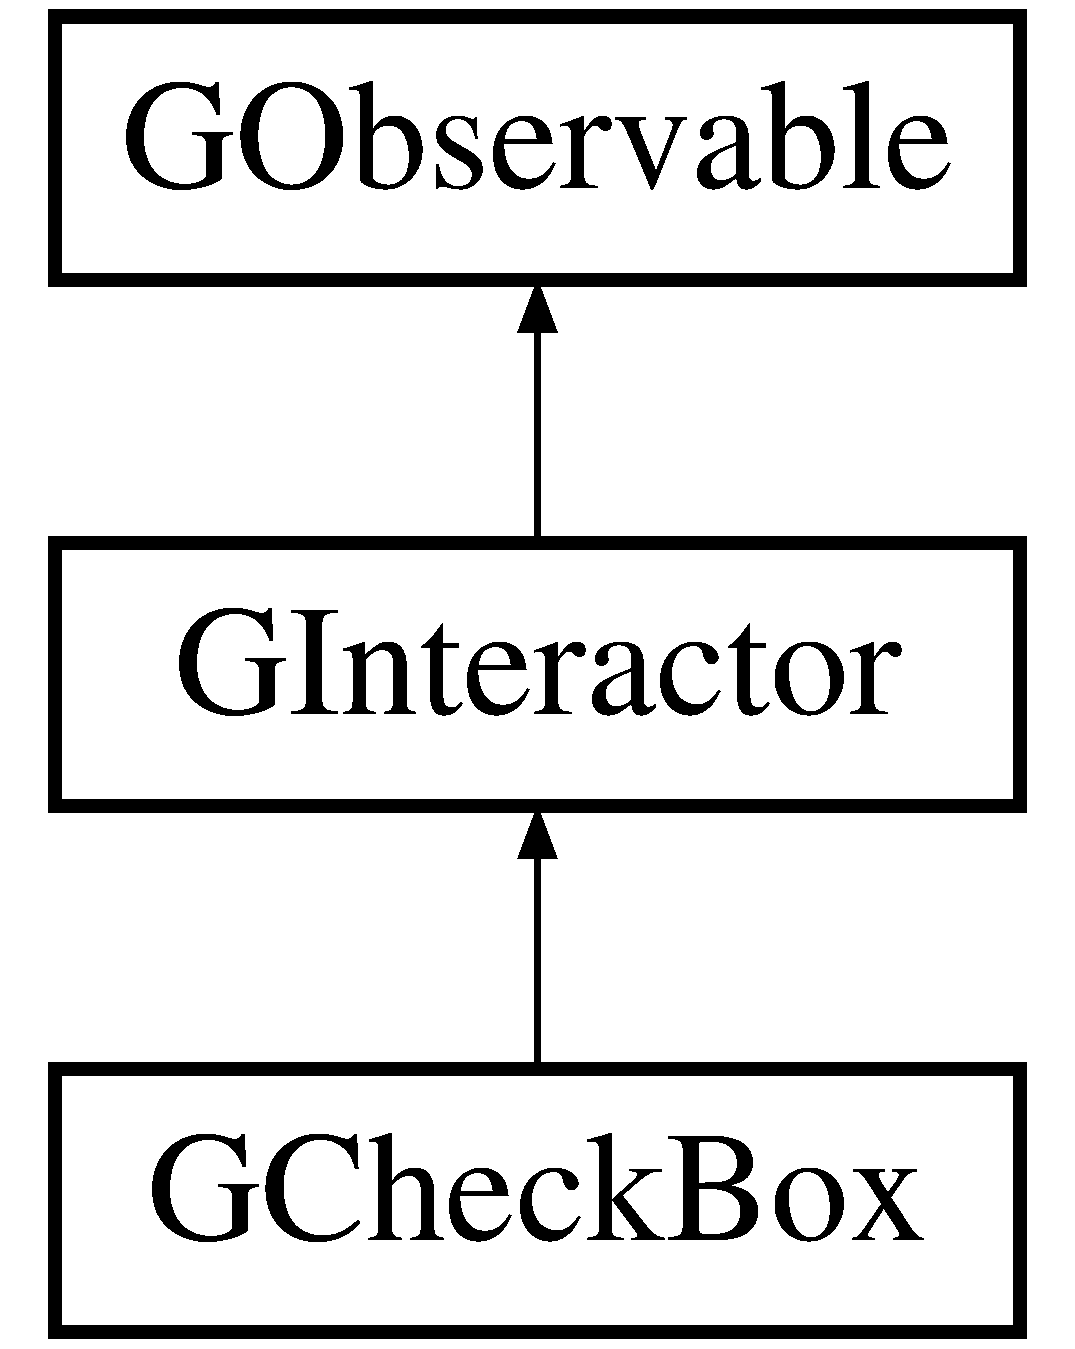
\includegraphics[height=3.000000cm]{classGCheckBox}
\end{center}
\end{figure}
\subsection*{Public Types}
\begin{DoxyCompactItemize}
\item 
enum \mbox{\hyperlink{classGInteractor_a8e0d441725a81d2bbdebbea09078260e}{Text\+Position}} \{ \mbox{\hyperlink{classGInteractor_a8e0d441725a81d2bbdebbea09078260ea4cd6f2e7d5a08d6f4dc052df2358f774}{T\+E\+X\+T\+\_\+\+B\+E\+S\+I\+D\+E\+\_\+\+I\+C\+ON}}, 
\mbox{\hyperlink{classGInteractor_a8e0d441725a81d2bbdebbea09078260eaa88490f63d8de68d44c83bdb2ecde3b3}{T\+E\+X\+T\+\_\+\+U\+N\+D\+E\+R\+\_\+\+I\+C\+ON}}, 
\mbox{\hyperlink{classGInteractor_a8e0d441725a81d2bbdebbea09078260ea39a6f388a30ac4fefb6eb13e846bc9f2}{T\+E\+X\+T\+\_\+\+O\+N\+LY}}
 \}
\begin{DoxyCompactList}\small\item\em The places where an interactor can place its text relative to its icon. \end{DoxyCompactList}\end{DoxyCompactItemize}
\subsection*{Public Member Functions}
\begin{DoxyCompactItemize}
\item 
\mbox{\hyperlink{classGCheckBox_ab79c27853bb6f5b8ec3ea139ef556f25}{G\+Check\+Box}} (const std\+::string \&text=\char`\"{}\char`\"{}, bool checked=false, Q\+Widget $\ast$parent=nullptr)
\begin{DoxyCompactList}\small\item\em Creates a checkbox with the given text. \end{DoxyCompactList}\item 
virtual \mbox{\hyperlink{classGCheckBox_ada6681887f64e3d1b9acb9af4db2cc19}{$\sim$\+G\+Check\+Box}} () Q\+\_\+\+D\+E\+C\+L\+\_\+\+O\+V\+E\+R\+R\+I\+DE
\begin{DoxyCompactList}\small\item\em Frees memory allocated internally by the checkbox. \end{DoxyCompactList}\item 
virtual void \mbox{\hyperlink{classGInteractor_a02f20ea6edfa0671f31c4c648a253833}{add\+Action\+Listener}} () Q\+\_\+\+D\+E\+C\+L\+\_\+\+D\+E\+P\+R\+E\+C\+A\+T\+ED
\begin{DoxyCompactList}\small\item\em Adds an event listener to be notified when this interactor is clicked or generally interacted with. \end{DoxyCompactList}\item 
virtual bool \mbox{\hyperlink{classGInteractor_ac05ba5b92e2e5146d416fe7f842a0969}{events\+Enabled}} () const Q\+\_\+\+D\+E\+C\+L\+\_\+\+O\+V\+E\+R\+R\+I\+DE
\begin{DoxyCompactList}\small\item\em Returns true if this interactor is currently accepting events. \end{DoxyCompactList}\item 
virtual std\+::string \mbox{\hyperlink{classGInteractor_a69f8d23ed8f207fbecad99960776e942}{get\+Accelerator}} () const
\begin{DoxyCompactList}\small\item\em Returns a string representing a hotkey for this interactor, or an empty string if no accelerator has been set. \end{DoxyCompactList}\item 
virtual std\+::string \mbox{\hyperlink{classGCheckBox_a90f2b1e6f6e7dabd9d6e5307f7c6d1b7}{get\+Action\+Command}} () const Q\+\_\+\+D\+E\+C\+L\+\_\+\+O\+V\+E\+R\+R\+I\+DE
\begin{DoxyCompactList}\small\item\em Returns an action command for this interactor, which is a semi-\/unique string you can use to identify it when events occur. \end{DoxyCompactList}\item 
virtual std\+::string \mbox{\hyperlink{classGInteractor_a808e22cc1fdfbecf71ed8c64ef4600e0}{get\+Background}} () const
\begin{DoxyCompactList}\small\item\em Returns the background color of the interactor as a string. \end{DoxyCompactList}\item 
virtual int \mbox{\hyperlink{classGInteractor_a9e827257a55cb8cf4d9de2ec6bcfd7a0}{get\+Background\+Int}} () const
\begin{DoxyCompactList}\small\item\em Returns the background color of the interactor as an R\+GB integer. \end{DoxyCompactList}\item 
virtual \mbox{\hyperlink{classGRectangle}{G\+Rectangle}} \mbox{\hyperlink{classGInteractor_a29e6ac35a0b48f491a4c88194cc5da3b}{get\+Bounds}} () const
\begin{DoxyCompactList}\small\item\em Returns a rectangle representing the x/y position and size of this interactor. \end{DoxyCompactList}\item 
virtual std\+::string \mbox{\hyperlink{classGInteractor_aa061dfa488c31e18549d64363c1d0e34}{get\+Color}} () const
\begin{DoxyCompactList}\small\item\em Returns the foreground/text color of the interactor as a string. \end{DoxyCompactList}\item 
virtual int \mbox{\hyperlink{classGInteractor_a9635c7af766cdc3417f346683fa0e6c1}{get\+Color\+Int}} () const
\begin{DoxyCompactList}\small\item\em Returns the foreground/text color of the interactor as an R\+GB integer. \end{DoxyCompactList}\item 
virtual \mbox{\hyperlink{classGContainer}{G\+Container}} $\ast$ \mbox{\hyperlink{classGInteractor_a7a6e317c29d61030929b4cd2d1c00fe7}{get\+Container}} () const
\begin{DoxyCompactList}\small\item\em Returns a pointer to the onscreen container holding this interactor. \end{DoxyCompactList}\item 
virtual std\+::string \mbox{\hyperlink{classGInteractor_a894a5502900794eeb27d084c21f1d77d}{get\+Font}} () const
\begin{DoxyCompactList}\small\item\em Returns the font of this interactor\textquotesingle{}s text as a font string such as \char`\"{}\+Helvetica-\/12-\/\+Bold\char`\"{}. \end{DoxyCompactList}\item 
virtual std\+::string \mbox{\hyperlink{classGInteractor_a4fa2d8b0192a3a5b4af4bbfe71194d03}{get\+Foreground}} () const
\begin{DoxyCompactList}\small\item\em Returns the foreground/text color of the interactor as a string. \end{DoxyCompactList}\item 
virtual int \mbox{\hyperlink{classGInteractor_ac3b12ab385a6ef9ae90fc879860ba726}{get\+Foreground\+Int}} () const
\begin{DoxyCompactList}\small\item\em Returns the foreground/text color of the interactor as an R\+GB integer. \end{DoxyCompactList}\item 
virtual double \mbox{\hyperlink{classGInteractor_a1e7e353362434072875264cf95629f99}{get\+Height}} () const
\begin{DoxyCompactList}\small\item\em Returns the current onscreen height of this interactor in pixels. \end{DoxyCompactList}\item 
virtual std\+::string \mbox{\hyperlink{classGInteractor_aaed62a73004939a64da6f0eb9eb64d73}{get\+Icon}} () const
\begin{DoxyCompactList}\small\item\em Returns the file name of the icon associated with this interactor, or an empty string if no icon has been set. \end{DoxyCompactList}\item 
virtual int \mbox{\hyperlink{classGInteractor_a9c9659a6c6ba66b4107ba59c95a24241}{get\+ID}} () const
\begin{DoxyCompactList}\small\item\em Returns a globally unique identifier for this interactor, which is set when the interactor is constructed. \end{DoxyCompactList}\item 
virtual \+\_\+\+Internal\+\_\+\+Q\+Widget $\ast$ \mbox{\hyperlink{classGCheckBox_a208ce13c1da40bf0ddb509daf99d6588}{get\+Internal\+Widget}} () const Q\+\_\+\+D\+E\+C\+L\+\_\+\+O\+V\+E\+R\+R\+I\+DE
\begin{DoxyCompactList}\small\item\em Returns a direct pointer to the internal Qt widget being wrapped by this interactor. \end{DoxyCompactList}\item 
virtual \mbox{\hyperlink{classGPoint}{G\+Point}} \mbox{\hyperlink{classGInteractor_a4f83802015511edeb63b892830812c11}{get\+Location}} () const
\begin{DoxyCompactList}\small\item\em Returns an (x, y) point representing the onscreen location of the top-\/left corner of this interactor within its containing window. \end{DoxyCompactList}\item 
virtual double \mbox{\hyperlink{classGInteractor_aed4b0075fcc434499c3cb3e46896bda3}{get\+Minimum\+Height}} () const
\begin{DoxyCompactList}\small\item\em Returns the minimum height in pixels that this interactor will permit itself to be resized to. \end{DoxyCompactList}\item 
virtual \mbox{\hyperlink{classGDimension}{G\+Dimension}} \mbox{\hyperlink{classGInteractor_a66b5af0b32493b4d597ca0a3df2049ea}{get\+Minimum\+Size}} () const
\begin{DoxyCompactList}\small\item\em Returns a \mbox{\hyperlink{classGDimension}{G\+Dimension}} structure representing the minimum size in pixels that this interactor will permit itself to be resized to. \end{DoxyCompactList}\item 
virtual double \mbox{\hyperlink{classGInteractor_a59e668114fe3d49d2a0f28deb258f7c8}{get\+Minimum\+Width}} () const
\begin{DoxyCompactList}\small\item\em Returns the minimum width in pixels that this interactor will permit itself to be resized to. \end{DoxyCompactList}\item 
virtual std\+::string \mbox{\hyperlink{classGInteractor_a8a60438a5b55d0b2ceb35c8674b9d8c5}{get\+Name}} () const
\begin{DoxyCompactList}\small\item\em Returns a string representing a unique name for this interactor. \end{DoxyCompactList}\item 
virtual double \mbox{\hyperlink{classGInteractor_a747de0961653847bdc6615dbf756d715}{get\+Preferred\+Height}} () const
\begin{DoxyCompactList}\small\item\em Returns the height in pixels that this interactor would prefer to be, which would exactly fit its contents with no stretching or scrollbars. \end{DoxyCompactList}\item 
virtual \mbox{\hyperlink{classGDimension}{G\+Dimension}} \mbox{\hyperlink{classGInteractor_a4aabbee761d8e9116275401131b7ccd1}{get\+Preferred\+Size}} () const
\begin{DoxyCompactList}\small\item\em Returns a \mbox{\hyperlink{classGDimension}{G\+Dimension}} structure storing the width and height in pixels that this interactor would prefer to be, which would exactly fit its contents with no stretching or scrollbars. \end{DoxyCompactList}\item 
virtual double \mbox{\hyperlink{classGInteractor_a82bca31d37700fb0e35d2743352efd5e}{get\+Preferred\+Width}} () const
\begin{DoxyCompactList}\small\item\em Returns the height in pixels that this interactor would prefer to be, which would exactly fit its contents with no stretching or scrollbars. \end{DoxyCompactList}\item 
virtual \mbox{\hyperlink{classGDimension}{G\+Dimension}} \mbox{\hyperlink{classGInteractor_a7b4eec96a2bdc6420695d5796a78eea9}{get\+Size}} () const
\begin{DoxyCompactList}\small\item\em Returns a \mbox{\hyperlink{classGDimension}{G\+Dimension}} structure storing the current onscreen width and height of this interactor in pixels. \end{DoxyCompactList}\item 
virtual std\+::string \mbox{\hyperlink{classGCheckBox_aff553c50924b836c29f146ed34a7c6ec}{get\+Text}} () const
\begin{DoxyCompactList}\small\item\em Returns the text next to the checkbox. \end{DoxyCompactList}\item 
virtual std\+::string \mbox{\hyperlink{classGCheckBox_a9896d58fcfebbf1025aeeb5b8b9ede80}{get\+Type}} () const Q\+\_\+\+D\+E\+C\+L\+\_\+\+O\+V\+E\+R\+R\+I\+DE
\begin{DoxyCompactList}\small\item\em Returns a string representing the class name of this interactor, such as \char`\"{}\+G\+Button\char`\"{} or \char`\"{}\+G\+Check\+Box\char`\"{}. \end{DoxyCompactList}\item 
virtual Q\+Widget $\ast$ \mbox{\hyperlink{classGCheckBox_a326ee51b5561f807df7b29a1c101f7fd}{get\+Widget}} () const Q\+\_\+\+D\+E\+C\+L\+\_\+\+O\+V\+E\+R\+R\+I\+DE
\begin{DoxyCompactList}\small\item\em Returns a direct pointer to the internal Qt widget being wrapped by this interactor. \end{DoxyCompactList}\item 
virtual double \mbox{\hyperlink{classGInteractor_a0ed2965abd4f5701d2cadf71239faf19}{get\+Width}} () const
\begin{DoxyCompactList}\small\item\em Returns the current onscreen width of this interactor in pixels. \end{DoxyCompactList}\item 
virtual double \mbox{\hyperlink{classGInteractor_a344385751bee0720059403940d57a13e}{getX}} () const
\begin{DoxyCompactList}\small\item\em Returns the x-\/coordinate of the top-\/left pixel of this interactor within its onscreen window. \end{DoxyCompactList}\item 
virtual double \mbox{\hyperlink{classGInteractor_aafa51c7f8f38a09febbb9ce7853f77b4}{getY}} () const
\begin{DoxyCompactList}\small\item\em Returns the y-\/coordinate of the top-\/left pixel of this interactor within its onscreen window. \end{DoxyCompactList}\item 
virtual bool \mbox{\hyperlink{classGInteractor_afc480f652b8c5f1fb255e2269ce68879}{in\+Bounds}} (double x, double y) const
\begin{DoxyCompactList}\small\item\em Returns true if the given x/y pixel is within the bounds of this interactor. \end{DoxyCompactList}\item 
virtual bool \mbox{\hyperlink{classGInteractor_ae6d7982c1c627b677a5e776ca86118ed}{in\+Bounds}} (int x, int y) const
\begin{DoxyCompactList}\small\item\em Returns true if the given x/y pixel is within the bounds of this interactor. \end{DoxyCompactList}\item 
virtual bool \mbox{\hyperlink{classGCheckBox_ac8cada18b9357ff68b26e17f44294764}{is\+Checked}} () const
\begin{DoxyCompactList}\small\item\em Returns true if the checkbox is currently checked. \end{DoxyCompactList}\item 
virtual bool \mbox{\hyperlink{classGInteractor_aacb819fb241851fd9fc045271baa4034}{is\+Enabled}} () const
\begin{DoxyCompactList}\small\item\em Returns true if this interactor is currently enabled. \end{DoxyCompactList}\item 
virtual bool \mbox{\hyperlink{classGCheckBox_a56a065a2c20a230931de0ed98019d8fb}{is\+Selected}} () const
\begin{DoxyCompactList}\small\item\em Returns true if the checkbox is currently checked. \end{DoxyCompactList}\item 
virtual bool \mbox{\hyperlink{classGInteractor_a9d8a6cfb13917785c143e74d40e4e2be}{is\+Visible}} () const
\begin{DoxyCompactList}\small\item\em Returns true if the interactor is visible on the screen. \end{DoxyCompactList}\item 
virtual void \mbox{\hyperlink{classGCheckBox_ab7fe7a876367b87cf7202f947f1d05e4}{remove\+Action\+Listener}} ()
\begin{DoxyCompactList}\small\item\em Removes the action listener from this checkbox so that it will no longer call it when events occur. \end{DoxyCompactList}\item 
virtual void \mbox{\hyperlink{classGCheckBox_aa4250907e4cdd77349c04f0cf5cdd3d3}{remove\+Double\+Click\+Listener}} ()
\begin{DoxyCompactList}\small\item\em Removes the double-\/click listener from this checkbox so that it will no longer call it when events occur. \end{DoxyCompactList}\item 
virtual void \mbox{\hyperlink{classGInteractor_a519fb2ac767f8b2febbb50b898b8c8cb}{request\+Focus}} ()
\begin{DoxyCompactList}\small\item\em Transfers keyboard focus to this interactor. \end{DoxyCompactList}\item 
virtual void \mbox{\hyperlink{classGInteractor_ad15f102f62e2960576012f1aa0ba4b2e}{set\+Accelerator}} (const std\+::string \&accelerator)
\begin{DoxyCompactList}\small\item\em Sets an accelerator hotkey for this interactor, such as \char`\"{}\+Ctrl-\/\+S\char`\"{}. \end{DoxyCompactList}\item 
virtual void \mbox{\hyperlink{classGInteractor_a4b5843fe3030e038a1ba54cc03389bcf}{set\+Action\+Command}} (const std\+::string \&action\+Command)
\begin{DoxyCompactList}\small\item\em Sets the action command for this interactor. \end{DoxyCompactList}\item 
virtual void \mbox{\hyperlink{classGCheckBox_adcfb4742430c88714fcf57e57ab8ea9c}{set\+Action\+Listener}} (G\+Event\+Listener func)
\begin{DoxyCompactList}\small\item\em Sets an action listener on this checkbox so that it will be called when the checkbox is clicked. \end{DoxyCompactList}\item 
virtual void \mbox{\hyperlink{classGCheckBox_aebd20a89c7a8a43a6fce999cf4f9fcf2}{set\+Action\+Listener}} (G\+Event\+Listener\+Void func)
\begin{DoxyCompactList}\small\item\em Sets an action listener on this checkbox so that it will be called when the checkbox is clicked. \end{DoxyCompactList}\item 
virtual void \mbox{\hyperlink{classGInteractor_acba7e546c2025c0a15ca4b4cc92043db}{set\+Background}} (int rgb)
\begin{DoxyCompactList}\small\item\em Sets the background color of the interactor to the color represented by the given R\+GB integer. \end{DoxyCompactList}\item 
virtual void \mbox{\hyperlink{classGInteractor_ab4677ab2474e68b07aa56605af92a84a}{set\+Background}} (const std\+::string \&color)
\begin{DoxyCompactList}\small\item\em Sets the background color of the interactor to the color represented by the given string. \end{DoxyCompactList}\item 
virtual void \mbox{\hyperlink{classGInteractor_a2aae8197624b72265ab83b4f1bc73f2f}{set\+Bounds}} (double x, double y, double width, double height)
\begin{DoxyCompactList}\small\item\em Sets the size and location of the widget. \end{DoxyCompactList}\item 
virtual void \mbox{\hyperlink{classGInteractor_acada386653f008cacc7cce86426bef7c}{set\+Bounds}} (const \mbox{\hyperlink{classGRectangle}{G\+Rectangle}} \&size)
\begin{DoxyCompactList}\small\item\em Sets the size and location of the widget. \end{DoxyCompactList}\item 
virtual void \mbox{\hyperlink{classGCheckBox_a116285e2f56247b00b26035ca0ac4737}{set\+Checked}} (bool checked)
\begin{DoxyCompactList}\small\item\em Sets whether the checkbox should be checked. \end{DoxyCompactList}\item 
virtual void \mbox{\hyperlink{classGInteractor_ab1f5cc0f5cc6bbbd716a526c61f1081d}{set\+Color}} (int rgb)
\begin{DoxyCompactList}\small\item\em Sets the foreground/text color of the interactor to the color represented by the given R\+GB integer. \end{DoxyCompactList}\item 
virtual void \mbox{\hyperlink{classGInteractor_a61374df6c11b52cfbb0815decdbaebc6}{set\+Color}} (const std\+::string \&color)
\begin{DoxyCompactList}\small\item\em Sets the foreground/text color of the interactor to the color represented by the given string. \end{DoxyCompactList}\item 
virtual void \mbox{\hyperlink{classGCheckBox_ac29f9a3462458e165fae3a1f046ee77a}{set\+Double\+Click\+Listener}} (G\+Event\+Listener func)
\begin{DoxyCompactList}\small\item\em Sets a listener on this checkbox so that it will be called when the checkbox is double-\/clicked. \end{DoxyCompactList}\item 
virtual void \mbox{\hyperlink{classGCheckBox_a50096194d66f48c92dd4c512d41bfc76}{set\+Double\+Click\+Listener}} (G\+Event\+Listener\+Void func)
\begin{DoxyCompactList}\small\item\em Sets a listener on this checkbox so that it will be called when the checkbox is double-\/clicked. \end{DoxyCompactList}\item 
virtual void \mbox{\hyperlink{classGInteractor_ab831367dd84bbd579e02e55bacb21343}{set\+Enabled}} (bool value)
\begin{DoxyCompactList}\small\item\em Sets whether this interactor is currently enabled. \end{DoxyCompactList}\item 
virtual void \mbox{\hyperlink{classGObservable_afaa30b2a9e0f378fd1c70d2f1d0b8216}{set\+Events\+Enabled}} (bool \mbox{\hyperlink{classGInteractor_ac05ba5b92e2e5146d416fe7f842a0969}{events\+Enabled}})
\begin{DoxyCompactList}\small\item\em Sets whether the object is currently allowing itself to fire events. \end{DoxyCompactList}\item 
virtual void \mbox{\hyperlink{classGInteractor_a2592348886ffea646c6534bf88f7c49d}{set\+Font}} (const Q\+Font \&font)
\begin{DoxyCompactList}\small\item\em Sets the font used by this widget to the given Qt font. \end{DoxyCompactList}\item 
virtual void \mbox{\hyperlink{classGInteractor_a8e096e8818d838aceae1d46d58fb3a7b}{set\+Font}} (const std\+::string \&font)
\begin{DoxyCompactList}\small\item\em Sets the font used by this widget to the font represented by the given font string, such as \char`\"{}\+Helvetica-\/16-\/\+Bold\char`\"{}. \end{DoxyCompactList}\item 
virtual void \mbox{\hyperlink{classGInteractor_a9eb856b5ff83a19df3831a31f15f4563}{set\+Foreground}} (int rgb)
\begin{DoxyCompactList}\small\item\em Sets the foreground/text color of the interactor to the color represented by the given R\+GB integer. \end{DoxyCompactList}\item 
virtual void \mbox{\hyperlink{classGInteractor_af59209aeadea6dfc6d97a2d8531f50e1}{set\+Foreground}} (const std\+::string \&color)
\begin{DoxyCompactList}\small\item\em Sets the foreground/text color of the interactor to the color represented by the given string. \end{DoxyCompactList}\item 
virtual void \mbox{\hyperlink{classGInteractor_a9e280bfc4544dfaf8e4376c4e1a74357}{set\+Height}} (double height)
\begin{DoxyCompactList}\small\item\em Sets the onscreen height of the interactor in pixels. \end{DoxyCompactList}\item 
virtual void \mbox{\hyperlink{classGInteractor_a762e139aa311461c3984d3ad28293f64}{set\+Icon}} (const std\+::string \&filename, bool retain\+Icon\+Size=true)
\begin{DoxyCompactList}\small\item\em Sets the file name of the icon associated with this interactor, or an empty string if no icon has been set. \end{DoxyCompactList}\item 
virtual void \mbox{\hyperlink{classGInteractor_a04594e8ba9b98513a64f1da00dcae18c}{set\+Location}} (double x, double y)
\begin{DoxyCompactList}\small\item\em Sets the onscreen x/y-\/coordinate of the top-\/left corner of the interactor relative to its window. \end{DoxyCompactList}\item 
virtual void \mbox{\hyperlink{classGInteractor_a0cf428e207b7f22cc08138a90b1b87b2}{set\+Minimum\+Size}} (double width, double height)
\begin{DoxyCompactList}\small\item\em Sets the minimum size in pixels that this interactor will permit itself to be resized to. \end{DoxyCompactList}\item 
virtual void \mbox{\hyperlink{classGInteractor_a3b1046117ac6cb7abe467e00ba8a81f4}{set\+Minimum\+Size}} (const \mbox{\hyperlink{classGDimension}{G\+Dimension}} \&size)
\begin{DoxyCompactList}\small\item\em Sets the minimum size in pixels that this interactor will permit itself to be resized to. \end{DoxyCompactList}\item 
virtual void \mbox{\hyperlink{classGInteractor_a9d3a2685df23b5e7cbf59c19c4a1f9b5}{set\+Name}} (const std\+::string \&name)
\begin{DoxyCompactList}\small\item\em Sets a string representing a unique name for this interactor. \end{DoxyCompactList}\item 
virtual void \mbox{\hyperlink{classGInteractor_a1ab987704fce32098706c6f00fb08218}{set\+Preferred\+Height}} (double height)
\begin{DoxyCompactList}\small\item\em Sets the height in pixels that this interactor would prefer to be. \end{DoxyCompactList}\item 
virtual void \mbox{\hyperlink{classGInteractor_a042c5ae19430d765ef552371cae3632c}{set\+Preferred\+Size}} (double width, double height)
\begin{DoxyCompactList}\small\item\em Sets the width and height in pixels that this interactor would prefer to be. \end{DoxyCompactList}\item 
virtual void \mbox{\hyperlink{classGInteractor_aa22d9be4bc0e078bb0ea69b0fc9d7c75}{set\+Preferred\+Size}} (const \mbox{\hyperlink{classGDimension}{G\+Dimension}} \&size)
\begin{DoxyCompactList}\small\item\em Sets the size in pixels that this interactor would prefer to be. \end{DoxyCompactList}\item 
virtual void \mbox{\hyperlink{classGInteractor_a3db429ab2fa52efd187eec0ed8cdd9f2}{set\+Preferred\+Width}} (double width)
\begin{DoxyCompactList}\small\item\em Sets the width in pixels that this interactor would prefer to be. \end{DoxyCompactList}\item 
virtual void \mbox{\hyperlink{classGCheckBox_ad42accd39af295a957386c68dac3dcae}{set\+Selected}} (bool selected)
\begin{DoxyCompactList}\small\item\em Sets whether the checkbox should be checked. \end{DoxyCompactList}\item 
virtual void \mbox{\hyperlink{classGInteractor_aca25d49481f9bf5fc8f7df4c086c4ce7}{set\+Size}} (double width, double height)
\begin{DoxyCompactList}\small\item\em Sets the onscreen width and height of the interactor in pixels. \end{DoxyCompactList}\item 
virtual void \mbox{\hyperlink{classGInteractor_ae2b628228f192c2702c4ce941b2af68f}{set\+Size}} (const \mbox{\hyperlink{classGDimension}{G\+Dimension}} \&size)
\begin{DoxyCompactList}\small\item\em Sets the onscreen width and height of the interactor in pixels. \end{DoxyCompactList}\item 
virtual void \mbox{\hyperlink{classGCheckBox_ac1ae51949d41ee9054634be5967d91b8}{set\+Text}} (const std\+::string \&text)
\begin{DoxyCompactList}\small\item\em Sets the text that will appear next to the checkbox. \end{DoxyCompactList}\item 
virtual void \mbox{\hyperlink{classGInteractor_a039e0e49beaecc275efce02d416acea8}{set\+Tooltip}} (const std\+::string \&tooltip\+Text)
\begin{DoxyCompactList}\small\item\em Sets a \char`\"{}tooltip\char`\"{} that will appear if the user hovers their mouse over the interactor. \end{DoxyCompactList}\item 
virtual void \mbox{\hyperlink{classGInteractor_a18e44e30b31525a243960ca3928125aa}{set\+Visible}} (bool visible)
\begin{DoxyCompactList}\small\item\em Returns true if the interactor is visible on the screen. \end{DoxyCompactList}\item 
virtual void \mbox{\hyperlink{classGInteractor_aa3f3fba4cb131baa8696ba01e3bceca1}{set\+Width}} (double width)
\begin{DoxyCompactList}\small\item\em Sets the onscreen width of the interactor in pixels. \end{DoxyCompactList}\item 
virtual void \mbox{\hyperlink{classGInteractor_a9c18fcc579333bf9653d13ad2b372e39}{setX}} (double x)
\begin{DoxyCompactList}\small\item\em Sets the onscreen x-\/coordinate of the top-\/left corner of the interactor relative to its window. \end{DoxyCompactList}\item 
virtual void \mbox{\hyperlink{classGInteractor_a7d57e2a5c35d27feb58fd498a3cf82b9}{setY}} (double y)
\begin{DoxyCompactList}\small\item\em Sets the onscreen y-\/coordinate of the top-\/left corner of the interactor relative to its window. \end{DoxyCompactList}\item 
virtual void \mbox{\hyperlink{classGCheckBox_ad277193b2dca0bab1e0ad24d45407dc3}{toggle}} ()
\begin{DoxyCompactList}\small\item\em Reverses the checked state of the box, setting it to be checked if it was unchecked or to be unchecked if it was checked. \end{DoxyCompactList}\item 
virtual std\+::string \mbox{\hyperlink{classGObservable_a1fe5121d6528fdea3f243321b3fa3a49}{to\+String}} () const
\begin{DoxyCompactList}\small\item\em Returns a string representation of this observable object\textquotesingle{}s state. \end{DoxyCompactList}\end{DoxyCompactItemize}
\subsection*{Protected Member Functions}
\begin{DoxyCompactItemize}
\item 
virtual void \mbox{\hyperlink{classGObservable_a80cfa040459ff53594adbd6a51ec8f43}{clear\+Event\+Listeners}} ()
\begin{DoxyCompactList}\small\item\em Removes all event listeners from this object. \end{DoxyCompactList}\item 
virtual void \mbox{\hyperlink{classGObservable_a284f31528c0520f8e545c03ac9eeac74}{ensure\+Thread\+Safety}} (const std\+::string \&member\+Name=\char`\"{}\char`\"{})
\begin{DoxyCompactList}\small\item\em Ensures that we are currently in the Qt G\+UI thread. \end{DoxyCompactList}\item 
virtual void \mbox{\hyperlink{classGObservable_a63e5e5a6227c59c928493b11aceb0f67}{fire\+Event}} (\mbox{\hyperlink{classGEvent}{G\+Event}} \&event)
\begin{DoxyCompactList}\small\item\em Sends out the given event to any attached listeners. \end{DoxyCompactList}\item 
virtual void \mbox{\hyperlink{classGObservable_ab3983ea07337b52020a29cc00c653d8d}{fire\+G\+Event}} (Q\+Event $\ast$event, Event\+Type event\+Type, const std\+::string \&event\+Name)
\begin{DoxyCompactList}\small\item\em Creates an event of the given type, then sends it out to any attached listeners. \end{DoxyCompactList}\item 
virtual void \mbox{\hyperlink{classGObservable_a01fdf1b0e0dbd49e189fe4514e010411}{fire\+G\+Event}} (Q\+Close\+Event $\ast$event, Event\+Type event\+Type, const std\+::string \&event\+Name)
\begin{DoxyCompactList}\small\item\em Creates an event of the given type, then sends it out to any attached listeners. \end{DoxyCompactList}\item 
virtual void \mbox{\hyperlink{classGObservable_abb0b2f66ba39211cb5d7615e9d1c04e2}{fire\+G\+Event}} (Q\+Key\+Event $\ast$event, Event\+Type event\+Type, const std\+::string \&event\+Name)
\begin{DoxyCompactList}\small\item\em Creates an event of the given type, then sends it out to any attached listeners. \end{DoxyCompactList}\item 
virtual void \mbox{\hyperlink{classGObservable_a119318675d2165bdf7dd853aaf881d4b}{fire\+G\+Event}} (Q\+Mouse\+Event $\ast$event, Event\+Type event\+Type, const std\+::string \&event\+Name, const std\+::string \&action\+Command=\char`\"{}\char`\"{})
\begin{DoxyCompactList}\small\item\em Creates an event of the given type, then sends it out to any attached listeners. \end{DoxyCompactList}\item 
virtual void \mbox{\hyperlink{classGObservable_a63fd9034e1e1633c1c38eb342bfd34e9}{fire\+G\+Event}} (Q\+Resize\+Event $\ast$event, Event\+Type event\+Type, const std\+::string \&event\+Name)
\begin{DoxyCompactList}\small\item\em Creates an event of the given type, then sends it out to any attached listeners. \end{DoxyCompactList}\item 
virtual void \mbox{\hyperlink{classGObservable_a741345310d9b7c5170a6cbc410c44ac4}{fire\+G\+Event}} (Q\+Timer\+Event $\ast$event, Event\+Type event\+Type, const std\+::string \&event\+Name)
\begin{DoxyCompactList}\small\item\em Creates an event of the given type, then sends it out to any attached listeners. \end{DoxyCompactList}\item 
virtual void \mbox{\hyperlink{classGObservable_a93bf338968a0338761b8e4dc62f582e9}{fire\+G\+Event}} (Q\+Wheel\+Event $\ast$event, Event\+Type event\+Type, const std\+::string \&event\+Name)
\begin{DoxyCompactList}\small\item\em Creates an event of the given type, then sends it out to any attached listeners. \end{DoxyCompactList}\item 
virtual void \mbox{\hyperlink{classGObservable_a2a70a7d7435ff0c3b80bb4d70da19e0d}{fire\+G\+Event}} (Q\+Window\+State\+Change\+Event $\ast$event, Event\+Type event\+Type, const std\+::string \&event\+Name)
\begin{DoxyCompactList}\small\item\em Creates an event of the given type, then sends it out to any attached listeners. \end{DoxyCompactList}\item 
virtual bool \mbox{\hyperlink{classGObservable_a9f6faaa25942923bafa1c44020c49fa9}{has\+Event\+Listener}} (const std\+::string \&event\+Name) const
\begin{DoxyCompactList}\small\item\em Returns true if the observable object has a listener for the given type of event. \end{DoxyCompactList}\item 
virtual bool \mbox{\hyperlink{classGObservable_aeec1adc19aa0f33de62390686ee1382c}{is\+Accepting\+Event}} (int event\+Mask) const
\begin{DoxyCompactList}\small\item\em Returns true if the observable object has a listener for the given type of event. \end{DoxyCompactList}\item 
virtual bool \mbox{\hyperlink{classGObservable_aa31c73145a29dcb92848a92e0cfaea41}{is\+Accepting\+Event}} (const \mbox{\hyperlink{classGEvent}{G\+Event}} \&event) const
\begin{DoxyCompactList}\small\item\em Returns true if the observable object has a listener for the given type of event. \end{DoxyCompactList}\item 
virtual bool \mbox{\hyperlink{classGObservable_a3b1c689267eda44e65a2213e7de38b23}{is\+Accepting\+Event}} (const std\+::string \&event\+Type) const
\begin{DoxyCompactList}\small\item\em Returns true if the observable object has a listener for the given type of event. \end{DoxyCompactList}\item 
virtual void \mbox{\hyperlink{classGObservable_acbcf1ed3a851ad8a3c17ef38d86b481d}{remove\+Event\+Listener}} (const std\+::string \&event\+Name)
\begin{DoxyCompactList}\small\item\em Removes any event listener from this observable object that would respond to the given type of event, such as \char`\"{}click\char`\"{} or \char`\"{}keydown\char`\"{}. \end{DoxyCompactList}\item 
virtual void \mbox{\hyperlink{classGObservable_af51cc35c29a1bd1908609d432decdbb6}{remove\+Event\+Listeners}} (std\+::initializer\+\_\+list$<$ std\+::string $>$ event\+Names)
\begin{DoxyCompactList}\small\item\em Removes any event listener from this observable object that would respond to the given types of events, such as \char`\"{}click\char`\"{} or \char`\"{}keydown\char`\"{}. \end{DoxyCompactList}\item 
virtual void \mbox{\hyperlink{classGObservable_ad2f6d34961c50f6c1e0659990b79f741}{set\+Event\+Listener}} (const std\+::string \&event\+Name, G\+Event\+Listener func)
\begin{DoxyCompactList}\small\item\em Adds an event listener from this observable object to respond to the given type of event, such as \char`\"{}click\char`\"{} or \char`\"{}keydown\char`\"{}. \end{DoxyCompactList}\item 
virtual void \mbox{\hyperlink{classGObservable_abac4cb9f9e626e010e87f5d91573c8a5}{set\+Event\+Listener}} (const std\+::string \&event\+Name, G\+Event\+Listener\+Void func)
\begin{DoxyCompactList}\small\item\em Adds an event listener from this observable object to respond to the given type of event, such as \char`\"{}click\char`\"{} or \char`\"{}keydown\char`\"{}. \end{DoxyCompactList}\item 
virtual void \mbox{\hyperlink{classGObservable_afa388d69c33c718cf035774604065604}{set\+Event\+Listeners}} (std\+::initializer\+\_\+list$<$ std\+::string $>$ event\+Names, G\+Event\+Listener func)
\begin{DoxyCompactList}\small\item\em Adds an event listener from this observable object to respond to the given types of events, such as \char`\"{}click\char`\"{} or \char`\"{}keydown\char`\"{}. \end{DoxyCompactList}\item 
virtual void \mbox{\hyperlink{classGObservable_a7867184bbb686f74fae8a4db927da799}{set\+Event\+Listeners}} (std\+::initializer\+\_\+list$<$ std\+::string $>$ event\+Names, G\+Event\+Listener\+Void func)
\begin{DoxyCompactList}\small\item\em Adds an event listener from this observable object to respond to the given types of events, such as \char`\"{}click\char`\"{} or \char`\"{}keydown\char`\"{}. \end{DoxyCompactList}\end{DoxyCompactItemize}


\subsection{Detailed Description}
This interactor subclass represents an onscreen check box. 

Clicking once on the check box selects it; clicking again removes the selection. You can listen for clicks on a checkbox using the set\+Action\+Listener method, passing the function you want to call on each click. 

\subsection{Member Enumeration Documentation}
\mbox{\Hypertarget{classGInteractor_a8e0d441725a81d2bbdebbea09078260e}\label{classGInteractor_a8e0d441725a81d2bbdebbea09078260e}} 
\index{G\+Check\+Box@{G\+Check\+Box}!Text\+Position@{Text\+Position}}
\index{Text\+Position@{Text\+Position}!G\+Check\+Box@{G\+Check\+Box}}
\subsubsection{\texorpdfstring{Text\+Position}{TextPosition}}
{\footnotesize\ttfamily enum \mbox{\hyperlink{classGInteractor_a8e0d441725a81d2bbdebbea09078260e}{Text\+Position}}\hspace{0.3cm}{\ttfamily [inherited]}}



The places where an interactor can place its text relative to its icon. 

\begin{DoxyEnumFields}{Enumerator}
\raisebox{\heightof{T}}[0pt][0pt]{\index{T\+E\+X\+T\+\_\+\+B\+E\+S\+I\+D\+E\+\_\+\+I\+C\+ON@{T\+E\+X\+T\+\_\+\+B\+E\+S\+I\+D\+E\+\_\+\+I\+C\+ON}!G\+Check\+Box@{G\+Check\+Box}}\index{G\+Check\+Box@{G\+Check\+Box}!T\+E\+X\+T\+\_\+\+B\+E\+S\+I\+D\+E\+\_\+\+I\+C\+ON@{T\+E\+X\+T\+\_\+\+B\+E\+S\+I\+D\+E\+\_\+\+I\+C\+ON}}}\mbox{\Hypertarget{classGInteractor_a8e0d441725a81d2bbdebbea09078260ea4cd6f2e7d5a08d6f4dc052df2358f774}\label{classGInteractor_a8e0d441725a81d2bbdebbea09078260ea4cd6f2e7d5a08d6f4dc052df2358f774}} 
T\+E\+X\+T\+\_\+\+B\+E\+S\+I\+D\+E\+\_\+\+I\+C\+ON&\\
\hline

\raisebox{\heightof{T}}[0pt][0pt]{\index{T\+E\+X\+T\+\_\+\+U\+N\+D\+E\+R\+\_\+\+I\+C\+ON@{T\+E\+X\+T\+\_\+\+U\+N\+D\+E\+R\+\_\+\+I\+C\+ON}!G\+Check\+Box@{G\+Check\+Box}}\index{G\+Check\+Box@{G\+Check\+Box}!T\+E\+X\+T\+\_\+\+U\+N\+D\+E\+R\+\_\+\+I\+C\+ON@{T\+E\+X\+T\+\_\+\+U\+N\+D\+E\+R\+\_\+\+I\+C\+ON}}}\mbox{\Hypertarget{classGInteractor_a8e0d441725a81d2bbdebbea09078260eaa88490f63d8de68d44c83bdb2ecde3b3}\label{classGInteractor_a8e0d441725a81d2bbdebbea09078260eaa88490f63d8de68d44c83bdb2ecde3b3}} 
T\+E\+X\+T\+\_\+\+U\+N\+D\+E\+R\+\_\+\+I\+C\+ON&\\
\hline

\raisebox{\heightof{T}}[0pt][0pt]{\index{T\+E\+X\+T\+\_\+\+O\+N\+LY@{T\+E\+X\+T\+\_\+\+O\+N\+LY}!G\+Check\+Box@{G\+Check\+Box}}\index{G\+Check\+Box@{G\+Check\+Box}!T\+E\+X\+T\+\_\+\+O\+N\+LY@{T\+E\+X\+T\+\_\+\+O\+N\+LY}}}\mbox{\Hypertarget{classGInteractor_a8e0d441725a81d2bbdebbea09078260ea39a6f388a30ac4fefb6eb13e846bc9f2}\label{classGInteractor_a8e0d441725a81d2bbdebbea09078260ea39a6f388a30ac4fefb6eb13e846bc9f2}} 
T\+E\+X\+T\+\_\+\+O\+N\+LY&\\
\hline

\end{DoxyEnumFields}


\subsection{Constructor \& Destructor Documentation}
\mbox{\Hypertarget{classGCheckBox_ab79c27853bb6f5b8ec3ea139ef556f25}\label{classGCheckBox_ab79c27853bb6f5b8ec3ea139ef556f25}} 
\index{G\+Check\+Box@{G\+Check\+Box}!G\+Check\+Box@{G\+Check\+Box}}
\index{G\+Check\+Box@{G\+Check\+Box}!G\+Check\+Box@{G\+Check\+Box}}
\subsubsection{\texorpdfstring{G\+Check\+Box()}{GCheckBox()}}
{\footnotesize\ttfamily \mbox{\hyperlink{classGCheckBox}{G\+Check\+Box}} (\begin{DoxyParamCaption}\item[{const std\+::string \&}]{text = {\ttfamily \char`\"{}\char`\"{}},  }\item[{bool}]{checked = {\ttfamily false},  }\item[{Q\+Widget $\ast$}]{parent = {\ttfamily nullptr} }\end{DoxyParamCaption})}



Creates a checkbox with the given text. 

You can pass an optional second parameter to initially check the box. \mbox{\Hypertarget{classGCheckBox_ada6681887f64e3d1b9acb9af4db2cc19}\label{classGCheckBox_ada6681887f64e3d1b9acb9af4db2cc19}} 
\index{G\+Check\+Box@{G\+Check\+Box}!````~G\+Check\+Box@{$\sim$\+G\+Check\+Box}}
\index{````~G\+Check\+Box@{$\sim$\+G\+Check\+Box}!G\+Check\+Box@{G\+Check\+Box}}
\subsubsection{\texorpdfstring{$\sim$\+G\+Check\+Box()}{~GCheckBox()}}
{\footnotesize\ttfamily $\sim$\mbox{\hyperlink{classGCheckBox}{G\+Check\+Box}} (\begin{DoxyParamCaption}{ }\end{DoxyParamCaption})\hspace{0.3cm}{\ttfamily [virtual]}}



Frees memory allocated internally by the checkbox. 



\subsection{Member Function Documentation}
\mbox{\Hypertarget{classGInteractor_a02f20ea6edfa0671f31c4c648a253833}\label{classGInteractor_a02f20ea6edfa0671f31c4c648a253833}} 
\index{G\+Check\+Box@{G\+Check\+Box}!add\+Action\+Listener@{add\+Action\+Listener}}
\index{add\+Action\+Listener@{add\+Action\+Listener}!G\+Check\+Box@{G\+Check\+Box}}
\subsubsection{\texorpdfstring{add\+Action\+Listener()}{addActionListener()}}
{\footnotesize\ttfamily void add\+Action\+Listener (\begin{DoxyParamCaption}{ }\end{DoxyParamCaption})\hspace{0.3cm}{\ttfamily [virtual]}, {\ttfamily [inherited]}}



Adds an event listener to be notified when this interactor is clicked or generally interacted with. 

\begin{DoxyRefDesc}{Deprecated}
\item[\mbox{\hyperlink{deprecated__deprecated000006}{Deprecated}}]does nothing; use set\+Action\+Listener instead \end{DoxyRefDesc}
\mbox{\Hypertarget{classGObservable_a80cfa040459ff53594adbd6a51ec8f43}\label{classGObservable_a80cfa040459ff53594adbd6a51ec8f43}} 
\index{G\+Check\+Box@{G\+Check\+Box}!clear\+Event\+Listeners@{clear\+Event\+Listeners}}
\index{clear\+Event\+Listeners@{clear\+Event\+Listeners}!G\+Check\+Box@{G\+Check\+Box}}
\subsubsection{\texorpdfstring{clear\+Event\+Listeners()}{clearEventListeners()}}
{\footnotesize\ttfamily void clear\+Event\+Listeners (\begin{DoxyParamCaption}{ }\end{DoxyParamCaption})\hspace{0.3cm}{\ttfamily [protected]}, {\ttfamily [virtual]}, {\ttfamily [inherited]}}



Removes all event listeners from this object. 

\mbox{\Hypertarget{classGObservable_a284f31528c0520f8e545c03ac9eeac74}\label{classGObservable_a284f31528c0520f8e545c03ac9eeac74}} 
\index{G\+Check\+Box@{G\+Check\+Box}!ensure\+Thread\+Safety@{ensure\+Thread\+Safety}}
\index{ensure\+Thread\+Safety@{ensure\+Thread\+Safety}!G\+Check\+Box@{G\+Check\+Box}}
\subsubsection{\texorpdfstring{ensure\+Thread\+Safety()}{ensureThreadSafety()}}
{\footnotesize\ttfamily void ensure\+Thread\+Safety (\begin{DoxyParamCaption}\item[{const std\+::string \&}]{member\+Name = {\ttfamily \char`\"{}\char`\"{}} }\end{DoxyParamCaption})\hspace{0.3cm}{\ttfamily [protected]}, {\ttfamily [virtual]}, {\ttfamily [inherited]}}



Ensures that we are currently in the Qt G\+UI thread. 

\mbox{\Hypertarget{classGInteractor_ac05ba5b92e2e5146d416fe7f842a0969}\label{classGInteractor_ac05ba5b92e2e5146d416fe7f842a0969}} 
\index{G\+Check\+Box@{G\+Check\+Box}!events\+Enabled@{events\+Enabled}}
\index{events\+Enabled@{events\+Enabled}!G\+Check\+Box@{G\+Check\+Box}}
\subsubsection{\texorpdfstring{events\+Enabled()}{eventsEnabled()}}
{\footnotesize\ttfamily bool events\+Enabled (\begin{DoxyParamCaption}{ }\end{DoxyParamCaption}) const\hspace{0.3cm}{\ttfamily [virtual]}, {\ttfamily [inherited]}}



Returns true if this interactor is currently accepting events. 

Initially true. An interactor must be visible and added to an onscreen window to receive events. 

Reimplemented from \mbox{\hyperlink{classGObservable_a8ebb3da91032e7f4c34485dabc518b8a}{G\+Observable}}.

\mbox{\Hypertarget{classGObservable_a63e5e5a6227c59c928493b11aceb0f67}\label{classGObservable_a63e5e5a6227c59c928493b11aceb0f67}} 
\index{G\+Check\+Box@{G\+Check\+Box}!fire\+Event@{fire\+Event}}
\index{fire\+Event@{fire\+Event}!G\+Check\+Box@{G\+Check\+Box}}
\subsubsection{\texorpdfstring{fire\+Event()}{fireEvent()}}
{\footnotesize\ttfamily void fire\+Event (\begin{DoxyParamCaption}\item[{\mbox{\hyperlink{classGEvent}{G\+Event}} \&}]{event }\end{DoxyParamCaption})\hspace{0.3cm}{\ttfamily [protected]}, {\ttfamily [virtual]}, {\ttfamily [inherited]}}



Sends out the given event to any attached listeners. 

\mbox{\Hypertarget{classGObservable_ab3983ea07337b52020a29cc00c653d8d}\label{classGObservable_ab3983ea07337b52020a29cc00c653d8d}} 
\index{G\+Check\+Box@{G\+Check\+Box}!fire\+G\+Event@{fire\+G\+Event}}
\index{fire\+G\+Event@{fire\+G\+Event}!G\+Check\+Box@{G\+Check\+Box}}
\subsubsection{\texorpdfstring{fire\+G\+Event()}{fireGEvent()}\hspace{0.1cm}{\footnotesize\ttfamily [1/8]}}
{\footnotesize\ttfamily void fire\+G\+Event (\begin{DoxyParamCaption}\item[{Q\+Event $\ast$}]{event,  }\item[{Event\+Type}]{event\+Type,  }\item[{const std\+::string \&}]{event\+Name }\end{DoxyParamCaption})\hspace{0.3cm}{\ttfamily [protected]}, {\ttfamily [virtual]}, {\ttfamily [inherited]}}



Creates an event of the given type, then sends it out to any attached listeners. 

\mbox{\Hypertarget{classGObservable_a01fdf1b0e0dbd49e189fe4514e010411}\label{classGObservable_a01fdf1b0e0dbd49e189fe4514e010411}} 
\index{G\+Check\+Box@{G\+Check\+Box}!fire\+G\+Event@{fire\+G\+Event}}
\index{fire\+G\+Event@{fire\+G\+Event}!G\+Check\+Box@{G\+Check\+Box}}
\subsubsection{\texorpdfstring{fire\+G\+Event()}{fireGEvent()}\hspace{0.1cm}{\footnotesize\ttfamily [2/8]}}
{\footnotesize\ttfamily void fire\+G\+Event (\begin{DoxyParamCaption}\item[{Q\+Close\+Event $\ast$}]{event,  }\item[{Event\+Type}]{event\+Type,  }\item[{const std\+::string \&}]{event\+Name }\end{DoxyParamCaption})\hspace{0.3cm}{\ttfamily [protected]}, {\ttfamily [virtual]}, {\ttfamily [inherited]}}



Creates an event of the given type, then sends it out to any attached listeners. 

\mbox{\Hypertarget{classGObservable_abb0b2f66ba39211cb5d7615e9d1c04e2}\label{classGObservable_abb0b2f66ba39211cb5d7615e9d1c04e2}} 
\index{G\+Check\+Box@{G\+Check\+Box}!fire\+G\+Event@{fire\+G\+Event}}
\index{fire\+G\+Event@{fire\+G\+Event}!G\+Check\+Box@{G\+Check\+Box}}
\subsubsection{\texorpdfstring{fire\+G\+Event()}{fireGEvent()}\hspace{0.1cm}{\footnotesize\ttfamily [3/8]}}
{\footnotesize\ttfamily void fire\+G\+Event (\begin{DoxyParamCaption}\item[{Q\+Key\+Event $\ast$}]{event,  }\item[{Event\+Type}]{event\+Type,  }\item[{const std\+::string \&}]{event\+Name }\end{DoxyParamCaption})\hspace{0.3cm}{\ttfamily [protected]}, {\ttfamily [virtual]}, {\ttfamily [inherited]}}



Creates an event of the given type, then sends it out to any attached listeners. 

\mbox{\Hypertarget{classGObservable_a119318675d2165bdf7dd853aaf881d4b}\label{classGObservable_a119318675d2165bdf7dd853aaf881d4b}} 
\index{G\+Check\+Box@{G\+Check\+Box}!fire\+G\+Event@{fire\+G\+Event}}
\index{fire\+G\+Event@{fire\+G\+Event}!G\+Check\+Box@{G\+Check\+Box}}
\subsubsection{\texorpdfstring{fire\+G\+Event()}{fireGEvent()}\hspace{0.1cm}{\footnotesize\ttfamily [4/8]}}
{\footnotesize\ttfamily void fire\+G\+Event (\begin{DoxyParamCaption}\item[{Q\+Mouse\+Event $\ast$}]{event,  }\item[{Event\+Type}]{event\+Type,  }\item[{const std\+::string \&}]{event\+Name,  }\item[{const std\+::string \&}]{action\+Command = {\ttfamily \char`\"{}\char`\"{}} }\end{DoxyParamCaption})\hspace{0.3cm}{\ttfamily [protected]}, {\ttfamily [virtual]}, {\ttfamily [inherited]}}



Creates an event of the given type, then sends it out to any attached listeners. 

\mbox{\Hypertarget{classGObservable_a63fd9034e1e1633c1c38eb342bfd34e9}\label{classGObservable_a63fd9034e1e1633c1c38eb342bfd34e9}} 
\index{G\+Check\+Box@{G\+Check\+Box}!fire\+G\+Event@{fire\+G\+Event}}
\index{fire\+G\+Event@{fire\+G\+Event}!G\+Check\+Box@{G\+Check\+Box}}
\subsubsection{\texorpdfstring{fire\+G\+Event()}{fireGEvent()}\hspace{0.1cm}{\footnotesize\ttfamily [5/8]}}
{\footnotesize\ttfamily void fire\+G\+Event (\begin{DoxyParamCaption}\item[{Q\+Resize\+Event $\ast$}]{event,  }\item[{Event\+Type}]{event\+Type,  }\item[{const std\+::string \&}]{event\+Name }\end{DoxyParamCaption})\hspace{0.3cm}{\ttfamily [protected]}, {\ttfamily [virtual]}, {\ttfamily [inherited]}}



Creates an event of the given type, then sends it out to any attached listeners. 

\mbox{\Hypertarget{classGObservable_a741345310d9b7c5170a6cbc410c44ac4}\label{classGObservable_a741345310d9b7c5170a6cbc410c44ac4}} 
\index{G\+Check\+Box@{G\+Check\+Box}!fire\+G\+Event@{fire\+G\+Event}}
\index{fire\+G\+Event@{fire\+G\+Event}!G\+Check\+Box@{G\+Check\+Box}}
\subsubsection{\texorpdfstring{fire\+G\+Event()}{fireGEvent()}\hspace{0.1cm}{\footnotesize\ttfamily [6/8]}}
{\footnotesize\ttfamily void fire\+G\+Event (\begin{DoxyParamCaption}\item[{Q\+Timer\+Event $\ast$}]{event,  }\item[{Event\+Type}]{event\+Type,  }\item[{const std\+::string \&}]{event\+Name }\end{DoxyParamCaption})\hspace{0.3cm}{\ttfamily [protected]}, {\ttfamily [virtual]}, {\ttfamily [inherited]}}



Creates an event of the given type, then sends it out to any attached listeners. 

\mbox{\Hypertarget{classGObservable_a93bf338968a0338761b8e4dc62f582e9}\label{classGObservable_a93bf338968a0338761b8e4dc62f582e9}} 
\index{G\+Check\+Box@{G\+Check\+Box}!fire\+G\+Event@{fire\+G\+Event}}
\index{fire\+G\+Event@{fire\+G\+Event}!G\+Check\+Box@{G\+Check\+Box}}
\subsubsection{\texorpdfstring{fire\+G\+Event()}{fireGEvent()}\hspace{0.1cm}{\footnotesize\ttfamily [7/8]}}
{\footnotesize\ttfamily void fire\+G\+Event (\begin{DoxyParamCaption}\item[{Q\+Wheel\+Event $\ast$}]{event,  }\item[{Event\+Type}]{event\+Type,  }\item[{const std\+::string \&}]{event\+Name }\end{DoxyParamCaption})\hspace{0.3cm}{\ttfamily [protected]}, {\ttfamily [virtual]}, {\ttfamily [inherited]}}



Creates an event of the given type, then sends it out to any attached listeners. 

\mbox{\Hypertarget{classGObservable_a2a70a7d7435ff0c3b80bb4d70da19e0d}\label{classGObservable_a2a70a7d7435ff0c3b80bb4d70da19e0d}} 
\index{G\+Check\+Box@{G\+Check\+Box}!fire\+G\+Event@{fire\+G\+Event}}
\index{fire\+G\+Event@{fire\+G\+Event}!G\+Check\+Box@{G\+Check\+Box}}
\subsubsection{\texorpdfstring{fire\+G\+Event()}{fireGEvent()}\hspace{0.1cm}{\footnotesize\ttfamily [8/8]}}
{\footnotesize\ttfamily void fire\+G\+Event (\begin{DoxyParamCaption}\item[{Q\+Window\+State\+Change\+Event $\ast$}]{event,  }\item[{Event\+Type}]{event\+Type,  }\item[{const std\+::string \&}]{event\+Name }\end{DoxyParamCaption})\hspace{0.3cm}{\ttfamily [protected]}, {\ttfamily [virtual]}, {\ttfamily [inherited]}}



Creates an event of the given type, then sends it out to any attached listeners. 

\mbox{\Hypertarget{classGInteractor_a69f8d23ed8f207fbecad99960776e942}\label{classGInteractor_a69f8d23ed8f207fbecad99960776e942}} 
\index{G\+Check\+Box@{G\+Check\+Box}!get\+Accelerator@{get\+Accelerator}}
\index{get\+Accelerator@{get\+Accelerator}!G\+Check\+Box@{G\+Check\+Box}}
\subsubsection{\texorpdfstring{get\+Accelerator()}{getAccelerator()}}
{\footnotesize\ttfamily std\+::string get\+Accelerator (\begin{DoxyParamCaption}{ }\end{DoxyParamCaption}) const\hspace{0.3cm}{\ttfamily [virtual]}, {\ttfamily [inherited]}}



Returns a string representing a hotkey for this interactor, or an empty string if no accelerator has been set. 

\begin{DoxyReturn}{Returns}
an accelerator such as \char`\"{}\+Ctrl-\/\+S\char`\"{} 
\end{DoxyReturn}


Reimplemented in \mbox{\hyperlink{classGButton_a432ca43c59ffb2adc9cb66d43621bc27}{G\+Button}}.

\mbox{\Hypertarget{classGCheckBox_a90f2b1e6f6e7dabd9d6e5307f7c6d1b7}\label{classGCheckBox_a90f2b1e6f6e7dabd9d6e5307f7c6d1b7}} 
\index{G\+Check\+Box@{G\+Check\+Box}!get\+Action\+Command@{get\+Action\+Command}}
\index{get\+Action\+Command@{get\+Action\+Command}!G\+Check\+Box@{G\+Check\+Box}}
\subsubsection{\texorpdfstring{get\+Action\+Command()}{getActionCommand()}}
{\footnotesize\ttfamily std\+::string get\+Action\+Command (\begin{DoxyParamCaption}{ }\end{DoxyParamCaption}) const\hspace{0.3cm}{\ttfamily [virtual]}}



Returns an action command for this interactor, which is a semi-\/unique string you can use to identify it when events occur. 

For example, for buttons, the default action command is the button\textquotesingle{}s text. 

Reimplemented from \mbox{\hyperlink{classGInteractor_a94eb4276000c4fdfb508ce9e6317a82a}{G\+Interactor}}.

\mbox{\Hypertarget{classGInteractor_a808e22cc1fdfbecf71ed8c64ef4600e0}\label{classGInteractor_a808e22cc1fdfbecf71ed8c64ef4600e0}} 
\index{G\+Check\+Box@{G\+Check\+Box}!get\+Background@{get\+Background}}
\index{get\+Background@{get\+Background}!G\+Check\+Box@{G\+Check\+Box}}
\subsubsection{\texorpdfstring{get\+Background()}{getBackground()}}
{\footnotesize\ttfamily std\+::string get\+Background (\begin{DoxyParamCaption}{ }\end{DoxyParamCaption}) const\hspace{0.3cm}{\ttfamily [virtual]}, {\ttfamily [inherited]}}



Returns the background color of the interactor as a string. 

\begin{DoxyReturn}{Returns}
a string such as \char`\"{}blue\char`\"{} or \char`\"{}\#7700ff\char`\"{} 
\end{DoxyReturn}


Reimplemented in \mbox{\hyperlink{classGCanvas_ab44f928b6bd7c8e4b82d5ed92bc3d4c6}{G\+Canvas}}.

\mbox{\Hypertarget{classGInteractor_a9e827257a55cb8cf4d9de2ec6bcfd7a0}\label{classGInteractor_a9e827257a55cb8cf4d9de2ec6bcfd7a0}} 
\index{G\+Check\+Box@{G\+Check\+Box}!get\+Background\+Int@{get\+Background\+Int}}
\index{get\+Background\+Int@{get\+Background\+Int}!G\+Check\+Box@{G\+Check\+Box}}
\subsubsection{\texorpdfstring{get\+Background\+Int()}{getBackgroundInt()}}
{\footnotesize\ttfamily int get\+Background\+Int (\begin{DoxyParamCaption}{ }\end{DoxyParamCaption}) const\hspace{0.3cm}{\ttfamily [virtual]}, {\ttfamily [inherited]}}



Returns the background color of the interactor as an R\+GB integer. 

\begin{DoxyReturn}{Returns}
an integer such as 0x7700ff 
\end{DoxyReturn}


Reimplemented in \mbox{\hyperlink{classGCanvas_af66f525e8154dbc8dcd2daecf3728ba9}{G\+Canvas}}.

\mbox{\Hypertarget{classGInteractor_a29e6ac35a0b48f491a4c88194cc5da3b}\label{classGInteractor_a29e6ac35a0b48f491a4c88194cc5da3b}} 
\index{G\+Check\+Box@{G\+Check\+Box}!get\+Bounds@{get\+Bounds}}
\index{get\+Bounds@{get\+Bounds}!G\+Check\+Box@{G\+Check\+Box}}
\subsubsection{\texorpdfstring{get\+Bounds()}{getBounds()}}
{\footnotesize\ttfamily \mbox{\hyperlink{classGRectangle}{G\+Rectangle}} get\+Bounds (\begin{DoxyParamCaption}{ }\end{DoxyParamCaption}) const\hspace{0.3cm}{\ttfamily [virtual]}, {\ttfamily [inherited]}}



Returns a rectangle representing the x/y position and size of this interactor. 

\mbox{\Hypertarget{classGInteractor_aa061dfa488c31e18549d64363c1d0e34}\label{classGInteractor_aa061dfa488c31e18549d64363c1d0e34}} 
\index{G\+Check\+Box@{G\+Check\+Box}!get\+Color@{get\+Color}}
\index{get\+Color@{get\+Color}!G\+Check\+Box@{G\+Check\+Box}}
\subsubsection{\texorpdfstring{get\+Color()}{getColor()}}
{\footnotesize\ttfamily std\+::string get\+Color (\begin{DoxyParamCaption}{ }\end{DoxyParamCaption}) const\hspace{0.3cm}{\ttfamily [virtual]}, {\ttfamily [inherited]}}



Returns the foreground/text color of the interactor as a string. 

Equivalent to get\+Foreground. \begin{DoxyReturn}{Returns}
a string such as \char`\"{}blue\char`\"{} or \char`\"{}\#7700ff\char`\"{} 
\end{DoxyReturn}
\mbox{\Hypertarget{classGInteractor_a9635c7af766cdc3417f346683fa0e6c1}\label{classGInteractor_a9635c7af766cdc3417f346683fa0e6c1}} 
\index{G\+Check\+Box@{G\+Check\+Box}!get\+Color\+Int@{get\+Color\+Int}}
\index{get\+Color\+Int@{get\+Color\+Int}!G\+Check\+Box@{G\+Check\+Box}}
\subsubsection{\texorpdfstring{get\+Color\+Int()}{getColorInt()}}
{\footnotesize\ttfamily int get\+Color\+Int (\begin{DoxyParamCaption}{ }\end{DoxyParamCaption}) const\hspace{0.3cm}{\ttfamily [virtual]}, {\ttfamily [inherited]}}



Returns the foreground/text color of the interactor as an R\+GB integer. 

Equivalent to get\+Foreground\+Int. \begin{DoxyReturn}{Returns}
an integer such as 0x7700ff 
\end{DoxyReturn}
\mbox{\Hypertarget{classGInteractor_a7a6e317c29d61030929b4cd2d1c00fe7}\label{classGInteractor_a7a6e317c29d61030929b4cd2d1c00fe7}} 
\index{G\+Check\+Box@{G\+Check\+Box}!get\+Container@{get\+Container}}
\index{get\+Container@{get\+Container}!G\+Check\+Box@{G\+Check\+Box}}
\subsubsection{\texorpdfstring{get\+Container()}{getContainer()}}
{\footnotesize\ttfamily \mbox{\hyperlink{classGContainer}{G\+Container}} $\ast$ get\+Container (\begin{DoxyParamCaption}{ }\end{DoxyParamCaption}) const\hspace{0.3cm}{\ttfamily [virtual]}, {\ttfamily [inherited]}}



Returns a pointer to the onscreen container holding this interactor. 

When an interactor is created, its container is initially null. This will become non-\/null automatically if you add the interactor to a window or other layout container. Interactors must be added to a container or window to receive events or to become visible on the screen. \begin{DoxyReturn}{Returns}
the container, or nullptr if interactor has not yet been added to any container 
\end{DoxyReturn}
\mbox{\Hypertarget{classGInteractor_a894a5502900794eeb27d084c21f1d77d}\label{classGInteractor_a894a5502900794eeb27d084c21f1d77d}} 
\index{G\+Check\+Box@{G\+Check\+Box}!get\+Font@{get\+Font}}
\index{get\+Font@{get\+Font}!G\+Check\+Box@{G\+Check\+Box}}
\subsubsection{\texorpdfstring{get\+Font()}{getFont()}}
{\footnotesize\ttfamily std\+::string get\+Font (\begin{DoxyParamCaption}{ }\end{DoxyParamCaption}) const\hspace{0.3cm}{\ttfamily [virtual]}, {\ttfamily [inherited]}}



Returns the font of this interactor\textquotesingle{}s text as a font string such as \char`\"{}\+Helvetica-\/12-\/\+Bold\char`\"{}. 

\begin{DoxyReturn}{Returns}
a font string such as \char`\"{}\+Helvetica-\/12-\/\+Bold\char`\"{} 
\end{DoxyReturn}


Reimplemented in \mbox{\hyperlink{classGCanvas_a24420d98f18927d2c201a3ab55ffdcec}{G\+Canvas}}.

\mbox{\Hypertarget{classGInteractor_a4fa2d8b0192a3a5b4af4bbfe71194d03}\label{classGInteractor_a4fa2d8b0192a3a5b4af4bbfe71194d03}} 
\index{G\+Check\+Box@{G\+Check\+Box}!get\+Foreground@{get\+Foreground}}
\index{get\+Foreground@{get\+Foreground}!G\+Check\+Box@{G\+Check\+Box}}
\subsubsection{\texorpdfstring{get\+Foreground()}{getForeground()}}
{\footnotesize\ttfamily std\+::string get\+Foreground (\begin{DoxyParamCaption}{ }\end{DoxyParamCaption}) const\hspace{0.3cm}{\ttfamily [virtual]}, {\ttfamily [inherited]}}



Returns the foreground/text color of the interactor as a string. 

Equivalent to get\+Color. \begin{DoxyReturn}{Returns}
a string such as \char`\"{}blue\char`\"{} or \char`\"{}\#7700ff\char`\"{} 
\end{DoxyReturn}
\mbox{\Hypertarget{classGInteractor_ac3b12ab385a6ef9ae90fc879860ba726}\label{classGInteractor_ac3b12ab385a6ef9ae90fc879860ba726}} 
\index{G\+Check\+Box@{G\+Check\+Box}!get\+Foreground\+Int@{get\+Foreground\+Int}}
\index{get\+Foreground\+Int@{get\+Foreground\+Int}!G\+Check\+Box@{G\+Check\+Box}}
\subsubsection{\texorpdfstring{get\+Foreground\+Int()}{getForegroundInt()}}
{\footnotesize\ttfamily int get\+Foreground\+Int (\begin{DoxyParamCaption}{ }\end{DoxyParamCaption}) const\hspace{0.3cm}{\ttfamily [virtual]}, {\ttfamily [inherited]}}



Returns the foreground/text color of the interactor as an R\+GB integer. 

Equivalent to get\+Color\+Int. \begin{DoxyReturn}{Returns}
an integer such as 0x7700ff 
\end{DoxyReturn}
\mbox{\Hypertarget{classGInteractor_a1e7e353362434072875264cf95629f99}\label{classGInteractor_a1e7e353362434072875264cf95629f99}} 
\index{G\+Check\+Box@{G\+Check\+Box}!get\+Height@{get\+Height}}
\index{get\+Height@{get\+Height}!G\+Check\+Box@{G\+Check\+Box}}
\subsubsection{\texorpdfstring{get\+Height()}{getHeight()}}
{\footnotesize\ttfamily double get\+Height (\begin{DoxyParamCaption}{ }\end{DoxyParamCaption}) const\hspace{0.3cm}{\ttfamily [virtual]}, {\ttfamily [inherited]}}



Returns the current onscreen height of this interactor in pixels. 

\mbox{\Hypertarget{classGInteractor_aaed62a73004939a64da6f0eb9eb64d73}\label{classGInteractor_aaed62a73004939a64da6f0eb9eb64d73}} 
\index{G\+Check\+Box@{G\+Check\+Box}!get\+Icon@{get\+Icon}}
\index{get\+Icon@{get\+Icon}!G\+Check\+Box@{G\+Check\+Box}}
\subsubsection{\texorpdfstring{get\+Icon()}{getIcon()}}
{\footnotesize\ttfamily std\+::string get\+Icon (\begin{DoxyParamCaption}{ }\end{DoxyParamCaption}) const\hspace{0.3cm}{\ttfamily [virtual]}, {\ttfamily [inherited]}}



Returns the file name of the icon associated with this interactor, or an empty string if no icon has been set. 

Not all types of interactors support icons. \mbox{\Hypertarget{classGInteractor_a9c9659a6c6ba66b4107ba59c95a24241}\label{classGInteractor_a9c9659a6c6ba66b4107ba59c95a24241}} 
\index{G\+Check\+Box@{G\+Check\+Box}!get\+ID@{get\+ID}}
\index{get\+ID@{get\+ID}!G\+Check\+Box@{G\+Check\+Box}}
\subsubsection{\texorpdfstring{get\+I\+D()}{getID()}}
{\footnotesize\ttfamily int get\+ID (\begin{DoxyParamCaption}{ }\end{DoxyParamCaption}) const\hspace{0.3cm}{\ttfamily [virtual]}, {\ttfamily [inherited]}}



Returns a globally unique identifier for this interactor, which is set when the interactor is constructed. 

These I\+Ds can be useful for debugging to help identify interactors uniquely. \mbox{\Hypertarget{classGCheckBox_a208ce13c1da40bf0ddb509daf99d6588}\label{classGCheckBox_a208ce13c1da40bf0ddb509daf99d6588}} 
\index{G\+Check\+Box@{G\+Check\+Box}!get\+Internal\+Widget@{get\+Internal\+Widget}}
\index{get\+Internal\+Widget@{get\+Internal\+Widget}!G\+Check\+Box@{G\+Check\+Box}}
\subsubsection{\texorpdfstring{get\+Internal\+Widget()}{getInternalWidget()}}
{\footnotesize\ttfamily \+\_\+\+Internal\+\_\+\+Q\+Widget $\ast$ get\+Internal\+Widget (\begin{DoxyParamCaption}{ }\end{DoxyParamCaption}) const\hspace{0.3cm}{\ttfamily [virtual]}}



Returns a direct pointer to the internal Qt widget being wrapped by this interactor. 

This must be overridden by all interactor subclasses. Students/clients generally should not need to call this. 

Implements \mbox{\hyperlink{classGInteractor}{G\+Interactor}}.

\mbox{\Hypertarget{classGInteractor_a4f83802015511edeb63b892830812c11}\label{classGInteractor_a4f83802015511edeb63b892830812c11}} 
\index{G\+Check\+Box@{G\+Check\+Box}!get\+Location@{get\+Location}}
\index{get\+Location@{get\+Location}!G\+Check\+Box@{G\+Check\+Box}}
\subsubsection{\texorpdfstring{get\+Location()}{getLocation()}}
{\footnotesize\ttfamily \mbox{\hyperlink{classGPoint}{G\+Point}} get\+Location (\begin{DoxyParamCaption}{ }\end{DoxyParamCaption}) const\hspace{0.3cm}{\ttfamily [virtual]}, {\ttfamily [inherited]}}



Returns an (x, y) point representing the onscreen location of the top-\/left corner of this interactor within its containing window. 

\mbox{\Hypertarget{classGInteractor_aed4b0075fcc434499c3cb3e46896bda3}\label{classGInteractor_aed4b0075fcc434499c3cb3e46896bda3}} 
\index{G\+Check\+Box@{G\+Check\+Box}!get\+Minimum\+Height@{get\+Minimum\+Height}}
\index{get\+Minimum\+Height@{get\+Minimum\+Height}!G\+Check\+Box@{G\+Check\+Box}}
\subsubsection{\texorpdfstring{get\+Minimum\+Height()}{getMinimumHeight()}}
{\footnotesize\ttfamily double get\+Minimum\+Height (\begin{DoxyParamCaption}{ }\end{DoxyParamCaption}) const\hspace{0.3cm}{\ttfamily [virtual]}, {\ttfamily [inherited]}}



Returns the minimum height in pixels that this interactor will permit itself to be resized to. 

\mbox{\Hypertarget{classGInteractor_a66b5af0b32493b4d597ca0a3df2049ea}\label{classGInteractor_a66b5af0b32493b4d597ca0a3df2049ea}} 
\index{G\+Check\+Box@{G\+Check\+Box}!get\+Minimum\+Size@{get\+Minimum\+Size}}
\index{get\+Minimum\+Size@{get\+Minimum\+Size}!G\+Check\+Box@{G\+Check\+Box}}
\subsubsection{\texorpdfstring{get\+Minimum\+Size()}{getMinimumSize()}}
{\footnotesize\ttfamily \mbox{\hyperlink{classGDimension}{G\+Dimension}} get\+Minimum\+Size (\begin{DoxyParamCaption}{ }\end{DoxyParamCaption}) const\hspace{0.3cm}{\ttfamily [virtual]}, {\ttfamily [inherited]}}



Returns a \mbox{\hyperlink{classGDimension}{G\+Dimension}} structure representing the minimum size in pixels that this interactor will permit itself to be resized to. 

\mbox{\Hypertarget{classGInteractor_a59e668114fe3d49d2a0f28deb258f7c8}\label{classGInteractor_a59e668114fe3d49d2a0f28deb258f7c8}} 
\index{G\+Check\+Box@{G\+Check\+Box}!get\+Minimum\+Width@{get\+Minimum\+Width}}
\index{get\+Minimum\+Width@{get\+Minimum\+Width}!G\+Check\+Box@{G\+Check\+Box}}
\subsubsection{\texorpdfstring{get\+Minimum\+Width()}{getMinimumWidth()}}
{\footnotesize\ttfamily double get\+Minimum\+Width (\begin{DoxyParamCaption}{ }\end{DoxyParamCaption}) const\hspace{0.3cm}{\ttfamily [virtual]}, {\ttfamily [inherited]}}



Returns the minimum width in pixels that this interactor will permit itself to be resized to. 

\mbox{\Hypertarget{classGInteractor_a8a60438a5b55d0b2ceb35c8674b9d8c5}\label{classGInteractor_a8a60438a5b55d0b2ceb35c8674b9d8c5}} 
\index{G\+Check\+Box@{G\+Check\+Box}!get\+Name@{get\+Name}}
\index{get\+Name@{get\+Name}!G\+Check\+Box@{G\+Check\+Box}}
\subsubsection{\texorpdfstring{get\+Name()}{getName()}}
{\footnotesize\ttfamily std\+::string get\+Name (\begin{DoxyParamCaption}{ }\end{DoxyParamCaption}) const\hspace{0.3cm}{\ttfamily [virtual]}, {\ttfamily [inherited]}}



Returns a string representing a unique name for this interactor. 

The default name string uses the interactor\textquotesingle{}s type and its ID to make a string like \char`\"{}\+G\+Button\+\_\+14\char`\"{}, but you can override this by calling set\+Name. \begin{DoxyReturn}{Returns}
a string such as \char`\"{}\+G\+Button\+\_\+14\char`\"{} 
\end{DoxyReturn}
\mbox{\Hypertarget{classGInteractor_a747de0961653847bdc6615dbf756d715}\label{classGInteractor_a747de0961653847bdc6615dbf756d715}} 
\index{G\+Check\+Box@{G\+Check\+Box}!get\+Preferred\+Height@{get\+Preferred\+Height}}
\index{get\+Preferred\+Height@{get\+Preferred\+Height}!G\+Check\+Box@{G\+Check\+Box}}
\subsubsection{\texorpdfstring{get\+Preferred\+Height()}{getPreferredHeight()}}
{\footnotesize\ttfamily double get\+Preferred\+Height (\begin{DoxyParamCaption}{ }\end{DoxyParamCaption}) const\hspace{0.3cm}{\ttfamily [virtual]}, {\ttfamily [inherited]}}



Returns the height in pixels that this interactor would prefer to be, which would exactly fit its contents with no stretching or scrollbars. 

\mbox{\Hypertarget{classGInteractor_a4aabbee761d8e9116275401131b7ccd1}\label{classGInteractor_a4aabbee761d8e9116275401131b7ccd1}} 
\index{G\+Check\+Box@{G\+Check\+Box}!get\+Preferred\+Size@{get\+Preferred\+Size}}
\index{get\+Preferred\+Size@{get\+Preferred\+Size}!G\+Check\+Box@{G\+Check\+Box}}
\subsubsection{\texorpdfstring{get\+Preferred\+Size()}{getPreferredSize()}}
{\footnotesize\ttfamily \mbox{\hyperlink{classGDimension}{G\+Dimension}} get\+Preferred\+Size (\begin{DoxyParamCaption}{ }\end{DoxyParamCaption}) const\hspace{0.3cm}{\ttfamily [virtual]}, {\ttfamily [inherited]}}



Returns a \mbox{\hyperlink{classGDimension}{G\+Dimension}} structure storing the width and height in pixels that this interactor would prefer to be, which would exactly fit its contents with no stretching or scrollbars. 



Reimplemented in \mbox{\hyperlink{classGContainer_a21904b305edacd8f871d6951cb8d3fa5}{G\+Container}}.

\mbox{\Hypertarget{classGInteractor_a82bca31d37700fb0e35d2743352efd5e}\label{classGInteractor_a82bca31d37700fb0e35d2743352efd5e}} 
\index{G\+Check\+Box@{G\+Check\+Box}!get\+Preferred\+Width@{get\+Preferred\+Width}}
\index{get\+Preferred\+Width@{get\+Preferred\+Width}!G\+Check\+Box@{G\+Check\+Box}}
\subsubsection{\texorpdfstring{get\+Preferred\+Width()}{getPreferredWidth()}}
{\footnotesize\ttfamily double get\+Preferred\+Width (\begin{DoxyParamCaption}{ }\end{DoxyParamCaption}) const\hspace{0.3cm}{\ttfamily [virtual]}, {\ttfamily [inherited]}}



Returns the height in pixels that this interactor would prefer to be, which would exactly fit its contents with no stretching or scrollbars. 

\mbox{\Hypertarget{classGInteractor_a7b4eec96a2bdc6420695d5796a78eea9}\label{classGInteractor_a7b4eec96a2bdc6420695d5796a78eea9}} 
\index{G\+Check\+Box@{G\+Check\+Box}!get\+Size@{get\+Size}}
\index{get\+Size@{get\+Size}!G\+Check\+Box@{G\+Check\+Box}}
\subsubsection{\texorpdfstring{get\+Size()}{getSize()}}
{\footnotesize\ttfamily \mbox{\hyperlink{classGDimension}{G\+Dimension}} get\+Size (\begin{DoxyParamCaption}{ }\end{DoxyParamCaption}) const\hspace{0.3cm}{\ttfamily [virtual]}, {\ttfamily [inherited]}}



Returns a \mbox{\hyperlink{classGDimension}{G\+Dimension}} structure storing the current onscreen width and height of this interactor in pixels. 

\mbox{\Hypertarget{classGCheckBox_aff553c50924b836c29f146ed34a7c6ec}\label{classGCheckBox_aff553c50924b836c29f146ed34a7c6ec}} 
\index{G\+Check\+Box@{G\+Check\+Box}!get\+Text@{get\+Text}}
\index{get\+Text@{get\+Text}!G\+Check\+Box@{G\+Check\+Box}}
\subsubsection{\texorpdfstring{get\+Text()}{getText()}}
{\footnotesize\ttfamily std\+::string get\+Text (\begin{DoxyParamCaption}{ }\end{DoxyParamCaption}) const\hspace{0.3cm}{\ttfamily [virtual]}}



Returns the text next to the checkbox. 

\mbox{\Hypertarget{classGCheckBox_a9896d58fcfebbf1025aeeb5b8b9ede80}\label{classGCheckBox_a9896d58fcfebbf1025aeeb5b8b9ede80}} 
\index{G\+Check\+Box@{G\+Check\+Box}!get\+Type@{get\+Type}}
\index{get\+Type@{get\+Type}!G\+Check\+Box@{G\+Check\+Box}}
\subsubsection{\texorpdfstring{get\+Type()}{getType()}}
{\footnotesize\ttfamily std\+::string get\+Type (\begin{DoxyParamCaption}{ }\end{DoxyParamCaption}) const\hspace{0.3cm}{\ttfamily [virtual]}}



Returns a string representing the class name of this interactor, such as \char`\"{}\+G\+Button\char`\"{} or \char`\"{}\+G\+Check\+Box\char`\"{}. 

All subclasses of \mbox{\hyperlink{classGInteractor}{G\+Interactor}} must implement this method. \begin{DoxyReturn}{Returns}
a string such as \char`\"{}\+G\+Check\+Box\char`\"{} 
\end{DoxyReturn}


Implements \mbox{\hyperlink{classGInteractor_a799e073a127b428cc841086d42ea4fed}{G\+Interactor}}.

\mbox{\Hypertarget{classGCheckBox_a326ee51b5561f807df7b29a1c101f7fd}\label{classGCheckBox_a326ee51b5561f807df7b29a1c101f7fd}} 
\index{G\+Check\+Box@{G\+Check\+Box}!get\+Widget@{get\+Widget}}
\index{get\+Widget@{get\+Widget}!G\+Check\+Box@{G\+Check\+Box}}
\subsubsection{\texorpdfstring{get\+Widget()}{getWidget()}}
{\footnotesize\ttfamily Q\+Widget $\ast$ get\+Widget (\begin{DoxyParamCaption}{ }\end{DoxyParamCaption}) const\hspace{0.3cm}{\ttfamily [virtual]}}



Returns a direct pointer to the internal Qt widget being wrapped by this interactor. 

This must be overridden by all interactor subclasses. Students/clients generally should not need to call this. 

Implements \mbox{\hyperlink{classGInteractor}{G\+Interactor}}.

\mbox{\Hypertarget{classGInteractor_a0ed2965abd4f5701d2cadf71239faf19}\label{classGInteractor_a0ed2965abd4f5701d2cadf71239faf19}} 
\index{G\+Check\+Box@{G\+Check\+Box}!get\+Width@{get\+Width}}
\index{get\+Width@{get\+Width}!G\+Check\+Box@{G\+Check\+Box}}
\subsubsection{\texorpdfstring{get\+Width()}{getWidth()}}
{\footnotesize\ttfamily double get\+Width (\begin{DoxyParamCaption}{ }\end{DoxyParamCaption}) const\hspace{0.3cm}{\ttfamily [virtual]}, {\ttfamily [inherited]}}



Returns the current onscreen width of this interactor in pixels. 

\mbox{\Hypertarget{classGInteractor_a344385751bee0720059403940d57a13e}\label{classGInteractor_a344385751bee0720059403940d57a13e}} 
\index{G\+Check\+Box@{G\+Check\+Box}!getX@{getX}}
\index{getX@{getX}!G\+Check\+Box@{G\+Check\+Box}}
\subsubsection{\texorpdfstring{get\+X()}{getX()}}
{\footnotesize\ttfamily double getX (\begin{DoxyParamCaption}{ }\end{DoxyParamCaption}) const\hspace{0.3cm}{\ttfamily [virtual]}, {\ttfamily [inherited]}}



Returns the x-\/coordinate of the top-\/left pixel of this interactor within its onscreen window. 

\mbox{\Hypertarget{classGInteractor_aafa51c7f8f38a09febbb9ce7853f77b4}\label{classGInteractor_aafa51c7f8f38a09febbb9ce7853f77b4}} 
\index{G\+Check\+Box@{G\+Check\+Box}!getY@{getY}}
\index{getY@{getY}!G\+Check\+Box@{G\+Check\+Box}}
\subsubsection{\texorpdfstring{get\+Y()}{getY()}}
{\footnotesize\ttfamily double getY (\begin{DoxyParamCaption}{ }\end{DoxyParamCaption}) const\hspace{0.3cm}{\ttfamily [virtual]}, {\ttfamily [inherited]}}



Returns the y-\/coordinate of the top-\/left pixel of this interactor within its onscreen window. 

\mbox{\Hypertarget{classGObservable_a9f6faaa25942923bafa1c44020c49fa9}\label{classGObservable_a9f6faaa25942923bafa1c44020c49fa9}} 
\index{G\+Check\+Box@{G\+Check\+Box}!has\+Event\+Listener@{has\+Event\+Listener}}
\index{has\+Event\+Listener@{has\+Event\+Listener}!G\+Check\+Box@{G\+Check\+Box}}
\subsubsection{\texorpdfstring{has\+Event\+Listener()}{hasEventListener()}}
{\footnotesize\ttfamily bool has\+Event\+Listener (\begin{DoxyParamCaption}\item[{const std\+::string \&}]{event\+Name }\end{DoxyParamCaption}) const\hspace{0.3cm}{\ttfamily [protected]}, {\ttfamily [virtual]}, {\ttfamily [inherited]}}



Returns true if the observable object has a listener for the given type of event. 

\mbox{\Hypertarget{classGInteractor_afc480f652b8c5f1fb255e2269ce68879}\label{classGInteractor_afc480f652b8c5f1fb255e2269ce68879}} 
\index{G\+Check\+Box@{G\+Check\+Box}!in\+Bounds@{in\+Bounds}}
\index{in\+Bounds@{in\+Bounds}!G\+Check\+Box@{G\+Check\+Box}}
\subsubsection{\texorpdfstring{in\+Bounds()}{inBounds()}\hspace{0.1cm}{\footnotesize\ttfamily [1/2]}}
{\footnotesize\ttfamily bool in\+Bounds (\begin{DoxyParamCaption}\item[{double}]{x,  }\item[{double}]{y }\end{DoxyParamCaption}) const\hspace{0.3cm}{\ttfamily [virtual]}, {\ttfamily [inherited]}}



Returns true if the given x/y pixel is within the bounds of this interactor. 

\mbox{\Hypertarget{classGInteractor_ae6d7982c1c627b677a5e776ca86118ed}\label{classGInteractor_ae6d7982c1c627b677a5e776ca86118ed}} 
\index{G\+Check\+Box@{G\+Check\+Box}!in\+Bounds@{in\+Bounds}}
\index{in\+Bounds@{in\+Bounds}!G\+Check\+Box@{G\+Check\+Box}}
\subsubsection{\texorpdfstring{in\+Bounds()}{inBounds()}\hspace{0.1cm}{\footnotesize\ttfamily [2/2]}}
{\footnotesize\ttfamily bool in\+Bounds (\begin{DoxyParamCaption}\item[{int}]{x,  }\item[{int}]{y }\end{DoxyParamCaption}) const\hspace{0.3cm}{\ttfamily [virtual]}, {\ttfamily [inherited]}}



Returns true if the given x/y pixel is within the bounds of this interactor. 



Reimplemented in \mbox{\hyperlink{classGTable_afa6b6241d2f7af75f2d1345f46acfc35}{G\+Table}}.

\mbox{\Hypertarget{classGObservable_aeec1adc19aa0f33de62390686ee1382c}\label{classGObservable_aeec1adc19aa0f33de62390686ee1382c}} 
\index{G\+Check\+Box@{G\+Check\+Box}!is\+Accepting\+Event@{is\+Accepting\+Event}}
\index{is\+Accepting\+Event@{is\+Accepting\+Event}!G\+Check\+Box@{G\+Check\+Box}}
\subsubsection{\texorpdfstring{is\+Accepting\+Event()}{isAcceptingEvent()}\hspace{0.1cm}{\footnotesize\ttfamily [1/3]}}
{\footnotesize\ttfamily bool is\+Accepting\+Event (\begin{DoxyParamCaption}\item[{int}]{event\+Mask }\end{DoxyParamCaption}) const\hspace{0.3cm}{\ttfamily [protected]}, {\ttfamily [virtual]}, {\ttfamily [inherited]}}



Returns true if the observable object has a listener for the given type of event. 

See \mbox{\hyperlink{gevent_8h_source}{gevent.\+h}} for event types and masks. \mbox{\Hypertarget{classGObservable_aa31c73145a29dcb92848a92e0cfaea41}\label{classGObservable_aa31c73145a29dcb92848a92e0cfaea41}} 
\index{G\+Check\+Box@{G\+Check\+Box}!is\+Accepting\+Event@{is\+Accepting\+Event}}
\index{is\+Accepting\+Event@{is\+Accepting\+Event}!G\+Check\+Box@{G\+Check\+Box}}
\subsubsection{\texorpdfstring{is\+Accepting\+Event()}{isAcceptingEvent()}\hspace{0.1cm}{\footnotesize\ttfamily [2/3]}}
{\footnotesize\ttfamily bool is\+Accepting\+Event (\begin{DoxyParamCaption}\item[{const \mbox{\hyperlink{classGEvent}{G\+Event}} \&}]{event }\end{DoxyParamCaption}) const\hspace{0.3cm}{\ttfamily [protected]}, {\ttfamily [virtual]}, {\ttfamily [inherited]}}



Returns true if the observable object has a listener for the given type of event. 

\mbox{\Hypertarget{classGObservable_a3b1c689267eda44e65a2213e7de38b23}\label{classGObservable_a3b1c689267eda44e65a2213e7de38b23}} 
\index{G\+Check\+Box@{G\+Check\+Box}!is\+Accepting\+Event@{is\+Accepting\+Event}}
\index{is\+Accepting\+Event@{is\+Accepting\+Event}!G\+Check\+Box@{G\+Check\+Box}}
\subsubsection{\texorpdfstring{is\+Accepting\+Event()}{isAcceptingEvent()}\hspace{0.1cm}{\footnotesize\ttfamily [3/3]}}
{\footnotesize\ttfamily bool is\+Accepting\+Event (\begin{DoxyParamCaption}\item[{const std\+::string \&}]{event\+Type }\end{DoxyParamCaption}) const\hspace{0.3cm}{\ttfamily [protected]}, {\ttfamily [virtual]}, {\ttfamily [inherited]}}



Returns true if the observable object has a listener for the given type of event. 

\mbox{\Hypertarget{classGCheckBox_ac8cada18b9357ff68b26e17f44294764}\label{classGCheckBox_ac8cada18b9357ff68b26e17f44294764}} 
\index{G\+Check\+Box@{G\+Check\+Box}!is\+Checked@{is\+Checked}}
\index{is\+Checked@{is\+Checked}!G\+Check\+Box@{G\+Check\+Box}}
\subsubsection{\texorpdfstring{is\+Checked()}{isChecked()}}
{\footnotesize\ttfamily bool is\+Checked (\begin{DoxyParamCaption}{ }\end{DoxyParamCaption}) const\hspace{0.3cm}{\ttfamily [virtual]}}



Returns true if the checkbox is currently checked. 

Equivalent to is\+Selected. \mbox{\Hypertarget{classGInteractor_aacb819fb241851fd9fc045271baa4034}\label{classGInteractor_aacb819fb241851fd9fc045271baa4034}} 
\index{G\+Check\+Box@{G\+Check\+Box}!is\+Enabled@{is\+Enabled}}
\index{is\+Enabled@{is\+Enabled}!G\+Check\+Box@{G\+Check\+Box}}
\subsubsection{\texorpdfstring{is\+Enabled()}{isEnabled()}}
{\footnotesize\ttfamily bool is\+Enabled (\begin{DoxyParamCaption}{ }\end{DoxyParamCaption}) const\hspace{0.3cm}{\ttfamily [virtual]}, {\ttfamily [inherited]}}



Returns true if this interactor is currently enabled. 

Most interactors begin as enabled but can be disabled to stop them from being able to be clicked on or otherwise emit events. \mbox{\Hypertarget{classGCheckBox_a56a065a2c20a230931de0ed98019d8fb}\label{classGCheckBox_a56a065a2c20a230931de0ed98019d8fb}} 
\index{G\+Check\+Box@{G\+Check\+Box}!is\+Selected@{is\+Selected}}
\index{is\+Selected@{is\+Selected}!G\+Check\+Box@{G\+Check\+Box}}
\subsubsection{\texorpdfstring{is\+Selected()}{isSelected()}}
{\footnotesize\ttfamily bool is\+Selected (\begin{DoxyParamCaption}{ }\end{DoxyParamCaption}) const\hspace{0.3cm}{\ttfamily [virtual]}}



Returns true if the checkbox is currently checked. 

Equivalent to is\+Checked. \mbox{\Hypertarget{classGInteractor_a9d8a6cfb13917785c143e74d40e4e2be}\label{classGInteractor_a9d8a6cfb13917785c143e74d40e4e2be}} 
\index{G\+Check\+Box@{G\+Check\+Box}!is\+Visible@{is\+Visible}}
\index{is\+Visible@{is\+Visible}!G\+Check\+Box@{G\+Check\+Box}}
\subsubsection{\texorpdfstring{is\+Visible()}{isVisible()}}
{\footnotesize\ttfamily bool is\+Visible (\begin{DoxyParamCaption}{ }\end{DoxyParamCaption}) const\hspace{0.3cm}{\ttfamily [virtual]}, {\ttfamily [inherited]}}



Returns true if the interactor is visible on the screen. 

Interactors will not be visible until they are added to an onscreen window or container. \mbox{\Hypertarget{classGCheckBox_ab7fe7a876367b87cf7202f947f1d05e4}\label{classGCheckBox_ab7fe7a876367b87cf7202f947f1d05e4}} 
\index{G\+Check\+Box@{G\+Check\+Box}!remove\+Action\+Listener@{remove\+Action\+Listener}}
\index{remove\+Action\+Listener@{remove\+Action\+Listener}!G\+Check\+Box@{G\+Check\+Box}}
\subsubsection{\texorpdfstring{remove\+Action\+Listener()}{removeActionListener()}}
{\footnotesize\ttfamily void remove\+Action\+Listener (\begin{DoxyParamCaption}{ }\end{DoxyParamCaption})\hspace{0.3cm}{\ttfamily [virtual]}}



Removes the action listener from this checkbox so that it will no longer call it when events occur. 

\mbox{\Hypertarget{classGCheckBox_aa4250907e4cdd77349c04f0cf5cdd3d3}\label{classGCheckBox_aa4250907e4cdd77349c04f0cf5cdd3d3}} 
\index{G\+Check\+Box@{G\+Check\+Box}!remove\+Double\+Click\+Listener@{remove\+Double\+Click\+Listener}}
\index{remove\+Double\+Click\+Listener@{remove\+Double\+Click\+Listener}!G\+Check\+Box@{G\+Check\+Box}}
\subsubsection{\texorpdfstring{remove\+Double\+Click\+Listener()}{removeDoubleClickListener()}}
{\footnotesize\ttfamily void remove\+Double\+Click\+Listener (\begin{DoxyParamCaption}{ }\end{DoxyParamCaption})\hspace{0.3cm}{\ttfamily [virtual]}}



Removes the double-\/click listener from this checkbox so that it will no longer call it when events occur. 

\mbox{\Hypertarget{classGObservable_acbcf1ed3a851ad8a3c17ef38d86b481d}\label{classGObservable_acbcf1ed3a851ad8a3c17ef38d86b481d}} 
\index{G\+Check\+Box@{G\+Check\+Box}!remove\+Event\+Listener@{remove\+Event\+Listener}}
\index{remove\+Event\+Listener@{remove\+Event\+Listener}!G\+Check\+Box@{G\+Check\+Box}}
\subsubsection{\texorpdfstring{remove\+Event\+Listener()}{removeEventListener()}}
{\footnotesize\ttfamily void remove\+Event\+Listener (\begin{DoxyParamCaption}\item[{const std\+::string \&}]{event\+Name }\end{DoxyParamCaption})\hspace{0.3cm}{\ttfamily [protected]}, {\ttfamily [virtual]}, {\ttfamily [inherited]}}



Removes any event listener from this observable object that would respond to the given type of event, such as \char`\"{}click\char`\"{} or \char`\"{}keydown\char`\"{}. 

\mbox{\Hypertarget{classGObservable_af51cc35c29a1bd1908609d432decdbb6}\label{classGObservable_af51cc35c29a1bd1908609d432decdbb6}} 
\index{G\+Check\+Box@{G\+Check\+Box}!remove\+Event\+Listeners@{remove\+Event\+Listeners}}
\index{remove\+Event\+Listeners@{remove\+Event\+Listeners}!G\+Check\+Box@{G\+Check\+Box}}
\subsubsection{\texorpdfstring{remove\+Event\+Listeners()}{removeEventListeners()}}
{\footnotesize\ttfamily void remove\+Event\+Listeners (\begin{DoxyParamCaption}\item[{std\+::initializer\+\_\+list$<$ std\+::string $>$}]{event\+Names }\end{DoxyParamCaption})\hspace{0.3cm}{\ttfamily [protected]}, {\ttfamily [virtual]}, {\ttfamily [inherited]}}



Removes any event listener from this observable object that would respond to the given types of events, such as \char`\"{}click\char`\"{} or \char`\"{}keydown\char`\"{}. 

\mbox{\Hypertarget{classGInteractor_a519fb2ac767f8b2febbb50b898b8c8cb}\label{classGInteractor_a519fb2ac767f8b2febbb50b898b8c8cb}} 
\index{G\+Check\+Box@{G\+Check\+Box}!request\+Focus@{request\+Focus}}
\index{request\+Focus@{request\+Focus}!G\+Check\+Box@{G\+Check\+Box}}
\subsubsection{\texorpdfstring{request\+Focus()}{requestFocus()}}
{\footnotesize\ttfamily void request\+Focus (\begin{DoxyParamCaption}{ }\end{DoxyParamCaption})\hspace{0.3cm}{\ttfamily [virtual]}, {\ttfamily [inherited]}}



Transfers keyboard focus to this interactor. 



Reimplemented in \mbox{\hyperlink{classGTable_a49b39e0eeaf5af829e8956e9055c5cdc}{G\+Table}}.

\mbox{\Hypertarget{classGInteractor_ad15f102f62e2960576012f1aa0ba4b2e}\label{classGInteractor_ad15f102f62e2960576012f1aa0ba4b2e}} 
\index{G\+Check\+Box@{G\+Check\+Box}!set\+Accelerator@{set\+Accelerator}}
\index{set\+Accelerator@{set\+Accelerator}!G\+Check\+Box@{G\+Check\+Box}}
\subsubsection{\texorpdfstring{set\+Accelerator()}{setAccelerator()}}
{\footnotesize\ttfamily void set\+Accelerator (\begin{DoxyParamCaption}\item[{const std\+::string \&}]{accelerator }\end{DoxyParamCaption})\hspace{0.3cm}{\ttfamily [virtual]}, {\ttfamily [inherited]}}



Sets an accelerator hotkey for this interactor, such as \char`\"{}\+Ctrl-\/\+S\char`\"{}. 

Not all interactor types support accelerators. 
\begin{DoxyParams}{Parameters}
{\em accelerator} & a hotkey such as \char`\"{}\+Ctrl-\/\+S\char`\"{} \\
\hline
\end{DoxyParams}


Reimplemented in \mbox{\hyperlink{classGButton_a5f78fc506a33b57dced42a419be34446}{G\+Button}}.

\mbox{\Hypertarget{classGInteractor_a4b5843fe3030e038a1ba54cc03389bcf}\label{classGInteractor_a4b5843fe3030e038a1ba54cc03389bcf}} 
\index{G\+Check\+Box@{G\+Check\+Box}!set\+Action\+Command@{set\+Action\+Command}}
\index{set\+Action\+Command@{set\+Action\+Command}!G\+Check\+Box@{G\+Check\+Box}}
\subsubsection{\texorpdfstring{set\+Action\+Command()}{setActionCommand()}}
{\footnotesize\ttfamily void set\+Action\+Command (\begin{DoxyParamCaption}\item[{const std\+::string \&}]{action\+Command }\end{DoxyParamCaption})\hspace{0.3cm}{\ttfamily [virtual]}, {\ttfamily [inherited]}}



Sets the action command for this interactor. 

The action command is meant to be a semi-\/unique string you can use to identify the interactor when events occur. For example, for buttons, the default action command is the button\textquotesingle{}s text, but you can change it to a different string if you prefer. The main usage of this feature is if you want to use the same function as an event listener for many interactors, you can use the action command to help distinguish which interactor generates each event. \mbox{\Hypertarget{classGCheckBox_adcfb4742430c88714fcf57e57ab8ea9c}\label{classGCheckBox_adcfb4742430c88714fcf57e57ab8ea9c}} 
\index{G\+Check\+Box@{G\+Check\+Box}!set\+Action\+Listener@{set\+Action\+Listener}}
\index{set\+Action\+Listener@{set\+Action\+Listener}!G\+Check\+Box@{G\+Check\+Box}}
\subsubsection{\texorpdfstring{set\+Action\+Listener()}{setActionListener()}\hspace{0.1cm}{\footnotesize\ttfamily [1/2]}}
{\footnotesize\ttfamily void set\+Action\+Listener (\begin{DoxyParamCaption}\item[{G\+Event\+Listener}]{func }\end{DoxyParamCaption})\hspace{0.3cm}{\ttfamily [virtual]}}



Sets an action listener on this checkbox so that it will be called when the checkbox is clicked. 

Any existing action listener will be replaced. \mbox{\Hypertarget{classGCheckBox_aebd20a89c7a8a43a6fce999cf4f9fcf2}\label{classGCheckBox_aebd20a89c7a8a43a6fce999cf4f9fcf2}} 
\index{G\+Check\+Box@{G\+Check\+Box}!set\+Action\+Listener@{set\+Action\+Listener}}
\index{set\+Action\+Listener@{set\+Action\+Listener}!G\+Check\+Box@{G\+Check\+Box}}
\subsubsection{\texorpdfstring{set\+Action\+Listener()}{setActionListener()}\hspace{0.1cm}{\footnotesize\ttfamily [2/2]}}
{\footnotesize\ttfamily void set\+Action\+Listener (\begin{DoxyParamCaption}\item[{G\+Event\+Listener\+Void}]{func }\end{DoxyParamCaption})\hspace{0.3cm}{\ttfamily [virtual]}}



Sets an action listener on this checkbox so that it will be called when the checkbox is clicked. 

Any existing action listener will be replaced. \mbox{\Hypertarget{classGInteractor_acba7e546c2025c0a15ca4b4cc92043db}\label{classGInteractor_acba7e546c2025c0a15ca4b4cc92043db}} 
\index{G\+Check\+Box@{G\+Check\+Box}!set\+Background@{set\+Background}}
\index{set\+Background@{set\+Background}!G\+Check\+Box@{G\+Check\+Box}}
\subsubsection{\texorpdfstring{set\+Background()}{setBackground()}\hspace{0.1cm}{\footnotesize\ttfamily [1/2]}}
{\footnotesize\ttfamily void set\+Background (\begin{DoxyParamCaption}\item[{int}]{rgb }\end{DoxyParamCaption})\hspace{0.3cm}{\ttfamily [virtual]}, {\ttfamily [inherited]}}



Sets the background color of the interactor to the color represented by the given R\+GB integer. 


\begin{DoxyParams}{Parameters}
{\em rgb} & an R\+GB integer such as 0x7700ff \\
\hline
\end{DoxyParams}


Reimplemented in \mbox{\hyperlink{classGCanvas_a427fefbbc34e39e5df27a807da488e0d}{G\+Canvas}}, and \mbox{\hyperlink{classGTable_ac45b8a90f31752385a98a034a58547c7}{G\+Table}}.

\mbox{\Hypertarget{classGInteractor_ab4677ab2474e68b07aa56605af92a84a}\label{classGInteractor_ab4677ab2474e68b07aa56605af92a84a}} 
\index{G\+Check\+Box@{G\+Check\+Box}!set\+Background@{set\+Background}}
\index{set\+Background@{set\+Background}!G\+Check\+Box@{G\+Check\+Box}}
\subsubsection{\texorpdfstring{set\+Background()}{setBackground()}\hspace{0.1cm}{\footnotesize\ttfamily [2/2]}}
{\footnotesize\ttfamily void set\+Background (\begin{DoxyParamCaption}\item[{const std\+::string \&}]{color }\end{DoxyParamCaption})\hspace{0.3cm}{\ttfamily [virtual]}, {\ttfamily [inherited]}}



Sets the background color of the interactor to the color represented by the given string. 


\begin{DoxyParams}{Parameters}
{\em color} & a string such as \char`\"{}blue\char`\"{} or \char`\"{}\#7700ff\char`\"{} \\
\hline
\end{DoxyParams}


Reimplemented in \mbox{\hyperlink{classGCanvas_a222fcfb542aa6094c7e0de671bd69627}{G\+Canvas}}, and \mbox{\hyperlink{classGTable_a222fcfb542aa6094c7e0de671bd69627}{G\+Table}}.

\mbox{\Hypertarget{classGInteractor_a2aae8197624b72265ab83b4f1bc73f2f}\label{classGInteractor_a2aae8197624b72265ab83b4f1bc73f2f}} 
\index{G\+Check\+Box@{G\+Check\+Box}!set\+Bounds@{set\+Bounds}}
\index{set\+Bounds@{set\+Bounds}!G\+Check\+Box@{G\+Check\+Box}}
\subsubsection{\texorpdfstring{set\+Bounds()}{setBounds()}\hspace{0.1cm}{\footnotesize\ttfamily [1/2]}}
{\footnotesize\ttfamily void set\+Bounds (\begin{DoxyParamCaption}\item[{double}]{x,  }\item[{double}]{y,  }\item[{double}]{width,  }\item[{double}]{height }\end{DoxyParamCaption})\hspace{0.3cm}{\ttfamily [virtual]}, {\ttfamily [inherited]}}



Sets the size and location of the widget. 

In general you should avoid explicitly sizing and positioning widgets in this way; instead, use containers and regions to help you lay out widgets at the proper sizes. 

Reimplemented in \mbox{\hyperlink{classGLabel_aab3121dc97f8c5c1ddee39ea81d08509}{G\+Label}}.

\mbox{\Hypertarget{classGInteractor_acada386653f008cacc7cce86426bef7c}\label{classGInteractor_acada386653f008cacc7cce86426bef7c}} 
\index{G\+Check\+Box@{G\+Check\+Box}!set\+Bounds@{set\+Bounds}}
\index{set\+Bounds@{set\+Bounds}!G\+Check\+Box@{G\+Check\+Box}}
\subsubsection{\texorpdfstring{set\+Bounds()}{setBounds()}\hspace{0.1cm}{\footnotesize\ttfamily [2/2]}}
{\footnotesize\ttfamily void set\+Bounds (\begin{DoxyParamCaption}\item[{const \mbox{\hyperlink{classGRectangle}{G\+Rectangle}} \&}]{size }\end{DoxyParamCaption})\hspace{0.3cm}{\ttfamily [virtual]}, {\ttfamily [inherited]}}



Sets the size and location of the widget. 

In general you should avoid explicitly sizing and positioning widgets in this way; instead, use containers and regions to help you lay out widgets at the proper sizes. 

Reimplemented in \mbox{\hyperlink{classGLabel_a3ed96c7e7adaf111848a90978621066c}{G\+Label}}.

\mbox{\Hypertarget{classGCheckBox_a116285e2f56247b00b26035ca0ac4737}\label{classGCheckBox_a116285e2f56247b00b26035ca0ac4737}} 
\index{G\+Check\+Box@{G\+Check\+Box}!set\+Checked@{set\+Checked}}
\index{set\+Checked@{set\+Checked}!G\+Check\+Box@{G\+Check\+Box}}
\subsubsection{\texorpdfstring{set\+Checked()}{setChecked()}}
{\footnotesize\ttfamily void set\+Checked (\begin{DoxyParamCaption}\item[{bool}]{checked }\end{DoxyParamCaption})\hspace{0.3cm}{\ttfamily [virtual]}}



Sets whether the checkbox should be checked. 

Equivalent to set\+Selected. \mbox{\Hypertarget{classGInteractor_ab1f5cc0f5cc6bbbd716a526c61f1081d}\label{classGInteractor_ab1f5cc0f5cc6bbbd716a526c61f1081d}} 
\index{G\+Check\+Box@{G\+Check\+Box}!set\+Color@{set\+Color}}
\index{set\+Color@{set\+Color}!G\+Check\+Box@{G\+Check\+Box}}
\subsubsection{\texorpdfstring{set\+Color()}{setColor()}\hspace{0.1cm}{\footnotesize\ttfamily [1/2]}}
{\footnotesize\ttfamily void set\+Color (\begin{DoxyParamCaption}\item[{int}]{rgb }\end{DoxyParamCaption})\hspace{0.3cm}{\ttfamily [virtual]}, {\ttfamily [inherited]}}



Sets the foreground/text color of the interactor to the color represented by the given R\+GB integer. 

Equivalent to set\+Foreground. 
\begin{DoxyParams}{Parameters}
{\em rgb} & an R\+GB integer such as 0x7700ff \\
\hline
\end{DoxyParams}


Reimplemented in \mbox{\hyperlink{classGCanvas_a292eb0ce61f3fdb1d28b17e1e34928f7}{G\+Canvas}}, \mbox{\hyperlink{classGTable_afd1f50a2c4695c79b8633d860bce5398}{G\+Table}}, and \mbox{\hyperlink{classGLabel_afd1f50a2c4695c79b8633d860bce5398}{G\+Label}}.

\mbox{\Hypertarget{classGInteractor_a61374df6c11b52cfbb0815decdbaebc6}\label{classGInteractor_a61374df6c11b52cfbb0815decdbaebc6}} 
\index{G\+Check\+Box@{G\+Check\+Box}!set\+Color@{set\+Color}}
\index{set\+Color@{set\+Color}!G\+Check\+Box@{G\+Check\+Box}}
\subsubsection{\texorpdfstring{set\+Color()}{setColor()}\hspace{0.1cm}{\footnotesize\ttfamily [2/2]}}
{\footnotesize\ttfamily void set\+Color (\begin{DoxyParamCaption}\item[{const std\+::string \&}]{color }\end{DoxyParamCaption})\hspace{0.3cm}{\ttfamily [virtual]}, {\ttfamily [inherited]}}



Sets the foreground/text color of the interactor to the color represented by the given string. 

Equivalent to set\+Foreground. 
\begin{DoxyParams}{Parameters}
{\em color} & a string such as \char`\"{}blue\char`\"{} or \char`\"{}\#7700ff\char`\"{} \\
\hline
\end{DoxyParams}


Reimplemented in \mbox{\hyperlink{classGCanvas_ad148324da1b0340e84e24dffa577ffca}{G\+Canvas}}, \mbox{\hyperlink{classGTable_ad148324da1b0340e84e24dffa577ffca}{G\+Table}}, and \mbox{\hyperlink{classGLabel_ad148324da1b0340e84e24dffa577ffca}{G\+Label}}.

\mbox{\Hypertarget{classGCheckBox_ac29f9a3462458e165fae3a1f046ee77a}\label{classGCheckBox_ac29f9a3462458e165fae3a1f046ee77a}} 
\index{G\+Check\+Box@{G\+Check\+Box}!set\+Double\+Click\+Listener@{set\+Double\+Click\+Listener}}
\index{set\+Double\+Click\+Listener@{set\+Double\+Click\+Listener}!G\+Check\+Box@{G\+Check\+Box}}
\subsubsection{\texorpdfstring{set\+Double\+Click\+Listener()}{setDoubleClickListener()}\hspace{0.1cm}{\footnotesize\ttfamily [1/2]}}
{\footnotesize\ttfamily void set\+Double\+Click\+Listener (\begin{DoxyParamCaption}\item[{G\+Event\+Listener}]{func }\end{DoxyParamCaption})\hspace{0.3cm}{\ttfamily [virtual]}}



Sets a listener on this checkbox so that it will be called when the checkbox is double-\/clicked. 

Any existing double-\/click listener will be replaced. \mbox{\Hypertarget{classGCheckBox_a50096194d66f48c92dd4c512d41bfc76}\label{classGCheckBox_a50096194d66f48c92dd4c512d41bfc76}} 
\index{G\+Check\+Box@{G\+Check\+Box}!set\+Double\+Click\+Listener@{set\+Double\+Click\+Listener}}
\index{set\+Double\+Click\+Listener@{set\+Double\+Click\+Listener}!G\+Check\+Box@{G\+Check\+Box}}
\subsubsection{\texorpdfstring{set\+Double\+Click\+Listener()}{setDoubleClickListener()}\hspace{0.1cm}{\footnotesize\ttfamily [2/2]}}
{\footnotesize\ttfamily void set\+Double\+Click\+Listener (\begin{DoxyParamCaption}\item[{G\+Event\+Listener\+Void}]{func }\end{DoxyParamCaption})\hspace{0.3cm}{\ttfamily [virtual]}}



Sets a listener on this checkbox so that it will be called when the checkbox is double-\/clicked. 

Any existing double-\/click listener will be replaced. \mbox{\Hypertarget{classGInteractor_ab831367dd84bbd579e02e55bacb21343}\label{classGInteractor_ab831367dd84bbd579e02e55bacb21343}} 
\index{G\+Check\+Box@{G\+Check\+Box}!set\+Enabled@{set\+Enabled}}
\index{set\+Enabled@{set\+Enabled}!G\+Check\+Box@{G\+Check\+Box}}
\subsubsection{\texorpdfstring{set\+Enabled()}{setEnabled()}}
{\footnotesize\ttfamily void set\+Enabled (\begin{DoxyParamCaption}\item[{bool}]{value }\end{DoxyParamCaption})\hspace{0.3cm}{\ttfamily [virtual]}, {\ttfamily [inherited]}}



Sets whether this interactor is currently enabled. 

Most interactors begin as enabled but can be disabled to stop them from being able to be clicked on or otherwise emit events. \mbox{\Hypertarget{classGObservable_ad2f6d34961c50f6c1e0659990b79f741}\label{classGObservable_ad2f6d34961c50f6c1e0659990b79f741}} 
\index{G\+Check\+Box@{G\+Check\+Box}!set\+Event\+Listener@{set\+Event\+Listener}}
\index{set\+Event\+Listener@{set\+Event\+Listener}!G\+Check\+Box@{G\+Check\+Box}}
\subsubsection{\texorpdfstring{set\+Event\+Listener()}{setEventListener()}\hspace{0.1cm}{\footnotesize\ttfamily [1/2]}}
{\footnotesize\ttfamily void set\+Event\+Listener (\begin{DoxyParamCaption}\item[{const std\+::string \&}]{event\+Name,  }\item[{G\+Event\+Listener}]{func }\end{DoxyParamCaption})\hspace{0.3cm}{\ttfamily [protected]}, {\ttfamily [virtual]}, {\ttfamily [inherited]}}



Adds an event listener from this observable object to respond to the given type of event, such as \char`\"{}click\char`\"{} or \char`\"{}keydown\char`\"{}. 

Any prior listener for that type of event is replaced. \mbox{\Hypertarget{classGObservable_abac4cb9f9e626e010e87f5d91573c8a5}\label{classGObservable_abac4cb9f9e626e010e87f5d91573c8a5}} 
\index{G\+Check\+Box@{G\+Check\+Box}!set\+Event\+Listener@{set\+Event\+Listener}}
\index{set\+Event\+Listener@{set\+Event\+Listener}!G\+Check\+Box@{G\+Check\+Box}}
\subsubsection{\texorpdfstring{set\+Event\+Listener()}{setEventListener()}\hspace{0.1cm}{\footnotesize\ttfamily [2/2]}}
{\footnotesize\ttfamily void set\+Event\+Listener (\begin{DoxyParamCaption}\item[{const std\+::string \&}]{event\+Name,  }\item[{G\+Event\+Listener\+Void}]{func }\end{DoxyParamCaption})\hspace{0.3cm}{\ttfamily [protected]}, {\ttfamily [virtual]}, {\ttfamily [inherited]}}



Adds an event listener from this observable object to respond to the given type of event, such as \char`\"{}click\char`\"{} or \char`\"{}keydown\char`\"{}. 

Any prior listener for that type of event is replaced. \mbox{\Hypertarget{classGObservable_afa388d69c33c718cf035774604065604}\label{classGObservable_afa388d69c33c718cf035774604065604}} 
\index{G\+Check\+Box@{G\+Check\+Box}!set\+Event\+Listeners@{set\+Event\+Listeners}}
\index{set\+Event\+Listeners@{set\+Event\+Listeners}!G\+Check\+Box@{G\+Check\+Box}}
\subsubsection{\texorpdfstring{set\+Event\+Listeners()}{setEventListeners()}\hspace{0.1cm}{\footnotesize\ttfamily [1/2]}}
{\footnotesize\ttfamily void set\+Event\+Listeners (\begin{DoxyParamCaption}\item[{std\+::initializer\+\_\+list$<$ std\+::string $>$}]{event\+Names,  }\item[{G\+Event\+Listener}]{func }\end{DoxyParamCaption})\hspace{0.3cm}{\ttfamily [protected]}, {\ttfamily [virtual]}, {\ttfamily [inherited]}}



Adds an event listener from this observable object to respond to the given types of events, such as \char`\"{}click\char`\"{} or \char`\"{}keydown\char`\"{}. 

Any prior listener for those types of event are replaced. \mbox{\Hypertarget{classGObservable_a7867184bbb686f74fae8a4db927da799}\label{classGObservable_a7867184bbb686f74fae8a4db927da799}} 
\index{G\+Check\+Box@{G\+Check\+Box}!set\+Event\+Listeners@{set\+Event\+Listeners}}
\index{set\+Event\+Listeners@{set\+Event\+Listeners}!G\+Check\+Box@{G\+Check\+Box}}
\subsubsection{\texorpdfstring{set\+Event\+Listeners()}{setEventListeners()}\hspace{0.1cm}{\footnotesize\ttfamily [2/2]}}
{\footnotesize\ttfamily void set\+Event\+Listeners (\begin{DoxyParamCaption}\item[{std\+::initializer\+\_\+list$<$ std\+::string $>$}]{event\+Names,  }\item[{G\+Event\+Listener\+Void}]{func }\end{DoxyParamCaption})\hspace{0.3cm}{\ttfamily [protected]}, {\ttfamily [virtual]}, {\ttfamily [inherited]}}



Adds an event listener from this observable object to respond to the given types of events, such as \char`\"{}click\char`\"{} or \char`\"{}keydown\char`\"{}. 

Any prior listener for those types of event are replaced. \mbox{\Hypertarget{classGObservable_afaa30b2a9e0f378fd1c70d2f1d0b8216}\label{classGObservable_afaa30b2a9e0f378fd1c70d2f1d0b8216}} 
\index{G\+Check\+Box@{G\+Check\+Box}!set\+Events\+Enabled@{set\+Events\+Enabled}}
\index{set\+Events\+Enabled@{set\+Events\+Enabled}!G\+Check\+Box@{G\+Check\+Box}}
\subsubsection{\texorpdfstring{set\+Events\+Enabled()}{setEventsEnabled()}}
{\footnotesize\ttfamily void set\+Events\+Enabled (\begin{DoxyParamCaption}\item[{bool}]{events\+Enabled }\end{DoxyParamCaption})\hspace{0.3cm}{\ttfamily [virtual]}, {\ttfamily [inherited]}}



Sets whether the object is currently allowing itself to fire events. 

Initially this is true. \mbox{\Hypertarget{classGInteractor_a2592348886ffea646c6534bf88f7c49d}\label{classGInteractor_a2592348886ffea646c6534bf88f7c49d}} 
\index{G\+Check\+Box@{G\+Check\+Box}!set\+Font@{set\+Font}}
\index{set\+Font@{set\+Font}!G\+Check\+Box@{G\+Check\+Box}}
\subsubsection{\texorpdfstring{set\+Font()}{setFont()}\hspace{0.1cm}{\footnotesize\ttfamily [1/2]}}
{\footnotesize\ttfamily void set\+Font (\begin{DoxyParamCaption}\item[{const Q\+Font \&}]{font }\end{DoxyParamCaption})\hspace{0.3cm}{\ttfamily [virtual]}, {\ttfamily [inherited]}}



Sets the font used by this widget to the given Qt font. 

Clients should generally use the string version of this method. 

Reimplemented in \mbox{\hyperlink{classGCanvas_a2d22014c7fa3bccfd58c982aea1b55fa}{G\+Canvas}}, \mbox{\hyperlink{classGTable_a2d22014c7fa3bccfd58c982aea1b55fa}{G\+Table}}, and \mbox{\hyperlink{classGLabel_a2d22014c7fa3bccfd58c982aea1b55fa}{G\+Label}}.

\mbox{\Hypertarget{classGInteractor_a8e096e8818d838aceae1d46d58fb3a7b}\label{classGInteractor_a8e096e8818d838aceae1d46d58fb3a7b}} 
\index{G\+Check\+Box@{G\+Check\+Box}!set\+Font@{set\+Font}}
\index{set\+Font@{set\+Font}!G\+Check\+Box@{G\+Check\+Box}}
\subsubsection{\texorpdfstring{set\+Font()}{setFont()}\hspace{0.1cm}{\footnotesize\ttfamily [2/2]}}
{\footnotesize\ttfamily void set\+Font (\begin{DoxyParamCaption}\item[{const std\+::string \&}]{font }\end{DoxyParamCaption})\hspace{0.3cm}{\ttfamily [virtual]}, {\ttfamily [inherited]}}



Sets the font used by this widget to the font represented by the given font string, such as \char`\"{}\+Helvetica-\/16-\/\+Bold\char`\"{}. 


\begin{DoxyParams}{Parameters}
{\em font} & a font string such as \char`\"{}\+Helvetica-\/16-\/\+Bold\char`\"{} \\
\hline
\end{DoxyParams}


Reimplemented in \mbox{\hyperlink{classGCanvas_ab39ef411fb13a52852ddd138c5932e2e}{G\+Canvas}}, \mbox{\hyperlink{classGTable_ab39ef411fb13a52852ddd138c5932e2e}{G\+Table}}, and \mbox{\hyperlink{classGLabel_ab39ef411fb13a52852ddd138c5932e2e}{G\+Label}}.

\mbox{\Hypertarget{classGInteractor_a9eb856b5ff83a19df3831a31f15f4563}\label{classGInteractor_a9eb856b5ff83a19df3831a31f15f4563}} 
\index{G\+Check\+Box@{G\+Check\+Box}!set\+Foreground@{set\+Foreground}}
\index{set\+Foreground@{set\+Foreground}!G\+Check\+Box@{G\+Check\+Box}}
\subsubsection{\texorpdfstring{set\+Foreground()}{setForeground()}\hspace{0.1cm}{\footnotesize\ttfamily [1/2]}}
{\footnotesize\ttfamily void set\+Foreground (\begin{DoxyParamCaption}\item[{int}]{rgb }\end{DoxyParamCaption})\hspace{0.3cm}{\ttfamily [virtual]}, {\ttfamily [inherited]}}



Sets the foreground/text color of the interactor to the color represented by the given R\+GB integer. 

Equivalent to set\+Color. 
\begin{DoxyParams}{Parameters}
{\em rgb} & an R\+GB integer such as 0x7700ff \\
\hline
\end{DoxyParams}


Reimplemented in \mbox{\hyperlink{classGCanvas_af9227e80cbfac55ce936fa5c99ffc954}{G\+Canvas}}, \mbox{\hyperlink{classGTable_af9227e80cbfac55ce936fa5c99ffc954}{G\+Table}}, and \mbox{\hyperlink{classGLabel_af9227e80cbfac55ce936fa5c99ffc954}{G\+Label}}.

\mbox{\Hypertarget{classGInteractor_af59209aeadea6dfc6d97a2d8531f50e1}\label{classGInteractor_af59209aeadea6dfc6d97a2d8531f50e1}} 
\index{G\+Check\+Box@{G\+Check\+Box}!set\+Foreground@{set\+Foreground}}
\index{set\+Foreground@{set\+Foreground}!G\+Check\+Box@{G\+Check\+Box}}
\subsubsection{\texorpdfstring{set\+Foreground()}{setForeground()}\hspace{0.1cm}{\footnotesize\ttfamily [2/2]}}
{\footnotesize\ttfamily void set\+Foreground (\begin{DoxyParamCaption}\item[{const std\+::string \&}]{color }\end{DoxyParamCaption})\hspace{0.3cm}{\ttfamily [virtual]}, {\ttfamily [inherited]}}



Sets the foreground/text color of the interactor to the color represented by the given string. 

Equivalent to set\+Color. 
\begin{DoxyParams}{Parameters}
{\em color} & a string such as \char`\"{}blue\char`\"{} or \char`\"{}\#7700ff\char`\"{} \\
\hline
\end{DoxyParams}


Reimplemented in \mbox{\hyperlink{classGCanvas_a088e04dfc56273df4cedab2b11b970f5}{G\+Canvas}}, \mbox{\hyperlink{classGTable_a088e04dfc56273df4cedab2b11b970f5}{G\+Table}}, and \mbox{\hyperlink{classGLabel_a088e04dfc56273df4cedab2b11b970f5}{G\+Label}}.

\mbox{\Hypertarget{classGInteractor_a9e280bfc4544dfaf8e4376c4e1a74357}\label{classGInteractor_a9e280bfc4544dfaf8e4376c4e1a74357}} 
\index{G\+Check\+Box@{G\+Check\+Box}!set\+Height@{set\+Height}}
\index{set\+Height@{set\+Height}!G\+Check\+Box@{G\+Check\+Box}}
\subsubsection{\texorpdfstring{set\+Height()}{setHeight()}}
{\footnotesize\ttfamily void set\+Height (\begin{DoxyParamCaption}\item[{double}]{height }\end{DoxyParamCaption})\hspace{0.3cm}{\ttfamily [virtual]}, {\ttfamily [inherited]}}



Sets the onscreen height of the interactor in pixels. 


\begin{DoxyExceptions}{Exceptions}
{\em \mbox{\hyperlink{classErrorException}{Error\+Exception}}} & if height is negative \\
\hline
\end{DoxyExceptions}


Reimplemented in \mbox{\hyperlink{classGLabel_a8a1f6693796b536d1ace7ce0ff66afee}{G\+Label}}.

\mbox{\Hypertarget{classGInteractor_a762e139aa311461c3984d3ad28293f64}\label{classGInteractor_a762e139aa311461c3984d3ad28293f64}} 
\index{G\+Check\+Box@{G\+Check\+Box}!set\+Icon@{set\+Icon}}
\index{set\+Icon@{set\+Icon}!G\+Check\+Box@{G\+Check\+Box}}
\subsubsection{\texorpdfstring{set\+Icon()}{setIcon()}}
{\footnotesize\ttfamily void set\+Icon (\begin{DoxyParamCaption}\item[{const std\+::string \&}]{filename,  }\item[{bool}]{retain\+Icon\+Size = {\ttfamily true} }\end{DoxyParamCaption})\hspace{0.3cm}{\ttfamily [virtual]}, {\ttfamily [inherited]}}



Sets the file name of the icon associated with this interactor, or an empty string if no icon has been set. 

Not all types of interactors support icons. 
\begin{DoxyParams}{Parameters}
{\em filename} & icon file path to use \\
\hline
{\em retain\+Icon\+Size} & true if icon should stay at its existing pixel size (default), or false if it should be resized to fit the interactor \\
\hline
\end{DoxyParams}


Reimplemented in \mbox{\hyperlink{classGLabel_a75753a3d7d3364185f8088d63b664cb1}{G\+Label}}, and \mbox{\hyperlink{classGButton_a75753a3d7d3364185f8088d63b664cb1}{G\+Button}}.

\mbox{\Hypertarget{classGInteractor_a04594e8ba9b98513a64f1da00dcae18c}\label{classGInteractor_a04594e8ba9b98513a64f1da00dcae18c}} 
\index{G\+Check\+Box@{G\+Check\+Box}!set\+Location@{set\+Location}}
\index{set\+Location@{set\+Location}!G\+Check\+Box@{G\+Check\+Box}}
\subsubsection{\texorpdfstring{set\+Location()}{setLocation()}}
{\footnotesize\ttfamily void set\+Location (\begin{DoxyParamCaption}\item[{double}]{x,  }\item[{double}]{y }\end{DoxyParamCaption})\hspace{0.3cm}{\ttfamily [virtual]}, {\ttfamily [inherited]}}



Sets the onscreen x/y-\/coordinate of the top-\/left corner of the interactor relative to its window. 

Generally clients should not call this and should instead use containers and layout regions to position interactors. 

Reimplemented in \mbox{\hyperlink{classGLabel_a40e39a7bf1b0b46b3a5710bb9a0d214b}{G\+Label}}.

\mbox{\Hypertarget{classGInteractor_a0cf428e207b7f22cc08138a90b1b87b2}\label{classGInteractor_a0cf428e207b7f22cc08138a90b1b87b2}} 
\index{G\+Check\+Box@{G\+Check\+Box}!set\+Minimum\+Size@{set\+Minimum\+Size}}
\index{set\+Minimum\+Size@{set\+Minimum\+Size}!G\+Check\+Box@{G\+Check\+Box}}
\subsubsection{\texorpdfstring{set\+Minimum\+Size()}{setMinimumSize()}\hspace{0.1cm}{\footnotesize\ttfamily [1/2]}}
{\footnotesize\ttfamily void set\+Minimum\+Size (\begin{DoxyParamCaption}\item[{double}]{width,  }\item[{double}]{height }\end{DoxyParamCaption})\hspace{0.3cm}{\ttfamily [virtual]}, {\ttfamily [inherited]}}



Sets the minimum size in pixels that this interactor will permit itself to be resized to. 


\begin{DoxyExceptions}{Exceptions}
{\em \mbox{\hyperlink{classErrorException}{Error\+Exception}}} & if width or height is negative \\
\hline
\end{DoxyExceptions}
\mbox{\Hypertarget{classGInteractor_a3b1046117ac6cb7abe467e00ba8a81f4}\label{classGInteractor_a3b1046117ac6cb7abe467e00ba8a81f4}} 
\index{G\+Check\+Box@{G\+Check\+Box}!set\+Minimum\+Size@{set\+Minimum\+Size}}
\index{set\+Minimum\+Size@{set\+Minimum\+Size}!G\+Check\+Box@{G\+Check\+Box}}
\subsubsection{\texorpdfstring{set\+Minimum\+Size()}{setMinimumSize()}\hspace{0.1cm}{\footnotesize\ttfamily [2/2]}}
{\footnotesize\ttfamily void set\+Minimum\+Size (\begin{DoxyParamCaption}\item[{const \mbox{\hyperlink{classGDimension}{G\+Dimension}} \&}]{size }\end{DoxyParamCaption})\hspace{0.3cm}{\ttfamily [virtual]}, {\ttfamily [inherited]}}



Sets the minimum size in pixels that this interactor will permit itself to be resized to. 


\begin{DoxyExceptions}{Exceptions}
{\em \mbox{\hyperlink{classErrorException}{Error\+Exception}}} & if width or height is negative \\
\hline
\end{DoxyExceptions}
\mbox{\Hypertarget{classGInteractor_a9d3a2685df23b5e7cbf59c19c4a1f9b5}\label{classGInteractor_a9d3a2685df23b5e7cbf59c19c4a1f9b5}} 
\index{G\+Check\+Box@{G\+Check\+Box}!set\+Name@{set\+Name}}
\index{set\+Name@{set\+Name}!G\+Check\+Box@{G\+Check\+Box}}
\subsubsection{\texorpdfstring{set\+Name()}{setName()}}
{\footnotesize\ttfamily void set\+Name (\begin{DoxyParamCaption}\item[{const std\+::string \&}]{name }\end{DoxyParamCaption})\hspace{0.3cm}{\ttfamily [virtual]}, {\ttfamily [inherited]}}



Sets a string representing a unique name for this interactor. 

The default name string uses the interactor\textquotesingle{}s type and its ID to make a string like \char`\"{}\+G\+Button\+\_\+14\char`\"{}, but you can override this by calling set\+Name. 
\begin{DoxyParams}{Parameters}
{\em name} & a string such as \char`\"{}\+G\+Button\+\_\+14\char`\"{} \\
\hline
\end{DoxyParams}
\mbox{\Hypertarget{classGInteractor_a1ab987704fce32098706c6f00fb08218}\label{classGInteractor_a1ab987704fce32098706c6f00fb08218}} 
\index{G\+Check\+Box@{G\+Check\+Box}!set\+Preferred\+Height@{set\+Preferred\+Height}}
\index{set\+Preferred\+Height@{set\+Preferred\+Height}!G\+Check\+Box@{G\+Check\+Box}}
\subsubsection{\texorpdfstring{set\+Preferred\+Height()}{setPreferredHeight()}}
{\footnotesize\ttfamily void set\+Preferred\+Height (\begin{DoxyParamCaption}\item[{double}]{height }\end{DoxyParamCaption})\hspace{0.3cm}{\ttfamily [virtual]}, {\ttfamily [inherited]}}



Sets the height in pixels that this interactor would prefer to be. 

Normally clients do not need to call this method; the interactor can figure out its own preferred size. But calling it can help you to hint to the container/layout system if you want a given interactor to \char`\"{}prefer\char`\"{} to make itself larger or smaller for the purposes of your particular program. \mbox{\Hypertarget{classGInteractor_a042c5ae19430d765ef552371cae3632c}\label{classGInteractor_a042c5ae19430d765ef552371cae3632c}} 
\index{G\+Check\+Box@{G\+Check\+Box}!set\+Preferred\+Size@{set\+Preferred\+Size}}
\index{set\+Preferred\+Size@{set\+Preferred\+Size}!G\+Check\+Box@{G\+Check\+Box}}
\subsubsection{\texorpdfstring{set\+Preferred\+Size()}{setPreferredSize()}\hspace{0.1cm}{\footnotesize\ttfamily [1/2]}}
{\footnotesize\ttfamily void set\+Preferred\+Size (\begin{DoxyParamCaption}\item[{double}]{width,  }\item[{double}]{height }\end{DoxyParamCaption})\hspace{0.3cm}{\ttfamily [virtual]}, {\ttfamily [inherited]}}



Sets the width and height in pixels that this interactor would prefer to be. 

Normally clients do not need to call this method; the interactor can figure out its own preferred size. But calling it can help you to hint to the container/layout system if you want a given interactor to \char`\"{}prefer\char`\"{} to make itself larger or smaller for the purposes of your particular program. \mbox{\Hypertarget{classGInteractor_aa22d9be4bc0e078bb0ea69b0fc9d7c75}\label{classGInteractor_aa22d9be4bc0e078bb0ea69b0fc9d7c75}} 
\index{G\+Check\+Box@{G\+Check\+Box}!set\+Preferred\+Size@{set\+Preferred\+Size}}
\index{set\+Preferred\+Size@{set\+Preferred\+Size}!G\+Check\+Box@{G\+Check\+Box}}
\subsubsection{\texorpdfstring{set\+Preferred\+Size()}{setPreferredSize()}\hspace{0.1cm}{\footnotesize\ttfamily [2/2]}}
{\footnotesize\ttfamily void set\+Preferred\+Size (\begin{DoxyParamCaption}\item[{const \mbox{\hyperlink{classGDimension}{G\+Dimension}} \&}]{size }\end{DoxyParamCaption})\hspace{0.3cm}{\ttfamily [virtual]}, {\ttfamily [inherited]}}



Sets the size in pixels that this interactor would prefer to be. 

Normally clients do not need to call this method; the interactor can figure out its own preferred size. \mbox{\Hypertarget{classGInteractor_a3db429ab2fa52efd187eec0ed8cdd9f2}\label{classGInteractor_a3db429ab2fa52efd187eec0ed8cdd9f2}} 
\index{G\+Check\+Box@{G\+Check\+Box}!set\+Preferred\+Width@{set\+Preferred\+Width}}
\index{set\+Preferred\+Width@{set\+Preferred\+Width}!G\+Check\+Box@{G\+Check\+Box}}
\subsubsection{\texorpdfstring{set\+Preferred\+Width()}{setPreferredWidth()}}
{\footnotesize\ttfamily void set\+Preferred\+Width (\begin{DoxyParamCaption}\item[{double}]{width }\end{DoxyParamCaption})\hspace{0.3cm}{\ttfamily [virtual]}, {\ttfamily [inherited]}}



Sets the width in pixels that this interactor would prefer to be. 

Normally clients do not need to call this method; the interactor can figure out its own preferred size. \mbox{\Hypertarget{classGCheckBox_ad42accd39af295a957386c68dac3dcae}\label{classGCheckBox_ad42accd39af295a957386c68dac3dcae}} 
\index{G\+Check\+Box@{G\+Check\+Box}!set\+Selected@{set\+Selected}}
\index{set\+Selected@{set\+Selected}!G\+Check\+Box@{G\+Check\+Box}}
\subsubsection{\texorpdfstring{set\+Selected()}{setSelected()}}
{\footnotesize\ttfamily void set\+Selected (\begin{DoxyParamCaption}\item[{bool}]{selected }\end{DoxyParamCaption})\hspace{0.3cm}{\ttfamily [virtual]}}



Sets whether the checkbox should be checked. 

Equivalent to set\+Checked. \mbox{\Hypertarget{classGInteractor_aca25d49481f9bf5fc8f7df4c086c4ce7}\label{classGInteractor_aca25d49481f9bf5fc8f7df4c086c4ce7}} 
\index{G\+Check\+Box@{G\+Check\+Box}!set\+Size@{set\+Size}}
\index{set\+Size@{set\+Size}!G\+Check\+Box@{G\+Check\+Box}}
\subsubsection{\texorpdfstring{set\+Size()}{setSize()}\hspace{0.1cm}{\footnotesize\ttfamily [1/2]}}
{\footnotesize\ttfamily void set\+Size (\begin{DoxyParamCaption}\item[{double}]{width,  }\item[{double}]{height }\end{DoxyParamCaption})\hspace{0.3cm}{\ttfamily [virtual]}, {\ttfamily [inherited]}}



Sets the onscreen width and height of the interactor in pixels. 


\begin{DoxyExceptions}{Exceptions}
{\em \mbox{\hyperlink{classErrorException}{Error\+Exception}}} & if width or height is negative \\
\hline
\end{DoxyExceptions}


Reimplemented in \mbox{\hyperlink{classGLabel_ae7e6371aa2311d6f18caf8f7be59704d}{G\+Label}}.

\mbox{\Hypertarget{classGInteractor_ae2b628228f192c2702c4ce941b2af68f}\label{classGInteractor_ae2b628228f192c2702c4ce941b2af68f}} 
\index{G\+Check\+Box@{G\+Check\+Box}!set\+Size@{set\+Size}}
\index{set\+Size@{set\+Size}!G\+Check\+Box@{G\+Check\+Box}}
\subsubsection{\texorpdfstring{set\+Size()}{setSize()}\hspace{0.1cm}{\footnotesize\ttfamily [2/2]}}
{\footnotesize\ttfamily void set\+Size (\begin{DoxyParamCaption}\item[{const \mbox{\hyperlink{classGDimension}{G\+Dimension}} \&}]{size }\end{DoxyParamCaption})\hspace{0.3cm}{\ttfamily [virtual]}, {\ttfamily [inherited]}}



Sets the onscreen width and height of the interactor in pixels. 


\begin{DoxyExceptions}{Exceptions}
{\em \mbox{\hyperlink{classErrorException}{Error\+Exception}}} & if width or height is negative \\
\hline
\end{DoxyExceptions}


Reimplemented in \mbox{\hyperlink{classGLabel_a0fe8cce1a80750f36fa14ee99ca34014}{G\+Label}}.

\mbox{\Hypertarget{classGCheckBox_ac1ae51949d41ee9054634be5967d91b8}\label{classGCheckBox_ac1ae51949d41ee9054634be5967d91b8}} 
\index{G\+Check\+Box@{G\+Check\+Box}!set\+Text@{set\+Text}}
\index{set\+Text@{set\+Text}!G\+Check\+Box@{G\+Check\+Box}}
\subsubsection{\texorpdfstring{set\+Text()}{setText()}}
{\footnotesize\ttfamily void set\+Text (\begin{DoxyParamCaption}\item[{const std\+::string \&}]{text }\end{DoxyParamCaption})\hspace{0.3cm}{\ttfamily [virtual]}}



Sets the text that will appear next to the checkbox. 

\mbox{\Hypertarget{classGInteractor_a039e0e49beaecc275efce02d416acea8}\label{classGInteractor_a039e0e49beaecc275efce02d416acea8}} 
\index{G\+Check\+Box@{G\+Check\+Box}!set\+Tooltip@{set\+Tooltip}}
\index{set\+Tooltip@{set\+Tooltip}!G\+Check\+Box@{G\+Check\+Box}}
\subsubsection{\texorpdfstring{set\+Tooltip()}{setTooltip()}}
{\footnotesize\ttfamily void set\+Tooltip (\begin{DoxyParamCaption}\item[{const std\+::string \&}]{tooltip\+Text }\end{DoxyParamCaption})\hspace{0.3cm}{\ttfamily [virtual]}, {\ttfamily [inherited]}}



Sets a \char`\"{}tooltip\char`\"{} that will appear if the user hovers their mouse over the interactor. 

\mbox{\hyperlink{classSet}{Set}} an empty string to clear the tooltip. \mbox{\Hypertarget{classGInteractor_a18e44e30b31525a243960ca3928125aa}\label{classGInteractor_a18e44e30b31525a243960ca3928125aa}} 
\index{G\+Check\+Box@{G\+Check\+Box}!set\+Visible@{set\+Visible}}
\index{set\+Visible@{set\+Visible}!G\+Check\+Box@{G\+Check\+Box}}
\subsubsection{\texorpdfstring{set\+Visible()}{setVisible()}}
{\footnotesize\ttfamily void set\+Visible (\begin{DoxyParamCaption}\item[{bool}]{visible }\end{DoxyParamCaption})\hspace{0.3cm}{\ttfamily [virtual]}, {\ttfamily [inherited]}}



Returns true if the interactor is visible on the screen. 

Interactors will not be visible until they are added to an onscreen window or container. If you call set\+Visible on an interactor that is not in any onscreen container, it will have no effect. 

Reimplemented in \mbox{\hyperlink{classGLabel_a95c2a1221e6c59e9de544054963b4b18}{G\+Label}}.

\mbox{\Hypertarget{classGInteractor_aa3f3fba4cb131baa8696ba01e3bceca1}\label{classGInteractor_aa3f3fba4cb131baa8696ba01e3bceca1}} 
\index{G\+Check\+Box@{G\+Check\+Box}!set\+Width@{set\+Width}}
\index{set\+Width@{set\+Width}!G\+Check\+Box@{G\+Check\+Box}}
\subsubsection{\texorpdfstring{set\+Width()}{setWidth()}}
{\footnotesize\ttfamily void set\+Width (\begin{DoxyParamCaption}\item[{double}]{width }\end{DoxyParamCaption})\hspace{0.3cm}{\ttfamily [virtual]}, {\ttfamily [inherited]}}



Sets the onscreen width of the interactor in pixels. 


\begin{DoxyExceptions}{Exceptions}
{\em \mbox{\hyperlink{classErrorException}{Error\+Exception}}} & if width is negative \\
\hline
\end{DoxyExceptions}


Reimplemented in \mbox{\hyperlink{classGLabel_aca9b9c666c4162ab0a27a10530bc0762}{G\+Label}}.

\mbox{\Hypertarget{classGInteractor_a9c18fcc579333bf9653d13ad2b372e39}\label{classGInteractor_a9c18fcc579333bf9653d13ad2b372e39}} 
\index{G\+Check\+Box@{G\+Check\+Box}!setX@{setX}}
\index{setX@{setX}!G\+Check\+Box@{G\+Check\+Box}}
\subsubsection{\texorpdfstring{set\+X()}{setX()}}
{\footnotesize\ttfamily void setX (\begin{DoxyParamCaption}\item[{double}]{x }\end{DoxyParamCaption})\hspace{0.3cm}{\ttfamily [virtual]}, {\ttfamily [inherited]}}



Sets the onscreen x-\/coordinate of the top-\/left corner of the interactor relative to its window. 

Generally clients should not call this and should instead use containers and layout regions to position interactors. 

Reimplemented in \mbox{\hyperlink{classGLabel_af7260dc32f150e3a5072e7e8eb2628b1}{G\+Label}}.

\mbox{\Hypertarget{classGInteractor_a7d57e2a5c35d27feb58fd498a3cf82b9}\label{classGInteractor_a7d57e2a5c35d27feb58fd498a3cf82b9}} 
\index{G\+Check\+Box@{G\+Check\+Box}!setY@{setY}}
\index{setY@{setY}!G\+Check\+Box@{G\+Check\+Box}}
\subsubsection{\texorpdfstring{set\+Y()}{setY()}}
{\footnotesize\ttfamily void setY (\begin{DoxyParamCaption}\item[{double}]{y }\end{DoxyParamCaption})\hspace{0.3cm}{\ttfamily [virtual]}, {\ttfamily [inherited]}}



Sets the onscreen y-\/coordinate of the top-\/left corner of the interactor relative to its window. 

Generally clients should not call this and should instead use containers and layout regions to position interactors. 

Reimplemented in \mbox{\hyperlink{classGLabel_a59633abb35b676c54d88ea6cd384fc55}{G\+Label}}.

\mbox{\Hypertarget{classGCheckBox_ad277193b2dca0bab1e0ad24d45407dc3}\label{classGCheckBox_ad277193b2dca0bab1e0ad24d45407dc3}} 
\index{G\+Check\+Box@{G\+Check\+Box}!toggle@{toggle}}
\index{toggle@{toggle}!G\+Check\+Box@{G\+Check\+Box}}
\subsubsection{\texorpdfstring{toggle()}{toggle()}}
{\footnotesize\ttfamily void toggle (\begin{DoxyParamCaption}{ }\end{DoxyParamCaption})\hspace{0.3cm}{\ttfamily [virtual]}}



Reverses the checked state of the box, setting it to be checked if it was unchecked or to be unchecked if it was checked. 

\mbox{\Hypertarget{classGObservable_a1fe5121d6528fdea3f243321b3fa3a49}\label{classGObservable_a1fe5121d6528fdea3f243321b3fa3a49}} 
\index{G\+Check\+Box@{G\+Check\+Box}!to\+String@{to\+String}}
\index{to\+String@{to\+String}!G\+Check\+Box@{G\+Check\+Box}}
\subsubsection{\texorpdfstring{to\+String()}{toString()}}
{\footnotesize\ttfamily std\+::string to\+String (\begin{DoxyParamCaption}{ }\end{DoxyParamCaption}) const\hspace{0.3cm}{\ttfamily [virtual]}, {\ttfamily [inherited]}}



Returns a string representation of this observable object\textquotesingle{}s state. 

Primarily used for debugging purposes. 
\hypertarget{classGChooser}{}\section{G\+Chooser Class Reference}
\label{classGChooser}\index{G\+Chooser@{G\+Chooser}}


This interactor subclass represents a selectable drop-\/down list.  




{\ttfamily \#include $<$gchooser.\+h$>$}

Inheritance diagram for G\+Chooser\+:\begin{figure}[H]
\begin{center}
\leavevmode
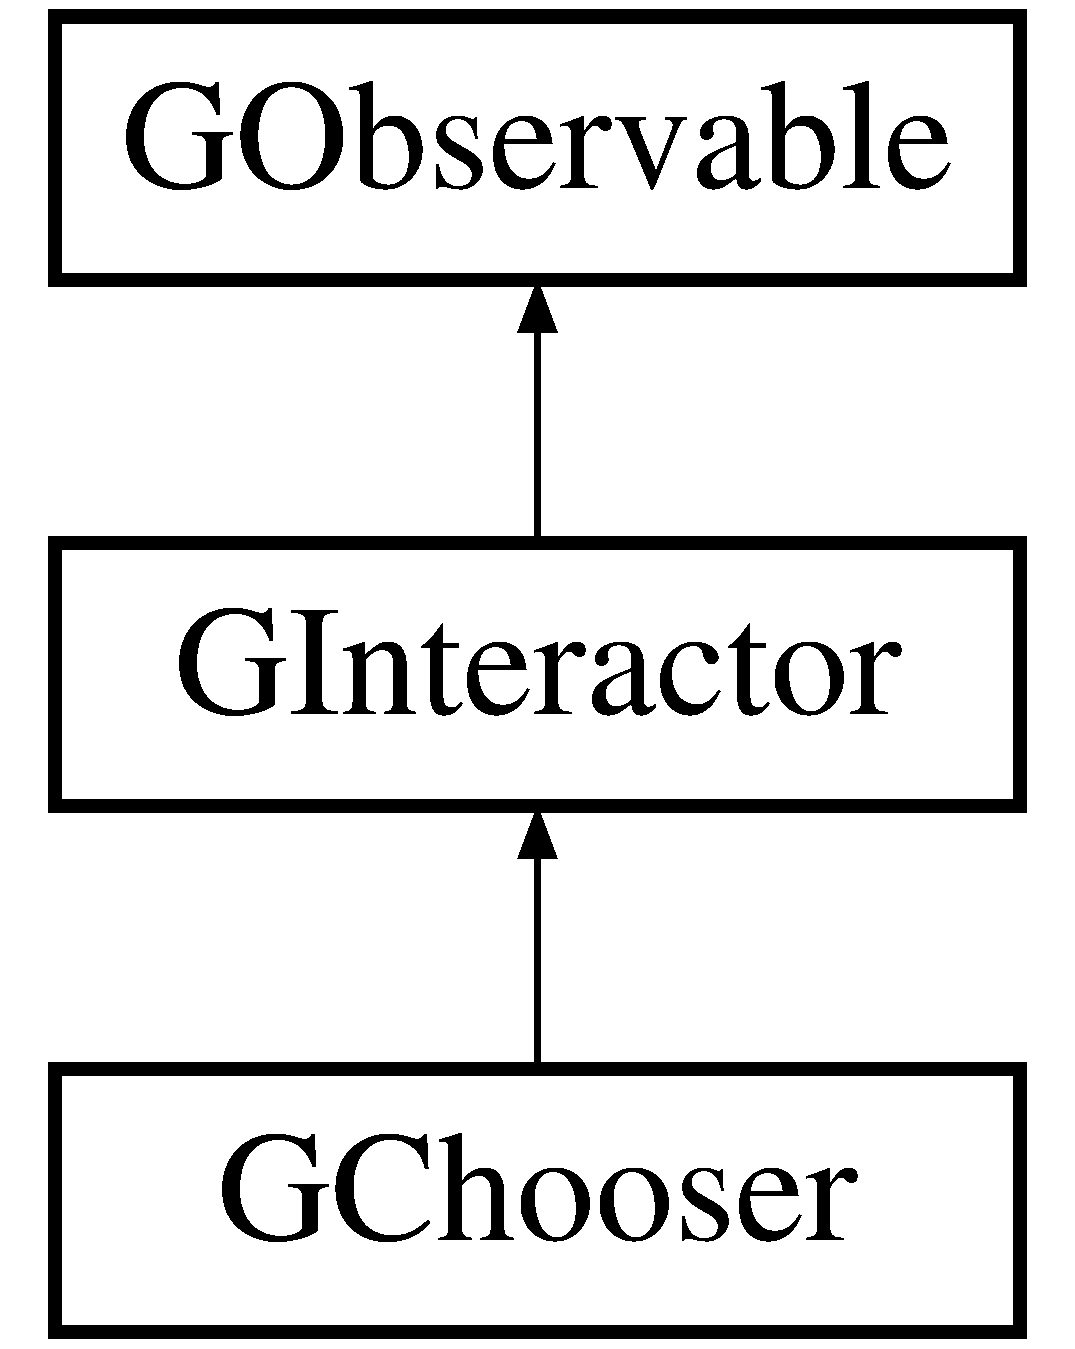
\includegraphics[height=3.000000cm]{classGChooser}
\end{center}
\end{figure}
\subsection*{Public Types}
\begin{DoxyCompactItemize}
\item 
enum \mbox{\hyperlink{classGInteractor_a8e0d441725a81d2bbdebbea09078260e}{Text\+Position}} \{ \mbox{\hyperlink{classGInteractor_a8e0d441725a81d2bbdebbea09078260ea4cd6f2e7d5a08d6f4dc052df2358f774}{T\+E\+X\+T\+\_\+\+B\+E\+S\+I\+D\+E\+\_\+\+I\+C\+ON}}, 
\mbox{\hyperlink{classGInteractor_a8e0d441725a81d2bbdebbea09078260eaa88490f63d8de68d44c83bdb2ecde3b3}{T\+E\+X\+T\+\_\+\+U\+N\+D\+E\+R\+\_\+\+I\+C\+ON}}, 
\mbox{\hyperlink{classGInteractor_a8e0d441725a81d2bbdebbea09078260ea39a6f388a30ac4fefb6eb13e846bc9f2}{T\+E\+X\+T\+\_\+\+O\+N\+LY}}
 \}
\begin{DoxyCompactList}\small\item\em The places where an interactor can place its text relative to its icon. \end{DoxyCompactList}\end{DoxyCompactItemize}
\subsection*{Public Member Functions}
\begin{DoxyCompactItemize}
\item 
\mbox{\hyperlink{classGChooser_ab17044f63a62b259f6b40a47a691f534}{G\+Chooser}} (Q\+Widget $\ast$parent=nullptr)
\begin{DoxyCompactList}\small\item\em Creates a chooser that initially contains no items. \end{DoxyCompactList}\item 
\mbox{\hyperlink{classGChooser_a7b9c598e637e726ac7b981495a0c2f75}{G\+Chooser}} (const std\+::initializer\+\_\+list$<$ std\+::string $>$ \&items, Q\+Widget $\ast$parent=nullptr)
\begin{DoxyCompactList}\small\item\em Creates a chooser that initially contains the given items. \end{DoxyCompactList}\item 
\mbox{\hyperlink{classGChooser_a051e9e420cb701cc9ec2283b4ae3a28b}{G\+Chooser}} (const \mbox{\hyperlink{classVector}{Vector}}$<$ std\+::string $>$ \&items, Q\+Widget $\ast$parent=nullptr)
\begin{DoxyCompactList}\small\item\em Creates a chooser that initially contains the given items. \end{DoxyCompactList}\item 
virtual \mbox{\hyperlink{classGChooser_ab6b8a1d0da7762b67a2d5f0e6bd22f22}{$\sim$\+G\+Chooser}} ()
\begin{DoxyCompactList}\small\item\em Frees memory allocated internally by the chooser. \end{DoxyCompactList}\item 
virtual void \mbox{\hyperlink{classGInteractor_a02f20ea6edfa0671f31c4c648a253833}{add\+Action\+Listener}} () Q\+\_\+\+D\+E\+C\+L\+\_\+\+D\+E\+P\+R\+E\+C\+A\+T\+ED
\begin{DoxyCompactList}\small\item\em Adds an event listener to be notified when this interactor is clicked or generally interacted with. \end{DoxyCompactList}\item 
virtual void \mbox{\hyperlink{classGChooser_a4d56babf9b4056c651a1999d9f7e6dcf}{add\+Item}} (const std\+::string \&item)
\begin{DoxyCompactList}\small\item\em Adds a new item consisting of the specified string to the end of the list. \end{DoxyCompactList}\item 
virtual void \mbox{\hyperlink{classGChooser_a9ae1e727f0d4bdcb198b2f9269db5614}{add\+Items}} (const std\+::initializer\+\_\+list$<$ std\+::string $>$ \&items)
\begin{DoxyCompactList}\small\item\em Adds each item from the given list to the end of the chooser\textquotesingle{}s list. \end{DoxyCompactList}\item 
virtual void \mbox{\hyperlink{classGChooser_aade608a87931d8313dbbc85e040c260a}{add\+Items}} (const \mbox{\hyperlink{classVector}{Vector}}$<$ std\+::string $>$ \&items)
\begin{DoxyCompactList}\small\item\em Adds each item from the given vector to the end of the chooser\textquotesingle{}s list. \end{DoxyCompactList}\item 
virtual void \mbox{\hyperlink{classGChooser_aa236b0d36b5d4f6a45c32b9d0e00f44b}{clear\+Items}} ()
\begin{DoxyCompactList}\small\item\em Removes all items from the chooser. \end{DoxyCompactList}\item 
virtual bool \mbox{\hyperlink{classGInteractor_ac05ba5b92e2e5146d416fe7f842a0969}{events\+Enabled}} () const Q\+\_\+\+D\+E\+C\+L\+\_\+\+O\+V\+E\+R\+R\+I\+DE
\begin{DoxyCompactList}\small\item\em Returns true if this interactor is currently accepting events. \end{DoxyCompactList}\item 
virtual std\+::string \mbox{\hyperlink{classGInteractor_a69f8d23ed8f207fbecad99960776e942}{get\+Accelerator}} () const
\begin{DoxyCompactList}\small\item\em Returns a string representing a hotkey for this interactor, or an empty string if no accelerator has been set. \end{DoxyCompactList}\item 
virtual std\+::string \mbox{\hyperlink{classGChooser_a90f2b1e6f6e7dabd9d6e5307f7c6d1b7}{get\+Action\+Command}} () const Q\+\_\+\+D\+E\+C\+L\+\_\+\+O\+V\+E\+R\+R\+I\+DE
\begin{DoxyCompactList}\small\item\em Returns an action command for this interactor, which is a semi-\/unique string you can use to identify it when events occur. \end{DoxyCompactList}\item 
virtual std\+::string \mbox{\hyperlink{classGInteractor_a808e22cc1fdfbecf71ed8c64ef4600e0}{get\+Background}} () const
\begin{DoxyCompactList}\small\item\em Returns the background color of the interactor as a string. \end{DoxyCompactList}\item 
virtual int \mbox{\hyperlink{classGInteractor_a9e827257a55cb8cf4d9de2ec6bcfd7a0}{get\+Background\+Int}} () const
\begin{DoxyCompactList}\small\item\em Returns the background color of the interactor as an R\+GB integer. \end{DoxyCompactList}\item 
virtual \mbox{\hyperlink{classGRectangle}{G\+Rectangle}} \mbox{\hyperlink{classGInteractor_a29e6ac35a0b48f491a4c88194cc5da3b}{get\+Bounds}} () const
\begin{DoxyCompactList}\small\item\em Returns a rectangle representing the x/y position and size of this interactor. \end{DoxyCompactList}\item 
virtual std\+::string \mbox{\hyperlink{classGInteractor_aa061dfa488c31e18549d64363c1d0e34}{get\+Color}} () const
\begin{DoxyCompactList}\small\item\em Returns the foreground/text color of the interactor as a string. \end{DoxyCompactList}\item 
virtual int \mbox{\hyperlink{classGInteractor_a9635c7af766cdc3417f346683fa0e6c1}{get\+Color\+Int}} () const
\begin{DoxyCompactList}\small\item\em Returns the foreground/text color of the interactor as an R\+GB integer. \end{DoxyCompactList}\item 
virtual \mbox{\hyperlink{classGContainer}{G\+Container}} $\ast$ \mbox{\hyperlink{classGInteractor_a7a6e317c29d61030929b4cd2d1c00fe7}{get\+Container}} () const
\begin{DoxyCompactList}\small\item\em Returns a pointer to the onscreen container holding this interactor. \end{DoxyCompactList}\item 
virtual std\+::string \mbox{\hyperlink{classGInteractor_a894a5502900794eeb27d084c21f1d77d}{get\+Font}} () const
\begin{DoxyCompactList}\small\item\em Returns the font of this interactor\textquotesingle{}s text as a font string such as \char`\"{}\+Helvetica-\/12-\/\+Bold\char`\"{}. \end{DoxyCompactList}\item 
virtual std\+::string \mbox{\hyperlink{classGInteractor_a4fa2d8b0192a3a5b4af4bbfe71194d03}{get\+Foreground}} () const
\begin{DoxyCompactList}\small\item\em Returns the foreground/text color of the interactor as a string. \end{DoxyCompactList}\item 
virtual int \mbox{\hyperlink{classGInteractor_ac3b12ab385a6ef9ae90fc879860ba726}{get\+Foreground\+Int}} () const
\begin{DoxyCompactList}\small\item\em Returns the foreground/text color of the interactor as an R\+GB integer. \end{DoxyCompactList}\item 
virtual double \mbox{\hyperlink{classGInteractor_a1e7e353362434072875264cf95629f99}{get\+Height}} () const
\begin{DoxyCompactList}\small\item\em Returns the current onscreen height of this interactor in pixels. \end{DoxyCompactList}\item 
virtual std\+::string \mbox{\hyperlink{classGInteractor_aaed62a73004939a64da6f0eb9eb64d73}{get\+Icon}} () const
\begin{DoxyCompactList}\small\item\em Returns the file name of the icon associated with this interactor, or an empty string if no icon has been set. \end{DoxyCompactList}\item 
virtual int \mbox{\hyperlink{classGInteractor_a9c9659a6c6ba66b4107ba59c95a24241}{get\+ID}} () const
\begin{DoxyCompactList}\small\item\em Returns a globally unique identifier for this interactor, which is set when the interactor is constructed. \end{DoxyCompactList}\item 
virtual \+\_\+\+Internal\+\_\+\+Q\+Widget $\ast$ \mbox{\hyperlink{classGChooser_a208ce13c1da40bf0ddb509daf99d6588}{get\+Internal\+Widget}} () const Q\+\_\+\+D\+E\+C\+L\+\_\+\+O\+V\+E\+R\+R\+I\+DE
\begin{DoxyCompactList}\small\item\em Returns a direct pointer to the internal Qt widget being wrapped by this interactor. \end{DoxyCompactList}\item 
virtual std\+::string \mbox{\hyperlink{classGChooser_a098538e0884967cbe287067a7fbbe04c}{get\+Item}} (int index) const
\begin{DoxyCompactList}\small\item\em Returns the item in the chooser at the given 0-\/based index. \end{DoxyCompactList}\item 
virtual int \mbox{\hyperlink{classGChooser_a288ee7c54b76ac6ae26eb4d748ce9776}{get\+Item\+Count}} () const
\begin{DoxyCompactList}\small\item\em Returns the number of items in the chooser. \end{DoxyCompactList}\item 
virtual \mbox{\hyperlink{classGPoint}{G\+Point}} \mbox{\hyperlink{classGInteractor_a4f83802015511edeb63b892830812c11}{get\+Location}} () const
\begin{DoxyCompactList}\small\item\em Returns an (x, y) point representing the onscreen location of the top-\/left corner of this interactor within its containing window. \end{DoxyCompactList}\item 
virtual double \mbox{\hyperlink{classGInteractor_aed4b0075fcc434499c3cb3e46896bda3}{get\+Minimum\+Height}} () const
\begin{DoxyCompactList}\small\item\em Returns the minimum height in pixels that this interactor will permit itself to be resized to. \end{DoxyCompactList}\item 
virtual \mbox{\hyperlink{classGDimension}{G\+Dimension}} \mbox{\hyperlink{classGInteractor_a66b5af0b32493b4d597ca0a3df2049ea}{get\+Minimum\+Size}} () const
\begin{DoxyCompactList}\small\item\em Returns a \mbox{\hyperlink{classGDimension}{G\+Dimension}} structure representing the minimum size in pixels that this interactor will permit itself to be resized to. \end{DoxyCompactList}\item 
virtual double \mbox{\hyperlink{classGInteractor_a59e668114fe3d49d2a0f28deb258f7c8}{get\+Minimum\+Width}} () const
\begin{DoxyCompactList}\small\item\em Returns the minimum width in pixels that this interactor will permit itself to be resized to. \end{DoxyCompactList}\item 
virtual std\+::string \mbox{\hyperlink{classGInteractor_a8a60438a5b55d0b2ceb35c8674b9d8c5}{get\+Name}} () const
\begin{DoxyCompactList}\small\item\em Returns a string representing a unique name for this interactor. \end{DoxyCompactList}\item 
virtual double \mbox{\hyperlink{classGInteractor_a747de0961653847bdc6615dbf756d715}{get\+Preferred\+Height}} () const
\begin{DoxyCompactList}\small\item\em Returns the height in pixels that this interactor would prefer to be, which would exactly fit its contents with no stretching or scrollbars. \end{DoxyCompactList}\item 
virtual \mbox{\hyperlink{classGDimension}{G\+Dimension}} \mbox{\hyperlink{classGInteractor_a4aabbee761d8e9116275401131b7ccd1}{get\+Preferred\+Size}} () const
\begin{DoxyCompactList}\small\item\em Returns a \mbox{\hyperlink{classGDimension}{G\+Dimension}} structure storing the width and height in pixels that this interactor would prefer to be, which would exactly fit its contents with no stretching or scrollbars. \end{DoxyCompactList}\item 
virtual double \mbox{\hyperlink{classGInteractor_a82bca31d37700fb0e35d2743352efd5e}{get\+Preferred\+Width}} () const
\begin{DoxyCompactList}\small\item\em Returns the height in pixels that this interactor would prefer to be, which would exactly fit its contents with no stretching or scrollbars. \end{DoxyCompactList}\item 
virtual int \mbox{\hyperlink{classGChooser_a4b706834529fee47c26689e69d9791f5}{get\+Selected\+Index}} () const
\begin{DoxyCompactList}\small\item\em Returns which index is selected in the chooser. \end{DoxyCompactList}\item 
virtual std\+::string \mbox{\hyperlink{classGChooser_a3dd4604cb3a910a63204197f56216ca4}{get\+Selected\+Item}} () const
\begin{DoxyCompactList}\small\item\em Returns the currently selected item in the chooser, or an empty string if no item is currently selected. \end{DoxyCompactList}\item 
virtual \mbox{\hyperlink{classGDimension}{G\+Dimension}} \mbox{\hyperlink{classGInteractor_a7b4eec96a2bdc6420695d5796a78eea9}{get\+Size}} () const
\begin{DoxyCompactList}\small\item\em Returns a \mbox{\hyperlink{classGDimension}{G\+Dimension}} structure storing the current onscreen width and height of this interactor in pixels. \end{DoxyCompactList}\item 
virtual std\+::string \mbox{\hyperlink{classGChooser_a9896d58fcfebbf1025aeeb5b8b9ede80}{get\+Type}} () const Q\+\_\+\+D\+E\+C\+L\+\_\+\+O\+V\+E\+R\+R\+I\+DE
\begin{DoxyCompactList}\small\item\em Returns a string representing the class name of this interactor, such as \char`\"{}\+G\+Button\char`\"{} or \char`\"{}\+G\+Check\+Box\char`\"{}. \end{DoxyCompactList}\item 
virtual Q\+Widget $\ast$ \mbox{\hyperlink{classGChooser_a326ee51b5561f807df7b29a1c101f7fd}{get\+Widget}} () const Q\+\_\+\+D\+E\+C\+L\+\_\+\+O\+V\+E\+R\+R\+I\+DE
\begin{DoxyCompactList}\small\item\em Returns a direct pointer to the internal Qt widget being wrapped by this interactor. \end{DoxyCompactList}\item 
virtual double \mbox{\hyperlink{classGInteractor_a0ed2965abd4f5701d2cadf71239faf19}{get\+Width}} () const
\begin{DoxyCompactList}\small\item\em Returns the current onscreen width of this interactor in pixels. \end{DoxyCompactList}\item 
virtual double \mbox{\hyperlink{classGInteractor_a344385751bee0720059403940d57a13e}{getX}} () const
\begin{DoxyCompactList}\small\item\em Returns the x-\/coordinate of the top-\/left pixel of this interactor within its onscreen window. \end{DoxyCompactList}\item 
virtual double \mbox{\hyperlink{classGInteractor_aafa51c7f8f38a09febbb9ce7853f77b4}{getY}} () const
\begin{DoxyCompactList}\small\item\em Returns the y-\/coordinate of the top-\/left pixel of this interactor within its onscreen window. \end{DoxyCompactList}\item 
virtual bool \mbox{\hyperlink{classGInteractor_afc480f652b8c5f1fb255e2269ce68879}{in\+Bounds}} (double x, double y) const
\begin{DoxyCompactList}\small\item\em Returns true if the given x/y pixel is within the bounds of this interactor. \end{DoxyCompactList}\item 
virtual bool \mbox{\hyperlink{classGInteractor_ae6d7982c1c627b677a5e776ca86118ed}{in\+Bounds}} (int x, int y) const
\begin{DoxyCompactList}\small\item\em Returns true if the given x/y pixel is within the bounds of this interactor. \end{DoxyCompactList}\item 
virtual bool \mbox{\hyperlink{classGChooser_a012b5afb54e037e6c5498cf0932a521b}{is\+Editable}} () const
\begin{DoxyCompactList}\small\item\em Returns true if the chooser has an editable area for typing new items. \end{DoxyCompactList}\item 
virtual bool \mbox{\hyperlink{classGChooser_acf82f9b2937375c7b1cf3dccb3df3312}{is\+Empty}} () const
\begin{DoxyCompactList}\small\item\em Returns true if the chooser has no items. \end{DoxyCompactList}\item 
virtual bool \mbox{\hyperlink{classGInteractor_aacb819fb241851fd9fc045271baa4034}{is\+Enabled}} () const
\begin{DoxyCompactList}\small\item\em Returns true if this interactor is currently enabled. \end{DoxyCompactList}\item 
virtual bool \mbox{\hyperlink{classGInteractor_a9d8a6cfb13917785c143e74d40e4e2be}{is\+Visible}} () const
\begin{DoxyCompactList}\small\item\em Returns true if the interactor is visible on the screen. \end{DoxyCompactList}\item 
virtual void \mbox{\hyperlink{classGChooser_ab7fe7a876367b87cf7202f947f1d05e4}{remove\+Action\+Listener}} ()
\begin{DoxyCompactList}\small\item\em Removes the action listener from this checkbox so that it will no longer call it when events occur. \end{DoxyCompactList}\item 
virtual void \mbox{\hyperlink{classGInteractor_a519fb2ac767f8b2febbb50b898b8c8cb}{request\+Focus}} ()
\begin{DoxyCompactList}\small\item\em Transfers keyboard focus to this interactor. \end{DoxyCompactList}\item 
virtual void \mbox{\hyperlink{classGInteractor_ad15f102f62e2960576012f1aa0ba4b2e}{set\+Accelerator}} (const std\+::string \&accelerator)
\begin{DoxyCompactList}\small\item\em Sets an accelerator hotkey for this interactor, such as \char`\"{}\+Ctrl-\/\+S\char`\"{}. \end{DoxyCompactList}\item 
virtual void \mbox{\hyperlink{classGInteractor_a4b5843fe3030e038a1ba54cc03389bcf}{set\+Action\+Command}} (const std\+::string \&action\+Command)
\begin{DoxyCompactList}\small\item\em Sets the action command for this interactor. \end{DoxyCompactList}\item 
virtual void \mbox{\hyperlink{classGChooser_adcfb4742430c88714fcf57e57ab8ea9c}{set\+Action\+Listener}} (G\+Event\+Listener func)
\begin{DoxyCompactList}\small\item\em Sets an action listener on this chooser so that it will be called when an item is selected. \end{DoxyCompactList}\item 
virtual void \mbox{\hyperlink{classGChooser_aebd20a89c7a8a43a6fce999cf4f9fcf2}{set\+Action\+Listener}} (G\+Event\+Listener\+Void func)
\begin{DoxyCompactList}\small\item\em Sets an action listener on this chooser so that it will be called when an item is selected. \end{DoxyCompactList}\item 
virtual void \mbox{\hyperlink{classGInteractor_acba7e546c2025c0a15ca4b4cc92043db}{set\+Background}} (int rgb)
\begin{DoxyCompactList}\small\item\em Sets the background color of the interactor to the color represented by the given R\+GB integer. \end{DoxyCompactList}\item 
virtual void \mbox{\hyperlink{classGInteractor_ab4677ab2474e68b07aa56605af92a84a}{set\+Background}} (const std\+::string \&color)
\begin{DoxyCompactList}\small\item\em Sets the background color of the interactor to the color represented by the given string. \end{DoxyCompactList}\item 
virtual void \mbox{\hyperlink{classGInteractor_a2aae8197624b72265ab83b4f1bc73f2f}{set\+Bounds}} (double x, double y, double width, double height)
\begin{DoxyCompactList}\small\item\em Sets the size and location of the widget. \end{DoxyCompactList}\item 
virtual void \mbox{\hyperlink{classGInteractor_acada386653f008cacc7cce86426bef7c}{set\+Bounds}} (const \mbox{\hyperlink{classGRectangle}{G\+Rectangle}} \&\mbox{\hyperlink{classGChooser_af9593d4a5ff4274efaf429cb4f9e57cc}{size}})
\begin{DoxyCompactList}\small\item\em Sets the size and location of the widget. \end{DoxyCompactList}\item 
virtual void \mbox{\hyperlink{classGInteractor_ab1f5cc0f5cc6bbbd716a526c61f1081d}{set\+Color}} (int rgb)
\begin{DoxyCompactList}\small\item\em Sets the foreground/text color of the interactor to the color represented by the given R\+GB integer. \end{DoxyCompactList}\item 
virtual void \mbox{\hyperlink{classGInteractor_a61374df6c11b52cfbb0815decdbaebc6}{set\+Color}} (const std\+::string \&color)
\begin{DoxyCompactList}\small\item\em Sets the foreground/text color of the interactor to the color represented by the given string. \end{DoxyCompactList}\item 
virtual void \mbox{\hyperlink{classGChooser_a52455aaff9ee352ca405fa61ba246b84}{set\+Editable}} (bool editable)
\begin{DoxyCompactList}\small\item\em Sets whether the chooser has an editable area for typing new items. \end{DoxyCompactList}\item 
virtual void \mbox{\hyperlink{classGInteractor_ab831367dd84bbd579e02e55bacb21343}{set\+Enabled}} (bool value)
\begin{DoxyCompactList}\small\item\em Sets whether this interactor is currently enabled. \end{DoxyCompactList}\item 
virtual void \mbox{\hyperlink{classGObservable_afaa30b2a9e0f378fd1c70d2f1d0b8216}{set\+Events\+Enabled}} (bool \mbox{\hyperlink{classGInteractor_ac05ba5b92e2e5146d416fe7f842a0969}{events\+Enabled}})
\begin{DoxyCompactList}\small\item\em Sets whether the object is currently allowing itself to fire events. \end{DoxyCompactList}\item 
virtual void \mbox{\hyperlink{classGInteractor_a2592348886ffea646c6534bf88f7c49d}{set\+Font}} (const Q\+Font \&font)
\begin{DoxyCompactList}\small\item\em Sets the font used by this widget to the given Qt font. \end{DoxyCompactList}\item 
virtual void \mbox{\hyperlink{classGInteractor_a8e096e8818d838aceae1d46d58fb3a7b}{set\+Font}} (const std\+::string \&font)
\begin{DoxyCompactList}\small\item\em Sets the font used by this widget to the font represented by the given font string, such as \char`\"{}\+Helvetica-\/16-\/\+Bold\char`\"{}. \end{DoxyCompactList}\item 
virtual void \mbox{\hyperlink{classGInteractor_a9eb856b5ff83a19df3831a31f15f4563}{set\+Foreground}} (int rgb)
\begin{DoxyCompactList}\small\item\em Sets the foreground/text color of the interactor to the color represented by the given R\+GB integer. \end{DoxyCompactList}\item 
virtual void \mbox{\hyperlink{classGInteractor_af59209aeadea6dfc6d97a2d8531f50e1}{set\+Foreground}} (const std\+::string \&color)
\begin{DoxyCompactList}\small\item\em Sets the foreground/text color of the interactor to the color represented by the given string. \end{DoxyCompactList}\item 
virtual void \mbox{\hyperlink{classGInteractor_a9e280bfc4544dfaf8e4376c4e1a74357}{set\+Height}} (double height)
\begin{DoxyCompactList}\small\item\em Sets the onscreen height of the interactor in pixels. \end{DoxyCompactList}\item 
virtual void \mbox{\hyperlink{classGInteractor_a762e139aa311461c3984d3ad28293f64}{set\+Icon}} (const std\+::string \&filename, bool retain\+Icon\+Size=true)
\begin{DoxyCompactList}\small\item\em Sets the file name of the icon associated with this interactor, or an empty string if no icon has been set. \end{DoxyCompactList}\item 
virtual void \mbox{\hyperlink{classGChooser_aa4f87c4982e01ec37b78f52f2bf11ef4}{set\+Item}} (int index, const std\+::string \&item)
\begin{DoxyCompactList}\small\item\em Sets the item at the given index in the chooser to the given value. \end{DoxyCompactList}\item 
virtual void \mbox{\hyperlink{classGInteractor_a04594e8ba9b98513a64f1da00dcae18c}{set\+Location}} (double x, double y)
\begin{DoxyCompactList}\small\item\em Sets the onscreen x/y-\/coordinate of the top-\/left corner of the interactor relative to its window. \end{DoxyCompactList}\item 
virtual void \mbox{\hyperlink{classGInteractor_a0cf428e207b7f22cc08138a90b1b87b2}{set\+Minimum\+Size}} (double width, double height)
\begin{DoxyCompactList}\small\item\em Sets the minimum size in pixels that this interactor will permit itself to be resized to. \end{DoxyCompactList}\item 
virtual void \mbox{\hyperlink{classGInteractor_a3b1046117ac6cb7abe467e00ba8a81f4}{set\+Minimum\+Size}} (const \mbox{\hyperlink{classGDimension}{G\+Dimension}} \&\mbox{\hyperlink{classGChooser_af9593d4a5ff4274efaf429cb4f9e57cc}{size}})
\begin{DoxyCompactList}\small\item\em Sets the minimum size in pixels that this interactor will permit itself to be resized to. \end{DoxyCompactList}\item 
virtual void \mbox{\hyperlink{classGInteractor_a9d3a2685df23b5e7cbf59c19c4a1f9b5}{set\+Name}} (const std\+::string \&name)
\begin{DoxyCompactList}\small\item\em Sets a string representing a unique name for this interactor. \end{DoxyCompactList}\item 
virtual void \mbox{\hyperlink{classGInteractor_a1ab987704fce32098706c6f00fb08218}{set\+Preferred\+Height}} (double height)
\begin{DoxyCompactList}\small\item\em Sets the height in pixels that this interactor would prefer to be. \end{DoxyCompactList}\item 
virtual void \mbox{\hyperlink{classGInteractor_a042c5ae19430d765ef552371cae3632c}{set\+Preferred\+Size}} (double width, double height)
\begin{DoxyCompactList}\small\item\em Sets the width and height in pixels that this interactor would prefer to be. \end{DoxyCompactList}\item 
virtual void \mbox{\hyperlink{classGInteractor_aa22d9be4bc0e078bb0ea69b0fc9d7c75}{set\+Preferred\+Size}} (const \mbox{\hyperlink{classGDimension}{G\+Dimension}} \&\mbox{\hyperlink{classGChooser_af9593d4a5ff4274efaf429cb4f9e57cc}{size}})
\begin{DoxyCompactList}\small\item\em Sets the size in pixels that this interactor would prefer to be. \end{DoxyCompactList}\item 
virtual void \mbox{\hyperlink{classGInteractor_a3db429ab2fa52efd187eec0ed8cdd9f2}{set\+Preferred\+Width}} (double width)
\begin{DoxyCompactList}\small\item\em Sets the width in pixels that this interactor would prefer to be. \end{DoxyCompactList}\item 
virtual void \mbox{\hyperlink{classGChooser_a9f838f41a4abc5775bfe28fea7cf1750}{set\+Selected\+Index}} (int index)
\begin{DoxyCompactList}\small\item\em Sets the item at the given index in the chooser to be selected. \end{DoxyCompactList}\item 
virtual void \mbox{\hyperlink{classGChooser_ae427110c299aa08a8f72cbfa88ab3301}{set\+Selected\+Item}} (const std\+::string \&item)
\begin{DoxyCompactList}\small\item\em Sets the given item in the chooser to be selected. \end{DoxyCompactList}\item 
virtual void \mbox{\hyperlink{classGInteractor_aca25d49481f9bf5fc8f7df4c086c4ce7}{set\+Size}} (double width, double height)
\begin{DoxyCompactList}\small\item\em Sets the onscreen width and height of the interactor in pixels. \end{DoxyCompactList}\item 
virtual void \mbox{\hyperlink{classGInteractor_ae2b628228f192c2702c4ce941b2af68f}{set\+Size}} (const \mbox{\hyperlink{classGDimension}{G\+Dimension}} \&\mbox{\hyperlink{classGChooser_af9593d4a5ff4274efaf429cb4f9e57cc}{size}})
\begin{DoxyCompactList}\small\item\em Sets the onscreen width and height of the interactor in pixels. \end{DoxyCompactList}\item 
virtual void \mbox{\hyperlink{classGInteractor_a039e0e49beaecc275efce02d416acea8}{set\+Tooltip}} (const std\+::string \&tooltip\+Text)
\begin{DoxyCompactList}\small\item\em Sets a \char`\"{}tooltip\char`\"{} that will appear if the user hovers their mouse over the interactor. \end{DoxyCompactList}\item 
virtual void \mbox{\hyperlink{classGInteractor_a18e44e30b31525a243960ca3928125aa}{set\+Visible}} (bool visible)
\begin{DoxyCompactList}\small\item\em Returns true if the interactor is visible on the screen. \end{DoxyCompactList}\item 
virtual void \mbox{\hyperlink{classGInteractor_aa3f3fba4cb131baa8696ba01e3bceca1}{set\+Width}} (double width)
\begin{DoxyCompactList}\small\item\em Sets the onscreen width of the interactor in pixels. \end{DoxyCompactList}\item 
virtual void \mbox{\hyperlink{classGInteractor_a9c18fcc579333bf9653d13ad2b372e39}{setX}} (double x)
\begin{DoxyCompactList}\small\item\em Sets the onscreen x-\/coordinate of the top-\/left corner of the interactor relative to its window. \end{DoxyCompactList}\item 
virtual void \mbox{\hyperlink{classGInteractor_a7d57e2a5c35d27feb58fd498a3cf82b9}{setY}} (double y)
\begin{DoxyCompactList}\small\item\em Sets the onscreen y-\/coordinate of the top-\/left corner of the interactor relative to its window. \end{DoxyCompactList}\item 
virtual int \mbox{\hyperlink{classGChooser_af9593d4a5ff4274efaf429cb4f9e57cc}{size}} () const
\begin{DoxyCompactList}\small\item\em Returns the number of items in the chooser. \end{DoxyCompactList}\item 
virtual std\+::string \mbox{\hyperlink{classGObservable_a1fe5121d6528fdea3f243321b3fa3a49}{to\+String}} () const
\begin{DoxyCompactList}\small\item\em Returns a string representation of this observable object\textquotesingle{}s state. \end{DoxyCompactList}\end{DoxyCompactItemize}
\subsection*{Protected Member Functions}
\begin{DoxyCompactItemize}
\item 
virtual void \mbox{\hyperlink{classGObservable_a80cfa040459ff53594adbd6a51ec8f43}{clear\+Event\+Listeners}} ()
\begin{DoxyCompactList}\small\item\em Removes all event listeners from this object. \end{DoxyCompactList}\item 
virtual void \mbox{\hyperlink{classGObservable_a284f31528c0520f8e545c03ac9eeac74}{ensure\+Thread\+Safety}} (const std\+::string \&member\+Name=\char`\"{}\char`\"{})
\begin{DoxyCompactList}\small\item\em Ensures that we are currently in the Qt G\+UI thread. \end{DoxyCompactList}\item 
virtual void \mbox{\hyperlink{classGObservable_a63e5e5a6227c59c928493b11aceb0f67}{fire\+Event}} (\mbox{\hyperlink{classGEvent}{G\+Event}} \&event)
\begin{DoxyCompactList}\small\item\em Sends out the given event to any attached listeners. \end{DoxyCompactList}\item 
virtual void \mbox{\hyperlink{classGObservable_ab3983ea07337b52020a29cc00c653d8d}{fire\+G\+Event}} (Q\+Event $\ast$event, Event\+Type event\+Type, const std\+::string \&event\+Name)
\begin{DoxyCompactList}\small\item\em Creates an event of the given type, then sends it out to any attached listeners. \end{DoxyCompactList}\item 
virtual void \mbox{\hyperlink{classGObservable_a01fdf1b0e0dbd49e189fe4514e010411}{fire\+G\+Event}} (Q\+Close\+Event $\ast$event, Event\+Type event\+Type, const std\+::string \&event\+Name)
\begin{DoxyCompactList}\small\item\em Creates an event of the given type, then sends it out to any attached listeners. \end{DoxyCompactList}\item 
virtual void \mbox{\hyperlink{classGObservable_abb0b2f66ba39211cb5d7615e9d1c04e2}{fire\+G\+Event}} (Q\+Key\+Event $\ast$event, Event\+Type event\+Type, const std\+::string \&event\+Name)
\begin{DoxyCompactList}\small\item\em Creates an event of the given type, then sends it out to any attached listeners. \end{DoxyCompactList}\item 
virtual void \mbox{\hyperlink{classGObservable_a119318675d2165bdf7dd853aaf881d4b}{fire\+G\+Event}} (Q\+Mouse\+Event $\ast$event, Event\+Type event\+Type, const std\+::string \&event\+Name, const std\+::string \&action\+Command=\char`\"{}\char`\"{})
\begin{DoxyCompactList}\small\item\em Creates an event of the given type, then sends it out to any attached listeners. \end{DoxyCompactList}\item 
virtual void \mbox{\hyperlink{classGObservable_a63fd9034e1e1633c1c38eb342bfd34e9}{fire\+G\+Event}} (Q\+Resize\+Event $\ast$event, Event\+Type event\+Type, const std\+::string \&event\+Name)
\begin{DoxyCompactList}\small\item\em Creates an event of the given type, then sends it out to any attached listeners. \end{DoxyCompactList}\item 
virtual void \mbox{\hyperlink{classGObservable_a741345310d9b7c5170a6cbc410c44ac4}{fire\+G\+Event}} (Q\+Timer\+Event $\ast$event, Event\+Type event\+Type, const std\+::string \&event\+Name)
\begin{DoxyCompactList}\small\item\em Creates an event of the given type, then sends it out to any attached listeners. \end{DoxyCompactList}\item 
virtual void \mbox{\hyperlink{classGObservable_a93bf338968a0338761b8e4dc62f582e9}{fire\+G\+Event}} (Q\+Wheel\+Event $\ast$event, Event\+Type event\+Type, const std\+::string \&event\+Name)
\begin{DoxyCompactList}\small\item\em Creates an event of the given type, then sends it out to any attached listeners. \end{DoxyCompactList}\item 
virtual void \mbox{\hyperlink{classGObservable_a2a70a7d7435ff0c3b80bb4d70da19e0d}{fire\+G\+Event}} (Q\+Window\+State\+Change\+Event $\ast$event, Event\+Type event\+Type, const std\+::string \&event\+Name)
\begin{DoxyCompactList}\small\item\em Creates an event of the given type, then sends it out to any attached listeners. \end{DoxyCompactList}\item 
virtual bool \mbox{\hyperlink{classGObservable_a9f6faaa25942923bafa1c44020c49fa9}{has\+Event\+Listener}} (const std\+::string \&event\+Name) const
\begin{DoxyCompactList}\small\item\em Returns true if the observable object has a listener for the given type of event. \end{DoxyCompactList}\item 
virtual bool \mbox{\hyperlink{classGObservable_aeec1adc19aa0f33de62390686ee1382c}{is\+Accepting\+Event}} (int event\+Mask) const
\begin{DoxyCompactList}\small\item\em Returns true if the observable object has a listener for the given type of event. \end{DoxyCompactList}\item 
virtual bool \mbox{\hyperlink{classGObservable_aa31c73145a29dcb92848a92e0cfaea41}{is\+Accepting\+Event}} (const \mbox{\hyperlink{classGEvent}{G\+Event}} \&event) const
\begin{DoxyCompactList}\small\item\em Returns true if the observable object has a listener for the given type of event. \end{DoxyCompactList}\item 
virtual bool \mbox{\hyperlink{classGObservable_a3b1c689267eda44e65a2213e7de38b23}{is\+Accepting\+Event}} (const std\+::string \&event\+Type) const
\begin{DoxyCompactList}\small\item\em Returns true if the observable object has a listener for the given type of event. \end{DoxyCompactList}\item 
virtual void \mbox{\hyperlink{classGObservable_acbcf1ed3a851ad8a3c17ef38d86b481d}{remove\+Event\+Listener}} (const std\+::string \&event\+Name)
\begin{DoxyCompactList}\small\item\em Removes any event listener from this observable object that would respond to the given type of event, such as \char`\"{}click\char`\"{} or \char`\"{}keydown\char`\"{}. \end{DoxyCompactList}\item 
virtual void \mbox{\hyperlink{classGObservable_af51cc35c29a1bd1908609d432decdbb6}{remove\+Event\+Listeners}} (std\+::initializer\+\_\+list$<$ std\+::string $>$ event\+Names)
\begin{DoxyCompactList}\small\item\em Removes any event listener from this observable object that would respond to the given types of events, such as \char`\"{}click\char`\"{} or \char`\"{}keydown\char`\"{}. \end{DoxyCompactList}\item 
virtual void \mbox{\hyperlink{classGObservable_ad2f6d34961c50f6c1e0659990b79f741}{set\+Event\+Listener}} (const std\+::string \&event\+Name, G\+Event\+Listener func)
\begin{DoxyCompactList}\small\item\em Adds an event listener from this observable object to respond to the given type of event, such as \char`\"{}click\char`\"{} or \char`\"{}keydown\char`\"{}. \end{DoxyCompactList}\item 
virtual void \mbox{\hyperlink{classGObservable_abac4cb9f9e626e010e87f5d91573c8a5}{set\+Event\+Listener}} (const std\+::string \&event\+Name, G\+Event\+Listener\+Void func)
\begin{DoxyCompactList}\small\item\em Adds an event listener from this observable object to respond to the given type of event, such as \char`\"{}click\char`\"{} or \char`\"{}keydown\char`\"{}. \end{DoxyCompactList}\item 
virtual void \mbox{\hyperlink{classGObservable_afa388d69c33c718cf035774604065604}{set\+Event\+Listeners}} (std\+::initializer\+\_\+list$<$ std\+::string $>$ event\+Names, G\+Event\+Listener func)
\begin{DoxyCompactList}\small\item\em Adds an event listener from this observable object to respond to the given types of events, such as \char`\"{}click\char`\"{} or \char`\"{}keydown\char`\"{}. \end{DoxyCompactList}\item 
virtual void \mbox{\hyperlink{classGObservable_a7867184bbb686f74fae8a4db927da799}{set\+Event\+Listeners}} (std\+::initializer\+\_\+list$<$ std\+::string $>$ event\+Names, G\+Event\+Listener\+Void func)
\begin{DoxyCompactList}\small\item\em Adds an event listener from this observable object to respond to the given types of events, such as \char`\"{}click\char`\"{} or \char`\"{}keydown\char`\"{}. \end{DoxyCompactList}\end{DoxyCompactItemize}


\subsection{Detailed Description}
This interactor subclass represents a selectable drop-\/down list. 

The \mbox{\hyperlink{classGChooser}{G\+Chooser}} constructor creates an empty chooser. Once the chooser has been created, clients can use add\+Item to add the options. 

\subsection{Member Enumeration Documentation}
\mbox{\Hypertarget{classGInteractor_a8e0d441725a81d2bbdebbea09078260e}\label{classGInteractor_a8e0d441725a81d2bbdebbea09078260e}} 
\index{G\+Chooser@{G\+Chooser}!Text\+Position@{Text\+Position}}
\index{Text\+Position@{Text\+Position}!G\+Chooser@{G\+Chooser}}
\subsubsection{\texorpdfstring{Text\+Position}{TextPosition}}
{\footnotesize\ttfamily enum \mbox{\hyperlink{classGInteractor_a8e0d441725a81d2bbdebbea09078260e}{Text\+Position}}\hspace{0.3cm}{\ttfamily [inherited]}}



The places where an interactor can place its text relative to its icon. 

\begin{DoxyEnumFields}{Enumerator}
\raisebox{\heightof{T}}[0pt][0pt]{\index{T\+E\+X\+T\+\_\+\+B\+E\+S\+I\+D\+E\+\_\+\+I\+C\+ON@{T\+E\+X\+T\+\_\+\+B\+E\+S\+I\+D\+E\+\_\+\+I\+C\+ON}!G\+Chooser@{G\+Chooser}}\index{G\+Chooser@{G\+Chooser}!T\+E\+X\+T\+\_\+\+B\+E\+S\+I\+D\+E\+\_\+\+I\+C\+ON@{T\+E\+X\+T\+\_\+\+B\+E\+S\+I\+D\+E\+\_\+\+I\+C\+ON}}}\mbox{\Hypertarget{classGInteractor_a8e0d441725a81d2bbdebbea09078260ea4cd6f2e7d5a08d6f4dc052df2358f774}\label{classGInteractor_a8e0d441725a81d2bbdebbea09078260ea4cd6f2e7d5a08d6f4dc052df2358f774}} 
T\+E\+X\+T\+\_\+\+B\+E\+S\+I\+D\+E\+\_\+\+I\+C\+ON&\\
\hline

\raisebox{\heightof{T}}[0pt][0pt]{\index{T\+E\+X\+T\+\_\+\+U\+N\+D\+E\+R\+\_\+\+I\+C\+ON@{T\+E\+X\+T\+\_\+\+U\+N\+D\+E\+R\+\_\+\+I\+C\+ON}!G\+Chooser@{G\+Chooser}}\index{G\+Chooser@{G\+Chooser}!T\+E\+X\+T\+\_\+\+U\+N\+D\+E\+R\+\_\+\+I\+C\+ON@{T\+E\+X\+T\+\_\+\+U\+N\+D\+E\+R\+\_\+\+I\+C\+ON}}}\mbox{\Hypertarget{classGInteractor_a8e0d441725a81d2bbdebbea09078260eaa88490f63d8de68d44c83bdb2ecde3b3}\label{classGInteractor_a8e0d441725a81d2bbdebbea09078260eaa88490f63d8de68d44c83bdb2ecde3b3}} 
T\+E\+X\+T\+\_\+\+U\+N\+D\+E\+R\+\_\+\+I\+C\+ON&\\
\hline

\raisebox{\heightof{T}}[0pt][0pt]{\index{T\+E\+X\+T\+\_\+\+O\+N\+LY@{T\+E\+X\+T\+\_\+\+O\+N\+LY}!G\+Chooser@{G\+Chooser}}\index{G\+Chooser@{G\+Chooser}!T\+E\+X\+T\+\_\+\+O\+N\+LY@{T\+E\+X\+T\+\_\+\+O\+N\+LY}}}\mbox{\Hypertarget{classGInteractor_a8e0d441725a81d2bbdebbea09078260ea39a6f388a30ac4fefb6eb13e846bc9f2}\label{classGInteractor_a8e0d441725a81d2bbdebbea09078260ea39a6f388a30ac4fefb6eb13e846bc9f2}} 
T\+E\+X\+T\+\_\+\+O\+N\+LY&\\
\hline

\end{DoxyEnumFields}


\subsection{Constructor \& Destructor Documentation}
\mbox{\Hypertarget{classGChooser_ab17044f63a62b259f6b40a47a691f534}\label{classGChooser_ab17044f63a62b259f6b40a47a691f534}} 
\index{G\+Chooser@{G\+Chooser}!G\+Chooser@{G\+Chooser}}
\index{G\+Chooser@{G\+Chooser}!G\+Chooser@{G\+Chooser}}
\subsubsection{\texorpdfstring{G\+Chooser()}{GChooser()}\hspace{0.1cm}{\footnotesize\ttfamily [1/3]}}
{\footnotesize\ttfamily \mbox{\hyperlink{classGChooser}{G\+Chooser}} (\begin{DoxyParamCaption}\item[{Q\+Widget $\ast$}]{parent = {\ttfamily nullptr} }\end{DoxyParamCaption})}



Creates a chooser that initially contains no items. 

\mbox{\Hypertarget{classGChooser_a7b9c598e637e726ac7b981495a0c2f75}\label{classGChooser_a7b9c598e637e726ac7b981495a0c2f75}} 
\index{G\+Chooser@{G\+Chooser}!G\+Chooser@{G\+Chooser}}
\index{G\+Chooser@{G\+Chooser}!G\+Chooser@{G\+Chooser}}
\subsubsection{\texorpdfstring{G\+Chooser()}{GChooser()}\hspace{0.1cm}{\footnotesize\ttfamily [2/3]}}
{\footnotesize\ttfamily \mbox{\hyperlink{classGChooser}{G\+Chooser}} (\begin{DoxyParamCaption}\item[{const std\+::initializer\+\_\+list$<$ std\+::string $>$ \&}]{items,  }\item[{Q\+Widget $\ast$}]{parent = {\ttfamily nullptr} }\end{DoxyParamCaption})}



Creates a chooser that initially contains the given items. 

\mbox{\Hypertarget{classGChooser_a051e9e420cb701cc9ec2283b4ae3a28b}\label{classGChooser_a051e9e420cb701cc9ec2283b4ae3a28b}} 
\index{G\+Chooser@{G\+Chooser}!G\+Chooser@{G\+Chooser}}
\index{G\+Chooser@{G\+Chooser}!G\+Chooser@{G\+Chooser}}
\subsubsection{\texorpdfstring{G\+Chooser()}{GChooser()}\hspace{0.1cm}{\footnotesize\ttfamily [3/3]}}
{\footnotesize\ttfamily \mbox{\hyperlink{classGChooser}{G\+Chooser}} (\begin{DoxyParamCaption}\item[{const \mbox{\hyperlink{classVector}{Vector}}$<$ std\+::string $>$ \&}]{items,  }\item[{Q\+Widget $\ast$}]{parent = {\ttfamily nullptr} }\end{DoxyParamCaption})}



Creates a chooser that initially contains the given items. 

\mbox{\Hypertarget{classGChooser_ab6b8a1d0da7762b67a2d5f0e6bd22f22}\label{classGChooser_ab6b8a1d0da7762b67a2d5f0e6bd22f22}} 
\index{G\+Chooser@{G\+Chooser}!````~G\+Chooser@{$\sim$\+G\+Chooser}}
\index{````~G\+Chooser@{$\sim$\+G\+Chooser}!G\+Chooser@{G\+Chooser}}
\subsubsection{\texorpdfstring{$\sim$\+G\+Chooser()}{~GChooser()}}
{\footnotesize\ttfamily $\sim$\mbox{\hyperlink{classGChooser}{G\+Chooser}} (\begin{DoxyParamCaption}{ }\end{DoxyParamCaption})\hspace{0.3cm}{\ttfamily [virtual]}}



Frees memory allocated internally by the chooser. 



\subsection{Member Function Documentation}
\mbox{\Hypertarget{classGInteractor_a02f20ea6edfa0671f31c4c648a253833}\label{classGInteractor_a02f20ea6edfa0671f31c4c648a253833}} 
\index{G\+Chooser@{G\+Chooser}!add\+Action\+Listener@{add\+Action\+Listener}}
\index{add\+Action\+Listener@{add\+Action\+Listener}!G\+Chooser@{G\+Chooser}}
\subsubsection{\texorpdfstring{add\+Action\+Listener()}{addActionListener()}}
{\footnotesize\ttfamily void add\+Action\+Listener (\begin{DoxyParamCaption}{ }\end{DoxyParamCaption})\hspace{0.3cm}{\ttfamily [virtual]}, {\ttfamily [inherited]}}



Adds an event listener to be notified when this interactor is clicked or generally interacted with. 

\begin{DoxyRefDesc}{Deprecated}
\item[\mbox{\hyperlink{deprecated__deprecated000006}{Deprecated}}]does nothing; use set\+Action\+Listener instead \end{DoxyRefDesc}
\mbox{\Hypertarget{classGChooser_a4d56babf9b4056c651a1999d9f7e6dcf}\label{classGChooser_a4d56babf9b4056c651a1999d9f7e6dcf}} 
\index{G\+Chooser@{G\+Chooser}!add\+Item@{add\+Item}}
\index{add\+Item@{add\+Item}!G\+Chooser@{G\+Chooser}}
\subsubsection{\texorpdfstring{add\+Item()}{addItem()}}
{\footnotesize\ttfamily void add\+Item (\begin{DoxyParamCaption}\item[{const std\+::string \&}]{item }\end{DoxyParamCaption})\hspace{0.3cm}{\ttfamily [virtual]}}



Adds a new item consisting of the specified string to the end of the list. 

\mbox{\Hypertarget{classGChooser_a9ae1e727f0d4bdcb198b2f9269db5614}\label{classGChooser_a9ae1e727f0d4bdcb198b2f9269db5614}} 
\index{G\+Chooser@{G\+Chooser}!add\+Items@{add\+Items}}
\index{add\+Items@{add\+Items}!G\+Chooser@{G\+Chooser}}
\subsubsection{\texorpdfstring{add\+Items()}{addItems()}\hspace{0.1cm}{\footnotesize\ttfamily [1/2]}}
{\footnotesize\ttfamily void add\+Items (\begin{DoxyParamCaption}\item[{const std\+::initializer\+\_\+list$<$ std\+::string $>$ \&}]{items }\end{DoxyParamCaption})\hspace{0.3cm}{\ttfamily [virtual]}}



Adds each item from the given list to the end of the chooser\textquotesingle{}s list. 

\mbox{\Hypertarget{classGChooser_aade608a87931d8313dbbc85e040c260a}\label{classGChooser_aade608a87931d8313dbbc85e040c260a}} 
\index{G\+Chooser@{G\+Chooser}!add\+Items@{add\+Items}}
\index{add\+Items@{add\+Items}!G\+Chooser@{G\+Chooser}}
\subsubsection{\texorpdfstring{add\+Items()}{addItems()}\hspace{0.1cm}{\footnotesize\ttfamily [2/2]}}
{\footnotesize\ttfamily void add\+Items (\begin{DoxyParamCaption}\item[{const \mbox{\hyperlink{classVector}{Vector}}$<$ std\+::string $>$ \&}]{items }\end{DoxyParamCaption})\hspace{0.3cm}{\ttfamily [virtual]}}



Adds each item from the given vector to the end of the chooser\textquotesingle{}s list. 

\mbox{\Hypertarget{classGObservable_a80cfa040459ff53594adbd6a51ec8f43}\label{classGObservable_a80cfa040459ff53594adbd6a51ec8f43}} 
\index{G\+Chooser@{G\+Chooser}!clear\+Event\+Listeners@{clear\+Event\+Listeners}}
\index{clear\+Event\+Listeners@{clear\+Event\+Listeners}!G\+Chooser@{G\+Chooser}}
\subsubsection{\texorpdfstring{clear\+Event\+Listeners()}{clearEventListeners()}}
{\footnotesize\ttfamily void clear\+Event\+Listeners (\begin{DoxyParamCaption}{ }\end{DoxyParamCaption})\hspace{0.3cm}{\ttfamily [protected]}, {\ttfamily [virtual]}, {\ttfamily [inherited]}}



Removes all event listeners from this object. 

\mbox{\Hypertarget{classGChooser_aa236b0d36b5d4f6a45c32b9d0e00f44b}\label{classGChooser_aa236b0d36b5d4f6a45c32b9d0e00f44b}} 
\index{G\+Chooser@{G\+Chooser}!clear\+Items@{clear\+Items}}
\index{clear\+Items@{clear\+Items}!G\+Chooser@{G\+Chooser}}
\subsubsection{\texorpdfstring{clear\+Items()}{clearItems()}}
{\footnotesize\ttfamily void clear\+Items (\begin{DoxyParamCaption}{ }\end{DoxyParamCaption})\hspace{0.3cm}{\ttfamily [virtual]}}



Removes all items from the chooser. 

\mbox{\Hypertarget{classGObservable_a284f31528c0520f8e545c03ac9eeac74}\label{classGObservable_a284f31528c0520f8e545c03ac9eeac74}} 
\index{G\+Chooser@{G\+Chooser}!ensure\+Thread\+Safety@{ensure\+Thread\+Safety}}
\index{ensure\+Thread\+Safety@{ensure\+Thread\+Safety}!G\+Chooser@{G\+Chooser}}
\subsubsection{\texorpdfstring{ensure\+Thread\+Safety()}{ensureThreadSafety()}}
{\footnotesize\ttfamily void ensure\+Thread\+Safety (\begin{DoxyParamCaption}\item[{const std\+::string \&}]{member\+Name = {\ttfamily \char`\"{}\char`\"{}} }\end{DoxyParamCaption})\hspace{0.3cm}{\ttfamily [protected]}, {\ttfamily [virtual]}, {\ttfamily [inherited]}}



Ensures that we are currently in the Qt G\+UI thread. 

\mbox{\Hypertarget{classGInteractor_ac05ba5b92e2e5146d416fe7f842a0969}\label{classGInteractor_ac05ba5b92e2e5146d416fe7f842a0969}} 
\index{G\+Chooser@{G\+Chooser}!events\+Enabled@{events\+Enabled}}
\index{events\+Enabled@{events\+Enabled}!G\+Chooser@{G\+Chooser}}
\subsubsection{\texorpdfstring{events\+Enabled()}{eventsEnabled()}}
{\footnotesize\ttfamily bool events\+Enabled (\begin{DoxyParamCaption}{ }\end{DoxyParamCaption}) const\hspace{0.3cm}{\ttfamily [virtual]}, {\ttfamily [inherited]}}



Returns true if this interactor is currently accepting events. 

Initially true. An interactor must be visible and added to an onscreen window to receive events. 

Reimplemented from \mbox{\hyperlink{classGObservable_a8ebb3da91032e7f4c34485dabc518b8a}{G\+Observable}}.

\mbox{\Hypertarget{classGObservable_a63e5e5a6227c59c928493b11aceb0f67}\label{classGObservable_a63e5e5a6227c59c928493b11aceb0f67}} 
\index{G\+Chooser@{G\+Chooser}!fire\+Event@{fire\+Event}}
\index{fire\+Event@{fire\+Event}!G\+Chooser@{G\+Chooser}}
\subsubsection{\texorpdfstring{fire\+Event()}{fireEvent()}}
{\footnotesize\ttfamily void fire\+Event (\begin{DoxyParamCaption}\item[{\mbox{\hyperlink{classGEvent}{G\+Event}} \&}]{event }\end{DoxyParamCaption})\hspace{0.3cm}{\ttfamily [protected]}, {\ttfamily [virtual]}, {\ttfamily [inherited]}}



Sends out the given event to any attached listeners. 

\mbox{\Hypertarget{classGObservable_ab3983ea07337b52020a29cc00c653d8d}\label{classGObservable_ab3983ea07337b52020a29cc00c653d8d}} 
\index{G\+Chooser@{G\+Chooser}!fire\+G\+Event@{fire\+G\+Event}}
\index{fire\+G\+Event@{fire\+G\+Event}!G\+Chooser@{G\+Chooser}}
\subsubsection{\texorpdfstring{fire\+G\+Event()}{fireGEvent()}\hspace{0.1cm}{\footnotesize\ttfamily [1/8]}}
{\footnotesize\ttfamily void fire\+G\+Event (\begin{DoxyParamCaption}\item[{Q\+Event $\ast$}]{event,  }\item[{Event\+Type}]{event\+Type,  }\item[{const std\+::string \&}]{event\+Name }\end{DoxyParamCaption})\hspace{0.3cm}{\ttfamily [protected]}, {\ttfamily [virtual]}, {\ttfamily [inherited]}}



Creates an event of the given type, then sends it out to any attached listeners. 

\mbox{\Hypertarget{classGObservable_a01fdf1b0e0dbd49e189fe4514e010411}\label{classGObservable_a01fdf1b0e0dbd49e189fe4514e010411}} 
\index{G\+Chooser@{G\+Chooser}!fire\+G\+Event@{fire\+G\+Event}}
\index{fire\+G\+Event@{fire\+G\+Event}!G\+Chooser@{G\+Chooser}}
\subsubsection{\texorpdfstring{fire\+G\+Event()}{fireGEvent()}\hspace{0.1cm}{\footnotesize\ttfamily [2/8]}}
{\footnotesize\ttfamily void fire\+G\+Event (\begin{DoxyParamCaption}\item[{Q\+Close\+Event $\ast$}]{event,  }\item[{Event\+Type}]{event\+Type,  }\item[{const std\+::string \&}]{event\+Name }\end{DoxyParamCaption})\hspace{0.3cm}{\ttfamily [protected]}, {\ttfamily [virtual]}, {\ttfamily [inherited]}}



Creates an event of the given type, then sends it out to any attached listeners. 

\mbox{\Hypertarget{classGObservable_abb0b2f66ba39211cb5d7615e9d1c04e2}\label{classGObservable_abb0b2f66ba39211cb5d7615e9d1c04e2}} 
\index{G\+Chooser@{G\+Chooser}!fire\+G\+Event@{fire\+G\+Event}}
\index{fire\+G\+Event@{fire\+G\+Event}!G\+Chooser@{G\+Chooser}}
\subsubsection{\texorpdfstring{fire\+G\+Event()}{fireGEvent()}\hspace{0.1cm}{\footnotesize\ttfamily [3/8]}}
{\footnotesize\ttfamily void fire\+G\+Event (\begin{DoxyParamCaption}\item[{Q\+Key\+Event $\ast$}]{event,  }\item[{Event\+Type}]{event\+Type,  }\item[{const std\+::string \&}]{event\+Name }\end{DoxyParamCaption})\hspace{0.3cm}{\ttfamily [protected]}, {\ttfamily [virtual]}, {\ttfamily [inherited]}}



Creates an event of the given type, then sends it out to any attached listeners. 

\mbox{\Hypertarget{classGObservable_a119318675d2165bdf7dd853aaf881d4b}\label{classGObservable_a119318675d2165bdf7dd853aaf881d4b}} 
\index{G\+Chooser@{G\+Chooser}!fire\+G\+Event@{fire\+G\+Event}}
\index{fire\+G\+Event@{fire\+G\+Event}!G\+Chooser@{G\+Chooser}}
\subsubsection{\texorpdfstring{fire\+G\+Event()}{fireGEvent()}\hspace{0.1cm}{\footnotesize\ttfamily [4/8]}}
{\footnotesize\ttfamily void fire\+G\+Event (\begin{DoxyParamCaption}\item[{Q\+Mouse\+Event $\ast$}]{event,  }\item[{Event\+Type}]{event\+Type,  }\item[{const std\+::string \&}]{event\+Name,  }\item[{const std\+::string \&}]{action\+Command = {\ttfamily \char`\"{}\char`\"{}} }\end{DoxyParamCaption})\hspace{0.3cm}{\ttfamily [protected]}, {\ttfamily [virtual]}, {\ttfamily [inherited]}}



Creates an event of the given type, then sends it out to any attached listeners. 

\mbox{\Hypertarget{classGObservable_a63fd9034e1e1633c1c38eb342bfd34e9}\label{classGObservable_a63fd9034e1e1633c1c38eb342bfd34e9}} 
\index{G\+Chooser@{G\+Chooser}!fire\+G\+Event@{fire\+G\+Event}}
\index{fire\+G\+Event@{fire\+G\+Event}!G\+Chooser@{G\+Chooser}}
\subsubsection{\texorpdfstring{fire\+G\+Event()}{fireGEvent()}\hspace{0.1cm}{\footnotesize\ttfamily [5/8]}}
{\footnotesize\ttfamily void fire\+G\+Event (\begin{DoxyParamCaption}\item[{Q\+Resize\+Event $\ast$}]{event,  }\item[{Event\+Type}]{event\+Type,  }\item[{const std\+::string \&}]{event\+Name }\end{DoxyParamCaption})\hspace{0.3cm}{\ttfamily [protected]}, {\ttfamily [virtual]}, {\ttfamily [inherited]}}



Creates an event of the given type, then sends it out to any attached listeners. 

\mbox{\Hypertarget{classGObservable_a741345310d9b7c5170a6cbc410c44ac4}\label{classGObservable_a741345310d9b7c5170a6cbc410c44ac4}} 
\index{G\+Chooser@{G\+Chooser}!fire\+G\+Event@{fire\+G\+Event}}
\index{fire\+G\+Event@{fire\+G\+Event}!G\+Chooser@{G\+Chooser}}
\subsubsection{\texorpdfstring{fire\+G\+Event()}{fireGEvent()}\hspace{0.1cm}{\footnotesize\ttfamily [6/8]}}
{\footnotesize\ttfamily void fire\+G\+Event (\begin{DoxyParamCaption}\item[{Q\+Timer\+Event $\ast$}]{event,  }\item[{Event\+Type}]{event\+Type,  }\item[{const std\+::string \&}]{event\+Name }\end{DoxyParamCaption})\hspace{0.3cm}{\ttfamily [protected]}, {\ttfamily [virtual]}, {\ttfamily [inherited]}}



Creates an event of the given type, then sends it out to any attached listeners. 

\mbox{\Hypertarget{classGObservable_a93bf338968a0338761b8e4dc62f582e9}\label{classGObservable_a93bf338968a0338761b8e4dc62f582e9}} 
\index{G\+Chooser@{G\+Chooser}!fire\+G\+Event@{fire\+G\+Event}}
\index{fire\+G\+Event@{fire\+G\+Event}!G\+Chooser@{G\+Chooser}}
\subsubsection{\texorpdfstring{fire\+G\+Event()}{fireGEvent()}\hspace{0.1cm}{\footnotesize\ttfamily [7/8]}}
{\footnotesize\ttfamily void fire\+G\+Event (\begin{DoxyParamCaption}\item[{Q\+Wheel\+Event $\ast$}]{event,  }\item[{Event\+Type}]{event\+Type,  }\item[{const std\+::string \&}]{event\+Name }\end{DoxyParamCaption})\hspace{0.3cm}{\ttfamily [protected]}, {\ttfamily [virtual]}, {\ttfamily [inherited]}}



Creates an event of the given type, then sends it out to any attached listeners. 

\mbox{\Hypertarget{classGObservable_a2a70a7d7435ff0c3b80bb4d70da19e0d}\label{classGObservable_a2a70a7d7435ff0c3b80bb4d70da19e0d}} 
\index{G\+Chooser@{G\+Chooser}!fire\+G\+Event@{fire\+G\+Event}}
\index{fire\+G\+Event@{fire\+G\+Event}!G\+Chooser@{G\+Chooser}}
\subsubsection{\texorpdfstring{fire\+G\+Event()}{fireGEvent()}\hspace{0.1cm}{\footnotesize\ttfamily [8/8]}}
{\footnotesize\ttfamily void fire\+G\+Event (\begin{DoxyParamCaption}\item[{Q\+Window\+State\+Change\+Event $\ast$}]{event,  }\item[{Event\+Type}]{event\+Type,  }\item[{const std\+::string \&}]{event\+Name }\end{DoxyParamCaption})\hspace{0.3cm}{\ttfamily [protected]}, {\ttfamily [virtual]}, {\ttfamily [inherited]}}



Creates an event of the given type, then sends it out to any attached listeners. 

\mbox{\Hypertarget{classGInteractor_a69f8d23ed8f207fbecad99960776e942}\label{classGInteractor_a69f8d23ed8f207fbecad99960776e942}} 
\index{G\+Chooser@{G\+Chooser}!get\+Accelerator@{get\+Accelerator}}
\index{get\+Accelerator@{get\+Accelerator}!G\+Chooser@{G\+Chooser}}
\subsubsection{\texorpdfstring{get\+Accelerator()}{getAccelerator()}}
{\footnotesize\ttfamily std\+::string get\+Accelerator (\begin{DoxyParamCaption}{ }\end{DoxyParamCaption}) const\hspace{0.3cm}{\ttfamily [virtual]}, {\ttfamily [inherited]}}



Returns a string representing a hotkey for this interactor, or an empty string if no accelerator has been set. 

\begin{DoxyReturn}{Returns}
an accelerator such as \char`\"{}\+Ctrl-\/\+S\char`\"{} 
\end{DoxyReturn}


Reimplemented in \mbox{\hyperlink{classGButton_a432ca43c59ffb2adc9cb66d43621bc27}{G\+Button}}.

\mbox{\Hypertarget{classGChooser_a90f2b1e6f6e7dabd9d6e5307f7c6d1b7}\label{classGChooser_a90f2b1e6f6e7dabd9d6e5307f7c6d1b7}} 
\index{G\+Chooser@{G\+Chooser}!get\+Action\+Command@{get\+Action\+Command}}
\index{get\+Action\+Command@{get\+Action\+Command}!G\+Chooser@{G\+Chooser}}
\subsubsection{\texorpdfstring{get\+Action\+Command()}{getActionCommand()}}
{\footnotesize\ttfamily std\+::string get\+Action\+Command (\begin{DoxyParamCaption}{ }\end{DoxyParamCaption}) const\hspace{0.3cm}{\ttfamily [virtual]}}



Returns an action command for this interactor, which is a semi-\/unique string you can use to identify it when events occur. 

For example, for buttons, the default action command is the button\textquotesingle{}s text. 

Reimplemented from \mbox{\hyperlink{classGInteractor_a94eb4276000c4fdfb508ce9e6317a82a}{G\+Interactor}}.

\mbox{\Hypertarget{classGInteractor_a808e22cc1fdfbecf71ed8c64ef4600e0}\label{classGInteractor_a808e22cc1fdfbecf71ed8c64ef4600e0}} 
\index{G\+Chooser@{G\+Chooser}!get\+Background@{get\+Background}}
\index{get\+Background@{get\+Background}!G\+Chooser@{G\+Chooser}}
\subsubsection{\texorpdfstring{get\+Background()}{getBackground()}}
{\footnotesize\ttfamily std\+::string get\+Background (\begin{DoxyParamCaption}{ }\end{DoxyParamCaption}) const\hspace{0.3cm}{\ttfamily [virtual]}, {\ttfamily [inherited]}}



Returns the background color of the interactor as a string. 

\begin{DoxyReturn}{Returns}
a string such as \char`\"{}blue\char`\"{} or \char`\"{}\#7700ff\char`\"{} 
\end{DoxyReturn}


Reimplemented in \mbox{\hyperlink{classGCanvas_ab44f928b6bd7c8e4b82d5ed92bc3d4c6}{G\+Canvas}}.

\mbox{\Hypertarget{classGInteractor_a9e827257a55cb8cf4d9de2ec6bcfd7a0}\label{classGInteractor_a9e827257a55cb8cf4d9de2ec6bcfd7a0}} 
\index{G\+Chooser@{G\+Chooser}!get\+Background\+Int@{get\+Background\+Int}}
\index{get\+Background\+Int@{get\+Background\+Int}!G\+Chooser@{G\+Chooser}}
\subsubsection{\texorpdfstring{get\+Background\+Int()}{getBackgroundInt()}}
{\footnotesize\ttfamily int get\+Background\+Int (\begin{DoxyParamCaption}{ }\end{DoxyParamCaption}) const\hspace{0.3cm}{\ttfamily [virtual]}, {\ttfamily [inherited]}}



Returns the background color of the interactor as an R\+GB integer. 

\begin{DoxyReturn}{Returns}
an integer such as 0x7700ff 
\end{DoxyReturn}


Reimplemented in \mbox{\hyperlink{classGCanvas_af66f525e8154dbc8dcd2daecf3728ba9}{G\+Canvas}}.

\mbox{\Hypertarget{classGInteractor_a29e6ac35a0b48f491a4c88194cc5da3b}\label{classGInteractor_a29e6ac35a0b48f491a4c88194cc5da3b}} 
\index{G\+Chooser@{G\+Chooser}!get\+Bounds@{get\+Bounds}}
\index{get\+Bounds@{get\+Bounds}!G\+Chooser@{G\+Chooser}}
\subsubsection{\texorpdfstring{get\+Bounds()}{getBounds()}}
{\footnotesize\ttfamily \mbox{\hyperlink{classGRectangle}{G\+Rectangle}} get\+Bounds (\begin{DoxyParamCaption}{ }\end{DoxyParamCaption}) const\hspace{0.3cm}{\ttfamily [virtual]}, {\ttfamily [inherited]}}



Returns a rectangle representing the x/y position and size of this interactor. 

\mbox{\Hypertarget{classGInteractor_aa061dfa488c31e18549d64363c1d0e34}\label{classGInteractor_aa061dfa488c31e18549d64363c1d0e34}} 
\index{G\+Chooser@{G\+Chooser}!get\+Color@{get\+Color}}
\index{get\+Color@{get\+Color}!G\+Chooser@{G\+Chooser}}
\subsubsection{\texorpdfstring{get\+Color()}{getColor()}}
{\footnotesize\ttfamily std\+::string get\+Color (\begin{DoxyParamCaption}{ }\end{DoxyParamCaption}) const\hspace{0.3cm}{\ttfamily [virtual]}, {\ttfamily [inherited]}}



Returns the foreground/text color of the interactor as a string. 

Equivalent to get\+Foreground. \begin{DoxyReturn}{Returns}
a string such as \char`\"{}blue\char`\"{} or \char`\"{}\#7700ff\char`\"{} 
\end{DoxyReturn}
\mbox{\Hypertarget{classGInteractor_a9635c7af766cdc3417f346683fa0e6c1}\label{classGInteractor_a9635c7af766cdc3417f346683fa0e6c1}} 
\index{G\+Chooser@{G\+Chooser}!get\+Color\+Int@{get\+Color\+Int}}
\index{get\+Color\+Int@{get\+Color\+Int}!G\+Chooser@{G\+Chooser}}
\subsubsection{\texorpdfstring{get\+Color\+Int()}{getColorInt()}}
{\footnotesize\ttfamily int get\+Color\+Int (\begin{DoxyParamCaption}{ }\end{DoxyParamCaption}) const\hspace{0.3cm}{\ttfamily [virtual]}, {\ttfamily [inherited]}}



Returns the foreground/text color of the interactor as an R\+GB integer. 

Equivalent to get\+Foreground\+Int. \begin{DoxyReturn}{Returns}
an integer such as 0x7700ff 
\end{DoxyReturn}
\mbox{\Hypertarget{classGInteractor_a7a6e317c29d61030929b4cd2d1c00fe7}\label{classGInteractor_a7a6e317c29d61030929b4cd2d1c00fe7}} 
\index{G\+Chooser@{G\+Chooser}!get\+Container@{get\+Container}}
\index{get\+Container@{get\+Container}!G\+Chooser@{G\+Chooser}}
\subsubsection{\texorpdfstring{get\+Container()}{getContainer()}}
{\footnotesize\ttfamily \mbox{\hyperlink{classGContainer}{G\+Container}} $\ast$ get\+Container (\begin{DoxyParamCaption}{ }\end{DoxyParamCaption}) const\hspace{0.3cm}{\ttfamily [virtual]}, {\ttfamily [inherited]}}



Returns a pointer to the onscreen container holding this interactor. 

When an interactor is created, its container is initially null. This will become non-\/null automatically if you add the interactor to a window or other layout container. Interactors must be added to a container or window to receive events or to become visible on the screen. \begin{DoxyReturn}{Returns}
the container, or nullptr if interactor has not yet been added to any container 
\end{DoxyReturn}
\mbox{\Hypertarget{classGInteractor_a894a5502900794eeb27d084c21f1d77d}\label{classGInteractor_a894a5502900794eeb27d084c21f1d77d}} 
\index{G\+Chooser@{G\+Chooser}!get\+Font@{get\+Font}}
\index{get\+Font@{get\+Font}!G\+Chooser@{G\+Chooser}}
\subsubsection{\texorpdfstring{get\+Font()}{getFont()}}
{\footnotesize\ttfamily std\+::string get\+Font (\begin{DoxyParamCaption}{ }\end{DoxyParamCaption}) const\hspace{0.3cm}{\ttfamily [virtual]}, {\ttfamily [inherited]}}



Returns the font of this interactor\textquotesingle{}s text as a font string such as \char`\"{}\+Helvetica-\/12-\/\+Bold\char`\"{}. 

\begin{DoxyReturn}{Returns}
a font string such as \char`\"{}\+Helvetica-\/12-\/\+Bold\char`\"{} 
\end{DoxyReturn}


Reimplemented in \mbox{\hyperlink{classGCanvas_a24420d98f18927d2c201a3ab55ffdcec}{G\+Canvas}}.

\mbox{\Hypertarget{classGInteractor_a4fa2d8b0192a3a5b4af4bbfe71194d03}\label{classGInteractor_a4fa2d8b0192a3a5b4af4bbfe71194d03}} 
\index{G\+Chooser@{G\+Chooser}!get\+Foreground@{get\+Foreground}}
\index{get\+Foreground@{get\+Foreground}!G\+Chooser@{G\+Chooser}}
\subsubsection{\texorpdfstring{get\+Foreground()}{getForeground()}}
{\footnotesize\ttfamily std\+::string get\+Foreground (\begin{DoxyParamCaption}{ }\end{DoxyParamCaption}) const\hspace{0.3cm}{\ttfamily [virtual]}, {\ttfamily [inherited]}}



Returns the foreground/text color of the interactor as a string. 

Equivalent to get\+Color. \begin{DoxyReturn}{Returns}
a string such as \char`\"{}blue\char`\"{} or \char`\"{}\#7700ff\char`\"{} 
\end{DoxyReturn}
\mbox{\Hypertarget{classGInteractor_ac3b12ab385a6ef9ae90fc879860ba726}\label{classGInteractor_ac3b12ab385a6ef9ae90fc879860ba726}} 
\index{G\+Chooser@{G\+Chooser}!get\+Foreground\+Int@{get\+Foreground\+Int}}
\index{get\+Foreground\+Int@{get\+Foreground\+Int}!G\+Chooser@{G\+Chooser}}
\subsubsection{\texorpdfstring{get\+Foreground\+Int()}{getForegroundInt()}}
{\footnotesize\ttfamily int get\+Foreground\+Int (\begin{DoxyParamCaption}{ }\end{DoxyParamCaption}) const\hspace{0.3cm}{\ttfamily [virtual]}, {\ttfamily [inherited]}}



Returns the foreground/text color of the interactor as an R\+GB integer. 

Equivalent to get\+Color\+Int. \begin{DoxyReturn}{Returns}
an integer such as 0x7700ff 
\end{DoxyReturn}
\mbox{\Hypertarget{classGInteractor_a1e7e353362434072875264cf95629f99}\label{classGInteractor_a1e7e353362434072875264cf95629f99}} 
\index{G\+Chooser@{G\+Chooser}!get\+Height@{get\+Height}}
\index{get\+Height@{get\+Height}!G\+Chooser@{G\+Chooser}}
\subsubsection{\texorpdfstring{get\+Height()}{getHeight()}}
{\footnotesize\ttfamily double get\+Height (\begin{DoxyParamCaption}{ }\end{DoxyParamCaption}) const\hspace{0.3cm}{\ttfamily [virtual]}, {\ttfamily [inherited]}}



Returns the current onscreen height of this interactor in pixels. 

\mbox{\Hypertarget{classGInteractor_aaed62a73004939a64da6f0eb9eb64d73}\label{classGInteractor_aaed62a73004939a64da6f0eb9eb64d73}} 
\index{G\+Chooser@{G\+Chooser}!get\+Icon@{get\+Icon}}
\index{get\+Icon@{get\+Icon}!G\+Chooser@{G\+Chooser}}
\subsubsection{\texorpdfstring{get\+Icon()}{getIcon()}}
{\footnotesize\ttfamily std\+::string get\+Icon (\begin{DoxyParamCaption}{ }\end{DoxyParamCaption}) const\hspace{0.3cm}{\ttfamily [virtual]}, {\ttfamily [inherited]}}



Returns the file name of the icon associated with this interactor, or an empty string if no icon has been set. 

Not all types of interactors support icons. \mbox{\Hypertarget{classGInteractor_a9c9659a6c6ba66b4107ba59c95a24241}\label{classGInteractor_a9c9659a6c6ba66b4107ba59c95a24241}} 
\index{G\+Chooser@{G\+Chooser}!get\+ID@{get\+ID}}
\index{get\+ID@{get\+ID}!G\+Chooser@{G\+Chooser}}
\subsubsection{\texorpdfstring{get\+I\+D()}{getID()}}
{\footnotesize\ttfamily int get\+ID (\begin{DoxyParamCaption}{ }\end{DoxyParamCaption}) const\hspace{0.3cm}{\ttfamily [virtual]}, {\ttfamily [inherited]}}



Returns a globally unique identifier for this interactor, which is set when the interactor is constructed. 

These I\+Ds can be useful for debugging to help identify interactors uniquely. \mbox{\Hypertarget{classGChooser_a208ce13c1da40bf0ddb509daf99d6588}\label{classGChooser_a208ce13c1da40bf0ddb509daf99d6588}} 
\index{G\+Chooser@{G\+Chooser}!get\+Internal\+Widget@{get\+Internal\+Widget}}
\index{get\+Internal\+Widget@{get\+Internal\+Widget}!G\+Chooser@{G\+Chooser}}
\subsubsection{\texorpdfstring{get\+Internal\+Widget()}{getInternalWidget()}}
{\footnotesize\ttfamily \+\_\+\+Internal\+\_\+\+Q\+Widget $\ast$ get\+Internal\+Widget (\begin{DoxyParamCaption}{ }\end{DoxyParamCaption}) const\hspace{0.3cm}{\ttfamily [virtual]}}



Returns a direct pointer to the internal Qt widget being wrapped by this interactor. 

This must be overridden by all interactor subclasses. Students/clients generally should not need to call this. 

Implements \mbox{\hyperlink{classGInteractor}{G\+Interactor}}.

\mbox{\Hypertarget{classGChooser_a098538e0884967cbe287067a7fbbe04c}\label{classGChooser_a098538e0884967cbe287067a7fbbe04c}} 
\index{G\+Chooser@{G\+Chooser}!get\+Item@{get\+Item}}
\index{get\+Item@{get\+Item}!G\+Chooser@{G\+Chooser}}
\subsubsection{\texorpdfstring{get\+Item()}{getItem()}}
{\footnotesize\ttfamily std\+::string get\+Item (\begin{DoxyParamCaption}\item[{int}]{index }\end{DoxyParamCaption}) const\hspace{0.3cm}{\ttfamily [virtual]}}



Returns the item in the chooser at the given 0-\/based index. 


\begin{DoxyExceptions}{Exceptions}
{\em \mbox{\hyperlink{classErrorException}{Error\+Exception}}} & if the index is out of range \\
\hline
\end{DoxyExceptions}
\mbox{\Hypertarget{classGChooser_a288ee7c54b76ac6ae26eb4d748ce9776}\label{classGChooser_a288ee7c54b76ac6ae26eb4d748ce9776}} 
\index{G\+Chooser@{G\+Chooser}!get\+Item\+Count@{get\+Item\+Count}}
\index{get\+Item\+Count@{get\+Item\+Count}!G\+Chooser@{G\+Chooser}}
\subsubsection{\texorpdfstring{get\+Item\+Count()}{getItemCount()}}
{\footnotesize\ttfamily int get\+Item\+Count (\begin{DoxyParamCaption}{ }\end{DoxyParamCaption}) const\hspace{0.3cm}{\ttfamily [virtual]}}



Returns the number of items in the chooser. 

\mbox{\Hypertarget{classGInteractor_a4f83802015511edeb63b892830812c11}\label{classGInteractor_a4f83802015511edeb63b892830812c11}} 
\index{G\+Chooser@{G\+Chooser}!get\+Location@{get\+Location}}
\index{get\+Location@{get\+Location}!G\+Chooser@{G\+Chooser}}
\subsubsection{\texorpdfstring{get\+Location()}{getLocation()}}
{\footnotesize\ttfamily \mbox{\hyperlink{classGPoint}{G\+Point}} get\+Location (\begin{DoxyParamCaption}{ }\end{DoxyParamCaption}) const\hspace{0.3cm}{\ttfamily [virtual]}, {\ttfamily [inherited]}}



Returns an (x, y) point representing the onscreen location of the top-\/left corner of this interactor within its containing window. 

\mbox{\Hypertarget{classGInteractor_aed4b0075fcc434499c3cb3e46896bda3}\label{classGInteractor_aed4b0075fcc434499c3cb3e46896bda3}} 
\index{G\+Chooser@{G\+Chooser}!get\+Minimum\+Height@{get\+Minimum\+Height}}
\index{get\+Minimum\+Height@{get\+Minimum\+Height}!G\+Chooser@{G\+Chooser}}
\subsubsection{\texorpdfstring{get\+Minimum\+Height()}{getMinimumHeight()}}
{\footnotesize\ttfamily double get\+Minimum\+Height (\begin{DoxyParamCaption}{ }\end{DoxyParamCaption}) const\hspace{0.3cm}{\ttfamily [virtual]}, {\ttfamily [inherited]}}



Returns the minimum height in pixels that this interactor will permit itself to be resized to. 

\mbox{\Hypertarget{classGInteractor_a66b5af0b32493b4d597ca0a3df2049ea}\label{classGInteractor_a66b5af0b32493b4d597ca0a3df2049ea}} 
\index{G\+Chooser@{G\+Chooser}!get\+Minimum\+Size@{get\+Minimum\+Size}}
\index{get\+Minimum\+Size@{get\+Minimum\+Size}!G\+Chooser@{G\+Chooser}}
\subsubsection{\texorpdfstring{get\+Minimum\+Size()}{getMinimumSize()}}
{\footnotesize\ttfamily \mbox{\hyperlink{classGDimension}{G\+Dimension}} get\+Minimum\+Size (\begin{DoxyParamCaption}{ }\end{DoxyParamCaption}) const\hspace{0.3cm}{\ttfamily [virtual]}, {\ttfamily [inherited]}}



Returns a \mbox{\hyperlink{classGDimension}{G\+Dimension}} structure representing the minimum size in pixels that this interactor will permit itself to be resized to. 

\mbox{\Hypertarget{classGInteractor_a59e668114fe3d49d2a0f28deb258f7c8}\label{classGInteractor_a59e668114fe3d49d2a0f28deb258f7c8}} 
\index{G\+Chooser@{G\+Chooser}!get\+Minimum\+Width@{get\+Minimum\+Width}}
\index{get\+Minimum\+Width@{get\+Minimum\+Width}!G\+Chooser@{G\+Chooser}}
\subsubsection{\texorpdfstring{get\+Minimum\+Width()}{getMinimumWidth()}}
{\footnotesize\ttfamily double get\+Minimum\+Width (\begin{DoxyParamCaption}{ }\end{DoxyParamCaption}) const\hspace{0.3cm}{\ttfamily [virtual]}, {\ttfamily [inherited]}}



Returns the minimum width in pixels that this interactor will permit itself to be resized to. 

\mbox{\Hypertarget{classGInteractor_a8a60438a5b55d0b2ceb35c8674b9d8c5}\label{classGInteractor_a8a60438a5b55d0b2ceb35c8674b9d8c5}} 
\index{G\+Chooser@{G\+Chooser}!get\+Name@{get\+Name}}
\index{get\+Name@{get\+Name}!G\+Chooser@{G\+Chooser}}
\subsubsection{\texorpdfstring{get\+Name()}{getName()}}
{\footnotesize\ttfamily std\+::string get\+Name (\begin{DoxyParamCaption}{ }\end{DoxyParamCaption}) const\hspace{0.3cm}{\ttfamily [virtual]}, {\ttfamily [inherited]}}



Returns a string representing a unique name for this interactor. 

The default name string uses the interactor\textquotesingle{}s type and its ID to make a string like \char`\"{}\+G\+Button\+\_\+14\char`\"{}, but you can override this by calling set\+Name. \begin{DoxyReturn}{Returns}
a string such as \char`\"{}\+G\+Button\+\_\+14\char`\"{} 
\end{DoxyReturn}
\mbox{\Hypertarget{classGInteractor_a747de0961653847bdc6615dbf756d715}\label{classGInteractor_a747de0961653847bdc6615dbf756d715}} 
\index{G\+Chooser@{G\+Chooser}!get\+Preferred\+Height@{get\+Preferred\+Height}}
\index{get\+Preferred\+Height@{get\+Preferred\+Height}!G\+Chooser@{G\+Chooser}}
\subsubsection{\texorpdfstring{get\+Preferred\+Height()}{getPreferredHeight()}}
{\footnotesize\ttfamily double get\+Preferred\+Height (\begin{DoxyParamCaption}{ }\end{DoxyParamCaption}) const\hspace{0.3cm}{\ttfamily [virtual]}, {\ttfamily [inherited]}}



Returns the height in pixels that this interactor would prefer to be, which would exactly fit its contents with no stretching or scrollbars. 

\mbox{\Hypertarget{classGInteractor_a4aabbee761d8e9116275401131b7ccd1}\label{classGInteractor_a4aabbee761d8e9116275401131b7ccd1}} 
\index{G\+Chooser@{G\+Chooser}!get\+Preferred\+Size@{get\+Preferred\+Size}}
\index{get\+Preferred\+Size@{get\+Preferred\+Size}!G\+Chooser@{G\+Chooser}}
\subsubsection{\texorpdfstring{get\+Preferred\+Size()}{getPreferredSize()}}
{\footnotesize\ttfamily \mbox{\hyperlink{classGDimension}{G\+Dimension}} get\+Preferred\+Size (\begin{DoxyParamCaption}{ }\end{DoxyParamCaption}) const\hspace{0.3cm}{\ttfamily [virtual]}, {\ttfamily [inherited]}}



Returns a \mbox{\hyperlink{classGDimension}{G\+Dimension}} structure storing the width and height in pixels that this interactor would prefer to be, which would exactly fit its contents with no stretching or scrollbars. 



Reimplemented in \mbox{\hyperlink{classGContainer_a21904b305edacd8f871d6951cb8d3fa5}{G\+Container}}.

\mbox{\Hypertarget{classGInteractor_a82bca31d37700fb0e35d2743352efd5e}\label{classGInteractor_a82bca31d37700fb0e35d2743352efd5e}} 
\index{G\+Chooser@{G\+Chooser}!get\+Preferred\+Width@{get\+Preferred\+Width}}
\index{get\+Preferred\+Width@{get\+Preferred\+Width}!G\+Chooser@{G\+Chooser}}
\subsubsection{\texorpdfstring{get\+Preferred\+Width()}{getPreferredWidth()}}
{\footnotesize\ttfamily double get\+Preferred\+Width (\begin{DoxyParamCaption}{ }\end{DoxyParamCaption}) const\hspace{0.3cm}{\ttfamily [virtual]}, {\ttfamily [inherited]}}



Returns the height in pixels that this interactor would prefer to be, which would exactly fit its contents with no stretching or scrollbars. 

\mbox{\Hypertarget{classGChooser_a4b706834529fee47c26689e69d9791f5}\label{classGChooser_a4b706834529fee47c26689e69d9791f5}} 
\index{G\+Chooser@{G\+Chooser}!get\+Selected\+Index@{get\+Selected\+Index}}
\index{get\+Selected\+Index@{get\+Selected\+Index}!G\+Chooser@{G\+Chooser}}
\subsubsection{\texorpdfstring{get\+Selected\+Index()}{getSelectedIndex()}}
{\footnotesize\ttfamily int get\+Selected\+Index (\begin{DoxyParamCaption}{ }\end{DoxyParamCaption}) const\hspace{0.3cm}{\ttfamily [virtual]}}



Returns which index is selected in the chooser. 

If no item is selected, returns -\/1. \begin{DoxyReturn}{Returns}
selected index, or -\/1 if no item is selected 
\end{DoxyReturn}
\mbox{\Hypertarget{classGChooser_a3dd4604cb3a910a63204197f56216ca4}\label{classGChooser_a3dd4604cb3a910a63204197f56216ca4}} 
\index{G\+Chooser@{G\+Chooser}!get\+Selected\+Item@{get\+Selected\+Item}}
\index{get\+Selected\+Item@{get\+Selected\+Item}!G\+Chooser@{G\+Chooser}}
\subsubsection{\texorpdfstring{get\+Selected\+Item()}{getSelectedItem()}}
{\footnotesize\ttfamily std\+::string get\+Selected\+Item (\begin{DoxyParamCaption}{ }\end{DoxyParamCaption}) const\hspace{0.3cm}{\ttfamily [virtual]}}



Returns the currently selected item in the chooser, or an empty string if no item is currently selected. 

\mbox{\Hypertarget{classGInteractor_a7b4eec96a2bdc6420695d5796a78eea9}\label{classGInteractor_a7b4eec96a2bdc6420695d5796a78eea9}} 
\index{G\+Chooser@{G\+Chooser}!get\+Size@{get\+Size}}
\index{get\+Size@{get\+Size}!G\+Chooser@{G\+Chooser}}
\subsubsection{\texorpdfstring{get\+Size()}{getSize()}}
{\footnotesize\ttfamily \mbox{\hyperlink{classGDimension}{G\+Dimension}} get\+Size (\begin{DoxyParamCaption}{ }\end{DoxyParamCaption}) const\hspace{0.3cm}{\ttfamily [virtual]}, {\ttfamily [inherited]}}



Returns a \mbox{\hyperlink{classGDimension}{G\+Dimension}} structure storing the current onscreen width and height of this interactor in pixels. 

\mbox{\Hypertarget{classGChooser_a9896d58fcfebbf1025aeeb5b8b9ede80}\label{classGChooser_a9896d58fcfebbf1025aeeb5b8b9ede80}} 
\index{G\+Chooser@{G\+Chooser}!get\+Type@{get\+Type}}
\index{get\+Type@{get\+Type}!G\+Chooser@{G\+Chooser}}
\subsubsection{\texorpdfstring{get\+Type()}{getType()}}
{\footnotesize\ttfamily std\+::string get\+Type (\begin{DoxyParamCaption}{ }\end{DoxyParamCaption}) const\hspace{0.3cm}{\ttfamily [virtual]}}



Returns a string representing the class name of this interactor, such as \char`\"{}\+G\+Button\char`\"{} or \char`\"{}\+G\+Check\+Box\char`\"{}. 

All subclasses of \mbox{\hyperlink{classGInteractor}{G\+Interactor}} must implement this method. \begin{DoxyReturn}{Returns}
a string such as \char`\"{}\+G\+Check\+Box\char`\"{} 
\end{DoxyReturn}


Implements \mbox{\hyperlink{classGInteractor_a799e073a127b428cc841086d42ea4fed}{G\+Interactor}}.

\mbox{\Hypertarget{classGChooser_a326ee51b5561f807df7b29a1c101f7fd}\label{classGChooser_a326ee51b5561f807df7b29a1c101f7fd}} 
\index{G\+Chooser@{G\+Chooser}!get\+Widget@{get\+Widget}}
\index{get\+Widget@{get\+Widget}!G\+Chooser@{G\+Chooser}}
\subsubsection{\texorpdfstring{get\+Widget()}{getWidget()}}
{\footnotesize\ttfamily Q\+Widget $\ast$ get\+Widget (\begin{DoxyParamCaption}{ }\end{DoxyParamCaption}) const\hspace{0.3cm}{\ttfamily [virtual]}}



Returns a direct pointer to the internal Qt widget being wrapped by this interactor. 

This must be overridden by all interactor subclasses. Students/clients generally should not need to call this. 

Implements \mbox{\hyperlink{classGInteractor}{G\+Interactor}}.

\mbox{\Hypertarget{classGInteractor_a0ed2965abd4f5701d2cadf71239faf19}\label{classGInteractor_a0ed2965abd4f5701d2cadf71239faf19}} 
\index{G\+Chooser@{G\+Chooser}!get\+Width@{get\+Width}}
\index{get\+Width@{get\+Width}!G\+Chooser@{G\+Chooser}}
\subsubsection{\texorpdfstring{get\+Width()}{getWidth()}}
{\footnotesize\ttfamily double get\+Width (\begin{DoxyParamCaption}{ }\end{DoxyParamCaption}) const\hspace{0.3cm}{\ttfamily [virtual]}, {\ttfamily [inherited]}}



Returns the current onscreen width of this interactor in pixels. 

\mbox{\Hypertarget{classGInteractor_a344385751bee0720059403940d57a13e}\label{classGInteractor_a344385751bee0720059403940d57a13e}} 
\index{G\+Chooser@{G\+Chooser}!getX@{getX}}
\index{getX@{getX}!G\+Chooser@{G\+Chooser}}
\subsubsection{\texorpdfstring{get\+X()}{getX()}}
{\footnotesize\ttfamily double getX (\begin{DoxyParamCaption}{ }\end{DoxyParamCaption}) const\hspace{0.3cm}{\ttfamily [virtual]}, {\ttfamily [inherited]}}



Returns the x-\/coordinate of the top-\/left pixel of this interactor within its onscreen window. 

\mbox{\Hypertarget{classGInteractor_aafa51c7f8f38a09febbb9ce7853f77b4}\label{classGInteractor_aafa51c7f8f38a09febbb9ce7853f77b4}} 
\index{G\+Chooser@{G\+Chooser}!getY@{getY}}
\index{getY@{getY}!G\+Chooser@{G\+Chooser}}
\subsubsection{\texorpdfstring{get\+Y()}{getY()}}
{\footnotesize\ttfamily double getY (\begin{DoxyParamCaption}{ }\end{DoxyParamCaption}) const\hspace{0.3cm}{\ttfamily [virtual]}, {\ttfamily [inherited]}}



Returns the y-\/coordinate of the top-\/left pixel of this interactor within its onscreen window. 

\mbox{\Hypertarget{classGObservable_a9f6faaa25942923bafa1c44020c49fa9}\label{classGObservable_a9f6faaa25942923bafa1c44020c49fa9}} 
\index{G\+Chooser@{G\+Chooser}!has\+Event\+Listener@{has\+Event\+Listener}}
\index{has\+Event\+Listener@{has\+Event\+Listener}!G\+Chooser@{G\+Chooser}}
\subsubsection{\texorpdfstring{has\+Event\+Listener()}{hasEventListener()}}
{\footnotesize\ttfamily bool has\+Event\+Listener (\begin{DoxyParamCaption}\item[{const std\+::string \&}]{event\+Name }\end{DoxyParamCaption}) const\hspace{0.3cm}{\ttfamily [protected]}, {\ttfamily [virtual]}, {\ttfamily [inherited]}}



Returns true if the observable object has a listener for the given type of event. 

\mbox{\Hypertarget{classGInteractor_afc480f652b8c5f1fb255e2269ce68879}\label{classGInteractor_afc480f652b8c5f1fb255e2269ce68879}} 
\index{G\+Chooser@{G\+Chooser}!in\+Bounds@{in\+Bounds}}
\index{in\+Bounds@{in\+Bounds}!G\+Chooser@{G\+Chooser}}
\subsubsection{\texorpdfstring{in\+Bounds()}{inBounds()}\hspace{0.1cm}{\footnotesize\ttfamily [1/2]}}
{\footnotesize\ttfamily bool in\+Bounds (\begin{DoxyParamCaption}\item[{double}]{x,  }\item[{double}]{y }\end{DoxyParamCaption}) const\hspace{0.3cm}{\ttfamily [virtual]}, {\ttfamily [inherited]}}



Returns true if the given x/y pixel is within the bounds of this interactor. 

\mbox{\Hypertarget{classGInteractor_ae6d7982c1c627b677a5e776ca86118ed}\label{classGInteractor_ae6d7982c1c627b677a5e776ca86118ed}} 
\index{G\+Chooser@{G\+Chooser}!in\+Bounds@{in\+Bounds}}
\index{in\+Bounds@{in\+Bounds}!G\+Chooser@{G\+Chooser}}
\subsubsection{\texorpdfstring{in\+Bounds()}{inBounds()}\hspace{0.1cm}{\footnotesize\ttfamily [2/2]}}
{\footnotesize\ttfamily bool in\+Bounds (\begin{DoxyParamCaption}\item[{int}]{x,  }\item[{int}]{y }\end{DoxyParamCaption}) const\hspace{0.3cm}{\ttfamily [virtual]}, {\ttfamily [inherited]}}



Returns true if the given x/y pixel is within the bounds of this interactor. 



Reimplemented in \mbox{\hyperlink{classGTable_afa6b6241d2f7af75f2d1345f46acfc35}{G\+Table}}.

\mbox{\Hypertarget{classGObservable_aeec1adc19aa0f33de62390686ee1382c}\label{classGObservable_aeec1adc19aa0f33de62390686ee1382c}} 
\index{G\+Chooser@{G\+Chooser}!is\+Accepting\+Event@{is\+Accepting\+Event}}
\index{is\+Accepting\+Event@{is\+Accepting\+Event}!G\+Chooser@{G\+Chooser}}
\subsubsection{\texorpdfstring{is\+Accepting\+Event()}{isAcceptingEvent()}\hspace{0.1cm}{\footnotesize\ttfamily [1/3]}}
{\footnotesize\ttfamily bool is\+Accepting\+Event (\begin{DoxyParamCaption}\item[{int}]{event\+Mask }\end{DoxyParamCaption}) const\hspace{0.3cm}{\ttfamily [protected]}, {\ttfamily [virtual]}, {\ttfamily [inherited]}}



Returns true if the observable object has a listener for the given type of event. 

See \mbox{\hyperlink{gevent_8h_source}{gevent.\+h}} for event types and masks. \mbox{\Hypertarget{classGObservable_aa31c73145a29dcb92848a92e0cfaea41}\label{classGObservable_aa31c73145a29dcb92848a92e0cfaea41}} 
\index{G\+Chooser@{G\+Chooser}!is\+Accepting\+Event@{is\+Accepting\+Event}}
\index{is\+Accepting\+Event@{is\+Accepting\+Event}!G\+Chooser@{G\+Chooser}}
\subsubsection{\texorpdfstring{is\+Accepting\+Event()}{isAcceptingEvent()}\hspace{0.1cm}{\footnotesize\ttfamily [2/3]}}
{\footnotesize\ttfamily bool is\+Accepting\+Event (\begin{DoxyParamCaption}\item[{const \mbox{\hyperlink{classGEvent}{G\+Event}} \&}]{event }\end{DoxyParamCaption}) const\hspace{0.3cm}{\ttfamily [protected]}, {\ttfamily [virtual]}, {\ttfamily [inherited]}}



Returns true if the observable object has a listener for the given type of event. 

\mbox{\Hypertarget{classGObservable_a3b1c689267eda44e65a2213e7de38b23}\label{classGObservable_a3b1c689267eda44e65a2213e7de38b23}} 
\index{G\+Chooser@{G\+Chooser}!is\+Accepting\+Event@{is\+Accepting\+Event}}
\index{is\+Accepting\+Event@{is\+Accepting\+Event}!G\+Chooser@{G\+Chooser}}
\subsubsection{\texorpdfstring{is\+Accepting\+Event()}{isAcceptingEvent()}\hspace{0.1cm}{\footnotesize\ttfamily [3/3]}}
{\footnotesize\ttfamily bool is\+Accepting\+Event (\begin{DoxyParamCaption}\item[{const std\+::string \&}]{event\+Type }\end{DoxyParamCaption}) const\hspace{0.3cm}{\ttfamily [protected]}, {\ttfamily [virtual]}, {\ttfamily [inherited]}}



Returns true if the observable object has a listener for the given type of event. 

\mbox{\Hypertarget{classGChooser_a012b5afb54e037e6c5498cf0932a521b}\label{classGChooser_a012b5afb54e037e6c5498cf0932a521b}} 
\index{G\+Chooser@{G\+Chooser}!is\+Editable@{is\+Editable}}
\index{is\+Editable@{is\+Editable}!G\+Chooser@{G\+Chooser}}
\subsubsection{\texorpdfstring{is\+Editable()}{isEditable()}}
{\footnotesize\ttfamily bool is\+Editable (\begin{DoxyParamCaption}{ }\end{DoxyParamCaption}) const\hspace{0.3cm}{\ttfamily [virtual]}}



Returns true if the chooser has an editable area for typing new items. 

By default this is false unless set\+Editable(true) is called. \mbox{\Hypertarget{classGChooser_acf82f9b2937375c7b1cf3dccb3df3312}\label{classGChooser_acf82f9b2937375c7b1cf3dccb3df3312}} 
\index{G\+Chooser@{G\+Chooser}!is\+Empty@{is\+Empty}}
\index{is\+Empty@{is\+Empty}!G\+Chooser@{G\+Chooser}}
\subsubsection{\texorpdfstring{is\+Empty()}{isEmpty()}}
{\footnotesize\ttfamily bool is\+Empty (\begin{DoxyParamCaption}{ }\end{DoxyParamCaption}) const\hspace{0.3cm}{\ttfamily [virtual]}}



Returns true if the chooser has no items. 

\mbox{\Hypertarget{classGInteractor_aacb819fb241851fd9fc045271baa4034}\label{classGInteractor_aacb819fb241851fd9fc045271baa4034}} 
\index{G\+Chooser@{G\+Chooser}!is\+Enabled@{is\+Enabled}}
\index{is\+Enabled@{is\+Enabled}!G\+Chooser@{G\+Chooser}}
\subsubsection{\texorpdfstring{is\+Enabled()}{isEnabled()}}
{\footnotesize\ttfamily bool is\+Enabled (\begin{DoxyParamCaption}{ }\end{DoxyParamCaption}) const\hspace{0.3cm}{\ttfamily [virtual]}, {\ttfamily [inherited]}}



Returns true if this interactor is currently enabled. 

Most interactors begin as enabled but can be disabled to stop them from being able to be clicked on or otherwise emit events. \mbox{\Hypertarget{classGInteractor_a9d8a6cfb13917785c143e74d40e4e2be}\label{classGInteractor_a9d8a6cfb13917785c143e74d40e4e2be}} 
\index{G\+Chooser@{G\+Chooser}!is\+Visible@{is\+Visible}}
\index{is\+Visible@{is\+Visible}!G\+Chooser@{G\+Chooser}}
\subsubsection{\texorpdfstring{is\+Visible()}{isVisible()}}
{\footnotesize\ttfamily bool is\+Visible (\begin{DoxyParamCaption}{ }\end{DoxyParamCaption}) const\hspace{0.3cm}{\ttfamily [virtual]}, {\ttfamily [inherited]}}



Returns true if the interactor is visible on the screen. 

Interactors will not be visible until they are added to an onscreen window or container. \mbox{\Hypertarget{classGChooser_ab7fe7a876367b87cf7202f947f1d05e4}\label{classGChooser_ab7fe7a876367b87cf7202f947f1d05e4}} 
\index{G\+Chooser@{G\+Chooser}!remove\+Action\+Listener@{remove\+Action\+Listener}}
\index{remove\+Action\+Listener@{remove\+Action\+Listener}!G\+Chooser@{G\+Chooser}}
\subsubsection{\texorpdfstring{remove\+Action\+Listener()}{removeActionListener()}}
{\footnotesize\ttfamily void remove\+Action\+Listener (\begin{DoxyParamCaption}{ }\end{DoxyParamCaption})\hspace{0.3cm}{\ttfamily [virtual]}}



Removes the action listener from this checkbox so that it will no longer call it when events occur. 

\mbox{\Hypertarget{classGObservable_acbcf1ed3a851ad8a3c17ef38d86b481d}\label{classGObservable_acbcf1ed3a851ad8a3c17ef38d86b481d}} 
\index{G\+Chooser@{G\+Chooser}!remove\+Event\+Listener@{remove\+Event\+Listener}}
\index{remove\+Event\+Listener@{remove\+Event\+Listener}!G\+Chooser@{G\+Chooser}}
\subsubsection{\texorpdfstring{remove\+Event\+Listener()}{removeEventListener()}}
{\footnotesize\ttfamily void remove\+Event\+Listener (\begin{DoxyParamCaption}\item[{const std\+::string \&}]{event\+Name }\end{DoxyParamCaption})\hspace{0.3cm}{\ttfamily [protected]}, {\ttfamily [virtual]}, {\ttfamily [inherited]}}



Removes any event listener from this observable object that would respond to the given type of event, such as \char`\"{}click\char`\"{} or \char`\"{}keydown\char`\"{}. 

\mbox{\Hypertarget{classGObservable_af51cc35c29a1bd1908609d432decdbb6}\label{classGObservable_af51cc35c29a1bd1908609d432decdbb6}} 
\index{G\+Chooser@{G\+Chooser}!remove\+Event\+Listeners@{remove\+Event\+Listeners}}
\index{remove\+Event\+Listeners@{remove\+Event\+Listeners}!G\+Chooser@{G\+Chooser}}
\subsubsection{\texorpdfstring{remove\+Event\+Listeners()}{removeEventListeners()}}
{\footnotesize\ttfamily void remove\+Event\+Listeners (\begin{DoxyParamCaption}\item[{std\+::initializer\+\_\+list$<$ std\+::string $>$}]{event\+Names }\end{DoxyParamCaption})\hspace{0.3cm}{\ttfamily [protected]}, {\ttfamily [virtual]}, {\ttfamily [inherited]}}



Removes any event listener from this observable object that would respond to the given types of events, such as \char`\"{}click\char`\"{} or \char`\"{}keydown\char`\"{}. 

\mbox{\Hypertarget{classGInteractor_a519fb2ac767f8b2febbb50b898b8c8cb}\label{classGInteractor_a519fb2ac767f8b2febbb50b898b8c8cb}} 
\index{G\+Chooser@{G\+Chooser}!request\+Focus@{request\+Focus}}
\index{request\+Focus@{request\+Focus}!G\+Chooser@{G\+Chooser}}
\subsubsection{\texorpdfstring{request\+Focus()}{requestFocus()}}
{\footnotesize\ttfamily void request\+Focus (\begin{DoxyParamCaption}{ }\end{DoxyParamCaption})\hspace{0.3cm}{\ttfamily [virtual]}, {\ttfamily [inherited]}}



Transfers keyboard focus to this interactor. 



Reimplemented in \mbox{\hyperlink{classGTable_a49b39e0eeaf5af829e8956e9055c5cdc}{G\+Table}}.

\mbox{\Hypertarget{classGInteractor_ad15f102f62e2960576012f1aa0ba4b2e}\label{classGInteractor_ad15f102f62e2960576012f1aa0ba4b2e}} 
\index{G\+Chooser@{G\+Chooser}!set\+Accelerator@{set\+Accelerator}}
\index{set\+Accelerator@{set\+Accelerator}!G\+Chooser@{G\+Chooser}}
\subsubsection{\texorpdfstring{set\+Accelerator()}{setAccelerator()}}
{\footnotesize\ttfamily void set\+Accelerator (\begin{DoxyParamCaption}\item[{const std\+::string \&}]{accelerator }\end{DoxyParamCaption})\hspace{0.3cm}{\ttfamily [virtual]}, {\ttfamily [inherited]}}



Sets an accelerator hotkey for this interactor, such as \char`\"{}\+Ctrl-\/\+S\char`\"{}. 

Not all interactor types support accelerators. 
\begin{DoxyParams}{Parameters}
{\em accelerator} & a hotkey such as \char`\"{}\+Ctrl-\/\+S\char`\"{} \\
\hline
\end{DoxyParams}


Reimplemented in \mbox{\hyperlink{classGButton_a5f78fc506a33b57dced42a419be34446}{G\+Button}}.

\mbox{\Hypertarget{classGInteractor_a4b5843fe3030e038a1ba54cc03389bcf}\label{classGInteractor_a4b5843fe3030e038a1ba54cc03389bcf}} 
\index{G\+Chooser@{G\+Chooser}!set\+Action\+Command@{set\+Action\+Command}}
\index{set\+Action\+Command@{set\+Action\+Command}!G\+Chooser@{G\+Chooser}}
\subsubsection{\texorpdfstring{set\+Action\+Command()}{setActionCommand()}}
{\footnotesize\ttfamily void set\+Action\+Command (\begin{DoxyParamCaption}\item[{const std\+::string \&}]{action\+Command }\end{DoxyParamCaption})\hspace{0.3cm}{\ttfamily [virtual]}, {\ttfamily [inherited]}}



Sets the action command for this interactor. 

The action command is meant to be a semi-\/unique string you can use to identify the interactor when events occur. For example, for buttons, the default action command is the button\textquotesingle{}s text, but you can change it to a different string if you prefer. The main usage of this feature is if you want to use the same function as an event listener for many interactors, you can use the action command to help distinguish which interactor generates each event. \mbox{\Hypertarget{classGChooser_adcfb4742430c88714fcf57e57ab8ea9c}\label{classGChooser_adcfb4742430c88714fcf57e57ab8ea9c}} 
\index{G\+Chooser@{G\+Chooser}!set\+Action\+Listener@{set\+Action\+Listener}}
\index{set\+Action\+Listener@{set\+Action\+Listener}!G\+Chooser@{G\+Chooser}}
\subsubsection{\texorpdfstring{set\+Action\+Listener()}{setActionListener()}\hspace{0.1cm}{\footnotesize\ttfamily [1/2]}}
{\footnotesize\ttfamily void set\+Action\+Listener (\begin{DoxyParamCaption}\item[{G\+Event\+Listener}]{func }\end{DoxyParamCaption})\hspace{0.3cm}{\ttfamily [virtual]}}



Sets an action listener on this chooser so that it will be called when an item is selected. 

Any existing action listener will be replaced. \mbox{\Hypertarget{classGChooser_aebd20a89c7a8a43a6fce999cf4f9fcf2}\label{classGChooser_aebd20a89c7a8a43a6fce999cf4f9fcf2}} 
\index{G\+Chooser@{G\+Chooser}!set\+Action\+Listener@{set\+Action\+Listener}}
\index{set\+Action\+Listener@{set\+Action\+Listener}!G\+Chooser@{G\+Chooser}}
\subsubsection{\texorpdfstring{set\+Action\+Listener()}{setActionListener()}\hspace{0.1cm}{\footnotesize\ttfamily [2/2]}}
{\footnotesize\ttfamily void set\+Action\+Listener (\begin{DoxyParamCaption}\item[{G\+Event\+Listener\+Void}]{func }\end{DoxyParamCaption})\hspace{0.3cm}{\ttfamily [virtual]}}



Sets an action listener on this chooser so that it will be called when an item is selected. 

Any existing action listener will be replaced. \mbox{\Hypertarget{classGInteractor_acba7e546c2025c0a15ca4b4cc92043db}\label{classGInteractor_acba7e546c2025c0a15ca4b4cc92043db}} 
\index{G\+Chooser@{G\+Chooser}!set\+Background@{set\+Background}}
\index{set\+Background@{set\+Background}!G\+Chooser@{G\+Chooser}}
\subsubsection{\texorpdfstring{set\+Background()}{setBackground()}\hspace{0.1cm}{\footnotesize\ttfamily [1/2]}}
{\footnotesize\ttfamily void set\+Background (\begin{DoxyParamCaption}\item[{int}]{rgb }\end{DoxyParamCaption})\hspace{0.3cm}{\ttfamily [virtual]}, {\ttfamily [inherited]}}



Sets the background color of the interactor to the color represented by the given R\+GB integer. 


\begin{DoxyParams}{Parameters}
{\em rgb} & an R\+GB integer such as 0x7700ff \\
\hline
\end{DoxyParams}


Reimplemented in \mbox{\hyperlink{classGCanvas_a427fefbbc34e39e5df27a807da488e0d}{G\+Canvas}}, and \mbox{\hyperlink{classGTable_ac45b8a90f31752385a98a034a58547c7}{G\+Table}}.

\mbox{\Hypertarget{classGInteractor_ab4677ab2474e68b07aa56605af92a84a}\label{classGInteractor_ab4677ab2474e68b07aa56605af92a84a}} 
\index{G\+Chooser@{G\+Chooser}!set\+Background@{set\+Background}}
\index{set\+Background@{set\+Background}!G\+Chooser@{G\+Chooser}}
\subsubsection{\texorpdfstring{set\+Background()}{setBackground()}\hspace{0.1cm}{\footnotesize\ttfamily [2/2]}}
{\footnotesize\ttfamily void set\+Background (\begin{DoxyParamCaption}\item[{const std\+::string \&}]{color }\end{DoxyParamCaption})\hspace{0.3cm}{\ttfamily [virtual]}, {\ttfamily [inherited]}}



Sets the background color of the interactor to the color represented by the given string. 


\begin{DoxyParams}{Parameters}
{\em color} & a string such as \char`\"{}blue\char`\"{} or \char`\"{}\#7700ff\char`\"{} \\
\hline
\end{DoxyParams}


Reimplemented in \mbox{\hyperlink{classGCanvas_a222fcfb542aa6094c7e0de671bd69627}{G\+Canvas}}, and \mbox{\hyperlink{classGTable_a222fcfb542aa6094c7e0de671bd69627}{G\+Table}}.

\mbox{\Hypertarget{classGInteractor_a2aae8197624b72265ab83b4f1bc73f2f}\label{classGInteractor_a2aae8197624b72265ab83b4f1bc73f2f}} 
\index{G\+Chooser@{G\+Chooser}!set\+Bounds@{set\+Bounds}}
\index{set\+Bounds@{set\+Bounds}!G\+Chooser@{G\+Chooser}}
\subsubsection{\texorpdfstring{set\+Bounds()}{setBounds()}\hspace{0.1cm}{\footnotesize\ttfamily [1/2]}}
{\footnotesize\ttfamily void set\+Bounds (\begin{DoxyParamCaption}\item[{double}]{x,  }\item[{double}]{y,  }\item[{double}]{width,  }\item[{double}]{height }\end{DoxyParamCaption})\hspace{0.3cm}{\ttfamily [virtual]}, {\ttfamily [inherited]}}



Sets the size and location of the widget. 

In general you should avoid explicitly sizing and positioning widgets in this way; instead, use containers and regions to help you lay out widgets at the proper sizes. 

Reimplemented in \mbox{\hyperlink{classGLabel_aab3121dc97f8c5c1ddee39ea81d08509}{G\+Label}}.

\mbox{\Hypertarget{classGInteractor_acada386653f008cacc7cce86426bef7c}\label{classGInteractor_acada386653f008cacc7cce86426bef7c}} 
\index{G\+Chooser@{G\+Chooser}!set\+Bounds@{set\+Bounds}}
\index{set\+Bounds@{set\+Bounds}!G\+Chooser@{G\+Chooser}}
\subsubsection{\texorpdfstring{set\+Bounds()}{setBounds()}\hspace{0.1cm}{\footnotesize\ttfamily [2/2]}}
{\footnotesize\ttfamily void set\+Bounds (\begin{DoxyParamCaption}\item[{const \mbox{\hyperlink{classGRectangle}{G\+Rectangle}} \&}]{size }\end{DoxyParamCaption})\hspace{0.3cm}{\ttfamily [virtual]}, {\ttfamily [inherited]}}



Sets the size and location of the widget. 

In general you should avoid explicitly sizing and positioning widgets in this way; instead, use containers and regions to help you lay out widgets at the proper sizes. 

Reimplemented in \mbox{\hyperlink{classGLabel_a3ed96c7e7adaf111848a90978621066c}{G\+Label}}.

\mbox{\Hypertarget{classGInteractor_ab1f5cc0f5cc6bbbd716a526c61f1081d}\label{classGInteractor_ab1f5cc0f5cc6bbbd716a526c61f1081d}} 
\index{G\+Chooser@{G\+Chooser}!set\+Color@{set\+Color}}
\index{set\+Color@{set\+Color}!G\+Chooser@{G\+Chooser}}
\subsubsection{\texorpdfstring{set\+Color()}{setColor()}\hspace{0.1cm}{\footnotesize\ttfamily [1/2]}}
{\footnotesize\ttfamily void set\+Color (\begin{DoxyParamCaption}\item[{int}]{rgb }\end{DoxyParamCaption})\hspace{0.3cm}{\ttfamily [virtual]}, {\ttfamily [inherited]}}



Sets the foreground/text color of the interactor to the color represented by the given R\+GB integer. 

Equivalent to set\+Foreground. 
\begin{DoxyParams}{Parameters}
{\em rgb} & an R\+GB integer such as 0x7700ff \\
\hline
\end{DoxyParams}


Reimplemented in \mbox{\hyperlink{classGCanvas_a292eb0ce61f3fdb1d28b17e1e34928f7}{G\+Canvas}}, \mbox{\hyperlink{classGTable_afd1f50a2c4695c79b8633d860bce5398}{G\+Table}}, and \mbox{\hyperlink{classGLabel_afd1f50a2c4695c79b8633d860bce5398}{G\+Label}}.

\mbox{\Hypertarget{classGInteractor_a61374df6c11b52cfbb0815decdbaebc6}\label{classGInteractor_a61374df6c11b52cfbb0815decdbaebc6}} 
\index{G\+Chooser@{G\+Chooser}!set\+Color@{set\+Color}}
\index{set\+Color@{set\+Color}!G\+Chooser@{G\+Chooser}}
\subsubsection{\texorpdfstring{set\+Color()}{setColor()}\hspace{0.1cm}{\footnotesize\ttfamily [2/2]}}
{\footnotesize\ttfamily void set\+Color (\begin{DoxyParamCaption}\item[{const std\+::string \&}]{color }\end{DoxyParamCaption})\hspace{0.3cm}{\ttfamily [virtual]}, {\ttfamily [inherited]}}



Sets the foreground/text color of the interactor to the color represented by the given string. 

Equivalent to set\+Foreground. 
\begin{DoxyParams}{Parameters}
{\em color} & a string such as \char`\"{}blue\char`\"{} or \char`\"{}\#7700ff\char`\"{} \\
\hline
\end{DoxyParams}


Reimplemented in \mbox{\hyperlink{classGCanvas_ad148324da1b0340e84e24dffa577ffca}{G\+Canvas}}, \mbox{\hyperlink{classGTable_ad148324da1b0340e84e24dffa577ffca}{G\+Table}}, and \mbox{\hyperlink{classGLabel_ad148324da1b0340e84e24dffa577ffca}{G\+Label}}.

\mbox{\Hypertarget{classGChooser_a52455aaff9ee352ca405fa61ba246b84}\label{classGChooser_a52455aaff9ee352ca405fa61ba246b84}} 
\index{G\+Chooser@{G\+Chooser}!set\+Editable@{set\+Editable}}
\index{set\+Editable@{set\+Editable}!G\+Chooser@{G\+Chooser}}
\subsubsection{\texorpdfstring{set\+Editable()}{setEditable()}}
{\footnotesize\ttfamily void set\+Editable (\begin{DoxyParamCaption}\item[{bool}]{editable }\end{DoxyParamCaption})\hspace{0.3cm}{\ttfamily [virtual]}}



Sets whether the chooser has an editable area for typing new items. 

Initially false. \mbox{\Hypertarget{classGInteractor_ab831367dd84bbd579e02e55bacb21343}\label{classGInteractor_ab831367dd84bbd579e02e55bacb21343}} 
\index{G\+Chooser@{G\+Chooser}!set\+Enabled@{set\+Enabled}}
\index{set\+Enabled@{set\+Enabled}!G\+Chooser@{G\+Chooser}}
\subsubsection{\texorpdfstring{set\+Enabled()}{setEnabled()}}
{\footnotesize\ttfamily void set\+Enabled (\begin{DoxyParamCaption}\item[{bool}]{value }\end{DoxyParamCaption})\hspace{0.3cm}{\ttfamily [virtual]}, {\ttfamily [inherited]}}



Sets whether this interactor is currently enabled. 

Most interactors begin as enabled but can be disabled to stop them from being able to be clicked on or otherwise emit events. \mbox{\Hypertarget{classGObservable_ad2f6d34961c50f6c1e0659990b79f741}\label{classGObservable_ad2f6d34961c50f6c1e0659990b79f741}} 
\index{G\+Chooser@{G\+Chooser}!set\+Event\+Listener@{set\+Event\+Listener}}
\index{set\+Event\+Listener@{set\+Event\+Listener}!G\+Chooser@{G\+Chooser}}
\subsubsection{\texorpdfstring{set\+Event\+Listener()}{setEventListener()}\hspace{0.1cm}{\footnotesize\ttfamily [1/2]}}
{\footnotesize\ttfamily void set\+Event\+Listener (\begin{DoxyParamCaption}\item[{const std\+::string \&}]{event\+Name,  }\item[{G\+Event\+Listener}]{func }\end{DoxyParamCaption})\hspace{0.3cm}{\ttfamily [protected]}, {\ttfamily [virtual]}, {\ttfamily [inherited]}}



Adds an event listener from this observable object to respond to the given type of event, such as \char`\"{}click\char`\"{} or \char`\"{}keydown\char`\"{}. 

Any prior listener for that type of event is replaced. \mbox{\Hypertarget{classGObservable_abac4cb9f9e626e010e87f5d91573c8a5}\label{classGObservable_abac4cb9f9e626e010e87f5d91573c8a5}} 
\index{G\+Chooser@{G\+Chooser}!set\+Event\+Listener@{set\+Event\+Listener}}
\index{set\+Event\+Listener@{set\+Event\+Listener}!G\+Chooser@{G\+Chooser}}
\subsubsection{\texorpdfstring{set\+Event\+Listener()}{setEventListener()}\hspace{0.1cm}{\footnotesize\ttfamily [2/2]}}
{\footnotesize\ttfamily void set\+Event\+Listener (\begin{DoxyParamCaption}\item[{const std\+::string \&}]{event\+Name,  }\item[{G\+Event\+Listener\+Void}]{func }\end{DoxyParamCaption})\hspace{0.3cm}{\ttfamily [protected]}, {\ttfamily [virtual]}, {\ttfamily [inherited]}}



Adds an event listener from this observable object to respond to the given type of event, such as \char`\"{}click\char`\"{} or \char`\"{}keydown\char`\"{}. 

Any prior listener for that type of event is replaced. \mbox{\Hypertarget{classGObservable_afa388d69c33c718cf035774604065604}\label{classGObservable_afa388d69c33c718cf035774604065604}} 
\index{G\+Chooser@{G\+Chooser}!set\+Event\+Listeners@{set\+Event\+Listeners}}
\index{set\+Event\+Listeners@{set\+Event\+Listeners}!G\+Chooser@{G\+Chooser}}
\subsubsection{\texorpdfstring{set\+Event\+Listeners()}{setEventListeners()}\hspace{0.1cm}{\footnotesize\ttfamily [1/2]}}
{\footnotesize\ttfamily void set\+Event\+Listeners (\begin{DoxyParamCaption}\item[{std\+::initializer\+\_\+list$<$ std\+::string $>$}]{event\+Names,  }\item[{G\+Event\+Listener}]{func }\end{DoxyParamCaption})\hspace{0.3cm}{\ttfamily [protected]}, {\ttfamily [virtual]}, {\ttfamily [inherited]}}



Adds an event listener from this observable object to respond to the given types of events, such as \char`\"{}click\char`\"{} or \char`\"{}keydown\char`\"{}. 

Any prior listener for those types of event are replaced. \mbox{\Hypertarget{classGObservable_a7867184bbb686f74fae8a4db927da799}\label{classGObservable_a7867184bbb686f74fae8a4db927da799}} 
\index{G\+Chooser@{G\+Chooser}!set\+Event\+Listeners@{set\+Event\+Listeners}}
\index{set\+Event\+Listeners@{set\+Event\+Listeners}!G\+Chooser@{G\+Chooser}}
\subsubsection{\texorpdfstring{set\+Event\+Listeners()}{setEventListeners()}\hspace{0.1cm}{\footnotesize\ttfamily [2/2]}}
{\footnotesize\ttfamily void set\+Event\+Listeners (\begin{DoxyParamCaption}\item[{std\+::initializer\+\_\+list$<$ std\+::string $>$}]{event\+Names,  }\item[{G\+Event\+Listener\+Void}]{func }\end{DoxyParamCaption})\hspace{0.3cm}{\ttfamily [protected]}, {\ttfamily [virtual]}, {\ttfamily [inherited]}}



Adds an event listener from this observable object to respond to the given types of events, such as \char`\"{}click\char`\"{} or \char`\"{}keydown\char`\"{}. 

Any prior listener for those types of event are replaced. \mbox{\Hypertarget{classGObservable_afaa30b2a9e0f378fd1c70d2f1d0b8216}\label{classGObservable_afaa30b2a9e0f378fd1c70d2f1d0b8216}} 
\index{G\+Chooser@{G\+Chooser}!set\+Events\+Enabled@{set\+Events\+Enabled}}
\index{set\+Events\+Enabled@{set\+Events\+Enabled}!G\+Chooser@{G\+Chooser}}
\subsubsection{\texorpdfstring{set\+Events\+Enabled()}{setEventsEnabled()}}
{\footnotesize\ttfamily void set\+Events\+Enabled (\begin{DoxyParamCaption}\item[{bool}]{events\+Enabled }\end{DoxyParamCaption})\hspace{0.3cm}{\ttfamily [virtual]}, {\ttfamily [inherited]}}



Sets whether the object is currently allowing itself to fire events. 

Initially this is true. \mbox{\Hypertarget{classGInteractor_a2592348886ffea646c6534bf88f7c49d}\label{classGInteractor_a2592348886ffea646c6534bf88f7c49d}} 
\index{G\+Chooser@{G\+Chooser}!set\+Font@{set\+Font}}
\index{set\+Font@{set\+Font}!G\+Chooser@{G\+Chooser}}
\subsubsection{\texorpdfstring{set\+Font()}{setFont()}\hspace{0.1cm}{\footnotesize\ttfamily [1/2]}}
{\footnotesize\ttfamily void set\+Font (\begin{DoxyParamCaption}\item[{const Q\+Font \&}]{font }\end{DoxyParamCaption})\hspace{0.3cm}{\ttfamily [virtual]}, {\ttfamily [inherited]}}



Sets the font used by this widget to the given Qt font. 

Clients should generally use the string version of this method. 

Reimplemented in \mbox{\hyperlink{classGCanvas_a2d22014c7fa3bccfd58c982aea1b55fa}{G\+Canvas}}, \mbox{\hyperlink{classGTable_a2d22014c7fa3bccfd58c982aea1b55fa}{G\+Table}}, and \mbox{\hyperlink{classGLabel_a2d22014c7fa3bccfd58c982aea1b55fa}{G\+Label}}.

\mbox{\Hypertarget{classGInteractor_a8e096e8818d838aceae1d46d58fb3a7b}\label{classGInteractor_a8e096e8818d838aceae1d46d58fb3a7b}} 
\index{G\+Chooser@{G\+Chooser}!set\+Font@{set\+Font}}
\index{set\+Font@{set\+Font}!G\+Chooser@{G\+Chooser}}
\subsubsection{\texorpdfstring{set\+Font()}{setFont()}\hspace{0.1cm}{\footnotesize\ttfamily [2/2]}}
{\footnotesize\ttfamily void set\+Font (\begin{DoxyParamCaption}\item[{const std\+::string \&}]{font }\end{DoxyParamCaption})\hspace{0.3cm}{\ttfamily [virtual]}, {\ttfamily [inherited]}}



Sets the font used by this widget to the font represented by the given font string, such as \char`\"{}\+Helvetica-\/16-\/\+Bold\char`\"{}. 


\begin{DoxyParams}{Parameters}
{\em font} & a font string such as \char`\"{}\+Helvetica-\/16-\/\+Bold\char`\"{} \\
\hline
\end{DoxyParams}


Reimplemented in \mbox{\hyperlink{classGCanvas_ab39ef411fb13a52852ddd138c5932e2e}{G\+Canvas}}, \mbox{\hyperlink{classGTable_ab39ef411fb13a52852ddd138c5932e2e}{G\+Table}}, and \mbox{\hyperlink{classGLabel_ab39ef411fb13a52852ddd138c5932e2e}{G\+Label}}.

\mbox{\Hypertarget{classGInteractor_a9eb856b5ff83a19df3831a31f15f4563}\label{classGInteractor_a9eb856b5ff83a19df3831a31f15f4563}} 
\index{G\+Chooser@{G\+Chooser}!set\+Foreground@{set\+Foreground}}
\index{set\+Foreground@{set\+Foreground}!G\+Chooser@{G\+Chooser}}
\subsubsection{\texorpdfstring{set\+Foreground()}{setForeground()}\hspace{0.1cm}{\footnotesize\ttfamily [1/2]}}
{\footnotesize\ttfamily void set\+Foreground (\begin{DoxyParamCaption}\item[{int}]{rgb }\end{DoxyParamCaption})\hspace{0.3cm}{\ttfamily [virtual]}, {\ttfamily [inherited]}}



Sets the foreground/text color of the interactor to the color represented by the given R\+GB integer. 

Equivalent to set\+Color. 
\begin{DoxyParams}{Parameters}
{\em rgb} & an R\+GB integer such as 0x7700ff \\
\hline
\end{DoxyParams}


Reimplemented in \mbox{\hyperlink{classGCanvas_af9227e80cbfac55ce936fa5c99ffc954}{G\+Canvas}}, \mbox{\hyperlink{classGTable_af9227e80cbfac55ce936fa5c99ffc954}{G\+Table}}, and \mbox{\hyperlink{classGLabel_af9227e80cbfac55ce936fa5c99ffc954}{G\+Label}}.

\mbox{\Hypertarget{classGInteractor_af59209aeadea6dfc6d97a2d8531f50e1}\label{classGInteractor_af59209aeadea6dfc6d97a2d8531f50e1}} 
\index{G\+Chooser@{G\+Chooser}!set\+Foreground@{set\+Foreground}}
\index{set\+Foreground@{set\+Foreground}!G\+Chooser@{G\+Chooser}}
\subsubsection{\texorpdfstring{set\+Foreground()}{setForeground()}\hspace{0.1cm}{\footnotesize\ttfamily [2/2]}}
{\footnotesize\ttfamily void set\+Foreground (\begin{DoxyParamCaption}\item[{const std\+::string \&}]{color }\end{DoxyParamCaption})\hspace{0.3cm}{\ttfamily [virtual]}, {\ttfamily [inherited]}}



Sets the foreground/text color of the interactor to the color represented by the given string. 

Equivalent to set\+Color. 
\begin{DoxyParams}{Parameters}
{\em color} & a string such as \char`\"{}blue\char`\"{} or \char`\"{}\#7700ff\char`\"{} \\
\hline
\end{DoxyParams}


Reimplemented in \mbox{\hyperlink{classGCanvas_a088e04dfc56273df4cedab2b11b970f5}{G\+Canvas}}, \mbox{\hyperlink{classGTable_a088e04dfc56273df4cedab2b11b970f5}{G\+Table}}, and \mbox{\hyperlink{classGLabel_a088e04dfc56273df4cedab2b11b970f5}{G\+Label}}.

\mbox{\Hypertarget{classGInteractor_a9e280bfc4544dfaf8e4376c4e1a74357}\label{classGInteractor_a9e280bfc4544dfaf8e4376c4e1a74357}} 
\index{G\+Chooser@{G\+Chooser}!set\+Height@{set\+Height}}
\index{set\+Height@{set\+Height}!G\+Chooser@{G\+Chooser}}
\subsubsection{\texorpdfstring{set\+Height()}{setHeight()}}
{\footnotesize\ttfamily void set\+Height (\begin{DoxyParamCaption}\item[{double}]{height }\end{DoxyParamCaption})\hspace{0.3cm}{\ttfamily [virtual]}, {\ttfamily [inherited]}}



Sets the onscreen height of the interactor in pixels. 


\begin{DoxyExceptions}{Exceptions}
{\em \mbox{\hyperlink{classErrorException}{Error\+Exception}}} & if height is negative \\
\hline
\end{DoxyExceptions}


Reimplemented in \mbox{\hyperlink{classGLabel_a8a1f6693796b536d1ace7ce0ff66afee}{G\+Label}}.

\mbox{\Hypertarget{classGInteractor_a762e139aa311461c3984d3ad28293f64}\label{classGInteractor_a762e139aa311461c3984d3ad28293f64}} 
\index{G\+Chooser@{G\+Chooser}!set\+Icon@{set\+Icon}}
\index{set\+Icon@{set\+Icon}!G\+Chooser@{G\+Chooser}}
\subsubsection{\texorpdfstring{set\+Icon()}{setIcon()}}
{\footnotesize\ttfamily void set\+Icon (\begin{DoxyParamCaption}\item[{const std\+::string \&}]{filename,  }\item[{bool}]{retain\+Icon\+Size = {\ttfamily true} }\end{DoxyParamCaption})\hspace{0.3cm}{\ttfamily [virtual]}, {\ttfamily [inherited]}}



Sets the file name of the icon associated with this interactor, or an empty string if no icon has been set. 

Not all types of interactors support icons. 
\begin{DoxyParams}{Parameters}
{\em filename} & icon file path to use \\
\hline
{\em retain\+Icon\+Size} & true if icon should stay at its existing pixel size (default), or false if it should be resized to fit the interactor \\
\hline
\end{DoxyParams}


Reimplemented in \mbox{\hyperlink{classGLabel_a75753a3d7d3364185f8088d63b664cb1}{G\+Label}}, and \mbox{\hyperlink{classGButton_a75753a3d7d3364185f8088d63b664cb1}{G\+Button}}.

\mbox{\Hypertarget{classGChooser_aa4f87c4982e01ec37b78f52f2bf11ef4}\label{classGChooser_aa4f87c4982e01ec37b78f52f2bf11ef4}} 
\index{G\+Chooser@{G\+Chooser}!set\+Item@{set\+Item}}
\index{set\+Item@{set\+Item}!G\+Chooser@{G\+Chooser}}
\subsubsection{\texorpdfstring{set\+Item()}{setItem()}}
{\footnotesize\ttfamily void set\+Item (\begin{DoxyParamCaption}\item[{int}]{index,  }\item[{const std\+::string \&}]{item }\end{DoxyParamCaption})\hspace{0.3cm}{\ttfamily [virtual]}}



Sets the item at the given index in the chooser to the given value. 


\begin{DoxyExceptions}{Exceptions}
{\em \mbox{\hyperlink{classErrorException}{Error\+Exception}}} & if the index is out of range \\
\hline
\end{DoxyExceptions}
\mbox{\Hypertarget{classGInteractor_a04594e8ba9b98513a64f1da00dcae18c}\label{classGInteractor_a04594e8ba9b98513a64f1da00dcae18c}} 
\index{G\+Chooser@{G\+Chooser}!set\+Location@{set\+Location}}
\index{set\+Location@{set\+Location}!G\+Chooser@{G\+Chooser}}
\subsubsection{\texorpdfstring{set\+Location()}{setLocation()}}
{\footnotesize\ttfamily void set\+Location (\begin{DoxyParamCaption}\item[{double}]{x,  }\item[{double}]{y }\end{DoxyParamCaption})\hspace{0.3cm}{\ttfamily [virtual]}, {\ttfamily [inherited]}}



Sets the onscreen x/y-\/coordinate of the top-\/left corner of the interactor relative to its window. 

Generally clients should not call this and should instead use containers and layout regions to position interactors. 

Reimplemented in \mbox{\hyperlink{classGLabel_a40e39a7bf1b0b46b3a5710bb9a0d214b}{G\+Label}}.

\mbox{\Hypertarget{classGInteractor_a0cf428e207b7f22cc08138a90b1b87b2}\label{classGInteractor_a0cf428e207b7f22cc08138a90b1b87b2}} 
\index{G\+Chooser@{G\+Chooser}!set\+Minimum\+Size@{set\+Minimum\+Size}}
\index{set\+Minimum\+Size@{set\+Minimum\+Size}!G\+Chooser@{G\+Chooser}}
\subsubsection{\texorpdfstring{set\+Minimum\+Size()}{setMinimumSize()}\hspace{0.1cm}{\footnotesize\ttfamily [1/2]}}
{\footnotesize\ttfamily void set\+Minimum\+Size (\begin{DoxyParamCaption}\item[{double}]{width,  }\item[{double}]{height }\end{DoxyParamCaption})\hspace{0.3cm}{\ttfamily [virtual]}, {\ttfamily [inherited]}}



Sets the minimum size in pixels that this interactor will permit itself to be resized to. 


\begin{DoxyExceptions}{Exceptions}
{\em \mbox{\hyperlink{classErrorException}{Error\+Exception}}} & if width or height is negative \\
\hline
\end{DoxyExceptions}
\mbox{\Hypertarget{classGInteractor_a3b1046117ac6cb7abe467e00ba8a81f4}\label{classGInteractor_a3b1046117ac6cb7abe467e00ba8a81f4}} 
\index{G\+Chooser@{G\+Chooser}!set\+Minimum\+Size@{set\+Minimum\+Size}}
\index{set\+Minimum\+Size@{set\+Minimum\+Size}!G\+Chooser@{G\+Chooser}}
\subsubsection{\texorpdfstring{set\+Minimum\+Size()}{setMinimumSize()}\hspace{0.1cm}{\footnotesize\ttfamily [2/2]}}
{\footnotesize\ttfamily void set\+Minimum\+Size (\begin{DoxyParamCaption}\item[{const \mbox{\hyperlink{classGDimension}{G\+Dimension}} \&}]{size }\end{DoxyParamCaption})\hspace{0.3cm}{\ttfamily [virtual]}, {\ttfamily [inherited]}}



Sets the minimum size in pixels that this interactor will permit itself to be resized to. 


\begin{DoxyExceptions}{Exceptions}
{\em \mbox{\hyperlink{classErrorException}{Error\+Exception}}} & if width or height is negative \\
\hline
\end{DoxyExceptions}
\mbox{\Hypertarget{classGInteractor_a9d3a2685df23b5e7cbf59c19c4a1f9b5}\label{classGInteractor_a9d3a2685df23b5e7cbf59c19c4a1f9b5}} 
\index{G\+Chooser@{G\+Chooser}!set\+Name@{set\+Name}}
\index{set\+Name@{set\+Name}!G\+Chooser@{G\+Chooser}}
\subsubsection{\texorpdfstring{set\+Name()}{setName()}}
{\footnotesize\ttfamily void set\+Name (\begin{DoxyParamCaption}\item[{const std\+::string \&}]{name }\end{DoxyParamCaption})\hspace{0.3cm}{\ttfamily [virtual]}, {\ttfamily [inherited]}}



Sets a string representing a unique name for this interactor. 

The default name string uses the interactor\textquotesingle{}s type and its ID to make a string like \char`\"{}\+G\+Button\+\_\+14\char`\"{}, but you can override this by calling set\+Name. 
\begin{DoxyParams}{Parameters}
{\em name} & a string such as \char`\"{}\+G\+Button\+\_\+14\char`\"{} \\
\hline
\end{DoxyParams}
\mbox{\Hypertarget{classGInteractor_a1ab987704fce32098706c6f00fb08218}\label{classGInteractor_a1ab987704fce32098706c6f00fb08218}} 
\index{G\+Chooser@{G\+Chooser}!set\+Preferred\+Height@{set\+Preferred\+Height}}
\index{set\+Preferred\+Height@{set\+Preferred\+Height}!G\+Chooser@{G\+Chooser}}
\subsubsection{\texorpdfstring{set\+Preferred\+Height()}{setPreferredHeight()}}
{\footnotesize\ttfamily void set\+Preferred\+Height (\begin{DoxyParamCaption}\item[{double}]{height }\end{DoxyParamCaption})\hspace{0.3cm}{\ttfamily [virtual]}, {\ttfamily [inherited]}}



Sets the height in pixels that this interactor would prefer to be. 

Normally clients do not need to call this method; the interactor can figure out its own preferred size. But calling it can help you to hint to the container/layout system if you want a given interactor to \char`\"{}prefer\char`\"{} to make itself larger or smaller for the purposes of your particular program. \mbox{\Hypertarget{classGInteractor_a042c5ae19430d765ef552371cae3632c}\label{classGInteractor_a042c5ae19430d765ef552371cae3632c}} 
\index{G\+Chooser@{G\+Chooser}!set\+Preferred\+Size@{set\+Preferred\+Size}}
\index{set\+Preferred\+Size@{set\+Preferred\+Size}!G\+Chooser@{G\+Chooser}}
\subsubsection{\texorpdfstring{set\+Preferred\+Size()}{setPreferredSize()}\hspace{0.1cm}{\footnotesize\ttfamily [1/2]}}
{\footnotesize\ttfamily void set\+Preferred\+Size (\begin{DoxyParamCaption}\item[{double}]{width,  }\item[{double}]{height }\end{DoxyParamCaption})\hspace{0.3cm}{\ttfamily [virtual]}, {\ttfamily [inherited]}}



Sets the width and height in pixels that this interactor would prefer to be. 

Normally clients do not need to call this method; the interactor can figure out its own preferred size. But calling it can help you to hint to the container/layout system if you want a given interactor to \char`\"{}prefer\char`\"{} to make itself larger or smaller for the purposes of your particular program. \mbox{\Hypertarget{classGInteractor_aa22d9be4bc0e078bb0ea69b0fc9d7c75}\label{classGInteractor_aa22d9be4bc0e078bb0ea69b0fc9d7c75}} 
\index{G\+Chooser@{G\+Chooser}!set\+Preferred\+Size@{set\+Preferred\+Size}}
\index{set\+Preferred\+Size@{set\+Preferred\+Size}!G\+Chooser@{G\+Chooser}}
\subsubsection{\texorpdfstring{set\+Preferred\+Size()}{setPreferredSize()}\hspace{0.1cm}{\footnotesize\ttfamily [2/2]}}
{\footnotesize\ttfamily void set\+Preferred\+Size (\begin{DoxyParamCaption}\item[{const \mbox{\hyperlink{classGDimension}{G\+Dimension}} \&}]{size }\end{DoxyParamCaption})\hspace{0.3cm}{\ttfamily [virtual]}, {\ttfamily [inherited]}}



Sets the size in pixels that this interactor would prefer to be. 

Normally clients do not need to call this method; the interactor can figure out its own preferred size. \mbox{\Hypertarget{classGInteractor_a3db429ab2fa52efd187eec0ed8cdd9f2}\label{classGInteractor_a3db429ab2fa52efd187eec0ed8cdd9f2}} 
\index{G\+Chooser@{G\+Chooser}!set\+Preferred\+Width@{set\+Preferred\+Width}}
\index{set\+Preferred\+Width@{set\+Preferred\+Width}!G\+Chooser@{G\+Chooser}}
\subsubsection{\texorpdfstring{set\+Preferred\+Width()}{setPreferredWidth()}}
{\footnotesize\ttfamily void set\+Preferred\+Width (\begin{DoxyParamCaption}\item[{double}]{width }\end{DoxyParamCaption})\hspace{0.3cm}{\ttfamily [virtual]}, {\ttfamily [inherited]}}



Sets the width in pixels that this interactor would prefer to be. 

Normally clients do not need to call this method; the interactor can figure out its own preferred size. \mbox{\Hypertarget{classGChooser_a9f838f41a4abc5775bfe28fea7cf1750}\label{classGChooser_a9f838f41a4abc5775bfe28fea7cf1750}} 
\index{G\+Chooser@{G\+Chooser}!set\+Selected\+Index@{set\+Selected\+Index}}
\index{set\+Selected\+Index@{set\+Selected\+Index}!G\+Chooser@{G\+Chooser}}
\subsubsection{\texorpdfstring{set\+Selected\+Index()}{setSelectedIndex()}}
{\footnotesize\ttfamily void set\+Selected\+Index (\begin{DoxyParamCaption}\item[{int}]{index }\end{DoxyParamCaption})\hspace{0.3cm}{\ttfamily [virtual]}}



Sets the item at the given index in the chooser to be selected. 


\begin{DoxyExceptions}{Exceptions}
{\em \mbox{\hyperlink{classErrorException}{Error\+Exception}}} & if the index is out of range \\
\hline
\end{DoxyExceptions}
\mbox{\Hypertarget{classGChooser_ae427110c299aa08a8f72cbfa88ab3301}\label{classGChooser_ae427110c299aa08a8f72cbfa88ab3301}} 
\index{G\+Chooser@{G\+Chooser}!set\+Selected\+Item@{set\+Selected\+Item}}
\index{set\+Selected\+Item@{set\+Selected\+Item}!G\+Chooser@{G\+Chooser}}
\subsubsection{\texorpdfstring{set\+Selected\+Item()}{setSelectedItem()}}
{\footnotesize\ttfamily void set\+Selected\+Item (\begin{DoxyParamCaption}\item[{const std\+::string \&}]{item }\end{DoxyParamCaption})\hspace{0.3cm}{\ttfamily [virtual]}}



Sets the given item in the chooser to be selected. 


\begin{DoxyExceptions}{Exceptions}
{\em \mbox{\hyperlink{classErrorException}{Error\+Exception}}} & if the index is out of range \\
\hline
\end{DoxyExceptions}
\mbox{\Hypertarget{classGInteractor_aca25d49481f9bf5fc8f7df4c086c4ce7}\label{classGInteractor_aca25d49481f9bf5fc8f7df4c086c4ce7}} 
\index{G\+Chooser@{G\+Chooser}!set\+Size@{set\+Size}}
\index{set\+Size@{set\+Size}!G\+Chooser@{G\+Chooser}}
\subsubsection{\texorpdfstring{set\+Size()}{setSize()}\hspace{0.1cm}{\footnotesize\ttfamily [1/2]}}
{\footnotesize\ttfamily void set\+Size (\begin{DoxyParamCaption}\item[{double}]{width,  }\item[{double}]{height }\end{DoxyParamCaption})\hspace{0.3cm}{\ttfamily [virtual]}, {\ttfamily [inherited]}}



Sets the onscreen width and height of the interactor in pixels. 


\begin{DoxyExceptions}{Exceptions}
{\em \mbox{\hyperlink{classErrorException}{Error\+Exception}}} & if width or height is negative \\
\hline
\end{DoxyExceptions}


Reimplemented in \mbox{\hyperlink{classGLabel_ae7e6371aa2311d6f18caf8f7be59704d}{G\+Label}}.

\mbox{\Hypertarget{classGInteractor_ae2b628228f192c2702c4ce941b2af68f}\label{classGInteractor_ae2b628228f192c2702c4ce941b2af68f}} 
\index{G\+Chooser@{G\+Chooser}!set\+Size@{set\+Size}}
\index{set\+Size@{set\+Size}!G\+Chooser@{G\+Chooser}}
\subsubsection{\texorpdfstring{set\+Size()}{setSize()}\hspace{0.1cm}{\footnotesize\ttfamily [2/2]}}
{\footnotesize\ttfamily void set\+Size (\begin{DoxyParamCaption}\item[{const \mbox{\hyperlink{classGDimension}{G\+Dimension}} \&}]{size }\end{DoxyParamCaption})\hspace{0.3cm}{\ttfamily [virtual]}, {\ttfamily [inherited]}}



Sets the onscreen width and height of the interactor in pixels. 


\begin{DoxyExceptions}{Exceptions}
{\em \mbox{\hyperlink{classErrorException}{Error\+Exception}}} & if width or height is negative \\
\hline
\end{DoxyExceptions}


Reimplemented in \mbox{\hyperlink{classGLabel_a0fe8cce1a80750f36fa14ee99ca34014}{G\+Label}}.

\mbox{\Hypertarget{classGInteractor_a039e0e49beaecc275efce02d416acea8}\label{classGInteractor_a039e0e49beaecc275efce02d416acea8}} 
\index{G\+Chooser@{G\+Chooser}!set\+Tooltip@{set\+Tooltip}}
\index{set\+Tooltip@{set\+Tooltip}!G\+Chooser@{G\+Chooser}}
\subsubsection{\texorpdfstring{set\+Tooltip()}{setTooltip()}}
{\footnotesize\ttfamily void set\+Tooltip (\begin{DoxyParamCaption}\item[{const std\+::string \&}]{tooltip\+Text }\end{DoxyParamCaption})\hspace{0.3cm}{\ttfamily [virtual]}, {\ttfamily [inherited]}}



Sets a \char`\"{}tooltip\char`\"{} that will appear if the user hovers their mouse over the interactor. 

\mbox{\hyperlink{classSet}{Set}} an empty string to clear the tooltip. \mbox{\Hypertarget{classGInteractor_a18e44e30b31525a243960ca3928125aa}\label{classGInteractor_a18e44e30b31525a243960ca3928125aa}} 
\index{G\+Chooser@{G\+Chooser}!set\+Visible@{set\+Visible}}
\index{set\+Visible@{set\+Visible}!G\+Chooser@{G\+Chooser}}
\subsubsection{\texorpdfstring{set\+Visible()}{setVisible()}}
{\footnotesize\ttfamily void set\+Visible (\begin{DoxyParamCaption}\item[{bool}]{visible }\end{DoxyParamCaption})\hspace{0.3cm}{\ttfamily [virtual]}, {\ttfamily [inherited]}}



Returns true if the interactor is visible on the screen. 

Interactors will not be visible until they are added to an onscreen window or container. If you call set\+Visible on an interactor that is not in any onscreen container, it will have no effect. 

Reimplemented in \mbox{\hyperlink{classGLabel_a95c2a1221e6c59e9de544054963b4b18}{G\+Label}}.

\mbox{\Hypertarget{classGInteractor_aa3f3fba4cb131baa8696ba01e3bceca1}\label{classGInteractor_aa3f3fba4cb131baa8696ba01e3bceca1}} 
\index{G\+Chooser@{G\+Chooser}!set\+Width@{set\+Width}}
\index{set\+Width@{set\+Width}!G\+Chooser@{G\+Chooser}}
\subsubsection{\texorpdfstring{set\+Width()}{setWidth()}}
{\footnotesize\ttfamily void set\+Width (\begin{DoxyParamCaption}\item[{double}]{width }\end{DoxyParamCaption})\hspace{0.3cm}{\ttfamily [virtual]}, {\ttfamily [inherited]}}



Sets the onscreen width of the interactor in pixels. 


\begin{DoxyExceptions}{Exceptions}
{\em \mbox{\hyperlink{classErrorException}{Error\+Exception}}} & if width is negative \\
\hline
\end{DoxyExceptions}


Reimplemented in \mbox{\hyperlink{classGLabel_aca9b9c666c4162ab0a27a10530bc0762}{G\+Label}}.

\mbox{\Hypertarget{classGInteractor_a9c18fcc579333bf9653d13ad2b372e39}\label{classGInteractor_a9c18fcc579333bf9653d13ad2b372e39}} 
\index{G\+Chooser@{G\+Chooser}!setX@{setX}}
\index{setX@{setX}!G\+Chooser@{G\+Chooser}}
\subsubsection{\texorpdfstring{set\+X()}{setX()}}
{\footnotesize\ttfamily void setX (\begin{DoxyParamCaption}\item[{double}]{x }\end{DoxyParamCaption})\hspace{0.3cm}{\ttfamily [virtual]}, {\ttfamily [inherited]}}



Sets the onscreen x-\/coordinate of the top-\/left corner of the interactor relative to its window. 

Generally clients should not call this and should instead use containers and layout regions to position interactors. 

Reimplemented in \mbox{\hyperlink{classGLabel_af7260dc32f150e3a5072e7e8eb2628b1}{G\+Label}}.

\mbox{\Hypertarget{classGInteractor_a7d57e2a5c35d27feb58fd498a3cf82b9}\label{classGInteractor_a7d57e2a5c35d27feb58fd498a3cf82b9}} 
\index{G\+Chooser@{G\+Chooser}!setY@{setY}}
\index{setY@{setY}!G\+Chooser@{G\+Chooser}}
\subsubsection{\texorpdfstring{set\+Y()}{setY()}}
{\footnotesize\ttfamily void setY (\begin{DoxyParamCaption}\item[{double}]{y }\end{DoxyParamCaption})\hspace{0.3cm}{\ttfamily [virtual]}, {\ttfamily [inherited]}}



Sets the onscreen y-\/coordinate of the top-\/left corner of the interactor relative to its window. 

Generally clients should not call this and should instead use containers and layout regions to position interactors. 

Reimplemented in \mbox{\hyperlink{classGLabel_a59633abb35b676c54d88ea6cd384fc55}{G\+Label}}.

\mbox{\Hypertarget{classGChooser_af9593d4a5ff4274efaf429cb4f9e57cc}\label{classGChooser_af9593d4a5ff4274efaf429cb4f9e57cc}} 
\index{G\+Chooser@{G\+Chooser}!size@{size}}
\index{size@{size}!G\+Chooser@{G\+Chooser}}
\subsubsection{\texorpdfstring{size()}{size()}}
{\footnotesize\ttfamily int size (\begin{DoxyParamCaption}{ }\end{DoxyParamCaption}) const\hspace{0.3cm}{\ttfamily [virtual]}}



Returns the number of items in the chooser. 

\mbox{\Hypertarget{classGObservable_a1fe5121d6528fdea3f243321b3fa3a49}\label{classGObservable_a1fe5121d6528fdea3f243321b3fa3a49}} 
\index{G\+Chooser@{G\+Chooser}!to\+String@{to\+String}}
\index{to\+String@{to\+String}!G\+Chooser@{G\+Chooser}}
\subsubsection{\texorpdfstring{to\+String()}{toString()}}
{\footnotesize\ttfamily std\+::string to\+String (\begin{DoxyParamCaption}{ }\end{DoxyParamCaption}) const\hspace{0.3cm}{\ttfamily [virtual]}, {\ttfamily [inherited]}}



Returns a string representation of this observable object\textquotesingle{}s state. 

Primarily used for debugging purposes. 
\hypertarget{classGClipboard}{}\section{G\+Clipboard Class Reference}
\label{classGClipboard}\index{G\+Clipboard@{G\+Clipboard}}


The \mbox{\hyperlink{classGClipboard}{G\+Clipboard}} class contains static methods you can use to get and set the contents of the system clipboard.  




{\ttfamily \#include $<$gclipboard.\+h$>$}

\subsection*{Static Public Member Functions}
\begin{DoxyCompactItemize}
\item 
static std\+::string \mbox{\hyperlink{classGClipboard_a4879b26a87a0b49f7d535c7a669620f6}{get}} ()
\begin{DoxyCompactList}\small\item\em Returns the current contents of the system clipboard. \end{DoxyCompactList}\item 
static bool \mbox{\hyperlink{classGClipboard_a813cbc957e264a1846175ece316757d3}{is\+Copy}} (Q\+Key\+Event $\ast$event)
\begin{DoxyCompactList}\small\item\em Returns true if the given event represents a \char`\"{}copy\char`\"{} operation. \end{DoxyCompactList}\item 
static bool \mbox{\hyperlink{classGClipboard_a5ea46b856cb8eae1295b1e2b7db664aa}{is\+Cut}} (Q\+Key\+Event $\ast$event)
\begin{DoxyCompactList}\small\item\em Returns true if the given event represents a \char`\"{}cut\char`\"{} operation. \end{DoxyCompactList}\item 
static bool \mbox{\hyperlink{classGClipboard_a26e3ab35c80c96117dd4bb455cf38c82}{is\+Paste}} (Q\+Key\+Event $\ast$event)
\begin{DoxyCompactList}\small\item\em Returns true if the given event represents a \char`\"{}paste\char`\"{} operation. \end{DoxyCompactList}\item 
static void \mbox{\hyperlink{classGClipboard_a59ad3e94e40e8ef08c8a69a3a67377df}{set}} (const std\+::string \&text)
\begin{DoxyCompactList}\small\item\em Sets the system clipboard to store the given text. \end{DoxyCompactList}\end{DoxyCompactItemize}


\subsection{Detailed Description}
The \mbox{\hyperlink{classGClipboard}{G\+Clipboard}} class contains static methods you can use to get and set the contents of the system clipboard. 

\subsection{Member Function Documentation}
\mbox{\Hypertarget{classGClipboard_a4879b26a87a0b49f7d535c7a669620f6}\label{classGClipboard_a4879b26a87a0b49f7d535c7a669620f6}} 
\index{G\+Clipboard@{G\+Clipboard}!get@{get}}
\index{get@{get}!G\+Clipboard@{G\+Clipboard}}
\subsubsection{\texorpdfstring{get()}{get()}}
{\footnotesize\ttfamily std\+::string get (\begin{DoxyParamCaption}{ }\end{DoxyParamCaption})\hspace{0.3cm}{\ttfamily [static]}}



Returns the current contents of the system clipboard. 

\mbox{\Hypertarget{classGClipboard_a813cbc957e264a1846175ece316757d3}\label{classGClipboard_a813cbc957e264a1846175ece316757d3}} 
\index{G\+Clipboard@{G\+Clipboard}!is\+Copy@{is\+Copy}}
\index{is\+Copy@{is\+Copy}!G\+Clipboard@{G\+Clipboard}}
\subsubsection{\texorpdfstring{is\+Copy()}{isCopy()}}
{\footnotesize\ttfamily bool is\+Copy (\begin{DoxyParamCaption}\item[{Q\+Key\+Event $\ast$}]{event }\end{DoxyParamCaption})\hspace{0.3cm}{\ttfamily [static]}}



Returns true if the given event represents a \char`\"{}copy\char`\"{} operation. 


\begin{DoxyExceptions}{Exceptions}
{\em \mbox{\hyperlink{classErrorException}{Error\+Exception}}} & if the event is null \\
\hline
\end{DoxyExceptions}
\mbox{\Hypertarget{classGClipboard_a5ea46b856cb8eae1295b1e2b7db664aa}\label{classGClipboard_a5ea46b856cb8eae1295b1e2b7db664aa}} 
\index{G\+Clipboard@{G\+Clipboard}!is\+Cut@{is\+Cut}}
\index{is\+Cut@{is\+Cut}!G\+Clipboard@{G\+Clipboard}}
\subsubsection{\texorpdfstring{is\+Cut()}{isCut()}}
{\footnotesize\ttfamily bool is\+Cut (\begin{DoxyParamCaption}\item[{Q\+Key\+Event $\ast$}]{event }\end{DoxyParamCaption})\hspace{0.3cm}{\ttfamily [static]}}



Returns true if the given event represents a \char`\"{}cut\char`\"{} operation. 


\begin{DoxyExceptions}{Exceptions}
{\em \mbox{\hyperlink{classErrorException}{Error\+Exception}}} & if the event is null \\
\hline
\end{DoxyExceptions}
\mbox{\Hypertarget{classGClipboard_a26e3ab35c80c96117dd4bb455cf38c82}\label{classGClipboard_a26e3ab35c80c96117dd4bb455cf38c82}} 
\index{G\+Clipboard@{G\+Clipboard}!is\+Paste@{is\+Paste}}
\index{is\+Paste@{is\+Paste}!G\+Clipboard@{G\+Clipboard}}
\subsubsection{\texorpdfstring{is\+Paste()}{isPaste()}}
{\footnotesize\ttfamily bool is\+Paste (\begin{DoxyParamCaption}\item[{Q\+Key\+Event $\ast$}]{event }\end{DoxyParamCaption})\hspace{0.3cm}{\ttfamily [static]}}



Returns true if the given event represents a \char`\"{}paste\char`\"{} operation. 


\begin{DoxyExceptions}{Exceptions}
{\em \mbox{\hyperlink{classErrorException}{Error\+Exception}}} & if the event is null \\
\hline
\end{DoxyExceptions}
\mbox{\Hypertarget{classGClipboard_a59ad3e94e40e8ef08c8a69a3a67377df}\label{classGClipboard_a59ad3e94e40e8ef08c8a69a3a67377df}} 
\index{G\+Clipboard@{G\+Clipboard}!set@{set}}
\index{set@{set}!G\+Clipboard@{G\+Clipboard}}
\subsubsection{\texorpdfstring{set()}{set()}}
{\footnotesize\ttfamily void set (\begin{DoxyParamCaption}\item[{const std\+::string \&}]{text }\end{DoxyParamCaption})\hspace{0.3cm}{\ttfamily [static]}}



Sets the system clipboard to store the given text. 

Equivalent to a \char`\"{}copy\char`\"{} operation. 
\hypertarget{classGColor}{}\section{G\+Color Class Reference}
\label{classGColor}\index{G\+Color@{G\+Color}}


This class provides static methods for dealing with colors.  




{\ttfamily \#include $<$gcolor.\+h$>$}

\subsection*{Public Types}
\begin{DoxyCompactItemize}
\item 
enum \{ \mbox{\hyperlink{classGColor_a06fc87d81c62e9abb8790b6e5713c55baf77fb67151d0c18d397069ad8c271ba3}{B\+L\+A\+CK}} = 0x000000, 
\mbox{\hyperlink{classGColor_a06fc87d81c62e9abb8790b6e5713c55ba35d6719cb4d7577c031b3d79057a1b79}{B\+L\+UE}} = 0x0000\+FF, 
\mbox{\hyperlink{classGColor_a06fc87d81c62e9abb8790b6e5713c55ba1fa14482e7e4dc1332ab8c9d995fe570}{B\+R\+O\+WN}} = 0x926239, 
\mbox{\hyperlink{classGColor_a06fc87d81c62e9abb8790b6e5713c55baafe71cad474c15ce63b300c470eef8cc}{C\+Y\+AN}} = 0x00\+F\+F\+FF, 
\mbox{\hyperlink{classGColor_a06fc87d81c62e9abb8790b6e5713c55ba52a9af0edd45f66d37996edcb1ca69f0}{D\+A\+R\+K\+G\+R\+AY}} = 0x595959, 
\mbox{\hyperlink{classGColor_a06fc87d81c62e9abb8790b6e5713c55ba3fb6c4ad00f4ad98553e01229d1803ac}{G\+R\+AY}} = 0x999999, 
\mbox{\hyperlink{classGColor_a06fc87d81c62e9abb8790b6e5713c55baa60bd322f93178d68184e30e162571ca}{G\+R\+E\+EN}} = 0x00\+F\+F00, 
\mbox{\hyperlink{classGColor_a06fc87d81c62e9abb8790b6e5713c55ba3dcbd50f6d434719ddfb9da673977307}{L\+I\+G\+H\+T\+G\+R\+AY}} = 0x\+B\+F\+B\+F\+BF, 
\mbox{\hyperlink{classGColor_a06fc87d81c62e9abb8790b6e5713c55ba56926c820ad72d0977e7ee44d9916e62}{M\+A\+G\+E\+N\+TA}} = 0x\+F\+F00\+FF, 
\mbox{\hyperlink{classGColor_a06fc87d81c62e9abb8790b6e5713c55bace9ee4c1a6b777940c7f3a766a9a88d4}{O\+R\+A\+N\+GE}} = 0x\+F\+F\+C800, 
\mbox{\hyperlink{classGColor_a06fc87d81c62e9abb8790b6e5713c55ba186598537092d140eaa60720ec7e0821}{P\+I\+NK}} = 0x\+F\+F\+A\+F\+AF, 
\mbox{\hyperlink{classGColor_a06fc87d81c62e9abb8790b6e5713c55ba2772ad7cd64f03c2aed60f91c69fa69d}{P\+U\+R\+P\+LE}} = 0x\+F\+F00\+FF, 
\mbox{\hyperlink{classGColor_a06fc87d81c62e9abb8790b6e5713c55baf80f9a890089d211842d59625e561f88}{R\+ED}} = 0x\+F\+F0000, 
\mbox{\hyperlink{classGColor_a06fc87d81c62e9abb8790b6e5713c55ba283fc479650da98250635b9c3c0e7e50}{W\+H\+I\+TE}} = 0x\+F\+F\+F\+F\+FF, 
\mbox{\hyperlink{classGColor_a06fc87d81c62e9abb8790b6e5713c55bae735a848bf82163a19236ead1c3ef2d2}{Y\+E\+L\+L\+OW}} = 0x\+F\+F\+F\+F00
 \}
\begin{DoxyCompactList}\small\item\em Constants representing common system color names. \end{DoxyCompactList}\end{DoxyCompactItemize}
\subsection*{Static Public Member Functions}
\begin{DoxyCompactItemize}
\item 
static int \mbox{\hyperlink{classGColor_a9678f670b71cc46a68b746bda9765f4b}{convert\+A\+R\+G\+B\+To\+A\+R\+GB}} (int a, int r, int g, int b)
\begin{DoxyCompactList}\small\item\em Converts four integer R\+GB values from 0-\/255 into an A\+R\+GB integer of the form {\ttfamily 0xaarrggbb}. \end{DoxyCompactList}\item 
static std\+::string \mbox{\hyperlink{classGColor_abc3a0188f264217b768e4a9a63fbc54e}{convert\+A\+R\+G\+B\+To\+Color}} (int a, int r, int g, int b)
\begin{DoxyCompactList}\small\item\em Converts four integer R\+GB values from 0-\/255 into a color name in the form {\ttfamily \char`\"{}\#aarrggbb\char`\"{}}. \end{DoxyCompactList}\item 
static std\+::string \mbox{\hyperlink{classGColor_aba032cfdc6b7936c6b828f8dfc2a9a90}{convert\+A\+R\+G\+B\+To\+Color}} (int argb)
\begin{DoxyCompactList}\small\item\em Converts the given A\+R\+GB integer into a color name in the form {\ttfamily \char`\"{}\#aarrggbb\char`\"{}}. \end{DoxyCompactList}\item 
static int \mbox{\hyperlink{classGColor_a5efa1612c4ccfff89eca4ed3cfd0206d}{convert\+Color\+To\+A\+R\+GB}} (const std\+::string \&color\+Name)
\begin{DoxyCompactList}\small\item\em Converts a color name into an A\+R\+GB integer that encodes the alpha (opacity), red, green, and blue components of the color. \end{DoxyCompactList}\item 
static int \mbox{\hyperlink{classGColor_aab4a1480d396f913220aea51d117eb94}{convert\+Color\+To\+R\+GB}} (const std\+::string \&color\+Name)
\begin{DoxyCompactList}\small\item\em Converts a color name into an integer that encodes the red, green, and blue components of the color. \end{DoxyCompactList}\item 
static std\+::string \mbox{\hyperlink{classGColor_a2ad78585a77dad65eb23299714545f7c}{convert\+Q\+Color\+To\+Color}} (const Q\+Color \&color)
\begin{DoxyCompactList}\small\item\em Converts a Qt R\+GB color object into a color string. \end{DoxyCompactList}\item 
static int \mbox{\hyperlink{classGColor_a30f06933a10f00500d6b7991f8b61dde}{convert\+Q\+Color\+To\+R\+GB}} (const Q\+Color \&color)
\begin{DoxyCompactList}\small\item\em Converts a Qt color object into an R\+GB integer. \end{DoxyCompactList}\item 
static std\+::string \mbox{\hyperlink{classGColor_a64353dd79967412aeebe46219e4a71df}{convert\+R\+G\+B\+To\+Color}} (int rgb)
\begin{DoxyCompactList}\small\item\em Converts an R\+GB integer value into a color name in the form {\ttfamily \char`\"{}\#rrggbb\char`\"{}}. \end{DoxyCompactList}\item 
static std\+::string \mbox{\hyperlink{classGColor_a906729a293e62f8d112037016af21f9f}{convert\+R\+G\+B\+To\+Color}} (int r, int g, int b)
\begin{DoxyCompactList}\small\item\em Converts three integer R\+GB values from 0-\/255 into a color name in the form {\ttfamily \char`\"{}\#rrggbb\char`\"{}}. \end{DoxyCompactList}\item 
static int \mbox{\hyperlink{classGColor_a7c4acb134cfa913f8a127b300a4b10a0}{convert\+R\+G\+B\+To\+R\+GB}} (int r, int g, int b)
\begin{DoxyCompactList}\small\item\em Converts three integer R\+GB values from 0-\/255 into a single R\+GB integer. \end{DoxyCompactList}\item 
static bool \mbox{\hyperlink{classGColor_ac3793cbac78369b75b4d8967d8cb2b7a}{has\+Alpha}} (const std\+::string \&color)
\begin{DoxyCompactList}\small\item\em Returns true if the given color string is of the 8-\/hex-\/character form that contains an alpha channel in the highest order two characters, preceded by a hash sign, such as \char`\"{}\#aaff0033\char`\"{}. \end{DoxyCompactList}\item 
static void \mbox{\hyperlink{classGColor_aa0ad89394f00240bdc0ec3b893eca6aa}{split\+A\+R\+GB}} (int argb, int \&a, int \&r, int \&g, int \&b)
\begin{DoxyCompactList}\small\item\em Splits the given A\+R\+GB integer into four integer R\+GB values from 0-\/255. \end{DoxyCompactList}\item 
static void \mbox{\hyperlink{classGColor_a32dea18e982a160b7b1ce8b4e881c0f9}{split\+R\+GB}} (int rgb, int \&r, int \&g, int \&b)
\begin{DoxyCompactList}\small\item\em Splits the given R\+GB integer into three integer R\+GB values from 0-\/255. \end{DoxyCompactList}\item 
static Q\+Color \mbox{\hyperlink{classGColor_a23f62da01b905b62266904a01cfb3745}{to\+Q\+Color}} (const std\+::string \&color)
\begin{DoxyCompactList}\small\item\em Converts a color string into a Qt color object. \end{DoxyCompactList}\item 
static Q\+Color \mbox{\hyperlink{classGColor_a979586dd4aaf299d42cf19619ee89280}{to\+Q\+Color\+A\+R\+GB}} (int argb)
\begin{DoxyCompactList}\small\item\em Converts an A\+R\+GB integer into a Qt color object. \end{DoxyCompactList}\end{DoxyCompactItemize}
\subsection*{Public Attributes}
\begin{DoxyCompactItemize}
\item 
enum G\+Color\+:: \{ ... \}  \mbox{\hyperlink{classGColor_a829e668b6af432af22e4fe68feff8c9a}{Color}}
\begin{DoxyCompactList}\small\item\em Constants representing common system color names. \end{DoxyCompactList}\end{DoxyCompactItemize}


\subsection{Detailed Description}
This class provides static methods for dealing with colors. 

Many graphical interactors and objects accept colors specified as strings or as R\+GB integers. An R\+GB integer is an integer with red, green, and blue values from 0-\/255 packed into its bits as follows\+:


\begin{DoxyPre}
00000000 00000000 00000000 00000000
   ^        ^        ^        ^
   |        |        |        |
 alpha     red     green     blue
\end{DoxyPre}


A color can also be specified as a string. A color string can be one of the predefined color names\+:

{\ttfamily B\+L\+A\+CK}, {\ttfamily B\+L\+UE}, {\ttfamily C\+Y\+AN}, {\ttfamily D\+A\+R\+K\+\_\+\+G\+R\+AY}, {\ttfamily G\+R\+AY}, {\ttfamily G\+R\+E\+EN}, {\ttfamily L\+I\+G\+H\+T\+\_\+\+G\+R\+AY}, {\ttfamily M\+A\+G\+E\+N\+TA}, {\ttfamily O\+R\+A\+N\+GE}, {\ttfamily P\+I\+NK}, {\ttfamily R\+ED}, {\ttfamily W\+H\+I\+TE}, and {\ttfamily Y\+E\+L\+L\+OW}.

The case of the individual letters in the color name is ignored, as are spaces and underscores, so that the color {\ttfamily D\+A\+R\+K\+\_\+\+G\+R\+AY} can be written as {\ttfamily \char`\"{}\+Dark Gray\char`\"{}}.

Lastly, the color can also be specified as a string in the form {\ttfamily \char`\"{}\#rrggbb\char`\"{}} where {\ttfamily rr}, {\ttfamily gg}, and {\ttfamily bb} are pairs of hexadecimal digits indicating the red, green, and blue components of the color, respectively. You can also include an alpha (opacity) channel by writing the hex string in A\+R\+GB form as {\ttfamily \char`\"{}\#aarrggbb\char`\"{}}. 

\subsection{Member Enumeration Documentation}
\mbox{\Hypertarget{classGColor_a06fc87d81c62e9abb8790b6e5713c55b}\label{classGColor_a06fc87d81c62e9abb8790b6e5713c55b}} 
\subsubsection{\texorpdfstring{anonymous enum}{anonymous enum}}
{\footnotesize\ttfamily anonymous enum}



Constants representing common system color names. 

\begin{DoxyEnumFields}{Enumerator}
\raisebox{\heightof{T}}[0pt][0pt]{\index{B\+L\+A\+CK@{B\+L\+A\+CK}!G\+Color@{G\+Color}}\index{G\+Color@{G\+Color}!B\+L\+A\+CK@{B\+L\+A\+CK}}}\mbox{\Hypertarget{classGColor_a06fc87d81c62e9abb8790b6e5713c55baf77fb67151d0c18d397069ad8c271ba3}\label{classGColor_a06fc87d81c62e9abb8790b6e5713c55baf77fb67151d0c18d397069ad8c271ba3}} 
B\+L\+A\+CK&\\
\hline

\raisebox{\heightof{T}}[0pt][0pt]{\index{B\+L\+UE@{B\+L\+UE}!G\+Color@{G\+Color}}\index{G\+Color@{G\+Color}!B\+L\+UE@{B\+L\+UE}}}\mbox{\Hypertarget{classGColor_a06fc87d81c62e9abb8790b6e5713c55ba35d6719cb4d7577c031b3d79057a1b79}\label{classGColor_a06fc87d81c62e9abb8790b6e5713c55ba35d6719cb4d7577c031b3d79057a1b79}} 
B\+L\+UE&\\
\hline

\raisebox{\heightof{T}}[0pt][0pt]{\index{B\+R\+O\+WN@{B\+R\+O\+WN}!G\+Color@{G\+Color}}\index{G\+Color@{G\+Color}!B\+R\+O\+WN@{B\+R\+O\+WN}}}\mbox{\Hypertarget{classGColor_a06fc87d81c62e9abb8790b6e5713c55ba1fa14482e7e4dc1332ab8c9d995fe570}\label{classGColor_a06fc87d81c62e9abb8790b6e5713c55ba1fa14482e7e4dc1332ab8c9d995fe570}} 
B\+R\+O\+WN&\\
\hline

\raisebox{\heightof{T}}[0pt][0pt]{\index{C\+Y\+AN@{C\+Y\+AN}!G\+Color@{G\+Color}}\index{G\+Color@{G\+Color}!C\+Y\+AN@{C\+Y\+AN}}}\mbox{\Hypertarget{classGColor_a06fc87d81c62e9abb8790b6e5713c55baafe71cad474c15ce63b300c470eef8cc}\label{classGColor_a06fc87d81c62e9abb8790b6e5713c55baafe71cad474c15ce63b300c470eef8cc}} 
C\+Y\+AN&\\
\hline

\raisebox{\heightof{T}}[0pt][0pt]{\index{D\+A\+R\+K\+G\+R\+AY@{D\+A\+R\+K\+G\+R\+AY}!G\+Color@{G\+Color}}\index{G\+Color@{G\+Color}!D\+A\+R\+K\+G\+R\+AY@{D\+A\+R\+K\+G\+R\+AY}}}\mbox{\Hypertarget{classGColor_a06fc87d81c62e9abb8790b6e5713c55ba52a9af0edd45f66d37996edcb1ca69f0}\label{classGColor_a06fc87d81c62e9abb8790b6e5713c55ba52a9af0edd45f66d37996edcb1ca69f0}} 
D\+A\+R\+K\+G\+R\+AY&\\
\hline

\raisebox{\heightof{T}}[0pt][0pt]{\index{G\+R\+AY@{G\+R\+AY}!G\+Color@{G\+Color}}\index{G\+Color@{G\+Color}!G\+R\+AY@{G\+R\+AY}}}\mbox{\Hypertarget{classGColor_a06fc87d81c62e9abb8790b6e5713c55ba3fb6c4ad00f4ad98553e01229d1803ac}\label{classGColor_a06fc87d81c62e9abb8790b6e5713c55ba3fb6c4ad00f4ad98553e01229d1803ac}} 
G\+R\+AY&\\
\hline

\raisebox{\heightof{T}}[0pt][0pt]{\index{G\+R\+E\+EN@{G\+R\+E\+EN}!G\+Color@{G\+Color}}\index{G\+Color@{G\+Color}!G\+R\+E\+EN@{G\+R\+E\+EN}}}\mbox{\Hypertarget{classGColor_a06fc87d81c62e9abb8790b6e5713c55baa60bd322f93178d68184e30e162571ca}\label{classGColor_a06fc87d81c62e9abb8790b6e5713c55baa60bd322f93178d68184e30e162571ca}} 
G\+R\+E\+EN&\\
\hline

\raisebox{\heightof{T}}[0pt][0pt]{\index{L\+I\+G\+H\+T\+G\+R\+AY@{L\+I\+G\+H\+T\+G\+R\+AY}!G\+Color@{G\+Color}}\index{G\+Color@{G\+Color}!L\+I\+G\+H\+T\+G\+R\+AY@{L\+I\+G\+H\+T\+G\+R\+AY}}}\mbox{\Hypertarget{classGColor_a06fc87d81c62e9abb8790b6e5713c55ba3dcbd50f6d434719ddfb9da673977307}\label{classGColor_a06fc87d81c62e9abb8790b6e5713c55ba3dcbd50f6d434719ddfb9da673977307}} 
L\+I\+G\+H\+T\+G\+R\+AY&\\
\hline

\raisebox{\heightof{T}}[0pt][0pt]{\index{M\+A\+G\+E\+N\+TA@{M\+A\+G\+E\+N\+TA}!G\+Color@{G\+Color}}\index{G\+Color@{G\+Color}!M\+A\+G\+E\+N\+TA@{M\+A\+G\+E\+N\+TA}}}\mbox{\Hypertarget{classGColor_a06fc87d81c62e9abb8790b6e5713c55ba56926c820ad72d0977e7ee44d9916e62}\label{classGColor_a06fc87d81c62e9abb8790b6e5713c55ba56926c820ad72d0977e7ee44d9916e62}} 
M\+A\+G\+E\+N\+TA&\\
\hline

\raisebox{\heightof{T}}[0pt][0pt]{\index{O\+R\+A\+N\+GE@{O\+R\+A\+N\+GE}!G\+Color@{G\+Color}}\index{G\+Color@{G\+Color}!O\+R\+A\+N\+GE@{O\+R\+A\+N\+GE}}}\mbox{\Hypertarget{classGColor_a06fc87d81c62e9abb8790b6e5713c55bace9ee4c1a6b777940c7f3a766a9a88d4}\label{classGColor_a06fc87d81c62e9abb8790b6e5713c55bace9ee4c1a6b777940c7f3a766a9a88d4}} 
O\+R\+A\+N\+GE&\\
\hline

\raisebox{\heightof{T}}[0pt][0pt]{\index{P\+I\+NK@{P\+I\+NK}!G\+Color@{G\+Color}}\index{G\+Color@{G\+Color}!P\+I\+NK@{P\+I\+NK}}}\mbox{\Hypertarget{classGColor_a06fc87d81c62e9abb8790b6e5713c55ba186598537092d140eaa60720ec7e0821}\label{classGColor_a06fc87d81c62e9abb8790b6e5713c55ba186598537092d140eaa60720ec7e0821}} 
P\+I\+NK&\\
\hline

\raisebox{\heightof{T}}[0pt][0pt]{\index{P\+U\+R\+P\+LE@{P\+U\+R\+P\+LE}!G\+Color@{G\+Color}}\index{G\+Color@{G\+Color}!P\+U\+R\+P\+LE@{P\+U\+R\+P\+LE}}}\mbox{\Hypertarget{classGColor_a06fc87d81c62e9abb8790b6e5713c55ba2772ad7cd64f03c2aed60f91c69fa69d}\label{classGColor_a06fc87d81c62e9abb8790b6e5713c55ba2772ad7cd64f03c2aed60f91c69fa69d}} 
P\+U\+R\+P\+LE&\\
\hline

\raisebox{\heightof{T}}[0pt][0pt]{\index{R\+ED@{R\+ED}!G\+Color@{G\+Color}}\index{G\+Color@{G\+Color}!R\+ED@{R\+ED}}}\mbox{\Hypertarget{classGColor_a06fc87d81c62e9abb8790b6e5713c55baf80f9a890089d211842d59625e561f88}\label{classGColor_a06fc87d81c62e9abb8790b6e5713c55baf80f9a890089d211842d59625e561f88}} 
R\+ED&\\
\hline

\raisebox{\heightof{T}}[0pt][0pt]{\index{W\+H\+I\+TE@{W\+H\+I\+TE}!G\+Color@{G\+Color}}\index{G\+Color@{G\+Color}!W\+H\+I\+TE@{W\+H\+I\+TE}}}\mbox{\Hypertarget{classGColor_a06fc87d81c62e9abb8790b6e5713c55ba283fc479650da98250635b9c3c0e7e50}\label{classGColor_a06fc87d81c62e9abb8790b6e5713c55ba283fc479650da98250635b9c3c0e7e50}} 
W\+H\+I\+TE&\\
\hline

\raisebox{\heightof{T}}[0pt][0pt]{\index{Y\+E\+L\+L\+OW@{Y\+E\+L\+L\+OW}!G\+Color@{G\+Color}}\index{G\+Color@{G\+Color}!Y\+E\+L\+L\+OW@{Y\+E\+L\+L\+OW}}}\mbox{\Hypertarget{classGColor_a06fc87d81c62e9abb8790b6e5713c55bae735a848bf82163a19236ead1c3ef2d2}\label{classGColor_a06fc87d81c62e9abb8790b6e5713c55bae735a848bf82163a19236ead1c3ef2d2}} 
Y\+E\+L\+L\+OW&\\
\hline

\end{DoxyEnumFields}


\subsection{Member Function Documentation}
\mbox{\Hypertarget{classGColor_a9678f670b71cc46a68b746bda9765f4b}\label{classGColor_a9678f670b71cc46a68b746bda9765f4b}} 
\index{G\+Color@{G\+Color}!convert\+A\+R\+G\+B\+To\+A\+R\+GB@{convert\+A\+R\+G\+B\+To\+A\+R\+GB}}
\index{convert\+A\+R\+G\+B\+To\+A\+R\+GB@{convert\+A\+R\+G\+B\+To\+A\+R\+GB}!G\+Color@{G\+Color}}
\subsubsection{\texorpdfstring{convert\+A\+R\+G\+B\+To\+A\+R\+G\+B()}{convertARGBToARGB()}}
{\footnotesize\ttfamily int convert\+A\+R\+G\+B\+To\+A\+R\+GB (\begin{DoxyParamCaption}\item[{int}]{a,  }\item[{int}]{r,  }\item[{int}]{g,  }\item[{int}]{b }\end{DoxyParamCaption})\hspace{0.3cm}{\ttfamily [static]}}



Converts four integer R\+GB values from 0-\/255 into an A\+R\+GB integer of the form {\ttfamily 0xaarrggbb}. 

Each of the {\ttfamily aa}, {\ttfamily rr}, {\ttfamily gg}, and {\ttfamily bb} values are two-\/digit hexadecimal numbers indicating the intensity of that component. If any of a, r, g, or b is outside the range of 0-\/255, throws an error. \mbox{\Hypertarget{classGColor_abc3a0188f264217b768e4a9a63fbc54e}\label{classGColor_abc3a0188f264217b768e4a9a63fbc54e}} 
\index{G\+Color@{G\+Color}!convert\+A\+R\+G\+B\+To\+Color@{convert\+A\+R\+G\+B\+To\+Color}}
\index{convert\+A\+R\+G\+B\+To\+Color@{convert\+A\+R\+G\+B\+To\+Color}!G\+Color@{G\+Color}}
\subsubsection{\texorpdfstring{convert\+A\+R\+G\+B\+To\+Color()}{convertARGBToColor()}\hspace{0.1cm}{\footnotesize\ttfamily [1/2]}}
{\footnotesize\ttfamily std\+::string convert\+A\+R\+G\+B\+To\+Color (\begin{DoxyParamCaption}\item[{int}]{a,  }\item[{int}]{r,  }\item[{int}]{g,  }\item[{int}]{b }\end{DoxyParamCaption})\hspace{0.3cm}{\ttfamily [static]}}



Converts four integer R\+GB values from 0-\/255 into a color name in the form {\ttfamily \char`\"{}\#aarrggbb\char`\"{}}. 

Each of the {\ttfamily aa}, {\ttfamily rr}, {\ttfamily gg}, and {\ttfamily bb} values are two-\/digit hexadecimal numbers indicating the intensity of that component. If any of a, r, g, or b is outside the range of 0-\/255, throws an error. \mbox{\Hypertarget{classGColor_aba032cfdc6b7936c6b828f8dfc2a9a90}\label{classGColor_aba032cfdc6b7936c6b828f8dfc2a9a90}} 
\index{G\+Color@{G\+Color}!convert\+A\+R\+G\+B\+To\+Color@{convert\+A\+R\+G\+B\+To\+Color}}
\index{convert\+A\+R\+G\+B\+To\+Color@{convert\+A\+R\+G\+B\+To\+Color}!G\+Color@{G\+Color}}
\subsubsection{\texorpdfstring{convert\+A\+R\+G\+B\+To\+Color()}{convertARGBToColor()}\hspace{0.1cm}{\footnotesize\ttfamily [2/2]}}
{\footnotesize\ttfamily std\+::string convert\+A\+R\+G\+B\+To\+Color (\begin{DoxyParamCaption}\item[{int}]{argb }\end{DoxyParamCaption})\hspace{0.3cm}{\ttfamily [static]}}



Converts the given A\+R\+GB integer into a color name in the form {\ttfamily \char`\"{}\#aarrggbb\char`\"{}}. 

\mbox{\Hypertarget{classGColor_a5efa1612c4ccfff89eca4ed3cfd0206d}\label{classGColor_a5efa1612c4ccfff89eca4ed3cfd0206d}} 
\index{G\+Color@{G\+Color}!convert\+Color\+To\+A\+R\+GB@{convert\+Color\+To\+A\+R\+GB}}
\index{convert\+Color\+To\+A\+R\+GB@{convert\+Color\+To\+A\+R\+GB}!G\+Color@{G\+Color}}
\subsubsection{\texorpdfstring{convert\+Color\+To\+A\+R\+G\+B()}{convertColorToARGB()}}
{\footnotesize\ttfamily int convert\+Color\+To\+A\+R\+GB (\begin{DoxyParamCaption}\item[{const std\+::string \&}]{color\+Name }\end{DoxyParamCaption})\hspace{0.3cm}{\ttfamily [static]}}



Converts a color name into an A\+R\+GB integer that encodes the alpha (opacity), red, green, and blue components of the color. 

\mbox{\Hypertarget{classGColor_aab4a1480d396f913220aea51d117eb94}\label{classGColor_aab4a1480d396f913220aea51d117eb94}} 
\index{G\+Color@{G\+Color}!convert\+Color\+To\+R\+GB@{convert\+Color\+To\+R\+GB}}
\index{convert\+Color\+To\+R\+GB@{convert\+Color\+To\+R\+GB}!G\+Color@{G\+Color}}
\subsubsection{\texorpdfstring{convert\+Color\+To\+R\+G\+B()}{convertColorToRGB()}}
{\footnotesize\ttfamily int convert\+Color\+To\+R\+GB (\begin{DoxyParamCaption}\item[{const std\+::string \&}]{color\+Name }\end{DoxyParamCaption})\hspace{0.3cm}{\ttfamily [static]}}



Converts a color name into an integer that encodes the red, green, and blue components of the color. 

This function is also compatible with A\+R\+GB colors. \mbox{\Hypertarget{classGColor_a2ad78585a77dad65eb23299714545f7c}\label{classGColor_a2ad78585a77dad65eb23299714545f7c}} 
\index{G\+Color@{G\+Color}!convert\+Q\+Color\+To\+Color@{convert\+Q\+Color\+To\+Color}}
\index{convert\+Q\+Color\+To\+Color@{convert\+Q\+Color\+To\+Color}!G\+Color@{G\+Color}}
\subsubsection{\texorpdfstring{convert\+Q\+Color\+To\+Color()}{convertQColorToColor()}}
{\footnotesize\ttfamily std\+::string convert\+Q\+Color\+To\+Color (\begin{DoxyParamCaption}\item[{const Q\+Color \&}]{color }\end{DoxyParamCaption})\hspace{0.3cm}{\ttfamily [static]}}



Converts a Qt R\+GB color object into a color string. 

Does not preserve alpha transparency. \mbox{\Hypertarget{classGColor_a30f06933a10f00500d6b7991f8b61dde}\label{classGColor_a30f06933a10f00500d6b7991f8b61dde}} 
\index{G\+Color@{G\+Color}!convert\+Q\+Color\+To\+R\+GB@{convert\+Q\+Color\+To\+R\+GB}}
\index{convert\+Q\+Color\+To\+R\+GB@{convert\+Q\+Color\+To\+R\+GB}!G\+Color@{G\+Color}}
\subsubsection{\texorpdfstring{convert\+Q\+Color\+To\+R\+G\+B()}{convertQColorToRGB()}}
{\footnotesize\ttfamily int convert\+Q\+Color\+To\+R\+GB (\begin{DoxyParamCaption}\item[{const Q\+Color \&}]{color }\end{DoxyParamCaption})\hspace{0.3cm}{\ttfamily [static]}}



Converts a Qt color object into an R\+GB integer. 

Does not preserve alpha transparency. \mbox{\Hypertarget{classGColor_a64353dd79967412aeebe46219e4a71df}\label{classGColor_a64353dd79967412aeebe46219e4a71df}} 
\index{G\+Color@{G\+Color}!convert\+R\+G\+B\+To\+Color@{convert\+R\+G\+B\+To\+Color}}
\index{convert\+R\+G\+B\+To\+Color@{convert\+R\+G\+B\+To\+Color}!G\+Color@{G\+Color}}
\subsubsection{\texorpdfstring{convert\+R\+G\+B\+To\+Color()}{convertRGBToColor()}\hspace{0.1cm}{\footnotesize\ttfamily [1/2]}}
{\footnotesize\ttfamily std\+::string convert\+R\+G\+B\+To\+Color (\begin{DoxyParamCaption}\item[{int}]{rgb }\end{DoxyParamCaption})\hspace{0.3cm}{\ttfamily [static]}}



Converts an R\+GB integer value into a color name in the form {\ttfamily \char`\"{}\#rrggbb\char`\"{}}. 

Does not preserve alpha transparency. \mbox{\Hypertarget{classGColor_a906729a293e62f8d112037016af21f9f}\label{classGColor_a906729a293e62f8d112037016af21f9f}} 
\index{G\+Color@{G\+Color}!convert\+R\+G\+B\+To\+Color@{convert\+R\+G\+B\+To\+Color}}
\index{convert\+R\+G\+B\+To\+Color@{convert\+R\+G\+B\+To\+Color}!G\+Color@{G\+Color}}
\subsubsection{\texorpdfstring{convert\+R\+G\+B\+To\+Color()}{convertRGBToColor()}\hspace{0.1cm}{\footnotesize\ttfamily [2/2]}}
{\footnotesize\ttfamily std\+::string convert\+R\+G\+B\+To\+Color (\begin{DoxyParamCaption}\item[{int}]{r,  }\item[{int}]{g,  }\item[{int}]{b }\end{DoxyParamCaption})\hspace{0.3cm}{\ttfamily [static]}}



Converts three integer R\+GB values from 0-\/255 into a color name in the form {\ttfamily \char`\"{}\#rrggbb\char`\"{}}. 

Each of the {\ttfamily rr}, {\ttfamily gg}, and {\ttfamily bb} values are two-\/digit hexadecimal numbers indicating the intensity of that component. If any of r, g, or b is outside the range of 0-\/255, throws an error. \mbox{\Hypertarget{classGColor_a7c4acb134cfa913f8a127b300a4b10a0}\label{classGColor_a7c4acb134cfa913f8a127b300a4b10a0}} 
\index{G\+Color@{G\+Color}!convert\+R\+G\+B\+To\+R\+GB@{convert\+R\+G\+B\+To\+R\+GB}}
\index{convert\+R\+G\+B\+To\+R\+GB@{convert\+R\+G\+B\+To\+R\+GB}!G\+Color@{G\+Color}}
\subsubsection{\texorpdfstring{convert\+R\+G\+B\+To\+R\+G\+B()}{convertRGBToRGB()}}
{\footnotesize\ttfamily int convert\+R\+G\+B\+To\+R\+GB (\begin{DoxyParamCaption}\item[{int}]{r,  }\item[{int}]{g,  }\item[{int}]{b }\end{DoxyParamCaption})\hspace{0.3cm}{\ttfamily [static]}}



Converts three integer R\+GB values from 0-\/255 into a single R\+GB integer. 

Each of the {\ttfamily rr}, {\ttfamily gg}, and {\ttfamily bb} values are two-\/digit hexadecimal numbers indicating the intensity of that component. If any of r, g, or b is outside the range of 0-\/255, throws an error. \mbox{\Hypertarget{classGColor_ac3793cbac78369b75b4d8967d8cb2b7a}\label{classGColor_ac3793cbac78369b75b4d8967d8cb2b7a}} 
\index{G\+Color@{G\+Color}!has\+Alpha@{has\+Alpha}}
\index{has\+Alpha@{has\+Alpha}!G\+Color@{G\+Color}}
\subsubsection{\texorpdfstring{has\+Alpha()}{hasAlpha()}}
{\footnotesize\ttfamily bool has\+Alpha (\begin{DoxyParamCaption}\item[{const std\+::string \&}]{color }\end{DoxyParamCaption})\hspace{0.3cm}{\ttfamily [static]}}



Returns true if the given color string is of the 8-\/hex-\/character form that contains an alpha channel in the highest order two characters, preceded by a hash sign, such as \char`\"{}\#aaff0033\char`\"{}. 

\mbox{\Hypertarget{classGColor_aa0ad89394f00240bdc0ec3b893eca6aa}\label{classGColor_aa0ad89394f00240bdc0ec3b893eca6aa}} 
\index{G\+Color@{G\+Color}!split\+A\+R\+GB@{split\+A\+R\+GB}}
\index{split\+A\+R\+GB@{split\+A\+R\+GB}!G\+Color@{G\+Color}}
\subsubsection{\texorpdfstring{split\+A\+R\+G\+B()}{splitARGB()}}
{\footnotesize\ttfamily void split\+A\+R\+GB (\begin{DoxyParamCaption}\item[{int}]{argb,  }\item[{int \&}]{a,  }\item[{int \&}]{r,  }\item[{int \&}]{g,  }\item[{int \&}]{b }\end{DoxyParamCaption})\hspace{0.3cm}{\ttfamily [static]}}



Splits the given A\+R\+GB integer into four integer R\+GB values from 0-\/255. 

Each of the {\ttfamily aa}, {\ttfamily rr}, {\ttfamily gg}, and {\ttfamily bb} values are two-\/digit hexadecimal numbers indicating the intensity of that component. \mbox{\Hypertarget{classGColor_a32dea18e982a160b7b1ce8b4e881c0f9}\label{classGColor_a32dea18e982a160b7b1ce8b4e881c0f9}} 
\index{G\+Color@{G\+Color}!split\+R\+GB@{split\+R\+GB}}
\index{split\+R\+GB@{split\+R\+GB}!G\+Color@{G\+Color}}
\subsubsection{\texorpdfstring{split\+R\+G\+B()}{splitRGB()}}
{\footnotesize\ttfamily void split\+R\+GB (\begin{DoxyParamCaption}\item[{int}]{rgb,  }\item[{int \&}]{r,  }\item[{int \&}]{g,  }\item[{int \&}]{b }\end{DoxyParamCaption})\hspace{0.3cm}{\ttfamily [static]}}



Splits the given R\+GB integer into three integer R\+GB values from 0-\/255. 

Each of the {\ttfamily rr}, {\ttfamily gg}, and {\ttfamily bb} values are two-\/digit hexadecimal numbers indicating the intensity of that component. Ignores alpha transparency. \mbox{\Hypertarget{classGColor_a23f62da01b905b62266904a01cfb3745}\label{classGColor_a23f62da01b905b62266904a01cfb3745}} 
\index{G\+Color@{G\+Color}!to\+Q\+Color@{to\+Q\+Color}}
\index{to\+Q\+Color@{to\+Q\+Color}!G\+Color@{G\+Color}}
\subsubsection{\texorpdfstring{to\+Q\+Color()}{toQColor()}}
{\footnotesize\ttfamily Q\+Color to\+Q\+Color (\begin{DoxyParamCaption}\item[{const std\+::string \&}]{color }\end{DoxyParamCaption})\hspace{0.3cm}{\ttfamily [static]}}



Converts a color string into a Qt color object. 

Preserves alpha transparency if the color string contains an alpha component. \mbox{\Hypertarget{classGColor_a979586dd4aaf299d42cf19619ee89280}\label{classGColor_a979586dd4aaf299d42cf19619ee89280}} 
\index{G\+Color@{G\+Color}!to\+Q\+Color\+A\+R\+GB@{to\+Q\+Color\+A\+R\+GB}}
\index{to\+Q\+Color\+A\+R\+GB@{to\+Q\+Color\+A\+R\+GB}!G\+Color@{G\+Color}}
\subsubsection{\texorpdfstring{to\+Q\+Color\+A\+R\+G\+B()}{toQColorARGB()}}
{\footnotesize\ttfamily Q\+Color to\+Q\+Color\+A\+R\+GB (\begin{DoxyParamCaption}\item[{int}]{argb }\end{DoxyParamCaption})\hspace{0.3cm}{\ttfamily [static]}}



Converts an A\+R\+GB integer into a Qt color object. 

Preserves alpha transparency in the Q\+Color object. 

\subsection{Member Data Documentation}
\mbox{\Hypertarget{classGColor_a829e668b6af432af22e4fe68feff8c9a}\label{classGColor_a829e668b6af432af22e4fe68feff8c9a}} 
\index{G\+Color@{G\+Color}!Color@{Color}}
\index{Color@{Color}!G\+Color@{G\+Color}}
\subsubsection{\texorpdfstring{Color}{Color}}
{\footnotesize\ttfamily enum \{ ... \}   Color}



Constants representing common system color names. 


\hypertarget{classGColorChooser}{}\section{G\+Color\+Chooser Class Reference}
\label{classGColorChooser}\index{G\+Color\+Chooser@{G\+Color\+Chooser}}


The \mbox{\hyperlink{classGColorChooser}{G\+Color\+Chooser}} class contains static methods for popping up color-\/choosing dialog boxes that allow the user to select a color.  




{\ttfamily \#include $<$gcolorchooser.\+h$>$}

\subsection*{Static Public Member Functions}
\begin{DoxyCompactItemize}
\item 
static std\+::string \mbox{\hyperlink{classGColorChooser_a606489cbaca9144ee0a8e22d7646182a}{show\+Dialog}} (const std\+::string \&title, int initial\+Color)
\begin{DoxyCompactList}\small\item\em Pops up a color chooser dialog with the given top title text, with the given initial color selected. \end{DoxyCompactList}\item 
static std\+::string \mbox{\hyperlink{classGColorChooser_a2c513cab2b8e569b35327f89117b077f}{show\+Dialog}} (\mbox{\hyperlink{classGWindow}{G\+Window}} $\ast$parent, const std\+::string \&title, int initial\+Color)
\begin{DoxyCompactList}\small\item\em Pops up a color chooser dialog with the given top title text, with the given initial color selected. \end{DoxyCompactList}\item 
static std\+::string \mbox{\hyperlink{classGColorChooser_a8bac6bfe2b583f676c2ede745053fff6}{show\+Dialog}} (Q\+Widget $\ast$parent, const std\+::string \&title, int initial\+Color)
\begin{DoxyCompactList}\small\item\em Pops up a color chooser dialog with the given top title text, with the given initial color selected. \end{DoxyCompactList}\item 
static std\+::string \mbox{\hyperlink{classGColorChooser_ab649c9d45542c25fa22096c5afa831e7}{show\+Dialog}} (const std\+::string \&title=\char`\"{}\char`\"{}, const std\+::string \&initial\+Color=\char`\"{}\char`\"{})
\begin{DoxyCompactList}\small\item\em Pops up a color chooser dialog with the given top title text, with the given initial color selected. \end{DoxyCompactList}\item 
static std\+::string \mbox{\hyperlink{classGColorChooser_a38b9e47e162e84e985c38c7a8ab69278}{show\+Dialog}} (\mbox{\hyperlink{classGWindow}{G\+Window}} $\ast$parent, const std\+::string \&title=\char`\"{}\char`\"{}, const std\+::string \&initial\+Color=\char`\"{}\char`\"{})
\begin{DoxyCompactList}\small\item\em Pops up a color chooser dialog with the given top title text, with the given initial color selected. \end{DoxyCompactList}\item 
static std\+::string \mbox{\hyperlink{classGColorChooser_ab17d15e0eeebb06c853c197a63949d13}{show\+Dialog}} (Q\+Widget $\ast$parent, const std\+::string \&title=\char`\"{}\char`\"{}, const std\+::string \&initial\+Color=\char`\"{}\char`\"{})
\begin{DoxyCompactList}\small\item\em Pops up a color chooser dialog with the given top title text, with the given initial color selected. \end{DoxyCompactList}\end{DoxyCompactItemize}


\subsection{Detailed Description}
The \mbox{\hyperlink{classGColorChooser}{G\+Color\+Chooser}} class contains static methods for popping up color-\/choosing dialog boxes that allow the user to select a color. 

Each method blocks until the color is chosen and the dialog is closed, returning the color the user chose (or an empty string if the user canceled). 

\subsection{Member Function Documentation}
\mbox{\Hypertarget{classGColorChooser_a606489cbaca9144ee0a8e22d7646182a}\label{classGColorChooser_a606489cbaca9144ee0a8e22d7646182a}} 
\index{G\+Color\+Chooser@{G\+Color\+Chooser}!show\+Dialog@{show\+Dialog}}
\index{show\+Dialog@{show\+Dialog}!G\+Color\+Chooser@{G\+Color\+Chooser}}
\subsubsection{\texorpdfstring{show\+Dialog()}{showDialog()}\hspace{0.1cm}{\footnotesize\ttfamily [1/6]}}
{\footnotesize\ttfamily std\+::string show\+Dialog (\begin{DoxyParamCaption}\item[{const std\+::string \&}]{title,  }\item[{int}]{initial\+Color }\end{DoxyParamCaption})\hspace{0.3cm}{\ttfamily [static]}}



Pops up a color chooser dialog with the given top title text, with the given initial color selected. 

Returns the color that was chosen as a color string such as \char`\"{}\#ff0077\char`\"{} or \char`\"{}blue\char`\"{}. \mbox{\Hypertarget{classGColorChooser_a2c513cab2b8e569b35327f89117b077f}\label{classGColorChooser_a2c513cab2b8e569b35327f89117b077f}} 
\index{G\+Color\+Chooser@{G\+Color\+Chooser}!show\+Dialog@{show\+Dialog}}
\index{show\+Dialog@{show\+Dialog}!G\+Color\+Chooser@{G\+Color\+Chooser}}
\subsubsection{\texorpdfstring{show\+Dialog()}{showDialog()}\hspace{0.1cm}{\footnotesize\ttfamily [2/6]}}
{\footnotesize\ttfamily std\+::string show\+Dialog (\begin{DoxyParamCaption}\item[{\mbox{\hyperlink{classGWindow}{G\+Window}} $\ast$}]{parent,  }\item[{const std\+::string \&}]{title,  }\item[{int}]{initial\+Color }\end{DoxyParamCaption})\hspace{0.3cm}{\ttfamily [static]}}



Pops up a color chooser dialog with the given top title text, with the given initial color selected. 

Returns the color that was chosen as a color string such as \char`\"{}\#ff0077\char`\"{} or \char`\"{}blue\char`\"{}. \mbox{\Hypertarget{classGColorChooser_a8bac6bfe2b583f676c2ede745053fff6}\label{classGColorChooser_a8bac6bfe2b583f676c2ede745053fff6}} 
\index{G\+Color\+Chooser@{G\+Color\+Chooser}!show\+Dialog@{show\+Dialog}}
\index{show\+Dialog@{show\+Dialog}!G\+Color\+Chooser@{G\+Color\+Chooser}}
\subsubsection{\texorpdfstring{show\+Dialog()}{showDialog()}\hspace{0.1cm}{\footnotesize\ttfamily [3/6]}}
{\footnotesize\ttfamily std\+::string show\+Dialog (\begin{DoxyParamCaption}\item[{Q\+Widget $\ast$}]{parent,  }\item[{const std\+::string \&}]{title,  }\item[{int}]{initial\+Color }\end{DoxyParamCaption})\hspace{0.3cm}{\ttfamily [static]}}



Pops up a color chooser dialog with the given top title text, with the given initial color selected. 

Returns the color that was chosen as a color string such as \char`\"{}\#ff0077\char`\"{} or \char`\"{}blue\char`\"{}. \mbox{\Hypertarget{classGColorChooser_ab649c9d45542c25fa22096c5afa831e7}\label{classGColorChooser_ab649c9d45542c25fa22096c5afa831e7}} 
\index{G\+Color\+Chooser@{G\+Color\+Chooser}!show\+Dialog@{show\+Dialog}}
\index{show\+Dialog@{show\+Dialog}!G\+Color\+Chooser@{G\+Color\+Chooser}}
\subsubsection{\texorpdfstring{show\+Dialog()}{showDialog()}\hspace{0.1cm}{\footnotesize\ttfamily [4/6]}}
{\footnotesize\ttfamily std\+::string show\+Dialog (\begin{DoxyParamCaption}\item[{const std\+::string \&}]{title = {\ttfamily \char`\"{}\char`\"{}},  }\item[{const std\+::string \&}]{initial\+Color = {\ttfamily \char`\"{}\char`\"{}} }\end{DoxyParamCaption})\hspace{0.3cm}{\ttfamily [static]}}



Pops up a color chooser dialog with the given top title text, with the given initial color selected. 

Returns the color that was chosen as a color string such as \char`\"{}\#ff0077\char`\"{} or \char`\"{}blue\char`\"{}. \mbox{\Hypertarget{classGColorChooser_a38b9e47e162e84e985c38c7a8ab69278}\label{classGColorChooser_a38b9e47e162e84e985c38c7a8ab69278}} 
\index{G\+Color\+Chooser@{G\+Color\+Chooser}!show\+Dialog@{show\+Dialog}}
\index{show\+Dialog@{show\+Dialog}!G\+Color\+Chooser@{G\+Color\+Chooser}}
\subsubsection{\texorpdfstring{show\+Dialog()}{showDialog()}\hspace{0.1cm}{\footnotesize\ttfamily [5/6]}}
{\footnotesize\ttfamily std\+::string show\+Dialog (\begin{DoxyParamCaption}\item[{\mbox{\hyperlink{classGWindow}{G\+Window}} $\ast$}]{parent,  }\item[{const std\+::string \&}]{title = {\ttfamily \char`\"{}\char`\"{}},  }\item[{const std\+::string \&}]{initial\+Color = {\ttfamily \char`\"{}\char`\"{}} }\end{DoxyParamCaption})\hspace{0.3cm}{\ttfamily [static]}}



Pops up a color chooser dialog with the given top title text, with the given initial color selected. 

Returns the color that was chosen as a color string such as \char`\"{}\#ff0077\char`\"{} or \char`\"{}blue\char`\"{}. \mbox{\Hypertarget{classGColorChooser_ab17d15e0eeebb06c853c197a63949d13}\label{classGColorChooser_ab17d15e0eeebb06c853c197a63949d13}} 
\index{G\+Color\+Chooser@{G\+Color\+Chooser}!show\+Dialog@{show\+Dialog}}
\index{show\+Dialog@{show\+Dialog}!G\+Color\+Chooser@{G\+Color\+Chooser}}
\subsubsection{\texorpdfstring{show\+Dialog()}{showDialog()}\hspace{0.1cm}{\footnotesize\ttfamily [6/6]}}
{\footnotesize\ttfamily std\+::string show\+Dialog (\begin{DoxyParamCaption}\item[{Q\+Widget $\ast$}]{parent,  }\item[{const std\+::string \&}]{title = {\ttfamily \char`\"{}\char`\"{}},  }\item[{const std\+::string \&}]{initial\+Color = {\ttfamily \char`\"{}\char`\"{}} }\end{DoxyParamCaption})\hspace{0.3cm}{\ttfamily [static]}}



Pops up a color chooser dialog with the given top title text, with the given initial color selected. 

Returns the color that was chosen as a color string such as \char`\"{}\#ff0077\char`\"{} or \char`\"{}blue\char`\"{}. 
\hypertarget{classGCompound}{}\section{G\+Compound Class Reference}
\label{classGCompound}\index{G\+Compound@{G\+Compound}}


This graphical object subclass consists of a collection of other graphical objects.  




{\ttfamily \#include $<$gobjects.\+h$>$}

Inheritance diagram for G\+Compound\+:\begin{figure}[H]
\begin{center}
\leavevmode
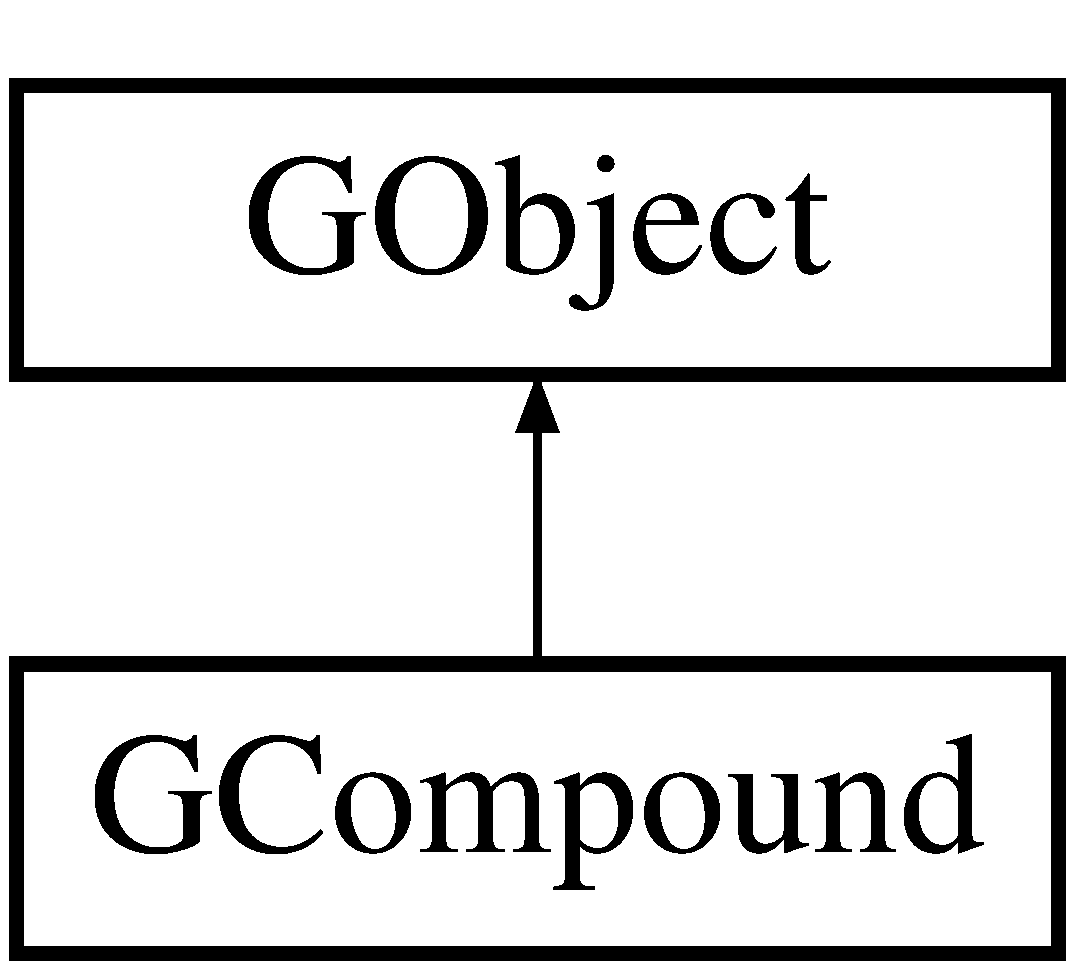
\includegraphics[height=2.000000cm]{classGCompound}
\end{center}
\end{figure}
\subsection*{Public Types}
\begin{DoxyCompactItemize}
\item 
enum \mbox{\hyperlink{classGObject_a86e0f5648542856159bb40775c854aa7}{Line\+Style}} \{ \mbox{\hyperlink{classGObject_a86e0f5648542856159bb40775c854aa7acbc84bd5232621834ed31f44d457c1eb}{L\+I\+N\+E\+\_\+\+N\+O\+NE}}, 
\mbox{\hyperlink{classGObject_a86e0f5648542856159bb40775c854aa7a700c78bc2cd76acaab26651bf7b4941f}{L\+I\+N\+E\+\_\+\+S\+O\+L\+ID}}, 
\mbox{\hyperlink{classGObject_a86e0f5648542856159bb40775c854aa7a9ccba0845f785d81d07b333ae1aad84e}{L\+I\+N\+E\+\_\+\+D\+A\+SH}}, 
\mbox{\hyperlink{classGObject_a86e0f5648542856159bb40775c854aa7a8e811c096cb941997f0bfda168bb6df3}{L\+I\+N\+E\+\_\+\+D\+OT}}, 
\mbox{\hyperlink{classGObject_a86e0f5648542856159bb40775c854aa7ada15a2e3d737b2db7706d8300f91b89d}{L\+I\+N\+E\+\_\+\+D\+A\+S\+H\+\_\+\+D\+OT}}, 
\mbox{\hyperlink{classGObject_a86e0f5648542856159bb40775c854aa7aabf4053a73eafa7ba2b7e6d664c74c1d}{L\+I\+N\+E\+\_\+\+D\+A\+S\+H\+\_\+\+D\+O\+T\+\_\+\+D\+OT}}
 \}
\begin{DoxyCompactList}\small\item\em Styles that can be used for the outline around various shapes. \end{DoxyCompactList}\end{DoxyCompactItemize}
\subsection*{Public Member Functions}
\begin{DoxyCompactItemize}
\item 
\mbox{\hyperlink{classGCompound_a96d2773de31d81df96135d8621cf47df}{G\+Compound}} ()
\begin{DoxyCompactList}\small\item\em Creates a compound with no internal components. \end{DoxyCompactList}\item 
virtual void \mbox{\hyperlink{classGCompound_afe8277e7b2627513c6f7452fb0b2847d}{add}} (\mbox{\hyperlink{classGObject}{G\+Object}} $\ast$gobj)
\begin{DoxyCompactList}\small\item\em Adds a new graphical object to the compound, if that object was not already present in the compound. \end{DoxyCompactList}\item 
virtual void \mbox{\hyperlink{classGCompound_a8bb36f245efc7806414a1339c2befa1c}{add}} (\mbox{\hyperlink{classGObject}{G\+Object}} $\ast$gobj, double x, double y)
\begin{DoxyCompactList}\small\item\em Adds a new graphical object to the compound, if that object was not already present in the compound. \end{DoxyCompactList}\item 
virtual void \mbox{\hyperlink{classGCompound_ac732fc2123d7a6d7e2de145fe9bbd8e8}{add}} (\mbox{\hyperlink{classGObject}{G\+Object}} \&gobj)
\begin{DoxyCompactList}\small\item\em Adds a new graphical object to the compound. \end{DoxyCompactList}\item 
virtual void \mbox{\hyperlink{classGCompound_a5b11b532869632a6c26b098b0858eac5}{add}} (\mbox{\hyperlink{classGObject}{G\+Object}} \&gobj, double x, double y)
\begin{DoxyCompactList}\small\item\em Adds a new graphical object to the compound, if that object was not already present in the compound. \end{DoxyCompactList}\item 
virtual void \mbox{\hyperlink{classGCompound_ac8bb3912a3ce86b15842e79d0b421204}{clear}} ()
\begin{DoxyCompactList}\small\item\em Removes all graphical objects from the compound. \end{DoxyCompactList}\item 
virtual void \mbox{\hyperlink{classGCompound_a221b3e75bb3d9d0bfea62b3364e6773b}{conditional\+Repaint}} ()
\begin{DoxyCompactList}\small\item\em Repaints the compound only if it needs to be repainted (if any of its contents have changed). \end{DoxyCompactList}\item 
virtual void \mbox{\hyperlink{classGCompound_aedd4b792311d946eeaf44b0de337a408}{conditional\+Repaint\+Region}} (int x, int y, int width, int height)
\begin{DoxyCompactList}\small\item\em Repaints the given rectangular region of the compound only if it needs to be repainted (if any of its contents have changed). \end{DoxyCompactList}\item 
virtual void \mbox{\hyperlink{classGCompound_a3932a12278752db368e24fa404e446aa}{conditional\+Repaint\+Region}} (const \mbox{\hyperlink{classGRectangle}{G\+Rectangle}} \&bounds)
\begin{DoxyCompactList}\small\item\em Repaints the given rectangular region of the compound only if it needs to be repainted (if any of its contents have changed). \end{DoxyCompactList}\item 
virtual bool \mbox{\hyperlink{classGObject_a1dbc9dafaae51958112dbe1267a1f547}{contains}} (const \mbox{\hyperlink{classGPoint}{G\+Point}} \&pt) const
\begin{DoxyCompactList}\small\item\em Returns {\ttfamily true} if the specified point is inside the object. \end{DoxyCompactList}\item 
virtual bool \mbox{\hyperlink{classGCompound_aa095a031ab22c150d2d75fdda1c3c8f5}{contains}} (double x, double y) const Q\+\_\+\+D\+E\+C\+L\+\_\+\+O\+V\+E\+R\+R\+I\+DE
\begin{DoxyCompactList}\small\item\em Returns {\ttfamily true} if the specified point is inside the object. \end{DoxyCompactList}\item 
virtual \mbox{\hyperlink{classGPoint}{G\+Point}} \mbox{\hyperlink{classGObject_a0d41183bf6b08de66fe3907551aab0d7}{get\+Bottom\+Right\+Location}} () const
\begin{DoxyCompactList}\small\item\em Returns the x/y coordinates of the bottom/right corner of the object. \end{DoxyCompactList}\item 
virtual double \mbox{\hyperlink{classGObject_a4316a2406c18e1c6d061fe51fd355490}{get\+BottomY}} () const
\begin{DoxyCompactList}\small\item\em Returns the {\itshape y}-\/coordinate of the bottom of the object. \end{DoxyCompactList}\item 
virtual \mbox{\hyperlink{classGRectangle}{G\+Rectangle}} \mbox{\hyperlink{classGCompound_a2f46ec8a3b533c690b3b3e56d4f34afe}{get\+Bounds}} () const Q\+\_\+\+D\+E\+C\+L\+\_\+\+O\+V\+E\+R\+R\+I\+DE
\begin{DoxyCompactList}\small\item\em Returns the bounding box of this object, which is defined to be the smallest rectangle that covers everything drawn by the figure. \end{DoxyCompactList}\item 
virtual \mbox{\hyperlink{classGPoint}{G\+Point}} \mbox{\hyperlink{classGObject_a0909472e91448470bccdb62ecfb95d8b}{get\+Center\+Location}} () const
\begin{DoxyCompactList}\small\item\em Returns the x/y-\/coordinates of the center of the object. \end{DoxyCompactList}\item 
virtual double \mbox{\hyperlink{classGObject_a04df74355b545e0543112d5b8d924176}{get\+CenterX}} () const
\begin{DoxyCompactList}\small\item\em Returns the {\itshape x}-\/coordinate of the center of the object. \end{DoxyCompactList}\item 
virtual double \mbox{\hyperlink{classGObject_acb3287a3d507025a26f54b895713b947}{get\+CenterY}} () const
\begin{DoxyCompactList}\small\item\em Returns the {\itshape y}-\/coordinate of the center of the object. \end{DoxyCompactList}\item 
virtual std\+::string \mbox{\hyperlink{classGObject_aa061dfa488c31e18549d64363c1d0e34}{get\+Color}} () const
\begin{DoxyCompactList}\small\item\em Returns the color used to display this object. \end{DoxyCompactList}\item 
virtual \mbox{\hyperlink{classGObject}{G\+Object}} $\ast$ \mbox{\hyperlink{classGCompound_abde388cc529d22bb5f7f4a54d56049d8}{get\+Element}} (int index) const
\begin{DoxyCompactList}\small\item\em Returns a pointer to the graphical object at the specified index, numbering from back to front in the {\itshape z} dimension. \end{DoxyCompactList}\item 
virtual \mbox{\hyperlink{classGObject}{G\+Object}} $\ast$ \mbox{\hyperlink{classGCompound_a25efa999eca5790ec26ef091b05f961c}{get\+Element\+At}} (double x, double y) const
\begin{DoxyCompactList}\small\item\em Returns a pointer to the first graphical object that contains the given (x, y) point, or a null pointer if no object in this compound touches it. \end{DoxyCompactList}\item 
virtual int \mbox{\hyperlink{classGCompound_adf7d37ec315f859648def92e6b32408f}{get\+Element\+Count}} () const
\begin{DoxyCompactList}\small\item\em Returns the number of graphical objects stored in the compound. \end{DoxyCompactList}\item 
virtual std\+::string \mbox{\hyperlink{classGObject_a76f6964a11fde7c78e9751be184e1a3c}{get\+Fill\+Color}} () const
\begin{DoxyCompactList}\small\item\em Returns the color used to display the filled region of this object. \end{DoxyCompactList}\item 
virtual double \mbox{\hyperlink{classGObject_a1e7e353362434072875264cf95629f99}{get\+Height}} () const
\begin{DoxyCompactList}\small\item\em Returns the height of this object, which is the same as the height of its bounding box. \end{DoxyCompactList}\item 
virtual \mbox{\hyperlink{classGObject_a86e0f5648542856159bb40775c854aa7}{Line\+Style}} \mbox{\hyperlink{classGObject_aaf1f5ea8281e5e3486662878d26f0a13}{get\+Line\+Style}} () const
\begin{DoxyCompactList}\small\item\em Returns the object\textquotesingle{}s style such as solid or dashed. \end{DoxyCompactList}\item 
virtual double \mbox{\hyperlink{classGObject_a85ff266dc3eb63d9f2d8e5a4487fd3c0}{get\+Line\+Width}} () const
\begin{DoxyCompactList}\small\item\em Returns the width of the line used to draw this object. \end{DoxyCompactList}\item 
virtual \mbox{\hyperlink{classGPoint}{G\+Point}} \mbox{\hyperlink{classGObject_a4f83802015511edeb63b892830812c11}{get\+Location}} () const
\begin{DoxyCompactList}\small\item\em Returns the location of the top-\/left corner of object. \end{DoxyCompactList}\item 
virtual double \mbox{\hyperlink{classGObject_a1ae3fc278cc5b71b9f2d96a8a83cdf26}{get\+Opacity}} () const
\begin{DoxyCompactList}\small\item\em Returns how opaque (non-\/transparent) this object will appear from 0.\+0 (completely transparent) to 1.\+0 (completely opaque, default). \end{DoxyCompactList}\item 
virtual \mbox{\hyperlink{classGCompound}{G\+Compound}} $\ast$ \mbox{\hyperlink{classGObject_a3e53cef70541b1a14eade4ad0984d0b4}{get\+Parent}} () const
\begin{DoxyCompactList}\small\item\em Returns a pointer to the {\ttfamily \mbox{\hyperlink{classGCompound}{G\+Compound}}} that contains this object. \end{DoxyCompactList}\item 
virtual double \mbox{\hyperlink{classGObject_a798cc79daaa10145b28f60bcdfdb0ee9}{get\+RightX}} () const
\begin{DoxyCompactList}\small\item\em Returns the {\itshape x}-\/coordinate of the right side of the object. \end{DoxyCompactList}\item 
virtual \mbox{\hyperlink{classGDimension}{G\+Dimension}} \mbox{\hyperlink{classGObject_a7b4eec96a2bdc6420695d5796a78eea9}{get\+Size}} () const
\begin{DoxyCompactList}\small\item\em Returns the size of the object as a {\ttfamily \mbox{\hyperlink{classGDimension}{G\+Dimension}}}. \end{DoxyCompactList}\item 
virtual std\+::string \mbox{\hyperlink{classGCompound_a9896d58fcfebbf1025aeeb5b8b9ede80}{get\+Type}} () const Q\+\_\+\+D\+E\+C\+L\+\_\+\+O\+V\+E\+R\+R\+I\+DE
\begin{DoxyCompactList}\small\item\em Returns the type of the object as a string, such as {\ttfamily \char`\"{}\+G\+Oval\char`\"{}} or {\ttfamily \char`\"{}\+G\+Rect\char`\"{}}. \end{DoxyCompactList}\item 
virtual double \mbox{\hyperlink{classGObject_a0ed2965abd4f5701d2cadf71239faf19}{get\+Width}} () const
\begin{DoxyCompactList}\small\item\em Returns the width of this object, which is equal to the width of the bounding box. \end{DoxyCompactList}\item 
virtual double \mbox{\hyperlink{classGObject_a344385751bee0720059403940d57a13e}{getX}} () const
\begin{DoxyCompactList}\small\item\em Returns the leftmost {\itshape x}-\/coordinate of the object. \end{DoxyCompactList}\item 
virtual double \mbox{\hyperlink{classGObject_aafa51c7f8f38a09febbb9ce7853f77b4}{getY}} () const
\begin{DoxyCompactList}\small\item\em Returns the topmost {\itshape y}-\/coordinate of the object. \end{DoxyCompactList}\item 
virtual bool \mbox{\hyperlink{classGCompound_a12c8d52ddfcaa5448ec4bace92ddee6c}{is\+Auto\+Repaint}} () const
\begin{DoxyCompactList}\small\item\em Returns whether the compound automatically repaints itself when its contents change. \end{DoxyCompactList}\item 
virtual bool \mbox{\hyperlink{classGCompound_acf82f9b2937375c7b1cf3dccb3df3312}{is\+Empty}} () const
\begin{DoxyCompactList}\small\item\em Returns true if the compound does not contain any graphical objects. \end{DoxyCompactList}\item 
virtual bool \mbox{\hyperlink{classGObject_a11c404f106940c201b6f326e0355c150}{is\+Filled}} () const
\begin{DoxyCompactList}\small\item\em Returns {\ttfamily true} if the object is filled with color. \end{DoxyCompactList}\item 
virtual bool \mbox{\hyperlink{classGObject_a9d8a6cfb13917785c143e74d40e4e2be}{is\+Visible}} () const
\begin{DoxyCompactList}\small\item\em Returns {\ttfamily true} if this object is visible on screen. \end{DoxyCompactList}\item 
virtual void \mbox{\hyperlink{classGObject_a5973d8dda83afb36e2c56855515be392}{move}} (double dx, double dy)
\begin{DoxyCompactList}\small\item\em Moves the object on the screen using the displacements {\ttfamily dx} and {\ttfamily dy}. \end{DoxyCompactList}\item 
virtual void \mbox{\hyperlink{classGCompound_a49dc57a2ce4caa354a5fff6acdde2e7d}{remove}} (\mbox{\hyperlink{classGObject}{G\+Object}} $\ast$gobj)
\begin{DoxyCompactList}\small\item\em Removes the specified object from the compound. \end{DoxyCompactList}\item 
virtual void \mbox{\hyperlink{classGCompound_a0c0ae4d69b584602ff3cba0d9cf330a4}{remove}} (\mbox{\hyperlink{classGObject}{G\+Object}} \&gobj)
\begin{DoxyCompactList}\small\item\em Removes the specified object from the compound. \end{DoxyCompactList}\item 
virtual void \mbox{\hyperlink{classGCompound_a9b0a5a3ad9972ab0e8eb0b54873aac6b}{remove\+All}} ()
\begin{DoxyCompactList}\small\item\em Removes all graphical objects from the compound. \end{DoxyCompactList}\item 
virtual void \mbox{\hyperlink{classGCompound_ac827b978aa122f136a14c198687ad80f}{repaint}} ()
\begin{DoxyCompactList}\small\item\em Instructs the compound to redraw all of its graphical objects. \end{DoxyCompactList}\item 
virtual void \mbox{\hyperlink{classGCompound_a4a919e3851ebfbf0f161a66cc15d4531}{repaint\+Region}} (int x, int y, int width, int height)
\begin{DoxyCompactList}\small\item\em Instructs the compound to redraw the given rectangular region within itself, including any graphical objects that touch that region. \end{DoxyCompactList}\item 
virtual void \mbox{\hyperlink{classGCompound_a769c46fb3e1004aec76e8b0adfa42aa6}{repaint\+Region}} (const \mbox{\hyperlink{classGRectangle}{G\+Rectangle}} \&bounds)
\begin{DoxyCompactList}\small\item\em Instructs the compound to redraw the given rectangular region within itself, including any graphical objects that touch that region. \end{DoxyCompactList}\item 
virtual void \mbox{\hyperlink{classGObject_a6022a1fd1e5dcd2fd5585e5a36aa3f37}{reset\+Transform}} ()
\begin{DoxyCompactList}\small\item\em Undoes any previous scale/rotate transformations on this object. \end{DoxyCompactList}\item 
virtual void \mbox{\hyperlink{classGObject_ae1ffaa12185dfd5ba464f7d87c329e26}{rotate}} (double theta)
\begin{DoxyCompactList}\small\item\em Transforms the object by rotating it {\ttfamily theta} degrees counterclockwise around its origin. \end{DoxyCompactList}\item 
virtual void \mbox{\hyperlink{classGObject_ad2e1900f730475c2d044817db03b38d6}{scale}} (double sf)
\begin{DoxyCompactList}\small\item\em Scales the object by the specified scale factor. \end{DoxyCompactList}\item 
virtual void \mbox{\hyperlink{classGObject_a63641f69d610d0b951357d35a0c3b1e3}{scale}} (double sx, double sy)
\begin{DoxyCompactList}\small\item\em Scales the object by the specified scale factors. \end{DoxyCompactList}\item 
void \mbox{\hyperlink{classGObject_ab6747f40313c531c2db32edb5b63b9b7}{send\+Backward}} ()
\begin{DoxyCompactList}\small\item\em Moves this object one step toward the back in the {\itshape z} dimension. \end{DoxyCompactList}\item 
void \mbox{\hyperlink{classGObject_a710b3e449c9facba7847c91ab170d281}{send\+Forward}} ()
\begin{DoxyCompactList}\small\item\em Moves this object one step toward the front in the {\itshape z} dimension. \end{DoxyCompactList}\item 
void \mbox{\hyperlink{classGObject_a0f7f1efbb7fd46dde2867c4ad0330896}{send\+To\+Back}} ()
\begin{DoxyCompactList}\small\item\em Moves this object to the back of the display in the {\itshape z} dimension. \end{DoxyCompactList}\item 
void \mbox{\hyperlink{classGObject_aee33d68488e46827ef55fac07f40a9b2}{send\+To\+Front}} ()
\begin{DoxyCompactList}\small\item\em Moves this object to the front of the display in the {\itshape z} dimension. \end{DoxyCompactList}\item 
virtual void \mbox{\hyperlink{classGCompound_adf10848319457bd6df4c657bf8872bee}{set\+Auto\+Repaint}} (bool auto\+Repaint)
\begin{DoxyCompactList}\small\item\em Sets whether the compound automatically repaints itself when its contents change. \end{DoxyCompactList}\item 
virtual void \mbox{\hyperlink{classGObject_a71ff7b16b8f1bdc4a1ce9f30cf8b87d8}{set\+Bottom\+Right\+Location}} (double x, double y)
\begin{DoxyCompactList}\small\item\em Sets the location of the bottom/right of this object. \end{DoxyCompactList}\item 
virtual void \mbox{\hyperlink{classGObject_ac6f7320321182f1d18c1c0fa97d5e941}{set\+Bottom\+Right\+Location}} (const \mbox{\hyperlink{classGPoint}{G\+Point}} \&pt)
\begin{DoxyCompactList}\small\item\em Sets the location of the bottom/right of this object. \end{DoxyCompactList}\item 
virtual void \mbox{\hyperlink{classGObject_a4b20e93c2a2597484f74ee5caa71f41f}{set\+BottomY}} (double y)
\begin{DoxyCompactList}\small\item\em Sets the location of the bottom y-\/coordinate of this object. \end{DoxyCompactList}\item 
virtual void \mbox{\hyperlink{classGObject_a2aae8197624b72265ab83b4f1bc73f2f}{set\+Bounds}} (double x, double y, double width, double height)
\begin{DoxyCompactList}\small\item\em Changes the bounds of this object to the specified values. \end{DoxyCompactList}\item 
virtual void \mbox{\hyperlink{classGObject_acada386653f008cacc7cce86426bef7c}{set\+Bounds}} (const \mbox{\hyperlink{classGRectangle}{G\+Rectangle}} \&size)
\begin{DoxyCompactList}\small\item\em Changes the bounds of this object to the specified rectangle. \end{DoxyCompactList}\item 
virtual void \mbox{\hyperlink{classGObject_a290b47dd8de1be44089f95cb2c47c1de}{set\+Center\+Location}} (double x, double y)
\begin{DoxyCompactList}\small\item\em Sets the location of the center of this object. \end{DoxyCompactList}\item 
virtual void \mbox{\hyperlink{classGObject_a1bedf1b233ecba3f753ec58908a683a6}{set\+Center\+Location}} (const \mbox{\hyperlink{classGPoint}{G\+Point}} \&pt)
\begin{DoxyCompactList}\small\item\em Sets the location of the center of this object. \end{DoxyCompactList}\item 
virtual void \mbox{\hyperlink{classGObject_a2f4936281e056eead00a9186b9ba8af6}{set\+CenterX}} (double x)
\begin{DoxyCompactList}\small\item\em Sets the x-\/coordinate of the center of this object. \end{DoxyCompactList}\item 
virtual void \mbox{\hyperlink{classGObject_aad2a22b4fde88c33306b92aebf641d57}{set\+CenterY}} (double y)
\begin{DoxyCompactList}\small\item\em Sets the y-\/coordinate of the center of this object. \end{DoxyCompactList}\item 
virtual void \mbox{\hyperlink{classGObject_ad57ef49bc31db94e92648aa3737923d6}{set\+Color}} (int r, int g, int b)
\begin{DoxyCompactList}\small\item\em Sets the color used to display this object. \end{DoxyCompactList}\item 
virtual void \mbox{\hyperlink{classGObject_ab1f5cc0f5cc6bbbd716a526c61f1081d}{set\+Color}} (int rgb)
\begin{DoxyCompactList}\small\item\em Sets the color used to display this object. \end{DoxyCompactList}\item 
virtual void \mbox{\hyperlink{classGObject_a61374df6c11b52cfbb0815decdbaebc6}{set\+Color}} (const std\+::string \&color)
\begin{DoxyCompactList}\small\item\em Sets the color used to display this object. \end{DoxyCompactList}\item 
virtual void \mbox{\hyperlink{classGObject_ad767a33971159e9493e221cca4c00ae9}{set\+Fill\+Color}} (int r, int g, int b)
\begin{DoxyCompactList}\small\item\em Sets the color used to display the filled region of this object, if any. \end{DoxyCompactList}\item 
virtual void \mbox{\hyperlink{classGObject_aa59d9775a67fa7df2b24a95cd34840a3}{set\+Fill\+Color}} (int rgb)
\begin{DoxyCompactList}\small\item\em Sets the color used to display the filled region of this object, if any. \end{DoxyCompactList}\item 
virtual void \mbox{\hyperlink{classGObject_adbc18b1a930aadd97d7437f9f7265b96}{set\+Fill\+Color}} (const std\+::string \&color)
\begin{DoxyCompactList}\small\item\em Sets the color used to display the filled region of this object, if any. \end{DoxyCompactList}\item 
virtual void \mbox{\hyperlink{classGObject_a9b82b53362282c6bb7d6947068d2e55b}{set\+Filled}} (bool flag)
\begin{DoxyCompactList}\small\item\em Sets the fill status for the object, where {\ttfamily false} is outlined and {\ttfamily true} is filled. \end{DoxyCompactList}\item 
virtual void \mbox{\hyperlink{classGObject_a2592348886ffea646c6534bf88f7c49d}{set\+Font}} (const Q\+Font \&font)
\begin{DoxyCompactList}\small\item\em Changes the font used to display the object as specified by the given Qt font. \end{DoxyCompactList}\item 
virtual void \mbox{\hyperlink{classGObject_a8e096e8818d838aceae1d46d58fb3a7b}{set\+Font}} (const std\+::string \&font)
\begin{DoxyCompactList}\small\item\em Changes the font used to display the object as specified by the string {\ttfamily font}, which has the following format\+: \end{DoxyCompactList}\item 
virtual void \mbox{\hyperlink{classGObject_ad18e8fab1e02a4e9b75c6730212558eb}{set\+Foreground}} (int r, int g, int b)
\begin{DoxyCompactList}\small\item\em Sets the color used to display this object. \end{DoxyCompactList}\item 
virtual void \mbox{\hyperlink{classGObject_a9eb856b5ff83a19df3831a31f15f4563}{set\+Foreground}} (int rgb)
\begin{DoxyCompactList}\small\item\em Sets the color used to display this object. \end{DoxyCompactList}\item 
virtual void \mbox{\hyperlink{classGObject_af59209aeadea6dfc6d97a2d8531f50e1}{set\+Foreground}} (const std\+::string \&color)
\begin{DoxyCompactList}\small\item\em Sets the color used to display this object. \end{DoxyCompactList}\item 
virtual void \mbox{\hyperlink{classGObject_a9e280bfc4544dfaf8e4376c4e1a74357}{set\+Height}} (double height)
\begin{DoxyCompactList}\small\item\em Changes the height of this object to the specified height without changing its width. \end{DoxyCompactList}\item 
virtual void \mbox{\hyperlink{classGObject_add11575087eb94f1a71faa3f826c6341}{set\+Line\+Style}} (\mbox{\hyperlink{classGObject_a86e0f5648542856159bb40775c854aa7}{Line\+Style}} line\+Style)
\begin{DoxyCompactList}\small\item\em Sets the object\textquotesingle{}s style such as solid (\mbox{\hyperlink{classGObject_a86e0f5648542856159bb40775c854aa7a700c78bc2cd76acaab26651bf7b4941f}{G\+Object\+::\+L\+I\+N\+E\+\_\+\+S\+O\+L\+ID}}) or dashed (\mbox{\hyperlink{classGObject_a86e0f5648542856159bb40775c854aa7a9ccba0845f785d81d07b333ae1aad84e}{G\+Object\+::\+L\+I\+N\+E\+\_\+\+D\+A\+SH}}). \end{DoxyCompactList}\item 
virtual void \mbox{\hyperlink{classGObject_afd6a47c6ea6a1f85ca05a65ba3ff3477}{set\+Line\+Width}} (double line\+Width)
\begin{DoxyCompactList}\small\item\em Sets the width of the line used to draw this object. \end{DoxyCompactList}\item 
virtual void \mbox{\hyperlink{classGObject_a04594e8ba9b98513a64f1da00dcae18c}{set\+Location}} (double x, double y)
\begin{DoxyCompactList}\small\item\em Sets the location of the top-\/left corner of this object to the specified coordinates. \end{DoxyCompactList}\item 
virtual void \mbox{\hyperlink{classGObject_aa8480c0b7166cdf8f784cece06ab353f}{set\+Location}} (const \mbox{\hyperlink{classGPoint}{G\+Point}} \&pt)
\begin{DoxyCompactList}\small\item\em Sets the location of the top-\/left corner of this object to the specified point. \end{DoxyCompactList}\item 
virtual void \mbox{\hyperlink{classGObject_a04af1866cc1bae4a1226695794a50539}{set\+Opacity}} (double opacity)
\begin{DoxyCompactList}\small\item\em Sets how opaque (non-\/transparent) this object will appear from 0.\+0 (completely transparent) to 1.\+0 (completely opaque, default). \end{DoxyCompactList}\item 
virtual void \mbox{\hyperlink{classGObject_a3c90b758cdc2c911c9ef76c4360eb912}{set\+RightX}} (double x)
\begin{DoxyCompactList}\small\item\em Sets the location of the rightmost x-\/coordinate of this object. \end{DoxyCompactList}\item 
virtual void \mbox{\hyperlink{classGObject_aca25d49481f9bf5fc8f7df4c086c4ce7}{set\+Size}} (double width, double height)
\begin{DoxyCompactList}\small\item\em Changes the size of this object to the specified width and height. \end{DoxyCompactList}\item 
virtual void \mbox{\hyperlink{classGObject_ae2b628228f192c2702c4ce941b2af68f}{set\+Size}} (const \mbox{\hyperlink{classGDimension}{G\+Dimension}} \&size)
\begin{DoxyCompactList}\small\item\em Changes the size of this object to the specified width and height. \end{DoxyCompactList}\item 
virtual void \mbox{\hyperlink{classGObject_a88203f28224315d9f4471212f4af8ed3}{set\+Visible}} (bool flag)
\begin{DoxyCompactList}\small\item\em Sets whether this object is visible. \end{DoxyCompactList}\item 
virtual void \mbox{\hyperlink{classGObject_aa3f3fba4cb131baa8696ba01e3bceca1}{set\+Width}} (double width)
\begin{DoxyCompactList}\small\item\em Changes the width of this object to the specified width without changing its height. \end{DoxyCompactList}\item 
virtual void \mbox{\hyperlink{classGObject_a9c18fcc579333bf9653d13ad2b372e39}{setX}} (double x)
\begin{DoxyCompactList}\small\item\em Sets the x location of the left side of this object. \end{DoxyCompactList}\item 
virtual void \mbox{\hyperlink{classGObject_a7d57e2a5c35d27feb58fd498a3cf82b9}{setY}} (double y)
\begin{DoxyCompactList}\small\item\em Sets the y location of the top of this object. \end{DoxyCompactList}\item 
virtual std\+::string \mbox{\hyperlink{classGCompound_add86bda25fd0c3b8edaedee9431b85e6}{to\+String}} () const Q\+\_\+\+D\+E\+C\+L\+\_\+\+O\+V\+E\+R\+R\+I\+DE
\begin{DoxyCompactList}\small\item\em Returns a printable representation of the object. \end{DoxyCompactList}\end{DoxyCompactItemize}
\subsection*{Static Public Member Functions}
\begin{DoxyCompactItemize}
\item 
static bool \mbox{\hyperlink{classGObject_a93be0e1fe1b1bf1a1da732470c94f42b}{is\+Anti\+Aliasing}} ()
\begin{DoxyCompactList}\small\item\em Returns whether we should globally anti-\/alias graphical objects. \end{DoxyCompactList}\item 
static void \mbox{\hyperlink{classGObject_a1e43371668ae850193cebedb44e1bbe3}{set\+Anti\+Aliasing}} (bool value)
\begin{DoxyCompactList}\small\item\em Globally turns on/off the anti-\/aliasing feature that smooths out the edges of onscreen shapes. \end{DoxyCompactList}\end{DoxyCompactItemize}
\subsection*{Protected Member Functions}
\begin{DoxyCompactItemize}
\item 
virtual std\+::string \mbox{\hyperlink{classGObject_a4fcdf8de5c6de92242a975d83d8f23ea}{to\+String\+Extra}} () const
\begin{DoxyCompactList}\small\item\em Returns a string containing any extra unique information about this type of graphical object. \end{DoxyCompactList}\end{DoxyCompactItemize}
\subsection*{Protected Attributes}
\begin{DoxyCompactItemize}
\item 
Q\+Brush \mbox{\hyperlink{classGObject_aab24462ec896b596d99911767b0912d0}{\+\_\+brush}}
\item 
std\+::string \mbox{\hyperlink{classGObject_a1134e770ae4315ea8bc1201e2f21da8b}{\+\_\+color}}
\item 
int \mbox{\hyperlink{classGObject_a003fdd343d9b7505c53a8b7a134200ed}{\+\_\+color\+Int}}
\item 
std\+::string \mbox{\hyperlink{classGObject_a179f8d6cee65cd8a54692e32b224392a}{\+\_\+fill\+Color}}
\item 
int \mbox{\hyperlink{classGObject_a751def333a67d651e5b99cc331ecb496}{\+\_\+fill\+Color\+Int}}
\item 
bool \mbox{\hyperlink{classGObject_ad4a55cbcd61b58a4d49666490bb2f103}{\+\_\+fill\+Flag}}
\item 
std\+::string \mbox{\hyperlink{classGObject_aea76ea1a8b5dd7b0a78653277e63b536}{\+\_\+font}}
\item 
double \mbox{\hyperlink{classGObject_ad05df29e7f27fc504abd743e3d8b4e73}{\+\_\+height}}
\item 
\mbox{\hyperlink{classGObject_a86e0f5648542856159bb40775c854aa7}{Line\+Style}} \mbox{\hyperlink{classGObject_a89bafecaafb7c72d55c7efc10b7d0523}{\+\_\+line\+Style}}
\item 
double \mbox{\hyperlink{classGObject_a16e9033665937f13de2e163dc2184aff}{\+\_\+line\+Width}}
\item 
double \mbox{\hyperlink{classGObject_a20eff8eb7af27182edc9bfc54768b6f3}{\+\_\+opacity}}
\item 
\mbox{\hyperlink{classGCompound}{G\+Compound}} $\ast$ \mbox{\hyperlink{classGObject_ac9452c1eaff70eebddbb318196aa3835}{\+\_\+parent}}
\item 
Q\+Pen \mbox{\hyperlink{classGObject_afb69d172743f868299847174eb1b6bc8}{\+\_\+pen}}
\item 
Q\+Transform \mbox{\hyperlink{classGObject_a475b8860a5f1adb4a1fdc58d1f5c1e32}{\+\_\+transform}}
\item 
bool \mbox{\hyperlink{classGObject_ae4725802fc8d8aaa0ab4bd4781f7e07c}{\+\_\+transformed}}
\item 
bool \mbox{\hyperlink{classGObject_a9312c72508471b7c7a87b540263e1af4}{\+\_\+visible}}
\item 
double \mbox{\hyperlink{classGObject_ab55d85a3371770e6725b1062cf160cd8}{\+\_\+width}}
\item 
double \mbox{\hyperlink{classGObject_a6675b83b27137b8d3aa2ad8133078ea6}{\+\_\+x}}
\item 
double \mbox{\hyperlink{classGObject_a2f0f6aeafddc8a39c578bfa7e22b5f1e}{\+\_\+y}}
\end{DoxyCompactItemize}


\subsection{Detailed Description}
This graphical object subclass consists of a collection of other graphical objects. 

Once assembled, the internal objects can be manipulated as a unit. The compound keeps track of its own position, and all items within it are drawn relative to that location. 

\subsection{Member Enumeration Documentation}
\mbox{\Hypertarget{classGObject_a86e0f5648542856159bb40775c854aa7}\label{classGObject_a86e0f5648542856159bb40775c854aa7}} 
\index{G\+Compound@{G\+Compound}!Line\+Style@{Line\+Style}}
\index{Line\+Style@{Line\+Style}!G\+Compound@{G\+Compound}}
\subsubsection{\texorpdfstring{Line\+Style}{LineStyle}}
{\footnotesize\ttfamily enum \mbox{\hyperlink{classGObject_a86e0f5648542856159bb40775c854aa7}{Line\+Style}}\hspace{0.3cm}{\ttfamily [inherited]}}



Styles that can be used for the outline around various shapes. 

Call set\+Line\+Style on a \mbox{\hyperlink{classGObject}{G\+Object}} and pass one of these values. \begin{DoxyEnumFields}{Enumerator}
\raisebox{\heightof{T}}[0pt][0pt]{\index{L\+I\+N\+E\+\_\+\+N\+O\+NE@{L\+I\+N\+E\+\_\+\+N\+O\+NE}!G\+Compound@{G\+Compound}}\index{G\+Compound@{G\+Compound}!L\+I\+N\+E\+\_\+\+N\+O\+NE@{L\+I\+N\+E\+\_\+\+N\+O\+NE}}}\mbox{\Hypertarget{classGObject_a86e0f5648542856159bb40775c854aa7acbc84bd5232621834ed31f44d457c1eb}\label{classGObject_a86e0f5648542856159bb40775c854aa7acbc84bd5232621834ed31f44d457c1eb}} 
L\+I\+N\+E\+\_\+\+N\+O\+NE&\\
\hline

\raisebox{\heightof{T}}[0pt][0pt]{\index{L\+I\+N\+E\+\_\+\+S\+O\+L\+ID@{L\+I\+N\+E\+\_\+\+S\+O\+L\+ID}!G\+Compound@{G\+Compound}}\index{G\+Compound@{G\+Compound}!L\+I\+N\+E\+\_\+\+S\+O\+L\+ID@{L\+I\+N\+E\+\_\+\+S\+O\+L\+ID}}}\mbox{\Hypertarget{classGObject_a86e0f5648542856159bb40775c854aa7a700c78bc2cd76acaab26651bf7b4941f}\label{classGObject_a86e0f5648542856159bb40775c854aa7a700c78bc2cd76acaab26651bf7b4941f}} 
L\+I\+N\+E\+\_\+\+S\+O\+L\+ID&\\
\hline

\raisebox{\heightof{T}}[0pt][0pt]{\index{L\+I\+N\+E\+\_\+\+D\+A\+SH@{L\+I\+N\+E\+\_\+\+D\+A\+SH}!G\+Compound@{G\+Compound}}\index{G\+Compound@{G\+Compound}!L\+I\+N\+E\+\_\+\+D\+A\+SH@{L\+I\+N\+E\+\_\+\+D\+A\+SH}}}\mbox{\Hypertarget{classGObject_a86e0f5648542856159bb40775c854aa7a9ccba0845f785d81d07b333ae1aad84e}\label{classGObject_a86e0f5648542856159bb40775c854aa7a9ccba0845f785d81d07b333ae1aad84e}} 
L\+I\+N\+E\+\_\+\+D\+A\+SH&\\
\hline

\raisebox{\heightof{T}}[0pt][0pt]{\index{L\+I\+N\+E\+\_\+\+D\+OT@{L\+I\+N\+E\+\_\+\+D\+OT}!G\+Compound@{G\+Compound}}\index{G\+Compound@{G\+Compound}!L\+I\+N\+E\+\_\+\+D\+OT@{L\+I\+N\+E\+\_\+\+D\+OT}}}\mbox{\Hypertarget{classGObject_a86e0f5648542856159bb40775c854aa7a8e811c096cb941997f0bfda168bb6df3}\label{classGObject_a86e0f5648542856159bb40775c854aa7a8e811c096cb941997f0bfda168bb6df3}} 
L\+I\+N\+E\+\_\+\+D\+OT&\\
\hline

\raisebox{\heightof{T}}[0pt][0pt]{\index{L\+I\+N\+E\+\_\+\+D\+A\+S\+H\+\_\+\+D\+OT@{L\+I\+N\+E\+\_\+\+D\+A\+S\+H\+\_\+\+D\+OT}!G\+Compound@{G\+Compound}}\index{G\+Compound@{G\+Compound}!L\+I\+N\+E\+\_\+\+D\+A\+S\+H\+\_\+\+D\+OT@{L\+I\+N\+E\+\_\+\+D\+A\+S\+H\+\_\+\+D\+OT}}}\mbox{\Hypertarget{classGObject_a86e0f5648542856159bb40775c854aa7ada15a2e3d737b2db7706d8300f91b89d}\label{classGObject_a86e0f5648542856159bb40775c854aa7ada15a2e3d737b2db7706d8300f91b89d}} 
L\+I\+N\+E\+\_\+\+D\+A\+S\+H\+\_\+\+D\+OT&\\
\hline

\raisebox{\heightof{T}}[0pt][0pt]{\index{L\+I\+N\+E\+\_\+\+D\+A\+S\+H\+\_\+\+D\+O\+T\+\_\+\+D\+OT@{L\+I\+N\+E\+\_\+\+D\+A\+S\+H\+\_\+\+D\+O\+T\+\_\+\+D\+OT}!G\+Compound@{G\+Compound}}\index{G\+Compound@{G\+Compound}!L\+I\+N\+E\+\_\+\+D\+A\+S\+H\+\_\+\+D\+O\+T\+\_\+\+D\+OT@{L\+I\+N\+E\+\_\+\+D\+A\+S\+H\+\_\+\+D\+O\+T\+\_\+\+D\+OT}}}\mbox{\Hypertarget{classGObject_a86e0f5648542856159bb40775c854aa7aabf4053a73eafa7ba2b7e6d664c74c1d}\label{classGObject_a86e0f5648542856159bb40775c854aa7aabf4053a73eafa7ba2b7e6d664c74c1d}} 
L\+I\+N\+E\+\_\+\+D\+A\+S\+H\+\_\+\+D\+O\+T\+\_\+\+D\+OT&\\
\hline

\end{DoxyEnumFields}


\subsection{Constructor \& Destructor Documentation}
\mbox{\Hypertarget{classGCompound_a96d2773de31d81df96135d8621cf47df}\label{classGCompound_a96d2773de31d81df96135d8621cf47df}} 
\index{G\+Compound@{G\+Compound}!G\+Compound@{G\+Compound}}
\index{G\+Compound@{G\+Compound}!G\+Compound@{G\+Compound}}
\subsubsection{\texorpdfstring{G\+Compound()}{GCompound()}}
{\footnotesize\ttfamily \mbox{\hyperlink{classGCompound}{G\+Compound}} (\begin{DoxyParamCaption}{ }\end{DoxyParamCaption})}



Creates a compound with no internal components. 



\subsection{Member Function Documentation}
\mbox{\Hypertarget{classGCompound_afe8277e7b2627513c6f7452fb0b2847d}\label{classGCompound_afe8277e7b2627513c6f7452fb0b2847d}} 
\index{G\+Compound@{G\+Compound}!add@{add}}
\index{add@{add}!G\+Compound@{G\+Compound}}
\subsubsection{\texorpdfstring{add()}{add()}\hspace{0.1cm}{\footnotesize\ttfamily [1/4]}}
{\footnotesize\ttfamily void add (\begin{DoxyParamCaption}\item[{\mbox{\hyperlink{classGObject}{G\+Object}} $\ast$}]{gobj }\end{DoxyParamCaption})\hspace{0.3cm}{\ttfamily [virtual]}}



Adds a new graphical object to the compound, if that object was not already present in the compound. 

If the object is already stored in this compound, has no effect. 
\begin{DoxyExceptions}{Exceptions}
{\em \mbox{\hyperlink{classErrorException}{Error\+Exception}}} & if the object is null \\
\hline
\end{DoxyExceptions}
\mbox{\Hypertarget{classGCompound_a8bb36f245efc7806414a1339c2befa1c}\label{classGCompound_a8bb36f245efc7806414a1339c2befa1c}} 
\index{G\+Compound@{G\+Compound}!add@{add}}
\index{add@{add}!G\+Compound@{G\+Compound}}
\subsubsection{\texorpdfstring{add()}{add()}\hspace{0.1cm}{\footnotesize\ttfamily [2/4]}}
{\footnotesize\ttfamily void add (\begin{DoxyParamCaption}\item[{\mbox{\hyperlink{classGObject}{G\+Object}} $\ast$}]{gobj,  }\item[{double}]{x,  }\item[{double}]{y }\end{DoxyParamCaption})\hspace{0.3cm}{\ttfamily [virtual]}}



Adds a new graphical object to the compound, if that object was not already present in the compound. 

This form moves the object to the point ({\ttfamily x}, {\ttfamily y}) first. If the object is already stored in this compound, has no effect. 
\begin{DoxyExceptions}{Exceptions}
{\em \mbox{\hyperlink{classErrorException}{Error\+Exception}}} & if the object is null \\
\hline
\end{DoxyExceptions}
\mbox{\Hypertarget{classGCompound_ac732fc2123d7a6d7e2de145fe9bbd8e8}\label{classGCompound_ac732fc2123d7a6d7e2de145fe9bbd8e8}} 
\index{G\+Compound@{G\+Compound}!add@{add}}
\index{add@{add}!G\+Compound@{G\+Compound}}
\subsubsection{\texorpdfstring{add()}{add()}\hspace{0.1cm}{\footnotesize\ttfamily [3/4]}}
{\footnotesize\ttfamily void add (\begin{DoxyParamCaption}\item[{\mbox{\hyperlink{classGObject}{G\+Object}} \&}]{gobj }\end{DoxyParamCaption})\hspace{0.3cm}{\ttfamily [virtual]}}



Adds a new graphical object to the compound. 

\mbox{\Hypertarget{classGCompound_a5b11b532869632a6c26b098b0858eac5}\label{classGCompound_a5b11b532869632a6c26b098b0858eac5}} 
\index{G\+Compound@{G\+Compound}!add@{add}}
\index{add@{add}!G\+Compound@{G\+Compound}}
\subsubsection{\texorpdfstring{add()}{add()}\hspace{0.1cm}{\footnotesize\ttfamily [4/4]}}
{\footnotesize\ttfamily void add (\begin{DoxyParamCaption}\item[{\mbox{\hyperlink{classGObject}{G\+Object}} \&}]{gobj,  }\item[{double}]{x,  }\item[{double}]{y }\end{DoxyParamCaption})\hspace{0.3cm}{\ttfamily [virtual]}}



Adds a new graphical object to the compound, if that object was not already present in the compound. 

This form moves the object to the point ({\ttfamily x}, {\ttfamily y}) first. If the object is already stored in this compound, has no effect. \mbox{\Hypertarget{classGCompound_ac8bb3912a3ce86b15842e79d0b421204}\label{classGCompound_ac8bb3912a3ce86b15842e79d0b421204}} 
\index{G\+Compound@{G\+Compound}!clear@{clear}}
\index{clear@{clear}!G\+Compound@{G\+Compound}}
\subsubsection{\texorpdfstring{clear()}{clear()}}
{\footnotesize\ttfamily void clear (\begin{DoxyParamCaption}{ }\end{DoxyParamCaption})\hspace{0.3cm}{\ttfamily [virtual]}}



Removes all graphical objects from the compound. 

Equivalent to remove\+All. \mbox{\Hypertarget{classGCompound_a221b3e75bb3d9d0bfea62b3364e6773b}\label{classGCompound_a221b3e75bb3d9d0bfea62b3364e6773b}} 
\index{G\+Compound@{G\+Compound}!conditional\+Repaint@{conditional\+Repaint}}
\index{conditional\+Repaint@{conditional\+Repaint}!G\+Compound@{G\+Compound}}
\subsubsection{\texorpdfstring{conditional\+Repaint()}{conditionalRepaint()}}
{\footnotesize\ttfamily void conditional\+Repaint (\begin{DoxyParamCaption}{ }\end{DoxyParamCaption})\hspace{0.3cm}{\ttfamily [virtual]}}



Repaints the compound only if it needs to be repainted (if any of its contents have changed). 

\mbox{\Hypertarget{classGCompound_aedd4b792311d946eeaf44b0de337a408}\label{classGCompound_aedd4b792311d946eeaf44b0de337a408}} 
\index{G\+Compound@{G\+Compound}!conditional\+Repaint\+Region@{conditional\+Repaint\+Region}}
\index{conditional\+Repaint\+Region@{conditional\+Repaint\+Region}!G\+Compound@{G\+Compound}}
\subsubsection{\texorpdfstring{conditional\+Repaint\+Region()}{conditionalRepaintRegion()}\hspace{0.1cm}{\footnotesize\ttfamily [1/2]}}
{\footnotesize\ttfamily void conditional\+Repaint\+Region (\begin{DoxyParamCaption}\item[{int}]{x,  }\item[{int}]{y,  }\item[{int}]{width,  }\item[{int}]{height }\end{DoxyParamCaption})\hspace{0.3cm}{\ttfamily [virtual]}}



Repaints the given rectangular region of the compound only if it needs to be repainted (if any of its contents have changed). 

\mbox{\Hypertarget{classGCompound_a3932a12278752db368e24fa404e446aa}\label{classGCompound_a3932a12278752db368e24fa404e446aa}} 
\index{G\+Compound@{G\+Compound}!conditional\+Repaint\+Region@{conditional\+Repaint\+Region}}
\index{conditional\+Repaint\+Region@{conditional\+Repaint\+Region}!G\+Compound@{G\+Compound}}
\subsubsection{\texorpdfstring{conditional\+Repaint\+Region()}{conditionalRepaintRegion()}\hspace{0.1cm}{\footnotesize\ttfamily [2/2]}}
{\footnotesize\ttfamily void conditional\+Repaint\+Region (\begin{DoxyParamCaption}\item[{const \mbox{\hyperlink{classGRectangle}{G\+Rectangle}} \&}]{bounds }\end{DoxyParamCaption})\hspace{0.3cm}{\ttfamily [virtual]}}



Repaints the given rectangular region of the compound only if it needs to be repainted (if any of its contents have changed). 

\mbox{\Hypertarget{classGObject_a1dbc9dafaae51958112dbe1267a1f547}\label{classGObject_a1dbc9dafaae51958112dbe1267a1f547}} 
\index{G\+Compound@{G\+Compound}!contains@{contains}}
\index{contains@{contains}!G\+Compound@{G\+Compound}}
\subsubsection{\texorpdfstring{contains()}{contains()}\hspace{0.1cm}{\footnotesize\ttfamily [1/2]}}
{\footnotesize\ttfamily bool contains (\begin{DoxyParamCaption}\item[{const \mbox{\hyperlink{classGPoint}{G\+Point}} \&}]{pt }\end{DoxyParamCaption}) const\hspace{0.3cm}{\ttfamily [virtual]}, {\ttfamily [inherited]}}



Returns {\ttfamily true} if the specified point is inside the object. 

\mbox{\Hypertarget{classGCompound_aa095a031ab22c150d2d75fdda1c3c8f5}\label{classGCompound_aa095a031ab22c150d2d75fdda1c3c8f5}} 
\index{G\+Compound@{G\+Compound}!contains@{contains}}
\index{contains@{contains}!G\+Compound@{G\+Compound}}
\subsubsection{\texorpdfstring{contains()}{contains()}\hspace{0.1cm}{\footnotesize\ttfamily [2/2]}}
{\footnotesize\ttfamily bool contains (\begin{DoxyParamCaption}\item[{double}]{x,  }\item[{double}]{y }\end{DoxyParamCaption}) const\hspace{0.3cm}{\ttfamily [virtual]}}



Returns {\ttfamily true} if the specified point is inside the object. 



Reimplemented from \mbox{\hyperlink{classGObject_abb6a5d7c03e6eaaae97264c4799ce7c3}{G\+Object}}.

\mbox{\Hypertarget{classGObject_a0d41183bf6b08de66fe3907551aab0d7}\label{classGObject_a0d41183bf6b08de66fe3907551aab0d7}} 
\index{G\+Compound@{G\+Compound}!get\+Bottom\+Right\+Location@{get\+Bottom\+Right\+Location}}
\index{get\+Bottom\+Right\+Location@{get\+Bottom\+Right\+Location}!G\+Compound@{G\+Compound}}
\subsubsection{\texorpdfstring{get\+Bottom\+Right\+Location()}{getBottomRightLocation()}}
{\footnotesize\ttfamily \mbox{\hyperlink{classGPoint}{G\+Point}} get\+Bottom\+Right\+Location (\begin{DoxyParamCaption}{ }\end{DoxyParamCaption}) const\hspace{0.3cm}{\ttfamily [virtual]}, {\ttfamily [inherited]}}



Returns the x/y coordinates of the bottom/right corner of the object. 

\mbox{\Hypertarget{classGObject_a4316a2406c18e1c6d061fe51fd355490}\label{classGObject_a4316a2406c18e1c6d061fe51fd355490}} 
\index{G\+Compound@{G\+Compound}!get\+BottomY@{get\+BottomY}}
\index{get\+BottomY@{get\+BottomY}!G\+Compound@{G\+Compound}}
\subsubsection{\texorpdfstring{get\+Bottom\+Y()}{getBottomY()}}
{\footnotesize\ttfamily double get\+BottomY (\begin{DoxyParamCaption}{ }\end{DoxyParamCaption}) const\hspace{0.3cm}{\ttfamily [virtual]}, {\ttfamily [inherited]}}



Returns the {\itshape y}-\/coordinate of the bottom of the object. 

Equivalent to the top y-\/coordinate plus the object\textquotesingle{}s height. \mbox{\Hypertarget{classGCompound_a2f46ec8a3b533c690b3b3e56d4f34afe}\label{classGCompound_a2f46ec8a3b533c690b3b3e56d4f34afe}} 
\index{G\+Compound@{G\+Compound}!get\+Bounds@{get\+Bounds}}
\index{get\+Bounds@{get\+Bounds}!G\+Compound@{G\+Compound}}
\subsubsection{\texorpdfstring{get\+Bounds()}{getBounds()}}
{\footnotesize\ttfamily \mbox{\hyperlink{classGRectangle}{G\+Rectangle}} get\+Bounds (\begin{DoxyParamCaption}{ }\end{DoxyParamCaption}) const\hspace{0.3cm}{\ttfamily [virtual]}}



Returns the bounding box of this object, which is defined to be the smallest rectangle that covers everything drawn by the figure. 

The coordinates of this rectangle do not necessarily match the location returned by {\ttfamily get\+Location}. Given a {\ttfamily \mbox{\hyperlink{classGText}{G\+Text}}} object, for example, {\ttfamily get\+Location} returns the coordinates of the point on the baseline at which the string begins; the {\ttfamily get\+Bounds} method, by contrast, returns a rectangle that covers the entire window area occupied by the string. 

Reimplemented from \mbox{\hyperlink{classGObject_a29e6ac35a0b48f491a4c88194cc5da3b}{G\+Object}}.

\mbox{\Hypertarget{classGObject_a0909472e91448470bccdb62ecfb95d8b}\label{classGObject_a0909472e91448470bccdb62ecfb95d8b}} 
\index{G\+Compound@{G\+Compound}!get\+Center\+Location@{get\+Center\+Location}}
\index{get\+Center\+Location@{get\+Center\+Location}!G\+Compound@{G\+Compound}}
\subsubsection{\texorpdfstring{get\+Center\+Location()}{getCenterLocation()}}
{\footnotesize\ttfamily \mbox{\hyperlink{classGPoint}{G\+Point}} get\+Center\+Location (\begin{DoxyParamCaption}{ }\end{DoxyParamCaption}) const\hspace{0.3cm}{\ttfamily [virtual]}, {\ttfamily [inherited]}}



Returns the x/y-\/coordinates of the center of the object. 

Equivalent to the top/left plus half the object\textquotesingle{}s size. \mbox{\Hypertarget{classGObject_a04df74355b545e0543112d5b8d924176}\label{classGObject_a04df74355b545e0543112d5b8d924176}} 
\index{G\+Compound@{G\+Compound}!get\+CenterX@{get\+CenterX}}
\index{get\+CenterX@{get\+CenterX}!G\+Compound@{G\+Compound}}
\subsubsection{\texorpdfstring{get\+Center\+X()}{getCenterX()}}
{\footnotesize\ttfamily double get\+CenterX (\begin{DoxyParamCaption}{ }\end{DoxyParamCaption}) const\hspace{0.3cm}{\ttfamily [virtual]}, {\ttfamily [inherited]}}



Returns the {\itshape x}-\/coordinate of the center of the object. 

Equivalent to the top/left plus half the object\textquotesingle{}s width. \mbox{\Hypertarget{classGObject_acb3287a3d507025a26f54b895713b947}\label{classGObject_acb3287a3d507025a26f54b895713b947}} 
\index{G\+Compound@{G\+Compound}!get\+CenterY@{get\+CenterY}}
\index{get\+CenterY@{get\+CenterY}!G\+Compound@{G\+Compound}}
\subsubsection{\texorpdfstring{get\+Center\+Y()}{getCenterY()}}
{\footnotesize\ttfamily double get\+CenterY (\begin{DoxyParamCaption}{ }\end{DoxyParamCaption}) const\hspace{0.3cm}{\ttfamily [virtual]}, {\ttfamily [inherited]}}



Returns the {\itshape y}-\/coordinate of the center of the object. 

Equivalent to the top/left plus half the object\textquotesingle{}s height. \mbox{\Hypertarget{classGObject_aa061dfa488c31e18549d64363c1d0e34}\label{classGObject_aa061dfa488c31e18549d64363c1d0e34}} 
\index{G\+Compound@{G\+Compound}!get\+Color@{get\+Color}}
\index{get\+Color@{get\+Color}!G\+Compound@{G\+Compound}}
\subsubsection{\texorpdfstring{get\+Color()}{getColor()}}
{\footnotesize\ttfamily std\+::string get\+Color (\begin{DoxyParamCaption}{ }\end{DoxyParamCaption}) const\hspace{0.3cm}{\ttfamily [virtual]}, {\ttfamily [inherited]}}



Returns the color used to display this object. 

This color is always returned as a string in the form {\ttfamily \char`\"{}\#rrggbb\char`\"{}}, where {\ttfamily rr}, {\ttfamily gg}, and {\ttfamily bb} are the red, green, and blue components of the color, expressed as two-\/digit hexadecimal values. \mbox{\Hypertarget{classGCompound_abde388cc529d22bb5f7f4a54d56049d8}\label{classGCompound_abde388cc529d22bb5f7f4a54d56049d8}} 
\index{G\+Compound@{G\+Compound}!get\+Element@{get\+Element}}
\index{get\+Element@{get\+Element}!G\+Compound@{G\+Compound}}
\subsubsection{\texorpdfstring{get\+Element()}{getElement()}}
{\footnotesize\ttfamily \mbox{\hyperlink{classGObject}{G\+Object}} $\ast$ get\+Element (\begin{DoxyParamCaption}\item[{int}]{index }\end{DoxyParamCaption}) const\hspace{0.3cm}{\ttfamily [virtual]}}



Returns a pointer to the graphical object at the specified index, numbering from back to front in the {\itshape z} dimension. 


\begin{DoxyExceptions}{Exceptions}
{\em \mbox{\hyperlink{classErrorException}{Error\+Exception}}} & if the index is out of range \\
\hline
\end{DoxyExceptions}
\mbox{\Hypertarget{classGCompound_a25efa999eca5790ec26ef091b05f961c}\label{classGCompound_a25efa999eca5790ec26ef091b05f961c}} 
\index{G\+Compound@{G\+Compound}!get\+Element\+At@{get\+Element\+At}}
\index{get\+Element\+At@{get\+Element\+At}!G\+Compound@{G\+Compound}}
\subsubsection{\texorpdfstring{get\+Element\+At()}{getElementAt()}}
{\footnotesize\ttfamily \mbox{\hyperlink{classGObject}{G\+Object}} $\ast$ get\+Element\+At (\begin{DoxyParamCaption}\item[{double}]{x,  }\item[{double}]{y }\end{DoxyParamCaption}) const\hspace{0.3cm}{\ttfamily [virtual]}}



Returns a pointer to the first graphical object that contains the given (x, y) point, or a null pointer if no object in this compound touches it. 

\mbox{\Hypertarget{classGCompound_adf7d37ec315f859648def92e6b32408f}\label{classGCompound_adf7d37ec315f859648def92e6b32408f}} 
\index{G\+Compound@{G\+Compound}!get\+Element\+Count@{get\+Element\+Count}}
\index{get\+Element\+Count@{get\+Element\+Count}!G\+Compound@{G\+Compound}}
\subsubsection{\texorpdfstring{get\+Element\+Count()}{getElementCount()}}
{\footnotesize\ttfamily int get\+Element\+Count (\begin{DoxyParamCaption}{ }\end{DoxyParamCaption}) const\hspace{0.3cm}{\ttfamily [virtual]}}



Returns the number of graphical objects stored in the compound. 

\mbox{\Hypertarget{classGObject_a76f6964a11fde7c78e9751be184e1a3c}\label{classGObject_a76f6964a11fde7c78e9751be184e1a3c}} 
\index{G\+Compound@{G\+Compound}!get\+Fill\+Color@{get\+Fill\+Color}}
\index{get\+Fill\+Color@{get\+Fill\+Color}!G\+Compound@{G\+Compound}}
\subsubsection{\texorpdfstring{get\+Fill\+Color()}{getFillColor()}}
{\footnotesize\ttfamily std\+::string get\+Fill\+Color (\begin{DoxyParamCaption}{ }\end{DoxyParamCaption}) const\hspace{0.3cm}{\ttfamily [virtual]}, {\ttfamily [inherited]}}



Returns the color used to display the filled region of this object. 

If none has been set, returns the empty string. \mbox{\Hypertarget{classGObject_a1e7e353362434072875264cf95629f99}\label{classGObject_a1e7e353362434072875264cf95629f99}} 
\index{G\+Compound@{G\+Compound}!get\+Height@{get\+Height}}
\index{get\+Height@{get\+Height}!G\+Compound@{G\+Compound}}
\subsubsection{\texorpdfstring{get\+Height()}{getHeight()}}
{\footnotesize\ttfamily double get\+Height (\begin{DoxyParamCaption}{ }\end{DoxyParamCaption}) const\hspace{0.3cm}{\ttfamily [virtual]}, {\ttfamily [inherited]}}



Returns the height of this object, which is the same as the height of its bounding box. 



Reimplemented in \mbox{\hyperlink{classGPolygon_a1e7e353362434072875264cf95629f99}{G\+Polygon}}, and \mbox{\hyperlink{classGLine_a423f17d4aeb66feb0d148fd23af335b7}{G\+Line}}.

\mbox{\Hypertarget{classGObject_aaf1f5ea8281e5e3486662878d26f0a13}\label{classGObject_aaf1f5ea8281e5e3486662878d26f0a13}} 
\index{G\+Compound@{G\+Compound}!get\+Line\+Style@{get\+Line\+Style}}
\index{get\+Line\+Style@{get\+Line\+Style}!G\+Compound@{G\+Compound}}
\subsubsection{\texorpdfstring{get\+Line\+Style()}{getLineStyle()}}
{\footnotesize\ttfamily \mbox{\hyperlink{classGObject_a86e0f5648542856159bb40775c854aa7}{G\+Object\+::\+Line\+Style}} get\+Line\+Style (\begin{DoxyParamCaption}{ }\end{DoxyParamCaption}) const\hspace{0.3cm}{\ttfamily [virtual]}, {\ttfamily [inherited]}}



Returns the object\textquotesingle{}s style such as solid or dashed. 

\mbox{\Hypertarget{classGObject_a85ff266dc3eb63d9f2d8e5a4487fd3c0}\label{classGObject_a85ff266dc3eb63d9f2d8e5a4487fd3c0}} 
\index{G\+Compound@{G\+Compound}!get\+Line\+Width@{get\+Line\+Width}}
\index{get\+Line\+Width@{get\+Line\+Width}!G\+Compound@{G\+Compound}}
\subsubsection{\texorpdfstring{get\+Line\+Width()}{getLineWidth()}}
{\footnotesize\ttfamily double get\+Line\+Width (\begin{DoxyParamCaption}{ }\end{DoxyParamCaption}) const\hspace{0.3cm}{\ttfamily [virtual]}, {\ttfamily [inherited]}}



Returns the width of the line used to draw this object. 

\begin{DoxyReturn}{Returns}
default 1 
\end{DoxyReturn}
\mbox{\Hypertarget{classGObject_a4f83802015511edeb63b892830812c11}\label{classGObject_a4f83802015511edeb63b892830812c11}} 
\index{G\+Compound@{G\+Compound}!get\+Location@{get\+Location}}
\index{get\+Location@{get\+Location}!G\+Compound@{G\+Compound}}
\subsubsection{\texorpdfstring{get\+Location()}{getLocation()}}
{\footnotesize\ttfamily \mbox{\hyperlink{classGPoint}{G\+Point}} get\+Location (\begin{DoxyParamCaption}{ }\end{DoxyParamCaption}) const\hspace{0.3cm}{\ttfamily [virtual]}, {\ttfamily [inherited]}}



Returns the location of the top-\/left corner of object. 

\mbox{\Hypertarget{classGObject_a1ae3fc278cc5b71b9f2d96a8a83cdf26}\label{classGObject_a1ae3fc278cc5b71b9f2d96a8a83cdf26}} 
\index{G\+Compound@{G\+Compound}!get\+Opacity@{get\+Opacity}}
\index{get\+Opacity@{get\+Opacity}!G\+Compound@{G\+Compound}}
\subsubsection{\texorpdfstring{get\+Opacity()}{getOpacity()}}
{\footnotesize\ttfamily double get\+Opacity (\begin{DoxyParamCaption}{ }\end{DoxyParamCaption}) const\hspace{0.3cm}{\ttfamily [virtual]}, {\ttfamily [inherited]}}



Returns how opaque (non-\/transparent) this object will appear from 0.\+0 (completely transparent) to 1.\+0 (completely opaque, default). 

\mbox{\Hypertarget{classGObject_a3e53cef70541b1a14eade4ad0984d0b4}\label{classGObject_a3e53cef70541b1a14eade4ad0984d0b4}} 
\index{G\+Compound@{G\+Compound}!get\+Parent@{get\+Parent}}
\index{get\+Parent@{get\+Parent}!G\+Compound@{G\+Compound}}
\subsubsection{\texorpdfstring{get\+Parent()}{getParent()}}
{\footnotesize\ttfamily \mbox{\hyperlink{classGCompound}{G\+Compound}} $\ast$ get\+Parent (\begin{DoxyParamCaption}{ }\end{DoxyParamCaption}) const\hspace{0.3cm}{\ttfamily [virtual]}, {\ttfamily [inherited]}}



Returns a pointer to the {\ttfamily \mbox{\hyperlink{classGCompound}{G\+Compound}}} that contains this object. 

Every {\ttfamily \mbox{\hyperlink{classGWindow}{G\+Window}}} is initialized to contain a single {\ttfamily \mbox{\hyperlink{classGCompound}{G\+Compound}}} that is aligned with the window. Adding objects to the window adds them to that {\ttfamily \mbox{\hyperlink{classGCompound}{G\+Compound}}}, which means that every object you add to the window has a parent. Calling {\ttfamily get\+Parent} on the top-\/level {\ttfamily \mbox{\hyperlink{classGCompound}{G\+Compound}}} returns {\ttfamily nullptr}. \mbox{\Hypertarget{classGObject_a798cc79daaa10145b28f60bcdfdb0ee9}\label{classGObject_a798cc79daaa10145b28f60bcdfdb0ee9}} 
\index{G\+Compound@{G\+Compound}!get\+RightX@{get\+RightX}}
\index{get\+RightX@{get\+RightX}!G\+Compound@{G\+Compound}}
\subsubsection{\texorpdfstring{get\+Right\+X()}{getRightX()}}
{\footnotesize\ttfamily double get\+RightX (\begin{DoxyParamCaption}{ }\end{DoxyParamCaption}) const\hspace{0.3cm}{\ttfamily [virtual]}, {\ttfamily [inherited]}}



Returns the {\itshape x}-\/coordinate of the right side of the object. 

Equivalent to the left x-\/coordinate plus the object\textquotesingle{}s width. \mbox{\Hypertarget{classGObject_a7b4eec96a2bdc6420695d5796a78eea9}\label{classGObject_a7b4eec96a2bdc6420695d5796a78eea9}} 
\index{G\+Compound@{G\+Compound}!get\+Size@{get\+Size}}
\index{get\+Size@{get\+Size}!G\+Compound@{G\+Compound}}
\subsubsection{\texorpdfstring{get\+Size()}{getSize()}}
{\footnotesize\ttfamily \mbox{\hyperlink{classGDimension}{G\+Dimension}} get\+Size (\begin{DoxyParamCaption}{ }\end{DoxyParamCaption}) const\hspace{0.3cm}{\ttfamily [virtual]}, {\ttfamily [inherited]}}



Returns the size of the object as a {\ttfamily \mbox{\hyperlink{classGDimension}{G\+Dimension}}}. 

\mbox{\Hypertarget{classGCompound_a9896d58fcfebbf1025aeeb5b8b9ede80}\label{classGCompound_a9896d58fcfebbf1025aeeb5b8b9ede80}} 
\index{G\+Compound@{G\+Compound}!get\+Type@{get\+Type}}
\index{get\+Type@{get\+Type}!G\+Compound@{G\+Compound}}
\subsubsection{\texorpdfstring{get\+Type()}{getType()}}
{\footnotesize\ttfamily std\+::string get\+Type (\begin{DoxyParamCaption}{ }\end{DoxyParamCaption}) const\hspace{0.3cm}{\ttfamily [virtual]}}



Returns the type of the object as a string, such as {\ttfamily \char`\"{}\+G\+Oval\char`\"{}} or {\ttfamily \char`\"{}\+G\+Rect\char`\"{}}. 

Each \mbox{\hyperlink{classGObject}{G\+Object}} subtype must override this method. 

Implements \mbox{\hyperlink{classGObject_a799e073a127b428cc841086d42ea4fed}{G\+Object}}.

\mbox{\Hypertarget{classGObject_a0ed2965abd4f5701d2cadf71239faf19}\label{classGObject_a0ed2965abd4f5701d2cadf71239faf19}} 
\index{G\+Compound@{G\+Compound}!get\+Width@{get\+Width}}
\index{get\+Width@{get\+Width}!G\+Compound@{G\+Compound}}
\subsubsection{\texorpdfstring{get\+Width()}{getWidth()}}
{\footnotesize\ttfamily double get\+Width (\begin{DoxyParamCaption}{ }\end{DoxyParamCaption}) const\hspace{0.3cm}{\ttfamily [virtual]}, {\ttfamily [inherited]}}



Returns the width of this object, which is equal to the width of the bounding box. 



Reimplemented in \mbox{\hyperlink{classGPolygon_a0ed2965abd4f5701d2cadf71239faf19}{G\+Polygon}}, and \mbox{\hyperlink{classGLine_a04bee94b66c8f921cd8611be2460ba9d}{G\+Line}}.

\mbox{\Hypertarget{classGObject_a344385751bee0720059403940d57a13e}\label{classGObject_a344385751bee0720059403940d57a13e}} 
\index{G\+Compound@{G\+Compound}!getX@{getX}}
\index{getX@{getX}!G\+Compound@{G\+Compound}}
\subsubsection{\texorpdfstring{get\+X()}{getX()}}
{\footnotesize\ttfamily double getX (\begin{DoxyParamCaption}{ }\end{DoxyParamCaption}) const\hspace{0.3cm}{\ttfamily [virtual]}, {\ttfamily [inherited]}}



Returns the leftmost {\itshape x}-\/coordinate of the object. 

\mbox{\Hypertarget{classGObject_aafa51c7f8f38a09febbb9ce7853f77b4}\label{classGObject_aafa51c7f8f38a09febbb9ce7853f77b4}} 
\index{G\+Compound@{G\+Compound}!getY@{getY}}
\index{getY@{getY}!G\+Compound@{G\+Compound}}
\subsubsection{\texorpdfstring{get\+Y()}{getY()}}
{\footnotesize\ttfamily double getY (\begin{DoxyParamCaption}{ }\end{DoxyParamCaption}) const\hspace{0.3cm}{\ttfamily [virtual]}, {\ttfamily [inherited]}}



Returns the topmost {\itshape y}-\/coordinate of the object. 

\mbox{\Hypertarget{classGObject_a93be0e1fe1b1bf1a1da732470c94f42b}\label{classGObject_a93be0e1fe1b1bf1a1da732470c94f42b}} 
\index{G\+Compound@{G\+Compound}!is\+Anti\+Aliasing@{is\+Anti\+Aliasing}}
\index{is\+Anti\+Aliasing@{is\+Anti\+Aliasing}!G\+Compound@{G\+Compound}}
\subsubsection{\texorpdfstring{is\+Anti\+Aliasing()}{isAntiAliasing()}}
{\footnotesize\ttfamily bool is\+Anti\+Aliasing (\begin{DoxyParamCaption}{ }\end{DoxyParamCaption})\hspace{0.3cm}{\ttfamily [static]}, {\ttfamily [inherited]}}



Returns whether we should globally anti-\/alias graphical objects. 

On by default. \mbox{\Hypertarget{classGCompound_a12c8d52ddfcaa5448ec4bace92ddee6c}\label{classGCompound_a12c8d52ddfcaa5448ec4bace92ddee6c}} 
\index{G\+Compound@{G\+Compound}!is\+Auto\+Repaint@{is\+Auto\+Repaint}}
\index{is\+Auto\+Repaint@{is\+Auto\+Repaint}!G\+Compound@{G\+Compound}}
\subsubsection{\texorpdfstring{is\+Auto\+Repaint()}{isAutoRepaint()}}
{\footnotesize\ttfamily bool is\+Auto\+Repaint (\begin{DoxyParamCaption}{ }\end{DoxyParamCaption}) const\hspace{0.3cm}{\ttfamily [virtual]}}



Returns whether the compound automatically repaints itself when its contents change. 

\mbox{\Hypertarget{classGCompound_acf82f9b2937375c7b1cf3dccb3df3312}\label{classGCompound_acf82f9b2937375c7b1cf3dccb3df3312}} 
\index{G\+Compound@{G\+Compound}!is\+Empty@{is\+Empty}}
\index{is\+Empty@{is\+Empty}!G\+Compound@{G\+Compound}}
\subsubsection{\texorpdfstring{is\+Empty()}{isEmpty()}}
{\footnotesize\ttfamily bool is\+Empty (\begin{DoxyParamCaption}{ }\end{DoxyParamCaption}) const\hspace{0.3cm}{\ttfamily [virtual]}}



Returns true if the compound does not contain any graphical objects. 

\mbox{\Hypertarget{classGObject_a11c404f106940c201b6f326e0355c150}\label{classGObject_a11c404f106940c201b6f326e0355c150}} 
\index{G\+Compound@{G\+Compound}!is\+Filled@{is\+Filled}}
\index{is\+Filled@{is\+Filled}!G\+Compound@{G\+Compound}}
\subsubsection{\texorpdfstring{is\+Filled()}{isFilled()}}
{\footnotesize\ttfamily bool is\+Filled (\begin{DoxyParamCaption}{ }\end{DoxyParamCaption}) const\hspace{0.3cm}{\ttfamily [virtual]}, {\ttfamily [inherited]}}



Returns {\ttfamily true} if the object is filled with color. 

\mbox{\Hypertarget{classGObject_a9d8a6cfb13917785c143e74d40e4e2be}\label{classGObject_a9d8a6cfb13917785c143e74d40e4e2be}} 
\index{G\+Compound@{G\+Compound}!is\+Visible@{is\+Visible}}
\index{is\+Visible@{is\+Visible}!G\+Compound@{G\+Compound}}
\subsubsection{\texorpdfstring{is\+Visible()}{isVisible()}}
{\footnotesize\ttfamily bool is\+Visible (\begin{DoxyParamCaption}{ }\end{DoxyParamCaption}) const\hspace{0.3cm}{\ttfamily [virtual]}, {\ttfamily [inherited]}}



Returns {\ttfamily true} if this object is visible on screen. 

\mbox{\Hypertarget{classGObject_a5973d8dda83afb36e2c56855515be392}\label{classGObject_a5973d8dda83afb36e2c56855515be392}} 
\index{G\+Compound@{G\+Compound}!move@{move}}
\index{move@{move}!G\+Compound@{G\+Compound}}
\subsubsection{\texorpdfstring{move()}{move()}}
{\footnotesize\ttfamily void move (\begin{DoxyParamCaption}\item[{double}]{dx,  }\item[{double}]{dy }\end{DoxyParamCaption})\hspace{0.3cm}{\ttfamily [virtual]}, {\ttfamily [inherited]}}



Moves the object on the screen using the displacements {\ttfamily dx} and {\ttfamily dy}. 

\mbox{\Hypertarget{classGCompound_a49dc57a2ce4caa354a5fff6acdde2e7d}\label{classGCompound_a49dc57a2ce4caa354a5fff6acdde2e7d}} 
\index{G\+Compound@{G\+Compound}!remove@{remove}}
\index{remove@{remove}!G\+Compound@{G\+Compound}}
\subsubsection{\texorpdfstring{remove()}{remove()}\hspace{0.1cm}{\footnotesize\ttfamily [1/2]}}
{\footnotesize\ttfamily void remove (\begin{DoxyParamCaption}\item[{\mbox{\hyperlink{classGObject}{G\+Object}} $\ast$}]{gobj }\end{DoxyParamCaption})\hspace{0.3cm}{\ttfamily [virtual]}}



Removes the specified object from the compound. 


\begin{DoxyExceptions}{Exceptions}
{\em \mbox{\hyperlink{classErrorException}{Error\+Exception}}} & if the object is null \\
\hline
\end{DoxyExceptions}
\mbox{\Hypertarget{classGCompound_a0c0ae4d69b584602ff3cba0d9cf330a4}\label{classGCompound_a0c0ae4d69b584602ff3cba0d9cf330a4}} 
\index{G\+Compound@{G\+Compound}!remove@{remove}}
\index{remove@{remove}!G\+Compound@{G\+Compound}}
\subsubsection{\texorpdfstring{remove()}{remove()}\hspace{0.1cm}{\footnotesize\ttfamily [2/2]}}
{\footnotesize\ttfamily void remove (\begin{DoxyParamCaption}\item[{\mbox{\hyperlink{classGObject}{G\+Object}} \&}]{gobj }\end{DoxyParamCaption})\hspace{0.3cm}{\ttfamily [virtual]}}



Removes the specified object from the compound. 

\mbox{\Hypertarget{classGCompound_a9b0a5a3ad9972ab0e8eb0b54873aac6b}\label{classGCompound_a9b0a5a3ad9972ab0e8eb0b54873aac6b}} 
\index{G\+Compound@{G\+Compound}!remove\+All@{remove\+All}}
\index{remove\+All@{remove\+All}!G\+Compound@{G\+Compound}}
\subsubsection{\texorpdfstring{remove\+All()}{removeAll()}}
{\footnotesize\ttfamily void remove\+All (\begin{DoxyParamCaption}{ }\end{DoxyParamCaption})\hspace{0.3cm}{\ttfamily [virtual]}}



Removes all graphical objects from the compound. 

Equivalent to clear. \mbox{\Hypertarget{classGCompound_ac827b978aa122f136a14c198687ad80f}\label{classGCompound_ac827b978aa122f136a14c198687ad80f}} 
\index{G\+Compound@{G\+Compound}!repaint@{repaint}}
\index{repaint@{repaint}!G\+Compound@{G\+Compound}}
\subsubsection{\texorpdfstring{repaint()}{repaint()}}
{\footnotesize\ttfamily void repaint (\begin{DoxyParamCaption}{ }\end{DoxyParamCaption})\hspace{0.3cm}{\ttfamily [virtual]}}



Instructs the compound to redraw all of its graphical objects. 



Reimplemented from \mbox{\hyperlink{classGObject_ac827b978aa122f136a14c198687ad80f}{G\+Object}}.

\mbox{\Hypertarget{classGCompound_a4a919e3851ebfbf0f161a66cc15d4531}\label{classGCompound_a4a919e3851ebfbf0f161a66cc15d4531}} 
\index{G\+Compound@{G\+Compound}!repaint\+Region@{repaint\+Region}}
\index{repaint\+Region@{repaint\+Region}!G\+Compound@{G\+Compound}}
\subsubsection{\texorpdfstring{repaint\+Region()}{repaintRegion()}\hspace{0.1cm}{\footnotesize\ttfamily [1/2]}}
{\footnotesize\ttfamily void repaint\+Region (\begin{DoxyParamCaption}\item[{int}]{x,  }\item[{int}]{y,  }\item[{int}]{width,  }\item[{int}]{height }\end{DoxyParamCaption})\hspace{0.3cm}{\ttfamily [virtual]}}



Instructs the compound to redraw the given rectangular region within itself, including any graphical objects that touch that region. 

\mbox{\Hypertarget{classGCompound_a769c46fb3e1004aec76e8b0adfa42aa6}\label{classGCompound_a769c46fb3e1004aec76e8b0adfa42aa6}} 
\index{G\+Compound@{G\+Compound}!repaint\+Region@{repaint\+Region}}
\index{repaint\+Region@{repaint\+Region}!G\+Compound@{G\+Compound}}
\subsubsection{\texorpdfstring{repaint\+Region()}{repaintRegion()}\hspace{0.1cm}{\footnotesize\ttfamily [2/2]}}
{\footnotesize\ttfamily void repaint\+Region (\begin{DoxyParamCaption}\item[{const \mbox{\hyperlink{classGRectangle}{G\+Rectangle}} \&}]{bounds }\end{DoxyParamCaption})\hspace{0.3cm}{\ttfamily [virtual]}}



Instructs the compound to redraw the given rectangular region within itself, including any graphical objects that touch that region. 

\mbox{\Hypertarget{classGObject_a6022a1fd1e5dcd2fd5585e5a36aa3f37}\label{classGObject_a6022a1fd1e5dcd2fd5585e5a36aa3f37}} 
\index{G\+Compound@{G\+Compound}!reset\+Transform@{reset\+Transform}}
\index{reset\+Transform@{reset\+Transform}!G\+Compound@{G\+Compound}}
\subsubsection{\texorpdfstring{reset\+Transform()}{resetTransform()}}
{\footnotesize\ttfamily void reset\+Transform (\begin{DoxyParamCaption}{ }\end{DoxyParamCaption})\hspace{0.3cm}{\ttfamily [virtual]}, {\ttfamily [inherited]}}



Undoes any previous scale/rotate transformations on this object. 

\mbox{\Hypertarget{classGObject_ae1ffaa12185dfd5ba464f7d87c329e26}\label{classGObject_ae1ffaa12185dfd5ba464f7d87c329e26}} 
\index{G\+Compound@{G\+Compound}!rotate@{rotate}}
\index{rotate@{rotate}!G\+Compound@{G\+Compound}}
\subsubsection{\texorpdfstring{rotate()}{rotate()}}
{\footnotesize\ttfamily void rotate (\begin{DoxyParamCaption}\item[{double}]{theta }\end{DoxyParamCaption})\hspace{0.3cm}{\ttfamily [virtual]}, {\ttfamily [inherited]}}



Transforms the object by rotating it {\ttfamily theta} degrees counterclockwise around its origin. 

\mbox{\Hypertarget{classGObject_ad2e1900f730475c2d044817db03b38d6}\label{classGObject_ad2e1900f730475c2d044817db03b38d6}} 
\index{G\+Compound@{G\+Compound}!scale@{scale}}
\index{scale@{scale}!G\+Compound@{G\+Compound}}
\subsubsection{\texorpdfstring{scale()}{scale()}\hspace{0.1cm}{\footnotesize\ttfamily [1/2]}}
{\footnotesize\ttfamily void scale (\begin{DoxyParamCaption}\item[{double}]{sf }\end{DoxyParamCaption})\hspace{0.3cm}{\ttfamily [virtual]}, {\ttfamily [inherited]}}



Scales the object by the specified scale factor. 

This form scales the object by {\ttfamily sf} in both dimensions, so that invoking {\ttfamily gobj-\/$>$scale(2);} doubles the size of the object. \mbox{\Hypertarget{classGObject_a63641f69d610d0b951357d35a0c3b1e3}\label{classGObject_a63641f69d610d0b951357d35a0c3b1e3}} 
\index{G\+Compound@{G\+Compound}!scale@{scale}}
\index{scale@{scale}!G\+Compound@{G\+Compound}}
\subsubsection{\texorpdfstring{scale()}{scale()}\hspace{0.1cm}{\footnotesize\ttfamily [2/2]}}
{\footnotesize\ttfamily void scale (\begin{DoxyParamCaption}\item[{double}]{sx,  }\item[{double}]{sy }\end{DoxyParamCaption})\hspace{0.3cm}{\ttfamily [virtual]}, {\ttfamily [inherited]}}



Scales the object by the specified scale factors. 

For example, {\ttfamily gobj-\/$>$scale(2, 2);} doubles the size of the object. This form applies independent scale factors to the {\itshape x} and {\itshape y} dimensions. \mbox{\Hypertarget{classGObject_ab6747f40313c531c2db32edb5b63b9b7}\label{classGObject_ab6747f40313c531c2db32edb5b63b9b7}} 
\index{G\+Compound@{G\+Compound}!send\+Backward@{send\+Backward}}
\index{send\+Backward@{send\+Backward}!G\+Compound@{G\+Compound}}
\subsubsection{\texorpdfstring{send\+Backward()}{sendBackward()}}
{\footnotesize\ttfamily void send\+Backward (\begin{DoxyParamCaption}{ }\end{DoxyParamCaption})\hspace{0.3cm}{\ttfamily [inherited]}}



Moves this object one step toward the back in the {\itshape z} dimension. 

If it was already at the back of the stack, nothing happens. \mbox{\Hypertarget{classGObject_a710b3e449c9facba7847c91ab170d281}\label{classGObject_a710b3e449c9facba7847c91ab170d281}} 
\index{G\+Compound@{G\+Compound}!send\+Forward@{send\+Forward}}
\index{send\+Forward@{send\+Forward}!G\+Compound@{G\+Compound}}
\subsubsection{\texorpdfstring{send\+Forward()}{sendForward()}}
{\footnotesize\ttfamily void send\+Forward (\begin{DoxyParamCaption}{ }\end{DoxyParamCaption})\hspace{0.3cm}{\ttfamily [inherited]}}



Moves this object one step toward the front in the {\itshape z} dimension. 

If it was already at the front of the stack, nothing happens. \mbox{\Hypertarget{classGObject_a0f7f1efbb7fd46dde2867c4ad0330896}\label{classGObject_a0f7f1efbb7fd46dde2867c4ad0330896}} 
\index{G\+Compound@{G\+Compound}!send\+To\+Back@{send\+To\+Back}}
\index{send\+To\+Back@{send\+To\+Back}!G\+Compound@{G\+Compound}}
\subsubsection{\texorpdfstring{send\+To\+Back()}{sendToBack()}}
{\footnotesize\ttfamily void send\+To\+Back (\begin{DoxyParamCaption}{ }\end{DoxyParamCaption})\hspace{0.3cm}{\ttfamily [inherited]}}



Moves this object to the back of the display in the {\itshape z} dimension. 

By moving it to the back, this object will appear to be behind the other graphical objects on the display and may be obscured by other objects in front. \mbox{\Hypertarget{classGObject_aee33d68488e46827ef55fac07f40a9b2}\label{classGObject_aee33d68488e46827ef55fac07f40a9b2}} 
\index{G\+Compound@{G\+Compound}!send\+To\+Front@{send\+To\+Front}}
\index{send\+To\+Front@{send\+To\+Front}!G\+Compound@{G\+Compound}}
\subsubsection{\texorpdfstring{send\+To\+Front()}{sendToFront()}}
{\footnotesize\ttfamily void send\+To\+Front (\begin{DoxyParamCaption}{ }\end{DoxyParamCaption})\hspace{0.3cm}{\ttfamily [inherited]}}



Moves this object to the front of the display in the {\itshape z} dimension. 

By moving it to the front, this object will appear to be on top of the other graphical objects on the display and may hide any objects that are further back. \mbox{\Hypertarget{classGObject_a1e43371668ae850193cebedb44e1bbe3}\label{classGObject_a1e43371668ae850193cebedb44e1bbe3}} 
\index{G\+Compound@{G\+Compound}!set\+Anti\+Aliasing@{set\+Anti\+Aliasing}}
\index{set\+Anti\+Aliasing@{set\+Anti\+Aliasing}!G\+Compound@{G\+Compound}}
\subsubsection{\texorpdfstring{set\+Anti\+Aliasing()}{setAntiAliasing()}}
{\footnotesize\ttfamily void set\+Anti\+Aliasing (\begin{DoxyParamCaption}\item[{bool}]{value }\end{DoxyParamCaption})\hspace{0.3cm}{\ttfamily [static]}, {\ttfamily [inherited]}}



Globally turns on/off the anti-\/aliasing feature that smooths out the edges of onscreen shapes. 

On by default. Does not repaint any onscreen objects when called; you must do this yourself. \mbox{\Hypertarget{classGCompound_adf10848319457bd6df4c657bf8872bee}\label{classGCompound_adf10848319457bd6df4c657bf8872bee}} 
\index{G\+Compound@{G\+Compound}!set\+Auto\+Repaint@{set\+Auto\+Repaint}}
\index{set\+Auto\+Repaint@{set\+Auto\+Repaint}!G\+Compound@{G\+Compound}}
\subsubsection{\texorpdfstring{set\+Auto\+Repaint()}{setAutoRepaint()}}
{\footnotesize\ttfamily void set\+Auto\+Repaint (\begin{DoxyParamCaption}\item[{bool}]{auto\+Repaint }\end{DoxyParamCaption})\hspace{0.3cm}{\ttfamily [virtual]}}



Sets whether the compound automatically repaints itself when its contents change. 

\mbox{\Hypertarget{classGObject_a71ff7b16b8f1bdc4a1ce9f30cf8b87d8}\label{classGObject_a71ff7b16b8f1bdc4a1ce9f30cf8b87d8}} 
\index{G\+Compound@{G\+Compound}!set\+Bottom\+Right\+Location@{set\+Bottom\+Right\+Location}}
\index{set\+Bottom\+Right\+Location@{set\+Bottom\+Right\+Location}!G\+Compound@{G\+Compound}}
\subsubsection{\texorpdfstring{set\+Bottom\+Right\+Location()}{setBottomRightLocation()}\hspace{0.1cm}{\footnotesize\ttfamily [1/2]}}
{\footnotesize\ttfamily void set\+Bottom\+Right\+Location (\begin{DoxyParamCaption}\item[{double}]{x,  }\item[{double}]{y }\end{DoxyParamCaption})\hspace{0.3cm}{\ttfamily [virtual]}, {\ttfamily [inherited]}}



Sets the location of the bottom/right of this object. 

\mbox{\Hypertarget{classGObject_ac6f7320321182f1d18c1c0fa97d5e941}\label{classGObject_ac6f7320321182f1d18c1c0fa97d5e941}} 
\index{G\+Compound@{G\+Compound}!set\+Bottom\+Right\+Location@{set\+Bottom\+Right\+Location}}
\index{set\+Bottom\+Right\+Location@{set\+Bottom\+Right\+Location}!G\+Compound@{G\+Compound}}
\subsubsection{\texorpdfstring{set\+Bottom\+Right\+Location()}{setBottomRightLocation()}\hspace{0.1cm}{\footnotesize\ttfamily [2/2]}}
{\footnotesize\ttfamily void set\+Bottom\+Right\+Location (\begin{DoxyParamCaption}\item[{const \mbox{\hyperlink{classGPoint}{G\+Point}} \&}]{pt }\end{DoxyParamCaption})\hspace{0.3cm}{\ttfamily [virtual]}, {\ttfamily [inherited]}}



Sets the location of the bottom/right of this object. 

\mbox{\Hypertarget{classGObject_a4b20e93c2a2597484f74ee5caa71f41f}\label{classGObject_a4b20e93c2a2597484f74ee5caa71f41f}} 
\index{G\+Compound@{G\+Compound}!set\+BottomY@{set\+BottomY}}
\index{set\+BottomY@{set\+BottomY}!G\+Compound@{G\+Compound}}
\subsubsection{\texorpdfstring{set\+Bottom\+Y()}{setBottomY()}}
{\footnotesize\ttfamily void set\+BottomY (\begin{DoxyParamCaption}\item[{double}]{y }\end{DoxyParamCaption})\hspace{0.3cm}{\ttfamily [virtual]}, {\ttfamily [inherited]}}



Sets the location of the bottom y-\/coordinate of this object. 

\mbox{\Hypertarget{classGObject_a2aae8197624b72265ab83b4f1bc73f2f}\label{classGObject_a2aae8197624b72265ab83b4f1bc73f2f}} 
\index{G\+Compound@{G\+Compound}!set\+Bounds@{set\+Bounds}}
\index{set\+Bounds@{set\+Bounds}!G\+Compound@{G\+Compound}}
\subsubsection{\texorpdfstring{set\+Bounds()}{setBounds()}\hspace{0.1cm}{\footnotesize\ttfamily [1/2]}}
{\footnotesize\ttfamily void set\+Bounds (\begin{DoxyParamCaption}\item[{double}]{x,  }\item[{double}]{y,  }\item[{double}]{width,  }\item[{double}]{height }\end{DoxyParamCaption})\hspace{0.3cm}{\ttfamily [virtual]}, {\ttfamily [inherited]}}



Changes the bounds of this object to the specified values. 

\mbox{\Hypertarget{classGObject_acada386653f008cacc7cce86426bef7c}\label{classGObject_acada386653f008cacc7cce86426bef7c}} 
\index{G\+Compound@{G\+Compound}!set\+Bounds@{set\+Bounds}}
\index{set\+Bounds@{set\+Bounds}!G\+Compound@{G\+Compound}}
\subsubsection{\texorpdfstring{set\+Bounds()}{setBounds()}\hspace{0.1cm}{\footnotesize\ttfamily [2/2]}}
{\footnotesize\ttfamily void set\+Bounds (\begin{DoxyParamCaption}\item[{const \mbox{\hyperlink{classGRectangle}{G\+Rectangle}} \&}]{size }\end{DoxyParamCaption})\hspace{0.3cm}{\ttfamily [virtual]}, {\ttfamily [inherited]}}



Changes the bounds of this object to the specified rectangle. 

\mbox{\Hypertarget{classGObject_a290b47dd8de1be44089f95cb2c47c1de}\label{classGObject_a290b47dd8de1be44089f95cb2c47c1de}} 
\index{G\+Compound@{G\+Compound}!set\+Center\+Location@{set\+Center\+Location}}
\index{set\+Center\+Location@{set\+Center\+Location}!G\+Compound@{G\+Compound}}
\subsubsection{\texorpdfstring{set\+Center\+Location()}{setCenterLocation()}\hspace{0.1cm}{\footnotesize\ttfamily [1/2]}}
{\footnotesize\ttfamily void set\+Center\+Location (\begin{DoxyParamCaption}\item[{double}]{x,  }\item[{double}]{y }\end{DoxyParamCaption})\hspace{0.3cm}{\ttfamily [virtual]}, {\ttfamily [inherited]}}



Sets the location of the center of this object. 

\mbox{\Hypertarget{classGObject_a1bedf1b233ecba3f753ec58908a683a6}\label{classGObject_a1bedf1b233ecba3f753ec58908a683a6}} 
\index{G\+Compound@{G\+Compound}!set\+Center\+Location@{set\+Center\+Location}}
\index{set\+Center\+Location@{set\+Center\+Location}!G\+Compound@{G\+Compound}}
\subsubsection{\texorpdfstring{set\+Center\+Location()}{setCenterLocation()}\hspace{0.1cm}{\footnotesize\ttfamily [2/2]}}
{\footnotesize\ttfamily void set\+Center\+Location (\begin{DoxyParamCaption}\item[{const \mbox{\hyperlink{classGPoint}{G\+Point}} \&}]{pt }\end{DoxyParamCaption})\hspace{0.3cm}{\ttfamily [virtual]}, {\ttfamily [inherited]}}



Sets the location of the center of this object. 

\mbox{\Hypertarget{classGObject_a2f4936281e056eead00a9186b9ba8af6}\label{classGObject_a2f4936281e056eead00a9186b9ba8af6}} 
\index{G\+Compound@{G\+Compound}!set\+CenterX@{set\+CenterX}}
\index{set\+CenterX@{set\+CenterX}!G\+Compound@{G\+Compound}}
\subsubsection{\texorpdfstring{set\+Center\+X()}{setCenterX()}}
{\footnotesize\ttfamily void set\+CenterX (\begin{DoxyParamCaption}\item[{double}]{x }\end{DoxyParamCaption})\hspace{0.3cm}{\ttfamily [virtual]}, {\ttfamily [inherited]}}



Sets the x-\/coordinate of the center of this object. 

\mbox{\Hypertarget{classGObject_aad2a22b4fde88c33306b92aebf641d57}\label{classGObject_aad2a22b4fde88c33306b92aebf641d57}} 
\index{G\+Compound@{G\+Compound}!set\+CenterY@{set\+CenterY}}
\index{set\+CenterY@{set\+CenterY}!G\+Compound@{G\+Compound}}
\subsubsection{\texorpdfstring{set\+Center\+Y()}{setCenterY()}}
{\footnotesize\ttfamily void set\+CenterY (\begin{DoxyParamCaption}\item[{double}]{y }\end{DoxyParamCaption})\hspace{0.3cm}{\ttfamily [virtual]}, {\ttfamily [inherited]}}



Sets the y-\/coordinate of the center of this object. 

\mbox{\Hypertarget{classGObject_ad57ef49bc31db94e92648aa3737923d6}\label{classGObject_ad57ef49bc31db94e92648aa3737923d6}} 
\index{G\+Compound@{G\+Compound}!set\+Color@{set\+Color}}
\index{set\+Color@{set\+Color}!G\+Compound@{G\+Compound}}
\subsubsection{\texorpdfstring{set\+Color()}{setColor()}\hspace{0.1cm}{\footnotesize\ttfamily [1/3]}}
{\footnotesize\ttfamily void set\+Color (\begin{DoxyParamCaption}\item[{int}]{r,  }\item[{int}]{g,  }\item[{int}]{b }\end{DoxyParamCaption})\hspace{0.3cm}{\ttfamily [virtual]}, {\ttfamily [inherited]}}



Sets the color used to display this object. 

See \mbox{\hyperlink{gcolor_8h_source}{gcolor.\+h}} for more detail about how to specify colors.

Equivalent to set\+Foreground.


\begin{DoxyParams}{Parameters}
{\em r} & redness from 0-\/255 \\
\hline
{\em g} & greenness from 0-\/255 \\
\hline
{\em b} & blueness from 0-\/255 \\
\hline
\end{DoxyParams}
\mbox{\Hypertarget{classGObject_ab1f5cc0f5cc6bbbd716a526c61f1081d}\label{classGObject_ab1f5cc0f5cc6bbbd716a526c61f1081d}} 
\index{G\+Compound@{G\+Compound}!set\+Color@{set\+Color}}
\index{set\+Color@{set\+Color}!G\+Compound@{G\+Compound}}
\subsubsection{\texorpdfstring{set\+Color()}{setColor()}\hspace{0.1cm}{\footnotesize\ttfamily [2/3]}}
{\footnotesize\ttfamily void set\+Color (\begin{DoxyParamCaption}\item[{int}]{rgb }\end{DoxyParamCaption})\hspace{0.3cm}{\ttfamily [virtual]}, {\ttfamily [inherited]}}



Sets the color used to display this object. 

See \mbox{\hyperlink{gcolor_8h_source}{gcolor.\+h}} for more detail about how to specify colors.

Equivalent to set\+Foreground.


\begin{DoxyParams}{Parameters}
{\em rgb} & an R\+GB integer value such as 0x7700ff \\
\hline
\end{DoxyParams}
\mbox{\Hypertarget{classGObject_a61374df6c11b52cfbb0815decdbaebc6}\label{classGObject_a61374df6c11b52cfbb0815decdbaebc6}} 
\index{G\+Compound@{G\+Compound}!set\+Color@{set\+Color}}
\index{set\+Color@{set\+Color}!G\+Compound@{G\+Compound}}
\subsubsection{\texorpdfstring{set\+Color()}{setColor()}\hspace{0.1cm}{\footnotesize\ttfamily [3/3]}}
{\footnotesize\ttfamily void set\+Color (\begin{DoxyParamCaption}\item[{const std\+::string \&}]{color }\end{DoxyParamCaption})\hspace{0.3cm}{\ttfamily [virtual]}, {\ttfamily [inherited]}}



Sets the color used to display this object. 

See \mbox{\hyperlink{gcolor_8h_source}{gcolor.\+h}} for more detail about how to specify colors.

Equivalent to set\+Foreground.

a color string such as \char`\"{}\#7700ff\char`\"{} or \char`\"{}purple\char`\"{} \mbox{\Hypertarget{classGObject_ad767a33971159e9493e221cca4c00ae9}\label{classGObject_ad767a33971159e9493e221cca4c00ae9}} 
\index{G\+Compound@{G\+Compound}!set\+Fill\+Color@{set\+Fill\+Color}}
\index{set\+Fill\+Color@{set\+Fill\+Color}!G\+Compound@{G\+Compound}}
\subsubsection{\texorpdfstring{set\+Fill\+Color()}{setFillColor()}\hspace{0.1cm}{\footnotesize\ttfamily [1/3]}}
{\footnotesize\ttfamily void set\+Fill\+Color (\begin{DoxyParamCaption}\item[{int}]{r,  }\item[{int}]{g,  }\item[{int}]{b }\end{DoxyParamCaption})\hspace{0.3cm}{\ttfamily [virtual]}, {\ttfamily [inherited]}}



Sets the color used to display the filled region of this object, if any. 

As a side effect, sets this object to be filled (set\+Filled(true)). See \mbox{\hyperlink{gcolor_8h_source}{gcolor.\+h}} for more detail about how to specify colors. If an empty string is passed, sets filled to false.


\begin{DoxyParams}{Parameters}
{\em r} & redness from 0-\/255 \\
\hline
{\em g} & greenness from 0-\/255 \\
\hline
{\em b} & blueness from 0-\/255 \\
\hline
\end{DoxyParams}
\mbox{\Hypertarget{classGObject_aa59d9775a67fa7df2b24a95cd34840a3}\label{classGObject_aa59d9775a67fa7df2b24a95cd34840a3}} 
\index{G\+Compound@{G\+Compound}!set\+Fill\+Color@{set\+Fill\+Color}}
\index{set\+Fill\+Color@{set\+Fill\+Color}!G\+Compound@{G\+Compound}}
\subsubsection{\texorpdfstring{set\+Fill\+Color()}{setFillColor()}\hspace{0.1cm}{\footnotesize\ttfamily [2/3]}}
{\footnotesize\ttfamily void set\+Fill\+Color (\begin{DoxyParamCaption}\item[{int}]{rgb }\end{DoxyParamCaption})\hspace{0.3cm}{\ttfamily [virtual]}, {\ttfamily [inherited]}}



Sets the color used to display the filled region of this object, if any. 

As a side effect, sets this object to be filled (set\+Filled(true)). See \mbox{\hyperlink{gcolor_8h_source}{gcolor.\+h}} for more detail about how to specify colors.


\begin{DoxyParams}{Parameters}
{\em rgb} & an R\+GB integer value such as 0x7700ff \\
\hline
\end{DoxyParams}
\mbox{\Hypertarget{classGObject_adbc18b1a930aadd97d7437f9f7265b96}\label{classGObject_adbc18b1a930aadd97d7437f9f7265b96}} 
\index{G\+Compound@{G\+Compound}!set\+Fill\+Color@{set\+Fill\+Color}}
\index{set\+Fill\+Color@{set\+Fill\+Color}!G\+Compound@{G\+Compound}}
\subsubsection{\texorpdfstring{set\+Fill\+Color()}{setFillColor()}\hspace{0.1cm}{\footnotesize\ttfamily [3/3]}}
{\footnotesize\ttfamily void set\+Fill\+Color (\begin{DoxyParamCaption}\item[{const std\+::string \&}]{color }\end{DoxyParamCaption})\hspace{0.3cm}{\ttfamily [virtual]}, {\ttfamily [inherited]}}



Sets the color used to display the filled region of this object, if any. 

As a side effect, sets this object to be filled (set\+Filled(true)). See \mbox{\hyperlink{gcolor_8h_source}{gcolor.\+h}} for more detail about how to specify colors. If an empty string is passed, sets filled to false.

a color string such as \char`\"{}\#7700ff\char`\"{} or \char`\"{}purple\char`\"{} \mbox{\Hypertarget{classGObject_a9b82b53362282c6bb7d6947068d2e55b}\label{classGObject_a9b82b53362282c6bb7d6947068d2e55b}} 
\index{G\+Compound@{G\+Compound}!set\+Filled@{set\+Filled}}
\index{set\+Filled@{set\+Filled}!G\+Compound@{G\+Compound}}
\subsubsection{\texorpdfstring{set\+Filled()}{setFilled()}}
{\footnotesize\ttfamily void set\+Filled (\begin{DoxyParamCaption}\item[{bool}]{flag }\end{DoxyParamCaption})\hspace{0.3cm}{\ttfamily [virtual]}, {\ttfamily [inherited]}}



Sets the fill status for the object, where {\ttfamily false} is outlined and {\ttfamily true} is filled. 

\mbox{\Hypertarget{classGObject_a2592348886ffea646c6534bf88f7c49d}\label{classGObject_a2592348886ffea646c6534bf88f7c49d}} 
\index{G\+Compound@{G\+Compound}!set\+Font@{set\+Font}}
\index{set\+Font@{set\+Font}!G\+Compound@{G\+Compound}}
\subsubsection{\texorpdfstring{set\+Font()}{setFont()}\hspace{0.1cm}{\footnotesize\ttfamily [1/2]}}
{\footnotesize\ttfamily void set\+Font (\begin{DoxyParamCaption}\item[{const Q\+Font \&}]{font }\end{DoxyParamCaption})\hspace{0.3cm}{\ttfamily [virtual]}, {\ttfamily [inherited]}}



Changes the font used to display the object as specified by the given Qt font. 

See \mbox{\hyperlink{gfont_8h_source}{gfont.\+h}} for more detail about how to specify fonts. 

Reimplemented in \mbox{\hyperlink{classGText_a2d22014c7fa3bccfd58c982aea1b55fa}{G\+Text}}.

\mbox{\Hypertarget{classGObject_a8e096e8818d838aceae1d46d58fb3a7b}\label{classGObject_a8e096e8818d838aceae1d46d58fb3a7b}} 
\index{G\+Compound@{G\+Compound}!set\+Font@{set\+Font}}
\index{set\+Font@{set\+Font}!G\+Compound@{G\+Compound}}
\subsubsection{\texorpdfstring{set\+Font()}{setFont()}\hspace{0.1cm}{\footnotesize\ttfamily [2/2]}}
{\footnotesize\ttfamily void set\+Font (\begin{DoxyParamCaption}\item[{const std\+::string \&}]{font }\end{DoxyParamCaption})\hspace{0.3cm}{\ttfamily [virtual]}, {\ttfamily [inherited]}}



Changes the font used to display the object as specified by the string {\ttfamily font}, which has the following format\+: 


\begin{DoxyPre}
"family-style-size"
\end{DoxyPre}


where both {\ttfamily style} and {\ttfamily size} are optional. If any of these elements are missing or specified as an asterisk, the existing value is retained. See \mbox{\hyperlink{gfont_8h_source}{gfont.\+h}} for more detail about how to specify fonts. 

Reimplemented in \mbox{\hyperlink{classGText_ab39ef411fb13a52852ddd138c5932e2e}{G\+Text}}.

\mbox{\Hypertarget{classGObject_ad18e8fab1e02a4e9b75c6730212558eb}\label{classGObject_ad18e8fab1e02a4e9b75c6730212558eb}} 
\index{G\+Compound@{G\+Compound}!set\+Foreground@{set\+Foreground}}
\index{set\+Foreground@{set\+Foreground}!G\+Compound@{G\+Compound}}
\subsubsection{\texorpdfstring{set\+Foreground()}{setForeground()}\hspace{0.1cm}{\footnotesize\ttfamily [1/3]}}
{\footnotesize\ttfamily void set\+Foreground (\begin{DoxyParamCaption}\item[{int}]{r,  }\item[{int}]{g,  }\item[{int}]{b }\end{DoxyParamCaption})\hspace{0.3cm}{\ttfamily [virtual]}, {\ttfamily [inherited]}}



Sets the color used to display this object. 

See \mbox{\hyperlink{gcolor_8h_source}{gcolor.\+h}} for more detail about how to specify colors.

Equivalent to set\+Color.


\begin{DoxyParams}{Parameters}
{\em r} & redness from 0-\/255 \\
\hline
{\em g} & greenness from 0-\/255 \\
\hline
{\em b} & blueness from 0-\/255 \\
\hline
\end{DoxyParams}
\mbox{\Hypertarget{classGObject_a9eb856b5ff83a19df3831a31f15f4563}\label{classGObject_a9eb856b5ff83a19df3831a31f15f4563}} 
\index{G\+Compound@{G\+Compound}!set\+Foreground@{set\+Foreground}}
\index{set\+Foreground@{set\+Foreground}!G\+Compound@{G\+Compound}}
\subsubsection{\texorpdfstring{set\+Foreground()}{setForeground()}\hspace{0.1cm}{\footnotesize\ttfamily [2/3]}}
{\footnotesize\ttfamily void set\+Foreground (\begin{DoxyParamCaption}\item[{int}]{rgb }\end{DoxyParamCaption})\hspace{0.3cm}{\ttfamily [virtual]}, {\ttfamily [inherited]}}



Sets the color used to display this object. 

See \mbox{\hyperlink{gcolor_8h_source}{gcolor.\+h}} for more detail about how to specify colors.

Equivalent to set\+Color.


\begin{DoxyParams}{Parameters}
{\em rgb} & an R\+GB integer value such as 0x7700ff \\
\hline
\end{DoxyParams}
\mbox{\Hypertarget{classGObject_af59209aeadea6dfc6d97a2d8531f50e1}\label{classGObject_af59209aeadea6dfc6d97a2d8531f50e1}} 
\index{G\+Compound@{G\+Compound}!set\+Foreground@{set\+Foreground}}
\index{set\+Foreground@{set\+Foreground}!G\+Compound@{G\+Compound}}
\subsubsection{\texorpdfstring{set\+Foreground()}{setForeground()}\hspace{0.1cm}{\footnotesize\ttfamily [3/3]}}
{\footnotesize\ttfamily void set\+Foreground (\begin{DoxyParamCaption}\item[{const std\+::string \&}]{color }\end{DoxyParamCaption})\hspace{0.3cm}{\ttfamily [virtual]}, {\ttfamily [inherited]}}



Sets the color used to display this object. 

See \mbox{\hyperlink{gcolor_8h_source}{gcolor.\+h}} for more detail about how to specify colors.

Equivalent to set\+Color.

a color string such as \char`\"{}\#7700ff\char`\"{} or \char`\"{}purple\char`\"{} \mbox{\Hypertarget{classGObject_a9e280bfc4544dfaf8e4376c4e1a74357}\label{classGObject_a9e280bfc4544dfaf8e4376c4e1a74357}} 
\index{G\+Compound@{G\+Compound}!set\+Height@{set\+Height}}
\index{set\+Height@{set\+Height}!G\+Compound@{G\+Compound}}
\subsubsection{\texorpdfstring{set\+Height()}{setHeight()}}
{\footnotesize\ttfamily void set\+Height (\begin{DoxyParamCaption}\item[{double}]{height }\end{DoxyParamCaption})\hspace{0.3cm}{\ttfamily [virtual]}, {\ttfamily [inherited]}}



Changes the height of this object to the specified height without changing its width. 

\mbox{\Hypertarget{classGObject_add11575087eb94f1a71faa3f826c6341}\label{classGObject_add11575087eb94f1a71faa3f826c6341}} 
\index{G\+Compound@{G\+Compound}!set\+Line\+Style@{set\+Line\+Style}}
\index{set\+Line\+Style@{set\+Line\+Style}!G\+Compound@{G\+Compound}}
\subsubsection{\texorpdfstring{set\+Line\+Style()}{setLineStyle()}}
{\footnotesize\ttfamily void set\+Line\+Style (\begin{DoxyParamCaption}\item[{\mbox{\hyperlink{classGObject_a86e0f5648542856159bb40775c854aa7}{G\+Object\+::\+Line\+Style}}}]{line\+Style }\end{DoxyParamCaption})\hspace{0.3cm}{\ttfamily [virtual]}, {\ttfamily [inherited]}}



Sets the object\textquotesingle{}s style such as solid (\mbox{\hyperlink{classGObject_a86e0f5648542856159bb40775c854aa7a700c78bc2cd76acaab26651bf7b4941f}{G\+Object\+::\+L\+I\+N\+E\+\_\+\+S\+O\+L\+ID}}) or dashed (\mbox{\hyperlink{classGObject_a86e0f5648542856159bb40775c854aa7a9ccba0845f785d81d07b333ae1aad84e}{G\+Object\+::\+L\+I\+N\+E\+\_\+\+D\+A\+SH}}). 

\mbox{\Hypertarget{classGObject_afd6a47c6ea6a1f85ca05a65ba3ff3477}\label{classGObject_afd6a47c6ea6a1f85ca05a65ba3ff3477}} 
\index{G\+Compound@{G\+Compound}!set\+Line\+Width@{set\+Line\+Width}}
\index{set\+Line\+Width@{set\+Line\+Width}!G\+Compound@{G\+Compound}}
\subsubsection{\texorpdfstring{set\+Line\+Width()}{setLineWidth()}}
{\footnotesize\ttfamily void set\+Line\+Width (\begin{DoxyParamCaption}\item[{double}]{line\+Width }\end{DoxyParamCaption})\hspace{0.3cm}{\ttfamily [virtual]}, {\ttfamily [inherited]}}



Sets the width of the line used to draw this object. 

The default line width is 1. \mbox{\Hypertarget{classGObject_a04594e8ba9b98513a64f1da00dcae18c}\label{classGObject_a04594e8ba9b98513a64f1da00dcae18c}} 
\index{G\+Compound@{G\+Compound}!set\+Location@{set\+Location}}
\index{set\+Location@{set\+Location}!G\+Compound@{G\+Compound}}
\subsubsection{\texorpdfstring{set\+Location()}{setLocation()}\hspace{0.1cm}{\footnotesize\ttfamily [1/2]}}
{\footnotesize\ttfamily void set\+Location (\begin{DoxyParamCaption}\item[{double}]{x,  }\item[{double}]{y }\end{DoxyParamCaption})\hspace{0.3cm}{\ttfamily [virtual]}, {\ttfamily [inherited]}}



Sets the location of the top-\/left corner of this object to the specified coordinates. 

\mbox{\Hypertarget{classGObject_aa8480c0b7166cdf8f784cece06ab353f}\label{classGObject_aa8480c0b7166cdf8f784cece06ab353f}} 
\index{G\+Compound@{G\+Compound}!set\+Location@{set\+Location}}
\index{set\+Location@{set\+Location}!G\+Compound@{G\+Compound}}
\subsubsection{\texorpdfstring{set\+Location()}{setLocation()}\hspace{0.1cm}{\footnotesize\ttfamily [2/2]}}
{\footnotesize\ttfamily void set\+Location (\begin{DoxyParamCaption}\item[{const \mbox{\hyperlink{classGPoint}{G\+Point}} \&}]{pt }\end{DoxyParamCaption})\hspace{0.3cm}{\ttfamily [virtual]}, {\ttfamily [inherited]}}



Sets the location of the top-\/left corner of this object to the specified point. 

\mbox{\Hypertarget{classGObject_a04af1866cc1bae4a1226695794a50539}\label{classGObject_a04af1866cc1bae4a1226695794a50539}} 
\index{G\+Compound@{G\+Compound}!set\+Opacity@{set\+Opacity}}
\index{set\+Opacity@{set\+Opacity}!G\+Compound@{G\+Compound}}
\subsubsection{\texorpdfstring{set\+Opacity()}{setOpacity()}}
{\footnotesize\ttfamily void set\+Opacity (\begin{DoxyParamCaption}\item[{double}]{opacity }\end{DoxyParamCaption})\hspace{0.3cm}{\ttfamily [virtual]}, {\ttfamily [inherited]}}



Sets how opaque (non-\/transparent) this object will appear from 0.\+0 (completely transparent) to 1.\+0 (completely opaque, default). 


\begin{DoxyExceptions}{Exceptions}
{\em \mbox{\hyperlink{classErrorException}{Error\+Exception}}} & if opacity is out of range \mbox{[}0.\+0, 1.\+0\mbox{]} \\
\hline
\end{DoxyExceptions}
\mbox{\Hypertarget{classGObject_a3c90b758cdc2c911c9ef76c4360eb912}\label{classGObject_a3c90b758cdc2c911c9ef76c4360eb912}} 
\index{G\+Compound@{G\+Compound}!set\+RightX@{set\+RightX}}
\index{set\+RightX@{set\+RightX}!G\+Compound@{G\+Compound}}
\subsubsection{\texorpdfstring{set\+Right\+X()}{setRightX()}}
{\footnotesize\ttfamily void set\+RightX (\begin{DoxyParamCaption}\item[{double}]{x }\end{DoxyParamCaption})\hspace{0.3cm}{\ttfamily [virtual]}, {\ttfamily [inherited]}}



Sets the location of the rightmost x-\/coordinate of this object. 

\mbox{\Hypertarget{classGObject_aca25d49481f9bf5fc8f7df4c086c4ce7}\label{classGObject_aca25d49481f9bf5fc8f7df4c086c4ce7}} 
\index{G\+Compound@{G\+Compound}!set\+Size@{set\+Size}}
\index{set\+Size@{set\+Size}!G\+Compound@{G\+Compound}}
\subsubsection{\texorpdfstring{set\+Size()}{setSize()}\hspace{0.1cm}{\footnotesize\ttfamily [1/2]}}
{\footnotesize\ttfamily void set\+Size (\begin{DoxyParamCaption}\item[{double}]{width,  }\item[{double}]{height }\end{DoxyParamCaption})\hspace{0.3cm}{\ttfamily [virtual]}, {\ttfamily [inherited]}}



Changes the size of this object to the specified width and height. 

\mbox{\Hypertarget{classGObject_ae2b628228f192c2702c4ce941b2af68f}\label{classGObject_ae2b628228f192c2702c4ce941b2af68f}} 
\index{G\+Compound@{G\+Compound}!set\+Size@{set\+Size}}
\index{set\+Size@{set\+Size}!G\+Compound@{G\+Compound}}
\subsubsection{\texorpdfstring{set\+Size()}{setSize()}\hspace{0.1cm}{\footnotesize\ttfamily [2/2]}}
{\footnotesize\ttfamily void set\+Size (\begin{DoxyParamCaption}\item[{const \mbox{\hyperlink{classGDimension}{G\+Dimension}} \&}]{size }\end{DoxyParamCaption})\hspace{0.3cm}{\ttfamily [virtual]}, {\ttfamily [inherited]}}



Changes the size of this object to the specified width and height. 

\mbox{\Hypertarget{classGObject_a88203f28224315d9f4471212f4af8ed3}\label{classGObject_a88203f28224315d9f4471212f4af8ed3}} 
\index{G\+Compound@{G\+Compound}!set\+Visible@{set\+Visible}}
\index{set\+Visible@{set\+Visible}!G\+Compound@{G\+Compound}}
\subsubsection{\texorpdfstring{set\+Visible()}{setVisible()}}
{\footnotesize\ttfamily void set\+Visible (\begin{DoxyParamCaption}\item[{bool}]{flag }\end{DoxyParamCaption})\hspace{0.3cm}{\ttfamily [virtual]}, {\ttfamily [inherited]}}



Sets whether this object is visible. 

Graphical objects are initially visible when created. \mbox{\Hypertarget{classGObject_aa3f3fba4cb131baa8696ba01e3bceca1}\label{classGObject_aa3f3fba4cb131baa8696ba01e3bceca1}} 
\index{G\+Compound@{G\+Compound}!set\+Width@{set\+Width}}
\index{set\+Width@{set\+Width}!G\+Compound@{G\+Compound}}
\subsubsection{\texorpdfstring{set\+Width()}{setWidth()}}
{\footnotesize\ttfamily void set\+Width (\begin{DoxyParamCaption}\item[{double}]{width }\end{DoxyParamCaption})\hspace{0.3cm}{\ttfamily [virtual]}, {\ttfamily [inherited]}}



Changes the width of this object to the specified width without changing its height. 

\mbox{\Hypertarget{classGObject_a9c18fcc579333bf9653d13ad2b372e39}\label{classGObject_a9c18fcc579333bf9653d13ad2b372e39}} 
\index{G\+Compound@{G\+Compound}!setX@{setX}}
\index{setX@{setX}!G\+Compound@{G\+Compound}}
\subsubsection{\texorpdfstring{set\+X()}{setX()}}
{\footnotesize\ttfamily void setX (\begin{DoxyParamCaption}\item[{double}]{x }\end{DoxyParamCaption})\hspace{0.3cm}{\ttfamily [virtual]}, {\ttfamily [inherited]}}



Sets the x location of the left side of this object. 

\mbox{\Hypertarget{classGObject_a7d57e2a5c35d27feb58fd498a3cf82b9}\label{classGObject_a7d57e2a5c35d27feb58fd498a3cf82b9}} 
\index{G\+Compound@{G\+Compound}!setY@{setY}}
\index{setY@{setY}!G\+Compound@{G\+Compound}}
\subsubsection{\texorpdfstring{set\+Y()}{setY()}}
{\footnotesize\ttfamily void setY (\begin{DoxyParamCaption}\item[{double}]{y }\end{DoxyParamCaption})\hspace{0.3cm}{\ttfamily [virtual]}, {\ttfamily [inherited]}}



Sets the y location of the top of this object. 

\mbox{\Hypertarget{classGCompound_add86bda25fd0c3b8edaedee9431b85e6}\label{classGCompound_add86bda25fd0c3b8edaedee9431b85e6}} 
\index{G\+Compound@{G\+Compound}!to\+String@{to\+String}}
\index{to\+String@{to\+String}!G\+Compound@{G\+Compound}}
\subsubsection{\texorpdfstring{to\+String()}{toString()}}
{\footnotesize\ttfamily std\+::string to\+String (\begin{DoxyParamCaption}{ }\end{DoxyParamCaption}) const\hspace{0.3cm}{\ttfamily [virtual]}}



Returns a printable representation of the object. 



Reimplemented from \mbox{\hyperlink{classGObject_a1fe5121d6528fdea3f243321b3fa3a49}{G\+Object}}.

\mbox{\Hypertarget{classGObject_a4fcdf8de5c6de92242a975d83d8f23ea}\label{classGObject_a4fcdf8de5c6de92242a975d83d8f23ea}} 
\index{G\+Compound@{G\+Compound}!to\+String\+Extra@{to\+String\+Extra}}
\index{to\+String\+Extra@{to\+String\+Extra}!G\+Compound@{G\+Compound}}
\subsubsection{\texorpdfstring{to\+String\+Extra()}{toStringExtra()}}
{\footnotesize\ttfamily std\+::string to\+String\+Extra (\begin{DoxyParamCaption}{ }\end{DoxyParamCaption}) const\hspace{0.3cm}{\ttfamily [protected]}, {\ttfamily [virtual]}, {\ttfamily [inherited]}}



Returns a string containing any extra unique information about this type of graphical object. 



Reimplemented in \mbox{\hyperlink{classGText_a85b5bcebac42ec5f130b0c3851383a23}{G\+Text}}, \mbox{\hyperlink{classGRoundRect_a85b5bcebac42ec5f130b0c3851383a23}{G\+Round\+Rect}}, \mbox{\hyperlink{classGPolygon_a4fcdf8de5c6de92242a975d83d8f23ea}{G\+Polygon}}, \mbox{\hyperlink{classGLine_a85b5bcebac42ec5f130b0c3851383a23}{G\+Line}}, \mbox{\hyperlink{classGImage_a85b5bcebac42ec5f130b0c3851383a23}{G\+Image}}, and \mbox{\hyperlink{classGArc_a85b5bcebac42ec5f130b0c3851383a23}{G\+Arc}}.



\subsection{Friends And Related Function Documentation}
\mbox{\Hypertarget{classGCompound_ac45aa544268532ae1e01fee410b917bf}\label{classGCompound_ac45aa544268532ae1e01fee410b917bf}} 
\index{G\+Compound@{G\+Compound}!G\+Object@{G\+Object}}
\index{G\+Object@{G\+Object}!G\+Compound@{G\+Compound}}
\subsubsection{\texorpdfstring{G\+Object}{GObject}}
{\footnotesize\ttfamily friend class \mbox{\hyperlink{classGObject}{G\+Object}}\hspace{0.3cm}{\ttfamily [friend]}}



\subsection{Member Data Documentation}
\mbox{\Hypertarget{classGObject_aab24462ec896b596d99911767b0912d0}\label{classGObject_aab24462ec896b596d99911767b0912d0}} 
\index{G\+Compound@{G\+Compound}!\+\_\+brush@{\+\_\+brush}}
\index{\+\_\+brush@{\+\_\+brush}!G\+Compound@{G\+Compound}}
\subsubsection{\texorpdfstring{\+\_\+brush}{\_brush}}
{\footnotesize\ttfamily Q\+Brush \+\_\+brush\hspace{0.3cm}{\ttfamily [protected]}, {\ttfamily [inherited]}}

\mbox{\Hypertarget{classGObject_a1134e770ae4315ea8bc1201e2f21da8b}\label{classGObject_a1134e770ae4315ea8bc1201e2f21da8b}} 
\index{G\+Compound@{G\+Compound}!\+\_\+color@{\+\_\+color}}
\index{\+\_\+color@{\+\_\+color}!G\+Compound@{G\+Compound}}
\subsubsection{\texorpdfstring{\+\_\+color}{\_color}}
{\footnotesize\ttfamily std\+::string \+\_\+color\hspace{0.3cm}{\ttfamily [protected]}, {\ttfamily [inherited]}}

\mbox{\Hypertarget{classGObject_a003fdd343d9b7505c53a8b7a134200ed}\label{classGObject_a003fdd343d9b7505c53a8b7a134200ed}} 
\index{G\+Compound@{G\+Compound}!\+\_\+color\+Int@{\+\_\+color\+Int}}
\index{\+\_\+color\+Int@{\+\_\+color\+Int}!G\+Compound@{G\+Compound}}
\subsubsection{\texorpdfstring{\+\_\+color\+Int}{\_colorInt}}
{\footnotesize\ttfamily int \+\_\+color\+Int\hspace{0.3cm}{\ttfamily [protected]}, {\ttfamily [inherited]}}

\mbox{\Hypertarget{classGObject_a179f8d6cee65cd8a54692e32b224392a}\label{classGObject_a179f8d6cee65cd8a54692e32b224392a}} 
\index{G\+Compound@{G\+Compound}!\+\_\+fill\+Color@{\+\_\+fill\+Color}}
\index{\+\_\+fill\+Color@{\+\_\+fill\+Color}!G\+Compound@{G\+Compound}}
\subsubsection{\texorpdfstring{\+\_\+fill\+Color}{\_fillColor}}
{\footnotesize\ttfamily std\+::string \+\_\+fill\+Color\hspace{0.3cm}{\ttfamily [protected]}, {\ttfamily [inherited]}}

\mbox{\Hypertarget{classGObject_a751def333a67d651e5b99cc331ecb496}\label{classGObject_a751def333a67d651e5b99cc331ecb496}} 
\index{G\+Compound@{G\+Compound}!\+\_\+fill\+Color\+Int@{\+\_\+fill\+Color\+Int}}
\index{\+\_\+fill\+Color\+Int@{\+\_\+fill\+Color\+Int}!G\+Compound@{G\+Compound}}
\subsubsection{\texorpdfstring{\+\_\+fill\+Color\+Int}{\_fillColorInt}}
{\footnotesize\ttfamily int \+\_\+fill\+Color\+Int\hspace{0.3cm}{\ttfamily [protected]}, {\ttfamily [inherited]}}

\mbox{\Hypertarget{classGObject_ad4a55cbcd61b58a4d49666490bb2f103}\label{classGObject_ad4a55cbcd61b58a4d49666490bb2f103}} 
\index{G\+Compound@{G\+Compound}!\+\_\+fill\+Flag@{\+\_\+fill\+Flag}}
\index{\+\_\+fill\+Flag@{\+\_\+fill\+Flag}!G\+Compound@{G\+Compound}}
\subsubsection{\texorpdfstring{\+\_\+fill\+Flag}{\_fillFlag}}
{\footnotesize\ttfamily bool \+\_\+fill\+Flag\hspace{0.3cm}{\ttfamily [protected]}, {\ttfamily [inherited]}}

\mbox{\Hypertarget{classGObject_aea76ea1a8b5dd7b0a78653277e63b536}\label{classGObject_aea76ea1a8b5dd7b0a78653277e63b536}} 
\index{G\+Compound@{G\+Compound}!\+\_\+font@{\+\_\+font}}
\index{\+\_\+font@{\+\_\+font}!G\+Compound@{G\+Compound}}
\subsubsection{\texorpdfstring{\+\_\+font}{\_font}}
{\footnotesize\ttfamily std\+::string \+\_\+font\hspace{0.3cm}{\ttfamily [protected]}, {\ttfamily [inherited]}}

\mbox{\Hypertarget{classGObject_ad05df29e7f27fc504abd743e3d8b4e73}\label{classGObject_ad05df29e7f27fc504abd743e3d8b4e73}} 
\index{G\+Compound@{G\+Compound}!\+\_\+height@{\+\_\+height}}
\index{\+\_\+height@{\+\_\+height}!G\+Compound@{G\+Compound}}
\subsubsection{\texorpdfstring{\+\_\+height}{\_height}}
{\footnotesize\ttfamily double \+\_\+height\hspace{0.3cm}{\ttfamily [protected]}, {\ttfamily [inherited]}}

\mbox{\Hypertarget{classGObject_a89bafecaafb7c72d55c7efc10b7d0523}\label{classGObject_a89bafecaafb7c72d55c7efc10b7d0523}} 
\index{G\+Compound@{G\+Compound}!\+\_\+line\+Style@{\+\_\+line\+Style}}
\index{\+\_\+line\+Style@{\+\_\+line\+Style}!G\+Compound@{G\+Compound}}
\subsubsection{\texorpdfstring{\+\_\+line\+Style}{\_lineStyle}}
{\footnotesize\ttfamily \mbox{\hyperlink{classGObject_a86e0f5648542856159bb40775c854aa7}{Line\+Style}} \+\_\+line\+Style\hspace{0.3cm}{\ttfamily [protected]}, {\ttfamily [inherited]}}

\mbox{\Hypertarget{classGObject_a16e9033665937f13de2e163dc2184aff}\label{classGObject_a16e9033665937f13de2e163dc2184aff}} 
\index{G\+Compound@{G\+Compound}!\+\_\+line\+Width@{\+\_\+line\+Width}}
\index{\+\_\+line\+Width@{\+\_\+line\+Width}!G\+Compound@{G\+Compound}}
\subsubsection{\texorpdfstring{\+\_\+line\+Width}{\_lineWidth}}
{\footnotesize\ttfamily double \+\_\+line\+Width\hspace{0.3cm}{\ttfamily [protected]}, {\ttfamily [inherited]}}

\mbox{\Hypertarget{classGObject_a20eff8eb7af27182edc9bfc54768b6f3}\label{classGObject_a20eff8eb7af27182edc9bfc54768b6f3}} 
\index{G\+Compound@{G\+Compound}!\+\_\+opacity@{\+\_\+opacity}}
\index{\+\_\+opacity@{\+\_\+opacity}!G\+Compound@{G\+Compound}}
\subsubsection{\texorpdfstring{\+\_\+opacity}{\_opacity}}
{\footnotesize\ttfamily double \+\_\+opacity\hspace{0.3cm}{\ttfamily [protected]}, {\ttfamily [inherited]}}

\mbox{\Hypertarget{classGObject_ac9452c1eaff70eebddbb318196aa3835}\label{classGObject_ac9452c1eaff70eebddbb318196aa3835}} 
\index{G\+Compound@{G\+Compound}!\+\_\+parent@{\+\_\+parent}}
\index{\+\_\+parent@{\+\_\+parent}!G\+Compound@{G\+Compound}}
\subsubsection{\texorpdfstring{\+\_\+parent}{\_parent}}
{\footnotesize\ttfamily \mbox{\hyperlink{classGCompound}{G\+Compound}}$\ast$ \+\_\+parent\hspace{0.3cm}{\ttfamily [protected]}, {\ttfamily [inherited]}}

\mbox{\Hypertarget{classGObject_afb69d172743f868299847174eb1b6bc8}\label{classGObject_afb69d172743f868299847174eb1b6bc8}} 
\index{G\+Compound@{G\+Compound}!\+\_\+pen@{\+\_\+pen}}
\index{\+\_\+pen@{\+\_\+pen}!G\+Compound@{G\+Compound}}
\subsubsection{\texorpdfstring{\+\_\+pen}{\_pen}}
{\footnotesize\ttfamily Q\+Pen \+\_\+pen\hspace{0.3cm}{\ttfamily [protected]}, {\ttfamily [inherited]}}

\mbox{\Hypertarget{classGObject_a475b8860a5f1adb4a1fdc58d1f5c1e32}\label{classGObject_a475b8860a5f1adb4a1fdc58d1f5c1e32}} 
\index{G\+Compound@{G\+Compound}!\+\_\+transform@{\+\_\+transform}}
\index{\+\_\+transform@{\+\_\+transform}!G\+Compound@{G\+Compound}}
\subsubsection{\texorpdfstring{\+\_\+transform}{\_transform}}
{\footnotesize\ttfamily Q\+Transform \+\_\+transform\hspace{0.3cm}{\ttfamily [protected]}, {\ttfamily [inherited]}}

\mbox{\Hypertarget{classGObject_ae4725802fc8d8aaa0ab4bd4781f7e07c}\label{classGObject_ae4725802fc8d8aaa0ab4bd4781f7e07c}} 
\index{G\+Compound@{G\+Compound}!\+\_\+transformed@{\+\_\+transformed}}
\index{\+\_\+transformed@{\+\_\+transformed}!G\+Compound@{G\+Compound}}
\subsubsection{\texorpdfstring{\+\_\+transformed}{\_transformed}}
{\footnotesize\ttfamily bool \+\_\+transformed\hspace{0.3cm}{\ttfamily [protected]}, {\ttfamily [inherited]}}

\mbox{\Hypertarget{classGObject_a9312c72508471b7c7a87b540263e1af4}\label{classGObject_a9312c72508471b7c7a87b540263e1af4}} 
\index{G\+Compound@{G\+Compound}!\+\_\+visible@{\+\_\+visible}}
\index{\+\_\+visible@{\+\_\+visible}!G\+Compound@{G\+Compound}}
\subsubsection{\texorpdfstring{\+\_\+visible}{\_visible}}
{\footnotesize\ttfamily bool \+\_\+visible\hspace{0.3cm}{\ttfamily [protected]}, {\ttfamily [inherited]}}

\mbox{\Hypertarget{classGObject_ab55d85a3371770e6725b1062cf160cd8}\label{classGObject_ab55d85a3371770e6725b1062cf160cd8}} 
\index{G\+Compound@{G\+Compound}!\+\_\+width@{\+\_\+width}}
\index{\+\_\+width@{\+\_\+width}!G\+Compound@{G\+Compound}}
\subsubsection{\texorpdfstring{\+\_\+width}{\_width}}
{\footnotesize\ttfamily double \+\_\+width\hspace{0.3cm}{\ttfamily [protected]}, {\ttfamily [inherited]}}

\mbox{\Hypertarget{classGObject_a6675b83b27137b8d3aa2ad8133078ea6}\label{classGObject_a6675b83b27137b8d3aa2ad8133078ea6}} 
\index{G\+Compound@{G\+Compound}!\+\_\+x@{\+\_\+x}}
\index{\+\_\+x@{\+\_\+x}!G\+Compound@{G\+Compound}}
\subsubsection{\texorpdfstring{\+\_\+x}{\_x}}
{\footnotesize\ttfamily double \+\_\+x\hspace{0.3cm}{\ttfamily [protected]}, {\ttfamily [inherited]}}

\mbox{\Hypertarget{classGObject_a2f0f6aeafddc8a39c578bfa7e22b5f1e}\label{classGObject_a2f0f6aeafddc8a39c578bfa7e22b5f1e}} 
\index{G\+Compound@{G\+Compound}!\+\_\+y@{\+\_\+y}}
\index{\+\_\+y@{\+\_\+y}!G\+Compound@{G\+Compound}}
\subsubsection{\texorpdfstring{\+\_\+y}{\_y}}
{\footnotesize\ttfamily double \+\_\+y\hspace{0.3cm}{\ttfamily [protected]}, {\ttfamily [inherited]}}


\hypertarget{classGContainer}{}\section{G\+Container Class Reference}
\label{classGContainer}\index{G\+Container@{G\+Container}}


A \mbox{\hyperlink{classGContainer}{G\+Container}} is a logical grouping for interactors.  




{\ttfamily \#include $<$gcontainer.\+h$>$}

Inheritance diagram for G\+Container\+:\begin{figure}[H]
\begin{center}
\leavevmode
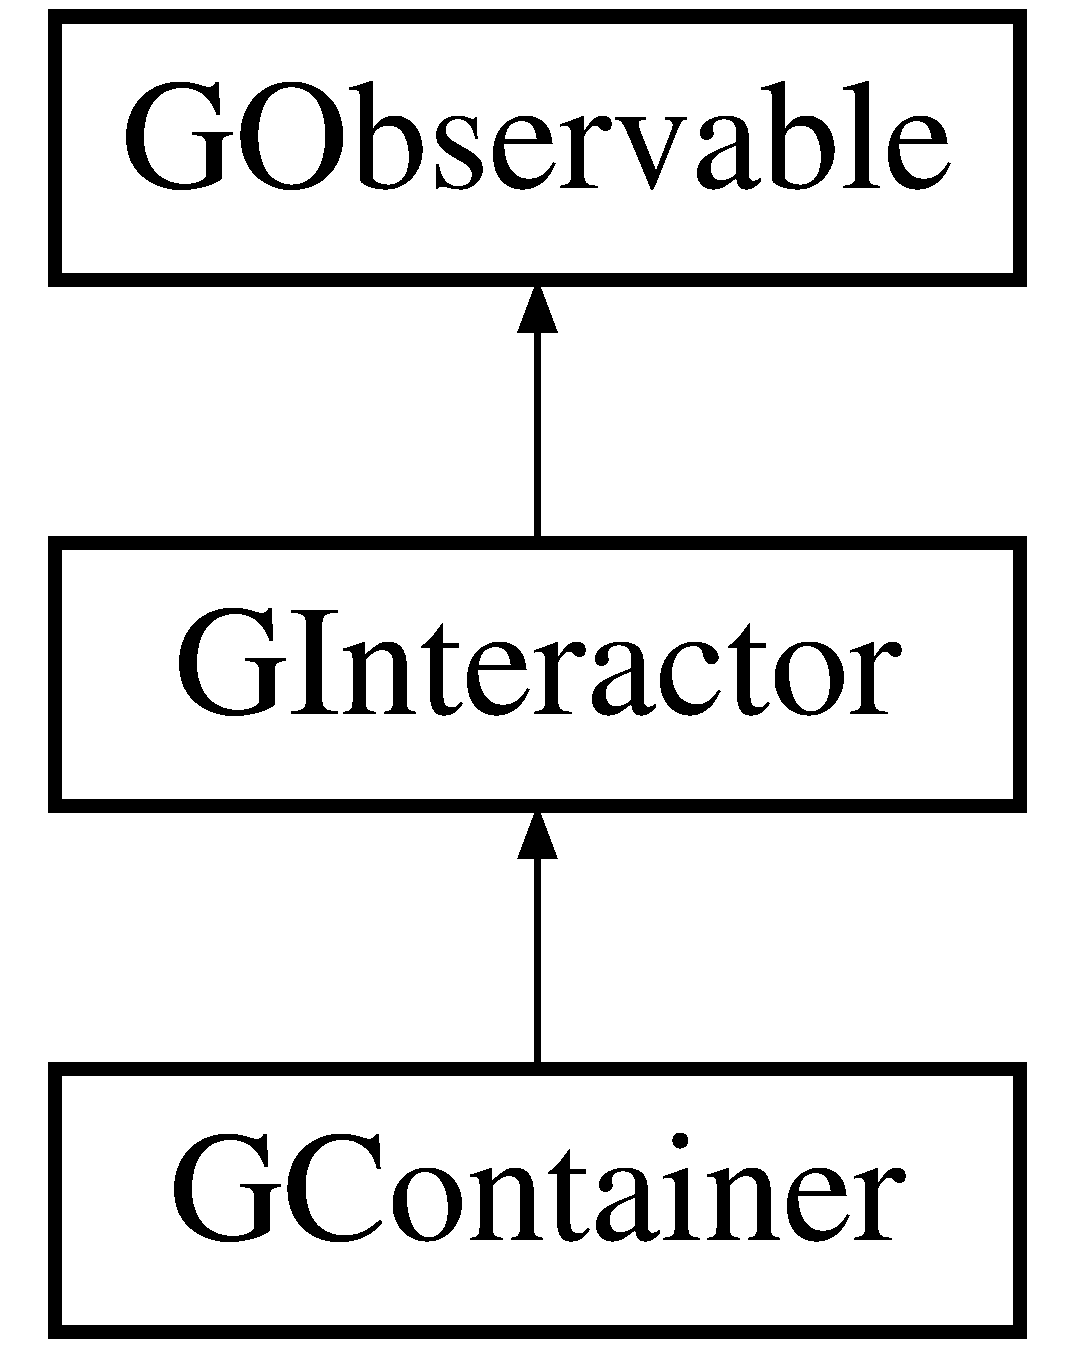
\includegraphics[height=3.000000cm]{classGContainer}
\end{center}
\end{figure}
\subsection*{Public Types}
\begin{DoxyCompactItemize}
\item 
enum \mbox{\hyperlink{classGContainer_a1b7da28ed84c0763e8f92cde2df4799b}{Layout}} \{ \mbox{\hyperlink{classGContainer_a1b7da28ed84c0763e8f92cde2df4799bac7afd1f77438e15d91d69c735a3a909a}{L\+A\+Y\+O\+U\+T\+\_\+\+N\+O\+NE}}, 
\mbox{\hyperlink{classGContainer_a1b7da28ed84c0763e8f92cde2df4799bac89a811e02b929a18f7f34e7d3bebd63}{L\+A\+Y\+O\+U\+T\+\_\+\+F\+L\+O\+W\+\_\+\+H\+O\+R\+I\+Z\+O\+N\+T\+AL}}, 
\mbox{\hyperlink{classGContainer_a1b7da28ed84c0763e8f92cde2df4799ba31e93ff7f38812816b05d254e04228e3}{L\+A\+Y\+O\+U\+T\+\_\+\+F\+L\+O\+W\+\_\+\+V\+E\+R\+T\+I\+C\+AL}}, 
\mbox{\hyperlink{classGContainer_a1b7da28ed84c0763e8f92cde2df4799babce8e871f79a8c9085d90c968d8827de}{L\+A\+Y\+O\+U\+T\+\_\+\+B\+O\+R\+D\+ER}}, 
\mbox{\hyperlink{classGContainer_a1b7da28ed84c0763e8f92cde2df4799bac4b094ed4f8bf75f60ba2235771371c3}{L\+A\+Y\+O\+U\+T\+\_\+\+G\+R\+ID}}
 \}
\begin{DoxyCompactList}\small\item\em The various layout management styles that containers can use. \end{DoxyCompactList}\item 
enum \mbox{\hyperlink{classGContainer_a81a01a86de31071a92e6cce0bab9bc4b}{Region}} \{ \mbox{\hyperlink{classGContainer_a81a01a86de31071a92e6cce0bab9bc4ba5ba85a564dbf472d69f92d5a2870db16}{R\+E\+G\+I\+O\+N\+\_\+\+C\+E\+N\+T\+ER}}, 
\mbox{\hyperlink{classGContainer_a81a01a86de31071a92e6cce0bab9bc4baac78951bd4e01d20f4825d5ae0a54357}{R\+E\+G\+I\+O\+N\+\_\+\+E\+A\+ST}}, 
\mbox{\hyperlink{classGContainer_a81a01a86de31071a92e6cce0bab9bc4baf40d135fb811ad59acb102f1fb357550}{R\+E\+G\+I\+O\+N\+\_\+\+N\+O\+R\+TH}}, 
\mbox{\hyperlink{classGContainer_a81a01a86de31071a92e6cce0bab9bc4bab533512ba438173a4ceb9c501eb17628}{R\+E\+G\+I\+O\+N\+\_\+\+S\+O\+U\+TH}}, 
\mbox{\hyperlink{classGContainer_a81a01a86de31071a92e6cce0bab9bc4ba5dd8c2219af001263c00de02b642786d}{R\+E\+G\+I\+O\+N\+\_\+\+W\+E\+ST}}
 \}
\begin{DoxyCompactList}\small\item\em The five regions of border layouts. \end{DoxyCompactList}\item 
enum \mbox{\hyperlink{classGInteractor_a8e0d441725a81d2bbdebbea09078260e}{Text\+Position}} \{ \mbox{\hyperlink{classGInteractor_a8e0d441725a81d2bbdebbea09078260ea4cd6f2e7d5a08d6f4dc052df2358f774}{T\+E\+X\+T\+\_\+\+B\+E\+S\+I\+D\+E\+\_\+\+I\+C\+ON}}, 
\mbox{\hyperlink{classGInteractor_a8e0d441725a81d2bbdebbea09078260eaa88490f63d8de68d44c83bdb2ecde3b3}{T\+E\+X\+T\+\_\+\+U\+N\+D\+E\+R\+\_\+\+I\+C\+ON}}, 
\mbox{\hyperlink{classGInteractor_a8e0d441725a81d2bbdebbea09078260ea39a6f388a30ac4fefb6eb13e846bc9f2}{T\+E\+X\+T\+\_\+\+O\+N\+LY}}
 \}
\begin{DoxyCompactList}\small\item\em The places where an interactor can place its text relative to its icon. \end{DoxyCompactList}\end{DoxyCompactItemize}
\subsection*{Public Member Functions}
\begin{DoxyCompactItemize}
\item 
\mbox{\hyperlink{classGContainer_a09fc5a49b2ea0bc895fbf2772c311325}{G\+Container}} (\mbox{\hyperlink{classGContainer_a1b7da28ed84c0763e8f92cde2df4799b}{Layout}} layout=\mbox{\hyperlink{classGContainer_a1b7da28ed84c0763e8f92cde2df4799bac89a811e02b929a18f7f34e7d3bebd63}{L\+A\+Y\+O\+U\+T\+\_\+\+F\+L\+O\+W\+\_\+\+H\+O\+R\+I\+Z\+O\+N\+T\+AL}}, Q\+Widget $\ast$parent=nullptr)
\begin{DoxyCompactList}\small\item\em Creates a new container with the given layout. \end{DoxyCompactList}\item 
\mbox{\hyperlink{classGContainer_a042cb94e18801664efa748e8a8fa74c1}{G\+Container}} (\mbox{\hyperlink{classGContainer_a1b7da28ed84c0763e8f92cde2df4799b}{Layout}} layout, int rows, int cols, Q\+Widget $\ast$parent=nullptr)
\begin{DoxyCompactList}\small\item\em Creates a new container with the given number of rows and columns. \end{DoxyCompactList}\item 
virtual \mbox{\hyperlink{classGContainer_a0a3b11ccad0281e55a509da7e1d94543}{$\sim$\+G\+Container}} () Q\+\_\+\+D\+E\+C\+L\+\_\+\+O\+V\+E\+R\+R\+I\+DE
\begin{DoxyCompactList}\small\item\em Frees memory allocated internally by the container. \end{DoxyCompactList}\item 
virtual void \mbox{\hyperlink{classGContainer_a6f99b7c841256dbdc5acaafbbca4e685}{add}} (\mbox{\hyperlink{classGInteractor}{G\+Interactor}} $\ast$interactor)
\begin{DoxyCompactList}\small\item\em Adds the given interactor to the end of the list of interactors in this container. \end{DoxyCompactList}\item 
virtual void \mbox{\hyperlink{classGContainer_a33b08fe5428ed634a658deab076099f7}{add}} (\mbox{\hyperlink{classGInteractor}{G\+Interactor}} \&interactor)
\begin{DoxyCompactList}\small\item\em Adds the given interactor to the end of the list of interactors in this container. \end{DoxyCompactList}\item 
virtual void \mbox{\hyperlink{classGInteractor_a02f20ea6edfa0671f31c4c648a253833}{add\+Action\+Listener}} () Q\+\_\+\+D\+E\+C\+L\+\_\+\+D\+E\+P\+R\+E\+C\+A\+T\+ED
\begin{DoxyCompactList}\small\item\em Adds an event listener to be notified when this interactor is clicked or generally interacted with. \end{DoxyCompactList}\item 
virtual void \mbox{\hyperlink{classGContainer_adf2c09cdcbf0f38c03d75a250fd8ce5d}{add\+To\+Grid}} (\mbox{\hyperlink{classGInteractor}{G\+Interactor}} $\ast$interactor, int row, int col, int rowspan=1, int colspan=1)
\begin{DoxyCompactList}\small\item\em Adds the given interactor to the given row and column in this container, which is assumed to use a grid layout. \end{DoxyCompactList}\item 
virtual void \mbox{\hyperlink{classGContainer_abc297ebf9136261c21e2df3c771df0b3}{add\+To\+Grid}} (\mbox{\hyperlink{classGInteractor}{G\+Interactor}} \&interactor, int row, int col, int rowspan=1, int colspan=1)
\begin{DoxyCompactList}\small\item\em Adds the given interactor to the given row and column in this container, which is assumed to use a grid layout. \end{DoxyCompactList}\item 
virtual void \mbox{\hyperlink{classGContainer_aab55413917cdbb2e0560ab415d59fd1f}{add\+To\+Region}} (\mbox{\hyperlink{classGInteractor}{G\+Interactor}} $\ast$interactor, \mbox{\hyperlink{classGContainer_a81a01a86de31071a92e6cce0bab9bc4b}{Region}} region)
\begin{DoxyCompactList}\small\item\em Adds the given interactor to the given region in this container, which is assumed to use a border layout. \end{DoxyCompactList}\item 
virtual void \mbox{\hyperlink{classGContainer_a9c8e600889001e6e72d3548918a6baff}{add\+To\+Region}} (\mbox{\hyperlink{classGInteractor}{G\+Interactor}} $\ast$interactor, const std\+::string \&region=\char`\"{}Center\char`\"{})
\begin{DoxyCompactList}\small\item\em Adds the given interactor to the given region in this container, which is assumed to use a border layout. \end{DoxyCompactList}\item 
virtual void \mbox{\hyperlink{classGContainer_ad05df0d92ab2fba95d401a5614365558}{add\+To\+Region}} (\mbox{\hyperlink{classGInteractor}{G\+Interactor}} \&interactor, \mbox{\hyperlink{classGContainer_a81a01a86de31071a92e6cce0bab9bc4b}{Region}} region)
\begin{DoxyCompactList}\small\item\em Adds the given interactor to the given region in this container, which is assumed to use a border layout. \end{DoxyCompactList}\item 
virtual void \mbox{\hyperlink{classGContainer_a667ed0065e0bbb52a893904e7f2383bb}{add\+To\+Region}} (\mbox{\hyperlink{classGInteractor}{G\+Interactor}} \&interactor, const std\+::string \&region=\char`\"{}Center\char`\"{})
\begin{DoxyCompactList}\small\item\em Adds the given interactor to the given region in this container, which is assumed to use a border layout. \end{DoxyCompactList}\item 
virtual void \mbox{\hyperlink{classGContainer_ac8bb3912a3ce86b15842e79d0b421204}{clear}} ()
\begin{DoxyCompactList}\small\item\em Removes all interactors from this container. \end{DoxyCompactList}\item 
virtual void \mbox{\hyperlink{classGContainer_a47f0cc45498a78757fa4d0e6befc2981}{clear\+Region}} (\mbox{\hyperlink{classGContainer_a81a01a86de31071a92e6cce0bab9bc4b}{Region}} region)
\begin{DoxyCompactList}\small\item\em Removes all interactors from the given region of this container, which is assumed to use a border layout. \end{DoxyCompactList}\item 
virtual void \mbox{\hyperlink{classGContainer_aeba526cb4d6d6f3d8d6f376656af8dc8}{clear\+Region}} (const std\+::string \&region)
\begin{DoxyCompactList}\small\item\em Removes all interactors from the given region of this container, which is assumed to use a border layout. \end{DoxyCompactList}\item 
virtual bool \mbox{\hyperlink{classGContainer_a29e67f98cd36414c67475b8941d861a6}{contains}} (\mbox{\hyperlink{classGInteractor}{G\+Interactor}} $\ast$interactor) const
\begin{DoxyCompactList}\small\item\em Returns true if the given interactor is found in this container. \end{DoxyCompactList}\item 
virtual bool \mbox{\hyperlink{classGContainer_a62fe1c67f06f657fea8b9b28672516a0}{contains}} (\mbox{\hyperlink{classGInteractor}{G\+Interactor}} \&interactor) const
\begin{DoxyCompactList}\small\item\em Returns true if the given interactor is found in this container. \end{DoxyCompactList}\item 
virtual bool \mbox{\hyperlink{classGInteractor_ac05ba5b92e2e5146d416fe7f842a0969}{events\+Enabled}} () const Q\+\_\+\+D\+E\+C\+L\+\_\+\+O\+V\+E\+R\+R\+I\+DE
\begin{DoxyCompactList}\small\item\em Returns true if this interactor is currently accepting events. \end{DoxyCompactList}\item 
virtual std\+::string \mbox{\hyperlink{classGInteractor_a69f8d23ed8f207fbecad99960776e942}{get\+Accelerator}} () const
\begin{DoxyCompactList}\small\item\em Returns a string representing a hotkey for this interactor, or an empty string if no accelerator has been set. \end{DoxyCompactList}\item 
virtual std\+::string \mbox{\hyperlink{classGInteractor_a94eb4276000c4fdfb508ce9e6317a82a}{get\+Action\+Command}} () const
\begin{DoxyCompactList}\small\item\em Returns an action command for this interactor, which is a semi-\/unique string you can use to identify it when events occur. \end{DoxyCompactList}\item 
virtual std\+::string \mbox{\hyperlink{classGInteractor_a808e22cc1fdfbecf71ed8c64ef4600e0}{get\+Background}} () const
\begin{DoxyCompactList}\small\item\em Returns the background color of the interactor as a string. \end{DoxyCompactList}\item 
virtual int \mbox{\hyperlink{classGInteractor_a9e827257a55cb8cf4d9de2ec6bcfd7a0}{get\+Background\+Int}} () const
\begin{DoxyCompactList}\small\item\em Returns the background color of the interactor as an R\+GB integer. \end{DoxyCompactList}\item 
virtual \mbox{\hyperlink{classGRectangle}{G\+Rectangle}} \mbox{\hyperlink{classGInteractor_a29e6ac35a0b48f491a4c88194cc5da3b}{get\+Bounds}} () const
\begin{DoxyCompactList}\small\item\em Returns a rectangle representing the x/y position and size of this interactor. \end{DoxyCompactList}\item 
virtual std\+::string \mbox{\hyperlink{classGInteractor_aa061dfa488c31e18549d64363c1d0e34}{get\+Color}} () const
\begin{DoxyCompactList}\small\item\em Returns the foreground/text color of the interactor as a string. \end{DoxyCompactList}\item 
virtual int \mbox{\hyperlink{classGInteractor_a9635c7af766cdc3417f346683fa0e6c1}{get\+Color\+Int}} () const
\begin{DoxyCompactList}\small\item\em Returns the foreground/text color of the interactor as an R\+GB integer. \end{DoxyCompactList}\item 
virtual \mbox{\hyperlink{classGContainer}{G\+Container}} $\ast$ \mbox{\hyperlink{classGInteractor_a7a6e317c29d61030929b4cd2d1c00fe7}{get\+Container}} () const
\begin{DoxyCompactList}\small\item\em Returns a pointer to the onscreen container holding this interactor. \end{DoxyCompactList}\item 
virtual \mbox{\hyperlink{classVector}{Vector}}$<$ \mbox{\hyperlink{classGInteractor}{G\+Interactor}} $\ast$ $>$ \mbox{\hyperlink{classGContainer_a5c520260dc9282097022249ea42c4a3f}{get\+Descendents}} (const std\+::string \&type=\char`\"{}\char`\"{}) const
\begin{DoxyCompactList}\small\item\em Returns all interactors that are children or descendents inside this container. \end{DoxyCompactList}\item 
virtual std\+::string \mbox{\hyperlink{classGInteractor_a894a5502900794eeb27d084c21f1d77d}{get\+Font}} () const
\begin{DoxyCompactList}\small\item\em Returns the font of this interactor\textquotesingle{}s text as a font string such as \char`\"{}\+Helvetica-\/12-\/\+Bold\char`\"{}. \end{DoxyCompactList}\item 
virtual std\+::string \mbox{\hyperlink{classGInteractor_a4fa2d8b0192a3a5b4af4bbfe71194d03}{get\+Foreground}} () const
\begin{DoxyCompactList}\small\item\em Returns the foreground/text color of the interactor as a string. \end{DoxyCompactList}\item 
virtual int \mbox{\hyperlink{classGInteractor_ac3b12ab385a6ef9ae90fc879860ba726}{get\+Foreground\+Int}} () const
\begin{DoxyCompactList}\small\item\em Returns the foreground/text color of the interactor as an R\+GB integer. \end{DoxyCompactList}\item 
virtual double \mbox{\hyperlink{classGInteractor_a1e7e353362434072875264cf95629f99}{get\+Height}} () const
\begin{DoxyCompactList}\small\item\em Returns the current onscreen height of this interactor in pixels. \end{DoxyCompactList}\item 
virtual std\+::string \mbox{\hyperlink{classGInteractor_aaed62a73004939a64da6f0eb9eb64d73}{get\+Icon}} () const
\begin{DoxyCompactList}\small\item\em Returns the file name of the icon associated with this interactor, or an empty string if no icon has been set. \end{DoxyCompactList}\item 
virtual int \mbox{\hyperlink{classGInteractor_a9c9659a6c6ba66b4107ba59c95a24241}{get\+ID}} () const
\begin{DoxyCompactList}\small\item\em Returns a globally unique identifier for this interactor, which is set when the interactor is constructed. \end{DoxyCompactList}\item 
virtual \mbox{\hyperlink{classGInteractor}{G\+Interactor}} $\ast$ \mbox{\hyperlink{classGContainer_ac59d7bae6154f6f8791c7f1fd856b157}{get\+Interactor}} (int i) const
\begin{DoxyCompactList}\small\item\em Returns the child interactor at the given 0-\/based index in this container. \end{DoxyCompactList}\item 
virtual \mbox{\hyperlink{classGInteractor}{G\+Interactor}} $\ast$ \mbox{\hyperlink{classGContainer_ad31230cd6d220466fbd18fd21d133f67}{get\+Interactor\+By\+Region}} (int i, \mbox{\hyperlink{classGContainer_a81a01a86de31071a92e6cce0bab9bc4b}{Region}} region) const
\begin{DoxyCompactList}\small\item\em Returns the child interactor at the given 0-\/based index within the given region in this container, which is assumed to use a border layout. \end{DoxyCompactList}\item 
virtual \mbox{\hyperlink{classGInteractor}{G\+Interactor}} $\ast$ \mbox{\hyperlink{classGContainer_a576bbbb845c9bcf139fca956e3a4c757}{get\+Interactor\+By\+Region}} (int i, const std\+::string \&region=\char`\"{}Center\char`\"{}) const
\begin{DoxyCompactList}\small\item\em Returns the child interactor at the given 0-\/based index within the given region in this container, which is assumed to use a border layout. \end{DoxyCompactList}\item 
virtual int \mbox{\hyperlink{classGContainer_a789affbf8e89e65e3afd63cc626f5a81}{get\+Interactor\+Count}} () const
\begin{DoxyCompactList}\small\item\em Returns the number of children interactors in this container. \end{DoxyCompactList}\item 
virtual int \mbox{\hyperlink{classGContainer_a668fe9a4efc31fa065ded79c0e5eab64}{get\+Interactor\+Count\+By\+Region}} (\mbox{\hyperlink{classGContainer_a81a01a86de31071a92e6cce0bab9bc4b}{Region}} region) const
\begin{DoxyCompactList}\small\item\em Returns the number of children interactors within the given region in this container, which is assumed to use a border layout. \end{DoxyCompactList}\item 
virtual int \mbox{\hyperlink{classGContainer_ab51dbb723159efca4fc89e2c4211610c}{get\+Interactor\+Count\+By\+Region}} (const std\+::string \&region=\char`\"{}Center\char`\"{}) const
\begin{DoxyCompactList}\small\item\em Returns the number of children interactors within the given region in this container, which is assumed to use a border layout. \end{DoxyCompactList}\item 
virtual const \mbox{\hyperlink{classVector}{Vector}}$<$ \mbox{\hyperlink{classGInteractor}{G\+Interactor}} $\ast$ $>$ \& \mbox{\hyperlink{classGContainer_a3f9ba3028f69581c7de79c9c03f39a2e}{get\+Interactors}} () const
\begin{DoxyCompactList}\small\item\em Returns a vector of all children interactors in this container. \end{DoxyCompactList}\item 
virtual \+\_\+\+Internal\+\_\+\+Q\+Widget $\ast$ \mbox{\hyperlink{classGContainer_a208ce13c1da40bf0ddb509daf99d6588}{get\+Internal\+Widget}} () const Q\+\_\+\+D\+E\+C\+L\+\_\+\+O\+V\+E\+R\+R\+I\+DE
\begin{DoxyCompactList}\small\item\em Returns a direct pointer to the internal Qt widget being wrapped by this interactor. \end{DoxyCompactList}\item 
virtual \mbox{\hyperlink{classGContainer_a1b7da28ed84c0763e8f92cde2df4799b}{Layout}} \mbox{\hyperlink{classGContainer_aeebcf77b7fdc91a1ba0371cc9b91d5e2}{get\+Layout}} () const
\begin{DoxyCompactList}\small\item\em Returns the type of layout used by this container. \end{DoxyCompactList}\item 
virtual \mbox{\hyperlink{classGPoint}{G\+Point}} \mbox{\hyperlink{classGInteractor_a4f83802015511edeb63b892830812c11}{get\+Location}} () const
\begin{DoxyCompactList}\small\item\em Returns an (x, y) point representing the onscreen location of the top-\/left corner of this interactor within its containing window. \end{DoxyCompactList}\item 
virtual double \mbox{\hyperlink{classGContainer_ae2b63e249b9251e1893dae87aaf4cc3d}{get\+Margin}} () const
\begin{DoxyCompactList}\small\item\em Returns the margin around each widget in this container in pixels. \end{DoxyCompactList}\item 
virtual double \mbox{\hyperlink{classGInteractor_aed4b0075fcc434499c3cb3e46896bda3}{get\+Minimum\+Height}} () const
\begin{DoxyCompactList}\small\item\em Returns the minimum height in pixels that this interactor will permit itself to be resized to. \end{DoxyCompactList}\item 
virtual \mbox{\hyperlink{classGDimension}{G\+Dimension}} \mbox{\hyperlink{classGInteractor_a66b5af0b32493b4d597ca0a3df2049ea}{get\+Minimum\+Size}} () const
\begin{DoxyCompactList}\small\item\em Returns a \mbox{\hyperlink{classGDimension}{G\+Dimension}} structure representing the minimum size in pixels that this interactor will permit itself to be resized to. \end{DoxyCompactList}\item 
virtual double \mbox{\hyperlink{classGInteractor_a59e668114fe3d49d2a0f28deb258f7c8}{get\+Minimum\+Width}} () const
\begin{DoxyCompactList}\small\item\em Returns the minimum width in pixels that this interactor will permit itself to be resized to. \end{DoxyCompactList}\item 
virtual std\+::string \mbox{\hyperlink{classGInteractor_a8a60438a5b55d0b2ceb35c8674b9d8c5}{get\+Name}} () const
\begin{DoxyCompactList}\small\item\em Returns a string representing a unique name for this interactor. \end{DoxyCompactList}\item 
virtual double \mbox{\hyperlink{classGContainer_a19fdf4f4500aead343992102066983cb}{get\+Padding}} () const
\begin{DoxyCompactList}\small\item\em Returns the padding inside this container in pixels. \end{DoxyCompactList}\item 
virtual double \mbox{\hyperlink{classGContainer_a5696e2debbbafb717c0d47e069b896e4}{get\+Padding\+Bottom}} () const
\begin{DoxyCompactList}\small\item\em Returns the padding on the bottom side of this container in pixels. \end{DoxyCompactList}\item 
virtual double \mbox{\hyperlink{classGContainer_af28748a6467a4d3337788578522fa8f4}{get\+Padding\+Left}} () const
\begin{DoxyCompactList}\small\item\em Returns the padding on the left side of this container in pixels. \end{DoxyCompactList}\item 
virtual double \mbox{\hyperlink{classGContainer_a8d75cea586f7cd6611432122a080ecce}{get\+Padding\+Right}} () const
\begin{DoxyCompactList}\small\item\em Returns the padding on the right side of this container in pixels. \end{DoxyCompactList}\item 
virtual double \mbox{\hyperlink{classGContainer_ada97c35b2f3366886a49d63fff9d7bd4}{get\+Padding\+Top}} () const
\begin{DoxyCompactList}\small\item\em Returns the padding on the top side of this container in pixels. \end{DoxyCompactList}\item 
virtual double \mbox{\hyperlink{classGInteractor_a747de0961653847bdc6615dbf756d715}{get\+Preferred\+Height}} () const
\begin{DoxyCompactList}\small\item\em Returns the height in pixels that this interactor would prefer to be, which would exactly fit its contents with no stretching or scrollbars. \end{DoxyCompactList}\item 
virtual \mbox{\hyperlink{classGDimension}{G\+Dimension}} \mbox{\hyperlink{classGContainer_a21904b305edacd8f871d6951cb8d3fa5}{get\+Preferred\+Size}} () const Q\+\_\+\+D\+E\+C\+L\+\_\+\+O\+V\+E\+R\+R\+I\+DE
\begin{DoxyCompactList}\small\item\em Returns a \mbox{\hyperlink{classGDimension}{G\+Dimension}} structure storing the width and height in pixels that this interactor would prefer to be, which would exactly fit its contents with no stretching or scrollbars. \end{DoxyCompactList}\item 
virtual double \mbox{\hyperlink{classGInteractor_a82bca31d37700fb0e35d2743352efd5e}{get\+Preferred\+Width}} () const
\begin{DoxyCompactList}\small\item\em Returns the height in pixels that this interactor would prefer to be, which would exactly fit its contents with no stretching or scrollbars. \end{DoxyCompactList}\item 
virtual double \mbox{\hyperlink{classGContainer_a164d248057318961e7f2abc8c3477d63}{get\+Region\+Height}} (\mbox{\hyperlink{classGContainer_a81a01a86de31071a92e6cce0bab9bc4b}{Region}} region) const
\begin{DoxyCompactList}\small\item\em Returns the height in pixels of the given region of this container, which is assumed to use a border layout. \end{DoxyCompactList}\item 
virtual double \mbox{\hyperlink{classGContainer_ae8a545e772745b89edaf9804a2dc0057}{get\+Region\+Height}} (const std\+::string \&region) const
\begin{DoxyCompactList}\small\item\em Returns the height in pixels of the given region of this container, which is assumed to use a border layout. \end{DoxyCompactList}\item 
virtual \mbox{\hyperlink{classGDimension}{G\+Dimension}} \mbox{\hyperlink{classGContainer_a3b5db9ffbd4b32260f80634f162dba4e}{get\+Region\+Size}} (\mbox{\hyperlink{classGContainer_a81a01a86de31071a92e6cce0bab9bc4b}{Region}} region) const
\begin{DoxyCompactList}\small\item\em Returns the width and height in pixels of the given region of this container, which is assumed to use a border layout. \end{DoxyCompactList}\item 
virtual \mbox{\hyperlink{classGDimension}{G\+Dimension}} \mbox{\hyperlink{classGContainer_a68b18b38b72cb8779fca0c3882549a6b}{get\+Region\+Size}} (const std\+::string \&region) const
\begin{DoxyCompactList}\small\item\em Returns the width and height in pixels of the given region of this container, which is assumed to use a border layout. \end{DoxyCompactList}\item 
virtual double \mbox{\hyperlink{classGContainer_a96e2005c3f447a8679c3c32d3fc02de1}{get\+Region\+Width}} (\mbox{\hyperlink{classGContainer_a81a01a86de31071a92e6cce0bab9bc4b}{Region}} region) const
\begin{DoxyCompactList}\small\item\em Returns the width in pixels of the given region of this container, which is assumed to use a border layout. \end{DoxyCompactList}\item 
virtual double \mbox{\hyperlink{classGContainer_ab169dab454fc90f1c845b91b4e1a8a14}{get\+Region\+Width}} (const std\+::string \&region) const
\begin{DoxyCompactList}\small\item\em Returns the width in pixels of the given region of this container, which is assumed to use a border layout. \end{DoxyCompactList}\item 
virtual \mbox{\hyperlink{classGDimension}{G\+Dimension}} \mbox{\hyperlink{classGInteractor_a7b4eec96a2bdc6420695d5796a78eea9}{get\+Size}} () const
\begin{DoxyCompactList}\small\item\em Returns a \mbox{\hyperlink{classGDimension}{G\+Dimension}} structure storing the current onscreen width and height of this interactor in pixels. \end{DoxyCompactList}\item 
virtual double \mbox{\hyperlink{classGContainer_a9a7e859eeff5cc7de46d65b9be7afc3c}{get\+Spacing}} () const
\begin{DoxyCompactList}\small\item\em Returns the spacing between widgets in this container in pixels. \end{DoxyCompactList}\item 
virtual std\+::string \mbox{\hyperlink{classGContainer_a9896d58fcfebbf1025aeeb5b8b9ede80}{get\+Type}} () const Q\+\_\+\+D\+E\+C\+L\+\_\+\+O\+V\+E\+R\+R\+I\+DE
\begin{DoxyCompactList}\small\item\em Returns a string representing the class name of this interactor, such as \char`\"{}\+G\+Button\char`\"{} or \char`\"{}\+G\+Check\+Box\char`\"{}. \end{DoxyCompactList}\item 
virtual Q\+Widget $\ast$ \mbox{\hyperlink{classGContainer_a326ee51b5561f807df7b29a1c101f7fd}{get\+Widget}} () const Q\+\_\+\+D\+E\+C\+L\+\_\+\+O\+V\+E\+R\+R\+I\+DE
\begin{DoxyCompactList}\small\item\em Returns a direct pointer to the internal Qt widget being wrapped by this interactor. \end{DoxyCompactList}\item 
virtual double \mbox{\hyperlink{classGInteractor_a0ed2965abd4f5701d2cadf71239faf19}{get\+Width}} () const
\begin{DoxyCompactList}\small\item\em Returns the current onscreen width of this interactor in pixels. \end{DoxyCompactList}\item 
virtual double \mbox{\hyperlink{classGInteractor_a344385751bee0720059403940d57a13e}{getX}} () const
\begin{DoxyCompactList}\small\item\em Returns the x-\/coordinate of the top-\/left pixel of this interactor within its onscreen window. \end{DoxyCompactList}\item 
virtual double \mbox{\hyperlink{classGInteractor_aafa51c7f8f38a09febbb9ce7853f77b4}{getY}} () const
\begin{DoxyCompactList}\small\item\em Returns the y-\/coordinate of the top-\/left pixel of this interactor within its onscreen window. \end{DoxyCompactList}\item 
virtual bool \mbox{\hyperlink{classGInteractor_afc480f652b8c5f1fb255e2269ce68879}{in\+Bounds}} (double x, double y) const
\begin{DoxyCompactList}\small\item\em Returns true if the given x/y pixel is within the bounds of this interactor. \end{DoxyCompactList}\item 
virtual bool \mbox{\hyperlink{classGInteractor_ae6d7982c1c627b677a5e776ca86118ed}{in\+Bounds}} (int x, int y) const
\begin{DoxyCompactList}\small\item\em Returns true if the given x/y pixel is within the bounds of this interactor. \end{DoxyCompactList}\item 
virtual void \mbox{\hyperlink{classGContainer_afffb8f789ff9a8466fbae5b846a0ebe7}{insert}} (int index, \mbox{\hyperlink{classGInteractor}{G\+Interactor}} $\ast$interactor)
\begin{DoxyCompactList}\small\item\em Adds the given interactor to this container just before the given index. \end{DoxyCompactList}\item 
virtual void \mbox{\hyperlink{classGContainer_a2e9d7c6d9e6769d4cfd3293afe7e215c}{insert}} (int index, \mbox{\hyperlink{classGInteractor}{G\+Interactor}} \&interactor)
\begin{DoxyCompactList}\small\item\em Adds the given interactor to this container just before the given index. \end{DoxyCompactList}\item 
virtual void \mbox{\hyperlink{classGContainer_a1c4b766b059991ad7d084ea03f22f1c5}{insert\+To\+Region}} (int index, \mbox{\hyperlink{classGInteractor}{G\+Interactor}} $\ast$interactor, \mbox{\hyperlink{classGContainer_a81a01a86de31071a92e6cce0bab9bc4b}{Region}} region)
\begin{DoxyCompactList}\small\item\em Adds the given interactor to the given layout region within this container just before the given index. \end{DoxyCompactList}\item 
virtual void \mbox{\hyperlink{classGContainer_adeeb03feb9346a9cf2046427484c20bc}{insert\+To\+Region}} (int index, \mbox{\hyperlink{classGInteractor}{G\+Interactor}} $\ast$interactor, const std\+::string \&region=\char`\"{}Center\char`\"{})
\begin{DoxyCompactList}\small\item\em Adds the given interactor to the given layout region within this container just before the given index. \end{DoxyCompactList}\item 
virtual void \mbox{\hyperlink{classGContainer_a1be2b263cd8d28e61e136a19d8e935cc}{insert\+To\+Region}} (int index, \mbox{\hyperlink{classGInteractor}{G\+Interactor}} \&interactor, \mbox{\hyperlink{classGContainer_a81a01a86de31071a92e6cce0bab9bc4b}{Region}} region)
\begin{DoxyCompactList}\small\item\em Adds the given interactor to the given layout region within this container just before the given index. \end{DoxyCompactList}\item 
virtual void \mbox{\hyperlink{classGContainer_ad4d413f64a3e4fb948956e7249c10110}{insert\+To\+Region}} (int index, \mbox{\hyperlink{classGInteractor}{G\+Interactor}} \&interactor, const std\+::string \&region=\char`\"{}Center\char`\"{})
\begin{DoxyCompactList}\small\item\em Adds the given interactor to the given layout region within this container just before the given index. \end{DoxyCompactList}\item 
virtual bool \mbox{\hyperlink{classGContainer_acf82f9b2937375c7b1cf3dccb3df3312}{is\+Empty}} () const
\begin{DoxyCompactList}\small\item\em Returns true if the container does not contain any interactors. \end{DoxyCompactList}\item 
virtual bool \mbox{\hyperlink{classGInteractor_aacb819fb241851fd9fc045271baa4034}{is\+Enabled}} () const
\begin{DoxyCompactList}\small\item\em Returns true if this interactor is currently enabled. \end{DoxyCompactList}\item 
virtual bool \mbox{\hyperlink{classGInteractor_a9d8a6cfb13917785c143e74d40e4e2be}{is\+Visible}} () const
\begin{DoxyCompactList}\small\item\em Returns true if the interactor is visible on the screen. \end{DoxyCompactList}\item 
virtual bool \mbox{\hyperlink{classGContainer_a8909db9abf4dc80058f9e4a7b90ea2d0}{region\+Contains}} (\mbox{\hyperlink{classGInteractor}{G\+Interactor}} $\ast$interactor, \mbox{\hyperlink{classGContainer_a81a01a86de31071a92e6cce0bab9bc4b}{Region}} region) const
\begin{DoxyCompactList}\small\item\em Returns true if the given interactor is found in the given region of this container, which is assumed to use a border layout. \end{DoxyCompactList}\item 
virtual bool \mbox{\hyperlink{classGContainer_a84a56bae6b8883d27e44d51c31b2bfc5}{region\+Contains}} (\mbox{\hyperlink{classGInteractor}{G\+Interactor}} $\ast$interactor, const std\+::string \&region) const
\begin{DoxyCompactList}\small\item\em Returns true if the given interactor is found in the given region of this container, which is assumed to use a border layout. \end{DoxyCompactList}\item 
virtual bool \mbox{\hyperlink{classGContainer_aa4cf95952747fd421a2b005eedbc662c}{region\+Contains}} (\mbox{\hyperlink{classGInteractor}{G\+Interactor}} \&interactor, \mbox{\hyperlink{classGContainer_a81a01a86de31071a92e6cce0bab9bc4b}{Region}} region) const
\begin{DoxyCompactList}\small\item\em Returns true if the given interactor is found in the given region of this container, which is assumed to use a border layout. \end{DoxyCompactList}\item 
virtual bool \mbox{\hyperlink{classGContainer_ad67deacd62d3248fbe57ccbd4e96fb50}{region\+Contains}} (\mbox{\hyperlink{classGInteractor}{G\+Interactor}} \&interactor, const std\+::string \&region) const
\begin{DoxyCompactList}\small\item\em Returns true if the given interactor is found in the given region of this container, which is assumed to use a border layout. \end{DoxyCompactList}\item 
virtual void \mbox{\hyperlink{classGContainer_a1c12b1fde5c2ef10d79d4ee51e670efa}{remove}} (\mbox{\hyperlink{classGInteractor}{G\+Interactor}} $\ast$interactor)
\begin{DoxyCompactList}\small\item\em Removes the given interactor from this container. \end{DoxyCompactList}\item 
virtual void \mbox{\hyperlink{classGContainer_ade2376c458ac401a0bd2dbe44271509e}{remove}} (\mbox{\hyperlink{classGInteractor}{G\+Interactor}} \&interactor)
\begin{DoxyCompactList}\small\item\em Removes the given interactor from this container. \end{DoxyCompactList}\item 
virtual void \mbox{\hyperlink{classGContainer_a2ad1aa316f278b2e9fa8121504749652}{remove}} (int index)
\begin{DoxyCompactList}\small\item\em Removes the child interactor at the given 0-\/based index from this container. \end{DoxyCompactList}\item 
virtual void \mbox{\hyperlink{classGContainer_a87a74b040025878283ba685e30d5104f}{remove\+From\+Region}} (\mbox{\hyperlink{classGInteractor}{G\+Interactor}} $\ast$interactor, \mbox{\hyperlink{classGContainer_a81a01a86de31071a92e6cce0bab9bc4b}{Region}} region)
\begin{DoxyCompactList}\small\item\em Removes the given interactor from the given region within this container, which is assumed to use a border layout. \end{DoxyCompactList}\item 
virtual void \mbox{\hyperlink{classGContainer_a16268c8344a5a5d9b10bde95764112d1}{remove\+From\+Region}} (\mbox{\hyperlink{classGInteractor}{G\+Interactor}} $\ast$interactor, const std\+::string \&region)
\begin{DoxyCompactList}\small\item\em Removes the given interactor from the given region within this container, which is assumed to use a border layout. \end{DoxyCompactList}\item 
virtual void \mbox{\hyperlink{classGContainer_afee7b65f917c4f6a0fdb1c8ea75406a5}{remove\+From\+Region}} (\mbox{\hyperlink{classGInteractor}{G\+Interactor}} \&interactor, \mbox{\hyperlink{classGContainer_a81a01a86de31071a92e6cce0bab9bc4b}{Region}} region)
\begin{DoxyCompactList}\small\item\em Removes the given interactor from the given region within this container, which is assumed to use a border layout. \end{DoxyCompactList}\item 
virtual void \mbox{\hyperlink{classGContainer_af7a055c83c0e0e3f3722596d7111fcbe}{remove\+From\+Region}} (\mbox{\hyperlink{classGInteractor}{G\+Interactor}} \&interactor, const std\+::string \&region)
\begin{DoxyCompactList}\small\item\em Removes the given interactor from the given region within this container, which is assumed to use a border layout. \end{DoxyCompactList}\item 
virtual void \mbox{\hyperlink{classGContainer_a15e3a1d3f3abecc00d68d6df2349f360}{remove\+From\+Region}} (int index, \mbox{\hyperlink{classGContainer_a81a01a86de31071a92e6cce0bab9bc4b}{Region}} region)
\begin{DoxyCompactList}\small\item\em Removes the child interactor at the given 0-\/based index from the given region of this container, which is assumed to use a border layout. \end{DoxyCompactList}\item 
virtual void \mbox{\hyperlink{classGContainer_ac839e32fec6ea6b37f6c6da8aa6ce43b}{remove\+From\+Region}} (int index, const std\+::string \&region)
\begin{DoxyCompactList}\small\item\em Removes the child interactor at the given 0-\/based index from the given region of this container, which is assumed to use a border layout. \end{DoxyCompactList}\item 
virtual void \mbox{\hyperlink{classGInteractor_a519fb2ac767f8b2febbb50b898b8c8cb}{request\+Focus}} ()
\begin{DoxyCompactList}\small\item\em Transfers keyboard focus to this interactor. \end{DoxyCompactList}\item 
virtual void \mbox{\hyperlink{classGInteractor_ad15f102f62e2960576012f1aa0ba4b2e}{set\+Accelerator}} (const std\+::string \&accelerator)
\begin{DoxyCompactList}\small\item\em Sets an accelerator hotkey for this interactor, such as \char`\"{}\+Ctrl-\/\+S\char`\"{}. \end{DoxyCompactList}\item 
virtual void \mbox{\hyperlink{classGInteractor_a4b5843fe3030e038a1ba54cc03389bcf}{set\+Action\+Command}} (const std\+::string \&action\+Command)
\begin{DoxyCompactList}\small\item\em Sets the action command for this interactor. \end{DoxyCompactList}\item 
virtual void \mbox{\hyperlink{classGContainer_a0bcf8805d87afc9bb4c6ca238ca7c0bd}{set\+Alignment}} (Horizontal\+Alignment halign, Vertical\+Alignment valign)
\begin{DoxyCompactList}\small\item\em Sets the horizontal and vertical alignment of interactors in this container. \end{DoxyCompactList}\item 
virtual void \mbox{\hyperlink{classGInteractor_acba7e546c2025c0a15ca4b4cc92043db}{set\+Background}} (int rgb)
\begin{DoxyCompactList}\small\item\em Sets the background color of the interactor to the color represented by the given R\+GB integer. \end{DoxyCompactList}\item 
virtual void \mbox{\hyperlink{classGInteractor_ab4677ab2474e68b07aa56605af92a84a}{set\+Background}} (const std\+::string \&color)
\begin{DoxyCompactList}\small\item\em Sets the background color of the interactor to the color represented by the given string. \end{DoxyCompactList}\item 
virtual void \mbox{\hyperlink{classGInteractor_a2aae8197624b72265ab83b4f1bc73f2f}{set\+Bounds}} (double x, double y, double width, double height)
\begin{DoxyCompactList}\small\item\em Sets the size and location of the widget. \end{DoxyCompactList}\item 
virtual void \mbox{\hyperlink{classGInteractor_acada386653f008cacc7cce86426bef7c}{set\+Bounds}} (const \mbox{\hyperlink{classGRectangle}{G\+Rectangle}} \&size)
\begin{DoxyCompactList}\small\item\em Sets the size and location of the widget. \end{DoxyCompactList}\item 
virtual void \mbox{\hyperlink{classGInteractor_ab1f5cc0f5cc6bbbd716a526c61f1081d}{set\+Color}} (int rgb)
\begin{DoxyCompactList}\small\item\em Sets the foreground/text color of the interactor to the color represented by the given R\+GB integer. \end{DoxyCompactList}\item 
virtual void \mbox{\hyperlink{classGInteractor_a61374df6c11b52cfbb0815decdbaebc6}{set\+Color}} (const std\+::string \&color)
\begin{DoxyCompactList}\small\item\em Sets the foreground/text color of the interactor to the color represented by the given string. \end{DoxyCompactList}\item 
virtual void \mbox{\hyperlink{classGInteractor_ab831367dd84bbd579e02e55bacb21343}{set\+Enabled}} (bool value)
\begin{DoxyCompactList}\small\item\em Sets whether this interactor is currently enabled. \end{DoxyCompactList}\item 
virtual void \mbox{\hyperlink{classGObservable_afaa30b2a9e0f378fd1c70d2f1d0b8216}{set\+Events\+Enabled}} (bool \mbox{\hyperlink{classGInteractor_ac05ba5b92e2e5146d416fe7f842a0969}{events\+Enabled}})
\begin{DoxyCompactList}\small\item\em Sets whether the object is currently allowing itself to fire events. \end{DoxyCompactList}\item 
virtual void \mbox{\hyperlink{classGInteractor_a2592348886ffea646c6534bf88f7c49d}{set\+Font}} (const Q\+Font \&font)
\begin{DoxyCompactList}\small\item\em Sets the font used by this widget to the given Qt font. \end{DoxyCompactList}\item 
virtual void \mbox{\hyperlink{classGInteractor_a8e096e8818d838aceae1d46d58fb3a7b}{set\+Font}} (const std\+::string \&font)
\begin{DoxyCompactList}\small\item\em Sets the font used by this widget to the font represented by the given font string, such as \char`\"{}\+Helvetica-\/16-\/\+Bold\char`\"{}. \end{DoxyCompactList}\item 
virtual void \mbox{\hyperlink{classGInteractor_a9eb856b5ff83a19df3831a31f15f4563}{set\+Foreground}} (int rgb)
\begin{DoxyCompactList}\small\item\em Sets the foreground/text color of the interactor to the color represented by the given R\+GB integer. \end{DoxyCompactList}\item 
virtual void \mbox{\hyperlink{classGInteractor_af59209aeadea6dfc6d97a2d8531f50e1}{set\+Foreground}} (const std\+::string \&color)
\begin{DoxyCompactList}\small\item\em Sets the foreground/text color of the interactor to the color represented by the given string. \end{DoxyCompactList}\item 
virtual void \mbox{\hyperlink{classGInteractor_a9e280bfc4544dfaf8e4376c4e1a74357}{set\+Height}} (double height)
\begin{DoxyCompactList}\small\item\em Sets the onscreen height of the interactor in pixels. \end{DoxyCompactList}\item 
virtual void \mbox{\hyperlink{classGContainer_a901653aacb9991ee9a8b70d4a932f0c9}{set\+Horizontal\+Alignment}} (Horizontal\+Alignment halign)
\begin{DoxyCompactList}\small\item\em Sets the horizontal alignment of interactors in this container. \end{DoxyCompactList}\item 
virtual void \mbox{\hyperlink{classGInteractor_a762e139aa311461c3984d3ad28293f64}{set\+Icon}} (const std\+::string \&filename, bool retain\+Icon\+Size=true)
\begin{DoxyCompactList}\small\item\em Sets the file name of the icon associated with this interactor, or an empty string if no icon has been set. \end{DoxyCompactList}\item 
virtual void \mbox{\hyperlink{classGInteractor_a04594e8ba9b98513a64f1da00dcae18c}{set\+Location}} (double x, double y)
\begin{DoxyCompactList}\small\item\em Sets the onscreen x/y-\/coordinate of the top-\/left corner of the interactor relative to its window. \end{DoxyCompactList}\item 
virtual void \mbox{\hyperlink{classGContainer_a79b7a5ffc0a63c8f11be4ed59808f60d}{set\+Margin}} (double px)
\begin{DoxyCompactList}\small\item\em Sets the margin in pixels around interactors in this container. \end{DoxyCompactList}\item 
virtual void \mbox{\hyperlink{classGInteractor_a0cf428e207b7f22cc08138a90b1b87b2}{set\+Minimum\+Size}} (double width, double height)
\begin{DoxyCompactList}\small\item\em Sets the minimum size in pixels that this interactor will permit itself to be resized to. \end{DoxyCompactList}\item 
virtual void \mbox{\hyperlink{classGInteractor_a3b1046117ac6cb7abe467e00ba8a81f4}{set\+Minimum\+Size}} (const \mbox{\hyperlink{classGDimension}{G\+Dimension}} \&size)
\begin{DoxyCompactList}\small\item\em Sets the minimum size in pixels that this interactor will permit itself to be resized to. \end{DoxyCompactList}\item 
virtual void \mbox{\hyperlink{classGInteractor_a9d3a2685df23b5e7cbf59c19c4a1f9b5}{set\+Name}} (const std\+::string \&name)
\begin{DoxyCompactList}\small\item\em Sets a string representing a unique name for this interactor. \end{DoxyCompactList}\item 
virtual void \mbox{\hyperlink{classGContainer_a81b293e913c083a544af96f031668225}{set\+Padding}} (double px)
\begin{DoxyCompactList}\small\item\em Sets the padding on all 4 sides around widgets in this container. \end{DoxyCompactList}\item 
virtual void \mbox{\hyperlink{classGContainer_a76dc599dd8828f0ab534ab0d1b0c5ef8}{set\+Padding}} (double top\+Bottom, double left\+Right)
\begin{DoxyCompactList}\small\item\em Sets the padding on all 4 sides around widgets in this container, using different padding on the vertical vs horizontal sides. \end{DoxyCompactList}\item 
virtual void \mbox{\hyperlink{classGContainer_a9adbf36914b59c2ed3ed9aebe7adfc7e}{set\+Padding}} (double top, double right, double bottom, double left)
\begin{DoxyCompactList}\small\item\em Sets the padding on all 4 sides around widgets in this container, using different padding on each of the 4 sides. \end{DoxyCompactList}\item 
virtual void \mbox{\hyperlink{classGInteractor_a1ab987704fce32098706c6f00fb08218}{set\+Preferred\+Height}} (double height)
\begin{DoxyCompactList}\small\item\em Sets the height in pixels that this interactor would prefer to be. \end{DoxyCompactList}\item 
virtual void \mbox{\hyperlink{classGInteractor_a042c5ae19430d765ef552371cae3632c}{set\+Preferred\+Size}} (double width, double height)
\begin{DoxyCompactList}\small\item\em Sets the width and height in pixels that this interactor would prefer to be. \end{DoxyCompactList}\item 
virtual void \mbox{\hyperlink{classGInteractor_aa22d9be4bc0e078bb0ea69b0fc9d7c75}{set\+Preferred\+Size}} (const \mbox{\hyperlink{classGDimension}{G\+Dimension}} \&size)
\begin{DoxyCompactList}\small\item\em Sets the size in pixels that this interactor would prefer to be. \end{DoxyCompactList}\item 
virtual void \mbox{\hyperlink{classGInteractor_a3db429ab2fa52efd187eec0ed8cdd9f2}{set\+Preferred\+Width}} (double width)
\begin{DoxyCompactList}\small\item\em Sets the width in pixels that this interactor would prefer to be. \end{DoxyCompactList}\item 
virtual void \mbox{\hyperlink{classGContainer_a96e9f5593c0193bbdc7ae99945b9cf5f}{set\+Region\+Alignment}} (\mbox{\hyperlink{classGContainer_a81a01a86de31071a92e6cce0bab9bc4b}{Region}} region, Horizontal\+Alignment halign)
\begin{DoxyCompactList}\small\item\em Sets the horizontal alignment of interactors in the given region of this container, which is assumed to use a border layout. \end{DoxyCompactList}\item 
virtual void \mbox{\hyperlink{classGContainer_a926942899d029fc9921fe770ac2867bb}{set\+Region\+Alignment}} (\mbox{\hyperlink{classGContainer_a81a01a86de31071a92e6cce0bab9bc4b}{Region}} region, Vertical\+Alignment valign)
\begin{DoxyCompactList}\small\item\em Sets the vertical alignment of interactors in the given region of this container, which is assumed to use a border layout. \end{DoxyCompactList}\item 
virtual void \mbox{\hyperlink{classGContainer_ab4d2bfcca7a18da2847e7b4494da4a16}{set\+Region\+Alignment}} (\mbox{\hyperlink{classGContainer_a81a01a86de31071a92e6cce0bab9bc4b}{Region}} region, Horizontal\+Alignment halign, Vertical\+Alignment valign)
\begin{DoxyCompactList}\small\item\em Sets the horizontal and vertical alignment of interactors in the given region of this container, which is assumed to use a border layout. \end{DoxyCompactList}\item 
virtual void \mbox{\hyperlink{classGContainer_ae4ff46516be9472498c0bf058b496e8b}{set\+Region\+Alignment}} (const std\+::string \&region, const std\+::string \&align)
\begin{DoxyCompactList}\small\item\em Sets the horizontal and/or vertical alignment of interactors in the given region of this container, which is assumed to use a border layout. \end{DoxyCompactList}\item 
virtual void \mbox{\hyperlink{classGContainer_ad1c76be81b3b865f78b0e91f0e1f07d4}{set\+Region\+Alignment}} (const std\+::string \&region, const std\+::string \&halign, const std\+::string \&valign)
\begin{DoxyCompactList}\small\item\em Sets the horizontal and vertical alignment of interactors in the given region of this container, which is assumed to use a border layout. \end{DoxyCompactList}\item 
virtual void \mbox{\hyperlink{classGContainer_aca8f01ef261afca9c843589e8be54134}{set\+Region\+Horizontal\+Alignment}} (\mbox{\hyperlink{classGContainer_a81a01a86de31071a92e6cce0bab9bc4b}{Region}} region, Horizontal\+Alignment halign)
\begin{DoxyCompactList}\small\item\em Sets the horizontal alignment of interactors in the given region of this container, which is assumed to use a border layout. \end{DoxyCompactList}\item 
virtual void \mbox{\hyperlink{classGContainer_aefb97090ff4e149f8a0cce9efee3c451}{set\+Region\+Horizontal\+Alignment}} (const std\+::string \&region, const std\+::string \&halign)
\begin{DoxyCompactList}\small\item\em Sets the horizontal alignment of interactors in the given region of this container, which is assumed to use a border layout. \end{DoxyCompactList}\item 
virtual void \mbox{\hyperlink{classGContainer_afbe22d897ce8ef25db52cbc3d456aa0a}{set\+Region\+Vertical\+Alignment}} (const std\+::string \&region, const std\+::string \&valign)
\begin{DoxyCompactList}\small\item\em Sets the vertical alignment of interactors in the given region of this container, which is assumed to use a border layout. \end{DoxyCompactList}\item 
virtual void \mbox{\hyperlink{classGContainer_a1efb2d3b67fb479aad27a6c0032ee70e}{set\+Region\+Vertical\+Alignment}} (\mbox{\hyperlink{classGContainer_a81a01a86de31071a92e6cce0bab9bc4b}{Region}} region, Vertical\+Alignment valign)
\begin{DoxyCompactList}\small\item\em Sets the vertical alignment of interactors in the given region of this container, which is assumed to use a border layout. \end{DoxyCompactList}\item 
virtual void \mbox{\hyperlink{classGInteractor_aca25d49481f9bf5fc8f7df4c086c4ce7}{set\+Size}} (double width, double height)
\begin{DoxyCompactList}\small\item\em Sets the onscreen width and height of the interactor in pixels. \end{DoxyCompactList}\item 
virtual void \mbox{\hyperlink{classGInteractor_ae2b628228f192c2702c4ce941b2af68f}{set\+Size}} (const \mbox{\hyperlink{classGDimension}{G\+Dimension}} \&size)
\begin{DoxyCompactList}\small\item\em Sets the onscreen width and height of the interactor in pixels. \end{DoxyCompactList}\item 
virtual void \mbox{\hyperlink{classGContainer_a0f85f7b45435b302ae701cb00574bf52}{set\+Spacing}} (double px)
\begin{DoxyCompactList}\small\item\em Sets the spacing between interactors in this container. \end{DoxyCompactList}\item 
virtual void \mbox{\hyperlink{classGInteractor_a039e0e49beaecc275efce02d416acea8}{set\+Tooltip}} (const std\+::string \&tooltip\+Text)
\begin{DoxyCompactList}\small\item\em Sets a \char`\"{}tooltip\char`\"{} that will appear if the user hovers their mouse over the interactor. \end{DoxyCompactList}\item 
virtual void \mbox{\hyperlink{classGContainer_a465537d012ad40704a011ad927ce435d}{set\+Vertical\+Alignment}} (Vertical\+Alignment valign)
\begin{DoxyCompactList}\small\item\em Sets the vertical alignment of interactors in this container. \end{DoxyCompactList}\item 
virtual void \mbox{\hyperlink{classGInteractor_a18e44e30b31525a243960ca3928125aa}{set\+Visible}} (bool visible)
\begin{DoxyCompactList}\small\item\em Returns true if the interactor is visible on the screen. \end{DoxyCompactList}\item 
virtual void \mbox{\hyperlink{classGInteractor_aa3f3fba4cb131baa8696ba01e3bceca1}{set\+Width}} (double width)
\begin{DoxyCompactList}\small\item\em Sets the onscreen width of the interactor in pixels. \end{DoxyCompactList}\item 
virtual void \mbox{\hyperlink{classGInteractor_a9c18fcc579333bf9653d13ad2b372e39}{setX}} (double x)
\begin{DoxyCompactList}\small\item\em Sets the onscreen x-\/coordinate of the top-\/left corner of the interactor relative to its window. \end{DoxyCompactList}\item 
virtual void \mbox{\hyperlink{classGInteractor_a7d57e2a5c35d27feb58fd498a3cf82b9}{setY}} (double y)
\begin{DoxyCompactList}\small\item\em Sets the onscreen y-\/coordinate of the top-\/left corner of the interactor relative to its window. \end{DoxyCompactList}\item 
virtual std\+::string \mbox{\hyperlink{classGObservable_a1fe5121d6528fdea3f243321b3fa3a49}{to\+String}} () const
\begin{DoxyCompactList}\small\item\em Returns a string representation of this observable object\textquotesingle{}s state. \end{DoxyCompactList}\end{DoxyCompactItemize}
\subsection*{Static Public Attributes}
\begin{DoxyCompactItemize}
\item 
static const int \mbox{\hyperlink{classGContainer_a9fbdb565727493808a950b2bdfa72145}{M\+A\+R\+G\+I\+N\+\_\+\+D\+E\+F\+A\+U\+LT}} = 5
\begin{DoxyCompactList}\small\item\em Default margin around each interactor. \end{DoxyCompactList}\item 
static const int \mbox{\hyperlink{classGContainer_a2f9f03af35bbe9cd402d12efb4caa4a3}{S\+P\+A\+C\+I\+N\+G\+\_\+\+D\+E\+F\+A\+U\+LT}} = 8
\begin{DoxyCompactList}\small\item\em Default spacing between neighboring interactors. \end{DoxyCompactList}\end{DoxyCompactItemize}
\subsection*{Protected Member Functions}
\begin{DoxyCompactItemize}
\item 
virtual void \mbox{\hyperlink{classGObservable_a80cfa040459ff53594adbd6a51ec8f43}{clear\+Event\+Listeners}} ()
\begin{DoxyCompactList}\small\item\em Removes all event listeners from this object. \end{DoxyCompactList}\item 
virtual void \mbox{\hyperlink{classGObservable_a284f31528c0520f8e545c03ac9eeac74}{ensure\+Thread\+Safety}} (const std\+::string \&member\+Name=\char`\"{}\char`\"{})
\begin{DoxyCompactList}\small\item\em Ensures that we are currently in the Qt G\+UI thread. \end{DoxyCompactList}\item 
virtual void \mbox{\hyperlink{classGObservable_a63e5e5a6227c59c928493b11aceb0f67}{fire\+Event}} (\mbox{\hyperlink{classGEvent}{G\+Event}} \&event)
\begin{DoxyCompactList}\small\item\em Sends out the given event to any attached listeners. \end{DoxyCompactList}\item 
virtual void \mbox{\hyperlink{classGObservable_ab3983ea07337b52020a29cc00c653d8d}{fire\+G\+Event}} (Q\+Event $\ast$event, Event\+Type event\+Type, const std\+::string \&event\+Name)
\begin{DoxyCompactList}\small\item\em Creates an event of the given type, then sends it out to any attached listeners. \end{DoxyCompactList}\item 
virtual void \mbox{\hyperlink{classGObservable_a01fdf1b0e0dbd49e189fe4514e010411}{fire\+G\+Event}} (Q\+Close\+Event $\ast$event, Event\+Type event\+Type, const std\+::string \&event\+Name)
\begin{DoxyCompactList}\small\item\em Creates an event of the given type, then sends it out to any attached listeners. \end{DoxyCompactList}\item 
virtual void \mbox{\hyperlink{classGObservable_abb0b2f66ba39211cb5d7615e9d1c04e2}{fire\+G\+Event}} (Q\+Key\+Event $\ast$event, Event\+Type event\+Type, const std\+::string \&event\+Name)
\begin{DoxyCompactList}\small\item\em Creates an event of the given type, then sends it out to any attached listeners. \end{DoxyCompactList}\item 
virtual void \mbox{\hyperlink{classGObservable_a119318675d2165bdf7dd853aaf881d4b}{fire\+G\+Event}} (Q\+Mouse\+Event $\ast$event, Event\+Type event\+Type, const std\+::string \&event\+Name, const std\+::string \&action\+Command=\char`\"{}\char`\"{})
\begin{DoxyCompactList}\small\item\em Creates an event of the given type, then sends it out to any attached listeners. \end{DoxyCompactList}\item 
virtual void \mbox{\hyperlink{classGObservable_a63fd9034e1e1633c1c38eb342bfd34e9}{fire\+G\+Event}} (Q\+Resize\+Event $\ast$event, Event\+Type event\+Type, const std\+::string \&event\+Name)
\begin{DoxyCompactList}\small\item\em Creates an event of the given type, then sends it out to any attached listeners. \end{DoxyCompactList}\item 
virtual void \mbox{\hyperlink{classGObservable_a741345310d9b7c5170a6cbc410c44ac4}{fire\+G\+Event}} (Q\+Timer\+Event $\ast$event, Event\+Type event\+Type, const std\+::string \&event\+Name)
\begin{DoxyCompactList}\small\item\em Creates an event of the given type, then sends it out to any attached listeners. \end{DoxyCompactList}\item 
virtual void \mbox{\hyperlink{classGObservable_a93bf338968a0338761b8e4dc62f582e9}{fire\+G\+Event}} (Q\+Wheel\+Event $\ast$event, Event\+Type event\+Type, const std\+::string \&event\+Name)
\begin{DoxyCompactList}\small\item\em Creates an event of the given type, then sends it out to any attached listeners. \end{DoxyCompactList}\item 
virtual void \mbox{\hyperlink{classGObservable_a2a70a7d7435ff0c3b80bb4d70da19e0d}{fire\+G\+Event}} (Q\+Window\+State\+Change\+Event $\ast$event, Event\+Type event\+Type, const std\+::string \&event\+Name)
\begin{DoxyCompactList}\small\item\em Creates an event of the given type, then sends it out to any attached listeners. \end{DoxyCompactList}\item 
virtual bool \mbox{\hyperlink{classGObservable_a9f6faaa25942923bafa1c44020c49fa9}{has\+Event\+Listener}} (const std\+::string \&event\+Name) const
\begin{DoxyCompactList}\small\item\em Returns true if the observable object has a listener for the given type of event. \end{DoxyCompactList}\item 
virtual bool \mbox{\hyperlink{classGObservable_aeec1adc19aa0f33de62390686ee1382c}{is\+Accepting\+Event}} (int event\+Mask) const
\begin{DoxyCompactList}\small\item\em Returns true if the observable object has a listener for the given type of event. \end{DoxyCompactList}\item 
virtual bool \mbox{\hyperlink{classGObservable_aa31c73145a29dcb92848a92e0cfaea41}{is\+Accepting\+Event}} (const \mbox{\hyperlink{classGEvent}{G\+Event}} \&event) const
\begin{DoxyCompactList}\small\item\em Returns true if the observable object has a listener for the given type of event. \end{DoxyCompactList}\item 
virtual bool \mbox{\hyperlink{classGObservable_a3b1c689267eda44e65a2213e7de38b23}{is\+Accepting\+Event}} (const std\+::string \&event\+Type) const
\begin{DoxyCompactList}\small\item\em Returns true if the observable object has a listener for the given type of event. \end{DoxyCompactList}\item 
virtual void \mbox{\hyperlink{classGObservable_acbcf1ed3a851ad8a3c17ef38d86b481d}{remove\+Event\+Listener}} (const std\+::string \&event\+Name)
\begin{DoxyCompactList}\small\item\em Removes any event listener from this observable object that would respond to the given type of event, such as \char`\"{}click\char`\"{} or \char`\"{}keydown\char`\"{}. \end{DoxyCompactList}\item 
virtual void \mbox{\hyperlink{classGObservable_af51cc35c29a1bd1908609d432decdbb6}{remove\+Event\+Listeners}} (std\+::initializer\+\_\+list$<$ std\+::string $>$ event\+Names)
\begin{DoxyCompactList}\small\item\em Removes any event listener from this observable object that would respond to the given types of events, such as \char`\"{}click\char`\"{} or \char`\"{}keydown\char`\"{}. \end{DoxyCompactList}\item 
virtual void \mbox{\hyperlink{classGObservable_ad2f6d34961c50f6c1e0659990b79f741}{set\+Event\+Listener}} (const std\+::string \&event\+Name, G\+Event\+Listener func)
\begin{DoxyCompactList}\small\item\em Adds an event listener from this observable object to respond to the given type of event, such as \char`\"{}click\char`\"{} or \char`\"{}keydown\char`\"{}. \end{DoxyCompactList}\item 
virtual void \mbox{\hyperlink{classGObservable_abac4cb9f9e626e010e87f5d91573c8a5}{set\+Event\+Listener}} (const std\+::string \&event\+Name, G\+Event\+Listener\+Void func)
\begin{DoxyCompactList}\small\item\em Adds an event listener from this observable object to respond to the given type of event, such as \char`\"{}click\char`\"{} or \char`\"{}keydown\char`\"{}. \end{DoxyCompactList}\item 
virtual void \mbox{\hyperlink{classGObservable_afa388d69c33c718cf035774604065604}{set\+Event\+Listeners}} (std\+::initializer\+\_\+list$<$ std\+::string $>$ event\+Names, G\+Event\+Listener func)
\begin{DoxyCompactList}\small\item\em Adds an event listener from this observable object to respond to the given types of events, such as \char`\"{}click\char`\"{} or \char`\"{}keydown\char`\"{}. \end{DoxyCompactList}\item 
virtual void \mbox{\hyperlink{classGObservable_a7867184bbb686f74fae8a4db927da799}{set\+Event\+Listeners}} (std\+::initializer\+\_\+list$<$ std\+::string $>$ event\+Names, G\+Event\+Listener\+Void func)
\begin{DoxyCompactList}\small\item\em Adds an event listener from this observable object to respond to the given types of events, such as \char`\"{}click\char`\"{} or \char`\"{}keydown\char`\"{}. \end{DoxyCompactList}\end{DoxyCompactItemize}


\subsection{Detailed Description}
A \mbox{\hyperlink{classGContainer}{G\+Container}} is a logical grouping for interactors. 

The container manages the position and size of the interactors inside it. This class is very similar to the Java concept of a container, represented in Swing by the J\+Panel class.

A container has a layout that guides how it positions its interactors. Supported layouts include border (put interactors in the N/\+S/\+W/\+E/\+Center), grid (rows and columns of interactors), and flow (interactors go in a single horizontal or vertical line).

Containers also use a \char`\"{}box model\char`\"{} similar to the C\+SS box model with margins and padding around each interactor, and spacing between neighboring widgets\+:


\begin{DoxyPre}
 container
+-------------------+
|      margin       |
|  +---border----+  |
|  |   padding   |  |
|  |   content   |  |
|  |   padding   |  |
|  +-------------+  |
\tabulinesep=1mm
\begin{longtabu} spread 0pt [c]{*{1}{|X[-1]}|}
\hline
\rowcolor{\tableheadbgcolor}\textbf{  margin 
  
  }\\\cline{1-1}
\endfirsthead
\hline
\endfoot
\hline
\rowcolor{\tableheadbgcolor}\textbf{  margin 
  
  }\\\cline{1-1}
\endhead
 spacing 
  
  \\\cline{1-1}
  
  
  \\\cline{1-1}
 margin 
  
  \\\cline{1-1}
 +---border----+ 
  
\\\cline{1-1}
\end{longtabu}

|  |   padding   |  |
|  |   content   |  |
|  |   padding   |  |
|  +-------------+  |
|      margin       |
|       ...         |
+-------------------+
\end{DoxyPre}
 

\subsection{Member Enumeration Documentation}
\mbox{\Hypertarget{classGContainer_a1b7da28ed84c0763e8f92cde2df4799b}\label{classGContainer_a1b7da28ed84c0763e8f92cde2df4799b}} 
\index{G\+Container@{G\+Container}!Layout@{Layout}}
\index{Layout@{Layout}!G\+Container@{G\+Container}}
\subsubsection{\texorpdfstring{Layout}{Layout}}
{\footnotesize\ttfamily enum \mbox{\hyperlink{classGContainer_a1b7da28ed84c0763e8f92cde2df4799b}{Layout}}}



The various layout management styles that containers can use. 

\begin{DoxyEnumFields}{Enumerator}
\raisebox{\heightof{T}}[0pt][0pt]{\index{L\+A\+Y\+O\+U\+T\+\_\+\+N\+O\+NE@{L\+A\+Y\+O\+U\+T\+\_\+\+N\+O\+NE}!G\+Container@{G\+Container}}\index{G\+Container@{G\+Container}!L\+A\+Y\+O\+U\+T\+\_\+\+N\+O\+NE@{L\+A\+Y\+O\+U\+T\+\_\+\+N\+O\+NE}}}\mbox{\Hypertarget{classGContainer_a1b7da28ed84c0763e8f92cde2df4799bac7afd1f77438e15d91d69c735a3a909a}\label{classGContainer_a1b7da28ed84c0763e8f92cde2df4799bac7afd1f77438e15d91d69c735a3a909a}} 
L\+A\+Y\+O\+U\+T\+\_\+\+N\+O\+NE&\\
\hline

\raisebox{\heightof{T}}[0pt][0pt]{\index{L\+A\+Y\+O\+U\+T\+\_\+\+F\+L\+O\+W\+\_\+\+H\+O\+R\+I\+Z\+O\+N\+T\+AL@{L\+A\+Y\+O\+U\+T\+\_\+\+F\+L\+O\+W\+\_\+\+H\+O\+R\+I\+Z\+O\+N\+T\+AL}!G\+Container@{G\+Container}}\index{G\+Container@{G\+Container}!L\+A\+Y\+O\+U\+T\+\_\+\+F\+L\+O\+W\+\_\+\+H\+O\+R\+I\+Z\+O\+N\+T\+AL@{L\+A\+Y\+O\+U\+T\+\_\+\+F\+L\+O\+W\+\_\+\+H\+O\+R\+I\+Z\+O\+N\+T\+AL}}}\mbox{\Hypertarget{classGContainer_a1b7da28ed84c0763e8f92cde2df4799bac89a811e02b929a18f7f34e7d3bebd63}\label{classGContainer_a1b7da28ed84c0763e8f92cde2df4799bac89a811e02b929a18f7f34e7d3bebd63}} 
L\+A\+Y\+O\+U\+T\+\_\+\+F\+L\+O\+W\+\_\+\+H\+O\+R\+I\+Z\+O\+N\+T\+AL&\\
\hline

\raisebox{\heightof{T}}[0pt][0pt]{\index{L\+A\+Y\+O\+U\+T\+\_\+\+F\+L\+O\+W\+\_\+\+V\+E\+R\+T\+I\+C\+AL@{L\+A\+Y\+O\+U\+T\+\_\+\+F\+L\+O\+W\+\_\+\+V\+E\+R\+T\+I\+C\+AL}!G\+Container@{G\+Container}}\index{G\+Container@{G\+Container}!L\+A\+Y\+O\+U\+T\+\_\+\+F\+L\+O\+W\+\_\+\+V\+E\+R\+T\+I\+C\+AL@{L\+A\+Y\+O\+U\+T\+\_\+\+F\+L\+O\+W\+\_\+\+V\+E\+R\+T\+I\+C\+AL}}}\mbox{\Hypertarget{classGContainer_a1b7da28ed84c0763e8f92cde2df4799ba31e93ff7f38812816b05d254e04228e3}\label{classGContainer_a1b7da28ed84c0763e8f92cde2df4799ba31e93ff7f38812816b05d254e04228e3}} 
L\+A\+Y\+O\+U\+T\+\_\+\+F\+L\+O\+W\+\_\+\+V\+E\+R\+T\+I\+C\+AL&\\
\hline

\raisebox{\heightof{T}}[0pt][0pt]{\index{L\+A\+Y\+O\+U\+T\+\_\+\+B\+O\+R\+D\+ER@{L\+A\+Y\+O\+U\+T\+\_\+\+B\+O\+R\+D\+ER}!G\+Container@{G\+Container}}\index{G\+Container@{G\+Container}!L\+A\+Y\+O\+U\+T\+\_\+\+B\+O\+R\+D\+ER@{L\+A\+Y\+O\+U\+T\+\_\+\+B\+O\+R\+D\+ER}}}\mbox{\Hypertarget{classGContainer_a1b7da28ed84c0763e8f92cde2df4799babce8e871f79a8c9085d90c968d8827de}\label{classGContainer_a1b7da28ed84c0763e8f92cde2df4799babce8e871f79a8c9085d90c968d8827de}} 
L\+A\+Y\+O\+U\+T\+\_\+\+B\+O\+R\+D\+ER&\\
\hline

\raisebox{\heightof{T}}[0pt][0pt]{\index{L\+A\+Y\+O\+U\+T\+\_\+\+G\+R\+ID@{L\+A\+Y\+O\+U\+T\+\_\+\+G\+R\+ID}!G\+Container@{G\+Container}}\index{G\+Container@{G\+Container}!L\+A\+Y\+O\+U\+T\+\_\+\+G\+R\+ID@{L\+A\+Y\+O\+U\+T\+\_\+\+G\+R\+ID}}}\mbox{\Hypertarget{classGContainer_a1b7da28ed84c0763e8f92cde2df4799bac4b094ed4f8bf75f60ba2235771371c3}\label{classGContainer_a1b7da28ed84c0763e8f92cde2df4799bac4b094ed4f8bf75f60ba2235771371c3}} 
L\+A\+Y\+O\+U\+T\+\_\+\+G\+R\+ID&\\
\hline

\end{DoxyEnumFields}
\mbox{\Hypertarget{classGContainer_a81a01a86de31071a92e6cce0bab9bc4b}\label{classGContainer_a81a01a86de31071a92e6cce0bab9bc4b}} 
\index{G\+Container@{G\+Container}!Region@{Region}}
\index{Region@{Region}!G\+Container@{G\+Container}}
\subsubsection{\texorpdfstring{Region}{Region}}
{\footnotesize\ttfamily enum \mbox{\hyperlink{classGContainer_a81a01a86de31071a92e6cce0bab9bc4b}{Region}}}



The five regions of border layouts. 

Not used by the other layout styles. \begin{DoxyEnumFields}{Enumerator}
\raisebox{\heightof{T}}[0pt][0pt]{\index{R\+E\+G\+I\+O\+N\+\_\+\+C\+E\+N\+T\+ER@{R\+E\+G\+I\+O\+N\+\_\+\+C\+E\+N\+T\+ER}!G\+Container@{G\+Container}}\index{G\+Container@{G\+Container}!R\+E\+G\+I\+O\+N\+\_\+\+C\+E\+N\+T\+ER@{R\+E\+G\+I\+O\+N\+\_\+\+C\+E\+N\+T\+ER}}}\mbox{\Hypertarget{classGContainer_a81a01a86de31071a92e6cce0bab9bc4ba5ba85a564dbf472d69f92d5a2870db16}\label{classGContainer_a81a01a86de31071a92e6cce0bab9bc4ba5ba85a564dbf472d69f92d5a2870db16}} 
R\+E\+G\+I\+O\+N\+\_\+\+C\+E\+N\+T\+ER&\\
\hline

\raisebox{\heightof{T}}[0pt][0pt]{\index{R\+E\+G\+I\+O\+N\+\_\+\+E\+A\+ST@{R\+E\+G\+I\+O\+N\+\_\+\+E\+A\+ST}!G\+Container@{G\+Container}}\index{G\+Container@{G\+Container}!R\+E\+G\+I\+O\+N\+\_\+\+E\+A\+ST@{R\+E\+G\+I\+O\+N\+\_\+\+E\+A\+ST}}}\mbox{\Hypertarget{classGContainer_a81a01a86de31071a92e6cce0bab9bc4baac78951bd4e01d20f4825d5ae0a54357}\label{classGContainer_a81a01a86de31071a92e6cce0bab9bc4baac78951bd4e01d20f4825d5ae0a54357}} 
R\+E\+G\+I\+O\+N\+\_\+\+E\+A\+ST&\\
\hline

\raisebox{\heightof{T}}[0pt][0pt]{\index{R\+E\+G\+I\+O\+N\+\_\+\+N\+O\+R\+TH@{R\+E\+G\+I\+O\+N\+\_\+\+N\+O\+R\+TH}!G\+Container@{G\+Container}}\index{G\+Container@{G\+Container}!R\+E\+G\+I\+O\+N\+\_\+\+N\+O\+R\+TH@{R\+E\+G\+I\+O\+N\+\_\+\+N\+O\+R\+TH}}}\mbox{\Hypertarget{classGContainer_a81a01a86de31071a92e6cce0bab9bc4baf40d135fb811ad59acb102f1fb357550}\label{classGContainer_a81a01a86de31071a92e6cce0bab9bc4baf40d135fb811ad59acb102f1fb357550}} 
R\+E\+G\+I\+O\+N\+\_\+\+N\+O\+R\+TH&\\
\hline

\raisebox{\heightof{T}}[0pt][0pt]{\index{R\+E\+G\+I\+O\+N\+\_\+\+S\+O\+U\+TH@{R\+E\+G\+I\+O\+N\+\_\+\+S\+O\+U\+TH}!G\+Container@{G\+Container}}\index{G\+Container@{G\+Container}!R\+E\+G\+I\+O\+N\+\_\+\+S\+O\+U\+TH@{R\+E\+G\+I\+O\+N\+\_\+\+S\+O\+U\+TH}}}\mbox{\Hypertarget{classGContainer_a81a01a86de31071a92e6cce0bab9bc4bab533512ba438173a4ceb9c501eb17628}\label{classGContainer_a81a01a86de31071a92e6cce0bab9bc4bab533512ba438173a4ceb9c501eb17628}} 
R\+E\+G\+I\+O\+N\+\_\+\+S\+O\+U\+TH&\\
\hline

\raisebox{\heightof{T}}[0pt][0pt]{\index{R\+E\+G\+I\+O\+N\+\_\+\+W\+E\+ST@{R\+E\+G\+I\+O\+N\+\_\+\+W\+E\+ST}!G\+Container@{G\+Container}}\index{G\+Container@{G\+Container}!R\+E\+G\+I\+O\+N\+\_\+\+W\+E\+ST@{R\+E\+G\+I\+O\+N\+\_\+\+W\+E\+ST}}}\mbox{\Hypertarget{classGContainer_a81a01a86de31071a92e6cce0bab9bc4ba5dd8c2219af001263c00de02b642786d}\label{classGContainer_a81a01a86de31071a92e6cce0bab9bc4ba5dd8c2219af001263c00de02b642786d}} 
R\+E\+G\+I\+O\+N\+\_\+\+W\+E\+ST&\\
\hline

\end{DoxyEnumFields}
\mbox{\Hypertarget{classGInteractor_a8e0d441725a81d2bbdebbea09078260e}\label{classGInteractor_a8e0d441725a81d2bbdebbea09078260e}} 
\index{G\+Container@{G\+Container}!Text\+Position@{Text\+Position}}
\index{Text\+Position@{Text\+Position}!G\+Container@{G\+Container}}
\subsubsection{\texorpdfstring{Text\+Position}{TextPosition}}
{\footnotesize\ttfamily enum \mbox{\hyperlink{classGInteractor_a8e0d441725a81d2bbdebbea09078260e}{Text\+Position}}\hspace{0.3cm}{\ttfamily [inherited]}}



The places where an interactor can place its text relative to its icon. 

\begin{DoxyEnumFields}{Enumerator}
\raisebox{\heightof{T}}[0pt][0pt]{\index{T\+E\+X\+T\+\_\+\+B\+E\+S\+I\+D\+E\+\_\+\+I\+C\+ON@{T\+E\+X\+T\+\_\+\+B\+E\+S\+I\+D\+E\+\_\+\+I\+C\+ON}!G\+Container@{G\+Container}}\index{G\+Container@{G\+Container}!T\+E\+X\+T\+\_\+\+B\+E\+S\+I\+D\+E\+\_\+\+I\+C\+ON@{T\+E\+X\+T\+\_\+\+B\+E\+S\+I\+D\+E\+\_\+\+I\+C\+ON}}}\mbox{\Hypertarget{classGInteractor_a8e0d441725a81d2bbdebbea09078260ea4cd6f2e7d5a08d6f4dc052df2358f774}\label{classGInteractor_a8e0d441725a81d2bbdebbea09078260ea4cd6f2e7d5a08d6f4dc052df2358f774}} 
T\+E\+X\+T\+\_\+\+B\+E\+S\+I\+D\+E\+\_\+\+I\+C\+ON&\\
\hline

\raisebox{\heightof{T}}[0pt][0pt]{\index{T\+E\+X\+T\+\_\+\+U\+N\+D\+E\+R\+\_\+\+I\+C\+ON@{T\+E\+X\+T\+\_\+\+U\+N\+D\+E\+R\+\_\+\+I\+C\+ON}!G\+Container@{G\+Container}}\index{G\+Container@{G\+Container}!T\+E\+X\+T\+\_\+\+U\+N\+D\+E\+R\+\_\+\+I\+C\+ON@{T\+E\+X\+T\+\_\+\+U\+N\+D\+E\+R\+\_\+\+I\+C\+ON}}}\mbox{\Hypertarget{classGInteractor_a8e0d441725a81d2bbdebbea09078260eaa88490f63d8de68d44c83bdb2ecde3b3}\label{classGInteractor_a8e0d441725a81d2bbdebbea09078260eaa88490f63d8de68d44c83bdb2ecde3b3}} 
T\+E\+X\+T\+\_\+\+U\+N\+D\+E\+R\+\_\+\+I\+C\+ON&\\
\hline

\raisebox{\heightof{T}}[0pt][0pt]{\index{T\+E\+X\+T\+\_\+\+O\+N\+LY@{T\+E\+X\+T\+\_\+\+O\+N\+LY}!G\+Container@{G\+Container}}\index{G\+Container@{G\+Container}!T\+E\+X\+T\+\_\+\+O\+N\+LY@{T\+E\+X\+T\+\_\+\+O\+N\+LY}}}\mbox{\Hypertarget{classGInteractor_a8e0d441725a81d2bbdebbea09078260ea39a6f388a30ac4fefb6eb13e846bc9f2}\label{classGInteractor_a8e0d441725a81d2bbdebbea09078260ea39a6f388a30ac4fefb6eb13e846bc9f2}} 
T\+E\+X\+T\+\_\+\+O\+N\+LY&\\
\hline

\end{DoxyEnumFields}


\subsection{Constructor \& Destructor Documentation}
\mbox{\Hypertarget{classGContainer_a09fc5a49b2ea0bc895fbf2772c311325}\label{classGContainer_a09fc5a49b2ea0bc895fbf2772c311325}} 
\index{G\+Container@{G\+Container}!G\+Container@{G\+Container}}
\index{G\+Container@{G\+Container}!G\+Container@{G\+Container}}
\subsubsection{\texorpdfstring{G\+Container()}{GContainer()}\hspace{0.1cm}{\footnotesize\ttfamily [1/2]}}
{\footnotesize\ttfamily \mbox{\hyperlink{classGContainer}{G\+Container}} (\begin{DoxyParamCaption}\item[{\mbox{\hyperlink{classGContainer_a1b7da28ed84c0763e8f92cde2df4799b}{Layout}}}]{layout = {\ttfamily \mbox{\hyperlink{classGContainer_a1b7da28ed84c0763e8f92cde2df4799bac89a811e02b929a18f7f34e7d3bebd63}{L\+A\+Y\+O\+U\+T\+\_\+\+F\+L\+O\+W\+\_\+\+H\+O\+R\+I\+Z\+O\+N\+T\+AL}}},  }\item[{Q\+Widget $\ast$}]{parent = {\ttfamily nullptr} }\end{DoxyParamCaption})}



Creates a new container with the given layout. 

\mbox{\Hypertarget{classGContainer_a042cb94e18801664efa748e8a8fa74c1}\label{classGContainer_a042cb94e18801664efa748e8a8fa74c1}} 
\index{G\+Container@{G\+Container}!G\+Container@{G\+Container}}
\index{G\+Container@{G\+Container}!G\+Container@{G\+Container}}
\subsubsection{\texorpdfstring{G\+Container()}{GContainer()}\hspace{0.1cm}{\footnotesize\ttfamily [2/2]}}
{\footnotesize\ttfamily \mbox{\hyperlink{classGContainer}{G\+Container}} (\begin{DoxyParamCaption}\item[{\mbox{\hyperlink{classGContainer_a1b7da28ed84c0763e8f92cde2df4799b}{Layout}}}]{layout,  }\item[{int}]{rows,  }\item[{int}]{cols,  }\item[{Q\+Widget $\ast$}]{parent = {\ttfamily nullptr} }\end{DoxyParamCaption})}



Creates a new container with the given number of rows and columns. 

Meant to be used for grid layouts. \mbox{\Hypertarget{classGContainer_a0a3b11ccad0281e55a509da7e1d94543}\label{classGContainer_a0a3b11ccad0281e55a509da7e1d94543}} 
\index{G\+Container@{G\+Container}!````~G\+Container@{$\sim$\+G\+Container}}
\index{````~G\+Container@{$\sim$\+G\+Container}!G\+Container@{G\+Container}}
\subsubsection{\texorpdfstring{$\sim$\+G\+Container()}{~GContainer()}}
{\footnotesize\ttfamily $\sim$\mbox{\hyperlink{classGContainer}{G\+Container}} (\begin{DoxyParamCaption}{ }\end{DoxyParamCaption})\hspace{0.3cm}{\ttfamily [virtual]}}



Frees memory allocated internally by the container. 



\subsection{Member Function Documentation}
\mbox{\Hypertarget{classGContainer_a6f99b7c841256dbdc5acaafbbca4e685}\label{classGContainer_a6f99b7c841256dbdc5acaafbbca4e685}} 
\index{G\+Container@{G\+Container}!add@{add}}
\index{add@{add}!G\+Container@{G\+Container}}
\subsubsection{\texorpdfstring{add()}{add()}\hspace{0.1cm}{\footnotesize\ttfamily [1/2]}}
{\footnotesize\ttfamily void add (\begin{DoxyParamCaption}\item[{\mbox{\hyperlink{classGInteractor}{G\+Interactor}} $\ast$}]{interactor }\end{DoxyParamCaption})\hspace{0.3cm}{\ttfamily [virtual]}}



Adds the given interactor to the end of the list of interactors in this container. 

If the container uses a grid layout, adds the interactor to the next available row/column. If it uses a border layout, adds to the center region. 
\begin{DoxyExceptions}{Exceptions}
{\em \mbox{\hyperlink{classErrorException}{Error\+Exception}}} & if the interactor is null \\
\hline
\end{DoxyExceptions}
\mbox{\Hypertarget{classGContainer_a33b08fe5428ed634a658deab076099f7}\label{classGContainer_a33b08fe5428ed634a658deab076099f7}} 
\index{G\+Container@{G\+Container}!add@{add}}
\index{add@{add}!G\+Container@{G\+Container}}
\subsubsection{\texorpdfstring{add()}{add()}\hspace{0.1cm}{\footnotesize\ttfamily [2/2]}}
{\footnotesize\ttfamily void add (\begin{DoxyParamCaption}\item[{\mbox{\hyperlink{classGInteractor}{G\+Interactor}} \&}]{interactor }\end{DoxyParamCaption})\hspace{0.3cm}{\ttfamily [virtual]}}



Adds the given interactor to the end of the list of interactors in this container. 

If the container uses a grid layout, adds the interactor to the next available row/column. If it uses a border layout, adds to the center region. \mbox{\Hypertarget{classGInteractor_a02f20ea6edfa0671f31c4c648a253833}\label{classGInteractor_a02f20ea6edfa0671f31c4c648a253833}} 
\index{G\+Container@{G\+Container}!add\+Action\+Listener@{add\+Action\+Listener}}
\index{add\+Action\+Listener@{add\+Action\+Listener}!G\+Container@{G\+Container}}
\subsubsection{\texorpdfstring{add\+Action\+Listener()}{addActionListener()}}
{\footnotesize\ttfamily void add\+Action\+Listener (\begin{DoxyParamCaption}{ }\end{DoxyParamCaption})\hspace{0.3cm}{\ttfamily [virtual]}, {\ttfamily [inherited]}}



Adds an event listener to be notified when this interactor is clicked or generally interacted with. 

\begin{DoxyRefDesc}{Deprecated}
\item[\mbox{\hyperlink{deprecated__deprecated000006}{Deprecated}}]does nothing; use set\+Action\+Listener instead \end{DoxyRefDesc}
\mbox{\Hypertarget{classGContainer_adf2c09cdcbf0f38c03d75a250fd8ce5d}\label{classGContainer_adf2c09cdcbf0f38c03d75a250fd8ce5d}} 
\index{G\+Container@{G\+Container}!add\+To\+Grid@{add\+To\+Grid}}
\index{add\+To\+Grid@{add\+To\+Grid}!G\+Container@{G\+Container}}
\subsubsection{\texorpdfstring{add\+To\+Grid()}{addToGrid()}\hspace{0.1cm}{\footnotesize\ttfamily [1/2]}}
{\footnotesize\ttfamily void add\+To\+Grid (\begin{DoxyParamCaption}\item[{\mbox{\hyperlink{classGInteractor}{G\+Interactor}} $\ast$}]{interactor,  }\item[{int}]{row,  }\item[{int}]{col,  }\item[{int}]{rowspan = {\ttfamily 1},  }\item[{int}]{colspan = {\ttfamily 1} }\end{DoxyParamCaption})\hspace{0.3cm}{\ttfamily [virtual]}}



Adds the given interactor to the given row and column in this container, which is assumed to use a grid layout. 

If the rowspan and/or colspan arguments are passed, the item will occupy multiple rows or columns\textquotesingle{} worth of space. If the container does not use a grid layout, equivalent to \mbox{\hyperlink{classGContainer_a6f99b7c841256dbdc5acaafbbca4e685}{add()}}. 
\begin{DoxyExceptions}{Exceptions}
{\em \mbox{\hyperlink{classErrorException}{Error\+Exception}}} & if the interactor is null \\
\hline
\end{DoxyExceptions}
\mbox{\Hypertarget{classGContainer_abc297ebf9136261c21e2df3c771df0b3}\label{classGContainer_abc297ebf9136261c21e2df3c771df0b3}} 
\index{G\+Container@{G\+Container}!add\+To\+Grid@{add\+To\+Grid}}
\index{add\+To\+Grid@{add\+To\+Grid}!G\+Container@{G\+Container}}
\subsubsection{\texorpdfstring{add\+To\+Grid()}{addToGrid()}\hspace{0.1cm}{\footnotesize\ttfamily [2/2]}}
{\footnotesize\ttfamily void add\+To\+Grid (\begin{DoxyParamCaption}\item[{\mbox{\hyperlink{classGInteractor}{G\+Interactor}} \&}]{interactor,  }\item[{int}]{row,  }\item[{int}]{col,  }\item[{int}]{rowspan = {\ttfamily 1},  }\item[{int}]{colspan = {\ttfamily 1} }\end{DoxyParamCaption})\hspace{0.3cm}{\ttfamily [virtual]}}



Adds the given interactor to the given row and column in this container, which is assumed to use a grid layout. 

If the rowspan and/or colspan arguments are passed, the item will occupy multiple rows or columns\textquotesingle{} worth of space. If the container does not use a grid layout, equivalent to \mbox{\hyperlink{classGContainer_a6f99b7c841256dbdc5acaafbbca4e685}{add()}}. \mbox{\Hypertarget{classGContainer_aab55413917cdbb2e0560ab415d59fd1f}\label{classGContainer_aab55413917cdbb2e0560ab415d59fd1f}} 
\index{G\+Container@{G\+Container}!add\+To\+Region@{add\+To\+Region}}
\index{add\+To\+Region@{add\+To\+Region}!G\+Container@{G\+Container}}
\subsubsection{\texorpdfstring{add\+To\+Region()}{addToRegion()}\hspace{0.1cm}{\footnotesize\ttfamily [1/4]}}
{\footnotesize\ttfamily void add\+To\+Region (\begin{DoxyParamCaption}\item[{\mbox{\hyperlink{classGInteractor}{G\+Interactor}} $\ast$}]{interactor,  }\item[{\mbox{\hyperlink{classGContainer_a81a01a86de31071a92e6cce0bab9bc4b}{Region}}}]{region }\end{DoxyParamCaption})\hspace{0.3cm}{\ttfamily [virtual]}}



Adds the given interactor to the given region in this container, which is assumed to use a border layout. 

If the container does not use a border layout, equivalent to \mbox{\hyperlink{classGContainer_a6f99b7c841256dbdc5acaafbbca4e685}{add()}}. 
\begin{DoxyExceptions}{Exceptions}
{\em \mbox{\hyperlink{classErrorException}{Error\+Exception}}} & if the interactor is null \\
\hline
\end{DoxyExceptions}
\mbox{\Hypertarget{classGContainer_a9c8e600889001e6e72d3548918a6baff}\label{classGContainer_a9c8e600889001e6e72d3548918a6baff}} 
\index{G\+Container@{G\+Container}!add\+To\+Region@{add\+To\+Region}}
\index{add\+To\+Region@{add\+To\+Region}!G\+Container@{G\+Container}}
\subsubsection{\texorpdfstring{add\+To\+Region()}{addToRegion()}\hspace{0.1cm}{\footnotesize\ttfamily [2/4]}}
{\footnotesize\ttfamily void add\+To\+Region (\begin{DoxyParamCaption}\item[{\mbox{\hyperlink{classGInteractor}{G\+Interactor}} $\ast$}]{interactor,  }\item[{const std\+::string \&}]{region = {\ttfamily \char`\"{}Center\char`\"{}} }\end{DoxyParamCaption})\hspace{0.3cm}{\ttfamily [virtual]}}



Adds the given interactor to the given region in this container, which is assumed to use a border layout. 

If the container does not use a border layout, equivalent to \mbox{\hyperlink{classGContainer_a6f99b7c841256dbdc5acaafbbca4e685}{add()}}. 
\begin{DoxyExceptions}{Exceptions}
{\em \mbox{\hyperlink{classErrorException}{Error\+Exception}}} & if the interactor is null \\
\hline
\end{DoxyExceptions}
\mbox{\Hypertarget{classGContainer_ad05df0d92ab2fba95d401a5614365558}\label{classGContainer_ad05df0d92ab2fba95d401a5614365558}} 
\index{G\+Container@{G\+Container}!add\+To\+Region@{add\+To\+Region}}
\index{add\+To\+Region@{add\+To\+Region}!G\+Container@{G\+Container}}
\subsubsection{\texorpdfstring{add\+To\+Region()}{addToRegion()}\hspace{0.1cm}{\footnotesize\ttfamily [3/4]}}
{\footnotesize\ttfamily void add\+To\+Region (\begin{DoxyParamCaption}\item[{\mbox{\hyperlink{classGInteractor}{G\+Interactor}} \&}]{interactor,  }\item[{\mbox{\hyperlink{classGContainer_a81a01a86de31071a92e6cce0bab9bc4b}{Region}}}]{region }\end{DoxyParamCaption})\hspace{0.3cm}{\ttfamily [virtual]}}



Adds the given interactor to the given region in this container, which is assumed to use a border layout. 

If the container does not use a border layout, equivalent to \mbox{\hyperlink{classGContainer_a6f99b7c841256dbdc5acaafbbca4e685}{add()}}. \mbox{\Hypertarget{classGContainer_a667ed0065e0bbb52a893904e7f2383bb}\label{classGContainer_a667ed0065e0bbb52a893904e7f2383bb}} 
\index{G\+Container@{G\+Container}!add\+To\+Region@{add\+To\+Region}}
\index{add\+To\+Region@{add\+To\+Region}!G\+Container@{G\+Container}}
\subsubsection{\texorpdfstring{add\+To\+Region()}{addToRegion()}\hspace{0.1cm}{\footnotesize\ttfamily [4/4]}}
{\footnotesize\ttfamily void add\+To\+Region (\begin{DoxyParamCaption}\item[{\mbox{\hyperlink{classGInteractor}{G\+Interactor}} \&}]{interactor,  }\item[{const std\+::string \&}]{region = {\ttfamily \char`\"{}Center\char`\"{}} }\end{DoxyParamCaption})\hspace{0.3cm}{\ttfamily [virtual]}}



Adds the given interactor to the given region in this container, which is assumed to use a border layout. 

If the container does not use a border layout, equivalent to \mbox{\hyperlink{classGContainer_a6f99b7c841256dbdc5acaafbbca4e685}{add()}}. \mbox{\Hypertarget{classGContainer_ac8bb3912a3ce86b15842e79d0b421204}\label{classGContainer_ac8bb3912a3ce86b15842e79d0b421204}} 
\index{G\+Container@{G\+Container}!clear@{clear}}
\index{clear@{clear}!G\+Container@{G\+Container}}
\subsubsection{\texorpdfstring{clear()}{clear()}}
{\footnotesize\ttfamily void clear (\begin{DoxyParamCaption}{ }\end{DoxyParamCaption})\hspace{0.3cm}{\ttfamily [virtual]}}



Removes all interactors from this container. 

\mbox{\Hypertarget{classGObservable_a80cfa040459ff53594adbd6a51ec8f43}\label{classGObservable_a80cfa040459ff53594adbd6a51ec8f43}} 
\index{G\+Container@{G\+Container}!clear\+Event\+Listeners@{clear\+Event\+Listeners}}
\index{clear\+Event\+Listeners@{clear\+Event\+Listeners}!G\+Container@{G\+Container}}
\subsubsection{\texorpdfstring{clear\+Event\+Listeners()}{clearEventListeners()}}
{\footnotesize\ttfamily void clear\+Event\+Listeners (\begin{DoxyParamCaption}{ }\end{DoxyParamCaption})\hspace{0.3cm}{\ttfamily [protected]}, {\ttfamily [virtual]}, {\ttfamily [inherited]}}



Removes all event listeners from this object. 

\mbox{\Hypertarget{classGContainer_a47f0cc45498a78757fa4d0e6befc2981}\label{classGContainer_a47f0cc45498a78757fa4d0e6befc2981}} 
\index{G\+Container@{G\+Container}!clear\+Region@{clear\+Region}}
\index{clear\+Region@{clear\+Region}!G\+Container@{G\+Container}}
\subsubsection{\texorpdfstring{clear\+Region()}{clearRegion()}\hspace{0.1cm}{\footnotesize\ttfamily [1/2]}}
{\footnotesize\ttfamily void clear\+Region (\begin{DoxyParamCaption}\item[{\mbox{\hyperlink{classGContainer_a81a01a86de31071a92e6cce0bab9bc4b}{Region}}}]{region }\end{DoxyParamCaption})\hspace{0.3cm}{\ttfamily [virtual]}}



Removes all interactors from the given region of this container, which is assumed to use a border layout. 

If the container does not use a border layout, has no effect. \mbox{\Hypertarget{classGContainer_aeba526cb4d6d6f3d8d6f376656af8dc8}\label{classGContainer_aeba526cb4d6d6f3d8d6f376656af8dc8}} 
\index{G\+Container@{G\+Container}!clear\+Region@{clear\+Region}}
\index{clear\+Region@{clear\+Region}!G\+Container@{G\+Container}}
\subsubsection{\texorpdfstring{clear\+Region()}{clearRegion()}\hspace{0.1cm}{\footnotesize\ttfamily [2/2]}}
{\footnotesize\ttfamily void clear\+Region (\begin{DoxyParamCaption}\item[{const std\+::string \&}]{region }\end{DoxyParamCaption})\hspace{0.3cm}{\ttfamily [virtual]}}



Removes all interactors from the given region of this container, which is assumed to use a border layout. 

If the container does not use a border layout, has no effect. \mbox{\Hypertarget{classGContainer_a29e67f98cd36414c67475b8941d861a6}\label{classGContainer_a29e67f98cd36414c67475b8941d861a6}} 
\index{G\+Container@{G\+Container}!contains@{contains}}
\index{contains@{contains}!G\+Container@{G\+Container}}
\subsubsection{\texorpdfstring{contains()}{contains()}\hspace{0.1cm}{\footnotesize\ttfamily [1/2]}}
{\footnotesize\ttfamily bool contains (\begin{DoxyParamCaption}\item[{\mbox{\hyperlink{classGInteractor}{G\+Interactor}} $\ast$}]{interactor }\end{DoxyParamCaption}) const\hspace{0.3cm}{\ttfamily [virtual]}}



Returns true if the given interactor is found in this container. 

Returns false if the interactor is null \mbox{\Hypertarget{classGContainer_a62fe1c67f06f657fea8b9b28672516a0}\label{classGContainer_a62fe1c67f06f657fea8b9b28672516a0}} 
\index{G\+Container@{G\+Container}!contains@{contains}}
\index{contains@{contains}!G\+Container@{G\+Container}}
\subsubsection{\texorpdfstring{contains()}{contains()}\hspace{0.1cm}{\footnotesize\ttfamily [2/2]}}
{\footnotesize\ttfamily bool contains (\begin{DoxyParamCaption}\item[{\mbox{\hyperlink{classGInteractor}{G\+Interactor}} \&}]{interactor }\end{DoxyParamCaption}) const\hspace{0.3cm}{\ttfamily [virtual]}}



Returns true if the given interactor is found in this container. 

\mbox{\Hypertarget{classGObservable_a284f31528c0520f8e545c03ac9eeac74}\label{classGObservable_a284f31528c0520f8e545c03ac9eeac74}} 
\index{G\+Container@{G\+Container}!ensure\+Thread\+Safety@{ensure\+Thread\+Safety}}
\index{ensure\+Thread\+Safety@{ensure\+Thread\+Safety}!G\+Container@{G\+Container}}
\subsubsection{\texorpdfstring{ensure\+Thread\+Safety()}{ensureThreadSafety()}}
{\footnotesize\ttfamily void ensure\+Thread\+Safety (\begin{DoxyParamCaption}\item[{const std\+::string \&}]{member\+Name = {\ttfamily \char`\"{}\char`\"{}} }\end{DoxyParamCaption})\hspace{0.3cm}{\ttfamily [protected]}, {\ttfamily [virtual]}, {\ttfamily [inherited]}}



Ensures that we are currently in the Qt G\+UI thread. 

\mbox{\Hypertarget{classGInteractor_ac05ba5b92e2e5146d416fe7f842a0969}\label{classGInteractor_ac05ba5b92e2e5146d416fe7f842a0969}} 
\index{G\+Container@{G\+Container}!events\+Enabled@{events\+Enabled}}
\index{events\+Enabled@{events\+Enabled}!G\+Container@{G\+Container}}
\subsubsection{\texorpdfstring{events\+Enabled()}{eventsEnabled()}}
{\footnotesize\ttfamily bool events\+Enabled (\begin{DoxyParamCaption}{ }\end{DoxyParamCaption}) const\hspace{0.3cm}{\ttfamily [virtual]}, {\ttfamily [inherited]}}



Returns true if this interactor is currently accepting events. 

Initially true. An interactor must be visible and added to an onscreen window to receive events. 

Reimplemented from \mbox{\hyperlink{classGObservable_a8ebb3da91032e7f4c34485dabc518b8a}{G\+Observable}}.

\mbox{\Hypertarget{classGObservable_a63e5e5a6227c59c928493b11aceb0f67}\label{classGObservable_a63e5e5a6227c59c928493b11aceb0f67}} 
\index{G\+Container@{G\+Container}!fire\+Event@{fire\+Event}}
\index{fire\+Event@{fire\+Event}!G\+Container@{G\+Container}}
\subsubsection{\texorpdfstring{fire\+Event()}{fireEvent()}}
{\footnotesize\ttfamily void fire\+Event (\begin{DoxyParamCaption}\item[{\mbox{\hyperlink{classGEvent}{G\+Event}} \&}]{event }\end{DoxyParamCaption})\hspace{0.3cm}{\ttfamily [protected]}, {\ttfamily [virtual]}, {\ttfamily [inherited]}}



Sends out the given event to any attached listeners. 

\mbox{\Hypertarget{classGObservable_ab3983ea07337b52020a29cc00c653d8d}\label{classGObservable_ab3983ea07337b52020a29cc00c653d8d}} 
\index{G\+Container@{G\+Container}!fire\+G\+Event@{fire\+G\+Event}}
\index{fire\+G\+Event@{fire\+G\+Event}!G\+Container@{G\+Container}}
\subsubsection{\texorpdfstring{fire\+G\+Event()}{fireGEvent()}\hspace{0.1cm}{\footnotesize\ttfamily [1/8]}}
{\footnotesize\ttfamily void fire\+G\+Event (\begin{DoxyParamCaption}\item[{Q\+Event $\ast$}]{event,  }\item[{Event\+Type}]{event\+Type,  }\item[{const std\+::string \&}]{event\+Name }\end{DoxyParamCaption})\hspace{0.3cm}{\ttfamily [protected]}, {\ttfamily [virtual]}, {\ttfamily [inherited]}}



Creates an event of the given type, then sends it out to any attached listeners. 

\mbox{\Hypertarget{classGObservable_a01fdf1b0e0dbd49e189fe4514e010411}\label{classGObservable_a01fdf1b0e0dbd49e189fe4514e010411}} 
\index{G\+Container@{G\+Container}!fire\+G\+Event@{fire\+G\+Event}}
\index{fire\+G\+Event@{fire\+G\+Event}!G\+Container@{G\+Container}}
\subsubsection{\texorpdfstring{fire\+G\+Event()}{fireGEvent()}\hspace{0.1cm}{\footnotesize\ttfamily [2/8]}}
{\footnotesize\ttfamily void fire\+G\+Event (\begin{DoxyParamCaption}\item[{Q\+Close\+Event $\ast$}]{event,  }\item[{Event\+Type}]{event\+Type,  }\item[{const std\+::string \&}]{event\+Name }\end{DoxyParamCaption})\hspace{0.3cm}{\ttfamily [protected]}, {\ttfamily [virtual]}, {\ttfamily [inherited]}}



Creates an event of the given type, then sends it out to any attached listeners. 

\mbox{\Hypertarget{classGObservable_abb0b2f66ba39211cb5d7615e9d1c04e2}\label{classGObservable_abb0b2f66ba39211cb5d7615e9d1c04e2}} 
\index{G\+Container@{G\+Container}!fire\+G\+Event@{fire\+G\+Event}}
\index{fire\+G\+Event@{fire\+G\+Event}!G\+Container@{G\+Container}}
\subsubsection{\texorpdfstring{fire\+G\+Event()}{fireGEvent()}\hspace{0.1cm}{\footnotesize\ttfamily [3/8]}}
{\footnotesize\ttfamily void fire\+G\+Event (\begin{DoxyParamCaption}\item[{Q\+Key\+Event $\ast$}]{event,  }\item[{Event\+Type}]{event\+Type,  }\item[{const std\+::string \&}]{event\+Name }\end{DoxyParamCaption})\hspace{0.3cm}{\ttfamily [protected]}, {\ttfamily [virtual]}, {\ttfamily [inherited]}}



Creates an event of the given type, then sends it out to any attached listeners. 

\mbox{\Hypertarget{classGObservable_a119318675d2165bdf7dd853aaf881d4b}\label{classGObservable_a119318675d2165bdf7dd853aaf881d4b}} 
\index{G\+Container@{G\+Container}!fire\+G\+Event@{fire\+G\+Event}}
\index{fire\+G\+Event@{fire\+G\+Event}!G\+Container@{G\+Container}}
\subsubsection{\texorpdfstring{fire\+G\+Event()}{fireGEvent()}\hspace{0.1cm}{\footnotesize\ttfamily [4/8]}}
{\footnotesize\ttfamily void fire\+G\+Event (\begin{DoxyParamCaption}\item[{Q\+Mouse\+Event $\ast$}]{event,  }\item[{Event\+Type}]{event\+Type,  }\item[{const std\+::string \&}]{event\+Name,  }\item[{const std\+::string \&}]{action\+Command = {\ttfamily \char`\"{}\char`\"{}} }\end{DoxyParamCaption})\hspace{0.3cm}{\ttfamily [protected]}, {\ttfamily [virtual]}, {\ttfamily [inherited]}}



Creates an event of the given type, then sends it out to any attached listeners. 

\mbox{\Hypertarget{classGObservable_a63fd9034e1e1633c1c38eb342bfd34e9}\label{classGObservable_a63fd9034e1e1633c1c38eb342bfd34e9}} 
\index{G\+Container@{G\+Container}!fire\+G\+Event@{fire\+G\+Event}}
\index{fire\+G\+Event@{fire\+G\+Event}!G\+Container@{G\+Container}}
\subsubsection{\texorpdfstring{fire\+G\+Event()}{fireGEvent()}\hspace{0.1cm}{\footnotesize\ttfamily [5/8]}}
{\footnotesize\ttfamily void fire\+G\+Event (\begin{DoxyParamCaption}\item[{Q\+Resize\+Event $\ast$}]{event,  }\item[{Event\+Type}]{event\+Type,  }\item[{const std\+::string \&}]{event\+Name }\end{DoxyParamCaption})\hspace{0.3cm}{\ttfamily [protected]}, {\ttfamily [virtual]}, {\ttfamily [inherited]}}



Creates an event of the given type, then sends it out to any attached listeners. 

\mbox{\Hypertarget{classGObservable_a741345310d9b7c5170a6cbc410c44ac4}\label{classGObservable_a741345310d9b7c5170a6cbc410c44ac4}} 
\index{G\+Container@{G\+Container}!fire\+G\+Event@{fire\+G\+Event}}
\index{fire\+G\+Event@{fire\+G\+Event}!G\+Container@{G\+Container}}
\subsubsection{\texorpdfstring{fire\+G\+Event()}{fireGEvent()}\hspace{0.1cm}{\footnotesize\ttfamily [6/8]}}
{\footnotesize\ttfamily void fire\+G\+Event (\begin{DoxyParamCaption}\item[{Q\+Timer\+Event $\ast$}]{event,  }\item[{Event\+Type}]{event\+Type,  }\item[{const std\+::string \&}]{event\+Name }\end{DoxyParamCaption})\hspace{0.3cm}{\ttfamily [protected]}, {\ttfamily [virtual]}, {\ttfamily [inherited]}}



Creates an event of the given type, then sends it out to any attached listeners. 

\mbox{\Hypertarget{classGObservable_a93bf338968a0338761b8e4dc62f582e9}\label{classGObservable_a93bf338968a0338761b8e4dc62f582e9}} 
\index{G\+Container@{G\+Container}!fire\+G\+Event@{fire\+G\+Event}}
\index{fire\+G\+Event@{fire\+G\+Event}!G\+Container@{G\+Container}}
\subsubsection{\texorpdfstring{fire\+G\+Event()}{fireGEvent()}\hspace{0.1cm}{\footnotesize\ttfamily [7/8]}}
{\footnotesize\ttfamily void fire\+G\+Event (\begin{DoxyParamCaption}\item[{Q\+Wheel\+Event $\ast$}]{event,  }\item[{Event\+Type}]{event\+Type,  }\item[{const std\+::string \&}]{event\+Name }\end{DoxyParamCaption})\hspace{0.3cm}{\ttfamily [protected]}, {\ttfamily [virtual]}, {\ttfamily [inherited]}}



Creates an event of the given type, then sends it out to any attached listeners. 

\mbox{\Hypertarget{classGObservable_a2a70a7d7435ff0c3b80bb4d70da19e0d}\label{classGObservable_a2a70a7d7435ff0c3b80bb4d70da19e0d}} 
\index{G\+Container@{G\+Container}!fire\+G\+Event@{fire\+G\+Event}}
\index{fire\+G\+Event@{fire\+G\+Event}!G\+Container@{G\+Container}}
\subsubsection{\texorpdfstring{fire\+G\+Event()}{fireGEvent()}\hspace{0.1cm}{\footnotesize\ttfamily [8/8]}}
{\footnotesize\ttfamily void fire\+G\+Event (\begin{DoxyParamCaption}\item[{Q\+Window\+State\+Change\+Event $\ast$}]{event,  }\item[{Event\+Type}]{event\+Type,  }\item[{const std\+::string \&}]{event\+Name }\end{DoxyParamCaption})\hspace{0.3cm}{\ttfamily [protected]}, {\ttfamily [virtual]}, {\ttfamily [inherited]}}



Creates an event of the given type, then sends it out to any attached listeners. 

\mbox{\Hypertarget{classGInteractor_a69f8d23ed8f207fbecad99960776e942}\label{classGInteractor_a69f8d23ed8f207fbecad99960776e942}} 
\index{G\+Container@{G\+Container}!get\+Accelerator@{get\+Accelerator}}
\index{get\+Accelerator@{get\+Accelerator}!G\+Container@{G\+Container}}
\subsubsection{\texorpdfstring{get\+Accelerator()}{getAccelerator()}}
{\footnotesize\ttfamily std\+::string get\+Accelerator (\begin{DoxyParamCaption}{ }\end{DoxyParamCaption}) const\hspace{0.3cm}{\ttfamily [virtual]}, {\ttfamily [inherited]}}



Returns a string representing a hotkey for this interactor, or an empty string if no accelerator has been set. 

\begin{DoxyReturn}{Returns}
an accelerator such as \char`\"{}\+Ctrl-\/\+S\char`\"{} 
\end{DoxyReturn}


Reimplemented in \mbox{\hyperlink{classGButton_a432ca43c59ffb2adc9cb66d43621bc27}{G\+Button}}.

\mbox{\Hypertarget{classGInteractor_a94eb4276000c4fdfb508ce9e6317a82a}\label{classGInteractor_a94eb4276000c4fdfb508ce9e6317a82a}} 
\index{G\+Container@{G\+Container}!get\+Action\+Command@{get\+Action\+Command}}
\index{get\+Action\+Command@{get\+Action\+Command}!G\+Container@{G\+Container}}
\subsubsection{\texorpdfstring{get\+Action\+Command()}{getActionCommand()}}
{\footnotesize\ttfamily std\+::string get\+Action\+Command (\begin{DoxyParamCaption}{ }\end{DoxyParamCaption}) const\hspace{0.3cm}{\ttfamily [virtual]}, {\ttfamily [inherited]}}



Returns an action command for this interactor, which is a semi-\/unique string you can use to identify it when events occur. 

For example, for buttons, the default action command is the button\textquotesingle{}s text. 

Reimplemented in \mbox{\hyperlink{classGChooser_a90f2b1e6f6e7dabd9d6e5307f7c6d1b7}{G\+Chooser}}, \mbox{\hyperlink{classGRadioButton_a90f2b1e6f6e7dabd9d6e5307f7c6d1b7}{G\+Radio\+Button}}, \mbox{\hyperlink{classGCheckBox_a90f2b1e6f6e7dabd9d6e5307f7c6d1b7}{G\+Check\+Box}}, and \mbox{\hyperlink{classGButton_a90f2b1e6f6e7dabd9d6e5307f7c6d1b7}{G\+Button}}.

\mbox{\Hypertarget{classGInteractor_a808e22cc1fdfbecf71ed8c64ef4600e0}\label{classGInteractor_a808e22cc1fdfbecf71ed8c64ef4600e0}} 
\index{G\+Container@{G\+Container}!get\+Background@{get\+Background}}
\index{get\+Background@{get\+Background}!G\+Container@{G\+Container}}
\subsubsection{\texorpdfstring{get\+Background()}{getBackground()}}
{\footnotesize\ttfamily std\+::string get\+Background (\begin{DoxyParamCaption}{ }\end{DoxyParamCaption}) const\hspace{0.3cm}{\ttfamily [virtual]}, {\ttfamily [inherited]}}



Returns the background color of the interactor as a string. 

\begin{DoxyReturn}{Returns}
a string such as \char`\"{}blue\char`\"{} or \char`\"{}\#7700ff\char`\"{} 
\end{DoxyReturn}


Reimplemented in \mbox{\hyperlink{classGCanvas_ab44f928b6bd7c8e4b82d5ed92bc3d4c6}{G\+Canvas}}.

\mbox{\Hypertarget{classGInteractor_a9e827257a55cb8cf4d9de2ec6bcfd7a0}\label{classGInteractor_a9e827257a55cb8cf4d9de2ec6bcfd7a0}} 
\index{G\+Container@{G\+Container}!get\+Background\+Int@{get\+Background\+Int}}
\index{get\+Background\+Int@{get\+Background\+Int}!G\+Container@{G\+Container}}
\subsubsection{\texorpdfstring{get\+Background\+Int()}{getBackgroundInt()}}
{\footnotesize\ttfamily int get\+Background\+Int (\begin{DoxyParamCaption}{ }\end{DoxyParamCaption}) const\hspace{0.3cm}{\ttfamily [virtual]}, {\ttfamily [inherited]}}



Returns the background color of the interactor as an R\+GB integer. 

\begin{DoxyReturn}{Returns}
an integer such as 0x7700ff 
\end{DoxyReturn}


Reimplemented in \mbox{\hyperlink{classGCanvas_af66f525e8154dbc8dcd2daecf3728ba9}{G\+Canvas}}.

\mbox{\Hypertarget{classGInteractor_a29e6ac35a0b48f491a4c88194cc5da3b}\label{classGInteractor_a29e6ac35a0b48f491a4c88194cc5da3b}} 
\index{G\+Container@{G\+Container}!get\+Bounds@{get\+Bounds}}
\index{get\+Bounds@{get\+Bounds}!G\+Container@{G\+Container}}
\subsubsection{\texorpdfstring{get\+Bounds()}{getBounds()}}
{\footnotesize\ttfamily \mbox{\hyperlink{classGRectangle}{G\+Rectangle}} get\+Bounds (\begin{DoxyParamCaption}{ }\end{DoxyParamCaption}) const\hspace{0.3cm}{\ttfamily [virtual]}, {\ttfamily [inherited]}}



Returns a rectangle representing the x/y position and size of this interactor. 

\mbox{\Hypertarget{classGInteractor_aa061dfa488c31e18549d64363c1d0e34}\label{classGInteractor_aa061dfa488c31e18549d64363c1d0e34}} 
\index{G\+Container@{G\+Container}!get\+Color@{get\+Color}}
\index{get\+Color@{get\+Color}!G\+Container@{G\+Container}}
\subsubsection{\texorpdfstring{get\+Color()}{getColor()}}
{\footnotesize\ttfamily std\+::string get\+Color (\begin{DoxyParamCaption}{ }\end{DoxyParamCaption}) const\hspace{0.3cm}{\ttfamily [virtual]}, {\ttfamily [inherited]}}



Returns the foreground/text color of the interactor as a string. 

Equivalent to get\+Foreground. \begin{DoxyReturn}{Returns}
a string such as \char`\"{}blue\char`\"{} or \char`\"{}\#7700ff\char`\"{} 
\end{DoxyReturn}
\mbox{\Hypertarget{classGInteractor_a9635c7af766cdc3417f346683fa0e6c1}\label{classGInteractor_a9635c7af766cdc3417f346683fa0e6c1}} 
\index{G\+Container@{G\+Container}!get\+Color\+Int@{get\+Color\+Int}}
\index{get\+Color\+Int@{get\+Color\+Int}!G\+Container@{G\+Container}}
\subsubsection{\texorpdfstring{get\+Color\+Int()}{getColorInt()}}
{\footnotesize\ttfamily int get\+Color\+Int (\begin{DoxyParamCaption}{ }\end{DoxyParamCaption}) const\hspace{0.3cm}{\ttfamily [virtual]}, {\ttfamily [inherited]}}



Returns the foreground/text color of the interactor as an R\+GB integer. 

Equivalent to get\+Foreground\+Int. \begin{DoxyReturn}{Returns}
an integer such as 0x7700ff 
\end{DoxyReturn}
\mbox{\Hypertarget{classGInteractor_a7a6e317c29d61030929b4cd2d1c00fe7}\label{classGInteractor_a7a6e317c29d61030929b4cd2d1c00fe7}} 
\index{G\+Container@{G\+Container}!get\+Container@{get\+Container}}
\index{get\+Container@{get\+Container}!G\+Container@{G\+Container}}
\subsubsection{\texorpdfstring{get\+Container()}{getContainer()}}
{\footnotesize\ttfamily \mbox{\hyperlink{classGContainer}{G\+Container}} $\ast$ get\+Container (\begin{DoxyParamCaption}{ }\end{DoxyParamCaption}) const\hspace{0.3cm}{\ttfamily [virtual]}, {\ttfamily [inherited]}}



Returns a pointer to the onscreen container holding this interactor. 

When an interactor is created, its container is initially null. This will become non-\/null automatically if you add the interactor to a window or other layout container. Interactors must be added to a container or window to receive events or to become visible on the screen. \begin{DoxyReturn}{Returns}
the container, or nullptr if interactor has not yet been added to any container 
\end{DoxyReturn}
\mbox{\Hypertarget{classGContainer_a5c520260dc9282097022249ea42c4a3f}\label{classGContainer_a5c520260dc9282097022249ea42c4a3f}} 
\index{G\+Container@{G\+Container}!get\+Descendents@{get\+Descendents}}
\index{get\+Descendents@{get\+Descendents}!G\+Container@{G\+Container}}
\subsubsection{\texorpdfstring{get\+Descendents()}{getDescendents()}}
{\footnotesize\ttfamily \mbox{\hyperlink{classVector}{Vector}}$<$ \mbox{\hyperlink{classGInteractor}{G\+Interactor}} $\ast$ $>$ get\+Descendents (\begin{DoxyParamCaption}\item[{const std\+::string \&}]{type = {\ttfamily \char`\"{}\char`\"{}} }\end{DoxyParamCaption}) const\hspace{0.3cm}{\ttfamily [virtual]}}



Returns all interactors that are children or descendents inside this container. 

This differs from get\+Interactors in that it returns not only direct children but also grandchildren, etc. in any sub-\/containers. If the type argument is passed, will return only interactors of that type (e.\+g. \char`\"{}\+G\+Check\+Box\char`\"{}). Otherwise all interactors will be returned. \mbox{\Hypertarget{classGInteractor_a894a5502900794eeb27d084c21f1d77d}\label{classGInteractor_a894a5502900794eeb27d084c21f1d77d}} 
\index{G\+Container@{G\+Container}!get\+Font@{get\+Font}}
\index{get\+Font@{get\+Font}!G\+Container@{G\+Container}}
\subsubsection{\texorpdfstring{get\+Font()}{getFont()}}
{\footnotesize\ttfamily std\+::string get\+Font (\begin{DoxyParamCaption}{ }\end{DoxyParamCaption}) const\hspace{0.3cm}{\ttfamily [virtual]}, {\ttfamily [inherited]}}



Returns the font of this interactor\textquotesingle{}s text as a font string such as \char`\"{}\+Helvetica-\/12-\/\+Bold\char`\"{}. 

\begin{DoxyReturn}{Returns}
a font string such as \char`\"{}\+Helvetica-\/12-\/\+Bold\char`\"{} 
\end{DoxyReturn}


Reimplemented in \mbox{\hyperlink{classGCanvas_a24420d98f18927d2c201a3ab55ffdcec}{G\+Canvas}}.

\mbox{\Hypertarget{classGInteractor_a4fa2d8b0192a3a5b4af4bbfe71194d03}\label{classGInteractor_a4fa2d8b0192a3a5b4af4bbfe71194d03}} 
\index{G\+Container@{G\+Container}!get\+Foreground@{get\+Foreground}}
\index{get\+Foreground@{get\+Foreground}!G\+Container@{G\+Container}}
\subsubsection{\texorpdfstring{get\+Foreground()}{getForeground()}}
{\footnotesize\ttfamily std\+::string get\+Foreground (\begin{DoxyParamCaption}{ }\end{DoxyParamCaption}) const\hspace{0.3cm}{\ttfamily [virtual]}, {\ttfamily [inherited]}}



Returns the foreground/text color of the interactor as a string. 

Equivalent to get\+Color. \begin{DoxyReturn}{Returns}
a string such as \char`\"{}blue\char`\"{} or \char`\"{}\#7700ff\char`\"{} 
\end{DoxyReturn}
\mbox{\Hypertarget{classGInteractor_ac3b12ab385a6ef9ae90fc879860ba726}\label{classGInteractor_ac3b12ab385a6ef9ae90fc879860ba726}} 
\index{G\+Container@{G\+Container}!get\+Foreground\+Int@{get\+Foreground\+Int}}
\index{get\+Foreground\+Int@{get\+Foreground\+Int}!G\+Container@{G\+Container}}
\subsubsection{\texorpdfstring{get\+Foreground\+Int()}{getForegroundInt()}}
{\footnotesize\ttfamily int get\+Foreground\+Int (\begin{DoxyParamCaption}{ }\end{DoxyParamCaption}) const\hspace{0.3cm}{\ttfamily [virtual]}, {\ttfamily [inherited]}}



Returns the foreground/text color of the interactor as an R\+GB integer. 

Equivalent to get\+Color\+Int. \begin{DoxyReturn}{Returns}
an integer such as 0x7700ff 
\end{DoxyReturn}
\mbox{\Hypertarget{classGInteractor_a1e7e353362434072875264cf95629f99}\label{classGInteractor_a1e7e353362434072875264cf95629f99}} 
\index{G\+Container@{G\+Container}!get\+Height@{get\+Height}}
\index{get\+Height@{get\+Height}!G\+Container@{G\+Container}}
\subsubsection{\texorpdfstring{get\+Height()}{getHeight()}}
{\footnotesize\ttfamily double get\+Height (\begin{DoxyParamCaption}{ }\end{DoxyParamCaption}) const\hspace{0.3cm}{\ttfamily [virtual]}, {\ttfamily [inherited]}}



Returns the current onscreen height of this interactor in pixels. 

\mbox{\Hypertarget{classGInteractor_aaed62a73004939a64da6f0eb9eb64d73}\label{classGInteractor_aaed62a73004939a64da6f0eb9eb64d73}} 
\index{G\+Container@{G\+Container}!get\+Icon@{get\+Icon}}
\index{get\+Icon@{get\+Icon}!G\+Container@{G\+Container}}
\subsubsection{\texorpdfstring{get\+Icon()}{getIcon()}}
{\footnotesize\ttfamily std\+::string get\+Icon (\begin{DoxyParamCaption}{ }\end{DoxyParamCaption}) const\hspace{0.3cm}{\ttfamily [virtual]}, {\ttfamily [inherited]}}



Returns the file name of the icon associated with this interactor, or an empty string if no icon has been set. 

Not all types of interactors support icons. \mbox{\Hypertarget{classGInteractor_a9c9659a6c6ba66b4107ba59c95a24241}\label{classGInteractor_a9c9659a6c6ba66b4107ba59c95a24241}} 
\index{G\+Container@{G\+Container}!get\+ID@{get\+ID}}
\index{get\+ID@{get\+ID}!G\+Container@{G\+Container}}
\subsubsection{\texorpdfstring{get\+I\+D()}{getID()}}
{\footnotesize\ttfamily int get\+ID (\begin{DoxyParamCaption}{ }\end{DoxyParamCaption}) const\hspace{0.3cm}{\ttfamily [virtual]}, {\ttfamily [inherited]}}



Returns a globally unique identifier for this interactor, which is set when the interactor is constructed. 

These I\+Ds can be useful for debugging to help identify interactors uniquely. \mbox{\Hypertarget{classGContainer_ac59d7bae6154f6f8791c7f1fd856b157}\label{classGContainer_ac59d7bae6154f6f8791c7f1fd856b157}} 
\index{G\+Container@{G\+Container}!get\+Interactor@{get\+Interactor}}
\index{get\+Interactor@{get\+Interactor}!G\+Container@{G\+Container}}
\subsubsection{\texorpdfstring{get\+Interactor()}{getInteractor()}}
{\footnotesize\ttfamily \mbox{\hyperlink{classGInteractor}{G\+Interactor}} $\ast$ get\+Interactor (\begin{DoxyParamCaption}\item[{int}]{i }\end{DoxyParamCaption}) const\hspace{0.3cm}{\ttfamily [virtual]}}



Returns the child interactor at the given 0-\/based index in this container. 


\begin{DoxyExceptions}{Exceptions}
{\em \mbox{\hyperlink{classErrorException}{Error\+Exception}}} & if the index is out of bounds \\
\hline
\end{DoxyExceptions}
\mbox{\Hypertarget{classGContainer_ad31230cd6d220466fbd18fd21d133f67}\label{classGContainer_ad31230cd6d220466fbd18fd21d133f67}} 
\index{G\+Container@{G\+Container}!get\+Interactor\+By\+Region@{get\+Interactor\+By\+Region}}
\index{get\+Interactor\+By\+Region@{get\+Interactor\+By\+Region}!G\+Container@{G\+Container}}
\subsubsection{\texorpdfstring{get\+Interactor\+By\+Region()}{getInteractorByRegion()}\hspace{0.1cm}{\footnotesize\ttfamily [1/2]}}
{\footnotesize\ttfamily \mbox{\hyperlink{classGInteractor}{G\+Interactor}} $\ast$ get\+Interactor\+By\+Region (\begin{DoxyParamCaption}\item[{int}]{i,  }\item[{\mbox{\hyperlink{classGContainer_a81a01a86de31071a92e6cce0bab9bc4b}{Region}}}]{region }\end{DoxyParamCaption}) const\hspace{0.3cm}{\ttfamily [virtual]}}



Returns the child interactor at the given 0-\/based index within the given region in this container, which is assumed to use a border layout. 

If the container does not use a border layout, returns nullptr. 
\begin{DoxyExceptions}{Exceptions}
{\em \mbox{\hyperlink{classErrorException}{Error\+Exception}}} & if the index is out of bounds \\
\hline
\end{DoxyExceptions}
\mbox{\Hypertarget{classGContainer_a576bbbb845c9bcf139fca956e3a4c757}\label{classGContainer_a576bbbb845c9bcf139fca956e3a4c757}} 
\index{G\+Container@{G\+Container}!get\+Interactor\+By\+Region@{get\+Interactor\+By\+Region}}
\index{get\+Interactor\+By\+Region@{get\+Interactor\+By\+Region}!G\+Container@{G\+Container}}
\subsubsection{\texorpdfstring{get\+Interactor\+By\+Region()}{getInteractorByRegion()}\hspace{0.1cm}{\footnotesize\ttfamily [2/2]}}
{\footnotesize\ttfamily \mbox{\hyperlink{classGInteractor}{G\+Interactor}} $\ast$ get\+Interactor\+By\+Region (\begin{DoxyParamCaption}\item[{int}]{i,  }\item[{const std\+::string \&}]{region = {\ttfamily \char`\"{}Center\char`\"{}} }\end{DoxyParamCaption}) const\hspace{0.3cm}{\ttfamily [virtual]}}



Returns the child interactor at the given 0-\/based index within the given region in this container, which is assumed to use a border layout. 

If the container does not use a border layout, returns nullptr. 
\begin{DoxyExceptions}{Exceptions}
{\em \mbox{\hyperlink{classErrorException}{Error\+Exception}}} & if the index is out of bounds \\
\hline
\end{DoxyExceptions}
\mbox{\Hypertarget{classGContainer_a789affbf8e89e65e3afd63cc626f5a81}\label{classGContainer_a789affbf8e89e65e3afd63cc626f5a81}} 
\index{G\+Container@{G\+Container}!get\+Interactor\+Count@{get\+Interactor\+Count}}
\index{get\+Interactor\+Count@{get\+Interactor\+Count}!G\+Container@{G\+Container}}
\subsubsection{\texorpdfstring{get\+Interactor\+Count()}{getInteractorCount()}}
{\footnotesize\ttfamily int get\+Interactor\+Count (\begin{DoxyParamCaption}{ }\end{DoxyParamCaption}) const\hspace{0.3cm}{\ttfamily [virtual]}}



Returns the number of children interactors in this container. 

\mbox{\Hypertarget{classGContainer_a668fe9a4efc31fa065ded79c0e5eab64}\label{classGContainer_a668fe9a4efc31fa065ded79c0e5eab64}} 
\index{G\+Container@{G\+Container}!get\+Interactor\+Count\+By\+Region@{get\+Interactor\+Count\+By\+Region}}
\index{get\+Interactor\+Count\+By\+Region@{get\+Interactor\+Count\+By\+Region}!G\+Container@{G\+Container}}
\subsubsection{\texorpdfstring{get\+Interactor\+Count\+By\+Region()}{getInteractorCountByRegion()}\hspace{0.1cm}{\footnotesize\ttfamily [1/2]}}
{\footnotesize\ttfamily int get\+Interactor\+Count\+By\+Region (\begin{DoxyParamCaption}\item[{\mbox{\hyperlink{classGContainer_a81a01a86de31071a92e6cce0bab9bc4b}{Region}}}]{region }\end{DoxyParamCaption}) const\hspace{0.3cm}{\ttfamily [virtual]}}



Returns the number of children interactors within the given region in this container, which is assumed to use a border layout. 

If the container does not use a border layout, returns 0. \mbox{\Hypertarget{classGContainer_ab51dbb723159efca4fc89e2c4211610c}\label{classGContainer_ab51dbb723159efca4fc89e2c4211610c}} 
\index{G\+Container@{G\+Container}!get\+Interactor\+Count\+By\+Region@{get\+Interactor\+Count\+By\+Region}}
\index{get\+Interactor\+Count\+By\+Region@{get\+Interactor\+Count\+By\+Region}!G\+Container@{G\+Container}}
\subsubsection{\texorpdfstring{get\+Interactor\+Count\+By\+Region()}{getInteractorCountByRegion()}\hspace{0.1cm}{\footnotesize\ttfamily [2/2]}}
{\footnotesize\ttfamily int get\+Interactor\+Count\+By\+Region (\begin{DoxyParamCaption}\item[{const std\+::string \&}]{region = {\ttfamily \char`\"{}Center\char`\"{}} }\end{DoxyParamCaption}) const\hspace{0.3cm}{\ttfamily [virtual]}}



Returns the number of children interactors within the given region in this container, which is assumed to use a border layout. 

If the container does not use a border layout, returns 0. \mbox{\Hypertarget{classGContainer_a3f9ba3028f69581c7de79c9c03f39a2e}\label{classGContainer_a3f9ba3028f69581c7de79c9c03f39a2e}} 
\index{G\+Container@{G\+Container}!get\+Interactors@{get\+Interactors}}
\index{get\+Interactors@{get\+Interactors}!G\+Container@{G\+Container}}
\subsubsection{\texorpdfstring{get\+Interactors()}{getInteractors()}}
{\footnotesize\ttfamily const \mbox{\hyperlink{classVector}{Vector}}$<$ \mbox{\hyperlink{classGInteractor}{G\+Interactor}} $\ast$ $>$ \& get\+Interactors (\begin{DoxyParamCaption}{ }\end{DoxyParamCaption}) const\hspace{0.3cm}{\ttfamily [virtual]}}



Returns a vector of all children interactors in this container. 

\mbox{\Hypertarget{classGContainer_a208ce13c1da40bf0ddb509daf99d6588}\label{classGContainer_a208ce13c1da40bf0ddb509daf99d6588}} 
\index{G\+Container@{G\+Container}!get\+Internal\+Widget@{get\+Internal\+Widget}}
\index{get\+Internal\+Widget@{get\+Internal\+Widget}!G\+Container@{G\+Container}}
\subsubsection{\texorpdfstring{get\+Internal\+Widget()}{getInternalWidget()}}
{\footnotesize\ttfamily \+\_\+\+Internal\+\_\+\+Q\+Widget $\ast$ get\+Internal\+Widget (\begin{DoxyParamCaption}{ }\end{DoxyParamCaption}) const\hspace{0.3cm}{\ttfamily [virtual]}}



Returns a direct pointer to the internal Qt widget being wrapped by this interactor. 

This must be overridden by all interactor subclasses. Students/clients generally should not need to call this. 

Implements \mbox{\hyperlink{classGInteractor}{G\+Interactor}}.

\mbox{\Hypertarget{classGContainer_aeebcf77b7fdc91a1ba0371cc9b91d5e2}\label{classGContainer_aeebcf77b7fdc91a1ba0371cc9b91d5e2}} 
\index{G\+Container@{G\+Container}!get\+Layout@{get\+Layout}}
\index{get\+Layout@{get\+Layout}!G\+Container@{G\+Container}}
\subsubsection{\texorpdfstring{get\+Layout()}{getLayout()}}
{\footnotesize\ttfamily \mbox{\hyperlink{classGContainer_a1b7da28ed84c0763e8f92cde2df4799b}{G\+Container\+::\+Layout}} get\+Layout (\begin{DoxyParamCaption}{ }\end{DoxyParamCaption}) const\hspace{0.3cm}{\ttfamily [virtual]}}



Returns the type of layout used by this container. 

\mbox{\Hypertarget{classGInteractor_a4f83802015511edeb63b892830812c11}\label{classGInteractor_a4f83802015511edeb63b892830812c11}} 
\index{G\+Container@{G\+Container}!get\+Location@{get\+Location}}
\index{get\+Location@{get\+Location}!G\+Container@{G\+Container}}
\subsubsection{\texorpdfstring{get\+Location()}{getLocation()}}
{\footnotesize\ttfamily \mbox{\hyperlink{classGPoint}{G\+Point}} get\+Location (\begin{DoxyParamCaption}{ }\end{DoxyParamCaption}) const\hspace{0.3cm}{\ttfamily [virtual]}, {\ttfamily [inherited]}}



Returns an (x, y) point representing the onscreen location of the top-\/left corner of this interactor within its containing window. 

\mbox{\Hypertarget{classGContainer_ae2b63e249b9251e1893dae87aaf4cc3d}\label{classGContainer_ae2b63e249b9251e1893dae87aaf4cc3d}} 
\index{G\+Container@{G\+Container}!get\+Margin@{get\+Margin}}
\index{get\+Margin@{get\+Margin}!G\+Container@{G\+Container}}
\subsubsection{\texorpdfstring{get\+Margin()}{getMargin()}}
{\footnotesize\ttfamily double get\+Margin (\begin{DoxyParamCaption}{ }\end{DoxyParamCaption}) const\hspace{0.3cm}{\ttfamily [virtual]}}



Returns the margin around each widget in this container in pixels. 

\mbox{\Hypertarget{classGInteractor_aed4b0075fcc434499c3cb3e46896bda3}\label{classGInteractor_aed4b0075fcc434499c3cb3e46896bda3}} 
\index{G\+Container@{G\+Container}!get\+Minimum\+Height@{get\+Minimum\+Height}}
\index{get\+Minimum\+Height@{get\+Minimum\+Height}!G\+Container@{G\+Container}}
\subsubsection{\texorpdfstring{get\+Minimum\+Height()}{getMinimumHeight()}}
{\footnotesize\ttfamily double get\+Minimum\+Height (\begin{DoxyParamCaption}{ }\end{DoxyParamCaption}) const\hspace{0.3cm}{\ttfamily [virtual]}, {\ttfamily [inherited]}}



Returns the minimum height in pixels that this interactor will permit itself to be resized to. 

\mbox{\Hypertarget{classGInteractor_a66b5af0b32493b4d597ca0a3df2049ea}\label{classGInteractor_a66b5af0b32493b4d597ca0a3df2049ea}} 
\index{G\+Container@{G\+Container}!get\+Minimum\+Size@{get\+Minimum\+Size}}
\index{get\+Minimum\+Size@{get\+Minimum\+Size}!G\+Container@{G\+Container}}
\subsubsection{\texorpdfstring{get\+Minimum\+Size()}{getMinimumSize()}}
{\footnotesize\ttfamily \mbox{\hyperlink{classGDimension}{G\+Dimension}} get\+Minimum\+Size (\begin{DoxyParamCaption}{ }\end{DoxyParamCaption}) const\hspace{0.3cm}{\ttfamily [virtual]}, {\ttfamily [inherited]}}



Returns a \mbox{\hyperlink{classGDimension}{G\+Dimension}} structure representing the minimum size in pixels that this interactor will permit itself to be resized to. 

\mbox{\Hypertarget{classGInteractor_a59e668114fe3d49d2a0f28deb258f7c8}\label{classGInteractor_a59e668114fe3d49d2a0f28deb258f7c8}} 
\index{G\+Container@{G\+Container}!get\+Minimum\+Width@{get\+Minimum\+Width}}
\index{get\+Minimum\+Width@{get\+Minimum\+Width}!G\+Container@{G\+Container}}
\subsubsection{\texorpdfstring{get\+Minimum\+Width()}{getMinimumWidth()}}
{\footnotesize\ttfamily double get\+Minimum\+Width (\begin{DoxyParamCaption}{ }\end{DoxyParamCaption}) const\hspace{0.3cm}{\ttfamily [virtual]}, {\ttfamily [inherited]}}



Returns the minimum width in pixels that this interactor will permit itself to be resized to. 

\mbox{\Hypertarget{classGInteractor_a8a60438a5b55d0b2ceb35c8674b9d8c5}\label{classGInteractor_a8a60438a5b55d0b2ceb35c8674b9d8c5}} 
\index{G\+Container@{G\+Container}!get\+Name@{get\+Name}}
\index{get\+Name@{get\+Name}!G\+Container@{G\+Container}}
\subsubsection{\texorpdfstring{get\+Name()}{getName()}}
{\footnotesize\ttfamily std\+::string get\+Name (\begin{DoxyParamCaption}{ }\end{DoxyParamCaption}) const\hspace{0.3cm}{\ttfamily [virtual]}, {\ttfamily [inherited]}}



Returns a string representing a unique name for this interactor. 

The default name string uses the interactor\textquotesingle{}s type and its ID to make a string like \char`\"{}\+G\+Button\+\_\+14\char`\"{}, but you can override this by calling set\+Name. \begin{DoxyReturn}{Returns}
a string such as \char`\"{}\+G\+Button\+\_\+14\char`\"{} 
\end{DoxyReturn}
\mbox{\Hypertarget{classGContainer_a19fdf4f4500aead343992102066983cb}\label{classGContainer_a19fdf4f4500aead343992102066983cb}} 
\index{G\+Container@{G\+Container}!get\+Padding@{get\+Padding}}
\index{get\+Padding@{get\+Padding}!G\+Container@{G\+Container}}
\subsubsection{\texorpdfstring{get\+Padding()}{getPadding()}}
{\footnotesize\ttfamily double get\+Padding (\begin{DoxyParamCaption}{ }\end{DoxyParamCaption}) const\hspace{0.3cm}{\ttfamily [virtual]}}



Returns the padding inside this container in pixels. 

\mbox{\Hypertarget{classGContainer_a5696e2debbbafb717c0d47e069b896e4}\label{classGContainer_a5696e2debbbafb717c0d47e069b896e4}} 
\index{G\+Container@{G\+Container}!get\+Padding\+Bottom@{get\+Padding\+Bottom}}
\index{get\+Padding\+Bottom@{get\+Padding\+Bottom}!G\+Container@{G\+Container}}
\subsubsection{\texorpdfstring{get\+Padding\+Bottom()}{getPaddingBottom()}}
{\footnotesize\ttfamily double get\+Padding\+Bottom (\begin{DoxyParamCaption}{ }\end{DoxyParamCaption}) const\hspace{0.3cm}{\ttfamily [virtual]}}



Returns the padding on the bottom side of this container in pixels. 

\mbox{\Hypertarget{classGContainer_af28748a6467a4d3337788578522fa8f4}\label{classGContainer_af28748a6467a4d3337788578522fa8f4}} 
\index{G\+Container@{G\+Container}!get\+Padding\+Left@{get\+Padding\+Left}}
\index{get\+Padding\+Left@{get\+Padding\+Left}!G\+Container@{G\+Container}}
\subsubsection{\texorpdfstring{get\+Padding\+Left()}{getPaddingLeft()}}
{\footnotesize\ttfamily double get\+Padding\+Left (\begin{DoxyParamCaption}{ }\end{DoxyParamCaption}) const\hspace{0.3cm}{\ttfamily [virtual]}}



Returns the padding on the left side of this container in pixels. 

\mbox{\Hypertarget{classGContainer_a8d75cea586f7cd6611432122a080ecce}\label{classGContainer_a8d75cea586f7cd6611432122a080ecce}} 
\index{G\+Container@{G\+Container}!get\+Padding\+Right@{get\+Padding\+Right}}
\index{get\+Padding\+Right@{get\+Padding\+Right}!G\+Container@{G\+Container}}
\subsubsection{\texorpdfstring{get\+Padding\+Right()}{getPaddingRight()}}
{\footnotesize\ttfamily double get\+Padding\+Right (\begin{DoxyParamCaption}{ }\end{DoxyParamCaption}) const\hspace{0.3cm}{\ttfamily [virtual]}}



Returns the padding on the right side of this container in pixels. 

\mbox{\Hypertarget{classGContainer_ada97c35b2f3366886a49d63fff9d7bd4}\label{classGContainer_ada97c35b2f3366886a49d63fff9d7bd4}} 
\index{G\+Container@{G\+Container}!get\+Padding\+Top@{get\+Padding\+Top}}
\index{get\+Padding\+Top@{get\+Padding\+Top}!G\+Container@{G\+Container}}
\subsubsection{\texorpdfstring{get\+Padding\+Top()}{getPaddingTop()}}
{\footnotesize\ttfamily double get\+Padding\+Top (\begin{DoxyParamCaption}{ }\end{DoxyParamCaption}) const\hspace{0.3cm}{\ttfamily [virtual]}}



Returns the padding on the top side of this container in pixels. 

\mbox{\Hypertarget{classGInteractor_a747de0961653847bdc6615dbf756d715}\label{classGInteractor_a747de0961653847bdc6615dbf756d715}} 
\index{G\+Container@{G\+Container}!get\+Preferred\+Height@{get\+Preferred\+Height}}
\index{get\+Preferred\+Height@{get\+Preferred\+Height}!G\+Container@{G\+Container}}
\subsubsection{\texorpdfstring{get\+Preferred\+Height()}{getPreferredHeight()}}
{\footnotesize\ttfamily double get\+Preferred\+Height (\begin{DoxyParamCaption}{ }\end{DoxyParamCaption}) const\hspace{0.3cm}{\ttfamily [virtual]}, {\ttfamily [inherited]}}



Returns the height in pixels that this interactor would prefer to be, which would exactly fit its contents with no stretching or scrollbars. 

\mbox{\Hypertarget{classGContainer_a21904b305edacd8f871d6951cb8d3fa5}\label{classGContainer_a21904b305edacd8f871d6951cb8d3fa5}} 
\index{G\+Container@{G\+Container}!get\+Preferred\+Size@{get\+Preferred\+Size}}
\index{get\+Preferred\+Size@{get\+Preferred\+Size}!G\+Container@{G\+Container}}
\subsubsection{\texorpdfstring{get\+Preferred\+Size()}{getPreferredSize()}}
{\footnotesize\ttfamily \mbox{\hyperlink{classGDimension}{G\+Dimension}} get\+Preferred\+Size (\begin{DoxyParamCaption}{ }\end{DoxyParamCaption}) const\hspace{0.3cm}{\ttfamily [virtual]}}



Returns a \mbox{\hyperlink{classGDimension}{G\+Dimension}} structure storing the width and height in pixels that this interactor would prefer to be, which would exactly fit its contents with no stretching or scrollbars. 



Reimplemented from \mbox{\hyperlink{classGInteractor_a4aabbee761d8e9116275401131b7ccd1}{G\+Interactor}}.

\mbox{\Hypertarget{classGInteractor_a82bca31d37700fb0e35d2743352efd5e}\label{classGInteractor_a82bca31d37700fb0e35d2743352efd5e}} 
\index{G\+Container@{G\+Container}!get\+Preferred\+Width@{get\+Preferred\+Width}}
\index{get\+Preferred\+Width@{get\+Preferred\+Width}!G\+Container@{G\+Container}}
\subsubsection{\texorpdfstring{get\+Preferred\+Width()}{getPreferredWidth()}}
{\footnotesize\ttfamily double get\+Preferred\+Width (\begin{DoxyParamCaption}{ }\end{DoxyParamCaption}) const\hspace{0.3cm}{\ttfamily [virtual]}, {\ttfamily [inherited]}}



Returns the height in pixels that this interactor would prefer to be, which would exactly fit its contents with no stretching or scrollbars. 

\mbox{\Hypertarget{classGContainer_a164d248057318961e7f2abc8c3477d63}\label{classGContainer_a164d248057318961e7f2abc8c3477d63}} 
\index{G\+Container@{G\+Container}!get\+Region\+Height@{get\+Region\+Height}}
\index{get\+Region\+Height@{get\+Region\+Height}!G\+Container@{G\+Container}}
\subsubsection{\texorpdfstring{get\+Region\+Height()}{getRegionHeight()}\hspace{0.1cm}{\footnotesize\ttfamily [1/2]}}
{\footnotesize\ttfamily double get\+Region\+Height (\begin{DoxyParamCaption}\item[{\mbox{\hyperlink{classGContainer_a81a01a86de31071a92e6cce0bab9bc4b}{Region}}}]{region }\end{DoxyParamCaption}) const\hspace{0.3cm}{\ttfamily [virtual]}}



Returns the height in pixels of the given region of this container, which is assumed to use a border layout. 

If the container does not use a border layout, returns 0. \mbox{\Hypertarget{classGContainer_ae8a545e772745b89edaf9804a2dc0057}\label{classGContainer_ae8a545e772745b89edaf9804a2dc0057}} 
\index{G\+Container@{G\+Container}!get\+Region\+Height@{get\+Region\+Height}}
\index{get\+Region\+Height@{get\+Region\+Height}!G\+Container@{G\+Container}}
\subsubsection{\texorpdfstring{get\+Region\+Height()}{getRegionHeight()}\hspace{0.1cm}{\footnotesize\ttfamily [2/2]}}
{\footnotesize\ttfamily double get\+Region\+Height (\begin{DoxyParamCaption}\item[{const std\+::string \&}]{region }\end{DoxyParamCaption}) const\hspace{0.3cm}{\ttfamily [virtual]}}



Returns the height in pixels of the given region of this container, which is assumed to use a border layout. 

If the container does not use a border layout, returns 0. \mbox{\Hypertarget{classGContainer_a3b5db9ffbd4b32260f80634f162dba4e}\label{classGContainer_a3b5db9ffbd4b32260f80634f162dba4e}} 
\index{G\+Container@{G\+Container}!get\+Region\+Size@{get\+Region\+Size}}
\index{get\+Region\+Size@{get\+Region\+Size}!G\+Container@{G\+Container}}
\subsubsection{\texorpdfstring{get\+Region\+Size()}{getRegionSize()}\hspace{0.1cm}{\footnotesize\ttfamily [1/2]}}
{\footnotesize\ttfamily \mbox{\hyperlink{classGDimension}{G\+Dimension}} get\+Region\+Size (\begin{DoxyParamCaption}\item[{\mbox{\hyperlink{classGContainer_a81a01a86de31071a92e6cce0bab9bc4b}{Region}}}]{region }\end{DoxyParamCaption}) const\hspace{0.3cm}{\ttfamily [virtual]}}



Returns the width and height in pixels of the given region of this container, which is assumed to use a border layout. 

If the container does not use a border layout, returns 0. \mbox{\Hypertarget{classGContainer_a68b18b38b72cb8779fca0c3882549a6b}\label{classGContainer_a68b18b38b72cb8779fca0c3882549a6b}} 
\index{G\+Container@{G\+Container}!get\+Region\+Size@{get\+Region\+Size}}
\index{get\+Region\+Size@{get\+Region\+Size}!G\+Container@{G\+Container}}
\subsubsection{\texorpdfstring{get\+Region\+Size()}{getRegionSize()}\hspace{0.1cm}{\footnotesize\ttfamily [2/2]}}
{\footnotesize\ttfamily \mbox{\hyperlink{classGDimension}{G\+Dimension}} get\+Region\+Size (\begin{DoxyParamCaption}\item[{const std\+::string \&}]{region }\end{DoxyParamCaption}) const\hspace{0.3cm}{\ttfamily [virtual]}}



Returns the width and height in pixels of the given region of this container, which is assumed to use a border layout. 

If the container does not use a border layout, returns 0. \mbox{\Hypertarget{classGContainer_a96e2005c3f447a8679c3c32d3fc02de1}\label{classGContainer_a96e2005c3f447a8679c3c32d3fc02de1}} 
\index{G\+Container@{G\+Container}!get\+Region\+Width@{get\+Region\+Width}}
\index{get\+Region\+Width@{get\+Region\+Width}!G\+Container@{G\+Container}}
\subsubsection{\texorpdfstring{get\+Region\+Width()}{getRegionWidth()}\hspace{0.1cm}{\footnotesize\ttfamily [1/2]}}
{\footnotesize\ttfamily double get\+Region\+Width (\begin{DoxyParamCaption}\item[{\mbox{\hyperlink{classGContainer_a81a01a86de31071a92e6cce0bab9bc4b}{Region}}}]{region }\end{DoxyParamCaption}) const\hspace{0.3cm}{\ttfamily [virtual]}}



Returns the width in pixels of the given region of this container, which is assumed to use a border layout. 

If the container does not use a border layout, returns 0. \mbox{\Hypertarget{classGContainer_ab169dab454fc90f1c845b91b4e1a8a14}\label{classGContainer_ab169dab454fc90f1c845b91b4e1a8a14}} 
\index{G\+Container@{G\+Container}!get\+Region\+Width@{get\+Region\+Width}}
\index{get\+Region\+Width@{get\+Region\+Width}!G\+Container@{G\+Container}}
\subsubsection{\texorpdfstring{get\+Region\+Width()}{getRegionWidth()}\hspace{0.1cm}{\footnotesize\ttfamily [2/2]}}
{\footnotesize\ttfamily double get\+Region\+Width (\begin{DoxyParamCaption}\item[{const std\+::string \&}]{region }\end{DoxyParamCaption}) const\hspace{0.3cm}{\ttfamily [virtual]}}



Returns the width in pixels of the given region of this container, which is assumed to use a border layout. 

If the container does not use a border layout, returns 0. \mbox{\Hypertarget{classGInteractor_a7b4eec96a2bdc6420695d5796a78eea9}\label{classGInteractor_a7b4eec96a2bdc6420695d5796a78eea9}} 
\index{G\+Container@{G\+Container}!get\+Size@{get\+Size}}
\index{get\+Size@{get\+Size}!G\+Container@{G\+Container}}
\subsubsection{\texorpdfstring{get\+Size()}{getSize()}}
{\footnotesize\ttfamily \mbox{\hyperlink{classGDimension}{G\+Dimension}} get\+Size (\begin{DoxyParamCaption}{ }\end{DoxyParamCaption}) const\hspace{0.3cm}{\ttfamily [virtual]}, {\ttfamily [inherited]}}



Returns a \mbox{\hyperlink{classGDimension}{G\+Dimension}} structure storing the current onscreen width and height of this interactor in pixels. 

\mbox{\Hypertarget{classGContainer_a9a7e859eeff5cc7de46d65b9be7afc3c}\label{classGContainer_a9a7e859eeff5cc7de46d65b9be7afc3c}} 
\index{G\+Container@{G\+Container}!get\+Spacing@{get\+Spacing}}
\index{get\+Spacing@{get\+Spacing}!G\+Container@{G\+Container}}
\subsubsection{\texorpdfstring{get\+Spacing()}{getSpacing()}}
{\footnotesize\ttfamily double get\+Spacing (\begin{DoxyParamCaption}{ }\end{DoxyParamCaption}) const\hspace{0.3cm}{\ttfamily [virtual]}}



Returns the spacing between widgets in this container in pixels. 

\mbox{\Hypertarget{classGContainer_a9896d58fcfebbf1025aeeb5b8b9ede80}\label{classGContainer_a9896d58fcfebbf1025aeeb5b8b9ede80}} 
\index{G\+Container@{G\+Container}!get\+Type@{get\+Type}}
\index{get\+Type@{get\+Type}!G\+Container@{G\+Container}}
\subsubsection{\texorpdfstring{get\+Type()}{getType()}}
{\footnotesize\ttfamily std\+::string get\+Type (\begin{DoxyParamCaption}{ }\end{DoxyParamCaption}) const\hspace{0.3cm}{\ttfamily [virtual]}}



Returns a string representing the class name of this interactor, such as \char`\"{}\+G\+Button\char`\"{} or \char`\"{}\+G\+Check\+Box\char`\"{}. 

All subclasses of \mbox{\hyperlink{classGInteractor}{G\+Interactor}} must implement this method. \begin{DoxyReturn}{Returns}
a string such as \char`\"{}\+G\+Check\+Box\char`\"{} 
\end{DoxyReturn}


Implements \mbox{\hyperlink{classGInteractor_a799e073a127b428cc841086d42ea4fed}{G\+Interactor}}.

\mbox{\Hypertarget{classGContainer_a326ee51b5561f807df7b29a1c101f7fd}\label{classGContainer_a326ee51b5561f807df7b29a1c101f7fd}} 
\index{G\+Container@{G\+Container}!get\+Widget@{get\+Widget}}
\index{get\+Widget@{get\+Widget}!G\+Container@{G\+Container}}
\subsubsection{\texorpdfstring{get\+Widget()}{getWidget()}}
{\footnotesize\ttfamily Q\+Widget $\ast$ get\+Widget (\begin{DoxyParamCaption}{ }\end{DoxyParamCaption}) const\hspace{0.3cm}{\ttfamily [virtual]}}



Returns a direct pointer to the internal Qt widget being wrapped by this interactor. 

This must be overridden by all interactor subclasses. Students/clients generally should not need to call this. 

Implements \mbox{\hyperlink{classGInteractor}{G\+Interactor}}.

\mbox{\Hypertarget{classGInteractor_a0ed2965abd4f5701d2cadf71239faf19}\label{classGInteractor_a0ed2965abd4f5701d2cadf71239faf19}} 
\index{G\+Container@{G\+Container}!get\+Width@{get\+Width}}
\index{get\+Width@{get\+Width}!G\+Container@{G\+Container}}
\subsubsection{\texorpdfstring{get\+Width()}{getWidth()}}
{\footnotesize\ttfamily double get\+Width (\begin{DoxyParamCaption}{ }\end{DoxyParamCaption}) const\hspace{0.3cm}{\ttfamily [virtual]}, {\ttfamily [inherited]}}



Returns the current onscreen width of this interactor in pixels. 

\mbox{\Hypertarget{classGInteractor_a344385751bee0720059403940d57a13e}\label{classGInteractor_a344385751bee0720059403940d57a13e}} 
\index{G\+Container@{G\+Container}!getX@{getX}}
\index{getX@{getX}!G\+Container@{G\+Container}}
\subsubsection{\texorpdfstring{get\+X()}{getX()}}
{\footnotesize\ttfamily double getX (\begin{DoxyParamCaption}{ }\end{DoxyParamCaption}) const\hspace{0.3cm}{\ttfamily [virtual]}, {\ttfamily [inherited]}}



Returns the x-\/coordinate of the top-\/left pixel of this interactor within its onscreen window. 

\mbox{\Hypertarget{classGInteractor_aafa51c7f8f38a09febbb9ce7853f77b4}\label{classGInteractor_aafa51c7f8f38a09febbb9ce7853f77b4}} 
\index{G\+Container@{G\+Container}!getY@{getY}}
\index{getY@{getY}!G\+Container@{G\+Container}}
\subsubsection{\texorpdfstring{get\+Y()}{getY()}}
{\footnotesize\ttfamily double getY (\begin{DoxyParamCaption}{ }\end{DoxyParamCaption}) const\hspace{0.3cm}{\ttfamily [virtual]}, {\ttfamily [inherited]}}



Returns the y-\/coordinate of the top-\/left pixel of this interactor within its onscreen window. 

\mbox{\Hypertarget{classGObservable_a9f6faaa25942923bafa1c44020c49fa9}\label{classGObservable_a9f6faaa25942923bafa1c44020c49fa9}} 
\index{G\+Container@{G\+Container}!has\+Event\+Listener@{has\+Event\+Listener}}
\index{has\+Event\+Listener@{has\+Event\+Listener}!G\+Container@{G\+Container}}
\subsubsection{\texorpdfstring{has\+Event\+Listener()}{hasEventListener()}}
{\footnotesize\ttfamily bool has\+Event\+Listener (\begin{DoxyParamCaption}\item[{const std\+::string \&}]{event\+Name }\end{DoxyParamCaption}) const\hspace{0.3cm}{\ttfamily [protected]}, {\ttfamily [virtual]}, {\ttfamily [inherited]}}



Returns true if the observable object has a listener for the given type of event. 

\mbox{\Hypertarget{classGInteractor_afc480f652b8c5f1fb255e2269ce68879}\label{classGInteractor_afc480f652b8c5f1fb255e2269ce68879}} 
\index{G\+Container@{G\+Container}!in\+Bounds@{in\+Bounds}}
\index{in\+Bounds@{in\+Bounds}!G\+Container@{G\+Container}}
\subsubsection{\texorpdfstring{in\+Bounds()}{inBounds()}\hspace{0.1cm}{\footnotesize\ttfamily [1/2]}}
{\footnotesize\ttfamily bool in\+Bounds (\begin{DoxyParamCaption}\item[{double}]{x,  }\item[{double}]{y }\end{DoxyParamCaption}) const\hspace{0.3cm}{\ttfamily [virtual]}, {\ttfamily [inherited]}}



Returns true if the given x/y pixel is within the bounds of this interactor. 

\mbox{\Hypertarget{classGInteractor_ae6d7982c1c627b677a5e776ca86118ed}\label{classGInteractor_ae6d7982c1c627b677a5e776ca86118ed}} 
\index{G\+Container@{G\+Container}!in\+Bounds@{in\+Bounds}}
\index{in\+Bounds@{in\+Bounds}!G\+Container@{G\+Container}}
\subsubsection{\texorpdfstring{in\+Bounds()}{inBounds()}\hspace{0.1cm}{\footnotesize\ttfamily [2/2]}}
{\footnotesize\ttfamily bool in\+Bounds (\begin{DoxyParamCaption}\item[{int}]{x,  }\item[{int}]{y }\end{DoxyParamCaption}) const\hspace{0.3cm}{\ttfamily [virtual]}, {\ttfamily [inherited]}}



Returns true if the given x/y pixel is within the bounds of this interactor. 



Reimplemented in \mbox{\hyperlink{classGTable_afa6b6241d2f7af75f2d1345f46acfc35}{G\+Table}}.

\mbox{\Hypertarget{classGContainer_afffb8f789ff9a8466fbae5b846a0ebe7}\label{classGContainer_afffb8f789ff9a8466fbae5b846a0ebe7}} 
\index{G\+Container@{G\+Container}!insert@{insert}}
\index{insert@{insert}!G\+Container@{G\+Container}}
\subsubsection{\texorpdfstring{insert()}{insert()}\hspace{0.1cm}{\footnotesize\ttfamily [1/2]}}
{\footnotesize\ttfamily void insert (\begin{DoxyParamCaption}\item[{int}]{index,  }\item[{\mbox{\hyperlink{classGInteractor}{G\+Interactor}} $\ast$}]{interactor }\end{DoxyParamCaption})\hspace{0.3cm}{\ttfamily [virtual]}}



Adds the given interactor to this container just before the given index. 


\begin{DoxyExceptions}{Exceptions}
{\em \mbox{\hyperlink{classErrorException}{Error\+Exception}}} & if the index is out of bounds or interactor is null \\
\hline
\end{DoxyExceptions}
\mbox{\Hypertarget{classGContainer_a2e9d7c6d9e6769d4cfd3293afe7e215c}\label{classGContainer_a2e9d7c6d9e6769d4cfd3293afe7e215c}} 
\index{G\+Container@{G\+Container}!insert@{insert}}
\index{insert@{insert}!G\+Container@{G\+Container}}
\subsubsection{\texorpdfstring{insert()}{insert()}\hspace{0.1cm}{\footnotesize\ttfamily [2/2]}}
{\footnotesize\ttfamily void insert (\begin{DoxyParamCaption}\item[{int}]{index,  }\item[{\mbox{\hyperlink{classGInteractor}{G\+Interactor}} \&}]{interactor }\end{DoxyParamCaption})\hspace{0.3cm}{\ttfamily [virtual]}}



Adds the given interactor to this container just before the given index. 


\begin{DoxyExceptions}{Exceptions}
{\em \mbox{\hyperlink{classErrorException}{Error\+Exception}}} & if the index is out of bounds \\
\hline
\end{DoxyExceptions}
\mbox{\Hypertarget{classGContainer_a1c4b766b059991ad7d084ea03f22f1c5}\label{classGContainer_a1c4b766b059991ad7d084ea03f22f1c5}} 
\index{G\+Container@{G\+Container}!insert\+To\+Region@{insert\+To\+Region}}
\index{insert\+To\+Region@{insert\+To\+Region}!G\+Container@{G\+Container}}
\subsubsection{\texorpdfstring{insert\+To\+Region()}{insertToRegion()}\hspace{0.1cm}{\footnotesize\ttfamily [1/4]}}
{\footnotesize\ttfamily void insert\+To\+Region (\begin{DoxyParamCaption}\item[{int}]{index,  }\item[{\mbox{\hyperlink{classGInteractor}{G\+Interactor}} $\ast$}]{interactor,  }\item[{\mbox{\hyperlink{classGContainer_a81a01a86de31071a92e6cce0bab9bc4b}{Region}}}]{region }\end{DoxyParamCaption})\hspace{0.3cm}{\ttfamily [virtual]}}



Adds the given interactor to the given layout region within this container just before the given index. 

The container is assumed to use a border layout; if it does not, equivalent to \mbox{\hyperlink{classGContainer_afffb8f789ff9a8466fbae5b846a0ebe7}{insert()}}. 
\begin{DoxyExceptions}{Exceptions}
{\em \mbox{\hyperlink{classErrorException}{Error\+Exception}}} & if the index is out of bounds or interactor is null \\
\hline
\end{DoxyExceptions}
\mbox{\Hypertarget{classGContainer_adeeb03feb9346a9cf2046427484c20bc}\label{classGContainer_adeeb03feb9346a9cf2046427484c20bc}} 
\index{G\+Container@{G\+Container}!insert\+To\+Region@{insert\+To\+Region}}
\index{insert\+To\+Region@{insert\+To\+Region}!G\+Container@{G\+Container}}
\subsubsection{\texorpdfstring{insert\+To\+Region()}{insertToRegion()}\hspace{0.1cm}{\footnotesize\ttfamily [2/4]}}
{\footnotesize\ttfamily void insert\+To\+Region (\begin{DoxyParamCaption}\item[{int}]{index,  }\item[{\mbox{\hyperlink{classGInteractor}{G\+Interactor}} $\ast$}]{interactor,  }\item[{const std\+::string \&}]{region = {\ttfamily \char`\"{}Center\char`\"{}} }\end{DoxyParamCaption})\hspace{0.3cm}{\ttfamily [virtual]}}



Adds the given interactor to the given layout region within this container just before the given index. 

The container is assumed to use a border layout; if it does not, equivalent to \mbox{\hyperlink{classGContainer_afffb8f789ff9a8466fbae5b846a0ebe7}{insert()}}. 
\begin{DoxyExceptions}{Exceptions}
{\em \mbox{\hyperlink{classErrorException}{Error\+Exception}}} & if the index is out of bounds or interactor is null \\
\hline
\end{DoxyExceptions}
\mbox{\Hypertarget{classGContainer_a1be2b263cd8d28e61e136a19d8e935cc}\label{classGContainer_a1be2b263cd8d28e61e136a19d8e935cc}} 
\index{G\+Container@{G\+Container}!insert\+To\+Region@{insert\+To\+Region}}
\index{insert\+To\+Region@{insert\+To\+Region}!G\+Container@{G\+Container}}
\subsubsection{\texorpdfstring{insert\+To\+Region()}{insertToRegion()}\hspace{0.1cm}{\footnotesize\ttfamily [3/4]}}
{\footnotesize\ttfamily void insert\+To\+Region (\begin{DoxyParamCaption}\item[{int}]{index,  }\item[{\mbox{\hyperlink{classGInteractor}{G\+Interactor}} \&}]{interactor,  }\item[{\mbox{\hyperlink{classGContainer_a81a01a86de31071a92e6cce0bab9bc4b}{Region}}}]{region }\end{DoxyParamCaption})\hspace{0.3cm}{\ttfamily [virtual]}}



Adds the given interactor to the given layout region within this container just before the given index. 

The container is assumed to use a border layout; if it does not, equivalent to \mbox{\hyperlink{classGContainer_afffb8f789ff9a8466fbae5b846a0ebe7}{insert()}}. 
\begin{DoxyExceptions}{Exceptions}
{\em \mbox{\hyperlink{classErrorException}{Error\+Exception}}} & if the index is out of bounds \\
\hline
\end{DoxyExceptions}
\mbox{\Hypertarget{classGContainer_ad4d413f64a3e4fb948956e7249c10110}\label{classGContainer_ad4d413f64a3e4fb948956e7249c10110}} 
\index{G\+Container@{G\+Container}!insert\+To\+Region@{insert\+To\+Region}}
\index{insert\+To\+Region@{insert\+To\+Region}!G\+Container@{G\+Container}}
\subsubsection{\texorpdfstring{insert\+To\+Region()}{insertToRegion()}\hspace{0.1cm}{\footnotesize\ttfamily [4/4]}}
{\footnotesize\ttfamily void insert\+To\+Region (\begin{DoxyParamCaption}\item[{int}]{index,  }\item[{\mbox{\hyperlink{classGInteractor}{G\+Interactor}} \&}]{interactor,  }\item[{const std\+::string \&}]{region = {\ttfamily \char`\"{}Center\char`\"{}} }\end{DoxyParamCaption})\hspace{0.3cm}{\ttfamily [virtual]}}



Adds the given interactor to the given layout region within this container just before the given index. 

The container is assumed to use a border layout; if it does not, equivalent to \mbox{\hyperlink{classGContainer_afffb8f789ff9a8466fbae5b846a0ebe7}{insert()}}. 
\begin{DoxyExceptions}{Exceptions}
{\em \mbox{\hyperlink{classErrorException}{Error\+Exception}}} & if the index is out of bounds \\
\hline
\end{DoxyExceptions}
\mbox{\Hypertarget{classGObservable_aeec1adc19aa0f33de62390686ee1382c}\label{classGObservable_aeec1adc19aa0f33de62390686ee1382c}} 
\index{G\+Container@{G\+Container}!is\+Accepting\+Event@{is\+Accepting\+Event}}
\index{is\+Accepting\+Event@{is\+Accepting\+Event}!G\+Container@{G\+Container}}
\subsubsection{\texorpdfstring{is\+Accepting\+Event()}{isAcceptingEvent()}\hspace{0.1cm}{\footnotesize\ttfamily [1/3]}}
{\footnotesize\ttfamily bool is\+Accepting\+Event (\begin{DoxyParamCaption}\item[{int}]{event\+Mask }\end{DoxyParamCaption}) const\hspace{0.3cm}{\ttfamily [protected]}, {\ttfamily [virtual]}, {\ttfamily [inherited]}}



Returns true if the observable object has a listener for the given type of event. 

See \mbox{\hyperlink{gevent_8h_source}{gevent.\+h}} for event types and masks. \mbox{\Hypertarget{classGObservable_aa31c73145a29dcb92848a92e0cfaea41}\label{classGObservable_aa31c73145a29dcb92848a92e0cfaea41}} 
\index{G\+Container@{G\+Container}!is\+Accepting\+Event@{is\+Accepting\+Event}}
\index{is\+Accepting\+Event@{is\+Accepting\+Event}!G\+Container@{G\+Container}}
\subsubsection{\texorpdfstring{is\+Accepting\+Event()}{isAcceptingEvent()}\hspace{0.1cm}{\footnotesize\ttfamily [2/3]}}
{\footnotesize\ttfamily bool is\+Accepting\+Event (\begin{DoxyParamCaption}\item[{const \mbox{\hyperlink{classGEvent}{G\+Event}} \&}]{event }\end{DoxyParamCaption}) const\hspace{0.3cm}{\ttfamily [protected]}, {\ttfamily [virtual]}, {\ttfamily [inherited]}}



Returns true if the observable object has a listener for the given type of event. 

\mbox{\Hypertarget{classGObservable_a3b1c689267eda44e65a2213e7de38b23}\label{classGObservable_a3b1c689267eda44e65a2213e7de38b23}} 
\index{G\+Container@{G\+Container}!is\+Accepting\+Event@{is\+Accepting\+Event}}
\index{is\+Accepting\+Event@{is\+Accepting\+Event}!G\+Container@{G\+Container}}
\subsubsection{\texorpdfstring{is\+Accepting\+Event()}{isAcceptingEvent()}\hspace{0.1cm}{\footnotesize\ttfamily [3/3]}}
{\footnotesize\ttfamily bool is\+Accepting\+Event (\begin{DoxyParamCaption}\item[{const std\+::string \&}]{event\+Type }\end{DoxyParamCaption}) const\hspace{0.3cm}{\ttfamily [protected]}, {\ttfamily [virtual]}, {\ttfamily [inherited]}}



Returns true if the observable object has a listener for the given type of event. 

\mbox{\Hypertarget{classGContainer_acf82f9b2937375c7b1cf3dccb3df3312}\label{classGContainer_acf82f9b2937375c7b1cf3dccb3df3312}} 
\index{G\+Container@{G\+Container}!is\+Empty@{is\+Empty}}
\index{is\+Empty@{is\+Empty}!G\+Container@{G\+Container}}
\subsubsection{\texorpdfstring{is\+Empty()}{isEmpty()}}
{\footnotesize\ttfamily bool is\+Empty (\begin{DoxyParamCaption}{ }\end{DoxyParamCaption}) const\hspace{0.3cm}{\ttfamily [virtual]}}



Returns true if the container does not contain any interactors. 

\mbox{\Hypertarget{classGInteractor_aacb819fb241851fd9fc045271baa4034}\label{classGInteractor_aacb819fb241851fd9fc045271baa4034}} 
\index{G\+Container@{G\+Container}!is\+Enabled@{is\+Enabled}}
\index{is\+Enabled@{is\+Enabled}!G\+Container@{G\+Container}}
\subsubsection{\texorpdfstring{is\+Enabled()}{isEnabled()}}
{\footnotesize\ttfamily bool is\+Enabled (\begin{DoxyParamCaption}{ }\end{DoxyParamCaption}) const\hspace{0.3cm}{\ttfamily [virtual]}, {\ttfamily [inherited]}}



Returns true if this interactor is currently enabled. 

Most interactors begin as enabled but can be disabled to stop them from being able to be clicked on or otherwise emit events. \mbox{\Hypertarget{classGInteractor_a9d8a6cfb13917785c143e74d40e4e2be}\label{classGInteractor_a9d8a6cfb13917785c143e74d40e4e2be}} 
\index{G\+Container@{G\+Container}!is\+Visible@{is\+Visible}}
\index{is\+Visible@{is\+Visible}!G\+Container@{G\+Container}}
\subsubsection{\texorpdfstring{is\+Visible()}{isVisible()}}
{\footnotesize\ttfamily bool is\+Visible (\begin{DoxyParamCaption}{ }\end{DoxyParamCaption}) const\hspace{0.3cm}{\ttfamily [virtual]}, {\ttfamily [inherited]}}



Returns true if the interactor is visible on the screen. 

Interactors will not be visible until they are added to an onscreen window or container. \mbox{\Hypertarget{classGContainer_a8909db9abf4dc80058f9e4a7b90ea2d0}\label{classGContainer_a8909db9abf4dc80058f9e4a7b90ea2d0}} 
\index{G\+Container@{G\+Container}!region\+Contains@{region\+Contains}}
\index{region\+Contains@{region\+Contains}!G\+Container@{G\+Container}}
\subsubsection{\texorpdfstring{region\+Contains()}{regionContains()}\hspace{0.1cm}{\footnotesize\ttfamily [1/4]}}
{\footnotesize\ttfamily bool region\+Contains (\begin{DoxyParamCaption}\item[{\mbox{\hyperlink{classGInteractor}{G\+Interactor}} $\ast$}]{interactor,  }\item[{\mbox{\hyperlink{classGContainer_a81a01a86de31071a92e6cce0bab9bc4b}{G\+Container\+::\+Region}}}]{region }\end{DoxyParamCaption}) const\hspace{0.3cm}{\ttfamily [virtual]}}



Returns true if the given interactor is found in the given region of this container, which is assumed to use a border layout. 

If the container does not use a border layout, equivalent to \mbox{\hyperlink{classGContainer_a29e67f98cd36414c67475b8941d861a6}{contains()}}. 
\begin{DoxyExceptions}{Exceptions}
{\em \mbox{\hyperlink{classErrorException}{Error\+Exception}}} & if the interactor is null \\
\hline
\end{DoxyExceptions}
\mbox{\Hypertarget{classGContainer_a84a56bae6b8883d27e44d51c31b2bfc5}\label{classGContainer_a84a56bae6b8883d27e44d51c31b2bfc5}} 
\index{G\+Container@{G\+Container}!region\+Contains@{region\+Contains}}
\index{region\+Contains@{region\+Contains}!G\+Container@{G\+Container}}
\subsubsection{\texorpdfstring{region\+Contains()}{regionContains()}\hspace{0.1cm}{\footnotesize\ttfamily [2/4]}}
{\footnotesize\ttfamily bool region\+Contains (\begin{DoxyParamCaption}\item[{\mbox{\hyperlink{classGInteractor}{G\+Interactor}} $\ast$}]{interactor,  }\item[{const std\+::string \&}]{region }\end{DoxyParamCaption}) const\hspace{0.3cm}{\ttfamily [virtual]}}



Returns true if the given interactor is found in the given region of this container, which is assumed to use a border layout. 

If the container does not use a border layout, equivalent to \mbox{\hyperlink{classGContainer_a29e67f98cd36414c67475b8941d861a6}{contains()}}. 
\begin{DoxyExceptions}{Exceptions}
{\em \mbox{\hyperlink{classErrorException}{Error\+Exception}}} & if the interactor is null \\
\hline
\end{DoxyExceptions}
\mbox{\Hypertarget{classGContainer_aa4cf95952747fd421a2b005eedbc662c}\label{classGContainer_aa4cf95952747fd421a2b005eedbc662c}} 
\index{G\+Container@{G\+Container}!region\+Contains@{region\+Contains}}
\index{region\+Contains@{region\+Contains}!G\+Container@{G\+Container}}
\subsubsection{\texorpdfstring{region\+Contains()}{regionContains()}\hspace{0.1cm}{\footnotesize\ttfamily [3/4]}}
{\footnotesize\ttfamily bool region\+Contains (\begin{DoxyParamCaption}\item[{\mbox{\hyperlink{classGInteractor}{G\+Interactor}} \&}]{interactor,  }\item[{\mbox{\hyperlink{classGContainer_a81a01a86de31071a92e6cce0bab9bc4b}{G\+Container\+::\+Region}}}]{region }\end{DoxyParamCaption}) const\hspace{0.3cm}{\ttfamily [virtual]}}



Returns true if the given interactor is found in the given region of this container, which is assumed to use a border layout. 

If the container does not use a border layout, equivalent to \mbox{\hyperlink{classGContainer_a29e67f98cd36414c67475b8941d861a6}{contains()}}. \mbox{\Hypertarget{classGContainer_ad67deacd62d3248fbe57ccbd4e96fb50}\label{classGContainer_ad67deacd62d3248fbe57ccbd4e96fb50}} 
\index{G\+Container@{G\+Container}!region\+Contains@{region\+Contains}}
\index{region\+Contains@{region\+Contains}!G\+Container@{G\+Container}}
\subsubsection{\texorpdfstring{region\+Contains()}{regionContains()}\hspace{0.1cm}{\footnotesize\ttfamily [4/4]}}
{\footnotesize\ttfamily bool region\+Contains (\begin{DoxyParamCaption}\item[{\mbox{\hyperlink{classGInteractor}{G\+Interactor}} \&}]{interactor,  }\item[{const std\+::string \&}]{region }\end{DoxyParamCaption}) const\hspace{0.3cm}{\ttfamily [virtual]}}



Returns true if the given interactor is found in the given region of this container, which is assumed to use a border layout. 

If the container does not use a border layout, equivalent to \mbox{\hyperlink{classGContainer_a29e67f98cd36414c67475b8941d861a6}{contains()}}. \mbox{\Hypertarget{classGContainer_a1c12b1fde5c2ef10d79d4ee51e670efa}\label{classGContainer_a1c12b1fde5c2ef10d79d4ee51e670efa}} 
\index{G\+Container@{G\+Container}!remove@{remove}}
\index{remove@{remove}!G\+Container@{G\+Container}}
\subsubsection{\texorpdfstring{remove()}{remove()}\hspace{0.1cm}{\footnotesize\ttfamily [1/3]}}
{\footnotesize\ttfamily void remove (\begin{DoxyParamCaption}\item[{\mbox{\hyperlink{classGInteractor}{G\+Interactor}} $\ast$}]{interactor }\end{DoxyParamCaption})\hspace{0.3cm}{\ttfamily [virtual]}}



Removes the given interactor from this container. 

Works for any layout. If the given interactor is not found in this container, has no effect. 
\begin{DoxyExceptions}{Exceptions}
{\em \mbox{\hyperlink{classErrorException}{Error\+Exception}}} & if the interactor is null \\
\hline
\end{DoxyExceptions}
\mbox{\Hypertarget{classGContainer_ade2376c458ac401a0bd2dbe44271509e}\label{classGContainer_ade2376c458ac401a0bd2dbe44271509e}} 
\index{G\+Container@{G\+Container}!remove@{remove}}
\index{remove@{remove}!G\+Container@{G\+Container}}
\subsubsection{\texorpdfstring{remove()}{remove()}\hspace{0.1cm}{\footnotesize\ttfamily [2/3]}}
{\footnotesize\ttfamily void remove (\begin{DoxyParamCaption}\item[{\mbox{\hyperlink{classGInteractor}{G\+Interactor}} \&}]{interactor }\end{DoxyParamCaption})\hspace{0.3cm}{\ttfamily [virtual]}}



Removes the given interactor from this container. 

Works for any layout. If the given interactor is not found in this container, has no effect. \mbox{\Hypertarget{classGContainer_a2ad1aa316f278b2e9fa8121504749652}\label{classGContainer_a2ad1aa316f278b2e9fa8121504749652}} 
\index{G\+Container@{G\+Container}!remove@{remove}}
\index{remove@{remove}!G\+Container@{G\+Container}}
\subsubsection{\texorpdfstring{remove()}{remove()}\hspace{0.1cm}{\footnotesize\ttfamily [3/3]}}
{\footnotesize\ttfamily void remove (\begin{DoxyParamCaption}\item[{int}]{index }\end{DoxyParamCaption})\hspace{0.3cm}{\ttfamily [virtual]}}



Removes the child interactor at the given 0-\/based index from this container. 

Works for any layout. 
\begin{DoxyExceptions}{Exceptions}
{\em \mbox{\hyperlink{classErrorException}{Error\+Exception}}} & if the index is out of bounds \\
\hline
\end{DoxyExceptions}
\mbox{\Hypertarget{classGObservable_acbcf1ed3a851ad8a3c17ef38d86b481d}\label{classGObservable_acbcf1ed3a851ad8a3c17ef38d86b481d}} 
\index{G\+Container@{G\+Container}!remove\+Event\+Listener@{remove\+Event\+Listener}}
\index{remove\+Event\+Listener@{remove\+Event\+Listener}!G\+Container@{G\+Container}}
\subsubsection{\texorpdfstring{remove\+Event\+Listener()}{removeEventListener()}}
{\footnotesize\ttfamily void remove\+Event\+Listener (\begin{DoxyParamCaption}\item[{const std\+::string \&}]{event\+Name }\end{DoxyParamCaption})\hspace{0.3cm}{\ttfamily [protected]}, {\ttfamily [virtual]}, {\ttfamily [inherited]}}



Removes any event listener from this observable object that would respond to the given type of event, such as \char`\"{}click\char`\"{} or \char`\"{}keydown\char`\"{}. 

\mbox{\Hypertarget{classGObservable_af51cc35c29a1bd1908609d432decdbb6}\label{classGObservable_af51cc35c29a1bd1908609d432decdbb6}} 
\index{G\+Container@{G\+Container}!remove\+Event\+Listeners@{remove\+Event\+Listeners}}
\index{remove\+Event\+Listeners@{remove\+Event\+Listeners}!G\+Container@{G\+Container}}
\subsubsection{\texorpdfstring{remove\+Event\+Listeners()}{removeEventListeners()}}
{\footnotesize\ttfamily void remove\+Event\+Listeners (\begin{DoxyParamCaption}\item[{std\+::initializer\+\_\+list$<$ std\+::string $>$}]{event\+Names }\end{DoxyParamCaption})\hspace{0.3cm}{\ttfamily [protected]}, {\ttfamily [virtual]}, {\ttfamily [inherited]}}



Removes any event listener from this observable object that would respond to the given types of events, such as \char`\"{}click\char`\"{} or \char`\"{}keydown\char`\"{}. 

\mbox{\Hypertarget{classGContainer_a87a74b040025878283ba685e30d5104f}\label{classGContainer_a87a74b040025878283ba685e30d5104f}} 
\index{G\+Container@{G\+Container}!remove\+From\+Region@{remove\+From\+Region}}
\index{remove\+From\+Region@{remove\+From\+Region}!G\+Container@{G\+Container}}
\subsubsection{\texorpdfstring{remove\+From\+Region()}{removeFromRegion()}\hspace{0.1cm}{\footnotesize\ttfamily [1/6]}}
{\footnotesize\ttfamily void remove\+From\+Region (\begin{DoxyParamCaption}\item[{\mbox{\hyperlink{classGInteractor}{G\+Interactor}} $\ast$}]{interactor,  }\item[{\mbox{\hyperlink{classGContainer_a81a01a86de31071a92e6cce0bab9bc4b}{Region}}}]{region }\end{DoxyParamCaption})\hspace{0.3cm}{\ttfamily [virtual]}}



Removes the given interactor from the given region within this container, which is assumed to use a border layout. 

If the container does not use a border layout, equivalent to \mbox{\hyperlink{classGContainer_a1c12b1fde5c2ef10d79d4ee51e670efa}{remove()}}. If the given interactor is not found in the given region, has no effect. 
\begin{DoxyExceptions}{Exceptions}
{\em \mbox{\hyperlink{classErrorException}{Error\+Exception}}} & if the interactor is null \\
\hline
\end{DoxyExceptions}
\mbox{\Hypertarget{classGContainer_a16268c8344a5a5d9b10bde95764112d1}\label{classGContainer_a16268c8344a5a5d9b10bde95764112d1}} 
\index{G\+Container@{G\+Container}!remove\+From\+Region@{remove\+From\+Region}}
\index{remove\+From\+Region@{remove\+From\+Region}!G\+Container@{G\+Container}}
\subsubsection{\texorpdfstring{remove\+From\+Region()}{removeFromRegion()}\hspace{0.1cm}{\footnotesize\ttfamily [2/6]}}
{\footnotesize\ttfamily void remove\+From\+Region (\begin{DoxyParamCaption}\item[{\mbox{\hyperlink{classGInteractor}{G\+Interactor}} $\ast$}]{interactor,  }\item[{const std\+::string \&}]{region }\end{DoxyParamCaption})\hspace{0.3cm}{\ttfamily [virtual]}}



Removes the given interactor from the given region within this container, which is assumed to use a border layout. 

If the container does not use a border layout, equivalent to \mbox{\hyperlink{classGContainer_a1c12b1fde5c2ef10d79d4ee51e670efa}{remove()}}. If the given interactor is not found in the given region, has no effect. 
\begin{DoxyExceptions}{Exceptions}
{\em \mbox{\hyperlink{classErrorException}{Error\+Exception}}} & if the interactor is null \\
\hline
\end{DoxyExceptions}
\mbox{\Hypertarget{classGContainer_afee7b65f917c4f6a0fdb1c8ea75406a5}\label{classGContainer_afee7b65f917c4f6a0fdb1c8ea75406a5}} 
\index{G\+Container@{G\+Container}!remove\+From\+Region@{remove\+From\+Region}}
\index{remove\+From\+Region@{remove\+From\+Region}!G\+Container@{G\+Container}}
\subsubsection{\texorpdfstring{remove\+From\+Region()}{removeFromRegion()}\hspace{0.1cm}{\footnotesize\ttfamily [3/6]}}
{\footnotesize\ttfamily void remove\+From\+Region (\begin{DoxyParamCaption}\item[{\mbox{\hyperlink{classGInteractor}{G\+Interactor}} \&}]{interactor,  }\item[{\mbox{\hyperlink{classGContainer_a81a01a86de31071a92e6cce0bab9bc4b}{Region}}}]{region }\end{DoxyParamCaption})\hspace{0.3cm}{\ttfamily [virtual]}}



Removes the given interactor from the given region within this container, which is assumed to use a border layout. 

If the container does not use a border layout, equivalent to \mbox{\hyperlink{classGContainer_a1c12b1fde5c2ef10d79d4ee51e670efa}{remove()}}. If the given interactor is not found in the given region, has no effect. \mbox{\Hypertarget{classGContainer_af7a055c83c0e0e3f3722596d7111fcbe}\label{classGContainer_af7a055c83c0e0e3f3722596d7111fcbe}} 
\index{G\+Container@{G\+Container}!remove\+From\+Region@{remove\+From\+Region}}
\index{remove\+From\+Region@{remove\+From\+Region}!G\+Container@{G\+Container}}
\subsubsection{\texorpdfstring{remove\+From\+Region()}{removeFromRegion()}\hspace{0.1cm}{\footnotesize\ttfamily [4/6]}}
{\footnotesize\ttfamily void remove\+From\+Region (\begin{DoxyParamCaption}\item[{\mbox{\hyperlink{classGInteractor}{G\+Interactor}} \&}]{interactor,  }\item[{const std\+::string \&}]{region }\end{DoxyParamCaption})\hspace{0.3cm}{\ttfamily [virtual]}}



Removes the given interactor from the given region within this container, which is assumed to use a border layout. 

If the container does not use a border layout, equivalent to \mbox{\hyperlink{classGContainer_a1c12b1fde5c2ef10d79d4ee51e670efa}{remove()}}. If the given interactor is not found in the given region, has no effect. \mbox{\Hypertarget{classGContainer_a15e3a1d3f3abecc00d68d6df2349f360}\label{classGContainer_a15e3a1d3f3abecc00d68d6df2349f360}} 
\index{G\+Container@{G\+Container}!remove\+From\+Region@{remove\+From\+Region}}
\index{remove\+From\+Region@{remove\+From\+Region}!G\+Container@{G\+Container}}
\subsubsection{\texorpdfstring{remove\+From\+Region()}{removeFromRegion()}\hspace{0.1cm}{\footnotesize\ttfamily [5/6]}}
{\footnotesize\ttfamily void remove\+From\+Region (\begin{DoxyParamCaption}\item[{int}]{index,  }\item[{\mbox{\hyperlink{classGContainer_a81a01a86de31071a92e6cce0bab9bc4b}{Region}}}]{region }\end{DoxyParamCaption})\hspace{0.3cm}{\ttfamily [virtual]}}



Removes the child interactor at the given 0-\/based index from the given region of this container, which is assumed to use a border layout. 

If the container does not use a border layout, has no effect. If the given interactor is not found in the given region, has no effect. 
\begin{DoxyExceptions}{Exceptions}
{\em \mbox{\hyperlink{classErrorException}{Error\+Exception}}} & if the index is out of bounds \\
\hline
\end{DoxyExceptions}
\mbox{\Hypertarget{classGContainer_ac839e32fec6ea6b37f6c6da8aa6ce43b}\label{classGContainer_ac839e32fec6ea6b37f6c6da8aa6ce43b}} 
\index{G\+Container@{G\+Container}!remove\+From\+Region@{remove\+From\+Region}}
\index{remove\+From\+Region@{remove\+From\+Region}!G\+Container@{G\+Container}}
\subsubsection{\texorpdfstring{remove\+From\+Region()}{removeFromRegion()}\hspace{0.1cm}{\footnotesize\ttfamily [6/6]}}
{\footnotesize\ttfamily void remove\+From\+Region (\begin{DoxyParamCaption}\item[{int}]{index,  }\item[{const std\+::string \&}]{region }\end{DoxyParamCaption})\hspace{0.3cm}{\ttfamily [virtual]}}



Removes the child interactor at the given 0-\/based index from the given region of this container, which is assumed to use a border layout. 

If the container does not use a border layout, has no effect. If the given interactor is not found in the given region, has no effect. 
\begin{DoxyExceptions}{Exceptions}
{\em \mbox{\hyperlink{classErrorException}{Error\+Exception}}} & if the index is out of bounds \\
\hline
\end{DoxyExceptions}
\mbox{\Hypertarget{classGInteractor_a519fb2ac767f8b2febbb50b898b8c8cb}\label{classGInteractor_a519fb2ac767f8b2febbb50b898b8c8cb}} 
\index{G\+Container@{G\+Container}!request\+Focus@{request\+Focus}}
\index{request\+Focus@{request\+Focus}!G\+Container@{G\+Container}}
\subsubsection{\texorpdfstring{request\+Focus()}{requestFocus()}}
{\footnotesize\ttfamily void request\+Focus (\begin{DoxyParamCaption}{ }\end{DoxyParamCaption})\hspace{0.3cm}{\ttfamily [virtual]}, {\ttfamily [inherited]}}



Transfers keyboard focus to this interactor. 



Reimplemented in \mbox{\hyperlink{classGTable_a49b39e0eeaf5af829e8956e9055c5cdc}{G\+Table}}.

\mbox{\Hypertarget{classGInteractor_ad15f102f62e2960576012f1aa0ba4b2e}\label{classGInteractor_ad15f102f62e2960576012f1aa0ba4b2e}} 
\index{G\+Container@{G\+Container}!set\+Accelerator@{set\+Accelerator}}
\index{set\+Accelerator@{set\+Accelerator}!G\+Container@{G\+Container}}
\subsubsection{\texorpdfstring{set\+Accelerator()}{setAccelerator()}}
{\footnotesize\ttfamily void set\+Accelerator (\begin{DoxyParamCaption}\item[{const std\+::string \&}]{accelerator }\end{DoxyParamCaption})\hspace{0.3cm}{\ttfamily [virtual]}, {\ttfamily [inherited]}}



Sets an accelerator hotkey for this interactor, such as \char`\"{}\+Ctrl-\/\+S\char`\"{}. 

Not all interactor types support accelerators. 
\begin{DoxyParams}{Parameters}
{\em accelerator} & a hotkey such as \char`\"{}\+Ctrl-\/\+S\char`\"{} \\
\hline
\end{DoxyParams}


Reimplemented in \mbox{\hyperlink{classGButton_a5f78fc506a33b57dced42a419be34446}{G\+Button}}.

\mbox{\Hypertarget{classGInteractor_a4b5843fe3030e038a1ba54cc03389bcf}\label{classGInteractor_a4b5843fe3030e038a1ba54cc03389bcf}} 
\index{G\+Container@{G\+Container}!set\+Action\+Command@{set\+Action\+Command}}
\index{set\+Action\+Command@{set\+Action\+Command}!G\+Container@{G\+Container}}
\subsubsection{\texorpdfstring{set\+Action\+Command()}{setActionCommand()}}
{\footnotesize\ttfamily void set\+Action\+Command (\begin{DoxyParamCaption}\item[{const std\+::string \&}]{action\+Command }\end{DoxyParamCaption})\hspace{0.3cm}{\ttfamily [virtual]}, {\ttfamily [inherited]}}



Sets the action command for this interactor. 

The action command is meant to be a semi-\/unique string you can use to identify the interactor when events occur. For example, for buttons, the default action command is the button\textquotesingle{}s text, but you can change it to a different string if you prefer. The main usage of this feature is if you want to use the same function as an event listener for many interactors, you can use the action command to help distinguish which interactor generates each event. \mbox{\Hypertarget{classGContainer_a0bcf8805d87afc9bb4c6ca238ca7c0bd}\label{classGContainer_a0bcf8805d87afc9bb4c6ca238ca7c0bd}} 
\index{G\+Container@{G\+Container}!set\+Alignment@{set\+Alignment}}
\index{set\+Alignment@{set\+Alignment}!G\+Container@{G\+Container}}
\subsubsection{\texorpdfstring{set\+Alignment()}{setAlignment()}}
{\footnotesize\ttfamily void set\+Alignment (\begin{DoxyParamCaption}\item[{Horizontal\+Alignment}]{halign,  }\item[{Vertical\+Alignment}]{valign }\end{DoxyParamCaption})\hspace{0.3cm}{\ttfamily [virtual]}}



Sets the horizontal and vertical alignment of interactors in this container. 

\mbox{\Hypertarget{classGInteractor_acba7e546c2025c0a15ca4b4cc92043db}\label{classGInteractor_acba7e546c2025c0a15ca4b4cc92043db}} 
\index{G\+Container@{G\+Container}!set\+Background@{set\+Background}}
\index{set\+Background@{set\+Background}!G\+Container@{G\+Container}}
\subsubsection{\texorpdfstring{set\+Background()}{setBackground()}\hspace{0.1cm}{\footnotesize\ttfamily [1/2]}}
{\footnotesize\ttfamily void set\+Background (\begin{DoxyParamCaption}\item[{int}]{rgb }\end{DoxyParamCaption})\hspace{0.3cm}{\ttfamily [virtual]}, {\ttfamily [inherited]}}



Sets the background color of the interactor to the color represented by the given R\+GB integer. 


\begin{DoxyParams}{Parameters}
{\em rgb} & an R\+GB integer such as 0x7700ff \\
\hline
\end{DoxyParams}


Reimplemented in \mbox{\hyperlink{classGCanvas_a427fefbbc34e39e5df27a807da488e0d}{G\+Canvas}}, and \mbox{\hyperlink{classGTable_ac45b8a90f31752385a98a034a58547c7}{G\+Table}}.

\mbox{\Hypertarget{classGInteractor_ab4677ab2474e68b07aa56605af92a84a}\label{classGInteractor_ab4677ab2474e68b07aa56605af92a84a}} 
\index{G\+Container@{G\+Container}!set\+Background@{set\+Background}}
\index{set\+Background@{set\+Background}!G\+Container@{G\+Container}}
\subsubsection{\texorpdfstring{set\+Background()}{setBackground()}\hspace{0.1cm}{\footnotesize\ttfamily [2/2]}}
{\footnotesize\ttfamily void set\+Background (\begin{DoxyParamCaption}\item[{const std\+::string \&}]{color }\end{DoxyParamCaption})\hspace{0.3cm}{\ttfamily [virtual]}, {\ttfamily [inherited]}}



Sets the background color of the interactor to the color represented by the given string. 


\begin{DoxyParams}{Parameters}
{\em color} & a string such as \char`\"{}blue\char`\"{} or \char`\"{}\#7700ff\char`\"{} \\
\hline
\end{DoxyParams}


Reimplemented in \mbox{\hyperlink{classGCanvas_a222fcfb542aa6094c7e0de671bd69627}{G\+Canvas}}, and \mbox{\hyperlink{classGTable_a222fcfb542aa6094c7e0de671bd69627}{G\+Table}}.

\mbox{\Hypertarget{classGInteractor_a2aae8197624b72265ab83b4f1bc73f2f}\label{classGInteractor_a2aae8197624b72265ab83b4f1bc73f2f}} 
\index{G\+Container@{G\+Container}!set\+Bounds@{set\+Bounds}}
\index{set\+Bounds@{set\+Bounds}!G\+Container@{G\+Container}}
\subsubsection{\texorpdfstring{set\+Bounds()}{setBounds()}\hspace{0.1cm}{\footnotesize\ttfamily [1/2]}}
{\footnotesize\ttfamily void set\+Bounds (\begin{DoxyParamCaption}\item[{double}]{x,  }\item[{double}]{y,  }\item[{double}]{width,  }\item[{double}]{height }\end{DoxyParamCaption})\hspace{0.3cm}{\ttfamily [virtual]}, {\ttfamily [inherited]}}



Sets the size and location of the widget. 

In general you should avoid explicitly sizing and positioning widgets in this way; instead, use containers and regions to help you lay out widgets at the proper sizes. 

Reimplemented in \mbox{\hyperlink{classGLabel_aab3121dc97f8c5c1ddee39ea81d08509}{G\+Label}}.

\mbox{\Hypertarget{classGInteractor_acada386653f008cacc7cce86426bef7c}\label{classGInteractor_acada386653f008cacc7cce86426bef7c}} 
\index{G\+Container@{G\+Container}!set\+Bounds@{set\+Bounds}}
\index{set\+Bounds@{set\+Bounds}!G\+Container@{G\+Container}}
\subsubsection{\texorpdfstring{set\+Bounds()}{setBounds()}\hspace{0.1cm}{\footnotesize\ttfamily [2/2]}}
{\footnotesize\ttfamily void set\+Bounds (\begin{DoxyParamCaption}\item[{const \mbox{\hyperlink{classGRectangle}{G\+Rectangle}} \&}]{size }\end{DoxyParamCaption})\hspace{0.3cm}{\ttfamily [virtual]}, {\ttfamily [inherited]}}



Sets the size and location of the widget. 

In general you should avoid explicitly sizing and positioning widgets in this way; instead, use containers and regions to help you lay out widgets at the proper sizes. 

Reimplemented in \mbox{\hyperlink{classGLabel_a3ed96c7e7adaf111848a90978621066c}{G\+Label}}.

\mbox{\Hypertarget{classGInteractor_ab1f5cc0f5cc6bbbd716a526c61f1081d}\label{classGInteractor_ab1f5cc0f5cc6bbbd716a526c61f1081d}} 
\index{G\+Container@{G\+Container}!set\+Color@{set\+Color}}
\index{set\+Color@{set\+Color}!G\+Container@{G\+Container}}
\subsubsection{\texorpdfstring{set\+Color()}{setColor()}\hspace{0.1cm}{\footnotesize\ttfamily [1/2]}}
{\footnotesize\ttfamily void set\+Color (\begin{DoxyParamCaption}\item[{int}]{rgb }\end{DoxyParamCaption})\hspace{0.3cm}{\ttfamily [virtual]}, {\ttfamily [inherited]}}



Sets the foreground/text color of the interactor to the color represented by the given R\+GB integer. 

Equivalent to set\+Foreground. 
\begin{DoxyParams}{Parameters}
{\em rgb} & an R\+GB integer such as 0x7700ff \\
\hline
\end{DoxyParams}


Reimplemented in \mbox{\hyperlink{classGCanvas_a292eb0ce61f3fdb1d28b17e1e34928f7}{G\+Canvas}}, \mbox{\hyperlink{classGTable_afd1f50a2c4695c79b8633d860bce5398}{G\+Table}}, and \mbox{\hyperlink{classGLabel_afd1f50a2c4695c79b8633d860bce5398}{G\+Label}}.

\mbox{\Hypertarget{classGInteractor_a61374df6c11b52cfbb0815decdbaebc6}\label{classGInteractor_a61374df6c11b52cfbb0815decdbaebc6}} 
\index{G\+Container@{G\+Container}!set\+Color@{set\+Color}}
\index{set\+Color@{set\+Color}!G\+Container@{G\+Container}}
\subsubsection{\texorpdfstring{set\+Color()}{setColor()}\hspace{0.1cm}{\footnotesize\ttfamily [2/2]}}
{\footnotesize\ttfamily void set\+Color (\begin{DoxyParamCaption}\item[{const std\+::string \&}]{color }\end{DoxyParamCaption})\hspace{0.3cm}{\ttfamily [virtual]}, {\ttfamily [inherited]}}



Sets the foreground/text color of the interactor to the color represented by the given string. 

Equivalent to set\+Foreground. 
\begin{DoxyParams}{Parameters}
{\em color} & a string such as \char`\"{}blue\char`\"{} or \char`\"{}\#7700ff\char`\"{} \\
\hline
\end{DoxyParams}


Reimplemented in \mbox{\hyperlink{classGCanvas_ad148324da1b0340e84e24dffa577ffca}{G\+Canvas}}, \mbox{\hyperlink{classGTable_ad148324da1b0340e84e24dffa577ffca}{G\+Table}}, and \mbox{\hyperlink{classGLabel_ad148324da1b0340e84e24dffa577ffca}{G\+Label}}.

\mbox{\Hypertarget{classGInteractor_ab831367dd84bbd579e02e55bacb21343}\label{classGInteractor_ab831367dd84bbd579e02e55bacb21343}} 
\index{G\+Container@{G\+Container}!set\+Enabled@{set\+Enabled}}
\index{set\+Enabled@{set\+Enabled}!G\+Container@{G\+Container}}
\subsubsection{\texorpdfstring{set\+Enabled()}{setEnabled()}}
{\footnotesize\ttfamily void set\+Enabled (\begin{DoxyParamCaption}\item[{bool}]{value }\end{DoxyParamCaption})\hspace{0.3cm}{\ttfamily [virtual]}, {\ttfamily [inherited]}}



Sets whether this interactor is currently enabled. 

Most interactors begin as enabled but can be disabled to stop them from being able to be clicked on or otherwise emit events. \mbox{\Hypertarget{classGObservable_ad2f6d34961c50f6c1e0659990b79f741}\label{classGObservable_ad2f6d34961c50f6c1e0659990b79f741}} 
\index{G\+Container@{G\+Container}!set\+Event\+Listener@{set\+Event\+Listener}}
\index{set\+Event\+Listener@{set\+Event\+Listener}!G\+Container@{G\+Container}}
\subsubsection{\texorpdfstring{set\+Event\+Listener()}{setEventListener()}\hspace{0.1cm}{\footnotesize\ttfamily [1/2]}}
{\footnotesize\ttfamily void set\+Event\+Listener (\begin{DoxyParamCaption}\item[{const std\+::string \&}]{event\+Name,  }\item[{G\+Event\+Listener}]{func }\end{DoxyParamCaption})\hspace{0.3cm}{\ttfamily [protected]}, {\ttfamily [virtual]}, {\ttfamily [inherited]}}



Adds an event listener from this observable object to respond to the given type of event, such as \char`\"{}click\char`\"{} or \char`\"{}keydown\char`\"{}. 

Any prior listener for that type of event is replaced. \mbox{\Hypertarget{classGObservable_abac4cb9f9e626e010e87f5d91573c8a5}\label{classGObservable_abac4cb9f9e626e010e87f5d91573c8a5}} 
\index{G\+Container@{G\+Container}!set\+Event\+Listener@{set\+Event\+Listener}}
\index{set\+Event\+Listener@{set\+Event\+Listener}!G\+Container@{G\+Container}}
\subsubsection{\texorpdfstring{set\+Event\+Listener()}{setEventListener()}\hspace{0.1cm}{\footnotesize\ttfamily [2/2]}}
{\footnotesize\ttfamily void set\+Event\+Listener (\begin{DoxyParamCaption}\item[{const std\+::string \&}]{event\+Name,  }\item[{G\+Event\+Listener\+Void}]{func }\end{DoxyParamCaption})\hspace{0.3cm}{\ttfamily [protected]}, {\ttfamily [virtual]}, {\ttfamily [inherited]}}



Adds an event listener from this observable object to respond to the given type of event, such as \char`\"{}click\char`\"{} or \char`\"{}keydown\char`\"{}. 

Any prior listener for that type of event is replaced. \mbox{\Hypertarget{classGObservable_afa388d69c33c718cf035774604065604}\label{classGObservable_afa388d69c33c718cf035774604065604}} 
\index{G\+Container@{G\+Container}!set\+Event\+Listeners@{set\+Event\+Listeners}}
\index{set\+Event\+Listeners@{set\+Event\+Listeners}!G\+Container@{G\+Container}}
\subsubsection{\texorpdfstring{set\+Event\+Listeners()}{setEventListeners()}\hspace{0.1cm}{\footnotesize\ttfamily [1/2]}}
{\footnotesize\ttfamily void set\+Event\+Listeners (\begin{DoxyParamCaption}\item[{std\+::initializer\+\_\+list$<$ std\+::string $>$}]{event\+Names,  }\item[{G\+Event\+Listener}]{func }\end{DoxyParamCaption})\hspace{0.3cm}{\ttfamily [protected]}, {\ttfamily [virtual]}, {\ttfamily [inherited]}}



Adds an event listener from this observable object to respond to the given types of events, such as \char`\"{}click\char`\"{} or \char`\"{}keydown\char`\"{}. 

Any prior listener for those types of event are replaced. \mbox{\Hypertarget{classGObservable_a7867184bbb686f74fae8a4db927da799}\label{classGObservable_a7867184bbb686f74fae8a4db927da799}} 
\index{G\+Container@{G\+Container}!set\+Event\+Listeners@{set\+Event\+Listeners}}
\index{set\+Event\+Listeners@{set\+Event\+Listeners}!G\+Container@{G\+Container}}
\subsubsection{\texorpdfstring{set\+Event\+Listeners()}{setEventListeners()}\hspace{0.1cm}{\footnotesize\ttfamily [2/2]}}
{\footnotesize\ttfamily void set\+Event\+Listeners (\begin{DoxyParamCaption}\item[{std\+::initializer\+\_\+list$<$ std\+::string $>$}]{event\+Names,  }\item[{G\+Event\+Listener\+Void}]{func }\end{DoxyParamCaption})\hspace{0.3cm}{\ttfamily [protected]}, {\ttfamily [virtual]}, {\ttfamily [inherited]}}



Adds an event listener from this observable object to respond to the given types of events, such as \char`\"{}click\char`\"{} or \char`\"{}keydown\char`\"{}. 

Any prior listener for those types of event are replaced. \mbox{\Hypertarget{classGObservable_afaa30b2a9e0f378fd1c70d2f1d0b8216}\label{classGObservable_afaa30b2a9e0f378fd1c70d2f1d0b8216}} 
\index{G\+Container@{G\+Container}!set\+Events\+Enabled@{set\+Events\+Enabled}}
\index{set\+Events\+Enabled@{set\+Events\+Enabled}!G\+Container@{G\+Container}}
\subsubsection{\texorpdfstring{set\+Events\+Enabled()}{setEventsEnabled()}}
{\footnotesize\ttfamily void set\+Events\+Enabled (\begin{DoxyParamCaption}\item[{bool}]{events\+Enabled }\end{DoxyParamCaption})\hspace{0.3cm}{\ttfamily [virtual]}, {\ttfamily [inherited]}}



Sets whether the object is currently allowing itself to fire events. 

Initially this is true. \mbox{\Hypertarget{classGInteractor_a2592348886ffea646c6534bf88f7c49d}\label{classGInteractor_a2592348886ffea646c6534bf88f7c49d}} 
\index{G\+Container@{G\+Container}!set\+Font@{set\+Font}}
\index{set\+Font@{set\+Font}!G\+Container@{G\+Container}}
\subsubsection{\texorpdfstring{set\+Font()}{setFont()}\hspace{0.1cm}{\footnotesize\ttfamily [1/2]}}
{\footnotesize\ttfamily void set\+Font (\begin{DoxyParamCaption}\item[{const Q\+Font \&}]{font }\end{DoxyParamCaption})\hspace{0.3cm}{\ttfamily [virtual]}, {\ttfamily [inherited]}}



Sets the font used by this widget to the given Qt font. 

Clients should generally use the string version of this method. 

Reimplemented in \mbox{\hyperlink{classGCanvas_a2d22014c7fa3bccfd58c982aea1b55fa}{G\+Canvas}}, \mbox{\hyperlink{classGTable_a2d22014c7fa3bccfd58c982aea1b55fa}{G\+Table}}, and \mbox{\hyperlink{classGLabel_a2d22014c7fa3bccfd58c982aea1b55fa}{G\+Label}}.

\mbox{\Hypertarget{classGInteractor_a8e096e8818d838aceae1d46d58fb3a7b}\label{classGInteractor_a8e096e8818d838aceae1d46d58fb3a7b}} 
\index{G\+Container@{G\+Container}!set\+Font@{set\+Font}}
\index{set\+Font@{set\+Font}!G\+Container@{G\+Container}}
\subsubsection{\texorpdfstring{set\+Font()}{setFont()}\hspace{0.1cm}{\footnotesize\ttfamily [2/2]}}
{\footnotesize\ttfamily void set\+Font (\begin{DoxyParamCaption}\item[{const std\+::string \&}]{font }\end{DoxyParamCaption})\hspace{0.3cm}{\ttfamily [virtual]}, {\ttfamily [inherited]}}



Sets the font used by this widget to the font represented by the given font string, such as \char`\"{}\+Helvetica-\/16-\/\+Bold\char`\"{}. 


\begin{DoxyParams}{Parameters}
{\em font} & a font string such as \char`\"{}\+Helvetica-\/16-\/\+Bold\char`\"{} \\
\hline
\end{DoxyParams}


Reimplemented in \mbox{\hyperlink{classGCanvas_ab39ef411fb13a52852ddd138c5932e2e}{G\+Canvas}}, \mbox{\hyperlink{classGTable_ab39ef411fb13a52852ddd138c5932e2e}{G\+Table}}, and \mbox{\hyperlink{classGLabel_ab39ef411fb13a52852ddd138c5932e2e}{G\+Label}}.

\mbox{\Hypertarget{classGInteractor_a9eb856b5ff83a19df3831a31f15f4563}\label{classGInteractor_a9eb856b5ff83a19df3831a31f15f4563}} 
\index{G\+Container@{G\+Container}!set\+Foreground@{set\+Foreground}}
\index{set\+Foreground@{set\+Foreground}!G\+Container@{G\+Container}}
\subsubsection{\texorpdfstring{set\+Foreground()}{setForeground()}\hspace{0.1cm}{\footnotesize\ttfamily [1/2]}}
{\footnotesize\ttfamily void set\+Foreground (\begin{DoxyParamCaption}\item[{int}]{rgb }\end{DoxyParamCaption})\hspace{0.3cm}{\ttfamily [virtual]}, {\ttfamily [inherited]}}



Sets the foreground/text color of the interactor to the color represented by the given R\+GB integer. 

Equivalent to set\+Color. 
\begin{DoxyParams}{Parameters}
{\em rgb} & an R\+GB integer such as 0x7700ff \\
\hline
\end{DoxyParams}


Reimplemented in \mbox{\hyperlink{classGCanvas_af9227e80cbfac55ce936fa5c99ffc954}{G\+Canvas}}, \mbox{\hyperlink{classGTable_af9227e80cbfac55ce936fa5c99ffc954}{G\+Table}}, and \mbox{\hyperlink{classGLabel_af9227e80cbfac55ce936fa5c99ffc954}{G\+Label}}.

\mbox{\Hypertarget{classGInteractor_af59209aeadea6dfc6d97a2d8531f50e1}\label{classGInteractor_af59209aeadea6dfc6d97a2d8531f50e1}} 
\index{G\+Container@{G\+Container}!set\+Foreground@{set\+Foreground}}
\index{set\+Foreground@{set\+Foreground}!G\+Container@{G\+Container}}
\subsubsection{\texorpdfstring{set\+Foreground()}{setForeground()}\hspace{0.1cm}{\footnotesize\ttfamily [2/2]}}
{\footnotesize\ttfamily void set\+Foreground (\begin{DoxyParamCaption}\item[{const std\+::string \&}]{color }\end{DoxyParamCaption})\hspace{0.3cm}{\ttfamily [virtual]}, {\ttfamily [inherited]}}



Sets the foreground/text color of the interactor to the color represented by the given string. 

Equivalent to set\+Color. 
\begin{DoxyParams}{Parameters}
{\em color} & a string such as \char`\"{}blue\char`\"{} or \char`\"{}\#7700ff\char`\"{} \\
\hline
\end{DoxyParams}


Reimplemented in \mbox{\hyperlink{classGCanvas_a088e04dfc56273df4cedab2b11b970f5}{G\+Canvas}}, \mbox{\hyperlink{classGTable_a088e04dfc56273df4cedab2b11b970f5}{G\+Table}}, and \mbox{\hyperlink{classGLabel_a088e04dfc56273df4cedab2b11b970f5}{G\+Label}}.

\mbox{\Hypertarget{classGInteractor_a9e280bfc4544dfaf8e4376c4e1a74357}\label{classGInteractor_a9e280bfc4544dfaf8e4376c4e1a74357}} 
\index{G\+Container@{G\+Container}!set\+Height@{set\+Height}}
\index{set\+Height@{set\+Height}!G\+Container@{G\+Container}}
\subsubsection{\texorpdfstring{set\+Height()}{setHeight()}}
{\footnotesize\ttfamily void set\+Height (\begin{DoxyParamCaption}\item[{double}]{height }\end{DoxyParamCaption})\hspace{0.3cm}{\ttfamily [virtual]}, {\ttfamily [inherited]}}



Sets the onscreen height of the interactor in pixels. 


\begin{DoxyExceptions}{Exceptions}
{\em \mbox{\hyperlink{classErrorException}{Error\+Exception}}} & if height is negative \\
\hline
\end{DoxyExceptions}


Reimplemented in \mbox{\hyperlink{classGLabel_a8a1f6693796b536d1ace7ce0ff66afee}{G\+Label}}.

\mbox{\Hypertarget{classGContainer_a901653aacb9991ee9a8b70d4a932f0c9}\label{classGContainer_a901653aacb9991ee9a8b70d4a932f0c9}} 
\index{G\+Container@{G\+Container}!set\+Horizontal\+Alignment@{set\+Horizontal\+Alignment}}
\index{set\+Horizontal\+Alignment@{set\+Horizontal\+Alignment}!G\+Container@{G\+Container}}
\subsubsection{\texorpdfstring{set\+Horizontal\+Alignment()}{setHorizontalAlignment()}}
{\footnotesize\ttfamily void set\+Horizontal\+Alignment (\begin{DoxyParamCaption}\item[{Horizontal\+Alignment}]{halign }\end{DoxyParamCaption})\hspace{0.3cm}{\ttfamily [virtual]}}



Sets the horizontal alignment of interactors in this container. 

\mbox{\Hypertarget{classGInteractor_a762e139aa311461c3984d3ad28293f64}\label{classGInteractor_a762e139aa311461c3984d3ad28293f64}} 
\index{G\+Container@{G\+Container}!set\+Icon@{set\+Icon}}
\index{set\+Icon@{set\+Icon}!G\+Container@{G\+Container}}
\subsubsection{\texorpdfstring{set\+Icon()}{setIcon()}}
{\footnotesize\ttfamily void set\+Icon (\begin{DoxyParamCaption}\item[{const std\+::string \&}]{filename,  }\item[{bool}]{retain\+Icon\+Size = {\ttfamily true} }\end{DoxyParamCaption})\hspace{0.3cm}{\ttfamily [virtual]}, {\ttfamily [inherited]}}



Sets the file name of the icon associated with this interactor, or an empty string if no icon has been set. 

Not all types of interactors support icons. 
\begin{DoxyParams}{Parameters}
{\em filename} & icon file path to use \\
\hline
{\em retain\+Icon\+Size} & true if icon should stay at its existing pixel size (default), or false if it should be resized to fit the interactor \\
\hline
\end{DoxyParams}


Reimplemented in \mbox{\hyperlink{classGLabel_a75753a3d7d3364185f8088d63b664cb1}{G\+Label}}, and \mbox{\hyperlink{classGButton_a75753a3d7d3364185f8088d63b664cb1}{G\+Button}}.

\mbox{\Hypertarget{classGInteractor_a04594e8ba9b98513a64f1da00dcae18c}\label{classGInteractor_a04594e8ba9b98513a64f1da00dcae18c}} 
\index{G\+Container@{G\+Container}!set\+Location@{set\+Location}}
\index{set\+Location@{set\+Location}!G\+Container@{G\+Container}}
\subsubsection{\texorpdfstring{set\+Location()}{setLocation()}}
{\footnotesize\ttfamily void set\+Location (\begin{DoxyParamCaption}\item[{double}]{x,  }\item[{double}]{y }\end{DoxyParamCaption})\hspace{0.3cm}{\ttfamily [virtual]}, {\ttfamily [inherited]}}



Sets the onscreen x/y-\/coordinate of the top-\/left corner of the interactor relative to its window. 

Generally clients should not call this and should instead use containers and layout regions to position interactors. 

Reimplemented in \mbox{\hyperlink{classGLabel_a40e39a7bf1b0b46b3a5710bb9a0d214b}{G\+Label}}.

\mbox{\Hypertarget{classGContainer_a79b7a5ffc0a63c8f11be4ed59808f60d}\label{classGContainer_a79b7a5ffc0a63c8f11be4ed59808f60d}} 
\index{G\+Container@{G\+Container}!set\+Margin@{set\+Margin}}
\index{set\+Margin@{set\+Margin}!G\+Container@{G\+Container}}
\subsubsection{\texorpdfstring{set\+Margin()}{setMargin()}}
{\footnotesize\ttfamily void set\+Margin (\begin{DoxyParamCaption}\item[{double}]{px }\end{DoxyParamCaption})\hspace{0.3cm}{\ttfamily [virtual]}}



Sets the margin in pixels around interactors in this container. 

\mbox{\Hypertarget{classGInteractor_a0cf428e207b7f22cc08138a90b1b87b2}\label{classGInteractor_a0cf428e207b7f22cc08138a90b1b87b2}} 
\index{G\+Container@{G\+Container}!set\+Minimum\+Size@{set\+Minimum\+Size}}
\index{set\+Minimum\+Size@{set\+Minimum\+Size}!G\+Container@{G\+Container}}
\subsubsection{\texorpdfstring{set\+Minimum\+Size()}{setMinimumSize()}\hspace{0.1cm}{\footnotesize\ttfamily [1/2]}}
{\footnotesize\ttfamily void set\+Minimum\+Size (\begin{DoxyParamCaption}\item[{double}]{width,  }\item[{double}]{height }\end{DoxyParamCaption})\hspace{0.3cm}{\ttfamily [virtual]}, {\ttfamily [inherited]}}



Sets the minimum size in pixels that this interactor will permit itself to be resized to. 


\begin{DoxyExceptions}{Exceptions}
{\em \mbox{\hyperlink{classErrorException}{Error\+Exception}}} & if width or height is negative \\
\hline
\end{DoxyExceptions}
\mbox{\Hypertarget{classGInteractor_a3b1046117ac6cb7abe467e00ba8a81f4}\label{classGInteractor_a3b1046117ac6cb7abe467e00ba8a81f4}} 
\index{G\+Container@{G\+Container}!set\+Minimum\+Size@{set\+Minimum\+Size}}
\index{set\+Minimum\+Size@{set\+Minimum\+Size}!G\+Container@{G\+Container}}
\subsubsection{\texorpdfstring{set\+Minimum\+Size()}{setMinimumSize()}\hspace{0.1cm}{\footnotesize\ttfamily [2/2]}}
{\footnotesize\ttfamily void set\+Minimum\+Size (\begin{DoxyParamCaption}\item[{const \mbox{\hyperlink{classGDimension}{G\+Dimension}} \&}]{size }\end{DoxyParamCaption})\hspace{0.3cm}{\ttfamily [virtual]}, {\ttfamily [inherited]}}



Sets the minimum size in pixels that this interactor will permit itself to be resized to. 


\begin{DoxyExceptions}{Exceptions}
{\em \mbox{\hyperlink{classErrorException}{Error\+Exception}}} & if width or height is negative \\
\hline
\end{DoxyExceptions}
\mbox{\Hypertarget{classGInteractor_a9d3a2685df23b5e7cbf59c19c4a1f9b5}\label{classGInteractor_a9d3a2685df23b5e7cbf59c19c4a1f9b5}} 
\index{G\+Container@{G\+Container}!set\+Name@{set\+Name}}
\index{set\+Name@{set\+Name}!G\+Container@{G\+Container}}
\subsubsection{\texorpdfstring{set\+Name()}{setName()}}
{\footnotesize\ttfamily void set\+Name (\begin{DoxyParamCaption}\item[{const std\+::string \&}]{name }\end{DoxyParamCaption})\hspace{0.3cm}{\ttfamily [virtual]}, {\ttfamily [inherited]}}



Sets a string representing a unique name for this interactor. 

The default name string uses the interactor\textquotesingle{}s type and its ID to make a string like \char`\"{}\+G\+Button\+\_\+14\char`\"{}, but you can override this by calling set\+Name. 
\begin{DoxyParams}{Parameters}
{\em name} & a string such as \char`\"{}\+G\+Button\+\_\+14\char`\"{} \\
\hline
\end{DoxyParams}
\mbox{\Hypertarget{classGContainer_a81b293e913c083a544af96f031668225}\label{classGContainer_a81b293e913c083a544af96f031668225}} 
\index{G\+Container@{G\+Container}!set\+Padding@{set\+Padding}}
\index{set\+Padding@{set\+Padding}!G\+Container@{G\+Container}}
\subsubsection{\texorpdfstring{set\+Padding()}{setPadding()}\hspace{0.1cm}{\footnotesize\ttfamily [1/3]}}
{\footnotesize\ttfamily void set\+Padding (\begin{DoxyParamCaption}\item[{double}]{px }\end{DoxyParamCaption})\hspace{0.3cm}{\ttfamily [virtual]}}



Sets the padding on all 4 sides around widgets in this container. 

\mbox{\Hypertarget{classGContainer_a76dc599dd8828f0ab534ab0d1b0c5ef8}\label{classGContainer_a76dc599dd8828f0ab534ab0d1b0c5ef8}} 
\index{G\+Container@{G\+Container}!set\+Padding@{set\+Padding}}
\index{set\+Padding@{set\+Padding}!G\+Container@{G\+Container}}
\subsubsection{\texorpdfstring{set\+Padding()}{setPadding()}\hspace{0.1cm}{\footnotesize\ttfamily [2/3]}}
{\footnotesize\ttfamily void set\+Padding (\begin{DoxyParamCaption}\item[{double}]{top\+Bottom,  }\item[{double}]{left\+Right }\end{DoxyParamCaption})\hspace{0.3cm}{\ttfamily [virtual]}}



Sets the padding on all 4 sides around widgets in this container, using different padding on the vertical vs horizontal sides. 

\mbox{\Hypertarget{classGContainer_a9adbf36914b59c2ed3ed9aebe7adfc7e}\label{classGContainer_a9adbf36914b59c2ed3ed9aebe7adfc7e}} 
\index{G\+Container@{G\+Container}!set\+Padding@{set\+Padding}}
\index{set\+Padding@{set\+Padding}!G\+Container@{G\+Container}}
\subsubsection{\texorpdfstring{set\+Padding()}{setPadding()}\hspace{0.1cm}{\footnotesize\ttfamily [3/3]}}
{\footnotesize\ttfamily void set\+Padding (\begin{DoxyParamCaption}\item[{double}]{top,  }\item[{double}]{right,  }\item[{double}]{bottom,  }\item[{double}]{left }\end{DoxyParamCaption})\hspace{0.3cm}{\ttfamily [virtual]}}



Sets the padding on all 4 sides around widgets in this container, using different padding on each of the 4 sides. 

\mbox{\Hypertarget{classGInteractor_a1ab987704fce32098706c6f00fb08218}\label{classGInteractor_a1ab987704fce32098706c6f00fb08218}} 
\index{G\+Container@{G\+Container}!set\+Preferred\+Height@{set\+Preferred\+Height}}
\index{set\+Preferred\+Height@{set\+Preferred\+Height}!G\+Container@{G\+Container}}
\subsubsection{\texorpdfstring{set\+Preferred\+Height()}{setPreferredHeight()}}
{\footnotesize\ttfamily void set\+Preferred\+Height (\begin{DoxyParamCaption}\item[{double}]{height }\end{DoxyParamCaption})\hspace{0.3cm}{\ttfamily [virtual]}, {\ttfamily [inherited]}}



Sets the height in pixels that this interactor would prefer to be. 

Normally clients do not need to call this method; the interactor can figure out its own preferred size. But calling it can help you to hint to the container/layout system if you want a given interactor to \char`\"{}prefer\char`\"{} to make itself larger or smaller for the purposes of your particular program. \mbox{\Hypertarget{classGInteractor_a042c5ae19430d765ef552371cae3632c}\label{classGInteractor_a042c5ae19430d765ef552371cae3632c}} 
\index{G\+Container@{G\+Container}!set\+Preferred\+Size@{set\+Preferred\+Size}}
\index{set\+Preferred\+Size@{set\+Preferred\+Size}!G\+Container@{G\+Container}}
\subsubsection{\texorpdfstring{set\+Preferred\+Size()}{setPreferredSize()}\hspace{0.1cm}{\footnotesize\ttfamily [1/2]}}
{\footnotesize\ttfamily void set\+Preferred\+Size (\begin{DoxyParamCaption}\item[{double}]{width,  }\item[{double}]{height }\end{DoxyParamCaption})\hspace{0.3cm}{\ttfamily [virtual]}, {\ttfamily [inherited]}}



Sets the width and height in pixels that this interactor would prefer to be. 

Normally clients do not need to call this method; the interactor can figure out its own preferred size. But calling it can help you to hint to the container/layout system if you want a given interactor to \char`\"{}prefer\char`\"{} to make itself larger or smaller for the purposes of your particular program. \mbox{\Hypertarget{classGInteractor_aa22d9be4bc0e078bb0ea69b0fc9d7c75}\label{classGInteractor_aa22d9be4bc0e078bb0ea69b0fc9d7c75}} 
\index{G\+Container@{G\+Container}!set\+Preferred\+Size@{set\+Preferred\+Size}}
\index{set\+Preferred\+Size@{set\+Preferred\+Size}!G\+Container@{G\+Container}}
\subsubsection{\texorpdfstring{set\+Preferred\+Size()}{setPreferredSize()}\hspace{0.1cm}{\footnotesize\ttfamily [2/2]}}
{\footnotesize\ttfamily void set\+Preferred\+Size (\begin{DoxyParamCaption}\item[{const \mbox{\hyperlink{classGDimension}{G\+Dimension}} \&}]{size }\end{DoxyParamCaption})\hspace{0.3cm}{\ttfamily [virtual]}, {\ttfamily [inherited]}}



Sets the size in pixels that this interactor would prefer to be. 

Normally clients do not need to call this method; the interactor can figure out its own preferred size. \mbox{\Hypertarget{classGInteractor_a3db429ab2fa52efd187eec0ed8cdd9f2}\label{classGInteractor_a3db429ab2fa52efd187eec0ed8cdd9f2}} 
\index{G\+Container@{G\+Container}!set\+Preferred\+Width@{set\+Preferred\+Width}}
\index{set\+Preferred\+Width@{set\+Preferred\+Width}!G\+Container@{G\+Container}}
\subsubsection{\texorpdfstring{set\+Preferred\+Width()}{setPreferredWidth()}}
{\footnotesize\ttfamily void set\+Preferred\+Width (\begin{DoxyParamCaption}\item[{double}]{width }\end{DoxyParamCaption})\hspace{0.3cm}{\ttfamily [virtual]}, {\ttfamily [inherited]}}



Sets the width in pixels that this interactor would prefer to be. 

Normally clients do not need to call this method; the interactor can figure out its own preferred size. \mbox{\Hypertarget{classGContainer_a96e9f5593c0193bbdc7ae99945b9cf5f}\label{classGContainer_a96e9f5593c0193bbdc7ae99945b9cf5f}} 
\index{G\+Container@{G\+Container}!set\+Region\+Alignment@{set\+Region\+Alignment}}
\index{set\+Region\+Alignment@{set\+Region\+Alignment}!G\+Container@{G\+Container}}
\subsubsection{\texorpdfstring{set\+Region\+Alignment()}{setRegionAlignment()}\hspace{0.1cm}{\footnotesize\ttfamily [1/5]}}
{\footnotesize\ttfamily void set\+Region\+Alignment (\begin{DoxyParamCaption}\item[{\mbox{\hyperlink{classGContainer_a81a01a86de31071a92e6cce0bab9bc4b}{Region}}}]{region,  }\item[{Horizontal\+Alignment}]{halign }\end{DoxyParamCaption})\hspace{0.3cm}{\ttfamily [virtual]}}



Sets the horizontal alignment of interactors in the given region of this container, which is assumed to use a border layout. 

If the container does not use a border layout, sets the alignment of the entire container instead. \mbox{\Hypertarget{classGContainer_a926942899d029fc9921fe770ac2867bb}\label{classGContainer_a926942899d029fc9921fe770ac2867bb}} 
\index{G\+Container@{G\+Container}!set\+Region\+Alignment@{set\+Region\+Alignment}}
\index{set\+Region\+Alignment@{set\+Region\+Alignment}!G\+Container@{G\+Container}}
\subsubsection{\texorpdfstring{set\+Region\+Alignment()}{setRegionAlignment()}\hspace{0.1cm}{\footnotesize\ttfamily [2/5]}}
{\footnotesize\ttfamily void set\+Region\+Alignment (\begin{DoxyParamCaption}\item[{\mbox{\hyperlink{classGContainer_a81a01a86de31071a92e6cce0bab9bc4b}{Region}}}]{region,  }\item[{Vertical\+Alignment}]{valign }\end{DoxyParamCaption})\hspace{0.3cm}{\ttfamily [virtual]}}



Sets the vertical alignment of interactors in the given region of this container, which is assumed to use a border layout. 

If the container does not use a border layout, sets the alignment of the entire container instead. \mbox{\Hypertarget{classGContainer_ab4d2bfcca7a18da2847e7b4494da4a16}\label{classGContainer_ab4d2bfcca7a18da2847e7b4494da4a16}} 
\index{G\+Container@{G\+Container}!set\+Region\+Alignment@{set\+Region\+Alignment}}
\index{set\+Region\+Alignment@{set\+Region\+Alignment}!G\+Container@{G\+Container}}
\subsubsection{\texorpdfstring{set\+Region\+Alignment()}{setRegionAlignment()}\hspace{0.1cm}{\footnotesize\ttfamily [3/5]}}
{\footnotesize\ttfamily void set\+Region\+Alignment (\begin{DoxyParamCaption}\item[{\mbox{\hyperlink{classGContainer_a81a01a86de31071a92e6cce0bab9bc4b}{Region}}}]{region,  }\item[{Horizontal\+Alignment}]{halign,  }\item[{Vertical\+Alignment}]{valign }\end{DoxyParamCaption})\hspace{0.3cm}{\ttfamily [virtual]}}



Sets the horizontal and vertical alignment of interactors in the given region of this container, which is assumed to use a border layout. 

If the container does not use a border layout, sets the alignment of the entire container instead. \mbox{\Hypertarget{classGContainer_ae4ff46516be9472498c0bf058b496e8b}\label{classGContainer_ae4ff46516be9472498c0bf058b496e8b}} 
\index{G\+Container@{G\+Container}!set\+Region\+Alignment@{set\+Region\+Alignment}}
\index{set\+Region\+Alignment@{set\+Region\+Alignment}!G\+Container@{G\+Container}}
\subsubsection{\texorpdfstring{set\+Region\+Alignment()}{setRegionAlignment()}\hspace{0.1cm}{\footnotesize\ttfamily [4/5]}}
{\footnotesize\ttfamily void set\+Region\+Alignment (\begin{DoxyParamCaption}\item[{const std\+::string \&}]{region,  }\item[{const std\+::string \&}]{align }\end{DoxyParamCaption})\hspace{0.3cm}{\ttfamily [virtual]}}



Sets the horizontal and/or vertical alignment of interactors in the given region of this container, which is assumed to use a border layout. 

If the container does not use a border layout, sets the alignment of the entire container instead. \mbox{\Hypertarget{classGContainer_ad1c76be81b3b865f78b0e91f0e1f07d4}\label{classGContainer_ad1c76be81b3b865f78b0e91f0e1f07d4}} 
\index{G\+Container@{G\+Container}!set\+Region\+Alignment@{set\+Region\+Alignment}}
\index{set\+Region\+Alignment@{set\+Region\+Alignment}!G\+Container@{G\+Container}}
\subsubsection{\texorpdfstring{set\+Region\+Alignment()}{setRegionAlignment()}\hspace{0.1cm}{\footnotesize\ttfamily [5/5]}}
{\footnotesize\ttfamily void set\+Region\+Alignment (\begin{DoxyParamCaption}\item[{const std\+::string \&}]{region,  }\item[{const std\+::string \&}]{halign,  }\item[{const std\+::string \&}]{valign }\end{DoxyParamCaption})\hspace{0.3cm}{\ttfamily [virtual]}}



Sets the horizontal and vertical alignment of interactors in the given region of this container, which is assumed to use a border layout. 

If the container does not use a border layout, sets the alignment of the entire container instead. \mbox{\Hypertarget{classGContainer_aca8f01ef261afca9c843589e8be54134}\label{classGContainer_aca8f01ef261afca9c843589e8be54134}} 
\index{G\+Container@{G\+Container}!set\+Region\+Horizontal\+Alignment@{set\+Region\+Horizontal\+Alignment}}
\index{set\+Region\+Horizontal\+Alignment@{set\+Region\+Horizontal\+Alignment}!G\+Container@{G\+Container}}
\subsubsection{\texorpdfstring{set\+Region\+Horizontal\+Alignment()}{setRegionHorizontalAlignment()}\hspace{0.1cm}{\footnotesize\ttfamily [1/2]}}
{\footnotesize\ttfamily void set\+Region\+Horizontal\+Alignment (\begin{DoxyParamCaption}\item[{\mbox{\hyperlink{classGContainer_a81a01a86de31071a92e6cce0bab9bc4b}{Region}}}]{region,  }\item[{Horizontal\+Alignment}]{halign }\end{DoxyParamCaption})\hspace{0.3cm}{\ttfamily [virtual]}}



Sets the horizontal alignment of interactors in the given region of this container, which is assumed to use a border layout. 

If the container does not use a border layout, sets the alignment of the entire container instead. \mbox{\Hypertarget{classGContainer_aefb97090ff4e149f8a0cce9efee3c451}\label{classGContainer_aefb97090ff4e149f8a0cce9efee3c451}} 
\index{G\+Container@{G\+Container}!set\+Region\+Horizontal\+Alignment@{set\+Region\+Horizontal\+Alignment}}
\index{set\+Region\+Horizontal\+Alignment@{set\+Region\+Horizontal\+Alignment}!G\+Container@{G\+Container}}
\subsubsection{\texorpdfstring{set\+Region\+Horizontal\+Alignment()}{setRegionHorizontalAlignment()}\hspace{0.1cm}{\footnotesize\ttfamily [2/2]}}
{\footnotesize\ttfamily void set\+Region\+Horizontal\+Alignment (\begin{DoxyParamCaption}\item[{const std\+::string \&}]{region,  }\item[{const std\+::string \&}]{halign }\end{DoxyParamCaption})\hspace{0.3cm}{\ttfamily [virtual]}}



Sets the horizontal alignment of interactors in the given region of this container, which is assumed to use a border layout. 

If the container does not use a border layout, sets the alignment of the entire container instead. \mbox{\Hypertarget{classGContainer_afbe22d897ce8ef25db52cbc3d456aa0a}\label{classGContainer_afbe22d897ce8ef25db52cbc3d456aa0a}} 
\index{G\+Container@{G\+Container}!set\+Region\+Vertical\+Alignment@{set\+Region\+Vertical\+Alignment}}
\index{set\+Region\+Vertical\+Alignment@{set\+Region\+Vertical\+Alignment}!G\+Container@{G\+Container}}
\subsubsection{\texorpdfstring{set\+Region\+Vertical\+Alignment()}{setRegionVerticalAlignment()}\hspace{0.1cm}{\footnotesize\ttfamily [1/2]}}
{\footnotesize\ttfamily void set\+Region\+Vertical\+Alignment (\begin{DoxyParamCaption}\item[{const std\+::string \&}]{region,  }\item[{const std\+::string \&}]{valign }\end{DoxyParamCaption})\hspace{0.3cm}{\ttfamily [virtual]}}



Sets the vertical alignment of interactors in the given region of this container, which is assumed to use a border layout. 

If the container does not use a border layout, sets the alignment of the entire container instead. \mbox{\Hypertarget{classGContainer_a1efb2d3b67fb479aad27a6c0032ee70e}\label{classGContainer_a1efb2d3b67fb479aad27a6c0032ee70e}} 
\index{G\+Container@{G\+Container}!set\+Region\+Vertical\+Alignment@{set\+Region\+Vertical\+Alignment}}
\index{set\+Region\+Vertical\+Alignment@{set\+Region\+Vertical\+Alignment}!G\+Container@{G\+Container}}
\subsubsection{\texorpdfstring{set\+Region\+Vertical\+Alignment()}{setRegionVerticalAlignment()}\hspace{0.1cm}{\footnotesize\ttfamily [2/2]}}
{\footnotesize\ttfamily void set\+Region\+Vertical\+Alignment (\begin{DoxyParamCaption}\item[{\mbox{\hyperlink{classGContainer_a81a01a86de31071a92e6cce0bab9bc4b}{Region}}}]{region,  }\item[{Vertical\+Alignment}]{valign }\end{DoxyParamCaption})\hspace{0.3cm}{\ttfamily [virtual]}}



Sets the vertical alignment of interactors in the given region of this container, which is assumed to use a border layout. 

If the container does not use a border layout, sets the alignment of the entire container instead. \mbox{\Hypertarget{classGInteractor_aca25d49481f9bf5fc8f7df4c086c4ce7}\label{classGInteractor_aca25d49481f9bf5fc8f7df4c086c4ce7}} 
\index{G\+Container@{G\+Container}!set\+Size@{set\+Size}}
\index{set\+Size@{set\+Size}!G\+Container@{G\+Container}}
\subsubsection{\texorpdfstring{set\+Size()}{setSize()}\hspace{0.1cm}{\footnotesize\ttfamily [1/2]}}
{\footnotesize\ttfamily void set\+Size (\begin{DoxyParamCaption}\item[{double}]{width,  }\item[{double}]{height }\end{DoxyParamCaption})\hspace{0.3cm}{\ttfamily [virtual]}, {\ttfamily [inherited]}}



Sets the onscreen width and height of the interactor in pixels. 


\begin{DoxyExceptions}{Exceptions}
{\em \mbox{\hyperlink{classErrorException}{Error\+Exception}}} & if width or height is negative \\
\hline
\end{DoxyExceptions}


Reimplemented in \mbox{\hyperlink{classGLabel_ae7e6371aa2311d6f18caf8f7be59704d}{G\+Label}}.

\mbox{\Hypertarget{classGInteractor_ae2b628228f192c2702c4ce941b2af68f}\label{classGInteractor_ae2b628228f192c2702c4ce941b2af68f}} 
\index{G\+Container@{G\+Container}!set\+Size@{set\+Size}}
\index{set\+Size@{set\+Size}!G\+Container@{G\+Container}}
\subsubsection{\texorpdfstring{set\+Size()}{setSize()}\hspace{0.1cm}{\footnotesize\ttfamily [2/2]}}
{\footnotesize\ttfamily void set\+Size (\begin{DoxyParamCaption}\item[{const \mbox{\hyperlink{classGDimension}{G\+Dimension}} \&}]{size }\end{DoxyParamCaption})\hspace{0.3cm}{\ttfamily [virtual]}, {\ttfamily [inherited]}}



Sets the onscreen width and height of the interactor in pixels. 


\begin{DoxyExceptions}{Exceptions}
{\em \mbox{\hyperlink{classErrorException}{Error\+Exception}}} & if width or height is negative \\
\hline
\end{DoxyExceptions}


Reimplemented in \mbox{\hyperlink{classGLabel_a0fe8cce1a80750f36fa14ee99ca34014}{G\+Label}}.

\mbox{\Hypertarget{classGContainer_a0f85f7b45435b302ae701cb00574bf52}\label{classGContainer_a0f85f7b45435b302ae701cb00574bf52}} 
\index{G\+Container@{G\+Container}!set\+Spacing@{set\+Spacing}}
\index{set\+Spacing@{set\+Spacing}!G\+Container@{G\+Container}}
\subsubsection{\texorpdfstring{set\+Spacing()}{setSpacing()}}
{\footnotesize\ttfamily void set\+Spacing (\begin{DoxyParamCaption}\item[{double}]{px }\end{DoxyParamCaption})\hspace{0.3cm}{\ttfamily [virtual]}}



Sets the spacing between interactors in this container. 

\mbox{\Hypertarget{classGInteractor_a039e0e49beaecc275efce02d416acea8}\label{classGInteractor_a039e0e49beaecc275efce02d416acea8}} 
\index{G\+Container@{G\+Container}!set\+Tooltip@{set\+Tooltip}}
\index{set\+Tooltip@{set\+Tooltip}!G\+Container@{G\+Container}}
\subsubsection{\texorpdfstring{set\+Tooltip()}{setTooltip()}}
{\footnotesize\ttfamily void set\+Tooltip (\begin{DoxyParamCaption}\item[{const std\+::string \&}]{tooltip\+Text }\end{DoxyParamCaption})\hspace{0.3cm}{\ttfamily [virtual]}, {\ttfamily [inherited]}}



Sets a \char`\"{}tooltip\char`\"{} that will appear if the user hovers their mouse over the interactor. 

Set an empty string to clear the tooltip. \mbox{\Hypertarget{classGContainer_a465537d012ad40704a011ad927ce435d}\label{classGContainer_a465537d012ad40704a011ad927ce435d}} 
\index{G\+Container@{G\+Container}!set\+Vertical\+Alignment@{set\+Vertical\+Alignment}}
\index{set\+Vertical\+Alignment@{set\+Vertical\+Alignment}!G\+Container@{G\+Container}}
\subsubsection{\texorpdfstring{set\+Vertical\+Alignment()}{setVerticalAlignment()}}
{\footnotesize\ttfamily void set\+Vertical\+Alignment (\begin{DoxyParamCaption}\item[{Vertical\+Alignment}]{valign }\end{DoxyParamCaption})\hspace{0.3cm}{\ttfamily [virtual]}}



Sets the vertical alignment of interactors in this container. 

\mbox{\Hypertarget{classGInteractor_a18e44e30b31525a243960ca3928125aa}\label{classGInteractor_a18e44e30b31525a243960ca3928125aa}} 
\index{G\+Container@{G\+Container}!set\+Visible@{set\+Visible}}
\index{set\+Visible@{set\+Visible}!G\+Container@{G\+Container}}
\subsubsection{\texorpdfstring{set\+Visible()}{setVisible()}}
{\footnotesize\ttfamily void set\+Visible (\begin{DoxyParamCaption}\item[{bool}]{visible }\end{DoxyParamCaption})\hspace{0.3cm}{\ttfamily [virtual]}, {\ttfamily [inherited]}}



Returns true if the interactor is visible on the screen. 

Interactors will not be visible until they are added to an onscreen window or container. If you call set\+Visible on an interactor that is not in any onscreen container, it will have no effect. 

Reimplemented in \mbox{\hyperlink{classGLabel_a95c2a1221e6c59e9de544054963b4b18}{G\+Label}}.

\mbox{\Hypertarget{classGInteractor_aa3f3fba4cb131baa8696ba01e3bceca1}\label{classGInteractor_aa3f3fba4cb131baa8696ba01e3bceca1}} 
\index{G\+Container@{G\+Container}!set\+Width@{set\+Width}}
\index{set\+Width@{set\+Width}!G\+Container@{G\+Container}}
\subsubsection{\texorpdfstring{set\+Width()}{setWidth()}}
{\footnotesize\ttfamily void set\+Width (\begin{DoxyParamCaption}\item[{double}]{width }\end{DoxyParamCaption})\hspace{0.3cm}{\ttfamily [virtual]}, {\ttfamily [inherited]}}



Sets the onscreen width of the interactor in pixels. 


\begin{DoxyExceptions}{Exceptions}
{\em \mbox{\hyperlink{classErrorException}{Error\+Exception}}} & if width is negative \\
\hline
\end{DoxyExceptions}


Reimplemented in \mbox{\hyperlink{classGLabel_aca9b9c666c4162ab0a27a10530bc0762}{G\+Label}}.

\mbox{\Hypertarget{classGInteractor_a9c18fcc579333bf9653d13ad2b372e39}\label{classGInteractor_a9c18fcc579333bf9653d13ad2b372e39}} 
\index{G\+Container@{G\+Container}!setX@{setX}}
\index{setX@{setX}!G\+Container@{G\+Container}}
\subsubsection{\texorpdfstring{set\+X()}{setX()}}
{\footnotesize\ttfamily void setX (\begin{DoxyParamCaption}\item[{double}]{x }\end{DoxyParamCaption})\hspace{0.3cm}{\ttfamily [virtual]}, {\ttfamily [inherited]}}



Sets the onscreen x-\/coordinate of the top-\/left corner of the interactor relative to its window. 

Generally clients should not call this and should instead use containers and layout regions to position interactors. 

Reimplemented in \mbox{\hyperlink{classGLabel_af7260dc32f150e3a5072e7e8eb2628b1}{G\+Label}}.

\mbox{\Hypertarget{classGInteractor_a7d57e2a5c35d27feb58fd498a3cf82b9}\label{classGInteractor_a7d57e2a5c35d27feb58fd498a3cf82b9}} 
\index{G\+Container@{G\+Container}!setY@{setY}}
\index{setY@{setY}!G\+Container@{G\+Container}}
\subsubsection{\texorpdfstring{set\+Y()}{setY()}}
{\footnotesize\ttfamily void setY (\begin{DoxyParamCaption}\item[{double}]{y }\end{DoxyParamCaption})\hspace{0.3cm}{\ttfamily [virtual]}, {\ttfamily [inherited]}}



Sets the onscreen y-\/coordinate of the top-\/left corner of the interactor relative to its window. 

Generally clients should not call this and should instead use containers and layout regions to position interactors. 

Reimplemented in \mbox{\hyperlink{classGLabel_a59633abb35b676c54d88ea6cd384fc55}{G\+Label}}.

\mbox{\Hypertarget{classGObservable_a1fe5121d6528fdea3f243321b3fa3a49}\label{classGObservable_a1fe5121d6528fdea3f243321b3fa3a49}} 
\index{G\+Container@{G\+Container}!to\+String@{to\+String}}
\index{to\+String@{to\+String}!G\+Container@{G\+Container}}
\subsubsection{\texorpdfstring{to\+String()}{toString()}}
{\footnotesize\ttfamily std\+::string to\+String (\begin{DoxyParamCaption}{ }\end{DoxyParamCaption}) const\hspace{0.3cm}{\ttfamily [virtual]}, {\ttfamily [inherited]}}



Returns a string representation of this observable object\textquotesingle{}s state. 

Primarily used for debugging purposes. 

\subsection{Friends And Related Function Documentation}
\mbox{\Hypertarget{classGContainer_a20230fe9431fcdad4afa6bfec61b5833}\label{classGContainer_a20230fe9431fcdad4afa6bfec61b5833}} 
\index{G\+Container@{G\+Container}!G\+Window@{G\+Window}}
\index{G\+Window@{G\+Window}!G\+Container@{G\+Container}}
\subsubsection{\texorpdfstring{G\+Window}{GWindow}}
{\footnotesize\ttfamily friend class \mbox{\hyperlink{classGWindow}{G\+Window}}\hspace{0.3cm}{\ttfamily [friend]}}



\subsection{Member Data Documentation}
\mbox{\Hypertarget{classGContainer_a9fbdb565727493808a950b2bdfa72145}\label{classGContainer_a9fbdb565727493808a950b2bdfa72145}} 
\index{G\+Container@{G\+Container}!M\+A\+R\+G\+I\+N\+\_\+\+D\+E\+F\+A\+U\+LT@{M\+A\+R\+G\+I\+N\+\_\+\+D\+E\+F\+A\+U\+LT}}
\index{M\+A\+R\+G\+I\+N\+\_\+\+D\+E\+F\+A\+U\+LT@{M\+A\+R\+G\+I\+N\+\_\+\+D\+E\+F\+A\+U\+LT}!G\+Container@{G\+Container}}
\subsubsection{\texorpdfstring{M\+A\+R\+G\+I\+N\+\_\+\+D\+E\+F\+A\+U\+LT}{MARGIN\_DEFAULT}}
{\footnotesize\ttfamily const int M\+A\+R\+G\+I\+N\+\_\+\+D\+E\+F\+A\+U\+LT = 5\hspace{0.3cm}{\ttfamily [static]}}



Default margin around each interactor. 

\mbox{\Hypertarget{classGContainer_a2f9f03af35bbe9cd402d12efb4caa4a3}\label{classGContainer_a2f9f03af35bbe9cd402d12efb4caa4a3}} 
\index{G\+Container@{G\+Container}!S\+P\+A\+C\+I\+N\+G\+\_\+\+D\+E\+F\+A\+U\+LT@{S\+P\+A\+C\+I\+N\+G\+\_\+\+D\+E\+F\+A\+U\+LT}}
\index{S\+P\+A\+C\+I\+N\+G\+\_\+\+D\+E\+F\+A\+U\+LT@{S\+P\+A\+C\+I\+N\+G\+\_\+\+D\+E\+F\+A\+U\+LT}!G\+Container@{G\+Container}}
\subsubsection{\texorpdfstring{S\+P\+A\+C\+I\+N\+G\+\_\+\+D\+E\+F\+A\+U\+LT}{SPACING\_DEFAULT}}
{\footnotesize\ttfamily const int S\+P\+A\+C\+I\+N\+G\+\_\+\+D\+E\+F\+A\+U\+LT = 8\hspace{0.3cm}{\ttfamily [static]}}



Default spacing between neighboring interactors. 


\hypertarget{classGDimension}{}\section{G\+Dimension Class Reference}
\label{classGDimension}\index{G\+Dimension@{G\+Dimension}}


This class contains real-\/valued width and height fields.  




{\ttfamily \#include $<$gtypes.\+h$>$}

\subsection*{Public Member Functions}
\begin{DoxyCompactItemize}
\item 
\mbox{\hyperlink{classGDimension_a6b8171acdd56ca62c8bea0f73bd27ea7}{G\+Dimension}} (double width=0, double height=0)
\begin{DoxyCompactList}\small\item\em Creates a {\ttfamily \mbox{\hyperlink{classGDimension}{G\+Dimension}}} object with the specified {\ttfamily width} and {\ttfamily height} coordinates. \end{DoxyCompactList}\item 
double \mbox{\hyperlink{classGDimension_a1e7e353362434072875264cf95629f99}{get\+Height}} () const
\begin{DoxyCompactList}\small\item\em Returns the height component of the {\ttfamily \mbox{\hyperlink{classGDimension}{G\+Dimension}}} object. \end{DoxyCompactList}\item 
double \mbox{\hyperlink{classGDimension_a0ed2965abd4f5701d2cadf71239faf19}{get\+Width}} () const
\begin{DoxyCompactList}\small\item\em Returns the width component of the {\ttfamily \mbox{\hyperlink{classGDimension}{G\+Dimension}}} object. \end{DoxyCompactList}\item 
std\+::string \mbox{\hyperlink{classGDimension_a1fe5121d6528fdea3f243321b3fa3a49}{to\+String}} () const
\begin{DoxyCompactList}\small\item\em Converts the {\ttfamily \mbox{\hyperlink{classGDimension}{G\+Dimension}}} to a string in the form {\ttfamily \char`\"{}($<$/code$>$$<$i$>$width$<$/i$>$$<$code$>$,$<$/code$>$~$<$i$>$height$<$/i$>$$<$code$>$)\char`\"{}}. \end{DoxyCompactList}\end{DoxyCompactItemize}


\subsection{Detailed Description}
This class contains real-\/valued width and height fields. 

It is used to indicate the size of a graphical object. 

\subsection{Constructor \& Destructor Documentation}
\mbox{\Hypertarget{classGDimension_a6b8171acdd56ca62c8bea0f73bd27ea7}\label{classGDimension_a6b8171acdd56ca62c8bea0f73bd27ea7}} 
\index{G\+Dimension@{G\+Dimension}!G\+Dimension@{G\+Dimension}}
\index{G\+Dimension@{G\+Dimension}!G\+Dimension@{G\+Dimension}}
\subsubsection{\texorpdfstring{G\+Dimension()}{GDimension()}}
{\footnotesize\ttfamily \mbox{\hyperlink{classGDimension}{G\+Dimension}} (\begin{DoxyParamCaption}\item[{double}]{width = {\ttfamily 0},  }\item[{double}]{height = {\ttfamily 0} }\end{DoxyParamCaption})}



Creates a {\ttfamily \mbox{\hyperlink{classGDimension}{G\+Dimension}}} object with the specified {\ttfamily width} and {\ttfamily height} coordinates. 

If the coordinates are not supplied, the default constructor sets these fields to 0. 

\subsection{Member Function Documentation}
\mbox{\Hypertarget{classGDimension_a1e7e353362434072875264cf95629f99}\label{classGDimension_a1e7e353362434072875264cf95629f99}} 
\index{G\+Dimension@{G\+Dimension}!get\+Height@{get\+Height}}
\index{get\+Height@{get\+Height}!G\+Dimension@{G\+Dimension}}
\subsubsection{\texorpdfstring{get\+Height()}{getHeight()}}
{\footnotesize\ttfamily double get\+Height (\begin{DoxyParamCaption}{ }\end{DoxyParamCaption}) const}



Returns the height component of the {\ttfamily \mbox{\hyperlink{classGDimension}{G\+Dimension}}} object. 

\mbox{\Hypertarget{classGDimension_a0ed2965abd4f5701d2cadf71239faf19}\label{classGDimension_a0ed2965abd4f5701d2cadf71239faf19}} 
\index{G\+Dimension@{G\+Dimension}!get\+Width@{get\+Width}}
\index{get\+Width@{get\+Width}!G\+Dimension@{G\+Dimension}}
\subsubsection{\texorpdfstring{get\+Width()}{getWidth()}}
{\footnotesize\ttfamily double get\+Width (\begin{DoxyParamCaption}{ }\end{DoxyParamCaption}) const}



Returns the width component of the {\ttfamily \mbox{\hyperlink{classGDimension}{G\+Dimension}}} object. 

\mbox{\Hypertarget{classGDimension_a1fe5121d6528fdea3f243321b3fa3a49}\label{classGDimension_a1fe5121d6528fdea3f243321b3fa3a49}} 
\index{G\+Dimension@{G\+Dimension}!to\+String@{to\+String}}
\index{to\+String@{to\+String}!G\+Dimension@{G\+Dimension}}
\subsubsection{\texorpdfstring{to\+String()}{toString()}}
{\footnotesize\ttfamily std\+::string to\+String (\begin{DoxyParamCaption}{ }\end{DoxyParamCaption}) const}



Converts the {\ttfamily \mbox{\hyperlink{classGDimension}{G\+Dimension}}} to a string in the form {\ttfamily \char`\"{}($<$/code$>$$<$i$>$width$<$/i$>$$<$code$>$,$<$/code$>$~$<$i$>$height$<$/i$>$$<$code$>$)\char`\"{}}. 



\subsection{Friends And Related Function Documentation}
\mbox{\Hypertarget{classGDimension_a234b578e512fa99a9f3a829f5e461454}\label{classGDimension_a234b578e512fa99a9f3a829f5e461454}} 
\index{G\+Dimension@{G\+Dimension}!hash\+Code@{hash\+Code}}
\index{hash\+Code@{hash\+Code}!G\+Dimension@{G\+Dimension}}
\subsubsection{\texorpdfstring{hash\+Code}{hashCode}}
{\footnotesize\ttfamily int hash\+Code (\begin{DoxyParamCaption}\item[{const \mbox{\hyperlink{classGDimension}{G\+Dimension}} \&}]{dim }\end{DoxyParamCaption})\hspace{0.3cm}{\ttfamily [friend]}}



Hashing function for \mbox{\hyperlink{classGDimension}{G\+Dimension}} objects. 

\mbox{\Hypertarget{classGDimension_a38754b56ceecfaa7cbf3947a19c8ceb6}\label{classGDimension_a38754b56ceecfaa7cbf3947a19c8ceb6}} 
\index{G\+Dimension@{G\+Dimension}!operator"!=@{operator"!=}}
\index{operator"!=@{operator"!=}!G\+Dimension@{G\+Dimension}}
\subsubsection{\texorpdfstring{operator"!=}{operator!=}}
{\footnotesize\ttfamily bool operator!= (\begin{DoxyParamCaption}\item[{const \mbox{\hyperlink{classGDimension}{G\+Dimension}} \&}]{d1,  }\item[{const \mbox{\hyperlink{classGDimension}{G\+Dimension}} \&}]{d2 }\end{DoxyParamCaption})\hspace{0.3cm}{\ttfamily [friend]}}



Compares two \mbox{\hyperlink{classGDimension}{G\+Dimension}} objects for inequality. 

\mbox{\Hypertarget{classGDimension_a84a7c3c5763523efef91d5b6398c730c}\label{classGDimension_a84a7c3c5763523efef91d5b6398c730c}} 
\index{G\+Dimension@{G\+Dimension}!operator$\ast$@{operator$\ast$}}
\index{operator$\ast$@{operator$\ast$}!G\+Dimension@{G\+Dimension}}
\subsubsection{\texorpdfstring{operator$\ast$}{operator*}}
{\footnotesize\ttfamily \mbox{\hyperlink{classGDimension}{G\+Dimension}} operator$\ast$ (\begin{DoxyParamCaption}\item[{const \mbox{\hyperlink{classGDimension}{G\+Dimension}} \&}]{d,  }\item[{double}]{scale }\end{DoxyParamCaption})\hspace{0.3cm}{\ttfamily [friend]}}



Multiplies the width and height of the given \mbox{\hyperlink{classGDimension}{G\+Dimension}} object by the given scale factor and returns the scaled dimension object. 

\mbox{\Hypertarget{classGDimension_abcbb6e3b6e238b5155c96d6340bf5f43}\label{classGDimension_abcbb6e3b6e238b5155c96d6340bf5f43}} 
\index{G\+Dimension@{G\+Dimension}!operator$<$@{operator$<$}}
\index{operator$<$@{operator$<$}!G\+Dimension@{G\+Dimension}}
\subsubsection{\texorpdfstring{operator$<$}{operator<}}
{\footnotesize\ttfamily bool operator$<$ (\begin{DoxyParamCaption}\item[{const \mbox{\hyperlink{classGDimension}{G\+Dimension}} \&}]{d1,  }\item[{const \mbox{\hyperlink{classGDimension}{G\+Dimension}} \&}]{d2 }\end{DoxyParamCaption})\hspace{0.3cm}{\ttfamily [friend]}}



Relational operators that compare two \mbox{\hyperlink{classGDimension}{G\+Dimension}} objects by width and then by height. 

\mbox{\Hypertarget{classGDimension_a528e8a99e8c635db2eab715975ad0e8d}\label{classGDimension_a528e8a99e8c635db2eab715975ad0e8d}} 
\index{G\+Dimension@{G\+Dimension}!operator$<$$<$@{operator$<$$<$}}
\index{operator$<$$<$@{operator$<$$<$}!G\+Dimension@{G\+Dimension}}
\subsubsection{\texorpdfstring{operator$<$$<$}{operator<<}}
{\footnotesize\ttfamily std\+::ostream\& operator$<$$<$ (\begin{DoxyParamCaption}\item[{std\+::ostream \&}]{os,  }\item[{const \mbox{\hyperlink{classGDimension}{G\+Dimension}} \&}]{dim }\end{DoxyParamCaption})\hspace{0.3cm}{\ttfamily [friend]}}



Writes the \mbox{\hyperlink{classGDimension}{G\+Dimension}} to the given output stream. 

\mbox{\Hypertarget{classGDimension_af6f17bbe9041aee1572fc7be059bec62}\label{classGDimension_af6f17bbe9041aee1572fc7be059bec62}} 
\index{G\+Dimension@{G\+Dimension}!operator$<$=@{operator$<$=}}
\index{operator$<$=@{operator$<$=}!G\+Dimension@{G\+Dimension}}
\subsubsection{\texorpdfstring{operator$<$=}{operator<=}}
{\footnotesize\ttfamily bool operator$<$= (\begin{DoxyParamCaption}\item[{const \mbox{\hyperlink{classGDimension}{G\+Dimension}} \&}]{d1,  }\item[{const \mbox{\hyperlink{classGDimension}{G\+Dimension}} \&}]{d2 }\end{DoxyParamCaption})\hspace{0.3cm}{\ttfamily [friend]}}



Relational operators that compare two \mbox{\hyperlink{classGDimension}{G\+Dimension}} objects by width and then by height. 

\mbox{\Hypertarget{classGDimension_a6bdb9d07a69c8f061d887e6f24750640}\label{classGDimension_a6bdb9d07a69c8f061d887e6f24750640}} 
\index{G\+Dimension@{G\+Dimension}!operator==@{operator==}}
\index{operator==@{operator==}!G\+Dimension@{G\+Dimension}}
\subsubsection{\texorpdfstring{operator==}{operator==}}
{\footnotesize\ttfamily bool operator== (\begin{DoxyParamCaption}\item[{const \mbox{\hyperlink{classGDimension}{G\+Dimension}} \&}]{d1,  }\item[{const \mbox{\hyperlink{classGDimension}{G\+Dimension}} \&}]{d2 }\end{DoxyParamCaption})\hspace{0.3cm}{\ttfamily [friend]}}



Compares two \mbox{\hyperlink{classGDimension}{G\+Dimension}} objects for equality. 

\mbox{\Hypertarget{classGDimension_a9a2ff65ec3535534d2087f7a29ddf1e8}\label{classGDimension_a9a2ff65ec3535534d2087f7a29ddf1e8}} 
\index{G\+Dimension@{G\+Dimension}!operator$>$@{operator$>$}}
\index{operator$>$@{operator$>$}!G\+Dimension@{G\+Dimension}}
\subsubsection{\texorpdfstring{operator$>$}{operator>}}
{\footnotesize\ttfamily bool operator$>$ (\begin{DoxyParamCaption}\item[{const \mbox{\hyperlink{classGDimension}{G\+Dimension}} \&}]{d1,  }\item[{const \mbox{\hyperlink{classGDimension}{G\+Dimension}} \&}]{d2 }\end{DoxyParamCaption})\hspace{0.3cm}{\ttfamily [friend]}}



Relational operators that compare two \mbox{\hyperlink{classGDimension}{G\+Dimension}} objects by width and then by height. 

\mbox{\Hypertarget{classGDimension_a52915605adf1b94cbc876aa6b819b70d}\label{classGDimension_a52915605adf1b94cbc876aa6b819b70d}} 
\index{G\+Dimension@{G\+Dimension}!operator$>$=@{operator$>$=}}
\index{operator$>$=@{operator$>$=}!G\+Dimension@{G\+Dimension}}
\subsubsection{\texorpdfstring{operator$>$=}{operator>=}}
{\footnotesize\ttfamily bool operator$>$= (\begin{DoxyParamCaption}\item[{const \mbox{\hyperlink{classGDimension}{G\+Dimension}} \&}]{d1,  }\item[{const \mbox{\hyperlink{classGDimension}{G\+Dimension}} \&}]{d2 }\end{DoxyParamCaption})\hspace{0.3cm}{\ttfamily [friend]}}



Relational operators that compare two \mbox{\hyperlink{classGDimension}{G\+Dimension}} objects by width and then by height. 


\hypertarget{classGDownloader}{}\section{G\+Downloader Class Reference}
\label{classGDownloader}\index{G\+Downloader@{G\+Downloader}}


A \mbox{\hyperlink{classGDownloader}{G\+Downloader}} can download files and data over an internet connection.  




{\ttfamily \#include $<$gdownloader.\+h$>$}

Inheritance diagram for G\+Downloader\+:\begin{figure}[H]
\begin{center}
\leavevmode
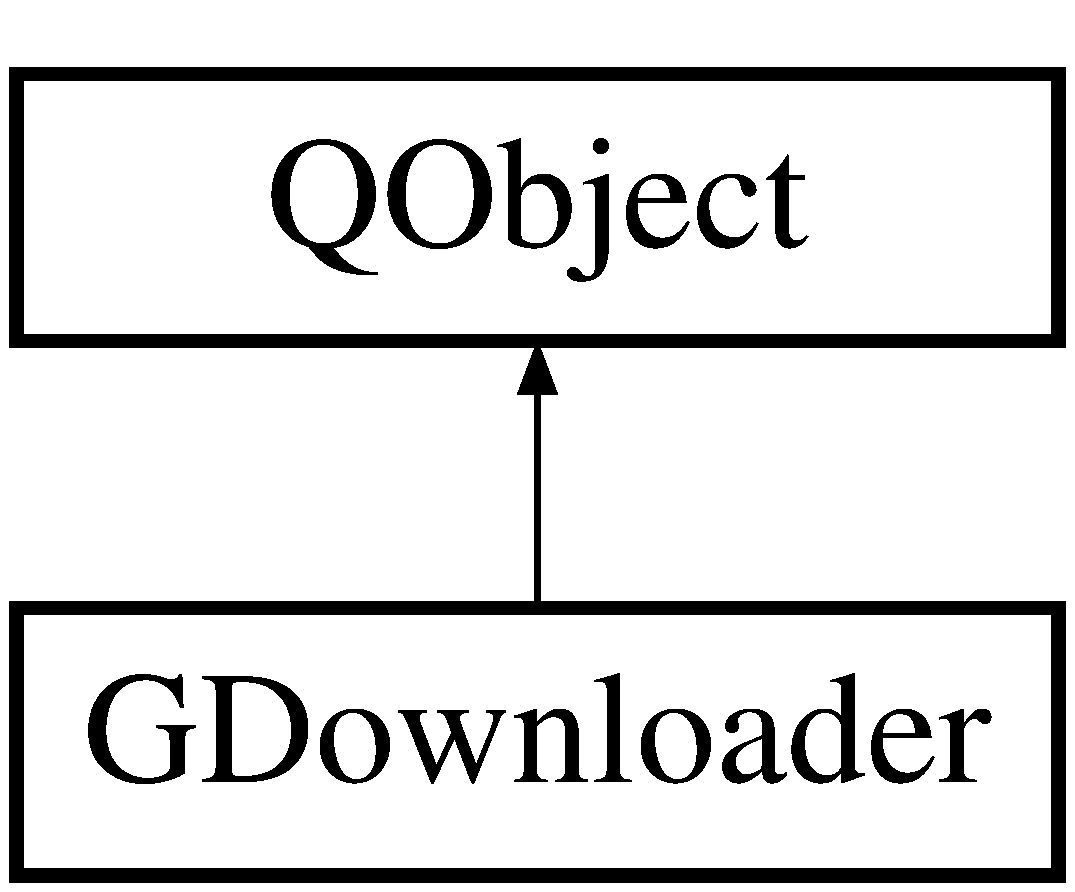
\includegraphics[height=2.000000cm]{classGDownloader}
\end{center}
\end{figure}
\subsection*{Signals}
\begin{DoxyCompactItemize}
\item 
void \mbox{\hyperlink{classGDownloader_abb5cf1dbe464e3dc8943c261934b9a64}{downloaded}} ()
\begin{DoxyCompactList}\small\item\em This Qt signal fires when the data is done downloading. \end{DoxyCompactList}\end{DoxyCompactItemize}
\subsection*{Public Member Functions}
\begin{DoxyCompactItemize}
\item 
\mbox{\hyperlink{classGDownloader_a03a6336ad3aebf9d5904c50ce0cdc1dc}{G\+Downloader}} ()
\begin{DoxyCompactList}\small\item\em Creates a new downloader. \end{DoxyCompactList}\item 
virtual \mbox{\hyperlink{classGDownloader_a6a9f476cb937e98d417d8ab43b8cd8d5}{$\sim$\+G\+Downloader}} ()
\begin{DoxyCompactList}\small\item\em Frees memory allocated internally by the downloader. \end{DoxyCompactList}\item 
std\+::string \mbox{\hyperlink{classGDownloader_a27b002ce17000e199302c608363c97a2}{download\+As\+String}} (const std\+::string \&url)
\begin{DoxyCompactList}\small\item\em Downloads the text contents of the given U\+RL, returning them as a string. \end{DoxyCompactList}\item 
void \mbox{\hyperlink{classGDownloader_a0bf57f044cc66c8aab40f3f2179caf21}{download\+To\+File}} (const std\+::string \&url, const std\+::string \&file)
\begin{DoxyCompactList}\small\item\em Downloads the text contents of the given U\+RL, saving it to the given output file. \end{DoxyCompactList}\item 
std\+::string \mbox{\hyperlink{classGDownloader_adf0cc934eff26878cdf2018259997a4a}{get\+Error\+Message}} () const
\begin{DoxyCompactList}\small\item\em Returns the last H\+T\+TP error message that occurred. \end{DoxyCompactList}\item 
std\+::string \mbox{\hyperlink{classGDownloader_a736d777b29179f52ba753317d84b1087}{get\+Header}} (const std\+::string \&name) const
\begin{DoxyCompactList}\small\item\em Returns the value of the given H\+T\+TP header for this U\+RL request. \end{DoxyCompactList}\item 
int \mbox{\hyperlink{classGDownloader_ab6c069ef77f1319830dcfd90eed6a2ce}{get\+Http\+Status\+Code}} () const
\begin{DoxyCompactList}\small\item\em Returns the most recent H\+T\+TP status code, which may be a successful code (e.\+g. \end{DoxyCompactList}\item 
std\+::string \mbox{\hyperlink{classGDownloader_a479f109234aad1c792be804bf6320c62}{get\+User\+Agent}} () const
\begin{DoxyCompactList}\small\item\em Returns the value of the H\+T\+TP \char`\"{}\+User-\/\+Agent\char`\"{} header for this U\+RL request, or an empty string if the user agent has not been set. \end{DoxyCompactList}\item 
bool \mbox{\hyperlink{classGDownloader_a81dd125e253592aaef5fea33dfc50c42}{has\+Error}} () const
\begin{DoxyCompactList}\small\item\em Returns true if the H\+T\+TP connection failed and had an error. \end{DoxyCompactList}\item 
void \mbox{\hyperlink{classGDownloader_a4bafb98a98bc6edc2403a3734c985618}{http\+Get}} (const std\+::string \&url)
\begin{DoxyCompactList}\small\item\em Performs an H\+T\+TP G\+ET request to the given U\+RL. \end{DoxyCompactList}\item 
void \mbox{\hyperlink{classGDownloader_a68ec0a089bf1b625b86753545e952a57}{http\+Post}} (const std\+::string \&url)
\begin{DoxyCompactList}\small\item\em Performs an H\+T\+TP P\+O\+ST request to the given U\+RL, submitting any headers and query parameters previously specified. \end{DoxyCompactList}\item 
void \mbox{\hyperlink{classGDownloader_af7065da3945b84ffb547b8bad9ddf8dc}{set\+Header}} (const std\+::string \&name, const std\+::string \&value)
\item 
void \mbox{\hyperlink{classGDownloader_a766286050e9b8fe08919f8353ecb4031}{set\+User\+Agent}} (const std\+::string \&user\+Agent)
\end{DoxyCompactItemize}


\subsection{Detailed Description}
A \mbox{\hyperlink{classGDownloader}{G\+Downloader}} can download files and data over an internet connection. 

It can save the data to a file or return the data as a string. 

\subsection{Constructor \& Destructor Documentation}
\mbox{\Hypertarget{classGDownloader_a03a6336ad3aebf9d5904c50ce0cdc1dc}\label{classGDownloader_a03a6336ad3aebf9d5904c50ce0cdc1dc}} 
\index{G\+Downloader@{G\+Downloader}!G\+Downloader@{G\+Downloader}}
\index{G\+Downloader@{G\+Downloader}!G\+Downloader@{G\+Downloader}}
\subsubsection{\texorpdfstring{G\+Downloader()}{GDownloader()}}
{\footnotesize\ttfamily \mbox{\hyperlink{classGDownloader}{G\+Downloader}} (\begin{DoxyParamCaption}{ }\end{DoxyParamCaption})}



Creates a new downloader. 

\mbox{\Hypertarget{classGDownloader_a6a9f476cb937e98d417d8ab43b8cd8d5}\label{classGDownloader_a6a9f476cb937e98d417d8ab43b8cd8d5}} 
\index{G\+Downloader@{G\+Downloader}!````~G\+Downloader@{$\sim$\+G\+Downloader}}
\index{````~G\+Downloader@{$\sim$\+G\+Downloader}!G\+Downloader@{G\+Downloader}}
\subsubsection{\texorpdfstring{$\sim$\+G\+Downloader()}{~GDownloader()}}
{\footnotesize\ttfamily $\sim$\mbox{\hyperlink{classGDownloader}{G\+Downloader}} (\begin{DoxyParamCaption}{ }\end{DoxyParamCaption})\hspace{0.3cm}{\ttfamily [virtual]}}



Frees memory allocated internally by the downloader. 



\subsection{Member Function Documentation}
\mbox{\Hypertarget{classGDownloader_a27b002ce17000e199302c608363c97a2}\label{classGDownloader_a27b002ce17000e199302c608363c97a2}} 
\index{G\+Downloader@{G\+Downloader}!download\+As\+String@{download\+As\+String}}
\index{download\+As\+String@{download\+As\+String}!G\+Downloader@{G\+Downloader}}
\subsubsection{\texorpdfstring{download\+As\+String()}{downloadAsString()}}
{\footnotesize\ttfamily std\+::string download\+As\+String (\begin{DoxyParamCaption}\item[{const std\+::string \&}]{url }\end{DoxyParamCaption})}



Downloads the text contents of the given U\+RL, returning them as a string. 

This method blocks until the data is finished downloading. \mbox{\Hypertarget{classGDownloader_abb5cf1dbe464e3dc8943c261934b9a64}\label{classGDownloader_abb5cf1dbe464e3dc8943c261934b9a64}} 
\index{G\+Downloader@{G\+Downloader}!downloaded@{downloaded}}
\index{downloaded@{downloaded}!G\+Downloader@{G\+Downloader}}
\subsubsection{\texorpdfstring{downloaded}{downloaded}}
{\footnotesize\ttfamily void downloaded (\begin{DoxyParamCaption}{ }\end{DoxyParamCaption})\hspace{0.3cm}{\ttfamily [signal]}}



This Qt signal fires when the data is done downloading. 

\mbox{\Hypertarget{classGDownloader_a0bf57f044cc66c8aab40f3f2179caf21}\label{classGDownloader_a0bf57f044cc66c8aab40f3f2179caf21}} 
\index{G\+Downloader@{G\+Downloader}!download\+To\+File@{download\+To\+File}}
\index{download\+To\+File@{download\+To\+File}!G\+Downloader@{G\+Downloader}}
\subsubsection{\texorpdfstring{download\+To\+File()}{downloadToFile()}}
{\footnotesize\ttfamily void download\+To\+File (\begin{DoxyParamCaption}\item[{const std\+::string \&}]{url,  }\item[{const std\+::string \&}]{file }\end{DoxyParamCaption})}



Downloads the text contents of the given U\+RL, saving it to the given output file. 

This method blocks until the data is finished downloading. \mbox{\Hypertarget{classGDownloader_adf0cc934eff26878cdf2018259997a4a}\label{classGDownloader_adf0cc934eff26878cdf2018259997a4a}} 
\index{G\+Downloader@{G\+Downloader}!get\+Error\+Message@{get\+Error\+Message}}
\index{get\+Error\+Message@{get\+Error\+Message}!G\+Downloader@{G\+Downloader}}
\subsubsection{\texorpdfstring{get\+Error\+Message()}{getErrorMessage()}}
{\footnotesize\ttfamily std\+::string get\+Error\+Message (\begin{DoxyParamCaption}{ }\end{DoxyParamCaption}) const}



Returns the last H\+T\+TP error message that occurred. 

If no H\+T\+TP errors have occurred, returns \char`\"{}\char`\"{}. \mbox{\Hypertarget{classGDownloader_a736d777b29179f52ba753317d84b1087}\label{classGDownloader_a736d777b29179f52ba753317d84b1087}} 
\index{G\+Downloader@{G\+Downloader}!get\+Header@{get\+Header}}
\index{get\+Header@{get\+Header}!G\+Downloader@{G\+Downloader}}
\subsubsection{\texorpdfstring{get\+Header()}{getHeader()}}
{\footnotesize\ttfamily std\+::string get\+Header (\begin{DoxyParamCaption}\item[{const std\+::string \&}]{name }\end{DoxyParamCaption}) const}



Returns the value of the given H\+T\+TP header for this U\+RL request. 

If the given header is not defined, returns an empty string. \mbox{\Hypertarget{classGDownloader_ab6c069ef77f1319830dcfd90eed6a2ce}\label{classGDownloader_ab6c069ef77f1319830dcfd90eed6a2ce}} 
\index{G\+Downloader@{G\+Downloader}!get\+Http\+Status\+Code@{get\+Http\+Status\+Code}}
\index{get\+Http\+Status\+Code@{get\+Http\+Status\+Code}!G\+Downloader@{G\+Downloader}}
\subsubsection{\texorpdfstring{get\+Http\+Status\+Code()}{getHttpStatusCode()}}
{\footnotesize\ttfamily int get\+Http\+Status\+Code (\begin{DoxyParamCaption}{ }\end{DoxyParamCaption}) const}



Returns the most recent H\+T\+TP status code, which may be a successful code (e.\+g. 

200) or an error (e.\+g 404). If there is no H\+T\+TP status code to return, returns 0. \mbox{\Hypertarget{classGDownloader_a479f109234aad1c792be804bf6320c62}\label{classGDownloader_a479f109234aad1c792be804bf6320c62}} 
\index{G\+Downloader@{G\+Downloader}!get\+User\+Agent@{get\+User\+Agent}}
\index{get\+User\+Agent@{get\+User\+Agent}!G\+Downloader@{G\+Downloader}}
\subsubsection{\texorpdfstring{get\+User\+Agent()}{getUserAgent()}}
{\footnotesize\ttfamily std\+::string get\+User\+Agent (\begin{DoxyParamCaption}{ }\end{DoxyParamCaption}) const}



Returns the value of the H\+T\+TP \char`\"{}\+User-\/\+Agent\char`\"{} header for this U\+RL request, or an empty string if the user agent has not been set. 

\mbox{\Hypertarget{classGDownloader_a81dd125e253592aaef5fea33dfc50c42}\label{classGDownloader_a81dd125e253592aaef5fea33dfc50c42}} 
\index{G\+Downloader@{G\+Downloader}!has\+Error@{has\+Error}}
\index{has\+Error@{has\+Error}!G\+Downloader@{G\+Downloader}}
\subsubsection{\texorpdfstring{has\+Error()}{hasError()}}
{\footnotesize\ttfamily bool has\+Error (\begin{DoxyParamCaption}{ }\end{DoxyParamCaption}) const}



Returns true if the H\+T\+TP connection failed and had an error. 

You can see what the error was by calling get\+Error\+Message. \mbox{\Hypertarget{classGDownloader_a4bafb98a98bc6edc2403a3734c985618}\label{classGDownloader_a4bafb98a98bc6edc2403a3734c985618}} 
\index{G\+Downloader@{G\+Downloader}!http\+Get@{http\+Get}}
\index{http\+Get@{http\+Get}!G\+Downloader@{G\+Downloader}}
\subsubsection{\texorpdfstring{http\+Get()}{httpGet()}}
{\footnotesize\ttfamily void http\+Get (\begin{DoxyParamCaption}\item[{const std\+::string \&}]{url }\end{DoxyParamCaption})}



Performs an H\+T\+TP G\+ET request to the given U\+RL. 

along with any headers previously specified. \mbox{\Hypertarget{classGDownloader_a68ec0a089bf1b625b86753545e952a57}\label{classGDownloader_a68ec0a089bf1b625b86753545e952a57}} 
\index{G\+Downloader@{G\+Downloader}!http\+Post@{http\+Post}}
\index{http\+Post@{http\+Post}!G\+Downloader@{G\+Downloader}}
\subsubsection{\texorpdfstring{http\+Post()}{httpPost()}}
{\footnotesize\ttfamily void http\+Post (\begin{DoxyParamCaption}\item[{const std\+::string \&}]{url }\end{DoxyParamCaption})}



Performs an H\+T\+TP P\+O\+ST request to the given U\+RL, submitting any headers and query parameters previously specified. 

\mbox{\Hypertarget{classGDownloader_af7065da3945b84ffb547b8bad9ddf8dc}\label{classGDownloader_af7065da3945b84ffb547b8bad9ddf8dc}} 
\index{G\+Downloader@{G\+Downloader}!set\+Header@{set\+Header}}
\index{set\+Header@{set\+Header}!G\+Downloader@{G\+Downloader}}
\subsubsection{\texorpdfstring{set\+Header()}{setHeader()}}
{\footnotesize\ttfamily void set\+Header (\begin{DoxyParamCaption}\item[{const std\+::string \&}]{name,  }\item[{const std\+::string \&}]{value }\end{DoxyParamCaption})}

\mbox{\Hypertarget{classGDownloader_a766286050e9b8fe08919f8353ecb4031}\label{classGDownloader_a766286050e9b8fe08919f8353ecb4031}} 
\index{G\+Downloader@{G\+Downloader}!set\+User\+Agent@{set\+User\+Agent}}
\index{set\+User\+Agent@{set\+User\+Agent}!G\+Downloader@{G\+Downloader}}
\subsubsection{\texorpdfstring{set\+User\+Agent()}{setUserAgent()}}
{\footnotesize\ttfamily void set\+User\+Agent (\begin{DoxyParamCaption}\item[{const std\+::string \&}]{user\+Agent }\end{DoxyParamCaption})}


\hypertarget{classGDrawingSurface}{}\section{G\+Drawing\+Surface Class Reference}
\label{classGDrawingSurface}\index{G\+Drawing\+Surface@{G\+Drawing\+Surface}}


\mbox{\hyperlink{classGDrawingSurface}{G\+Drawing\+Surface}} is an abstract superclass for types that allow drawing shapes and pixels onto themselves as a pixel background layer.  




{\ttfamily \#include $<$gdrawingsurface.\+h$>$}

Inheritance diagram for G\+Drawing\+Surface\+:\begin{figure}[H]
\begin{center}
\leavevmode
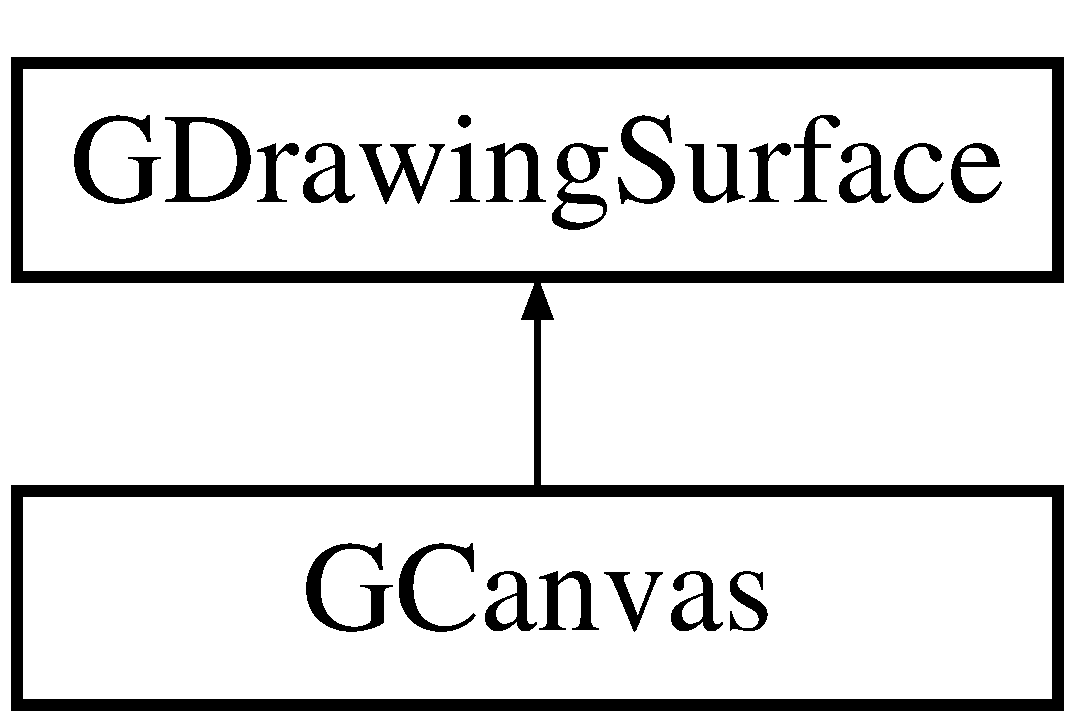
\includegraphics[height=2.000000cm]{classGDrawingSurface}
\end{center}
\end{figure}
\subsection*{Public Member Functions}
\begin{DoxyCompactItemize}
\item 
virtual void \mbox{\hyperlink{classGDrawingSurface_a5eeb94d22b8366d1b68d0614384802fe}{clear}} ()=0
\begin{DoxyCompactList}\small\item\em Erases any pixel data from the drawing surface. \end{DoxyCompactList}\item 
virtual void \mbox{\hyperlink{classGDrawingSurface_a221b3e75bb3d9d0bfea62b3364e6773b}{conditional\+Repaint}} ()
\begin{DoxyCompactList}\small\item\em Repaints the interactor only if its contents have changed. \end{DoxyCompactList}\item 
virtual void \mbox{\hyperlink{classGDrawingSurface_aedd4b792311d946eeaf44b0de337a408}{conditional\+Repaint\+Region}} (int x, int y, int width, int height)
\begin{DoxyCompactList}\small\item\em Repaints the given region of the interactor only if its contents have changed. \end{DoxyCompactList}\item 
virtual void \mbox{\hyperlink{classGDrawingSurface_a3932a12278752db368e24fa404e446aa}{conditional\+Repaint\+Region}} (const \mbox{\hyperlink{classGRectangle}{G\+Rectangle}} \&bounds)
\begin{DoxyCompactList}\small\item\em Repaints the given region of the interactor only if its contents have changed. \end{DoxyCompactList}\item 
virtual void \mbox{\hyperlink{classGDrawingSurface_ae65b7cc9bdfbc1bd01bec80ba83aab47}{draw}} (\mbox{\hyperlink{classGObject}{G\+Object}} $\ast$gobj)=0
\begin{DoxyCompactList}\small\item\em Draws the given graphical object onto the background pixel layer of this interactor. \end{DoxyCompactList}\item 
virtual void \mbox{\hyperlink{classGDrawingSurface_acc3825d7a24815d1e2f78e7c3ffea6cc}{draw}} (\mbox{\hyperlink{classGObject}{G\+Object}} $\ast$gobj, double x, double y)
\begin{DoxyCompactList}\small\item\em Draws the given graphical object onto the background pixel layer of this interactor, moving it to the given x/y location first. \end{DoxyCompactList}\item 
virtual void \mbox{\hyperlink{classGDrawingSurface_a022a8d51c7fabcd79a0c809233e93453}{draw}} (\mbox{\hyperlink{classGObject}{G\+Object}} \&gobj)
\begin{DoxyCompactList}\small\item\em Draws the given graphical object onto the background pixel layer of this interactor. \end{DoxyCompactList}\item 
virtual void \mbox{\hyperlink{classGDrawingSurface_a8af8762bd6720e0a1d2a84b190e3dc96}{draw}} (\mbox{\hyperlink{classGObject}{G\+Object}} \&gobj, double x, double y)
\begin{DoxyCompactList}\small\item\em Draws the given graphical object onto the background pixel layer of this interactor, moving it to the given x/y location first. \end{DoxyCompactList}\item 
virtual void \mbox{\hyperlink{classGDrawingSurface_a38b6fae1045191c57092b49905068144}{draw\+Arc}} (double x, double y, double width, double height, double start, double sweep)
\begin{DoxyCompactList}\small\item\em Draws an unfilled arc with the given attributes onto the background pixel layer of this interactor in the current color. \end{DoxyCompactList}\item 
virtual void \mbox{\hyperlink{classGDrawingSurface_abdd4cb1f2c64adc5d03522a1ee30febf}{draw\+Image}} (const std\+::string \&filename, double x=0, double y=0)
\begin{DoxyCompactList}\small\item\em Draws an image loaded from the given file name onto the background pixel layer of this interactor at the given x/y location. \end{DoxyCompactList}\item 
virtual void \mbox{\hyperlink{classGDrawingSurface_ae6a24b6b9a6e795d3165c1c750d5bdf1}{draw\+Line}} (const \mbox{\hyperlink{classGPoint}{G\+Point}} \&p0, const \mbox{\hyperlink{classGPoint}{G\+Point}} \&p1)
\begin{DoxyCompactList}\small\item\em Draws a line between the given two points onto the background pixel layer of this interactor at the given x/y location in the current color. \end{DoxyCompactList}\item 
virtual void \mbox{\hyperlink{classGDrawingSurface_aff299fe83178d2f3ce8c08c06b583484}{draw\+Line}} (double x0, double y0, double x1, double y1)
\begin{DoxyCompactList}\small\item\em Draws a line between the given two points onto the background pixel layer of this interactor at the given x/y location in the current color. \end{DoxyCompactList}\item 
virtual void \mbox{\hyperlink{classGDrawingSurface_a8adc13027efe311b4a6a715205b8bc46}{draw\+Oval}} (const \mbox{\hyperlink{classGRectangle}{G\+Rectangle}} \&bounds)
\begin{DoxyCompactList}\small\item\em Draws an unfilled oval with the given bounding box onto the background pixel layer of this interactor at the given x/y location in the current color. \end{DoxyCompactList}\item 
virtual void \mbox{\hyperlink{classGDrawingSurface_aa5b1cf902e578907da3c63060686354e}{draw\+Oval}} (double x, double y, double width, double height)
\begin{DoxyCompactList}\small\item\em Draws an unfilled oval with the given bounding box onto the background pixel layer of this interactor at the given x/y location in the current color. \end{DoxyCompactList}\item 
virtual void \mbox{\hyperlink{classGDrawingSurface_a0c1e2923d8d163d62d0896d8c5cfa191}{draw\+Pixel}} (double x, double y)
\begin{DoxyCompactList}\small\item\em Colors the given x/y pixel of the background layer of this interactor using the interactor\textquotesingle{}s current color. \end{DoxyCompactList}\item 
virtual void \mbox{\hyperlink{classGDrawingSurface_a3a64eb6383e601be8438e9c71643c432}{draw\+Pixel}} (double x, double y, int color)
\begin{DoxyCompactList}\small\item\em Colors the given x/y pixel of the background layer of this interactor using the given color. \end{DoxyCompactList}\item 
virtual void \mbox{\hyperlink{classGDrawingSurface_a20abc26a94b7eb310e34abf668e0f5f4}{draw\+Pixel}} (double x, double y, const std\+::string \&color)
\begin{DoxyCompactList}\small\item\em Colors the given x/y pixel of the background layer of this interactor using the given color. \end{DoxyCompactList}\item 
virtual \mbox{\hyperlink{classGPoint}{G\+Point}} \mbox{\hyperlink{classGDrawingSurface_af70cce1e4f708f1ed5b6f29cecb660e7}{draw\+Polar\+Line}} (const \mbox{\hyperlink{classGPoint}{G\+Point}} \&p0, double r, double theta)
\begin{DoxyCompactList}\small\item\em Draws a line using polar coordinates onto the background pixel layer of this interactor in the current color. \end{DoxyCompactList}\item 
virtual \mbox{\hyperlink{classGPoint}{G\+Point}} \mbox{\hyperlink{classGDrawingSurface_ad3e646f90005295f2bbdf37d2bcb39d2}{draw\+Polar\+Line}} (double x0, double y0, double r, double theta)
\begin{DoxyCompactList}\small\item\em Draws a line using polar coordinates onto the background pixel layer of this interactor in the current color. \end{DoxyCompactList}\item 
virtual void \mbox{\hyperlink{classGDrawingSurface_afddec0a905108d8a8d6809a157f26776}{draw\+Polygon}} (std\+::initializer\+\_\+list$<$ double $>$ coords)
\begin{DoxyCompactList}\small\item\em Draws an unfilled polygon containing the given points onto the background pixel layer of this interactor in the current color. \end{DoxyCompactList}\item 
virtual void \mbox{\hyperlink{classGDrawingSurface_a021ee881e0d154dc4dd059698742889c}{draw\+Polygon}} (std\+::initializer\+\_\+list$<$ \mbox{\hyperlink{classGPoint}{G\+Point}} $>$ points)
\begin{DoxyCompactList}\small\item\em Draws an unfilled polygon containing the given points onto the background pixel layer of this interactor in the current color. \end{DoxyCompactList}\item 
virtual void \mbox{\hyperlink{classGDrawingSurface_a3dd4cc5891149dfc36746264f7289877}{draw\+Rect}} (const \mbox{\hyperlink{classGRectangle}{G\+Rectangle}} \&bounds)
\begin{DoxyCompactList}\small\item\em Draws an unfilled rectangle of the given dimensions onto the background pixel layer of this interactor in the current color. \end{DoxyCompactList}\item 
virtual void \mbox{\hyperlink{classGDrawingSurface_a4148e770ffc5474153aadd4814dbd708}{draw\+Rect}} (double x, double y, double width, double height)
\begin{DoxyCompactList}\small\item\em Draws an unfilled rectangle of the given dimensions onto the background pixel layer of this interactor in the current color. \end{DoxyCompactList}\item 
virtual void \mbox{\hyperlink{classGDrawingSurface_ad4e8551a753a77135792bbee97013675}{draw\+String}} (const std\+::string \&text, double x, double y)
\begin{DoxyCompactList}\small\item\em Draws a text string onto the background pixel layer of this interactor at the given x/y location in the current font and color. \end{DoxyCompactList}\item 
virtual void \mbox{\hyperlink{classGDrawingSurface_a228075ad18bd97b57f9956568c4773f3}{fill\+Arc}} (double x, double y, double width, double height, double start, double sweep)
\begin{DoxyCompactList}\small\item\em Draws a filled arc with the given attributes onto the background pixel layer of this interactor in the current color and fill color. \end{DoxyCompactList}\item 
virtual void \mbox{\hyperlink{classGDrawingSurface_a1ea6e48d59fb588797dba4deab1397e0}{fill\+Oval}} (const \mbox{\hyperlink{classGRectangle}{G\+Rectangle}} \&bounds)
\begin{DoxyCompactList}\small\item\em Draws a filled oval with the given bounding box onto the background pixel layer of this interactor at the given x/y location in the current color and fill color. \end{DoxyCompactList}\item 
virtual void \mbox{\hyperlink{classGDrawingSurface_a28c700c82f31cd328a4629273420ee61}{fill\+Oval}} (double x, double y, double width, double height)
\begin{DoxyCompactList}\small\item\em Draws a filled oval with the given bounding box onto the background pixel layer of this interactor at the given x/y location in the current color and fill color. \end{DoxyCompactList}\item 
virtual void \mbox{\hyperlink{classGDrawingSurface_a15f8c1c4409ef51c1a30a92a195b8f66}{fill\+Polygon}} (std\+::initializer\+\_\+list$<$ double $>$ coords)
\begin{DoxyCompactList}\small\item\em Draws a filled polygon containing the given points onto the background pixel layer of this interactor in the current color and fill color. \end{DoxyCompactList}\item 
virtual void \mbox{\hyperlink{classGDrawingSurface_ae6582295003bf2488836b1993dadbad7}{fill\+Rect}} (const \mbox{\hyperlink{classGRectangle}{G\+Rectangle}} \&bounds)
\begin{DoxyCompactList}\small\item\em Draws a filled rectangle of the given dimensions onto the background pixel layer of this interactor in the current color and fill color. \end{DoxyCompactList}\item 
virtual void \mbox{\hyperlink{classGDrawingSurface_aac3ae7d3aee950de78eca0e108352254}{fill\+Rect}} (double x, double y, double width, double height)
\begin{DoxyCompactList}\small\item\em Draws a filled rectangle of the given dimensions onto the background pixel layer of this interactor in the current color and fill color. \end{DoxyCompactList}\item 
virtual int \mbox{\hyperlink{classGDrawingSurface_ae394d39f20476570e083918d991c25bd}{get\+A\+R\+GB}} (double x, double y) const
\begin{DoxyCompactList}\small\item\em Returns the pixel color data at the given x/y location, retaining alpha-\/channel transparency in the top 8 bits. \end{DoxyCompactList}\item 
virtual std\+::string \mbox{\hyperlink{classGDrawingSurface_a808e22cc1fdfbecf71ed8c64ef4600e0}{get\+Background}} () const
\begin{DoxyCompactList}\small\item\em Returns the current background color of the interactor as a string. \end{DoxyCompactList}\item 
virtual int \mbox{\hyperlink{classGDrawingSurface_a9e827257a55cb8cf4d9de2ec6bcfd7a0}{get\+Background\+Int}} () const
\begin{DoxyCompactList}\small\item\em Returns the current background color of the interactor as an R\+GB integer. \end{DoxyCompactList}\item 
virtual std\+::string \mbox{\hyperlink{classGDrawingSurface_aa061dfa488c31e18549d64363c1d0e34}{get\+Color}} () const
\begin{DoxyCompactList}\small\item\em Returns the current foreground outline color of the interactor as a string. \end{DoxyCompactList}\item 
virtual int \mbox{\hyperlink{classGDrawingSurface_a9635c7af766cdc3417f346683fa0e6c1}{get\+Color\+Int}} () const
\begin{DoxyCompactList}\small\item\em Returns the current foreground outline color of the interactor as an R\+GB integer. \end{DoxyCompactList}\item 
virtual std\+::string \mbox{\hyperlink{classGDrawingSurface_a76f6964a11fde7c78e9751be184e1a3c}{get\+Fill\+Color}} () const
\begin{DoxyCompactList}\small\item\em Returns the current fill color of the interactor as a string. \end{DoxyCompactList}\item 
virtual int \mbox{\hyperlink{classGDrawingSurface_a88f4508d9271c4b5f5b5d6b780f223d0}{get\+Fill\+Color\+Int}} () const
\begin{DoxyCompactList}\small\item\em Returns the current fill color of the interactor as an R\+GB integer. \end{DoxyCompactList}\item 
virtual std\+::string \mbox{\hyperlink{classGDrawingSurface_a894a5502900794eeb27d084c21f1d77d}{get\+Font}} () const
\begin{DoxyCompactList}\small\item\em Returns the current text font of the interactor as a font string. \end{DoxyCompactList}\item 
virtual std\+::string \mbox{\hyperlink{classGDrawingSurface_a4fa2d8b0192a3a5b4af4bbfe71194d03}{get\+Foreground}} () const
\begin{DoxyCompactList}\small\item\em Returns the current foreground outline color of the interactor as a string. \end{DoxyCompactList}\item 
virtual int \mbox{\hyperlink{classGDrawingSurface_ac3b12ab385a6ef9ae90fc879860ba726}{get\+Foreground\+Int}} () const
\begin{DoxyCompactList}\small\item\em Returns the current foreground outline color of the interactor as an R\+GB integer. \end{DoxyCompactList}\item 
virtual \mbox{\hyperlink{classGObject_a86e0f5648542856159bb40775c854aa7}{G\+Object\+::\+Line\+Style}} \mbox{\hyperlink{classGDrawingSurface_aaf1f5ea8281e5e3486662878d26f0a13}{get\+Line\+Style}} () const
\begin{DoxyCompactList}\small\item\em Returns the current line style which will be used to draw outlines of shapes and lines. \end{DoxyCompactList}\item 
virtual double \mbox{\hyperlink{classGDrawingSurface_a85ff266dc3eb63d9f2d8e5a4487fd3c0}{get\+Line\+Width}} () const
\begin{DoxyCompactList}\small\item\em Returns the thickness used when drawing outlines of shapes and lines. \end{DoxyCompactList}\item 
virtual int \mbox{\hyperlink{classGDrawingSurface_a40f3e3f64a8263e13b7162e15b2979ee}{get\+Pixel}} (double x, double y) const =0
\begin{DoxyCompactList}\small\item\em Returns the color of the pixel at the given x/y coordinates of the background layer of the interactor as an integer such as 0xff00cc. \end{DoxyCompactList}\item 
virtual int \mbox{\hyperlink{classGDrawingSurface_aee10de1ca7da1fc3f3fc0e48286f88f8}{get\+Pixel\+A\+R\+GB}} (double x, double y) const =0
\begin{DoxyCompactList}\small\item\em Returns the color of the pixel at the given x/y coordinates of the background layer of the interactor as an integer such as 0xffff00cc. \end{DoxyCompactList}\item 
virtual \mbox{\hyperlink{classGrid}{Grid}}$<$ int $>$ \mbox{\hyperlink{classGDrawingSurface_a9811240b1241922153dec17d395797cf}{get\+Pixels}} () const =0
\begin{DoxyCompactList}\small\item\em Returns all pixels of the surface as a \mbox{\hyperlink{classGrid}{Grid}}, where rows represent y values and columns represent x values. \end{DoxyCompactList}\item 
virtual \mbox{\hyperlink{classGrid}{Grid}}$<$ int $>$ \mbox{\hyperlink{classGDrawingSurface_a5712954f3edce2e1e4dd3109ffe16e05}{get\+Pixels\+A\+R\+GB}} () const =0
\begin{DoxyCompactList}\small\item\em Returns all pixels of the background layer of the surface as a \mbox{\hyperlink{classGrid}{Grid}}, where rows represent y values and columns represent x values. \end{DoxyCompactList}\item 
virtual std\+::string \mbox{\hyperlink{classGDrawingSurface_a8da04ef488ec5fa498fbbffaf50928fd}{get\+Pixel\+String}} (double x, double y) const
\begin{DoxyCompactList}\small\item\em Returns the color of the pixel at the given x/y coordinates of the image as a string such as \char`\"{}\#ff00cc\char`\"{}. \end{DoxyCompactList}\item 
virtual int \mbox{\hyperlink{classGDrawingSurface_a9e983467cf0c97cfd62433a8471570dc}{get\+R\+GB}} (double x, double y) const
\begin{DoxyCompactList}\small\item\em Returns the color of the pixel at the given x/y coordinates of the background layer of the interactor as an integer such as 0xff00cc. \end{DoxyCompactList}\item 
virtual std\+::string \mbox{\hyperlink{classGDrawingSurface_a456d3582acc3544f37d939f5cb8802fe}{get\+R\+G\+B\+String}} (double x, double y) const
\begin{DoxyCompactList}\small\item\em Returns the color of the pixel at the given x/y coordinates of the background layer of the interactor as a color string such as \char`\"{}\#ff00cc\char`\"{}. \end{DoxyCompactList}\item 
virtual bool \mbox{\hyperlink{classGDrawingSurface_a12c8d52ddfcaa5448ec4bace92ddee6c}{is\+Auto\+Repaint}} () const
\begin{DoxyCompactList}\small\item\em Returns true if the interactor should repaint itself automatically whenever any change is made to its graphical data. \end{DoxyCompactList}\item 
virtual bool \mbox{\hyperlink{classGDrawingSurface_a82a00267c81cc0ae85ee0feb01a92fa8}{is\+Repaint\+Immediately}} () const
\begin{DoxyCompactList}\small\item\em Returns true if the interactor should repaint itself automatically whenever any change is made to its graphical data. \end{DoxyCompactList}\item 
virtual void \mbox{\hyperlink{classGDrawingSurface_a4a8ae47b42f1e6a41b65d3546df46218}{repaint}} ()=0
\begin{DoxyCompactList}\small\item\em Instructs the interactor to redraw itself on the screen. \end{DoxyCompactList}\item 
virtual void \mbox{\hyperlink{classGDrawingSurface_a1a3898317080fecf8af21bbeaeeb37c3}{repaint\+Region}} (int x, int y, int width, int height)=0
\begin{DoxyCompactList}\small\item\em Instructs the interactor to repaint the given region of pixel data. \end{DoxyCompactList}\item 
virtual void \mbox{\hyperlink{classGDrawingSurface_a769c46fb3e1004aec76e8b0adfa42aa6}{repaint\+Region}} (const \mbox{\hyperlink{classGRectangle}{G\+Rectangle}} \&bounds)
\begin{DoxyCompactList}\small\item\em Instructs the interactor to repaint the given region of pixel data. \end{DoxyCompactList}\item 
virtual void \mbox{\hyperlink{classGDrawingSurface_adf10848319457bd6df4c657bf8872bee}{set\+Auto\+Repaint}} (bool auto\+Repaint)
\begin{DoxyCompactList}\small\item\em Sets whether the interactor should repaint itself automatically whenever any change is made to its graphical data. \end{DoxyCompactList}\item 
virtual void \mbox{\hyperlink{classGDrawingSurface_aba673fd56570a074aba10fa059524b96}{set\+Background}} (int color)
\begin{DoxyCompactList}\small\item\em Sets the current background color of the interactor as an R\+GB integer. \end{DoxyCompactList}\item 
virtual void \mbox{\hyperlink{classGDrawingSurface_ab4677ab2474e68b07aa56605af92a84a}{set\+Background}} (const std\+::string \&color)
\begin{DoxyCompactList}\small\item\em Sets the current background color of the interactor as a string. \end{DoxyCompactList}\item 
virtual void \mbox{\hyperlink{classGDrawingSurface_a75b9cb32ff80bf061791beb01a8433d0}{set\+Color}} (int color)
\begin{DoxyCompactList}\small\item\em Sets the current foreground outline color of the interactor as as R\+GB integer. \end{DoxyCompactList}\item 
virtual void \mbox{\hyperlink{classGDrawingSurface_a61374df6c11b52cfbb0815decdbaebc6}{set\+Color}} (const std\+::string \&color)
\begin{DoxyCompactList}\small\item\em Sets the current foreground outline color of the interactor as a string. \end{DoxyCompactList}\item 
virtual void \mbox{\hyperlink{classGDrawingSurface_a47fad447b715f2f303538434eed26709}{set\+Fill\+Color}} (int color)
\begin{DoxyCompactList}\small\item\em Sets the current fill color of the interactor as an R\+GB integer. \end{DoxyCompactList}\item 
virtual void \mbox{\hyperlink{classGDrawingSurface_adbc18b1a930aadd97d7437f9f7265b96}{set\+Fill\+Color}} (const std\+::string \&color)
\begin{DoxyCompactList}\small\item\em Returns the current fill color of the interactor as a string. \end{DoxyCompactList}\item 
virtual void \mbox{\hyperlink{classGDrawingSurface_a8e096e8818d838aceae1d46d58fb3a7b}{set\+Font}} (const std\+::string \&font)
\begin{DoxyCompactList}\small\item\em Sets the current text font of the interactor as a font string. \end{DoxyCompactList}\item 
virtual void \mbox{\hyperlink{classGDrawingSurface_a7daa57084b5811b598fce8726660b328}{set\+Foreground}} (int color)
\begin{DoxyCompactList}\small\item\em Sets the current foreground outline color of the interactor as an R\+GB integer. \end{DoxyCompactList}\item 
virtual void \mbox{\hyperlink{classGDrawingSurface_af59209aeadea6dfc6d97a2d8531f50e1}{set\+Foreground}} (const std\+::string \&color)
\begin{DoxyCompactList}\small\item\em Sets the current foreground outline color of the interactor as a string. \end{DoxyCompactList}\item 
virtual void \mbox{\hyperlink{classGDrawingSurface_a6bfe14a77101db0fb97b5a7e07a5526b}{set\+Line\+Style}} (\mbox{\hyperlink{classGObject_a86e0f5648542856159bb40775c854aa7}{G\+Object\+::\+Line\+Style}} line\+Style)
\begin{DoxyCompactList}\small\item\em Sets the current line style which will be used to draw outlines of shapes and lines. \end{DoxyCompactList}\item 
virtual void \mbox{\hyperlink{classGDrawingSurface_afd6a47c6ea6a1f85ca05a65ba3ff3477}{set\+Line\+Width}} (double line\+Width)
\begin{DoxyCompactList}\small\item\em Sets the thickness used when drawing outlines of shapes and lines. \end{DoxyCompactList}\item 
virtual void \mbox{\hyperlink{classGDrawingSurface_ac9f0a75ccb0abe1123046bab56479b84}{set\+Pixel}} (double x, double y, int rgb)=0
\begin{DoxyCompactList}\small\item\em Sets the color of the given x/y pixel in the background layer of the interactor to the given R\+GB values. \end{DoxyCompactList}\item 
virtual void \mbox{\hyperlink{classGDrawingSurface_aec90e927c9da286214908d3f9da685d7}{set\+Pixel}} (double x, double y, int r, int g, int b)
\begin{DoxyCompactList}\small\item\em Sets the color of the given x/y pixel in the background layer of the interactor to the given R\+GB values. \end{DoxyCompactList}\item 
virtual void \mbox{\hyperlink{classGDrawingSurface_a09f9640e4ff7388dcfc391efd88d2415}{set\+Pixel}} (double x, double y, const std\+::string \&color)
\begin{DoxyCompactList}\small\item\em Sets the color of the given x/y pixel in the background layer of the interactor to the given color. \end{DoxyCompactList}\item 
virtual void \mbox{\hyperlink{classGDrawingSurface_ab2f7c5a9462f552ad3f30d23c04605dd}{set\+Pixel\+A\+R\+GB}} (double x, double y, int argb)=0
\begin{DoxyCompactList}\small\item\em Sets the color of the given x/y pixel in the background layer of the interactor to the given A\+R\+GB value. \end{DoxyCompactList}\item 
virtual void \mbox{\hyperlink{classGDrawingSurface_a62a8b1555ae3a073a84b0a1c071c65b1}{set\+Pixel\+A\+R\+GB}} (double x, double y, int a, int r, int g, int b)
\begin{DoxyCompactList}\small\item\em Sets the color of the given x/y pixel in the background layer of the interactor to the given A\+R\+GB value. \end{DoxyCompactList}\item 
virtual void \mbox{\hyperlink{classGDrawingSurface_aa80f4b7381bd418116baee600eed37fe}{set\+Pixels}} (const \mbox{\hyperlink{classGrid}{Grid}}$<$ int $>$ \&pixels)=0
\begin{DoxyCompactList}\small\item\em Sets the color of the all pixels in the background layer of the interactor to the given R\+GB values, using rows as y-\/values and columns as x-\/values. \end{DoxyCompactList}\item 
virtual void \mbox{\hyperlink{classGDrawingSurface_a7d813f0f29751a217201f24cef402306}{set\+Pixels\+A\+R\+GB}} (const \mbox{\hyperlink{classGrid}{Grid}}$<$ int $>$ \&pixels\+A\+R\+GB)=0
\begin{DoxyCompactList}\small\item\em Sets the color of the all pixels in the background layer of the interactor to the given A\+R\+GB values, using rows as y-\/values and columns as x-\/values. \end{DoxyCompactList}\item 
virtual void \mbox{\hyperlink{classGDrawingSurface_abf5590a3992dcb7896ed449e65961da3}{set\+Repaint\+Immediately}} (bool auto\+Repaint)
\begin{DoxyCompactList}\small\item\em Sets whether the interactor should repaint itself automatically whenever any change is made to its graphical data. \end{DoxyCompactList}\item 
virtual void \mbox{\hyperlink{classGDrawingSurface_a8bcbd65fa784bdab1e66a9efd381162d}{set\+R\+GB}} (double x, double y, int rgb)
\begin{DoxyCompactList}\small\item\em Sets the color of the given x/y pixel in the background layer of the interactor to the given R\+GB values. \end{DoxyCompactList}\item 
virtual void \mbox{\hyperlink{classGDrawingSurface_a81202471d4fc9f2015aef0bc073acfab}{set\+R\+GB}} (double x, double y, int r, int g, int b)
\begin{DoxyCompactList}\small\item\em Sets the color of the given x/y pixel in the background layer of the interactor to the given R\+GB values. \end{DoxyCompactList}\item 
virtual void \mbox{\hyperlink{classGDrawingSurface_ae9a228792d4bb4b628350f39eaa3ad12}{set\+R\+GB}} (double x, double y, const std\+::string \&color)
\begin{DoxyCompactList}\small\item\em Sets the color of the given x/y pixel in the background layer of the interactor to the given color. \end{DoxyCompactList}\end{DoxyCompactItemize}
\subsection*{Protected Member Functions}
\begin{DoxyCompactItemize}
\item 
\mbox{\hyperlink{classGDrawingSurface_a58ecf070e0880ac371754b3e6b4fd970}{G\+Drawing\+Surface}} ()
\item 
virtual \mbox{\hyperlink{classGDrawingSurface_a8e2c882a0c4e31fcbcbb86a207425c1f}{$\sim$\+G\+Drawing\+Surface}} ()
\item 
void \mbox{\hyperlink{classGDrawingSurface_a3a690bcb2d62250c9e4722ad7c1b9ab6}{check\+Bounds}} (const std\+::string \&member, double x, double y, double width, double height) const
\begin{DoxyCompactList}\small\item\em Throws an error if the given x/y values are out of bounds. \end{DoxyCompactList}\item 
void \mbox{\hyperlink{classGDrawingSurface_a9841b5dc607ca41a14819d80e1d8a09c}{check\+Color}} (const std\+::string \&member, int rgb) const
\begin{DoxyCompactList}\small\item\em Throws an error if the given rgb value is not a valid color. \end{DoxyCompactList}\item 
void \mbox{\hyperlink{classGDrawingSurface_a70a6546707ae708573396616bd0f5320}{check\+Size}} (const std\+::string \&member, double width, double height) const
\begin{DoxyCompactList}\small\item\em Throws an error if the given width/height values are out of bounds. \end{DoxyCompactList}\item 
virtual void \mbox{\hyperlink{classGDrawingSurface_a814498efebc5586645159cd22990cf61}{initialize\+G\+Object}} (\mbox{\hyperlink{classGObject}{G\+Object}} \&obj, bool filled=false)
\begin{DoxyCompactList}\small\item\em Initializes a new graphical object to be drawn. \end{DoxyCompactList}\item 
virtual void \mbox{\hyperlink{classGDrawingSurface_a43e6bc951980da061ddc40407daee227}{initialize\+G\+Object}} (\mbox{\hyperlink{classGObject}{G\+Object}} $\ast$obj, bool filled=false)
\begin{DoxyCompactList}\small\item\em Initializes a new graphical object to be drawn. \end{DoxyCompactList}\end{DoxyCompactItemize}
\subsection*{Protected Attributes}
\begin{DoxyCompactItemize}
\item 
bool \mbox{\hyperlink{classGDrawingSurface_a738dd6afc69ac536ad46cf4d89a90933}{\+\_\+auto\+Repaint}}
\item 
std\+::string \mbox{\hyperlink{classGDrawingSurface_ad233544ea51cf6b435a199f3e3790607}{\+\_\+background\+Color}}
\item 
int \mbox{\hyperlink{classGDrawingSurface_abb8452ab4f23ecf455b9e021bf09ef91}{\+\_\+background\+Color\+Int}}
\item 
std\+::string \mbox{\hyperlink{classGDrawingSurface_a1134e770ae4315ea8bc1201e2f21da8b}{\+\_\+color}}
\item 
int \mbox{\hyperlink{classGDrawingSurface_a003fdd343d9b7505c53a8b7a134200ed}{\+\_\+color\+Int}}
\item 
std\+::string \mbox{\hyperlink{classGDrawingSurface_a179f8d6cee65cd8a54692e32b224392a}{\+\_\+fill\+Color}}
\item 
int \mbox{\hyperlink{classGDrawingSurface_a751def333a67d651e5b99cc331ecb496}{\+\_\+fill\+Color\+Int}}
\item 
std\+::string \mbox{\hyperlink{classGDrawingSurface_aea76ea1a8b5dd7b0a78653277e63b536}{\+\_\+font}}
\item 
\mbox{\hyperlink{classGDrawingSurface}{G\+Drawing\+Surface}} $\ast$ \mbox{\hyperlink{classGDrawingSurface_acbb02fa2a4a51a450fd1cc64dfc39ddd}{\+\_\+forward\+Target}}
\item 
\mbox{\hyperlink{classGObject_a86e0f5648542856159bb40775c854aa7}{G\+Object\+::\+Line\+Style}} \mbox{\hyperlink{classGDrawingSurface_ae15d02c66691247a6824dc5943a620e2}{\+\_\+line\+Style}}
\item 
double \mbox{\hyperlink{classGDrawingSurface_a16e9033665937f13de2e163dc2184aff}{\+\_\+line\+Width}}
\end{DoxyCompactItemize}


\subsection{Detailed Description}
\mbox{\hyperlink{classGDrawingSurface}{G\+Drawing\+Surface}} is an abstract superclass for types that allow drawing shapes and pixels onto themselves as a pixel background layer. 

This includes graphical canvas objects (\mbox{\hyperlink{classGCanvas}{G\+Canvas}}) as well as windows (\mbox{\hyperlink{classGWindow}{G\+Window}}). 

\subsection{Constructor \& Destructor Documentation}
\mbox{\Hypertarget{classGDrawingSurface_a58ecf070e0880ac371754b3e6b4fd970}\label{classGDrawingSurface_a58ecf070e0880ac371754b3e6b4fd970}} 
\index{G\+Drawing\+Surface@{G\+Drawing\+Surface}!G\+Drawing\+Surface@{G\+Drawing\+Surface}}
\index{G\+Drawing\+Surface@{G\+Drawing\+Surface}!G\+Drawing\+Surface@{G\+Drawing\+Surface}}
\subsubsection{\texorpdfstring{G\+Drawing\+Surface()}{GDrawingSurface()}}
{\footnotesize\ttfamily \mbox{\hyperlink{classGDrawingSurface}{G\+Drawing\+Surface}} (\begin{DoxyParamCaption}{ }\end{DoxyParamCaption})\hspace{0.3cm}{\ttfamily [protected]}}

\mbox{\Hypertarget{classGDrawingSurface_a8e2c882a0c4e31fcbcbb86a207425c1f}\label{classGDrawingSurface_a8e2c882a0c4e31fcbcbb86a207425c1f}} 
\index{G\+Drawing\+Surface@{G\+Drawing\+Surface}!````~G\+Drawing\+Surface@{$\sim$\+G\+Drawing\+Surface}}
\index{````~G\+Drawing\+Surface@{$\sim$\+G\+Drawing\+Surface}!G\+Drawing\+Surface@{G\+Drawing\+Surface}}
\subsubsection{\texorpdfstring{$\sim$\+G\+Drawing\+Surface()}{~GDrawingSurface()}}
{\footnotesize\ttfamily $\sim$\mbox{\hyperlink{classGDrawingSurface}{G\+Drawing\+Surface}} (\begin{DoxyParamCaption}{ }\end{DoxyParamCaption})\hspace{0.3cm}{\ttfamily [protected]}, {\ttfamily [virtual]}}



\subsection{Member Function Documentation}
\mbox{\Hypertarget{classGDrawingSurface_a3a690bcb2d62250c9e4722ad7c1b9ab6}\label{classGDrawingSurface_a3a690bcb2d62250c9e4722ad7c1b9ab6}} 
\index{G\+Drawing\+Surface@{G\+Drawing\+Surface}!check\+Bounds@{check\+Bounds}}
\index{check\+Bounds@{check\+Bounds}!G\+Drawing\+Surface@{G\+Drawing\+Surface}}
\subsubsection{\texorpdfstring{check\+Bounds()}{checkBounds()}}
{\footnotesize\ttfamily void check\+Bounds (\begin{DoxyParamCaption}\item[{const std\+::string \&}]{member,  }\item[{double}]{x,  }\item[{double}]{y,  }\item[{double}]{width,  }\item[{double}]{height }\end{DoxyParamCaption}) const\hspace{0.3cm}{\ttfamily [protected]}}



Throws an error if the given x/y values are out of bounds. 

\mbox{\Hypertarget{classGDrawingSurface_a9841b5dc607ca41a14819d80e1d8a09c}\label{classGDrawingSurface_a9841b5dc607ca41a14819d80e1d8a09c}} 
\index{G\+Drawing\+Surface@{G\+Drawing\+Surface}!check\+Color@{check\+Color}}
\index{check\+Color@{check\+Color}!G\+Drawing\+Surface@{G\+Drawing\+Surface}}
\subsubsection{\texorpdfstring{check\+Color()}{checkColor()}}
{\footnotesize\ttfamily void check\+Color (\begin{DoxyParamCaption}\item[{const std\+::string \&}]{member,  }\item[{int}]{rgb }\end{DoxyParamCaption}) const\hspace{0.3cm}{\ttfamily [protected]}}



Throws an error if the given rgb value is not a valid color. 

\mbox{\Hypertarget{classGDrawingSurface_a70a6546707ae708573396616bd0f5320}\label{classGDrawingSurface_a70a6546707ae708573396616bd0f5320}} 
\index{G\+Drawing\+Surface@{G\+Drawing\+Surface}!check\+Size@{check\+Size}}
\index{check\+Size@{check\+Size}!G\+Drawing\+Surface@{G\+Drawing\+Surface}}
\subsubsection{\texorpdfstring{check\+Size()}{checkSize()}}
{\footnotesize\ttfamily void check\+Size (\begin{DoxyParamCaption}\item[{const std\+::string \&}]{member,  }\item[{double}]{width,  }\item[{double}]{height }\end{DoxyParamCaption}) const\hspace{0.3cm}{\ttfamily [protected]}}



Throws an error if the given width/height values are out of bounds. 

\mbox{\Hypertarget{classGDrawingSurface_a5eeb94d22b8366d1b68d0614384802fe}\label{classGDrawingSurface_a5eeb94d22b8366d1b68d0614384802fe}} 
\index{G\+Drawing\+Surface@{G\+Drawing\+Surface}!clear@{clear}}
\index{clear@{clear}!G\+Drawing\+Surface@{G\+Drawing\+Surface}}
\subsubsection{\texorpdfstring{clear()}{clear()}}
{\footnotesize\ttfamily virtual void clear (\begin{DoxyParamCaption}{ }\end{DoxyParamCaption})\hspace{0.3cm}{\ttfamily [pure virtual]}}



Erases any pixel data from the drawing surface. 



Implemented in \mbox{\hyperlink{classGWindow_af220cadd1499c3586d48010a0348d9f8}{G\+Window}}, and \mbox{\hyperlink{classGCanvas_af220cadd1499c3586d48010a0348d9f8}{G\+Canvas}}.

\mbox{\Hypertarget{classGDrawingSurface_a221b3e75bb3d9d0bfea62b3364e6773b}\label{classGDrawingSurface_a221b3e75bb3d9d0bfea62b3364e6773b}} 
\index{G\+Drawing\+Surface@{G\+Drawing\+Surface}!conditional\+Repaint@{conditional\+Repaint}}
\index{conditional\+Repaint@{conditional\+Repaint}!G\+Drawing\+Surface@{G\+Drawing\+Surface}}
\subsubsection{\texorpdfstring{conditional\+Repaint()}{conditionalRepaint()}}
{\footnotesize\ttfamily void conditional\+Repaint (\begin{DoxyParamCaption}{ }\end{DoxyParamCaption})\hspace{0.3cm}{\ttfamily [virtual]}}



Repaints the interactor only if its contents have changed. 

\mbox{\Hypertarget{classGDrawingSurface_aedd4b792311d946eeaf44b0de337a408}\label{classGDrawingSurface_aedd4b792311d946eeaf44b0de337a408}} 
\index{G\+Drawing\+Surface@{G\+Drawing\+Surface}!conditional\+Repaint\+Region@{conditional\+Repaint\+Region}}
\index{conditional\+Repaint\+Region@{conditional\+Repaint\+Region}!G\+Drawing\+Surface@{G\+Drawing\+Surface}}
\subsubsection{\texorpdfstring{conditional\+Repaint\+Region()}{conditionalRepaintRegion()}\hspace{0.1cm}{\footnotesize\ttfamily [1/2]}}
{\footnotesize\ttfamily void conditional\+Repaint\+Region (\begin{DoxyParamCaption}\item[{int}]{x,  }\item[{int}]{y,  }\item[{int}]{width,  }\item[{int}]{height }\end{DoxyParamCaption})\hspace{0.3cm}{\ttfamily [virtual]}}



Repaints the given region of the interactor only if its contents have changed. 

\mbox{\Hypertarget{classGDrawingSurface_a3932a12278752db368e24fa404e446aa}\label{classGDrawingSurface_a3932a12278752db368e24fa404e446aa}} 
\index{G\+Drawing\+Surface@{G\+Drawing\+Surface}!conditional\+Repaint\+Region@{conditional\+Repaint\+Region}}
\index{conditional\+Repaint\+Region@{conditional\+Repaint\+Region}!G\+Drawing\+Surface@{G\+Drawing\+Surface}}
\subsubsection{\texorpdfstring{conditional\+Repaint\+Region()}{conditionalRepaintRegion()}\hspace{0.1cm}{\footnotesize\ttfamily [2/2]}}
{\footnotesize\ttfamily void conditional\+Repaint\+Region (\begin{DoxyParamCaption}\item[{const \mbox{\hyperlink{classGRectangle}{G\+Rectangle}} \&}]{bounds }\end{DoxyParamCaption})\hspace{0.3cm}{\ttfamily [virtual]}}



Repaints the given region of the interactor only if its contents have changed. 

\mbox{\Hypertarget{classGDrawingSurface_ae65b7cc9bdfbc1bd01bec80ba83aab47}\label{classGDrawingSurface_ae65b7cc9bdfbc1bd01bec80ba83aab47}} 
\index{G\+Drawing\+Surface@{G\+Drawing\+Surface}!draw@{draw}}
\index{draw@{draw}!G\+Drawing\+Surface@{G\+Drawing\+Surface}}
\subsubsection{\texorpdfstring{draw()}{draw()}\hspace{0.1cm}{\footnotesize\ttfamily [1/4]}}
{\footnotesize\ttfamily virtual void draw (\begin{DoxyParamCaption}\item[{\mbox{\hyperlink{classGObject}{G\+Object}} $\ast$}]{gobj }\end{DoxyParamCaption})\hspace{0.3cm}{\ttfamily [pure virtual]}}



Draws the given graphical object onto the background pixel layer of this interactor. 


\begin{DoxyExceptions}{Exceptions}
{\em \mbox{\hyperlink{classErrorException}{Error\+Exception}}} & if the object is null \\
\hline
\end{DoxyExceptions}


Implemented in \mbox{\hyperlink{classGCanvas_a00bf9d87527d59e6f11756589c25e4e7}{G\+Canvas}}.

\mbox{\Hypertarget{classGDrawingSurface_acc3825d7a24815d1e2f78e7c3ffea6cc}\label{classGDrawingSurface_acc3825d7a24815d1e2f78e7c3ffea6cc}} 
\index{G\+Drawing\+Surface@{G\+Drawing\+Surface}!draw@{draw}}
\index{draw@{draw}!G\+Drawing\+Surface@{G\+Drawing\+Surface}}
\subsubsection{\texorpdfstring{draw()}{draw()}\hspace{0.1cm}{\footnotesize\ttfamily [2/4]}}
{\footnotesize\ttfamily void draw (\begin{DoxyParamCaption}\item[{\mbox{\hyperlink{classGObject}{G\+Object}} $\ast$}]{gobj,  }\item[{double}]{x,  }\item[{double}]{y }\end{DoxyParamCaption})\hspace{0.3cm}{\ttfamily [virtual]}}



Draws the given graphical object onto the background pixel layer of this interactor, moving it to the given x/y location first. 


\begin{DoxyExceptions}{Exceptions}
{\em \mbox{\hyperlink{classErrorException}{Error\+Exception}}} & if the object is null \\
\hline
\end{DoxyExceptions}
\mbox{\Hypertarget{classGDrawingSurface_a022a8d51c7fabcd79a0c809233e93453}\label{classGDrawingSurface_a022a8d51c7fabcd79a0c809233e93453}} 
\index{G\+Drawing\+Surface@{G\+Drawing\+Surface}!draw@{draw}}
\index{draw@{draw}!G\+Drawing\+Surface@{G\+Drawing\+Surface}}
\subsubsection{\texorpdfstring{draw()}{draw()}\hspace{0.1cm}{\footnotesize\ttfamily [3/4]}}
{\footnotesize\ttfamily void draw (\begin{DoxyParamCaption}\item[{\mbox{\hyperlink{classGObject}{G\+Object}} \&}]{gobj }\end{DoxyParamCaption})\hspace{0.3cm}{\ttfamily [virtual]}}



Draws the given graphical object onto the background pixel layer of this interactor. 

\mbox{\Hypertarget{classGDrawingSurface_a8af8762bd6720e0a1d2a84b190e3dc96}\label{classGDrawingSurface_a8af8762bd6720e0a1d2a84b190e3dc96}} 
\index{G\+Drawing\+Surface@{G\+Drawing\+Surface}!draw@{draw}}
\index{draw@{draw}!G\+Drawing\+Surface@{G\+Drawing\+Surface}}
\subsubsection{\texorpdfstring{draw()}{draw()}\hspace{0.1cm}{\footnotesize\ttfamily [4/4]}}
{\footnotesize\ttfamily void draw (\begin{DoxyParamCaption}\item[{\mbox{\hyperlink{classGObject}{G\+Object}} \&}]{gobj,  }\item[{double}]{x,  }\item[{double}]{y }\end{DoxyParamCaption})\hspace{0.3cm}{\ttfamily [virtual]}}



Draws the given graphical object onto the background pixel layer of this interactor, moving it to the given x/y location first. 

\mbox{\Hypertarget{classGDrawingSurface_a38b6fae1045191c57092b49905068144}\label{classGDrawingSurface_a38b6fae1045191c57092b49905068144}} 
\index{G\+Drawing\+Surface@{G\+Drawing\+Surface}!draw\+Arc@{draw\+Arc}}
\index{draw\+Arc@{draw\+Arc}!G\+Drawing\+Surface@{G\+Drawing\+Surface}}
\subsubsection{\texorpdfstring{draw\+Arc()}{drawArc()}}
{\footnotesize\ttfamily void draw\+Arc (\begin{DoxyParamCaption}\item[{double}]{x,  }\item[{double}]{y,  }\item[{double}]{width,  }\item[{double}]{height,  }\item[{double}]{start,  }\item[{double}]{sweep }\end{DoxyParamCaption})\hspace{0.3cm}{\ttfamily [virtual]}}



Draws an unfilled arc with the given attributes onto the background pixel layer of this interactor in the current color. 

See \mbox{\hyperlink{gobjects_8h_source}{gobjects.\+h}} for explanation of \mbox{\hyperlink{classGArc}{G\+Arc}} parameters. \mbox{\Hypertarget{classGDrawingSurface_abdd4cb1f2c64adc5d03522a1ee30febf}\label{classGDrawingSurface_abdd4cb1f2c64adc5d03522a1ee30febf}} 
\index{G\+Drawing\+Surface@{G\+Drawing\+Surface}!draw\+Image@{draw\+Image}}
\index{draw\+Image@{draw\+Image}!G\+Drawing\+Surface@{G\+Drawing\+Surface}}
\subsubsection{\texorpdfstring{draw\+Image()}{drawImage()}}
{\footnotesize\ttfamily void draw\+Image (\begin{DoxyParamCaption}\item[{const std\+::string \&}]{filename,  }\item[{double}]{x = {\ttfamily 0},  }\item[{double}]{y = {\ttfamily 0} }\end{DoxyParamCaption})\hspace{0.3cm}{\ttfamily [virtual]}}



Draws an image loaded from the given file name onto the background pixel layer of this interactor at the given x/y location. 

See \mbox{\hyperlink{gobjects_8h_source}{gobjects.\+h}} for explanation of \mbox{\hyperlink{classGImage}{G\+Image}} parameters. 
\begin{DoxyExceptions}{Exceptions}
{\em \mbox{\hyperlink{classErrorException}{Error\+Exception}}} & if the given file is not found or cannot be loaded as a valid image file \\
\hline
\end{DoxyExceptions}
\mbox{\Hypertarget{classGDrawingSurface_ae6a24b6b9a6e795d3165c1c750d5bdf1}\label{classGDrawingSurface_ae6a24b6b9a6e795d3165c1c750d5bdf1}} 
\index{G\+Drawing\+Surface@{G\+Drawing\+Surface}!draw\+Line@{draw\+Line}}
\index{draw\+Line@{draw\+Line}!G\+Drawing\+Surface@{G\+Drawing\+Surface}}
\subsubsection{\texorpdfstring{draw\+Line()}{drawLine()}\hspace{0.1cm}{\footnotesize\ttfamily [1/2]}}
{\footnotesize\ttfamily void draw\+Line (\begin{DoxyParamCaption}\item[{const \mbox{\hyperlink{classGPoint}{G\+Point}} \&}]{p0,  }\item[{const \mbox{\hyperlink{classGPoint}{G\+Point}} \&}]{p1 }\end{DoxyParamCaption})\hspace{0.3cm}{\ttfamily [virtual]}}



Draws a line between the given two points onto the background pixel layer of this interactor at the given x/y location in the current color. 

See \mbox{\hyperlink{gobjects_8h_source}{gobjects.\+h}} for explanation of \mbox{\hyperlink{classGLine}{G\+Line}} parameters. \mbox{\Hypertarget{classGDrawingSurface_aff299fe83178d2f3ce8c08c06b583484}\label{classGDrawingSurface_aff299fe83178d2f3ce8c08c06b583484}} 
\index{G\+Drawing\+Surface@{G\+Drawing\+Surface}!draw\+Line@{draw\+Line}}
\index{draw\+Line@{draw\+Line}!G\+Drawing\+Surface@{G\+Drawing\+Surface}}
\subsubsection{\texorpdfstring{draw\+Line()}{drawLine()}\hspace{0.1cm}{\footnotesize\ttfamily [2/2]}}
{\footnotesize\ttfamily void draw\+Line (\begin{DoxyParamCaption}\item[{double}]{x0,  }\item[{double}]{y0,  }\item[{double}]{x1,  }\item[{double}]{y1 }\end{DoxyParamCaption})\hspace{0.3cm}{\ttfamily [virtual]}}



Draws a line between the given two points onto the background pixel layer of this interactor at the given x/y location in the current color. 

See \mbox{\hyperlink{gobjects_8h_source}{gobjects.\+h}} for explanation of \mbox{\hyperlink{classGLine}{G\+Line}} parameters. \mbox{\Hypertarget{classGDrawingSurface_a8adc13027efe311b4a6a715205b8bc46}\label{classGDrawingSurface_a8adc13027efe311b4a6a715205b8bc46}} 
\index{G\+Drawing\+Surface@{G\+Drawing\+Surface}!draw\+Oval@{draw\+Oval}}
\index{draw\+Oval@{draw\+Oval}!G\+Drawing\+Surface@{G\+Drawing\+Surface}}
\subsubsection{\texorpdfstring{draw\+Oval()}{drawOval()}\hspace{0.1cm}{\footnotesize\ttfamily [1/2]}}
{\footnotesize\ttfamily void draw\+Oval (\begin{DoxyParamCaption}\item[{const \mbox{\hyperlink{classGRectangle}{G\+Rectangle}} \&}]{bounds }\end{DoxyParamCaption})\hspace{0.3cm}{\ttfamily [virtual]}}



Draws an unfilled oval with the given bounding box onto the background pixel layer of this interactor at the given x/y location in the current color. 

See \mbox{\hyperlink{gobjects_8h_source}{gobjects.\+h}} for explanation of \mbox{\hyperlink{classGOval}{G\+Oval}} parameters. \mbox{\Hypertarget{classGDrawingSurface_aa5b1cf902e578907da3c63060686354e}\label{classGDrawingSurface_aa5b1cf902e578907da3c63060686354e}} 
\index{G\+Drawing\+Surface@{G\+Drawing\+Surface}!draw\+Oval@{draw\+Oval}}
\index{draw\+Oval@{draw\+Oval}!G\+Drawing\+Surface@{G\+Drawing\+Surface}}
\subsubsection{\texorpdfstring{draw\+Oval()}{drawOval()}\hspace{0.1cm}{\footnotesize\ttfamily [2/2]}}
{\footnotesize\ttfamily void draw\+Oval (\begin{DoxyParamCaption}\item[{double}]{x,  }\item[{double}]{y,  }\item[{double}]{width,  }\item[{double}]{height }\end{DoxyParamCaption})\hspace{0.3cm}{\ttfamily [virtual]}}



Draws an unfilled oval with the given bounding box onto the background pixel layer of this interactor at the given x/y location in the current color. 

See \mbox{\hyperlink{gobjects_8h_source}{gobjects.\+h}} for explanation of \mbox{\hyperlink{classGOval}{G\+Oval}} parameters. \mbox{\Hypertarget{classGDrawingSurface_a0c1e2923d8d163d62d0896d8c5cfa191}\label{classGDrawingSurface_a0c1e2923d8d163d62d0896d8c5cfa191}} 
\index{G\+Drawing\+Surface@{G\+Drawing\+Surface}!draw\+Pixel@{draw\+Pixel}}
\index{draw\+Pixel@{draw\+Pixel}!G\+Drawing\+Surface@{G\+Drawing\+Surface}}
\subsubsection{\texorpdfstring{draw\+Pixel()}{drawPixel()}\hspace{0.1cm}{\footnotesize\ttfamily [1/3]}}
{\footnotesize\ttfamily void draw\+Pixel (\begin{DoxyParamCaption}\item[{double}]{x,  }\item[{double}]{y }\end{DoxyParamCaption})\hspace{0.3cm}{\ttfamily [virtual]}}



Colors the given x/y pixel of the background layer of this interactor using the interactor\textquotesingle{}s current color. 

\mbox{\Hypertarget{classGDrawingSurface_a3a64eb6383e601be8438e9c71643c432}\label{classGDrawingSurface_a3a64eb6383e601be8438e9c71643c432}} 
\index{G\+Drawing\+Surface@{G\+Drawing\+Surface}!draw\+Pixel@{draw\+Pixel}}
\index{draw\+Pixel@{draw\+Pixel}!G\+Drawing\+Surface@{G\+Drawing\+Surface}}
\subsubsection{\texorpdfstring{draw\+Pixel()}{drawPixel()}\hspace{0.1cm}{\footnotesize\ttfamily [2/3]}}
{\footnotesize\ttfamily void draw\+Pixel (\begin{DoxyParamCaption}\item[{double}]{x,  }\item[{double}]{y,  }\item[{int}]{color }\end{DoxyParamCaption})\hspace{0.3cm}{\ttfamily [virtual]}}



Colors the given x/y pixel of the background layer of this interactor using the given color. 

\mbox{\Hypertarget{classGDrawingSurface_a20abc26a94b7eb310e34abf668e0f5f4}\label{classGDrawingSurface_a20abc26a94b7eb310e34abf668e0f5f4}} 
\index{G\+Drawing\+Surface@{G\+Drawing\+Surface}!draw\+Pixel@{draw\+Pixel}}
\index{draw\+Pixel@{draw\+Pixel}!G\+Drawing\+Surface@{G\+Drawing\+Surface}}
\subsubsection{\texorpdfstring{draw\+Pixel()}{drawPixel()}\hspace{0.1cm}{\footnotesize\ttfamily [3/3]}}
{\footnotesize\ttfamily void draw\+Pixel (\begin{DoxyParamCaption}\item[{double}]{x,  }\item[{double}]{y,  }\item[{const std\+::string \&}]{color }\end{DoxyParamCaption})\hspace{0.3cm}{\ttfamily [virtual]}}



Colors the given x/y pixel of the background layer of this interactor using the given color. 

\mbox{\Hypertarget{classGDrawingSurface_af70cce1e4f708f1ed5b6f29cecb660e7}\label{classGDrawingSurface_af70cce1e4f708f1ed5b6f29cecb660e7}} 
\index{G\+Drawing\+Surface@{G\+Drawing\+Surface}!draw\+Polar\+Line@{draw\+Polar\+Line}}
\index{draw\+Polar\+Line@{draw\+Polar\+Line}!G\+Drawing\+Surface@{G\+Drawing\+Surface}}
\subsubsection{\texorpdfstring{draw\+Polar\+Line()}{drawPolarLine()}\hspace{0.1cm}{\footnotesize\ttfamily [1/2]}}
{\footnotesize\ttfamily \mbox{\hyperlink{classGPoint}{G\+Point}} draw\+Polar\+Line (\begin{DoxyParamCaption}\item[{const \mbox{\hyperlink{classGPoint}{G\+Point}} \&}]{p0,  }\item[{double}]{r,  }\item[{double}]{theta }\end{DoxyParamCaption})\hspace{0.3cm}{\ttfamily [virtual]}}



Draws a line using polar coordinates onto the background pixel layer of this interactor in the current color. 

The line begins at the given x/y point and extends from there by the given angle and radius. Returns the end point opposite p0 where the line ends. See \mbox{\hyperlink{gobjects_8h_source}{gobjects.\+h}} for explanation of \mbox{\hyperlink{classGLine}{G\+Line}} parameters. \mbox{\Hypertarget{classGDrawingSurface_ad3e646f90005295f2bbdf37d2bcb39d2}\label{classGDrawingSurface_ad3e646f90005295f2bbdf37d2bcb39d2}} 
\index{G\+Drawing\+Surface@{G\+Drawing\+Surface}!draw\+Polar\+Line@{draw\+Polar\+Line}}
\index{draw\+Polar\+Line@{draw\+Polar\+Line}!G\+Drawing\+Surface@{G\+Drawing\+Surface}}
\subsubsection{\texorpdfstring{draw\+Polar\+Line()}{drawPolarLine()}\hspace{0.1cm}{\footnotesize\ttfamily [2/2]}}
{\footnotesize\ttfamily \mbox{\hyperlink{classGPoint}{G\+Point}} draw\+Polar\+Line (\begin{DoxyParamCaption}\item[{double}]{x0,  }\item[{double}]{y0,  }\item[{double}]{r,  }\item[{double}]{theta }\end{DoxyParamCaption})\hspace{0.3cm}{\ttfamily [virtual]}}



Draws a line using polar coordinates onto the background pixel layer of this interactor in the current color. 

The line begins at the given x/y point and extends from there by the given angle and radius. Returns the end point where the line ends. See \mbox{\hyperlink{gobjects_8h_source}{gobjects.\+h}} for explanation of \mbox{\hyperlink{classGLine}{G\+Line}} parameters. \mbox{\Hypertarget{classGDrawingSurface_afddec0a905108d8a8d6809a157f26776}\label{classGDrawingSurface_afddec0a905108d8a8d6809a157f26776}} 
\index{G\+Drawing\+Surface@{G\+Drawing\+Surface}!draw\+Polygon@{draw\+Polygon}}
\index{draw\+Polygon@{draw\+Polygon}!G\+Drawing\+Surface@{G\+Drawing\+Surface}}
\subsubsection{\texorpdfstring{draw\+Polygon()}{drawPolygon()}\hspace{0.1cm}{\footnotesize\ttfamily [1/2]}}
{\footnotesize\ttfamily void draw\+Polygon (\begin{DoxyParamCaption}\item[{std\+::initializer\+\_\+list$<$ double $>$}]{coords }\end{DoxyParamCaption})\hspace{0.3cm}{\ttfamily [virtual]}}



Draws an unfilled polygon containing the given points onto the background pixel layer of this interactor in the current color. 

See \mbox{\hyperlink{gobjects_8h_source}{gobjects.\+h}} for explanation of \mbox{\hyperlink{classGPolygon}{G\+Polygon}} parameters. \mbox{\Hypertarget{classGDrawingSurface_a021ee881e0d154dc4dd059698742889c}\label{classGDrawingSurface_a021ee881e0d154dc4dd059698742889c}} 
\index{G\+Drawing\+Surface@{G\+Drawing\+Surface}!draw\+Polygon@{draw\+Polygon}}
\index{draw\+Polygon@{draw\+Polygon}!G\+Drawing\+Surface@{G\+Drawing\+Surface}}
\subsubsection{\texorpdfstring{draw\+Polygon()}{drawPolygon()}\hspace{0.1cm}{\footnotesize\ttfamily [2/2]}}
{\footnotesize\ttfamily void draw\+Polygon (\begin{DoxyParamCaption}\item[{std\+::initializer\+\_\+list$<$ \mbox{\hyperlink{classGPoint}{G\+Point}} $>$}]{points }\end{DoxyParamCaption})\hspace{0.3cm}{\ttfamily [virtual]}}



Draws an unfilled polygon containing the given points onto the background pixel layer of this interactor in the current color. 

See \mbox{\hyperlink{gobjects_8h_source}{gobjects.\+h}} for explanation of \mbox{\hyperlink{classGPolygon}{G\+Polygon}} parameters. \mbox{\Hypertarget{classGDrawingSurface_a3dd4cc5891149dfc36746264f7289877}\label{classGDrawingSurface_a3dd4cc5891149dfc36746264f7289877}} 
\index{G\+Drawing\+Surface@{G\+Drawing\+Surface}!draw\+Rect@{draw\+Rect}}
\index{draw\+Rect@{draw\+Rect}!G\+Drawing\+Surface@{G\+Drawing\+Surface}}
\subsubsection{\texorpdfstring{draw\+Rect()}{drawRect()}\hspace{0.1cm}{\footnotesize\ttfamily [1/2]}}
{\footnotesize\ttfamily void draw\+Rect (\begin{DoxyParamCaption}\item[{const \mbox{\hyperlink{classGRectangle}{G\+Rectangle}} \&}]{bounds }\end{DoxyParamCaption})\hspace{0.3cm}{\ttfamily [virtual]}}



Draws an unfilled rectangle of the given dimensions onto the background pixel layer of this interactor in the current color. 

See \mbox{\hyperlink{gobjects_8h_source}{gobjects.\+h}} for explanation of \mbox{\hyperlink{classGRect}{G\+Rect}} parameters. \mbox{\Hypertarget{classGDrawingSurface_a4148e770ffc5474153aadd4814dbd708}\label{classGDrawingSurface_a4148e770ffc5474153aadd4814dbd708}} 
\index{G\+Drawing\+Surface@{G\+Drawing\+Surface}!draw\+Rect@{draw\+Rect}}
\index{draw\+Rect@{draw\+Rect}!G\+Drawing\+Surface@{G\+Drawing\+Surface}}
\subsubsection{\texorpdfstring{draw\+Rect()}{drawRect()}\hspace{0.1cm}{\footnotesize\ttfamily [2/2]}}
{\footnotesize\ttfamily void draw\+Rect (\begin{DoxyParamCaption}\item[{double}]{x,  }\item[{double}]{y,  }\item[{double}]{width,  }\item[{double}]{height }\end{DoxyParamCaption})\hspace{0.3cm}{\ttfamily [virtual]}}



Draws an unfilled rectangle of the given dimensions onto the background pixel layer of this interactor in the current color. 

See \mbox{\hyperlink{gobjects_8h_source}{gobjects.\+h}} for explanation of \mbox{\hyperlink{classGRect}{G\+Rect}} parameters. \mbox{\Hypertarget{classGDrawingSurface_ad4e8551a753a77135792bbee97013675}\label{classGDrawingSurface_ad4e8551a753a77135792bbee97013675}} 
\index{G\+Drawing\+Surface@{G\+Drawing\+Surface}!draw\+String@{draw\+String}}
\index{draw\+String@{draw\+String}!G\+Drawing\+Surface@{G\+Drawing\+Surface}}
\subsubsection{\texorpdfstring{draw\+String()}{drawString()}}
{\footnotesize\ttfamily void draw\+String (\begin{DoxyParamCaption}\item[{const std\+::string \&}]{text,  }\item[{double}]{x,  }\item[{double}]{y }\end{DoxyParamCaption})\hspace{0.3cm}{\ttfamily [virtual]}}



Draws a text string onto the background pixel layer of this interactor at the given x/y location in the current font and color. 

See \mbox{\hyperlink{gobjects_8h_source}{gobjects.\+h}} for explanation of \mbox{\hyperlink{classGText}{G\+Text}} parameters. \mbox{\Hypertarget{classGDrawingSurface_a228075ad18bd97b57f9956568c4773f3}\label{classGDrawingSurface_a228075ad18bd97b57f9956568c4773f3}} 
\index{G\+Drawing\+Surface@{G\+Drawing\+Surface}!fill\+Arc@{fill\+Arc}}
\index{fill\+Arc@{fill\+Arc}!G\+Drawing\+Surface@{G\+Drawing\+Surface}}
\subsubsection{\texorpdfstring{fill\+Arc()}{fillArc()}}
{\footnotesize\ttfamily void fill\+Arc (\begin{DoxyParamCaption}\item[{double}]{x,  }\item[{double}]{y,  }\item[{double}]{width,  }\item[{double}]{height,  }\item[{double}]{start,  }\item[{double}]{sweep }\end{DoxyParamCaption})\hspace{0.3cm}{\ttfamily [virtual]}}



Draws a filled arc with the given attributes onto the background pixel layer of this interactor in the current color and fill color. 

See \mbox{\hyperlink{gobjects_8h_source}{gobjects.\+h}} for explanation of \mbox{\hyperlink{classGArc}{G\+Arc}} parameters. \mbox{\Hypertarget{classGDrawingSurface_a1ea6e48d59fb588797dba4deab1397e0}\label{classGDrawingSurface_a1ea6e48d59fb588797dba4deab1397e0}} 
\index{G\+Drawing\+Surface@{G\+Drawing\+Surface}!fill\+Oval@{fill\+Oval}}
\index{fill\+Oval@{fill\+Oval}!G\+Drawing\+Surface@{G\+Drawing\+Surface}}
\subsubsection{\texorpdfstring{fill\+Oval()}{fillOval()}\hspace{0.1cm}{\footnotesize\ttfamily [1/2]}}
{\footnotesize\ttfamily void fill\+Oval (\begin{DoxyParamCaption}\item[{const \mbox{\hyperlink{classGRectangle}{G\+Rectangle}} \&}]{bounds }\end{DoxyParamCaption})\hspace{0.3cm}{\ttfamily [virtual]}}



Draws a filled oval with the given bounding box onto the background pixel layer of this interactor at the given x/y location in the current color and fill color. 

See \mbox{\hyperlink{gobjects_8h_source}{gobjects.\+h}} for explanation of \mbox{\hyperlink{classGOval}{G\+Oval}} parameters. \mbox{\Hypertarget{classGDrawingSurface_a28c700c82f31cd328a4629273420ee61}\label{classGDrawingSurface_a28c700c82f31cd328a4629273420ee61}} 
\index{G\+Drawing\+Surface@{G\+Drawing\+Surface}!fill\+Oval@{fill\+Oval}}
\index{fill\+Oval@{fill\+Oval}!G\+Drawing\+Surface@{G\+Drawing\+Surface}}
\subsubsection{\texorpdfstring{fill\+Oval()}{fillOval()}\hspace{0.1cm}{\footnotesize\ttfamily [2/2]}}
{\footnotesize\ttfamily void fill\+Oval (\begin{DoxyParamCaption}\item[{double}]{x,  }\item[{double}]{y,  }\item[{double}]{width,  }\item[{double}]{height }\end{DoxyParamCaption})\hspace{0.3cm}{\ttfamily [virtual]}}



Draws a filled oval with the given bounding box onto the background pixel layer of this interactor at the given x/y location in the current color and fill color. 

See \mbox{\hyperlink{gobjects_8h_source}{gobjects.\+h}} for explanation of \mbox{\hyperlink{classGOval}{G\+Oval}} parameters. \mbox{\Hypertarget{classGDrawingSurface_a15f8c1c4409ef51c1a30a92a195b8f66}\label{classGDrawingSurface_a15f8c1c4409ef51c1a30a92a195b8f66}} 
\index{G\+Drawing\+Surface@{G\+Drawing\+Surface}!fill\+Polygon@{fill\+Polygon}}
\index{fill\+Polygon@{fill\+Polygon}!G\+Drawing\+Surface@{G\+Drawing\+Surface}}
\subsubsection{\texorpdfstring{fill\+Polygon()}{fillPolygon()}}
{\footnotesize\ttfamily void fill\+Polygon (\begin{DoxyParamCaption}\item[{std\+::initializer\+\_\+list$<$ double $>$}]{coords }\end{DoxyParamCaption})\hspace{0.3cm}{\ttfamily [virtual]}}



Draws a filled polygon containing the given points onto the background pixel layer of this interactor in the current color and fill color. 

See \mbox{\hyperlink{gobjects_8h_source}{gobjects.\+h}} for explanation of \mbox{\hyperlink{classGPolygon}{G\+Polygon}} parameters. \mbox{\Hypertarget{classGDrawingSurface_ae6582295003bf2488836b1993dadbad7}\label{classGDrawingSurface_ae6582295003bf2488836b1993dadbad7}} 
\index{G\+Drawing\+Surface@{G\+Drawing\+Surface}!fill\+Rect@{fill\+Rect}}
\index{fill\+Rect@{fill\+Rect}!G\+Drawing\+Surface@{G\+Drawing\+Surface}}
\subsubsection{\texorpdfstring{fill\+Rect()}{fillRect()}\hspace{0.1cm}{\footnotesize\ttfamily [1/2]}}
{\footnotesize\ttfamily void fill\+Rect (\begin{DoxyParamCaption}\item[{const \mbox{\hyperlink{classGRectangle}{G\+Rectangle}} \&}]{bounds }\end{DoxyParamCaption})\hspace{0.3cm}{\ttfamily [virtual]}}



Draws a filled rectangle of the given dimensions onto the background pixel layer of this interactor in the current color and fill color. 

See \mbox{\hyperlink{gobjects_8h_source}{gobjects.\+h}} for explanation of \mbox{\hyperlink{classGRect}{G\+Rect}} parameters. \mbox{\Hypertarget{classGDrawingSurface_aac3ae7d3aee950de78eca0e108352254}\label{classGDrawingSurface_aac3ae7d3aee950de78eca0e108352254}} 
\index{G\+Drawing\+Surface@{G\+Drawing\+Surface}!fill\+Rect@{fill\+Rect}}
\index{fill\+Rect@{fill\+Rect}!G\+Drawing\+Surface@{G\+Drawing\+Surface}}
\subsubsection{\texorpdfstring{fill\+Rect()}{fillRect()}\hspace{0.1cm}{\footnotesize\ttfamily [2/2]}}
{\footnotesize\ttfamily void fill\+Rect (\begin{DoxyParamCaption}\item[{double}]{x,  }\item[{double}]{y,  }\item[{double}]{width,  }\item[{double}]{height }\end{DoxyParamCaption})\hspace{0.3cm}{\ttfamily [virtual]}}



Draws a filled rectangle of the given dimensions onto the background pixel layer of this interactor in the current color and fill color. 

See \mbox{\hyperlink{gobjects_8h_source}{gobjects.\+h}} for explanation of \mbox{\hyperlink{classGRect}{G\+Rect}} parameters. \mbox{\Hypertarget{classGDrawingSurface_ae394d39f20476570e083918d991c25bd}\label{classGDrawingSurface_ae394d39f20476570e083918d991c25bd}} 
\index{G\+Drawing\+Surface@{G\+Drawing\+Surface}!get\+A\+R\+GB@{get\+A\+R\+GB}}
\index{get\+A\+R\+GB@{get\+A\+R\+GB}!G\+Drawing\+Surface@{G\+Drawing\+Surface}}
\subsubsection{\texorpdfstring{get\+A\+R\+G\+B()}{getARGB()}}
{\footnotesize\ttfamily int get\+A\+R\+GB (\begin{DoxyParamCaption}\item[{double}]{x,  }\item[{double}]{y }\end{DoxyParamCaption}) const\hspace{0.3cm}{\ttfamily [virtual]}}



Returns the pixel color data at the given x/y location, retaining alpha-\/channel transparency in the top 8 bits. 

\mbox{\Hypertarget{classGDrawingSurface_a808e22cc1fdfbecf71ed8c64ef4600e0}\label{classGDrawingSurface_a808e22cc1fdfbecf71ed8c64ef4600e0}} 
\index{G\+Drawing\+Surface@{G\+Drawing\+Surface}!get\+Background@{get\+Background}}
\index{get\+Background@{get\+Background}!G\+Drawing\+Surface@{G\+Drawing\+Surface}}
\subsubsection{\texorpdfstring{get\+Background()}{getBackground()}}
{\footnotesize\ttfamily std\+::string get\+Background (\begin{DoxyParamCaption}{ }\end{DoxyParamCaption}) const\hspace{0.3cm}{\ttfamily [virtual]}}



Returns the current background color of the interactor as a string. 

See \mbox{\hyperlink{gcolor_8h_source}{gcolor.\+h}} for more detail about color strings. 

Reimplemented in \mbox{\hyperlink{classGCanvas_ab44f928b6bd7c8e4b82d5ed92bc3d4c6}{G\+Canvas}}.

\mbox{\Hypertarget{classGDrawingSurface_a9e827257a55cb8cf4d9de2ec6bcfd7a0}\label{classGDrawingSurface_a9e827257a55cb8cf4d9de2ec6bcfd7a0}} 
\index{G\+Drawing\+Surface@{G\+Drawing\+Surface}!get\+Background\+Int@{get\+Background\+Int}}
\index{get\+Background\+Int@{get\+Background\+Int}!G\+Drawing\+Surface@{G\+Drawing\+Surface}}
\subsubsection{\texorpdfstring{get\+Background\+Int()}{getBackgroundInt()}}
{\footnotesize\ttfamily int get\+Background\+Int (\begin{DoxyParamCaption}{ }\end{DoxyParamCaption}) const\hspace{0.3cm}{\ttfamily [virtual]}}



Returns the current background color of the interactor as an R\+GB integer. 

See \mbox{\hyperlink{gcolor_8h_source}{gcolor.\+h}} for more detail about colors. 

Reimplemented in \mbox{\hyperlink{classGCanvas_af66f525e8154dbc8dcd2daecf3728ba9}{G\+Canvas}}.

\mbox{\Hypertarget{classGDrawingSurface_aa061dfa488c31e18549d64363c1d0e34}\label{classGDrawingSurface_aa061dfa488c31e18549d64363c1d0e34}} 
\index{G\+Drawing\+Surface@{G\+Drawing\+Surface}!get\+Color@{get\+Color}}
\index{get\+Color@{get\+Color}!G\+Drawing\+Surface@{G\+Drawing\+Surface}}
\subsubsection{\texorpdfstring{get\+Color()}{getColor()}}
{\footnotesize\ttfamily std\+::string get\+Color (\begin{DoxyParamCaption}{ }\end{DoxyParamCaption}) const\hspace{0.3cm}{\ttfamily [virtual]}}



Returns the current foreground outline color of the interactor as a string. 

This color will be used to draw the outlines of shapes drawn using the draw\+Xxx and fill\+Xxx methods, as well as being the default color used when calling set\+Pixel or set\+R\+GB. See \mbox{\hyperlink{gcolor_8h_source}{gcolor.\+h}} for more detail about color strings. Equivalent to get\+Foreground. \mbox{\Hypertarget{classGDrawingSurface_a9635c7af766cdc3417f346683fa0e6c1}\label{classGDrawingSurface_a9635c7af766cdc3417f346683fa0e6c1}} 
\index{G\+Drawing\+Surface@{G\+Drawing\+Surface}!get\+Color\+Int@{get\+Color\+Int}}
\index{get\+Color\+Int@{get\+Color\+Int}!G\+Drawing\+Surface@{G\+Drawing\+Surface}}
\subsubsection{\texorpdfstring{get\+Color\+Int()}{getColorInt()}}
{\footnotesize\ttfamily int get\+Color\+Int (\begin{DoxyParamCaption}{ }\end{DoxyParamCaption}) const\hspace{0.3cm}{\ttfamily [virtual]}}



Returns the current foreground outline color of the interactor as an R\+GB integer. 

This color will be used to draw the outlines of shapes drawn using the draw\+Xxx and fill\+Xxx methods, as well as being the default color used when calling set\+Pixel or set\+R\+GB. See \mbox{\hyperlink{gcolor_8h_source}{gcolor.\+h}} for more detail about colors. Equivalent to get\+Foreground\+Int. \mbox{\Hypertarget{classGDrawingSurface_a76f6964a11fde7c78e9751be184e1a3c}\label{classGDrawingSurface_a76f6964a11fde7c78e9751be184e1a3c}} 
\index{G\+Drawing\+Surface@{G\+Drawing\+Surface}!get\+Fill\+Color@{get\+Fill\+Color}}
\index{get\+Fill\+Color@{get\+Fill\+Color}!G\+Drawing\+Surface@{G\+Drawing\+Surface}}
\subsubsection{\texorpdfstring{get\+Fill\+Color()}{getFillColor()}}
{\footnotesize\ttfamily std\+::string get\+Fill\+Color (\begin{DoxyParamCaption}{ }\end{DoxyParamCaption}) const\hspace{0.3cm}{\ttfamily [virtual]}}



Returns the current fill color of the interactor as a string. 

This color will appear in shapes drawn using the fill\+Xxx methods. See \mbox{\hyperlink{gcolor_8h_source}{gcolor.\+h}} for more detail about color strings. \mbox{\Hypertarget{classGDrawingSurface_a88f4508d9271c4b5f5b5d6b780f223d0}\label{classGDrawingSurface_a88f4508d9271c4b5f5b5d6b780f223d0}} 
\index{G\+Drawing\+Surface@{G\+Drawing\+Surface}!get\+Fill\+Color\+Int@{get\+Fill\+Color\+Int}}
\index{get\+Fill\+Color\+Int@{get\+Fill\+Color\+Int}!G\+Drawing\+Surface@{G\+Drawing\+Surface}}
\subsubsection{\texorpdfstring{get\+Fill\+Color\+Int()}{getFillColorInt()}}
{\footnotesize\ttfamily int get\+Fill\+Color\+Int (\begin{DoxyParamCaption}{ }\end{DoxyParamCaption}) const\hspace{0.3cm}{\ttfamily [virtual]}}



Returns the current fill color of the interactor as an R\+GB integer. 

This color will appear in shapes drawn using the fill\+Xxx methods. See \mbox{\hyperlink{gcolor_8h_source}{gcolor.\+h}} for more detail about color strings. \mbox{\Hypertarget{classGDrawingSurface_a894a5502900794eeb27d084c21f1d77d}\label{classGDrawingSurface_a894a5502900794eeb27d084c21f1d77d}} 
\index{G\+Drawing\+Surface@{G\+Drawing\+Surface}!get\+Font@{get\+Font}}
\index{get\+Font@{get\+Font}!G\+Drawing\+Surface@{G\+Drawing\+Surface}}
\subsubsection{\texorpdfstring{get\+Font()}{getFont()}}
{\footnotesize\ttfamily std\+::string get\+Font (\begin{DoxyParamCaption}{ }\end{DoxyParamCaption}) const\hspace{0.3cm}{\ttfamily [virtual]}}



Returns the current text font of the interactor as a font string. 

This font will be used when drawing text strings using draw\+String. See \mbox{\hyperlink{gfont_8h_source}{gfont.\+h}} for more detail about font strings. 

Reimplemented in \mbox{\hyperlink{classGCanvas_a24420d98f18927d2c201a3ab55ffdcec}{G\+Canvas}}.

\mbox{\Hypertarget{classGDrawingSurface_a4fa2d8b0192a3a5b4af4bbfe71194d03}\label{classGDrawingSurface_a4fa2d8b0192a3a5b4af4bbfe71194d03}} 
\index{G\+Drawing\+Surface@{G\+Drawing\+Surface}!get\+Foreground@{get\+Foreground}}
\index{get\+Foreground@{get\+Foreground}!G\+Drawing\+Surface@{G\+Drawing\+Surface}}
\subsubsection{\texorpdfstring{get\+Foreground()}{getForeground()}}
{\footnotesize\ttfamily std\+::string get\+Foreground (\begin{DoxyParamCaption}{ }\end{DoxyParamCaption}) const\hspace{0.3cm}{\ttfamily [virtual]}}



Returns the current foreground outline color of the interactor as a string. 

This color will be used to draw the outlines of shapes drawn using the draw\+Xxx and fill\+Xxx methods, as well as being the default color used when calling set\+Pixel or set\+R\+GB. See \mbox{\hyperlink{gcolor_8h_source}{gcolor.\+h}} for more detail about color strings. Equivalent to get\+Color. \mbox{\Hypertarget{classGDrawingSurface_ac3b12ab385a6ef9ae90fc879860ba726}\label{classGDrawingSurface_ac3b12ab385a6ef9ae90fc879860ba726}} 
\index{G\+Drawing\+Surface@{G\+Drawing\+Surface}!get\+Foreground\+Int@{get\+Foreground\+Int}}
\index{get\+Foreground\+Int@{get\+Foreground\+Int}!G\+Drawing\+Surface@{G\+Drawing\+Surface}}
\subsubsection{\texorpdfstring{get\+Foreground\+Int()}{getForegroundInt()}}
{\footnotesize\ttfamily int get\+Foreground\+Int (\begin{DoxyParamCaption}{ }\end{DoxyParamCaption}) const\hspace{0.3cm}{\ttfamily [virtual]}}



Returns the current foreground outline color of the interactor as an R\+GB integer. 

This color will be used to draw the outlines of shapes drawn using the draw\+Xxx and fill\+Xxx methods, as well as being the default color used when calling set\+Pixel or set\+R\+GB. See \mbox{\hyperlink{gcolor_8h_source}{gcolor.\+h}} for more detail about colors. Equivalent to get\+Color. \mbox{\Hypertarget{classGDrawingSurface_aaf1f5ea8281e5e3486662878d26f0a13}\label{classGDrawingSurface_aaf1f5ea8281e5e3486662878d26f0a13}} 
\index{G\+Drawing\+Surface@{G\+Drawing\+Surface}!get\+Line\+Style@{get\+Line\+Style}}
\index{get\+Line\+Style@{get\+Line\+Style}!G\+Drawing\+Surface@{G\+Drawing\+Surface}}
\subsubsection{\texorpdfstring{get\+Line\+Style()}{getLineStyle()}}
{\footnotesize\ttfamily \mbox{\hyperlink{classGObject_a86e0f5648542856159bb40775c854aa7}{G\+Object\+::\+Line\+Style}} get\+Line\+Style (\begin{DoxyParamCaption}{ }\end{DoxyParamCaption}) const\hspace{0.3cm}{\ttfamily [virtual]}}



Returns the current line style which will be used to draw outlines of shapes and lines. 

The default line style is a solid line (\mbox{\hyperlink{classGObject_a86e0f5648542856159bb40775c854aa7a700c78bc2cd76acaab26651bf7b4941f}{G\+Object\+::\+L\+I\+N\+E\+\_\+\+S\+O\+L\+ID}}). \mbox{\Hypertarget{classGDrawingSurface_a85ff266dc3eb63d9f2d8e5a4487fd3c0}\label{classGDrawingSurface_a85ff266dc3eb63d9f2d8e5a4487fd3c0}} 
\index{G\+Drawing\+Surface@{G\+Drawing\+Surface}!get\+Line\+Width@{get\+Line\+Width}}
\index{get\+Line\+Width@{get\+Line\+Width}!G\+Drawing\+Surface@{G\+Drawing\+Surface}}
\subsubsection{\texorpdfstring{get\+Line\+Width()}{getLineWidth()}}
{\footnotesize\ttfamily double get\+Line\+Width (\begin{DoxyParamCaption}{ }\end{DoxyParamCaption}) const\hspace{0.3cm}{\ttfamily [virtual]}}



Returns the thickness used when drawing outlines of shapes and lines. 

The default thickness is 1. \mbox{\Hypertarget{classGDrawingSurface_a40f3e3f64a8263e13b7162e15b2979ee}\label{classGDrawingSurface_a40f3e3f64a8263e13b7162e15b2979ee}} 
\index{G\+Drawing\+Surface@{G\+Drawing\+Surface}!get\+Pixel@{get\+Pixel}}
\index{get\+Pixel@{get\+Pixel}!G\+Drawing\+Surface@{G\+Drawing\+Surface}}
\subsubsection{\texorpdfstring{get\+Pixel()}{getPixel()}}
{\footnotesize\ttfamily virtual int get\+Pixel (\begin{DoxyParamCaption}\item[{double}]{x,  }\item[{double}]{y }\end{DoxyParamCaption}) const\hspace{0.3cm}{\ttfamily [pure virtual]}}



Returns the color of the pixel at the given x/y coordinates of the background layer of the interactor as an integer such as 0xff00cc. 

\mbox{\hyperlink{classNote}{Note}} that if you are planning to set many pixels in the background and want maximum performance, you should instead call get\+Pixels to extract all pixels into a \mbox{\hyperlink{classGrid}{Grid}}, then manipulate all desired pixels in that \mbox{\hyperlink{classGrid}{Grid}}, then call set\+Pixels to submit all of your changes.

Equivalent to get\+R\+GB.


\begin{DoxyExceptions}{Exceptions}
{\em \mbox{\hyperlink{classErrorException}{Error\+Exception}}} & if the given x/y values are out of bounds. \\
\hline
\end{DoxyExceptions}


Implemented in \mbox{\hyperlink{classGCanvas_a076754305680c65782a00ddd3c77b50b}{G\+Canvas}}.

\mbox{\Hypertarget{classGDrawingSurface_aee10de1ca7da1fc3f3fc0e48286f88f8}\label{classGDrawingSurface_aee10de1ca7da1fc3f3fc0e48286f88f8}} 
\index{G\+Drawing\+Surface@{G\+Drawing\+Surface}!get\+Pixel\+A\+R\+GB@{get\+Pixel\+A\+R\+GB}}
\index{get\+Pixel\+A\+R\+GB@{get\+Pixel\+A\+R\+GB}!G\+Drawing\+Surface@{G\+Drawing\+Surface}}
\subsubsection{\texorpdfstring{get\+Pixel\+A\+R\+G\+B()}{getPixelARGB()}}
{\footnotesize\ttfamily virtual int get\+Pixel\+A\+R\+GB (\begin{DoxyParamCaption}\item[{double}]{x,  }\item[{double}]{y }\end{DoxyParamCaption}) const\hspace{0.3cm}{\ttfamily [pure virtual]}}



Returns the color of the pixel at the given x/y coordinates of the background layer of the interactor as an integer such as 0xffff00cc. 

This differs from get\+Pixel in that it explicitly retains and returns the alpha channel of the pixel in the top 8 bits, allowing for transparency effects.

\mbox{\hyperlink{classNote}{Note}} that if you are planning to set many pixels in the background and want maximum performance, you should instead call get\+Pixels to extract all pixels into a \mbox{\hyperlink{classGrid}{Grid}}, then manipulate all desired pixels in that \mbox{\hyperlink{classGrid}{Grid}}, then call set\+Pixels to submit all of your changes.


\begin{DoxyExceptions}{Exceptions}
{\em \mbox{\hyperlink{classErrorException}{Error\+Exception}}} & if the given x/y values are out of bounds. \\
\hline
\end{DoxyExceptions}


Implemented in \mbox{\hyperlink{classGCanvas_ac1016456426446714a53d29da622f2ec}{G\+Canvas}}.

\mbox{\Hypertarget{classGDrawingSurface_a9811240b1241922153dec17d395797cf}\label{classGDrawingSurface_a9811240b1241922153dec17d395797cf}} 
\index{G\+Drawing\+Surface@{G\+Drawing\+Surface}!get\+Pixels@{get\+Pixels}}
\index{get\+Pixels@{get\+Pixels}!G\+Drawing\+Surface@{G\+Drawing\+Surface}}
\subsubsection{\texorpdfstring{get\+Pixels()}{getPixels()}}
{\footnotesize\ttfamily virtual \mbox{\hyperlink{classGrid}{Grid}}$<$int$>$ get\+Pixels (\begin{DoxyParamCaption}{ }\end{DoxyParamCaption}) const\hspace{0.3cm}{\ttfamily [pure virtual]}}



Returns all pixels of the surface as a \mbox{\hyperlink{classGrid}{Grid}}, where rows represent y values and columns represent x values. 



Implemented in \mbox{\hyperlink{classGCanvas_a430b4965720f3b35f10062a252883e75}{G\+Canvas}}.

\mbox{\Hypertarget{classGDrawingSurface_a5712954f3edce2e1e4dd3109ffe16e05}\label{classGDrawingSurface_a5712954f3edce2e1e4dd3109ffe16e05}} 
\index{G\+Drawing\+Surface@{G\+Drawing\+Surface}!get\+Pixels\+A\+R\+GB@{get\+Pixels\+A\+R\+GB}}
\index{get\+Pixels\+A\+R\+GB@{get\+Pixels\+A\+R\+GB}!G\+Drawing\+Surface@{G\+Drawing\+Surface}}
\subsubsection{\texorpdfstring{get\+Pixels\+A\+R\+G\+B()}{getPixelsARGB()}}
{\footnotesize\ttfamily virtual \mbox{\hyperlink{classGrid}{Grid}}$<$int$>$ get\+Pixels\+A\+R\+GB (\begin{DoxyParamCaption}{ }\end{DoxyParamCaption}) const\hspace{0.3cm}{\ttfamily [pure virtual]}}



Returns all pixels of the background layer of the surface as a \mbox{\hyperlink{classGrid}{Grid}}, where rows represent y values and columns represent x values. 

This differs from get\+Pixels in that it explicitly retains and returns the alpha channel of each pixel in the top 8 bits, allowing for transparency effects. 

Implemented in \mbox{\hyperlink{classGCanvas_aca5a19f5f53c5cd29b832a769fde4f68}{G\+Canvas}}.

\mbox{\Hypertarget{classGDrawingSurface_a8da04ef488ec5fa498fbbffaf50928fd}\label{classGDrawingSurface_a8da04ef488ec5fa498fbbffaf50928fd}} 
\index{G\+Drawing\+Surface@{G\+Drawing\+Surface}!get\+Pixel\+String@{get\+Pixel\+String}}
\index{get\+Pixel\+String@{get\+Pixel\+String}!G\+Drawing\+Surface@{G\+Drawing\+Surface}}
\subsubsection{\texorpdfstring{get\+Pixel\+String()}{getPixelString()}}
{\footnotesize\ttfamily std\+::string get\+Pixel\+String (\begin{DoxyParamCaption}\item[{double}]{x,  }\item[{double}]{y }\end{DoxyParamCaption}) const\hspace{0.3cm}{\ttfamily [virtual]}}



Returns the color of the pixel at the given x/y coordinates of the image as a string such as \char`\"{}\#ff00cc\char`\"{}. 

The string that is returned comes from the {\ttfamily \mbox{\hyperlink{classGWindow}{G\+Window}}} function {\ttfamily convert\+R\+G\+B\+To\+Color}; see documentation of that function. Throws an error if the given x/y values are out of bounds. \mbox{\Hypertarget{classGDrawingSurface_a9e983467cf0c97cfd62433a8471570dc}\label{classGDrawingSurface_a9e983467cf0c97cfd62433a8471570dc}} 
\index{G\+Drawing\+Surface@{G\+Drawing\+Surface}!get\+R\+GB@{get\+R\+GB}}
\index{get\+R\+GB@{get\+R\+GB}!G\+Drawing\+Surface@{G\+Drawing\+Surface}}
\subsubsection{\texorpdfstring{get\+R\+G\+B()}{getRGB()}}
{\footnotesize\ttfamily int get\+R\+GB (\begin{DoxyParamCaption}\item[{double}]{x,  }\item[{double}]{y }\end{DoxyParamCaption}) const\hspace{0.3cm}{\ttfamily [virtual]}}



Returns the color of the pixel at the given x/y coordinates of the background layer of the interactor as an integer such as 0xff00cc. 

\mbox{\hyperlink{classNote}{Note}} that if you are planning to set many pixels in the background and want maximum performance, you should instead call get\+Pixels to extract all pixels into a \mbox{\hyperlink{classGrid}{Grid}}, then manipulate all desired pixels in that \mbox{\hyperlink{classGrid}{Grid}}, then call set\+Pixels to submit all of your changes.

Equivalent to get\+Pixel.


\begin{DoxyExceptions}{Exceptions}
{\em \mbox{\hyperlink{classErrorException}{Error\+Exception}}} & if the given x/y values are out of bounds. \\
\hline
\end{DoxyExceptions}
\mbox{\Hypertarget{classGDrawingSurface_a456d3582acc3544f37d939f5cb8802fe}\label{classGDrawingSurface_a456d3582acc3544f37d939f5cb8802fe}} 
\index{G\+Drawing\+Surface@{G\+Drawing\+Surface}!get\+R\+G\+B\+String@{get\+R\+G\+B\+String}}
\index{get\+R\+G\+B\+String@{get\+R\+G\+B\+String}!G\+Drawing\+Surface@{G\+Drawing\+Surface}}
\subsubsection{\texorpdfstring{get\+R\+G\+B\+String()}{getRGBString()}}
{\footnotesize\ttfamily std\+::string get\+R\+G\+B\+String (\begin{DoxyParamCaption}\item[{double}]{x,  }\item[{double}]{y }\end{DoxyParamCaption}) const\hspace{0.3cm}{\ttfamily [virtual]}}



Returns the color of the pixel at the given x/y coordinates of the background layer of the interactor as a color string such as \char`\"{}\#ff00cc\char`\"{}. 

\mbox{\hyperlink{classNote}{Note}} that if you are planning to set many pixels in the background and want maximum performance, you should instead call get\+Pixels to extract all pixels into a \mbox{\hyperlink{classGrid}{Grid}}, then manipulate all desired pixels in that \mbox{\hyperlink{classGrid}{Grid}}, then call set\+Pixels to submit all of your changes.


\begin{DoxyExceptions}{Exceptions}
{\em \mbox{\hyperlink{classErrorException}{Error\+Exception}}} & if the given x/y values are out of bounds. \\
\hline
\end{DoxyExceptions}
\mbox{\Hypertarget{classGDrawingSurface_a814498efebc5586645159cd22990cf61}\label{classGDrawingSurface_a814498efebc5586645159cd22990cf61}} 
\index{G\+Drawing\+Surface@{G\+Drawing\+Surface}!initialize\+G\+Object@{initialize\+G\+Object}}
\index{initialize\+G\+Object@{initialize\+G\+Object}!G\+Drawing\+Surface@{G\+Drawing\+Surface}}
\subsubsection{\texorpdfstring{initialize\+G\+Object()}{initializeGObject()}\hspace{0.1cm}{\footnotesize\ttfamily [1/2]}}
{\footnotesize\ttfamily void initialize\+G\+Object (\begin{DoxyParamCaption}\item[{\mbox{\hyperlink{classGObject}{G\+Object}} \&}]{obj,  }\item[{bool}]{filled = {\ttfamily false} }\end{DoxyParamCaption})\hspace{0.3cm}{\ttfamily [protected]}, {\ttfamily [virtual]}}



Initializes a new graphical object to be drawn. 

Used as a convenience method to set the color, fill color, outline style, font, and other settings of graphical objects based on the settings of the drawing surface. \mbox{\Hypertarget{classGDrawingSurface_a43e6bc951980da061ddc40407daee227}\label{classGDrawingSurface_a43e6bc951980da061ddc40407daee227}} 
\index{G\+Drawing\+Surface@{G\+Drawing\+Surface}!initialize\+G\+Object@{initialize\+G\+Object}}
\index{initialize\+G\+Object@{initialize\+G\+Object}!G\+Drawing\+Surface@{G\+Drawing\+Surface}}
\subsubsection{\texorpdfstring{initialize\+G\+Object()}{initializeGObject()}\hspace{0.1cm}{\footnotesize\ttfamily [2/2]}}
{\footnotesize\ttfamily void initialize\+G\+Object (\begin{DoxyParamCaption}\item[{\mbox{\hyperlink{classGObject}{G\+Object}} $\ast$}]{obj,  }\item[{bool}]{filled = {\ttfamily false} }\end{DoxyParamCaption})\hspace{0.3cm}{\ttfamily [protected]}, {\ttfamily [virtual]}}



Initializes a new graphical object to be drawn. 

Used as a convenience method to set the color, fill color, outline style, font, and other settings of graphical objects based on the settings of the drawing surface. \mbox{\Hypertarget{classGDrawingSurface_a12c8d52ddfcaa5448ec4bace92ddee6c}\label{classGDrawingSurface_a12c8d52ddfcaa5448ec4bace92ddee6c}} 
\index{G\+Drawing\+Surface@{G\+Drawing\+Surface}!is\+Auto\+Repaint@{is\+Auto\+Repaint}}
\index{is\+Auto\+Repaint@{is\+Auto\+Repaint}!G\+Drawing\+Surface@{G\+Drawing\+Surface}}
\subsubsection{\texorpdfstring{is\+Auto\+Repaint()}{isAutoRepaint()}}
{\footnotesize\ttfamily bool is\+Auto\+Repaint (\begin{DoxyParamCaption}{ }\end{DoxyParamCaption}) const\hspace{0.3cm}{\ttfamily [virtual]}}



Returns true if the interactor should repaint itself automatically whenever any change is made to its graphical data. 

But if you call set\+Auto\+Repaint(false), you must manually repaint the interactor to see any changes. This can be desirable if you plan to make a large batch of changes and want to repaint only after all of them are done. Equivalent to is\+Repaint\+Immediately. 

Reimplemented in \mbox{\hyperlink{classGCanvas_aa0b3b78666686fcd2a5b33a20febef0f}{G\+Canvas}}.

\mbox{\Hypertarget{classGDrawingSurface_a82a00267c81cc0ae85ee0feb01a92fa8}\label{classGDrawingSurface_a82a00267c81cc0ae85ee0feb01a92fa8}} 
\index{G\+Drawing\+Surface@{G\+Drawing\+Surface}!is\+Repaint\+Immediately@{is\+Repaint\+Immediately}}
\index{is\+Repaint\+Immediately@{is\+Repaint\+Immediately}!G\+Drawing\+Surface@{G\+Drawing\+Surface}}
\subsubsection{\texorpdfstring{is\+Repaint\+Immediately()}{isRepaintImmediately()}}
{\footnotesize\ttfamily bool is\+Repaint\+Immediately (\begin{DoxyParamCaption}{ }\end{DoxyParamCaption}) const\hspace{0.3cm}{\ttfamily [virtual]}}



Returns true if the interactor should repaint itself automatically whenever any change is made to its graphical data. 

But if you call set\+Auto\+Repaint(false), you must manually repaint the interactor to see any changes. This can be desirable if you plan to make a large batch of changes and want to repaint only after all of them are done. Equivalent to is\+Auto\+Repaint. 

Reimplemented in \mbox{\hyperlink{classGWindow_ae88344ee919d3d3de6e38a8381faf209}{G\+Window}}.

\mbox{\Hypertarget{classGDrawingSurface_a4a8ae47b42f1e6a41b65d3546df46218}\label{classGDrawingSurface_a4a8ae47b42f1e6a41b65d3546df46218}} 
\index{G\+Drawing\+Surface@{G\+Drawing\+Surface}!repaint@{repaint}}
\index{repaint@{repaint}!G\+Drawing\+Surface@{G\+Drawing\+Surface}}
\subsubsection{\texorpdfstring{repaint()}{repaint()}}
{\footnotesize\ttfamily virtual void repaint (\begin{DoxyParamCaption}{ }\end{DoxyParamCaption})\hspace{0.3cm}{\ttfamily [pure virtual]}}



Instructs the interactor to redraw itself on the screen. 

By default the interactor will automatically repaint itself whenever you make any change to its graphical data. But if you call set\+Auto\+Repaint(false), you must manually repaint the interactor to see any changes. This can be desirable if you plan to make a large batch of changes and want to repaint only after all of them are done. 

Implemented in \mbox{\hyperlink{classGCanvas_ab93427f61c64e3db7f2637519aed1c00}{G\+Canvas}}.

\mbox{\Hypertarget{classGDrawingSurface_a1a3898317080fecf8af21bbeaeeb37c3}\label{classGDrawingSurface_a1a3898317080fecf8af21bbeaeeb37c3}} 
\index{G\+Drawing\+Surface@{G\+Drawing\+Surface}!repaint\+Region@{repaint\+Region}}
\index{repaint\+Region@{repaint\+Region}!G\+Drawing\+Surface@{G\+Drawing\+Surface}}
\subsubsection{\texorpdfstring{repaint\+Region()}{repaintRegion()}\hspace{0.1cm}{\footnotesize\ttfamily [1/2]}}
{\footnotesize\ttfamily virtual void repaint\+Region (\begin{DoxyParamCaption}\item[{int}]{x,  }\item[{int}]{y,  }\item[{int}]{width,  }\item[{int}]{height }\end{DoxyParamCaption})\hspace{0.3cm}{\ttfamily [pure virtual]}}



Instructs the interactor to repaint the given region of pixel data. 

This can be preferable to \mbox{\hyperlink{classGDrawingSurface_a4a8ae47b42f1e6a41b65d3546df46218}{repaint()}} for performance purposes if you have made a small change that affects only the given rectangular region of the interactor. 

Implemented in \mbox{\hyperlink{classGCanvas_a52152a764c4c4b092f826eee5d6554aa}{G\+Canvas}}.

\mbox{\Hypertarget{classGDrawingSurface_a769c46fb3e1004aec76e8b0adfa42aa6}\label{classGDrawingSurface_a769c46fb3e1004aec76e8b0adfa42aa6}} 
\index{G\+Drawing\+Surface@{G\+Drawing\+Surface}!repaint\+Region@{repaint\+Region}}
\index{repaint\+Region@{repaint\+Region}!G\+Drawing\+Surface@{G\+Drawing\+Surface}}
\subsubsection{\texorpdfstring{repaint\+Region()}{repaintRegion()}\hspace{0.1cm}{\footnotesize\ttfamily [2/2]}}
{\footnotesize\ttfamily void repaint\+Region (\begin{DoxyParamCaption}\item[{const \mbox{\hyperlink{classGRectangle}{G\+Rectangle}} \&}]{bounds }\end{DoxyParamCaption})\hspace{0.3cm}{\ttfamily [virtual]}}



Instructs the interactor to repaint the given region of pixel data. 

This can be preferable to \mbox{\hyperlink{classGDrawingSurface_a4a8ae47b42f1e6a41b65d3546df46218}{repaint()}} for performance purposes if you have made a small change that affects only the given rectangular region of the interactor. \mbox{\Hypertarget{classGDrawingSurface_adf10848319457bd6df4c657bf8872bee}\label{classGDrawingSurface_adf10848319457bd6df4c657bf8872bee}} 
\index{G\+Drawing\+Surface@{G\+Drawing\+Surface}!set\+Auto\+Repaint@{set\+Auto\+Repaint}}
\index{set\+Auto\+Repaint@{set\+Auto\+Repaint}!G\+Drawing\+Surface@{G\+Drawing\+Surface}}
\subsubsection{\texorpdfstring{set\+Auto\+Repaint()}{setAutoRepaint()}}
{\footnotesize\ttfamily void set\+Auto\+Repaint (\begin{DoxyParamCaption}\item[{bool}]{auto\+Repaint }\end{DoxyParamCaption})\hspace{0.3cm}{\ttfamily [virtual]}}



Sets whether the interactor should repaint itself automatically whenever any change is made to its graphical data. 

By default this is true. But if you call set\+Auto\+Repaint(false), you must manually repaint the interactor to see any changes. This can be desirable if you plan to make a large batch of changes and want to repaint only after all of them are done. Equivalent to set\+Repaint\+Immediately. 

Reimplemented in \mbox{\hyperlink{classGCanvas_ade731c276cd0bcd37639280d06571333}{G\+Canvas}}.

\mbox{\Hypertarget{classGDrawingSurface_aba673fd56570a074aba10fa059524b96}\label{classGDrawingSurface_aba673fd56570a074aba10fa059524b96}} 
\index{G\+Drawing\+Surface@{G\+Drawing\+Surface}!set\+Background@{set\+Background}}
\index{set\+Background@{set\+Background}!G\+Drawing\+Surface@{G\+Drawing\+Surface}}
\subsubsection{\texorpdfstring{set\+Background()}{setBackground()}\hspace{0.1cm}{\footnotesize\ttfamily [1/2]}}
{\footnotesize\ttfamily void set\+Background (\begin{DoxyParamCaption}\item[{int}]{color }\end{DoxyParamCaption})\hspace{0.3cm}{\ttfamily [virtual]}}



Sets the current background color of the interactor as an R\+GB integer. 

See \mbox{\hyperlink{gcolor_8h_source}{gcolor.\+h}} for more detail about colors. 

Reimplemented in \mbox{\hyperlink{classGWindow_a427fefbbc34e39e5df27a807da488e0d}{G\+Window}}, and \mbox{\hyperlink{classGCanvas_a427fefbbc34e39e5df27a807da488e0d}{G\+Canvas}}.

\mbox{\Hypertarget{classGDrawingSurface_ab4677ab2474e68b07aa56605af92a84a}\label{classGDrawingSurface_ab4677ab2474e68b07aa56605af92a84a}} 
\index{G\+Drawing\+Surface@{G\+Drawing\+Surface}!set\+Background@{set\+Background}}
\index{set\+Background@{set\+Background}!G\+Drawing\+Surface@{G\+Drawing\+Surface}}
\subsubsection{\texorpdfstring{set\+Background()}{setBackground()}\hspace{0.1cm}{\footnotesize\ttfamily [2/2]}}
{\footnotesize\ttfamily void set\+Background (\begin{DoxyParamCaption}\item[{const std\+::string \&}]{color }\end{DoxyParamCaption})\hspace{0.3cm}{\ttfamily [virtual]}}



Sets the current background color of the interactor as a string. 

See \mbox{\hyperlink{gcolor_8h_source}{gcolor.\+h}} for more detail about color strings. 

Reimplemented in \mbox{\hyperlink{classGWindow_a222fcfb542aa6094c7e0de671bd69627}{G\+Window}}, and \mbox{\hyperlink{classGCanvas_a222fcfb542aa6094c7e0de671bd69627}{G\+Canvas}}.

\mbox{\Hypertarget{classGDrawingSurface_a75b9cb32ff80bf061791beb01a8433d0}\label{classGDrawingSurface_a75b9cb32ff80bf061791beb01a8433d0}} 
\index{G\+Drawing\+Surface@{G\+Drawing\+Surface}!set\+Color@{set\+Color}}
\index{set\+Color@{set\+Color}!G\+Drawing\+Surface@{G\+Drawing\+Surface}}
\subsubsection{\texorpdfstring{set\+Color()}{setColor()}\hspace{0.1cm}{\footnotesize\ttfamily [1/2]}}
{\footnotesize\ttfamily void set\+Color (\begin{DoxyParamCaption}\item[{int}]{color }\end{DoxyParamCaption})\hspace{0.3cm}{\ttfamily [virtual]}}



Sets the current foreground outline color of the interactor as as R\+GB integer. 

This color will be used to draw the outlines of shapes drawn using the draw\+Xxx and fill\+Xxx methods, as well as being the default color used when calling set\+Pixel or set\+R\+GB. See \mbox{\hyperlink{gcolor_8h_source}{gcolor.\+h}} for more detail about color strings. Equivalent to set\+Foreground. 

Reimplemented in \mbox{\hyperlink{classGCanvas_a292eb0ce61f3fdb1d28b17e1e34928f7}{G\+Canvas}}.

\mbox{\Hypertarget{classGDrawingSurface_a61374df6c11b52cfbb0815decdbaebc6}\label{classGDrawingSurface_a61374df6c11b52cfbb0815decdbaebc6}} 
\index{G\+Drawing\+Surface@{G\+Drawing\+Surface}!set\+Color@{set\+Color}}
\index{set\+Color@{set\+Color}!G\+Drawing\+Surface@{G\+Drawing\+Surface}}
\subsubsection{\texorpdfstring{set\+Color()}{setColor()}\hspace{0.1cm}{\footnotesize\ttfamily [2/2]}}
{\footnotesize\ttfamily void set\+Color (\begin{DoxyParamCaption}\item[{const std\+::string \&}]{color }\end{DoxyParamCaption})\hspace{0.3cm}{\ttfamily [virtual]}}



Sets the current foreground outline color of the interactor as a string. 

This color will be used to draw the outlines of shapes drawn using the draw\+Xxx and fill\+Xxx methods, as well as being the default color used when calling set\+Pixel or set\+R\+GB. See \mbox{\hyperlink{gcolor_8h_source}{gcolor.\+h}} for more detail about color strings. Equivalent to set\+Foreground. 

Reimplemented in \mbox{\hyperlink{classGCanvas_ad148324da1b0340e84e24dffa577ffca}{G\+Canvas}}.

\mbox{\Hypertarget{classGDrawingSurface_a47fad447b715f2f303538434eed26709}\label{classGDrawingSurface_a47fad447b715f2f303538434eed26709}} 
\index{G\+Drawing\+Surface@{G\+Drawing\+Surface}!set\+Fill\+Color@{set\+Fill\+Color}}
\index{set\+Fill\+Color@{set\+Fill\+Color}!G\+Drawing\+Surface@{G\+Drawing\+Surface}}
\subsubsection{\texorpdfstring{set\+Fill\+Color()}{setFillColor()}\hspace{0.1cm}{\footnotesize\ttfamily [1/2]}}
{\footnotesize\ttfamily void set\+Fill\+Color (\begin{DoxyParamCaption}\item[{int}]{color }\end{DoxyParamCaption})\hspace{0.3cm}{\ttfamily [virtual]}}



Sets the current fill color of the interactor as an R\+GB integer. 

This color will appear in shapes drawn using the fill\+Xxx methods. See \mbox{\hyperlink{gcolor_8h_source}{gcolor.\+h}} for more detail about color strings. \mbox{\Hypertarget{classGDrawingSurface_adbc18b1a930aadd97d7437f9f7265b96}\label{classGDrawingSurface_adbc18b1a930aadd97d7437f9f7265b96}} 
\index{G\+Drawing\+Surface@{G\+Drawing\+Surface}!set\+Fill\+Color@{set\+Fill\+Color}}
\index{set\+Fill\+Color@{set\+Fill\+Color}!G\+Drawing\+Surface@{G\+Drawing\+Surface}}
\subsubsection{\texorpdfstring{set\+Fill\+Color()}{setFillColor()}\hspace{0.1cm}{\footnotesize\ttfamily [2/2]}}
{\footnotesize\ttfamily void set\+Fill\+Color (\begin{DoxyParamCaption}\item[{const std\+::string \&}]{color }\end{DoxyParamCaption})\hspace{0.3cm}{\ttfamily [virtual]}}



Returns the current fill color of the interactor as a string. 

This color will appear in shapes drawn using the fill\+Xxx methods. See \mbox{\hyperlink{gcolor_8h_source}{gcolor.\+h}} for more detail about color strings. \mbox{\Hypertarget{classGDrawingSurface_a8e096e8818d838aceae1d46d58fb3a7b}\label{classGDrawingSurface_a8e096e8818d838aceae1d46d58fb3a7b}} 
\index{G\+Drawing\+Surface@{G\+Drawing\+Surface}!set\+Font@{set\+Font}}
\index{set\+Font@{set\+Font}!G\+Drawing\+Surface@{G\+Drawing\+Surface}}
\subsubsection{\texorpdfstring{set\+Font()}{setFont()}}
{\footnotesize\ttfamily void set\+Font (\begin{DoxyParamCaption}\item[{const std\+::string \&}]{font }\end{DoxyParamCaption})\hspace{0.3cm}{\ttfamily [virtual]}}



Sets the current text font of the interactor as a font string. 

This font will be used when drawing text strings using draw\+String. See \mbox{\hyperlink{gfont_8h_source}{gfont.\+h}} for more detail about font strings. 

Reimplemented in \mbox{\hyperlink{classGCanvas_ab39ef411fb13a52852ddd138c5932e2e}{G\+Canvas}}.

\mbox{\Hypertarget{classGDrawingSurface_a7daa57084b5811b598fce8726660b328}\label{classGDrawingSurface_a7daa57084b5811b598fce8726660b328}} 
\index{G\+Drawing\+Surface@{G\+Drawing\+Surface}!set\+Foreground@{set\+Foreground}}
\index{set\+Foreground@{set\+Foreground}!G\+Drawing\+Surface@{G\+Drawing\+Surface}}
\subsubsection{\texorpdfstring{set\+Foreground()}{setForeground()}\hspace{0.1cm}{\footnotesize\ttfamily [1/2]}}
{\footnotesize\ttfamily void set\+Foreground (\begin{DoxyParamCaption}\item[{int}]{color }\end{DoxyParamCaption})\hspace{0.3cm}{\ttfamily [virtual]}}



Sets the current foreground outline color of the interactor as an R\+GB integer. 

This color will be used to draw the outlines of shapes drawn using the draw\+Xxx and fill\+Xxx methods, as well as being the default color used when calling set\+Pixel or set\+R\+GB. See \mbox{\hyperlink{gcolor_8h_source}{gcolor.\+h}} for more detail about color strings. Equivalent to set\+Color. 

Reimplemented in \mbox{\hyperlink{classGCanvas_af9227e80cbfac55ce936fa5c99ffc954}{G\+Canvas}}.

\mbox{\Hypertarget{classGDrawingSurface_af59209aeadea6dfc6d97a2d8531f50e1}\label{classGDrawingSurface_af59209aeadea6dfc6d97a2d8531f50e1}} 
\index{G\+Drawing\+Surface@{G\+Drawing\+Surface}!set\+Foreground@{set\+Foreground}}
\index{set\+Foreground@{set\+Foreground}!G\+Drawing\+Surface@{G\+Drawing\+Surface}}
\subsubsection{\texorpdfstring{set\+Foreground()}{setForeground()}\hspace{0.1cm}{\footnotesize\ttfamily [2/2]}}
{\footnotesize\ttfamily void set\+Foreground (\begin{DoxyParamCaption}\item[{const std\+::string \&}]{color }\end{DoxyParamCaption})\hspace{0.3cm}{\ttfamily [virtual]}}



Sets the current foreground outline color of the interactor as a string. 

This color will be used to draw the outlines of shapes drawn using the draw\+Xxx and fill\+Xxx methods, as well as being the default color used when calling set\+Pixel or set\+R\+GB. See \mbox{\hyperlink{gcolor_8h_source}{gcolor.\+h}} for more detail about color strings. Equivalent to set\+Color. 

Reimplemented in \mbox{\hyperlink{classGCanvas_a088e04dfc56273df4cedab2b11b970f5}{G\+Canvas}}.

\mbox{\Hypertarget{classGDrawingSurface_a6bfe14a77101db0fb97b5a7e07a5526b}\label{classGDrawingSurface_a6bfe14a77101db0fb97b5a7e07a5526b}} 
\index{G\+Drawing\+Surface@{G\+Drawing\+Surface}!set\+Line\+Style@{set\+Line\+Style}}
\index{set\+Line\+Style@{set\+Line\+Style}!G\+Drawing\+Surface@{G\+Drawing\+Surface}}
\subsubsection{\texorpdfstring{set\+Line\+Style()}{setLineStyle()}}
{\footnotesize\ttfamily void set\+Line\+Style (\begin{DoxyParamCaption}\item[{\mbox{\hyperlink{classGObject_a86e0f5648542856159bb40775c854aa7}{G\+Object\+::\+Line\+Style}}}]{line\+Style }\end{DoxyParamCaption})\hspace{0.3cm}{\ttfamily [virtual]}}



Sets the current line style which will be used to draw outlines of shapes and lines. 

The default line style is a solid line (\mbox{\hyperlink{classGObject_a86e0f5648542856159bb40775c854aa7a700c78bc2cd76acaab26651bf7b4941f}{G\+Object\+::\+L\+I\+N\+E\+\_\+\+S\+O\+L\+ID}}). \mbox{\Hypertarget{classGDrawingSurface_afd6a47c6ea6a1f85ca05a65ba3ff3477}\label{classGDrawingSurface_afd6a47c6ea6a1f85ca05a65ba3ff3477}} 
\index{G\+Drawing\+Surface@{G\+Drawing\+Surface}!set\+Line\+Width@{set\+Line\+Width}}
\index{set\+Line\+Width@{set\+Line\+Width}!G\+Drawing\+Surface@{G\+Drawing\+Surface}}
\subsubsection{\texorpdfstring{set\+Line\+Width()}{setLineWidth()}}
{\footnotesize\ttfamily void set\+Line\+Width (\begin{DoxyParamCaption}\item[{double}]{line\+Width }\end{DoxyParamCaption})\hspace{0.3cm}{\ttfamily [virtual]}}



Sets the thickness used when drawing outlines of shapes and lines. 

The default thickness is 1. \mbox{\Hypertarget{classGDrawingSurface_ac9f0a75ccb0abe1123046bab56479b84}\label{classGDrawingSurface_ac9f0a75ccb0abe1123046bab56479b84}} 
\index{G\+Drawing\+Surface@{G\+Drawing\+Surface}!set\+Pixel@{set\+Pixel}}
\index{set\+Pixel@{set\+Pixel}!G\+Drawing\+Surface@{G\+Drawing\+Surface}}
\subsubsection{\texorpdfstring{set\+Pixel()}{setPixel()}\hspace{0.1cm}{\footnotesize\ttfamily [1/3]}}
{\footnotesize\ttfamily virtual void set\+Pixel (\begin{DoxyParamCaption}\item[{double}]{x,  }\item[{double}]{y,  }\item[{int}]{rgb }\end{DoxyParamCaption})\hspace{0.3cm}{\ttfamily [pure virtual]}}



Sets the color of the given x/y pixel in the background layer of the interactor to the given R\+GB values. 

\mbox{\hyperlink{classNote}{Note}} that if you are planning to set many pixels in the background and want maximum performance, you should instead call get\+Pixels to extract all pixels into a \mbox{\hyperlink{classGrid}{Grid}}, then manipulate all desired pixels in that \mbox{\hyperlink{classGrid}{Grid}}, then call set\+Pixels to submit all of your changes. Equivalent to set\+R\+GB.


\begin{DoxyExceptions}{Exceptions}
{\em \mbox{\hyperlink{classErrorException}{Error\+Exception}}} & if x/y is out of range or rgb is an invalid color \\
\hline
\end{DoxyExceptions}


Implemented in \mbox{\hyperlink{classGCanvas_a1fd61df1d79ebf3db7935d5c38c222e5}{G\+Canvas}}.

\mbox{\Hypertarget{classGDrawingSurface_aec90e927c9da286214908d3f9da685d7}\label{classGDrawingSurface_aec90e927c9da286214908d3f9da685d7}} 
\index{G\+Drawing\+Surface@{G\+Drawing\+Surface}!set\+Pixel@{set\+Pixel}}
\index{set\+Pixel@{set\+Pixel}!G\+Drawing\+Surface@{G\+Drawing\+Surface}}
\subsubsection{\texorpdfstring{set\+Pixel()}{setPixel()}\hspace{0.1cm}{\footnotesize\ttfamily [2/3]}}
{\footnotesize\ttfamily void set\+Pixel (\begin{DoxyParamCaption}\item[{double}]{x,  }\item[{double}]{y,  }\item[{int}]{r,  }\item[{int}]{g,  }\item[{int}]{b }\end{DoxyParamCaption})\hspace{0.3cm}{\ttfamily [virtual]}}



Sets the color of the given x/y pixel in the background layer of the interactor to the given R\+GB values. 

\mbox{\hyperlink{classNote}{Note}} that if you are planning to set many pixels in the background and want maximum performance, you should instead call get\+Pixels to extract all pixels into a \mbox{\hyperlink{classGrid}{Grid}}, then manipulate all desired pixels in that \mbox{\hyperlink{classGrid}{Grid}}, then call set\+Pixels to submit all of your changes. Equivalent to set\+R\+GB.


\begin{DoxyExceptions}{Exceptions}
{\em \mbox{\hyperlink{classErrorException}{Error\+Exception}}} & if x/y is out of range or r,g,b are not between 0-\/255 \\
\hline
\end{DoxyExceptions}


Reimplemented in \mbox{\hyperlink{classGCanvas_af9aca140f86a6de6a4368d41349dd57c}{G\+Canvas}}.

\mbox{\Hypertarget{classGDrawingSurface_a09f9640e4ff7388dcfc391efd88d2415}\label{classGDrawingSurface_a09f9640e4ff7388dcfc391efd88d2415}} 
\index{G\+Drawing\+Surface@{G\+Drawing\+Surface}!set\+Pixel@{set\+Pixel}}
\index{set\+Pixel@{set\+Pixel}!G\+Drawing\+Surface@{G\+Drawing\+Surface}}
\subsubsection{\texorpdfstring{set\+Pixel()}{setPixel()}\hspace{0.1cm}{\footnotesize\ttfamily [3/3]}}
{\footnotesize\ttfamily void set\+Pixel (\begin{DoxyParamCaption}\item[{double}]{x,  }\item[{double}]{y,  }\item[{const std\+::string \&}]{color }\end{DoxyParamCaption})\hspace{0.3cm}{\ttfamily [virtual]}}



Sets the color of the given x/y pixel in the background layer of the interactor to the given color. 

\mbox{\hyperlink{classNote}{Note}} that if you are planning to set many pixels in the background and want maximum performance, you should instead call get\+Pixels to extract all pixels into a \mbox{\hyperlink{classGrid}{Grid}}, then manipulate all desired pixels in that \mbox{\hyperlink{classGrid}{Grid}}, then call set\+Pixels to submit all of your changes. Equivalent to set\+R\+GB.


\begin{DoxyExceptions}{Exceptions}
{\em \mbox{\hyperlink{classErrorException}{Error\+Exception}}} & if x/y is out of range \\
\hline
\end{DoxyExceptions}
\mbox{\Hypertarget{classGDrawingSurface_ab2f7c5a9462f552ad3f30d23c04605dd}\label{classGDrawingSurface_ab2f7c5a9462f552ad3f30d23c04605dd}} 
\index{G\+Drawing\+Surface@{G\+Drawing\+Surface}!set\+Pixel\+A\+R\+GB@{set\+Pixel\+A\+R\+GB}}
\index{set\+Pixel\+A\+R\+GB@{set\+Pixel\+A\+R\+GB}!G\+Drawing\+Surface@{G\+Drawing\+Surface}}
\subsubsection{\texorpdfstring{set\+Pixel\+A\+R\+G\+B()}{setPixelARGB()}\hspace{0.1cm}{\footnotesize\ttfamily [1/2]}}
{\footnotesize\ttfamily virtual void set\+Pixel\+A\+R\+GB (\begin{DoxyParamCaption}\item[{double}]{x,  }\item[{double}]{y,  }\item[{int}]{argb }\end{DoxyParamCaption})\hspace{0.3cm}{\ttfamily [pure virtual]}}



Sets the color of the given x/y pixel in the background layer of the interactor to the given A\+R\+GB value. 

\mbox{\hyperlink{classNote}{Note}} that if you are planning to set many pixels in the background and want maximum performance, you should instead call get\+Pixels\+A\+R\+GB to extract all pixels into a \mbox{\hyperlink{classGrid}{Grid}}, then manipulate all desired pixels in that \mbox{\hyperlink{classGrid}{Grid}}, then call set\+Pixels\+A\+R\+GB to submit all of your changes.


\begin{DoxyExceptions}{Exceptions}
{\em \mbox{\hyperlink{classErrorException}{Error\+Exception}}} & if x/y is out of range or argb is an invalid color \\
\hline
\end{DoxyExceptions}


Implemented in \mbox{\hyperlink{classGCanvas_a366f5f71f21ad732fd2e2fdf624f0953}{G\+Canvas}}.

\mbox{\Hypertarget{classGDrawingSurface_a62a8b1555ae3a073a84b0a1c071c65b1}\label{classGDrawingSurface_a62a8b1555ae3a073a84b0a1c071c65b1}} 
\index{G\+Drawing\+Surface@{G\+Drawing\+Surface}!set\+Pixel\+A\+R\+GB@{set\+Pixel\+A\+R\+GB}}
\index{set\+Pixel\+A\+R\+GB@{set\+Pixel\+A\+R\+GB}!G\+Drawing\+Surface@{G\+Drawing\+Surface}}
\subsubsection{\texorpdfstring{set\+Pixel\+A\+R\+G\+B()}{setPixelARGB()}\hspace{0.1cm}{\footnotesize\ttfamily [2/2]}}
{\footnotesize\ttfamily void set\+Pixel\+A\+R\+GB (\begin{DoxyParamCaption}\item[{double}]{x,  }\item[{double}]{y,  }\item[{int}]{a,  }\item[{int}]{r,  }\item[{int}]{g,  }\item[{int}]{b }\end{DoxyParamCaption})\hspace{0.3cm}{\ttfamily [virtual]}}



Sets the color of the given x/y pixel in the background layer of the interactor to the given A\+R\+GB value. 

\mbox{\hyperlink{classNote}{Note}} that if you are planning to set many pixels in the background and want maximum performance, you should instead call get\+Pixels\+A\+R\+GB to extract all pixels into a \mbox{\hyperlink{classGrid}{Grid}}, then manipulate all desired pixels in that \mbox{\hyperlink{classGrid}{Grid}}, then call set\+Pixels\+A\+R\+GB to submit all of your changes.


\begin{DoxyExceptions}{Exceptions}
{\em \mbox{\hyperlink{classErrorException}{Error\+Exception}}} & if x/y is out of range or a,r,g,b are not between 0-\/255 \\
\hline
\end{DoxyExceptions}


Reimplemented in \mbox{\hyperlink{classGCanvas_a3de28156839da845f8d24503c9a3b111}{G\+Canvas}}.

\mbox{\Hypertarget{classGDrawingSurface_aa80f4b7381bd418116baee600eed37fe}\label{classGDrawingSurface_aa80f4b7381bd418116baee600eed37fe}} 
\index{G\+Drawing\+Surface@{G\+Drawing\+Surface}!set\+Pixels@{set\+Pixels}}
\index{set\+Pixels@{set\+Pixels}!G\+Drawing\+Surface@{G\+Drawing\+Surface}}
\subsubsection{\texorpdfstring{set\+Pixels()}{setPixels()}}
{\footnotesize\ttfamily virtual void set\+Pixels (\begin{DoxyParamCaption}\item[{const \mbox{\hyperlink{classGrid}{Grid}}$<$ int $>$ \&}]{pixels }\end{DoxyParamCaption})\hspace{0.3cm}{\ttfamily [pure virtual]}}



Sets the color of the all pixels in the background layer of the interactor to the given R\+GB values, using rows as y-\/values and columns as x-\/values. 

Any existing background layer pixels will be replaced. If the given grid is not the same size as this interactor, the interactor will be resized to match the grid. 

Implemented in \mbox{\hyperlink{classGCanvas_a83fcae972f2677bf1ece054930f53162}{G\+Canvas}}.

\mbox{\Hypertarget{classGDrawingSurface_a7d813f0f29751a217201f24cef402306}\label{classGDrawingSurface_a7d813f0f29751a217201f24cef402306}} 
\index{G\+Drawing\+Surface@{G\+Drawing\+Surface}!set\+Pixels\+A\+R\+GB@{set\+Pixels\+A\+R\+GB}}
\index{set\+Pixels\+A\+R\+GB@{set\+Pixels\+A\+R\+GB}!G\+Drawing\+Surface@{G\+Drawing\+Surface}}
\subsubsection{\texorpdfstring{set\+Pixels\+A\+R\+G\+B()}{setPixelsARGB()}}
{\footnotesize\ttfamily virtual void set\+Pixels\+A\+R\+GB (\begin{DoxyParamCaption}\item[{const \mbox{\hyperlink{classGrid}{Grid}}$<$ int $>$ \&}]{pixels\+A\+R\+GB }\end{DoxyParamCaption})\hspace{0.3cm}{\ttfamily [pure virtual]}}



Sets the color of the all pixels in the background layer of the interactor to the given A\+R\+GB values, using rows as y-\/values and columns as x-\/values. 

Any existing background layer pixels will be replaced. If the given grid is not the same size as this interactor, the interactor will be resized to match the grid. 

Implemented in \mbox{\hyperlink{classGCanvas_a64dd4bc93e7f6555e9d96b956602c7c8}{G\+Canvas}}.

\mbox{\Hypertarget{classGDrawingSurface_abf5590a3992dcb7896ed449e65961da3}\label{classGDrawingSurface_abf5590a3992dcb7896ed449e65961da3}} 
\index{G\+Drawing\+Surface@{G\+Drawing\+Surface}!set\+Repaint\+Immediately@{set\+Repaint\+Immediately}}
\index{set\+Repaint\+Immediately@{set\+Repaint\+Immediately}!G\+Drawing\+Surface@{G\+Drawing\+Surface}}
\subsubsection{\texorpdfstring{set\+Repaint\+Immediately()}{setRepaintImmediately()}}
{\footnotesize\ttfamily void set\+Repaint\+Immediately (\begin{DoxyParamCaption}\item[{bool}]{auto\+Repaint }\end{DoxyParamCaption})\hspace{0.3cm}{\ttfamily [virtual]}}



Sets whether the interactor should repaint itself automatically whenever any change is made to its graphical data. 

By default this is true. But if you call set\+Auto\+Repaint(false), you must manually repaint the interactor to see any changes. This can be desirable if you plan to make a large batch of changes and want to repaint only after all of them are done. Equivalent to set\+Auto\+Repaint. \mbox{\Hypertarget{classGDrawingSurface_a8bcbd65fa784bdab1e66a9efd381162d}\label{classGDrawingSurface_a8bcbd65fa784bdab1e66a9efd381162d}} 
\index{G\+Drawing\+Surface@{G\+Drawing\+Surface}!set\+R\+GB@{set\+R\+GB}}
\index{set\+R\+GB@{set\+R\+GB}!G\+Drawing\+Surface@{G\+Drawing\+Surface}}
\subsubsection{\texorpdfstring{set\+R\+G\+B()}{setRGB()}\hspace{0.1cm}{\footnotesize\ttfamily [1/3]}}
{\footnotesize\ttfamily void set\+R\+GB (\begin{DoxyParamCaption}\item[{double}]{x,  }\item[{double}]{y,  }\item[{int}]{rgb }\end{DoxyParamCaption})\hspace{0.3cm}{\ttfamily [virtual]}}



Sets the color of the given x/y pixel in the background layer of the interactor to the given R\+GB values. 

\mbox{\hyperlink{classNote}{Note}} that if you are planning to set many pixels in the background and want maximum performance, you should instead call get\+Pixels to extract all pixels into a \mbox{\hyperlink{classGrid}{Grid}}, then manipulate all desired pixels in that \mbox{\hyperlink{classGrid}{Grid}}, then call set\+Pixels to submit all of your changes. Equivalent to set\+Pixel.


\begin{DoxyExceptions}{Exceptions}
{\em \mbox{\hyperlink{classErrorException}{Error\+Exception}}} & if x/y is out of range or rgb is an invalid color \\
\hline
\end{DoxyExceptions}
\mbox{\Hypertarget{classGDrawingSurface_a81202471d4fc9f2015aef0bc073acfab}\label{classGDrawingSurface_a81202471d4fc9f2015aef0bc073acfab}} 
\index{G\+Drawing\+Surface@{G\+Drawing\+Surface}!set\+R\+GB@{set\+R\+GB}}
\index{set\+R\+GB@{set\+R\+GB}!G\+Drawing\+Surface@{G\+Drawing\+Surface}}
\subsubsection{\texorpdfstring{set\+R\+G\+B()}{setRGB()}\hspace{0.1cm}{\footnotesize\ttfamily [2/3]}}
{\footnotesize\ttfamily void set\+R\+GB (\begin{DoxyParamCaption}\item[{double}]{x,  }\item[{double}]{y,  }\item[{int}]{r,  }\item[{int}]{g,  }\item[{int}]{b }\end{DoxyParamCaption})\hspace{0.3cm}{\ttfamily [virtual]}}



Sets the color of the given x/y pixel in the background layer of the interactor to the given R\+GB values. 

\mbox{\hyperlink{classNote}{Note}} that if you are planning to set many pixels in the background and want maximum performance, you should instead call get\+Pixels to extract all pixels into a \mbox{\hyperlink{classGrid}{Grid}}, then manipulate all desired pixels in that \mbox{\hyperlink{classGrid}{Grid}}, then call set\+Pixels to submit all of your changes. Equivalent to set\+Pixel.


\begin{DoxyExceptions}{Exceptions}
{\em \mbox{\hyperlink{classErrorException}{Error\+Exception}}} & if x/y is out of range or r,g,b are not between 0-\/255 \\
\hline
\end{DoxyExceptions}
\mbox{\Hypertarget{classGDrawingSurface_ae9a228792d4bb4b628350f39eaa3ad12}\label{classGDrawingSurface_ae9a228792d4bb4b628350f39eaa3ad12}} 
\index{G\+Drawing\+Surface@{G\+Drawing\+Surface}!set\+R\+GB@{set\+R\+GB}}
\index{set\+R\+GB@{set\+R\+GB}!G\+Drawing\+Surface@{G\+Drawing\+Surface}}
\subsubsection{\texorpdfstring{set\+R\+G\+B()}{setRGB()}\hspace{0.1cm}{\footnotesize\ttfamily [3/3]}}
{\footnotesize\ttfamily void set\+R\+GB (\begin{DoxyParamCaption}\item[{double}]{x,  }\item[{double}]{y,  }\item[{const std\+::string \&}]{color }\end{DoxyParamCaption})\hspace{0.3cm}{\ttfamily [virtual]}}



Sets the color of the given x/y pixel in the background layer of the interactor to the given color. 

\mbox{\hyperlink{classNote}{Note}} that if you are planning to set many pixels in the background and want maximum performance, you should instead call get\+Pixels to extract all pixels into a \mbox{\hyperlink{classGrid}{Grid}}, then manipulate all desired pixels in that \mbox{\hyperlink{classGrid}{Grid}}, then call set\+Pixels to submit all of your changes. Equivalent to set\+Pixel.


\begin{DoxyExceptions}{Exceptions}
{\em \mbox{\hyperlink{classErrorException}{Error\+Exception}}} & if x/y is out of range \\
\hline
\end{DoxyExceptions}


\subsection{Member Data Documentation}
\mbox{\Hypertarget{classGDrawingSurface_a738dd6afc69ac536ad46cf4d89a90933}\label{classGDrawingSurface_a738dd6afc69ac536ad46cf4d89a90933}} 
\index{G\+Drawing\+Surface@{G\+Drawing\+Surface}!\+\_\+auto\+Repaint@{\+\_\+auto\+Repaint}}
\index{\+\_\+auto\+Repaint@{\+\_\+auto\+Repaint}!G\+Drawing\+Surface@{G\+Drawing\+Surface}}
\subsubsection{\texorpdfstring{\+\_\+auto\+Repaint}{\_autoRepaint}}
{\footnotesize\ttfamily bool \+\_\+auto\+Repaint\hspace{0.3cm}{\ttfamily [protected]}}

\mbox{\Hypertarget{classGDrawingSurface_ad233544ea51cf6b435a199f3e3790607}\label{classGDrawingSurface_ad233544ea51cf6b435a199f3e3790607}} 
\index{G\+Drawing\+Surface@{G\+Drawing\+Surface}!\+\_\+background\+Color@{\+\_\+background\+Color}}
\index{\+\_\+background\+Color@{\+\_\+background\+Color}!G\+Drawing\+Surface@{G\+Drawing\+Surface}}
\subsubsection{\texorpdfstring{\+\_\+background\+Color}{\_backgroundColor}}
{\footnotesize\ttfamily std\+::string \+\_\+background\+Color\hspace{0.3cm}{\ttfamily [protected]}}

\mbox{\Hypertarget{classGDrawingSurface_abb8452ab4f23ecf455b9e021bf09ef91}\label{classGDrawingSurface_abb8452ab4f23ecf455b9e021bf09ef91}} 
\index{G\+Drawing\+Surface@{G\+Drawing\+Surface}!\+\_\+background\+Color\+Int@{\+\_\+background\+Color\+Int}}
\index{\+\_\+background\+Color\+Int@{\+\_\+background\+Color\+Int}!G\+Drawing\+Surface@{G\+Drawing\+Surface}}
\subsubsection{\texorpdfstring{\+\_\+background\+Color\+Int}{\_backgroundColorInt}}
{\footnotesize\ttfamily int \+\_\+background\+Color\+Int\hspace{0.3cm}{\ttfamily [protected]}}

\mbox{\Hypertarget{classGDrawingSurface_a1134e770ae4315ea8bc1201e2f21da8b}\label{classGDrawingSurface_a1134e770ae4315ea8bc1201e2f21da8b}} 
\index{G\+Drawing\+Surface@{G\+Drawing\+Surface}!\+\_\+color@{\+\_\+color}}
\index{\+\_\+color@{\+\_\+color}!G\+Drawing\+Surface@{G\+Drawing\+Surface}}
\subsubsection{\texorpdfstring{\+\_\+color}{\_color}}
{\footnotesize\ttfamily std\+::string \+\_\+color\hspace{0.3cm}{\ttfamily [protected]}}

\mbox{\Hypertarget{classGDrawingSurface_a003fdd343d9b7505c53a8b7a134200ed}\label{classGDrawingSurface_a003fdd343d9b7505c53a8b7a134200ed}} 
\index{G\+Drawing\+Surface@{G\+Drawing\+Surface}!\+\_\+color\+Int@{\+\_\+color\+Int}}
\index{\+\_\+color\+Int@{\+\_\+color\+Int}!G\+Drawing\+Surface@{G\+Drawing\+Surface}}
\subsubsection{\texorpdfstring{\+\_\+color\+Int}{\_colorInt}}
{\footnotesize\ttfamily int \+\_\+color\+Int\hspace{0.3cm}{\ttfamily [protected]}}

\mbox{\Hypertarget{classGDrawingSurface_a179f8d6cee65cd8a54692e32b224392a}\label{classGDrawingSurface_a179f8d6cee65cd8a54692e32b224392a}} 
\index{G\+Drawing\+Surface@{G\+Drawing\+Surface}!\+\_\+fill\+Color@{\+\_\+fill\+Color}}
\index{\+\_\+fill\+Color@{\+\_\+fill\+Color}!G\+Drawing\+Surface@{G\+Drawing\+Surface}}
\subsubsection{\texorpdfstring{\+\_\+fill\+Color}{\_fillColor}}
{\footnotesize\ttfamily std\+::string \+\_\+fill\+Color\hspace{0.3cm}{\ttfamily [protected]}}

\mbox{\Hypertarget{classGDrawingSurface_a751def333a67d651e5b99cc331ecb496}\label{classGDrawingSurface_a751def333a67d651e5b99cc331ecb496}} 
\index{G\+Drawing\+Surface@{G\+Drawing\+Surface}!\+\_\+fill\+Color\+Int@{\+\_\+fill\+Color\+Int}}
\index{\+\_\+fill\+Color\+Int@{\+\_\+fill\+Color\+Int}!G\+Drawing\+Surface@{G\+Drawing\+Surface}}
\subsubsection{\texorpdfstring{\+\_\+fill\+Color\+Int}{\_fillColorInt}}
{\footnotesize\ttfamily int \+\_\+fill\+Color\+Int\hspace{0.3cm}{\ttfamily [protected]}}

\mbox{\Hypertarget{classGDrawingSurface_aea76ea1a8b5dd7b0a78653277e63b536}\label{classGDrawingSurface_aea76ea1a8b5dd7b0a78653277e63b536}} 
\index{G\+Drawing\+Surface@{G\+Drawing\+Surface}!\+\_\+font@{\+\_\+font}}
\index{\+\_\+font@{\+\_\+font}!G\+Drawing\+Surface@{G\+Drawing\+Surface}}
\subsubsection{\texorpdfstring{\+\_\+font}{\_font}}
{\footnotesize\ttfamily std\+::string \+\_\+font\hspace{0.3cm}{\ttfamily [protected]}}

\mbox{\Hypertarget{classGDrawingSurface_acbb02fa2a4a51a450fd1cc64dfc39ddd}\label{classGDrawingSurface_acbb02fa2a4a51a450fd1cc64dfc39ddd}} 
\index{G\+Drawing\+Surface@{G\+Drawing\+Surface}!\+\_\+forward\+Target@{\+\_\+forward\+Target}}
\index{\+\_\+forward\+Target@{\+\_\+forward\+Target}!G\+Drawing\+Surface@{G\+Drawing\+Surface}}
\subsubsection{\texorpdfstring{\+\_\+forward\+Target}{\_forwardTarget}}
{\footnotesize\ttfamily \mbox{\hyperlink{classGDrawingSurface}{G\+Drawing\+Surface}}$\ast$ \+\_\+forward\+Target\hspace{0.3cm}{\ttfamily [protected]}}

\mbox{\Hypertarget{classGDrawingSurface_ae15d02c66691247a6824dc5943a620e2}\label{classGDrawingSurface_ae15d02c66691247a6824dc5943a620e2}} 
\index{G\+Drawing\+Surface@{G\+Drawing\+Surface}!\+\_\+line\+Style@{\+\_\+line\+Style}}
\index{\+\_\+line\+Style@{\+\_\+line\+Style}!G\+Drawing\+Surface@{G\+Drawing\+Surface}}
\subsubsection{\texorpdfstring{\+\_\+line\+Style}{\_lineStyle}}
{\footnotesize\ttfamily \mbox{\hyperlink{classGObject_a86e0f5648542856159bb40775c854aa7}{G\+Object\+::\+Line\+Style}} \+\_\+line\+Style\hspace{0.3cm}{\ttfamily [protected]}}

\mbox{\Hypertarget{classGDrawingSurface_a16e9033665937f13de2e163dc2184aff}\label{classGDrawingSurface_a16e9033665937f13de2e163dc2184aff}} 
\index{G\+Drawing\+Surface@{G\+Drawing\+Surface}!\+\_\+line\+Width@{\+\_\+line\+Width}}
\index{\+\_\+line\+Width@{\+\_\+line\+Width}!G\+Drawing\+Surface@{G\+Drawing\+Surface}}
\subsubsection{\texorpdfstring{\+\_\+line\+Width}{\_lineWidth}}
{\footnotesize\ttfamily double \+\_\+line\+Width\hspace{0.3cm}{\ttfamily [protected]}}


\hypertarget{classGEvent}{}\section{G\+Event Class Reference}
\label{classGEvent}\index{G\+Event@{G\+Event}}


A \mbox{\hyperlink{classGEvent}{G\+Event}} represents a user action that has occurred on a graphical interactor.  




{\ttfamily \#include $<$gevent.\+h$>$}

\subsection*{Public Types}
\begin{DoxyCompactItemize}
\item 
enum \mbox{\hyperlink{classGEvent_a7885f47644a0388f981f416fa20389b2}{Key\+Code}} \{ \newline
\mbox{\hyperlink{classGEvent_a7885f47644a0388f981f416fa20389b2a4dd1e53528965cb26b7ef9dc9cca8485}{B\+A\+C\+K\+S\+P\+A\+C\+E\+\_\+\+K\+EY}} = 8, 
\mbox{\hyperlink{classGEvent_a7885f47644a0388f981f416fa20389b2ad538ab9675c9668313689f95378a4b55}{T\+A\+B\+\_\+\+K\+EY}} = 9, 
\mbox{\hyperlink{classGEvent_a7885f47644a0388f981f416fa20389b2a3e386e3874767e9b60555335164772ff}{E\+N\+T\+E\+R\+\_\+\+K\+EY}} = 10, 
\mbox{\hyperlink{classGEvent_a7885f47644a0388f981f416fa20389b2a02e6a96abb0a5969b840025a87a67637}{C\+L\+E\+A\+R\+\_\+\+K\+EY}} = 12, 
\mbox{\hyperlink{classGEvent_a7885f47644a0388f981f416fa20389b2af5ac08fefce6ee222239468bdfd9e828}{R\+E\+T\+U\+R\+N\+\_\+\+K\+EY}} = 13, 
\mbox{\hyperlink{classGEvent_a7885f47644a0388f981f416fa20389b2a2bbaf2a7978d88e9522825aa6f145265}{S\+H\+I\+F\+T\+\_\+\+K\+EY}} = Qt\+:\+:Key\+\_\+\+Shift, 
\mbox{\hyperlink{classGEvent_a7885f47644a0388f981f416fa20389b2a050f925d6eb111283fda69cfbf604c33}{C\+T\+R\+L\+\_\+\+K\+EY}} = Qt\+:\+:Key\+\_\+\+Control, 
\mbox{\hyperlink{classGEvent_a7885f47644a0388f981f416fa20389b2a01fa85cb918fb185760ebd24531be258}{A\+L\+T\+\_\+\+K\+EY}} = Qt\+:\+:Key\+\_\+\+Alt, 
\mbox{\hyperlink{classGEvent_a7885f47644a0388f981f416fa20389b2a6a27d19c37941821112decd8a2c301d6}{P\+A\+U\+S\+E\+\_\+\+K\+EY}} = 19, 
\mbox{\hyperlink{classGEvent_a7885f47644a0388f981f416fa20389b2a9ea9cefc98302c5ea58a366bbe13ab91}{C\+A\+P\+S\+\_\+\+L\+O\+C\+K\+\_\+\+K\+EY}} = 20, 
\mbox{\hyperlink{classGEvent_a7885f47644a0388f981f416fa20389b2ad710e81a592eb9cdec0c237c1efdc027}{E\+S\+C\+A\+P\+E\+\_\+\+K\+EY}} = 27, 
\mbox{\hyperlink{classGEvent_a7885f47644a0388f981f416fa20389b2a303b1e3e75da2aebf9cbaf4dfa833d5e}{P\+A\+G\+E\+\_\+\+U\+P\+\_\+\+K\+EY}} = Qt\+:\+:Key\+\_\+\+Page\+Up, 
\mbox{\hyperlink{classGEvent_a7885f47644a0388f981f416fa20389b2acaabcca133206248fbe0be4447dce25c}{P\+A\+G\+E\+\_\+\+D\+O\+W\+N\+\_\+\+K\+EY}} = Qt\+:\+:Key\+\_\+\+Page\+Down, 
\mbox{\hyperlink{classGEvent_a7885f47644a0388f981f416fa20389b2aad81a36193ad805db56f8d06c6210d2c}{E\+N\+D\+\_\+\+K\+EY}} = Qt\+:\+:Key\+\_\+\+End, 
\mbox{\hyperlink{classGEvent_a7885f47644a0388f981f416fa20389b2adbfee56bbc71c97e2ed80ba44706581b}{H\+O\+M\+E\+\_\+\+K\+EY}} = Qt\+:\+:Key\+\_\+\+Home, 
\mbox{\hyperlink{classGEvent_a7885f47644a0388f981f416fa20389b2a4b21d20773a268ad34c852dd58c3c3bb}{L\+E\+F\+T\+\_\+\+A\+R\+R\+O\+W\+\_\+\+K\+EY}} = Qt\+:\+:Key\+\_\+\+Left, 
\mbox{\hyperlink{classGEvent_a7885f47644a0388f981f416fa20389b2a6c4aa9a85a62225936f2f0e0d1702d59}{U\+P\+\_\+\+A\+R\+R\+O\+W\+\_\+\+K\+EY}} = Qt\+:\+:Key\+\_\+\+Up, 
\mbox{\hyperlink{classGEvent_a7885f47644a0388f981f416fa20389b2aed698a58aaf6c24f8334d7d9810339aa}{R\+I\+G\+H\+T\+\_\+\+A\+R\+R\+O\+W\+\_\+\+K\+EY}} = Qt\+:\+:Key\+\_\+\+Right, 
\mbox{\hyperlink{classGEvent_a7885f47644a0388f981f416fa20389b2a5bd52bb5e753378486bfe72b905403bd}{D\+O\+W\+N\+\_\+\+A\+R\+R\+O\+W\+\_\+\+K\+EY}} = Qt\+:\+:Key\+\_\+\+Down, 
\mbox{\hyperlink{classGEvent_a7885f47644a0388f981f416fa20389b2a228988159ba539d8db4570edbfd88df4}{F1\+\_\+\+K\+EY}} = Qt\+:\+:Key\+\_\+\+F1, 
\newline
\mbox{\hyperlink{classGEvent_a7885f47644a0388f981f416fa20389b2ae29ec9630e73ae786433446aad1378df}{F2\+\_\+\+K\+EY}} = Qt\+:\+:Key\+\_\+\+F2, 
\mbox{\hyperlink{classGEvent_a7885f47644a0388f981f416fa20389b2ade75579a1fcde8bac751fa1d730662f3}{F3\+\_\+\+K\+EY}} = Qt\+:\+:Key\+\_\+\+F3, 
\mbox{\hyperlink{classGEvent_a7885f47644a0388f981f416fa20389b2a8ab4d313fe53f1180c9df317f2a4e1ab}{F4\+\_\+\+K\+EY}} = Qt\+:\+:Key\+\_\+\+F4, 
\mbox{\hyperlink{classGEvent_a7885f47644a0388f981f416fa20389b2a6a4105a8b1bea754310fd3d6101f5adf}{F5\+\_\+\+K\+EY}} = Qt\+:\+:Key\+\_\+\+F5, 
\mbox{\hyperlink{classGEvent_a7885f47644a0388f981f416fa20389b2a250660f6dafedc09e16fc147f97e1ce4}{F6\+\_\+\+K\+EY}} = Qt\+:\+:Key\+\_\+\+F6, 
\mbox{\hyperlink{classGEvent_a7885f47644a0388f981f416fa20389b2a5b03b36196e236311327a3463f8ea3ca}{F7\+\_\+\+K\+EY}} = Qt\+:\+:Key\+\_\+\+F7, 
\mbox{\hyperlink{classGEvent_a7885f47644a0388f981f416fa20389b2ab1c77dd3a2d95076903a0f174272a162}{F8\+\_\+\+K\+EY}} = Qt\+:\+:Key\+\_\+\+F8, 
\mbox{\hyperlink{classGEvent_a7885f47644a0388f981f416fa20389b2a9cedb2e90ab24b8c00642753af29e2fb}{F9\+\_\+\+K\+EY}} = Qt\+:\+:Key\+\_\+\+F9, 
\mbox{\hyperlink{classGEvent_a7885f47644a0388f981f416fa20389b2ac61754d1110279ee6586ea5c82ebb7b1}{F10\+\_\+\+K\+EY}} = Qt\+:\+:Key\+\_\+\+F10, 
\mbox{\hyperlink{classGEvent_a7885f47644a0388f981f416fa20389b2a648f0b229d711f8e81c3f3c7126ecf20}{F11\+\_\+\+K\+EY}} = Qt\+:\+:Key\+\_\+\+F11, 
\mbox{\hyperlink{classGEvent_a7885f47644a0388f981f416fa20389b2ab8cd5e3e222d54c365cc3d57e335d3ae}{F12\+\_\+\+K\+EY}} = Qt\+:\+:Key\+\_\+\+F12, 
\mbox{\hyperlink{classGEvent_a7885f47644a0388f981f416fa20389b2afec8d24952ca84d889306a4915bbfe1d}{D\+E\+L\+E\+T\+E\+\_\+\+K\+EY}} = 127, 
\mbox{\hyperlink{classGEvent_a7885f47644a0388f981f416fa20389b2ae1026f2a198d4e7aa63043b67818d9ea}{N\+U\+M\+\_\+\+L\+O\+C\+K\+\_\+\+K\+EY}} = Qt\+:\+:Key\+\_\+\+Num\+Lock, 
\mbox{\hyperlink{classGEvent_a7885f47644a0388f981f416fa20389b2aa189be6124151fd231b280648d22c357}{S\+C\+R\+O\+L\+L\+\_\+\+L\+O\+C\+K\+\_\+\+K\+EY}} = Qt\+:\+:Key\+\_\+\+Scroll\+Lock, 
\mbox{\hyperlink{classGEvent_a7885f47644a0388f981f416fa20389b2a7770443994203f243868d62da29e3ceb}{P\+R\+I\+N\+T\+\_\+\+S\+C\+R\+E\+E\+N\+\_\+\+K\+EY}} = Qt\+:\+:Key\+\_\+\+Print, 
\mbox{\hyperlink{classGEvent_a7885f47644a0388f981f416fa20389b2a307875f4cd1bacd39ae229c63ff30d8b}{I\+N\+S\+E\+R\+T\+\_\+\+K\+EY}} = Qt\+:\+:Key\+\_\+\+Insert, 
\mbox{\hyperlink{classGEvent_a7885f47644a0388f981f416fa20389b2af51ea2822a6fcee9e5e5dbaedb63e2a5}{H\+E\+L\+P\+\_\+\+K\+EY}} = Qt\+:\+:Key\+\_\+\+Help, 
\mbox{\hyperlink{classGEvent_a7885f47644a0388f981f416fa20389b2afb28a3366d94893a2eaaac6dc31ce05f}{M\+E\+T\+A\+\_\+\+K\+EY}} = Qt\+:\+:Key\+\_\+\+Meta, 
\mbox{\hyperlink{classGEvent_a7885f47644a0388f981f416fa20389b2aaf4f7c51ea158581a9bc455e9a12a649}{W\+I\+N\+D\+O\+W\+S\+\_\+\+K\+EY}} = Qt\+:\+:Key\+\_\+\+Super\+\_\+L, 
\mbox{\hyperlink{classGEvent_a7885f47644a0388f981f416fa20389b2adf85174536cbc6cb5b6f4a9ae61aaf4c}{M\+E\+N\+U\+\_\+\+K\+EY}} = Qt\+:\+:Key\+\_\+\+Menu
 \}
\end{DoxyCompactItemize}
\subsection*{Public Member Functions}
\begin{DoxyCompactItemize}
\item 
\mbox{\hyperlink{classGEvent_a310475311d619e2b4066a0ee34c1153e}{G\+Event}} (Event\+Class event\+Class=N\+U\+L\+L\+\_\+\+E\+V\+E\+NT, Event\+Type event\+Type=N\+U\+L\+L\+\_\+\+T\+Y\+PE, const std\+::string \&event\+Name=\char`\"{}\char`\"{}, \mbox{\hyperlink{classGObservable}{G\+Observable}} $\ast$source=nullptr)
\begin{DoxyCompactList}\small\item\em Creates a new event of the given type. \end{DoxyCompactList}\item 
virtual \mbox{\hyperlink{classGEvent_a294ad1d22669baa2bae04f3d75eb183c}{$\sim$\+G\+Event}} ()
\begin{DoxyCompactList}\small\item\em Frees memory allocated internally by the event. \end{DoxyCompactList}\item 
virtual std\+::string \mbox{\hyperlink{classGEvent_a94eb4276000c4fdfb508ce9e6317a82a}{get\+Action\+Command}} () const
\begin{DoxyCompactList}\small\item\em Returns the action command associated with the event. \end{DoxyCompactList}\item 
virtual int \mbox{\hyperlink{classGEvent_a206a3a5ac61ccb2de0208401739c5425}{get\+Button}} () const
\begin{DoxyCompactList}\small\item\em Returns which mouse button was clicked, if this is a mouse event. \end{DoxyCompactList}\item 
virtual Event\+Class \mbox{\hyperlink{classGEvent_a389eadf538a5311effff6a08d0426b34}{get\+Class}} () const
\begin{DoxyCompactList}\small\item\em Returns this event\textquotesingle{}s class (major type such as M\+O\+U\+S\+E\+\_\+\+E\+V\+E\+NT). \end{DoxyCompactList}\item 
virtual int \mbox{\hyperlink{classGEvent_a36cb86612277798a9adb168403386280}{get\+Column}} () const
\begin{DoxyCompactList}\small\item\em Returns the column that was interacted with, if this is a table event. \end{DoxyCompactList}\item 
virtual Event\+Class \mbox{\hyperlink{classGEvent_a84e9319971c682404ea8f030cfee38f9}{get\+Event\+Class}} () const
\begin{DoxyCompactList}\small\item\em Returns this event\textquotesingle{}s class (major type such as M\+O\+U\+S\+E\+\_\+\+E\+V\+E\+NT). \end{DoxyCompactList}\item 
virtual Event\+Type \mbox{\hyperlink{classGEvent_a404fe4b126a8443600109a62ef7ce6a2}{get\+Event\+Type}} () const
\begin{DoxyCompactList}\small\item\em Returns the event\textquotesingle{}s type (minor type such as M\+O\+U\+S\+E\+\_\+\+P\+R\+E\+S\+S\+ED). \end{DoxyCompactList}\item 
virtual \mbox{\hyperlink{classGInteractor}{G\+Interactor}} $\ast$ \mbox{\hyperlink{classGEvent_ac8998a7ac699a98fbdc125ef0f3d64f1}{get\+Interactor}} () const
\begin{DoxyCompactList}\small\item\em Returns the source interactor that generated this event. \end{DoxyCompactList}\item 
virtual Q\+Event $\ast$ \mbox{\hyperlink{classGEvent_ab3589ee7d7005f6a323ff2c968f82038}{get\+Internal\+Event}} () const
\begin{DoxyCompactList}\small\item\em Returns the Qt event being wrapped by this event, if any. \end{DoxyCompactList}\item 
virtual char \mbox{\hyperlink{classGEvent_ab23396e09d92df320d2324b47a0766e8}{get\+Key\+Char}} () const
\begin{DoxyCompactList}\small\item\em Returns the key character that was typed, if this is a key event. \end{DoxyCompactList}\item 
virtual int \mbox{\hyperlink{classGEvent_a71429f4b3c8f3c5097fe39e50501bbb6}{get\+Key\+Code}} () const
\begin{DoxyCompactList}\small\item\em Returns the integer key code that was typed, if this is a key event. \end{DoxyCompactList}\item 
virtual \mbox{\hyperlink{classGPoint}{G\+Point}} \mbox{\hyperlink{classGEvent_a4f83802015511edeb63b892830812c11}{get\+Location}} () const
\begin{DoxyCompactList}\small\item\em Returns an (x, y) point representing the mouse position within the interactor when this event occurred. \end{DoxyCompactList}\item 
virtual int \mbox{\hyperlink{classGEvent_ab8f99a1ccd9832faabeee792bc5702e2}{get\+Modifiers}} () const
\begin{DoxyCompactList}\small\item\em Returns the modifiers active during this event. \end{DoxyCompactList}\item 
virtual std\+::string \mbox{\hyperlink{classGEvent_a8a60438a5b55d0b2ceb35c8674b9d8c5}{get\+Name}} () const
\begin{DoxyCompactList}\small\item\em Returns this event\textquotesingle{}s name such as \char`\"{}click\char`\"{} or \char`\"{}keydown\char`\"{} or \char`\"{}actionperformed\char`\"{}. \end{DoxyCompactList}\item 
virtual std\+::string \mbox{\hyperlink{classGEvent_add17fc1a534941f382f2fc7970269138}{get\+Request\+U\+RL}} () const
\begin{DoxyCompactList}\small\item\em Returns this event\textquotesingle{}s request U\+RL, if this is a server U\+RL event. \end{DoxyCompactList}\item 
virtual int \mbox{\hyperlink{classGEvent_aa7d942808111bd8f4a3ec1cfcf33c6af}{get\+Row}} () const
\begin{DoxyCompactList}\small\item\em Returns the row that was interacted with, if this is a table event. \end{DoxyCompactList}\item 
virtual \mbox{\hyperlink{classGObservable}{G\+Observable}} $\ast$ \mbox{\hyperlink{classGEvent_a6a534b750e8678439ebfbeda4b2e4b26}{get\+Source}} () const
\begin{DoxyCompactList}\small\item\em Returns the source object that generated this event. \end{DoxyCompactList}\item 
virtual long \mbox{\hyperlink{classGEvent_a33358fd133be1650e22dbe230748b417}{get\+Time}} () const
\begin{DoxyCompactList}\small\item\em Returns this event\textquotesingle{}s timestamp, as a number of milliseconds elapsed since the epoch of 1970/01/01 12\+:00am. \end{DoxyCompactList}\item 
virtual Event\+Type \mbox{\hyperlink{classGEvent_adfcd587f82f4340eaef5404f2cf6795c}{get\+Type}} () const
\begin{DoxyCompactList}\small\item\em Returns the event\textquotesingle{}s type (major type such as M\+O\+U\+S\+E\+\_\+\+E\+V\+E\+NT). \end{DoxyCompactList}\item 
virtual double \mbox{\hyperlink{classGEvent_a344385751bee0720059403940d57a13e}{getX}} () const
\begin{DoxyCompactList}\small\item\em Returns the x-\/coordinate of the mouse position within the interactor when this event occurred. \end{DoxyCompactList}\item 
virtual double \mbox{\hyperlink{classGEvent_aafa51c7f8f38a09febbb9ce7853f77b4}{getY}} () const
\begin{DoxyCompactList}\small\item\em Returns the y-\/coordinate of the mouse position within the interactor when this event occurred. \end{DoxyCompactList}\item 
virtual void \mbox{\hyperlink{classGEvent_a1d8bbef538fb750723bcc8f3cbc77720}{ignore}} ()
\begin{DoxyCompactList}\small\item\em Instructs the G\+UI system to ignore or cancel this event. \end{DoxyCompactList}\item 
virtual bool \mbox{\hyperlink{classGEvent_ac5cfd7d64f7bc3d43c4ce4326f213ab5}{is\+Alt\+Key\+Down}} () const
\begin{DoxyCompactList}\small\item\em Returns {\ttfamily true} if the Alt key was held down during this event. \end{DoxyCompactList}\item 
virtual bool \mbox{\hyperlink{classGEvent_a32ebd8661e615f5fbe15322b3423e06c}{is\+Ctrl\+Key\+Down}} () const
\begin{DoxyCompactList}\small\item\em Returns {\ttfamily true} if the Ctrl key was held down during this event. \end{DoxyCompactList}\item 
virtual bool \mbox{\hyperlink{classGEvent_a96b51557188c36392073bf1a5f92d610}{is\+Ctrl\+Or\+Command\+Key\+Down}} () const
\begin{DoxyCompactList}\small\item\em Returns {\ttfamily true} if the Ctrl key, or the Command key (Mac), was held down during this event. \end{DoxyCompactList}\item 
virtual bool \mbox{\hyperlink{classGEvent_a40b4e808443ad49df2a79a6b1011be7a}{is\+Double\+Click}} () const
\begin{DoxyCompactList}\small\item\em Returns true if the user pressed the mouse button multiple times. \end{DoxyCompactList}\item 
virtual bool \mbox{\hyperlink{classGEvent_ae6b870593fd0c645b97f2382ac40253a}{is\+Left\+Click}} () const
\begin{DoxyCompactList}\small\item\em Returns true if the user pressed the left mouse button. \end{DoxyCompactList}\item 
virtual bool \mbox{\hyperlink{classGEvent_a37aa61a279efea6cb36cb5e6d8ada04c}{is\+Meta\+Key\+Down}} () const
\begin{DoxyCompactList}\small\item\em Returns {\ttfamily true} if the Meta/\+Command key was held down during this event. \end{DoxyCompactList}\item 
virtual bool \mbox{\hyperlink{classGEvent_a92daecef1639c08c9565df591d261026}{is\+Middle\+Click}} () const
\begin{DoxyCompactList}\small\item\em Returns true if the user pressed the middle mouse button. \end{DoxyCompactList}\item 
virtual bool \mbox{\hyperlink{classGEvent_abf4c07eef83e15984a352af91c927d3d}{is\+Right\+Click}} () const
\begin{DoxyCompactList}\small\item\em Returns true if the user pressed the right mouse button. \end{DoxyCompactList}\item 
virtual bool \mbox{\hyperlink{classGEvent_a814434d4ee5d0792e2c9ffdf8433766c}{is\+Shift\+Key\+Down}} () const
\begin{DoxyCompactList}\small\item\em Returns {\ttfamily true} if the Shift key was held down during this event. \end{DoxyCompactList}\item 
virtual std\+::string \mbox{\hyperlink{classGEvent_a1fe5121d6528fdea3f243321b3fa3a49}{to\+String}} () const
\begin{DoxyCompactList}\small\item\em Returns a text representation of the event for debugging. \end{DoxyCompactList}\end{DoxyCompactItemize}
\subsection*{Static Public Member Functions}
\begin{DoxyCompactItemize}
\item 
static std\+::string \mbox{\hyperlink{classGEvent_a6e882459d29785fb753a3bf23f29cbc3}{key\+Code\+To\+String}} (int key\+Code)
\begin{DoxyCompactList}\small\item\em Converts a key code such as 67 into a string such as \char`\"{}\+A\char`\"{}. \end{DoxyCompactList}\item 
static std\+::string \mbox{\hyperlink{classGEvent_abfc45737c7f2e261401203a0c959c103}{type\+To\+String}} (Event\+Type event\+Type)
\begin{DoxyCompactList}\small\item\em Converts an event type such as M\+O\+U\+S\+E\+\_\+\+E\+V\+E\+NT to a string such as \char`\"{}\+M\+O\+U\+S\+E\+\_\+\+E\+V\+E\+N\+T\char`\"{}. \end{DoxyCompactList}\end{DoxyCompactItemize}
\subsection*{Static Public Attributes}
\begin{DoxyCompactItemize}
\item 
static G\+Event\+Listener \mbox{\hyperlink{classGEvent_ad4e5235f4489609eefdb603ed8d19c3d}{E\+M\+P\+T\+Y\+\_\+\+E\+V\+E\+N\+T\+\_\+\+L\+I\+S\+T\+E\+N\+ER}} = \+\_\+\+\_\+empty\+Event\+Listener
\begin{DoxyCompactList}\small\item\em An empty event handler that can be passed that does nothing. \end{DoxyCompactList}\item 
static G\+Event\+Listener \mbox{\hyperlink{classGEvent_ad9cb77a13a97c2de6a7f1bcb09f961ed}{L\+O\+G\+\_\+\+E\+V\+E\+NT}} = \+\_\+\+\_\+log\+Event\+Listener
\begin{DoxyCompactList}\small\item\em An event listener that just prints the event that occurred. \end{DoxyCompactList}\end{DoxyCompactItemize}


\subsection{Detailed Description}
A \mbox{\hyperlink{classGEvent}{G\+Event}} represents a user action that has occurred on a graphical interactor. 

Older versions of this library used an event-\/polling model where the client was encouraged to write a while (true) loop and call wait\+For\+Event(...) to get each event and process it. The current design instead prefers that you attach event listener functions to be called when events occur. These listener functions can accept an optional \mbox{\hyperlink{classGEvent}{G\+Event}} as a parameter. The \mbox{\hyperlink{classGEvent}{G\+Event}} object will contain information about the event that occurred.

Older versions of this library had an inheritance hierarchy for various event types, such as G\+Mouse\+Event, G\+Key\+Event, etc. The current design has a single type \mbox{\hyperlink{classGEvent}{G\+Event}} that is a union of all data needed by any kind of event. The previous subclass names such as G\+Mouse\+Event are retained for backward compatibility, but they are now just aliases for the type \mbox{\hyperlink{classGEvent}{G\+Event}}. 

\subsection{Member Enumeration Documentation}
\mbox{\Hypertarget{classGEvent_a7885f47644a0388f981f416fa20389b2}\label{classGEvent_a7885f47644a0388f981f416fa20389b2}} 
\index{G\+Event@{G\+Event}!Key\+Code@{Key\+Code}}
\index{Key\+Code@{Key\+Code}!G\+Event@{G\+Event}}
\subsubsection{\texorpdfstring{Key\+Code}{KeyCode}}
{\footnotesize\ttfamily enum \mbox{\hyperlink{classGEvent_a7885f47644a0388f981f416fa20389b2}{Key\+Code}}}

\begin{DoxyEnumFields}{Enumerator}
\raisebox{\heightof{T}}[0pt][0pt]{\index{B\+A\+C\+K\+S\+P\+A\+C\+E\+\_\+\+K\+EY@{B\+A\+C\+K\+S\+P\+A\+C\+E\+\_\+\+K\+EY}!G\+Event@{G\+Event}}\index{G\+Event@{G\+Event}!B\+A\+C\+K\+S\+P\+A\+C\+E\+\_\+\+K\+EY@{B\+A\+C\+K\+S\+P\+A\+C\+E\+\_\+\+K\+EY}}}\mbox{\Hypertarget{classGEvent_a7885f47644a0388f981f416fa20389b2a4dd1e53528965cb26b7ef9dc9cca8485}\label{classGEvent_a7885f47644a0388f981f416fa20389b2a4dd1e53528965cb26b7ef9dc9cca8485}} 
B\+A\+C\+K\+S\+P\+A\+C\+E\+\_\+\+K\+EY&\\
\hline

\raisebox{\heightof{T}}[0pt][0pt]{\index{T\+A\+B\+\_\+\+K\+EY@{T\+A\+B\+\_\+\+K\+EY}!G\+Event@{G\+Event}}\index{G\+Event@{G\+Event}!T\+A\+B\+\_\+\+K\+EY@{T\+A\+B\+\_\+\+K\+EY}}}\mbox{\Hypertarget{classGEvent_a7885f47644a0388f981f416fa20389b2ad538ab9675c9668313689f95378a4b55}\label{classGEvent_a7885f47644a0388f981f416fa20389b2ad538ab9675c9668313689f95378a4b55}} 
T\+A\+B\+\_\+\+K\+EY&\\
\hline

\raisebox{\heightof{T}}[0pt][0pt]{\index{E\+N\+T\+E\+R\+\_\+\+K\+EY@{E\+N\+T\+E\+R\+\_\+\+K\+EY}!G\+Event@{G\+Event}}\index{G\+Event@{G\+Event}!E\+N\+T\+E\+R\+\_\+\+K\+EY@{E\+N\+T\+E\+R\+\_\+\+K\+EY}}}\mbox{\Hypertarget{classGEvent_a7885f47644a0388f981f416fa20389b2a3e386e3874767e9b60555335164772ff}\label{classGEvent_a7885f47644a0388f981f416fa20389b2a3e386e3874767e9b60555335164772ff}} 
E\+N\+T\+E\+R\+\_\+\+K\+EY&\\
\hline

\raisebox{\heightof{T}}[0pt][0pt]{\index{C\+L\+E\+A\+R\+\_\+\+K\+EY@{C\+L\+E\+A\+R\+\_\+\+K\+EY}!G\+Event@{G\+Event}}\index{G\+Event@{G\+Event}!C\+L\+E\+A\+R\+\_\+\+K\+EY@{C\+L\+E\+A\+R\+\_\+\+K\+EY}}}\mbox{\Hypertarget{classGEvent_a7885f47644a0388f981f416fa20389b2a02e6a96abb0a5969b840025a87a67637}\label{classGEvent_a7885f47644a0388f981f416fa20389b2a02e6a96abb0a5969b840025a87a67637}} 
C\+L\+E\+A\+R\+\_\+\+K\+EY&\\
\hline

\raisebox{\heightof{T}}[0pt][0pt]{\index{R\+E\+T\+U\+R\+N\+\_\+\+K\+EY@{R\+E\+T\+U\+R\+N\+\_\+\+K\+EY}!G\+Event@{G\+Event}}\index{G\+Event@{G\+Event}!R\+E\+T\+U\+R\+N\+\_\+\+K\+EY@{R\+E\+T\+U\+R\+N\+\_\+\+K\+EY}}}\mbox{\Hypertarget{classGEvent_a7885f47644a0388f981f416fa20389b2af5ac08fefce6ee222239468bdfd9e828}\label{classGEvent_a7885f47644a0388f981f416fa20389b2af5ac08fefce6ee222239468bdfd9e828}} 
R\+E\+T\+U\+R\+N\+\_\+\+K\+EY&\\
\hline

\raisebox{\heightof{T}}[0pt][0pt]{\index{S\+H\+I\+F\+T\+\_\+\+K\+EY@{S\+H\+I\+F\+T\+\_\+\+K\+EY}!G\+Event@{G\+Event}}\index{G\+Event@{G\+Event}!S\+H\+I\+F\+T\+\_\+\+K\+EY@{S\+H\+I\+F\+T\+\_\+\+K\+EY}}}\mbox{\Hypertarget{classGEvent_a7885f47644a0388f981f416fa20389b2a2bbaf2a7978d88e9522825aa6f145265}\label{classGEvent_a7885f47644a0388f981f416fa20389b2a2bbaf2a7978d88e9522825aa6f145265}} 
S\+H\+I\+F\+T\+\_\+\+K\+EY&\\
\hline

\raisebox{\heightof{T}}[0pt][0pt]{\index{C\+T\+R\+L\+\_\+\+K\+EY@{C\+T\+R\+L\+\_\+\+K\+EY}!G\+Event@{G\+Event}}\index{G\+Event@{G\+Event}!C\+T\+R\+L\+\_\+\+K\+EY@{C\+T\+R\+L\+\_\+\+K\+EY}}}\mbox{\Hypertarget{classGEvent_a7885f47644a0388f981f416fa20389b2a050f925d6eb111283fda69cfbf604c33}\label{classGEvent_a7885f47644a0388f981f416fa20389b2a050f925d6eb111283fda69cfbf604c33}} 
C\+T\+R\+L\+\_\+\+K\+EY&\\
\hline

\raisebox{\heightof{T}}[0pt][0pt]{\index{A\+L\+T\+\_\+\+K\+EY@{A\+L\+T\+\_\+\+K\+EY}!G\+Event@{G\+Event}}\index{G\+Event@{G\+Event}!A\+L\+T\+\_\+\+K\+EY@{A\+L\+T\+\_\+\+K\+EY}}}\mbox{\Hypertarget{classGEvent_a7885f47644a0388f981f416fa20389b2a01fa85cb918fb185760ebd24531be258}\label{classGEvent_a7885f47644a0388f981f416fa20389b2a01fa85cb918fb185760ebd24531be258}} 
A\+L\+T\+\_\+\+K\+EY&\\
\hline

\raisebox{\heightof{T}}[0pt][0pt]{\index{P\+A\+U\+S\+E\+\_\+\+K\+EY@{P\+A\+U\+S\+E\+\_\+\+K\+EY}!G\+Event@{G\+Event}}\index{G\+Event@{G\+Event}!P\+A\+U\+S\+E\+\_\+\+K\+EY@{P\+A\+U\+S\+E\+\_\+\+K\+EY}}}\mbox{\Hypertarget{classGEvent_a7885f47644a0388f981f416fa20389b2a6a27d19c37941821112decd8a2c301d6}\label{classGEvent_a7885f47644a0388f981f416fa20389b2a6a27d19c37941821112decd8a2c301d6}} 
P\+A\+U\+S\+E\+\_\+\+K\+EY&\\
\hline

\raisebox{\heightof{T}}[0pt][0pt]{\index{C\+A\+P\+S\+\_\+\+L\+O\+C\+K\+\_\+\+K\+EY@{C\+A\+P\+S\+\_\+\+L\+O\+C\+K\+\_\+\+K\+EY}!G\+Event@{G\+Event}}\index{G\+Event@{G\+Event}!C\+A\+P\+S\+\_\+\+L\+O\+C\+K\+\_\+\+K\+EY@{C\+A\+P\+S\+\_\+\+L\+O\+C\+K\+\_\+\+K\+EY}}}\mbox{\Hypertarget{classGEvent_a7885f47644a0388f981f416fa20389b2a9ea9cefc98302c5ea58a366bbe13ab91}\label{classGEvent_a7885f47644a0388f981f416fa20389b2a9ea9cefc98302c5ea58a366bbe13ab91}} 
C\+A\+P\+S\+\_\+\+L\+O\+C\+K\+\_\+\+K\+EY&\\
\hline

\raisebox{\heightof{T}}[0pt][0pt]{\index{E\+S\+C\+A\+P\+E\+\_\+\+K\+EY@{E\+S\+C\+A\+P\+E\+\_\+\+K\+EY}!G\+Event@{G\+Event}}\index{G\+Event@{G\+Event}!E\+S\+C\+A\+P\+E\+\_\+\+K\+EY@{E\+S\+C\+A\+P\+E\+\_\+\+K\+EY}}}\mbox{\Hypertarget{classGEvent_a7885f47644a0388f981f416fa20389b2ad710e81a592eb9cdec0c237c1efdc027}\label{classGEvent_a7885f47644a0388f981f416fa20389b2ad710e81a592eb9cdec0c237c1efdc027}} 
E\+S\+C\+A\+P\+E\+\_\+\+K\+EY&\\
\hline

\raisebox{\heightof{T}}[0pt][0pt]{\index{P\+A\+G\+E\+\_\+\+U\+P\+\_\+\+K\+EY@{P\+A\+G\+E\+\_\+\+U\+P\+\_\+\+K\+EY}!G\+Event@{G\+Event}}\index{G\+Event@{G\+Event}!P\+A\+G\+E\+\_\+\+U\+P\+\_\+\+K\+EY@{P\+A\+G\+E\+\_\+\+U\+P\+\_\+\+K\+EY}}}\mbox{\Hypertarget{classGEvent_a7885f47644a0388f981f416fa20389b2a303b1e3e75da2aebf9cbaf4dfa833d5e}\label{classGEvent_a7885f47644a0388f981f416fa20389b2a303b1e3e75da2aebf9cbaf4dfa833d5e}} 
P\+A\+G\+E\+\_\+\+U\+P\+\_\+\+K\+EY&\\
\hline

\raisebox{\heightof{T}}[0pt][0pt]{\index{P\+A\+G\+E\+\_\+\+D\+O\+W\+N\+\_\+\+K\+EY@{P\+A\+G\+E\+\_\+\+D\+O\+W\+N\+\_\+\+K\+EY}!G\+Event@{G\+Event}}\index{G\+Event@{G\+Event}!P\+A\+G\+E\+\_\+\+D\+O\+W\+N\+\_\+\+K\+EY@{P\+A\+G\+E\+\_\+\+D\+O\+W\+N\+\_\+\+K\+EY}}}\mbox{\Hypertarget{classGEvent_a7885f47644a0388f981f416fa20389b2acaabcca133206248fbe0be4447dce25c}\label{classGEvent_a7885f47644a0388f981f416fa20389b2acaabcca133206248fbe0be4447dce25c}} 
P\+A\+G\+E\+\_\+\+D\+O\+W\+N\+\_\+\+K\+EY&\\
\hline

\raisebox{\heightof{T}}[0pt][0pt]{\index{E\+N\+D\+\_\+\+K\+EY@{E\+N\+D\+\_\+\+K\+EY}!G\+Event@{G\+Event}}\index{G\+Event@{G\+Event}!E\+N\+D\+\_\+\+K\+EY@{E\+N\+D\+\_\+\+K\+EY}}}\mbox{\Hypertarget{classGEvent_a7885f47644a0388f981f416fa20389b2aad81a36193ad805db56f8d06c6210d2c}\label{classGEvent_a7885f47644a0388f981f416fa20389b2aad81a36193ad805db56f8d06c6210d2c}} 
E\+N\+D\+\_\+\+K\+EY&\\
\hline

\raisebox{\heightof{T}}[0pt][0pt]{\index{H\+O\+M\+E\+\_\+\+K\+EY@{H\+O\+M\+E\+\_\+\+K\+EY}!G\+Event@{G\+Event}}\index{G\+Event@{G\+Event}!H\+O\+M\+E\+\_\+\+K\+EY@{H\+O\+M\+E\+\_\+\+K\+EY}}}\mbox{\Hypertarget{classGEvent_a7885f47644a0388f981f416fa20389b2adbfee56bbc71c97e2ed80ba44706581b}\label{classGEvent_a7885f47644a0388f981f416fa20389b2adbfee56bbc71c97e2ed80ba44706581b}} 
H\+O\+M\+E\+\_\+\+K\+EY&\\
\hline

\raisebox{\heightof{T}}[0pt][0pt]{\index{L\+E\+F\+T\+\_\+\+A\+R\+R\+O\+W\+\_\+\+K\+EY@{L\+E\+F\+T\+\_\+\+A\+R\+R\+O\+W\+\_\+\+K\+EY}!G\+Event@{G\+Event}}\index{G\+Event@{G\+Event}!L\+E\+F\+T\+\_\+\+A\+R\+R\+O\+W\+\_\+\+K\+EY@{L\+E\+F\+T\+\_\+\+A\+R\+R\+O\+W\+\_\+\+K\+EY}}}\mbox{\Hypertarget{classGEvent_a7885f47644a0388f981f416fa20389b2a4b21d20773a268ad34c852dd58c3c3bb}\label{classGEvent_a7885f47644a0388f981f416fa20389b2a4b21d20773a268ad34c852dd58c3c3bb}} 
L\+E\+F\+T\+\_\+\+A\+R\+R\+O\+W\+\_\+\+K\+EY&\\
\hline

\raisebox{\heightof{T}}[0pt][0pt]{\index{U\+P\+\_\+\+A\+R\+R\+O\+W\+\_\+\+K\+EY@{U\+P\+\_\+\+A\+R\+R\+O\+W\+\_\+\+K\+EY}!G\+Event@{G\+Event}}\index{G\+Event@{G\+Event}!U\+P\+\_\+\+A\+R\+R\+O\+W\+\_\+\+K\+EY@{U\+P\+\_\+\+A\+R\+R\+O\+W\+\_\+\+K\+EY}}}\mbox{\Hypertarget{classGEvent_a7885f47644a0388f981f416fa20389b2a6c4aa9a85a62225936f2f0e0d1702d59}\label{classGEvent_a7885f47644a0388f981f416fa20389b2a6c4aa9a85a62225936f2f0e0d1702d59}} 
U\+P\+\_\+\+A\+R\+R\+O\+W\+\_\+\+K\+EY&\\
\hline

\raisebox{\heightof{T}}[0pt][0pt]{\index{R\+I\+G\+H\+T\+\_\+\+A\+R\+R\+O\+W\+\_\+\+K\+EY@{R\+I\+G\+H\+T\+\_\+\+A\+R\+R\+O\+W\+\_\+\+K\+EY}!G\+Event@{G\+Event}}\index{G\+Event@{G\+Event}!R\+I\+G\+H\+T\+\_\+\+A\+R\+R\+O\+W\+\_\+\+K\+EY@{R\+I\+G\+H\+T\+\_\+\+A\+R\+R\+O\+W\+\_\+\+K\+EY}}}\mbox{\Hypertarget{classGEvent_a7885f47644a0388f981f416fa20389b2aed698a58aaf6c24f8334d7d9810339aa}\label{classGEvent_a7885f47644a0388f981f416fa20389b2aed698a58aaf6c24f8334d7d9810339aa}} 
R\+I\+G\+H\+T\+\_\+\+A\+R\+R\+O\+W\+\_\+\+K\+EY&\\
\hline

\raisebox{\heightof{T}}[0pt][0pt]{\index{D\+O\+W\+N\+\_\+\+A\+R\+R\+O\+W\+\_\+\+K\+EY@{D\+O\+W\+N\+\_\+\+A\+R\+R\+O\+W\+\_\+\+K\+EY}!G\+Event@{G\+Event}}\index{G\+Event@{G\+Event}!D\+O\+W\+N\+\_\+\+A\+R\+R\+O\+W\+\_\+\+K\+EY@{D\+O\+W\+N\+\_\+\+A\+R\+R\+O\+W\+\_\+\+K\+EY}}}\mbox{\Hypertarget{classGEvent_a7885f47644a0388f981f416fa20389b2a5bd52bb5e753378486bfe72b905403bd}\label{classGEvent_a7885f47644a0388f981f416fa20389b2a5bd52bb5e753378486bfe72b905403bd}} 
D\+O\+W\+N\+\_\+\+A\+R\+R\+O\+W\+\_\+\+K\+EY&\\
\hline

\raisebox{\heightof{T}}[0pt][0pt]{\index{F1\+\_\+\+K\+EY@{F1\+\_\+\+K\+EY}!G\+Event@{G\+Event}}\index{G\+Event@{G\+Event}!F1\+\_\+\+K\+EY@{F1\+\_\+\+K\+EY}}}\mbox{\Hypertarget{classGEvent_a7885f47644a0388f981f416fa20389b2a228988159ba539d8db4570edbfd88df4}\label{classGEvent_a7885f47644a0388f981f416fa20389b2a228988159ba539d8db4570edbfd88df4}} 
F1\+\_\+\+K\+EY&\\
\hline

\raisebox{\heightof{T}}[0pt][0pt]{\index{F2\+\_\+\+K\+EY@{F2\+\_\+\+K\+EY}!G\+Event@{G\+Event}}\index{G\+Event@{G\+Event}!F2\+\_\+\+K\+EY@{F2\+\_\+\+K\+EY}}}\mbox{\Hypertarget{classGEvent_a7885f47644a0388f981f416fa20389b2ae29ec9630e73ae786433446aad1378df}\label{classGEvent_a7885f47644a0388f981f416fa20389b2ae29ec9630e73ae786433446aad1378df}} 
F2\+\_\+\+K\+EY&\\
\hline

\raisebox{\heightof{T}}[0pt][0pt]{\index{F3\+\_\+\+K\+EY@{F3\+\_\+\+K\+EY}!G\+Event@{G\+Event}}\index{G\+Event@{G\+Event}!F3\+\_\+\+K\+EY@{F3\+\_\+\+K\+EY}}}\mbox{\Hypertarget{classGEvent_a7885f47644a0388f981f416fa20389b2ade75579a1fcde8bac751fa1d730662f3}\label{classGEvent_a7885f47644a0388f981f416fa20389b2ade75579a1fcde8bac751fa1d730662f3}} 
F3\+\_\+\+K\+EY&\\
\hline

\raisebox{\heightof{T}}[0pt][0pt]{\index{F4\+\_\+\+K\+EY@{F4\+\_\+\+K\+EY}!G\+Event@{G\+Event}}\index{G\+Event@{G\+Event}!F4\+\_\+\+K\+EY@{F4\+\_\+\+K\+EY}}}\mbox{\Hypertarget{classGEvent_a7885f47644a0388f981f416fa20389b2a8ab4d313fe53f1180c9df317f2a4e1ab}\label{classGEvent_a7885f47644a0388f981f416fa20389b2a8ab4d313fe53f1180c9df317f2a4e1ab}} 
F4\+\_\+\+K\+EY&\\
\hline

\raisebox{\heightof{T}}[0pt][0pt]{\index{F5\+\_\+\+K\+EY@{F5\+\_\+\+K\+EY}!G\+Event@{G\+Event}}\index{G\+Event@{G\+Event}!F5\+\_\+\+K\+EY@{F5\+\_\+\+K\+EY}}}\mbox{\Hypertarget{classGEvent_a7885f47644a0388f981f416fa20389b2a6a4105a8b1bea754310fd3d6101f5adf}\label{classGEvent_a7885f47644a0388f981f416fa20389b2a6a4105a8b1bea754310fd3d6101f5adf}} 
F5\+\_\+\+K\+EY&\\
\hline

\raisebox{\heightof{T}}[0pt][0pt]{\index{F6\+\_\+\+K\+EY@{F6\+\_\+\+K\+EY}!G\+Event@{G\+Event}}\index{G\+Event@{G\+Event}!F6\+\_\+\+K\+EY@{F6\+\_\+\+K\+EY}}}\mbox{\Hypertarget{classGEvent_a7885f47644a0388f981f416fa20389b2a250660f6dafedc09e16fc147f97e1ce4}\label{classGEvent_a7885f47644a0388f981f416fa20389b2a250660f6dafedc09e16fc147f97e1ce4}} 
F6\+\_\+\+K\+EY&\\
\hline

\raisebox{\heightof{T}}[0pt][0pt]{\index{F7\+\_\+\+K\+EY@{F7\+\_\+\+K\+EY}!G\+Event@{G\+Event}}\index{G\+Event@{G\+Event}!F7\+\_\+\+K\+EY@{F7\+\_\+\+K\+EY}}}\mbox{\Hypertarget{classGEvent_a7885f47644a0388f981f416fa20389b2a5b03b36196e236311327a3463f8ea3ca}\label{classGEvent_a7885f47644a0388f981f416fa20389b2a5b03b36196e236311327a3463f8ea3ca}} 
F7\+\_\+\+K\+EY&\\
\hline

\raisebox{\heightof{T}}[0pt][0pt]{\index{F8\+\_\+\+K\+EY@{F8\+\_\+\+K\+EY}!G\+Event@{G\+Event}}\index{G\+Event@{G\+Event}!F8\+\_\+\+K\+EY@{F8\+\_\+\+K\+EY}}}\mbox{\Hypertarget{classGEvent_a7885f47644a0388f981f416fa20389b2ab1c77dd3a2d95076903a0f174272a162}\label{classGEvent_a7885f47644a0388f981f416fa20389b2ab1c77dd3a2d95076903a0f174272a162}} 
F8\+\_\+\+K\+EY&\\
\hline

\raisebox{\heightof{T}}[0pt][0pt]{\index{F9\+\_\+\+K\+EY@{F9\+\_\+\+K\+EY}!G\+Event@{G\+Event}}\index{G\+Event@{G\+Event}!F9\+\_\+\+K\+EY@{F9\+\_\+\+K\+EY}}}\mbox{\Hypertarget{classGEvent_a7885f47644a0388f981f416fa20389b2a9cedb2e90ab24b8c00642753af29e2fb}\label{classGEvent_a7885f47644a0388f981f416fa20389b2a9cedb2e90ab24b8c00642753af29e2fb}} 
F9\+\_\+\+K\+EY&\\
\hline

\raisebox{\heightof{T}}[0pt][0pt]{\index{F10\+\_\+\+K\+EY@{F10\+\_\+\+K\+EY}!G\+Event@{G\+Event}}\index{G\+Event@{G\+Event}!F10\+\_\+\+K\+EY@{F10\+\_\+\+K\+EY}}}\mbox{\Hypertarget{classGEvent_a7885f47644a0388f981f416fa20389b2ac61754d1110279ee6586ea5c82ebb7b1}\label{classGEvent_a7885f47644a0388f981f416fa20389b2ac61754d1110279ee6586ea5c82ebb7b1}} 
F10\+\_\+\+K\+EY&\\
\hline

\raisebox{\heightof{T}}[0pt][0pt]{\index{F11\+\_\+\+K\+EY@{F11\+\_\+\+K\+EY}!G\+Event@{G\+Event}}\index{G\+Event@{G\+Event}!F11\+\_\+\+K\+EY@{F11\+\_\+\+K\+EY}}}\mbox{\Hypertarget{classGEvent_a7885f47644a0388f981f416fa20389b2a648f0b229d711f8e81c3f3c7126ecf20}\label{classGEvent_a7885f47644a0388f981f416fa20389b2a648f0b229d711f8e81c3f3c7126ecf20}} 
F11\+\_\+\+K\+EY&\\
\hline

\raisebox{\heightof{T}}[0pt][0pt]{\index{F12\+\_\+\+K\+EY@{F12\+\_\+\+K\+EY}!G\+Event@{G\+Event}}\index{G\+Event@{G\+Event}!F12\+\_\+\+K\+EY@{F12\+\_\+\+K\+EY}}}\mbox{\Hypertarget{classGEvent_a7885f47644a0388f981f416fa20389b2ab8cd5e3e222d54c365cc3d57e335d3ae}\label{classGEvent_a7885f47644a0388f981f416fa20389b2ab8cd5e3e222d54c365cc3d57e335d3ae}} 
F12\+\_\+\+K\+EY&\\
\hline

\raisebox{\heightof{T}}[0pt][0pt]{\index{D\+E\+L\+E\+T\+E\+\_\+\+K\+EY@{D\+E\+L\+E\+T\+E\+\_\+\+K\+EY}!G\+Event@{G\+Event}}\index{G\+Event@{G\+Event}!D\+E\+L\+E\+T\+E\+\_\+\+K\+EY@{D\+E\+L\+E\+T\+E\+\_\+\+K\+EY}}}\mbox{\Hypertarget{classGEvent_a7885f47644a0388f981f416fa20389b2afec8d24952ca84d889306a4915bbfe1d}\label{classGEvent_a7885f47644a0388f981f416fa20389b2afec8d24952ca84d889306a4915bbfe1d}} 
D\+E\+L\+E\+T\+E\+\_\+\+K\+EY&\\
\hline

\raisebox{\heightof{T}}[0pt][0pt]{\index{N\+U\+M\+\_\+\+L\+O\+C\+K\+\_\+\+K\+EY@{N\+U\+M\+\_\+\+L\+O\+C\+K\+\_\+\+K\+EY}!G\+Event@{G\+Event}}\index{G\+Event@{G\+Event}!N\+U\+M\+\_\+\+L\+O\+C\+K\+\_\+\+K\+EY@{N\+U\+M\+\_\+\+L\+O\+C\+K\+\_\+\+K\+EY}}}\mbox{\Hypertarget{classGEvent_a7885f47644a0388f981f416fa20389b2ae1026f2a198d4e7aa63043b67818d9ea}\label{classGEvent_a7885f47644a0388f981f416fa20389b2ae1026f2a198d4e7aa63043b67818d9ea}} 
N\+U\+M\+\_\+\+L\+O\+C\+K\+\_\+\+K\+EY&\\
\hline

\raisebox{\heightof{T}}[0pt][0pt]{\index{S\+C\+R\+O\+L\+L\+\_\+\+L\+O\+C\+K\+\_\+\+K\+EY@{S\+C\+R\+O\+L\+L\+\_\+\+L\+O\+C\+K\+\_\+\+K\+EY}!G\+Event@{G\+Event}}\index{G\+Event@{G\+Event}!S\+C\+R\+O\+L\+L\+\_\+\+L\+O\+C\+K\+\_\+\+K\+EY@{S\+C\+R\+O\+L\+L\+\_\+\+L\+O\+C\+K\+\_\+\+K\+EY}}}\mbox{\Hypertarget{classGEvent_a7885f47644a0388f981f416fa20389b2aa189be6124151fd231b280648d22c357}\label{classGEvent_a7885f47644a0388f981f416fa20389b2aa189be6124151fd231b280648d22c357}} 
S\+C\+R\+O\+L\+L\+\_\+\+L\+O\+C\+K\+\_\+\+K\+EY&\\
\hline

\raisebox{\heightof{T}}[0pt][0pt]{\index{P\+R\+I\+N\+T\+\_\+\+S\+C\+R\+E\+E\+N\+\_\+\+K\+EY@{P\+R\+I\+N\+T\+\_\+\+S\+C\+R\+E\+E\+N\+\_\+\+K\+EY}!G\+Event@{G\+Event}}\index{G\+Event@{G\+Event}!P\+R\+I\+N\+T\+\_\+\+S\+C\+R\+E\+E\+N\+\_\+\+K\+EY@{P\+R\+I\+N\+T\+\_\+\+S\+C\+R\+E\+E\+N\+\_\+\+K\+EY}}}\mbox{\Hypertarget{classGEvent_a7885f47644a0388f981f416fa20389b2a7770443994203f243868d62da29e3ceb}\label{classGEvent_a7885f47644a0388f981f416fa20389b2a7770443994203f243868d62da29e3ceb}} 
P\+R\+I\+N\+T\+\_\+\+S\+C\+R\+E\+E\+N\+\_\+\+K\+EY&\\
\hline

\raisebox{\heightof{T}}[0pt][0pt]{\index{I\+N\+S\+E\+R\+T\+\_\+\+K\+EY@{I\+N\+S\+E\+R\+T\+\_\+\+K\+EY}!G\+Event@{G\+Event}}\index{G\+Event@{G\+Event}!I\+N\+S\+E\+R\+T\+\_\+\+K\+EY@{I\+N\+S\+E\+R\+T\+\_\+\+K\+EY}}}\mbox{\Hypertarget{classGEvent_a7885f47644a0388f981f416fa20389b2a307875f4cd1bacd39ae229c63ff30d8b}\label{classGEvent_a7885f47644a0388f981f416fa20389b2a307875f4cd1bacd39ae229c63ff30d8b}} 
I\+N\+S\+E\+R\+T\+\_\+\+K\+EY&\\
\hline

\raisebox{\heightof{T}}[0pt][0pt]{\index{H\+E\+L\+P\+\_\+\+K\+EY@{H\+E\+L\+P\+\_\+\+K\+EY}!G\+Event@{G\+Event}}\index{G\+Event@{G\+Event}!H\+E\+L\+P\+\_\+\+K\+EY@{H\+E\+L\+P\+\_\+\+K\+EY}}}\mbox{\Hypertarget{classGEvent_a7885f47644a0388f981f416fa20389b2af51ea2822a6fcee9e5e5dbaedb63e2a5}\label{classGEvent_a7885f47644a0388f981f416fa20389b2af51ea2822a6fcee9e5e5dbaedb63e2a5}} 
H\+E\+L\+P\+\_\+\+K\+EY&\\
\hline

\raisebox{\heightof{T}}[0pt][0pt]{\index{M\+E\+T\+A\+\_\+\+K\+EY@{M\+E\+T\+A\+\_\+\+K\+EY}!G\+Event@{G\+Event}}\index{G\+Event@{G\+Event}!M\+E\+T\+A\+\_\+\+K\+EY@{M\+E\+T\+A\+\_\+\+K\+EY}}}\mbox{\Hypertarget{classGEvent_a7885f47644a0388f981f416fa20389b2afb28a3366d94893a2eaaac6dc31ce05f}\label{classGEvent_a7885f47644a0388f981f416fa20389b2afb28a3366d94893a2eaaac6dc31ce05f}} 
M\+E\+T\+A\+\_\+\+K\+EY&\\
\hline

\raisebox{\heightof{T}}[0pt][0pt]{\index{W\+I\+N\+D\+O\+W\+S\+\_\+\+K\+EY@{W\+I\+N\+D\+O\+W\+S\+\_\+\+K\+EY}!G\+Event@{G\+Event}}\index{G\+Event@{G\+Event}!W\+I\+N\+D\+O\+W\+S\+\_\+\+K\+EY@{W\+I\+N\+D\+O\+W\+S\+\_\+\+K\+EY}}}\mbox{\Hypertarget{classGEvent_a7885f47644a0388f981f416fa20389b2aaf4f7c51ea158581a9bc455e9a12a649}\label{classGEvent_a7885f47644a0388f981f416fa20389b2aaf4f7c51ea158581a9bc455e9a12a649}} 
W\+I\+N\+D\+O\+W\+S\+\_\+\+K\+EY&\\
\hline

\raisebox{\heightof{T}}[0pt][0pt]{\index{M\+E\+N\+U\+\_\+\+K\+EY@{M\+E\+N\+U\+\_\+\+K\+EY}!G\+Event@{G\+Event}}\index{G\+Event@{G\+Event}!M\+E\+N\+U\+\_\+\+K\+EY@{M\+E\+N\+U\+\_\+\+K\+EY}}}\mbox{\Hypertarget{classGEvent_a7885f47644a0388f981f416fa20389b2adf85174536cbc6cb5b6f4a9ae61aaf4c}\label{classGEvent_a7885f47644a0388f981f416fa20389b2adf85174536cbc6cb5b6f4a9ae61aaf4c}} 
M\+E\+N\+U\+\_\+\+K\+EY&\\
\hline

\end{DoxyEnumFields}


\subsection{Constructor \& Destructor Documentation}
\mbox{\Hypertarget{classGEvent_a310475311d619e2b4066a0ee34c1153e}\label{classGEvent_a310475311d619e2b4066a0ee34c1153e}} 
\index{G\+Event@{G\+Event}!G\+Event@{G\+Event}}
\index{G\+Event@{G\+Event}!G\+Event@{G\+Event}}
\subsubsection{\texorpdfstring{G\+Event()}{GEvent()}}
{\footnotesize\ttfamily \mbox{\hyperlink{classGEvent}{G\+Event}} (\begin{DoxyParamCaption}\item[{Event\+Class}]{event\+Class = {\ttfamily NULL\+\_\+EVENT},  }\item[{Event\+Type}]{event\+Type = {\ttfamily NULL\+\_\+TYPE},  }\item[{const std\+::string \&}]{event\+Name = {\ttfamily \char`\"{}\char`\"{}},  }\item[{\mbox{\hyperlink{classGObservable}{G\+Observable}} $\ast$}]{source = {\ttfamily nullptr} }\end{DoxyParamCaption})}



Creates a new event of the given type. 

\mbox{\Hypertarget{classGEvent_a294ad1d22669baa2bae04f3d75eb183c}\label{classGEvent_a294ad1d22669baa2bae04f3d75eb183c}} 
\index{G\+Event@{G\+Event}!````~G\+Event@{$\sim$\+G\+Event}}
\index{````~G\+Event@{$\sim$\+G\+Event}!G\+Event@{G\+Event}}
\subsubsection{\texorpdfstring{$\sim$\+G\+Event()}{~GEvent()}}
{\footnotesize\ttfamily $\sim$\mbox{\hyperlink{classGEvent}{G\+Event}} (\begin{DoxyParamCaption}{ }\end{DoxyParamCaption})\hspace{0.3cm}{\ttfamily [virtual]}}



Frees memory allocated internally by the event. 



\subsection{Member Function Documentation}
\mbox{\Hypertarget{classGEvent_a94eb4276000c4fdfb508ce9e6317a82a}\label{classGEvent_a94eb4276000c4fdfb508ce9e6317a82a}} 
\index{G\+Event@{G\+Event}!get\+Action\+Command@{get\+Action\+Command}}
\index{get\+Action\+Command@{get\+Action\+Command}!G\+Event@{G\+Event}}
\subsubsection{\texorpdfstring{get\+Action\+Command()}{getActionCommand()}}
{\footnotesize\ttfamily std\+::string get\+Action\+Command (\begin{DoxyParamCaption}{ }\end{DoxyParamCaption}) const\hspace{0.3cm}{\ttfamily [virtual]}}



Returns the action command associated with the event. 

For some interactors such as buttons, this will be the text of the interactor. \mbox{\Hypertarget{classGEvent_a206a3a5ac61ccb2de0208401739c5425}\label{classGEvent_a206a3a5ac61ccb2de0208401739c5425}} 
\index{G\+Event@{G\+Event}!get\+Button@{get\+Button}}
\index{get\+Button@{get\+Button}!G\+Event@{G\+Event}}
\subsubsection{\texorpdfstring{get\+Button()}{getButton()}}
{\footnotesize\ttfamily int get\+Button (\begin{DoxyParamCaption}{ }\end{DoxyParamCaption}) const\hspace{0.3cm}{\ttfamily [virtual]}}



Returns which mouse button was clicked, if this is a mouse event. 

If this is not a mouse event, returns 0. \mbox{\Hypertarget{classGEvent_a389eadf538a5311effff6a08d0426b34}\label{classGEvent_a389eadf538a5311effff6a08d0426b34}} 
\index{G\+Event@{G\+Event}!get\+Class@{get\+Class}}
\index{get\+Class@{get\+Class}!G\+Event@{G\+Event}}
\subsubsection{\texorpdfstring{get\+Class()}{getClass()}}
{\footnotesize\ttfamily Event\+Class get\+Class (\begin{DoxyParamCaption}{ }\end{DoxyParamCaption}) const\hspace{0.3cm}{\ttfamily [virtual]}}



Returns this event\textquotesingle{}s class (major type such as M\+O\+U\+S\+E\+\_\+\+E\+V\+E\+NT). 

Equivalent to get\+Event\+Class. \mbox{\Hypertarget{classGEvent_a36cb86612277798a9adb168403386280}\label{classGEvent_a36cb86612277798a9adb168403386280}} 
\index{G\+Event@{G\+Event}!get\+Column@{get\+Column}}
\index{get\+Column@{get\+Column}!G\+Event@{G\+Event}}
\subsubsection{\texorpdfstring{get\+Column()}{getColumn()}}
{\footnotesize\ttfamily int get\+Column (\begin{DoxyParamCaption}{ }\end{DoxyParamCaption}) const\hspace{0.3cm}{\ttfamily [virtual]}}



Returns the column that was interacted with, if this is a table event. 

If this is not a table event, returns 0. \mbox{\Hypertarget{classGEvent_a84e9319971c682404ea8f030cfee38f9}\label{classGEvent_a84e9319971c682404ea8f030cfee38f9}} 
\index{G\+Event@{G\+Event}!get\+Event\+Class@{get\+Event\+Class}}
\index{get\+Event\+Class@{get\+Event\+Class}!G\+Event@{G\+Event}}
\subsubsection{\texorpdfstring{get\+Event\+Class()}{getEventClass()}}
{\footnotesize\ttfamily Event\+Class get\+Event\+Class (\begin{DoxyParamCaption}{ }\end{DoxyParamCaption}) const\hspace{0.3cm}{\ttfamily [virtual]}}



Returns this event\textquotesingle{}s class (major type such as M\+O\+U\+S\+E\+\_\+\+E\+V\+E\+NT). 

Equivalent to get\+Class. \mbox{\Hypertarget{classGEvent_a404fe4b126a8443600109a62ef7ce6a2}\label{classGEvent_a404fe4b126a8443600109a62ef7ce6a2}} 
\index{G\+Event@{G\+Event}!get\+Event\+Type@{get\+Event\+Type}}
\index{get\+Event\+Type@{get\+Event\+Type}!G\+Event@{G\+Event}}
\subsubsection{\texorpdfstring{get\+Event\+Type()}{getEventType()}}
{\footnotesize\ttfamily Event\+Type get\+Event\+Type (\begin{DoxyParamCaption}{ }\end{DoxyParamCaption}) const\hspace{0.3cm}{\ttfamily [virtual]}}



Returns the event\textquotesingle{}s type (minor type such as M\+O\+U\+S\+E\+\_\+\+P\+R\+E\+S\+S\+ED). 

Equivalent to get\+Type. \mbox{\Hypertarget{classGEvent_ac8998a7ac699a98fbdc125ef0f3d64f1}\label{classGEvent_ac8998a7ac699a98fbdc125ef0f3d64f1}} 
\index{G\+Event@{G\+Event}!get\+Interactor@{get\+Interactor}}
\index{get\+Interactor@{get\+Interactor}!G\+Event@{G\+Event}}
\subsubsection{\texorpdfstring{get\+Interactor()}{getInteractor()}}
{\footnotesize\ttfamily \mbox{\hyperlink{classGInteractor}{G\+Interactor}} $\ast$ get\+Interactor (\begin{DoxyParamCaption}{ }\end{DoxyParamCaption}) const\hspace{0.3cm}{\ttfamily [virtual]}}



Returns the source interactor that generated this event. 

\mbox{\Hypertarget{classGEvent_ab3589ee7d7005f6a323ff2c968f82038}\label{classGEvent_ab3589ee7d7005f6a323ff2c968f82038}} 
\index{G\+Event@{G\+Event}!get\+Internal\+Event@{get\+Internal\+Event}}
\index{get\+Internal\+Event@{get\+Internal\+Event}!G\+Event@{G\+Event}}
\subsubsection{\texorpdfstring{get\+Internal\+Event()}{getInternalEvent()}}
{\footnotesize\ttfamily Q\+Event $\ast$ get\+Internal\+Event (\begin{DoxyParamCaption}{ }\end{DoxyParamCaption}) const\hspace{0.3cm}{\ttfamily [virtual]}}



Returns the Qt event being wrapped by this event, if any. 

If this event does not wrap a Qt event, returns nullptr. \mbox{\Hypertarget{classGEvent_ab23396e09d92df320d2324b47a0766e8}\label{classGEvent_ab23396e09d92df320d2324b47a0766e8}} 
\index{G\+Event@{G\+Event}!get\+Key\+Char@{get\+Key\+Char}}
\index{get\+Key\+Char@{get\+Key\+Char}!G\+Event@{G\+Event}}
\subsubsection{\texorpdfstring{get\+Key\+Char()}{getKeyChar()}}
{\footnotesize\ttfamily char get\+Key\+Char (\begin{DoxyParamCaption}{ }\end{DoxyParamCaption}) const\hspace{0.3cm}{\ttfamily [virtual]}}



Returns the key character that was typed, if this is a key event. 

If this is not a key event, returns \textquotesingle{}\textbackslash{}0\textquotesingle{}. \mbox{\Hypertarget{classGEvent_a71429f4b3c8f3c5097fe39e50501bbb6}\label{classGEvent_a71429f4b3c8f3c5097fe39e50501bbb6}} 
\index{G\+Event@{G\+Event}!get\+Key\+Code@{get\+Key\+Code}}
\index{get\+Key\+Code@{get\+Key\+Code}!G\+Event@{G\+Event}}
\subsubsection{\texorpdfstring{get\+Key\+Code()}{getKeyCode()}}
{\footnotesize\ttfamily int get\+Key\+Code (\begin{DoxyParamCaption}{ }\end{DoxyParamCaption}) const\hspace{0.3cm}{\ttfamily [virtual]}}



Returns the integer key code that was typed, if this is a key event. 

See the Key\+Code enumeration for helpful constants for comparing key values. If this is not a key event, returns 0. \mbox{\Hypertarget{classGEvent_a4f83802015511edeb63b892830812c11}\label{classGEvent_a4f83802015511edeb63b892830812c11}} 
\index{G\+Event@{G\+Event}!get\+Location@{get\+Location}}
\index{get\+Location@{get\+Location}!G\+Event@{G\+Event}}
\subsubsection{\texorpdfstring{get\+Location()}{getLocation()}}
{\footnotesize\ttfamily \mbox{\hyperlink{classGPoint}{G\+Point}} get\+Location (\begin{DoxyParamCaption}{ }\end{DoxyParamCaption}) const\hspace{0.3cm}{\ttfamily [virtual]}}



Returns an (x, y) point representing the mouse position within the interactor when this event occurred. 

If this is not a mouse event, returns (0, 0). \mbox{\Hypertarget{classGEvent_ab8f99a1ccd9832faabeee792bc5702e2}\label{classGEvent_ab8f99a1ccd9832faabeee792bc5702e2}} 
\index{G\+Event@{G\+Event}!get\+Modifiers@{get\+Modifiers}}
\index{get\+Modifiers@{get\+Modifiers}!G\+Event@{G\+Event}}
\subsubsection{\texorpdfstring{get\+Modifiers()}{getModifiers()}}
{\footnotesize\ttfamily int get\+Modifiers (\begin{DoxyParamCaption}{ }\end{DoxyParamCaption}) const\hspace{0.3cm}{\ttfamily [virtual]}}



Returns the modifiers active during this event. 

See the Modifiers enumeration for more information. \mbox{\Hypertarget{classGEvent_a8a60438a5b55d0b2ceb35c8674b9d8c5}\label{classGEvent_a8a60438a5b55d0b2ceb35c8674b9d8c5}} 
\index{G\+Event@{G\+Event}!get\+Name@{get\+Name}}
\index{get\+Name@{get\+Name}!G\+Event@{G\+Event}}
\subsubsection{\texorpdfstring{get\+Name()}{getName()}}
{\footnotesize\ttfamily std\+::string get\+Name (\begin{DoxyParamCaption}{ }\end{DoxyParamCaption}) const\hspace{0.3cm}{\ttfamily [virtual]}}



Returns this event\textquotesingle{}s name such as \char`\"{}click\char`\"{} or \char`\"{}keydown\char`\"{} or \char`\"{}actionperformed\char`\"{}. 

\mbox{\Hypertarget{classGEvent_add17fc1a534941f382f2fc7970269138}\label{classGEvent_add17fc1a534941f382f2fc7970269138}} 
\index{G\+Event@{G\+Event}!get\+Request\+U\+RL@{get\+Request\+U\+RL}}
\index{get\+Request\+U\+RL@{get\+Request\+U\+RL}!G\+Event@{G\+Event}}
\subsubsection{\texorpdfstring{get\+Request\+U\+R\+L()}{getRequestURL()}}
{\footnotesize\ttfamily std\+::string get\+Request\+U\+RL (\begin{DoxyParamCaption}{ }\end{DoxyParamCaption}) const\hspace{0.3cm}{\ttfamily [virtual]}}



Returns this event\textquotesingle{}s request U\+RL, if this is a server U\+RL event. 

If this is not a server U\+RL event, returns an empty string. \mbox{\Hypertarget{classGEvent_aa7d942808111bd8f4a3ec1cfcf33c6af}\label{classGEvent_aa7d942808111bd8f4a3ec1cfcf33c6af}} 
\index{G\+Event@{G\+Event}!get\+Row@{get\+Row}}
\index{get\+Row@{get\+Row}!G\+Event@{G\+Event}}
\subsubsection{\texorpdfstring{get\+Row()}{getRow()}}
{\footnotesize\ttfamily int get\+Row (\begin{DoxyParamCaption}{ }\end{DoxyParamCaption}) const\hspace{0.3cm}{\ttfamily [virtual]}}



Returns the row that was interacted with, if this is a table event. 

If this is not a table event, returns 0. \mbox{\Hypertarget{classGEvent_a6a534b750e8678439ebfbeda4b2e4b26}\label{classGEvent_a6a534b750e8678439ebfbeda4b2e4b26}} 
\index{G\+Event@{G\+Event}!get\+Source@{get\+Source}}
\index{get\+Source@{get\+Source}!G\+Event@{G\+Event}}
\subsubsection{\texorpdfstring{get\+Source()}{getSource()}}
{\footnotesize\ttfamily \mbox{\hyperlink{classGObservable}{G\+Observable}} $\ast$ get\+Source (\begin{DoxyParamCaption}{ }\end{DoxyParamCaption}) const\hspace{0.3cm}{\ttfamily [virtual]}}



Returns the source object that generated this event. 

\mbox{\Hypertarget{classGEvent_a33358fd133be1650e22dbe230748b417}\label{classGEvent_a33358fd133be1650e22dbe230748b417}} 
\index{G\+Event@{G\+Event}!get\+Time@{get\+Time}}
\index{get\+Time@{get\+Time}!G\+Event@{G\+Event}}
\subsubsection{\texorpdfstring{get\+Time()}{getTime()}}
{\footnotesize\ttfamily long get\+Time (\begin{DoxyParamCaption}{ }\end{DoxyParamCaption}) const\hspace{0.3cm}{\ttfamily [virtual]}}



Returns this event\textquotesingle{}s timestamp, as a number of milliseconds elapsed since the epoch of 1970/01/01 12\+:00am. 

\mbox{\Hypertarget{classGEvent_adfcd587f82f4340eaef5404f2cf6795c}\label{classGEvent_adfcd587f82f4340eaef5404f2cf6795c}} 
\index{G\+Event@{G\+Event}!get\+Type@{get\+Type}}
\index{get\+Type@{get\+Type}!G\+Event@{G\+Event}}
\subsubsection{\texorpdfstring{get\+Type()}{getType()}}
{\footnotesize\ttfamily Event\+Type get\+Type (\begin{DoxyParamCaption}{ }\end{DoxyParamCaption}) const\hspace{0.3cm}{\ttfamily [virtual]}}



Returns the event\textquotesingle{}s type (major type such as M\+O\+U\+S\+E\+\_\+\+E\+V\+E\+NT). 

Equivalent to get\+Event\+Type. \mbox{\Hypertarget{classGEvent_a344385751bee0720059403940d57a13e}\label{classGEvent_a344385751bee0720059403940d57a13e}} 
\index{G\+Event@{G\+Event}!getX@{getX}}
\index{getX@{getX}!G\+Event@{G\+Event}}
\subsubsection{\texorpdfstring{get\+X()}{getX()}}
{\footnotesize\ttfamily double getX (\begin{DoxyParamCaption}{ }\end{DoxyParamCaption}) const\hspace{0.3cm}{\ttfamily [virtual]}}



Returns the x-\/coordinate of the mouse position within the interactor when this event occurred. 

If this is not a mouse event, returns 0. \mbox{\Hypertarget{classGEvent_aafa51c7f8f38a09febbb9ce7853f77b4}\label{classGEvent_aafa51c7f8f38a09febbb9ce7853f77b4}} 
\index{G\+Event@{G\+Event}!getY@{getY}}
\index{getY@{getY}!G\+Event@{G\+Event}}
\subsubsection{\texorpdfstring{get\+Y()}{getY()}}
{\footnotesize\ttfamily double getY (\begin{DoxyParamCaption}{ }\end{DoxyParamCaption}) const\hspace{0.3cm}{\ttfamily [virtual]}}



Returns the y-\/coordinate of the mouse position within the interactor when this event occurred. 

If this is not a mouse event, returns 0. \mbox{\Hypertarget{classGEvent_a1d8bbef538fb750723bcc8f3cbc77720}\label{classGEvent_a1d8bbef538fb750723bcc8f3cbc77720}} 
\index{G\+Event@{G\+Event}!ignore@{ignore}}
\index{ignore@{ignore}!G\+Event@{G\+Event}}
\subsubsection{\texorpdfstring{ignore()}{ignore()}}
{\footnotesize\ttfamily void ignore (\begin{DoxyParamCaption}{ }\end{DoxyParamCaption})\hspace{0.3cm}{\ttfamily [virtual]}}



Instructs the G\+UI system to ignore or cancel this event. 

For example, if you listen to window-\/closing events and ignore them, the window will stay open. \mbox{\Hypertarget{classGEvent_ac5cfd7d64f7bc3d43c4ce4326f213ab5}\label{classGEvent_ac5cfd7d64f7bc3d43c4ce4326f213ab5}} 
\index{G\+Event@{G\+Event}!is\+Alt\+Key\+Down@{is\+Alt\+Key\+Down}}
\index{is\+Alt\+Key\+Down@{is\+Alt\+Key\+Down}!G\+Event@{G\+Event}}
\subsubsection{\texorpdfstring{is\+Alt\+Key\+Down()}{isAltKeyDown()}}
{\footnotesize\ttfamily bool is\+Alt\+Key\+Down (\begin{DoxyParamCaption}{ }\end{DoxyParamCaption}) const\hspace{0.3cm}{\ttfamily [virtual]}}



Returns {\ttfamily true} if the Alt key was held down during this event. 

If this is not a mouse or key event, returns false. \mbox{\Hypertarget{classGEvent_a32ebd8661e615f5fbe15322b3423e06c}\label{classGEvent_a32ebd8661e615f5fbe15322b3423e06c}} 
\index{G\+Event@{G\+Event}!is\+Ctrl\+Key\+Down@{is\+Ctrl\+Key\+Down}}
\index{is\+Ctrl\+Key\+Down@{is\+Ctrl\+Key\+Down}!G\+Event@{G\+Event}}
\subsubsection{\texorpdfstring{is\+Ctrl\+Key\+Down()}{isCtrlKeyDown()}}
{\footnotesize\ttfamily bool is\+Ctrl\+Key\+Down (\begin{DoxyParamCaption}{ }\end{DoxyParamCaption}) const\hspace{0.3cm}{\ttfamily [virtual]}}



Returns {\ttfamily true} if the Ctrl key was held down during this event. 

If this is not a mouse or key event, returns false. \mbox{\Hypertarget{classGEvent_a96b51557188c36392073bf1a5f92d610}\label{classGEvent_a96b51557188c36392073bf1a5f92d610}} 
\index{G\+Event@{G\+Event}!is\+Ctrl\+Or\+Command\+Key\+Down@{is\+Ctrl\+Or\+Command\+Key\+Down}}
\index{is\+Ctrl\+Or\+Command\+Key\+Down@{is\+Ctrl\+Or\+Command\+Key\+Down}!G\+Event@{G\+Event}}
\subsubsection{\texorpdfstring{is\+Ctrl\+Or\+Command\+Key\+Down()}{isCtrlOrCommandKeyDown()}}
{\footnotesize\ttfamily bool is\+Ctrl\+Or\+Command\+Key\+Down (\begin{DoxyParamCaption}{ }\end{DoxyParamCaption}) const\hspace{0.3cm}{\ttfamily [virtual]}}



Returns {\ttfamily true} if the Ctrl key, or the Command key (Mac), was held down during this event. 

If this is not a mouse or key event, returns false. \mbox{\Hypertarget{classGEvent_a40b4e808443ad49df2a79a6b1011be7a}\label{classGEvent_a40b4e808443ad49df2a79a6b1011be7a}} 
\index{G\+Event@{G\+Event}!is\+Double\+Click@{is\+Double\+Click}}
\index{is\+Double\+Click@{is\+Double\+Click}!G\+Event@{G\+Event}}
\subsubsection{\texorpdfstring{is\+Double\+Click()}{isDoubleClick()}}
{\footnotesize\ttfamily bool is\+Double\+Click (\begin{DoxyParamCaption}{ }\end{DoxyParamCaption}) const\hspace{0.3cm}{\ttfamily [virtual]}}



Returns true if the user pressed the mouse button multiple times. 

If this is not a mouse event, returns false. \mbox{\Hypertarget{classGEvent_ae6b870593fd0c645b97f2382ac40253a}\label{classGEvent_ae6b870593fd0c645b97f2382ac40253a}} 
\index{G\+Event@{G\+Event}!is\+Left\+Click@{is\+Left\+Click}}
\index{is\+Left\+Click@{is\+Left\+Click}!G\+Event@{G\+Event}}
\subsubsection{\texorpdfstring{is\+Left\+Click()}{isLeftClick()}}
{\footnotesize\ttfamily bool is\+Left\+Click (\begin{DoxyParamCaption}{ }\end{DoxyParamCaption}) const\hspace{0.3cm}{\ttfamily [virtual]}}



Returns true if the user pressed the left mouse button. 

If this is not a mouse event, returns false. \mbox{\Hypertarget{classGEvent_a37aa61a279efea6cb36cb5e6d8ada04c}\label{classGEvent_a37aa61a279efea6cb36cb5e6d8ada04c}} 
\index{G\+Event@{G\+Event}!is\+Meta\+Key\+Down@{is\+Meta\+Key\+Down}}
\index{is\+Meta\+Key\+Down@{is\+Meta\+Key\+Down}!G\+Event@{G\+Event}}
\subsubsection{\texorpdfstring{is\+Meta\+Key\+Down()}{isMetaKeyDown()}}
{\footnotesize\ttfamily bool is\+Meta\+Key\+Down (\begin{DoxyParamCaption}{ }\end{DoxyParamCaption}) const\hspace{0.3cm}{\ttfamily [virtual]}}



Returns {\ttfamily true} if the Meta/\+Command key was held down during this event. 

If this is not a mouse or key event, returns false. \mbox{\Hypertarget{classGEvent_a92daecef1639c08c9565df591d261026}\label{classGEvent_a92daecef1639c08c9565df591d261026}} 
\index{G\+Event@{G\+Event}!is\+Middle\+Click@{is\+Middle\+Click}}
\index{is\+Middle\+Click@{is\+Middle\+Click}!G\+Event@{G\+Event}}
\subsubsection{\texorpdfstring{is\+Middle\+Click()}{isMiddleClick()}}
{\footnotesize\ttfamily bool is\+Middle\+Click (\begin{DoxyParamCaption}{ }\end{DoxyParamCaption}) const\hspace{0.3cm}{\ttfamily [virtual]}}



Returns true if the user pressed the middle mouse button. 

(\mbox{\hyperlink{classNote}{Note}} that not every mouse has a simple delineation of \char`\"{}left, right,
and middle\char`\"{} buttons; this was implemented on a standard 3-\/button mouse with scroll wheel.) If this is not a mouse event, returns false. \mbox{\Hypertarget{classGEvent_abf4c07eef83e15984a352af91c927d3d}\label{classGEvent_abf4c07eef83e15984a352af91c927d3d}} 
\index{G\+Event@{G\+Event}!is\+Right\+Click@{is\+Right\+Click}}
\index{is\+Right\+Click@{is\+Right\+Click}!G\+Event@{G\+Event}}
\subsubsection{\texorpdfstring{is\+Right\+Click()}{isRightClick()}}
{\footnotesize\ttfamily bool is\+Right\+Click (\begin{DoxyParamCaption}{ }\end{DoxyParamCaption}) const\hspace{0.3cm}{\ttfamily [virtual]}}



Returns true if the user pressed the right mouse button. 

If this is not a mouse event, returns false. \mbox{\Hypertarget{classGEvent_a814434d4ee5d0792e2c9ffdf8433766c}\label{classGEvent_a814434d4ee5d0792e2c9ffdf8433766c}} 
\index{G\+Event@{G\+Event}!is\+Shift\+Key\+Down@{is\+Shift\+Key\+Down}}
\index{is\+Shift\+Key\+Down@{is\+Shift\+Key\+Down}!G\+Event@{G\+Event}}
\subsubsection{\texorpdfstring{is\+Shift\+Key\+Down()}{isShiftKeyDown()}}
{\footnotesize\ttfamily bool is\+Shift\+Key\+Down (\begin{DoxyParamCaption}{ }\end{DoxyParamCaption}) const\hspace{0.3cm}{\ttfamily [virtual]}}



Returns {\ttfamily true} if the Shift key was held down during this event. 

If this is not a mouse or key event, returns false. \mbox{\Hypertarget{classGEvent_a6e882459d29785fb753a3bf23f29cbc3}\label{classGEvent_a6e882459d29785fb753a3bf23f29cbc3}} 
\index{G\+Event@{G\+Event}!key\+Code\+To\+String@{key\+Code\+To\+String}}
\index{key\+Code\+To\+String@{key\+Code\+To\+String}!G\+Event@{G\+Event}}
\subsubsection{\texorpdfstring{key\+Code\+To\+String()}{keyCodeToString()}}
{\footnotesize\ttfamily std\+::string key\+Code\+To\+String (\begin{DoxyParamCaption}\item[{int}]{key\+Code }\end{DoxyParamCaption})\hspace{0.3cm}{\ttfamily [static]}}



Converts a key code such as 67 into a string such as \char`\"{}\+A\char`\"{}. 

Works for special keys such as \char`\"{}\+Enter\char`\"{} and \char`\"{}\+Tab\char`\"{}. \mbox{\Hypertarget{classGEvent_a1fe5121d6528fdea3f243321b3fa3a49}\label{classGEvent_a1fe5121d6528fdea3f243321b3fa3a49}} 
\index{G\+Event@{G\+Event}!to\+String@{to\+String}}
\index{to\+String@{to\+String}!G\+Event@{G\+Event}}
\subsubsection{\texorpdfstring{to\+String()}{toString()}}
{\footnotesize\ttfamily std\+::string to\+String (\begin{DoxyParamCaption}{ }\end{DoxyParamCaption}) const\hspace{0.3cm}{\ttfamily [virtual]}}



Returns a text representation of the event for debugging. 

\mbox{\Hypertarget{classGEvent_abfc45737c7f2e261401203a0c959c103}\label{classGEvent_abfc45737c7f2e261401203a0c959c103}} 
\index{G\+Event@{G\+Event}!type\+To\+String@{type\+To\+String}}
\index{type\+To\+String@{type\+To\+String}!G\+Event@{G\+Event}}
\subsubsection{\texorpdfstring{type\+To\+String()}{typeToString()}}
{\footnotesize\ttfamily std\+::string type\+To\+String (\begin{DoxyParamCaption}\item[{Event\+Type}]{event\+Type }\end{DoxyParamCaption})\hspace{0.3cm}{\ttfamily [static]}}



Converts an event type such as M\+O\+U\+S\+E\+\_\+\+E\+V\+E\+NT to a string such as \char`\"{}\+M\+O\+U\+S\+E\+\_\+\+E\+V\+E\+N\+T\char`\"{}. 



\subsection{Friends And Related Function Documentation}
\mbox{\Hypertarget{classGEvent_a054e99eaa992da5c1a77c8d7b3817788}\label{classGEvent_a054e99eaa992da5c1a77c8d7b3817788}} 
\index{G\+Event@{G\+Event}!G\+Interactor@{G\+Interactor}}
\index{G\+Interactor@{G\+Interactor}!G\+Event@{G\+Event}}
\subsubsection{\texorpdfstring{G\+Interactor}{GInteractor}}
{\footnotesize\ttfamily friend class \mbox{\hyperlink{classGInteractor}{G\+Interactor}}\hspace{0.3cm}{\ttfamily [friend]}}

\mbox{\Hypertarget{classGEvent_ab2c4a87c15be41d9bef82e78272b6a70}\label{classGEvent_ab2c4a87c15be41d9bef82e78272b6a70}} 
\index{G\+Event@{G\+Event}!G\+Observable@{G\+Observable}}
\index{G\+Observable@{G\+Observable}!G\+Event@{G\+Event}}
\subsubsection{\texorpdfstring{G\+Observable}{GObservable}}
{\footnotesize\ttfamily friend class \mbox{\hyperlink{classGObservable}{G\+Observable}}\hspace{0.3cm}{\ttfamily [friend]}}



\subsection{Member Data Documentation}
\mbox{\Hypertarget{classGEvent_ad4e5235f4489609eefdb603ed8d19c3d}\label{classGEvent_ad4e5235f4489609eefdb603ed8d19c3d}} 
\index{G\+Event@{G\+Event}!E\+M\+P\+T\+Y\+\_\+\+E\+V\+E\+N\+T\+\_\+\+L\+I\+S\+T\+E\+N\+ER@{E\+M\+P\+T\+Y\+\_\+\+E\+V\+E\+N\+T\+\_\+\+L\+I\+S\+T\+E\+N\+ER}}
\index{E\+M\+P\+T\+Y\+\_\+\+E\+V\+E\+N\+T\+\_\+\+L\+I\+S\+T\+E\+N\+ER@{E\+M\+P\+T\+Y\+\_\+\+E\+V\+E\+N\+T\+\_\+\+L\+I\+S\+T\+E\+N\+ER}!G\+Event@{G\+Event}}
\subsubsection{\texorpdfstring{E\+M\+P\+T\+Y\+\_\+\+E\+V\+E\+N\+T\+\_\+\+L\+I\+S\+T\+E\+N\+ER}{EMPTY\_EVENT\_LISTENER}}
{\footnotesize\ttfamily G\+Event\+Listener E\+M\+P\+T\+Y\+\_\+\+E\+V\+E\+N\+T\+\_\+\+L\+I\+S\+T\+E\+N\+ER = \+\_\+\+\_\+empty\+Event\+Listener\hspace{0.3cm}{\ttfamily [static]}}



An empty event handler that can be passed that does nothing. 

\mbox{\Hypertarget{classGEvent_ad9cb77a13a97c2de6a7f1bcb09f961ed}\label{classGEvent_ad9cb77a13a97c2de6a7f1bcb09f961ed}} 
\index{G\+Event@{G\+Event}!L\+O\+G\+\_\+\+E\+V\+E\+NT@{L\+O\+G\+\_\+\+E\+V\+E\+NT}}
\index{L\+O\+G\+\_\+\+E\+V\+E\+NT@{L\+O\+G\+\_\+\+E\+V\+E\+NT}!G\+Event@{G\+Event}}
\subsubsection{\texorpdfstring{L\+O\+G\+\_\+\+E\+V\+E\+NT}{LOG\_EVENT}}
{\footnotesize\ttfamily G\+Event\+Listener L\+O\+G\+\_\+\+E\+V\+E\+NT = \+\_\+\+\_\+log\+Event\+Listener\hspace{0.3cm}{\ttfamily [static]}}



An event listener that just prints the event that occurred. 

This listener is useful for debugging. 
\hypertarget{classGFileChooser}{}\section{G\+File\+Chooser Class Reference}
\label{classGFileChooser}\index{G\+File\+Chooser@{G\+File\+Chooser}}


The \mbox{\hyperlink{classGFileChooser}{G\+File\+Chooser}} class contains static methods for popping up file-\/choosing dialog boxes that allow the user to select a file.  




{\ttfamily \#include $<$gfilechooser.\+h$>$}

\subsection*{Static Public Member Functions}
\begin{DoxyCompactItemize}
\item 
static std\+::string \mbox{\hyperlink{classGFileChooser_abe21d73a151b976a4f639005b9652407}{show\+Open\+Dialog}} (const std\+::string \&title=\char`\"{}Open file\char`\"{}, const std\+::string \&current\+Dir=\char`\"{}\char`\"{}, const std\+::string \&file\+Filter=\char`\"{}\char`\"{})
\begin{DoxyCompactList}\small\item\em Pops up a file \char`\"{}\+Open\char`\"{} chooser dialog with the given top title text, current directory, and file filter. \end{DoxyCompactList}\item 
static std\+::string \mbox{\hyperlink{classGFileChooser_aceba7f99cdc44bebbb08a67a9ba32ab0}{show\+Open\+Dialog}} (\mbox{\hyperlink{classGWindow}{G\+Window}} $\ast$parent, const std\+::string \&title=\char`\"{}Open file\char`\"{}, const std\+::string \&current\+Dir=\char`\"{}\char`\"{}, const std\+::string \&file\+Filter=\char`\"{}\char`\"{})
\begin{DoxyCompactList}\small\item\em Pops up a file \char`\"{}\+Open\char`\"{} chooser dialog with the given top title text, current directory, and file filter. \end{DoxyCompactList}\item 
static std\+::string \mbox{\hyperlink{classGFileChooser_a1afbae9ad77732453d6978d3f643ce0b}{show\+Open\+Dialog}} (Q\+Widget $\ast$parent, const std\+::string \&title=\char`\"{}Open file\char`\"{}, const std\+::string \&current\+Dir=\char`\"{}\char`\"{}, const std\+::string \&file\+Filter=\char`\"{}\char`\"{})
\begin{DoxyCompactList}\small\item\em Pops up a file \char`\"{}\+Open\char`\"{} chooser dialog with the given top title text, current directory, and file filter. \end{DoxyCompactList}\item 
static std\+::string \mbox{\hyperlink{classGFileChooser_a67fbf8f6091d781f22431051e3e83561}{show\+Save\+Dialog}} (const std\+::string \&title=\char`\"{}Save file\char`\"{}, const std\+::string \&current\+Dir=\char`\"{}\char`\"{}, const std\+::string \&file\+Filter=\char`\"{}\char`\"{})
\begin{DoxyCompactList}\small\item\em Pops up a file \char`\"{}\+Save\char`\"{} chooser dialog with the given top title text, current directory, and file filter. \end{DoxyCompactList}\item 
static std\+::string \mbox{\hyperlink{classGFileChooser_ab1c47de23b7cb122ab4edc94ba672c47}{show\+Save\+Dialog}} (\mbox{\hyperlink{classGWindow}{G\+Window}} $\ast$parent, const std\+::string \&title=\char`\"{}Save file\char`\"{}, const std\+::string \&current\+Dir=\char`\"{}\char`\"{}, const std\+::string \&file\+Filter=\char`\"{}\char`\"{})
\begin{DoxyCompactList}\small\item\em Pops up a file \char`\"{}\+Save\char`\"{} chooser dialog with the given top title text, current directory, and file filter. \end{DoxyCompactList}\item 
static std\+::string \mbox{\hyperlink{classGFileChooser_a0207a9ef46bffc79e6cebaba47c2f493}{show\+Save\+Dialog}} (Q\+Widget $\ast$parent, const std\+::string \&title=\char`\"{}Save file\char`\"{}, const std\+::string \&current\+Dir=\char`\"{}\char`\"{}, const std\+::string \&file\+Filter=\char`\"{}\char`\"{})
\begin{DoxyCompactList}\small\item\em Pops up a file \char`\"{}\+Save\char`\"{} chooser dialog with the given top title text, current directory, and file filter. \end{DoxyCompactList}\end{DoxyCompactItemize}


\subsection{Detailed Description}
The \mbox{\hyperlink{classGFileChooser}{G\+File\+Chooser}} class contains static methods for popping up file-\/choosing dialog boxes that allow the user to select a file. 

Each method blocks until the file is chosen and the dialog is closed, returning the file the user chose (or an empty string if the user canceled). 

\subsection{Member Function Documentation}
\mbox{\Hypertarget{classGFileChooser_abe21d73a151b976a4f639005b9652407}\label{classGFileChooser_abe21d73a151b976a4f639005b9652407}} 
\index{G\+File\+Chooser@{G\+File\+Chooser}!show\+Open\+Dialog@{show\+Open\+Dialog}}
\index{show\+Open\+Dialog@{show\+Open\+Dialog}!G\+File\+Chooser@{G\+File\+Chooser}}
\subsubsection{\texorpdfstring{show\+Open\+Dialog()}{showOpenDialog()}\hspace{0.1cm}{\footnotesize\ttfamily [1/3]}}
{\footnotesize\ttfamily std\+::string show\+Open\+Dialog (\begin{DoxyParamCaption}\item[{const std\+::string \&}]{title = {\ttfamily \char`\"{}Open~file\char`\"{}},  }\item[{const std\+::string \&}]{current\+Dir = {\ttfamily \char`\"{}\char`\"{}},  }\item[{const std\+::string \&}]{file\+Filter = {\ttfamily \char`\"{}\char`\"{}} }\end{DoxyParamCaption})\hspace{0.3cm}{\ttfamily [static]}}



Pops up a file \char`\"{}\+Open\char`\"{} chooser dialog with the given top title text, current directory, and file filter. 

All arguments are optional. 
\begin{DoxyParams}{Parameters}
{\em file\+Filter} & a file filter string such as \char`\"{}$\ast$.\+gif,$\ast$.\+jpg,$\ast$.\+png\char`\"{}. \\
\hline
\end{DoxyParams}
\mbox{\Hypertarget{classGFileChooser_aceba7f99cdc44bebbb08a67a9ba32ab0}\label{classGFileChooser_aceba7f99cdc44bebbb08a67a9ba32ab0}} 
\index{G\+File\+Chooser@{G\+File\+Chooser}!show\+Open\+Dialog@{show\+Open\+Dialog}}
\index{show\+Open\+Dialog@{show\+Open\+Dialog}!G\+File\+Chooser@{G\+File\+Chooser}}
\subsubsection{\texorpdfstring{show\+Open\+Dialog()}{showOpenDialog()}\hspace{0.1cm}{\footnotesize\ttfamily [2/3]}}
{\footnotesize\ttfamily std\+::string show\+Open\+Dialog (\begin{DoxyParamCaption}\item[{\mbox{\hyperlink{classGWindow}{G\+Window}} $\ast$}]{parent,  }\item[{const std\+::string \&}]{title = {\ttfamily \char`\"{}Open~file\char`\"{}},  }\item[{const std\+::string \&}]{current\+Dir = {\ttfamily \char`\"{}\char`\"{}},  }\item[{const std\+::string \&}]{file\+Filter = {\ttfamily \char`\"{}\char`\"{}} }\end{DoxyParamCaption})\hspace{0.3cm}{\ttfamily [static]}}



Pops up a file \char`\"{}\+Open\char`\"{} chooser dialog with the given top title text, current directory, and file filter. 

All arguments are optional. 
\begin{DoxyParams}{Parameters}
{\em file\+Filter} & a file filter string such as \char`\"{}$\ast$.\+gif,$\ast$.\+jpg,$\ast$.\+png\char`\"{}. \\
\hline
\end{DoxyParams}
\mbox{\Hypertarget{classGFileChooser_a1afbae9ad77732453d6978d3f643ce0b}\label{classGFileChooser_a1afbae9ad77732453d6978d3f643ce0b}} 
\index{G\+File\+Chooser@{G\+File\+Chooser}!show\+Open\+Dialog@{show\+Open\+Dialog}}
\index{show\+Open\+Dialog@{show\+Open\+Dialog}!G\+File\+Chooser@{G\+File\+Chooser}}
\subsubsection{\texorpdfstring{show\+Open\+Dialog()}{showOpenDialog()}\hspace{0.1cm}{\footnotesize\ttfamily [3/3]}}
{\footnotesize\ttfamily std\+::string show\+Open\+Dialog (\begin{DoxyParamCaption}\item[{Q\+Widget $\ast$}]{parent,  }\item[{const std\+::string \&}]{title = {\ttfamily \char`\"{}Open~file\char`\"{}},  }\item[{const std\+::string \&}]{current\+Dir = {\ttfamily \char`\"{}\char`\"{}},  }\item[{const std\+::string \&}]{file\+Filter = {\ttfamily \char`\"{}\char`\"{}} }\end{DoxyParamCaption})\hspace{0.3cm}{\ttfamily [static]}}



Pops up a file \char`\"{}\+Open\char`\"{} chooser dialog with the given top title text, current directory, and file filter. 

All arguments are optional. 
\begin{DoxyParams}{Parameters}
{\em file\+Filter} & a file filter string such as \char`\"{}$\ast$.\+gif,$\ast$.\+jpg,$\ast$.\+png\char`\"{}. \\
\hline
\end{DoxyParams}
\mbox{\Hypertarget{classGFileChooser_a67fbf8f6091d781f22431051e3e83561}\label{classGFileChooser_a67fbf8f6091d781f22431051e3e83561}} 
\index{G\+File\+Chooser@{G\+File\+Chooser}!show\+Save\+Dialog@{show\+Save\+Dialog}}
\index{show\+Save\+Dialog@{show\+Save\+Dialog}!G\+File\+Chooser@{G\+File\+Chooser}}
\subsubsection{\texorpdfstring{show\+Save\+Dialog()}{showSaveDialog()}\hspace{0.1cm}{\footnotesize\ttfamily [1/3]}}
{\footnotesize\ttfamily std\+::string show\+Save\+Dialog (\begin{DoxyParamCaption}\item[{const std\+::string \&}]{title = {\ttfamily \char`\"{}Save~file\char`\"{}},  }\item[{const std\+::string \&}]{current\+Dir = {\ttfamily \char`\"{}\char`\"{}},  }\item[{const std\+::string \&}]{file\+Filter = {\ttfamily \char`\"{}\char`\"{}} }\end{DoxyParamCaption})\hspace{0.3cm}{\ttfamily [static]}}



Pops up a file \char`\"{}\+Save\char`\"{} chooser dialog with the given top title text, current directory, and file filter. 

All arguments are optional.

The main difference between an \char`\"{}\+Open\char`\"{} dialog and a \char`\"{}\+Save\char`\"{} dialog, aside from the different title bar text, is that a \char`\"{}\+Save\char`\"{} dialog allows the user to type a name of a file that does not yet exist.

If the user chooses the name of a file that already exists, they will be prompted to overwrite this file. If they choose No, the dialog will remain up; if they choose Yes, it will close. 
\begin{DoxyParams}{Parameters}
{\em file\+Filter} & a file filter string such as \char`\"{}$\ast$.\+gif,$\ast$.\+jpg,$\ast$.\+png\char`\"{}. \\
\hline
\end{DoxyParams}
\mbox{\Hypertarget{classGFileChooser_ab1c47de23b7cb122ab4edc94ba672c47}\label{classGFileChooser_ab1c47de23b7cb122ab4edc94ba672c47}} 
\index{G\+File\+Chooser@{G\+File\+Chooser}!show\+Save\+Dialog@{show\+Save\+Dialog}}
\index{show\+Save\+Dialog@{show\+Save\+Dialog}!G\+File\+Chooser@{G\+File\+Chooser}}
\subsubsection{\texorpdfstring{show\+Save\+Dialog()}{showSaveDialog()}\hspace{0.1cm}{\footnotesize\ttfamily [2/3]}}
{\footnotesize\ttfamily std\+::string show\+Save\+Dialog (\begin{DoxyParamCaption}\item[{\mbox{\hyperlink{classGWindow}{G\+Window}} $\ast$}]{parent,  }\item[{const std\+::string \&}]{title = {\ttfamily \char`\"{}Save~file\char`\"{}},  }\item[{const std\+::string \&}]{current\+Dir = {\ttfamily \char`\"{}\char`\"{}},  }\item[{const std\+::string \&}]{file\+Filter = {\ttfamily \char`\"{}\char`\"{}} }\end{DoxyParamCaption})\hspace{0.3cm}{\ttfamily [static]}}



Pops up a file \char`\"{}\+Save\char`\"{} chooser dialog with the given top title text, current directory, and file filter. 

All arguments are optional.

The main difference between an \char`\"{}\+Open\char`\"{} dialog and a \char`\"{}\+Save\char`\"{} dialog, aside from the different title bar text, is that a \char`\"{}\+Save\char`\"{} dialog allows the user to type a name of a file that does not yet exist.

If the user chooses the name of a file that already exists, they will be prompted to overwrite this file. If they choose No, the dialog will remain up; if they choose Yes, it will close. 
\begin{DoxyParams}{Parameters}
{\em file\+Filter} & a file filter string such as \char`\"{}$\ast$.\+gif,$\ast$.\+jpg,$\ast$.\+png\char`\"{}. \\
\hline
\end{DoxyParams}
\mbox{\Hypertarget{classGFileChooser_a0207a9ef46bffc79e6cebaba47c2f493}\label{classGFileChooser_a0207a9ef46bffc79e6cebaba47c2f493}} 
\index{G\+File\+Chooser@{G\+File\+Chooser}!show\+Save\+Dialog@{show\+Save\+Dialog}}
\index{show\+Save\+Dialog@{show\+Save\+Dialog}!G\+File\+Chooser@{G\+File\+Chooser}}
\subsubsection{\texorpdfstring{show\+Save\+Dialog()}{showSaveDialog()}\hspace{0.1cm}{\footnotesize\ttfamily [3/3]}}
{\footnotesize\ttfamily std\+::string show\+Save\+Dialog (\begin{DoxyParamCaption}\item[{Q\+Widget $\ast$}]{parent,  }\item[{const std\+::string \&}]{title = {\ttfamily \char`\"{}Save~file\char`\"{}},  }\item[{const std\+::string \&}]{current\+Dir = {\ttfamily \char`\"{}\char`\"{}},  }\item[{const std\+::string \&}]{file\+Filter = {\ttfamily \char`\"{}\char`\"{}} }\end{DoxyParamCaption})\hspace{0.3cm}{\ttfamily [static]}}



Pops up a file \char`\"{}\+Save\char`\"{} chooser dialog with the given top title text, current directory, and file filter. 

All arguments are optional.

The main difference between an \char`\"{}\+Open\char`\"{} dialog and a \char`\"{}\+Save\char`\"{} dialog, aside from the different title bar text, is that a \char`\"{}\+Save\char`\"{} dialog allows the user to type a name of a file that does not yet exist.

If the user chooses the name of a file that already exists, they will be prompted to overwrite this file. If they choose No, the dialog will remain up; if they choose Yes, it will close. 
\begin{DoxyParams}{Parameters}
{\em file\+Filter} & a file filter string such as \char`\"{}$\ast$.\+gif,$\ast$.\+jpg,$\ast$.\+png\char`\"{}. \\
\hline
\end{DoxyParams}

\hypertarget{classGFont}{}\section{G\+Font Class Reference}
\label{classGFont}\index{G\+Font@{G\+Font}}


This class contains static methods for dealing with fonts in our G\+UI system.  




{\ttfamily \#include $<$gfont.\+h$>$}

\subsection*{Static Public Member Functions}
\begin{DoxyCompactItemize}
\item 
static void \mbox{\hyperlink{classGFont_ae6714d087455b3431d6dce6f1202659f}{change\+Font\+Size}} (\mbox{\hyperlink{classGInteractor}{G\+Interactor}} $\ast$interactor, int dsize)
\begin{DoxyCompactList}\small\item\em Modifies the font of the given interactor, changing its size by the given number of points. \end{DoxyCompactList}\item 
static Q\+Font \mbox{\hyperlink{classGFont_a1f55c64940d99e62528d5bfc634123f8}{change\+Font\+Size}} (const Q\+Font \&font, int dsize)
\begin{DoxyCompactList}\small\item\em Modifies the size of the given Qt font object, changing its size by the given number of points, and returning the new modified font. \end{DoxyCompactList}\item 
static Q\+Font \mbox{\hyperlink{classGFont_ac36fbf8f4ebf4558559f98d54277529f}{derive\+Q\+Font}} (const Q\+Font \&font, Q\+Font\+::\+Weight weight=Q\+Font\+::\+Normal, int size=-\/1)
\begin{DoxyCompactList}\small\item\em Modifies the given font object, changing its weight and/or size to the given values, and returning the new modified font. \end{DoxyCompactList}\item 
static Q\+Font \mbox{\hyperlink{classGFont_aa0a91decdb8d9bec6e875ebac9d81c97}{derive\+Q\+Font}} (const Q\+Font \&font, const std\+::string \&font\+Family, Q\+Font\+::\+Weight weight=Q\+Font\+::\+Normal, int size=-\/1)
\begin{DoxyCompactList}\small\item\em Modifies the given font object, changing its font family, weight, and/or size to the given values, and returning the new modified font. \end{DoxyCompactList}\item 
static Q\+Font \mbox{\hyperlink{classGFont_a6fdde28adfdce9b43b7eb4d4a47ca23b}{derive\+Q\+Font}} (const std\+::string \&font, Q\+Font\+::\+Weight weight=Q\+Font\+::\+Normal, int size=-\/1)
\begin{DoxyCompactList}\small\item\em Modifies the given font object, changing its weight and/or size to the given values, and returning the new modified font. \end{DoxyCompactList}\item 
static Q\+Font \mbox{\hyperlink{classGFont_a50c41ebc7de0a4a038852b0764d3a6f2}{derive\+Q\+Font}} (const std\+::string \&font, const std\+::string \&font\+Family, Q\+Font\+::\+Weight weight=Q\+Font\+::\+Normal, int size=-\/1)
\begin{DoxyCompactList}\small\item\em Modifies the given font object, changing its font family, weight, and/or size to the given values, and returning the new modified font. \end{DoxyCompactList}\item 
static std\+::string \mbox{\hyperlink{classGFont_a1e897239fcf0fa78a33f3021a98b0029}{to\+Font\+String}} (const Q\+Font \&font)
\begin{DoxyCompactList}\small\item\em Converts the given Qt font object into a font string such as \char`\"{}\+Helvetica-\/12-\/\+Bold\char`\"{}. \end{DoxyCompactList}\item 
static Q\+Font \mbox{\hyperlink{classGFont_aea0f70979b631219291103391bfacc6e}{to\+Q\+Font}} (const std\+::string \&font\+String)
\begin{DoxyCompactList}\small\item\em Converts a font string such as \char`\"{}\+Helvetica-\/12-\/\+Bold\char`\"{} into a Qt font object. \end{DoxyCompactList}\item 
static Q\+Font \mbox{\hyperlink{classGFont_a7eea6ca714d168dc53c86124bb4fc387}{to\+Q\+Font}} (const Q\+Font \&basis\+Font, const std\+::string \&font\+String)
\begin{DoxyCompactList}\small\item\em Converts a font string such as \char`\"{}\+Helvetica-\/$\ast$-\/12\char`\"{} into a Qt font object, using the given \textquotesingle{}basis\textquotesingle{} object for any defaults that are not present in the font string. \end{DoxyCompactList}\end{DoxyCompactItemize}


\subsection{Detailed Description}
This class contains static methods for dealing with fonts in our G\+UI system. 

A font string has the following format\+:


\begin{DoxyPre}
"family-style-size"
\end{DoxyPre}


where both {\ttfamily style} and {\ttfamily size} are optional. If any of these elements are missing or specified as an asterisk, the existing value is retained. 

\subsection{Member Function Documentation}
\mbox{\Hypertarget{classGFont_ae6714d087455b3431d6dce6f1202659f}\label{classGFont_ae6714d087455b3431d6dce6f1202659f}} 
\index{G\+Font@{G\+Font}!change\+Font\+Size@{change\+Font\+Size}}
\index{change\+Font\+Size@{change\+Font\+Size}!G\+Font@{G\+Font}}
\subsubsection{\texorpdfstring{change\+Font\+Size()}{changeFontSize()}\hspace{0.1cm}{\footnotesize\ttfamily [1/2]}}
{\footnotesize\ttfamily void change\+Font\+Size (\begin{DoxyParamCaption}\item[{\mbox{\hyperlink{classGInteractor}{G\+Interactor}} $\ast$}]{interactor,  }\item[{int}]{dsize }\end{DoxyParamCaption})\hspace{0.3cm}{\ttfamily [static]}}



Modifies the font of the given interactor, changing its size by the given number of points. 

The change in size can be positive or negative. 
\begin{DoxyExceptions}{Exceptions}
{\em \mbox{\hyperlink{classErrorException}{Error\+Exception}}} & if the interactor is null \\
\hline
\end{DoxyExceptions}
\mbox{\Hypertarget{classGFont_a1f55c64940d99e62528d5bfc634123f8}\label{classGFont_a1f55c64940d99e62528d5bfc634123f8}} 
\index{G\+Font@{G\+Font}!change\+Font\+Size@{change\+Font\+Size}}
\index{change\+Font\+Size@{change\+Font\+Size}!G\+Font@{G\+Font}}
\subsubsection{\texorpdfstring{change\+Font\+Size()}{changeFontSize()}\hspace{0.1cm}{\footnotesize\ttfamily [2/2]}}
{\footnotesize\ttfamily Q\+Font change\+Font\+Size (\begin{DoxyParamCaption}\item[{const Q\+Font \&}]{font,  }\item[{int}]{dsize }\end{DoxyParamCaption})\hspace{0.3cm}{\ttfamily [static]}}



Modifies the size of the given Qt font object, changing its size by the given number of points, and returning the new modified font. 

The change in size can be positive or negative. \mbox{\Hypertarget{classGFont_ac36fbf8f4ebf4558559f98d54277529f}\label{classGFont_ac36fbf8f4ebf4558559f98d54277529f}} 
\index{G\+Font@{G\+Font}!derive\+Q\+Font@{derive\+Q\+Font}}
\index{derive\+Q\+Font@{derive\+Q\+Font}!G\+Font@{G\+Font}}
\subsubsection{\texorpdfstring{derive\+Q\+Font()}{deriveQFont()}\hspace{0.1cm}{\footnotesize\ttfamily [1/4]}}
{\footnotesize\ttfamily Q\+Font derive\+Q\+Font (\begin{DoxyParamCaption}\item[{const Q\+Font \&}]{font,  }\item[{Q\+Font\+::\+Weight}]{weight = {\ttfamily QFont\+:\+:Normal},  }\item[{int}]{size = {\ttfamily -\/1} }\end{DoxyParamCaption})\hspace{0.3cm}{\ttfamily [static]}}



Modifies the given font object, changing its weight and/or size to the given values, and returning the new modified font. 

\mbox{\Hypertarget{classGFont_aa0a91decdb8d9bec6e875ebac9d81c97}\label{classGFont_aa0a91decdb8d9bec6e875ebac9d81c97}} 
\index{G\+Font@{G\+Font}!derive\+Q\+Font@{derive\+Q\+Font}}
\index{derive\+Q\+Font@{derive\+Q\+Font}!G\+Font@{G\+Font}}
\subsubsection{\texorpdfstring{derive\+Q\+Font()}{deriveQFont()}\hspace{0.1cm}{\footnotesize\ttfamily [2/4]}}
{\footnotesize\ttfamily Q\+Font derive\+Q\+Font (\begin{DoxyParamCaption}\item[{const Q\+Font \&}]{font,  }\item[{const std\+::string \&}]{font\+Family,  }\item[{Q\+Font\+::\+Weight}]{weight = {\ttfamily QFont\+:\+:Normal},  }\item[{int}]{size = {\ttfamily -\/1} }\end{DoxyParamCaption})\hspace{0.3cm}{\ttfamily [static]}}



Modifies the given font object, changing its font family, weight, and/or size to the given values, and returning the new modified font. 

\mbox{\Hypertarget{classGFont_a6fdde28adfdce9b43b7eb4d4a47ca23b}\label{classGFont_a6fdde28adfdce9b43b7eb4d4a47ca23b}} 
\index{G\+Font@{G\+Font}!derive\+Q\+Font@{derive\+Q\+Font}}
\index{derive\+Q\+Font@{derive\+Q\+Font}!G\+Font@{G\+Font}}
\subsubsection{\texorpdfstring{derive\+Q\+Font()}{deriveQFont()}\hspace{0.1cm}{\footnotesize\ttfamily [3/4]}}
{\footnotesize\ttfamily Q\+Font derive\+Q\+Font (\begin{DoxyParamCaption}\item[{const std\+::string \&}]{font,  }\item[{Q\+Font\+::\+Weight}]{weight = {\ttfamily QFont\+:\+:Normal},  }\item[{int}]{size = {\ttfamily -\/1} }\end{DoxyParamCaption})\hspace{0.3cm}{\ttfamily [static]}}



Modifies the given font object, changing its weight and/or size to the given values, and returning the new modified font. 

The font you pass should be a font string such as \char`\"{}\+Helvetica-\/12-\/\+Bold\char`\"{}. \mbox{\Hypertarget{classGFont_a50c41ebc7de0a4a038852b0764d3a6f2}\label{classGFont_a50c41ebc7de0a4a038852b0764d3a6f2}} 
\index{G\+Font@{G\+Font}!derive\+Q\+Font@{derive\+Q\+Font}}
\index{derive\+Q\+Font@{derive\+Q\+Font}!G\+Font@{G\+Font}}
\subsubsection{\texorpdfstring{derive\+Q\+Font()}{deriveQFont()}\hspace{0.1cm}{\footnotesize\ttfamily [4/4]}}
{\footnotesize\ttfamily Q\+Font derive\+Q\+Font (\begin{DoxyParamCaption}\item[{const std\+::string \&}]{font,  }\item[{const std\+::string \&}]{font\+Family,  }\item[{Q\+Font\+::\+Weight}]{weight = {\ttfamily QFont\+:\+:Normal},  }\item[{int}]{size = {\ttfamily -\/1} }\end{DoxyParamCaption})\hspace{0.3cm}{\ttfamily [static]}}



Modifies the given font object, changing its font family, weight, and/or size to the given values, and returning the new modified font. 

The font you pass should be a font string such as \char`\"{}\+Helvetica-\/12-\/\+Bold\char`\"{}. \mbox{\Hypertarget{classGFont_a1e897239fcf0fa78a33f3021a98b0029}\label{classGFont_a1e897239fcf0fa78a33f3021a98b0029}} 
\index{G\+Font@{G\+Font}!to\+Font\+String@{to\+Font\+String}}
\index{to\+Font\+String@{to\+Font\+String}!G\+Font@{G\+Font}}
\subsubsection{\texorpdfstring{to\+Font\+String()}{toFontString()}}
{\footnotesize\ttfamily std\+::string to\+Font\+String (\begin{DoxyParamCaption}\item[{const Q\+Font \&}]{font }\end{DoxyParamCaption})\hspace{0.3cm}{\ttfamily [static]}}



Converts the given Qt font object into a font string such as \char`\"{}\+Helvetica-\/12-\/\+Bold\char`\"{}. 

\mbox{\Hypertarget{classGFont_aea0f70979b631219291103391bfacc6e}\label{classGFont_aea0f70979b631219291103391bfacc6e}} 
\index{G\+Font@{G\+Font}!to\+Q\+Font@{to\+Q\+Font}}
\index{to\+Q\+Font@{to\+Q\+Font}!G\+Font@{G\+Font}}
\subsubsection{\texorpdfstring{to\+Q\+Font()}{toQFont()}\hspace{0.1cm}{\footnotesize\ttfamily [1/2]}}
{\footnotesize\ttfamily Q\+Font to\+Q\+Font (\begin{DoxyParamCaption}\item[{const std\+::string \&}]{font\+String }\end{DoxyParamCaption})\hspace{0.3cm}{\ttfamily [static]}}



Converts a font string such as \char`\"{}\+Helvetica-\/12-\/\+Bold\char`\"{} into a Qt font object. 

\mbox{\Hypertarget{classGFont_a7eea6ca714d168dc53c86124bb4fc387}\label{classGFont_a7eea6ca714d168dc53c86124bb4fc387}} 
\index{G\+Font@{G\+Font}!to\+Q\+Font@{to\+Q\+Font}}
\index{to\+Q\+Font@{to\+Q\+Font}!G\+Font@{G\+Font}}
\subsubsection{\texorpdfstring{to\+Q\+Font()}{toQFont()}\hspace{0.1cm}{\footnotesize\ttfamily [2/2]}}
{\footnotesize\ttfamily Q\+Font to\+Q\+Font (\begin{DoxyParamCaption}\item[{const Q\+Font \&}]{basis\+Font,  }\item[{const std\+::string \&}]{font\+String }\end{DoxyParamCaption})\hspace{0.3cm}{\ttfamily [static]}}



Converts a font string such as \char`\"{}\+Helvetica-\/$\ast$-\/12\char`\"{} into a Qt font object, using the given \textquotesingle{}basis\textquotesingle{} object for any defaults that are not present in the font string. 


\hypertarget{classGFontChooser}{}\section{G\+Font\+Chooser Class Reference}
\label{classGFontChooser}\index{G\+Font\+Chooser@{G\+Font\+Chooser}}


The \mbox{\hyperlink{classGFontChooser}{G\+Font\+Chooser}} class contains static methods for popping up font-\/choosing dialog boxes that allow the user to select a font family, size, and style.  




{\ttfamily \#include $<$gfontchooser.\+h$>$}

\subsection*{Static Public Member Functions}
\begin{DoxyCompactItemize}
\item 
static std\+::string \mbox{\hyperlink{classGFontChooser_a93eece7081780910ac5878dc6c809f94}{show\+Dialog}} (const std\+::string \&title=\char`\"{}\char`\"{}, const std\+::string \&initial\+Font=\char`\"{}\char`\"{})
\begin{DoxyCompactList}\small\item\em Pops up a font chooser dialog with the given top title text and the given initially selected font. \end{DoxyCompactList}\item 
static std\+::string \mbox{\hyperlink{classGFontChooser_a67dee62efca9f2c7fb6d80891a73c32f}{show\+Dialog}} (\mbox{\hyperlink{classGWindow}{G\+Window}} $\ast$parent, const std\+::string \&title=\char`\"{}\char`\"{}, const std\+::string \&initial\+Font=\char`\"{}\char`\"{})
\begin{DoxyCompactList}\small\item\em Pops up a font chooser dialog with the given top title text and the given initially selected font. \end{DoxyCompactList}\item 
static std\+::string \mbox{\hyperlink{classGFontChooser_a7e0ac529f6e2c4877b13e7a2f06a1bea}{show\+Dialog}} (Q\+Widget $\ast$parent, const std\+::string \&title=\char`\"{}\char`\"{}, const std\+::string \&initial\+Font=\char`\"{}\char`\"{})
\begin{DoxyCompactList}\small\item\em Pops up a font chooser dialog with the given top title text and the given initially selected font. \end{DoxyCompactList}\end{DoxyCompactItemize}


\subsection{Detailed Description}
The \mbox{\hyperlink{classGFontChooser}{G\+Font\+Chooser}} class contains static methods for popping up font-\/choosing dialog boxes that allow the user to select a font family, size, and style. 

Each method blocks until the font is chosen and the dialog is closed, returning the font the user chose (or an empty string if the user canceled).

Fonts are represented as font strings such as \char`\"{}\+Helvetica-\/12-\/\+Bold\char`\"{} or \char`\"{}\+Times New Roman-\/14\char`\"{}.

See the \mbox{\hyperlink{classGFont}{G\+Font}} class for more information about fonts and font strings. 

\subsection{Member Function Documentation}
\mbox{\Hypertarget{classGFontChooser_a93eece7081780910ac5878dc6c809f94}\label{classGFontChooser_a93eece7081780910ac5878dc6c809f94}} 
\index{G\+Font\+Chooser@{G\+Font\+Chooser}!show\+Dialog@{show\+Dialog}}
\index{show\+Dialog@{show\+Dialog}!G\+Font\+Chooser@{G\+Font\+Chooser}}
\subsubsection{\texorpdfstring{show\+Dialog()}{showDialog()}\hspace{0.1cm}{\footnotesize\ttfamily [1/3]}}
{\footnotesize\ttfamily std\+::string show\+Dialog (\begin{DoxyParamCaption}\item[{const std\+::string \&}]{title = {\ttfamily \char`\"{}\char`\"{}},  }\item[{const std\+::string \&}]{initial\+Font = {\ttfamily \char`\"{}\char`\"{}} }\end{DoxyParamCaption})\hspace{0.3cm}{\ttfamily [static]}}



Pops up a font chooser dialog with the given top title text and the given initially selected font. 

All arguments are optional. 
\begin{DoxyParams}{Parameters}
{\em initial\+Font} & a font string such as \char`\"{}\+Helvetica-\/12-\/\+Bold\char`\"{}. \\
\hline
\end{DoxyParams}
\mbox{\Hypertarget{classGFontChooser_a67dee62efca9f2c7fb6d80891a73c32f}\label{classGFontChooser_a67dee62efca9f2c7fb6d80891a73c32f}} 
\index{G\+Font\+Chooser@{G\+Font\+Chooser}!show\+Dialog@{show\+Dialog}}
\index{show\+Dialog@{show\+Dialog}!G\+Font\+Chooser@{G\+Font\+Chooser}}
\subsubsection{\texorpdfstring{show\+Dialog()}{showDialog()}\hspace{0.1cm}{\footnotesize\ttfamily [2/3]}}
{\footnotesize\ttfamily std\+::string show\+Dialog (\begin{DoxyParamCaption}\item[{\mbox{\hyperlink{classGWindow}{G\+Window}} $\ast$}]{parent,  }\item[{const std\+::string \&}]{title = {\ttfamily \char`\"{}\char`\"{}},  }\item[{const std\+::string \&}]{initial\+Font = {\ttfamily \char`\"{}\char`\"{}} }\end{DoxyParamCaption})\hspace{0.3cm}{\ttfamily [static]}}



Pops up a font chooser dialog with the given top title text and the given initially selected font. 

All arguments are optional. 
\begin{DoxyParams}{Parameters}
{\em initial\+Font} & a font string such as \char`\"{}\+Helvetica-\/12-\/\+Bold\char`\"{}. \\
\hline
\end{DoxyParams}
\mbox{\Hypertarget{classGFontChooser_a7e0ac529f6e2c4877b13e7a2f06a1bea}\label{classGFontChooser_a7e0ac529f6e2c4877b13e7a2f06a1bea}} 
\index{G\+Font\+Chooser@{G\+Font\+Chooser}!show\+Dialog@{show\+Dialog}}
\index{show\+Dialog@{show\+Dialog}!G\+Font\+Chooser@{G\+Font\+Chooser}}
\subsubsection{\texorpdfstring{show\+Dialog()}{showDialog()}\hspace{0.1cm}{\footnotesize\ttfamily [3/3]}}
{\footnotesize\ttfamily std\+::string show\+Dialog (\begin{DoxyParamCaption}\item[{Q\+Widget $\ast$}]{parent,  }\item[{const std\+::string \&}]{title = {\ttfamily \char`\"{}\char`\"{}},  }\item[{const std\+::string \&}]{initial\+Font = {\ttfamily \char`\"{}\char`\"{}} }\end{DoxyParamCaption})\hspace{0.3cm}{\ttfamily [static]}}



Pops up a font chooser dialog with the given top title text and the given initially selected font. 

All arguments are optional. 
\begin{DoxyParams}{Parameters}
{\em initial\+Font} & a font string such as \char`\"{}\+Helvetica-\/12-\/\+Bold\char`\"{}. \\
\hline
\end{DoxyParams}

\hypertarget{classGImage}{}\section{G\+Image Class Reference}
\label{classGImage}\index{G\+Image@{G\+Image}}


This graphical object subclass represents an image from a file.  




{\ttfamily \#include $<$gobjects.\+h$>$}

Inheritance diagram for G\+Image\+:\begin{figure}[H]
\begin{center}
\leavevmode
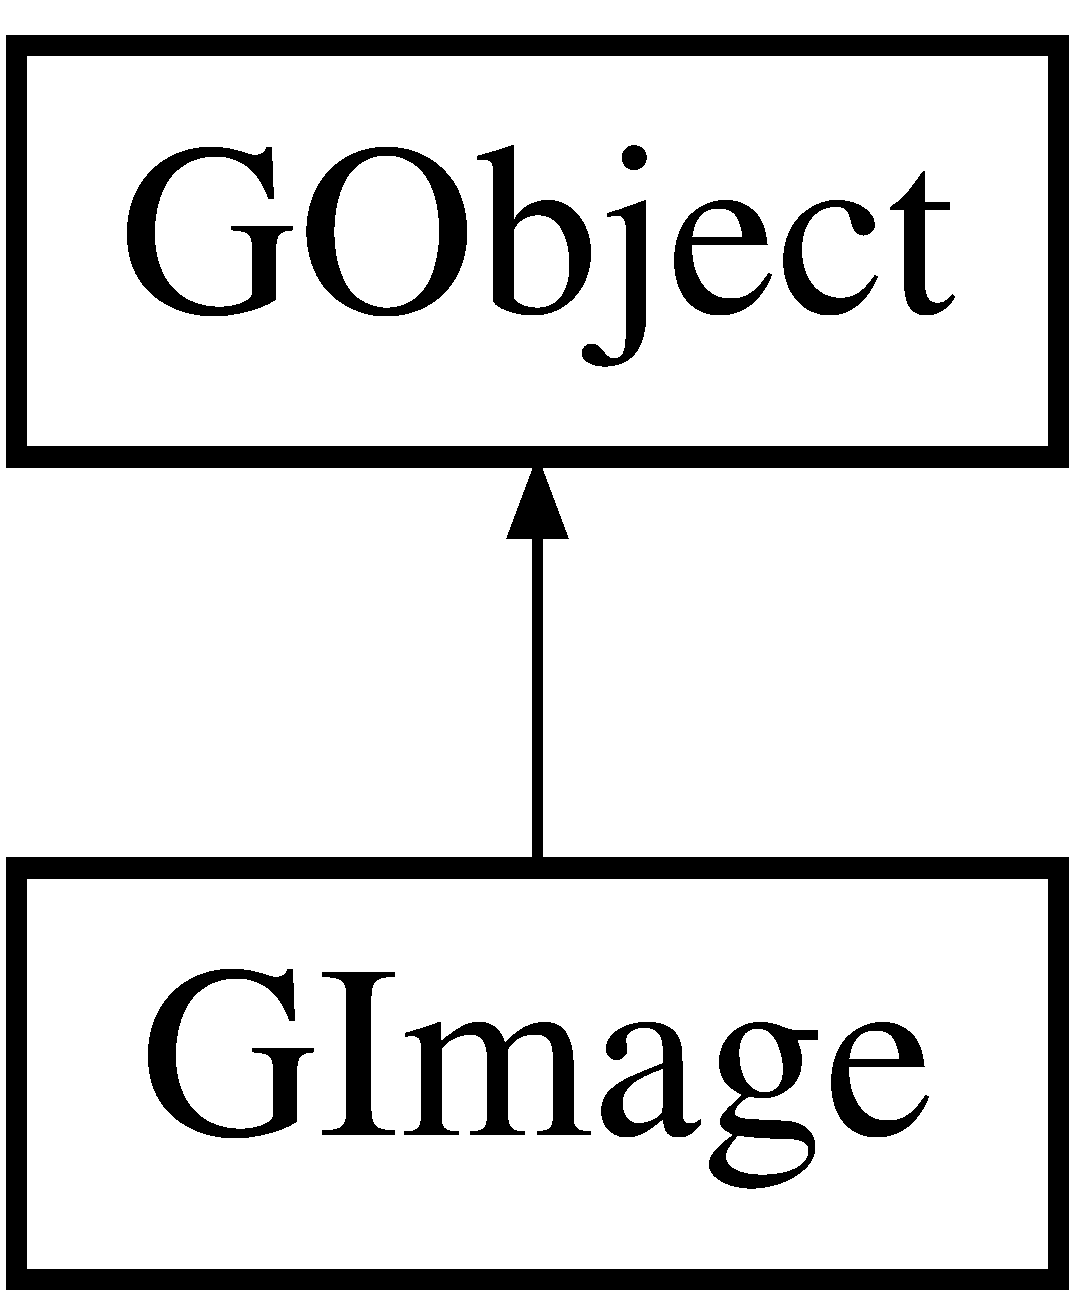
\includegraphics[height=2.000000cm]{classGImage}
\end{center}
\end{figure}
\subsection*{Public Types}
\begin{DoxyCompactItemize}
\item 
enum \mbox{\hyperlink{classGObject_a86e0f5648542856159bb40775c854aa7}{Line\+Style}} \{ \mbox{\hyperlink{classGObject_a86e0f5648542856159bb40775c854aa7acbc84bd5232621834ed31f44d457c1eb}{L\+I\+N\+E\+\_\+\+N\+O\+NE}}, 
\mbox{\hyperlink{classGObject_a86e0f5648542856159bb40775c854aa7a700c78bc2cd76acaab26651bf7b4941f}{L\+I\+N\+E\+\_\+\+S\+O\+L\+ID}}, 
\mbox{\hyperlink{classGObject_a86e0f5648542856159bb40775c854aa7a9ccba0845f785d81d07b333ae1aad84e}{L\+I\+N\+E\+\_\+\+D\+A\+SH}}, 
\mbox{\hyperlink{classGObject_a86e0f5648542856159bb40775c854aa7a8e811c096cb941997f0bfda168bb6df3}{L\+I\+N\+E\+\_\+\+D\+OT}}, 
\mbox{\hyperlink{classGObject_a86e0f5648542856159bb40775c854aa7ada15a2e3d737b2db7706d8300f91b89d}{L\+I\+N\+E\+\_\+\+D\+A\+S\+H\+\_\+\+D\+OT}}, 
\mbox{\hyperlink{classGObject_a86e0f5648542856159bb40775c854aa7aabf4053a73eafa7ba2b7e6d664c74c1d}{L\+I\+N\+E\+\_\+\+D\+A\+S\+H\+\_\+\+D\+O\+T\+\_\+\+D\+OT}}
 \}
\begin{DoxyCompactList}\small\item\em Styles that can be used for the outline around various shapes. \end{DoxyCompactList}\end{DoxyCompactItemize}
\subsection*{Public Member Functions}
\begin{DoxyCompactItemize}
\item 
\mbox{\hyperlink{classGImage_ae37cc9f566bd18108a4efed39c16e505}{G\+Image}} (const std\+::string \&filename=\char`\"{}\char`\"{}, double x=0, double y=0)
\begin{DoxyCompactList}\small\item\em Constructs a new image by loading the image from the specified file. \end{DoxyCompactList}\item 
virtual \mbox{\hyperlink{classGImage_aff2de2de9e75e1d6bf56248c2fdcc615}{$\sim$\+G\+Image}} ()
\begin{DoxyCompactList}\small\item\em Frees memory allocated internally by the image. \end{DoxyCompactList}\item 
virtual bool \mbox{\hyperlink{classGObject_abb6a5d7c03e6eaaae97264c4799ce7c3}{contains}} (double x, double y) const
\begin{DoxyCompactList}\small\item\em Returns {\ttfamily true} if the specified point is inside the object. \end{DoxyCompactList}\item 
virtual bool \mbox{\hyperlink{classGObject_a1dbc9dafaae51958112dbe1267a1f547}{contains}} (const \mbox{\hyperlink{classGPoint}{G\+Point}} \&pt) const
\begin{DoxyCompactList}\small\item\em Returns {\ttfamily true} if the specified point is inside the object. \end{DoxyCompactList}\item 
virtual \mbox{\hyperlink{classGPoint}{G\+Point}} \mbox{\hyperlink{classGObject_a0d41183bf6b08de66fe3907551aab0d7}{get\+Bottom\+Right\+Location}} () const
\begin{DoxyCompactList}\small\item\em Returns the x/y coordinates of the bottom/right corner of the object. \end{DoxyCompactList}\item 
virtual double \mbox{\hyperlink{classGObject_a4316a2406c18e1c6d061fe51fd355490}{get\+BottomY}} () const
\begin{DoxyCompactList}\small\item\em Returns the {\itshape y}-\/coordinate of the bottom of the object. \end{DoxyCompactList}\item 
virtual \mbox{\hyperlink{classGRectangle}{G\+Rectangle}} \mbox{\hyperlink{classGObject_a29e6ac35a0b48f491a4c88194cc5da3b}{get\+Bounds}} () const
\begin{DoxyCompactList}\small\item\em Returns the bounding box of this object, which is defined to be the smallest rectangle that covers everything drawn by the figure. \end{DoxyCompactList}\item 
virtual \mbox{\hyperlink{classGPoint}{G\+Point}} \mbox{\hyperlink{classGObject_a0909472e91448470bccdb62ecfb95d8b}{get\+Center\+Location}} () const
\begin{DoxyCompactList}\small\item\em Returns the x/y-\/coordinates of the center of the object. \end{DoxyCompactList}\item 
virtual double \mbox{\hyperlink{classGObject_a04df74355b545e0543112d5b8d924176}{get\+CenterX}} () const
\begin{DoxyCompactList}\small\item\em Returns the {\itshape x}-\/coordinate of the center of the object. \end{DoxyCompactList}\item 
virtual double \mbox{\hyperlink{classGObject_acb3287a3d507025a26f54b895713b947}{get\+CenterY}} () const
\begin{DoxyCompactList}\small\item\em Returns the {\itshape y}-\/coordinate of the center of the object. \end{DoxyCompactList}\item 
virtual std\+::string \mbox{\hyperlink{classGObject_aa061dfa488c31e18549d64363c1d0e34}{get\+Color}} () const
\begin{DoxyCompactList}\small\item\em Returns the color used to display this object. \end{DoxyCompactList}\item 
virtual std\+::string \mbox{\hyperlink{classGImage_a57d497454eec3b9c53b0067e458e3a51}{get\+File\+Name}} () const
\begin{DoxyCompactList}\small\item\em Returns the file name used to load the image, as was passed to the constructor. \end{DoxyCompactList}\item 
virtual std\+::string \mbox{\hyperlink{classGObject_a76f6964a11fde7c78e9751be184e1a3c}{get\+Fill\+Color}} () const
\begin{DoxyCompactList}\small\item\em Returns the color used to display the filled region of this object. \end{DoxyCompactList}\item 
virtual double \mbox{\hyperlink{classGObject_a1e7e353362434072875264cf95629f99}{get\+Height}} () const
\begin{DoxyCompactList}\small\item\em Returns the height of this object, which is the same as the height of its bounding box. \end{DoxyCompactList}\item 
virtual \mbox{\hyperlink{classGObject_a86e0f5648542856159bb40775c854aa7}{Line\+Style}} \mbox{\hyperlink{classGObject_aaf1f5ea8281e5e3486662878d26f0a13}{get\+Line\+Style}} () const
\begin{DoxyCompactList}\small\item\em Returns the object\textquotesingle{}s style such as solid or dashed. \end{DoxyCompactList}\item 
virtual double \mbox{\hyperlink{classGObject_a85ff266dc3eb63d9f2d8e5a4487fd3c0}{get\+Line\+Width}} () const
\begin{DoxyCompactList}\small\item\em Returns the width of the line used to draw this object. \end{DoxyCompactList}\item 
virtual \mbox{\hyperlink{classGPoint}{G\+Point}} \mbox{\hyperlink{classGObject_a4f83802015511edeb63b892830812c11}{get\+Location}} () const
\begin{DoxyCompactList}\small\item\em Returns the location of the top-\/left corner of object. \end{DoxyCompactList}\item 
virtual double \mbox{\hyperlink{classGObject_a1ae3fc278cc5b71b9f2d96a8a83cdf26}{get\+Opacity}} () const
\begin{DoxyCompactList}\small\item\em Returns how opaque (non-\/transparent) this object will appear from 0.\+0 (completely transparent) to 1.\+0 (completely opaque, default). \end{DoxyCompactList}\item 
virtual \mbox{\hyperlink{classGCompound}{G\+Compound}} $\ast$ \mbox{\hyperlink{classGObject_a3e53cef70541b1a14eade4ad0984d0b4}{get\+Parent}} () const
\begin{DoxyCompactList}\small\item\em Returns a pointer to the {\ttfamily \mbox{\hyperlink{classGCompound}{G\+Compound}}} that contains this object. \end{DoxyCompactList}\item 
virtual int \mbox{\hyperlink{classGImage_aea1d2892c78b0ed846db7116cb6a7c2e}{get\+Pixel}} (int x, int y) const
\begin{DoxyCompactList}\small\item\em Returns the color of the pixel at the given x/y location as an R\+GB integer. \end{DoxyCompactList}\item 
virtual double \mbox{\hyperlink{classGObject_a798cc79daaa10145b28f60bcdfdb0ee9}{get\+RightX}} () const
\begin{DoxyCompactList}\small\item\em Returns the {\itshape x}-\/coordinate of the right side of the object. \end{DoxyCompactList}\item 
virtual \mbox{\hyperlink{classGDimension}{G\+Dimension}} \mbox{\hyperlink{classGObject_a7b4eec96a2bdc6420695d5796a78eea9}{get\+Size}} () const
\begin{DoxyCompactList}\small\item\em Returns the size of the object as a {\ttfamily \mbox{\hyperlink{classGDimension}{G\+Dimension}}}. \end{DoxyCompactList}\item 
virtual std\+::string \mbox{\hyperlink{classGImage_a9896d58fcfebbf1025aeeb5b8b9ede80}{get\+Type}} () const Q\+\_\+\+D\+E\+C\+L\+\_\+\+O\+V\+E\+R\+R\+I\+DE
\begin{DoxyCompactList}\small\item\em Returns the type of the object as a string, such as {\ttfamily \char`\"{}\+G\+Oval\char`\"{}} or {\ttfamily \char`\"{}\+G\+Rect\char`\"{}}. \end{DoxyCompactList}\item 
virtual double \mbox{\hyperlink{classGObject_a0ed2965abd4f5701d2cadf71239faf19}{get\+Width}} () const
\begin{DoxyCompactList}\small\item\em Returns the width of this object, which is equal to the width of the bounding box. \end{DoxyCompactList}\item 
virtual double \mbox{\hyperlink{classGObject_a344385751bee0720059403940d57a13e}{getX}} () const
\begin{DoxyCompactList}\small\item\em Returns the leftmost {\itshape x}-\/coordinate of the object. \end{DoxyCompactList}\item 
virtual double \mbox{\hyperlink{classGObject_aafa51c7f8f38a09febbb9ce7853f77b4}{getY}} () const
\begin{DoxyCompactList}\small\item\em Returns the topmost {\itshape y}-\/coordinate of the object. \end{DoxyCompactList}\item 
virtual bool \mbox{\hyperlink{classGObject_a11c404f106940c201b6f326e0355c150}{is\+Filled}} () const
\begin{DoxyCompactList}\small\item\em Returns {\ttfamily true} if the object is filled with color. \end{DoxyCompactList}\item 
virtual bool \mbox{\hyperlink{classGObject_a9de207581cfa4ca1eaa06da5f29b75fc}{is\+Transformed}} () const
\begin{DoxyCompactList}\small\item\em Returns {\ttfamily true} if this object has been transformed by calling methods such as \mbox{\hyperlink{classGObject_ae1ffaa12185dfd5ba464f7d87c329e26}{rotate()}} or \mbox{\hyperlink{classGObject_ad2e1900f730475c2d044817db03b38d6}{scale()}} on it. \end{DoxyCompactList}\item 
virtual bool \mbox{\hyperlink{classGObject_a9d8a6cfb13917785c143e74d40e4e2be}{is\+Visible}} () const
\begin{DoxyCompactList}\small\item\em Returns {\ttfamily true} if this object is visible on screen. \end{DoxyCompactList}\item 
virtual void \mbox{\hyperlink{classGObject_a5973d8dda83afb36e2c56855515be392}{move}} (double dx, double dy)
\begin{DoxyCompactList}\small\item\em Moves the object on the screen using the displacements {\ttfamily dx} and {\ttfamily dy}. \end{DoxyCompactList}\item 
virtual void \mbox{\hyperlink{classGObject_ac827b978aa122f136a14c198687ad80f}{repaint}} ()
\begin{DoxyCompactList}\small\item\em Instructs the object to redraw itself on screen. \end{DoxyCompactList}\item 
virtual void \mbox{\hyperlink{classGObject_a6022a1fd1e5dcd2fd5585e5a36aa3f37}{reset\+Transform}} ()
\begin{DoxyCompactList}\small\item\em Undoes any previous scale/rotate transformations on this object. \end{DoxyCompactList}\item 
virtual void \mbox{\hyperlink{classGObject_ae1ffaa12185dfd5ba464f7d87c329e26}{rotate}} (double theta)
\begin{DoxyCompactList}\small\item\em Transforms the object by rotating it {\ttfamily theta} degrees counterclockwise around its origin. \end{DoxyCompactList}\item 
virtual void \mbox{\hyperlink{classGObject_ad2e1900f730475c2d044817db03b38d6}{scale}} (double sf)
\begin{DoxyCompactList}\small\item\em Scales the object by the specified scale factor. \end{DoxyCompactList}\item 
virtual void \mbox{\hyperlink{classGObject_a63641f69d610d0b951357d35a0c3b1e3}{scale}} (double sx, double sy)
\begin{DoxyCompactList}\small\item\em Scales the object by the specified scale factors. \end{DoxyCompactList}\item 
void \mbox{\hyperlink{classGObject_ab6747f40313c531c2db32edb5b63b9b7}{send\+Backward}} ()
\begin{DoxyCompactList}\small\item\em Moves this object one step toward the back in the {\itshape z} dimension. \end{DoxyCompactList}\item 
void \mbox{\hyperlink{classGObject_a710b3e449c9facba7847c91ab170d281}{send\+Forward}} ()
\begin{DoxyCompactList}\small\item\em Moves this object one step toward the front in the {\itshape z} dimension. \end{DoxyCompactList}\item 
void \mbox{\hyperlink{classGObject_a0f7f1efbb7fd46dde2867c4ad0330896}{send\+To\+Back}} ()
\begin{DoxyCompactList}\small\item\em Moves this object to the back of the display in the {\itshape z} dimension. \end{DoxyCompactList}\item 
void \mbox{\hyperlink{classGObject_aee33d68488e46827ef55fac07f40a9b2}{send\+To\+Front}} ()
\begin{DoxyCompactList}\small\item\em Moves this object to the front of the display in the {\itshape z} dimension. \end{DoxyCompactList}\item 
virtual void \mbox{\hyperlink{classGObject_a71ff7b16b8f1bdc4a1ce9f30cf8b87d8}{set\+Bottom\+Right\+Location}} (double x, double y)
\begin{DoxyCompactList}\small\item\em Sets the location of the bottom/right of this object. \end{DoxyCompactList}\item 
virtual void \mbox{\hyperlink{classGObject_ac6f7320321182f1d18c1c0fa97d5e941}{set\+Bottom\+Right\+Location}} (const \mbox{\hyperlink{classGPoint}{G\+Point}} \&pt)
\begin{DoxyCompactList}\small\item\em Sets the location of the bottom/right of this object. \end{DoxyCompactList}\item 
virtual void \mbox{\hyperlink{classGObject_a4b20e93c2a2597484f74ee5caa71f41f}{set\+BottomY}} (double y)
\begin{DoxyCompactList}\small\item\em Sets the location of the bottom y-\/coordinate of this object. \end{DoxyCompactList}\item 
virtual void \mbox{\hyperlink{classGObject_a2aae8197624b72265ab83b4f1bc73f2f}{set\+Bounds}} (double x, double y, double width, double height)
\begin{DoxyCompactList}\small\item\em Changes the bounds of this object to the specified values. \end{DoxyCompactList}\item 
virtual void \mbox{\hyperlink{classGObject_acada386653f008cacc7cce86426bef7c}{set\+Bounds}} (const \mbox{\hyperlink{classGRectangle}{G\+Rectangle}} \&size)
\begin{DoxyCompactList}\small\item\em Changes the bounds of this object to the specified rectangle. \end{DoxyCompactList}\item 
virtual void \mbox{\hyperlink{classGObject_a290b47dd8de1be44089f95cb2c47c1de}{set\+Center\+Location}} (double x, double y)
\begin{DoxyCompactList}\small\item\em Sets the location of the center of this object. \end{DoxyCompactList}\item 
virtual void \mbox{\hyperlink{classGObject_a1bedf1b233ecba3f753ec58908a683a6}{set\+Center\+Location}} (const \mbox{\hyperlink{classGPoint}{G\+Point}} \&pt)
\begin{DoxyCompactList}\small\item\em Sets the location of the center of this object. \end{DoxyCompactList}\item 
virtual void \mbox{\hyperlink{classGObject_a2f4936281e056eead00a9186b9ba8af6}{set\+CenterX}} (double x)
\begin{DoxyCompactList}\small\item\em Sets the x-\/coordinate of the center of this object. \end{DoxyCompactList}\item 
virtual void \mbox{\hyperlink{classGObject_aad2a22b4fde88c33306b92aebf641d57}{set\+CenterY}} (double y)
\begin{DoxyCompactList}\small\item\em Sets the y-\/coordinate of the center of this object. \end{DoxyCompactList}\item 
virtual void \mbox{\hyperlink{classGObject_ad57ef49bc31db94e92648aa3737923d6}{set\+Color}} (int r, int g, int b)
\begin{DoxyCompactList}\small\item\em Sets the color used to display this object. \end{DoxyCompactList}\item 
virtual void \mbox{\hyperlink{classGObject_ab1f5cc0f5cc6bbbd716a526c61f1081d}{set\+Color}} (int rgb)
\begin{DoxyCompactList}\small\item\em Sets the color used to display this object. \end{DoxyCompactList}\item 
virtual void \mbox{\hyperlink{classGObject_a61374df6c11b52cfbb0815decdbaebc6}{set\+Color}} (const std\+::string \&color)
\begin{DoxyCompactList}\small\item\em Sets the color used to display this object. \end{DoxyCompactList}\item 
virtual void \mbox{\hyperlink{classGObject_ad767a33971159e9493e221cca4c00ae9}{set\+Fill\+Color}} (int r, int g, int b)
\begin{DoxyCompactList}\small\item\em Sets the color used to display the filled region of this object, if any. \end{DoxyCompactList}\item 
virtual void \mbox{\hyperlink{classGObject_aa59d9775a67fa7df2b24a95cd34840a3}{set\+Fill\+Color}} (int rgb)
\begin{DoxyCompactList}\small\item\em Sets the color used to display the filled region of this object, if any. \end{DoxyCompactList}\item 
virtual void \mbox{\hyperlink{classGObject_adbc18b1a930aadd97d7437f9f7265b96}{set\+Fill\+Color}} (const std\+::string \&color)
\begin{DoxyCompactList}\small\item\em Sets the color used to display the filled region of this object, if any. \end{DoxyCompactList}\item 
virtual void \mbox{\hyperlink{classGObject_a9b82b53362282c6bb7d6947068d2e55b}{set\+Filled}} (bool flag)
\begin{DoxyCompactList}\small\item\em Sets the fill status for the object, where {\ttfamily false} is outlined and {\ttfamily true} is filled. \end{DoxyCompactList}\item 
virtual void \mbox{\hyperlink{classGObject_a2592348886ffea646c6534bf88f7c49d}{set\+Font}} (const Q\+Font \&font)
\begin{DoxyCompactList}\small\item\em Changes the font used to display the object as specified by the given Qt font. \end{DoxyCompactList}\item 
virtual void \mbox{\hyperlink{classGObject_a8e096e8818d838aceae1d46d58fb3a7b}{set\+Font}} (const std\+::string \&font)
\begin{DoxyCompactList}\small\item\em Changes the font used to display the object as specified by the string {\ttfamily font}, which has the following format\+: \end{DoxyCompactList}\item 
virtual void \mbox{\hyperlink{classGObject_ad18e8fab1e02a4e9b75c6730212558eb}{set\+Foreground}} (int r, int g, int b)
\begin{DoxyCompactList}\small\item\em Sets the color used to display this object. \end{DoxyCompactList}\item 
virtual void \mbox{\hyperlink{classGObject_a9eb856b5ff83a19df3831a31f15f4563}{set\+Foreground}} (int rgb)
\begin{DoxyCompactList}\small\item\em Sets the color used to display this object. \end{DoxyCompactList}\item 
virtual void \mbox{\hyperlink{classGObject_af59209aeadea6dfc6d97a2d8531f50e1}{set\+Foreground}} (const std\+::string \&color)
\begin{DoxyCompactList}\small\item\em Sets the color used to display this object. \end{DoxyCompactList}\item 
virtual void \mbox{\hyperlink{classGObject_a9e280bfc4544dfaf8e4376c4e1a74357}{set\+Height}} (double height)
\begin{DoxyCompactList}\small\item\em Changes the height of this object to the specified height without changing its width. \end{DoxyCompactList}\item 
virtual void \mbox{\hyperlink{classGObject_add11575087eb94f1a71faa3f826c6341}{set\+Line\+Style}} (\mbox{\hyperlink{classGObject_a86e0f5648542856159bb40775c854aa7}{Line\+Style}} line\+Style)
\begin{DoxyCompactList}\small\item\em Sets the object\textquotesingle{}s style such as solid (\mbox{\hyperlink{classGObject_a86e0f5648542856159bb40775c854aa7a700c78bc2cd76acaab26651bf7b4941f}{G\+Object\+::\+L\+I\+N\+E\+\_\+\+S\+O\+L\+ID}}) or dashed (\mbox{\hyperlink{classGObject_a86e0f5648542856159bb40775c854aa7a9ccba0845f785d81d07b333ae1aad84e}{G\+Object\+::\+L\+I\+N\+E\+\_\+\+D\+A\+SH}}). \end{DoxyCompactList}\item 
virtual void \mbox{\hyperlink{classGObject_afd6a47c6ea6a1f85ca05a65ba3ff3477}{set\+Line\+Width}} (double line\+Width)
\begin{DoxyCompactList}\small\item\em Sets the width of the line used to draw this object. \end{DoxyCompactList}\item 
virtual void \mbox{\hyperlink{classGObject_a04594e8ba9b98513a64f1da00dcae18c}{set\+Location}} (double x, double y)
\begin{DoxyCompactList}\small\item\em Sets the location of the top-\/left corner of this object to the specified coordinates. \end{DoxyCompactList}\item 
virtual void \mbox{\hyperlink{classGObject_aa8480c0b7166cdf8f784cece06ab353f}{set\+Location}} (const \mbox{\hyperlink{classGPoint}{G\+Point}} \&pt)
\begin{DoxyCompactList}\small\item\em Sets the location of the top-\/left corner of this object to the specified point. \end{DoxyCompactList}\item 
virtual void \mbox{\hyperlink{classGObject_a04af1866cc1bae4a1226695794a50539}{set\+Opacity}} (double opacity)
\begin{DoxyCompactList}\small\item\em Sets how opaque (non-\/transparent) this object will appear from 0.\+0 (completely transparent) to 1.\+0 (completely opaque, default). \end{DoxyCompactList}\item 
virtual void \mbox{\hyperlink{classGObject_a3c90b758cdc2c911c9ef76c4360eb912}{set\+RightX}} (double x)
\begin{DoxyCompactList}\small\item\em Sets the location of the rightmost x-\/coordinate of this object. \end{DoxyCompactList}\item 
virtual void \mbox{\hyperlink{classGObject_aca25d49481f9bf5fc8f7df4c086c4ce7}{set\+Size}} (double width, double height)
\begin{DoxyCompactList}\small\item\em Changes the size of this object to the specified width and height. \end{DoxyCompactList}\item 
virtual void \mbox{\hyperlink{classGObject_ae2b628228f192c2702c4ce941b2af68f}{set\+Size}} (const \mbox{\hyperlink{classGDimension}{G\+Dimension}} \&size)
\begin{DoxyCompactList}\small\item\em Changes the size of this object to the specified width and height. \end{DoxyCompactList}\item 
virtual void \mbox{\hyperlink{classGObject_a88203f28224315d9f4471212f4af8ed3}{set\+Visible}} (bool flag)
\begin{DoxyCompactList}\small\item\em Sets whether this object is visible. \end{DoxyCompactList}\item 
virtual void \mbox{\hyperlink{classGObject_aa3f3fba4cb131baa8696ba01e3bceca1}{set\+Width}} (double width)
\begin{DoxyCompactList}\small\item\em Changes the width of this object to the specified width without changing its height. \end{DoxyCompactList}\item 
virtual void \mbox{\hyperlink{classGObject_a9c18fcc579333bf9653d13ad2b372e39}{setX}} (double x)
\begin{DoxyCompactList}\small\item\em Sets the x location of the left side of this object. \end{DoxyCompactList}\item 
virtual void \mbox{\hyperlink{classGObject_a7d57e2a5c35d27feb58fd498a3cf82b9}{setY}} (double y)
\begin{DoxyCompactList}\small\item\em Sets the y location of the top of this object. \end{DoxyCompactList}\item 
virtual std\+::string \mbox{\hyperlink{classGObject_a1fe5121d6528fdea3f243321b3fa3a49}{to\+String}} () const
\begin{DoxyCompactList}\small\item\em Returns a printable representation of the object. \end{DoxyCompactList}\item 
virtual std\+::string \mbox{\hyperlink{classGImage_a85b5bcebac42ec5f130b0c3851383a23}{to\+String\+Extra}} () const Q\+\_\+\+D\+E\+C\+L\+\_\+\+O\+V\+E\+R\+R\+I\+DE
\begin{DoxyCompactList}\small\item\em Returns a string containing any extra unique information about this type of graphical object. \end{DoxyCompactList}\end{DoxyCompactItemize}
\subsection*{Static Public Member Functions}
\begin{DoxyCompactItemize}
\item 
static bool \mbox{\hyperlink{classGObject_a93be0e1fe1b1bf1a1da732470c94f42b}{is\+Anti\+Aliasing}} ()
\begin{DoxyCompactList}\small\item\em Returns whether we should globally anti-\/alias graphical objects. \end{DoxyCompactList}\item 
static void \mbox{\hyperlink{classGObject_a1e43371668ae850193cebedb44e1bbe3}{set\+Anti\+Aliasing}} (bool value)
\begin{DoxyCompactList}\small\item\em Globally turns on/off the anti-\/aliasing feature that smooths out the edges of onscreen shapes. \end{DoxyCompactList}\end{DoxyCompactItemize}
\subsection*{Protected Member Functions}
\begin{DoxyCompactItemize}
\item 
\mbox{\hyperlink{classGImage_ac106706c2a94c64f002934a273f8f4e7}{G\+Image}} (double width, double height)
\begin{DoxyCompactList}\small\item\em Creates a blank \mbox{\hyperlink{classGImage}{G\+Image}} of the given width and height. \end{DoxyCompactList}\item 
\mbox{\hyperlink{classGImage_a3444f37769d2b073dacd164dc2a1f45a}{G\+Image}} (Q\+Image $\ast$qimage)
\begin{DoxyCompactList}\small\item\em Creates a \mbox{\hyperlink{classGImage}{G\+Image}} wrapping the given Qt image. \end{DoxyCompactList}\item 
virtual void \mbox{\hyperlink{classGImage_a555e64433357e4e01b523498814b8e74}{set\+Pixel}} (int x, int y, int rgb)
\begin{DoxyCompactList}\small\item\em Sets the pixel at the given x/y location to the given color, represented as an R\+GB integer. \end{DoxyCompactList}\end{DoxyCompactItemize}
\subsection*{Protected Attributes}
\begin{DoxyCompactItemize}
\item 
Q\+Brush \mbox{\hyperlink{classGObject_aab24462ec896b596d99911767b0912d0}{\+\_\+brush}}
\item 
std\+::string \mbox{\hyperlink{classGObject_a1134e770ae4315ea8bc1201e2f21da8b}{\+\_\+color}}
\item 
int \mbox{\hyperlink{classGObject_a003fdd343d9b7505c53a8b7a134200ed}{\+\_\+color\+Int}}
\item 
std\+::string \mbox{\hyperlink{classGObject_a179f8d6cee65cd8a54692e32b224392a}{\+\_\+fill\+Color}}
\item 
int \mbox{\hyperlink{classGObject_a751def333a67d651e5b99cc331ecb496}{\+\_\+fill\+Color\+Int}}
\item 
bool \mbox{\hyperlink{classGObject_ad4a55cbcd61b58a4d49666490bb2f103}{\+\_\+fill\+Flag}}
\item 
std\+::string \mbox{\hyperlink{classGObject_aea76ea1a8b5dd7b0a78653277e63b536}{\+\_\+font}}
\item 
double \mbox{\hyperlink{classGObject_ad05df29e7f27fc504abd743e3d8b4e73}{\+\_\+height}}
\item 
\mbox{\hyperlink{classGObject_a86e0f5648542856159bb40775c854aa7}{Line\+Style}} \mbox{\hyperlink{classGObject_a89bafecaafb7c72d55c7efc10b7d0523}{\+\_\+line\+Style}}
\item 
double \mbox{\hyperlink{classGObject_a16e9033665937f13de2e163dc2184aff}{\+\_\+line\+Width}}
\item 
double \mbox{\hyperlink{classGObject_a20eff8eb7af27182edc9bfc54768b6f3}{\+\_\+opacity}}
\item 
\mbox{\hyperlink{classGCompound}{G\+Compound}} $\ast$ \mbox{\hyperlink{classGObject_ac9452c1eaff70eebddbb318196aa3835}{\+\_\+parent}}
\item 
Q\+Pen \mbox{\hyperlink{classGObject_afb69d172743f868299847174eb1b6bc8}{\+\_\+pen}}
\item 
Q\+Transform \mbox{\hyperlink{classGObject_a475b8860a5f1adb4a1fdc58d1f5c1e32}{\+\_\+transform}}
\item 
bool \mbox{\hyperlink{classGObject_ae4725802fc8d8aaa0ab4bd4781f7e07c}{\+\_\+transformed}}
\item 
bool \mbox{\hyperlink{classGObject_a9312c72508471b7c7a87b540263e1af4}{\+\_\+visible}}
\item 
double \mbox{\hyperlink{classGObject_ab55d85a3371770e6725b1062cf160cd8}{\+\_\+width}}
\item 
double \mbox{\hyperlink{classGObject_a6675b83b27137b8d3aa2ad8133078ea6}{\+\_\+x}}
\item 
double \mbox{\hyperlink{classGObject_a2f0f6aeafddc8a39c578bfa7e22b5f1e}{\+\_\+y}}
\end{DoxyCompactItemize}


\subsection{Detailed Description}
This graphical object subclass represents an image from a file. 

\subsection{Member Enumeration Documentation}
\mbox{\Hypertarget{classGObject_a86e0f5648542856159bb40775c854aa7}\label{classGObject_a86e0f5648542856159bb40775c854aa7}} 
\index{G\+Image@{G\+Image}!Line\+Style@{Line\+Style}}
\index{Line\+Style@{Line\+Style}!G\+Image@{G\+Image}}
\subsubsection{\texorpdfstring{Line\+Style}{LineStyle}}
{\footnotesize\ttfamily enum \mbox{\hyperlink{classGObject_a86e0f5648542856159bb40775c854aa7}{Line\+Style}}\hspace{0.3cm}{\ttfamily [inherited]}}



Styles that can be used for the outline around various shapes. 

Call set\+Line\+Style on a \mbox{\hyperlink{classGObject}{G\+Object}} and pass one of these values. \begin{DoxyEnumFields}{Enumerator}
\raisebox{\heightof{T}}[0pt][0pt]{\index{L\+I\+N\+E\+\_\+\+N\+O\+NE@{L\+I\+N\+E\+\_\+\+N\+O\+NE}!G\+Image@{G\+Image}}\index{G\+Image@{G\+Image}!L\+I\+N\+E\+\_\+\+N\+O\+NE@{L\+I\+N\+E\+\_\+\+N\+O\+NE}}}\mbox{\Hypertarget{classGObject_a86e0f5648542856159bb40775c854aa7acbc84bd5232621834ed31f44d457c1eb}\label{classGObject_a86e0f5648542856159bb40775c854aa7acbc84bd5232621834ed31f44d457c1eb}} 
L\+I\+N\+E\+\_\+\+N\+O\+NE&\\
\hline

\raisebox{\heightof{T}}[0pt][0pt]{\index{L\+I\+N\+E\+\_\+\+S\+O\+L\+ID@{L\+I\+N\+E\+\_\+\+S\+O\+L\+ID}!G\+Image@{G\+Image}}\index{G\+Image@{G\+Image}!L\+I\+N\+E\+\_\+\+S\+O\+L\+ID@{L\+I\+N\+E\+\_\+\+S\+O\+L\+ID}}}\mbox{\Hypertarget{classGObject_a86e0f5648542856159bb40775c854aa7a700c78bc2cd76acaab26651bf7b4941f}\label{classGObject_a86e0f5648542856159bb40775c854aa7a700c78bc2cd76acaab26651bf7b4941f}} 
L\+I\+N\+E\+\_\+\+S\+O\+L\+ID&\\
\hline

\raisebox{\heightof{T}}[0pt][0pt]{\index{L\+I\+N\+E\+\_\+\+D\+A\+SH@{L\+I\+N\+E\+\_\+\+D\+A\+SH}!G\+Image@{G\+Image}}\index{G\+Image@{G\+Image}!L\+I\+N\+E\+\_\+\+D\+A\+SH@{L\+I\+N\+E\+\_\+\+D\+A\+SH}}}\mbox{\Hypertarget{classGObject_a86e0f5648542856159bb40775c854aa7a9ccba0845f785d81d07b333ae1aad84e}\label{classGObject_a86e0f5648542856159bb40775c854aa7a9ccba0845f785d81d07b333ae1aad84e}} 
L\+I\+N\+E\+\_\+\+D\+A\+SH&\\
\hline

\raisebox{\heightof{T}}[0pt][0pt]{\index{L\+I\+N\+E\+\_\+\+D\+OT@{L\+I\+N\+E\+\_\+\+D\+OT}!G\+Image@{G\+Image}}\index{G\+Image@{G\+Image}!L\+I\+N\+E\+\_\+\+D\+OT@{L\+I\+N\+E\+\_\+\+D\+OT}}}\mbox{\Hypertarget{classGObject_a86e0f5648542856159bb40775c854aa7a8e811c096cb941997f0bfda168bb6df3}\label{classGObject_a86e0f5648542856159bb40775c854aa7a8e811c096cb941997f0bfda168bb6df3}} 
L\+I\+N\+E\+\_\+\+D\+OT&\\
\hline

\raisebox{\heightof{T}}[0pt][0pt]{\index{L\+I\+N\+E\+\_\+\+D\+A\+S\+H\+\_\+\+D\+OT@{L\+I\+N\+E\+\_\+\+D\+A\+S\+H\+\_\+\+D\+OT}!G\+Image@{G\+Image}}\index{G\+Image@{G\+Image}!L\+I\+N\+E\+\_\+\+D\+A\+S\+H\+\_\+\+D\+OT@{L\+I\+N\+E\+\_\+\+D\+A\+S\+H\+\_\+\+D\+OT}}}\mbox{\Hypertarget{classGObject_a86e0f5648542856159bb40775c854aa7ada15a2e3d737b2db7706d8300f91b89d}\label{classGObject_a86e0f5648542856159bb40775c854aa7ada15a2e3d737b2db7706d8300f91b89d}} 
L\+I\+N\+E\+\_\+\+D\+A\+S\+H\+\_\+\+D\+OT&\\
\hline

\raisebox{\heightof{T}}[0pt][0pt]{\index{L\+I\+N\+E\+\_\+\+D\+A\+S\+H\+\_\+\+D\+O\+T\+\_\+\+D\+OT@{L\+I\+N\+E\+\_\+\+D\+A\+S\+H\+\_\+\+D\+O\+T\+\_\+\+D\+OT}!G\+Image@{G\+Image}}\index{G\+Image@{G\+Image}!L\+I\+N\+E\+\_\+\+D\+A\+S\+H\+\_\+\+D\+O\+T\+\_\+\+D\+OT@{L\+I\+N\+E\+\_\+\+D\+A\+S\+H\+\_\+\+D\+O\+T\+\_\+\+D\+OT}}}\mbox{\Hypertarget{classGObject_a86e0f5648542856159bb40775c854aa7aabf4053a73eafa7ba2b7e6d664c74c1d}\label{classGObject_a86e0f5648542856159bb40775c854aa7aabf4053a73eafa7ba2b7e6d664c74c1d}} 
L\+I\+N\+E\+\_\+\+D\+A\+S\+H\+\_\+\+D\+O\+T\+\_\+\+D\+OT&\\
\hline

\end{DoxyEnumFields}


\subsection{Constructor \& Destructor Documentation}
\mbox{\Hypertarget{classGImage_ae37cc9f566bd18108a4efed39c16e505}\label{classGImage_ae37cc9f566bd18108a4efed39c16e505}} 
\index{G\+Image@{G\+Image}!G\+Image@{G\+Image}}
\index{G\+Image@{G\+Image}!G\+Image@{G\+Image}}
\subsubsection{\texorpdfstring{G\+Image()}{GImage()}\hspace{0.1cm}{\footnotesize\ttfamily [1/3]}}
{\footnotesize\ttfamily \mbox{\hyperlink{classGImage}{G\+Image}} (\begin{DoxyParamCaption}\item[{const std\+::string \&}]{filename = {\ttfamily \char`\"{}\char`\"{}},  }\item[{double}]{x = {\ttfamily 0},  }\item[{double}]{y = {\ttfamily 0} }\end{DoxyParamCaption})}



Constructs a new image by loading the image from the specified file. 

By default, the upper left corner of the image appears at the origin, but you can pass coordinates to move it to the point ({\ttfamily x}, {\ttfamily y}). 
\begin{DoxyExceptions}{Exceptions}
{\em \mbox{\hyperlink{classErrorException}{Error\+Exception}}} & if the given file is not found or cannot be loaded as a valid image file \\
\hline
\end{DoxyExceptions}
\mbox{\Hypertarget{classGImage_aff2de2de9e75e1d6bf56248c2fdcc615}\label{classGImage_aff2de2de9e75e1d6bf56248c2fdcc615}} 
\index{G\+Image@{G\+Image}!````~G\+Image@{$\sim$\+G\+Image}}
\index{````~G\+Image@{$\sim$\+G\+Image}!G\+Image@{G\+Image}}
\subsubsection{\texorpdfstring{$\sim$\+G\+Image()}{~GImage()}}
{\footnotesize\ttfamily $\sim$\mbox{\hyperlink{classGImage}{G\+Image}} (\begin{DoxyParamCaption}{ }\end{DoxyParamCaption})\hspace{0.3cm}{\ttfamily [virtual]}}



Frees memory allocated internally by the image. 

\mbox{\Hypertarget{classGImage_ac106706c2a94c64f002934a273f8f4e7}\label{classGImage_ac106706c2a94c64f002934a273f8f4e7}} 
\index{G\+Image@{G\+Image}!G\+Image@{G\+Image}}
\index{G\+Image@{G\+Image}!G\+Image@{G\+Image}}
\subsubsection{\texorpdfstring{G\+Image()}{GImage()}\hspace{0.1cm}{\footnotesize\ttfamily [2/3]}}
{\footnotesize\ttfamily \mbox{\hyperlink{classGImage}{G\+Image}} (\begin{DoxyParamCaption}\item[{double}]{width,  }\item[{double}]{height }\end{DoxyParamCaption})\hspace{0.3cm}{\ttfamily [protected]}}



Creates a blank \mbox{\hyperlink{classGImage}{G\+Image}} of the given width and height. 

Called by \mbox{\hyperlink{classGCanvas}{G\+Canvas}} when converting to an image. \mbox{\Hypertarget{classGImage_a3444f37769d2b073dacd164dc2a1f45a}\label{classGImage_a3444f37769d2b073dacd164dc2a1f45a}} 
\index{G\+Image@{G\+Image}!G\+Image@{G\+Image}}
\index{G\+Image@{G\+Image}!G\+Image@{G\+Image}}
\subsubsection{\texorpdfstring{G\+Image()}{GImage()}\hspace{0.1cm}{\footnotesize\ttfamily [3/3]}}
{\footnotesize\ttfamily \mbox{\hyperlink{classGImage}{G\+Image}} (\begin{DoxyParamCaption}\item[{Q\+Image $\ast$}]{qimage }\end{DoxyParamCaption})\hspace{0.3cm}{\ttfamily [protected]}}



Creates a \mbox{\hyperlink{classGImage}{G\+Image}} wrapping the given Qt image. 

Called by \mbox{\hyperlink{classGCanvas}{G\+Canvas}} when converting canvas to an image. 

\subsection{Member Function Documentation}
\mbox{\Hypertarget{classGObject_abb6a5d7c03e6eaaae97264c4799ce7c3}\label{classGObject_abb6a5d7c03e6eaaae97264c4799ce7c3}} 
\index{G\+Image@{G\+Image}!contains@{contains}}
\index{contains@{contains}!G\+Image@{G\+Image}}
\subsubsection{\texorpdfstring{contains()}{contains()}\hspace{0.1cm}{\footnotesize\ttfamily [1/2]}}
{\footnotesize\ttfamily bool contains (\begin{DoxyParamCaption}\item[{double}]{x,  }\item[{double}]{y }\end{DoxyParamCaption}) const\hspace{0.3cm}{\ttfamily [virtual]}, {\ttfamily [inherited]}}



Returns {\ttfamily true} if the specified point is inside the object. 



Reimplemented in \mbox{\hyperlink{classGRoundRect_abb6a5d7c03e6eaaae97264c4799ce7c3}{G\+Round\+Rect}}, \mbox{\hyperlink{classGPolygon_abb6a5d7c03e6eaaae97264c4799ce7c3}{G\+Polygon}}, \mbox{\hyperlink{classGOval_aa095a031ab22c150d2d75fdda1c3c8f5}{G\+Oval}}, \mbox{\hyperlink{classGLine_aa095a031ab22c150d2d75fdda1c3c8f5}{G\+Line}}, \mbox{\hyperlink{classGCompound_aa095a031ab22c150d2d75fdda1c3c8f5}{G\+Compound}}, and \mbox{\hyperlink{classGArc_aa095a031ab22c150d2d75fdda1c3c8f5}{G\+Arc}}.

\mbox{\Hypertarget{classGObject_a1dbc9dafaae51958112dbe1267a1f547}\label{classGObject_a1dbc9dafaae51958112dbe1267a1f547}} 
\index{G\+Image@{G\+Image}!contains@{contains}}
\index{contains@{contains}!G\+Image@{G\+Image}}
\subsubsection{\texorpdfstring{contains()}{contains()}\hspace{0.1cm}{\footnotesize\ttfamily [2/2]}}
{\footnotesize\ttfamily bool contains (\begin{DoxyParamCaption}\item[{const \mbox{\hyperlink{classGPoint}{G\+Point}} \&}]{pt }\end{DoxyParamCaption}) const\hspace{0.3cm}{\ttfamily [virtual]}, {\ttfamily [inherited]}}



Returns {\ttfamily true} if the specified point is inside the object. 

\mbox{\Hypertarget{classGObject_a0d41183bf6b08de66fe3907551aab0d7}\label{classGObject_a0d41183bf6b08de66fe3907551aab0d7}} 
\index{G\+Image@{G\+Image}!get\+Bottom\+Right\+Location@{get\+Bottom\+Right\+Location}}
\index{get\+Bottom\+Right\+Location@{get\+Bottom\+Right\+Location}!G\+Image@{G\+Image}}
\subsubsection{\texorpdfstring{get\+Bottom\+Right\+Location()}{getBottomRightLocation()}}
{\footnotesize\ttfamily \mbox{\hyperlink{classGPoint}{G\+Point}} get\+Bottom\+Right\+Location (\begin{DoxyParamCaption}{ }\end{DoxyParamCaption}) const\hspace{0.3cm}{\ttfamily [virtual]}, {\ttfamily [inherited]}}



Returns the x/y coordinates of the bottom/right corner of the object. 

\mbox{\Hypertarget{classGObject_a4316a2406c18e1c6d061fe51fd355490}\label{classGObject_a4316a2406c18e1c6d061fe51fd355490}} 
\index{G\+Image@{G\+Image}!get\+BottomY@{get\+BottomY}}
\index{get\+BottomY@{get\+BottomY}!G\+Image@{G\+Image}}
\subsubsection{\texorpdfstring{get\+Bottom\+Y()}{getBottomY()}}
{\footnotesize\ttfamily double get\+BottomY (\begin{DoxyParamCaption}{ }\end{DoxyParamCaption}) const\hspace{0.3cm}{\ttfamily [virtual]}, {\ttfamily [inherited]}}



Returns the {\itshape y}-\/coordinate of the bottom of the object. 

Equivalent to the top y-\/coordinate plus the object\textquotesingle{}s height. \mbox{\Hypertarget{classGObject_a29e6ac35a0b48f491a4c88194cc5da3b}\label{classGObject_a29e6ac35a0b48f491a4c88194cc5da3b}} 
\index{G\+Image@{G\+Image}!get\+Bounds@{get\+Bounds}}
\index{get\+Bounds@{get\+Bounds}!G\+Image@{G\+Image}}
\subsubsection{\texorpdfstring{get\+Bounds()}{getBounds()}}
{\footnotesize\ttfamily \mbox{\hyperlink{classGRectangle}{G\+Rectangle}} get\+Bounds (\begin{DoxyParamCaption}{ }\end{DoxyParamCaption}) const\hspace{0.3cm}{\ttfamily [virtual]}, {\ttfamily [inherited]}}



Returns the bounding box of this object, which is defined to be the smallest rectangle that covers everything drawn by the figure. 

The coordinates of this rectangle do not necessarily match the location returned by {\ttfamily get\+Location}. Given a {\ttfamily \mbox{\hyperlink{classGText}{G\+Text}}} object, for example, {\ttfamily get\+Location} returns the coordinates of the point on the baseline at which the string begins; the {\ttfamily get\+Bounds} method, by contrast, returns a rectangle that covers the entire window area occupied by the string. 

Reimplemented in \mbox{\hyperlink{classGText_a2f46ec8a3b533c690b3b3e56d4f34afe}{G\+Text}}, \mbox{\hyperlink{classGPolygon_a29e6ac35a0b48f491a4c88194cc5da3b}{G\+Polygon}}, \mbox{\hyperlink{classGLine_a2f46ec8a3b533c690b3b3e56d4f34afe}{G\+Line}}, \mbox{\hyperlink{classGCompound_a2f46ec8a3b533c690b3b3e56d4f34afe}{G\+Compound}}, and \mbox{\hyperlink{classGArc_a2f46ec8a3b533c690b3b3e56d4f34afe}{G\+Arc}}.

\mbox{\Hypertarget{classGObject_a0909472e91448470bccdb62ecfb95d8b}\label{classGObject_a0909472e91448470bccdb62ecfb95d8b}} 
\index{G\+Image@{G\+Image}!get\+Center\+Location@{get\+Center\+Location}}
\index{get\+Center\+Location@{get\+Center\+Location}!G\+Image@{G\+Image}}
\subsubsection{\texorpdfstring{get\+Center\+Location()}{getCenterLocation()}}
{\footnotesize\ttfamily \mbox{\hyperlink{classGPoint}{G\+Point}} get\+Center\+Location (\begin{DoxyParamCaption}{ }\end{DoxyParamCaption}) const\hspace{0.3cm}{\ttfamily [virtual]}, {\ttfamily [inherited]}}



Returns the x/y-\/coordinates of the center of the object. 

Equivalent to the top/left plus half the object\textquotesingle{}s size. \mbox{\Hypertarget{classGObject_a04df74355b545e0543112d5b8d924176}\label{classGObject_a04df74355b545e0543112d5b8d924176}} 
\index{G\+Image@{G\+Image}!get\+CenterX@{get\+CenterX}}
\index{get\+CenterX@{get\+CenterX}!G\+Image@{G\+Image}}
\subsubsection{\texorpdfstring{get\+Center\+X()}{getCenterX()}}
{\footnotesize\ttfamily double get\+CenterX (\begin{DoxyParamCaption}{ }\end{DoxyParamCaption}) const\hspace{0.3cm}{\ttfamily [virtual]}, {\ttfamily [inherited]}}



Returns the {\itshape x}-\/coordinate of the center of the object. 

Equivalent to the top/left plus half the object\textquotesingle{}s width. \mbox{\Hypertarget{classGObject_acb3287a3d507025a26f54b895713b947}\label{classGObject_acb3287a3d507025a26f54b895713b947}} 
\index{G\+Image@{G\+Image}!get\+CenterY@{get\+CenterY}}
\index{get\+CenterY@{get\+CenterY}!G\+Image@{G\+Image}}
\subsubsection{\texorpdfstring{get\+Center\+Y()}{getCenterY()}}
{\footnotesize\ttfamily double get\+CenterY (\begin{DoxyParamCaption}{ }\end{DoxyParamCaption}) const\hspace{0.3cm}{\ttfamily [virtual]}, {\ttfamily [inherited]}}



Returns the {\itshape y}-\/coordinate of the center of the object. 

Equivalent to the top/left plus half the object\textquotesingle{}s height. \mbox{\Hypertarget{classGObject_aa061dfa488c31e18549d64363c1d0e34}\label{classGObject_aa061dfa488c31e18549d64363c1d0e34}} 
\index{G\+Image@{G\+Image}!get\+Color@{get\+Color}}
\index{get\+Color@{get\+Color}!G\+Image@{G\+Image}}
\subsubsection{\texorpdfstring{get\+Color()}{getColor()}}
{\footnotesize\ttfamily std\+::string get\+Color (\begin{DoxyParamCaption}{ }\end{DoxyParamCaption}) const\hspace{0.3cm}{\ttfamily [virtual]}, {\ttfamily [inherited]}}



Returns the color used to display this object. 

This color is always returned as a string in the form {\ttfamily \char`\"{}\#rrggbb\char`\"{}}, where {\ttfamily rr}, {\ttfamily gg}, and {\ttfamily bb} are the red, green, and blue components of the color, expressed as two-\/digit hexadecimal values. \mbox{\Hypertarget{classGImage_a57d497454eec3b9c53b0067e458e3a51}\label{classGImage_a57d497454eec3b9c53b0067e458e3a51}} 
\index{G\+Image@{G\+Image}!get\+File\+Name@{get\+File\+Name}}
\index{get\+File\+Name@{get\+File\+Name}!G\+Image@{G\+Image}}
\subsubsection{\texorpdfstring{get\+File\+Name()}{getFileName()}}
{\footnotesize\ttfamily std\+::string get\+File\+Name (\begin{DoxyParamCaption}{ }\end{DoxyParamCaption}) const\hspace{0.3cm}{\ttfamily [virtual]}}



Returns the file name used to load the image, as was passed to the constructor. 

\mbox{\Hypertarget{classGObject_a76f6964a11fde7c78e9751be184e1a3c}\label{classGObject_a76f6964a11fde7c78e9751be184e1a3c}} 
\index{G\+Image@{G\+Image}!get\+Fill\+Color@{get\+Fill\+Color}}
\index{get\+Fill\+Color@{get\+Fill\+Color}!G\+Image@{G\+Image}}
\subsubsection{\texorpdfstring{get\+Fill\+Color()}{getFillColor()}}
{\footnotesize\ttfamily std\+::string get\+Fill\+Color (\begin{DoxyParamCaption}{ }\end{DoxyParamCaption}) const\hspace{0.3cm}{\ttfamily [virtual]}, {\ttfamily [inherited]}}



Returns the color used to display the filled region of this object. 

If none has been set, returns the empty string. \mbox{\Hypertarget{classGObject_a1e7e353362434072875264cf95629f99}\label{classGObject_a1e7e353362434072875264cf95629f99}} 
\index{G\+Image@{G\+Image}!get\+Height@{get\+Height}}
\index{get\+Height@{get\+Height}!G\+Image@{G\+Image}}
\subsubsection{\texorpdfstring{get\+Height()}{getHeight()}}
{\footnotesize\ttfamily double get\+Height (\begin{DoxyParamCaption}{ }\end{DoxyParamCaption}) const\hspace{0.3cm}{\ttfamily [virtual]}, {\ttfamily [inherited]}}



Returns the height of this object, which is the same as the height of its bounding box. 



Reimplemented in \mbox{\hyperlink{classGPolygon_a1e7e353362434072875264cf95629f99}{G\+Polygon}}, and \mbox{\hyperlink{classGLine_a423f17d4aeb66feb0d148fd23af335b7}{G\+Line}}.

\mbox{\Hypertarget{classGObject_aaf1f5ea8281e5e3486662878d26f0a13}\label{classGObject_aaf1f5ea8281e5e3486662878d26f0a13}} 
\index{G\+Image@{G\+Image}!get\+Line\+Style@{get\+Line\+Style}}
\index{get\+Line\+Style@{get\+Line\+Style}!G\+Image@{G\+Image}}
\subsubsection{\texorpdfstring{get\+Line\+Style()}{getLineStyle()}}
{\footnotesize\ttfamily \mbox{\hyperlink{classGObject_a86e0f5648542856159bb40775c854aa7}{G\+Object\+::\+Line\+Style}} get\+Line\+Style (\begin{DoxyParamCaption}{ }\end{DoxyParamCaption}) const\hspace{0.3cm}{\ttfamily [virtual]}, {\ttfamily [inherited]}}



Returns the object\textquotesingle{}s style such as solid or dashed. 

\mbox{\Hypertarget{classGObject_a85ff266dc3eb63d9f2d8e5a4487fd3c0}\label{classGObject_a85ff266dc3eb63d9f2d8e5a4487fd3c0}} 
\index{G\+Image@{G\+Image}!get\+Line\+Width@{get\+Line\+Width}}
\index{get\+Line\+Width@{get\+Line\+Width}!G\+Image@{G\+Image}}
\subsubsection{\texorpdfstring{get\+Line\+Width()}{getLineWidth()}}
{\footnotesize\ttfamily double get\+Line\+Width (\begin{DoxyParamCaption}{ }\end{DoxyParamCaption}) const\hspace{0.3cm}{\ttfamily [virtual]}, {\ttfamily [inherited]}}



Returns the width of the line used to draw this object. 

\begin{DoxyReturn}{Returns}
default 1 
\end{DoxyReturn}
\mbox{\Hypertarget{classGObject_a4f83802015511edeb63b892830812c11}\label{classGObject_a4f83802015511edeb63b892830812c11}} 
\index{G\+Image@{G\+Image}!get\+Location@{get\+Location}}
\index{get\+Location@{get\+Location}!G\+Image@{G\+Image}}
\subsubsection{\texorpdfstring{get\+Location()}{getLocation()}}
{\footnotesize\ttfamily \mbox{\hyperlink{classGPoint}{G\+Point}} get\+Location (\begin{DoxyParamCaption}{ }\end{DoxyParamCaption}) const\hspace{0.3cm}{\ttfamily [virtual]}, {\ttfamily [inherited]}}



Returns the location of the top-\/left corner of object. 

\mbox{\Hypertarget{classGObject_a1ae3fc278cc5b71b9f2d96a8a83cdf26}\label{classGObject_a1ae3fc278cc5b71b9f2d96a8a83cdf26}} 
\index{G\+Image@{G\+Image}!get\+Opacity@{get\+Opacity}}
\index{get\+Opacity@{get\+Opacity}!G\+Image@{G\+Image}}
\subsubsection{\texorpdfstring{get\+Opacity()}{getOpacity()}}
{\footnotesize\ttfamily double get\+Opacity (\begin{DoxyParamCaption}{ }\end{DoxyParamCaption}) const\hspace{0.3cm}{\ttfamily [virtual]}, {\ttfamily [inherited]}}



Returns how opaque (non-\/transparent) this object will appear from 0.\+0 (completely transparent) to 1.\+0 (completely opaque, default). 

\mbox{\Hypertarget{classGObject_a3e53cef70541b1a14eade4ad0984d0b4}\label{classGObject_a3e53cef70541b1a14eade4ad0984d0b4}} 
\index{G\+Image@{G\+Image}!get\+Parent@{get\+Parent}}
\index{get\+Parent@{get\+Parent}!G\+Image@{G\+Image}}
\subsubsection{\texorpdfstring{get\+Parent()}{getParent()}}
{\footnotesize\ttfamily \mbox{\hyperlink{classGCompound}{G\+Compound}} $\ast$ get\+Parent (\begin{DoxyParamCaption}{ }\end{DoxyParamCaption}) const\hspace{0.3cm}{\ttfamily [virtual]}, {\ttfamily [inherited]}}



Returns a pointer to the {\ttfamily \mbox{\hyperlink{classGCompound}{G\+Compound}}} that contains this object. 

Every {\ttfamily \mbox{\hyperlink{classGWindow}{G\+Window}}} is initialized to contain a single {\ttfamily \mbox{\hyperlink{classGCompound}{G\+Compound}}} that is aligned with the window. Adding objects to the window adds them to that {\ttfamily \mbox{\hyperlink{classGCompound}{G\+Compound}}}, which means that every object you add to the window has a parent. Calling {\ttfamily get\+Parent} on the top-\/level {\ttfamily \mbox{\hyperlink{classGCompound}{G\+Compound}}} returns {\ttfamily nullptr}. \mbox{\Hypertarget{classGImage_aea1d2892c78b0ed846db7116cb6a7c2e}\label{classGImage_aea1d2892c78b0ed846db7116cb6a7c2e}} 
\index{G\+Image@{G\+Image}!get\+Pixel@{get\+Pixel}}
\index{get\+Pixel@{get\+Pixel}!G\+Image@{G\+Image}}
\subsubsection{\texorpdfstring{get\+Pixel()}{getPixel()}}
{\footnotesize\ttfamily int get\+Pixel (\begin{DoxyParamCaption}\item[{int}]{x,  }\item[{int}]{y }\end{DoxyParamCaption}) const\hspace{0.3cm}{\ttfamily [virtual]}}



Returns the color of the pixel at the given x/y location as an R\+GB integer. 


\begin{DoxyExceptions}{Exceptions}
{\em \mbox{\hyperlink{classErrorException}{Error\+Exception}}} & if x/y is out of range \\
\hline
\end{DoxyExceptions}
\mbox{\Hypertarget{classGObject_a798cc79daaa10145b28f60bcdfdb0ee9}\label{classGObject_a798cc79daaa10145b28f60bcdfdb0ee9}} 
\index{G\+Image@{G\+Image}!get\+RightX@{get\+RightX}}
\index{get\+RightX@{get\+RightX}!G\+Image@{G\+Image}}
\subsubsection{\texorpdfstring{get\+Right\+X()}{getRightX()}}
{\footnotesize\ttfamily double get\+RightX (\begin{DoxyParamCaption}{ }\end{DoxyParamCaption}) const\hspace{0.3cm}{\ttfamily [virtual]}, {\ttfamily [inherited]}}



Returns the {\itshape x}-\/coordinate of the right side of the object. 

Equivalent to the left x-\/coordinate plus the object\textquotesingle{}s width. \mbox{\Hypertarget{classGObject_a7b4eec96a2bdc6420695d5796a78eea9}\label{classGObject_a7b4eec96a2bdc6420695d5796a78eea9}} 
\index{G\+Image@{G\+Image}!get\+Size@{get\+Size}}
\index{get\+Size@{get\+Size}!G\+Image@{G\+Image}}
\subsubsection{\texorpdfstring{get\+Size()}{getSize()}}
{\footnotesize\ttfamily \mbox{\hyperlink{classGDimension}{G\+Dimension}} get\+Size (\begin{DoxyParamCaption}{ }\end{DoxyParamCaption}) const\hspace{0.3cm}{\ttfamily [virtual]}, {\ttfamily [inherited]}}



Returns the size of the object as a {\ttfamily \mbox{\hyperlink{classGDimension}{G\+Dimension}}}. 

\mbox{\Hypertarget{classGImage_a9896d58fcfebbf1025aeeb5b8b9ede80}\label{classGImage_a9896d58fcfebbf1025aeeb5b8b9ede80}} 
\index{G\+Image@{G\+Image}!get\+Type@{get\+Type}}
\index{get\+Type@{get\+Type}!G\+Image@{G\+Image}}
\subsubsection{\texorpdfstring{get\+Type()}{getType()}}
{\footnotesize\ttfamily std\+::string get\+Type (\begin{DoxyParamCaption}{ }\end{DoxyParamCaption}) const\hspace{0.3cm}{\ttfamily [virtual]}}



Returns the type of the object as a string, such as {\ttfamily \char`\"{}\+G\+Oval\char`\"{}} or {\ttfamily \char`\"{}\+G\+Rect\char`\"{}}. 

Each \mbox{\hyperlink{classGObject}{G\+Object}} subtype must override this method. 

Implements \mbox{\hyperlink{classGObject_a799e073a127b428cc841086d42ea4fed}{G\+Object}}.

\mbox{\Hypertarget{classGObject_a0ed2965abd4f5701d2cadf71239faf19}\label{classGObject_a0ed2965abd4f5701d2cadf71239faf19}} 
\index{G\+Image@{G\+Image}!get\+Width@{get\+Width}}
\index{get\+Width@{get\+Width}!G\+Image@{G\+Image}}
\subsubsection{\texorpdfstring{get\+Width()}{getWidth()}}
{\footnotesize\ttfamily double get\+Width (\begin{DoxyParamCaption}{ }\end{DoxyParamCaption}) const\hspace{0.3cm}{\ttfamily [virtual]}, {\ttfamily [inherited]}}



Returns the width of this object, which is equal to the width of the bounding box. 



Reimplemented in \mbox{\hyperlink{classGPolygon_a0ed2965abd4f5701d2cadf71239faf19}{G\+Polygon}}, and \mbox{\hyperlink{classGLine_a04bee94b66c8f921cd8611be2460ba9d}{G\+Line}}.

\mbox{\Hypertarget{classGObject_a344385751bee0720059403940d57a13e}\label{classGObject_a344385751bee0720059403940d57a13e}} 
\index{G\+Image@{G\+Image}!getX@{getX}}
\index{getX@{getX}!G\+Image@{G\+Image}}
\subsubsection{\texorpdfstring{get\+X()}{getX()}}
{\footnotesize\ttfamily double getX (\begin{DoxyParamCaption}{ }\end{DoxyParamCaption}) const\hspace{0.3cm}{\ttfamily [virtual]}, {\ttfamily [inherited]}}



Returns the leftmost {\itshape x}-\/coordinate of the object. 

\mbox{\Hypertarget{classGObject_aafa51c7f8f38a09febbb9ce7853f77b4}\label{classGObject_aafa51c7f8f38a09febbb9ce7853f77b4}} 
\index{G\+Image@{G\+Image}!getY@{getY}}
\index{getY@{getY}!G\+Image@{G\+Image}}
\subsubsection{\texorpdfstring{get\+Y()}{getY()}}
{\footnotesize\ttfamily double getY (\begin{DoxyParamCaption}{ }\end{DoxyParamCaption}) const\hspace{0.3cm}{\ttfamily [virtual]}, {\ttfamily [inherited]}}



Returns the topmost {\itshape y}-\/coordinate of the object. 

\mbox{\Hypertarget{classGObject_a93be0e1fe1b1bf1a1da732470c94f42b}\label{classGObject_a93be0e1fe1b1bf1a1da732470c94f42b}} 
\index{G\+Image@{G\+Image}!is\+Anti\+Aliasing@{is\+Anti\+Aliasing}}
\index{is\+Anti\+Aliasing@{is\+Anti\+Aliasing}!G\+Image@{G\+Image}}
\subsubsection{\texorpdfstring{is\+Anti\+Aliasing()}{isAntiAliasing()}}
{\footnotesize\ttfamily bool is\+Anti\+Aliasing (\begin{DoxyParamCaption}{ }\end{DoxyParamCaption})\hspace{0.3cm}{\ttfamily [static]}, {\ttfamily [inherited]}}



Returns whether we should globally anti-\/alias graphical objects. 

On by default. \mbox{\Hypertarget{classGObject_a11c404f106940c201b6f326e0355c150}\label{classGObject_a11c404f106940c201b6f326e0355c150}} 
\index{G\+Image@{G\+Image}!is\+Filled@{is\+Filled}}
\index{is\+Filled@{is\+Filled}!G\+Image@{G\+Image}}
\subsubsection{\texorpdfstring{is\+Filled()}{isFilled()}}
{\footnotesize\ttfamily bool is\+Filled (\begin{DoxyParamCaption}{ }\end{DoxyParamCaption}) const\hspace{0.3cm}{\ttfamily [virtual]}, {\ttfamily [inherited]}}



Returns {\ttfamily true} if the object is filled with color. 

\mbox{\Hypertarget{classGObject_a9de207581cfa4ca1eaa06da5f29b75fc}\label{classGObject_a9de207581cfa4ca1eaa06da5f29b75fc}} 
\index{G\+Image@{G\+Image}!is\+Transformed@{is\+Transformed}}
\index{is\+Transformed@{is\+Transformed}!G\+Image@{G\+Image}}
\subsubsection{\texorpdfstring{is\+Transformed()}{isTransformed()}}
{\footnotesize\ttfamily bool is\+Transformed (\begin{DoxyParamCaption}{ }\end{DoxyParamCaption}) const\hspace{0.3cm}{\ttfamily [virtual]}, {\ttfamily [inherited]}}



Returns {\ttfamily true} if this object has been transformed by calling methods such as \mbox{\hyperlink{classGObject_ae1ffaa12185dfd5ba464f7d87c329e26}{rotate()}} or \mbox{\hyperlink{classGObject_ad2e1900f730475c2d044817db03b38d6}{scale()}} on it. 

Certain operations (such as set\+Size) cannot be performed after a graphical object has been transformed. \mbox{\Hypertarget{classGObject_a9d8a6cfb13917785c143e74d40e4e2be}\label{classGObject_a9d8a6cfb13917785c143e74d40e4e2be}} 
\index{G\+Image@{G\+Image}!is\+Visible@{is\+Visible}}
\index{is\+Visible@{is\+Visible}!G\+Image@{G\+Image}}
\subsubsection{\texorpdfstring{is\+Visible()}{isVisible()}}
{\footnotesize\ttfamily bool is\+Visible (\begin{DoxyParamCaption}{ }\end{DoxyParamCaption}) const\hspace{0.3cm}{\ttfamily [virtual]}, {\ttfamily [inherited]}}



Returns {\ttfamily true} if this object is visible on screen. 

\mbox{\Hypertarget{classGObject_a5973d8dda83afb36e2c56855515be392}\label{classGObject_a5973d8dda83afb36e2c56855515be392}} 
\index{G\+Image@{G\+Image}!move@{move}}
\index{move@{move}!G\+Image@{G\+Image}}
\subsubsection{\texorpdfstring{move()}{move()}}
{\footnotesize\ttfamily void move (\begin{DoxyParamCaption}\item[{double}]{dx,  }\item[{double}]{dy }\end{DoxyParamCaption})\hspace{0.3cm}{\ttfamily [virtual]}, {\ttfamily [inherited]}}



Moves the object on the screen using the displacements {\ttfamily dx} and {\ttfamily dy}. 

\mbox{\Hypertarget{classGObject_ac827b978aa122f136a14c198687ad80f}\label{classGObject_ac827b978aa122f136a14c198687ad80f}} 
\index{G\+Image@{G\+Image}!repaint@{repaint}}
\index{repaint@{repaint}!G\+Image@{G\+Image}}
\subsubsection{\texorpdfstring{repaint()}{repaint()}}
{\footnotesize\ttfamily void repaint (\begin{DoxyParamCaption}{ }\end{DoxyParamCaption})\hspace{0.3cm}{\ttfamily [virtual]}, {\ttfamily [inherited]}}



Instructs the object to redraw itself on screen. 



Reimplemented in \mbox{\hyperlink{classGCompound_ac827b978aa122f136a14c198687ad80f}{G\+Compound}}.

\mbox{\Hypertarget{classGObject_a6022a1fd1e5dcd2fd5585e5a36aa3f37}\label{classGObject_a6022a1fd1e5dcd2fd5585e5a36aa3f37}} 
\index{G\+Image@{G\+Image}!reset\+Transform@{reset\+Transform}}
\index{reset\+Transform@{reset\+Transform}!G\+Image@{G\+Image}}
\subsubsection{\texorpdfstring{reset\+Transform()}{resetTransform()}}
{\footnotesize\ttfamily void reset\+Transform (\begin{DoxyParamCaption}{ }\end{DoxyParamCaption})\hspace{0.3cm}{\ttfamily [virtual]}, {\ttfamily [inherited]}}



Undoes any previous scale/rotate transformations on this object. 

\mbox{\Hypertarget{classGObject_ae1ffaa12185dfd5ba464f7d87c329e26}\label{classGObject_ae1ffaa12185dfd5ba464f7d87c329e26}} 
\index{G\+Image@{G\+Image}!rotate@{rotate}}
\index{rotate@{rotate}!G\+Image@{G\+Image}}
\subsubsection{\texorpdfstring{rotate()}{rotate()}}
{\footnotesize\ttfamily void rotate (\begin{DoxyParamCaption}\item[{double}]{theta }\end{DoxyParamCaption})\hspace{0.3cm}{\ttfamily [virtual]}, {\ttfamily [inherited]}}



Transforms the object by rotating it {\ttfamily theta} degrees counterclockwise around its origin. 

After calling this method on a graphical object, {\ttfamily is\+Transformed} will return {\ttfamily true} for that object unless you subsequently call {\ttfamily reset\+Transform} on it. \mbox{\Hypertarget{classGObject_ad2e1900f730475c2d044817db03b38d6}\label{classGObject_ad2e1900f730475c2d044817db03b38d6}} 
\index{G\+Image@{G\+Image}!scale@{scale}}
\index{scale@{scale}!G\+Image@{G\+Image}}
\subsubsection{\texorpdfstring{scale()}{scale()}\hspace{0.1cm}{\footnotesize\ttfamily [1/2]}}
{\footnotesize\ttfamily void scale (\begin{DoxyParamCaption}\item[{double}]{sf }\end{DoxyParamCaption})\hspace{0.3cm}{\ttfamily [virtual]}, {\ttfamily [inherited]}}



Scales the object by the specified scale factor. 

This form scales the object by {\ttfamily sf} in both dimensions, so that invoking {\ttfamily gobj-\/$>$scale(2);} doubles the size of the object. After calling this method on a graphical object, {\ttfamily is\+Transformed} will return {\ttfamily true} for that object unless you subsequently call {\ttfamily reset\+Transform} on it. \mbox{\Hypertarget{classGObject_a63641f69d610d0b951357d35a0c3b1e3}\label{classGObject_a63641f69d610d0b951357d35a0c3b1e3}} 
\index{G\+Image@{G\+Image}!scale@{scale}}
\index{scale@{scale}!G\+Image@{G\+Image}}
\subsubsection{\texorpdfstring{scale()}{scale()}\hspace{0.1cm}{\footnotesize\ttfamily [2/2]}}
{\footnotesize\ttfamily void scale (\begin{DoxyParamCaption}\item[{double}]{sx,  }\item[{double}]{sy }\end{DoxyParamCaption})\hspace{0.3cm}{\ttfamily [virtual]}, {\ttfamily [inherited]}}



Scales the object by the specified scale factors. 

For example, {\ttfamily gobj-\/$>$scale(2, 2);} doubles the size of the object. This form applies independent scale factors to the {\itshape x} and {\itshape y} dimensions. After calling this method on a graphical object, {\ttfamily is\+Transformed} will return {\ttfamily true} for that object unless you subsequently call {\ttfamily reset\+Transform} on it. \mbox{\Hypertarget{classGObject_ab6747f40313c531c2db32edb5b63b9b7}\label{classGObject_ab6747f40313c531c2db32edb5b63b9b7}} 
\index{G\+Image@{G\+Image}!send\+Backward@{send\+Backward}}
\index{send\+Backward@{send\+Backward}!G\+Image@{G\+Image}}
\subsubsection{\texorpdfstring{send\+Backward()}{sendBackward()}}
{\footnotesize\ttfamily void send\+Backward (\begin{DoxyParamCaption}{ }\end{DoxyParamCaption})\hspace{0.3cm}{\ttfamily [inherited]}}



Moves this object one step toward the back in the {\itshape z} dimension. 

If it was already at the back of the stack, nothing happens. \mbox{\Hypertarget{classGObject_a710b3e449c9facba7847c91ab170d281}\label{classGObject_a710b3e449c9facba7847c91ab170d281}} 
\index{G\+Image@{G\+Image}!send\+Forward@{send\+Forward}}
\index{send\+Forward@{send\+Forward}!G\+Image@{G\+Image}}
\subsubsection{\texorpdfstring{send\+Forward()}{sendForward()}}
{\footnotesize\ttfamily void send\+Forward (\begin{DoxyParamCaption}{ }\end{DoxyParamCaption})\hspace{0.3cm}{\ttfamily [inherited]}}



Moves this object one step toward the front in the {\itshape z} dimension. 

If it was already at the front of the stack, nothing happens. \mbox{\Hypertarget{classGObject_a0f7f1efbb7fd46dde2867c4ad0330896}\label{classGObject_a0f7f1efbb7fd46dde2867c4ad0330896}} 
\index{G\+Image@{G\+Image}!send\+To\+Back@{send\+To\+Back}}
\index{send\+To\+Back@{send\+To\+Back}!G\+Image@{G\+Image}}
\subsubsection{\texorpdfstring{send\+To\+Back()}{sendToBack()}}
{\footnotesize\ttfamily void send\+To\+Back (\begin{DoxyParamCaption}{ }\end{DoxyParamCaption})\hspace{0.3cm}{\ttfamily [inherited]}}



Moves this object to the back of the display in the {\itshape z} dimension. 

By moving it to the back, this object will appear to be behind the other graphical objects on the display and may be obscured by other objects in front. \mbox{\Hypertarget{classGObject_aee33d68488e46827ef55fac07f40a9b2}\label{classGObject_aee33d68488e46827ef55fac07f40a9b2}} 
\index{G\+Image@{G\+Image}!send\+To\+Front@{send\+To\+Front}}
\index{send\+To\+Front@{send\+To\+Front}!G\+Image@{G\+Image}}
\subsubsection{\texorpdfstring{send\+To\+Front()}{sendToFront()}}
{\footnotesize\ttfamily void send\+To\+Front (\begin{DoxyParamCaption}{ }\end{DoxyParamCaption})\hspace{0.3cm}{\ttfamily [inherited]}}



Moves this object to the front of the display in the {\itshape z} dimension. 

By moving it to the front, this object will appear to be on top of the other graphical objects on the display and may hide any objects that are further back. \mbox{\Hypertarget{classGObject_a1e43371668ae850193cebedb44e1bbe3}\label{classGObject_a1e43371668ae850193cebedb44e1bbe3}} 
\index{G\+Image@{G\+Image}!set\+Anti\+Aliasing@{set\+Anti\+Aliasing}}
\index{set\+Anti\+Aliasing@{set\+Anti\+Aliasing}!G\+Image@{G\+Image}}
\subsubsection{\texorpdfstring{set\+Anti\+Aliasing()}{setAntiAliasing()}}
{\footnotesize\ttfamily void set\+Anti\+Aliasing (\begin{DoxyParamCaption}\item[{bool}]{value }\end{DoxyParamCaption})\hspace{0.3cm}{\ttfamily [static]}, {\ttfamily [inherited]}}



Globally turns on/off the anti-\/aliasing feature that smooths out the edges of onscreen shapes. 

On by default. Does not repaint any onscreen objects when called; you must do this yourself. \mbox{\Hypertarget{classGObject_a71ff7b16b8f1bdc4a1ce9f30cf8b87d8}\label{classGObject_a71ff7b16b8f1bdc4a1ce9f30cf8b87d8}} 
\index{G\+Image@{G\+Image}!set\+Bottom\+Right\+Location@{set\+Bottom\+Right\+Location}}
\index{set\+Bottom\+Right\+Location@{set\+Bottom\+Right\+Location}!G\+Image@{G\+Image}}
\subsubsection{\texorpdfstring{set\+Bottom\+Right\+Location()}{setBottomRightLocation()}\hspace{0.1cm}{\footnotesize\ttfamily [1/2]}}
{\footnotesize\ttfamily void set\+Bottom\+Right\+Location (\begin{DoxyParamCaption}\item[{double}]{x,  }\item[{double}]{y }\end{DoxyParamCaption})\hspace{0.3cm}{\ttfamily [virtual]}, {\ttfamily [inherited]}}



Sets the location of the bottom/right of this object. 

\mbox{\Hypertarget{classGObject_ac6f7320321182f1d18c1c0fa97d5e941}\label{classGObject_ac6f7320321182f1d18c1c0fa97d5e941}} 
\index{G\+Image@{G\+Image}!set\+Bottom\+Right\+Location@{set\+Bottom\+Right\+Location}}
\index{set\+Bottom\+Right\+Location@{set\+Bottom\+Right\+Location}!G\+Image@{G\+Image}}
\subsubsection{\texorpdfstring{set\+Bottom\+Right\+Location()}{setBottomRightLocation()}\hspace{0.1cm}{\footnotesize\ttfamily [2/2]}}
{\footnotesize\ttfamily void set\+Bottom\+Right\+Location (\begin{DoxyParamCaption}\item[{const \mbox{\hyperlink{classGPoint}{G\+Point}} \&}]{pt }\end{DoxyParamCaption})\hspace{0.3cm}{\ttfamily [virtual]}, {\ttfamily [inherited]}}



Sets the location of the bottom/right of this object. 

\mbox{\Hypertarget{classGObject_a4b20e93c2a2597484f74ee5caa71f41f}\label{classGObject_a4b20e93c2a2597484f74ee5caa71f41f}} 
\index{G\+Image@{G\+Image}!set\+BottomY@{set\+BottomY}}
\index{set\+BottomY@{set\+BottomY}!G\+Image@{G\+Image}}
\subsubsection{\texorpdfstring{set\+Bottom\+Y()}{setBottomY()}}
{\footnotesize\ttfamily void set\+BottomY (\begin{DoxyParamCaption}\item[{double}]{y }\end{DoxyParamCaption})\hspace{0.3cm}{\ttfamily [virtual]}, {\ttfamily [inherited]}}



Sets the location of the bottom y-\/coordinate of this object. 

\mbox{\Hypertarget{classGObject_a2aae8197624b72265ab83b4f1bc73f2f}\label{classGObject_a2aae8197624b72265ab83b4f1bc73f2f}} 
\index{G\+Image@{G\+Image}!set\+Bounds@{set\+Bounds}}
\index{set\+Bounds@{set\+Bounds}!G\+Image@{G\+Image}}
\subsubsection{\texorpdfstring{set\+Bounds()}{setBounds()}\hspace{0.1cm}{\footnotesize\ttfamily [1/2]}}
{\footnotesize\ttfamily void set\+Bounds (\begin{DoxyParamCaption}\item[{double}]{x,  }\item[{double}]{y,  }\item[{double}]{width,  }\item[{double}]{height }\end{DoxyParamCaption})\hspace{0.3cm}{\ttfamily [virtual]}, {\ttfamily [inherited]}}



Changes the bounds of this object to the specified values. 

\mbox{\Hypertarget{classGObject_acada386653f008cacc7cce86426bef7c}\label{classGObject_acada386653f008cacc7cce86426bef7c}} 
\index{G\+Image@{G\+Image}!set\+Bounds@{set\+Bounds}}
\index{set\+Bounds@{set\+Bounds}!G\+Image@{G\+Image}}
\subsubsection{\texorpdfstring{set\+Bounds()}{setBounds()}\hspace{0.1cm}{\footnotesize\ttfamily [2/2]}}
{\footnotesize\ttfamily void set\+Bounds (\begin{DoxyParamCaption}\item[{const \mbox{\hyperlink{classGRectangle}{G\+Rectangle}} \&}]{size }\end{DoxyParamCaption})\hspace{0.3cm}{\ttfamily [virtual]}, {\ttfamily [inherited]}}



Changes the bounds of this object to the specified rectangle. 

\mbox{\Hypertarget{classGObject_a290b47dd8de1be44089f95cb2c47c1de}\label{classGObject_a290b47dd8de1be44089f95cb2c47c1de}} 
\index{G\+Image@{G\+Image}!set\+Center\+Location@{set\+Center\+Location}}
\index{set\+Center\+Location@{set\+Center\+Location}!G\+Image@{G\+Image}}
\subsubsection{\texorpdfstring{set\+Center\+Location()}{setCenterLocation()}\hspace{0.1cm}{\footnotesize\ttfamily [1/2]}}
{\footnotesize\ttfamily void set\+Center\+Location (\begin{DoxyParamCaption}\item[{double}]{x,  }\item[{double}]{y }\end{DoxyParamCaption})\hspace{0.3cm}{\ttfamily [virtual]}, {\ttfamily [inherited]}}



Sets the location of the center of this object. 

\mbox{\Hypertarget{classGObject_a1bedf1b233ecba3f753ec58908a683a6}\label{classGObject_a1bedf1b233ecba3f753ec58908a683a6}} 
\index{G\+Image@{G\+Image}!set\+Center\+Location@{set\+Center\+Location}}
\index{set\+Center\+Location@{set\+Center\+Location}!G\+Image@{G\+Image}}
\subsubsection{\texorpdfstring{set\+Center\+Location()}{setCenterLocation()}\hspace{0.1cm}{\footnotesize\ttfamily [2/2]}}
{\footnotesize\ttfamily void set\+Center\+Location (\begin{DoxyParamCaption}\item[{const \mbox{\hyperlink{classGPoint}{G\+Point}} \&}]{pt }\end{DoxyParamCaption})\hspace{0.3cm}{\ttfamily [virtual]}, {\ttfamily [inherited]}}



Sets the location of the center of this object. 

\mbox{\Hypertarget{classGObject_a2f4936281e056eead00a9186b9ba8af6}\label{classGObject_a2f4936281e056eead00a9186b9ba8af6}} 
\index{G\+Image@{G\+Image}!set\+CenterX@{set\+CenterX}}
\index{set\+CenterX@{set\+CenterX}!G\+Image@{G\+Image}}
\subsubsection{\texorpdfstring{set\+Center\+X()}{setCenterX()}}
{\footnotesize\ttfamily void set\+CenterX (\begin{DoxyParamCaption}\item[{double}]{x }\end{DoxyParamCaption})\hspace{0.3cm}{\ttfamily [virtual]}, {\ttfamily [inherited]}}



Sets the x-\/coordinate of the center of this object. 

\mbox{\Hypertarget{classGObject_aad2a22b4fde88c33306b92aebf641d57}\label{classGObject_aad2a22b4fde88c33306b92aebf641d57}} 
\index{G\+Image@{G\+Image}!set\+CenterY@{set\+CenterY}}
\index{set\+CenterY@{set\+CenterY}!G\+Image@{G\+Image}}
\subsubsection{\texorpdfstring{set\+Center\+Y()}{setCenterY()}}
{\footnotesize\ttfamily void set\+CenterY (\begin{DoxyParamCaption}\item[{double}]{y }\end{DoxyParamCaption})\hspace{0.3cm}{\ttfamily [virtual]}, {\ttfamily [inherited]}}



Sets the y-\/coordinate of the center of this object. 

\mbox{\Hypertarget{classGObject_ad57ef49bc31db94e92648aa3737923d6}\label{classGObject_ad57ef49bc31db94e92648aa3737923d6}} 
\index{G\+Image@{G\+Image}!set\+Color@{set\+Color}}
\index{set\+Color@{set\+Color}!G\+Image@{G\+Image}}
\subsubsection{\texorpdfstring{set\+Color()}{setColor()}\hspace{0.1cm}{\footnotesize\ttfamily [1/3]}}
{\footnotesize\ttfamily void set\+Color (\begin{DoxyParamCaption}\item[{int}]{r,  }\item[{int}]{g,  }\item[{int}]{b }\end{DoxyParamCaption})\hspace{0.3cm}{\ttfamily [virtual]}, {\ttfamily [inherited]}}



Sets the color used to display this object. 

See \mbox{\hyperlink{gcolor_8h_source}{gcolor.\+h}} for more detail about how to specify colors.

Equivalent to set\+Foreground.


\begin{DoxyParams}{Parameters}
{\em r} & redness from 0-\/255 \\
\hline
{\em g} & greenness from 0-\/255 \\
\hline
{\em b} & blueness from 0-\/255 \\
\hline
\end{DoxyParams}
\mbox{\Hypertarget{classGObject_ab1f5cc0f5cc6bbbd716a526c61f1081d}\label{classGObject_ab1f5cc0f5cc6bbbd716a526c61f1081d}} 
\index{G\+Image@{G\+Image}!set\+Color@{set\+Color}}
\index{set\+Color@{set\+Color}!G\+Image@{G\+Image}}
\subsubsection{\texorpdfstring{set\+Color()}{setColor()}\hspace{0.1cm}{\footnotesize\ttfamily [2/3]}}
{\footnotesize\ttfamily void set\+Color (\begin{DoxyParamCaption}\item[{int}]{rgb }\end{DoxyParamCaption})\hspace{0.3cm}{\ttfamily [virtual]}, {\ttfamily [inherited]}}



Sets the color used to display this object. 

See \mbox{\hyperlink{gcolor_8h_source}{gcolor.\+h}} for more detail about how to specify colors.

Equivalent to set\+Foreground.


\begin{DoxyParams}{Parameters}
{\em rgb} & an R\+GB integer value such as 0x7700ff \\
\hline
\end{DoxyParams}
\mbox{\Hypertarget{classGObject_a61374df6c11b52cfbb0815decdbaebc6}\label{classGObject_a61374df6c11b52cfbb0815decdbaebc6}} 
\index{G\+Image@{G\+Image}!set\+Color@{set\+Color}}
\index{set\+Color@{set\+Color}!G\+Image@{G\+Image}}
\subsubsection{\texorpdfstring{set\+Color()}{setColor()}\hspace{0.1cm}{\footnotesize\ttfamily [3/3]}}
{\footnotesize\ttfamily void set\+Color (\begin{DoxyParamCaption}\item[{const std\+::string \&}]{color }\end{DoxyParamCaption})\hspace{0.3cm}{\ttfamily [virtual]}, {\ttfamily [inherited]}}



Sets the color used to display this object. 

See \mbox{\hyperlink{gcolor_8h_source}{gcolor.\+h}} for more detail about how to specify colors.

Equivalent to set\+Foreground.

a color string such as \char`\"{}\#7700ff\char`\"{} or \char`\"{}purple\char`\"{} \mbox{\Hypertarget{classGObject_ad767a33971159e9493e221cca4c00ae9}\label{classGObject_ad767a33971159e9493e221cca4c00ae9}} 
\index{G\+Image@{G\+Image}!set\+Fill\+Color@{set\+Fill\+Color}}
\index{set\+Fill\+Color@{set\+Fill\+Color}!G\+Image@{G\+Image}}
\subsubsection{\texorpdfstring{set\+Fill\+Color()}{setFillColor()}\hspace{0.1cm}{\footnotesize\ttfamily [1/3]}}
{\footnotesize\ttfamily void set\+Fill\+Color (\begin{DoxyParamCaption}\item[{int}]{r,  }\item[{int}]{g,  }\item[{int}]{b }\end{DoxyParamCaption})\hspace{0.3cm}{\ttfamily [virtual]}, {\ttfamily [inherited]}}



Sets the color used to display the filled region of this object, if any. 

As a side effect, sets this object to be filled (set\+Filled(true)). See \mbox{\hyperlink{gcolor_8h_source}{gcolor.\+h}} for more detail about how to specify colors. If an empty string is passed, sets filled to false.


\begin{DoxyParams}{Parameters}
{\em r} & redness from 0-\/255 \\
\hline
{\em g} & greenness from 0-\/255 \\
\hline
{\em b} & blueness from 0-\/255 \\
\hline
\end{DoxyParams}
\mbox{\Hypertarget{classGObject_aa59d9775a67fa7df2b24a95cd34840a3}\label{classGObject_aa59d9775a67fa7df2b24a95cd34840a3}} 
\index{G\+Image@{G\+Image}!set\+Fill\+Color@{set\+Fill\+Color}}
\index{set\+Fill\+Color@{set\+Fill\+Color}!G\+Image@{G\+Image}}
\subsubsection{\texorpdfstring{set\+Fill\+Color()}{setFillColor()}\hspace{0.1cm}{\footnotesize\ttfamily [2/3]}}
{\footnotesize\ttfamily void set\+Fill\+Color (\begin{DoxyParamCaption}\item[{int}]{rgb }\end{DoxyParamCaption})\hspace{0.3cm}{\ttfamily [virtual]}, {\ttfamily [inherited]}}



Sets the color used to display the filled region of this object, if any. 

As a side effect, sets this object to be filled (set\+Filled(true)). See \mbox{\hyperlink{gcolor_8h_source}{gcolor.\+h}} for more detail about how to specify colors.


\begin{DoxyParams}{Parameters}
{\em rgb} & an R\+GB integer value such as 0x7700ff \\
\hline
\end{DoxyParams}
\mbox{\Hypertarget{classGObject_adbc18b1a930aadd97d7437f9f7265b96}\label{classGObject_adbc18b1a930aadd97d7437f9f7265b96}} 
\index{G\+Image@{G\+Image}!set\+Fill\+Color@{set\+Fill\+Color}}
\index{set\+Fill\+Color@{set\+Fill\+Color}!G\+Image@{G\+Image}}
\subsubsection{\texorpdfstring{set\+Fill\+Color()}{setFillColor()}\hspace{0.1cm}{\footnotesize\ttfamily [3/3]}}
{\footnotesize\ttfamily void set\+Fill\+Color (\begin{DoxyParamCaption}\item[{const std\+::string \&}]{color }\end{DoxyParamCaption})\hspace{0.3cm}{\ttfamily [virtual]}, {\ttfamily [inherited]}}



Sets the color used to display the filled region of this object, if any. 

As a side effect, sets this object to be filled (set\+Filled(true)). See \mbox{\hyperlink{gcolor_8h_source}{gcolor.\+h}} for more detail about how to specify colors. If an empty string is passed, sets filled to false.

a color string such as \char`\"{}\#7700ff\char`\"{} or \char`\"{}purple\char`\"{} \mbox{\Hypertarget{classGObject_a9b82b53362282c6bb7d6947068d2e55b}\label{classGObject_a9b82b53362282c6bb7d6947068d2e55b}} 
\index{G\+Image@{G\+Image}!set\+Filled@{set\+Filled}}
\index{set\+Filled@{set\+Filled}!G\+Image@{G\+Image}}
\subsubsection{\texorpdfstring{set\+Filled()}{setFilled()}}
{\footnotesize\ttfamily void set\+Filled (\begin{DoxyParamCaption}\item[{bool}]{flag }\end{DoxyParamCaption})\hspace{0.3cm}{\ttfamily [virtual]}, {\ttfamily [inherited]}}



Sets the fill status for the object, where {\ttfamily false} is outlined and {\ttfamily true} is filled. 

\mbox{\Hypertarget{classGObject_a2592348886ffea646c6534bf88f7c49d}\label{classGObject_a2592348886ffea646c6534bf88f7c49d}} 
\index{G\+Image@{G\+Image}!set\+Font@{set\+Font}}
\index{set\+Font@{set\+Font}!G\+Image@{G\+Image}}
\subsubsection{\texorpdfstring{set\+Font()}{setFont()}\hspace{0.1cm}{\footnotesize\ttfamily [1/2]}}
{\footnotesize\ttfamily void set\+Font (\begin{DoxyParamCaption}\item[{const Q\+Font \&}]{font }\end{DoxyParamCaption})\hspace{0.3cm}{\ttfamily [virtual]}, {\ttfamily [inherited]}}



Changes the font used to display the object as specified by the given Qt font. 

See \mbox{\hyperlink{gfont_8h_source}{gfont.\+h}} for more detail about how to specify fonts. 

Reimplemented in \mbox{\hyperlink{classGText_a2d22014c7fa3bccfd58c982aea1b55fa}{G\+Text}}.

\mbox{\Hypertarget{classGObject_a8e096e8818d838aceae1d46d58fb3a7b}\label{classGObject_a8e096e8818d838aceae1d46d58fb3a7b}} 
\index{G\+Image@{G\+Image}!set\+Font@{set\+Font}}
\index{set\+Font@{set\+Font}!G\+Image@{G\+Image}}
\subsubsection{\texorpdfstring{set\+Font()}{setFont()}\hspace{0.1cm}{\footnotesize\ttfamily [2/2]}}
{\footnotesize\ttfamily void set\+Font (\begin{DoxyParamCaption}\item[{const std\+::string \&}]{font }\end{DoxyParamCaption})\hspace{0.3cm}{\ttfamily [virtual]}, {\ttfamily [inherited]}}



Changes the font used to display the object as specified by the string {\ttfamily font}, which has the following format\+: 


\begin{DoxyPre}
"family-style-size"
\end{DoxyPre}


where both {\ttfamily style} and {\ttfamily size} are optional. If any of these elements are missing or specified as an asterisk, the existing value is retained. See \mbox{\hyperlink{gfont_8h_source}{gfont.\+h}} for more detail about how to specify fonts. 

Reimplemented in \mbox{\hyperlink{classGText_ab39ef411fb13a52852ddd138c5932e2e}{G\+Text}}.

\mbox{\Hypertarget{classGObject_ad18e8fab1e02a4e9b75c6730212558eb}\label{classGObject_ad18e8fab1e02a4e9b75c6730212558eb}} 
\index{G\+Image@{G\+Image}!set\+Foreground@{set\+Foreground}}
\index{set\+Foreground@{set\+Foreground}!G\+Image@{G\+Image}}
\subsubsection{\texorpdfstring{set\+Foreground()}{setForeground()}\hspace{0.1cm}{\footnotesize\ttfamily [1/3]}}
{\footnotesize\ttfamily void set\+Foreground (\begin{DoxyParamCaption}\item[{int}]{r,  }\item[{int}]{g,  }\item[{int}]{b }\end{DoxyParamCaption})\hspace{0.3cm}{\ttfamily [virtual]}, {\ttfamily [inherited]}}



Sets the color used to display this object. 

See \mbox{\hyperlink{gcolor_8h_source}{gcolor.\+h}} for more detail about how to specify colors.

Equivalent to set\+Color.


\begin{DoxyParams}{Parameters}
{\em r} & redness from 0-\/255 \\
\hline
{\em g} & greenness from 0-\/255 \\
\hline
{\em b} & blueness from 0-\/255 \\
\hline
\end{DoxyParams}
\mbox{\Hypertarget{classGObject_a9eb856b5ff83a19df3831a31f15f4563}\label{classGObject_a9eb856b5ff83a19df3831a31f15f4563}} 
\index{G\+Image@{G\+Image}!set\+Foreground@{set\+Foreground}}
\index{set\+Foreground@{set\+Foreground}!G\+Image@{G\+Image}}
\subsubsection{\texorpdfstring{set\+Foreground()}{setForeground()}\hspace{0.1cm}{\footnotesize\ttfamily [2/3]}}
{\footnotesize\ttfamily void set\+Foreground (\begin{DoxyParamCaption}\item[{int}]{rgb }\end{DoxyParamCaption})\hspace{0.3cm}{\ttfamily [virtual]}, {\ttfamily [inherited]}}



Sets the color used to display this object. 

See \mbox{\hyperlink{gcolor_8h_source}{gcolor.\+h}} for more detail about how to specify colors.

Equivalent to set\+Color.


\begin{DoxyParams}{Parameters}
{\em rgb} & an R\+GB integer value such as 0x7700ff \\
\hline
\end{DoxyParams}
\mbox{\Hypertarget{classGObject_af59209aeadea6dfc6d97a2d8531f50e1}\label{classGObject_af59209aeadea6dfc6d97a2d8531f50e1}} 
\index{G\+Image@{G\+Image}!set\+Foreground@{set\+Foreground}}
\index{set\+Foreground@{set\+Foreground}!G\+Image@{G\+Image}}
\subsubsection{\texorpdfstring{set\+Foreground()}{setForeground()}\hspace{0.1cm}{\footnotesize\ttfamily [3/3]}}
{\footnotesize\ttfamily void set\+Foreground (\begin{DoxyParamCaption}\item[{const std\+::string \&}]{color }\end{DoxyParamCaption})\hspace{0.3cm}{\ttfamily [virtual]}, {\ttfamily [inherited]}}



Sets the color used to display this object. 

See \mbox{\hyperlink{gcolor_8h_source}{gcolor.\+h}} for more detail about how to specify colors.

Equivalent to set\+Color.

a color string such as \char`\"{}\#7700ff\char`\"{} or \char`\"{}purple\char`\"{} \mbox{\Hypertarget{classGObject_a9e280bfc4544dfaf8e4376c4e1a74357}\label{classGObject_a9e280bfc4544dfaf8e4376c4e1a74357}} 
\index{G\+Image@{G\+Image}!set\+Height@{set\+Height}}
\index{set\+Height@{set\+Height}!G\+Image@{G\+Image}}
\subsubsection{\texorpdfstring{set\+Height()}{setHeight()}}
{\footnotesize\ttfamily void set\+Height (\begin{DoxyParamCaption}\item[{double}]{height }\end{DoxyParamCaption})\hspace{0.3cm}{\ttfamily [virtual]}, {\ttfamily [inherited]}}



Changes the height of this object to the specified height without changing its width. 

\mbox{\Hypertarget{classGObject_add11575087eb94f1a71faa3f826c6341}\label{classGObject_add11575087eb94f1a71faa3f826c6341}} 
\index{G\+Image@{G\+Image}!set\+Line\+Style@{set\+Line\+Style}}
\index{set\+Line\+Style@{set\+Line\+Style}!G\+Image@{G\+Image}}
\subsubsection{\texorpdfstring{set\+Line\+Style()}{setLineStyle()}}
{\footnotesize\ttfamily void set\+Line\+Style (\begin{DoxyParamCaption}\item[{\mbox{\hyperlink{classGObject_a86e0f5648542856159bb40775c854aa7}{G\+Object\+::\+Line\+Style}}}]{line\+Style }\end{DoxyParamCaption})\hspace{0.3cm}{\ttfamily [virtual]}, {\ttfamily [inherited]}}



Sets the object\textquotesingle{}s style such as solid (\mbox{\hyperlink{classGObject_a86e0f5648542856159bb40775c854aa7a700c78bc2cd76acaab26651bf7b4941f}{G\+Object\+::\+L\+I\+N\+E\+\_\+\+S\+O\+L\+ID}}) or dashed (\mbox{\hyperlink{classGObject_a86e0f5648542856159bb40775c854aa7a9ccba0845f785d81d07b333ae1aad84e}{G\+Object\+::\+L\+I\+N\+E\+\_\+\+D\+A\+SH}}). 

\mbox{\Hypertarget{classGObject_afd6a47c6ea6a1f85ca05a65ba3ff3477}\label{classGObject_afd6a47c6ea6a1f85ca05a65ba3ff3477}} 
\index{G\+Image@{G\+Image}!set\+Line\+Width@{set\+Line\+Width}}
\index{set\+Line\+Width@{set\+Line\+Width}!G\+Image@{G\+Image}}
\subsubsection{\texorpdfstring{set\+Line\+Width()}{setLineWidth()}}
{\footnotesize\ttfamily void set\+Line\+Width (\begin{DoxyParamCaption}\item[{double}]{line\+Width }\end{DoxyParamCaption})\hspace{0.3cm}{\ttfamily [virtual]}, {\ttfamily [inherited]}}



Sets the width of the line used to draw this object. 

The default line width is 1. \mbox{\Hypertarget{classGObject_a04594e8ba9b98513a64f1da00dcae18c}\label{classGObject_a04594e8ba9b98513a64f1da00dcae18c}} 
\index{G\+Image@{G\+Image}!set\+Location@{set\+Location}}
\index{set\+Location@{set\+Location}!G\+Image@{G\+Image}}
\subsubsection{\texorpdfstring{set\+Location()}{setLocation()}\hspace{0.1cm}{\footnotesize\ttfamily [1/2]}}
{\footnotesize\ttfamily void set\+Location (\begin{DoxyParamCaption}\item[{double}]{x,  }\item[{double}]{y }\end{DoxyParamCaption})\hspace{0.3cm}{\ttfamily [virtual]}, {\ttfamily [inherited]}}



Sets the location of the top-\/left corner of this object to the specified coordinates. 

\mbox{\Hypertarget{classGObject_aa8480c0b7166cdf8f784cece06ab353f}\label{classGObject_aa8480c0b7166cdf8f784cece06ab353f}} 
\index{G\+Image@{G\+Image}!set\+Location@{set\+Location}}
\index{set\+Location@{set\+Location}!G\+Image@{G\+Image}}
\subsubsection{\texorpdfstring{set\+Location()}{setLocation()}\hspace{0.1cm}{\footnotesize\ttfamily [2/2]}}
{\footnotesize\ttfamily void set\+Location (\begin{DoxyParamCaption}\item[{const \mbox{\hyperlink{classGPoint}{G\+Point}} \&}]{pt }\end{DoxyParamCaption})\hspace{0.3cm}{\ttfamily [virtual]}, {\ttfamily [inherited]}}



Sets the location of the top-\/left corner of this object to the specified point. 

\mbox{\Hypertarget{classGObject_a04af1866cc1bae4a1226695794a50539}\label{classGObject_a04af1866cc1bae4a1226695794a50539}} 
\index{G\+Image@{G\+Image}!set\+Opacity@{set\+Opacity}}
\index{set\+Opacity@{set\+Opacity}!G\+Image@{G\+Image}}
\subsubsection{\texorpdfstring{set\+Opacity()}{setOpacity()}}
{\footnotesize\ttfamily void set\+Opacity (\begin{DoxyParamCaption}\item[{double}]{opacity }\end{DoxyParamCaption})\hspace{0.3cm}{\ttfamily [virtual]}, {\ttfamily [inherited]}}



Sets how opaque (non-\/transparent) this object will appear from 0.\+0 (completely transparent) to 1.\+0 (completely opaque, default). 


\begin{DoxyExceptions}{Exceptions}
{\em \mbox{\hyperlink{classErrorException}{Error\+Exception}}} & if opacity is out of range \mbox{[}0.\+0, 1.\+0\mbox{]} \\
\hline
\end{DoxyExceptions}
\mbox{\Hypertarget{classGImage_a555e64433357e4e01b523498814b8e74}\label{classGImage_a555e64433357e4e01b523498814b8e74}} 
\index{G\+Image@{G\+Image}!set\+Pixel@{set\+Pixel}}
\index{set\+Pixel@{set\+Pixel}!G\+Image@{G\+Image}}
\subsubsection{\texorpdfstring{set\+Pixel()}{setPixel()}}
{\footnotesize\ttfamily void set\+Pixel (\begin{DoxyParamCaption}\item[{int}]{x,  }\item[{int}]{y,  }\item[{int}]{rgb }\end{DoxyParamCaption})\hspace{0.3cm}{\ttfamily [protected]}, {\ttfamily [virtual]}}



Sets the pixel at the given x/y location to the given color, represented as an R\+GB integer. 


\begin{DoxyExceptions}{Exceptions}
{\em \mbox{\hyperlink{classErrorException}{Error\+Exception}}} & if x/y is out of range \\
\hline
\end{DoxyExceptions}
\mbox{\Hypertarget{classGObject_a3c90b758cdc2c911c9ef76c4360eb912}\label{classGObject_a3c90b758cdc2c911c9ef76c4360eb912}} 
\index{G\+Image@{G\+Image}!set\+RightX@{set\+RightX}}
\index{set\+RightX@{set\+RightX}!G\+Image@{G\+Image}}
\subsubsection{\texorpdfstring{set\+Right\+X()}{setRightX()}}
{\footnotesize\ttfamily void set\+RightX (\begin{DoxyParamCaption}\item[{double}]{x }\end{DoxyParamCaption})\hspace{0.3cm}{\ttfamily [virtual]}, {\ttfamily [inherited]}}



Sets the location of the rightmost x-\/coordinate of this object. 

\mbox{\Hypertarget{classGObject_aca25d49481f9bf5fc8f7df4c086c4ce7}\label{classGObject_aca25d49481f9bf5fc8f7df4c086c4ce7}} 
\index{G\+Image@{G\+Image}!set\+Size@{set\+Size}}
\index{set\+Size@{set\+Size}!G\+Image@{G\+Image}}
\subsubsection{\texorpdfstring{set\+Size()}{setSize()}\hspace{0.1cm}{\footnotesize\ttfamily [1/2]}}
{\footnotesize\ttfamily void set\+Size (\begin{DoxyParamCaption}\item[{double}]{width,  }\item[{double}]{height }\end{DoxyParamCaption})\hspace{0.3cm}{\ttfamily [virtual]}, {\ttfamily [inherited]}}



Changes the size of this object to the specified width and height. 

\mbox{\Hypertarget{classGObject_ae2b628228f192c2702c4ce941b2af68f}\label{classGObject_ae2b628228f192c2702c4ce941b2af68f}} 
\index{G\+Image@{G\+Image}!set\+Size@{set\+Size}}
\index{set\+Size@{set\+Size}!G\+Image@{G\+Image}}
\subsubsection{\texorpdfstring{set\+Size()}{setSize()}\hspace{0.1cm}{\footnotesize\ttfamily [2/2]}}
{\footnotesize\ttfamily void set\+Size (\begin{DoxyParamCaption}\item[{const \mbox{\hyperlink{classGDimension}{G\+Dimension}} \&}]{size }\end{DoxyParamCaption})\hspace{0.3cm}{\ttfamily [virtual]}, {\ttfamily [inherited]}}



Changes the size of this object to the specified width and height. 

\mbox{\Hypertarget{classGObject_a88203f28224315d9f4471212f4af8ed3}\label{classGObject_a88203f28224315d9f4471212f4af8ed3}} 
\index{G\+Image@{G\+Image}!set\+Visible@{set\+Visible}}
\index{set\+Visible@{set\+Visible}!G\+Image@{G\+Image}}
\subsubsection{\texorpdfstring{set\+Visible()}{setVisible()}}
{\footnotesize\ttfamily void set\+Visible (\begin{DoxyParamCaption}\item[{bool}]{flag }\end{DoxyParamCaption})\hspace{0.3cm}{\ttfamily [virtual]}, {\ttfamily [inherited]}}



Sets whether this object is visible. 

Graphical objects are initially visible when created. \mbox{\Hypertarget{classGObject_aa3f3fba4cb131baa8696ba01e3bceca1}\label{classGObject_aa3f3fba4cb131baa8696ba01e3bceca1}} 
\index{G\+Image@{G\+Image}!set\+Width@{set\+Width}}
\index{set\+Width@{set\+Width}!G\+Image@{G\+Image}}
\subsubsection{\texorpdfstring{set\+Width()}{setWidth()}}
{\footnotesize\ttfamily void set\+Width (\begin{DoxyParamCaption}\item[{double}]{width }\end{DoxyParamCaption})\hspace{0.3cm}{\ttfamily [virtual]}, {\ttfamily [inherited]}}



Changes the width of this object to the specified width without changing its height. 

\mbox{\Hypertarget{classGObject_a9c18fcc579333bf9653d13ad2b372e39}\label{classGObject_a9c18fcc579333bf9653d13ad2b372e39}} 
\index{G\+Image@{G\+Image}!setX@{setX}}
\index{setX@{setX}!G\+Image@{G\+Image}}
\subsubsection{\texorpdfstring{set\+X()}{setX()}}
{\footnotesize\ttfamily void setX (\begin{DoxyParamCaption}\item[{double}]{x }\end{DoxyParamCaption})\hspace{0.3cm}{\ttfamily [virtual]}, {\ttfamily [inherited]}}



Sets the x location of the left side of this object. 

\mbox{\Hypertarget{classGObject_a7d57e2a5c35d27feb58fd498a3cf82b9}\label{classGObject_a7d57e2a5c35d27feb58fd498a3cf82b9}} 
\index{G\+Image@{G\+Image}!setY@{setY}}
\index{setY@{setY}!G\+Image@{G\+Image}}
\subsubsection{\texorpdfstring{set\+Y()}{setY()}}
{\footnotesize\ttfamily void setY (\begin{DoxyParamCaption}\item[{double}]{y }\end{DoxyParamCaption})\hspace{0.3cm}{\ttfamily [virtual]}, {\ttfamily [inherited]}}



Sets the y location of the top of this object. 

\mbox{\Hypertarget{classGObject_a1fe5121d6528fdea3f243321b3fa3a49}\label{classGObject_a1fe5121d6528fdea3f243321b3fa3a49}} 
\index{G\+Image@{G\+Image}!to\+String@{to\+String}}
\index{to\+String@{to\+String}!G\+Image@{G\+Image}}
\subsubsection{\texorpdfstring{to\+String()}{toString()}}
{\footnotesize\ttfamily std\+::string to\+String (\begin{DoxyParamCaption}{ }\end{DoxyParamCaption}) const\hspace{0.3cm}{\ttfamily [virtual]}, {\ttfamily [inherited]}}



Returns a printable representation of the object. 



Reimplemented in \mbox{\hyperlink{classGCompound_add86bda25fd0c3b8edaedee9431b85e6}{G\+Compound}}.

\mbox{\Hypertarget{classGImage_a85b5bcebac42ec5f130b0c3851383a23}\label{classGImage_a85b5bcebac42ec5f130b0c3851383a23}} 
\index{G\+Image@{G\+Image}!to\+String\+Extra@{to\+String\+Extra}}
\index{to\+String\+Extra@{to\+String\+Extra}!G\+Image@{G\+Image}}
\subsubsection{\texorpdfstring{to\+String\+Extra()}{toStringExtra()}}
{\footnotesize\ttfamily std\+::string to\+String\+Extra (\begin{DoxyParamCaption}{ }\end{DoxyParamCaption}) const\hspace{0.3cm}{\ttfamily [virtual]}}



Returns a string containing any extra unique information about this type of graphical object. 



Reimplemented from \mbox{\hyperlink{classGObject_a4fcdf8de5c6de92242a975d83d8f23ea}{G\+Object}}.



\subsection{Friends And Related Function Documentation}
\mbox{\Hypertarget{classGImage_a6574c8670867d0419505dbf9a106d1c7}\label{classGImage_a6574c8670867d0419505dbf9a106d1c7}} 
\index{G\+Image@{G\+Image}!G\+Canvas@{G\+Canvas}}
\index{G\+Canvas@{G\+Canvas}!G\+Image@{G\+Image}}
\subsubsection{\texorpdfstring{G\+Canvas}{GCanvas}}
{\footnotesize\ttfamily friend class \mbox{\hyperlink{classGCanvas}{G\+Canvas}}\hspace{0.3cm}{\ttfamily [friend]}}



\subsection{Member Data Documentation}
\mbox{\Hypertarget{classGObject_aab24462ec896b596d99911767b0912d0}\label{classGObject_aab24462ec896b596d99911767b0912d0}} 
\index{G\+Image@{G\+Image}!\+\_\+brush@{\+\_\+brush}}
\index{\+\_\+brush@{\+\_\+brush}!G\+Image@{G\+Image}}
\subsubsection{\texorpdfstring{\+\_\+brush}{\_brush}}
{\footnotesize\ttfamily Q\+Brush \+\_\+brush\hspace{0.3cm}{\ttfamily [protected]}, {\ttfamily [inherited]}}

\mbox{\Hypertarget{classGObject_a1134e770ae4315ea8bc1201e2f21da8b}\label{classGObject_a1134e770ae4315ea8bc1201e2f21da8b}} 
\index{G\+Image@{G\+Image}!\+\_\+color@{\+\_\+color}}
\index{\+\_\+color@{\+\_\+color}!G\+Image@{G\+Image}}
\subsubsection{\texorpdfstring{\+\_\+color}{\_color}}
{\footnotesize\ttfamily std\+::string \+\_\+color\hspace{0.3cm}{\ttfamily [protected]}, {\ttfamily [inherited]}}

\mbox{\Hypertarget{classGObject_a003fdd343d9b7505c53a8b7a134200ed}\label{classGObject_a003fdd343d9b7505c53a8b7a134200ed}} 
\index{G\+Image@{G\+Image}!\+\_\+color\+Int@{\+\_\+color\+Int}}
\index{\+\_\+color\+Int@{\+\_\+color\+Int}!G\+Image@{G\+Image}}
\subsubsection{\texorpdfstring{\+\_\+color\+Int}{\_colorInt}}
{\footnotesize\ttfamily int \+\_\+color\+Int\hspace{0.3cm}{\ttfamily [protected]}, {\ttfamily [inherited]}}

\mbox{\Hypertarget{classGObject_a179f8d6cee65cd8a54692e32b224392a}\label{classGObject_a179f8d6cee65cd8a54692e32b224392a}} 
\index{G\+Image@{G\+Image}!\+\_\+fill\+Color@{\+\_\+fill\+Color}}
\index{\+\_\+fill\+Color@{\+\_\+fill\+Color}!G\+Image@{G\+Image}}
\subsubsection{\texorpdfstring{\+\_\+fill\+Color}{\_fillColor}}
{\footnotesize\ttfamily std\+::string \+\_\+fill\+Color\hspace{0.3cm}{\ttfamily [protected]}, {\ttfamily [inherited]}}

\mbox{\Hypertarget{classGObject_a751def333a67d651e5b99cc331ecb496}\label{classGObject_a751def333a67d651e5b99cc331ecb496}} 
\index{G\+Image@{G\+Image}!\+\_\+fill\+Color\+Int@{\+\_\+fill\+Color\+Int}}
\index{\+\_\+fill\+Color\+Int@{\+\_\+fill\+Color\+Int}!G\+Image@{G\+Image}}
\subsubsection{\texorpdfstring{\+\_\+fill\+Color\+Int}{\_fillColorInt}}
{\footnotesize\ttfamily int \+\_\+fill\+Color\+Int\hspace{0.3cm}{\ttfamily [protected]}, {\ttfamily [inherited]}}

\mbox{\Hypertarget{classGObject_ad4a55cbcd61b58a4d49666490bb2f103}\label{classGObject_ad4a55cbcd61b58a4d49666490bb2f103}} 
\index{G\+Image@{G\+Image}!\+\_\+fill\+Flag@{\+\_\+fill\+Flag}}
\index{\+\_\+fill\+Flag@{\+\_\+fill\+Flag}!G\+Image@{G\+Image}}
\subsubsection{\texorpdfstring{\+\_\+fill\+Flag}{\_fillFlag}}
{\footnotesize\ttfamily bool \+\_\+fill\+Flag\hspace{0.3cm}{\ttfamily [protected]}, {\ttfamily [inherited]}}

\mbox{\Hypertarget{classGObject_aea76ea1a8b5dd7b0a78653277e63b536}\label{classGObject_aea76ea1a8b5dd7b0a78653277e63b536}} 
\index{G\+Image@{G\+Image}!\+\_\+font@{\+\_\+font}}
\index{\+\_\+font@{\+\_\+font}!G\+Image@{G\+Image}}
\subsubsection{\texorpdfstring{\+\_\+font}{\_font}}
{\footnotesize\ttfamily std\+::string \+\_\+font\hspace{0.3cm}{\ttfamily [protected]}, {\ttfamily [inherited]}}

\mbox{\Hypertarget{classGObject_ad05df29e7f27fc504abd743e3d8b4e73}\label{classGObject_ad05df29e7f27fc504abd743e3d8b4e73}} 
\index{G\+Image@{G\+Image}!\+\_\+height@{\+\_\+height}}
\index{\+\_\+height@{\+\_\+height}!G\+Image@{G\+Image}}
\subsubsection{\texorpdfstring{\+\_\+height}{\_height}}
{\footnotesize\ttfamily double \+\_\+height\hspace{0.3cm}{\ttfamily [protected]}, {\ttfamily [inherited]}}

\mbox{\Hypertarget{classGObject_a89bafecaafb7c72d55c7efc10b7d0523}\label{classGObject_a89bafecaafb7c72d55c7efc10b7d0523}} 
\index{G\+Image@{G\+Image}!\+\_\+line\+Style@{\+\_\+line\+Style}}
\index{\+\_\+line\+Style@{\+\_\+line\+Style}!G\+Image@{G\+Image}}
\subsubsection{\texorpdfstring{\+\_\+line\+Style}{\_lineStyle}}
{\footnotesize\ttfamily \mbox{\hyperlink{classGObject_a86e0f5648542856159bb40775c854aa7}{Line\+Style}} \+\_\+line\+Style\hspace{0.3cm}{\ttfamily [protected]}, {\ttfamily [inherited]}}

\mbox{\Hypertarget{classGObject_a16e9033665937f13de2e163dc2184aff}\label{classGObject_a16e9033665937f13de2e163dc2184aff}} 
\index{G\+Image@{G\+Image}!\+\_\+line\+Width@{\+\_\+line\+Width}}
\index{\+\_\+line\+Width@{\+\_\+line\+Width}!G\+Image@{G\+Image}}
\subsubsection{\texorpdfstring{\+\_\+line\+Width}{\_lineWidth}}
{\footnotesize\ttfamily double \+\_\+line\+Width\hspace{0.3cm}{\ttfamily [protected]}, {\ttfamily [inherited]}}

\mbox{\Hypertarget{classGObject_a20eff8eb7af27182edc9bfc54768b6f3}\label{classGObject_a20eff8eb7af27182edc9bfc54768b6f3}} 
\index{G\+Image@{G\+Image}!\+\_\+opacity@{\+\_\+opacity}}
\index{\+\_\+opacity@{\+\_\+opacity}!G\+Image@{G\+Image}}
\subsubsection{\texorpdfstring{\+\_\+opacity}{\_opacity}}
{\footnotesize\ttfamily double \+\_\+opacity\hspace{0.3cm}{\ttfamily [protected]}, {\ttfamily [inherited]}}

\mbox{\Hypertarget{classGObject_ac9452c1eaff70eebddbb318196aa3835}\label{classGObject_ac9452c1eaff70eebddbb318196aa3835}} 
\index{G\+Image@{G\+Image}!\+\_\+parent@{\+\_\+parent}}
\index{\+\_\+parent@{\+\_\+parent}!G\+Image@{G\+Image}}
\subsubsection{\texorpdfstring{\+\_\+parent}{\_parent}}
{\footnotesize\ttfamily \mbox{\hyperlink{classGCompound}{G\+Compound}}$\ast$ \+\_\+parent\hspace{0.3cm}{\ttfamily [protected]}, {\ttfamily [inherited]}}

\mbox{\Hypertarget{classGObject_afb69d172743f868299847174eb1b6bc8}\label{classGObject_afb69d172743f868299847174eb1b6bc8}} 
\index{G\+Image@{G\+Image}!\+\_\+pen@{\+\_\+pen}}
\index{\+\_\+pen@{\+\_\+pen}!G\+Image@{G\+Image}}
\subsubsection{\texorpdfstring{\+\_\+pen}{\_pen}}
{\footnotesize\ttfamily Q\+Pen \+\_\+pen\hspace{0.3cm}{\ttfamily [protected]}, {\ttfamily [inherited]}}

\mbox{\Hypertarget{classGObject_a475b8860a5f1adb4a1fdc58d1f5c1e32}\label{classGObject_a475b8860a5f1adb4a1fdc58d1f5c1e32}} 
\index{G\+Image@{G\+Image}!\+\_\+transform@{\+\_\+transform}}
\index{\+\_\+transform@{\+\_\+transform}!G\+Image@{G\+Image}}
\subsubsection{\texorpdfstring{\+\_\+transform}{\_transform}}
{\footnotesize\ttfamily Q\+Transform \+\_\+transform\hspace{0.3cm}{\ttfamily [protected]}, {\ttfamily [inherited]}}

\mbox{\Hypertarget{classGObject_ae4725802fc8d8aaa0ab4bd4781f7e07c}\label{classGObject_ae4725802fc8d8aaa0ab4bd4781f7e07c}} 
\index{G\+Image@{G\+Image}!\+\_\+transformed@{\+\_\+transformed}}
\index{\+\_\+transformed@{\+\_\+transformed}!G\+Image@{G\+Image}}
\subsubsection{\texorpdfstring{\+\_\+transformed}{\_transformed}}
{\footnotesize\ttfamily bool \+\_\+transformed\hspace{0.3cm}{\ttfamily [protected]}, {\ttfamily [inherited]}}

\mbox{\Hypertarget{classGObject_a9312c72508471b7c7a87b540263e1af4}\label{classGObject_a9312c72508471b7c7a87b540263e1af4}} 
\index{G\+Image@{G\+Image}!\+\_\+visible@{\+\_\+visible}}
\index{\+\_\+visible@{\+\_\+visible}!G\+Image@{G\+Image}}
\subsubsection{\texorpdfstring{\+\_\+visible}{\_visible}}
{\footnotesize\ttfamily bool \+\_\+visible\hspace{0.3cm}{\ttfamily [protected]}, {\ttfamily [inherited]}}

\mbox{\Hypertarget{classGObject_ab55d85a3371770e6725b1062cf160cd8}\label{classGObject_ab55d85a3371770e6725b1062cf160cd8}} 
\index{G\+Image@{G\+Image}!\+\_\+width@{\+\_\+width}}
\index{\+\_\+width@{\+\_\+width}!G\+Image@{G\+Image}}
\subsubsection{\texorpdfstring{\+\_\+width}{\_width}}
{\footnotesize\ttfamily double \+\_\+width\hspace{0.3cm}{\ttfamily [protected]}, {\ttfamily [inherited]}}

\mbox{\Hypertarget{classGObject_a6675b83b27137b8d3aa2ad8133078ea6}\label{classGObject_a6675b83b27137b8d3aa2ad8133078ea6}} 
\index{G\+Image@{G\+Image}!\+\_\+x@{\+\_\+x}}
\index{\+\_\+x@{\+\_\+x}!G\+Image@{G\+Image}}
\subsubsection{\texorpdfstring{\+\_\+x}{\_x}}
{\footnotesize\ttfamily double \+\_\+x\hspace{0.3cm}{\ttfamily [protected]}, {\ttfamily [inherited]}}

\mbox{\Hypertarget{classGObject_a2f0f6aeafddc8a39c578bfa7e22b5f1e}\label{classGObject_a2f0f6aeafddc8a39c578bfa7e22b5f1e}} 
\index{G\+Image@{G\+Image}!\+\_\+y@{\+\_\+y}}
\index{\+\_\+y@{\+\_\+y}!G\+Image@{G\+Image}}
\subsubsection{\texorpdfstring{\+\_\+y}{\_y}}
{\footnotesize\ttfamily double \+\_\+y\hspace{0.3cm}{\ttfamily [protected]}, {\ttfamily [inherited]}}


\hypertarget{classGInteractor}{}\section{G\+Interactor Class Reference}
\label{classGInteractor}\index{G\+Interactor@{G\+Interactor}}


This abstract class is the superclass for all graphical interactors.  




{\ttfamily \#include $<$ginteractor.\+h$>$}

Inheritance diagram for G\+Interactor\+:\begin{figure}[H]
\begin{center}
\leavevmode
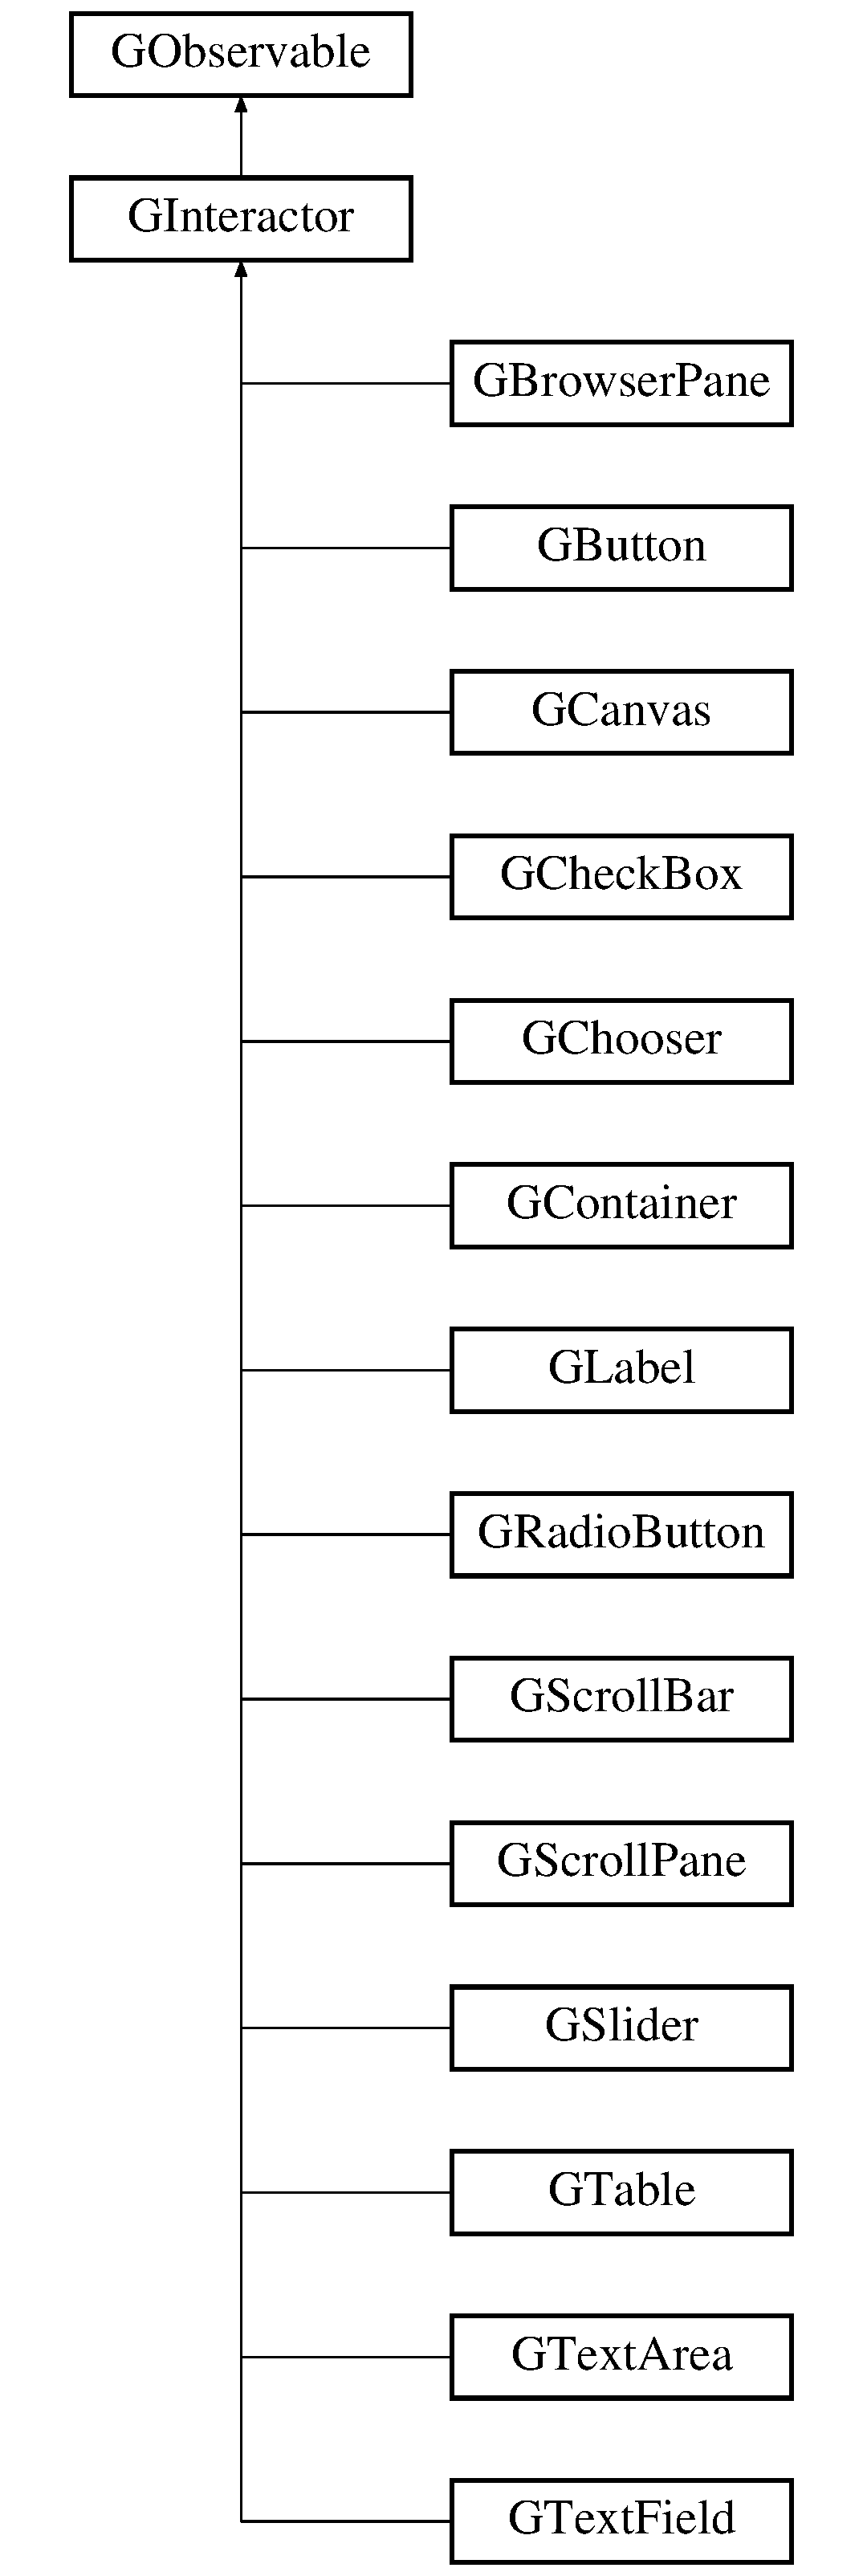
\includegraphics[height=12.000000cm]{classGInteractor}
\end{center}
\end{figure}
\subsection*{Public Types}
\begin{DoxyCompactItemize}
\item 
enum \mbox{\hyperlink{classGInteractor_a8e0d441725a81d2bbdebbea09078260e}{Text\+Position}} \{ \mbox{\hyperlink{classGInteractor_a8e0d441725a81d2bbdebbea09078260ea4cd6f2e7d5a08d6f4dc052df2358f774}{T\+E\+X\+T\+\_\+\+B\+E\+S\+I\+D\+E\+\_\+\+I\+C\+ON}}, 
\mbox{\hyperlink{classGInteractor_a8e0d441725a81d2bbdebbea09078260eaa88490f63d8de68d44c83bdb2ecde3b3}{T\+E\+X\+T\+\_\+\+U\+N\+D\+E\+R\+\_\+\+I\+C\+ON}}, 
\mbox{\hyperlink{classGInteractor_a8e0d441725a81d2bbdebbea09078260ea39a6f388a30ac4fefb6eb13e846bc9f2}{T\+E\+X\+T\+\_\+\+O\+N\+LY}}
 \}
\begin{DoxyCompactList}\small\item\em The places where an interactor can place its text relative to its icon. \end{DoxyCompactList}\end{DoxyCompactItemize}
\subsection*{Public Member Functions}
\begin{DoxyCompactItemize}
\item 
\mbox{\hyperlink{classGInteractor_a5a5d84b3c2735060635b4b338c397823}{G\+Interactor}} ()
\begin{DoxyCompactList}\small\item\em Initializes a newly created interactor. \end{DoxyCompactList}\item 
virtual \mbox{\hyperlink{classGInteractor_adb2d61211f85464680d47b511db24561}{$\sim$\+G\+Interactor}} ()
\begin{DoxyCompactList}\small\item\em Frees memory allocated internally by the interactor. \end{DoxyCompactList}\item 
virtual void \mbox{\hyperlink{classGInteractor_a02f20ea6edfa0671f31c4c648a253833}{add\+Action\+Listener}} () Q\+\_\+\+D\+E\+C\+L\+\_\+\+D\+E\+P\+R\+E\+C\+A\+T\+ED
\begin{DoxyCompactList}\small\item\em Adds an event listener to be notified when this interactor is clicked or generally interacted with. \end{DoxyCompactList}\item 
virtual bool \mbox{\hyperlink{classGInteractor_ac05ba5b92e2e5146d416fe7f842a0969}{events\+Enabled}} () const Q\+\_\+\+D\+E\+C\+L\+\_\+\+O\+V\+E\+R\+R\+I\+DE
\begin{DoxyCompactList}\small\item\em Returns true if this interactor is currently accepting events. \end{DoxyCompactList}\item 
virtual std\+::string \mbox{\hyperlink{classGInteractor_a69f8d23ed8f207fbecad99960776e942}{get\+Accelerator}} () const
\begin{DoxyCompactList}\small\item\em Returns a string representing a hotkey for this interactor, or an empty string if no accelerator has been set. \end{DoxyCompactList}\item 
virtual std\+::string \mbox{\hyperlink{classGInteractor_a94eb4276000c4fdfb508ce9e6317a82a}{get\+Action\+Command}} () const
\begin{DoxyCompactList}\small\item\em Returns an action command for this interactor, which is a semi-\/unique string you can use to identify it when events occur. \end{DoxyCompactList}\item 
virtual std\+::string \mbox{\hyperlink{classGInteractor_a808e22cc1fdfbecf71ed8c64ef4600e0}{get\+Background}} () const
\begin{DoxyCompactList}\small\item\em Returns the background color of the interactor as a string. \end{DoxyCompactList}\item 
virtual int \mbox{\hyperlink{classGInteractor_a9e827257a55cb8cf4d9de2ec6bcfd7a0}{get\+Background\+Int}} () const
\begin{DoxyCompactList}\small\item\em Returns the background color of the interactor as an R\+GB integer. \end{DoxyCompactList}\item 
virtual \mbox{\hyperlink{classGRectangle}{G\+Rectangle}} \mbox{\hyperlink{classGInteractor_a29e6ac35a0b48f491a4c88194cc5da3b}{get\+Bounds}} () const
\begin{DoxyCompactList}\small\item\em Returns a rectangle representing the x/y position and size of this interactor. \end{DoxyCompactList}\item 
virtual std\+::string \mbox{\hyperlink{classGInteractor_aa061dfa488c31e18549d64363c1d0e34}{get\+Color}} () const
\begin{DoxyCompactList}\small\item\em Returns the foreground/text color of the interactor as a string. \end{DoxyCompactList}\item 
virtual int \mbox{\hyperlink{classGInteractor_a9635c7af766cdc3417f346683fa0e6c1}{get\+Color\+Int}} () const
\begin{DoxyCompactList}\small\item\em Returns the foreground/text color of the interactor as an R\+GB integer. \end{DoxyCompactList}\item 
virtual \mbox{\hyperlink{classGContainer}{G\+Container}} $\ast$ \mbox{\hyperlink{classGInteractor_a7a6e317c29d61030929b4cd2d1c00fe7}{get\+Container}} () const
\begin{DoxyCompactList}\small\item\em Returns a pointer to the onscreen container holding this interactor. \end{DoxyCompactList}\item 
virtual std\+::string \mbox{\hyperlink{classGInteractor_a894a5502900794eeb27d084c21f1d77d}{get\+Font}} () const
\begin{DoxyCompactList}\small\item\em Returns the font of this interactor\textquotesingle{}s text as a font string such as \char`\"{}\+Helvetica-\/12-\/\+Bold\char`\"{}. \end{DoxyCompactList}\item 
virtual std\+::string \mbox{\hyperlink{classGInteractor_a4fa2d8b0192a3a5b4af4bbfe71194d03}{get\+Foreground}} () const
\begin{DoxyCompactList}\small\item\em Returns the foreground/text color of the interactor as a string. \end{DoxyCompactList}\item 
virtual int \mbox{\hyperlink{classGInteractor_ac3b12ab385a6ef9ae90fc879860ba726}{get\+Foreground\+Int}} () const
\begin{DoxyCompactList}\small\item\em Returns the foreground/text color of the interactor as an R\+GB integer. \end{DoxyCompactList}\item 
virtual double \mbox{\hyperlink{classGInteractor_a1e7e353362434072875264cf95629f99}{get\+Height}} () const
\begin{DoxyCompactList}\small\item\em Returns the current onscreen height of this interactor in pixels. \end{DoxyCompactList}\item 
virtual std\+::string \mbox{\hyperlink{classGInteractor_aaed62a73004939a64da6f0eb9eb64d73}{get\+Icon}} () const
\begin{DoxyCompactList}\small\item\em Returns the file name of the icon associated with this interactor, or an empty string if no icon has been set. \end{DoxyCompactList}\item 
virtual int \mbox{\hyperlink{classGInteractor_a9c9659a6c6ba66b4107ba59c95a24241}{get\+ID}} () const
\begin{DoxyCompactList}\small\item\em Returns a globally unique identifier for this interactor, which is set when the interactor is constructed. \end{DoxyCompactList}\item 
virtual \mbox{\hyperlink{classGPoint}{G\+Point}} \mbox{\hyperlink{classGInteractor_a4f83802015511edeb63b892830812c11}{get\+Location}} () const
\begin{DoxyCompactList}\small\item\em Returns an (x, y) point representing the onscreen location of the top-\/left corner of this interactor within its containing window. \end{DoxyCompactList}\item 
virtual double \mbox{\hyperlink{classGInteractor_aed4b0075fcc434499c3cb3e46896bda3}{get\+Minimum\+Height}} () const
\begin{DoxyCompactList}\small\item\em Returns the minimum height in pixels that this interactor will permit itself to be resized to. \end{DoxyCompactList}\item 
virtual \mbox{\hyperlink{classGDimension}{G\+Dimension}} \mbox{\hyperlink{classGInteractor_a66b5af0b32493b4d597ca0a3df2049ea}{get\+Minimum\+Size}} () const
\begin{DoxyCompactList}\small\item\em Returns a \mbox{\hyperlink{classGDimension}{G\+Dimension}} structure representing the minimum size in pixels that this interactor will permit itself to be resized to. \end{DoxyCompactList}\item 
virtual double \mbox{\hyperlink{classGInteractor_a59e668114fe3d49d2a0f28deb258f7c8}{get\+Minimum\+Width}} () const
\begin{DoxyCompactList}\small\item\em Returns the minimum width in pixels that this interactor will permit itself to be resized to. \end{DoxyCompactList}\item 
virtual std\+::string \mbox{\hyperlink{classGInteractor_a8a60438a5b55d0b2ceb35c8674b9d8c5}{get\+Name}} () const
\begin{DoxyCompactList}\small\item\em Returns a string representing a unique name for this interactor. \end{DoxyCompactList}\item 
virtual double \mbox{\hyperlink{classGInteractor_a747de0961653847bdc6615dbf756d715}{get\+Preferred\+Height}} () const
\begin{DoxyCompactList}\small\item\em Returns the height in pixels that this interactor would prefer to be, which would exactly fit its contents with no stretching or scrollbars. \end{DoxyCompactList}\item 
virtual \mbox{\hyperlink{classGDimension}{G\+Dimension}} \mbox{\hyperlink{classGInteractor_a4aabbee761d8e9116275401131b7ccd1}{get\+Preferred\+Size}} () const
\begin{DoxyCompactList}\small\item\em Returns a \mbox{\hyperlink{classGDimension}{G\+Dimension}} structure storing the width and height in pixels that this interactor would prefer to be, which would exactly fit its contents with no stretching or scrollbars. \end{DoxyCompactList}\item 
virtual double \mbox{\hyperlink{classGInteractor_a82bca31d37700fb0e35d2743352efd5e}{get\+Preferred\+Width}} () const
\begin{DoxyCompactList}\small\item\em Returns the height in pixels that this interactor would prefer to be, which would exactly fit its contents with no stretching or scrollbars. \end{DoxyCompactList}\item 
virtual \mbox{\hyperlink{classGDimension}{G\+Dimension}} \mbox{\hyperlink{classGInteractor_a7b4eec96a2bdc6420695d5796a78eea9}{get\+Size}} () const
\begin{DoxyCompactList}\small\item\em Returns a \mbox{\hyperlink{classGDimension}{G\+Dimension}} structure storing the current onscreen width and height of this interactor in pixels. \end{DoxyCompactList}\item 
virtual std\+::string \mbox{\hyperlink{classGInteractor_a799e073a127b428cc841086d42ea4fed}{get\+Type}} () const =0
\begin{DoxyCompactList}\small\item\em Returns a string representing the class name of this interactor, such as \char`\"{}\+G\+Button\char`\"{} or \char`\"{}\+G\+Check\+Box\char`\"{}. \end{DoxyCompactList}\item 
virtual double \mbox{\hyperlink{classGInteractor_a0ed2965abd4f5701d2cadf71239faf19}{get\+Width}} () const
\begin{DoxyCompactList}\small\item\em Returns the current onscreen width of this interactor in pixels. \end{DoxyCompactList}\item 
virtual double \mbox{\hyperlink{classGInteractor_a344385751bee0720059403940d57a13e}{getX}} () const
\begin{DoxyCompactList}\small\item\em Returns the x-\/coordinate of the top-\/left pixel of this interactor within its onscreen window. \end{DoxyCompactList}\item 
virtual double \mbox{\hyperlink{classGInteractor_aafa51c7f8f38a09febbb9ce7853f77b4}{getY}} () const
\begin{DoxyCompactList}\small\item\em Returns the y-\/coordinate of the top-\/left pixel of this interactor within its onscreen window. \end{DoxyCompactList}\item 
virtual bool \mbox{\hyperlink{classGInteractor_afc480f652b8c5f1fb255e2269ce68879}{in\+Bounds}} (double x, double y) const
\begin{DoxyCompactList}\small\item\em Returns true if the given x/y pixel is within the bounds of this interactor. \end{DoxyCompactList}\item 
virtual bool \mbox{\hyperlink{classGInteractor_ae6d7982c1c627b677a5e776ca86118ed}{in\+Bounds}} (int x, int y) const
\begin{DoxyCompactList}\small\item\em Returns true if the given x/y pixel is within the bounds of this interactor. \end{DoxyCompactList}\item 
virtual bool \mbox{\hyperlink{classGInteractor_aacb819fb241851fd9fc045271baa4034}{is\+Enabled}} () const
\begin{DoxyCompactList}\small\item\em Returns true if this interactor is currently enabled. \end{DoxyCompactList}\item 
virtual bool \mbox{\hyperlink{classGInteractor_a9d8a6cfb13917785c143e74d40e4e2be}{is\+Visible}} () const
\begin{DoxyCompactList}\small\item\em Returns true if the interactor is visible on the screen. \end{DoxyCompactList}\item 
virtual void \mbox{\hyperlink{classGInteractor_a519fb2ac767f8b2febbb50b898b8c8cb}{request\+Focus}} ()
\begin{DoxyCompactList}\small\item\em Transfers keyboard focus to this interactor. \end{DoxyCompactList}\item 
virtual void \mbox{\hyperlink{classGInteractor_ad15f102f62e2960576012f1aa0ba4b2e}{set\+Accelerator}} (const std\+::string \&accelerator)
\begin{DoxyCompactList}\small\item\em Sets an accelerator hotkey for this interactor, such as \char`\"{}\+Ctrl-\/\+S\char`\"{}. \end{DoxyCompactList}\item 
virtual void \mbox{\hyperlink{classGInteractor_a4b5843fe3030e038a1ba54cc03389bcf}{set\+Action\+Command}} (const std\+::string \&action\+Command)
\begin{DoxyCompactList}\small\item\em Sets the action command for this interactor. \end{DoxyCompactList}\item 
virtual void \mbox{\hyperlink{classGInteractor_acba7e546c2025c0a15ca4b4cc92043db}{set\+Background}} (int rgb)
\begin{DoxyCompactList}\small\item\em Sets the background color of the interactor to the color represented by the given R\+GB integer. \end{DoxyCompactList}\item 
virtual void \mbox{\hyperlink{classGInteractor_ab4677ab2474e68b07aa56605af92a84a}{set\+Background}} (const std\+::string \&color)
\begin{DoxyCompactList}\small\item\em Sets the background color of the interactor to the color represented by the given string. \end{DoxyCompactList}\item 
virtual void \mbox{\hyperlink{classGInteractor_a2aae8197624b72265ab83b4f1bc73f2f}{set\+Bounds}} (double x, double y, double width, double height)
\begin{DoxyCompactList}\small\item\em Sets the size and location of the widget. \end{DoxyCompactList}\item 
virtual void \mbox{\hyperlink{classGInteractor_acada386653f008cacc7cce86426bef7c}{set\+Bounds}} (const \mbox{\hyperlink{classGRectangle}{G\+Rectangle}} \&size)
\begin{DoxyCompactList}\small\item\em Sets the size and location of the widget. \end{DoxyCompactList}\item 
virtual void \mbox{\hyperlink{classGInteractor_ab1f5cc0f5cc6bbbd716a526c61f1081d}{set\+Color}} (int rgb)
\begin{DoxyCompactList}\small\item\em Sets the foreground/text color of the interactor to the color represented by the given R\+GB integer. \end{DoxyCompactList}\item 
virtual void \mbox{\hyperlink{classGInteractor_a61374df6c11b52cfbb0815decdbaebc6}{set\+Color}} (const std\+::string \&color)
\begin{DoxyCompactList}\small\item\em Sets the foreground/text color of the interactor to the color represented by the given string. \end{DoxyCompactList}\item 
virtual void \mbox{\hyperlink{classGInteractor_ab831367dd84bbd579e02e55bacb21343}{set\+Enabled}} (bool value)
\begin{DoxyCompactList}\small\item\em Sets whether this interactor is currently enabled. \end{DoxyCompactList}\item 
virtual void \mbox{\hyperlink{classGObservable_afaa30b2a9e0f378fd1c70d2f1d0b8216}{set\+Events\+Enabled}} (bool \mbox{\hyperlink{classGInteractor_ac05ba5b92e2e5146d416fe7f842a0969}{events\+Enabled}})
\begin{DoxyCompactList}\small\item\em Sets whether the object is currently allowing itself to fire events. \end{DoxyCompactList}\item 
virtual void \mbox{\hyperlink{classGInteractor_a2592348886ffea646c6534bf88f7c49d}{set\+Font}} (const Q\+Font \&font)
\begin{DoxyCompactList}\small\item\em Sets the font used by this widget to the given Qt font. \end{DoxyCompactList}\item 
virtual void \mbox{\hyperlink{classGInteractor_a8e096e8818d838aceae1d46d58fb3a7b}{set\+Font}} (const std\+::string \&font)
\begin{DoxyCompactList}\small\item\em Sets the font used by this widget to the font represented by the given font string, such as \char`\"{}\+Helvetica-\/16-\/\+Bold\char`\"{}. \end{DoxyCompactList}\item 
virtual void \mbox{\hyperlink{classGInteractor_a9eb856b5ff83a19df3831a31f15f4563}{set\+Foreground}} (int rgb)
\begin{DoxyCompactList}\small\item\em Sets the foreground/text color of the interactor to the color represented by the given R\+GB integer. \end{DoxyCompactList}\item 
virtual void \mbox{\hyperlink{classGInteractor_af59209aeadea6dfc6d97a2d8531f50e1}{set\+Foreground}} (const std\+::string \&color)
\begin{DoxyCompactList}\small\item\em Sets the foreground/text color of the interactor to the color represented by the given string. \end{DoxyCompactList}\item 
virtual void \mbox{\hyperlink{classGInteractor_a9e280bfc4544dfaf8e4376c4e1a74357}{set\+Height}} (double height)
\begin{DoxyCompactList}\small\item\em Sets the onscreen height of the interactor in pixels. \end{DoxyCompactList}\item 
virtual void \mbox{\hyperlink{classGInteractor_a762e139aa311461c3984d3ad28293f64}{set\+Icon}} (const std\+::string \&filename, bool retain\+Icon\+Size=true)
\begin{DoxyCompactList}\small\item\em Sets the file name of the icon associated with this interactor, or an empty string if no icon has been set. \end{DoxyCompactList}\item 
virtual void \mbox{\hyperlink{classGInteractor_a04594e8ba9b98513a64f1da00dcae18c}{set\+Location}} (double x, double y)
\begin{DoxyCompactList}\small\item\em Sets the onscreen x/y-\/coordinate of the top-\/left corner of the interactor relative to its window. \end{DoxyCompactList}\item 
virtual void \mbox{\hyperlink{classGInteractor_a0cf428e207b7f22cc08138a90b1b87b2}{set\+Minimum\+Size}} (double width, double height)
\begin{DoxyCompactList}\small\item\em Sets the minimum size in pixels that this interactor will permit itself to be resized to. \end{DoxyCompactList}\item 
virtual void \mbox{\hyperlink{classGInteractor_a3b1046117ac6cb7abe467e00ba8a81f4}{set\+Minimum\+Size}} (const \mbox{\hyperlink{classGDimension}{G\+Dimension}} \&size)
\begin{DoxyCompactList}\small\item\em Sets the minimum size in pixels that this interactor will permit itself to be resized to. \end{DoxyCompactList}\item 
virtual void \mbox{\hyperlink{classGInteractor_a9d3a2685df23b5e7cbf59c19c4a1f9b5}{set\+Name}} (const std\+::string \&name)
\begin{DoxyCompactList}\small\item\em Sets a string representing a unique name for this interactor. \end{DoxyCompactList}\item 
virtual void \mbox{\hyperlink{classGInteractor_a1ab987704fce32098706c6f00fb08218}{set\+Preferred\+Height}} (double height)
\begin{DoxyCompactList}\small\item\em Sets the height in pixels that this interactor would prefer to be. \end{DoxyCompactList}\item 
virtual void \mbox{\hyperlink{classGInteractor_a042c5ae19430d765ef552371cae3632c}{set\+Preferred\+Size}} (double width, double height)
\begin{DoxyCompactList}\small\item\em Sets the width and height in pixels that this interactor would prefer to be. \end{DoxyCompactList}\item 
virtual void \mbox{\hyperlink{classGInteractor_aa22d9be4bc0e078bb0ea69b0fc9d7c75}{set\+Preferred\+Size}} (const \mbox{\hyperlink{classGDimension}{G\+Dimension}} \&size)
\begin{DoxyCompactList}\small\item\em Sets the size in pixels that this interactor would prefer to be. \end{DoxyCompactList}\item 
virtual void \mbox{\hyperlink{classGInteractor_a3db429ab2fa52efd187eec0ed8cdd9f2}{set\+Preferred\+Width}} (double width)
\begin{DoxyCompactList}\small\item\em Sets the width in pixels that this interactor would prefer to be. \end{DoxyCompactList}\item 
virtual void \mbox{\hyperlink{classGInteractor_aca25d49481f9bf5fc8f7df4c086c4ce7}{set\+Size}} (double width, double height)
\begin{DoxyCompactList}\small\item\em Sets the onscreen width and height of the interactor in pixels. \end{DoxyCompactList}\item 
virtual void \mbox{\hyperlink{classGInteractor_ae2b628228f192c2702c4ce941b2af68f}{set\+Size}} (const \mbox{\hyperlink{classGDimension}{G\+Dimension}} \&size)
\begin{DoxyCompactList}\small\item\em Sets the onscreen width and height of the interactor in pixels. \end{DoxyCompactList}\item 
virtual void \mbox{\hyperlink{classGInteractor_a039e0e49beaecc275efce02d416acea8}{set\+Tooltip}} (const std\+::string \&tooltip\+Text)
\begin{DoxyCompactList}\small\item\em Sets a \char`\"{}tooltip\char`\"{} that will appear if the user hovers their mouse over the interactor. \end{DoxyCompactList}\item 
virtual void \mbox{\hyperlink{classGInteractor_a18e44e30b31525a243960ca3928125aa}{set\+Visible}} (bool visible)
\begin{DoxyCompactList}\small\item\em Returns true if the interactor is visible on the screen. \end{DoxyCompactList}\item 
virtual void \mbox{\hyperlink{classGInteractor_aa3f3fba4cb131baa8696ba01e3bceca1}{set\+Width}} (double width)
\begin{DoxyCompactList}\small\item\em Sets the onscreen width of the interactor in pixels. \end{DoxyCompactList}\item 
virtual void \mbox{\hyperlink{classGInteractor_a9c18fcc579333bf9653d13ad2b372e39}{setX}} (double x)
\begin{DoxyCompactList}\small\item\em Sets the onscreen x-\/coordinate of the top-\/left corner of the interactor relative to its window. \end{DoxyCompactList}\item 
virtual void \mbox{\hyperlink{classGInteractor_a7d57e2a5c35d27feb58fd498a3cf82b9}{setY}} (double y)
\begin{DoxyCompactList}\small\item\em Sets the onscreen y-\/coordinate of the top-\/left corner of the interactor relative to its window. \end{DoxyCompactList}\item 
virtual std\+::string \mbox{\hyperlink{classGObservable_a1fe5121d6528fdea3f243321b3fa3a49}{to\+String}} () const
\begin{DoxyCompactList}\small\item\em Returns a string representation of this observable object\textquotesingle{}s state. \end{DoxyCompactList}\end{DoxyCompactItemize}
\subsection*{Protected Member Functions}
\begin{DoxyCompactItemize}
\item 
virtual void \mbox{\hyperlink{classGObservable_a80cfa040459ff53594adbd6a51ec8f43}{clear\+Event\+Listeners}} ()
\begin{DoxyCompactList}\small\item\em Removes all event listeners from this object. \end{DoxyCompactList}\item 
virtual void \mbox{\hyperlink{classGObservable_a284f31528c0520f8e545c03ac9eeac74}{ensure\+Thread\+Safety}} (const std\+::string \&member\+Name=\char`\"{}\char`\"{})
\begin{DoxyCompactList}\small\item\em Ensures that we are currently in the Qt G\+UI thread. \end{DoxyCompactList}\item 
virtual void \mbox{\hyperlink{classGObservable_a63e5e5a6227c59c928493b11aceb0f67}{fire\+Event}} (\mbox{\hyperlink{classGEvent}{G\+Event}} \&event)
\begin{DoxyCompactList}\small\item\em Sends out the given event to any attached listeners. \end{DoxyCompactList}\item 
virtual void \mbox{\hyperlink{classGObservable_ab3983ea07337b52020a29cc00c653d8d}{fire\+G\+Event}} (Q\+Event $\ast$event, Event\+Type event\+Type, const std\+::string \&event\+Name)
\begin{DoxyCompactList}\small\item\em Creates an event of the given type, then sends it out to any attached listeners. \end{DoxyCompactList}\item 
virtual void \mbox{\hyperlink{classGObservable_a01fdf1b0e0dbd49e189fe4514e010411}{fire\+G\+Event}} (Q\+Close\+Event $\ast$event, Event\+Type event\+Type, const std\+::string \&event\+Name)
\begin{DoxyCompactList}\small\item\em Creates an event of the given type, then sends it out to any attached listeners. \end{DoxyCompactList}\item 
virtual void \mbox{\hyperlink{classGObservable_abb0b2f66ba39211cb5d7615e9d1c04e2}{fire\+G\+Event}} (Q\+Key\+Event $\ast$event, Event\+Type event\+Type, const std\+::string \&event\+Name)
\begin{DoxyCompactList}\small\item\em Creates an event of the given type, then sends it out to any attached listeners. \end{DoxyCompactList}\item 
virtual void \mbox{\hyperlink{classGObservable_a119318675d2165bdf7dd853aaf881d4b}{fire\+G\+Event}} (Q\+Mouse\+Event $\ast$event, Event\+Type event\+Type, const std\+::string \&event\+Name, const std\+::string \&action\+Command=\char`\"{}\char`\"{})
\begin{DoxyCompactList}\small\item\em Creates an event of the given type, then sends it out to any attached listeners. \end{DoxyCompactList}\item 
virtual void \mbox{\hyperlink{classGObservable_a63fd9034e1e1633c1c38eb342bfd34e9}{fire\+G\+Event}} (Q\+Resize\+Event $\ast$event, Event\+Type event\+Type, const std\+::string \&event\+Name)
\begin{DoxyCompactList}\small\item\em Creates an event of the given type, then sends it out to any attached listeners. \end{DoxyCompactList}\item 
virtual void \mbox{\hyperlink{classGObservable_a741345310d9b7c5170a6cbc410c44ac4}{fire\+G\+Event}} (Q\+Timer\+Event $\ast$event, Event\+Type event\+Type, const std\+::string \&event\+Name)
\begin{DoxyCompactList}\small\item\em Creates an event of the given type, then sends it out to any attached listeners. \end{DoxyCompactList}\item 
virtual void \mbox{\hyperlink{classGObservable_a93bf338968a0338761b8e4dc62f582e9}{fire\+G\+Event}} (Q\+Wheel\+Event $\ast$event, Event\+Type event\+Type, const std\+::string \&event\+Name)
\begin{DoxyCompactList}\small\item\em Creates an event of the given type, then sends it out to any attached listeners. \end{DoxyCompactList}\item 
virtual void \mbox{\hyperlink{classGObservable_a2a70a7d7435ff0c3b80bb4d70da19e0d}{fire\+G\+Event}} (Q\+Window\+State\+Change\+Event $\ast$event, Event\+Type event\+Type, const std\+::string \&event\+Name)
\begin{DoxyCompactList}\small\item\em Creates an event of the given type, then sends it out to any attached listeners. \end{DoxyCompactList}\item 
virtual bool \mbox{\hyperlink{classGObservable_a9f6faaa25942923bafa1c44020c49fa9}{has\+Event\+Listener}} (const std\+::string \&event\+Name) const
\begin{DoxyCompactList}\small\item\em Returns true if the observable object has a listener for the given type of event. \end{DoxyCompactList}\item 
virtual bool \mbox{\hyperlink{classGObservable_aeec1adc19aa0f33de62390686ee1382c}{is\+Accepting\+Event}} (int event\+Mask) const
\begin{DoxyCompactList}\small\item\em Returns true if the observable object has a listener for the given type of event. \end{DoxyCompactList}\item 
virtual bool \mbox{\hyperlink{classGObservable_aa31c73145a29dcb92848a92e0cfaea41}{is\+Accepting\+Event}} (const \mbox{\hyperlink{classGEvent}{G\+Event}} \&event) const
\begin{DoxyCompactList}\small\item\em Returns true if the observable object has a listener for the given type of event. \end{DoxyCompactList}\item 
virtual bool \mbox{\hyperlink{classGObservable_a3b1c689267eda44e65a2213e7de38b23}{is\+Accepting\+Event}} (const std\+::string \&event\+Type) const
\begin{DoxyCompactList}\small\item\em Returns true if the observable object has a listener for the given type of event. \end{DoxyCompactList}\item 
virtual void \mbox{\hyperlink{classGObservable_acbcf1ed3a851ad8a3c17ef38d86b481d}{remove\+Event\+Listener}} (const std\+::string \&event\+Name)
\begin{DoxyCompactList}\small\item\em Removes any event listener from this observable object that would respond to the given type of event, such as \char`\"{}click\char`\"{} or \char`\"{}keydown\char`\"{}. \end{DoxyCompactList}\item 
virtual void \mbox{\hyperlink{classGObservable_af51cc35c29a1bd1908609d432decdbb6}{remove\+Event\+Listeners}} (std\+::initializer\+\_\+list$<$ std\+::string $>$ event\+Names)
\begin{DoxyCompactList}\small\item\em Removes any event listener from this observable object that would respond to the given types of events, such as \char`\"{}click\char`\"{} or \char`\"{}keydown\char`\"{}. \end{DoxyCompactList}\item 
virtual void \mbox{\hyperlink{classGObservable_ad2f6d34961c50f6c1e0659990b79f741}{set\+Event\+Listener}} (const std\+::string \&event\+Name, G\+Event\+Listener func)
\begin{DoxyCompactList}\small\item\em Adds an event listener from this observable object to respond to the given type of event, such as \char`\"{}click\char`\"{} or \char`\"{}keydown\char`\"{}. \end{DoxyCompactList}\item 
virtual void \mbox{\hyperlink{classGObservable_abac4cb9f9e626e010e87f5d91573c8a5}{set\+Event\+Listener}} (const std\+::string \&event\+Name, G\+Event\+Listener\+Void func)
\begin{DoxyCompactList}\small\item\em Adds an event listener from this observable object to respond to the given type of event, such as \char`\"{}click\char`\"{} or \char`\"{}keydown\char`\"{}. \end{DoxyCompactList}\item 
virtual void \mbox{\hyperlink{classGObservable_afa388d69c33c718cf035774604065604}{set\+Event\+Listeners}} (std\+::initializer\+\_\+list$<$ std\+::string $>$ event\+Names, G\+Event\+Listener func)
\begin{DoxyCompactList}\small\item\em Adds an event listener from this observable object to respond to the given types of events, such as \char`\"{}click\char`\"{} or \char`\"{}keydown\char`\"{}. \end{DoxyCompactList}\item 
virtual void \mbox{\hyperlink{classGObservable_a7867184bbb686f74fae8a4db927da799}{set\+Event\+Listeners}} (std\+::initializer\+\_\+list$<$ std\+::string $>$ event\+Names, G\+Event\+Listener\+Void func)
\begin{DoxyCompactList}\small\item\em Adds an event listener from this observable object to respond to the given types of events, such as \char`\"{}click\char`\"{} or \char`\"{}keydown\char`\"{}. \end{DoxyCompactList}\end{DoxyCompactItemize}


\subsection{Detailed Description}
This abstract class is the superclass for all graphical interactors. 

In most applications, interactors will be added to a control strip along one of the regions of a \mbox{\hyperlink{classGWindow}{G\+Window}}. 

\subsection{Member Enumeration Documentation}
\mbox{\Hypertarget{classGInteractor_a8e0d441725a81d2bbdebbea09078260e}\label{classGInteractor_a8e0d441725a81d2bbdebbea09078260e}} 
\index{G\+Interactor@{G\+Interactor}!Text\+Position@{Text\+Position}}
\index{Text\+Position@{Text\+Position}!G\+Interactor@{G\+Interactor}}
\subsubsection{\texorpdfstring{Text\+Position}{TextPosition}}
{\footnotesize\ttfamily enum \mbox{\hyperlink{classGInteractor_a8e0d441725a81d2bbdebbea09078260e}{Text\+Position}}}



The places where an interactor can place its text relative to its icon. 

\begin{DoxyEnumFields}{Enumerator}
\raisebox{\heightof{T}}[0pt][0pt]{\index{T\+E\+X\+T\+\_\+\+B\+E\+S\+I\+D\+E\+\_\+\+I\+C\+ON@{T\+E\+X\+T\+\_\+\+B\+E\+S\+I\+D\+E\+\_\+\+I\+C\+ON}!G\+Interactor@{G\+Interactor}}\index{G\+Interactor@{G\+Interactor}!T\+E\+X\+T\+\_\+\+B\+E\+S\+I\+D\+E\+\_\+\+I\+C\+ON@{T\+E\+X\+T\+\_\+\+B\+E\+S\+I\+D\+E\+\_\+\+I\+C\+ON}}}\mbox{\Hypertarget{classGInteractor_a8e0d441725a81d2bbdebbea09078260ea4cd6f2e7d5a08d6f4dc052df2358f774}\label{classGInteractor_a8e0d441725a81d2bbdebbea09078260ea4cd6f2e7d5a08d6f4dc052df2358f774}} 
T\+E\+X\+T\+\_\+\+B\+E\+S\+I\+D\+E\+\_\+\+I\+C\+ON&\\
\hline

\raisebox{\heightof{T}}[0pt][0pt]{\index{T\+E\+X\+T\+\_\+\+U\+N\+D\+E\+R\+\_\+\+I\+C\+ON@{T\+E\+X\+T\+\_\+\+U\+N\+D\+E\+R\+\_\+\+I\+C\+ON}!G\+Interactor@{G\+Interactor}}\index{G\+Interactor@{G\+Interactor}!T\+E\+X\+T\+\_\+\+U\+N\+D\+E\+R\+\_\+\+I\+C\+ON@{T\+E\+X\+T\+\_\+\+U\+N\+D\+E\+R\+\_\+\+I\+C\+ON}}}\mbox{\Hypertarget{classGInteractor_a8e0d441725a81d2bbdebbea09078260eaa88490f63d8de68d44c83bdb2ecde3b3}\label{classGInteractor_a8e0d441725a81d2bbdebbea09078260eaa88490f63d8de68d44c83bdb2ecde3b3}} 
T\+E\+X\+T\+\_\+\+U\+N\+D\+E\+R\+\_\+\+I\+C\+ON&\\
\hline

\raisebox{\heightof{T}}[0pt][0pt]{\index{T\+E\+X\+T\+\_\+\+O\+N\+LY@{T\+E\+X\+T\+\_\+\+O\+N\+LY}!G\+Interactor@{G\+Interactor}}\index{G\+Interactor@{G\+Interactor}!T\+E\+X\+T\+\_\+\+O\+N\+LY@{T\+E\+X\+T\+\_\+\+O\+N\+LY}}}\mbox{\Hypertarget{classGInteractor_a8e0d441725a81d2bbdebbea09078260ea39a6f388a30ac4fefb6eb13e846bc9f2}\label{classGInteractor_a8e0d441725a81d2bbdebbea09078260ea39a6f388a30ac4fefb6eb13e846bc9f2}} 
T\+E\+X\+T\+\_\+\+O\+N\+LY&\\
\hline

\end{DoxyEnumFields}


\subsection{Constructor \& Destructor Documentation}
\mbox{\Hypertarget{classGInteractor_a5a5d84b3c2735060635b4b338c397823}\label{classGInteractor_a5a5d84b3c2735060635b4b338c397823}} 
\index{G\+Interactor@{G\+Interactor}!G\+Interactor@{G\+Interactor}}
\index{G\+Interactor@{G\+Interactor}!G\+Interactor@{G\+Interactor}}
\subsubsection{\texorpdfstring{G\+Interactor()}{GInteractor()}}
{\footnotesize\ttfamily \mbox{\hyperlink{classGInteractor}{G\+Interactor}} (\begin{DoxyParamCaption}{ }\end{DoxyParamCaption})}



Initializes a newly created interactor. 

If the Qt graphical subsystem has not yet been initialized, constructing an interactor will initialize it. \mbox{\Hypertarget{classGInteractor_adb2d61211f85464680d47b511db24561}\label{classGInteractor_adb2d61211f85464680d47b511db24561}} 
\index{G\+Interactor@{G\+Interactor}!````~G\+Interactor@{$\sim$\+G\+Interactor}}
\index{````~G\+Interactor@{$\sim$\+G\+Interactor}!G\+Interactor@{G\+Interactor}}
\subsubsection{\texorpdfstring{$\sim$\+G\+Interactor()}{~GInteractor()}}
{\footnotesize\ttfamily $\sim$\mbox{\hyperlink{classGInteractor}{G\+Interactor}} (\begin{DoxyParamCaption}{ }\end{DoxyParamCaption})\hspace{0.3cm}{\ttfamily [virtual]}}



Frees memory allocated internally by the interactor. 



\subsection{Member Function Documentation}
\mbox{\Hypertarget{classGInteractor_a02f20ea6edfa0671f31c4c648a253833}\label{classGInteractor_a02f20ea6edfa0671f31c4c648a253833}} 
\index{G\+Interactor@{G\+Interactor}!add\+Action\+Listener@{add\+Action\+Listener}}
\index{add\+Action\+Listener@{add\+Action\+Listener}!G\+Interactor@{G\+Interactor}}
\subsubsection{\texorpdfstring{add\+Action\+Listener()}{addActionListener()}}
{\footnotesize\ttfamily void add\+Action\+Listener (\begin{DoxyParamCaption}{ }\end{DoxyParamCaption})\hspace{0.3cm}{\ttfamily [virtual]}}



Adds an event listener to be notified when this interactor is clicked or generally interacted with. 

\begin{DoxyRefDesc}{Deprecated}
\item[\mbox{\hyperlink{deprecated__deprecated000006}{Deprecated}}]does nothing; use set\+Action\+Listener instead \end{DoxyRefDesc}
\mbox{\Hypertarget{classGObservable_a80cfa040459ff53594adbd6a51ec8f43}\label{classGObservable_a80cfa040459ff53594adbd6a51ec8f43}} 
\index{G\+Interactor@{G\+Interactor}!clear\+Event\+Listeners@{clear\+Event\+Listeners}}
\index{clear\+Event\+Listeners@{clear\+Event\+Listeners}!G\+Interactor@{G\+Interactor}}
\subsubsection{\texorpdfstring{clear\+Event\+Listeners()}{clearEventListeners()}}
{\footnotesize\ttfamily void clear\+Event\+Listeners (\begin{DoxyParamCaption}{ }\end{DoxyParamCaption})\hspace{0.3cm}{\ttfamily [protected]}, {\ttfamily [virtual]}, {\ttfamily [inherited]}}



Removes all event listeners from this object. 

\mbox{\Hypertarget{classGObservable_a284f31528c0520f8e545c03ac9eeac74}\label{classGObservable_a284f31528c0520f8e545c03ac9eeac74}} 
\index{G\+Interactor@{G\+Interactor}!ensure\+Thread\+Safety@{ensure\+Thread\+Safety}}
\index{ensure\+Thread\+Safety@{ensure\+Thread\+Safety}!G\+Interactor@{G\+Interactor}}
\subsubsection{\texorpdfstring{ensure\+Thread\+Safety()}{ensureThreadSafety()}}
{\footnotesize\ttfamily void ensure\+Thread\+Safety (\begin{DoxyParamCaption}\item[{const std\+::string \&}]{member\+Name = {\ttfamily \char`\"{}\char`\"{}} }\end{DoxyParamCaption})\hspace{0.3cm}{\ttfamily [protected]}, {\ttfamily [virtual]}, {\ttfamily [inherited]}}



Ensures that we are currently in the Qt G\+UI thread. 

\mbox{\Hypertarget{classGInteractor_ac05ba5b92e2e5146d416fe7f842a0969}\label{classGInteractor_ac05ba5b92e2e5146d416fe7f842a0969}} 
\index{G\+Interactor@{G\+Interactor}!events\+Enabled@{events\+Enabled}}
\index{events\+Enabled@{events\+Enabled}!G\+Interactor@{G\+Interactor}}
\subsubsection{\texorpdfstring{events\+Enabled()}{eventsEnabled()}}
{\footnotesize\ttfamily bool events\+Enabled (\begin{DoxyParamCaption}{ }\end{DoxyParamCaption}) const\hspace{0.3cm}{\ttfamily [virtual]}}



Returns true if this interactor is currently accepting events. 

Initially true. An interactor must be visible and added to an onscreen window to receive events. 

Reimplemented from \mbox{\hyperlink{classGObservable_a8ebb3da91032e7f4c34485dabc518b8a}{G\+Observable}}.

\mbox{\Hypertarget{classGObservable_a63e5e5a6227c59c928493b11aceb0f67}\label{classGObservable_a63e5e5a6227c59c928493b11aceb0f67}} 
\index{G\+Interactor@{G\+Interactor}!fire\+Event@{fire\+Event}}
\index{fire\+Event@{fire\+Event}!G\+Interactor@{G\+Interactor}}
\subsubsection{\texorpdfstring{fire\+Event()}{fireEvent()}}
{\footnotesize\ttfamily void fire\+Event (\begin{DoxyParamCaption}\item[{\mbox{\hyperlink{classGEvent}{G\+Event}} \&}]{event }\end{DoxyParamCaption})\hspace{0.3cm}{\ttfamily [protected]}, {\ttfamily [virtual]}, {\ttfamily [inherited]}}



Sends out the given event to any attached listeners. 

\mbox{\Hypertarget{classGObservable_ab3983ea07337b52020a29cc00c653d8d}\label{classGObservable_ab3983ea07337b52020a29cc00c653d8d}} 
\index{G\+Interactor@{G\+Interactor}!fire\+G\+Event@{fire\+G\+Event}}
\index{fire\+G\+Event@{fire\+G\+Event}!G\+Interactor@{G\+Interactor}}
\subsubsection{\texorpdfstring{fire\+G\+Event()}{fireGEvent()}\hspace{0.1cm}{\footnotesize\ttfamily [1/8]}}
{\footnotesize\ttfamily void fire\+G\+Event (\begin{DoxyParamCaption}\item[{Q\+Event $\ast$}]{event,  }\item[{Event\+Type}]{event\+Type,  }\item[{const std\+::string \&}]{event\+Name }\end{DoxyParamCaption})\hspace{0.3cm}{\ttfamily [protected]}, {\ttfamily [virtual]}, {\ttfamily [inherited]}}



Creates an event of the given type, then sends it out to any attached listeners. 

\mbox{\Hypertarget{classGObservable_a01fdf1b0e0dbd49e189fe4514e010411}\label{classGObservable_a01fdf1b0e0dbd49e189fe4514e010411}} 
\index{G\+Interactor@{G\+Interactor}!fire\+G\+Event@{fire\+G\+Event}}
\index{fire\+G\+Event@{fire\+G\+Event}!G\+Interactor@{G\+Interactor}}
\subsubsection{\texorpdfstring{fire\+G\+Event()}{fireGEvent()}\hspace{0.1cm}{\footnotesize\ttfamily [2/8]}}
{\footnotesize\ttfamily void fire\+G\+Event (\begin{DoxyParamCaption}\item[{Q\+Close\+Event $\ast$}]{event,  }\item[{Event\+Type}]{event\+Type,  }\item[{const std\+::string \&}]{event\+Name }\end{DoxyParamCaption})\hspace{0.3cm}{\ttfamily [protected]}, {\ttfamily [virtual]}, {\ttfamily [inherited]}}



Creates an event of the given type, then sends it out to any attached listeners. 

\mbox{\Hypertarget{classGObservable_abb0b2f66ba39211cb5d7615e9d1c04e2}\label{classGObservable_abb0b2f66ba39211cb5d7615e9d1c04e2}} 
\index{G\+Interactor@{G\+Interactor}!fire\+G\+Event@{fire\+G\+Event}}
\index{fire\+G\+Event@{fire\+G\+Event}!G\+Interactor@{G\+Interactor}}
\subsubsection{\texorpdfstring{fire\+G\+Event()}{fireGEvent()}\hspace{0.1cm}{\footnotesize\ttfamily [3/8]}}
{\footnotesize\ttfamily void fire\+G\+Event (\begin{DoxyParamCaption}\item[{Q\+Key\+Event $\ast$}]{event,  }\item[{Event\+Type}]{event\+Type,  }\item[{const std\+::string \&}]{event\+Name }\end{DoxyParamCaption})\hspace{0.3cm}{\ttfamily [protected]}, {\ttfamily [virtual]}, {\ttfamily [inherited]}}



Creates an event of the given type, then sends it out to any attached listeners. 

\mbox{\Hypertarget{classGObservable_a119318675d2165bdf7dd853aaf881d4b}\label{classGObservable_a119318675d2165bdf7dd853aaf881d4b}} 
\index{G\+Interactor@{G\+Interactor}!fire\+G\+Event@{fire\+G\+Event}}
\index{fire\+G\+Event@{fire\+G\+Event}!G\+Interactor@{G\+Interactor}}
\subsubsection{\texorpdfstring{fire\+G\+Event()}{fireGEvent()}\hspace{0.1cm}{\footnotesize\ttfamily [4/8]}}
{\footnotesize\ttfamily void fire\+G\+Event (\begin{DoxyParamCaption}\item[{Q\+Mouse\+Event $\ast$}]{event,  }\item[{Event\+Type}]{event\+Type,  }\item[{const std\+::string \&}]{event\+Name,  }\item[{const std\+::string \&}]{action\+Command = {\ttfamily \char`\"{}\char`\"{}} }\end{DoxyParamCaption})\hspace{0.3cm}{\ttfamily [protected]}, {\ttfamily [virtual]}, {\ttfamily [inherited]}}



Creates an event of the given type, then sends it out to any attached listeners. 

\mbox{\Hypertarget{classGObservable_a63fd9034e1e1633c1c38eb342bfd34e9}\label{classGObservable_a63fd9034e1e1633c1c38eb342bfd34e9}} 
\index{G\+Interactor@{G\+Interactor}!fire\+G\+Event@{fire\+G\+Event}}
\index{fire\+G\+Event@{fire\+G\+Event}!G\+Interactor@{G\+Interactor}}
\subsubsection{\texorpdfstring{fire\+G\+Event()}{fireGEvent()}\hspace{0.1cm}{\footnotesize\ttfamily [5/8]}}
{\footnotesize\ttfamily void fire\+G\+Event (\begin{DoxyParamCaption}\item[{Q\+Resize\+Event $\ast$}]{event,  }\item[{Event\+Type}]{event\+Type,  }\item[{const std\+::string \&}]{event\+Name }\end{DoxyParamCaption})\hspace{0.3cm}{\ttfamily [protected]}, {\ttfamily [virtual]}, {\ttfamily [inherited]}}



Creates an event of the given type, then sends it out to any attached listeners. 

\mbox{\Hypertarget{classGObservable_a741345310d9b7c5170a6cbc410c44ac4}\label{classGObservable_a741345310d9b7c5170a6cbc410c44ac4}} 
\index{G\+Interactor@{G\+Interactor}!fire\+G\+Event@{fire\+G\+Event}}
\index{fire\+G\+Event@{fire\+G\+Event}!G\+Interactor@{G\+Interactor}}
\subsubsection{\texorpdfstring{fire\+G\+Event()}{fireGEvent()}\hspace{0.1cm}{\footnotesize\ttfamily [6/8]}}
{\footnotesize\ttfamily void fire\+G\+Event (\begin{DoxyParamCaption}\item[{Q\+Timer\+Event $\ast$}]{event,  }\item[{Event\+Type}]{event\+Type,  }\item[{const std\+::string \&}]{event\+Name }\end{DoxyParamCaption})\hspace{0.3cm}{\ttfamily [protected]}, {\ttfamily [virtual]}, {\ttfamily [inherited]}}



Creates an event of the given type, then sends it out to any attached listeners. 

\mbox{\Hypertarget{classGObservable_a93bf338968a0338761b8e4dc62f582e9}\label{classGObservable_a93bf338968a0338761b8e4dc62f582e9}} 
\index{G\+Interactor@{G\+Interactor}!fire\+G\+Event@{fire\+G\+Event}}
\index{fire\+G\+Event@{fire\+G\+Event}!G\+Interactor@{G\+Interactor}}
\subsubsection{\texorpdfstring{fire\+G\+Event()}{fireGEvent()}\hspace{0.1cm}{\footnotesize\ttfamily [7/8]}}
{\footnotesize\ttfamily void fire\+G\+Event (\begin{DoxyParamCaption}\item[{Q\+Wheel\+Event $\ast$}]{event,  }\item[{Event\+Type}]{event\+Type,  }\item[{const std\+::string \&}]{event\+Name }\end{DoxyParamCaption})\hspace{0.3cm}{\ttfamily [protected]}, {\ttfamily [virtual]}, {\ttfamily [inherited]}}



Creates an event of the given type, then sends it out to any attached listeners. 

\mbox{\Hypertarget{classGObservable_a2a70a7d7435ff0c3b80bb4d70da19e0d}\label{classGObservable_a2a70a7d7435ff0c3b80bb4d70da19e0d}} 
\index{G\+Interactor@{G\+Interactor}!fire\+G\+Event@{fire\+G\+Event}}
\index{fire\+G\+Event@{fire\+G\+Event}!G\+Interactor@{G\+Interactor}}
\subsubsection{\texorpdfstring{fire\+G\+Event()}{fireGEvent()}\hspace{0.1cm}{\footnotesize\ttfamily [8/8]}}
{\footnotesize\ttfamily void fire\+G\+Event (\begin{DoxyParamCaption}\item[{Q\+Window\+State\+Change\+Event $\ast$}]{event,  }\item[{Event\+Type}]{event\+Type,  }\item[{const std\+::string \&}]{event\+Name }\end{DoxyParamCaption})\hspace{0.3cm}{\ttfamily [protected]}, {\ttfamily [virtual]}, {\ttfamily [inherited]}}



Creates an event of the given type, then sends it out to any attached listeners. 

\mbox{\Hypertarget{classGInteractor_a69f8d23ed8f207fbecad99960776e942}\label{classGInteractor_a69f8d23ed8f207fbecad99960776e942}} 
\index{G\+Interactor@{G\+Interactor}!get\+Accelerator@{get\+Accelerator}}
\index{get\+Accelerator@{get\+Accelerator}!G\+Interactor@{G\+Interactor}}
\subsubsection{\texorpdfstring{get\+Accelerator()}{getAccelerator()}}
{\footnotesize\ttfamily std\+::string get\+Accelerator (\begin{DoxyParamCaption}{ }\end{DoxyParamCaption}) const\hspace{0.3cm}{\ttfamily [virtual]}}



Returns a string representing a hotkey for this interactor, or an empty string if no accelerator has been set. 

\begin{DoxyReturn}{Returns}
an accelerator such as \char`\"{}\+Ctrl-\/\+S\char`\"{} 
\end{DoxyReturn}


Reimplemented in \mbox{\hyperlink{classGButton_a432ca43c59ffb2adc9cb66d43621bc27}{G\+Button}}.

\mbox{\Hypertarget{classGInteractor_a94eb4276000c4fdfb508ce9e6317a82a}\label{classGInteractor_a94eb4276000c4fdfb508ce9e6317a82a}} 
\index{G\+Interactor@{G\+Interactor}!get\+Action\+Command@{get\+Action\+Command}}
\index{get\+Action\+Command@{get\+Action\+Command}!G\+Interactor@{G\+Interactor}}
\subsubsection{\texorpdfstring{get\+Action\+Command()}{getActionCommand()}}
{\footnotesize\ttfamily std\+::string get\+Action\+Command (\begin{DoxyParamCaption}{ }\end{DoxyParamCaption}) const\hspace{0.3cm}{\ttfamily [virtual]}}



Returns an action command for this interactor, which is a semi-\/unique string you can use to identify it when events occur. 

For example, for buttons, the default action command is the button\textquotesingle{}s text. 

Reimplemented in \mbox{\hyperlink{classGChooser_a90f2b1e6f6e7dabd9d6e5307f7c6d1b7}{G\+Chooser}}, \mbox{\hyperlink{classGRadioButton_a90f2b1e6f6e7dabd9d6e5307f7c6d1b7}{G\+Radio\+Button}}, \mbox{\hyperlink{classGCheckBox_a90f2b1e6f6e7dabd9d6e5307f7c6d1b7}{G\+Check\+Box}}, and \mbox{\hyperlink{classGButton_a90f2b1e6f6e7dabd9d6e5307f7c6d1b7}{G\+Button}}.

\mbox{\Hypertarget{classGInteractor_a808e22cc1fdfbecf71ed8c64ef4600e0}\label{classGInteractor_a808e22cc1fdfbecf71ed8c64ef4600e0}} 
\index{G\+Interactor@{G\+Interactor}!get\+Background@{get\+Background}}
\index{get\+Background@{get\+Background}!G\+Interactor@{G\+Interactor}}
\subsubsection{\texorpdfstring{get\+Background()}{getBackground()}}
{\footnotesize\ttfamily std\+::string get\+Background (\begin{DoxyParamCaption}{ }\end{DoxyParamCaption}) const\hspace{0.3cm}{\ttfamily [virtual]}}



Returns the background color of the interactor as a string. 

\begin{DoxyReturn}{Returns}
a string such as \char`\"{}blue\char`\"{} or \char`\"{}\#7700ff\char`\"{} 
\end{DoxyReturn}


Reimplemented in \mbox{\hyperlink{classGCanvas_ab44f928b6bd7c8e4b82d5ed92bc3d4c6}{G\+Canvas}}.

\mbox{\Hypertarget{classGInteractor_a9e827257a55cb8cf4d9de2ec6bcfd7a0}\label{classGInteractor_a9e827257a55cb8cf4d9de2ec6bcfd7a0}} 
\index{G\+Interactor@{G\+Interactor}!get\+Background\+Int@{get\+Background\+Int}}
\index{get\+Background\+Int@{get\+Background\+Int}!G\+Interactor@{G\+Interactor}}
\subsubsection{\texorpdfstring{get\+Background\+Int()}{getBackgroundInt()}}
{\footnotesize\ttfamily int get\+Background\+Int (\begin{DoxyParamCaption}{ }\end{DoxyParamCaption}) const\hspace{0.3cm}{\ttfamily [virtual]}}



Returns the background color of the interactor as an R\+GB integer. 

\begin{DoxyReturn}{Returns}
an integer such as 0x7700ff 
\end{DoxyReturn}


Reimplemented in \mbox{\hyperlink{classGCanvas_af66f525e8154dbc8dcd2daecf3728ba9}{G\+Canvas}}.

\mbox{\Hypertarget{classGInteractor_a29e6ac35a0b48f491a4c88194cc5da3b}\label{classGInteractor_a29e6ac35a0b48f491a4c88194cc5da3b}} 
\index{G\+Interactor@{G\+Interactor}!get\+Bounds@{get\+Bounds}}
\index{get\+Bounds@{get\+Bounds}!G\+Interactor@{G\+Interactor}}
\subsubsection{\texorpdfstring{get\+Bounds()}{getBounds()}}
{\footnotesize\ttfamily \mbox{\hyperlink{classGRectangle}{G\+Rectangle}} get\+Bounds (\begin{DoxyParamCaption}{ }\end{DoxyParamCaption}) const\hspace{0.3cm}{\ttfamily [virtual]}}



Returns a rectangle representing the x/y position and size of this interactor. 

\mbox{\Hypertarget{classGInteractor_aa061dfa488c31e18549d64363c1d0e34}\label{classGInteractor_aa061dfa488c31e18549d64363c1d0e34}} 
\index{G\+Interactor@{G\+Interactor}!get\+Color@{get\+Color}}
\index{get\+Color@{get\+Color}!G\+Interactor@{G\+Interactor}}
\subsubsection{\texorpdfstring{get\+Color()}{getColor()}}
{\footnotesize\ttfamily std\+::string get\+Color (\begin{DoxyParamCaption}{ }\end{DoxyParamCaption}) const\hspace{0.3cm}{\ttfamily [virtual]}}



Returns the foreground/text color of the interactor as a string. 

Equivalent to get\+Foreground. \begin{DoxyReturn}{Returns}
a string such as \char`\"{}blue\char`\"{} or \char`\"{}\#7700ff\char`\"{} 
\end{DoxyReturn}
\mbox{\Hypertarget{classGInteractor_a9635c7af766cdc3417f346683fa0e6c1}\label{classGInteractor_a9635c7af766cdc3417f346683fa0e6c1}} 
\index{G\+Interactor@{G\+Interactor}!get\+Color\+Int@{get\+Color\+Int}}
\index{get\+Color\+Int@{get\+Color\+Int}!G\+Interactor@{G\+Interactor}}
\subsubsection{\texorpdfstring{get\+Color\+Int()}{getColorInt()}}
{\footnotesize\ttfamily int get\+Color\+Int (\begin{DoxyParamCaption}{ }\end{DoxyParamCaption}) const\hspace{0.3cm}{\ttfamily [virtual]}}



Returns the foreground/text color of the interactor as an R\+GB integer. 

Equivalent to get\+Foreground\+Int. \begin{DoxyReturn}{Returns}
an integer such as 0x7700ff 
\end{DoxyReturn}
\mbox{\Hypertarget{classGInteractor_a7a6e317c29d61030929b4cd2d1c00fe7}\label{classGInteractor_a7a6e317c29d61030929b4cd2d1c00fe7}} 
\index{G\+Interactor@{G\+Interactor}!get\+Container@{get\+Container}}
\index{get\+Container@{get\+Container}!G\+Interactor@{G\+Interactor}}
\subsubsection{\texorpdfstring{get\+Container()}{getContainer()}}
{\footnotesize\ttfamily \mbox{\hyperlink{classGContainer}{G\+Container}} $\ast$ get\+Container (\begin{DoxyParamCaption}{ }\end{DoxyParamCaption}) const\hspace{0.3cm}{\ttfamily [virtual]}}



Returns a pointer to the onscreen container holding this interactor. 

When an interactor is created, its container is initially null. This will become non-\/null automatically if you add the interactor to a window or other layout container. Interactors must be added to a container or window to receive events or to become visible on the screen. \begin{DoxyReturn}{Returns}
the container, or nullptr if interactor has not yet been added to any container 
\end{DoxyReturn}
\mbox{\Hypertarget{classGInteractor_a894a5502900794eeb27d084c21f1d77d}\label{classGInteractor_a894a5502900794eeb27d084c21f1d77d}} 
\index{G\+Interactor@{G\+Interactor}!get\+Font@{get\+Font}}
\index{get\+Font@{get\+Font}!G\+Interactor@{G\+Interactor}}
\subsubsection{\texorpdfstring{get\+Font()}{getFont()}}
{\footnotesize\ttfamily std\+::string get\+Font (\begin{DoxyParamCaption}{ }\end{DoxyParamCaption}) const\hspace{0.3cm}{\ttfamily [virtual]}}



Returns the font of this interactor\textquotesingle{}s text as a font string such as \char`\"{}\+Helvetica-\/12-\/\+Bold\char`\"{}. 

\begin{DoxyReturn}{Returns}
a font string such as \char`\"{}\+Helvetica-\/12-\/\+Bold\char`\"{} 
\end{DoxyReturn}


Reimplemented in \mbox{\hyperlink{classGCanvas_a24420d98f18927d2c201a3ab55ffdcec}{G\+Canvas}}.

\mbox{\Hypertarget{classGInteractor_a4fa2d8b0192a3a5b4af4bbfe71194d03}\label{classGInteractor_a4fa2d8b0192a3a5b4af4bbfe71194d03}} 
\index{G\+Interactor@{G\+Interactor}!get\+Foreground@{get\+Foreground}}
\index{get\+Foreground@{get\+Foreground}!G\+Interactor@{G\+Interactor}}
\subsubsection{\texorpdfstring{get\+Foreground()}{getForeground()}}
{\footnotesize\ttfamily std\+::string get\+Foreground (\begin{DoxyParamCaption}{ }\end{DoxyParamCaption}) const\hspace{0.3cm}{\ttfamily [virtual]}}



Returns the foreground/text color of the interactor as a string. 

Equivalent to get\+Color. \begin{DoxyReturn}{Returns}
a string such as \char`\"{}blue\char`\"{} or \char`\"{}\#7700ff\char`\"{} 
\end{DoxyReturn}
\mbox{\Hypertarget{classGInteractor_ac3b12ab385a6ef9ae90fc879860ba726}\label{classGInteractor_ac3b12ab385a6ef9ae90fc879860ba726}} 
\index{G\+Interactor@{G\+Interactor}!get\+Foreground\+Int@{get\+Foreground\+Int}}
\index{get\+Foreground\+Int@{get\+Foreground\+Int}!G\+Interactor@{G\+Interactor}}
\subsubsection{\texorpdfstring{get\+Foreground\+Int()}{getForegroundInt()}}
{\footnotesize\ttfamily int get\+Foreground\+Int (\begin{DoxyParamCaption}{ }\end{DoxyParamCaption}) const\hspace{0.3cm}{\ttfamily [virtual]}}



Returns the foreground/text color of the interactor as an R\+GB integer. 

Equivalent to get\+Color\+Int. \begin{DoxyReturn}{Returns}
an integer such as 0x7700ff 
\end{DoxyReturn}
\mbox{\Hypertarget{classGInteractor_a1e7e353362434072875264cf95629f99}\label{classGInteractor_a1e7e353362434072875264cf95629f99}} 
\index{G\+Interactor@{G\+Interactor}!get\+Height@{get\+Height}}
\index{get\+Height@{get\+Height}!G\+Interactor@{G\+Interactor}}
\subsubsection{\texorpdfstring{get\+Height()}{getHeight()}}
{\footnotesize\ttfamily double get\+Height (\begin{DoxyParamCaption}{ }\end{DoxyParamCaption}) const\hspace{0.3cm}{\ttfamily [virtual]}}



Returns the current onscreen height of this interactor in pixels. 

\mbox{\Hypertarget{classGInteractor_aaed62a73004939a64da6f0eb9eb64d73}\label{classGInteractor_aaed62a73004939a64da6f0eb9eb64d73}} 
\index{G\+Interactor@{G\+Interactor}!get\+Icon@{get\+Icon}}
\index{get\+Icon@{get\+Icon}!G\+Interactor@{G\+Interactor}}
\subsubsection{\texorpdfstring{get\+Icon()}{getIcon()}}
{\footnotesize\ttfamily std\+::string get\+Icon (\begin{DoxyParamCaption}{ }\end{DoxyParamCaption}) const\hspace{0.3cm}{\ttfamily [virtual]}}



Returns the file name of the icon associated with this interactor, or an empty string if no icon has been set. 

Not all types of interactors support icons. \mbox{\Hypertarget{classGInteractor_a9c9659a6c6ba66b4107ba59c95a24241}\label{classGInteractor_a9c9659a6c6ba66b4107ba59c95a24241}} 
\index{G\+Interactor@{G\+Interactor}!get\+ID@{get\+ID}}
\index{get\+ID@{get\+ID}!G\+Interactor@{G\+Interactor}}
\subsubsection{\texorpdfstring{get\+I\+D()}{getID()}}
{\footnotesize\ttfamily int get\+ID (\begin{DoxyParamCaption}{ }\end{DoxyParamCaption}) const\hspace{0.3cm}{\ttfamily [virtual]}}



Returns a globally unique identifier for this interactor, which is set when the interactor is constructed. 

These I\+Ds can be useful for debugging to help identify interactors uniquely. \mbox{\Hypertarget{classGInteractor_a4f83802015511edeb63b892830812c11}\label{classGInteractor_a4f83802015511edeb63b892830812c11}} 
\index{G\+Interactor@{G\+Interactor}!get\+Location@{get\+Location}}
\index{get\+Location@{get\+Location}!G\+Interactor@{G\+Interactor}}
\subsubsection{\texorpdfstring{get\+Location()}{getLocation()}}
{\footnotesize\ttfamily \mbox{\hyperlink{classGPoint}{G\+Point}} get\+Location (\begin{DoxyParamCaption}{ }\end{DoxyParamCaption}) const\hspace{0.3cm}{\ttfamily [virtual]}}



Returns an (x, y) point representing the onscreen location of the top-\/left corner of this interactor within its containing window. 

\mbox{\Hypertarget{classGInteractor_aed4b0075fcc434499c3cb3e46896bda3}\label{classGInteractor_aed4b0075fcc434499c3cb3e46896bda3}} 
\index{G\+Interactor@{G\+Interactor}!get\+Minimum\+Height@{get\+Minimum\+Height}}
\index{get\+Minimum\+Height@{get\+Minimum\+Height}!G\+Interactor@{G\+Interactor}}
\subsubsection{\texorpdfstring{get\+Minimum\+Height()}{getMinimumHeight()}}
{\footnotesize\ttfamily double get\+Minimum\+Height (\begin{DoxyParamCaption}{ }\end{DoxyParamCaption}) const\hspace{0.3cm}{\ttfamily [virtual]}}



Returns the minimum height in pixels that this interactor will permit itself to be resized to. 

\mbox{\Hypertarget{classGInteractor_a66b5af0b32493b4d597ca0a3df2049ea}\label{classGInteractor_a66b5af0b32493b4d597ca0a3df2049ea}} 
\index{G\+Interactor@{G\+Interactor}!get\+Minimum\+Size@{get\+Minimum\+Size}}
\index{get\+Minimum\+Size@{get\+Minimum\+Size}!G\+Interactor@{G\+Interactor}}
\subsubsection{\texorpdfstring{get\+Minimum\+Size()}{getMinimumSize()}}
{\footnotesize\ttfamily \mbox{\hyperlink{classGDimension}{G\+Dimension}} get\+Minimum\+Size (\begin{DoxyParamCaption}{ }\end{DoxyParamCaption}) const\hspace{0.3cm}{\ttfamily [virtual]}}



Returns a \mbox{\hyperlink{classGDimension}{G\+Dimension}} structure representing the minimum size in pixels that this interactor will permit itself to be resized to. 

\mbox{\Hypertarget{classGInteractor_a59e668114fe3d49d2a0f28deb258f7c8}\label{classGInteractor_a59e668114fe3d49d2a0f28deb258f7c8}} 
\index{G\+Interactor@{G\+Interactor}!get\+Minimum\+Width@{get\+Minimum\+Width}}
\index{get\+Minimum\+Width@{get\+Minimum\+Width}!G\+Interactor@{G\+Interactor}}
\subsubsection{\texorpdfstring{get\+Minimum\+Width()}{getMinimumWidth()}}
{\footnotesize\ttfamily double get\+Minimum\+Width (\begin{DoxyParamCaption}{ }\end{DoxyParamCaption}) const\hspace{0.3cm}{\ttfamily [virtual]}}



Returns the minimum width in pixels that this interactor will permit itself to be resized to. 

\mbox{\Hypertarget{classGInteractor_a8a60438a5b55d0b2ceb35c8674b9d8c5}\label{classGInteractor_a8a60438a5b55d0b2ceb35c8674b9d8c5}} 
\index{G\+Interactor@{G\+Interactor}!get\+Name@{get\+Name}}
\index{get\+Name@{get\+Name}!G\+Interactor@{G\+Interactor}}
\subsubsection{\texorpdfstring{get\+Name()}{getName()}}
{\footnotesize\ttfamily std\+::string get\+Name (\begin{DoxyParamCaption}{ }\end{DoxyParamCaption}) const\hspace{0.3cm}{\ttfamily [virtual]}}



Returns a string representing a unique name for this interactor. 

The default name string uses the interactor\textquotesingle{}s type and its ID to make a string like \char`\"{}\+G\+Button\+\_\+14\char`\"{}, but you can override this by calling set\+Name. \begin{DoxyReturn}{Returns}
a string such as \char`\"{}\+G\+Button\+\_\+14\char`\"{} 
\end{DoxyReturn}
\mbox{\Hypertarget{classGInteractor_a747de0961653847bdc6615dbf756d715}\label{classGInteractor_a747de0961653847bdc6615dbf756d715}} 
\index{G\+Interactor@{G\+Interactor}!get\+Preferred\+Height@{get\+Preferred\+Height}}
\index{get\+Preferred\+Height@{get\+Preferred\+Height}!G\+Interactor@{G\+Interactor}}
\subsubsection{\texorpdfstring{get\+Preferred\+Height()}{getPreferredHeight()}}
{\footnotesize\ttfamily double get\+Preferred\+Height (\begin{DoxyParamCaption}{ }\end{DoxyParamCaption}) const\hspace{0.3cm}{\ttfamily [virtual]}}



Returns the height in pixels that this interactor would prefer to be, which would exactly fit its contents with no stretching or scrollbars. 

\mbox{\Hypertarget{classGInteractor_a4aabbee761d8e9116275401131b7ccd1}\label{classGInteractor_a4aabbee761d8e9116275401131b7ccd1}} 
\index{G\+Interactor@{G\+Interactor}!get\+Preferred\+Size@{get\+Preferred\+Size}}
\index{get\+Preferred\+Size@{get\+Preferred\+Size}!G\+Interactor@{G\+Interactor}}
\subsubsection{\texorpdfstring{get\+Preferred\+Size()}{getPreferredSize()}}
{\footnotesize\ttfamily \mbox{\hyperlink{classGDimension}{G\+Dimension}} get\+Preferred\+Size (\begin{DoxyParamCaption}{ }\end{DoxyParamCaption}) const\hspace{0.3cm}{\ttfamily [virtual]}}



Returns a \mbox{\hyperlink{classGDimension}{G\+Dimension}} structure storing the width and height in pixels that this interactor would prefer to be, which would exactly fit its contents with no stretching or scrollbars. 



Reimplemented in \mbox{\hyperlink{classGContainer_a21904b305edacd8f871d6951cb8d3fa5}{G\+Container}}.

\mbox{\Hypertarget{classGInteractor_a82bca31d37700fb0e35d2743352efd5e}\label{classGInteractor_a82bca31d37700fb0e35d2743352efd5e}} 
\index{G\+Interactor@{G\+Interactor}!get\+Preferred\+Width@{get\+Preferred\+Width}}
\index{get\+Preferred\+Width@{get\+Preferred\+Width}!G\+Interactor@{G\+Interactor}}
\subsubsection{\texorpdfstring{get\+Preferred\+Width()}{getPreferredWidth()}}
{\footnotesize\ttfamily double get\+Preferred\+Width (\begin{DoxyParamCaption}{ }\end{DoxyParamCaption}) const\hspace{0.3cm}{\ttfamily [virtual]}}



Returns the height in pixels that this interactor would prefer to be, which would exactly fit its contents with no stretching or scrollbars. 

\mbox{\Hypertarget{classGInteractor_a7b4eec96a2bdc6420695d5796a78eea9}\label{classGInteractor_a7b4eec96a2bdc6420695d5796a78eea9}} 
\index{G\+Interactor@{G\+Interactor}!get\+Size@{get\+Size}}
\index{get\+Size@{get\+Size}!G\+Interactor@{G\+Interactor}}
\subsubsection{\texorpdfstring{get\+Size()}{getSize()}}
{\footnotesize\ttfamily \mbox{\hyperlink{classGDimension}{G\+Dimension}} get\+Size (\begin{DoxyParamCaption}{ }\end{DoxyParamCaption}) const\hspace{0.3cm}{\ttfamily [virtual]}}



Returns a \mbox{\hyperlink{classGDimension}{G\+Dimension}} structure storing the current onscreen width and height of this interactor in pixels. 

\mbox{\Hypertarget{classGInteractor_a799e073a127b428cc841086d42ea4fed}\label{classGInteractor_a799e073a127b428cc841086d42ea4fed}} 
\index{G\+Interactor@{G\+Interactor}!get\+Type@{get\+Type}}
\index{get\+Type@{get\+Type}!G\+Interactor@{G\+Interactor}}
\subsubsection{\texorpdfstring{get\+Type()}{getType()}}
{\footnotesize\ttfamily virtual std\+::string get\+Type (\begin{DoxyParamCaption}{ }\end{DoxyParamCaption}) const\hspace{0.3cm}{\ttfamily [pure virtual]}}



Returns a string representing the class name of this interactor, such as \char`\"{}\+G\+Button\char`\"{} or \char`\"{}\+G\+Check\+Box\char`\"{}. 

All subclasses of \mbox{\hyperlink{classGInteractor}{G\+Interactor}} must implement this method. \begin{DoxyReturn}{Returns}
a string such as \char`\"{}\+G\+Check\+Box\char`\"{} 
\end{DoxyReturn}


Implements \mbox{\hyperlink{classGObservable_a799e073a127b428cc841086d42ea4fed}{G\+Observable}}.



Implemented in \mbox{\hyperlink{classGCanvas_a9896d58fcfebbf1025aeeb5b8b9ede80}{G\+Canvas}}, \mbox{\hyperlink{classGContainer_a9896d58fcfebbf1025aeeb5b8b9ede80}{G\+Container}}, \mbox{\hyperlink{classGTable_a9896d58fcfebbf1025aeeb5b8b9ede80}{G\+Table}}, \mbox{\hyperlink{classGTextArea_a9896d58fcfebbf1025aeeb5b8b9ede80}{G\+Text\+Area}}, \mbox{\hyperlink{classGBrowserPane_a9896d58fcfebbf1025aeeb5b8b9ede80}{G\+Browser\+Pane}}, \mbox{\hyperlink{classGSlider_a9896d58fcfebbf1025aeeb5b8b9ede80}{G\+Slider}}, \mbox{\hyperlink{classGTextField_a9896d58fcfebbf1025aeeb5b8b9ede80}{G\+Text\+Field}}, \mbox{\hyperlink{classGChooser_a9896d58fcfebbf1025aeeb5b8b9ede80}{G\+Chooser}}, \mbox{\hyperlink{classGLabel_a9896d58fcfebbf1025aeeb5b8b9ede80}{G\+Label}}, \mbox{\hyperlink{classGScrollBar_a9896d58fcfebbf1025aeeb5b8b9ede80}{G\+Scroll\+Bar}}, \mbox{\hyperlink{classGRadioButton_a9896d58fcfebbf1025aeeb5b8b9ede80}{G\+Radio\+Button}}, \mbox{\hyperlink{classGButton_a9896d58fcfebbf1025aeeb5b8b9ede80}{G\+Button}}, \mbox{\hyperlink{classGScrollPane_a9896d58fcfebbf1025aeeb5b8b9ede80}{G\+Scroll\+Pane}}, \mbox{\hyperlink{classGCheckBox_a9896d58fcfebbf1025aeeb5b8b9ede80}{G\+Check\+Box}}, and \mbox{\hyperlink{classGSpacer_a9896d58fcfebbf1025aeeb5b8b9ede80}{G\+Spacer}}.

\mbox{\Hypertarget{classGInteractor_a0ed2965abd4f5701d2cadf71239faf19}\label{classGInteractor_a0ed2965abd4f5701d2cadf71239faf19}} 
\index{G\+Interactor@{G\+Interactor}!get\+Width@{get\+Width}}
\index{get\+Width@{get\+Width}!G\+Interactor@{G\+Interactor}}
\subsubsection{\texorpdfstring{get\+Width()}{getWidth()}}
{\footnotesize\ttfamily double get\+Width (\begin{DoxyParamCaption}{ }\end{DoxyParamCaption}) const\hspace{0.3cm}{\ttfamily [virtual]}}



Returns the current onscreen width of this interactor in pixels. 

\mbox{\Hypertarget{classGInteractor_a344385751bee0720059403940d57a13e}\label{classGInteractor_a344385751bee0720059403940d57a13e}} 
\index{G\+Interactor@{G\+Interactor}!getX@{getX}}
\index{getX@{getX}!G\+Interactor@{G\+Interactor}}
\subsubsection{\texorpdfstring{get\+X()}{getX()}}
{\footnotesize\ttfamily double getX (\begin{DoxyParamCaption}{ }\end{DoxyParamCaption}) const\hspace{0.3cm}{\ttfamily [virtual]}}



Returns the x-\/coordinate of the top-\/left pixel of this interactor within its onscreen window. 

\mbox{\Hypertarget{classGInteractor_aafa51c7f8f38a09febbb9ce7853f77b4}\label{classGInteractor_aafa51c7f8f38a09febbb9ce7853f77b4}} 
\index{G\+Interactor@{G\+Interactor}!getY@{getY}}
\index{getY@{getY}!G\+Interactor@{G\+Interactor}}
\subsubsection{\texorpdfstring{get\+Y()}{getY()}}
{\footnotesize\ttfamily double getY (\begin{DoxyParamCaption}{ }\end{DoxyParamCaption}) const\hspace{0.3cm}{\ttfamily [virtual]}}



Returns the y-\/coordinate of the top-\/left pixel of this interactor within its onscreen window. 

\mbox{\Hypertarget{classGObservable_a9f6faaa25942923bafa1c44020c49fa9}\label{classGObservable_a9f6faaa25942923bafa1c44020c49fa9}} 
\index{G\+Interactor@{G\+Interactor}!has\+Event\+Listener@{has\+Event\+Listener}}
\index{has\+Event\+Listener@{has\+Event\+Listener}!G\+Interactor@{G\+Interactor}}
\subsubsection{\texorpdfstring{has\+Event\+Listener()}{hasEventListener()}}
{\footnotesize\ttfamily bool has\+Event\+Listener (\begin{DoxyParamCaption}\item[{const std\+::string \&}]{event\+Name }\end{DoxyParamCaption}) const\hspace{0.3cm}{\ttfamily [protected]}, {\ttfamily [virtual]}, {\ttfamily [inherited]}}



Returns true if the observable object has a listener for the given type of event. 

\mbox{\Hypertarget{classGInteractor_afc480f652b8c5f1fb255e2269ce68879}\label{classGInteractor_afc480f652b8c5f1fb255e2269ce68879}} 
\index{G\+Interactor@{G\+Interactor}!in\+Bounds@{in\+Bounds}}
\index{in\+Bounds@{in\+Bounds}!G\+Interactor@{G\+Interactor}}
\subsubsection{\texorpdfstring{in\+Bounds()}{inBounds()}\hspace{0.1cm}{\footnotesize\ttfamily [1/2]}}
{\footnotesize\ttfamily bool in\+Bounds (\begin{DoxyParamCaption}\item[{double}]{x,  }\item[{double}]{y }\end{DoxyParamCaption}) const\hspace{0.3cm}{\ttfamily [virtual]}}



Returns true if the given x/y pixel is within the bounds of this interactor. 

\mbox{\Hypertarget{classGInteractor_ae6d7982c1c627b677a5e776ca86118ed}\label{classGInteractor_ae6d7982c1c627b677a5e776ca86118ed}} 
\index{G\+Interactor@{G\+Interactor}!in\+Bounds@{in\+Bounds}}
\index{in\+Bounds@{in\+Bounds}!G\+Interactor@{G\+Interactor}}
\subsubsection{\texorpdfstring{in\+Bounds()}{inBounds()}\hspace{0.1cm}{\footnotesize\ttfamily [2/2]}}
{\footnotesize\ttfamily bool in\+Bounds (\begin{DoxyParamCaption}\item[{int}]{x,  }\item[{int}]{y }\end{DoxyParamCaption}) const\hspace{0.3cm}{\ttfamily [virtual]}}



Returns true if the given x/y pixel is within the bounds of this interactor. 



Reimplemented in \mbox{\hyperlink{classGTable_afa6b6241d2f7af75f2d1345f46acfc35}{G\+Table}}.

\mbox{\Hypertarget{classGObservable_aeec1adc19aa0f33de62390686ee1382c}\label{classGObservable_aeec1adc19aa0f33de62390686ee1382c}} 
\index{G\+Interactor@{G\+Interactor}!is\+Accepting\+Event@{is\+Accepting\+Event}}
\index{is\+Accepting\+Event@{is\+Accepting\+Event}!G\+Interactor@{G\+Interactor}}
\subsubsection{\texorpdfstring{is\+Accepting\+Event()}{isAcceptingEvent()}\hspace{0.1cm}{\footnotesize\ttfamily [1/3]}}
{\footnotesize\ttfamily bool is\+Accepting\+Event (\begin{DoxyParamCaption}\item[{int}]{event\+Mask }\end{DoxyParamCaption}) const\hspace{0.3cm}{\ttfamily [protected]}, {\ttfamily [virtual]}, {\ttfamily [inherited]}}



Returns true if the observable object has a listener for the given type of event. 

See \mbox{\hyperlink{gevent_8h_source}{gevent.\+h}} for event types and masks. \mbox{\Hypertarget{classGObservable_aa31c73145a29dcb92848a92e0cfaea41}\label{classGObservable_aa31c73145a29dcb92848a92e0cfaea41}} 
\index{G\+Interactor@{G\+Interactor}!is\+Accepting\+Event@{is\+Accepting\+Event}}
\index{is\+Accepting\+Event@{is\+Accepting\+Event}!G\+Interactor@{G\+Interactor}}
\subsubsection{\texorpdfstring{is\+Accepting\+Event()}{isAcceptingEvent()}\hspace{0.1cm}{\footnotesize\ttfamily [2/3]}}
{\footnotesize\ttfamily bool is\+Accepting\+Event (\begin{DoxyParamCaption}\item[{const \mbox{\hyperlink{classGEvent}{G\+Event}} \&}]{event }\end{DoxyParamCaption}) const\hspace{0.3cm}{\ttfamily [protected]}, {\ttfamily [virtual]}, {\ttfamily [inherited]}}



Returns true if the observable object has a listener for the given type of event. 

\mbox{\Hypertarget{classGObservable_a3b1c689267eda44e65a2213e7de38b23}\label{classGObservable_a3b1c689267eda44e65a2213e7de38b23}} 
\index{G\+Interactor@{G\+Interactor}!is\+Accepting\+Event@{is\+Accepting\+Event}}
\index{is\+Accepting\+Event@{is\+Accepting\+Event}!G\+Interactor@{G\+Interactor}}
\subsubsection{\texorpdfstring{is\+Accepting\+Event()}{isAcceptingEvent()}\hspace{0.1cm}{\footnotesize\ttfamily [3/3]}}
{\footnotesize\ttfamily bool is\+Accepting\+Event (\begin{DoxyParamCaption}\item[{const std\+::string \&}]{event\+Type }\end{DoxyParamCaption}) const\hspace{0.3cm}{\ttfamily [protected]}, {\ttfamily [virtual]}, {\ttfamily [inherited]}}



Returns true if the observable object has a listener for the given type of event. 

\mbox{\Hypertarget{classGInteractor_aacb819fb241851fd9fc045271baa4034}\label{classGInteractor_aacb819fb241851fd9fc045271baa4034}} 
\index{G\+Interactor@{G\+Interactor}!is\+Enabled@{is\+Enabled}}
\index{is\+Enabled@{is\+Enabled}!G\+Interactor@{G\+Interactor}}
\subsubsection{\texorpdfstring{is\+Enabled()}{isEnabled()}}
{\footnotesize\ttfamily bool is\+Enabled (\begin{DoxyParamCaption}{ }\end{DoxyParamCaption}) const\hspace{0.3cm}{\ttfamily [virtual]}}



Returns true if this interactor is currently enabled. 

Most interactors begin as enabled but can be disabled to stop them from being able to be clicked on or otherwise emit events. \mbox{\Hypertarget{classGInteractor_a9d8a6cfb13917785c143e74d40e4e2be}\label{classGInteractor_a9d8a6cfb13917785c143e74d40e4e2be}} 
\index{G\+Interactor@{G\+Interactor}!is\+Visible@{is\+Visible}}
\index{is\+Visible@{is\+Visible}!G\+Interactor@{G\+Interactor}}
\subsubsection{\texorpdfstring{is\+Visible()}{isVisible()}}
{\footnotesize\ttfamily bool is\+Visible (\begin{DoxyParamCaption}{ }\end{DoxyParamCaption}) const\hspace{0.3cm}{\ttfamily [virtual]}}



Returns true if the interactor is visible on the screen. 

Interactors will not be visible until they are added to an onscreen window or container. \mbox{\Hypertarget{classGObservable_acbcf1ed3a851ad8a3c17ef38d86b481d}\label{classGObservable_acbcf1ed3a851ad8a3c17ef38d86b481d}} 
\index{G\+Interactor@{G\+Interactor}!remove\+Event\+Listener@{remove\+Event\+Listener}}
\index{remove\+Event\+Listener@{remove\+Event\+Listener}!G\+Interactor@{G\+Interactor}}
\subsubsection{\texorpdfstring{remove\+Event\+Listener()}{removeEventListener()}}
{\footnotesize\ttfamily void remove\+Event\+Listener (\begin{DoxyParamCaption}\item[{const std\+::string \&}]{event\+Name }\end{DoxyParamCaption})\hspace{0.3cm}{\ttfamily [protected]}, {\ttfamily [virtual]}, {\ttfamily [inherited]}}



Removes any event listener from this observable object that would respond to the given type of event, such as \char`\"{}click\char`\"{} or \char`\"{}keydown\char`\"{}. 

\mbox{\Hypertarget{classGObservable_af51cc35c29a1bd1908609d432decdbb6}\label{classGObservable_af51cc35c29a1bd1908609d432decdbb6}} 
\index{G\+Interactor@{G\+Interactor}!remove\+Event\+Listeners@{remove\+Event\+Listeners}}
\index{remove\+Event\+Listeners@{remove\+Event\+Listeners}!G\+Interactor@{G\+Interactor}}
\subsubsection{\texorpdfstring{remove\+Event\+Listeners()}{removeEventListeners()}}
{\footnotesize\ttfamily void remove\+Event\+Listeners (\begin{DoxyParamCaption}\item[{std\+::initializer\+\_\+list$<$ std\+::string $>$}]{event\+Names }\end{DoxyParamCaption})\hspace{0.3cm}{\ttfamily [protected]}, {\ttfamily [virtual]}, {\ttfamily [inherited]}}



Removes any event listener from this observable object that would respond to the given types of events, such as \char`\"{}click\char`\"{} or \char`\"{}keydown\char`\"{}. 

\mbox{\Hypertarget{classGInteractor_a519fb2ac767f8b2febbb50b898b8c8cb}\label{classGInteractor_a519fb2ac767f8b2febbb50b898b8c8cb}} 
\index{G\+Interactor@{G\+Interactor}!request\+Focus@{request\+Focus}}
\index{request\+Focus@{request\+Focus}!G\+Interactor@{G\+Interactor}}
\subsubsection{\texorpdfstring{request\+Focus()}{requestFocus()}}
{\footnotesize\ttfamily void request\+Focus (\begin{DoxyParamCaption}{ }\end{DoxyParamCaption})\hspace{0.3cm}{\ttfamily [virtual]}}



Transfers keyboard focus to this interactor. 



Reimplemented in \mbox{\hyperlink{classGTable_a49b39e0eeaf5af829e8956e9055c5cdc}{G\+Table}}.

\mbox{\Hypertarget{classGInteractor_ad15f102f62e2960576012f1aa0ba4b2e}\label{classGInteractor_ad15f102f62e2960576012f1aa0ba4b2e}} 
\index{G\+Interactor@{G\+Interactor}!set\+Accelerator@{set\+Accelerator}}
\index{set\+Accelerator@{set\+Accelerator}!G\+Interactor@{G\+Interactor}}
\subsubsection{\texorpdfstring{set\+Accelerator()}{setAccelerator()}}
{\footnotesize\ttfamily void set\+Accelerator (\begin{DoxyParamCaption}\item[{const std\+::string \&}]{accelerator }\end{DoxyParamCaption})\hspace{0.3cm}{\ttfamily [virtual]}}



Sets an accelerator hotkey for this interactor, such as \char`\"{}\+Ctrl-\/\+S\char`\"{}. 

Not all interactor types support accelerators. 
\begin{DoxyParams}{Parameters}
{\em accelerator} & a hotkey such as \char`\"{}\+Ctrl-\/\+S\char`\"{} \\
\hline
\end{DoxyParams}


Reimplemented in \mbox{\hyperlink{classGButton_a5f78fc506a33b57dced42a419be34446}{G\+Button}}.

\mbox{\Hypertarget{classGInteractor_a4b5843fe3030e038a1ba54cc03389bcf}\label{classGInteractor_a4b5843fe3030e038a1ba54cc03389bcf}} 
\index{G\+Interactor@{G\+Interactor}!set\+Action\+Command@{set\+Action\+Command}}
\index{set\+Action\+Command@{set\+Action\+Command}!G\+Interactor@{G\+Interactor}}
\subsubsection{\texorpdfstring{set\+Action\+Command()}{setActionCommand()}}
{\footnotesize\ttfamily void set\+Action\+Command (\begin{DoxyParamCaption}\item[{const std\+::string \&}]{action\+Command }\end{DoxyParamCaption})\hspace{0.3cm}{\ttfamily [virtual]}}



Sets the action command for this interactor. 

The action command is meant to be a semi-\/unique string you can use to identify the interactor when events occur. For example, for buttons, the default action command is the button\textquotesingle{}s text, but you can change it to a different string if you prefer. The main usage of this feature is if you want to use the same function as an event listener for many interactors, you can use the action command to help distinguish which interactor generates each event. \mbox{\Hypertarget{classGInteractor_acba7e546c2025c0a15ca4b4cc92043db}\label{classGInteractor_acba7e546c2025c0a15ca4b4cc92043db}} 
\index{G\+Interactor@{G\+Interactor}!set\+Background@{set\+Background}}
\index{set\+Background@{set\+Background}!G\+Interactor@{G\+Interactor}}
\subsubsection{\texorpdfstring{set\+Background()}{setBackground()}\hspace{0.1cm}{\footnotesize\ttfamily [1/2]}}
{\footnotesize\ttfamily void set\+Background (\begin{DoxyParamCaption}\item[{int}]{rgb }\end{DoxyParamCaption})\hspace{0.3cm}{\ttfamily [virtual]}}



Sets the background color of the interactor to the color represented by the given R\+GB integer. 


\begin{DoxyParams}{Parameters}
{\em rgb} & an R\+GB integer such as 0x7700ff \\
\hline
\end{DoxyParams}


Reimplemented in \mbox{\hyperlink{classGCanvas_a427fefbbc34e39e5df27a807da488e0d}{G\+Canvas}}, and \mbox{\hyperlink{classGTable_ac45b8a90f31752385a98a034a58547c7}{G\+Table}}.

\mbox{\Hypertarget{classGInteractor_ab4677ab2474e68b07aa56605af92a84a}\label{classGInteractor_ab4677ab2474e68b07aa56605af92a84a}} 
\index{G\+Interactor@{G\+Interactor}!set\+Background@{set\+Background}}
\index{set\+Background@{set\+Background}!G\+Interactor@{G\+Interactor}}
\subsubsection{\texorpdfstring{set\+Background()}{setBackground()}\hspace{0.1cm}{\footnotesize\ttfamily [2/2]}}
{\footnotesize\ttfamily void set\+Background (\begin{DoxyParamCaption}\item[{const std\+::string \&}]{color }\end{DoxyParamCaption})\hspace{0.3cm}{\ttfamily [virtual]}}



Sets the background color of the interactor to the color represented by the given string. 


\begin{DoxyParams}{Parameters}
{\em color} & a string such as \char`\"{}blue\char`\"{} or \char`\"{}\#7700ff\char`\"{} \\
\hline
\end{DoxyParams}


Reimplemented in \mbox{\hyperlink{classGCanvas_a222fcfb542aa6094c7e0de671bd69627}{G\+Canvas}}, and \mbox{\hyperlink{classGTable_a222fcfb542aa6094c7e0de671bd69627}{G\+Table}}.

\mbox{\Hypertarget{classGInteractor_a2aae8197624b72265ab83b4f1bc73f2f}\label{classGInteractor_a2aae8197624b72265ab83b4f1bc73f2f}} 
\index{G\+Interactor@{G\+Interactor}!set\+Bounds@{set\+Bounds}}
\index{set\+Bounds@{set\+Bounds}!G\+Interactor@{G\+Interactor}}
\subsubsection{\texorpdfstring{set\+Bounds()}{setBounds()}\hspace{0.1cm}{\footnotesize\ttfamily [1/2]}}
{\footnotesize\ttfamily void set\+Bounds (\begin{DoxyParamCaption}\item[{double}]{x,  }\item[{double}]{y,  }\item[{double}]{width,  }\item[{double}]{height }\end{DoxyParamCaption})\hspace{0.3cm}{\ttfamily [virtual]}}



Sets the size and location of the widget. 

In general you should avoid explicitly sizing and positioning widgets in this way; instead, use containers and regions to help you lay out widgets at the proper sizes. 

Reimplemented in \mbox{\hyperlink{classGLabel_aab3121dc97f8c5c1ddee39ea81d08509}{G\+Label}}.

\mbox{\Hypertarget{classGInteractor_acada386653f008cacc7cce86426bef7c}\label{classGInteractor_acada386653f008cacc7cce86426bef7c}} 
\index{G\+Interactor@{G\+Interactor}!set\+Bounds@{set\+Bounds}}
\index{set\+Bounds@{set\+Bounds}!G\+Interactor@{G\+Interactor}}
\subsubsection{\texorpdfstring{set\+Bounds()}{setBounds()}\hspace{0.1cm}{\footnotesize\ttfamily [2/2]}}
{\footnotesize\ttfamily void set\+Bounds (\begin{DoxyParamCaption}\item[{const \mbox{\hyperlink{classGRectangle}{G\+Rectangle}} \&}]{size }\end{DoxyParamCaption})\hspace{0.3cm}{\ttfamily [virtual]}}



Sets the size and location of the widget. 

In general you should avoid explicitly sizing and positioning widgets in this way; instead, use containers and regions to help you lay out widgets at the proper sizes. 

Reimplemented in \mbox{\hyperlink{classGLabel_a3ed96c7e7adaf111848a90978621066c}{G\+Label}}.

\mbox{\Hypertarget{classGInteractor_ab1f5cc0f5cc6bbbd716a526c61f1081d}\label{classGInteractor_ab1f5cc0f5cc6bbbd716a526c61f1081d}} 
\index{G\+Interactor@{G\+Interactor}!set\+Color@{set\+Color}}
\index{set\+Color@{set\+Color}!G\+Interactor@{G\+Interactor}}
\subsubsection{\texorpdfstring{set\+Color()}{setColor()}\hspace{0.1cm}{\footnotesize\ttfamily [1/2]}}
{\footnotesize\ttfamily void set\+Color (\begin{DoxyParamCaption}\item[{int}]{rgb }\end{DoxyParamCaption})\hspace{0.3cm}{\ttfamily [virtual]}}



Sets the foreground/text color of the interactor to the color represented by the given R\+GB integer. 

Equivalent to set\+Foreground. 
\begin{DoxyParams}{Parameters}
{\em rgb} & an R\+GB integer such as 0x7700ff \\
\hline
\end{DoxyParams}


Reimplemented in \mbox{\hyperlink{classGCanvas_a292eb0ce61f3fdb1d28b17e1e34928f7}{G\+Canvas}}, \mbox{\hyperlink{classGTable_afd1f50a2c4695c79b8633d860bce5398}{G\+Table}}, and \mbox{\hyperlink{classGLabel_afd1f50a2c4695c79b8633d860bce5398}{G\+Label}}.

\mbox{\Hypertarget{classGInteractor_a61374df6c11b52cfbb0815decdbaebc6}\label{classGInteractor_a61374df6c11b52cfbb0815decdbaebc6}} 
\index{G\+Interactor@{G\+Interactor}!set\+Color@{set\+Color}}
\index{set\+Color@{set\+Color}!G\+Interactor@{G\+Interactor}}
\subsubsection{\texorpdfstring{set\+Color()}{setColor()}\hspace{0.1cm}{\footnotesize\ttfamily [2/2]}}
{\footnotesize\ttfamily void set\+Color (\begin{DoxyParamCaption}\item[{const std\+::string \&}]{color }\end{DoxyParamCaption})\hspace{0.3cm}{\ttfamily [virtual]}}



Sets the foreground/text color of the interactor to the color represented by the given string. 

Equivalent to set\+Foreground. 
\begin{DoxyParams}{Parameters}
{\em color} & a string such as \char`\"{}blue\char`\"{} or \char`\"{}\#7700ff\char`\"{} \\
\hline
\end{DoxyParams}


Reimplemented in \mbox{\hyperlink{classGCanvas_ad148324da1b0340e84e24dffa577ffca}{G\+Canvas}}, \mbox{\hyperlink{classGTable_ad148324da1b0340e84e24dffa577ffca}{G\+Table}}, and \mbox{\hyperlink{classGLabel_ad148324da1b0340e84e24dffa577ffca}{G\+Label}}.

\mbox{\Hypertarget{classGInteractor_ab831367dd84bbd579e02e55bacb21343}\label{classGInteractor_ab831367dd84bbd579e02e55bacb21343}} 
\index{G\+Interactor@{G\+Interactor}!set\+Enabled@{set\+Enabled}}
\index{set\+Enabled@{set\+Enabled}!G\+Interactor@{G\+Interactor}}
\subsubsection{\texorpdfstring{set\+Enabled()}{setEnabled()}}
{\footnotesize\ttfamily void set\+Enabled (\begin{DoxyParamCaption}\item[{bool}]{value }\end{DoxyParamCaption})\hspace{0.3cm}{\ttfamily [virtual]}}



Sets whether this interactor is currently enabled. 

Most interactors begin as enabled but can be disabled to stop them from being able to be clicked on or otherwise emit events. \mbox{\Hypertarget{classGObservable_ad2f6d34961c50f6c1e0659990b79f741}\label{classGObservable_ad2f6d34961c50f6c1e0659990b79f741}} 
\index{G\+Interactor@{G\+Interactor}!set\+Event\+Listener@{set\+Event\+Listener}}
\index{set\+Event\+Listener@{set\+Event\+Listener}!G\+Interactor@{G\+Interactor}}
\subsubsection{\texorpdfstring{set\+Event\+Listener()}{setEventListener()}\hspace{0.1cm}{\footnotesize\ttfamily [1/2]}}
{\footnotesize\ttfamily void set\+Event\+Listener (\begin{DoxyParamCaption}\item[{const std\+::string \&}]{event\+Name,  }\item[{G\+Event\+Listener}]{func }\end{DoxyParamCaption})\hspace{0.3cm}{\ttfamily [protected]}, {\ttfamily [virtual]}, {\ttfamily [inherited]}}



Adds an event listener from this observable object to respond to the given type of event, such as \char`\"{}click\char`\"{} or \char`\"{}keydown\char`\"{}. 

Any prior listener for that type of event is replaced. \mbox{\Hypertarget{classGObservable_abac4cb9f9e626e010e87f5d91573c8a5}\label{classGObservable_abac4cb9f9e626e010e87f5d91573c8a5}} 
\index{G\+Interactor@{G\+Interactor}!set\+Event\+Listener@{set\+Event\+Listener}}
\index{set\+Event\+Listener@{set\+Event\+Listener}!G\+Interactor@{G\+Interactor}}
\subsubsection{\texorpdfstring{set\+Event\+Listener()}{setEventListener()}\hspace{0.1cm}{\footnotesize\ttfamily [2/2]}}
{\footnotesize\ttfamily void set\+Event\+Listener (\begin{DoxyParamCaption}\item[{const std\+::string \&}]{event\+Name,  }\item[{G\+Event\+Listener\+Void}]{func }\end{DoxyParamCaption})\hspace{0.3cm}{\ttfamily [protected]}, {\ttfamily [virtual]}, {\ttfamily [inherited]}}



Adds an event listener from this observable object to respond to the given type of event, such as \char`\"{}click\char`\"{} or \char`\"{}keydown\char`\"{}. 

Any prior listener for that type of event is replaced. \mbox{\Hypertarget{classGObservable_afa388d69c33c718cf035774604065604}\label{classGObservable_afa388d69c33c718cf035774604065604}} 
\index{G\+Interactor@{G\+Interactor}!set\+Event\+Listeners@{set\+Event\+Listeners}}
\index{set\+Event\+Listeners@{set\+Event\+Listeners}!G\+Interactor@{G\+Interactor}}
\subsubsection{\texorpdfstring{set\+Event\+Listeners()}{setEventListeners()}\hspace{0.1cm}{\footnotesize\ttfamily [1/2]}}
{\footnotesize\ttfamily void set\+Event\+Listeners (\begin{DoxyParamCaption}\item[{std\+::initializer\+\_\+list$<$ std\+::string $>$}]{event\+Names,  }\item[{G\+Event\+Listener}]{func }\end{DoxyParamCaption})\hspace{0.3cm}{\ttfamily [protected]}, {\ttfamily [virtual]}, {\ttfamily [inherited]}}



Adds an event listener from this observable object to respond to the given types of events, such as \char`\"{}click\char`\"{} or \char`\"{}keydown\char`\"{}. 

Any prior listener for those types of event are replaced. \mbox{\Hypertarget{classGObservable_a7867184bbb686f74fae8a4db927da799}\label{classGObservable_a7867184bbb686f74fae8a4db927da799}} 
\index{G\+Interactor@{G\+Interactor}!set\+Event\+Listeners@{set\+Event\+Listeners}}
\index{set\+Event\+Listeners@{set\+Event\+Listeners}!G\+Interactor@{G\+Interactor}}
\subsubsection{\texorpdfstring{set\+Event\+Listeners()}{setEventListeners()}\hspace{0.1cm}{\footnotesize\ttfamily [2/2]}}
{\footnotesize\ttfamily void set\+Event\+Listeners (\begin{DoxyParamCaption}\item[{std\+::initializer\+\_\+list$<$ std\+::string $>$}]{event\+Names,  }\item[{G\+Event\+Listener\+Void}]{func }\end{DoxyParamCaption})\hspace{0.3cm}{\ttfamily [protected]}, {\ttfamily [virtual]}, {\ttfamily [inherited]}}



Adds an event listener from this observable object to respond to the given types of events, such as \char`\"{}click\char`\"{} or \char`\"{}keydown\char`\"{}. 

Any prior listener for those types of event are replaced. \mbox{\Hypertarget{classGObservable_afaa30b2a9e0f378fd1c70d2f1d0b8216}\label{classGObservable_afaa30b2a9e0f378fd1c70d2f1d0b8216}} 
\index{G\+Interactor@{G\+Interactor}!set\+Events\+Enabled@{set\+Events\+Enabled}}
\index{set\+Events\+Enabled@{set\+Events\+Enabled}!G\+Interactor@{G\+Interactor}}
\subsubsection{\texorpdfstring{set\+Events\+Enabled()}{setEventsEnabled()}}
{\footnotesize\ttfamily void set\+Events\+Enabled (\begin{DoxyParamCaption}\item[{bool}]{events\+Enabled }\end{DoxyParamCaption})\hspace{0.3cm}{\ttfamily [virtual]}, {\ttfamily [inherited]}}



Sets whether the object is currently allowing itself to fire events. 

Initially this is true. \mbox{\Hypertarget{classGInteractor_a2592348886ffea646c6534bf88f7c49d}\label{classGInteractor_a2592348886ffea646c6534bf88f7c49d}} 
\index{G\+Interactor@{G\+Interactor}!set\+Font@{set\+Font}}
\index{set\+Font@{set\+Font}!G\+Interactor@{G\+Interactor}}
\subsubsection{\texorpdfstring{set\+Font()}{setFont()}\hspace{0.1cm}{\footnotesize\ttfamily [1/2]}}
{\footnotesize\ttfamily void set\+Font (\begin{DoxyParamCaption}\item[{const Q\+Font \&}]{font }\end{DoxyParamCaption})\hspace{0.3cm}{\ttfamily [virtual]}}



Sets the font used by this widget to the given Qt font. 

Clients should generally use the string version of this method. 

Reimplemented in \mbox{\hyperlink{classGCanvas_a2d22014c7fa3bccfd58c982aea1b55fa}{G\+Canvas}}, \mbox{\hyperlink{classGTable_a2d22014c7fa3bccfd58c982aea1b55fa}{G\+Table}}, and \mbox{\hyperlink{classGLabel_a2d22014c7fa3bccfd58c982aea1b55fa}{G\+Label}}.

\mbox{\Hypertarget{classGInteractor_a8e096e8818d838aceae1d46d58fb3a7b}\label{classGInteractor_a8e096e8818d838aceae1d46d58fb3a7b}} 
\index{G\+Interactor@{G\+Interactor}!set\+Font@{set\+Font}}
\index{set\+Font@{set\+Font}!G\+Interactor@{G\+Interactor}}
\subsubsection{\texorpdfstring{set\+Font()}{setFont()}\hspace{0.1cm}{\footnotesize\ttfamily [2/2]}}
{\footnotesize\ttfamily void set\+Font (\begin{DoxyParamCaption}\item[{const std\+::string \&}]{font }\end{DoxyParamCaption})\hspace{0.3cm}{\ttfamily [virtual]}}



Sets the font used by this widget to the font represented by the given font string, such as \char`\"{}\+Helvetica-\/16-\/\+Bold\char`\"{}. 


\begin{DoxyParams}{Parameters}
{\em font} & a font string such as \char`\"{}\+Helvetica-\/16-\/\+Bold\char`\"{} \\
\hline
\end{DoxyParams}


Reimplemented in \mbox{\hyperlink{classGCanvas_ab39ef411fb13a52852ddd138c5932e2e}{G\+Canvas}}, \mbox{\hyperlink{classGTable_ab39ef411fb13a52852ddd138c5932e2e}{G\+Table}}, and \mbox{\hyperlink{classGLabel_ab39ef411fb13a52852ddd138c5932e2e}{G\+Label}}.

\mbox{\Hypertarget{classGInteractor_a9eb856b5ff83a19df3831a31f15f4563}\label{classGInteractor_a9eb856b5ff83a19df3831a31f15f4563}} 
\index{G\+Interactor@{G\+Interactor}!set\+Foreground@{set\+Foreground}}
\index{set\+Foreground@{set\+Foreground}!G\+Interactor@{G\+Interactor}}
\subsubsection{\texorpdfstring{set\+Foreground()}{setForeground()}\hspace{0.1cm}{\footnotesize\ttfamily [1/2]}}
{\footnotesize\ttfamily void set\+Foreground (\begin{DoxyParamCaption}\item[{int}]{rgb }\end{DoxyParamCaption})\hspace{0.3cm}{\ttfamily [virtual]}}



Sets the foreground/text color of the interactor to the color represented by the given R\+GB integer. 

Equivalent to set\+Color. 
\begin{DoxyParams}{Parameters}
{\em rgb} & an R\+GB integer such as 0x7700ff \\
\hline
\end{DoxyParams}


Reimplemented in \mbox{\hyperlink{classGCanvas_af9227e80cbfac55ce936fa5c99ffc954}{G\+Canvas}}, \mbox{\hyperlink{classGTable_af9227e80cbfac55ce936fa5c99ffc954}{G\+Table}}, and \mbox{\hyperlink{classGLabel_af9227e80cbfac55ce936fa5c99ffc954}{G\+Label}}.

\mbox{\Hypertarget{classGInteractor_af59209aeadea6dfc6d97a2d8531f50e1}\label{classGInteractor_af59209aeadea6dfc6d97a2d8531f50e1}} 
\index{G\+Interactor@{G\+Interactor}!set\+Foreground@{set\+Foreground}}
\index{set\+Foreground@{set\+Foreground}!G\+Interactor@{G\+Interactor}}
\subsubsection{\texorpdfstring{set\+Foreground()}{setForeground()}\hspace{0.1cm}{\footnotesize\ttfamily [2/2]}}
{\footnotesize\ttfamily void set\+Foreground (\begin{DoxyParamCaption}\item[{const std\+::string \&}]{color }\end{DoxyParamCaption})\hspace{0.3cm}{\ttfamily [virtual]}}



Sets the foreground/text color of the interactor to the color represented by the given string. 

Equivalent to set\+Color. 
\begin{DoxyParams}{Parameters}
{\em color} & a string such as \char`\"{}blue\char`\"{} or \char`\"{}\#7700ff\char`\"{} \\
\hline
\end{DoxyParams}


Reimplemented in \mbox{\hyperlink{classGCanvas_a088e04dfc56273df4cedab2b11b970f5}{G\+Canvas}}, \mbox{\hyperlink{classGTable_a088e04dfc56273df4cedab2b11b970f5}{G\+Table}}, and \mbox{\hyperlink{classGLabel_a088e04dfc56273df4cedab2b11b970f5}{G\+Label}}.

\mbox{\Hypertarget{classGInteractor_a9e280bfc4544dfaf8e4376c4e1a74357}\label{classGInteractor_a9e280bfc4544dfaf8e4376c4e1a74357}} 
\index{G\+Interactor@{G\+Interactor}!set\+Height@{set\+Height}}
\index{set\+Height@{set\+Height}!G\+Interactor@{G\+Interactor}}
\subsubsection{\texorpdfstring{set\+Height()}{setHeight()}}
{\footnotesize\ttfamily void set\+Height (\begin{DoxyParamCaption}\item[{double}]{height }\end{DoxyParamCaption})\hspace{0.3cm}{\ttfamily [virtual]}}



Sets the onscreen height of the interactor in pixels. 


\begin{DoxyExceptions}{Exceptions}
{\em \mbox{\hyperlink{classErrorException}{Error\+Exception}}} & if height is negative \\
\hline
\end{DoxyExceptions}


Reimplemented in \mbox{\hyperlink{classGLabel_a8a1f6693796b536d1ace7ce0ff66afee}{G\+Label}}.

\mbox{\Hypertarget{classGInteractor_a762e139aa311461c3984d3ad28293f64}\label{classGInteractor_a762e139aa311461c3984d3ad28293f64}} 
\index{G\+Interactor@{G\+Interactor}!set\+Icon@{set\+Icon}}
\index{set\+Icon@{set\+Icon}!G\+Interactor@{G\+Interactor}}
\subsubsection{\texorpdfstring{set\+Icon()}{setIcon()}}
{\footnotesize\ttfamily void set\+Icon (\begin{DoxyParamCaption}\item[{const std\+::string \&}]{filename,  }\item[{bool}]{retain\+Icon\+Size = {\ttfamily true} }\end{DoxyParamCaption})\hspace{0.3cm}{\ttfamily [virtual]}}



Sets the file name of the icon associated with this interactor, or an empty string if no icon has been set. 

Not all types of interactors support icons. 
\begin{DoxyParams}{Parameters}
{\em filename} & icon file path to use \\
\hline
{\em retain\+Icon\+Size} & true if icon should stay at its existing pixel size (default), or false if it should be resized to fit the interactor \\
\hline
\end{DoxyParams}


Reimplemented in \mbox{\hyperlink{classGLabel_a75753a3d7d3364185f8088d63b664cb1}{G\+Label}}, and \mbox{\hyperlink{classGButton_a75753a3d7d3364185f8088d63b664cb1}{G\+Button}}.

\mbox{\Hypertarget{classGInteractor_a04594e8ba9b98513a64f1da00dcae18c}\label{classGInteractor_a04594e8ba9b98513a64f1da00dcae18c}} 
\index{G\+Interactor@{G\+Interactor}!set\+Location@{set\+Location}}
\index{set\+Location@{set\+Location}!G\+Interactor@{G\+Interactor}}
\subsubsection{\texorpdfstring{set\+Location()}{setLocation()}}
{\footnotesize\ttfamily void set\+Location (\begin{DoxyParamCaption}\item[{double}]{x,  }\item[{double}]{y }\end{DoxyParamCaption})\hspace{0.3cm}{\ttfamily [virtual]}}



Sets the onscreen x/y-\/coordinate of the top-\/left corner of the interactor relative to its window. 

Generally clients should not call this and should instead use containers and layout regions to position interactors. 

Reimplemented in \mbox{\hyperlink{classGLabel_a40e39a7bf1b0b46b3a5710bb9a0d214b}{G\+Label}}.

\mbox{\Hypertarget{classGInteractor_a0cf428e207b7f22cc08138a90b1b87b2}\label{classGInteractor_a0cf428e207b7f22cc08138a90b1b87b2}} 
\index{G\+Interactor@{G\+Interactor}!set\+Minimum\+Size@{set\+Minimum\+Size}}
\index{set\+Minimum\+Size@{set\+Minimum\+Size}!G\+Interactor@{G\+Interactor}}
\subsubsection{\texorpdfstring{set\+Minimum\+Size()}{setMinimumSize()}\hspace{0.1cm}{\footnotesize\ttfamily [1/2]}}
{\footnotesize\ttfamily void set\+Minimum\+Size (\begin{DoxyParamCaption}\item[{double}]{width,  }\item[{double}]{height }\end{DoxyParamCaption})\hspace{0.3cm}{\ttfamily [virtual]}}



Sets the minimum size in pixels that this interactor will permit itself to be resized to. 


\begin{DoxyExceptions}{Exceptions}
{\em \mbox{\hyperlink{classErrorException}{Error\+Exception}}} & if width or height is negative \\
\hline
\end{DoxyExceptions}
\mbox{\Hypertarget{classGInteractor_a3b1046117ac6cb7abe467e00ba8a81f4}\label{classGInteractor_a3b1046117ac6cb7abe467e00ba8a81f4}} 
\index{G\+Interactor@{G\+Interactor}!set\+Minimum\+Size@{set\+Minimum\+Size}}
\index{set\+Minimum\+Size@{set\+Minimum\+Size}!G\+Interactor@{G\+Interactor}}
\subsubsection{\texorpdfstring{set\+Minimum\+Size()}{setMinimumSize()}\hspace{0.1cm}{\footnotesize\ttfamily [2/2]}}
{\footnotesize\ttfamily void set\+Minimum\+Size (\begin{DoxyParamCaption}\item[{const \mbox{\hyperlink{classGDimension}{G\+Dimension}} \&}]{size }\end{DoxyParamCaption})\hspace{0.3cm}{\ttfamily [virtual]}}



Sets the minimum size in pixels that this interactor will permit itself to be resized to. 


\begin{DoxyExceptions}{Exceptions}
{\em \mbox{\hyperlink{classErrorException}{Error\+Exception}}} & if width or height is negative \\
\hline
\end{DoxyExceptions}
\mbox{\Hypertarget{classGInteractor_a9d3a2685df23b5e7cbf59c19c4a1f9b5}\label{classGInteractor_a9d3a2685df23b5e7cbf59c19c4a1f9b5}} 
\index{G\+Interactor@{G\+Interactor}!set\+Name@{set\+Name}}
\index{set\+Name@{set\+Name}!G\+Interactor@{G\+Interactor}}
\subsubsection{\texorpdfstring{set\+Name()}{setName()}}
{\footnotesize\ttfamily void set\+Name (\begin{DoxyParamCaption}\item[{const std\+::string \&}]{name }\end{DoxyParamCaption})\hspace{0.3cm}{\ttfamily [virtual]}}



Sets a string representing a unique name for this interactor. 

The default name string uses the interactor\textquotesingle{}s type and its ID to make a string like \char`\"{}\+G\+Button\+\_\+14\char`\"{}, but you can override this by calling set\+Name. 
\begin{DoxyParams}{Parameters}
{\em name} & a string such as \char`\"{}\+G\+Button\+\_\+14\char`\"{} \\
\hline
\end{DoxyParams}
\mbox{\Hypertarget{classGInteractor_a1ab987704fce32098706c6f00fb08218}\label{classGInteractor_a1ab987704fce32098706c6f00fb08218}} 
\index{G\+Interactor@{G\+Interactor}!set\+Preferred\+Height@{set\+Preferred\+Height}}
\index{set\+Preferred\+Height@{set\+Preferred\+Height}!G\+Interactor@{G\+Interactor}}
\subsubsection{\texorpdfstring{set\+Preferred\+Height()}{setPreferredHeight()}}
{\footnotesize\ttfamily void set\+Preferred\+Height (\begin{DoxyParamCaption}\item[{double}]{height }\end{DoxyParamCaption})\hspace{0.3cm}{\ttfamily [virtual]}}



Sets the height in pixels that this interactor would prefer to be. 

Normally clients do not need to call this method; the interactor can figure out its own preferred size. But calling it can help you to hint to the container/layout system if you want a given interactor to \char`\"{}prefer\char`\"{} to make itself larger or smaller for the purposes of your particular program. \mbox{\Hypertarget{classGInteractor_a042c5ae19430d765ef552371cae3632c}\label{classGInteractor_a042c5ae19430d765ef552371cae3632c}} 
\index{G\+Interactor@{G\+Interactor}!set\+Preferred\+Size@{set\+Preferred\+Size}}
\index{set\+Preferred\+Size@{set\+Preferred\+Size}!G\+Interactor@{G\+Interactor}}
\subsubsection{\texorpdfstring{set\+Preferred\+Size()}{setPreferredSize()}\hspace{0.1cm}{\footnotesize\ttfamily [1/2]}}
{\footnotesize\ttfamily void set\+Preferred\+Size (\begin{DoxyParamCaption}\item[{double}]{width,  }\item[{double}]{height }\end{DoxyParamCaption})\hspace{0.3cm}{\ttfamily [virtual]}}



Sets the width and height in pixels that this interactor would prefer to be. 

Normally clients do not need to call this method; the interactor can figure out its own preferred size. But calling it can help you to hint to the container/layout system if you want a given interactor to \char`\"{}prefer\char`\"{} to make itself larger or smaller for the purposes of your particular program. \mbox{\Hypertarget{classGInteractor_aa22d9be4bc0e078bb0ea69b0fc9d7c75}\label{classGInteractor_aa22d9be4bc0e078bb0ea69b0fc9d7c75}} 
\index{G\+Interactor@{G\+Interactor}!set\+Preferred\+Size@{set\+Preferred\+Size}}
\index{set\+Preferred\+Size@{set\+Preferred\+Size}!G\+Interactor@{G\+Interactor}}
\subsubsection{\texorpdfstring{set\+Preferred\+Size()}{setPreferredSize()}\hspace{0.1cm}{\footnotesize\ttfamily [2/2]}}
{\footnotesize\ttfamily void set\+Preferred\+Size (\begin{DoxyParamCaption}\item[{const \mbox{\hyperlink{classGDimension}{G\+Dimension}} \&}]{size }\end{DoxyParamCaption})\hspace{0.3cm}{\ttfamily [virtual]}}



Sets the size in pixels that this interactor would prefer to be. 

Normally clients do not need to call this method; the interactor can figure out its own preferred size. \mbox{\Hypertarget{classGInteractor_a3db429ab2fa52efd187eec0ed8cdd9f2}\label{classGInteractor_a3db429ab2fa52efd187eec0ed8cdd9f2}} 
\index{G\+Interactor@{G\+Interactor}!set\+Preferred\+Width@{set\+Preferred\+Width}}
\index{set\+Preferred\+Width@{set\+Preferred\+Width}!G\+Interactor@{G\+Interactor}}
\subsubsection{\texorpdfstring{set\+Preferred\+Width()}{setPreferredWidth()}}
{\footnotesize\ttfamily void set\+Preferred\+Width (\begin{DoxyParamCaption}\item[{double}]{width }\end{DoxyParamCaption})\hspace{0.3cm}{\ttfamily [virtual]}}



Sets the width in pixels that this interactor would prefer to be. 

Normally clients do not need to call this method; the interactor can figure out its own preferred size. \mbox{\Hypertarget{classGInteractor_aca25d49481f9bf5fc8f7df4c086c4ce7}\label{classGInteractor_aca25d49481f9bf5fc8f7df4c086c4ce7}} 
\index{G\+Interactor@{G\+Interactor}!set\+Size@{set\+Size}}
\index{set\+Size@{set\+Size}!G\+Interactor@{G\+Interactor}}
\subsubsection{\texorpdfstring{set\+Size()}{setSize()}\hspace{0.1cm}{\footnotesize\ttfamily [1/2]}}
{\footnotesize\ttfamily void set\+Size (\begin{DoxyParamCaption}\item[{double}]{width,  }\item[{double}]{height }\end{DoxyParamCaption})\hspace{0.3cm}{\ttfamily [virtual]}}



Sets the onscreen width and height of the interactor in pixels. 


\begin{DoxyExceptions}{Exceptions}
{\em \mbox{\hyperlink{classErrorException}{Error\+Exception}}} & if width or height is negative \\
\hline
\end{DoxyExceptions}


Reimplemented in \mbox{\hyperlink{classGLabel_ae7e6371aa2311d6f18caf8f7be59704d}{G\+Label}}.

\mbox{\Hypertarget{classGInteractor_ae2b628228f192c2702c4ce941b2af68f}\label{classGInteractor_ae2b628228f192c2702c4ce941b2af68f}} 
\index{G\+Interactor@{G\+Interactor}!set\+Size@{set\+Size}}
\index{set\+Size@{set\+Size}!G\+Interactor@{G\+Interactor}}
\subsubsection{\texorpdfstring{set\+Size()}{setSize()}\hspace{0.1cm}{\footnotesize\ttfamily [2/2]}}
{\footnotesize\ttfamily void set\+Size (\begin{DoxyParamCaption}\item[{const \mbox{\hyperlink{classGDimension}{G\+Dimension}} \&}]{size }\end{DoxyParamCaption})\hspace{0.3cm}{\ttfamily [virtual]}}



Sets the onscreen width and height of the interactor in pixels. 


\begin{DoxyExceptions}{Exceptions}
{\em \mbox{\hyperlink{classErrorException}{Error\+Exception}}} & if width or height is negative \\
\hline
\end{DoxyExceptions}


Reimplemented in \mbox{\hyperlink{classGLabel_a0fe8cce1a80750f36fa14ee99ca34014}{G\+Label}}.

\mbox{\Hypertarget{classGInteractor_a039e0e49beaecc275efce02d416acea8}\label{classGInteractor_a039e0e49beaecc275efce02d416acea8}} 
\index{G\+Interactor@{G\+Interactor}!set\+Tooltip@{set\+Tooltip}}
\index{set\+Tooltip@{set\+Tooltip}!G\+Interactor@{G\+Interactor}}
\subsubsection{\texorpdfstring{set\+Tooltip()}{setTooltip()}}
{\footnotesize\ttfamily void set\+Tooltip (\begin{DoxyParamCaption}\item[{const std\+::string \&}]{tooltip\+Text }\end{DoxyParamCaption})\hspace{0.3cm}{\ttfamily [virtual]}}



Sets a \char`\"{}tooltip\char`\"{} that will appear if the user hovers their mouse over the interactor. 

Set an empty string to clear the tooltip. \mbox{\Hypertarget{classGInteractor_a18e44e30b31525a243960ca3928125aa}\label{classGInteractor_a18e44e30b31525a243960ca3928125aa}} 
\index{G\+Interactor@{G\+Interactor}!set\+Visible@{set\+Visible}}
\index{set\+Visible@{set\+Visible}!G\+Interactor@{G\+Interactor}}
\subsubsection{\texorpdfstring{set\+Visible()}{setVisible()}}
{\footnotesize\ttfamily void set\+Visible (\begin{DoxyParamCaption}\item[{bool}]{visible }\end{DoxyParamCaption})\hspace{0.3cm}{\ttfamily [virtual]}}



Returns true if the interactor is visible on the screen. 

Interactors will not be visible until they are added to an onscreen window or container. If you call set\+Visible on an interactor that is not in any onscreen container, it will have no effect. 

Reimplemented in \mbox{\hyperlink{classGLabel_a95c2a1221e6c59e9de544054963b4b18}{G\+Label}}.

\mbox{\Hypertarget{classGInteractor_aa3f3fba4cb131baa8696ba01e3bceca1}\label{classGInteractor_aa3f3fba4cb131baa8696ba01e3bceca1}} 
\index{G\+Interactor@{G\+Interactor}!set\+Width@{set\+Width}}
\index{set\+Width@{set\+Width}!G\+Interactor@{G\+Interactor}}
\subsubsection{\texorpdfstring{set\+Width()}{setWidth()}}
{\footnotesize\ttfamily void set\+Width (\begin{DoxyParamCaption}\item[{double}]{width }\end{DoxyParamCaption})\hspace{0.3cm}{\ttfamily [virtual]}}



Sets the onscreen width of the interactor in pixels. 


\begin{DoxyExceptions}{Exceptions}
{\em \mbox{\hyperlink{classErrorException}{Error\+Exception}}} & if width is negative \\
\hline
\end{DoxyExceptions}


Reimplemented in \mbox{\hyperlink{classGLabel_aca9b9c666c4162ab0a27a10530bc0762}{G\+Label}}.

\mbox{\Hypertarget{classGInteractor_a9c18fcc579333bf9653d13ad2b372e39}\label{classGInteractor_a9c18fcc579333bf9653d13ad2b372e39}} 
\index{G\+Interactor@{G\+Interactor}!setX@{setX}}
\index{setX@{setX}!G\+Interactor@{G\+Interactor}}
\subsubsection{\texorpdfstring{set\+X()}{setX()}}
{\footnotesize\ttfamily void setX (\begin{DoxyParamCaption}\item[{double}]{x }\end{DoxyParamCaption})\hspace{0.3cm}{\ttfamily [virtual]}}



Sets the onscreen x-\/coordinate of the top-\/left corner of the interactor relative to its window. 

Generally clients should not call this and should instead use containers and layout regions to position interactors. 

Reimplemented in \mbox{\hyperlink{classGLabel_af7260dc32f150e3a5072e7e8eb2628b1}{G\+Label}}.

\mbox{\Hypertarget{classGInteractor_a7d57e2a5c35d27feb58fd498a3cf82b9}\label{classGInteractor_a7d57e2a5c35d27feb58fd498a3cf82b9}} 
\index{G\+Interactor@{G\+Interactor}!setY@{setY}}
\index{setY@{setY}!G\+Interactor@{G\+Interactor}}
\subsubsection{\texorpdfstring{set\+Y()}{setY()}}
{\footnotesize\ttfamily void setY (\begin{DoxyParamCaption}\item[{double}]{y }\end{DoxyParamCaption})\hspace{0.3cm}{\ttfamily [virtual]}}



Sets the onscreen y-\/coordinate of the top-\/left corner of the interactor relative to its window. 

Generally clients should not call this and should instead use containers and layout regions to position interactors. 

Reimplemented in \mbox{\hyperlink{classGLabel_a59633abb35b676c54d88ea6cd384fc55}{G\+Label}}.

\mbox{\Hypertarget{classGObservable_a1fe5121d6528fdea3f243321b3fa3a49}\label{classGObservable_a1fe5121d6528fdea3f243321b3fa3a49}} 
\index{G\+Interactor@{G\+Interactor}!to\+String@{to\+String}}
\index{to\+String@{to\+String}!G\+Interactor@{G\+Interactor}}
\subsubsection{\texorpdfstring{to\+String()}{toString()}}
{\footnotesize\ttfamily std\+::string to\+String (\begin{DoxyParamCaption}{ }\end{DoxyParamCaption}) const\hspace{0.3cm}{\ttfamily [virtual]}, {\ttfamily [inherited]}}



Returns a string representation of this observable object\textquotesingle{}s state. 

Primarily used for debugging purposes. 

\subsection{Friends And Related Function Documentation}
\mbox{\Hypertarget{classGInteractor_a7e79036e488380b40d7785365a9c2c4d}\label{classGInteractor_a7e79036e488380b40d7785365a9c2c4d}} 
\index{G\+Interactor@{G\+Interactor}!G\+Container@{G\+Container}}
\index{G\+Container@{G\+Container}!G\+Interactor@{G\+Interactor}}
\subsubsection{\texorpdfstring{G\+Container}{GContainer}}
{\footnotesize\ttfamily friend class \mbox{\hyperlink{classGContainer}{G\+Container}}\hspace{0.3cm}{\ttfamily [friend]}}

\mbox{\Hypertarget{classGInteractor_ac1fdf21b27678eb8943fc005ea464614}\label{classGInteractor_ac1fdf21b27678eb8943fc005ea464614}} 
\index{G\+Interactor@{G\+Interactor}!G\+Diff\+Gui@{G\+Diff\+Gui}}
\index{G\+Diff\+Gui@{G\+Diff\+Gui}!G\+Interactor@{G\+Interactor}}
\subsubsection{\texorpdfstring{G\+Diff\+Gui}{GDiffGui}}
{\footnotesize\ttfamily friend class G\+Diff\+Gui\hspace{0.3cm}{\ttfamily [friend]}}

\mbox{\Hypertarget{classGInteractor_a20230fe9431fcdad4afa6bfec61b5833}\label{classGInteractor_a20230fe9431fcdad4afa6bfec61b5833}} 
\index{G\+Interactor@{G\+Interactor}!G\+Window@{G\+Window}}
\index{G\+Window@{G\+Window}!G\+Interactor@{G\+Interactor}}
\subsubsection{\texorpdfstring{G\+Window}{GWindow}}
{\footnotesize\ttfamily friend class \mbox{\hyperlink{classGWindow}{G\+Window}}\hspace{0.3cm}{\ttfamily [friend]}}


\hypertarget{classGLabel}{}\section{G\+Label Class Reference}
\label{classGLabel}\index{G\+Label@{G\+Label}}


A \mbox{\hyperlink{classGLabel}{G\+Label}} represents a text string.  




{\ttfamily \#include $<$glabel.\+h$>$}

Inheritance diagram for G\+Label\+:\begin{figure}[H]
\begin{center}
\leavevmode
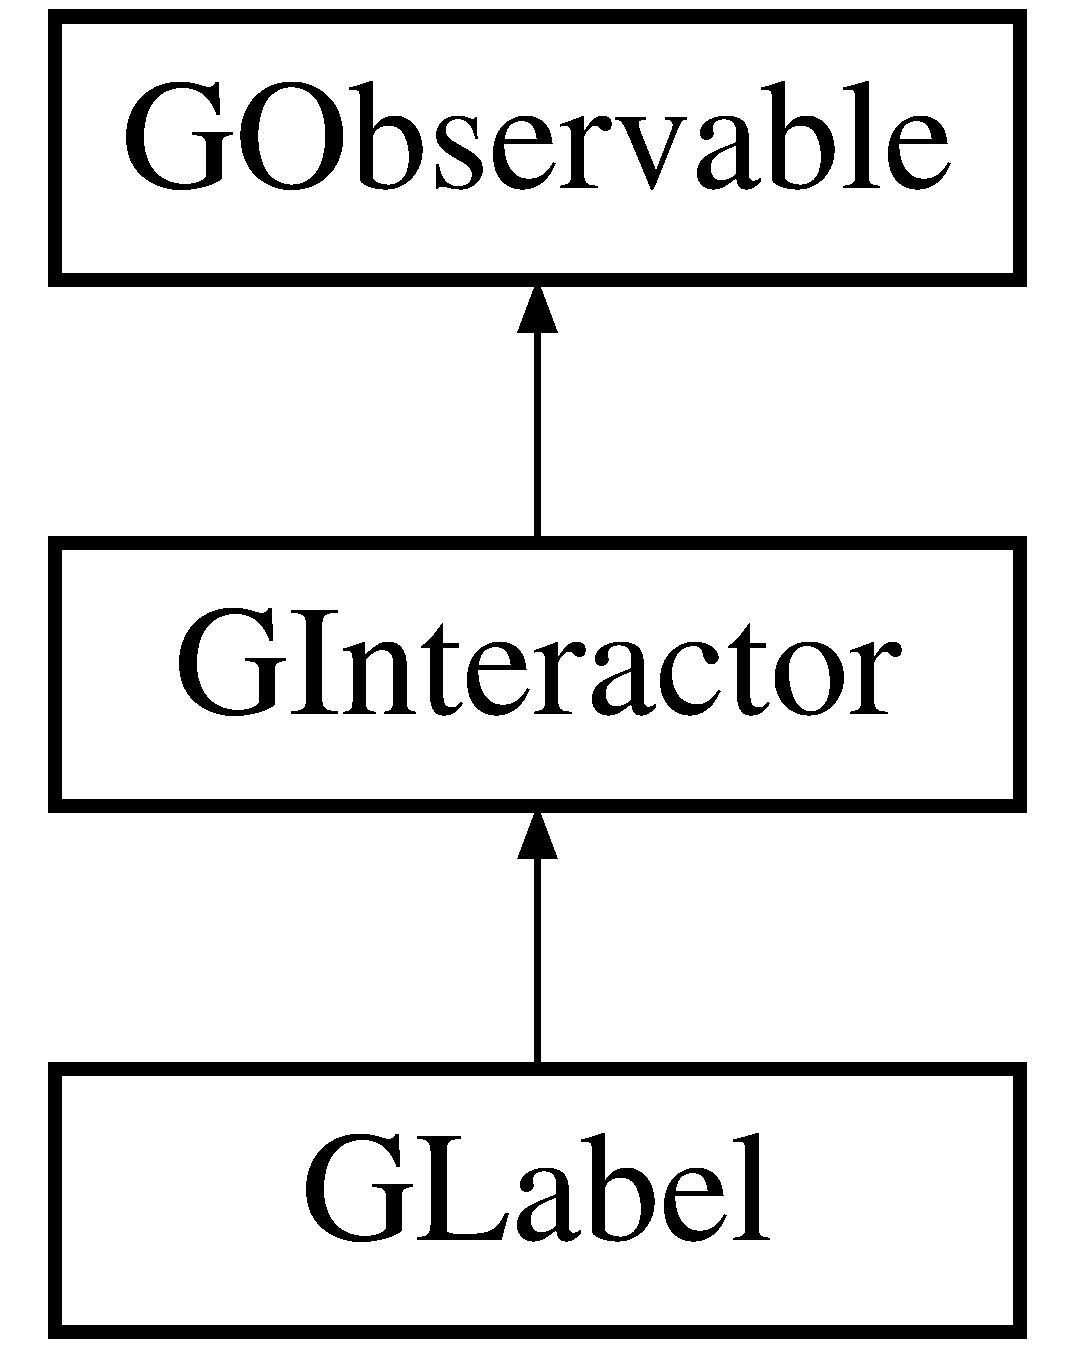
\includegraphics[height=3.000000cm]{classGLabel}
\end{center}
\end{figure}
\subsection*{Public Types}
\begin{DoxyCompactItemize}
\item 
enum \mbox{\hyperlink{classGInteractor_a8e0d441725a81d2bbdebbea09078260e}{Text\+Position}} \{ \mbox{\hyperlink{classGInteractor_a8e0d441725a81d2bbdebbea09078260ea4cd6f2e7d5a08d6f4dc052df2358f774}{T\+E\+X\+T\+\_\+\+B\+E\+S\+I\+D\+E\+\_\+\+I\+C\+ON}}, 
\mbox{\hyperlink{classGInteractor_a8e0d441725a81d2bbdebbea09078260eaa88490f63d8de68d44c83bdb2ecde3b3}{T\+E\+X\+T\+\_\+\+U\+N\+D\+E\+R\+\_\+\+I\+C\+ON}}, 
\mbox{\hyperlink{classGInteractor_a8e0d441725a81d2bbdebbea09078260ea39a6f388a30ac4fefb6eb13e846bc9f2}{T\+E\+X\+T\+\_\+\+O\+N\+LY}}
 \}
\begin{DoxyCompactList}\small\item\em The places where an interactor can place its text relative to its icon. \end{DoxyCompactList}\end{DoxyCompactItemize}
\subsection*{Public Member Functions}
\begin{DoxyCompactItemize}
\item 
\mbox{\hyperlink{classGLabel_adf89e6364d00b440441edce14145b387}{G\+Label}} (const std\+::string \&text=\char`\"{}\char`\"{}, const std\+::string \&icon\+File\+Name=\char`\"{}\char`\"{}, Q\+Widget $\ast$parent=nullptr)
\begin{DoxyCompactList}\small\item\em Creates a label with the specified text label and optional icon. \end{DoxyCompactList}\item 
virtual \mbox{\hyperlink{classGLabel_a766970bda7ce0b8df165ebc2811e0974}{$\sim$\+G\+Label}} ()
\begin{DoxyCompactList}\small\item\em Frees memory allocated internally by the label. \end{DoxyCompactList}\item 
virtual void \mbox{\hyperlink{classGInteractor_a02f20ea6edfa0671f31c4c648a253833}{add\+Action\+Listener}} () Q\+\_\+\+D\+E\+C\+L\+\_\+\+D\+E\+P\+R\+E\+C\+A\+T\+ED
\begin{DoxyCompactList}\small\item\em Adds an event listener to be notified when this interactor is clicked or generally interacted with. \end{DoxyCompactList}\item 
virtual bool \mbox{\hyperlink{classGInteractor_ac05ba5b92e2e5146d416fe7f842a0969}{events\+Enabled}} () const Q\+\_\+\+D\+E\+C\+L\+\_\+\+O\+V\+E\+R\+R\+I\+DE
\begin{DoxyCompactList}\small\item\em Returns true if this interactor is currently accepting events. \end{DoxyCompactList}\item 
virtual std\+::string \mbox{\hyperlink{classGInteractor_a69f8d23ed8f207fbecad99960776e942}{get\+Accelerator}} () const
\begin{DoxyCompactList}\small\item\em Returns a string representing a hotkey for this interactor, or an empty string if no accelerator has been set. \end{DoxyCompactList}\item 
virtual std\+::string \mbox{\hyperlink{classGInteractor_a94eb4276000c4fdfb508ce9e6317a82a}{get\+Action\+Command}} () const
\begin{DoxyCompactList}\small\item\em Returns an action command for this interactor, which is a semi-\/unique string you can use to identify it when events occur. \end{DoxyCompactList}\item 
virtual std\+::string \mbox{\hyperlink{classGInteractor_a808e22cc1fdfbecf71ed8c64ef4600e0}{get\+Background}} () const
\begin{DoxyCompactList}\small\item\em Returns the background color of the interactor as a string. \end{DoxyCompactList}\item 
virtual int \mbox{\hyperlink{classGInteractor_a9e827257a55cb8cf4d9de2ec6bcfd7a0}{get\+Background\+Int}} () const
\begin{DoxyCompactList}\small\item\em Returns the background color of the interactor as an R\+GB integer. \end{DoxyCompactList}\item 
virtual \mbox{\hyperlink{classGRectangle}{G\+Rectangle}} \mbox{\hyperlink{classGInteractor_a29e6ac35a0b48f491a4c88194cc5da3b}{get\+Bounds}} () const
\begin{DoxyCompactList}\small\item\em Returns a rectangle representing the x/y position and size of this interactor. \end{DoxyCompactList}\item 
virtual std\+::string \mbox{\hyperlink{classGInteractor_aa061dfa488c31e18549d64363c1d0e34}{get\+Color}} () const
\begin{DoxyCompactList}\small\item\em Returns the foreground/text color of the interactor as a string. \end{DoxyCompactList}\item 
virtual int \mbox{\hyperlink{classGInteractor_a9635c7af766cdc3417f346683fa0e6c1}{get\+Color\+Int}} () const
\begin{DoxyCompactList}\small\item\em Returns the foreground/text color of the interactor as an R\+GB integer. \end{DoxyCompactList}\item 
virtual \mbox{\hyperlink{classGContainer}{G\+Container}} $\ast$ \mbox{\hyperlink{classGInteractor_a7a6e317c29d61030929b4cd2d1c00fe7}{get\+Container}} () const
\begin{DoxyCompactList}\small\item\em Returns a pointer to the onscreen container holding this interactor. \end{DoxyCompactList}\item 
virtual std\+::string \mbox{\hyperlink{classGInteractor_a894a5502900794eeb27d084c21f1d77d}{get\+Font}} () const
\begin{DoxyCompactList}\small\item\em Returns the font of this interactor\textquotesingle{}s text as a font string such as \char`\"{}\+Helvetica-\/12-\/\+Bold\char`\"{}. \end{DoxyCompactList}\item 
virtual std\+::string \mbox{\hyperlink{classGInteractor_a4fa2d8b0192a3a5b4af4bbfe71194d03}{get\+Foreground}} () const
\begin{DoxyCompactList}\small\item\em Returns the foreground/text color of the interactor as a string. \end{DoxyCompactList}\item 
virtual int \mbox{\hyperlink{classGInteractor_ac3b12ab385a6ef9ae90fc879860ba726}{get\+Foreground\+Int}} () const
\begin{DoxyCompactList}\small\item\em Returns the foreground/text color of the interactor as an R\+GB integer. \end{DoxyCompactList}\item 
virtual double \mbox{\hyperlink{classGInteractor_a1e7e353362434072875264cf95629f99}{get\+Height}} () const
\begin{DoxyCompactList}\small\item\em Returns the current onscreen height of this interactor in pixels. \end{DoxyCompactList}\item 
virtual std\+::string \mbox{\hyperlink{classGInteractor_aaed62a73004939a64da6f0eb9eb64d73}{get\+Icon}} () const
\begin{DoxyCompactList}\small\item\em Returns the file name of the icon associated with this interactor, or an empty string if no icon has been set. \end{DoxyCompactList}\item 
virtual int \mbox{\hyperlink{classGInteractor_a9c9659a6c6ba66b4107ba59c95a24241}{get\+ID}} () const
\begin{DoxyCompactList}\small\item\em Returns a globally unique identifier for this interactor, which is set when the interactor is constructed. \end{DoxyCompactList}\item 
virtual \+\_\+\+Internal\+\_\+\+Q\+Widget $\ast$ \mbox{\hyperlink{classGLabel_a208ce13c1da40bf0ddb509daf99d6588}{get\+Internal\+Widget}} () const Q\+\_\+\+D\+E\+C\+L\+\_\+\+O\+V\+E\+R\+R\+I\+DE
\begin{DoxyCompactList}\small\item\em Returns a direct pointer to the internal Qt widget being wrapped by this interactor. \end{DoxyCompactList}\item 
virtual std\+::string \mbox{\hyperlink{classGLabel_aa73aa351564b091c0658f2368c6d5c5f}{get\+Label}} () const
\begin{DoxyCompactList}\small\item\em Returns the string displayed by the label. \end{DoxyCompactList}\item 
virtual \mbox{\hyperlink{classGPoint}{G\+Point}} \mbox{\hyperlink{classGInteractor_a4f83802015511edeb63b892830812c11}{get\+Location}} () const
\begin{DoxyCompactList}\small\item\em Returns an (x, y) point representing the onscreen location of the top-\/left corner of this interactor within its containing window. \end{DoxyCompactList}\item 
virtual double \mbox{\hyperlink{classGInteractor_aed4b0075fcc434499c3cb3e46896bda3}{get\+Minimum\+Height}} () const
\begin{DoxyCompactList}\small\item\em Returns the minimum height in pixels that this interactor will permit itself to be resized to. \end{DoxyCompactList}\item 
virtual \mbox{\hyperlink{classGDimension}{G\+Dimension}} \mbox{\hyperlink{classGInteractor_a66b5af0b32493b4d597ca0a3df2049ea}{get\+Minimum\+Size}} () const
\begin{DoxyCompactList}\small\item\em Returns a \mbox{\hyperlink{classGDimension}{G\+Dimension}} structure representing the minimum size in pixels that this interactor will permit itself to be resized to. \end{DoxyCompactList}\item 
virtual double \mbox{\hyperlink{classGInteractor_a59e668114fe3d49d2a0f28deb258f7c8}{get\+Minimum\+Width}} () const
\begin{DoxyCompactList}\small\item\em Returns the minimum width in pixels that this interactor will permit itself to be resized to. \end{DoxyCompactList}\item 
virtual std\+::string \mbox{\hyperlink{classGInteractor_a8a60438a5b55d0b2ceb35c8674b9d8c5}{get\+Name}} () const
\begin{DoxyCompactList}\small\item\em Returns a string representing a unique name for this interactor. \end{DoxyCompactList}\item 
virtual double \mbox{\hyperlink{classGInteractor_a747de0961653847bdc6615dbf756d715}{get\+Preferred\+Height}} () const
\begin{DoxyCompactList}\small\item\em Returns the height in pixels that this interactor would prefer to be, which would exactly fit its contents with no stretching or scrollbars. \end{DoxyCompactList}\item 
virtual \mbox{\hyperlink{classGDimension}{G\+Dimension}} \mbox{\hyperlink{classGInteractor_a4aabbee761d8e9116275401131b7ccd1}{get\+Preferred\+Size}} () const
\begin{DoxyCompactList}\small\item\em Returns a \mbox{\hyperlink{classGDimension}{G\+Dimension}} structure storing the width and height in pixels that this interactor would prefer to be, which would exactly fit its contents with no stretching or scrollbars. \end{DoxyCompactList}\item 
virtual double \mbox{\hyperlink{classGInteractor_a82bca31d37700fb0e35d2743352efd5e}{get\+Preferred\+Width}} () const
\begin{DoxyCompactList}\small\item\em Returns the height in pixels that this interactor would prefer to be, which would exactly fit its contents with no stretching or scrollbars. \end{DoxyCompactList}\item 
virtual \mbox{\hyperlink{classGDimension}{G\+Dimension}} \mbox{\hyperlink{classGInteractor_a7b4eec96a2bdc6420695d5796a78eea9}{get\+Size}} () const
\begin{DoxyCompactList}\small\item\em Returns a \mbox{\hyperlink{classGDimension}{G\+Dimension}} structure storing the current onscreen width and height of this interactor in pixels. \end{DoxyCompactList}\item 
virtual std\+::string \mbox{\hyperlink{classGLabel_aff553c50924b836c29f146ed34a7c6ec}{get\+Text}} () const
\begin{DoxyCompactList}\small\item\em Returns the string displayed by the label. \end{DoxyCompactList}\item 
virtual \mbox{\hyperlink{classGInteractor_a8e0d441725a81d2bbdebbea09078260e}{G\+Interactor\+::\+Text\+Position}} \mbox{\hyperlink{classGLabel_a3fc623df3ced62aca93fc344c2426899}{get\+Text\+Position}} () const
\begin{DoxyCompactList}\small\item\em Returns the label\textquotesingle{}s text position relative to its icon. \end{DoxyCompactList}\item 
virtual std\+::string \mbox{\hyperlink{classGLabel_a9896d58fcfebbf1025aeeb5b8b9ede80}{get\+Type}} () const Q\+\_\+\+D\+E\+C\+L\+\_\+\+O\+V\+E\+R\+R\+I\+DE
\begin{DoxyCompactList}\small\item\em Returns a string representing the class name of this interactor, such as \char`\"{}\+G\+Button\char`\"{} or \char`\"{}\+G\+Check\+Box\char`\"{}. \end{DoxyCompactList}\item 
virtual Q\+Widget $\ast$ \mbox{\hyperlink{classGLabel_a326ee51b5561f807df7b29a1c101f7fd}{get\+Widget}} () const Q\+\_\+\+D\+E\+C\+L\+\_\+\+O\+V\+E\+R\+R\+I\+DE
\begin{DoxyCompactList}\small\item\em Returns a direct pointer to the internal Qt widget being wrapped by this interactor. \end{DoxyCompactList}\item 
virtual double \mbox{\hyperlink{classGInteractor_a0ed2965abd4f5701d2cadf71239faf19}{get\+Width}} () const
\begin{DoxyCompactList}\small\item\em Returns the current onscreen width of this interactor in pixels. \end{DoxyCompactList}\item 
virtual double \mbox{\hyperlink{classGInteractor_a344385751bee0720059403940d57a13e}{getX}} () const
\begin{DoxyCompactList}\small\item\em Returns the x-\/coordinate of the top-\/left pixel of this interactor within its onscreen window. \end{DoxyCompactList}\item 
virtual double \mbox{\hyperlink{classGInteractor_aafa51c7f8f38a09febbb9ce7853f77b4}{getY}} () const
\begin{DoxyCompactList}\small\item\em Returns the y-\/coordinate of the top-\/left pixel of this interactor within its onscreen window. \end{DoxyCompactList}\item 
virtual bool \mbox{\hyperlink{classGInteractor_afc480f652b8c5f1fb255e2269ce68879}{in\+Bounds}} (double x, double y) const
\begin{DoxyCompactList}\small\item\em Returns true if the given x/y pixel is within the bounds of this interactor. \end{DoxyCompactList}\item 
virtual bool \mbox{\hyperlink{classGInteractor_ae6d7982c1c627b677a5e776ca86118ed}{in\+Bounds}} (int x, int y) const
\begin{DoxyCompactList}\small\item\em Returns true if the given x/y pixel is within the bounds of this interactor. \end{DoxyCompactList}\item 
virtual bool \mbox{\hyperlink{classGInteractor_aacb819fb241851fd9fc045271baa4034}{is\+Enabled}} () const
\begin{DoxyCompactList}\small\item\em Returns true if this interactor is currently enabled. \end{DoxyCompactList}\item 
virtual bool \mbox{\hyperlink{classGInteractor_a9d8a6cfb13917785c143e74d40e4e2be}{is\+Visible}} () const
\begin{DoxyCompactList}\small\item\em Returns true if the interactor is visible on the screen. \end{DoxyCompactList}\item 
virtual void \mbox{\hyperlink{classGLabel_ab7fe7a876367b87cf7202f947f1d05e4}{remove\+Action\+Listener}} ()
\begin{DoxyCompactList}\small\item\em Removes the action listener from this button so that it will no longer call it when events occur. \end{DoxyCompactList}\item 
virtual void \mbox{\hyperlink{classGLabel_aa4250907e4cdd77349c04f0cf5cdd3d3}{remove\+Double\+Click\+Listener}} ()
\begin{DoxyCompactList}\small\item\em Removes the double-\/click listener from this button so that it will no longer call it when events occur. \end{DoxyCompactList}\item 
virtual void \mbox{\hyperlink{classGInteractor_a519fb2ac767f8b2febbb50b898b8c8cb}{request\+Focus}} ()
\begin{DoxyCompactList}\small\item\em Transfers keyboard focus to this interactor. \end{DoxyCompactList}\item 
virtual void \mbox{\hyperlink{classGInteractor_ad15f102f62e2960576012f1aa0ba4b2e}{set\+Accelerator}} (const std\+::string \&accelerator)
\begin{DoxyCompactList}\small\item\em Sets an accelerator hotkey for this interactor, such as \char`\"{}\+Ctrl-\/\+S\char`\"{}. \end{DoxyCompactList}\item 
virtual void \mbox{\hyperlink{classGInteractor_a4b5843fe3030e038a1ba54cc03389bcf}{set\+Action\+Command}} (const std\+::string \&action\+Command)
\begin{DoxyCompactList}\small\item\em Sets the action command for this interactor. \end{DoxyCompactList}\item 
virtual void \mbox{\hyperlink{classGLabel_adcfb4742430c88714fcf57e57ab8ea9c}{set\+Action\+Listener}} (G\+Event\+Listener func)
\begin{DoxyCompactList}\small\item\em Sets an action listener on this button so that it will be called when the button is clicked. \end{DoxyCompactList}\item 
virtual void \mbox{\hyperlink{classGLabel_aebd20a89c7a8a43a6fce999cf4f9fcf2}{set\+Action\+Listener}} (G\+Event\+Listener\+Void func)
\begin{DoxyCompactList}\small\item\em Sets an action listener on this button so that it will be called when the button is clicked. \end{DoxyCompactList}\item 
virtual void \mbox{\hyperlink{classGInteractor_acba7e546c2025c0a15ca4b4cc92043db}{set\+Background}} (int rgb)
\begin{DoxyCompactList}\small\item\em Sets the background color of the interactor to the color represented by the given R\+GB integer. \end{DoxyCompactList}\item 
virtual void \mbox{\hyperlink{classGInteractor_ab4677ab2474e68b07aa56605af92a84a}{set\+Background}} (const std\+::string \&color)
\begin{DoxyCompactList}\small\item\em Sets the background color of the interactor to the color represented by the given string. \end{DoxyCompactList}\item 
virtual void \mbox{\hyperlink{classGLabel_aab3121dc97f8c5c1ddee39ea81d08509}{set\+Bounds}} (double x, double y, double width, double height) Q\+\_\+\+D\+E\+C\+L\+\_\+\+O\+V\+E\+R\+R\+I\+DE
\begin{DoxyCompactList}\small\item\em Sets the size and location of the widget. \end{DoxyCompactList}\item 
virtual void \mbox{\hyperlink{classGLabel_a3ed96c7e7adaf111848a90978621066c}{set\+Bounds}} (const \mbox{\hyperlink{classGRectangle}{G\+Rectangle}} \&size) Q\+\_\+\+D\+E\+C\+L\+\_\+\+O\+V\+E\+R\+R\+I\+DE
\begin{DoxyCompactList}\small\item\em Sets the size and location of the widget. \end{DoxyCompactList}\item 
virtual void \mbox{\hyperlink{classGLabel_afd1f50a2c4695c79b8633d860bce5398}{set\+Color}} (int rgb) Q\+\_\+\+D\+E\+C\+L\+\_\+\+O\+V\+E\+R\+R\+I\+DE
\begin{DoxyCompactList}\small\item\em Sets the foreground/text color of the interactor to the color represented by the given R\+GB integer. \end{DoxyCompactList}\item 
virtual void \mbox{\hyperlink{classGLabel_ad148324da1b0340e84e24dffa577ffca}{set\+Color}} (const std\+::string \&color) Q\+\_\+\+D\+E\+C\+L\+\_\+\+O\+V\+E\+R\+R\+I\+DE
\begin{DoxyCompactList}\small\item\em Sets the foreground/text color of the interactor to the color represented by the given string. \end{DoxyCompactList}\item 
virtual void \mbox{\hyperlink{classGLabel_ac29f9a3462458e165fae3a1f046ee77a}{set\+Double\+Click\+Listener}} (G\+Event\+Listener func)
\begin{DoxyCompactList}\small\item\em Sets a listener on this button so that it will be called when the button is double-\/clicked. \end{DoxyCompactList}\item 
virtual void \mbox{\hyperlink{classGLabel_a50096194d66f48c92dd4c512d41bfc76}{set\+Double\+Click\+Listener}} (G\+Event\+Listener\+Void func)
\begin{DoxyCompactList}\small\item\em Sets a listener on this button so that it will be called when the button is double-\/clicked. \end{DoxyCompactList}\item 
virtual void \mbox{\hyperlink{classGInteractor_ab831367dd84bbd579e02e55bacb21343}{set\+Enabled}} (bool value)
\begin{DoxyCompactList}\small\item\em Sets whether this interactor is currently enabled. \end{DoxyCompactList}\item 
virtual void \mbox{\hyperlink{classGObservable_afaa30b2a9e0f378fd1c70d2f1d0b8216}{set\+Events\+Enabled}} (bool \mbox{\hyperlink{classGInteractor_ac05ba5b92e2e5146d416fe7f842a0969}{events\+Enabled}})
\begin{DoxyCompactList}\small\item\em Sets whether the object is currently allowing itself to fire events. \end{DoxyCompactList}\item 
virtual void \mbox{\hyperlink{classGLabel_a2d22014c7fa3bccfd58c982aea1b55fa}{set\+Font}} (const Q\+Font \&font) Q\+\_\+\+D\+E\+C\+L\+\_\+\+O\+V\+E\+R\+R\+I\+DE
\begin{DoxyCompactList}\small\item\em Sets the font used by this widget to the given Qt font. \end{DoxyCompactList}\item 
virtual void \mbox{\hyperlink{classGLabel_ab39ef411fb13a52852ddd138c5932e2e}{set\+Font}} (const std\+::string \&font) Q\+\_\+\+D\+E\+C\+L\+\_\+\+O\+V\+E\+R\+R\+I\+DE
\begin{DoxyCompactList}\small\item\em Sets the font used by this widget to the font represented by the given font string, such as \char`\"{}\+Helvetica-\/16-\/\+Bold\char`\"{}. \end{DoxyCompactList}\item 
virtual void \mbox{\hyperlink{classGLabel_af9227e80cbfac55ce936fa5c99ffc954}{set\+Foreground}} (int rgb) Q\+\_\+\+D\+E\+C\+L\+\_\+\+O\+V\+E\+R\+R\+I\+DE
\begin{DoxyCompactList}\small\item\em Sets the foreground/text color of the interactor to the color represented by the given R\+GB integer. \end{DoxyCompactList}\item 
virtual void \mbox{\hyperlink{classGLabel_a088e04dfc56273df4cedab2b11b970f5}{set\+Foreground}} (const std\+::string \&color) Q\+\_\+\+D\+E\+C\+L\+\_\+\+O\+V\+E\+R\+R\+I\+DE
\begin{DoxyCompactList}\small\item\em Sets the foreground/text color of the interactor to the color represented by the given string. \end{DoxyCompactList}\item 
virtual void \mbox{\hyperlink{classGLabel_a8a1f6693796b536d1ace7ce0ff66afee}{set\+Height}} (double height) Q\+\_\+\+D\+E\+C\+L\+\_\+\+O\+V\+E\+R\+R\+I\+DE
\begin{DoxyCompactList}\small\item\em Sets the onscreen height of the interactor in pixels. \end{DoxyCompactList}\item 
virtual void \mbox{\hyperlink{classGLabel_a75753a3d7d3364185f8088d63b664cb1}{set\+Icon}} (const std\+::string \&filename, bool retain\+Icon\+Size=true) Q\+\_\+\+D\+E\+C\+L\+\_\+\+O\+V\+E\+R\+R\+I\+DE
\begin{DoxyCompactList}\small\item\em Sets the file name of the icon associated with this interactor, or an empty string if no icon has been set. \end{DoxyCompactList}\item 
virtual void \mbox{\hyperlink{classGLabel_a4af0be0e092d87271c1432624bc00080}{set\+Label}} (const std\+::string \&text)
\begin{DoxyCompactList}\small\item\em Sets the text on the label to be the given text. \end{DoxyCompactList}\item 
virtual void \mbox{\hyperlink{classGLabel_a40e39a7bf1b0b46b3a5710bb9a0d214b}{set\+Location}} (double x, double y) Q\+\_\+\+D\+E\+C\+L\+\_\+\+O\+V\+E\+R\+R\+I\+DE
\begin{DoxyCompactList}\small\item\em Sets the onscreen x/y-\/coordinate of the top-\/left corner of the interactor relative to its window. \end{DoxyCompactList}\item 
virtual void \mbox{\hyperlink{classGInteractor_a0cf428e207b7f22cc08138a90b1b87b2}{set\+Minimum\+Size}} (double width, double height)
\begin{DoxyCompactList}\small\item\em Sets the minimum size in pixels that this interactor will permit itself to be resized to. \end{DoxyCompactList}\item 
virtual void \mbox{\hyperlink{classGInteractor_a3b1046117ac6cb7abe467e00ba8a81f4}{set\+Minimum\+Size}} (const \mbox{\hyperlink{classGDimension}{G\+Dimension}} \&size)
\begin{DoxyCompactList}\small\item\em Sets the minimum size in pixels that this interactor will permit itself to be resized to. \end{DoxyCompactList}\item 
virtual void \mbox{\hyperlink{classGInteractor_a9d3a2685df23b5e7cbf59c19c4a1f9b5}{set\+Name}} (const std\+::string \&name)
\begin{DoxyCompactList}\small\item\em Sets a string representing a unique name for this interactor. \end{DoxyCompactList}\item 
virtual void \mbox{\hyperlink{classGInteractor_a1ab987704fce32098706c6f00fb08218}{set\+Preferred\+Height}} (double height)
\begin{DoxyCompactList}\small\item\em Sets the height in pixels that this interactor would prefer to be. \end{DoxyCompactList}\item 
virtual void \mbox{\hyperlink{classGInteractor_a042c5ae19430d765ef552371cae3632c}{set\+Preferred\+Size}} (double width, double height)
\begin{DoxyCompactList}\small\item\em Sets the width and height in pixels that this interactor would prefer to be. \end{DoxyCompactList}\item 
virtual void \mbox{\hyperlink{classGInteractor_aa22d9be4bc0e078bb0ea69b0fc9d7c75}{set\+Preferred\+Size}} (const \mbox{\hyperlink{classGDimension}{G\+Dimension}} \&size)
\begin{DoxyCompactList}\small\item\em Sets the size in pixels that this interactor would prefer to be. \end{DoxyCompactList}\item 
virtual void \mbox{\hyperlink{classGInteractor_a3db429ab2fa52efd187eec0ed8cdd9f2}{set\+Preferred\+Width}} (double width)
\begin{DoxyCompactList}\small\item\em Sets the width in pixels that this interactor would prefer to be. \end{DoxyCompactList}\item 
virtual void \mbox{\hyperlink{classGLabel_ae7e6371aa2311d6f18caf8f7be59704d}{set\+Size}} (double width, double height) Q\+\_\+\+D\+E\+C\+L\+\_\+\+O\+V\+E\+R\+R\+I\+DE
\begin{DoxyCompactList}\small\item\em Sets the onscreen width and height of the interactor in pixels. \end{DoxyCompactList}\item 
virtual void \mbox{\hyperlink{classGLabel_a0fe8cce1a80750f36fa14ee99ca34014}{set\+Size}} (const \mbox{\hyperlink{classGDimension}{G\+Dimension}} \&size) Q\+\_\+\+D\+E\+C\+L\+\_\+\+O\+V\+E\+R\+R\+I\+DE
\begin{DoxyCompactList}\small\item\em Sets the onscreen width and height of the interactor in pixels. \end{DoxyCompactList}\item 
virtual void \mbox{\hyperlink{classGLabel_ac1ae51949d41ee9054634be5967d91b8}{set\+Text}} (const std\+::string \&text)
\begin{DoxyCompactList}\small\item\em Sets the text on the label to be the given text. \end{DoxyCompactList}\item 
virtual void \mbox{\hyperlink{classGLabel_af822b8d73c652f7c59d875d7cdfc5302}{set\+Text\+Position}} (\mbox{\hyperlink{classGInteractor_a8e0d441725a81d2bbdebbea09078260e}{G\+Interactor\+::\+Text\+Position}} position)
\begin{DoxyCompactList}\small\item\em Sets the label\textquotesingle{}s text position relative to its icon. \end{DoxyCompactList}\item 
virtual void \mbox{\hyperlink{classGInteractor_a039e0e49beaecc275efce02d416acea8}{set\+Tooltip}} (const std\+::string \&tooltip\+Text)
\begin{DoxyCompactList}\small\item\em Sets a \char`\"{}tooltip\char`\"{} that will appear if the user hovers their mouse over the interactor. \end{DoxyCompactList}\item 
virtual void \mbox{\hyperlink{classGLabel_a95c2a1221e6c59e9de544054963b4b18}{set\+Visible}} (bool visible) Q\+\_\+\+D\+E\+C\+L\+\_\+\+O\+V\+E\+R\+R\+I\+DE
\begin{DoxyCompactList}\small\item\em Returns true if the interactor is visible on the screen. \end{DoxyCompactList}\item 
virtual void \mbox{\hyperlink{classGLabel_aca9b9c666c4162ab0a27a10530bc0762}{set\+Width}} (double width) Q\+\_\+\+D\+E\+C\+L\+\_\+\+O\+V\+E\+R\+R\+I\+DE
\begin{DoxyCompactList}\small\item\em Sets the onscreen width of the interactor in pixels. \end{DoxyCompactList}\item 
virtual void \mbox{\hyperlink{classGLabel_af7260dc32f150e3a5072e7e8eb2628b1}{setX}} (double x) Q\+\_\+\+D\+E\+C\+L\+\_\+\+O\+V\+E\+R\+R\+I\+DE
\begin{DoxyCompactList}\small\item\em Sets the onscreen x-\/coordinate of the top-\/left corner of the interactor relative to its window. \end{DoxyCompactList}\item 
virtual void \mbox{\hyperlink{classGLabel_a59633abb35b676c54d88ea6cd384fc55}{setY}} (double y) Q\+\_\+\+D\+E\+C\+L\+\_\+\+O\+V\+E\+R\+R\+I\+DE
\begin{DoxyCompactList}\small\item\em Sets the onscreen y-\/coordinate of the top-\/left corner of the interactor relative to its window. \end{DoxyCompactList}\item 
virtual std\+::string \mbox{\hyperlink{classGObservable_a1fe5121d6528fdea3f243321b3fa3a49}{to\+String}} () const
\begin{DoxyCompactList}\small\item\em Returns a string representation of this observable object\textquotesingle{}s state. \end{DoxyCompactList}\end{DoxyCompactItemize}
\subsection*{Protected Member Functions}
\begin{DoxyCompactItemize}
\item 
virtual void \mbox{\hyperlink{classGObservable_a80cfa040459ff53594adbd6a51ec8f43}{clear\+Event\+Listeners}} ()
\begin{DoxyCompactList}\small\item\em Removes all event listeners from this object. \end{DoxyCompactList}\item 
virtual void \mbox{\hyperlink{classGObservable_a284f31528c0520f8e545c03ac9eeac74}{ensure\+Thread\+Safety}} (const std\+::string \&member\+Name=\char`\"{}\char`\"{})
\begin{DoxyCompactList}\small\item\em Ensures that we are currently in the Qt G\+UI thread. \end{DoxyCompactList}\item 
virtual void \mbox{\hyperlink{classGObservable_a63e5e5a6227c59c928493b11aceb0f67}{fire\+Event}} (\mbox{\hyperlink{classGEvent}{G\+Event}} \&event)
\begin{DoxyCompactList}\small\item\em Sends out the given event to any attached listeners. \end{DoxyCompactList}\item 
virtual void \mbox{\hyperlink{classGObservable_ab3983ea07337b52020a29cc00c653d8d}{fire\+G\+Event}} (Q\+Event $\ast$event, Event\+Type event\+Type, const std\+::string \&event\+Name)
\begin{DoxyCompactList}\small\item\em Creates an event of the given type, then sends it out to any attached listeners. \end{DoxyCompactList}\item 
virtual void \mbox{\hyperlink{classGObservable_a01fdf1b0e0dbd49e189fe4514e010411}{fire\+G\+Event}} (Q\+Close\+Event $\ast$event, Event\+Type event\+Type, const std\+::string \&event\+Name)
\begin{DoxyCompactList}\small\item\em Creates an event of the given type, then sends it out to any attached listeners. \end{DoxyCompactList}\item 
virtual void \mbox{\hyperlink{classGObservable_abb0b2f66ba39211cb5d7615e9d1c04e2}{fire\+G\+Event}} (Q\+Key\+Event $\ast$event, Event\+Type event\+Type, const std\+::string \&event\+Name)
\begin{DoxyCompactList}\small\item\em Creates an event of the given type, then sends it out to any attached listeners. \end{DoxyCompactList}\item 
virtual void \mbox{\hyperlink{classGObservable_a119318675d2165bdf7dd853aaf881d4b}{fire\+G\+Event}} (Q\+Mouse\+Event $\ast$event, Event\+Type event\+Type, const std\+::string \&event\+Name, const std\+::string \&action\+Command=\char`\"{}\char`\"{})
\begin{DoxyCompactList}\small\item\em Creates an event of the given type, then sends it out to any attached listeners. \end{DoxyCompactList}\item 
virtual void \mbox{\hyperlink{classGObservable_a63fd9034e1e1633c1c38eb342bfd34e9}{fire\+G\+Event}} (Q\+Resize\+Event $\ast$event, Event\+Type event\+Type, const std\+::string \&event\+Name)
\begin{DoxyCompactList}\small\item\em Creates an event of the given type, then sends it out to any attached listeners. \end{DoxyCompactList}\item 
virtual void \mbox{\hyperlink{classGObservable_a741345310d9b7c5170a6cbc410c44ac4}{fire\+G\+Event}} (Q\+Timer\+Event $\ast$event, Event\+Type event\+Type, const std\+::string \&event\+Name)
\begin{DoxyCompactList}\small\item\em Creates an event of the given type, then sends it out to any attached listeners. \end{DoxyCompactList}\item 
virtual void \mbox{\hyperlink{classGObservable_a93bf338968a0338761b8e4dc62f582e9}{fire\+G\+Event}} (Q\+Wheel\+Event $\ast$event, Event\+Type event\+Type, const std\+::string \&event\+Name)
\begin{DoxyCompactList}\small\item\em Creates an event of the given type, then sends it out to any attached listeners. \end{DoxyCompactList}\item 
virtual void \mbox{\hyperlink{classGObservable_a2a70a7d7435ff0c3b80bb4d70da19e0d}{fire\+G\+Event}} (Q\+Window\+State\+Change\+Event $\ast$event, Event\+Type event\+Type, const std\+::string \&event\+Name)
\begin{DoxyCompactList}\small\item\em Creates an event of the given type, then sends it out to any attached listeners. \end{DoxyCompactList}\item 
virtual bool \mbox{\hyperlink{classGObservable_a9f6faaa25942923bafa1c44020c49fa9}{has\+Event\+Listener}} (const std\+::string \&event\+Name) const
\begin{DoxyCompactList}\small\item\em Returns true if the observable object has a listener for the given type of event. \end{DoxyCompactList}\item 
virtual bool \mbox{\hyperlink{classGObservable_aeec1adc19aa0f33de62390686ee1382c}{is\+Accepting\+Event}} (int event\+Mask) const
\begin{DoxyCompactList}\small\item\em Returns true if the observable object has a listener for the given type of event. \end{DoxyCompactList}\item 
virtual bool \mbox{\hyperlink{classGObservable_aa31c73145a29dcb92848a92e0cfaea41}{is\+Accepting\+Event}} (const \mbox{\hyperlink{classGEvent}{G\+Event}} \&event) const
\begin{DoxyCompactList}\small\item\em Returns true if the observable object has a listener for the given type of event. \end{DoxyCompactList}\item 
virtual bool \mbox{\hyperlink{classGObservable_a3b1c689267eda44e65a2213e7de38b23}{is\+Accepting\+Event}} (const std\+::string \&event\+Type) const
\begin{DoxyCompactList}\small\item\em Returns true if the observable object has a listener for the given type of event. \end{DoxyCompactList}\item 
virtual void \mbox{\hyperlink{classGObservable_acbcf1ed3a851ad8a3c17ef38d86b481d}{remove\+Event\+Listener}} (const std\+::string \&event\+Name)
\begin{DoxyCompactList}\small\item\em Removes any event listener from this observable object that would respond to the given type of event, such as \char`\"{}click\char`\"{} or \char`\"{}keydown\char`\"{}. \end{DoxyCompactList}\item 
virtual void \mbox{\hyperlink{classGObservable_af51cc35c29a1bd1908609d432decdbb6}{remove\+Event\+Listeners}} (std\+::initializer\+\_\+list$<$ std\+::string $>$ event\+Names)
\begin{DoxyCompactList}\small\item\em Removes any event listener from this observable object that would respond to the given types of events, such as \char`\"{}click\char`\"{} or \char`\"{}keydown\char`\"{}. \end{DoxyCompactList}\item 
virtual void \mbox{\hyperlink{classGObservable_ad2f6d34961c50f6c1e0659990b79f741}{set\+Event\+Listener}} (const std\+::string \&event\+Name, G\+Event\+Listener func)
\begin{DoxyCompactList}\small\item\em Adds an event listener from this observable object to respond to the given type of event, such as \char`\"{}click\char`\"{} or \char`\"{}keydown\char`\"{}. \end{DoxyCompactList}\item 
virtual void \mbox{\hyperlink{classGObservable_abac4cb9f9e626e010e87f5d91573c8a5}{set\+Event\+Listener}} (const std\+::string \&event\+Name, G\+Event\+Listener\+Void func)
\begin{DoxyCompactList}\small\item\em Adds an event listener from this observable object to respond to the given type of event, such as \char`\"{}click\char`\"{} or \char`\"{}keydown\char`\"{}. \end{DoxyCompactList}\item 
virtual void \mbox{\hyperlink{classGObservable_afa388d69c33c718cf035774604065604}{set\+Event\+Listeners}} (std\+::initializer\+\_\+list$<$ std\+::string $>$ event\+Names, G\+Event\+Listener func)
\begin{DoxyCompactList}\small\item\em Adds an event listener from this observable object to respond to the given types of events, such as \char`\"{}click\char`\"{} or \char`\"{}keydown\char`\"{}. \end{DoxyCompactList}\item 
virtual void \mbox{\hyperlink{classGObservable_a7867184bbb686f74fae8a4db927da799}{set\+Event\+Listeners}} (std\+::initializer\+\_\+list$<$ std\+::string $>$ event\+Names, G\+Event\+Listener\+Void func)
\begin{DoxyCompactList}\small\item\em Adds an event listener from this observable object to respond to the given types of events, such as \char`\"{}click\char`\"{} or \char`\"{}keydown\char`\"{}. \end{DoxyCompactList}\end{DoxyCompactItemize}


\subsection{Detailed Description}
A \mbox{\hyperlink{classGLabel}{G\+Label}} represents a text string. 

A label can contain text and/or an image icon.

G\+Labels can be made clickable with the set\+Action\+Listener and set\+Double\+Click\+Listener methods, but generally if you want a clickable interactor with text on it, you may prefer a \mbox{\hyperlink{classGButton}{G\+Button}}. 

\subsection{Member Enumeration Documentation}
\mbox{\Hypertarget{classGInteractor_a8e0d441725a81d2bbdebbea09078260e}\label{classGInteractor_a8e0d441725a81d2bbdebbea09078260e}} 
\index{G\+Label@{G\+Label}!Text\+Position@{Text\+Position}}
\index{Text\+Position@{Text\+Position}!G\+Label@{G\+Label}}
\subsubsection{\texorpdfstring{Text\+Position}{TextPosition}}
{\footnotesize\ttfamily enum \mbox{\hyperlink{classGInteractor_a8e0d441725a81d2bbdebbea09078260e}{Text\+Position}}\hspace{0.3cm}{\ttfamily [inherited]}}



The places where an interactor can place its text relative to its icon. 

\begin{DoxyEnumFields}{Enumerator}
\raisebox{\heightof{T}}[0pt][0pt]{\index{T\+E\+X\+T\+\_\+\+B\+E\+S\+I\+D\+E\+\_\+\+I\+C\+ON@{T\+E\+X\+T\+\_\+\+B\+E\+S\+I\+D\+E\+\_\+\+I\+C\+ON}!G\+Label@{G\+Label}}\index{G\+Label@{G\+Label}!T\+E\+X\+T\+\_\+\+B\+E\+S\+I\+D\+E\+\_\+\+I\+C\+ON@{T\+E\+X\+T\+\_\+\+B\+E\+S\+I\+D\+E\+\_\+\+I\+C\+ON}}}\mbox{\Hypertarget{classGInteractor_a8e0d441725a81d2bbdebbea09078260ea4cd6f2e7d5a08d6f4dc052df2358f774}\label{classGInteractor_a8e0d441725a81d2bbdebbea09078260ea4cd6f2e7d5a08d6f4dc052df2358f774}} 
T\+E\+X\+T\+\_\+\+B\+E\+S\+I\+D\+E\+\_\+\+I\+C\+ON&\\
\hline

\raisebox{\heightof{T}}[0pt][0pt]{\index{T\+E\+X\+T\+\_\+\+U\+N\+D\+E\+R\+\_\+\+I\+C\+ON@{T\+E\+X\+T\+\_\+\+U\+N\+D\+E\+R\+\_\+\+I\+C\+ON}!G\+Label@{G\+Label}}\index{G\+Label@{G\+Label}!T\+E\+X\+T\+\_\+\+U\+N\+D\+E\+R\+\_\+\+I\+C\+ON@{T\+E\+X\+T\+\_\+\+U\+N\+D\+E\+R\+\_\+\+I\+C\+ON}}}\mbox{\Hypertarget{classGInteractor_a8e0d441725a81d2bbdebbea09078260eaa88490f63d8de68d44c83bdb2ecde3b3}\label{classGInteractor_a8e0d441725a81d2bbdebbea09078260eaa88490f63d8de68d44c83bdb2ecde3b3}} 
T\+E\+X\+T\+\_\+\+U\+N\+D\+E\+R\+\_\+\+I\+C\+ON&\\
\hline

\raisebox{\heightof{T}}[0pt][0pt]{\index{T\+E\+X\+T\+\_\+\+O\+N\+LY@{T\+E\+X\+T\+\_\+\+O\+N\+LY}!G\+Label@{G\+Label}}\index{G\+Label@{G\+Label}!T\+E\+X\+T\+\_\+\+O\+N\+LY@{T\+E\+X\+T\+\_\+\+O\+N\+LY}}}\mbox{\Hypertarget{classGInteractor_a8e0d441725a81d2bbdebbea09078260ea39a6f388a30ac4fefb6eb13e846bc9f2}\label{classGInteractor_a8e0d441725a81d2bbdebbea09078260ea39a6f388a30ac4fefb6eb13e846bc9f2}} 
T\+E\+X\+T\+\_\+\+O\+N\+LY&\\
\hline

\end{DoxyEnumFields}


\subsection{Constructor \& Destructor Documentation}
\mbox{\Hypertarget{classGLabel_adf89e6364d00b440441edce14145b387}\label{classGLabel_adf89e6364d00b440441edce14145b387}} 
\index{G\+Label@{G\+Label}!G\+Label@{G\+Label}}
\index{G\+Label@{G\+Label}!G\+Label@{G\+Label}}
\subsubsection{\texorpdfstring{G\+Label()}{GLabel()}}
{\footnotesize\ttfamily \mbox{\hyperlink{classGLabel}{G\+Label}} (\begin{DoxyParamCaption}\item[{const std\+::string \&}]{text = {\ttfamily \char`\"{}\char`\"{}},  }\item[{const std\+::string \&}]{icon\+File\+Name = {\ttfamily \char`\"{}\char`\"{}},  }\item[{Q\+Widget $\ast$}]{parent = {\ttfamily nullptr} }\end{DoxyParamCaption})}



Creates a label with the specified text label and optional icon. 

\mbox{\Hypertarget{classGLabel_a766970bda7ce0b8df165ebc2811e0974}\label{classGLabel_a766970bda7ce0b8df165ebc2811e0974}} 
\index{G\+Label@{G\+Label}!````~G\+Label@{$\sim$\+G\+Label}}
\index{````~G\+Label@{$\sim$\+G\+Label}!G\+Label@{G\+Label}}
\subsubsection{\texorpdfstring{$\sim$\+G\+Label()}{~GLabel()}}
{\footnotesize\ttfamily $\sim$\mbox{\hyperlink{classGLabel}{G\+Label}} (\begin{DoxyParamCaption}{ }\end{DoxyParamCaption})\hspace{0.3cm}{\ttfamily [virtual]}}



Frees memory allocated internally by the label. 



\subsection{Member Function Documentation}
\mbox{\Hypertarget{classGInteractor_a02f20ea6edfa0671f31c4c648a253833}\label{classGInteractor_a02f20ea6edfa0671f31c4c648a253833}} 
\index{G\+Label@{G\+Label}!add\+Action\+Listener@{add\+Action\+Listener}}
\index{add\+Action\+Listener@{add\+Action\+Listener}!G\+Label@{G\+Label}}
\subsubsection{\texorpdfstring{add\+Action\+Listener()}{addActionListener()}}
{\footnotesize\ttfamily void add\+Action\+Listener (\begin{DoxyParamCaption}{ }\end{DoxyParamCaption})\hspace{0.3cm}{\ttfamily [virtual]}, {\ttfamily [inherited]}}



Adds an event listener to be notified when this interactor is clicked or generally interacted with. 

\begin{DoxyRefDesc}{Deprecated}
\item[\mbox{\hyperlink{deprecated__deprecated000006}{Deprecated}}]does nothing; use set\+Action\+Listener instead \end{DoxyRefDesc}
\mbox{\Hypertarget{classGObservable_a80cfa040459ff53594adbd6a51ec8f43}\label{classGObservable_a80cfa040459ff53594adbd6a51ec8f43}} 
\index{G\+Label@{G\+Label}!clear\+Event\+Listeners@{clear\+Event\+Listeners}}
\index{clear\+Event\+Listeners@{clear\+Event\+Listeners}!G\+Label@{G\+Label}}
\subsubsection{\texorpdfstring{clear\+Event\+Listeners()}{clearEventListeners()}}
{\footnotesize\ttfamily void clear\+Event\+Listeners (\begin{DoxyParamCaption}{ }\end{DoxyParamCaption})\hspace{0.3cm}{\ttfamily [protected]}, {\ttfamily [virtual]}, {\ttfamily [inherited]}}



Removes all event listeners from this object. 

\mbox{\Hypertarget{classGObservable_a284f31528c0520f8e545c03ac9eeac74}\label{classGObservable_a284f31528c0520f8e545c03ac9eeac74}} 
\index{G\+Label@{G\+Label}!ensure\+Thread\+Safety@{ensure\+Thread\+Safety}}
\index{ensure\+Thread\+Safety@{ensure\+Thread\+Safety}!G\+Label@{G\+Label}}
\subsubsection{\texorpdfstring{ensure\+Thread\+Safety()}{ensureThreadSafety()}}
{\footnotesize\ttfamily void ensure\+Thread\+Safety (\begin{DoxyParamCaption}\item[{const std\+::string \&}]{member\+Name = {\ttfamily \char`\"{}\char`\"{}} }\end{DoxyParamCaption})\hspace{0.3cm}{\ttfamily [protected]}, {\ttfamily [virtual]}, {\ttfamily [inherited]}}



Ensures that we are currently in the Qt G\+UI thread. 

\mbox{\Hypertarget{classGInteractor_ac05ba5b92e2e5146d416fe7f842a0969}\label{classGInteractor_ac05ba5b92e2e5146d416fe7f842a0969}} 
\index{G\+Label@{G\+Label}!events\+Enabled@{events\+Enabled}}
\index{events\+Enabled@{events\+Enabled}!G\+Label@{G\+Label}}
\subsubsection{\texorpdfstring{events\+Enabled()}{eventsEnabled()}}
{\footnotesize\ttfamily bool events\+Enabled (\begin{DoxyParamCaption}{ }\end{DoxyParamCaption}) const\hspace{0.3cm}{\ttfamily [virtual]}, {\ttfamily [inherited]}}



Returns true if this interactor is currently accepting events. 

Initially true. An interactor must be visible and added to an onscreen window to receive events. 

Reimplemented from \mbox{\hyperlink{classGObservable_a8ebb3da91032e7f4c34485dabc518b8a}{G\+Observable}}.

\mbox{\Hypertarget{classGObservable_a63e5e5a6227c59c928493b11aceb0f67}\label{classGObservable_a63e5e5a6227c59c928493b11aceb0f67}} 
\index{G\+Label@{G\+Label}!fire\+Event@{fire\+Event}}
\index{fire\+Event@{fire\+Event}!G\+Label@{G\+Label}}
\subsubsection{\texorpdfstring{fire\+Event()}{fireEvent()}}
{\footnotesize\ttfamily void fire\+Event (\begin{DoxyParamCaption}\item[{\mbox{\hyperlink{classGEvent}{G\+Event}} \&}]{event }\end{DoxyParamCaption})\hspace{0.3cm}{\ttfamily [protected]}, {\ttfamily [virtual]}, {\ttfamily [inherited]}}



Sends out the given event to any attached listeners. 

\mbox{\Hypertarget{classGObservable_ab3983ea07337b52020a29cc00c653d8d}\label{classGObservable_ab3983ea07337b52020a29cc00c653d8d}} 
\index{G\+Label@{G\+Label}!fire\+G\+Event@{fire\+G\+Event}}
\index{fire\+G\+Event@{fire\+G\+Event}!G\+Label@{G\+Label}}
\subsubsection{\texorpdfstring{fire\+G\+Event()}{fireGEvent()}\hspace{0.1cm}{\footnotesize\ttfamily [1/8]}}
{\footnotesize\ttfamily void fire\+G\+Event (\begin{DoxyParamCaption}\item[{Q\+Event $\ast$}]{event,  }\item[{Event\+Type}]{event\+Type,  }\item[{const std\+::string \&}]{event\+Name }\end{DoxyParamCaption})\hspace{0.3cm}{\ttfamily [protected]}, {\ttfamily [virtual]}, {\ttfamily [inherited]}}



Creates an event of the given type, then sends it out to any attached listeners. 

\mbox{\Hypertarget{classGObservable_a01fdf1b0e0dbd49e189fe4514e010411}\label{classGObservable_a01fdf1b0e0dbd49e189fe4514e010411}} 
\index{G\+Label@{G\+Label}!fire\+G\+Event@{fire\+G\+Event}}
\index{fire\+G\+Event@{fire\+G\+Event}!G\+Label@{G\+Label}}
\subsubsection{\texorpdfstring{fire\+G\+Event()}{fireGEvent()}\hspace{0.1cm}{\footnotesize\ttfamily [2/8]}}
{\footnotesize\ttfamily void fire\+G\+Event (\begin{DoxyParamCaption}\item[{Q\+Close\+Event $\ast$}]{event,  }\item[{Event\+Type}]{event\+Type,  }\item[{const std\+::string \&}]{event\+Name }\end{DoxyParamCaption})\hspace{0.3cm}{\ttfamily [protected]}, {\ttfamily [virtual]}, {\ttfamily [inherited]}}



Creates an event of the given type, then sends it out to any attached listeners. 

\mbox{\Hypertarget{classGObservable_abb0b2f66ba39211cb5d7615e9d1c04e2}\label{classGObservable_abb0b2f66ba39211cb5d7615e9d1c04e2}} 
\index{G\+Label@{G\+Label}!fire\+G\+Event@{fire\+G\+Event}}
\index{fire\+G\+Event@{fire\+G\+Event}!G\+Label@{G\+Label}}
\subsubsection{\texorpdfstring{fire\+G\+Event()}{fireGEvent()}\hspace{0.1cm}{\footnotesize\ttfamily [3/8]}}
{\footnotesize\ttfamily void fire\+G\+Event (\begin{DoxyParamCaption}\item[{Q\+Key\+Event $\ast$}]{event,  }\item[{Event\+Type}]{event\+Type,  }\item[{const std\+::string \&}]{event\+Name }\end{DoxyParamCaption})\hspace{0.3cm}{\ttfamily [protected]}, {\ttfamily [virtual]}, {\ttfamily [inherited]}}



Creates an event of the given type, then sends it out to any attached listeners. 

\mbox{\Hypertarget{classGObservable_a119318675d2165bdf7dd853aaf881d4b}\label{classGObservable_a119318675d2165bdf7dd853aaf881d4b}} 
\index{G\+Label@{G\+Label}!fire\+G\+Event@{fire\+G\+Event}}
\index{fire\+G\+Event@{fire\+G\+Event}!G\+Label@{G\+Label}}
\subsubsection{\texorpdfstring{fire\+G\+Event()}{fireGEvent()}\hspace{0.1cm}{\footnotesize\ttfamily [4/8]}}
{\footnotesize\ttfamily void fire\+G\+Event (\begin{DoxyParamCaption}\item[{Q\+Mouse\+Event $\ast$}]{event,  }\item[{Event\+Type}]{event\+Type,  }\item[{const std\+::string \&}]{event\+Name,  }\item[{const std\+::string \&}]{action\+Command = {\ttfamily \char`\"{}\char`\"{}} }\end{DoxyParamCaption})\hspace{0.3cm}{\ttfamily [protected]}, {\ttfamily [virtual]}, {\ttfamily [inherited]}}



Creates an event of the given type, then sends it out to any attached listeners. 

\mbox{\Hypertarget{classGObservable_a63fd9034e1e1633c1c38eb342bfd34e9}\label{classGObservable_a63fd9034e1e1633c1c38eb342bfd34e9}} 
\index{G\+Label@{G\+Label}!fire\+G\+Event@{fire\+G\+Event}}
\index{fire\+G\+Event@{fire\+G\+Event}!G\+Label@{G\+Label}}
\subsubsection{\texorpdfstring{fire\+G\+Event()}{fireGEvent()}\hspace{0.1cm}{\footnotesize\ttfamily [5/8]}}
{\footnotesize\ttfamily void fire\+G\+Event (\begin{DoxyParamCaption}\item[{Q\+Resize\+Event $\ast$}]{event,  }\item[{Event\+Type}]{event\+Type,  }\item[{const std\+::string \&}]{event\+Name }\end{DoxyParamCaption})\hspace{0.3cm}{\ttfamily [protected]}, {\ttfamily [virtual]}, {\ttfamily [inherited]}}



Creates an event of the given type, then sends it out to any attached listeners. 

\mbox{\Hypertarget{classGObservable_a741345310d9b7c5170a6cbc410c44ac4}\label{classGObservable_a741345310d9b7c5170a6cbc410c44ac4}} 
\index{G\+Label@{G\+Label}!fire\+G\+Event@{fire\+G\+Event}}
\index{fire\+G\+Event@{fire\+G\+Event}!G\+Label@{G\+Label}}
\subsubsection{\texorpdfstring{fire\+G\+Event()}{fireGEvent()}\hspace{0.1cm}{\footnotesize\ttfamily [6/8]}}
{\footnotesize\ttfamily void fire\+G\+Event (\begin{DoxyParamCaption}\item[{Q\+Timer\+Event $\ast$}]{event,  }\item[{Event\+Type}]{event\+Type,  }\item[{const std\+::string \&}]{event\+Name }\end{DoxyParamCaption})\hspace{0.3cm}{\ttfamily [protected]}, {\ttfamily [virtual]}, {\ttfamily [inherited]}}



Creates an event of the given type, then sends it out to any attached listeners. 

\mbox{\Hypertarget{classGObservable_a93bf338968a0338761b8e4dc62f582e9}\label{classGObservable_a93bf338968a0338761b8e4dc62f582e9}} 
\index{G\+Label@{G\+Label}!fire\+G\+Event@{fire\+G\+Event}}
\index{fire\+G\+Event@{fire\+G\+Event}!G\+Label@{G\+Label}}
\subsubsection{\texorpdfstring{fire\+G\+Event()}{fireGEvent()}\hspace{0.1cm}{\footnotesize\ttfamily [7/8]}}
{\footnotesize\ttfamily void fire\+G\+Event (\begin{DoxyParamCaption}\item[{Q\+Wheel\+Event $\ast$}]{event,  }\item[{Event\+Type}]{event\+Type,  }\item[{const std\+::string \&}]{event\+Name }\end{DoxyParamCaption})\hspace{0.3cm}{\ttfamily [protected]}, {\ttfamily [virtual]}, {\ttfamily [inherited]}}



Creates an event of the given type, then sends it out to any attached listeners. 

\mbox{\Hypertarget{classGObservable_a2a70a7d7435ff0c3b80bb4d70da19e0d}\label{classGObservable_a2a70a7d7435ff0c3b80bb4d70da19e0d}} 
\index{G\+Label@{G\+Label}!fire\+G\+Event@{fire\+G\+Event}}
\index{fire\+G\+Event@{fire\+G\+Event}!G\+Label@{G\+Label}}
\subsubsection{\texorpdfstring{fire\+G\+Event()}{fireGEvent()}\hspace{0.1cm}{\footnotesize\ttfamily [8/8]}}
{\footnotesize\ttfamily void fire\+G\+Event (\begin{DoxyParamCaption}\item[{Q\+Window\+State\+Change\+Event $\ast$}]{event,  }\item[{Event\+Type}]{event\+Type,  }\item[{const std\+::string \&}]{event\+Name }\end{DoxyParamCaption})\hspace{0.3cm}{\ttfamily [protected]}, {\ttfamily [virtual]}, {\ttfamily [inherited]}}



Creates an event of the given type, then sends it out to any attached listeners. 

\mbox{\Hypertarget{classGInteractor_a69f8d23ed8f207fbecad99960776e942}\label{classGInteractor_a69f8d23ed8f207fbecad99960776e942}} 
\index{G\+Label@{G\+Label}!get\+Accelerator@{get\+Accelerator}}
\index{get\+Accelerator@{get\+Accelerator}!G\+Label@{G\+Label}}
\subsubsection{\texorpdfstring{get\+Accelerator()}{getAccelerator()}}
{\footnotesize\ttfamily std\+::string get\+Accelerator (\begin{DoxyParamCaption}{ }\end{DoxyParamCaption}) const\hspace{0.3cm}{\ttfamily [virtual]}, {\ttfamily [inherited]}}



Returns a string representing a hotkey for this interactor, or an empty string if no accelerator has been set. 

\begin{DoxyReturn}{Returns}
an accelerator such as \char`\"{}\+Ctrl-\/\+S\char`\"{} 
\end{DoxyReturn}


Reimplemented in \mbox{\hyperlink{classGButton_a432ca43c59ffb2adc9cb66d43621bc27}{G\+Button}}.

\mbox{\Hypertarget{classGInteractor_a94eb4276000c4fdfb508ce9e6317a82a}\label{classGInteractor_a94eb4276000c4fdfb508ce9e6317a82a}} 
\index{G\+Label@{G\+Label}!get\+Action\+Command@{get\+Action\+Command}}
\index{get\+Action\+Command@{get\+Action\+Command}!G\+Label@{G\+Label}}
\subsubsection{\texorpdfstring{get\+Action\+Command()}{getActionCommand()}}
{\footnotesize\ttfamily std\+::string get\+Action\+Command (\begin{DoxyParamCaption}{ }\end{DoxyParamCaption}) const\hspace{0.3cm}{\ttfamily [virtual]}, {\ttfamily [inherited]}}



Returns an action command for this interactor, which is a semi-\/unique string you can use to identify it when events occur. 

For example, for buttons, the default action command is the button\textquotesingle{}s text. 

Reimplemented in \mbox{\hyperlink{classGChooser_a90f2b1e6f6e7dabd9d6e5307f7c6d1b7}{G\+Chooser}}, \mbox{\hyperlink{classGRadioButton_a90f2b1e6f6e7dabd9d6e5307f7c6d1b7}{G\+Radio\+Button}}, \mbox{\hyperlink{classGCheckBox_a90f2b1e6f6e7dabd9d6e5307f7c6d1b7}{G\+Check\+Box}}, and \mbox{\hyperlink{classGButton_a90f2b1e6f6e7dabd9d6e5307f7c6d1b7}{G\+Button}}.

\mbox{\Hypertarget{classGInteractor_a808e22cc1fdfbecf71ed8c64ef4600e0}\label{classGInteractor_a808e22cc1fdfbecf71ed8c64ef4600e0}} 
\index{G\+Label@{G\+Label}!get\+Background@{get\+Background}}
\index{get\+Background@{get\+Background}!G\+Label@{G\+Label}}
\subsubsection{\texorpdfstring{get\+Background()}{getBackground()}}
{\footnotesize\ttfamily std\+::string get\+Background (\begin{DoxyParamCaption}{ }\end{DoxyParamCaption}) const\hspace{0.3cm}{\ttfamily [virtual]}, {\ttfamily [inherited]}}



Returns the background color of the interactor as a string. 

\begin{DoxyReturn}{Returns}
a string such as \char`\"{}blue\char`\"{} or \char`\"{}\#7700ff\char`\"{} 
\end{DoxyReturn}


Reimplemented in \mbox{\hyperlink{classGCanvas_ab44f928b6bd7c8e4b82d5ed92bc3d4c6}{G\+Canvas}}.

\mbox{\Hypertarget{classGInteractor_a9e827257a55cb8cf4d9de2ec6bcfd7a0}\label{classGInteractor_a9e827257a55cb8cf4d9de2ec6bcfd7a0}} 
\index{G\+Label@{G\+Label}!get\+Background\+Int@{get\+Background\+Int}}
\index{get\+Background\+Int@{get\+Background\+Int}!G\+Label@{G\+Label}}
\subsubsection{\texorpdfstring{get\+Background\+Int()}{getBackgroundInt()}}
{\footnotesize\ttfamily int get\+Background\+Int (\begin{DoxyParamCaption}{ }\end{DoxyParamCaption}) const\hspace{0.3cm}{\ttfamily [virtual]}, {\ttfamily [inherited]}}



Returns the background color of the interactor as an R\+GB integer. 

\begin{DoxyReturn}{Returns}
an integer such as 0x7700ff 
\end{DoxyReturn}


Reimplemented in \mbox{\hyperlink{classGCanvas_af66f525e8154dbc8dcd2daecf3728ba9}{G\+Canvas}}.

\mbox{\Hypertarget{classGInteractor_a29e6ac35a0b48f491a4c88194cc5da3b}\label{classGInteractor_a29e6ac35a0b48f491a4c88194cc5da3b}} 
\index{G\+Label@{G\+Label}!get\+Bounds@{get\+Bounds}}
\index{get\+Bounds@{get\+Bounds}!G\+Label@{G\+Label}}
\subsubsection{\texorpdfstring{get\+Bounds()}{getBounds()}}
{\footnotesize\ttfamily \mbox{\hyperlink{classGRectangle}{G\+Rectangle}} get\+Bounds (\begin{DoxyParamCaption}{ }\end{DoxyParamCaption}) const\hspace{0.3cm}{\ttfamily [virtual]}, {\ttfamily [inherited]}}



Returns a rectangle representing the x/y position and size of this interactor. 

\mbox{\Hypertarget{classGInteractor_aa061dfa488c31e18549d64363c1d0e34}\label{classGInteractor_aa061dfa488c31e18549d64363c1d0e34}} 
\index{G\+Label@{G\+Label}!get\+Color@{get\+Color}}
\index{get\+Color@{get\+Color}!G\+Label@{G\+Label}}
\subsubsection{\texorpdfstring{get\+Color()}{getColor()}}
{\footnotesize\ttfamily std\+::string get\+Color (\begin{DoxyParamCaption}{ }\end{DoxyParamCaption}) const\hspace{0.3cm}{\ttfamily [virtual]}, {\ttfamily [inherited]}}



Returns the foreground/text color of the interactor as a string. 

Equivalent to get\+Foreground. \begin{DoxyReturn}{Returns}
a string such as \char`\"{}blue\char`\"{} or \char`\"{}\#7700ff\char`\"{} 
\end{DoxyReturn}
\mbox{\Hypertarget{classGInteractor_a9635c7af766cdc3417f346683fa0e6c1}\label{classGInteractor_a9635c7af766cdc3417f346683fa0e6c1}} 
\index{G\+Label@{G\+Label}!get\+Color\+Int@{get\+Color\+Int}}
\index{get\+Color\+Int@{get\+Color\+Int}!G\+Label@{G\+Label}}
\subsubsection{\texorpdfstring{get\+Color\+Int()}{getColorInt()}}
{\footnotesize\ttfamily int get\+Color\+Int (\begin{DoxyParamCaption}{ }\end{DoxyParamCaption}) const\hspace{0.3cm}{\ttfamily [virtual]}, {\ttfamily [inherited]}}



Returns the foreground/text color of the interactor as an R\+GB integer. 

Equivalent to get\+Foreground\+Int. \begin{DoxyReturn}{Returns}
an integer such as 0x7700ff 
\end{DoxyReturn}
\mbox{\Hypertarget{classGInteractor_a7a6e317c29d61030929b4cd2d1c00fe7}\label{classGInteractor_a7a6e317c29d61030929b4cd2d1c00fe7}} 
\index{G\+Label@{G\+Label}!get\+Container@{get\+Container}}
\index{get\+Container@{get\+Container}!G\+Label@{G\+Label}}
\subsubsection{\texorpdfstring{get\+Container()}{getContainer()}}
{\footnotesize\ttfamily \mbox{\hyperlink{classGContainer}{G\+Container}} $\ast$ get\+Container (\begin{DoxyParamCaption}{ }\end{DoxyParamCaption}) const\hspace{0.3cm}{\ttfamily [virtual]}, {\ttfamily [inherited]}}



Returns a pointer to the onscreen container holding this interactor. 

When an interactor is created, its container is initially null. This will become non-\/null automatically if you add the interactor to a window or other layout container. Interactors must be added to a container or window to receive events or to become visible on the screen. \begin{DoxyReturn}{Returns}
the container, or nullptr if interactor has not yet been added to any container 
\end{DoxyReturn}
\mbox{\Hypertarget{classGInteractor_a894a5502900794eeb27d084c21f1d77d}\label{classGInteractor_a894a5502900794eeb27d084c21f1d77d}} 
\index{G\+Label@{G\+Label}!get\+Font@{get\+Font}}
\index{get\+Font@{get\+Font}!G\+Label@{G\+Label}}
\subsubsection{\texorpdfstring{get\+Font()}{getFont()}}
{\footnotesize\ttfamily std\+::string get\+Font (\begin{DoxyParamCaption}{ }\end{DoxyParamCaption}) const\hspace{0.3cm}{\ttfamily [virtual]}, {\ttfamily [inherited]}}



Returns the font of this interactor\textquotesingle{}s text as a font string such as \char`\"{}\+Helvetica-\/12-\/\+Bold\char`\"{}. 

\begin{DoxyReturn}{Returns}
a font string such as \char`\"{}\+Helvetica-\/12-\/\+Bold\char`\"{} 
\end{DoxyReturn}


Reimplemented in \mbox{\hyperlink{classGCanvas_a24420d98f18927d2c201a3ab55ffdcec}{G\+Canvas}}.

\mbox{\Hypertarget{classGInteractor_a4fa2d8b0192a3a5b4af4bbfe71194d03}\label{classGInteractor_a4fa2d8b0192a3a5b4af4bbfe71194d03}} 
\index{G\+Label@{G\+Label}!get\+Foreground@{get\+Foreground}}
\index{get\+Foreground@{get\+Foreground}!G\+Label@{G\+Label}}
\subsubsection{\texorpdfstring{get\+Foreground()}{getForeground()}}
{\footnotesize\ttfamily std\+::string get\+Foreground (\begin{DoxyParamCaption}{ }\end{DoxyParamCaption}) const\hspace{0.3cm}{\ttfamily [virtual]}, {\ttfamily [inherited]}}



Returns the foreground/text color of the interactor as a string. 

Equivalent to get\+Color. \begin{DoxyReturn}{Returns}
a string such as \char`\"{}blue\char`\"{} or \char`\"{}\#7700ff\char`\"{} 
\end{DoxyReturn}
\mbox{\Hypertarget{classGInteractor_ac3b12ab385a6ef9ae90fc879860ba726}\label{classGInteractor_ac3b12ab385a6ef9ae90fc879860ba726}} 
\index{G\+Label@{G\+Label}!get\+Foreground\+Int@{get\+Foreground\+Int}}
\index{get\+Foreground\+Int@{get\+Foreground\+Int}!G\+Label@{G\+Label}}
\subsubsection{\texorpdfstring{get\+Foreground\+Int()}{getForegroundInt()}}
{\footnotesize\ttfamily int get\+Foreground\+Int (\begin{DoxyParamCaption}{ }\end{DoxyParamCaption}) const\hspace{0.3cm}{\ttfamily [virtual]}, {\ttfamily [inherited]}}



Returns the foreground/text color of the interactor as an R\+GB integer. 

Equivalent to get\+Color\+Int. \begin{DoxyReturn}{Returns}
an integer such as 0x7700ff 
\end{DoxyReturn}
\mbox{\Hypertarget{classGInteractor_a1e7e353362434072875264cf95629f99}\label{classGInteractor_a1e7e353362434072875264cf95629f99}} 
\index{G\+Label@{G\+Label}!get\+Height@{get\+Height}}
\index{get\+Height@{get\+Height}!G\+Label@{G\+Label}}
\subsubsection{\texorpdfstring{get\+Height()}{getHeight()}}
{\footnotesize\ttfamily double get\+Height (\begin{DoxyParamCaption}{ }\end{DoxyParamCaption}) const\hspace{0.3cm}{\ttfamily [virtual]}, {\ttfamily [inherited]}}



Returns the current onscreen height of this interactor in pixels. 

\mbox{\Hypertarget{classGInteractor_aaed62a73004939a64da6f0eb9eb64d73}\label{classGInteractor_aaed62a73004939a64da6f0eb9eb64d73}} 
\index{G\+Label@{G\+Label}!get\+Icon@{get\+Icon}}
\index{get\+Icon@{get\+Icon}!G\+Label@{G\+Label}}
\subsubsection{\texorpdfstring{get\+Icon()}{getIcon()}}
{\footnotesize\ttfamily std\+::string get\+Icon (\begin{DoxyParamCaption}{ }\end{DoxyParamCaption}) const\hspace{0.3cm}{\ttfamily [virtual]}, {\ttfamily [inherited]}}



Returns the file name of the icon associated with this interactor, or an empty string if no icon has been set. 

Not all types of interactors support icons. \mbox{\Hypertarget{classGInteractor_a9c9659a6c6ba66b4107ba59c95a24241}\label{classGInteractor_a9c9659a6c6ba66b4107ba59c95a24241}} 
\index{G\+Label@{G\+Label}!get\+ID@{get\+ID}}
\index{get\+ID@{get\+ID}!G\+Label@{G\+Label}}
\subsubsection{\texorpdfstring{get\+I\+D()}{getID()}}
{\footnotesize\ttfamily int get\+ID (\begin{DoxyParamCaption}{ }\end{DoxyParamCaption}) const\hspace{0.3cm}{\ttfamily [virtual]}, {\ttfamily [inherited]}}



Returns a globally unique identifier for this interactor, which is set when the interactor is constructed. 

These I\+Ds can be useful for debugging to help identify interactors uniquely. \mbox{\Hypertarget{classGLabel_a208ce13c1da40bf0ddb509daf99d6588}\label{classGLabel_a208ce13c1da40bf0ddb509daf99d6588}} 
\index{G\+Label@{G\+Label}!get\+Internal\+Widget@{get\+Internal\+Widget}}
\index{get\+Internal\+Widget@{get\+Internal\+Widget}!G\+Label@{G\+Label}}
\subsubsection{\texorpdfstring{get\+Internal\+Widget()}{getInternalWidget()}}
{\footnotesize\ttfamily \+\_\+\+Internal\+\_\+\+Q\+Widget $\ast$ get\+Internal\+Widget (\begin{DoxyParamCaption}{ }\end{DoxyParamCaption}) const\hspace{0.3cm}{\ttfamily [virtual]}}



Returns a direct pointer to the internal Qt widget being wrapped by this interactor. 

This must be overridden by all interactor subclasses. Students/clients generally should not need to call this. 

Implements \mbox{\hyperlink{classGInteractor}{G\+Interactor}}.

\mbox{\Hypertarget{classGLabel_aa73aa351564b091c0658f2368c6d5c5f}\label{classGLabel_aa73aa351564b091c0658f2368c6d5c5f}} 
\index{G\+Label@{G\+Label}!get\+Label@{get\+Label}}
\index{get\+Label@{get\+Label}!G\+Label@{G\+Label}}
\subsubsection{\texorpdfstring{get\+Label()}{getLabel()}}
{\footnotesize\ttfamily std\+::string get\+Label (\begin{DoxyParamCaption}{ }\end{DoxyParamCaption}) const\hspace{0.3cm}{\ttfamily [virtual]}}



Returns the string displayed by the label. 

Equivalent to get\+Text. \mbox{\Hypertarget{classGInteractor_a4f83802015511edeb63b892830812c11}\label{classGInteractor_a4f83802015511edeb63b892830812c11}} 
\index{G\+Label@{G\+Label}!get\+Location@{get\+Location}}
\index{get\+Location@{get\+Location}!G\+Label@{G\+Label}}
\subsubsection{\texorpdfstring{get\+Location()}{getLocation()}}
{\footnotesize\ttfamily \mbox{\hyperlink{classGPoint}{G\+Point}} get\+Location (\begin{DoxyParamCaption}{ }\end{DoxyParamCaption}) const\hspace{0.3cm}{\ttfamily [virtual]}, {\ttfamily [inherited]}}



Returns an (x, y) point representing the onscreen location of the top-\/left corner of this interactor within its containing window. 

\mbox{\Hypertarget{classGInteractor_aed4b0075fcc434499c3cb3e46896bda3}\label{classGInteractor_aed4b0075fcc434499c3cb3e46896bda3}} 
\index{G\+Label@{G\+Label}!get\+Minimum\+Height@{get\+Minimum\+Height}}
\index{get\+Minimum\+Height@{get\+Minimum\+Height}!G\+Label@{G\+Label}}
\subsubsection{\texorpdfstring{get\+Minimum\+Height()}{getMinimumHeight()}}
{\footnotesize\ttfamily double get\+Minimum\+Height (\begin{DoxyParamCaption}{ }\end{DoxyParamCaption}) const\hspace{0.3cm}{\ttfamily [virtual]}, {\ttfamily [inherited]}}



Returns the minimum height in pixels that this interactor will permit itself to be resized to. 

\mbox{\Hypertarget{classGInteractor_a66b5af0b32493b4d597ca0a3df2049ea}\label{classGInteractor_a66b5af0b32493b4d597ca0a3df2049ea}} 
\index{G\+Label@{G\+Label}!get\+Minimum\+Size@{get\+Minimum\+Size}}
\index{get\+Minimum\+Size@{get\+Minimum\+Size}!G\+Label@{G\+Label}}
\subsubsection{\texorpdfstring{get\+Minimum\+Size()}{getMinimumSize()}}
{\footnotesize\ttfamily \mbox{\hyperlink{classGDimension}{G\+Dimension}} get\+Minimum\+Size (\begin{DoxyParamCaption}{ }\end{DoxyParamCaption}) const\hspace{0.3cm}{\ttfamily [virtual]}, {\ttfamily [inherited]}}



Returns a \mbox{\hyperlink{classGDimension}{G\+Dimension}} structure representing the minimum size in pixels that this interactor will permit itself to be resized to. 

\mbox{\Hypertarget{classGInteractor_a59e668114fe3d49d2a0f28deb258f7c8}\label{classGInteractor_a59e668114fe3d49d2a0f28deb258f7c8}} 
\index{G\+Label@{G\+Label}!get\+Minimum\+Width@{get\+Minimum\+Width}}
\index{get\+Minimum\+Width@{get\+Minimum\+Width}!G\+Label@{G\+Label}}
\subsubsection{\texorpdfstring{get\+Minimum\+Width()}{getMinimumWidth()}}
{\footnotesize\ttfamily double get\+Minimum\+Width (\begin{DoxyParamCaption}{ }\end{DoxyParamCaption}) const\hspace{0.3cm}{\ttfamily [virtual]}, {\ttfamily [inherited]}}



Returns the minimum width in pixels that this interactor will permit itself to be resized to. 

\mbox{\Hypertarget{classGInteractor_a8a60438a5b55d0b2ceb35c8674b9d8c5}\label{classGInteractor_a8a60438a5b55d0b2ceb35c8674b9d8c5}} 
\index{G\+Label@{G\+Label}!get\+Name@{get\+Name}}
\index{get\+Name@{get\+Name}!G\+Label@{G\+Label}}
\subsubsection{\texorpdfstring{get\+Name()}{getName()}}
{\footnotesize\ttfamily std\+::string get\+Name (\begin{DoxyParamCaption}{ }\end{DoxyParamCaption}) const\hspace{0.3cm}{\ttfamily [virtual]}, {\ttfamily [inherited]}}



Returns a string representing a unique name for this interactor. 

The default name string uses the interactor\textquotesingle{}s type and its ID to make a string like \char`\"{}\+G\+Button\+\_\+14\char`\"{}, but you can override this by calling set\+Name. \begin{DoxyReturn}{Returns}
a string such as \char`\"{}\+G\+Button\+\_\+14\char`\"{} 
\end{DoxyReturn}
\mbox{\Hypertarget{classGInteractor_a747de0961653847bdc6615dbf756d715}\label{classGInteractor_a747de0961653847bdc6615dbf756d715}} 
\index{G\+Label@{G\+Label}!get\+Preferred\+Height@{get\+Preferred\+Height}}
\index{get\+Preferred\+Height@{get\+Preferred\+Height}!G\+Label@{G\+Label}}
\subsubsection{\texorpdfstring{get\+Preferred\+Height()}{getPreferredHeight()}}
{\footnotesize\ttfamily double get\+Preferred\+Height (\begin{DoxyParamCaption}{ }\end{DoxyParamCaption}) const\hspace{0.3cm}{\ttfamily [virtual]}, {\ttfamily [inherited]}}



Returns the height in pixels that this interactor would prefer to be, which would exactly fit its contents with no stretching or scrollbars. 

\mbox{\Hypertarget{classGInteractor_a4aabbee761d8e9116275401131b7ccd1}\label{classGInteractor_a4aabbee761d8e9116275401131b7ccd1}} 
\index{G\+Label@{G\+Label}!get\+Preferred\+Size@{get\+Preferred\+Size}}
\index{get\+Preferred\+Size@{get\+Preferred\+Size}!G\+Label@{G\+Label}}
\subsubsection{\texorpdfstring{get\+Preferred\+Size()}{getPreferredSize()}}
{\footnotesize\ttfamily \mbox{\hyperlink{classGDimension}{G\+Dimension}} get\+Preferred\+Size (\begin{DoxyParamCaption}{ }\end{DoxyParamCaption}) const\hspace{0.3cm}{\ttfamily [virtual]}, {\ttfamily [inherited]}}



Returns a \mbox{\hyperlink{classGDimension}{G\+Dimension}} structure storing the width and height in pixels that this interactor would prefer to be, which would exactly fit its contents with no stretching or scrollbars. 



Reimplemented in \mbox{\hyperlink{classGContainer_a21904b305edacd8f871d6951cb8d3fa5}{G\+Container}}.

\mbox{\Hypertarget{classGInteractor_a82bca31d37700fb0e35d2743352efd5e}\label{classGInteractor_a82bca31d37700fb0e35d2743352efd5e}} 
\index{G\+Label@{G\+Label}!get\+Preferred\+Width@{get\+Preferred\+Width}}
\index{get\+Preferred\+Width@{get\+Preferred\+Width}!G\+Label@{G\+Label}}
\subsubsection{\texorpdfstring{get\+Preferred\+Width()}{getPreferredWidth()}}
{\footnotesize\ttfamily double get\+Preferred\+Width (\begin{DoxyParamCaption}{ }\end{DoxyParamCaption}) const\hspace{0.3cm}{\ttfamily [virtual]}, {\ttfamily [inherited]}}



Returns the height in pixels that this interactor would prefer to be, which would exactly fit its contents with no stretching or scrollbars. 

\mbox{\Hypertarget{classGInteractor_a7b4eec96a2bdc6420695d5796a78eea9}\label{classGInteractor_a7b4eec96a2bdc6420695d5796a78eea9}} 
\index{G\+Label@{G\+Label}!get\+Size@{get\+Size}}
\index{get\+Size@{get\+Size}!G\+Label@{G\+Label}}
\subsubsection{\texorpdfstring{get\+Size()}{getSize()}}
{\footnotesize\ttfamily \mbox{\hyperlink{classGDimension}{G\+Dimension}} get\+Size (\begin{DoxyParamCaption}{ }\end{DoxyParamCaption}) const\hspace{0.3cm}{\ttfamily [virtual]}, {\ttfamily [inherited]}}



Returns a \mbox{\hyperlink{classGDimension}{G\+Dimension}} structure storing the current onscreen width and height of this interactor in pixels. 

\mbox{\Hypertarget{classGLabel_aff553c50924b836c29f146ed34a7c6ec}\label{classGLabel_aff553c50924b836c29f146ed34a7c6ec}} 
\index{G\+Label@{G\+Label}!get\+Text@{get\+Text}}
\index{get\+Text@{get\+Text}!G\+Label@{G\+Label}}
\subsubsection{\texorpdfstring{get\+Text()}{getText()}}
{\footnotesize\ttfamily std\+::string get\+Text (\begin{DoxyParamCaption}{ }\end{DoxyParamCaption}) const\hspace{0.3cm}{\ttfamily [virtual]}}



Returns the string displayed by the label. 

Equivalent to get\+Label. \mbox{\Hypertarget{classGLabel_a3fc623df3ced62aca93fc344c2426899}\label{classGLabel_a3fc623df3ced62aca93fc344c2426899}} 
\index{G\+Label@{G\+Label}!get\+Text\+Position@{get\+Text\+Position}}
\index{get\+Text\+Position@{get\+Text\+Position}!G\+Label@{G\+Label}}
\subsubsection{\texorpdfstring{get\+Text\+Position()}{getTextPosition()}}
{\footnotesize\ttfamily \mbox{\hyperlink{classGInteractor_a8e0d441725a81d2bbdebbea09078260e}{G\+Interactor\+::\+Text\+Position}} get\+Text\+Position (\begin{DoxyParamCaption}{ }\end{DoxyParamCaption}) const\hspace{0.3cm}{\ttfamily [virtual]}}



Returns the label\textquotesingle{}s text position relative to its icon. 

The default is T\+E\+X\+T\+\_\+\+B\+E\+S\+I\+D\+E\+\_\+\+I\+C\+ON, but it can be changed to T\+E\+X\+T\+\_\+\+U\+N\+D\+E\+R\+\_\+\+I\+C\+ON by calling the set\+Text\+Position method. \mbox{\Hypertarget{classGLabel_a9896d58fcfebbf1025aeeb5b8b9ede80}\label{classGLabel_a9896d58fcfebbf1025aeeb5b8b9ede80}} 
\index{G\+Label@{G\+Label}!get\+Type@{get\+Type}}
\index{get\+Type@{get\+Type}!G\+Label@{G\+Label}}
\subsubsection{\texorpdfstring{get\+Type()}{getType()}}
{\footnotesize\ttfamily std\+::string get\+Type (\begin{DoxyParamCaption}{ }\end{DoxyParamCaption}) const\hspace{0.3cm}{\ttfamily [virtual]}}



Returns a string representing the class name of this interactor, such as \char`\"{}\+G\+Button\char`\"{} or \char`\"{}\+G\+Check\+Box\char`\"{}. 

All subclasses of \mbox{\hyperlink{classGInteractor}{G\+Interactor}} must implement this method. \begin{DoxyReturn}{Returns}
a string such as \char`\"{}\+G\+Check\+Box\char`\"{} 
\end{DoxyReturn}


Implements \mbox{\hyperlink{classGInteractor_a799e073a127b428cc841086d42ea4fed}{G\+Interactor}}.

\mbox{\Hypertarget{classGLabel_a326ee51b5561f807df7b29a1c101f7fd}\label{classGLabel_a326ee51b5561f807df7b29a1c101f7fd}} 
\index{G\+Label@{G\+Label}!get\+Widget@{get\+Widget}}
\index{get\+Widget@{get\+Widget}!G\+Label@{G\+Label}}
\subsubsection{\texorpdfstring{get\+Widget()}{getWidget()}}
{\footnotesize\ttfamily Q\+Widget $\ast$ get\+Widget (\begin{DoxyParamCaption}{ }\end{DoxyParamCaption}) const\hspace{0.3cm}{\ttfamily [virtual]}}



Returns a direct pointer to the internal Qt widget being wrapped by this interactor. 

This must be overridden by all interactor subclasses. Students/clients generally should not need to call this. 

Implements \mbox{\hyperlink{classGInteractor}{G\+Interactor}}.

\mbox{\Hypertarget{classGInteractor_a0ed2965abd4f5701d2cadf71239faf19}\label{classGInteractor_a0ed2965abd4f5701d2cadf71239faf19}} 
\index{G\+Label@{G\+Label}!get\+Width@{get\+Width}}
\index{get\+Width@{get\+Width}!G\+Label@{G\+Label}}
\subsubsection{\texorpdfstring{get\+Width()}{getWidth()}}
{\footnotesize\ttfamily double get\+Width (\begin{DoxyParamCaption}{ }\end{DoxyParamCaption}) const\hspace{0.3cm}{\ttfamily [virtual]}, {\ttfamily [inherited]}}



Returns the current onscreen width of this interactor in pixels. 

\mbox{\Hypertarget{classGInteractor_a344385751bee0720059403940d57a13e}\label{classGInteractor_a344385751bee0720059403940d57a13e}} 
\index{G\+Label@{G\+Label}!getX@{getX}}
\index{getX@{getX}!G\+Label@{G\+Label}}
\subsubsection{\texorpdfstring{get\+X()}{getX()}}
{\footnotesize\ttfamily double getX (\begin{DoxyParamCaption}{ }\end{DoxyParamCaption}) const\hspace{0.3cm}{\ttfamily [virtual]}, {\ttfamily [inherited]}}



Returns the x-\/coordinate of the top-\/left pixel of this interactor within its onscreen window. 

\mbox{\Hypertarget{classGInteractor_aafa51c7f8f38a09febbb9ce7853f77b4}\label{classGInteractor_aafa51c7f8f38a09febbb9ce7853f77b4}} 
\index{G\+Label@{G\+Label}!getY@{getY}}
\index{getY@{getY}!G\+Label@{G\+Label}}
\subsubsection{\texorpdfstring{get\+Y()}{getY()}}
{\footnotesize\ttfamily double getY (\begin{DoxyParamCaption}{ }\end{DoxyParamCaption}) const\hspace{0.3cm}{\ttfamily [virtual]}, {\ttfamily [inherited]}}



Returns the y-\/coordinate of the top-\/left pixel of this interactor within its onscreen window. 

\mbox{\Hypertarget{classGObservable_a9f6faaa25942923bafa1c44020c49fa9}\label{classGObservable_a9f6faaa25942923bafa1c44020c49fa9}} 
\index{G\+Label@{G\+Label}!has\+Event\+Listener@{has\+Event\+Listener}}
\index{has\+Event\+Listener@{has\+Event\+Listener}!G\+Label@{G\+Label}}
\subsubsection{\texorpdfstring{has\+Event\+Listener()}{hasEventListener()}}
{\footnotesize\ttfamily bool has\+Event\+Listener (\begin{DoxyParamCaption}\item[{const std\+::string \&}]{event\+Name }\end{DoxyParamCaption}) const\hspace{0.3cm}{\ttfamily [protected]}, {\ttfamily [virtual]}, {\ttfamily [inherited]}}



Returns true if the observable object has a listener for the given type of event. 

\mbox{\Hypertarget{classGInteractor_afc480f652b8c5f1fb255e2269ce68879}\label{classGInteractor_afc480f652b8c5f1fb255e2269ce68879}} 
\index{G\+Label@{G\+Label}!in\+Bounds@{in\+Bounds}}
\index{in\+Bounds@{in\+Bounds}!G\+Label@{G\+Label}}
\subsubsection{\texorpdfstring{in\+Bounds()}{inBounds()}\hspace{0.1cm}{\footnotesize\ttfamily [1/2]}}
{\footnotesize\ttfamily bool in\+Bounds (\begin{DoxyParamCaption}\item[{double}]{x,  }\item[{double}]{y }\end{DoxyParamCaption}) const\hspace{0.3cm}{\ttfamily [virtual]}, {\ttfamily [inherited]}}



Returns true if the given x/y pixel is within the bounds of this interactor. 

\mbox{\Hypertarget{classGInteractor_ae6d7982c1c627b677a5e776ca86118ed}\label{classGInteractor_ae6d7982c1c627b677a5e776ca86118ed}} 
\index{G\+Label@{G\+Label}!in\+Bounds@{in\+Bounds}}
\index{in\+Bounds@{in\+Bounds}!G\+Label@{G\+Label}}
\subsubsection{\texorpdfstring{in\+Bounds()}{inBounds()}\hspace{0.1cm}{\footnotesize\ttfamily [2/2]}}
{\footnotesize\ttfamily bool in\+Bounds (\begin{DoxyParamCaption}\item[{int}]{x,  }\item[{int}]{y }\end{DoxyParamCaption}) const\hspace{0.3cm}{\ttfamily [virtual]}, {\ttfamily [inherited]}}



Returns true if the given x/y pixel is within the bounds of this interactor. 



Reimplemented in \mbox{\hyperlink{classGTable_afa6b6241d2f7af75f2d1345f46acfc35}{G\+Table}}.

\mbox{\Hypertarget{classGObservable_aeec1adc19aa0f33de62390686ee1382c}\label{classGObservable_aeec1adc19aa0f33de62390686ee1382c}} 
\index{G\+Label@{G\+Label}!is\+Accepting\+Event@{is\+Accepting\+Event}}
\index{is\+Accepting\+Event@{is\+Accepting\+Event}!G\+Label@{G\+Label}}
\subsubsection{\texorpdfstring{is\+Accepting\+Event()}{isAcceptingEvent()}\hspace{0.1cm}{\footnotesize\ttfamily [1/3]}}
{\footnotesize\ttfamily bool is\+Accepting\+Event (\begin{DoxyParamCaption}\item[{int}]{event\+Mask }\end{DoxyParamCaption}) const\hspace{0.3cm}{\ttfamily [protected]}, {\ttfamily [virtual]}, {\ttfamily [inherited]}}



Returns true if the observable object has a listener for the given type of event. 

See \mbox{\hyperlink{gevent_8h_source}{gevent.\+h}} for event types and masks. \mbox{\Hypertarget{classGObservable_aa31c73145a29dcb92848a92e0cfaea41}\label{classGObservable_aa31c73145a29dcb92848a92e0cfaea41}} 
\index{G\+Label@{G\+Label}!is\+Accepting\+Event@{is\+Accepting\+Event}}
\index{is\+Accepting\+Event@{is\+Accepting\+Event}!G\+Label@{G\+Label}}
\subsubsection{\texorpdfstring{is\+Accepting\+Event()}{isAcceptingEvent()}\hspace{0.1cm}{\footnotesize\ttfamily [2/3]}}
{\footnotesize\ttfamily bool is\+Accepting\+Event (\begin{DoxyParamCaption}\item[{const \mbox{\hyperlink{classGEvent}{G\+Event}} \&}]{event }\end{DoxyParamCaption}) const\hspace{0.3cm}{\ttfamily [protected]}, {\ttfamily [virtual]}, {\ttfamily [inherited]}}



Returns true if the observable object has a listener for the given type of event. 

\mbox{\Hypertarget{classGObservable_a3b1c689267eda44e65a2213e7de38b23}\label{classGObservable_a3b1c689267eda44e65a2213e7de38b23}} 
\index{G\+Label@{G\+Label}!is\+Accepting\+Event@{is\+Accepting\+Event}}
\index{is\+Accepting\+Event@{is\+Accepting\+Event}!G\+Label@{G\+Label}}
\subsubsection{\texorpdfstring{is\+Accepting\+Event()}{isAcceptingEvent()}\hspace{0.1cm}{\footnotesize\ttfamily [3/3]}}
{\footnotesize\ttfamily bool is\+Accepting\+Event (\begin{DoxyParamCaption}\item[{const std\+::string \&}]{event\+Type }\end{DoxyParamCaption}) const\hspace{0.3cm}{\ttfamily [protected]}, {\ttfamily [virtual]}, {\ttfamily [inherited]}}



Returns true if the observable object has a listener for the given type of event. 

\mbox{\Hypertarget{classGInteractor_aacb819fb241851fd9fc045271baa4034}\label{classGInteractor_aacb819fb241851fd9fc045271baa4034}} 
\index{G\+Label@{G\+Label}!is\+Enabled@{is\+Enabled}}
\index{is\+Enabled@{is\+Enabled}!G\+Label@{G\+Label}}
\subsubsection{\texorpdfstring{is\+Enabled()}{isEnabled()}}
{\footnotesize\ttfamily bool is\+Enabled (\begin{DoxyParamCaption}{ }\end{DoxyParamCaption}) const\hspace{0.3cm}{\ttfamily [virtual]}, {\ttfamily [inherited]}}



Returns true if this interactor is currently enabled. 

Most interactors begin as enabled but can be disabled to stop them from being able to be clicked on or otherwise emit events. \mbox{\Hypertarget{classGInteractor_a9d8a6cfb13917785c143e74d40e4e2be}\label{classGInteractor_a9d8a6cfb13917785c143e74d40e4e2be}} 
\index{G\+Label@{G\+Label}!is\+Visible@{is\+Visible}}
\index{is\+Visible@{is\+Visible}!G\+Label@{G\+Label}}
\subsubsection{\texorpdfstring{is\+Visible()}{isVisible()}}
{\footnotesize\ttfamily bool is\+Visible (\begin{DoxyParamCaption}{ }\end{DoxyParamCaption}) const\hspace{0.3cm}{\ttfamily [virtual]}, {\ttfamily [inherited]}}



Returns true if the interactor is visible on the screen. 

Interactors will not be visible until they are added to an onscreen window or container. \mbox{\Hypertarget{classGLabel_ab7fe7a876367b87cf7202f947f1d05e4}\label{classGLabel_ab7fe7a876367b87cf7202f947f1d05e4}} 
\index{G\+Label@{G\+Label}!remove\+Action\+Listener@{remove\+Action\+Listener}}
\index{remove\+Action\+Listener@{remove\+Action\+Listener}!G\+Label@{G\+Label}}
\subsubsection{\texorpdfstring{remove\+Action\+Listener()}{removeActionListener()}}
{\footnotesize\ttfamily void remove\+Action\+Listener (\begin{DoxyParamCaption}{ }\end{DoxyParamCaption})\hspace{0.3cm}{\ttfamily [virtual]}}



Removes the action listener from this button so that it will no longer call it when events occur. 

\mbox{\Hypertarget{classGLabel_aa4250907e4cdd77349c04f0cf5cdd3d3}\label{classGLabel_aa4250907e4cdd77349c04f0cf5cdd3d3}} 
\index{G\+Label@{G\+Label}!remove\+Double\+Click\+Listener@{remove\+Double\+Click\+Listener}}
\index{remove\+Double\+Click\+Listener@{remove\+Double\+Click\+Listener}!G\+Label@{G\+Label}}
\subsubsection{\texorpdfstring{remove\+Double\+Click\+Listener()}{removeDoubleClickListener()}}
{\footnotesize\ttfamily void remove\+Double\+Click\+Listener (\begin{DoxyParamCaption}{ }\end{DoxyParamCaption})\hspace{0.3cm}{\ttfamily [virtual]}}



Removes the double-\/click listener from this button so that it will no longer call it when events occur. 

\mbox{\Hypertarget{classGObservable_acbcf1ed3a851ad8a3c17ef38d86b481d}\label{classGObservable_acbcf1ed3a851ad8a3c17ef38d86b481d}} 
\index{G\+Label@{G\+Label}!remove\+Event\+Listener@{remove\+Event\+Listener}}
\index{remove\+Event\+Listener@{remove\+Event\+Listener}!G\+Label@{G\+Label}}
\subsubsection{\texorpdfstring{remove\+Event\+Listener()}{removeEventListener()}}
{\footnotesize\ttfamily void remove\+Event\+Listener (\begin{DoxyParamCaption}\item[{const std\+::string \&}]{event\+Name }\end{DoxyParamCaption})\hspace{0.3cm}{\ttfamily [protected]}, {\ttfamily [virtual]}, {\ttfamily [inherited]}}



Removes any event listener from this observable object that would respond to the given type of event, such as \char`\"{}click\char`\"{} or \char`\"{}keydown\char`\"{}. 

\mbox{\Hypertarget{classGObservable_af51cc35c29a1bd1908609d432decdbb6}\label{classGObservable_af51cc35c29a1bd1908609d432decdbb6}} 
\index{G\+Label@{G\+Label}!remove\+Event\+Listeners@{remove\+Event\+Listeners}}
\index{remove\+Event\+Listeners@{remove\+Event\+Listeners}!G\+Label@{G\+Label}}
\subsubsection{\texorpdfstring{remove\+Event\+Listeners()}{removeEventListeners()}}
{\footnotesize\ttfamily void remove\+Event\+Listeners (\begin{DoxyParamCaption}\item[{std\+::initializer\+\_\+list$<$ std\+::string $>$}]{event\+Names }\end{DoxyParamCaption})\hspace{0.3cm}{\ttfamily [protected]}, {\ttfamily [virtual]}, {\ttfamily [inherited]}}



Removes any event listener from this observable object that would respond to the given types of events, such as \char`\"{}click\char`\"{} or \char`\"{}keydown\char`\"{}. 

\mbox{\Hypertarget{classGInteractor_a519fb2ac767f8b2febbb50b898b8c8cb}\label{classGInteractor_a519fb2ac767f8b2febbb50b898b8c8cb}} 
\index{G\+Label@{G\+Label}!request\+Focus@{request\+Focus}}
\index{request\+Focus@{request\+Focus}!G\+Label@{G\+Label}}
\subsubsection{\texorpdfstring{request\+Focus()}{requestFocus()}}
{\footnotesize\ttfamily void request\+Focus (\begin{DoxyParamCaption}{ }\end{DoxyParamCaption})\hspace{0.3cm}{\ttfamily [virtual]}, {\ttfamily [inherited]}}



Transfers keyboard focus to this interactor. 



Reimplemented in \mbox{\hyperlink{classGTable_a49b39e0eeaf5af829e8956e9055c5cdc}{G\+Table}}.

\mbox{\Hypertarget{classGInteractor_ad15f102f62e2960576012f1aa0ba4b2e}\label{classGInteractor_ad15f102f62e2960576012f1aa0ba4b2e}} 
\index{G\+Label@{G\+Label}!set\+Accelerator@{set\+Accelerator}}
\index{set\+Accelerator@{set\+Accelerator}!G\+Label@{G\+Label}}
\subsubsection{\texorpdfstring{set\+Accelerator()}{setAccelerator()}}
{\footnotesize\ttfamily void set\+Accelerator (\begin{DoxyParamCaption}\item[{const std\+::string \&}]{accelerator }\end{DoxyParamCaption})\hspace{0.3cm}{\ttfamily [virtual]}, {\ttfamily [inherited]}}



Sets an accelerator hotkey for this interactor, such as \char`\"{}\+Ctrl-\/\+S\char`\"{}. 

Not all interactor types support accelerators. 
\begin{DoxyParams}{Parameters}
{\em accelerator} & a hotkey such as \char`\"{}\+Ctrl-\/\+S\char`\"{} \\
\hline
\end{DoxyParams}


Reimplemented in \mbox{\hyperlink{classGButton_a5f78fc506a33b57dced42a419be34446}{G\+Button}}.

\mbox{\Hypertarget{classGInteractor_a4b5843fe3030e038a1ba54cc03389bcf}\label{classGInteractor_a4b5843fe3030e038a1ba54cc03389bcf}} 
\index{G\+Label@{G\+Label}!set\+Action\+Command@{set\+Action\+Command}}
\index{set\+Action\+Command@{set\+Action\+Command}!G\+Label@{G\+Label}}
\subsubsection{\texorpdfstring{set\+Action\+Command()}{setActionCommand()}}
{\footnotesize\ttfamily void set\+Action\+Command (\begin{DoxyParamCaption}\item[{const std\+::string \&}]{action\+Command }\end{DoxyParamCaption})\hspace{0.3cm}{\ttfamily [virtual]}, {\ttfamily [inherited]}}



Sets the action command for this interactor. 

The action command is meant to be a semi-\/unique string you can use to identify the interactor when events occur. For example, for buttons, the default action command is the button\textquotesingle{}s text, but you can change it to a different string if you prefer. The main usage of this feature is if you want to use the same function as an event listener for many interactors, you can use the action command to help distinguish which interactor generates each event. \mbox{\Hypertarget{classGLabel_adcfb4742430c88714fcf57e57ab8ea9c}\label{classGLabel_adcfb4742430c88714fcf57e57ab8ea9c}} 
\index{G\+Label@{G\+Label}!set\+Action\+Listener@{set\+Action\+Listener}}
\index{set\+Action\+Listener@{set\+Action\+Listener}!G\+Label@{G\+Label}}
\subsubsection{\texorpdfstring{set\+Action\+Listener()}{setActionListener()}\hspace{0.1cm}{\footnotesize\ttfamily [1/2]}}
{\footnotesize\ttfamily void set\+Action\+Listener (\begin{DoxyParamCaption}\item[{G\+Event\+Listener}]{func }\end{DoxyParamCaption})\hspace{0.3cm}{\ttfamily [virtual]}}



Sets an action listener on this button so that it will be called when the button is clicked. 

Any existing action listener will be replaced. \mbox{\Hypertarget{classGLabel_aebd20a89c7a8a43a6fce999cf4f9fcf2}\label{classGLabel_aebd20a89c7a8a43a6fce999cf4f9fcf2}} 
\index{G\+Label@{G\+Label}!set\+Action\+Listener@{set\+Action\+Listener}}
\index{set\+Action\+Listener@{set\+Action\+Listener}!G\+Label@{G\+Label}}
\subsubsection{\texorpdfstring{set\+Action\+Listener()}{setActionListener()}\hspace{0.1cm}{\footnotesize\ttfamily [2/2]}}
{\footnotesize\ttfamily void set\+Action\+Listener (\begin{DoxyParamCaption}\item[{G\+Event\+Listener\+Void}]{func }\end{DoxyParamCaption})\hspace{0.3cm}{\ttfamily [virtual]}}



Sets an action listener on this button so that it will be called when the button is clicked. 

Any existing action listener will be replaced. \mbox{\Hypertarget{classGInteractor_acba7e546c2025c0a15ca4b4cc92043db}\label{classGInteractor_acba7e546c2025c0a15ca4b4cc92043db}} 
\index{G\+Label@{G\+Label}!set\+Background@{set\+Background}}
\index{set\+Background@{set\+Background}!G\+Label@{G\+Label}}
\subsubsection{\texorpdfstring{set\+Background()}{setBackground()}\hspace{0.1cm}{\footnotesize\ttfamily [1/2]}}
{\footnotesize\ttfamily void set\+Background (\begin{DoxyParamCaption}\item[{int}]{rgb }\end{DoxyParamCaption})\hspace{0.3cm}{\ttfamily [virtual]}, {\ttfamily [inherited]}}



Sets the background color of the interactor to the color represented by the given R\+GB integer. 


\begin{DoxyParams}{Parameters}
{\em rgb} & an R\+GB integer such as 0x7700ff \\
\hline
\end{DoxyParams}


Reimplemented in \mbox{\hyperlink{classGCanvas_a427fefbbc34e39e5df27a807da488e0d}{G\+Canvas}}, and \mbox{\hyperlink{classGTable_ac45b8a90f31752385a98a034a58547c7}{G\+Table}}.

\mbox{\Hypertarget{classGInteractor_ab4677ab2474e68b07aa56605af92a84a}\label{classGInteractor_ab4677ab2474e68b07aa56605af92a84a}} 
\index{G\+Label@{G\+Label}!set\+Background@{set\+Background}}
\index{set\+Background@{set\+Background}!G\+Label@{G\+Label}}
\subsubsection{\texorpdfstring{set\+Background()}{setBackground()}\hspace{0.1cm}{\footnotesize\ttfamily [2/2]}}
{\footnotesize\ttfamily void set\+Background (\begin{DoxyParamCaption}\item[{const std\+::string \&}]{color }\end{DoxyParamCaption})\hspace{0.3cm}{\ttfamily [virtual]}, {\ttfamily [inherited]}}



Sets the background color of the interactor to the color represented by the given string. 


\begin{DoxyParams}{Parameters}
{\em color} & a string such as \char`\"{}blue\char`\"{} or \char`\"{}\#7700ff\char`\"{} \\
\hline
\end{DoxyParams}


Reimplemented in \mbox{\hyperlink{classGCanvas_a222fcfb542aa6094c7e0de671bd69627}{G\+Canvas}}, and \mbox{\hyperlink{classGTable_a222fcfb542aa6094c7e0de671bd69627}{G\+Table}}.

\mbox{\Hypertarget{classGLabel_aab3121dc97f8c5c1ddee39ea81d08509}\label{classGLabel_aab3121dc97f8c5c1ddee39ea81d08509}} 
\index{G\+Label@{G\+Label}!set\+Bounds@{set\+Bounds}}
\index{set\+Bounds@{set\+Bounds}!G\+Label@{G\+Label}}
\subsubsection{\texorpdfstring{set\+Bounds()}{setBounds()}\hspace{0.1cm}{\footnotesize\ttfamily [1/2]}}
{\footnotesize\ttfamily void set\+Bounds (\begin{DoxyParamCaption}\item[{double}]{x,  }\item[{double}]{y,  }\item[{double}]{width,  }\item[{double}]{height }\end{DoxyParamCaption})\hspace{0.3cm}{\ttfamily [virtual]}}



Sets the size and location of the widget. 

In general you should avoid explicitly sizing and positioning widgets in this way; instead, use containers and regions to help you lay out widgets at the proper sizes. 

Reimplemented from \mbox{\hyperlink{classGInteractor_a2aae8197624b72265ab83b4f1bc73f2f}{G\+Interactor}}.

\mbox{\Hypertarget{classGLabel_a3ed96c7e7adaf111848a90978621066c}\label{classGLabel_a3ed96c7e7adaf111848a90978621066c}} 
\index{G\+Label@{G\+Label}!set\+Bounds@{set\+Bounds}}
\index{set\+Bounds@{set\+Bounds}!G\+Label@{G\+Label}}
\subsubsection{\texorpdfstring{set\+Bounds()}{setBounds()}\hspace{0.1cm}{\footnotesize\ttfamily [2/2]}}
{\footnotesize\ttfamily void set\+Bounds (\begin{DoxyParamCaption}\item[{const \mbox{\hyperlink{classGRectangle}{G\+Rectangle}} \&}]{size }\end{DoxyParamCaption})\hspace{0.3cm}{\ttfamily [virtual]}}



Sets the size and location of the widget. 

In general you should avoid explicitly sizing and positioning widgets in this way; instead, use containers and regions to help you lay out widgets at the proper sizes. 

Reimplemented from \mbox{\hyperlink{classGInteractor_acada386653f008cacc7cce86426bef7c}{G\+Interactor}}.

\mbox{\Hypertarget{classGLabel_afd1f50a2c4695c79b8633d860bce5398}\label{classGLabel_afd1f50a2c4695c79b8633d860bce5398}} 
\index{G\+Label@{G\+Label}!set\+Color@{set\+Color}}
\index{set\+Color@{set\+Color}!G\+Label@{G\+Label}}
\subsubsection{\texorpdfstring{set\+Color()}{setColor()}\hspace{0.1cm}{\footnotesize\ttfamily [1/2]}}
{\footnotesize\ttfamily void set\+Color (\begin{DoxyParamCaption}\item[{int}]{rgb }\end{DoxyParamCaption})\hspace{0.3cm}{\ttfamily [virtual]}}



Sets the foreground/text color of the interactor to the color represented by the given R\+GB integer. 

Equivalent to set\+Foreground. 
\begin{DoxyParams}{Parameters}
{\em rgb} & an R\+GB integer such as 0x7700ff \\
\hline
\end{DoxyParams}


Reimplemented from \mbox{\hyperlink{classGInteractor_ab1f5cc0f5cc6bbbd716a526c61f1081d}{G\+Interactor}}.

\mbox{\Hypertarget{classGLabel_ad148324da1b0340e84e24dffa577ffca}\label{classGLabel_ad148324da1b0340e84e24dffa577ffca}} 
\index{G\+Label@{G\+Label}!set\+Color@{set\+Color}}
\index{set\+Color@{set\+Color}!G\+Label@{G\+Label}}
\subsubsection{\texorpdfstring{set\+Color()}{setColor()}\hspace{0.1cm}{\footnotesize\ttfamily [2/2]}}
{\footnotesize\ttfamily void set\+Color (\begin{DoxyParamCaption}\item[{const std\+::string \&}]{color }\end{DoxyParamCaption})\hspace{0.3cm}{\ttfamily [virtual]}}



Sets the foreground/text color of the interactor to the color represented by the given string. 

Equivalent to set\+Foreground. 
\begin{DoxyParams}{Parameters}
{\em color} & a string such as \char`\"{}blue\char`\"{} or \char`\"{}\#7700ff\char`\"{} \\
\hline
\end{DoxyParams}


Reimplemented from \mbox{\hyperlink{classGInteractor_a61374df6c11b52cfbb0815decdbaebc6}{G\+Interactor}}.

\mbox{\Hypertarget{classGLabel_ac29f9a3462458e165fae3a1f046ee77a}\label{classGLabel_ac29f9a3462458e165fae3a1f046ee77a}} 
\index{G\+Label@{G\+Label}!set\+Double\+Click\+Listener@{set\+Double\+Click\+Listener}}
\index{set\+Double\+Click\+Listener@{set\+Double\+Click\+Listener}!G\+Label@{G\+Label}}
\subsubsection{\texorpdfstring{set\+Double\+Click\+Listener()}{setDoubleClickListener()}\hspace{0.1cm}{\footnotesize\ttfamily [1/2]}}
{\footnotesize\ttfamily void set\+Double\+Click\+Listener (\begin{DoxyParamCaption}\item[{G\+Event\+Listener}]{func }\end{DoxyParamCaption})\hspace{0.3cm}{\ttfamily [virtual]}}



Sets a listener on this button so that it will be called when the button is double-\/clicked. 

Any existing double-\/click listener will be replaced. \mbox{\Hypertarget{classGLabel_a50096194d66f48c92dd4c512d41bfc76}\label{classGLabel_a50096194d66f48c92dd4c512d41bfc76}} 
\index{G\+Label@{G\+Label}!set\+Double\+Click\+Listener@{set\+Double\+Click\+Listener}}
\index{set\+Double\+Click\+Listener@{set\+Double\+Click\+Listener}!G\+Label@{G\+Label}}
\subsubsection{\texorpdfstring{set\+Double\+Click\+Listener()}{setDoubleClickListener()}\hspace{0.1cm}{\footnotesize\ttfamily [2/2]}}
{\footnotesize\ttfamily void set\+Double\+Click\+Listener (\begin{DoxyParamCaption}\item[{G\+Event\+Listener\+Void}]{func }\end{DoxyParamCaption})\hspace{0.3cm}{\ttfamily [virtual]}}



Sets a listener on this button so that it will be called when the button is double-\/clicked. 

Any existing double-\/click listener will be replaced. \mbox{\Hypertarget{classGInteractor_ab831367dd84bbd579e02e55bacb21343}\label{classGInteractor_ab831367dd84bbd579e02e55bacb21343}} 
\index{G\+Label@{G\+Label}!set\+Enabled@{set\+Enabled}}
\index{set\+Enabled@{set\+Enabled}!G\+Label@{G\+Label}}
\subsubsection{\texorpdfstring{set\+Enabled()}{setEnabled()}}
{\footnotesize\ttfamily void set\+Enabled (\begin{DoxyParamCaption}\item[{bool}]{value }\end{DoxyParamCaption})\hspace{0.3cm}{\ttfamily [virtual]}, {\ttfamily [inherited]}}



Sets whether this interactor is currently enabled. 

Most interactors begin as enabled but can be disabled to stop them from being able to be clicked on or otherwise emit events. \mbox{\Hypertarget{classGObservable_ad2f6d34961c50f6c1e0659990b79f741}\label{classGObservable_ad2f6d34961c50f6c1e0659990b79f741}} 
\index{G\+Label@{G\+Label}!set\+Event\+Listener@{set\+Event\+Listener}}
\index{set\+Event\+Listener@{set\+Event\+Listener}!G\+Label@{G\+Label}}
\subsubsection{\texorpdfstring{set\+Event\+Listener()}{setEventListener()}\hspace{0.1cm}{\footnotesize\ttfamily [1/2]}}
{\footnotesize\ttfamily void set\+Event\+Listener (\begin{DoxyParamCaption}\item[{const std\+::string \&}]{event\+Name,  }\item[{G\+Event\+Listener}]{func }\end{DoxyParamCaption})\hspace{0.3cm}{\ttfamily [protected]}, {\ttfamily [virtual]}, {\ttfamily [inherited]}}



Adds an event listener from this observable object to respond to the given type of event, such as \char`\"{}click\char`\"{} or \char`\"{}keydown\char`\"{}. 

Any prior listener for that type of event is replaced. \mbox{\Hypertarget{classGObservable_abac4cb9f9e626e010e87f5d91573c8a5}\label{classGObservable_abac4cb9f9e626e010e87f5d91573c8a5}} 
\index{G\+Label@{G\+Label}!set\+Event\+Listener@{set\+Event\+Listener}}
\index{set\+Event\+Listener@{set\+Event\+Listener}!G\+Label@{G\+Label}}
\subsubsection{\texorpdfstring{set\+Event\+Listener()}{setEventListener()}\hspace{0.1cm}{\footnotesize\ttfamily [2/2]}}
{\footnotesize\ttfamily void set\+Event\+Listener (\begin{DoxyParamCaption}\item[{const std\+::string \&}]{event\+Name,  }\item[{G\+Event\+Listener\+Void}]{func }\end{DoxyParamCaption})\hspace{0.3cm}{\ttfamily [protected]}, {\ttfamily [virtual]}, {\ttfamily [inherited]}}



Adds an event listener from this observable object to respond to the given type of event, such as \char`\"{}click\char`\"{} or \char`\"{}keydown\char`\"{}. 

Any prior listener for that type of event is replaced. \mbox{\Hypertarget{classGObservable_afa388d69c33c718cf035774604065604}\label{classGObservable_afa388d69c33c718cf035774604065604}} 
\index{G\+Label@{G\+Label}!set\+Event\+Listeners@{set\+Event\+Listeners}}
\index{set\+Event\+Listeners@{set\+Event\+Listeners}!G\+Label@{G\+Label}}
\subsubsection{\texorpdfstring{set\+Event\+Listeners()}{setEventListeners()}\hspace{0.1cm}{\footnotesize\ttfamily [1/2]}}
{\footnotesize\ttfamily void set\+Event\+Listeners (\begin{DoxyParamCaption}\item[{std\+::initializer\+\_\+list$<$ std\+::string $>$}]{event\+Names,  }\item[{G\+Event\+Listener}]{func }\end{DoxyParamCaption})\hspace{0.3cm}{\ttfamily [protected]}, {\ttfamily [virtual]}, {\ttfamily [inherited]}}



Adds an event listener from this observable object to respond to the given types of events, such as \char`\"{}click\char`\"{} or \char`\"{}keydown\char`\"{}. 

Any prior listener for those types of event are replaced. \mbox{\Hypertarget{classGObservable_a7867184bbb686f74fae8a4db927da799}\label{classGObservable_a7867184bbb686f74fae8a4db927da799}} 
\index{G\+Label@{G\+Label}!set\+Event\+Listeners@{set\+Event\+Listeners}}
\index{set\+Event\+Listeners@{set\+Event\+Listeners}!G\+Label@{G\+Label}}
\subsubsection{\texorpdfstring{set\+Event\+Listeners()}{setEventListeners()}\hspace{0.1cm}{\footnotesize\ttfamily [2/2]}}
{\footnotesize\ttfamily void set\+Event\+Listeners (\begin{DoxyParamCaption}\item[{std\+::initializer\+\_\+list$<$ std\+::string $>$}]{event\+Names,  }\item[{G\+Event\+Listener\+Void}]{func }\end{DoxyParamCaption})\hspace{0.3cm}{\ttfamily [protected]}, {\ttfamily [virtual]}, {\ttfamily [inherited]}}



Adds an event listener from this observable object to respond to the given types of events, such as \char`\"{}click\char`\"{} or \char`\"{}keydown\char`\"{}. 

Any prior listener for those types of event are replaced. \mbox{\Hypertarget{classGObservable_afaa30b2a9e0f378fd1c70d2f1d0b8216}\label{classGObservable_afaa30b2a9e0f378fd1c70d2f1d0b8216}} 
\index{G\+Label@{G\+Label}!set\+Events\+Enabled@{set\+Events\+Enabled}}
\index{set\+Events\+Enabled@{set\+Events\+Enabled}!G\+Label@{G\+Label}}
\subsubsection{\texorpdfstring{set\+Events\+Enabled()}{setEventsEnabled()}}
{\footnotesize\ttfamily void set\+Events\+Enabled (\begin{DoxyParamCaption}\item[{bool}]{events\+Enabled }\end{DoxyParamCaption})\hspace{0.3cm}{\ttfamily [virtual]}, {\ttfamily [inherited]}}



Sets whether the object is currently allowing itself to fire events. 

Initially this is true. \mbox{\Hypertarget{classGLabel_a2d22014c7fa3bccfd58c982aea1b55fa}\label{classGLabel_a2d22014c7fa3bccfd58c982aea1b55fa}} 
\index{G\+Label@{G\+Label}!set\+Font@{set\+Font}}
\index{set\+Font@{set\+Font}!G\+Label@{G\+Label}}
\subsubsection{\texorpdfstring{set\+Font()}{setFont()}\hspace{0.1cm}{\footnotesize\ttfamily [1/2]}}
{\footnotesize\ttfamily void set\+Font (\begin{DoxyParamCaption}\item[{const Q\+Font \&}]{font }\end{DoxyParamCaption})\hspace{0.3cm}{\ttfamily [virtual]}}



Sets the font used by this widget to the given Qt font. 

Clients should generally use the string version of this method. 

Reimplemented from \mbox{\hyperlink{classGInteractor_a2592348886ffea646c6534bf88f7c49d}{G\+Interactor}}.

\mbox{\Hypertarget{classGLabel_ab39ef411fb13a52852ddd138c5932e2e}\label{classGLabel_ab39ef411fb13a52852ddd138c5932e2e}} 
\index{G\+Label@{G\+Label}!set\+Font@{set\+Font}}
\index{set\+Font@{set\+Font}!G\+Label@{G\+Label}}
\subsubsection{\texorpdfstring{set\+Font()}{setFont()}\hspace{0.1cm}{\footnotesize\ttfamily [2/2]}}
{\footnotesize\ttfamily void set\+Font (\begin{DoxyParamCaption}\item[{const std\+::string \&}]{font }\end{DoxyParamCaption})\hspace{0.3cm}{\ttfamily [virtual]}}



Sets the font used by this widget to the font represented by the given font string, such as \char`\"{}\+Helvetica-\/16-\/\+Bold\char`\"{}. 


\begin{DoxyParams}{Parameters}
{\em font} & a font string such as \char`\"{}\+Helvetica-\/16-\/\+Bold\char`\"{} \\
\hline
\end{DoxyParams}


Reimplemented from \mbox{\hyperlink{classGInteractor_a8e096e8818d838aceae1d46d58fb3a7b}{G\+Interactor}}.

\mbox{\Hypertarget{classGLabel_af9227e80cbfac55ce936fa5c99ffc954}\label{classGLabel_af9227e80cbfac55ce936fa5c99ffc954}} 
\index{G\+Label@{G\+Label}!set\+Foreground@{set\+Foreground}}
\index{set\+Foreground@{set\+Foreground}!G\+Label@{G\+Label}}
\subsubsection{\texorpdfstring{set\+Foreground()}{setForeground()}\hspace{0.1cm}{\footnotesize\ttfamily [1/2]}}
{\footnotesize\ttfamily void set\+Foreground (\begin{DoxyParamCaption}\item[{int}]{rgb }\end{DoxyParamCaption})\hspace{0.3cm}{\ttfamily [virtual]}}



Sets the foreground/text color of the interactor to the color represented by the given R\+GB integer. 

Equivalent to set\+Color. 
\begin{DoxyParams}{Parameters}
{\em rgb} & an R\+GB integer such as 0x7700ff \\
\hline
\end{DoxyParams}


Reimplemented from \mbox{\hyperlink{classGInteractor_a9eb856b5ff83a19df3831a31f15f4563}{G\+Interactor}}.

\mbox{\Hypertarget{classGLabel_a088e04dfc56273df4cedab2b11b970f5}\label{classGLabel_a088e04dfc56273df4cedab2b11b970f5}} 
\index{G\+Label@{G\+Label}!set\+Foreground@{set\+Foreground}}
\index{set\+Foreground@{set\+Foreground}!G\+Label@{G\+Label}}
\subsubsection{\texorpdfstring{set\+Foreground()}{setForeground()}\hspace{0.1cm}{\footnotesize\ttfamily [2/2]}}
{\footnotesize\ttfamily void set\+Foreground (\begin{DoxyParamCaption}\item[{const std\+::string \&}]{color }\end{DoxyParamCaption})\hspace{0.3cm}{\ttfamily [virtual]}}



Sets the foreground/text color of the interactor to the color represented by the given string. 

Equivalent to set\+Color. 
\begin{DoxyParams}{Parameters}
{\em color} & a string such as \char`\"{}blue\char`\"{} or \char`\"{}\#7700ff\char`\"{} \\
\hline
\end{DoxyParams}


Reimplemented from \mbox{\hyperlink{classGInteractor_af59209aeadea6dfc6d97a2d8531f50e1}{G\+Interactor}}.

\mbox{\Hypertarget{classGLabel_a8a1f6693796b536d1ace7ce0ff66afee}\label{classGLabel_a8a1f6693796b536d1ace7ce0ff66afee}} 
\index{G\+Label@{G\+Label}!set\+Height@{set\+Height}}
\index{set\+Height@{set\+Height}!G\+Label@{G\+Label}}
\subsubsection{\texorpdfstring{set\+Height()}{setHeight()}}
{\footnotesize\ttfamily void set\+Height (\begin{DoxyParamCaption}\item[{double}]{height }\end{DoxyParamCaption})\hspace{0.3cm}{\ttfamily [virtual]}}



Sets the onscreen height of the interactor in pixels. 


\begin{DoxyExceptions}{Exceptions}
{\em \mbox{\hyperlink{classErrorException}{Error\+Exception}}} & if height is negative \\
\hline
\end{DoxyExceptions}


Reimplemented from \mbox{\hyperlink{classGInteractor_a9e280bfc4544dfaf8e4376c4e1a74357}{G\+Interactor}}.

\mbox{\Hypertarget{classGLabel_a75753a3d7d3364185f8088d63b664cb1}\label{classGLabel_a75753a3d7d3364185f8088d63b664cb1}} 
\index{G\+Label@{G\+Label}!set\+Icon@{set\+Icon}}
\index{set\+Icon@{set\+Icon}!G\+Label@{G\+Label}}
\subsubsection{\texorpdfstring{set\+Icon()}{setIcon()}}
{\footnotesize\ttfamily void set\+Icon (\begin{DoxyParamCaption}\item[{const std\+::string \&}]{filename,  }\item[{bool}]{retain\+Icon\+Size = {\ttfamily true} }\end{DoxyParamCaption})\hspace{0.3cm}{\ttfamily [virtual]}}



Sets the file name of the icon associated with this interactor, or an empty string if no icon has been set. 

Not all types of interactors support icons. 
\begin{DoxyParams}{Parameters}
{\em filename} & icon file path to use \\
\hline
{\em retain\+Icon\+Size} & true if icon should stay at its existing pixel size (default), or false if it should be resized to fit the interactor \\
\hline
\end{DoxyParams}


Reimplemented from \mbox{\hyperlink{classGInteractor_a762e139aa311461c3984d3ad28293f64}{G\+Interactor}}.

\mbox{\Hypertarget{classGLabel_a4af0be0e092d87271c1432624bc00080}\label{classGLabel_a4af0be0e092d87271c1432624bc00080}} 
\index{G\+Label@{G\+Label}!set\+Label@{set\+Label}}
\index{set\+Label@{set\+Label}!G\+Label@{G\+Label}}
\subsubsection{\texorpdfstring{set\+Label()}{setLabel()}}
{\footnotesize\ttfamily void set\+Label (\begin{DoxyParamCaption}\item[{const std\+::string \&}]{text }\end{DoxyParamCaption})\hspace{0.3cm}{\ttfamily [virtual]}}



Sets the text on the label to be the given text. 

Equivalent to set\+Text. \mbox{\Hypertarget{classGLabel_a40e39a7bf1b0b46b3a5710bb9a0d214b}\label{classGLabel_a40e39a7bf1b0b46b3a5710bb9a0d214b}} 
\index{G\+Label@{G\+Label}!set\+Location@{set\+Location}}
\index{set\+Location@{set\+Location}!G\+Label@{G\+Label}}
\subsubsection{\texorpdfstring{set\+Location()}{setLocation()}}
{\footnotesize\ttfamily void set\+Location (\begin{DoxyParamCaption}\item[{double}]{x,  }\item[{double}]{y }\end{DoxyParamCaption})\hspace{0.3cm}{\ttfamily [virtual]}}



Sets the onscreen x/y-\/coordinate of the top-\/left corner of the interactor relative to its window. 

Generally clients should not call this and should instead use containers and layout regions to position interactors. 

Reimplemented from \mbox{\hyperlink{classGInteractor_a04594e8ba9b98513a64f1da00dcae18c}{G\+Interactor}}.

\mbox{\Hypertarget{classGInteractor_a0cf428e207b7f22cc08138a90b1b87b2}\label{classGInteractor_a0cf428e207b7f22cc08138a90b1b87b2}} 
\index{G\+Label@{G\+Label}!set\+Minimum\+Size@{set\+Minimum\+Size}}
\index{set\+Minimum\+Size@{set\+Minimum\+Size}!G\+Label@{G\+Label}}
\subsubsection{\texorpdfstring{set\+Minimum\+Size()}{setMinimumSize()}\hspace{0.1cm}{\footnotesize\ttfamily [1/2]}}
{\footnotesize\ttfamily void set\+Minimum\+Size (\begin{DoxyParamCaption}\item[{double}]{width,  }\item[{double}]{height }\end{DoxyParamCaption})\hspace{0.3cm}{\ttfamily [virtual]}, {\ttfamily [inherited]}}



Sets the minimum size in pixels that this interactor will permit itself to be resized to. 


\begin{DoxyExceptions}{Exceptions}
{\em \mbox{\hyperlink{classErrorException}{Error\+Exception}}} & if width or height is negative \\
\hline
\end{DoxyExceptions}
\mbox{\Hypertarget{classGInteractor_a3b1046117ac6cb7abe467e00ba8a81f4}\label{classGInteractor_a3b1046117ac6cb7abe467e00ba8a81f4}} 
\index{G\+Label@{G\+Label}!set\+Minimum\+Size@{set\+Minimum\+Size}}
\index{set\+Minimum\+Size@{set\+Minimum\+Size}!G\+Label@{G\+Label}}
\subsubsection{\texorpdfstring{set\+Minimum\+Size()}{setMinimumSize()}\hspace{0.1cm}{\footnotesize\ttfamily [2/2]}}
{\footnotesize\ttfamily void set\+Minimum\+Size (\begin{DoxyParamCaption}\item[{const \mbox{\hyperlink{classGDimension}{G\+Dimension}} \&}]{size }\end{DoxyParamCaption})\hspace{0.3cm}{\ttfamily [virtual]}, {\ttfamily [inherited]}}



Sets the minimum size in pixels that this interactor will permit itself to be resized to. 


\begin{DoxyExceptions}{Exceptions}
{\em \mbox{\hyperlink{classErrorException}{Error\+Exception}}} & if width or height is negative \\
\hline
\end{DoxyExceptions}
\mbox{\Hypertarget{classGInteractor_a9d3a2685df23b5e7cbf59c19c4a1f9b5}\label{classGInteractor_a9d3a2685df23b5e7cbf59c19c4a1f9b5}} 
\index{G\+Label@{G\+Label}!set\+Name@{set\+Name}}
\index{set\+Name@{set\+Name}!G\+Label@{G\+Label}}
\subsubsection{\texorpdfstring{set\+Name()}{setName()}}
{\footnotesize\ttfamily void set\+Name (\begin{DoxyParamCaption}\item[{const std\+::string \&}]{name }\end{DoxyParamCaption})\hspace{0.3cm}{\ttfamily [virtual]}, {\ttfamily [inherited]}}



Sets a string representing a unique name for this interactor. 

The default name string uses the interactor\textquotesingle{}s type and its ID to make a string like \char`\"{}\+G\+Button\+\_\+14\char`\"{}, but you can override this by calling set\+Name. 
\begin{DoxyParams}{Parameters}
{\em name} & a string such as \char`\"{}\+G\+Button\+\_\+14\char`\"{} \\
\hline
\end{DoxyParams}
\mbox{\Hypertarget{classGInteractor_a1ab987704fce32098706c6f00fb08218}\label{classGInteractor_a1ab987704fce32098706c6f00fb08218}} 
\index{G\+Label@{G\+Label}!set\+Preferred\+Height@{set\+Preferred\+Height}}
\index{set\+Preferred\+Height@{set\+Preferred\+Height}!G\+Label@{G\+Label}}
\subsubsection{\texorpdfstring{set\+Preferred\+Height()}{setPreferredHeight()}}
{\footnotesize\ttfamily void set\+Preferred\+Height (\begin{DoxyParamCaption}\item[{double}]{height }\end{DoxyParamCaption})\hspace{0.3cm}{\ttfamily [virtual]}, {\ttfamily [inherited]}}



Sets the height in pixels that this interactor would prefer to be. 

Normally clients do not need to call this method; the interactor can figure out its own preferred size. But calling it can help you to hint to the container/layout system if you want a given interactor to \char`\"{}prefer\char`\"{} to make itself larger or smaller for the purposes of your particular program. \mbox{\Hypertarget{classGInteractor_a042c5ae19430d765ef552371cae3632c}\label{classGInteractor_a042c5ae19430d765ef552371cae3632c}} 
\index{G\+Label@{G\+Label}!set\+Preferred\+Size@{set\+Preferred\+Size}}
\index{set\+Preferred\+Size@{set\+Preferred\+Size}!G\+Label@{G\+Label}}
\subsubsection{\texorpdfstring{set\+Preferred\+Size()}{setPreferredSize()}\hspace{0.1cm}{\footnotesize\ttfamily [1/2]}}
{\footnotesize\ttfamily void set\+Preferred\+Size (\begin{DoxyParamCaption}\item[{double}]{width,  }\item[{double}]{height }\end{DoxyParamCaption})\hspace{0.3cm}{\ttfamily [virtual]}, {\ttfamily [inherited]}}



Sets the width and height in pixels that this interactor would prefer to be. 

Normally clients do not need to call this method; the interactor can figure out its own preferred size. But calling it can help you to hint to the container/layout system if you want a given interactor to \char`\"{}prefer\char`\"{} to make itself larger or smaller for the purposes of your particular program. \mbox{\Hypertarget{classGInteractor_aa22d9be4bc0e078bb0ea69b0fc9d7c75}\label{classGInteractor_aa22d9be4bc0e078bb0ea69b0fc9d7c75}} 
\index{G\+Label@{G\+Label}!set\+Preferred\+Size@{set\+Preferred\+Size}}
\index{set\+Preferred\+Size@{set\+Preferred\+Size}!G\+Label@{G\+Label}}
\subsubsection{\texorpdfstring{set\+Preferred\+Size()}{setPreferredSize()}\hspace{0.1cm}{\footnotesize\ttfamily [2/2]}}
{\footnotesize\ttfamily void set\+Preferred\+Size (\begin{DoxyParamCaption}\item[{const \mbox{\hyperlink{classGDimension}{G\+Dimension}} \&}]{size }\end{DoxyParamCaption})\hspace{0.3cm}{\ttfamily [virtual]}, {\ttfamily [inherited]}}



Sets the size in pixels that this interactor would prefer to be. 

Normally clients do not need to call this method; the interactor can figure out its own preferred size. \mbox{\Hypertarget{classGInteractor_a3db429ab2fa52efd187eec0ed8cdd9f2}\label{classGInteractor_a3db429ab2fa52efd187eec0ed8cdd9f2}} 
\index{G\+Label@{G\+Label}!set\+Preferred\+Width@{set\+Preferred\+Width}}
\index{set\+Preferred\+Width@{set\+Preferred\+Width}!G\+Label@{G\+Label}}
\subsubsection{\texorpdfstring{set\+Preferred\+Width()}{setPreferredWidth()}}
{\footnotesize\ttfamily void set\+Preferred\+Width (\begin{DoxyParamCaption}\item[{double}]{width }\end{DoxyParamCaption})\hspace{0.3cm}{\ttfamily [virtual]}, {\ttfamily [inherited]}}



Sets the width in pixels that this interactor would prefer to be. 

Normally clients do not need to call this method; the interactor can figure out its own preferred size. \mbox{\Hypertarget{classGLabel_ae7e6371aa2311d6f18caf8f7be59704d}\label{classGLabel_ae7e6371aa2311d6f18caf8f7be59704d}} 
\index{G\+Label@{G\+Label}!set\+Size@{set\+Size}}
\index{set\+Size@{set\+Size}!G\+Label@{G\+Label}}
\subsubsection{\texorpdfstring{set\+Size()}{setSize()}\hspace{0.1cm}{\footnotesize\ttfamily [1/2]}}
{\footnotesize\ttfamily void set\+Size (\begin{DoxyParamCaption}\item[{double}]{width,  }\item[{double}]{height }\end{DoxyParamCaption})\hspace{0.3cm}{\ttfamily [virtual]}}



Sets the onscreen width and height of the interactor in pixels. 


\begin{DoxyExceptions}{Exceptions}
{\em \mbox{\hyperlink{classErrorException}{Error\+Exception}}} & if width or height is negative \\
\hline
\end{DoxyExceptions}


Reimplemented from \mbox{\hyperlink{classGInteractor_aca25d49481f9bf5fc8f7df4c086c4ce7}{G\+Interactor}}.

\mbox{\Hypertarget{classGLabel_a0fe8cce1a80750f36fa14ee99ca34014}\label{classGLabel_a0fe8cce1a80750f36fa14ee99ca34014}} 
\index{G\+Label@{G\+Label}!set\+Size@{set\+Size}}
\index{set\+Size@{set\+Size}!G\+Label@{G\+Label}}
\subsubsection{\texorpdfstring{set\+Size()}{setSize()}\hspace{0.1cm}{\footnotesize\ttfamily [2/2]}}
{\footnotesize\ttfamily void set\+Size (\begin{DoxyParamCaption}\item[{const \mbox{\hyperlink{classGDimension}{G\+Dimension}} \&}]{size }\end{DoxyParamCaption})\hspace{0.3cm}{\ttfamily [virtual]}}



Sets the onscreen width and height of the interactor in pixels. 


\begin{DoxyExceptions}{Exceptions}
{\em \mbox{\hyperlink{classErrorException}{Error\+Exception}}} & if width or height is negative \\
\hline
\end{DoxyExceptions}


Reimplemented from \mbox{\hyperlink{classGInteractor_ae2b628228f192c2702c4ce941b2af68f}{G\+Interactor}}.

\mbox{\Hypertarget{classGLabel_ac1ae51949d41ee9054634be5967d91b8}\label{classGLabel_ac1ae51949d41ee9054634be5967d91b8}} 
\index{G\+Label@{G\+Label}!set\+Text@{set\+Text}}
\index{set\+Text@{set\+Text}!G\+Label@{G\+Label}}
\subsubsection{\texorpdfstring{set\+Text()}{setText()}}
{\footnotesize\ttfamily void set\+Text (\begin{DoxyParamCaption}\item[{const std\+::string \&}]{text }\end{DoxyParamCaption})\hspace{0.3cm}{\ttfamily [virtual]}}



Sets the text on the label to be the given text. 

Equivalent to set\+Label. \mbox{\Hypertarget{classGLabel_af822b8d73c652f7c59d875d7cdfc5302}\label{classGLabel_af822b8d73c652f7c59d875d7cdfc5302}} 
\index{G\+Label@{G\+Label}!set\+Text\+Position@{set\+Text\+Position}}
\index{set\+Text\+Position@{set\+Text\+Position}!G\+Label@{G\+Label}}
\subsubsection{\texorpdfstring{set\+Text\+Position()}{setTextPosition()}}
{\footnotesize\ttfamily void set\+Text\+Position (\begin{DoxyParamCaption}\item[{\mbox{\hyperlink{classGInteractor_a8e0d441725a81d2bbdebbea09078260e}{G\+Interactor\+::\+Text\+Position}}}]{position }\end{DoxyParamCaption})\hspace{0.3cm}{\ttfamily [virtual]}}



Sets the label\textquotesingle{}s text position relative to its icon. 

The default is T\+E\+X\+T\+\_\+\+B\+E\+S\+I\+D\+E\+\_\+\+I\+C\+ON, but it can be changed to T\+E\+X\+T\+\_\+\+U\+N\+D\+E\+R\+\_\+\+I\+C\+ON. \mbox{\Hypertarget{classGInteractor_a039e0e49beaecc275efce02d416acea8}\label{classGInteractor_a039e0e49beaecc275efce02d416acea8}} 
\index{G\+Label@{G\+Label}!set\+Tooltip@{set\+Tooltip}}
\index{set\+Tooltip@{set\+Tooltip}!G\+Label@{G\+Label}}
\subsubsection{\texorpdfstring{set\+Tooltip()}{setTooltip()}}
{\footnotesize\ttfamily void set\+Tooltip (\begin{DoxyParamCaption}\item[{const std\+::string \&}]{tooltip\+Text }\end{DoxyParamCaption})\hspace{0.3cm}{\ttfamily [virtual]}, {\ttfamily [inherited]}}



Sets a \char`\"{}tooltip\char`\"{} that will appear if the user hovers their mouse over the interactor. 

\mbox{\hyperlink{classSet}{Set}} an empty string to clear the tooltip. \mbox{\Hypertarget{classGLabel_a95c2a1221e6c59e9de544054963b4b18}\label{classGLabel_a95c2a1221e6c59e9de544054963b4b18}} 
\index{G\+Label@{G\+Label}!set\+Visible@{set\+Visible}}
\index{set\+Visible@{set\+Visible}!G\+Label@{G\+Label}}
\subsubsection{\texorpdfstring{set\+Visible()}{setVisible()}}
{\footnotesize\ttfamily void set\+Visible (\begin{DoxyParamCaption}\item[{bool}]{visible }\end{DoxyParamCaption})\hspace{0.3cm}{\ttfamily [virtual]}}



Returns true if the interactor is visible on the screen. 

Interactors will not be visible until they are added to an onscreen window or container. If you call set\+Visible on an interactor that is not in any onscreen container, it will have no effect. 

Reimplemented from \mbox{\hyperlink{classGInteractor_a18e44e30b31525a243960ca3928125aa}{G\+Interactor}}.

\mbox{\Hypertarget{classGLabel_aca9b9c666c4162ab0a27a10530bc0762}\label{classGLabel_aca9b9c666c4162ab0a27a10530bc0762}} 
\index{G\+Label@{G\+Label}!set\+Width@{set\+Width}}
\index{set\+Width@{set\+Width}!G\+Label@{G\+Label}}
\subsubsection{\texorpdfstring{set\+Width()}{setWidth()}}
{\footnotesize\ttfamily void set\+Width (\begin{DoxyParamCaption}\item[{double}]{width }\end{DoxyParamCaption})\hspace{0.3cm}{\ttfamily [virtual]}}



Sets the onscreen width of the interactor in pixels. 


\begin{DoxyExceptions}{Exceptions}
{\em \mbox{\hyperlink{classErrorException}{Error\+Exception}}} & if width is negative \\
\hline
\end{DoxyExceptions}


Reimplemented from \mbox{\hyperlink{classGInteractor_aa3f3fba4cb131baa8696ba01e3bceca1}{G\+Interactor}}.

\mbox{\Hypertarget{classGLabel_af7260dc32f150e3a5072e7e8eb2628b1}\label{classGLabel_af7260dc32f150e3a5072e7e8eb2628b1}} 
\index{G\+Label@{G\+Label}!setX@{setX}}
\index{setX@{setX}!G\+Label@{G\+Label}}
\subsubsection{\texorpdfstring{set\+X()}{setX()}}
{\footnotesize\ttfamily void setX (\begin{DoxyParamCaption}\item[{double}]{x }\end{DoxyParamCaption})\hspace{0.3cm}{\ttfamily [virtual]}}



Sets the onscreen x-\/coordinate of the top-\/left corner of the interactor relative to its window. 

Generally clients should not call this and should instead use containers and layout regions to position interactors. 

Reimplemented from \mbox{\hyperlink{classGInteractor_a9c18fcc579333bf9653d13ad2b372e39}{G\+Interactor}}.

\mbox{\Hypertarget{classGLabel_a59633abb35b676c54d88ea6cd384fc55}\label{classGLabel_a59633abb35b676c54d88ea6cd384fc55}} 
\index{G\+Label@{G\+Label}!setY@{setY}}
\index{setY@{setY}!G\+Label@{G\+Label}}
\subsubsection{\texorpdfstring{set\+Y()}{setY()}}
{\footnotesize\ttfamily void setY (\begin{DoxyParamCaption}\item[{double}]{y }\end{DoxyParamCaption})\hspace{0.3cm}{\ttfamily [virtual]}}



Sets the onscreen y-\/coordinate of the top-\/left corner of the interactor relative to its window. 

Generally clients should not call this and should instead use containers and layout regions to position interactors. 

Reimplemented from \mbox{\hyperlink{classGInteractor_a7d57e2a5c35d27feb58fd498a3cf82b9}{G\+Interactor}}.

\mbox{\Hypertarget{classGObservable_a1fe5121d6528fdea3f243321b3fa3a49}\label{classGObservable_a1fe5121d6528fdea3f243321b3fa3a49}} 
\index{G\+Label@{G\+Label}!to\+String@{to\+String}}
\index{to\+String@{to\+String}!G\+Label@{G\+Label}}
\subsubsection{\texorpdfstring{to\+String()}{toString()}}
{\footnotesize\ttfamily std\+::string to\+String (\begin{DoxyParamCaption}{ }\end{DoxyParamCaption}) const\hspace{0.3cm}{\ttfamily [virtual]}, {\ttfamily [inherited]}}



Returns a string representation of this observable object\textquotesingle{}s state. 

Primarily used for debugging purposes. 

\subsection{Friends And Related Function Documentation}
\mbox{\Hypertarget{classGLabel_a20230fe9431fcdad4afa6bfec61b5833}\label{classGLabel_a20230fe9431fcdad4afa6bfec61b5833}} 
\index{G\+Label@{G\+Label}!G\+Window@{G\+Window}}
\index{G\+Window@{G\+Window}!G\+Label@{G\+Label}}
\subsubsection{\texorpdfstring{G\+Window}{GWindow}}
{\footnotesize\ttfamily friend class \mbox{\hyperlink{classGWindow}{G\+Window}}\hspace{0.3cm}{\ttfamily [friend]}}


\hypertarget{classGLine}{}\section{G\+Line Class Reference}
\label{classGLine}\index{G\+Line@{G\+Line}}


This graphical object subclass represents a line segment.  




{\ttfamily \#include $<$gobjects.\+h$>$}

Inheritance diagram for G\+Line\+:\begin{figure}[H]
\begin{center}
\leavevmode
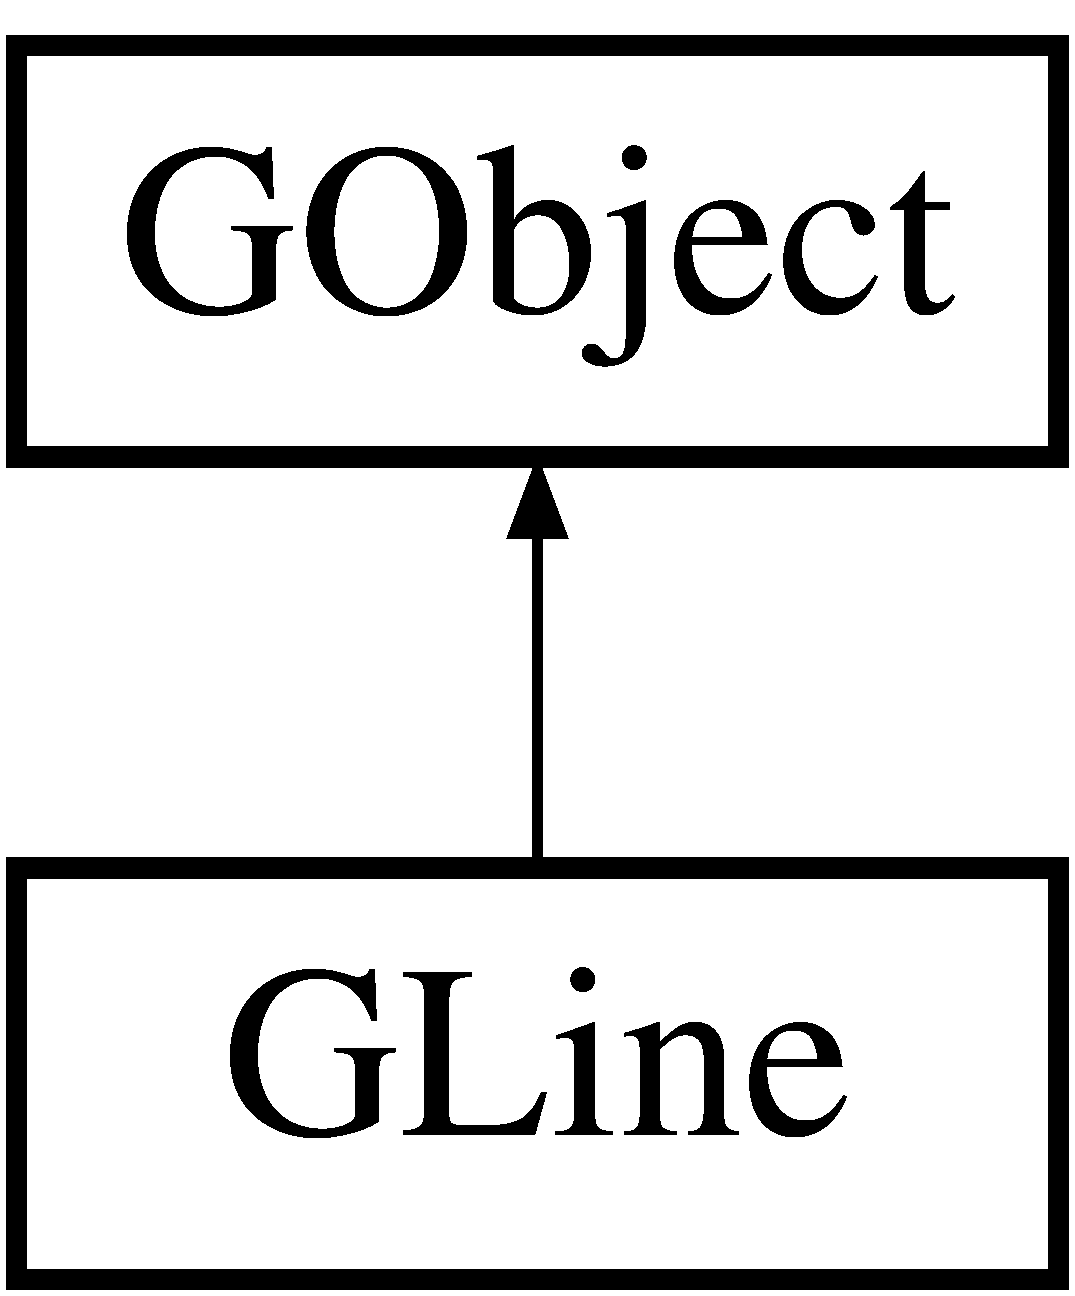
\includegraphics[height=2.000000cm]{classGLine}
\end{center}
\end{figure}
\subsection*{Public Types}
\begin{DoxyCompactItemize}
\item 
enum \mbox{\hyperlink{classGObject_a86e0f5648542856159bb40775c854aa7}{Line\+Style}} \{ \mbox{\hyperlink{classGObject_a86e0f5648542856159bb40775c854aa7acbc84bd5232621834ed31f44d457c1eb}{L\+I\+N\+E\+\_\+\+N\+O\+NE}}, 
\mbox{\hyperlink{classGObject_a86e0f5648542856159bb40775c854aa7a700c78bc2cd76acaab26651bf7b4941f}{L\+I\+N\+E\+\_\+\+S\+O\+L\+ID}}, 
\mbox{\hyperlink{classGObject_a86e0f5648542856159bb40775c854aa7a9ccba0845f785d81d07b333ae1aad84e}{L\+I\+N\+E\+\_\+\+D\+A\+SH}}, 
\mbox{\hyperlink{classGObject_a86e0f5648542856159bb40775c854aa7a8e811c096cb941997f0bfda168bb6df3}{L\+I\+N\+E\+\_\+\+D\+OT}}, 
\mbox{\hyperlink{classGObject_a86e0f5648542856159bb40775c854aa7ada15a2e3d737b2db7706d8300f91b89d}{L\+I\+N\+E\+\_\+\+D\+A\+S\+H\+\_\+\+D\+OT}}, 
\mbox{\hyperlink{classGObject_a86e0f5648542856159bb40775c854aa7aabf4053a73eafa7ba2b7e6d664c74c1d}{L\+I\+N\+E\+\_\+\+D\+A\+S\+H\+\_\+\+D\+O\+T\+\_\+\+D\+OT}}
 \}
\begin{DoxyCompactList}\small\item\em Styles that can be used for the outline around various shapes. \end{DoxyCompactList}\end{DoxyCompactItemize}
\subsection*{Public Member Functions}
\begin{DoxyCompactItemize}
\item 
\mbox{\hyperlink{classGLine_ac9e846926da2b0a7fc87164dd05dff3d}{G\+Line}} (double x0=0, double y0=0, double x1=0, double y1=0, \mbox{\hyperlink{classGObject_a86e0f5648542856159bb40775c854aa7}{Line\+Style}} line\+Style=\mbox{\hyperlink{classGObject_a86e0f5648542856159bb40775c854aa7a700c78bc2cd76acaab26651bf7b4941f}{L\+I\+N\+E\+\_\+\+S\+O\+L\+ID}})
\begin{DoxyCompactList}\small\item\em Constructs a line segment from its endpoints. \end{DoxyCompactList}\item 
\mbox{\hyperlink{classGLine_a337f6971ca683934513640e9400f3e88}{G\+Line}} (const \mbox{\hyperlink{classGPoint}{G\+Point}} \&p0, const \mbox{\hyperlink{classGPoint}{G\+Point}} \&p1)
\begin{DoxyCompactList}\small\item\em Constructs a line segment from its endpoints. \end{DoxyCompactList}\item 
virtual bool \mbox{\hyperlink{classGObject_a1dbc9dafaae51958112dbe1267a1f547}{contains}} (const \mbox{\hyperlink{classGPoint}{G\+Point}} \&pt) const
\begin{DoxyCompactList}\small\item\em Returns {\ttfamily true} if the specified point is inside the object. \end{DoxyCompactList}\item 
virtual bool \mbox{\hyperlink{classGLine_aa095a031ab22c150d2d75fdda1c3c8f5}{contains}} (double x, double y) const Q\+\_\+\+D\+E\+C\+L\+\_\+\+O\+V\+E\+R\+R\+I\+DE
\begin{DoxyCompactList}\small\item\em Returns {\ttfamily true} if the specified point is inside the object. \end{DoxyCompactList}\item 
virtual \mbox{\hyperlink{classGPoint}{G\+Point}} \mbox{\hyperlink{classGObject_a0d41183bf6b08de66fe3907551aab0d7}{get\+Bottom\+Right\+Location}} () const
\begin{DoxyCompactList}\small\item\em Returns the x/y coordinates of the bottom/right corner of the object. \end{DoxyCompactList}\item 
virtual double \mbox{\hyperlink{classGObject_a4316a2406c18e1c6d061fe51fd355490}{get\+BottomY}} () const
\begin{DoxyCompactList}\small\item\em Returns the {\itshape y}-\/coordinate of the bottom of the object. \end{DoxyCompactList}\item 
virtual \mbox{\hyperlink{classGRectangle}{G\+Rectangle}} \mbox{\hyperlink{classGLine_a2f46ec8a3b533c690b3b3e56d4f34afe}{get\+Bounds}} () const Q\+\_\+\+D\+E\+C\+L\+\_\+\+O\+V\+E\+R\+R\+I\+DE
\begin{DoxyCompactList}\small\item\em Returns the bounding box of this object, which is defined to be the smallest rectangle that covers everything drawn by the figure. \end{DoxyCompactList}\item 
virtual \mbox{\hyperlink{classGPoint}{G\+Point}} \mbox{\hyperlink{classGObject_a0909472e91448470bccdb62ecfb95d8b}{get\+Center\+Location}} () const
\begin{DoxyCompactList}\small\item\em Returns the x/y-\/coordinates of the center of the object. \end{DoxyCompactList}\item 
virtual double \mbox{\hyperlink{classGObject_a04df74355b545e0543112d5b8d924176}{get\+CenterX}} () const
\begin{DoxyCompactList}\small\item\em Returns the {\itshape x}-\/coordinate of the center of the object. \end{DoxyCompactList}\item 
virtual double \mbox{\hyperlink{classGObject_acb3287a3d507025a26f54b895713b947}{get\+CenterY}} () const
\begin{DoxyCompactList}\small\item\em Returns the {\itshape y}-\/coordinate of the center of the object. \end{DoxyCompactList}\item 
virtual std\+::string \mbox{\hyperlink{classGObject_aa061dfa488c31e18549d64363c1d0e34}{get\+Color}} () const
\begin{DoxyCompactList}\small\item\em Returns the color used to display this object. \end{DoxyCompactList}\item 
virtual \mbox{\hyperlink{classGPoint}{G\+Point}} \mbox{\hyperlink{classGLine_a835d5e50bf4a91efcf0d838130c246af}{get\+End\+Point}} () const
\begin{DoxyCompactList}\small\item\em Returns the point at which the line ends. \end{DoxyCompactList}\item 
virtual double \mbox{\hyperlink{classGLine_a87db00624acdc56daf57bacd76ed0ac0}{get\+EndX}} () const
\begin{DoxyCompactList}\small\item\em Returns the x-\/coordinate of the point at which the line ends. \end{DoxyCompactList}\item 
virtual double \mbox{\hyperlink{classGLine_ac6aa09d194bd5210461eba3e5870f488}{get\+EndY}} () const
\begin{DoxyCompactList}\small\item\em Returns the y-\/coordinate of the point at which the line ends. \end{DoxyCompactList}\item 
virtual std\+::string \mbox{\hyperlink{classGObject_a76f6964a11fde7c78e9751be184e1a3c}{get\+Fill\+Color}} () const
\begin{DoxyCompactList}\small\item\em Returns the color used to display the filled region of this object. \end{DoxyCompactList}\item 
virtual double \mbox{\hyperlink{classGLine_a423f17d4aeb66feb0d148fd23af335b7}{get\+Height}} () const Q\+\_\+\+D\+E\+C\+L\+\_\+\+O\+V\+E\+R\+R\+I\+DE
\begin{DoxyCompactList}\small\item\em Returns the height of this object, which is the same as the height of its bounding box. \end{DoxyCompactList}\item 
virtual \mbox{\hyperlink{classGObject_a86e0f5648542856159bb40775c854aa7}{Line\+Style}} \mbox{\hyperlink{classGObject_aaf1f5ea8281e5e3486662878d26f0a13}{get\+Line\+Style}} () const
\begin{DoxyCompactList}\small\item\em Returns the object\textquotesingle{}s style such as solid or dashed. \end{DoxyCompactList}\item 
virtual double \mbox{\hyperlink{classGObject_a85ff266dc3eb63d9f2d8e5a4487fd3c0}{get\+Line\+Width}} () const
\begin{DoxyCompactList}\small\item\em Returns the width of the line used to draw this object. \end{DoxyCompactList}\item 
virtual \mbox{\hyperlink{classGPoint}{G\+Point}} \mbox{\hyperlink{classGObject_a4f83802015511edeb63b892830812c11}{get\+Location}} () const
\begin{DoxyCompactList}\small\item\em Returns the location of the top-\/left corner of object. \end{DoxyCompactList}\item 
virtual \mbox{\hyperlink{classGCompound}{G\+Compound}} $\ast$ \mbox{\hyperlink{classGObject_a3e53cef70541b1a14eade4ad0984d0b4}{get\+Parent}} () const
\begin{DoxyCompactList}\small\item\em Returns a pointer to the {\ttfamily \mbox{\hyperlink{classGCompound}{G\+Compound}}} that contains this object. \end{DoxyCompactList}\item 
virtual double \mbox{\hyperlink{classGObject_a798cc79daaa10145b28f60bcdfdb0ee9}{get\+RightX}} () const
\begin{DoxyCompactList}\small\item\em Returns the {\itshape x}-\/coordinate of the right side of the object. \end{DoxyCompactList}\item 
virtual \mbox{\hyperlink{classGDimension}{G\+Dimension}} \mbox{\hyperlink{classGObject_a7b4eec96a2bdc6420695d5796a78eea9}{get\+Size}} () const
\begin{DoxyCompactList}\small\item\em Returns the size of the object as a {\ttfamily \mbox{\hyperlink{classGDimension}{G\+Dimension}}}. \end{DoxyCompactList}\item 
virtual \mbox{\hyperlink{classGPoint}{G\+Point}} \mbox{\hyperlink{classGLine_ad12beaa70993d9b409bfa8fd86c83957}{get\+Start\+Point}} () const
\begin{DoxyCompactList}\small\item\em Returns the point at which the line starts. \end{DoxyCompactList}\item 
virtual double \mbox{\hyperlink{classGLine_aa82e2c4efd87a1d6092747839d28c5db}{get\+StartX}} () const
\begin{DoxyCompactList}\small\item\em Returns the x-\/coordinate of the point at which the line starts. \end{DoxyCompactList}\item 
virtual double \mbox{\hyperlink{classGLine_a4481ac794cdca823afc9633f8cc88777}{get\+StartY}} () const
\begin{DoxyCompactList}\small\item\em Returns the y-\/coordinate of the point at which the line starts. \end{DoxyCompactList}\item 
virtual std\+::string \mbox{\hyperlink{classGLine_a9896d58fcfebbf1025aeeb5b8b9ede80}{get\+Type}} () const Q\+\_\+\+D\+E\+C\+L\+\_\+\+O\+V\+E\+R\+R\+I\+DE
\begin{DoxyCompactList}\small\item\em Returns the type of the object as a string, such as {\ttfamily \char`\"{}\+G\+Oval\char`\"{}} or {\ttfamily \char`\"{}\+G\+Rect\char`\"{}}. \end{DoxyCompactList}\item 
virtual double \mbox{\hyperlink{classGLine_a04bee94b66c8f921cd8611be2460ba9d}{get\+Width}} () const Q\+\_\+\+D\+E\+C\+L\+\_\+\+O\+V\+E\+R\+R\+I\+DE
\begin{DoxyCompactList}\small\item\em Returns the width of this object, which is equal to the width of the bounding box. \end{DoxyCompactList}\item 
virtual double \mbox{\hyperlink{classGObject_a344385751bee0720059403940d57a13e}{getX}} () const
\begin{DoxyCompactList}\small\item\em Returns the leftmost {\itshape x}-\/coordinate of the object. \end{DoxyCompactList}\item 
virtual double \mbox{\hyperlink{classGObject_aafa51c7f8f38a09febbb9ce7853f77b4}{getY}} () const
\begin{DoxyCompactList}\small\item\em Returns the topmost {\itshape y}-\/coordinate of the object. \end{DoxyCompactList}\item 
virtual bool \mbox{\hyperlink{classGObject_a11c404f106940c201b6f326e0355c150}{is\+Filled}} () const
\begin{DoxyCompactList}\small\item\em Returns {\ttfamily true} if the object is filled with color. \end{DoxyCompactList}\item 
virtual bool \mbox{\hyperlink{classGObject_a9d8a6cfb13917785c143e74d40e4e2be}{is\+Visible}} () const
\begin{DoxyCompactList}\small\item\em Returns {\ttfamily true} if this object is visible on screen. \end{DoxyCompactList}\item 
virtual void \mbox{\hyperlink{classGObject_a5973d8dda83afb36e2c56855515be392}{move}} (double dx, double dy)
\begin{DoxyCompactList}\small\item\em Moves the object on the screen using the displacements {\ttfamily dx} and {\ttfamily dy}. \end{DoxyCompactList}\item 
virtual void \mbox{\hyperlink{classGObject_ac827b978aa122f136a14c198687ad80f}{repaint}} ()
\begin{DoxyCompactList}\small\item\em Instructs the object to redraw itself on screen. \end{DoxyCompactList}\item 
virtual void \mbox{\hyperlink{classGObject_a6022a1fd1e5dcd2fd5585e5a36aa3f37}{reset\+Transform}} ()
\begin{DoxyCompactList}\small\item\em Undoes any previous scale/rotate transformations on this object. \end{DoxyCompactList}\item 
virtual void \mbox{\hyperlink{classGObject_ae1ffaa12185dfd5ba464f7d87c329e26}{rotate}} (double theta)
\begin{DoxyCompactList}\small\item\em Transforms the object by rotating it {\ttfamily theta} degrees counterclockwise around its origin. \end{DoxyCompactList}\item 
virtual void \mbox{\hyperlink{classGObject_ad2e1900f730475c2d044817db03b38d6}{scale}} (double sf)
\begin{DoxyCompactList}\small\item\em Scales the object by the specified scale factor. \end{DoxyCompactList}\item 
virtual void \mbox{\hyperlink{classGObject_a63641f69d610d0b951357d35a0c3b1e3}{scale}} (double sx, double sy)
\begin{DoxyCompactList}\small\item\em Scales the object by the specified scale factors. \end{DoxyCompactList}\item 
void \mbox{\hyperlink{classGObject_ab6747f40313c531c2db32edb5b63b9b7}{send\+Backward}} ()
\begin{DoxyCompactList}\small\item\em Moves this object one step toward the back in the {\itshape z} dimension. \end{DoxyCompactList}\item 
void \mbox{\hyperlink{classGObject_a710b3e449c9facba7847c91ab170d281}{send\+Forward}} ()
\begin{DoxyCompactList}\small\item\em Moves this object one step toward the front in the {\itshape z} dimension. \end{DoxyCompactList}\item 
void \mbox{\hyperlink{classGObject_a0f7f1efbb7fd46dde2867c4ad0330896}{send\+To\+Back}} ()
\begin{DoxyCompactList}\small\item\em Moves this object to the back of the display in the {\itshape z} dimension. \end{DoxyCompactList}\item 
void \mbox{\hyperlink{classGObject_aee33d68488e46827ef55fac07f40a9b2}{send\+To\+Front}} ()
\begin{DoxyCompactList}\small\item\em Moves this object to the front of the display in the {\itshape z} dimension. \end{DoxyCompactList}\item 
virtual void \mbox{\hyperlink{classGObject_a71ff7b16b8f1bdc4a1ce9f30cf8b87d8}{set\+Bottom\+Right\+Location}} (double x, double y)
\begin{DoxyCompactList}\small\item\em Sets the location of the bottom/right of this object. \end{DoxyCompactList}\item 
virtual void \mbox{\hyperlink{classGObject_ac6f7320321182f1d18c1c0fa97d5e941}{set\+Bottom\+Right\+Location}} (const \mbox{\hyperlink{classGPoint}{G\+Point}} \&pt)
\begin{DoxyCompactList}\small\item\em Sets the location of the bottom/right of this object. \end{DoxyCompactList}\item 
virtual void \mbox{\hyperlink{classGObject_a4b20e93c2a2597484f74ee5caa71f41f}{set\+BottomY}} (double y)
\begin{DoxyCompactList}\small\item\em Sets the location of the bottom y-\/coordinate of this object. \end{DoxyCompactList}\item 
virtual void \mbox{\hyperlink{classGObject_a2aae8197624b72265ab83b4f1bc73f2f}{set\+Bounds}} (double x, double y, double width, double height)
\begin{DoxyCompactList}\small\item\em Changes the bounds of this object to the specified values. \end{DoxyCompactList}\item 
virtual void \mbox{\hyperlink{classGObject_acada386653f008cacc7cce86426bef7c}{set\+Bounds}} (const \mbox{\hyperlink{classGRectangle}{G\+Rectangle}} \&size)
\begin{DoxyCompactList}\small\item\em Changes the bounds of this object to the specified rectangle. \end{DoxyCompactList}\item 
virtual void \mbox{\hyperlink{classGObject_a290b47dd8de1be44089f95cb2c47c1de}{set\+Center\+Location}} (double x, double y)
\begin{DoxyCompactList}\small\item\em Sets the location of the center of this object. \end{DoxyCompactList}\item 
virtual void \mbox{\hyperlink{classGObject_a1bedf1b233ecba3f753ec58908a683a6}{set\+Center\+Location}} (const \mbox{\hyperlink{classGPoint}{G\+Point}} \&pt)
\begin{DoxyCompactList}\small\item\em Sets the location of the center of this object. \end{DoxyCompactList}\item 
virtual void \mbox{\hyperlink{classGObject_a2f4936281e056eead00a9186b9ba8af6}{set\+CenterX}} (double x)
\begin{DoxyCompactList}\small\item\em Sets the x-\/coordinate of the center of this object. \end{DoxyCompactList}\item 
virtual void \mbox{\hyperlink{classGObject_aad2a22b4fde88c33306b92aebf641d57}{set\+CenterY}} (double y)
\begin{DoxyCompactList}\small\item\em Sets the y-\/coordinate of the center of this object. \end{DoxyCompactList}\item 
virtual void \mbox{\hyperlink{classGObject_ad57ef49bc31db94e92648aa3737923d6}{set\+Color}} (int r, int g, int b)
\begin{DoxyCompactList}\small\item\em Sets the color used to display this object. \end{DoxyCompactList}\item 
virtual void \mbox{\hyperlink{classGObject_ab1f5cc0f5cc6bbbd716a526c61f1081d}{set\+Color}} (int rgb)
\begin{DoxyCompactList}\small\item\em Sets the color used to display this object. \end{DoxyCompactList}\item 
virtual void \mbox{\hyperlink{classGObject_a61374df6c11b52cfbb0815decdbaebc6}{set\+Color}} (const std\+::string \&color)
\begin{DoxyCompactList}\small\item\em Sets the color used to display this object. \end{DoxyCompactList}\item 
virtual void \mbox{\hyperlink{classGLine_a355b8381c9079fcddd3d37c241994b65}{set\+End\+Point}} (double x, double y)
\begin{DoxyCompactList}\small\item\em Sets the end point in the line to ({\ttfamily x},~{\ttfamily y}), leaving the start point unchanged. \end{DoxyCompactList}\item 
virtual void \mbox{\hyperlink{classGObject_ad767a33971159e9493e221cca4c00ae9}{set\+Fill\+Color}} (int r, int g, int b)
\begin{DoxyCompactList}\small\item\em Sets the color used to display the filled region of this object, if any. \end{DoxyCompactList}\item 
virtual void \mbox{\hyperlink{classGObject_aa59d9775a67fa7df2b24a95cd34840a3}{set\+Fill\+Color}} (int rgb)
\begin{DoxyCompactList}\small\item\em Sets the color used to display the filled region of this object, if any. \end{DoxyCompactList}\item 
virtual void \mbox{\hyperlink{classGObject_adbc18b1a930aadd97d7437f9f7265b96}{set\+Fill\+Color}} (const std\+::string \&color)
\begin{DoxyCompactList}\small\item\em Sets the color used to display the filled region of this object, if any. \end{DoxyCompactList}\item 
virtual void \mbox{\hyperlink{classGObject_a9b82b53362282c6bb7d6947068d2e55b}{set\+Filled}} (bool flag)
\begin{DoxyCompactList}\small\item\em Sets the fill status for the object, where {\ttfamily false} is outlined and {\ttfamily true} is filled. \end{DoxyCompactList}\item 
virtual void \mbox{\hyperlink{classGObject_a2592348886ffea646c6534bf88f7c49d}{set\+Font}} (const Q\+Font \&font)
\begin{DoxyCompactList}\small\item\em Changes the font used to display the object as specified by the given Qt font. \end{DoxyCompactList}\item 
virtual void \mbox{\hyperlink{classGObject_a8e096e8818d838aceae1d46d58fb3a7b}{set\+Font}} (const std\+::string \&font)
\begin{DoxyCompactList}\small\item\em Changes the font used to display the object as specified by the string {\ttfamily font}, which has the following format\+: \end{DoxyCompactList}\item 
virtual void \mbox{\hyperlink{classGObject_ad18e8fab1e02a4e9b75c6730212558eb}{set\+Foreground}} (int r, int g, int b)
\begin{DoxyCompactList}\small\item\em Sets the color used to display this object. \end{DoxyCompactList}\item 
virtual void \mbox{\hyperlink{classGObject_a9eb856b5ff83a19df3831a31f15f4563}{set\+Foreground}} (int rgb)
\begin{DoxyCompactList}\small\item\em Sets the color used to display this object. \end{DoxyCompactList}\item 
virtual void \mbox{\hyperlink{classGObject_af59209aeadea6dfc6d97a2d8531f50e1}{set\+Foreground}} (const std\+::string \&color)
\begin{DoxyCompactList}\small\item\em Sets the color used to display this object. \end{DoxyCompactList}\item 
virtual void \mbox{\hyperlink{classGObject_a9e280bfc4544dfaf8e4376c4e1a74357}{set\+Height}} (double height)
\begin{DoxyCompactList}\small\item\em Changes the height of this object to the specified height without changing its width. \end{DoxyCompactList}\item 
virtual void \mbox{\hyperlink{classGObject_add11575087eb94f1a71faa3f826c6341}{set\+Line\+Style}} (\mbox{\hyperlink{classGObject_a86e0f5648542856159bb40775c854aa7}{Line\+Style}} line\+Style)
\begin{DoxyCompactList}\small\item\em Sets the object\textquotesingle{}s style such as solid (\mbox{\hyperlink{classGObject_a86e0f5648542856159bb40775c854aa7a700c78bc2cd76acaab26651bf7b4941f}{G\+Object\+::\+L\+I\+N\+E\+\_\+\+S\+O\+L\+ID}}) or dashed (\mbox{\hyperlink{classGObject_a86e0f5648542856159bb40775c854aa7a9ccba0845f785d81d07b333ae1aad84e}{G\+Object\+::\+L\+I\+N\+E\+\_\+\+D\+A\+SH}}). \end{DoxyCompactList}\item 
virtual void \mbox{\hyperlink{classGObject_afd6a47c6ea6a1f85ca05a65ba3ff3477}{set\+Line\+Width}} (double line\+Width)
\begin{DoxyCompactList}\small\item\em Sets the width of the line used to draw this object. \end{DoxyCompactList}\item 
virtual void \mbox{\hyperlink{classGObject_a04594e8ba9b98513a64f1da00dcae18c}{set\+Location}} (double x, double y)
\begin{DoxyCompactList}\small\item\em Sets the location of the top-\/left corner of this object to the specified coordinates. \end{DoxyCompactList}\item 
virtual void \mbox{\hyperlink{classGObject_aa8480c0b7166cdf8f784cece06ab353f}{set\+Location}} (const \mbox{\hyperlink{classGPoint}{G\+Point}} \&pt)
\begin{DoxyCompactList}\small\item\em Sets the location of the top-\/left corner of this object to the specified point. \end{DoxyCompactList}\item 
virtual void \mbox{\hyperlink{classGObject_a3c90b758cdc2c911c9ef76c4360eb912}{set\+RightX}} (double x)
\begin{DoxyCompactList}\small\item\em Sets the location of the rightmost x-\/coordinate of this object. \end{DoxyCompactList}\item 
virtual void \mbox{\hyperlink{classGObject_aca25d49481f9bf5fc8f7df4c086c4ce7}{set\+Size}} (double width, double height)
\begin{DoxyCompactList}\small\item\em Changes the size of this object to the specified width and height. \end{DoxyCompactList}\item 
virtual void \mbox{\hyperlink{classGObject_ae2b628228f192c2702c4ce941b2af68f}{set\+Size}} (const \mbox{\hyperlink{classGDimension}{G\+Dimension}} \&size)
\begin{DoxyCompactList}\small\item\em Changes the size of this object to the specified width and height. \end{DoxyCompactList}\item 
virtual void \mbox{\hyperlink{classGLine_a43973b14da1fa8bcd618163764f0f8bc}{set\+Start\+Point}} (double x, double y)
\begin{DoxyCompactList}\small\item\em Sets the initial point in the line to ({\ttfamily x},~{\ttfamily y}), leaving the end point unchanged. \end{DoxyCompactList}\item 
virtual void \mbox{\hyperlink{classGObject_a88203f28224315d9f4471212f4af8ed3}{set\+Visible}} (bool flag)
\begin{DoxyCompactList}\small\item\em Sets whether this object is visible. \end{DoxyCompactList}\item 
virtual void \mbox{\hyperlink{classGObject_aa3f3fba4cb131baa8696ba01e3bceca1}{set\+Width}} (double width)
\begin{DoxyCompactList}\small\item\em Changes the width of this object to the specified width without changing its height. \end{DoxyCompactList}\item 
virtual void \mbox{\hyperlink{classGObject_a9c18fcc579333bf9653d13ad2b372e39}{setX}} (double x)
\begin{DoxyCompactList}\small\item\em Sets the x location of the left side of this object. \end{DoxyCompactList}\item 
virtual void \mbox{\hyperlink{classGObject_a7d57e2a5c35d27feb58fd498a3cf82b9}{setY}} (double y)
\begin{DoxyCompactList}\small\item\em Sets the y location of the top of this object. \end{DoxyCompactList}\item 
virtual std\+::string \mbox{\hyperlink{classGObject_a1fe5121d6528fdea3f243321b3fa3a49}{to\+String}} () const
\begin{DoxyCompactList}\small\item\em Returns a printable representation of the object. \end{DoxyCompactList}\item 
virtual std\+::string \mbox{\hyperlink{classGLine_a85b5bcebac42ec5f130b0c3851383a23}{to\+String\+Extra}} () const Q\+\_\+\+D\+E\+C\+L\+\_\+\+O\+V\+E\+R\+R\+I\+DE
\begin{DoxyCompactList}\small\item\em Returns a string containing any extra unique information about this type of graphical object. \end{DoxyCompactList}\end{DoxyCompactItemize}
\subsection*{Static Public Member Functions}
\begin{DoxyCompactItemize}
\item 
static bool \mbox{\hyperlink{classGObject_a93be0e1fe1b1bf1a1da732470c94f42b}{is\+Anti\+Aliasing}} ()
\begin{DoxyCompactList}\small\item\em Returns whether we should globally anti-\/alias graphical objects. \end{DoxyCompactList}\item 
static void \mbox{\hyperlink{classGObject_a1e43371668ae850193cebedb44e1bbe3}{set\+Anti\+Aliasing}} (bool value)
\begin{DoxyCompactList}\small\item\em Globally turns on/off the anti-\/aliasing feature that smooths out the edges of onscreen shapes. \end{DoxyCompactList}\end{DoxyCompactItemize}
\subsection*{Protected Attributes}
\begin{DoxyCompactItemize}
\item 
Q\+Brush \mbox{\hyperlink{classGObject_aab24462ec896b596d99911767b0912d0}{\+\_\+brush}}
\item 
std\+::string \mbox{\hyperlink{classGObject_a1134e770ae4315ea8bc1201e2f21da8b}{\+\_\+color}}
\item 
int \mbox{\hyperlink{classGObject_a003fdd343d9b7505c53a8b7a134200ed}{\+\_\+color\+Int}}
\item 
double \mbox{\hyperlink{classGLine_a81afeefef08850c1beb8b799ede89635}{\+\_\+dx}}
\item 
double \mbox{\hyperlink{classGLine_a87493c51c53b249b302718465fba8c82}{\+\_\+dy}}
\item 
std\+::string \mbox{\hyperlink{classGObject_a179f8d6cee65cd8a54692e32b224392a}{\+\_\+fill\+Color}}
\item 
int \mbox{\hyperlink{classGObject_a751def333a67d651e5b99cc331ecb496}{\+\_\+fill\+Color\+Int}}
\item 
bool \mbox{\hyperlink{classGObject_ad4a55cbcd61b58a4d49666490bb2f103}{\+\_\+fill\+Flag}}
\item 
std\+::string \mbox{\hyperlink{classGObject_aea76ea1a8b5dd7b0a78653277e63b536}{\+\_\+font}}
\item 
double \mbox{\hyperlink{classGObject_ad05df29e7f27fc504abd743e3d8b4e73}{\+\_\+height}}
\item 
\mbox{\hyperlink{classGObject_a86e0f5648542856159bb40775c854aa7}{Line\+Style}} \mbox{\hyperlink{classGObject_a89bafecaafb7c72d55c7efc10b7d0523}{\+\_\+line\+Style}}
\item 
double \mbox{\hyperlink{classGObject_a16e9033665937f13de2e163dc2184aff}{\+\_\+line\+Width}}
\item 
\mbox{\hyperlink{classGCompound}{G\+Compound}} $\ast$ \mbox{\hyperlink{classGObject_ac9452c1eaff70eebddbb318196aa3835}{\+\_\+parent}}
\item 
Q\+Pen \mbox{\hyperlink{classGObject_afb69d172743f868299847174eb1b6bc8}{\+\_\+pen}}
\item 
Q\+Transform \mbox{\hyperlink{classGObject_a475b8860a5f1adb4a1fdc58d1f5c1e32}{\+\_\+transform}}
\item 
bool \mbox{\hyperlink{classGObject_ae4725802fc8d8aaa0ab4bd4781f7e07c}{\+\_\+transformed}}
\item 
bool \mbox{\hyperlink{classGObject_a9312c72508471b7c7a87b540263e1af4}{\+\_\+visible}}
\item 
double \mbox{\hyperlink{classGObject_ab55d85a3371770e6725b1062cf160cd8}{\+\_\+width}}
\item 
double \mbox{\hyperlink{classGObject_a6675b83b27137b8d3aa2ad8133078ea6}{\+\_\+x}}
\item 
double \mbox{\hyperlink{classGObject_a2f0f6aeafddc8a39c578bfa7e22b5f1e}{\+\_\+y}}
\end{DoxyCompactItemize}


\subsection{Detailed Description}
This graphical object subclass represents a line segment. 

\subsection{Member Enumeration Documentation}
\mbox{\Hypertarget{classGObject_a86e0f5648542856159bb40775c854aa7}\label{classGObject_a86e0f5648542856159bb40775c854aa7}} 
\index{G\+Line@{G\+Line}!Line\+Style@{Line\+Style}}
\index{Line\+Style@{Line\+Style}!G\+Line@{G\+Line}}
\subsubsection{\texorpdfstring{Line\+Style}{LineStyle}}
{\footnotesize\ttfamily enum \mbox{\hyperlink{classGObject_a86e0f5648542856159bb40775c854aa7}{Line\+Style}}\hspace{0.3cm}{\ttfamily [inherited]}}



Styles that can be used for the outline around various shapes. 

Call set\+Line\+Style on a \mbox{\hyperlink{classGObject}{G\+Object}} and pass one of these values. \begin{DoxyEnumFields}{Enumerator}
\raisebox{\heightof{T}}[0pt][0pt]{\index{L\+I\+N\+E\+\_\+\+N\+O\+NE@{L\+I\+N\+E\+\_\+\+N\+O\+NE}!G\+Line@{G\+Line}}\index{G\+Line@{G\+Line}!L\+I\+N\+E\+\_\+\+N\+O\+NE@{L\+I\+N\+E\+\_\+\+N\+O\+NE}}}\mbox{\Hypertarget{classGObject_a86e0f5648542856159bb40775c854aa7acbc84bd5232621834ed31f44d457c1eb}\label{classGObject_a86e0f5648542856159bb40775c854aa7acbc84bd5232621834ed31f44d457c1eb}} 
L\+I\+N\+E\+\_\+\+N\+O\+NE&\\
\hline

\raisebox{\heightof{T}}[0pt][0pt]{\index{L\+I\+N\+E\+\_\+\+S\+O\+L\+ID@{L\+I\+N\+E\+\_\+\+S\+O\+L\+ID}!G\+Line@{G\+Line}}\index{G\+Line@{G\+Line}!L\+I\+N\+E\+\_\+\+S\+O\+L\+ID@{L\+I\+N\+E\+\_\+\+S\+O\+L\+ID}}}\mbox{\Hypertarget{classGObject_a86e0f5648542856159bb40775c854aa7a700c78bc2cd76acaab26651bf7b4941f}\label{classGObject_a86e0f5648542856159bb40775c854aa7a700c78bc2cd76acaab26651bf7b4941f}} 
L\+I\+N\+E\+\_\+\+S\+O\+L\+ID&\\
\hline

\raisebox{\heightof{T}}[0pt][0pt]{\index{L\+I\+N\+E\+\_\+\+D\+A\+SH@{L\+I\+N\+E\+\_\+\+D\+A\+SH}!G\+Line@{G\+Line}}\index{G\+Line@{G\+Line}!L\+I\+N\+E\+\_\+\+D\+A\+SH@{L\+I\+N\+E\+\_\+\+D\+A\+SH}}}\mbox{\Hypertarget{classGObject_a86e0f5648542856159bb40775c854aa7a9ccba0845f785d81d07b333ae1aad84e}\label{classGObject_a86e0f5648542856159bb40775c854aa7a9ccba0845f785d81d07b333ae1aad84e}} 
L\+I\+N\+E\+\_\+\+D\+A\+SH&\\
\hline

\raisebox{\heightof{T}}[0pt][0pt]{\index{L\+I\+N\+E\+\_\+\+D\+OT@{L\+I\+N\+E\+\_\+\+D\+OT}!G\+Line@{G\+Line}}\index{G\+Line@{G\+Line}!L\+I\+N\+E\+\_\+\+D\+OT@{L\+I\+N\+E\+\_\+\+D\+OT}}}\mbox{\Hypertarget{classGObject_a86e0f5648542856159bb40775c854aa7a8e811c096cb941997f0bfda168bb6df3}\label{classGObject_a86e0f5648542856159bb40775c854aa7a8e811c096cb941997f0bfda168bb6df3}} 
L\+I\+N\+E\+\_\+\+D\+OT&\\
\hline

\raisebox{\heightof{T}}[0pt][0pt]{\index{L\+I\+N\+E\+\_\+\+D\+A\+S\+H\+\_\+\+D\+OT@{L\+I\+N\+E\+\_\+\+D\+A\+S\+H\+\_\+\+D\+OT}!G\+Line@{G\+Line}}\index{G\+Line@{G\+Line}!L\+I\+N\+E\+\_\+\+D\+A\+S\+H\+\_\+\+D\+OT@{L\+I\+N\+E\+\_\+\+D\+A\+S\+H\+\_\+\+D\+OT}}}\mbox{\Hypertarget{classGObject_a86e0f5648542856159bb40775c854aa7ada15a2e3d737b2db7706d8300f91b89d}\label{classGObject_a86e0f5648542856159bb40775c854aa7ada15a2e3d737b2db7706d8300f91b89d}} 
L\+I\+N\+E\+\_\+\+D\+A\+S\+H\+\_\+\+D\+OT&\\
\hline

\raisebox{\heightof{T}}[0pt][0pt]{\index{L\+I\+N\+E\+\_\+\+D\+A\+S\+H\+\_\+\+D\+O\+T\+\_\+\+D\+OT@{L\+I\+N\+E\+\_\+\+D\+A\+S\+H\+\_\+\+D\+O\+T\+\_\+\+D\+OT}!G\+Line@{G\+Line}}\index{G\+Line@{G\+Line}!L\+I\+N\+E\+\_\+\+D\+A\+S\+H\+\_\+\+D\+O\+T\+\_\+\+D\+OT@{L\+I\+N\+E\+\_\+\+D\+A\+S\+H\+\_\+\+D\+O\+T\+\_\+\+D\+OT}}}\mbox{\Hypertarget{classGObject_a86e0f5648542856159bb40775c854aa7aabf4053a73eafa7ba2b7e6d664c74c1d}\label{classGObject_a86e0f5648542856159bb40775c854aa7aabf4053a73eafa7ba2b7e6d664c74c1d}} 
L\+I\+N\+E\+\_\+\+D\+A\+S\+H\+\_\+\+D\+O\+T\+\_\+\+D\+OT&\\
\hline

\end{DoxyEnumFields}


\subsection{Constructor \& Destructor Documentation}
\mbox{\Hypertarget{classGLine_ac9e846926da2b0a7fc87164dd05dff3d}\label{classGLine_ac9e846926da2b0a7fc87164dd05dff3d}} 
\index{G\+Line@{G\+Line}!G\+Line@{G\+Line}}
\index{G\+Line@{G\+Line}!G\+Line@{G\+Line}}
\subsubsection{\texorpdfstring{G\+Line()}{GLine()}\hspace{0.1cm}{\footnotesize\ttfamily [1/2]}}
{\footnotesize\ttfamily \mbox{\hyperlink{classGLine}{G\+Line}} (\begin{DoxyParamCaption}\item[{double}]{x0 = {\ttfamily 0},  }\item[{double}]{y0 = {\ttfamily 0},  }\item[{double}]{x1 = {\ttfamily 0},  }\item[{double}]{y1 = {\ttfamily 0},  }\item[{\mbox{\hyperlink{classGObject_a86e0f5648542856159bb40775c854aa7}{G\+Object\+::\+Line\+Style}}}]{line\+Style = {\ttfamily \mbox{\hyperlink{classGObject_a86e0f5648542856159bb40775c854aa7a700c78bc2cd76acaab26651bf7b4941f}{L\+I\+N\+E\+\_\+\+S\+O\+L\+ID}}} }\end{DoxyParamCaption})}



Constructs a line segment from its endpoints. 

The point ({\ttfamily x0},~{\ttfamily y0}) defines the start of the line and the point ({\ttfamily x1},~{\ttfamily y1}) defines the end. \mbox{\Hypertarget{classGLine_a337f6971ca683934513640e9400f3e88}\label{classGLine_a337f6971ca683934513640e9400f3e88}} 
\index{G\+Line@{G\+Line}!G\+Line@{G\+Line}}
\index{G\+Line@{G\+Line}!G\+Line@{G\+Line}}
\subsubsection{\texorpdfstring{G\+Line()}{GLine()}\hspace{0.1cm}{\footnotesize\ttfamily [2/2]}}
{\footnotesize\ttfamily \mbox{\hyperlink{classGLine}{G\+Line}} (\begin{DoxyParamCaption}\item[{const \mbox{\hyperlink{classGPoint}{G\+Point}} \&}]{p0,  }\item[{const \mbox{\hyperlink{classGPoint}{G\+Point}} \&}]{p1 }\end{DoxyParamCaption})}



Constructs a line segment from its endpoints. 

The point {\ttfamily p0} defines the start of the line and the point {\ttfamily p1} defines the end. 

\subsection{Member Function Documentation}
\mbox{\Hypertarget{classGObject_a1dbc9dafaae51958112dbe1267a1f547}\label{classGObject_a1dbc9dafaae51958112dbe1267a1f547}} 
\index{G\+Line@{G\+Line}!contains@{contains}}
\index{contains@{contains}!G\+Line@{G\+Line}}
\subsubsection{\texorpdfstring{contains()}{contains()}\hspace{0.1cm}{\footnotesize\ttfamily [1/2]}}
{\footnotesize\ttfamily bool contains (\begin{DoxyParamCaption}\item[{const \mbox{\hyperlink{classGPoint}{G\+Point}} \&}]{pt }\end{DoxyParamCaption}) const\hspace{0.3cm}{\ttfamily [virtual]}, {\ttfamily [inherited]}}



Returns {\ttfamily true} if the specified point is inside the object. 

\mbox{\Hypertarget{classGLine_aa095a031ab22c150d2d75fdda1c3c8f5}\label{classGLine_aa095a031ab22c150d2d75fdda1c3c8f5}} 
\index{G\+Line@{G\+Line}!contains@{contains}}
\index{contains@{contains}!G\+Line@{G\+Line}}
\subsubsection{\texorpdfstring{contains()}{contains()}\hspace{0.1cm}{\footnotesize\ttfamily [2/2]}}
{\footnotesize\ttfamily bool contains (\begin{DoxyParamCaption}\item[{double}]{x,  }\item[{double}]{y }\end{DoxyParamCaption}) const\hspace{0.3cm}{\ttfamily [virtual]}}



Returns {\ttfamily true} if the specified point is inside the object. 



Reimplemented from \mbox{\hyperlink{classGObject_abb6a5d7c03e6eaaae97264c4799ce7c3}{G\+Object}}.

\mbox{\Hypertarget{classGObject_a0d41183bf6b08de66fe3907551aab0d7}\label{classGObject_a0d41183bf6b08de66fe3907551aab0d7}} 
\index{G\+Line@{G\+Line}!get\+Bottom\+Right\+Location@{get\+Bottom\+Right\+Location}}
\index{get\+Bottom\+Right\+Location@{get\+Bottom\+Right\+Location}!G\+Line@{G\+Line}}
\subsubsection{\texorpdfstring{get\+Bottom\+Right\+Location()}{getBottomRightLocation()}}
{\footnotesize\ttfamily \mbox{\hyperlink{classGPoint}{G\+Point}} get\+Bottom\+Right\+Location (\begin{DoxyParamCaption}{ }\end{DoxyParamCaption}) const\hspace{0.3cm}{\ttfamily [virtual]}, {\ttfamily [inherited]}}



Returns the x/y coordinates of the bottom/right corner of the object. 

\mbox{\Hypertarget{classGObject_a4316a2406c18e1c6d061fe51fd355490}\label{classGObject_a4316a2406c18e1c6d061fe51fd355490}} 
\index{G\+Line@{G\+Line}!get\+BottomY@{get\+BottomY}}
\index{get\+BottomY@{get\+BottomY}!G\+Line@{G\+Line}}
\subsubsection{\texorpdfstring{get\+Bottom\+Y()}{getBottomY()}}
{\footnotesize\ttfamily double get\+BottomY (\begin{DoxyParamCaption}{ }\end{DoxyParamCaption}) const\hspace{0.3cm}{\ttfamily [virtual]}, {\ttfamily [inherited]}}



Returns the {\itshape y}-\/coordinate of the bottom of the object. 

Equivalent to the top y-\/coordinate plus the object\textquotesingle{}s height. \mbox{\Hypertarget{classGLine_a2f46ec8a3b533c690b3b3e56d4f34afe}\label{classGLine_a2f46ec8a3b533c690b3b3e56d4f34afe}} 
\index{G\+Line@{G\+Line}!get\+Bounds@{get\+Bounds}}
\index{get\+Bounds@{get\+Bounds}!G\+Line@{G\+Line}}
\subsubsection{\texorpdfstring{get\+Bounds()}{getBounds()}}
{\footnotesize\ttfamily \mbox{\hyperlink{classGRectangle}{G\+Rectangle}} get\+Bounds (\begin{DoxyParamCaption}{ }\end{DoxyParamCaption}) const\hspace{0.3cm}{\ttfamily [virtual]}}



Returns the bounding box of this object, which is defined to be the smallest rectangle that covers everything drawn by the figure. 

The coordinates of this rectangle do not necessarily match the location returned by {\ttfamily get\+Location}. Given a {\ttfamily \mbox{\hyperlink{classGText}{G\+Text}}} object, for example, {\ttfamily get\+Location} returns the coordinates of the point on the baseline at which the string begins; the {\ttfamily get\+Bounds} method, by contrast, returns a rectangle that covers the entire window area occupied by the string. 

Reimplemented from \mbox{\hyperlink{classGObject_a29e6ac35a0b48f491a4c88194cc5da3b}{G\+Object}}.

\mbox{\Hypertarget{classGObject_a0909472e91448470bccdb62ecfb95d8b}\label{classGObject_a0909472e91448470bccdb62ecfb95d8b}} 
\index{G\+Line@{G\+Line}!get\+Center\+Location@{get\+Center\+Location}}
\index{get\+Center\+Location@{get\+Center\+Location}!G\+Line@{G\+Line}}
\subsubsection{\texorpdfstring{get\+Center\+Location()}{getCenterLocation()}}
{\footnotesize\ttfamily \mbox{\hyperlink{classGPoint}{G\+Point}} get\+Center\+Location (\begin{DoxyParamCaption}{ }\end{DoxyParamCaption}) const\hspace{0.3cm}{\ttfamily [virtual]}, {\ttfamily [inherited]}}



Returns the x/y-\/coordinates of the center of the object. 

Equivalent to the top/left plus half the object\textquotesingle{}s size. \mbox{\Hypertarget{classGObject_a04df74355b545e0543112d5b8d924176}\label{classGObject_a04df74355b545e0543112d5b8d924176}} 
\index{G\+Line@{G\+Line}!get\+CenterX@{get\+CenterX}}
\index{get\+CenterX@{get\+CenterX}!G\+Line@{G\+Line}}
\subsubsection{\texorpdfstring{get\+Center\+X()}{getCenterX()}}
{\footnotesize\ttfamily double get\+CenterX (\begin{DoxyParamCaption}{ }\end{DoxyParamCaption}) const\hspace{0.3cm}{\ttfamily [virtual]}, {\ttfamily [inherited]}}



Returns the {\itshape x}-\/coordinate of the center of the object. 

Equivalent to the top/left plus half the object\textquotesingle{}s width. \mbox{\Hypertarget{classGObject_acb3287a3d507025a26f54b895713b947}\label{classGObject_acb3287a3d507025a26f54b895713b947}} 
\index{G\+Line@{G\+Line}!get\+CenterY@{get\+CenterY}}
\index{get\+CenterY@{get\+CenterY}!G\+Line@{G\+Line}}
\subsubsection{\texorpdfstring{get\+Center\+Y()}{getCenterY()}}
{\footnotesize\ttfamily double get\+CenterY (\begin{DoxyParamCaption}{ }\end{DoxyParamCaption}) const\hspace{0.3cm}{\ttfamily [virtual]}, {\ttfamily [inherited]}}



Returns the {\itshape y}-\/coordinate of the center of the object. 

Equivalent to the top/left plus half the object\textquotesingle{}s height. \mbox{\Hypertarget{classGObject_aa061dfa488c31e18549d64363c1d0e34}\label{classGObject_aa061dfa488c31e18549d64363c1d0e34}} 
\index{G\+Line@{G\+Line}!get\+Color@{get\+Color}}
\index{get\+Color@{get\+Color}!G\+Line@{G\+Line}}
\subsubsection{\texorpdfstring{get\+Color()}{getColor()}}
{\footnotesize\ttfamily std\+::string get\+Color (\begin{DoxyParamCaption}{ }\end{DoxyParamCaption}) const\hspace{0.3cm}{\ttfamily [virtual]}, {\ttfamily [inherited]}}



Returns the color used to display this object. 

This color is always returned as a string in the form {\ttfamily \char`\"{}\#rrggbb\char`\"{}}, where {\ttfamily rr}, {\ttfamily gg}, and {\ttfamily bb} are the red, green, and blue components of the color, expressed as two-\/digit hexadecimal values. \mbox{\Hypertarget{classGLine_a835d5e50bf4a91efcf0d838130c246af}\label{classGLine_a835d5e50bf4a91efcf0d838130c246af}} 
\index{G\+Line@{G\+Line}!get\+End\+Point@{get\+End\+Point}}
\index{get\+End\+Point@{get\+End\+Point}!G\+Line@{G\+Line}}
\subsubsection{\texorpdfstring{get\+End\+Point()}{getEndPoint()}}
{\footnotesize\ttfamily \mbox{\hyperlink{classGPoint}{G\+Point}} get\+End\+Point (\begin{DoxyParamCaption}{ }\end{DoxyParamCaption}) const\hspace{0.3cm}{\ttfamily [virtual]}}



Returns the point at which the line ends. 

\mbox{\Hypertarget{classGLine_a87db00624acdc56daf57bacd76ed0ac0}\label{classGLine_a87db00624acdc56daf57bacd76ed0ac0}} 
\index{G\+Line@{G\+Line}!get\+EndX@{get\+EndX}}
\index{get\+EndX@{get\+EndX}!G\+Line@{G\+Line}}
\subsubsection{\texorpdfstring{get\+End\+X()}{getEndX()}}
{\footnotesize\ttfamily double get\+EndX (\begin{DoxyParamCaption}{ }\end{DoxyParamCaption}) const\hspace{0.3cm}{\ttfamily [virtual]}}



Returns the x-\/coordinate of the point at which the line ends. 

\mbox{\Hypertarget{classGLine_ac6aa09d194bd5210461eba3e5870f488}\label{classGLine_ac6aa09d194bd5210461eba3e5870f488}} 
\index{G\+Line@{G\+Line}!get\+EndY@{get\+EndY}}
\index{get\+EndY@{get\+EndY}!G\+Line@{G\+Line}}
\subsubsection{\texorpdfstring{get\+End\+Y()}{getEndY()}}
{\footnotesize\ttfamily double get\+EndY (\begin{DoxyParamCaption}{ }\end{DoxyParamCaption}) const\hspace{0.3cm}{\ttfamily [virtual]}}



Returns the y-\/coordinate of the point at which the line ends. 

\mbox{\Hypertarget{classGObject_a76f6964a11fde7c78e9751be184e1a3c}\label{classGObject_a76f6964a11fde7c78e9751be184e1a3c}} 
\index{G\+Line@{G\+Line}!get\+Fill\+Color@{get\+Fill\+Color}}
\index{get\+Fill\+Color@{get\+Fill\+Color}!G\+Line@{G\+Line}}
\subsubsection{\texorpdfstring{get\+Fill\+Color()}{getFillColor()}}
{\footnotesize\ttfamily std\+::string get\+Fill\+Color (\begin{DoxyParamCaption}{ }\end{DoxyParamCaption}) const\hspace{0.3cm}{\ttfamily [virtual]}, {\ttfamily [inherited]}}



Returns the color used to display the filled region of this object. 

If none has been set, returns the empty string. \mbox{\Hypertarget{classGLine_a423f17d4aeb66feb0d148fd23af335b7}\label{classGLine_a423f17d4aeb66feb0d148fd23af335b7}} 
\index{G\+Line@{G\+Line}!get\+Height@{get\+Height}}
\index{get\+Height@{get\+Height}!G\+Line@{G\+Line}}
\subsubsection{\texorpdfstring{get\+Height()}{getHeight()}}
{\footnotesize\ttfamily double get\+Height (\begin{DoxyParamCaption}{ }\end{DoxyParamCaption}) const\hspace{0.3cm}{\ttfamily [virtual]}}



Returns the height of this object, which is the same as the height of its bounding box. 



Reimplemented from \mbox{\hyperlink{classGObject_a1e7e353362434072875264cf95629f99}{G\+Object}}.

\mbox{\Hypertarget{classGObject_aaf1f5ea8281e5e3486662878d26f0a13}\label{classGObject_aaf1f5ea8281e5e3486662878d26f0a13}} 
\index{G\+Line@{G\+Line}!get\+Line\+Style@{get\+Line\+Style}}
\index{get\+Line\+Style@{get\+Line\+Style}!G\+Line@{G\+Line}}
\subsubsection{\texorpdfstring{get\+Line\+Style()}{getLineStyle()}}
{\footnotesize\ttfamily \mbox{\hyperlink{classGObject_a86e0f5648542856159bb40775c854aa7}{G\+Object\+::\+Line\+Style}} get\+Line\+Style (\begin{DoxyParamCaption}{ }\end{DoxyParamCaption}) const\hspace{0.3cm}{\ttfamily [virtual]}, {\ttfamily [inherited]}}



Returns the object\textquotesingle{}s style such as solid or dashed. 

\mbox{\Hypertarget{classGObject_a85ff266dc3eb63d9f2d8e5a4487fd3c0}\label{classGObject_a85ff266dc3eb63d9f2d8e5a4487fd3c0}} 
\index{G\+Line@{G\+Line}!get\+Line\+Width@{get\+Line\+Width}}
\index{get\+Line\+Width@{get\+Line\+Width}!G\+Line@{G\+Line}}
\subsubsection{\texorpdfstring{get\+Line\+Width()}{getLineWidth()}}
{\footnotesize\ttfamily double get\+Line\+Width (\begin{DoxyParamCaption}{ }\end{DoxyParamCaption}) const\hspace{0.3cm}{\ttfamily [virtual]}, {\ttfamily [inherited]}}



Returns the width of the line used to draw this object. 

\begin{DoxyReturn}{Returns}
default 1 
\end{DoxyReturn}
\mbox{\Hypertarget{classGObject_a4f83802015511edeb63b892830812c11}\label{classGObject_a4f83802015511edeb63b892830812c11}} 
\index{G\+Line@{G\+Line}!get\+Location@{get\+Location}}
\index{get\+Location@{get\+Location}!G\+Line@{G\+Line}}
\subsubsection{\texorpdfstring{get\+Location()}{getLocation()}}
{\footnotesize\ttfamily \mbox{\hyperlink{classGPoint}{G\+Point}} get\+Location (\begin{DoxyParamCaption}{ }\end{DoxyParamCaption}) const\hspace{0.3cm}{\ttfamily [virtual]}, {\ttfamily [inherited]}}



Returns the location of the top-\/left corner of object. 

\mbox{\Hypertarget{classGObject_a3e53cef70541b1a14eade4ad0984d0b4}\label{classGObject_a3e53cef70541b1a14eade4ad0984d0b4}} 
\index{G\+Line@{G\+Line}!get\+Parent@{get\+Parent}}
\index{get\+Parent@{get\+Parent}!G\+Line@{G\+Line}}
\subsubsection{\texorpdfstring{get\+Parent()}{getParent()}}
{\footnotesize\ttfamily \mbox{\hyperlink{classGCompound}{G\+Compound}} $\ast$ get\+Parent (\begin{DoxyParamCaption}{ }\end{DoxyParamCaption}) const\hspace{0.3cm}{\ttfamily [virtual]}, {\ttfamily [inherited]}}



Returns a pointer to the {\ttfamily \mbox{\hyperlink{classGCompound}{G\+Compound}}} that contains this object. 

Every {\ttfamily \mbox{\hyperlink{classGWindow}{G\+Window}}} is initialized to contain a single {\ttfamily \mbox{\hyperlink{classGCompound}{G\+Compound}}} that is aligned with the window. Adding objects to the window adds them to that {\ttfamily \mbox{\hyperlink{classGCompound}{G\+Compound}}}, which means that every object you add to the window has a parent. Calling {\ttfamily get\+Parent} on the top-\/level {\ttfamily \mbox{\hyperlink{classGCompound}{G\+Compound}}} returns {\ttfamily nullptr}. \mbox{\Hypertarget{classGObject_a798cc79daaa10145b28f60bcdfdb0ee9}\label{classGObject_a798cc79daaa10145b28f60bcdfdb0ee9}} 
\index{G\+Line@{G\+Line}!get\+RightX@{get\+RightX}}
\index{get\+RightX@{get\+RightX}!G\+Line@{G\+Line}}
\subsubsection{\texorpdfstring{get\+Right\+X()}{getRightX()}}
{\footnotesize\ttfamily double get\+RightX (\begin{DoxyParamCaption}{ }\end{DoxyParamCaption}) const\hspace{0.3cm}{\ttfamily [virtual]}, {\ttfamily [inherited]}}



Returns the {\itshape x}-\/coordinate of the right side of the object. 

Equivalent to the left x-\/coordinate plus the object\textquotesingle{}s width. \mbox{\Hypertarget{classGObject_a7b4eec96a2bdc6420695d5796a78eea9}\label{classGObject_a7b4eec96a2bdc6420695d5796a78eea9}} 
\index{G\+Line@{G\+Line}!get\+Size@{get\+Size}}
\index{get\+Size@{get\+Size}!G\+Line@{G\+Line}}
\subsubsection{\texorpdfstring{get\+Size()}{getSize()}}
{\footnotesize\ttfamily \mbox{\hyperlink{classGDimension}{G\+Dimension}} get\+Size (\begin{DoxyParamCaption}{ }\end{DoxyParamCaption}) const\hspace{0.3cm}{\ttfamily [virtual]}, {\ttfamily [inherited]}}



Returns the size of the object as a {\ttfamily \mbox{\hyperlink{classGDimension}{G\+Dimension}}}. 

\mbox{\Hypertarget{classGLine_ad12beaa70993d9b409bfa8fd86c83957}\label{classGLine_ad12beaa70993d9b409bfa8fd86c83957}} 
\index{G\+Line@{G\+Line}!get\+Start\+Point@{get\+Start\+Point}}
\index{get\+Start\+Point@{get\+Start\+Point}!G\+Line@{G\+Line}}
\subsubsection{\texorpdfstring{get\+Start\+Point()}{getStartPoint()}}
{\footnotesize\ttfamily \mbox{\hyperlink{classGPoint}{G\+Point}} get\+Start\+Point (\begin{DoxyParamCaption}{ }\end{DoxyParamCaption}) const\hspace{0.3cm}{\ttfamily [virtual]}}



Returns the point at which the line starts. 

Equivalent to get\+Location. \mbox{\Hypertarget{classGLine_aa82e2c4efd87a1d6092747839d28c5db}\label{classGLine_aa82e2c4efd87a1d6092747839d28c5db}} 
\index{G\+Line@{G\+Line}!get\+StartX@{get\+StartX}}
\index{get\+StartX@{get\+StartX}!G\+Line@{G\+Line}}
\subsubsection{\texorpdfstring{get\+Start\+X()}{getStartX()}}
{\footnotesize\ttfamily double get\+StartX (\begin{DoxyParamCaption}{ }\end{DoxyParamCaption}) const\hspace{0.3cm}{\ttfamily [virtual]}}



Returns the x-\/coordinate of the point at which the line starts. 

Equivalent to getX. \mbox{\Hypertarget{classGLine_a4481ac794cdca823afc9633f8cc88777}\label{classGLine_a4481ac794cdca823afc9633f8cc88777}} 
\index{G\+Line@{G\+Line}!get\+StartY@{get\+StartY}}
\index{get\+StartY@{get\+StartY}!G\+Line@{G\+Line}}
\subsubsection{\texorpdfstring{get\+Start\+Y()}{getStartY()}}
{\footnotesize\ttfamily double get\+StartY (\begin{DoxyParamCaption}{ }\end{DoxyParamCaption}) const\hspace{0.3cm}{\ttfamily [virtual]}}



Returns the y-\/coordinate of the point at which the line starts. 

Equivalent to getY. \mbox{\Hypertarget{classGLine_a9896d58fcfebbf1025aeeb5b8b9ede80}\label{classGLine_a9896d58fcfebbf1025aeeb5b8b9ede80}} 
\index{G\+Line@{G\+Line}!get\+Type@{get\+Type}}
\index{get\+Type@{get\+Type}!G\+Line@{G\+Line}}
\subsubsection{\texorpdfstring{get\+Type()}{getType()}}
{\footnotesize\ttfamily std\+::string get\+Type (\begin{DoxyParamCaption}{ }\end{DoxyParamCaption}) const\hspace{0.3cm}{\ttfamily [virtual]}}



Returns the type of the object as a string, such as {\ttfamily \char`\"{}\+G\+Oval\char`\"{}} or {\ttfamily \char`\"{}\+G\+Rect\char`\"{}}. 

Each \mbox{\hyperlink{classGObject}{G\+Object}} subtype must override this method. 

Implements \mbox{\hyperlink{classGObject_a799e073a127b428cc841086d42ea4fed}{G\+Object}}.

\mbox{\Hypertarget{classGLine_a04bee94b66c8f921cd8611be2460ba9d}\label{classGLine_a04bee94b66c8f921cd8611be2460ba9d}} 
\index{G\+Line@{G\+Line}!get\+Width@{get\+Width}}
\index{get\+Width@{get\+Width}!G\+Line@{G\+Line}}
\subsubsection{\texorpdfstring{get\+Width()}{getWidth()}}
{\footnotesize\ttfamily double get\+Width (\begin{DoxyParamCaption}{ }\end{DoxyParamCaption}) const\hspace{0.3cm}{\ttfamily [virtual]}}



Returns the width of this object, which is equal to the width of the bounding box. 



Reimplemented from \mbox{\hyperlink{classGObject_a0ed2965abd4f5701d2cadf71239faf19}{G\+Object}}.

\mbox{\Hypertarget{classGObject_a344385751bee0720059403940d57a13e}\label{classGObject_a344385751bee0720059403940d57a13e}} 
\index{G\+Line@{G\+Line}!getX@{getX}}
\index{getX@{getX}!G\+Line@{G\+Line}}
\subsubsection{\texorpdfstring{get\+X()}{getX()}}
{\footnotesize\ttfamily double getX (\begin{DoxyParamCaption}{ }\end{DoxyParamCaption}) const\hspace{0.3cm}{\ttfamily [virtual]}, {\ttfamily [inherited]}}



Returns the leftmost {\itshape x}-\/coordinate of the object. 

\mbox{\Hypertarget{classGObject_aafa51c7f8f38a09febbb9ce7853f77b4}\label{classGObject_aafa51c7f8f38a09febbb9ce7853f77b4}} 
\index{G\+Line@{G\+Line}!getY@{getY}}
\index{getY@{getY}!G\+Line@{G\+Line}}
\subsubsection{\texorpdfstring{get\+Y()}{getY()}}
{\footnotesize\ttfamily double getY (\begin{DoxyParamCaption}{ }\end{DoxyParamCaption}) const\hspace{0.3cm}{\ttfamily [virtual]}, {\ttfamily [inherited]}}



Returns the topmost {\itshape y}-\/coordinate of the object. 

\mbox{\Hypertarget{classGObject_a93be0e1fe1b1bf1a1da732470c94f42b}\label{classGObject_a93be0e1fe1b1bf1a1da732470c94f42b}} 
\index{G\+Line@{G\+Line}!is\+Anti\+Aliasing@{is\+Anti\+Aliasing}}
\index{is\+Anti\+Aliasing@{is\+Anti\+Aliasing}!G\+Line@{G\+Line}}
\subsubsection{\texorpdfstring{is\+Anti\+Aliasing()}{isAntiAliasing()}}
{\footnotesize\ttfamily bool is\+Anti\+Aliasing (\begin{DoxyParamCaption}{ }\end{DoxyParamCaption})\hspace{0.3cm}{\ttfamily [static]}, {\ttfamily [inherited]}}



Returns whether we should globally anti-\/alias graphical objects. 

On by default. \mbox{\Hypertarget{classGObject_a11c404f106940c201b6f326e0355c150}\label{classGObject_a11c404f106940c201b6f326e0355c150}} 
\index{G\+Line@{G\+Line}!is\+Filled@{is\+Filled}}
\index{is\+Filled@{is\+Filled}!G\+Line@{G\+Line}}
\subsubsection{\texorpdfstring{is\+Filled()}{isFilled()}}
{\footnotesize\ttfamily bool is\+Filled (\begin{DoxyParamCaption}{ }\end{DoxyParamCaption}) const\hspace{0.3cm}{\ttfamily [virtual]}, {\ttfamily [inherited]}}



Returns {\ttfamily true} if the object is filled with color. 

\mbox{\Hypertarget{classGObject_a9d8a6cfb13917785c143e74d40e4e2be}\label{classGObject_a9d8a6cfb13917785c143e74d40e4e2be}} 
\index{G\+Line@{G\+Line}!is\+Visible@{is\+Visible}}
\index{is\+Visible@{is\+Visible}!G\+Line@{G\+Line}}
\subsubsection{\texorpdfstring{is\+Visible()}{isVisible()}}
{\footnotesize\ttfamily bool is\+Visible (\begin{DoxyParamCaption}{ }\end{DoxyParamCaption}) const\hspace{0.3cm}{\ttfamily [virtual]}, {\ttfamily [inherited]}}



Returns {\ttfamily true} if this object is visible on screen. 

\mbox{\Hypertarget{classGObject_a5973d8dda83afb36e2c56855515be392}\label{classGObject_a5973d8dda83afb36e2c56855515be392}} 
\index{G\+Line@{G\+Line}!move@{move}}
\index{move@{move}!G\+Line@{G\+Line}}
\subsubsection{\texorpdfstring{move()}{move()}}
{\footnotesize\ttfamily void move (\begin{DoxyParamCaption}\item[{double}]{dx,  }\item[{double}]{dy }\end{DoxyParamCaption})\hspace{0.3cm}{\ttfamily [virtual]}, {\ttfamily [inherited]}}



Moves the object on the screen using the displacements {\ttfamily dx} and {\ttfamily dy}. 

\mbox{\Hypertarget{classGObject_ac827b978aa122f136a14c198687ad80f}\label{classGObject_ac827b978aa122f136a14c198687ad80f}} 
\index{G\+Line@{G\+Line}!repaint@{repaint}}
\index{repaint@{repaint}!G\+Line@{G\+Line}}
\subsubsection{\texorpdfstring{repaint()}{repaint()}}
{\footnotesize\ttfamily void repaint (\begin{DoxyParamCaption}{ }\end{DoxyParamCaption})\hspace{0.3cm}{\ttfamily [virtual]}, {\ttfamily [inherited]}}



Instructs the object to redraw itself on screen. 



Reimplemented in \mbox{\hyperlink{classGCompound_ac827b978aa122f136a14c198687ad80f}{G\+Compound}}.

\mbox{\Hypertarget{classGObject_a6022a1fd1e5dcd2fd5585e5a36aa3f37}\label{classGObject_a6022a1fd1e5dcd2fd5585e5a36aa3f37}} 
\index{G\+Line@{G\+Line}!reset\+Transform@{reset\+Transform}}
\index{reset\+Transform@{reset\+Transform}!G\+Line@{G\+Line}}
\subsubsection{\texorpdfstring{reset\+Transform()}{resetTransform()}}
{\footnotesize\ttfamily void reset\+Transform (\begin{DoxyParamCaption}{ }\end{DoxyParamCaption})\hspace{0.3cm}{\ttfamily [virtual]}, {\ttfamily [inherited]}}



Undoes any previous scale/rotate transformations on this object. 

\mbox{\Hypertarget{classGObject_ae1ffaa12185dfd5ba464f7d87c329e26}\label{classGObject_ae1ffaa12185dfd5ba464f7d87c329e26}} 
\index{G\+Line@{G\+Line}!rotate@{rotate}}
\index{rotate@{rotate}!G\+Line@{G\+Line}}
\subsubsection{\texorpdfstring{rotate()}{rotate()}}
{\footnotesize\ttfamily void rotate (\begin{DoxyParamCaption}\item[{double}]{theta }\end{DoxyParamCaption})\hspace{0.3cm}{\ttfamily [virtual]}, {\ttfamily [inherited]}}



Transforms the object by rotating it {\ttfamily theta} degrees counterclockwise around its origin. 

\mbox{\Hypertarget{classGObject_ad2e1900f730475c2d044817db03b38d6}\label{classGObject_ad2e1900f730475c2d044817db03b38d6}} 
\index{G\+Line@{G\+Line}!scale@{scale}}
\index{scale@{scale}!G\+Line@{G\+Line}}
\subsubsection{\texorpdfstring{scale()}{scale()}\hspace{0.1cm}{\footnotesize\ttfamily [1/2]}}
{\footnotesize\ttfamily void scale (\begin{DoxyParamCaption}\item[{double}]{sf }\end{DoxyParamCaption})\hspace{0.3cm}{\ttfamily [virtual]}, {\ttfamily [inherited]}}



Scales the object by the specified scale factor. 

This form scales the object by {\ttfamily sf} in both dimensions, so that invoking {\ttfamily gobj-\/$>$scale(2);} doubles the size of the object. \mbox{\Hypertarget{classGObject_a63641f69d610d0b951357d35a0c3b1e3}\label{classGObject_a63641f69d610d0b951357d35a0c3b1e3}} 
\index{G\+Line@{G\+Line}!scale@{scale}}
\index{scale@{scale}!G\+Line@{G\+Line}}
\subsubsection{\texorpdfstring{scale()}{scale()}\hspace{0.1cm}{\footnotesize\ttfamily [2/2]}}
{\footnotesize\ttfamily void scale (\begin{DoxyParamCaption}\item[{double}]{sx,  }\item[{double}]{sy }\end{DoxyParamCaption})\hspace{0.3cm}{\ttfamily [virtual]}, {\ttfamily [inherited]}}



Scales the object by the specified scale factors. 

For example, {\ttfamily gobj-\/$>$scale(2, 2);} doubles the size of the object. This form applies independent scale factors to the {\itshape x} and {\itshape y} dimensions. \mbox{\Hypertarget{classGObject_ab6747f40313c531c2db32edb5b63b9b7}\label{classGObject_ab6747f40313c531c2db32edb5b63b9b7}} 
\index{G\+Line@{G\+Line}!send\+Backward@{send\+Backward}}
\index{send\+Backward@{send\+Backward}!G\+Line@{G\+Line}}
\subsubsection{\texorpdfstring{send\+Backward()}{sendBackward()}}
{\footnotesize\ttfamily void send\+Backward (\begin{DoxyParamCaption}{ }\end{DoxyParamCaption})\hspace{0.3cm}{\ttfamily [inherited]}}



Moves this object one step toward the back in the {\itshape z} dimension. 

If it was already at the back of the stack, nothing happens. \mbox{\Hypertarget{classGObject_a710b3e449c9facba7847c91ab170d281}\label{classGObject_a710b3e449c9facba7847c91ab170d281}} 
\index{G\+Line@{G\+Line}!send\+Forward@{send\+Forward}}
\index{send\+Forward@{send\+Forward}!G\+Line@{G\+Line}}
\subsubsection{\texorpdfstring{send\+Forward()}{sendForward()}}
{\footnotesize\ttfamily void send\+Forward (\begin{DoxyParamCaption}{ }\end{DoxyParamCaption})\hspace{0.3cm}{\ttfamily [inherited]}}



Moves this object one step toward the front in the {\itshape z} dimension. 

If it was already at the front of the stack, nothing happens. \mbox{\Hypertarget{classGObject_a0f7f1efbb7fd46dde2867c4ad0330896}\label{classGObject_a0f7f1efbb7fd46dde2867c4ad0330896}} 
\index{G\+Line@{G\+Line}!send\+To\+Back@{send\+To\+Back}}
\index{send\+To\+Back@{send\+To\+Back}!G\+Line@{G\+Line}}
\subsubsection{\texorpdfstring{send\+To\+Back()}{sendToBack()}}
{\footnotesize\ttfamily void send\+To\+Back (\begin{DoxyParamCaption}{ }\end{DoxyParamCaption})\hspace{0.3cm}{\ttfamily [inherited]}}



Moves this object to the back of the display in the {\itshape z} dimension. 

By moving it to the back, this object will appear to be behind the other graphical objects on the display and may be obscured by other objects in front. \mbox{\Hypertarget{classGObject_aee33d68488e46827ef55fac07f40a9b2}\label{classGObject_aee33d68488e46827ef55fac07f40a9b2}} 
\index{G\+Line@{G\+Line}!send\+To\+Front@{send\+To\+Front}}
\index{send\+To\+Front@{send\+To\+Front}!G\+Line@{G\+Line}}
\subsubsection{\texorpdfstring{send\+To\+Front()}{sendToFront()}}
{\footnotesize\ttfamily void send\+To\+Front (\begin{DoxyParamCaption}{ }\end{DoxyParamCaption})\hspace{0.3cm}{\ttfamily [inherited]}}



Moves this object to the front of the display in the {\itshape z} dimension. 

By moving it to the front, this object will appear to be on top of the other graphical objects on the display and may hide any objects that are further back. \mbox{\Hypertarget{classGObject_a1e43371668ae850193cebedb44e1bbe3}\label{classGObject_a1e43371668ae850193cebedb44e1bbe3}} 
\index{G\+Line@{G\+Line}!set\+Anti\+Aliasing@{set\+Anti\+Aliasing}}
\index{set\+Anti\+Aliasing@{set\+Anti\+Aliasing}!G\+Line@{G\+Line}}
\subsubsection{\texorpdfstring{set\+Anti\+Aliasing()}{setAntiAliasing()}}
{\footnotesize\ttfamily void set\+Anti\+Aliasing (\begin{DoxyParamCaption}\item[{bool}]{value }\end{DoxyParamCaption})\hspace{0.3cm}{\ttfamily [static]}, {\ttfamily [inherited]}}



Globally turns on/off the anti-\/aliasing feature that smooths out the edges of onscreen shapes. 

On by default. Does not repaint any onscreen objects when called; you must do this yourself. \mbox{\Hypertarget{classGObject_a71ff7b16b8f1bdc4a1ce9f30cf8b87d8}\label{classGObject_a71ff7b16b8f1bdc4a1ce9f30cf8b87d8}} 
\index{G\+Line@{G\+Line}!set\+Bottom\+Right\+Location@{set\+Bottom\+Right\+Location}}
\index{set\+Bottom\+Right\+Location@{set\+Bottom\+Right\+Location}!G\+Line@{G\+Line}}
\subsubsection{\texorpdfstring{set\+Bottom\+Right\+Location()}{setBottomRightLocation()}\hspace{0.1cm}{\footnotesize\ttfamily [1/2]}}
{\footnotesize\ttfamily void set\+Bottom\+Right\+Location (\begin{DoxyParamCaption}\item[{double}]{x,  }\item[{double}]{y }\end{DoxyParamCaption})\hspace{0.3cm}{\ttfamily [virtual]}, {\ttfamily [inherited]}}



Sets the location of the bottom/right of this object. 

\mbox{\Hypertarget{classGObject_ac6f7320321182f1d18c1c0fa97d5e941}\label{classGObject_ac6f7320321182f1d18c1c0fa97d5e941}} 
\index{G\+Line@{G\+Line}!set\+Bottom\+Right\+Location@{set\+Bottom\+Right\+Location}}
\index{set\+Bottom\+Right\+Location@{set\+Bottom\+Right\+Location}!G\+Line@{G\+Line}}
\subsubsection{\texorpdfstring{set\+Bottom\+Right\+Location()}{setBottomRightLocation()}\hspace{0.1cm}{\footnotesize\ttfamily [2/2]}}
{\footnotesize\ttfamily void set\+Bottom\+Right\+Location (\begin{DoxyParamCaption}\item[{const \mbox{\hyperlink{classGPoint}{G\+Point}} \&}]{pt }\end{DoxyParamCaption})\hspace{0.3cm}{\ttfamily [virtual]}, {\ttfamily [inherited]}}



Sets the location of the bottom/right of this object. 

\mbox{\Hypertarget{classGObject_a4b20e93c2a2597484f74ee5caa71f41f}\label{classGObject_a4b20e93c2a2597484f74ee5caa71f41f}} 
\index{G\+Line@{G\+Line}!set\+BottomY@{set\+BottomY}}
\index{set\+BottomY@{set\+BottomY}!G\+Line@{G\+Line}}
\subsubsection{\texorpdfstring{set\+Bottom\+Y()}{setBottomY()}}
{\footnotesize\ttfamily void set\+BottomY (\begin{DoxyParamCaption}\item[{double}]{y }\end{DoxyParamCaption})\hspace{0.3cm}{\ttfamily [virtual]}, {\ttfamily [inherited]}}



Sets the location of the bottom y-\/coordinate of this object. 

\mbox{\Hypertarget{classGObject_a2aae8197624b72265ab83b4f1bc73f2f}\label{classGObject_a2aae8197624b72265ab83b4f1bc73f2f}} 
\index{G\+Line@{G\+Line}!set\+Bounds@{set\+Bounds}}
\index{set\+Bounds@{set\+Bounds}!G\+Line@{G\+Line}}
\subsubsection{\texorpdfstring{set\+Bounds()}{setBounds()}\hspace{0.1cm}{\footnotesize\ttfamily [1/2]}}
{\footnotesize\ttfamily void set\+Bounds (\begin{DoxyParamCaption}\item[{double}]{x,  }\item[{double}]{y,  }\item[{double}]{width,  }\item[{double}]{height }\end{DoxyParamCaption})\hspace{0.3cm}{\ttfamily [virtual]}, {\ttfamily [inherited]}}



Changes the bounds of this object to the specified values. 

\mbox{\Hypertarget{classGObject_acada386653f008cacc7cce86426bef7c}\label{classGObject_acada386653f008cacc7cce86426bef7c}} 
\index{G\+Line@{G\+Line}!set\+Bounds@{set\+Bounds}}
\index{set\+Bounds@{set\+Bounds}!G\+Line@{G\+Line}}
\subsubsection{\texorpdfstring{set\+Bounds()}{setBounds()}\hspace{0.1cm}{\footnotesize\ttfamily [2/2]}}
{\footnotesize\ttfamily void set\+Bounds (\begin{DoxyParamCaption}\item[{const \mbox{\hyperlink{classGRectangle}{G\+Rectangle}} \&}]{size }\end{DoxyParamCaption})\hspace{0.3cm}{\ttfamily [virtual]}, {\ttfamily [inherited]}}



Changes the bounds of this object to the specified rectangle. 

\mbox{\Hypertarget{classGObject_a290b47dd8de1be44089f95cb2c47c1de}\label{classGObject_a290b47dd8de1be44089f95cb2c47c1de}} 
\index{G\+Line@{G\+Line}!set\+Center\+Location@{set\+Center\+Location}}
\index{set\+Center\+Location@{set\+Center\+Location}!G\+Line@{G\+Line}}
\subsubsection{\texorpdfstring{set\+Center\+Location()}{setCenterLocation()}\hspace{0.1cm}{\footnotesize\ttfamily [1/2]}}
{\footnotesize\ttfamily void set\+Center\+Location (\begin{DoxyParamCaption}\item[{double}]{x,  }\item[{double}]{y }\end{DoxyParamCaption})\hspace{0.3cm}{\ttfamily [virtual]}, {\ttfamily [inherited]}}



Sets the location of the center of this object. 

\mbox{\Hypertarget{classGObject_a1bedf1b233ecba3f753ec58908a683a6}\label{classGObject_a1bedf1b233ecba3f753ec58908a683a6}} 
\index{G\+Line@{G\+Line}!set\+Center\+Location@{set\+Center\+Location}}
\index{set\+Center\+Location@{set\+Center\+Location}!G\+Line@{G\+Line}}
\subsubsection{\texorpdfstring{set\+Center\+Location()}{setCenterLocation()}\hspace{0.1cm}{\footnotesize\ttfamily [2/2]}}
{\footnotesize\ttfamily void set\+Center\+Location (\begin{DoxyParamCaption}\item[{const \mbox{\hyperlink{classGPoint}{G\+Point}} \&}]{pt }\end{DoxyParamCaption})\hspace{0.3cm}{\ttfamily [virtual]}, {\ttfamily [inherited]}}



Sets the location of the center of this object. 

\mbox{\Hypertarget{classGObject_a2f4936281e056eead00a9186b9ba8af6}\label{classGObject_a2f4936281e056eead00a9186b9ba8af6}} 
\index{G\+Line@{G\+Line}!set\+CenterX@{set\+CenterX}}
\index{set\+CenterX@{set\+CenterX}!G\+Line@{G\+Line}}
\subsubsection{\texorpdfstring{set\+Center\+X()}{setCenterX()}}
{\footnotesize\ttfamily void set\+CenterX (\begin{DoxyParamCaption}\item[{double}]{x }\end{DoxyParamCaption})\hspace{0.3cm}{\ttfamily [virtual]}, {\ttfamily [inherited]}}



Sets the x-\/coordinate of the center of this object. 

\mbox{\Hypertarget{classGObject_aad2a22b4fde88c33306b92aebf641d57}\label{classGObject_aad2a22b4fde88c33306b92aebf641d57}} 
\index{G\+Line@{G\+Line}!set\+CenterY@{set\+CenterY}}
\index{set\+CenterY@{set\+CenterY}!G\+Line@{G\+Line}}
\subsubsection{\texorpdfstring{set\+Center\+Y()}{setCenterY()}}
{\footnotesize\ttfamily void set\+CenterY (\begin{DoxyParamCaption}\item[{double}]{y }\end{DoxyParamCaption})\hspace{0.3cm}{\ttfamily [virtual]}, {\ttfamily [inherited]}}



Sets the y-\/coordinate of the center of this object. 

\mbox{\Hypertarget{classGObject_ad57ef49bc31db94e92648aa3737923d6}\label{classGObject_ad57ef49bc31db94e92648aa3737923d6}} 
\index{G\+Line@{G\+Line}!set\+Color@{set\+Color}}
\index{set\+Color@{set\+Color}!G\+Line@{G\+Line}}
\subsubsection{\texorpdfstring{set\+Color()}{setColor()}\hspace{0.1cm}{\footnotesize\ttfamily [1/3]}}
{\footnotesize\ttfamily void set\+Color (\begin{DoxyParamCaption}\item[{int}]{r,  }\item[{int}]{g,  }\item[{int}]{b }\end{DoxyParamCaption})\hspace{0.3cm}{\ttfamily [virtual]}, {\ttfamily [inherited]}}



Sets the color used to display this object. 

See \mbox{\hyperlink{gcolor_8h_source}{gcolor.\+h}} for more detail about how to specify colors.

Equivalent to set\+Foreground.


\begin{DoxyParams}{Parameters}
{\em r} & redness from 0-\/255 \\
\hline
{\em g} & greenness from 0-\/255 \\
\hline
{\em b} & blueness from 0-\/255 \\
\hline
\end{DoxyParams}
\mbox{\Hypertarget{classGObject_ab1f5cc0f5cc6bbbd716a526c61f1081d}\label{classGObject_ab1f5cc0f5cc6bbbd716a526c61f1081d}} 
\index{G\+Line@{G\+Line}!set\+Color@{set\+Color}}
\index{set\+Color@{set\+Color}!G\+Line@{G\+Line}}
\subsubsection{\texorpdfstring{set\+Color()}{setColor()}\hspace{0.1cm}{\footnotesize\ttfamily [2/3]}}
{\footnotesize\ttfamily void set\+Color (\begin{DoxyParamCaption}\item[{int}]{rgb }\end{DoxyParamCaption})\hspace{0.3cm}{\ttfamily [virtual]}, {\ttfamily [inherited]}}



Sets the color used to display this object. 

See \mbox{\hyperlink{gcolor_8h_source}{gcolor.\+h}} for more detail about how to specify colors.

Equivalent to set\+Foreground.


\begin{DoxyParams}{Parameters}
{\em rgb} & an R\+GB integer value such as 0x7700ff \\
\hline
\end{DoxyParams}
\mbox{\Hypertarget{classGObject_a61374df6c11b52cfbb0815decdbaebc6}\label{classGObject_a61374df6c11b52cfbb0815decdbaebc6}} 
\index{G\+Line@{G\+Line}!set\+Color@{set\+Color}}
\index{set\+Color@{set\+Color}!G\+Line@{G\+Line}}
\subsubsection{\texorpdfstring{set\+Color()}{setColor()}\hspace{0.1cm}{\footnotesize\ttfamily [3/3]}}
{\footnotesize\ttfamily void set\+Color (\begin{DoxyParamCaption}\item[{const std\+::string \&}]{color }\end{DoxyParamCaption})\hspace{0.3cm}{\ttfamily [virtual]}, {\ttfamily [inherited]}}



Sets the color used to display this object. 

See \mbox{\hyperlink{gcolor_8h_source}{gcolor.\+h}} for more detail about how to specify colors.

Equivalent to set\+Foreground.

a color string such as \char`\"{}\#7700ff\char`\"{} or \char`\"{}purple\char`\"{} \mbox{\Hypertarget{classGLine_a355b8381c9079fcddd3d37c241994b65}\label{classGLine_a355b8381c9079fcddd3d37c241994b65}} 
\index{G\+Line@{G\+Line}!set\+End\+Point@{set\+End\+Point}}
\index{set\+End\+Point@{set\+End\+Point}!G\+Line@{G\+Line}}
\subsubsection{\texorpdfstring{set\+End\+Point()}{setEndPoint()}}
{\footnotesize\ttfamily void set\+End\+Point (\begin{DoxyParamCaption}\item[{double}]{x,  }\item[{double}]{y }\end{DoxyParamCaption})\hspace{0.3cm}{\ttfamily [virtual]}}



Sets the end point in the line to ({\ttfamily x},~{\ttfamily y}), leaving the start point unchanged. 

This method is therefore different from {\ttfamily set\+Location}, which moves both components of the line segment. \mbox{\Hypertarget{classGObject_ad767a33971159e9493e221cca4c00ae9}\label{classGObject_ad767a33971159e9493e221cca4c00ae9}} 
\index{G\+Line@{G\+Line}!set\+Fill\+Color@{set\+Fill\+Color}}
\index{set\+Fill\+Color@{set\+Fill\+Color}!G\+Line@{G\+Line}}
\subsubsection{\texorpdfstring{set\+Fill\+Color()}{setFillColor()}\hspace{0.1cm}{\footnotesize\ttfamily [1/3]}}
{\footnotesize\ttfamily void set\+Fill\+Color (\begin{DoxyParamCaption}\item[{int}]{r,  }\item[{int}]{g,  }\item[{int}]{b }\end{DoxyParamCaption})\hspace{0.3cm}{\ttfamily [virtual]}, {\ttfamily [inherited]}}



Sets the color used to display the filled region of this object, if any. 

As a side effect, sets this object to be filled (set\+Filled(true)). See \mbox{\hyperlink{gcolor_8h_source}{gcolor.\+h}} for more detail about how to specify colors. If an empty string is passed, sets filled to false.


\begin{DoxyParams}{Parameters}
{\em r} & redness from 0-\/255 \\
\hline
{\em g} & greenness from 0-\/255 \\
\hline
{\em b} & blueness from 0-\/255 \\
\hline
\end{DoxyParams}
\mbox{\Hypertarget{classGObject_aa59d9775a67fa7df2b24a95cd34840a3}\label{classGObject_aa59d9775a67fa7df2b24a95cd34840a3}} 
\index{G\+Line@{G\+Line}!set\+Fill\+Color@{set\+Fill\+Color}}
\index{set\+Fill\+Color@{set\+Fill\+Color}!G\+Line@{G\+Line}}
\subsubsection{\texorpdfstring{set\+Fill\+Color()}{setFillColor()}\hspace{0.1cm}{\footnotesize\ttfamily [2/3]}}
{\footnotesize\ttfamily void set\+Fill\+Color (\begin{DoxyParamCaption}\item[{int}]{rgb }\end{DoxyParamCaption})\hspace{0.3cm}{\ttfamily [virtual]}, {\ttfamily [inherited]}}



Sets the color used to display the filled region of this object, if any. 

As a side effect, sets this object to be filled (set\+Filled(true)). See \mbox{\hyperlink{gcolor_8h_source}{gcolor.\+h}} for more detail about how to specify colors.


\begin{DoxyParams}{Parameters}
{\em rgb} & an R\+GB integer value such as 0x7700ff \\
\hline
\end{DoxyParams}
\mbox{\Hypertarget{classGObject_adbc18b1a930aadd97d7437f9f7265b96}\label{classGObject_adbc18b1a930aadd97d7437f9f7265b96}} 
\index{G\+Line@{G\+Line}!set\+Fill\+Color@{set\+Fill\+Color}}
\index{set\+Fill\+Color@{set\+Fill\+Color}!G\+Line@{G\+Line}}
\subsubsection{\texorpdfstring{set\+Fill\+Color()}{setFillColor()}\hspace{0.1cm}{\footnotesize\ttfamily [3/3]}}
{\footnotesize\ttfamily void set\+Fill\+Color (\begin{DoxyParamCaption}\item[{const std\+::string \&}]{color }\end{DoxyParamCaption})\hspace{0.3cm}{\ttfamily [virtual]}, {\ttfamily [inherited]}}



Sets the color used to display the filled region of this object, if any. 

As a side effect, sets this object to be filled (set\+Filled(true)). See \mbox{\hyperlink{gcolor_8h_source}{gcolor.\+h}} for more detail about how to specify colors. If an empty string is passed, sets filled to false.

a color string such as \char`\"{}\#7700ff\char`\"{} or \char`\"{}purple\char`\"{} \mbox{\Hypertarget{classGObject_a9b82b53362282c6bb7d6947068d2e55b}\label{classGObject_a9b82b53362282c6bb7d6947068d2e55b}} 
\index{G\+Line@{G\+Line}!set\+Filled@{set\+Filled}}
\index{set\+Filled@{set\+Filled}!G\+Line@{G\+Line}}
\subsubsection{\texorpdfstring{set\+Filled()}{setFilled()}}
{\footnotesize\ttfamily void set\+Filled (\begin{DoxyParamCaption}\item[{bool}]{flag }\end{DoxyParamCaption})\hspace{0.3cm}{\ttfamily [virtual]}, {\ttfamily [inherited]}}



Sets the fill status for the object, where {\ttfamily false} is outlined and {\ttfamily true} is filled. 

\mbox{\Hypertarget{classGObject_a2592348886ffea646c6534bf88f7c49d}\label{classGObject_a2592348886ffea646c6534bf88f7c49d}} 
\index{G\+Line@{G\+Line}!set\+Font@{set\+Font}}
\index{set\+Font@{set\+Font}!G\+Line@{G\+Line}}
\subsubsection{\texorpdfstring{set\+Font()}{setFont()}\hspace{0.1cm}{\footnotesize\ttfamily [1/2]}}
{\footnotesize\ttfamily void set\+Font (\begin{DoxyParamCaption}\item[{const Q\+Font \&}]{font }\end{DoxyParamCaption})\hspace{0.3cm}{\ttfamily [virtual]}, {\ttfamily [inherited]}}



Changes the font used to display the object as specified by the given Qt font. 

See \mbox{\hyperlink{gfont_8h_source}{gfont.\+h}} for more detail about how to specify fonts. 

Reimplemented in \mbox{\hyperlink{classGText_a2d22014c7fa3bccfd58c982aea1b55fa}{G\+Text}}.

\mbox{\Hypertarget{classGObject_a8e096e8818d838aceae1d46d58fb3a7b}\label{classGObject_a8e096e8818d838aceae1d46d58fb3a7b}} 
\index{G\+Line@{G\+Line}!set\+Font@{set\+Font}}
\index{set\+Font@{set\+Font}!G\+Line@{G\+Line}}
\subsubsection{\texorpdfstring{set\+Font()}{setFont()}\hspace{0.1cm}{\footnotesize\ttfamily [2/2]}}
{\footnotesize\ttfamily void set\+Font (\begin{DoxyParamCaption}\item[{const std\+::string \&}]{font }\end{DoxyParamCaption})\hspace{0.3cm}{\ttfamily [virtual]}, {\ttfamily [inherited]}}



Changes the font used to display the object as specified by the string {\ttfamily font}, which has the following format\+: 


\begin{DoxyPre}
"family-style-size"
\end{DoxyPre}


where both {\ttfamily style} and {\ttfamily size} are optional. If any of these elements are missing or specified as an asterisk, the existing value is retained. See \mbox{\hyperlink{gfont_8h_source}{gfont.\+h}} for more detail about how to specify fonts. 

Reimplemented in \mbox{\hyperlink{classGText_ab39ef411fb13a52852ddd138c5932e2e}{G\+Text}}.

\mbox{\Hypertarget{classGObject_ad18e8fab1e02a4e9b75c6730212558eb}\label{classGObject_ad18e8fab1e02a4e9b75c6730212558eb}} 
\index{G\+Line@{G\+Line}!set\+Foreground@{set\+Foreground}}
\index{set\+Foreground@{set\+Foreground}!G\+Line@{G\+Line}}
\subsubsection{\texorpdfstring{set\+Foreground()}{setForeground()}\hspace{0.1cm}{\footnotesize\ttfamily [1/3]}}
{\footnotesize\ttfamily void set\+Foreground (\begin{DoxyParamCaption}\item[{int}]{r,  }\item[{int}]{g,  }\item[{int}]{b }\end{DoxyParamCaption})\hspace{0.3cm}{\ttfamily [virtual]}, {\ttfamily [inherited]}}



Sets the color used to display this object. 

See \mbox{\hyperlink{gcolor_8h_source}{gcolor.\+h}} for more detail about how to specify colors.

Equivalent to set\+Color.


\begin{DoxyParams}{Parameters}
{\em r} & redness from 0-\/255 \\
\hline
{\em g} & greenness from 0-\/255 \\
\hline
{\em b} & blueness from 0-\/255 \\
\hline
\end{DoxyParams}
\mbox{\Hypertarget{classGObject_a9eb856b5ff83a19df3831a31f15f4563}\label{classGObject_a9eb856b5ff83a19df3831a31f15f4563}} 
\index{G\+Line@{G\+Line}!set\+Foreground@{set\+Foreground}}
\index{set\+Foreground@{set\+Foreground}!G\+Line@{G\+Line}}
\subsubsection{\texorpdfstring{set\+Foreground()}{setForeground()}\hspace{0.1cm}{\footnotesize\ttfamily [2/3]}}
{\footnotesize\ttfamily void set\+Foreground (\begin{DoxyParamCaption}\item[{int}]{rgb }\end{DoxyParamCaption})\hspace{0.3cm}{\ttfamily [virtual]}, {\ttfamily [inherited]}}



Sets the color used to display this object. 

See \mbox{\hyperlink{gcolor_8h_source}{gcolor.\+h}} for more detail about how to specify colors.

Equivalent to set\+Color.


\begin{DoxyParams}{Parameters}
{\em rgb} & an R\+GB integer value such as 0x7700ff \\
\hline
\end{DoxyParams}
\mbox{\Hypertarget{classGObject_af59209aeadea6dfc6d97a2d8531f50e1}\label{classGObject_af59209aeadea6dfc6d97a2d8531f50e1}} 
\index{G\+Line@{G\+Line}!set\+Foreground@{set\+Foreground}}
\index{set\+Foreground@{set\+Foreground}!G\+Line@{G\+Line}}
\subsubsection{\texorpdfstring{set\+Foreground()}{setForeground()}\hspace{0.1cm}{\footnotesize\ttfamily [3/3]}}
{\footnotesize\ttfamily void set\+Foreground (\begin{DoxyParamCaption}\item[{const std\+::string \&}]{color }\end{DoxyParamCaption})\hspace{0.3cm}{\ttfamily [virtual]}, {\ttfamily [inherited]}}



Sets the color used to display this object. 

See \mbox{\hyperlink{gcolor_8h_source}{gcolor.\+h}} for more detail about how to specify colors.

Equivalent to set\+Color.

a color string such as \char`\"{}\#7700ff\char`\"{} or \char`\"{}purple\char`\"{} \mbox{\Hypertarget{classGObject_a9e280bfc4544dfaf8e4376c4e1a74357}\label{classGObject_a9e280bfc4544dfaf8e4376c4e1a74357}} 
\index{G\+Line@{G\+Line}!set\+Height@{set\+Height}}
\index{set\+Height@{set\+Height}!G\+Line@{G\+Line}}
\subsubsection{\texorpdfstring{set\+Height()}{setHeight()}}
{\footnotesize\ttfamily void set\+Height (\begin{DoxyParamCaption}\item[{double}]{height }\end{DoxyParamCaption})\hspace{0.3cm}{\ttfamily [virtual]}, {\ttfamily [inherited]}}



Changes the height of this object to the specified height without changing its width. 

\mbox{\Hypertarget{classGObject_add11575087eb94f1a71faa3f826c6341}\label{classGObject_add11575087eb94f1a71faa3f826c6341}} 
\index{G\+Line@{G\+Line}!set\+Line\+Style@{set\+Line\+Style}}
\index{set\+Line\+Style@{set\+Line\+Style}!G\+Line@{G\+Line}}
\subsubsection{\texorpdfstring{set\+Line\+Style()}{setLineStyle()}}
{\footnotesize\ttfamily void set\+Line\+Style (\begin{DoxyParamCaption}\item[{\mbox{\hyperlink{classGObject_a86e0f5648542856159bb40775c854aa7}{G\+Object\+::\+Line\+Style}}}]{line\+Style }\end{DoxyParamCaption})\hspace{0.3cm}{\ttfamily [virtual]}, {\ttfamily [inherited]}}



Sets the object\textquotesingle{}s style such as solid (\mbox{\hyperlink{classGObject_a86e0f5648542856159bb40775c854aa7a700c78bc2cd76acaab26651bf7b4941f}{G\+Object\+::\+L\+I\+N\+E\+\_\+\+S\+O\+L\+ID}}) or dashed (\mbox{\hyperlink{classGObject_a86e0f5648542856159bb40775c854aa7a9ccba0845f785d81d07b333ae1aad84e}{G\+Object\+::\+L\+I\+N\+E\+\_\+\+D\+A\+SH}}). 

\mbox{\Hypertarget{classGObject_afd6a47c6ea6a1f85ca05a65ba3ff3477}\label{classGObject_afd6a47c6ea6a1f85ca05a65ba3ff3477}} 
\index{G\+Line@{G\+Line}!set\+Line\+Width@{set\+Line\+Width}}
\index{set\+Line\+Width@{set\+Line\+Width}!G\+Line@{G\+Line}}
\subsubsection{\texorpdfstring{set\+Line\+Width()}{setLineWidth()}}
{\footnotesize\ttfamily void set\+Line\+Width (\begin{DoxyParamCaption}\item[{double}]{line\+Width }\end{DoxyParamCaption})\hspace{0.3cm}{\ttfamily [virtual]}, {\ttfamily [inherited]}}



Sets the width of the line used to draw this object. 

The default line width is 1. \mbox{\Hypertarget{classGObject_a04594e8ba9b98513a64f1da00dcae18c}\label{classGObject_a04594e8ba9b98513a64f1da00dcae18c}} 
\index{G\+Line@{G\+Line}!set\+Location@{set\+Location}}
\index{set\+Location@{set\+Location}!G\+Line@{G\+Line}}
\subsubsection{\texorpdfstring{set\+Location()}{setLocation()}\hspace{0.1cm}{\footnotesize\ttfamily [1/2]}}
{\footnotesize\ttfamily void set\+Location (\begin{DoxyParamCaption}\item[{double}]{x,  }\item[{double}]{y }\end{DoxyParamCaption})\hspace{0.3cm}{\ttfamily [virtual]}, {\ttfamily [inherited]}}



Sets the location of the top-\/left corner of this object to the specified coordinates. 

\mbox{\Hypertarget{classGObject_aa8480c0b7166cdf8f784cece06ab353f}\label{classGObject_aa8480c0b7166cdf8f784cece06ab353f}} 
\index{G\+Line@{G\+Line}!set\+Location@{set\+Location}}
\index{set\+Location@{set\+Location}!G\+Line@{G\+Line}}
\subsubsection{\texorpdfstring{set\+Location()}{setLocation()}\hspace{0.1cm}{\footnotesize\ttfamily [2/2]}}
{\footnotesize\ttfamily void set\+Location (\begin{DoxyParamCaption}\item[{const \mbox{\hyperlink{classGPoint}{G\+Point}} \&}]{pt }\end{DoxyParamCaption})\hspace{0.3cm}{\ttfamily [virtual]}, {\ttfamily [inherited]}}



Sets the location of the top-\/left corner of this object to the specified point. 

\mbox{\Hypertarget{classGObject_a3c90b758cdc2c911c9ef76c4360eb912}\label{classGObject_a3c90b758cdc2c911c9ef76c4360eb912}} 
\index{G\+Line@{G\+Line}!set\+RightX@{set\+RightX}}
\index{set\+RightX@{set\+RightX}!G\+Line@{G\+Line}}
\subsubsection{\texorpdfstring{set\+Right\+X()}{setRightX()}}
{\footnotesize\ttfamily void set\+RightX (\begin{DoxyParamCaption}\item[{double}]{x }\end{DoxyParamCaption})\hspace{0.3cm}{\ttfamily [virtual]}, {\ttfamily [inherited]}}



Sets the location of the rightmost x-\/coordinate of this object. 

\mbox{\Hypertarget{classGObject_aca25d49481f9bf5fc8f7df4c086c4ce7}\label{classGObject_aca25d49481f9bf5fc8f7df4c086c4ce7}} 
\index{G\+Line@{G\+Line}!set\+Size@{set\+Size}}
\index{set\+Size@{set\+Size}!G\+Line@{G\+Line}}
\subsubsection{\texorpdfstring{set\+Size()}{setSize()}\hspace{0.1cm}{\footnotesize\ttfamily [1/2]}}
{\footnotesize\ttfamily void set\+Size (\begin{DoxyParamCaption}\item[{double}]{width,  }\item[{double}]{height }\end{DoxyParamCaption})\hspace{0.3cm}{\ttfamily [virtual]}, {\ttfamily [inherited]}}



Changes the size of this object to the specified width and height. 

\mbox{\Hypertarget{classGObject_ae2b628228f192c2702c4ce941b2af68f}\label{classGObject_ae2b628228f192c2702c4ce941b2af68f}} 
\index{G\+Line@{G\+Line}!set\+Size@{set\+Size}}
\index{set\+Size@{set\+Size}!G\+Line@{G\+Line}}
\subsubsection{\texorpdfstring{set\+Size()}{setSize()}\hspace{0.1cm}{\footnotesize\ttfamily [2/2]}}
{\footnotesize\ttfamily void set\+Size (\begin{DoxyParamCaption}\item[{const \mbox{\hyperlink{classGDimension}{G\+Dimension}} \&}]{size }\end{DoxyParamCaption})\hspace{0.3cm}{\ttfamily [virtual]}, {\ttfamily [inherited]}}



Changes the size of this object to the specified width and height. 

\mbox{\Hypertarget{classGLine_a43973b14da1fa8bcd618163764f0f8bc}\label{classGLine_a43973b14da1fa8bcd618163764f0f8bc}} 
\index{G\+Line@{G\+Line}!set\+Start\+Point@{set\+Start\+Point}}
\index{set\+Start\+Point@{set\+Start\+Point}!G\+Line@{G\+Line}}
\subsubsection{\texorpdfstring{set\+Start\+Point()}{setStartPoint()}}
{\footnotesize\ttfamily void set\+Start\+Point (\begin{DoxyParamCaption}\item[{double}]{x,  }\item[{double}]{y }\end{DoxyParamCaption})\hspace{0.3cm}{\ttfamily [virtual]}}



Sets the initial point in the line to ({\ttfamily x},~{\ttfamily y}), leaving the end point unchanged. 

This method is therefore different from {\ttfamily set\+Location}, which moves both components of the line segment. \mbox{\Hypertarget{classGObject_a88203f28224315d9f4471212f4af8ed3}\label{classGObject_a88203f28224315d9f4471212f4af8ed3}} 
\index{G\+Line@{G\+Line}!set\+Visible@{set\+Visible}}
\index{set\+Visible@{set\+Visible}!G\+Line@{G\+Line}}
\subsubsection{\texorpdfstring{set\+Visible()}{setVisible()}}
{\footnotesize\ttfamily void set\+Visible (\begin{DoxyParamCaption}\item[{bool}]{flag }\end{DoxyParamCaption})\hspace{0.3cm}{\ttfamily [virtual]}, {\ttfamily [inherited]}}



Sets whether this object is visible. 

Graphical objects are initially visible when created. \mbox{\Hypertarget{classGObject_aa3f3fba4cb131baa8696ba01e3bceca1}\label{classGObject_aa3f3fba4cb131baa8696ba01e3bceca1}} 
\index{G\+Line@{G\+Line}!set\+Width@{set\+Width}}
\index{set\+Width@{set\+Width}!G\+Line@{G\+Line}}
\subsubsection{\texorpdfstring{set\+Width()}{setWidth()}}
{\footnotesize\ttfamily void set\+Width (\begin{DoxyParamCaption}\item[{double}]{width }\end{DoxyParamCaption})\hspace{0.3cm}{\ttfamily [virtual]}, {\ttfamily [inherited]}}



Changes the width of this object to the specified width without changing its height. 

\mbox{\Hypertarget{classGObject_a9c18fcc579333bf9653d13ad2b372e39}\label{classGObject_a9c18fcc579333bf9653d13ad2b372e39}} 
\index{G\+Line@{G\+Line}!setX@{setX}}
\index{setX@{setX}!G\+Line@{G\+Line}}
\subsubsection{\texorpdfstring{set\+X()}{setX()}}
{\footnotesize\ttfamily void setX (\begin{DoxyParamCaption}\item[{double}]{x }\end{DoxyParamCaption})\hspace{0.3cm}{\ttfamily [virtual]}, {\ttfamily [inherited]}}



Sets the x location of the left side of this object. 

\mbox{\Hypertarget{classGObject_a7d57e2a5c35d27feb58fd498a3cf82b9}\label{classGObject_a7d57e2a5c35d27feb58fd498a3cf82b9}} 
\index{G\+Line@{G\+Line}!setY@{setY}}
\index{setY@{setY}!G\+Line@{G\+Line}}
\subsubsection{\texorpdfstring{set\+Y()}{setY()}}
{\footnotesize\ttfamily void setY (\begin{DoxyParamCaption}\item[{double}]{y }\end{DoxyParamCaption})\hspace{0.3cm}{\ttfamily [virtual]}, {\ttfamily [inherited]}}



Sets the y location of the top of this object. 

\mbox{\Hypertarget{classGObject_a1fe5121d6528fdea3f243321b3fa3a49}\label{classGObject_a1fe5121d6528fdea3f243321b3fa3a49}} 
\index{G\+Line@{G\+Line}!to\+String@{to\+String}}
\index{to\+String@{to\+String}!G\+Line@{G\+Line}}
\subsubsection{\texorpdfstring{to\+String()}{toString()}}
{\footnotesize\ttfamily std\+::string to\+String (\begin{DoxyParamCaption}{ }\end{DoxyParamCaption}) const\hspace{0.3cm}{\ttfamily [virtual]}, {\ttfamily [inherited]}}



Returns a printable representation of the object. 



Reimplemented in \mbox{\hyperlink{classGCompound_add86bda25fd0c3b8edaedee9431b85e6}{G\+Compound}}.

\mbox{\Hypertarget{classGLine_a85b5bcebac42ec5f130b0c3851383a23}\label{classGLine_a85b5bcebac42ec5f130b0c3851383a23}} 
\index{G\+Line@{G\+Line}!to\+String\+Extra@{to\+String\+Extra}}
\index{to\+String\+Extra@{to\+String\+Extra}!G\+Line@{G\+Line}}
\subsubsection{\texorpdfstring{to\+String\+Extra()}{toStringExtra()}}
{\footnotesize\ttfamily std\+::string to\+String\+Extra (\begin{DoxyParamCaption}{ }\end{DoxyParamCaption}) const\hspace{0.3cm}{\ttfamily [virtual]}}



Returns a string containing any extra unique information about this type of graphical object. 



Reimplemented from \mbox{\hyperlink{classGObject_a4fcdf8de5c6de92242a975d83d8f23ea}{G\+Object}}.



\subsection{Member Data Documentation}
\mbox{\Hypertarget{classGObject_aab24462ec896b596d99911767b0912d0}\label{classGObject_aab24462ec896b596d99911767b0912d0}} 
\index{G\+Line@{G\+Line}!\+\_\+brush@{\+\_\+brush}}
\index{\+\_\+brush@{\+\_\+brush}!G\+Line@{G\+Line}}
\subsubsection{\texorpdfstring{\+\_\+brush}{\_brush}}
{\footnotesize\ttfamily Q\+Brush \+\_\+brush\hspace{0.3cm}{\ttfamily [protected]}, {\ttfamily [inherited]}}

\mbox{\Hypertarget{classGObject_a1134e770ae4315ea8bc1201e2f21da8b}\label{classGObject_a1134e770ae4315ea8bc1201e2f21da8b}} 
\index{G\+Line@{G\+Line}!\+\_\+color@{\+\_\+color}}
\index{\+\_\+color@{\+\_\+color}!G\+Line@{G\+Line}}
\subsubsection{\texorpdfstring{\+\_\+color}{\_color}}
{\footnotesize\ttfamily std\+::string \+\_\+color\hspace{0.3cm}{\ttfamily [protected]}, {\ttfamily [inherited]}}

\mbox{\Hypertarget{classGObject_a003fdd343d9b7505c53a8b7a134200ed}\label{classGObject_a003fdd343d9b7505c53a8b7a134200ed}} 
\index{G\+Line@{G\+Line}!\+\_\+color\+Int@{\+\_\+color\+Int}}
\index{\+\_\+color\+Int@{\+\_\+color\+Int}!G\+Line@{G\+Line}}
\subsubsection{\texorpdfstring{\+\_\+color\+Int}{\_colorInt}}
{\footnotesize\ttfamily int \+\_\+color\+Int\hspace{0.3cm}{\ttfamily [protected]}, {\ttfamily [inherited]}}

\mbox{\Hypertarget{classGLine_a81afeefef08850c1beb8b799ede89635}\label{classGLine_a81afeefef08850c1beb8b799ede89635}} 
\index{G\+Line@{G\+Line}!\+\_\+dx@{\+\_\+dx}}
\index{\+\_\+dx@{\+\_\+dx}!G\+Line@{G\+Line}}
\subsubsection{\texorpdfstring{\+\_\+dx}{\_dx}}
{\footnotesize\ttfamily double \+\_\+dx\hspace{0.3cm}{\ttfamily [protected]}}

\mbox{\Hypertarget{classGLine_a87493c51c53b249b302718465fba8c82}\label{classGLine_a87493c51c53b249b302718465fba8c82}} 
\index{G\+Line@{G\+Line}!\+\_\+dy@{\+\_\+dy}}
\index{\+\_\+dy@{\+\_\+dy}!G\+Line@{G\+Line}}
\subsubsection{\texorpdfstring{\+\_\+dy}{\_dy}}
{\footnotesize\ttfamily double \+\_\+dy\hspace{0.3cm}{\ttfamily [protected]}}

\mbox{\Hypertarget{classGObject_a179f8d6cee65cd8a54692e32b224392a}\label{classGObject_a179f8d6cee65cd8a54692e32b224392a}} 
\index{G\+Line@{G\+Line}!\+\_\+fill\+Color@{\+\_\+fill\+Color}}
\index{\+\_\+fill\+Color@{\+\_\+fill\+Color}!G\+Line@{G\+Line}}
\subsubsection{\texorpdfstring{\+\_\+fill\+Color}{\_fillColor}}
{\footnotesize\ttfamily std\+::string \+\_\+fill\+Color\hspace{0.3cm}{\ttfamily [protected]}, {\ttfamily [inherited]}}

\mbox{\Hypertarget{classGObject_a751def333a67d651e5b99cc331ecb496}\label{classGObject_a751def333a67d651e5b99cc331ecb496}} 
\index{G\+Line@{G\+Line}!\+\_\+fill\+Color\+Int@{\+\_\+fill\+Color\+Int}}
\index{\+\_\+fill\+Color\+Int@{\+\_\+fill\+Color\+Int}!G\+Line@{G\+Line}}
\subsubsection{\texorpdfstring{\+\_\+fill\+Color\+Int}{\_fillColorInt}}
{\footnotesize\ttfamily int \+\_\+fill\+Color\+Int\hspace{0.3cm}{\ttfamily [protected]}, {\ttfamily [inherited]}}

\mbox{\Hypertarget{classGObject_ad4a55cbcd61b58a4d49666490bb2f103}\label{classGObject_ad4a55cbcd61b58a4d49666490bb2f103}} 
\index{G\+Line@{G\+Line}!\+\_\+fill\+Flag@{\+\_\+fill\+Flag}}
\index{\+\_\+fill\+Flag@{\+\_\+fill\+Flag}!G\+Line@{G\+Line}}
\subsubsection{\texorpdfstring{\+\_\+fill\+Flag}{\_fillFlag}}
{\footnotesize\ttfamily bool \+\_\+fill\+Flag\hspace{0.3cm}{\ttfamily [protected]}, {\ttfamily [inherited]}}

\mbox{\Hypertarget{classGObject_aea76ea1a8b5dd7b0a78653277e63b536}\label{classGObject_aea76ea1a8b5dd7b0a78653277e63b536}} 
\index{G\+Line@{G\+Line}!\+\_\+font@{\+\_\+font}}
\index{\+\_\+font@{\+\_\+font}!G\+Line@{G\+Line}}
\subsubsection{\texorpdfstring{\+\_\+font}{\_font}}
{\footnotesize\ttfamily std\+::string \+\_\+font\hspace{0.3cm}{\ttfamily [protected]}, {\ttfamily [inherited]}}

\mbox{\Hypertarget{classGObject_ad05df29e7f27fc504abd743e3d8b4e73}\label{classGObject_ad05df29e7f27fc504abd743e3d8b4e73}} 
\index{G\+Line@{G\+Line}!\+\_\+height@{\+\_\+height}}
\index{\+\_\+height@{\+\_\+height}!G\+Line@{G\+Line}}
\subsubsection{\texorpdfstring{\+\_\+height}{\_height}}
{\footnotesize\ttfamily double \+\_\+height\hspace{0.3cm}{\ttfamily [protected]}, {\ttfamily [inherited]}}

\mbox{\Hypertarget{classGObject_a89bafecaafb7c72d55c7efc10b7d0523}\label{classGObject_a89bafecaafb7c72d55c7efc10b7d0523}} 
\index{G\+Line@{G\+Line}!\+\_\+line\+Style@{\+\_\+line\+Style}}
\index{\+\_\+line\+Style@{\+\_\+line\+Style}!G\+Line@{G\+Line}}
\subsubsection{\texorpdfstring{\+\_\+line\+Style}{\_lineStyle}}
{\footnotesize\ttfamily \mbox{\hyperlink{classGObject_a86e0f5648542856159bb40775c854aa7}{Line\+Style}} \+\_\+line\+Style\hspace{0.3cm}{\ttfamily [protected]}, {\ttfamily [inherited]}}

\mbox{\Hypertarget{classGObject_a16e9033665937f13de2e163dc2184aff}\label{classGObject_a16e9033665937f13de2e163dc2184aff}} 
\index{G\+Line@{G\+Line}!\+\_\+line\+Width@{\+\_\+line\+Width}}
\index{\+\_\+line\+Width@{\+\_\+line\+Width}!G\+Line@{G\+Line}}
\subsubsection{\texorpdfstring{\+\_\+line\+Width}{\_lineWidth}}
{\footnotesize\ttfamily double \+\_\+line\+Width\hspace{0.3cm}{\ttfamily [protected]}, {\ttfamily [inherited]}}

\mbox{\Hypertarget{classGObject_ac9452c1eaff70eebddbb318196aa3835}\label{classGObject_ac9452c1eaff70eebddbb318196aa3835}} 
\index{G\+Line@{G\+Line}!\+\_\+parent@{\+\_\+parent}}
\index{\+\_\+parent@{\+\_\+parent}!G\+Line@{G\+Line}}
\subsubsection{\texorpdfstring{\+\_\+parent}{\_parent}}
{\footnotesize\ttfamily \mbox{\hyperlink{classGCompound}{G\+Compound}}$\ast$ \+\_\+parent\hspace{0.3cm}{\ttfamily [protected]}, {\ttfamily [inherited]}}

\mbox{\Hypertarget{classGObject_afb69d172743f868299847174eb1b6bc8}\label{classGObject_afb69d172743f868299847174eb1b6bc8}} 
\index{G\+Line@{G\+Line}!\+\_\+pen@{\+\_\+pen}}
\index{\+\_\+pen@{\+\_\+pen}!G\+Line@{G\+Line}}
\subsubsection{\texorpdfstring{\+\_\+pen}{\_pen}}
{\footnotesize\ttfamily Q\+Pen \+\_\+pen\hspace{0.3cm}{\ttfamily [protected]}, {\ttfamily [inherited]}}

\mbox{\Hypertarget{classGObject_a475b8860a5f1adb4a1fdc58d1f5c1e32}\label{classGObject_a475b8860a5f1adb4a1fdc58d1f5c1e32}} 
\index{G\+Line@{G\+Line}!\+\_\+transform@{\+\_\+transform}}
\index{\+\_\+transform@{\+\_\+transform}!G\+Line@{G\+Line}}
\subsubsection{\texorpdfstring{\+\_\+transform}{\_transform}}
{\footnotesize\ttfamily Q\+Transform \+\_\+transform\hspace{0.3cm}{\ttfamily [protected]}, {\ttfamily [inherited]}}

\mbox{\Hypertarget{classGObject_ae4725802fc8d8aaa0ab4bd4781f7e07c}\label{classGObject_ae4725802fc8d8aaa0ab4bd4781f7e07c}} 
\index{G\+Line@{G\+Line}!\+\_\+transformed@{\+\_\+transformed}}
\index{\+\_\+transformed@{\+\_\+transformed}!G\+Line@{G\+Line}}
\subsubsection{\texorpdfstring{\+\_\+transformed}{\_transformed}}
{\footnotesize\ttfamily bool \+\_\+transformed\hspace{0.3cm}{\ttfamily [protected]}, {\ttfamily [inherited]}}

\mbox{\Hypertarget{classGObject_a9312c72508471b7c7a87b540263e1af4}\label{classGObject_a9312c72508471b7c7a87b540263e1af4}} 
\index{G\+Line@{G\+Line}!\+\_\+visible@{\+\_\+visible}}
\index{\+\_\+visible@{\+\_\+visible}!G\+Line@{G\+Line}}
\subsubsection{\texorpdfstring{\+\_\+visible}{\_visible}}
{\footnotesize\ttfamily bool \+\_\+visible\hspace{0.3cm}{\ttfamily [protected]}, {\ttfamily [inherited]}}

\mbox{\Hypertarget{classGObject_ab55d85a3371770e6725b1062cf160cd8}\label{classGObject_ab55d85a3371770e6725b1062cf160cd8}} 
\index{G\+Line@{G\+Line}!\+\_\+width@{\+\_\+width}}
\index{\+\_\+width@{\+\_\+width}!G\+Line@{G\+Line}}
\subsubsection{\texorpdfstring{\+\_\+width}{\_width}}
{\footnotesize\ttfamily double \+\_\+width\hspace{0.3cm}{\ttfamily [protected]}, {\ttfamily [inherited]}}

\mbox{\Hypertarget{classGObject_a6675b83b27137b8d3aa2ad8133078ea6}\label{classGObject_a6675b83b27137b8d3aa2ad8133078ea6}} 
\index{G\+Line@{G\+Line}!\+\_\+x@{\+\_\+x}}
\index{\+\_\+x@{\+\_\+x}!G\+Line@{G\+Line}}
\subsubsection{\texorpdfstring{\+\_\+x}{\_x}}
{\footnotesize\ttfamily double \+\_\+x\hspace{0.3cm}{\ttfamily [protected]}, {\ttfamily [inherited]}}

\mbox{\Hypertarget{classGObject_a2f0f6aeafddc8a39c578bfa7e22b5f1e}\label{classGObject_a2f0f6aeafddc8a39c578bfa7e22b5f1e}} 
\index{G\+Line@{G\+Line}!\+\_\+y@{\+\_\+y}}
\index{\+\_\+y@{\+\_\+y}!G\+Line@{G\+Line}}
\subsubsection{\texorpdfstring{\+\_\+y}{\_y}}
{\footnotesize\ttfamily double \+\_\+y\hspace{0.3cm}{\ttfamily [protected]}, {\ttfamily [inherited]}}


\hypertarget{classGObject}{}\section{G\+Object Class Reference}
\label{classGObject}\index{G\+Object@{G\+Object}}


This class is the common superclass of all graphical objects that can be displayed on a graphical window.  




{\ttfamily \#include $<$gobjects.\+h$>$}

Inheritance diagram for G\+Object\+:\begin{figure}[H]
\begin{center}
\leavevmode
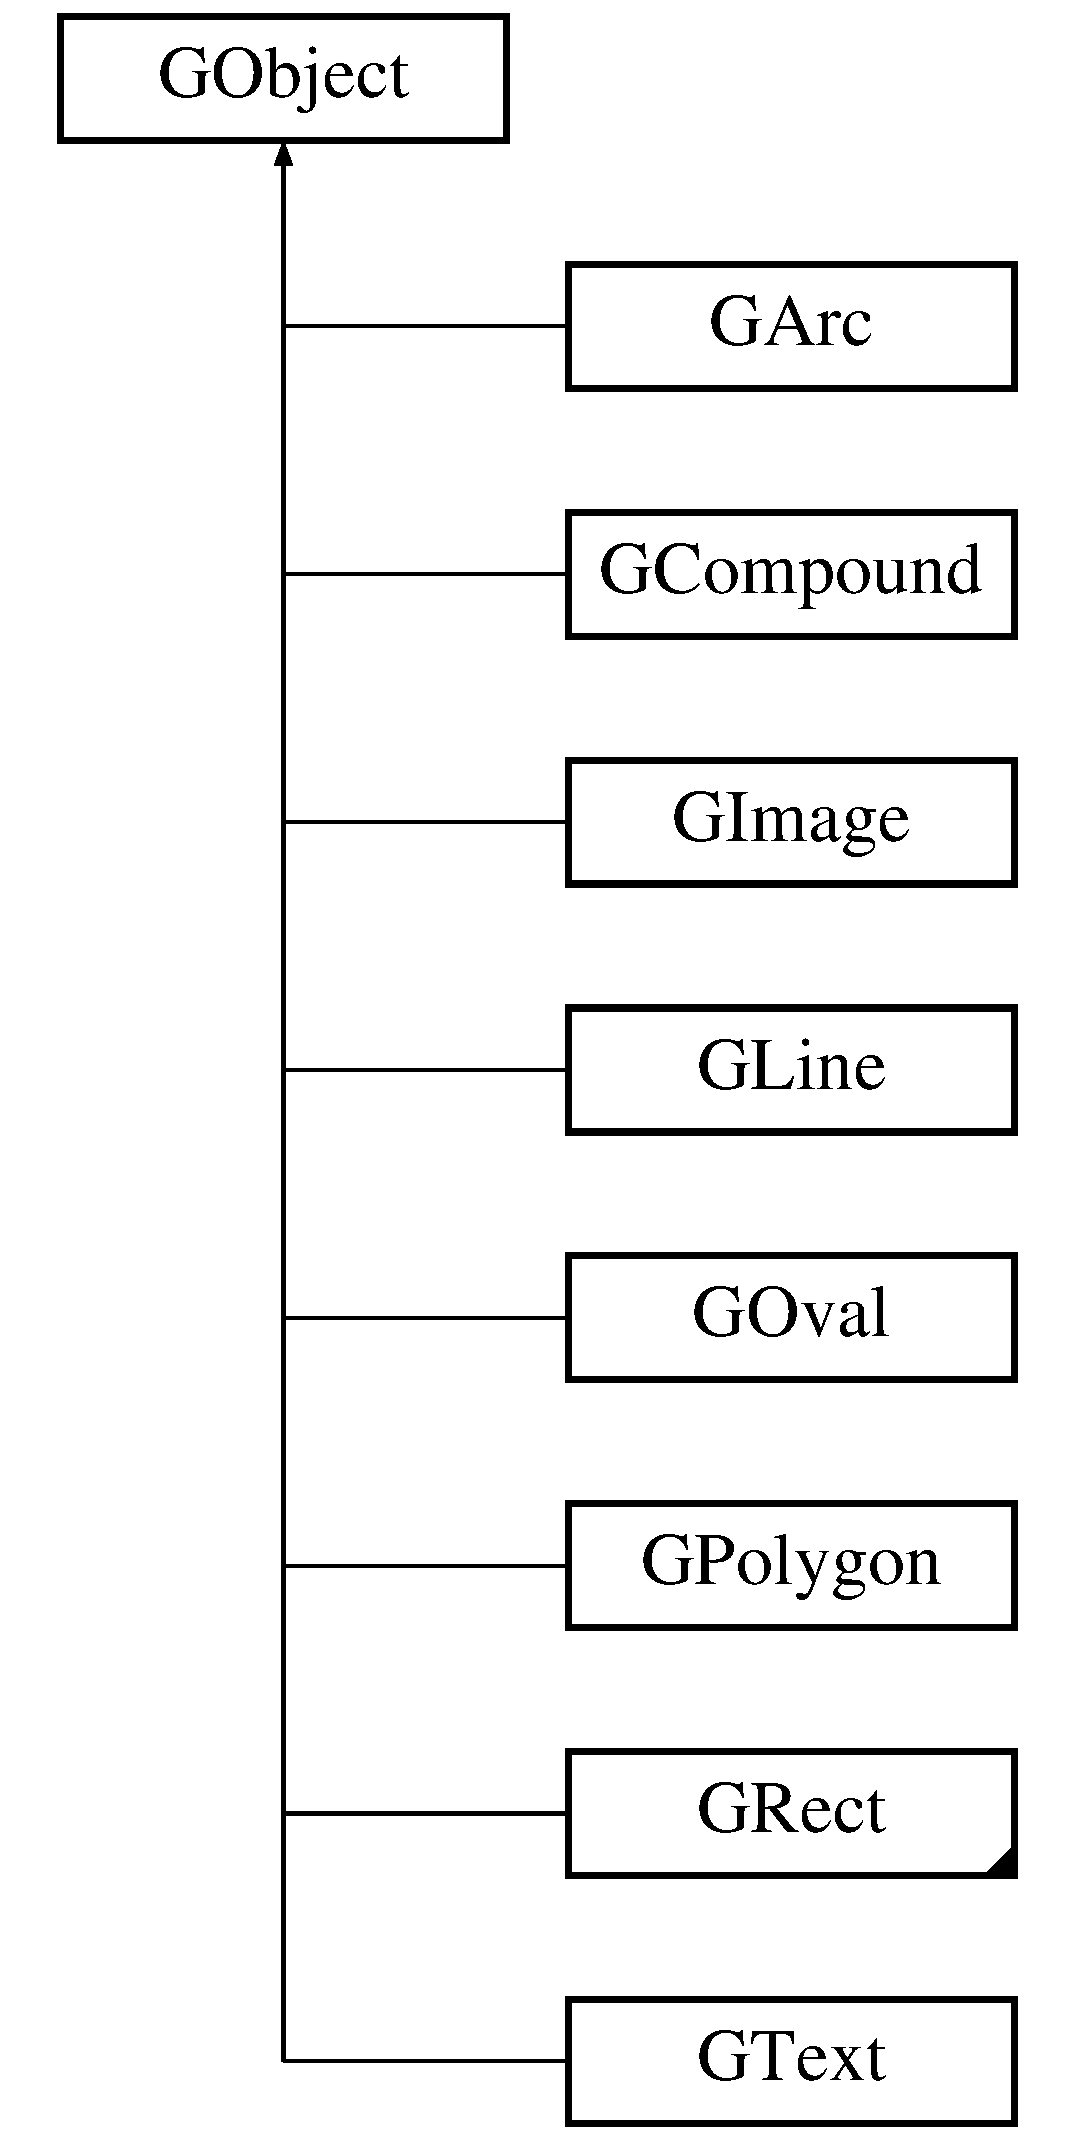
\includegraphics[height=9.000000cm]{classGObject}
\end{center}
\end{figure}
\subsection*{Public Types}
\begin{DoxyCompactItemize}
\item 
enum \mbox{\hyperlink{classGObject_a86e0f5648542856159bb40775c854aa7}{Line\+Style}} \{ \mbox{\hyperlink{classGObject_a86e0f5648542856159bb40775c854aa7acbc84bd5232621834ed31f44d457c1eb}{L\+I\+N\+E\+\_\+\+N\+O\+NE}}, 
\mbox{\hyperlink{classGObject_a86e0f5648542856159bb40775c854aa7a700c78bc2cd76acaab26651bf7b4941f}{L\+I\+N\+E\+\_\+\+S\+O\+L\+ID}}, 
\mbox{\hyperlink{classGObject_a86e0f5648542856159bb40775c854aa7a9ccba0845f785d81d07b333ae1aad84e}{L\+I\+N\+E\+\_\+\+D\+A\+SH}}, 
\mbox{\hyperlink{classGObject_a86e0f5648542856159bb40775c854aa7a8e811c096cb941997f0bfda168bb6df3}{L\+I\+N\+E\+\_\+\+D\+OT}}, 
\mbox{\hyperlink{classGObject_a86e0f5648542856159bb40775c854aa7ada15a2e3d737b2db7706d8300f91b89d}{L\+I\+N\+E\+\_\+\+D\+A\+S\+H\+\_\+\+D\+OT}}, 
\mbox{\hyperlink{classGObject_a86e0f5648542856159bb40775c854aa7aabf4053a73eafa7ba2b7e6d664c74c1d}{L\+I\+N\+E\+\_\+\+D\+A\+S\+H\+\_\+\+D\+O\+T\+\_\+\+D\+OT}}
 \}
\begin{DoxyCompactList}\small\item\em Styles that can be used for the outline around various shapes. \end{DoxyCompactList}\end{DoxyCompactItemize}
\subsection*{Public Member Functions}
\begin{DoxyCompactItemize}
\item 
virtual \mbox{\hyperlink{classGObject_ac955ba26942d1d44fc3d0cd6f76b1790}{$\sim$\+G\+Object}} ()
\begin{DoxyCompactList}\small\item\em Frees the storage for the object. \end{DoxyCompactList}\item 
virtual bool \mbox{\hyperlink{classGObject_abb6a5d7c03e6eaaae97264c4799ce7c3}{contains}} (double x, double y) const
\begin{DoxyCompactList}\small\item\em Returns {\ttfamily true} if the specified point is inside the object. \end{DoxyCompactList}\item 
virtual bool \mbox{\hyperlink{classGObject_a1dbc9dafaae51958112dbe1267a1f547}{contains}} (const \mbox{\hyperlink{classGPoint}{G\+Point}} \&pt) const
\begin{DoxyCompactList}\small\item\em Returns {\ttfamily true} if the specified point is inside the object. \end{DoxyCompactList}\item 
virtual \mbox{\hyperlink{classGPoint}{G\+Point}} \mbox{\hyperlink{classGObject_a0d41183bf6b08de66fe3907551aab0d7}{get\+Bottom\+Right\+Location}} () const
\begin{DoxyCompactList}\small\item\em Returns the x/y coordinates of the bottom/right corner of the object. \end{DoxyCompactList}\item 
virtual double \mbox{\hyperlink{classGObject_a4316a2406c18e1c6d061fe51fd355490}{get\+BottomY}} () const
\begin{DoxyCompactList}\small\item\em Returns the {\itshape y}-\/coordinate of the bottom of the object. \end{DoxyCompactList}\item 
virtual \mbox{\hyperlink{classGRectangle}{G\+Rectangle}} \mbox{\hyperlink{classGObject_a29e6ac35a0b48f491a4c88194cc5da3b}{get\+Bounds}} () const
\begin{DoxyCompactList}\small\item\em Returns the bounding box of this object, which is defined to be the smallest rectangle that covers everything drawn by the figure. \end{DoxyCompactList}\item 
virtual \mbox{\hyperlink{classGPoint}{G\+Point}} \mbox{\hyperlink{classGObject_a0909472e91448470bccdb62ecfb95d8b}{get\+Center\+Location}} () const
\begin{DoxyCompactList}\small\item\em Returns the x/y-\/coordinates of the center of the object. \end{DoxyCompactList}\item 
virtual double \mbox{\hyperlink{classGObject_a04df74355b545e0543112d5b8d924176}{get\+CenterX}} () const
\begin{DoxyCompactList}\small\item\em Returns the {\itshape x}-\/coordinate of the center of the object. \end{DoxyCompactList}\item 
virtual double \mbox{\hyperlink{classGObject_acb3287a3d507025a26f54b895713b947}{get\+CenterY}} () const
\begin{DoxyCompactList}\small\item\em Returns the {\itshape y}-\/coordinate of the center of the object. \end{DoxyCompactList}\item 
virtual std\+::string \mbox{\hyperlink{classGObject_aa061dfa488c31e18549d64363c1d0e34}{get\+Color}} () const
\begin{DoxyCompactList}\small\item\em Returns the color used to display this object. \end{DoxyCompactList}\item 
virtual std\+::string \mbox{\hyperlink{classGObject_a76f6964a11fde7c78e9751be184e1a3c}{get\+Fill\+Color}} () const
\begin{DoxyCompactList}\small\item\em Returns the color used to display the filled region of this object. \end{DoxyCompactList}\item 
virtual double \mbox{\hyperlink{classGObject_a1e7e353362434072875264cf95629f99}{get\+Height}} () const
\begin{DoxyCompactList}\small\item\em Returns the height of this object, which is the same as the height of its bounding box. \end{DoxyCompactList}\item 
virtual \mbox{\hyperlink{classGObject_a86e0f5648542856159bb40775c854aa7}{Line\+Style}} \mbox{\hyperlink{classGObject_aaf1f5ea8281e5e3486662878d26f0a13}{get\+Line\+Style}} () const
\begin{DoxyCompactList}\small\item\em Returns the object\textquotesingle{}s style such as solid or dashed. \end{DoxyCompactList}\item 
virtual double \mbox{\hyperlink{classGObject_a85ff266dc3eb63d9f2d8e5a4487fd3c0}{get\+Line\+Width}} () const
\begin{DoxyCompactList}\small\item\em Returns the width of the line used to draw this object. \end{DoxyCompactList}\item 
virtual \mbox{\hyperlink{classGPoint}{G\+Point}} \mbox{\hyperlink{classGObject_a4f83802015511edeb63b892830812c11}{get\+Location}} () const
\begin{DoxyCompactList}\small\item\em Returns the location of the top-\/left corner of object. \end{DoxyCompactList}\item 
virtual double \mbox{\hyperlink{classGObject_a1ae3fc278cc5b71b9f2d96a8a83cdf26}{get\+Opacity}} () const
\begin{DoxyCompactList}\small\item\em Returns how opaque (non-\/transparent) this object will appear from 0.\+0 (completely transparent) to 1.\+0 (completely opaque, default). \end{DoxyCompactList}\item 
virtual \mbox{\hyperlink{classGCompound}{G\+Compound}} $\ast$ \mbox{\hyperlink{classGObject_a3e53cef70541b1a14eade4ad0984d0b4}{get\+Parent}} () const
\begin{DoxyCompactList}\small\item\em Returns a pointer to the {\ttfamily \mbox{\hyperlink{classGCompound}{G\+Compound}}} that contains this object. \end{DoxyCompactList}\item 
virtual double \mbox{\hyperlink{classGObject_a798cc79daaa10145b28f60bcdfdb0ee9}{get\+RightX}} () const
\begin{DoxyCompactList}\small\item\em Returns the {\itshape x}-\/coordinate of the right side of the object. \end{DoxyCompactList}\item 
virtual \mbox{\hyperlink{classGDimension}{G\+Dimension}} \mbox{\hyperlink{classGObject_a7b4eec96a2bdc6420695d5796a78eea9}{get\+Size}} () const
\begin{DoxyCompactList}\small\item\em Returns the size of the object as a {\ttfamily \mbox{\hyperlink{classGDimension}{G\+Dimension}}}. \end{DoxyCompactList}\item 
virtual std\+::string \mbox{\hyperlink{classGObject_a799e073a127b428cc841086d42ea4fed}{get\+Type}} () const =0
\begin{DoxyCompactList}\small\item\em Returns the type of the object as a string, such as {\ttfamily \char`\"{}\+G\+Oval\char`\"{}} or {\ttfamily \char`\"{}\+G\+Rect\char`\"{}}. \end{DoxyCompactList}\item 
virtual double \mbox{\hyperlink{classGObject_a0ed2965abd4f5701d2cadf71239faf19}{get\+Width}} () const
\begin{DoxyCompactList}\small\item\em Returns the width of this object, which is equal to the width of the bounding box. \end{DoxyCompactList}\item 
virtual double \mbox{\hyperlink{classGObject_a344385751bee0720059403940d57a13e}{getX}} () const
\begin{DoxyCompactList}\small\item\em Returns the leftmost {\itshape x}-\/coordinate of the object. \end{DoxyCompactList}\item 
virtual double \mbox{\hyperlink{classGObject_aafa51c7f8f38a09febbb9ce7853f77b4}{getY}} () const
\begin{DoxyCompactList}\small\item\em Returns the topmost {\itshape y}-\/coordinate of the object. \end{DoxyCompactList}\item 
virtual bool \mbox{\hyperlink{classGObject_a11c404f106940c201b6f326e0355c150}{is\+Filled}} () const
\begin{DoxyCompactList}\small\item\em Returns {\ttfamily true} if the object is filled with color. \end{DoxyCompactList}\item 
virtual bool \mbox{\hyperlink{classGObject_a9d8a6cfb13917785c143e74d40e4e2be}{is\+Visible}} () const
\begin{DoxyCompactList}\small\item\em Returns {\ttfamily true} if this object is visible on screen. \end{DoxyCompactList}\item 
virtual void \mbox{\hyperlink{classGObject_a5973d8dda83afb36e2c56855515be392}{move}} (double dx, double dy)
\begin{DoxyCompactList}\small\item\em Moves the object on the screen using the displacements {\ttfamily dx} and {\ttfamily dy}. \end{DoxyCompactList}\item 
virtual void \mbox{\hyperlink{classGObject_ac827b978aa122f136a14c198687ad80f}{repaint}} ()
\begin{DoxyCompactList}\small\item\em Instructs the object to redraw itself on screen. \end{DoxyCompactList}\item 
virtual void \mbox{\hyperlink{classGObject_a6022a1fd1e5dcd2fd5585e5a36aa3f37}{reset\+Transform}} ()
\begin{DoxyCompactList}\small\item\em Undoes any previous scale/rotate transformations on this object. \end{DoxyCompactList}\item 
virtual void \mbox{\hyperlink{classGObject_ae1ffaa12185dfd5ba464f7d87c329e26}{rotate}} (double theta)
\begin{DoxyCompactList}\small\item\em Transforms the object by rotating it {\ttfamily theta} degrees counterclockwise around its origin. \end{DoxyCompactList}\item 
virtual void \mbox{\hyperlink{classGObject_ad2e1900f730475c2d044817db03b38d6}{scale}} (double sf)
\begin{DoxyCompactList}\small\item\em Scales the object by the specified scale factor. \end{DoxyCompactList}\item 
virtual void \mbox{\hyperlink{classGObject_a63641f69d610d0b951357d35a0c3b1e3}{scale}} (double sx, double sy)
\begin{DoxyCompactList}\small\item\em Scales the object by the specified scale factors. \end{DoxyCompactList}\item 
void \mbox{\hyperlink{classGObject_ab6747f40313c531c2db32edb5b63b9b7}{send\+Backward}} ()
\begin{DoxyCompactList}\small\item\em Moves this object one step toward the back in the {\itshape z} dimension. \end{DoxyCompactList}\item 
void \mbox{\hyperlink{classGObject_a710b3e449c9facba7847c91ab170d281}{send\+Forward}} ()
\begin{DoxyCompactList}\small\item\em Moves this object one step toward the front in the {\itshape z} dimension. \end{DoxyCompactList}\item 
void \mbox{\hyperlink{classGObject_a0f7f1efbb7fd46dde2867c4ad0330896}{send\+To\+Back}} ()
\begin{DoxyCompactList}\small\item\em Moves this object to the back of the display in the {\itshape z} dimension. \end{DoxyCompactList}\item 
void \mbox{\hyperlink{classGObject_aee33d68488e46827ef55fac07f40a9b2}{send\+To\+Front}} ()
\begin{DoxyCompactList}\small\item\em Moves this object to the front of the display in the {\itshape z} dimension. \end{DoxyCompactList}\item 
virtual void \mbox{\hyperlink{classGObject_a71ff7b16b8f1bdc4a1ce9f30cf8b87d8}{set\+Bottom\+Right\+Location}} (double x, double y)
\begin{DoxyCompactList}\small\item\em Sets the location of the bottom/right of this object. \end{DoxyCompactList}\item 
virtual void \mbox{\hyperlink{classGObject_ac6f7320321182f1d18c1c0fa97d5e941}{set\+Bottom\+Right\+Location}} (const \mbox{\hyperlink{classGPoint}{G\+Point}} \&pt)
\begin{DoxyCompactList}\small\item\em Sets the location of the bottom/right of this object. \end{DoxyCompactList}\item 
virtual void \mbox{\hyperlink{classGObject_a4b20e93c2a2597484f74ee5caa71f41f}{set\+BottomY}} (double y)
\begin{DoxyCompactList}\small\item\em Sets the location of the bottom y-\/coordinate of this object. \end{DoxyCompactList}\item 
virtual void \mbox{\hyperlink{classGObject_a2aae8197624b72265ab83b4f1bc73f2f}{set\+Bounds}} (double x, double y, double width, double height)
\begin{DoxyCompactList}\small\item\em Changes the bounds of this object to the specified values. \end{DoxyCompactList}\item 
virtual void \mbox{\hyperlink{classGObject_acada386653f008cacc7cce86426bef7c}{set\+Bounds}} (const \mbox{\hyperlink{classGRectangle}{G\+Rectangle}} \&size)
\begin{DoxyCompactList}\small\item\em Changes the bounds of this object to the specified rectangle. \end{DoxyCompactList}\item 
virtual void \mbox{\hyperlink{classGObject_a290b47dd8de1be44089f95cb2c47c1de}{set\+Center\+Location}} (double x, double y)
\begin{DoxyCompactList}\small\item\em Sets the location of the center of this object. \end{DoxyCompactList}\item 
virtual void \mbox{\hyperlink{classGObject_a1bedf1b233ecba3f753ec58908a683a6}{set\+Center\+Location}} (const \mbox{\hyperlink{classGPoint}{G\+Point}} \&pt)
\begin{DoxyCompactList}\small\item\em Sets the location of the center of this object. \end{DoxyCompactList}\item 
virtual void \mbox{\hyperlink{classGObject_a2f4936281e056eead00a9186b9ba8af6}{set\+CenterX}} (double x)
\begin{DoxyCompactList}\small\item\em Sets the x-\/coordinate of the center of this object. \end{DoxyCompactList}\item 
virtual void \mbox{\hyperlink{classGObject_aad2a22b4fde88c33306b92aebf641d57}{set\+CenterY}} (double y)
\begin{DoxyCompactList}\small\item\em Sets the y-\/coordinate of the center of this object. \end{DoxyCompactList}\item 
virtual void \mbox{\hyperlink{classGObject_ad57ef49bc31db94e92648aa3737923d6}{set\+Color}} (int r, int g, int b)
\begin{DoxyCompactList}\small\item\em Sets the color used to display this object. \end{DoxyCompactList}\item 
virtual void \mbox{\hyperlink{classGObject_ab1f5cc0f5cc6bbbd716a526c61f1081d}{set\+Color}} (int rgb)
\begin{DoxyCompactList}\small\item\em Sets the color used to display this object. \end{DoxyCompactList}\item 
virtual void \mbox{\hyperlink{classGObject_a61374df6c11b52cfbb0815decdbaebc6}{set\+Color}} (const std\+::string \&color)
\begin{DoxyCompactList}\small\item\em Sets the color used to display this object. \end{DoxyCompactList}\item 
virtual void \mbox{\hyperlink{classGObject_ad767a33971159e9493e221cca4c00ae9}{set\+Fill\+Color}} (int r, int g, int b)
\begin{DoxyCompactList}\small\item\em Sets the color used to display the filled region of this object, if any. \end{DoxyCompactList}\item 
virtual void \mbox{\hyperlink{classGObject_aa59d9775a67fa7df2b24a95cd34840a3}{set\+Fill\+Color}} (int rgb)
\begin{DoxyCompactList}\small\item\em Sets the color used to display the filled region of this object, if any. \end{DoxyCompactList}\item 
virtual void \mbox{\hyperlink{classGObject_adbc18b1a930aadd97d7437f9f7265b96}{set\+Fill\+Color}} (const std\+::string \&color)
\begin{DoxyCompactList}\small\item\em Sets the color used to display the filled region of this object, if any. \end{DoxyCompactList}\item 
virtual void \mbox{\hyperlink{classGObject_a9b82b53362282c6bb7d6947068d2e55b}{set\+Filled}} (bool flag)
\begin{DoxyCompactList}\small\item\em Sets the fill status for the object, where {\ttfamily false} is outlined and {\ttfamily true} is filled. \end{DoxyCompactList}\item 
virtual void \mbox{\hyperlink{classGObject_a2592348886ffea646c6534bf88f7c49d}{set\+Font}} (const Q\+Font \&font)
\begin{DoxyCompactList}\small\item\em Changes the font used to display the object as specified by the given Qt font. \end{DoxyCompactList}\item 
virtual void \mbox{\hyperlink{classGObject_a8e096e8818d838aceae1d46d58fb3a7b}{set\+Font}} (const std\+::string \&font)
\begin{DoxyCompactList}\small\item\em Changes the font used to display the object as specified by the string {\ttfamily font}, which has the following format\+: \end{DoxyCompactList}\item 
virtual void \mbox{\hyperlink{classGObject_ad18e8fab1e02a4e9b75c6730212558eb}{set\+Foreground}} (int r, int g, int b)
\begin{DoxyCompactList}\small\item\em Sets the color used to display this object. \end{DoxyCompactList}\item 
virtual void \mbox{\hyperlink{classGObject_a9eb856b5ff83a19df3831a31f15f4563}{set\+Foreground}} (int rgb)
\begin{DoxyCompactList}\small\item\em Sets the color used to display this object. \end{DoxyCompactList}\item 
virtual void \mbox{\hyperlink{classGObject_af59209aeadea6dfc6d97a2d8531f50e1}{set\+Foreground}} (const std\+::string \&color)
\begin{DoxyCompactList}\small\item\em Sets the color used to display this object. \end{DoxyCompactList}\item 
virtual void \mbox{\hyperlink{classGObject_a9e280bfc4544dfaf8e4376c4e1a74357}{set\+Height}} (double height)
\begin{DoxyCompactList}\small\item\em Changes the height of this object to the specified height without changing its width. \end{DoxyCompactList}\item 
virtual void \mbox{\hyperlink{classGObject_add11575087eb94f1a71faa3f826c6341}{set\+Line\+Style}} (\mbox{\hyperlink{classGObject_a86e0f5648542856159bb40775c854aa7}{Line\+Style}} line\+Style)
\begin{DoxyCompactList}\small\item\em Sets the object\textquotesingle{}s style such as solid (\mbox{\hyperlink{classGObject_a86e0f5648542856159bb40775c854aa7a700c78bc2cd76acaab26651bf7b4941f}{G\+Object\+::\+L\+I\+N\+E\+\_\+\+S\+O\+L\+ID}}) or dashed (\mbox{\hyperlink{classGObject_a86e0f5648542856159bb40775c854aa7a9ccba0845f785d81d07b333ae1aad84e}{G\+Object\+::\+L\+I\+N\+E\+\_\+\+D\+A\+SH}}). \end{DoxyCompactList}\item 
virtual void \mbox{\hyperlink{classGObject_afd6a47c6ea6a1f85ca05a65ba3ff3477}{set\+Line\+Width}} (double line\+Width)
\begin{DoxyCompactList}\small\item\em Sets the width of the line used to draw this object. \end{DoxyCompactList}\item 
virtual void \mbox{\hyperlink{classGObject_a04594e8ba9b98513a64f1da00dcae18c}{set\+Location}} (double x, double y)
\begin{DoxyCompactList}\small\item\em Sets the location of the top-\/left corner of this object to the specified coordinates. \end{DoxyCompactList}\item 
virtual void \mbox{\hyperlink{classGObject_aa8480c0b7166cdf8f784cece06ab353f}{set\+Location}} (const \mbox{\hyperlink{classGPoint}{G\+Point}} \&pt)
\begin{DoxyCompactList}\small\item\em Sets the location of the top-\/left corner of this object to the specified point. \end{DoxyCompactList}\item 
virtual void \mbox{\hyperlink{classGObject_a04af1866cc1bae4a1226695794a50539}{set\+Opacity}} (double opacity)
\begin{DoxyCompactList}\small\item\em Sets how opaque (non-\/transparent) this object will appear from 0.\+0 (completely transparent) to 1.\+0 (completely opaque, default). \end{DoxyCompactList}\item 
virtual void \mbox{\hyperlink{classGObject_a3c90b758cdc2c911c9ef76c4360eb912}{set\+RightX}} (double x)
\begin{DoxyCompactList}\small\item\em Sets the location of the rightmost x-\/coordinate of this object. \end{DoxyCompactList}\item 
virtual void \mbox{\hyperlink{classGObject_aca25d49481f9bf5fc8f7df4c086c4ce7}{set\+Size}} (double width, double height)
\begin{DoxyCompactList}\small\item\em Changes the size of this object to the specified width and height. \end{DoxyCompactList}\item 
virtual void \mbox{\hyperlink{classGObject_ae2b628228f192c2702c4ce941b2af68f}{set\+Size}} (const \mbox{\hyperlink{classGDimension}{G\+Dimension}} \&size)
\begin{DoxyCompactList}\small\item\em Changes the size of this object to the specified width and height. \end{DoxyCompactList}\item 
virtual void \mbox{\hyperlink{classGObject_a88203f28224315d9f4471212f4af8ed3}{set\+Visible}} (bool flag)
\begin{DoxyCompactList}\small\item\em Sets whether this object is visible. \end{DoxyCompactList}\item 
virtual void \mbox{\hyperlink{classGObject_aa3f3fba4cb131baa8696ba01e3bceca1}{set\+Width}} (double width)
\begin{DoxyCompactList}\small\item\em Changes the width of this object to the specified width without changing its height. \end{DoxyCompactList}\item 
virtual void \mbox{\hyperlink{classGObject_a9c18fcc579333bf9653d13ad2b372e39}{setX}} (double x)
\begin{DoxyCompactList}\small\item\em Sets the x location of the left side of this object. \end{DoxyCompactList}\item 
virtual void \mbox{\hyperlink{classGObject_a7d57e2a5c35d27feb58fd498a3cf82b9}{setY}} (double y)
\begin{DoxyCompactList}\small\item\em Sets the y location of the top of this object. \end{DoxyCompactList}\item 
virtual std\+::string \mbox{\hyperlink{classGObject_a1fe5121d6528fdea3f243321b3fa3a49}{to\+String}} () const
\begin{DoxyCompactList}\small\item\em Returns a printable representation of the object. \end{DoxyCompactList}\end{DoxyCompactItemize}
\subsection*{Static Public Member Functions}
\begin{DoxyCompactItemize}
\item 
static bool \mbox{\hyperlink{classGObject_a93be0e1fe1b1bf1a1da732470c94f42b}{is\+Anti\+Aliasing}} ()
\begin{DoxyCompactList}\small\item\em Returns whether we should globally anti-\/alias graphical objects. \end{DoxyCompactList}\item 
static void \mbox{\hyperlink{classGObject_a1e43371668ae850193cebedb44e1bbe3}{set\+Anti\+Aliasing}} (bool value)
\begin{DoxyCompactList}\small\item\em Globally turns on/off the anti-\/aliasing feature that smooths out the edges of onscreen shapes. \end{DoxyCompactList}\end{DoxyCompactItemize}
\subsection*{Protected Member Functions}
\begin{DoxyCompactItemize}
\item 
virtual std\+::string \mbox{\hyperlink{classGObject_a4fcdf8de5c6de92242a975d83d8f23ea}{to\+String\+Extra}} () const
\begin{DoxyCompactList}\small\item\em Returns a string containing any extra unique information about this type of graphical object. \end{DoxyCompactList}\end{DoxyCompactItemize}
\subsection*{Protected Attributes}
\begin{DoxyCompactItemize}
\item 
Q\+Brush \mbox{\hyperlink{classGObject_aab24462ec896b596d99911767b0912d0}{\+\_\+brush}}
\item 
std\+::string \mbox{\hyperlink{classGObject_a1134e770ae4315ea8bc1201e2f21da8b}{\+\_\+color}}
\item 
int \mbox{\hyperlink{classGObject_a003fdd343d9b7505c53a8b7a134200ed}{\+\_\+color\+Int}}
\item 
std\+::string \mbox{\hyperlink{classGObject_a179f8d6cee65cd8a54692e32b224392a}{\+\_\+fill\+Color}}
\item 
int \mbox{\hyperlink{classGObject_a751def333a67d651e5b99cc331ecb496}{\+\_\+fill\+Color\+Int}}
\item 
bool \mbox{\hyperlink{classGObject_ad4a55cbcd61b58a4d49666490bb2f103}{\+\_\+fill\+Flag}}
\item 
std\+::string \mbox{\hyperlink{classGObject_aea76ea1a8b5dd7b0a78653277e63b536}{\+\_\+font}}
\item 
double \mbox{\hyperlink{classGObject_ad05df29e7f27fc504abd743e3d8b4e73}{\+\_\+height}}
\item 
\mbox{\hyperlink{classGObject_a86e0f5648542856159bb40775c854aa7}{Line\+Style}} \mbox{\hyperlink{classGObject_a89bafecaafb7c72d55c7efc10b7d0523}{\+\_\+line\+Style}}
\item 
double \mbox{\hyperlink{classGObject_a16e9033665937f13de2e163dc2184aff}{\+\_\+line\+Width}}
\item 
double \mbox{\hyperlink{classGObject_a20eff8eb7af27182edc9bfc54768b6f3}{\+\_\+opacity}}
\item 
\mbox{\hyperlink{classGCompound}{G\+Compound}} $\ast$ \mbox{\hyperlink{classGObject_ac9452c1eaff70eebddbb318196aa3835}{\+\_\+parent}}
\item 
Q\+Pen \mbox{\hyperlink{classGObject_afb69d172743f868299847174eb1b6bc8}{\+\_\+pen}}
\item 
Q\+Transform \mbox{\hyperlink{classGObject_a475b8860a5f1adb4a1fdc58d1f5c1e32}{\+\_\+transform}}
\item 
bool \mbox{\hyperlink{classGObject_ae4725802fc8d8aaa0ab4bd4781f7e07c}{\+\_\+transformed}}
\item 
bool \mbox{\hyperlink{classGObject_a9312c72508471b7c7a87b540263e1af4}{\+\_\+visible}}
\item 
double \mbox{\hyperlink{classGObject_ab55d85a3371770e6725b1062cf160cd8}{\+\_\+width}}
\item 
double \mbox{\hyperlink{classGObject_a6675b83b27137b8d3aa2ad8133078ea6}{\+\_\+x}}
\item 
double \mbox{\hyperlink{classGObject_a2f0f6aeafddc8a39c578bfa7e22b5f1e}{\+\_\+y}}
\end{DoxyCompactItemize}


\subsection{Detailed Description}
This class is the common superclass of all graphical objects that can be displayed on a graphical window. 

The class {\ttfamily \mbox{\hyperlink{classGObject}{G\+Object}}} itself is an {\bfseries {\itshape abstract class}}, which means that you are not allowed to construct a {\ttfamily \mbox{\hyperlink{classGObject}{G\+Object}}} directly but must instead construct one of the concrete subclasses. 

Most methods used for graphics take a pointer to a 
\begin{DoxyCode}
\mbox{\hyperlink{classGObject}{GObject}}
\end{DoxyCode}
 rather than the 
\begin{DoxyCode}
\mbox{\hyperlink{classGObject}{GObject}}
\end{DoxyCode}
 itself. Applications that use 
\begin{DoxyCode}
\mbox{\hyperlink{classGObject}{GObject}}
\end{DoxyCode}
 pointers therefore use the arrow operator (
\begin{DoxyCode}
->
\end{DoxyCode}
) to apply methods to the object pointer. For examples illustrating the use of the 
\begin{DoxyCode}
\mbox{\hyperlink{classGObject}{GObject}}
\end{DoxyCode}
 class, see the descriptions of the individual subclasses. 

\subsection{Member Enumeration Documentation}
\mbox{\Hypertarget{classGObject_a86e0f5648542856159bb40775c854aa7}\label{classGObject_a86e0f5648542856159bb40775c854aa7}} 
\index{G\+Object@{G\+Object}!Line\+Style@{Line\+Style}}
\index{Line\+Style@{Line\+Style}!G\+Object@{G\+Object}}
\subsubsection{\texorpdfstring{Line\+Style}{LineStyle}}
{\footnotesize\ttfamily enum \mbox{\hyperlink{classGObject_a86e0f5648542856159bb40775c854aa7}{Line\+Style}}}



Styles that can be used for the outline around various shapes. 

Call set\+Line\+Style on a \mbox{\hyperlink{classGObject}{G\+Object}} and pass one of these values. \begin{DoxyEnumFields}{Enumerator}
\raisebox{\heightof{T}}[0pt][0pt]{\index{L\+I\+N\+E\+\_\+\+N\+O\+NE@{L\+I\+N\+E\+\_\+\+N\+O\+NE}!G\+Object@{G\+Object}}\index{G\+Object@{G\+Object}!L\+I\+N\+E\+\_\+\+N\+O\+NE@{L\+I\+N\+E\+\_\+\+N\+O\+NE}}}\mbox{\Hypertarget{classGObject_a86e0f5648542856159bb40775c854aa7acbc84bd5232621834ed31f44d457c1eb}\label{classGObject_a86e0f5648542856159bb40775c854aa7acbc84bd5232621834ed31f44d457c1eb}} 
L\+I\+N\+E\+\_\+\+N\+O\+NE&\\
\hline

\raisebox{\heightof{T}}[0pt][0pt]{\index{L\+I\+N\+E\+\_\+\+S\+O\+L\+ID@{L\+I\+N\+E\+\_\+\+S\+O\+L\+ID}!G\+Object@{G\+Object}}\index{G\+Object@{G\+Object}!L\+I\+N\+E\+\_\+\+S\+O\+L\+ID@{L\+I\+N\+E\+\_\+\+S\+O\+L\+ID}}}\mbox{\Hypertarget{classGObject_a86e0f5648542856159bb40775c854aa7a700c78bc2cd76acaab26651bf7b4941f}\label{classGObject_a86e0f5648542856159bb40775c854aa7a700c78bc2cd76acaab26651bf7b4941f}} 
L\+I\+N\+E\+\_\+\+S\+O\+L\+ID&\\
\hline

\raisebox{\heightof{T}}[0pt][0pt]{\index{L\+I\+N\+E\+\_\+\+D\+A\+SH@{L\+I\+N\+E\+\_\+\+D\+A\+SH}!G\+Object@{G\+Object}}\index{G\+Object@{G\+Object}!L\+I\+N\+E\+\_\+\+D\+A\+SH@{L\+I\+N\+E\+\_\+\+D\+A\+SH}}}\mbox{\Hypertarget{classGObject_a86e0f5648542856159bb40775c854aa7a9ccba0845f785d81d07b333ae1aad84e}\label{classGObject_a86e0f5648542856159bb40775c854aa7a9ccba0845f785d81d07b333ae1aad84e}} 
L\+I\+N\+E\+\_\+\+D\+A\+SH&\\
\hline

\raisebox{\heightof{T}}[0pt][0pt]{\index{L\+I\+N\+E\+\_\+\+D\+OT@{L\+I\+N\+E\+\_\+\+D\+OT}!G\+Object@{G\+Object}}\index{G\+Object@{G\+Object}!L\+I\+N\+E\+\_\+\+D\+OT@{L\+I\+N\+E\+\_\+\+D\+OT}}}\mbox{\Hypertarget{classGObject_a86e0f5648542856159bb40775c854aa7a8e811c096cb941997f0bfda168bb6df3}\label{classGObject_a86e0f5648542856159bb40775c854aa7a8e811c096cb941997f0bfda168bb6df3}} 
L\+I\+N\+E\+\_\+\+D\+OT&\\
\hline

\raisebox{\heightof{T}}[0pt][0pt]{\index{L\+I\+N\+E\+\_\+\+D\+A\+S\+H\+\_\+\+D\+OT@{L\+I\+N\+E\+\_\+\+D\+A\+S\+H\+\_\+\+D\+OT}!G\+Object@{G\+Object}}\index{G\+Object@{G\+Object}!L\+I\+N\+E\+\_\+\+D\+A\+S\+H\+\_\+\+D\+OT@{L\+I\+N\+E\+\_\+\+D\+A\+S\+H\+\_\+\+D\+OT}}}\mbox{\Hypertarget{classGObject_a86e0f5648542856159bb40775c854aa7ada15a2e3d737b2db7706d8300f91b89d}\label{classGObject_a86e0f5648542856159bb40775c854aa7ada15a2e3d737b2db7706d8300f91b89d}} 
L\+I\+N\+E\+\_\+\+D\+A\+S\+H\+\_\+\+D\+OT&\\
\hline

\raisebox{\heightof{T}}[0pt][0pt]{\index{L\+I\+N\+E\+\_\+\+D\+A\+S\+H\+\_\+\+D\+O\+T\+\_\+\+D\+OT@{L\+I\+N\+E\+\_\+\+D\+A\+S\+H\+\_\+\+D\+O\+T\+\_\+\+D\+OT}!G\+Object@{G\+Object}}\index{G\+Object@{G\+Object}!L\+I\+N\+E\+\_\+\+D\+A\+S\+H\+\_\+\+D\+O\+T\+\_\+\+D\+OT@{L\+I\+N\+E\+\_\+\+D\+A\+S\+H\+\_\+\+D\+O\+T\+\_\+\+D\+OT}}}\mbox{\Hypertarget{classGObject_a86e0f5648542856159bb40775c854aa7aabf4053a73eafa7ba2b7e6d664c74c1d}\label{classGObject_a86e0f5648542856159bb40775c854aa7aabf4053a73eafa7ba2b7e6d664c74c1d}} 
L\+I\+N\+E\+\_\+\+D\+A\+S\+H\+\_\+\+D\+O\+T\+\_\+\+D\+OT&\\
\hline

\end{DoxyEnumFields}


\subsection{Constructor \& Destructor Documentation}
\mbox{\Hypertarget{classGObject_ac955ba26942d1d44fc3d0cd6f76b1790}\label{classGObject_ac955ba26942d1d44fc3d0cd6f76b1790}} 
\index{G\+Object@{G\+Object}!````~G\+Object@{$\sim$\+G\+Object}}
\index{````~G\+Object@{$\sim$\+G\+Object}!G\+Object@{G\+Object}}
\subsubsection{\texorpdfstring{$\sim$\+G\+Object()}{~GObject()}}
{\footnotesize\ttfamily $\sim$\mbox{\hyperlink{classGObject}{G\+Object}} (\begin{DoxyParamCaption}{ }\end{DoxyParamCaption})\hspace{0.3cm}{\ttfamily [virtual]}}



Frees the storage for the object. 



\subsection{Member Function Documentation}
\mbox{\Hypertarget{classGObject_abb6a5d7c03e6eaaae97264c4799ce7c3}\label{classGObject_abb6a5d7c03e6eaaae97264c4799ce7c3}} 
\index{G\+Object@{G\+Object}!contains@{contains}}
\index{contains@{contains}!G\+Object@{G\+Object}}
\subsubsection{\texorpdfstring{contains()}{contains()}\hspace{0.1cm}{\footnotesize\ttfamily [1/2]}}
{\footnotesize\ttfamily bool contains (\begin{DoxyParamCaption}\item[{double}]{x,  }\item[{double}]{y }\end{DoxyParamCaption}) const\hspace{0.3cm}{\ttfamily [virtual]}}



Returns {\ttfamily true} if the specified point is inside the object. 



Reimplemented in \mbox{\hyperlink{classGRoundRect_abb6a5d7c03e6eaaae97264c4799ce7c3}{G\+Round\+Rect}}, \mbox{\hyperlink{classGPolygon_abb6a5d7c03e6eaaae97264c4799ce7c3}{G\+Polygon}}, \mbox{\hyperlink{classGOval_aa095a031ab22c150d2d75fdda1c3c8f5}{G\+Oval}}, \mbox{\hyperlink{classGLine_aa095a031ab22c150d2d75fdda1c3c8f5}{G\+Line}}, \mbox{\hyperlink{classGCompound_aa095a031ab22c150d2d75fdda1c3c8f5}{G\+Compound}}, and \mbox{\hyperlink{classGArc_aa095a031ab22c150d2d75fdda1c3c8f5}{G\+Arc}}.

\mbox{\Hypertarget{classGObject_a1dbc9dafaae51958112dbe1267a1f547}\label{classGObject_a1dbc9dafaae51958112dbe1267a1f547}} 
\index{G\+Object@{G\+Object}!contains@{contains}}
\index{contains@{contains}!G\+Object@{G\+Object}}
\subsubsection{\texorpdfstring{contains()}{contains()}\hspace{0.1cm}{\footnotesize\ttfamily [2/2]}}
{\footnotesize\ttfamily bool contains (\begin{DoxyParamCaption}\item[{const \mbox{\hyperlink{classGPoint}{G\+Point}} \&}]{pt }\end{DoxyParamCaption}) const\hspace{0.3cm}{\ttfamily [virtual]}}



Returns {\ttfamily true} if the specified point is inside the object. 

\mbox{\Hypertarget{classGObject_a0d41183bf6b08de66fe3907551aab0d7}\label{classGObject_a0d41183bf6b08de66fe3907551aab0d7}} 
\index{G\+Object@{G\+Object}!get\+Bottom\+Right\+Location@{get\+Bottom\+Right\+Location}}
\index{get\+Bottom\+Right\+Location@{get\+Bottom\+Right\+Location}!G\+Object@{G\+Object}}
\subsubsection{\texorpdfstring{get\+Bottom\+Right\+Location()}{getBottomRightLocation()}}
{\footnotesize\ttfamily \mbox{\hyperlink{classGPoint}{G\+Point}} get\+Bottom\+Right\+Location (\begin{DoxyParamCaption}{ }\end{DoxyParamCaption}) const\hspace{0.3cm}{\ttfamily [virtual]}}



Returns the x/y coordinates of the bottom/right corner of the object. 

\mbox{\Hypertarget{classGObject_a4316a2406c18e1c6d061fe51fd355490}\label{classGObject_a4316a2406c18e1c6d061fe51fd355490}} 
\index{G\+Object@{G\+Object}!get\+BottomY@{get\+BottomY}}
\index{get\+BottomY@{get\+BottomY}!G\+Object@{G\+Object}}
\subsubsection{\texorpdfstring{get\+Bottom\+Y()}{getBottomY()}}
{\footnotesize\ttfamily double get\+BottomY (\begin{DoxyParamCaption}{ }\end{DoxyParamCaption}) const\hspace{0.3cm}{\ttfamily [virtual]}}



Returns the {\itshape y}-\/coordinate of the bottom of the object. 

Equivalent to the top y-\/coordinate plus the object\textquotesingle{}s height. \mbox{\Hypertarget{classGObject_a29e6ac35a0b48f491a4c88194cc5da3b}\label{classGObject_a29e6ac35a0b48f491a4c88194cc5da3b}} 
\index{G\+Object@{G\+Object}!get\+Bounds@{get\+Bounds}}
\index{get\+Bounds@{get\+Bounds}!G\+Object@{G\+Object}}
\subsubsection{\texorpdfstring{get\+Bounds()}{getBounds()}}
{\footnotesize\ttfamily \mbox{\hyperlink{classGRectangle}{G\+Rectangle}} get\+Bounds (\begin{DoxyParamCaption}{ }\end{DoxyParamCaption}) const\hspace{0.3cm}{\ttfamily [virtual]}}



Returns the bounding box of this object, which is defined to be the smallest rectangle that covers everything drawn by the figure. 

The coordinates of this rectangle do not necessarily match the location returned by {\ttfamily get\+Location}. Given a {\ttfamily \mbox{\hyperlink{classGText}{G\+Text}}} object, for example, {\ttfamily get\+Location} returns the coordinates of the point on the baseline at which the string begins; the {\ttfamily get\+Bounds} method, by contrast, returns a rectangle that covers the entire window area occupied by the string. 

Reimplemented in \mbox{\hyperlink{classGText_a2f46ec8a3b533c690b3b3e56d4f34afe}{G\+Text}}, \mbox{\hyperlink{classGPolygon_a29e6ac35a0b48f491a4c88194cc5da3b}{G\+Polygon}}, \mbox{\hyperlink{classGLine_a2f46ec8a3b533c690b3b3e56d4f34afe}{G\+Line}}, \mbox{\hyperlink{classGCompound_a2f46ec8a3b533c690b3b3e56d4f34afe}{G\+Compound}}, and \mbox{\hyperlink{classGArc_a2f46ec8a3b533c690b3b3e56d4f34afe}{G\+Arc}}.

\mbox{\Hypertarget{classGObject_a0909472e91448470bccdb62ecfb95d8b}\label{classGObject_a0909472e91448470bccdb62ecfb95d8b}} 
\index{G\+Object@{G\+Object}!get\+Center\+Location@{get\+Center\+Location}}
\index{get\+Center\+Location@{get\+Center\+Location}!G\+Object@{G\+Object}}
\subsubsection{\texorpdfstring{get\+Center\+Location()}{getCenterLocation()}}
{\footnotesize\ttfamily \mbox{\hyperlink{classGPoint}{G\+Point}} get\+Center\+Location (\begin{DoxyParamCaption}{ }\end{DoxyParamCaption}) const\hspace{0.3cm}{\ttfamily [virtual]}}



Returns the x/y-\/coordinates of the center of the object. 

Equivalent to the top/left plus half the object\textquotesingle{}s size. \mbox{\Hypertarget{classGObject_a04df74355b545e0543112d5b8d924176}\label{classGObject_a04df74355b545e0543112d5b8d924176}} 
\index{G\+Object@{G\+Object}!get\+CenterX@{get\+CenterX}}
\index{get\+CenterX@{get\+CenterX}!G\+Object@{G\+Object}}
\subsubsection{\texorpdfstring{get\+Center\+X()}{getCenterX()}}
{\footnotesize\ttfamily double get\+CenterX (\begin{DoxyParamCaption}{ }\end{DoxyParamCaption}) const\hspace{0.3cm}{\ttfamily [virtual]}}



Returns the {\itshape x}-\/coordinate of the center of the object. 

Equivalent to the top/left plus half the object\textquotesingle{}s width. \mbox{\Hypertarget{classGObject_acb3287a3d507025a26f54b895713b947}\label{classGObject_acb3287a3d507025a26f54b895713b947}} 
\index{G\+Object@{G\+Object}!get\+CenterY@{get\+CenterY}}
\index{get\+CenterY@{get\+CenterY}!G\+Object@{G\+Object}}
\subsubsection{\texorpdfstring{get\+Center\+Y()}{getCenterY()}}
{\footnotesize\ttfamily double get\+CenterY (\begin{DoxyParamCaption}{ }\end{DoxyParamCaption}) const\hspace{0.3cm}{\ttfamily [virtual]}}



Returns the {\itshape y}-\/coordinate of the center of the object. 

Equivalent to the top/left plus half the object\textquotesingle{}s height. \mbox{\Hypertarget{classGObject_aa061dfa488c31e18549d64363c1d0e34}\label{classGObject_aa061dfa488c31e18549d64363c1d0e34}} 
\index{G\+Object@{G\+Object}!get\+Color@{get\+Color}}
\index{get\+Color@{get\+Color}!G\+Object@{G\+Object}}
\subsubsection{\texorpdfstring{get\+Color()}{getColor()}}
{\footnotesize\ttfamily std\+::string get\+Color (\begin{DoxyParamCaption}{ }\end{DoxyParamCaption}) const\hspace{0.3cm}{\ttfamily [virtual]}}



Returns the color used to display this object. 

This color is always returned as a string in the form {\ttfamily \char`\"{}\#rrggbb\char`\"{}}, where {\ttfamily rr}, {\ttfamily gg}, and {\ttfamily bb} are the red, green, and blue components of the color, expressed as two-\/digit hexadecimal values. \mbox{\Hypertarget{classGObject_a76f6964a11fde7c78e9751be184e1a3c}\label{classGObject_a76f6964a11fde7c78e9751be184e1a3c}} 
\index{G\+Object@{G\+Object}!get\+Fill\+Color@{get\+Fill\+Color}}
\index{get\+Fill\+Color@{get\+Fill\+Color}!G\+Object@{G\+Object}}
\subsubsection{\texorpdfstring{get\+Fill\+Color()}{getFillColor()}}
{\footnotesize\ttfamily std\+::string get\+Fill\+Color (\begin{DoxyParamCaption}{ }\end{DoxyParamCaption}) const\hspace{0.3cm}{\ttfamily [virtual]}}



Returns the color used to display the filled region of this object. 

If none has been set, returns the empty string. \mbox{\Hypertarget{classGObject_a1e7e353362434072875264cf95629f99}\label{classGObject_a1e7e353362434072875264cf95629f99}} 
\index{G\+Object@{G\+Object}!get\+Height@{get\+Height}}
\index{get\+Height@{get\+Height}!G\+Object@{G\+Object}}
\subsubsection{\texorpdfstring{get\+Height()}{getHeight()}}
{\footnotesize\ttfamily double get\+Height (\begin{DoxyParamCaption}{ }\end{DoxyParamCaption}) const\hspace{0.3cm}{\ttfamily [virtual]}}



Returns the height of this object, which is the same as the height of its bounding box. 



Reimplemented in \mbox{\hyperlink{classGPolygon_a1e7e353362434072875264cf95629f99}{G\+Polygon}}, and \mbox{\hyperlink{classGLine_a423f17d4aeb66feb0d148fd23af335b7}{G\+Line}}.

\mbox{\Hypertarget{classGObject_aaf1f5ea8281e5e3486662878d26f0a13}\label{classGObject_aaf1f5ea8281e5e3486662878d26f0a13}} 
\index{G\+Object@{G\+Object}!get\+Line\+Style@{get\+Line\+Style}}
\index{get\+Line\+Style@{get\+Line\+Style}!G\+Object@{G\+Object}}
\subsubsection{\texorpdfstring{get\+Line\+Style()}{getLineStyle()}}
{\footnotesize\ttfamily \mbox{\hyperlink{classGObject_a86e0f5648542856159bb40775c854aa7}{G\+Object\+::\+Line\+Style}} get\+Line\+Style (\begin{DoxyParamCaption}{ }\end{DoxyParamCaption}) const\hspace{0.3cm}{\ttfamily [virtual]}}



Returns the object\textquotesingle{}s style such as solid or dashed. 

\mbox{\Hypertarget{classGObject_a85ff266dc3eb63d9f2d8e5a4487fd3c0}\label{classGObject_a85ff266dc3eb63d9f2d8e5a4487fd3c0}} 
\index{G\+Object@{G\+Object}!get\+Line\+Width@{get\+Line\+Width}}
\index{get\+Line\+Width@{get\+Line\+Width}!G\+Object@{G\+Object}}
\subsubsection{\texorpdfstring{get\+Line\+Width()}{getLineWidth()}}
{\footnotesize\ttfamily double get\+Line\+Width (\begin{DoxyParamCaption}{ }\end{DoxyParamCaption}) const\hspace{0.3cm}{\ttfamily [virtual]}}



Returns the width of the line used to draw this object. 

\begin{DoxyReturn}{Returns}
default 1 
\end{DoxyReturn}
\mbox{\Hypertarget{classGObject_a4f83802015511edeb63b892830812c11}\label{classGObject_a4f83802015511edeb63b892830812c11}} 
\index{G\+Object@{G\+Object}!get\+Location@{get\+Location}}
\index{get\+Location@{get\+Location}!G\+Object@{G\+Object}}
\subsubsection{\texorpdfstring{get\+Location()}{getLocation()}}
{\footnotesize\ttfamily \mbox{\hyperlink{classGPoint}{G\+Point}} get\+Location (\begin{DoxyParamCaption}{ }\end{DoxyParamCaption}) const\hspace{0.3cm}{\ttfamily [virtual]}}



Returns the location of the top-\/left corner of object. 

\mbox{\Hypertarget{classGObject_a1ae3fc278cc5b71b9f2d96a8a83cdf26}\label{classGObject_a1ae3fc278cc5b71b9f2d96a8a83cdf26}} 
\index{G\+Object@{G\+Object}!get\+Opacity@{get\+Opacity}}
\index{get\+Opacity@{get\+Opacity}!G\+Object@{G\+Object}}
\subsubsection{\texorpdfstring{get\+Opacity()}{getOpacity()}}
{\footnotesize\ttfamily double get\+Opacity (\begin{DoxyParamCaption}{ }\end{DoxyParamCaption}) const\hspace{0.3cm}{\ttfamily [virtual]}}



Returns how opaque (non-\/transparent) this object will appear from 0.\+0 (completely transparent) to 1.\+0 (completely opaque, default). 

\mbox{\Hypertarget{classGObject_a3e53cef70541b1a14eade4ad0984d0b4}\label{classGObject_a3e53cef70541b1a14eade4ad0984d0b4}} 
\index{G\+Object@{G\+Object}!get\+Parent@{get\+Parent}}
\index{get\+Parent@{get\+Parent}!G\+Object@{G\+Object}}
\subsubsection{\texorpdfstring{get\+Parent()}{getParent()}}
{\footnotesize\ttfamily \mbox{\hyperlink{classGCompound}{G\+Compound}} $\ast$ get\+Parent (\begin{DoxyParamCaption}{ }\end{DoxyParamCaption}) const\hspace{0.3cm}{\ttfamily [virtual]}}



Returns a pointer to the {\ttfamily \mbox{\hyperlink{classGCompound}{G\+Compound}}} that contains this object. 

Every {\ttfamily \mbox{\hyperlink{classGWindow}{G\+Window}}} is initialized to contain a single {\ttfamily \mbox{\hyperlink{classGCompound}{G\+Compound}}} that is aligned with the window. Adding objects to the window adds them to that {\ttfamily \mbox{\hyperlink{classGCompound}{G\+Compound}}}, which means that every object you add to the window has a parent. Calling {\ttfamily get\+Parent} on the top-\/level {\ttfamily \mbox{\hyperlink{classGCompound}{G\+Compound}}} returns {\ttfamily nullptr}. \mbox{\Hypertarget{classGObject_a798cc79daaa10145b28f60bcdfdb0ee9}\label{classGObject_a798cc79daaa10145b28f60bcdfdb0ee9}} 
\index{G\+Object@{G\+Object}!get\+RightX@{get\+RightX}}
\index{get\+RightX@{get\+RightX}!G\+Object@{G\+Object}}
\subsubsection{\texorpdfstring{get\+Right\+X()}{getRightX()}}
{\footnotesize\ttfamily double get\+RightX (\begin{DoxyParamCaption}{ }\end{DoxyParamCaption}) const\hspace{0.3cm}{\ttfamily [virtual]}}



Returns the {\itshape x}-\/coordinate of the right side of the object. 

Equivalent to the left x-\/coordinate plus the object\textquotesingle{}s width. \mbox{\Hypertarget{classGObject_a7b4eec96a2bdc6420695d5796a78eea9}\label{classGObject_a7b4eec96a2bdc6420695d5796a78eea9}} 
\index{G\+Object@{G\+Object}!get\+Size@{get\+Size}}
\index{get\+Size@{get\+Size}!G\+Object@{G\+Object}}
\subsubsection{\texorpdfstring{get\+Size()}{getSize()}}
{\footnotesize\ttfamily \mbox{\hyperlink{classGDimension}{G\+Dimension}} get\+Size (\begin{DoxyParamCaption}{ }\end{DoxyParamCaption}) const\hspace{0.3cm}{\ttfamily [virtual]}}



Returns the size of the object as a {\ttfamily \mbox{\hyperlink{classGDimension}{G\+Dimension}}}. 

\mbox{\Hypertarget{classGObject_a799e073a127b428cc841086d42ea4fed}\label{classGObject_a799e073a127b428cc841086d42ea4fed}} 
\index{G\+Object@{G\+Object}!get\+Type@{get\+Type}}
\index{get\+Type@{get\+Type}!G\+Object@{G\+Object}}
\subsubsection{\texorpdfstring{get\+Type()}{getType()}}
{\footnotesize\ttfamily virtual std\+::string get\+Type (\begin{DoxyParamCaption}{ }\end{DoxyParamCaption}) const\hspace{0.3cm}{\ttfamily [pure virtual]}}



Returns the type of the object as a string, such as {\ttfamily \char`\"{}\+G\+Oval\char`\"{}} or {\ttfamily \char`\"{}\+G\+Rect\char`\"{}}. 

Each \mbox{\hyperlink{classGObject}{G\+Object}} subtype must override this method. 

Implemented in \mbox{\hyperlink{classGText_a9896d58fcfebbf1025aeeb5b8b9ede80}{G\+Text}}, \mbox{\hyperlink{classGRoundRect_a9896d58fcfebbf1025aeeb5b8b9ede80}{G\+Round\+Rect}}, \mbox{\hyperlink{classGRect_a9896d58fcfebbf1025aeeb5b8b9ede80}{G\+Rect}}, \mbox{\hyperlink{classGPolygon_a81ea58809bc1683b3990338506397166}{G\+Polygon}}, \mbox{\hyperlink{classGOval_a9896d58fcfebbf1025aeeb5b8b9ede80}{G\+Oval}}, \mbox{\hyperlink{classGLine_a9896d58fcfebbf1025aeeb5b8b9ede80}{G\+Line}}, \mbox{\hyperlink{classGImage_a9896d58fcfebbf1025aeeb5b8b9ede80}{G\+Image}}, \mbox{\hyperlink{classGCompound_a9896d58fcfebbf1025aeeb5b8b9ede80}{G\+Compound}}, and \mbox{\hyperlink{classGArc_a9896d58fcfebbf1025aeeb5b8b9ede80}{G\+Arc}}.

\mbox{\Hypertarget{classGObject_a0ed2965abd4f5701d2cadf71239faf19}\label{classGObject_a0ed2965abd4f5701d2cadf71239faf19}} 
\index{G\+Object@{G\+Object}!get\+Width@{get\+Width}}
\index{get\+Width@{get\+Width}!G\+Object@{G\+Object}}
\subsubsection{\texorpdfstring{get\+Width()}{getWidth()}}
{\footnotesize\ttfamily double get\+Width (\begin{DoxyParamCaption}{ }\end{DoxyParamCaption}) const\hspace{0.3cm}{\ttfamily [virtual]}}



Returns the width of this object, which is equal to the width of the bounding box. 



Reimplemented in \mbox{\hyperlink{classGPolygon_a0ed2965abd4f5701d2cadf71239faf19}{G\+Polygon}}, and \mbox{\hyperlink{classGLine_a04bee94b66c8f921cd8611be2460ba9d}{G\+Line}}.

\mbox{\Hypertarget{classGObject_a344385751bee0720059403940d57a13e}\label{classGObject_a344385751bee0720059403940d57a13e}} 
\index{G\+Object@{G\+Object}!getX@{getX}}
\index{getX@{getX}!G\+Object@{G\+Object}}
\subsubsection{\texorpdfstring{get\+X()}{getX()}}
{\footnotesize\ttfamily double getX (\begin{DoxyParamCaption}{ }\end{DoxyParamCaption}) const\hspace{0.3cm}{\ttfamily [virtual]}}



Returns the leftmost {\itshape x}-\/coordinate of the object. 

\mbox{\Hypertarget{classGObject_aafa51c7f8f38a09febbb9ce7853f77b4}\label{classGObject_aafa51c7f8f38a09febbb9ce7853f77b4}} 
\index{G\+Object@{G\+Object}!getY@{getY}}
\index{getY@{getY}!G\+Object@{G\+Object}}
\subsubsection{\texorpdfstring{get\+Y()}{getY()}}
{\footnotesize\ttfamily double getY (\begin{DoxyParamCaption}{ }\end{DoxyParamCaption}) const\hspace{0.3cm}{\ttfamily [virtual]}}



Returns the topmost {\itshape y}-\/coordinate of the object. 

\mbox{\Hypertarget{classGObject_a93be0e1fe1b1bf1a1da732470c94f42b}\label{classGObject_a93be0e1fe1b1bf1a1da732470c94f42b}} 
\index{G\+Object@{G\+Object}!is\+Anti\+Aliasing@{is\+Anti\+Aliasing}}
\index{is\+Anti\+Aliasing@{is\+Anti\+Aliasing}!G\+Object@{G\+Object}}
\subsubsection{\texorpdfstring{is\+Anti\+Aliasing()}{isAntiAliasing()}}
{\footnotesize\ttfamily bool is\+Anti\+Aliasing (\begin{DoxyParamCaption}{ }\end{DoxyParamCaption})\hspace{0.3cm}{\ttfamily [static]}}



Returns whether we should globally anti-\/alias graphical objects. 

On by default. \mbox{\Hypertarget{classGObject_a11c404f106940c201b6f326e0355c150}\label{classGObject_a11c404f106940c201b6f326e0355c150}} 
\index{G\+Object@{G\+Object}!is\+Filled@{is\+Filled}}
\index{is\+Filled@{is\+Filled}!G\+Object@{G\+Object}}
\subsubsection{\texorpdfstring{is\+Filled()}{isFilled()}}
{\footnotesize\ttfamily bool is\+Filled (\begin{DoxyParamCaption}{ }\end{DoxyParamCaption}) const\hspace{0.3cm}{\ttfamily [virtual]}}



Returns {\ttfamily true} if the object is filled with color. 

\mbox{\Hypertarget{classGObject_a9d8a6cfb13917785c143e74d40e4e2be}\label{classGObject_a9d8a6cfb13917785c143e74d40e4e2be}} 
\index{G\+Object@{G\+Object}!is\+Visible@{is\+Visible}}
\index{is\+Visible@{is\+Visible}!G\+Object@{G\+Object}}
\subsubsection{\texorpdfstring{is\+Visible()}{isVisible()}}
{\footnotesize\ttfamily bool is\+Visible (\begin{DoxyParamCaption}{ }\end{DoxyParamCaption}) const\hspace{0.3cm}{\ttfamily [virtual]}}



Returns {\ttfamily true} if this object is visible on screen. 

\mbox{\Hypertarget{classGObject_a5973d8dda83afb36e2c56855515be392}\label{classGObject_a5973d8dda83afb36e2c56855515be392}} 
\index{G\+Object@{G\+Object}!move@{move}}
\index{move@{move}!G\+Object@{G\+Object}}
\subsubsection{\texorpdfstring{move()}{move()}}
{\footnotesize\ttfamily void move (\begin{DoxyParamCaption}\item[{double}]{dx,  }\item[{double}]{dy }\end{DoxyParamCaption})\hspace{0.3cm}{\ttfamily [virtual]}}



Moves the object on the screen using the displacements {\ttfamily dx} and {\ttfamily dy}. 

\mbox{\Hypertarget{classGObject_ac827b978aa122f136a14c198687ad80f}\label{classGObject_ac827b978aa122f136a14c198687ad80f}} 
\index{G\+Object@{G\+Object}!repaint@{repaint}}
\index{repaint@{repaint}!G\+Object@{G\+Object}}
\subsubsection{\texorpdfstring{repaint()}{repaint()}}
{\footnotesize\ttfamily void repaint (\begin{DoxyParamCaption}{ }\end{DoxyParamCaption})\hspace{0.3cm}{\ttfamily [virtual]}}



Instructs the object to redraw itself on screen. 



Reimplemented in \mbox{\hyperlink{classGCompound_ac827b978aa122f136a14c198687ad80f}{G\+Compound}}.

\mbox{\Hypertarget{classGObject_a6022a1fd1e5dcd2fd5585e5a36aa3f37}\label{classGObject_a6022a1fd1e5dcd2fd5585e5a36aa3f37}} 
\index{G\+Object@{G\+Object}!reset\+Transform@{reset\+Transform}}
\index{reset\+Transform@{reset\+Transform}!G\+Object@{G\+Object}}
\subsubsection{\texorpdfstring{reset\+Transform()}{resetTransform()}}
{\footnotesize\ttfamily void reset\+Transform (\begin{DoxyParamCaption}{ }\end{DoxyParamCaption})\hspace{0.3cm}{\ttfamily [virtual]}}



Undoes any previous scale/rotate transformations on this object. 

\mbox{\Hypertarget{classGObject_ae1ffaa12185dfd5ba464f7d87c329e26}\label{classGObject_ae1ffaa12185dfd5ba464f7d87c329e26}} 
\index{G\+Object@{G\+Object}!rotate@{rotate}}
\index{rotate@{rotate}!G\+Object@{G\+Object}}
\subsubsection{\texorpdfstring{rotate()}{rotate()}}
{\footnotesize\ttfamily void rotate (\begin{DoxyParamCaption}\item[{double}]{theta }\end{DoxyParamCaption})\hspace{0.3cm}{\ttfamily [virtual]}}



Transforms the object by rotating it {\ttfamily theta} degrees counterclockwise around its origin. 

\mbox{\Hypertarget{classGObject_ad2e1900f730475c2d044817db03b38d6}\label{classGObject_ad2e1900f730475c2d044817db03b38d6}} 
\index{G\+Object@{G\+Object}!scale@{scale}}
\index{scale@{scale}!G\+Object@{G\+Object}}
\subsubsection{\texorpdfstring{scale()}{scale()}\hspace{0.1cm}{\footnotesize\ttfamily [1/2]}}
{\footnotesize\ttfamily void scale (\begin{DoxyParamCaption}\item[{double}]{sf }\end{DoxyParamCaption})\hspace{0.3cm}{\ttfamily [virtual]}}



Scales the object by the specified scale factor. 

This form scales the object by {\ttfamily sf} in both dimensions, so that invoking {\ttfamily gobj-\/$>$scale(2);} doubles the size of the object. \mbox{\Hypertarget{classGObject_a63641f69d610d0b951357d35a0c3b1e3}\label{classGObject_a63641f69d610d0b951357d35a0c3b1e3}} 
\index{G\+Object@{G\+Object}!scale@{scale}}
\index{scale@{scale}!G\+Object@{G\+Object}}
\subsubsection{\texorpdfstring{scale()}{scale()}\hspace{0.1cm}{\footnotesize\ttfamily [2/2]}}
{\footnotesize\ttfamily void scale (\begin{DoxyParamCaption}\item[{double}]{sx,  }\item[{double}]{sy }\end{DoxyParamCaption})\hspace{0.3cm}{\ttfamily [virtual]}}



Scales the object by the specified scale factors. 

For example, {\ttfamily gobj-\/$>$scale(2, 2);} doubles the size of the object. This form applies independent scale factors to the {\itshape x} and {\itshape y} dimensions. \mbox{\Hypertarget{classGObject_ab6747f40313c531c2db32edb5b63b9b7}\label{classGObject_ab6747f40313c531c2db32edb5b63b9b7}} 
\index{G\+Object@{G\+Object}!send\+Backward@{send\+Backward}}
\index{send\+Backward@{send\+Backward}!G\+Object@{G\+Object}}
\subsubsection{\texorpdfstring{send\+Backward()}{sendBackward()}}
{\footnotesize\ttfamily void send\+Backward (\begin{DoxyParamCaption}{ }\end{DoxyParamCaption})}



Moves this object one step toward the back in the {\itshape z} dimension. 

If it was already at the back of the stack, nothing happens. \mbox{\Hypertarget{classGObject_a710b3e449c9facba7847c91ab170d281}\label{classGObject_a710b3e449c9facba7847c91ab170d281}} 
\index{G\+Object@{G\+Object}!send\+Forward@{send\+Forward}}
\index{send\+Forward@{send\+Forward}!G\+Object@{G\+Object}}
\subsubsection{\texorpdfstring{send\+Forward()}{sendForward()}}
{\footnotesize\ttfamily void send\+Forward (\begin{DoxyParamCaption}{ }\end{DoxyParamCaption})}



Moves this object one step toward the front in the {\itshape z} dimension. 

If it was already at the front of the stack, nothing happens. \mbox{\Hypertarget{classGObject_a0f7f1efbb7fd46dde2867c4ad0330896}\label{classGObject_a0f7f1efbb7fd46dde2867c4ad0330896}} 
\index{G\+Object@{G\+Object}!send\+To\+Back@{send\+To\+Back}}
\index{send\+To\+Back@{send\+To\+Back}!G\+Object@{G\+Object}}
\subsubsection{\texorpdfstring{send\+To\+Back()}{sendToBack()}}
{\footnotesize\ttfamily void send\+To\+Back (\begin{DoxyParamCaption}{ }\end{DoxyParamCaption})}



Moves this object to the back of the display in the {\itshape z} dimension. 

By moving it to the back, this object will appear to be behind the other graphical objects on the display and may be obscured by other objects in front. \mbox{\Hypertarget{classGObject_aee33d68488e46827ef55fac07f40a9b2}\label{classGObject_aee33d68488e46827ef55fac07f40a9b2}} 
\index{G\+Object@{G\+Object}!send\+To\+Front@{send\+To\+Front}}
\index{send\+To\+Front@{send\+To\+Front}!G\+Object@{G\+Object}}
\subsubsection{\texorpdfstring{send\+To\+Front()}{sendToFront()}}
{\footnotesize\ttfamily void send\+To\+Front (\begin{DoxyParamCaption}{ }\end{DoxyParamCaption})}



Moves this object to the front of the display in the {\itshape z} dimension. 

By moving it to the front, this object will appear to be on top of the other graphical objects on the display and may hide any objects that are further back. \mbox{\Hypertarget{classGObject_a1e43371668ae850193cebedb44e1bbe3}\label{classGObject_a1e43371668ae850193cebedb44e1bbe3}} 
\index{G\+Object@{G\+Object}!set\+Anti\+Aliasing@{set\+Anti\+Aliasing}}
\index{set\+Anti\+Aliasing@{set\+Anti\+Aliasing}!G\+Object@{G\+Object}}
\subsubsection{\texorpdfstring{set\+Anti\+Aliasing()}{setAntiAliasing()}}
{\footnotesize\ttfamily void set\+Anti\+Aliasing (\begin{DoxyParamCaption}\item[{bool}]{value }\end{DoxyParamCaption})\hspace{0.3cm}{\ttfamily [static]}}



Globally turns on/off the anti-\/aliasing feature that smooths out the edges of onscreen shapes. 

On by default. Does not repaint any onscreen objects when called; you must do this yourself. \mbox{\Hypertarget{classGObject_a71ff7b16b8f1bdc4a1ce9f30cf8b87d8}\label{classGObject_a71ff7b16b8f1bdc4a1ce9f30cf8b87d8}} 
\index{G\+Object@{G\+Object}!set\+Bottom\+Right\+Location@{set\+Bottom\+Right\+Location}}
\index{set\+Bottom\+Right\+Location@{set\+Bottom\+Right\+Location}!G\+Object@{G\+Object}}
\subsubsection{\texorpdfstring{set\+Bottom\+Right\+Location()}{setBottomRightLocation()}\hspace{0.1cm}{\footnotesize\ttfamily [1/2]}}
{\footnotesize\ttfamily void set\+Bottom\+Right\+Location (\begin{DoxyParamCaption}\item[{double}]{x,  }\item[{double}]{y }\end{DoxyParamCaption})\hspace{0.3cm}{\ttfamily [virtual]}}



Sets the location of the bottom/right of this object. 

\mbox{\Hypertarget{classGObject_ac6f7320321182f1d18c1c0fa97d5e941}\label{classGObject_ac6f7320321182f1d18c1c0fa97d5e941}} 
\index{G\+Object@{G\+Object}!set\+Bottom\+Right\+Location@{set\+Bottom\+Right\+Location}}
\index{set\+Bottom\+Right\+Location@{set\+Bottom\+Right\+Location}!G\+Object@{G\+Object}}
\subsubsection{\texorpdfstring{set\+Bottom\+Right\+Location()}{setBottomRightLocation()}\hspace{0.1cm}{\footnotesize\ttfamily [2/2]}}
{\footnotesize\ttfamily void set\+Bottom\+Right\+Location (\begin{DoxyParamCaption}\item[{const \mbox{\hyperlink{classGPoint}{G\+Point}} \&}]{pt }\end{DoxyParamCaption})\hspace{0.3cm}{\ttfamily [virtual]}}



Sets the location of the bottom/right of this object. 

\mbox{\Hypertarget{classGObject_a4b20e93c2a2597484f74ee5caa71f41f}\label{classGObject_a4b20e93c2a2597484f74ee5caa71f41f}} 
\index{G\+Object@{G\+Object}!set\+BottomY@{set\+BottomY}}
\index{set\+BottomY@{set\+BottomY}!G\+Object@{G\+Object}}
\subsubsection{\texorpdfstring{set\+Bottom\+Y()}{setBottomY()}}
{\footnotesize\ttfamily void set\+BottomY (\begin{DoxyParamCaption}\item[{double}]{y }\end{DoxyParamCaption})\hspace{0.3cm}{\ttfamily [virtual]}}



Sets the location of the bottom y-\/coordinate of this object. 

\mbox{\Hypertarget{classGObject_a2aae8197624b72265ab83b4f1bc73f2f}\label{classGObject_a2aae8197624b72265ab83b4f1bc73f2f}} 
\index{G\+Object@{G\+Object}!set\+Bounds@{set\+Bounds}}
\index{set\+Bounds@{set\+Bounds}!G\+Object@{G\+Object}}
\subsubsection{\texorpdfstring{set\+Bounds()}{setBounds()}\hspace{0.1cm}{\footnotesize\ttfamily [1/2]}}
{\footnotesize\ttfamily void set\+Bounds (\begin{DoxyParamCaption}\item[{double}]{x,  }\item[{double}]{y,  }\item[{double}]{width,  }\item[{double}]{height }\end{DoxyParamCaption})\hspace{0.3cm}{\ttfamily [virtual]}}



Changes the bounds of this object to the specified values. 

\mbox{\Hypertarget{classGObject_acada386653f008cacc7cce86426bef7c}\label{classGObject_acada386653f008cacc7cce86426bef7c}} 
\index{G\+Object@{G\+Object}!set\+Bounds@{set\+Bounds}}
\index{set\+Bounds@{set\+Bounds}!G\+Object@{G\+Object}}
\subsubsection{\texorpdfstring{set\+Bounds()}{setBounds()}\hspace{0.1cm}{\footnotesize\ttfamily [2/2]}}
{\footnotesize\ttfamily void set\+Bounds (\begin{DoxyParamCaption}\item[{const \mbox{\hyperlink{classGRectangle}{G\+Rectangle}} \&}]{size }\end{DoxyParamCaption})\hspace{0.3cm}{\ttfamily [virtual]}}



Changes the bounds of this object to the specified rectangle. 

\mbox{\Hypertarget{classGObject_a290b47dd8de1be44089f95cb2c47c1de}\label{classGObject_a290b47dd8de1be44089f95cb2c47c1de}} 
\index{G\+Object@{G\+Object}!set\+Center\+Location@{set\+Center\+Location}}
\index{set\+Center\+Location@{set\+Center\+Location}!G\+Object@{G\+Object}}
\subsubsection{\texorpdfstring{set\+Center\+Location()}{setCenterLocation()}\hspace{0.1cm}{\footnotesize\ttfamily [1/2]}}
{\footnotesize\ttfamily void set\+Center\+Location (\begin{DoxyParamCaption}\item[{double}]{x,  }\item[{double}]{y }\end{DoxyParamCaption})\hspace{0.3cm}{\ttfamily [virtual]}}



Sets the location of the center of this object. 

\mbox{\Hypertarget{classGObject_a1bedf1b233ecba3f753ec58908a683a6}\label{classGObject_a1bedf1b233ecba3f753ec58908a683a6}} 
\index{G\+Object@{G\+Object}!set\+Center\+Location@{set\+Center\+Location}}
\index{set\+Center\+Location@{set\+Center\+Location}!G\+Object@{G\+Object}}
\subsubsection{\texorpdfstring{set\+Center\+Location()}{setCenterLocation()}\hspace{0.1cm}{\footnotesize\ttfamily [2/2]}}
{\footnotesize\ttfamily void set\+Center\+Location (\begin{DoxyParamCaption}\item[{const \mbox{\hyperlink{classGPoint}{G\+Point}} \&}]{pt }\end{DoxyParamCaption})\hspace{0.3cm}{\ttfamily [virtual]}}



Sets the location of the center of this object. 

\mbox{\Hypertarget{classGObject_a2f4936281e056eead00a9186b9ba8af6}\label{classGObject_a2f4936281e056eead00a9186b9ba8af6}} 
\index{G\+Object@{G\+Object}!set\+CenterX@{set\+CenterX}}
\index{set\+CenterX@{set\+CenterX}!G\+Object@{G\+Object}}
\subsubsection{\texorpdfstring{set\+Center\+X()}{setCenterX()}}
{\footnotesize\ttfamily void set\+CenterX (\begin{DoxyParamCaption}\item[{double}]{x }\end{DoxyParamCaption})\hspace{0.3cm}{\ttfamily [virtual]}}



Sets the x-\/coordinate of the center of this object. 

\mbox{\Hypertarget{classGObject_aad2a22b4fde88c33306b92aebf641d57}\label{classGObject_aad2a22b4fde88c33306b92aebf641d57}} 
\index{G\+Object@{G\+Object}!set\+CenterY@{set\+CenterY}}
\index{set\+CenterY@{set\+CenterY}!G\+Object@{G\+Object}}
\subsubsection{\texorpdfstring{set\+Center\+Y()}{setCenterY()}}
{\footnotesize\ttfamily void set\+CenterY (\begin{DoxyParamCaption}\item[{double}]{y }\end{DoxyParamCaption})\hspace{0.3cm}{\ttfamily [virtual]}}



Sets the y-\/coordinate of the center of this object. 

\mbox{\Hypertarget{classGObject_ad57ef49bc31db94e92648aa3737923d6}\label{classGObject_ad57ef49bc31db94e92648aa3737923d6}} 
\index{G\+Object@{G\+Object}!set\+Color@{set\+Color}}
\index{set\+Color@{set\+Color}!G\+Object@{G\+Object}}
\subsubsection{\texorpdfstring{set\+Color()}{setColor()}\hspace{0.1cm}{\footnotesize\ttfamily [1/3]}}
{\footnotesize\ttfamily void set\+Color (\begin{DoxyParamCaption}\item[{int}]{r,  }\item[{int}]{g,  }\item[{int}]{b }\end{DoxyParamCaption})\hspace{0.3cm}{\ttfamily [virtual]}}



Sets the color used to display this object. 

See \mbox{\hyperlink{gcolor_8h_source}{gcolor.\+h}} for more detail about how to specify colors.

Equivalent to set\+Foreground.


\begin{DoxyParams}{Parameters}
{\em r} & redness from 0-\/255 \\
\hline
{\em g} & greenness from 0-\/255 \\
\hline
{\em b} & blueness from 0-\/255 \\
\hline
\end{DoxyParams}
\mbox{\Hypertarget{classGObject_ab1f5cc0f5cc6bbbd716a526c61f1081d}\label{classGObject_ab1f5cc0f5cc6bbbd716a526c61f1081d}} 
\index{G\+Object@{G\+Object}!set\+Color@{set\+Color}}
\index{set\+Color@{set\+Color}!G\+Object@{G\+Object}}
\subsubsection{\texorpdfstring{set\+Color()}{setColor()}\hspace{0.1cm}{\footnotesize\ttfamily [2/3]}}
{\footnotesize\ttfamily void set\+Color (\begin{DoxyParamCaption}\item[{int}]{rgb }\end{DoxyParamCaption})\hspace{0.3cm}{\ttfamily [virtual]}}



Sets the color used to display this object. 

See \mbox{\hyperlink{gcolor_8h_source}{gcolor.\+h}} for more detail about how to specify colors.

Equivalent to set\+Foreground.


\begin{DoxyParams}{Parameters}
{\em rgb} & an R\+GB integer value such as 0x7700ff \\
\hline
\end{DoxyParams}
\mbox{\Hypertarget{classGObject_a61374df6c11b52cfbb0815decdbaebc6}\label{classGObject_a61374df6c11b52cfbb0815decdbaebc6}} 
\index{G\+Object@{G\+Object}!set\+Color@{set\+Color}}
\index{set\+Color@{set\+Color}!G\+Object@{G\+Object}}
\subsubsection{\texorpdfstring{set\+Color()}{setColor()}\hspace{0.1cm}{\footnotesize\ttfamily [3/3]}}
{\footnotesize\ttfamily void set\+Color (\begin{DoxyParamCaption}\item[{const std\+::string \&}]{color }\end{DoxyParamCaption})\hspace{0.3cm}{\ttfamily [virtual]}}



Sets the color used to display this object. 

See \mbox{\hyperlink{gcolor_8h_source}{gcolor.\+h}} for more detail about how to specify colors.

Equivalent to set\+Foreground.

a color string such as \char`\"{}\#7700ff\char`\"{} or \char`\"{}purple\char`\"{} \mbox{\Hypertarget{classGObject_ad767a33971159e9493e221cca4c00ae9}\label{classGObject_ad767a33971159e9493e221cca4c00ae9}} 
\index{G\+Object@{G\+Object}!set\+Fill\+Color@{set\+Fill\+Color}}
\index{set\+Fill\+Color@{set\+Fill\+Color}!G\+Object@{G\+Object}}
\subsubsection{\texorpdfstring{set\+Fill\+Color()}{setFillColor()}\hspace{0.1cm}{\footnotesize\ttfamily [1/3]}}
{\footnotesize\ttfamily void set\+Fill\+Color (\begin{DoxyParamCaption}\item[{int}]{r,  }\item[{int}]{g,  }\item[{int}]{b }\end{DoxyParamCaption})\hspace{0.3cm}{\ttfamily [virtual]}}



Sets the color used to display the filled region of this object, if any. 

As a side effect, sets this object to be filled (set\+Filled(true)). See \mbox{\hyperlink{gcolor_8h_source}{gcolor.\+h}} for more detail about how to specify colors. If an empty string is passed, sets filled to false.


\begin{DoxyParams}{Parameters}
{\em r} & redness from 0-\/255 \\
\hline
{\em g} & greenness from 0-\/255 \\
\hline
{\em b} & blueness from 0-\/255 \\
\hline
\end{DoxyParams}
\mbox{\Hypertarget{classGObject_aa59d9775a67fa7df2b24a95cd34840a3}\label{classGObject_aa59d9775a67fa7df2b24a95cd34840a3}} 
\index{G\+Object@{G\+Object}!set\+Fill\+Color@{set\+Fill\+Color}}
\index{set\+Fill\+Color@{set\+Fill\+Color}!G\+Object@{G\+Object}}
\subsubsection{\texorpdfstring{set\+Fill\+Color()}{setFillColor()}\hspace{0.1cm}{\footnotesize\ttfamily [2/3]}}
{\footnotesize\ttfamily void set\+Fill\+Color (\begin{DoxyParamCaption}\item[{int}]{rgb }\end{DoxyParamCaption})\hspace{0.3cm}{\ttfamily [virtual]}}



Sets the color used to display the filled region of this object, if any. 

As a side effect, sets this object to be filled (set\+Filled(true)). See \mbox{\hyperlink{gcolor_8h_source}{gcolor.\+h}} for more detail about how to specify colors.


\begin{DoxyParams}{Parameters}
{\em rgb} & an R\+GB integer value such as 0x7700ff \\
\hline
\end{DoxyParams}
\mbox{\Hypertarget{classGObject_adbc18b1a930aadd97d7437f9f7265b96}\label{classGObject_adbc18b1a930aadd97d7437f9f7265b96}} 
\index{G\+Object@{G\+Object}!set\+Fill\+Color@{set\+Fill\+Color}}
\index{set\+Fill\+Color@{set\+Fill\+Color}!G\+Object@{G\+Object}}
\subsubsection{\texorpdfstring{set\+Fill\+Color()}{setFillColor()}\hspace{0.1cm}{\footnotesize\ttfamily [3/3]}}
{\footnotesize\ttfamily void set\+Fill\+Color (\begin{DoxyParamCaption}\item[{const std\+::string \&}]{color }\end{DoxyParamCaption})\hspace{0.3cm}{\ttfamily [virtual]}}



Sets the color used to display the filled region of this object, if any. 

As a side effect, sets this object to be filled (set\+Filled(true)). See \mbox{\hyperlink{gcolor_8h_source}{gcolor.\+h}} for more detail about how to specify colors. If an empty string is passed, sets filled to false.

a color string such as \char`\"{}\#7700ff\char`\"{} or \char`\"{}purple\char`\"{} \mbox{\Hypertarget{classGObject_a9b82b53362282c6bb7d6947068d2e55b}\label{classGObject_a9b82b53362282c6bb7d6947068d2e55b}} 
\index{G\+Object@{G\+Object}!set\+Filled@{set\+Filled}}
\index{set\+Filled@{set\+Filled}!G\+Object@{G\+Object}}
\subsubsection{\texorpdfstring{set\+Filled()}{setFilled()}}
{\footnotesize\ttfamily void set\+Filled (\begin{DoxyParamCaption}\item[{bool}]{flag }\end{DoxyParamCaption})\hspace{0.3cm}{\ttfamily [virtual]}}



Sets the fill status for the object, where {\ttfamily false} is outlined and {\ttfamily true} is filled. 

\mbox{\Hypertarget{classGObject_a2592348886ffea646c6534bf88f7c49d}\label{classGObject_a2592348886ffea646c6534bf88f7c49d}} 
\index{G\+Object@{G\+Object}!set\+Font@{set\+Font}}
\index{set\+Font@{set\+Font}!G\+Object@{G\+Object}}
\subsubsection{\texorpdfstring{set\+Font()}{setFont()}\hspace{0.1cm}{\footnotesize\ttfamily [1/2]}}
{\footnotesize\ttfamily void set\+Font (\begin{DoxyParamCaption}\item[{const Q\+Font \&}]{font }\end{DoxyParamCaption})\hspace{0.3cm}{\ttfamily [virtual]}}



Changes the font used to display the object as specified by the given Qt font. 

See \mbox{\hyperlink{gfont_8h_source}{gfont.\+h}} for more detail about how to specify fonts. 

Reimplemented in \mbox{\hyperlink{classGText_a2d22014c7fa3bccfd58c982aea1b55fa}{G\+Text}}.

\mbox{\Hypertarget{classGObject_a8e096e8818d838aceae1d46d58fb3a7b}\label{classGObject_a8e096e8818d838aceae1d46d58fb3a7b}} 
\index{G\+Object@{G\+Object}!set\+Font@{set\+Font}}
\index{set\+Font@{set\+Font}!G\+Object@{G\+Object}}
\subsubsection{\texorpdfstring{set\+Font()}{setFont()}\hspace{0.1cm}{\footnotesize\ttfamily [2/2]}}
{\footnotesize\ttfamily void set\+Font (\begin{DoxyParamCaption}\item[{const std\+::string \&}]{font }\end{DoxyParamCaption})\hspace{0.3cm}{\ttfamily [virtual]}}



Changes the font used to display the object as specified by the string {\ttfamily font}, which has the following format\+: 


\begin{DoxyPre}
"family-style-size"
\end{DoxyPre}


where both {\ttfamily style} and {\ttfamily size} are optional. If any of these elements are missing or specified as an asterisk, the existing value is retained. See \mbox{\hyperlink{gfont_8h_source}{gfont.\+h}} for more detail about how to specify fonts. 

Reimplemented in \mbox{\hyperlink{classGText_ab39ef411fb13a52852ddd138c5932e2e}{G\+Text}}.

\mbox{\Hypertarget{classGObject_ad18e8fab1e02a4e9b75c6730212558eb}\label{classGObject_ad18e8fab1e02a4e9b75c6730212558eb}} 
\index{G\+Object@{G\+Object}!set\+Foreground@{set\+Foreground}}
\index{set\+Foreground@{set\+Foreground}!G\+Object@{G\+Object}}
\subsubsection{\texorpdfstring{set\+Foreground()}{setForeground()}\hspace{0.1cm}{\footnotesize\ttfamily [1/3]}}
{\footnotesize\ttfamily void set\+Foreground (\begin{DoxyParamCaption}\item[{int}]{r,  }\item[{int}]{g,  }\item[{int}]{b }\end{DoxyParamCaption})\hspace{0.3cm}{\ttfamily [virtual]}}



Sets the color used to display this object. 

See \mbox{\hyperlink{gcolor_8h_source}{gcolor.\+h}} for more detail about how to specify colors.

Equivalent to set\+Color.


\begin{DoxyParams}{Parameters}
{\em r} & redness from 0-\/255 \\
\hline
{\em g} & greenness from 0-\/255 \\
\hline
{\em b} & blueness from 0-\/255 \\
\hline
\end{DoxyParams}
\mbox{\Hypertarget{classGObject_a9eb856b5ff83a19df3831a31f15f4563}\label{classGObject_a9eb856b5ff83a19df3831a31f15f4563}} 
\index{G\+Object@{G\+Object}!set\+Foreground@{set\+Foreground}}
\index{set\+Foreground@{set\+Foreground}!G\+Object@{G\+Object}}
\subsubsection{\texorpdfstring{set\+Foreground()}{setForeground()}\hspace{0.1cm}{\footnotesize\ttfamily [2/3]}}
{\footnotesize\ttfamily void set\+Foreground (\begin{DoxyParamCaption}\item[{int}]{rgb }\end{DoxyParamCaption})\hspace{0.3cm}{\ttfamily [virtual]}}



Sets the color used to display this object. 

See \mbox{\hyperlink{gcolor_8h_source}{gcolor.\+h}} for more detail about how to specify colors.

Equivalent to set\+Color.


\begin{DoxyParams}{Parameters}
{\em rgb} & an R\+GB integer value such as 0x7700ff \\
\hline
\end{DoxyParams}
\mbox{\Hypertarget{classGObject_af59209aeadea6dfc6d97a2d8531f50e1}\label{classGObject_af59209aeadea6dfc6d97a2d8531f50e1}} 
\index{G\+Object@{G\+Object}!set\+Foreground@{set\+Foreground}}
\index{set\+Foreground@{set\+Foreground}!G\+Object@{G\+Object}}
\subsubsection{\texorpdfstring{set\+Foreground()}{setForeground()}\hspace{0.1cm}{\footnotesize\ttfamily [3/3]}}
{\footnotesize\ttfamily void set\+Foreground (\begin{DoxyParamCaption}\item[{const std\+::string \&}]{color }\end{DoxyParamCaption})\hspace{0.3cm}{\ttfamily [virtual]}}



Sets the color used to display this object. 

See \mbox{\hyperlink{gcolor_8h_source}{gcolor.\+h}} for more detail about how to specify colors.

Equivalent to set\+Color.

a color string such as \char`\"{}\#7700ff\char`\"{} or \char`\"{}purple\char`\"{} \mbox{\Hypertarget{classGObject_a9e280bfc4544dfaf8e4376c4e1a74357}\label{classGObject_a9e280bfc4544dfaf8e4376c4e1a74357}} 
\index{G\+Object@{G\+Object}!set\+Height@{set\+Height}}
\index{set\+Height@{set\+Height}!G\+Object@{G\+Object}}
\subsubsection{\texorpdfstring{set\+Height()}{setHeight()}}
{\footnotesize\ttfamily void set\+Height (\begin{DoxyParamCaption}\item[{double}]{height }\end{DoxyParamCaption})\hspace{0.3cm}{\ttfamily [virtual]}}



Changes the height of this object to the specified height without changing its width. 

\mbox{\Hypertarget{classGObject_add11575087eb94f1a71faa3f826c6341}\label{classGObject_add11575087eb94f1a71faa3f826c6341}} 
\index{G\+Object@{G\+Object}!set\+Line\+Style@{set\+Line\+Style}}
\index{set\+Line\+Style@{set\+Line\+Style}!G\+Object@{G\+Object}}
\subsubsection{\texorpdfstring{set\+Line\+Style()}{setLineStyle()}}
{\footnotesize\ttfamily void set\+Line\+Style (\begin{DoxyParamCaption}\item[{\mbox{\hyperlink{classGObject_a86e0f5648542856159bb40775c854aa7}{G\+Object\+::\+Line\+Style}}}]{line\+Style }\end{DoxyParamCaption})\hspace{0.3cm}{\ttfamily [virtual]}}



Sets the object\textquotesingle{}s style such as solid (\mbox{\hyperlink{classGObject_a86e0f5648542856159bb40775c854aa7a700c78bc2cd76acaab26651bf7b4941f}{G\+Object\+::\+L\+I\+N\+E\+\_\+\+S\+O\+L\+ID}}) or dashed (\mbox{\hyperlink{classGObject_a86e0f5648542856159bb40775c854aa7a9ccba0845f785d81d07b333ae1aad84e}{G\+Object\+::\+L\+I\+N\+E\+\_\+\+D\+A\+SH}}). 

\mbox{\Hypertarget{classGObject_afd6a47c6ea6a1f85ca05a65ba3ff3477}\label{classGObject_afd6a47c6ea6a1f85ca05a65ba3ff3477}} 
\index{G\+Object@{G\+Object}!set\+Line\+Width@{set\+Line\+Width}}
\index{set\+Line\+Width@{set\+Line\+Width}!G\+Object@{G\+Object}}
\subsubsection{\texorpdfstring{set\+Line\+Width()}{setLineWidth()}}
{\footnotesize\ttfamily void set\+Line\+Width (\begin{DoxyParamCaption}\item[{double}]{line\+Width }\end{DoxyParamCaption})\hspace{0.3cm}{\ttfamily [virtual]}}



Sets the width of the line used to draw this object. 

The default line width is 1. \mbox{\Hypertarget{classGObject_a04594e8ba9b98513a64f1da00dcae18c}\label{classGObject_a04594e8ba9b98513a64f1da00dcae18c}} 
\index{G\+Object@{G\+Object}!set\+Location@{set\+Location}}
\index{set\+Location@{set\+Location}!G\+Object@{G\+Object}}
\subsubsection{\texorpdfstring{set\+Location()}{setLocation()}\hspace{0.1cm}{\footnotesize\ttfamily [1/2]}}
{\footnotesize\ttfamily void set\+Location (\begin{DoxyParamCaption}\item[{double}]{x,  }\item[{double}]{y }\end{DoxyParamCaption})\hspace{0.3cm}{\ttfamily [virtual]}}



Sets the location of the top-\/left corner of this object to the specified coordinates. 

\mbox{\Hypertarget{classGObject_aa8480c0b7166cdf8f784cece06ab353f}\label{classGObject_aa8480c0b7166cdf8f784cece06ab353f}} 
\index{G\+Object@{G\+Object}!set\+Location@{set\+Location}}
\index{set\+Location@{set\+Location}!G\+Object@{G\+Object}}
\subsubsection{\texorpdfstring{set\+Location()}{setLocation()}\hspace{0.1cm}{\footnotesize\ttfamily [2/2]}}
{\footnotesize\ttfamily void set\+Location (\begin{DoxyParamCaption}\item[{const \mbox{\hyperlink{classGPoint}{G\+Point}} \&}]{pt }\end{DoxyParamCaption})\hspace{0.3cm}{\ttfamily [virtual]}}



Sets the location of the top-\/left corner of this object to the specified point. 

\mbox{\Hypertarget{classGObject_a04af1866cc1bae4a1226695794a50539}\label{classGObject_a04af1866cc1bae4a1226695794a50539}} 
\index{G\+Object@{G\+Object}!set\+Opacity@{set\+Opacity}}
\index{set\+Opacity@{set\+Opacity}!G\+Object@{G\+Object}}
\subsubsection{\texorpdfstring{set\+Opacity()}{setOpacity()}}
{\footnotesize\ttfamily void set\+Opacity (\begin{DoxyParamCaption}\item[{double}]{opacity }\end{DoxyParamCaption})\hspace{0.3cm}{\ttfamily [virtual]}}



Sets how opaque (non-\/transparent) this object will appear from 0.\+0 (completely transparent) to 1.\+0 (completely opaque, default). 


\begin{DoxyExceptions}{Exceptions}
{\em \mbox{\hyperlink{classErrorException}{Error\+Exception}}} & if opacity is out of range \mbox{[}0.\+0, 1.\+0\mbox{]} \\
\hline
\end{DoxyExceptions}
\mbox{\Hypertarget{classGObject_a3c90b758cdc2c911c9ef76c4360eb912}\label{classGObject_a3c90b758cdc2c911c9ef76c4360eb912}} 
\index{G\+Object@{G\+Object}!set\+RightX@{set\+RightX}}
\index{set\+RightX@{set\+RightX}!G\+Object@{G\+Object}}
\subsubsection{\texorpdfstring{set\+Right\+X()}{setRightX()}}
{\footnotesize\ttfamily void set\+RightX (\begin{DoxyParamCaption}\item[{double}]{x }\end{DoxyParamCaption})\hspace{0.3cm}{\ttfamily [virtual]}}



Sets the location of the rightmost x-\/coordinate of this object. 

\mbox{\Hypertarget{classGObject_aca25d49481f9bf5fc8f7df4c086c4ce7}\label{classGObject_aca25d49481f9bf5fc8f7df4c086c4ce7}} 
\index{G\+Object@{G\+Object}!set\+Size@{set\+Size}}
\index{set\+Size@{set\+Size}!G\+Object@{G\+Object}}
\subsubsection{\texorpdfstring{set\+Size()}{setSize()}\hspace{0.1cm}{\footnotesize\ttfamily [1/2]}}
{\footnotesize\ttfamily void set\+Size (\begin{DoxyParamCaption}\item[{double}]{width,  }\item[{double}]{height }\end{DoxyParamCaption})\hspace{0.3cm}{\ttfamily [virtual]}}



Changes the size of this object to the specified width and height. 

\mbox{\Hypertarget{classGObject_ae2b628228f192c2702c4ce941b2af68f}\label{classGObject_ae2b628228f192c2702c4ce941b2af68f}} 
\index{G\+Object@{G\+Object}!set\+Size@{set\+Size}}
\index{set\+Size@{set\+Size}!G\+Object@{G\+Object}}
\subsubsection{\texorpdfstring{set\+Size()}{setSize()}\hspace{0.1cm}{\footnotesize\ttfamily [2/2]}}
{\footnotesize\ttfamily void set\+Size (\begin{DoxyParamCaption}\item[{const \mbox{\hyperlink{classGDimension}{G\+Dimension}} \&}]{size }\end{DoxyParamCaption})\hspace{0.3cm}{\ttfamily [virtual]}}



Changes the size of this object to the specified width and height. 

\mbox{\Hypertarget{classGObject_a88203f28224315d9f4471212f4af8ed3}\label{classGObject_a88203f28224315d9f4471212f4af8ed3}} 
\index{G\+Object@{G\+Object}!set\+Visible@{set\+Visible}}
\index{set\+Visible@{set\+Visible}!G\+Object@{G\+Object}}
\subsubsection{\texorpdfstring{set\+Visible()}{setVisible()}}
{\footnotesize\ttfamily void set\+Visible (\begin{DoxyParamCaption}\item[{bool}]{flag }\end{DoxyParamCaption})\hspace{0.3cm}{\ttfamily [virtual]}}



Sets whether this object is visible. 

Graphical objects are initially visible when created. \mbox{\Hypertarget{classGObject_aa3f3fba4cb131baa8696ba01e3bceca1}\label{classGObject_aa3f3fba4cb131baa8696ba01e3bceca1}} 
\index{G\+Object@{G\+Object}!set\+Width@{set\+Width}}
\index{set\+Width@{set\+Width}!G\+Object@{G\+Object}}
\subsubsection{\texorpdfstring{set\+Width()}{setWidth()}}
{\footnotesize\ttfamily void set\+Width (\begin{DoxyParamCaption}\item[{double}]{width }\end{DoxyParamCaption})\hspace{0.3cm}{\ttfamily [virtual]}}



Changes the width of this object to the specified width without changing its height. 

\mbox{\Hypertarget{classGObject_a9c18fcc579333bf9653d13ad2b372e39}\label{classGObject_a9c18fcc579333bf9653d13ad2b372e39}} 
\index{G\+Object@{G\+Object}!setX@{setX}}
\index{setX@{setX}!G\+Object@{G\+Object}}
\subsubsection{\texorpdfstring{set\+X()}{setX()}}
{\footnotesize\ttfamily void setX (\begin{DoxyParamCaption}\item[{double}]{x }\end{DoxyParamCaption})\hspace{0.3cm}{\ttfamily [virtual]}}



Sets the x location of the left side of this object. 

\mbox{\Hypertarget{classGObject_a7d57e2a5c35d27feb58fd498a3cf82b9}\label{classGObject_a7d57e2a5c35d27feb58fd498a3cf82b9}} 
\index{G\+Object@{G\+Object}!setY@{setY}}
\index{setY@{setY}!G\+Object@{G\+Object}}
\subsubsection{\texorpdfstring{set\+Y()}{setY()}}
{\footnotesize\ttfamily void setY (\begin{DoxyParamCaption}\item[{double}]{y }\end{DoxyParamCaption})\hspace{0.3cm}{\ttfamily [virtual]}}



Sets the y location of the top of this object. 

\mbox{\Hypertarget{classGObject_a1fe5121d6528fdea3f243321b3fa3a49}\label{classGObject_a1fe5121d6528fdea3f243321b3fa3a49}} 
\index{G\+Object@{G\+Object}!to\+String@{to\+String}}
\index{to\+String@{to\+String}!G\+Object@{G\+Object}}
\subsubsection{\texorpdfstring{to\+String()}{toString()}}
{\footnotesize\ttfamily std\+::string to\+String (\begin{DoxyParamCaption}{ }\end{DoxyParamCaption}) const\hspace{0.3cm}{\ttfamily [virtual]}}



Returns a printable representation of the object. 



Reimplemented in \mbox{\hyperlink{classGCompound_add86bda25fd0c3b8edaedee9431b85e6}{G\+Compound}}.

\mbox{\Hypertarget{classGObject_a4fcdf8de5c6de92242a975d83d8f23ea}\label{classGObject_a4fcdf8de5c6de92242a975d83d8f23ea}} 
\index{G\+Object@{G\+Object}!to\+String\+Extra@{to\+String\+Extra}}
\index{to\+String\+Extra@{to\+String\+Extra}!G\+Object@{G\+Object}}
\subsubsection{\texorpdfstring{to\+String\+Extra()}{toStringExtra()}}
{\footnotesize\ttfamily std\+::string to\+String\+Extra (\begin{DoxyParamCaption}{ }\end{DoxyParamCaption}) const\hspace{0.3cm}{\ttfamily [protected]}, {\ttfamily [virtual]}}



Returns a string containing any extra unique information about this type of graphical object. 



Reimplemented in \mbox{\hyperlink{classGText_a85b5bcebac42ec5f130b0c3851383a23}{G\+Text}}, \mbox{\hyperlink{classGRoundRect_a85b5bcebac42ec5f130b0c3851383a23}{G\+Round\+Rect}}, \mbox{\hyperlink{classGPolygon_a4fcdf8de5c6de92242a975d83d8f23ea}{G\+Polygon}}, \mbox{\hyperlink{classGLine_a85b5bcebac42ec5f130b0c3851383a23}{G\+Line}}, \mbox{\hyperlink{classGImage_a85b5bcebac42ec5f130b0c3851383a23}{G\+Image}}, and \mbox{\hyperlink{classGArc_a85b5bcebac42ec5f130b0c3851383a23}{G\+Arc}}.



\subsection{Friends And Related Function Documentation}
\mbox{\Hypertarget{classGObject_ad88985f5140de2a6ea19ea0da42c780b}\label{classGObject_ad88985f5140de2a6ea19ea0da42c780b}} 
\index{G\+Object@{G\+Object}!G\+Arc@{G\+Arc}}
\index{G\+Arc@{G\+Arc}!G\+Object@{G\+Object}}
\subsubsection{\texorpdfstring{G\+Arc}{GArc}}
{\footnotesize\ttfamily friend class \mbox{\hyperlink{classGArc}{G\+Arc}}\hspace{0.3cm}{\ttfamily [friend]}}

\mbox{\Hypertarget{classGObject_a9ccfe89a3db690195253139d336fe193}\label{classGObject_a9ccfe89a3db690195253139d336fe193}} 
\index{G\+Object@{G\+Object}!G\+Compound@{G\+Compound}}
\index{G\+Compound@{G\+Compound}!G\+Object@{G\+Object}}
\subsubsection{\texorpdfstring{G\+Compound}{GCompound}}
{\footnotesize\ttfamily friend class \mbox{\hyperlink{classGCompound}{G\+Compound}}\hspace{0.3cm}{\ttfamily [friend]}}

\mbox{\Hypertarget{classGObject_a119b85bc8c403de4d6b5ba92bc9470d9}\label{classGObject_a119b85bc8c403de4d6b5ba92bc9470d9}} 
\index{G\+Object@{G\+Object}!G\+Image@{G\+Image}}
\index{G\+Image@{G\+Image}!G\+Object@{G\+Object}}
\subsubsection{\texorpdfstring{G\+Image}{GImage}}
{\footnotesize\ttfamily friend class \mbox{\hyperlink{classGImage}{G\+Image}}\hspace{0.3cm}{\ttfamily [friend]}}

\mbox{\Hypertarget{classGObject_a054e99eaa992da5c1a77c8d7b3817788}\label{classGObject_a054e99eaa992da5c1a77c8d7b3817788}} 
\index{G\+Object@{G\+Object}!G\+Interactor@{G\+Interactor}}
\index{G\+Interactor@{G\+Interactor}!G\+Object@{G\+Object}}
\subsubsection{\texorpdfstring{G\+Interactor}{GInteractor}}
{\footnotesize\ttfamily friend class \mbox{\hyperlink{classGInteractor}{G\+Interactor}}\hspace{0.3cm}{\ttfamily [friend]}}

\mbox{\Hypertarget{classGObject_a4cfc0f25b23c479ec24b2ff87fe17926}\label{classGObject_a4cfc0f25b23c479ec24b2ff87fe17926}} 
\index{G\+Object@{G\+Object}!G\+Line@{G\+Line}}
\index{G\+Line@{G\+Line}!G\+Object@{G\+Object}}
\subsubsection{\texorpdfstring{G\+Line}{GLine}}
{\footnotesize\ttfamily friend class \mbox{\hyperlink{classGLine}{G\+Line}}\hspace{0.3cm}{\ttfamily [friend]}}

\mbox{\Hypertarget{classGObject_ae37bf0e7bde876bf53acbcd424bbfead}\label{classGObject_ae37bf0e7bde876bf53acbcd424bbfead}} 
\index{G\+Object@{G\+Object}!G\+Oval@{G\+Oval}}
\index{G\+Oval@{G\+Oval}!G\+Object@{G\+Object}}
\subsubsection{\texorpdfstring{G\+Oval}{GOval}}
{\footnotesize\ttfamily friend class \mbox{\hyperlink{classGOval}{G\+Oval}}\hspace{0.3cm}{\ttfamily [friend]}}

\mbox{\Hypertarget{classGObject_ad7f9c31d02d494bf5648ee7a7b7b4c9a}\label{classGObject_ad7f9c31d02d494bf5648ee7a7b7b4c9a}} 
\index{G\+Object@{G\+Object}!G\+Polygon@{G\+Polygon}}
\index{G\+Polygon@{G\+Polygon}!G\+Object@{G\+Object}}
\subsubsection{\texorpdfstring{G\+Polygon}{GPolygon}}
{\footnotesize\ttfamily friend class \mbox{\hyperlink{classGPolygon}{G\+Polygon}}\hspace{0.3cm}{\ttfamily [friend]}}

\mbox{\Hypertarget{classGObject_aa6a1c462de07f294730bd01d269bdca2}\label{classGObject_aa6a1c462de07f294730bd01d269bdca2}} 
\index{G\+Object@{G\+Object}!G\+Rect@{G\+Rect}}
\index{G\+Rect@{G\+Rect}!G\+Object@{G\+Object}}
\subsubsection{\texorpdfstring{G\+Rect}{GRect}}
{\footnotesize\ttfamily friend class \mbox{\hyperlink{classGRect}{G\+Rect}}\hspace{0.3cm}{\ttfamily [friend]}}

\mbox{\Hypertarget{classGObject_a997e040d424a674de4ddece69341f12d}\label{classGObject_a997e040d424a674de4ddece69341f12d}} 
\index{G\+Object@{G\+Object}!G\+Round\+Rect@{G\+Round\+Rect}}
\index{G\+Round\+Rect@{G\+Round\+Rect}!G\+Object@{G\+Object}}
\subsubsection{\texorpdfstring{G\+Round\+Rect}{GRoundRect}}
{\footnotesize\ttfamily friend class \mbox{\hyperlink{classGRoundRect}{G\+Round\+Rect}}\hspace{0.3cm}{\ttfamily [friend]}}

\mbox{\Hypertarget{classGObject_a117306ced29b1342d29176afbd8802ce}\label{classGObject_a117306ced29b1342d29176afbd8802ce}} 
\index{G\+Object@{G\+Object}!G\+Text@{G\+Text}}
\index{G\+Text@{G\+Text}!G\+Object@{G\+Object}}
\subsubsection{\texorpdfstring{G\+Text}{GText}}
{\footnotesize\ttfamily friend class \mbox{\hyperlink{classGText}{G\+Text}}\hspace{0.3cm}{\ttfamily [friend]}}



\subsection{Member Data Documentation}
\mbox{\Hypertarget{classGObject_aab24462ec896b596d99911767b0912d0}\label{classGObject_aab24462ec896b596d99911767b0912d0}} 
\index{G\+Object@{G\+Object}!\+\_\+brush@{\+\_\+brush}}
\index{\+\_\+brush@{\+\_\+brush}!G\+Object@{G\+Object}}
\subsubsection{\texorpdfstring{\+\_\+brush}{\_brush}}
{\footnotesize\ttfamily Q\+Brush \+\_\+brush\hspace{0.3cm}{\ttfamily [protected]}}

\mbox{\Hypertarget{classGObject_a1134e770ae4315ea8bc1201e2f21da8b}\label{classGObject_a1134e770ae4315ea8bc1201e2f21da8b}} 
\index{G\+Object@{G\+Object}!\+\_\+color@{\+\_\+color}}
\index{\+\_\+color@{\+\_\+color}!G\+Object@{G\+Object}}
\subsubsection{\texorpdfstring{\+\_\+color}{\_color}}
{\footnotesize\ttfamily std\+::string \+\_\+color\hspace{0.3cm}{\ttfamily [protected]}}

\mbox{\Hypertarget{classGObject_a003fdd343d9b7505c53a8b7a134200ed}\label{classGObject_a003fdd343d9b7505c53a8b7a134200ed}} 
\index{G\+Object@{G\+Object}!\+\_\+color\+Int@{\+\_\+color\+Int}}
\index{\+\_\+color\+Int@{\+\_\+color\+Int}!G\+Object@{G\+Object}}
\subsubsection{\texorpdfstring{\+\_\+color\+Int}{\_colorInt}}
{\footnotesize\ttfamily int \+\_\+color\+Int\hspace{0.3cm}{\ttfamily [protected]}}

\mbox{\Hypertarget{classGObject_a179f8d6cee65cd8a54692e32b224392a}\label{classGObject_a179f8d6cee65cd8a54692e32b224392a}} 
\index{G\+Object@{G\+Object}!\+\_\+fill\+Color@{\+\_\+fill\+Color}}
\index{\+\_\+fill\+Color@{\+\_\+fill\+Color}!G\+Object@{G\+Object}}
\subsubsection{\texorpdfstring{\+\_\+fill\+Color}{\_fillColor}}
{\footnotesize\ttfamily std\+::string \+\_\+fill\+Color\hspace{0.3cm}{\ttfamily [protected]}}

\mbox{\Hypertarget{classGObject_a751def333a67d651e5b99cc331ecb496}\label{classGObject_a751def333a67d651e5b99cc331ecb496}} 
\index{G\+Object@{G\+Object}!\+\_\+fill\+Color\+Int@{\+\_\+fill\+Color\+Int}}
\index{\+\_\+fill\+Color\+Int@{\+\_\+fill\+Color\+Int}!G\+Object@{G\+Object}}
\subsubsection{\texorpdfstring{\+\_\+fill\+Color\+Int}{\_fillColorInt}}
{\footnotesize\ttfamily int \+\_\+fill\+Color\+Int\hspace{0.3cm}{\ttfamily [protected]}}

\mbox{\Hypertarget{classGObject_ad4a55cbcd61b58a4d49666490bb2f103}\label{classGObject_ad4a55cbcd61b58a4d49666490bb2f103}} 
\index{G\+Object@{G\+Object}!\+\_\+fill\+Flag@{\+\_\+fill\+Flag}}
\index{\+\_\+fill\+Flag@{\+\_\+fill\+Flag}!G\+Object@{G\+Object}}
\subsubsection{\texorpdfstring{\+\_\+fill\+Flag}{\_fillFlag}}
{\footnotesize\ttfamily bool \+\_\+fill\+Flag\hspace{0.3cm}{\ttfamily [protected]}}

\mbox{\Hypertarget{classGObject_aea76ea1a8b5dd7b0a78653277e63b536}\label{classGObject_aea76ea1a8b5dd7b0a78653277e63b536}} 
\index{G\+Object@{G\+Object}!\+\_\+font@{\+\_\+font}}
\index{\+\_\+font@{\+\_\+font}!G\+Object@{G\+Object}}
\subsubsection{\texorpdfstring{\+\_\+font}{\_font}}
{\footnotesize\ttfamily std\+::string \+\_\+font\hspace{0.3cm}{\ttfamily [protected]}}

\mbox{\Hypertarget{classGObject_ad05df29e7f27fc504abd743e3d8b4e73}\label{classGObject_ad05df29e7f27fc504abd743e3d8b4e73}} 
\index{G\+Object@{G\+Object}!\+\_\+height@{\+\_\+height}}
\index{\+\_\+height@{\+\_\+height}!G\+Object@{G\+Object}}
\subsubsection{\texorpdfstring{\+\_\+height}{\_height}}
{\footnotesize\ttfamily double \+\_\+height\hspace{0.3cm}{\ttfamily [protected]}}

\mbox{\Hypertarget{classGObject_a89bafecaafb7c72d55c7efc10b7d0523}\label{classGObject_a89bafecaafb7c72d55c7efc10b7d0523}} 
\index{G\+Object@{G\+Object}!\+\_\+line\+Style@{\+\_\+line\+Style}}
\index{\+\_\+line\+Style@{\+\_\+line\+Style}!G\+Object@{G\+Object}}
\subsubsection{\texorpdfstring{\+\_\+line\+Style}{\_lineStyle}}
{\footnotesize\ttfamily \mbox{\hyperlink{classGObject_a86e0f5648542856159bb40775c854aa7}{Line\+Style}} \+\_\+line\+Style\hspace{0.3cm}{\ttfamily [protected]}}

\mbox{\Hypertarget{classGObject_a16e9033665937f13de2e163dc2184aff}\label{classGObject_a16e9033665937f13de2e163dc2184aff}} 
\index{G\+Object@{G\+Object}!\+\_\+line\+Width@{\+\_\+line\+Width}}
\index{\+\_\+line\+Width@{\+\_\+line\+Width}!G\+Object@{G\+Object}}
\subsubsection{\texorpdfstring{\+\_\+line\+Width}{\_lineWidth}}
{\footnotesize\ttfamily double \+\_\+line\+Width\hspace{0.3cm}{\ttfamily [protected]}}

\mbox{\Hypertarget{classGObject_a20eff8eb7af27182edc9bfc54768b6f3}\label{classGObject_a20eff8eb7af27182edc9bfc54768b6f3}} 
\index{G\+Object@{G\+Object}!\+\_\+opacity@{\+\_\+opacity}}
\index{\+\_\+opacity@{\+\_\+opacity}!G\+Object@{G\+Object}}
\subsubsection{\texorpdfstring{\+\_\+opacity}{\_opacity}}
{\footnotesize\ttfamily double \+\_\+opacity\hspace{0.3cm}{\ttfamily [protected]}}

\mbox{\Hypertarget{classGObject_ac9452c1eaff70eebddbb318196aa3835}\label{classGObject_ac9452c1eaff70eebddbb318196aa3835}} 
\index{G\+Object@{G\+Object}!\+\_\+parent@{\+\_\+parent}}
\index{\+\_\+parent@{\+\_\+parent}!G\+Object@{G\+Object}}
\subsubsection{\texorpdfstring{\+\_\+parent}{\_parent}}
{\footnotesize\ttfamily \mbox{\hyperlink{classGCompound}{G\+Compound}}$\ast$ \+\_\+parent\hspace{0.3cm}{\ttfamily [protected]}}

\mbox{\Hypertarget{classGObject_afb69d172743f868299847174eb1b6bc8}\label{classGObject_afb69d172743f868299847174eb1b6bc8}} 
\index{G\+Object@{G\+Object}!\+\_\+pen@{\+\_\+pen}}
\index{\+\_\+pen@{\+\_\+pen}!G\+Object@{G\+Object}}
\subsubsection{\texorpdfstring{\+\_\+pen}{\_pen}}
{\footnotesize\ttfamily Q\+Pen \+\_\+pen\hspace{0.3cm}{\ttfamily [protected]}}

\mbox{\Hypertarget{classGObject_a475b8860a5f1adb4a1fdc58d1f5c1e32}\label{classGObject_a475b8860a5f1adb4a1fdc58d1f5c1e32}} 
\index{G\+Object@{G\+Object}!\+\_\+transform@{\+\_\+transform}}
\index{\+\_\+transform@{\+\_\+transform}!G\+Object@{G\+Object}}
\subsubsection{\texorpdfstring{\+\_\+transform}{\_transform}}
{\footnotesize\ttfamily Q\+Transform \+\_\+transform\hspace{0.3cm}{\ttfamily [protected]}}

\mbox{\Hypertarget{classGObject_ae4725802fc8d8aaa0ab4bd4781f7e07c}\label{classGObject_ae4725802fc8d8aaa0ab4bd4781f7e07c}} 
\index{G\+Object@{G\+Object}!\+\_\+transformed@{\+\_\+transformed}}
\index{\+\_\+transformed@{\+\_\+transformed}!G\+Object@{G\+Object}}
\subsubsection{\texorpdfstring{\+\_\+transformed}{\_transformed}}
{\footnotesize\ttfamily bool \+\_\+transformed\hspace{0.3cm}{\ttfamily [protected]}}

\mbox{\Hypertarget{classGObject_a9312c72508471b7c7a87b540263e1af4}\label{classGObject_a9312c72508471b7c7a87b540263e1af4}} 
\index{G\+Object@{G\+Object}!\+\_\+visible@{\+\_\+visible}}
\index{\+\_\+visible@{\+\_\+visible}!G\+Object@{G\+Object}}
\subsubsection{\texorpdfstring{\+\_\+visible}{\_visible}}
{\footnotesize\ttfamily bool \+\_\+visible\hspace{0.3cm}{\ttfamily [protected]}}

\mbox{\Hypertarget{classGObject_ab55d85a3371770e6725b1062cf160cd8}\label{classGObject_ab55d85a3371770e6725b1062cf160cd8}} 
\index{G\+Object@{G\+Object}!\+\_\+width@{\+\_\+width}}
\index{\+\_\+width@{\+\_\+width}!G\+Object@{G\+Object}}
\subsubsection{\texorpdfstring{\+\_\+width}{\_width}}
{\footnotesize\ttfamily double \+\_\+width\hspace{0.3cm}{\ttfamily [protected]}}

\mbox{\Hypertarget{classGObject_a6675b83b27137b8d3aa2ad8133078ea6}\label{classGObject_a6675b83b27137b8d3aa2ad8133078ea6}} 
\index{G\+Object@{G\+Object}!\+\_\+x@{\+\_\+x}}
\index{\+\_\+x@{\+\_\+x}!G\+Object@{G\+Object}}
\subsubsection{\texorpdfstring{\+\_\+x}{\_x}}
{\footnotesize\ttfamily double \+\_\+x\hspace{0.3cm}{\ttfamily [protected]}}

\mbox{\Hypertarget{classGObject_a2f0f6aeafddc8a39c578bfa7e22b5f1e}\label{classGObject_a2f0f6aeafddc8a39c578bfa7e22b5f1e}} 
\index{G\+Object@{G\+Object}!\+\_\+y@{\+\_\+y}}
\index{\+\_\+y@{\+\_\+y}!G\+Object@{G\+Object}}
\subsubsection{\texorpdfstring{\+\_\+y}{\_y}}
{\footnotesize\ttfamily double \+\_\+y\hspace{0.3cm}{\ttfamily [protected]}}


\hypertarget{classGObservable}{}\section{G\+Observable Class Reference}
\label{classGObservable}\index{G\+Observable@{G\+Observable}}


A \mbox{\hyperlink{classGObservable}{G\+Observable}} object is one that is able to send out events.  




{\ttfamily \#include $<$gobservable.\+h$>$}

Inheritance diagram for G\+Observable\+:\begin{figure}[H]
\begin{center}
\leavevmode
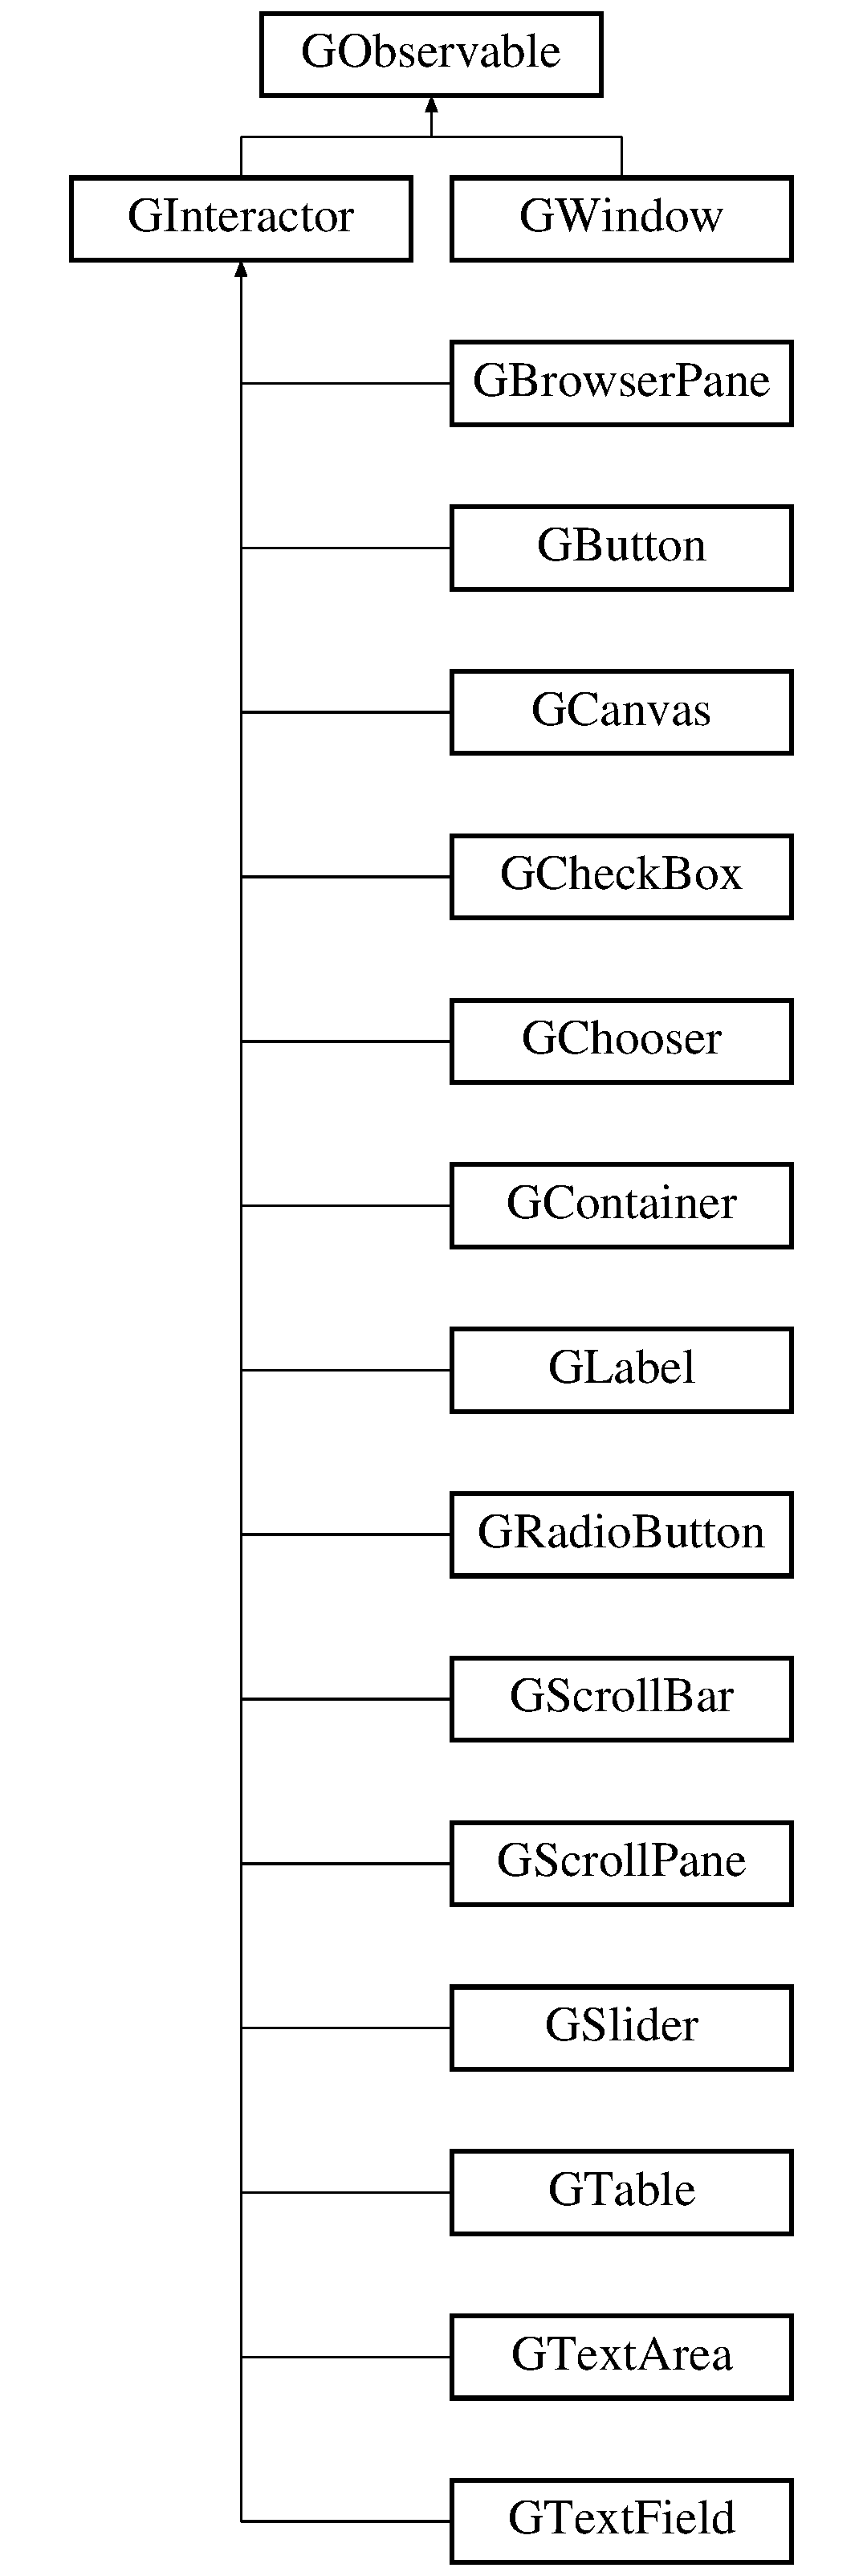
\includegraphics[height=12.000000cm]{classGObservable}
\end{center}
\end{figure}
\subsection*{Public Member Functions}
\begin{DoxyCompactItemize}
\item 
\mbox{\hyperlink{classGObservable_aa083d318cdd2a045471445fbbd26b919}{G\+Observable}} ()
\begin{DoxyCompactList}\small\item\em Initializes a newly created observable object. \end{DoxyCompactList}\item 
virtual \mbox{\hyperlink{classGObservable_a755e7879db8b0a71916cfde365d49305}{$\sim$\+G\+Observable}} ()
\begin{DoxyCompactList}\small\item\em Frees any memory used internally by the observable object. \end{DoxyCompactList}\item 
virtual bool \mbox{\hyperlink{classGObservable_a8ebb3da91032e7f4c34485dabc518b8a}{events\+Enabled}} () const
\begin{DoxyCompactList}\small\item\em Returns true if the object is currently allowing itself to fire events. \end{DoxyCompactList}\item 
virtual std\+::string \mbox{\hyperlink{classGObservable_a799e073a127b428cc841086d42ea4fed}{get\+Type}} () const =0
\begin{DoxyCompactList}\small\item\em Returns the concrete type of the object as a string, such as {\ttfamily \char`\"{}\+G\+Button\char`\"{}} or {\ttfamily \char`\"{}\+G\+Window\char`\"{}}. \end{DoxyCompactList}\item 
virtual void \mbox{\hyperlink{classGObservable_afaa30b2a9e0f378fd1c70d2f1d0b8216}{set\+Events\+Enabled}} (bool \mbox{\hyperlink{classGObservable_a8ebb3da91032e7f4c34485dabc518b8a}{events\+Enabled}})
\begin{DoxyCompactList}\small\item\em Sets whether the object is currently allowing itself to fire events. \end{DoxyCompactList}\item 
virtual std\+::string \mbox{\hyperlink{classGObservable_a1fe5121d6528fdea3f243321b3fa3a49}{to\+String}} () const
\begin{DoxyCompactList}\small\item\em Returns a string representation of this observable object\textquotesingle{}s state. \end{DoxyCompactList}\end{DoxyCompactItemize}
\subsection*{Protected Member Functions}
\begin{DoxyCompactItemize}
\item 
virtual void \mbox{\hyperlink{classGObservable_a80cfa040459ff53594adbd6a51ec8f43}{clear\+Event\+Listeners}} ()
\begin{DoxyCompactList}\small\item\em Removes all event listeners from this object. \end{DoxyCompactList}\item 
virtual void \mbox{\hyperlink{classGObservable_a284f31528c0520f8e545c03ac9eeac74}{ensure\+Thread\+Safety}} (const std\+::string \&member\+Name=\char`\"{}\char`\"{})
\begin{DoxyCompactList}\small\item\em Ensures that we are currently in the Qt G\+UI thread. \end{DoxyCompactList}\item 
virtual void \mbox{\hyperlink{classGObservable_a63e5e5a6227c59c928493b11aceb0f67}{fire\+Event}} (\mbox{\hyperlink{classGEvent}{G\+Event}} \&event)
\begin{DoxyCompactList}\small\item\em Sends out the given event to any attached listeners. \end{DoxyCompactList}\item 
virtual void \mbox{\hyperlink{classGObservable_ab3983ea07337b52020a29cc00c653d8d}{fire\+G\+Event}} (Q\+Event $\ast$event, Event\+Type event\+Type, const std\+::string \&event\+Name)
\begin{DoxyCompactList}\small\item\em Creates an event of the given type, then sends it out to any attached listeners. \end{DoxyCompactList}\item 
virtual void \mbox{\hyperlink{classGObservable_a01fdf1b0e0dbd49e189fe4514e010411}{fire\+G\+Event}} (Q\+Close\+Event $\ast$event, Event\+Type event\+Type, const std\+::string \&event\+Name)
\begin{DoxyCompactList}\small\item\em Creates an event of the given type, then sends it out to any attached listeners. \end{DoxyCompactList}\item 
virtual void \mbox{\hyperlink{classGObservable_abb0b2f66ba39211cb5d7615e9d1c04e2}{fire\+G\+Event}} (Q\+Key\+Event $\ast$event, Event\+Type event\+Type, const std\+::string \&event\+Name)
\begin{DoxyCompactList}\small\item\em Creates an event of the given type, then sends it out to any attached listeners. \end{DoxyCompactList}\item 
virtual void \mbox{\hyperlink{classGObservable_a119318675d2165bdf7dd853aaf881d4b}{fire\+G\+Event}} (Q\+Mouse\+Event $\ast$event, Event\+Type event\+Type, const std\+::string \&event\+Name, const std\+::string \&action\+Command=\char`\"{}\char`\"{})
\begin{DoxyCompactList}\small\item\em Creates an event of the given type, then sends it out to any attached listeners. \end{DoxyCompactList}\item 
virtual void \mbox{\hyperlink{classGObservable_a63fd9034e1e1633c1c38eb342bfd34e9}{fire\+G\+Event}} (Q\+Resize\+Event $\ast$event, Event\+Type event\+Type, const std\+::string \&event\+Name)
\begin{DoxyCompactList}\small\item\em Creates an event of the given type, then sends it out to any attached listeners. \end{DoxyCompactList}\item 
virtual void \mbox{\hyperlink{classGObservable_a741345310d9b7c5170a6cbc410c44ac4}{fire\+G\+Event}} (Q\+Timer\+Event $\ast$event, Event\+Type event\+Type, const std\+::string \&event\+Name)
\begin{DoxyCompactList}\small\item\em Creates an event of the given type, then sends it out to any attached listeners. \end{DoxyCompactList}\item 
virtual void \mbox{\hyperlink{classGObservable_a93bf338968a0338761b8e4dc62f582e9}{fire\+G\+Event}} (Q\+Wheel\+Event $\ast$event, Event\+Type event\+Type, const std\+::string \&event\+Name)
\begin{DoxyCompactList}\small\item\em Creates an event of the given type, then sends it out to any attached listeners. \end{DoxyCompactList}\item 
virtual void \mbox{\hyperlink{classGObservable_a2a70a7d7435ff0c3b80bb4d70da19e0d}{fire\+G\+Event}} (Q\+Window\+State\+Change\+Event $\ast$event, Event\+Type event\+Type, const std\+::string \&event\+Name)
\begin{DoxyCompactList}\small\item\em Creates an event of the given type, then sends it out to any attached listeners. \end{DoxyCompactList}\item 
virtual bool \mbox{\hyperlink{classGObservable_a9f6faaa25942923bafa1c44020c49fa9}{has\+Event\+Listener}} (const std\+::string \&event\+Name) const
\begin{DoxyCompactList}\small\item\em Returns true if the observable object has a listener for the given type of event. \end{DoxyCompactList}\item 
virtual bool \mbox{\hyperlink{classGObservable_aeec1adc19aa0f33de62390686ee1382c}{is\+Accepting\+Event}} (int event\+Mask) const
\begin{DoxyCompactList}\small\item\em Returns true if the observable object has a listener for the given type of event. \end{DoxyCompactList}\item 
virtual bool \mbox{\hyperlink{classGObservable_aa31c73145a29dcb92848a92e0cfaea41}{is\+Accepting\+Event}} (const \mbox{\hyperlink{classGEvent}{G\+Event}} \&event) const
\begin{DoxyCompactList}\small\item\em Returns true if the observable object has a listener for the given type of event. \end{DoxyCompactList}\item 
virtual bool \mbox{\hyperlink{classGObservable_a3b1c689267eda44e65a2213e7de38b23}{is\+Accepting\+Event}} (const std\+::string \&event\+Type) const
\begin{DoxyCompactList}\small\item\em Returns true if the observable object has a listener for the given type of event. \end{DoxyCompactList}\item 
virtual void \mbox{\hyperlink{classGObservable_acbcf1ed3a851ad8a3c17ef38d86b481d}{remove\+Event\+Listener}} (const std\+::string \&event\+Name)
\begin{DoxyCompactList}\small\item\em Removes any event listener from this observable object that would respond to the given type of event, such as \char`\"{}click\char`\"{} or \char`\"{}keydown\char`\"{}. \end{DoxyCompactList}\item 
virtual void \mbox{\hyperlink{classGObservable_af51cc35c29a1bd1908609d432decdbb6}{remove\+Event\+Listeners}} (std\+::initializer\+\_\+list$<$ std\+::string $>$ event\+Names)
\begin{DoxyCompactList}\small\item\em Removes any event listener from this observable object that would respond to the given types of events, such as \char`\"{}click\char`\"{} or \char`\"{}keydown\char`\"{}. \end{DoxyCompactList}\item 
virtual void \mbox{\hyperlink{classGObservable_ad2f6d34961c50f6c1e0659990b79f741}{set\+Event\+Listener}} (const std\+::string \&event\+Name, G\+Event\+Listener func)
\begin{DoxyCompactList}\small\item\em Adds an event listener from this observable object to respond to the given type of event, such as \char`\"{}click\char`\"{} or \char`\"{}keydown\char`\"{}. \end{DoxyCompactList}\item 
virtual void \mbox{\hyperlink{classGObservable_abac4cb9f9e626e010e87f5d91573c8a5}{set\+Event\+Listener}} (const std\+::string \&event\+Name, G\+Event\+Listener\+Void func)
\begin{DoxyCompactList}\small\item\em Adds an event listener from this observable object to respond to the given type of event, such as \char`\"{}click\char`\"{} or \char`\"{}keydown\char`\"{}. \end{DoxyCompactList}\item 
virtual void \mbox{\hyperlink{classGObservable_afa388d69c33c718cf035774604065604}{set\+Event\+Listeners}} (std\+::initializer\+\_\+list$<$ std\+::string $>$ event\+Names, G\+Event\+Listener func)
\begin{DoxyCompactList}\small\item\em Adds an event listener from this observable object to respond to the given types of events, such as \char`\"{}click\char`\"{} or \char`\"{}keydown\char`\"{}. \end{DoxyCompactList}\item 
virtual void \mbox{\hyperlink{classGObservable_a7867184bbb686f74fae8a4db927da799}{set\+Event\+Listeners}} (std\+::initializer\+\_\+list$<$ std\+::string $>$ event\+Names, G\+Event\+Listener\+Void func)
\begin{DoxyCompactList}\small\item\em Adds an event listener from this observable object to respond to the given types of events, such as \char`\"{}click\char`\"{} or \char`\"{}keydown\char`\"{}. \end{DoxyCompactList}\end{DoxyCompactItemize}
\subsection*{Friends}
\begin{DoxyCompactItemize}
\item 
class \mbox{\hyperlink{classGObservable_a054e99eaa992da5c1a77c8d7b3817788}{G\+Interactor}}
\end{DoxyCompactItemize}


\subsection{Detailed Description}
A \mbox{\hyperlink{classGObservable}{G\+Observable}} object is one that is able to send out events. 

Listeners can register themselves to be notified when events occur. This serves as a base class for the various \mbox{\hyperlink{classGInteractor}{G\+Interactor}} subclasses, as well as for the \mbox{\hyperlink{classGWindow}{G\+Window}} class, so that clients can attach listeners to them. 

\subsection{Constructor \& Destructor Documentation}
\mbox{\Hypertarget{classGObservable_aa083d318cdd2a045471445fbbd26b919}\label{classGObservable_aa083d318cdd2a045471445fbbd26b919}} 
\index{G\+Observable@{G\+Observable}!G\+Observable@{G\+Observable}}
\index{G\+Observable@{G\+Observable}!G\+Observable@{G\+Observable}}
\subsubsection{\texorpdfstring{G\+Observable()}{GObservable()}}
{\footnotesize\ttfamily \mbox{\hyperlink{classGObservable}{G\+Observable}} (\begin{DoxyParamCaption}{ }\end{DoxyParamCaption})}



Initializes a newly created observable object. 

\mbox{\Hypertarget{classGObservable_a755e7879db8b0a71916cfde365d49305}\label{classGObservable_a755e7879db8b0a71916cfde365d49305}} 
\index{G\+Observable@{G\+Observable}!````~G\+Observable@{$\sim$\+G\+Observable}}
\index{````~G\+Observable@{$\sim$\+G\+Observable}!G\+Observable@{G\+Observable}}
\subsubsection{\texorpdfstring{$\sim$\+G\+Observable()}{~GObservable()}}
{\footnotesize\ttfamily $\sim$\mbox{\hyperlink{classGObservable}{G\+Observable}} (\begin{DoxyParamCaption}{ }\end{DoxyParamCaption})\hspace{0.3cm}{\ttfamily [virtual]}}



Frees any memory used internally by the observable object. 



\subsection{Member Function Documentation}
\mbox{\Hypertarget{classGObservable_a80cfa040459ff53594adbd6a51ec8f43}\label{classGObservable_a80cfa040459ff53594adbd6a51ec8f43}} 
\index{G\+Observable@{G\+Observable}!clear\+Event\+Listeners@{clear\+Event\+Listeners}}
\index{clear\+Event\+Listeners@{clear\+Event\+Listeners}!G\+Observable@{G\+Observable}}
\subsubsection{\texorpdfstring{clear\+Event\+Listeners()}{clearEventListeners()}}
{\footnotesize\ttfamily void clear\+Event\+Listeners (\begin{DoxyParamCaption}{ }\end{DoxyParamCaption})\hspace{0.3cm}{\ttfamily [protected]}, {\ttfamily [virtual]}}



Removes all event listeners from this object. 

\mbox{\Hypertarget{classGObservable_a284f31528c0520f8e545c03ac9eeac74}\label{classGObservable_a284f31528c0520f8e545c03ac9eeac74}} 
\index{G\+Observable@{G\+Observable}!ensure\+Thread\+Safety@{ensure\+Thread\+Safety}}
\index{ensure\+Thread\+Safety@{ensure\+Thread\+Safety}!G\+Observable@{G\+Observable}}
\subsubsection{\texorpdfstring{ensure\+Thread\+Safety()}{ensureThreadSafety()}}
{\footnotesize\ttfamily void ensure\+Thread\+Safety (\begin{DoxyParamCaption}\item[{const std\+::string \&}]{member\+Name = {\ttfamily \char`\"{}\char`\"{}} }\end{DoxyParamCaption})\hspace{0.3cm}{\ttfamily [protected]}, {\ttfamily [virtual]}}



Ensures that we are currently in the Qt G\+UI thread. 

\mbox{\Hypertarget{classGObservable_a8ebb3da91032e7f4c34485dabc518b8a}\label{classGObservable_a8ebb3da91032e7f4c34485dabc518b8a}} 
\index{G\+Observable@{G\+Observable}!events\+Enabled@{events\+Enabled}}
\index{events\+Enabled@{events\+Enabled}!G\+Observable@{G\+Observable}}
\subsubsection{\texorpdfstring{events\+Enabled()}{eventsEnabled()}}
{\footnotesize\ttfamily bool events\+Enabled (\begin{DoxyParamCaption}{ }\end{DoxyParamCaption}) const\hspace{0.3cm}{\ttfamily [virtual]}}



Returns true if the object is currently allowing itself to fire events. 

Initially this is true unless the client has called {\ttfamily set\+Events\+Enabled(false)} or the object is not visible. 

Reimplemented in \mbox{\hyperlink{classGInteractor_ac05ba5b92e2e5146d416fe7f842a0969}{G\+Interactor}}.

\mbox{\Hypertarget{classGObservable_a63e5e5a6227c59c928493b11aceb0f67}\label{classGObservable_a63e5e5a6227c59c928493b11aceb0f67}} 
\index{G\+Observable@{G\+Observable}!fire\+Event@{fire\+Event}}
\index{fire\+Event@{fire\+Event}!G\+Observable@{G\+Observable}}
\subsubsection{\texorpdfstring{fire\+Event()}{fireEvent()}}
{\footnotesize\ttfamily void fire\+Event (\begin{DoxyParamCaption}\item[{\mbox{\hyperlink{classGEvent}{G\+Event}} \&}]{event }\end{DoxyParamCaption})\hspace{0.3cm}{\ttfamily [protected]}, {\ttfamily [virtual]}}



Sends out the given event to any attached listeners. 

\mbox{\Hypertarget{classGObservable_ab3983ea07337b52020a29cc00c653d8d}\label{classGObservable_ab3983ea07337b52020a29cc00c653d8d}} 
\index{G\+Observable@{G\+Observable}!fire\+G\+Event@{fire\+G\+Event}}
\index{fire\+G\+Event@{fire\+G\+Event}!G\+Observable@{G\+Observable}}
\subsubsection{\texorpdfstring{fire\+G\+Event()}{fireGEvent()}\hspace{0.1cm}{\footnotesize\ttfamily [1/8]}}
{\footnotesize\ttfamily void fire\+G\+Event (\begin{DoxyParamCaption}\item[{Q\+Event $\ast$}]{event,  }\item[{Event\+Type}]{event\+Type,  }\item[{const std\+::string \&}]{event\+Name }\end{DoxyParamCaption})\hspace{0.3cm}{\ttfamily [protected]}, {\ttfamily [virtual]}}



Creates an event of the given type, then sends it out to any attached listeners. 

\mbox{\Hypertarget{classGObservable_a01fdf1b0e0dbd49e189fe4514e010411}\label{classGObservable_a01fdf1b0e0dbd49e189fe4514e010411}} 
\index{G\+Observable@{G\+Observable}!fire\+G\+Event@{fire\+G\+Event}}
\index{fire\+G\+Event@{fire\+G\+Event}!G\+Observable@{G\+Observable}}
\subsubsection{\texorpdfstring{fire\+G\+Event()}{fireGEvent()}\hspace{0.1cm}{\footnotesize\ttfamily [2/8]}}
{\footnotesize\ttfamily void fire\+G\+Event (\begin{DoxyParamCaption}\item[{Q\+Close\+Event $\ast$}]{event,  }\item[{Event\+Type}]{event\+Type,  }\item[{const std\+::string \&}]{event\+Name }\end{DoxyParamCaption})\hspace{0.3cm}{\ttfamily [protected]}, {\ttfamily [virtual]}}



Creates an event of the given type, then sends it out to any attached listeners. 

\mbox{\Hypertarget{classGObservable_abb0b2f66ba39211cb5d7615e9d1c04e2}\label{classGObservable_abb0b2f66ba39211cb5d7615e9d1c04e2}} 
\index{G\+Observable@{G\+Observable}!fire\+G\+Event@{fire\+G\+Event}}
\index{fire\+G\+Event@{fire\+G\+Event}!G\+Observable@{G\+Observable}}
\subsubsection{\texorpdfstring{fire\+G\+Event()}{fireGEvent()}\hspace{0.1cm}{\footnotesize\ttfamily [3/8]}}
{\footnotesize\ttfamily void fire\+G\+Event (\begin{DoxyParamCaption}\item[{Q\+Key\+Event $\ast$}]{event,  }\item[{Event\+Type}]{event\+Type,  }\item[{const std\+::string \&}]{event\+Name }\end{DoxyParamCaption})\hspace{0.3cm}{\ttfamily [protected]}, {\ttfamily [virtual]}}



Creates an event of the given type, then sends it out to any attached listeners. 

\mbox{\Hypertarget{classGObservable_a119318675d2165bdf7dd853aaf881d4b}\label{classGObservable_a119318675d2165bdf7dd853aaf881d4b}} 
\index{G\+Observable@{G\+Observable}!fire\+G\+Event@{fire\+G\+Event}}
\index{fire\+G\+Event@{fire\+G\+Event}!G\+Observable@{G\+Observable}}
\subsubsection{\texorpdfstring{fire\+G\+Event()}{fireGEvent()}\hspace{0.1cm}{\footnotesize\ttfamily [4/8]}}
{\footnotesize\ttfamily void fire\+G\+Event (\begin{DoxyParamCaption}\item[{Q\+Mouse\+Event $\ast$}]{event,  }\item[{Event\+Type}]{event\+Type,  }\item[{const std\+::string \&}]{event\+Name,  }\item[{const std\+::string \&}]{action\+Command = {\ttfamily \char`\"{}\char`\"{}} }\end{DoxyParamCaption})\hspace{0.3cm}{\ttfamily [protected]}, {\ttfamily [virtual]}}



Creates an event of the given type, then sends it out to any attached listeners. 

\mbox{\Hypertarget{classGObservable_a63fd9034e1e1633c1c38eb342bfd34e9}\label{classGObservable_a63fd9034e1e1633c1c38eb342bfd34e9}} 
\index{G\+Observable@{G\+Observable}!fire\+G\+Event@{fire\+G\+Event}}
\index{fire\+G\+Event@{fire\+G\+Event}!G\+Observable@{G\+Observable}}
\subsubsection{\texorpdfstring{fire\+G\+Event()}{fireGEvent()}\hspace{0.1cm}{\footnotesize\ttfamily [5/8]}}
{\footnotesize\ttfamily void fire\+G\+Event (\begin{DoxyParamCaption}\item[{Q\+Resize\+Event $\ast$}]{event,  }\item[{Event\+Type}]{event\+Type,  }\item[{const std\+::string \&}]{event\+Name }\end{DoxyParamCaption})\hspace{0.3cm}{\ttfamily [protected]}, {\ttfamily [virtual]}}



Creates an event of the given type, then sends it out to any attached listeners. 

\mbox{\Hypertarget{classGObservable_a741345310d9b7c5170a6cbc410c44ac4}\label{classGObservable_a741345310d9b7c5170a6cbc410c44ac4}} 
\index{G\+Observable@{G\+Observable}!fire\+G\+Event@{fire\+G\+Event}}
\index{fire\+G\+Event@{fire\+G\+Event}!G\+Observable@{G\+Observable}}
\subsubsection{\texorpdfstring{fire\+G\+Event()}{fireGEvent()}\hspace{0.1cm}{\footnotesize\ttfamily [6/8]}}
{\footnotesize\ttfamily void fire\+G\+Event (\begin{DoxyParamCaption}\item[{Q\+Timer\+Event $\ast$}]{event,  }\item[{Event\+Type}]{event\+Type,  }\item[{const std\+::string \&}]{event\+Name }\end{DoxyParamCaption})\hspace{0.3cm}{\ttfamily [protected]}, {\ttfamily [virtual]}}



Creates an event of the given type, then sends it out to any attached listeners. 

\mbox{\Hypertarget{classGObservable_a93bf338968a0338761b8e4dc62f582e9}\label{classGObservable_a93bf338968a0338761b8e4dc62f582e9}} 
\index{G\+Observable@{G\+Observable}!fire\+G\+Event@{fire\+G\+Event}}
\index{fire\+G\+Event@{fire\+G\+Event}!G\+Observable@{G\+Observable}}
\subsubsection{\texorpdfstring{fire\+G\+Event()}{fireGEvent()}\hspace{0.1cm}{\footnotesize\ttfamily [7/8]}}
{\footnotesize\ttfamily void fire\+G\+Event (\begin{DoxyParamCaption}\item[{Q\+Wheel\+Event $\ast$}]{event,  }\item[{Event\+Type}]{event\+Type,  }\item[{const std\+::string \&}]{event\+Name }\end{DoxyParamCaption})\hspace{0.3cm}{\ttfamily [protected]}, {\ttfamily [virtual]}}



Creates an event of the given type, then sends it out to any attached listeners. 

\mbox{\Hypertarget{classGObservable_a2a70a7d7435ff0c3b80bb4d70da19e0d}\label{classGObservable_a2a70a7d7435ff0c3b80bb4d70da19e0d}} 
\index{G\+Observable@{G\+Observable}!fire\+G\+Event@{fire\+G\+Event}}
\index{fire\+G\+Event@{fire\+G\+Event}!G\+Observable@{G\+Observable}}
\subsubsection{\texorpdfstring{fire\+G\+Event()}{fireGEvent()}\hspace{0.1cm}{\footnotesize\ttfamily [8/8]}}
{\footnotesize\ttfamily void fire\+G\+Event (\begin{DoxyParamCaption}\item[{Q\+Window\+State\+Change\+Event $\ast$}]{event,  }\item[{Event\+Type}]{event\+Type,  }\item[{const std\+::string \&}]{event\+Name }\end{DoxyParamCaption})\hspace{0.3cm}{\ttfamily [protected]}, {\ttfamily [virtual]}}



Creates an event of the given type, then sends it out to any attached listeners. 

\mbox{\Hypertarget{classGObservable_a799e073a127b428cc841086d42ea4fed}\label{classGObservable_a799e073a127b428cc841086d42ea4fed}} 
\index{G\+Observable@{G\+Observable}!get\+Type@{get\+Type}}
\index{get\+Type@{get\+Type}!G\+Observable@{G\+Observable}}
\subsubsection{\texorpdfstring{get\+Type()}{getType()}}
{\footnotesize\ttfamily virtual std\+::string get\+Type (\begin{DoxyParamCaption}{ }\end{DoxyParamCaption}) const\hspace{0.3cm}{\ttfamily [pure virtual]}}



Returns the concrete type of the object as a string, such as {\ttfamily \char`\"{}\+G\+Button\char`\"{}} or {\ttfamily \char`\"{}\+G\+Window\char`\"{}}. 

Each \mbox{\hyperlink{classGObservable}{G\+Observable}} subtype must override this method. 

Implemented in \mbox{\hyperlink{classGWindow_a9896d58fcfebbf1025aeeb5b8b9ede80}{G\+Window}}, \mbox{\hyperlink{classGCanvas_a9896d58fcfebbf1025aeeb5b8b9ede80}{G\+Canvas}}, \mbox{\hyperlink{classGContainer_a9896d58fcfebbf1025aeeb5b8b9ede80}{G\+Container}}, \mbox{\hyperlink{classGInteractor_a799e073a127b428cc841086d42ea4fed}{G\+Interactor}}, \mbox{\hyperlink{classGTable_a9896d58fcfebbf1025aeeb5b8b9ede80}{G\+Table}}, \mbox{\hyperlink{classGTextArea_a9896d58fcfebbf1025aeeb5b8b9ede80}{G\+Text\+Area}}, \mbox{\hyperlink{classGSlider_a9896d58fcfebbf1025aeeb5b8b9ede80}{G\+Slider}}, \mbox{\hyperlink{classGTextField_a9896d58fcfebbf1025aeeb5b8b9ede80}{G\+Text\+Field}}, \mbox{\hyperlink{classGChooser_a9896d58fcfebbf1025aeeb5b8b9ede80}{G\+Chooser}}, \mbox{\hyperlink{classGScrollBar_a9896d58fcfebbf1025aeeb5b8b9ede80}{G\+Scroll\+Bar}}, \mbox{\hyperlink{classGLabel_a9896d58fcfebbf1025aeeb5b8b9ede80}{G\+Label}}, \mbox{\hyperlink{classGRadioButton_a9896d58fcfebbf1025aeeb5b8b9ede80}{G\+Radio\+Button}}, \mbox{\hyperlink{classGButton_a9896d58fcfebbf1025aeeb5b8b9ede80}{G\+Button}}, \mbox{\hyperlink{classGScrollPane_a9896d58fcfebbf1025aeeb5b8b9ede80}{G\+Scroll\+Pane}}, \mbox{\hyperlink{classGBrowserPane_a9896d58fcfebbf1025aeeb5b8b9ede80}{G\+Browser\+Pane}}, and \mbox{\hyperlink{classGCheckBox_a9896d58fcfebbf1025aeeb5b8b9ede80}{G\+Check\+Box}}.

\mbox{\Hypertarget{classGObservable_a9f6faaa25942923bafa1c44020c49fa9}\label{classGObservable_a9f6faaa25942923bafa1c44020c49fa9}} 
\index{G\+Observable@{G\+Observable}!has\+Event\+Listener@{has\+Event\+Listener}}
\index{has\+Event\+Listener@{has\+Event\+Listener}!G\+Observable@{G\+Observable}}
\subsubsection{\texorpdfstring{has\+Event\+Listener()}{hasEventListener()}}
{\footnotesize\ttfamily bool has\+Event\+Listener (\begin{DoxyParamCaption}\item[{const std\+::string \&}]{event\+Name }\end{DoxyParamCaption}) const\hspace{0.3cm}{\ttfamily [protected]}, {\ttfamily [virtual]}}



Returns true if the observable object has a listener for the given type of event. 

\mbox{\Hypertarget{classGObservable_aeec1adc19aa0f33de62390686ee1382c}\label{classGObservable_aeec1adc19aa0f33de62390686ee1382c}} 
\index{G\+Observable@{G\+Observable}!is\+Accepting\+Event@{is\+Accepting\+Event}}
\index{is\+Accepting\+Event@{is\+Accepting\+Event}!G\+Observable@{G\+Observable}}
\subsubsection{\texorpdfstring{is\+Accepting\+Event()}{isAcceptingEvent()}\hspace{0.1cm}{\footnotesize\ttfamily [1/3]}}
{\footnotesize\ttfamily bool is\+Accepting\+Event (\begin{DoxyParamCaption}\item[{int}]{event\+Mask }\end{DoxyParamCaption}) const\hspace{0.3cm}{\ttfamily [protected]}, {\ttfamily [virtual]}}



Returns true if the observable object has a listener for the given type of event. 

See \mbox{\hyperlink{gevent_8h_source}{gevent.\+h}} for event types and masks. \mbox{\Hypertarget{classGObservable_aa31c73145a29dcb92848a92e0cfaea41}\label{classGObservable_aa31c73145a29dcb92848a92e0cfaea41}} 
\index{G\+Observable@{G\+Observable}!is\+Accepting\+Event@{is\+Accepting\+Event}}
\index{is\+Accepting\+Event@{is\+Accepting\+Event}!G\+Observable@{G\+Observable}}
\subsubsection{\texorpdfstring{is\+Accepting\+Event()}{isAcceptingEvent()}\hspace{0.1cm}{\footnotesize\ttfamily [2/3]}}
{\footnotesize\ttfamily bool is\+Accepting\+Event (\begin{DoxyParamCaption}\item[{const \mbox{\hyperlink{classGEvent}{G\+Event}} \&}]{event }\end{DoxyParamCaption}) const\hspace{0.3cm}{\ttfamily [protected]}, {\ttfamily [virtual]}}



Returns true if the observable object has a listener for the given type of event. 

\mbox{\Hypertarget{classGObservable_a3b1c689267eda44e65a2213e7de38b23}\label{classGObservable_a3b1c689267eda44e65a2213e7de38b23}} 
\index{G\+Observable@{G\+Observable}!is\+Accepting\+Event@{is\+Accepting\+Event}}
\index{is\+Accepting\+Event@{is\+Accepting\+Event}!G\+Observable@{G\+Observable}}
\subsubsection{\texorpdfstring{is\+Accepting\+Event()}{isAcceptingEvent()}\hspace{0.1cm}{\footnotesize\ttfamily [3/3]}}
{\footnotesize\ttfamily bool is\+Accepting\+Event (\begin{DoxyParamCaption}\item[{const std\+::string \&}]{event\+Type }\end{DoxyParamCaption}) const\hspace{0.3cm}{\ttfamily [protected]}, {\ttfamily [virtual]}}



Returns true if the observable object has a listener for the given type of event. 

\mbox{\Hypertarget{classGObservable_acbcf1ed3a851ad8a3c17ef38d86b481d}\label{classGObservable_acbcf1ed3a851ad8a3c17ef38d86b481d}} 
\index{G\+Observable@{G\+Observable}!remove\+Event\+Listener@{remove\+Event\+Listener}}
\index{remove\+Event\+Listener@{remove\+Event\+Listener}!G\+Observable@{G\+Observable}}
\subsubsection{\texorpdfstring{remove\+Event\+Listener()}{removeEventListener()}}
{\footnotesize\ttfamily void remove\+Event\+Listener (\begin{DoxyParamCaption}\item[{const std\+::string \&}]{event\+Name }\end{DoxyParamCaption})\hspace{0.3cm}{\ttfamily [protected]}, {\ttfamily [virtual]}}



Removes any event listener from this observable object that would respond to the given type of event, such as \char`\"{}click\char`\"{} or \char`\"{}keydown\char`\"{}. 

\mbox{\Hypertarget{classGObservable_af51cc35c29a1bd1908609d432decdbb6}\label{classGObservable_af51cc35c29a1bd1908609d432decdbb6}} 
\index{G\+Observable@{G\+Observable}!remove\+Event\+Listeners@{remove\+Event\+Listeners}}
\index{remove\+Event\+Listeners@{remove\+Event\+Listeners}!G\+Observable@{G\+Observable}}
\subsubsection{\texorpdfstring{remove\+Event\+Listeners()}{removeEventListeners()}}
{\footnotesize\ttfamily void remove\+Event\+Listeners (\begin{DoxyParamCaption}\item[{std\+::initializer\+\_\+list$<$ std\+::string $>$}]{event\+Names }\end{DoxyParamCaption})\hspace{0.3cm}{\ttfamily [protected]}, {\ttfamily [virtual]}}



Removes any event listener from this observable object that would respond to the given types of events, such as \char`\"{}click\char`\"{} or \char`\"{}keydown\char`\"{}. 

\mbox{\Hypertarget{classGObservable_ad2f6d34961c50f6c1e0659990b79f741}\label{classGObservable_ad2f6d34961c50f6c1e0659990b79f741}} 
\index{G\+Observable@{G\+Observable}!set\+Event\+Listener@{set\+Event\+Listener}}
\index{set\+Event\+Listener@{set\+Event\+Listener}!G\+Observable@{G\+Observable}}
\subsubsection{\texorpdfstring{set\+Event\+Listener()}{setEventListener()}\hspace{0.1cm}{\footnotesize\ttfamily [1/2]}}
{\footnotesize\ttfamily void set\+Event\+Listener (\begin{DoxyParamCaption}\item[{const std\+::string \&}]{event\+Name,  }\item[{G\+Event\+Listener}]{func }\end{DoxyParamCaption})\hspace{0.3cm}{\ttfamily [protected]}, {\ttfamily [virtual]}}



Adds an event listener from this observable object to respond to the given type of event, such as \char`\"{}click\char`\"{} or \char`\"{}keydown\char`\"{}. 

Any prior listener for that type of event is replaced. \mbox{\Hypertarget{classGObservable_abac4cb9f9e626e010e87f5d91573c8a5}\label{classGObservable_abac4cb9f9e626e010e87f5d91573c8a5}} 
\index{G\+Observable@{G\+Observable}!set\+Event\+Listener@{set\+Event\+Listener}}
\index{set\+Event\+Listener@{set\+Event\+Listener}!G\+Observable@{G\+Observable}}
\subsubsection{\texorpdfstring{set\+Event\+Listener()}{setEventListener()}\hspace{0.1cm}{\footnotesize\ttfamily [2/2]}}
{\footnotesize\ttfamily void set\+Event\+Listener (\begin{DoxyParamCaption}\item[{const std\+::string \&}]{event\+Name,  }\item[{G\+Event\+Listener\+Void}]{func }\end{DoxyParamCaption})\hspace{0.3cm}{\ttfamily [protected]}, {\ttfamily [virtual]}}



Adds an event listener from this observable object to respond to the given type of event, such as \char`\"{}click\char`\"{} or \char`\"{}keydown\char`\"{}. 

Any prior listener for that type of event is replaced. \mbox{\Hypertarget{classGObservable_afa388d69c33c718cf035774604065604}\label{classGObservable_afa388d69c33c718cf035774604065604}} 
\index{G\+Observable@{G\+Observable}!set\+Event\+Listeners@{set\+Event\+Listeners}}
\index{set\+Event\+Listeners@{set\+Event\+Listeners}!G\+Observable@{G\+Observable}}
\subsubsection{\texorpdfstring{set\+Event\+Listeners()}{setEventListeners()}\hspace{0.1cm}{\footnotesize\ttfamily [1/2]}}
{\footnotesize\ttfamily void set\+Event\+Listeners (\begin{DoxyParamCaption}\item[{std\+::initializer\+\_\+list$<$ std\+::string $>$}]{event\+Names,  }\item[{G\+Event\+Listener}]{func }\end{DoxyParamCaption})\hspace{0.3cm}{\ttfamily [protected]}, {\ttfamily [virtual]}}



Adds an event listener from this observable object to respond to the given types of events, such as \char`\"{}click\char`\"{} or \char`\"{}keydown\char`\"{}. 

Any prior listener for those types of event are replaced. \mbox{\Hypertarget{classGObservable_a7867184bbb686f74fae8a4db927da799}\label{classGObservable_a7867184bbb686f74fae8a4db927da799}} 
\index{G\+Observable@{G\+Observable}!set\+Event\+Listeners@{set\+Event\+Listeners}}
\index{set\+Event\+Listeners@{set\+Event\+Listeners}!G\+Observable@{G\+Observable}}
\subsubsection{\texorpdfstring{set\+Event\+Listeners()}{setEventListeners()}\hspace{0.1cm}{\footnotesize\ttfamily [2/2]}}
{\footnotesize\ttfamily void set\+Event\+Listeners (\begin{DoxyParamCaption}\item[{std\+::initializer\+\_\+list$<$ std\+::string $>$}]{event\+Names,  }\item[{G\+Event\+Listener\+Void}]{func }\end{DoxyParamCaption})\hspace{0.3cm}{\ttfamily [protected]}, {\ttfamily [virtual]}}



Adds an event listener from this observable object to respond to the given types of events, such as \char`\"{}click\char`\"{} or \char`\"{}keydown\char`\"{}. 

Any prior listener for those types of event are replaced. \mbox{\Hypertarget{classGObservable_afaa30b2a9e0f378fd1c70d2f1d0b8216}\label{classGObservable_afaa30b2a9e0f378fd1c70d2f1d0b8216}} 
\index{G\+Observable@{G\+Observable}!set\+Events\+Enabled@{set\+Events\+Enabled}}
\index{set\+Events\+Enabled@{set\+Events\+Enabled}!G\+Observable@{G\+Observable}}
\subsubsection{\texorpdfstring{set\+Events\+Enabled()}{setEventsEnabled()}}
{\footnotesize\ttfamily void set\+Events\+Enabled (\begin{DoxyParamCaption}\item[{bool}]{events\+Enabled }\end{DoxyParamCaption})\hspace{0.3cm}{\ttfamily [virtual]}}



Sets whether the object is currently allowing itself to fire events. 

Initially this is true. \mbox{\Hypertarget{classGObservable_a1fe5121d6528fdea3f243321b3fa3a49}\label{classGObservable_a1fe5121d6528fdea3f243321b3fa3a49}} 
\index{G\+Observable@{G\+Observable}!to\+String@{to\+String}}
\index{to\+String@{to\+String}!G\+Observable@{G\+Observable}}
\subsubsection{\texorpdfstring{to\+String()}{toString()}}
{\footnotesize\ttfamily std\+::string to\+String (\begin{DoxyParamCaption}{ }\end{DoxyParamCaption}) const\hspace{0.3cm}{\ttfamily [virtual]}}



Returns a string representation of this observable object\textquotesingle{}s state. 

Primarily used for debugging purposes. 

\subsection{Friends And Related Function Documentation}
\mbox{\Hypertarget{classGObservable_a054e99eaa992da5c1a77c8d7b3817788}\label{classGObservable_a054e99eaa992da5c1a77c8d7b3817788}} 
\index{G\+Observable@{G\+Observable}!G\+Interactor@{G\+Interactor}}
\index{G\+Interactor@{G\+Interactor}!G\+Observable@{G\+Observable}}
\subsubsection{\texorpdfstring{G\+Interactor}{GInteractor}}
{\footnotesize\ttfamily friend class \mbox{\hyperlink{classGInteractor}{G\+Interactor}}\hspace{0.3cm}{\ttfamily [friend]}}


\hypertarget{classGOptionPane}{}\section{G\+Option\+Pane Class Reference}
\label{classGOptionPane}\index{G\+Option\+Pane@{G\+Option\+Pane}}


This class provides static methods that pop up graphical input/output dialog boxes on the screen.  




{\ttfamily \#include $<$goptionpane.\+h$>$}

\subsection*{Public Types}
\begin{DoxyCompactItemize}
\item 
enum \mbox{\hyperlink{classGOptionPane_a1cc9e8685029e39646671ed71f32d47d}{Confirm\+Result}} \{ \mbox{\hyperlink{classGOptionPane_a1cc9e8685029e39646671ed71f32d47dae4842754cb17e5234637e3a85a7f3d90}{C\+A\+N\+C\+EL}} = -\/1, 
\mbox{\hyperlink{classGOptionPane_a1cc9e8685029e39646671ed71f32d47da0d077f5b932ce05e5b9f30c6087a2f31}{NO}} = 0, 
\mbox{\hyperlink{classGOptionPane_a1cc9e8685029e39646671ed71f32d47da99f136a862ba5c7d16967231c29f09d6}{Y\+ES}} = 1, 
\mbox{\hyperlink{classGOptionPane_a1cc9e8685029e39646671ed71f32d47da2bc49ec37d6a5715dd23e85f1ff5bb59}{OK}} = 2
 \}
\begin{DoxyCompactList}\small\item\em The various results that can be returned from some option dialogs. \end{DoxyCompactList}\item 
enum \mbox{\hyperlink{classGOptionPane_a6a1aaf19c06f5a6bef89ea6415547049}{Confirm\+Type}} \{ \mbox{\hyperlink{classGOptionPane_a6a1aaf19c06f5a6bef89ea6415547049a23d16d66a433471aa62deadacecfc08d}{Y\+E\+S\+\_\+\+NO}} = 0, 
\mbox{\hyperlink{classGOptionPane_a6a1aaf19c06f5a6bef89ea6415547049a1c39d83120c95b0b233ddde75ee298b6}{Y\+E\+S\+\_\+\+N\+O\+\_\+\+C\+A\+N\+C\+EL}} = 1, 
\mbox{\hyperlink{classGOptionPane_a6a1aaf19c06f5a6bef89ea6415547049ade4e249d688548d74ae16c0feb84728c}{O\+K\+\_\+\+C\+A\+N\+C\+EL}} = 2
 \}
\begin{DoxyCompactList}\small\item\em Types used by show\+Confirm\+Dialog, representing the three kinds of confirmation dialogs\+: Yes/\+No, Yes/\+No/\+Cancel, or O\+K/\+Cancel. \end{DoxyCompactList}\item 
enum \mbox{\hyperlink{classGOptionPane_ac6606ebe91c8ac66a2c314c79f5ab013}{Message\+Type}} \{ \mbox{\hyperlink{classGOptionPane_ac6606ebe91c8ac66a2c314c79f5ab013a2fd6f336d08340583bd620a7f5694c90}{E\+R\+R\+OR}} = 0, 
\mbox{\hyperlink{classGOptionPane_ac6606ebe91c8ac66a2c314c79f5ab013ad2d78669dc69197336728cd0b2845b96}{I\+N\+F\+O\+R\+M\+A\+T\+I\+ON}} = 1, 
\mbox{\hyperlink{classGOptionPane_ac6606ebe91c8ac66a2c314c79f5ab013a8386f3e3e7be0b7b603636867c133a5d}{P\+L\+A\+IN}} = -\/1, 
\mbox{\hyperlink{classGOptionPane_ac6606ebe91c8ac66a2c314c79f5ab013a984de77c680eaff141ec910e25568a81}{W\+A\+R\+N\+I\+NG}} = 2, 
\mbox{\hyperlink{classGOptionPane_ac6606ebe91c8ac66a2c314c79f5ab013ad126f509c35e1661274f8b72693c7848}{Q\+U\+E\+S\+T\+I\+ON}} = 3, 
\mbox{\hyperlink{classGOptionPane_ac6606ebe91c8ac66a2c314c79f5ab013aaef4dc1e4f450a4c9e61a3699d75af0a}{A\+B\+O\+UT}} = 4
 \}
\begin{DoxyCompactList}\small\item\em Types used by show\+Message\+Dialog, representing the various kinds of message dialogs. \end{DoxyCompactList}\end{DoxyCompactItemize}
\subsection*{Static Public Member Functions}
\begin{DoxyCompactItemize}
\item 
static \mbox{\hyperlink{classGOptionPane_a1cc9e8685029e39646671ed71f32d47d}{Confirm\+Result}} \mbox{\hyperlink{classGOptionPane_a5aa43cc516e91b8befcd129ac11ebc96}{show\+Confirm\+Dialog}} (const std\+::string \&message, const std\+::string \&title=\char`\"{}\char`\"{}, \mbox{\hyperlink{classGOptionPane_a6a1aaf19c06f5a6bef89ea6415547049}{Confirm\+Type}} type=\mbox{\hyperlink{classGOptionPane_a6a1aaf19c06f5a6bef89ea6415547049a23d16d66a433471aa62deadacecfc08d}{Y\+E\+S\+\_\+\+NO}})
\begin{DoxyCompactList}\small\item\em Pops up a yes/no confirmation box. \end{DoxyCompactList}\item 
static \mbox{\hyperlink{classGOptionPane_a1cc9e8685029e39646671ed71f32d47d}{Confirm\+Result}} \mbox{\hyperlink{classGOptionPane_a67b4bfe05d029f3575a4b9e341e786ec}{show\+Confirm\+Dialog}} (\mbox{\hyperlink{classGWindow}{G\+Window}} $\ast$parent, const std\+::string \&message, const std\+::string \&title=\char`\"{}\char`\"{}, \mbox{\hyperlink{classGOptionPane_a6a1aaf19c06f5a6bef89ea6415547049}{Confirm\+Type}} type=\mbox{\hyperlink{classGOptionPane_a6a1aaf19c06f5a6bef89ea6415547049a23d16d66a433471aa62deadacecfc08d}{Y\+E\+S\+\_\+\+NO}})
\begin{DoxyCompactList}\small\item\em Pops up a yes/no confirmation box. \end{DoxyCompactList}\item 
static \mbox{\hyperlink{classGOptionPane_a1cc9e8685029e39646671ed71f32d47d}{Confirm\+Result}} \mbox{\hyperlink{classGOptionPane_a19401c5fe238589904bc44319cc80b41}{show\+Confirm\+Dialog}} (Q\+Widget $\ast$parent, const std\+::string \&message, const std\+::string \&title=\char`\"{}\char`\"{}, \mbox{\hyperlink{classGOptionPane_a6a1aaf19c06f5a6bef89ea6415547049}{Confirm\+Type}} type=\mbox{\hyperlink{classGOptionPane_a6a1aaf19c06f5a6bef89ea6415547049a23d16d66a433471aa62deadacecfc08d}{Y\+E\+S\+\_\+\+NO}})
\begin{DoxyCompactList}\small\item\em Pops up a yes/no confirmation box. \end{DoxyCompactList}\item 
static std\+::string \mbox{\hyperlink{classGOptionPane_a50fdc381453e6b8c495e3f9fe07b7bec}{show\+Input\+Dialog}} (const std\+::string \&message, const std\+::string \&title=\char`\"{}\char`\"{}, const std\+::string \&initial\+Value=\char`\"{}\char`\"{})
\begin{DoxyCompactList}\small\item\em Pops up an input box with a text field where the user can type a response, which is returned. \end{DoxyCompactList}\item 
static std\+::string \mbox{\hyperlink{classGOptionPane_a035a6d874c9e81773e7c61305dbecabb}{show\+Input\+Dialog}} (\mbox{\hyperlink{classGWindow}{G\+Window}} $\ast$parent, const std\+::string \&message, const std\+::string \&title=\char`\"{}\char`\"{}, const std\+::string \&initial\+Value=\char`\"{}\char`\"{})
\begin{DoxyCompactList}\small\item\em Pops up an input box with a text field where the user can type a response, which is returned. \end{DoxyCompactList}\item 
static std\+::string \mbox{\hyperlink{classGOptionPane_aabd3a04a3cdc998ee0e7e7e31676df17}{show\+Input\+Dialog}} (Q\+Widget $\ast$parent, const std\+::string \&message, const std\+::string \&title=\char`\"{}\char`\"{}, const std\+::string \&initial\+Value=\char`\"{}\char`\"{})
\begin{DoxyCompactList}\small\item\em Pops up an input box with a text field where the user can type a response, which is returned. \end{DoxyCompactList}\item 
static void \mbox{\hyperlink{classGOptionPane_ac72936da553721b532ea51a831a2993a}{show\+Message\+Dialog}} (const std\+::string \&message, const std\+::string \&title=\char`\"{}\char`\"{}, \mbox{\hyperlink{classGOptionPane_ac6606ebe91c8ac66a2c314c79f5ab013}{Message\+Type}} type=\mbox{\hyperlink{classGOptionPane_ac6606ebe91c8ac66a2c314c79f5ab013a8386f3e3e7be0b7b603636867c133a5d}{P\+L\+A\+IN}})
\begin{DoxyCompactList}\small\item\em Displays an output message dialog to the user. \end{DoxyCompactList}\item 
static void \mbox{\hyperlink{classGOptionPane_a72a54f763487c83c587a79611e8ae685}{show\+Message\+Dialog}} (\mbox{\hyperlink{classGWindow}{G\+Window}} $\ast$parent, const std\+::string \&message, const std\+::string \&title=\char`\"{}\char`\"{}, \mbox{\hyperlink{classGOptionPane_ac6606ebe91c8ac66a2c314c79f5ab013}{Message\+Type}} type=\mbox{\hyperlink{classGOptionPane_ac6606ebe91c8ac66a2c314c79f5ab013a8386f3e3e7be0b7b603636867c133a5d}{P\+L\+A\+IN}})
\begin{DoxyCompactList}\small\item\em Displays an output message dialog to the user. \end{DoxyCompactList}\item 
static void \mbox{\hyperlink{classGOptionPane_a98590e47196bf04738c2b97e9b7f6d0b}{show\+Message\+Dialog}} (Q\+Widget $\ast$parent, const std\+::string \&message, const std\+::string \&title=\char`\"{}\char`\"{}, \mbox{\hyperlink{classGOptionPane_ac6606ebe91c8ac66a2c314c79f5ab013}{Message\+Type}} type=\mbox{\hyperlink{classGOptionPane_ac6606ebe91c8ac66a2c314c79f5ab013a8386f3e3e7be0b7b603636867c133a5d}{P\+L\+A\+IN}})
\begin{DoxyCompactList}\small\item\em Displays an output message dialog to the user. \end{DoxyCompactList}\item 
static std\+::string \mbox{\hyperlink{classGOptionPane_ab97ebcd9d5b5827fbb9292b7c045c72f}{show\+Option\+Dialog}} (const std\+::string \&message, const \mbox{\hyperlink{classVector}{Vector}}$<$ std\+::string $>$ \&options, const std\+::string \&title=\char`\"{}\char`\"{}, const std\+::string \&initially\+Selected=\char`\"{}\char`\"{})
\begin{DoxyCompactList}\small\item\em Shows a general input box with a set of buttons from which the user may choose one option. \end{DoxyCompactList}\item 
static std\+::string \mbox{\hyperlink{classGOptionPane_a611d2c1c7209b39b3c74d9039c28821c}{show\+Option\+Dialog}} (\mbox{\hyperlink{classGWindow}{G\+Window}} $\ast$parent, const std\+::string \&message, const \mbox{\hyperlink{classVector}{Vector}}$<$ std\+::string $>$ \&options, const std\+::string \&title=\char`\"{}\char`\"{}, const std\+::string \&initially\+Selected=\char`\"{}\char`\"{})
\begin{DoxyCompactList}\small\item\em Shows a general input box with a set of buttons from which the user may choose one option. \end{DoxyCompactList}\item 
static std\+::string \mbox{\hyperlink{classGOptionPane_ae710ab30d0f4995523abed1180559d35}{show\+Option\+Dialog}} (Q\+Widget $\ast$parent, const std\+::string \&message, const \mbox{\hyperlink{classVector}{Vector}}$<$ std\+::string $>$ \&options, const std\+::string \&title=\char`\"{}\char`\"{}, const std\+::string \&initially\+Selected=\char`\"{}\char`\"{})
\begin{DoxyCompactList}\small\item\em Shows a general input box with a set of buttons from which the user may choose one option. \end{DoxyCompactList}\item 
static void \mbox{\hyperlink{classGOptionPane_a8c5008daa752e1e66585def05a70e925}{show\+Text\+File\+Dialog}} (const std\+::string \&file\+Text, const std\+::string \&title=\char`\"{}\char`\"{}, int rows=-\/1, int cols=-\/1)
\begin{DoxyCompactList}\small\item\em Displays the given text in a scrolling monospaced text area. \end{DoxyCompactList}\item 
static void \mbox{\hyperlink{classGOptionPane_af8cf594b9d9b1c6569fc8a3ca2ee0602}{show\+Text\+File\+Dialog}} (\mbox{\hyperlink{classGWindow}{G\+Window}} $\ast$parent, const std\+::string \&file\+Text, const std\+::string \&title=\char`\"{}\char`\"{}, int rows=-\/1, int cols=-\/1)
\begin{DoxyCompactList}\small\item\em Displays the given text in a scrolling monospaced text area. \end{DoxyCompactList}\item 
static void \mbox{\hyperlink{classGOptionPane_a6d1d2769369649efbc5142804ff8b165}{show\+Text\+File\+Dialog}} (Q\+Widget $\ast$parent, const std\+::string \&file\+Text, const std\+::string \&title=\char`\"{}\char`\"{}, int rows=-\/1, int cols=-\/1)
\begin{DoxyCompactList}\small\item\em Displays the given text in a scrolling monospaced text area. \end{DoxyCompactList}\end{DoxyCompactItemize}


\subsection{Detailed Description}
This class provides static methods that pop up graphical input/output dialog boxes on the screen. 

\subsection{Member Enumeration Documentation}
\mbox{\Hypertarget{classGOptionPane_a1cc9e8685029e39646671ed71f32d47d}\label{classGOptionPane_a1cc9e8685029e39646671ed71f32d47d}} 
\index{G\+Option\+Pane@{G\+Option\+Pane}!Confirm\+Result@{Confirm\+Result}}
\index{Confirm\+Result@{Confirm\+Result}!G\+Option\+Pane@{G\+Option\+Pane}}
\subsubsection{\texorpdfstring{Confirm\+Result}{ConfirmResult}}
{\footnotesize\ttfamily enum \mbox{\hyperlink{classGOptionPane_a1cc9e8685029e39646671ed71f32d47d}{Confirm\+Result}}}



The various results that can be returned from some option dialogs. 

\mbox{\hyperlink{classNote}{Note}} that NO has the value 0 and Y\+E\+S/\+OK have nonzero values, so you can use a Confirm\+Result in a boolean context. \begin{DoxyEnumFields}{Enumerator}
\raisebox{\heightof{T}}[0pt][0pt]{\index{C\+A\+N\+C\+EL@{C\+A\+N\+C\+EL}!G\+Option\+Pane@{G\+Option\+Pane}}\index{G\+Option\+Pane@{G\+Option\+Pane}!C\+A\+N\+C\+EL@{C\+A\+N\+C\+EL}}}\mbox{\Hypertarget{classGOptionPane_a1cc9e8685029e39646671ed71f32d47dae4842754cb17e5234637e3a85a7f3d90}\label{classGOptionPane_a1cc9e8685029e39646671ed71f32d47dae4842754cb17e5234637e3a85a7f3d90}} 
C\+A\+N\+C\+EL&\\
\hline

\raisebox{\heightof{T}}[0pt][0pt]{\index{NO@{NO}!G\+Option\+Pane@{G\+Option\+Pane}}\index{G\+Option\+Pane@{G\+Option\+Pane}!NO@{NO}}}\mbox{\Hypertarget{classGOptionPane_a1cc9e8685029e39646671ed71f32d47da0d077f5b932ce05e5b9f30c6087a2f31}\label{classGOptionPane_a1cc9e8685029e39646671ed71f32d47da0d077f5b932ce05e5b9f30c6087a2f31}} 
NO&\\
\hline

\raisebox{\heightof{T}}[0pt][0pt]{\index{Y\+ES@{Y\+ES}!G\+Option\+Pane@{G\+Option\+Pane}}\index{G\+Option\+Pane@{G\+Option\+Pane}!Y\+ES@{Y\+ES}}}\mbox{\Hypertarget{classGOptionPane_a1cc9e8685029e39646671ed71f32d47da99f136a862ba5c7d16967231c29f09d6}\label{classGOptionPane_a1cc9e8685029e39646671ed71f32d47da99f136a862ba5c7d16967231c29f09d6}} 
Y\+ES&\\
\hline

\raisebox{\heightof{T}}[0pt][0pt]{\index{OK@{OK}!G\+Option\+Pane@{G\+Option\+Pane}}\index{G\+Option\+Pane@{G\+Option\+Pane}!OK@{OK}}}\mbox{\Hypertarget{classGOptionPane_a1cc9e8685029e39646671ed71f32d47da2bc49ec37d6a5715dd23e85f1ff5bb59}\label{classGOptionPane_a1cc9e8685029e39646671ed71f32d47da2bc49ec37d6a5715dd23e85f1ff5bb59}} 
OK&\\
\hline

\end{DoxyEnumFields}
\mbox{\Hypertarget{classGOptionPane_a6a1aaf19c06f5a6bef89ea6415547049}\label{classGOptionPane_a6a1aaf19c06f5a6bef89ea6415547049}} 
\index{G\+Option\+Pane@{G\+Option\+Pane}!Confirm\+Type@{Confirm\+Type}}
\index{Confirm\+Type@{Confirm\+Type}!G\+Option\+Pane@{G\+Option\+Pane}}
\subsubsection{\texorpdfstring{Confirm\+Type}{ConfirmType}}
{\footnotesize\ttfamily enum \mbox{\hyperlink{classGOptionPane_a6a1aaf19c06f5a6bef89ea6415547049}{Confirm\+Type}}}



Types used by show\+Confirm\+Dialog, representing the three kinds of confirmation dialogs\+: Yes/\+No, Yes/\+No/\+Cancel, or O\+K/\+Cancel. 

\begin{DoxyEnumFields}{Enumerator}
\raisebox{\heightof{T}}[0pt][0pt]{\index{Y\+E\+S\+\_\+\+NO@{Y\+E\+S\+\_\+\+NO}!G\+Option\+Pane@{G\+Option\+Pane}}\index{G\+Option\+Pane@{G\+Option\+Pane}!Y\+E\+S\+\_\+\+NO@{Y\+E\+S\+\_\+\+NO}}}\mbox{\Hypertarget{classGOptionPane_a6a1aaf19c06f5a6bef89ea6415547049a23d16d66a433471aa62deadacecfc08d}\label{classGOptionPane_a6a1aaf19c06f5a6bef89ea6415547049a23d16d66a433471aa62deadacecfc08d}} 
Y\+E\+S\+\_\+\+NO&\\
\hline

\raisebox{\heightof{T}}[0pt][0pt]{\index{Y\+E\+S\+\_\+\+N\+O\+\_\+\+C\+A\+N\+C\+EL@{Y\+E\+S\+\_\+\+N\+O\+\_\+\+C\+A\+N\+C\+EL}!G\+Option\+Pane@{G\+Option\+Pane}}\index{G\+Option\+Pane@{G\+Option\+Pane}!Y\+E\+S\+\_\+\+N\+O\+\_\+\+C\+A\+N\+C\+EL@{Y\+E\+S\+\_\+\+N\+O\+\_\+\+C\+A\+N\+C\+EL}}}\mbox{\Hypertarget{classGOptionPane_a6a1aaf19c06f5a6bef89ea6415547049a1c39d83120c95b0b233ddde75ee298b6}\label{classGOptionPane_a6a1aaf19c06f5a6bef89ea6415547049a1c39d83120c95b0b233ddde75ee298b6}} 
Y\+E\+S\+\_\+\+N\+O\+\_\+\+C\+A\+N\+C\+EL&\\
\hline

\raisebox{\heightof{T}}[0pt][0pt]{\index{O\+K\+\_\+\+C\+A\+N\+C\+EL@{O\+K\+\_\+\+C\+A\+N\+C\+EL}!G\+Option\+Pane@{G\+Option\+Pane}}\index{G\+Option\+Pane@{G\+Option\+Pane}!O\+K\+\_\+\+C\+A\+N\+C\+EL@{O\+K\+\_\+\+C\+A\+N\+C\+EL}}}\mbox{\Hypertarget{classGOptionPane_a6a1aaf19c06f5a6bef89ea6415547049ade4e249d688548d74ae16c0feb84728c}\label{classGOptionPane_a6a1aaf19c06f5a6bef89ea6415547049ade4e249d688548d74ae16c0feb84728c}} 
O\+K\+\_\+\+C\+A\+N\+C\+EL&\\
\hline

\end{DoxyEnumFields}
\mbox{\Hypertarget{classGOptionPane_ac6606ebe91c8ac66a2c314c79f5ab013}\label{classGOptionPane_ac6606ebe91c8ac66a2c314c79f5ab013}} 
\index{G\+Option\+Pane@{G\+Option\+Pane}!Message\+Type@{Message\+Type}}
\index{Message\+Type@{Message\+Type}!G\+Option\+Pane@{G\+Option\+Pane}}
\subsubsection{\texorpdfstring{Message\+Type}{MessageType}}
{\footnotesize\ttfamily enum \mbox{\hyperlink{classGOptionPane_ac6606ebe91c8ac66a2c314c79f5ab013}{Message\+Type}}}



Types used by show\+Message\+Dialog, representing the various kinds of message dialogs. 

The type often slightly varies the dialog\textquotesingle{}s appearance, such as changing its icons or font. \begin{DoxyEnumFields}{Enumerator}
\raisebox{\heightof{T}}[0pt][0pt]{\index{E\+R\+R\+OR@{E\+R\+R\+OR}!G\+Option\+Pane@{G\+Option\+Pane}}\index{G\+Option\+Pane@{G\+Option\+Pane}!E\+R\+R\+OR@{E\+R\+R\+OR}}}\mbox{\Hypertarget{classGOptionPane_ac6606ebe91c8ac66a2c314c79f5ab013a2fd6f336d08340583bd620a7f5694c90}\label{classGOptionPane_ac6606ebe91c8ac66a2c314c79f5ab013a2fd6f336d08340583bd620a7f5694c90}} 
E\+R\+R\+OR&\\
\hline

\raisebox{\heightof{T}}[0pt][0pt]{\index{I\+N\+F\+O\+R\+M\+A\+T\+I\+ON@{I\+N\+F\+O\+R\+M\+A\+T\+I\+ON}!G\+Option\+Pane@{G\+Option\+Pane}}\index{G\+Option\+Pane@{G\+Option\+Pane}!I\+N\+F\+O\+R\+M\+A\+T\+I\+ON@{I\+N\+F\+O\+R\+M\+A\+T\+I\+ON}}}\mbox{\Hypertarget{classGOptionPane_ac6606ebe91c8ac66a2c314c79f5ab013ad2d78669dc69197336728cd0b2845b96}\label{classGOptionPane_ac6606ebe91c8ac66a2c314c79f5ab013ad2d78669dc69197336728cd0b2845b96}} 
I\+N\+F\+O\+R\+M\+A\+T\+I\+ON&\\
\hline

\raisebox{\heightof{T}}[0pt][0pt]{\index{P\+L\+A\+IN@{P\+L\+A\+IN}!G\+Option\+Pane@{G\+Option\+Pane}}\index{G\+Option\+Pane@{G\+Option\+Pane}!P\+L\+A\+IN@{P\+L\+A\+IN}}}\mbox{\Hypertarget{classGOptionPane_ac6606ebe91c8ac66a2c314c79f5ab013a8386f3e3e7be0b7b603636867c133a5d}\label{classGOptionPane_ac6606ebe91c8ac66a2c314c79f5ab013a8386f3e3e7be0b7b603636867c133a5d}} 
P\+L\+A\+IN&\\
\hline

\raisebox{\heightof{T}}[0pt][0pt]{\index{W\+A\+R\+N\+I\+NG@{W\+A\+R\+N\+I\+NG}!G\+Option\+Pane@{G\+Option\+Pane}}\index{G\+Option\+Pane@{G\+Option\+Pane}!W\+A\+R\+N\+I\+NG@{W\+A\+R\+N\+I\+NG}}}\mbox{\Hypertarget{classGOptionPane_ac6606ebe91c8ac66a2c314c79f5ab013a984de77c680eaff141ec910e25568a81}\label{classGOptionPane_ac6606ebe91c8ac66a2c314c79f5ab013a984de77c680eaff141ec910e25568a81}} 
W\+A\+R\+N\+I\+NG&\\
\hline

\raisebox{\heightof{T}}[0pt][0pt]{\index{Q\+U\+E\+S\+T\+I\+ON@{Q\+U\+E\+S\+T\+I\+ON}!G\+Option\+Pane@{G\+Option\+Pane}}\index{G\+Option\+Pane@{G\+Option\+Pane}!Q\+U\+E\+S\+T\+I\+ON@{Q\+U\+E\+S\+T\+I\+ON}}}\mbox{\Hypertarget{classGOptionPane_ac6606ebe91c8ac66a2c314c79f5ab013ad126f509c35e1661274f8b72693c7848}\label{classGOptionPane_ac6606ebe91c8ac66a2c314c79f5ab013ad126f509c35e1661274f8b72693c7848}} 
Q\+U\+E\+S\+T\+I\+ON&\\
\hline

\raisebox{\heightof{T}}[0pt][0pt]{\index{A\+B\+O\+UT@{A\+B\+O\+UT}!G\+Option\+Pane@{G\+Option\+Pane}}\index{G\+Option\+Pane@{G\+Option\+Pane}!A\+B\+O\+UT@{A\+B\+O\+UT}}}\mbox{\Hypertarget{classGOptionPane_ac6606ebe91c8ac66a2c314c79f5ab013aaef4dc1e4f450a4c9e61a3699d75af0a}\label{classGOptionPane_ac6606ebe91c8ac66a2c314c79f5ab013aaef4dc1e4f450a4c9e61a3699d75af0a}} 
A\+B\+O\+UT&\\
\hline

\end{DoxyEnumFields}


\subsection{Member Function Documentation}
\mbox{\Hypertarget{classGOptionPane_a5aa43cc516e91b8befcd129ac11ebc96}\label{classGOptionPane_a5aa43cc516e91b8befcd129ac11ebc96}} 
\index{G\+Option\+Pane@{G\+Option\+Pane}!show\+Confirm\+Dialog@{show\+Confirm\+Dialog}}
\index{show\+Confirm\+Dialog@{show\+Confirm\+Dialog}!G\+Option\+Pane@{G\+Option\+Pane}}
\subsubsection{\texorpdfstring{show\+Confirm\+Dialog()}{showConfirmDialog()}\hspace{0.1cm}{\footnotesize\ttfamily [1/3]}}
{\footnotesize\ttfamily \mbox{\hyperlink{classGOptionPane_a1cc9e8685029e39646671ed71f32d47d}{G\+Option\+Pane\+::\+Confirm\+Result}} show\+Confirm\+Dialog (\begin{DoxyParamCaption}\item[{const std\+::string \&}]{message,  }\item[{const std\+::string \&}]{title = {\ttfamily \char`\"{}\char`\"{}},  }\item[{\mbox{\hyperlink{classGOptionPane_a6a1aaf19c06f5a6bef89ea6415547049}{Confirm\+Type}}}]{type = {\ttfamily \mbox{\hyperlink{classGOptionPane_a6a1aaf19c06f5a6bef89ea6415547049a23d16d66a433471aa62deadacecfc08d}{Y\+E\+S\+\_\+\+NO}}} }\end{DoxyParamCaption})\hspace{0.3cm}{\ttfamily [static]}}



Pops up a yes/no confirmation box. 

Once the user clicks a button to close the box, one of the G\+Option\+Pane\+Result enumeration constants is returned. The caller can supply an optional window title; if none is passed, a default is used. \mbox{\Hypertarget{classGOptionPane_a67b4bfe05d029f3575a4b9e341e786ec}\label{classGOptionPane_a67b4bfe05d029f3575a4b9e341e786ec}} 
\index{G\+Option\+Pane@{G\+Option\+Pane}!show\+Confirm\+Dialog@{show\+Confirm\+Dialog}}
\index{show\+Confirm\+Dialog@{show\+Confirm\+Dialog}!G\+Option\+Pane@{G\+Option\+Pane}}
\subsubsection{\texorpdfstring{show\+Confirm\+Dialog()}{showConfirmDialog()}\hspace{0.1cm}{\footnotesize\ttfamily [2/3]}}
{\footnotesize\ttfamily \mbox{\hyperlink{classGOptionPane_a1cc9e8685029e39646671ed71f32d47d}{G\+Option\+Pane\+::\+Confirm\+Result}} show\+Confirm\+Dialog (\begin{DoxyParamCaption}\item[{\mbox{\hyperlink{classGWindow}{G\+Window}} $\ast$}]{parent,  }\item[{const std\+::string \&}]{message,  }\item[{const std\+::string \&}]{title = {\ttfamily \char`\"{}\char`\"{}},  }\item[{\mbox{\hyperlink{classGOptionPane_a6a1aaf19c06f5a6bef89ea6415547049}{Confirm\+Type}}}]{type = {\ttfamily \mbox{\hyperlink{classGOptionPane_a6a1aaf19c06f5a6bef89ea6415547049a23d16d66a433471aa62deadacecfc08d}{Y\+E\+S\+\_\+\+NO}}} }\end{DoxyParamCaption})\hspace{0.3cm}{\ttfamily [static]}}



Pops up a yes/no confirmation box. 

Once the user clicks a button to close the box, one of the G\+Option\+Pane\+Result enumeration constants is returned. The caller can supply an optional window title; if none is passed, a default is used. \mbox{\Hypertarget{classGOptionPane_a19401c5fe238589904bc44319cc80b41}\label{classGOptionPane_a19401c5fe238589904bc44319cc80b41}} 
\index{G\+Option\+Pane@{G\+Option\+Pane}!show\+Confirm\+Dialog@{show\+Confirm\+Dialog}}
\index{show\+Confirm\+Dialog@{show\+Confirm\+Dialog}!G\+Option\+Pane@{G\+Option\+Pane}}
\subsubsection{\texorpdfstring{show\+Confirm\+Dialog()}{showConfirmDialog()}\hspace{0.1cm}{\footnotesize\ttfamily [3/3]}}
{\footnotesize\ttfamily \mbox{\hyperlink{classGOptionPane_a1cc9e8685029e39646671ed71f32d47d}{G\+Option\+Pane\+::\+Confirm\+Result}} show\+Confirm\+Dialog (\begin{DoxyParamCaption}\item[{Q\+Widget $\ast$}]{parent,  }\item[{const std\+::string \&}]{message,  }\item[{const std\+::string \&}]{title = {\ttfamily \char`\"{}\char`\"{}},  }\item[{\mbox{\hyperlink{classGOptionPane_a6a1aaf19c06f5a6bef89ea6415547049}{Confirm\+Type}}}]{type = {\ttfamily \mbox{\hyperlink{classGOptionPane_a6a1aaf19c06f5a6bef89ea6415547049a23d16d66a433471aa62deadacecfc08d}{Y\+E\+S\+\_\+\+NO}}} }\end{DoxyParamCaption})\hspace{0.3cm}{\ttfamily [static]}}



Pops up a yes/no confirmation box. 

Once the user clicks a button to close the box, one of the G\+Option\+Pane\+Result enumeration constants is returned. The caller can supply an optional window title; if none is passed, a default is used. \mbox{\Hypertarget{classGOptionPane_a50fdc381453e6b8c495e3f9fe07b7bec}\label{classGOptionPane_a50fdc381453e6b8c495e3f9fe07b7bec}} 
\index{G\+Option\+Pane@{G\+Option\+Pane}!show\+Input\+Dialog@{show\+Input\+Dialog}}
\index{show\+Input\+Dialog@{show\+Input\+Dialog}!G\+Option\+Pane@{G\+Option\+Pane}}
\subsubsection{\texorpdfstring{show\+Input\+Dialog()}{showInputDialog()}\hspace{0.1cm}{\footnotesize\ttfamily [1/3]}}
{\footnotesize\ttfamily std\+::string show\+Input\+Dialog (\begin{DoxyParamCaption}\item[{const std\+::string \&}]{message,  }\item[{const std\+::string \&}]{title = {\ttfamily \char`\"{}\char`\"{}},  }\item[{const std\+::string \&}]{initial\+Value = {\ttfamily \char`\"{}\char`\"{}} }\end{DoxyParamCaption})\hspace{0.3cm}{\ttfamily [static]}}



Pops up an input box with a text field where the user can type a response, which is returned. 

The caller can supply an optional window title; if none is passed, a default is used. If the user cancels the box, an empty string is returned. \mbox{\Hypertarget{classGOptionPane_a035a6d874c9e81773e7c61305dbecabb}\label{classGOptionPane_a035a6d874c9e81773e7c61305dbecabb}} 
\index{G\+Option\+Pane@{G\+Option\+Pane}!show\+Input\+Dialog@{show\+Input\+Dialog}}
\index{show\+Input\+Dialog@{show\+Input\+Dialog}!G\+Option\+Pane@{G\+Option\+Pane}}
\subsubsection{\texorpdfstring{show\+Input\+Dialog()}{showInputDialog()}\hspace{0.1cm}{\footnotesize\ttfamily [2/3]}}
{\footnotesize\ttfamily std\+::string show\+Input\+Dialog (\begin{DoxyParamCaption}\item[{\mbox{\hyperlink{classGWindow}{G\+Window}} $\ast$}]{parent,  }\item[{const std\+::string \&}]{message,  }\item[{const std\+::string \&}]{title = {\ttfamily \char`\"{}\char`\"{}},  }\item[{const std\+::string \&}]{initial\+Value = {\ttfamily \char`\"{}\char`\"{}} }\end{DoxyParamCaption})\hspace{0.3cm}{\ttfamily [static]}}



Pops up an input box with a text field where the user can type a response, which is returned. 

The caller can supply an optional window title; if none is passed, a default is used. If the user cancels the box, an empty string is returned. \mbox{\Hypertarget{classGOptionPane_aabd3a04a3cdc998ee0e7e7e31676df17}\label{classGOptionPane_aabd3a04a3cdc998ee0e7e7e31676df17}} 
\index{G\+Option\+Pane@{G\+Option\+Pane}!show\+Input\+Dialog@{show\+Input\+Dialog}}
\index{show\+Input\+Dialog@{show\+Input\+Dialog}!G\+Option\+Pane@{G\+Option\+Pane}}
\subsubsection{\texorpdfstring{show\+Input\+Dialog()}{showInputDialog()}\hspace{0.1cm}{\footnotesize\ttfamily [3/3]}}
{\footnotesize\ttfamily std\+::string show\+Input\+Dialog (\begin{DoxyParamCaption}\item[{Q\+Widget $\ast$}]{parent,  }\item[{const std\+::string \&}]{message,  }\item[{const std\+::string \&}]{title = {\ttfamily \char`\"{}\char`\"{}},  }\item[{const std\+::string \&}]{initial\+Value = {\ttfamily \char`\"{}\char`\"{}} }\end{DoxyParamCaption})\hspace{0.3cm}{\ttfamily [static]}}



Pops up an input box with a text field where the user can type a response, which is returned. 

The caller can supply an optional window title; if none is passed, a default is used. If the user cancels the box, an empty string is returned. \mbox{\Hypertarget{classGOptionPane_ac72936da553721b532ea51a831a2993a}\label{classGOptionPane_ac72936da553721b532ea51a831a2993a}} 
\index{G\+Option\+Pane@{G\+Option\+Pane}!show\+Message\+Dialog@{show\+Message\+Dialog}}
\index{show\+Message\+Dialog@{show\+Message\+Dialog}!G\+Option\+Pane@{G\+Option\+Pane}}
\subsubsection{\texorpdfstring{show\+Message\+Dialog()}{showMessageDialog()}\hspace{0.1cm}{\footnotesize\ttfamily [1/3]}}
{\footnotesize\ttfamily void show\+Message\+Dialog (\begin{DoxyParamCaption}\item[{const std\+::string \&}]{message,  }\item[{const std\+::string \&}]{title = {\ttfamily \char`\"{}\char`\"{}},  }\item[{\mbox{\hyperlink{classGOptionPane_ac6606ebe91c8ac66a2c314c79f5ab013}{Message\+Type}}}]{type = {\ttfamily \mbox{\hyperlink{classGOptionPane_ac6606ebe91c8ac66a2c314c79f5ab013a8386f3e3e7be0b7b603636867c133a5d}{P\+L\+A\+IN}}} }\end{DoxyParamCaption})\hspace{0.3cm}{\ttfamily [static]}}



Displays an output message dialog to the user. 

The user must click the \textquotesingle{}OK\textquotesingle{} button to close the dialog. The caller can supply an optional window title; if none is passed, a default is used. The optional \textquotesingle{}type\textquotesingle{} parameter must be one of P\+L\+A\+I\+N\+\_\+\+M\+E\+S\+S\+A\+GE, I\+N\+F\+O\+R\+M\+A\+T\+I\+O\+N\+\_\+\+M\+E\+S\+S\+A\+GE, W\+A\+R\+N\+I\+N\+G\+\_\+\+M\+E\+S\+S\+A\+GE, or Q\+U\+E\+S\+T\+I\+O\+N\+\_\+\+M\+E\+S\+S\+A\+GE; this slightly affects the dialog\textquotesingle{}s appearance. The default is P\+L\+A\+I\+N\+\_\+\+M\+E\+S\+S\+A\+GE. \mbox{\Hypertarget{classGOptionPane_a72a54f763487c83c587a79611e8ae685}\label{classGOptionPane_a72a54f763487c83c587a79611e8ae685}} 
\index{G\+Option\+Pane@{G\+Option\+Pane}!show\+Message\+Dialog@{show\+Message\+Dialog}}
\index{show\+Message\+Dialog@{show\+Message\+Dialog}!G\+Option\+Pane@{G\+Option\+Pane}}
\subsubsection{\texorpdfstring{show\+Message\+Dialog()}{showMessageDialog()}\hspace{0.1cm}{\footnotesize\ttfamily [2/3]}}
{\footnotesize\ttfamily void show\+Message\+Dialog (\begin{DoxyParamCaption}\item[{\mbox{\hyperlink{classGWindow}{G\+Window}} $\ast$}]{parent,  }\item[{const std\+::string \&}]{message,  }\item[{const std\+::string \&}]{title = {\ttfamily \char`\"{}\char`\"{}},  }\item[{\mbox{\hyperlink{classGOptionPane_ac6606ebe91c8ac66a2c314c79f5ab013}{Message\+Type}}}]{type = {\ttfamily \mbox{\hyperlink{classGOptionPane_ac6606ebe91c8ac66a2c314c79f5ab013a8386f3e3e7be0b7b603636867c133a5d}{P\+L\+A\+IN}}} }\end{DoxyParamCaption})\hspace{0.3cm}{\ttfamily [static]}}



Displays an output message dialog to the user. 

The user must click the \textquotesingle{}OK\textquotesingle{} button to close the dialog. The caller can supply an optional window title; if none is passed, a default is used. The optional \textquotesingle{}type\textquotesingle{} parameter must be one of P\+L\+A\+I\+N\+\_\+\+M\+E\+S\+S\+A\+GE, I\+N\+F\+O\+R\+M\+A\+T\+I\+O\+N\+\_\+\+M\+E\+S\+S\+A\+GE, W\+A\+R\+N\+I\+N\+G\+\_\+\+M\+E\+S\+S\+A\+GE, or Q\+U\+E\+S\+T\+I\+O\+N\+\_\+\+M\+E\+S\+S\+A\+GE; this slightly affects the dialog\textquotesingle{}s appearance. The default is P\+L\+A\+I\+N\+\_\+\+M\+E\+S\+S\+A\+GE. \mbox{\Hypertarget{classGOptionPane_a98590e47196bf04738c2b97e9b7f6d0b}\label{classGOptionPane_a98590e47196bf04738c2b97e9b7f6d0b}} 
\index{G\+Option\+Pane@{G\+Option\+Pane}!show\+Message\+Dialog@{show\+Message\+Dialog}}
\index{show\+Message\+Dialog@{show\+Message\+Dialog}!G\+Option\+Pane@{G\+Option\+Pane}}
\subsubsection{\texorpdfstring{show\+Message\+Dialog()}{showMessageDialog()}\hspace{0.1cm}{\footnotesize\ttfamily [3/3]}}
{\footnotesize\ttfamily void show\+Message\+Dialog (\begin{DoxyParamCaption}\item[{Q\+Widget $\ast$}]{parent,  }\item[{const std\+::string \&}]{message,  }\item[{const std\+::string \&}]{title = {\ttfamily \char`\"{}\char`\"{}},  }\item[{\mbox{\hyperlink{classGOptionPane_ac6606ebe91c8ac66a2c314c79f5ab013}{Message\+Type}}}]{type = {\ttfamily \mbox{\hyperlink{classGOptionPane_ac6606ebe91c8ac66a2c314c79f5ab013a8386f3e3e7be0b7b603636867c133a5d}{P\+L\+A\+IN}}} }\end{DoxyParamCaption})\hspace{0.3cm}{\ttfamily [static]}}



Displays an output message dialog to the user. 

The user must click the \textquotesingle{}OK\textquotesingle{} button to close the dialog. The caller can supply an optional window title; if none is passed, a default is used. The optional \textquotesingle{}type\textquotesingle{} parameter must be one of P\+L\+A\+I\+N\+\_\+\+M\+E\+S\+S\+A\+GE, I\+N\+F\+O\+R\+M\+A\+T\+I\+O\+N\+\_\+\+M\+E\+S\+S\+A\+GE, W\+A\+R\+N\+I\+N\+G\+\_\+\+M\+E\+S\+S\+A\+GE, or Q\+U\+E\+S\+T\+I\+O\+N\+\_\+\+M\+E\+S\+S\+A\+GE; this slightly affects the dialog\textquotesingle{}s appearance. The default is P\+L\+A\+I\+N\+\_\+\+M\+E\+S\+S\+A\+GE. \mbox{\Hypertarget{classGOptionPane_ab97ebcd9d5b5827fbb9292b7c045c72f}\label{classGOptionPane_ab97ebcd9d5b5827fbb9292b7c045c72f}} 
\index{G\+Option\+Pane@{G\+Option\+Pane}!show\+Option\+Dialog@{show\+Option\+Dialog}}
\index{show\+Option\+Dialog@{show\+Option\+Dialog}!G\+Option\+Pane@{G\+Option\+Pane}}
\subsubsection{\texorpdfstring{show\+Option\+Dialog()}{showOptionDialog()}\hspace{0.1cm}{\footnotesize\ttfamily [1/3]}}
{\footnotesize\ttfamily std\+::string show\+Option\+Dialog (\begin{DoxyParamCaption}\item[{const std\+::string \&}]{message,  }\item[{const \mbox{\hyperlink{classVector}{Vector}}$<$ std\+::string $>$ \&}]{options,  }\item[{const std\+::string \&}]{title = {\ttfamily \char`\"{}\char`\"{}},  }\item[{const std\+::string \&}]{initially\+Selected = {\ttfamily \char`\"{}\char`\"{}} }\end{DoxyParamCaption})\hspace{0.3cm}{\ttfamily [static]}}



Shows a general input box with a set of buttons from which the user may choose one option. 

The button the user clicks is returned as a string. If the user cancels the box, an empty string is returned. The caller can supply an optional window title; if none is passed, a default is used. The caller can supply an optional initially selected value from the list. \mbox{\Hypertarget{classGOptionPane_a611d2c1c7209b39b3c74d9039c28821c}\label{classGOptionPane_a611d2c1c7209b39b3c74d9039c28821c}} 
\index{G\+Option\+Pane@{G\+Option\+Pane}!show\+Option\+Dialog@{show\+Option\+Dialog}}
\index{show\+Option\+Dialog@{show\+Option\+Dialog}!G\+Option\+Pane@{G\+Option\+Pane}}
\subsubsection{\texorpdfstring{show\+Option\+Dialog()}{showOptionDialog()}\hspace{0.1cm}{\footnotesize\ttfamily [2/3]}}
{\footnotesize\ttfamily std\+::string show\+Option\+Dialog (\begin{DoxyParamCaption}\item[{\mbox{\hyperlink{classGWindow}{G\+Window}} $\ast$}]{parent,  }\item[{const std\+::string \&}]{message,  }\item[{const \mbox{\hyperlink{classVector}{Vector}}$<$ std\+::string $>$ \&}]{options,  }\item[{const std\+::string \&}]{title = {\ttfamily \char`\"{}\char`\"{}},  }\item[{const std\+::string \&}]{initially\+Selected = {\ttfamily \char`\"{}\char`\"{}} }\end{DoxyParamCaption})\hspace{0.3cm}{\ttfamily [static]}}



Shows a general input box with a set of buttons from which the user may choose one option. 

The button the user clicks is returned as a string. If the user cancels the box, an empty string is returned. The caller can supply an optional window title; if none is passed, a default is used. The caller can supply an optional initially selected value from the list. \mbox{\Hypertarget{classGOptionPane_ae710ab30d0f4995523abed1180559d35}\label{classGOptionPane_ae710ab30d0f4995523abed1180559d35}} 
\index{G\+Option\+Pane@{G\+Option\+Pane}!show\+Option\+Dialog@{show\+Option\+Dialog}}
\index{show\+Option\+Dialog@{show\+Option\+Dialog}!G\+Option\+Pane@{G\+Option\+Pane}}
\subsubsection{\texorpdfstring{show\+Option\+Dialog()}{showOptionDialog()}\hspace{0.1cm}{\footnotesize\ttfamily [3/3]}}
{\footnotesize\ttfamily std\+::string show\+Option\+Dialog (\begin{DoxyParamCaption}\item[{Q\+Widget $\ast$}]{parent,  }\item[{const std\+::string \&}]{message,  }\item[{const \mbox{\hyperlink{classVector}{Vector}}$<$ std\+::string $>$ \&}]{options,  }\item[{const std\+::string \&}]{title = {\ttfamily \char`\"{}\char`\"{}},  }\item[{const std\+::string \&}]{initially\+Selected = {\ttfamily \char`\"{}\char`\"{}} }\end{DoxyParamCaption})\hspace{0.3cm}{\ttfamily [static]}}



Shows a general input box with a set of buttons from which the user may choose one option. 

The button the user clicks is returned as a string. If the user cancels the box, an empty string is returned. The caller can supply an optional window title; if none is passed, a default is used. The caller can supply an optional initially selected value from the list. \mbox{\Hypertarget{classGOptionPane_a8c5008daa752e1e66585def05a70e925}\label{classGOptionPane_a8c5008daa752e1e66585def05a70e925}} 
\index{G\+Option\+Pane@{G\+Option\+Pane}!show\+Text\+File\+Dialog@{show\+Text\+File\+Dialog}}
\index{show\+Text\+File\+Dialog@{show\+Text\+File\+Dialog}!G\+Option\+Pane@{G\+Option\+Pane}}
\subsubsection{\texorpdfstring{show\+Text\+File\+Dialog()}{showTextFileDialog()}\hspace{0.1cm}{\footnotesize\ttfamily [1/3]}}
{\footnotesize\ttfamily void show\+Text\+File\+Dialog (\begin{DoxyParamCaption}\item[{const std\+::string \&}]{file\+Text,  }\item[{const std\+::string \&}]{title = {\ttfamily \char`\"{}\char`\"{}},  }\item[{int}]{rows = {\ttfamily -\/1},  }\item[{int}]{cols = {\ttfamily -\/1} }\end{DoxyParamCaption})\hspace{0.3cm}{\ttfamily [static]}}



Displays the given text in a scrolling monospaced text area. 

rows/cols parameters control size to show; set to $<$= 0 for a default limit. \mbox{\Hypertarget{classGOptionPane_af8cf594b9d9b1c6569fc8a3ca2ee0602}\label{classGOptionPane_af8cf594b9d9b1c6569fc8a3ca2ee0602}} 
\index{G\+Option\+Pane@{G\+Option\+Pane}!show\+Text\+File\+Dialog@{show\+Text\+File\+Dialog}}
\index{show\+Text\+File\+Dialog@{show\+Text\+File\+Dialog}!G\+Option\+Pane@{G\+Option\+Pane}}
\subsubsection{\texorpdfstring{show\+Text\+File\+Dialog()}{showTextFileDialog()}\hspace{0.1cm}{\footnotesize\ttfamily [2/3]}}
{\footnotesize\ttfamily void show\+Text\+File\+Dialog (\begin{DoxyParamCaption}\item[{\mbox{\hyperlink{classGWindow}{G\+Window}} $\ast$}]{parent,  }\item[{const std\+::string \&}]{file\+Text,  }\item[{const std\+::string \&}]{title = {\ttfamily \char`\"{}\char`\"{}},  }\item[{int}]{rows = {\ttfamily -\/1},  }\item[{int}]{cols = {\ttfamily -\/1} }\end{DoxyParamCaption})\hspace{0.3cm}{\ttfamily [static]}}



Displays the given text in a scrolling monospaced text area. 

rows/cols parameters control size to show; set to $<$= 0 for a default limit. \mbox{\Hypertarget{classGOptionPane_a6d1d2769369649efbc5142804ff8b165}\label{classGOptionPane_a6d1d2769369649efbc5142804ff8b165}} 
\index{G\+Option\+Pane@{G\+Option\+Pane}!show\+Text\+File\+Dialog@{show\+Text\+File\+Dialog}}
\index{show\+Text\+File\+Dialog@{show\+Text\+File\+Dialog}!G\+Option\+Pane@{G\+Option\+Pane}}
\subsubsection{\texorpdfstring{show\+Text\+File\+Dialog()}{showTextFileDialog()}\hspace{0.1cm}{\footnotesize\ttfamily [3/3]}}
{\footnotesize\ttfamily void show\+Text\+File\+Dialog (\begin{DoxyParamCaption}\item[{Q\+Widget $\ast$}]{parent,  }\item[{const std\+::string \&}]{file\+Text,  }\item[{const std\+::string \&}]{title = {\ttfamily \char`\"{}\char`\"{}},  }\item[{int}]{rows = {\ttfamily -\/1},  }\item[{int}]{cols = {\ttfamily -\/1} }\end{DoxyParamCaption})\hspace{0.3cm}{\ttfamily [static]}}



Displays the given text in a scrolling monospaced text area. 

rows/cols parameters control size to show; set to $<$= 0 for a default limit. 
\hypertarget{classGOval}{}\section{G\+Oval Class Reference}
\label{classGOval}\index{G\+Oval@{G\+Oval}}


This graphical object subclass represents an oval inscribed in a rectangular box.  




{\ttfamily \#include $<$gobjects.\+h$>$}

Inheritance diagram for G\+Oval\+:\begin{figure}[H]
\begin{center}
\leavevmode
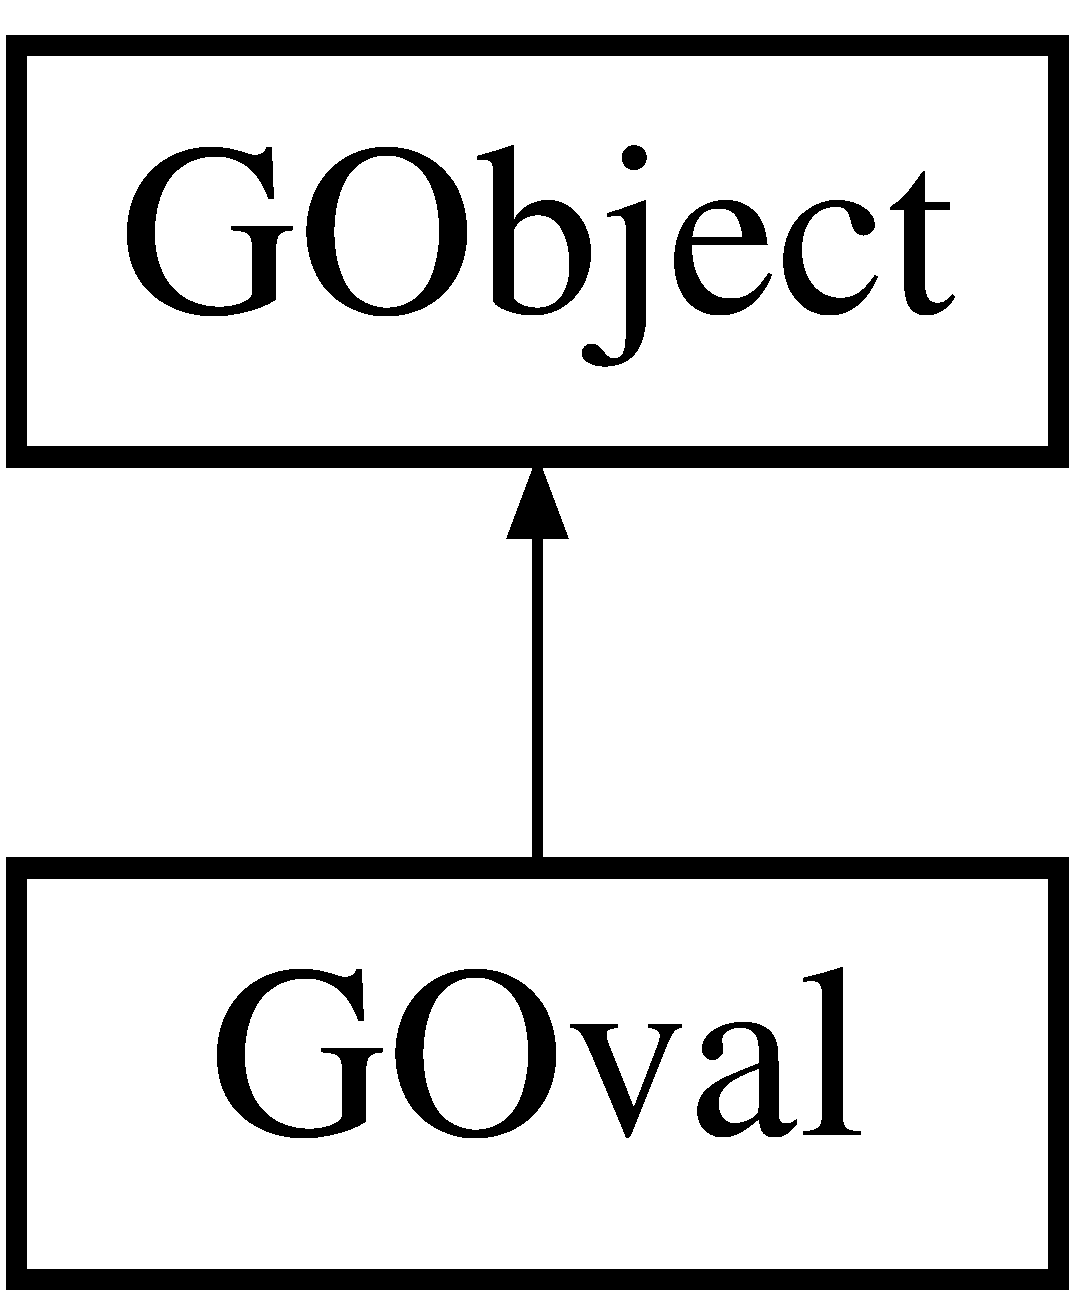
\includegraphics[height=2.000000cm]{classGOval}
\end{center}
\end{figure}
\subsection*{Public Types}
\begin{DoxyCompactItemize}
\item 
enum \mbox{\hyperlink{classGObject_a86e0f5648542856159bb40775c854aa7}{Line\+Style}} \{ \mbox{\hyperlink{classGObject_a86e0f5648542856159bb40775c854aa7acbc84bd5232621834ed31f44d457c1eb}{L\+I\+N\+E\+\_\+\+N\+O\+NE}}, 
\mbox{\hyperlink{classGObject_a86e0f5648542856159bb40775c854aa7a700c78bc2cd76acaab26651bf7b4941f}{L\+I\+N\+E\+\_\+\+S\+O\+L\+ID}}, 
\mbox{\hyperlink{classGObject_a86e0f5648542856159bb40775c854aa7a9ccba0845f785d81d07b333ae1aad84e}{L\+I\+N\+E\+\_\+\+D\+A\+SH}}, 
\mbox{\hyperlink{classGObject_a86e0f5648542856159bb40775c854aa7a8e811c096cb941997f0bfda168bb6df3}{L\+I\+N\+E\+\_\+\+D\+OT}}, 
\mbox{\hyperlink{classGObject_a86e0f5648542856159bb40775c854aa7ada15a2e3d737b2db7706d8300f91b89d}{L\+I\+N\+E\+\_\+\+D\+A\+S\+H\+\_\+\+D\+OT}}, 
\mbox{\hyperlink{classGObject_a86e0f5648542856159bb40775c854aa7aabf4053a73eafa7ba2b7e6d664c74c1d}{L\+I\+N\+E\+\_\+\+D\+A\+S\+H\+\_\+\+D\+O\+T\+\_\+\+D\+OT}}
 \}
\begin{DoxyCompactList}\small\item\em Styles that can be used for the outline around various shapes. \end{DoxyCompactList}\end{DoxyCompactItemize}
\subsection*{Public Member Functions}
\begin{DoxyCompactItemize}
\item 
\mbox{\hyperlink{classGOval_a0dc1da9139884a189b3fd0882c638bfc}{G\+Oval}} (double x=0, double y=0, double width=0, double height=0)
\begin{DoxyCompactList}\small\item\em Constructs a new oval inscribed in the specified rectangle. \end{DoxyCompactList}\item 
virtual bool \mbox{\hyperlink{classGObject_a1dbc9dafaae51958112dbe1267a1f547}{contains}} (const \mbox{\hyperlink{classGPoint}{G\+Point}} \&pt) const
\begin{DoxyCompactList}\small\item\em Returns {\ttfamily true} if the specified point is inside the object. \end{DoxyCompactList}\item 
virtual bool \mbox{\hyperlink{classGOval_aa095a031ab22c150d2d75fdda1c3c8f5}{contains}} (double x, double y) const Q\+\_\+\+D\+E\+C\+L\+\_\+\+O\+V\+E\+R\+R\+I\+DE
\begin{DoxyCompactList}\small\item\em Returns {\ttfamily true} if the specified point is inside the object. \end{DoxyCompactList}\item 
virtual \mbox{\hyperlink{classGPoint}{G\+Point}} \mbox{\hyperlink{classGObject_a0d41183bf6b08de66fe3907551aab0d7}{get\+Bottom\+Right\+Location}} () const
\begin{DoxyCompactList}\small\item\em Returns the x/y coordinates of the bottom/right corner of the object. \end{DoxyCompactList}\item 
virtual double \mbox{\hyperlink{classGObject_a4316a2406c18e1c6d061fe51fd355490}{get\+BottomY}} () const
\begin{DoxyCompactList}\small\item\em Returns the {\itshape y}-\/coordinate of the bottom of the object. \end{DoxyCompactList}\item 
virtual \mbox{\hyperlink{classGRectangle}{G\+Rectangle}} \mbox{\hyperlink{classGObject_a29e6ac35a0b48f491a4c88194cc5da3b}{get\+Bounds}} () const
\begin{DoxyCompactList}\small\item\em Returns the bounding box of this object, which is defined to be the smallest rectangle that covers everything drawn by the figure. \end{DoxyCompactList}\item 
virtual \mbox{\hyperlink{classGPoint}{G\+Point}} \mbox{\hyperlink{classGObject_a0909472e91448470bccdb62ecfb95d8b}{get\+Center\+Location}} () const
\begin{DoxyCompactList}\small\item\em Returns the x/y-\/coordinates of the center of the object. \end{DoxyCompactList}\item 
virtual double \mbox{\hyperlink{classGObject_a04df74355b545e0543112d5b8d924176}{get\+CenterX}} () const
\begin{DoxyCompactList}\small\item\em Returns the {\itshape x}-\/coordinate of the center of the object. \end{DoxyCompactList}\item 
virtual double \mbox{\hyperlink{classGObject_acb3287a3d507025a26f54b895713b947}{get\+CenterY}} () const
\begin{DoxyCompactList}\small\item\em Returns the {\itshape y}-\/coordinate of the center of the object. \end{DoxyCompactList}\item 
virtual std\+::string \mbox{\hyperlink{classGObject_aa061dfa488c31e18549d64363c1d0e34}{get\+Color}} () const
\begin{DoxyCompactList}\small\item\em Returns the color used to display this object. \end{DoxyCompactList}\item 
virtual std\+::string \mbox{\hyperlink{classGObject_a76f6964a11fde7c78e9751be184e1a3c}{get\+Fill\+Color}} () const
\begin{DoxyCompactList}\small\item\em Returns the color used to display the filled region of this object. \end{DoxyCompactList}\item 
virtual double \mbox{\hyperlink{classGObject_a1e7e353362434072875264cf95629f99}{get\+Height}} () const
\begin{DoxyCompactList}\small\item\em Returns the height of this object, which is the same as the height of its bounding box. \end{DoxyCompactList}\item 
virtual \mbox{\hyperlink{classGObject_a86e0f5648542856159bb40775c854aa7}{Line\+Style}} \mbox{\hyperlink{classGObject_aaf1f5ea8281e5e3486662878d26f0a13}{get\+Line\+Style}} () const
\begin{DoxyCompactList}\small\item\em Returns the object\textquotesingle{}s style such as solid or dashed. \end{DoxyCompactList}\item 
virtual double \mbox{\hyperlink{classGObject_a85ff266dc3eb63d9f2d8e5a4487fd3c0}{get\+Line\+Width}} () const
\begin{DoxyCompactList}\small\item\em Returns the width of the line used to draw this object. \end{DoxyCompactList}\item 
virtual \mbox{\hyperlink{classGPoint}{G\+Point}} \mbox{\hyperlink{classGObject_a4f83802015511edeb63b892830812c11}{get\+Location}} () const
\begin{DoxyCompactList}\small\item\em Returns the location of the top-\/left corner of object. \end{DoxyCompactList}\item 
virtual double \mbox{\hyperlink{classGObject_a1ae3fc278cc5b71b9f2d96a8a83cdf26}{get\+Opacity}} () const
\begin{DoxyCompactList}\small\item\em Returns how opaque (non-\/transparent) this object will appear from 0.\+0 (completely transparent) to 1.\+0 (completely opaque, default). \end{DoxyCompactList}\item 
virtual \mbox{\hyperlink{classGCompound}{G\+Compound}} $\ast$ \mbox{\hyperlink{classGObject_a3e53cef70541b1a14eade4ad0984d0b4}{get\+Parent}} () const
\begin{DoxyCompactList}\small\item\em Returns a pointer to the {\ttfamily \mbox{\hyperlink{classGCompound}{G\+Compound}}} that contains this object. \end{DoxyCompactList}\item 
virtual double \mbox{\hyperlink{classGObject_a798cc79daaa10145b28f60bcdfdb0ee9}{get\+RightX}} () const
\begin{DoxyCompactList}\small\item\em Returns the {\itshape x}-\/coordinate of the right side of the object. \end{DoxyCompactList}\item 
virtual \mbox{\hyperlink{classGDimension}{G\+Dimension}} \mbox{\hyperlink{classGObject_a7b4eec96a2bdc6420695d5796a78eea9}{get\+Size}} () const
\begin{DoxyCompactList}\small\item\em Returns the size of the object as a {\ttfamily \mbox{\hyperlink{classGDimension}{G\+Dimension}}}. \end{DoxyCompactList}\item 
virtual std\+::string \mbox{\hyperlink{classGOval_a9896d58fcfebbf1025aeeb5b8b9ede80}{get\+Type}} () const Q\+\_\+\+D\+E\+C\+L\+\_\+\+O\+V\+E\+R\+R\+I\+DE
\begin{DoxyCompactList}\small\item\em Returns the type of the object as a string, such as {\ttfamily \char`\"{}\+G\+Oval\char`\"{}} or {\ttfamily \char`\"{}\+G\+Rect\char`\"{}}. \end{DoxyCompactList}\item 
virtual double \mbox{\hyperlink{classGObject_a0ed2965abd4f5701d2cadf71239faf19}{get\+Width}} () const
\begin{DoxyCompactList}\small\item\em Returns the width of this object, which is equal to the width of the bounding box. \end{DoxyCompactList}\item 
virtual double \mbox{\hyperlink{classGObject_a344385751bee0720059403940d57a13e}{getX}} () const
\begin{DoxyCompactList}\small\item\em Returns the leftmost {\itshape x}-\/coordinate of the object. \end{DoxyCompactList}\item 
virtual double \mbox{\hyperlink{classGObject_aafa51c7f8f38a09febbb9ce7853f77b4}{getY}} () const
\begin{DoxyCompactList}\small\item\em Returns the topmost {\itshape y}-\/coordinate of the object. \end{DoxyCompactList}\item 
virtual bool \mbox{\hyperlink{classGObject_a11c404f106940c201b6f326e0355c150}{is\+Filled}} () const
\begin{DoxyCompactList}\small\item\em Returns {\ttfamily true} if the object is filled with color. \end{DoxyCompactList}\item 
virtual bool \mbox{\hyperlink{classGObject_a9de207581cfa4ca1eaa06da5f29b75fc}{is\+Transformed}} () const
\begin{DoxyCompactList}\small\item\em Returns {\ttfamily true} if this object has been transformed by calling methods such as \mbox{\hyperlink{classGObject_ae1ffaa12185dfd5ba464f7d87c329e26}{rotate()}} or \mbox{\hyperlink{classGObject_ad2e1900f730475c2d044817db03b38d6}{scale()}} on it. \end{DoxyCompactList}\item 
virtual bool \mbox{\hyperlink{classGObject_a9d8a6cfb13917785c143e74d40e4e2be}{is\+Visible}} () const
\begin{DoxyCompactList}\small\item\em Returns {\ttfamily true} if this object is visible on screen. \end{DoxyCompactList}\item 
virtual void \mbox{\hyperlink{classGObject_a5973d8dda83afb36e2c56855515be392}{move}} (double dx, double dy)
\begin{DoxyCompactList}\small\item\em Moves the object on the screen using the displacements {\ttfamily dx} and {\ttfamily dy}. \end{DoxyCompactList}\item 
virtual void \mbox{\hyperlink{classGObject_ac827b978aa122f136a14c198687ad80f}{repaint}} ()
\begin{DoxyCompactList}\small\item\em Instructs the object to redraw itself on screen. \end{DoxyCompactList}\item 
virtual void \mbox{\hyperlink{classGObject_a6022a1fd1e5dcd2fd5585e5a36aa3f37}{reset\+Transform}} ()
\begin{DoxyCompactList}\small\item\em Undoes any previous scale/rotate transformations on this object. \end{DoxyCompactList}\item 
virtual void \mbox{\hyperlink{classGObject_ae1ffaa12185dfd5ba464f7d87c329e26}{rotate}} (double theta)
\begin{DoxyCompactList}\small\item\em Transforms the object by rotating it {\ttfamily theta} degrees counterclockwise around its origin. \end{DoxyCompactList}\item 
virtual void \mbox{\hyperlink{classGObject_ad2e1900f730475c2d044817db03b38d6}{scale}} (double sf)
\begin{DoxyCompactList}\small\item\em Scales the object by the specified scale factor. \end{DoxyCompactList}\item 
virtual void \mbox{\hyperlink{classGObject_a63641f69d610d0b951357d35a0c3b1e3}{scale}} (double sx, double sy)
\begin{DoxyCompactList}\small\item\em Scales the object by the specified scale factors. \end{DoxyCompactList}\item 
void \mbox{\hyperlink{classGObject_ab6747f40313c531c2db32edb5b63b9b7}{send\+Backward}} ()
\begin{DoxyCompactList}\small\item\em Moves this object one step toward the back in the {\itshape z} dimension. \end{DoxyCompactList}\item 
void \mbox{\hyperlink{classGObject_a710b3e449c9facba7847c91ab170d281}{send\+Forward}} ()
\begin{DoxyCompactList}\small\item\em Moves this object one step toward the front in the {\itshape z} dimension. \end{DoxyCompactList}\item 
void \mbox{\hyperlink{classGObject_a0f7f1efbb7fd46dde2867c4ad0330896}{send\+To\+Back}} ()
\begin{DoxyCompactList}\small\item\em Moves this object to the back of the display in the {\itshape z} dimension. \end{DoxyCompactList}\item 
void \mbox{\hyperlink{classGObject_aee33d68488e46827ef55fac07f40a9b2}{send\+To\+Front}} ()
\begin{DoxyCompactList}\small\item\em Moves this object to the front of the display in the {\itshape z} dimension. \end{DoxyCompactList}\item 
virtual void \mbox{\hyperlink{classGObject_a71ff7b16b8f1bdc4a1ce9f30cf8b87d8}{set\+Bottom\+Right\+Location}} (double x, double y)
\begin{DoxyCompactList}\small\item\em Sets the location of the bottom/right of this object. \end{DoxyCompactList}\item 
virtual void \mbox{\hyperlink{classGObject_ac6f7320321182f1d18c1c0fa97d5e941}{set\+Bottom\+Right\+Location}} (const \mbox{\hyperlink{classGPoint}{G\+Point}} \&pt)
\begin{DoxyCompactList}\small\item\em Sets the location of the bottom/right of this object. \end{DoxyCompactList}\item 
virtual void \mbox{\hyperlink{classGObject_a4b20e93c2a2597484f74ee5caa71f41f}{set\+BottomY}} (double y)
\begin{DoxyCompactList}\small\item\em Sets the location of the bottom y-\/coordinate of this object. \end{DoxyCompactList}\item 
virtual void \mbox{\hyperlink{classGObject_a2aae8197624b72265ab83b4f1bc73f2f}{set\+Bounds}} (double x, double y, double width, double height)
\begin{DoxyCompactList}\small\item\em Changes the bounds of this object to the specified values. \end{DoxyCompactList}\item 
virtual void \mbox{\hyperlink{classGObject_acada386653f008cacc7cce86426bef7c}{set\+Bounds}} (const \mbox{\hyperlink{classGRectangle}{G\+Rectangle}} \&size)
\begin{DoxyCompactList}\small\item\em Changes the bounds of this object to the specified rectangle. \end{DoxyCompactList}\item 
virtual void \mbox{\hyperlink{classGObject_a290b47dd8de1be44089f95cb2c47c1de}{set\+Center\+Location}} (double x, double y)
\begin{DoxyCompactList}\small\item\em Sets the location of the center of this object. \end{DoxyCompactList}\item 
virtual void \mbox{\hyperlink{classGObject_a1bedf1b233ecba3f753ec58908a683a6}{set\+Center\+Location}} (const \mbox{\hyperlink{classGPoint}{G\+Point}} \&pt)
\begin{DoxyCompactList}\small\item\em Sets the location of the center of this object. \end{DoxyCompactList}\item 
virtual void \mbox{\hyperlink{classGObject_a2f4936281e056eead00a9186b9ba8af6}{set\+CenterX}} (double x)
\begin{DoxyCompactList}\small\item\em Sets the x-\/coordinate of the center of this object. \end{DoxyCompactList}\item 
virtual void \mbox{\hyperlink{classGObject_aad2a22b4fde88c33306b92aebf641d57}{set\+CenterY}} (double y)
\begin{DoxyCompactList}\small\item\em Sets the y-\/coordinate of the center of this object. \end{DoxyCompactList}\item 
virtual void \mbox{\hyperlink{classGObject_ad57ef49bc31db94e92648aa3737923d6}{set\+Color}} (int r, int g, int b)
\begin{DoxyCompactList}\small\item\em Sets the color used to display this object. \end{DoxyCompactList}\item 
virtual void \mbox{\hyperlink{classGObject_ab1f5cc0f5cc6bbbd716a526c61f1081d}{set\+Color}} (int rgb)
\begin{DoxyCompactList}\small\item\em Sets the color used to display this object. \end{DoxyCompactList}\item 
virtual void \mbox{\hyperlink{classGObject_a61374df6c11b52cfbb0815decdbaebc6}{set\+Color}} (const std\+::string \&color)
\begin{DoxyCompactList}\small\item\em Sets the color used to display this object. \end{DoxyCompactList}\item 
virtual void \mbox{\hyperlink{classGObject_ad767a33971159e9493e221cca4c00ae9}{set\+Fill\+Color}} (int r, int g, int b)
\begin{DoxyCompactList}\small\item\em Sets the color used to display the filled region of this object, if any. \end{DoxyCompactList}\item 
virtual void \mbox{\hyperlink{classGObject_aa59d9775a67fa7df2b24a95cd34840a3}{set\+Fill\+Color}} (int rgb)
\begin{DoxyCompactList}\small\item\em Sets the color used to display the filled region of this object, if any. \end{DoxyCompactList}\item 
virtual void \mbox{\hyperlink{classGObject_adbc18b1a930aadd97d7437f9f7265b96}{set\+Fill\+Color}} (const std\+::string \&color)
\begin{DoxyCompactList}\small\item\em Sets the color used to display the filled region of this object, if any. \end{DoxyCompactList}\item 
virtual void \mbox{\hyperlink{classGObject_a9b82b53362282c6bb7d6947068d2e55b}{set\+Filled}} (bool flag)
\begin{DoxyCompactList}\small\item\em Sets the fill status for the object, where {\ttfamily false} is outlined and {\ttfamily true} is filled. \end{DoxyCompactList}\item 
virtual void \mbox{\hyperlink{classGObject_a2592348886ffea646c6534bf88f7c49d}{set\+Font}} (const Q\+Font \&font)
\begin{DoxyCompactList}\small\item\em Changes the font used to display the object as specified by the given Qt font. \end{DoxyCompactList}\item 
virtual void \mbox{\hyperlink{classGObject_a8e096e8818d838aceae1d46d58fb3a7b}{set\+Font}} (const std\+::string \&font)
\begin{DoxyCompactList}\small\item\em Changes the font used to display the object as specified by the string {\ttfamily font}, which has the following format\+: \end{DoxyCompactList}\item 
virtual void \mbox{\hyperlink{classGObject_ad18e8fab1e02a4e9b75c6730212558eb}{set\+Foreground}} (int r, int g, int b)
\begin{DoxyCompactList}\small\item\em Sets the color used to display this object. \end{DoxyCompactList}\item 
virtual void \mbox{\hyperlink{classGObject_a9eb856b5ff83a19df3831a31f15f4563}{set\+Foreground}} (int rgb)
\begin{DoxyCompactList}\small\item\em Sets the color used to display this object. \end{DoxyCompactList}\item 
virtual void \mbox{\hyperlink{classGObject_af59209aeadea6dfc6d97a2d8531f50e1}{set\+Foreground}} (const std\+::string \&color)
\begin{DoxyCompactList}\small\item\em Sets the color used to display this object. \end{DoxyCompactList}\item 
virtual void \mbox{\hyperlink{classGObject_a9e280bfc4544dfaf8e4376c4e1a74357}{set\+Height}} (double height)
\begin{DoxyCompactList}\small\item\em Changes the height of this object to the specified height without changing its width. \end{DoxyCompactList}\item 
virtual void \mbox{\hyperlink{classGObject_add11575087eb94f1a71faa3f826c6341}{set\+Line\+Style}} (\mbox{\hyperlink{classGObject_a86e0f5648542856159bb40775c854aa7}{Line\+Style}} line\+Style)
\begin{DoxyCompactList}\small\item\em Sets the object\textquotesingle{}s style such as solid (\mbox{\hyperlink{classGObject_a86e0f5648542856159bb40775c854aa7a700c78bc2cd76acaab26651bf7b4941f}{G\+Object\+::\+L\+I\+N\+E\+\_\+\+S\+O\+L\+ID}}) or dashed (\mbox{\hyperlink{classGObject_a86e0f5648542856159bb40775c854aa7a9ccba0845f785d81d07b333ae1aad84e}{G\+Object\+::\+L\+I\+N\+E\+\_\+\+D\+A\+SH}}). \end{DoxyCompactList}\item 
virtual void \mbox{\hyperlink{classGObject_afd6a47c6ea6a1f85ca05a65ba3ff3477}{set\+Line\+Width}} (double line\+Width)
\begin{DoxyCompactList}\small\item\em Sets the width of the line used to draw this object. \end{DoxyCompactList}\item 
virtual void \mbox{\hyperlink{classGObject_a04594e8ba9b98513a64f1da00dcae18c}{set\+Location}} (double x, double y)
\begin{DoxyCompactList}\small\item\em Sets the location of the top-\/left corner of this object to the specified coordinates. \end{DoxyCompactList}\item 
virtual void \mbox{\hyperlink{classGObject_aa8480c0b7166cdf8f784cece06ab353f}{set\+Location}} (const \mbox{\hyperlink{classGPoint}{G\+Point}} \&pt)
\begin{DoxyCompactList}\small\item\em Sets the location of the top-\/left corner of this object to the specified point. \end{DoxyCompactList}\item 
virtual void \mbox{\hyperlink{classGObject_a04af1866cc1bae4a1226695794a50539}{set\+Opacity}} (double opacity)
\begin{DoxyCompactList}\small\item\em Sets how opaque (non-\/transparent) this object will appear from 0.\+0 (completely transparent) to 1.\+0 (completely opaque, default). \end{DoxyCompactList}\item 
virtual void \mbox{\hyperlink{classGObject_a3c90b758cdc2c911c9ef76c4360eb912}{set\+RightX}} (double x)
\begin{DoxyCompactList}\small\item\em Sets the location of the rightmost x-\/coordinate of this object. \end{DoxyCompactList}\item 
virtual void \mbox{\hyperlink{classGObject_aca25d49481f9bf5fc8f7df4c086c4ce7}{set\+Size}} (double width, double height)
\begin{DoxyCompactList}\small\item\em Changes the size of this object to the specified width and height. \end{DoxyCompactList}\item 
virtual void \mbox{\hyperlink{classGObject_ae2b628228f192c2702c4ce941b2af68f}{set\+Size}} (const \mbox{\hyperlink{classGDimension}{G\+Dimension}} \&size)
\begin{DoxyCompactList}\small\item\em Changes the size of this object to the specified width and height. \end{DoxyCompactList}\item 
virtual void \mbox{\hyperlink{classGObject_a88203f28224315d9f4471212f4af8ed3}{set\+Visible}} (bool flag)
\begin{DoxyCompactList}\small\item\em Sets whether this object is visible. \end{DoxyCompactList}\item 
virtual void \mbox{\hyperlink{classGObject_aa3f3fba4cb131baa8696ba01e3bceca1}{set\+Width}} (double width)
\begin{DoxyCompactList}\small\item\em Changes the width of this object to the specified width without changing its height. \end{DoxyCompactList}\item 
virtual void \mbox{\hyperlink{classGObject_a9c18fcc579333bf9653d13ad2b372e39}{setX}} (double x)
\begin{DoxyCompactList}\small\item\em Sets the x location of the left side of this object. \end{DoxyCompactList}\item 
virtual void \mbox{\hyperlink{classGObject_a7d57e2a5c35d27feb58fd498a3cf82b9}{setY}} (double y)
\begin{DoxyCompactList}\small\item\em Sets the y location of the top of this object. \end{DoxyCompactList}\item 
virtual std\+::string \mbox{\hyperlink{classGObject_a1fe5121d6528fdea3f243321b3fa3a49}{to\+String}} () const
\begin{DoxyCompactList}\small\item\em Returns a printable representation of the object. \end{DoxyCompactList}\end{DoxyCompactItemize}
\subsection*{Static Public Member Functions}
\begin{DoxyCompactItemize}
\item 
static bool \mbox{\hyperlink{classGObject_a93be0e1fe1b1bf1a1da732470c94f42b}{is\+Anti\+Aliasing}} ()
\begin{DoxyCompactList}\small\item\em Returns whether we should globally anti-\/alias graphical objects. \end{DoxyCompactList}\item 
static void \mbox{\hyperlink{classGObject_a1e43371668ae850193cebedb44e1bbe3}{set\+Anti\+Aliasing}} (bool value)
\begin{DoxyCompactList}\small\item\em Globally turns on/off the anti-\/aliasing feature that smooths out the edges of onscreen shapes. \end{DoxyCompactList}\end{DoxyCompactItemize}
\subsection*{Protected Member Functions}
\begin{DoxyCompactItemize}
\item 
virtual std\+::string \mbox{\hyperlink{classGObject_a4fcdf8de5c6de92242a975d83d8f23ea}{to\+String\+Extra}} () const
\begin{DoxyCompactList}\small\item\em Returns a string containing any extra unique information about this type of graphical object. \end{DoxyCompactList}\end{DoxyCompactItemize}
\subsection*{Protected Attributes}
\begin{DoxyCompactItemize}
\item 
Q\+Brush \mbox{\hyperlink{classGObject_aab24462ec896b596d99911767b0912d0}{\+\_\+brush}}
\item 
std\+::string \mbox{\hyperlink{classGObject_a1134e770ae4315ea8bc1201e2f21da8b}{\+\_\+color}}
\item 
int \mbox{\hyperlink{classGObject_a003fdd343d9b7505c53a8b7a134200ed}{\+\_\+color\+Int}}
\item 
std\+::string \mbox{\hyperlink{classGObject_a179f8d6cee65cd8a54692e32b224392a}{\+\_\+fill\+Color}}
\item 
int \mbox{\hyperlink{classGObject_a751def333a67d651e5b99cc331ecb496}{\+\_\+fill\+Color\+Int}}
\item 
bool \mbox{\hyperlink{classGObject_ad4a55cbcd61b58a4d49666490bb2f103}{\+\_\+fill\+Flag}}
\item 
std\+::string \mbox{\hyperlink{classGObject_aea76ea1a8b5dd7b0a78653277e63b536}{\+\_\+font}}
\item 
double \mbox{\hyperlink{classGObject_ad05df29e7f27fc504abd743e3d8b4e73}{\+\_\+height}}
\item 
\mbox{\hyperlink{classGObject_a86e0f5648542856159bb40775c854aa7}{Line\+Style}} \mbox{\hyperlink{classGObject_a89bafecaafb7c72d55c7efc10b7d0523}{\+\_\+line\+Style}}
\item 
double \mbox{\hyperlink{classGObject_a16e9033665937f13de2e163dc2184aff}{\+\_\+line\+Width}}
\item 
double \mbox{\hyperlink{classGObject_a20eff8eb7af27182edc9bfc54768b6f3}{\+\_\+opacity}}
\item 
\mbox{\hyperlink{classGCompound}{G\+Compound}} $\ast$ \mbox{\hyperlink{classGObject_ac9452c1eaff70eebddbb318196aa3835}{\+\_\+parent}}
\item 
Q\+Pen \mbox{\hyperlink{classGObject_afb69d172743f868299847174eb1b6bc8}{\+\_\+pen}}
\item 
Q\+Transform \mbox{\hyperlink{classGObject_a475b8860a5f1adb4a1fdc58d1f5c1e32}{\+\_\+transform}}
\item 
bool \mbox{\hyperlink{classGObject_ae4725802fc8d8aaa0ab4bd4781f7e07c}{\+\_\+transformed}}
\item 
bool \mbox{\hyperlink{classGObject_a9312c72508471b7c7a87b540263e1af4}{\+\_\+visible}}
\item 
double \mbox{\hyperlink{classGObject_ab55d85a3371770e6725b1062cf160cd8}{\+\_\+width}}
\item 
double \mbox{\hyperlink{classGObject_a6675b83b27137b8d3aa2ad8133078ea6}{\+\_\+x}}
\item 
double \mbox{\hyperlink{classGObject_a2f0f6aeafddc8a39c578bfa7e22b5f1e}{\+\_\+y}}
\end{DoxyCompactItemize}


\subsection{Detailed Description}
This graphical object subclass represents an oval inscribed in a rectangular box. 

\subsection{Member Enumeration Documentation}
\mbox{\Hypertarget{classGObject_a86e0f5648542856159bb40775c854aa7}\label{classGObject_a86e0f5648542856159bb40775c854aa7}} 
\index{G\+Oval@{G\+Oval}!Line\+Style@{Line\+Style}}
\index{Line\+Style@{Line\+Style}!G\+Oval@{G\+Oval}}
\subsubsection{\texorpdfstring{Line\+Style}{LineStyle}}
{\footnotesize\ttfamily enum \mbox{\hyperlink{classGObject_a86e0f5648542856159bb40775c854aa7}{Line\+Style}}\hspace{0.3cm}{\ttfamily [inherited]}}



Styles that can be used for the outline around various shapes. 

Call set\+Line\+Style on a \mbox{\hyperlink{classGObject}{G\+Object}} and pass one of these values. \begin{DoxyEnumFields}{Enumerator}
\raisebox{\heightof{T}}[0pt][0pt]{\index{L\+I\+N\+E\+\_\+\+N\+O\+NE@{L\+I\+N\+E\+\_\+\+N\+O\+NE}!G\+Oval@{G\+Oval}}\index{G\+Oval@{G\+Oval}!L\+I\+N\+E\+\_\+\+N\+O\+NE@{L\+I\+N\+E\+\_\+\+N\+O\+NE}}}\mbox{\Hypertarget{classGObject_a86e0f5648542856159bb40775c854aa7acbc84bd5232621834ed31f44d457c1eb}\label{classGObject_a86e0f5648542856159bb40775c854aa7acbc84bd5232621834ed31f44d457c1eb}} 
L\+I\+N\+E\+\_\+\+N\+O\+NE&\\
\hline

\raisebox{\heightof{T}}[0pt][0pt]{\index{L\+I\+N\+E\+\_\+\+S\+O\+L\+ID@{L\+I\+N\+E\+\_\+\+S\+O\+L\+ID}!G\+Oval@{G\+Oval}}\index{G\+Oval@{G\+Oval}!L\+I\+N\+E\+\_\+\+S\+O\+L\+ID@{L\+I\+N\+E\+\_\+\+S\+O\+L\+ID}}}\mbox{\Hypertarget{classGObject_a86e0f5648542856159bb40775c854aa7a700c78bc2cd76acaab26651bf7b4941f}\label{classGObject_a86e0f5648542856159bb40775c854aa7a700c78bc2cd76acaab26651bf7b4941f}} 
L\+I\+N\+E\+\_\+\+S\+O\+L\+ID&\\
\hline

\raisebox{\heightof{T}}[0pt][0pt]{\index{L\+I\+N\+E\+\_\+\+D\+A\+SH@{L\+I\+N\+E\+\_\+\+D\+A\+SH}!G\+Oval@{G\+Oval}}\index{G\+Oval@{G\+Oval}!L\+I\+N\+E\+\_\+\+D\+A\+SH@{L\+I\+N\+E\+\_\+\+D\+A\+SH}}}\mbox{\Hypertarget{classGObject_a86e0f5648542856159bb40775c854aa7a9ccba0845f785d81d07b333ae1aad84e}\label{classGObject_a86e0f5648542856159bb40775c854aa7a9ccba0845f785d81d07b333ae1aad84e}} 
L\+I\+N\+E\+\_\+\+D\+A\+SH&\\
\hline

\raisebox{\heightof{T}}[0pt][0pt]{\index{L\+I\+N\+E\+\_\+\+D\+OT@{L\+I\+N\+E\+\_\+\+D\+OT}!G\+Oval@{G\+Oval}}\index{G\+Oval@{G\+Oval}!L\+I\+N\+E\+\_\+\+D\+OT@{L\+I\+N\+E\+\_\+\+D\+OT}}}\mbox{\Hypertarget{classGObject_a86e0f5648542856159bb40775c854aa7a8e811c096cb941997f0bfda168bb6df3}\label{classGObject_a86e0f5648542856159bb40775c854aa7a8e811c096cb941997f0bfda168bb6df3}} 
L\+I\+N\+E\+\_\+\+D\+OT&\\
\hline

\raisebox{\heightof{T}}[0pt][0pt]{\index{L\+I\+N\+E\+\_\+\+D\+A\+S\+H\+\_\+\+D\+OT@{L\+I\+N\+E\+\_\+\+D\+A\+S\+H\+\_\+\+D\+OT}!G\+Oval@{G\+Oval}}\index{G\+Oval@{G\+Oval}!L\+I\+N\+E\+\_\+\+D\+A\+S\+H\+\_\+\+D\+OT@{L\+I\+N\+E\+\_\+\+D\+A\+S\+H\+\_\+\+D\+OT}}}\mbox{\Hypertarget{classGObject_a86e0f5648542856159bb40775c854aa7ada15a2e3d737b2db7706d8300f91b89d}\label{classGObject_a86e0f5648542856159bb40775c854aa7ada15a2e3d737b2db7706d8300f91b89d}} 
L\+I\+N\+E\+\_\+\+D\+A\+S\+H\+\_\+\+D\+OT&\\
\hline

\raisebox{\heightof{T}}[0pt][0pt]{\index{L\+I\+N\+E\+\_\+\+D\+A\+S\+H\+\_\+\+D\+O\+T\+\_\+\+D\+OT@{L\+I\+N\+E\+\_\+\+D\+A\+S\+H\+\_\+\+D\+O\+T\+\_\+\+D\+OT}!G\+Oval@{G\+Oval}}\index{G\+Oval@{G\+Oval}!L\+I\+N\+E\+\_\+\+D\+A\+S\+H\+\_\+\+D\+O\+T\+\_\+\+D\+OT@{L\+I\+N\+E\+\_\+\+D\+A\+S\+H\+\_\+\+D\+O\+T\+\_\+\+D\+OT}}}\mbox{\Hypertarget{classGObject_a86e0f5648542856159bb40775c854aa7aabf4053a73eafa7ba2b7e6d664c74c1d}\label{classGObject_a86e0f5648542856159bb40775c854aa7aabf4053a73eafa7ba2b7e6d664c74c1d}} 
L\+I\+N\+E\+\_\+\+D\+A\+S\+H\+\_\+\+D\+O\+T\+\_\+\+D\+OT&\\
\hline

\end{DoxyEnumFields}


\subsection{Constructor \& Destructor Documentation}
\mbox{\Hypertarget{classGOval_a0dc1da9139884a189b3fd0882c638bfc}\label{classGOval_a0dc1da9139884a189b3fd0882c638bfc}} 
\index{G\+Oval@{G\+Oval}!G\+Oval@{G\+Oval}}
\index{G\+Oval@{G\+Oval}!G\+Oval@{G\+Oval}}
\subsubsection{\texorpdfstring{G\+Oval()}{GOval()}}
{\footnotesize\ttfamily \mbox{\hyperlink{classGOval}{G\+Oval}} (\begin{DoxyParamCaption}\item[{double}]{x = {\ttfamily 0},  }\item[{double}]{y = {\ttfamily 0},  }\item[{double}]{width = {\ttfamily 0},  }\item[{double}]{height = {\ttfamily 0} }\end{DoxyParamCaption})}



Constructs a new oval inscribed in the specified rectangle. 

By default, the oval is positioned at the origin, but you can pass coordinates {\ttfamily x} and {\ttfamily y}. 

\subsection{Member Function Documentation}
\mbox{\Hypertarget{classGObject_a1dbc9dafaae51958112dbe1267a1f547}\label{classGObject_a1dbc9dafaae51958112dbe1267a1f547}} 
\index{G\+Oval@{G\+Oval}!contains@{contains}}
\index{contains@{contains}!G\+Oval@{G\+Oval}}
\subsubsection{\texorpdfstring{contains()}{contains()}\hspace{0.1cm}{\footnotesize\ttfamily [1/2]}}
{\footnotesize\ttfamily bool contains (\begin{DoxyParamCaption}\item[{const \mbox{\hyperlink{classGPoint}{G\+Point}} \&}]{pt }\end{DoxyParamCaption}) const\hspace{0.3cm}{\ttfamily [virtual]}, {\ttfamily [inherited]}}



Returns {\ttfamily true} if the specified point is inside the object. 

\mbox{\Hypertarget{classGOval_aa095a031ab22c150d2d75fdda1c3c8f5}\label{classGOval_aa095a031ab22c150d2d75fdda1c3c8f5}} 
\index{G\+Oval@{G\+Oval}!contains@{contains}}
\index{contains@{contains}!G\+Oval@{G\+Oval}}
\subsubsection{\texorpdfstring{contains()}{contains()}\hspace{0.1cm}{\footnotesize\ttfamily [2/2]}}
{\footnotesize\ttfamily bool contains (\begin{DoxyParamCaption}\item[{double}]{x,  }\item[{double}]{y }\end{DoxyParamCaption}) const\hspace{0.3cm}{\ttfamily [virtual]}}



Returns {\ttfamily true} if the specified point is inside the object. 



Reimplemented from \mbox{\hyperlink{classGObject_abb6a5d7c03e6eaaae97264c4799ce7c3}{G\+Object}}.

\mbox{\Hypertarget{classGObject_a0d41183bf6b08de66fe3907551aab0d7}\label{classGObject_a0d41183bf6b08de66fe3907551aab0d7}} 
\index{G\+Oval@{G\+Oval}!get\+Bottom\+Right\+Location@{get\+Bottom\+Right\+Location}}
\index{get\+Bottom\+Right\+Location@{get\+Bottom\+Right\+Location}!G\+Oval@{G\+Oval}}
\subsubsection{\texorpdfstring{get\+Bottom\+Right\+Location()}{getBottomRightLocation()}}
{\footnotesize\ttfamily \mbox{\hyperlink{classGPoint}{G\+Point}} get\+Bottom\+Right\+Location (\begin{DoxyParamCaption}{ }\end{DoxyParamCaption}) const\hspace{0.3cm}{\ttfamily [virtual]}, {\ttfamily [inherited]}}



Returns the x/y coordinates of the bottom/right corner of the object. 

\mbox{\Hypertarget{classGObject_a4316a2406c18e1c6d061fe51fd355490}\label{classGObject_a4316a2406c18e1c6d061fe51fd355490}} 
\index{G\+Oval@{G\+Oval}!get\+BottomY@{get\+BottomY}}
\index{get\+BottomY@{get\+BottomY}!G\+Oval@{G\+Oval}}
\subsubsection{\texorpdfstring{get\+Bottom\+Y()}{getBottomY()}}
{\footnotesize\ttfamily double get\+BottomY (\begin{DoxyParamCaption}{ }\end{DoxyParamCaption}) const\hspace{0.3cm}{\ttfamily [virtual]}, {\ttfamily [inherited]}}



Returns the {\itshape y}-\/coordinate of the bottom of the object. 

Equivalent to the top y-\/coordinate plus the object\textquotesingle{}s height. \mbox{\Hypertarget{classGObject_a29e6ac35a0b48f491a4c88194cc5da3b}\label{classGObject_a29e6ac35a0b48f491a4c88194cc5da3b}} 
\index{G\+Oval@{G\+Oval}!get\+Bounds@{get\+Bounds}}
\index{get\+Bounds@{get\+Bounds}!G\+Oval@{G\+Oval}}
\subsubsection{\texorpdfstring{get\+Bounds()}{getBounds()}}
{\footnotesize\ttfamily \mbox{\hyperlink{classGRectangle}{G\+Rectangle}} get\+Bounds (\begin{DoxyParamCaption}{ }\end{DoxyParamCaption}) const\hspace{0.3cm}{\ttfamily [virtual]}, {\ttfamily [inherited]}}



Returns the bounding box of this object, which is defined to be the smallest rectangle that covers everything drawn by the figure. 

The coordinates of this rectangle do not necessarily match the location returned by {\ttfamily get\+Location}. Given a {\ttfamily \mbox{\hyperlink{classGText}{G\+Text}}} object, for example, {\ttfamily get\+Location} returns the coordinates of the point on the baseline at which the string begins; the {\ttfamily get\+Bounds} method, by contrast, returns a rectangle that covers the entire window area occupied by the string. 

Reimplemented in \mbox{\hyperlink{classGText_a2f46ec8a3b533c690b3b3e56d4f34afe}{G\+Text}}, \mbox{\hyperlink{classGPolygon_a29e6ac35a0b48f491a4c88194cc5da3b}{G\+Polygon}}, \mbox{\hyperlink{classGLine_a2f46ec8a3b533c690b3b3e56d4f34afe}{G\+Line}}, \mbox{\hyperlink{classGCompound_a2f46ec8a3b533c690b3b3e56d4f34afe}{G\+Compound}}, and \mbox{\hyperlink{classGArc_a2f46ec8a3b533c690b3b3e56d4f34afe}{G\+Arc}}.

\mbox{\Hypertarget{classGObject_a0909472e91448470bccdb62ecfb95d8b}\label{classGObject_a0909472e91448470bccdb62ecfb95d8b}} 
\index{G\+Oval@{G\+Oval}!get\+Center\+Location@{get\+Center\+Location}}
\index{get\+Center\+Location@{get\+Center\+Location}!G\+Oval@{G\+Oval}}
\subsubsection{\texorpdfstring{get\+Center\+Location()}{getCenterLocation()}}
{\footnotesize\ttfamily \mbox{\hyperlink{classGPoint}{G\+Point}} get\+Center\+Location (\begin{DoxyParamCaption}{ }\end{DoxyParamCaption}) const\hspace{0.3cm}{\ttfamily [virtual]}, {\ttfamily [inherited]}}



Returns the x/y-\/coordinates of the center of the object. 

Equivalent to the top/left plus half the object\textquotesingle{}s size. \mbox{\Hypertarget{classGObject_a04df74355b545e0543112d5b8d924176}\label{classGObject_a04df74355b545e0543112d5b8d924176}} 
\index{G\+Oval@{G\+Oval}!get\+CenterX@{get\+CenterX}}
\index{get\+CenterX@{get\+CenterX}!G\+Oval@{G\+Oval}}
\subsubsection{\texorpdfstring{get\+Center\+X()}{getCenterX()}}
{\footnotesize\ttfamily double get\+CenterX (\begin{DoxyParamCaption}{ }\end{DoxyParamCaption}) const\hspace{0.3cm}{\ttfamily [virtual]}, {\ttfamily [inherited]}}



Returns the {\itshape x}-\/coordinate of the center of the object. 

Equivalent to the top/left plus half the object\textquotesingle{}s width. \mbox{\Hypertarget{classGObject_acb3287a3d507025a26f54b895713b947}\label{classGObject_acb3287a3d507025a26f54b895713b947}} 
\index{G\+Oval@{G\+Oval}!get\+CenterY@{get\+CenterY}}
\index{get\+CenterY@{get\+CenterY}!G\+Oval@{G\+Oval}}
\subsubsection{\texorpdfstring{get\+Center\+Y()}{getCenterY()}}
{\footnotesize\ttfamily double get\+CenterY (\begin{DoxyParamCaption}{ }\end{DoxyParamCaption}) const\hspace{0.3cm}{\ttfamily [virtual]}, {\ttfamily [inherited]}}



Returns the {\itshape y}-\/coordinate of the center of the object. 

Equivalent to the top/left plus half the object\textquotesingle{}s height. \mbox{\Hypertarget{classGObject_aa061dfa488c31e18549d64363c1d0e34}\label{classGObject_aa061dfa488c31e18549d64363c1d0e34}} 
\index{G\+Oval@{G\+Oval}!get\+Color@{get\+Color}}
\index{get\+Color@{get\+Color}!G\+Oval@{G\+Oval}}
\subsubsection{\texorpdfstring{get\+Color()}{getColor()}}
{\footnotesize\ttfamily std\+::string get\+Color (\begin{DoxyParamCaption}{ }\end{DoxyParamCaption}) const\hspace{0.3cm}{\ttfamily [virtual]}, {\ttfamily [inherited]}}



Returns the color used to display this object. 

This color is always returned as a string in the form {\ttfamily \char`\"{}\#rrggbb\char`\"{}}, where {\ttfamily rr}, {\ttfamily gg}, and {\ttfamily bb} are the red, green, and blue components of the color, expressed as two-\/digit hexadecimal values. \mbox{\Hypertarget{classGObject_a76f6964a11fde7c78e9751be184e1a3c}\label{classGObject_a76f6964a11fde7c78e9751be184e1a3c}} 
\index{G\+Oval@{G\+Oval}!get\+Fill\+Color@{get\+Fill\+Color}}
\index{get\+Fill\+Color@{get\+Fill\+Color}!G\+Oval@{G\+Oval}}
\subsubsection{\texorpdfstring{get\+Fill\+Color()}{getFillColor()}}
{\footnotesize\ttfamily std\+::string get\+Fill\+Color (\begin{DoxyParamCaption}{ }\end{DoxyParamCaption}) const\hspace{0.3cm}{\ttfamily [virtual]}, {\ttfamily [inherited]}}



Returns the color used to display the filled region of this object. 

If none has been set, returns the empty string. \mbox{\Hypertarget{classGObject_a1e7e353362434072875264cf95629f99}\label{classGObject_a1e7e353362434072875264cf95629f99}} 
\index{G\+Oval@{G\+Oval}!get\+Height@{get\+Height}}
\index{get\+Height@{get\+Height}!G\+Oval@{G\+Oval}}
\subsubsection{\texorpdfstring{get\+Height()}{getHeight()}}
{\footnotesize\ttfamily double get\+Height (\begin{DoxyParamCaption}{ }\end{DoxyParamCaption}) const\hspace{0.3cm}{\ttfamily [virtual]}, {\ttfamily [inherited]}}



Returns the height of this object, which is the same as the height of its bounding box. 



Reimplemented in \mbox{\hyperlink{classGPolygon_a1e7e353362434072875264cf95629f99}{G\+Polygon}}, and \mbox{\hyperlink{classGLine_a423f17d4aeb66feb0d148fd23af335b7}{G\+Line}}.

\mbox{\Hypertarget{classGObject_aaf1f5ea8281e5e3486662878d26f0a13}\label{classGObject_aaf1f5ea8281e5e3486662878d26f0a13}} 
\index{G\+Oval@{G\+Oval}!get\+Line\+Style@{get\+Line\+Style}}
\index{get\+Line\+Style@{get\+Line\+Style}!G\+Oval@{G\+Oval}}
\subsubsection{\texorpdfstring{get\+Line\+Style()}{getLineStyle()}}
{\footnotesize\ttfamily \mbox{\hyperlink{classGObject_a86e0f5648542856159bb40775c854aa7}{G\+Object\+::\+Line\+Style}} get\+Line\+Style (\begin{DoxyParamCaption}{ }\end{DoxyParamCaption}) const\hspace{0.3cm}{\ttfamily [virtual]}, {\ttfamily [inherited]}}



Returns the object\textquotesingle{}s style such as solid or dashed. 

\mbox{\Hypertarget{classGObject_a85ff266dc3eb63d9f2d8e5a4487fd3c0}\label{classGObject_a85ff266dc3eb63d9f2d8e5a4487fd3c0}} 
\index{G\+Oval@{G\+Oval}!get\+Line\+Width@{get\+Line\+Width}}
\index{get\+Line\+Width@{get\+Line\+Width}!G\+Oval@{G\+Oval}}
\subsubsection{\texorpdfstring{get\+Line\+Width()}{getLineWidth()}}
{\footnotesize\ttfamily double get\+Line\+Width (\begin{DoxyParamCaption}{ }\end{DoxyParamCaption}) const\hspace{0.3cm}{\ttfamily [virtual]}, {\ttfamily [inherited]}}



Returns the width of the line used to draw this object. 

\begin{DoxyReturn}{Returns}
default 1 
\end{DoxyReturn}
\mbox{\Hypertarget{classGObject_a4f83802015511edeb63b892830812c11}\label{classGObject_a4f83802015511edeb63b892830812c11}} 
\index{G\+Oval@{G\+Oval}!get\+Location@{get\+Location}}
\index{get\+Location@{get\+Location}!G\+Oval@{G\+Oval}}
\subsubsection{\texorpdfstring{get\+Location()}{getLocation()}}
{\footnotesize\ttfamily \mbox{\hyperlink{classGPoint}{G\+Point}} get\+Location (\begin{DoxyParamCaption}{ }\end{DoxyParamCaption}) const\hspace{0.3cm}{\ttfamily [virtual]}, {\ttfamily [inherited]}}



Returns the location of the top-\/left corner of object. 

\mbox{\Hypertarget{classGObject_a1ae3fc278cc5b71b9f2d96a8a83cdf26}\label{classGObject_a1ae3fc278cc5b71b9f2d96a8a83cdf26}} 
\index{G\+Oval@{G\+Oval}!get\+Opacity@{get\+Opacity}}
\index{get\+Opacity@{get\+Opacity}!G\+Oval@{G\+Oval}}
\subsubsection{\texorpdfstring{get\+Opacity()}{getOpacity()}}
{\footnotesize\ttfamily double get\+Opacity (\begin{DoxyParamCaption}{ }\end{DoxyParamCaption}) const\hspace{0.3cm}{\ttfamily [virtual]}, {\ttfamily [inherited]}}



Returns how opaque (non-\/transparent) this object will appear from 0.\+0 (completely transparent) to 1.\+0 (completely opaque, default). 

\mbox{\Hypertarget{classGObject_a3e53cef70541b1a14eade4ad0984d0b4}\label{classGObject_a3e53cef70541b1a14eade4ad0984d0b4}} 
\index{G\+Oval@{G\+Oval}!get\+Parent@{get\+Parent}}
\index{get\+Parent@{get\+Parent}!G\+Oval@{G\+Oval}}
\subsubsection{\texorpdfstring{get\+Parent()}{getParent()}}
{\footnotesize\ttfamily \mbox{\hyperlink{classGCompound}{G\+Compound}} $\ast$ get\+Parent (\begin{DoxyParamCaption}{ }\end{DoxyParamCaption}) const\hspace{0.3cm}{\ttfamily [virtual]}, {\ttfamily [inherited]}}



Returns a pointer to the {\ttfamily \mbox{\hyperlink{classGCompound}{G\+Compound}}} that contains this object. 

Every {\ttfamily \mbox{\hyperlink{classGWindow}{G\+Window}}} is initialized to contain a single {\ttfamily \mbox{\hyperlink{classGCompound}{G\+Compound}}} that is aligned with the window. Adding objects to the window adds them to that {\ttfamily \mbox{\hyperlink{classGCompound}{G\+Compound}}}, which means that every object you add to the window has a parent. Calling {\ttfamily get\+Parent} on the top-\/level {\ttfamily \mbox{\hyperlink{classGCompound}{G\+Compound}}} returns {\ttfamily nullptr}. \mbox{\Hypertarget{classGObject_a798cc79daaa10145b28f60bcdfdb0ee9}\label{classGObject_a798cc79daaa10145b28f60bcdfdb0ee9}} 
\index{G\+Oval@{G\+Oval}!get\+RightX@{get\+RightX}}
\index{get\+RightX@{get\+RightX}!G\+Oval@{G\+Oval}}
\subsubsection{\texorpdfstring{get\+Right\+X()}{getRightX()}}
{\footnotesize\ttfamily double get\+RightX (\begin{DoxyParamCaption}{ }\end{DoxyParamCaption}) const\hspace{0.3cm}{\ttfamily [virtual]}, {\ttfamily [inherited]}}



Returns the {\itshape x}-\/coordinate of the right side of the object. 

Equivalent to the left x-\/coordinate plus the object\textquotesingle{}s width. \mbox{\Hypertarget{classGObject_a7b4eec96a2bdc6420695d5796a78eea9}\label{classGObject_a7b4eec96a2bdc6420695d5796a78eea9}} 
\index{G\+Oval@{G\+Oval}!get\+Size@{get\+Size}}
\index{get\+Size@{get\+Size}!G\+Oval@{G\+Oval}}
\subsubsection{\texorpdfstring{get\+Size()}{getSize()}}
{\footnotesize\ttfamily \mbox{\hyperlink{classGDimension}{G\+Dimension}} get\+Size (\begin{DoxyParamCaption}{ }\end{DoxyParamCaption}) const\hspace{0.3cm}{\ttfamily [virtual]}, {\ttfamily [inherited]}}



Returns the size of the object as a {\ttfamily \mbox{\hyperlink{classGDimension}{G\+Dimension}}}. 

\mbox{\Hypertarget{classGOval_a9896d58fcfebbf1025aeeb5b8b9ede80}\label{classGOval_a9896d58fcfebbf1025aeeb5b8b9ede80}} 
\index{G\+Oval@{G\+Oval}!get\+Type@{get\+Type}}
\index{get\+Type@{get\+Type}!G\+Oval@{G\+Oval}}
\subsubsection{\texorpdfstring{get\+Type()}{getType()}}
{\footnotesize\ttfamily std\+::string get\+Type (\begin{DoxyParamCaption}{ }\end{DoxyParamCaption}) const\hspace{0.3cm}{\ttfamily [virtual]}}



Returns the type of the object as a string, such as {\ttfamily \char`\"{}\+G\+Oval\char`\"{}} or {\ttfamily \char`\"{}\+G\+Rect\char`\"{}}. 

Each \mbox{\hyperlink{classGObject}{G\+Object}} subtype must override this method. 

Implements \mbox{\hyperlink{classGObject_a799e073a127b428cc841086d42ea4fed}{G\+Object}}.

\mbox{\Hypertarget{classGObject_a0ed2965abd4f5701d2cadf71239faf19}\label{classGObject_a0ed2965abd4f5701d2cadf71239faf19}} 
\index{G\+Oval@{G\+Oval}!get\+Width@{get\+Width}}
\index{get\+Width@{get\+Width}!G\+Oval@{G\+Oval}}
\subsubsection{\texorpdfstring{get\+Width()}{getWidth()}}
{\footnotesize\ttfamily double get\+Width (\begin{DoxyParamCaption}{ }\end{DoxyParamCaption}) const\hspace{0.3cm}{\ttfamily [virtual]}, {\ttfamily [inherited]}}



Returns the width of this object, which is equal to the width of the bounding box. 



Reimplemented in \mbox{\hyperlink{classGPolygon_a0ed2965abd4f5701d2cadf71239faf19}{G\+Polygon}}, and \mbox{\hyperlink{classGLine_a04bee94b66c8f921cd8611be2460ba9d}{G\+Line}}.

\mbox{\Hypertarget{classGObject_a344385751bee0720059403940d57a13e}\label{classGObject_a344385751bee0720059403940d57a13e}} 
\index{G\+Oval@{G\+Oval}!getX@{getX}}
\index{getX@{getX}!G\+Oval@{G\+Oval}}
\subsubsection{\texorpdfstring{get\+X()}{getX()}}
{\footnotesize\ttfamily double getX (\begin{DoxyParamCaption}{ }\end{DoxyParamCaption}) const\hspace{0.3cm}{\ttfamily [virtual]}, {\ttfamily [inherited]}}



Returns the leftmost {\itshape x}-\/coordinate of the object. 

\mbox{\Hypertarget{classGObject_aafa51c7f8f38a09febbb9ce7853f77b4}\label{classGObject_aafa51c7f8f38a09febbb9ce7853f77b4}} 
\index{G\+Oval@{G\+Oval}!getY@{getY}}
\index{getY@{getY}!G\+Oval@{G\+Oval}}
\subsubsection{\texorpdfstring{get\+Y()}{getY()}}
{\footnotesize\ttfamily double getY (\begin{DoxyParamCaption}{ }\end{DoxyParamCaption}) const\hspace{0.3cm}{\ttfamily [virtual]}, {\ttfamily [inherited]}}



Returns the topmost {\itshape y}-\/coordinate of the object. 

\mbox{\Hypertarget{classGObject_a93be0e1fe1b1bf1a1da732470c94f42b}\label{classGObject_a93be0e1fe1b1bf1a1da732470c94f42b}} 
\index{G\+Oval@{G\+Oval}!is\+Anti\+Aliasing@{is\+Anti\+Aliasing}}
\index{is\+Anti\+Aliasing@{is\+Anti\+Aliasing}!G\+Oval@{G\+Oval}}
\subsubsection{\texorpdfstring{is\+Anti\+Aliasing()}{isAntiAliasing()}}
{\footnotesize\ttfamily bool is\+Anti\+Aliasing (\begin{DoxyParamCaption}{ }\end{DoxyParamCaption})\hspace{0.3cm}{\ttfamily [static]}, {\ttfamily [inherited]}}



Returns whether we should globally anti-\/alias graphical objects. 

On by default. \mbox{\Hypertarget{classGObject_a11c404f106940c201b6f326e0355c150}\label{classGObject_a11c404f106940c201b6f326e0355c150}} 
\index{G\+Oval@{G\+Oval}!is\+Filled@{is\+Filled}}
\index{is\+Filled@{is\+Filled}!G\+Oval@{G\+Oval}}
\subsubsection{\texorpdfstring{is\+Filled()}{isFilled()}}
{\footnotesize\ttfamily bool is\+Filled (\begin{DoxyParamCaption}{ }\end{DoxyParamCaption}) const\hspace{0.3cm}{\ttfamily [virtual]}, {\ttfamily [inherited]}}



Returns {\ttfamily true} if the object is filled with color. 

\mbox{\Hypertarget{classGObject_a9de207581cfa4ca1eaa06da5f29b75fc}\label{classGObject_a9de207581cfa4ca1eaa06da5f29b75fc}} 
\index{G\+Oval@{G\+Oval}!is\+Transformed@{is\+Transformed}}
\index{is\+Transformed@{is\+Transformed}!G\+Oval@{G\+Oval}}
\subsubsection{\texorpdfstring{is\+Transformed()}{isTransformed()}}
{\footnotesize\ttfamily bool is\+Transformed (\begin{DoxyParamCaption}{ }\end{DoxyParamCaption}) const\hspace{0.3cm}{\ttfamily [virtual]}, {\ttfamily [inherited]}}



Returns {\ttfamily true} if this object has been transformed by calling methods such as \mbox{\hyperlink{classGObject_ae1ffaa12185dfd5ba464f7d87c329e26}{rotate()}} or \mbox{\hyperlink{classGObject_ad2e1900f730475c2d044817db03b38d6}{scale()}} on it. 

Certain operations (such as set\+Size) cannot be performed after a graphical object has been transformed. \mbox{\Hypertarget{classGObject_a9d8a6cfb13917785c143e74d40e4e2be}\label{classGObject_a9d8a6cfb13917785c143e74d40e4e2be}} 
\index{G\+Oval@{G\+Oval}!is\+Visible@{is\+Visible}}
\index{is\+Visible@{is\+Visible}!G\+Oval@{G\+Oval}}
\subsubsection{\texorpdfstring{is\+Visible()}{isVisible()}}
{\footnotesize\ttfamily bool is\+Visible (\begin{DoxyParamCaption}{ }\end{DoxyParamCaption}) const\hspace{0.3cm}{\ttfamily [virtual]}, {\ttfamily [inherited]}}



Returns {\ttfamily true} if this object is visible on screen. 

\mbox{\Hypertarget{classGObject_a5973d8dda83afb36e2c56855515be392}\label{classGObject_a5973d8dda83afb36e2c56855515be392}} 
\index{G\+Oval@{G\+Oval}!move@{move}}
\index{move@{move}!G\+Oval@{G\+Oval}}
\subsubsection{\texorpdfstring{move()}{move()}}
{\footnotesize\ttfamily void move (\begin{DoxyParamCaption}\item[{double}]{dx,  }\item[{double}]{dy }\end{DoxyParamCaption})\hspace{0.3cm}{\ttfamily [virtual]}, {\ttfamily [inherited]}}



Moves the object on the screen using the displacements {\ttfamily dx} and {\ttfamily dy}. 

\mbox{\Hypertarget{classGObject_ac827b978aa122f136a14c198687ad80f}\label{classGObject_ac827b978aa122f136a14c198687ad80f}} 
\index{G\+Oval@{G\+Oval}!repaint@{repaint}}
\index{repaint@{repaint}!G\+Oval@{G\+Oval}}
\subsubsection{\texorpdfstring{repaint()}{repaint()}}
{\footnotesize\ttfamily void repaint (\begin{DoxyParamCaption}{ }\end{DoxyParamCaption})\hspace{0.3cm}{\ttfamily [virtual]}, {\ttfamily [inherited]}}



Instructs the object to redraw itself on screen. 



Reimplemented in \mbox{\hyperlink{classGCompound_ac827b978aa122f136a14c198687ad80f}{G\+Compound}}.

\mbox{\Hypertarget{classGObject_a6022a1fd1e5dcd2fd5585e5a36aa3f37}\label{classGObject_a6022a1fd1e5dcd2fd5585e5a36aa3f37}} 
\index{G\+Oval@{G\+Oval}!reset\+Transform@{reset\+Transform}}
\index{reset\+Transform@{reset\+Transform}!G\+Oval@{G\+Oval}}
\subsubsection{\texorpdfstring{reset\+Transform()}{resetTransform()}}
{\footnotesize\ttfamily void reset\+Transform (\begin{DoxyParamCaption}{ }\end{DoxyParamCaption})\hspace{0.3cm}{\ttfamily [virtual]}, {\ttfamily [inherited]}}



Undoes any previous scale/rotate transformations on this object. 

\mbox{\Hypertarget{classGObject_ae1ffaa12185dfd5ba464f7d87c329e26}\label{classGObject_ae1ffaa12185dfd5ba464f7d87c329e26}} 
\index{G\+Oval@{G\+Oval}!rotate@{rotate}}
\index{rotate@{rotate}!G\+Oval@{G\+Oval}}
\subsubsection{\texorpdfstring{rotate()}{rotate()}}
{\footnotesize\ttfamily void rotate (\begin{DoxyParamCaption}\item[{double}]{theta }\end{DoxyParamCaption})\hspace{0.3cm}{\ttfamily [virtual]}, {\ttfamily [inherited]}}



Transforms the object by rotating it {\ttfamily theta} degrees counterclockwise around its origin. 

After calling this method on a graphical object, {\ttfamily is\+Transformed} will return {\ttfamily true} for that object unless you subsequently call {\ttfamily reset\+Transform} on it. \mbox{\Hypertarget{classGObject_ad2e1900f730475c2d044817db03b38d6}\label{classGObject_ad2e1900f730475c2d044817db03b38d6}} 
\index{G\+Oval@{G\+Oval}!scale@{scale}}
\index{scale@{scale}!G\+Oval@{G\+Oval}}
\subsubsection{\texorpdfstring{scale()}{scale()}\hspace{0.1cm}{\footnotesize\ttfamily [1/2]}}
{\footnotesize\ttfamily void scale (\begin{DoxyParamCaption}\item[{double}]{sf }\end{DoxyParamCaption})\hspace{0.3cm}{\ttfamily [virtual]}, {\ttfamily [inherited]}}



Scales the object by the specified scale factor. 

This form scales the object by {\ttfamily sf} in both dimensions, so that invoking {\ttfamily gobj-\/$>$scale(2);} doubles the size of the object. After calling this method on a graphical object, {\ttfamily is\+Transformed} will return {\ttfamily true} for that object unless you subsequently call {\ttfamily reset\+Transform} on it. \mbox{\Hypertarget{classGObject_a63641f69d610d0b951357d35a0c3b1e3}\label{classGObject_a63641f69d610d0b951357d35a0c3b1e3}} 
\index{G\+Oval@{G\+Oval}!scale@{scale}}
\index{scale@{scale}!G\+Oval@{G\+Oval}}
\subsubsection{\texorpdfstring{scale()}{scale()}\hspace{0.1cm}{\footnotesize\ttfamily [2/2]}}
{\footnotesize\ttfamily void scale (\begin{DoxyParamCaption}\item[{double}]{sx,  }\item[{double}]{sy }\end{DoxyParamCaption})\hspace{0.3cm}{\ttfamily [virtual]}, {\ttfamily [inherited]}}



Scales the object by the specified scale factors. 

For example, {\ttfamily gobj-\/$>$scale(2, 2);} doubles the size of the object. This form applies independent scale factors to the {\itshape x} and {\itshape y} dimensions. After calling this method on a graphical object, {\ttfamily is\+Transformed} will return {\ttfamily true} for that object unless you subsequently call {\ttfamily reset\+Transform} on it. \mbox{\Hypertarget{classGObject_ab6747f40313c531c2db32edb5b63b9b7}\label{classGObject_ab6747f40313c531c2db32edb5b63b9b7}} 
\index{G\+Oval@{G\+Oval}!send\+Backward@{send\+Backward}}
\index{send\+Backward@{send\+Backward}!G\+Oval@{G\+Oval}}
\subsubsection{\texorpdfstring{send\+Backward()}{sendBackward()}}
{\footnotesize\ttfamily void send\+Backward (\begin{DoxyParamCaption}{ }\end{DoxyParamCaption})\hspace{0.3cm}{\ttfamily [inherited]}}



Moves this object one step toward the back in the {\itshape z} dimension. 

If it was already at the back of the stack, nothing happens. \mbox{\Hypertarget{classGObject_a710b3e449c9facba7847c91ab170d281}\label{classGObject_a710b3e449c9facba7847c91ab170d281}} 
\index{G\+Oval@{G\+Oval}!send\+Forward@{send\+Forward}}
\index{send\+Forward@{send\+Forward}!G\+Oval@{G\+Oval}}
\subsubsection{\texorpdfstring{send\+Forward()}{sendForward()}}
{\footnotesize\ttfamily void send\+Forward (\begin{DoxyParamCaption}{ }\end{DoxyParamCaption})\hspace{0.3cm}{\ttfamily [inherited]}}



Moves this object one step toward the front in the {\itshape z} dimension. 

If it was already at the front of the stack, nothing happens. \mbox{\Hypertarget{classGObject_a0f7f1efbb7fd46dde2867c4ad0330896}\label{classGObject_a0f7f1efbb7fd46dde2867c4ad0330896}} 
\index{G\+Oval@{G\+Oval}!send\+To\+Back@{send\+To\+Back}}
\index{send\+To\+Back@{send\+To\+Back}!G\+Oval@{G\+Oval}}
\subsubsection{\texorpdfstring{send\+To\+Back()}{sendToBack()}}
{\footnotesize\ttfamily void send\+To\+Back (\begin{DoxyParamCaption}{ }\end{DoxyParamCaption})\hspace{0.3cm}{\ttfamily [inherited]}}



Moves this object to the back of the display in the {\itshape z} dimension. 

By moving it to the back, this object will appear to be behind the other graphical objects on the display and may be obscured by other objects in front. \mbox{\Hypertarget{classGObject_aee33d68488e46827ef55fac07f40a9b2}\label{classGObject_aee33d68488e46827ef55fac07f40a9b2}} 
\index{G\+Oval@{G\+Oval}!send\+To\+Front@{send\+To\+Front}}
\index{send\+To\+Front@{send\+To\+Front}!G\+Oval@{G\+Oval}}
\subsubsection{\texorpdfstring{send\+To\+Front()}{sendToFront()}}
{\footnotesize\ttfamily void send\+To\+Front (\begin{DoxyParamCaption}{ }\end{DoxyParamCaption})\hspace{0.3cm}{\ttfamily [inherited]}}



Moves this object to the front of the display in the {\itshape z} dimension. 

By moving it to the front, this object will appear to be on top of the other graphical objects on the display and may hide any objects that are further back. \mbox{\Hypertarget{classGObject_a1e43371668ae850193cebedb44e1bbe3}\label{classGObject_a1e43371668ae850193cebedb44e1bbe3}} 
\index{G\+Oval@{G\+Oval}!set\+Anti\+Aliasing@{set\+Anti\+Aliasing}}
\index{set\+Anti\+Aliasing@{set\+Anti\+Aliasing}!G\+Oval@{G\+Oval}}
\subsubsection{\texorpdfstring{set\+Anti\+Aliasing()}{setAntiAliasing()}}
{\footnotesize\ttfamily void set\+Anti\+Aliasing (\begin{DoxyParamCaption}\item[{bool}]{value }\end{DoxyParamCaption})\hspace{0.3cm}{\ttfamily [static]}, {\ttfamily [inherited]}}



Globally turns on/off the anti-\/aliasing feature that smooths out the edges of onscreen shapes. 

On by default. Does not repaint any onscreen objects when called; you must do this yourself. \mbox{\Hypertarget{classGObject_a71ff7b16b8f1bdc4a1ce9f30cf8b87d8}\label{classGObject_a71ff7b16b8f1bdc4a1ce9f30cf8b87d8}} 
\index{G\+Oval@{G\+Oval}!set\+Bottom\+Right\+Location@{set\+Bottom\+Right\+Location}}
\index{set\+Bottom\+Right\+Location@{set\+Bottom\+Right\+Location}!G\+Oval@{G\+Oval}}
\subsubsection{\texorpdfstring{set\+Bottom\+Right\+Location()}{setBottomRightLocation()}\hspace{0.1cm}{\footnotesize\ttfamily [1/2]}}
{\footnotesize\ttfamily void set\+Bottom\+Right\+Location (\begin{DoxyParamCaption}\item[{double}]{x,  }\item[{double}]{y }\end{DoxyParamCaption})\hspace{0.3cm}{\ttfamily [virtual]}, {\ttfamily [inherited]}}



Sets the location of the bottom/right of this object. 

\mbox{\Hypertarget{classGObject_ac6f7320321182f1d18c1c0fa97d5e941}\label{classGObject_ac6f7320321182f1d18c1c0fa97d5e941}} 
\index{G\+Oval@{G\+Oval}!set\+Bottom\+Right\+Location@{set\+Bottom\+Right\+Location}}
\index{set\+Bottom\+Right\+Location@{set\+Bottom\+Right\+Location}!G\+Oval@{G\+Oval}}
\subsubsection{\texorpdfstring{set\+Bottom\+Right\+Location()}{setBottomRightLocation()}\hspace{0.1cm}{\footnotesize\ttfamily [2/2]}}
{\footnotesize\ttfamily void set\+Bottom\+Right\+Location (\begin{DoxyParamCaption}\item[{const \mbox{\hyperlink{classGPoint}{G\+Point}} \&}]{pt }\end{DoxyParamCaption})\hspace{0.3cm}{\ttfamily [virtual]}, {\ttfamily [inherited]}}



Sets the location of the bottom/right of this object. 

\mbox{\Hypertarget{classGObject_a4b20e93c2a2597484f74ee5caa71f41f}\label{classGObject_a4b20e93c2a2597484f74ee5caa71f41f}} 
\index{G\+Oval@{G\+Oval}!set\+BottomY@{set\+BottomY}}
\index{set\+BottomY@{set\+BottomY}!G\+Oval@{G\+Oval}}
\subsubsection{\texorpdfstring{set\+Bottom\+Y()}{setBottomY()}}
{\footnotesize\ttfamily void set\+BottomY (\begin{DoxyParamCaption}\item[{double}]{y }\end{DoxyParamCaption})\hspace{0.3cm}{\ttfamily [virtual]}, {\ttfamily [inherited]}}



Sets the location of the bottom y-\/coordinate of this object. 

\mbox{\Hypertarget{classGObject_a2aae8197624b72265ab83b4f1bc73f2f}\label{classGObject_a2aae8197624b72265ab83b4f1bc73f2f}} 
\index{G\+Oval@{G\+Oval}!set\+Bounds@{set\+Bounds}}
\index{set\+Bounds@{set\+Bounds}!G\+Oval@{G\+Oval}}
\subsubsection{\texorpdfstring{set\+Bounds()}{setBounds()}\hspace{0.1cm}{\footnotesize\ttfamily [1/2]}}
{\footnotesize\ttfamily void set\+Bounds (\begin{DoxyParamCaption}\item[{double}]{x,  }\item[{double}]{y,  }\item[{double}]{width,  }\item[{double}]{height }\end{DoxyParamCaption})\hspace{0.3cm}{\ttfamily [virtual]}, {\ttfamily [inherited]}}



Changes the bounds of this object to the specified values. 

\mbox{\Hypertarget{classGObject_acada386653f008cacc7cce86426bef7c}\label{classGObject_acada386653f008cacc7cce86426bef7c}} 
\index{G\+Oval@{G\+Oval}!set\+Bounds@{set\+Bounds}}
\index{set\+Bounds@{set\+Bounds}!G\+Oval@{G\+Oval}}
\subsubsection{\texorpdfstring{set\+Bounds()}{setBounds()}\hspace{0.1cm}{\footnotesize\ttfamily [2/2]}}
{\footnotesize\ttfamily void set\+Bounds (\begin{DoxyParamCaption}\item[{const \mbox{\hyperlink{classGRectangle}{G\+Rectangle}} \&}]{size }\end{DoxyParamCaption})\hspace{0.3cm}{\ttfamily [virtual]}, {\ttfamily [inherited]}}



Changes the bounds of this object to the specified rectangle. 

\mbox{\Hypertarget{classGObject_a290b47dd8de1be44089f95cb2c47c1de}\label{classGObject_a290b47dd8de1be44089f95cb2c47c1de}} 
\index{G\+Oval@{G\+Oval}!set\+Center\+Location@{set\+Center\+Location}}
\index{set\+Center\+Location@{set\+Center\+Location}!G\+Oval@{G\+Oval}}
\subsubsection{\texorpdfstring{set\+Center\+Location()}{setCenterLocation()}\hspace{0.1cm}{\footnotesize\ttfamily [1/2]}}
{\footnotesize\ttfamily void set\+Center\+Location (\begin{DoxyParamCaption}\item[{double}]{x,  }\item[{double}]{y }\end{DoxyParamCaption})\hspace{0.3cm}{\ttfamily [virtual]}, {\ttfamily [inherited]}}



Sets the location of the center of this object. 

\mbox{\Hypertarget{classGObject_a1bedf1b233ecba3f753ec58908a683a6}\label{classGObject_a1bedf1b233ecba3f753ec58908a683a6}} 
\index{G\+Oval@{G\+Oval}!set\+Center\+Location@{set\+Center\+Location}}
\index{set\+Center\+Location@{set\+Center\+Location}!G\+Oval@{G\+Oval}}
\subsubsection{\texorpdfstring{set\+Center\+Location()}{setCenterLocation()}\hspace{0.1cm}{\footnotesize\ttfamily [2/2]}}
{\footnotesize\ttfamily void set\+Center\+Location (\begin{DoxyParamCaption}\item[{const \mbox{\hyperlink{classGPoint}{G\+Point}} \&}]{pt }\end{DoxyParamCaption})\hspace{0.3cm}{\ttfamily [virtual]}, {\ttfamily [inherited]}}



Sets the location of the center of this object. 

\mbox{\Hypertarget{classGObject_a2f4936281e056eead00a9186b9ba8af6}\label{classGObject_a2f4936281e056eead00a9186b9ba8af6}} 
\index{G\+Oval@{G\+Oval}!set\+CenterX@{set\+CenterX}}
\index{set\+CenterX@{set\+CenterX}!G\+Oval@{G\+Oval}}
\subsubsection{\texorpdfstring{set\+Center\+X()}{setCenterX()}}
{\footnotesize\ttfamily void set\+CenterX (\begin{DoxyParamCaption}\item[{double}]{x }\end{DoxyParamCaption})\hspace{0.3cm}{\ttfamily [virtual]}, {\ttfamily [inherited]}}



Sets the x-\/coordinate of the center of this object. 

\mbox{\Hypertarget{classGObject_aad2a22b4fde88c33306b92aebf641d57}\label{classGObject_aad2a22b4fde88c33306b92aebf641d57}} 
\index{G\+Oval@{G\+Oval}!set\+CenterY@{set\+CenterY}}
\index{set\+CenterY@{set\+CenterY}!G\+Oval@{G\+Oval}}
\subsubsection{\texorpdfstring{set\+Center\+Y()}{setCenterY()}}
{\footnotesize\ttfamily void set\+CenterY (\begin{DoxyParamCaption}\item[{double}]{y }\end{DoxyParamCaption})\hspace{0.3cm}{\ttfamily [virtual]}, {\ttfamily [inherited]}}



Sets the y-\/coordinate of the center of this object. 

\mbox{\Hypertarget{classGObject_ad57ef49bc31db94e92648aa3737923d6}\label{classGObject_ad57ef49bc31db94e92648aa3737923d6}} 
\index{G\+Oval@{G\+Oval}!set\+Color@{set\+Color}}
\index{set\+Color@{set\+Color}!G\+Oval@{G\+Oval}}
\subsubsection{\texorpdfstring{set\+Color()}{setColor()}\hspace{0.1cm}{\footnotesize\ttfamily [1/3]}}
{\footnotesize\ttfamily void set\+Color (\begin{DoxyParamCaption}\item[{int}]{r,  }\item[{int}]{g,  }\item[{int}]{b }\end{DoxyParamCaption})\hspace{0.3cm}{\ttfamily [virtual]}, {\ttfamily [inherited]}}



Sets the color used to display this object. 

See \mbox{\hyperlink{gcolor_8h_source}{gcolor.\+h}} for more detail about how to specify colors.

Equivalent to set\+Foreground.


\begin{DoxyParams}{Parameters}
{\em r} & redness from 0-\/255 \\
\hline
{\em g} & greenness from 0-\/255 \\
\hline
{\em b} & blueness from 0-\/255 \\
\hline
\end{DoxyParams}
\mbox{\Hypertarget{classGObject_ab1f5cc0f5cc6bbbd716a526c61f1081d}\label{classGObject_ab1f5cc0f5cc6bbbd716a526c61f1081d}} 
\index{G\+Oval@{G\+Oval}!set\+Color@{set\+Color}}
\index{set\+Color@{set\+Color}!G\+Oval@{G\+Oval}}
\subsubsection{\texorpdfstring{set\+Color()}{setColor()}\hspace{0.1cm}{\footnotesize\ttfamily [2/3]}}
{\footnotesize\ttfamily void set\+Color (\begin{DoxyParamCaption}\item[{int}]{rgb }\end{DoxyParamCaption})\hspace{0.3cm}{\ttfamily [virtual]}, {\ttfamily [inherited]}}



Sets the color used to display this object. 

See \mbox{\hyperlink{gcolor_8h_source}{gcolor.\+h}} for more detail about how to specify colors.

Equivalent to set\+Foreground.


\begin{DoxyParams}{Parameters}
{\em rgb} & an R\+GB integer value such as 0x7700ff \\
\hline
\end{DoxyParams}
\mbox{\Hypertarget{classGObject_a61374df6c11b52cfbb0815decdbaebc6}\label{classGObject_a61374df6c11b52cfbb0815decdbaebc6}} 
\index{G\+Oval@{G\+Oval}!set\+Color@{set\+Color}}
\index{set\+Color@{set\+Color}!G\+Oval@{G\+Oval}}
\subsubsection{\texorpdfstring{set\+Color()}{setColor()}\hspace{0.1cm}{\footnotesize\ttfamily [3/3]}}
{\footnotesize\ttfamily void set\+Color (\begin{DoxyParamCaption}\item[{const std\+::string \&}]{color }\end{DoxyParamCaption})\hspace{0.3cm}{\ttfamily [virtual]}, {\ttfamily [inherited]}}



Sets the color used to display this object. 

See \mbox{\hyperlink{gcolor_8h_source}{gcolor.\+h}} for more detail about how to specify colors.

Equivalent to set\+Foreground.

a color string such as \char`\"{}\#7700ff\char`\"{} or \char`\"{}purple\char`\"{} \mbox{\Hypertarget{classGObject_ad767a33971159e9493e221cca4c00ae9}\label{classGObject_ad767a33971159e9493e221cca4c00ae9}} 
\index{G\+Oval@{G\+Oval}!set\+Fill\+Color@{set\+Fill\+Color}}
\index{set\+Fill\+Color@{set\+Fill\+Color}!G\+Oval@{G\+Oval}}
\subsubsection{\texorpdfstring{set\+Fill\+Color()}{setFillColor()}\hspace{0.1cm}{\footnotesize\ttfamily [1/3]}}
{\footnotesize\ttfamily void set\+Fill\+Color (\begin{DoxyParamCaption}\item[{int}]{r,  }\item[{int}]{g,  }\item[{int}]{b }\end{DoxyParamCaption})\hspace{0.3cm}{\ttfamily [virtual]}, {\ttfamily [inherited]}}



Sets the color used to display the filled region of this object, if any. 

As a side effect, sets this object to be filled (set\+Filled(true)). See \mbox{\hyperlink{gcolor_8h_source}{gcolor.\+h}} for more detail about how to specify colors. If an empty string is passed, sets filled to false.


\begin{DoxyParams}{Parameters}
{\em r} & redness from 0-\/255 \\
\hline
{\em g} & greenness from 0-\/255 \\
\hline
{\em b} & blueness from 0-\/255 \\
\hline
\end{DoxyParams}
\mbox{\Hypertarget{classGObject_aa59d9775a67fa7df2b24a95cd34840a3}\label{classGObject_aa59d9775a67fa7df2b24a95cd34840a3}} 
\index{G\+Oval@{G\+Oval}!set\+Fill\+Color@{set\+Fill\+Color}}
\index{set\+Fill\+Color@{set\+Fill\+Color}!G\+Oval@{G\+Oval}}
\subsubsection{\texorpdfstring{set\+Fill\+Color()}{setFillColor()}\hspace{0.1cm}{\footnotesize\ttfamily [2/3]}}
{\footnotesize\ttfamily void set\+Fill\+Color (\begin{DoxyParamCaption}\item[{int}]{rgb }\end{DoxyParamCaption})\hspace{0.3cm}{\ttfamily [virtual]}, {\ttfamily [inherited]}}



Sets the color used to display the filled region of this object, if any. 

As a side effect, sets this object to be filled (set\+Filled(true)). See \mbox{\hyperlink{gcolor_8h_source}{gcolor.\+h}} for more detail about how to specify colors.


\begin{DoxyParams}{Parameters}
{\em rgb} & an R\+GB integer value such as 0x7700ff \\
\hline
\end{DoxyParams}
\mbox{\Hypertarget{classGObject_adbc18b1a930aadd97d7437f9f7265b96}\label{classGObject_adbc18b1a930aadd97d7437f9f7265b96}} 
\index{G\+Oval@{G\+Oval}!set\+Fill\+Color@{set\+Fill\+Color}}
\index{set\+Fill\+Color@{set\+Fill\+Color}!G\+Oval@{G\+Oval}}
\subsubsection{\texorpdfstring{set\+Fill\+Color()}{setFillColor()}\hspace{0.1cm}{\footnotesize\ttfamily [3/3]}}
{\footnotesize\ttfamily void set\+Fill\+Color (\begin{DoxyParamCaption}\item[{const std\+::string \&}]{color }\end{DoxyParamCaption})\hspace{0.3cm}{\ttfamily [virtual]}, {\ttfamily [inherited]}}



Sets the color used to display the filled region of this object, if any. 

As a side effect, sets this object to be filled (set\+Filled(true)). See \mbox{\hyperlink{gcolor_8h_source}{gcolor.\+h}} for more detail about how to specify colors. If an empty string is passed, sets filled to false.

a color string such as \char`\"{}\#7700ff\char`\"{} or \char`\"{}purple\char`\"{} \mbox{\Hypertarget{classGObject_a9b82b53362282c6bb7d6947068d2e55b}\label{classGObject_a9b82b53362282c6bb7d6947068d2e55b}} 
\index{G\+Oval@{G\+Oval}!set\+Filled@{set\+Filled}}
\index{set\+Filled@{set\+Filled}!G\+Oval@{G\+Oval}}
\subsubsection{\texorpdfstring{set\+Filled()}{setFilled()}}
{\footnotesize\ttfamily void set\+Filled (\begin{DoxyParamCaption}\item[{bool}]{flag }\end{DoxyParamCaption})\hspace{0.3cm}{\ttfamily [virtual]}, {\ttfamily [inherited]}}



Sets the fill status for the object, where {\ttfamily false} is outlined and {\ttfamily true} is filled. 

\mbox{\Hypertarget{classGObject_a2592348886ffea646c6534bf88f7c49d}\label{classGObject_a2592348886ffea646c6534bf88f7c49d}} 
\index{G\+Oval@{G\+Oval}!set\+Font@{set\+Font}}
\index{set\+Font@{set\+Font}!G\+Oval@{G\+Oval}}
\subsubsection{\texorpdfstring{set\+Font()}{setFont()}\hspace{0.1cm}{\footnotesize\ttfamily [1/2]}}
{\footnotesize\ttfamily void set\+Font (\begin{DoxyParamCaption}\item[{const Q\+Font \&}]{font }\end{DoxyParamCaption})\hspace{0.3cm}{\ttfamily [virtual]}, {\ttfamily [inherited]}}



Changes the font used to display the object as specified by the given Qt font. 

See \mbox{\hyperlink{gfont_8h_source}{gfont.\+h}} for more detail about how to specify fonts. 

Reimplemented in \mbox{\hyperlink{classGText_a2d22014c7fa3bccfd58c982aea1b55fa}{G\+Text}}.

\mbox{\Hypertarget{classGObject_a8e096e8818d838aceae1d46d58fb3a7b}\label{classGObject_a8e096e8818d838aceae1d46d58fb3a7b}} 
\index{G\+Oval@{G\+Oval}!set\+Font@{set\+Font}}
\index{set\+Font@{set\+Font}!G\+Oval@{G\+Oval}}
\subsubsection{\texorpdfstring{set\+Font()}{setFont()}\hspace{0.1cm}{\footnotesize\ttfamily [2/2]}}
{\footnotesize\ttfamily void set\+Font (\begin{DoxyParamCaption}\item[{const std\+::string \&}]{font }\end{DoxyParamCaption})\hspace{0.3cm}{\ttfamily [virtual]}, {\ttfamily [inherited]}}



Changes the font used to display the object as specified by the string {\ttfamily font}, which has the following format\+: 


\begin{DoxyPre}
"family-style-size"
\end{DoxyPre}


where both {\ttfamily style} and {\ttfamily size} are optional. If any of these elements are missing or specified as an asterisk, the existing value is retained. See \mbox{\hyperlink{gfont_8h_source}{gfont.\+h}} for more detail about how to specify fonts. 

Reimplemented in \mbox{\hyperlink{classGText_ab39ef411fb13a52852ddd138c5932e2e}{G\+Text}}.

\mbox{\Hypertarget{classGObject_ad18e8fab1e02a4e9b75c6730212558eb}\label{classGObject_ad18e8fab1e02a4e9b75c6730212558eb}} 
\index{G\+Oval@{G\+Oval}!set\+Foreground@{set\+Foreground}}
\index{set\+Foreground@{set\+Foreground}!G\+Oval@{G\+Oval}}
\subsubsection{\texorpdfstring{set\+Foreground()}{setForeground()}\hspace{0.1cm}{\footnotesize\ttfamily [1/3]}}
{\footnotesize\ttfamily void set\+Foreground (\begin{DoxyParamCaption}\item[{int}]{r,  }\item[{int}]{g,  }\item[{int}]{b }\end{DoxyParamCaption})\hspace{0.3cm}{\ttfamily [virtual]}, {\ttfamily [inherited]}}



Sets the color used to display this object. 

See \mbox{\hyperlink{gcolor_8h_source}{gcolor.\+h}} for more detail about how to specify colors.

Equivalent to set\+Color.


\begin{DoxyParams}{Parameters}
{\em r} & redness from 0-\/255 \\
\hline
{\em g} & greenness from 0-\/255 \\
\hline
{\em b} & blueness from 0-\/255 \\
\hline
\end{DoxyParams}
\mbox{\Hypertarget{classGObject_a9eb856b5ff83a19df3831a31f15f4563}\label{classGObject_a9eb856b5ff83a19df3831a31f15f4563}} 
\index{G\+Oval@{G\+Oval}!set\+Foreground@{set\+Foreground}}
\index{set\+Foreground@{set\+Foreground}!G\+Oval@{G\+Oval}}
\subsubsection{\texorpdfstring{set\+Foreground()}{setForeground()}\hspace{0.1cm}{\footnotesize\ttfamily [2/3]}}
{\footnotesize\ttfamily void set\+Foreground (\begin{DoxyParamCaption}\item[{int}]{rgb }\end{DoxyParamCaption})\hspace{0.3cm}{\ttfamily [virtual]}, {\ttfamily [inherited]}}



Sets the color used to display this object. 

See \mbox{\hyperlink{gcolor_8h_source}{gcolor.\+h}} for more detail about how to specify colors.

Equivalent to set\+Color.


\begin{DoxyParams}{Parameters}
{\em rgb} & an R\+GB integer value such as 0x7700ff \\
\hline
\end{DoxyParams}
\mbox{\Hypertarget{classGObject_af59209aeadea6dfc6d97a2d8531f50e1}\label{classGObject_af59209aeadea6dfc6d97a2d8531f50e1}} 
\index{G\+Oval@{G\+Oval}!set\+Foreground@{set\+Foreground}}
\index{set\+Foreground@{set\+Foreground}!G\+Oval@{G\+Oval}}
\subsubsection{\texorpdfstring{set\+Foreground()}{setForeground()}\hspace{0.1cm}{\footnotesize\ttfamily [3/3]}}
{\footnotesize\ttfamily void set\+Foreground (\begin{DoxyParamCaption}\item[{const std\+::string \&}]{color }\end{DoxyParamCaption})\hspace{0.3cm}{\ttfamily [virtual]}, {\ttfamily [inherited]}}



Sets the color used to display this object. 

See \mbox{\hyperlink{gcolor_8h_source}{gcolor.\+h}} for more detail about how to specify colors.

Equivalent to set\+Color.

a color string such as \char`\"{}\#7700ff\char`\"{} or \char`\"{}purple\char`\"{} \mbox{\Hypertarget{classGObject_a9e280bfc4544dfaf8e4376c4e1a74357}\label{classGObject_a9e280bfc4544dfaf8e4376c4e1a74357}} 
\index{G\+Oval@{G\+Oval}!set\+Height@{set\+Height}}
\index{set\+Height@{set\+Height}!G\+Oval@{G\+Oval}}
\subsubsection{\texorpdfstring{set\+Height()}{setHeight()}}
{\footnotesize\ttfamily void set\+Height (\begin{DoxyParamCaption}\item[{double}]{height }\end{DoxyParamCaption})\hspace{0.3cm}{\ttfamily [virtual]}, {\ttfamily [inherited]}}



Changes the height of this object to the specified height without changing its width. 

\mbox{\Hypertarget{classGObject_add11575087eb94f1a71faa3f826c6341}\label{classGObject_add11575087eb94f1a71faa3f826c6341}} 
\index{G\+Oval@{G\+Oval}!set\+Line\+Style@{set\+Line\+Style}}
\index{set\+Line\+Style@{set\+Line\+Style}!G\+Oval@{G\+Oval}}
\subsubsection{\texorpdfstring{set\+Line\+Style()}{setLineStyle()}}
{\footnotesize\ttfamily void set\+Line\+Style (\begin{DoxyParamCaption}\item[{\mbox{\hyperlink{classGObject_a86e0f5648542856159bb40775c854aa7}{G\+Object\+::\+Line\+Style}}}]{line\+Style }\end{DoxyParamCaption})\hspace{0.3cm}{\ttfamily [virtual]}, {\ttfamily [inherited]}}



Sets the object\textquotesingle{}s style such as solid (\mbox{\hyperlink{classGObject_a86e0f5648542856159bb40775c854aa7a700c78bc2cd76acaab26651bf7b4941f}{G\+Object\+::\+L\+I\+N\+E\+\_\+\+S\+O\+L\+ID}}) or dashed (\mbox{\hyperlink{classGObject_a86e0f5648542856159bb40775c854aa7a9ccba0845f785d81d07b333ae1aad84e}{G\+Object\+::\+L\+I\+N\+E\+\_\+\+D\+A\+SH}}). 

\mbox{\Hypertarget{classGObject_afd6a47c6ea6a1f85ca05a65ba3ff3477}\label{classGObject_afd6a47c6ea6a1f85ca05a65ba3ff3477}} 
\index{G\+Oval@{G\+Oval}!set\+Line\+Width@{set\+Line\+Width}}
\index{set\+Line\+Width@{set\+Line\+Width}!G\+Oval@{G\+Oval}}
\subsubsection{\texorpdfstring{set\+Line\+Width()}{setLineWidth()}}
{\footnotesize\ttfamily void set\+Line\+Width (\begin{DoxyParamCaption}\item[{double}]{line\+Width }\end{DoxyParamCaption})\hspace{0.3cm}{\ttfamily [virtual]}, {\ttfamily [inherited]}}



Sets the width of the line used to draw this object. 

The default line width is 1. \mbox{\Hypertarget{classGObject_a04594e8ba9b98513a64f1da00dcae18c}\label{classGObject_a04594e8ba9b98513a64f1da00dcae18c}} 
\index{G\+Oval@{G\+Oval}!set\+Location@{set\+Location}}
\index{set\+Location@{set\+Location}!G\+Oval@{G\+Oval}}
\subsubsection{\texorpdfstring{set\+Location()}{setLocation()}\hspace{0.1cm}{\footnotesize\ttfamily [1/2]}}
{\footnotesize\ttfamily void set\+Location (\begin{DoxyParamCaption}\item[{double}]{x,  }\item[{double}]{y }\end{DoxyParamCaption})\hspace{0.3cm}{\ttfamily [virtual]}, {\ttfamily [inherited]}}



Sets the location of the top-\/left corner of this object to the specified coordinates. 

\mbox{\Hypertarget{classGObject_aa8480c0b7166cdf8f784cece06ab353f}\label{classGObject_aa8480c0b7166cdf8f784cece06ab353f}} 
\index{G\+Oval@{G\+Oval}!set\+Location@{set\+Location}}
\index{set\+Location@{set\+Location}!G\+Oval@{G\+Oval}}
\subsubsection{\texorpdfstring{set\+Location()}{setLocation()}\hspace{0.1cm}{\footnotesize\ttfamily [2/2]}}
{\footnotesize\ttfamily void set\+Location (\begin{DoxyParamCaption}\item[{const \mbox{\hyperlink{classGPoint}{G\+Point}} \&}]{pt }\end{DoxyParamCaption})\hspace{0.3cm}{\ttfamily [virtual]}, {\ttfamily [inherited]}}



Sets the location of the top-\/left corner of this object to the specified point. 

\mbox{\Hypertarget{classGObject_a04af1866cc1bae4a1226695794a50539}\label{classGObject_a04af1866cc1bae4a1226695794a50539}} 
\index{G\+Oval@{G\+Oval}!set\+Opacity@{set\+Opacity}}
\index{set\+Opacity@{set\+Opacity}!G\+Oval@{G\+Oval}}
\subsubsection{\texorpdfstring{set\+Opacity()}{setOpacity()}}
{\footnotesize\ttfamily void set\+Opacity (\begin{DoxyParamCaption}\item[{double}]{opacity }\end{DoxyParamCaption})\hspace{0.3cm}{\ttfamily [virtual]}, {\ttfamily [inherited]}}



Sets how opaque (non-\/transparent) this object will appear from 0.\+0 (completely transparent) to 1.\+0 (completely opaque, default). 


\begin{DoxyExceptions}{Exceptions}
{\em \mbox{\hyperlink{classErrorException}{Error\+Exception}}} & if opacity is out of range \mbox{[}0.\+0, 1.\+0\mbox{]} \\
\hline
\end{DoxyExceptions}
\mbox{\Hypertarget{classGObject_a3c90b758cdc2c911c9ef76c4360eb912}\label{classGObject_a3c90b758cdc2c911c9ef76c4360eb912}} 
\index{G\+Oval@{G\+Oval}!set\+RightX@{set\+RightX}}
\index{set\+RightX@{set\+RightX}!G\+Oval@{G\+Oval}}
\subsubsection{\texorpdfstring{set\+Right\+X()}{setRightX()}}
{\footnotesize\ttfamily void set\+RightX (\begin{DoxyParamCaption}\item[{double}]{x }\end{DoxyParamCaption})\hspace{0.3cm}{\ttfamily [virtual]}, {\ttfamily [inherited]}}



Sets the location of the rightmost x-\/coordinate of this object. 

\mbox{\Hypertarget{classGObject_aca25d49481f9bf5fc8f7df4c086c4ce7}\label{classGObject_aca25d49481f9bf5fc8f7df4c086c4ce7}} 
\index{G\+Oval@{G\+Oval}!set\+Size@{set\+Size}}
\index{set\+Size@{set\+Size}!G\+Oval@{G\+Oval}}
\subsubsection{\texorpdfstring{set\+Size()}{setSize()}\hspace{0.1cm}{\footnotesize\ttfamily [1/2]}}
{\footnotesize\ttfamily void set\+Size (\begin{DoxyParamCaption}\item[{double}]{width,  }\item[{double}]{height }\end{DoxyParamCaption})\hspace{0.3cm}{\ttfamily [virtual]}, {\ttfamily [inherited]}}



Changes the size of this object to the specified width and height. 

\mbox{\Hypertarget{classGObject_ae2b628228f192c2702c4ce941b2af68f}\label{classGObject_ae2b628228f192c2702c4ce941b2af68f}} 
\index{G\+Oval@{G\+Oval}!set\+Size@{set\+Size}}
\index{set\+Size@{set\+Size}!G\+Oval@{G\+Oval}}
\subsubsection{\texorpdfstring{set\+Size()}{setSize()}\hspace{0.1cm}{\footnotesize\ttfamily [2/2]}}
{\footnotesize\ttfamily void set\+Size (\begin{DoxyParamCaption}\item[{const \mbox{\hyperlink{classGDimension}{G\+Dimension}} \&}]{size }\end{DoxyParamCaption})\hspace{0.3cm}{\ttfamily [virtual]}, {\ttfamily [inherited]}}



Changes the size of this object to the specified width and height. 

\mbox{\Hypertarget{classGObject_a88203f28224315d9f4471212f4af8ed3}\label{classGObject_a88203f28224315d9f4471212f4af8ed3}} 
\index{G\+Oval@{G\+Oval}!set\+Visible@{set\+Visible}}
\index{set\+Visible@{set\+Visible}!G\+Oval@{G\+Oval}}
\subsubsection{\texorpdfstring{set\+Visible()}{setVisible()}}
{\footnotesize\ttfamily void set\+Visible (\begin{DoxyParamCaption}\item[{bool}]{flag }\end{DoxyParamCaption})\hspace{0.3cm}{\ttfamily [virtual]}, {\ttfamily [inherited]}}



Sets whether this object is visible. 

Graphical objects are initially visible when created. \mbox{\Hypertarget{classGObject_aa3f3fba4cb131baa8696ba01e3bceca1}\label{classGObject_aa3f3fba4cb131baa8696ba01e3bceca1}} 
\index{G\+Oval@{G\+Oval}!set\+Width@{set\+Width}}
\index{set\+Width@{set\+Width}!G\+Oval@{G\+Oval}}
\subsubsection{\texorpdfstring{set\+Width()}{setWidth()}}
{\footnotesize\ttfamily void set\+Width (\begin{DoxyParamCaption}\item[{double}]{width }\end{DoxyParamCaption})\hspace{0.3cm}{\ttfamily [virtual]}, {\ttfamily [inherited]}}



Changes the width of this object to the specified width without changing its height. 

\mbox{\Hypertarget{classGObject_a9c18fcc579333bf9653d13ad2b372e39}\label{classGObject_a9c18fcc579333bf9653d13ad2b372e39}} 
\index{G\+Oval@{G\+Oval}!setX@{setX}}
\index{setX@{setX}!G\+Oval@{G\+Oval}}
\subsubsection{\texorpdfstring{set\+X()}{setX()}}
{\footnotesize\ttfamily void setX (\begin{DoxyParamCaption}\item[{double}]{x }\end{DoxyParamCaption})\hspace{0.3cm}{\ttfamily [virtual]}, {\ttfamily [inherited]}}



Sets the x location of the left side of this object. 

\mbox{\Hypertarget{classGObject_a7d57e2a5c35d27feb58fd498a3cf82b9}\label{classGObject_a7d57e2a5c35d27feb58fd498a3cf82b9}} 
\index{G\+Oval@{G\+Oval}!setY@{setY}}
\index{setY@{setY}!G\+Oval@{G\+Oval}}
\subsubsection{\texorpdfstring{set\+Y()}{setY()}}
{\footnotesize\ttfamily void setY (\begin{DoxyParamCaption}\item[{double}]{y }\end{DoxyParamCaption})\hspace{0.3cm}{\ttfamily [virtual]}, {\ttfamily [inherited]}}



Sets the y location of the top of this object. 

\mbox{\Hypertarget{classGObject_a1fe5121d6528fdea3f243321b3fa3a49}\label{classGObject_a1fe5121d6528fdea3f243321b3fa3a49}} 
\index{G\+Oval@{G\+Oval}!to\+String@{to\+String}}
\index{to\+String@{to\+String}!G\+Oval@{G\+Oval}}
\subsubsection{\texorpdfstring{to\+String()}{toString()}}
{\footnotesize\ttfamily std\+::string to\+String (\begin{DoxyParamCaption}{ }\end{DoxyParamCaption}) const\hspace{0.3cm}{\ttfamily [virtual]}, {\ttfamily [inherited]}}



Returns a printable representation of the object. 



Reimplemented in \mbox{\hyperlink{classGCompound_add86bda25fd0c3b8edaedee9431b85e6}{G\+Compound}}.

\mbox{\Hypertarget{classGObject_a4fcdf8de5c6de92242a975d83d8f23ea}\label{classGObject_a4fcdf8de5c6de92242a975d83d8f23ea}} 
\index{G\+Oval@{G\+Oval}!to\+String\+Extra@{to\+String\+Extra}}
\index{to\+String\+Extra@{to\+String\+Extra}!G\+Oval@{G\+Oval}}
\subsubsection{\texorpdfstring{to\+String\+Extra()}{toStringExtra()}}
{\footnotesize\ttfamily std\+::string to\+String\+Extra (\begin{DoxyParamCaption}{ }\end{DoxyParamCaption}) const\hspace{0.3cm}{\ttfamily [protected]}, {\ttfamily [virtual]}, {\ttfamily [inherited]}}



Returns a string containing any extra unique information about this type of graphical object. 



Reimplemented in \mbox{\hyperlink{classGText_a85b5bcebac42ec5f130b0c3851383a23}{G\+Text}}, \mbox{\hyperlink{classGRoundRect_a85b5bcebac42ec5f130b0c3851383a23}{G\+Round\+Rect}}, \mbox{\hyperlink{classGPolygon_a4fcdf8de5c6de92242a975d83d8f23ea}{G\+Polygon}}, \mbox{\hyperlink{classGLine_a85b5bcebac42ec5f130b0c3851383a23}{G\+Line}}, \mbox{\hyperlink{classGImage_a85b5bcebac42ec5f130b0c3851383a23}{G\+Image}}, and \mbox{\hyperlink{classGArc_a85b5bcebac42ec5f130b0c3851383a23}{G\+Arc}}.



\subsection{Member Data Documentation}
\mbox{\Hypertarget{classGObject_aab24462ec896b596d99911767b0912d0}\label{classGObject_aab24462ec896b596d99911767b0912d0}} 
\index{G\+Oval@{G\+Oval}!\+\_\+brush@{\+\_\+brush}}
\index{\+\_\+brush@{\+\_\+brush}!G\+Oval@{G\+Oval}}
\subsubsection{\texorpdfstring{\+\_\+brush}{\_brush}}
{\footnotesize\ttfamily Q\+Brush \+\_\+brush\hspace{0.3cm}{\ttfamily [protected]}, {\ttfamily [inherited]}}

\mbox{\Hypertarget{classGObject_a1134e770ae4315ea8bc1201e2f21da8b}\label{classGObject_a1134e770ae4315ea8bc1201e2f21da8b}} 
\index{G\+Oval@{G\+Oval}!\+\_\+color@{\+\_\+color}}
\index{\+\_\+color@{\+\_\+color}!G\+Oval@{G\+Oval}}
\subsubsection{\texorpdfstring{\+\_\+color}{\_color}}
{\footnotesize\ttfamily std\+::string \+\_\+color\hspace{0.3cm}{\ttfamily [protected]}, {\ttfamily [inherited]}}

\mbox{\Hypertarget{classGObject_a003fdd343d9b7505c53a8b7a134200ed}\label{classGObject_a003fdd343d9b7505c53a8b7a134200ed}} 
\index{G\+Oval@{G\+Oval}!\+\_\+color\+Int@{\+\_\+color\+Int}}
\index{\+\_\+color\+Int@{\+\_\+color\+Int}!G\+Oval@{G\+Oval}}
\subsubsection{\texorpdfstring{\+\_\+color\+Int}{\_colorInt}}
{\footnotesize\ttfamily int \+\_\+color\+Int\hspace{0.3cm}{\ttfamily [protected]}, {\ttfamily [inherited]}}

\mbox{\Hypertarget{classGObject_a179f8d6cee65cd8a54692e32b224392a}\label{classGObject_a179f8d6cee65cd8a54692e32b224392a}} 
\index{G\+Oval@{G\+Oval}!\+\_\+fill\+Color@{\+\_\+fill\+Color}}
\index{\+\_\+fill\+Color@{\+\_\+fill\+Color}!G\+Oval@{G\+Oval}}
\subsubsection{\texorpdfstring{\+\_\+fill\+Color}{\_fillColor}}
{\footnotesize\ttfamily std\+::string \+\_\+fill\+Color\hspace{0.3cm}{\ttfamily [protected]}, {\ttfamily [inherited]}}

\mbox{\Hypertarget{classGObject_a751def333a67d651e5b99cc331ecb496}\label{classGObject_a751def333a67d651e5b99cc331ecb496}} 
\index{G\+Oval@{G\+Oval}!\+\_\+fill\+Color\+Int@{\+\_\+fill\+Color\+Int}}
\index{\+\_\+fill\+Color\+Int@{\+\_\+fill\+Color\+Int}!G\+Oval@{G\+Oval}}
\subsubsection{\texorpdfstring{\+\_\+fill\+Color\+Int}{\_fillColorInt}}
{\footnotesize\ttfamily int \+\_\+fill\+Color\+Int\hspace{0.3cm}{\ttfamily [protected]}, {\ttfamily [inherited]}}

\mbox{\Hypertarget{classGObject_ad4a55cbcd61b58a4d49666490bb2f103}\label{classGObject_ad4a55cbcd61b58a4d49666490bb2f103}} 
\index{G\+Oval@{G\+Oval}!\+\_\+fill\+Flag@{\+\_\+fill\+Flag}}
\index{\+\_\+fill\+Flag@{\+\_\+fill\+Flag}!G\+Oval@{G\+Oval}}
\subsubsection{\texorpdfstring{\+\_\+fill\+Flag}{\_fillFlag}}
{\footnotesize\ttfamily bool \+\_\+fill\+Flag\hspace{0.3cm}{\ttfamily [protected]}, {\ttfamily [inherited]}}

\mbox{\Hypertarget{classGObject_aea76ea1a8b5dd7b0a78653277e63b536}\label{classGObject_aea76ea1a8b5dd7b0a78653277e63b536}} 
\index{G\+Oval@{G\+Oval}!\+\_\+font@{\+\_\+font}}
\index{\+\_\+font@{\+\_\+font}!G\+Oval@{G\+Oval}}
\subsubsection{\texorpdfstring{\+\_\+font}{\_font}}
{\footnotesize\ttfamily std\+::string \+\_\+font\hspace{0.3cm}{\ttfamily [protected]}, {\ttfamily [inherited]}}

\mbox{\Hypertarget{classGObject_ad05df29e7f27fc504abd743e3d8b4e73}\label{classGObject_ad05df29e7f27fc504abd743e3d8b4e73}} 
\index{G\+Oval@{G\+Oval}!\+\_\+height@{\+\_\+height}}
\index{\+\_\+height@{\+\_\+height}!G\+Oval@{G\+Oval}}
\subsubsection{\texorpdfstring{\+\_\+height}{\_height}}
{\footnotesize\ttfamily double \+\_\+height\hspace{0.3cm}{\ttfamily [protected]}, {\ttfamily [inherited]}}

\mbox{\Hypertarget{classGObject_a89bafecaafb7c72d55c7efc10b7d0523}\label{classGObject_a89bafecaafb7c72d55c7efc10b7d0523}} 
\index{G\+Oval@{G\+Oval}!\+\_\+line\+Style@{\+\_\+line\+Style}}
\index{\+\_\+line\+Style@{\+\_\+line\+Style}!G\+Oval@{G\+Oval}}
\subsubsection{\texorpdfstring{\+\_\+line\+Style}{\_lineStyle}}
{\footnotesize\ttfamily \mbox{\hyperlink{classGObject_a86e0f5648542856159bb40775c854aa7}{Line\+Style}} \+\_\+line\+Style\hspace{0.3cm}{\ttfamily [protected]}, {\ttfamily [inherited]}}

\mbox{\Hypertarget{classGObject_a16e9033665937f13de2e163dc2184aff}\label{classGObject_a16e9033665937f13de2e163dc2184aff}} 
\index{G\+Oval@{G\+Oval}!\+\_\+line\+Width@{\+\_\+line\+Width}}
\index{\+\_\+line\+Width@{\+\_\+line\+Width}!G\+Oval@{G\+Oval}}
\subsubsection{\texorpdfstring{\+\_\+line\+Width}{\_lineWidth}}
{\footnotesize\ttfamily double \+\_\+line\+Width\hspace{0.3cm}{\ttfamily [protected]}, {\ttfamily [inherited]}}

\mbox{\Hypertarget{classGObject_a20eff8eb7af27182edc9bfc54768b6f3}\label{classGObject_a20eff8eb7af27182edc9bfc54768b6f3}} 
\index{G\+Oval@{G\+Oval}!\+\_\+opacity@{\+\_\+opacity}}
\index{\+\_\+opacity@{\+\_\+opacity}!G\+Oval@{G\+Oval}}
\subsubsection{\texorpdfstring{\+\_\+opacity}{\_opacity}}
{\footnotesize\ttfamily double \+\_\+opacity\hspace{0.3cm}{\ttfamily [protected]}, {\ttfamily [inherited]}}

\mbox{\Hypertarget{classGObject_ac9452c1eaff70eebddbb318196aa3835}\label{classGObject_ac9452c1eaff70eebddbb318196aa3835}} 
\index{G\+Oval@{G\+Oval}!\+\_\+parent@{\+\_\+parent}}
\index{\+\_\+parent@{\+\_\+parent}!G\+Oval@{G\+Oval}}
\subsubsection{\texorpdfstring{\+\_\+parent}{\_parent}}
{\footnotesize\ttfamily \mbox{\hyperlink{classGCompound}{G\+Compound}}$\ast$ \+\_\+parent\hspace{0.3cm}{\ttfamily [protected]}, {\ttfamily [inherited]}}

\mbox{\Hypertarget{classGObject_afb69d172743f868299847174eb1b6bc8}\label{classGObject_afb69d172743f868299847174eb1b6bc8}} 
\index{G\+Oval@{G\+Oval}!\+\_\+pen@{\+\_\+pen}}
\index{\+\_\+pen@{\+\_\+pen}!G\+Oval@{G\+Oval}}
\subsubsection{\texorpdfstring{\+\_\+pen}{\_pen}}
{\footnotesize\ttfamily Q\+Pen \+\_\+pen\hspace{0.3cm}{\ttfamily [protected]}, {\ttfamily [inherited]}}

\mbox{\Hypertarget{classGObject_a475b8860a5f1adb4a1fdc58d1f5c1e32}\label{classGObject_a475b8860a5f1adb4a1fdc58d1f5c1e32}} 
\index{G\+Oval@{G\+Oval}!\+\_\+transform@{\+\_\+transform}}
\index{\+\_\+transform@{\+\_\+transform}!G\+Oval@{G\+Oval}}
\subsubsection{\texorpdfstring{\+\_\+transform}{\_transform}}
{\footnotesize\ttfamily Q\+Transform \+\_\+transform\hspace{0.3cm}{\ttfamily [protected]}, {\ttfamily [inherited]}}

\mbox{\Hypertarget{classGObject_ae4725802fc8d8aaa0ab4bd4781f7e07c}\label{classGObject_ae4725802fc8d8aaa0ab4bd4781f7e07c}} 
\index{G\+Oval@{G\+Oval}!\+\_\+transformed@{\+\_\+transformed}}
\index{\+\_\+transformed@{\+\_\+transformed}!G\+Oval@{G\+Oval}}
\subsubsection{\texorpdfstring{\+\_\+transformed}{\_transformed}}
{\footnotesize\ttfamily bool \+\_\+transformed\hspace{0.3cm}{\ttfamily [protected]}, {\ttfamily [inherited]}}

\mbox{\Hypertarget{classGObject_a9312c72508471b7c7a87b540263e1af4}\label{classGObject_a9312c72508471b7c7a87b540263e1af4}} 
\index{G\+Oval@{G\+Oval}!\+\_\+visible@{\+\_\+visible}}
\index{\+\_\+visible@{\+\_\+visible}!G\+Oval@{G\+Oval}}
\subsubsection{\texorpdfstring{\+\_\+visible}{\_visible}}
{\footnotesize\ttfamily bool \+\_\+visible\hspace{0.3cm}{\ttfamily [protected]}, {\ttfamily [inherited]}}

\mbox{\Hypertarget{classGObject_ab55d85a3371770e6725b1062cf160cd8}\label{classGObject_ab55d85a3371770e6725b1062cf160cd8}} 
\index{G\+Oval@{G\+Oval}!\+\_\+width@{\+\_\+width}}
\index{\+\_\+width@{\+\_\+width}!G\+Oval@{G\+Oval}}
\subsubsection{\texorpdfstring{\+\_\+width}{\_width}}
{\footnotesize\ttfamily double \+\_\+width\hspace{0.3cm}{\ttfamily [protected]}, {\ttfamily [inherited]}}

\mbox{\Hypertarget{classGObject_a6675b83b27137b8d3aa2ad8133078ea6}\label{classGObject_a6675b83b27137b8d3aa2ad8133078ea6}} 
\index{G\+Oval@{G\+Oval}!\+\_\+x@{\+\_\+x}}
\index{\+\_\+x@{\+\_\+x}!G\+Oval@{G\+Oval}}
\subsubsection{\texorpdfstring{\+\_\+x}{\_x}}
{\footnotesize\ttfamily double \+\_\+x\hspace{0.3cm}{\ttfamily [protected]}, {\ttfamily [inherited]}}

\mbox{\Hypertarget{classGObject_a2f0f6aeafddc8a39c578bfa7e22b5f1e}\label{classGObject_a2f0f6aeafddc8a39c578bfa7e22b5f1e}} 
\index{G\+Oval@{G\+Oval}!\+\_\+y@{\+\_\+y}}
\index{\+\_\+y@{\+\_\+y}!G\+Oval@{G\+Oval}}
\subsubsection{\texorpdfstring{\+\_\+y}{\_y}}
{\footnotesize\ttfamily double \+\_\+y\hspace{0.3cm}{\ttfamily [protected]}, {\ttfamily [inherited]}}


\hypertarget{classGPoint}{}\section{G\+Point Class Reference}
\label{classGPoint}\index{G\+Point@{G\+Point}}


This class contains real-\/valued x and y fields.  




{\ttfamily \#include $<$gtypes.\+h$>$}

\subsection*{Public Member Functions}
\begin{DoxyCompactItemize}
\item 
\mbox{\hyperlink{classGPoint_a8c6ed804b0b13bce303a77ff4fbb64b1}{G\+Point}} (double x=0, double y=0)
\begin{DoxyCompactList}\small\item\em Creates a {\ttfamily \mbox{\hyperlink{classGPoint}{G\+Point}}} object with the specified {\ttfamily x} and {\ttfamily y} coordinates. \end{DoxyCompactList}\item 
\mbox{\hyperlink{classGPoint_add4732bf649d02caab4d24487e0f5caa}{G\+Point}} (const \mbox{\hyperlink{classPoint}{Point}} \&point)
\begin{DoxyCompactList}\small\item\em Creates a {\ttfamily \mbox{\hyperlink{classGPoint}{G\+Point}}} object with the same {\ttfamily x} and {\ttfamily y} coordinates as the given point. \end{DoxyCompactList}\item 
double \mbox{\hyperlink{classGPoint_a344385751bee0720059403940d57a13e}{getX}} () const
\begin{DoxyCompactList}\small\item\em Returns the x component of the point. \end{DoxyCompactList}\item 
double \mbox{\hyperlink{classGPoint_aafa51c7f8f38a09febbb9ce7853f77b4}{getY}} () const
\begin{DoxyCompactList}\small\item\em Returns the y component of the point. \end{DoxyCompactList}\item 
std\+::string \mbox{\hyperlink{classGPoint_a1fe5121d6528fdea3f243321b3fa3a49}{to\+String}} () const
\begin{DoxyCompactList}\small\item\em Converts the {\ttfamily \mbox{\hyperlink{classGPoint}{G\+Point}}} to a string in the form {\ttfamily \char`\"{}($<$/code$>$$<$i$>$x$<$/i$>$$<$code$>$,$<$/code$>$~$<$i$>$y$<$/i$>$$<$code$>$)\char`\"{}}. \end{DoxyCompactList}\end{DoxyCompactItemize}
\subsection*{Friends}
\begin{DoxyCompactItemize}
\item 
int \mbox{\hyperlink{classGPoint_a1dead3b1190947a8b1f8dcb48eb918de}{hash\+Code}} (const \mbox{\hyperlink{classGPoint}{G\+Point}} \&pt)
\begin{DoxyCompactList}\small\item\em Hashing function for \mbox{\hyperlink{classGPoint}{G\+Point}} objects. \end{DoxyCompactList}\item 
bool \mbox{\hyperlink{classGPoint_add41464e7e2d69b7a90c72b16a7dbc6c}{operator!=}} (const \mbox{\hyperlink{classGPoint}{G\+Point}} \&p1, const \mbox{\hyperlink{classGPoint}{G\+Point}} \&p2)
\begin{DoxyCompactList}\small\item\em Compares two \mbox{\hyperlink{classGPoint}{G\+Point}} objects for inequality. \end{DoxyCompactList}\item 
\mbox{\hyperlink{classGPoint}{G\+Point}} \mbox{\hyperlink{classGPoint_a8646a3383f5abfedad724d1e5e6040ef}{operator$\ast$}} (const \mbox{\hyperlink{classGPoint}{G\+Point}} \&p, double scale)
\begin{DoxyCompactList}\small\item\em Multiplies the x and y coordinates of the given point by the given scale factor and returns the scaled point. \end{DoxyCompactList}\item 
bool \mbox{\hyperlink{classGPoint_a8ef7ca0053558918c5f7bcae257c1bec}{operator$<$}} (const \mbox{\hyperlink{classGPoint}{G\+Point}} \&p1, const \mbox{\hyperlink{classGPoint}{G\+Point}} \&p2)
\begin{DoxyCompactList}\small\item\em Relational operators that compare points by x-\/coordinate and then by y-\/coordinate. \end{DoxyCompactList}\item 
std\+::ostream \& \mbox{\hyperlink{classGPoint_aa8890c3cbec1c39bac51117875950b01}{operator$<$$<$}} (std\+::ostream \&out, const \mbox{\hyperlink{classGPoint}{G\+Point}} \&p)
\begin{DoxyCompactList}\small\item\em Writes the given point to the given output stream. \end{DoxyCompactList}\item 
bool \mbox{\hyperlink{classGPoint_a5b9606369659c394b2494828cb199b91}{operator$<$=}} (const \mbox{\hyperlink{classGPoint}{G\+Point}} \&p1, const \mbox{\hyperlink{classGPoint}{G\+Point}} \&p2)
\begin{DoxyCompactList}\small\item\em Relational operators that compare points by x-\/coordinate and then by y-\/coordinate. \end{DoxyCompactList}\item 
bool \mbox{\hyperlink{classGPoint_a128ff5199debc26d8f040bbd46f40a67}{operator==}} (const \mbox{\hyperlink{classGPoint}{G\+Point}} \&p1, const \mbox{\hyperlink{classGPoint}{G\+Point}} \&p2)
\begin{DoxyCompactList}\small\item\em Compares two \mbox{\hyperlink{classGPoint}{G\+Point}} objects for equality. \end{DoxyCompactList}\item 
bool \mbox{\hyperlink{classGPoint_a2ef77d4bff099bb0440be3bde3341bd1}{operator$>$}} (const \mbox{\hyperlink{classGPoint}{G\+Point}} \&p1, const \mbox{\hyperlink{classGPoint}{G\+Point}} \&p2)
\begin{DoxyCompactList}\small\item\em Relational operators that compare points by x-\/coordinate and then by y-\/coordinate. \end{DoxyCompactList}\item 
bool \mbox{\hyperlink{classGPoint_a0f6d51aeb0175e5c7ae32b43f732a742}{operator$>$=}} (const \mbox{\hyperlink{classGPoint}{G\+Point}} \&p1, const \mbox{\hyperlink{classGPoint}{G\+Point}} \&p2)
\begin{DoxyCompactList}\small\item\em Relational operators that compare points by x-\/coordinate and then by y-\/coordinate. \end{DoxyCompactList}\end{DoxyCompactItemize}


\subsection{Detailed Description}
This class contains real-\/valued x and y fields. 

It is used to represent a location on the graphics plane. 

\subsection{Constructor \& Destructor Documentation}
\mbox{\Hypertarget{classGPoint_a8c6ed804b0b13bce303a77ff4fbb64b1}\label{classGPoint_a8c6ed804b0b13bce303a77ff4fbb64b1}} 
\index{G\+Point@{G\+Point}!G\+Point@{G\+Point}}
\index{G\+Point@{G\+Point}!G\+Point@{G\+Point}}
\subsubsection{\texorpdfstring{G\+Point()}{GPoint()}\hspace{0.1cm}{\footnotesize\ttfamily [1/2]}}
{\footnotesize\ttfamily \mbox{\hyperlink{classGPoint}{G\+Point}} (\begin{DoxyParamCaption}\item[{double}]{x = {\ttfamily 0},  }\item[{double}]{y = {\ttfamily 0} }\end{DoxyParamCaption})}



Creates a {\ttfamily \mbox{\hyperlink{classGPoint}{G\+Point}}} object with the specified {\ttfamily x} and {\ttfamily y} coordinates. 

If the coordinates are not supplied, the default constructor sets these fields to 0. \mbox{\Hypertarget{classGPoint_add4732bf649d02caab4d24487e0f5caa}\label{classGPoint_add4732bf649d02caab4d24487e0f5caa}} 
\index{G\+Point@{G\+Point}!G\+Point@{G\+Point}}
\index{G\+Point@{G\+Point}!G\+Point@{G\+Point}}
\subsubsection{\texorpdfstring{G\+Point()}{GPoint()}\hspace{0.1cm}{\footnotesize\ttfamily [2/2]}}
{\footnotesize\ttfamily \mbox{\hyperlink{classGPoint}{G\+Point}} (\begin{DoxyParamCaption}\item[{const \mbox{\hyperlink{classPoint}{Point}} \&}]{point }\end{DoxyParamCaption})}



Creates a {\ttfamily \mbox{\hyperlink{classGPoint}{G\+Point}}} object with the same {\ttfamily x} and {\ttfamily y} coordinates as the given point. 



\subsection{Member Function Documentation}
\mbox{\Hypertarget{classGPoint_a344385751bee0720059403940d57a13e}\label{classGPoint_a344385751bee0720059403940d57a13e}} 
\index{G\+Point@{G\+Point}!getX@{getX}}
\index{getX@{getX}!G\+Point@{G\+Point}}
\subsubsection{\texorpdfstring{get\+X()}{getX()}}
{\footnotesize\ttfamily double getX (\begin{DoxyParamCaption}{ }\end{DoxyParamCaption}) const}



Returns the x component of the point. 

\mbox{\Hypertarget{classGPoint_aafa51c7f8f38a09febbb9ce7853f77b4}\label{classGPoint_aafa51c7f8f38a09febbb9ce7853f77b4}} 
\index{G\+Point@{G\+Point}!getY@{getY}}
\index{getY@{getY}!G\+Point@{G\+Point}}
\subsubsection{\texorpdfstring{get\+Y()}{getY()}}
{\footnotesize\ttfamily double getY (\begin{DoxyParamCaption}{ }\end{DoxyParamCaption}) const}



Returns the y component of the point. 

\mbox{\Hypertarget{classGPoint_a1fe5121d6528fdea3f243321b3fa3a49}\label{classGPoint_a1fe5121d6528fdea3f243321b3fa3a49}} 
\index{G\+Point@{G\+Point}!to\+String@{to\+String}}
\index{to\+String@{to\+String}!G\+Point@{G\+Point}}
\subsubsection{\texorpdfstring{to\+String()}{toString()}}
{\footnotesize\ttfamily std\+::string to\+String (\begin{DoxyParamCaption}{ }\end{DoxyParamCaption}) const}



Converts the {\ttfamily \mbox{\hyperlink{classGPoint}{G\+Point}}} to a string in the form {\ttfamily \char`\"{}($<$/code$>$$<$i$>$x$<$/i$>$$<$code$>$,$<$/code$>$~$<$i$>$y$<$/i$>$$<$code$>$)\char`\"{}}. 



\subsection{Friends And Related Function Documentation}
\mbox{\Hypertarget{classGPoint_a1dead3b1190947a8b1f8dcb48eb918de}\label{classGPoint_a1dead3b1190947a8b1f8dcb48eb918de}} 
\index{G\+Point@{G\+Point}!hash\+Code@{hash\+Code}}
\index{hash\+Code@{hash\+Code}!G\+Point@{G\+Point}}
\subsubsection{\texorpdfstring{hash\+Code}{hashCode}}
{\footnotesize\ttfamily int hash\+Code (\begin{DoxyParamCaption}\item[{const \mbox{\hyperlink{classGPoint}{G\+Point}} \&}]{pt }\end{DoxyParamCaption})\hspace{0.3cm}{\ttfamily [friend]}}



Hashing function for \mbox{\hyperlink{classGPoint}{G\+Point}} objects. 

\mbox{\Hypertarget{classGPoint_add41464e7e2d69b7a90c72b16a7dbc6c}\label{classGPoint_add41464e7e2d69b7a90c72b16a7dbc6c}} 
\index{G\+Point@{G\+Point}!operator"!=@{operator"!=}}
\index{operator"!=@{operator"!=}!G\+Point@{G\+Point}}
\subsubsection{\texorpdfstring{operator"!=}{operator!=}}
{\footnotesize\ttfamily bool operator!= (\begin{DoxyParamCaption}\item[{const \mbox{\hyperlink{classGPoint}{G\+Point}} \&}]{p1,  }\item[{const \mbox{\hyperlink{classGPoint}{G\+Point}} \&}]{p2 }\end{DoxyParamCaption})\hspace{0.3cm}{\ttfamily [friend]}}



Compares two \mbox{\hyperlink{classGPoint}{G\+Point}} objects for inequality. 

\mbox{\Hypertarget{classGPoint_a8646a3383f5abfedad724d1e5e6040ef}\label{classGPoint_a8646a3383f5abfedad724d1e5e6040ef}} 
\index{G\+Point@{G\+Point}!operator$\ast$@{operator$\ast$}}
\index{operator$\ast$@{operator$\ast$}!G\+Point@{G\+Point}}
\subsubsection{\texorpdfstring{operator$\ast$}{operator*}}
{\footnotesize\ttfamily \mbox{\hyperlink{classGPoint}{G\+Point}} operator$\ast$ (\begin{DoxyParamCaption}\item[{const \mbox{\hyperlink{classGPoint}{G\+Point}} \&}]{p,  }\item[{double}]{scale }\end{DoxyParamCaption})\hspace{0.3cm}{\ttfamily [friend]}}



Multiplies the x and y coordinates of the given point by the given scale factor and returns the scaled point. 

\mbox{\Hypertarget{classGPoint_a8ef7ca0053558918c5f7bcae257c1bec}\label{classGPoint_a8ef7ca0053558918c5f7bcae257c1bec}} 
\index{G\+Point@{G\+Point}!operator$<$@{operator$<$}}
\index{operator$<$@{operator$<$}!G\+Point@{G\+Point}}
\subsubsection{\texorpdfstring{operator$<$}{operator<}}
{\footnotesize\ttfamily bool operator$<$ (\begin{DoxyParamCaption}\item[{const \mbox{\hyperlink{classGPoint}{G\+Point}} \&}]{p1,  }\item[{const \mbox{\hyperlink{classGPoint}{G\+Point}} \&}]{p2 }\end{DoxyParamCaption})\hspace{0.3cm}{\ttfamily [friend]}}



Relational operators that compare points by x-\/coordinate and then by y-\/coordinate. 

\mbox{\Hypertarget{classGPoint_aa8890c3cbec1c39bac51117875950b01}\label{classGPoint_aa8890c3cbec1c39bac51117875950b01}} 
\index{G\+Point@{G\+Point}!operator$<$$<$@{operator$<$$<$}}
\index{operator$<$$<$@{operator$<$$<$}!G\+Point@{G\+Point}}
\subsubsection{\texorpdfstring{operator$<$$<$}{operator<<}}
{\footnotesize\ttfamily std\+::ostream\& operator$<$$<$ (\begin{DoxyParamCaption}\item[{std\+::ostream \&}]{out,  }\item[{const \mbox{\hyperlink{classGPoint}{G\+Point}} \&}]{p }\end{DoxyParamCaption})\hspace{0.3cm}{\ttfamily [friend]}}



Writes the given point to the given output stream. 

\mbox{\Hypertarget{classGPoint_a5b9606369659c394b2494828cb199b91}\label{classGPoint_a5b9606369659c394b2494828cb199b91}} 
\index{G\+Point@{G\+Point}!operator$<$=@{operator$<$=}}
\index{operator$<$=@{operator$<$=}!G\+Point@{G\+Point}}
\subsubsection{\texorpdfstring{operator$<$=}{operator<=}}
{\footnotesize\ttfamily bool operator$<$= (\begin{DoxyParamCaption}\item[{const \mbox{\hyperlink{classGPoint}{G\+Point}} \&}]{p1,  }\item[{const \mbox{\hyperlink{classGPoint}{G\+Point}} \&}]{p2 }\end{DoxyParamCaption})\hspace{0.3cm}{\ttfamily [friend]}}



Relational operators that compare points by x-\/coordinate and then by y-\/coordinate. 

\mbox{\Hypertarget{classGPoint_a128ff5199debc26d8f040bbd46f40a67}\label{classGPoint_a128ff5199debc26d8f040bbd46f40a67}} 
\index{G\+Point@{G\+Point}!operator==@{operator==}}
\index{operator==@{operator==}!G\+Point@{G\+Point}}
\subsubsection{\texorpdfstring{operator==}{operator==}}
{\footnotesize\ttfamily bool operator== (\begin{DoxyParamCaption}\item[{const \mbox{\hyperlink{classGPoint}{G\+Point}} \&}]{p1,  }\item[{const \mbox{\hyperlink{classGPoint}{G\+Point}} \&}]{p2 }\end{DoxyParamCaption})\hspace{0.3cm}{\ttfamily [friend]}}



Compares two \mbox{\hyperlink{classGPoint}{G\+Point}} objects for equality. 

\mbox{\Hypertarget{classGPoint_a2ef77d4bff099bb0440be3bde3341bd1}\label{classGPoint_a2ef77d4bff099bb0440be3bde3341bd1}} 
\index{G\+Point@{G\+Point}!operator$>$@{operator$>$}}
\index{operator$>$@{operator$>$}!G\+Point@{G\+Point}}
\subsubsection{\texorpdfstring{operator$>$}{operator>}}
{\footnotesize\ttfamily bool operator$>$ (\begin{DoxyParamCaption}\item[{const \mbox{\hyperlink{classGPoint}{G\+Point}} \&}]{p1,  }\item[{const \mbox{\hyperlink{classGPoint}{G\+Point}} \&}]{p2 }\end{DoxyParamCaption})\hspace{0.3cm}{\ttfamily [friend]}}



Relational operators that compare points by x-\/coordinate and then by y-\/coordinate. 

\mbox{\Hypertarget{classGPoint_a0f6d51aeb0175e5c7ae32b43f732a742}\label{classGPoint_a0f6d51aeb0175e5c7ae32b43f732a742}} 
\index{G\+Point@{G\+Point}!operator$>$=@{operator$>$=}}
\index{operator$>$=@{operator$>$=}!G\+Point@{G\+Point}}
\subsubsection{\texorpdfstring{operator$>$=}{operator>=}}
{\footnotesize\ttfamily bool operator$>$= (\begin{DoxyParamCaption}\item[{const \mbox{\hyperlink{classGPoint}{G\+Point}} \&}]{p1,  }\item[{const \mbox{\hyperlink{classGPoint}{G\+Point}} \&}]{p2 }\end{DoxyParamCaption})\hspace{0.3cm}{\ttfamily [friend]}}



Relational operators that compare points by x-\/coordinate and then by y-\/coordinate. 


\hypertarget{classGPolygon}{}\section{G\+Polygon Class Reference}
\label{classGPolygon}\index{G\+Polygon@{G\+Polygon}}


This graphical object subclass represents a polygon bounded by line segments.  




{\ttfamily \#include $<$gobjects.\+h$>$}

Inheritance diagram for G\+Polygon\+:\begin{figure}[H]
\begin{center}
\leavevmode
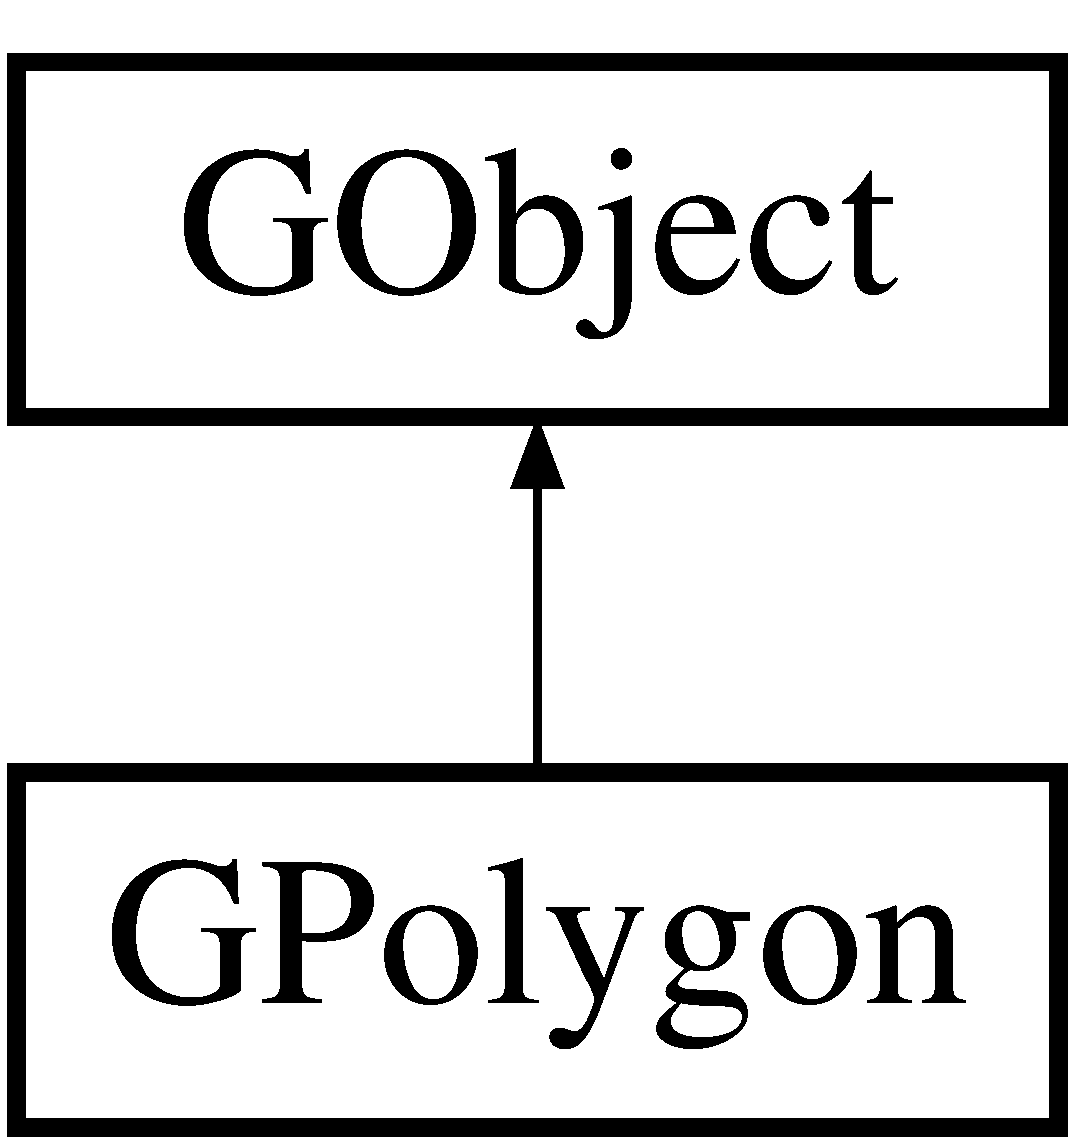
\includegraphics[height=2.000000cm]{classGPolygon}
\end{center}
\end{figure}
\subsection*{Public Types}
\begin{DoxyCompactItemize}
\item 
enum \mbox{\hyperlink{classGObject_a86e0f5648542856159bb40775c854aa7}{Line\+Style}} \{ \mbox{\hyperlink{classGObject_a86e0f5648542856159bb40775c854aa7acbc84bd5232621834ed31f44d457c1eb}{L\+I\+N\+E\+\_\+\+N\+O\+NE}}, 
\mbox{\hyperlink{classGObject_a86e0f5648542856159bb40775c854aa7a700c78bc2cd76acaab26651bf7b4941f}{L\+I\+N\+E\+\_\+\+S\+O\+L\+ID}}, 
\mbox{\hyperlink{classGObject_a86e0f5648542856159bb40775c854aa7a9ccba0845f785d81d07b333ae1aad84e}{L\+I\+N\+E\+\_\+\+D\+A\+SH}}, 
\mbox{\hyperlink{classGObject_a86e0f5648542856159bb40775c854aa7a8e811c096cb941997f0bfda168bb6df3}{L\+I\+N\+E\+\_\+\+D\+OT}}, 
\mbox{\hyperlink{classGObject_a86e0f5648542856159bb40775c854aa7ada15a2e3d737b2db7706d8300f91b89d}{L\+I\+N\+E\+\_\+\+D\+A\+S\+H\+\_\+\+D\+OT}}, 
\mbox{\hyperlink{classGObject_a86e0f5648542856159bb40775c854aa7aabf4053a73eafa7ba2b7e6d664c74c1d}{L\+I\+N\+E\+\_\+\+D\+A\+S\+H\+\_\+\+D\+O\+T\+\_\+\+D\+OT}}
 \}
\begin{DoxyCompactList}\small\item\em Styles that can be used for the outline around various shapes. \end{DoxyCompactList}\end{DoxyCompactItemize}
\subsection*{Public Member Functions}
\begin{DoxyCompactItemize}
\item 
\mbox{\hyperlink{classGPolygon_af59051a8c60e4e792d0346f314c86708}{G\+Polygon}} ()
\begin{DoxyCompactList}\small\item\em Constructs a new empty polygon at the origin. \end{DoxyCompactList}\item 
\mbox{\hyperlink{classGPolygon_a5d3a122dc676d819efe5b9a7e8639ac3}{G\+Polygon}} (std\+::initializer\+\_\+list$<$ double $>$ coords)
\begin{DoxyCompactList}\small\item\em Constructs a new polygon with the given vertex coordinates. \end{DoxyCompactList}\item 
\mbox{\hyperlink{classGPolygon_aabd935bfb600db209293a7935fe44a00}{G\+Polygon}} (std\+::initializer\+\_\+list$<$ \mbox{\hyperlink{classGPoint}{G\+Point}} $>$ points)
\item 
virtual void \mbox{\hyperlink{classGPolygon_ad1976196edec36ab4a1aa09e28c1149c}{add\+Edge}} (double dx, double dy)
\begin{DoxyCompactList}\small\item\em Adds an edge to the polygon whose components are given by the displacements {\ttfamily dx} and {\ttfamily dy} from the last vertex. \end{DoxyCompactList}\item 
virtual void \mbox{\hyperlink{classGPolygon_a484691d516777eabf078a5b0a2e73faa}{add\+Edge}} (const \mbox{\hyperlink{classGPoint}{G\+Point}} \&pt)
\begin{DoxyCompactList}\small\item\em Adds an edge to the polygon where the displacements from the last vertex are specified as the x/y values of the given point. \end{DoxyCompactList}\item 
virtual void \mbox{\hyperlink{classGPolygon_a02e81c7ee5b7864709d40b2cf43d2ae3}{add\+Edges}} (std\+::initializer\+\_\+list$<$ double $>$ coords)
\begin{DoxyCompactList}\small\item\em Adds multiple edges to the polygon whose components are given by the displacements {\ttfamily dx} and {\ttfamily dy} from the last vertex. \end{DoxyCompactList}\item 
virtual void \mbox{\hyperlink{classGPolygon_aef1a706356916af8ef125993b0395e72}{add\+Edges}} (std\+::initializer\+\_\+list$<$ \mbox{\hyperlink{classGPoint}{G\+Point}} $>$ points)
\begin{DoxyCompactList}\small\item\em Adds multiple edges to the polygon whose components are given by the displacements {\ttfamily dx} and {\ttfamily dy} from the last vertex. \end{DoxyCompactList}\item 
virtual void \mbox{\hyperlink{classGPolygon_ab3d75a01a31889ba7bc15314593c7f3b}{add\+Polar\+Edge}} (double r, double theta)
\begin{DoxyCompactList}\small\item\em Adds an edge to the polygon specified in polar coordinates. \end{DoxyCompactList}\item 
virtual void \mbox{\hyperlink{classGPolygon_a116ef33716189339f5557876a8e7a70b}{add\+Vertex}} (double x, double y)
\begin{DoxyCompactList}\small\item\em Adds a vertex at ({\ttfamily x}, {\ttfamily y}) relative to the polygon origin. \end{DoxyCompactList}\item 
virtual void \mbox{\hyperlink{classGPolygon_a09b5faeb0d71697e4f0626dc64118a80}{add\+Vertex}} (const \mbox{\hyperlink{classGPoint}{G\+Point}} \&pt)
\begin{DoxyCompactList}\small\item\em Adds a vertex at the given ({\ttfamily x}, {\ttfamily y}) point relative to the polygon origin. \end{DoxyCompactList}\item 
virtual void \mbox{\hyperlink{classGPolygon_ad8c19525d48fee68c32404d733112f8e}{add\+Vertexes}} (std\+::initializer\+\_\+list$<$ double $>$ coords)
\begin{DoxyCompactList}\small\item\em Adds multiple edges to the polygon whose components are given by the coordinates {\ttfamily dx} and {\ttfamily dy} relative to the polygon origin. \end{DoxyCompactList}\item 
virtual void \mbox{\hyperlink{classGPolygon_a324789ff4b008cc4787140c486561eee}{add\+Vertexes}} (std\+::initializer\+\_\+list$<$ \mbox{\hyperlink{classGPoint}{G\+Point}} $>$ points)
\begin{DoxyCompactList}\small\item\em Adds multiple edges to the polygon whose components are given by the coordinates {\ttfamily dx} and {\ttfamily dy} relative to the polygon origin. \end{DoxyCompactList}\item 
virtual void \mbox{\hyperlink{classGPolygon_ac8bb3912a3ce86b15842e79d0b421204}{clear}} ()
\begin{DoxyCompactList}\small\item\em Removes all vertexes from the polygon. \end{DoxyCompactList}\item 
virtual bool \mbox{\hyperlink{classGObject_a1dbc9dafaae51958112dbe1267a1f547}{contains}} (const \mbox{\hyperlink{classGPoint}{G\+Point}} \&pt) const
\begin{DoxyCompactList}\small\item\em Returns {\ttfamily true} if the specified point is inside the object. \end{DoxyCompactList}\item 
virtual bool \mbox{\hyperlink{classGPolygon_abb6a5d7c03e6eaaae97264c4799ce7c3}{contains}} (double x, double y) const
\begin{DoxyCompactList}\small\item\em Returns {\ttfamily true} if the specified point is inside the object. \end{DoxyCompactList}\item 
virtual \mbox{\hyperlink{classGPoint}{G\+Point}} \mbox{\hyperlink{classGObject_a0d41183bf6b08de66fe3907551aab0d7}{get\+Bottom\+Right\+Location}} () const
\begin{DoxyCompactList}\small\item\em Returns the x/y coordinates of the bottom/right corner of the object. \end{DoxyCompactList}\item 
virtual double \mbox{\hyperlink{classGObject_a4316a2406c18e1c6d061fe51fd355490}{get\+BottomY}} () const
\begin{DoxyCompactList}\small\item\em Returns the {\itshape y}-\/coordinate of the bottom of the object. \end{DoxyCompactList}\item 
virtual \mbox{\hyperlink{classGRectangle}{G\+Rectangle}} \mbox{\hyperlink{classGPolygon_a29e6ac35a0b48f491a4c88194cc5da3b}{get\+Bounds}} () const
\begin{DoxyCompactList}\small\item\em Returns the bounding box of this object, which is defined to be the smallest rectangle that covers everything drawn by the figure. \end{DoxyCompactList}\item 
virtual \mbox{\hyperlink{classGPoint}{G\+Point}} \mbox{\hyperlink{classGObject_a0909472e91448470bccdb62ecfb95d8b}{get\+Center\+Location}} () const
\begin{DoxyCompactList}\small\item\em Returns the x/y-\/coordinates of the center of the object. \end{DoxyCompactList}\item 
virtual double \mbox{\hyperlink{classGObject_a04df74355b545e0543112d5b8d924176}{get\+CenterX}} () const
\begin{DoxyCompactList}\small\item\em Returns the {\itshape x}-\/coordinate of the center of the object. \end{DoxyCompactList}\item 
virtual double \mbox{\hyperlink{classGObject_acb3287a3d507025a26f54b895713b947}{get\+CenterY}} () const
\begin{DoxyCompactList}\small\item\em Returns the {\itshape y}-\/coordinate of the center of the object. \end{DoxyCompactList}\item 
virtual std\+::string \mbox{\hyperlink{classGObject_aa061dfa488c31e18549d64363c1d0e34}{get\+Color}} () const
\begin{DoxyCompactList}\small\item\em Returns the color used to display this object. \end{DoxyCompactList}\item 
virtual std\+::string \mbox{\hyperlink{classGObject_a76f6964a11fde7c78e9751be184e1a3c}{get\+Fill\+Color}} () const
\begin{DoxyCompactList}\small\item\em Returns the color used to display the filled region of this object. \end{DoxyCompactList}\item 
virtual double \mbox{\hyperlink{classGPolygon_a1e7e353362434072875264cf95629f99}{get\+Height}} () const
\begin{DoxyCompactList}\small\item\em Returns the height of this object, which is the same as the height of its bounding box. \end{DoxyCompactList}\item 
virtual \mbox{\hyperlink{classGObject_a86e0f5648542856159bb40775c854aa7}{Line\+Style}} \mbox{\hyperlink{classGObject_aaf1f5ea8281e5e3486662878d26f0a13}{get\+Line\+Style}} () const
\begin{DoxyCompactList}\small\item\em Returns the object\textquotesingle{}s style such as solid or dashed. \end{DoxyCompactList}\item 
virtual double \mbox{\hyperlink{classGObject_a85ff266dc3eb63d9f2d8e5a4487fd3c0}{get\+Line\+Width}} () const
\begin{DoxyCompactList}\small\item\em Returns the width of the line used to draw this object. \end{DoxyCompactList}\item 
virtual \mbox{\hyperlink{classGPoint}{G\+Point}} \mbox{\hyperlink{classGObject_a4f83802015511edeb63b892830812c11}{get\+Location}} () const
\begin{DoxyCompactList}\small\item\em Returns the location of the top-\/left corner of object. \end{DoxyCompactList}\item 
virtual double \mbox{\hyperlink{classGObject_a1ae3fc278cc5b71b9f2d96a8a83cdf26}{get\+Opacity}} () const
\begin{DoxyCompactList}\small\item\em Returns how opaque (non-\/transparent) this object will appear from 0.\+0 (completely transparent) to 1.\+0 (completely opaque, default). \end{DoxyCompactList}\item 
virtual \mbox{\hyperlink{classGCompound}{G\+Compound}} $\ast$ \mbox{\hyperlink{classGObject_a3e53cef70541b1a14eade4ad0984d0b4}{get\+Parent}} () const
\begin{DoxyCompactList}\small\item\em Returns a pointer to the {\ttfamily \mbox{\hyperlink{classGCompound}{G\+Compound}}} that contains this object. \end{DoxyCompactList}\item 
virtual double \mbox{\hyperlink{classGObject_a798cc79daaa10145b28f60bcdfdb0ee9}{get\+RightX}} () const
\begin{DoxyCompactList}\small\item\em Returns the {\itshape x}-\/coordinate of the right side of the object. \end{DoxyCompactList}\item 
virtual \mbox{\hyperlink{classGDimension}{G\+Dimension}} \mbox{\hyperlink{classGObject_a7b4eec96a2bdc6420695d5796a78eea9}{get\+Size}} () const
\begin{DoxyCompactList}\small\item\em Returns the size of the object as a {\ttfamily \mbox{\hyperlink{classGDimension}{G\+Dimension}}}. \end{DoxyCompactList}\item 
virtual std\+::string \mbox{\hyperlink{classGPolygon_a81ea58809bc1683b3990338506397166}{get\+Type}} () const
\begin{DoxyCompactList}\small\item\em Returns the type of the object as a string, such as {\ttfamily \char`\"{}\+G\+Oval\char`\"{}} or {\ttfamily \char`\"{}\+G\+Rect\char`\"{}}. \end{DoxyCompactList}\item 
virtual \mbox{\hyperlink{classGPoint}{G\+Point}} \mbox{\hyperlink{classGPolygon_a428a6fd2c63448f2126d3324fc3bcffd}{get\+Vertex}} (int i) const
\begin{DoxyCompactList}\small\item\em Returns the vertex at the given 0-\/based index in this polygon. \end{DoxyCompactList}\item 
virtual int \mbox{\hyperlink{classGPolygon_af5422019d8237e5a98147f4301e8ccab}{get\+Vertex\+Count}} () const
\begin{DoxyCompactList}\small\item\em Returns the number of vertexes in this polygon. \end{DoxyCompactList}\item 
virtual \mbox{\hyperlink{classVector}{Vector}}$<$ \mbox{\hyperlink{classGPoint}{G\+Point}} $>$ \mbox{\hyperlink{classGPolygon_adfddb9ee82e34b92b9729d848cb168d2}{get\+Vertices}} () const
\begin{DoxyCompactList}\small\item\em Returns a vector of the points in the polygon. \end{DoxyCompactList}\item 
virtual double \mbox{\hyperlink{classGPolygon_a0ed2965abd4f5701d2cadf71239faf19}{get\+Width}} () const
\begin{DoxyCompactList}\small\item\em Returns the width of this object, which is equal to the width of the bounding box. \end{DoxyCompactList}\item 
virtual double \mbox{\hyperlink{classGObject_a344385751bee0720059403940d57a13e}{getX}} () const
\begin{DoxyCompactList}\small\item\em Returns the leftmost {\itshape x}-\/coordinate of the object. \end{DoxyCompactList}\item 
virtual double \mbox{\hyperlink{classGObject_aafa51c7f8f38a09febbb9ce7853f77b4}{getY}} () const
\begin{DoxyCompactList}\small\item\em Returns the topmost {\itshape y}-\/coordinate of the object. \end{DoxyCompactList}\item 
virtual bool \mbox{\hyperlink{classGObject_a11c404f106940c201b6f326e0355c150}{is\+Filled}} () const
\begin{DoxyCompactList}\small\item\em Returns {\ttfamily true} if the object is filled with color. \end{DoxyCompactList}\item 
virtual bool \mbox{\hyperlink{classGObject_a9de207581cfa4ca1eaa06da5f29b75fc}{is\+Transformed}} () const
\begin{DoxyCompactList}\small\item\em Returns {\ttfamily true} if this object has been transformed by calling methods such as \mbox{\hyperlink{classGObject_ae1ffaa12185dfd5ba464f7d87c329e26}{rotate()}} or \mbox{\hyperlink{classGObject_ad2e1900f730475c2d044817db03b38d6}{scale()}} on it. \end{DoxyCompactList}\item 
virtual bool \mbox{\hyperlink{classGObject_a9d8a6cfb13917785c143e74d40e4e2be}{is\+Visible}} () const
\begin{DoxyCompactList}\small\item\em Returns {\ttfamily true} if this object is visible on screen. \end{DoxyCompactList}\item 
virtual void \mbox{\hyperlink{classGObject_a5973d8dda83afb36e2c56855515be392}{move}} (double dx, double dy)
\begin{DoxyCompactList}\small\item\em Moves the object on the screen using the displacements {\ttfamily dx} and {\ttfamily dy}. \end{DoxyCompactList}\item 
virtual void \mbox{\hyperlink{classGObject_ac827b978aa122f136a14c198687ad80f}{repaint}} ()
\begin{DoxyCompactList}\small\item\em Instructs the object to redraw itself on screen. \end{DoxyCompactList}\item 
virtual void \mbox{\hyperlink{classGObject_a6022a1fd1e5dcd2fd5585e5a36aa3f37}{reset\+Transform}} ()
\begin{DoxyCompactList}\small\item\em Undoes any previous scale/rotate transformations on this object. \end{DoxyCompactList}\item 
virtual void \mbox{\hyperlink{classGObject_ae1ffaa12185dfd5ba464f7d87c329e26}{rotate}} (double theta)
\begin{DoxyCompactList}\small\item\em Transforms the object by rotating it {\ttfamily theta} degrees counterclockwise around its origin. \end{DoxyCompactList}\item 
virtual void \mbox{\hyperlink{classGObject_ad2e1900f730475c2d044817db03b38d6}{scale}} (double sf)
\begin{DoxyCompactList}\small\item\em Scales the object by the specified scale factor. \end{DoxyCompactList}\item 
virtual void \mbox{\hyperlink{classGObject_a63641f69d610d0b951357d35a0c3b1e3}{scale}} (double sx, double sy)
\begin{DoxyCompactList}\small\item\em Scales the object by the specified scale factors. \end{DoxyCompactList}\item 
void \mbox{\hyperlink{classGObject_ab6747f40313c531c2db32edb5b63b9b7}{send\+Backward}} ()
\begin{DoxyCompactList}\small\item\em Moves this object one step toward the back in the {\itshape z} dimension. \end{DoxyCompactList}\item 
void \mbox{\hyperlink{classGObject_a710b3e449c9facba7847c91ab170d281}{send\+Forward}} ()
\begin{DoxyCompactList}\small\item\em Moves this object one step toward the front in the {\itshape z} dimension. \end{DoxyCompactList}\item 
void \mbox{\hyperlink{classGObject_a0f7f1efbb7fd46dde2867c4ad0330896}{send\+To\+Back}} ()
\begin{DoxyCompactList}\small\item\em Moves this object to the back of the display in the {\itshape z} dimension. \end{DoxyCompactList}\item 
void \mbox{\hyperlink{classGObject_aee33d68488e46827ef55fac07f40a9b2}{send\+To\+Front}} ()
\begin{DoxyCompactList}\small\item\em Moves this object to the front of the display in the {\itshape z} dimension. \end{DoxyCompactList}\item 
virtual void \mbox{\hyperlink{classGObject_a71ff7b16b8f1bdc4a1ce9f30cf8b87d8}{set\+Bottom\+Right\+Location}} (double x, double y)
\begin{DoxyCompactList}\small\item\em Sets the location of the bottom/right of this object. \end{DoxyCompactList}\item 
virtual void \mbox{\hyperlink{classGObject_ac6f7320321182f1d18c1c0fa97d5e941}{set\+Bottom\+Right\+Location}} (const \mbox{\hyperlink{classGPoint}{G\+Point}} \&pt)
\begin{DoxyCompactList}\small\item\em Sets the location of the bottom/right of this object. \end{DoxyCompactList}\item 
virtual void \mbox{\hyperlink{classGObject_a4b20e93c2a2597484f74ee5caa71f41f}{set\+BottomY}} (double y)
\begin{DoxyCompactList}\small\item\em Sets the location of the bottom y-\/coordinate of this object. \end{DoxyCompactList}\item 
virtual void \mbox{\hyperlink{classGObject_a2aae8197624b72265ab83b4f1bc73f2f}{set\+Bounds}} (double x, double y, double width, double height)
\begin{DoxyCompactList}\small\item\em Changes the bounds of this object to the specified values. \end{DoxyCompactList}\item 
virtual void \mbox{\hyperlink{classGObject_acada386653f008cacc7cce86426bef7c}{set\+Bounds}} (const \mbox{\hyperlink{classGRectangle}{G\+Rectangle}} \&size)
\begin{DoxyCompactList}\small\item\em Changes the bounds of this object to the specified rectangle. \end{DoxyCompactList}\item 
virtual void \mbox{\hyperlink{classGObject_a290b47dd8de1be44089f95cb2c47c1de}{set\+Center\+Location}} (double x, double y)
\begin{DoxyCompactList}\small\item\em Sets the location of the center of this object. \end{DoxyCompactList}\item 
virtual void \mbox{\hyperlink{classGObject_a1bedf1b233ecba3f753ec58908a683a6}{set\+Center\+Location}} (const \mbox{\hyperlink{classGPoint}{G\+Point}} \&pt)
\begin{DoxyCompactList}\small\item\em Sets the location of the center of this object. \end{DoxyCompactList}\item 
virtual void \mbox{\hyperlink{classGObject_a2f4936281e056eead00a9186b9ba8af6}{set\+CenterX}} (double x)
\begin{DoxyCompactList}\small\item\em Sets the x-\/coordinate of the center of this object. \end{DoxyCompactList}\item 
virtual void \mbox{\hyperlink{classGObject_aad2a22b4fde88c33306b92aebf641d57}{set\+CenterY}} (double y)
\begin{DoxyCompactList}\small\item\em Sets the y-\/coordinate of the center of this object. \end{DoxyCompactList}\item 
virtual void \mbox{\hyperlink{classGObject_ad57ef49bc31db94e92648aa3737923d6}{set\+Color}} (int r, int g, int b)
\begin{DoxyCompactList}\small\item\em Sets the color used to display this object. \end{DoxyCompactList}\item 
virtual void \mbox{\hyperlink{classGObject_ab1f5cc0f5cc6bbbd716a526c61f1081d}{set\+Color}} (int rgb)
\begin{DoxyCompactList}\small\item\em Sets the color used to display this object. \end{DoxyCompactList}\item 
virtual void \mbox{\hyperlink{classGObject_a61374df6c11b52cfbb0815decdbaebc6}{set\+Color}} (const std\+::string \&color)
\begin{DoxyCompactList}\small\item\em Sets the color used to display this object. \end{DoxyCompactList}\item 
virtual void \mbox{\hyperlink{classGObject_ad767a33971159e9493e221cca4c00ae9}{set\+Fill\+Color}} (int r, int g, int b)
\begin{DoxyCompactList}\small\item\em Sets the color used to display the filled region of this object, if any. \end{DoxyCompactList}\item 
virtual void \mbox{\hyperlink{classGObject_aa59d9775a67fa7df2b24a95cd34840a3}{set\+Fill\+Color}} (int rgb)
\begin{DoxyCompactList}\small\item\em Sets the color used to display the filled region of this object, if any. \end{DoxyCompactList}\item 
virtual void \mbox{\hyperlink{classGObject_adbc18b1a930aadd97d7437f9f7265b96}{set\+Fill\+Color}} (const std\+::string \&color)
\begin{DoxyCompactList}\small\item\em Sets the color used to display the filled region of this object, if any. \end{DoxyCompactList}\item 
virtual void \mbox{\hyperlink{classGObject_a9b82b53362282c6bb7d6947068d2e55b}{set\+Filled}} (bool flag)
\begin{DoxyCompactList}\small\item\em Sets the fill status for the object, where {\ttfamily false} is outlined and {\ttfamily true} is filled. \end{DoxyCompactList}\item 
virtual void \mbox{\hyperlink{classGObject_a2592348886ffea646c6534bf88f7c49d}{set\+Font}} (const Q\+Font \&font)
\begin{DoxyCompactList}\small\item\em Changes the font used to display the object as specified by the given Qt font. \end{DoxyCompactList}\item 
virtual void \mbox{\hyperlink{classGObject_a8e096e8818d838aceae1d46d58fb3a7b}{set\+Font}} (const std\+::string \&font)
\begin{DoxyCompactList}\small\item\em Changes the font used to display the object as specified by the string {\ttfamily font}, which has the following format\+: \end{DoxyCompactList}\item 
virtual void \mbox{\hyperlink{classGObject_ad18e8fab1e02a4e9b75c6730212558eb}{set\+Foreground}} (int r, int g, int b)
\begin{DoxyCompactList}\small\item\em Sets the color used to display this object. \end{DoxyCompactList}\item 
virtual void \mbox{\hyperlink{classGObject_a9eb856b5ff83a19df3831a31f15f4563}{set\+Foreground}} (int rgb)
\begin{DoxyCompactList}\small\item\em Sets the color used to display this object. \end{DoxyCompactList}\item 
virtual void \mbox{\hyperlink{classGObject_af59209aeadea6dfc6d97a2d8531f50e1}{set\+Foreground}} (const std\+::string \&color)
\begin{DoxyCompactList}\small\item\em Sets the color used to display this object. \end{DoxyCompactList}\item 
virtual void \mbox{\hyperlink{classGObject_a9e280bfc4544dfaf8e4376c4e1a74357}{set\+Height}} (double height)
\begin{DoxyCompactList}\small\item\em Changes the height of this object to the specified height without changing its width. \end{DoxyCompactList}\item 
virtual void \mbox{\hyperlink{classGObject_add11575087eb94f1a71faa3f826c6341}{set\+Line\+Style}} (\mbox{\hyperlink{classGObject_a86e0f5648542856159bb40775c854aa7}{Line\+Style}} line\+Style)
\begin{DoxyCompactList}\small\item\em Sets the object\textquotesingle{}s style such as solid (\mbox{\hyperlink{classGObject_a86e0f5648542856159bb40775c854aa7a700c78bc2cd76acaab26651bf7b4941f}{G\+Object\+::\+L\+I\+N\+E\+\_\+\+S\+O\+L\+ID}}) or dashed (\mbox{\hyperlink{classGObject_a86e0f5648542856159bb40775c854aa7a9ccba0845f785d81d07b333ae1aad84e}{G\+Object\+::\+L\+I\+N\+E\+\_\+\+D\+A\+SH}}). \end{DoxyCompactList}\item 
virtual void \mbox{\hyperlink{classGObject_afd6a47c6ea6a1f85ca05a65ba3ff3477}{set\+Line\+Width}} (double line\+Width)
\begin{DoxyCompactList}\small\item\em Sets the width of the line used to draw this object. \end{DoxyCompactList}\item 
virtual void \mbox{\hyperlink{classGObject_a04594e8ba9b98513a64f1da00dcae18c}{set\+Location}} (double x, double y)
\begin{DoxyCompactList}\small\item\em Sets the location of the top-\/left corner of this object to the specified coordinates. \end{DoxyCompactList}\item 
virtual void \mbox{\hyperlink{classGObject_aa8480c0b7166cdf8f784cece06ab353f}{set\+Location}} (const \mbox{\hyperlink{classGPoint}{G\+Point}} \&pt)
\begin{DoxyCompactList}\small\item\em Sets the location of the top-\/left corner of this object to the specified point. \end{DoxyCompactList}\item 
virtual void \mbox{\hyperlink{classGObject_a04af1866cc1bae4a1226695794a50539}{set\+Opacity}} (double opacity)
\begin{DoxyCompactList}\small\item\em Sets how opaque (non-\/transparent) this object will appear from 0.\+0 (completely transparent) to 1.\+0 (completely opaque, default). \end{DoxyCompactList}\item 
virtual void \mbox{\hyperlink{classGObject_a3c90b758cdc2c911c9ef76c4360eb912}{set\+RightX}} (double x)
\begin{DoxyCompactList}\small\item\em Sets the location of the rightmost x-\/coordinate of this object. \end{DoxyCompactList}\item 
virtual void \mbox{\hyperlink{classGObject_aca25d49481f9bf5fc8f7df4c086c4ce7}{set\+Size}} (double width, double height)
\begin{DoxyCompactList}\small\item\em Changes the size of this object to the specified width and height. \end{DoxyCompactList}\item 
virtual void \mbox{\hyperlink{classGObject_ae2b628228f192c2702c4ce941b2af68f}{set\+Size}} (const \mbox{\hyperlink{classGDimension}{G\+Dimension}} \&size)
\begin{DoxyCompactList}\small\item\em Changes the size of this object to the specified width and height. \end{DoxyCompactList}\item 
virtual void \mbox{\hyperlink{classGPolygon_a616f3944eea0dad17d074d0f505299cc}{set\+Vertex}} (int i, \mbox{\hyperlink{classGPoint}{G\+Point}} point)
\begin{DoxyCompactList}\small\item\em Sets the vertex at the given 0-\/based index in this polygon to the given coordinates. \end{DoxyCompactList}\item 
virtual void \mbox{\hyperlink{classGObject_a88203f28224315d9f4471212f4af8ed3}{set\+Visible}} (bool flag)
\begin{DoxyCompactList}\small\item\em Sets whether this object is visible. \end{DoxyCompactList}\item 
virtual void \mbox{\hyperlink{classGObject_aa3f3fba4cb131baa8696ba01e3bceca1}{set\+Width}} (double width)
\begin{DoxyCompactList}\small\item\em Changes the width of this object to the specified width without changing its height. \end{DoxyCompactList}\item 
virtual void \mbox{\hyperlink{classGObject_a9c18fcc579333bf9653d13ad2b372e39}{setX}} (double x)
\begin{DoxyCompactList}\small\item\em Sets the x location of the left side of this object. \end{DoxyCompactList}\item 
virtual void \mbox{\hyperlink{classGObject_a7d57e2a5c35d27feb58fd498a3cf82b9}{setY}} (double y)
\begin{DoxyCompactList}\small\item\em Sets the y location of the top of this object. \end{DoxyCompactList}\item 
virtual std\+::string \mbox{\hyperlink{classGObject_a1fe5121d6528fdea3f243321b3fa3a49}{to\+String}} () const
\begin{DoxyCompactList}\small\item\em Returns a printable representation of the object. \end{DoxyCompactList}\item 
virtual std\+::string \mbox{\hyperlink{classGPolygon_a4fcdf8de5c6de92242a975d83d8f23ea}{to\+String\+Extra}} () const
\begin{DoxyCompactList}\small\item\em Returns a string containing any extra unique information about this type of graphical object. \end{DoxyCompactList}\end{DoxyCompactItemize}
\subsection*{Static Public Member Functions}
\begin{DoxyCompactItemize}
\item 
static bool \mbox{\hyperlink{classGObject_a93be0e1fe1b1bf1a1da732470c94f42b}{is\+Anti\+Aliasing}} ()
\begin{DoxyCompactList}\small\item\em Returns whether we should globally anti-\/alias graphical objects. \end{DoxyCompactList}\item 
static void \mbox{\hyperlink{classGObject_a1e43371668ae850193cebedb44e1bbe3}{set\+Anti\+Aliasing}} (bool value)
\begin{DoxyCompactList}\small\item\em Globally turns on/off the anti-\/aliasing feature that smooths out the edges of onscreen shapes. \end{DoxyCompactList}\end{DoxyCompactItemize}
\subsection*{Protected Attributes}
\begin{DoxyCompactItemize}
\item 
Q\+Brush \mbox{\hyperlink{classGObject_aab24462ec896b596d99911767b0912d0}{\+\_\+brush}}
\item 
std\+::string \mbox{\hyperlink{classGObject_a1134e770ae4315ea8bc1201e2f21da8b}{\+\_\+color}}
\item 
int \mbox{\hyperlink{classGObject_a003fdd343d9b7505c53a8b7a134200ed}{\+\_\+color\+Int}}
\item 
std\+::string \mbox{\hyperlink{classGObject_a179f8d6cee65cd8a54692e32b224392a}{\+\_\+fill\+Color}}
\item 
int \mbox{\hyperlink{classGObject_a751def333a67d651e5b99cc331ecb496}{\+\_\+fill\+Color\+Int}}
\item 
bool \mbox{\hyperlink{classGObject_ad4a55cbcd61b58a4d49666490bb2f103}{\+\_\+fill\+Flag}}
\item 
std\+::string \mbox{\hyperlink{classGObject_aea76ea1a8b5dd7b0a78653277e63b536}{\+\_\+font}}
\item 
double \mbox{\hyperlink{classGObject_ad05df29e7f27fc504abd743e3d8b4e73}{\+\_\+height}}
\item 
\mbox{\hyperlink{classGObject_a86e0f5648542856159bb40775c854aa7}{Line\+Style}} \mbox{\hyperlink{classGObject_a89bafecaafb7c72d55c7efc10b7d0523}{\+\_\+line\+Style}}
\item 
double \mbox{\hyperlink{classGObject_a16e9033665937f13de2e163dc2184aff}{\+\_\+line\+Width}}
\item 
double \mbox{\hyperlink{classGObject_a20eff8eb7af27182edc9bfc54768b6f3}{\+\_\+opacity}}
\item 
\mbox{\hyperlink{classGCompound}{G\+Compound}} $\ast$ \mbox{\hyperlink{classGObject_ac9452c1eaff70eebddbb318196aa3835}{\+\_\+parent}}
\item 
Q\+Pen \mbox{\hyperlink{classGObject_afb69d172743f868299847174eb1b6bc8}{\+\_\+pen}}
\item 
Q\+Transform \mbox{\hyperlink{classGObject_a475b8860a5f1adb4a1fdc58d1f5c1e32}{\+\_\+transform}}
\item 
bool \mbox{\hyperlink{classGObject_ae4725802fc8d8aaa0ab4bd4781f7e07c}{\+\_\+transformed}}
\item 
bool \mbox{\hyperlink{classGObject_a9312c72508471b7c7a87b540263e1af4}{\+\_\+visible}}
\item 
double \mbox{\hyperlink{classGObject_ab55d85a3371770e6725b1062cf160cd8}{\+\_\+width}}
\item 
double \mbox{\hyperlink{classGObject_a6675b83b27137b8d3aa2ad8133078ea6}{\+\_\+x}}
\item 
double \mbox{\hyperlink{classGObject_a2f0f6aeafddc8a39c578bfa7e22b5f1e}{\+\_\+y}}
\end{DoxyCompactItemize}


\subsection{Detailed Description}
This graphical object subclass represents a polygon bounded by line segments. 

The {\ttfamily \mbox{\hyperlink{classGPolygon}{G\+Polygon}}} constructor creates an empty polygon. To complete the figure, you need to add vertices to the polygon using the methods {\ttfamily add\+Vertex}, {\ttfamily add\+Edge}, and {\ttfamily add\+Polar\+Edge}. 

\subsection{Member Enumeration Documentation}
\mbox{\Hypertarget{classGObject_a86e0f5648542856159bb40775c854aa7}\label{classGObject_a86e0f5648542856159bb40775c854aa7}} 
\index{G\+Polygon@{G\+Polygon}!Line\+Style@{Line\+Style}}
\index{Line\+Style@{Line\+Style}!G\+Polygon@{G\+Polygon}}
\subsubsection{\texorpdfstring{Line\+Style}{LineStyle}}
{\footnotesize\ttfamily enum \mbox{\hyperlink{classGObject_a86e0f5648542856159bb40775c854aa7}{Line\+Style}}\hspace{0.3cm}{\ttfamily [inherited]}}



Styles that can be used for the outline around various shapes. 

Call set\+Line\+Style on a \mbox{\hyperlink{classGObject}{G\+Object}} and pass one of these values. \begin{DoxyEnumFields}{Enumerator}
\raisebox{\heightof{T}}[0pt][0pt]{\index{L\+I\+N\+E\+\_\+\+N\+O\+NE@{L\+I\+N\+E\+\_\+\+N\+O\+NE}!G\+Polygon@{G\+Polygon}}\index{G\+Polygon@{G\+Polygon}!L\+I\+N\+E\+\_\+\+N\+O\+NE@{L\+I\+N\+E\+\_\+\+N\+O\+NE}}}\mbox{\Hypertarget{classGObject_a86e0f5648542856159bb40775c854aa7acbc84bd5232621834ed31f44d457c1eb}\label{classGObject_a86e0f5648542856159bb40775c854aa7acbc84bd5232621834ed31f44d457c1eb}} 
L\+I\+N\+E\+\_\+\+N\+O\+NE&\\
\hline

\raisebox{\heightof{T}}[0pt][0pt]{\index{L\+I\+N\+E\+\_\+\+S\+O\+L\+ID@{L\+I\+N\+E\+\_\+\+S\+O\+L\+ID}!G\+Polygon@{G\+Polygon}}\index{G\+Polygon@{G\+Polygon}!L\+I\+N\+E\+\_\+\+S\+O\+L\+ID@{L\+I\+N\+E\+\_\+\+S\+O\+L\+ID}}}\mbox{\Hypertarget{classGObject_a86e0f5648542856159bb40775c854aa7a700c78bc2cd76acaab26651bf7b4941f}\label{classGObject_a86e0f5648542856159bb40775c854aa7a700c78bc2cd76acaab26651bf7b4941f}} 
L\+I\+N\+E\+\_\+\+S\+O\+L\+ID&\\
\hline

\raisebox{\heightof{T}}[0pt][0pt]{\index{L\+I\+N\+E\+\_\+\+D\+A\+SH@{L\+I\+N\+E\+\_\+\+D\+A\+SH}!G\+Polygon@{G\+Polygon}}\index{G\+Polygon@{G\+Polygon}!L\+I\+N\+E\+\_\+\+D\+A\+SH@{L\+I\+N\+E\+\_\+\+D\+A\+SH}}}\mbox{\Hypertarget{classGObject_a86e0f5648542856159bb40775c854aa7a9ccba0845f785d81d07b333ae1aad84e}\label{classGObject_a86e0f5648542856159bb40775c854aa7a9ccba0845f785d81d07b333ae1aad84e}} 
L\+I\+N\+E\+\_\+\+D\+A\+SH&\\
\hline

\raisebox{\heightof{T}}[0pt][0pt]{\index{L\+I\+N\+E\+\_\+\+D\+OT@{L\+I\+N\+E\+\_\+\+D\+OT}!G\+Polygon@{G\+Polygon}}\index{G\+Polygon@{G\+Polygon}!L\+I\+N\+E\+\_\+\+D\+OT@{L\+I\+N\+E\+\_\+\+D\+OT}}}\mbox{\Hypertarget{classGObject_a86e0f5648542856159bb40775c854aa7a8e811c096cb941997f0bfda168bb6df3}\label{classGObject_a86e0f5648542856159bb40775c854aa7a8e811c096cb941997f0bfda168bb6df3}} 
L\+I\+N\+E\+\_\+\+D\+OT&\\
\hline

\raisebox{\heightof{T}}[0pt][0pt]{\index{L\+I\+N\+E\+\_\+\+D\+A\+S\+H\+\_\+\+D\+OT@{L\+I\+N\+E\+\_\+\+D\+A\+S\+H\+\_\+\+D\+OT}!G\+Polygon@{G\+Polygon}}\index{G\+Polygon@{G\+Polygon}!L\+I\+N\+E\+\_\+\+D\+A\+S\+H\+\_\+\+D\+OT@{L\+I\+N\+E\+\_\+\+D\+A\+S\+H\+\_\+\+D\+OT}}}\mbox{\Hypertarget{classGObject_a86e0f5648542856159bb40775c854aa7ada15a2e3d737b2db7706d8300f91b89d}\label{classGObject_a86e0f5648542856159bb40775c854aa7ada15a2e3d737b2db7706d8300f91b89d}} 
L\+I\+N\+E\+\_\+\+D\+A\+S\+H\+\_\+\+D\+OT&\\
\hline

\raisebox{\heightof{T}}[0pt][0pt]{\index{L\+I\+N\+E\+\_\+\+D\+A\+S\+H\+\_\+\+D\+O\+T\+\_\+\+D\+OT@{L\+I\+N\+E\+\_\+\+D\+A\+S\+H\+\_\+\+D\+O\+T\+\_\+\+D\+OT}!G\+Polygon@{G\+Polygon}}\index{G\+Polygon@{G\+Polygon}!L\+I\+N\+E\+\_\+\+D\+A\+S\+H\+\_\+\+D\+O\+T\+\_\+\+D\+OT@{L\+I\+N\+E\+\_\+\+D\+A\+S\+H\+\_\+\+D\+O\+T\+\_\+\+D\+OT}}}\mbox{\Hypertarget{classGObject_a86e0f5648542856159bb40775c854aa7aabf4053a73eafa7ba2b7e6d664c74c1d}\label{classGObject_a86e0f5648542856159bb40775c854aa7aabf4053a73eafa7ba2b7e6d664c74c1d}} 
L\+I\+N\+E\+\_\+\+D\+A\+S\+H\+\_\+\+D\+O\+T\+\_\+\+D\+OT&\\
\hline

\end{DoxyEnumFields}


\subsection{Constructor \& Destructor Documentation}
\mbox{\Hypertarget{classGPolygon_af59051a8c60e4e792d0346f314c86708}\label{classGPolygon_af59051a8c60e4e792d0346f314c86708}} 
\index{G\+Polygon@{G\+Polygon}!G\+Polygon@{G\+Polygon}}
\index{G\+Polygon@{G\+Polygon}!G\+Polygon@{G\+Polygon}}
\subsubsection{\texorpdfstring{G\+Polygon()}{GPolygon()}\hspace{0.1cm}{\footnotesize\ttfamily [1/3]}}
{\footnotesize\ttfamily \mbox{\hyperlink{classGPolygon}{G\+Polygon}} (\begin{DoxyParamCaption}{ }\end{DoxyParamCaption})}



Constructs a new empty polygon at the origin. 

\mbox{\Hypertarget{classGPolygon_a5d3a122dc676d819efe5b9a7e8639ac3}\label{classGPolygon_a5d3a122dc676d819efe5b9a7e8639ac3}} 
\index{G\+Polygon@{G\+Polygon}!G\+Polygon@{G\+Polygon}}
\index{G\+Polygon@{G\+Polygon}!G\+Polygon@{G\+Polygon}}
\subsubsection{\texorpdfstring{G\+Polygon()}{GPolygon()}\hspace{0.1cm}{\footnotesize\ttfamily [2/3]}}
{\footnotesize\ttfamily \mbox{\hyperlink{classGPolygon}{G\+Polygon}} (\begin{DoxyParamCaption}\item[{std\+::initializer\+\_\+list$<$ double $>$}]{coords }\end{DoxyParamCaption})}



Constructs a new polygon with the given vertex coordinates. 

\mbox{\Hypertarget{classGPolygon_aabd935bfb600db209293a7935fe44a00}\label{classGPolygon_aabd935bfb600db209293a7935fe44a00}} 
\index{G\+Polygon@{G\+Polygon}!G\+Polygon@{G\+Polygon}}
\index{G\+Polygon@{G\+Polygon}!G\+Polygon@{G\+Polygon}}
\subsubsection{\texorpdfstring{G\+Polygon()}{GPolygon()}\hspace{0.1cm}{\footnotesize\ttfamily [3/3]}}
{\footnotesize\ttfamily \mbox{\hyperlink{classGPolygon}{G\+Polygon}} (\begin{DoxyParamCaption}\item[{std\+::initializer\+\_\+list$<$ \mbox{\hyperlink{classGPoint}{G\+Point}} $>$}]{points }\end{DoxyParamCaption})}



\subsection{Member Function Documentation}
\mbox{\Hypertarget{classGPolygon_ad1976196edec36ab4a1aa09e28c1149c}\label{classGPolygon_ad1976196edec36ab4a1aa09e28c1149c}} 
\index{G\+Polygon@{G\+Polygon}!add\+Edge@{add\+Edge}}
\index{add\+Edge@{add\+Edge}!G\+Polygon@{G\+Polygon}}
\subsubsection{\texorpdfstring{add\+Edge()}{addEdge()}\hspace{0.1cm}{\footnotesize\ttfamily [1/2]}}
{\footnotesize\ttfamily void add\+Edge (\begin{DoxyParamCaption}\item[{double}]{dx,  }\item[{double}]{dy }\end{DoxyParamCaption})\hspace{0.3cm}{\ttfamily [virtual]}}



Adds an edge to the polygon whose components are given by the displacements {\ttfamily dx} and {\ttfamily dy} from the last vertex. 

\mbox{\Hypertarget{classGPolygon_a484691d516777eabf078a5b0a2e73faa}\label{classGPolygon_a484691d516777eabf078a5b0a2e73faa}} 
\index{G\+Polygon@{G\+Polygon}!add\+Edge@{add\+Edge}}
\index{add\+Edge@{add\+Edge}!G\+Polygon@{G\+Polygon}}
\subsubsection{\texorpdfstring{add\+Edge()}{addEdge()}\hspace{0.1cm}{\footnotesize\ttfamily [2/2]}}
{\footnotesize\ttfamily void add\+Edge (\begin{DoxyParamCaption}\item[{const \mbox{\hyperlink{classGPoint}{G\+Point}} \&}]{pt }\end{DoxyParamCaption})\hspace{0.3cm}{\ttfamily [virtual]}}



Adds an edge to the polygon where the displacements from the last vertex are specified as the x/y values of the given point. 

\mbox{\Hypertarget{classGPolygon_a02e81c7ee5b7864709d40b2cf43d2ae3}\label{classGPolygon_a02e81c7ee5b7864709d40b2cf43d2ae3}} 
\index{G\+Polygon@{G\+Polygon}!add\+Edges@{add\+Edges}}
\index{add\+Edges@{add\+Edges}!G\+Polygon@{G\+Polygon}}
\subsubsection{\texorpdfstring{add\+Edges()}{addEdges()}\hspace{0.1cm}{\footnotesize\ttfamily [1/2]}}
{\footnotesize\ttfamily void add\+Edges (\begin{DoxyParamCaption}\item[{std\+::initializer\+\_\+list$<$ double $>$}]{coords }\end{DoxyParamCaption})\hspace{0.3cm}{\ttfamily [virtual]}}



Adds multiple edges to the polygon whose components are given by the displacements {\ttfamily dx} and {\ttfamily dy} from the last vertex. 

\mbox{\Hypertarget{classGPolygon_aef1a706356916af8ef125993b0395e72}\label{classGPolygon_aef1a706356916af8ef125993b0395e72}} 
\index{G\+Polygon@{G\+Polygon}!add\+Edges@{add\+Edges}}
\index{add\+Edges@{add\+Edges}!G\+Polygon@{G\+Polygon}}
\subsubsection{\texorpdfstring{add\+Edges()}{addEdges()}\hspace{0.1cm}{\footnotesize\ttfamily [2/2]}}
{\footnotesize\ttfamily void add\+Edges (\begin{DoxyParamCaption}\item[{std\+::initializer\+\_\+list$<$ \mbox{\hyperlink{classGPoint}{G\+Point}} $>$}]{points }\end{DoxyParamCaption})\hspace{0.3cm}{\ttfamily [virtual]}}



Adds multiple edges to the polygon whose components are given by the displacements {\ttfamily dx} and {\ttfamily dy} from the last vertex. 

\mbox{\Hypertarget{classGPolygon_ab3d75a01a31889ba7bc15314593c7f3b}\label{classGPolygon_ab3d75a01a31889ba7bc15314593c7f3b}} 
\index{G\+Polygon@{G\+Polygon}!add\+Polar\+Edge@{add\+Polar\+Edge}}
\index{add\+Polar\+Edge@{add\+Polar\+Edge}!G\+Polygon@{G\+Polygon}}
\subsubsection{\texorpdfstring{add\+Polar\+Edge()}{addPolarEdge()}}
{\footnotesize\ttfamily void add\+Polar\+Edge (\begin{DoxyParamCaption}\item[{double}]{r,  }\item[{double}]{theta }\end{DoxyParamCaption})\hspace{0.3cm}{\ttfamily [virtual]}}



Adds an edge to the polygon specified in polar coordinates. 

The length of the edge is given by {\ttfamily r}, and the edge extends in direction {\ttfamily theta}, measured in degrees counterclockwise from the +x axis. \mbox{\Hypertarget{classGPolygon_a116ef33716189339f5557876a8e7a70b}\label{classGPolygon_a116ef33716189339f5557876a8e7a70b}} 
\index{G\+Polygon@{G\+Polygon}!add\+Vertex@{add\+Vertex}}
\index{add\+Vertex@{add\+Vertex}!G\+Polygon@{G\+Polygon}}
\subsubsection{\texorpdfstring{add\+Vertex()}{addVertex()}\hspace{0.1cm}{\footnotesize\ttfamily [1/2]}}
{\footnotesize\ttfamily void add\+Vertex (\begin{DoxyParamCaption}\item[{double}]{x,  }\item[{double}]{y }\end{DoxyParamCaption})\hspace{0.3cm}{\ttfamily [virtual]}}



Adds a vertex at ({\ttfamily x}, {\ttfamily y}) relative to the polygon origin. 

\mbox{\Hypertarget{classGPolygon_a09b5faeb0d71697e4f0626dc64118a80}\label{classGPolygon_a09b5faeb0d71697e4f0626dc64118a80}} 
\index{G\+Polygon@{G\+Polygon}!add\+Vertex@{add\+Vertex}}
\index{add\+Vertex@{add\+Vertex}!G\+Polygon@{G\+Polygon}}
\subsubsection{\texorpdfstring{add\+Vertex()}{addVertex()}\hspace{0.1cm}{\footnotesize\ttfamily [2/2]}}
{\footnotesize\ttfamily void add\+Vertex (\begin{DoxyParamCaption}\item[{const \mbox{\hyperlink{classGPoint}{G\+Point}} \&}]{pt }\end{DoxyParamCaption})\hspace{0.3cm}{\ttfamily [virtual]}}



Adds a vertex at the given ({\ttfamily x}, {\ttfamily y}) point relative to the polygon origin. 

\mbox{\Hypertarget{classGPolygon_ad8c19525d48fee68c32404d733112f8e}\label{classGPolygon_ad8c19525d48fee68c32404d733112f8e}} 
\index{G\+Polygon@{G\+Polygon}!add\+Vertexes@{add\+Vertexes}}
\index{add\+Vertexes@{add\+Vertexes}!G\+Polygon@{G\+Polygon}}
\subsubsection{\texorpdfstring{add\+Vertexes()}{addVertexes()}\hspace{0.1cm}{\footnotesize\ttfamily [1/2]}}
{\footnotesize\ttfamily void add\+Vertexes (\begin{DoxyParamCaption}\item[{std\+::initializer\+\_\+list$<$ double $>$}]{coords }\end{DoxyParamCaption})\hspace{0.3cm}{\ttfamily [virtual]}}



Adds multiple edges to the polygon whose components are given by the coordinates {\ttfamily dx} and {\ttfamily dy} relative to the polygon origin. 

\mbox{\Hypertarget{classGPolygon_a324789ff4b008cc4787140c486561eee}\label{classGPolygon_a324789ff4b008cc4787140c486561eee}} 
\index{G\+Polygon@{G\+Polygon}!add\+Vertexes@{add\+Vertexes}}
\index{add\+Vertexes@{add\+Vertexes}!G\+Polygon@{G\+Polygon}}
\subsubsection{\texorpdfstring{add\+Vertexes()}{addVertexes()}\hspace{0.1cm}{\footnotesize\ttfamily [2/2]}}
{\footnotesize\ttfamily void add\+Vertexes (\begin{DoxyParamCaption}\item[{std\+::initializer\+\_\+list$<$ \mbox{\hyperlink{classGPoint}{G\+Point}} $>$}]{points }\end{DoxyParamCaption})\hspace{0.3cm}{\ttfamily [virtual]}}



Adds multiple edges to the polygon whose components are given by the coordinates {\ttfamily dx} and {\ttfamily dy} relative to the polygon origin. 

\mbox{\Hypertarget{classGPolygon_ac8bb3912a3ce86b15842e79d0b421204}\label{classGPolygon_ac8bb3912a3ce86b15842e79d0b421204}} 
\index{G\+Polygon@{G\+Polygon}!clear@{clear}}
\index{clear@{clear}!G\+Polygon@{G\+Polygon}}
\subsubsection{\texorpdfstring{clear()}{clear()}}
{\footnotesize\ttfamily void clear (\begin{DoxyParamCaption}{ }\end{DoxyParamCaption})\hspace{0.3cm}{\ttfamily [virtual]}}



Removes all vertexes from the polygon. 

\mbox{\Hypertarget{classGObject_a1dbc9dafaae51958112dbe1267a1f547}\label{classGObject_a1dbc9dafaae51958112dbe1267a1f547}} 
\index{G\+Polygon@{G\+Polygon}!contains@{contains}}
\index{contains@{contains}!G\+Polygon@{G\+Polygon}}
\subsubsection{\texorpdfstring{contains()}{contains()}\hspace{0.1cm}{\footnotesize\ttfamily [1/2]}}
{\footnotesize\ttfamily bool contains (\begin{DoxyParamCaption}\item[{const \mbox{\hyperlink{classGPoint}{G\+Point}} \&}]{pt }\end{DoxyParamCaption}) const\hspace{0.3cm}{\ttfamily [virtual]}, {\ttfamily [inherited]}}



Returns {\ttfamily true} if the specified point is inside the object. 

\mbox{\Hypertarget{classGPolygon_abb6a5d7c03e6eaaae97264c4799ce7c3}\label{classGPolygon_abb6a5d7c03e6eaaae97264c4799ce7c3}} 
\index{G\+Polygon@{G\+Polygon}!contains@{contains}}
\index{contains@{contains}!G\+Polygon@{G\+Polygon}}
\subsubsection{\texorpdfstring{contains()}{contains()}\hspace{0.1cm}{\footnotesize\ttfamily [2/2]}}
{\footnotesize\ttfamily bool contains (\begin{DoxyParamCaption}\item[{double}]{x,  }\item[{double}]{y }\end{DoxyParamCaption}) const\hspace{0.3cm}{\ttfamily [virtual]}}



Returns {\ttfamily true} if the specified point is inside the object. 



Reimplemented from \mbox{\hyperlink{classGObject_abb6a5d7c03e6eaaae97264c4799ce7c3}{G\+Object}}.

\mbox{\Hypertarget{classGObject_a0d41183bf6b08de66fe3907551aab0d7}\label{classGObject_a0d41183bf6b08de66fe3907551aab0d7}} 
\index{G\+Polygon@{G\+Polygon}!get\+Bottom\+Right\+Location@{get\+Bottom\+Right\+Location}}
\index{get\+Bottom\+Right\+Location@{get\+Bottom\+Right\+Location}!G\+Polygon@{G\+Polygon}}
\subsubsection{\texorpdfstring{get\+Bottom\+Right\+Location()}{getBottomRightLocation()}}
{\footnotesize\ttfamily \mbox{\hyperlink{classGPoint}{G\+Point}} get\+Bottom\+Right\+Location (\begin{DoxyParamCaption}{ }\end{DoxyParamCaption}) const\hspace{0.3cm}{\ttfamily [virtual]}, {\ttfamily [inherited]}}



Returns the x/y coordinates of the bottom/right corner of the object. 

\mbox{\Hypertarget{classGObject_a4316a2406c18e1c6d061fe51fd355490}\label{classGObject_a4316a2406c18e1c6d061fe51fd355490}} 
\index{G\+Polygon@{G\+Polygon}!get\+BottomY@{get\+BottomY}}
\index{get\+BottomY@{get\+BottomY}!G\+Polygon@{G\+Polygon}}
\subsubsection{\texorpdfstring{get\+Bottom\+Y()}{getBottomY()}}
{\footnotesize\ttfamily double get\+BottomY (\begin{DoxyParamCaption}{ }\end{DoxyParamCaption}) const\hspace{0.3cm}{\ttfamily [virtual]}, {\ttfamily [inherited]}}



Returns the {\itshape y}-\/coordinate of the bottom of the object. 

Equivalent to the top y-\/coordinate plus the object\textquotesingle{}s height. \mbox{\Hypertarget{classGPolygon_a29e6ac35a0b48f491a4c88194cc5da3b}\label{classGPolygon_a29e6ac35a0b48f491a4c88194cc5da3b}} 
\index{G\+Polygon@{G\+Polygon}!get\+Bounds@{get\+Bounds}}
\index{get\+Bounds@{get\+Bounds}!G\+Polygon@{G\+Polygon}}
\subsubsection{\texorpdfstring{get\+Bounds()}{getBounds()}}
{\footnotesize\ttfamily \mbox{\hyperlink{classGRectangle}{G\+Rectangle}} get\+Bounds (\begin{DoxyParamCaption}{ }\end{DoxyParamCaption}) const\hspace{0.3cm}{\ttfamily [virtual]}}



Returns the bounding box of this object, which is defined to be the smallest rectangle that covers everything drawn by the figure. 

The coordinates of this rectangle do not necessarily match the location returned by {\ttfamily get\+Location}. Given a {\ttfamily \mbox{\hyperlink{classGText}{G\+Text}}} object, for example, {\ttfamily get\+Location} returns the coordinates of the point on the baseline at which the string begins; the {\ttfamily get\+Bounds} method, by contrast, returns a rectangle that covers the entire window area occupied by the string. 

Reimplemented from \mbox{\hyperlink{classGObject_a29e6ac35a0b48f491a4c88194cc5da3b}{G\+Object}}.

\mbox{\Hypertarget{classGObject_a0909472e91448470bccdb62ecfb95d8b}\label{classGObject_a0909472e91448470bccdb62ecfb95d8b}} 
\index{G\+Polygon@{G\+Polygon}!get\+Center\+Location@{get\+Center\+Location}}
\index{get\+Center\+Location@{get\+Center\+Location}!G\+Polygon@{G\+Polygon}}
\subsubsection{\texorpdfstring{get\+Center\+Location()}{getCenterLocation()}}
{\footnotesize\ttfamily \mbox{\hyperlink{classGPoint}{G\+Point}} get\+Center\+Location (\begin{DoxyParamCaption}{ }\end{DoxyParamCaption}) const\hspace{0.3cm}{\ttfamily [virtual]}, {\ttfamily [inherited]}}



Returns the x/y-\/coordinates of the center of the object. 

Equivalent to the top/left plus half the object\textquotesingle{}s size. \mbox{\Hypertarget{classGObject_a04df74355b545e0543112d5b8d924176}\label{classGObject_a04df74355b545e0543112d5b8d924176}} 
\index{G\+Polygon@{G\+Polygon}!get\+CenterX@{get\+CenterX}}
\index{get\+CenterX@{get\+CenterX}!G\+Polygon@{G\+Polygon}}
\subsubsection{\texorpdfstring{get\+Center\+X()}{getCenterX()}}
{\footnotesize\ttfamily double get\+CenterX (\begin{DoxyParamCaption}{ }\end{DoxyParamCaption}) const\hspace{0.3cm}{\ttfamily [virtual]}, {\ttfamily [inherited]}}



Returns the {\itshape x}-\/coordinate of the center of the object. 

Equivalent to the top/left plus half the object\textquotesingle{}s width. \mbox{\Hypertarget{classGObject_acb3287a3d507025a26f54b895713b947}\label{classGObject_acb3287a3d507025a26f54b895713b947}} 
\index{G\+Polygon@{G\+Polygon}!get\+CenterY@{get\+CenterY}}
\index{get\+CenterY@{get\+CenterY}!G\+Polygon@{G\+Polygon}}
\subsubsection{\texorpdfstring{get\+Center\+Y()}{getCenterY()}}
{\footnotesize\ttfamily double get\+CenterY (\begin{DoxyParamCaption}{ }\end{DoxyParamCaption}) const\hspace{0.3cm}{\ttfamily [virtual]}, {\ttfamily [inherited]}}



Returns the {\itshape y}-\/coordinate of the center of the object. 

Equivalent to the top/left plus half the object\textquotesingle{}s height. \mbox{\Hypertarget{classGObject_aa061dfa488c31e18549d64363c1d0e34}\label{classGObject_aa061dfa488c31e18549d64363c1d0e34}} 
\index{G\+Polygon@{G\+Polygon}!get\+Color@{get\+Color}}
\index{get\+Color@{get\+Color}!G\+Polygon@{G\+Polygon}}
\subsubsection{\texorpdfstring{get\+Color()}{getColor()}}
{\footnotesize\ttfamily std\+::string get\+Color (\begin{DoxyParamCaption}{ }\end{DoxyParamCaption}) const\hspace{0.3cm}{\ttfamily [virtual]}, {\ttfamily [inherited]}}



Returns the color used to display this object. 

This color is always returned as a string in the form {\ttfamily \char`\"{}\#rrggbb\char`\"{}}, where {\ttfamily rr}, {\ttfamily gg}, and {\ttfamily bb} are the red, green, and blue components of the color, expressed as two-\/digit hexadecimal values. \mbox{\Hypertarget{classGObject_a76f6964a11fde7c78e9751be184e1a3c}\label{classGObject_a76f6964a11fde7c78e9751be184e1a3c}} 
\index{G\+Polygon@{G\+Polygon}!get\+Fill\+Color@{get\+Fill\+Color}}
\index{get\+Fill\+Color@{get\+Fill\+Color}!G\+Polygon@{G\+Polygon}}
\subsubsection{\texorpdfstring{get\+Fill\+Color()}{getFillColor()}}
{\footnotesize\ttfamily std\+::string get\+Fill\+Color (\begin{DoxyParamCaption}{ }\end{DoxyParamCaption}) const\hspace{0.3cm}{\ttfamily [virtual]}, {\ttfamily [inherited]}}



Returns the color used to display the filled region of this object. 

If none has been set, returns the empty string. \mbox{\Hypertarget{classGPolygon_a1e7e353362434072875264cf95629f99}\label{classGPolygon_a1e7e353362434072875264cf95629f99}} 
\index{G\+Polygon@{G\+Polygon}!get\+Height@{get\+Height}}
\index{get\+Height@{get\+Height}!G\+Polygon@{G\+Polygon}}
\subsubsection{\texorpdfstring{get\+Height()}{getHeight()}}
{\footnotesize\ttfamily double get\+Height (\begin{DoxyParamCaption}{ }\end{DoxyParamCaption}) const\hspace{0.3cm}{\ttfamily [virtual]}}



Returns the height of this object, which is the same as the height of its bounding box. 



Reimplemented from \mbox{\hyperlink{classGObject_a1e7e353362434072875264cf95629f99}{G\+Object}}.

\mbox{\Hypertarget{classGObject_aaf1f5ea8281e5e3486662878d26f0a13}\label{classGObject_aaf1f5ea8281e5e3486662878d26f0a13}} 
\index{G\+Polygon@{G\+Polygon}!get\+Line\+Style@{get\+Line\+Style}}
\index{get\+Line\+Style@{get\+Line\+Style}!G\+Polygon@{G\+Polygon}}
\subsubsection{\texorpdfstring{get\+Line\+Style()}{getLineStyle()}}
{\footnotesize\ttfamily \mbox{\hyperlink{classGObject_a86e0f5648542856159bb40775c854aa7}{G\+Object\+::\+Line\+Style}} get\+Line\+Style (\begin{DoxyParamCaption}{ }\end{DoxyParamCaption}) const\hspace{0.3cm}{\ttfamily [virtual]}, {\ttfamily [inherited]}}



Returns the object\textquotesingle{}s style such as solid or dashed. 

\mbox{\Hypertarget{classGObject_a85ff266dc3eb63d9f2d8e5a4487fd3c0}\label{classGObject_a85ff266dc3eb63d9f2d8e5a4487fd3c0}} 
\index{G\+Polygon@{G\+Polygon}!get\+Line\+Width@{get\+Line\+Width}}
\index{get\+Line\+Width@{get\+Line\+Width}!G\+Polygon@{G\+Polygon}}
\subsubsection{\texorpdfstring{get\+Line\+Width()}{getLineWidth()}}
{\footnotesize\ttfamily double get\+Line\+Width (\begin{DoxyParamCaption}{ }\end{DoxyParamCaption}) const\hspace{0.3cm}{\ttfamily [virtual]}, {\ttfamily [inherited]}}



Returns the width of the line used to draw this object. 

\begin{DoxyReturn}{Returns}
default 1 
\end{DoxyReturn}
\mbox{\Hypertarget{classGObject_a4f83802015511edeb63b892830812c11}\label{classGObject_a4f83802015511edeb63b892830812c11}} 
\index{G\+Polygon@{G\+Polygon}!get\+Location@{get\+Location}}
\index{get\+Location@{get\+Location}!G\+Polygon@{G\+Polygon}}
\subsubsection{\texorpdfstring{get\+Location()}{getLocation()}}
{\footnotesize\ttfamily \mbox{\hyperlink{classGPoint}{G\+Point}} get\+Location (\begin{DoxyParamCaption}{ }\end{DoxyParamCaption}) const\hspace{0.3cm}{\ttfamily [virtual]}, {\ttfamily [inherited]}}



Returns the location of the top-\/left corner of object. 

\mbox{\Hypertarget{classGObject_a1ae3fc278cc5b71b9f2d96a8a83cdf26}\label{classGObject_a1ae3fc278cc5b71b9f2d96a8a83cdf26}} 
\index{G\+Polygon@{G\+Polygon}!get\+Opacity@{get\+Opacity}}
\index{get\+Opacity@{get\+Opacity}!G\+Polygon@{G\+Polygon}}
\subsubsection{\texorpdfstring{get\+Opacity()}{getOpacity()}}
{\footnotesize\ttfamily double get\+Opacity (\begin{DoxyParamCaption}{ }\end{DoxyParamCaption}) const\hspace{0.3cm}{\ttfamily [virtual]}, {\ttfamily [inherited]}}



Returns how opaque (non-\/transparent) this object will appear from 0.\+0 (completely transparent) to 1.\+0 (completely opaque, default). 

\mbox{\Hypertarget{classGObject_a3e53cef70541b1a14eade4ad0984d0b4}\label{classGObject_a3e53cef70541b1a14eade4ad0984d0b4}} 
\index{G\+Polygon@{G\+Polygon}!get\+Parent@{get\+Parent}}
\index{get\+Parent@{get\+Parent}!G\+Polygon@{G\+Polygon}}
\subsubsection{\texorpdfstring{get\+Parent()}{getParent()}}
{\footnotesize\ttfamily \mbox{\hyperlink{classGCompound}{G\+Compound}} $\ast$ get\+Parent (\begin{DoxyParamCaption}{ }\end{DoxyParamCaption}) const\hspace{0.3cm}{\ttfamily [virtual]}, {\ttfamily [inherited]}}



Returns a pointer to the {\ttfamily \mbox{\hyperlink{classGCompound}{G\+Compound}}} that contains this object. 

Every {\ttfamily \mbox{\hyperlink{classGWindow}{G\+Window}}} is initialized to contain a single {\ttfamily \mbox{\hyperlink{classGCompound}{G\+Compound}}} that is aligned with the window. Adding objects to the window adds them to that {\ttfamily \mbox{\hyperlink{classGCompound}{G\+Compound}}}, which means that every object you add to the window has a parent. Calling {\ttfamily get\+Parent} on the top-\/level {\ttfamily \mbox{\hyperlink{classGCompound}{G\+Compound}}} returns {\ttfamily nullptr}. \mbox{\Hypertarget{classGObject_a798cc79daaa10145b28f60bcdfdb0ee9}\label{classGObject_a798cc79daaa10145b28f60bcdfdb0ee9}} 
\index{G\+Polygon@{G\+Polygon}!get\+RightX@{get\+RightX}}
\index{get\+RightX@{get\+RightX}!G\+Polygon@{G\+Polygon}}
\subsubsection{\texorpdfstring{get\+Right\+X()}{getRightX()}}
{\footnotesize\ttfamily double get\+RightX (\begin{DoxyParamCaption}{ }\end{DoxyParamCaption}) const\hspace{0.3cm}{\ttfamily [virtual]}, {\ttfamily [inherited]}}



Returns the {\itshape x}-\/coordinate of the right side of the object. 

Equivalent to the left x-\/coordinate plus the object\textquotesingle{}s width. \mbox{\Hypertarget{classGObject_a7b4eec96a2bdc6420695d5796a78eea9}\label{classGObject_a7b4eec96a2bdc6420695d5796a78eea9}} 
\index{G\+Polygon@{G\+Polygon}!get\+Size@{get\+Size}}
\index{get\+Size@{get\+Size}!G\+Polygon@{G\+Polygon}}
\subsubsection{\texorpdfstring{get\+Size()}{getSize()}}
{\footnotesize\ttfamily \mbox{\hyperlink{classGDimension}{G\+Dimension}} get\+Size (\begin{DoxyParamCaption}{ }\end{DoxyParamCaption}) const\hspace{0.3cm}{\ttfamily [virtual]}, {\ttfamily [inherited]}}



Returns the size of the object as a {\ttfamily \mbox{\hyperlink{classGDimension}{G\+Dimension}}}. 

\mbox{\Hypertarget{classGPolygon_a81ea58809bc1683b3990338506397166}\label{classGPolygon_a81ea58809bc1683b3990338506397166}} 
\index{G\+Polygon@{G\+Polygon}!get\+Type@{get\+Type}}
\index{get\+Type@{get\+Type}!G\+Polygon@{G\+Polygon}}
\subsubsection{\texorpdfstring{get\+Type()}{getType()}}
{\footnotesize\ttfamily std\+::string get\+Type (\begin{DoxyParamCaption}{ }\end{DoxyParamCaption}) const\hspace{0.3cm}{\ttfamily [virtual]}}



Returns the type of the object as a string, such as {\ttfamily \char`\"{}\+G\+Oval\char`\"{}} or {\ttfamily \char`\"{}\+G\+Rect\char`\"{}}. 

Each \mbox{\hyperlink{classGObject}{G\+Object}} subtype must override this method. 

Implements \mbox{\hyperlink{classGObject_a799e073a127b428cc841086d42ea4fed}{G\+Object}}.

\mbox{\Hypertarget{classGPolygon_a428a6fd2c63448f2126d3324fc3bcffd}\label{classGPolygon_a428a6fd2c63448f2126d3324fc3bcffd}} 
\index{G\+Polygon@{G\+Polygon}!get\+Vertex@{get\+Vertex}}
\index{get\+Vertex@{get\+Vertex}!G\+Polygon@{G\+Polygon}}
\subsubsection{\texorpdfstring{get\+Vertex()}{getVertex()}}
{\footnotesize\ttfamily \mbox{\hyperlink{classGPoint}{G\+Point}} get\+Vertex (\begin{DoxyParamCaption}\item[{int}]{i }\end{DoxyParamCaption}) const\hspace{0.3cm}{\ttfamily [virtual]}}



Returns the vertex at the given 0-\/based index in this polygon. 


\begin{DoxyExceptions}{Exceptions}
{\em \mbox{\hyperlink{classErrorException}{Error\+Exception}}} & if the index is out of bounds. \\
\hline
\end{DoxyExceptions}
\mbox{\Hypertarget{classGPolygon_af5422019d8237e5a98147f4301e8ccab}\label{classGPolygon_af5422019d8237e5a98147f4301e8ccab}} 
\index{G\+Polygon@{G\+Polygon}!get\+Vertex\+Count@{get\+Vertex\+Count}}
\index{get\+Vertex\+Count@{get\+Vertex\+Count}!G\+Polygon@{G\+Polygon}}
\subsubsection{\texorpdfstring{get\+Vertex\+Count()}{getVertexCount()}}
{\footnotesize\ttfamily int get\+Vertex\+Count (\begin{DoxyParamCaption}{ }\end{DoxyParamCaption}) const\hspace{0.3cm}{\ttfamily [virtual]}}



Returns the number of vertexes in this polygon. 

\mbox{\Hypertarget{classGPolygon_adfddb9ee82e34b92b9729d848cb168d2}\label{classGPolygon_adfddb9ee82e34b92b9729d848cb168d2}} 
\index{G\+Polygon@{G\+Polygon}!get\+Vertices@{get\+Vertices}}
\index{get\+Vertices@{get\+Vertices}!G\+Polygon@{G\+Polygon}}
\subsubsection{\texorpdfstring{get\+Vertices()}{getVertices()}}
{\footnotesize\ttfamily \mbox{\hyperlink{classVector}{Vector}}$<$ \mbox{\hyperlink{classGPoint}{G\+Point}} $>$ get\+Vertices (\begin{DoxyParamCaption}{ }\end{DoxyParamCaption}) const\hspace{0.3cm}{\ttfamily [virtual]}}



Returns a vector of the points in the polygon. 

\mbox{\Hypertarget{classGPolygon_a0ed2965abd4f5701d2cadf71239faf19}\label{classGPolygon_a0ed2965abd4f5701d2cadf71239faf19}} 
\index{G\+Polygon@{G\+Polygon}!get\+Width@{get\+Width}}
\index{get\+Width@{get\+Width}!G\+Polygon@{G\+Polygon}}
\subsubsection{\texorpdfstring{get\+Width()}{getWidth()}}
{\footnotesize\ttfamily double get\+Width (\begin{DoxyParamCaption}{ }\end{DoxyParamCaption}) const\hspace{0.3cm}{\ttfamily [virtual]}}



Returns the width of this object, which is equal to the width of the bounding box. 



Reimplemented from \mbox{\hyperlink{classGObject_a0ed2965abd4f5701d2cadf71239faf19}{G\+Object}}.

\mbox{\Hypertarget{classGObject_a344385751bee0720059403940d57a13e}\label{classGObject_a344385751bee0720059403940d57a13e}} 
\index{G\+Polygon@{G\+Polygon}!getX@{getX}}
\index{getX@{getX}!G\+Polygon@{G\+Polygon}}
\subsubsection{\texorpdfstring{get\+X()}{getX()}}
{\footnotesize\ttfamily double getX (\begin{DoxyParamCaption}{ }\end{DoxyParamCaption}) const\hspace{0.3cm}{\ttfamily [virtual]}, {\ttfamily [inherited]}}



Returns the leftmost {\itshape x}-\/coordinate of the object. 

\mbox{\Hypertarget{classGObject_aafa51c7f8f38a09febbb9ce7853f77b4}\label{classGObject_aafa51c7f8f38a09febbb9ce7853f77b4}} 
\index{G\+Polygon@{G\+Polygon}!getY@{getY}}
\index{getY@{getY}!G\+Polygon@{G\+Polygon}}
\subsubsection{\texorpdfstring{get\+Y()}{getY()}}
{\footnotesize\ttfamily double getY (\begin{DoxyParamCaption}{ }\end{DoxyParamCaption}) const\hspace{0.3cm}{\ttfamily [virtual]}, {\ttfamily [inherited]}}



Returns the topmost {\itshape y}-\/coordinate of the object. 

\mbox{\Hypertarget{classGObject_a93be0e1fe1b1bf1a1da732470c94f42b}\label{classGObject_a93be0e1fe1b1bf1a1da732470c94f42b}} 
\index{G\+Polygon@{G\+Polygon}!is\+Anti\+Aliasing@{is\+Anti\+Aliasing}}
\index{is\+Anti\+Aliasing@{is\+Anti\+Aliasing}!G\+Polygon@{G\+Polygon}}
\subsubsection{\texorpdfstring{is\+Anti\+Aliasing()}{isAntiAliasing()}}
{\footnotesize\ttfamily bool is\+Anti\+Aliasing (\begin{DoxyParamCaption}{ }\end{DoxyParamCaption})\hspace{0.3cm}{\ttfamily [static]}, {\ttfamily [inherited]}}



Returns whether we should globally anti-\/alias graphical objects. 

On by default. \mbox{\Hypertarget{classGObject_a11c404f106940c201b6f326e0355c150}\label{classGObject_a11c404f106940c201b6f326e0355c150}} 
\index{G\+Polygon@{G\+Polygon}!is\+Filled@{is\+Filled}}
\index{is\+Filled@{is\+Filled}!G\+Polygon@{G\+Polygon}}
\subsubsection{\texorpdfstring{is\+Filled()}{isFilled()}}
{\footnotesize\ttfamily bool is\+Filled (\begin{DoxyParamCaption}{ }\end{DoxyParamCaption}) const\hspace{0.3cm}{\ttfamily [virtual]}, {\ttfamily [inherited]}}



Returns {\ttfamily true} if the object is filled with color. 

\mbox{\Hypertarget{classGObject_a9de207581cfa4ca1eaa06da5f29b75fc}\label{classGObject_a9de207581cfa4ca1eaa06da5f29b75fc}} 
\index{G\+Polygon@{G\+Polygon}!is\+Transformed@{is\+Transformed}}
\index{is\+Transformed@{is\+Transformed}!G\+Polygon@{G\+Polygon}}
\subsubsection{\texorpdfstring{is\+Transformed()}{isTransformed()}}
{\footnotesize\ttfamily bool is\+Transformed (\begin{DoxyParamCaption}{ }\end{DoxyParamCaption}) const\hspace{0.3cm}{\ttfamily [virtual]}, {\ttfamily [inherited]}}



Returns {\ttfamily true} if this object has been transformed by calling methods such as \mbox{\hyperlink{classGObject_ae1ffaa12185dfd5ba464f7d87c329e26}{rotate()}} or \mbox{\hyperlink{classGObject_ad2e1900f730475c2d044817db03b38d6}{scale()}} on it. 

Certain operations (such as set\+Size) cannot be performed after a graphical object has been transformed. \mbox{\Hypertarget{classGObject_a9d8a6cfb13917785c143e74d40e4e2be}\label{classGObject_a9d8a6cfb13917785c143e74d40e4e2be}} 
\index{G\+Polygon@{G\+Polygon}!is\+Visible@{is\+Visible}}
\index{is\+Visible@{is\+Visible}!G\+Polygon@{G\+Polygon}}
\subsubsection{\texorpdfstring{is\+Visible()}{isVisible()}}
{\footnotesize\ttfamily bool is\+Visible (\begin{DoxyParamCaption}{ }\end{DoxyParamCaption}) const\hspace{0.3cm}{\ttfamily [virtual]}, {\ttfamily [inherited]}}



Returns {\ttfamily true} if this object is visible on screen. 

\mbox{\Hypertarget{classGObject_a5973d8dda83afb36e2c56855515be392}\label{classGObject_a5973d8dda83afb36e2c56855515be392}} 
\index{G\+Polygon@{G\+Polygon}!move@{move}}
\index{move@{move}!G\+Polygon@{G\+Polygon}}
\subsubsection{\texorpdfstring{move()}{move()}}
{\footnotesize\ttfamily void move (\begin{DoxyParamCaption}\item[{double}]{dx,  }\item[{double}]{dy }\end{DoxyParamCaption})\hspace{0.3cm}{\ttfamily [virtual]}, {\ttfamily [inherited]}}



Moves the object on the screen using the displacements {\ttfamily dx} and {\ttfamily dy}. 

\mbox{\Hypertarget{classGObject_ac827b978aa122f136a14c198687ad80f}\label{classGObject_ac827b978aa122f136a14c198687ad80f}} 
\index{G\+Polygon@{G\+Polygon}!repaint@{repaint}}
\index{repaint@{repaint}!G\+Polygon@{G\+Polygon}}
\subsubsection{\texorpdfstring{repaint()}{repaint()}}
{\footnotesize\ttfamily void repaint (\begin{DoxyParamCaption}{ }\end{DoxyParamCaption})\hspace{0.3cm}{\ttfamily [virtual]}, {\ttfamily [inherited]}}



Instructs the object to redraw itself on screen. 



Reimplemented in \mbox{\hyperlink{classGCompound_ac827b978aa122f136a14c198687ad80f}{G\+Compound}}.

\mbox{\Hypertarget{classGObject_a6022a1fd1e5dcd2fd5585e5a36aa3f37}\label{classGObject_a6022a1fd1e5dcd2fd5585e5a36aa3f37}} 
\index{G\+Polygon@{G\+Polygon}!reset\+Transform@{reset\+Transform}}
\index{reset\+Transform@{reset\+Transform}!G\+Polygon@{G\+Polygon}}
\subsubsection{\texorpdfstring{reset\+Transform()}{resetTransform()}}
{\footnotesize\ttfamily void reset\+Transform (\begin{DoxyParamCaption}{ }\end{DoxyParamCaption})\hspace{0.3cm}{\ttfamily [virtual]}, {\ttfamily [inherited]}}



Undoes any previous scale/rotate transformations on this object. 

\mbox{\Hypertarget{classGObject_ae1ffaa12185dfd5ba464f7d87c329e26}\label{classGObject_ae1ffaa12185dfd5ba464f7d87c329e26}} 
\index{G\+Polygon@{G\+Polygon}!rotate@{rotate}}
\index{rotate@{rotate}!G\+Polygon@{G\+Polygon}}
\subsubsection{\texorpdfstring{rotate()}{rotate()}}
{\footnotesize\ttfamily void rotate (\begin{DoxyParamCaption}\item[{double}]{theta }\end{DoxyParamCaption})\hspace{0.3cm}{\ttfamily [virtual]}, {\ttfamily [inherited]}}



Transforms the object by rotating it {\ttfamily theta} degrees counterclockwise around its origin. 

After calling this method on a graphical object, {\ttfamily is\+Transformed} will return {\ttfamily true} for that object unless you subsequently call {\ttfamily reset\+Transform} on it. \mbox{\Hypertarget{classGObject_ad2e1900f730475c2d044817db03b38d6}\label{classGObject_ad2e1900f730475c2d044817db03b38d6}} 
\index{G\+Polygon@{G\+Polygon}!scale@{scale}}
\index{scale@{scale}!G\+Polygon@{G\+Polygon}}
\subsubsection{\texorpdfstring{scale()}{scale()}\hspace{0.1cm}{\footnotesize\ttfamily [1/2]}}
{\footnotesize\ttfamily void scale (\begin{DoxyParamCaption}\item[{double}]{sf }\end{DoxyParamCaption})\hspace{0.3cm}{\ttfamily [virtual]}, {\ttfamily [inherited]}}



Scales the object by the specified scale factor. 

This form scales the object by {\ttfamily sf} in both dimensions, so that invoking {\ttfamily gobj-\/$>$scale(2);} doubles the size of the object. After calling this method on a graphical object, {\ttfamily is\+Transformed} will return {\ttfamily true} for that object unless you subsequently call {\ttfamily reset\+Transform} on it. \mbox{\Hypertarget{classGObject_a63641f69d610d0b951357d35a0c3b1e3}\label{classGObject_a63641f69d610d0b951357d35a0c3b1e3}} 
\index{G\+Polygon@{G\+Polygon}!scale@{scale}}
\index{scale@{scale}!G\+Polygon@{G\+Polygon}}
\subsubsection{\texorpdfstring{scale()}{scale()}\hspace{0.1cm}{\footnotesize\ttfamily [2/2]}}
{\footnotesize\ttfamily void scale (\begin{DoxyParamCaption}\item[{double}]{sx,  }\item[{double}]{sy }\end{DoxyParamCaption})\hspace{0.3cm}{\ttfamily [virtual]}, {\ttfamily [inherited]}}



Scales the object by the specified scale factors. 

For example, {\ttfamily gobj-\/$>$scale(2, 2);} doubles the size of the object. This form applies independent scale factors to the {\itshape x} and {\itshape y} dimensions. After calling this method on a graphical object, {\ttfamily is\+Transformed} will return {\ttfamily true} for that object unless you subsequently call {\ttfamily reset\+Transform} on it. \mbox{\Hypertarget{classGObject_ab6747f40313c531c2db32edb5b63b9b7}\label{classGObject_ab6747f40313c531c2db32edb5b63b9b7}} 
\index{G\+Polygon@{G\+Polygon}!send\+Backward@{send\+Backward}}
\index{send\+Backward@{send\+Backward}!G\+Polygon@{G\+Polygon}}
\subsubsection{\texorpdfstring{send\+Backward()}{sendBackward()}}
{\footnotesize\ttfamily void send\+Backward (\begin{DoxyParamCaption}{ }\end{DoxyParamCaption})\hspace{0.3cm}{\ttfamily [inherited]}}



Moves this object one step toward the back in the {\itshape z} dimension. 

If it was already at the back of the stack, nothing happens. \mbox{\Hypertarget{classGObject_a710b3e449c9facba7847c91ab170d281}\label{classGObject_a710b3e449c9facba7847c91ab170d281}} 
\index{G\+Polygon@{G\+Polygon}!send\+Forward@{send\+Forward}}
\index{send\+Forward@{send\+Forward}!G\+Polygon@{G\+Polygon}}
\subsubsection{\texorpdfstring{send\+Forward()}{sendForward()}}
{\footnotesize\ttfamily void send\+Forward (\begin{DoxyParamCaption}{ }\end{DoxyParamCaption})\hspace{0.3cm}{\ttfamily [inherited]}}



Moves this object one step toward the front in the {\itshape z} dimension. 

If it was already at the front of the stack, nothing happens. \mbox{\Hypertarget{classGObject_a0f7f1efbb7fd46dde2867c4ad0330896}\label{classGObject_a0f7f1efbb7fd46dde2867c4ad0330896}} 
\index{G\+Polygon@{G\+Polygon}!send\+To\+Back@{send\+To\+Back}}
\index{send\+To\+Back@{send\+To\+Back}!G\+Polygon@{G\+Polygon}}
\subsubsection{\texorpdfstring{send\+To\+Back()}{sendToBack()}}
{\footnotesize\ttfamily void send\+To\+Back (\begin{DoxyParamCaption}{ }\end{DoxyParamCaption})\hspace{0.3cm}{\ttfamily [inherited]}}



Moves this object to the back of the display in the {\itshape z} dimension. 

By moving it to the back, this object will appear to be behind the other graphical objects on the display and may be obscured by other objects in front. \mbox{\Hypertarget{classGObject_aee33d68488e46827ef55fac07f40a9b2}\label{classGObject_aee33d68488e46827ef55fac07f40a9b2}} 
\index{G\+Polygon@{G\+Polygon}!send\+To\+Front@{send\+To\+Front}}
\index{send\+To\+Front@{send\+To\+Front}!G\+Polygon@{G\+Polygon}}
\subsubsection{\texorpdfstring{send\+To\+Front()}{sendToFront()}}
{\footnotesize\ttfamily void send\+To\+Front (\begin{DoxyParamCaption}{ }\end{DoxyParamCaption})\hspace{0.3cm}{\ttfamily [inherited]}}



Moves this object to the front of the display in the {\itshape z} dimension. 

By moving it to the front, this object will appear to be on top of the other graphical objects on the display and may hide any objects that are further back. \mbox{\Hypertarget{classGObject_a1e43371668ae850193cebedb44e1bbe3}\label{classGObject_a1e43371668ae850193cebedb44e1bbe3}} 
\index{G\+Polygon@{G\+Polygon}!set\+Anti\+Aliasing@{set\+Anti\+Aliasing}}
\index{set\+Anti\+Aliasing@{set\+Anti\+Aliasing}!G\+Polygon@{G\+Polygon}}
\subsubsection{\texorpdfstring{set\+Anti\+Aliasing()}{setAntiAliasing()}}
{\footnotesize\ttfamily void set\+Anti\+Aliasing (\begin{DoxyParamCaption}\item[{bool}]{value }\end{DoxyParamCaption})\hspace{0.3cm}{\ttfamily [static]}, {\ttfamily [inherited]}}



Globally turns on/off the anti-\/aliasing feature that smooths out the edges of onscreen shapes. 

On by default. Does not repaint any onscreen objects when called; you must do this yourself. \mbox{\Hypertarget{classGObject_a71ff7b16b8f1bdc4a1ce9f30cf8b87d8}\label{classGObject_a71ff7b16b8f1bdc4a1ce9f30cf8b87d8}} 
\index{G\+Polygon@{G\+Polygon}!set\+Bottom\+Right\+Location@{set\+Bottom\+Right\+Location}}
\index{set\+Bottom\+Right\+Location@{set\+Bottom\+Right\+Location}!G\+Polygon@{G\+Polygon}}
\subsubsection{\texorpdfstring{set\+Bottom\+Right\+Location()}{setBottomRightLocation()}\hspace{0.1cm}{\footnotesize\ttfamily [1/2]}}
{\footnotesize\ttfamily void set\+Bottom\+Right\+Location (\begin{DoxyParamCaption}\item[{double}]{x,  }\item[{double}]{y }\end{DoxyParamCaption})\hspace{0.3cm}{\ttfamily [virtual]}, {\ttfamily [inherited]}}



Sets the location of the bottom/right of this object. 

\mbox{\Hypertarget{classGObject_ac6f7320321182f1d18c1c0fa97d5e941}\label{classGObject_ac6f7320321182f1d18c1c0fa97d5e941}} 
\index{G\+Polygon@{G\+Polygon}!set\+Bottom\+Right\+Location@{set\+Bottom\+Right\+Location}}
\index{set\+Bottom\+Right\+Location@{set\+Bottom\+Right\+Location}!G\+Polygon@{G\+Polygon}}
\subsubsection{\texorpdfstring{set\+Bottom\+Right\+Location()}{setBottomRightLocation()}\hspace{0.1cm}{\footnotesize\ttfamily [2/2]}}
{\footnotesize\ttfamily void set\+Bottom\+Right\+Location (\begin{DoxyParamCaption}\item[{const \mbox{\hyperlink{classGPoint}{G\+Point}} \&}]{pt }\end{DoxyParamCaption})\hspace{0.3cm}{\ttfamily [virtual]}, {\ttfamily [inherited]}}



Sets the location of the bottom/right of this object. 

\mbox{\Hypertarget{classGObject_a4b20e93c2a2597484f74ee5caa71f41f}\label{classGObject_a4b20e93c2a2597484f74ee5caa71f41f}} 
\index{G\+Polygon@{G\+Polygon}!set\+BottomY@{set\+BottomY}}
\index{set\+BottomY@{set\+BottomY}!G\+Polygon@{G\+Polygon}}
\subsubsection{\texorpdfstring{set\+Bottom\+Y()}{setBottomY()}}
{\footnotesize\ttfamily void set\+BottomY (\begin{DoxyParamCaption}\item[{double}]{y }\end{DoxyParamCaption})\hspace{0.3cm}{\ttfamily [virtual]}, {\ttfamily [inherited]}}



Sets the location of the bottom y-\/coordinate of this object. 

\mbox{\Hypertarget{classGObject_a2aae8197624b72265ab83b4f1bc73f2f}\label{classGObject_a2aae8197624b72265ab83b4f1bc73f2f}} 
\index{G\+Polygon@{G\+Polygon}!set\+Bounds@{set\+Bounds}}
\index{set\+Bounds@{set\+Bounds}!G\+Polygon@{G\+Polygon}}
\subsubsection{\texorpdfstring{set\+Bounds()}{setBounds()}\hspace{0.1cm}{\footnotesize\ttfamily [1/2]}}
{\footnotesize\ttfamily void set\+Bounds (\begin{DoxyParamCaption}\item[{double}]{x,  }\item[{double}]{y,  }\item[{double}]{width,  }\item[{double}]{height }\end{DoxyParamCaption})\hspace{0.3cm}{\ttfamily [virtual]}, {\ttfamily [inherited]}}



Changes the bounds of this object to the specified values. 

\mbox{\Hypertarget{classGObject_acada386653f008cacc7cce86426bef7c}\label{classGObject_acada386653f008cacc7cce86426bef7c}} 
\index{G\+Polygon@{G\+Polygon}!set\+Bounds@{set\+Bounds}}
\index{set\+Bounds@{set\+Bounds}!G\+Polygon@{G\+Polygon}}
\subsubsection{\texorpdfstring{set\+Bounds()}{setBounds()}\hspace{0.1cm}{\footnotesize\ttfamily [2/2]}}
{\footnotesize\ttfamily void set\+Bounds (\begin{DoxyParamCaption}\item[{const \mbox{\hyperlink{classGRectangle}{G\+Rectangle}} \&}]{size }\end{DoxyParamCaption})\hspace{0.3cm}{\ttfamily [virtual]}, {\ttfamily [inherited]}}



Changes the bounds of this object to the specified rectangle. 

\mbox{\Hypertarget{classGObject_a290b47dd8de1be44089f95cb2c47c1de}\label{classGObject_a290b47dd8de1be44089f95cb2c47c1de}} 
\index{G\+Polygon@{G\+Polygon}!set\+Center\+Location@{set\+Center\+Location}}
\index{set\+Center\+Location@{set\+Center\+Location}!G\+Polygon@{G\+Polygon}}
\subsubsection{\texorpdfstring{set\+Center\+Location()}{setCenterLocation()}\hspace{0.1cm}{\footnotesize\ttfamily [1/2]}}
{\footnotesize\ttfamily void set\+Center\+Location (\begin{DoxyParamCaption}\item[{double}]{x,  }\item[{double}]{y }\end{DoxyParamCaption})\hspace{0.3cm}{\ttfamily [virtual]}, {\ttfamily [inherited]}}



Sets the location of the center of this object. 

\mbox{\Hypertarget{classGObject_a1bedf1b233ecba3f753ec58908a683a6}\label{classGObject_a1bedf1b233ecba3f753ec58908a683a6}} 
\index{G\+Polygon@{G\+Polygon}!set\+Center\+Location@{set\+Center\+Location}}
\index{set\+Center\+Location@{set\+Center\+Location}!G\+Polygon@{G\+Polygon}}
\subsubsection{\texorpdfstring{set\+Center\+Location()}{setCenterLocation()}\hspace{0.1cm}{\footnotesize\ttfamily [2/2]}}
{\footnotesize\ttfamily void set\+Center\+Location (\begin{DoxyParamCaption}\item[{const \mbox{\hyperlink{classGPoint}{G\+Point}} \&}]{pt }\end{DoxyParamCaption})\hspace{0.3cm}{\ttfamily [virtual]}, {\ttfamily [inherited]}}



Sets the location of the center of this object. 

\mbox{\Hypertarget{classGObject_a2f4936281e056eead00a9186b9ba8af6}\label{classGObject_a2f4936281e056eead00a9186b9ba8af6}} 
\index{G\+Polygon@{G\+Polygon}!set\+CenterX@{set\+CenterX}}
\index{set\+CenterX@{set\+CenterX}!G\+Polygon@{G\+Polygon}}
\subsubsection{\texorpdfstring{set\+Center\+X()}{setCenterX()}}
{\footnotesize\ttfamily void set\+CenterX (\begin{DoxyParamCaption}\item[{double}]{x }\end{DoxyParamCaption})\hspace{0.3cm}{\ttfamily [virtual]}, {\ttfamily [inherited]}}



Sets the x-\/coordinate of the center of this object. 

\mbox{\Hypertarget{classGObject_aad2a22b4fde88c33306b92aebf641d57}\label{classGObject_aad2a22b4fde88c33306b92aebf641d57}} 
\index{G\+Polygon@{G\+Polygon}!set\+CenterY@{set\+CenterY}}
\index{set\+CenterY@{set\+CenterY}!G\+Polygon@{G\+Polygon}}
\subsubsection{\texorpdfstring{set\+Center\+Y()}{setCenterY()}}
{\footnotesize\ttfamily void set\+CenterY (\begin{DoxyParamCaption}\item[{double}]{y }\end{DoxyParamCaption})\hspace{0.3cm}{\ttfamily [virtual]}, {\ttfamily [inherited]}}



Sets the y-\/coordinate of the center of this object. 

\mbox{\Hypertarget{classGObject_ad57ef49bc31db94e92648aa3737923d6}\label{classGObject_ad57ef49bc31db94e92648aa3737923d6}} 
\index{G\+Polygon@{G\+Polygon}!set\+Color@{set\+Color}}
\index{set\+Color@{set\+Color}!G\+Polygon@{G\+Polygon}}
\subsubsection{\texorpdfstring{set\+Color()}{setColor()}\hspace{0.1cm}{\footnotesize\ttfamily [1/3]}}
{\footnotesize\ttfamily void set\+Color (\begin{DoxyParamCaption}\item[{int}]{r,  }\item[{int}]{g,  }\item[{int}]{b }\end{DoxyParamCaption})\hspace{0.3cm}{\ttfamily [virtual]}, {\ttfamily [inherited]}}



Sets the color used to display this object. 

See \mbox{\hyperlink{gcolor_8h_source}{gcolor.\+h}} for more detail about how to specify colors.

Equivalent to set\+Foreground.


\begin{DoxyParams}{Parameters}
{\em r} & redness from 0-\/255 \\
\hline
{\em g} & greenness from 0-\/255 \\
\hline
{\em b} & blueness from 0-\/255 \\
\hline
\end{DoxyParams}
\mbox{\Hypertarget{classGObject_ab1f5cc0f5cc6bbbd716a526c61f1081d}\label{classGObject_ab1f5cc0f5cc6bbbd716a526c61f1081d}} 
\index{G\+Polygon@{G\+Polygon}!set\+Color@{set\+Color}}
\index{set\+Color@{set\+Color}!G\+Polygon@{G\+Polygon}}
\subsubsection{\texorpdfstring{set\+Color()}{setColor()}\hspace{0.1cm}{\footnotesize\ttfamily [2/3]}}
{\footnotesize\ttfamily void set\+Color (\begin{DoxyParamCaption}\item[{int}]{rgb }\end{DoxyParamCaption})\hspace{0.3cm}{\ttfamily [virtual]}, {\ttfamily [inherited]}}



Sets the color used to display this object. 

See \mbox{\hyperlink{gcolor_8h_source}{gcolor.\+h}} for more detail about how to specify colors.

Equivalent to set\+Foreground.


\begin{DoxyParams}{Parameters}
{\em rgb} & an R\+GB integer value such as 0x7700ff \\
\hline
\end{DoxyParams}
\mbox{\Hypertarget{classGObject_a61374df6c11b52cfbb0815decdbaebc6}\label{classGObject_a61374df6c11b52cfbb0815decdbaebc6}} 
\index{G\+Polygon@{G\+Polygon}!set\+Color@{set\+Color}}
\index{set\+Color@{set\+Color}!G\+Polygon@{G\+Polygon}}
\subsubsection{\texorpdfstring{set\+Color()}{setColor()}\hspace{0.1cm}{\footnotesize\ttfamily [3/3]}}
{\footnotesize\ttfamily void set\+Color (\begin{DoxyParamCaption}\item[{const std\+::string \&}]{color }\end{DoxyParamCaption})\hspace{0.3cm}{\ttfamily [virtual]}, {\ttfamily [inherited]}}



Sets the color used to display this object. 

See \mbox{\hyperlink{gcolor_8h_source}{gcolor.\+h}} for more detail about how to specify colors.

Equivalent to set\+Foreground.

a color string such as \char`\"{}\#7700ff\char`\"{} or \char`\"{}purple\char`\"{} \mbox{\Hypertarget{classGObject_ad767a33971159e9493e221cca4c00ae9}\label{classGObject_ad767a33971159e9493e221cca4c00ae9}} 
\index{G\+Polygon@{G\+Polygon}!set\+Fill\+Color@{set\+Fill\+Color}}
\index{set\+Fill\+Color@{set\+Fill\+Color}!G\+Polygon@{G\+Polygon}}
\subsubsection{\texorpdfstring{set\+Fill\+Color()}{setFillColor()}\hspace{0.1cm}{\footnotesize\ttfamily [1/3]}}
{\footnotesize\ttfamily void set\+Fill\+Color (\begin{DoxyParamCaption}\item[{int}]{r,  }\item[{int}]{g,  }\item[{int}]{b }\end{DoxyParamCaption})\hspace{0.3cm}{\ttfamily [virtual]}, {\ttfamily [inherited]}}



Sets the color used to display the filled region of this object, if any. 

As a side effect, sets this object to be filled (set\+Filled(true)). See \mbox{\hyperlink{gcolor_8h_source}{gcolor.\+h}} for more detail about how to specify colors. If an empty string is passed, sets filled to false.


\begin{DoxyParams}{Parameters}
{\em r} & redness from 0-\/255 \\
\hline
{\em g} & greenness from 0-\/255 \\
\hline
{\em b} & blueness from 0-\/255 \\
\hline
\end{DoxyParams}
\mbox{\Hypertarget{classGObject_aa59d9775a67fa7df2b24a95cd34840a3}\label{classGObject_aa59d9775a67fa7df2b24a95cd34840a3}} 
\index{G\+Polygon@{G\+Polygon}!set\+Fill\+Color@{set\+Fill\+Color}}
\index{set\+Fill\+Color@{set\+Fill\+Color}!G\+Polygon@{G\+Polygon}}
\subsubsection{\texorpdfstring{set\+Fill\+Color()}{setFillColor()}\hspace{0.1cm}{\footnotesize\ttfamily [2/3]}}
{\footnotesize\ttfamily void set\+Fill\+Color (\begin{DoxyParamCaption}\item[{int}]{rgb }\end{DoxyParamCaption})\hspace{0.3cm}{\ttfamily [virtual]}, {\ttfamily [inherited]}}



Sets the color used to display the filled region of this object, if any. 

As a side effect, sets this object to be filled (set\+Filled(true)). See \mbox{\hyperlink{gcolor_8h_source}{gcolor.\+h}} for more detail about how to specify colors.


\begin{DoxyParams}{Parameters}
{\em rgb} & an R\+GB integer value such as 0x7700ff \\
\hline
\end{DoxyParams}
\mbox{\Hypertarget{classGObject_adbc18b1a930aadd97d7437f9f7265b96}\label{classGObject_adbc18b1a930aadd97d7437f9f7265b96}} 
\index{G\+Polygon@{G\+Polygon}!set\+Fill\+Color@{set\+Fill\+Color}}
\index{set\+Fill\+Color@{set\+Fill\+Color}!G\+Polygon@{G\+Polygon}}
\subsubsection{\texorpdfstring{set\+Fill\+Color()}{setFillColor()}\hspace{0.1cm}{\footnotesize\ttfamily [3/3]}}
{\footnotesize\ttfamily void set\+Fill\+Color (\begin{DoxyParamCaption}\item[{const std\+::string \&}]{color }\end{DoxyParamCaption})\hspace{0.3cm}{\ttfamily [virtual]}, {\ttfamily [inherited]}}



Sets the color used to display the filled region of this object, if any. 

As a side effect, sets this object to be filled (set\+Filled(true)). See \mbox{\hyperlink{gcolor_8h_source}{gcolor.\+h}} for more detail about how to specify colors. If an empty string is passed, sets filled to false.

a color string such as \char`\"{}\#7700ff\char`\"{} or \char`\"{}purple\char`\"{} \mbox{\Hypertarget{classGObject_a9b82b53362282c6bb7d6947068d2e55b}\label{classGObject_a9b82b53362282c6bb7d6947068d2e55b}} 
\index{G\+Polygon@{G\+Polygon}!set\+Filled@{set\+Filled}}
\index{set\+Filled@{set\+Filled}!G\+Polygon@{G\+Polygon}}
\subsubsection{\texorpdfstring{set\+Filled()}{setFilled()}}
{\footnotesize\ttfamily void set\+Filled (\begin{DoxyParamCaption}\item[{bool}]{flag }\end{DoxyParamCaption})\hspace{0.3cm}{\ttfamily [virtual]}, {\ttfamily [inherited]}}



Sets the fill status for the object, where {\ttfamily false} is outlined and {\ttfamily true} is filled. 

\mbox{\Hypertarget{classGObject_a2592348886ffea646c6534bf88f7c49d}\label{classGObject_a2592348886ffea646c6534bf88f7c49d}} 
\index{G\+Polygon@{G\+Polygon}!set\+Font@{set\+Font}}
\index{set\+Font@{set\+Font}!G\+Polygon@{G\+Polygon}}
\subsubsection{\texorpdfstring{set\+Font()}{setFont()}\hspace{0.1cm}{\footnotesize\ttfamily [1/2]}}
{\footnotesize\ttfamily void set\+Font (\begin{DoxyParamCaption}\item[{const Q\+Font \&}]{font }\end{DoxyParamCaption})\hspace{0.3cm}{\ttfamily [virtual]}, {\ttfamily [inherited]}}



Changes the font used to display the object as specified by the given Qt font. 

See \mbox{\hyperlink{gfont_8h_source}{gfont.\+h}} for more detail about how to specify fonts. 

Reimplemented in \mbox{\hyperlink{classGText_a2d22014c7fa3bccfd58c982aea1b55fa}{G\+Text}}.

\mbox{\Hypertarget{classGObject_a8e096e8818d838aceae1d46d58fb3a7b}\label{classGObject_a8e096e8818d838aceae1d46d58fb3a7b}} 
\index{G\+Polygon@{G\+Polygon}!set\+Font@{set\+Font}}
\index{set\+Font@{set\+Font}!G\+Polygon@{G\+Polygon}}
\subsubsection{\texorpdfstring{set\+Font()}{setFont()}\hspace{0.1cm}{\footnotesize\ttfamily [2/2]}}
{\footnotesize\ttfamily void set\+Font (\begin{DoxyParamCaption}\item[{const std\+::string \&}]{font }\end{DoxyParamCaption})\hspace{0.3cm}{\ttfamily [virtual]}, {\ttfamily [inherited]}}



Changes the font used to display the object as specified by the string {\ttfamily font}, which has the following format\+: 


\begin{DoxyPre}
"family-style-size"
\end{DoxyPre}


where both {\ttfamily style} and {\ttfamily size} are optional. If any of these elements are missing or specified as an asterisk, the existing value is retained. See \mbox{\hyperlink{gfont_8h_source}{gfont.\+h}} for more detail about how to specify fonts. 

Reimplemented in \mbox{\hyperlink{classGText_ab39ef411fb13a52852ddd138c5932e2e}{G\+Text}}.

\mbox{\Hypertarget{classGObject_ad18e8fab1e02a4e9b75c6730212558eb}\label{classGObject_ad18e8fab1e02a4e9b75c6730212558eb}} 
\index{G\+Polygon@{G\+Polygon}!set\+Foreground@{set\+Foreground}}
\index{set\+Foreground@{set\+Foreground}!G\+Polygon@{G\+Polygon}}
\subsubsection{\texorpdfstring{set\+Foreground()}{setForeground()}\hspace{0.1cm}{\footnotesize\ttfamily [1/3]}}
{\footnotesize\ttfamily void set\+Foreground (\begin{DoxyParamCaption}\item[{int}]{r,  }\item[{int}]{g,  }\item[{int}]{b }\end{DoxyParamCaption})\hspace{0.3cm}{\ttfamily [virtual]}, {\ttfamily [inherited]}}



Sets the color used to display this object. 

See \mbox{\hyperlink{gcolor_8h_source}{gcolor.\+h}} for more detail about how to specify colors.

Equivalent to set\+Color.


\begin{DoxyParams}{Parameters}
{\em r} & redness from 0-\/255 \\
\hline
{\em g} & greenness from 0-\/255 \\
\hline
{\em b} & blueness from 0-\/255 \\
\hline
\end{DoxyParams}
\mbox{\Hypertarget{classGObject_a9eb856b5ff83a19df3831a31f15f4563}\label{classGObject_a9eb856b5ff83a19df3831a31f15f4563}} 
\index{G\+Polygon@{G\+Polygon}!set\+Foreground@{set\+Foreground}}
\index{set\+Foreground@{set\+Foreground}!G\+Polygon@{G\+Polygon}}
\subsubsection{\texorpdfstring{set\+Foreground()}{setForeground()}\hspace{0.1cm}{\footnotesize\ttfamily [2/3]}}
{\footnotesize\ttfamily void set\+Foreground (\begin{DoxyParamCaption}\item[{int}]{rgb }\end{DoxyParamCaption})\hspace{0.3cm}{\ttfamily [virtual]}, {\ttfamily [inherited]}}



Sets the color used to display this object. 

See \mbox{\hyperlink{gcolor_8h_source}{gcolor.\+h}} for more detail about how to specify colors.

Equivalent to set\+Color.


\begin{DoxyParams}{Parameters}
{\em rgb} & an R\+GB integer value such as 0x7700ff \\
\hline
\end{DoxyParams}
\mbox{\Hypertarget{classGObject_af59209aeadea6dfc6d97a2d8531f50e1}\label{classGObject_af59209aeadea6dfc6d97a2d8531f50e1}} 
\index{G\+Polygon@{G\+Polygon}!set\+Foreground@{set\+Foreground}}
\index{set\+Foreground@{set\+Foreground}!G\+Polygon@{G\+Polygon}}
\subsubsection{\texorpdfstring{set\+Foreground()}{setForeground()}\hspace{0.1cm}{\footnotesize\ttfamily [3/3]}}
{\footnotesize\ttfamily void set\+Foreground (\begin{DoxyParamCaption}\item[{const std\+::string \&}]{color }\end{DoxyParamCaption})\hspace{0.3cm}{\ttfamily [virtual]}, {\ttfamily [inherited]}}



Sets the color used to display this object. 

See \mbox{\hyperlink{gcolor_8h_source}{gcolor.\+h}} for more detail about how to specify colors.

Equivalent to set\+Color.

a color string such as \char`\"{}\#7700ff\char`\"{} or \char`\"{}purple\char`\"{} \mbox{\Hypertarget{classGObject_a9e280bfc4544dfaf8e4376c4e1a74357}\label{classGObject_a9e280bfc4544dfaf8e4376c4e1a74357}} 
\index{G\+Polygon@{G\+Polygon}!set\+Height@{set\+Height}}
\index{set\+Height@{set\+Height}!G\+Polygon@{G\+Polygon}}
\subsubsection{\texorpdfstring{set\+Height()}{setHeight()}}
{\footnotesize\ttfamily void set\+Height (\begin{DoxyParamCaption}\item[{double}]{height }\end{DoxyParamCaption})\hspace{0.3cm}{\ttfamily [virtual]}, {\ttfamily [inherited]}}



Changes the height of this object to the specified height without changing its width. 

\mbox{\Hypertarget{classGObject_add11575087eb94f1a71faa3f826c6341}\label{classGObject_add11575087eb94f1a71faa3f826c6341}} 
\index{G\+Polygon@{G\+Polygon}!set\+Line\+Style@{set\+Line\+Style}}
\index{set\+Line\+Style@{set\+Line\+Style}!G\+Polygon@{G\+Polygon}}
\subsubsection{\texorpdfstring{set\+Line\+Style()}{setLineStyle()}}
{\footnotesize\ttfamily void set\+Line\+Style (\begin{DoxyParamCaption}\item[{\mbox{\hyperlink{classGObject_a86e0f5648542856159bb40775c854aa7}{G\+Object\+::\+Line\+Style}}}]{line\+Style }\end{DoxyParamCaption})\hspace{0.3cm}{\ttfamily [virtual]}, {\ttfamily [inherited]}}



Sets the object\textquotesingle{}s style such as solid (\mbox{\hyperlink{classGObject_a86e0f5648542856159bb40775c854aa7a700c78bc2cd76acaab26651bf7b4941f}{G\+Object\+::\+L\+I\+N\+E\+\_\+\+S\+O\+L\+ID}}) or dashed (\mbox{\hyperlink{classGObject_a86e0f5648542856159bb40775c854aa7a9ccba0845f785d81d07b333ae1aad84e}{G\+Object\+::\+L\+I\+N\+E\+\_\+\+D\+A\+SH}}). 

\mbox{\Hypertarget{classGObject_afd6a47c6ea6a1f85ca05a65ba3ff3477}\label{classGObject_afd6a47c6ea6a1f85ca05a65ba3ff3477}} 
\index{G\+Polygon@{G\+Polygon}!set\+Line\+Width@{set\+Line\+Width}}
\index{set\+Line\+Width@{set\+Line\+Width}!G\+Polygon@{G\+Polygon}}
\subsubsection{\texorpdfstring{set\+Line\+Width()}{setLineWidth()}}
{\footnotesize\ttfamily void set\+Line\+Width (\begin{DoxyParamCaption}\item[{double}]{line\+Width }\end{DoxyParamCaption})\hspace{0.3cm}{\ttfamily [virtual]}, {\ttfamily [inherited]}}



Sets the width of the line used to draw this object. 

The default line width is 1. \mbox{\Hypertarget{classGObject_a04594e8ba9b98513a64f1da00dcae18c}\label{classGObject_a04594e8ba9b98513a64f1da00dcae18c}} 
\index{G\+Polygon@{G\+Polygon}!set\+Location@{set\+Location}}
\index{set\+Location@{set\+Location}!G\+Polygon@{G\+Polygon}}
\subsubsection{\texorpdfstring{set\+Location()}{setLocation()}\hspace{0.1cm}{\footnotesize\ttfamily [1/2]}}
{\footnotesize\ttfamily void set\+Location (\begin{DoxyParamCaption}\item[{double}]{x,  }\item[{double}]{y }\end{DoxyParamCaption})\hspace{0.3cm}{\ttfamily [virtual]}, {\ttfamily [inherited]}}



Sets the location of the top-\/left corner of this object to the specified coordinates. 

\mbox{\Hypertarget{classGObject_aa8480c0b7166cdf8f784cece06ab353f}\label{classGObject_aa8480c0b7166cdf8f784cece06ab353f}} 
\index{G\+Polygon@{G\+Polygon}!set\+Location@{set\+Location}}
\index{set\+Location@{set\+Location}!G\+Polygon@{G\+Polygon}}
\subsubsection{\texorpdfstring{set\+Location()}{setLocation()}\hspace{0.1cm}{\footnotesize\ttfamily [2/2]}}
{\footnotesize\ttfamily void set\+Location (\begin{DoxyParamCaption}\item[{const \mbox{\hyperlink{classGPoint}{G\+Point}} \&}]{pt }\end{DoxyParamCaption})\hspace{0.3cm}{\ttfamily [virtual]}, {\ttfamily [inherited]}}



Sets the location of the top-\/left corner of this object to the specified point. 

\mbox{\Hypertarget{classGObject_a04af1866cc1bae4a1226695794a50539}\label{classGObject_a04af1866cc1bae4a1226695794a50539}} 
\index{G\+Polygon@{G\+Polygon}!set\+Opacity@{set\+Opacity}}
\index{set\+Opacity@{set\+Opacity}!G\+Polygon@{G\+Polygon}}
\subsubsection{\texorpdfstring{set\+Opacity()}{setOpacity()}}
{\footnotesize\ttfamily void set\+Opacity (\begin{DoxyParamCaption}\item[{double}]{opacity }\end{DoxyParamCaption})\hspace{0.3cm}{\ttfamily [virtual]}, {\ttfamily [inherited]}}



Sets how opaque (non-\/transparent) this object will appear from 0.\+0 (completely transparent) to 1.\+0 (completely opaque, default). 


\begin{DoxyExceptions}{Exceptions}
{\em \mbox{\hyperlink{classErrorException}{Error\+Exception}}} & if opacity is out of range \mbox{[}0.\+0, 1.\+0\mbox{]} \\
\hline
\end{DoxyExceptions}
\mbox{\Hypertarget{classGObject_a3c90b758cdc2c911c9ef76c4360eb912}\label{classGObject_a3c90b758cdc2c911c9ef76c4360eb912}} 
\index{G\+Polygon@{G\+Polygon}!set\+RightX@{set\+RightX}}
\index{set\+RightX@{set\+RightX}!G\+Polygon@{G\+Polygon}}
\subsubsection{\texorpdfstring{set\+Right\+X()}{setRightX()}}
{\footnotesize\ttfamily void set\+RightX (\begin{DoxyParamCaption}\item[{double}]{x }\end{DoxyParamCaption})\hspace{0.3cm}{\ttfamily [virtual]}, {\ttfamily [inherited]}}



Sets the location of the rightmost x-\/coordinate of this object. 

\mbox{\Hypertarget{classGObject_aca25d49481f9bf5fc8f7df4c086c4ce7}\label{classGObject_aca25d49481f9bf5fc8f7df4c086c4ce7}} 
\index{G\+Polygon@{G\+Polygon}!set\+Size@{set\+Size}}
\index{set\+Size@{set\+Size}!G\+Polygon@{G\+Polygon}}
\subsubsection{\texorpdfstring{set\+Size()}{setSize()}\hspace{0.1cm}{\footnotesize\ttfamily [1/2]}}
{\footnotesize\ttfamily void set\+Size (\begin{DoxyParamCaption}\item[{double}]{width,  }\item[{double}]{height }\end{DoxyParamCaption})\hspace{0.3cm}{\ttfamily [virtual]}, {\ttfamily [inherited]}}



Changes the size of this object to the specified width and height. 

\mbox{\Hypertarget{classGObject_ae2b628228f192c2702c4ce941b2af68f}\label{classGObject_ae2b628228f192c2702c4ce941b2af68f}} 
\index{G\+Polygon@{G\+Polygon}!set\+Size@{set\+Size}}
\index{set\+Size@{set\+Size}!G\+Polygon@{G\+Polygon}}
\subsubsection{\texorpdfstring{set\+Size()}{setSize()}\hspace{0.1cm}{\footnotesize\ttfamily [2/2]}}
{\footnotesize\ttfamily void set\+Size (\begin{DoxyParamCaption}\item[{const \mbox{\hyperlink{classGDimension}{G\+Dimension}} \&}]{size }\end{DoxyParamCaption})\hspace{0.3cm}{\ttfamily [virtual]}, {\ttfamily [inherited]}}



Changes the size of this object to the specified width and height. 

\mbox{\Hypertarget{classGPolygon_a616f3944eea0dad17d074d0f505299cc}\label{classGPolygon_a616f3944eea0dad17d074d0f505299cc}} 
\index{G\+Polygon@{G\+Polygon}!set\+Vertex@{set\+Vertex}}
\index{set\+Vertex@{set\+Vertex}!G\+Polygon@{G\+Polygon}}
\subsubsection{\texorpdfstring{set\+Vertex()}{setVertex()}}
{\footnotesize\ttfamily void set\+Vertex (\begin{DoxyParamCaption}\item[{int}]{i,  }\item[{\mbox{\hyperlink{classGPoint}{G\+Point}}}]{point }\end{DoxyParamCaption})\hspace{0.3cm}{\ttfamily [virtual]}}



Sets the vertex at the given 0-\/based index in this polygon to the given coordinates. 


\begin{DoxyExceptions}{Exceptions}
{\em \mbox{\hyperlink{classErrorException}{Error\+Exception}}} & if the index is out of bounds. \\
\hline
\end{DoxyExceptions}
\mbox{\Hypertarget{classGObject_a88203f28224315d9f4471212f4af8ed3}\label{classGObject_a88203f28224315d9f4471212f4af8ed3}} 
\index{G\+Polygon@{G\+Polygon}!set\+Visible@{set\+Visible}}
\index{set\+Visible@{set\+Visible}!G\+Polygon@{G\+Polygon}}
\subsubsection{\texorpdfstring{set\+Visible()}{setVisible()}}
{\footnotesize\ttfamily void set\+Visible (\begin{DoxyParamCaption}\item[{bool}]{flag }\end{DoxyParamCaption})\hspace{0.3cm}{\ttfamily [virtual]}, {\ttfamily [inherited]}}



Sets whether this object is visible. 

Graphical objects are initially visible when created. \mbox{\Hypertarget{classGObject_aa3f3fba4cb131baa8696ba01e3bceca1}\label{classGObject_aa3f3fba4cb131baa8696ba01e3bceca1}} 
\index{G\+Polygon@{G\+Polygon}!set\+Width@{set\+Width}}
\index{set\+Width@{set\+Width}!G\+Polygon@{G\+Polygon}}
\subsubsection{\texorpdfstring{set\+Width()}{setWidth()}}
{\footnotesize\ttfamily void set\+Width (\begin{DoxyParamCaption}\item[{double}]{width }\end{DoxyParamCaption})\hspace{0.3cm}{\ttfamily [virtual]}, {\ttfamily [inherited]}}



Changes the width of this object to the specified width without changing its height. 

\mbox{\Hypertarget{classGObject_a9c18fcc579333bf9653d13ad2b372e39}\label{classGObject_a9c18fcc579333bf9653d13ad2b372e39}} 
\index{G\+Polygon@{G\+Polygon}!setX@{setX}}
\index{setX@{setX}!G\+Polygon@{G\+Polygon}}
\subsubsection{\texorpdfstring{set\+X()}{setX()}}
{\footnotesize\ttfamily void setX (\begin{DoxyParamCaption}\item[{double}]{x }\end{DoxyParamCaption})\hspace{0.3cm}{\ttfamily [virtual]}, {\ttfamily [inherited]}}



Sets the x location of the left side of this object. 

\mbox{\Hypertarget{classGObject_a7d57e2a5c35d27feb58fd498a3cf82b9}\label{classGObject_a7d57e2a5c35d27feb58fd498a3cf82b9}} 
\index{G\+Polygon@{G\+Polygon}!setY@{setY}}
\index{setY@{setY}!G\+Polygon@{G\+Polygon}}
\subsubsection{\texorpdfstring{set\+Y()}{setY()}}
{\footnotesize\ttfamily void setY (\begin{DoxyParamCaption}\item[{double}]{y }\end{DoxyParamCaption})\hspace{0.3cm}{\ttfamily [virtual]}, {\ttfamily [inherited]}}



Sets the y location of the top of this object. 

\mbox{\Hypertarget{classGObject_a1fe5121d6528fdea3f243321b3fa3a49}\label{classGObject_a1fe5121d6528fdea3f243321b3fa3a49}} 
\index{G\+Polygon@{G\+Polygon}!to\+String@{to\+String}}
\index{to\+String@{to\+String}!G\+Polygon@{G\+Polygon}}
\subsubsection{\texorpdfstring{to\+String()}{toString()}}
{\footnotesize\ttfamily std\+::string to\+String (\begin{DoxyParamCaption}{ }\end{DoxyParamCaption}) const\hspace{0.3cm}{\ttfamily [virtual]}, {\ttfamily [inherited]}}



Returns a printable representation of the object. 



Reimplemented in \mbox{\hyperlink{classGCompound_add86bda25fd0c3b8edaedee9431b85e6}{G\+Compound}}.

\mbox{\Hypertarget{classGPolygon_a4fcdf8de5c6de92242a975d83d8f23ea}\label{classGPolygon_a4fcdf8de5c6de92242a975d83d8f23ea}} 
\index{G\+Polygon@{G\+Polygon}!to\+String\+Extra@{to\+String\+Extra}}
\index{to\+String\+Extra@{to\+String\+Extra}!G\+Polygon@{G\+Polygon}}
\subsubsection{\texorpdfstring{to\+String\+Extra()}{toStringExtra()}}
{\footnotesize\ttfamily std\+::string to\+String\+Extra (\begin{DoxyParamCaption}{ }\end{DoxyParamCaption}) const\hspace{0.3cm}{\ttfamily [virtual]}}



Returns a string containing any extra unique information about this type of graphical object. 



Reimplemented from \mbox{\hyperlink{classGObject_a4fcdf8de5c6de92242a975d83d8f23ea}{G\+Object}}.



\subsection{Member Data Documentation}
\mbox{\Hypertarget{classGObject_aab24462ec896b596d99911767b0912d0}\label{classGObject_aab24462ec896b596d99911767b0912d0}} 
\index{G\+Polygon@{G\+Polygon}!\+\_\+brush@{\+\_\+brush}}
\index{\+\_\+brush@{\+\_\+brush}!G\+Polygon@{G\+Polygon}}
\subsubsection{\texorpdfstring{\+\_\+brush}{\_brush}}
{\footnotesize\ttfamily Q\+Brush \+\_\+brush\hspace{0.3cm}{\ttfamily [protected]}, {\ttfamily [inherited]}}

\mbox{\Hypertarget{classGObject_a1134e770ae4315ea8bc1201e2f21da8b}\label{classGObject_a1134e770ae4315ea8bc1201e2f21da8b}} 
\index{G\+Polygon@{G\+Polygon}!\+\_\+color@{\+\_\+color}}
\index{\+\_\+color@{\+\_\+color}!G\+Polygon@{G\+Polygon}}
\subsubsection{\texorpdfstring{\+\_\+color}{\_color}}
{\footnotesize\ttfamily std\+::string \+\_\+color\hspace{0.3cm}{\ttfamily [protected]}, {\ttfamily [inherited]}}

\mbox{\Hypertarget{classGObject_a003fdd343d9b7505c53a8b7a134200ed}\label{classGObject_a003fdd343d9b7505c53a8b7a134200ed}} 
\index{G\+Polygon@{G\+Polygon}!\+\_\+color\+Int@{\+\_\+color\+Int}}
\index{\+\_\+color\+Int@{\+\_\+color\+Int}!G\+Polygon@{G\+Polygon}}
\subsubsection{\texorpdfstring{\+\_\+color\+Int}{\_colorInt}}
{\footnotesize\ttfamily int \+\_\+color\+Int\hspace{0.3cm}{\ttfamily [protected]}, {\ttfamily [inherited]}}

\mbox{\Hypertarget{classGObject_a179f8d6cee65cd8a54692e32b224392a}\label{classGObject_a179f8d6cee65cd8a54692e32b224392a}} 
\index{G\+Polygon@{G\+Polygon}!\+\_\+fill\+Color@{\+\_\+fill\+Color}}
\index{\+\_\+fill\+Color@{\+\_\+fill\+Color}!G\+Polygon@{G\+Polygon}}
\subsubsection{\texorpdfstring{\+\_\+fill\+Color}{\_fillColor}}
{\footnotesize\ttfamily std\+::string \+\_\+fill\+Color\hspace{0.3cm}{\ttfamily [protected]}, {\ttfamily [inherited]}}

\mbox{\Hypertarget{classGObject_a751def333a67d651e5b99cc331ecb496}\label{classGObject_a751def333a67d651e5b99cc331ecb496}} 
\index{G\+Polygon@{G\+Polygon}!\+\_\+fill\+Color\+Int@{\+\_\+fill\+Color\+Int}}
\index{\+\_\+fill\+Color\+Int@{\+\_\+fill\+Color\+Int}!G\+Polygon@{G\+Polygon}}
\subsubsection{\texorpdfstring{\+\_\+fill\+Color\+Int}{\_fillColorInt}}
{\footnotesize\ttfamily int \+\_\+fill\+Color\+Int\hspace{0.3cm}{\ttfamily [protected]}, {\ttfamily [inherited]}}

\mbox{\Hypertarget{classGObject_ad4a55cbcd61b58a4d49666490bb2f103}\label{classGObject_ad4a55cbcd61b58a4d49666490bb2f103}} 
\index{G\+Polygon@{G\+Polygon}!\+\_\+fill\+Flag@{\+\_\+fill\+Flag}}
\index{\+\_\+fill\+Flag@{\+\_\+fill\+Flag}!G\+Polygon@{G\+Polygon}}
\subsubsection{\texorpdfstring{\+\_\+fill\+Flag}{\_fillFlag}}
{\footnotesize\ttfamily bool \+\_\+fill\+Flag\hspace{0.3cm}{\ttfamily [protected]}, {\ttfamily [inherited]}}

\mbox{\Hypertarget{classGObject_aea76ea1a8b5dd7b0a78653277e63b536}\label{classGObject_aea76ea1a8b5dd7b0a78653277e63b536}} 
\index{G\+Polygon@{G\+Polygon}!\+\_\+font@{\+\_\+font}}
\index{\+\_\+font@{\+\_\+font}!G\+Polygon@{G\+Polygon}}
\subsubsection{\texorpdfstring{\+\_\+font}{\_font}}
{\footnotesize\ttfamily std\+::string \+\_\+font\hspace{0.3cm}{\ttfamily [protected]}, {\ttfamily [inherited]}}

\mbox{\Hypertarget{classGObject_ad05df29e7f27fc504abd743e3d8b4e73}\label{classGObject_ad05df29e7f27fc504abd743e3d8b4e73}} 
\index{G\+Polygon@{G\+Polygon}!\+\_\+height@{\+\_\+height}}
\index{\+\_\+height@{\+\_\+height}!G\+Polygon@{G\+Polygon}}
\subsubsection{\texorpdfstring{\+\_\+height}{\_height}}
{\footnotesize\ttfamily double \+\_\+height\hspace{0.3cm}{\ttfamily [protected]}, {\ttfamily [inherited]}}

\mbox{\Hypertarget{classGObject_a89bafecaafb7c72d55c7efc10b7d0523}\label{classGObject_a89bafecaafb7c72d55c7efc10b7d0523}} 
\index{G\+Polygon@{G\+Polygon}!\+\_\+line\+Style@{\+\_\+line\+Style}}
\index{\+\_\+line\+Style@{\+\_\+line\+Style}!G\+Polygon@{G\+Polygon}}
\subsubsection{\texorpdfstring{\+\_\+line\+Style}{\_lineStyle}}
{\footnotesize\ttfamily \mbox{\hyperlink{classGObject_a86e0f5648542856159bb40775c854aa7}{Line\+Style}} \+\_\+line\+Style\hspace{0.3cm}{\ttfamily [protected]}, {\ttfamily [inherited]}}

\mbox{\Hypertarget{classGObject_a16e9033665937f13de2e163dc2184aff}\label{classGObject_a16e9033665937f13de2e163dc2184aff}} 
\index{G\+Polygon@{G\+Polygon}!\+\_\+line\+Width@{\+\_\+line\+Width}}
\index{\+\_\+line\+Width@{\+\_\+line\+Width}!G\+Polygon@{G\+Polygon}}
\subsubsection{\texorpdfstring{\+\_\+line\+Width}{\_lineWidth}}
{\footnotesize\ttfamily double \+\_\+line\+Width\hspace{0.3cm}{\ttfamily [protected]}, {\ttfamily [inherited]}}

\mbox{\Hypertarget{classGObject_a20eff8eb7af27182edc9bfc54768b6f3}\label{classGObject_a20eff8eb7af27182edc9bfc54768b6f3}} 
\index{G\+Polygon@{G\+Polygon}!\+\_\+opacity@{\+\_\+opacity}}
\index{\+\_\+opacity@{\+\_\+opacity}!G\+Polygon@{G\+Polygon}}
\subsubsection{\texorpdfstring{\+\_\+opacity}{\_opacity}}
{\footnotesize\ttfamily double \+\_\+opacity\hspace{0.3cm}{\ttfamily [protected]}, {\ttfamily [inherited]}}

\mbox{\Hypertarget{classGObject_ac9452c1eaff70eebddbb318196aa3835}\label{classGObject_ac9452c1eaff70eebddbb318196aa3835}} 
\index{G\+Polygon@{G\+Polygon}!\+\_\+parent@{\+\_\+parent}}
\index{\+\_\+parent@{\+\_\+parent}!G\+Polygon@{G\+Polygon}}
\subsubsection{\texorpdfstring{\+\_\+parent}{\_parent}}
{\footnotesize\ttfamily \mbox{\hyperlink{classGCompound}{G\+Compound}}$\ast$ \+\_\+parent\hspace{0.3cm}{\ttfamily [protected]}, {\ttfamily [inherited]}}

\mbox{\Hypertarget{classGObject_afb69d172743f868299847174eb1b6bc8}\label{classGObject_afb69d172743f868299847174eb1b6bc8}} 
\index{G\+Polygon@{G\+Polygon}!\+\_\+pen@{\+\_\+pen}}
\index{\+\_\+pen@{\+\_\+pen}!G\+Polygon@{G\+Polygon}}
\subsubsection{\texorpdfstring{\+\_\+pen}{\_pen}}
{\footnotesize\ttfamily Q\+Pen \+\_\+pen\hspace{0.3cm}{\ttfamily [protected]}, {\ttfamily [inherited]}}

\mbox{\Hypertarget{classGObject_a475b8860a5f1adb4a1fdc58d1f5c1e32}\label{classGObject_a475b8860a5f1adb4a1fdc58d1f5c1e32}} 
\index{G\+Polygon@{G\+Polygon}!\+\_\+transform@{\+\_\+transform}}
\index{\+\_\+transform@{\+\_\+transform}!G\+Polygon@{G\+Polygon}}
\subsubsection{\texorpdfstring{\+\_\+transform}{\_transform}}
{\footnotesize\ttfamily Q\+Transform \+\_\+transform\hspace{0.3cm}{\ttfamily [protected]}, {\ttfamily [inherited]}}

\mbox{\Hypertarget{classGObject_ae4725802fc8d8aaa0ab4bd4781f7e07c}\label{classGObject_ae4725802fc8d8aaa0ab4bd4781f7e07c}} 
\index{G\+Polygon@{G\+Polygon}!\+\_\+transformed@{\+\_\+transformed}}
\index{\+\_\+transformed@{\+\_\+transformed}!G\+Polygon@{G\+Polygon}}
\subsubsection{\texorpdfstring{\+\_\+transformed}{\_transformed}}
{\footnotesize\ttfamily bool \+\_\+transformed\hspace{0.3cm}{\ttfamily [protected]}, {\ttfamily [inherited]}}

\mbox{\Hypertarget{classGObject_a9312c72508471b7c7a87b540263e1af4}\label{classGObject_a9312c72508471b7c7a87b540263e1af4}} 
\index{G\+Polygon@{G\+Polygon}!\+\_\+visible@{\+\_\+visible}}
\index{\+\_\+visible@{\+\_\+visible}!G\+Polygon@{G\+Polygon}}
\subsubsection{\texorpdfstring{\+\_\+visible}{\_visible}}
{\footnotesize\ttfamily bool \+\_\+visible\hspace{0.3cm}{\ttfamily [protected]}, {\ttfamily [inherited]}}

\mbox{\Hypertarget{classGObject_ab55d85a3371770e6725b1062cf160cd8}\label{classGObject_ab55d85a3371770e6725b1062cf160cd8}} 
\index{G\+Polygon@{G\+Polygon}!\+\_\+width@{\+\_\+width}}
\index{\+\_\+width@{\+\_\+width}!G\+Polygon@{G\+Polygon}}
\subsubsection{\texorpdfstring{\+\_\+width}{\_width}}
{\footnotesize\ttfamily double \+\_\+width\hspace{0.3cm}{\ttfamily [protected]}, {\ttfamily [inherited]}}

\mbox{\Hypertarget{classGObject_a6675b83b27137b8d3aa2ad8133078ea6}\label{classGObject_a6675b83b27137b8d3aa2ad8133078ea6}} 
\index{G\+Polygon@{G\+Polygon}!\+\_\+x@{\+\_\+x}}
\index{\+\_\+x@{\+\_\+x}!G\+Polygon@{G\+Polygon}}
\subsubsection{\texorpdfstring{\+\_\+x}{\_x}}
{\footnotesize\ttfamily double \+\_\+x\hspace{0.3cm}{\ttfamily [protected]}, {\ttfamily [inherited]}}

\mbox{\Hypertarget{classGObject_a2f0f6aeafddc8a39c578bfa7e22b5f1e}\label{classGObject_a2f0f6aeafddc8a39c578bfa7e22b5f1e}} 
\index{G\+Polygon@{G\+Polygon}!\+\_\+y@{\+\_\+y}}
\index{\+\_\+y@{\+\_\+y}!G\+Polygon@{G\+Polygon}}
\subsubsection{\texorpdfstring{\+\_\+y}{\_y}}
{\footnotesize\ttfamily double \+\_\+y\hspace{0.3cm}{\ttfamily [protected]}, {\ttfamily [inherited]}}


\hypertarget{classGRadioButton}{}\section{G\+Radio\+Button Class Reference}
\label{classGRadioButton}\index{G\+Radio\+Button@{G\+Radio\+Button}}


This interactor subclass represents an onscreen radio button.  




{\ttfamily \#include $<$gradiobutton.\+h$>$}

Inheritance diagram for G\+Radio\+Button\+:\begin{figure}[H]
\begin{center}
\leavevmode
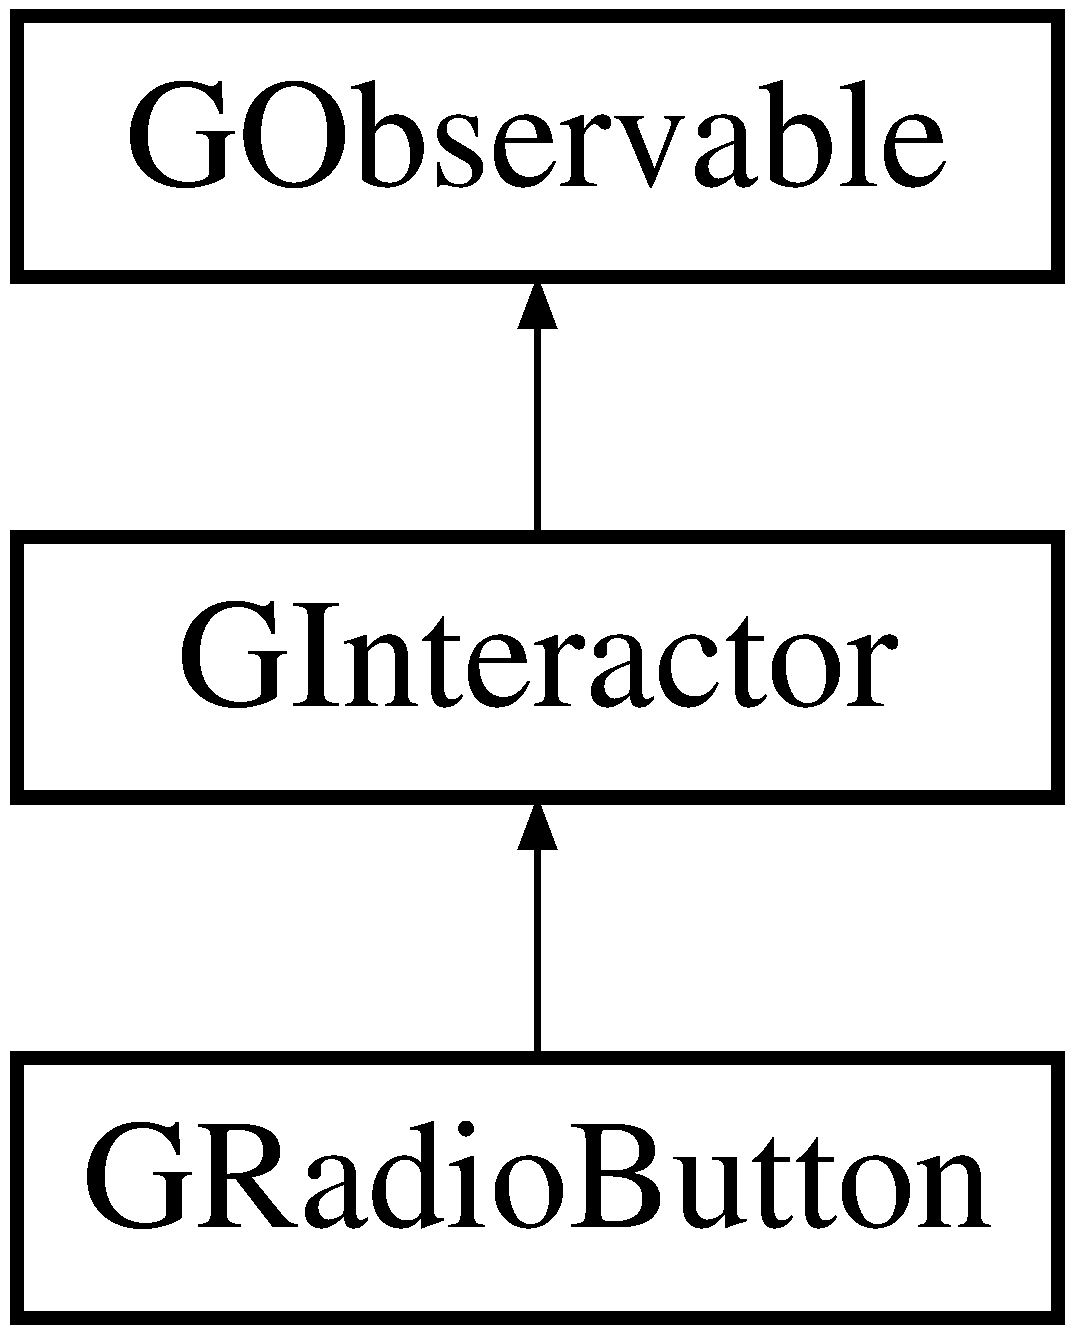
\includegraphics[height=3.000000cm]{classGRadioButton}
\end{center}
\end{figure}
\subsection*{Public Types}
\begin{DoxyCompactItemize}
\item 
enum \mbox{\hyperlink{classGInteractor_a8e0d441725a81d2bbdebbea09078260e}{Text\+Position}} \{ \mbox{\hyperlink{classGInteractor_a8e0d441725a81d2bbdebbea09078260ea4cd6f2e7d5a08d6f4dc052df2358f774}{T\+E\+X\+T\+\_\+\+B\+E\+S\+I\+D\+E\+\_\+\+I\+C\+ON}}, 
\mbox{\hyperlink{classGInteractor_a8e0d441725a81d2bbdebbea09078260eaa88490f63d8de68d44c83bdb2ecde3b3}{T\+E\+X\+T\+\_\+\+U\+N\+D\+E\+R\+\_\+\+I\+C\+ON}}, 
\mbox{\hyperlink{classGInteractor_a8e0d441725a81d2bbdebbea09078260ea39a6f388a30ac4fefb6eb13e846bc9f2}{T\+E\+X\+T\+\_\+\+O\+N\+LY}}
 \}
\begin{DoxyCompactList}\small\item\em The places where an interactor can place its text relative to its icon. \end{DoxyCompactList}\end{DoxyCompactItemize}
\subsection*{Public Member Functions}
\begin{DoxyCompactItemize}
\item 
\mbox{\hyperlink{classGRadioButton_ad9086510e97651d4dc528f115fd8aa6c}{G\+Radio\+Button}} (const std\+::string \&text=\char`\"{}\char`\"{}, const std\+::string \&group=\char`\"{}default\char`\"{}, bool checked=false, Q\+Widget $\ast$parent=nullptr)
\begin{DoxyCompactList}\small\item\em Creates a new radio button with the given text. \end{DoxyCompactList}\item 
virtual \mbox{\hyperlink{classGRadioButton_ad91fff00db319dfa29f1243d4fffaa0c}{$\sim$\+G\+Radio\+Button}} () Q\+\_\+\+D\+E\+C\+L\+\_\+\+O\+V\+E\+R\+R\+I\+DE
\begin{DoxyCompactList}\small\item\em Frees memory allocated internally by the radio button. \end{DoxyCompactList}\item 
virtual void \mbox{\hyperlink{classGInteractor_a02f20ea6edfa0671f31c4c648a253833}{add\+Action\+Listener}} () Q\+\_\+\+D\+E\+C\+L\+\_\+\+D\+E\+P\+R\+E\+C\+A\+T\+ED
\begin{DoxyCompactList}\small\item\em Adds an event listener to be notified when this interactor is clicked or generally interacted with. \end{DoxyCompactList}\item 
virtual bool \mbox{\hyperlink{classGInteractor_ac05ba5b92e2e5146d416fe7f842a0969}{events\+Enabled}} () const Q\+\_\+\+D\+E\+C\+L\+\_\+\+O\+V\+E\+R\+R\+I\+DE
\begin{DoxyCompactList}\small\item\em Returns true if this interactor is currently accepting events. \end{DoxyCompactList}\item 
virtual std\+::string \mbox{\hyperlink{classGInteractor_a69f8d23ed8f207fbecad99960776e942}{get\+Accelerator}} () const
\begin{DoxyCompactList}\small\item\em Returns a string representing a hotkey for this interactor, or an empty string if no accelerator has been set. \end{DoxyCompactList}\item 
virtual std\+::string \mbox{\hyperlink{classGRadioButton_a90f2b1e6f6e7dabd9d6e5307f7c6d1b7}{get\+Action\+Command}} () const Q\+\_\+\+D\+E\+C\+L\+\_\+\+O\+V\+E\+R\+R\+I\+DE
\begin{DoxyCompactList}\small\item\em Returns an action command for this interactor, which is a semi-\/unique string you can use to identify it when events occur. \end{DoxyCompactList}\item 
virtual std\+::string \mbox{\hyperlink{classGInteractor_a808e22cc1fdfbecf71ed8c64ef4600e0}{get\+Background}} () const
\begin{DoxyCompactList}\small\item\em Returns the background color of the interactor as a string. \end{DoxyCompactList}\item 
virtual int \mbox{\hyperlink{classGInteractor_a9e827257a55cb8cf4d9de2ec6bcfd7a0}{get\+Background\+Int}} () const
\begin{DoxyCompactList}\small\item\em Returns the background color of the interactor as an R\+GB integer. \end{DoxyCompactList}\item 
virtual \mbox{\hyperlink{classGRectangle}{G\+Rectangle}} \mbox{\hyperlink{classGInteractor_a29e6ac35a0b48f491a4c88194cc5da3b}{get\+Bounds}} () const
\begin{DoxyCompactList}\small\item\em Returns a rectangle representing the x/y position and size of this interactor. \end{DoxyCompactList}\item 
virtual std\+::string \mbox{\hyperlink{classGInteractor_aa061dfa488c31e18549d64363c1d0e34}{get\+Color}} () const
\begin{DoxyCompactList}\small\item\em Returns the foreground/text color of the interactor as a string. \end{DoxyCompactList}\item 
virtual int \mbox{\hyperlink{classGInteractor_a9635c7af766cdc3417f346683fa0e6c1}{get\+Color\+Int}} () const
\begin{DoxyCompactList}\small\item\em Returns the foreground/text color of the interactor as an R\+GB integer. \end{DoxyCompactList}\item 
virtual \mbox{\hyperlink{classGContainer}{G\+Container}} $\ast$ \mbox{\hyperlink{classGInteractor_a7a6e317c29d61030929b4cd2d1c00fe7}{get\+Container}} () const
\begin{DoxyCompactList}\small\item\em Returns a pointer to the onscreen container holding this interactor. \end{DoxyCompactList}\item 
virtual std\+::string \mbox{\hyperlink{classGInteractor_a894a5502900794eeb27d084c21f1d77d}{get\+Font}} () const
\begin{DoxyCompactList}\small\item\em Returns the font of this interactor\textquotesingle{}s text as a font string such as \char`\"{}\+Helvetica-\/12-\/\+Bold\char`\"{}. \end{DoxyCompactList}\item 
virtual std\+::string \mbox{\hyperlink{classGInteractor_a4fa2d8b0192a3a5b4af4bbfe71194d03}{get\+Foreground}} () const
\begin{DoxyCompactList}\small\item\em Returns the foreground/text color of the interactor as a string. \end{DoxyCompactList}\item 
virtual int \mbox{\hyperlink{classGInteractor_ac3b12ab385a6ef9ae90fc879860ba726}{get\+Foreground\+Int}} () const
\begin{DoxyCompactList}\small\item\em Returns the foreground/text color of the interactor as an R\+GB integer. \end{DoxyCompactList}\item 
virtual double \mbox{\hyperlink{classGInteractor_a1e7e353362434072875264cf95629f99}{get\+Height}} () const
\begin{DoxyCompactList}\small\item\em Returns the current onscreen height of this interactor in pixels. \end{DoxyCompactList}\item 
virtual std\+::string \mbox{\hyperlink{classGInteractor_aaed62a73004939a64da6f0eb9eb64d73}{get\+Icon}} () const
\begin{DoxyCompactList}\small\item\em Returns the file name of the icon associated with this interactor, or an empty string if no icon has been set. \end{DoxyCompactList}\item 
virtual int \mbox{\hyperlink{classGInteractor_a9c9659a6c6ba66b4107ba59c95a24241}{get\+ID}} () const
\begin{DoxyCompactList}\small\item\em Returns a globally unique identifier for this interactor, which is set when the interactor is constructed. \end{DoxyCompactList}\item 
virtual \+\_\+\+Internal\+\_\+\+Q\+Widget $\ast$ \mbox{\hyperlink{classGRadioButton_a208ce13c1da40bf0ddb509daf99d6588}{get\+Internal\+Widget}} () const Q\+\_\+\+D\+E\+C\+L\+\_\+\+O\+V\+E\+R\+R\+I\+DE
\begin{DoxyCompactList}\small\item\em Returns a direct pointer to the internal Qt widget being wrapped by this interactor. \end{DoxyCompactList}\item 
virtual \mbox{\hyperlink{classGPoint}{G\+Point}} \mbox{\hyperlink{classGInteractor_a4f83802015511edeb63b892830812c11}{get\+Location}} () const
\begin{DoxyCompactList}\small\item\em Returns an (x, y) point representing the onscreen location of the top-\/left corner of this interactor within its containing window. \end{DoxyCompactList}\item 
virtual double \mbox{\hyperlink{classGInteractor_aed4b0075fcc434499c3cb3e46896bda3}{get\+Minimum\+Height}} () const
\begin{DoxyCompactList}\small\item\em Returns the minimum height in pixels that this interactor will permit itself to be resized to. \end{DoxyCompactList}\item 
virtual \mbox{\hyperlink{classGDimension}{G\+Dimension}} \mbox{\hyperlink{classGInteractor_a66b5af0b32493b4d597ca0a3df2049ea}{get\+Minimum\+Size}} () const
\begin{DoxyCompactList}\small\item\em Returns a \mbox{\hyperlink{classGDimension}{G\+Dimension}} structure representing the minimum size in pixels that this interactor will permit itself to be resized to. \end{DoxyCompactList}\item 
virtual double \mbox{\hyperlink{classGInteractor_a59e668114fe3d49d2a0f28deb258f7c8}{get\+Minimum\+Width}} () const
\begin{DoxyCompactList}\small\item\em Returns the minimum width in pixels that this interactor will permit itself to be resized to. \end{DoxyCompactList}\item 
virtual std\+::string \mbox{\hyperlink{classGInteractor_a8a60438a5b55d0b2ceb35c8674b9d8c5}{get\+Name}} () const
\begin{DoxyCompactList}\small\item\em Returns a string representing a unique name for this interactor. \end{DoxyCompactList}\item 
virtual double \mbox{\hyperlink{classGInteractor_a747de0961653847bdc6615dbf756d715}{get\+Preferred\+Height}} () const
\begin{DoxyCompactList}\small\item\em Returns the height in pixels that this interactor would prefer to be, which would exactly fit its contents with no stretching or scrollbars. \end{DoxyCompactList}\item 
virtual \mbox{\hyperlink{classGDimension}{G\+Dimension}} \mbox{\hyperlink{classGInteractor_a4aabbee761d8e9116275401131b7ccd1}{get\+Preferred\+Size}} () const
\begin{DoxyCompactList}\small\item\em Returns a \mbox{\hyperlink{classGDimension}{G\+Dimension}} structure storing the width and height in pixels that this interactor would prefer to be, which would exactly fit its contents with no stretching or scrollbars. \end{DoxyCompactList}\item 
virtual double \mbox{\hyperlink{classGInteractor_a82bca31d37700fb0e35d2743352efd5e}{get\+Preferred\+Width}} () const
\begin{DoxyCompactList}\small\item\em Returns the height in pixels that this interactor would prefer to be, which would exactly fit its contents with no stretching or scrollbars. \end{DoxyCompactList}\item 
virtual \mbox{\hyperlink{classGDimension}{G\+Dimension}} \mbox{\hyperlink{classGInteractor_a7b4eec96a2bdc6420695d5796a78eea9}{get\+Size}} () const
\begin{DoxyCompactList}\small\item\em Returns a \mbox{\hyperlink{classGDimension}{G\+Dimension}} structure storing the current onscreen width and height of this interactor in pixels. \end{DoxyCompactList}\item 
virtual std\+::string \mbox{\hyperlink{classGRadioButton_aff553c50924b836c29f146ed34a7c6ec}{get\+Text}} () const
\begin{DoxyCompactList}\small\item\em Returns the text next to the radio button. \end{DoxyCompactList}\item 
virtual std\+::string \mbox{\hyperlink{classGRadioButton_a9896d58fcfebbf1025aeeb5b8b9ede80}{get\+Type}} () const Q\+\_\+\+D\+E\+C\+L\+\_\+\+O\+V\+E\+R\+R\+I\+DE
\begin{DoxyCompactList}\small\item\em Returns a string representing the class name of this interactor, such as \char`\"{}\+G\+Button\char`\"{} or \char`\"{}\+G\+Check\+Box\char`\"{}. \end{DoxyCompactList}\item 
virtual Q\+Widget $\ast$ \mbox{\hyperlink{classGRadioButton_a326ee51b5561f807df7b29a1c101f7fd}{get\+Widget}} () const Q\+\_\+\+D\+E\+C\+L\+\_\+\+O\+V\+E\+R\+R\+I\+DE
\begin{DoxyCompactList}\small\item\em Returns a direct pointer to the internal Qt widget being wrapped by this interactor. \end{DoxyCompactList}\item 
virtual double \mbox{\hyperlink{classGInteractor_a0ed2965abd4f5701d2cadf71239faf19}{get\+Width}} () const
\begin{DoxyCompactList}\small\item\em Returns the current onscreen width of this interactor in pixels. \end{DoxyCompactList}\item 
virtual double \mbox{\hyperlink{classGInteractor_a344385751bee0720059403940d57a13e}{getX}} () const
\begin{DoxyCompactList}\small\item\em Returns the x-\/coordinate of the top-\/left pixel of this interactor within its onscreen window. \end{DoxyCompactList}\item 
virtual double \mbox{\hyperlink{classGInteractor_aafa51c7f8f38a09febbb9ce7853f77b4}{getY}} () const
\begin{DoxyCompactList}\small\item\em Returns the y-\/coordinate of the top-\/left pixel of this interactor within its onscreen window. \end{DoxyCompactList}\item 
virtual bool \mbox{\hyperlink{classGInteractor_afc480f652b8c5f1fb255e2269ce68879}{in\+Bounds}} (double x, double y) const
\begin{DoxyCompactList}\small\item\em Returns true if the given x/y pixel is within the bounds of this interactor. \end{DoxyCompactList}\item 
virtual bool \mbox{\hyperlink{classGInteractor_ae6d7982c1c627b677a5e776ca86118ed}{in\+Bounds}} (int x, int y) const
\begin{DoxyCompactList}\small\item\em Returns true if the given x/y pixel is within the bounds of this interactor. \end{DoxyCompactList}\item 
virtual bool \mbox{\hyperlink{classGRadioButton_ac8cada18b9357ff68b26e17f44294764}{is\+Checked}} () const
\begin{DoxyCompactList}\small\item\em Returns true if the radio button is currently checked. \end{DoxyCompactList}\item 
virtual bool \mbox{\hyperlink{classGInteractor_aacb819fb241851fd9fc045271baa4034}{is\+Enabled}} () const
\begin{DoxyCompactList}\small\item\em Returns true if this interactor is currently enabled. \end{DoxyCompactList}\item 
virtual bool \mbox{\hyperlink{classGRadioButton_a56a065a2c20a230931de0ed98019d8fb}{is\+Selected}} () const
\begin{DoxyCompactList}\small\item\em Returns true if the radio button is currently checked. \end{DoxyCompactList}\item 
virtual bool \mbox{\hyperlink{classGInteractor_a9d8a6cfb13917785c143e74d40e4e2be}{is\+Visible}} () const
\begin{DoxyCompactList}\small\item\em Returns true if the interactor is visible on the screen. \end{DoxyCompactList}\item 
virtual void \mbox{\hyperlink{classGRadioButton_ab7fe7a876367b87cf7202f947f1d05e4}{remove\+Action\+Listener}} ()
\begin{DoxyCompactList}\small\item\em Removes the action listener from this radio button so that it will no longer call it when events occur. \end{DoxyCompactList}\item 
virtual void \mbox{\hyperlink{classGRadioButton_aa4250907e4cdd77349c04f0cf5cdd3d3}{remove\+Double\+Click\+Listener}} ()
\begin{DoxyCompactList}\small\item\em Removes the double-\/click listener from this radio button so that it will no longer call it when events occur. \end{DoxyCompactList}\item 
virtual void \mbox{\hyperlink{classGInteractor_a519fb2ac767f8b2febbb50b898b8c8cb}{request\+Focus}} ()
\begin{DoxyCompactList}\small\item\em Transfers keyboard focus to this interactor. \end{DoxyCompactList}\item 
virtual void \mbox{\hyperlink{classGInteractor_ad15f102f62e2960576012f1aa0ba4b2e}{set\+Accelerator}} (const std\+::string \&accelerator)
\begin{DoxyCompactList}\small\item\em Sets an accelerator hotkey for this interactor, such as \char`\"{}\+Ctrl-\/\+S\char`\"{}. \end{DoxyCompactList}\item 
virtual void \mbox{\hyperlink{classGInteractor_a4b5843fe3030e038a1ba54cc03389bcf}{set\+Action\+Command}} (const std\+::string \&action\+Command)
\begin{DoxyCompactList}\small\item\em Sets the action command for this interactor. \end{DoxyCompactList}\item 
virtual void \mbox{\hyperlink{classGRadioButton_adcfb4742430c88714fcf57e57ab8ea9c}{set\+Action\+Listener}} (G\+Event\+Listener func)
\begin{DoxyCompactList}\small\item\em Sets an action listener on this radio button so that it will be called when the radio button is clicked. \end{DoxyCompactList}\item 
virtual void \mbox{\hyperlink{classGRadioButton_aebd20a89c7a8a43a6fce999cf4f9fcf2}{set\+Action\+Listener}} (G\+Event\+Listener\+Void func)
\begin{DoxyCompactList}\small\item\em Sets an action listener on this radio button so that it will be called when the radio button is clicked. \end{DoxyCompactList}\item 
virtual void \mbox{\hyperlink{classGInteractor_acba7e546c2025c0a15ca4b4cc92043db}{set\+Background}} (int rgb)
\begin{DoxyCompactList}\small\item\em Sets the background color of the interactor to the color represented by the given R\+GB integer. \end{DoxyCompactList}\item 
virtual void \mbox{\hyperlink{classGInteractor_ab4677ab2474e68b07aa56605af92a84a}{set\+Background}} (const std\+::string \&color)
\begin{DoxyCompactList}\small\item\em Sets the background color of the interactor to the color represented by the given string. \end{DoxyCompactList}\item 
virtual void \mbox{\hyperlink{classGInteractor_a2aae8197624b72265ab83b4f1bc73f2f}{set\+Bounds}} (double x, double y, double width, double height)
\begin{DoxyCompactList}\small\item\em Sets the size and location of the widget. \end{DoxyCompactList}\item 
virtual void \mbox{\hyperlink{classGInteractor_acada386653f008cacc7cce86426bef7c}{set\+Bounds}} (const \mbox{\hyperlink{classGRectangle}{G\+Rectangle}} \&size)
\begin{DoxyCompactList}\small\item\em Sets the size and location of the widget. \end{DoxyCompactList}\item 
virtual void \mbox{\hyperlink{classGRadioButton_a116285e2f56247b00b26035ca0ac4737}{set\+Checked}} (bool checked)
\begin{DoxyCompactList}\small\item\em Sets whether the radio button should be checked. \end{DoxyCompactList}\item 
virtual void \mbox{\hyperlink{classGInteractor_ab1f5cc0f5cc6bbbd716a526c61f1081d}{set\+Color}} (int rgb)
\begin{DoxyCompactList}\small\item\em Sets the foreground/text color of the interactor to the color represented by the given R\+GB integer. \end{DoxyCompactList}\item 
virtual void \mbox{\hyperlink{classGInteractor_a61374df6c11b52cfbb0815decdbaebc6}{set\+Color}} (const std\+::string \&color)
\begin{DoxyCompactList}\small\item\em Sets the foreground/text color of the interactor to the color represented by the given string. \end{DoxyCompactList}\item 
virtual void \mbox{\hyperlink{classGRadioButton_ac29f9a3462458e165fae3a1f046ee77a}{set\+Double\+Click\+Listener}} (G\+Event\+Listener func)
\begin{DoxyCompactList}\small\item\em Sets a listener on this radio button so that it will be called when the radio button is double-\/clicked. \end{DoxyCompactList}\item 
virtual void \mbox{\hyperlink{classGRadioButton_a50096194d66f48c92dd4c512d41bfc76}{set\+Double\+Click\+Listener}} (G\+Event\+Listener\+Void func)
\begin{DoxyCompactList}\small\item\em Sets a listener on this radio button so that it will be called when the radio button is double-\/clicked. \end{DoxyCompactList}\item 
virtual void \mbox{\hyperlink{classGInteractor_ab831367dd84bbd579e02e55bacb21343}{set\+Enabled}} (bool value)
\begin{DoxyCompactList}\small\item\em Sets whether this interactor is currently enabled. \end{DoxyCompactList}\item 
virtual void \mbox{\hyperlink{classGObservable_afaa30b2a9e0f378fd1c70d2f1d0b8216}{set\+Events\+Enabled}} (bool \mbox{\hyperlink{classGInteractor_ac05ba5b92e2e5146d416fe7f842a0969}{events\+Enabled}})
\begin{DoxyCompactList}\small\item\em Sets whether the object is currently allowing itself to fire events. \end{DoxyCompactList}\item 
virtual void \mbox{\hyperlink{classGInteractor_a2592348886ffea646c6534bf88f7c49d}{set\+Font}} (const Q\+Font \&font)
\begin{DoxyCompactList}\small\item\em Sets the font used by this widget to the given Qt font. \end{DoxyCompactList}\item 
virtual void \mbox{\hyperlink{classGInteractor_a8e096e8818d838aceae1d46d58fb3a7b}{set\+Font}} (const std\+::string \&font)
\begin{DoxyCompactList}\small\item\em Sets the font used by this widget to the font represented by the given font string, such as \char`\"{}\+Helvetica-\/16-\/\+Bold\char`\"{}. \end{DoxyCompactList}\item 
virtual void \mbox{\hyperlink{classGInteractor_a9eb856b5ff83a19df3831a31f15f4563}{set\+Foreground}} (int rgb)
\begin{DoxyCompactList}\small\item\em Sets the foreground/text color of the interactor to the color represented by the given R\+GB integer. \end{DoxyCompactList}\item 
virtual void \mbox{\hyperlink{classGInteractor_af59209aeadea6dfc6d97a2d8531f50e1}{set\+Foreground}} (const std\+::string \&color)
\begin{DoxyCompactList}\small\item\em Sets the foreground/text color of the interactor to the color represented by the given string. \end{DoxyCompactList}\item 
virtual void \mbox{\hyperlink{classGInteractor_a9e280bfc4544dfaf8e4376c4e1a74357}{set\+Height}} (double height)
\begin{DoxyCompactList}\small\item\em Sets the onscreen height of the interactor in pixels. \end{DoxyCompactList}\item 
virtual void \mbox{\hyperlink{classGInteractor_a762e139aa311461c3984d3ad28293f64}{set\+Icon}} (const std\+::string \&filename, bool retain\+Icon\+Size=true)
\begin{DoxyCompactList}\small\item\em Sets the file name of the icon associated with this interactor, or an empty string if no icon has been set. \end{DoxyCompactList}\item 
virtual void \mbox{\hyperlink{classGInteractor_a04594e8ba9b98513a64f1da00dcae18c}{set\+Location}} (double x, double y)
\begin{DoxyCompactList}\small\item\em Sets the onscreen x/y-\/coordinate of the top-\/left corner of the interactor relative to its window. \end{DoxyCompactList}\item 
virtual void \mbox{\hyperlink{classGInteractor_a0cf428e207b7f22cc08138a90b1b87b2}{set\+Minimum\+Size}} (double width, double height)
\begin{DoxyCompactList}\small\item\em Sets the minimum size in pixels that this interactor will permit itself to be resized to. \end{DoxyCompactList}\item 
virtual void \mbox{\hyperlink{classGInteractor_a3b1046117ac6cb7abe467e00ba8a81f4}{set\+Minimum\+Size}} (const \mbox{\hyperlink{classGDimension}{G\+Dimension}} \&size)
\begin{DoxyCompactList}\small\item\em Sets the minimum size in pixels that this interactor will permit itself to be resized to. \end{DoxyCompactList}\item 
virtual void \mbox{\hyperlink{classGInteractor_a9d3a2685df23b5e7cbf59c19c4a1f9b5}{set\+Name}} (const std\+::string \&name)
\begin{DoxyCompactList}\small\item\em Sets a string representing a unique name for this interactor. \end{DoxyCompactList}\item 
virtual void \mbox{\hyperlink{classGInteractor_a1ab987704fce32098706c6f00fb08218}{set\+Preferred\+Height}} (double height)
\begin{DoxyCompactList}\small\item\em Sets the height in pixels that this interactor would prefer to be. \end{DoxyCompactList}\item 
virtual void \mbox{\hyperlink{classGInteractor_a042c5ae19430d765ef552371cae3632c}{set\+Preferred\+Size}} (double width, double height)
\begin{DoxyCompactList}\small\item\em Sets the width and height in pixels that this interactor would prefer to be. \end{DoxyCompactList}\item 
virtual void \mbox{\hyperlink{classGInteractor_aa22d9be4bc0e078bb0ea69b0fc9d7c75}{set\+Preferred\+Size}} (const \mbox{\hyperlink{classGDimension}{G\+Dimension}} \&size)
\begin{DoxyCompactList}\small\item\em Sets the size in pixels that this interactor would prefer to be. \end{DoxyCompactList}\item 
virtual void \mbox{\hyperlink{classGInteractor_a3db429ab2fa52efd187eec0ed8cdd9f2}{set\+Preferred\+Width}} (double width)
\begin{DoxyCompactList}\small\item\em Sets the width in pixels that this interactor would prefer to be. \end{DoxyCompactList}\item 
virtual void \mbox{\hyperlink{classGRadioButton_ad42accd39af295a957386c68dac3dcae}{set\+Selected}} (bool selected)
\begin{DoxyCompactList}\small\item\em Sets whether the radio button should be checked. \end{DoxyCompactList}\item 
virtual void \mbox{\hyperlink{classGInteractor_aca25d49481f9bf5fc8f7df4c086c4ce7}{set\+Size}} (double width, double height)
\begin{DoxyCompactList}\small\item\em Sets the onscreen width and height of the interactor in pixels. \end{DoxyCompactList}\item 
virtual void \mbox{\hyperlink{classGInteractor_ae2b628228f192c2702c4ce941b2af68f}{set\+Size}} (const \mbox{\hyperlink{classGDimension}{G\+Dimension}} \&size)
\begin{DoxyCompactList}\small\item\em Sets the onscreen width and height of the interactor in pixels. \end{DoxyCompactList}\item 
virtual void \mbox{\hyperlink{classGRadioButton_ac1ae51949d41ee9054634be5967d91b8}{set\+Text}} (const std\+::string \&text)
\begin{DoxyCompactList}\small\item\em Sets the text that will appear next to the radio button. \end{DoxyCompactList}\item 
virtual void \mbox{\hyperlink{classGInteractor_a039e0e49beaecc275efce02d416acea8}{set\+Tooltip}} (const std\+::string \&tooltip\+Text)
\begin{DoxyCompactList}\small\item\em Sets a \char`\"{}tooltip\char`\"{} that will appear if the user hovers their mouse over the interactor. \end{DoxyCompactList}\item 
virtual void \mbox{\hyperlink{classGInteractor_a18e44e30b31525a243960ca3928125aa}{set\+Visible}} (bool visible)
\begin{DoxyCompactList}\small\item\em Returns true if the interactor is visible on the screen. \end{DoxyCompactList}\item 
virtual void \mbox{\hyperlink{classGInteractor_aa3f3fba4cb131baa8696ba01e3bceca1}{set\+Width}} (double width)
\begin{DoxyCompactList}\small\item\em Sets the onscreen width of the interactor in pixels. \end{DoxyCompactList}\item 
virtual void \mbox{\hyperlink{classGInteractor_a9c18fcc579333bf9653d13ad2b372e39}{setX}} (double x)
\begin{DoxyCompactList}\small\item\em Sets the onscreen x-\/coordinate of the top-\/left corner of the interactor relative to its window. \end{DoxyCompactList}\item 
virtual void \mbox{\hyperlink{classGInteractor_a7d57e2a5c35d27feb58fd498a3cf82b9}{setY}} (double y)
\begin{DoxyCompactList}\small\item\em Sets the onscreen y-\/coordinate of the top-\/left corner of the interactor relative to its window. \end{DoxyCompactList}\item 
virtual void \mbox{\hyperlink{classGRadioButton_ad277193b2dca0bab1e0ad24d45407dc3}{toggle}} ()
\begin{DoxyCompactList}\small\item\em Reverses the checked state of the button, setting it to be checked if it was unchecked or to be unchecked if it was checked. \end{DoxyCompactList}\item 
virtual std\+::string \mbox{\hyperlink{classGObservable_a1fe5121d6528fdea3f243321b3fa3a49}{to\+String}} () const
\begin{DoxyCompactList}\small\item\em Returns a string representation of this observable object\textquotesingle{}s state. \end{DoxyCompactList}\end{DoxyCompactItemize}
\subsection*{Protected Member Functions}
\begin{DoxyCompactItemize}
\item 
virtual void \mbox{\hyperlink{classGObservable_a80cfa040459ff53594adbd6a51ec8f43}{clear\+Event\+Listeners}} ()
\begin{DoxyCompactList}\small\item\em Removes all event listeners from this object. \end{DoxyCompactList}\item 
virtual void \mbox{\hyperlink{classGObservable_a284f31528c0520f8e545c03ac9eeac74}{ensure\+Thread\+Safety}} (const std\+::string \&member\+Name=\char`\"{}\char`\"{})
\begin{DoxyCompactList}\small\item\em Ensures that we are currently in the Qt G\+UI thread. \end{DoxyCompactList}\item 
virtual void \mbox{\hyperlink{classGObservable_a63e5e5a6227c59c928493b11aceb0f67}{fire\+Event}} (\mbox{\hyperlink{classGEvent}{G\+Event}} \&event)
\begin{DoxyCompactList}\small\item\em Sends out the given event to any attached listeners. \end{DoxyCompactList}\item 
virtual void \mbox{\hyperlink{classGObservable_ab3983ea07337b52020a29cc00c653d8d}{fire\+G\+Event}} (Q\+Event $\ast$event, Event\+Type event\+Type, const std\+::string \&event\+Name)
\begin{DoxyCompactList}\small\item\em Creates an event of the given type, then sends it out to any attached listeners. \end{DoxyCompactList}\item 
virtual void \mbox{\hyperlink{classGObservable_a01fdf1b0e0dbd49e189fe4514e010411}{fire\+G\+Event}} (Q\+Close\+Event $\ast$event, Event\+Type event\+Type, const std\+::string \&event\+Name)
\begin{DoxyCompactList}\small\item\em Creates an event of the given type, then sends it out to any attached listeners. \end{DoxyCompactList}\item 
virtual void \mbox{\hyperlink{classGObservable_abb0b2f66ba39211cb5d7615e9d1c04e2}{fire\+G\+Event}} (Q\+Key\+Event $\ast$event, Event\+Type event\+Type, const std\+::string \&event\+Name)
\begin{DoxyCompactList}\small\item\em Creates an event of the given type, then sends it out to any attached listeners. \end{DoxyCompactList}\item 
virtual void \mbox{\hyperlink{classGObservable_a119318675d2165bdf7dd853aaf881d4b}{fire\+G\+Event}} (Q\+Mouse\+Event $\ast$event, Event\+Type event\+Type, const std\+::string \&event\+Name, const std\+::string \&action\+Command=\char`\"{}\char`\"{})
\begin{DoxyCompactList}\small\item\em Creates an event of the given type, then sends it out to any attached listeners. \end{DoxyCompactList}\item 
virtual void \mbox{\hyperlink{classGObservable_a63fd9034e1e1633c1c38eb342bfd34e9}{fire\+G\+Event}} (Q\+Resize\+Event $\ast$event, Event\+Type event\+Type, const std\+::string \&event\+Name)
\begin{DoxyCompactList}\small\item\em Creates an event of the given type, then sends it out to any attached listeners. \end{DoxyCompactList}\item 
virtual void \mbox{\hyperlink{classGObservable_a741345310d9b7c5170a6cbc410c44ac4}{fire\+G\+Event}} (Q\+Timer\+Event $\ast$event, Event\+Type event\+Type, const std\+::string \&event\+Name)
\begin{DoxyCompactList}\small\item\em Creates an event of the given type, then sends it out to any attached listeners. \end{DoxyCompactList}\item 
virtual void \mbox{\hyperlink{classGObservable_a93bf338968a0338761b8e4dc62f582e9}{fire\+G\+Event}} (Q\+Wheel\+Event $\ast$event, Event\+Type event\+Type, const std\+::string \&event\+Name)
\begin{DoxyCompactList}\small\item\em Creates an event of the given type, then sends it out to any attached listeners. \end{DoxyCompactList}\item 
virtual void \mbox{\hyperlink{classGObservable_a2a70a7d7435ff0c3b80bb4d70da19e0d}{fire\+G\+Event}} (Q\+Window\+State\+Change\+Event $\ast$event, Event\+Type event\+Type, const std\+::string \&event\+Name)
\begin{DoxyCompactList}\small\item\em Creates an event of the given type, then sends it out to any attached listeners. \end{DoxyCompactList}\item 
virtual bool \mbox{\hyperlink{classGObservable_a9f6faaa25942923bafa1c44020c49fa9}{has\+Event\+Listener}} (const std\+::string \&event\+Name) const
\begin{DoxyCompactList}\small\item\em Returns true if the observable object has a listener for the given type of event. \end{DoxyCompactList}\item 
virtual bool \mbox{\hyperlink{classGObservable_aeec1adc19aa0f33de62390686ee1382c}{is\+Accepting\+Event}} (int event\+Mask) const
\begin{DoxyCompactList}\small\item\em Returns true if the observable object has a listener for the given type of event. \end{DoxyCompactList}\item 
virtual bool \mbox{\hyperlink{classGObservable_aa31c73145a29dcb92848a92e0cfaea41}{is\+Accepting\+Event}} (const \mbox{\hyperlink{classGEvent}{G\+Event}} \&event) const
\begin{DoxyCompactList}\small\item\em Returns true if the observable object has a listener for the given type of event. \end{DoxyCompactList}\item 
virtual bool \mbox{\hyperlink{classGObservable_a3b1c689267eda44e65a2213e7de38b23}{is\+Accepting\+Event}} (const std\+::string \&event\+Type) const
\begin{DoxyCompactList}\small\item\em Returns true if the observable object has a listener for the given type of event. \end{DoxyCompactList}\item 
virtual void \mbox{\hyperlink{classGObservable_acbcf1ed3a851ad8a3c17ef38d86b481d}{remove\+Event\+Listener}} (const std\+::string \&event\+Name)
\begin{DoxyCompactList}\small\item\em Removes any event listener from this observable object that would respond to the given type of event, such as \char`\"{}click\char`\"{} or \char`\"{}keydown\char`\"{}. \end{DoxyCompactList}\item 
virtual void \mbox{\hyperlink{classGObservable_af51cc35c29a1bd1908609d432decdbb6}{remove\+Event\+Listeners}} (std\+::initializer\+\_\+list$<$ std\+::string $>$ event\+Names)
\begin{DoxyCompactList}\small\item\em Removes any event listener from this observable object that would respond to the given types of events, such as \char`\"{}click\char`\"{} or \char`\"{}keydown\char`\"{}. \end{DoxyCompactList}\item 
virtual void \mbox{\hyperlink{classGObservable_ad2f6d34961c50f6c1e0659990b79f741}{set\+Event\+Listener}} (const std\+::string \&event\+Name, G\+Event\+Listener func)
\begin{DoxyCompactList}\small\item\em Adds an event listener from this observable object to respond to the given type of event, such as \char`\"{}click\char`\"{} or \char`\"{}keydown\char`\"{}. \end{DoxyCompactList}\item 
virtual void \mbox{\hyperlink{classGObservable_abac4cb9f9e626e010e87f5d91573c8a5}{set\+Event\+Listener}} (const std\+::string \&event\+Name, G\+Event\+Listener\+Void func)
\begin{DoxyCompactList}\small\item\em Adds an event listener from this observable object to respond to the given type of event, such as \char`\"{}click\char`\"{} or \char`\"{}keydown\char`\"{}. \end{DoxyCompactList}\item 
virtual void \mbox{\hyperlink{classGObservable_afa388d69c33c718cf035774604065604}{set\+Event\+Listeners}} (std\+::initializer\+\_\+list$<$ std\+::string $>$ event\+Names, G\+Event\+Listener func)
\begin{DoxyCompactList}\small\item\em Adds an event listener from this observable object to respond to the given types of events, such as \char`\"{}click\char`\"{} or \char`\"{}keydown\char`\"{}. \end{DoxyCompactList}\item 
virtual void \mbox{\hyperlink{classGObservable_a7867184bbb686f74fae8a4db927da799}{set\+Event\+Listeners}} (std\+::initializer\+\_\+list$<$ std\+::string $>$ event\+Names, G\+Event\+Listener\+Void func)
\begin{DoxyCompactList}\small\item\em Adds an event listener from this observable object to respond to the given types of events, such as \char`\"{}click\char`\"{} or \char`\"{}keydown\char`\"{}. \end{DoxyCompactList}\end{DoxyCompactItemize}


\subsection{Detailed Description}
This interactor subclass represents an onscreen radio button. 

Radio buttons are round buttons that can be \char`\"{}checked\char`\"{} by clicking them. A radio button differs from a checkbox in that it is often part of a mutually exclusive group of options, where at most one of the buttons can be checked at a time. Clicking one radio button from a group checks it and also unchecks any other checked radio button from that same group.

You can listen for clicks on a radio button using the set\+Action\+Listener method, passing the function you want to call on each click. 

\subsection{Member Enumeration Documentation}
\mbox{\Hypertarget{classGInteractor_a8e0d441725a81d2bbdebbea09078260e}\label{classGInteractor_a8e0d441725a81d2bbdebbea09078260e}} 
\index{G\+Radio\+Button@{G\+Radio\+Button}!Text\+Position@{Text\+Position}}
\index{Text\+Position@{Text\+Position}!G\+Radio\+Button@{G\+Radio\+Button}}
\subsubsection{\texorpdfstring{Text\+Position}{TextPosition}}
{\footnotesize\ttfamily enum \mbox{\hyperlink{classGInteractor_a8e0d441725a81d2bbdebbea09078260e}{Text\+Position}}\hspace{0.3cm}{\ttfamily [inherited]}}



The places where an interactor can place its text relative to its icon. 

\begin{DoxyEnumFields}{Enumerator}
\raisebox{\heightof{T}}[0pt][0pt]{\index{T\+E\+X\+T\+\_\+\+B\+E\+S\+I\+D\+E\+\_\+\+I\+C\+ON@{T\+E\+X\+T\+\_\+\+B\+E\+S\+I\+D\+E\+\_\+\+I\+C\+ON}!G\+Radio\+Button@{G\+Radio\+Button}}\index{G\+Radio\+Button@{G\+Radio\+Button}!T\+E\+X\+T\+\_\+\+B\+E\+S\+I\+D\+E\+\_\+\+I\+C\+ON@{T\+E\+X\+T\+\_\+\+B\+E\+S\+I\+D\+E\+\_\+\+I\+C\+ON}}}\mbox{\Hypertarget{classGInteractor_a8e0d441725a81d2bbdebbea09078260ea4cd6f2e7d5a08d6f4dc052df2358f774}\label{classGInteractor_a8e0d441725a81d2bbdebbea09078260ea4cd6f2e7d5a08d6f4dc052df2358f774}} 
T\+E\+X\+T\+\_\+\+B\+E\+S\+I\+D\+E\+\_\+\+I\+C\+ON&\\
\hline

\raisebox{\heightof{T}}[0pt][0pt]{\index{T\+E\+X\+T\+\_\+\+U\+N\+D\+E\+R\+\_\+\+I\+C\+ON@{T\+E\+X\+T\+\_\+\+U\+N\+D\+E\+R\+\_\+\+I\+C\+ON}!G\+Radio\+Button@{G\+Radio\+Button}}\index{G\+Radio\+Button@{G\+Radio\+Button}!T\+E\+X\+T\+\_\+\+U\+N\+D\+E\+R\+\_\+\+I\+C\+ON@{T\+E\+X\+T\+\_\+\+U\+N\+D\+E\+R\+\_\+\+I\+C\+ON}}}\mbox{\Hypertarget{classGInteractor_a8e0d441725a81d2bbdebbea09078260eaa88490f63d8de68d44c83bdb2ecde3b3}\label{classGInteractor_a8e0d441725a81d2bbdebbea09078260eaa88490f63d8de68d44c83bdb2ecde3b3}} 
T\+E\+X\+T\+\_\+\+U\+N\+D\+E\+R\+\_\+\+I\+C\+ON&\\
\hline

\raisebox{\heightof{T}}[0pt][0pt]{\index{T\+E\+X\+T\+\_\+\+O\+N\+LY@{T\+E\+X\+T\+\_\+\+O\+N\+LY}!G\+Radio\+Button@{G\+Radio\+Button}}\index{G\+Radio\+Button@{G\+Radio\+Button}!T\+E\+X\+T\+\_\+\+O\+N\+LY@{T\+E\+X\+T\+\_\+\+O\+N\+LY}}}\mbox{\Hypertarget{classGInteractor_a8e0d441725a81d2bbdebbea09078260ea39a6f388a30ac4fefb6eb13e846bc9f2}\label{classGInteractor_a8e0d441725a81d2bbdebbea09078260ea39a6f388a30ac4fefb6eb13e846bc9f2}} 
T\+E\+X\+T\+\_\+\+O\+N\+LY&\\
\hline

\end{DoxyEnumFields}


\subsection{Constructor \& Destructor Documentation}
\mbox{\Hypertarget{classGRadioButton_ad9086510e97651d4dc528f115fd8aa6c}\label{classGRadioButton_ad9086510e97651d4dc528f115fd8aa6c}} 
\index{G\+Radio\+Button@{G\+Radio\+Button}!G\+Radio\+Button@{G\+Radio\+Button}}
\index{G\+Radio\+Button@{G\+Radio\+Button}!G\+Radio\+Button@{G\+Radio\+Button}}
\subsubsection{\texorpdfstring{G\+Radio\+Button()}{GRadioButton()}}
{\footnotesize\ttfamily \mbox{\hyperlink{classGRadioButton}{G\+Radio\+Button}} (\begin{DoxyParamCaption}\item[{const std\+::string \&}]{text = {\ttfamily \char`\"{}\char`\"{}},  }\item[{const std\+::string \&}]{group = {\ttfamily \char`\"{}default\char`\"{}},  }\item[{bool}]{checked = {\ttfamily false},  }\item[{Q\+Widget $\ast$}]{parent = {\ttfamily nullptr} }\end{DoxyParamCaption})}



Creates a new radio button with the given text. 

You can pass a string representing a logical group of radio buttons; if you do, this radio button will be internally managed so that at most one radio button from that group will be checked at any given time. If no group is supplied, the radio button is put into a default group. \mbox{\Hypertarget{classGRadioButton_ad91fff00db319dfa29f1243d4fffaa0c}\label{classGRadioButton_ad91fff00db319dfa29f1243d4fffaa0c}} 
\index{G\+Radio\+Button@{G\+Radio\+Button}!````~G\+Radio\+Button@{$\sim$\+G\+Radio\+Button}}
\index{````~G\+Radio\+Button@{$\sim$\+G\+Radio\+Button}!G\+Radio\+Button@{G\+Radio\+Button}}
\subsubsection{\texorpdfstring{$\sim$\+G\+Radio\+Button()}{~GRadioButton()}}
{\footnotesize\ttfamily $\sim$\mbox{\hyperlink{classGRadioButton}{G\+Radio\+Button}} (\begin{DoxyParamCaption}{ }\end{DoxyParamCaption})\hspace{0.3cm}{\ttfamily [virtual]}}



Frees memory allocated internally by the radio button. 



\subsection{Member Function Documentation}
\mbox{\Hypertarget{classGInteractor_a02f20ea6edfa0671f31c4c648a253833}\label{classGInteractor_a02f20ea6edfa0671f31c4c648a253833}} 
\index{G\+Radio\+Button@{G\+Radio\+Button}!add\+Action\+Listener@{add\+Action\+Listener}}
\index{add\+Action\+Listener@{add\+Action\+Listener}!G\+Radio\+Button@{G\+Radio\+Button}}
\subsubsection{\texorpdfstring{add\+Action\+Listener()}{addActionListener()}}
{\footnotesize\ttfamily void add\+Action\+Listener (\begin{DoxyParamCaption}{ }\end{DoxyParamCaption})\hspace{0.3cm}{\ttfamily [virtual]}, {\ttfamily [inherited]}}



Adds an event listener to be notified when this interactor is clicked or generally interacted with. 

\begin{DoxyRefDesc}{Deprecated}
\item[\mbox{\hyperlink{deprecated__deprecated000006}{Deprecated}}]does nothing; use set\+Action\+Listener instead \end{DoxyRefDesc}
\mbox{\Hypertarget{classGObservable_a80cfa040459ff53594adbd6a51ec8f43}\label{classGObservable_a80cfa040459ff53594adbd6a51ec8f43}} 
\index{G\+Radio\+Button@{G\+Radio\+Button}!clear\+Event\+Listeners@{clear\+Event\+Listeners}}
\index{clear\+Event\+Listeners@{clear\+Event\+Listeners}!G\+Radio\+Button@{G\+Radio\+Button}}
\subsubsection{\texorpdfstring{clear\+Event\+Listeners()}{clearEventListeners()}}
{\footnotesize\ttfamily void clear\+Event\+Listeners (\begin{DoxyParamCaption}{ }\end{DoxyParamCaption})\hspace{0.3cm}{\ttfamily [protected]}, {\ttfamily [virtual]}, {\ttfamily [inherited]}}



Removes all event listeners from this object. 

\mbox{\Hypertarget{classGObservable_a284f31528c0520f8e545c03ac9eeac74}\label{classGObservable_a284f31528c0520f8e545c03ac9eeac74}} 
\index{G\+Radio\+Button@{G\+Radio\+Button}!ensure\+Thread\+Safety@{ensure\+Thread\+Safety}}
\index{ensure\+Thread\+Safety@{ensure\+Thread\+Safety}!G\+Radio\+Button@{G\+Radio\+Button}}
\subsubsection{\texorpdfstring{ensure\+Thread\+Safety()}{ensureThreadSafety()}}
{\footnotesize\ttfamily void ensure\+Thread\+Safety (\begin{DoxyParamCaption}\item[{const std\+::string \&}]{member\+Name = {\ttfamily \char`\"{}\char`\"{}} }\end{DoxyParamCaption})\hspace{0.3cm}{\ttfamily [protected]}, {\ttfamily [virtual]}, {\ttfamily [inherited]}}



Ensures that we are currently in the Qt G\+UI thread. 

\mbox{\Hypertarget{classGInteractor_ac05ba5b92e2e5146d416fe7f842a0969}\label{classGInteractor_ac05ba5b92e2e5146d416fe7f842a0969}} 
\index{G\+Radio\+Button@{G\+Radio\+Button}!events\+Enabled@{events\+Enabled}}
\index{events\+Enabled@{events\+Enabled}!G\+Radio\+Button@{G\+Radio\+Button}}
\subsubsection{\texorpdfstring{events\+Enabled()}{eventsEnabled()}}
{\footnotesize\ttfamily bool events\+Enabled (\begin{DoxyParamCaption}{ }\end{DoxyParamCaption}) const\hspace{0.3cm}{\ttfamily [virtual]}, {\ttfamily [inherited]}}



Returns true if this interactor is currently accepting events. 

Initially true. An interactor must be visible and added to an onscreen window to receive events. 

Reimplemented from \mbox{\hyperlink{classGObservable_a8ebb3da91032e7f4c34485dabc518b8a}{G\+Observable}}.

\mbox{\Hypertarget{classGObservable_a63e5e5a6227c59c928493b11aceb0f67}\label{classGObservable_a63e5e5a6227c59c928493b11aceb0f67}} 
\index{G\+Radio\+Button@{G\+Radio\+Button}!fire\+Event@{fire\+Event}}
\index{fire\+Event@{fire\+Event}!G\+Radio\+Button@{G\+Radio\+Button}}
\subsubsection{\texorpdfstring{fire\+Event()}{fireEvent()}}
{\footnotesize\ttfamily void fire\+Event (\begin{DoxyParamCaption}\item[{\mbox{\hyperlink{classGEvent}{G\+Event}} \&}]{event }\end{DoxyParamCaption})\hspace{0.3cm}{\ttfamily [protected]}, {\ttfamily [virtual]}, {\ttfamily [inherited]}}



Sends out the given event to any attached listeners. 

\mbox{\Hypertarget{classGObservable_ab3983ea07337b52020a29cc00c653d8d}\label{classGObservable_ab3983ea07337b52020a29cc00c653d8d}} 
\index{G\+Radio\+Button@{G\+Radio\+Button}!fire\+G\+Event@{fire\+G\+Event}}
\index{fire\+G\+Event@{fire\+G\+Event}!G\+Radio\+Button@{G\+Radio\+Button}}
\subsubsection{\texorpdfstring{fire\+G\+Event()}{fireGEvent()}\hspace{0.1cm}{\footnotesize\ttfamily [1/8]}}
{\footnotesize\ttfamily void fire\+G\+Event (\begin{DoxyParamCaption}\item[{Q\+Event $\ast$}]{event,  }\item[{Event\+Type}]{event\+Type,  }\item[{const std\+::string \&}]{event\+Name }\end{DoxyParamCaption})\hspace{0.3cm}{\ttfamily [protected]}, {\ttfamily [virtual]}, {\ttfamily [inherited]}}



Creates an event of the given type, then sends it out to any attached listeners. 

\mbox{\Hypertarget{classGObservable_a01fdf1b0e0dbd49e189fe4514e010411}\label{classGObservable_a01fdf1b0e0dbd49e189fe4514e010411}} 
\index{G\+Radio\+Button@{G\+Radio\+Button}!fire\+G\+Event@{fire\+G\+Event}}
\index{fire\+G\+Event@{fire\+G\+Event}!G\+Radio\+Button@{G\+Radio\+Button}}
\subsubsection{\texorpdfstring{fire\+G\+Event()}{fireGEvent()}\hspace{0.1cm}{\footnotesize\ttfamily [2/8]}}
{\footnotesize\ttfamily void fire\+G\+Event (\begin{DoxyParamCaption}\item[{Q\+Close\+Event $\ast$}]{event,  }\item[{Event\+Type}]{event\+Type,  }\item[{const std\+::string \&}]{event\+Name }\end{DoxyParamCaption})\hspace{0.3cm}{\ttfamily [protected]}, {\ttfamily [virtual]}, {\ttfamily [inherited]}}



Creates an event of the given type, then sends it out to any attached listeners. 

\mbox{\Hypertarget{classGObservable_abb0b2f66ba39211cb5d7615e9d1c04e2}\label{classGObservable_abb0b2f66ba39211cb5d7615e9d1c04e2}} 
\index{G\+Radio\+Button@{G\+Radio\+Button}!fire\+G\+Event@{fire\+G\+Event}}
\index{fire\+G\+Event@{fire\+G\+Event}!G\+Radio\+Button@{G\+Radio\+Button}}
\subsubsection{\texorpdfstring{fire\+G\+Event()}{fireGEvent()}\hspace{0.1cm}{\footnotesize\ttfamily [3/8]}}
{\footnotesize\ttfamily void fire\+G\+Event (\begin{DoxyParamCaption}\item[{Q\+Key\+Event $\ast$}]{event,  }\item[{Event\+Type}]{event\+Type,  }\item[{const std\+::string \&}]{event\+Name }\end{DoxyParamCaption})\hspace{0.3cm}{\ttfamily [protected]}, {\ttfamily [virtual]}, {\ttfamily [inherited]}}



Creates an event of the given type, then sends it out to any attached listeners. 

\mbox{\Hypertarget{classGObservable_a119318675d2165bdf7dd853aaf881d4b}\label{classGObservable_a119318675d2165bdf7dd853aaf881d4b}} 
\index{G\+Radio\+Button@{G\+Radio\+Button}!fire\+G\+Event@{fire\+G\+Event}}
\index{fire\+G\+Event@{fire\+G\+Event}!G\+Radio\+Button@{G\+Radio\+Button}}
\subsubsection{\texorpdfstring{fire\+G\+Event()}{fireGEvent()}\hspace{0.1cm}{\footnotesize\ttfamily [4/8]}}
{\footnotesize\ttfamily void fire\+G\+Event (\begin{DoxyParamCaption}\item[{Q\+Mouse\+Event $\ast$}]{event,  }\item[{Event\+Type}]{event\+Type,  }\item[{const std\+::string \&}]{event\+Name,  }\item[{const std\+::string \&}]{action\+Command = {\ttfamily \char`\"{}\char`\"{}} }\end{DoxyParamCaption})\hspace{0.3cm}{\ttfamily [protected]}, {\ttfamily [virtual]}, {\ttfamily [inherited]}}



Creates an event of the given type, then sends it out to any attached listeners. 

\mbox{\Hypertarget{classGObservable_a63fd9034e1e1633c1c38eb342bfd34e9}\label{classGObservable_a63fd9034e1e1633c1c38eb342bfd34e9}} 
\index{G\+Radio\+Button@{G\+Radio\+Button}!fire\+G\+Event@{fire\+G\+Event}}
\index{fire\+G\+Event@{fire\+G\+Event}!G\+Radio\+Button@{G\+Radio\+Button}}
\subsubsection{\texorpdfstring{fire\+G\+Event()}{fireGEvent()}\hspace{0.1cm}{\footnotesize\ttfamily [5/8]}}
{\footnotesize\ttfamily void fire\+G\+Event (\begin{DoxyParamCaption}\item[{Q\+Resize\+Event $\ast$}]{event,  }\item[{Event\+Type}]{event\+Type,  }\item[{const std\+::string \&}]{event\+Name }\end{DoxyParamCaption})\hspace{0.3cm}{\ttfamily [protected]}, {\ttfamily [virtual]}, {\ttfamily [inherited]}}



Creates an event of the given type, then sends it out to any attached listeners. 

\mbox{\Hypertarget{classGObservable_a741345310d9b7c5170a6cbc410c44ac4}\label{classGObservable_a741345310d9b7c5170a6cbc410c44ac4}} 
\index{G\+Radio\+Button@{G\+Radio\+Button}!fire\+G\+Event@{fire\+G\+Event}}
\index{fire\+G\+Event@{fire\+G\+Event}!G\+Radio\+Button@{G\+Radio\+Button}}
\subsubsection{\texorpdfstring{fire\+G\+Event()}{fireGEvent()}\hspace{0.1cm}{\footnotesize\ttfamily [6/8]}}
{\footnotesize\ttfamily void fire\+G\+Event (\begin{DoxyParamCaption}\item[{Q\+Timer\+Event $\ast$}]{event,  }\item[{Event\+Type}]{event\+Type,  }\item[{const std\+::string \&}]{event\+Name }\end{DoxyParamCaption})\hspace{0.3cm}{\ttfamily [protected]}, {\ttfamily [virtual]}, {\ttfamily [inherited]}}



Creates an event of the given type, then sends it out to any attached listeners. 

\mbox{\Hypertarget{classGObservable_a93bf338968a0338761b8e4dc62f582e9}\label{classGObservable_a93bf338968a0338761b8e4dc62f582e9}} 
\index{G\+Radio\+Button@{G\+Radio\+Button}!fire\+G\+Event@{fire\+G\+Event}}
\index{fire\+G\+Event@{fire\+G\+Event}!G\+Radio\+Button@{G\+Radio\+Button}}
\subsubsection{\texorpdfstring{fire\+G\+Event()}{fireGEvent()}\hspace{0.1cm}{\footnotesize\ttfamily [7/8]}}
{\footnotesize\ttfamily void fire\+G\+Event (\begin{DoxyParamCaption}\item[{Q\+Wheel\+Event $\ast$}]{event,  }\item[{Event\+Type}]{event\+Type,  }\item[{const std\+::string \&}]{event\+Name }\end{DoxyParamCaption})\hspace{0.3cm}{\ttfamily [protected]}, {\ttfamily [virtual]}, {\ttfamily [inherited]}}



Creates an event of the given type, then sends it out to any attached listeners. 

\mbox{\Hypertarget{classGObservable_a2a70a7d7435ff0c3b80bb4d70da19e0d}\label{classGObservable_a2a70a7d7435ff0c3b80bb4d70da19e0d}} 
\index{G\+Radio\+Button@{G\+Radio\+Button}!fire\+G\+Event@{fire\+G\+Event}}
\index{fire\+G\+Event@{fire\+G\+Event}!G\+Radio\+Button@{G\+Radio\+Button}}
\subsubsection{\texorpdfstring{fire\+G\+Event()}{fireGEvent()}\hspace{0.1cm}{\footnotesize\ttfamily [8/8]}}
{\footnotesize\ttfamily void fire\+G\+Event (\begin{DoxyParamCaption}\item[{Q\+Window\+State\+Change\+Event $\ast$}]{event,  }\item[{Event\+Type}]{event\+Type,  }\item[{const std\+::string \&}]{event\+Name }\end{DoxyParamCaption})\hspace{0.3cm}{\ttfamily [protected]}, {\ttfamily [virtual]}, {\ttfamily [inherited]}}



Creates an event of the given type, then sends it out to any attached listeners. 

\mbox{\Hypertarget{classGInteractor_a69f8d23ed8f207fbecad99960776e942}\label{classGInteractor_a69f8d23ed8f207fbecad99960776e942}} 
\index{G\+Radio\+Button@{G\+Radio\+Button}!get\+Accelerator@{get\+Accelerator}}
\index{get\+Accelerator@{get\+Accelerator}!G\+Radio\+Button@{G\+Radio\+Button}}
\subsubsection{\texorpdfstring{get\+Accelerator()}{getAccelerator()}}
{\footnotesize\ttfamily std\+::string get\+Accelerator (\begin{DoxyParamCaption}{ }\end{DoxyParamCaption}) const\hspace{0.3cm}{\ttfamily [virtual]}, {\ttfamily [inherited]}}



Returns a string representing a hotkey for this interactor, or an empty string if no accelerator has been set. 

\begin{DoxyReturn}{Returns}
an accelerator such as \char`\"{}\+Ctrl-\/\+S\char`\"{} 
\end{DoxyReturn}


Reimplemented in \mbox{\hyperlink{classGButton_a432ca43c59ffb2adc9cb66d43621bc27}{G\+Button}}.

\mbox{\Hypertarget{classGRadioButton_a90f2b1e6f6e7dabd9d6e5307f7c6d1b7}\label{classGRadioButton_a90f2b1e6f6e7dabd9d6e5307f7c6d1b7}} 
\index{G\+Radio\+Button@{G\+Radio\+Button}!get\+Action\+Command@{get\+Action\+Command}}
\index{get\+Action\+Command@{get\+Action\+Command}!G\+Radio\+Button@{G\+Radio\+Button}}
\subsubsection{\texorpdfstring{get\+Action\+Command()}{getActionCommand()}}
{\footnotesize\ttfamily std\+::string get\+Action\+Command (\begin{DoxyParamCaption}{ }\end{DoxyParamCaption}) const\hspace{0.3cm}{\ttfamily [virtual]}}



Returns an action command for this interactor, which is a semi-\/unique string you can use to identify it when events occur. 

For example, for buttons, the default action command is the button\textquotesingle{}s text. 

Reimplemented from \mbox{\hyperlink{classGInteractor_a94eb4276000c4fdfb508ce9e6317a82a}{G\+Interactor}}.

\mbox{\Hypertarget{classGInteractor_a808e22cc1fdfbecf71ed8c64ef4600e0}\label{classGInteractor_a808e22cc1fdfbecf71ed8c64ef4600e0}} 
\index{G\+Radio\+Button@{G\+Radio\+Button}!get\+Background@{get\+Background}}
\index{get\+Background@{get\+Background}!G\+Radio\+Button@{G\+Radio\+Button}}
\subsubsection{\texorpdfstring{get\+Background()}{getBackground()}}
{\footnotesize\ttfamily std\+::string get\+Background (\begin{DoxyParamCaption}{ }\end{DoxyParamCaption}) const\hspace{0.3cm}{\ttfamily [virtual]}, {\ttfamily [inherited]}}



Returns the background color of the interactor as a string. 

\begin{DoxyReturn}{Returns}
a string such as \char`\"{}blue\char`\"{} or \char`\"{}\#7700ff\char`\"{} 
\end{DoxyReturn}


Reimplemented in \mbox{\hyperlink{classGCanvas_ab44f928b6bd7c8e4b82d5ed92bc3d4c6}{G\+Canvas}}.

\mbox{\Hypertarget{classGInteractor_a9e827257a55cb8cf4d9de2ec6bcfd7a0}\label{classGInteractor_a9e827257a55cb8cf4d9de2ec6bcfd7a0}} 
\index{G\+Radio\+Button@{G\+Radio\+Button}!get\+Background\+Int@{get\+Background\+Int}}
\index{get\+Background\+Int@{get\+Background\+Int}!G\+Radio\+Button@{G\+Radio\+Button}}
\subsubsection{\texorpdfstring{get\+Background\+Int()}{getBackgroundInt()}}
{\footnotesize\ttfamily int get\+Background\+Int (\begin{DoxyParamCaption}{ }\end{DoxyParamCaption}) const\hspace{0.3cm}{\ttfamily [virtual]}, {\ttfamily [inherited]}}



Returns the background color of the interactor as an R\+GB integer. 

\begin{DoxyReturn}{Returns}
an integer such as 0x7700ff 
\end{DoxyReturn}


Reimplemented in \mbox{\hyperlink{classGCanvas_af66f525e8154dbc8dcd2daecf3728ba9}{G\+Canvas}}.

\mbox{\Hypertarget{classGInteractor_a29e6ac35a0b48f491a4c88194cc5da3b}\label{classGInteractor_a29e6ac35a0b48f491a4c88194cc5da3b}} 
\index{G\+Radio\+Button@{G\+Radio\+Button}!get\+Bounds@{get\+Bounds}}
\index{get\+Bounds@{get\+Bounds}!G\+Radio\+Button@{G\+Radio\+Button}}
\subsubsection{\texorpdfstring{get\+Bounds()}{getBounds()}}
{\footnotesize\ttfamily \mbox{\hyperlink{classGRectangle}{G\+Rectangle}} get\+Bounds (\begin{DoxyParamCaption}{ }\end{DoxyParamCaption}) const\hspace{0.3cm}{\ttfamily [virtual]}, {\ttfamily [inherited]}}



Returns a rectangle representing the x/y position and size of this interactor. 

\mbox{\Hypertarget{classGInteractor_aa061dfa488c31e18549d64363c1d0e34}\label{classGInteractor_aa061dfa488c31e18549d64363c1d0e34}} 
\index{G\+Radio\+Button@{G\+Radio\+Button}!get\+Color@{get\+Color}}
\index{get\+Color@{get\+Color}!G\+Radio\+Button@{G\+Radio\+Button}}
\subsubsection{\texorpdfstring{get\+Color()}{getColor()}}
{\footnotesize\ttfamily std\+::string get\+Color (\begin{DoxyParamCaption}{ }\end{DoxyParamCaption}) const\hspace{0.3cm}{\ttfamily [virtual]}, {\ttfamily [inherited]}}



Returns the foreground/text color of the interactor as a string. 

Equivalent to get\+Foreground. \begin{DoxyReturn}{Returns}
a string such as \char`\"{}blue\char`\"{} or \char`\"{}\#7700ff\char`\"{} 
\end{DoxyReturn}
\mbox{\Hypertarget{classGInteractor_a9635c7af766cdc3417f346683fa0e6c1}\label{classGInteractor_a9635c7af766cdc3417f346683fa0e6c1}} 
\index{G\+Radio\+Button@{G\+Radio\+Button}!get\+Color\+Int@{get\+Color\+Int}}
\index{get\+Color\+Int@{get\+Color\+Int}!G\+Radio\+Button@{G\+Radio\+Button}}
\subsubsection{\texorpdfstring{get\+Color\+Int()}{getColorInt()}}
{\footnotesize\ttfamily int get\+Color\+Int (\begin{DoxyParamCaption}{ }\end{DoxyParamCaption}) const\hspace{0.3cm}{\ttfamily [virtual]}, {\ttfamily [inherited]}}



Returns the foreground/text color of the interactor as an R\+GB integer. 

Equivalent to get\+Foreground\+Int. \begin{DoxyReturn}{Returns}
an integer such as 0x7700ff 
\end{DoxyReturn}
\mbox{\Hypertarget{classGInteractor_a7a6e317c29d61030929b4cd2d1c00fe7}\label{classGInteractor_a7a6e317c29d61030929b4cd2d1c00fe7}} 
\index{G\+Radio\+Button@{G\+Radio\+Button}!get\+Container@{get\+Container}}
\index{get\+Container@{get\+Container}!G\+Radio\+Button@{G\+Radio\+Button}}
\subsubsection{\texorpdfstring{get\+Container()}{getContainer()}}
{\footnotesize\ttfamily \mbox{\hyperlink{classGContainer}{G\+Container}} $\ast$ get\+Container (\begin{DoxyParamCaption}{ }\end{DoxyParamCaption}) const\hspace{0.3cm}{\ttfamily [virtual]}, {\ttfamily [inherited]}}



Returns a pointer to the onscreen container holding this interactor. 

When an interactor is created, its container is initially null. This will become non-\/null automatically if you add the interactor to a window or other layout container. Interactors must be added to a container or window to receive events or to become visible on the screen. \begin{DoxyReturn}{Returns}
the container, or nullptr if interactor has not yet been added to any container 
\end{DoxyReturn}
\mbox{\Hypertarget{classGInteractor_a894a5502900794eeb27d084c21f1d77d}\label{classGInteractor_a894a5502900794eeb27d084c21f1d77d}} 
\index{G\+Radio\+Button@{G\+Radio\+Button}!get\+Font@{get\+Font}}
\index{get\+Font@{get\+Font}!G\+Radio\+Button@{G\+Radio\+Button}}
\subsubsection{\texorpdfstring{get\+Font()}{getFont()}}
{\footnotesize\ttfamily std\+::string get\+Font (\begin{DoxyParamCaption}{ }\end{DoxyParamCaption}) const\hspace{0.3cm}{\ttfamily [virtual]}, {\ttfamily [inherited]}}



Returns the font of this interactor\textquotesingle{}s text as a font string such as \char`\"{}\+Helvetica-\/12-\/\+Bold\char`\"{}. 

\begin{DoxyReturn}{Returns}
a font string such as \char`\"{}\+Helvetica-\/12-\/\+Bold\char`\"{} 
\end{DoxyReturn}


Reimplemented in \mbox{\hyperlink{classGCanvas_a24420d98f18927d2c201a3ab55ffdcec}{G\+Canvas}}.

\mbox{\Hypertarget{classGInteractor_a4fa2d8b0192a3a5b4af4bbfe71194d03}\label{classGInteractor_a4fa2d8b0192a3a5b4af4bbfe71194d03}} 
\index{G\+Radio\+Button@{G\+Radio\+Button}!get\+Foreground@{get\+Foreground}}
\index{get\+Foreground@{get\+Foreground}!G\+Radio\+Button@{G\+Radio\+Button}}
\subsubsection{\texorpdfstring{get\+Foreground()}{getForeground()}}
{\footnotesize\ttfamily std\+::string get\+Foreground (\begin{DoxyParamCaption}{ }\end{DoxyParamCaption}) const\hspace{0.3cm}{\ttfamily [virtual]}, {\ttfamily [inherited]}}



Returns the foreground/text color of the interactor as a string. 

Equivalent to get\+Color. \begin{DoxyReturn}{Returns}
a string such as \char`\"{}blue\char`\"{} or \char`\"{}\#7700ff\char`\"{} 
\end{DoxyReturn}
\mbox{\Hypertarget{classGInteractor_ac3b12ab385a6ef9ae90fc879860ba726}\label{classGInteractor_ac3b12ab385a6ef9ae90fc879860ba726}} 
\index{G\+Radio\+Button@{G\+Radio\+Button}!get\+Foreground\+Int@{get\+Foreground\+Int}}
\index{get\+Foreground\+Int@{get\+Foreground\+Int}!G\+Radio\+Button@{G\+Radio\+Button}}
\subsubsection{\texorpdfstring{get\+Foreground\+Int()}{getForegroundInt()}}
{\footnotesize\ttfamily int get\+Foreground\+Int (\begin{DoxyParamCaption}{ }\end{DoxyParamCaption}) const\hspace{0.3cm}{\ttfamily [virtual]}, {\ttfamily [inherited]}}



Returns the foreground/text color of the interactor as an R\+GB integer. 

Equivalent to get\+Color\+Int. \begin{DoxyReturn}{Returns}
an integer such as 0x7700ff 
\end{DoxyReturn}
\mbox{\Hypertarget{classGInteractor_a1e7e353362434072875264cf95629f99}\label{classGInteractor_a1e7e353362434072875264cf95629f99}} 
\index{G\+Radio\+Button@{G\+Radio\+Button}!get\+Height@{get\+Height}}
\index{get\+Height@{get\+Height}!G\+Radio\+Button@{G\+Radio\+Button}}
\subsubsection{\texorpdfstring{get\+Height()}{getHeight()}}
{\footnotesize\ttfamily double get\+Height (\begin{DoxyParamCaption}{ }\end{DoxyParamCaption}) const\hspace{0.3cm}{\ttfamily [virtual]}, {\ttfamily [inherited]}}



Returns the current onscreen height of this interactor in pixels. 

\mbox{\Hypertarget{classGInteractor_aaed62a73004939a64da6f0eb9eb64d73}\label{classGInteractor_aaed62a73004939a64da6f0eb9eb64d73}} 
\index{G\+Radio\+Button@{G\+Radio\+Button}!get\+Icon@{get\+Icon}}
\index{get\+Icon@{get\+Icon}!G\+Radio\+Button@{G\+Radio\+Button}}
\subsubsection{\texorpdfstring{get\+Icon()}{getIcon()}}
{\footnotesize\ttfamily std\+::string get\+Icon (\begin{DoxyParamCaption}{ }\end{DoxyParamCaption}) const\hspace{0.3cm}{\ttfamily [virtual]}, {\ttfamily [inherited]}}



Returns the file name of the icon associated with this interactor, or an empty string if no icon has been set. 

Not all types of interactors support icons. \mbox{\Hypertarget{classGInteractor_a9c9659a6c6ba66b4107ba59c95a24241}\label{classGInteractor_a9c9659a6c6ba66b4107ba59c95a24241}} 
\index{G\+Radio\+Button@{G\+Radio\+Button}!get\+ID@{get\+ID}}
\index{get\+ID@{get\+ID}!G\+Radio\+Button@{G\+Radio\+Button}}
\subsubsection{\texorpdfstring{get\+I\+D()}{getID()}}
{\footnotesize\ttfamily int get\+ID (\begin{DoxyParamCaption}{ }\end{DoxyParamCaption}) const\hspace{0.3cm}{\ttfamily [virtual]}, {\ttfamily [inherited]}}



Returns a globally unique identifier for this interactor, which is set when the interactor is constructed. 

These I\+Ds can be useful for debugging to help identify interactors uniquely. \mbox{\Hypertarget{classGRadioButton_a208ce13c1da40bf0ddb509daf99d6588}\label{classGRadioButton_a208ce13c1da40bf0ddb509daf99d6588}} 
\index{G\+Radio\+Button@{G\+Radio\+Button}!get\+Internal\+Widget@{get\+Internal\+Widget}}
\index{get\+Internal\+Widget@{get\+Internal\+Widget}!G\+Radio\+Button@{G\+Radio\+Button}}
\subsubsection{\texorpdfstring{get\+Internal\+Widget()}{getInternalWidget()}}
{\footnotesize\ttfamily \+\_\+\+Internal\+\_\+\+Q\+Widget $\ast$ get\+Internal\+Widget (\begin{DoxyParamCaption}{ }\end{DoxyParamCaption}) const\hspace{0.3cm}{\ttfamily [virtual]}}



Returns a direct pointer to the internal Qt widget being wrapped by this interactor. 

This must be overridden by all interactor subclasses. Students/clients generally should not need to call this. 

Implements \mbox{\hyperlink{classGInteractor}{G\+Interactor}}.

\mbox{\Hypertarget{classGInteractor_a4f83802015511edeb63b892830812c11}\label{classGInteractor_a4f83802015511edeb63b892830812c11}} 
\index{G\+Radio\+Button@{G\+Radio\+Button}!get\+Location@{get\+Location}}
\index{get\+Location@{get\+Location}!G\+Radio\+Button@{G\+Radio\+Button}}
\subsubsection{\texorpdfstring{get\+Location()}{getLocation()}}
{\footnotesize\ttfamily \mbox{\hyperlink{classGPoint}{G\+Point}} get\+Location (\begin{DoxyParamCaption}{ }\end{DoxyParamCaption}) const\hspace{0.3cm}{\ttfamily [virtual]}, {\ttfamily [inherited]}}



Returns an (x, y) point representing the onscreen location of the top-\/left corner of this interactor within its containing window. 

\mbox{\Hypertarget{classGInteractor_aed4b0075fcc434499c3cb3e46896bda3}\label{classGInteractor_aed4b0075fcc434499c3cb3e46896bda3}} 
\index{G\+Radio\+Button@{G\+Radio\+Button}!get\+Minimum\+Height@{get\+Minimum\+Height}}
\index{get\+Minimum\+Height@{get\+Minimum\+Height}!G\+Radio\+Button@{G\+Radio\+Button}}
\subsubsection{\texorpdfstring{get\+Minimum\+Height()}{getMinimumHeight()}}
{\footnotesize\ttfamily double get\+Minimum\+Height (\begin{DoxyParamCaption}{ }\end{DoxyParamCaption}) const\hspace{0.3cm}{\ttfamily [virtual]}, {\ttfamily [inherited]}}



Returns the minimum height in pixels that this interactor will permit itself to be resized to. 

\mbox{\Hypertarget{classGInteractor_a66b5af0b32493b4d597ca0a3df2049ea}\label{classGInteractor_a66b5af0b32493b4d597ca0a3df2049ea}} 
\index{G\+Radio\+Button@{G\+Radio\+Button}!get\+Minimum\+Size@{get\+Minimum\+Size}}
\index{get\+Minimum\+Size@{get\+Minimum\+Size}!G\+Radio\+Button@{G\+Radio\+Button}}
\subsubsection{\texorpdfstring{get\+Minimum\+Size()}{getMinimumSize()}}
{\footnotesize\ttfamily \mbox{\hyperlink{classGDimension}{G\+Dimension}} get\+Minimum\+Size (\begin{DoxyParamCaption}{ }\end{DoxyParamCaption}) const\hspace{0.3cm}{\ttfamily [virtual]}, {\ttfamily [inherited]}}



Returns a \mbox{\hyperlink{classGDimension}{G\+Dimension}} structure representing the minimum size in pixels that this interactor will permit itself to be resized to. 

\mbox{\Hypertarget{classGInteractor_a59e668114fe3d49d2a0f28deb258f7c8}\label{classGInteractor_a59e668114fe3d49d2a0f28deb258f7c8}} 
\index{G\+Radio\+Button@{G\+Radio\+Button}!get\+Minimum\+Width@{get\+Minimum\+Width}}
\index{get\+Minimum\+Width@{get\+Minimum\+Width}!G\+Radio\+Button@{G\+Radio\+Button}}
\subsubsection{\texorpdfstring{get\+Minimum\+Width()}{getMinimumWidth()}}
{\footnotesize\ttfamily double get\+Minimum\+Width (\begin{DoxyParamCaption}{ }\end{DoxyParamCaption}) const\hspace{0.3cm}{\ttfamily [virtual]}, {\ttfamily [inherited]}}



Returns the minimum width in pixels that this interactor will permit itself to be resized to. 

\mbox{\Hypertarget{classGInteractor_a8a60438a5b55d0b2ceb35c8674b9d8c5}\label{classGInteractor_a8a60438a5b55d0b2ceb35c8674b9d8c5}} 
\index{G\+Radio\+Button@{G\+Radio\+Button}!get\+Name@{get\+Name}}
\index{get\+Name@{get\+Name}!G\+Radio\+Button@{G\+Radio\+Button}}
\subsubsection{\texorpdfstring{get\+Name()}{getName()}}
{\footnotesize\ttfamily std\+::string get\+Name (\begin{DoxyParamCaption}{ }\end{DoxyParamCaption}) const\hspace{0.3cm}{\ttfamily [virtual]}, {\ttfamily [inherited]}}



Returns a string representing a unique name for this interactor. 

The default name string uses the interactor\textquotesingle{}s type and its ID to make a string like \char`\"{}\+G\+Button\+\_\+14\char`\"{}, but you can override this by calling set\+Name. \begin{DoxyReturn}{Returns}
a string such as \char`\"{}\+G\+Button\+\_\+14\char`\"{} 
\end{DoxyReturn}
\mbox{\Hypertarget{classGInteractor_a747de0961653847bdc6615dbf756d715}\label{classGInteractor_a747de0961653847bdc6615dbf756d715}} 
\index{G\+Radio\+Button@{G\+Radio\+Button}!get\+Preferred\+Height@{get\+Preferred\+Height}}
\index{get\+Preferred\+Height@{get\+Preferred\+Height}!G\+Radio\+Button@{G\+Radio\+Button}}
\subsubsection{\texorpdfstring{get\+Preferred\+Height()}{getPreferredHeight()}}
{\footnotesize\ttfamily double get\+Preferred\+Height (\begin{DoxyParamCaption}{ }\end{DoxyParamCaption}) const\hspace{0.3cm}{\ttfamily [virtual]}, {\ttfamily [inherited]}}



Returns the height in pixels that this interactor would prefer to be, which would exactly fit its contents with no stretching or scrollbars. 

\mbox{\Hypertarget{classGInteractor_a4aabbee761d8e9116275401131b7ccd1}\label{classGInteractor_a4aabbee761d8e9116275401131b7ccd1}} 
\index{G\+Radio\+Button@{G\+Radio\+Button}!get\+Preferred\+Size@{get\+Preferred\+Size}}
\index{get\+Preferred\+Size@{get\+Preferred\+Size}!G\+Radio\+Button@{G\+Radio\+Button}}
\subsubsection{\texorpdfstring{get\+Preferred\+Size()}{getPreferredSize()}}
{\footnotesize\ttfamily \mbox{\hyperlink{classGDimension}{G\+Dimension}} get\+Preferred\+Size (\begin{DoxyParamCaption}{ }\end{DoxyParamCaption}) const\hspace{0.3cm}{\ttfamily [virtual]}, {\ttfamily [inherited]}}



Returns a \mbox{\hyperlink{classGDimension}{G\+Dimension}} structure storing the width and height in pixels that this interactor would prefer to be, which would exactly fit its contents with no stretching or scrollbars. 



Reimplemented in \mbox{\hyperlink{classGContainer_a21904b305edacd8f871d6951cb8d3fa5}{G\+Container}}.

\mbox{\Hypertarget{classGInteractor_a82bca31d37700fb0e35d2743352efd5e}\label{classGInteractor_a82bca31d37700fb0e35d2743352efd5e}} 
\index{G\+Radio\+Button@{G\+Radio\+Button}!get\+Preferred\+Width@{get\+Preferred\+Width}}
\index{get\+Preferred\+Width@{get\+Preferred\+Width}!G\+Radio\+Button@{G\+Radio\+Button}}
\subsubsection{\texorpdfstring{get\+Preferred\+Width()}{getPreferredWidth()}}
{\footnotesize\ttfamily double get\+Preferred\+Width (\begin{DoxyParamCaption}{ }\end{DoxyParamCaption}) const\hspace{0.3cm}{\ttfamily [virtual]}, {\ttfamily [inherited]}}



Returns the height in pixels that this interactor would prefer to be, which would exactly fit its contents with no stretching or scrollbars. 

\mbox{\Hypertarget{classGInteractor_a7b4eec96a2bdc6420695d5796a78eea9}\label{classGInteractor_a7b4eec96a2bdc6420695d5796a78eea9}} 
\index{G\+Radio\+Button@{G\+Radio\+Button}!get\+Size@{get\+Size}}
\index{get\+Size@{get\+Size}!G\+Radio\+Button@{G\+Radio\+Button}}
\subsubsection{\texorpdfstring{get\+Size()}{getSize()}}
{\footnotesize\ttfamily \mbox{\hyperlink{classGDimension}{G\+Dimension}} get\+Size (\begin{DoxyParamCaption}{ }\end{DoxyParamCaption}) const\hspace{0.3cm}{\ttfamily [virtual]}, {\ttfamily [inherited]}}



Returns a \mbox{\hyperlink{classGDimension}{G\+Dimension}} structure storing the current onscreen width and height of this interactor in pixels. 

\mbox{\Hypertarget{classGRadioButton_aff553c50924b836c29f146ed34a7c6ec}\label{classGRadioButton_aff553c50924b836c29f146ed34a7c6ec}} 
\index{G\+Radio\+Button@{G\+Radio\+Button}!get\+Text@{get\+Text}}
\index{get\+Text@{get\+Text}!G\+Radio\+Button@{G\+Radio\+Button}}
\subsubsection{\texorpdfstring{get\+Text()}{getText()}}
{\footnotesize\ttfamily std\+::string get\+Text (\begin{DoxyParamCaption}{ }\end{DoxyParamCaption}) const\hspace{0.3cm}{\ttfamily [virtual]}}



Returns the text next to the radio button. 

\mbox{\Hypertarget{classGRadioButton_a9896d58fcfebbf1025aeeb5b8b9ede80}\label{classGRadioButton_a9896d58fcfebbf1025aeeb5b8b9ede80}} 
\index{G\+Radio\+Button@{G\+Radio\+Button}!get\+Type@{get\+Type}}
\index{get\+Type@{get\+Type}!G\+Radio\+Button@{G\+Radio\+Button}}
\subsubsection{\texorpdfstring{get\+Type()}{getType()}}
{\footnotesize\ttfamily std\+::string get\+Type (\begin{DoxyParamCaption}{ }\end{DoxyParamCaption}) const\hspace{0.3cm}{\ttfamily [virtual]}}



Returns a string representing the class name of this interactor, such as \char`\"{}\+G\+Button\char`\"{} or \char`\"{}\+G\+Check\+Box\char`\"{}. 

All subclasses of \mbox{\hyperlink{classGInteractor}{G\+Interactor}} must implement this method. \begin{DoxyReturn}{Returns}
a string such as \char`\"{}\+G\+Check\+Box\char`\"{} 
\end{DoxyReturn}


Implements \mbox{\hyperlink{classGInteractor_a799e073a127b428cc841086d42ea4fed}{G\+Interactor}}.

\mbox{\Hypertarget{classGRadioButton_a326ee51b5561f807df7b29a1c101f7fd}\label{classGRadioButton_a326ee51b5561f807df7b29a1c101f7fd}} 
\index{G\+Radio\+Button@{G\+Radio\+Button}!get\+Widget@{get\+Widget}}
\index{get\+Widget@{get\+Widget}!G\+Radio\+Button@{G\+Radio\+Button}}
\subsubsection{\texorpdfstring{get\+Widget()}{getWidget()}}
{\footnotesize\ttfamily Q\+Widget $\ast$ get\+Widget (\begin{DoxyParamCaption}{ }\end{DoxyParamCaption}) const\hspace{0.3cm}{\ttfamily [virtual]}}



Returns a direct pointer to the internal Qt widget being wrapped by this interactor. 

This must be overridden by all interactor subclasses. Students/clients generally should not need to call this. 

Implements \mbox{\hyperlink{classGInteractor}{G\+Interactor}}.

\mbox{\Hypertarget{classGInteractor_a0ed2965abd4f5701d2cadf71239faf19}\label{classGInteractor_a0ed2965abd4f5701d2cadf71239faf19}} 
\index{G\+Radio\+Button@{G\+Radio\+Button}!get\+Width@{get\+Width}}
\index{get\+Width@{get\+Width}!G\+Radio\+Button@{G\+Radio\+Button}}
\subsubsection{\texorpdfstring{get\+Width()}{getWidth()}}
{\footnotesize\ttfamily double get\+Width (\begin{DoxyParamCaption}{ }\end{DoxyParamCaption}) const\hspace{0.3cm}{\ttfamily [virtual]}, {\ttfamily [inherited]}}



Returns the current onscreen width of this interactor in pixels. 

\mbox{\Hypertarget{classGInteractor_a344385751bee0720059403940d57a13e}\label{classGInteractor_a344385751bee0720059403940d57a13e}} 
\index{G\+Radio\+Button@{G\+Radio\+Button}!getX@{getX}}
\index{getX@{getX}!G\+Radio\+Button@{G\+Radio\+Button}}
\subsubsection{\texorpdfstring{get\+X()}{getX()}}
{\footnotesize\ttfamily double getX (\begin{DoxyParamCaption}{ }\end{DoxyParamCaption}) const\hspace{0.3cm}{\ttfamily [virtual]}, {\ttfamily [inherited]}}



Returns the x-\/coordinate of the top-\/left pixel of this interactor within its onscreen window. 

\mbox{\Hypertarget{classGInteractor_aafa51c7f8f38a09febbb9ce7853f77b4}\label{classGInteractor_aafa51c7f8f38a09febbb9ce7853f77b4}} 
\index{G\+Radio\+Button@{G\+Radio\+Button}!getY@{getY}}
\index{getY@{getY}!G\+Radio\+Button@{G\+Radio\+Button}}
\subsubsection{\texorpdfstring{get\+Y()}{getY()}}
{\footnotesize\ttfamily double getY (\begin{DoxyParamCaption}{ }\end{DoxyParamCaption}) const\hspace{0.3cm}{\ttfamily [virtual]}, {\ttfamily [inherited]}}



Returns the y-\/coordinate of the top-\/left pixel of this interactor within its onscreen window. 

\mbox{\Hypertarget{classGObservable_a9f6faaa25942923bafa1c44020c49fa9}\label{classGObservable_a9f6faaa25942923bafa1c44020c49fa9}} 
\index{G\+Radio\+Button@{G\+Radio\+Button}!has\+Event\+Listener@{has\+Event\+Listener}}
\index{has\+Event\+Listener@{has\+Event\+Listener}!G\+Radio\+Button@{G\+Radio\+Button}}
\subsubsection{\texorpdfstring{has\+Event\+Listener()}{hasEventListener()}}
{\footnotesize\ttfamily bool has\+Event\+Listener (\begin{DoxyParamCaption}\item[{const std\+::string \&}]{event\+Name }\end{DoxyParamCaption}) const\hspace{0.3cm}{\ttfamily [protected]}, {\ttfamily [virtual]}, {\ttfamily [inherited]}}



Returns true if the observable object has a listener for the given type of event. 

\mbox{\Hypertarget{classGInteractor_afc480f652b8c5f1fb255e2269ce68879}\label{classGInteractor_afc480f652b8c5f1fb255e2269ce68879}} 
\index{G\+Radio\+Button@{G\+Radio\+Button}!in\+Bounds@{in\+Bounds}}
\index{in\+Bounds@{in\+Bounds}!G\+Radio\+Button@{G\+Radio\+Button}}
\subsubsection{\texorpdfstring{in\+Bounds()}{inBounds()}\hspace{0.1cm}{\footnotesize\ttfamily [1/2]}}
{\footnotesize\ttfamily bool in\+Bounds (\begin{DoxyParamCaption}\item[{double}]{x,  }\item[{double}]{y }\end{DoxyParamCaption}) const\hspace{0.3cm}{\ttfamily [virtual]}, {\ttfamily [inherited]}}



Returns true if the given x/y pixel is within the bounds of this interactor. 

\mbox{\Hypertarget{classGInteractor_ae6d7982c1c627b677a5e776ca86118ed}\label{classGInteractor_ae6d7982c1c627b677a5e776ca86118ed}} 
\index{G\+Radio\+Button@{G\+Radio\+Button}!in\+Bounds@{in\+Bounds}}
\index{in\+Bounds@{in\+Bounds}!G\+Radio\+Button@{G\+Radio\+Button}}
\subsubsection{\texorpdfstring{in\+Bounds()}{inBounds()}\hspace{0.1cm}{\footnotesize\ttfamily [2/2]}}
{\footnotesize\ttfamily bool in\+Bounds (\begin{DoxyParamCaption}\item[{int}]{x,  }\item[{int}]{y }\end{DoxyParamCaption}) const\hspace{0.3cm}{\ttfamily [virtual]}, {\ttfamily [inherited]}}



Returns true if the given x/y pixel is within the bounds of this interactor. 



Reimplemented in \mbox{\hyperlink{classGTable_afa6b6241d2f7af75f2d1345f46acfc35}{G\+Table}}.

\mbox{\Hypertarget{classGObservable_aeec1adc19aa0f33de62390686ee1382c}\label{classGObservable_aeec1adc19aa0f33de62390686ee1382c}} 
\index{G\+Radio\+Button@{G\+Radio\+Button}!is\+Accepting\+Event@{is\+Accepting\+Event}}
\index{is\+Accepting\+Event@{is\+Accepting\+Event}!G\+Radio\+Button@{G\+Radio\+Button}}
\subsubsection{\texorpdfstring{is\+Accepting\+Event()}{isAcceptingEvent()}\hspace{0.1cm}{\footnotesize\ttfamily [1/3]}}
{\footnotesize\ttfamily bool is\+Accepting\+Event (\begin{DoxyParamCaption}\item[{int}]{event\+Mask }\end{DoxyParamCaption}) const\hspace{0.3cm}{\ttfamily [protected]}, {\ttfamily [virtual]}, {\ttfamily [inherited]}}



Returns true if the observable object has a listener for the given type of event. 

See \mbox{\hyperlink{gevent_8h_source}{gevent.\+h}} for event types and masks. \mbox{\Hypertarget{classGObservable_aa31c73145a29dcb92848a92e0cfaea41}\label{classGObservable_aa31c73145a29dcb92848a92e0cfaea41}} 
\index{G\+Radio\+Button@{G\+Radio\+Button}!is\+Accepting\+Event@{is\+Accepting\+Event}}
\index{is\+Accepting\+Event@{is\+Accepting\+Event}!G\+Radio\+Button@{G\+Radio\+Button}}
\subsubsection{\texorpdfstring{is\+Accepting\+Event()}{isAcceptingEvent()}\hspace{0.1cm}{\footnotesize\ttfamily [2/3]}}
{\footnotesize\ttfamily bool is\+Accepting\+Event (\begin{DoxyParamCaption}\item[{const \mbox{\hyperlink{classGEvent}{G\+Event}} \&}]{event }\end{DoxyParamCaption}) const\hspace{0.3cm}{\ttfamily [protected]}, {\ttfamily [virtual]}, {\ttfamily [inherited]}}



Returns true if the observable object has a listener for the given type of event. 

\mbox{\Hypertarget{classGObservable_a3b1c689267eda44e65a2213e7de38b23}\label{classGObservable_a3b1c689267eda44e65a2213e7de38b23}} 
\index{G\+Radio\+Button@{G\+Radio\+Button}!is\+Accepting\+Event@{is\+Accepting\+Event}}
\index{is\+Accepting\+Event@{is\+Accepting\+Event}!G\+Radio\+Button@{G\+Radio\+Button}}
\subsubsection{\texorpdfstring{is\+Accepting\+Event()}{isAcceptingEvent()}\hspace{0.1cm}{\footnotesize\ttfamily [3/3]}}
{\footnotesize\ttfamily bool is\+Accepting\+Event (\begin{DoxyParamCaption}\item[{const std\+::string \&}]{event\+Type }\end{DoxyParamCaption}) const\hspace{0.3cm}{\ttfamily [protected]}, {\ttfamily [virtual]}, {\ttfamily [inherited]}}



Returns true if the observable object has a listener for the given type of event. 

\mbox{\Hypertarget{classGRadioButton_ac8cada18b9357ff68b26e17f44294764}\label{classGRadioButton_ac8cada18b9357ff68b26e17f44294764}} 
\index{G\+Radio\+Button@{G\+Radio\+Button}!is\+Checked@{is\+Checked}}
\index{is\+Checked@{is\+Checked}!G\+Radio\+Button@{G\+Radio\+Button}}
\subsubsection{\texorpdfstring{is\+Checked()}{isChecked()}}
{\footnotesize\ttfamily bool is\+Checked (\begin{DoxyParamCaption}{ }\end{DoxyParamCaption}) const\hspace{0.3cm}{\ttfamily [virtual]}}



Returns true if the radio button is currently checked. 

Equivalent to is\+Selected. \mbox{\Hypertarget{classGInteractor_aacb819fb241851fd9fc045271baa4034}\label{classGInteractor_aacb819fb241851fd9fc045271baa4034}} 
\index{G\+Radio\+Button@{G\+Radio\+Button}!is\+Enabled@{is\+Enabled}}
\index{is\+Enabled@{is\+Enabled}!G\+Radio\+Button@{G\+Radio\+Button}}
\subsubsection{\texorpdfstring{is\+Enabled()}{isEnabled()}}
{\footnotesize\ttfamily bool is\+Enabled (\begin{DoxyParamCaption}{ }\end{DoxyParamCaption}) const\hspace{0.3cm}{\ttfamily [virtual]}, {\ttfamily [inherited]}}



Returns true if this interactor is currently enabled. 

Most interactors begin as enabled but can be disabled to stop them from being able to be clicked on or otherwise emit events. \mbox{\Hypertarget{classGRadioButton_a56a065a2c20a230931de0ed98019d8fb}\label{classGRadioButton_a56a065a2c20a230931de0ed98019d8fb}} 
\index{G\+Radio\+Button@{G\+Radio\+Button}!is\+Selected@{is\+Selected}}
\index{is\+Selected@{is\+Selected}!G\+Radio\+Button@{G\+Radio\+Button}}
\subsubsection{\texorpdfstring{is\+Selected()}{isSelected()}}
{\footnotesize\ttfamily bool is\+Selected (\begin{DoxyParamCaption}{ }\end{DoxyParamCaption}) const\hspace{0.3cm}{\ttfamily [virtual]}}



Returns true if the radio button is currently checked. 

Equivalent to is\+Checked. \mbox{\Hypertarget{classGInteractor_a9d8a6cfb13917785c143e74d40e4e2be}\label{classGInteractor_a9d8a6cfb13917785c143e74d40e4e2be}} 
\index{G\+Radio\+Button@{G\+Radio\+Button}!is\+Visible@{is\+Visible}}
\index{is\+Visible@{is\+Visible}!G\+Radio\+Button@{G\+Radio\+Button}}
\subsubsection{\texorpdfstring{is\+Visible()}{isVisible()}}
{\footnotesize\ttfamily bool is\+Visible (\begin{DoxyParamCaption}{ }\end{DoxyParamCaption}) const\hspace{0.3cm}{\ttfamily [virtual]}, {\ttfamily [inherited]}}



Returns true if the interactor is visible on the screen. 

Interactors will not be visible until they are added to an onscreen window or container. \mbox{\Hypertarget{classGRadioButton_ab7fe7a876367b87cf7202f947f1d05e4}\label{classGRadioButton_ab7fe7a876367b87cf7202f947f1d05e4}} 
\index{G\+Radio\+Button@{G\+Radio\+Button}!remove\+Action\+Listener@{remove\+Action\+Listener}}
\index{remove\+Action\+Listener@{remove\+Action\+Listener}!G\+Radio\+Button@{G\+Radio\+Button}}
\subsubsection{\texorpdfstring{remove\+Action\+Listener()}{removeActionListener()}}
{\footnotesize\ttfamily void remove\+Action\+Listener (\begin{DoxyParamCaption}{ }\end{DoxyParamCaption})\hspace{0.3cm}{\ttfamily [virtual]}}



Removes the action listener from this radio button so that it will no longer call it when events occur. 

\mbox{\Hypertarget{classGRadioButton_aa4250907e4cdd77349c04f0cf5cdd3d3}\label{classGRadioButton_aa4250907e4cdd77349c04f0cf5cdd3d3}} 
\index{G\+Radio\+Button@{G\+Radio\+Button}!remove\+Double\+Click\+Listener@{remove\+Double\+Click\+Listener}}
\index{remove\+Double\+Click\+Listener@{remove\+Double\+Click\+Listener}!G\+Radio\+Button@{G\+Radio\+Button}}
\subsubsection{\texorpdfstring{remove\+Double\+Click\+Listener()}{removeDoubleClickListener()}}
{\footnotesize\ttfamily void remove\+Double\+Click\+Listener (\begin{DoxyParamCaption}{ }\end{DoxyParamCaption})\hspace{0.3cm}{\ttfamily [virtual]}}



Removes the double-\/click listener from this radio button so that it will no longer call it when events occur. 

\mbox{\Hypertarget{classGObservable_acbcf1ed3a851ad8a3c17ef38d86b481d}\label{classGObservable_acbcf1ed3a851ad8a3c17ef38d86b481d}} 
\index{G\+Radio\+Button@{G\+Radio\+Button}!remove\+Event\+Listener@{remove\+Event\+Listener}}
\index{remove\+Event\+Listener@{remove\+Event\+Listener}!G\+Radio\+Button@{G\+Radio\+Button}}
\subsubsection{\texorpdfstring{remove\+Event\+Listener()}{removeEventListener()}}
{\footnotesize\ttfamily void remove\+Event\+Listener (\begin{DoxyParamCaption}\item[{const std\+::string \&}]{event\+Name }\end{DoxyParamCaption})\hspace{0.3cm}{\ttfamily [protected]}, {\ttfamily [virtual]}, {\ttfamily [inherited]}}



Removes any event listener from this observable object that would respond to the given type of event, such as \char`\"{}click\char`\"{} or \char`\"{}keydown\char`\"{}. 

\mbox{\Hypertarget{classGObservable_af51cc35c29a1bd1908609d432decdbb6}\label{classGObservable_af51cc35c29a1bd1908609d432decdbb6}} 
\index{G\+Radio\+Button@{G\+Radio\+Button}!remove\+Event\+Listeners@{remove\+Event\+Listeners}}
\index{remove\+Event\+Listeners@{remove\+Event\+Listeners}!G\+Radio\+Button@{G\+Radio\+Button}}
\subsubsection{\texorpdfstring{remove\+Event\+Listeners()}{removeEventListeners()}}
{\footnotesize\ttfamily void remove\+Event\+Listeners (\begin{DoxyParamCaption}\item[{std\+::initializer\+\_\+list$<$ std\+::string $>$}]{event\+Names }\end{DoxyParamCaption})\hspace{0.3cm}{\ttfamily [protected]}, {\ttfamily [virtual]}, {\ttfamily [inherited]}}



Removes any event listener from this observable object that would respond to the given types of events, such as \char`\"{}click\char`\"{} or \char`\"{}keydown\char`\"{}. 

\mbox{\Hypertarget{classGInteractor_a519fb2ac767f8b2febbb50b898b8c8cb}\label{classGInteractor_a519fb2ac767f8b2febbb50b898b8c8cb}} 
\index{G\+Radio\+Button@{G\+Radio\+Button}!request\+Focus@{request\+Focus}}
\index{request\+Focus@{request\+Focus}!G\+Radio\+Button@{G\+Radio\+Button}}
\subsubsection{\texorpdfstring{request\+Focus()}{requestFocus()}}
{\footnotesize\ttfamily void request\+Focus (\begin{DoxyParamCaption}{ }\end{DoxyParamCaption})\hspace{0.3cm}{\ttfamily [virtual]}, {\ttfamily [inherited]}}



Transfers keyboard focus to this interactor. 



Reimplemented in \mbox{\hyperlink{classGTable_a49b39e0eeaf5af829e8956e9055c5cdc}{G\+Table}}.

\mbox{\Hypertarget{classGInteractor_ad15f102f62e2960576012f1aa0ba4b2e}\label{classGInteractor_ad15f102f62e2960576012f1aa0ba4b2e}} 
\index{G\+Radio\+Button@{G\+Radio\+Button}!set\+Accelerator@{set\+Accelerator}}
\index{set\+Accelerator@{set\+Accelerator}!G\+Radio\+Button@{G\+Radio\+Button}}
\subsubsection{\texorpdfstring{set\+Accelerator()}{setAccelerator()}}
{\footnotesize\ttfamily void set\+Accelerator (\begin{DoxyParamCaption}\item[{const std\+::string \&}]{accelerator }\end{DoxyParamCaption})\hspace{0.3cm}{\ttfamily [virtual]}, {\ttfamily [inherited]}}



Sets an accelerator hotkey for this interactor, such as \char`\"{}\+Ctrl-\/\+S\char`\"{}. 

Not all interactor types support accelerators. 
\begin{DoxyParams}{Parameters}
{\em accelerator} & a hotkey such as \char`\"{}\+Ctrl-\/\+S\char`\"{} \\
\hline
\end{DoxyParams}


Reimplemented in \mbox{\hyperlink{classGButton_a5f78fc506a33b57dced42a419be34446}{G\+Button}}.

\mbox{\Hypertarget{classGInteractor_a4b5843fe3030e038a1ba54cc03389bcf}\label{classGInteractor_a4b5843fe3030e038a1ba54cc03389bcf}} 
\index{G\+Radio\+Button@{G\+Radio\+Button}!set\+Action\+Command@{set\+Action\+Command}}
\index{set\+Action\+Command@{set\+Action\+Command}!G\+Radio\+Button@{G\+Radio\+Button}}
\subsubsection{\texorpdfstring{set\+Action\+Command()}{setActionCommand()}}
{\footnotesize\ttfamily void set\+Action\+Command (\begin{DoxyParamCaption}\item[{const std\+::string \&}]{action\+Command }\end{DoxyParamCaption})\hspace{0.3cm}{\ttfamily [virtual]}, {\ttfamily [inherited]}}



Sets the action command for this interactor. 

The action command is meant to be a semi-\/unique string you can use to identify the interactor when events occur. For example, for buttons, the default action command is the button\textquotesingle{}s text, but you can change it to a different string if you prefer. The main usage of this feature is if you want to use the same function as an event listener for many interactors, you can use the action command to help distinguish which interactor generates each event. \mbox{\Hypertarget{classGRadioButton_adcfb4742430c88714fcf57e57ab8ea9c}\label{classGRadioButton_adcfb4742430c88714fcf57e57ab8ea9c}} 
\index{G\+Radio\+Button@{G\+Radio\+Button}!set\+Action\+Listener@{set\+Action\+Listener}}
\index{set\+Action\+Listener@{set\+Action\+Listener}!G\+Radio\+Button@{G\+Radio\+Button}}
\subsubsection{\texorpdfstring{set\+Action\+Listener()}{setActionListener()}\hspace{0.1cm}{\footnotesize\ttfamily [1/2]}}
{\footnotesize\ttfamily void set\+Action\+Listener (\begin{DoxyParamCaption}\item[{G\+Event\+Listener}]{func }\end{DoxyParamCaption})\hspace{0.3cm}{\ttfamily [virtual]}}



Sets an action listener on this radio button so that it will be called when the radio button is clicked. 

Any existing action listener will be replaced. \mbox{\Hypertarget{classGRadioButton_aebd20a89c7a8a43a6fce999cf4f9fcf2}\label{classGRadioButton_aebd20a89c7a8a43a6fce999cf4f9fcf2}} 
\index{G\+Radio\+Button@{G\+Radio\+Button}!set\+Action\+Listener@{set\+Action\+Listener}}
\index{set\+Action\+Listener@{set\+Action\+Listener}!G\+Radio\+Button@{G\+Radio\+Button}}
\subsubsection{\texorpdfstring{set\+Action\+Listener()}{setActionListener()}\hspace{0.1cm}{\footnotesize\ttfamily [2/2]}}
{\footnotesize\ttfamily void set\+Action\+Listener (\begin{DoxyParamCaption}\item[{G\+Event\+Listener\+Void}]{func }\end{DoxyParamCaption})\hspace{0.3cm}{\ttfamily [virtual]}}



Sets an action listener on this radio button so that it will be called when the radio button is clicked. 

Any existing action listener will be replaced. \mbox{\Hypertarget{classGInteractor_acba7e546c2025c0a15ca4b4cc92043db}\label{classGInteractor_acba7e546c2025c0a15ca4b4cc92043db}} 
\index{G\+Radio\+Button@{G\+Radio\+Button}!set\+Background@{set\+Background}}
\index{set\+Background@{set\+Background}!G\+Radio\+Button@{G\+Radio\+Button}}
\subsubsection{\texorpdfstring{set\+Background()}{setBackground()}\hspace{0.1cm}{\footnotesize\ttfamily [1/2]}}
{\footnotesize\ttfamily void set\+Background (\begin{DoxyParamCaption}\item[{int}]{rgb }\end{DoxyParamCaption})\hspace{0.3cm}{\ttfamily [virtual]}, {\ttfamily [inherited]}}



Sets the background color of the interactor to the color represented by the given R\+GB integer. 


\begin{DoxyParams}{Parameters}
{\em rgb} & an R\+GB integer such as 0x7700ff \\
\hline
\end{DoxyParams}


Reimplemented in \mbox{\hyperlink{classGCanvas_a427fefbbc34e39e5df27a807da488e0d}{G\+Canvas}}, and \mbox{\hyperlink{classGTable_ac45b8a90f31752385a98a034a58547c7}{G\+Table}}.

\mbox{\Hypertarget{classGInteractor_ab4677ab2474e68b07aa56605af92a84a}\label{classGInteractor_ab4677ab2474e68b07aa56605af92a84a}} 
\index{G\+Radio\+Button@{G\+Radio\+Button}!set\+Background@{set\+Background}}
\index{set\+Background@{set\+Background}!G\+Radio\+Button@{G\+Radio\+Button}}
\subsubsection{\texorpdfstring{set\+Background()}{setBackground()}\hspace{0.1cm}{\footnotesize\ttfamily [2/2]}}
{\footnotesize\ttfamily void set\+Background (\begin{DoxyParamCaption}\item[{const std\+::string \&}]{color }\end{DoxyParamCaption})\hspace{0.3cm}{\ttfamily [virtual]}, {\ttfamily [inherited]}}



Sets the background color of the interactor to the color represented by the given string. 


\begin{DoxyParams}{Parameters}
{\em color} & a string such as \char`\"{}blue\char`\"{} or \char`\"{}\#7700ff\char`\"{} \\
\hline
\end{DoxyParams}


Reimplemented in \mbox{\hyperlink{classGCanvas_a222fcfb542aa6094c7e0de671bd69627}{G\+Canvas}}, and \mbox{\hyperlink{classGTable_a222fcfb542aa6094c7e0de671bd69627}{G\+Table}}.

\mbox{\Hypertarget{classGInteractor_a2aae8197624b72265ab83b4f1bc73f2f}\label{classGInteractor_a2aae8197624b72265ab83b4f1bc73f2f}} 
\index{G\+Radio\+Button@{G\+Radio\+Button}!set\+Bounds@{set\+Bounds}}
\index{set\+Bounds@{set\+Bounds}!G\+Radio\+Button@{G\+Radio\+Button}}
\subsubsection{\texorpdfstring{set\+Bounds()}{setBounds()}\hspace{0.1cm}{\footnotesize\ttfamily [1/2]}}
{\footnotesize\ttfamily void set\+Bounds (\begin{DoxyParamCaption}\item[{double}]{x,  }\item[{double}]{y,  }\item[{double}]{width,  }\item[{double}]{height }\end{DoxyParamCaption})\hspace{0.3cm}{\ttfamily [virtual]}, {\ttfamily [inherited]}}



Sets the size and location of the widget. 

In general you should avoid explicitly sizing and positioning widgets in this way; instead, use containers and regions to help you lay out widgets at the proper sizes. 

Reimplemented in \mbox{\hyperlink{classGLabel_aab3121dc97f8c5c1ddee39ea81d08509}{G\+Label}}.

\mbox{\Hypertarget{classGInteractor_acada386653f008cacc7cce86426bef7c}\label{classGInteractor_acada386653f008cacc7cce86426bef7c}} 
\index{G\+Radio\+Button@{G\+Radio\+Button}!set\+Bounds@{set\+Bounds}}
\index{set\+Bounds@{set\+Bounds}!G\+Radio\+Button@{G\+Radio\+Button}}
\subsubsection{\texorpdfstring{set\+Bounds()}{setBounds()}\hspace{0.1cm}{\footnotesize\ttfamily [2/2]}}
{\footnotesize\ttfamily void set\+Bounds (\begin{DoxyParamCaption}\item[{const \mbox{\hyperlink{classGRectangle}{G\+Rectangle}} \&}]{size }\end{DoxyParamCaption})\hspace{0.3cm}{\ttfamily [virtual]}, {\ttfamily [inherited]}}



Sets the size and location of the widget. 

In general you should avoid explicitly sizing and positioning widgets in this way; instead, use containers and regions to help you lay out widgets at the proper sizes. 

Reimplemented in \mbox{\hyperlink{classGLabel_a3ed96c7e7adaf111848a90978621066c}{G\+Label}}.

\mbox{\Hypertarget{classGRadioButton_a116285e2f56247b00b26035ca0ac4737}\label{classGRadioButton_a116285e2f56247b00b26035ca0ac4737}} 
\index{G\+Radio\+Button@{G\+Radio\+Button}!set\+Checked@{set\+Checked}}
\index{set\+Checked@{set\+Checked}!G\+Radio\+Button@{G\+Radio\+Button}}
\subsubsection{\texorpdfstring{set\+Checked()}{setChecked()}}
{\footnotesize\ttfamily void set\+Checked (\begin{DoxyParamCaption}\item[{bool}]{checked }\end{DoxyParamCaption})\hspace{0.3cm}{\ttfamily [virtual]}}



Sets whether the radio button should be checked. 

Equivalent to set\+Selected. \mbox{\Hypertarget{classGInteractor_ab1f5cc0f5cc6bbbd716a526c61f1081d}\label{classGInteractor_ab1f5cc0f5cc6bbbd716a526c61f1081d}} 
\index{G\+Radio\+Button@{G\+Radio\+Button}!set\+Color@{set\+Color}}
\index{set\+Color@{set\+Color}!G\+Radio\+Button@{G\+Radio\+Button}}
\subsubsection{\texorpdfstring{set\+Color()}{setColor()}\hspace{0.1cm}{\footnotesize\ttfamily [1/2]}}
{\footnotesize\ttfamily void set\+Color (\begin{DoxyParamCaption}\item[{int}]{rgb }\end{DoxyParamCaption})\hspace{0.3cm}{\ttfamily [virtual]}, {\ttfamily [inherited]}}



Sets the foreground/text color of the interactor to the color represented by the given R\+GB integer. 

Equivalent to set\+Foreground. 
\begin{DoxyParams}{Parameters}
{\em rgb} & an R\+GB integer such as 0x7700ff \\
\hline
\end{DoxyParams}


Reimplemented in \mbox{\hyperlink{classGCanvas_a292eb0ce61f3fdb1d28b17e1e34928f7}{G\+Canvas}}, \mbox{\hyperlink{classGTable_afd1f50a2c4695c79b8633d860bce5398}{G\+Table}}, and \mbox{\hyperlink{classGLabel_afd1f50a2c4695c79b8633d860bce5398}{G\+Label}}.

\mbox{\Hypertarget{classGInteractor_a61374df6c11b52cfbb0815decdbaebc6}\label{classGInteractor_a61374df6c11b52cfbb0815decdbaebc6}} 
\index{G\+Radio\+Button@{G\+Radio\+Button}!set\+Color@{set\+Color}}
\index{set\+Color@{set\+Color}!G\+Radio\+Button@{G\+Radio\+Button}}
\subsubsection{\texorpdfstring{set\+Color()}{setColor()}\hspace{0.1cm}{\footnotesize\ttfamily [2/2]}}
{\footnotesize\ttfamily void set\+Color (\begin{DoxyParamCaption}\item[{const std\+::string \&}]{color }\end{DoxyParamCaption})\hspace{0.3cm}{\ttfamily [virtual]}, {\ttfamily [inherited]}}



Sets the foreground/text color of the interactor to the color represented by the given string. 

Equivalent to set\+Foreground. 
\begin{DoxyParams}{Parameters}
{\em color} & a string such as \char`\"{}blue\char`\"{} or \char`\"{}\#7700ff\char`\"{} \\
\hline
\end{DoxyParams}


Reimplemented in \mbox{\hyperlink{classGCanvas_ad148324da1b0340e84e24dffa577ffca}{G\+Canvas}}, \mbox{\hyperlink{classGTable_ad148324da1b0340e84e24dffa577ffca}{G\+Table}}, and \mbox{\hyperlink{classGLabel_ad148324da1b0340e84e24dffa577ffca}{G\+Label}}.

\mbox{\Hypertarget{classGRadioButton_ac29f9a3462458e165fae3a1f046ee77a}\label{classGRadioButton_ac29f9a3462458e165fae3a1f046ee77a}} 
\index{G\+Radio\+Button@{G\+Radio\+Button}!set\+Double\+Click\+Listener@{set\+Double\+Click\+Listener}}
\index{set\+Double\+Click\+Listener@{set\+Double\+Click\+Listener}!G\+Radio\+Button@{G\+Radio\+Button}}
\subsubsection{\texorpdfstring{set\+Double\+Click\+Listener()}{setDoubleClickListener()}\hspace{0.1cm}{\footnotesize\ttfamily [1/2]}}
{\footnotesize\ttfamily void set\+Double\+Click\+Listener (\begin{DoxyParamCaption}\item[{G\+Event\+Listener}]{func }\end{DoxyParamCaption})\hspace{0.3cm}{\ttfamily [virtual]}}



Sets a listener on this radio button so that it will be called when the radio button is double-\/clicked. 

Any existing double-\/click listener will be replaced. \mbox{\Hypertarget{classGRadioButton_a50096194d66f48c92dd4c512d41bfc76}\label{classGRadioButton_a50096194d66f48c92dd4c512d41bfc76}} 
\index{G\+Radio\+Button@{G\+Radio\+Button}!set\+Double\+Click\+Listener@{set\+Double\+Click\+Listener}}
\index{set\+Double\+Click\+Listener@{set\+Double\+Click\+Listener}!G\+Radio\+Button@{G\+Radio\+Button}}
\subsubsection{\texorpdfstring{set\+Double\+Click\+Listener()}{setDoubleClickListener()}\hspace{0.1cm}{\footnotesize\ttfamily [2/2]}}
{\footnotesize\ttfamily void set\+Double\+Click\+Listener (\begin{DoxyParamCaption}\item[{G\+Event\+Listener\+Void}]{func }\end{DoxyParamCaption})\hspace{0.3cm}{\ttfamily [virtual]}}



Sets a listener on this radio button so that it will be called when the radio button is double-\/clicked. 

Any existing double-\/click listener will be replaced. \mbox{\Hypertarget{classGInteractor_ab831367dd84bbd579e02e55bacb21343}\label{classGInteractor_ab831367dd84bbd579e02e55bacb21343}} 
\index{G\+Radio\+Button@{G\+Radio\+Button}!set\+Enabled@{set\+Enabled}}
\index{set\+Enabled@{set\+Enabled}!G\+Radio\+Button@{G\+Radio\+Button}}
\subsubsection{\texorpdfstring{set\+Enabled()}{setEnabled()}}
{\footnotesize\ttfamily void set\+Enabled (\begin{DoxyParamCaption}\item[{bool}]{value }\end{DoxyParamCaption})\hspace{0.3cm}{\ttfamily [virtual]}, {\ttfamily [inherited]}}



Sets whether this interactor is currently enabled. 

Most interactors begin as enabled but can be disabled to stop them from being able to be clicked on or otherwise emit events. \mbox{\Hypertarget{classGObservable_ad2f6d34961c50f6c1e0659990b79f741}\label{classGObservable_ad2f6d34961c50f6c1e0659990b79f741}} 
\index{G\+Radio\+Button@{G\+Radio\+Button}!set\+Event\+Listener@{set\+Event\+Listener}}
\index{set\+Event\+Listener@{set\+Event\+Listener}!G\+Radio\+Button@{G\+Radio\+Button}}
\subsubsection{\texorpdfstring{set\+Event\+Listener()}{setEventListener()}\hspace{0.1cm}{\footnotesize\ttfamily [1/2]}}
{\footnotesize\ttfamily void set\+Event\+Listener (\begin{DoxyParamCaption}\item[{const std\+::string \&}]{event\+Name,  }\item[{G\+Event\+Listener}]{func }\end{DoxyParamCaption})\hspace{0.3cm}{\ttfamily [protected]}, {\ttfamily [virtual]}, {\ttfamily [inherited]}}



Adds an event listener from this observable object to respond to the given type of event, such as \char`\"{}click\char`\"{} or \char`\"{}keydown\char`\"{}. 

Any prior listener for that type of event is replaced. \mbox{\Hypertarget{classGObservable_abac4cb9f9e626e010e87f5d91573c8a5}\label{classGObservable_abac4cb9f9e626e010e87f5d91573c8a5}} 
\index{G\+Radio\+Button@{G\+Radio\+Button}!set\+Event\+Listener@{set\+Event\+Listener}}
\index{set\+Event\+Listener@{set\+Event\+Listener}!G\+Radio\+Button@{G\+Radio\+Button}}
\subsubsection{\texorpdfstring{set\+Event\+Listener()}{setEventListener()}\hspace{0.1cm}{\footnotesize\ttfamily [2/2]}}
{\footnotesize\ttfamily void set\+Event\+Listener (\begin{DoxyParamCaption}\item[{const std\+::string \&}]{event\+Name,  }\item[{G\+Event\+Listener\+Void}]{func }\end{DoxyParamCaption})\hspace{0.3cm}{\ttfamily [protected]}, {\ttfamily [virtual]}, {\ttfamily [inherited]}}



Adds an event listener from this observable object to respond to the given type of event, such as \char`\"{}click\char`\"{} or \char`\"{}keydown\char`\"{}. 

Any prior listener for that type of event is replaced. \mbox{\Hypertarget{classGObservable_afa388d69c33c718cf035774604065604}\label{classGObservable_afa388d69c33c718cf035774604065604}} 
\index{G\+Radio\+Button@{G\+Radio\+Button}!set\+Event\+Listeners@{set\+Event\+Listeners}}
\index{set\+Event\+Listeners@{set\+Event\+Listeners}!G\+Radio\+Button@{G\+Radio\+Button}}
\subsubsection{\texorpdfstring{set\+Event\+Listeners()}{setEventListeners()}\hspace{0.1cm}{\footnotesize\ttfamily [1/2]}}
{\footnotesize\ttfamily void set\+Event\+Listeners (\begin{DoxyParamCaption}\item[{std\+::initializer\+\_\+list$<$ std\+::string $>$}]{event\+Names,  }\item[{G\+Event\+Listener}]{func }\end{DoxyParamCaption})\hspace{0.3cm}{\ttfamily [protected]}, {\ttfamily [virtual]}, {\ttfamily [inherited]}}



Adds an event listener from this observable object to respond to the given types of events, such as \char`\"{}click\char`\"{} or \char`\"{}keydown\char`\"{}. 

Any prior listener for those types of event are replaced. \mbox{\Hypertarget{classGObservable_a7867184bbb686f74fae8a4db927da799}\label{classGObservable_a7867184bbb686f74fae8a4db927da799}} 
\index{G\+Radio\+Button@{G\+Radio\+Button}!set\+Event\+Listeners@{set\+Event\+Listeners}}
\index{set\+Event\+Listeners@{set\+Event\+Listeners}!G\+Radio\+Button@{G\+Radio\+Button}}
\subsubsection{\texorpdfstring{set\+Event\+Listeners()}{setEventListeners()}\hspace{0.1cm}{\footnotesize\ttfamily [2/2]}}
{\footnotesize\ttfamily void set\+Event\+Listeners (\begin{DoxyParamCaption}\item[{std\+::initializer\+\_\+list$<$ std\+::string $>$}]{event\+Names,  }\item[{G\+Event\+Listener\+Void}]{func }\end{DoxyParamCaption})\hspace{0.3cm}{\ttfamily [protected]}, {\ttfamily [virtual]}, {\ttfamily [inherited]}}



Adds an event listener from this observable object to respond to the given types of events, such as \char`\"{}click\char`\"{} or \char`\"{}keydown\char`\"{}. 

Any prior listener for those types of event are replaced. \mbox{\Hypertarget{classGObservable_afaa30b2a9e0f378fd1c70d2f1d0b8216}\label{classGObservable_afaa30b2a9e0f378fd1c70d2f1d0b8216}} 
\index{G\+Radio\+Button@{G\+Radio\+Button}!set\+Events\+Enabled@{set\+Events\+Enabled}}
\index{set\+Events\+Enabled@{set\+Events\+Enabled}!G\+Radio\+Button@{G\+Radio\+Button}}
\subsubsection{\texorpdfstring{set\+Events\+Enabled()}{setEventsEnabled()}}
{\footnotesize\ttfamily void set\+Events\+Enabled (\begin{DoxyParamCaption}\item[{bool}]{events\+Enabled }\end{DoxyParamCaption})\hspace{0.3cm}{\ttfamily [virtual]}, {\ttfamily [inherited]}}



Sets whether the object is currently allowing itself to fire events. 

Initially this is true. \mbox{\Hypertarget{classGInteractor_a2592348886ffea646c6534bf88f7c49d}\label{classGInteractor_a2592348886ffea646c6534bf88f7c49d}} 
\index{G\+Radio\+Button@{G\+Radio\+Button}!set\+Font@{set\+Font}}
\index{set\+Font@{set\+Font}!G\+Radio\+Button@{G\+Radio\+Button}}
\subsubsection{\texorpdfstring{set\+Font()}{setFont()}\hspace{0.1cm}{\footnotesize\ttfamily [1/2]}}
{\footnotesize\ttfamily void set\+Font (\begin{DoxyParamCaption}\item[{const Q\+Font \&}]{font }\end{DoxyParamCaption})\hspace{0.3cm}{\ttfamily [virtual]}, {\ttfamily [inherited]}}



Sets the font used by this widget to the given Qt font. 

Clients should generally use the string version of this method. 

Reimplemented in \mbox{\hyperlink{classGCanvas_a2d22014c7fa3bccfd58c982aea1b55fa}{G\+Canvas}}, \mbox{\hyperlink{classGTable_a2d22014c7fa3bccfd58c982aea1b55fa}{G\+Table}}, and \mbox{\hyperlink{classGLabel_a2d22014c7fa3bccfd58c982aea1b55fa}{G\+Label}}.

\mbox{\Hypertarget{classGInteractor_a8e096e8818d838aceae1d46d58fb3a7b}\label{classGInteractor_a8e096e8818d838aceae1d46d58fb3a7b}} 
\index{G\+Radio\+Button@{G\+Radio\+Button}!set\+Font@{set\+Font}}
\index{set\+Font@{set\+Font}!G\+Radio\+Button@{G\+Radio\+Button}}
\subsubsection{\texorpdfstring{set\+Font()}{setFont()}\hspace{0.1cm}{\footnotesize\ttfamily [2/2]}}
{\footnotesize\ttfamily void set\+Font (\begin{DoxyParamCaption}\item[{const std\+::string \&}]{font }\end{DoxyParamCaption})\hspace{0.3cm}{\ttfamily [virtual]}, {\ttfamily [inherited]}}



Sets the font used by this widget to the font represented by the given font string, such as \char`\"{}\+Helvetica-\/16-\/\+Bold\char`\"{}. 


\begin{DoxyParams}{Parameters}
{\em font} & a font string such as \char`\"{}\+Helvetica-\/16-\/\+Bold\char`\"{} \\
\hline
\end{DoxyParams}


Reimplemented in \mbox{\hyperlink{classGCanvas_ab39ef411fb13a52852ddd138c5932e2e}{G\+Canvas}}, \mbox{\hyperlink{classGTable_ab39ef411fb13a52852ddd138c5932e2e}{G\+Table}}, and \mbox{\hyperlink{classGLabel_ab39ef411fb13a52852ddd138c5932e2e}{G\+Label}}.

\mbox{\Hypertarget{classGInteractor_a9eb856b5ff83a19df3831a31f15f4563}\label{classGInteractor_a9eb856b5ff83a19df3831a31f15f4563}} 
\index{G\+Radio\+Button@{G\+Radio\+Button}!set\+Foreground@{set\+Foreground}}
\index{set\+Foreground@{set\+Foreground}!G\+Radio\+Button@{G\+Radio\+Button}}
\subsubsection{\texorpdfstring{set\+Foreground()}{setForeground()}\hspace{0.1cm}{\footnotesize\ttfamily [1/2]}}
{\footnotesize\ttfamily void set\+Foreground (\begin{DoxyParamCaption}\item[{int}]{rgb }\end{DoxyParamCaption})\hspace{0.3cm}{\ttfamily [virtual]}, {\ttfamily [inherited]}}



Sets the foreground/text color of the interactor to the color represented by the given R\+GB integer. 

Equivalent to set\+Color. 
\begin{DoxyParams}{Parameters}
{\em rgb} & an R\+GB integer such as 0x7700ff \\
\hline
\end{DoxyParams}


Reimplemented in \mbox{\hyperlink{classGCanvas_af9227e80cbfac55ce936fa5c99ffc954}{G\+Canvas}}, \mbox{\hyperlink{classGTable_af9227e80cbfac55ce936fa5c99ffc954}{G\+Table}}, and \mbox{\hyperlink{classGLabel_af9227e80cbfac55ce936fa5c99ffc954}{G\+Label}}.

\mbox{\Hypertarget{classGInteractor_af59209aeadea6dfc6d97a2d8531f50e1}\label{classGInteractor_af59209aeadea6dfc6d97a2d8531f50e1}} 
\index{G\+Radio\+Button@{G\+Radio\+Button}!set\+Foreground@{set\+Foreground}}
\index{set\+Foreground@{set\+Foreground}!G\+Radio\+Button@{G\+Radio\+Button}}
\subsubsection{\texorpdfstring{set\+Foreground()}{setForeground()}\hspace{0.1cm}{\footnotesize\ttfamily [2/2]}}
{\footnotesize\ttfamily void set\+Foreground (\begin{DoxyParamCaption}\item[{const std\+::string \&}]{color }\end{DoxyParamCaption})\hspace{0.3cm}{\ttfamily [virtual]}, {\ttfamily [inherited]}}



Sets the foreground/text color of the interactor to the color represented by the given string. 

Equivalent to set\+Color. 
\begin{DoxyParams}{Parameters}
{\em color} & a string such as \char`\"{}blue\char`\"{} or \char`\"{}\#7700ff\char`\"{} \\
\hline
\end{DoxyParams}


Reimplemented in \mbox{\hyperlink{classGCanvas_a088e04dfc56273df4cedab2b11b970f5}{G\+Canvas}}, \mbox{\hyperlink{classGTable_a088e04dfc56273df4cedab2b11b970f5}{G\+Table}}, and \mbox{\hyperlink{classGLabel_a088e04dfc56273df4cedab2b11b970f5}{G\+Label}}.

\mbox{\Hypertarget{classGInteractor_a9e280bfc4544dfaf8e4376c4e1a74357}\label{classGInteractor_a9e280bfc4544dfaf8e4376c4e1a74357}} 
\index{G\+Radio\+Button@{G\+Radio\+Button}!set\+Height@{set\+Height}}
\index{set\+Height@{set\+Height}!G\+Radio\+Button@{G\+Radio\+Button}}
\subsubsection{\texorpdfstring{set\+Height()}{setHeight()}}
{\footnotesize\ttfamily void set\+Height (\begin{DoxyParamCaption}\item[{double}]{height }\end{DoxyParamCaption})\hspace{0.3cm}{\ttfamily [virtual]}, {\ttfamily [inherited]}}



Sets the onscreen height of the interactor in pixels. 


\begin{DoxyExceptions}{Exceptions}
{\em \mbox{\hyperlink{classErrorException}{Error\+Exception}}} & if height is negative \\
\hline
\end{DoxyExceptions}


Reimplemented in \mbox{\hyperlink{classGLabel_a8a1f6693796b536d1ace7ce0ff66afee}{G\+Label}}.

\mbox{\Hypertarget{classGInteractor_a762e139aa311461c3984d3ad28293f64}\label{classGInteractor_a762e139aa311461c3984d3ad28293f64}} 
\index{G\+Radio\+Button@{G\+Radio\+Button}!set\+Icon@{set\+Icon}}
\index{set\+Icon@{set\+Icon}!G\+Radio\+Button@{G\+Radio\+Button}}
\subsubsection{\texorpdfstring{set\+Icon()}{setIcon()}}
{\footnotesize\ttfamily void set\+Icon (\begin{DoxyParamCaption}\item[{const std\+::string \&}]{filename,  }\item[{bool}]{retain\+Icon\+Size = {\ttfamily true} }\end{DoxyParamCaption})\hspace{0.3cm}{\ttfamily [virtual]}, {\ttfamily [inherited]}}



Sets the file name of the icon associated with this interactor, or an empty string if no icon has been set. 

Not all types of interactors support icons. 
\begin{DoxyParams}{Parameters}
{\em filename} & icon file path to use \\
\hline
{\em retain\+Icon\+Size} & true if icon should stay at its existing pixel size (default), or false if it should be resized to fit the interactor \\
\hline
\end{DoxyParams}


Reimplemented in \mbox{\hyperlink{classGLabel_a75753a3d7d3364185f8088d63b664cb1}{G\+Label}}, and \mbox{\hyperlink{classGButton_a75753a3d7d3364185f8088d63b664cb1}{G\+Button}}.

\mbox{\Hypertarget{classGInteractor_a04594e8ba9b98513a64f1da00dcae18c}\label{classGInteractor_a04594e8ba9b98513a64f1da00dcae18c}} 
\index{G\+Radio\+Button@{G\+Radio\+Button}!set\+Location@{set\+Location}}
\index{set\+Location@{set\+Location}!G\+Radio\+Button@{G\+Radio\+Button}}
\subsubsection{\texorpdfstring{set\+Location()}{setLocation()}}
{\footnotesize\ttfamily void set\+Location (\begin{DoxyParamCaption}\item[{double}]{x,  }\item[{double}]{y }\end{DoxyParamCaption})\hspace{0.3cm}{\ttfamily [virtual]}, {\ttfamily [inherited]}}



Sets the onscreen x/y-\/coordinate of the top-\/left corner of the interactor relative to its window. 

Generally clients should not call this and should instead use containers and layout regions to position interactors. 

Reimplemented in \mbox{\hyperlink{classGLabel_a40e39a7bf1b0b46b3a5710bb9a0d214b}{G\+Label}}.

\mbox{\Hypertarget{classGInteractor_a0cf428e207b7f22cc08138a90b1b87b2}\label{classGInteractor_a0cf428e207b7f22cc08138a90b1b87b2}} 
\index{G\+Radio\+Button@{G\+Radio\+Button}!set\+Minimum\+Size@{set\+Minimum\+Size}}
\index{set\+Minimum\+Size@{set\+Minimum\+Size}!G\+Radio\+Button@{G\+Radio\+Button}}
\subsubsection{\texorpdfstring{set\+Minimum\+Size()}{setMinimumSize()}\hspace{0.1cm}{\footnotesize\ttfamily [1/2]}}
{\footnotesize\ttfamily void set\+Minimum\+Size (\begin{DoxyParamCaption}\item[{double}]{width,  }\item[{double}]{height }\end{DoxyParamCaption})\hspace{0.3cm}{\ttfamily [virtual]}, {\ttfamily [inherited]}}



Sets the minimum size in pixels that this interactor will permit itself to be resized to. 


\begin{DoxyExceptions}{Exceptions}
{\em \mbox{\hyperlink{classErrorException}{Error\+Exception}}} & if width or height is negative \\
\hline
\end{DoxyExceptions}
\mbox{\Hypertarget{classGInteractor_a3b1046117ac6cb7abe467e00ba8a81f4}\label{classGInteractor_a3b1046117ac6cb7abe467e00ba8a81f4}} 
\index{G\+Radio\+Button@{G\+Radio\+Button}!set\+Minimum\+Size@{set\+Minimum\+Size}}
\index{set\+Minimum\+Size@{set\+Minimum\+Size}!G\+Radio\+Button@{G\+Radio\+Button}}
\subsubsection{\texorpdfstring{set\+Minimum\+Size()}{setMinimumSize()}\hspace{0.1cm}{\footnotesize\ttfamily [2/2]}}
{\footnotesize\ttfamily void set\+Minimum\+Size (\begin{DoxyParamCaption}\item[{const \mbox{\hyperlink{classGDimension}{G\+Dimension}} \&}]{size }\end{DoxyParamCaption})\hspace{0.3cm}{\ttfamily [virtual]}, {\ttfamily [inherited]}}



Sets the minimum size in pixels that this interactor will permit itself to be resized to. 


\begin{DoxyExceptions}{Exceptions}
{\em \mbox{\hyperlink{classErrorException}{Error\+Exception}}} & if width or height is negative \\
\hline
\end{DoxyExceptions}
\mbox{\Hypertarget{classGInteractor_a9d3a2685df23b5e7cbf59c19c4a1f9b5}\label{classGInteractor_a9d3a2685df23b5e7cbf59c19c4a1f9b5}} 
\index{G\+Radio\+Button@{G\+Radio\+Button}!set\+Name@{set\+Name}}
\index{set\+Name@{set\+Name}!G\+Radio\+Button@{G\+Radio\+Button}}
\subsubsection{\texorpdfstring{set\+Name()}{setName()}}
{\footnotesize\ttfamily void set\+Name (\begin{DoxyParamCaption}\item[{const std\+::string \&}]{name }\end{DoxyParamCaption})\hspace{0.3cm}{\ttfamily [virtual]}, {\ttfamily [inherited]}}



Sets a string representing a unique name for this interactor. 

The default name string uses the interactor\textquotesingle{}s type and its ID to make a string like \char`\"{}\+G\+Button\+\_\+14\char`\"{}, but you can override this by calling set\+Name. 
\begin{DoxyParams}{Parameters}
{\em name} & a string such as \char`\"{}\+G\+Button\+\_\+14\char`\"{} \\
\hline
\end{DoxyParams}
\mbox{\Hypertarget{classGInteractor_a1ab987704fce32098706c6f00fb08218}\label{classGInteractor_a1ab987704fce32098706c6f00fb08218}} 
\index{G\+Radio\+Button@{G\+Radio\+Button}!set\+Preferred\+Height@{set\+Preferred\+Height}}
\index{set\+Preferred\+Height@{set\+Preferred\+Height}!G\+Radio\+Button@{G\+Radio\+Button}}
\subsubsection{\texorpdfstring{set\+Preferred\+Height()}{setPreferredHeight()}}
{\footnotesize\ttfamily void set\+Preferred\+Height (\begin{DoxyParamCaption}\item[{double}]{height }\end{DoxyParamCaption})\hspace{0.3cm}{\ttfamily [virtual]}, {\ttfamily [inherited]}}



Sets the height in pixels that this interactor would prefer to be. 

Normally clients do not need to call this method; the interactor can figure out its own preferred size. But calling it can help you to hint to the container/layout system if you want a given interactor to \char`\"{}prefer\char`\"{} to make itself larger or smaller for the purposes of your particular program. \mbox{\Hypertarget{classGInteractor_a042c5ae19430d765ef552371cae3632c}\label{classGInteractor_a042c5ae19430d765ef552371cae3632c}} 
\index{G\+Radio\+Button@{G\+Radio\+Button}!set\+Preferred\+Size@{set\+Preferred\+Size}}
\index{set\+Preferred\+Size@{set\+Preferred\+Size}!G\+Radio\+Button@{G\+Radio\+Button}}
\subsubsection{\texorpdfstring{set\+Preferred\+Size()}{setPreferredSize()}\hspace{0.1cm}{\footnotesize\ttfamily [1/2]}}
{\footnotesize\ttfamily void set\+Preferred\+Size (\begin{DoxyParamCaption}\item[{double}]{width,  }\item[{double}]{height }\end{DoxyParamCaption})\hspace{0.3cm}{\ttfamily [virtual]}, {\ttfamily [inherited]}}



Sets the width and height in pixels that this interactor would prefer to be. 

Normally clients do not need to call this method; the interactor can figure out its own preferred size. But calling it can help you to hint to the container/layout system if you want a given interactor to \char`\"{}prefer\char`\"{} to make itself larger or smaller for the purposes of your particular program. \mbox{\Hypertarget{classGInteractor_aa22d9be4bc0e078bb0ea69b0fc9d7c75}\label{classGInteractor_aa22d9be4bc0e078bb0ea69b0fc9d7c75}} 
\index{G\+Radio\+Button@{G\+Radio\+Button}!set\+Preferred\+Size@{set\+Preferred\+Size}}
\index{set\+Preferred\+Size@{set\+Preferred\+Size}!G\+Radio\+Button@{G\+Radio\+Button}}
\subsubsection{\texorpdfstring{set\+Preferred\+Size()}{setPreferredSize()}\hspace{0.1cm}{\footnotesize\ttfamily [2/2]}}
{\footnotesize\ttfamily void set\+Preferred\+Size (\begin{DoxyParamCaption}\item[{const \mbox{\hyperlink{classGDimension}{G\+Dimension}} \&}]{size }\end{DoxyParamCaption})\hspace{0.3cm}{\ttfamily [virtual]}, {\ttfamily [inherited]}}



Sets the size in pixels that this interactor would prefer to be. 

Normally clients do not need to call this method; the interactor can figure out its own preferred size. \mbox{\Hypertarget{classGInteractor_a3db429ab2fa52efd187eec0ed8cdd9f2}\label{classGInteractor_a3db429ab2fa52efd187eec0ed8cdd9f2}} 
\index{G\+Radio\+Button@{G\+Radio\+Button}!set\+Preferred\+Width@{set\+Preferred\+Width}}
\index{set\+Preferred\+Width@{set\+Preferred\+Width}!G\+Radio\+Button@{G\+Radio\+Button}}
\subsubsection{\texorpdfstring{set\+Preferred\+Width()}{setPreferredWidth()}}
{\footnotesize\ttfamily void set\+Preferred\+Width (\begin{DoxyParamCaption}\item[{double}]{width }\end{DoxyParamCaption})\hspace{0.3cm}{\ttfamily [virtual]}, {\ttfamily [inherited]}}



Sets the width in pixels that this interactor would prefer to be. 

Normally clients do not need to call this method; the interactor can figure out its own preferred size. \mbox{\Hypertarget{classGRadioButton_ad42accd39af295a957386c68dac3dcae}\label{classGRadioButton_ad42accd39af295a957386c68dac3dcae}} 
\index{G\+Radio\+Button@{G\+Radio\+Button}!set\+Selected@{set\+Selected}}
\index{set\+Selected@{set\+Selected}!G\+Radio\+Button@{G\+Radio\+Button}}
\subsubsection{\texorpdfstring{set\+Selected()}{setSelected()}}
{\footnotesize\ttfamily void set\+Selected (\begin{DoxyParamCaption}\item[{bool}]{selected }\end{DoxyParamCaption})\hspace{0.3cm}{\ttfamily [virtual]}}



Sets whether the radio button should be checked. 

Equivalent to set\+Checked. \mbox{\Hypertarget{classGInteractor_aca25d49481f9bf5fc8f7df4c086c4ce7}\label{classGInteractor_aca25d49481f9bf5fc8f7df4c086c4ce7}} 
\index{G\+Radio\+Button@{G\+Radio\+Button}!set\+Size@{set\+Size}}
\index{set\+Size@{set\+Size}!G\+Radio\+Button@{G\+Radio\+Button}}
\subsubsection{\texorpdfstring{set\+Size()}{setSize()}\hspace{0.1cm}{\footnotesize\ttfamily [1/2]}}
{\footnotesize\ttfamily void set\+Size (\begin{DoxyParamCaption}\item[{double}]{width,  }\item[{double}]{height }\end{DoxyParamCaption})\hspace{0.3cm}{\ttfamily [virtual]}, {\ttfamily [inherited]}}



Sets the onscreen width and height of the interactor in pixels. 


\begin{DoxyExceptions}{Exceptions}
{\em \mbox{\hyperlink{classErrorException}{Error\+Exception}}} & if width or height is negative \\
\hline
\end{DoxyExceptions}


Reimplemented in \mbox{\hyperlink{classGLabel_ae7e6371aa2311d6f18caf8f7be59704d}{G\+Label}}.

\mbox{\Hypertarget{classGInteractor_ae2b628228f192c2702c4ce941b2af68f}\label{classGInteractor_ae2b628228f192c2702c4ce941b2af68f}} 
\index{G\+Radio\+Button@{G\+Radio\+Button}!set\+Size@{set\+Size}}
\index{set\+Size@{set\+Size}!G\+Radio\+Button@{G\+Radio\+Button}}
\subsubsection{\texorpdfstring{set\+Size()}{setSize()}\hspace{0.1cm}{\footnotesize\ttfamily [2/2]}}
{\footnotesize\ttfamily void set\+Size (\begin{DoxyParamCaption}\item[{const \mbox{\hyperlink{classGDimension}{G\+Dimension}} \&}]{size }\end{DoxyParamCaption})\hspace{0.3cm}{\ttfamily [virtual]}, {\ttfamily [inherited]}}



Sets the onscreen width and height of the interactor in pixels. 


\begin{DoxyExceptions}{Exceptions}
{\em \mbox{\hyperlink{classErrorException}{Error\+Exception}}} & if width or height is negative \\
\hline
\end{DoxyExceptions}


Reimplemented in \mbox{\hyperlink{classGLabel_a0fe8cce1a80750f36fa14ee99ca34014}{G\+Label}}.

\mbox{\Hypertarget{classGRadioButton_ac1ae51949d41ee9054634be5967d91b8}\label{classGRadioButton_ac1ae51949d41ee9054634be5967d91b8}} 
\index{G\+Radio\+Button@{G\+Radio\+Button}!set\+Text@{set\+Text}}
\index{set\+Text@{set\+Text}!G\+Radio\+Button@{G\+Radio\+Button}}
\subsubsection{\texorpdfstring{set\+Text()}{setText()}}
{\footnotesize\ttfamily void set\+Text (\begin{DoxyParamCaption}\item[{const std\+::string \&}]{text }\end{DoxyParamCaption})\hspace{0.3cm}{\ttfamily [virtual]}}



Sets the text that will appear next to the radio button. 

\mbox{\Hypertarget{classGInteractor_a039e0e49beaecc275efce02d416acea8}\label{classGInteractor_a039e0e49beaecc275efce02d416acea8}} 
\index{G\+Radio\+Button@{G\+Radio\+Button}!set\+Tooltip@{set\+Tooltip}}
\index{set\+Tooltip@{set\+Tooltip}!G\+Radio\+Button@{G\+Radio\+Button}}
\subsubsection{\texorpdfstring{set\+Tooltip()}{setTooltip()}}
{\footnotesize\ttfamily void set\+Tooltip (\begin{DoxyParamCaption}\item[{const std\+::string \&}]{tooltip\+Text }\end{DoxyParamCaption})\hspace{0.3cm}{\ttfamily [virtual]}, {\ttfamily [inherited]}}



Sets a \char`\"{}tooltip\char`\"{} that will appear if the user hovers their mouse over the interactor. 

Set an empty string to clear the tooltip. \mbox{\Hypertarget{classGInteractor_a18e44e30b31525a243960ca3928125aa}\label{classGInteractor_a18e44e30b31525a243960ca3928125aa}} 
\index{G\+Radio\+Button@{G\+Radio\+Button}!set\+Visible@{set\+Visible}}
\index{set\+Visible@{set\+Visible}!G\+Radio\+Button@{G\+Radio\+Button}}
\subsubsection{\texorpdfstring{set\+Visible()}{setVisible()}}
{\footnotesize\ttfamily void set\+Visible (\begin{DoxyParamCaption}\item[{bool}]{visible }\end{DoxyParamCaption})\hspace{0.3cm}{\ttfamily [virtual]}, {\ttfamily [inherited]}}



Returns true if the interactor is visible on the screen. 

Interactors will not be visible until they are added to an onscreen window or container. If you call set\+Visible on an interactor that is not in any onscreen container, it will have no effect. 

Reimplemented in \mbox{\hyperlink{classGLabel_a95c2a1221e6c59e9de544054963b4b18}{G\+Label}}.

\mbox{\Hypertarget{classGInteractor_aa3f3fba4cb131baa8696ba01e3bceca1}\label{classGInteractor_aa3f3fba4cb131baa8696ba01e3bceca1}} 
\index{G\+Radio\+Button@{G\+Radio\+Button}!set\+Width@{set\+Width}}
\index{set\+Width@{set\+Width}!G\+Radio\+Button@{G\+Radio\+Button}}
\subsubsection{\texorpdfstring{set\+Width()}{setWidth()}}
{\footnotesize\ttfamily void set\+Width (\begin{DoxyParamCaption}\item[{double}]{width }\end{DoxyParamCaption})\hspace{0.3cm}{\ttfamily [virtual]}, {\ttfamily [inherited]}}



Sets the onscreen width of the interactor in pixels. 


\begin{DoxyExceptions}{Exceptions}
{\em \mbox{\hyperlink{classErrorException}{Error\+Exception}}} & if width is negative \\
\hline
\end{DoxyExceptions}


Reimplemented in \mbox{\hyperlink{classGLabel_aca9b9c666c4162ab0a27a10530bc0762}{G\+Label}}.

\mbox{\Hypertarget{classGInteractor_a9c18fcc579333bf9653d13ad2b372e39}\label{classGInteractor_a9c18fcc579333bf9653d13ad2b372e39}} 
\index{G\+Radio\+Button@{G\+Radio\+Button}!setX@{setX}}
\index{setX@{setX}!G\+Radio\+Button@{G\+Radio\+Button}}
\subsubsection{\texorpdfstring{set\+X()}{setX()}}
{\footnotesize\ttfamily void setX (\begin{DoxyParamCaption}\item[{double}]{x }\end{DoxyParamCaption})\hspace{0.3cm}{\ttfamily [virtual]}, {\ttfamily [inherited]}}



Sets the onscreen x-\/coordinate of the top-\/left corner of the interactor relative to its window. 

Generally clients should not call this and should instead use containers and layout regions to position interactors. 

Reimplemented in \mbox{\hyperlink{classGLabel_af7260dc32f150e3a5072e7e8eb2628b1}{G\+Label}}.

\mbox{\Hypertarget{classGInteractor_a7d57e2a5c35d27feb58fd498a3cf82b9}\label{classGInteractor_a7d57e2a5c35d27feb58fd498a3cf82b9}} 
\index{G\+Radio\+Button@{G\+Radio\+Button}!setY@{setY}}
\index{setY@{setY}!G\+Radio\+Button@{G\+Radio\+Button}}
\subsubsection{\texorpdfstring{set\+Y()}{setY()}}
{\footnotesize\ttfamily void setY (\begin{DoxyParamCaption}\item[{double}]{y }\end{DoxyParamCaption})\hspace{0.3cm}{\ttfamily [virtual]}, {\ttfamily [inherited]}}



Sets the onscreen y-\/coordinate of the top-\/left corner of the interactor relative to its window. 

Generally clients should not call this and should instead use containers and layout regions to position interactors. 

Reimplemented in \mbox{\hyperlink{classGLabel_a59633abb35b676c54d88ea6cd384fc55}{G\+Label}}.

\mbox{\Hypertarget{classGRadioButton_ad277193b2dca0bab1e0ad24d45407dc3}\label{classGRadioButton_ad277193b2dca0bab1e0ad24d45407dc3}} 
\index{G\+Radio\+Button@{G\+Radio\+Button}!toggle@{toggle}}
\index{toggle@{toggle}!G\+Radio\+Button@{G\+Radio\+Button}}
\subsubsection{\texorpdfstring{toggle()}{toggle()}}
{\footnotesize\ttfamily void toggle (\begin{DoxyParamCaption}{ }\end{DoxyParamCaption})\hspace{0.3cm}{\ttfamily [virtual]}}



Reverses the checked state of the button, setting it to be checked if it was unchecked or to be unchecked if it was checked. 

\mbox{\Hypertarget{classGObservable_a1fe5121d6528fdea3f243321b3fa3a49}\label{classGObservable_a1fe5121d6528fdea3f243321b3fa3a49}} 
\index{G\+Radio\+Button@{G\+Radio\+Button}!to\+String@{to\+String}}
\index{to\+String@{to\+String}!G\+Radio\+Button@{G\+Radio\+Button}}
\subsubsection{\texorpdfstring{to\+String()}{toString()}}
{\footnotesize\ttfamily std\+::string to\+String (\begin{DoxyParamCaption}{ }\end{DoxyParamCaption}) const\hspace{0.3cm}{\ttfamily [virtual]}, {\ttfamily [inherited]}}



Returns a string representation of this observable object\textquotesingle{}s state. 

Primarily used for debugging purposes. 
\hypertarget{classGraph}{}\section{Graph$<$ Node\+Type, Arc\+Type $>$ Class Template Reference}
\label{classGraph}\index{Graph$<$ Node\+Type, Arc\+Type $>$@{Graph$<$ Node\+Type, Arc\+Type $>$}}


This class represents a graph with the specified node and arc types.  




{\ttfamily \#include $<$graph.\+h$>$}

\subsection*{Public Types}
\begin{DoxyCompactItemize}
\item 
using \mbox{\hyperlink{classGraph_a695969c31e87f9e8319d74e5ca39024b}{graph\+\_\+iterator}} = typename \mbox{\hyperlink{classstanfordcpplib_1_1collections_1_1GenericSet}{Set}}$<$ Node\+Type $\ast$ $>$\+::const\+\_\+iterator
\end{DoxyCompactItemize}
\subsection*{Public Member Functions}
\begin{DoxyCompactItemize}
\item 
\mbox{\hyperlink{classGraph_a0c40af42cad207665228815f0359bbd3}{Graph}} ()=default
\begin{DoxyCompactList}\small\item\em Creates an empty graph. \end{DoxyCompactList}\item 
virtual \mbox{\hyperlink{classGraph_af5a604e5e9e4d68dbc10b312e59f678f}{$\sim$\+Graph}} ()
\begin{DoxyCompactList}\small\item\em Frees the internal storage allocated to represent the graph. \end{DoxyCompactList}\item 
Arc\+Type $\ast$ \mbox{\hyperlink{classGraph_aad2e9fedd7110ae2fb6873c5e2d29941}{add\+Arc}} (const std\+::string \&n1, const std\+::string \&n2)
\begin{DoxyCompactList}\small\item\em Adds a directed arc to the graph from node n1 to n2. \end{DoxyCompactList}\item 
Arc\+Type $\ast$ \mbox{\hyperlink{classGraph_a7280d3cd76bab82df392ba91ed5257c6}{add\+Arc}} (Node\+Type $\ast$n1, Node\+Type $\ast$n2)
\begin{DoxyCompactList}\small\item\em Adds a directed arc to the graph from node n1 to n2. \end{DoxyCompactList}\item 
Arc\+Type $\ast$ \mbox{\hyperlink{classGraph_aa1b6553e579c03260253a2d731668dfa}{add\+Arc}} (Arc\+Type $\ast$arc)
\begin{DoxyCompactList}\small\item\em Adds the given arc to the graph. \end{DoxyCompactList}\item 
Node\+Type $\ast$ \mbox{\hyperlink{classGraph_acd763aa09491315536b5d2734cd82b89}{add\+Node}} (const std\+::string \&name)
\begin{DoxyCompactList}\small\item\em Adds a node to the graph. \end{DoxyCompactList}\item 
Node\+Type $\ast$ \mbox{\hyperlink{classGraph_a635fa78d72315816cef6c091acfa3882}{add\+Node}} (Node\+Type $\ast$node)
\begin{DoxyCompactList}\small\item\em Adds a node to the graph. \end{DoxyCompactList}\item 
int \mbox{\hyperlink{classGraph_ac0b108b3354f5222d2c829dcd639fa7a}{arc\+Count}} () const
\begin{DoxyCompactList}\small\item\em Returns the number of arcs in the graph. \end{DoxyCompactList}\item 
Node\+Type $\ast$ \mbox{\hyperlink{classGraph_a27d59ef129bb56cc144ecc81c0affd34}{back}} () const
\begin{DoxyCompactList}\small\item\em Returns the last node in the graph in the order as would be returned by a for-\/each loop or iterator. \end{DoxyCompactList}\item 
\mbox{\hyperlink{classGraph_a695969c31e87f9e8319d74e5ca39024b}{graph\+\_\+iterator}} \mbox{\hyperlink{classGraph_aea3a8950c46f4ac913207201b685e715}{begin}} () const
\begin{DoxyCompactList}\small\item\em Returns an S\+TL iterator positioned at the first vertex in the graph. \end{DoxyCompactList}\item 
void \mbox{\hyperlink{classGraph_ac8bb3912a3ce86b15842e79d0b421204}{clear}} ()
\begin{DoxyCompactList}\small\item\em Reinitializes the graph to be empty, removing all nodes and arcs and freeing any heap storage used by their corresponding internal structures. \end{DoxyCompactList}\item 
void \mbox{\hyperlink{classGraph_a63f0ce1806df1c8070d997153363eecb}{clear\+Arcs}} ()
\begin{DoxyCompactList}\small\item\em Removes all arcs from the graph, freeing the heap storage used by their corresponding internal structures. \end{DoxyCompactList}\item 
void \mbox{\hyperlink{classGraph_a14def9e68896088fec7839e5da4fed27}{clear\+Arcs}} (Node\+Type $\ast$node)
\begin{DoxyCompactList}\small\item\em Removes all arcs from the graph that start from the given node, freeing the heap storage used by their corresponding internal structures. \end{DoxyCompactList}\item 
void \mbox{\hyperlink{classGraph_a2d8ecb9c6768fff244b2be46319385cc}{clear\+Arcs}} (const std\+::string \&name)
\begin{DoxyCompactList}\small\item\em Removes all arcs from the graph that start from the given node, freeing the heap storage used by their corresponding internal structures. \end{DoxyCompactList}\item 
bool \mbox{\hyperlink{classGraph_a9ca50139471975b82fdc6b1977bcfa4a}{contains\+Arc}} (Node\+Type $\ast$node1, Node\+Type $\ast$node2) const
\begin{DoxyCompactList}\small\item\em Returns true if there exists an arc directly between the given two nodes. \end{DoxyCompactList}\item 
bool \mbox{\hyperlink{classGraph_a515e45aae316b581bf1cf168541f4f44}{contains\+Arc}} (const std\+::string \&node1, const std\+::string \&node2) const
\begin{DoxyCompactList}\small\item\em Returns true if there exists an arc directly between the given two nodes. \end{DoxyCompactList}\item 
bool \mbox{\hyperlink{classGraph_acf7a659ddd8a143836b91b01c200ee8a}{contains\+Arc}} (Arc\+Type $\ast$arc) const
\begin{DoxyCompactList}\small\item\em Returns true if the given arc exists in this graph. \end{DoxyCompactList}\item 
bool \mbox{\hyperlink{classGraph_ac0beb77e8a238c2898ab851df71eeefe}{contains\+Node}} (const std\+::string \&name) const
\begin{DoxyCompactList}\small\item\em Returns true if there exists a node in this graph with the given name. \end{DoxyCompactList}\item 
bool \mbox{\hyperlink{classGraph_a4f540ebc07c4e46a0bb7fee76a93386c}{contains\+Node}} (Node\+Type $\ast$node) const
\begin{DoxyCompactList}\small\item\em Returns true if the given node is part of this graph. \end{DoxyCompactList}\item 
\mbox{\hyperlink{classGraph_a695969c31e87f9e8319d74e5ca39024b}{graph\+\_\+iterator}} \mbox{\hyperlink{classGraph_afcdf62cae5d7e50644957d66f886742d}{end}} () const
\begin{DoxyCompactList}\small\item\em Returns an S\+TL iterator positioned after the last vertex in the graph. \end{DoxyCompactList}\item 
bool \mbox{\hyperlink{classGraph_a6bec43eb3dfdf3d23eb328b406edf44a}{equals}} (const \mbox{\hyperlink{classGraph}{Graph}}$<$ Node\+Type, Arc\+Type $>$ \&graph2) const
\begin{DoxyCompactList}\small\item\em Compares two graphs for equality. \end{DoxyCompactList}\item 
Node\+Type $\ast$ \mbox{\hyperlink{classGraph_a7b7c2c1738f8e7faf84c54d7642992fa}{front}} () const
\begin{DoxyCompactList}\small\item\em Returns the first node in the graph in the order as would be returned by a for-\/each loop or iterator. \end{DoxyCompactList}\item 
Arc\+Type $\ast$ \mbox{\hyperlink{classGraph_a7c33db338f839ff9e3dafe4fe61c16fd}{get\+Arc}} (Node\+Type $\ast$node1, Node\+Type $\ast$node2) const
\begin{DoxyCompactList}\small\item\em Returns the arc, if any, from node1 to node2. \end{DoxyCompactList}\item 
Arc\+Type $\ast$ \mbox{\hyperlink{classGraph_a94d4badfc856b0d4530c37121efb9834}{get\+Arc}} (const std\+::string \&node1, const std\+::string \&node2) const
\begin{DoxyCompactList}\small\item\em Returns the arc, if any, from node1 to node2. \end{DoxyCompactList}\item 
const \mbox{\hyperlink{classstanfordcpplib_1_1collections_1_1GenericSet}{Set}}$<$ Arc\+Type $\ast$ $>$ \& \mbox{\hyperlink{classGraph_a0690edaeae8d5256189ae2e8541788b5}{get\+Arc\+Set}} () const
\begin{DoxyCompactList}\small\item\em Returns the set of all arcs in the graph. \end{DoxyCompactList}\item 
const \mbox{\hyperlink{classstanfordcpplib_1_1collections_1_1GenericSet}{Set}}$<$ Arc\+Type $\ast$ $>$ \& \mbox{\hyperlink{classGraph_a17cfc7f4d8c738fc6f51813f50be6400}{get\+Arc\+Set}} (Node\+Type $\ast$node) const
\begin{DoxyCompactList}\small\item\em Returns the set of all arcs that start at the specified node, indicated as a pointer to its node structure. \end{DoxyCompactList}\item 
const \mbox{\hyperlink{classstanfordcpplib_1_1collections_1_1GenericSet}{Set}}$<$ Arc\+Type $\ast$ $>$ \& \mbox{\hyperlink{classGraph_a31b9e2056ee2d66a7ea9feb02f016e8d}{get\+Arc\+Set}} (const std\+::string \&name) const
\begin{DoxyCompactList}\small\item\em Returns the set of all arcs that start at the specified node. \end{DoxyCompactList}\item 
const \mbox{\hyperlink{classstanfordcpplib_1_1collections_1_1GenericSet}{Set}}$<$ Arc\+Type $\ast$ $>$ \mbox{\hyperlink{classGraph_ad5fd149800cd46aae497b05b46059b63}{get\+Inverse\+Arc\+Set}} (Node\+Type $\ast$node) const
\begin{DoxyCompactList}\small\item\em Returns the set of outbound arcs to the given node from other nodes. \end{DoxyCompactList}\item 
const \mbox{\hyperlink{classstanfordcpplib_1_1collections_1_1GenericSet}{Set}}$<$ Arc\+Type $\ast$ $>$ \mbox{\hyperlink{classGraph_a2cfe12e71ca594736a1e329461cff024}{get\+Inverse\+Arc\+Set}} (const std\+::string \&name) const
\begin{DoxyCompactList}\small\item\em Returns the set of outbound arcs to the given node from other nodes. \end{DoxyCompactList}\item 
\mbox{\hyperlink{classstanfordcpplib_1_1collections_1_1GenericSet}{Set}}$<$ std\+::string $>$ \mbox{\hyperlink{classGraph_aa9eceee00e824ea4852449fa3de61e82}{get\+Inverse\+Neighbor\+Names}} (Node\+Type $\ast$node) const
\begin{DoxyCompactList}\small\item\em Returns the set of strings of names of nodes that are neighbors of the given node. \end{DoxyCompactList}\item 
\mbox{\hyperlink{classstanfordcpplib_1_1collections_1_1GenericSet}{Set}}$<$ std\+::string $>$ \mbox{\hyperlink{classGraph_ac3dc36bc1eb0f249180cfe78bce6e7a2}{get\+Inverse\+Neighbor\+Names}} (const std\+::string \&node) const
\begin{DoxyCompactList}\small\item\em Returns the set of strings of names of nodes that are neighbors of the given node. \end{DoxyCompactList}\item 
\mbox{\hyperlink{classstanfordcpplib_1_1collections_1_1GenericSet}{Set}}$<$ Node\+Type $\ast$ $>$ \mbox{\hyperlink{classGraph_a80a5724c594b9bd0b6008c57b09af317}{get\+Inverse\+Neighbors}} (Node\+Type $\ast$node) const
\begin{DoxyCompactList}\small\item\em Returns the set of nodes that are neighbors of the specified node. \end{DoxyCompactList}\item 
\mbox{\hyperlink{classstanfordcpplib_1_1collections_1_1GenericSet}{Set}}$<$ Node\+Type $\ast$ $>$ \mbox{\hyperlink{classGraph_a5294846b9cdd19394808e3736ec67004}{get\+Inverse\+Neighbors}} (const std\+::string \&node) const
\begin{DoxyCompactList}\small\item\em Returns the set of nodes that are neighbors of the specified node. \end{DoxyCompactList}\item 
\mbox{\hyperlink{classstanfordcpplib_1_1collections_1_1GenericSet}{Set}}$<$ std\+::string $>$ \mbox{\hyperlink{classGraph_ae9b5cbd2bcb3918c4c64b1eb71c1a3a8}{get\+Neighbor\+Names}} (Node\+Type $\ast$node) const
\begin{DoxyCompactList}\small\item\em Returns the set of node names that are neighbors of the specified node. \end{DoxyCompactList}\item 
\mbox{\hyperlink{classstanfordcpplib_1_1collections_1_1GenericSet}{Set}}$<$ std\+::string $>$ \mbox{\hyperlink{classGraph_a6175b4d672266465dd34e070c7710b34}{get\+Neighbor\+Names}} (const std\+::string \&node) const
\begin{DoxyCompactList}\small\item\em Returns the set of node names that are neighbors of the specified node. \end{DoxyCompactList}\item 
\mbox{\hyperlink{classstanfordcpplib_1_1collections_1_1GenericSet}{Set}}$<$ Node\+Type $\ast$ $>$ \mbox{\hyperlink{classGraph_a0e49b167f0623a8ae76040c3e5eab3fb}{get\+Neighbors}} (Node\+Type $\ast$node) const
\begin{DoxyCompactList}\small\item\em Returns the set of nodes that are neighbors of the specified node. \end{DoxyCompactList}\item 
\mbox{\hyperlink{classstanfordcpplib_1_1collections_1_1GenericSet}{Set}}$<$ Node\+Type $\ast$ $>$ \mbox{\hyperlink{classGraph_a3a3720906c380f36b50530419330bfe5}{get\+Neighbors}} (const std\+::string \&node) const
\begin{DoxyCompactList}\small\item\em Returns the set of nodes that are neighbors of the specified node. \end{DoxyCompactList}\item 
Node\+Type $\ast$ \mbox{\hyperlink{classGraph_a81487976cf0e576047333c85463c33aa}{get\+Node}} (const std\+::string \&name) const
\begin{DoxyCompactList}\small\item\em Looks up a node in the name table attached to the graph and returns a pointer to that node. \end{DoxyCompactList}\item 
\mbox{\hyperlink{classstanfordcpplib_1_1collections_1_1GenericSet}{Set}}$<$ std\+::string $>$ \mbox{\hyperlink{classGraph_a3c6f37932f377dd2bf4fec61343a916d}{get\+Node\+Names}} () const
\begin{DoxyCompactList}\small\item\em Returns the set of the names of all nodes in the graph. \end{DoxyCompactList}\item 
const \mbox{\hyperlink{classstanfordcpplib_1_1collections_1_1GenericSet}{Set}}$<$ Node\+Type $\ast$ $>$ \& \mbox{\hyperlink{classGraph_abd5552888f57aaa581099e8146c617c9}{get\+Node\+Set}} () const
\begin{DoxyCompactList}\small\item\em Returns the set of all nodes in the graph. \end{DoxyCompactList}\item 
bool \mbox{\hyperlink{classGraph_a54164ab847f3a5c7fe15d15ac95af443}{is\+Connected}} (Node\+Type $\ast$n1, Node\+Type $\ast$n2) const
\begin{DoxyCompactList}\small\item\em Returns {\ttfamily true} if the graph contains an arc from {\ttfamily n1} to {\ttfamily n2}. \end{DoxyCompactList}\item 
bool \mbox{\hyperlink{classGraph_a3623b7decbedc522041c2c39d3b14421}{is\+Connected}} (const std\+::string \&s1, const std\+::string \&s2) const
\begin{DoxyCompactList}\small\item\em Returns {\ttfamily true} if the graph contains an arc from {\ttfamily n1} to {\ttfamily n2}. \end{DoxyCompactList}\item 
bool \mbox{\hyperlink{classGraph_acf82f9b2937375c7b1cf3dccb3df3312}{is\+Empty}} () const
\begin{DoxyCompactList}\small\item\em Returns {\ttfamily true} if the graph contains no vertexes. \end{DoxyCompactList}\item 
bool \mbox{\hyperlink{classGraph_ab160bb64995133f6feb351cb23b031fb}{is\+Neighbor}} (const std\+::string \&node1, const std\+::string \&node2) const
\begin{DoxyCompactList}\small\item\em Returns true if the graph contains an edge from v1 to v2. \end{DoxyCompactList}\item 
bool \mbox{\hyperlink{classGraph_a9e752628a118c4a06a538067c95bbb28}{is\+Neighbor}} (Node\+Type $\ast$node1, Node\+Type $\ast$node2) const
\begin{DoxyCompactList}\small\item\em Returns true if the graph contains an edge from v1 to v2. \end{DoxyCompactList}\item 
int \mbox{\hyperlink{classGraph_a5dd1afdb4e1c75fbe51976bf6f70c922}{node\+Count}} () const
\begin{DoxyCompactList}\small\item\em Returns the number of nodes in the graph. \end{DoxyCompactList}\item 
bool \mbox{\hyperlink{classGraph_aafd8d1cec3a4d6b8cdcb58016e4d093a}{operator!=}} (const \mbox{\hyperlink{classGraph}{Graph}} \&graph2) const
\begin{DoxyCompactList}\small\item\em Relational operators to compare two graphs. \end{DoxyCompactList}\item 
bool \mbox{\hyperlink{classGraph_a1daf423faecc777e29a399812dc39ca2}{operator$<$}} (const \mbox{\hyperlink{classGraph}{Graph}} \&graph2) const
\begin{DoxyCompactList}\small\item\em Relational operators to compare two graphs. \end{DoxyCompactList}\item 
bool \mbox{\hyperlink{classGraph_a352607f2b21dd87b3d2a3957bbf3da7b}{operator$<$=}} (const \mbox{\hyperlink{classGraph}{Graph}} \&graph2) const
\begin{DoxyCompactList}\small\item\em Relational operators to compare two graphs. \end{DoxyCompactList}\item 
bool \mbox{\hyperlink{classGraph_a188f85939e3fe6ed2d411f622287f722}{operator==}} (const \mbox{\hyperlink{classGraph}{Graph}} \&graph2) const
\begin{DoxyCompactList}\small\item\em Relational operators to compare two graphs. \end{DoxyCompactList}\item 
bool \mbox{\hyperlink{classGraph_a8019cf2c98949fd509193cf26ba2ff8a}{operator$>$}} (const \mbox{\hyperlink{classGraph}{Graph}} \&graph2) const
\begin{DoxyCompactList}\small\item\em Relational operators to compare two graphs. \end{DoxyCompactList}\item 
bool \mbox{\hyperlink{classGraph_ab1ca2af20f3b0251972b72295270212e}{operator$>$=}} (const \mbox{\hyperlink{classGraph}{Graph}} \&graph2) const
\begin{DoxyCompactList}\small\item\em Relational operators to compare two graphs. \end{DoxyCompactList}\item 
void \mbox{\hyperlink{classGraph_af6370fb52d2dab4eb7795da22c33dd02}{remove\+Arc}} (const std\+::string \&s1, const std\+::string \&s2)
\begin{DoxyCompactList}\small\item\em Removes an arc from v1 to v2 in the graph, specified by the names of its endpoints. \end{DoxyCompactList}\item 
void \mbox{\hyperlink{classGraph_ae0c9f44b20b49ffae9fecc0a4f156ac1}{remove\+Arc}} (Node\+Type $\ast$n1, Node\+Type $\ast$n2)
\begin{DoxyCompactList}\small\item\em Removes an arc from v1 to v2 in the graph, specified by the node pointers at its endpoints. \end{DoxyCompactList}\item 
void \mbox{\hyperlink{classGraph_a9d6580d1b0228fe6c1a02dfe70de1abf}{remove\+Arc}} (Arc\+Type $\ast$arc)
\begin{DoxyCompactList}\small\item\em Removes the given arc from the graph, specified as an arc pointer. \end{DoxyCompactList}\item 
void \mbox{\hyperlink{classGraph_a2d5f7ee89176144ed4c5c6b08a233aa6}{remove\+Node}} (const std\+::string \&name)
\begin{DoxyCompactList}\small\item\em Removes the node with the given name from the graph. \end{DoxyCompactList}\item 
void \mbox{\hyperlink{classGraph_a2dfe63019975561914e0ed79551de108}{remove\+Node}} (Node\+Type $\ast$node)
\begin{DoxyCompactList}\small\item\em Removes a node from the graph, specified as a pointer value. \end{DoxyCompactList}\item 
virtual void \mbox{\hyperlink{classGraph_ac73c985ef66569e5f6df9c315cab466b}{scan\+Arc\+Data}} (\mbox{\hyperlink{classTokenScanner}{Token\+Scanner}} \&, Arc\+Type $\ast$, Arc\+Type $\ast$)
\begin{DoxyCompactList}\small\item\em Reads the data for an arc from the scanner. \end{DoxyCompactList}\item 
virtual bool \mbox{\hyperlink{classGraph_a1c4e1a05a40013ce4e4bb539d05b9937}{scan\+Graph\+Entry}} (\mbox{\hyperlink{classTokenScanner}{Token\+Scanner}} \&scanner)
\begin{DoxyCompactList}\small\item\em This method reads one \char`\"{}entry\char`\"{} for the graph, which is either a node description or an arc description. \end{DoxyCompactList}\item 
virtual void \mbox{\hyperlink{classGraph_a0fc2ca3535b7bff7759aa0c1d35ff08b}{scan\+Node\+Data}} (\mbox{\hyperlink{classTokenScanner}{Token\+Scanner}} \&, Node\+Type $\ast$)
\begin{DoxyCompactList}\small\item\em Reads the data for the specified node from the scanner. \end{DoxyCompactList}\item 
int \mbox{\hyperlink{classGraph_af9593d4a5ff4274efaf429cb4f9e57cc}{size}} () const
\begin{DoxyCompactList}\small\item\em Returns the number of nodes in the graph. \end{DoxyCompactList}\item 
std\+::string \mbox{\hyperlink{classGraph_a1fe5121d6528fdea3f243321b3fa3a49}{to\+String}} () const
\begin{DoxyCompactList}\small\item\em Converts the graph to a printable string representation. \end{DoxyCompactList}\item 
virtual void \mbox{\hyperlink{classGraph_ac9ab61a83ff4792f63e9e110b534cdfd}{write\+Arc\+Data}} (std\+::ostream \&, Arc\+Type $\ast$) const
\begin{DoxyCompactList}\small\item\em Writes the data for the arc to the output stream. \end{DoxyCompactList}\item 
virtual void \mbox{\hyperlink{classGraph_ac0db5231476c8cb10655d58ebc108b78}{write\+Node\+Data}} (std\+::ostream \&, Node\+Type $\ast$) const
\begin{DoxyCompactList}\small\item\em Writes the data for the node to the output stream. \end{DoxyCompactList}\end{DoxyCompactItemize}


\subsection{Detailed Description}
\subsubsection*{template$<$typename Node\+Type, typename Arc\+Type$>$\newline
class Graph$<$ Node\+Type, Arc\+Type $>$}

This class represents a graph with the specified node and arc types. 

The {\ttfamily Node\+Type} and {\ttfamily Arc\+Type} parameters indicate the structure type or class used for nodes and arcs, respectively. These types can contain any fields or methods required by the client, but must contain the following fields required by the {\ttfamily \mbox{\hyperlink{classGraph}{Graph}}} package itself\+:

The {\ttfamily Node\+Type} definition must include\+: 
\begin{DoxyItemize}
\item A {\ttfamily string} field called {\ttfamily name} 
\item A {\ttfamily Set$<$Arc\+Type $\ast$$>$} field called {\ttfamily arcs} 
\end{DoxyItemize}

The {\ttfamily Arc\+Type} definition must include\+: 
\begin{DoxyItemize}
\item A {\ttfamily Node\+Type $\ast$} field called {\ttfamily start} 
\item A {\ttfamily Node\+Type $\ast$} field called {\ttfamily finish} 
\end{DoxyItemize}

\subsection{Member Typedef Documentation}
\mbox{\Hypertarget{classGraph_a695969c31e87f9e8319d74e5ca39024b}\label{classGraph_a695969c31e87f9e8319d74e5ca39024b}} 
\index{Graph@{Graph}!graph\+\_\+iterator@{graph\+\_\+iterator}}
\index{graph\+\_\+iterator@{graph\+\_\+iterator}!Graph@{Graph}}
\subsubsection{\texorpdfstring{graph\+\_\+iterator}{graph\_iterator}}
{\footnotesize\ttfamily using \mbox{\hyperlink{classGraph_a695969c31e87f9e8319d74e5ca39024b}{graph\+\_\+iterator}} =  typename \mbox{\hyperlink{classstanfordcpplib_1_1collections_1_1GenericSet}{Set}}$<$Node\+Type $\ast$$>$\+::const\+\_\+iterator}



\subsection{Constructor \& Destructor Documentation}
\mbox{\Hypertarget{classGraph_a0c40af42cad207665228815f0359bbd3}\label{classGraph_a0c40af42cad207665228815f0359bbd3}} 
\index{Graph@{Graph}!Graph@{Graph}}
\index{Graph@{Graph}!Graph@{Graph}}
\subsubsection{\texorpdfstring{Graph()}{Graph()}}
{\footnotesize\ttfamily \mbox{\hyperlink{classGraph}{Graph}} (\begin{DoxyParamCaption}{ }\end{DoxyParamCaption})\hspace{0.3cm}{\ttfamily [default]}}



Creates an empty graph. 

\begin{DoxyRefDesc}{Big-\/\+Oh}
\item[\mbox{\hyperlink{BigOh__BigOh000040}{Big-\/\+Oh}}]O(1) \end{DoxyRefDesc}
\mbox{\Hypertarget{classGraph_af5a604e5e9e4d68dbc10b312e59f678f}\label{classGraph_af5a604e5e9e4d68dbc10b312e59f678f}} 
\index{Graph@{Graph}!````~Graph@{$\sim$\+Graph}}
\index{````~Graph@{$\sim$\+Graph}!Graph@{Graph}}
\subsubsection{\texorpdfstring{$\sim$\+Graph()}{~Graph()}}
{\footnotesize\ttfamily $\sim$\mbox{\hyperlink{classGraph}{Graph}} (\begin{DoxyParamCaption}{ }\end{DoxyParamCaption})\hspace{0.3cm}{\ttfamily [virtual]}}



Frees the internal storage allocated to represent the graph. 

\begin{DoxyRefDesc}{Big-\/\+Oh}
\item[\mbox{\hyperlink{BigOh__BigOh000041}{Big-\/\+Oh}}]O(V + E) \end{DoxyRefDesc}


\subsection{Member Function Documentation}
\mbox{\Hypertarget{classGraph_aad2e9fedd7110ae2fb6873c5e2d29941}\label{classGraph_aad2e9fedd7110ae2fb6873c5e2d29941}} 
\index{Graph@{Graph}!add\+Arc@{add\+Arc}}
\index{add\+Arc@{add\+Arc}!Graph@{Graph}}
\subsubsection{\texorpdfstring{add\+Arc()}{addArc()}\hspace{0.1cm}{\footnotesize\ttfamily [1/3]}}
{\footnotesize\ttfamily Arc\+Type $\ast$ add\+Arc (\begin{DoxyParamCaption}\item[{const std\+::string \&}]{n1,  }\item[{const std\+::string \&}]{n2 }\end{DoxyParamCaption})}



Adds a directed arc to the graph from node n1 to n2. 

If either node is not found in the graph, said node will be added to the graph. Returns a pointer to the arc in case the client needs to capture this value. \begin{DoxyRefDesc}{Big-\/\+Oh}
\item[\mbox{\hyperlink{BigOh__BigOh000042}{Big-\/\+Oh}}]O(log V + log E) \end{DoxyRefDesc}
\mbox{\Hypertarget{classGraph_a7280d3cd76bab82df392ba91ed5257c6}\label{classGraph_a7280d3cd76bab82df392ba91ed5257c6}} 
\index{Graph@{Graph}!add\+Arc@{add\+Arc}}
\index{add\+Arc@{add\+Arc}!Graph@{Graph}}
\subsubsection{\texorpdfstring{add\+Arc()}{addArc()}\hspace{0.1cm}{\footnotesize\ttfamily [2/3]}}
{\footnotesize\ttfamily Arc\+Type $\ast$ add\+Arc (\begin{DoxyParamCaption}\item[{Node\+Type $\ast$}]{n1,  }\item[{Node\+Type $\ast$}]{n2 }\end{DoxyParamCaption})}



Adds a directed arc to the graph from node n1 to n2. 

If either node is not found in the graph, said node will be added to the graph. Returns a pointer to the arc in case the client needs to capture this value.


\begin{DoxyExceptions}{Exceptions}
{\em \mbox{\hyperlink{classErrorException}{Error\+Exception}}} & if any pointer passed is null \\
\hline
\end{DoxyExceptions}
\begin{DoxyRefDesc}{Big-\/\+Oh}
\item[\mbox{\hyperlink{BigOh__BigOh000043}{Big-\/\+Oh}}]O(log V + log E) \end{DoxyRefDesc}
\mbox{\Hypertarget{classGraph_aa1b6553e579c03260253a2d731668dfa}\label{classGraph_aa1b6553e579c03260253a2d731668dfa}} 
\index{Graph@{Graph}!add\+Arc@{add\+Arc}}
\index{add\+Arc@{add\+Arc}!Graph@{Graph}}
\subsubsection{\texorpdfstring{add\+Arc()}{addArc()}\hspace{0.1cm}{\footnotesize\ttfamily [3/3]}}
{\footnotesize\ttfamily Arc\+Type $\ast$ add\+Arc (\begin{DoxyParamCaption}\item[{Arc\+Type $\ast$}]{arc }\end{DoxyParamCaption})}



Adds the given arc to the graph. 

If the start/finish nodes passed are not already part of the graph, they are added to the graph. Returns a pointer to the arc in case the client needs to capture this value.

Memory management\+: Once you hand me this Arc\+Type$\ast$ pointer, our code owns it. We will delete/free it when done with it. You do not need to (and should not) free it yourself.


\begin{DoxyExceptions}{Exceptions}
{\em \mbox{\hyperlink{classErrorException}{Error\+Exception}}} & if any pointer passed is null \\
\hline
\end{DoxyExceptions}
\begin{DoxyRefDesc}{Big-\/\+Oh}
\item[\mbox{\hyperlink{BigOh__BigOh000044}{Big-\/\+Oh}}]O(log V + log E) \end{DoxyRefDesc}
\mbox{\Hypertarget{classGraph_acd763aa09491315536b5d2734cd82b89}\label{classGraph_acd763aa09491315536b5d2734cd82b89}} 
\index{Graph@{Graph}!add\+Node@{add\+Node}}
\index{add\+Node@{add\+Node}!Graph@{Graph}}
\subsubsection{\texorpdfstring{add\+Node()}{addNode()}\hspace{0.1cm}{\footnotesize\ttfamily [1/2]}}
{\footnotesize\ttfamily Node\+Type $\ast$ add\+Node (\begin{DoxyParamCaption}\item[{const std\+::string \&}]{name }\end{DoxyParamCaption})}



Adds a node to the graph. 

The first version of this method creates a new node of the appropriate type and initializes its fields; the second assumes that the client has already created the node and simply adds it to the graph. Returns a pointer to the node. If a node with the given name is already present, does nothing.

Memory management\+: Once you hand me this Node\+Type$\ast$ pointer, our code owns it. We will delete/free it when done with it. You do not need to (and should not) free it yourself.


\begin{DoxyExceptions}{Exceptions}
{\em \mbox{\hyperlink{classErrorException}{Error\+Exception}}} & if any pointer passed is null \\
\hline
\end{DoxyExceptions}
\begin{DoxyRefDesc}{Big-\/\+Oh}
\item[\mbox{\hyperlink{BigOh__BigOh000045}{Big-\/\+Oh}}]O(log V) \end{DoxyRefDesc}
\mbox{\Hypertarget{classGraph_a635fa78d72315816cef6c091acfa3882}\label{classGraph_a635fa78d72315816cef6c091acfa3882}} 
\index{Graph@{Graph}!add\+Node@{add\+Node}}
\index{add\+Node@{add\+Node}!Graph@{Graph}}
\subsubsection{\texorpdfstring{add\+Node()}{addNode()}\hspace{0.1cm}{\footnotesize\ttfamily [2/2]}}
{\footnotesize\ttfamily Node\+Type $\ast$ add\+Node (\begin{DoxyParamCaption}\item[{Node\+Type $\ast$}]{node }\end{DoxyParamCaption})}



Adds a node to the graph. 

This version assumes that the client has already created the node structure and simply adds it to the graph. Returns a pointer to the node. If a node with the given name is already present, does nothing.

Memory management\+: Once you hand me this Node\+Type$\ast$ pointer, our code owns it. We will delete/free it when done with it. You do not need to (and should not) free it yourself.


\begin{DoxyExceptions}{Exceptions}
{\em \mbox{\hyperlink{classErrorException}{Error\+Exception}}} & if any pointer passed is null \\
\hline
\end{DoxyExceptions}
\begin{DoxyRefDesc}{Big-\/\+Oh}
\item[\mbox{\hyperlink{BigOh__BigOh000046}{Big-\/\+Oh}}]O(log V) \end{DoxyRefDesc}
\mbox{\Hypertarget{classGraph_ac0b108b3354f5222d2c829dcd639fa7a}\label{classGraph_ac0b108b3354f5222d2c829dcd639fa7a}} 
\index{Graph@{Graph}!arc\+Count@{arc\+Count}}
\index{arc\+Count@{arc\+Count}!Graph@{Graph}}
\subsubsection{\texorpdfstring{arc\+Count()}{arcCount()}}
{\footnotesize\ttfamily int arc\+Count (\begin{DoxyParamCaption}{ }\end{DoxyParamCaption}) const}



Returns the number of arcs in the graph. 

\begin{DoxyRefDesc}{Big-\/\+Oh}
\item[\mbox{\hyperlink{BigOh__BigOh000047}{Big-\/\+Oh}}]O(1) \end{DoxyRefDesc}
\mbox{\Hypertarget{classGraph_a27d59ef129bb56cc144ecc81c0affd34}\label{classGraph_a27d59ef129bb56cc144ecc81c0affd34}} 
\index{Graph@{Graph}!back@{back}}
\index{back@{back}!Graph@{Graph}}
\subsubsection{\texorpdfstring{back()}{back()}}
{\footnotesize\ttfamily Node\+Type $\ast$ back (\begin{DoxyParamCaption}{ }\end{DoxyParamCaption}) const}



Returns the last node in the graph in the order as would be returned by a for-\/each loop or iterator. 


\begin{DoxyExceptions}{Exceptions}
{\em \mbox{\hyperlink{classErrorException}{Error\+Exception}}} & if the graph is empty \\
\hline
\end{DoxyExceptions}
\begin{DoxyRefDesc}{Big-\/\+Oh}
\item[\mbox{\hyperlink{BigOh__BigOh000048}{Big-\/\+Oh}}]O(1) \end{DoxyRefDesc}
\mbox{\Hypertarget{classGraph_aea3a8950c46f4ac913207201b685e715}\label{classGraph_aea3a8950c46f4ac913207201b685e715}} 
\index{Graph@{Graph}!begin@{begin}}
\index{begin@{begin}!Graph@{Graph}}
\subsubsection{\texorpdfstring{begin()}{begin()}}
{\footnotesize\ttfamily \mbox{\hyperlink{classGraph_a695969c31e87f9e8319d74e5ca39024b}{graph\+\_\+iterator}} begin (\begin{DoxyParamCaption}{ }\end{DoxyParamCaption}) const\hspace{0.3cm}{\ttfamily [inline]}}



Returns an S\+TL iterator positioned at the first vertex in the graph. 

\begin{DoxyRefDesc}{Big-\/\+Oh}
\item[\mbox{\hyperlink{BigOh__BigOh000091}{Big-\/\+Oh}}]O(1) \end{DoxyRefDesc}
\mbox{\Hypertarget{classGraph_ac8bb3912a3ce86b15842e79d0b421204}\label{classGraph_ac8bb3912a3ce86b15842e79d0b421204}} 
\index{Graph@{Graph}!clear@{clear}}
\index{clear@{clear}!Graph@{Graph}}
\subsubsection{\texorpdfstring{clear()}{clear()}}
{\footnotesize\ttfamily void clear (\begin{DoxyParamCaption}{ }\end{DoxyParamCaption})}



Reinitializes the graph to be empty, removing all nodes and arcs and freeing any heap storage used by their corresponding internal structures. 

\begin{DoxyRefDesc}{Big-\/\+Oh}
\item[\mbox{\hyperlink{BigOh__BigOh000049}{Big-\/\+Oh}}]O(V + E) \end{DoxyRefDesc}
\mbox{\Hypertarget{classGraph_a63f0ce1806df1c8070d997153363eecb}\label{classGraph_a63f0ce1806df1c8070d997153363eecb}} 
\index{Graph@{Graph}!clear\+Arcs@{clear\+Arcs}}
\index{clear\+Arcs@{clear\+Arcs}!Graph@{Graph}}
\subsubsection{\texorpdfstring{clear\+Arcs()}{clearArcs()}\hspace{0.1cm}{\footnotesize\ttfamily [1/3]}}
{\footnotesize\ttfamily void clear\+Arcs (\begin{DoxyParamCaption}{ }\end{DoxyParamCaption})}



Removes all arcs from the graph, freeing the heap storage used by their corresponding internal structures. 

The graph\textquotesingle{}s nodes remain intact. \begin{DoxyRefDesc}{Big-\/\+Oh}
\item[\mbox{\hyperlink{BigOh__BigOh000050}{Big-\/\+Oh}}]O(\+E) \end{DoxyRefDesc}
\mbox{\Hypertarget{classGraph_a14def9e68896088fec7839e5da4fed27}\label{classGraph_a14def9e68896088fec7839e5da4fed27}} 
\index{Graph@{Graph}!clear\+Arcs@{clear\+Arcs}}
\index{clear\+Arcs@{clear\+Arcs}!Graph@{Graph}}
\subsubsection{\texorpdfstring{clear\+Arcs()}{clearArcs()}\hspace{0.1cm}{\footnotesize\ttfamily [2/3]}}
{\footnotesize\ttfamily void clear\+Arcs (\begin{DoxyParamCaption}\item[{Node\+Type $\ast$}]{node }\end{DoxyParamCaption})}



Removes all arcs from the graph that start from the given node, freeing the heap storage used by their corresponding internal structures. 

The graph\textquotesingle{}s nodes remain intact. If the given node pointer is null or not found in the graph, has no effect. \begin{DoxyRefDesc}{Big-\/\+Oh}
\item[\mbox{\hyperlink{BigOh__BigOh000051}{Big-\/\+Oh}}]O(log V + E) \end{DoxyRefDesc}
\mbox{\Hypertarget{classGraph_a2d8ecb9c6768fff244b2be46319385cc}\label{classGraph_a2d8ecb9c6768fff244b2be46319385cc}} 
\index{Graph@{Graph}!clear\+Arcs@{clear\+Arcs}}
\index{clear\+Arcs@{clear\+Arcs}!Graph@{Graph}}
\subsubsection{\texorpdfstring{clear\+Arcs()}{clearArcs()}\hspace{0.1cm}{\footnotesize\ttfamily [3/3]}}
{\footnotesize\ttfamily void clear\+Arcs (\begin{DoxyParamCaption}\item[{const std\+::string \&}]{name }\end{DoxyParamCaption})}



Removes all arcs from the graph that start from the given node, freeing the heap storage used by their corresponding internal structures. 

The graph\textquotesingle{}s nodes remain intact. If the given node is not found in the graph, has no effect. \begin{DoxyRefDesc}{Big-\/\+Oh}
\item[\mbox{\hyperlink{BigOh__BigOh000052}{Big-\/\+Oh}}]O(\+E log E) \end{DoxyRefDesc}
\mbox{\Hypertarget{classGraph_a9ca50139471975b82fdc6b1977bcfa4a}\label{classGraph_a9ca50139471975b82fdc6b1977bcfa4a}} 
\index{Graph@{Graph}!contains\+Arc@{contains\+Arc}}
\index{contains\+Arc@{contains\+Arc}!Graph@{Graph}}
\subsubsection{\texorpdfstring{contains\+Arc()}{containsArc()}\hspace{0.1cm}{\footnotesize\ttfamily [1/3]}}
{\footnotesize\ttfamily bool contains\+Arc (\begin{DoxyParamCaption}\item[{Node\+Type $\ast$}]{node1,  }\item[{Node\+Type $\ast$}]{node2 }\end{DoxyParamCaption}) const}



Returns true if there exists an arc directly between the given two nodes. 

If either node is null or is not contained in this graph, returns false. \begin{DoxyRefDesc}{Big-\/\+Oh}
\item[\mbox{\hyperlink{BigOh__BigOh000053}{Big-\/\+Oh}}]O(log E) \end{DoxyRefDesc}
\mbox{\Hypertarget{classGraph_a515e45aae316b581bf1cf168541f4f44}\label{classGraph_a515e45aae316b581bf1cf168541f4f44}} 
\index{Graph@{Graph}!contains\+Arc@{contains\+Arc}}
\index{contains\+Arc@{contains\+Arc}!Graph@{Graph}}
\subsubsection{\texorpdfstring{contains\+Arc()}{containsArc()}\hspace{0.1cm}{\footnotesize\ttfamily [2/3]}}
{\footnotesize\ttfamily bool contains\+Arc (\begin{DoxyParamCaption}\item[{const std\+::string \&}]{node1,  }\item[{const std\+::string \&}]{node2 }\end{DoxyParamCaption}) const}



Returns true if there exists an arc directly between the given two nodes. 

If either node is not contained in this graph, returns false. \begin{DoxyRefDesc}{Big-\/\+Oh}
\item[\mbox{\hyperlink{BigOh__BigOh000054}{Big-\/\+Oh}}]O(log E) \end{DoxyRefDesc}
\mbox{\Hypertarget{classGraph_acf7a659ddd8a143836b91b01c200ee8a}\label{classGraph_acf7a659ddd8a143836b91b01c200ee8a}} 
\index{Graph@{Graph}!contains\+Arc@{contains\+Arc}}
\index{contains\+Arc@{contains\+Arc}!Graph@{Graph}}
\subsubsection{\texorpdfstring{contains\+Arc()}{containsArc()}\hspace{0.1cm}{\footnotesize\ttfamily [3/3]}}
{\footnotesize\ttfamily bool contains\+Arc (\begin{DoxyParamCaption}\item[{Arc\+Type $\ast$}]{arc }\end{DoxyParamCaption}) const}



Returns true if the given arc exists in this graph. 

If the given arc is null or either of its nodes are not contained in this graph, returns false. \begin{DoxyRefDesc}{Big-\/\+Oh}
\item[\mbox{\hyperlink{BigOh__BigOh000055}{Big-\/\+Oh}}]O(log E) \end{DoxyRefDesc}
\mbox{\Hypertarget{classGraph_ac0beb77e8a238c2898ab851df71eeefe}\label{classGraph_ac0beb77e8a238c2898ab851df71eeefe}} 
\index{Graph@{Graph}!contains\+Node@{contains\+Node}}
\index{contains\+Node@{contains\+Node}!Graph@{Graph}}
\subsubsection{\texorpdfstring{contains\+Node()}{containsNode()}\hspace{0.1cm}{\footnotesize\ttfamily [1/2]}}
{\footnotesize\ttfamily bool contains\+Node (\begin{DoxyParamCaption}\item[{const std\+::string \&}]{name }\end{DoxyParamCaption}) const}



Returns true if there exists a node in this graph with the given name. 

\begin{DoxyRefDesc}{Big-\/\+Oh}
\item[\mbox{\hyperlink{BigOh__BigOh000056}{Big-\/\+Oh}}]O(log V) \end{DoxyRefDesc}
\mbox{\Hypertarget{classGraph_a4f540ebc07c4e46a0bb7fee76a93386c}\label{classGraph_a4f540ebc07c4e46a0bb7fee76a93386c}} 
\index{Graph@{Graph}!contains\+Node@{contains\+Node}}
\index{contains\+Node@{contains\+Node}!Graph@{Graph}}
\subsubsection{\texorpdfstring{contains\+Node()}{containsNode()}\hspace{0.1cm}{\footnotesize\ttfamily [2/2]}}
{\footnotesize\ttfamily bool contains\+Node (\begin{DoxyParamCaption}\item[{Node\+Type $\ast$}]{node }\end{DoxyParamCaption}) const}



Returns true if the given node is part of this graph. 

If the pointer passed is null, returns false. \begin{DoxyRefDesc}{Big-\/\+Oh}
\item[\mbox{\hyperlink{BigOh__BigOh000057}{Big-\/\+Oh}}]O(log V) \end{DoxyRefDesc}
\mbox{\Hypertarget{classGraph_afcdf62cae5d7e50644957d66f886742d}\label{classGraph_afcdf62cae5d7e50644957d66f886742d}} 
\index{Graph@{Graph}!end@{end}}
\index{end@{end}!Graph@{Graph}}
\subsubsection{\texorpdfstring{end()}{end()}}
{\footnotesize\ttfamily \mbox{\hyperlink{classGraph_a695969c31e87f9e8319d74e5ca39024b}{graph\+\_\+iterator}} end (\begin{DoxyParamCaption}{ }\end{DoxyParamCaption}) const\hspace{0.3cm}{\ttfamily [inline]}}



Returns an S\+TL iterator positioned after the last vertex in the graph. 

\begin{DoxyRefDesc}{Big-\/\+Oh}
\item[\mbox{\hyperlink{BigOh__BigOh000092}{Big-\/\+Oh}}]O(1) \end{DoxyRefDesc}
\mbox{\Hypertarget{classGraph_a6bec43eb3dfdf3d23eb328b406edf44a}\label{classGraph_a6bec43eb3dfdf3d23eb328b406edf44a}} 
\index{Graph@{Graph}!equals@{equals}}
\index{equals@{equals}!Graph@{Graph}}
\subsubsection{\texorpdfstring{equals()}{equals()}}
{\footnotesize\ttfamily bool equals (\begin{DoxyParamCaption}\item[{const \mbox{\hyperlink{classGraph}{Graph}}$<$ Node\+Type, Arc\+Type $>$ \&}]{graph2 }\end{DoxyParamCaption}) const}



Compares two graphs for equality. 

Returns {\ttfamily true} if this graph contains exactly the same nodes, arcs, and connections as the given other graph. Identical in behavior to the == operator. \begin{DoxyRefDesc}{Big-\/\+Oh}
\item[\mbox{\hyperlink{BigOh__BigOh000058}{Big-\/\+Oh}}]O(V log V + E log E) \end{DoxyRefDesc}
\mbox{\Hypertarget{classGraph_a7b7c2c1738f8e7faf84c54d7642992fa}\label{classGraph_a7b7c2c1738f8e7faf84c54d7642992fa}} 
\index{Graph@{Graph}!front@{front}}
\index{front@{front}!Graph@{Graph}}
\subsubsection{\texorpdfstring{front()}{front()}}
{\footnotesize\ttfamily Node\+Type $\ast$ front (\begin{DoxyParamCaption}{ }\end{DoxyParamCaption}) const}



Returns the first node in the graph in the order as would be returned by a for-\/each loop or iterator. 


\begin{DoxyExceptions}{Exceptions}
{\em \mbox{\hyperlink{classErrorException}{Error\+Exception}}} & if the graph is empty \\
\hline
\end{DoxyExceptions}
\begin{DoxyRefDesc}{Big-\/\+Oh}
\item[\mbox{\hyperlink{BigOh__BigOh000059}{Big-\/\+Oh}}]O(1) \end{DoxyRefDesc}
\mbox{\Hypertarget{classGraph_a7c33db338f839ff9e3dafe4fe61c16fd}\label{classGraph_a7c33db338f839ff9e3dafe4fe61c16fd}} 
\index{Graph@{Graph}!get\+Arc@{get\+Arc}}
\index{get\+Arc@{get\+Arc}!Graph@{Graph}}
\subsubsection{\texorpdfstring{get\+Arc()}{getArc()}\hspace{0.1cm}{\footnotesize\ttfamily [1/2]}}
{\footnotesize\ttfamily Arc\+Type $\ast$ get\+Arc (\begin{DoxyParamCaption}\item[{Node\+Type $\ast$}]{node1,  }\item[{Node\+Type $\ast$}]{node2 }\end{DoxyParamCaption}) const}



Returns the arc, if any, from node1 to node2. 

If multiple arcs exist between the given two nodes, which is returned is unspecified. If either pointer passed is null or no such arc exists, returns a null pointer. \begin{DoxyRefDesc}{Big-\/\+Oh}
\item[\mbox{\hyperlink{BigOh__BigOh000060}{Big-\/\+Oh}}]O(log V + log E) \end{DoxyRefDesc}
\mbox{\Hypertarget{classGraph_a94d4badfc856b0d4530c37121efb9834}\label{classGraph_a94d4badfc856b0d4530c37121efb9834}} 
\index{Graph@{Graph}!get\+Arc@{get\+Arc}}
\index{get\+Arc@{get\+Arc}!Graph@{Graph}}
\subsubsection{\texorpdfstring{get\+Arc()}{getArc()}\hspace{0.1cm}{\footnotesize\ttfamily [2/2]}}
{\footnotesize\ttfamily Arc\+Type $\ast$ get\+Arc (\begin{DoxyParamCaption}\item[{const std\+::string \&}]{node1,  }\item[{const std\+::string \&}]{node2 }\end{DoxyParamCaption}) const}



Returns the arc, if any, from node1 to node2. 

If multiple arcs exist between the given two nodes, which is returned is unspecified. If no such arc exists, returns a null pointer. \begin{DoxyRefDesc}{Big-\/\+Oh}
\item[\mbox{\hyperlink{BigOh__BigOh000061}{Big-\/\+Oh}}]O(log V + log E) \end{DoxyRefDesc}
\mbox{\Hypertarget{classGraph_a0690edaeae8d5256189ae2e8541788b5}\label{classGraph_a0690edaeae8d5256189ae2e8541788b5}} 
\index{Graph@{Graph}!get\+Arc\+Set@{get\+Arc\+Set}}
\index{get\+Arc\+Set@{get\+Arc\+Set}!Graph@{Graph}}
\subsubsection{\texorpdfstring{get\+Arc\+Set()}{getArcSet()}\hspace{0.1cm}{\footnotesize\ttfamily [1/3]}}
{\footnotesize\ttfamily const \mbox{\hyperlink{classstanfordcpplib_1_1collections_1_1GenericSet}{Set}}$<$ Arc\+Type $\ast$ $>$ \& get\+Arc\+Set (\begin{DoxyParamCaption}{ }\end{DoxyParamCaption}) const}



Returns the set of all arcs in the graph. 

\begin{DoxyRefDesc}{Big-\/\+Oh}
\item[\mbox{\hyperlink{BigOh__BigOh000062}{Big-\/\+Oh}}]O(1) \end{DoxyRefDesc}
\mbox{\Hypertarget{classGraph_a17cfc7f4d8c738fc6f51813f50be6400}\label{classGraph_a17cfc7f4d8c738fc6f51813f50be6400}} 
\index{Graph@{Graph}!get\+Arc\+Set@{get\+Arc\+Set}}
\index{get\+Arc\+Set@{get\+Arc\+Set}!Graph@{Graph}}
\subsubsection{\texorpdfstring{get\+Arc\+Set()}{getArcSet()}\hspace{0.1cm}{\footnotesize\ttfamily [2/3]}}
{\footnotesize\ttfamily const \mbox{\hyperlink{classstanfordcpplib_1_1collections_1_1GenericSet}{Set}}$<$ Arc\+Type $\ast$ $>$ \& get\+Arc\+Set (\begin{DoxyParamCaption}\item[{Node\+Type $\ast$}]{node }\end{DoxyParamCaption}) const}



Returns the set of all arcs that start at the specified node, indicated as a pointer to its node structure. 

If the pointer passed is null or the given node is not found in the graph, returns an empty set. \begin{DoxyRefDesc}{Big-\/\+Oh}
\item[\mbox{\hyperlink{BigOh__BigOh000063}{Big-\/\+Oh}}]O(1) \end{DoxyRefDesc}
\mbox{\Hypertarget{classGraph_a31b9e2056ee2d66a7ea9feb02f016e8d}\label{classGraph_a31b9e2056ee2d66a7ea9feb02f016e8d}} 
\index{Graph@{Graph}!get\+Arc\+Set@{get\+Arc\+Set}}
\index{get\+Arc\+Set@{get\+Arc\+Set}!Graph@{Graph}}
\subsubsection{\texorpdfstring{get\+Arc\+Set()}{getArcSet()}\hspace{0.1cm}{\footnotesize\ttfamily [3/3]}}
{\footnotesize\ttfamily const \mbox{\hyperlink{classstanfordcpplib_1_1collections_1_1GenericSet}{Set}}$<$ Arc\+Type $\ast$ $>$ \& get\+Arc\+Set (\begin{DoxyParamCaption}\item[{const std\+::string \&}]{name }\end{DoxyParamCaption}) const}



Returns the set of all arcs that start at the specified node. 

If the given node is not found in the graph, returns an empty set. \begin{DoxyRefDesc}{Big-\/\+Oh}
\item[\mbox{\hyperlink{BigOh__BigOh000064}{Big-\/\+Oh}}]O(1) \end{DoxyRefDesc}
\mbox{\Hypertarget{classGraph_ad5fd149800cd46aae497b05b46059b63}\label{classGraph_ad5fd149800cd46aae497b05b46059b63}} 
\index{Graph@{Graph}!get\+Inverse\+Arc\+Set@{get\+Inverse\+Arc\+Set}}
\index{get\+Inverse\+Arc\+Set@{get\+Inverse\+Arc\+Set}!Graph@{Graph}}
\subsubsection{\texorpdfstring{get\+Inverse\+Arc\+Set()}{getInverseArcSet()}\hspace{0.1cm}{\footnotesize\ttfamily [1/2]}}
{\footnotesize\ttfamily const \mbox{\hyperlink{classstanfordcpplib_1_1collections_1_1GenericSet}{Set}}$<$ Arc\+Type $\ast$ $>$ get\+Inverse\+Arc\+Set (\begin{DoxyParamCaption}\item[{Node\+Type $\ast$}]{node }\end{DoxyParamCaption}) const}



Returns the set of outbound arcs to the given node from other nodes. 

In other words, get\+Inverse\+Arc\+Set(n1) is the set of all nodes n2 such that there exists an arc E starting from n2 and ending at n1.

If any pointer passed is null, or if the given node is not found in this graph, returns an empty set. \begin{DoxyRefDesc}{Big-\/\+Oh}
\item[\mbox{\hyperlink{BigOh__BigOh000065}{Big-\/\+Oh}}]O(\+E) \end{DoxyRefDesc}
\mbox{\Hypertarget{classGraph_a2cfe12e71ca594736a1e329461cff024}\label{classGraph_a2cfe12e71ca594736a1e329461cff024}} 
\index{Graph@{Graph}!get\+Inverse\+Arc\+Set@{get\+Inverse\+Arc\+Set}}
\index{get\+Inverse\+Arc\+Set@{get\+Inverse\+Arc\+Set}!Graph@{Graph}}
\subsubsection{\texorpdfstring{get\+Inverse\+Arc\+Set()}{getInverseArcSet()}\hspace{0.1cm}{\footnotesize\ttfamily [2/2]}}
{\footnotesize\ttfamily const \mbox{\hyperlink{classstanfordcpplib_1_1collections_1_1GenericSet}{Set}}$<$ Arc\+Type $\ast$ $>$ get\+Inverse\+Arc\+Set (\begin{DoxyParamCaption}\item[{const std\+::string \&}]{name }\end{DoxyParamCaption}) const}



Returns the set of outbound arcs to the given node from other nodes. 

In other words, get\+Inverse\+Arc\+Set(n1) is the set of all nodes n2 such that there exists an arc E starting from n2 and ending at n1.

If the given node is not found in this graph, returns an empty set. \begin{DoxyRefDesc}{Big-\/\+Oh}
\item[\mbox{\hyperlink{BigOh__BigOh000066}{Big-\/\+Oh}}]O(\+E) \end{DoxyRefDesc}
\mbox{\Hypertarget{classGraph_aa9eceee00e824ea4852449fa3de61e82}\label{classGraph_aa9eceee00e824ea4852449fa3de61e82}} 
\index{Graph@{Graph}!get\+Inverse\+Neighbor\+Names@{get\+Inverse\+Neighbor\+Names}}
\index{get\+Inverse\+Neighbor\+Names@{get\+Inverse\+Neighbor\+Names}!Graph@{Graph}}
\subsubsection{\texorpdfstring{get\+Inverse\+Neighbor\+Names()}{getInverseNeighborNames()}\hspace{0.1cm}{\footnotesize\ttfamily [1/2]}}
{\footnotesize\ttfamily \mbox{\hyperlink{classstanfordcpplib_1_1collections_1_1GenericSet}{Set}}$<$ std\+::string $>$ get\+Inverse\+Neighbor\+Names (\begin{DoxyParamCaption}\item[{Node\+Type $\ast$}]{node }\end{DoxyParamCaption}) const}



Returns the set of strings of names of nodes that are neighbors of the given node. 

In other words, get\+Inverse\+Neighbor\+Names(n1) is the set of all strings n2 such that there exists an arc E starting from n2 and ending at n1.

If any pointer passed is null, or if the given node is not found in this graph, returns an empty set. \begin{DoxyRefDesc}{Big-\/\+Oh}
\item[\mbox{\hyperlink{BigOh__BigOh000067}{Big-\/\+Oh}}]O(\+E) \end{DoxyRefDesc}
\mbox{\Hypertarget{classGraph_ac3dc36bc1eb0f249180cfe78bce6e7a2}\label{classGraph_ac3dc36bc1eb0f249180cfe78bce6e7a2}} 
\index{Graph@{Graph}!get\+Inverse\+Neighbor\+Names@{get\+Inverse\+Neighbor\+Names}}
\index{get\+Inverse\+Neighbor\+Names@{get\+Inverse\+Neighbor\+Names}!Graph@{Graph}}
\subsubsection{\texorpdfstring{get\+Inverse\+Neighbor\+Names()}{getInverseNeighborNames()}\hspace{0.1cm}{\footnotesize\ttfamily [2/2]}}
{\footnotesize\ttfamily \mbox{\hyperlink{classstanfordcpplib_1_1collections_1_1GenericSet}{Set}}$<$ std\+::string $>$ get\+Inverse\+Neighbor\+Names (\begin{DoxyParamCaption}\item[{const std\+::string \&}]{node }\end{DoxyParamCaption}) const}



Returns the set of strings of names of nodes that are neighbors of the given node. 

In other words, get\+Inverse\+Neighbor\+Names(n1) is the set of all strings n2 such that there exists an arc E starting from n2 and ending at n1.

If the given node is not found in this graph, returns an empty set. \begin{DoxyRefDesc}{Big-\/\+Oh}
\item[\mbox{\hyperlink{BigOh__BigOh000068}{Big-\/\+Oh}}]O(\+E) \end{DoxyRefDesc}
\mbox{\Hypertarget{classGraph_a80a5724c594b9bd0b6008c57b09af317}\label{classGraph_a80a5724c594b9bd0b6008c57b09af317}} 
\index{Graph@{Graph}!get\+Inverse\+Neighbors@{get\+Inverse\+Neighbors}}
\index{get\+Inverse\+Neighbors@{get\+Inverse\+Neighbors}!Graph@{Graph}}
\subsubsection{\texorpdfstring{get\+Inverse\+Neighbors()}{getInverseNeighbors()}\hspace{0.1cm}{\footnotesize\ttfamily [1/2]}}
{\footnotesize\ttfamily \mbox{\hyperlink{classstanfordcpplib_1_1collections_1_1GenericSet}{Set}}$<$ Node\+Type $\ast$ $>$ get\+Inverse\+Neighbors (\begin{DoxyParamCaption}\item[{Node\+Type $\ast$}]{node }\end{DoxyParamCaption}) const}



Returns the set of nodes that are neighbors of the specified node. 

In other words, get\+Inverse\+Neighbors(n1) is the set of all nodes n2 such that there exists an arc E starting from n2 and ending at n1.

If any pointer passed is null, or if the given node is not found in this graph, returns an empty set. \begin{DoxyRefDesc}{Big-\/\+Oh}
\item[\mbox{\hyperlink{BigOh__BigOh000069}{Big-\/\+Oh}}]O(\+E) \end{DoxyRefDesc}
\mbox{\Hypertarget{classGraph_a5294846b9cdd19394808e3736ec67004}\label{classGraph_a5294846b9cdd19394808e3736ec67004}} 
\index{Graph@{Graph}!get\+Inverse\+Neighbors@{get\+Inverse\+Neighbors}}
\index{get\+Inverse\+Neighbors@{get\+Inverse\+Neighbors}!Graph@{Graph}}
\subsubsection{\texorpdfstring{get\+Inverse\+Neighbors()}{getInverseNeighbors()}\hspace{0.1cm}{\footnotesize\ttfamily [2/2]}}
{\footnotesize\ttfamily \mbox{\hyperlink{classstanfordcpplib_1_1collections_1_1GenericSet}{Set}}$<$ Node\+Type $\ast$ $>$ get\+Inverse\+Neighbors (\begin{DoxyParamCaption}\item[{const std\+::string \&}]{node }\end{DoxyParamCaption}) const}



Returns the set of nodes that are neighbors of the specified node. 

In other words, get\+Inverse\+Neighbors(n1) is the set of all nodes n2 such that there exists an arc E starting from n2 and ending at n1.

If the given node is not found in this graph, returns an empty set. \begin{DoxyRefDesc}{Big-\/\+Oh}
\item[\mbox{\hyperlink{BigOh__BigOh000070}{Big-\/\+Oh}}]O(\+E) \end{DoxyRefDesc}
\mbox{\Hypertarget{classGraph_ae9b5cbd2bcb3918c4c64b1eb71c1a3a8}\label{classGraph_ae9b5cbd2bcb3918c4c64b1eb71c1a3a8}} 
\index{Graph@{Graph}!get\+Neighbor\+Names@{get\+Neighbor\+Names}}
\index{get\+Neighbor\+Names@{get\+Neighbor\+Names}!Graph@{Graph}}
\subsubsection{\texorpdfstring{get\+Neighbor\+Names()}{getNeighborNames()}\hspace{0.1cm}{\footnotesize\ttfamily [1/2]}}
{\footnotesize\ttfamily \mbox{\hyperlink{classstanfordcpplib_1_1collections_1_1GenericSet}{Set}}$<$ std\+::string $>$ get\+Neighbor\+Names (\begin{DoxyParamCaption}\item[{Node\+Type $\ast$}]{node }\end{DoxyParamCaption}) const}



Returns the set of node names that are neighbors of the specified node. 

In other words, get\+Neighbors(n1) is the set of all strings n2 such that there exists an arc E starting from n1 and ending at n2.

If any pointer passed is null, or if the given node is not found in this graph, returns an empty set. \begin{DoxyRefDesc}{Big-\/\+Oh}
\item[\mbox{\hyperlink{BigOh__BigOh000071}{Big-\/\+Oh}}]O(log V) \end{DoxyRefDesc}
\mbox{\Hypertarget{classGraph_a6175b4d672266465dd34e070c7710b34}\label{classGraph_a6175b4d672266465dd34e070c7710b34}} 
\index{Graph@{Graph}!get\+Neighbor\+Names@{get\+Neighbor\+Names}}
\index{get\+Neighbor\+Names@{get\+Neighbor\+Names}!Graph@{Graph}}
\subsubsection{\texorpdfstring{get\+Neighbor\+Names()}{getNeighborNames()}\hspace{0.1cm}{\footnotesize\ttfamily [2/2]}}
{\footnotesize\ttfamily \mbox{\hyperlink{classstanfordcpplib_1_1collections_1_1GenericSet}{Set}}$<$ std\+::string $>$ get\+Neighbor\+Names (\begin{DoxyParamCaption}\item[{const std\+::string \&}]{node }\end{DoxyParamCaption}) const}



Returns the set of node names that are neighbors of the specified node. 

In other words, get\+Neighbors(n1) is the set of all strings n2 such that there exists an arc E starting from n1 and ending at n2.

If the given node is not found in this graph, returns an empty set. \begin{DoxyRefDesc}{Big-\/\+Oh}
\item[\mbox{\hyperlink{BigOh__BigOh000072}{Big-\/\+Oh}}]O(log V) \end{DoxyRefDesc}
\mbox{\Hypertarget{classGraph_a0e49b167f0623a8ae76040c3e5eab3fb}\label{classGraph_a0e49b167f0623a8ae76040c3e5eab3fb}} 
\index{Graph@{Graph}!get\+Neighbors@{get\+Neighbors}}
\index{get\+Neighbors@{get\+Neighbors}!Graph@{Graph}}
\subsubsection{\texorpdfstring{get\+Neighbors()}{getNeighbors()}\hspace{0.1cm}{\footnotesize\ttfamily [1/2]}}
{\footnotesize\ttfamily \mbox{\hyperlink{classstanfordcpplib_1_1collections_1_1GenericSet}{Set}}$<$ Node\+Type $\ast$ $>$ get\+Neighbors (\begin{DoxyParamCaption}\item[{Node\+Type $\ast$}]{node }\end{DoxyParamCaption}) const}



Returns the set of nodes that are neighbors of the specified node. 

In other words, get\+Neighbors(n1) is the set of all nodes n2 such that there exists an arc E starting from n1 and ending at n2.

If any pointer passed is null, or if the given node is not found in this graph, returns an empty set. \begin{DoxyRefDesc}{Big-\/\+Oh}
\item[\mbox{\hyperlink{BigOh__BigOh000073}{Big-\/\+Oh}}]O(log V) \end{DoxyRefDesc}
\mbox{\Hypertarget{classGraph_a3a3720906c380f36b50530419330bfe5}\label{classGraph_a3a3720906c380f36b50530419330bfe5}} 
\index{Graph@{Graph}!get\+Neighbors@{get\+Neighbors}}
\index{get\+Neighbors@{get\+Neighbors}!Graph@{Graph}}
\subsubsection{\texorpdfstring{get\+Neighbors()}{getNeighbors()}\hspace{0.1cm}{\footnotesize\ttfamily [2/2]}}
{\footnotesize\ttfamily \mbox{\hyperlink{classstanfordcpplib_1_1collections_1_1GenericSet}{Set}}$<$ Node\+Type $\ast$ $>$ get\+Neighbors (\begin{DoxyParamCaption}\item[{const std\+::string \&}]{node }\end{DoxyParamCaption}) const}



Returns the set of nodes that are neighbors of the specified node. 

In other words, get\+Neighbors(n1) is the set of all nodes n2 such that there exists an arc E starting from n1 and ending at n2.

If the given node is not found in this graph, returns an empty set. \begin{DoxyRefDesc}{Big-\/\+Oh}
\item[\mbox{\hyperlink{BigOh__BigOh000074}{Big-\/\+Oh}}]O(log V) \end{DoxyRefDesc}
\mbox{\Hypertarget{classGraph_a81487976cf0e576047333c85463c33aa}\label{classGraph_a81487976cf0e576047333c85463c33aa}} 
\index{Graph@{Graph}!get\+Node@{get\+Node}}
\index{get\+Node@{get\+Node}!Graph@{Graph}}
\subsubsection{\texorpdfstring{get\+Node()}{getNode()}}
{\footnotesize\ttfamily Node\+Type $\ast$ get\+Node (\begin{DoxyParamCaption}\item[{const std\+::string \&}]{name }\end{DoxyParamCaption}) const}



Looks up a node in the name table attached to the graph and returns a pointer to that node. 

If no node with the specified name exists, returns {\ttfamily nullptr}. \begin{DoxyRefDesc}{Big-\/\+Oh}
\item[\mbox{\hyperlink{BigOh__BigOh000075}{Big-\/\+Oh}}]O(log V) \end{DoxyRefDesc}
\mbox{\Hypertarget{classGraph_a3c6f37932f377dd2bf4fec61343a916d}\label{classGraph_a3c6f37932f377dd2bf4fec61343a916d}} 
\index{Graph@{Graph}!get\+Node\+Names@{get\+Node\+Names}}
\index{get\+Node\+Names@{get\+Node\+Names}!Graph@{Graph}}
\subsubsection{\texorpdfstring{get\+Node\+Names()}{getNodeNames()}}
{\footnotesize\ttfamily \mbox{\hyperlink{classstanfordcpplib_1_1collections_1_1GenericSet}{Set}}$<$ std\+::string $>$ get\+Node\+Names (\begin{DoxyParamCaption}{ }\end{DoxyParamCaption}) const}



Returns the set of the names of all nodes in the graph. 

Similar to get\+Node\+Set but returns a set of strings rather than a set of pointers to nodes. \begin{DoxyRefDesc}{Big-\/\+Oh}
\item[\mbox{\hyperlink{BigOh__BigOh000076}{Big-\/\+Oh}}]O(\+V log V) \end{DoxyRefDesc}
\mbox{\Hypertarget{classGraph_abd5552888f57aaa581099e8146c617c9}\label{classGraph_abd5552888f57aaa581099e8146c617c9}} 
\index{Graph@{Graph}!get\+Node\+Set@{get\+Node\+Set}}
\index{get\+Node\+Set@{get\+Node\+Set}!Graph@{Graph}}
\subsubsection{\texorpdfstring{get\+Node\+Set()}{getNodeSet()}}
{\footnotesize\ttfamily const \mbox{\hyperlink{classstanfordcpplib_1_1collections_1_1GenericSet}{Set}}$<$ Node\+Type $\ast$ $>$ \& get\+Node\+Set (\begin{DoxyParamCaption}{ }\end{DoxyParamCaption}) const}



Returns the set of all nodes in the graph. 

These are direct pointers to the internal Node\+Type$\ast$ structures in the graph, so any modifications you make to them will be reflected in the graph. \begin{DoxyRefDesc}{Big-\/\+Oh}
\item[\mbox{\hyperlink{BigOh__BigOh000077}{Big-\/\+Oh}}]O(1) \end{DoxyRefDesc}
\mbox{\Hypertarget{classGraph_a54164ab847f3a5c7fe15d15ac95af443}\label{classGraph_a54164ab847f3a5c7fe15d15ac95af443}} 
\index{Graph@{Graph}!is\+Connected@{is\+Connected}}
\index{is\+Connected@{is\+Connected}!Graph@{Graph}}
\subsubsection{\texorpdfstring{is\+Connected()}{isConnected()}\hspace{0.1cm}{\footnotesize\ttfamily [1/2]}}
{\footnotesize\ttfamily bool is\+Connected (\begin{DoxyParamCaption}\item[{Node\+Type $\ast$}]{n1,  }\item[{Node\+Type $\ast$}]{n2 }\end{DoxyParamCaption}) const}



Returns {\ttfamily true} if the graph contains an arc from {\ttfamily n1} to {\ttfamily n2}. 

If any pointer passed is null, or if either node is not contained in this graph, returns false. \begin{DoxyRefDesc}{Big-\/\+Oh}
\item[\mbox{\hyperlink{BigOh__BigOh000078}{Big-\/\+Oh}}]O(log V) \end{DoxyRefDesc}
\mbox{\Hypertarget{classGraph_a3623b7decbedc522041c2c39d3b14421}\label{classGraph_a3623b7decbedc522041c2c39d3b14421}} 
\index{Graph@{Graph}!is\+Connected@{is\+Connected}}
\index{is\+Connected@{is\+Connected}!Graph@{Graph}}
\subsubsection{\texorpdfstring{is\+Connected()}{isConnected()}\hspace{0.1cm}{\footnotesize\ttfamily [2/2]}}
{\footnotesize\ttfamily bool is\+Connected (\begin{DoxyParamCaption}\item[{const std\+::string \&}]{s1,  }\item[{const std\+::string \&}]{s2 }\end{DoxyParamCaption}) const}



Returns {\ttfamily true} if the graph contains an arc from {\ttfamily n1} to {\ttfamily n2}. 

If either node is not contained in this graph, returns false. \begin{DoxyRefDesc}{Big-\/\+Oh}
\item[\mbox{\hyperlink{BigOh__BigOh000079}{Big-\/\+Oh}}]O(log V) \end{DoxyRefDesc}
\mbox{\Hypertarget{classGraph_acf82f9b2937375c7b1cf3dccb3df3312}\label{classGraph_acf82f9b2937375c7b1cf3dccb3df3312}} 
\index{Graph@{Graph}!is\+Empty@{is\+Empty}}
\index{is\+Empty@{is\+Empty}!Graph@{Graph}}
\subsubsection{\texorpdfstring{is\+Empty()}{isEmpty()}}
{\footnotesize\ttfamily bool is\+Empty (\begin{DoxyParamCaption}{ }\end{DoxyParamCaption}) const}



Returns {\ttfamily true} if the graph contains no vertexes. 

\begin{DoxyRefDesc}{Big-\/\+Oh}
\item[\mbox{\hyperlink{BigOh__BigOh000082}{Big-\/\+Oh}}]O(1) \end{DoxyRefDesc}
\mbox{\Hypertarget{classGraph_ab160bb64995133f6feb351cb23b031fb}\label{classGraph_ab160bb64995133f6feb351cb23b031fb}} 
\index{Graph@{Graph}!is\+Neighbor@{is\+Neighbor}}
\index{is\+Neighbor@{is\+Neighbor}!Graph@{Graph}}
\subsubsection{\texorpdfstring{is\+Neighbor()}{isNeighbor()}\hspace{0.1cm}{\footnotesize\ttfamily [1/2]}}
{\footnotesize\ttfamily bool is\+Neighbor (\begin{DoxyParamCaption}\item[{const std\+::string \&}]{node1,  }\item[{const std\+::string \&}]{node2 }\end{DoxyParamCaption}) const}



Returns true if the graph contains an edge from v1 to v2. 

If either of the vertexes supplied is not found in the graph, returns false. \begin{DoxyRefDesc}{Big-\/\+Oh}
\item[\mbox{\hyperlink{BigOh__BigOh000080}{Big-\/\+Oh}}]O(log V) \end{DoxyRefDesc}
\mbox{\Hypertarget{classGraph_a9e752628a118c4a06a538067c95bbb28}\label{classGraph_a9e752628a118c4a06a538067c95bbb28}} 
\index{Graph@{Graph}!is\+Neighbor@{is\+Neighbor}}
\index{is\+Neighbor@{is\+Neighbor}!Graph@{Graph}}
\subsubsection{\texorpdfstring{is\+Neighbor()}{isNeighbor()}\hspace{0.1cm}{\footnotesize\ttfamily [2/2]}}
{\footnotesize\ttfamily bool is\+Neighbor (\begin{DoxyParamCaption}\item[{Node\+Type $\ast$}]{node1,  }\item[{Node\+Type $\ast$}]{node2 }\end{DoxyParamCaption}) const}



Returns true if the graph contains an edge from v1 to v2. 

If either of the vertexes supplied is null or is not found in the graph, returns false. \begin{DoxyRefDesc}{Big-\/\+Oh}
\item[\mbox{\hyperlink{BigOh__BigOh000081}{Big-\/\+Oh}}]O(log V) \end{DoxyRefDesc}
\mbox{\Hypertarget{classGraph_a5dd1afdb4e1c75fbe51976bf6f70c922}\label{classGraph_a5dd1afdb4e1c75fbe51976bf6f70c922}} 
\index{Graph@{Graph}!node\+Count@{node\+Count}}
\index{node\+Count@{node\+Count}!Graph@{Graph}}
\subsubsection{\texorpdfstring{node\+Count()}{nodeCount()}}
{\footnotesize\ttfamily int node\+Count (\begin{DoxyParamCaption}{ }\end{DoxyParamCaption}) const}



Returns the number of nodes in the graph. 

Equivalent to \mbox{\hyperlink{classGraph_af9593d4a5ff4274efaf429cb4f9e57cc}{size()}}. \begin{DoxyRefDesc}{Big-\/\+Oh}
\item[\mbox{\hyperlink{BigOh__BigOh000083}{Big-\/\+Oh}}]O(1) \end{DoxyRefDesc}
\mbox{\Hypertarget{classGraph_aafd8d1cec3a4d6b8cdcb58016e4d093a}\label{classGraph_aafd8d1cec3a4d6b8cdcb58016e4d093a}} 
\index{Graph@{Graph}!operator"!=@{operator"!=}}
\index{operator"!=@{operator"!=}!Graph@{Graph}}
\subsubsection{\texorpdfstring{operator"!=()}{operator!=()}}
{\footnotesize\ttfamily bool operator!= (\begin{DoxyParamCaption}\item[{const \mbox{\hyperlink{classGraph}{Graph}}$<$ Node\+Type, Arc\+Type $>$ \&}]{graph2 }\end{DoxyParamCaption}) const}



Relational operators to compare two graphs. 

The ==, != operators require that the Value\+Type has a == operator so that the elements can be tested for equality. \begin{DoxyRefDesc}{Big-\/\+Oh}
\item[\mbox{\hyperlink{BigOh__BigOh000094}{Big-\/\+Oh}}]O(V log V + E log E) \end{DoxyRefDesc}
\mbox{\Hypertarget{classGraph_a1daf423faecc777e29a399812dc39ca2}\label{classGraph_a1daf423faecc777e29a399812dc39ca2}} 
\index{Graph@{Graph}!operator$<$@{operator$<$}}
\index{operator$<$@{operator$<$}!Graph@{Graph}}
\subsubsection{\texorpdfstring{operator$<$()}{operator<()}}
{\footnotesize\ttfamily bool operator$<$ (\begin{DoxyParamCaption}\item[{const \mbox{\hyperlink{classGraph}{Graph}}$<$ Node\+Type, Arc\+Type $>$ \&}]{graph2 }\end{DoxyParamCaption}) const}



Relational operators to compare two graphs. 

The $<$, $>$, $<$=, $>$= operators require that the Value\+Type has a $<$ operator so that the elements can be compared pairwise. \begin{DoxyRefDesc}{Big-\/\+Oh}
\item[\mbox{\hyperlink{BigOh__BigOh000095}{Big-\/\+Oh}}]O(V log V + E log E) \end{DoxyRefDesc}
\mbox{\Hypertarget{classGraph_a352607f2b21dd87b3d2a3957bbf3da7b}\label{classGraph_a352607f2b21dd87b3d2a3957bbf3da7b}} 
\index{Graph@{Graph}!operator$<$=@{operator$<$=}}
\index{operator$<$=@{operator$<$=}!Graph@{Graph}}
\subsubsection{\texorpdfstring{operator$<$=()}{operator<=()}}
{\footnotesize\ttfamily bool operator$<$= (\begin{DoxyParamCaption}\item[{const \mbox{\hyperlink{classGraph}{Graph}}$<$ Node\+Type, Arc\+Type $>$ \&}]{graph2 }\end{DoxyParamCaption}) const}



Relational operators to compare two graphs. 

The $<$, $>$, $<$=, $>$= operators require that the Value\+Type has a $<$ operator so that the elements can be compared pairwise. \begin{DoxyRefDesc}{Big-\/\+Oh}
\item[\mbox{\hyperlink{BigOh__BigOh000096}{Big-\/\+Oh}}]O(V log V + E log E) \end{DoxyRefDesc}
\mbox{\Hypertarget{classGraph_a188f85939e3fe6ed2d411f622287f722}\label{classGraph_a188f85939e3fe6ed2d411f622287f722}} 
\index{Graph@{Graph}!operator==@{operator==}}
\index{operator==@{operator==}!Graph@{Graph}}
\subsubsection{\texorpdfstring{operator==()}{operator==()}}
{\footnotesize\ttfamily bool operator== (\begin{DoxyParamCaption}\item[{const \mbox{\hyperlink{classGraph}{Graph}}$<$ Node\+Type, Arc\+Type $>$ \&}]{graph2 }\end{DoxyParamCaption}) const}



Relational operators to compare two graphs. 

The ==, != operators require that the Value\+Type has a == operator so that the elements can be tested for equality. \begin{DoxyRefDesc}{Big-\/\+Oh}
\item[\mbox{\hyperlink{BigOh__BigOh000093}{Big-\/\+Oh}}]O(V log V + E log E) \end{DoxyRefDesc}
\mbox{\Hypertarget{classGraph_a8019cf2c98949fd509193cf26ba2ff8a}\label{classGraph_a8019cf2c98949fd509193cf26ba2ff8a}} 
\index{Graph@{Graph}!operator$>$@{operator$>$}}
\index{operator$>$@{operator$>$}!Graph@{Graph}}
\subsubsection{\texorpdfstring{operator$>$()}{operator>()}}
{\footnotesize\ttfamily bool operator$>$ (\begin{DoxyParamCaption}\item[{const \mbox{\hyperlink{classGraph}{Graph}}$<$ Node\+Type, Arc\+Type $>$ \&}]{graph2 }\end{DoxyParamCaption}) const}



Relational operators to compare two graphs. 

The $<$, $>$, $<$=, $>$= operators require that the Value\+Type has a $<$ operator so that the elements can be compared pairwise. \begin{DoxyRefDesc}{Big-\/\+Oh}
\item[\mbox{\hyperlink{BigOh__BigOh000097}{Big-\/\+Oh}}]O(V log V + E log E) \end{DoxyRefDesc}
\mbox{\Hypertarget{classGraph_ab1ca2af20f3b0251972b72295270212e}\label{classGraph_ab1ca2af20f3b0251972b72295270212e}} 
\index{Graph@{Graph}!operator$>$=@{operator$>$=}}
\index{operator$>$=@{operator$>$=}!Graph@{Graph}}
\subsubsection{\texorpdfstring{operator$>$=()}{operator>=()}}
{\footnotesize\ttfamily bool operator$>$= (\begin{DoxyParamCaption}\item[{const \mbox{\hyperlink{classGraph}{Graph}}$<$ Node\+Type, Arc\+Type $>$ \&}]{graph2 }\end{DoxyParamCaption}) const}



Relational operators to compare two graphs. 

The $<$, $>$, $<$=, $>$= operators require that the Value\+Type has a $<$ operator so that the elements can be compared pairwise. \begin{DoxyRefDesc}{Big-\/\+Oh}
\item[\mbox{\hyperlink{BigOh__BigOh000098}{Big-\/\+Oh}}]O(V log V + E log E) \end{DoxyRefDesc}
\mbox{\Hypertarget{classGraph_af6370fb52d2dab4eb7795da22c33dd02}\label{classGraph_af6370fb52d2dab4eb7795da22c33dd02}} 
\index{Graph@{Graph}!remove\+Arc@{remove\+Arc}}
\index{remove\+Arc@{remove\+Arc}!Graph@{Graph}}
\subsubsection{\texorpdfstring{remove\+Arc()}{removeArc()}\hspace{0.1cm}{\footnotesize\ttfamily [1/3]}}
{\footnotesize\ttfamily void remove\+Arc (\begin{DoxyParamCaption}\item[{const std\+::string \&}]{s1,  }\item[{const std\+::string \&}]{s2 }\end{DoxyParamCaption})}



Removes an arc from v1 to v2 in the graph, specified by the names of its endpoints. 

If more than one arc connects the specified endpoints, all of them are removed. If no arc connects the given endpoints, or the given arc is not found, the call has no effect. \begin{DoxyRefDesc}{Big-\/\+Oh}
\item[\mbox{\hyperlink{BigOh__BigOh000084}{Big-\/\+Oh}}]O(E + log V) \end{DoxyRefDesc}
\mbox{\Hypertarget{classGraph_ae0c9f44b20b49ffae9fecc0a4f156ac1}\label{classGraph_ae0c9f44b20b49ffae9fecc0a4f156ac1}} 
\index{Graph@{Graph}!remove\+Arc@{remove\+Arc}}
\index{remove\+Arc@{remove\+Arc}!Graph@{Graph}}
\subsubsection{\texorpdfstring{remove\+Arc()}{removeArc()}\hspace{0.1cm}{\footnotesize\ttfamily [2/3]}}
{\footnotesize\ttfamily void remove\+Arc (\begin{DoxyParamCaption}\item[{Node\+Type $\ast$}]{n1,  }\item[{Node\+Type $\ast$}]{n2 }\end{DoxyParamCaption})}



Removes an arc from v1 to v2 in the graph, specified by the node pointers at its endpoints. 

If more than one arc connects the specified endpoints, all of them are removed. If no arc connects the given endpoints, or the given arc is not found, the call has no effect. \begin{DoxyRefDesc}{Big-\/\+Oh}
\item[\mbox{\hyperlink{BigOh__BigOh000085}{Big-\/\+Oh}}]O(E + log V) \end{DoxyRefDesc}
\mbox{\Hypertarget{classGraph_a9d6580d1b0228fe6c1a02dfe70de1abf}\label{classGraph_a9d6580d1b0228fe6c1a02dfe70de1abf}} 
\index{Graph@{Graph}!remove\+Arc@{remove\+Arc}}
\index{remove\+Arc@{remove\+Arc}!Graph@{Graph}}
\subsubsection{\texorpdfstring{remove\+Arc()}{removeArc()}\hspace{0.1cm}{\footnotesize\ttfamily [3/3]}}
{\footnotesize\ttfamily void remove\+Arc (\begin{DoxyParamCaption}\item[{Arc\+Type $\ast$}]{arc }\end{DoxyParamCaption})}



Removes the given arc from the graph, specified as an arc pointer. 

If more than one arc connects the specified endpoints, all of them are removed. If no arc connects the given endpoints, or the given arc is not found, the call has no effect.

Memory management\+: Our code will delete/free the Arc\+Type$\ast$ object when done with it. You do not need to (and should not) free it yourself. \begin{DoxyRefDesc}{Big-\/\+Oh}
\item[\mbox{\hyperlink{BigOh__BigOh000086}{Big-\/\+Oh}}]O(log E + log V) \end{DoxyRefDesc}
\mbox{\Hypertarget{classGraph_a2d5f7ee89176144ed4c5c6b08a233aa6}\label{classGraph_a2d5f7ee89176144ed4c5c6b08a233aa6}} 
\index{Graph@{Graph}!remove\+Node@{remove\+Node}}
\index{remove\+Node@{remove\+Node}!Graph@{Graph}}
\subsubsection{\texorpdfstring{remove\+Node()}{removeNode()}\hspace{0.1cm}{\footnotesize\ttfamily [1/2]}}
{\footnotesize\ttfamily void remove\+Node (\begin{DoxyParamCaption}\item[{const std\+::string \&}]{name }\end{DoxyParamCaption})}



Removes the node with the given name from the graph. 

Removing a node also removes all arcs that contain that node. If a node name is passed that is not part of the graph, the call has no effect. \begin{DoxyRefDesc}{Big-\/\+Oh}
\item[\mbox{\hyperlink{BigOh__BigOh000087}{Big-\/\+Oh}}]O(E + log V) \end{DoxyRefDesc}
\mbox{\Hypertarget{classGraph_a2dfe63019975561914e0ed79551de108}\label{classGraph_a2dfe63019975561914e0ed79551de108}} 
\index{Graph@{Graph}!remove\+Node@{remove\+Node}}
\index{remove\+Node@{remove\+Node}!Graph@{Graph}}
\subsubsection{\texorpdfstring{remove\+Node()}{removeNode()}\hspace{0.1cm}{\footnotesize\ttfamily [2/2]}}
{\footnotesize\ttfamily void remove\+Node (\begin{DoxyParamCaption}\item[{Node\+Type $\ast$}]{node }\end{DoxyParamCaption})}



Removes a node from the graph, specified as a pointer value. 

Removing a node also removes all arcs that contain that node. If a node or name is passed that is null or is not part of the graph, the call has no effect.

Memory management\+: Our code will delete/free the Node\+Type$\ast$ object when done with it. You do not need to (and should not) free it yourself. \begin{DoxyRefDesc}{Big-\/\+Oh}
\item[\mbox{\hyperlink{BigOh__BigOh000088}{Big-\/\+Oh}}]O(E + log V) \end{DoxyRefDesc}
\mbox{\Hypertarget{classGraph_ac73c985ef66569e5f6df9c315cab466b}\label{classGraph_ac73c985ef66569e5f6df9c315cab466b}} 
\index{Graph@{Graph}!scan\+Arc\+Data@{scan\+Arc\+Data}}
\index{scan\+Arc\+Data@{scan\+Arc\+Data}!Graph@{Graph}}
\subsubsection{\texorpdfstring{scan\+Arc\+Data()}{scanArcData()}}
{\footnotesize\ttfamily virtual void scan\+Arc\+Data (\begin{DoxyParamCaption}\item[{\mbox{\hyperlink{classTokenScanner}{Token\+Scanner}} \&}]{,  }\item[{Arc\+Type $\ast$}]{,  }\item[{Arc\+Type $\ast$}]{ }\end{DoxyParamCaption})\hspace{0.3cm}{\ttfamily [inline]}, {\ttfamily [virtual]}}



Reads the data for an arc from the scanner. 

The {\ttfamily forward} argument points to the arc in the forward direction. If the arc is undirected, {\ttfamily backward} points to the reverse arc; for directed arcs, the {\ttfamily backward} pointer is {\ttfamily nullptr}.

The default implementation of this method is empty. Clients that want to initialize other fields in the arc must override this method so that it initializes one or both arc, as appropriate. 

Reimplemented in \mbox{\hyperlink{classBasicGraphGen_a4314b3b6bda0755a87e49070edd17c3d}{Basic\+Graph\+Gen$<$ V, E $>$}}.

\mbox{\Hypertarget{classGraph_a1c4e1a05a40013ce4e4bb539d05b9937}\label{classGraph_a1c4e1a05a40013ce4e4bb539d05b9937}} 
\index{Graph@{Graph}!scan\+Graph\+Entry@{scan\+Graph\+Entry}}
\index{scan\+Graph\+Entry@{scan\+Graph\+Entry}!Graph@{Graph}}
\subsubsection{\texorpdfstring{scan\+Graph\+Entry()}{scanGraphEntry()}}
{\footnotesize\ttfamily bool scan\+Graph\+Entry (\begin{DoxyParamCaption}\item[{\mbox{\hyperlink{classTokenScanner}{Token\+Scanner}} \&}]{scanner }\end{DoxyParamCaption})\hspace{0.3cm}{\ttfamily [virtual]}}



This method reads one \char`\"{}entry\char`\"{} for the graph, which is either a node description or an arc description. 

The {\ttfamily scan\+Graph\+Entry} method returns {\ttfamily true} if it reads an entry, and {\ttfamily false} at the end of file or at text that cannot be recognized as a graph entry.

Node entries consist of the name of a node (which may be quoted if it contains special characters), optionally followed by data for the node. Arc descriptions have one of the following forms\+:


\begin{DoxyPre}
n1 -> n2
n1 - n2
\end{DoxyPre}


either of which can be followed by data for the arc. The first form creates a single directed arc; the second creates two arcs, one in each direction.

Clients who want to read node or arc data must override the empty versions of {\ttfamily scan\+Node\+Data} and {\ttfamily scan\+Arc\+Data} included in this interface. \mbox{\Hypertarget{classGraph_a0fc2ca3535b7bff7759aa0c1d35ff08b}\label{classGraph_a0fc2ca3535b7bff7759aa0c1d35ff08b}} 
\index{Graph@{Graph}!scan\+Node\+Data@{scan\+Node\+Data}}
\index{scan\+Node\+Data@{scan\+Node\+Data}!Graph@{Graph}}
\subsubsection{\texorpdfstring{scan\+Node\+Data()}{scanNodeData()}}
{\footnotesize\ttfamily virtual void scan\+Node\+Data (\begin{DoxyParamCaption}\item[{\mbox{\hyperlink{classTokenScanner}{Token\+Scanner}} \&}]{,  }\item[{Node\+Type $\ast$}]{ }\end{DoxyParamCaption})\hspace{0.3cm}{\ttfamily [inline]}, {\ttfamily [virtual]}}



Reads the data for the specified node from the scanner. 

The default implementation of this method is empty. Clients that want to initialize other fields in the node from the token stream must override this method. \mbox{\Hypertarget{classGraph_af9593d4a5ff4274efaf429cb4f9e57cc}\label{classGraph_af9593d4a5ff4274efaf429cb4f9e57cc}} 
\index{Graph@{Graph}!size@{size}}
\index{size@{size}!Graph@{Graph}}
\subsubsection{\texorpdfstring{size()}{size()}}
{\footnotesize\ttfamily int size (\begin{DoxyParamCaption}{ }\end{DoxyParamCaption}) const}



Returns the number of nodes in the graph. 

Equivalent to node\+Count. \begin{DoxyRefDesc}{Big-\/\+Oh}
\item[\mbox{\hyperlink{BigOh__BigOh000089}{Big-\/\+Oh}}]O(1) \end{DoxyRefDesc}
\mbox{\Hypertarget{classGraph_a1fe5121d6528fdea3f243321b3fa3a49}\label{classGraph_a1fe5121d6528fdea3f243321b3fa3a49}} 
\index{Graph@{Graph}!to\+String@{to\+String}}
\index{to\+String@{to\+String}!Graph@{Graph}}
\subsubsection{\texorpdfstring{to\+String()}{toString()}}
{\footnotesize\ttfamily std\+::string to\+String (\begin{DoxyParamCaption}{ }\end{DoxyParamCaption}) const}



Converts the graph to a printable string representation. 

\begin{DoxyReturn}{Returns}
a string such as {\ttfamily \char`\"{}\{\+A, B, C, D, A -\/ B, B -\/ D, C -\/ D\}\char`\"{}}. 
\end{DoxyReturn}
\begin{DoxyRefDesc}{Big-\/\+Oh}
\item[\mbox{\hyperlink{BigOh__BigOh000090}{Big-\/\+Oh}}]O(V + E) \end{DoxyRefDesc}
\mbox{\Hypertarget{classGraph_ac9ab61a83ff4792f63e9e110b534cdfd}\label{classGraph_ac9ab61a83ff4792f63e9e110b534cdfd}} 
\index{Graph@{Graph}!write\+Arc\+Data@{write\+Arc\+Data}}
\index{write\+Arc\+Data@{write\+Arc\+Data}!Graph@{Graph}}
\subsubsection{\texorpdfstring{write\+Arc\+Data()}{writeArcData()}}
{\footnotesize\ttfamily virtual void write\+Arc\+Data (\begin{DoxyParamCaption}\item[{std\+::ostream \&}]{,  }\item[{Arc\+Type $\ast$}]{ }\end{DoxyParamCaption}) const\hspace{0.3cm}{\ttfamily [inline]}, {\ttfamily [virtual]}}



Writes the data for the arc to the output stream. 

The default implementation of this method is empty. Clients that want to store other fields from the arc must override this method so that it writes that data in a form that scan\+Arc\+Data can read. 

Reimplemented in \mbox{\hyperlink{classBasicGraphGen_ae7be688f4ddbd7da8eb2a8c7eef8901c}{Basic\+Graph\+Gen$<$ V, E $>$}}.

\mbox{\Hypertarget{classGraph_ac0db5231476c8cb10655d58ebc108b78}\label{classGraph_ac0db5231476c8cb10655d58ebc108b78}} 
\index{Graph@{Graph}!write\+Node\+Data@{write\+Node\+Data}}
\index{write\+Node\+Data@{write\+Node\+Data}!Graph@{Graph}}
\subsubsection{\texorpdfstring{write\+Node\+Data()}{writeNodeData()}}
{\footnotesize\ttfamily virtual void write\+Node\+Data (\begin{DoxyParamCaption}\item[{std\+::ostream \&}]{,  }\item[{Node\+Type $\ast$}]{ }\end{DoxyParamCaption}) const\hspace{0.3cm}{\ttfamily [inline]}, {\ttfamily [virtual]}}



Writes the data for the node to the output stream. 

The default implementation of this method is empty. Clients that want to store other fields from the node must override this method so that it writes that data in a form that scan\+Node\+Data can read. 
\hypertarget{classGRect}{}\section{G\+Rect Class Reference}
\label{classGRect}\index{G\+Rect@{G\+Rect}}


A \mbox{\hyperlink{classGRect}{G\+Rect}} is a graphical object whose appearance consists of a rectangular box.  




{\ttfamily \#include $<$gobjects.\+h$>$}

Inheritance diagram for G\+Rect\+:\begin{figure}[H]
\begin{center}
\leavevmode
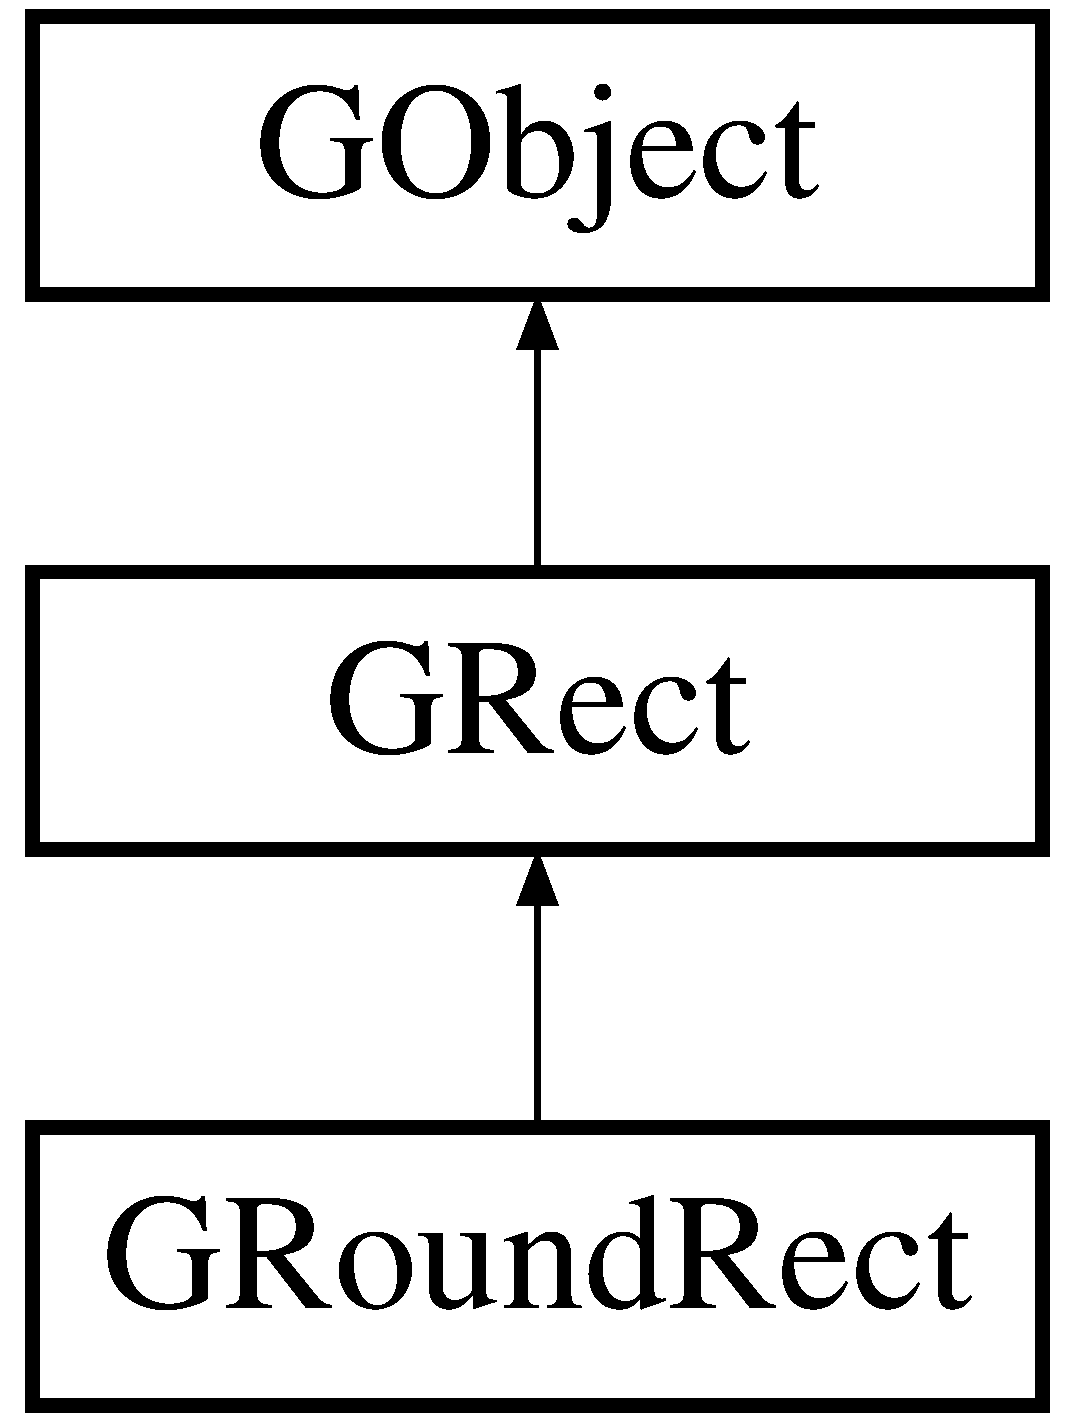
\includegraphics[height=3.000000cm]{classGRect}
\end{center}
\end{figure}
\subsection*{Public Types}
\begin{DoxyCompactItemize}
\item 
enum \mbox{\hyperlink{classGObject_a86e0f5648542856159bb40775c854aa7}{Line\+Style}} \{ \mbox{\hyperlink{classGObject_a86e0f5648542856159bb40775c854aa7acbc84bd5232621834ed31f44d457c1eb}{L\+I\+N\+E\+\_\+\+N\+O\+NE}}, 
\mbox{\hyperlink{classGObject_a86e0f5648542856159bb40775c854aa7a700c78bc2cd76acaab26651bf7b4941f}{L\+I\+N\+E\+\_\+\+S\+O\+L\+ID}}, 
\mbox{\hyperlink{classGObject_a86e0f5648542856159bb40775c854aa7a9ccba0845f785d81d07b333ae1aad84e}{L\+I\+N\+E\+\_\+\+D\+A\+SH}}, 
\mbox{\hyperlink{classGObject_a86e0f5648542856159bb40775c854aa7a8e811c096cb941997f0bfda168bb6df3}{L\+I\+N\+E\+\_\+\+D\+OT}}, 
\mbox{\hyperlink{classGObject_a86e0f5648542856159bb40775c854aa7ada15a2e3d737b2db7706d8300f91b89d}{L\+I\+N\+E\+\_\+\+D\+A\+S\+H\+\_\+\+D\+OT}}, 
\mbox{\hyperlink{classGObject_a86e0f5648542856159bb40775c854aa7aabf4053a73eafa7ba2b7e6d664c74c1d}{L\+I\+N\+E\+\_\+\+D\+A\+S\+H\+\_\+\+D\+O\+T\+\_\+\+D\+OT}}
 \}
\begin{DoxyCompactList}\small\item\em Styles that can be used for the outline around various shapes. \end{DoxyCompactList}\end{DoxyCompactItemize}
\subsection*{Public Member Functions}
\begin{DoxyCompactItemize}
\item 
\mbox{\hyperlink{classGRect_ae511b0aaa5e0546f0094513120372d90}{G\+Rect}} (double x=0, double y=0, double width=0, double height=0)
\begin{DoxyCompactList}\small\item\em Constructs a rectangle with the specified width and height. \end{DoxyCompactList}\item 
virtual bool \mbox{\hyperlink{classGObject_abb6a5d7c03e6eaaae97264c4799ce7c3}{contains}} (double x, double y) const
\begin{DoxyCompactList}\small\item\em Returns {\ttfamily true} if the specified point is inside the object. \end{DoxyCompactList}\item 
virtual bool \mbox{\hyperlink{classGObject_a1dbc9dafaae51958112dbe1267a1f547}{contains}} (const \mbox{\hyperlink{classGPoint}{G\+Point}} \&pt) const
\begin{DoxyCompactList}\small\item\em Returns {\ttfamily true} if the specified point is inside the object. \end{DoxyCompactList}\item 
virtual \mbox{\hyperlink{classGPoint}{G\+Point}} \mbox{\hyperlink{classGObject_a0d41183bf6b08de66fe3907551aab0d7}{get\+Bottom\+Right\+Location}} () const
\begin{DoxyCompactList}\small\item\em Returns the x/y coordinates of the bottom/right corner of the object. \end{DoxyCompactList}\item 
virtual double \mbox{\hyperlink{classGObject_a4316a2406c18e1c6d061fe51fd355490}{get\+BottomY}} () const
\begin{DoxyCompactList}\small\item\em Returns the {\itshape y}-\/coordinate of the bottom of the object. \end{DoxyCompactList}\item 
virtual \mbox{\hyperlink{classGRectangle}{G\+Rectangle}} \mbox{\hyperlink{classGObject_a29e6ac35a0b48f491a4c88194cc5da3b}{get\+Bounds}} () const
\begin{DoxyCompactList}\small\item\em Returns the bounding box of this object, which is defined to be the smallest rectangle that covers everything drawn by the figure. \end{DoxyCompactList}\item 
virtual \mbox{\hyperlink{classGPoint}{G\+Point}} \mbox{\hyperlink{classGObject_a0909472e91448470bccdb62ecfb95d8b}{get\+Center\+Location}} () const
\begin{DoxyCompactList}\small\item\em Returns the x/y-\/coordinates of the center of the object. \end{DoxyCompactList}\item 
virtual double \mbox{\hyperlink{classGObject_a04df74355b545e0543112d5b8d924176}{get\+CenterX}} () const
\begin{DoxyCompactList}\small\item\em Returns the {\itshape x}-\/coordinate of the center of the object. \end{DoxyCompactList}\item 
virtual double \mbox{\hyperlink{classGObject_acb3287a3d507025a26f54b895713b947}{get\+CenterY}} () const
\begin{DoxyCompactList}\small\item\em Returns the {\itshape y}-\/coordinate of the center of the object. \end{DoxyCompactList}\item 
virtual std\+::string \mbox{\hyperlink{classGObject_aa061dfa488c31e18549d64363c1d0e34}{get\+Color}} () const
\begin{DoxyCompactList}\small\item\em Returns the color used to display this object. \end{DoxyCompactList}\item 
virtual std\+::string \mbox{\hyperlink{classGObject_a76f6964a11fde7c78e9751be184e1a3c}{get\+Fill\+Color}} () const
\begin{DoxyCompactList}\small\item\em Returns the color used to display the filled region of this object. \end{DoxyCompactList}\item 
virtual double \mbox{\hyperlink{classGObject_a1e7e353362434072875264cf95629f99}{get\+Height}} () const
\begin{DoxyCompactList}\small\item\em Returns the height of this object, which is the same as the height of its bounding box. \end{DoxyCompactList}\item 
virtual \mbox{\hyperlink{classGObject_a86e0f5648542856159bb40775c854aa7}{Line\+Style}} \mbox{\hyperlink{classGObject_aaf1f5ea8281e5e3486662878d26f0a13}{get\+Line\+Style}} () const
\begin{DoxyCompactList}\small\item\em Returns the object\textquotesingle{}s style such as solid or dashed. \end{DoxyCompactList}\item 
virtual double \mbox{\hyperlink{classGObject_a85ff266dc3eb63d9f2d8e5a4487fd3c0}{get\+Line\+Width}} () const
\begin{DoxyCompactList}\small\item\em Returns the width of the line used to draw this object. \end{DoxyCompactList}\item 
virtual \mbox{\hyperlink{classGPoint}{G\+Point}} \mbox{\hyperlink{classGObject_a4f83802015511edeb63b892830812c11}{get\+Location}} () const
\begin{DoxyCompactList}\small\item\em Returns the location of the top-\/left corner of object. \end{DoxyCompactList}\item 
virtual double \mbox{\hyperlink{classGObject_a1ae3fc278cc5b71b9f2d96a8a83cdf26}{get\+Opacity}} () const
\begin{DoxyCompactList}\small\item\em Returns how opaque (non-\/transparent) this object will appear from 0.\+0 (completely transparent) to 1.\+0 (completely opaque, default). \end{DoxyCompactList}\item 
virtual \mbox{\hyperlink{classGCompound}{G\+Compound}} $\ast$ \mbox{\hyperlink{classGObject_a3e53cef70541b1a14eade4ad0984d0b4}{get\+Parent}} () const
\begin{DoxyCompactList}\small\item\em Returns a pointer to the {\ttfamily \mbox{\hyperlink{classGCompound}{G\+Compound}}} that contains this object. \end{DoxyCompactList}\item 
virtual double \mbox{\hyperlink{classGObject_a798cc79daaa10145b28f60bcdfdb0ee9}{get\+RightX}} () const
\begin{DoxyCompactList}\small\item\em Returns the {\itshape x}-\/coordinate of the right side of the object. \end{DoxyCompactList}\item 
virtual \mbox{\hyperlink{classGDimension}{G\+Dimension}} \mbox{\hyperlink{classGObject_a7b4eec96a2bdc6420695d5796a78eea9}{get\+Size}} () const
\begin{DoxyCompactList}\small\item\em Returns the size of the object as a {\ttfamily \mbox{\hyperlink{classGDimension}{G\+Dimension}}}. \end{DoxyCompactList}\item 
virtual std\+::string \mbox{\hyperlink{classGRect_a9896d58fcfebbf1025aeeb5b8b9ede80}{get\+Type}} () const Q\+\_\+\+D\+E\+C\+L\+\_\+\+O\+V\+E\+R\+R\+I\+DE
\begin{DoxyCompactList}\small\item\em Returns the type of the object as a string, such as {\ttfamily \char`\"{}\+G\+Oval\char`\"{}} or {\ttfamily \char`\"{}\+G\+Rect\char`\"{}}. \end{DoxyCompactList}\item 
virtual double \mbox{\hyperlink{classGObject_a0ed2965abd4f5701d2cadf71239faf19}{get\+Width}} () const
\begin{DoxyCompactList}\small\item\em Returns the width of this object, which is equal to the width of the bounding box. \end{DoxyCompactList}\item 
virtual double \mbox{\hyperlink{classGObject_a344385751bee0720059403940d57a13e}{getX}} () const
\begin{DoxyCompactList}\small\item\em Returns the leftmost {\itshape x}-\/coordinate of the object. \end{DoxyCompactList}\item 
virtual double \mbox{\hyperlink{classGObject_aafa51c7f8f38a09febbb9ce7853f77b4}{getY}} () const
\begin{DoxyCompactList}\small\item\em Returns the topmost {\itshape y}-\/coordinate of the object. \end{DoxyCompactList}\item 
virtual bool \mbox{\hyperlink{classGObject_a11c404f106940c201b6f326e0355c150}{is\+Filled}} () const
\begin{DoxyCompactList}\small\item\em Returns {\ttfamily true} if the object is filled with color. \end{DoxyCompactList}\item 
virtual bool \mbox{\hyperlink{classGObject_a9de207581cfa4ca1eaa06da5f29b75fc}{is\+Transformed}} () const
\begin{DoxyCompactList}\small\item\em Returns {\ttfamily true} if this object has been transformed by calling methods such as \mbox{\hyperlink{classGObject_ae1ffaa12185dfd5ba464f7d87c329e26}{rotate()}} or \mbox{\hyperlink{classGObject_ad2e1900f730475c2d044817db03b38d6}{scale()}} on it. \end{DoxyCompactList}\item 
virtual bool \mbox{\hyperlink{classGObject_a9d8a6cfb13917785c143e74d40e4e2be}{is\+Visible}} () const
\begin{DoxyCompactList}\small\item\em Returns {\ttfamily true} if this object is visible on screen. \end{DoxyCompactList}\item 
virtual void \mbox{\hyperlink{classGObject_a5973d8dda83afb36e2c56855515be392}{move}} (double dx, double dy)
\begin{DoxyCompactList}\small\item\em Moves the object on the screen using the displacements {\ttfamily dx} and {\ttfamily dy}. \end{DoxyCompactList}\item 
virtual void \mbox{\hyperlink{classGObject_ac827b978aa122f136a14c198687ad80f}{repaint}} ()
\begin{DoxyCompactList}\small\item\em Instructs the object to redraw itself on screen. \end{DoxyCompactList}\item 
virtual void \mbox{\hyperlink{classGObject_a6022a1fd1e5dcd2fd5585e5a36aa3f37}{reset\+Transform}} ()
\begin{DoxyCompactList}\small\item\em Undoes any previous scale/rotate transformations on this object. \end{DoxyCompactList}\item 
virtual void \mbox{\hyperlink{classGObject_ae1ffaa12185dfd5ba464f7d87c329e26}{rotate}} (double theta)
\begin{DoxyCompactList}\small\item\em Transforms the object by rotating it {\ttfamily theta} degrees counterclockwise around its origin. \end{DoxyCompactList}\item 
virtual void \mbox{\hyperlink{classGObject_ad2e1900f730475c2d044817db03b38d6}{scale}} (double sf)
\begin{DoxyCompactList}\small\item\em Scales the object by the specified scale factor. \end{DoxyCompactList}\item 
virtual void \mbox{\hyperlink{classGObject_a63641f69d610d0b951357d35a0c3b1e3}{scale}} (double sx, double sy)
\begin{DoxyCompactList}\small\item\em Scales the object by the specified scale factors. \end{DoxyCompactList}\item 
void \mbox{\hyperlink{classGObject_ab6747f40313c531c2db32edb5b63b9b7}{send\+Backward}} ()
\begin{DoxyCompactList}\small\item\em Moves this object one step toward the back in the {\itshape z} dimension. \end{DoxyCompactList}\item 
void \mbox{\hyperlink{classGObject_a710b3e449c9facba7847c91ab170d281}{send\+Forward}} ()
\begin{DoxyCompactList}\small\item\em Moves this object one step toward the front in the {\itshape z} dimension. \end{DoxyCompactList}\item 
void \mbox{\hyperlink{classGObject_a0f7f1efbb7fd46dde2867c4ad0330896}{send\+To\+Back}} ()
\begin{DoxyCompactList}\small\item\em Moves this object to the back of the display in the {\itshape z} dimension. \end{DoxyCompactList}\item 
void \mbox{\hyperlink{classGObject_aee33d68488e46827ef55fac07f40a9b2}{send\+To\+Front}} ()
\begin{DoxyCompactList}\small\item\em Moves this object to the front of the display in the {\itshape z} dimension. \end{DoxyCompactList}\item 
virtual void \mbox{\hyperlink{classGObject_a71ff7b16b8f1bdc4a1ce9f30cf8b87d8}{set\+Bottom\+Right\+Location}} (double x, double y)
\begin{DoxyCompactList}\small\item\em Sets the location of the bottom/right of this object. \end{DoxyCompactList}\item 
virtual void \mbox{\hyperlink{classGObject_ac6f7320321182f1d18c1c0fa97d5e941}{set\+Bottom\+Right\+Location}} (const \mbox{\hyperlink{classGPoint}{G\+Point}} \&pt)
\begin{DoxyCompactList}\small\item\em Sets the location of the bottom/right of this object. \end{DoxyCompactList}\item 
virtual void \mbox{\hyperlink{classGObject_a4b20e93c2a2597484f74ee5caa71f41f}{set\+BottomY}} (double y)
\begin{DoxyCompactList}\small\item\em Sets the location of the bottom y-\/coordinate of this object. \end{DoxyCompactList}\item 
virtual void \mbox{\hyperlink{classGObject_a2aae8197624b72265ab83b4f1bc73f2f}{set\+Bounds}} (double x, double y, double width, double height)
\begin{DoxyCompactList}\small\item\em Changes the bounds of this object to the specified values. \end{DoxyCompactList}\item 
virtual void \mbox{\hyperlink{classGObject_acada386653f008cacc7cce86426bef7c}{set\+Bounds}} (const \mbox{\hyperlink{classGRectangle}{G\+Rectangle}} \&size)
\begin{DoxyCompactList}\small\item\em Changes the bounds of this object to the specified rectangle. \end{DoxyCompactList}\item 
virtual void \mbox{\hyperlink{classGObject_a290b47dd8de1be44089f95cb2c47c1de}{set\+Center\+Location}} (double x, double y)
\begin{DoxyCompactList}\small\item\em Sets the location of the center of this object. \end{DoxyCompactList}\item 
virtual void \mbox{\hyperlink{classGObject_a1bedf1b233ecba3f753ec58908a683a6}{set\+Center\+Location}} (const \mbox{\hyperlink{classGPoint}{G\+Point}} \&pt)
\begin{DoxyCompactList}\small\item\em Sets the location of the center of this object. \end{DoxyCompactList}\item 
virtual void \mbox{\hyperlink{classGObject_a2f4936281e056eead00a9186b9ba8af6}{set\+CenterX}} (double x)
\begin{DoxyCompactList}\small\item\em Sets the x-\/coordinate of the center of this object. \end{DoxyCompactList}\item 
virtual void \mbox{\hyperlink{classGObject_aad2a22b4fde88c33306b92aebf641d57}{set\+CenterY}} (double y)
\begin{DoxyCompactList}\small\item\em Sets the y-\/coordinate of the center of this object. \end{DoxyCompactList}\item 
virtual void \mbox{\hyperlink{classGObject_ad57ef49bc31db94e92648aa3737923d6}{set\+Color}} (int r, int g, int b)
\begin{DoxyCompactList}\small\item\em Sets the color used to display this object. \end{DoxyCompactList}\item 
virtual void \mbox{\hyperlink{classGObject_ab1f5cc0f5cc6bbbd716a526c61f1081d}{set\+Color}} (int rgb)
\begin{DoxyCompactList}\small\item\em Sets the color used to display this object. \end{DoxyCompactList}\item 
virtual void \mbox{\hyperlink{classGObject_a61374df6c11b52cfbb0815decdbaebc6}{set\+Color}} (const std\+::string \&color)
\begin{DoxyCompactList}\small\item\em Sets the color used to display this object. \end{DoxyCompactList}\item 
virtual void \mbox{\hyperlink{classGObject_ad767a33971159e9493e221cca4c00ae9}{set\+Fill\+Color}} (int r, int g, int b)
\begin{DoxyCompactList}\small\item\em Sets the color used to display the filled region of this object, if any. \end{DoxyCompactList}\item 
virtual void \mbox{\hyperlink{classGObject_aa59d9775a67fa7df2b24a95cd34840a3}{set\+Fill\+Color}} (int rgb)
\begin{DoxyCompactList}\small\item\em Sets the color used to display the filled region of this object, if any. \end{DoxyCompactList}\item 
virtual void \mbox{\hyperlink{classGObject_adbc18b1a930aadd97d7437f9f7265b96}{set\+Fill\+Color}} (const std\+::string \&color)
\begin{DoxyCompactList}\small\item\em Sets the color used to display the filled region of this object, if any. \end{DoxyCompactList}\item 
virtual void \mbox{\hyperlink{classGObject_a9b82b53362282c6bb7d6947068d2e55b}{set\+Filled}} (bool flag)
\begin{DoxyCompactList}\small\item\em Sets the fill status for the object, where {\ttfamily false} is outlined and {\ttfamily true} is filled. \end{DoxyCompactList}\item 
virtual void \mbox{\hyperlink{classGObject_a2592348886ffea646c6534bf88f7c49d}{set\+Font}} (const Q\+Font \&font)
\begin{DoxyCompactList}\small\item\em Changes the font used to display the object as specified by the given Qt font. \end{DoxyCompactList}\item 
virtual void \mbox{\hyperlink{classGObject_a8e096e8818d838aceae1d46d58fb3a7b}{set\+Font}} (const std\+::string \&font)
\begin{DoxyCompactList}\small\item\em Changes the font used to display the object as specified by the string {\ttfamily font}, which has the following format\+: \end{DoxyCompactList}\item 
virtual void \mbox{\hyperlink{classGObject_ad18e8fab1e02a4e9b75c6730212558eb}{set\+Foreground}} (int r, int g, int b)
\begin{DoxyCompactList}\small\item\em Sets the color used to display this object. \end{DoxyCompactList}\item 
virtual void \mbox{\hyperlink{classGObject_a9eb856b5ff83a19df3831a31f15f4563}{set\+Foreground}} (int rgb)
\begin{DoxyCompactList}\small\item\em Sets the color used to display this object. \end{DoxyCompactList}\item 
virtual void \mbox{\hyperlink{classGObject_af59209aeadea6dfc6d97a2d8531f50e1}{set\+Foreground}} (const std\+::string \&color)
\begin{DoxyCompactList}\small\item\em Sets the color used to display this object. \end{DoxyCompactList}\item 
virtual void \mbox{\hyperlink{classGObject_a9e280bfc4544dfaf8e4376c4e1a74357}{set\+Height}} (double height)
\begin{DoxyCompactList}\small\item\em Changes the height of this object to the specified height without changing its width. \end{DoxyCompactList}\item 
virtual void \mbox{\hyperlink{classGObject_add11575087eb94f1a71faa3f826c6341}{set\+Line\+Style}} (\mbox{\hyperlink{classGObject_a86e0f5648542856159bb40775c854aa7}{Line\+Style}} line\+Style)
\begin{DoxyCompactList}\small\item\em Sets the object\textquotesingle{}s style such as solid (\mbox{\hyperlink{classGObject_a86e0f5648542856159bb40775c854aa7a700c78bc2cd76acaab26651bf7b4941f}{G\+Object\+::\+L\+I\+N\+E\+\_\+\+S\+O\+L\+ID}}) or dashed (\mbox{\hyperlink{classGObject_a86e0f5648542856159bb40775c854aa7a9ccba0845f785d81d07b333ae1aad84e}{G\+Object\+::\+L\+I\+N\+E\+\_\+\+D\+A\+SH}}). \end{DoxyCompactList}\item 
virtual void \mbox{\hyperlink{classGObject_afd6a47c6ea6a1f85ca05a65ba3ff3477}{set\+Line\+Width}} (double line\+Width)
\begin{DoxyCompactList}\small\item\em Sets the width of the line used to draw this object. \end{DoxyCompactList}\item 
virtual void \mbox{\hyperlink{classGObject_a04594e8ba9b98513a64f1da00dcae18c}{set\+Location}} (double x, double y)
\begin{DoxyCompactList}\small\item\em Sets the location of the top-\/left corner of this object to the specified coordinates. \end{DoxyCompactList}\item 
virtual void \mbox{\hyperlink{classGObject_aa8480c0b7166cdf8f784cece06ab353f}{set\+Location}} (const \mbox{\hyperlink{classGPoint}{G\+Point}} \&pt)
\begin{DoxyCompactList}\small\item\em Sets the location of the top-\/left corner of this object to the specified point. \end{DoxyCompactList}\item 
virtual void \mbox{\hyperlink{classGObject_a04af1866cc1bae4a1226695794a50539}{set\+Opacity}} (double opacity)
\begin{DoxyCompactList}\small\item\em Sets how opaque (non-\/transparent) this object will appear from 0.\+0 (completely transparent) to 1.\+0 (completely opaque, default). \end{DoxyCompactList}\item 
virtual void \mbox{\hyperlink{classGObject_a3c90b758cdc2c911c9ef76c4360eb912}{set\+RightX}} (double x)
\begin{DoxyCompactList}\small\item\em Sets the location of the rightmost x-\/coordinate of this object. \end{DoxyCompactList}\item 
virtual void \mbox{\hyperlink{classGObject_aca25d49481f9bf5fc8f7df4c086c4ce7}{set\+Size}} (double width, double height)
\begin{DoxyCompactList}\small\item\em Changes the size of this object to the specified width and height. \end{DoxyCompactList}\item 
virtual void \mbox{\hyperlink{classGObject_ae2b628228f192c2702c4ce941b2af68f}{set\+Size}} (const \mbox{\hyperlink{classGDimension}{G\+Dimension}} \&size)
\begin{DoxyCompactList}\small\item\em Changes the size of this object to the specified width and height. \end{DoxyCompactList}\item 
virtual void \mbox{\hyperlink{classGObject_a88203f28224315d9f4471212f4af8ed3}{set\+Visible}} (bool flag)
\begin{DoxyCompactList}\small\item\em Sets whether this object is visible. \end{DoxyCompactList}\item 
virtual void \mbox{\hyperlink{classGObject_aa3f3fba4cb131baa8696ba01e3bceca1}{set\+Width}} (double width)
\begin{DoxyCompactList}\small\item\em Changes the width of this object to the specified width without changing its height. \end{DoxyCompactList}\item 
virtual void \mbox{\hyperlink{classGObject_a9c18fcc579333bf9653d13ad2b372e39}{setX}} (double x)
\begin{DoxyCompactList}\small\item\em Sets the x location of the left side of this object. \end{DoxyCompactList}\item 
virtual void \mbox{\hyperlink{classGObject_a7d57e2a5c35d27feb58fd498a3cf82b9}{setY}} (double y)
\begin{DoxyCompactList}\small\item\em Sets the y location of the top of this object. \end{DoxyCompactList}\item 
virtual std\+::string \mbox{\hyperlink{classGObject_a1fe5121d6528fdea3f243321b3fa3a49}{to\+String}} () const
\begin{DoxyCompactList}\small\item\em Returns a printable representation of the object. \end{DoxyCompactList}\end{DoxyCompactItemize}
\subsection*{Static Public Member Functions}
\begin{DoxyCompactItemize}
\item 
static bool \mbox{\hyperlink{classGObject_a93be0e1fe1b1bf1a1da732470c94f42b}{is\+Anti\+Aliasing}} ()
\begin{DoxyCompactList}\small\item\em Returns whether we should globally anti-\/alias graphical objects. \end{DoxyCompactList}\item 
static void \mbox{\hyperlink{classGObject_a1e43371668ae850193cebedb44e1bbe3}{set\+Anti\+Aliasing}} (bool value)
\begin{DoxyCompactList}\small\item\em Globally turns on/off the anti-\/aliasing feature that smooths out the edges of onscreen shapes. \end{DoxyCompactList}\end{DoxyCompactItemize}
\subsection*{Protected Member Functions}
\begin{DoxyCompactItemize}
\item 
virtual std\+::string \mbox{\hyperlink{classGObject_a4fcdf8de5c6de92242a975d83d8f23ea}{to\+String\+Extra}} () const
\begin{DoxyCompactList}\small\item\em Returns a string containing any extra unique information about this type of graphical object. \end{DoxyCompactList}\end{DoxyCompactItemize}
\subsection*{Protected Attributes}
\begin{DoxyCompactItemize}
\item 
Q\+Brush \mbox{\hyperlink{classGObject_aab24462ec896b596d99911767b0912d0}{\+\_\+brush}}
\item 
std\+::string \mbox{\hyperlink{classGObject_a1134e770ae4315ea8bc1201e2f21da8b}{\+\_\+color}}
\item 
int \mbox{\hyperlink{classGObject_a003fdd343d9b7505c53a8b7a134200ed}{\+\_\+color\+Int}}
\item 
std\+::string \mbox{\hyperlink{classGObject_a179f8d6cee65cd8a54692e32b224392a}{\+\_\+fill\+Color}}
\item 
int \mbox{\hyperlink{classGObject_a751def333a67d651e5b99cc331ecb496}{\+\_\+fill\+Color\+Int}}
\item 
bool \mbox{\hyperlink{classGObject_ad4a55cbcd61b58a4d49666490bb2f103}{\+\_\+fill\+Flag}}
\item 
std\+::string \mbox{\hyperlink{classGObject_aea76ea1a8b5dd7b0a78653277e63b536}{\+\_\+font}}
\item 
double \mbox{\hyperlink{classGObject_ad05df29e7f27fc504abd743e3d8b4e73}{\+\_\+height}}
\item 
\mbox{\hyperlink{classGObject_a86e0f5648542856159bb40775c854aa7}{Line\+Style}} \mbox{\hyperlink{classGObject_a89bafecaafb7c72d55c7efc10b7d0523}{\+\_\+line\+Style}}
\item 
double \mbox{\hyperlink{classGObject_a16e9033665937f13de2e163dc2184aff}{\+\_\+line\+Width}}
\item 
double \mbox{\hyperlink{classGObject_a20eff8eb7af27182edc9bfc54768b6f3}{\+\_\+opacity}}
\item 
\mbox{\hyperlink{classGCompound}{G\+Compound}} $\ast$ \mbox{\hyperlink{classGObject_ac9452c1eaff70eebddbb318196aa3835}{\+\_\+parent}}
\item 
Q\+Pen \mbox{\hyperlink{classGObject_afb69d172743f868299847174eb1b6bc8}{\+\_\+pen}}
\item 
Q\+Transform \mbox{\hyperlink{classGObject_a475b8860a5f1adb4a1fdc58d1f5c1e32}{\+\_\+transform}}
\item 
bool \mbox{\hyperlink{classGObject_ae4725802fc8d8aaa0ab4bd4781f7e07c}{\+\_\+transformed}}
\item 
bool \mbox{\hyperlink{classGObject_a9312c72508471b7c7a87b540263e1af4}{\+\_\+visible}}
\item 
double \mbox{\hyperlink{classGObject_ab55d85a3371770e6725b1062cf160cd8}{\+\_\+width}}
\item 
double \mbox{\hyperlink{classGObject_a6675b83b27137b8d3aa2ad8133078ea6}{\+\_\+x}}
\item 
double \mbox{\hyperlink{classGObject_a2f0f6aeafddc8a39c578bfa7e22b5f1e}{\+\_\+y}}
\end{DoxyCompactItemize}


\subsection{Detailed Description}
A \mbox{\hyperlink{classGRect}{G\+Rect}} is a graphical object whose appearance consists of a rectangular box. 

\subsection{Member Enumeration Documentation}
\mbox{\Hypertarget{classGObject_a86e0f5648542856159bb40775c854aa7}\label{classGObject_a86e0f5648542856159bb40775c854aa7}} 
\index{G\+Rect@{G\+Rect}!Line\+Style@{Line\+Style}}
\index{Line\+Style@{Line\+Style}!G\+Rect@{G\+Rect}}
\subsubsection{\texorpdfstring{Line\+Style}{LineStyle}}
{\footnotesize\ttfamily enum \mbox{\hyperlink{classGObject_a86e0f5648542856159bb40775c854aa7}{Line\+Style}}\hspace{0.3cm}{\ttfamily [inherited]}}



Styles that can be used for the outline around various shapes. 

Call set\+Line\+Style on a \mbox{\hyperlink{classGObject}{G\+Object}} and pass one of these values. \begin{DoxyEnumFields}{Enumerator}
\raisebox{\heightof{T}}[0pt][0pt]{\index{L\+I\+N\+E\+\_\+\+N\+O\+NE@{L\+I\+N\+E\+\_\+\+N\+O\+NE}!G\+Rect@{G\+Rect}}\index{G\+Rect@{G\+Rect}!L\+I\+N\+E\+\_\+\+N\+O\+NE@{L\+I\+N\+E\+\_\+\+N\+O\+NE}}}\mbox{\Hypertarget{classGObject_a86e0f5648542856159bb40775c854aa7acbc84bd5232621834ed31f44d457c1eb}\label{classGObject_a86e0f5648542856159bb40775c854aa7acbc84bd5232621834ed31f44d457c1eb}} 
L\+I\+N\+E\+\_\+\+N\+O\+NE&\\
\hline

\raisebox{\heightof{T}}[0pt][0pt]{\index{L\+I\+N\+E\+\_\+\+S\+O\+L\+ID@{L\+I\+N\+E\+\_\+\+S\+O\+L\+ID}!G\+Rect@{G\+Rect}}\index{G\+Rect@{G\+Rect}!L\+I\+N\+E\+\_\+\+S\+O\+L\+ID@{L\+I\+N\+E\+\_\+\+S\+O\+L\+ID}}}\mbox{\Hypertarget{classGObject_a86e0f5648542856159bb40775c854aa7a700c78bc2cd76acaab26651bf7b4941f}\label{classGObject_a86e0f5648542856159bb40775c854aa7a700c78bc2cd76acaab26651bf7b4941f}} 
L\+I\+N\+E\+\_\+\+S\+O\+L\+ID&\\
\hline

\raisebox{\heightof{T}}[0pt][0pt]{\index{L\+I\+N\+E\+\_\+\+D\+A\+SH@{L\+I\+N\+E\+\_\+\+D\+A\+SH}!G\+Rect@{G\+Rect}}\index{G\+Rect@{G\+Rect}!L\+I\+N\+E\+\_\+\+D\+A\+SH@{L\+I\+N\+E\+\_\+\+D\+A\+SH}}}\mbox{\Hypertarget{classGObject_a86e0f5648542856159bb40775c854aa7a9ccba0845f785d81d07b333ae1aad84e}\label{classGObject_a86e0f5648542856159bb40775c854aa7a9ccba0845f785d81d07b333ae1aad84e}} 
L\+I\+N\+E\+\_\+\+D\+A\+SH&\\
\hline

\raisebox{\heightof{T}}[0pt][0pt]{\index{L\+I\+N\+E\+\_\+\+D\+OT@{L\+I\+N\+E\+\_\+\+D\+OT}!G\+Rect@{G\+Rect}}\index{G\+Rect@{G\+Rect}!L\+I\+N\+E\+\_\+\+D\+OT@{L\+I\+N\+E\+\_\+\+D\+OT}}}\mbox{\Hypertarget{classGObject_a86e0f5648542856159bb40775c854aa7a8e811c096cb941997f0bfda168bb6df3}\label{classGObject_a86e0f5648542856159bb40775c854aa7a8e811c096cb941997f0bfda168bb6df3}} 
L\+I\+N\+E\+\_\+\+D\+OT&\\
\hline

\raisebox{\heightof{T}}[0pt][0pt]{\index{L\+I\+N\+E\+\_\+\+D\+A\+S\+H\+\_\+\+D\+OT@{L\+I\+N\+E\+\_\+\+D\+A\+S\+H\+\_\+\+D\+OT}!G\+Rect@{G\+Rect}}\index{G\+Rect@{G\+Rect}!L\+I\+N\+E\+\_\+\+D\+A\+S\+H\+\_\+\+D\+OT@{L\+I\+N\+E\+\_\+\+D\+A\+S\+H\+\_\+\+D\+OT}}}\mbox{\Hypertarget{classGObject_a86e0f5648542856159bb40775c854aa7ada15a2e3d737b2db7706d8300f91b89d}\label{classGObject_a86e0f5648542856159bb40775c854aa7ada15a2e3d737b2db7706d8300f91b89d}} 
L\+I\+N\+E\+\_\+\+D\+A\+S\+H\+\_\+\+D\+OT&\\
\hline

\raisebox{\heightof{T}}[0pt][0pt]{\index{L\+I\+N\+E\+\_\+\+D\+A\+S\+H\+\_\+\+D\+O\+T\+\_\+\+D\+OT@{L\+I\+N\+E\+\_\+\+D\+A\+S\+H\+\_\+\+D\+O\+T\+\_\+\+D\+OT}!G\+Rect@{G\+Rect}}\index{G\+Rect@{G\+Rect}!L\+I\+N\+E\+\_\+\+D\+A\+S\+H\+\_\+\+D\+O\+T\+\_\+\+D\+OT@{L\+I\+N\+E\+\_\+\+D\+A\+S\+H\+\_\+\+D\+O\+T\+\_\+\+D\+OT}}}\mbox{\Hypertarget{classGObject_a86e0f5648542856159bb40775c854aa7aabf4053a73eafa7ba2b7e6d664c74c1d}\label{classGObject_a86e0f5648542856159bb40775c854aa7aabf4053a73eafa7ba2b7e6d664c74c1d}} 
L\+I\+N\+E\+\_\+\+D\+A\+S\+H\+\_\+\+D\+O\+T\+\_\+\+D\+OT&\\
\hline

\end{DoxyEnumFields}


\subsection{Constructor \& Destructor Documentation}
\mbox{\Hypertarget{classGRect_ae511b0aaa5e0546f0094513120372d90}\label{classGRect_ae511b0aaa5e0546f0094513120372d90}} 
\index{G\+Rect@{G\+Rect}!G\+Rect@{G\+Rect}}
\index{G\+Rect@{G\+Rect}!G\+Rect@{G\+Rect}}
\subsubsection{\texorpdfstring{G\+Rect()}{GRect()}}
{\footnotesize\ttfamily \mbox{\hyperlink{classGRect}{G\+Rect}} (\begin{DoxyParamCaption}\item[{double}]{x = {\ttfamily 0},  }\item[{double}]{y = {\ttfamily 0},  }\item[{double}]{width = {\ttfamily 0},  }\item[{double}]{height = {\ttfamily 0} }\end{DoxyParamCaption})}



Constructs a rectangle with the specified width and height. 

The first form is positioned at the origin; the second at the coordinates given by {\ttfamily x} and {\ttfamily y}. 

\subsection{Member Function Documentation}
\mbox{\Hypertarget{classGObject_abb6a5d7c03e6eaaae97264c4799ce7c3}\label{classGObject_abb6a5d7c03e6eaaae97264c4799ce7c3}} 
\index{G\+Rect@{G\+Rect}!contains@{contains}}
\index{contains@{contains}!G\+Rect@{G\+Rect}}
\subsubsection{\texorpdfstring{contains()}{contains()}\hspace{0.1cm}{\footnotesize\ttfamily [1/2]}}
{\footnotesize\ttfamily bool contains (\begin{DoxyParamCaption}\item[{double}]{x,  }\item[{double}]{y }\end{DoxyParamCaption}) const\hspace{0.3cm}{\ttfamily [virtual]}, {\ttfamily [inherited]}}



Returns {\ttfamily true} if the specified point is inside the object. 



Reimplemented in \mbox{\hyperlink{classGRoundRect_abb6a5d7c03e6eaaae97264c4799ce7c3}{G\+Round\+Rect}}, \mbox{\hyperlink{classGPolygon_abb6a5d7c03e6eaaae97264c4799ce7c3}{G\+Polygon}}, \mbox{\hyperlink{classGOval_aa095a031ab22c150d2d75fdda1c3c8f5}{G\+Oval}}, \mbox{\hyperlink{classGLine_aa095a031ab22c150d2d75fdda1c3c8f5}{G\+Line}}, \mbox{\hyperlink{classGCompound_aa095a031ab22c150d2d75fdda1c3c8f5}{G\+Compound}}, and \mbox{\hyperlink{classGArc_aa095a031ab22c150d2d75fdda1c3c8f5}{G\+Arc}}.

\mbox{\Hypertarget{classGObject_a1dbc9dafaae51958112dbe1267a1f547}\label{classGObject_a1dbc9dafaae51958112dbe1267a1f547}} 
\index{G\+Rect@{G\+Rect}!contains@{contains}}
\index{contains@{contains}!G\+Rect@{G\+Rect}}
\subsubsection{\texorpdfstring{contains()}{contains()}\hspace{0.1cm}{\footnotesize\ttfamily [2/2]}}
{\footnotesize\ttfamily bool contains (\begin{DoxyParamCaption}\item[{const \mbox{\hyperlink{classGPoint}{G\+Point}} \&}]{pt }\end{DoxyParamCaption}) const\hspace{0.3cm}{\ttfamily [virtual]}, {\ttfamily [inherited]}}



Returns {\ttfamily true} if the specified point is inside the object. 

\mbox{\Hypertarget{classGObject_a0d41183bf6b08de66fe3907551aab0d7}\label{classGObject_a0d41183bf6b08de66fe3907551aab0d7}} 
\index{G\+Rect@{G\+Rect}!get\+Bottom\+Right\+Location@{get\+Bottom\+Right\+Location}}
\index{get\+Bottom\+Right\+Location@{get\+Bottom\+Right\+Location}!G\+Rect@{G\+Rect}}
\subsubsection{\texorpdfstring{get\+Bottom\+Right\+Location()}{getBottomRightLocation()}}
{\footnotesize\ttfamily \mbox{\hyperlink{classGPoint}{G\+Point}} get\+Bottom\+Right\+Location (\begin{DoxyParamCaption}{ }\end{DoxyParamCaption}) const\hspace{0.3cm}{\ttfamily [virtual]}, {\ttfamily [inherited]}}



Returns the x/y coordinates of the bottom/right corner of the object. 

\mbox{\Hypertarget{classGObject_a4316a2406c18e1c6d061fe51fd355490}\label{classGObject_a4316a2406c18e1c6d061fe51fd355490}} 
\index{G\+Rect@{G\+Rect}!get\+BottomY@{get\+BottomY}}
\index{get\+BottomY@{get\+BottomY}!G\+Rect@{G\+Rect}}
\subsubsection{\texorpdfstring{get\+Bottom\+Y()}{getBottomY()}}
{\footnotesize\ttfamily double get\+BottomY (\begin{DoxyParamCaption}{ }\end{DoxyParamCaption}) const\hspace{0.3cm}{\ttfamily [virtual]}, {\ttfamily [inherited]}}



Returns the {\itshape y}-\/coordinate of the bottom of the object. 

Equivalent to the top y-\/coordinate plus the object\textquotesingle{}s height. \mbox{\Hypertarget{classGObject_a29e6ac35a0b48f491a4c88194cc5da3b}\label{classGObject_a29e6ac35a0b48f491a4c88194cc5da3b}} 
\index{G\+Rect@{G\+Rect}!get\+Bounds@{get\+Bounds}}
\index{get\+Bounds@{get\+Bounds}!G\+Rect@{G\+Rect}}
\subsubsection{\texorpdfstring{get\+Bounds()}{getBounds()}}
{\footnotesize\ttfamily \mbox{\hyperlink{classGRectangle}{G\+Rectangle}} get\+Bounds (\begin{DoxyParamCaption}{ }\end{DoxyParamCaption}) const\hspace{0.3cm}{\ttfamily [virtual]}, {\ttfamily [inherited]}}



Returns the bounding box of this object, which is defined to be the smallest rectangle that covers everything drawn by the figure. 

The coordinates of this rectangle do not necessarily match the location returned by {\ttfamily get\+Location}. Given a {\ttfamily \mbox{\hyperlink{classGText}{G\+Text}}} object, for example, {\ttfamily get\+Location} returns the coordinates of the point on the baseline at which the string begins; the {\ttfamily get\+Bounds} method, by contrast, returns a rectangle that covers the entire window area occupied by the string. 

Reimplemented in \mbox{\hyperlink{classGText_a2f46ec8a3b533c690b3b3e56d4f34afe}{G\+Text}}, \mbox{\hyperlink{classGPolygon_a29e6ac35a0b48f491a4c88194cc5da3b}{G\+Polygon}}, \mbox{\hyperlink{classGLine_a2f46ec8a3b533c690b3b3e56d4f34afe}{G\+Line}}, \mbox{\hyperlink{classGCompound_a2f46ec8a3b533c690b3b3e56d4f34afe}{G\+Compound}}, and \mbox{\hyperlink{classGArc_a2f46ec8a3b533c690b3b3e56d4f34afe}{G\+Arc}}.

\mbox{\Hypertarget{classGObject_a0909472e91448470bccdb62ecfb95d8b}\label{classGObject_a0909472e91448470bccdb62ecfb95d8b}} 
\index{G\+Rect@{G\+Rect}!get\+Center\+Location@{get\+Center\+Location}}
\index{get\+Center\+Location@{get\+Center\+Location}!G\+Rect@{G\+Rect}}
\subsubsection{\texorpdfstring{get\+Center\+Location()}{getCenterLocation()}}
{\footnotesize\ttfamily \mbox{\hyperlink{classGPoint}{G\+Point}} get\+Center\+Location (\begin{DoxyParamCaption}{ }\end{DoxyParamCaption}) const\hspace{0.3cm}{\ttfamily [virtual]}, {\ttfamily [inherited]}}



Returns the x/y-\/coordinates of the center of the object. 

Equivalent to the top/left plus half the object\textquotesingle{}s size. \mbox{\Hypertarget{classGObject_a04df74355b545e0543112d5b8d924176}\label{classGObject_a04df74355b545e0543112d5b8d924176}} 
\index{G\+Rect@{G\+Rect}!get\+CenterX@{get\+CenterX}}
\index{get\+CenterX@{get\+CenterX}!G\+Rect@{G\+Rect}}
\subsubsection{\texorpdfstring{get\+Center\+X()}{getCenterX()}}
{\footnotesize\ttfamily double get\+CenterX (\begin{DoxyParamCaption}{ }\end{DoxyParamCaption}) const\hspace{0.3cm}{\ttfamily [virtual]}, {\ttfamily [inherited]}}



Returns the {\itshape x}-\/coordinate of the center of the object. 

Equivalent to the top/left plus half the object\textquotesingle{}s width. \mbox{\Hypertarget{classGObject_acb3287a3d507025a26f54b895713b947}\label{classGObject_acb3287a3d507025a26f54b895713b947}} 
\index{G\+Rect@{G\+Rect}!get\+CenterY@{get\+CenterY}}
\index{get\+CenterY@{get\+CenterY}!G\+Rect@{G\+Rect}}
\subsubsection{\texorpdfstring{get\+Center\+Y()}{getCenterY()}}
{\footnotesize\ttfamily double get\+CenterY (\begin{DoxyParamCaption}{ }\end{DoxyParamCaption}) const\hspace{0.3cm}{\ttfamily [virtual]}, {\ttfamily [inherited]}}



Returns the {\itshape y}-\/coordinate of the center of the object. 

Equivalent to the top/left plus half the object\textquotesingle{}s height. \mbox{\Hypertarget{classGObject_aa061dfa488c31e18549d64363c1d0e34}\label{classGObject_aa061dfa488c31e18549d64363c1d0e34}} 
\index{G\+Rect@{G\+Rect}!get\+Color@{get\+Color}}
\index{get\+Color@{get\+Color}!G\+Rect@{G\+Rect}}
\subsubsection{\texorpdfstring{get\+Color()}{getColor()}}
{\footnotesize\ttfamily std\+::string get\+Color (\begin{DoxyParamCaption}{ }\end{DoxyParamCaption}) const\hspace{0.3cm}{\ttfamily [virtual]}, {\ttfamily [inherited]}}



Returns the color used to display this object. 

This color is always returned as a string in the form {\ttfamily \char`\"{}\#rrggbb\char`\"{}}, where {\ttfamily rr}, {\ttfamily gg}, and {\ttfamily bb} are the red, green, and blue components of the color, expressed as two-\/digit hexadecimal values. \mbox{\Hypertarget{classGObject_a76f6964a11fde7c78e9751be184e1a3c}\label{classGObject_a76f6964a11fde7c78e9751be184e1a3c}} 
\index{G\+Rect@{G\+Rect}!get\+Fill\+Color@{get\+Fill\+Color}}
\index{get\+Fill\+Color@{get\+Fill\+Color}!G\+Rect@{G\+Rect}}
\subsubsection{\texorpdfstring{get\+Fill\+Color()}{getFillColor()}}
{\footnotesize\ttfamily std\+::string get\+Fill\+Color (\begin{DoxyParamCaption}{ }\end{DoxyParamCaption}) const\hspace{0.3cm}{\ttfamily [virtual]}, {\ttfamily [inherited]}}



Returns the color used to display the filled region of this object. 

If none has been set, returns the empty string. \mbox{\Hypertarget{classGObject_a1e7e353362434072875264cf95629f99}\label{classGObject_a1e7e353362434072875264cf95629f99}} 
\index{G\+Rect@{G\+Rect}!get\+Height@{get\+Height}}
\index{get\+Height@{get\+Height}!G\+Rect@{G\+Rect}}
\subsubsection{\texorpdfstring{get\+Height()}{getHeight()}}
{\footnotesize\ttfamily double get\+Height (\begin{DoxyParamCaption}{ }\end{DoxyParamCaption}) const\hspace{0.3cm}{\ttfamily [virtual]}, {\ttfamily [inherited]}}



Returns the height of this object, which is the same as the height of its bounding box. 



Reimplemented in \mbox{\hyperlink{classGPolygon_a1e7e353362434072875264cf95629f99}{G\+Polygon}}, and \mbox{\hyperlink{classGLine_a423f17d4aeb66feb0d148fd23af335b7}{G\+Line}}.

\mbox{\Hypertarget{classGObject_aaf1f5ea8281e5e3486662878d26f0a13}\label{classGObject_aaf1f5ea8281e5e3486662878d26f0a13}} 
\index{G\+Rect@{G\+Rect}!get\+Line\+Style@{get\+Line\+Style}}
\index{get\+Line\+Style@{get\+Line\+Style}!G\+Rect@{G\+Rect}}
\subsubsection{\texorpdfstring{get\+Line\+Style()}{getLineStyle()}}
{\footnotesize\ttfamily \mbox{\hyperlink{classGObject_a86e0f5648542856159bb40775c854aa7}{G\+Object\+::\+Line\+Style}} get\+Line\+Style (\begin{DoxyParamCaption}{ }\end{DoxyParamCaption}) const\hspace{0.3cm}{\ttfamily [virtual]}, {\ttfamily [inherited]}}



Returns the object\textquotesingle{}s style such as solid or dashed. 

\mbox{\Hypertarget{classGObject_a85ff266dc3eb63d9f2d8e5a4487fd3c0}\label{classGObject_a85ff266dc3eb63d9f2d8e5a4487fd3c0}} 
\index{G\+Rect@{G\+Rect}!get\+Line\+Width@{get\+Line\+Width}}
\index{get\+Line\+Width@{get\+Line\+Width}!G\+Rect@{G\+Rect}}
\subsubsection{\texorpdfstring{get\+Line\+Width()}{getLineWidth()}}
{\footnotesize\ttfamily double get\+Line\+Width (\begin{DoxyParamCaption}{ }\end{DoxyParamCaption}) const\hspace{0.3cm}{\ttfamily [virtual]}, {\ttfamily [inherited]}}



Returns the width of the line used to draw this object. 

\begin{DoxyReturn}{Returns}
default 1 
\end{DoxyReturn}
\mbox{\Hypertarget{classGObject_a4f83802015511edeb63b892830812c11}\label{classGObject_a4f83802015511edeb63b892830812c11}} 
\index{G\+Rect@{G\+Rect}!get\+Location@{get\+Location}}
\index{get\+Location@{get\+Location}!G\+Rect@{G\+Rect}}
\subsubsection{\texorpdfstring{get\+Location()}{getLocation()}}
{\footnotesize\ttfamily \mbox{\hyperlink{classGPoint}{G\+Point}} get\+Location (\begin{DoxyParamCaption}{ }\end{DoxyParamCaption}) const\hspace{0.3cm}{\ttfamily [virtual]}, {\ttfamily [inherited]}}



Returns the location of the top-\/left corner of object. 

\mbox{\Hypertarget{classGObject_a1ae3fc278cc5b71b9f2d96a8a83cdf26}\label{classGObject_a1ae3fc278cc5b71b9f2d96a8a83cdf26}} 
\index{G\+Rect@{G\+Rect}!get\+Opacity@{get\+Opacity}}
\index{get\+Opacity@{get\+Opacity}!G\+Rect@{G\+Rect}}
\subsubsection{\texorpdfstring{get\+Opacity()}{getOpacity()}}
{\footnotesize\ttfamily double get\+Opacity (\begin{DoxyParamCaption}{ }\end{DoxyParamCaption}) const\hspace{0.3cm}{\ttfamily [virtual]}, {\ttfamily [inherited]}}



Returns how opaque (non-\/transparent) this object will appear from 0.\+0 (completely transparent) to 1.\+0 (completely opaque, default). 

\mbox{\Hypertarget{classGObject_a3e53cef70541b1a14eade4ad0984d0b4}\label{classGObject_a3e53cef70541b1a14eade4ad0984d0b4}} 
\index{G\+Rect@{G\+Rect}!get\+Parent@{get\+Parent}}
\index{get\+Parent@{get\+Parent}!G\+Rect@{G\+Rect}}
\subsubsection{\texorpdfstring{get\+Parent()}{getParent()}}
{\footnotesize\ttfamily \mbox{\hyperlink{classGCompound}{G\+Compound}} $\ast$ get\+Parent (\begin{DoxyParamCaption}{ }\end{DoxyParamCaption}) const\hspace{0.3cm}{\ttfamily [virtual]}, {\ttfamily [inherited]}}



Returns a pointer to the {\ttfamily \mbox{\hyperlink{classGCompound}{G\+Compound}}} that contains this object. 

Every {\ttfamily \mbox{\hyperlink{classGWindow}{G\+Window}}} is initialized to contain a single {\ttfamily \mbox{\hyperlink{classGCompound}{G\+Compound}}} that is aligned with the window. Adding objects to the window adds them to that {\ttfamily \mbox{\hyperlink{classGCompound}{G\+Compound}}}, which means that every object you add to the window has a parent. Calling {\ttfamily get\+Parent} on the top-\/level {\ttfamily \mbox{\hyperlink{classGCompound}{G\+Compound}}} returns {\ttfamily nullptr}. \mbox{\Hypertarget{classGObject_a798cc79daaa10145b28f60bcdfdb0ee9}\label{classGObject_a798cc79daaa10145b28f60bcdfdb0ee9}} 
\index{G\+Rect@{G\+Rect}!get\+RightX@{get\+RightX}}
\index{get\+RightX@{get\+RightX}!G\+Rect@{G\+Rect}}
\subsubsection{\texorpdfstring{get\+Right\+X()}{getRightX()}}
{\footnotesize\ttfamily double get\+RightX (\begin{DoxyParamCaption}{ }\end{DoxyParamCaption}) const\hspace{0.3cm}{\ttfamily [virtual]}, {\ttfamily [inherited]}}



Returns the {\itshape x}-\/coordinate of the right side of the object. 

Equivalent to the left x-\/coordinate plus the object\textquotesingle{}s width. \mbox{\Hypertarget{classGObject_a7b4eec96a2bdc6420695d5796a78eea9}\label{classGObject_a7b4eec96a2bdc6420695d5796a78eea9}} 
\index{G\+Rect@{G\+Rect}!get\+Size@{get\+Size}}
\index{get\+Size@{get\+Size}!G\+Rect@{G\+Rect}}
\subsubsection{\texorpdfstring{get\+Size()}{getSize()}}
{\footnotesize\ttfamily \mbox{\hyperlink{classGDimension}{G\+Dimension}} get\+Size (\begin{DoxyParamCaption}{ }\end{DoxyParamCaption}) const\hspace{0.3cm}{\ttfamily [virtual]}, {\ttfamily [inherited]}}



Returns the size of the object as a {\ttfamily \mbox{\hyperlink{classGDimension}{G\+Dimension}}}. 

\mbox{\Hypertarget{classGRect_a9896d58fcfebbf1025aeeb5b8b9ede80}\label{classGRect_a9896d58fcfebbf1025aeeb5b8b9ede80}} 
\index{G\+Rect@{G\+Rect}!get\+Type@{get\+Type}}
\index{get\+Type@{get\+Type}!G\+Rect@{G\+Rect}}
\subsubsection{\texorpdfstring{get\+Type()}{getType()}}
{\footnotesize\ttfamily std\+::string get\+Type (\begin{DoxyParamCaption}{ }\end{DoxyParamCaption}) const\hspace{0.3cm}{\ttfamily [virtual]}}



Returns the type of the object as a string, such as {\ttfamily \char`\"{}\+G\+Oval\char`\"{}} or {\ttfamily \char`\"{}\+G\+Rect\char`\"{}}. 

Each \mbox{\hyperlink{classGObject}{G\+Object}} subtype must override this method. 

Implements \mbox{\hyperlink{classGObject_a799e073a127b428cc841086d42ea4fed}{G\+Object}}.



Reimplemented in \mbox{\hyperlink{classGRoundRect_a9896d58fcfebbf1025aeeb5b8b9ede80}{G\+Round\+Rect}}.

\mbox{\Hypertarget{classGObject_a0ed2965abd4f5701d2cadf71239faf19}\label{classGObject_a0ed2965abd4f5701d2cadf71239faf19}} 
\index{G\+Rect@{G\+Rect}!get\+Width@{get\+Width}}
\index{get\+Width@{get\+Width}!G\+Rect@{G\+Rect}}
\subsubsection{\texorpdfstring{get\+Width()}{getWidth()}}
{\footnotesize\ttfamily double get\+Width (\begin{DoxyParamCaption}{ }\end{DoxyParamCaption}) const\hspace{0.3cm}{\ttfamily [virtual]}, {\ttfamily [inherited]}}



Returns the width of this object, which is equal to the width of the bounding box. 



Reimplemented in \mbox{\hyperlink{classGPolygon_a0ed2965abd4f5701d2cadf71239faf19}{G\+Polygon}}, and \mbox{\hyperlink{classGLine_a04bee94b66c8f921cd8611be2460ba9d}{G\+Line}}.

\mbox{\Hypertarget{classGObject_a344385751bee0720059403940d57a13e}\label{classGObject_a344385751bee0720059403940d57a13e}} 
\index{G\+Rect@{G\+Rect}!getX@{getX}}
\index{getX@{getX}!G\+Rect@{G\+Rect}}
\subsubsection{\texorpdfstring{get\+X()}{getX()}}
{\footnotesize\ttfamily double getX (\begin{DoxyParamCaption}{ }\end{DoxyParamCaption}) const\hspace{0.3cm}{\ttfamily [virtual]}, {\ttfamily [inherited]}}



Returns the leftmost {\itshape x}-\/coordinate of the object. 

\mbox{\Hypertarget{classGObject_aafa51c7f8f38a09febbb9ce7853f77b4}\label{classGObject_aafa51c7f8f38a09febbb9ce7853f77b4}} 
\index{G\+Rect@{G\+Rect}!getY@{getY}}
\index{getY@{getY}!G\+Rect@{G\+Rect}}
\subsubsection{\texorpdfstring{get\+Y()}{getY()}}
{\footnotesize\ttfamily double getY (\begin{DoxyParamCaption}{ }\end{DoxyParamCaption}) const\hspace{0.3cm}{\ttfamily [virtual]}, {\ttfamily [inherited]}}



Returns the topmost {\itshape y}-\/coordinate of the object. 

\mbox{\Hypertarget{classGObject_a93be0e1fe1b1bf1a1da732470c94f42b}\label{classGObject_a93be0e1fe1b1bf1a1da732470c94f42b}} 
\index{G\+Rect@{G\+Rect}!is\+Anti\+Aliasing@{is\+Anti\+Aliasing}}
\index{is\+Anti\+Aliasing@{is\+Anti\+Aliasing}!G\+Rect@{G\+Rect}}
\subsubsection{\texorpdfstring{is\+Anti\+Aliasing()}{isAntiAliasing()}}
{\footnotesize\ttfamily bool is\+Anti\+Aliasing (\begin{DoxyParamCaption}{ }\end{DoxyParamCaption})\hspace{0.3cm}{\ttfamily [static]}, {\ttfamily [inherited]}}



Returns whether we should globally anti-\/alias graphical objects. 

On by default. \mbox{\Hypertarget{classGObject_a11c404f106940c201b6f326e0355c150}\label{classGObject_a11c404f106940c201b6f326e0355c150}} 
\index{G\+Rect@{G\+Rect}!is\+Filled@{is\+Filled}}
\index{is\+Filled@{is\+Filled}!G\+Rect@{G\+Rect}}
\subsubsection{\texorpdfstring{is\+Filled()}{isFilled()}}
{\footnotesize\ttfamily bool is\+Filled (\begin{DoxyParamCaption}{ }\end{DoxyParamCaption}) const\hspace{0.3cm}{\ttfamily [virtual]}, {\ttfamily [inherited]}}



Returns {\ttfamily true} if the object is filled with color. 

\mbox{\Hypertarget{classGObject_a9de207581cfa4ca1eaa06da5f29b75fc}\label{classGObject_a9de207581cfa4ca1eaa06da5f29b75fc}} 
\index{G\+Rect@{G\+Rect}!is\+Transformed@{is\+Transformed}}
\index{is\+Transformed@{is\+Transformed}!G\+Rect@{G\+Rect}}
\subsubsection{\texorpdfstring{is\+Transformed()}{isTransformed()}}
{\footnotesize\ttfamily bool is\+Transformed (\begin{DoxyParamCaption}{ }\end{DoxyParamCaption}) const\hspace{0.3cm}{\ttfamily [virtual]}, {\ttfamily [inherited]}}



Returns {\ttfamily true} if this object has been transformed by calling methods such as \mbox{\hyperlink{classGObject_ae1ffaa12185dfd5ba464f7d87c329e26}{rotate()}} or \mbox{\hyperlink{classGObject_ad2e1900f730475c2d044817db03b38d6}{scale()}} on it. 

Certain operations (such as set\+Size) cannot be performed after a graphical object has been transformed. \mbox{\Hypertarget{classGObject_a9d8a6cfb13917785c143e74d40e4e2be}\label{classGObject_a9d8a6cfb13917785c143e74d40e4e2be}} 
\index{G\+Rect@{G\+Rect}!is\+Visible@{is\+Visible}}
\index{is\+Visible@{is\+Visible}!G\+Rect@{G\+Rect}}
\subsubsection{\texorpdfstring{is\+Visible()}{isVisible()}}
{\footnotesize\ttfamily bool is\+Visible (\begin{DoxyParamCaption}{ }\end{DoxyParamCaption}) const\hspace{0.3cm}{\ttfamily [virtual]}, {\ttfamily [inherited]}}



Returns {\ttfamily true} if this object is visible on screen. 

\mbox{\Hypertarget{classGObject_a5973d8dda83afb36e2c56855515be392}\label{classGObject_a5973d8dda83afb36e2c56855515be392}} 
\index{G\+Rect@{G\+Rect}!move@{move}}
\index{move@{move}!G\+Rect@{G\+Rect}}
\subsubsection{\texorpdfstring{move()}{move()}}
{\footnotesize\ttfamily void move (\begin{DoxyParamCaption}\item[{double}]{dx,  }\item[{double}]{dy }\end{DoxyParamCaption})\hspace{0.3cm}{\ttfamily [virtual]}, {\ttfamily [inherited]}}



Moves the object on the screen using the displacements {\ttfamily dx} and {\ttfamily dy}. 

\mbox{\Hypertarget{classGObject_ac827b978aa122f136a14c198687ad80f}\label{classGObject_ac827b978aa122f136a14c198687ad80f}} 
\index{G\+Rect@{G\+Rect}!repaint@{repaint}}
\index{repaint@{repaint}!G\+Rect@{G\+Rect}}
\subsubsection{\texorpdfstring{repaint()}{repaint()}}
{\footnotesize\ttfamily void repaint (\begin{DoxyParamCaption}{ }\end{DoxyParamCaption})\hspace{0.3cm}{\ttfamily [virtual]}, {\ttfamily [inherited]}}



Instructs the object to redraw itself on screen. 



Reimplemented in \mbox{\hyperlink{classGCompound_ac827b978aa122f136a14c198687ad80f}{G\+Compound}}.

\mbox{\Hypertarget{classGObject_a6022a1fd1e5dcd2fd5585e5a36aa3f37}\label{classGObject_a6022a1fd1e5dcd2fd5585e5a36aa3f37}} 
\index{G\+Rect@{G\+Rect}!reset\+Transform@{reset\+Transform}}
\index{reset\+Transform@{reset\+Transform}!G\+Rect@{G\+Rect}}
\subsubsection{\texorpdfstring{reset\+Transform()}{resetTransform()}}
{\footnotesize\ttfamily void reset\+Transform (\begin{DoxyParamCaption}{ }\end{DoxyParamCaption})\hspace{0.3cm}{\ttfamily [virtual]}, {\ttfamily [inherited]}}



Undoes any previous scale/rotate transformations on this object. 

\mbox{\Hypertarget{classGObject_ae1ffaa12185dfd5ba464f7d87c329e26}\label{classGObject_ae1ffaa12185dfd5ba464f7d87c329e26}} 
\index{G\+Rect@{G\+Rect}!rotate@{rotate}}
\index{rotate@{rotate}!G\+Rect@{G\+Rect}}
\subsubsection{\texorpdfstring{rotate()}{rotate()}}
{\footnotesize\ttfamily void rotate (\begin{DoxyParamCaption}\item[{double}]{theta }\end{DoxyParamCaption})\hspace{0.3cm}{\ttfamily [virtual]}, {\ttfamily [inherited]}}



Transforms the object by rotating it {\ttfamily theta} degrees counterclockwise around its origin. 

After calling this method on a graphical object, {\ttfamily is\+Transformed} will return {\ttfamily true} for that object unless you subsequently call {\ttfamily reset\+Transform} on it. \mbox{\Hypertarget{classGObject_ad2e1900f730475c2d044817db03b38d6}\label{classGObject_ad2e1900f730475c2d044817db03b38d6}} 
\index{G\+Rect@{G\+Rect}!scale@{scale}}
\index{scale@{scale}!G\+Rect@{G\+Rect}}
\subsubsection{\texorpdfstring{scale()}{scale()}\hspace{0.1cm}{\footnotesize\ttfamily [1/2]}}
{\footnotesize\ttfamily void scale (\begin{DoxyParamCaption}\item[{double}]{sf }\end{DoxyParamCaption})\hspace{0.3cm}{\ttfamily [virtual]}, {\ttfamily [inherited]}}



Scales the object by the specified scale factor. 

This form scales the object by {\ttfamily sf} in both dimensions, so that invoking {\ttfamily gobj-\/$>$scale(2);} doubles the size of the object. After calling this method on a graphical object, {\ttfamily is\+Transformed} will return {\ttfamily true} for that object unless you subsequently call {\ttfamily reset\+Transform} on it. \mbox{\Hypertarget{classGObject_a63641f69d610d0b951357d35a0c3b1e3}\label{classGObject_a63641f69d610d0b951357d35a0c3b1e3}} 
\index{G\+Rect@{G\+Rect}!scale@{scale}}
\index{scale@{scale}!G\+Rect@{G\+Rect}}
\subsubsection{\texorpdfstring{scale()}{scale()}\hspace{0.1cm}{\footnotesize\ttfamily [2/2]}}
{\footnotesize\ttfamily void scale (\begin{DoxyParamCaption}\item[{double}]{sx,  }\item[{double}]{sy }\end{DoxyParamCaption})\hspace{0.3cm}{\ttfamily [virtual]}, {\ttfamily [inherited]}}



Scales the object by the specified scale factors. 

For example, {\ttfamily gobj-\/$>$scale(2, 2);} doubles the size of the object. This form applies independent scale factors to the {\itshape x} and {\itshape y} dimensions. After calling this method on a graphical object, {\ttfamily is\+Transformed} will return {\ttfamily true} for that object unless you subsequently call {\ttfamily reset\+Transform} on it. \mbox{\Hypertarget{classGObject_ab6747f40313c531c2db32edb5b63b9b7}\label{classGObject_ab6747f40313c531c2db32edb5b63b9b7}} 
\index{G\+Rect@{G\+Rect}!send\+Backward@{send\+Backward}}
\index{send\+Backward@{send\+Backward}!G\+Rect@{G\+Rect}}
\subsubsection{\texorpdfstring{send\+Backward()}{sendBackward()}}
{\footnotesize\ttfamily void send\+Backward (\begin{DoxyParamCaption}{ }\end{DoxyParamCaption})\hspace{0.3cm}{\ttfamily [inherited]}}



Moves this object one step toward the back in the {\itshape z} dimension. 

If it was already at the back of the stack, nothing happens. \mbox{\Hypertarget{classGObject_a710b3e449c9facba7847c91ab170d281}\label{classGObject_a710b3e449c9facba7847c91ab170d281}} 
\index{G\+Rect@{G\+Rect}!send\+Forward@{send\+Forward}}
\index{send\+Forward@{send\+Forward}!G\+Rect@{G\+Rect}}
\subsubsection{\texorpdfstring{send\+Forward()}{sendForward()}}
{\footnotesize\ttfamily void send\+Forward (\begin{DoxyParamCaption}{ }\end{DoxyParamCaption})\hspace{0.3cm}{\ttfamily [inherited]}}



Moves this object one step toward the front in the {\itshape z} dimension. 

If it was already at the front of the stack, nothing happens. \mbox{\Hypertarget{classGObject_a0f7f1efbb7fd46dde2867c4ad0330896}\label{classGObject_a0f7f1efbb7fd46dde2867c4ad0330896}} 
\index{G\+Rect@{G\+Rect}!send\+To\+Back@{send\+To\+Back}}
\index{send\+To\+Back@{send\+To\+Back}!G\+Rect@{G\+Rect}}
\subsubsection{\texorpdfstring{send\+To\+Back()}{sendToBack()}}
{\footnotesize\ttfamily void send\+To\+Back (\begin{DoxyParamCaption}{ }\end{DoxyParamCaption})\hspace{0.3cm}{\ttfamily [inherited]}}



Moves this object to the back of the display in the {\itshape z} dimension. 

By moving it to the back, this object will appear to be behind the other graphical objects on the display and may be obscured by other objects in front. \mbox{\Hypertarget{classGObject_aee33d68488e46827ef55fac07f40a9b2}\label{classGObject_aee33d68488e46827ef55fac07f40a9b2}} 
\index{G\+Rect@{G\+Rect}!send\+To\+Front@{send\+To\+Front}}
\index{send\+To\+Front@{send\+To\+Front}!G\+Rect@{G\+Rect}}
\subsubsection{\texorpdfstring{send\+To\+Front()}{sendToFront()}}
{\footnotesize\ttfamily void send\+To\+Front (\begin{DoxyParamCaption}{ }\end{DoxyParamCaption})\hspace{0.3cm}{\ttfamily [inherited]}}



Moves this object to the front of the display in the {\itshape z} dimension. 

By moving it to the front, this object will appear to be on top of the other graphical objects on the display and may hide any objects that are further back. \mbox{\Hypertarget{classGObject_a1e43371668ae850193cebedb44e1bbe3}\label{classGObject_a1e43371668ae850193cebedb44e1bbe3}} 
\index{G\+Rect@{G\+Rect}!set\+Anti\+Aliasing@{set\+Anti\+Aliasing}}
\index{set\+Anti\+Aliasing@{set\+Anti\+Aliasing}!G\+Rect@{G\+Rect}}
\subsubsection{\texorpdfstring{set\+Anti\+Aliasing()}{setAntiAliasing()}}
{\footnotesize\ttfamily void set\+Anti\+Aliasing (\begin{DoxyParamCaption}\item[{bool}]{value }\end{DoxyParamCaption})\hspace{0.3cm}{\ttfamily [static]}, {\ttfamily [inherited]}}



Globally turns on/off the anti-\/aliasing feature that smooths out the edges of onscreen shapes. 

On by default. Does not repaint any onscreen objects when called; you must do this yourself. \mbox{\Hypertarget{classGObject_a71ff7b16b8f1bdc4a1ce9f30cf8b87d8}\label{classGObject_a71ff7b16b8f1bdc4a1ce9f30cf8b87d8}} 
\index{G\+Rect@{G\+Rect}!set\+Bottom\+Right\+Location@{set\+Bottom\+Right\+Location}}
\index{set\+Bottom\+Right\+Location@{set\+Bottom\+Right\+Location}!G\+Rect@{G\+Rect}}
\subsubsection{\texorpdfstring{set\+Bottom\+Right\+Location()}{setBottomRightLocation()}\hspace{0.1cm}{\footnotesize\ttfamily [1/2]}}
{\footnotesize\ttfamily void set\+Bottom\+Right\+Location (\begin{DoxyParamCaption}\item[{double}]{x,  }\item[{double}]{y }\end{DoxyParamCaption})\hspace{0.3cm}{\ttfamily [virtual]}, {\ttfamily [inherited]}}



Sets the location of the bottom/right of this object. 

\mbox{\Hypertarget{classGObject_ac6f7320321182f1d18c1c0fa97d5e941}\label{classGObject_ac6f7320321182f1d18c1c0fa97d5e941}} 
\index{G\+Rect@{G\+Rect}!set\+Bottom\+Right\+Location@{set\+Bottom\+Right\+Location}}
\index{set\+Bottom\+Right\+Location@{set\+Bottom\+Right\+Location}!G\+Rect@{G\+Rect}}
\subsubsection{\texorpdfstring{set\+Bottom\+Right\+Location()}{setBottomRightLocation()}\hspace{0.1cm}{\footnotesize\ttfamily [2/2]}}
{\footnotesize\ttfamily void set\+Bottom\+Right\+Location (\begin{DoxyParamCaption}\item[{const \mbox{\hyperlink{classGPoint}{G\+Point}} \&}]{pt }\end{DoxyParamCaption})\hspace{0.3cm}{\ttfamily [virtual]}, {\ttfamily [inherited]}}



Sets the location of the bottom/right of this object. 

\mbox{\Hypertarget{classGObject_a4b20e93c2a2597484f74ee5caa71f41f}\label{classGObject_a4b20e93c2a2597484f74ee5caa71f41f}} 
\index{G\+Rect@{G\+Rect}!set\+BottomY@{set\+BottomY}}
\index{set\+BottomY@{set\+BottomY}!G\+Rect@{G\+Rect}}
\subsubsection{\texorpdfstring{set\+Bottom\+Y()}{setBottomY()}}
{\footnotesize\ttfamily void set\+BottomY (\begin{DoxyParamCaption}\item[{double}]{y }\end{DoxyParamCaption})\hspace{0.3cm}{\ttfamily [virtual]}, {\ttfamily [inherited]}}



Sets the location of the bottom y-\/coordinate of this object. 

\mbox{\Hypertarget{classGObject_a2aae8197624b72265ab83b4f1bc73f2f}\label{classGObject_a2aae8197624b72265ab83b4f1bc73f2f}} 
\index{G\+Rect@{G\+Rect}!set\+Bounds@{set\+Bounds}}
\index{set\+Bounds@{set\+Bounds}!G\+Rect@{G\+Rect}}
\subsubsection{\texorpdfstring{set\+Bounds()}{setBounds()}\hspace{0.1cm}{\footnotesize\ttfamily [1/2]}}
{\footnotesize\ttfamily void set\+Bounds (\begin{DoxyParamCaption}\item[{double}]{x,  }\item[{double}]{y,  }\item[{double}]{width,  }\item[{double}]{height }\end{DoxyParamCaption})\hspace{0.3cm}{\ttfamily [virtual]}, {\ttfamily [inherited]}}



Changes the bounds of this object to the specified values. 

\mbox{\Hypertarget{classGObject_acada386653f008cacc7cce86426bef7c}\label{classGObject_acada386653f008cacc7cce86426bef7c}} 
\index{G\+Rect@{G\+Rect}!set\+Bounds@{set\+Bounds}}
\index{set\+Bounds@{set\+Bounds}!G\+Rect@{G\+Rect}}
\subsubsection{\texorpdfstring{set\+Bounds()}{setBounds()}\hspace{0.1cm}{\footnotesize\ttfamily [2/2]}}
{\footnotesize\ttfamily void set\+Bounds (\begin{DoxyParamCaption}\item[{const \mbox{\hyperlink{classGRectangle}{G\+Rectangle}} \&}]{size }\end{DoxyParamCaption})\hspace{0.3cm}{\ttfamily [virtual]}, {\ttfamily [inherited]}}



Changes the bounds of this object to the specified rectangle. 

\mbox{\Hypertarget{classGObject_a290b47dd8de1be44089f95cb2c47c1de}\label{classGObject_a290b47dd8de1be44089f95cb2c47c1de}} 
\index{G\+Rect@{G\+Rect}!set\+Center\+Location@{set\+Center\+Location}}
\index{set\+Center\+Location@{set\+Center\+Location}!G\+Rect@{G\+Rect}}
\subsubsection{\texorpdfstring{set\+Center\+Location()}{setCenterLocation()}\hspace{0.1cm}{\footnotesize\ttfamily [1/2]}}
{\footnotesize\ttfamily void set\+Center\+Location (\begin{DoxyParamCaption}\item[{double}]{x,  }\item[{double}]{y }\end{DoxyParamCaption})\hspace{0.3cm}{\ttfamily [virtual]}, {\ttfamily [inherited]}}



Sets the location of the center of this object. 

\mbox{\Hypertarget{classGObject_a1bedf1b233ecba3f753ec58908a683a6}\label{classGObject_a1bedf1b233ecba3f753ec58908a683a6}} 
\index{G\+Rect@{G\+Rect}!set\+Center\+Location@{set\+Center\+Location}}
\index{set\+Center\+Location@{set\+Center\+Location}!G\+Rect@{G\+Rect}}
\subsubsection{\texorpdfstring{set\+Center\+Location()}{setCenterLocation()}\hspace{0.1cm}{\footnotesize\ttfamily [2/2]}}
{\footnotesize\ttfamily void set\+Center\+Location (\begin{DoxyParamCaption}\item[{const \mbox{\hyperlink{classGPoint}{G\+Point}} \&}]{pt }\end{DoxyParamCaption})\hspace{0.3cm}{\ttfamily [virtual]}, {\ttfamily [inherited]}}



Sets the location of the center of this object. 

\mbox{\Hypertarget{classGObject_a2f4936281e056eead00a9186b9ba8af6}\label{classGObject_a2f4936281e056eead00a9186b9ba8af6}} 
\index{G\+Rect@{G\+Rect}!set\+CenterX@{set\+CenterX}}
\index{set\+CenterX@{set\+CenterX}!G\+Rect@{G\+Rect}}
\subsubsection{\texorpdfstring{set\+Center\+X()}{setCenterX()}}
{\footnotesize\ttfamily void set\+CenterX (\begin{DoxyParamCaption}\item[{double}]{x }\end{DoxyParamCaption})\hspace{0.3cm}{\ttfamily [virtual]}, {\ttfamily [inherited]}}



Sets the x-\/coordinate of the center of this object. 

\mbox{\Hypertarget{classGObject_aad2a22b4fde88c33306b92aebf641d57}\label{classGObject_aad2a22b4fde88c33306b92aebf641d57}} 
\index{G\+Rect@{G\+Rect}!set\+CenterY@{set\+CenterY}}
\index{set\+CenterY@{set\+CenterY}!G\+Rect@{G\+Rect}}
\subsubsection{\texorpdfstring{set\+Center\+Y()}{setCenterY()}}
{\footnotesize\ttfamily void set\+CenterY (\begin{DoxyParamCaption}\item[{double}]{y }\end{DoxyParamCaption})\hspace{0.3cm}{\ttfamily [virtual]}, {\ttfamily [inherited]}}



Sets the y-\/coordinate of the center of this object. 

\mbox{\Hypertarget{classGObject_ad57ef49bc31db94e92648aa3737923d6}\label{classGObject_ad57ef49bc31db94e92648aa3737923d6}} 
\index{G\+Rect@{G\+Rect}!set\+Color@{set\+Color}}
\index{set\+Color@{set\+Color}!G\+Rect@{G\+Rect}}
\subsubsection{\texorpdfstring{set\+Color()}{setColor()}\hspace{0.1cm}{\footnotesize\ttfamily [1/3]}}
{\footnotesize\ttfamily void set\+Color (\begin{DoxyParamCaption}\item[{int}]{r,  }\item[{int}]{g,  }\item[{int}]{b }\end{DoxyParamCaption})\hspace{0.3cm}{\ttfamily [virtual]}, {\ttfamily [inherited]}}



Sets the color used to display this object. 

See \mbox{\hyperlink{gcolor_8h_source}{gcolor.\+h}} for more detail about how to specify colors.

Equivalent to set\+Foreground.


\begin{DoxyParams}{Parameters}
{\em r} & redness from 0-\/255 \\
\hline
{\em g} & greenness from 0-\/255 \\
\hline
{\em b} & blueness from 0-\/255 \\
\hline
\end{DoxyParams}
\mbox{\Hypertarget{classGObject_ab1f5cc0f5cc6bbbd716a526c61f1081d}\label{classGObject_ab1f5cc0f5cc6bbbd716a526c61f1081d}} 
\index{G\+Rect@{G\+Rect}!set\+Color@{set\+Color}}
\index{set\+Color@{set\+Color}!G\+Rect@{G\+Rect}}
\subsubsection{\texorpdfstring{set\+Color()}{setColor()}\hspace{0.1cm}{\footnotesize\ttfamily [2/3]}}
{\footnotesize\ttfamily void set\+Color (\begin{DoxyParamCaption}\item[{int}]{rgb }\end{DoxyParamCaption})\hspace{0.3cm}{\ttfamily [virtual]}, {\ttfamily [inherited]}}



Sets the color used to display this object. 

See \mbox{\hyperlink{gcolor_8h_source}{gcolor.\+h}} for more detail about how to specify colors.

Equivalent to set\+Foreground.


\begin{DoxyParams}{Parameters}
{\em rgb} & an R\+GB integer value such as 0x7700ff \\
\hline
\end{DoxyParams}
\mbox{\Hypertarget{classGObject_a61374df6c11b52cfbb0815decdbaebc6}\label{classGObject_a61374df6c11b52cfbb0815decdbaebc6}} 
\index{G\+Rect@{G\+Rect}!set\+Color@{set\+Color}}
\index{set\+Color@{set\+Color}!G\+Rect@{G\+Rect}}
\subsubsection{\texorpdfstring{set\+Color()}{setColor()}\hspace{0.1cm}{\footnotesize\ttfamily [3/3]}}
{\footnotesize\ttfamily void set\+Color (\begin{DoxyParamCaption}\item[{const std\+::string \&}]{color }\end{DoxyParamCaption})\hspace{0.3cm}{\ttfamily [virtual]}, {\ttfamily [inherited]}}



Sets the color used to display this object. 

See \mbox{\hyperlink{gcolor_8h_source}{gcolor.\+h}} for more detail about how to specify colors.

Equivalent to set\+Foreground.

a color string such as \char`\"{}\#7700ff\char`\"{} or \char`\"{}purple\char`\"{} \mbox{\Hypertarget{classGObject_ad767a33971159e9493e221cca4c00ae9}\label{classGObject_ad767a33971159e9493e221cca4c00ae9}} 
\index{G\+Rect@{G\+Rect}!set\+Fill\+Color@{set\+Fill\+Color}}
\index{set\+Fill\+Color@{set\+Fill\+Color}!G\+Rect@{G\+Rect}}
\subsubsection{\texorpdfstring{set\+Fill\+Color()}{setFillColor()}\hspace{0.1cm}{\footnotesize\ttfamily [1/3]}}
{\footnotesize\ttfamily void set\+Fill\+Color (\begin{DoxyParamCaption}\item[{int}]{r,  }\item[{int}]{g,  }\item[{int}]{b }\end{DoxyParamCaption})\hspace{0.3cm}{\ttfamily [virtual]}, {\ttfamily [inherited]}}



Sets the color used to display the filled region of this object, if any. 

As a side effect, sets this object to be filled (set\+Filled(true)). See \mbox{\hyperlink{gcolor_8h_source}{gcolor.\+h}} for more detail about how to specify colors. If an empty string is passed, sets filled to false.


\begin{DoxyParams}{Parameters}
{\em r} & redness from 0-\/255 \\
\hline
{\em g} & greenness from 0-\/255 \\
\hline
{\em b} & blueness from 0-\/255 \\
\hline
\end{DoxyParams}
\mbox{\Hypertarget{classGObject_aa59d9775a67fa7df2b24a95cd34840a3}\label{classGObject_aa59d9775a67fa7df2b24a95cd34840a3}} 
\index{G\+Rect@{G\+Rect}!set\+Fill\+Color@{set\+Fill\+Color}}
\index{set\+Fill\+Color@{set\+Fill\+Color}!G\+Rect@{G\+Rect}}
\subsubsection{\texorpdfstring{set\+Fill\+Color()}{setFillColor()}\hspace{0.1cm}{\footnotesize\ttfamily [2/3]}}
{\footnotesize\ttfamily void set\+Fill\+Color (\begin{DoxyParamCaption}\item[{int}]{rgb }\end{DoxyParamCaption})\hspace{0.3cm}{\ttfamily [virtual]}, {\ttfamily [inherited]}}



Sets the color used to display the filled region of this object, if any. 

As a side effect, sets this object to be filled (set\+Filled(true)). See \mbox{\hyperlink{gcolor_8h_source}{gcolor.\+h}} for more detail about how to specify colors.


\begin{DoxyParams}{Parameters}
{\em rgb} & an R\+GB integer value such as 0x7700ff \\
\hline
\end{DoxyParams}
\mbox{\Hypertarget{classGObject_adbc18b1a930aadd97d7437f9f7265b96}\label{classGObject_adbc18b1a930aadd97d7437f9f7265b96}} 
\index{G\+Rect@{G\+Rect}!set\+Fill\+Color@{set\+Fill\+Color}}
\index{set\+Fill\+Color@{set\+Fill\+Color}!G\+Rect@{G\+Rect}}
\subsubsection{\texorpdfstring{set\+Fill\+Color()}{setFillColor()}\hspace{0.1cm}{\footnotesize\ttfamily [3/3]}}
{\footnotesize\ttfamily void set\+Fill\+Color (\begin{DoxyParamCaption}\item[{const std\+::string \&}]{color }\end{DoxyParamCaption})\hspace{0.3cm}{\ttfamily [virtual]}, {\ttfamily [inherited]}}



Sets the color used to display the filled region of this object, if any. 

As a side effect, sets this object to be filled (set\+Filled(true)). See \mbox{\hyperlink{gcolor_8h_source}{gcolor.\+h}} for more detail about how to specify colors. If an empty string is passed, sets filled to false.

a color string such as \char`\"{}\#7700ff\char`\"{} or \char`\"{}purple\char`\"{} \mbox{\Hypertarget{classGObject_a9b82b53362282c6bb7d6947068d2e55b}\label{classGObject_a9b82b53362282c6bb7d6947068d2e55b}} 
\index{G\+Rect@{G\+Rect}!set\+Filled@{set\+Filled}}
\index{set\+Filled@{set\+Filled}!G\+Rect@{G\+Rect}}
\subsubsection{\texorpdfstring{set\+Filled()}{setFilled()}}
{\footnotesize\ttfamily void set\+Filled (\begin{DoxyParamCaption}\item[{bool}]{flag }\end{DoxyParamCaption})\hspace{0.3cm}{\ttfamily [virtual]}, {\ttfamily [inherited]}}



Sets the fill status for the object, where {\ttfamily false} is outlined and {\ttfamily true} is filled. 

\mbox{\Hypertarget{classGObject_a2592348886ffea646c6534bf88f7c49d}\label{classGObject_a2592348886ffea646c6534bf88f7c49d}} 
\index{G\+Rect@{G\+Rect}!set\+Font@{set\+Font}}
\index{set\+Font@{set\+Font}!G\+Rect@{G\+Rect}}
\subsubsection{\texorpdfstring{set\+Font()}{setFont()}\hspace{0.1cm}{\footnotesize\ttfamily [1/2]}}
{\footnotesize\ttfamily void set\+Font (\begin{DoxyParamCaption}\item[{const Q\+Font \&}]{font }\end{DoxyParamCaption})\hspace{0.3cm}{\ttfamily [virtual]}, {\ttfamily [inherited]}}



Changes the font used to display the object as specified by the given Qt font. 

See \mbox{\hyperlink{gfont_8h_source}{gfont.\+h}} for more detail about how to specify fonts. 

Reimplemented in \mbox{\hyperlink{classGText_a2d22014c7fa3bccfd58c982aea1b55fa}{G\+Text}}.

\mbox{\Hypertarget{classGObject_a8e096e8818d838aceae1d46d58fb3a7b}\label{classGObject_a8e096e8818d838aceae1d46d58fb3a7b}} 
\index{G\+Rect@{G\+Rect}!set\+Font@{set\+Font}}
\index{set\+Font@{set\+Font}!G\+Rect@{G\+Rect}}
\subsubsection{\texorpdfstring{set\+Font()}{setFont()}\hspace{0.1cm}{\footnotesize\ttfamily [2/2]}}
{\footnotesize\ttfamily void set\+Font (\begin{DoxyParamCaption}\item[{const std\+::string \&}]{font }\end{DoxyParamCaption})\hspace{0.3cm}{\ttfamily [virtual]}, {\ttfamily [inherited]}}



Changes the font used to display the object as specified by the string {\ttfamily font}, which has the following format\+: 


\begin{DoxyPre}
"family-style-size"
\end{DoxyPre}


where both {\ttfamily style} and {\ttfamily size} are optional. If any of these elements are missing or specified as an asterisk, the existing value is retained. See \mbox{\hyperlink{gfont_8h_source}{gfont.\+h}} for more detail about how to specify fonts. 

Reimplemented in \mbox{\hyperlink{classGText_ab39ef411fb13a52852ddd138c5932e2e}{G\+Text}}.

\mbox{\Hypertarget{classGObject_ad18e8fab1e02a4e9b75c6730212558eb}\label{classGObject_ad18e8fab1e02a4e9b75c6730212558eb}} 
\index{G\+Rect@{G\+Rect}!set\+Foreground@{set\+Foreground}}
\index{set\+Foreground@{set\+Foreground}!G\+Rect@{G\+Rect}}
\subsubsection{\texorpdfstring{set\+Foreground()}{setForeground()}\hspace{0.1cm}{\footnotesize\ttfamily [1/3]}}
{\footnotesize\ttfamily void set\+Foreground (\begin{DoxyParamCaption}\item[{int}]{r,  }\item[{int}]{g,  }\item[{int}]{b }\end{DoxyParamCaption})\hspace{0.3cm}{\ttfamily [virtual]}, {\ttfamily [inherited]}}



Sets the color used to display this object. 

See \mbox{\hyperlink{gcolor_8h_source}{gcolor.\+h}} for more detail about how to specify colors.

Equivalent to set\+Color.


\begin{DoxyParams}{Parameters}
{\em r} & redness from 0-\/255 \\
\hline
{\em g} & greenness from 0-\/255 \\
\hline
{\em b} & blueness from 0-\/255 \\
\hline
\end{DoxyParams}
\mbox{\Hypertarget{classGObject_a9eb856b5ff83a19df3831a31f15f4563}\label{classGObject_a9eb856b5ff83a19df3831a31f15f4563}} 
\index{G\+Rect@{G\+Rect}!set\+Foreground@{set\+Foreground}}
\index{set\+Foreground@{set\+Foreground}!G\+Rect@{G\+Rect}}
\subsubsection{\texorpdfstring{set\+Foreground()}{setForeground()}\hspace{0.1cm}{\footnotesize\ttfamily [2/3]}}
{\footnotesize\ttfamily void set\+Foreground (\begin{DoxyParamCaption}\item[{int}]{rgb }\end{DoxyParamCaption})\hspace{0.3cm}{\ttfamily [virtual]}, {\ttfamily [inherited]}}



Sets the color used to display this object. 

See \mbox{\hyperlink{gcolor_8h_source}{gcolor.\+h}} for more detail about how to specify colors.

Equivalent to set\+Color.


\begin{DoxyParams}{Parameters}
{\em rgb} & an R\+GB integer value such as 0x7700ff \\
\hline
\end{DoxyParams}
\mbox{\Hypertarget{classGObject_af59209aeadea6dfc6d97a2d8531f50e1}\label{classGObject_af59209aeadea6dfc6d97a2d8531f50e1}} 
\index{G\+Rect@{G\+Rect}!set\+Foreground@{set\+Foreground}}
\index{set\+Foreground@{set\+Foreground}!G\+Rect@{G\+Rect}}
\subsubsection{\texorpdfstring{set\+Foreground()}{setForeground()}\hspace{0.1cm}{\footnotesize\ttfamily [3/3]}}
{\footnotesize\ttfamily void set\+Foreground (\begin{DoxyParamCaption}\item[{const std\+::string \&}]{color }\end{DoxyParamCaption})\hspace{0.3cm}{\ttfamily [virtual]}, {\ttfamily [inherited]}}



Sets the color used to display this object. 

See \mbox{\hyperlink{gcolor_8h_source}{gcolor.\+h}} for more detail about how to specify colors.

Equivalent to set\+Color.

a color string such as \char`\"{}\#7700ff\char`\"{} or \char`\"{}purple\char`\"{} \mbox{\Hypertarget{classGObject_a9e280bfc4544dfaf8e4376c4e1a74357}\label{classGObject_a9e280bfc4544dfaf8e4376c4e1a74357}} 
\index{G\+Rect@{G\+Rect}!set\+Height@{set\+Height}}
\index{set\+Height@{set\+Height}!G\+Rect@{G\+Rect}}
\subsubsection{\texorpdfstring{set\+Height()}{setHeight()}}
{\footnotesize\ttfamily void set\+Height (\begin{DoxyParamCaption}\item[{double}]{height }\end{DoxyParamCaption})\hspace{0.3cm}{\ttfamily [virtual]}, {\ttfamily [inherited]}}



Changes the height of this object to the specified height without changing its width. 

\mbox{\Hypertarget{classGObject_add11575087eb94f1a71faa3f826c6341}\label{classGObject_add11575087eb94f1a71faa3f826c6341}} 
\index{G\+Rect@{G\+Rect}!set\+Line\+Style@{set\+Line\+Style}}
\index{set\+Line\+Style@{set\+Line\+Style}!G\+Rect@{G\+Rect}}
\subsubsection{\texorpdfstring{set\+Line\+Style()}{setLineStyle()}}
{\footnotesize\ttfamily void set\+Line\+Style (\begin{DoxyParamCaption}\item[{\mbox{\hyperlink{classGObject_a86e0f5648542856159bb40775c854aa7}{G\+Object\+::\+Line\+Style}}}]{line\+Style }\end{DoxyParamCaption})\hspace{0.3cm}{\ttfamily [virtual]}, {\ttfamily [inherited]}}



Sets the object\textquotesingle{}s style such as solid (\mbox{\hyperlink{classGObject_a86e0f5648542856159bb40775c854aa7a700c78bc2cd76acaab26651bf7b4941f}{G\+Object\+::\+L\+I\+N\+E\+\_\+\+S\+O\+L\+ID}}) or dashed (\mbox{\hyperlink{classGObject_a86e0f5648542856159bb40775c854aa7a9ccba0845f785d81d07b333ae1aad84e}{G\+Object\+::\+L\+I\+N\+E\+\_\+\+D\+A\+SH}}). 

\mbox{\Hypertarget{classGObject_afd6a47c6ea6a1f85ca05a65ba3ff3477}\label{classGObject_afd6a47c6ea6a1f85ca05a65ba3ff3477}} 
\index{G\+Rect@{G\+Rect}!set\+Line\+Width@{set\+Line\+Width}}
\index{set\+Line\+Width@{set\+Line\+Width}!G\+Rect@{G\+Rect}}
\subsubsection{\texorpdfstring{set\+Line\+Width()}{setLineWidth()}}
{\footnotesize\ttfamily void set\+Line\+Width (\begin{DoxyParamCaption}\item[{double}]{line\+Width }\end{DoxyParamCaption})\hspace{0.3cm}{\ttfamily [virtual]}, {\ttfamily [inherited]}}



Sets the width of the line used to draw this object. 

The default line width is 1. \mbox{\Hypertarget{classGObject_a04594e8ba9b98513a64f1da00dcae18c}\label{classGObject_a04594e8ba9b98513a64f1da00dcae18c}} 
\index{G\+Rect@{G\+Rect}!set\+Location@{set\+Location}}
\index{set\+Location@{set\+Location}!G\+Rect@{G\+Rect}}
\subsubsection{\texorpdfstring{set\+Location()}{setLocation()}\hspace{0.1cm}{\footnotesize\ttfamily [1/2]}}
{\footnotesize\ttfamily void set\+Location (\begin{DoxyParamCaption}\item[{double}]{x,  }\item[{double}]{y }\end{DoxyParamCaption})\hspace{0.3cm}{\ttfamily [virtual]}, {\ttfamily [inherited]}}



Sets the location of the top-\/left corner of this object to the specified coordinates. 

\mbox{\Hypertarget{classGObject_aa8480c0b7166cdf8f784cece06ab353f}\label{classGObject_aa8480c0b7166cdf8f784cece06ab353f}} 
\index{G\+Rect@{G\+Rect}!set\+Location@{set\+Location}}
\index{set\+Location@{set\+Location}!G\+Rect@{G\+Rect}}
\subsubsection{\texorpdfstring{set\+Location()}{setLocation()}\hspace{0.1cm}{\footnotesize\ttfamily [2/2]}}
{\footnotesize\ttfamily void set\+Location (\begin{DoxyParamCaption}\item[{const \mbox{\hyperlink{classGPoint}{G\+Point}} \&}]{pt }\end{DoxyParamCaption})\hspace{0.3cm}{\ttfamily [virtual]}, {\ttfamily [inherited]}}



Sets the location of the top-\/left corner of this object to the specified point. 

\mbox{\Hypertarget{classGObject_a04af1866cc1bae4a1226695794a50539}\label{classGObject_a04af1866cc1bae4a1226695794a50539}} 
\index{G\+Rect@{G\+Rect}!set\+Opacity@{set\+Opacity}}
\index{set\+Opacity@{set\+Opacity}!G\+Rect@{G\+Rect}}
\subsubsection{\texorpdfstring{set\+Opacity()}{setOpacity()}}
{\footnotesize\ttfamily void set\+Opacity (\begin{DoxyParamCaption}\item[{double}]{opacity }\end{DoxyParamCaption})\hspace{0.3cm}{\ttfamily [virtual]}, {\ttfamily [inherited]}}



Sets how opaque (non-\/transparent) this object will appear from 0.\+0 (completely transparent) to 1.\+0 (completely opaque, default). 


\begin{DoxyExceptions}{Exceptions}
{\em \mbox{\hyperlink{classErrorException}{Error\+Exception}}} & if opacity is out of range \mbox{[}0.\+0, 1.\+0\mbox{]} \\
\hline
\end{DoxyExceptions}
\mbox{\Hypertarget{classGObject_a3c90b758cdc2c911c9ef76c4360eb912}\label{classGObject_a3c90b758cdc2c911c9ef76c4360eb912}} 
\index{G\+Rect@{G\+Rect}!set\+RightX@{set\+RightX}}
\index{set\+RightX@{set\+RightX}!G\+Rect@{G\+Rect}}
\subsubsection{\texorpdfstring{set\+Right\+X()}{setRightX()}}
{\footnotesize\ttfamily void set\+RightX (\begin{DoxyParamCaption}\item[{double}]{x }\end{DoxyParamCaption})\hspace{0.3cm}{\ttfamily [virtual]}, {\ttfamily [inherited]}}



Sets the location of the rightmost x-\/coordinate of this object. 

\mbox{\Hypertarget{classGObject_aca25d49481f9bf5fc8f7df4c086c4ce7}\label{classGObject_aca25d49481f9bf5fc8f7df4c086c4ce7}} 
\index{G\+Rect@{G\+Rect}!set\+Size@{set\+Size}}
\index{set\+Size@{set\+Size}!G\+Rect@{G\+Rect}}
\subsubsection{\texorpdfstring{set\+Size()}{setSize()}\hspace{0.1cm}{\footnotesize\ttfamily [1/2]}}
{\footnotesize\ttfamily void set\+Size (\begin{DoxyParamCaption}\item[{double}]{width,  }\item[{double}]{height }\end{DoxyParamCaption})\hspace{0.3cm}{\ttfamily [virtual]}, {\ttfamily [inherited]}}



Changes the size of this object to the specified width and height. 

\mbox{\Hypertarget{classGObject_ae2b628228f192c2702c4ce941b2af68f}\label{classGObject_ae2b628228f192c2702c4ce941b2af68f}} 
\index{G\+Rect@{G\+Rect}!set\+Size@{set\+Size}}
\index{set\+Size@{set\+Size}!G\+Rect@{G\+Rect}}
\subsubsection{\texorpdfstring{set\+Size()}{setSize()}\hspace{0.1cm}{\footnotesize\ttfamily [2/2]}}
{\footnotesize\ttfamily void set\+Size (\begin{DoxyParamCaption}\item[{const \mbox{\hyperlink{classGDimension}{G\+Dimension}} \&}]{size }\end{DoxyParamCaption})\hspace{0.3cm}{\ttfamily [virtual]}, {\ttfamily [inherited]}}



Changes the size of this object to the specified width and height. 

\mbox{\Hypertarget{classGObject_a88203f28224315d9f4471212f4af8ed3}\label{classGObject_a88203f28224315d9f4471212f4af8ed3}} 
\index{G\+Rect@{G\+Rect}!set\+Visible@{set\+Visible}}
\index{set\+Visible@{set\+Visible}!G\+Rect@{G\+Rect}}
\subsubsection{\texorpdfstring{set\+Visible()}{setVisible()}}
{\footnotesize\ttfamily void set\+Visible (\begin{DoxyParamCaption}\item[{bool}]{flag }\end{DoxyParamCaption})\hspace{0.3cm}{\ttfamily [virtual]}, {\ttfamily [inherited]}}



Sets whether this object is visible. 

Graphical objects are initially visible when created. \mbox{\Hypertarget{classGObject_aa3f3fba4cb131baa8696ba01e3bceca1}\label{classGObject_aa3f3fba4cb131baa8696ba01e3bceca1}} 
\index{G\+Rect@{G\+Rect}!set\+Width@{set\+Width}}
\index{set\+Width@{set\+Width}!G\+Rect@{G\+Rect}}
\subsubsection{\texorpdfstring{set\+Width()}{setWidth()}}
{\footnotesize\ttfamily void set\+Width (\begin{DoxyParamCaption}\item[{double}]{width }\end{DoxyParamCaption})\hspace{0.3cm}{\ttfamily [virtual]}, {\ttfamily [inherited]}}



Changes the width of this object to the specified width without changing its height. 

\mbox{\Hypertarget{classGObject_a9c18fcc579333bf9653d13ad2b372e39}\label{classGObject_a9c18fcc579333bf9653d13ad2b372e39}} 
\index{G\+Rect@{G\+Rect}!setX@{setX}}
\index{setX@{setX}!G\+Rect@{G\+Rect}}
\subsubsection{\texorpdfstring{set\+X()}{setX()}}
{\footnotesize\ttfamily void setX (\begin{DoxyParamCaption}\item[{double}]{x }\end{DoxyParamCaption})\hspace{0.3cm}{\ttfamily [virtual]}, {\ttfamily [inherited]}}



Sets the x location of the left side of this object. 

\mbox{\Hypertarget{classGObject_a7d57e2a5c35d27feb58fd498a3cf82b9}\label{classGObject_a7d57e2a5c35d27feb58fd498a3cf82b9}} 
\index{G\+Rect@{G\+Rect}!setY@{setY}}
\index{setY@{setY}!G\+Rect@{G\+Rect}}
\subsubsection{\texorpdfstring{set\+Y()}{setY()}}
{\footnotesize\ttfamily void setY (\begin{DoxyParamCaption}\item[{double}]{y }\end{DoxyParamCaption})\hspace{0.3cm}{\ttfamily [virtual]}, {\ttfamily [inherited]}}



Sets the y location of the top of this object. 

\mbox{\Hypertarget{classGObject_a1fe5121d6528fdea3f243321b3fa3a49}\label{classGObject_a1fe5121d6528fdea3f243321b3fa3a49}} 
\index{G\+Rect@{G\+Rect}!to\+String@{to\+String}}
\index{to\+String@{to\+String}!G\+Rect@{G\+Rect}}
\subsubsection{\texorpdfstring{to\+String()}{toString()}}
{\footnotesize\ttfamily std\+::string to\+String (\begin{DoxyParamCaption}{ }\end{DoxyParamCaption}) const\hspace{0.3cm}{\ttfamily [virtual]}, {\ttfamily [inherited]}}



Returns a printable representation of the object. 



Reimplemented in \mbox{\hyperlink{classGCompound_add86bda25fd0c3b8edaedee9431b85e6}{G\+Compound}}.

\mbox{\Hypertarget{classGObject_a4fcdf8de5c6de92242a975d83d8f23ea}\label{classGObject_a4fcdf8de5c6de92242a975d83d8f23ea}} 
\index{G\+Rect@{G\+Rect}!to\+String\+Extra@{to\+String\+Extra}}
\index{to\+String\+Extra@{to\+String\+Extra}!G\+Rect@{G\+Rect}}
\subsubsection{\texorpdfstring{to\+String\+Extra()}{toStringExtra()}}
{\footnotesize\ttfamily std\+::string to\+String\+Extra (\begin{DoxyParamCaption}{ }\end{DoxyParamCaption}) const\hspace{0.3cm}{\ttfamily [protected]}, {\ttfamily [virtual]}, {\ttfamily [inherited]}}



Returns a string containing any extra unique information about this type of graphical object. 



Reimplemented in \mbox{\hyperlink{classGText_a85b5bcebac42ec5f130b0c3851383a23}{G\+Text}}, \mbox{\hyperlink{classGRoundRect_a85b5bcebac42ec5f130b0c3851383a23}{G\+Round\+Rect}}, \mbox{\hyperlink{classGPolygon_a4fcdf8de5c6de92242a975d83d8f23ea}{G\+Polygon}}, \mbox{\hyperlink{classGLine_a85b5bcebac42ec5f130b0c3851383a23}{G\+Line}}, \mbox{\hyperlink{classGImage_a85b5bcebac42ec5f130b0c3851383a23}{G\+Image}}, and \mbox{\hyperlink{classGArc_a85b5bcebac42ec5f130b0c3851383a23}{G\+Arc}}.



\subsection{Member Data Documentation}
\mbox{\Hypertarget{classGObject_aab24462ec896b596d99911767b0912d0}\label{classGObject_aab24462ec896b596d99911767b0912d0}} 
\index{G\+Rect@{G\+Rect}!\+\_\+brush@{\+\_\+brush}}
\index{\+\_\+brush@{\+\_\+brush}!G\+Rect@{G\+Rect}}
\subsubsection{\texorpdfstring{\+\_\+brush}{\_brush}}
{\footnotesize\ttfamily Q\+Brush \+\_\+brush\hspace{0.3cm}{\ttfamily [protected]}, {\ttfamily [inherited]}}

\mbox{\Hypertarget{classGObject_a1134e770ae4315ea8bc1201e2f21da8b}\label{classGObject_a1134e770ae4315ea8bc1201e2f21da8b}} 
\index{G\+Rect@{G\+Rect}!\+\_\+color@{\+\_\+color}}
\index{\+\_\+color@{\+\_\+color}!G\+Rect@{G\+Rect}}
\subsubsection{\texorpdfstring{\+\_\+color}{\_color}}
{\footnotesize\ttfamily std\+::string \+\_\+color\hspace{0.3cm}{\ttfamily [protected]}, {\ttfamily [inherited]}}

\mbox{\Hypertarget{classGObject_a003fdd343d9b7505c53a8b7a134200ed}\label{classGObject_a003fdd343d9b7505c53a8b7a134200ed}} 
\index{G\+Rect@{G\+Rect}!\+\_\+color\+Int@{\+\_\+color\+Int}}
\index{\+\_\+color\+Int@{\+\_\+color\+Int}!G\+Rect@{G\+Rect}}
\subsubsection{\texorpdfstring{\+\_\+color\+Int}{\_colorInt}}
{\footnotesize\ttfamily int \+\_\+color\+Int\hspace{0.3cm}{\ttfamily [protected]}, {\ttfamily [inherited]}}

\mbox{\Hypertarget{classGObject_a179f8d6cee65cd8a54692e32b224392a}\label{classGObject_a179f8d6cee65cd8a54692e32b224392a}} 
\index{G\+Rect@{G\+Rect}!\+\_\+fill\+Color@{\+\_\+fill\+Color}}
\index{\+\_\+fill\+Color@{\+\_\+fill\+Color}!G\+Rect@{G\+Rect}}
\subsubsection{\texorpdfstring{\+\_\+fill\+Color}{\_fillColor}}
{\footnotesize\ttfamily std\+::string \+\_\+fill\+Color\hspace{0.3cm}{\ttfamily [protected]}, {\ttfamily [inherited]}}

\mbox{\Hypertarget{classGObject_a751def333a67d651e5b99cc331ecb496}\label{classGObject_a751def333a67d651e5b99cc331ecb496}} 
\index{G\+Rect@{G\+Rect}!\+\_\+fill\+Color\+Int@{\+\_\+fill\+Color\+Int}}
\index{\+\_\+fill\+Color\+Int@{\+\_\+fill\+Color\+Int}!G\+Rect@{G\+Rect}}
\subsubsection{\texorpdfstring{\+\_\+fill\+Color\+Int}{\_fillColorInt}}
{\footnotesize\ttfamily int \+\_\+fill\+Color\+Int\hspace{0.3cm}{\ttfamily [protected]}, {\ttfamily [inherited]}}

\mbox{\Hypertarget{classGObject_ad4a55cbcd61b58a4d49666490bb2f103}\label{classGObject_ad4a55cbcd61b58a4d49666490bb2f103}} 
\index{G\+Rect@{G\+Rect}!\+\_\+fill\+Flag@{\+\_\+fill\+Flag}}
\index{\+\_\+fill\+Flag@{\+\_\+fill\+Flag}!G\+Rect@{G\+Rect}}
\subsubsection{\texorpdfstring{\+\_\+fill\+Flag}{\_fillFlag}}
{\footnotesize\ttfamily bool \+\_\+fill\+Flag\hspace{0.3cm}{\ttfamily [protected]}, {\ttfamily [inherited]}}

\mbox{\Hypertarget{classGObject_aea76ea1a8b5dd7b0a78653277e63b536}\label{classGObject_aea76ea1a8b5dd7b0a78653277e63b536}} 
\index{G\+Rect@{G\+Rect}!\+\_\+font@{\+\_\+font}}
\index{\+\_\+font@{\+\_\+font}!G\+Rect@{G\+Rect}}
\subsubsection{\texorpdfstring{\+\_\+font}{\_font}}
{\footnotesize\ttfamily std\+::string \+\_\+font\hspace{0.3cm}{\ttfamily [protected]}, {\ttfamily [inherited]}}

\mbox{\Hypertarget{classGObject_ad05df29e7f27fc504abd743e3d8b4e73}\label{classGObject_ad05df29e7f27fc504abd743e3d8b4e73}} 
\index{G\+Rect@{G\+Rect}!\+\_\+height@{\+\_\+height}}
\index{\+\_\+height@{\+\_\+height}!G\+Rect@{G\+Rect}}
\subsubsection{\texorpdfstring{\+\_\+height}{\_height}}
{\footnotesize\ttfamily double \+\_\+height\hspace{0.3cm}{\ttfamily [protected]}, {\ttfamily [inherited]}}

\mbox{\Hypertarget{classGObject_a89bafecaafb7c72d55c7efc10b7d0523}\label{classGObject_a89bafecaafb7c72d55c7efc10b7d0523}} 
\index{G\+Rect@{G\+Rect}!\+\_\+line\+Style@{\+\_\+line\+Style}}
\index{\+\_\+line\+Style@{\+\_\+line\+Style}!G\+Rect@{G\+Rect}}
\subsubsection{\texorpdfstring{\+\_\+line\+Style}{\_lineStyle}}
{\footnotesize\ttfamily \mbox{\hyperlink{classGObject_a86e0f5648542856159bb40775c854aa7}{Line\+Style}} \+\_\+line\+Style\hspace{0.3cm}{\ttfamily [protected]}, {\ttfamily [inherited]}}

\mbox{\Hypertarget{classGObject_a16e9033665937f13de2e163dc2184aff}\label{classGObject_a16e9033665937f13de2e163dc2184aff}} 
\index{G\+Rect@{G\+Rect}!\+\_\+line\+Width@{\+\_\+line\+Width}}
\index{\+\_\+line\+Width@{\+\_\+line\+Width}!G\+Rect@{G\+Rect}}
\subsubsection{\texorpdfstring{\+\_\+line\+Width}{\_lineWidth}}
{\footnotesize\ttfamily double \+\_\+line\+Width\hspace{0.3cm}{\ttfamily [protected]}, {\ttfamily [inherited]}}

\mbox{\Hypertarget{classGObject_a20eff8eb7af27182edc9bfc54768b6f3}\label{classGObject_a20eff8eb7af27182edc9bfc54768b6f3}} 
\index{G\+Rect@{G\+Rect}!\+\_\+opacity@{\+\_\+opacity}}
\index{\+\_\+opacity@{\+\_\+opacity}!G\+Rect@{G\+Rect}}
\subsubsection{\texorpdfstring{\+\_\+opacity}{\_opacity}}
{\footnotesize\ttfamily double \+\_\+opacity\hspace{0.3cm}{\ttfamily [protected]}, {\ttfamily [inherited]}}

\mbox{\Hypertarget{classGObject_ac9452c1eaff70eebddbb318196aa3835}\label{classGObject_ac9452c1eaff70eebddbb318196aa3835}} 
\index{G\+Rect@{G\+Rect}!\+\_\+parent@{\+\_\+parent}}
\index{\+\_\+parent@{\+\_\+parent}!G\+Rect@{G\+Rect}}
\subsubsection{\texorpdfstring{\+\_\+parent}{\_parent}}
{\footnotesize\ttfamily \mbox{\hyperlink{classGCompound}{G\+Compound}}$\ast$ \+\_\+parent\hspace{0.3cm}{\ttfamily [protected]}, {\ttfamily [inherited]}}

\mbox{\Hypertarget{classGObject_afb69d172743f868299847174eb1b6bc8}\label{classGObject_afb69d172743f868299847174eb1b6bc8}} 
\index{G\+Rect@{G\+Rect}!\+\_\+pen@{\+\_\+pen}}
\index{\+\_\+pen@{\+\_\+pen}!G\+Rect@{G\+Rect}}
\subsubsection{\texorpdfstring{\+\_\+pen}{\_pen}}
{\footnotesize\ttfamily Q\+Pen \+\_\+pen\hspace{0.3cm}{\ttfamily [protected]}, {\ttfamily [inherited]}}

\mbox{\Hypertarget{classGObject_a475b8860a5f1adb4a1fdc58d1f5c1e32}\label{classGObject_a475b8860a5f1adb4a1fdc58d1f5c1e32}} 
\index{G\+Rect@{G\+Rect}!\+\_\+transform@{\+\_\+transform}}
\index{\+\_\+transform@{\+\_\+transform}!G\+Rect@{G\+Rect}}
\subsubsection{\texorpdfstring{\+\_\+transform}{\_transform}}
{\footnotesize\ttfamily Q\+Transform \+\_\+transform\hspace{0.3cm}{\ttfamily [protected]}, {\ttfamily [inherited]}}

\mbox{\Hypertarget{classGObject_ae4725802fc8d8aaa0ab4bd4781f7e07c}\label{classGObject_ae4725802fc8d8aaa0ab4bd4781f7e07c}} 
\index{G\+Rect@{G\+Rect}!\+\_\+transformed@{\+\_\+transformed}}
\index{\+\_\+transformed@{\+\_\+transformed}!G\+Rect@{G\+Rect}}
\subsubsection{\texorpdfstring{\+\_\+transformed}{\_transformed}}
{\footnotesize\ttfamily bool \+\_\+transformed\hspace{0.3cm}{\ttfamily [protected]}, {\ttfamily [inherited]}}

\mbox{\Hypertarget{classGObject_a9312c72508471b7c7a87b540263e1af4}\label{classGObject_a9312c72508471b7c7a87b540263e1af4}} 
\index{G\+Rect@{G\+Rect}!\+\_\+visible@{\+\_\+visible}}
\index{\+\_\+visible@{\+\_\+visible}!G\+Rect@{G\+Rect}}
\subsubsection{\texorpdfstring{\+\_\+visible}{\_visible}}
{\footnotesize\ttfamily bool \+\_\+visible\hspace{0.3cm}{\ttfamily [protected]}, {\ttfamily [inherited]}}

\mbox{\Hypertarget{classGObject_ab55d85a3371770e6725b1062cf160cd8}\label{classGObject_ab55d85a3371770e6725b1062cf160cd8}} 
\index{G\+Rect@{G\+Rect}!\+\_\+width@{\+\_\+width}}
\index{\+\_\+width@{\+\_\+width}!G\+Rect@{G\+Rect}}
\subsubsection{\texorpdfstring{\+\_\+width}{\_width}}
{\footnotesize\ttfamily double \+\_\+width\hspace{0.3cm}{\ttfamily [protected]}, {\ttfamily [inherited]}}

\mbox{\Hypertarget{classGObject_a6675b83b27137b8d3aa2ad8133078ea6}\label{classGObject_a6675b83b27137b8d3aa2ad8133078ea6}} 
\index{G\+Rect@{G\+Rect}!\+\_\+x@{\+\_\+x}}
\index{\+\_\+x@{\+\_\+x}!G\+Rect@{G\+Rect}}
\subsubsection{\texorpdfstring{\+\_\+x}{\_x}}
{\footnotesize\ttfamily double \+\_\+x\hspace{0.3cm}{\ttfamily [protected]}, {\ttfamily [inherited]}}

\mbox{\Hypertarget{classGObject_a2f0f6aeafddc8a39c578bfa7e22b5f1e}\label{classGObject_a2f0f6aeafddc8a39c578bfa7e22b5f1e}} 
\index{G\+Rect@{G\+Rect}!\+\_\+y@{\+\_\+y}}
\index{\+\_\+y@{\+\_\+y}!G\+Rect@{G\+Rect}}
\subsubsection{\texorpdfstring{\+\_\+y}{\_y}}
{\footnotesize\ttfamily double \+\_\+y\hspace{0.3cm}{\ttfamily [protected]}, {\ttfamily [inherited]}}


\hypertarget{classGRectangle}{}\section{G\+Rectangle Class Reference}
\label{classGRectangle}\index{G\+Rectangle@{G\+Rectangle}}


This class contains real-\/valued x, y, width, and height fields.  




{\ttfamily \#include $<$gtypes.\+h$>$}

\subsection*{Public Member Functions}
\begin{DoxyCompactItemize}
\item 
\mbox{\hyperlink{classGRectangle_a3e31a47f01a0e643b572a11b46ce9f69}{G\+Rectangle}} (double x=0, double y=0, double width=0, double height=0)
\begin{DoxyCompactList}\small\item\em Creates a {\ttfamily \mbox{\hyperlink{classGRectangle}{G\+Rectangle}}} object with the specified position and size. \end{DoxyCompactList}\item 
\mbox{\hyperlink{classGRectangle_abf6b4d32650748215930e562ffbfb220}{G\+Rectangle}} (double x, double y, const \mbox{\hyperlink{classGDimension}{G\+Dimension}} \&size)
\begin{DoxyCompactList}\small\item\em Creates a {\ttfamily \mbox{\hyperlink{classGRectangle}{G\+Rectangle}}} object with the specified position and size. \end{DoxyCompactList}\item 
\mbox{\hyperlink{classGRectangle_a68fa0886a48ee516b8897997c767e504}{G\+Rectangle}} (const \mbox{\hyperlink{classGPoint}{G\+Point}} \&p, double width=0, double height=0)
\begin{DoxyCompactList}\small\item\em Creates a {\ttfamily \mbox{\hyperlink{classGRectangle}{G\+Rectangle}}} object with the specified position and size. \end{DoxyCompactList}\item 
\mbox{\hyperlink{classGRectangle_a90356cb96943b1a130aa934f150265a7}{G\+Rectangle}} (const \mbox{\hyperlink{classGPoint}{G\+Point}} \&p, const \mbox{\hyperlink{classGDimension}{G\+Dimension}} \&size)
\begin{DoxyCompactList}\small\item\em Creates a {\ttfamily \mbox{\hyperlink{classGRectangle}{G\+Rectangle}}} object with the specified position and size. \end{DoxyCompactList}\item 
bool \mbox{\hyperlink{classGRectangle_a1dbc9dafaae51958112dbe1267a1f547}{contains}} (const \mbox{\hyperlink{classGPoint}{G\+Point}} \&pt) const
\begin{DoxyCompactList}\small\item\em Returns {\ttfamily true} if the rectangle contains the given point, which may be specified either as a point or as distinct coordinates. \end{DoxyCompactList}\item 
bool \mbox{\hyperlink{classGRectangle_abb6a5d7c03e6eaaae97264c4799ce7c3}{contains}} (double x, double y) const
\item 
\mbox{\hyperlink{classGRectangle}{G\+Rectangle}} \mbox{\hyperlink{classGRectangle_adddb08ead701a5144949ca673a44292c}{enlarged\+By}} (double amount)
\begin{DoxyCompactList}\small\item\em Returns a new rectangle with its boundaries shifted outward by the given amount on all 4 sides. \end{DoxyCompactList}\item 
double \mbox{\hyperlink{classGRectangle_a1e7e353362434072875264cf95629f99}{get\+Height}} () const
\begin{DoxyCompactList}\small\item\em Returns the height component of the rectangle. \end{DoxyCompactList}\item 
double \mbox{\hyperlink{classGRectangle_a0ed2965abd4f5701d2cadf71239faf19}{get\+Width}} () const
\begin{DoxyCompactList}\small\item\em Returns the width component of the rectangle. \end{DoxyCompactList}\item 
double \mbox{\hyperlink{classGRectangle_a344385751bee0720059403940d57a13e}{getX}} () const
\begin{DoxyCompactList}\small\item\em Returns the x component of the rectangle. \end{DoxyCompactList}\item 
double \mbox{\hyperlink{classGRectangle_aafa51c7f8f38a09febbb9ce7853f77b4}{getY}} () const
\begin{DoxyCompactList}\small\item\em Returns the y component of the rectangle. \end{DoxyCompactList}\item 
bool \mbox{\hyperlink{classGRectangle_acf82f9b2937375c7b1cf3dccb3df3312}{is\+Empty}} () const
\begin{DoxyCompactList}\small\item\em Returns {\ttfamily true} if the rectangle is empty, meaning that it has a width and height that are both 0 or negative. \end{DoxyCompactList}\item 
std\+::string \mbox{\hyperlink{classGRectangle_a1fe5121d6528fdea3f243321b3fa3a49}{to\+String}} () const
\begin{DoxyCompactList}\small\item\em Converts the {\ttfamily \mbox{\hyperlink{classGRectangle}{G\+Rectangle}}} to a string in the form {\ttfamily \char`\"{}($<$/code$>$$<$i$>$x$<$/i$>$$<$code$>$,$<$/code$>$~$<$i$>$y$<$/i$>$$<$code$>$,$<$/code$>$
$<$i$>$width$<$/i$>$$<$code$>$,$<$/code$>$~$<$i$>$height$<$/i$>$$<$code$>$)\char`\"{}}. \end{DoxyCompactList}\end{DoxyCompactItemize}
\subsection*{Friends}
\begin{DoxyCompactItemize}
\item 
int \mbox{\hyperlink{classGRectangle_ab57157a3dc26b4cf53d7b84e281bf7d5}{hash\+Code}} (const \mbox{\hyperlink{classGRectangle}{G\+Rectangle}} \&r)
\begin{DoxyCompactList}\small\item\em Hashing function for \mbox{\hyperlink{classGRectangle}{G\+Rectangle}} objects. \end{DoxyCompactList}\item 
bool \mbox{\hyperlink{classGRectangle_ab1f9c96d97d7895bcd908ba94af3bed7}{operator!=}} (const \mbox{\hyperlink{classGRectangle}{G\+Rectangle}} \&r1, const \mbox{\hyperlink{classGRectangle}{G\+Rectangle}} \&r2)
\begin{DoxyCompactList}\small\item\em Compares two rectangles for inequality. \end{DoxyCompactList}\item 
bool \mbox{\hyperlink{classGRectangle_a4a0fc8587bc8eccebfdd62416942c5d8}{operator$<$}} (const \mbox{\hyperlink{classGRectangle}{G\+Rectangle}} \&r1, const \mbox{\hyperlink{classGRectangle}{G\+Rectangle}} \&r2)
\begin{DoxyCompactList}\small\item\em Relational operators that compare rectangles by x, y, then width, then height. \end{DoxyCompactList}\item 
std\+::ostream \& \mbox{\hyperlink{classGRectangle_a9986499c29c915ee31d512f44a8f8a0d}{operator$<$$<$}} (std\+::ostream \&os, const \mbox{\hyperlink{classGRectangle}{G\+Rectangle}} \&rect)
\begin{DoxyCompactList}\small\item\em Writes the given rectangle to the given output stream. \end{DoxyCompactList}\item 
bool \mbox{\hyperlink{classGRectangle_a3588a1e1157026c5ef8c0ed41ba78890}{operator$<$=}} (const \mbox{\hyperlink{classGRectangle}{G\+Rectangle}} \&r1, const \mbox{\hyperlink{classGRectangle}{G\+Rectangle}} \&r2)
\begin{DoxyCompactList}\small\item\em Relational operators that compare rectangles by x, y, then width, then height. \end{DoxyCompactList}\item 
bool \mbox{\hyperlink{classGRectangle_a83a32754b7097b7c484607635114ce5e}{operator==}} (const \mbox{\hyperlink{classGRectangle}{G\+Rectangle}} \&r1, const \mbox{\hyperlink{classGRectangle}{G\+Rectangle}} \&r2)
\begin{DoxyCompactList}\small\item\em Compares two rectangles for equality. \end{DoxyCompactList}\item 
bool \mbox{\hyperlink{classGRectangle_a99b0e23f34dced98f43fd0250c9cdf40}{operator$>$}} (const \mbox{\hyperlink{classGRectangle}{G\+Rectangle}} \&r1, const \mbox{\hyperlink{classGRectangle}{G\+Rectangle}} \&r2)
\begin{DoxyCompactList}\small\item\em Relational operators that compare rectangles by x, y, then width, then height. \end{DoxyCompactList}\item 
bool \mbox{\hyperlink{classGRectangle_a206b248cb2a1fdece41beb61e5d41904}{operator$>$=}} (const \mbox{\hyperlink{classGRectangle}{G\+Rectangle}} \&r1, const \mbox{\hyperlink{classGRectangle}{G\+Rectangle}} \&r2)
\begin{DoxyCompactList}\small\item\em Relational operators that compare rectangles by x, y, then width, then height. \end{DoxyCompactList}\end{DoxyCompactItemize}


\subsection{Detailed Description}
This class contains real-\/valued x, y, width, and height fields. 

It is used to represent the bounding box of a graphical object. 

\subsection{Constructor \& Destructor Documentation}
\mbox{\Hypertarget{classGRectangle_a3e31a47f01a0e643b572a11b46ce9f69}\label{classGRectangle_a3e31a47f01a0e643b572a11b46ce9f69}} 
\index{G\+Rectangle@{G\+Rectangle}!G\+Rectangle@{G\+Rectangle}}
\index{G\+Rectangle@{G\+Rectangle}!G\+Rectangle@{G\+Rectangle}}
\subsubsection{\texorpdfstring{G\+Rectangle()}{GRectangle()}\hspace{0.1cm}{\footnotesize\ttfamily [1/4]}}
{\footnotesize\ttfamily \mbox{\hyperlink{classGRectangle}{G\+Rectangle}} (\begin{DoxyParamCaption}\item[{double}]{x = {\ttfamily 0},  }\item[{double}]{y = {\ttfamily 0},  }\item[{double}]{width = {\ttfamily 0},  }\item[{double}]{height = {\ttfamily 0} }\end{DoxyParamCaption})}



Creates a {\ttfamily \mbox{\hyperlink{classGRectangle}{G\+Rectangle}}} object with the specified position and size. 

If these parameters are not supplied, the constructor sets these fields to 0. \mbox{\Hypertarget{classGRectangle_abf6b4d32650748215930e562ffbfb220}\label{classGRectangle_abf6b4d32650748215930e562ffbfb220}} 
\index{G\+Rectangle@{G\+Rectangle}!G\+Rectangle@{G\+Rectangle}}
\index{G\+Rectangle@{G\+Rectangle}!G\+Rectangle@{G\+Rectangle}}
\subsubsection{\texorpdfstring{G\+Rectangle()}{GRectangle()}\hspace{0.1cm}{\footnotesize\ttfamily [2/4]}}
{\footnotesize\ttfamily \mbox{\hyperlink{classGRectangle}{G\+Rectangle}} (\begin{DoxyParamCaption}\item[{double}]{x,  }\item[{double}]{y,  }\item[{const \mbox{\hyperlink{classGDimension}{G\+Dimension}} \&}]{size }\end{DoxyParamCaption})}



Creates a {\ttfamily \mbox{\hyperlink{classGRectangle}{G\+Rectangle}}} object with the specified position and size. 

If these parameters are not supplied, the constructor sets these fields to 0. \mbox{\Hypertarget{classGRectangle_a68fa0886a48ee516b8897997c767e504}\label{classGRectangle_a68fa0886a48ee516b8897997c767e504}} 
\index{G\+Rectangle@{G\+Rectangle}!G\+Rectangle@{G\+Rectangle}}
\index{G\+Rectangle@{G\+Rectangle}!G\+Rectangle@{G\+Rectangle}}
\subsubsection{\texorpdfstring{G\+Rectangle()}{GRectangle()}\hspace{0.1cm}{\footnotesize\ttfamily [3/4]}}
{\footnotesize\ttfamily \mbox{\hyperlink{classGRectangle}{G\+Rectangle}} (\begin{DoxyParamCaption}\item[{const \mbox{\hyperlink{classGPoint}{G\+Point}} \&}]{p,  }\item[{double}]{width = {\ttfamily 0},  }\item[{double}]{height = {\ttfamily 0} }\end{DoxyParamCaption})}



Creates a {\ttfamily \mbox{\hyperlink{classGRectangle}{G\+Rectangle}}} object with the specified position and size. 

If these parameters are not supplied, the constructor sets these fields to 0. \mbox{\Hypertarget{classGRectangle_a90356cb96943b1a130aa934f150265a7}\label{classGRectangle_a90356cb96943b1a130aa934f150265a7}} 
\index{G\+Rectangle@{G\+Rectangle}!G\+Rectangle@{G\+Rectangle}}
\index{G\+Rectangle@{G\+Rectangle}!G\+Rectangle@{G\+Rectangle}}
\subsubsection{\texorpdfstring{G\+Rectangle()}{GRectangle()}\hspace{0.1cm}{\footnotesize\ttfamily [4/4]}}
{\footnotesize\ttfamily \mbox{\hyperlink{classGRectangle}{G\+Rectangle}} (\begin{DoxyParamCaption}\item[{const \mbox{\hyperlink{classGPoint}{G\+Point}} \&}]{p,  }\item[{const \mbox{\hyperlink{classGDimension}{G\+Dimension}} \&}]{size }\end{DoxyParamCaption})}



Creates a {\ttfamily \mbox{\hyperlink{classGRectangle}{G\+Rectangle}}} object with the specified position and size. 

If these parameters are not supplied, the constructor sets these fields to 0. 

\subsection{Member Function Documentation}
\mbox{\Hypertarget{classGRectangle_a1dbc9dafaae51958112dbe1267a1f547}\label{classGRectangle_a1dbc9dafaae51958112dbe1267a1f547}} 
\index{G\+Rectangle@{G\+Rectangle}!contains@{contains}}
\index{contains@{contains}!G\+Rectangle@{G\+Rectangle}}
\subsubsection{\texorpdfstring{contains()}{contains()}\hspace{0.1cm}{\footnotesize\ttfamily [1/2]}}
{\footnotesize\ttfamily bool contains (\begin{DoxyParamCaption}\item[{const \mbox{\hyperlink{classGPoint}{G\+Point}} \&}]{pt }\end{DoxyParamCaption}) const}



Returns {\ttfamily true} if the rectangle contains the given point, which may be specified either as a point or as distinct coordinates. 

\mbox{\Hypertarget{classGRectangle_abb6a5d7c03e6eaaae97264c4799ce7c3}\label{classGRectangle_abb6a5d7c03e6eaaae97264c4799ce7c3}} 
\index{G\+Rectangle@{G\+Rectangle}!contains@{contains}}
\index{contains@{contains}!G\+Rectangle@{G\+Rectangle}}
\subsubsection{\texorpdfstring{contains()}{contains()}\hspace{0.1cm}{\footnotesize\ttfamily [2/2]}}
{\footnotesize\ttfamily bool contains (\begin{DoxyParamCaption}\item[{double}]{x,  }\item[{double}]{y }\end{DoxyParamCaption}) const}

\mbox{\Hypertarget{classGRectangle_adddb08ead701a5144949ca673a44292c}\label{classGRectangle_adddb08ead701a5144949ca673a44292c}} 
\index{G\+Rectangle@{G\+Rectangle}!enlarged\+By@{enlarged\+By}}
\index{enlarged\+By@{enlarged\+By}!G\+Rectangle@{G\+Rectangle}}
\subsubsection{\texorpdfstring{enlarged\+By()}{enlargedBy()}}
{\footnotesize\ttfamily \mbox{\hyperlink{classGRectangle}{G\+Rectangle}} enlarged\+By (\begin{DoxyParamCaption}\item[{double}]{amount }\end{DoxyParamCaption})}



Returns a new rectangle with its boundaries shifted outward by the given amount on all 4 sides. 

e.\+g. a 10x10 rectangle at position (55, 42) enlarged by 1 will become a 12x12 rectangle at position (54, 41). \mbox{\Hypertarget{classGRectangle_a1e7e353362434072875264cf95629f99}\label{classGRectangle_a1e7e353362434072875264cf95629f99}} 
\index{G\+Rectangle@{G\+Rectangle}!get\+Height@{get\+Height}}
\index{get\+Height@{get\+Height}!G\+Rectangle@{G\+Rectangle}}
\subsubsection{\texorpdfstring{get\+Height()}{getHeight()}}
{\footnotesize\ttfamily double get\+Height (\begin{DoxyParamCaption}{ }\end{DoxyParamCaption}) const}



Returns the height component of the rectangle. 

\mbox{\Hypertarget{classGRectangle_a0ed2965abd4f5701d2cadf71239faf19}\label{classGRectangle_a0ed2965abd4f5701d2cadf71239faf19}} 
\index{G\+Rectangle@{G\+Rectangle}!get\+Width@{get\+Width}}
\index{get\+Width@{get\+Width}!G\+Rectangle@{G\+Rectangle}}
\subsubsection{\texorpdfstring{get\+Width()}{getWidth()}}
{\footnotesize\ttfamily double get\+Width (\begin{DoxyParamCaption}{ }\end{DoxyParamCaption}) const}



Returns the width component of the rectangle. 

\mbox{\Hypertarget{classGRectangle_a344385751bee0720059403940d57a13e}\label{classGRectangle_a344385751bee0720059403940d57a13e}} 
\index{G\+Rectangle@{G\+Rectangle}!getX@{getX}}
\index{getX@{getX}!G\+Rectangle@{G\+Rectangle}}
\subsubsection{\texorpdfstring{get\+X()}{getX()}}
{\footnotesize\ttfamily double getX (\begin{DoxyParamCaption}{ }\end{DoxyParamCaption}) const}



Returns the x component of the rectangle. 

\mbox{\Hypertarget{classGRectangle_aafa51c7f8f38a09febbb9ce7853f77b4}\label{classGRectangle_aafa51c7f8f38a09febbb9ce7853f77b4}} 
\index{G\+Rectangle@{G\+Rectangle}!getY@{getY}}
\index{getY@{getY}!G\+Rectangle@{G\+Rectangle}}
\subsubsection{\texorpdfstring{get\+Y()}{getY()}}
{\footnotesize\ttfamily double getY (\begin{DoxyParamCaption}{ }\end{DoxyParamCaption}) const}



Returns the y component of the rectangle. 

\mbox{\Hypertarget{classGRectangle_acf82f9b2937375c7b1cf3dccb3df3312}\label{classGRectangle_acf82f9b2937375c7b1cf3dccb3df3312}} 
\index{G\+Rectangle@{G\+Rectangle}!is\+Empty@{is\+Empty}}
\index{is\+Empty@{is\+Empty}!G\+Rectangle@{G\+Rectangle}}
\subsubsection{\texorpdfstring{is\+Empty()}{isEmpty()}}
{\footnotesize\ttfamily bool is\+Empty (\begin{DoxyParamCaption}{ }\end{DoxyParamCaption}) const}



Returns {\ttfamily true} if the rectangle is empty, meaning that it has a width and height that are both 0 or negative. 

\mbox{\Hypertarget{classGRectangle_a1fe5121d6528fdea3f243321b3fa3a49}\label{classGRectangle_a1fe5121d6528fdea3f243321b3fa3a49}} 
\index{G\+Rectangle@{G\+Rectangle}!to\+String@{to\+String}}
\index{to\+String@{to\+String}!G\+Rectangle@{G\+Rectangle}}
\subsubsection{\texorpdfstring{to\+String()}{toString()}}
{\footnotesize\ttfamily std\+::string to\+String (\begin{DoxyParamCaption}{ }\end{DoxyParamCaption}) const}



Converts the {\ttfamily \mbox{\hyperlink{classGRectangle}{G\+Rectangle}}} to a string in the form {\ttfamily \char`\"{}($<$/code$>$$<$i$>$x$<$/i$>$$<$code$>$,$<$/code$>$~$<$i$>$y$<$/i$>$$<$code$>$,$<$/code$>$
$<$i$>$width$<$/i$>$$<$code$>$,$<$/code$>$~$<$i$>$height$<$/i$>$$<$code$>$)\char`\"{}}. 



\subsection{Friends And Related Function Documentation}
\mbox{\Hypertarget{classGRectangle_ab57157a3dc26b4cf53d7b84e281bf7d5}\label{classGRectangle_ab57157a3dc26b4cf53d7b84e281bf7d5}} 
\index{G\+Rectangle@{G\+Rectangle}!hash\+Code@{hash\+Code}}
\index{hash\+Code@{hash\+Code}!G\+Rectangle@{G\+Rectangle}}
\subsubsection{\texorpdfstring{hash\+Code}{hashCode}}
{\footnotesize\ttfamily int hash\+Code (\begin{DoxyParamCaption}\item[{const \mbox{\hyperlink{classGRectangle}{G\+Rectangle}} \&}]{r }\end{DoxyParamCaption})\hspace{0.3cm}{\ttfamily [friend]}}



Hashing function for \mbox{\hyperlink{classGRectangle}{G\+Rectangle}} objects. 

\mbox{\Hypertarget{classGRectangle_ab1f9c96d97d7895bcd908ba94af3bed7}\label{classGRectangle_ab1f9c96d97d7895bcd908ba94af3bed7}} 
\index{G\+Rectangle@{G\+Rectangle}!operator"!=@{operator"!=}}
\index{operator"!=@{operator"!=}!G\+Rectangle@{G\+Rectangle}}
\subsubsection{\texorpdfstring{operator"!=}{operator!=}}
{\footnotesize\ttfamily bool operator!= (\begin{DoxyParamCaption}\item[{const \mbox{\hyperlink{classGRectangle}{G\+Rectangle}} \&}]{r1,  }\item[{const \mbox{\hyperlink{classGRectangle}{G\+Rectangle}} \&}]{r2 }\end{DoxyParamCaption})\hspace{0.3cm}{\ttfamily [friend]}}



Compares two rectangles for inequality. 

\mbox{\Hypertarget{classGRectangle_a4a0fc8587bc8eccebfdd62416942c5d8}\label{classGRectangle_a4a0fc8587bc8eccebfdd62416942c5d8}} 
\index{G\+Rectangle@{G\+Rectangle}!operator$<$@{operator$<$}}
\index{operator$<$@{operator$<$}!G\+Rectangle@{G\+Rectangle}}
\subsubsection{\texorpdfstring{operator$<$}{operator<}}
{\footnotesize\ttfamily bool operator$<$ (\begin{DoxyParamCaption}\item[{const \mbox{\hyperlink{classGRectangle}{G\+Rectangle}} \&}]{r1,  }\item[{const \mbox{\hyperlink{classGRectangle}{G\+Rectangle}} \&}]{r2 }\end{DoxyParamCaption})\hspace{0.3cm}{\ttfamily [friend]}}



Relational operators that compare rectangles by x, y, then width, then height. 

\mbox{\Hypertarget{classGRectangle_a9986499c29c915ee31d512f44a8f8a0d}\label{classGRectangle_a9986499c29c915ee31d512f44a8f8a0d}} 
\index{G\+Rectangle@{G\+Rectangle}!operator$<$$<$@{operator$<$$<$}}
\index{operator$<$$<$@{operator$<$$<$}!G\+Rectangle@{G\+Rectangle}}
\subsubsection{\texorpdfstring{operator$<$$<$}{operator<<}}
{\footnotesize\ttfamily std\+::ostream\& operator$<$$<$ (\begin{DoxyParamCaption}\item[{std\+::ostream \&}]{os,  }\item[{const \mbox{\hyperlink{classGRectangle}{G\+Rectangle}} \&}]{rect }\end{DoxyParamCaption})\hspace{0.3cm}{\ttfamily [friend]}}



Writes the given rectangle to the given output stream. 

\mbox{\Hypertarget{classGRectangle_a3588a1e1157026c5ef8c0ed41ba78890}\label{classGRectangle_a3588a1e1157026c5ef8c0ed41ba78890}} 
\index{G\+Rectangle@{G\+Rectangle}!operator$<$=@{operator$<$=}}
\index{operator$<$=@{operator$<$=}!G\+Rectangle@{G\+Rectangle}}
\subsubsection{\texorpdfstring{operator$<$=}{operator<=}}
{\footnotesize\ttfamily bool operator$<$= (\begin{DoxyParamCaption}\item[{const \mbox{\hyperlink{classGRectangle}{G\+Rectangle}} \&}]{r1,  }\item[{const \mbox{\hyperlink{classGRectangle}{G\+Rectangle}} \&}]{r2 }\end{DoxyParamCaption})\hspace{0.3cm}{\ttfamily [friend]}}



Relational operators that compare rectangles by x, y, then width, then height. 

\mbox{\Hypertarget{classGRectangle_a83a32754b7097b7c484607635114ce5e}\label{classGRectangle_a83a32754b7097b7c484607635114ce5e}} 
\index{G\+Rectangle@{G\+Rectangle}!operator==@{operator==}}
\index{operator==@{operator==}!G\+Rectangle@{G\+Rectangle}}
\subsubsection{\texorpdfstring{operator==}{operator==}}
{\footnotesize\ttfamily bool operator== (\begin{DoxyParamCaption}\item[{const \mbox{\hyperlink{classGRectangle}{G\+Rectangle}} \&}]{r1,  }\item[{const \mbox{\hyperlink{classGRectangle}{G\+Rectangle}} \&}]{r2 }\end{DoxyParamCaption})\hspace{0.3cm}{\ttfamily [friend]}}



Compares two rectangles for equality. 

\mbox{\Hypertarget{classGRectangle_a99b0e23f34dced98f43fd0250c9cdf40}\label{classGRectangle_a99b0e23f34dced98f43fd0250c9cdf40}} 
\index{G\+Rectangle@{G\+Rectangle}!operator$>$@{operator$>$}}
\index{operator$>$@{operator$>$}!G\+Rectangle@{G\+Rectangle}}
\subsubsection{\texorpdfstring{operator$>$}{operator>}}
{\footnotesize\ttfamily bool operator$>$ (\begin{DoxyParamCaption}\item[{const \mbox{\hyperlink{classGRectangle}{G\+Rectangle}} \&}]{r1,  }\item[{const \mbox{\hyperlink{classGRectangle}{G\+Rectangle}} \&}]{r2 }\end{DoxyParamCaption})\hspace{0.3cm}{\ttfamily [friend]}}



Relational operators that compare rectangles by x, y, then width, then height. 

\mbox{\Hypertarget{classGRectangle_a206b248cb2a1fdece41beb61e5d41904}\label{classGRectangle_a206b248cb2a1fdece41beb61e5d41904}} 
\index{G\+Rectangle@{G\+Rectangle}!operator$>$=@{operator$>$=}}
\index{operator$>$=@{operator$>$=}!G\+Rectangle@{G\+Rectangle}}
\subsubsection{\texorpdfstring{operator$>$=}{operator>=}}
{\footnotesize\ttfamily bool operator$>$= (\begin{DoxyParamCaption}\item[{const \mbox{\hyperlink{classGRectangle}{G\+Rectangle}} \&}]{r1,  }\item[{const \mbox{\hyperlink{classGRectangle}{G\+Rectangle}} \&}]{r2 }\end{DoxyParamCaption})\hspace{0.3cm}{\ttfamily [friend]}}



Relational operators that compare rectangles by x, y, then width, then height. 


\hypertarget{classGrid}{}\section{Grid$<$ Value\+Type $>$ Class Template Reference}
\label{classGrid}\index{Grid$<$ Value\+Type $>$@{Grid$<$ Value\+Type $>$}}


{\ttfamily \#include $<$grid.\+h$>$}

\subsection*{Classes}
\begin{DoxyCompactItemize}
\item 
class \mbox{\hyperlink{classGrid_1_1GridRow}{Grid\+Row}}
\item 
class \mbox{\hyperlink{classGrid_1_1GridRowConst}{Grid\+Row\+Const}}
\end{DoxyCompactItemize}
\subsection*{Public Types}
\begin{DoxyCompactItemize}
\item 
using \mbox{\hyperlink{classGrid_a85b414fe7dab929481b0e9d4cbc8eaed}{const\+\_\+iterator}} = typename \mbox{\hyperlink{classVector}{Vector}}$<$ Value\+Type $>$\+::\mbox{\hyperlink{classGrid_a85b414fe7dab929481b0e9d4cbc8eaed}{const\+\_\+iterator}}
\item 
using \mbox{\hyperlink{classGrid_afc815b8f7acde11a959911c7f7222116}{iterator}} = typename \mbox{\hyperlink{classVector}{Vector}}$<$ Value\+Type $>$\+::\mbox{\hyperlink{classGrid_afc815b8f7acde11a959911c7f7222116}{iterator}}
\end{DoxyCompactItemize}
\subsection*{Public Member Functions}
\begin{DoxyCompactItemize}
\item 
\mbox{\hyperlink{classGrid_ac9458fbc282411d7bbf8806fe5a0b863}{Grid}} ()=default
\item 
\mbox{\hyperlink{classGrid_ab865eead452bcf3a84e25937153b7635}{Grid}} (int \+\_\+row\+Count, int \+\_\+column\+Count)
\item 
\mbox{\hyperlink{classGrid_a172bec01c9ecb4e2b43899fa317396a6}{Grid}} (int \+\_\+row\+Count, int \+\_\+column\+Count, const Value\+Type \&value)
\item 
\mbox{\hyperlink{classGrid_a7700c2d2dc68587062f6696625802cd8}{Grid}} (std\+::initializer\+\_\+list$<$ std\+::initializer\+\_\+list$<$ Value\+Type $>$$>$ list)
\item 
virtual \mbox{\hyperlink{classGrid_a422a4b493ffd647fcf87ff31619127ba}{$\sim$\+Grid}} ()=default
\item 
Value\+Type \mbox{\hyperlink{classGrid_a38cbd80c93f450dc9bf3ca7c6a6220bd}{back}} () const
\item 
\mbox{\hyperlink{classGrid_afc815b8f7acde11a959911c7f7222116}{iterator}} \mbox{\hyperlink{classGrid_ad69bd11391be1a1dba5c8202259664f8}{begin}} ()
\item 
\mbox{\hyperlink{classGrid_a85b414fe7dab929481b0e9d4cbc8eaed}{const\+\_\+iterator}} \mbox{\hyperlink{classGrid_a29305669b60ca1680752e2fc3592ba99}{begin}} () const
\item 
void \mbox{\hyperlink{classGrid_ac8bb3912a3ce86b15842e79d0b421204}{clear}} ()
\item 
\mbox{\hyperlink{classGrid_afc815b8f7acde11a959911c7f7222116}{iterator}} \mbox{\hyperlink{classGrid_acad38d52497a975bfb6f2f6acd76631f}{end}} ()
\item 
\mbox{\hyperlink{classGrid_a85b414fe7dab929481b0e9d4cbc8eaed}{const\+\_\+iterator}} \mbox{\hyperlink{classGrid_accf9a4bd0c34d4a5f6a7dab66ea10cdc}{end}} () const
\item 
bool \mbox{\hyperlink{classGrid_a9619d603ca957ce2be5b13198af5ee02}{equals}} (const \mbox{\hyperlink{classGrid}{Grid}}$<$ Value\+Type $>$ \&grid2) const
\item 
void \mbox{\hyperlink{classGrid_ac8f8ff1a5d0997596cbedbc2162e4649}{fill}} (const Value\+Type \&value)
\item 
Value\+Type \mbox{\hyperlink{classGrid_abaa174a9d74f7e7e38d4944fa43b5a33}{front}} () const
\item 
Value\+Type \mbox{\hyperlink{classGrid_a49fcb88bae29483f4cb0858f29f6384e}{get}} (int row, int col)
\item 
const Value\+Type \& \mbox{\hyperlink{classGrid_a2b88a9c3e739296050588ad389667146}{get}} (int row, int col) const
\item 
Value\+Type \mbox{\hyperlink{classGrid_a9f9ad65f113e87072ae3b470ba803644}{get}} (const \mbox{\hyperlink{structGridLocation}{Grid\+Location}} \&loc)
\item 
const Value\+Type \& \mbox{\hyperlink{classGrid_ad9a359dc416919242abe643f7677f491}{get}} (const \mbox{\hyperlink{structGridLocation}{Grid\+Location}} \&loc) const
\item 
int \mbox{\hyperlink{classGrid_ad3774f6419003470f54fd495124ef51f}{height}} () const
\item 
bool \mbox{\hyperlink{classGrid_aa0a86249b1e35e3b741f1e19283c298a}{in\+Bounds}} (int row, int col) const
\item 
bool \mbox{\hyperlink{classGrid_a1b7d34c13c853a2ac9bdc084ec1535e9}{in\+Bounds}} (const \mbox{\hyperlink{structGridLocation}{Grid\+Location}} \&loc) const
\item 
bool \mbox{\hyperlink{classGrid_acf82f9b2937375c7b1cf3dccb3df3312}{is\+Empty}} () const
\item 
\mbox{\hyperlink{classGridLocationRange}{Grid\+Location\+Range}} \mbox{\hyperlink{classGrid_af170fd7f5c78f47c0a8c8c5ac937b39b}{locations}} (bool row\+Major=true) const
\item 
void \mbox{\hyperlink{classGrid_a61f7836e6b9413fd7f32e22085f47952}{map\+All}} (std\+::function$<$ void(const Value\+Type \&)$>$) const
\item 
void \mbox{\hyperlink{classGrid_afae5d4fbc7796c8ba6ce8a07a40b0881}{map\+All\+Column\+Major}} (std\+::function$<$ void(const Value\+Type \&)$>$) const
\item 
int \mbox{\hyperlink{classGrid_a5997e103e56aae1db12e1f7f02e136c5}{num\+Cols}} () const
\item 
int \mbox{\hyperlink{classGrid_a00b7e69dd5c43e42cc91db26c459ad8b}{num\+Rows}} () const
\item 
bool \mbox{\hyperlink{classGrid_a9426f59b6352933578b4294bc9d221bc}{operator!=}} (const \mbox{\hyperlink{classGrid}{Grid}} \&grid2) const
\item 
bool \mbox{\hyperlink{classGrid_aefee1b5c152f0cf1b9537b2542f0fccd}{operator$<$}} (const \mbox{\hyperlink{classGrid}{Grid}} \&grid2) const
\item 
bool \mbox{\hyperlink{classGrid_adc972513ba66ac1e3e5847abe6e8666c}{operator$<$=}} (const \mbox{\hyperlink{classGrid}{Grid}} \&grid2) const
\item 
bool \mbox{\hyperlink{classGrid_ae321d29c4eab96f54c2f86929a345e2b}{operator==}} (const \mbox{\hyperlink{classGrid}{Grid}} \&grid2) const
\item 
bool \mbox{\hyperlink{classGrid_aa2d6af2768a176d9ba044cf34087d766}{operator$>$}} (const \mbox{\hyperlink{classGrid}{Grid}} \&grid2) const
\item 
bool \mbox{\hyperlink{classGrid_a21431c500035c200656a8d67e96531c7}{operator$>$=}} (const \mbox{\hyperlink{classGrid}{Grid}} \&grid2) const
\item 
\mbox{\hyperlink{classGrid_1_1GridRow}{Grid\+Row}} \mbox{\hyperlink{classGrid_aa62a62fb923c387dbec19d9559fea429}{operator\mbox{[}$\,$\mbox{]}}} (int row)
\item 
const \mbox{\hyperlink{classGrid_1_1GridRowConst}{Grid\+Row\+Const}} \mbox{\hyperlink{classGrid_a8b881f7fb1e524d4cf2766bde140eeb1}{operator\mbox{[}$\,$\mbox{]}}} (int row) const
\item 
Value\+Type \& \mbox{\hyperlink{classGrid_afcc1243cd81603e13b8f223f0ceabe96}{operator\mbox{[}$\,$\mbox{]}}} (const \mbox{\hyperlink{structGridLocation}{Grid\+Location}} \&loc)
\item 
const Value\+Type \& \mbox{\hyperlink{classGrid_a914315640e381831ab30403063205359}{operator\mbox{[}$\,$\mbox{]}}} (const \mbox{\hyperlink{structGridLocation}{Grid\+Location}} \&loc) const
\item 
void \mbox{\hyperlink{classGrid_aa8036710a8d91046066eacbb8548b6fc}{resize}} (int \+\_\+row\+Count, int \+\_\+column\+Count, bool retain=false)
\item 
void \mbox{\hyperlink{classGrid_a6f5cee26d171f36d280a15c51332efc2}{set}} (int row, int col, const Value\+Type \&value)
\item 
void \mbox{\hyperlink{classGrid_a02a61287a9aee6a1ff7e8a8325ce094d}{set}} (const \mbox{\hyperlink{structGridLocation}{Grid\+Location}} \&loc, const Value\+Type \&value)
\item 
int \mbox{\hyperlink{classGrid_af9593d4a5ff4274efaf429cb4f9e57cc}{size}} () const
\item 
std\+::string \mbox{\hyperlink{classGrid_a1fe5121d6528fdea3f243321b3fa3a49}{to\+String}} () const
\item 
std\+::string \mbox{\hyperlink{classGrid_a8e636ad8b56218c7e0162d6c1bd78b39}{to\+String2D}} (std\+::string row\+Start=\char`\"{}\{\char`\"{}, std\+::string row\+End=\char`\"{}\}\char`\"{}, std\+::string col\+Separator=\char`\"{}, \char`\"{}, std\+::string row\+Separator=\char`\"{},\textbackslash{}\char`\"{}) const
\item 
int \mbox{\hyperlink{classGrid_ad72663daf610f2a0833a2fc3d78e4fdf}{width}} () const
\end{DoxyCompactItemize}


\subsection{Member Typedef Documentation}
\mbox{\Hypertarget{classGrid_a85b414fe7dab929481b0e9d4cbc8eaed}\label{classGrid_a85b414fe7dab929481b0e9d4cbc8eaed}} 
\index{Grid@{Grid}!const\+\_\+iterator@{const\+\_\+iterator}}
\index{const\+\_\+iterator@{const\+\_\+iterator}!Grid@{Grid}}
\subsubsection{\texorpdfstring{const\+\_\+iterator}{const\_iterator}}
{\footnotesize\ttfamily using \mbox{\hyperlink{classGrid_a85b414fe7dab929481b0e9d4cbc8eaed}{const\+\_\+iterator}} =  typename \mbox{\hyperlink{classVector}{Vector}}$<$Value\+Type$>$\+::\mbox{\hyperlink{classGrid_a85b414fe7dab929481b0e9d4cbc8eaed}{const\+\_\+iterator}}}

\mbox{\Hypertarget{classGrid_afc815b8f7acde11a959911c7f7222116}\label{classGrid_afc815b8f7acde11a959911c7f7222116}} 
\index{Grid@{Grid}!iterator@{iterator}}
\index{iterator@{iterator}!Grid@{Grid}}
\subsubsection{\texorpdfstring{iterator}{iterator}}
{\footnotesize\ttfamily using \mbox{\hyperlink{classGrid_afc815b8f7acde11a959911c7f7222116}{iterator}} =  typename \mbox{\hyperlink{classVector}{Vector}}$<$Value\+Type$>$\+::\mbox{\hyperlink{classGrid_afc815b8f7acde11a959911c7f7222116}{iterator}}}



\subsection{Constructor \& Destructor Documentation}
\mbox{\Hypertarget{classGrid_ac9458fbc282411d7bbf8806fe5a0b863}\label{classGrid_ac9458fbc282411d7bbf8806fe5a0b863}} 
\index{Grid@{Grid}!Grid@{Grid}}
\index{Grid@{Grid}!Grid@{Grid}}
\subsubsection{\texorpdfstring{Grid()}{Grid()}\hspace{0.1cm}{\footnotesize\ttfamily [1/4]}}
{\footnotesize\ttfamily \mbox{\hyperlink{classGrid}{Grid}} (\begin{DoxyParamCaption}{ }\end{DoxyParamCaption})\hspace{0.3cm}{\ttfamily [default]}}

\mbox{\Hypertarget{classGrid_ab865eead452bcf3a84e25937153b7635}\label{classGrid_ab865eead452bcf3a84e25937153b7635}} 
\index{Grid@{Grid}!Grid@{Grid}}
\index{Grid@{Grid}!Grid@{Grid}}
\subsubsection{\texorpdfstring{Grid()}{Grid()}\hspace{0.1cm}{\footnotesize\ttfamily [2/4]}}
{\footnotesize\ttfamily \mbox{\hyperlink{classGrid}{Grid}} (\begin{DoxyParamCaption}\item[{int}]{\+\_\+row\+Count,  }\item[{int}]{\+\_\+column\+Count }\end{DoxyParamCaption})}

\mbox{\Hypertarget{classGrid_a172bec01c9ecb4e2b43899fa317396a6}\label{classGrid_a172bec01c9ecb4e2b43899fa317396a6}} 
\index{Grid@{Grid}!Grid@{Grid}}
\index{Grid@{Grid}!Grid@{Grid}}
\subsubsection{\texorpdfstring{Grid()}{Grid()}\hspace{0.1cm}{\footnotesize\ttfamily [3/4]}}
{\footnotesize\ttfamily \mbox{\hyperlink{classGrid}{Grid}} (\begin{DoxyParamCaption}\item[{int}]{\+\_\+row\+Count,  }\item[{int}]{\+\_\+column\+Count,  }\item[{const Value\+Type \&}]{value }\end{DoxyParamCaption})}

\mbox{\Hypertarget{classGrid_a7700c2d2dc68587062f6696625802cd8}\label{classGrid_a7700c2d2dc68587062f6696625802cd8}} 
\index{Grid@{Grid}!Grid@{Grid}}
\index{Grid@{Grid}!Grid@{Grid}}
\subsubsection{\texorpdfstring{Grid()}{Grid()}\hspace{0.1cm}{\footnotesize\ttfamily [4/4]}}
{\footnotesize\ttfamily \mbox{\hyperlink{classGrid}{Grid}} (\begin{DoxyParamCaption}\item[{std\+::initializer\+\_\+list$<$ std\+::initializer\+\_\+list$<$ Value\+Type $>$$>$}]{list }\end{DoxyParamCaption})}

\mbox{\Hypertarget{classGrid_a422a4b493ffd647fcf87ff31619127ba}\label{classGrid_a422a4b493ffd647fcf87ff31619127ba}} 
\index{Grid@{Grid}!````~Grid@{$\sim$\+Grid}}
\index{````~Grid@{$\sim$\+Grid}!Grid@{Grid}}
\subsubsection{\texorpdfstring{$\sim$\+Grid()}{~Grid()}}
{\footnotesize\ttfamily virtual $\sim$\mbox{\hyperlink{classGrid}{Grid}} (\begin{DoxyParamCaption}{ }\end{DoxyParamCaption})\hspace{0.3cm}{\ttfamily [virtual]}, {\ttfamily [default]}}



\subsection{Member Function Documentation}
\mbox{\Hypertarget{classGrid_a38cbd80c93f450dc9bf3ca7c6a6220bd}\label{classGrid_a38cbd80c93f450dc9bf3ca7c6a6220bd}} 
\index{Grid@{Grid}!back@{back}}
\index{back@{back}!Grid@{Grid}}
\subsubsection{\texorpdfstring{back()}{back()}}
{\footnotesize\ttfamily Value\+Type back (\begin{DoxyParamCaption}{ }\end{DoxyParamCaption}) const}

\mbox{\Hypertarget{classGrid_ad69bd11391be1a1dba5c8202259664f8}\label{classGrid_ad69bd11391be1a1dba5c8202259664f8}} 
\index{Grid@{Grid}!begin@{begin}}
\index{begin@{begin}!Grid@{Grid}}
\subsubsection{\texorpdfstring{begin()}{begin()}\hspace{0.1cm}{\footnotesize\ttfamily [1/2]}}
{\footnotesize\ttfamily \mbox{\hyperlink{classGrid_afc815b8f7acde11a959911c7f7222116}{iterator}} begin (\begin{DoxyParamCaption}{ }\end{DoxyParamCaption})\hspace{0.3cm}{\ttfamily [inline]}}

\mbox{\Hypertarget{classGrid_a29305669b60ca1680752e2fc3592ba99}\label{classGrid_a29305669b60ca1680752e2fc3592ba99}} 
\index{Grid@{Grid}!begin@{begin}}
\index{begin@{begin}!Grid@{Grid}}
\subsubsection{\texorpdfstring{begin()}{begin()}\hspace{0.1cm}{\footnotesize\ttfamily [2/2]}}
{\footnotesize\ttfamily \mbox{\hyperlink{classGrid_a85b414fe7dab929481b0e9d4cbc8eaed}{const\+\_\+iterator}} begin (\begin{DoxyParamCaption}{ }\end{DoxyParamCaption}) const\hspace{0.3cm}{\ttfamily [inline]}}

\mbox{\Hypertarget{classGrid_ac8bb3912a3ce86b15842e79d0b421204}\label{classGrid_ac8bb3912a3ce86b15842e79d0b421204}} 
\index{Grid@{Grid}!clear@{clear}}
\index{clear@{clear}!Grid@{Grid}}
\subsubsection{\texorpdfstring{clear()}{clear()}}
{\footnotesize\ttfamily void clear (\begin{DoxyParamCaption}{ }\end{DoxyParamCaption})}

\mbox{\Hypertarget{classGrid_acad38d52497a975bfb6f2f6acd76631f}\label{classGrid_acad38d52497a975bfb6f2f6acd76631f}} 
\index{Grid@{Grid}!end@{end}}
\index{end@{end}!Grid@{Grid}}
\subsubsection{\texorpdfstring{end()}{end()}\hspace{0.1cm}{\footnotesize\ttfamily [1/2]}}
{\footnotesize\ttfamily \mbox{\hyperlink{classGrid_afc815b8f7acde11a959911c7f7222116}{iterator}} end (\begin{DoxyParamCaption}{ }\end{DoxyParamCaption})\hspace{0.3cm}{\ttfamily [inline]}}

\mbox{\Hypertarget{classGrid_accf9a4bd0c34d4a5f6a7dab66ea10cdc}\label{classGrid_accf9a4bd0c34d4a5f6a7dab66ea10cdc}} 
\index{Grid@{Grid}!end@{end}}
\index{end@{end}!Grid@{Grid}}
\subsubsection{\texorpdfstring{end()}{end()}\hspace{0.1cm}{\footnotesize\ttfamily [2/2]}}
{\footnotesize\ttfamily \mbox{\hyperlink{classGrid_a85b414fe7dab929481b0e9d4cbc8eaed}{const\+\_\+iterator}} end (\begin{DoxyParamCaption}{ }\end{DoxyParamCaption}) const\hspace{0.3cm}{\ttfamily [inline]}}

\mbox{\Hypertarget{classGrid_a9619d603ca957ce2be5b13198af5ee02}\label{classGrid_a9619d603ca957ce2be5b13198af5ee02}} 
\index{Grid@{Grid}!equals@{equals}}
\index{equals@{equals}!Grid@{Grid}}
\subsubsection{\texorpdfstring{equals()}{equals()}}
{\footnotesize\ttfamily bool equals (\begin{DoxyParamCaption}\item[{const \mbox{\hyperlink{classGrid}{Grid}}$<$ Value\+Type $>$ \&}]{grid2 }\end{DoxyParamCaption}) const}

\mbox{\Hypertarget{classGrid_ac8f8ff1a5d0997596cbedbc2162e4649}\label{classGrid_ac8f8ff1a5d0997596cbedbc2162e4649}} 
\index{Grid@{Grid}!fill@{fill}}
\index{fill@{fill}!Grid@{Grid}}
\subsubsection{\texorpdfstring{fill()}{fill()}}
{\footnotesize\ttfamily void fill (\begin{DoxyParamCaption}\item[{const Value\+Type \&}]{value }\end{DoxyParamCaption})}

\mbox{\Hypertarget{classGrid_abaa174a9d74f7e7e38d4944fa43b5a33}\label{classGrid_abaa174a9d74f7e7e38d4944fa43b5a33}} 
\index{Grid@{Grid}!front@{front}}
\index{front@{front}!Grid@{Grid}}
\subsubsection{\texorpdfstring{front()}{front()}}
{\footnotesize\ttfamily Value\+Type front (\begin{DoxyParamCaption}{ }\end{DoxyParamCaption}) const}

\mbox{\Hypertarget{classGrid_a49fcb88bae29483f4cb0858f29f6384e}\label{classGrid_a49fcb88bae29483f4cb0858f29f6384e}} 
\index{Grid@{Grid}!get@{get}}
\index{get@{get}!Grid@{Grid}}
\subsubsection{\texorpdfstring{get()}{get()}\hspace{0.1cm}{\footnotesize\ttfamily [1/4]}}
{\footnotesize\ttfamily Value\+Type get (\begin{DoxyParamCaption}\item[{int}]{row,  }\item[{int}]{col }\end{DoxyParamCaption})}

\mbox{\Hypertarget{classGrid_a2b88a9c3e739296050588ad389667146}\label{classGrid_a2b88a9c3e739296050588ad389667146}} 
\index{Grid@{Grid}!get@{get}}
\index{get@{get}!Grid@{Grid}}
\subsubsection{\texorpdfstring{get()}{get()}\hspace{0.1cm}{\footnotesize\ttfamily [2/4]}}
{\footnotesize\ttfamily const Value\+Type \& get (\begin{DoxyParamCaption}\item[{int}]{row,  }\item[{int}]{col }\end{DoxyParamCaption}) const}

\mbox{\Hypertarget{classGrid_a9f9ad65f113e87072ae3b470ba803644}\label{classGrid_a9f9ad65f113e87072ae3b470ba803644}} 
\index{Grid@{Grid}!get@{get}}
\index{get@{get}!Grid@{Grid}}
\subsubsection{\texorpdfstring{get()}{get()}\hspace{0.1cm}{\footnotesize\ttfamily [3/4]}}
{\footnotesize\ttfamily Value\+Type get (\begin{DoxyParamCaption}\item[{const \mbox{\hyperlink{structGridLocation}{Grid\+Location}} \&}]{loc }\end{DoxyParamCaption})}

\mbox{\Hypertarget{classGrid_ad9a359dc416919242abe643f7677f491}\label{classGrid_ad9a359dc416919242abe643f7677f491}} 
\index{Grid@{Grid}!get@{get}}
\index{get@{get}!Grid@{Grid}}
\subsubsection{\texorpdfstring{get()}{get()}\hspace{0.1cm}{\footnotesize\ttfamily [4/4]}}
{\footnotesize\ttfamily const Value\+Type \& get (\begin{DoxyParamCaption}\item[{const \mbox{\hyperlink{structGridLocation}{Grid\+Location}} \&}]{loc }\end{DoxyParamCaption}) const}

\mbox{\Hypertarget{classGrid_ad3774f6419003470f54fd495124ef51f}\label{classGrid_ad3774f6419003470f54fd495124ef51f}} 
\index{Grid@{Grid}!height@{height}}
\index{height@{height}!Grid@{Grid}}
\subsubsection{\texorpdfstring{height()}{height()}}
{\footnotesize\ttfamily int height (\begin{DoxyParamCaption}{ }\end{DoxyParamCaption}) const}

\mbox{\Hypertarget{classGrid_aa0a86249b1e35e3b741f1e19283c298a}\label{classGrid_aa0a86249b1e35e3b741f1e19283c298a}} 
\index{Grid@{Grid}!in\+Bounds@{in\+Bounds}}
\index{in\+Bounds@{in\+Bounds}!Grid@{Grid}}
\subsubsection{\texorpdfstring{in\+Bounds()}{inBounds()}\hspace{0.1cm}{\footnotesize\ttfamily [1/2]}}
{\footnotesize\ttfamily bool in\+Bounds (\begin{DoxyParamCaption}\item[{int}]{row,  }\item[{int}]{col }\end{DoxyParamCaption}) const}

\mbox{\Hypertarget{classGrid_a1b7d34c13c853a2ac9bdc084ec1535e9}\label{classGrid_a1b7d34c13c853a2ac9bdc084ec1535e9}} 
\index{Grid@{Grid}!in\+Bounds@{in\+Bounds}}
\index{in\+Bounds@{in\+Bounds}!Grid@{Grid}}
\subsubsection{\texorpdfstring{in\+Bounds()}{inBounds()}\hspace{0.1cm}{\footnotesize\ttfamily [2/2]}}
{\footnotesize\ttfamily bool in\+Bounds (\begin{DoxyParamCaption}\item[{const \mbox{\hyperlink{structGridLocation}{Grid\+Location}} \&}]{loc }\end{DoxyParamCaption}) const}

\mbox{\Hypertarget{classGrid_acf82f9b2937375c7b1cf3dccb3df3312}\label{classGrid_acf82f9b2937375c7b1cf3dccb3df3312}} 
\index{Grid@{Grid}!is\+Empty@{is\+Empty}}
\index{is\+Empty@{is\+Empty}!Grid@{Grid}}
\subsubsection{\texorpdfstring{is\+Empty()}{isEmpty()}}
{\footnotesize\ttfamily bool is\+Empty (\begin{DoxyParamCaption}{ }\end{DoxyParamCaption}) const}

\mbox{\Hypertarget{classGrid_af170fd7f5c78f47c0a8c8c5ac937b39b}\label{classGrid_af170fd7f5c78f47c0a8c8c5ac937b39b}} 
\index{Grid@{Grid}!locations@{locations}}
\index{locations@{locations}!Grid@{Grid}}
\subsubsection{\texorpdfstring{locations()}{locations()}}
{\footnotesize\ttfamily \mbox{\hyperlink{classGridLocationRange}{Grid\+Location\+Range}} locations (\begin{DoxyParamCaption}\item[{bool}]{row\+Major = {\ttfamily true} }\end{DoxyParamCaption}) const}

\mbox{\Hypertarget{classGrid_a61f7836e6b9413fd7f32e22085f47952}\label{classGrid_a61f7836e6b9413fd7f32e22085f47952}} 
\index{Grid@{Grid}!map\+All@{map\+All}}
\index{map\+All@{map\+All}!Grid@{Grid}}
\subsubsection{\texorpdfstring{map\+All()}{mapAll()}}
{\footnotesize\ttfamily void map\+All (\begin{DoxyParamCaption}\item[{std\+::function$<$ void(const Value\+Type \&)$>$}]{fn }\end{DoxyParamCaption}) const}

\mbox{\Hypertarget{classGrid_afae5d4fbc7796c8ba6ce8a07a40b0881}\label{classGrid_afae5d4fbc7796c8ba6ce8a07a40b0881}} 
\index{Grid@{Grid}!map\+All\+Column\+Major@{map\+All\+Column\+Major}}
\index{map\+All\+Column\+Major@{map\+All\+Column\+Major}!Grid@{Grid}}
\subsubsection{\texorpdfstring{map\+All\+Column\+Major()}{mapAllColumnMajor()}}
{\footnotesize\ttfamily void map\+All\+Column\+Major (\begin{DoxyParamCaption}\item[{std\+::function$<$ void(const Value\+Type \&)$>$}]{fn }\end{DoxyParamCaption}) const}

\mbox{\Hypertarget{classGrid_a5997e103e56aae1db12e1f7f02e136c5}\label{classGrid_a5997e103e56aae1db12e1f7f02e136c5}} 
\index{Grid@{Grid}!num\+Cols@{num\+Cols}}
\index{num\+Cols@{num\+Cols}!Grid@{Grid}}
\subsubsection{\texorpdfstring{num\+Cols()}{numCols()}}
{\footnotesize\ttfamily int num\+Cols (\begin{DoxyParamCaption}{ }\end{DoxyParamCaption}) const}

\mbox{\Hypertarget{classGrid_a00b7e69dd5c43e42cc91db26c459ad8b}\label{classGrid_a00b7e69dd5c43e42cc91db26c459ad8b}} 
\index{Grid@{Grid}!num\+Rows@{num\+Rows}}
\index{num\+Rows@{num\+Rows}!Grid@{Grid}}
\subsubsection{\texorpdfstring{num\+Rows()}{numRows()}}
{\footnotesize\ttfamily int num\+Rows (\begin{DoxyParamCaption}{ }\end{DoxyParamCaption}) const}

\mbox{\Hypertarget{classGrid_a9426f59b6352933578b4294bc9d221bc}\label{classGrid_a9426f59b6352933578b4294bc9d221bc}} 
\index{Grid@{Grid}!operator"!=@{operator"!=}}
\index{operator"!=@{operator"!=}!Grid@{Grid}}
\subsubsection{\texorpdfstring{operator"!=()}{operator!=()}}
{\footnotesize\ttfamily bool operator!= (\begin{DoxyParamCaption}\item[{const \mbox{\hyperlink{classGrid}{Grid}}$<$ Value\+Type $>$ \&}]{grid2 }\end{DoxyParamCaption}) const}

\mbox{\Hypertarget{classGrid_aefee1b5c152f0cf1b9537b2542f0fccd}\label{classGrid_aefee1b5c152f0cf1b9537b2542f0fccd}} 
\index{Grid@{Grid}!operator$<$@{operator$<$}}
\index{operator$<$@{operator$<$}!Grid@{Grid}}
\subsubsection{\texorpdfstring{operator$<$()}{operator<()}}
{\footnotesize\ttfamily bool operator$<$ (\begin{DoxyParamCaption}\item[{const \mbox{\hyperlink{classGrid}{Grid}}$<$ Value\+Type $>$ \&}]{grid2 }\end{DoxyParamCaption}) const}

\mbox{\Hypertarget{classGrid_adc972513ba66ac1e3e5847abe6e8666c}\label{classGrid_adc972513ba66ac1e3e5847abe6e8666c}} 
\index{Grid@{Grid}!operator$<$=@{operator$<$=}}
\index{operator$<$=@{operator$<$=}!Grid@{Grid}}
\subsubsection{\texorpdfstring{operator$<$=()}{operator<=()}}
{\footnotesize\ttfamily bool operator$<$= (\begin{DoxyParamCaption}\item[{const \mbox{\hyperlink{classGrid}{Grid}}$<$ Value\+Type $>$ \&}]{grid2 }\end{DoxyParamCaption}) const}

\mbox{\Hypertarget{classGrid_ae321d29c4eab96f54c2f86929a345e2b}\label{classGrid_ae321d29c4eab96f54c2f86929a345e2b}} 
\index{Grid@{Grid}!operator==@{operator==}}
\index{operator==@{operator==}!Grid@{Grid}}
\subsubsection{\texorpdfstring{operator==()}{operator==()}}
{\footnotesize\ttfamily bool operator== (\begin{DoxyParamCaption}\item[{const \mbox{\hyperlink{classGrid}{Grid}}$<$ Value\+Type $>$ \&}]{grid2 }\end{DoxyParamCaption}) const}

\mbox{\Hypertarget{classGrid_aa2d6af2768a176d9ba044cf34087d766}\label{classGrid_aa2d6af2768a176d9ba044cf34087d766}} 
\index{Grid@{Grid}!operator$>$@{operator$>$}}
\index{operator$>$@{operator$>$}!Grid@{Grid}}
\subsubsection{\texorpdfstring{operator$>$()}{operator>()}}
{\footnotesize\ttfamily bool operator$>$ (\begin{DoxyParamCaption}\item[{const \mbox{\hyperlink{classGrid}{Grid}}$<$ Value\+Type $>$ \&}]{grid2 }\end{DoxyParamCaption}) const}

\mbox{\Hypertarget{classGrid_a21431c500035c200656a8d67e96531c7}\label{classGrid_a21431c500035c200656a8d67e96531c7}} 
\index{Grid@{Grid}!operator$>$=@{operator$>$=}}
\index{operator$>$=@{operator$>$=}!Grid@{Grid}}
\subsubsection{\texorpdfstring{operator$>$=()}{operator>=()}}
{\footnotesize\ttfamily bool operator$>$= (\begin{DoxyParamCaption}\item[{const \mbox{\hyperlink{classGrid}{Grid}}$<$ Value\+Type $>$ \&}]{grid2 }\end{DoxyParamCaption}) const}

\mbox{\Hypertarget{classGrid_aa62a62fb923c387dbec19d9559fea429}\label{classGrid_aa62a62fb923c387dbec19d9559fea429}} 
\index{Grid@{Grid}!operator\mbox{[}\mbox{]}@{operator[]}}
\index{operator\mbox{[}\mbox{]}@{operator[]}!Grid@{Grid}}
\subsubsection{\texorpdfstring{operator[]()}{operator[]()}\hspace{0.1cm}{\footnotesize\ttfamily [1/4]}}
{\footnotesize\ttfamily \mbox{\hyperlink{classGrid}{Grid}}$<$ Value\+Type $>$\+::\mbox{\hyperlink{classGrid_1_1GridRow}{Grid\+Row}} operator\mbox{[}$\,$\mbox{]} (\begin{DoxyParamCaption}\item[{int}]{row }\end{DoxyParamCaption})}

\mbox{\Hypertarget{classGrid_a8b881f7fb1e524d4cf2766bde140eeb1}\label{classGrid_a8b881f7fb1e524d4cf2766bde140eeb1}} 
\index{Grid@{Grid}!operator\mbox{[}\mbox{]}@{operator[]}}
\index{operator\mbox{[}\mbox{]}@{operator[]}!Grid@{Grid}}
\subsubsection{\texorpdfstring{operator[]()}{operator[]()}\hspace{0.1cm}{\footnotesize\ttfamily [2/4]}}
{\footnotesize\ttfamily const \mbox{\hyperlink{classGrid}{Grid}}$<$ Value\+Type $>$\+::\mbox{\hyperlink{classGrid_1_1GridRowConst}{Grid\+Row\+Const}} operator\mbox{[}$\,$\mbox{]} (\begin{DoxyParamCaption}\item[{int}]{row }\end{DoxyParamCaption}) const}

\mbox{\Hypertarget{classGrid_afcc1243cd81603e13b8f223f0ceabe96}\label{classGrid_afcc1243cd81603e13b8f223f0ceabe96}} 
\index{Grid@{Grid}!operator\mbox{[}\mbox{]}@{operator[]}}
\index{operator\mbox{[}\mbox{]}@{operator[]}!Grid@{Grid}}
\subsubsection{\texorpdfstring{operator[]()}{operator[]()}\hspace{0.1cm}{\footnotesize\ttfamily [3/4]}}
{\footnotesize\ttfamily Value\+Type \& operator\mbox{[}$\,$\mbox{]} (\begin{DoxyParamCaption}\item[{const \mbox{\hyperlink{structGridLocation}{Grid\+Location}} \&}]{loc }\end{DoxyParamCaption})}

\mbox{\Hypertarget{classGrid_a914315640e381831ab30403063205359}\label{classGrid_a914315640e381831ab30403063205359}} 
\index{Grid@{Grid}!operator\mbox{[}\mbox{]}@{operator[]}}
\index{operator\mbox{[}\mbox{]}@{operator[]}!Grid@{Grid}}
\subsubsection{\texorpdfstring{operator[]()}{operator[]()}\hspace{0.1cm}{\footnotesize\ttfamily [4/4]}}
{\footnotesize\ttfamily const Value\+Type \& operator\mbox{[}$\,$\mbox{]} (\begin{DoxyParamCaption}\item[{const \mbox{\hyperlink{structGridLocation}{Grid\+Location}} \&}]{loc }\end{DoxyParamCaption}) const}

\mbox{\Hypertarget{classGrid_aa8036710a8d91046066eacbb8548b6fc}\label{classGrid_aa8036710a8d91046066eacbb8548b6fc}} 
\index{Grid@{Grid}!resize@{resize}}
\index{resize@{resize}!Grid@{Grid}}
\subsubsection{\texorpdfstring{resize()}{resize()}}
{\footnotesize\ttfamily void resize (\begin{DoxyParamCaption}\item[{int}]{\+\_\+row\+Count,  }\item[{int}]{\+\_\+column\+Count,  }\item[{bool}]{retain = {\ttfamily false} }\end{DoxyParamCaption})}

\mbox{\Hypertarget{classGrid_a6f5cee26d171f36d280a15c51332efc2}\label{classGrid_a6f5cee26d171f36d280a15c51332efc2}} 
\index{Grid@{Grid}!set@{set}}
\index{set@{set}!Grid@{Grid}}
\subsubsection{\texorpdfstring{set()}{set()}\hspace{0.1cm}{\footnotesize\ttfamily [1/2]}}
{\footnotesize\ttfamily void set (\begin{DoxyParamCaption}\item[{int}]{row,  }\item[{int}]{col,  }\item[{const Value\+Type \&}]{value }\end{DoxyParamCaption})}

\mbox{\Hypertarget{classGrid_a02a61287a9aee6a1ff7e8a8325ce094d}\label{classGrid_a02a61287a9aee6a1ff7e8a8325ce094d}} 
\index{Grid@{Grid}!set@{set}}
\index{set@{set}!Grid@{Grid}}
\subsubsection{\texorpdfstring{set()}{set()}\hspace{0.1cm}{\footnotesize\ttfamily [2/2]}}
{\footnotesize\ttfamily void set (\begin{DoxyParamCaption}\item[{const \mbox{\hyperlink{structGridLocation}{Grid\+Location}} \&}]{loc,  }\item[{const Value\+Type \&}]{value }\end{DoxyParamCaption})}

\mbox{\Hypertarget{classGrid_af9593d4a5ff4274efaf429cb4f9e57cc}\label{classGrid_af9593d4a5ff4274efaf429cb4f9e57cc}} 
\index{Grid@{Grid}!size@{size}}
\index{size@{size}!Grid@{Grid}}
\subsubsection{\texorpdfstring{size()}{size()}}
{\footnotesize\ttfamily int size (\begin{DoxyParamCaption}{ }\end{DoxyParamCaption}) const}

\mbox{\Hypertarget{classGrid_a1fe5121d6528fdea3f243321b3fa3a49}\label{classGrid_a1fe5121d6528fdea3f243321b3fa3a49}} 
\index{Grid@{Grid}!to\+String@{to\+String}}
\index{to\+String@{to\+String}!Grid@{Grid}}
\subsubsection{\texorpdfstring{to\+String()}{toString()}}
{\footnotesize\ttfamily std\+::string to\+String (\begin{DoxyParamCaption}{ }\end{DoxyParamCaption}) const}

\mbox{\Hypertarget{classGrid_a8e636ad8b56218c7e0162d6c1bd78b39}\label{classGrid_a8e636ad8b56218c7e0162d6c1bd78b39}} 
\index{Grid@{Grid}!to\+String2D@{to\+String2D}}
\index{to\+String2D@{to\+String2D}!Grid@{Grid}}
\subsubsection{\texorpdfstring{to\+String2\+D()}{toString2D()}}
{\footnotesize\ttfamily std\+::string to\+String2D (\begin{DoxyParamCaption}\item[{std\+::string}]{row\+Start = {\ttfamily \char`\"{}\{\char`\"{}},  }\item[{std\+::string}]{row\+End = {\ttfamily \char`\"{}\}\char`\"{}},  }\item[{std\+::string}]{col\+Separator = {\ttfamily \char`\"{},~\char`\"{}},  }\item[{std\+::string}]{row\+Separator = {\ttfamily \char`\"{},\textbackslash{}n~\char`\"{}} }\end{DoxyParamCaption}) const}

\mbox{\Hypertarget{classGrid_ad72663daf610f2a0833a2fc3d78e4fdf}\label{classGrid_ad72663daf610f2a0833a2fc3d78e4fdf}} 
\index{Grid@{Grid}!width@{width}}
\index{width@{width}!Grid@{Grid}}
\subsubsection{\texorpdfstring{width()}{width()}}
{\footnotesize\ttfamily int width (\begin{DoxyParamCaption}{ }\end{DoxyParamCaption}) const}



\subsection{Friends And Related Function Documentation}
\mbox{\Hypertarget{classGrid_a20059dcdf5d8836488337c056079f5e2}\label{classGrid_a20059dcdf5d8836488337c056079f5e2}} 
\index{Grid@{Grid}!Grid\+Row@{Grid\+Row}}
\index{Grid\+Row@{Grid\+Row}!Grid@{Grid}}
\subsubsection{\texorpdfstring{Grid\+Row}{GridRow}}
{\footnotesize\ttfamily friend class \mbox{\hyperlink{classGrid_1_1GridRow}{Grid\+Row}}\hspace{0.3cm}{\ttfamily [friend]}}

\mbox{\Hypertarget{classGrid_aba3ef1df6ffede859468bdcab36ab6d6}\label{classGrid_aba3ef1df6ffede859468bdcab36ab6d6}} 
\index{Grid@{Grid}!Grid\+Row\+Const@{Grid\+Row\+Const}}
\index{Grid\+Row\+Const@{Grid\+Row\+Const}!Grid@{Grid}}
\subsubsection{\texorpdfstring{Grid\+Row\+Const}{GridRowConst}}
{\footnotesize\ttfamily friend class \mbox{\hyperlink{classGrid_1_1GridRowConst}{Grid\+Row\+Const}}\hspace{0.3cm}{\ttfamily [friend]}}

\mbox{\Hypertarget{classGrid_a5a2992e98747885ca3f18a81503e7b7d}\label{classGrid_a5a2992e98747885ca3f18a81503e7b7d}} 
\index{Grid@{Grid}!hash\+Code@{hash\+Code}}
\index{hash\+Code@{hash\+Code}!Grid@{Grid}}
\subsubsection{\texorpdfstring{hash\+Code}{hashCode}}
{\footnotesize\ttfamily int hash\+Code (\begin{DoxyParamCaption}\item[{const \mbox{\hyperlink{classGrid}{Grid}}$<$ T $>$ \&}]{g }\end{DoxyParamCaption})\hspace{0.3cm}{\ttfamily [friend]}}


\hypertarget{structGridLocation}{}\section{Grid\+Location Struct Reference}
\label{structGridLocation}\index{Grid\+Location@{Grid\+Location}}


{\ttfamily \#include $<$gridlocation.\+h$>$}

\subsection*{Public Member Functions}
\begin{DoxyCompactItemize}
\item 
\mbox{\hyperlink{structGridLocation_a295a4da28caf130b541d737162f863dc}{Grid\+Location}} (int \mbox{\hyperlink{structGridLocation_af1d3cff2e4538e23400e260bae3dadad}{row}}=0, int \mbox{\hyperlink{structGridLocation_afb52e720f5f0c483db5861f9e42e924e}{col}}=0)
\item 
\mbox{\hyperlink{classGridLocationRange}{Grid\+Location\+Range}} \mbox{\hyperlink{structGridLocation_a094f1ff0e132adda3ebe98103a24f8a4}{neighbors}} (int range=1, bool row\+Major=true) const
\item 
std\+::string \mbox{\hyperlink{structGridLocation_a1fe5121d6528fdea3f243321b3fa3a49}{to\+String}} () const
\end{DoxyCompactItemize}
\subsection*{Public Attributes}
\begin{DoxyCompactItemize}
\item 
int \mbox{\hyperlink{structGridLocation_afb52e720f5f0c483db5861f9e42e924e}{col}}
\item 
int \mbox{\hyperlink{structGridLocation_af1d3cff2e4538e23400e260bae3dadad}{row}}
\end{DoxyCompactItemize}


\subsection{Constructor \& Destructor Documentation}
\mbox{\Hypertarget{structGridLocation_a295a4da28caf130b541d737162f863dc}\label{structGridLocation_a295a4da28caf130b541d737162f863dc}} 
\index{Grid\+Location@{Grid\+Location}!Grid\+Location@{Grid\+Location}}
\index{Grid\+Location@{Grid\+Location}!Grid\+Location@{Grid\+Location}}
\subsubsection{\texorpdfstring{Grid\+Location()}{GridLocation()}}
{\footnotesize\ttfamily \mbox{\hyperlink{structGridLocation}{Grid\+Location}} (\begin{DoxyParamCaption}\item[{int}]{row = {\ttfamily 0},  }\item[{int}]{col = {\ttfamily 0} }\end{DoxyParamCaption})}



\subsection{Member Function Documentation}
\mbox{\Hypertarget{structGridLocation_a094f1ff0e132adda3ebe98103a24f8a4}\label{structGridLocation_a094f1ff0e132adda3ebe98103a24f8a4}} 
\index{Grid\+Location@{Grid\+Location}!neighbors@{neighbors}}
\index{neighbors@{neighbors}!Grid\+Location@{Grid\+Location}}
\subsubsection{\texorpdfstring{neighbors()}{neighbors()}}
{\footnotesize\ttfamily \mbox{\hyperlink{classGridLocationRange}{Grid\+Location\+Range}} neighbors (\begin{DoxyParamCaption}\item[{int}]{range = {\ttfamily 1},  }\item[{bool}]{row\+Major = {\ttfamily true} }\end{DoxyParamCaption}) const}

\mbox{\Hypertarget{structGridLocation_a1fe5121d6528fdea3f243321b3fa3a49}\label{structGridLocation_a1fe5121d6528fdea3f243321b3fa3a49}} 
\index{Grid\+Location@{Grid\+Location}!to\+String@{to\+String}}
\index{to\+String@{to\+String}!Grid\+Location@{Grid\+Location}}
\subsubsection{\texorpdfstring{to\+String()}{toString()}}
{\footnotesize\ttfamily std\+::string to\+String (\begin{DoxyParamCaption}{ }\end{DoxyParamCaption}) const}



\subsection{Member Data Documentation}
\mbox{\Hypertarget{structGridLocation_afb52e720f5f0c483db5861f9e42e924e}\label{structGridLocation_afb52e720f5f0c483db5861f9e42e924e}} 
\index{Grid\+Location@{Grid\+Location}!col@{col}}
\index{col@{col}!Grid\+Location@{Grid\+Location}}
\subsubsection{\texorpdfstring{col}{col}}
{\footnotesize\ttfamily int col}

\mbox{\Hypertarget{structGridLocation_af1d3cff2e4538e23400e260bae3dadad}\label{structGridLocation_af1d3cff2e4538e23400e260bae3dadad}} 
\index{Grid\+Location@{Grid\+Location}!row@{row}}
\index{row@{row}!Grid\+Location@{Grid\+Location}}
\subsubsection{\texorpdfstring{row}{row}}
{\footnotesize\ttfamily int row}


\hypertarget{classGridLocationRange}{}\section{Grid\+Location\+Range Class Reference}
\label{classGridLocationRange}\index{Grid\+Location\+Range@{Grid\+Location\+Range}}


{\ttfamily \#include $<$gridlocation.\+h$>$}

\subsection*{Public Member Functions}
\begin{DoxyCompactItemize}
\item 
\mbox{\hyperlink{classGridLocationRange_ad35db7c23ea349daa74db15cb49e35ab}{Grid\+Location\+Range}} (int \mbox{\hyperlink{classGridLocationRange_a83342cfc6cc0c1e7d335908d2bd9fb0b}{start\+Row}}=0, int \mbox{\hyperlink{classGridLocationRange_a64ef3d56a680766cc1921bc92b4d5e3e}{start\+Col}}=0, int \mbox{\hyperlink{classGridLocationRange_a4090535ae1ccb444498c816bad6c2c64}{end\+Row}}=0, int \mbox{\hyperlink{classGridLocationRange_ad8aed017dac65cea808dc3c668e39752}{end\+Col}}=0, bool \mbox{\hyperlink{classGridLocationRange_a78a78e39d2a36dd8eed1e83499d5a9d9}{is\+Row\+Major}}=true)
\item 
\mbox{\hyperlink{classGridLocationRange_ad6f1526ab7c2ba9728acc147e3371a38}{Grid\+Location\+Range}} (const \mbox{\hyperlink{structGridLocation}{Grid\+Location}} \&start\+Loc, const \mbox{\hyperlink{structGridLocation}{Grid\+Location}} \&end\+Loc, bool \mbox{\hyperlink{classGridLocationRange_a78a78e39d2a36dd8eed1e83499d5a9d9}{is\+Row\+Major}}=true)
\item 
Grid\+Location\+Range\+Iterator \mbox{\hyperlink{classGridLocationRange_abd833755fc74d34b27fcb7dafdf91ce2}{begin}} () const
\item 
bool \mbox{\hyperlink{classGridLocationRange_abda665ef6af1d9cc75c51829724d8bee}{contains}} (const \mbox{\hyperlink{structGridLocation}{Grid\+Location}} \&loc) const
\item 
Grid\+Location\+Range\+Iterator \mbox{\hyperlink{classGridLocationRange_abf85395b0f84fdb2ee2c8f35de44f4e0}{end}} () const
\item 
int \mbox{\hyperlink{classGridLocationRange_ad8aed017dac65cea808dc3c668e39752}{end\+Col}} () const
\item 
const \mbox{\hyperlink{structGridLocation}{Grid\+Location}} \& \mbox{\hyperlink{classGridLocationRange_a709b054ac01bb584ed7f5b0784932f8d}{end\+Location}} () const
\item 
int \mbox{\hyperlink{classGridLocationRange_a4090535ae1ccb444498c816bad6c2c64}{end\+Row}} () const
\item 
bool \mbox{\hyperlink{classGridLocationRange_acf82f9b2937375c7b1cf3dccb3df3312}{is\+Empty}} () const
\item 
bool \mbox{\hyperlink{classGridLocationRange_a78a78e39d2a36dd8eed1e83499d5a9d9}{is\+Row\+Major}} () const
\item 
int \mbox{\hyperlink{classGridLocationRange_a64ef3d56a680766cc1921bc92b4d5e3e}{start\+Col}} () const
\item 
const \mbox{\hyperlink{structGridLocation}{Grid\+Location}} \& \mbox{\hyperlink{classGridLocationRange_a91f18341eefcf80167580445c23449d0}{start\+Location}} () const
\item 
int \mbox{\hyperlink{classGridLocationRange_a83342cfc6cc0c1e7d335908d2bd9fb0b}{start\+Row}} () const
\item 
std\+::string \mbox{\hyperlink{classGridLocationRange_a1fe5121d6528fdea3f243321b3fa3a49}{to\+String}} () const
\end{DoxyCompactItemize}


\subsection{Constructor \& Destructor Documentation}
\mbox{\Hypertarget{classGridLocationRange_ad35db7c23ea349daa74db15cb49e35ab}\label{classGridLocationRange_ad35db7c23ea349daa74db15cb49e35ab}} 
\index{Grid\+Location\+Range@{Grid\+Location\+Range}!Grid\+Location\+Range@{Grid\+Location\+Range}}
\index{Grid\+Location\+Range@{Grid\+Location\+Range}!Grid\+Location\+Range@{Grid\+Location\+Range}}
\subsubsection{\texorpdfstring{Grid\+Location\+Range()}{GridLocationRange()}\hspace{0.1cm}{\footnotesize\ttfamily [1/2]}}
{\footnotesize\ttfamily \mbox{\hyperlink{classGridLocationRange}{Grid\+Location\+Range}} (\begin{DoxyParamCaption}\item[{int}]{start\+Row = {\ttfamily 0},  }\item[{int}]{start\+Col = {\ttfamily 0},  }\item[{int}]{end\+Row = {\ttfamily 0},  }\item[{int}]{end\+Col = {\ttfamily 0},  }\item[{bool}]{is\+Row\+Major = {\ttfamily true} }\end{DoxyParamCaption})}

\mbox{\Hypertarget{classGridLocationRange_ad6f1526ab7c2ba9728acc147e3371a38}\label{classGridLocationRange_ad6f1526ab7c2ba9728acc147e3371a38}} 
\index{Grid\+Location\+Range@{Grid\+Location\+Range}!Grid\+Location\+Range@{Grid\+Location\+Range}}
\index{Grid\+Location\+Range@{Grid\+Location\+Range}!Grid\+Location\+Range@{Grid\+Location\+Range}}
\subsubsection{\texorpdfstring{Grid\+Location\+Range()}{GridLocationRange()}\hspace{0.1cm}{\footnotesize\ttfamily [2/2]}}
{\footnotesize\ttfamily \mbox{\hyperlink{classGridLocationRange}{Grid\+Location\+Range}} (\begin{DoxyParamCaption}\item[{const \mbox{\hyperlink{structGridLocation}{Grid\+Location}} \&}]{start\+Loc,  }\item[{const \mbox{\hyperlink{structGridLocation}{Grid\+Location}} \&}]{end\+Loc,  }\item[{bool}]{is\+Row\+Major = {\ttfamily true} }\end{DoxyParamCaption})}



\subsection{Member Function Documentation}
\mbox{\Hypertarget{classGridLocationRange_abd833755fc74d34b27fcb7dafdf91ce2}\label{classGridLocationRange_abd833755fc74d34b27fcb7dafdf91ce2}} 
\index{Grid\+Location\+Range@{Grid\+Location\+Range}!begin@{begin}}
\index{begin@{begin}!Grid\+Location\+Range@{Grid\+Location\+Range}}
\subsubsection{\texorpdfstring{begin()}{begin()}}
{\footnotesize\ttfamily Grid\+Location\+Range\+::\+Grid\+Location\+Range\+Iterator begin (\begin{DoxyParamCaption}{ }\end{DoxyParamCaption}) const}

\mbox{\Hypertarget{classGridLocationRange_abda665ef6af1d9cc75c51829724d8bee}\label{classGridLocationRange_abda665ef6af1d9cc75c51829724d8bee}} 
\index{Grid\+Location\+Range@{Grid\+Location\+Range}!contains@{contains}}
\index{contains@{contains}!Grid\+Location\+Range@{Grid\+Location\+Range}}
\subsubsection{\texorpdfstring{contains()}{contains()}}
{\footnotesize\ttfamily bool contains (\begin{DoxyParamCaption}\item[{const \mbox{\hyperlink{structGridLocation}{Grid\+Location}} \&}]{loc }\end{DoxyParamCaption}) const}

\mbox{\Hypertarget{classGridLocationRange_abf85395b0f84fdb2ee2c8f35de44f4e0}\label{classGridLocationRange_abf85395b0f84fdb2ee2c8f35de44f4e0}} 
\index{Grid\+Location\+Range@{Grid\+Location\+Range}!end@{end}}
\index{end@{end}!Grid\+Location\+Range@{Grid\+Location\+Range}}
\subsubsection{\texorpdfstring{end()}{end()}}
{\footnotesize\ttfamily Grid\+Location\+Range\+::\+Grid\+Location\+Range\+Iterator end (\begin{DoxyParamCaption}{ }\end{DoxyParamCaption}) const}

\mbox{\Hypertarget{classGridLocationRange_ad8aed017dac65cea808dc3c668e39752}\label{classGridLocationRange_ad8aed017dac65cea808dc3c668e39752}} 
\index{Grid\+Location\+Range@{Grid\+Location\+Range}!end\+Col@{end\+Col}}
\index{end\+Col@{end\+Col}!Grid\+Location\+Range@{Grid\+Location\+Range}}
\subsubsection{\texorpdfstring{end\+Col()}{endCol()}}
{\footnotesize\ttfamily int end\+Col (\begin{DoxyParamCaption}{ }\end{DoxyParamCaption}) const}

\mbox{\Hypertarget{classGridLocationRange_a709b054ac01bb584ed7f5b0784932f8d}\label{classGridLocationRange_a709b054ac01bb584ed7f5b0784932f8d}} 
\index{Grid\+Location\+Range@{Grid\+Location\+Range}!end\+Location@{end\+Location}}
\index{end\+Location@{end\+Location}!Grid\+Location\+Range@{Grid\+Location\+Range}}
\subsubsection{\texorpdfstring{end\+Location()}{endLocation()}}
{\footnotesize\ttfamily const \mbox{\hyperlink{structGridLocation}{Grid\+Location}} \& end\+Location (\begin{DoxyParamCaption}{ }\end{DoxyParamCaption}) const}

\mbox{\Hypertarget{classGridLocationRange_a4090535ae1ccb444498c816bad6c2c64}\label{classGridLocationRange_a4090535ae1ccb444498c816bad6c2c64}} 
\index{Grid\+Location\+Range@{Grid\+Location\+Range}!end\+Row@{end\+Row}}
\index{end\+Row@{end\+Row}!Grid\+Location\+Range@{Grid\+Location\+Range}}
\subsubsection{\texorpdfstring{end\+Row()}{endRow()}}
{\footnotesize\ttfamily int end\+Row (\begin{DoxyParamCaption}{ }\end{DoxyParamCaption}) const}

\mbox{\Hypertarget{classGridLocationRange_acf82f9b2937375c7b1cf3dccb3df3312}\label{classGridLocationRange_acf82f9b2937375c7b1cf3dccb3df3312}} 
\index{Grid\+Location\+Range@{Grid\+Location\+Range}!is\+Empty@{is\+Empty}}
\index{is\+Empty@{is\+Empty}!Grid\+Location\+Range@{Grid\+Location\+Range}}
\subsubsection{\texorpdfstring{is\+Empty()}{isEmpty()}}
{\footnotesize\ttfamily bool is\+Empty (\begin{DoxyParamCaption}{ }\end{DoxyParamCaption}) const}

\mbox{\Hypertarget{classGridLocationRange_a78a78e39d2a36dd8eed1e83499d5a9d9}\label{classGridLocationRange_a78a78e39d2a36dd8eed1e83499d5a9d9}} 
\index{Grid\+Location\+Range@{Grid\+Location\+Range}!is\+Row\+Major@{is\+Row\+Major}}
\index{is\+Row\+Major@{is\+Row\+Major}!Grid\+Location\+Range@{Grid\+Location\+Range}}
\subsubsection{\texorpdfstring{is\+Row\+Major()}{isRowMajor()}}
{\footnotesize\ttfamily bool is\+Row\+Major (\begin{DoxyParamCaption}{ }\end{DoxyParamCaption}) const}

\mbox{\Hypertarget{classGridLocationRange_a64ef3d56a680766cc1921bc92b4d5e3e}\label{classGridLocationRange_a64ef3d56a680766cc1921bc92b4d5e3e}} 
\index{Grid\+Location\+Range@{Grid\+Location\+Range}!start\+Col@{start\+Col}}
\index{start\+Col@{start\+Col}!Grid\+Location\+Range@{Grid\+Location\+Range}}
\subsubsection{\texorpdfstring{start\+Col()}{startCol()}}
{\footnotesize\ttfamily int start\+Col (\begin{DoxyParamCaption}{ }\end{DoxyParamCaption}) const}

\mbox{\Hypertarget{classGridLocationRange_a91f18341eefcf80167580445c23449d0}\label{classGridLocationRange_a91f18341eefcf80167580445c23449d0}} 
\index{Grid\+Location\+Range@{Grid\+Location\+Range}!start\+Location@{start\+Location}}
\index{start\+Location@{start\+Location}!Grid\+Location\+Range@{Grid\+Location\+Range}}
\subsubsection{\texorpdfstring{start\+Location()}{startLocation()}}
{\footnotesize\ttfamily const \mbox{\hyperlink{structGridLocation}{Grid\+Location}} \& start\+Location (\begin{DoxyParamCaption}{ }\end{DoxyParamCaption}) const}

\mbox{\Hypertarget{classGridLocationRange_a83342cfc6cc0c1e7d335908d2bd9fb0b}\label{classGridLocationRange_a83342cfc6cc0c1e7d335908d2bd9fb0b}} 
\index{Grid\+Location\+Range@{Grid\+Location\+Range}!start\+Row@{start\+Row}}
\index{start\+Row@{start\+Row}!Grid\+Location\+Range@{Grid\+Location\+Range}}
\subsubsection{\texorpdfstring{start\+Row()}{startRow()}}
{\footnotesize\ttfamily int start\+Row (\begin{DoxyParamCaption}{ }\end{DoxyParamCaption}) const}

\mbox{\Hypertarget{classGridLocationRange_a1fe5121d6528fdea3f243321b3fa3a49}\label{classGridLocationRange_a1fe5121d6528fdea3f243321b3fa3a49}} 
\index{Grid\+Location\+Range@{Grid\+Location\+Range}!to\+String@{to\+String}}
\index{to\+String@{to\+String}!Grid\+Location\+Range@{Grid\+Location\+Range}}
\subsubsection{\texorpdfstring{to\+String()}{toString()}}
{\footnotesize\ttfamily std\+::string to\+String (\begin{DoxyParamCaption}{ }\end{DoxyParamCaption}) const}


\hypertarget{classGrid_1_1GridRow}{}\section{Grid$<$ Value\+Type $>$\+:\+:Grid\+Row Class Reference}
\label{classGrid_1_1GridRow}\index{Grid$<$ Value\+Type $>$\+::\+Grid\+Row@{Grid$<$ Value\+Type $>$\+::\+Grid\+Row}}


{\ttfamily \#include $<$grid.\+h$>$}

\subsection*{Public Member Functions}
\begin{DoxyCompactItemize}
\item 
\mbox{\hyperlink{classGrid_1_1GridRow_aecbb8a1354a4b8ccf4764c1ba3d81896}{Grid\+Row}} ()
\item 
Value\+Type \& \mbox{\hyperlink{classGrid_1_1GridRow_a8bb588385a542bce972f4d3ce343744c}{operator\mbox{[}$\,$\mbox{]}}} (int col)
\item 
Value\+Type \mbox{\hyperlink{classGrid_1_1GridRow_afab07128e7554bce80de308f62fb07db}{operator\mbox{[}$\,$\mbox{]}}} (int col) const
\item 
int \mbox{\hyperlink{classGrid_1_1GridRow_af9593d4a5ff4274efaf429cb4f9e57cc}{size}} () const
\end{DoxyCompactItemize}


\subsection{Constructor \& Destructor Documentation}
\mbox{\Hypertarget{classGrid_1_1GridRow_aecbb8a1354a4b8ccf4764c1ba3d81896}\label{classGrid_1_1GridRow_aecbb8a1354a4b8ccf4764c1ba3d81896}} 
\index{Grid\+::\+Grid\+Row@{Grid\+::\+Grid\+Row}!Grid\+Row@{Grid\+Row}}
\index{Grid\+Row@{Grid\+Row}!Grid\+::\+Grid\+Row@{Grid\+::\+Grid\+Row}}
\subsubsection{\texorpdfstring{Grid\+Row()}{GridRow()}}
{\footnotesize\ttfamily \mbox{\hyperlink{classGrid_1_1GridRow}{Grid\+Row}} (\begin{DoxyParamCaption}{ }\end{DoxyParamCaption})\hspace{0.3cm}{\ttfamily [inline]}}



\subsection{Member Function Documentation}
\mbox{\Hypertarget{classGrid_1_1GridRow_a8bb588385a542bce972f4d3ce343744c}\label{classGrid_1_1GridRow_a8bb588385a542bce972f4d3ce343744c}} 
\index{Grid\+::\+Grid\+Row@{Grid\+::\+Grid\+Row}!operator\mbox{[}\mbox{]}@{operator[]}}
\index{operator\mbox{[}\mbox{]}@{operator[]}!Grid\+::\+Grid\+Row@{Grid\+::\+Grid\+Row}}
\subsubsection{\texorpdfstring{operator[]()}{operator[]()}\hspace{0.1cm}{\footnotesize\ttfamily [1/2]}}
{\footnotesize\ttfamily Value\+Type\& operator\mbox{[}$\,$\mbox{]} (\begin{DoxyParamCaption}\item[{int}]{col }\end{DoxyParamCaption})\hspace{0.3cm}{\ttfamily [inline]}}

\mbox{\Hypertarget{classGrid_1_1GridRow_afab07128e7554bce80de308f62fb07db}\label{classGrid_1_1GridRow_afab07128e7554bce80de308f62fb07db}} 
\index{Grid\+::\+Grid\+Row@{Grid\+::\+Grid\+Row}!operator\mbox{[}\mbox{]}@{operator[]}}
\index{operator\mbox{[}\mbox{]}@{operator[]}!Grid\+::\+Grid\+Row@{Grid\+::\+Grid\+Row}}
\subsubsection{\texorpdfstring{operator[]()}{operator[]()}\hspace{0.1cm}{\footnotesize\ttfamily [2/2]}}
{\footnotesize\ttfamily Value\+Type operator\mbox{[}$\,$\mbox{]} (\begin{DoxyParamCaption}\item[{int}]{col }\end{DoxyParamCaption}) const\hspace{0.3cm}{\ttfamily [inline]}}

\mbox{\Hypertarget{classGrid_1_1GridRow_af9593d4a5ff4274efaf429cb4f9e57cc}\label{classGrid_1_1GridRow_af9593d4a5ff4274efaf429cb4f9e57cc}} 
\index{Grid\+::\+Grid\+Row@{Grid\+::\+Grid\+Row}!size@{size}}
\index{size@{size}!Grid\+::\+Grid\+Row@{Grid\+::\+Grid\+Row}}
\subsubsection{\texorpdfstring{size()}{size()}}
{\footnotesize\ttfamily int size (\begin{DoxyParamCaption}{ }\end{DoxyParamCaption}) const\hspace{0.3cm}{\ttfamily [inline]}}



\subsection{Friends And Related Function Documentation}
\mbox{\Hypertarget{classGrid_1_1GridRow_a502b04f920610c0e574f2731a58681b4}\label{classGrid_1_1GridRow_a502b04f920610c0e574f2731a58681b4}} 
\index{Grid\+::\+Grid\+Row@{Grid\+::\+Grid\+Row}!Grid@{Grid}}
\index{Grid@{Grid}!Grid\+::\+Grid\+Row@{Grid\+::\+Grid\+Row}}
\subsubsection{\texorpdfstring{Grid}{Grid}}
{\footnotesize\ttfamily friend class \mbox{\hyperlink{classGrid}{Grid}}\hspace{0.3cm}{\ttfamily [friend]}}


\hypertarget{classGrid_1_1GridRowConst}{}\section{Grid$<$ Value\+Type $>$\+:\+:Grid\+Row\+Const Class Reference}
\label{classGrid_1_1GridRowConst}\index{Grid$<$ Value\+Type $>$\+::\+Grid\+Row\+Const@{Grid$<$ Value\+Type $>$\+::\+Grid\+Row\+Const}}


{\ttfamily \#include $<$grid.\+h$>$}

\subsection*{Public Member Functions}
\begin{DoxyCompactItemize}
\item 
\mbox{\hyperlink{classGrid_1_1GridRowConst_a17bd70462bbfff3b2282b607f8060c9a}{Grid\+Row\+Const}} ()
\item 
const Value\+Type \mbox{\hyperlink{classGrid_1_1GridRowConst_a3dc8d98145632fca91f860f4f720e219}{operator\mbox{[}$\,$\mbox{]}}} (int col) const
\item 
int \mbox{\hyperlink{classGrid_1_1GridRowConst_af9593d4a5ff4274efaf429cb4f9e57cc}{size}} () const
\end{DoxyCompactItemize}
\subsection*{Friends}
\begin{DoxyCompactItemize}
\item 
class \mbox{\hyperlink{classGrid_1_1GridRowConst_a502b04f920610c0e574f2731a58681b4}{Grid}}
\end{DoxyCompactItemize}


\subsection{Constructor \& Destructor Documentation}
\mbox{\Hypertarget{classGrid_1_1GridRowConst_a17bd70462bbfff3b2282b607f8060c9a}\label{classGrid_1_1GridRowConst_a17bd70462bbfff3b2282b607f8060c9a}} 
\index{Grid\+::\+Grid\+Row\+Const@{Grid\+::\+Grid\+Row\+Const}!Grid\+Row\+Const@{Grid\+Row\+Const}}
\index{Grid\+Row\+Const@{Grid\+Row\+Const}!Grid\+::\+Grid\+Row\+Const@{Grid\+::\+Grid\+Row\+Const}}
\subsubsection{\texorpdfstring{Grid\+Row\+Const()}{GridRowConst()}}
{\footnotesize\ttfamily \mbox{\hyperlink{classGrid_1_1GridRowConst}{Grid\+Row\+Const}} (\begin{DoxyParamCaption}{ }\end{DoxyParamCaption})\hspace{0.3cm}{\ttfamily [inline]}}



\subsection{Member Function Documentation}
\mbox{\Hypertarget{classGrid_1_1GridRowConst_a3dc8d98145632fca91f860f4f720e219}\label{classGrid_1_1GridRowConst_a3dc8d98145632fca91f860f4f720e219}} 
\index{Grid\+::\+Grid\+Row\+Const@{Grid\+::\+Grid\+Row\+Const}!operator\mbox{[}\mbox{]}@{operator[]}}
\index{operator\mbox{[}\mbox{]}@{operator[]}!Grid\+::\+Grid\+Row\+Const@{Grid\+::\+Grid\+Row\+Const}}
\subsubsection{\texorpdfstring{operator[]()}{operator[]()}}
{\footnotesize\ttfamily const Value\+Type operator\mbox{[}$\,$\mbox{]} (\begin{DoxyParamCaption}\item[{int}]{col }\end{DoxyParamCaption}) const\hspace{0.3cm}{\ttfamily [inline]}}

\mbox{\Hypertarget{classGrid_1_1GridRowConst_af9593d4a5ff4274efaf429cb4f9e57cc}\label{classGrid_1_1GridRowConst_af9593d4a5ff4274efaf429cb4f9e57cc}} 
\index{Grid\+::\+Grid\+Row\+Const@{Grid\+::\+Grid\+Row\+Const}!size@{size}}
\index{size@{size}!Grid\+::\+Grid\+Row\+Const@{Grid\+::\+Grid\+Row\+Const}}
\subsubsection{\texorpdfstring{size()}{size()}}
{\footnotesize\ttfamily int size (\begin{DoxyParamCaption}{ }\end{DoxyParamCaption}) const\hspace{0.3cm}{\ttfamily [inline]}}



\subsection{Friends And Related Function Documentation}
\mbox{\Hypertarget{classGrid_1_1GridRowConst_a502b04f920610c0e574f2731a58681b4}\label{classGrid_1_1GridRowConst_a502b04f920610c0e574f2731a58681b4}} 
\index{Grid\+::\+Grid\+Row\+Const@{Grid\+::\+Grid\+Row\+Const}!Grid@{Grid}}
\index{Grid@{Grid}!Grid\+::\+Grid\+Row\+Const@{Grid\+::\+Grid\+Row\+Const}}
\subsubsection{\texorpdfstring{Grid}{Grid}}
{\footnotesize\ttfamily friend class \mbox{\hyperlink{classGrid}{Grid}}\hspace{0.3cm}{\ttfamily [friend]}}


\hypertarget{classGRoundRect}{}\section{G\+Round\+Rect Class Reference}
\label{classGRoundRect}\index{G\+Round\+Rect@{G\+Round\+Rect}}


A \mbox{\hyperlink{classGRoundRect}{G\+Round\+Rect}} represents a graphical object whose appearance consists of a rectangular box with rounded corners.  




{\ttfamily \#include $<$gobjects.\+h$>$}

Inheritance diagram for G\+Round\+Rect\+:\begin{figure}[H]
\begin{center}
\leavevmode
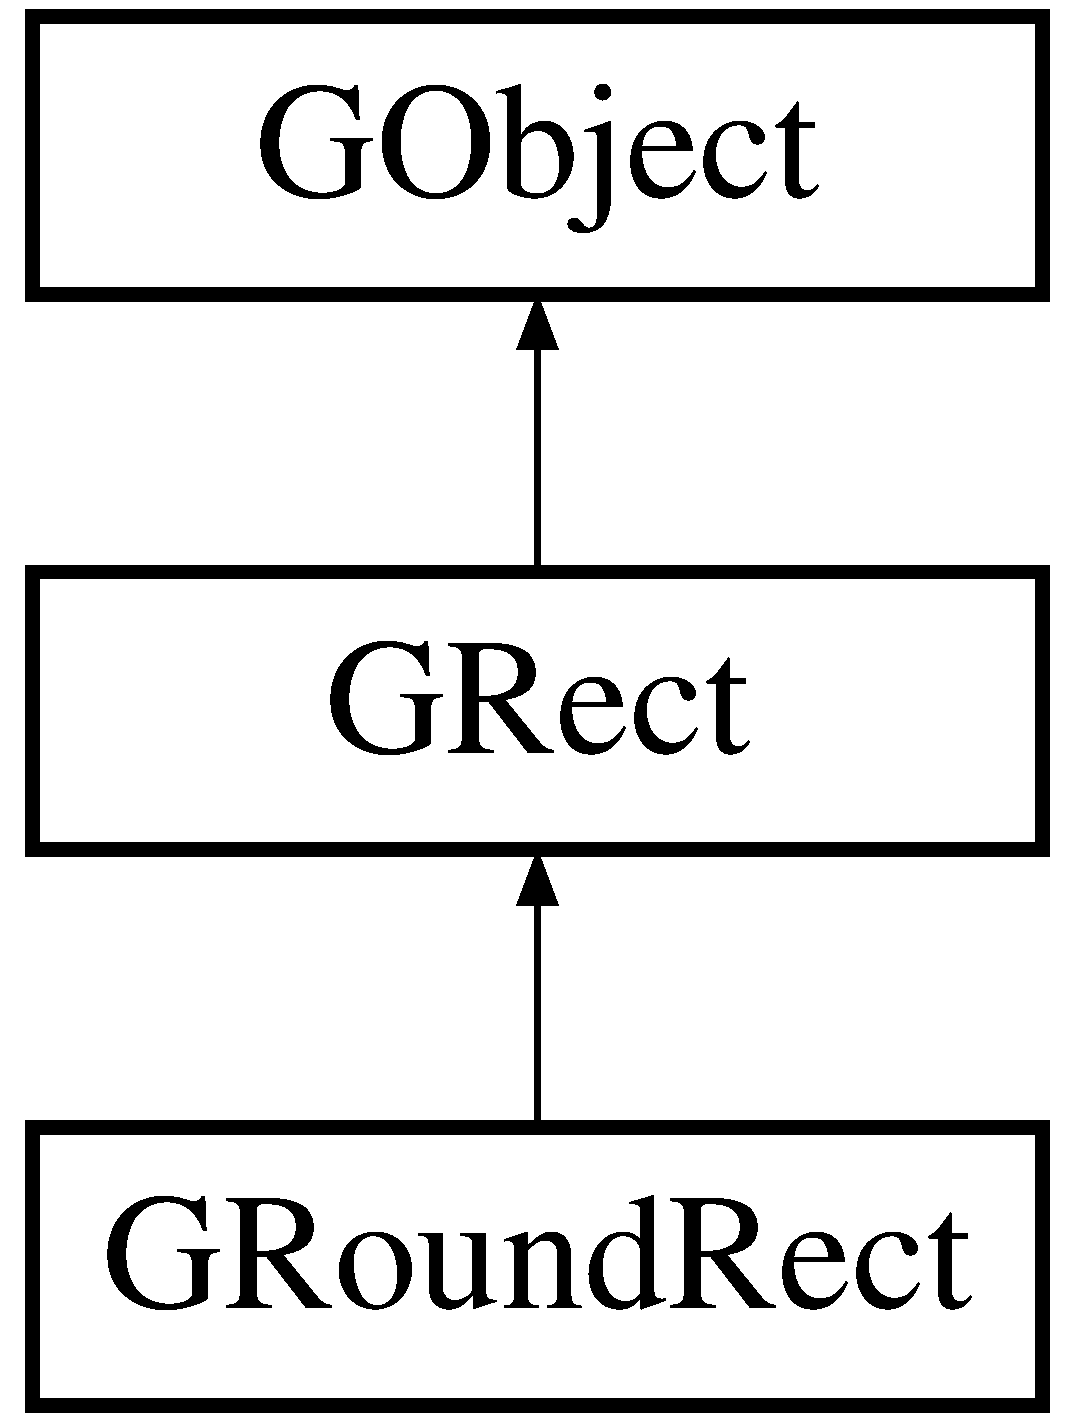
\includegraphics[height=3.000000cm]{classGRoundRect}
\end{center}
\end{figure}
\subsection*{Public Types}
\begin{DoxyCompactItemize}
\item 
enum \mbox{\hyperlink{classGObject_a86e0f5648542856159bb40775c854aa7}{Line\+Style}} \{ \mbox{\hyperlink{classGObject_a86e0f5648542856159bb40775c854aa7acbc84bd5232621834ed31f44d457c1eb}{L\+I\+N\+E\+\_\+\+N\+O\+NE}}, 
\mbox{\hyperlink{classGObject_a86e0f5648542856159bb40775c854aa7a700c78bc2cd76acaab26651bf7b4941f}{L\+I\+N\+E\+\_\+\+S\+O\+L\+ID}}, 
\mbox{\hyperlink{classGObject_a86e0f5648542856159bb40775c854aa7a9ccba0845f785d81d07b333ae1aad84e}{L\+I\+N\+E\+\_\+\+D\+A\+SH}}, 
\mbox{\hyperlink{classGObject_a86e0f5648542856159bb40775c854aa7a8e811c096cb941997f0bfda168bb6df3}{L\+I\+N\+E\+\_\+\+D\+OT}}, 
\mbox{\hyperlink{classGObject_a86e0f5648542856159bb40775c854aa7ada15a2e3d737b2db7706d8300f91b89d}{L\+I\+N\+E\+\_\+\+D\+A\+S\+H\+\_\+\+D\+OT}}, 
\mbox{\hyperlink{classGObject_a86e0f5648542856159bb40775c854aa7aabf4053a73eafa7ba2b7e6d664c74c1d}{L\+I\+N\+E\+\_\+\+D\+A\+S\+H\+\_\+\+D\+O\+T\+\_\+\+D\+OT}}
 \}
\begin{DoxyCompactList}\small\item\em Styles that can be used for the outline around various shapes. \end{DoxyCompactList}\end{DoxyCompactItemize}
\subsection*{Public Member Functions}
\begin{DoxyCompactItemize}
\item 
\mbox{\hyperlink{classGRoundRect_a4e4a8dae719dc671caf5bbfda7ca158a}{G\+Round\+Rect}} (double width=0, double height=0, double corner=\mbox{\hyperlink{classGRoundRect_a6e0fd235a5cfe88a0b0825202575bed9}{D\+E\+F\+A\+U\+L\+T\+\_\+\+C\+O\+R\+N\+ER}})
\begin{DoxyCompactList}\small\item\em Constructs a new rectangle with the specified width and height, located at (0, 0). \end{DoxyCompactList}\item 
\mbox{\hyperlink{classGRoundRect_a7ad0ccdd10c65a52fc77a7e9634ae58b}{G\+Round\+Rect}} (double x, double y, double width, double height, double corner=\mbox{\hyperlink{classGRoundRect_a6e0fd235a5cfe88a0b0825202575bed9}{D\+E\+F\+A\+U\+L\+T\+\_\+\+C\+O\+R\+N\+ER}})
\begin{DoxyCompactList}\small\item\em Constructs a new rectangle with the specified width and height, with its top/left corner at (x, y). \end{DoxyCompactList}\item 
virtual bool \mbox{\hyperlink{classGObject_a1dbc9dafaae51958112dbe1267a1f547}{contains}} (const \mbox{\hyperlink{classGPoint}{G\+Point}} \&pt) const
\begin{DoxyCompactList}\small\item\em Returns {\ttfamily true} if the specified point is inside the object. \end{DoxyCompactList}\item 
virtual bool \mbox{\hyperlink{classGRoundRect_abb6a5d7c03e6eaaae97264c4799ce7c3}{contains}} (double x, double y) const
\begin{DoxyCompactList}\small\item\em Returns {\ttfamily true} if the specified point is inside the object. \end{DoxyCompactList}\item 
virtual \mbox{\hyperlink{classGPoint}{G\+Point}} \mbox{\hyperlink{classGObject_a0d41183bf6b08de66fe3907551aab0d7}{get\+Bottom\+Right\+Location}} () const
\begin{DoxyCompactList}\small\item\em Returns the x/y coordinates of the bottom/right corner of the object. \end{DoxyCompactList}\item 
virtual double \mbox{\hyperlink{classGObject_a4316a2406c18e1c6d061fe51fd355490}{get\+BottomY}} () const
\begin{DoxyCompactList}\small\item\em Returns the {\itshape y}-\/coordinate of the bottom of the object. \end{DoxyCompactList}\item 
virtual \mbox{\hyperlink{classGRectangle}{G\+Rectangle}} \mbox{\hyperlink{classGObject_a29e6ac35a0b48f491a4c88194cc5da3b}{get\+Bounds}} () const
\begin{DoxyCompactList}\small\item\em Returns the bounding box of this object, which is defined to be the smallest rectangle that covers everything drawn by the figure. \end{DoxyCompactList}\item 
virtual \mbox{\hyperlink{classGPoint}{G\+Point}} \mbox{\hyperlink{classGObject_a0909472e91448470bccdb62ecfb95d8b}{get\+Center\+Location}} () const
\begin{DoxyCompactList}\small\item\em Returns the x/y-\/coordinates of the center of the object. \end{DoxyCompactList}\item 
virtual double \mbox{\hyperlink{classGObject_a04df74355b545e0543112d5b8d924176}{get\+CenterX}} () const
\begin{DoxyCompactList}\small\item\em Returns the {\itshape x}-\/coordinate of the center of the object. \end{DoxyCompactList}\item 
virtual double \mbox{\hyperlink{classGObject_acb3287a3d507025a26f54b895713b947}{get\+CenterY}} () const
\begin{DoxyCompactList}\small\item\em Returns the {\itshape y}-\/coordinate of the center of the object. \end{DoxyCompactList}\item 
virtual std\+::string \mbox{\hyperlink{classGObject_aa061dfa488c31e18549d64363c1d0e34}{get\+Color}} () const
\begin{DoxyCompactList}\small\item\em Returns the color used to display this object. \end{DoxyCompactList}\item 
virtual double \mbox{\hyperlink{classGRoundRect_ad29f4fe71bbd3f4302d25adbee70ba2b}{get\+Corner}} () const
\begin{DoxyCompactList}\small\item\em Returns the diameter of the arc forming the corner of this rounded rectangle. \end{DoxyCompactList}\item 
virtual std\+::string \mbox{\hyperlink{classGObject_a76f6964a11fde7c78e9751be184e1a3c}{get\+Fill\+Color}} () const
\begin{DoxyCompactList}\small\item\em Returns the color used to display the filled region of this object. \end{DoxyCompactList}\item 
virtual double \mbox{\hyperlink{classGObject_a1e7e353362434072875264cf95629f99}{get\+Height}} () const
\begin{DoxyCompactList}\small\item\em Returns the height of this object, which is the same as the height of its bounding box. \end{DoxyCompactList}\item 
virtual \mbox{\hyperlink{classGObject_a86e0f5648542856159bb40775c854aa7}{Line\+Style}} \mbox{\hyperlink{classGObject_aaf1f5ea8281e5e3486662878d26f0a13}{get\+Line\+Style}} () const
\begin{DoxyCompactList}\small\item\em Returns the object\textquotesingle{}s style such as solid or dashed. \end{DoxyCompactList}\item 
virtual double \mbox{\hyperlink{classGObject_a85ff266dc3eb63d9f2d8e5a4487fd3c0}{get\+Line\+Width}} () const
\begin{DoxyCompactList}\small\item\em Returns the width of the line used to draw this object. \end{DoxyCompactList}\item 
virtual \mbox{\hyperlink{classGPoint}{G\+Point}} \mbox{\hyperlink{classGObject_a4f83802015511edeb63b892830812c11}{get\+Location}} () const
\begin{DoxyCompactList}\small\item\em Returns the location of the top-\/left corner of object. \end{DoxyCompactList}\item 
virtual double \mbox{\hyperlink{classGObject_a1ae3fc278cc5b71b9f2d96a8a83cdf26}{get\+Opacity}} () const
\begin{DoxyCompactList}\small\item\em Returns how opaque (non-\/transparent) this object will appear from 0.\+0 (completely transparent) to 1.\+0 (completely opaque, default). \end{DoxyCompactList}\item 
virtual \mbox{\hyperlink{classGCompound}{G\+Compound}} $\ast$ \mbox{\hyperlink{classGObject_a3e53cef70541b1a14eade4ad0984d0b4}{get\+Parent}} () const
\begin{DoxyCompactList}\small\item\em Returns a pointer to the {\ttfamily \mbox{\hyperlink{classGCompound}{G\+Compound}}} that contains this object. \end{DoxyCompactList}\item 
virtual double \mbox{\hyperlink{classGObject_a798cc79daaa10145b28f60bcdfdb0ee9}{get\+RightX}} () const
\begin{DoxyCompactList}\small\item\em Returns the {\itshape x}-\/coordinate of the right side of the object. \end{DoxyCompactList}\item 
virtual \mbox{\hyperlink{classGDimension}{G\+Dimension}} \mbox{\hyperlink{classGObject_a7b4eec96a2bdc6420695d5796a78eea9}{get\+Size}} () const
\begin{DoxyCompactList}\small\item\em Returns the size of the object as a {\ttfamily \mbox{\hyperlink{classGDimension}{G\+Dimension}}}. \end{DoxyCompactList}\item 
virtual std\+::string \mbox{\hyperlink{classGRoundRect_a9896d58fcfebbf1025aeeb5b8b9ede80}{get\+Type}} () const Q\+\_\+\+D\+E\+C\+L\+\_\+\+O\+V\+E\+R\+R\+I\+DE
\begin{DoxyCompactList}\small\item\em Returns the type of the object as a string, such as {\ttfamily \char`\"{}\+G\+Oval\char`\"{}} or {\ttfamily \char`\"{}\+G\+Rect\char`\"{}}. \end{DoxyCompactList}\item 
virtual double \mbox{\hyperlink{classGObject_a0ed2965abd4f5701d2cadf71239faf19}{get\+Width}} () const
\begin{DoxyCompactList}\small\item\em Returns the width of this object, which is equal to the width of the bounding box. \end{DoxyCompactList}\item 
virtual double \mbox{\hyperlink{classGObject_a344385751bee0720059403940d57a13e}{getX}} () const
\begin{DoxyCompactList}\small\item\em Returns the leftmost {\itshape x}-\/coordinate of the object. \end{DoxyCompactList}\item 
virtual double \mbox{\hyperlink{classGObject_aafa51c7f8f38a09febbb9ce7853f77b4}{getY}} () const
\begin{DoxyCompactList}\small\item\em Returns the topmost {\itshape y}-\/coordinate of the object. \end{DoxyCompactList}\item 
virtual bool \mbox{\hyperlink{classGObject_a11c404f106940c201b6f326e0355c150}{is\+Filled}} () const
\begin{DoxyCompactList}\small\item\em Returns {\ttfamily true} if the object is filled with color. \end{DoxyCompactList}\item 
virtual bool \mbox{\hyperlink{classGObject_a9de207581cfa4ca1eaa06da5f29b75fc}{is\+Transformed}} () const
\begin{DoxyCompactList}\small\item\em Returns {\ttfamily true} if this object has been transformed by calling methods such as \mbox{\hyperlink{classGObject_ae1ffaa12185dfd5ba464f7d87c329e26}{rotate()}} or \mbox{\hyperlink{classGObject_ad2e1900f730475c2d044817db03b38d6}{scale()}} on it. \end{DoxyCompactList}\item 
virtual bool \mbox{\hyperlink{classGObject_a9d8a6cfb13917785c143e74d40e4e2be}{is\+Visible}} () const
\begin{DoxyCompactList}\small\item\em Returns {\ttfamily true} if this object is visible on screen. \end{DoxyCompactList}\item 
virtual void \mbox{\hyperlink{classGObject_a5973d8dda83afb36e2c56855515be392}{move}} (double dx, double dy)
\begin{DoxyCompactList}\small\item\em Moves the object on the screen using the displacements {\ttfamily dx} and {\ttfamily dy}. \end{DoxyCompactList}\item 
virtual void \mbox{\hyperlink{classGObject_ac827b978aa122f136a14c198687ad80f}{repaint}} ()
\begin{DoxyCompactList}\small\item\em Instructs the object to redraw itself on screen. \end{DoxyCompactList}\item 
virtual void \mbox{\hyperlink{classGObject_a6022a1fd1e5dcd2fd5585e5a36aa3f37}{reset\+Transform}} ()
\begin{DoxyCompactList}\small\item\em Undoes any previous scale/rotate transformations on this object. \end{DoxyCompactList}\item 
virtual void \mbox{\hyperlink{classGObject_ae1ffaa12185dfd5ba464f7d87c329e26}{rotate}} (double theta)
\begin{DoxyCompactList}\small\item\em Transforms the object by rotating it {\ttfamily theta} degrees counterclockwise around its origin. \end{DoxyCompactList}\item 
virtual void \mbox{\hyperlink{classGObject_ad2e1900f730475c2d044817db03b38d6}{scale}} (double sf)
\begin{DoxyCompactList}\small\item\em Scales the object by the specified scale factor. \end{DoxyCompactList}\item 
virtual void \mbox{\hyperlink{classGObject_a63641f69d610d0b951357d35a0c3b1e3}{scale}} (double sx, double sy)
\begin{DoxyCompactList}\small\item\em Scales the object by the specified scale factors. \end{DoxyCompactList}\item 
void \mbox{\hyperlink{classGObject_ab6747f40313c531c2db32edb5b63b9b7}{send\+Backward}} ()
\begin{DoxyCompactList}\small\item\em Moves this object one step toward the back in the {\itshape z} dimension. \end{DoxyCompactList}\item 
void \mbox{\hyperlink{classGObject_a710b3e449c9facba7847c91ab170d281}{send\+Forward}} ()
\begin{DoxyCompactList}\small\item\em Moves this object one step toward the front in the {\itshape z} dimension. \end{DoxyCompactList}\item 
void \mbox{\hyperlink{classGObject_a0f7f1efbb7fd46dde2867c4ad0330896}{send\+To\+Back}} ()
\begin{DoxyCompactList}\small\item\em Moves this object to the back of the display in the {\itshape z} dimension. \end{DoxyCompactList}\item 
void \mbox{\hyperlink{classGObject_aee33d68488e46827ef55fac07f40a9b2}{send\+To\+Front}} ()
\begin{DoxyCompactList}\small\item\em Moves this object to the front of the display in the {\itshape z} dimension. \end{DoxyCompactList}\item 
virtual void \mbox{\hyperlink{classGObject_a71ff7b16b8f1bdc4a1ce9f30cf8b87d8}{set\+Bottom\+Right\+Location}} (double x, double y)
\begin{DoxyCompactList}\small\item\em Sets the location of the bottom/right of this object. \end{DoxyCompactList}\item 
virtual void \mbox{\hyperlink{classGObject_ac6f7320321182f1d18c1c0fa97d5e941}{set\+Bottom\+Right\+Location}} (const \mbox{\hyperlink{classGPoint}{G\+Point}} \&pt)
\begin{DoxyCompactList}\small\item\em Sets the location of the bottom/right of this object. \end{DoxyCompactList}\item 
virtual void \mbox{\hyperlink{classGObject_a4b20e93c2a2597484f74ee5caa71f41f}{set\+BottomY}} (double y)
\begin{DoxyCompactList}\small\item\em Sets the location of the bottom y-\/coordinate of this object. \end{DoxyCompactList}\item 
virtual void \mbox{\hyperlink{classGObject_a2aae8197624b72265ab83b4f1bc73f2f}{set\+Bounds}} (double x, double y, double width, double height)
\begin{DoxyCompactList}\small\item\em Changes the bounds of this object to the specified values. \end{DoxyCompactList}\item 
virtual void \mbox{\hyperlink{classGObject_acada386653f008cacc7cce86426bef7c}{set\+Bounds}} (const \mbox{\hyperlink{classGRectangle}{G\+Rectangle}} \&size)
\begin{DoxyCompactList}\small\item\em Changes the bounds of this object to the specified rectangle. \end{DoxyCompactList}\item 
virtual void \mbox{\hyperlink{classGObject_a290b47dd8de1be44089f95cb2c47c1de}{set\+Center\+Location}} (double x, double y)
\begin{DoxyCompactList}\small\item\em Sets the location of the center of this object. \end{DoxyCompactList}\item 
virtual void \mbox{\hyperlink{classGObject_a1bedf1b233ecba3f753ec58908a683a6}{set\+Center\+Location}} (const \mbox{\hyperlink{classGPoint}{G\+Point}} \&pt)
\begin{DoxyCompactList}\small\item\em Sets the location of the center of this object. \end{DoxyCompactList}\item 
virtual void \mbox{\hyperlink{classGObject_a2f4936281e056eead00a9186b9ba8af6}{set\+CenterX}} (double x)
\begin{DoxyCompactList}\small\item\em Sets the x-\/coordinate of the center of this object. \end{DoxyCompactList}\item 
virtual void \mbox{\hyperlink{classGObject_aad2a22b4fde88c33306b92aebf641d57}{set\+CenterY}} (double y)
\begin{DoxyCompactList}\small\item\em Sets the y-\/coordinate of the center of this object. \end{DoxyCompactList}\item 
virtual void \mbox{\hyperlink{classGObject_ad57ef49bc31db94e92648aa3737923d6}{set\+Color}} (int r, int g, int b)
\begin{DoxyCompactList}\small\item\em Sets the color used to display this object. \end{DoxyCompactList}\item 
virtual void \mbox{\hyperlink{classGObject_ab1f5cc0f5cc6bbbd716a526c61f1081d}{set\+Color}} (int rgb)
\begin{DoxyCompactList}\small\item\em Sets the color used to display this object. \end{DoxyCompactList}\item 
virtual void \mbox{\hyperlink{classGObject_a61374df6c11b52cfbb0815decdbaebc6}{set\+Color}} (const std\+::string \&color)
\begin{DoxyCompactList}\small\item\em Sets the color used to display this object. \end{DoxyCompactList}\item 
virtual void \mbox{\hyperlink{classGRoundRect_ab1cc6c77629d0e8ded56139a1866be48}{set\+Corner}} (double corner)
\begin{DoxyCompactList}\small\item\em Sets the diameter of the arc forming the corner of this rounded rectangle. \end{DoxyCompactList}\item 
virtual void \mbox{\hyperlink{classGObject_ad767a33971159e9493e221cca4c00ae9}{set\+Fill\+Color}} (int r, int g, int b)
\begin{DoxyCompactList}\small\item\em Sets the color used to display the filled region of this object, if any. \end{DoxyCompactList}\item 
virtual void \mbox{\hyperlink{classGObject_aa59d9775a67fa7df2b24a95cd34840a3}{set\+Fill\+Color}} (int rgb)
\begin{DoxyCompactList}\small\item\em Sets the color used to display the filled region of this object, if any. \end{DoxyCompactList}\item 
virtual void \mbox{\hyperlink{classGObject_adbc18b1a930aadd97d7437f9f7265b96}{set\+Fill\+Color}} (const std\+::string \&color)
\begin{DoxyCompactList}\small\item\em Sets the color used to display the filled region of this object, if any. \end{DoxyCompactList}\item 
virtual void \mbox{\hyperlink{classGObject_a9b82b53362282c6bb7d6947068d2e55b}{set\+Filled}} (bool flag)
\begin{DoxyCompactList}\small\item\em Sets the fill status for the object, where {\ttfamily false} is outlined and {\ttfamily true} is filled. \end{DoxyCompactList}\item 
virtual void \mbox{\hyperlink{classGObject_a2592348886ffea646c6534bf88f7c49d}{set\+Font}} (const Q\+Font \&font)
\begin{DoxyCompactList}\small\item\em Changes the font used to display the object as specified by the given Qt font. \end{DoxyCompactList}\item 
virtual void \mbox{\hyperlink{classGObject_a8e096e8818d838aceae1d46d58fb3a7b}{set\+Font}} (const std\+::string \&font)
\begin{DoxyCompactList}\small\item\em Changes the font used to display the object as specified by the string {\ttfamily font}, which has the following format\+: \end{DoxyCompactList}\item 
virtual void \mbox{\hyperlink{classGObject_ad18e8fab1e02a4e9b75c6730212558eb}{set\+Foreground}} (int r, int g, int b)
\begin{DoxyCompactList}\small\item\em Sets the color used to display this object. \end{DoxyCompactList}\item 
virtual void \mbox{\hyperlink{classGObject_a9eb856b5ff83a19df3831a31f15f4563}{set\+Foreground}} (int rgb)
\begin{DoxyCompactList}\small\item\em Sets the color used to display this object. \end{DoxyCompactList}\item 
virtual void \mbox{\hyperlink{classGObject_af59209aeadea6dfc6d97a2d8531f50e1}{set\+Foreground}} (const std\+::string \&color)
\begin{DoxyCompactList}\small\item\em Sets the color used to display this object. \end{DoxyCompactList}\item 
virtual void \mbox{\hyperlink{classGObject_a9e280bfc4544dfaf8e4376c4e1a74357}{set\+Height}} (double height)
\begin{DoxyCompactList}\small\item\em Changes the height of this object to the specified height without changing its width. \end{DoxyCompactList}\item 
virtual void \mbox{\hyperlink{classGObject_add11575087eb94f1a71faa3f826c6341}{set\+Line\+Style}} (\mbox{\hyperlink{classGObject_a86e0f5648542856159bb40775c854aa7}{Line\+Style}} line\+Style)
\begin{DoxyCompactList}\small\item\em Sets the object\textquotesingle{}s style such as solid (\mbox{\hyperlink{classGObject_a86e0f5648542856159bb40775c854aa7a700c78bc2cd76acaab26651bf7b4941f}{G\+Object\+::\+L\+I\+N\+E\+\_\+\+S\+O\+L\+ID}}) or dashed (\mbox{\hyperlink{classGObject_a86e0f5648542856159bb40775c854aa7a9ccba0845f785d81d07b333ae1aad84e}{G\+Object\+::\+L\+I\+N\+E\+\_\+\+D\+A\+SH}}). \end{DoxyCompactList}\item 
virtual void \mbox{\hyperlink{classGObject_afd6a47c6ea6a1f85ca05a65ba3ff3477}{set\+Line\+Width}} (double line\+Width)
\begin{DoxyCompactList}\small\item\em Sets the width of the line used to draw this object. \end{DoxyCompactList}\item 
virtual void \mbox{\hyperlink{classGObject_a04594e8ba9b98513a64f1da00dcae18c}{set\+Location}} (double x, double y)
\begin{DoxyCompactList}\small\item\em Sets the location of the top-\/left corner of this object to the specified coordinates. \end{DoxyCompactList}\item 
virtual void \mbox{\hyperlink{classGObject_aa8480c0b7166cdf8f784cece06ab353f}{set\+Location}} (const \mbox{\hyperlink{classGPoint}{G\+Point}} \&pt)
\begin{DoxyCompactList}\small\item\em Sets the location of the top-\/left corner of this object to the specified point. \end{DoxyCompactList}\item 
virtual void \mbox{\hyperlink{classGObject_a04af1866cc1bae4a1226695794a50539}{set\+Opacity}} (double opacity)
\begin{DoxyCompactList}\small\item\em Sets how opaque (non-\/transparent) this object will appear from 0.\+0 (completely transparent) to 1.\+0 (completely opaque, default). \end{DoxyCompactList}\item 
virtual void \mbox{\hyperlink{classGObject_a3c90b758cdc2c911c9ef76c4360eb912}{set\+RightX}} (double x)
\begin{DoxyCompactList}\small\item\em Sets the location of the rightmost x-\/coordinate of this object. \end{DoxyCompactList}\item 
virtual void \mbox{\hyperlink{classGObject_aca25d49481f9bf5fc8f7df4c086c4ce7}{set\+Size}} (double width, double height)
\begin{DoxyCompactList}\small\item\em Changes the size of this object to the specified width and height. \end{DoxyCompactList}\item 
virtual void \mbox{\hyperlink{classGObject_ae2b628228f192c2702c4ce941b2af68f}{set\+Size}} (const \mbox{\hyperlink{classGDimension}{G\+Dimension}} \&size)
\begin{DoxyCompactList}\small\item\em Changes the size of this object to the specified width and height. \end{DoxyCompactList}\item 
virtual void \mbox{\hyperlink{classGObject_a88203f28224315d9f4471212f4af8ed3}{set\+Visible}} (bool flag)
\begin{DoxyCompactList}\small\item\em Sets whether this object is visible. \end{DoxyCompactList}\item 
virtual void \mbox{\hyperlink{classGObject_aa3f3fba4cb131baa8696ba01e3bceca1}{set\+Width}} (double width)
\begin{DoxyCompactList}\small\item\em Changes the width of this object to the specified width without changing its height. \end{DoxyCompactList}\item 
virtual void \mbox{\hyperlink{classGObject_a9c18fcc579333bf9653d13ad2b372e39}{setX}} (double x)
\begin{DoxyCompactList}\small\item\em Sets the x location of the left side of this object. \end{DoxyCompactList}\item 
virtual void \mbox{\hyperlink{classGObject_a7d57e2a5c35d27feb58fd498a3cf82b9}{setY}} (double y)
\begin{DoxyCompactList}\small\item\em Sets the y location of the top of this object. \end{DoxyCompactList}\item 
virtual std\+::string \mbox{\hyperlink{classGObject_a1fe5121d6528fdea3f243321b3fa3a49}{to\+String}} () const
\begin{DoxyCompactList}\small\item\em Returns a printable representation of the object. \end{DoxyCompactList}\item 
virtual std\+::string \mbox{\hyperlink{classGRoundRect_a85b5bcebac42ec5f130b0c3851383a23}{to\+String\+Extra}} () const Q\+\_\+\+D\+E\+C\+L\+\_\+\+O\+V\+E\+R\+R\+I\+DE
\begin{DoxyCompactList}\small\item\em Returns a string containing any extra unique information about this type of graphical object. \end{DoxyCompactList}\end{DoxyCompactItemize}
\subsection*{Static Public Member Functions}
\begin{DoxyCompactItemize}
\item 
static bool \mbox{\hyperlink{classGObject_a93be0e1fe1b1bf1a1da732470c94f42b}{is\+Anti\+Aliasing}} ()
\begin{DoxyCompactList}\small\item\em Returns whether we should globally anti-\/alias graphical objects. \end{DoxyCompactList}\item 
static void \mbox{\hyperlink{classGObject_a1e43371668ae850193cebedb44e1bbe3}{set\+Anti\+Aliasing}} (bool value)
\begin{DoxyCompactList}\small\item\em Globally turns on/off the anti-\/aliasing feature that smooths out the edges of onscreen shapes. \end{DoxyCompactList}\end{DoxyCompactItemize}
\subsection*{Static Public Attributes}
\begin{DoxyCompactItemize}
\item 
static const double \mbox{\hyperlink{classGRoundRect_a6e0fd235a5cfe88a0b0825202575bed9}{D\+E\+F\+A\+U\+L\+T\+\_\+\+C\+O\+R\+N\+ER}} = 10.\+0
\begin{DoxyCompactList}\small\item\em The default diameter of corners on rounded rectangles if none is supplied to the constructor. \end{DoxyCompactList}\end{DoxyCompactItemize}
\subsection*{Protected Attributes}
\begin{DoxyCompactItemize}
\item 
Q\+Brush \mbox{\hyperlink{classGObject_aab24462ec896b596d99911767b0912d0}{\+\_\+brush}}
\item 
std\+::string \mbox{\hyperlink{classGObject_a1134e770ae4315ea8bc1201e2f21da8b}{\+\_\+color}}
\item 
int \mbox{\hyperlink{classGObject_a003fdd343d9b7505c53a8b7a134200ed}{\+\_\+color\+Int}}
\item 
double \mbox{\hyperlink{classGRoundRect_aed2d721464238b51020f9ce90440ecde}{\+\_\+corner}}
\item 
std\+::string \mbox{\hyperlink{classGObject_a179f8d6cee65cd8a54692e32b224392a}{\+\_\+fill\+Color}}
\item 
int \mbox{\hyperlink{classGObject_a751def333a67d651e5b99cc331ecb496}{\+\_\+fill\+Color\+Int}}
\item 
bool \mbox{\hyperlink{classGObject_ad4a55cbcd61b58a4d49666490bb2f103}{\+\_\+fill\+Flag}}
\item 
std\+::string \mbox{\hyperlink{classGObject_aea76ea1a8b5dd7b0a78653277e63b536}{\+\_\+font}}
\item 
double \mbox{\hyperlink{classGObject_ad05df29e7f27fc504abd743e3d8b4e73}{\+\_\+height}}
\item 
\mbox{\hyperlink{classGObject_a86e0f5648542856159bb40775c854aa7}{Line\+Style}} \mbox{\hyperlink{classGObject_a89bafecaafb7c72d55c7efc10b7d0523}{\+\_\+line\+Style}}
\item 
double \mbox{\hyperlink{classGObject_a16e9033665937f13de2e163dc2184aff}{\+\_\+line\+Width}}
\item 
double \mbox{\hyperlink{classGObject_a20eff8eb7af27182edc9bfc54768b6f3}{\+\_\+opacity}}
\item 
\mbox{\hyperlink{classGCompound}{G\+Compound}} $\ast$ \mbox{\hyperlink{classGObject_ac9452c1eaff70eebddbb318196aa3835}{\+\_\+parent}}
\item 
Q\+Pen \mbox{\hyperlink{classGObject_afb69d172743f868299847174eb1b6bc8}{\+\_\+pen}}
\item 
Q\+Transform \mbox{\hyperlink{classGObject_a475b8860a5f1adb4a1fdc58d1f5c1e32}{\+\_\+transform}}
\item 
bool \mbox{\hyperlink{classGObject_ae4725802fc8d8aaa0ab4bd4781f7e07c}{\+\_\+transformed}}
\item 
bool \mbox{\hyperlink{classGObject_a9312c72508471b7c7a87b540263e1af4}{\+\_\+visible}}
\item 
double \mbox{\hyperlink{classGObject_ab55d85a3371770e6725b1062cf160cd8}{\+\_\+width}}
\item 
double \mbox{\hyperlink{classGObject_a6675b83b27137b8d3aa2ad8133078ea6}{\+\_\+x}}
\item 
double \mbox{\hyperlink{classGObject_a2f0f6aeafddc8a39c578bfa7e22b5f1e}{\+\_\+y}}
\end{DoxyCompactItemize}


\subsection{Detailed Description}
A \mbox{\hyperlink{classGRoundRect}{G\+Round\+Rect}} represents a graphical object whose appearance consists of a rectangular box with rounded corners. 

\subsection{Member Enumeration Documentation}
\mbox{\Hypertarget{classGObject_a86e0f5648542856159bb40775c854aa7}\label{classGObject_a86e0f5648542856159bb40775c854aa7}} 
\index{G\+Round\+Rect@{G\+Round\+Rect}!Line\+Style@{Line\+Style}}
\index{Line\+Style@{Line\+Style}!G\+Round\+Rect@{G\+Round\+Rect}}
\subsubsection{\texorpdfstring{Line\+Style}{LineStyle}}
{\footnotesize\ttfamily enum \mbox{\hyperlink{classGObject_a86e0f5648542856159bb40775c854aa7}{Line\+Style}}\hspace{0.3cm}{\ttfamily [inherited]}}



Styles that can be used for the outline around various shapes. 

Call set\+Line\+Style on a \mbox{\hyperlink{classGObject}{G\+Object}} and pass one of these values. \begin{DoxyEnumFields}{Enumerator}
\raisebox{\heightof{T}}[0pt][0pt]{\index{L\+I\+N\+E\+\_\+\+N\+O\+NE@{L\+I\+N\+E\+\_\+\+N\+O\+NE}!G\+Round\+Rect@{G\+Round\+Rect}}\index{G\+Round\+Rect@{G\+Round\+Rect}!L\+I\+N\+E\+\_\+\+N\+O\+NE@{L\+I\+N\+E\+\_\+\+N\+O\+NE}}}\mbox{\Hypertarget{classGObject_a86e0f5648542856159bb40775c854aa7acbc84bd5232621834ed31f44d457c1eb}\label{classGObject_a86e0f5648542856159bb40775c854aa7acbc84bd5232621834ed31f44d457c1eb}} 
L\+I\+N\+E\+\_\+\+N\+O\+NE&\\
\hline

\raisebox{\heightof{T}}[0pt][0pt]{\index{L\+I\+N\+E\+\_\+\+S\+O\+L\+ID@{L\+I\+N\+E\+\_\+\+S\+O\+L\+ID}!G\+Round\+Rect@{G\+Round\+Rect}}\index{G\+Round\+Rect@{G\+Round\+Rect}!L\+I\+N\+E\+\_\+\+S\+O\+L\+ID@{L\+I\+N\+E\+\_\+\+S\+O\+L\+ID}}}\mbox{\Hypertarget{classGObject_a86e0f5648542856159bb40775c854aa7a700c78bc2cd76acaab26651bf7b4941f}\label{classGObject_a86e0f5648542856159bb40775c854aa7a700c78bc2cd76acaab26651bf7b4941f}} 
L\+I\+N\+E\+\_\+\+S\+O\+L\+ID&\\
\hline

\raisebox{\heightof{T}}[0pt][0pt]{\index{L\+I\+N\+E\+\_\+\+D\+A\+SH@{L\+I\+N\+E\+\_\+\+D\+A\+SH}!G\+Round\+Rect@{G\+Round\+Rect}}\index{G\+Round\+Rect@{G\+Round\+Rect}!L\+I\+N\+E\+\_\+\+D\+A\+SH@{L\+I\+N\+E\+\_\+\+D\+A\+SH}}}\mbox{\Hypertarget{classGObject_a86e0f5648542856159bb40775c854aa7a9ccba0845f785d81d07b333ae1aad84e}\label{classGObject_a86e0f5648542856159bb40775c854aa7a9ccba0845f785d81d07b333ae1aad84e}} 
L\+I\+N\+E\+\_\+\+D\+A\+SH&\\
\hline

\raisebox{\heightof{T}}[0pt][0pt]{\index{L\+I\+N\+E\+\_\+\+D\+OT@{L\+I\+N\+E\+\_\+\+D\+OT}!G\+Round\+Rect@{G\+Round\+Rect}}\index{G\+Round\+Rect@{G\+Round\+Rect}!L\+I\+N\+E\+\_\+\+D\+OT@{L\+I\+N\+E\+\_\+\+D\+OT}}}\mbox{\Hypertarget{classGObject_a86e0f5648542856159bb40775c854aa7a8e811c096cb941997f0bfda168bb6df3}\label{classGObject_a86e0f5648542856159bb40775c854aa7a8e811c096cb941997f0bfda168bb6df3}} 
L\+I\+N\+E\+\_\+\+D\+OT&\\
\hline

\raisebox{\heightof{T}}[0pt][0pt]{\index{L\+I\+N\+E\+\_\+\+D\+A\+S\+H\+\_\+\+D\+OT@{L\+I\+N\+E\+\_\+\+D\+A\+S\+H\+\_\+\+D\+OT}!G\+Round\+Rect@{G\+Round\+Rect}}\index{G\+Round\+Rect@{G\+Round\+Rect}!L\+I\+N\+E\+\_\+\+D\+A\+S\+H\+\_\+\+D\+OT@{L\+I\+N\+E\+\_\+\+D\+A\+S\+H\+\_\+\+D\+OT}}}\mbox{\Hypertarget{classGObject_a86e0f5648542856159bb40775c854aa7ada15a2e3d737b2db7706d8300f91b89d}\label{classGObject_a86e0f5648542856159bb40775c854aa7ada15a2e3d737b2db7706d8300f91b89d}} 
L\+I\+N\+E\+\_\+\+D\+A\+S\+H\+\_\+\+D\+OT&\\
\hline

\raisebox{\heightof{T}}[0pt][0pt]{\index{L\+I\+N\+E\+\_\+\+D\+A\+S\+H\+\_\+\+D\+O\+T\+\_\+\+D\+OT@{L\+I\+N\+E\+\_\+\+D\+A\+S\+H\+\_\+\+D\+O\+T\+\_\+\+D\+OT}!G\+Round\+Rect@{G\+Round\+Rect}}\index{G\+Round\+Rect@{G\+Round\+Rect}!L\+I\+N\+E\+\_\+\+D\+A\+S\+H\+\_\+\+D\+O\+T\+\_\+\+D\+OT@{L\+I\+N\+E\+\_\+\+D\+A\+S\+H\+\_\+\+D\+O\+T\+\_\+\+D\+OT}}}\mbox{\Hypertarget{classGObject_a86e0f5648542856159bb40775c854aa7aabf4053a73eafa7ba2b7e6d664c74c1d}\label{classGObject_a86e0f5648542856159bb40775c854aa7aabf4053a73eafa7ba2b7e6d664c74c1d}} 
L\+I\+N\+E\+\_\+\+D\+A\+S\+H\+\_\+\+D\+O\+T\+\_\+\+D\+OT&\\
\hline

\end{DoxyEnumFields}


\subsection{Constructor \& Destructor Documentation}
\mbox{\Hypertarget{classGRoundRect_a4e4a8dae719dc671caf5bbfda7ca158a}\label{classGRoundRect_a4e4a8dae719dc671caf5bbfda7ca158a}} 
\index{G\+Round\+Rect@{G\+Round\+Rect}!G\+Round\+Rect@{G\+Round\+Rect}}
\index{G\+Round\+Rect@{G\+Round\+Rect}!G\+Round\+Rect@{G\+Round\+Rect}}
\subsubsection{\texorpdfstring{G\+Round\+Rect()}{GRoundRect()}\hspace{0.1cm}{\footnotesize\ttfamily [1/2]}}
{\footnotesize\ttfamily \mbox{\hyperlink{classGRoundRect}{G\+Round\+Rect}} (\begin{DoxyParamCaption}\item[{double}]{width = {\ttfamily 0},  }\item[{double}]{height = {\ttfamily 0},  }\item[{double}]{corner = {\ttfamily \mbox{\hyperlink{classGRoundRect_a6e0fd235a5cfe88a0b0825202575bed9}{D\+E\+F\+A\+U\+L\+T\+\_\+\+C\+O\+R\+N\+ER}}} }\end{DoxyParamCaption})}



Constructs a new rectangle with the specified width and height, located at (0, 0). 

The {\ttfamily corner} parameter specifies the diameter of the arc forming the corner. \mbox{\Hypertarget{classGRoundRect_a7ad0ccdd10c65a52fc77a7e9634ae58b}\label{classGRoundRect_a7ad0ccdd10c65a52fc77a7e9634ae58b}} 
\index{G\+Round\+Rect@{G\+Round\+Rect}!G\+Round\+Rect@{G\+Round\+Rect}}
\index{G\+Round\+Rect@{G\+Round\+Rect}!G\+Round\+Rect@{G\+Round\+Rect}}
\subsubsection{\texorpdfstring{G\+Round\+Rect()}{GRoundRect()}\hspace{0.1cm}{\footnotesize\ttfamily [2/2]}}
{\footnotesize\ttfamily \mbox{\hyperlink{classGRoundRect}{G\+Round\+Rect}} (\begin{DoxyParamCaption}\item[{double}]{x,  }\item[{double}]{y,  }\item[{double}]{width,  }\item[{double}]{height,  }\item[{double}]{corner = {\ttfamily \mbox{\hyperlink{classGRoundRect_a6e0fd235a5cfe88a0b0825202575bed9}{D\+E\+F\+A\+U\+L\+T\+\_\+\+C\+O\+R\+N\+ER}}} }\end{DoxyParamCaption})}



Constructs a new rectangle with the specified width and height, with its top/left corner at (x, y). 

The {\ttfamily corner} parameter specifies the diameter of the arc forming the corner. 

\subsection{Member Function Documentation}
\mbox{\Hypertarget{classGObject_a1dbc9dafaae51958112dbe1267a1f547}\label{classGObject_a1dbc9dafaae51958112dbe1267a1f547}} 
\index{G\+Round\+Rect@{G\+Round\+Rect}!contains@{contains}}
\index{contains@{contains}!G\+Round\+Rect@{G\+Round\+Rect}}
\subsubsection{\texorpdfstring{contains()}{contains()}\hspace{0.1cm}{\footnotesize\ttfamily [1/2]}}
{\footnotesize\ttfamily bool contains (\begin{DoxyParamCaption}\item[{const \mbox{\hyperlink{classGPoint}{G\+Point}} \&}]{pt }\end{DoxyParamCaption}) const\hspace{0.3cm}{\ttfamily [virtual]}, {\ttfamily [inherited]}}



Returns {\ttfamily true} if the specified point is inside the object. 

\mbox{\Hypertarget{classGRoundRect_abb6a5d7c03e6eaaae97264c4799ce7c3}\label{classGRoundRect_abb6a5d7c03e6eaaae97264c4799ce7c3}} 
\index{G\+Round\+Rect@{G\+Round\+Rect}!contains@{contains}}
\index{contains@{contains}!G\+Round\+Rect@{G\+Round\+Rect}}
\subsubsection{\texorpdfstring{contains()}{contains()}\hspace{0.1cm}{\footnotesize\ttfamily [2/2]}}
{\footnotesize\ttfamily bool contains (\begin{DoxyParamCaption}\item[{double}]{x,  }\item[{double}]{y }\end{DoxyParamCaption}) const\hspace{0.3cm}{\ttfamily [virtual]}}



Returns {\ttfamily true} if the specified point is inside the object. 



Reimplemented from \mbox{\hyperlink{classGObject_abb6a5d7c03e6eaaae97264c4799ce7c3}{G\+Object}}.

\mbox{\Hypertarget{classGObject_a0d41183bf6b08de66fe3907551aab0d7}\label{classGObject_a0d41183bf6b08de66fe3907551aab0d7}} 
\index{G\+Round\+Rect@{G\+Round\+Rect}!get\+Bottom\+Right\+Location@{get\+Bottom\+Right\+Location}}
\index{get\+Bottom\+Right\+Location@{get\+Bottom\+Right\+Location}!G\+Round\+Rect@{G\+Round\+Rect}}
\subsubsection{\texorpdfstring{get\+Bottom\+Right\+Location()}{getBottomRightLocation()}}
{\footnotesize\ttfamily \mbox{\hyperlink{classGPoint}{G\+Point}} get\+Bottom\+Right\+Location (\begin{DoxyParamCaption}{ }\end{DoxyParamCaption}) const\hspace{0.3cm}{\ttfamily [virtual]}, {\ttfamily [inherited]}}



Returns the x/y coordinates of the bottom/right corner of the object. 

\mbox{\Hypertarget{classGObject_a4316a2406c18e1c6d061fe51fd355490}\label{classGObject_a4316a2406c18e1c6d061fe51fd355490}} 
\index{G\+Round\+Rect@{G\+Round\+Rect}!get\+BottomY@{get\+BottomY}}
\index{get\+BottomY@{get\+BottomY}!G\+Round\+Rect@{G\+Round\+Rect}}
\subsubsection{\texorpdfstring{get\+Bottom\+Y()}{getBottomY()}}
{\footnotesize\ttfamily double get\+BottomY (\begin{DoxyParamCaption}{ }\end{DoxyParamCaption}) const\hspace{0.3cm}{\ttfamily [virtual]}, {\ttfamily [inherited]}}



Returns the {\itshape y}-\/coordinate of the bottom of the object. 

Equivalent to the top y-\/coordinate plus the object\textquotesingle{}s height. \mbox{\Hypertarget{classGObject_a29e6ac35a0b48f491a4c88194cc5da3b}\label{classGObject_a29e6ac35a0b48f491a4c88194cc5da3b}} 
\index{G\+Round\+Rect@{G\+Round\+Rect}!get\+Bounds@{get\+Bounds}}
\index{get\+Bounds@{get\+Bounds}!G\+Round\+Rect@{G\+Round\+Rect}}
\subsubsection{\texorpdfstring{get\+Bounds()}{getBounds()}}
{\footnotesize\ttfamily \mbox{\hyperlink{classGRectangle}{G\+Rectangle}} get\+Bounds (\begin{DoxyParamCaption}{ }\end{DoxyParamCaption}) const\hspace{0.3cm}{\ttfamily [virtual]}, {\ttfamily [inherited]}}



Returns the bounding box of this object, which is defined to be the smallest rectangle that covers everything drawn by the figure. 

The coordinates of this rectangle do not necessarily match the location returned by {\ttfamily get\+Location}. Given a {\ttfamily \mbox{\hyperlink{classGText}{G\+Text}}} object, for example, {\ttfamily get\+Location} returns the coordinates of the point on the baseline at which the string begins; the {\ttfamily get\+Bounds} method, by contrast, returns a rectangle that covers the entire window area occupied by the string. 

Reimplemented in \mbox{\hyperlink{classGText_a2f46ec8a3b533c690b3b3e56d4f34afe}{G\+Text}}, \mbox{\hyperlink{classGPolygon_a29e6ac35a0b48f491a4c88194cc5da3b}{G\+Polygon}}, \mbox{\hyperlink{classGLine_a2f46ec8a3b533c690b3b3e56d4f34afe}{G\+Line}}, \mbox{\hyperlink{classGCompound_a2f46ec8a3b533c690b3b3e56d4f34afe}{G\+Compound}}, and \mbox{\hyperlink{classGArc_a2f46ec8a3b533c690b3b3e56d4f34afe}{G\+Arc}}.

\mbox{\Hypertarget{classGObject_a0909472e91448470bccdb62ecfb95d8b}\label{classGObject_a0909472e91448470bccdb62ecfb95d8b}} 
\index{G\+Round\+Rect@{G\+Round\+Rect}!get\+Center\+Location@{get\+Center\+Location}}
\index{get\+Center\+Location@{get\+Center\+Location}!G\+Round\+Rect@{G\+Round\+Rect}}
\subsubsection{\texorpdfstring{get\+Center\+Location()}{getCenterLocation()}}
{\footnotesize\ttfamily \mbox{\hyperlink{classGPoint}{G\+Point}} get\+Center\+Location (\begin{DoxyParamCaption}{ }\end{DoxyParamCaption}) const\hspace{0.3cm}{\ttfamily [virtual]}, {\ttfamily [inherited]}}



Returns the x/y-\/coordinates of the center of the object. 

Equivalent to the top/left plus half the object\textquotesingle{}s size. \mbox{\Hypertarget{classGObject_a04df74355b545e0543112d5b8d924176}\label{classGObject_a04df74355b545e0543112d5b8d924176}} 
\index{G\+Round\+Rect@{G\+Round\+Rect}!get\+CenterX@{get\+CenterX}}
\index{get\+CenterX@{get\+CenterX}!G\+Round\+Rect@{G\+Round\+Rect}}
\subsubsection{\texorpdfstring{get\+Center\+X()}{getCenterX()}}
{\footnotesize\ttfamily double get\+CenterX (\begin{DoxyParamCaption}{ }\end{DoxyParamCaption}) const\hspace{0.3cm}{\ttfamily [virtual]}, {\ttfamily [inherited]}}



Returns the {\itshape x}-\/coordinate of the center of the object. 

Equivalent to the top/left plus half the object\textquotesingle{}s width. \mbox{\Hypertarget{classGObject_acb3287a3d507025a26f54b895713b947}\label{classGObject_acb3287a3d507025a26f54b895713b947}} 
\index{G\+Round\+Rect@{G\+Round\+Rect}!get\+CenterY@{get\+CenterY}}
\index{get\+CenterY@{get\+CenterY}!G\+Round\+Rect@{G\+Round\+Rect}}
\subsubsection{\texorpdfstring{get\+Center\+Y()}{getCenterY()}}
{\footnotesize\ttfamily double get\+CenterY (\begin{DoxyParamCaption}{ }\end{DoxyParamCaption}) const\hspace{0.3cm}{\ttfamily [virtual]}, {\ttfamily [inherited]}}



Returns the {\itshape y}-\/coordinate of the center of the object. 

Equivalent to the top/left plus half the object\textquotesingle{}s height. \mbox{\Hypertarget{classGObject_aa061dfa488c31e18549d64363c1d0e34}\label{classGObject_aa061dfa488c31e18549d64363c1d0e34}} 
\index{G\+Round\+Rect@{G\+Round\+Rect}!get\+Color@{get\+Color}}
\index{get\+Color@{get\+Color}!G\+Round\+Rect@{G\+Round\+Rect}}
\subsubsection{\texorpdfstring{get\+Color()}{getColor()}}
{\footnotesize\ttfamily std\+::string get\+Color (\begin{DoxyParamCaption}{ }\end{DoxyParamCaption}) const\hspace{0.3cm}{\ttfamily [virtual]}, {\ttfamily [inherited]}}



Returns the color used to display this object. 

This color is always returned as a string in the form {\ttfamily \char`\"{}\#rrggbb\char`\"{}}, where {\ttfamily rr}, {\ttfamily gg}, and {\ttfamily bb} are the red, green, and blue components of the color, expressed as two-\/digit hexadecimal values. \mbox{\Hypertarget{classGRoundRect_ad29f4fe71bbd3f4302d25adbee70ba2b}\label{classGRoundRect_ad29f4fe71bbd3f4302d25adbee70ba2b}} 
\index{G\+Round\+Rect@{G\+Round\+Rect}!get\+Corner@{get\+Corner}}
\index{get\+Corner@{get\+Corner}!G\+Round\+Rect@{G\+Round\+Rect}}
\subsubsection{\texorpdfstring{get\+Corner()}{getCorner()}}
{\footnotesize\ttfamily double get\+Corner (\begin{DoxyParamCaption}{ }\end{DoxyParamCaption}) const\hspace{0.3cm}{\ttfamily [virtual]}}



Returns the diameter of the arc forming the corner of this rounded rectangle. 

\mbox{\Hypertarget{classGObject_a76f6964a11fde7c78e9751be184e1a3c}\label{classGObject_a76f6964a11fde7c78e9751be184e1a3c}} 
\index{G\+Round\+Rect@{G\+Round\+Rect}!get\+Fill\+Color@{get\+Fill\+Color}}
\index{get\+Fill\+Color@{get\+Fill\+Color}!G\+Round\+Rect@{G\+Round\+Rect}}
\subsubsection{\texorpdfstring{get\+Fill\+Color()}{getFillColor()}}
{\footnotesize\ttfamily std\+::string get\+Fill\+Color (\begin{DoxyParamCaption}{ }\end{DoxyParamCaption}) const\hspace{0.3cm}{\ttfamily [virtual]}, {\ttfamily [inherited]}}



Returns the color used to display the filled region of this object. 

If none has been set, returns the empty string. \mbox{\Hypertarget{classGObject_a1e7e353362434072875264cf95629f99}\label{classGObject_a1e7e353362434072875264cf95629f99}} 
\index{G\+Round\+Rect@{G\+Round\+Rect}!get\+Height@{get\+Height}}
\index{get\+Height@{get\+Height}!G\+Round\+Rect@{G\+Round\+Rect}}
\subsubsection{\texorpdfstring{get\+Height()}{getHeight()}}
{\footnotesize\ttfamily double get\+Height (\begin{DoxyParamCaption}{ }\end{DoxyParamCaption}) const\hspace{0.3cm}{\ttfamily [virtual]}, {\ttfamily [inherited]}}



Returns the height of this object, which is the same as the height of its bounding box. 



Reimplemented in \mbox{\hyperlink{classGPolygon_a1e7e353362434072875264cf95629f99}{G\+Polygon}}, and \mbox{\hyperlink{classGLine_a423f17d4aeb66feb0d148fd23af335b7}{G\+Line}}.

\mbox{\Hypertarget{classGObject_aaf1f5ea8281e5e3486662878d26f0a13}\label{classGObject_aaf1f5ea8281e5e3486662878d26f0a13}} 
\index{G\+Round\+Rect@{G\+Round\+Rect}!get\+Line\+Style@{get\+Line\+Style}}
\index{get\+Line\+Style@{get\+Line\+Style}!G\+Round\+Rect@{G\+Round\+Rect}}
\subsubsection{\texorpdfstring{get\+Line\+Style()}{getLineStyle()}}
{\footnotesize\ttfamily \mbox{\hyperlink{classGObject_a86e0f5648542856159bb40775c854aa7}{G\+Object\+::\+Line\+Style}} get\+Line\+Style (\begin{DoxyParamCaption}{ }\end{DoxyParamCaption}) const\hspace{0.3cm}{\ttfamily [virtual]}, {\ttfamily [inherited]}}



Returns the object\textquotesingle{}s style such as solid or dashed. 

\mbox{\Hypertarget{classGObject_a85ff266dc3eb63d9f2d8e5a4487fd3c0}\label{classGObject_a85ff266dc3eb63d9f2d8e5a4487fd3c0}} 
\index{G\+Round\+Rect@{G\+Round\+Rect}!get\+Line\+Width@{get\+Line\+Width}}
\index{get\+Line\+Width@{get\+Line\+Width}!G\+Round\+Rect@{G\+Round\+Rect}}
\subsubsection{\texorpdfstring{get\+Line\+Width()}{getLineWidth()}}
{\footnotesize\ttfamily double get\+Line\+Width (\begin{DoxyParamCaption}{ }\end{DoxyParamCaption}) const\hspace{0.3cm}{\ttfamily [virtual]}, {\ttfamily [inherited]}}



Returns the width of the line used to draw this object. 

\begin{DoxyReturn}{Returns}
default 1 
\end{DoxyReturn}
\mbox{\Hypertarget{classGObject_a4f83802015511edeb63b892830812c11}\label{classGObject_a4f83802015511edeb63b892830812c11}} 
\index{G\+Round\+Rect@{G\+Round\+Rect}!get\+Location@{get\+Location}}
\index{get\+Location@{get\+Location}!G\+Round\+Rect@{G\+Round\+Rect}}
\subsubsection{\texorpdfstring{get\+Location()}{getLocation()}}
{\footnotesize\ttfamily \mbox{\hyperlink{classGPoint}{G\+Point}} get\+Location (\begin{DoxyParamCaption}{ }\end{DoxyParamCaption}) const\hspace{0.3cm}{\ttfamily [virtual]}, {\ttfamily [inherited]}}



Returns the location of the top-\/left corner of object. 

\mbox{\Hypertarget{classGObject_a1ae3fc278cc5b71b9f2d96a8a83cdf26}\label{classGObject_a1ae3fc278cc5b71b9f2d96a8a83cdf26}} 
\index{G\+Round\+Rect@{G\+Round\+Rect}!get\+Opacity@{get\+Opacity}}
\index{get\+Opacity@{get\+Opacity}!G\+Round\+Rect@{G\+Round\+Rect}}
\subsubsection{\texorpdfstring{get\+Opacity()}{getOpacity()}}
{\footnotesize\ttfamily double get\+Opacity (\begin{DoxyParamCaption}{ }\end{DoxyParamCaption}) const\hspace{0.3cm}{\ttfamily [virtual]}, {\ttfamily [inherited]}}



Returns how opaque (non-\/transparent) this object will appear from 0.\+0 (completely transparent) to 1.\+0 (completely opaque, default). 

\mbox{\Hypertarget{classGObject_a3e53cef70541b1a14eade4ad0984d0b4}\label{classGObject_a3e53cef70541b1a14eade4ad0984d0b4}} 
\index{G\+Round\+Rect@{G\+Round\+Rect}!get\+Parent@{get\+Parent}}
\index{get\+Parent@{get\+Parent}!G\+Round\+Rect@{G\+Round\+Rect}}
\subsubsection{\texorpdfstring{get\+Parent()}{getParent()}}
{\footnotesize\ttfamily \mbox{\hyperlink{classGCompound}{G\+Compound}} $\ast$ get\+Parent (\begin{DoxyParamCaption}{ }\end{DoxyParamCaption}) const\hspace{0.3cm}{\ttfamily [virtual]}, {\ttfamily [inherited]}}



Returns a pointer to the {\ttfamily \mbox{\hyperlink{classGCompound}{G\+Compound}}} that contains this object. 

Every {\ttfamily \mbox{\hyperlink{classGWindow}{G\+Window}}} is initialized to contain a single {\ttfamily \mbox{\hyperlink{classGCompound}{G\+Compound}}} that is aligned with the window. Adding objects to the window adds them to that {\ttfamily \mbox{\hyperlink{classGCompound}{G\+Compound}}}, which means that every object you add to the window has a parent. Calling {\ttfamily get\+Parent} on the top-\/level {\ttfamily \mbox{\hyperlink{classGCompound}{G\+Compound}}} returns {\ttfamily nullptr}. \mbox{\Hypertarget{classGObject_a798cc79daaa10145b28f60bcdfdb0ee9}\label{classGObject_a798cc79daaa10145b28f60bcdfdb0ee9}} 
\index{G\+Round\+Rect@{G\+Round\+Rect}!get\+RightX@{get\+RightX}}
\index{get\+RightX@{get\+RightX}!G\+Round\+Rect@{G\+Round\+Rect}}
\subsubsection{\texorpdfstring{get\+Right\+X()}{getRightX()}}
{\footnotesize\ttfamily double get\+RightX (\begin{DoxyParamCaption}{ }\end{DoxyParamCaption}) const\hspace{0.3cm}{\ttfamily [virtual]}, {\ttfamily [inherited]}}



Returns the {\itshape x}-\/coordinate of the right side of the object. 

Equivalent to the left x-\/coordinate plus the object\textquotesingle{}s width. \mbox{\Hypertarget{classGObject_a7b4eec96a2bdc6420695d5796a78eea9}\label{classGObject_a7b4eec96a2bdc6420695d5796a78eea9}} 
\index{G\+Round\+Rect@{G\+Round\+Rect}!get\+Size@{get\+Size}}
\index{get\+Size@{get\+Size}!G\+Round\+Rect@{G\+Round\+Rect}}
\subsubsection{\texorpdfstring{get\+Size()}{getSize()}}
{\footnotesize\ttfamily \mbox{\hyperlink{classGDimension}{G\+Dimension}} get\+Size (\begin{DoxyParamCaption}{ }\end{DoxyParamCaption}) const\hspace{0.3cm}{\ttfamily [virtual]}, {\ttfamily [inherited]}}



Returns the size of the object as a {\ttfamily \mbox{\hyperlink{classGDimension}{G\+Dimension}}}. 

\mbox{\Hypertarget{classGRoundRect_a9896d58fcfebbf1025aeeb5b8b9ede80}\label{classGRoundRect_a9896d58fcfebbf1025aeeb5b8b9ede80}} 
\index{G\+Round\+Rect@{G\+Round\+Rect}!get\+Type@{get\+Type}}
\index{get\+Type@{get\+Type}!G\+Round\+Rect@{G\+Round\+Rect}}
\subsubsection{\texorpdfstring{get\+Type()}{getType()}}
{\footnotesize\ttfamily std\+::string get\+Type (\begin{DoxyParamCaption}{ }\end{DoxyParamCaption}) const\hspace{0.3cm}{\ttfamily [virtual]}}



Returns the type of the object as a string, such as {\ttfamily \char`\"{}\+G\+Oval\char`\"{}} or {\ttfamily \char`\"{}\+G\+Rect\char`\"{}}. 

Each \mbox{\hyperlink{classGObject}{G\+Object}} subtype must override this method. 

Reimplemented from \mbox{\hyperlink{classGRect_a9896d58fcfebbf1025aeeb5b8b9ede80}{G\+Rect}}.

\mbox{\Hypertarget{classGObject_a0ed2965abd4f5701d2cadf71239faf19}\label{classGObject_a0ed2965abd4f5701d2cadf71239faf19}} 
\index{G\+Round\+Rect@{G\+Round\+Rect}!get\+Width@{get\+Width}}
\index{get\+Width@{get\+Width}!G\+Round\+Rect@{G\+Round\+Rect}}
\subsubsection{\texorpdfstring{get\+Width()}{getWidth()}}
{\footnotesize\ttfamily double get\+Width (\begin{DoxyParamCaption}{ }\end{DoxyParamCaption}) const\hspace{0.3cm}{\ttfamily [virtual]}, {\ttfamily [inherited]}}



Returns the width of this object, which is equal to the width of the bounding box. 



Reimplemented in \mbox{\hyperlink{classGPolygon_a0ed2965abd4f5701d2cadf71239faf19}{G\+Polygon}}, and \mbox{\hyperlink{classGLine_a04bee94b66c8f921cd8611be2460ba9d}{G\+Line}}.

\mbox{\Hypertarget{classGObject_a344385751bee0720059403940d57a13e}\label{classGObject_a344385751bee0720059403940d57a13e}} 
\index{G\+Round\+Rect@{G\+Round\+Rect}!getX@{getX}}
\index{getX@{getX}!G\+Round\+Rect@{G\+Round\+Rect}}
\subsubsection{\texorpdfstring{get\+X()}{getX()}}
{\footnotesize\ttfamily double getX (\begin{DoxyParamCaption}{ }\end{DoxyParamCaption}) const\hspace{0.3cm}{\ttfamily [virtual]}, {\ttfamily [inherited]}}



Returns the leftmost {\itshape x}-\/coordinate of the object. 

\mbox{\Hypertarget{classGObject_aafa51c7f8f38a09febbb9ce7853f77b4}\label{classGObject_aafa51c7f8f38a09febbb9ce7853f77b4}} 
\index{G\+Round\+Rect@{G\+Round\+Rect}!getY@{getY}}
\index{getY@{getY}!G\+Round\+Rect@{G\+Round\+Rect}}
\subsubsection{\texorpdfstring{get\+Y()}{getY()}}
{\footnotesize\ttfamily double getY (\begin{DoxyParamCaption}{ }\end{DoxyParamCaption}) const\hspace{0.3cm}{\ttfamily [virtual]}, {\ttfamily [inherited]}}



Returns the topmost {\itshape y}-\/coordinate of the object. 

\mbox{\Hypertarget{classGObject_a93be0e1fe1b1bf1a1da732470c94f42b}\label{classGObject_a93be0e1fe1b1bf1a1da732470c94f42b}} 
\index{G\+Round\+Rect@{G\+Round\+Rect}!is\+Anti\+Aliasing@{is\+Anti\+Aliasing}}
\index{is\+Anti\+Aliasing@{is\+Anti\+Aliasing}!G\+Round\+Rect@{G\+Round\+Rect}}
\subsubsection{\texorpdfstring{is\+Anti\+Aliasing()}{isAntiAliasing()}}
{\footnotesize\ttfamily bool is\+Anti\+Aliasing (\begin{DoxyParamCaption}{ }\end{DoxyParamCaption})\hspace{0.3cm}{\ttfamily [static]}, {\ttfamily [inherited]}}



Returns whether we should globally anti-\/alias graphical objects. 

On by default. \mbox{\Hypertarget{classGObject_a11c404f106940c201b6f326e0355c150}\label{classGObject_a11c404f106940c201b6f326e0355c150}} 
\index{G\+Round\+Rect@{G\+Round\+Rect}!is\+Filled@{is\+Filled}}
\index{is\+Filled@{is\+Filled}!G\+Round\+Rect@{G\+Round\+Rect}}
\subsubsection{\texorpdfstring{is\+Filled()}{isFilled()}}
{\footnotesize\ttfamily bool is\+Filled (\begin{DoxyParamCaption}{ }\end{DoxyParamCaption}) const\hspace{0.3cm}{\ttfamily [virtual]}, {\ttfamily [inherited]}}



Returns {\ttfamily true} if the object is filled with color. 

\mbox{\Hypertarget{classGObject_a9de207581cfa4ca1eaa06da5f29b75fc}\label{classGObject_a9de207581cfa4ca1eaa06da5f29b75fc}} 
\index{G\+Round\+Rect@{G\+Round\+Rect}!is\+Transformed@{is\+Transformed}}
\index{is\+Transformed@{is\+Transformed}!G\+Round\+Rect@{G\+Round\+Rect}}
\subsubsection{\texorpdfstring{is\+Transformed()}{isTransformed()}}
{\footnotesize\ttfamily bool is\+Transformed (\begin{DoxyParamCaption}{ }\end{DoxyParamCaption}) const\hspace{0.3cm}{\ttfamily [virtual]}, {\ttfamily [inherited]}}



Returns {\ttfamily true} if this object has been transformed by calling methods such as \mbox{\hyperlink{classGObject_ae1ffaa12185dfd5ba464f7d87c329e26}{rotate()}} or \mbox{\hyperlink{classGObject_ad2e1900f730475c2d044817db03b38d6}{scale()}} on it. 

Certain operations (such as set\+Size) cannot be performed after a graphical object has been transformed. \mbox{\Hypertarget{classGObject_a9d8a6cfb13917785c143e74d40e4e2be}\label{classGObject_a9d8a6cfb13917785c143e74d40e4e2be}} 
\index{G\+Round\+Rect@{G\+Round\+Rect}!is\+Visible@{is\+Visible}}
\index{is\+Visible@{is\+Visible}!G\+Round\+Rect@{G\+Round\+Rect}}
\subsubsection{\texorpdfstring{is\+Visible()}{isVisible()}}
{\footnotesize\ttfamily bool is\+Visible (\begin{DoxyParamCaption}{ }\end{DoxyParamCaption}) const\hspace{0.3cm}{\ttfamily [virtual]}, {\ttfamily [inherited]}}



Returns {\ttfamily true} if this object is visible on screen. 

\mbox{\Hypertarget{classGObject_a5973d8dda83afb36e2c56855515be392}\label{classGObject_a5973d8dda83afb36e2c56855515be392}} 
\index{G\+Round\+Rect@{G\+Round\+Rect}!move@{move}}
\index{move@{move}!G\+Round\+Rect@{G\+Round\+Rect}}
\subsubsection{\texorpdfstring{move()}{move()}}
{\footnotesize\ttfamily void move (\begin{DoxyParamCaption}\item[{double}]{dx,  }\item[{double}]{dy }\end{DoxyParamCaption})\hspace{0.3cm}{\ttfamily [virtual]}, {\ttfamily [inherited]}}



Moves the object on the screen using the displacements {\ttfamily dx} and {\ttfamily dy}. 

\mbox{\Hypertarget{classGObject_ac827b978aa122f136a14c198687ad80f}\label{classGObject_ac827b978aa122f136a14c198687ad80f}} 
\index{G\+Round\+Rect@{G\+Round\+Rect}!repaint@{repaint}}
\index{repaint@{repaint}!G\+Round\+Rect@{G\+Round\+Rect}}
\subsubsection{\texorpdfstring{repaint()}{repaint()}}
{\footnotesize\ttfamily void repaint (\begin{DoxyParamCaption}{ }\end{DoxyParamCaption})\hspace{0.3cm}{\ttfamily [virtual]}, {\ttfamily [inherited]}}



Instructs the object to redraw itself on screen. 



Reimplemented in \mbox{\hyperlink{classGCompound_ac827b978aa122f136a14c198687ad80f}{G\+Compound}}.

\mbox{\Hypertarget{classGObject_a6022a1fd1e5dcd2fd5585e5a36aa3f37}\label{classGObject_a6022a1fd1e5dcd2fd5585e5a36aa3f37}} 
\index{G\+Round\+Rect@{G\+Round\+Rect}!reset\+Transform@{reset\+Transform}}
\index{reset\+Transform@{reset\+Transform}!G\+Round\+Rect@{G\+Round\+Rect}}
\subsubsection{\texorpdfstring{reset\+Transform()}{resetTransform()}}
{\footnotesize\ttfamily void reset\+Transform (\begin{DoxyParamCaption}{ }\end{DoxyParamCaption})\hspace{0.3cm}{\ttfamily [virtual]}, {\ttfamily [inherited]}}



Undoes any previous scale/rotate transformations on this object. 

\mbox{\Hypertarget{classGObject_ae1ffaa12185dfd5ba464f7d87c329e26}\label{classGObject_ae1ffaa12185dfd5ba464f7d87c329e26}} 
\index{G\+Round\+Rect@{G\+Round\+Rect}!rotate@{rotate}}
\index{rotate@{rotate}!G\+Round\+Rect@{G\+Round\+Rect}}
\subsubsection{\texorpdfstring{rotate()}{rotate()}}
{\footnotesize\ttfamily void rotate (\begin{DoxyParamCaption}\item[{double}]{theta }\end{DoxyParamCaption})\hspace{0.3cm}{\ttfamily [virtual]}, {\ttfamily [inherited]}}



Transforms the object by rotating it {\ttfamily theta} degrees counterclockwise around its origin. 

After calling this method on a graphical object, {\ttfamily is\+Transformed} will return {\ttfamily true} for that object unless you subsequently call {\ttfamily reset\+Transform} on it. \mbox{\Hypertarget{classGObject_ad2e1900f730475c2d044817db03b38d6}\label{classGObject_ad2e1900f730475c2d044817db03b38d6}} 
\index{G\+Round\+Rect@{G\+Round\+Rect}!scale@{scale}}
\index{scale@{scale}!G\+Round\+Rect@{G\+Round\+Rect}}
\subsubsection{\texorpdfstring{scale()}{scale()}\hspace{0.1cm}{\footnotesize\ttfamily [1/2]}}
{\footnotesize\ttfamily void scale (\begin{DoxyParamCaption}\item[{double}]{sf }\end{DoxyParamCaption})\hspace{0.3cm}{\ttfamily [virtual]}, {\ttfamily [inherited]}}



Scales the object by the specified scale factor. 

This form scales the object by {\ttfamily sf} in both dimensions, so that invoking {\ttfamily gobj-\/$>$scale(2);} doubles the size of the object. After calling this method on a graphical object, {\ttfamily is\+Transformed} will return {\ttfamily true} for that object unless you subsequently call {\ttfamily reset\+Transform} on it. \mbox{\Hypertarget{classGObject_a63641f69d610d0b951357d35a0c3b1e3}\label{classGObject_a63641f69d610d0b951357d35a0c3b1e3}} 
\index{G\+Round\+Rect@{G\+Round\+Rect}!scale@{scale}}
\index{scale@{scale}!G\+Round\+Rect@{G\+Round\+Rect}}
\subsubsection{\texorpdfstring{scale()}{scale()}\hspace{0.1cm}{\footnotesize\ttfamily [2/2]}}
{\footnotesize\ttfamily void scale (\begin{DoxyParamCaption}\item[{double}]{sx,  }\item[{double}]{sy }\end{DoxyParamCaption})\hspace{0.3cm}{\ttfamily [virtual]}, {\ttfamily [inherited]}}



Scales the object by the specified scale factors. 

For example, {\ttfamily gobj-\/$>$scale(2, 2);} doubles the size of the object. This form applies independent scale factors to the {\itshape x} and {\itshape y} dimensions. After calling this method on a graphical object, {\ttfamily is\+Transformed} will return {\ttfamily true} for that object unless you subsequently call {\ttfamily reset\+Transform} on it. \mbox{\Hypertarget{classGObject_ab6747f40313c531c2db32edb5b63b9b7}\label{classGObject_ab6747f40313c531c2db32edb5b63b9b7}} 
\index{G\+Round\+Rect@{G\+Round\+Rect}!send\+Backward@{send\+Backward}}
\index{send\+Backward@{send\+Backward}!G\+Round\+Rect@{G\+Round\+Rect}}
\subsubsection{\texorpdfstring{send\+Backward()}{sendBackward()}}
{\footnotesize\ttfamily void send\+Backward (\begin{DoxyParamCaption}{ }\end{DoxyParamCaption})\hspace{0.3cm}{\ttfamily [inherited]}}



Moves this object one step toward the back in the {\itshape z} dimension. 

If it was already at the back of the stack, nothing happens. \mbox{\Hypertarget{classGObject_a710b3e449c9facba7847c91ab170d281}\label{classGObject_a710b3e449c9facba7847c91ab170d281}} 
\index{G\+Round\+Rect@{G\+Round\+Rect}!send\+Forward@{send\+Forward}}
\index{send\+Forward@{send\+Forward}!G\+Round\+Rect@{G\+Round\+Rect}}
\subsubsection{\texorpdfstring{send\+Forward()}{sendForward()}}
{\footnotesize\ttfamily void send\+Forward (\begin{DoxyParamCaption}{ }\end{DoxyParamCaption})\hspace{0.3cm}{\ttfamily [inherited]}}



Moves this object one step toward the front in the {\itshape z} dimension. 

If it was already at the front of the stack, nothing happens. \mbox{\Hypertarget{classGObject_a0f7f1efbb7fd46dde2867c4ad0330896}\label{classGObject_a0f7f1efbb7fd46dde2867c4ad0330896}} 
\index{G\+Round\+Rect@{G\+Round\+Rect}!send\+To\+Back@{send\+To\+Back}}
\index{send\+To\+Back@{send\+To\+Back}!G\+Round\+Rect@{G\+Round\+Rect}}
\subsubsection{\texorpdfstring{send\+To\+Back()}{sendToBack()}}
{\footnotesize\ttfamily void send\+To\+Back (\begin{DoxyParamCaption}{ }\end{DoxyParamCaption})\hspace{0.3cm}{\ttfamily [inherited]}}



Moves this object to the back of the display in the {\itshape z} dimension. 

By moving it to the back, this object will appear to be behind the other graphical objects on the display and may be obscured by other objects in front. \mbox{\Hypertarget{classGObject_aee33d68488e46827ef55fac07f40a9b2}\label{classGObject_aee33d68488e46827ef55fac07f40a9b2}} 
\index{G\+Round\+Rect@{G\+Round\+Rect}!send\+To\+Front@{send\+To\+Front}}
\index{send\+To\+Front@{send\+To\+Front}!G\+Round\+Rect@{G\+Round\+Rect}}
\subsubsection{\texorpdfstring{send\+To\+Front()}{sendToFront()}}
{\footnotesize\ttfamily void send\+To\+Front (\begin{DoxyParamCaption}{ }\end{DoxyParamCaption})\hspace{0.3cm}{\ttfamily [inherited]}}



Moves this object to the front of the display in the {\itshape z} dimension. 

By moving it to the front, this object will appear to be on top of the other graphical objects on the display and may hide any objects that are further back. \mbox{\Hypertarget{classGObject_a1e43371668ae850193cebedb44e1bbe3}\label{classGObject_a1e43371668ae850193cebedb44e1bbe3}} 
\index{G\+Round\+Rect@{G\+Round\+Rect}!set\+Anti\+Aliasing@{set\+Anti\+Aliasing}}
\index{set\+Anti\+Aliasing@{set\+Anti\+Aliasing}!G\+Round\+Rect@{G\+Round\+Rect}}
\subsubsection{\texorpdfstring{set\+Anti\+Aliasing()}{setAntiAliasing()}}
{\footnotesize\ttfamily void set\+Anti\+Aliasing (\begin{DoxyParamCaption}\item[{bool}]{value }\end{DoxyParamCaption})\hspace{0.3cm}{\ttfamily [static]}, {\ttfamily [inherited]}}



Globally turns on/off the anti-\/aliasing feature that smooths out the edges of onscreen shapes. 

On by default. Does not repaint any onscreen objects when called; you must do this yourself. \mbox{\Hypertarget{classGObject_a71ff7b16b8f1bdc4a1ce9f30cf8b87d8}\label{classGObject_a71ff7b16b8f1bdc4a1ce9f30cf8b87d8}} 
\index{G\+Round\+Rect@{G\+Round\+Rect}!set\+Bottom\+Right\+Location@{set\+Bottom\+Right\+Location}}
\index{set\+Bottom\+Right\+Location@{set\+Bottom\+Right\+Location}!G\+Round\+Rect@{G\+Round\+Rect}}
\subsubsection{\texorpdfstring{set\+Bottom\+Right\+Location()}{setBottomRightLocation()}\hspace{0.1cm}{\footnotesize\ttfamily [1/2]}}
{\footnotesize\ttfamily void set\+Bottom\+Right\+Location (\begin{DoxyParamCaption}\item[{double}]{x,  }\item[{double}]{y }\end{DoxyParamCaption})\hspace{0.3cm}{\ttfamily [virtual]}, {\ttfamily [inherited]}}



Sets the location of the bottom/right of this object. 

\mbox{\Hypertarget{classGObject_ac6f7320321182f1d18c1c0fa97d5e941}\label{classGObject_ac6f7320321182f1d18c1c0fa97d5e941}} 
\index{G\+Round\+Rect@{G\+Round\+Rect}!set\+Bottom\+Right\+Location@{set\+Bottom\+Right\+Location}}
\index{set\+Bottom\+Right\+Location@{set\+Bottom\+Right\+Location}!G\+Round\+Rect@{G\+Round\+Rect}}
\subsubsection{\texorpdfstring{set\+Bottom\+Right\+Location()}{setBottomRightLocation()}\hspace{0.1cm}{\footnotesize\ttfamily [2/2]}}
{\footnotesize\ttfamily void set\+Bottom\+Right\+Location (\begin{DoxyParamCaption}\item[{const \mbox{\hyperlink{classGPoint}{G\+Point}} \&}]{pt }\end{DoxyParamCaption})\hspace{0.3cm}{\ttfamily [virtual]}, {\ttfamily [inherited]}}



Sets the location of the bottom/right of this object. 

\mbox{\Hypertarget{classGObject_a4b20e93c2a2597484f74ee5caa71f41f}\label{classGObject_a4b20e93c2a2597484f74ee5caa71f41f}} 
\index{G\+Round\+Rect@{G\+Round\+Rect}!set\+BottomY@{set\+BottomY}}
\index{set\+BottomY@{set\+BottomY}!G\+Round\+Rect@{G\+Round\+Rect}}
\subsubsection{\texorpdfstring{set\+Bottom\+Y()}{setBottomY()}}
{\footnotesize\ttfamily void set\+BottomY (\begin{DoxyParamCaption}\item[{double}]{y }\end{DoxyParamCaption})\hspace{0.3cm}{\ttfamily [virtual]}, {\ttfamily [inherited]}}



Sets the location of the bottom y-\/coordinate of this object. 

\mbox{\Hypertarget{classGObject_a2aae8197624b72265ab83b4f1bc73f2f}\label{classGObject_a2aae8197624b72265ab83b4f1bc73f2f}} 
\index{G\+Round\+Rect@{G\+Round\+Rect}!set\+Bounds@{set\+Bounds}}
\index{set\+Bounds@{set\+Bounds}!G\+Round\+Rect@{G\+Round\+Rect}}
\subsubsection{\texorpdfstring{set\+Bounds()}{setBounds()}\hspace{0.1cm}{\footnotesize\ttfamily [1/2]}}
{\footnotesize\ttfamily void set\+Bounds (\begin{DoxyParamCaption}\item[{double}]{x,  }\item[{double}]{y,  }\item[{double}]{width,  }\item[{double}]{height }\end{DoxyParamCaption})\hspace{0.3cm}{\ttfamily [virtual]}, {\ttfamily [inherited]}}



Changes the bounds of this object to the specified values. 

\mbox{\Hypertarget{classGObject_acada386653f008cacc7cce86426bef7c}\label{classGObject_acada386653f008cacc7cce86426bef7c}} 
\index{G\+Round\+Rect@{G\+Round\+Rect}!set\+Bounds@{set\+Bounds}}
\index{set\+Bounds@{set\+Bounds}!G\+Round\+Rect@{G\+Round\+Rect}}
\subsubsection{\texorpdfstring{set\+Bounds()}{setBounds()}\hspace{0.1cm}{\footnotesize\ttfamily [2/2]}}
{\footnotesize\ttfamily void set\+Bounds (\begin{DoxyParamCaption}\item[{const \mbox{\hyperlink{classGRectangle}{G\+Rectangle}} \&}]{size }\end{DoxyParamCaption})\hspace{0.3cm}{\ttfamily [virtual]}, {\ttfamily [inherited]}}



Changes the bounds of this object to the specified rectangle. 

\mbox{\Hypertarget{classGObject_a290b47dd8de1be44089f95cb2c47c1de}\label{classGObject_a290b47dd8de1be44089f95cb2c47c1de}} 
\index{G\+Round\+Rect@{G\+Round\+Rect}!set\+Center\+Location@{set\+Center\+Location}}
\index{set\+Center\+Location@{set\+Center\+Location}!G\+Round\+Rect@{G\+Round\+Rect}}
\subsubsection{\texorpdfstring{set\+Center\+Location()}{setCenterLocation()}\hspace{0.1cm}{\footnotesize\ttfamily [1/2]}}
{\footnotesize\ttfamily void set\+Center\+Location (\begin{DoxyParamCaption}\item[{double}]{x,  }\item[{double}]{y }\end{DoxyParamCaption})\hspace{0.3cm}{\ttfamily [virtual]}, {\ttfamily [inherited]}}



Sets the location of the center of this object. 

\mbox{\Hypertarget{classGObject_a1bedf1b233ecba3f753ec58908a683a6}\label{classGObject_a1bedf1b233ecba3f753ec58908a683a6}} 
\index{G\+Round\+Rect@{G\+Round\+Rect}!set\+Center\+Location@{set\+Center\+Location}}
\index{set\+Center\+Location@{set\+Center\+Location}!G\+Round\+Rect@{G\+Round\+Rect}}
\subsubsection{\texorpdfstring{set\+Center\+Location()}{setCenterLocation()}\hspace{0.1cm}{\footnotesize\ttfamily [2/2]}}
{\footnotesize\ttfamily void set\+Center\+Location (\begin{DoxyParamCaption}\item[{const \mbox{\hyperlink{classGPoint}{G\+Point}} \&}]{pt }\end{DoxyParamCaption})\hspace{0.3cm}{\ttfamily [virtual]}, {\ttfamily [inherited]}}



Sets the location of the center of this object. 

\mbox{\Hypertarget{classGObject_a2f4936281e056eead00a9186b9ba8af6}\label{classGObject_a2f4936281e056eead00a9186b9ba8af6}} 
\index{G\+Round\+Rect@{G\+Round\+Rect}!set\+CenterX@{set\+CenterX}}
\index{set\+CenterX@{set\+CenterX}!G\+Round\+Rect@{G\+Round\+Rect}}
\subsubsection{\texorpdfstring{set\+Center\+X()}{setCenterX()}}
{\footnotesize\ttfamily void set\+CenterX (\begin{DoxyParamCaption}\item[{double}]{x }\end{DoxyParamCaption})\hspace{0.3cm}{\ttfamily [virtual]}, {\ttfamily [inherited]}}



Sets the x-\/coordinate of the center of this object. 

\mbox{\Hypertarget{classGObject_aad2a22b4fde88c33306b92aebf641d57}\label{classGObject_aad2a22b4fde88c33306b92aebf641d57}} 
\index{G\+Round\+Rect@{G\+Round\+Rect}!set\+CenterY@{set\+CenterY}}
\index{set\+CenterY@{set\+CenterY}!G\+Round\+Rect@{G\+Round\+Rect}}
\subsubsection{\texorpdfstring{set\+Center\+Y()}{setCenterY()}}
{\footnotesize\ttfamily void set\+CenterY (\begin{DoxyParamCaption}\item[{double}]{y }\end{DoxyParamCaption})\hspace{0.3cm}{\ttfamily [virtual]}, {\ttfamily [inherited]}}



Sets the y-\/coordinate of the center of this object. 

\mbox{\Hypertarget{classGObject_ad57ef49bc31db94e92648aa3737923d6}\label{classGObject_ad57ef49bc31db94e92648aa3737923d6}} 
\index{G\+Round\+Rect@{G\+Round\+Rect}!set\+Color@{set\+Color}}
\index{set\+Color@{set\+Color}!G\+Round\+Rect@{G\+Round\+Rect}}
\subsubsection{\texorpdfstring{set\+Color()}{setColor()}\hspace{0.1cm}{\footnotesize\ttfamily [1/3]}}
{\footnotesize\ttfamily void set\+Color (\begin{DoxyParamCaption}\item[{int}]{r,  }\item[{int}]{g,  }\item[{int}]{b }\end{DoxyParamCaption})\hspace{0.3cm}{\ttfamily [virtual]}, {\ttfamily [inherited]}}



Sets the color used to display this object. 

See \mbox{\hyperlink{gcolor_8h_source}{gcolor.\+h}} for more detail about how to specify colors.

Equivalent to set\+Foreground.


\begin{DoxyParams}{Parameters}
{\em r} & redness from 0-\/255 \\
\hline
{\em g} & greenness from 0-\/255 \\
\hline
{\em b} & blueness from 0-\/255 \\
\hline
\end{DoxyParams}
\mbox{\Hypertarget{classGObject_ab1f5cc0f5cc6bbbd716a526c61f1081d}\label{classGObject_ab1f5cc0f5cc6bbbd716a526c61f1081d}} 
\index{G\+Round\+Rect@{G\+Round\+Rect}!set\+Color@{set\+Color}}
\index{set\+Color@{set\+Color}!G\+Round\+Rect@{G\+Round\+Rect}}
\subsubsection{\texorpdfstring{set\+Color()}{setColor()}\hspace{0.1cm}{\footnotesize\ttfamily [2/3]}}
{\footnotesize\ttfamily void set\+Color (\begin{DoxyParamCaption}\item[{int}]{rgb }\end{DoxyParamCaption})\hspace{0.3cm}{\ttfamily [virtual]}, {\ttfamily [inherited]}}



Sets the color used to display this object. 

See \mbox{\hyperlink{gcolor_8h_source}{gcolor.\+h}} for more detail about how to specify colors.

Equivalent to set\+Foreground.


\begin{DoxyParams}{Parameters}
{\em rgb} & an R\+GB integer value such as 0x7700ff \\
\hline
\end{DoxyParams}
\mbox{\Hypertarget{classGObject_a61374df6c11b52cfbb0815decdbaebc6}\label{classGObject_a61374df6c11b52cfbb0815decdbaebc6}} 
\index{G\+Round\+Rect@{G\+Round\+Rect}!set\+Color@{set\+Color}}
\index{set\+Color@{set\+Color}!G\+Round\+Rect@{G\+Round\+Rect}}
\subsubsection{\texorpdfstring{set\+Color()}{setColor()}\hspace{0.1cm}{\footnotesize\ttfamily [3/3]}}
{\footnotesize\ttfamily void set\+Color (\begin{DoxyParamCaption}\item[{const std\+::string \&}]{color }\end{DoxyParamCaption})\hspace{0.3cm}{\ttfamily [virtual]}, {\ttfamily [inherited]}}



Sets the color used to display this object. 

See \mbox{\hyperlink{gcolor_8h_source}{gcolor.\+h}} for more detail about how to specify colors.

Equivalent to set\+Foreground.

a color string such as \char`\"{}\#7700ff\char`\"{} or \char`\"{}purple\char`\"{} \mbox{\Hypertarget{classGRoundRect_ab1cc6c77629d0e8ded56139a1866be48}\label{classGRoundRect_ab1cc6c77629d0e8ded56139a1866be48}} 
\index{G\+Round\+Rect@{G\+Round\+Rect}!set\+Corner@{set\+Corner}}
\index{set\+Corner@{set\+Corner}!G\+Round\+Rect@{G\+Round\+Rect}}
\subsubsection{\texorpdfstring{set\+Corner()}{setCorner()}}
{\footnotesize\ttfamily void set\+Corner (\begin{DoxyParamCaption}\item[{double}]{corner }\end{DoxyParamCaption})\hspace{0.3cm}{\ttfamily [virtual]}}



Sets the diameter of the arc forming the corner of this rounded rectangle. 

\mbox{\Hypertarget{classGObject_ad767a33971159e9493e221cca4c00ae9}\label{classGObject_ad767a33971159e9493e221cca4c00ae9}} 
\index{G\+Round\+Rect@{G\+Round\+Rect}!set\+Fill\+Color@{set\+Fill\+Color}}
\index{set\+Fill\+Color@{set\+Fill\+Color}!G\+Round\+Rect@{G\+Round\+Rect}}
\subsubsection{\texorpdfstring{set\+Fill\+Color()}{setFillColor()}\hspace{0.1cm}{\footnotesize\ttfamily [1/3]}}
{\footnotesize\ttfamily void set\+Fill\+Color (\begin{DoxyParamCaption}\item[{int}]{r,  }\item[{int}]{g,  }\item[{int}]{b }\end{DoxyParamCaption})\hspace{0.3cm}{\ttfamily [virtual]}, {\ttfamily [inherited]}}



Sets the color used to display the filled region of this object, if any. 

As a side effect, sets this object to be filled (set\+Filled(true)). See \mbox{\hyperlink{gcolor_8h_source}{gcolor.\+h}} for more detail about how to specify colors. If an empty string is passed, sets filled to false.


\begin{DoxyParams}{Parameters}
{\em r} & redness from 0-\/255 \\
\hline
{\em g} & greenness from 0-\/255 \\
\hline
{\em b} & blueness from 0-\/255 \\
\hline
\end{DoxyParams}
\mbox{\Hypertarget{classGObject_aa59d9775a67fa7df2b24a95cd34840a3}\label{classGObject_aa59d9775a67fa7df2b24a95cd34840a3}} 
\index{G\+Round\+Rect@{G\+Round\+Rect}!set\+Fill\+Color@{set\+Fill\+Color}}
\index{set\+Fill\+Color@{set\+Fill\+Color}!G\+Round\+Rect@{G\+Round\+Rect}}
\subsubsection{\texorpdfstring{set\+Fill\+Color()}{setFillColor()}\hspace{0.1cm}{\footnotesize\ttfamily [2/3]}}
{\footnotesize\ttfamily void set\+Fill\+Color (\begin{DoxyParamCaption}\item[{int}]{rgb }\end{DoxyParamCaption})\hspace{0.3cm}{\ttfamily [virtual]}, {\ttfamily [inherited]}}



Sets the color used to display the filled region of this object, if any. 

As a side effect, sets this object to be filled (set\+Filled(true)). See \mbox{\hyperlink{gcolor_8h_source}{gcolor.\+h}} for more detail about how to specify colors.


\begin{DoxyParams}{Parameters}
{\em rgb} & an R\+GB integer value such as 0x7700ff \\
\hline
\end{DoxyParams}
\mbox{\Hypertarget{classGObject_adbc18b1a930aadd97d7437f9f7265b96}\label{classGObject_adbc18b1a930aadd97d7437f9f7265b96}} 
\index{G\+Round\+Rect@{G\+Round\+Rect}!set\+Fill\+Color@{set\+Fill\+Color}}
\index{set\+Fill\+Color@{set\+Fill\+Color}!G\+Round\+Rect@{G\+Round\+Rect}}
\subsubsection{\texorpdfstring{set\+Fill\+Color()}{setFillColor()}\hspace{0.1cm}{\footnotesize\ttfamily [3/3]}}
{\footnotesize\ttfamily void set\+Fill\+Color (\begin{DoxyParamCaption}\item[{const std\+::string \&}]{color }\end{DoxyParamCaption})\hspace{0.3cm}{\ttfamily [virtual]}, {\ttfamily [inherited]}}



Sets the color used to display the filled region of this object, if any. 

As a side effect, sets this object to be filled (set\+Filled(true)). See \mbox{\hyperlink{gcolor_8h_source}{gcolor.\+h}} for more detail about how to specify colors. If an empty string is passed, sets filled to false.

a color string such as \char`\"{}\#7700ff\char`\"{} or \char`\"{}purple\char`\"{} \mbox{\Hypertarget{classGObject_a9b82b53362282c6bb7d6947068d2e55b}\label{classGObject_a9b82b53362282c6bb7d6947068d2e55b}} 
\index{G\+Round\+Rect@{G\+Round\+Rect}!set\+Filled@{set\+Filled}}
\index{set\+Filled@{set\+Filled}!G\+Round\+Rect@{G\+Round\+Rect}}
\subsubsection{\texorpdfstring{set\+Filled()}{setFilled()}}
{\footnotesize\ttfamily void set\+Filled (\begin{DoxyParamCaption}\item[{bool}]{flag }\end{DoxyParamCaption})\hspace{0.3cm}{\ttfamily [virtual]}, {\ttfamily [inherited]}}



Sets the fill status for the object, where {\ttfamily false} is outlined and {\ttfamily true} is filled. 

\mbox{\Hypertarget{classGObject_a2592348886ffea646c6534bf88f7c49d}\label{classGObject_a2592348886ffea646c6534bf88f7c49d}} 
\index{G\+Round\+Rect@{G\+Round\+Rect}!set\+Font@{set\+Font}}
\index{set\+Font@{set\+Font}!G\+Round\+Rect@{G\+Round\+Rect}}
\subsubsection{\texorpdfstring{set\+Font()}{setFont()}\hspace{0.1cm}{\footnotesize\ttfamily [1/2]}}
{\footnotesize\ttfamily void set\+Font (\begin{DoxyParamCaption}\item[{const Q\+Font \&}]{font }\end{DoxyParamCaption})\hspace{0.3cm}{\ttfamily [virtual]}, {\ttfamily [inherited]}}



Changes the font used to display the object as specified by the given Qt font. 

See \mbox{\hyperlink{gfont_8h_source}{gfont.\+h}} for more detail about how to specify fonts. 

Reimplemented in \mbox{\hyperlink{classGText_a2d22014c7fa3bccfd58c982aea1b55fa}{G\+Text}}.

\mbox{\Hypertarget{classGObject_a8e096e8818d838aceae1d46d58fb3a7b}\label{classGObject_a8e096e8818d838aceae1d46d58fb3a7b}} 
\index{G\+Round\+Rect@{G\+Round\+Rect}!set\+Font@{set\+Font}}
\index{set\+Font@{set\+Font}!G\+Round\+Rect@{G\+Round\+Rect}}
\subsubsection{\texorpdfstring{set\+Font()}{setFont()}\hspace{0.1cm}{\footnotesize\ttfamily [2/2]}}
{\footnotesize\ttfamily void set\+Font (\begin{DoxyParamCaption}\item[{const std\+::string \&}]{font }\end{DoxyParamCaption})\hspace{0.3cm}{\ttfamily [virtual]}, {\ttfamily [inherited]}}



Changes the font used to display the object as specified by the string {\ttfamily font}, which has the following format\+: 


\begin{DoxyPre}
"family-style-size"
\end{DoxyPre}


where both {\ttfamily style} and {\ttfamily size} are optional. If any of these elements are missing or specified as an asterisk, the existing value is retained. See \mbox{\hyperlink{gfont_8h_source}{gfont.\+h}} for more detail about how to specify fonts. 

Reimplemented in \mbox{\hyperlink{classGText_ab39ef411fb13a52852ddd138c5932e2e}{G\+Text}}.

\mbox{\Hypertarget{classGObject_ad18e8fab1e02a4e9b75c6730212558eb}\label{classGObject_ad18e8fab1e02a4e9b75c6730212558eb}} 
\index{G\+Round\+Rect@{G\+Round\+Rect}!set\+Foreground@{set\+Foreground}}
\index{set\+Foreground@{set\+Foreground}!G\+Round\+Rect@{G\+Round\+Rect}}
\subsubsection{\texorpdfstring{set\+Foreground()}{setForeground()}\hspace{0.1cm}{\footnotesize\ttfamily [1/3]}}
{\footnotesize\ttfamily void set\+Foreground (\begin{DoxyParamCaption}\item[{int}]{r,  }\item[{int}]{g,  }\item[{int}]{b }\end{DoxyParamCaption})\hspace{0.3cm}{\ttfamily [virtual]}, {\ttfamily [inherited]}}



Sets the color used to display this object. 

See \mbox{\hyperlink{gcolor_8h_source}{gcolor.\+h}} for more detail about how to specify colors.

Equivalent to set\+Color.


\begin{DoxyParams}{Parameters}
{\em r} & redness from 0-\/255 \\
\hline
{\em g} & greenness from 0-\/255 \\
\hline
{\em b} & blueness from 0-\/255 \\
\hline
\end{DoxyParams}
\mbox{\Hypertarget{classGObject_a9eb856b5ff83a19df3831a31f15f4563}\label{classGObject_a9eb856b5ff83a19df3831a31f15f4563}} 
\index{G\+Round\+Rect@{G\+Round\+Rect}!set\+Foreground@{set\+Foreground}}
\index{set\+Foreground@{set\+Foreground}!G\+Round\+Rect@{G\+Round\+Rect}}
\subsubsection{\texorpdfstring{set\+Foreground()}{setForeground()}\hspace{0.1cm}{\footnotesize\ttfamily [2/3]}}
{\footnotesize\ttfamily void set\+Foreground (\begin{DoxyParamCaption}\item[{int}]{rgb }\end{DoxyParamCaption})\hspace{0.3cm}{\ttfamily [virtual]}, {\ttfamily [inherited]}}



Sets the color used to display this object. 

See \mbox{\hyperlink{gcolor_8h_source}{gcolor.\+h}} for more detail about how to specify colors.

Equivalent to set\+Color.


\begin{DoxyParams}{Parameters}
{\em rgb} & an R\+GB integer value such as 0x7700ff \\
\hline
\end{DoxyParams}
\mbox{\Hypertarget{classGObject_af59209aeadea6dfc6d97a2d8531f50e1}\label{classGObject_af59209aeadea6dfc6d97a2d8531f50e1}} 
\index{G\+Round\+Rect@{G\+Round\+Rect}!set\+Foreground@{set\+Foreground}}
\index{set\+Foreground@{set\+Foreground}!G\+Round\+Rect@{G\+Round\+Rect}}
\subsubsection{\texorpdfstring{set\+Foreground()}{setForeground()}\hspace{0.1cm}{\footnotesize\ttfamily [3/3]}}
{\footnotesize\ttfamily void set\+Foreground (\begin{DoxyParamCaption}\item[{const std\+::string \&}]{color }\end{DoxyParamCaption})\hspace{0.3cm}{\ttfamily [virtual]}, {\ttfamily [inherited]}}



Sets the color used to display this object. 

See \mbox{\hyperlink{gcolor_8h_source}{gcolor.\+h}} for more detail about how to specify colors.

Equivalent to set\+Color.

a color string such as \char`\"{}\#7700ff\char`\"{} or \char`\"{}purple\char`\"{} \mbox{\Hypertarget{classGObject_a9e280bfc4544dfaf8e4376c4e1a74357}\label{classGObject_a9e280bfc4544dfaf8e4376c4e1a74357}} 
\index{G\+Round\+Rect@{G\+Round\+Rect}!set\+Height@{set\+Height}}
\index{set\+Height@{set\+Height}!G\+Round\+Rect@{G\+Round\+Rect}}
\subsubsection{\texorpdfstring{set\+Height()}{setHeight()}}
{\footnotesize\ttfamily void set\+Height (\begin{DoxyParamCaption}\item[{double}]{height }\end{DoxyParamCaption})\hspace{0.3cm}{\ttfamily [virtual]}, {\ttfamily [inherited]}}



Changes the height of this object to the specified height without changing its width. 

\mbox{\Hypertarget{classGObject_add11575087eb94f1a71faa3f826c6341}\label{classGObject_add11575087eb94f1a71faa3f826c6341}} 
\index{G\+Round\+Rect@{G\+Round\+Rect}!set\+Line\+Style@{set\+Line\+Style}}
\index{set\+Line\+Style@{set\+Line\+Style}!G\+Round\+Rect@{G\+Round\+Rect}}
\subsubsection{\texorpdfstring{set\+Line\+Style()}{setLineStyle()}}
{\footnotesize\ttfamily void set\+Line\+Style (\begin{DoxyParamCaption}\item[{\mbox{\hyperlink{classGObject_a86e0f5648542856159bb40775c854aa7}{G\+Object\+::\+Line\+Style}}}]{line\+Style }\end{DoxyParamCaption})\hspace{0.3cm}{\ttfamily [virtual]}, {\ttfamily [inherited]}}



Sets the object\textquotesingle{}s style such as solid (\mbox{\hyperlink{classGObject_a86e0f5648542856159bb40775c854aa7a700c78bc2cd76acaab26651bf7b4941f}{G\+Object\+::\+L\+I\+N\+E\+\_\+\+S\+O\+L\+ID}}) or dashed (\mbox{\hyperlink{classGObject_a86e0f5648542856159bb40775c854aa7a9ccba0845f785d81d07b333ae1aad84e}{G\+Object\+::\+L\+I\+N\+E\+\_\+\+D\+A\+SH}}). 

\mbox{\Hypertarget{classGObject_afd6a47c6ea6a1f85ca05a65ba3ff3477}\label{classGObject_afd6a47c6ea6a1f85ca05a65ba3ff3477}} 
\index{G\+Round\+Rect@{G\+Round\+Rect}!set\+Line\+Width@{set\+Line\+Width}}
\index{set\+Line\+Width@{set\+Line\+Width}!G\+Round\+Rect@{G\+Round\+Rect}}
\subsubsection{\texorpdfstring{set\+Line\+Width()}{setLineWidth()}}
{\footnotesize\ttfamily void set\+Line\+Width (\begin{DoxyParamCaption}\item[{double}]{line\+Width }\end{DoxyParamCaption})\hspace{0.3cm}{\ttfamily [virtual]}, {\ttfamily [inherited]}}



Sets the width of the line used to draw this object. 

The default line width is 1. \mbox{\Hypertarget{classGObject_a04594e8ba9b98513a64f1da00dcae18c}\label{classGObject_a04594e8ba9b98513a64f1da00dcae18c}} 
\index{G\+Round\+Rect@{G\+Round\+Rect}!set\+Location@{set\+Location}}
\index{set\+Location@{set\+Location}!G\+Round\+Rect@{G\+Round\+Rect}}
\subsubsection{\texorpdfstring{set\+Location()}{setLocation()}\hspace{0.1cm}{\footnotesize\ttfamily [1/2]}}
{\footnotesize\ttfamily void set\+Location (\begin{DoxyParamCaption}\item[{double}]{x,  }\item[{double}]{y }\end{DoxyParamCaption})\hspace{0.3cm}{\ttfamily [virtual]}, {\ttfamily [inherited]}}



Sets the location of the top-\/left corner of this object to the specified coordinates. 

\mbox{\Hypertarget{classGObject_aa8480c0b7166cdf8f784cece06ab353f}\label{classGObject_aa8480c0b7166cdf8f784cece06ab353f}} 
\index{G\+Round\+Rect@{G\+Round\+Rect}!set\+Location@{set\+Location}}
\index{set\+Location@{set\+Location}!G\+Round\+Rect@{G\+Round\+Rect}}
\subsubsection{\texorpdfstring{set\+Location()}{setLocation()}\hspace{0.1cm}{\footnotesize\ttfamily [2/2]}}
{\footnotesize\ttfamily void set\+Location (\begin{DoxyParamCaption}\item[{const \mbox{\hyperlink{classGPoint}{G\+Point}} \&}]{pt }\end{DoxyParamCaption})\hspace{0.3cm}{\ttfamily [virtual]}, {\ttfamily [inherited]}}



Sets the location of the top-\/left corner of this object to the specified point. 

\mbox{\Hypertarget{classGObject_a04af1866cc1bae4a1226695794a50539}\label{classGObject_a04af1866cc1bae4a1226695794a50539}} 
\index{G\+Round\+Rect@{G\+Round\+Rect}!set\+Opacity@{set\+Opacity}}
\index{set\+Opacity@{set\+Opacity}!G\+Round\+Rect@{G\+Round\+Rect}}
\subsubsection{\texorpdfstring{set\+Opacity()}{setOpacity()}}
{\footnotesize\ttfamily void set\+Opacity (\begin{DoxyParamCaption}\item[{double}]{opacity }\end{DoxyParamCaption})\hspace{0.3cm}{\ttfamily [virtual]}, {\ttfamily [inherited]}}



Sets how opaque (non-\/transparent) this object will appear from 0.\+0 (completely transparent) to 1.\+0 (completely opaque, default). 


\begin{DoxyExceptions}{Exceptions}
{\em \mbox{\hyperlink{classErrorException}{Error\+Exception}}} & if opacity is out of range \mbox{[}0.\+0, 1.\+0\mbox{]} \\
\hline
\end{DoxyExceptions}
\mbox{\Hypertarget{classGObject_a3c90b758cdc2c911c9ef76c4360eb912}\label{classGObject_a3c90b758cdc2c911c9ef76c4360eb912}} 
\index{G\+Round\+Rect@{G\+Round\+Rect}!set\+RightX@{set\+RightX}}
\index{set\+RightX@{set\+RightX}!G\+Round\+Rect@{G\+Round\+Rect}}
\subsubsection{\texorpdfstring{set\+Right\+X()}{setRightX()}}
{\footnotesize\ttfamily void set\+RightX (\begin{DoxyParamCaption}\item[{double}]{x }\end{DoxyParamCaption})\hspace{0.3cm}{\ttfamily [virtual]}, {\ttfamily [inherited]}}



Sets the location of the rightmost x-\/coordinate of this object. 

\mbox{\Hypertarget{classGObject_aca25d49481f9bf5fc8f7df4c086c4ce7}\label{classGObject_aca25d49481f9bf5fc8f7df4c086c4ce7}} 
\index{G\+Round\+Rect@{G\+Round\+Rect}!set\+Size@{set\+Size}}
\index{set\+Size@{set\+Size}!G\+Round\+Rect@{G\+Round\+Rect}}
\subsubsection{\texorpdfstring{set\+Size()}{setSize()}\hspace{0.1cm}{\footnotesize\ttfamily [1/2]}}
{\footnotesize\ttfamily void set\+Size (\begin{DoxyParamCaption}\item[{double}]{width,  }\item[{double}]{height }\end{DoxyParamCaption})\hspace{0.3cm}{\ttfamily [virtual]}, {\ttfamily [inherited]}}



Changes the size of this object to the specified width and height. 

\mbox{\Hypertarget{classGObject_ae2b628228f192c2702c4ce941b2af68f}\label{classGObject_ae2b628228f192c2702c4ce941b2af68f}} 
\index{G\+Round\+Rect@{G\+Round\+Rect}!set\+Size@{set\+Size}}
\index{set\+Size@{set\+Size}!G\+Round\+Rect@{G\+Round\+Rect}}
\subsubsection{\texorpdfstring{set\+Size()}{setSize()}\hspace{0.1cm}{\footnotesize\ttfamily [2/2]}}
{\footnotesize\ttfamily void set\+Size (\begin{DoxyParamCaption}\item[{const \mbox{\hyperlink{classGDimension}{G\+Dimension}} \&}]{size }\end{DoxyParamCaption})\hspace{0.3cm}{\ttfamily [virtual]}, {\ttfamily [inherited]}}



Changes the size of this object to the specified width and height. 

\mbox{\Hypertarget{classGObject_a88203f28224315d9f4471212f4af8ed3}\label{classGObject_a88203f28224315d9f4471212f4af8ed3}} 
\index{G\+Round\+Rect@{G\+Round\+Rect}!set\+Visible@{set\+Visible}}
\index{set\+Visible@{set\+Visible}!G\+Round\+Rect@{G\+Round\+Rect}}
\subsubsection{\texorpdfstring{set\+Visible()}{setVisible()}}
{\footnotesize\ttfamily void set\+Visible (\begin{DoxyParamCaption}\item[{bool}]{flag }\end{DoxyParamCaption})\hspace{0.3cm}{\ttfamily [virtual]}, {\ttfamily [inherited]}}



Sets whether this object is visible. 

Graphical objects are initially visible when created. \mbox{\Hypertarget{classGObject_aa3f3fba4cb131baa8696ba01e3bceca1}\label{classGObject_aa3f3fba4cb131baa8696ba01e3bceca1}} 
\index{G\+Round\+Rect@{G\+Round\+Rect}!set\+Width@{set\+Width}}
\index{set\+Width@{set\+Width}!G\+Round\+Rect@{G\+Round\+Rect}}
\subsubsection{\texorpdfstring{set\+Width()}{setWidth()}}
{\footnotesize\ttfamily void set\+Width (\begin{DoxyParamCaption}\item[{double}]{width }\end{DoxyParamCaption})\hspace{0.3cm}{\ttfamily [virtual]}, {\ttfamily [inherited]}}



Changes the width of this object to the specified width without changing its height. 

\mbox{\Hypertarget{classGObject_a9c18fcc579333bf9653d13ad2b372e39}\label{classGObject_a9c18fcc579333bf9653d13ad2b372e39}} 
\index{G\+Round\+Rect@{G\+Round\+Rect}!setX@{setX}}
\index{setX@{setX}!G\+Round\+Rect@{G\+Round\+Rect}}
\subsubsection{\texorpdfstring{set\+X()}{setX()}}
{\footnotesize\ttfamily void setX (\begin{DoxyParamCaption}\item[{double}]{x }\end{DoxyParamCaption})\hspace{0.3cm}{\ttfamily [virtual]}, {\ttfamily [inherited]}}



Sets the x location of the left side of this object. 

\mbox{\Hypertarget{classGObject_a7d57e2a5c35d27feb58fd498a3cf82b9}\label{classGObject_a7d57e2a5c35d27feb58fd498a3cf82b9}} 
\index{G\+Round\+Rect@{G\+Round\+Rect}!setY@{setY}}
\index{setY@{setY}!G\+Round\+Rect@{G\+Round\+Rect}}
\subsubsection{\texorpdfstring{set\+Y()}{setY()}}
{\footnotesize\ttfamily void setY (\begin{DoxyParamCaption}\item[{double}]{y }\end{DoxyParamCaption})\hspace{0.3cm}{\ttfamily [virtual]}, {\ttfamily [inherited]}}



Sets the y location of the top of this object. 

\mbox{\Hypertarget{classGObject_a1fe5121d6528fdea3f243321b3fa3a49}\label{classGObject_a1fe5121d6528fdea3f243321b3fa3a49}} 
\index{G\+Round\+Rect@{G\+Round\+Rect}!to\+String@{to\+String}}
\index{to\+String@{to\+String}!G\+Round\+Rect@{G\+Round\+Rect}}
\subsubsection{\texorpdfstring{to\+String()}{toString()}}
{\footnotesize\ttfamily std\+::string to\+String (\begin{DoxyParamCaption}{ }\end{DoxyParamCaption}) const\hspace{0.3cm}{\ttfamily [virtual]}, {\ttfamily [inherited]}}



Returns a printable representation of the object. 



Reimplemented in \mbox{\hyperlink{classGCompound_add86bda25fd0c3b8edaedee9431b85e6}{G\+Compound}}.

\mbox{\Hypertarget{classGRoundRect_a85b5bcebac42ec5f130b0c3851383a23}\label{classGRoundRect_a85b5bcebac42ec5f130b0c3851383a23}} 
\index{G\+Round\+Rect@{G\+Round\+Rect}!to\+String\+Extra@{to\+String\+Extra}}
\index{to\+String\+Extra@{to\+String\+Extra}!G\+Round\+Rect@{G\+Round\+Rect}}
\subsubsection{\texorpdfstring{to\+String\+Extra()}{toStringExtra()}}
{\footnotesize\ttfamily std\+::string to\+String\+Extra (\begin{DoxyParamCaption}{ }\end{DoxyParamCaption}) const\hspace{0.3cm}{\ttfamily [virtual]}}



Returns a string containing any extra unique information about this type of graphical object. 



Reimplemented from \mbox{\hyperlink{classGObject_a4fcdf8de5c6de92242a975d83d8f23ea}{G\+Object}}.



\subsection{Member Data Documentation}
\mbox{\Hypertarget{classGObject_aab24462ec896b596d99911767b0912d0}\label{classGObject_aab24462ec896b596d99911767b0912d0}} 
\index{G\+Round\+Rect@{G\+Round\+Rect}!\+\_\+brush@{\+\_\+brush}}
\index{\+\_\+brush@{\+\_\+brush}!G\+Round\+Rect@{G\+Round\+Rect}}
\subsubsection{\texorpdfstring{\+\_\+brush}{\_brush}}
{\footnotesize\ttfamily Q\+Brush \+\_\+brush\hspace{0.3cm}{\ttfamily [protected]}, {\ttfamily [inherited]}}

\mbox{\Hypertarget{classGObject_a1134e770ae4315ea8bc1201e2f21da8b}\label{classGObject_a1134e770ae4315ea8bc1201e2f21da8b}} 
\index{G\+Round\+Rect@{G\+Round\+Rect}!\+\_\+color@{\+\_\+color}}
\index{\+\_\+color@{\+\_\+color}!G\+Round\+Rect@{G\+Round\+Rect}}
\subsubsection{\texorpdfstring{\+\_\+color}{\_color}}
{\footnotesize\ttfamily std\+::string \+\_\+color\hspace{0.3cm}{\ttfamily [protected]}, {\ttfamily [inherited]}}

\mbox{\Hypertarget{classGObject_a003fdd343d9b7505c53a8b7a134200ed}\label{classGObject_a003fdd343d9b7505c53a8b7a134200ed}} 
\index{G\+Round\+Rect@{G\+Round\+Rect}!\+\_\+color\+Int@{\+\_\+color\+Int}}
\index{\+\_\+color\+Int@{\+\_\+color\+Int}!G\+Round\+Rect@{G\+Round\+Rect}}
\subsubsection{\texorpdfstring{\+\_\+color\+Int}{\_colorInt}}
{\footnotesize\ttfamily int \+\_\+color\+Int\hspace{0.3cm}{\ttfamily [protected]}, {\ttfamily [inherited]}}

\mbox{\Hypertarget{classGRoundRect_aed2d721464238b51020f9ce90440ecde}\label{classGRoundRect_aed2d721464238b51020f9ce90440ecde}} 
\index{G\+Round\+Rect@{G\+Round\+Rect}!\+\_\+corner@{\+\_\+corner}}
\index{\+\_\+corner@{\+\_\+corner}!G\+Round\+Rect@{G\+Round\+Rect}}
\subsubsection{\texorpdfstring{\+\_\+corner}{\_corner}}
{\footnotesize\ttfamily double \+\_\+corner\hspace{0.3cm}{\ttfamily [protected]}}

\mbox{\Hypertarget{classGObject_a179f8d6cee65cd8a54692e32b224392a}\label{classGObject_a179f8d6cee65cd8a54692e32b224392a}} 
\index{G\+Round\+Rect@{G\+Round\+Rect}!\+\_\+fill\+Color@{\+\_\+fill\+Color}}
\index{\+\_\+fill\+Color@{\+\_\+fill\+Color}!G\+Round\+Rect@{G\+Round\+Rect}}
\subsubsection{\texorpdfstring{\+\_\+fill\+Color}{\_fillColor}}
{\footnotesize\ttfamily std\+::string \+\_\+fill\+Color\hspace{0.3cm}{\ttfamily [protected]}, {\ttfamily [inherited]}}

\mbox{\Hypertarget{classGObject_a751def333a67d651e5b99cc331ecb496}\label{classGObject_a751def333a67d651e5b99cc331ecb496}} 
\index{G\+Round\+Rect@{G\+Round\+Rect}!\+\_\+fill\+Color\+Int@{\+\_\+fill\+Color\+Int}}
\index{\+\_\+fill\+Color\+Int@{\+\_\+fill\+Color\+Int}!G\+Round\+Rect@{G\+Round\+Rect}}
\subsubsection{\texorpdfstring{\+\_\+fill\+Color\+Int}{\_fillColorInt}}
{\footnotesize\ttfamily int \+\_\+fill\+Color\+Int\hspace{0.3cm}{\ttfamily [protected]}, {\ttfamily [inherited]}}

\mbox{\Hypertarget{classGObject_ad4a55cbcd61b58a4d49666490bb2f103}\label{classGObject_ad4a55cbcd61b58a4d49666490bb2f103}} 
\index{G\+Round\+Rect@{G\+Round\+Rect}!\+\_\+fill\+Flag@{\+\_\+fill\+Flag}}
\index{\+\_\+fill\+Flag@{\+\_\+fill\+Flag}!G\+Round\+Rect@{G\+Round\+Rect}}
\subsubsection{\texorpdfstring{\+\_\+fill\+Flag}{\_fillFlag}}
{\footnotesize\ttfamily bool \+\_\+fill\+Flag\hspace{0.3cm}{\ttfamily [protected]}, {\ttfamily [inherited]}}

\mbox{\Hypertarget{classGObject_aea76ea1a8b5dd7b0a78653277e63b536}\label{classGObject_aea76ea1a8b5dd7b0a78653277e63b536}} 
\index{G\+Round\+Rect@{G\+Round\+Rect}!\+\_\+font@{\+\_\+font}}
\index{\+\_\+font@{\+\_\+font}!G\+Round\+Rect@{G\+Round\+Rect}}
\subsubsection{\texorpdfstring{\+\_\+font}{\_font}}
{\footnotesize\ttfamily std\+::string \+\_\+font\hspace{0.3cm}{\ttfamily [protected]}, {\ttfamily [inherited]}}

\mbox{\Hypertarget{classGObject_ad05df29e7f27fc504abd743e3d8b4e73}\label{classGObject_ad05df29e7f27fc504abd743e3d8b4e73}} 
\index{G\+Round\+Rect@{G\+Round\+Rect}!\+\_\+height@{\+\_\+height}}
\index{\+\_\+height@{\+\_\+height}!G\+Round\+Rect@{G\+Round\+Rect}}
\subsubsection{\texorpdfstring{\+\_\+height}{\_height}}
{\footnotesize\ttfamily double \+\_\+height\hspace{0.3cm}{\ttfamily [protected]}, {\ttfamily [inherited]}}

\mbox{\Hypertarget{classGObject_a89bafecaafb7c72d55c7efc10b7d0523}\label{classGObject_a89bafecaafb7c72d55c7efc10b7d0523}} 
\index{G\+Round\+Rect@{G\+Round\+Rect}!\+\_\+line\+Style@{\+\_\+line\+Style}}
\index{\+\_\+line\+Style@{\+\_\+line\+Style}!G\+Round\+Rect@{G\+Round\+Rect}}
\subsubsection{\texorpdfstring{\+\_\+line\+Style}{\_lineStyle}}
{\footnotesize\ttfamily \mbox{\hyperlink{classGObject_a86e0f5648542856159bb40775c854aa7}{Line\+Style}} \+\_\+line\+Style\hspace{0.3cm}{\ttfamily [protected]}, {\ttfamily [inherited]}}

\mbox{\Hypertarget{classGObject_a16e9033665937f13de2e163dc2184aff}\label{classGObject_a16e9033665937f13de2e163dc2184aff}} 
\index{G\+Round\+Rect@{G\+Round\+Rect}!\+\_\+line\+Width@{\+\_\+line\+Width}}
\index{\+\_\+line\+Width@{\+\_\+line\+Width}!G\+Round\+Rect@{G\+Round\+Rect}}
\subsubsection{\texorpdfstring{\+\_\+line\+Width}{\_lineWidth}}
{\footnotesize\ttfamily double \+\_\+line\+Width\hspace{0.3cm}{\ttfamily [protected]}, {\ttfamily [inherited]}}

\mbox{\Hypertarget{classGObject_a20eff8eb7af27182edc9bfc54768b6f3}\label{classGObject_a20eff8eb7af27182edc9bfc54768b6f3}} 
\index{G\+Round\+Rect@{G\+Round\+Rect}!\+\_\+opacity@{\+\_\+opacity}}
\index{\+\_\+opacity@{\+\_\+opacity}!G\+Round\+Rect@{G\+Round\+Rect}}
\subsubsection{\texorpdfstring{\+\_\+opacity}{\_opacity}}
{\footnotesize\ttfamily double \+\_\+opacity\hspace{0.3cm}{\ttfamily [protected]}, {\ttfamily [inherited]}}

\mbox{\Hypertarget{classGObject_ac9452c1eaff70eebddbb318196aa3835}\label{classGObject_ac9452c1eaff70eebddbb318196aa3835}} 
\index{G\+Round\+Rect@{G\+Round\+Rect}!\+\_\+parent@{\+\_\+parent}}
\index{\+\_\+parent@{\+\_\+parent}!G\+Round\+Rect@{G\+Round\+Rect}}
\subsubsection{\texorpdfstring{\+\_\+parent}{\_parent}}
{\footnotesize\ttfamily \mbox{\hyperlink{classGCompound}{G\+Compound}}$\ast$ \+\_\+parent\hspace{0.3cm}{\ttfamily [protected]}, {\ttfamily [inherited]}}

\mbox{\Hypertarget{classGObject_afb69d172743f868299847174eb1b6bc8}\label{classGObject_afb69d172743f868299847174eb1b6bc8}} 
\index{G\+Round\+Rect@{G\+Round\+Rect}!\+\_\+pen@{\+\_\+pen}}
\index{\+\_\+pen@{\+\_\+pen}!G\+Round\+Rect@{G\+Round\+Rect}}
\subsubsection{\texorpdfstring{\+\_\+pen}{\_pen}}
{\footnotesize\ttfamily Q\+Pen \+\_\+pen\hspace{0.3cm}{\ttfamily [protected]}, {\ttfamily [inherited]}}

\mbox{\Hypertarget{classGObject_a475b8860a5f1adb4a1fdc58d1f5c1e32}\label{classGObject_a475b8860a5f1adb4a1fdc58d1f5c1e32}} 
\index{G\+Round\+Rect@{G\+Round\+Rect}!\+\_\+transform@{\+\_\+transform}}
\index{\+\_\+transform@{\+\_\+transform}!G\+Round\+Rect@{G\+Round\+Rect}}
\subsubsection{\texorpdfstring{\+\_\+transform}{\_transform}}
{\footnotesize\ttfamily Q\+Transform \+\_\+transform\hspace{0.3cm}{\ttfamily [protected]}, {\ttfamily [inherited]}}

\mbox{\Hypertarget{classGObject_ae4725802fc8d8aaa0ab4bd4781f7e07c}\label{classGObject_ae4725802fc8d8aaa0ab4bd4781f7e07c}} 
\index{G\+Round\+Rect@{G\+Round\+Rect}!\+\_\+transformed@{\+\_\+transformed}}
\index{\+\_\+transformed@{\+\_\+transformed}!G\+Round\+Rect@{G\+Round\+Rect}}
\subsubsection{\texorpdfstring{\+\_\+transformed}{\_transformed}}
{\footnotesize\ttfamily bool \+\_\+transformed\hspace{0.3cm}{\ttfamily [protected]}, {\ttfamily [inherited]}}

\mbox{\Hypertarget{classGObject_a9312c72508471b7c7a87b540263e1af4}\label{classGObject_a9312c72508471b7c7a87b540263e1af4}} 
\index{G\+Round\+Rect@{G\+Round\+Rect}!\+\_\+visible@{\+\_\+visible}}
\index{\+\_\+visible@{\+\_\+visible}!G\+Round\+Rect@{G\+Round\+Rect}}
\subsubsection{\texorpdfstring{\+\_\+visible}{\_visible}}
{\footnotesize\ttfamily bool \+\_\+visible\hspace{0.3cm}{\ttfamily [protected]}, {\ttfamily [inherited]}}

\mbox{\Hypertarget{classGObject_ab55d85a3371770e6725b1062cf160cd8}\label{classGObject_ab55d85a3371770e6725b1062cf160cd8}} 
\index{G\+Round\+Rect@{G\+Round\+Rect}!\+\_\+width@{\+\_\+width}}
\index{\+\_\+width@{\+\_\+width}!G\+Round\+Rect@{G\+Round\+Rect}}
\subsubsection{\texorpdfstring{\+\_\+width}{\_width}}
{\footnotesize\ttfamily double \+\_\+width\hspace{0.3cm}{\ttfamily [protected]}, {\ttfamily [inherited]}}

\mbox{\Hypertarget{classGObject_a6675b83b27137b8d3aa2ad8133078ea6}\label{classGObject_a6675b83b27137b8d3aa2ad8133078ea6}} 
\index{G\+Round\+Rect@{G\+Round\+Rect}!\+\_\+x@{\+\_\+x}}
\index{\+\_\+x@{\+\_\+x}!G\+Round\+Rect@{G\+Round\+Rect}}
\subsubsection{\texorpdfstring{\+\_\+x}{\_x}}
{\footnotesize\ttfamily double \+\_\+x\hspace{0.3cm}{\ttfamily [protected]}, {\ttfamily [inherited]}}

\mbox{\Hypertarget{classGObject_a2f0f6aeafddc8a39c578bfa7e22b5f1e}\label{classGObject_a2f0f6aeafddc8a39c578bfa7e22b5f1e}} 
\index{G\+Round\+Rect@{G\+Round\+Rect}!\+\_\+y@{\+\_\+y}}
\index{\+\_\+y@{\+\_\+y}!G\+Round\+Rect@{G\+Round\+Rect}}
\subsubsection{\texorpdfstring{\+\_\+y}{\_y}}
{\footnotesize\ttfamily double \+\_\+y\hspace{0.3cm}{\ttfamily [protected]}, {\ttfamily [inherited]}}

\mbox{\Hypertarget{classGRoundRect_a6e0fd235a5cfe88a0b0825202575bed9}\label{classGRoundRect_a6e0fd235a5cfe88a0b0825202575bed9}} 
\index{G\+Round\+Rect@{G\+Round\+Rect}!D\+E\+F\+A\+U\+L\+T\+\_\+\+C\+O\+R\+N\+ER@{D\+E\+F\+A\+U\+L\+T\+\_\+\+C\+O\+R\+N\+ER}}
\index{D\+E\+F\+A\+U\+L\+T\+\_\+\+C\+O\+R\+N\+ER@{D\+E\+F\+A\+U\+L\+T\+\_\+\+C\+O\+R\+N\+ER}!G\+Round\+Rect@{G\+Round\+Rect}}
\subsubsection{\texorpdfstring{D\+E\+F\+A\+U\+L\+T\+\_\+\+C\+O\+R\+N\+ER}{DEFAULT\_CORNER}}
{\footnotesize\ttfamily const double D\+E\+F\+A\+U\+L\+T\+\_\+\+C\+O\+R\+N\+ER = 10.\+0\hspace{0.3cm}{\ttfamily [static]}}



The default diameter of corners on rounded rectangles if none is supplied to the constructor. 


\hypertarget{classGScrollBar}{}\section{G\+Scroll\+Bar Class Reference}
\label{classGScrollBar}\index{G\+Scroll\+Bar@{G\+Scroll\+Bar}}


A \mbox{\hyperlink{classGScrollBar}{G\+Scroll\+Bar}} represents a horizontal or vertical scroll bar that can be dragged by the user.  




{\ttfamily \#include $<$gscrollbar.\+h$>$}

Inheritance diagram for G\+Scroll\+Bar\+:\begin{figure}[H]
\begin{center}
\leavevmode
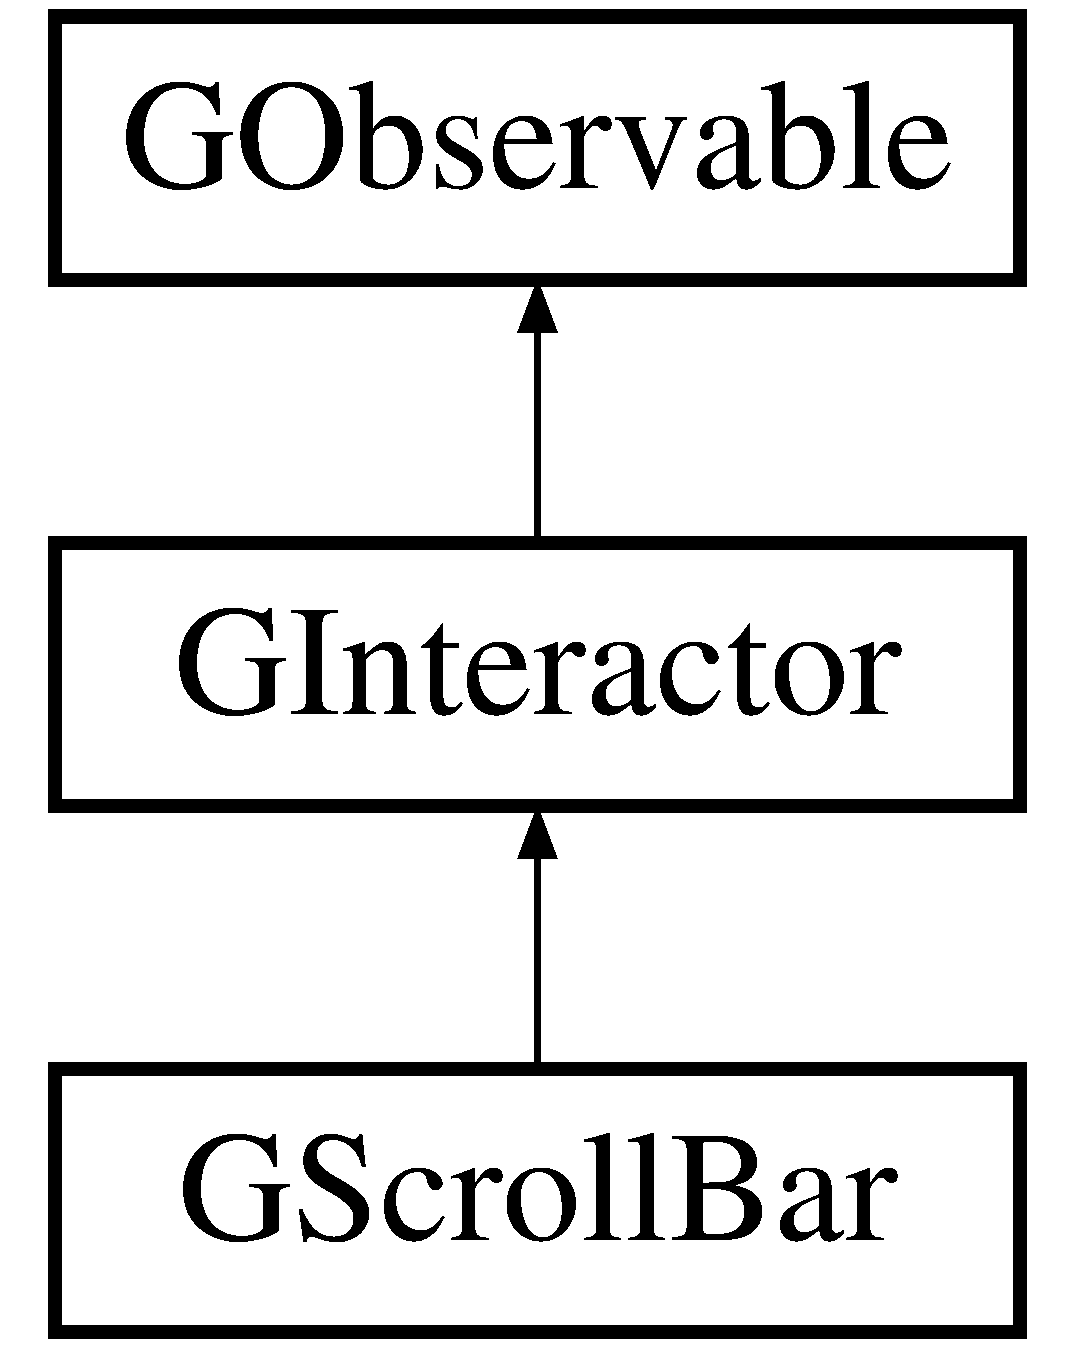
\includegraphics[height=3.000000cm]{classGScrollBar}
\end{center}
\end{figure}
\subsection*{Public Types}
\begin{DoxyCompactItemize}
\item 
enum \mbox{\hyperlink{classGScrollBar_a871118a09520247c78a71ecd7b0abd58}{Orientation}} \{ \mbox{\hyperlink{classGScrollBar_a871118a09520247c78a71ecd7b0abd58a4dd51ad73508d6fc83a502966779e48e}{H\+O\+R\+I\+Z\+O\+N\+T\+AL}} = 0, 
\mbox{\hyperlink{classGScrollBar_a871118a09520247c78a71ecd7b0abd58a1a88641fcd39f2ed3e58a18526e97138}{V\+E\+R\+T\+I\+C\+AL}} = 1
 \}
\begin{DoxyCompactList}\small\item\em The two valid orientations of scrollbars. \end{DoxyCompactList}\item 
enum \mbox{\hyperlink{classGInteractor_a8e0d441725a81d2bbdebbea09078260e}{Text\+Position}} \{ \mbox{\hyperlink{classGInteractor_a8e0d441725a81d2bbdebbea09078260ea4cd6f2e7d5a08d6f4dc052df2358f774}{T\+E\+X\+T\+\_\+\+B\+E\+S\+I\+D\+E\+\_\+\+I\+C\+ON}}, 
\mbox{\hyperlink{classGInteractor_a8e0d441725a81d2bbdebbea09078260eaa88490f63d8de68d44c83bdb2ecde3b3}{T\+E\+X\+T\+\_\+\+U\+N\+D\+E\+R\+\_\+\+I\+C\+ON}}, 
\mbox{\hyperlink{classGInteractor_a8e0d441725a81d2bbdebbea09078260ea39a6f388a30ac4fefb6eb13e846bc9f2}{T\+E\+X\+T\+\_\+\+O\+N\+LY}}
 \}
\begin{DoxyCompactList}\small\item\em The places where an interactor can place its text relative to its icon. \end{DoxyCompactList}\end{DoxyCompactItemize}
\subsection*{Public Member Functions}
\begin{DoxyCompactItemize}
\item 
\mbox{\hyperlink{classGScrollBar_aed316f3139eb0a6e80da4d1dcf171a43}{G\+Scroll\+Bar}} (\mbox{\hyperlink{classGScrollBar_a871118a09520247c78a71ecd7b0abd58}{Orientation}} orientation=\mbox{\hyperlink{classGScrollBar_a871118a09520247c78a71ecd7b0abd58a1a88641fcd39f2ed3e58a18526e97138}{V\+E\+R\+T\+I\+C\+AL}}, int value=0, int extent=10, int min=0, int max=100, Q\+Widget $\ast$parent=nullptr)
\begin{DoxyCompactList}\small\item\em Creates a new scroll bar with the given orientation and value range. \end{DoxyCompactList}\item 
virtual \mbox{\hyperlink{classGScrollBar_a1c63e9330aedd48899dbc75fdb988c79}{$\sim$\+G\+Scroll\+Bar}} ()
\begin{DoxyCompactList}\small\item\em Frees memory allocated internally by the scroll bar. \end{DoxyCompactList}\item 
virtual void \mbox{\hyperlink{classGInteractor_a02f20ea6edfa0671f31c4c648a253833}{add\+Action\+Listener}} () Q\+\_\+\+D\+E\+C\+L\+\_\+\+D\+E\+P\+R\+E\+C\+A\+T\+ED
\begin{DoxyCompactList}\small\item\em Adds an event listener to be notified when this interactor is clicked or generally interacted with. \end{DoxyCompactList}\item 
virtual bool \mbox{\hyperlink{classGInteractor_ac05ba5b92e2e5146d416fe7f842a0969}{events\+Enabled}} () const Q\+\_\+\+D\+E\+C\+L\+\_\+\+O\+V\+E\+R\+R\+I\+DE
\begin{DoxyCompactList}\small\item\em Returns true if this interactor is currently accepting events. \end{DoxyCompactList}\item 
virtual std\+::string \mbox{\hyperlink{classGInteractor_a69f8d23ed8f207fbecad99960776e942}{get\+Accelerator}} () const
\begin{DoxyCompactList}\small\item\em Returns a string representing a hotkey for this interactor, or an empty string if no accelerator has been set. \end{DoxyCompactList}\item 
virtual std\+::string \mbox{\hyperlink{classGInteractor_a94eb4276000c4fdfb508ce9e6317a82a}{get\+Action\+Command}} () const
\begin{DoxyCompactList}\small\item\em Returns an action command for this interactor, which is a semi-\/unique string you can use to identify it when events occur. \end{DoxyCompactList}\item 
virtual std\+::string \mbox{\hyperlink{classGInteractor_a808e22cc1fdfbecf71ed8c64ef4600e0}{get\+Background}} () const
\begin{DoxyCompactList}\small\item\em Returns the background color of the interactor as a string. \end{DoxyCompactList}\item 
virtual int \mbox{\hyperlink{classGInteractor_a9e827257a55cb8cf4d9de2ec6bcfd7a0}{get\+Background\+Int}} () const
\begin{DoxyCompactList}\small\item\em Returns the background color of the interactor as an R\+GB integer. \end{DoxyCompactList}\item 
virtual \mbox{\hyperlink{classGRectangle}{G\+Rectangle}} \mbox{\hyperlink{classGInteractor_a29e6ac35a0b48f491a4c88194cc5da3b}{get\+Bounds}} () const
\begin{DoxyCompactList}\small\item\em Returns a rectangle representing the x/y position and size of this interactor. \end{DoxyCompactList}\item 
virtual std\+::string \mbox{\hyperlink{classGInteractor_aa061dfa488c31e18549d64363c1d0e34}{get\+Color}} () const
\begin{DoxyCompactList}\small\item\em Returns the foreground/text color of the interactor as a string. \end{DoxyCompactList}\item 
virtual int \mbox{\hyperlink{classGInteractor_a9635c7af766cdc3417f346683fa0e6c1}{get\+Color\+Int}} () const
\begin{DoxyCompactList}\small\item\em Returns the foreground/text color of the interactor as an R\+GB integer. \end{DoxyCompactList}\item 
virtual \mbox{\hyperlink{classGContainer}{G\+Container}} $\ast$ \mbox{\hyperlink{classGInteractor_a7a6e317c29d61030929b4cd2d1c00fe7}{get\+Container}} () const
\begin{DoxyCompactList}\small\item\em Returns a pointer to the onscreen container holding this interactor. \end{DoxyCompactList}\item 
virtual int \mbox{\hyperlink{classGScrollBar_af8d1d8c0338fae10ee8673e8430f6be8}{get\+Extent}} () const
\begin{DoxyCompactList}\small\item\em Returns the scroll bar\textquotesingle{}s extent, meaning the amount of its range that is currently in view. \end{DoxyCompactList}\item 
virtual std\+::string \mbox{\hyperlink{classGInteractor_a894a5502900794eeb27d084c21f1d77d}{get\+Font}} () const
\begin{DoxyCompactList}\small\item\em Returns the font of this interactor\textquotesingle{}s text as a font string such as \char`\"{}\+Helvetica-\/12-\/\+Bold\char`\"{}. \end{DoxyCompactList}\item 
virtual std\+::string \mbox{\hyperlink{classGInteractor_a4fa2d8b0192a3a5b4af4bbfe71194d03}{get\+Foreground}} () const
\begin{DoxyCompactList}\small\item\em Returns the foreground/text color of the interactor as a string. \end{DoxyCompactList}\item 
virtual int \mbox{\hyperlink{classGInteractor_ac3b12ab385a6ef9ae90fc879860ba726}{get\+Foreground\+Int}} () const
\begin{DoxyCompactList}\small\item\em Returns the foreground/text color of the interactor as an R\+GB integer. \end{DoxyCompactList}\item 
virtual double \mbox{\hyperlink{classGInteractor_a1e7e353362434072875264cf95629f99}{get\+Height}} () const
\begin{DoxyCompactList}\small\item\em Returns the current onscreen height of this interactor in pixels. \end{DoxyCompactList}\item 
virtual std\+::string \mbox{\hyperlink{classGInteractor_aaed62a73004939a64da6f0eb9eb64d73}{get\+Icon}} () const
\begin{DoxyCompactList}\small\item\em Returns the file name of the icon associated with this interactor, or an empty string if no icon has been set. \end{DoxyCompactList}\item 
virtual int \mbox{\hyperlink{classGInteractor_a9c9659a6c6ba66b4107ba59c95a24241}{get\+ID}} () const
\begin{DoxyCompactList}\small\item\em Returns a globally unique identifier for this interactor, which is set when the interactor is constructed. \end{DoxyCompactList}\item 
virtual \+\_\+\+Internal\+\_\+\+Q\+Widget $\ast$ \mbox{\hyperlink{classGScrollBar_a208ce13c1da40bf0ddb509daf99d6588}{get\+Internal\+Widget}} () const Q\+\_\+\+D\+E\+C\+L\+\_\+\+O\+V\+E\+R\+R\+I\+DE
\begin{DoxyCompactList}\small\item\em Returns a direct pointer to the internal Qt widget being wrapped by this interactor. \end{DoxyCompactList}\item 
virtual \mbox{\hyperlink{classGPoint}{G\+Point}} \mbox{\hyperlink{classGInteractor_a4f83802015511edeb63b892830812c11}{get\+Location}} () const
\begin{DoxyCompactList}\small\item\em Returns an (x, y) point representing the onscreen location of the top-\/left corner of this interactor within its containing window. \end{DoxyCompactList}\item 
virtual int \mbox{\hyperlink{classGScrollBar_acc49776af85220307b8955d752d9ffcb}{get\+Max}} () const
\begin{DoxyCompactList}\small\item\em Returns the maximum allowed value of the scroll bar. \end{DoxyCompactList}\item 
virtual int \mbox{\hyperlink{classGScrollBar_ad06537e69f71666d30bec18dc042a6e4}{get\+Min}} () const
\begin{DoxyCompactList}\small\item\em Returns the minimum allowed value of the scroll bar. \end{DoxyCompactList}\item 
virtual double \mbox{\hyperlink{classGInteractor_aed4b0075fcc434499c3cb3e46896bda3}{get\+Minimum\+Height}} () const
\begin{DoxyCompactList}\small\item\em Returns the minimum height in pixels that this interactor will permit itself to be resized to. \end{DoxyCompactList}\item 
virtual \mbox{\hyperlink{classGDimension}{G\+Dimension}} \mbox{\hyperlink{classGInteractor_a66b5af0b32493b4d597ca0a3df2049ea}{get\+Minimum\+Size}} () const
\begin{DoxyCompactList}\small\item\em Returns a \mbox{\hyperlink{classGDimension}{G\+Dimension}} structure representing the minimum size in pixels that this interactor will permit itself to be resized to. \end{DoxyCompactList}\item 
virtual double \mbox{\hyperlink{classGInteractor_a59e668114fe3d49d2a0f28deb258f7c8}{get\+Minimum\+Width}} () const
\begin{DoxyCompactList}\small\item\em Returns the minimum width in pixels that this interactor will permit itself to be resized to. \end{DoxyCompactList}\item 
virtual std\+::string \mbox{\hyperlink{classGInteractor_a8a60438a5b55d0b2ceb35c8674b9d8c5}{get\+Name}} () const
\begin{DoxyCompactList}\small\item\em Returns a string representing a unique name for this interactor. \end{DoxyCompactList}\item 
virtual \mbox{\hyperlink{classGScrollBar_a871118a09520247c78a71ecd7b0abd58}{Orientation}} \mbox{\hyperlink{classGScrollBar_a816fab656ead9b4f927bff46ae5a0e4d}{get\+Orientation}} () const
\begin{DoxyCompactList}\small\item\em Returns the orientation of the scroll bar, either H\+O\+R\+I\+Z\+O\+N\+T\+AL or V\+E\+R\+T\+I\+C\+AL. \end{DoxyCompactList}\item 
virtual double \mbox{\hyperlink{classGInteractor_a747de0961653847bdc6615dbf756d715}{get\+Preferred\+Height}} () const
\begin{DoxyCompactList}\small\item\em Returns the height in pixels that this interactor would prefer to be, which would exactly fit its contents with no stretching or scrollbars. \end{DoxyCompactList}\item 
virtual \mbox{\hyperlink{classGDimension}{G\+Dimension}} \mbox{\hyperlink{classGInteractor_a4aabbee761d8e9116275401131b7ccd1}{get\+Preferred\+Size}} () const
\begin{DoxyCompactList}\small\item\em Returns a \mbox{\hyperlink{classGDimension}{G\+Dimension}} structure storing the width and height in pixels that this interactor would prefer to be, which would exactly fit its contents with no stretching or scrollbars. \end{DoxyCompactList}\item 
virtual double \mbox{\hyperlink{classGInteractor_a82bca31d37700fb0e35d2743352efd5e}{get\+Preferred\+Width}} () const
\begin{DoxyCompactList}\small\item\em Returns the height in pixels that this interactor would prefer to be, which would exactly fit its contents with no stretching or scrollbars. \end{DoxyCompactList}\item 
virtual \mbox{\hyperlink{classGDimension}{G\+Dimension}} \mbox{\hyperlink{classGInteractor_a7b4eec96a2bdc6420695d5796a78eea9}{get\+Size}} () const
\begin{DoxyCompactList}\small\item\em Returns a \mbox{\hyperlink{classGDimension}{G\+Dimension}} structure storing the current onscreen width and height of this interactor in pixels. \end{DoxyCompactList}\item 
virtual std\+::string \mbox{\hyperlink{classGScrollBar_a9896d58fcfebbf1025aeeb5b8b9ede80}{get\+Type}} () const Q\+\_\+\+D\+E\+C\+L\+\_\+\+O\+V\+E\+R\+R\+I\+DE
\begin{DoxyCompactList}\small\item\em Returns a string representing the class name of this interactor, such as \char`\"{}\+G\+Button\char`\"{} or \char`\"{}\+G\+Check\+Box\char`\"{}. \end{DoxyCompactList}\item 
virtual int \mbox{\hyperlink{classGScrollBar_acdb0b383a96801f3200302b6f4a7da64}{get\+Value}} () const
\begin{DoxyCompactList}\small\item\em Returns the current value of the scroll bar. \end{DoxyCompactList}\item 
virtual Q\+Widget $\ast$ \mbox{\hyperlink{classGScrollBar_a326ee51b5561f807df7b29a1c101f7fd}{get\+Widget}} () const Q\+\_\+\+D\+E\+C\+L\+\_\+\+O\+V\+E\+R\+R\+I\+DE
\begin{DoxyCompactList}\small\item\em Returns a direct pointer to the internal Qt widget being wrapped by this interactor. \end{DoxyCompactList}\item 
virtual double \mbox{\hyperlink{classGInteractor_a0ed2965abd4f5701d2cadf71239faf19}{get\+Width}} () const
\begin{DoxyCompactList}\small\item\em Returns the current onscreen width of this interactor in pixels. \end{DoxyCompactList}\item 
virtual double \mbox{\hyperlink{classGInteractor_a344385751bee0720059403940d57a13e}{getX}} () const
\begin{DoxyCompactList}\small\item\em Returns the x-\/coordinate of the top-\/left pixel of this interactor within its onscreen window. \end{DoxyCompactList}\item 
virtual double \mbox{\hyperlink{classGInteractor_aafa51c7f8f38a09febbb9ce7853f77b4}{getY}} () const
\begin{DoxyCompactList}\small\item\em Returns the y-\/coordinate of the top-\/left pixel of this interactor within its onscreen window. \end{DoxyCompactList}\item 
virtual bool \mbox{\hyperlink{classGInteractor_afc480f652b8c5f1fb255e2269ce68879}{in\+Bounds}} (double x, double y) const
\begin{DoxyCompactList}\small\item\em Returns true if the given x/y pixel is within the bounds of this interactor. \end{DoxyCompactList}\item 
virtual bool \mbox{\hyperlink{classGInteractor_ae6d7982c1c627b677a5e776ca86118ed}{in\+Bounds}} (int x, int y) const
\begin{DoxyCompactList}\small\item\em Returns true if the given x/y pixel is within the bounds of this interactor. \end{DoxyCompactList}\item 
virtual bool \mbox{\hyperlink{classGInteractor_aacb819fb241851fd9fc045271baa4034}{is\+Enabled}} () const
\begin{DoxyCompactList}\small\item\em Returns true if this interactor is currently enabled. \end{DoxyCompactList}\item 
virtual bool \mbox{\hyperlink{classGInteractor_a9d8a6cfb13917785c143e74d40e4e2be}{is\+Visible}} () const
\begin{DoxyCompactList}\small\item\em Returns true if the interactor is visible on the screen. \end{DoxyCompactList}\item 
virtual void \mbox{\hyperlink{classGScrollBar_ab7fe7a876367b87cf7202f947f1d05e4}{remove\+Action\+Listener}} ()
\begin{DoxyCompactList}\small\item\em Removes the action listener from this scroll bar so that it will no longer call it when events occur. \end{DoxyCompactList}\item 
virtual void \mbox{\hyperlink{classGInteractor_a519fb2ac767f8b2febbb50b898b8c8cb}{request\+Focus}} ()
\begin{DoxyCompactList}\small\item\em Transfers keyboard focus to this interactor. \end{DoxyCompactList}\item 
virtual void \mbox{\hyperlink{classGInteractor_ad15f102f62e2960576012f1aa0ba4b2e}{set\+Accelerator}} (const std\+::string \&accelerator)
\begin{DoxyCompactList}\small\item\em Sets an accelerator hotkey for this interactor, such as \char`\"{}\+Ctrl-\/\+S\char`\"{}. \end{DoxyCompactList}\item 
virtual void \mbox{\hyperlink{classGInteractor_a4b5843fe3030e038a1ba54cc03389bcf}{set\+Action\+Command}} (const std\+::string \&action\+Command)
\begin{DoxyCompactList}\small\item\em Sets the action command for this interactor. \end{DoxyCompactList}\item 
virtual void \mbox{\hyperlink{classGScrollBar_adcfb4742430c88714fcf57e57ab8ea9c}{set\+Action\+Listener}} (G\+Event\+Listener func)
\begin{DoxyCompactList}\small\item\em Sets an action listener on this scroll bar so that it will be called when the user scrolls. \end{DoxyCompactList}\item 
virtual void \mbox{\hyperlink{classGScrollBar_aebd20a89c7a8a43a6fce999cf4f9fcf2}{set\+Action\+Listener}} (G\+Event\+Listener\+Void func)
\begin{DoxyCompactList}\small\item\em Sets an action listener on this scroll bar so that it will be called when the user scrolls. \end{DoxyCompactList}\item 
virtual void \mbox{\hyperlink{classGInteractor_acba7e546c2025c0a15ca4b4cc92043db}{set\+Background}} (int rgb)
\begin{DoxyCompactList}\small\item\em Sets the background color of the interactor to the color represented by the given R\+GB integer. \end{DoxyCompactList}\item 
virtual void \mbox{\hyperlink{classGInteractor_ab4677ab2474e68b07aa56605af92a84a}{set\+Background}} (const std\+::string \&color)
\begin{DoxyCompactList}\small\item\em Sets the background color of the interactor to the color represented by the given string. \end{DoxyCompactList}\item 
virtual void \mbox{\hyperlink{classGInteractor_a2aae8197624b72265ab83b4f1bc73f2f}{set\+Bounds}} (double x, double y, double width, double height)
\begin{DoxyCompactList}\small\item\em Sets the size and location of the widget. \end{DoxyCompactList}\item 
virtual void \mbox{\hyperlink{classGInteractor_acada386653f008cacc7cce86426bef7c}{set\+Bounds}} (const \mbox{\hyperlink{classGRectangle}{G\+Rectangle}} \&size)
\begin{DoxyCompactList}\small\item\em Sets the size and location of the widget. \end{DoxyCompactList}\item 
virtual void \mbox{\hyperlink{classGInteractor_ab1f5cc0f5cc6bbbd716a526c61f1081d}{set\+Color}} (int rgb)
\begin{DoxyCompactList}\small\item\em Sets the foreground/text color of the interactor to the color represented by the given R\+GB integer. \end{DoxyCompactList}\item 
virtual void \mbox{\hyperlink{classGInteractor_a61374df6c11b52cfbb0815decdbaebc6}{set\+Color}} (const std\+::string \&color)
\begin{DoxyCompactList}\small\item\em Sets the foreground/text color of the interactor to the color represented by the given string. \end{DoxyCompactList}\item 
virtual void \mbox{\hyperlink{classGInteractor_ab831367dd84bbd579e02e55bacb21343}{set\+Enabled}} (bool value)
\begin{DoxyCompactList}\small\item\em Sets whether this interactor is currently enabled. \end{DoxyCompactList}\item 
virtual void \mbox{\hyperlink{classGObservable_afaa30b2a9e0f378fd1c70d2f1d0b8216}{set\+Events\+Enabled}} (bool \mbox{\hyperlink{classGInteractor_ac05ba5b92e2e5146d416fe7f842a0969}{events\+Enabled}})
\begin{DoxyCompactList}\small\item\em Sets whether the object is currently allowing itself to fire events. \end{DoxyCompactList}\item 
virtual void \mbox{\hyperlink{classGScrollBar_a2b06f746a9b7b56cbb85154bbe3288c6}{set\+Extent}} (int extent)
\begin{DoxyCompactList}\small\item\em Sets the scroll bar\textquotesingle{}s extent, meaning the amount of its range that is currently in view. \end{DoxyCompactList}\item 
virtual void \mbox{\hyperlink{classGInteractor_a2592348886ffea646c6534bf88f7c49d}{set\+Font}} (const Q\+Font \&font)
\begin{DoxyCompactList}\small\item\em Sets the font used by this widget to the given Qt font. \end{DoxyCompactList}\item 
virtual void \mbox{\hyperlink{classGInteractor_a8e096e8818d838aceae1d46d58fb3a7b}{set\+Font}} (const std\+::string \&font)
\begin{DoxyCompactList}\small\item\em Sets the font used by this widget to the font represented by the given font string, such as \char`\"{}\+Helvetica-\/16-\/\+Bold\char`\"{}. \end{DoxyCompactList}\item 
virtual void \mbox{\hyperlink{classGInteractor_a9eb856b5ff83a19df3831a31f15f4563}{set\+Foreground}} (int rgb)
\begin{DoxyCompactList}\small\item\em Sets the foreground/text color of the interactor to the color represented by the given R\+GB integer. \end{DoxyCompactList}\item 
virtual void \mbox{\hyperlink{classGInteractor_af59209aeadea6dfc6d97a2d8531f50e1}{set\+Foreground}} (const std\+::string \&color)
\begin{DoxyCompactList}\small\item\em Sets the foreground/text color of the interactor to the color represented by the given string. \end{DoxyCompactList}\item 
virtual void \mbox{\hyperlink{classGInteractor_a9e280bfc4544dfaf8e4376c4e1a74357}{set\+Height}} (double height)
\begin{DoxyCompactList}\small\item\em Sets the onscreen height of the interactor in pixels. \end{DoxyCompactList}\item 
virtual void \mbox{\hyperlink{classGInteractor_a762e139aa311461c3984d3ad28293f64}{set\+Icon}} (const std\+::string \&filename, bool retain\+Icon\+Size=true)
\begin{DoxyCompactList}\small\item\em Sets the file name of the icon associated with this interactor, or an empty string if no icon has been set. \end{DoxyCompactList}\item 
virtual void \mbox{\hyperlink{classGInteractor_a04594e8ba9b98513a64f1da00dcae18c}{set\+Location}} (double x, double y)
\begin{DoxyCompactList}\small\item\em Sets the onscreen x/y-\/coordinate of the top-\/left corner of the interactor relative to its window. \end{DoxyCompactList}\item 
virtual void \mbox{\hyperlink{classGScrollBar_ab263d79bf430d73a617641f317dcfb98}{set\+Max}} (int max)
\begin{DoxyCompactList}\small\item\em Sets the maximum allowed value of the scroll bar. \end{DoxyCompactList}\item 
virtual void \mbox{\hyperlink{classGScrollBar_a6dc44e5adc595b71f90efc65b0b5ea1d}{set\+Min}} (int min)
\begin{DoxyCompactList}\small\item\em Sets the minimum allowed value of the scroll bar. \end{DoxyCompactList}\item 
virtual void \mbox{\hyperlink{classGInteractor_a0cf428e207b7f22cc08138a90b1b87b2}{set\+Minimum\+Size}} (double width, double height)
\begin{DoxyCompactList}\small\item\em Sets the minimum size in pixels that this interactor will permit itself to be resized to. \end{DoxyCompactList}\item 
virtual void \mbox{\hyperlink{classGInteractor_a3b1046117ac6cb7abe467e00ba8a81f4}{set\+Minimum\+Size}} (const \mbox{\hyperlink{classGDimension}{G\+Dimension}} \&size)
\begin{DoxyCompactList}\small\item\em Sets the minimum size in pixels that this interactor will permit itself to be resized to. \end{DoxyCompactList}\item 
virtual void \mbox{\hyperlink{classGInteractor_a9d3a2685df23b5e7cbf59c19c4a1f9b5}{set\+Name}} (const std\+::string \&name)
\begin{DoxyCompactList}\small\item\em Sets a string representing a unique name for this interactor. \end{DoxyCompactList}\item 
virtual void \mbox{\hyperlink{classGInteractor_a1ab987704fce32098706c6f00fb08218}{set\+Preferred\+Height}} (double height)
\begin{DoxyCompactList}\small\item\em Sets the height in pixels that this interactor would prefer to be. \end{DoxyCompactList}\item 
virtual void \mbox{\hyperlink{classGInteractor_a042c5ae19430d765ef552371cae3632c}{set\+Preferred\+Size}} (double width, double height)
\begin{DoxyCompactList}\small\item\em Sets the width and height in pixels that this interactor would prefer to be. \end{DoxyCompactList}\item 
virtual void \mbox{\hyperlink{classGInteractor_aa22d9be4bc0e078bb0ea69b0fc9d7c75}{set\+Preferred\+Size}} (const \mbox{\hyperlink{classGDimension}{G\+Dimension}} \&size)
\begin{DoxyCompactList}\small\item\em Sets the size in pixels that this interactor would prefer to be. \end{DoxyCompactList}\item 
virtual void \mbox{\hyperlink{classGInteractor_a3db429ab2fa52efd187eec0ed8cdd9f2}{set\+Preferred\+Width}} (double width)
\begin{DoxyCompactList}\small\item\em Sets the width in pixels that this interactor would prefer to be. \end{DoxyCompactList}\item 
virtual void \mbox{\hyperlink{classGInteractor_aca25d49481f9bf5fc8f7df4c086c4ce7}{set\+Size}} (double width, double height)
\begin{DoxyCompactList}\small\item\em Sets the onscreen width and height of the interactor in pixels. \end{DoxyCompactList}\item 
virtual void \mbox{\hyperlink{classGInteractor_ae2b628228f192c2702c4ce941b2af68f}{set\+Size}} (const \mbox{\hyperlink{classGDimension}{G\+Dimension}} \&size)
\begin{DoxyCompactList}\small\item\em Sets the onscreen width and height of the interactor in pixels. \end{DoxyCompactList}\item 
virtual void \mbox{\hyperlink{classGScrollBar_a83549f22abf65099f4c661a4601ade2b}{set\+State}} (int value, int extent, int min, int max)
\begin{DoxyCompactList}\small\item\em Sets all of the relevant state of the scroll bar. \end{DoxyCompactList}\item 
virtual void \mbox{\hyperlink{classGInteractor_a039e0e49beaecc275efce02d416acea8}{set\+Tooltip}} (const std\+::string \&tooltip\+Text)
\begin{DoxyCompactList}\small\item\em Sets a \char`\"{}tooltip\char`\"{} that will appear if the user hovers their mouse over the interactor. \end{DoxyCompactList}\item 
virtual void \mbox{\hyperlink{classGScrollBar_a23d79e21b8ed72e19278ca31d47b8c87}{set\+Value}} (int value)
\begin{DoxyCompactList}\small\item\em Sets the current value of the scroll bar. \end{DoxyCompactList}\item 
virtual void \mbox{\hyperlink{classGInteractor_a18e44e30b31525a243960ca3928125aa}{set\+Visible}} (bool visible)
\begin{DoxyCompactList}\small\item\em Returns true if the interactor is visible on the screen. \end{DoxyCompactList}\item 
virtual void \mbox{\hyperlink{classGInteractor_aa3f3fba4cb131baa8696ba01e3bceca1}{set\+Width}} (double width)
\begin{DoxyCompactList}\small\item\em Sets the onscreen width of the interactor in pixels. \end{DoxyCompactList}\item 
virtual void \mbox{\hyperlink{classGInteractor_a9c18fcc579333bf9653d13ad2b372e39}{setX}} (double x)
\begin{DoxyCompactList}\small\item\em Sets the onscreen x-\/coordinate of the top-\/left corner of the interactor relative to its window. \end{DoxyCompactList}\item 
virtual void \mbox{\hyperlink{classGInteractor_a7d57e2a5c35d27feb58fd498a3cf82b9}{setY}} (double y)
\begin{DoxyCompactList}\small\item\em Sets the onscreen y-\/coordinate of the top-\/left corner of the interactor relative to its window. \end{DoxyCompactList}\item 
virtual std\+::string \mbox{\hyperlink{classGObservable_a1fe5121d6528fdea3f243321b3fa3a49}{to\+String}} () const
\begin{DoxyCompactList}\small\item\em Returns a string representation of this observable object\textquotesingle{}s state. \end{DoxyCompactList}\end{DoxyCompactItemize}
\subsection*{Protected Member Functions}
\begin{DoxyCompactItemize}
\item 
virtual void \mbox{\hyperlink{classGObservable_a80cfa040459ff53594adbd6a51ec8f43}{clear\+Event\+Listeners}} ()
\begin{DoxyCompactList}\small\item\em Removes all event listeners from this object. \end{DoxyCompactList}\item 
virtual void \mbox{\hyperlink{classGObservable_a284f31528c0520f8e545c03ac9eeac74}{ensure\+Thread\+Safety}} (const std\+::string \&member\+Name=\char`\"{}\char`\"{})
\begin{DoxyCompactList}\small\item\em Ensures that we are currently in the Qt G\+UI thread. \end{DoxyCompactList}\item 
virtual void \mbox{\hyperlink{classGObservable_a63e5e5a6227c59c928493b11aceb0f67}{fire\+Event}} (\mbox{\hyperlink{classGEvent}{G\+Event}} \&event)
\begin{DoxyCompactList}\small\item\em Sends out the given event to any attached listeners. \end{DoxyCompactList}\item 
virtual void \mbox{\hyperlink{classGObservable_ab3983ea07337b52020a29cc00c653d8d}{fire\+G\+Event}} (Q\+Event $\ast$event, Event\+Type event\+Type, const std\+::string \&event\+Name)
\begin{DoxyCompactList}\small\item\em Creates an event of the given type, then sends it out to any attached listeners. \end{DoxyCompactList}\item 
virtual void \mbox{\hyperlink{classGObservable_a01fdf1b0e0dbd49e189fe4514e010411}{fire\+G\+Event}} (Q\+Close\+Event $\ast$event, Event\+Type event\+Type, const std\+::string \&event\+Name)
\begin{DoxyCompactList}\small\item\em Creates an event of the given type, then sends it out to any attached listeners. \end{DoxyCompactList}\item 
virtual void \mbox{\hyperlink{classGObservable_abb0b2f66ba39211cb5d7615e9d1c04e2}{fire\+G\+Event}} (Q\+Key\+Event $\ast$event, Event\+Type event\+Type, const std\+::string \&event\+Name)
\begin{DoxyCompactList}\small\item\em Creates an event of the given type, then sends it out to any attached listeners. \end{DoxyCompactList}\item 
virtual void \mbox{\hyperlink{classGObservable_a119318675d2165bdf7dd853aaf881d4b}{fire\+G\+Event}} (Q\+Mouse\+Event $\ast$event, Event\+Type event\+Type, const std\+::string \&event\+Name, const std\+::string \&action\+Command=\char`\"{}\char`\"{})
\begin{DoxyCompactList}\small\item\em Creates an event of the given type, then sends it out to any attached listeners. \end{DoxyCompactList}\item 
virtual void \mbox{\hyperlink{classGObservable_a63fd9034e1e1633c1c38eb342bfd34e9}{fire\+G\+Event}} (Q\+Resize\+Event $\ast$event, Event\+Type event\+Type, const std\+::string \&event\+Name)
\begin{DoxyCompactList}\small\item\em Creates an event of the given type, then sends it out to any attached listeners. \end{DoxyCompactList}\item 
virtual void \mbox{\hyperlink{classGObservable_a741345310d9b7c5170a6cbc410c44ac4}{fire\+G\+Event}} (Q\+Timer\+Event $\ast$event, Event\+Type event\+Type, const std\+::string \&event\+Name)
\begin{DoxyCompactList}\small\item\em Creates an event of the given type, then sends it out to any attached listeners. \end{DoxyCompactList}\item 
virtual void \mbox{\hyperlink{classGObservable_a93bf338968a0338761b8e4dc62f582e9}{fire\+G\+Event}} (Q\+Wheel\+Event $\ast$event, Event\+Type event\+Type, const std\+::string \&event\+Name)
\begin{DoxyCompactList}\small\item\em Creates an event of the given type, then sends it out to any attached listeners. \end{DoxyCompactList}\item 
virtual void \mbox{\hyperlink{classGObservable_a2a70a7d7435ff0c3b80bb4d70da19e0d}{fire\+G\+Event}} (Q\+Window\+State\+Change\+Event $\ast$event, Event\+Type event\+Type, const std\+::string \&event\+Name)
\begin{DoxyCompactList}\small\item\em Creates an event of the given type, then sends it out to any attached listeners. \end{DoxyCompactList}\item 
virtual bool \mbox{\hyperlink{classGObservable_a9f6faaa25942923bafa1c44020c49fa9}{has\+Event\+Listener}} (const std\+::string \&event\+Name) const
\begin{DoxyCompactList}\small\item\em Returns true if the observable object has a listener for the given type of event. \end{DoxyCompactList}\item 
virtual bool \mbox{\hyperlink{classGObservable_aeec1adc19aa0f33de62390686ee1382c}{is\+Accepting\+Event}} (int event\+Mask) const
\begin{DoxyCompactList}\small\item\em Returns true if the observable object has a listener for the given type of event. \end{DoxyCompactList}\item 
virtual bool \mbox{\hyperlink{classGObservable_aa31c73145a29dcb92848a92e0cfaea41}{is\+Accepting\+Event}} (const \mbox{\hyperlink{classGEvent}{G\+Event}} \&event) const
\begin{DoxyCompactList}\small\item\em Returns true if the observable object has a listener for the given type of event. \end{DoxyCompactList}\item 
virtual bool \mbox{\hyperlink{classGObservable_a3b1c689267eda44e65a2213e7de38b23}{is\+Accepting\+Event}} (const std\+::string \&event\+Type) const
\begin{DoxyCompactList}\small\item\em Returns true if the observable object has a listener for the given type of event. \end{DoxyCompactList}\item 
virtual void \mbox{\hyperlink{classGObservable_acbcf1ed3a851ad8a3c17ef38d86b481d}{remove\+Event\+Listener}} (const std\+::string \&event\+Name)
\begin{DoxyCompactList}\small\item\em Removes any event listener from this observable object that would respond to the given type of event, such as \char`\"{}click\char`\"{} or \char`\"{}keydown\char`\"{}. \end{DoxyCompactList}\item 
virtual void \mbox{\hyperlink{classGObservable_af51cc35c29a1bd1908609d432decdbb6}{remove\+Event\+Listeners}} (std\+::initializer\+\_\+list$<$ std\+::string $>$ event\+Names)
\begin{DoxyCompactList}\small\item\em Removes any event listener from this observable object that would respond to the given types of events, such as \char`\"{}click\char`\"{} or \char`\"{}keydown\char`\"{}. \end{DoxyCompactList}\item 
virtual void \mbox{\hyperlink{classGObservable_ad2f6d34961c50f6c1e0659990b79f741}{set\+Event\+Listener}} (const std\+::string \&event\+Name, G\+Event\+Listener func)
\begin{DoxyCompactList}\small\item\em Adds an event listener from this observable object to respond to the given type of event, such as \char`\"{}click\char`\"{} or \char`\"{}keydown\char`\"{}. \end{DoxyCompactList}\item 
virtual void \mbox{\hyperlink{classGObservable_abac4cb9f9e626e010e87f5d91573c8a5}{set\+Event\+Listener}} (const std\+::string \&event\+Name, G\+Event\+Listener\+Void func)
\begin{DoxyCompactList}\small\item\em Adds an event listener from this observable object to respond to the given type of event, such as \char`\"{}click\char`\"{} or \char`\"{}keydown\char`\"{}. \end{DoxyCompactList}\item 
virtual void \mbox{\hyperlink{classGObservable_afa388d69c33c718cf035774604065604}{set\+Event\+Listeners}} (std\+::initializer\+\_\+list$<$ std\+::string $>$ event\+Names, G\+Event\+Listener func)
\begin{DoxyCompactList}\small\item\em Adds an event listener from this observable object to respond to the given types of events, such as \char`\"{}click\char`\"{} or \char`\"{}keydown\char`\"{}. \end{DoxyCompactList}\item 
virtual void \mbox{\hyperlink{classGObservable_a7867184bbb686f74fae8a4db927da799}{set\+Event\+Listeners}} (std\+::initializer\+\_\+list$<$ std\+::string $>$ event\+Names, G\+Event\+Listener\+Void func)
\begin{DoxyCompactList}\small\item\em Adds an event listener from this observable object to respond to the given types of events, such as \char`\"{}click\char`\"{} or \char`\"{}keydown\char`\"{}. \end{DoxyCompactList}\end{DoxyCompactItemize}


\subsection{Detailed Description}
A \mbox{\hyperlink{classGScrollBar}{G\+Scroll\+Bar}} represents a horizontal or vertical scroll bar that can be dragged by the user. 

The bar does not inherently cause any other interactor to scroll itself. If you want the bar to cause any effect, you must wait for scroll events and respond to them.

A given scroll bar has a range of values it can represent, with a min and max, along with a current value. The \char`\"{}extent\char`\"{} of a scrollbar represents the amount of the scrollbar in view. 

\subsection{Member Enumeration Documentation}
\mbox{\Hypertarget{classGScrollBar_a871118a09520247c78a71ecd7b0abd58}\label{classGScrollBar_a871118a09520247c78a71ecd7b0abd58}} 
\index{G\+Scroll\+Bar@{G\+Scroll\+Bar}!Orientation@{Orientation}}
\index{Orientation@{Orientation}!G\+Scroll\+Bar@{G\+Scroll\+Bar}}
\subsubsection{\texorpdfstring{Orientation}{Orientation}}
{\footnotesize\ttfamily enum \mbox{\hyperlink{classGScrollBar_a871118a09520247c78a71ecd7b0abd58}{Orientation}}}



The two valid orientations of scrollbars. 

\begin{DoxyEnumFields}{Enumerator}
\raisebox{\heightof{T}}[0pt][0pt]{\index{H\+O\+R\+I\+Z\+O\+N\+T\+AL@{H\+O\+R\+I\+Z\+O\+N\+T\+AL}!G\+Scroll\+Bar@{G\+Scroll\+Bar}}\index{G\+Scroll\+Bar@{G\+Scroll\+Bar}!H\+O\+R\+I\+Z\+O\+N\+T\+AL@{H\+O\+R\+I\+Z\+O\+N\+T\+AL}}}\mbox{\Hypertarget{classGScrollBar_a871118a09520247c78a71ecd7b0abd58a4dd51ad73508d6fc83a502966779e48e}\label{classGScrollBar_a871118a09520247c78a71ecd7b0abd58a4dd51ad73508d6fc83a502966779e48e}} 
H\+O\+R\+I\+Z\+O\+N\+T\+AL&\\
\hline

\raisebox{\heightof{T}}[0pt][0pt]{\index{V\+E\+R\+T\+I\+C\+AL@{V\+E\+R\+T\+I\+C\+AL}!G\+Scroll\+Bar@{G\+Scroll\+Bar}}\index{G\+Scroll\+Bar@{G\+Scroll\+Bar}!V\+E\+R\+T\+I\+C\+AL@{V\+E\+R\+T\+I\+C\+AL}}}\mbox{\Hypertarget{classGScrollBar_a871118a09520247c78a71ecd7b0abd58a1a88641fcd39f2ed3e58a18526e97138}\label{classGScrollBar_a871118a09520247c78a71ecd7b0abd58a1a88641fcd39f2ed3e58a18526e97138}} 
V\+E\+R\+T\+I\+C\+AL&\\
\hline

\end{DoxyEnumFields}
\mbox{\Hypertarget{classGInteractor_a8e0d441725a81d2bbdebbea09078260e}\label{classGInteractor_a8e0d441725a81d2bbdebbea09078260e}} 
\index{G\+Scroll\+Bar@{G\+Scroll\+Bar}!Text\+Position@{Text\+Position}}
\index{Text\+Position@{Text\+Position}!G\+Scroll\+Bar@{G\+Scroll\+Bar}}
\subsubsection{\texorpdfstring{Text\+Position}{TextPosition}}
{\footnotesize\ttfamily enum \mbox{\hyperlink{classGInteractor_a8e0d441725a81d2bbdebbea09078260e}{Text\+Position}}\hspace{0.3cm}{\ttfamily [inherited]}}



The places where an interactor can place its text relative to its icon. 

\begin{DoxyEnumFields}{Enumerator}
\raisebox{\heightof{T}}[0pt][0pt]{\index{T\+E\+X\+T\+\_\+\+B\+E\+S\+I\+D\+E\+\_\+\+I\+C\+ON@{T\+E\+X\+T\+\_\+\+B\+E\+S\+I\+D\+E\+\_\+\+I\+C\+ON}!G\+Scroll\+Bar@{G\+Scroll\+Bar}}\index{G\+Scroll\+Bar@{G\+Scroll\+Bar}!T\+E\+X\+T\+\_\+\+B\+E\+S\+I\+D\+E\+\_\+\+I\+C\+ON@{T\+E\+X\+T\+\_\+\+B\+E\+S\+I\+D\+E\+\_\+\+I\+C\+ON}}}\mbox{\Hypertarget{classGInteractor_a8e0d441725a81d2bbdebbea09078260ea4cd6f2e7d5a08d6f4dc052df2358f774}\label{classGInteractor_a8e0d441725a81d2bbdebbea09078260ea4cd6f2e7d5a08d6f4dc052df2358f774}} 
T\+E\+X\+T\+\_\+\+B\+E\+S\+I\+D\+E\+\_\+\+I\+C\+ON&\\
\hline

\raisebox{\heightof{T}}[0pt][0pt]{\index{T\+E\+X\+T\+\_\+\+U\+N\+D\+E\+R\+\_\+\+I\+C\+ON@{T\+E\+X\+T\+\_\+\+U\+N\+D\+E\+R\+\_\+\+I\+C\+ON}!G\+Scroll\+Bar@{G\+Scroll\+Bar}}\index{G\+Scroll\+Bar@{G\+Scroll\+Bar}!T\+E\+X\+T\+\_\+\+U\+N\+D\+E\+R\+\_\+\+I\+C\+ON@{T\+E\+X\+T\+\_\+\+U\+N\+D\+E\+R\+\_\+\+I\+C\+ON}}}\mbox{\Hypertarget{classGInteractor_a8e0d441725a81d2bbdebbea09078260eaa88490f63d8de68d44c83bdb2ecde3b3}\label{classGInteractor_a8e0d441725a81d2bbdebbea09078260eaa88490f63d8de68d44c83bdb2ecde3b3}} 
T\+E\+X\+T\+\_\+\+U\+N\+D\+E\+R\+\_\+\+I\+C\+ON&\\
\hline

\raisebox{\heightof{T}}[0pt][0pt]{\index{T\+E\+X\+T\+\_\+\+O\+N\+LY@{T\+E\+X\+T\+\_\+\+O\+N\+LY}!G\+Scroll\+Bar@{G\+Scroll\+Bar}}\index{G\+Scroll\+Bar@{G\+Scroll\+Bar}!T\+E\+X\+T\+\_\+\+O\+N\+LY@{T\+E\+X\+T\+\_\+\+O\+N\+LY}}}\mbox{\Hypertarget{classGInteractor_a8e0d441725a81d2bbdebbea09078260ea39a6f388a30ac4fefb6eb13e846bc9f2}\label{classGInteractor_a8e0d441725a81d2bbdebbea09078260ea39a6f388a30ac4fefb6eb13e846bc9f2}} 
T\+E\+X\+T\+\_\+\+O\+N\+LY&\\
\hline

\end{DoxyEnumFields}


\subsection{Constructor \& Destructor Documentation}
\mbox{\Hypertarget{classGScrollBar_aed316f3139eb0a6e80da4d1dcf171a43}\label{classGScrollBar_aed316f3139eb0a6e80da4d1dcf171a43}} 
\index{G\+Scroll\+Bar@{G\+Scroll\+Bar}!G\+Scroll\+Bar@{G\+Scroll\+Bar}}
\index{G\+Scroll\+Bar@{G\+Scroll\+Bar}!G\+Scroll\+Bar@{G\+Scroll\+Bar}}
\subsubsection{\texorpdfstring{G\+Scroll\+Bar()}{GScrollBar()}}
{\footnotesize\ttfamily \mbox{\hyperlink{classGScrollBar}{G\+Scroll\+Bar}} (\begin{DoxyParamCaption}\item[{\mbox{\hyperlink{classGScrollBar_a871118a09520247c78a71ecd7b0abd58}{G\+Scroll\+Bar\+::\+Orientation}}}]{orientation = {\ttfamily \mbox{\hyperlink{classGScrollBar_a871118a09520247c78a71ecd7b0abd58a1a88641fcd39f2ed3e58a18526e97138}{V\+E\+R\+T\+I\+C\+AL}}},  }\item[{int}]{value = {\ttfamily 0},  }\item[{int}]{extent = {\ttfamily 10},  }\item[{int}]{min = {\ttfamily 0},  }\item[{int}]{max = {\ttfamily 100},  }\item[{Q\+Widget $\ast$}]{parent = {\ttfamily nullptr} }\end{DoxyParamCaption})}



Creates a new scroll bar with the given orientation and value range. 


\begin{DoxyExceptions}{Exceptions}
{\em \mbox{\hyperlink{classErrorException}{Error\+Exception}}} & if min $>$ max or value is not between min and max \\
\hline
\end{DoxyExceptions}
\mbox{\Hypertarget{classGScrollBar_a1c63e9330aedd48899dbc75fdb988c79}\label{classGScrollBar_a1c63e9330aedd48899dbc75fdb988c79}} 
\index{G\+Scroll\+Bar@{G\+Scroll\+Bar}!````~G\+Scroll\+Bar@{$\sim$\+G\+Scroll\+Bar}}
\index{````~G\+Scroll\+Bar@{$\sim$\+G\+Scroll\+Bar}!G\+Scroll\+Bar@{G\+Scroll\+Bar}}
\subsubsection{\texorpdfstring{$\sim$\+G\+Scroll\+Bar()}{~GScrollBar()}}
{\footnotesize\ttfamily $\sim$\mbox{\hyperlink{classGScrollBar}{G\+Scroll\+Bar}} (\begin{DoxyParamCaption}{ }\end{DoxyParamCaption})\hspace{0.3cm}{\ttfamily [virtual]}}



Frees memory allocated internally by the scroll bar. 



\subsection{Member Function Documentation}
\mbox{\Hypertarget{classGInteractor_a02f20ea6edfa0671f31c4c648a253833}\label{classGInteractor_a02f20ea6edfa0671f31c4c648a253833}} 
\index{G\+Scroll\+Bar@{G\+Scroll\+Bar}!add\+Action\+Listener@{add\+Action\+Listener}}
\index{add\+Action\+Listener@{add\+Action\+Listener}!G\+Scroll\+Bar@{G\+Scroll\+Bar}}
\subsubsection{\texorpdfstring{add\+Action\+Listener()}{addActionListener()}}
{\footnotesize\ttfamily void add\+Action\+Listener (\begin{DoxyParamCaption}{ }\end{DoxyParamCaption})\hspace{0.3cm}{\ttfamily [virtual]}, {\ttfamily [inherited]}}



Adds an event listener to be notified when this interactor is clicked or generally interacted with. 

\begin{DoxyRefDesc}{Deprecated}
\item[\mbox{\hyperlink{deprecated__deprecated000006}{Deprecated}}]does nothing; use set\+Action\+Listener instead \end{DoxyRefDesc}
\mbox{\Hypertarget{classGObservable_a80cfa040459ff53594adbd6a51ec8f43}\label{classGObservable_a80cfa040459ff53594adbd6a51ec8f43}} 
\index{G\+Scroll\+Bar@{G\+Scroll\+Bar}!clear\+Event\+Listeners@{clear\+Event\+Listeners}}
\index{clear\+Event\+Listeners@{clear\+Event\+Listeners}!G\+Scroll\+Bar@{G\+Scroll\+Bar}}
\subsubsection{\texorpdfstring{clear\+Event\+Listeners()}{clearEventListeners()}}
{\footnotesize\ttfamily void clear\+Event\+Listeners (\begin{DoxyParamCaption}{ }\end{DoxyParamCaption})\hspace{0.3cm}{\ttfamily [protected]}, {\ttfamily [virtual]}, {\ttfamily [inherited]}}



Removes all event listeners from this object. 

\mbox{\Hypertarget{classGObservable_a284f31528c0520f8e545c03ac9eeac74}\label{classGObservable_a284f31528c0520f8e545c03ac9eeac74}} 
\index{G\+Scroll\+Bar@{G\+Scroll\+Bar}!ensure\+Thread\+Safety@{ensure\+Thread\+Safety}}
\index{ensure\+Thread\+Safety@{ensure\+Thread\+Safety}!G\+Scroll\+Bar@{G\+Scroll\+Bar}}
\subsubsection{\texorpdfstring{ensure\+Thread\+Safety()}{ensureThreadSafety()}}
{\footnotesize\ttfamily void ensure\+Thread\+Safety (\begin{DoxyParamCaption}\item[{const std\+::string \&}]{member\+Name = {\ttfamily \char`\"{}\char`\"{}} }\end{DoxyParamCaption})\hspace{0.3cm}{\ttfamily [protected]}, {\ttfamily [virtual]}, {\ttfamily [inherited]}}



Ensures that we are currently in the Qt G\+UI thread. 

\mbox{\Hypertarget{classGInteractor_ac05ba5b92e2e5146d416fe7f842a0969}\label{classGInteractor_ac05ba5b92e2e5146d416fe7f842a0969}} 
\index{G\+Scroll\+Bar@{G\+Scroll\+Bar}!events\+Enabled@{events\+Enabled}}
\index{events\+Enabled@{events\+Enabled}!G\+Scroll\+Bar@{G\+Scroll\+Bar}}
\subsubsection{\texorpdfstring{events\+Enabled()}{eventsEnabled()}}
{\footnotesize\ttfamily bool events\+Enabled (\begin{DoxyParamCaption}{ }\end{DoxyParamCaption}) const\hspace{0.3cm}{\ttfamily [virtual]}, {\ttfamily [inherited]}}



Returns true if this interactor is currently accepting events. 

Initially true. An interactor must be visible and added to an onscreen window to receive events. 

Reimplemented from \mbox{\hyperlink{classGObservable_a8ebb3da91032e7f4c34485dabc518b8a}{G\+Observable}}.

\mbox{\Hypertarget{classGObservable_a63e5e5a6227c59c928493b11aceb0f67}\label{classGObservable_a63e5e5a6227c59c928493b11aceb0f67}} 
\index{G\+Scroll\+Bar@{G\+Scroll\+Bar}!fire\+Event@{fire\+Event}}
\index{fire\+Event@{fire\+Event}!G\+Scroll\+Bar@{G\+Scroll\+Bar}}
\subsubsection{\texorpdfstring{fire\+Event()}{fireEvent()}}
{\footnotesize\ttfamily void fire\+Event (\begin{DoxyParamCaption}\item[{\mbox{\hyperlink{classGEvent}{G\+Event}} \&}]{event }\end{DoxyParamCaption})\hspace{0.3cm}{\ttfamily [protected]}, {\ttfamily [virtual]}, {\ttfamily [inherited]}}



Sends out the given event to any attached listeners. 

\mbox{\Hypertarget{classGObservable_ab3983ea07337b52020a29cc00c653d8d}\label{classGObservable_ab3983ea07337b52020a29cc00c653d8d}} 
\index{G\+Scroll\+Bar@{G\+Scroll\+Bar}!fire\+G\+Event@{fire\+G\+Event}}
\index{fire\+G\+Event@{fire\+G\+Event}!G\+Scroll\+Bar@{G\+Scroll\+Bar}}
\subsubsection{\texorpdfstring{fire\+G\+Event()}{fireGEvent()}\hspace{0.1cm}{\footnotesize\ttfamily [1/8]}}
{\footnotesize\ttfamily void fire\+G\+Event (\begin{DoxyParamCaption}\item[{Q\+Event $\ast$}]{event,  }\item[{Event\+Type}]{event\+Type,  }\item[{const std\+::string \&}]{event\+Name }\end{DoxyParamCaption})\hspace{0.3cm}{\ttfamily [protected]}, {\ttfamily [virtual]}, {\ttfamily [inherited]}}



Creates an event of the given type, then sends it out to any attached listeners. 

\mbox{\Hypertarget{classGObservable_a01fdf1b0e0dbd49e189fe4514e010411}\label{classGObservable_a01fdf1b0e0dbd49e189fe4514e010411}} 
\index{G\+Scroll\+Bar@{G\+Scroll\+Bar}!fire\+G\+Event@{fire\+G\+Event}}
\index{fire\+G\+Event@{fire\+G\+Event}!G\+Scroll\+Bar@{G\+Scroll\+Bar}}
\subsubsection{\texorpdfstring{fire\+G\+Event()}{fireGEvent()}\hspace{0.1cm}{\footnotesize\ttfamily [2/8]}}
{\footnotesize\ttfamily void fire\+G\+Event (\begin{DoxyParamCaption}\item[{Q\+Close\+Event $\ast$}]{event,  }\item[{Event\+Type}]{event\+Type,  }\item[{const std\+::string \&}]{event\+Name }\end{DoxyParamCaption})\hspace{0.3cm}{\ttfamily [protected]}, {\ttfamily [virtual]}, {\ttfamily [inherited]}}



Creates an event of the given type, then sends it out to any attached listeners. 

\mbox{\Hypertarget{classGObservable_abb0b2f66ba39211cb5d7615e9d1c04e2}\label{classGObservable_abb0b2f66ba39211cb5d7615e9d1c04e2}} 
\index{G\+Scroll\+Bar@{G\+Scroll\+Bar}!fire\+G\+Event@{fire\+G\+Event}}
\index{fire\+G\+Event@{fire\+G\+Event}!G\+Scroll\+Bar@{G\+Scroll\+Bar}}
\subsubsection{\texorpdfstring{fire\+G\+Event()}{fireGEvent()}\hspace{0.1cm}{\footnotesize\ttfamily [3/8]}}
{\footnotesize\ttfamily void fire\+G\+Event (\begin{DoxyParamCaption}\item[{Q\+Key\+Event $\ast$}]{event,  }\item[{Event\+Type}]{event\+Type,  }\item[{const std\+::string \&}]{event\+Name }\end{DoxyParamCaption})\hspace{0.3cm}{\ttfamily [protected]}, {\ttfamily [virtual]}, {\ttfamily [inherited]}}



Creates an event of the given type, then sends it out to any attached listeners. 

\mbox{\Hypertarget{classGObservable_a119318675d2165bdf7dd853aaf881d4b}\label{classGObservable_a119318675d2165bdf7dd853aaf881d4b}} 
\index{G\+Scroll\+Bar@{G\+Scroll\+Bar}!fire\+G\+Event@{fire\+G\+Event}}
\index{fire\+G\+Event@{fire\+G\+Event}!G\+Scroll\+Bar@{G\+Scroll\+Bar}}
\subsubsection{\texorpdfstring{fire\+G\+Event()}{fireGEvent()}\hspace{0.1cm}{\footnotesize\ttfamily [4/8]}}
{\footnotesize\ttfamily void fire\+G\+Event (\begin{DoxyParamCaption}\item[{Q\+Mouse\+Event $\ast$}]{event,  }\item[{Event\+Type}]{event\+Type,  }\item[{const std\+::string \&}]{event\+Name,  }\item[{const std\+::string \&}]{action\+Command = {\ttfamily \char`\"{}\char`\"{}} }\end{DoxyParamCaption})\hspace{0.3cm}{\ttfamily [protected]}, {\ttfamily [virtual]}, {\ttfamily [inherited]}}



Creates an event of the given type, then sends it out to any attached listeners. 

\mbox{\Hypertarget{classGObservable_a63fd9034e1e1633c1c38eb342bfd34e9}\label{classGObservable_a63fd9034e1e1633c1c38eb342bfd34e9}} 
\index{G\+Scroll\+Bar@{G\+Scroll\+Bar}!fire\+G\+Event@{fire\+G\+Event}}
\index{fire\+G\+Event@{fire\+G\+Event}!G\+Scroll\+Bar@{G\+Scroll\+Bar}}
\subsubsection{\texorpdfstring{fire\+G\+Event()}{fireGEvent()}\hspace{0.1cm}{\footnotesize\ttfamily [5/8]}}
{\footnotesize\ttfamily void fire\+G\+Event (\begin{DoxyParamCaption}\item[{Q\+Resize\+Event $\ast$}]{event,  }\item[{Event\+Type}]{event\+Type,  }\item[{const std\+::string \&}]{event\+Name }\end{DoxyParamCaption})\hspace{0.3cm}{\ttfamily [protected]}, {\ttfamily [virtual]}, {\ttfamily [inherited]}}



Creates an event of the given type, then sends it out to any attached listeners. 

\mbox{\Hypertarget{classGObservable_a741345310d9b7c5170a6cbc410c44ac4}\label{classGObservable_a741345310d9b7c5170a6cbc410c44ac4}} 
\index{G\+Scroll\+Bar@{G\+Scroll\+Bar}!fire\+G\+Event@{fire\+G\+Event}}
\index{fire\+G\+Event@{fire\+G\+Event}!G\+Scroll\+Bar@{G\+Scroll\+Bar}}
\subsubsection{\texorpdfstring{fire\+G\+Event()}{fireGEvent()}\hspace{0.1cm}{\footnotesize\ttfamily [6/8]}}
{\footnotesize\ttfamily void fire\+G\+Event (\begin{DoxyParamCaption}\item[{Q\+Timer\+Event $\ast$}]{event,  }\item[{Event\+Type}]{event\+Type,  }\item[{const std\+::string \&}]{event\+Name }\end{DoxyParamCaption})\hspace{0.3cm}{\ttfamily [protected]}, {\ttfamily [virtual]}, {\ttfamily [inherited]}}



Creates an event of the given type, then sends it out to any attached listeners. 

\mbox{\Hypertarget{classGObservable_a93bf338968a0338761b8e4dc62f582e9}\label{classGObservable_a93bf338968a0338761b8e4dc62f582e9}} 
\index{G\+Scroll\+Bar@{G\+Scroll\+Bar}!fire\+G\+Event@{fire\+G\+Event}}
\index{fire\+G\+Event@{fire\+G\+Event}!G\+Scroll\+Bar@{G\+Scroll\+Bar}}
\subsubsection{\texorpdfstring{fire\+G\+Event()}{fireGEvent()}\hspace{0.1cm}{\footnotesize\ttfamily [7/8]}}
{\footnotesize\ttfamily void fire\+G\+Event (\begin{DoxyParamCaption}\item[{Q\+Wheel\+Event $\ast$}]{event,  }\item[{Event\+Type}]{event\+Type,  }\item[{const std\+::string \&}]{event\+Name }\end{DoxyParamCaption})\hspace{0.3cm}{\ttfamily [protected]}, {\ttfamily [virtual]}, {\ttfamily [inherited]}}



Creates an event of the given type, then sends it out to any attached listeners. 

\mbox{\Hypertarget{classGObservable_a2a70a7d7435ff0c3b80bb4d70da19e0d}\label{classGObservable_a2a70a7d7435ff0c3b80bb4d70da19e0d}} 
\index{G\+Scroll\+Bar@{G\+Scroll\+Bar}!fire\+G\+Event@{fire\+G\+Event}}
\index{fire\+G\+Event@{fire\+G\+Event}!G\+Scroll\+Bar@{G\+Scroll\+Bar}}
\subsubsection{\texorpdfstring{fire\+G\+Event()}{fireGEvent()}\hspace{0.1cm}{\footnotesize\ttfamily [8/8]}}
{\footnotesize\ttfamily void fire\+G\+Event (\begin{DoxyParamCaption}\item[{Q\+Window\+State\+Change\+Event $\ast$}]{event,  }\item[{Event\+Type}]{event\+Type,  }\item[{const std\+::string \&}]{event\+Name }\end{DoxyParamCaption})\hspace{0.3cm}{\ttfamily [protected]}, {\ttfamily [virtual]}, {\ttfamily [inherited]}}



Creates an event of the given type, then sends it out to any attached listeners. 

\mbox{\Hypertarget{classGInteractor_a69f8d23ed8f207fbecad99960776e942}\label{classGInteractor_a69f8d23ed8f207fbecad99960776e942}} 
\index{G\+Scroll\+Bar@{G\+Scroll\+Bar}!get\+Accelerator@{get\+Accelerator}}
\index{get\+Accelerator@{get\+Accelerator}!G\+Scroll\+Bar@{G\+Scroll\+Bar}}
\subsubsection{\texorpdfstring{get\+Accelerator()}{getAccelerator()}}
{\footnotesize\ttfamily std\+::string get\+Accelerator (\begin{DoxyParamCaption}{ }\end{DoxyParamCaption}) const\hspace{0.3cm}{\ttfamily [virtual]}, {\ttfamily [inherited]}}



Returns a string representing a hotkey for this interactor, or an empty string if no accelerator has been set. 

\begin{DoxyReturn}{Returns}
an accelerator such as \char`\"{}\+Ctrl-\/\+S\char`\"{} 
\end{DoxyReturn}


Reimplemented in \mbox{\hyperlink{classGButton_a432ca43c59ffb2adc9cb66d43621bc27}{G\+Button}}.

\mbox{\Hypertarget{classGInteractor_a94eb4276000c4fdfb508ce9e6317a82a}\label{classGInteractor_a94eb4276000c4fdfb508ce9e6317a82a}} 
\index{G\+Scroll\+Bar@{G\+Scroll\+Bar}!get\+Action\+Command@{get\+Action\+Command}}
\index{get\+Action\+Command@{get\+Action\+Command}!G\+Scroll\+Bar@{G\+Scroll\+Bar}}
\subsubsection{\texorpdfstring{get\+Action\+Command()}{getActionCommand()}}
{\footnotesize\ttfamily std\+::string get\+Action\+Command (\begin{DoxyParamCaption}{ }\end{DoxyParamCaption}) const\hspace{0.3cm}{\ttfamily [virtual]}, {\ttfamily [inherited]}}



Returns an action command for this interactor, which is a semi-\/unique string you can use to identify it when events occur. 

For example, for buttons, the default action command is the button\textquotesingle{}s text. 

Reimplemented in \mbox{\hyperlink{classGChooser_a90f2b1e6f6e7dabd9d6e5307f7c6d1b7}{G\+Chooser}}, \mbox{\hyperlink{classGRadioButton_a90f2b1e6f6e7dabd9d6e5307f7c6d1b7}{G\+Radio\+Button}}, \mbox{\hyperlink{classGCheckBox_a90f2b1e6f6e7dabd9d6e5307f7c6d1b7}{G\+Check\+Box}}, and \mbox{\hyperlink{classGButton_a90f2b1e6f6e7dabd9d6e5307f7c6d1b7}{G\+Button}}.

\mbox{\Hypertarget{classGInteractor_a808e22cc1fdfbecf71ed8c64ef4600e0}\label{classGInteractor_a808e22cc1fdfbecf71ed8c64ef4600e0}} 
\index{G\+Scroll\+Bar@{G\+Scroll\+Bar}!get\+Background@{get\+Background}}
\index{get\+Background@{get\+Background}!G\+Scroll\+Bar@{G\+Scroll\+Bar}}
\subsubsection{\texorpdfstring{get\+Background()}{getBackground()}}
{\footnotesize\ttfamily std\+::string get\+Background (\begin{DoxyParamCaption}{ }\end{DoxyParamCaption}) const\hspace{0.3cm}{\ttfamily [virtual]}, {\ttfamily [inherited]}}



Returns the background color of the interactor as a string. 

\begin{DoxyReturn}{Returns}
a string such as \char`\"{}blue\char`\"{} or \char`\"{}\#7700ff\char`\"{} 
\end{DoxyReturn}


Reimplemented in \mbox{\hyperlink{classGCanvas_ab44f928b6bd7c8e4b82d5ed92bc3d4c6}{G\+Canvas}}.

\mbox{\Hypertarget{classGInteractor_a9e827257a55cb8cf4d9de2ec6bcfd7a0}\label{classGInteractor_a9e827257a55cb8cf4d9de2ec6bcfd7a0}} 
\index{G\+Scroll\+Bar@{G\+Scroll\+Bar}!get\+Background\+Int@{get\+Background\+Int}}
\index{get\+Background\+Int@{get\+Background\+Int}!G\+Scroll\+Bar@{G\+Scroll\+Bar}}
\subsubsection{\texorpdfstring{get\+Background\+Int()}{getBackgroundInt()}}
{\footnotesize\ttfamily int get\+Background\+Int (\begin{DoxyParamCaption}{ }\end{DoxyParamCaption}) const\hspace{0.3cm}{\ttfamily [virtual]}, {\ttfamily [inherited]}}



Returns the background color of the interactor as an R\+GB integer. 

\begin{DoxyReturn}{Returns}
an integer such as 0x7700ff 
\end{DoxyReturn}


Reimplemented in \mbox{\hyperlink{classGCanvas_af66f525e8154dbc8dcd2daecf3728ba9}{G\+Canvas}}.

\mbox{\Hypertarget{classGInteractor_a29e6ac35a0b48f491a4c88194cc5da3b}\label{classGInteractor_a29e6ac35a0b48f491a4c88194cc5da3b}} 
\index{G\+Scroll\+Bar@{G\+Scroll\+Bar}!get\+Bounds@{get\+Bounds}}
\index{get\+Bounds@{get\+Bounds}!G\+Scroll\+Bar@{G\+Scroll\+Bar}}
\subsubsection{\texorpdfstring{get\+Bounds()}{getBounds()}}
{\footnotesize\ttfamily \mbox{\hyperlink{classGRectangle}{G\+Rectangle}} get\+Bounds (\begin{DoxyParamCaption}{ }\end{DoxyParamCaption}) const\hspace{0.3cm}{\ttfamily [virtual]}, {\ttfamily [inherited]}}



Returns a rectangle representing the x/y position and size of this interactor. 

\mbox{\Hypertarget{classGInteractor_aa061dfa488c31e18549d64363c1d0e34}\label{classGInteractor_aa061dfa488c31e18549d64363c1d0e34}} 
\index{G\+Scroll\+Bar@{G\+Scroll\+Bar}!get\+Color@{get\+Color}}
\index{get\+Color@{get\+Color}!G\+Scroll\+Bar@{G\+Scroll\+Bar}}
\subsubsection{\texorpdfstring{get\+Color()}{getColor()}}
{\footnotesize\ttfamily std\+::string get\+Color (\begin{DoxyParamCaption}{ }\end{DoxyParamCaption}) const\hspace{0.3cm}{\ttfamily [virtual]}, {\ttfamily [inherited]}}



Returns the foreground/text color of the interactor as a string. 

Equivalent to get\+Foreground. \begin{DoxyReturn}{Returns}
a string such as \char`\"{}blue\char`\"{} or \char`\"{}\#7700ff\char`\"{} 
\end{DoxyReturn}
\mbox{\Hypertarget{classGInteractor_a9635c7af766cdc3417f346683fa0e6c1}\label{classGInteractor_a9635c7af766cdc3417f346683fa0e6c1}} 
\index{G\+Scroll\+Bar@{G\+Scroll\+Bar}!get\+Color\+Int@{get\+Color\+Int}}
\index{get\+Color\+Int@{get\+Color\+Int}!G\+Scroll\+Bar@{G\+Scroll\+Bar}}
\subsubsection{\texorpdfstring{get\+Color\+Int()}{getColorInt()}}
{\footnotesize\ttfamily int get\+Color\+Int (\begin{DoxyParamCaption}{ }\end{DoxyParamCaption}) const\hspace{0.3cm}{\ttfamily [virtual]}, {\ttfamily [inherited]}}



Returns the foreground/text color of the interactor as an R\+GB integer. 

Equivalent to get\+Foreground\+Int. \begin{DoxyReturn}{Returns}
an integer such as 0x7700ff 
\end{DoxyReturn}
\mbox{\Hypertarget{classGInteractor_a7a6e317c29d61030929b4cd2d1c00fe7}\label{classGInteractor_a7a6e317c29d61030929b4cd2d1c00fe7}} 
\index{G\+Scroll\+Bar@{G\+Scroll\+Bar}!get\+Container@{get\+Container}}
\index{get\+Container@{get\+Container}!G\+Scroll\+Bar@{G\+Scroll\+Bar}}
\subsubsection{\texorpdfstring{get\+Container()}{getContainer()}}
{\footnotesize\ttfamily \mbox{\hyperlink{classGContainer}{G\+Container}} $\ast$ get\+Container (\begin{DoxyParamCaption}{ }\end{DoxyParamCaption}) const\hspace{0.3cm}{\ttfamily [virtual]}, {\ttfamily [inherited]}}



Returns a pointer to the onscreen container holding this interactor. 

When an interactor is created, its container is initially null. This will become non-\/null automatically if you add the interactor to a window or other layout container. Interactors must be added to a container or window to receive events or to become visible on the screen. \begin{DoxyReturn}{Returns}
the container, or nullptr if interactor has not yet been added to any container 
\end{DoxyReturn}
\mbox{\Hypertarget{classGScrollBar_af8d1d8c0338fae10ee8673e8430f6be8}\label{classGScrollBar_af8d1d8c0338fae10ee8673e8430f6be8}} 
\index{G\+Scroll\+Bar@{G\+Scroll\+Bar}!get\+Extent@{get\+Extent}}
\index{get\+Extent@{get\+Extent}!G\+Scroll\+Bar@{G\+Scroll\+Bar}}
\subsubsection{\texorpdfstring{get\+Extent()}{getExtent()}}
{\footnotesize\ttfamily int get\+Extent (\begin{DoxyParamCaption}{ }\end{DoxyParamCaption}) const\hspace{0.3cm}{\ttfamily [virtual]}}



Returns the scroll bar\textquotesingle{}s extent, meaning the amount of its range that is currently in view. 

\mbox{\Hypertarget{classGInteractor_a894a5502900794eeb27d084c21f1d77d}\label{classGInteractor_a894a5502900794eeb27d084c21f1d77d}} 
\index{G\+Scroll\+Bar@{G\+Scroll\+Bar}!get\+Font@{get\+Font}}
\index{get\+Font@{get\+Font}!G\+Scroll\+Bar@{G\+Scroll\+Bar}}
\subsubsection{\texorpdfstring{get\+Font()}{getFont()}}
{\footnotesize\ttfamily std\+::string get\+Font (\begin{DoxyParamCaption}{ }\end{DoxyParamCaption}) const\hspace{0.3cm}{\ttfamily [virtual]}, {\ttfamily [inherited]}}



Returns the font of this interactor\textquotesingle{}s text as a font string such as \char`\"{}\+Helvetica-\/12-\/\+Bold\char`\"{}. 

\begin{DoxyReturn}{Returns}
a font string such as \char`\"{}\+Helvetica-\/12-\/\+Bold\char`\"{} 
\end{DoxyReturn}


Reimplemented in \mbox{\hyperlink{classGCanvas_a24420d98f18927d2c201a3ab55ffdcec}{G\+Canvas}}.

\mbox{\Hypertarget{classGInteractor_a4fa2d8b0192a3a5b4af4bbfe71194d03}\label{classGInteractor_a4fa2d8b0192a3a5b4af4bbfe71194d03}} 
\index{G\+Scroll\+Bar@{G\+Scroll\+Bar}!get\+Foreground@{get\+Foreground}}
\index{get\+Foreground@{get\+Foreground}!G\+Scroll\+Bar@{G\+Scroll\+Bar}}
\subsubsection{\texorpdfstring{get\+Foreground()}{getForeground()}}
{\footnotesize\ttfamily std\+::string get\+Foreground (\begin{DoxyParamCaption}{ }\end{DoxyParamCaption}) const\hspace{0.3cm}{\ttfamily [virtual]}, {\ttfamily [inherited]}}



Returns the foreground/text color of the interactor as a string. 

Equivalent to get\+Color. \begin{DoxyReturn}{Returns}
a string such as \char`\"{}blue\char`\"{} or \char`\"{}\#7700ff\char`\"{} 
\end{DoxyReturn}
\mbox{\Hypertarget{classGInteractor_ac3b12ab385a6ef9ae90fc879860ba726}\label{classGInteractor_ac3b12ab385a6ef9ae90fc879860ba726}} 
\index{G\+Scroll\+Bar@{G\+Scroll\+Bar}!get\+Foreground\+Int@{get\+Foreground\+Int}}
\index{get\+Foreground\+Int@{get\+Foreground\+Int}!G\+Scroll\+Bar@{G\+Scroll\+Bar}}
\subsubsection{\texorpdfstring{get\+Foreground\+Int()}{getForegroundInt()}}
{\footnotesize\ttfamily int get\+Foreground\+Int (\begin{DoxyParamCaption}{ }\end{DoxyParamCaption}) const\hspace{0.3cm}{\ttfamily [virtual]}, {\ttfamily [inherited]}}



Returns the foreground/text color of the interactor as an R\+GB integer. 

Equivalent to get\+Color\+Int. \begin{DoxyReturn}{Returns}
an integer such as 0x7700ff 
\end{DoxyReturn}
\mbox{\Hypertarget{classGInteractor_a1e7e353362434072875264cf95629f99}\label{classGInteractor_a1e7e353362434072875264cf95629f99}} 
\index{G\+Scroll\+Bar@{G\+Scroll\+Bar}!get\+Height@{get\+Height}}
\index{get\+Height@{get\+Height}!G\+Scroll\+Bar@{G\+Scroll\+Bar}}
\subsubsection{\texorpdfstring{get\+Height()}{getHeight()}}
{\footnotesize\ttfamily double get\+Height (\begin{DoxyParamCaption}{ }\end{DoxyParamCaption}) const\hspace{0.3cm}{\ttfamily [virtual]}, {\ttfamily [inherited]}}



Returns the current onscreen height of this interactor in pixels. 

\mbox{\Hypertarget{classGInteractor_aaed62a73004939a64da6f0eb9eb64d73}\label{classGInteractor_aaed62a73004939a64da6f0eb9eb64d73}} 
\index{G\+Scroll\+Bar@{G\+Scroll\+Bar}!get\+Icon@{get\+Icon}}
\index{get\+Icon@{get\+Icon}!G\+Scroll\+Bar@{G\+Scroll\+Bar}}
\subsubsection{\texorpdfstring{get\+Icon()}{getIcon()}}
{\footnotesize\ttfamily std\+::string get\+Icon (\begin{DoxyParamCaption}{ }\end{DoxyParamCaption}) const\hspace{0.3cm}{\ttfamily [virtual]}, {\ttfamily [inherited]}}



Returns the file name of the icon associated with this interactor, or an empty string if no icon has been set. 

Not all types of interactors support icons. \mbox{\Hypertarget{classGInteractor_a9c9659a6c6ba66b4107ba59c95a24241}\label{classGInteractor_a9c9659a6c6ba66b4107ba59c95a24241}} 
\index{G\+Scroll\+Bar@{G\+Scroll\+Bar}!get\+ID@{get\+ID}}
\index{get\+ID@{get\+ID}!G\+Scroll\+Bar@{G\+Scroll\+Bar}}
\subsubsection{\texorpdfstring{get\+I\+D()}{getID()}}
{\footnotesize\ttfamily int get\+ID (\begin{DoxyParamCaption}{ }\end{DoxyParamCaption}) const\hspace{0.3cm}{\ttfamily [virtual]}, {\ttfamily [inherited]}}



Returns a globally unique identifier for this interactor, which is set when the interactor is constructed. 

These I\+Ds can be useful for debugging to help identify interactors uniquely. \mbox{\Hypertarget{classGScrollBar_a208ce13c1da40bf0ddb509daf99d6588}\label{classGScrollBar_a208ce13c1da40bf0ddb509daf99d6588}} 
\index{G\+Scroll\+Bar@{G\+Scroll\+Bar}!get\+Internal\+Widget@{get\+Internal\+Widget}}
\index{get\+Internal\+Widget@{get\+Internal\+Widget}!G\+Scroll\+Bar@{G\+Scroll\+Bar}}
\subsubsection{\texorpdfstring{get\+Internal\+Widget()}{getInternalWidget()}}
{\footnotesize\ttfamily \+\_\+\+Internal\+\_\+\+Q\+Widget $\ast$ get\+Internal\+Widget (\begin{DoxyParamCaption}{ }\end{DoxyParamCaption}) const\hspace{0.3cm}{\ttfamily [virtual]}}



Returns a direct pointer to the internal Qt widget being wrapped by this interactor. 

This must be overridden by all interactor subclasses. Students/clients generally should not need to call this. 

Implements \mbox{\hyperlink{classGInteractor}{G\+Interactor}}.

\mbox{\Hypertarget{classGInteractor_a4f83802015511edeb63b892830812c11}\label{classGInteractor_a4f83802015511edeb63b892830812c11}} 
\index{G\+Scroll\+Bar@{G\+Scroll\+Bar}!get\+Location@{get\+Location}}
\index{get\+Location@{get\+Location}!G\+Scroll\+Bar@{G\+Scroll\+Bar}}
\subsubsection{\texorpdfstring{get\+Location()}{getLocation()}}
{\footnotesize\ttfamily \mbox{\hyperlink{classGPoint}{G\+Point}} get\+Location (\begin{DoxyParamCaption}{ }\end{DoxyParamCaption}) const\hspace{0.3cm}{\ttfamily [virtual]}, {\ttfamily [inherited]}}



Returns an (x, y) point representing the onscreen location of the top-\/left corner of this interactor within its containing window. 

\mbox{\Hypertarget{classGScrollBar_acc49776af85220307b8955d752d9ffcb}\label{classGScrollBar_acc49776af85220307b8955d752d9ffcb}} 
\index{G\+Scroll\+Bar@{G\+Scroll\+Bar}!get\+Max@{get\+Max}}
\index{get\+Max@{get\+Max}!G\+Scroll\+Bar@{G\+Scroll\+Bar}}
\subsubsection{\texorpdfstring{get\+Max()}{getMax()}}
{\footnotesize\ttfamily int get\+Max (\begin{DoxyParamCaption}{ }\end{DoxyParamCaption}) const\hspace{0.3cm}{\ttfamily [virtual]}}



Returns the maximum allowed value of the scroll bar. 

\mbox{\Hypertarget{classGScrollBar_ad06537e69f71666d30bec18dc042a6e4}\label{classGScrollBar_ad06537e69f71666d30bec18dc042a6e4}} 
\index{G\+Scroll\+Bar@{G\+Scroll\+Bar}!get\+Min@{get\+Min}}
\index{get\+Min@{get\+Min}!G\+Scroll\+Bar@{G\+Scroll\+Bar}}
\subsubsection{\texorpdfstring{get\+Min()}{getMin()}}
{\footnotesize\ttfamily int get\+Min (\begin{DoxyParamCaption}{ }\end{DoxyParamCaption}) const\hspace{0.3cm}{\ttfamily [virtual]}}



Returns the minimum allowed value of the scroll bar. 

\mbox{\Hypertarget{classGInteractor_aed4b0075fcc434499c3cb3e46896bda3}\label{classGInteractor_aed4b0075fcc434499c3cb3e46896bda3}} 
\index{G\+Scroll\+Bar@{G\+Scroll\+Bar}!get\+Minimum\+Height@{get\+Minimum\+Height}}
\index{get\+Minimum\+Height@{get\+Minimum\+Height}!G\+Scroll\+Bar@{G\+Scroll\+Bar}}
\subsubsection{\texorpdfstring{get\+Minimum\+Height()}{getMinimumHeight()}}
{\footnotesize\ttfamily double get\+Minimum\+Height (\begin{DoxyParamCaption}{ }\end{DoxyParamCaption}) const\hspace{0.3cm}{\ttfamily [virtual]}, {\ttfamily [inherited]}}



Returns the minimum height in pixels that this interactor will permit itself to be resized to. 

\mbox{\Hypertarget{classGInteractor_a66b5af0b32493b4d597ca0a3df2049ea}\label{classGInteractor_a66b5af0b32493b4d597ca0a3df2049ea}} 
\index{G\+Scroll\+Bar@{G\+Scroll\+Bar}!get\+Minimum\+Size@{get\+Minimum\+Size}}
\index{get\+Minimum\+Size@{get\+Minimum\+Size}!G\+Scroll\+Bar@{G\+Scroll\+Bar}}
\subsubsection{\texorpdfstring{get\+Minimum\+Size()}{getMinimumSize()}}
{\footnotesize\ttfamily \mbox{\hyperlink{classGDimension}{G\+Dimension}} get\+Minimum\+Size (\begin{DoxyParamCaption}{ }\end{DoxyParamCaption}) const\hspace{0.3cm}{\ttfamily [virtual]}, {\ttfamily [inherited]}}



Returns a \mbox{\hyperlink{classGDimension}{G\+Dimension}} structure representing the minimum size in pixels that this interactor will permit itself to be resized to. 

\mbox{\Hypertarget{classGInteractor_a59e668114fe3d49d2a0f28deb258f7c8}\label{classGInteractor_a59e668114fe3d49d2a0f28deb258f7c8}} 
\index{G\+Scroll\+Bar@{G\+Scroll\+Bar}!get\+Minimum\+Width@{get\+Minimum\+Width}}
\index{get\+Minimum\+Width@{get\+Minimum\+Width}!G\+Scroll\+Bar@{G\+Scroll\+Bar}}
\subsubsection{\texorpdfstring{get\+Minimum\+Width()}{getMinimumWidth()}}
{\footnotesize\ttfamily double get\+Minimum\+Width (\begin{DoxyParamCaption}{ }\end{DoxyParamCaption}) const\hspace{0.3cm}{\ttfamily [virtual]}, {\ttfamily [inherited]}}



Returns the minimum width in pixels that this interactor will permit itself to be resized to. 

\mbox{\Hypertarget{classGInteractor_a8a60438a5b55d0b2ceb35c8674b9d8c5}\label{classGInteractor_a8a60438a5b55d0b2ceb35c8674b9d8c5}} 
\index{G\+Scroll\+Bar@{G\+Scroll\+Bar}!get\+Name@{get\+Name}}
\index{get\+Name@{get\+Name}!G\+Scroll\+Bar@{G\+Scroll\+Bar}}
\subsubsection{\texorpdfstring{get\+Name()}{getName()}}
{\footnotesize\ttfamily std\+::string get\+Name (\begin{DoxyParamCaption}{ }\end{DoxyParamCaption}) const\hspace{0.3cm}{\ttfamily [virtual]}, {\ttfamily [inherited]}}



Returns a string representing a unique name for this interactor. 

The default name string uses the interactor\textquotesingle{}s type and its ID to make a string like \char`\"{}\+G\+Button\+\_\+14\char`\"{}, but you can override this by calling set\+Name. \begin{DoxyReturn}{Returns}
a string such as \char`\"{}\+G\+Button\+\_\+14\char`\"{} 
\end{DoxyReturn}
\mbox{\Hypertarget{classGScrollBar_a816fab656ead9b4f927bff46ae5a0e4d}\label{classGScrollBar_a816fab656ead9b4f927bff46ae5a0e4d}} 
\index{G\+Scroll\+Bar@{G\+Scroll\+Bar}!get\+Orientation@{get\+Orientation}}
\index{get\+Orientation@{get\+Orientation}!G\+Scroll\+Bar@{G\+Scroll\+Bar}}
\subsubsection{\texorpdfstring{get\+Orientation()}{getOrientation()}}
{\footnotesize\ttfamily \mbox{\hyperlink{classGScrollBar_a871118a09520247c78a71ecd7b0abd58}{G\+Scroll\+Bar\+::\+Orientation}} get\+Orientation (\begin{DoxyParamCaption}{ }\end{DoxyParamCaption}) const\hspace{0.3cm}{\ttfamily [virtual]}}



Returns the orientation of the scroll bar, either H\+O\+R\+I\+Z\+O\+N\+T\+AL or V\+E\+R\+T\+I\+C\+AL. 

\mbox{\Hypertarget{classGInteractor_a747de0961653847bdc6615dbf756d715}\label{classGInteractor_a747de0961653847bdc6615dbf756d715}} 
\index{G\+Scroll\+Bar@{G\+Scroll\+Bar}!get\+Preferred\+Height@{get\+Preferred\+Height}}
\index{get\+Preferred\+Height@{get\+Preferred\+Height}!G\+Scroll\+Bar@{G\+Scroll\+Bar}}
\subsubsection{\texorpdfstring{get\+Preferred\+Height()}{getPreferredHeight()}}
{\footnotesize\ttfamily double get\+Preferred\+Height (\begin{DoxyParamCaption}{ }\end{DoxyParamCaption}) const\hspace{0.3cm}{\ttfamily [virtual]}, {\ttfamily [inherited]}}



Returns the height in pixels that this interactor would prefer to be, which would exactly fit its contents with no stretching or scrollbars. 

\mbox{\Hypertarget{classGInteractor_a4aabbee761d8e9116275401131b7ccd1}\label{classGInteractor_a4aabbee761d8e9116275401131b7ccd1}} 
\index{G\+Scroll\+Bar@{G\+Scroll\+Bar}!get\+Preferred\+Size@{get\+Preferred\+Size}}
\index{get\+Preferred\+Size@{get\+Preferred\+Size}!G\+Scroll\+Bar@{G\+Scroll\+Bar}}
\subsubsection{\texorpdfstring{get\+Preferred\+Size()}{getPreferredSize()}}
{\footnotesize\ttfamily \mbox{\hyperlink{classGDimension}{G\+Dimension}} get\+Preferred\+Size (\begin{DoxyParamCaption}{ }\end{DoxyParamCaption}) const\hspace{0.3cm}{\ttfamily [virtual]}, {\ttfamily [inherited]}}



Returns a \mbox{\hyperlink{classGDimension}{G\+Dimension}} structure storing the width and height in pixels that this interactor would prefer to be, which would exactly fit its contents with no stretching or scrollbars. 



Reimplemented in \mbox{\hyperlink{classGContainer_a21904b305edacd8f871d6951cb8d3fa5}{G\+Container}}.

\mbox{\Hypertarget{classGInteractor_a82bca31d37700fb0e35d2743352efd5e}\label{classGInteractor_a82bca31d37700fb0e35d2743352efd5e}} 
\index{G\+Scroll\+Bar@{G\+Scroll\+Bar}!get\+Preferred\+Width@{get\+Preferred\+Width}}
\index{get\+Preferred\+Width@{get\+Preferred\+Width}!G\+Scroll\+Bar@{G\+Scroll\+Bar}}
\subsubsection{\texorpdfstring{get\+Preferred\+Width()}{getPreferredWidth()}}
{\footnotesize\ttfamily double get\+Preferred\+Width (\begin{DoxyParamCaption}{ }\end{DoxyParamCaption}) const\hspace{0.3cm}{\ttfamily [virtual]}, {\ttfamily [inherited]}}



Returns the height in pixels that this interactor would prefer to be, which would exactly fit its contents with no stretching or scrollbars. 

\mbox{\Hypertarget{classGInteractor_a7b4eec96a2bdc6420695d5796a78eea9}\label{classGInteractor_a7b4eec96a2bdc6420695d5796a78eea9}} 
\index{G\+Scroll\+Bar@{G\+Scroll\+Bar}!get\+Size@{get\+Size}}
\index{get\+Size@{get\+Size}!G\+Scroll\+Bar@{G\+Scroll\+Bar}}
\subsubsection{\texorpdfstring{get\+Size()}{getSize()}}
{\footnotesize\ttfamily \mbox{\hyperlink{classGDimension}{G\+Dimension}} get\+Size (\begin{DoxyParamCaption}{ }\end{DoxyParamCaption}) const\hspace{0.3cm}{\ttfamily [virtual]}, {\ttfamily [inherited]}}



Returns a \mbox{\hyperlink{classGDimension}{G\+Dimension}} structure storing the current onscreen width and height of this interactor in pixels. 

\mbox{\Hypertarget{classGScrollBar_a9896d58fcfebbf1025aeeb5b8b9ede80}\label{classGScrollBar_a9896d58fcfebbf1025aeeb5b8b9ede80}} 
\index{G\+Scroll\+Bar@{G\+Scroll\+Bar}!get\+Type@{get\+Type}}
\index{get\+Type@{get\+Type}!G\+Scroll\+Bar@{G\+Scroll\+Bar}}
\subsubsection{\texorpdfstring{get\+Type()}{getType()}}
{\footnotesize\ttfamily std\+::string get\+Type (\begin{DoxyParamCaption}{ }\end{DoxyParamCaption}) const\hspace{0.3cm}{\ttfamily [virtual]}}



Returns a string representing the class name of this interactor, such as \char`\"{}\+G\+Button\char`\"{} or \char`\"{}\+G\+Check\+Box\char`\"{}. 

All subclasses of \mbox{\hyperlink{classGInteractor}{G\+Interactor}} must implement this method. \begin{DoxyReturn}{Returns}
a string such as \char`\"{}\+G\+Check\+Box\char`\"{} 
\end{DoxyReturn}


Implements \mbox{\hyperlink{classGInteractor_a799e073a127b428cc841086d42ea4fed}{G\+Interactor}}.

\mbox{\Hypertarget{classGScrollBar_acdb0b383a96801f3200302b6f4a7da64}\label{classGScrollBar_acdb0b383a96801f3200302b6f4a7da64}} 
\index{G\+Scroll\+Bar@{G\+Scroll\+Bar}!get\+Value@{get\+Value}}
\index{get\+Value@{get\+Value}!G\+Scroll\+Bar@{G\+Scroll\+Bar}}
\subsubsection{\texorpdfstring{get\+Value()}{getValue()}}
{\footnotesize\ttfamily int get\+Value (\begin{DoxyParamCaption}{ }\end{DoxyParamCaption}) const\hspace{0.3cm}{\ttfamily [virtual]}}



Returns the current value of the scroll bar. 

\mbox{\Hypertarget{classGScrollBar_a326ee51b5561f807df7b29a1c101f7fd}\label{classGScrollBar_a326ee51b5561f807df7b29a1c101f7fd}} 
\index{G\+Scroll\+Bar@{G\+Scroll\+Bar}!get\+Widget@{get\+Widget}}
\index{get\+Widget@{get\+Widget}!G\+Scroll\+Bar@{G\+Scroll\+Bar}}
\subsubsection{\texorpdfstring{get\+Widget()}{getWidget()}}
{\footnotesize\ttfamily Q\+Widget $\ast$ get\+Widget (\begin{DoxyParamCaption}{ }\end{DoxyParamCaption}) const\hspace{0.3cm}{\ttfamily [virtual]}}



Returns a direct pointer to the internal Qt widget being wrapped by this interactor. 

This must be overridden by all interactor subclasses. Students/clients generally should not need to call this. 

Implements \mbox{\hyperlink{classGInteractor}{G\+Interactor}}.

\mbox{\Hypertarget{classGInteractor_a0ed2965abd4f5701d2cadf71239faf19}\label{classGInteractor_a0ed2965abd4f5701d2cadf71239faf19}} 
\index{G\+Scroll\+Bar@{G\+Scroll\+Bar}!get\+Width@{get\+Width}}
\index{get\+Width@{get\+Width}!G\+Scroll\+Bar@{G\+Scroll\+Bar}}
\subsubsection{\texorpdfstring{get\+Width()}{getWidth()}}
{\footnotesize\ttfamily double get\+Width (\begin{DoxyParamCaption}{ }\end{DoxyParamCaption}) const\hspace{0.3cm}{\ttfamily [virtual]}, {\ttfamily [inherited]}}



Returns the current onscreen width of this interactor in pixels. 

\mbox{\Hypertarget{classGInteractor_a344385751bee0720059403940d57a13e}\label{classGInteractor_a344385751bee0720059403940d57a13e}} 
\index{G\+Scroll\+Bar@{G\+Scroll\+Bar}!getX@{getX}}
\index{getX@{getX}!G\+Scroll\+Bar@{G\+Scroll\+Bar}}
\subsubsection{\texorpdfstring{get\+X()}{getX()}}
{\footnotesize\ttfamily double getX (\begin{DoxyParamCaption}{ }\end{DoxyParamCaption}) const\hspace{0.3cm}{\ttfamily [virtual]}, {\ttfamily [inherited]}}



Returns the x-\/coordinate of the top-\/left pixel of this interactor within its onscreen window. 

\mbox{\Hypertarget{classGInteractor_aafa51c7f8f38a09febbb9ce7853f77b4}\label{classGInteractor_aafa51c7f8f38a09febbb9ce7853f77b4}} 
\index{G\+Scroll\+Bar@{G\+Scroll\+Bar}!getY@{getY}}
\index{getY@{getY}!G\+Scroll\+Bar@{G\+Scroll\+Bar}}
\subsubsection{\texorpdfstring{get\+Y()}{getY()}}
{\footnotesize\ttfamily double getY (\begin{DoxyParamCaption}{ }\end{DoxyParamCaption}) const\hspace{0.3cm}{\ttfamily [virtual]}, {\ttfamily [inherited]}}



Returns the y-\/coordinate of the top-\/left pixel of this interactor within its onscreen window. 

\mbox{\Hypertarget{classGObservable_a9f6faaa25942923bafa1c44020c49fa9}\label{classGObservable_a9f6faaa25942923bafa1c44020c49fa9}} 
\index{G\+Scroll\+Bar@{G\+Scroll\+Bar}!has\+Event\+Listener@{has\+Event\+Listener}}
\index{has\+Event\+Listener@{has\+Event\+Listener}!G\+Scroll\+Bar@{G\+Scroll\+Bar}}
\subsubsection{\texorpdfstring{has\+Event\+Listener()}{hasEventListener()}}
{\footnotesize\ttfamily bool has\+Event\+Listener (\begin{DoxyParamCaption}\item[{const std\+::string \&}]{event\+Name }\end{DoxyParamCaption}) const\hspace{0.3cm}{\ttfamily [protected]}, {\ttfamily [virtual]}, {\ttfamily [inherited]}}



Returns true if the observable object has a listener for the given type of event. 

\mbox{\Hypertarget{classGInteractor_afc480f652b8c5f1fb255e2269ce68879}\label{classGInteractor_afc480f652b8c5f1fb255e2269ce68879}} 
\index{G\+Scroll\+Bar@{G\+Scroll\+Bar}!in\+Bounds@{in\+Bounds}}
\index{in\+Bounds@{in\+Bounds}!G\+Scroll\+Bar@{G\+Scroll\+Bar}}
\subsubsection{\texorpdfstring{in\+Bounds()}{inBounds()}\hspace{0.1cm}{\footnotesize\ttfamily [1/2]}}
{\footnotesize\ttfamily bool in\+Bounds (\begin{DoxyParamCaption}\item[{double}]{x,  }\item[{double}]{y }\end{DoxyParamCaption}) const\hspace{0.3cm}{\ttfamily [virtual]}, {\ttfamily [inherited]}}



Returns true if the given x/y pixel is within the bounds of this interactor. 

\mbox{\Hypertarget{classGInteractor_ae6d7982c1c627b677a5e776ca86118ed}\label{classGInteractor_ae6d7982c1c627b677a5e776ca86118ed}} 
\index{G\+Scroll\+Bar@{G\+Scroll\+Bar}!in\+Bounds@{in\+Bounds}}
\index{in\+Bounds@{in\+Bounds}!G\+Scroll\+Bar@{G\+Scroll\+Bar}}
\subsubsection{\texorpdfstring{in\+Bounds()}{inBounds()}\hspace{0.1cm}{\footnotesize\ttfamily [2/2]}}
{\footnotesize\ttfamily bool in\+Bounds (\begin{DoxyParamCaption}\item[{int}]{x,  }\item[{int}]{y }\end{DoxyParamCaption}) const\hspace{0.3cm}{\ttfamily [virtual]}, {\ttfamily [inherited]}}



Returns true if the given x/y pixel is within the bounds of this interactor. 



Reimplemented in \mbox{\hyperlink{classGTable_afa6b6241d2f7af75f2d1345f46acfc35}{G\+Table}}.

\mbox{\Hypertarget{classGObservable_aeec1adc19aa0f33de62390686ee1382c}\label{classGObservable_aeec1adc19aa0f33de62390686ee1382c}} 
\index{G\+Scroll\+Bar@{G\+Scroll\+Bar}!is\+Accepting\+Event@{is\+Accepting\+Event}}
\index{is\+Accepting\+Event@{is\+Accepting\+Event}!G\+Scroll\+Bar@{G\+Scroll\+Bar}}
\subsubsection{\texorpdfstring{is\+Accepting\+Event()}{isAcceptingEvent()}\hspace{0.1cm}{\footnotesize\ttfamily [1/3]}}
{\footnotesize\ttfamily bool is\+Accepting\+Event (\begin{DoxyParamCaption}\item[{int}]{event\+Mask }\end{DoxyParamCaption}) const\hspace{0.3cm}{\ttfamily [protected]}, {\ttfamily [virtual]}, {\ttfamily [inherited]}}



Returns true if the observable object has a listener for the given type of event. 

See \mbox{\hyperlink{gevent_8h_source}{gevent.\+h}} for event types and masks. \mbox{\Hypertarget{classGObservable_aa31c73145a29dcb92848a92e0cfaea41}\label{classGObservable_aa31c73145a29dcb92848a92e0cfaea41}} 
\index{G\+Scroll\+Bar@{G\+Scroll\+Bar}!is\+Accepting\+Event@{is\+Accepting\+Event}}
\index{is\+Accepting\+Event@{is\+Accepting\+Event}!G\+Scroll\+Bar@{G\+Scroll\+Bar}}
\subsubsection{\texorpdfstring{is\+Accepting\+Event()}{isAcceptingEvent()}\hspace{0.1cm}{\footnotesize\ttfamily [2/3]}}
{\footnotesize\ttfamily bool is\+Accepting\+Event (\begin{DoxyParamCaption}\item[{const \mbox{\hyperlink{classGEvent}{G\+Event}} \&}]{event }\end{DoxyParamCaption}) const\hspace{0.3cm}{\ttfamily [protected]}, {\ttfamily [virtual]}, {\ttfamily [inherited]}}



Returns true if the observable object has a listener for the given type of event. 

\mbox{\Hypertarget{classGObservable_a3b1c689267eda44e65a2213e7de38b23}\label{classGObservable_a3b1c689267eda44e65a2213e7de38b23}} 
\index{G\+Scroll\+Bar@{G\+Scroll\+Bar}!is\+Accepting\+Event@{is\+Accepting\+Event}}
\index{is\+Accepting\+Event@{is\+Accepting\+Event}!G\+Scroll\+Bar@{G\+Scroll\+Bar}}
\subsubsection{\texorpdfstring{is\+Accepting\+Event()}{isAcceptingEvent()}\hspace{0.1cm}{\footnotesize\ttfamily [3/3]}}
{\footnotesize\ttfamily bool is\+Accepting\+Event (\begin{DoxyParamCaption}\item[{const std\+::string \&}]{event\+Type }\end{DoxyParamCaption}) const\hspace{0.3cm}{\ttfamily [protected]}, {\ttfamily [virtual]}, {\ttfamily [inherited]}}



Returns true if the observable object has a listener for the given type of event. 

\mbox{\Hypertarget{classGInteractor_aacb819fb241851fd9fc045271baa4034}\label{classGInteractor_aacb819fb241851fd9fc045271baa4034}} 
\index{G\+Scroll\+Bar@{G\+Scroll\+Bar}!is\+Enabled@{is\+Enabled}}
\index{is\+Enabled@{is\+Enabled}!G\+Scroll\+Bar@{G\+Scroll\+Bar}}
\subsubsection{\texorpdfstring{is\+Enabled()}{isEnabled()}}
{\footnotesize\ttfamily bool is\+Enabled (\begin{DoxyParamCaption}{ }\end{DoxyParamCaption}) const\hspace{0.3cm}{\ttfamily [virtual]}, {\ttfamily [inherited]}}



Returns true if this interactor is currently enabled. 

Most interactors begin as enabled but can be disabled to stop them from being able to be clicked on or otherwise emit events. \mbox{\Hypertarget{classGInteractor_a9d8a6cfb13917785c143e74d40e4e2be}\label{classGInteractor_a9d8a6cfb13917785c143e74d40e4e2be}} 
\index{G\+Scroll\+Bar@{G\+Scroll\+Bar}!is\+Visible@{is\+Visible}}
\index{is\+Visible@{is\+Visible}!G\+Scroll\+Bar@{G\+Scroll\+Bar}}
\subsubsection{\texorpdfstring{is\+Visible()}{isVisible()}}
{\footnotesize\ttfamily bool is\+Visible (\begin{DoxyParamCaption}{ }\end{DoxyParamCaption}) const\hspace{0.3cm}{\ttfamily [virtual]}, {\ttfamily [inherited]}}



Returns true if the interactor is visible on the screen. 

Interactors will not be visible until they are added to an onscreen window or container. \mbox{\Hypertarget{classGScrollBar_ab7fe7a876367b87cf7202f947f1d05e4}\label{classGScrollBar_ab7fe7a876367b87cf7202f947f1d05e4}} 
\index{G\+Scroll\+Bar@{G\+Scroll\+Bar}!remove\+Action\+Listener@{remove\+Action\+Listener}}
\index{remove\+Action\+Listener@{remove\+Action\+Listener}!G\+Scroll\+Bar@{G\+Scroll\+Bar}}
\subsubsection{\texorpdfstring{remove\+Action\+Listener()}{removeActionListener()}}
{\footnotesize\ttfamily void remove\+Action\+Listener (\begin{DoxyParamCaption}{ }\end{DoxyParamCaption})\hspace{0.3cm}{\ttfamily [virtual]}}



Removes the action listener from this scroll bar so that it will no longer call it when events occur. 

\mbox{\Hypertarget{classGObservable_acbcf1ed3a851ad8a3c17ef38d86b481d}\label{classGObservable_acbcf1ed3a851ad8a3c17ef38d86b481d}} 
\index{G\+Scroll\+Bar@{G\+Scroll\+Bar}!remove\+Event\+Listener@{remove\+Event\+Listener}}
\index{remove\+Event\+Listener@{remove\+Event\+Listener}!G\+Scroll\+Bar@{G\+Scroll\+Bar}}
\subsubsection{\texorpdfstring{remove\+Event\+Listener()}{removeEventListener()}}
{\footnotesize\ttfamily void remove\+Event\+Listener (\begin{DoxyParamCaption}\item[{const std\+::string \&}]{event\+Name }\end{DoxyParamCaption})\hspace{0.3cm}{\ttfamily [protected]}, {\ttfamily [virtual]}, {\ttfamily [inherited]}}



Removes any event listener from this observable object that would respond to the given type of event, such as \char`\"{}click\char`\"{} or \char`\"{}keydown\char`\"{}. 

\mbox{\Hypertarget{classGObservable_af51cc35c29a1bd1908609d432decdbb6}\label{classGObservable_af51cc35c29a1bd1908609d432decdbb6}} 
\index{G\+Scroll\+Bar@{G\+Scroll\+Bar}!remove\+Event\+Listeners@{remove\+Event\+Listeners}}
\index{remove\+Event\+Listeners@{remove\+Event\+Listeners}!G\+Scroll\+Bar@{G\+Scroll\+Bar}}
\subsubsection{\texorpdfstring{remove\+Event\+Listeners()}{removeEventListeners()}}
{\footnotesize\ttfamily void remove\+Event\+Listeners (\begin{DoxyParamCaption}\item[{std\+::initializer\+\_\+list$<$ std\+::string $>$}]{event\+Names }\end{DoxyParamCaption})\hspace{0.3cm}{\ttfamily [protected]}, {\ttfamily [virtual]}, {\ttfamily [inherited]}}



Removes any event listener from this observable object that would respond to the given types of events, such as \char`\"{}click\char`\"{} or \char`\"{}keydown\char`\"{}. 

\mbox{\Hypertarget{classGInteractor_a519fb2ac767f8b2febbb50b898b8c8cb}\label{classGInteractor_a519fb2ac767f8b2febbb50b898b8c8cb}} 
\index{G\+Scroll\+Bar@{G\+Scroll\+Bar}!request\+Focus@{request\+Focus}}
\index{request\+Focus@{request\+Focus}!G\+Scroll\+Bar@{G\+Scroll\+Bar}}
\subsubsection{\texorpdfstring{request\+Focus()}{requestFocus()}}
{\footnotesize\ttfamily void request\+Focus (\begin{DoxyParamCaption}{ }\end{DoxyParamCaption})\hspace{0.3cm}{\ttfamily [virtual]}, {\ttfamily [inherited]}}



Transfers keyboard focus to this interactor. 



Reimplemented in \mbox{\hyperlink{classGTable_a49b39e0eeaf5af829e8956e9055c5cdc}{G\+Table}}.

\mbox{\Hypertarget{classGInteractor_ad15f102f62e2960576012f1aa0ba4b2e}\label{classGInteractor_ad15f102f62e2960576012f1aa0ba4b2e}} 
\index{G\+Scroll\+Bar@{G\+Scroll\+Bar}!set\+Accelerator@{set\+Accelerator}}
\index{set\+Accelerator@{set\+Accelerator}!G\+Scroll\+Bar@{G\+Scroll\+Bar}}
\subsubsection{\texorpdfstring{set\+Accelerator()}{setAccelerator()}}
{\footnotesize\ttfamily void set\+Accelerator (\begin{DoxyParamCaption}\item[{const std\+::string \&}]{accelerator }\end{DoxyParamCaption})\hspace{0.3cm}{\ttfamily [virtual]}, {\ttfamily [inherited]}}



Sets an accelerator hotkey for this interactor, such as \char`\"{}\+Ctrl-\/\+S\char`\"{}. 

Not all interactor types support accelerators. 
\begin{DoxyParams}{Parameters}
{\em accelerator} & a hotkey such as \char`\"{}\+Ctrl-\/\+S\char`\"{} \\
\hline
\end{DoxyParams}


Reimplemented in \mbox{\hyperlink{classGButton_a5f78fc506a33b57dced42a419be34446}{G\+Button}}.

\mbox{\Hypertarget{classGInteractor_a4b5843fe3030e038a1ba54cc03389bcf}\label{classGInteractor_a4b5843fe3030e038a1ba54cc03389bcf}} 
\index{G\+Scroll\+Bar@{G\+Scroll\+Bar}!set\+Action\+Command@{set\+Action\+Command}}
\index{set\+Action\+Command@{set\+Action\+Command}!G\+Scroll\+Bar@{G\+Scroll\+Bar}}
\subsubsection{\texorpdfstring{set\+Action\+Command()}{setActionCommand()}}
{\footnotesize\ttfamily void set\+Action\+Command (\begin{DoxyParamCaption}\item[{const std\+::string \&}]{action\+Command }\end{DoxyParamCaption})\hspace{0.3cm}{\ttfamily [virtual]}, {\ttfamily [inherited]}}



Sets the action command for this interactor. 

The action command is meant to be a semi-\/unique string you can use to identify the interactor when events occur. For example, for buttons, the default action command is the button\textquotesingle{}s text, but you can change it to a different string if you prefer. The main usage of this feature is if you want to use the same function as an event listener for many interactors, you can use the action command to help distinguish which interactor generates each event. \mbox{\Hypertarget{classGScrollBar_adcfb4742430c88714fcf57e57ab8ea9c}\label{classGScrollBar_adcfb4742430c88714fcf57e57ab8ea9c}} 
\index{G\+Scroll\+Bar@{G\+Scroll\+Bar}!set\+Action\+Listener@{set\+Action\+Listener}}
\index{set\+Action\+Listener@{set\+Action\+Listener}!G\+Scroll\+Bar@{G\+Scroll\+Bar}}
\subsubsection{\texorpdfstring{set\+Action\+Listener()}{setActionListener()}\hspace{0.1cm}{\footnotesize\ttfamily [1/2]}}
{\footnotesize\ttfamily void set\+Action\+Listener (\begin{DoxyParamCaption}\item[{G\+Event\+Listener}]{func }\end{DoxyParamCaption})\hspace{0.3cm}{\ttfamily [virtual]}}



Sets an action listener on this scroll bar so that it will be called when the user scrolls. 

Any existing action listener will be replaced. \mbox{\Hypertarget{classGScrollBar_aebd20a89c7a8a43a6fce999cf4f9fcf2}\label{classGScrollBar_aebd20a89c7a8a43a6fce999cf4f9fcf2}} 
\index{G\+Scroll\+Bar@{G\+Scroll\+Bar}!set\+Action\+Listener@{set\+Action\+Listener}}
\index{set\+Action\+Listener@{set\+Action\+Listener}!G\+Scroll\+Bar@{G\+Scroll\+Bar}}
\subsubsection{\texorpdfstring{set\+Action\+Listener()}{setActionListener()}\hspace{0.1cm}{\footnotesize\ttfamily [2/2]}}
{\footnotesize\ttfamily void set\+Action\+Listener (\begin{DoxyParamCaption}\item[{G\+Event\+Listener\+Void}]{func }\end{DoxyParamCaption})\hspace{0.3cm}{\ttfamily [virtual]}}



Sets an action listener on this scroll bar so that it will be called when the user scrolls. 

Any existing action listener will be replaced. \mbox{\Hypertarget{classGInteractor_acba7e546c2025c0a15ca4b4cc92043db}\label{classGInteractor_acba7e546c2025c0a15ca4b4cc92043db}} 
\index{G\+Scroll\+Bar@{G\+Scroll\+Bar}!set\+Background@{set\+Background}}
\index{set\+Background@{set\+Background}!G\+Scroll\+Bar@{G\+Scroll\+Bar}}
\subsubsection{\texorpdfstring{set\+Background()}{setBackground()}\hspace{0.1cm}{\footnotesize\ttfamily [1/2]}}
{\footnotesize\ttfamily void set\+Background (\begin{DoxyParamCaption}\item[{int}]{rgb }\end{DoxyParamCaption})\hspace{0.3cm}{\ttfamily [virtual]}, {\ttfamily [inherited]}}



Sets the background color of the interactor to the color represented by the given R\+GB integer. 


\begin{DoxyParams}{Parameters}
{\em rgb} & an R\+GB integer such as 0x7700ff \\
\hline
\end{DoxyParams}


Reimplemented in \mbox{\hyperlink{classGCanvas_a427fefbbc34e39e5df27a807da488e0d}{G\+Canvas}}, and \mbox{\hyperlink{classGTable_ac45b8a90f31752385a98a034a58547c7}{G\+Table}}.

\mbox{\Hypertarget{classGInteractor_ab4677ab2474e68b07aa56605af92a84a}\label{classGInteractor_ab4677ab2474e68b07aa56605af92a84a}} 
\index{G\+Scroll\+Bar@{G\+Scroll\+Bar}!set\+Background@{set\+Background}}
\index{set\+Background@{set\+Background}!G\+Scroll\+Bar@{G\+Scroll\+Bar}}
\subsubsection{\texorpdfstring{set\+Background()}{setBackground()}\hspace{0.1cm}{\footnotesize\ttfamily [2/2]}}
{\footnotesize\ttfamily void set\+Background (\begin{DoxyParamCaption}\item[{const std\+::string \&}]{color }\end{DoxyParamCaption})\hspace{0.3cm}{\ttfamily [virtual]}, {\ttfamily [inherited]}}



Sets the background color of the interactor to the color represented by the given string. 


\begin{DoxyParams}{Parameters}
{\em color} & a string such as \char`\"{}blue\char`\"{} or \char`\"{}\#7700ff\char`\"{} \\
\hline
\end{DoxyParams}


Reimplemented in \mbox{\hyperlink{classGCanvas_a222fcfb542aa6094c7e0de671bd69627}{G\+Canvas}}, and \mbox{\hyperlink{classGTable_a222fcfb542aa6094c7e0de671bd69627}{G\+Table}}.

\mbox{\Hypertarget{classGInteractor_a2aae8197624b72265ab83b4f1bc73f2f}\label{classGInteractor_a2aae8197624b72265ab83b4f1bc73f2f}} 
\index{G\+Scroll\+Bar@{G\+Scroll\+Bar}!set\+Bounds@{set\+Bounds}}
\index{set\+Bounds@{set\+Bounds}!G\+Scroll\+Bar@{G\+Scroll\+Bar}}
\subsubsection{\texorpdfstring{set\+Bounds()}{setBounds()}\hspace{0.1cm}{\footnotesize\ttfamily [1/2]}}
{\footnotesize\ttfamily void set\+Bounds (\begin{DoxyParamCaption}\item[{double}]{x,  }\item[{double}]{y,  }\item[{double}]{width,  }\item[{double}]{height }\end{DoxyParamCaption})\hspace{0.3cm}{\ttfamily [virtual]}, {\ttfamily [inherited]}}



Sets the size and location of the widget. 

In general you should avoid explicitly sizing and positioning widgets in this way; instead, use containers and regions to help you lay out widgets at the proper sizes. 

Reimplemented in \mbox{\hyperlink{classGLabel_aab3121dc97f8c5c1ddee39ea81d08509}{G\+Label}}.

\mbox{\Hypertarget{classGInteractor_acada386653f008cacc7cce86426bef7c}\label{classGInteractor_acada386653f008cacc7cce86426bef7c}} 
\index{G\+Scroll\+Bar@{G\+Scroll\+Bar}!set\+Bounds@{set\+Bounds}}
\index{set\+Bounds@{set\+Bounds}!G\+Scroll\+Bar@{G\+Scroll\+Bar}}
\subsubsection{\texorpdfstring{set\+Bounds()}{setBounds()}\hspace{0.1cm}{\footnotesize\ttfamily [2/2]}}
{\footnotesize\ttfamily void set\+Bounds (\begin{DoxyParamCaption}\item[{const \mbox{\hyperlink{classGRectangle}{G\+Rectangle}} \&}]{size }\end{DoxyParamCaption})\hspace{0.3cm}{\ttfamily [virtual]}, {\ttfamily [inherited]}}



Sets the size and location of the widget. 

In general you should avoid explicitly sizing and positioning widgets in this way; instead, use containers and regions to help you lay out widgets at the proper sizes. 

Reimplemented in \mbox{\hyperlink{classGLabel_a3ed96c7e7adaf111848a90978621066c}{G\+Label}}.

\mbox{\Hypertarget{classGInteractor_ab1f5cc0f5cc6bbbd716a526c61f1081d}\label{classGInteractor_ab1f5cc0f5cc6bbbd716a526c61f1081d}} 
\index{G\+Scroll\+Bar@{G\+Scroll\+Bar}!set\+Color@{set\+Color}}
\index{set\+Color@{set\+Color}!G\+Scroll\+Bar@{G\+Scroll\+Bar}}
\subsubsection{\texorpdfstring{set\+Color()}{setColor()}\hspace{0.1cm}{\footnotesize\ttfamily [1/2]}}
{\footnotesize\ttfamily void set\+Color (\begin{DoxyParamCaption}\item[{int}]{rgb }\end{DoxyParamCaption})\hspace{0.3cm}{\ttfamily [virtual]}, {\ttfamily [inherited]}}



Sets the foreground/text color of the interactor to the color represented by the given R\+GB integer. 

Equivalent to set\+Foreground. 
\begin{DoxyParams}{Parameters}
{\em rgb} & an R\+GB integer such as 0x7700ff \\
\hline
\end{DoxyParams}


Reimplemented in \mbox{\hyperlink{classGCanvas_a292eb0ce61f3fdb1d28b17e1e34928f7}{G\+Canvas}}, \mbox{\hyperlink{classGTable_afd1f50a2c4695c79b8633d860bce5398}{G\+Table}}, and \mbox{\hyperlink{classGLabel_afd1f50a2c4695c79b8633d860bce5398}{G\+Label}}.

\mbox{\Hypertarget{classGInteractor_a61374df6c11b52cfbb0815decdbaebc6}\label{classGInteractor_a61374df6c11b52cfbb0815decdbaebc6}} 
\index{G\+Scroll\+Bar@{G\+Scroll\+Bar}!set\+Color@{set\+Color}}
\index{set\+Color@{set\+Color}!G\+Scroll\+Bar@{G\+Scroll\+Bar}}
\subsubsection{\texorpdfstring{set\+Color()}{setColor()}\hspace{0.1cm}{\footnotesize\ttfamily [2/2]}}
{\footnotesize\ttfamily void set\+Color (\begin{DoxyParamCaption}\item[{const std\+::string \&}]{color }\end{DoxyParamCaption})\hspace{0.3cm}{\ttfamily [virtual]}, {\ttfamily [inherited]}}



Sets the foreground/text color of the interactor to the color represented by the given string. 

Equivalent to set\+Foreground. 
\begin{DoxyParams}{Parameters}
{\em color} & a string such as \char`\"{}blue\char`\"{} or \char`\"{}\#7700ff\char`\"{} \\
\hline
\end{DoxyParams}


Reimplemented in \mbox{\hyperlink{classGCanvas_ad148324da1b0340e84e24dffa577ffca}{G\+Canvas}}, \mbox{\hyperlink{classGTable_ad148324da1b0340e84e24dffa577ffca}{G\+Table}}, and \mbox{\hyperlink{classGLabel_ad148324da1b0340e84e24dffa577ffca}{G\+Label}}.

\mbox{\Hypertarget{classGInteractor_ab831367dd84bbd579e02e55bacb21343}\label{classGInteractor_ab831367dd84bbd579e02e55bacb21343}} 
\index{G\+Scroll\+Bar@{G\+Scroll\+Bar}!set\+Enabled@{set\+Enabled}}
\index{set\+Enabled@{set\+Enabled}!G\+Scroll\+Bar@{G\+Scroll\+Bar}}
\subsubsection{\texorpdfstring{set\+Enabled()}{setEnabled()}}
{\footnotesize\ttfamily void set\+Enabled (\begin{DoxyParamCaption}\item[{bool}]{value }\end{DoxyParamCaption})\hspace{0.3cm}{\ttfamily [virtual]}, {\ttfamily [inherited]}}



Sets whether this interactor is currently enabled. 

Most interactors begin as enabled but can be disabled to stop them from being able to be clicked on or otherwise emit events. \mbox{\Hypertarget{classGObservable_ad2f6d34961c50f6c1e0659990b79f741}\label{classGObservable_ad2f6d34961c50f6c1e0659990b79f741}} 
\index{G\+Scroll\+Bar@{G\+Scroll\+Bar}!set\+Event\+Listener@{set\+Event\+Listener}}
\index{set\+Event\+Listener@{set\+Event\+Listener}!G\+Scroll\+Bar@{G\+Scroll\+Bar}}
\subsubsection{\texorpdfstring{set\+Event\+Listener()}{setEventListener()}\hspace{0.1cm}{\footnotesize\ttfamily [1/2]}}
{\footnotesize\ttfamily void set\+Event\+Listener (\begin{DoxyParamCaption}\item[{const std\+::string \&}]{event\+Name,  }\item[{G\+Event\+Listener}]{func }\end{DoxyParamCaption})\hspace{0.3cm}{\ttfamily [protected]}, {\ttfamily [virtual]}, {\ttfamily [inherited]}}



Adds an event listener from this observable object to respond to the given type of event, such as \char`\"{}click\char`\"{} or \char`\"{}keydown\char`\"{}. 

Any prior listener for that type of event is replaced. \mbox{\Hypertarget{classGObservable_abac4cb9f9e626e010e87f5d91573c8a5}\label{classGObservable_abac4cb9f9e626e010e87f5d91573c8a5}} 
\index{G\+Scroll\+Bar@{G\+Scroll\+Bar}!set\+Event\+Listener@{set\+Event\+Listener}}
\index{set\+Event\+Listener@{set\+Event\+Listener}!G\+Scroll\+Bar@{G\+Scroll\+Bar}}
\subsubsection{\texorpdfstring{set\+Event\+Listener()}{setEventListener()}\hspace{0.1cm}{\footnotesize\ttfamily [2/2]}}
{\footnotesize\ttfamily void set\+Event\+Listener (\begin{DoxyParamCaption}\item[{const std\+::string \&}]{event\+Name,  }\item[{G\+Event\+Listener\+Void}]{func }\end{DoxyParamCaption})\hspace{0.3cm}{\ttfamily [protected]}, {\ttfamily [virtual]}, {\ttfamily [inherited]}}



Adds an event listener from this observable object to respond to the given type of event, such as \char`\"{}click\char`\"{} or \char`\"{}keydown\char`\"{}. 

Any prior listener for that type of event is replaced. \mbox{\Hypertarget{classGObservable_afa388d69c33c718cf035774604065604}\label{classGObservable_afa388d69c33c718cf035774604065604}} 
\index{G\+Scroll\+Bar@{G\+Scroll\+Bar}!set\+Event\+Listeners@{set\+Event\+Listeners}}
\index{set\+Event\+Listeners@{set\+Event\+Listeners}!G\+Scroll\+Bar@{G\+Scroll\+Bar}}
\subsubsection{\texorpdfstring{set\+Event\+Listeners()}{setEventListeners()}\hspace{0.1cm}{\footnotesize\ttfamily [1/2]}}
{\footnotesize\ttfamily void set\+Event\+Listeners (\begin{DoxyParamCaption}\item[{std\+::initializer\+\_\+list$<$ std\+::string $>$}]{event\+Names,  }\item[{G\+Event\+Listener}]{func }\end{DoxyParamCaption})\hspace{0.3cm}{\ttfamily [protected]}, {\ttfamily [virtual]}, {\ttfamily [inherited]}}



Adds an event listener from this observable object to respond to the given types of events, such as \char`\"{}click\char`\"{} or \char`\"{}keydown\char`\"{}. 

Any prior listener for those types of event are replaced. \mbox{\Hypertarget{classGObservable_a7867184bbb686f74fae8a4db927da799}\label{classGObservable_a7867184bbb686f74fae8a4db927da799}} 
\index{G\+Scroll\+Bar@{G\+Scroll\+Bar}!set\+Event\+Listeners@{set\+Event\+Listeners}}
\index{set\+Event\+Listeners@{set\+Event\+Listeners}!G\+Scroll\+Bar@{G\+Scroll\+Bar}}
\subsubsection{\texorpdfstring{set\+Event\+Listeners()}{setEventListeners()}\hspace{0.1cm}{\footnotesize\ttfamily [2/2]}}
{\footnotesize\ttfamily void set\+Event\+Listeners (\begin{DoxyParamCaption}\item[{std\+::initializer\+\_\+list$<$ std\+::string $>$}]{event\+Names,  }\item[{G\+Event\+Listener\+Void}]{func }\end{DoxyParamCaption})\hspace{0.3cm}{\ttfamily [protected]}, {\ttfamily [virtual]}, {\ttfamily [inherited]}}



Adds an event listener from this observable object to respond to the given types of events, such as \char`\"{}click\char`\"{} or \char`\"{}keydown\char`\"{}. 

Any prior listener for those types of event are replaced. \mbox{\Hypertarget{classGObservable_afaa30b2a9e0f378fd1c70d2f1d0b8216}\label{classGObservable_afaa30b2a9e0f378fd1c70d2f1d0b8216}} 
\index{G\+Scroll\+Bar@{G\+Scroll\+Bar}!set\+Events\+Enabled@{set\+Events\+Enabled}}
\index{set\+Events\+Enabled@{set\+Events\+Enabled}!G\+Scroll\+Bar@{G\+Scroll\+Bar}}
\subsubsection{\texorpdfstring{set\+Events\+Enabled()}{setEventsEnabled()}}
{\footnotesize\ttfamily void set\+Events\+Enabled (\begin{DoxyParamCaption}\item[{bool}]{events\+Enabled }\end{DoxyParamCaption})\hspace{0.3cm}{\ttfamily [virtual]}, {\ttfamily [inherited]}}



Sets whether the object is currently allowing itself to fire events. 

Initially this is true. \mbox{\Hypertarget{classGScrollBar_a2b06f746a9b7b56cbb85154bbe3288c6}\label{classGScrollBar_a2b06f746a9b7b56cbb85154bbe3288c6}} 
\index{G\+Scroll\+Bar@{G\+Scroll\+Bar}!set\+Extent@{set\+Extent}}
\index{set\+Extent@{set\+Extent}!G\+Scroll\+Bar@{G\+Scroll\+Bar}}
\subsubsection{\texorpdfstring{set\+Extent()}{setExtent()}}
{\footnotesize\ttfamily void set\+Extent (\begin{DoxyParamCaption}\item[{int}]{extent }\end{DoxyParamCaption})\hspace{0.3cm}{\ttfamily [virtual]}}



Sets the scroll bar\textquotesingle{}s extent, meaning the amount of its range that is currently in view. 

\mbox{\Hypertarget{classGInteractor_a2592348886ffea646c6534bf88f7c49d}\label{classGInteractor_a2592348886ffea646c6534bf88f7c49d}} 
\index{G\+Scroll\+Bar@{G\+Scroll\+Bar}!set\+Font@{set\+Font}}
\index{set\+Font@{set\+Font}!G\+Scroll\+Bar@{G\+Scroll\+Bar}}
\subsubsection{\texorpdfstring{set\+Font()}{setFont()}\hspace{0.1cm}{\footnotesize\ttfamily [1/2]}}
{\footnotesize\ttfamily void set\+Font (\begin{DoxyParamCaption}\item[{const Q\+Font \&}]{font }\end{DoxyParamCaption})\hspace{0.3cm}{\ttfamily [virtual]}, {\ttfamily [inherited]}}



Sets the font used by this widget to the given Qt font. 

Clients should generally use the string version of this method. 

Reimplemented in \mbox{\hyperlink{classGCanvas_a2d22014c7fa3bccfd58c982aea1b55fa}{G\+Canvas}}, \mbox{\hyperlink{classGTable_a2d22014c7fa3bccfd58c982aea1b55fa}{G\+Table}}, and \mbox{\hyperlink{classGLabel_a2d22014c7fa3bccfd58c982aea1b55fa}{G\+Label}}.

\mbox{\Hypertarget{classGInteractor_a8e096e8818d838aceae1d46d58fb3a7b}\label{classGInteractor_a8e096e8818d838aceae1d46d58fb3a7b}} 
\index{G\+Scroll\+Bar@{G\+Scroll\+Bar}!set\+Font@{set\+Font}}
\index{set\+Font@{set\+Font}!G\+Scroll\+Bar@{G\+Scroll\+Bar}}
\subsubsection{\texorpdfstring{set\+Font()}{setFont()}\hspace{0.1cm}{\footnotesize\ttfamily [2/2]}}
{\footnotesize\ttfamily void set\+Font (\begin{DoxyParamCaption}\item[{const std\+::string \&}]{font }\end{DoxyParamCaption})\hspace{0.3cm}{\ttfamily [virtual]}, {\ttfamily [inherited]}}



Sets the font used by this widget to the font represented by the given font string, such as \char`\"{}\+Helvetica-\/16-\/\+Bold\char`\"{}. 


\begin{DoxyParams}{Parameters}
{\em font} & a font string such as \char`\"{}\+Helvetica-\/16-\/\+Bold\char`\"{} \\
\hline
\end{DoxyParams}


Reimplemented in \mbox{\hyperlink{classGCanvas_ab39ef411fb13a52852ddd138c5932e2e}{G\+Canvas}}, \mbox{\hyperlink{classGTable_ab39ef411fb13a52852ddd138c5932e2e}{G\+Table}}, and \mbox{\hyperlink{classGLabel_ab39ef411fb13a52852ddd138c5932e2e}{G\+Label}}.

\mbox{\Hypertarget{classGInteractor_a9eb856b5ff83a19df3831a31f15f4563}\label{classGInteractor_a9eb856b5ff83a19df3831a31f15f4563}} 
\index{G\+Scroll\+Bar@{G\+Scroll\+Bar}!set\+Foreground@{set\+Foreground}}
\index{set\+Foreground@{set\+Foreground}!G\+Scroll\+Bar@{G\+Scroll\+Bar}}
\subsubsection{\texorpdfstring{set\+Foreground()}{setForeground()}\hspace{0.1cm}{\footnotesize\ttfamily [1/2]}}
{\footnotesize\ttfamily void set\+Foreground (\begin{DoxyParamCaption}\item[{int}]{rgb }\end{DoxyParamCaption})\hspace{0.3cm}{\ttfamily [virtual]}, {\ttfamily [inherited]}}



Sets the foreground/text color of the interactor to the color represented by the given R\+GB integer. 

Equivalent to set\+Color. 
\begin{DoxyParams}{Parameters}
{\em rgb} & an R\+GB integer such as 0x7700ff \\
\hline
\end{DoxyParams}


Reimplemented in \mbox{\hyperlink{classGCanvas_af9227e80cbfac55ce936fa5c99ffc954}{G\+Canvas}}, \mbox{\hyperlink{classGTable_af9227e80cbfac55ce936fa5c99ffc954}{G\+Table}}, and \mbox{\hyperlink{classGLabel_af9227e80cbfac55ce936fa5c99ffc954}{G\+Label}}.

\mbox{\Hypertarget{classGInteractor_af59209aeadea6dfc6d97a2d8531f50e1}\label{classGInteractor_af59209aeadea6dfc6d97a2d8531f50e1}} 
\index{G\+Scroll\+Bar@{G\+Scroll\+Bar}!set\+Foreground@{set\+Foreground}}
\index{set\+Foreground@{set\+Foreground}!G\+Scroll\+Bar@{G\+Scroll\+Bar}}
\subsubsection{\texorpdfstring{set\+Foreground()}{setForeground()}\hspace{0.1cm}{\footnotesize\ttfamily [2/2]}}
{\footnotesize\ttfamily void set\+Foreground (\begin{DoxyParamCaption}\item[{const std\+::string \&}]{color }\end{DoxyParamCaption})\hspace{0.3cm}{\ttfamily [virtual]}, {\ttfamily [inherited]}}



Sets the foreground/text color of the interactor to the color represented by the given string. 

Equivalent to set\+Color. 
\begin{DoxyParams}{Parameters}
{\em color} & a string such as \char`\"{}blue\char`\"{} or \char`\"{}\#7700ff\char`\"{} \\
\hline
\end{DoxyParams}


Reimplemented in \mbox{\hyperlink{classGCanvas_a088e04dfc56273df4cedab2b11b970f5}{G\+Canvas}}, \mbox{\hyperlink{classGTable_a088e04dfc56273df4cedab2b11b970f5}{G\+Table}}, and \mbox{\hyperlink{classGLabel_a088e04dfc56273df4cedab2b11b970f5}{G\+Label}}.

\mbox{\Hypertarget{classGInteractor_a9e280bfc4544dfaf8e4376c4e1a74357}\label{classGInteractor_a9e280bfc4544dfaf8e4376c4e1a74357}} 
\index{G\+Scroll\+Bar@{G\+Scroll\+Bar}!set\+Height@{set\+Height}}
\index{set\+Height@{set\+Height}!G\+Scroll\+Bar@{G\+Scroll\+Bar}}
\subsubsection{\texorpdfstring{set\+Height()}{setHeight()}}
{\footnotesize\ttfamily void set\+Height (\begin{DoxyParamCaption}\item[{double}]{height }\end{DoxyParamCaption})\hspace{0.3cm}{\ttfamily [virtual]}, {\ttfamily [inherited]}}



Sets the onscreen height of the interactor in pixels. 


\begin{DoxyExceptions}{Exceptions}
{\em \mbox{\hyperlink{classErrorException}{Error\+Exception}}} & if height is negative \\
\hline
\end{DoxyExceptions}


Reimplemented in \mbox{\hyperlink{classGLabel_a8a1f6693796b536d1ace7ce0ff66afee}{G\+Label}}.

\mbox{\Hypertarget{classGInteractor_a762e139aa311461c3984d3ad28293f64}\label{classGInteractor_a762e139aa311461c3984d3ad28293f64}} 
\index{G\+Scroll\+Bar@{G\+Scroll\+Bar}!set\+Icon@{set\+Icon}}
\index{set\+Icon@{set\+Icon}!G\+Scroll\+Bar@{G\+Scroll\+Bar}}
\subsubsection{\texorpdfstring{set\+Icon()}{setIcon()}}
{\footnotesize\ttfamily void set\+Icon (\begin{DoxyParamCaption}\item[{const std\+::string \&}]{filename,  }\item[{bool}]{retain\+Icon\+Size = {\ttfamily true} }\end{DoxyParamCaption})\hspace{0.3cm}{\ttfamily [virtual]}, {\ttfamily [inherited]}}



Sets the file name of the icon associated with this interactor, or an empty string if no icon has been set. 

Not all types of interactors support icons. 
\begin{DoxyParams}{Parameters}
{\em filename} & icon file path to use \\
\hline
{\em retain\+Icon\+Size} & true if icon should stay at its existing pixel size (default), or false if it should be resized to fit the interactor \\
\hline
\end{DoxyParams}


Reimplemented in \mbox{\hyperlink{classGLabel_a75753a3d7d3364185f8088d63b664cb1}{G\+Label}}, and \mbox{\hyperlink{classGButton_a75753a3d7d3364185f8088d63b664cb1}{G\+Button}}.

\mbox{\Hypertarget{classGInteractor_a04594e8ba9b98513a64f1da00dcae18c}\label{classGInteractor_a04594e8ba9b98513a64f1da00dcae18c}} 
\index{G\+Scroll\+Bar@{G\+Scroll\+Bar}!set\+Location@{set\+Location}}
\index{set\+Location@{set\+Location}!G\+Scroll\+Bar@{G\+Scroll\+Bar}}
\subsubsection{\texorpdfstring{set\+Location()}{setLocation()}}
{\footnotesize\ttfamily void set\+Location (\begin{DoxyParamCaption}\item[{double}]{x,  }\item[{double}]{y }\end{DoxyParamCaption})\hspace{0.3cm}{\ttfamily [virtual]}, {\ttfamily [inherited]}}



Sets the onscreen x/y-\/coordinate of the top-\/left corner of the interactor relative to its window. 

Generally clients should not call this and should instead use containers and layout regions to position interactors. 

Reimplemented in \mbox{\hyperlink{classGLabel_a40e39a7bf1b0b46b3a5710bb9a0d214b}{G\+Label}}.

\mbox{\Hypertarget{classGScrollBar_ab263d79bf430d73a617641f317dcfb98}\label{classGScrollBar_ab263d79bf430d73a617641f317dcfb98}} 
\index{G\+Scroll\+Bar@{G\+Scroll\+Bar}!set\+Max@{set\+Max}}
\index{set\+Max@{set\+Max}!G\+Scroll\+Bar@{G\+Scroll\+Bar}}
\subsubsection{\texorpdfstring{set\+Max()}{setMax()}}
{\footnotesize\ttfamily void set\+Max (\begin{DoxyParamCaption}\item[{int}]{max }\end{DoxyParamCaption})\hspace{0.3cm}{\ttfamily [virtual]}}



Sets the maximum allowed value of the scroll bar. 


\begin{DoxyExceptions}{Exceptions}
{\em \mbox{\hyperlink{classErrorException}{Error\+Exception}}} & if min $>$ max \\
\hline
\end{DoxyExceptions}
\mbox{\Hypertarget{classGScrollBar_a6dc44e5adc595b71f90efc65b0b5ea1d}\label{classGScrollBar_a6dc44e5adc595b71f90efc65b0b5ea1d}} 
\index{G\+Scroll\+Bar@{G\+Scroll\+Bar}!set\+Min@{set\+Min}}
\index{set\+Min@{set\+Min}!G\+Scroll\+Bar@{G\+Scroll\+Bar}}
\subsubsection{\texorpdfstring{set\+Min()}{setMin()}}
{\footnotesize\ttfamily void set\+Min (\begin{DoxyParamCaption}\item[{int}]{min }\end{DoxyParamCaption})\hspace{0.3cm}{\ttfamily [virtual]}}



Sets the minimum allowed value of the scroll bar. 


\begin{DoxyExceptions}{Exceptions}
{\em \mbox{\hyperlink{classErrorException}{Error\+Exception}}} & if min $>$ max \\
\hline
\end{DoxyExceptions}
\mbox{\Hypertarget{classGInteractor_a0cf428e207b7f22cc08138a90b1b87b2}\label{classGInteractor_a0cf428e207b7f22cc08138a90b1b87b2}} 
\index{G\+Scroll\+Bar@{G\+Scroll\+Bar}!set\+Minimum\+Size@{set\+Minimum\+Size}}
\index{set\+Minimum\+Size@{set\+Minimum\+Size}!G\+Scroll\+Bar@{G\+Scroll\+Bar}}
\subsubsection{\texorpdfstring{set\+Minimum\+Size()}{setMinimumSize()}\hspace{0.1cm}{\footnotesize\ttfamily [1/2]}}
{\footnotesize\ttfamily void set\+Minimum\+Size (\begin{DoxyParamCaption}\item[{double}]{width,  }\item[{double}]{height }\end{DoxyParamCaption})\hspace{0.3cm}{\ttfamily [virtual]}, {\ttfamily [inherited]}}



Sets the minimum size in pixels that this interactor will permit itself to be resized to. 


\begin{DoxyExceptions}{Exceptions}
{\em \mbox{\hyperlink{classErrorException}{Error\+Exception}}} & if width or height is negative \\
\hline
\end{DoxyExceptions}
\mbox{\Hypertarget{classGInteractor_a3b1046117ac6cb7abe467e00ba8a81f4}\label{classGInteractor_a3b1046117ac6cb7abe467e00ba8a81f4}} 
\index{G\+Scroll\+Bar@{G\+Scroll\+Bar}!set\+Minimum\+Size@{set\+Minimum\+Size}}
\index{set\+Minimum\+Size@{set\+Minimum\+Size}!G\+Scroll\+Bar@{G\+Scroll\+Bar}}
\subsubsection{\texorpdfstring{set\+Minimum\+Size()}{setMinimumSize()}\hspace{0.1cm}{\footnotesize\ttfamily [2/2]}}
{\footnotesize\ttfamily void set\+Minimum\+Size (\begin{DoxyParamCaption}\item[{const \mbox{\hyperlink{classGDimension}{G\+Dimension}} \&}]{size }\end{DoxyParamCaption})\hspace{0.3cm}{\ttfamily [virtual]}, {\ttfamily [inherited]}}



Sets the minimum size in pixels that this interactor will permit itself to be resized to. 


\begin{DoxyExceptions}{Exceptions}
{\em \mbox{\hyperlink{classErrorException}{Error\+Exception}}} & if width or height is negative \\
\hline
\end{DoxyExceptions}
\mbox{\Hypertarget{classGInteractor_a9d3a2685df23b5e7cbf59c19c4a1f9b5}\label{classGInteractor_a9d3a2685df23b5e7cbf59c19c4a1f9b5}} 
\index{G\+Scroll\+Bar@{G\+Scroll\+Bar}!set\+Name@{set\+Name}}
\index{set\+Name@{set\+Name}!G\+Scroll\+Bar@{G\+Scroll\+Bar}}
\subsubsection{\texorpdfstring{set\+Name()}{setName()}}
{\footnotesize\ttfamily void set\+Name (\begin{DoxyParamCaption}\item[{const std\+::string \&}]{name }\end{DoxyParamCaption})\hspace{0.3cm}{\ttfamily [virtual]}, {\ttfamily [inherited]}}



Sets a string representing a unique name for this interactor. 

The default name string uses the interactor\textquotesingle{}s type and its ID to make a string like \char`\"{}\+G\+Button\+\_\+14\char`\"{}, but you can override this by calling set\+Name. 
\begin{DoxyParams}{Parameters}
{\em name} & a string such as \char`\"{}\+G\+Button\+\_\+14\char`\"{} \\
\hline
\end{DoxyParams}
\mbox{\Hypertarget{classGInteractor_a1ab987704fce32098706c6f00fb08218}\label{classGInteractor_a1ab987704fce32098706c6f00fb08218}} 
\index{G\+Scroll\+Bar@{G\+Scroll\+Bar}!set\+Preferred\+Height@{set\+Preferred\+Height}}
\index{set\+Preferred\+Height@{set\+Preferred\+Height}!G\+Scroll\+Bar@{G\+Scroll\+Bar}}
\subsubsection{\texorpdfstring{set\+Preferred\+Height()}{setPreferredHeight()}}
{\footnotesize\ttfamily void set\+Preferred\+Height (\begin{DoxyParamCaption}\item[{double}]{height }\end{DoxyParamCaption})\hspace{0.3cm}{\ttfamily [virtual]}, {\ttfamily [inherited]}}



Sets the height in pixels that this interactor would prefer to be. 

Normally clients do not need to call this method; the interactor can figure out its own preferred size. But calling it can help you to hint to the container/layout system if you want a given interactor to \char`\"{}prefer\char`\"{} to make itself larger or smaller for the purposes of your particular program. \mbox{\Hypertarget{classGInteractor_a042c5ae19430d765ef552371cae3632c}\label{classGInteractor_a042c5ae19430d765ef552371cae3632c}} 
\index{G\+Scroll\+Bar@{G\+Scroll\+Bar}!set\+Preferred\+Size@{set\+Preferred\+Size}}
\index{set\+Preferred\+Size@{set\+Preferred\+Size}!G\+Scroll\+Bar@{G\+Scroll\+Bar}}
\subsubsection{\texorpdfstring{set\+Preferred\+Size()}{setPreferredSize()}\hspace{0.1cm}{\footnotesize\ttfamily [1/2]}}
{\footnotesize\ttfamily void set\+Preferred\+Size (\begin{DoxyParamCaption}\item[{double}]{width,  }\item[{double}]{height }\end{DoxyParamCaption})\hspace{0.3cm}{\ttfamily [virtual]}, {\ttfamily [inherited]}}



Sets the width and height in pixels that this interactor would prefer to be. 

Normally clients do not need to call this method; the interactor can figure out its own preferred size. But calling it can help you to hint to the container/layout system if you want a given interactor to \char`\"{}prefer\char`\"{} to make itself larger or smaller for the purposes of your particular program. \mbox{\Hypertarget{classGInteractor_aa22d9be4bc0e078bb0ea69b0fc9d7c75}\label{classGInteractor_aa22d9be4bc0e078bb0ea69b0fc9d7c75}} 
\index{G\+Scroll\+Bar@{G\+Scroll\+Bar}!set\+Preferred\+Size@{set\+Preferred\+Size}}
\index{set\+Preferred\+Size@{set\+Preferred\+Size}!G\+Scroll\+Bar@{G\+Scroll\+Bar}}
\subsubsection{\texorpdfstring{set\+Preferred\+Size()}{setPreferredSize()}\hspace{0.1cm}{\footnotesize\ttfamily [2/2]}}
{\footnotesize\ttfamily void set\+Preferred\+Size (\begin{DoxyParamCaption}\item[{const \mbox{\hyperlink{classGDimension}{G\+Dimension}} \&}]{size }\end{DoxyParamCaption})\hspace{0.3cm}{\ttfamily [virtual]}, {\ttfamily [inherited]}}



Sets the size in pixels that this interactor would prefer to be. 

Normally clients do not need to call this method; the interactor can figure out its own preferred size. \mbox{\Hypertarget{classGInteractor_a3db429ab2fa52efd187eec0ed8cdd9f2}\label{classGInteractor_a3db429ab2fa52efd187eec0ed8cdd9f2}} 
\index{G\+Scroll\+Bar@{G\+Scroll\+Bar}!set\+Preferred\+Width@{set\+Preferred\+Width}}
\index{set\+Preferred\+Width@{set\+Preferred\+Width}!G\+Scroll\+Bar@{G\+Scroll\+Bar}}
\subsubsection{\texorpdfstring{set\+Preferred\+Width()}{setPreferredWidth()}}
{\footnotesize\ttfamily void set\+Preferred\+Width (\begin{DoxyParamCaption}\item[{double}]{width }\end{DoxyParamCaption})\hspace{0.3cm}{\ttfamily [virtual]}, {\ttfamily [inherited]}}



Sets the width in pixels that this interactor would prefer to be. 

Normally clients do not need to call this method; the interactor can figure out its own preferred size. \mbox{\Hypertarget{classGInteractor_aca25d49481f9bf5fc8f7df4c086c4ce7}\label{classGInteractor_aca25d49481f9bf5fc8f7df4c086c4ce7}} 
\index{G\+Scroll\+Bar@{G\+Scroll\+Bar}!set\+Size@{set\+Size}}
\index{set\+Size@{set\+Size}!G\+Scroll\+Bar@{G\+Scroll\+Bar}}
\subsubsection{\texorpdfstring{set\+Size()}{setSize()}\hspace{0.1cm}{\footnotesize\ttfamily [1/2]}}
{\footnotesize\ttfamily void set\+Size (\begin{DoxyParamCaption}\item[{double}]{width,  }\item[{double}]{height }\end{DoxyParamCaption})\hspace{0.3cm}{\ttfamily [virtual]}, {\ttfamily [inherited]}}



Sets the onscreen width and height of the interactor in pixels. 


\begin{DoxyExceptions}{Exceptions}
{\em \mbox{\hyperlink{classErrorException}{Error\+Exception}}} & if width or height is negative \\
\hline
\end{DoxyExceptions}


Reimplemented in \mbox{\hyperlink{classGLabel_ae7e6371aa2311d6f18caf8f7be59704d}{G\+Label}}.

\mbox{\Hypertarget{classGInteractor_ae2b628228f192c2702c4ce941b2af68f}\label{classGInteractor_ae2b628228f192c2702c4ce941b2af68f}} 
\index{G\+Scroll\+Bar@{G\+Scroll\+Bar}!set\+Size@{set\+Size}}
\index{set\+Size@{set\+Size}!G\+Scroll\+Bar@{G\+Scroll\+Bar}}
\subsubsection{\texorpdfstring{set\+Size()}{setSize()}\hspace{0.1cm}{\footnotesize\ttfamily [2/2]}}
{\footnotesize\ttfamily void set\+Size (\begin{DoxyParamCaption}\item[{const \mbox{\hyperlink{classGDimension}{G\+Dimension}} \&}]{size }\end{DoxyParamCaption})\hspace{0.3cm}{\ttfamily [virtual]}, {\ttfamily [inherited]}}



Sets the onscreen width and height of the interactor in pixels. 


\begin{DoxyExceptions}{Exceptions}
{\em \mbox{\hyperlink{classErrorException}{Error\+Exception}}} & if width or height is negative \\
\hline
\end{DoxyExceptions}


Reimplemented in \mbox{\hyperlink{classGLabel_a0fe8cce1a80750f36fa14ee99ca34014}{G\+Label}}.

\mbox{\Hypertarget{classGScrollBar_a83549f22abf65099f4c661a4601ade2b}\label{classGScrollBar_a83549f22abf65099f4c661a4601ade2b}} 
\index{G\+Scroll\+Bar@{G\+Scroll\+Bar}!set\+State@{set\+State}}
\index{set\+State@{set\+State}!G\+Scroll\+Bar@{G\+Scroll\+Bar}}
\subsubsection{\texorpdfstring{set\+State()}{setState()}}
{\footnotesize\ttfamily void set\+State (\begin{DoxyParamCaption}\item[{int}]{value,  }\item[{int}]{extent,  }\item[{int}]{min,  }\item[{int}]{max }\end{DoxyParamCaption})\hspace{0.3cm}{\ttfamily [virtual]}}



Sets all of the relevant state of the scroll bar. 


\begin{DoxyExceptions}{Exceptions}
{\em \mbox{\hyperlink{classErrorException}{Error\+Exception}}} & if min $>$ max or value is not between min and max \\
\hline
\end{DoxyExceptions}
\mbox{\Hypertarget{classGInteractor_a039e0e49beaecc275efce02d416acea8}\label{classGInteractor_a039e0e49beaecc275efce02d416acea8}} 
\index{G\+Scroll\+Bar@{G\+Scroll\+Bar}!set\+Tooltip@{set\+Tooltip}}
\index{set\+Tooltip@{set\+Tooltip}!G\+Scroll\+Bar@{G\+Scroll\+Bar}}
\subsubsection{\texorpdfstring{set\+Tooltip()}{setTooltip()}}
{\footnotesize\ttfamily void set\+Tooltip (\begin{DoxyParamCaption}\item[{const std\+::string \&}]{tooltip\+Text }\end{DoxyParamCaption})\hspace{0.3cm}{\ttfamily [virtual]}, {\ttfamily [inherited]}}



Sets a \char`\"{}tooltip\char`\"{} that will appear if the user hovers their mouse over the interactor. 

\mbox{\hyperlink{classSet}{Set}} an empty string to clear the tooltip. \mbox{\Hypertarget{classGScrollBar_a23d79e21b8ed72e19278ca31d47b8c87}\label{classGScrollBar_a23d79e21b8ed72e19278ca31d47b8c87}} 
\index{G\+Scroll\+Bar@{G\+Scroll\+Bar}!set\+Value@{set\+Value}}
\index{set\+Value@{set\+Value}!G\+Scroll\+Bar@{G\+Scroll\+Bar}}
\subsubsection{\texorpdfstring{set\+Value()}{setValue()}}
{\footnotesize\ttfamily void set\+Value (\begin{DoxyParamCaption}\item[{int}]{value }\end{DoxyParamCaption})\hspace{0.3cm}{\ttfamily [virtual]}}



Sets the current value of the scroll bar. 


\begin{DoxyExceptions}{Exceptions}
{\em \mbox{\hyperlink{classErrorException}{Error\+Exception}}} & if value is not between min and max \\
\hline
\end{DoxyExceptions}
\mbox{\Hypertarget{classGInteractor_a18e44e30b31525a243960ca3928125aa}\label{classGInteractor_a18e44e30b31525a243960ca3928125aa}} 
\index{G\+Scroll\+Bar@{G\+Scroll\+Bar}!set\+Visible@{set\+Visible}}
\index{set\+Visible@{set\+Visible}!G\+Scroll\+Bar@{G\+Scroll\+Bar}}
\subsubsection{\texorpdfstring{set\+Visible()}{setVisible()}}
{\footnotesize\ttfamily void set\+Visible (\begin{DoxyParamCaption}\item[{bool}]{visible }\end{DoxyParamCaption})\hspace{0.3cm}{\ttfamily [virtual]}, {\ttfamily [inherited]}}



Returns true if the interactor is visible on the screen. 

Interactors will not be visible until they are added to an onscreen window or container. If you call set\+Visible on an interactor that is not in any onscreen container, it will have no effect. 

Reimplemented in \mbox{\hyperlink{classGLabel_a95c2a1221e6c59e9de544054963b4b18}{G\+Label}}.

\mbox{\Hypertarget{classGInteractor_aa3f3fba4cb131baa8696ba01e3bceca1}\label{classGInteractor_aa3f3fba4cb131baa8696ba01e3bceca1}} 
\index{G\+Scroll\+Bar@{G\+Scroll\+Bar}!set\+Width@{set\+Width}}
\index{set\+Width@{set\+Width}!G\+Scroll\+Bar@{G\+Scroll\+Bar}}
\subsubsection{\texorpdfstring{set\+Width()}{setWidth()}}
{\footnotesize\ttfamily void set\+Width (\begin{DoxyParamCaption}\item[{double}]{width }\end{DoxyParamCaption})\hspace{0.3cm}{\ttfamily [virtual]}, {\ttfamily [inherited]}}



Sets the onscreen width of the interactor in pixels. 


\begin{DoxyExceptions}{Exceptions}
{\em \mbox{\hyperlink{classErrorException}{Error\+Exception}}} & if width is negative \\
\hline
\end{DoxyExceptions}


Reimplemented in \mbox{\hyperlink{classGLabel_aca9b9c666c4162ab0a27a10530bc0762}{G\+Label}}.

\mbox{\Hypertarget{classGInteractor_a9c18fcc579333bf9653d13ad2b372e39}\label{classGInteractor_a9c18fcc579333bf9653d13ad2b372e39}} 
\index{G\+Scroll\+Bar@{G\+Scroll\+Bar}!setX@{setX}}
\index{setX@{setX}!G\+Scroll\+Bar@{G\+Scroll\+Bar}}
\subsubsection{\texorpdfstring{set\+X()}{setX()}}
{\footnotesize\ttfamily void setX (\begin{DoxyParamCaption}\item[{double}]{x }\end{DoxyParamCaption})\hspace{0.3cm}{\ttfamily [virtual]}, {\ttfamily [inherited]}}



Sets the onscreen x-\/coordinate of the top-\/left corner of the interactor relative to its window. 

Generally clients should not call this and should instead use containers and layout regions to position interactors. 

Reimplemented in \mbox{\hyperlink{classGLabel_af7260dc32f150e3a5072e7e8eb2628b1}{G\+Label}}.

\mbox{\Hypertarget{classGInteractor_a7d57e2a5c35d27feb58fd498a3cf82b9}\label{classGInteractor_a7d57e2a5c35d27feb58fd498a3cf82b9}} 
\index{G\+Scroll\+Bar@{G\+Scroll\+Bar}!setY@{setY}}
\index{setY@{setY}!G\+Scroll\+Bar@{G\+Scroll\+Bar}}
\subsubsection{\texorpdfstring{set\+Y()}{setY()}}
{\footnotesize\ttfamily void setY (\begin{DoxyParamCaption}\item[{double}]{y }\end{DoxyParamCaption})\hspace{0.3cm}{\ttfamily [virtual]}, {\ttfamily [inherited]}}



Sets the onscreen y-\/coordinate of the top-\/left corner of the interactor relative to its window. 

Generally clients should not call this and should instead use containers and layout regions to position interactors. 

Reimplemented in \mbox{\hyperlink{classGLabel_a59633abb35b676c54d88ea6cd384fc55}{G\+Label}}.

\mbox{\Hypertarget{classGObservable_a1fe5121d6528fdea3f243321b3fa3a49}\label{classGObservable_a1fe5121d6528fdea3f243321b3fa3a49}} 
\index{G\+Scroll\+Bar@{G\+Scroll\+Bar}!to\+String@{to\+String}}
\index{to\+String@{to\+String}!G\+Scroll\+Bar@{G\+Scroll\+Bar}}
\subsubsection{\texorpdfstring{to\+String()}{toString()}}
{\footnotesize\ttfamily std\+::string to\+String (\begin{DoxyParamCaption}{ }\end{DoxyParamCaption}) const\hspace{0.3cm}{\ttfamily [virtual]}, {\ttfamily [inherited]}}



Returns a string representation of this observable object\textquotesingle{}s state. 

Primarily used for debugging purposes. 
\hypertarget{classGScrollPane}{}\section{G\+Scroll\+Pane Class Reference}
\label{classGScrollPane}\index{G\+Scroll\+Pane@{G\+Scroll\+Pane}}


A \mbox{\hyperlink{classGScrollPane}{G\+Scroll\+Pane}} is a container that wraps another interactor with scroll bars.  




{\ttfamily \#include $<$gscrollpane.\+h$>$}

Inheritance diagram for G\+Scroll\+Pane\+:\begin{figure}[H]
\begin{center}
\leavevmode
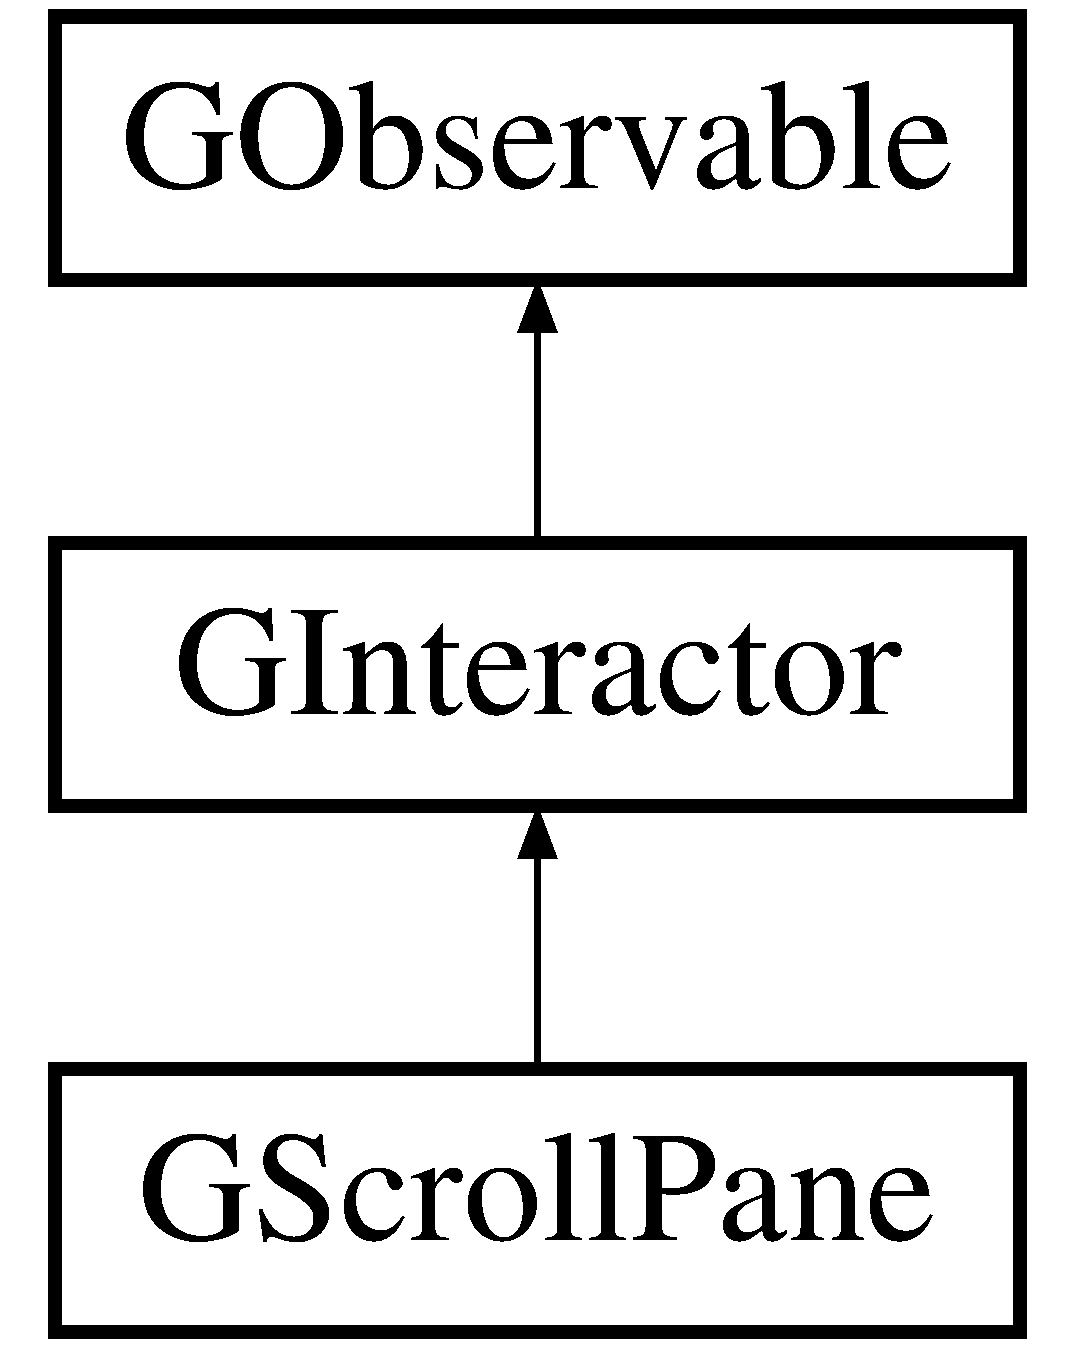
\includegraphics[height=3.000000cm]{classGScrollPane}
\end{center}
\end{figure}
\subsection*{Public Types}
\begin{DoxyCompactItemize}
\item 
enum \mbox{\hyperlink{classGScrollPane_af276320d3d533d494547cb40e5025cc9}{Scroll\+Bar\+Policy}} \{ \mbox{\hyperlink{classGScrollPane_af276320d3d533d494547cb40e5025cc9a19cb69e101cb6454130c8307fe4c0103}{S\+C\+R\+O\+L\+L\+B\+A\+R\+\_\+\+A\+S\+\_\+\+N\+E\+E\+D\+ED}}, 
\mbox{\hyperlink{classGScrollPane_af276320d3d533d494547cb40e5025cc9a3086c0729648b58fde342be1ea988402}{S\+C\+R\+O\+L\+L\+B\+A\+R\+\_\+\+A\+L\+W\+A\+YS}}, 
\mbox{\hyperlink{classGScrollPane_af276320d3d533d494547cb40e5025cc9af26a409c3bd6d0476b7d67fe29a0858f}{S\+C\+R\+O\+L\+L\+B\+A\+R\+\_\+\+N\+E\+V\+ER}}
 \}
\begin{DoxyCompactList}\small\item\em Constants to indicate whether scroll bars in each dimension should be always shown, never shown, or shown only if the inner interactor\textquotesingle{}s size is large enough to require the scroll bar (default). \end{DoxyCompactList}\item 
enum \mbox{\hyperlink{classGInteractor_a8e0d441725a81d2bbdebbea09078260e}{Text\+Position}} \{ \mbox{\hyperlink{classGInteractor_a8e0d441725a81d2bbdebbea09078260ea4cd6f2e7d5a08d6f4dc052df2358f774}{T\+E\+X\+T\+\_\+\+B\+E\+S\+I\+D\+E\+\_\+\+I\+C\+ON}}, 
\mbox{\hyperlink{classGInteractor_a8e0d441725a81d2bbdebbea09078260eaa88490f63d8de68d44c83bdb2ecde3b3}{T\+E\+X\+T\+\_\+\+U\+N\+D\+E\+R\+\_\+\+I\+C\+ON}}, 
\mbox{\hyperlink{classGInteractor_a8e0d441725a81d2bbdebbea09078260ea39a6f388a30ac4fefb6eb13e846bc9f2}{T\+E\+X\+T\+\_\+\+O\+N\+LY}}
 \}
\begin{DoxyCompactList}\small\item\em The places where an interactor can place its text relative to its icon. \end{DoxyCompactList}\end{DoxyCompactItemize}
\subsection*{Public Member Functions}
\begin{DoxyCompactItemize}
\item 
\mbox{\hyperlink{classGScrollPane_aa567e36c0278801a9402a02e77c88208}{G\+Scroll\+Pane}} (\mbox{\hyperlink{classGInteractor}{G\+Interactor}} $\ast$interactor, Q\+Widget $\ast$parent=nullptr)
\begin{DoxyCompactList}\small\item\em Creates a new scroll pane to scroll the given interactor. \end{DoxyCompactList}\item 
virtual \mbox{\hyperlink{classGScrollPane_a3b7c1e8b3a98cf1a68f675927411ee1e}{$\sim$\+G\+Scroll\+Pane}} ()
\begin{DoxyCompactList}\small\item\em Frees memory allocated internally by the scroll pane. \end{DoxyCompactList}\item 
virtual void \mbox{\hyperlink{classGInteractor_a02f20ea6edfa0671f31c4c648a253833}{add\+Action\+Listener}} () Q\+\_\+\+D\+E\+C\+L\+\_\+\+D\+E\+P\+R\+E\+C\+A\+T\+ED
\begin{DoxyCompactList}\small\item\em Adds an event listener to be notified when this interactor is clicked or generally interacted with. \end{DoxyCompactList}\item 
virtual bool \mbox{\hyperlink{classGInteractor_ac05ba5b92e2e5146d416fe7f842a0969}{events\+Enabled}} () const Q\+\_\+\+D\+E\+C\+L\+\_\+\+O\+V\+E\+R\+R\+I\+DE
\begin{DoxyCompactList}\small\item\em Returns true if this interactor is currently accepting events. \end{DoxyCompactList}\item 
virtual std\+::string \mbox{\hyperlink{classGInteractor_a69f8d23ed8f207fbecad99960776e942}{get\+Accelerator}} () const
\begin{DoxyCompactList}\small\item\em Returns a string representing a hotkey for this interactor, or an empty string if no accelerator has been set. \end{DoxyCompactList}\item 
virtual std\+::string \mbox{\hyperlink{classGInteractor_a94eb4276000c4fdfb508ce9e6317a82a}{get\+Action\+Command}} () const
\begin{DoxyCompactList}\small\item\em Returns an action command for this interactor, which is a semi-\/unique string you can use to identify it when events occur. \end{DoxyCompactList}\item 
virtual std\+::string \mbox{\hyperlink{classGInteractor_a808e22cc1fdfbecf71ed8c64ef4600e0}{get\+Background}} () const
\begin{DoxyCompactList}\small\item\em Returns the background color of the interactor as a string. \end{DoxyCompactList}\item 
virtual int \mbox{\hyperlink{classGInteractor_a9e827257a55cb8cf4d9de2ec6bcfd7a0}{get\+Background\+Int}} () const
\begin{DoxyCompactList}\small\item\em Returns the background color of the interactor as an R\+GB integer. \end{DoxyCompactList}\item 
virtual \mbox{\hyperlink{classGRectangle}{G\+Rectangle}} \mbox{\hyperlink{classGInteractor_a29e6ac35a0b48f491a4c88194cc5da3b}{get\+Bounds}} () const
\begin{DoxyCompactList}\small\item\em Returns a rectangle representing the x/y position and size of this interactor. \end{DoxyCompactList}\item 
virtual std\+::string \mbox{\hyperlink{classGInteractor_aa061dfa488c31e18549d64363c1d0e34}{get\+Color}} () const
\begin{DoxyCompactList}\small\item\em Returns the foreground/text color of the interactor as a string. \end{DoxyCompactList}\item 
virtual int \mbox{\hyperlink{classGInteractor_a9635c7af766cdc3417f346683fa0e6c1}{get\+Color\+Int}} () const
\begin{DoxyCompactList}\small\item\em Returns the foreground/text color of the interactor as an R\+GB integer. \end{DoxyCompactList}\item 
virtual \mbox{\hyperlink{classGContainer}{G\+Container}} $\ast$ \mbox{\hyperlink{classGInteractor_a7a6e317c29d61030929b4cd2d1c00fe7}{get\+Container}} () const
\begin{DoxyCompactList}\small\item\em Returns a pointer to the onscreen container holding this interactor. \end{DoxyCompactList}\item 
virtual std\+::string \mbox{\hyperlink{classGInteractor_a894a5502900794eeb27d084c21f1d77d}{get\+Font}} () const
\begin{DoxyCompactList}\small\item\em Returns the font of this interactor\textquotesingle{}s text as a font string such as \char`\"{}\+Helvetica-\/12-\/\+Bold\char`\"{}. \end{DoxyCompactList}\item 
virtual std\+::string \mbox{\hyperlink{classGInteractor_a4fa2d8b0192a3a5b4af4bbfe71194d03}{get\+Foreground}} () const
\begin{DoxyCompactList}\small\item\em Returns the foreground/text color of the interactor as a string. \end{DoxyCompactList}\item 
virtual int \mbox{\hyperlink{classGInteractor_ac3b12ab385a6ef9ae90fc879860ba726}{get\+Foreground\+Int}} () const
\begin{DoxyCompactList}\small\item\em Returns the foreground/text color of the interactor as an R\+GB integer. \end{DoxyCompactList}\item 
virtual double \mbox{\hyperlink{classGInteractor_a1e7e353362434072875264cf95629f99}{get\+Height}} () const
\begin{DoxyCompactList}\small\item\em Returns the current onscreen height of this interactor in pixels. \end{DoxyCompactList}\item 
virtual \mbox{\hyperlink{classGScrollPane_af276320d3d533d494547cb40e5025cc9}{Scroll\+Bar\+Policy}} \mbox{\hyperlink{classGScrollPane_a12a22f982652ad67f6c7867162433d93}{get\+Horizontal\+Scroll\+Bar\+Policy}} () const
\begin{DoxyCompactList}\small\item\em Returns a constant indicating whether the horizontal scroll bar will be shown. \end{DoxyCompactList}\item 
virtual std\+::string \mbox{\hyperlink{classGInteractor_aaed62a73004939a64da6f0eb9eb64d73}{get\+Icon}} () const
\begin{DoxyCompactList}\small\item\em Returns the file name of the icon associated with this interactor, or an empty string if no icon has been set. \end{DoxyCompactList}\item 
virtual int \mbox{\hyperlink{classGInteractor_a9c9659a6c6ba66b4107ba59c95a24241}{get\+ID}} () const
\begin{DoxyCompactList}\small\item\em Returns a globally unique identifier for this interactor, which is set when the interactor is constructed. \end{DoxyCompactList}\item 
virtual \mbox{\hyperlink{classGInteractor}{G\+Interactor}} $\ast$ \mbox{\hyperlink{classGScrollPane_ac8998a7ac699a98fbdc125ef0f3d64f1}{get\+Interactor}} () const
\begin{DoxyCompactList}\small\item\em Returns the inner interactor being wrapped by this scroll pane. \end{DoxyCompactList}\item 
virtual \+\_\+\+Internal\+\_\+\+Q\+Widget $\ast$ \mbox{\hyperlink{classGScrollPane_a208ce13c1da40bf0ddb509daf99d6588}{get\+Internal\+Widget}} () const Q\+\_\+\+D\+E\+C\+L\+\_\+\+O\+V\+E\+R\+R\+I\+DE
\begin{DoxyCompactList}\small\item\em Returns a direct pointer to the internal Qt widget being wrapped by this interactor. \end{DoxyCompactList}\item 
virtual \mbox{\hyperlink{classGPoint}{G\+Point}} \mbox{\hyperlink{classGInteractor_a4f83802015511edeb63b892830812c11}{get\+Location}} () const
\begin{DoxyCompactList}\small\item\em Returns an (x, y) point representing the onscreen location of the top-\/left corner of this interactor within its containing window. \end{DoxyCompactList}\item 
virtual double \mbox{\hyperlink{classGInteractor_aed4b0075fcc434499c3cb3e46896bda3}{get\+Minimum\+Height}} () const
\begin{DoxyCompactList}\small\item\em Returns the minimum height in pixels that this interactor will permit itself to be resized to. \end{DoxyCompactList}\item 
virtual \mbox{\hyperlink{classGDimension}{G\+Dimension}} \mbox{\hyperlink{classGInteractor_a66b5af0b32493b4d597ca0a3df2049ea}{get\+Minimum\+Size}} () const
\begin{DoxyCompactList}\small\item\em Returns a \mbox{\hyperlink{classGDimension}{G\+Dimension}} structure representing the minimum size in pixels that this interactor will permit itself to be resized to. \end{DoxyCompactList}\item 
virtual double \mbox{\hyperlink{classGInteractor_a59e668114fe3d49d2a0f28deb258f7c8}{get\+Minimum\+Width}} () const
\begin{DoxyCompactList}\small\item\em Returns the minimum width in pixels that this interactor will permit itself to be resized to. \end{DoxyCompactList}\item 
virtual std\+::string \mbox{\hyperlink{classGInteractor_a8a60438a5b55d0b2ceb35c8674b9d8c5}{get\+Name}} () const
\begin{DoxyCompactList}\small\item\em Returns a string representing a unique name for this interactor. \end{DoxyCompactList}\item 
virtual double \mbox{\hyperlink{classGInteractor_a747de0961653847bdc6615dbf756d715}{get\+Preferred\+Height}} () const
\begin{DoxyCompactList}\small\item\em Returns the height in pixels that this interactor would prefer to be, which would exactly fit its contents with no stretching or scrollbars. \end{DoxyCompactList}\item 
virtual \mbox{\hyperlink{classGDimension}{G\+Dimension}} \mbox{\hyperlink{classGInteractor_a4aabbee761d8e9116275401131b7ccd1}{get\+Preferred\+Size}} () const
\begin{DoxyCompactList}\small\item\em Returns a \mbox{\hyperlink{classGDimension}{G\+Dimension}} structure storing the width and height in pixels that this interactor would prefer to be, which would exactly fit its contents with no stretching or scrollbars. \end{DoxyCompactList}\item 
virtual double \mbox{\hyperlink{classGInteractor_a82bca31d37700fb0e35d2743352efd5e}{get\+Preferred\+Width}} () const
\begin{DoxyCompactList}\small\item\em Returns the height in pixels that this interactor would prefer to be, which would exactly fit its contents with no stretching or scrollbars. \end{DoxyCompactList}\item 
virtual \mbox{\hyperlink{classGDimension}{G\+Dimension}} \mbox{\hyperlink{classGInteractor_a7b4eec96a2bdc6420695d5796a78eea9}{get\+Size}} () const
\begin{DoxyCompactList}\small\item\em Returns a \mbox{\hyperlink{classGDimension}{G\+Dimension}} structure storing the current onscreen width and height of this interactor in pixels. \end{DoxyCompactList}\item 
virtual std\+::string \mbox{\hyperlink{classGScrollPane_a9896d58fcfebbf1025aeeb5b8b9ede80}{get\+Type}} () const Q\+\_\+\+D\+E\+C\+L\+\_\+\+O\+V\+E\+R\+R\+I\+DE
\begin{DoxyCompactList}\small\item\em Returns a string representing the class name of this interactor, such as \char`\"{}\+G\+Button\char`\"{} or \char`\"{}\+G\+Check\+Box\char`\"{}. \end{DoxyCompactList}\item 
virtual \mbox{\hyperlink{classGScrollPane_af276320d3d533d494547cb40e5025cc9}{Scroll\+Bar\+Policy}} \mbox{\hyperlink{classGScrollPane_a5e5ed8514d493bd76c4774d249fd6f4a}{get\+Vertical\+Scroll\+Bar\+Policy}} () const
\begin{DoxyCompactList}\small\item\em Returns a constant indicating whether the vertical scroll bar will be shown. \end{DoxyCompactList}\item 
virtual Q\+Widget $\ast$ \mbox{\hyperlink{classGScrollPane_a326ee51b5561f807df7b29a1c101f7fd}{get\+Widget}} () const Q\+\_\+\+D\+E\+C\+L\+\_\+\+O\+V\+E\+R\+R\+I\+DE
\begin{DoxyCompactList}\small\item\em Returns a direct pointer to the internal Qt widget being wrapped by this interactor. \end{DoxyCompactList}\item 
virtual double \mbox{\hyperlink{classGInteractor_a0ed2965abd4f5701d2cadf71239faf19}{get\+Width}} () const
\begin{DoxyCompactList}\small\item\em Returns the current onscreen width of this interactor in pixels. \end{DoxyCompactList}\item 
virtual double \mbox{\hyperlink{classGInteractor_a344385751bee0720059403940d57a13e}{getX}} () const
\begin{DoxyCompactList}\small\item\em Returns the x-\/coordinate of the top-\/left pixel of this interactor within its onscreen window. \end{DoxyCompactList}\item 
virtual double \mbox{\hyperlink{classGInteractor_aafa51c7f8f38a09febbb9ce7853f77b4}{getY}} () const
\begin{DoxyCompactList}\small\item\em Returns the y-\/coordinate of the top-\/left pixel of this interactor within its onscreen window. \end{DoxyCompactList}\item 
virtual bool \mbox{\hyperlink{classGInteractor_afc480f652b8c5f1fb255e2269ce68879}{in\+Bounds}} (double x, double y) const
\begin{DoxyCompactList}\small\item\em Returns true if the given x/y pixel is within the bounds of this interactor. \end{DoxyCompactList}\item 
virtual bool \mbox{\hyperlink{classGInteractor_ae6d7982c1c627b677a5e776ca86118ed}{in\+Bounds}} (int x, int y) const
\begin{DoxyCompactList}\small\item\em Returns true if the given x/y pixel is within the bounds of this interactor. \end{DoxyCompactList}\item 
virtual bool \mbox{\hyperlink{classGInteractor_aacb819fb241851fd9fc045271baa4034}{is\+Enabled}} () const
\begin{DoxyCompactList}\small\item\em Returns true if this interactor is currently enabled. \end{DoxyCompactList}\item 
virtual bool \mbox{\hyperlink{classGScrollPane_a5d41618696c889690cd86700fb69dfa3}{is\+Interactor\+Stretch}} () const
\begin{DoxyCompactList}\small\item\em Returns true if the inner interactor should stretch itself to its preferred size. \end{DoxyCompactList}\item 
virtual bool \mbox{\hyperlink{classGInteractor_a9d8a6cfb13917785c143e74d40e4e2be}{is\+Visible}} () const
\begin{DoxyCompactList}\small\item\em Returns true if the interactor is visible on the screen. \end{DoxyCompactList}\item 
virtual void \mbox{\hyperlink{classGInteractor_a519fb2ac767f8b2febbb50b898b8c8cb}{request\+Focus}} ()
\begin{DoxyCompactList}\small\item\em Transfers keyboard focus to this interactor. \end{DoxyCompactList}\item 
virtual void \mbox{\hyperlink{classGInteractor_ad15f102f62e2960576012f1aa0ba4b2e}{set\+Accelerator}} (const std\+::string \&accelerator)
\begin{DoxyCompactList}\small\item\em Sets an accelerator hotkey for this interactor, such as \char`\"{}\+Ctrl-\/\+S\char`\"{}. \end{DoxyCompactList}\item 
virtual void \mbox{\hyperlink{classGInteractor_a4b5843fe3030e038a1ba54cc03389bcf}{set\+Action\+Command}} (const std\+::string \&action\+Command)
\begin{DoxyCompactList}\small\item\em Sets the action command for this interactor. \end{DoxyCompactList}\item 
virtual void \mbox{\hyperlink{classGInteractor_acba7e546c2025c0a15ca4b4cc92043db}{set\+Background}} (int rgb)
\begin{DoxyCompactList}\small\item\em Sets the background color of the interactor to the color represented by the given R\+GB integer. \end{DoxyCompactList}\item 
virtual void \mbox{\hyperlink{classGInteractor_ab4677ab2474e68b07aa56605af92a84a}{set\+Background}} (const std\+::string \&color)
\begin{DoxyCompactList}\small\item\em Sets the background color of the interactor to the color represented by the given string. \end{DoxyCompactList}\item 
virtual void \mbox{\hyperlink{classGInteractor_a2aae8197624b72265ab83b4f1bc73f2f}{set\+Bounds}} (double x, double y, double width, double height)
\begin{DoxyCompactList}\small\item\em Sets the size and location of the widget. \end{DoxyCompactList}\item 
virtual void \mbox{\hyperlink{classGInteractor_acada386653f008cacc7cce86426bef7c}{set\+Bounds}} (const \mbox{\hyperlink{classGRectangle}{G\+Rectangle}} \&size)
\begin{DoxyCompactList}\small\item\em Sets the size and location of the widget. \end{DoxyCompactList}\item 
virtual void \mbox{\hyperlink{classGInteractor_ab1f5cc0f5cc6bbbd716a526c61f1081d}{set\+Color}} (int rgb)
\begin{DoxyCompactList}\small\item\em Sets the foreground/text color of the interactor to the color represented by the given R\+GB integer. \end{DoxyCompactList}\item 
virtual void \mbox{\hyperlink{classGInteractor_a61374df6c11b52cfbb0815decdbaebc6}{set\+Color}} (const std\+::string \&color)
\begin{DoxyCompactList}\small\item\em Sets the foreground/text color of the interactor to the color represented by the given string. \end{DoxyCompactList}\item 
virtual void \mbox{\hyperlink{classGInteractor_ab831367dd84bbd579e02e55bacb21343}{set\+Enabled}} (bool value)
\begin{DoxyCompactList}\small\item\em Sets whether this interactor is currently enabled. \end{DoxyCompactList}\item 
virtual void \mbox{\hyperlink{classGObservable_afaa30b2a9e0f378fd1c70d2f1d0b8216}{set\+Events\+Enabled}} (bool \mbox{\hyperlink{classGInteractor_ac05ba5b92e2e5146d416fe7f842a0969}{events\+Enabled}})
\begin{DoxyCompactList}\small\item\em Sets whether the object is currently allowing itself to fire events. \end{DoxyCompactList}\item 
virtual void \mbox{\hyperlink{classGInteractor_a2592348886ffea646c6534bf88f7c49d}{set\+Font}} (const Q\+Font \&font)
\begin{DoxyCompactList}\small\item\em Sets the font used by this widget to the given Qt font. \end{DoxyCompactList}\item 
virtual void \mbox{\hyperlink{classGInteractor_a8e096e8818d838aceae1d46d58fb3a7b}{set\+Font}} (const std\+::string \&font)
\begin{DoxyCompactList}\small\item\em Sets the font used by this widget to the font represented by the given font string, such as \char`\"{}\+Helvetica-\/16-\/\+Bold\char`\"{}. \end{DoxyCompactList}\item 
virtual void \mbox{\hyperlink{classGInteractor_a9eb856b5ff83a19df3831a31f15f4563}{set\+Foreground}} (int rgb)
\begin{DoxyCompactList}\small\item\em Sets the foreground/text color of the interactor to the color represented by the given R\+GB integer. \end{DoxyCompactList}\item 
virtual void \mbox{\hyperlink{classGInteractor_af59209aeadea6dfc6d97a2d8531f50e1}{set\+Foreground}} (const std\+::string \&color)
\begin{DoxyCompactList}\small\item\em Sets the foreground/text color of the interactor to the color represented by the given string. \end{DoxyCompactList}\item 
virtual void \mbox{\hyperlink{classGInteractor_a9e280bfc4544dfaf8e4376c4e1a74357}{set\+Height}} (double height)
\begin{DoxyCompactList}\small\item\em Sets the onscreen height of the interactor in pixels. \end{DoxyCompactList}\item 
virtual void \mbox{\hyperlink{classGScrollPane_a0c82d84cd2221c453370503faf950e2e}{set\+Horizontal\+Scroll\+Bar\+Policy}} (\mbox{\hyperlink{classGScrollPane_af276320d3d533d494547cb40e5025cc9}{Scroll\+Bar\+Policy}} policy)
\begin{DoxyCompactList}\small\item\em Sets whether the horizontal scroll bar will be shown. \end{DoxyCompactList}\item 
virtual void \mbox{\hyperlink{classGInteractor_a762e139aa311461c3984d3ad28293f64}{set\+Icon}} (const std\+::string \&filename, bool retain\+Icon\+Size=true)
\begin{DoxyCompactList}\small\item\em Sets the file name of the icon associated with this interactor, or an empty string if no icon has been set. \end{DoxyCompactList}\item 
virtual void \mbox{\hyperlink{classGScrollPane_a56c113aeeabb79e04916d0136593588b}{set\+Interactor\+Stretch}} (bool stretch)
\begin{DoxyCompactList}\small\item\em Sets whether the inner interactor should stretch itself to its preferred size. \end{DoxyCompactList}\item 
virtual void \mbox{\hyperlink{classGInteractor_a04594e8ba9b98513a64f1da00dcae18c}{set\+Location}} (double x, double y)
\begin{DoxyCompactList}\small\item\em Sets the onscreen x/y-\/coordinate of the top-\/left corner of the interactor relative to its window. \end{DoxyCompactList}\item 
virtual void \mbox{\hyperlink{classGInteractor_a0cf428e207b7f22cc08138a90b1b87b2}{set\+Minimum\+Size}} (double width, double height)
\begin{DoxyCompactList}\small\item\em Sets the minimum size in pixels that this interactor will permit itself to be resized to. \end{DoxyCompactList}\item 
virtual void \mbox{\hyperlink{classGInteractor_a3b1046117ac6cb7abe467e00ba8a81f4}{set\+Minimum\+Size}} (const \mbox{\hyperlink{classGDimension}{G\+Dimension}} \&size)
\begin{DoxyCompactList}\small\item\em Sets the minimum size in pixels that this interactor will permit itself to be resized to. \end{DoxyCompactList}\item 
virtual void \mbox{\hyperlink{classGInteractor_a9d3a2685df23b5e7cbf59c19c4a1f9b5}{set\+Name}} (const std\+::string \&name)
\begin{DoxyCompactList}\small\item\em Sets a string representing a unique name for this interactor. \end{DoxyCompactList}\item 
virtual void \mbox{\hyperlink{classGInteractor_a1ab987704fce32098706c6f00fb08218}{set\+Preferred\+Height}} (double height)
\begin{DoxyCompactList}\small\item\em Sets the height in pixels that this interactor would prefer to be. \end{DoxyCompactList}\item 
virtual void \mbox{\hyperlink{classGInteractor_a042c5ae19430d765ef552371cae3632c}{set\+Preferred\+Size}} (double width, double height)
\begin{DoxyCompactList}\small\item\em Sets the width and height in pixels that this interactor would prefer to be. \end{DoxyCompactList}\item 
virtual void \mbox{\hyperlink{classGInteractor_aa22d9be4bc0e078bb0ea69b0fc9d7c75}{set\+Preferred\+Size}} (const \mbox{\hyperlink{classGDimension}{G\+Dimension}} \&size)
\begin{DoxyCompactList}\small\item\em Sets the size in pixels that this interactor would prefer to be. \end{DoxyCompactList}\item 
virtual void \mbox{\hyperlink{classGInteractor_a3db429ab2fa52efd187eec0ed8cdd9f2}{set\+Preferred\+Width}} (double width)
\begin{DoxyCompactList}\small\item\em Sets the width in pixels that this interactor would prefer to be. \end{DoxyCompactList}\item 
virtual void \mbox{\hyperlink{classGScrollPane_a970d6a1f1254aaad2c15ae271a87d49f}{set\+Scroll\+Bar\+Policy}} (\mbox{\hyperlink{classGScrollPane_af276320d3d533d494547cb40e5025cc9}{Scroll\+Bar\+Policy}} policy)
\begin{DoxyCompactList}\small\item\em Sets whether the horizontal and vertical scroll bars will be shown. \end{DoxyCompactList}\item 
virtual void \mbox{\hyperlink{classGInteractor_aca25d49481f9bf5fc8f7df4c086c4ce7}{set\+Size}} (double width, double height)
\begin{DoxyCompactList}\small\item\em Sets the onscreen width and height of the interactor in pixels. \end{DoxyCompactList}\item 
virtual void \mbox{\hyperlink{classGInteractor_ae2b628228f192c2702c4ce941b2af68f}{set\+Size}} (const \mbox{\hyperlink{classGDimension}{G\+Dimension}} \&size)
\begin{DoxyCompactList}\small\item\em Sets the onscreen width and height of the interactor in pixels. \end{DoxyCompactList}\item 
virtual void \mbox{\hyperlink{classGInteractor_a039e0e49beaecc275efce02d416acea8}{set\+Tooltip}} (const std\+::string \&tooltip\+Text)
\begin{DoxyCompactList}\small\item\em Sets a \char`\"{}tooltip\char`\"{} that will appear if the user hovers their mouse over the interactor. \end{DoxyCompactList}\item 
virtual void \mbox{\hyperlink{classGScrollPane_adb8714eb78c44ef15671e3f92effa826}{set\+Vertical\+Scroll\+Bar\+Policy}} (\mbox{\hyperlink{classGScrollPane_af276320d3d533d494547cb40e5025cc9}{Scroll\+Bar\+Policy}} policy)
\begin{DoxyCompactList}\small\item\em Sets whether the vertical scroll bar will be shown. \end{DoxyCompactList}\item 
virtual void \mbox{\hyperlink{classGInteractor_a18e44e30b31525a243960ca3928125aa}{set\+Visible}} (bool visible)
\begin{DoxyCompactList}\small\item\em Returns true if the interactor is visible on the screen. \end{DoxyCompactList}\item 
virtual void \mbox{\hyperlink{classGInteractor_aa3f3fba4cb131baa8696ba01e3bceca1}{set\+Width}} (double width)
\begin{DoxyCompactList}\small\item\em Sets the onscreen width of the interactor in pixels. \end{DoxyCompactList}\item 
virtual void \mbox{\hyperlink{classGInteractor_a9c18fcc579333bf9653d13ad2b372e39}{setX}} (double x)
\begin{DoxyCompactList}\small\item\em Sets the onscreen x-\/coordinate of the top-\/left corner of the interactor relative to its window. \end{DoxyCompactList}\item 
virtual void \mbox{\hyperlink{classGInteractor_a7d57e2a5c35d27feb58fd498a3cf82b9}{setY}} (double y)
\begin{DoxyCompactList}\small\item\em Sets the onscreen y-\/coordinate of the top-\/left corner of the interactor relative to its window. \end{DoxyCompactList}\item 
virtual std\+::string \mbox{\hyperlink{classGObservable_a1fe5121d6528fdea3f243321b3fa3a49}{to\+String}} () const
\begin{DoxyCompactList}\small\item\em Returns a string representation of this observable object\textquotesingle{}s state. \end{DoxyCompactList}\end{DoxyCompactItemize}
\subsection*{Protected Member Functions}
\begin{DoxyCompactItemize}
\item 
virtual void \mbox{\hyperlink{classGObservable_a80cfa040459ff53594adbd6a51ec8f43}{clear\+Event\+Listeners}} ()
\begin{DoxyCompactList}\small\item\em Removes all event listeners from this object. \end{DoxyCompactList}\item 
virtual void \mbox{\hyperlink{classGObservable_a284f31528c0520f8e545c03ac9eeac74}{ensure\+Thread\+Safety}} (const std\+::string \&member\+Name=\char`\"{}\char`\"{})
\begin{DoxyCompactList}\small\item\em Ensures that we are currently in the Qt G\+UI thread. \end{DoxyCompactList}\item 
virtual void \mbox{\hyperlink{classGObservable_a63e5e5a6227c59c928493b11aceb0f67}{fire\+Event}} (\mbox{\hyperlink{classGEvent}{G\+Event}} \&event)
\begin{DoxyCompactList}\small\item\em Sends out the given event to any attached listeners. \end{DoxyCompactList}\item 
virtual void \mbox{\hyperlink{classGObservable_ab3983ea07337b52020a29cc00c653d8d}{fire\+G\+Event}} (Q\+Event $\ast$event, Event\+Type event\+Type, const std\+::string \&event\+Name)
\begin{DoxyCompactList}\small\item\em Creates an event of the given type, then sends it out to any attached listeners. \end{DoxyCompactList}\item 
virtual void \mbox{\hyperlink{classGObservable_a01fdf1b0e0dbd49e189fe4514e010411}{fire\+G\+Event}} (Q\+Close\+Event $\ast$event, Event\+Type event\+Type, const std\+::string \&event\+Name)
\begin{DoxyCompactList}\small\item\em Creates an event of the given type, then sends it out to any attached listeners. \end{DoxyCompactList}\item 
virtual void \mbox{\hyperlink{classGObservable_abb0b2f66ba39211cb5d7615e9d1c04e2}{fire\+G\+Event}} (Q\+Key\+Event $\ast$event, Event\+Type event\+Type, const std\+::string \&event\+Name)
\begin{DoxyCompactList}\small\item\em Creates an event of the given type, then sends it out to any attached listeners. \end{DoxyCompactList}\item 
virtual void \mbox{\hyperlink{classGObservable_a119318675d2165bdf7dd853aaf881d4b}{fire\+G\+Event}} (Q\+Mouse\+Event $\ast$event, Event\+Type event\+Type, const std\+::string \&event\+Name, const std\+::string \&action\+Command=\char`\"{}\char`\"{})
\begin{DoxyCompactList}\small\item\em Creates an event of the given type, then sends it out to any attached listeners. \end{DoxyCompactList}\item 
virtual void \mbox{\hyperlink{classGObservable_a63fd9034e1e1633c1c38eb342bfd34e9}{fire\+G\+Event}} (Q\+Resize\+Event $\ast$event, Event\+Type event\+Type, const std\+::string \&event\+Name)
\begin{DoxyCompactList}\small\item\em Creates an event of the given type, then sends it out to any attached listeners. \end{DoxyCompactList}\item 
virtual void \mbox{\hyperlink{classGObservable_a741345310d9b7c5170a6cbc410c44ac4}{fire\+G\+Event}} (Q\+Timer\+Event $\ast$event, Event\+Type event\+Type, const std\+::string \&event\+Name)
\begin{DoxyCompactList}\small\item\em Creates an event of the given type, then sends it out to any attached listeners. \end{DoxyCompactList}\item 
virtual void \mbox{\hyperlink{classGObservable_a93bf338968a0338761b8e4dc62f582e9}{fire\+G\+Event}} (Q\+Wheel\+Event $\ast$event, Event\+Type event\+Type, const std\+::string \&event\+Name)
\begin{DoxyCompactList}\small\item\em Creates an event of the given type, then sends it out to any attached listeners. \end{DoxyCompactList}\item 
virtual void \mbox{\hyperlink{classGObservable_a2a70a7d7435ff0c3b80bb4d70da19e0d}{fire\+G\+Event}} (Q\+Window\+State\+Change\+Event $\ast$event, Event\+Type event\+Type, const std\+::string \&event\+Name)
\begin{DoxyCompactList}\small\item\em Creates an event of the given type, then sends it out to any attached listeners. \end{DoxyCompactList}\item 
virtual bool \mbox{\hyperlink{classGObservable_a9f6faaa25942923bafa1c44020c49fa9}{has\+Event\+Listener}} (const std\+::string \&event\+Name) const
\begin{DoxyCompactList}\small\item\em Returns true if the observable object has a listener for the given type of event. \end{DoxyCompactList}\item 
virtual bool \mbox{\hyperlink{classGObservable_aeec1adc19aa0f33de62390686ee1382c}{is\+Accepting\+Event}} (int event\+Mask) const
\begin{DoxyCompactList}\small\item\em Returns true if the observable object has a listener for the given type of event. \end{DoxyCompactList}\item 
virtual bool \mbox{\hyperlink{classGObservable_aa31c73145a29dcb92848a92e0cfaea41}{is\+Accepting\+Event}} (const \mbox{\hyperlink{classGEvent}{G\+Event}} \&event) const
\begin{DoxyCompactList}\small\item\em Returns true if the observable object has a listener for the given type of event. \end{DoxyCompactList}\item 
virtual bool \mbox{\hyperlink{classGObservable_a3b1c689267eda44e65a2213e7de38b23}{is\+Accepting\+Event}} (const std\+::string \&event\+Type) const
\begin{DoxyCompactList}\small\item\em Returns true if the observable object has a listener for the given type of event. \end{DoxyCompactList}\item 
virtual void \mbox{\hyperlink{classGObservable_acbcf1ed3a851ad8a3c17ef38d86b481d}{remove\+Event\+Listener}} (const std\+::string \&event\+Name)
\begin{DoxyCompactList}\small\item\em Removes any event listener from this observable object that would respond to the given type of event, such as \char`\"{}click\char`\"{} or \char`\"{}keydown\char`\"{}. \end{DoxyCompactList}\item 
virtual void \mbox{\hyperlink{classGObservable_af51cc35c29a1bd1908609d432decdbb6}{remove\+Event\+Listeners}} (std\+::initializer\+\_\+list$<$ std\+::string $>$ event\+Names)
\begin{DoxyCompactList}\small\item\em Removes any event listener from this observable object that would respond to the given types of events, such as \char`\"{}click\char`\"{} or \char`\"{}keydown\char`\"{}. \end{DoxyCompactList}\item 
virtual void \mbox{\hyperlink{classGObservable_ad2f6d34961c50f6c1e0659990b79f741}{set\+Event\+Listener}} (const std\+::string \&event\+Name, G\+Event\+Listener func)
\begin{DoxyCompactList}\small\item\em Adds an event listener from this observable object to respond to the given type of event, such as \char`\"{}click\char`\"{} or \char`\"{}keydown\char`\"{}. \end{DoxyCompactList}\item 
virtual void \mbox{\hyperlink{classGObservable_abac4cb9f9e626e010e87f5d91573c8a5}{set\+Event\+Listener}} (const std\+::string \&event\+Name, G\+Event\+Listener\+Void func)
\begin{DoxyCompactList}\small\item\em Adds an event listener from this observable object to respond to the given type of event, such as \char`\"{}click\char`\"{} or \char`\"{}keydown\char`\"{}. \end{DoxyCompactList}\item 
virtual void \mbox{\hyperlink{classGObservable_afa388d69c33c718cf035774604065604}{set\+Event\+Listeners}} (std\+::initializer\+\_\+list$<$ std\+::string $>$ event\+Names, G\+Event\+Listener func)
\begin{DoxyCompactList}\small\item\em Adds an event listener from this observable object to respond to the given types of events, such as \char`\"{}click\char`\"{} or \char`\"{}keydown\char`\"{}. \end{DoxyCompactList}\item 
virtual void \mbox{\hyperlink{classGObservable_a7867184bbb686f74fae8a4db927da799}{set\+Event\+Listeners}} (std\+::initializer\+\_\+list$<$ std\+::string $>$ event\+Names, G\+Event\+Listener\+Void func)
\begin{DoxyCompactList}\small\item\em Adds an event listener from this observable object to respond to the given types of events, such as \char`\"{}click\char`\"{} or \char`\"{}keydown\char`\"{}. \end{DoxyCompactList}\end{DoxyCompactItemize}


\subsection{Detailed Description}
A \mbox{\hyperlink{classGScrollPane}{G\+Scroll\+Pane}} is a container that wraps another interactor with scroll bars. 

It can be used to allow another interactor to be at its preferred size (or some arbitrarily large size) while only occupying a smaller number of onscreen pixels with vertical and/or horizontal scroll bars. 

\subsection{Member Enumeration Documentation}
\mbox{\Hypertarget{classGScrollPane_af276320d3d533d494547cb40e5025cc9}\label{classGScrollPane_af276320d3d533d494547cb40e5025cc9}} 
\index{G\+Scroll\+Pane@{G\+Scroll\+Pane}!Scroll\+Bar\+Policy@{Scroll\+Bar\+Policy}}
\index{Scroll\+Bar\+Policy@{Scroll\+Bar\+Policy}!G\+Scroll\+Pane@{G\+Scroll\+Pane}}
\subsubsection{\texorpdfstring{Scroll\+Bar\+Policy}{ScrollBarPolicy}}
{\footnotesize\ttfamily enum \mbox{\hyperlink{classGScrollPane_af276320d3d533d494547cb40e5025cc9}{Scroll\+Bar\+Policy}}}



Constants to indicate whether scroll bars in each dimension should be always shown, never shown, or shown only if the inner interactor\textquotesingle{}s size is large enough to require the scroll bar (default). 

\begin{DoxyEnumFields}{Enumerator}
\raisebox{\heightof{T}}[0pt][0pt]{\index{S\+C\+R\+O\+L\+L\+B\+A\+R\+\_\+\+A\+S\+\_\+\+N\+E\+E\+D\+ED@{S\+C\+R\+O\+L\+L\+B\+A\+R\+\_\+\+A\+S\+\_\+\+N\+E\+E\+D\+ED}!G\+Scroll\+Pane@{G\+Scroll\+Pane}}\index{G\+Scroll\+Pane@{G\+Scroll\+Pane}!S\+C\+R\+O\+L\+L\+B\+A\+R\+\_\+\+A\+S\+\_\+\+N\+E\+E\+D\+ED@{S\+C\+R\+O\+L\+L\+B\+A\+R\+\_\+\+A\+S\+\_\+\+N\+E\+E\+D\+ED}}}\mbox{\Hypertarget{classGScrollPane_af276320d3d533d494547cb40e5025cc9a19cb69e101cb6454130c8307fe4c0103}\label{classGScrollPane_af276320d3d533d494547cb40e5025cc9a19cb69e101cb6454130c8307fe4c0103}} 
S\+C\+R\+O\+L\+L\+B\+A\+R\+\_\+\+A\+S\+\_\+\+N\+E\+E\+D\+ED&\\
\hline

\raisebox{\heightof{T}}[0pt][0pt]{\index{S\+C\+R\+O\+L\+L\+B\+A\+R\+\_\+\+A\+L\+W\+A\+YS@{S\+C\+R\+O\+L\+L\+B\+A\+R\+\_\+\+A\+L\+W\+A\+YS}!G\+Scroll\+Pane@{G\+Scroll\+Pane}}\index{G\+Scroll\+Pane@{G\+Scroll\+Pane}!S\+C\+R\+O\+L\+L\+B\+A\+R\+\_\+\+A\+L\+W\+A\+YS@{S\+C\+R\+O\+L\+L\+B\+A\+R\+\_\+\+A\+L\+W\+A\+YS}}}\mbox{\Hypertarget{classGScrollPane_af276320d3d533d494547cb40e5025cc9a3086c0729648b58fde342be1ea988402}\label{classGScrollPane_af276320d3d533d494547cb40e5025cc9a3086c0729648b58fde342be1ea988402}} 
S\+C\+R\+O\+L\+L\+B\+A\+R\+\_\+\+A\+L\+W\+A\+YS&\\
\hline

\raisebox{\heightof{T}}[0pt][0pt]{\index{S\+C\+R\+O\+L\+L\+B\+A\+R\+\_\+\+N\+E\+V\+ER@{S\+C\+R\+O\+L\+L\+B\+A\+R\+\_\+\+N\+E\+V\+ER}!G\+Scroll\+Pane@{G\+Scroll\+Pane}}\index{G\+Scroll\+Pane@{G\+Scroll\+Pane}!S\+C\+R\+O\+L\+L\+B\+A\+R\+\_\+\+N\+E\+V\+ER@{S\+C\+R\+O\+L\+L\+B\+A\+R\+\_\+\+N\+E\+V\+ER}}}\mbox{\Hypertarget{classGScrollPane_af276320d3d533d494547cb40e5025cc9af26a409c3bd6d0476b7d67fe29a0858f}\label{classGScrollPane_af276320d3d533d494547cb40e5025cc9af26a409c3bd6d0476b7d67fe29a0858f}} 
S\+C\+R\+O\+L\+L\+B\+A\+R\+\_\+\+N\+E\+V\+ER&\\
\hline

\end{DoxyEnumFields}
\mbox{\Hypertarget{classGInteractor_a8e0d441725a81d2bbdebbea09078260e}\label{classGInteractor_a8e0d441725a81d2bbdebbea09078260e}} 
\index{G\+Scroll\+Pane@{G\+Scroll\+Pane}!Text\+Position@{Text\+Position}}
\index{Text\+Position@{Text\+Position}!G\+Scroll\+Pane@{G\+Scroll\+Pane}}
\subsubsection{\texorpdfstring{Text\+Position}{TextPosition}}
{\footnotesize\ttfamily enum \mbox{\hyperlink{classGInteractor_a8e0d441725a81d2bbdebbea09078260e}{Text\+Position}}\hspace{0.3cm}{\ttfamily [inherited]}}



The places where an interactor can place its text relative to its icon. 

\begin{DoxyEnumFields}{Enumerator}
\raisebox{\heightof{T}}[0pt][0pt]{\index{T\+E\+X\+T\+\_\+\+B\+E\+S\+I\+D\+E\+\_\+\+I\+C\+ON@{T\+E\+X\+T\+\_\+\+B\+E\+S\+I\+D\+E\+\_\+\+I\+C\+ON}!G\+Scroll\+Pane@{G\+Scroll\+Pane}}\index{G\+Scroll\+Pane@{G\+Scroll\+Pane}!T\+E\+X\+T\+\_\+\+B\+E\+S\+I\+D\+E\+\_\+\+I\+C\+ON@{T\+E\+X\+T\+\_\+\+B\+E\+S\+I\+D\+E\+\_\+\+I\+C\+ON}}}\mbox{\Hypertarget{classGInteractor_a8e0d441725a81d2bbdebbea09078260ea4cd6f2e7d5a08d6f4dc052df2358f774}\label{classGInteractor_a8e0d441725a81d2bbdebbea09078260ea4cd6f2e7d5a08d6f4dc052df2358f774}} 
T\+E\+X\+T\+\_\+\+B\+E\+S\+I\+D\+E\+\_\+\+I\+C\+ON&\\
\hline

\raisebox{\heightof{T}}[0pt][0pt]{\index{T\+E\+X\+T\+\_\+\+U\+N\+D\+E\+R\+\_\+\+I\+C\+ON@{T\+E\+X\+T\+\_\+\+U\+N\+D\+E\+R\+\_\+\+I\+C\+ON}!G\+Scroll\+Pane@{G\+Scroll\+Pane}}\index{G\+Scroll\+Pane@{G\+Scroll\+Pane}!T\+E\+X\+T\+\_\+\+U\+N\+D\+E\+R\+\_\+\+I\+C\+ON@{T\+E\+X\+T\+\_\+\+U\+N\+D\+E\+R\+\_\+\+I\+C\+ON}}}\mbox{\Hypertarget{classGInteractor_a8e0d441725a81d2bbdebbea09078260eaa88490f63d8de68d44c83bdb2ecde3b3}\label{classGInteractor_a8e0d441725a81d2bbdebbea09078260eaa88490f63d8de68d44c83bdb2ecde3b3}} 
T\+E\+X\+T\+\_\+\+U\+N\+D\+E\+R\+\_\+\+I\+C\+ON&\\
\hline

\raisebox{\heightof{T}}[0pt][0pt]{\index{T\+E\+X\+T\+\_\+\+O\+N\+LY@{T\+E\+X\+T\+\_\+\+O\+N\+LY}!G\+Scroll\+Pane@{G\+Scroll\+Pane}}\index{G\+Scroll\+Pane@{G\+Scroll\+Pane}!T\+E\+X\+T\+\_\+\+O\+N\+LY@{T\+E\+X\+T\+\_\+\+O\+N\+LY}}}\mbox{\Hypertarget{classGInteractor_a8e0d441725a81d2bbdebbea09078260ea39a6f388a30ac4fefb6eb13e846bc9f2}\label{classGInteractor_a8e0d441725a81d2bbdebbea09078260ea39a6f388a30ac4fefb6eb13e846bc9f2}} 
T\+E\+X\+T\+\_\+\+O\+N\+LY&\\
\hline

\end{DoxyEnumFields}


\subsection{Constructor \& Destructor Documentation}
\mbox{\Hypertarget{classGScrollPane_aa567e36c0278801a9402a02e77c88208}\label{classGScrollPane_aa567e36c0278801a9402a02e77c88208}} 
\index{G\+Scroll\+Pane@{G\+Scroll\+Pane}!G\+Scroll\+Pane@{G\+Scroll\+Pane}}
\index{G\+Scroll\+Pane@{G\+Scroll\+Pane}!G\+Scroll\+Pane@{G\+Scroll\+Pane}}
\subsubsection{\texorpdfstring{G\+Scroll\+Pane()}{GScrollPane()}}
{\footnotesize\ttfamily \mbox{\hyperlink{classGScrollPane}{G\+Scroll\+Pane}} (\begin{DoxyParamCaption}\item[{\mbox{\hyperlink{classGInteractor}{G\+Interactor}} $\ast$}]{interactor,  }\item[{Q\+Widget $\ast$}]{parent = {\ttfamily nullptr} }\end{DoxyParamCaption})}



Creates a new scroll pane to scroll the given interactor. 


\begin{DoxyExceptions}{Exceptions}
{\em \mbox{\hyperlink{classErrorException}{Error\+Exception}}} & if the interactor is null \\
\hline
\end{DoxyExceptions}
\mbox{\Hypertarget{classGScrollPane_a3b7c1e8b3a98cf1a68f675927411ee1e}\label{classGScrollPane_a3b7c1e8b3a98cf1a68f675927411ee1e}} 
\index{G\+Scroll\+Pane@{G\+Scroll\+Pane}!````~G\+Scroll\+Pane@{$\sim$\+G\+Scroll\+Pane}}
\index{````~G\+Scroll\+Pane@{$\sim$\+G\+Scroll\+Pane}!G\+Scroll\+Pane@{G\+Scroll\+Pane}}
\subsubsection{\texorpdfstring{$\sim$\+G\+Scroll\+Pane()}{~GScrollPane()}}
{\footnotesize\ttfamily $\sim$\mbox{\hyperlink{classGScrollPane}{G\+Scroll\+Pane}} (\begin{DoxyParamCaption}{ }\end{DoxyParamCaption})\hspace{0.3cm}{\ttfamily [virtual]}}



Frees memory allocated internally by the scroll pane. 



\subsection{Member Function Documentation}
\mbox{\Hypertarget{classGInteractor_a02f20ea6edfa0671f31c4c648a253833}\label{classGInteractor_a02f20ea6edfa0671f31c4c648a253833}} 
\index{G\+Scroll\+Pane@{G\+Scroll\+Pane}!add\+Action\+Listener@{add\+Action\+Listener}}
\index{add\+Action\+Listener@{add\+Action\+Listener}!G\+Scroll\+Pane@{G\+Scroll\+Pane}}
\subsubsection{\texorpdfstring{add\+Action\+Listener()}{addActionListener()}}
{\footnotesize\ttfamily void add\+Action\+Listener (\begin{DoxyParamCaption}{ }\end{DoxyParamCaption})\hspace{0.3cm}{\ttfamily [virtual]}, {\ttfamily [inherited]}}



Adds an event listener to be notified when this interactor is clicked or generally interacted with. 

\begin{DoxyRefDesc}{Deprecated}
\item[\mbox{\hyperlink{deprecated__deprecated000006}{Deprecated}}]does nothing; use set\+Action\+Listener instead \end{DoxyRefDesc}
\mbox{\Hypertarget{classGObservable_a80cfa040459ff53594adbd6a51ec8f43}\label{classGObservable_a80cfa040459ff53594adbd6a51ec8f43}} 
\index{G\+Scroll\+Pane@{G\+Scroll\+Pane}!clear\+Event\+Listeners@{clear\+Event\+Listeners}}
\index{clear\+Event\+Listeners@{clear\+Event\+Listeners}!G\+Scroll\+Pane@{G\+Scroll\+Pane}}
\subsubsection{\texorpdfstring{clear\+Event\+Listeners()}{clearEventListeners()}}
{\footnotesize\ttfamily void clear\+Event\+Listeners (\begin{DoxyParamCaption}{ }\end{DoxyParamCaption})\hspace{0.3cm}{\ttfamily [protected]}, {\ttfamily [virtual]}, {\ttfamily [inherited]}}



Removes all event listeners from this object. 

\mbox{\Hypertarget{classGObservable_a284f31528c0520f8e545c03ac9eeac74}\label{classGObservable_a284f31528c0520f8e545c03ac9eeac74}} 
\index{G\+Scroll\+Pane@{G\+Scroll\+Pane}!ensure\+Thread\+Safety@{ensure\+Thread\+Safety}}
\index{ensure\+Thread\+Safety@{ensure\+Thread\+Safety}!G\+Scroll\+Pane@{G\+Scroll\+Pane}}
\subsubsection{\texorpdfstring{ensure\+Thread\+Safety()}{ensureThreadSafety()}}
{\footnotesize\ttfamily void ensure\+Thread\+Safety (\begin{DoxyParamCaption}\item[{const std\+::string \&}]{member\+Name = {\ttfamily \char`\"{}\char`\"{}} }\end{DoxyParamCaption})\hspace{0.3cm}{\ttfamily [protected]}, {\ttfamily [virtual]}, {\ttfamily [inherited]}}



Ensures that we are currently in the Qt G\+UI thread. 

\mbox{\Hypertarget{classGInteractor_ac05ba5b92e2e5146d416fe7f842a0969}\label{classGInteractor_ac05ba5b92e2e5146d416fe7f842a0969}} 
\index{G\+Scroll\+Pane@{G\+Scroll\+Pane}!events\+Enabled@{events\+Enabled}}
\index{events\+Enabled@{events\+Enabled}!G\+Scroll\+Pane@{G\+Scroll\+Pane}}
\subsubsection{\texorpdfstring{events\+Enabled()}{eventsEnabled()}}
{\footnotesize\ttfamily bool events\+Enabled (\begin{DoxyParamCaption}{ }\end{DoxyParamCaption}) const\hspace{0.3cm}{\ttfamily [virtual]}, {\ttfamily [inherited]}}



Returns true if this interactor is currently accepting events. 

Initially true. An interactor must be visible and added to an onscreen window to receive events. 

Reimplemented from \mbox{\hyperlink{classGObservable_a8ebb3da91032e7f4c34485dabc518b8a}{G\+Observable}}.

\mbox{\Hypertarget{classGObservable_a63e5e5a6227c59c928493b11aceb0f67}\label{classGObservable_a63e5e5a6227c59c928493b11aceb0f67}} 
\index{G\+Scroll\+Pane@{G\+Scroll\+Pane}!fire\+Event@{fire\+Event}}
\index{fire\+Event@{fire\+Event}!G\+Scroll\+Pane@{G\+Scroll\+Pane}}
\subsubsection{\texorpdfstring{fire\+Event()}{fireEvent()}}
{\footnotesize\ttfamily void fire\+Event (\begin{DoxyParamCaption}\item[{\mbox{\hyperlink{classGEvent}{G\+Event}} \&}]{event }\end{DoxyParamCaption})\hspace{0.3cm}{\ttfamily [protected]}, {\ttfamily [virtual]}, {\ttfamily [inherited]}}



Sends out the given event to any attached listeners. 

\mbox{\Hypertarget{classGObservable_ab3983ea07337b52020a29cc00c653d8d}\label{classGObservable_ab3983ea07337b52020a29cc00c653d8d}} 
\index{G\+Scroll\+Pane@{G\+Scroll\+Pane}!fire\+G\+Event@{fire\+G\+Event}}
\index{fire\+G\+Event@{fire\+G\+Event}!G\+Scroll\+Pane@{G\+Scroll\+Pane}}
\subsubsection{\texorpdfstring{fire\+G\+Event()}{fireGEvent()}\hspace{0.1cm}{\footnotesize\ttfamily [1/8]}}
{\footnotesize\ttfamily void fire\+G\+Event (\begin{DoxyParamCaption}\item[{Q\+Event $\ast$}]{event,  }\item[{Event\+Type}]{event\+Type,  }\item[{const std\+::string \&}]{event\+Name }\end{DoxyParamCaption})\hspace{0.3cm}{\ttfamily [protected]}, {\ttfamily [virtual]}, {\ttfamily [inherited]}}



Creates an event of the given type, then sends it out to any attached listeners. 

\mbox{\Hypertarget{classGObservable_a01fdf1b0e0dbd49e189fe4514e010411}\label{classGObservable_a01fdf1b0e0dbd49e189fe4514e010411}} 
\index{G\+Scroll\+Pane@{G\+Scroll\+Pane}!fire\+G\+Event@{fire\+G\+Event}}
\index{fire\+G\+Event@{fire\+G\+Event}!G\+Scroll\+Pane@{G\+Scroll\+Pane}}
\subsubsection{\texorpdfstring{fire\+G\+Event()}{fireGEvent()}\hspace{0.1cm}{\footnotesize\ttfamily [2/8]}}
{\footnotesize\ttfamily void fire\+G\+Event (\begin{DoxyParamCaption}\item[{Q\+Close\+Event $\ast$}]{event,  }\item[{Event\+Type}]{event\+Type,  }\item[{const std\+::string \&}]{event\+Name }\end{DoxyParamCaption})\hspace{0.3cm}{\ttfamily [protected]}, {\ttfamily [virtual]}, {\ttfamily [inherited]}}



Creates an event of the given type, then sends it out to any attached listeners. 

\mbox{\Hypertarget{classGObservable_abb0b2f66ba39211cb5d7615e9d1c04e2}\label{classGObservable_abb0b2f66ba39211cb5d7615e9d1c04e2}} 
\index{G\+Scroll\+Pane@{G\+Scroll\+Pane}!fire\+G\+Event@{fire\+G\+Event}}
\index{fire\+G\+Event@{fire\+G\+Event}!G\+Scroll\+Pane@{G\+Scroll\+Pane}}
\subsubsection{\texorpdfstring{fire\+G\+Event()}{fireGEvent()}\hspace{0.1cm}{\footnotesize\ttfamily [3/8]}}
{\footnotesize\ttfamily void fire\+G\+Event (\begin{DoxyParamCaption}\item[{Q\+Key\+Event $\ast$}]{event,  }\item[{Event\+Type}]{event\+Type,  }\item[{const std\+::string \&}]{event\+Name }\end{DoxyParamCaption})\hspace{0.3cm}{\ttfamily [protected]}, {\ttfamily [virtual]}, {\ttfamily [inherited]}}



Creates an event of the given type, then sends it out to any attached listeners. 

\mbox{\Hypertarget{classGObservable_a119318675d2165bdf7dd853aaf881d4b}\label{classGObservable_a119318675d2165bdf7dd853aaf881d4b}} 
\index{G\+Scroll\+Pane@{G\+Scroll\+Pane}!fire\+G\+Event@{fire\+G\+Event}}
\index{fire\+G\+Event@{fire\+G\+Event}!G\+Scroll\+Pane@{G\+Scroll\+Pane}}
\subsubsection{\texorpdfstring{fire\+G\+Event()}{fireGEvent()}\hspace{0.1cm}{\footnotesize\ttfamily [4/8]}}
{\footnotesize\ttfamily void fire\+G\+Event (\begin{DoxyParamCaption}\item[{Q\+Mouse\+Event $\ast$}]{event,  }\item[{Event\+Type}]{event\+Type,  }\item[{const std\+::string \&}]{event\+Name,  }\item[{const std\+::string \&}]{action\+Command = {\ttfamily \char`\"{}\char`\"{}} }\end{DoxyParamCaption})\hspace{0.3cm}{\ttfamily [protected]}, {\ttfamily [virtual]}, {\ttfamily [inherited]}}



Creates an event of the given type, then sends it out to any attached listeners. 

\mbox{\Hypertarget{classGObservable_a63fd9034e1e1633c1c38eb342bfd34e9}\label{classGObservable_a63fd9034e1e1633c1c38eb342bfd34e9}} 
\index{G\+Scroll\+Pane@{G\+Scroll\+Pane}!fire\+G\+Event@{fire\+G\+Event}}
\index{fire\+G\+Event@{fire\+G\+Event}!G\+Scroll\+Pane@{G\+Scroll\+Pane}}
\subsubsection{\texorpdfstring{fire\+G\+Event()}{fireGEvent()}\hspace{0.1cm}{\footnotesize\ttfamily [5/8]}}
{\footnotesize\ttfamily void fire\+G\+Event (\begin{DoxyParamCaption}\item[{Q\+Resize\+Event $\ast$}]{event,  }\item[{Event\+Type}]{event\+Type,  }\item[{const std\+::string \&}]{event\+Name }\end{DoxyParamCaption})\hspace{0.3cm}{\ttfamily [protected]}, {\ttfamily [virtual]}, {\ttfamily [inherited]}}



Creates an event of the given type, then sends it out to any attached listeners. 

\mbox{\Hypertarget{classGObservable_a741345310d9b7c5170a6cbc410c44ac4}\label{classGObservable_a741345310d9b7c5170a6cbc410c44ac4}} 
\index{G\+Scroll\+Pane@{G\+Scroll\+Pane}!fire\+G\+Event@{fire\+G\+Event}}
\index{fire\+G\+Event@{fire\+G\+Event}!G\+Scroll\+Pane@{G\+Scroll\+Pane}}
\subsubsection{\texorpdfstring{fire\+G\+Event()}{fireGEvent()}\hspace{0.1cm}{\footnotesize\ttfamily [6/8]}}
{\footnotesize\ttfamily void fire\+G\+Event (\begin{DoxyParamCaption}\item[{Q\+Timer\+Event $\ast$}]{event,  }\item[{Event\+Type}]{event\+Type,  }\item[{const std\+::string \&}]{event\+Name }\end{DoxyParamCaption})\hspace{0.3cm}{\ttfamily [protected]}, {\ttfamily [virtual]}, {\ttfamily [inherited]}}



Creates an event of the given type, then sends it out to any attached listeners. 

\mbox{\Hypertarget{classGObservable_a93bf338968a0338761b8e4dc62f582e9}\label{classGObservable_a93bf338968a0338761b8e4dc62f582e9}} 
\index{G\+Scroll\+Pane@{G\+Scroll\+Pane}!fire\+G\+Event@{fire\+G\+Event}}
\index{fire\+G\+Event@{fire\+G\+Event}!G\+Scroll\+Pane@{G\+Scroll\+Pane}}
\subsubsection{\texorpdfstring{fire\+G\+Event()}{fireGEvent()}\hspace{0.1cm}{\footnotesize\ttfamily [7/8]}}
{\footnotesize\ttfamily void fire\+G\+Event (\begin{DoxyParamCaption}\item[{Q\+Wheel\+Event $\ast$}]{event,  }\item[{Event\+Type}]{event\+Type,  }\item[{const std\+::string \&}]{event\+Name }\end{DoxyParamCaption})\hspace{0.3cm}{\ttfamily [protected]}, {\ttfamily [virtual]}, {\ttfamily [inherited]}}



Creates an event of the given type, then sends it out to any attached listeners. 

\mbox{\Hypertarget{classGObservable_a2a70a7d7435ff0c3b80bb4d70da19e0d}\label{classGObservable_a2a70a7d7435ff0c3b80bb4d70da19e0d}} 
\index{G\+Scroll\+Pane@{G\+Scroll\+Pane}!fire\+G\+Event@{fire\+G\+Event}}
\index{fire\+G\+Event@{fire\+G\+Event}!G\+Scroll\+Pane@{G\+Scroll\+Pane}}
\subsubsection{\texorpdfstring{fire\+G\+Event()}{fireGEvent()}\hspace{0.1cm}{\footnotesize\ttfamily [8/8]}}
{\footnotesize\ttfamily void fire\+G\+Event (\begin{DoxyParamCaption}\item[{Q\+Window\+State\+Change\+Event $\ast$}]{event,  }\item[{Event\+Type}]{event\+Type,  }\item[{const std\+::string \&}]{event\+Name }\end{DoxyParamCaption})\hspace{0.3cm}{\ttfamily [protected]}, {\ttfamily [virtual]}, {\ttfamily [inherited]}}



Creates an event of the given type, then sends it out to any attached listeners. 

\mbox{\Hypertarget{classGInteractor_a69f8d23ed8f207fbecad99960776e942}\label{classGInteractor_a69f8d23ed8f207fbecad99960776e942}} 
\index{G\+Scroll\+Pane@{G\+Scroll\+Pane}!get\+Accelerator@{get\+Accelerator}}
\index{get\+Accelerator@{get\+Accelerator}!G\+Scroll\+Pane@{G\+Scroll\+Pane}}
\subsubsection{\texorpdfstring{get\+Accelerator()}{getAccelerator()}}
{\footnotesize\ttfamily std\+::string get\+Accelerator (\begin{DoxyParamCaption}{ }\end{DoxyParamCaption}) const\hspace{0.3cm}{\ttfamily [virtual]}, {\ttfamily [inherited]}}



Returns a string representing a hotkey for this interactor, or an empty string if no accelerator has been set. 

\begin{DoxyReturn}{Returns}
an accelerator such as \char`\"{}\+Ctrl-\/\+S\char`\"{} 
\end{DoxyReturn}


Reimplemented in \mbox{\hyperlink{classGButton_a432ca43c59ffb2adc9cb66d43621bc27}{G\+Button}}.

\mbox{\Hypertarget{classGInteractor_a94eb4276000c4fdfb508ce9e6317a82a}\label{classGInteractor_a94eb4276000c4fdfb508ce9e6317a82a}} 
\index{G\+Scroll\+Pane@{G\+Scroll\+Pane}!get\+Action\+Command@{get\+Action\+Command}}
\index{get\+Action\+Command@{get\+Action\+Command}!G\+Scroll\+Pane@{G\+Scroll\+Pane}}
\subsubsection{\texorpdfstring{get\+Action\+Command()}{getActionCommand()}}
{\footnotesize\ttfamily std\+::string get\+Action\+Command (\begin{DoxyParamCaption}{ }\end{DoxyParamCaption}) const\hspace{0.3cm}{\ttfamily [virtual]}, {\ttfamily [inherited]}}



Returns an action command for this interactor, which is a semi-\/unique string you can use to identify it when events occur. 

For example, for buttons, the default action command is the button\textquotesingle{}s text. 

Reimplemented in \mbox{\hyperlink{classGChooser_a90f2b1e6f6e7dabd9d6e5307f7c6d1b7}{G\+Chooser}}, \mbox{\hyperlink{classGRadioButton_a90f2b1e6f6e7dabd9d6e5307f7c6d1b7}{G\+Radio\+Button}}, \mbox{\hyperlink{classGCheckBox_a90f2b1e6f6e7dabd9d6e5307f7c6d1b7}{G\+Check\+Box}}, and \mbox{\hyperlink{classGButton_a90f2b1e6f6e7dabd9d6e5307f7c6d1b7}{G\+Button}}.

\mbox{\Hypertarget{classGInteractor_a808e22cc1fdfbecf71ed8c64ef4600e0}\label{classGInteractor_a808e22cc1fdfbecf71ed8c64ef4600e0}} 
\index{G\+Scroll\+Pane@{G\+Scroll\+Pane}!get\+Background@{get\+Background}}
\index{get\+Background@{get\+Background}!G\+Scroll\+Pane@{G\+Scroll\+Pane}}
\subsubsection{\texorpdfstring{get\+Background()}{getBackground()}}
{\footnotesize\ttfamily std\+::string get\+Background (\begin{DoxyParamCaption}{ }\end{DoxyParamCaption}) const\hspace{0.3cm}{\ttfamily [virtual]}, {\ttfamily [inherited]}}



Returns the background color of the interactor as a string. 

\begin{DoxyReturn}{Returns}
a string such as \char`\"{}blue\char`\"{} or \char`\"{}\#7700ff\char`\"{} 
\end{DoxyReturn}


Reimplemented in \mbox{\hyperlink{classGCanvas_ab44f928b6bd7c8e4b82d5ed92bc3d4c6}{G\+Canvas}}.

\mbox{\Hypertarget{classGInteractor_a9e827257a55cb8cf4d9de2ec6bcfd7a0}\label{classGInteractor_a9e827257a55cb8cf4d9de2ec6bcfd7a0}} 
\index{G\+Scroll\+Pane@{G\+Scroll\+Pane}!get\+Background\+Int@{get\+Background\+Int}}
\index{get\+Background\+Int@{get\+Background\+Int}!G\+Scroll\+Pane@{G\+Scroll\+Pane}}
\subsubsection{\texorpdfstring{get\+Background\+Int()}{getBackgroundInt()}}
{\footnotesize\ttfamily int get\+Background\+Int (\begin{DoxyParamCaption}{ }\end{DoxyParamCaption}) const\hspace{0.3cm}{\ttfamily [virtual]}, {\ttfamily [inherited]}}



Returns the background color of the interactor as an R\+GB integer. 

\begin{DoxyReturn}{Returns}
an integer such as 0x7700ff 
\end{DoxyReturn}


Reimplemented in \mbox{\hyperlink{classGCanvas_af66f525e8154dbc8dcd2daecf3728ba9}{G\+Canvas}}.

\mbox{\Hypertarget{classGInteractor_a29e6ac35a0b48f491a4c88194cc5da3b}\label{classGInteractor_a29e6ac35a0b48f491a4c88194cc5da3b}} 
\index{G\+Scroll\+Pane@{G\+Scroll\+Pane}!get\+Bounds@{get\+Bounds}}
\index{get\+Bounds@{get\+Bounds}!G\+Scroll\+Pane@{G\+Scroll\+Pane}}
\subsubsection{\texorpdfstring{get\+Bounds()}{getBounds()}}
{\footnotesize\ttfamily \mbox{\hyperlink{classGRectangle}{G\+Rectangle}} get\+Bounds (\begin{DoxyParamCaption}{ }\end{DoxyParamCaption}) const\hspace{0.3cm}{\ttfamily [virtual]}, {\ttfamily [inherited]}}



Returns a rectangle representing the x/y position and size of this interactor. 

\mbox{\Hypertarget{classGInteractor_aa061dfa488c31e18549d64363c1d0e34}\label{classGInteractor_aa061dfa488c31e18549d64363c1d0e34}} 
\index{G\+Scroll\+Pane@{G\+Scroll\+Pane}!get\+Color@{get\+Color}}
\index{get\+Color@{get\+Color}!G\+Scroll\+Pane@{G\+Scroll\+Pane}}
\subsubsection{\texorpdfstring{get\+Color()}{getColor()}}
{\footnotesize\ttfamily std\+::string get\+Color (\begin{DoxyParamCaption}{ }\end{DoxyParamCaption}) const\hspace{0.3cm}{\ttfamily [virtual]}, {\ttfamily [inherited]}}



Returns the foreground/text color of the interactor as a string. 

Equivalent to get\+Foreground. \begin{DoxyReturn}{Returns}
a string such as \char`\"{}blue\char`\"{} or \char`\"{}\#7700ff\char`\"{} 
\end{DoxyReturn}
\mbox{\Hypertarget{classGInteractor_a9635c7af766cdc3417f346683fa0e6c1}\label{classGInteractor_a9635c7af766cdc3417f346683fa0e6c1}} 
\index{G\+Scroll\+Pane@{G\+Scroll\+Pane}!get\+Color\+Int@{get\+Color\+Int}}
\index{get\+Color\+Int@{get\+Color\+Int}!G\+Scroll\+Pane@{G\+Scroll\+Pane}}
\subsubsection{\texorpdfstring{get\+Color\+Int()}{getColorInt()}}
{\footnotesize\ttfamily int get\+Color\+Int (\begin{DoxyParamCaption}{ }\end{DoxyParamCaption}) const\hspace{0.3cm}{\ttfamily [virtual]}, {\ttfamily [inherited]}}



Returns the foreground/text color of the interactor as an R\+GB integer. 

Equivalent to get\+Foreground\+Int. \begin{DoxyReturn}{Returns}
an integer such as 0x7700ff 
\end{DoxyReturn}
\mbox{\Hypertarget{classGInteractor_a7a6e317c29d61030929b4cd2d1c00fe7}\label{classGInteractor_a7a6e317c29d61030929b4cd2d1c00fe7}} 
\index{G\+Scroll\+Pane@{G\+Scroll\+Pane}!get\+Container@{get\+Container}}
\index{get\+Container@{get\+Container}!G\+Scroll\+Pane@{G\+Scroll\+Pane}}
\subsubsection{\texorpdfstring{get\+Container()}{getContainer()}}
{\footnotesize\ttfamily \mbox{\hyperlink{classGContainer}{G\+Container}} $\ast$ get\+Container (\begin{DoxyParamCaption}{ }\end{DoxyParamCaption}) const\hspace{0.3cm}{\ttfamily [virtual]}, {\ttfamily [inherited]}}



Returns a pointer to the onscreen container holding this interactor. 

When an interactor is created, its container is initially null. This will become non-\/null automatically if you add the interactor to a window or other layout container. Interactors must be added to a container or window to receive events or to become visible on the screen. \begin{DoxyReturn}{Returns}
the container, or nullptr if interactor has not yet been added to any container 
\end{DoxyReturn}
\mbox{\Hypertarget{classGInteractor_a894a5502900794eeb27d084c21f1d77d}\label{classGInteractor_a894a5502900794eeb27d084c21f1d77d}} 
\index{G\+Scroll\+Pane@{G\+Scroll\+Pane}!get\+Font@{get\+Font}}
\index{get\+Font@{get\+Font}!G\+Scroll\+Pane@{G\+Scroll\+Pane}}
\subsubsection{\texorpdfstring{get\+Font()}{getFont()}}
{\footnotesize\ttfamily std\+::string get\+Font (\begin{DoxyParamCaption}{ }\end{DoxyParamCaption}) const\hspace{0.3cm}{\ttfamily [virtual]}, {\ttfamily [inherited]}}



Returns the font of this interactor\textquotesingle{}s text as a font string such as \char`\"{}\+Helvetica-\/12-\/\+Bold\char`\"{}. 

\begin{DoxyReturn}{Returns}
a font string such as \char`\"{}\+Helvetica-\/12-\/\+Bold\char`\"{} 
\end{DoxyReturn}


Reimplemented in \mbox{\hyperlink{classGCanvas_a24420d98f18927d2c201a3ab55ffdcec}{G\+Canvas}}.

\mbox{\Hypertarget{classGInteractor_a4fa2d8b0192a3a5b4af4bbfe71194d03}\label{classGInteractor_a4fa2d8b0192a3a5b4af4bbfe71194d03}} 
\index{G\+Scroll\+Pane@{G\+Scroll\+Pane}!get\+Foreground@{get\+Foreground}}
\index{get\+Foreground@{get\+Foreground}!G\+Scroll\+Pane@{G\+Scroll\+Pane}}
\subsubsection{\texorpdfstring{get\+Foreground()}{getForeground()}}
{\footnotesize\ttfamily std\+::string get\+Foreground (\begin{DoxyParamCaption}{ }\end{DoxyParamCaption}) const\hspace{0.3cm}{\ttfamily [virtual]}, {\ttfamily [inherited]}}



Returns the foreground/text color of the interactor as a string. 

Equivalent to get\+Color. \begin{DoxyReturn}{Returns}
a string such as \char`\"{}blue\char`\"{} or \char`\"{}\#7700ff\char`\"{} 
\end{DoxyReturn}
\mbox{\Hypertarget{classGInteractor_ac3b12ab385a6ef9ae90fc879860ba726}\label{classGInteractor_ac3b12ab385a6ef9ae90fc879860ba726}} 
\index{G\+Scroll\+Pane@{G\+Scroll\+Pane}!get\+Foreground\+Int@{get\+Foreground\+Int}}
\index{get\+Foreground\+Int@{get\+Foreground\+Int}!G\+Scroll\+Pane@{G\+Scroll\+Pane}}
\subsubsection{\texorpdfstring{get\+Foreground\+Int()}{getForegroundInt()}}
{\footnotesize\ttfamily int get\+Foreground\+Int (\begin{DoxyParamCaption}{ }\end{DoxyParamCaption}) const\hspace{0.3cm}{\ttfamily [virtual]}, {\ttfamily [inherited]}}



Returns the foreground/text color of the interactor as an R\+GB integer. 

Equivalent to get\+Color\+Int. \begin{DoxyReturn}{Returns}
an integer such as 0x7700ff 
\end{DoxyReturn}
\mbox{\Hypertarget{classGInteractor_a1e7e353362434072875264cf95629f99}\label{classGInteractor_a1e7e353362434072875264cf95629f99}} 
\index{G\+Scroll\+Pane@{G\+Scroll\+Pane}!get\+Height@{get\+Height}}
\index{get\+Height@{get\+Height}!G\+Scroll\+Pane@{G\+Scroll\+Pane}}
\subsubsection{\texorpdfstring{get\+Height()}{getHeight()}}
{\footnotesize\ttfamily double get\+Height (\begin{DoxyParamCaption}{ }\end{DoxyParamCaption}) const\hspace{0.3cm}{\ttfamily [virtual]}, {\ttfamily [inherited]}}



Returns the current onscreen height of this interactor in pixels. 

\mbox{\Hypertarget{classGScrollPane_a12a22f982652ad67f6c7867162433d93}\label{classGScrollPane_a12a22f982652ad67f6c7867162433d93}} 
\index{G\+Scroll\+Pane@{G\+Scroll\+Pane}!get\+Horizontal\+Scroll\+Bar\+Policy@{get\+Horizontal\+Scroll\+Bar\+Policy}}
\index{get\+Horizontal\+Scroll\+Bar\+Policy@{get\+Horizontal\+Scroll\+Bar\+Policy}!G\+Scroll\+Pane@{G\+Scroll\+Pane}}
\subsubsection{\texorpdfstring{get\+Horizontal\+Scroll\+Bar\+Policy()}{getHorizontalScrollBarPolicy()}}
{\footnotesize\ttfamily \mbox{\hyperlink{classGScrollPane_af276320d3d533d494547cb40e5025cc9}{G\+Scroll\+Pane\+::\+Scroll\+Bar\+Policy}} get\+Horizontal\+Scroll\+Bar\+Policy (\begin{DoxyParamCaption}{ }\end{DoxyParamCaption}) const\hspace{0.3cm}{\ttfamily [virtual]}}



Returns a constant indicating whether the horizontal scroll bar will be shown. 

\mbox{\Hypertarget{classGInteractor_aaed62a73004939a64da6f0eb9eb64d73}\label{classGInteractor_aaed62a73004939a64da6f0eb9eb64d73}} 
\index{G\+Scroll\+Pane@{G\+Scroll\+Pane}!get\+Icon@{get\+Icon}}
\index{get\+Icon@{get\+Icon}!G\+Scroll\+Pane@{G\+Scroll\+Pane}}
\subsubsection{\texorpdfstring{get\+Icon()}{getIcon()}}
{\footnotesize\ttfamily std\+::string get\+Icon (\begin{DoxyParamCaption}{ }\end{DoxyParamCaption}) const\hspace{0.3cm}{\ttfamily [virtual]}, {\ttfamily [inherited]}}



Returns the file name of the icon associated with this interactor, or an empty string if no icon has been set. 

Not all types of interactors support icons. \mbox{\Hypertarget{classGInteractor_a9c9659a6c6ba66b4107ba59c95a24241}\label{classGInteractor_a9c9659a6c6ba66b4107ba59c95a24241}} 
\index{G\+Scroll\+Pane@{G\+Scroll\+Pane}!get\+ID@{get\+ID}}
\index{get\+ID@{get\+ID}!G\+Scroll\+Pane@{G\+Scroll\+Pane}}
\subsubsection{\texorpdfstring{get\+I\+D()}{getID()}}
{\footnotesize\ttfamily int get\+ID (\begin{DoxyParamCaption}{ }\end{DoxyParamCaption}) const\hspace{0.3cm}{\ttfamily [virtual]}, {\ttfamily [inherited]}}



Returns a globally unique identifier for this interactor, which is set when the interactor is constructed. 

These I\+Ds can be useful for debugging to help identify interactors uniquely. \mbox{\Hypertarget{classGScrollPane_ac8998a7ac699a98fbdc125ef0f3d64f1}\label{classGScrollPane_ac8998a7ac699a98fbdc125ef0f3d64f1}} 
\index{G\+Scroll\+Pane@{G\+Scroll\+Pane}!get\+Interactor@{get\+Interactor}}
\index{get\+Interactor@{get\+Interactor}!G\+Scroll\+Pane@{G\+Scroll\+Pane}}
\subsubsection{\texorpdfstring{get\+Interactor()}{getInteractor()}}
{\footnotesize\ttfamily \mbox{\hyperlink{classGInteractor}{G\+Interactor}} $\ast$ get\+Interactor (\begin{DoxyParamCaption}{ }\end{DoxyParamCaption}) const\hspace{0.3cm}{\ttfamily [virtual]}}



Returns the inner interactor being wrapped by this scroll pane. 

\mbox{\Hypertarget{classGScrollPane_a208ce13c1da40bf0ddb509daf99d6588}\label{classGScrollPane_a208ce13c1da40bf0ddb509daf99d6588}} 
\index{G\+Scroll\+Pane@{G\+Scroll\+Pane}!get\+Internal\+Widget@{get\+Internal\+Widget}}
\index{get\+Internal\+Widget@{get\+Internal\+Widget}!G\+Scroll\+Pane@{G\+Scroll\+Pane}}
\subsubsection{\texorpdfstring{get\+Internal\+Widget()}{getInternalWidget()}}
{\footnotesize\ttfamily \+\_\+\+Internal\+\_\+\+Q\+Widget $\ast$ get\+Internal\+Widget (\begin{DoxyParamCaption}{ }\end{DoxyParamCaption}) const\hspace{0.3cm}{\ttfamily [virtual]}}



Returns a direct pointer to the internal Qt widget being wrapped by this interactor. 

This must be overridden by all interactor subclasses. Students/clients generally should not need to call this. 

Implements \mbox{\hyperlink{classGInteractor}{G\+Interactor}}.

\mbox{\Hypertarget{classGInteractor_a4f83802015511edeb63b892830812c11}\label{classGInteractor_a4f83802015511edeb63b892830812c11}} 
\index{G\+Scroll\+Pane@{G\+Scroll\+Pane}!get\+Location@{get\+Location}}
\index{get\+Location@{get\+Location}!G\+Scroll\+Pane@{G\+Scroll\+Pane}}
\subsubsection{\texorpdfstring{get\+Location()}{getLocation()}}
{\footnotesize\ttfamily \mbox{\hyperlink{classGPoint}{G\+Point}} get\+Location (\begin{DoxyParamCaption}{ }\end{DoxyParamCaption}) const\hspace{0.3cm}{\ttfamily [virtual]}, {\ttfamily [inherited]}}



Returns an (x, y) point representing the onscreen location of the top-\/left corner of this interactor within its containing window. 

\mbox{\Hypertarget{classGInteractor_aed4b0075fcc434499c3cb3e46896bda3}\label{classGInteractor_aed4b0075fcc434499c3cb3e46896bda3}} 
\index{G\+Scroll\+Pane@{G\+Scroll\+Pane}!get\+Minimum\+Height@{get\+Minimum\+Height}}
\index{get\+Minimum\+Height@{get\+Minimum\+Height}!G\+Scroll\+Pane@{G\+Scroll\+Pane}}
\subsubsection{\texorpdfstring{get\+Minimum\+Height()}{getMinimumHeight()}}
{\footnotesize\ttfamily double get\+Minimum\+Height (\begin{DoxyParamCaption}{ }\end{DoxyParamCaption}) const\hspace{0.3cm}{\ttfamily [virtual]}, {\ttfamily [inherited]}}



Returns the minimum height in pixels that this interactor will permit itself to be resized to. 

\mbox{\Hypertarget{classGInteractor_a66b5af0b32493b4d597ca0a3df2049ea}\label{classGInteractor_a66b5af0b32493b4d597ca0a3df2049ea}} 
\index{G\+Scroll\+Pane@{G\+Scroll\+Pane}!get\+Minimum\+Size@{get\+Minimum\+Size}}
\index{get\+Minimum\+Size@{get\+Minimum\+Size}!G\+Scroll\+Pane@{G\+Scroll\+Pane}}
\subsubsection{\texorpdfstring{get\+Minimum\+Size()}{getMinimumSize()}}
{\footnotesize\ttfamily \mbox{\hyperlink{classGDimension}{G\+Dimension}} get\+Minimum\+Size (\begin{DoxyParamCaption}{ }\end{DoxyParamCaption}) const\hspace{0.3cm}{\ttfamily [virtual]}, {\ttfamily [inherited]}}



Returns a \mbox{\hyperlink{classGDimension}{G\+Dimension}} structure representing the minimum size in pixels that this interactor will permit itself to be resized to. 

\mbox{\Hypertarget{classGInteractor_a59e668114fe3d49d2a0f28deb258f7c8}\label{classGInteractor_a59e668114fe3d49d2a0f28deb258f7c8}} 
\index{G\+Scroll\+Pane@{G\+Scroll\+Pane}!get\+Minimum\+Width@{get\+Minimum\+Width}}
\index{get\+Minimum\+Width@{get\+Minimum\+Width}!G\+Scroll\+Pane@{G\+Scroll\+Pane}}
\subsubsection{\texorpdfstring{get\+Minimum\+Width()}{getMinimumWidth()}}
{\footnotesize\ttfamily double get\+Minimum\+Width (\begin{DoxyParamCaption}{ }\end{DoxyParamCaption}) const\hspace{0.3cm}{\ttfamily [virtual]}, {\ttfamily [inherited]}}



Returns the minimum width in pixels that this interactor will permit itself to be resized to. 

\mbox{\Hypertarget{classGInteractor_a8a60438a5b55d0b2ceb35c8674b9d8c5}\label{classGInteractor_a8a60438a5b55d0b2ceb35c8674b9d8c5}} 
\index{G\+Scroll\+Pane@{G\+Scroll\+Pane}!get\+Name@{get\+Name}}
\index{get\+Name@{get\+Name}!G\+Scroll\+Pane@{G\+Scroll\+Pane}}
\subsubsection{\texorpdfstring{get\+Name()}{getName()}}
{\footnotesize\ttfamily std\+::string get\+Name (\begin{DoxyParamCaption}{ }\end{DoxyParamCaption}) const\hspace{0.3cm}{\ttfamily [virtual]}, {\ttfamily [inherited]}}



Returns a string representing a unique name for this interactor. 

The default name string uses the interactor\textquotesingle{}s type and its ID to make a string like \char`\"{}\+G\+Button\+\_\+14\char`\"{}, but you can override this by calling set\+Name. \begin{DoxyReturn}{Returns}
a string such as \char`\"{}\+G\+Button\+\_\+14\char`\"{} 
\end{DoxyReturn}
\mbox{\Hypertarget{classGInteractor_a747de0961653847bdc6615dbf756d715}\label{classGInteractor_a747de0961653847bdc6615dbf756d715}} 
\index{G\+Scroll\+Pane@{G\+Scroll\+Pane}!get\+Preferred\+Height@{get\+Preferred\+Height}}
\index{get\+Preferred\+Height@{get\+Preferred\+Height}!G\+Scroll\+Pane@{G\+Scroll\+Pane}}
\subsubsection{\texorpdfstring{get\+Preferred\+Height()}{getPreferredHeight()}}
{\footnotesize\ttfamily double get\+Preferred\+Height (\begin{DoxyParamCaption}{ }\end{DoxyParamCaption}) const\hspace{0.3cm}{\ttfamily [virtual]}, {\ttfamily [inherited]}}



Returns the height in pixels that this interactor would prefer to be, which would exactly fit its contents with no stretching or scrollbars. 

\mbox{\Hypertarget{classGInteractor_a4aabbee761d8e9116275401131b7ccd1}\label{classGInteractor_a4aabbee761d8e9116275401131b7ccd1}} 
\index{G\+Scroll\+Pane@{G\+Scroll\+Pane}!get\+Preferred\+Size@{get\+Preferred\+Size}}
\index{get\+Preferred\+Size@{get\+Preferred\+Size}!G\+Scroll\+Pane@{G\+Scroll\+Pane}}
\subsubsection{\texorpdfstring{get\+Preferred\+Size()}{getPreferredSize()}}
{\footnotesize\ttfamily \mbox{\hyperlink{classGDimension}{G\+Dimension}} get\+Preferred\+Size (\begin{DoxyParamCaption}{ }\end{DoxyParamCaption}) const\hspace{0.3cm}{\ttfamily [virtual]}, {\ttfamily [inherited]}}



Returns a \mbox{\hyperlink{classGDimension}{G\+Dimension}} structure storing the width and height in pixels that this interactor would prefer to be, which would exactly fit its contents with no stretching or scrollbars. 



Reimplemented in \mbox{\hyperlink{classGContainer_a21904b305edacd8f871d6951cb8d3fa5}{G\+Container}}.

\mbox{\Hypertarget{classGInteractor_a82bca31d37700fb0e35d2743352efd5e}\label{classGInteractor_a82bca31d37700fb0e35d2743352efd5e}} 
\index{G\+Scroll\+Pane@{G\+Scroll\+Pane}!get\+Preferred\+Width@{get\+Preferred\+Width}}
\index{get\+Preferred\+Width@{get\+Preferred\+Width}!G\+Scroll\+Pane@{G\+Scroll\+Pane}}
\subsubsection{\texorpdfstring{get\+Preferred\+Width()}{getPreferredWidth()}}
{\footnotesize\ttfamily double get\+Preferred\+Width (\begin{DoxyParamCaption}{ }\end{DoxyParamCaption}) const\hspace{0.3cm}{\ttfamily [virtual]}, {\ttfamily [inherited]}}



Returns the height in pixels that this interactor would prefer to be, which would exactly fit its contents with no stretching or scrollbars. 

\mbox{\Hypertarget{classGInteractor_a7b4eec96a2bdc6420695d5796a78eea9}\label{classGInteractor_a7b4eec96a2bdc6420695d5796a78eea9}} 
\index{G\+Scroll\+Pane@{G\+Scroll\+Pane}!get\+Size@{get\+Size}}
\index{get\+Size@{get\+Size}!G\+Scroll\+Pane@{G\+Scroll\+Pane}}
\subsubsection{\texorpdfstring{get\+Size()}{getSize()}}
{\footnotesize\ttfamily \mbox{\hyperlink{classGDimension}{G\+Dimension}} get\+Size (\begin{DoxyParamCaption}{ }\end{DoxyParamCaption}) const\hspace{0.3cm}{\ttfamily [virtual]}, {\ttfamily [inherited]}}



Returns a \mbox{\hyperlink{classGDimension}{G\+Dimension}} structure storing the current onscreen width and height of this interactor in pixels. 

\mbox{\Hypertarget{classGScrollPane_a9896d58fcfebbf1025aeeb5b8b9ede80}\label{classGScrollPane_a9896d58fcfebbf1025aeeb5b8b9ede80}} 
\index{G\+Scroll\+Pane@{G\+Scroll\+Pane}!get\+Type@{get\+Type}}
\index{get\+Type@{get\+Type}!G\+Scroll\+Pane@{G\+Scroll\+Pane}}
\subsubsection{\texorpdfstring{get\+Type()}{getType()}}
{\footnotesize\ttfamily std\+::string get\+Type (\begin{DoxyParamCaption}{ }\end{DoxyParamCaption}) const\hspace{0.3cm}{\ttfamily [virtual]}}



Returns a string representing the class name of this interactor, such as \char`\"{}\+G\+Button\char`\"{} or \char`\"{}\+G\+Check\+Box\char`\"{}. 

All subclasses of \mbox{\hyperlink{classGInteractor}{G\+Interactor}} must implement this method. \begin{DoxyReturn}{Returns}
a string such as \char`\"{}\+G\+Check\+Box\char`\"{} 
\end{DoxyReturn}


Implements \mbox{\hyperlink{classGInteractor_a799e073a127b428cc841086d42ea4fed}{G\+Interactor}}.

\mbox{\Hypertarget{classGScrollPane_a5e5ed8514d493bd76c4774d249fd6f4a}\label{classGScrollPane_a5e5ed8514d493bd76c4774d249fd6f4a}} 
\index{G\+Scroll\+Pane@{G\+Scroll\+Pane}!get\+Vertical\+Scroll\+Bar\+Policy@{get\+Vertical\+Scroll\+Bar\+Policy}}
\index{get\+Vertical\+Scroll\+Bar\+Policy@{get\+Vertical\+Scroll\+Bar\+Policy}!G\+Scroll\+Pane@{G\+Scroll\+Pane}}
\subsubsection{\texorpdfstring{get\+Vertical\+Scroll\+Bar\+Policy()}{getVerticalScrollBarPolicy()}}
{\footnotesize\ttfamily \mbox{\hyperlink{classGScrollPane_af276320d3d533d494547cb40e5025cc9}{G\+Scroll\+Pane\+::\+Scroll\+Bar\+Policy}} get\+Vertical\+Scroll\+Bar\+Policy (\begin{DoxyParamCaption}{ }\end{DoxyParamCaption}) const\hspace{0.3cm}{\ttfamily [virtual]}}



Returns a constant indicating whether the vertical scroll bar will be shown. 

\mbox{\Hypertarget{classGScrollPane_a326ee51b5561f807df7b29a1c101f7fd}\label{classGScrollPane_a326ee51b5561f807df7b29a1c101f7fd}} 
\index{G\+Scroll\+Pane@{G\+Scroll\+Pane}!get\+Widget@{get\+Widget}}
\index{get\+Widget@{get\+Widget}!G\+Scroll\+Pane@{G\+Scroll\+Pane}}
\subsubsection{\texorpdfstring{get\+Widget()}{getWidget()}}
{\footnotesize\ttfamily Q\+Widget $\ast$ get\+Widget (\begin{DoxyParamCaption}{ }\end{DoxyParamCaption}) const\hspace{0.3cm}{\ttfamily [virtual]}}



Returns a direct pointer to the internal Qt widget being wrapped by this interactor. 

This must be overridden by all interactor subclasses. Students/clients generally should not need to call this. 

Implements \mbox{\hyperlink{classGInteractor}{G\+Interactor}}.

\mbox{\Hypertarget{classGInteractor_a0ed2965abd4f5701d2cadf71239faf19}\label{classGInteractor_a0ed2965abd4f5701d2cadf71239faf19}} 
\index{G\+Scroll\+Pane@{G\+Scroll\+Pane}!get\+Width@{get\+Width}}
\index{get\+Width@{get\+Width}!G\+Scroll\+Pane@{G\+Scroll\+Pane}}
\subsubsection{\texorpdfstring{get\+Width()}{getWidth()}}
{\footnotesize\ttfamily double get\+Width (\begin{DoxyParamCaption}{ }\end{DoxyParamCaption}) const\hspace{0.3cm}{\ttfamily [virtual]}, {\ttfamily [inherited]}}



Returns the current onscreen width of this interactor in pixels. 

\mbox{\Hypertarget{classGInteractor_a344385751bee0720059403940d57a13e}\label{classGInteractor_a344385751bee0720059403940d57a13e}} 
\index{G\+Scroll\+Pane@{G\+Scroll\+Pane}!getX@{getX}}
\index{getX@{getX}!G\+Scroll\+Pane@{G\+Scroll\+Pane}}
\subsubsection{\texorpdfstring{get\+X()}{getX()}}
{\footnotesize\ttfamily double getX (\begin{DoxyParamCaption}{ }\end{DoxyParamCaption}) const\hspace{0.3cm}{\ttfamily [virtual]}, {\ttfamily [inherited]}}



Returns the x-\/coordinate of the top-\/left pixel of this interactor within its onscreen window. 

\mbox{\Hypertarget{classGInteractor_aafa51c7f8f38a09febbb9ce7853f77b4}\label{classGInteractor_aafa51c7f8f38a09febbb9ce7853f77b4}} 
\index{G\+Scroll\+Pane@{G\+Scroll\+Pane}!getY@{getY}}
\index{getY@{getY}!G\+Scroll\+Pane@{G\+Scroll\+Pane}}
\subsubsection{\texorpdfstring{get\+Y()}{getY()}}
{\footnotesize\ttfamily double getY (\begin{DoxyParamCaption}{ }\end{DoxyParamCaption}) const\hspace{0.3cm}{\ttfamily [virtual]}, {\ttfamily [inherited]}}



Returns the y-\/coordinate of the top-\/left pixel of this interactor within its onscreen window. 

\mbox{\Hypertarget{classGObservable_a9f6faaa25942923bafa1c44020c49fa9}\label{classGObservable_a9f6faaa25942923bafa1c44020c49fa9}} 
\index{G\+Scroll\+Pane@{G\+Scroll\+Pane}!has\+Event\+Listener@{has\+Event\+Listener}}
\index{has\+Event\+Listener@{has\+Event\+Listener}!G\+Scroll\+Pane@{G\+Scroll\+Pane}}
\subsubsection{\texorpdfstring{has\+Event\+Listener()}{hasEventListener()}}
{\footnotesize\ttfamily bool has\+Event\+Listener (\begin{DoxyParamCaption}\item[{const std\+::string \&}]{event\+Name }\end{DoxyParamCaption}) const\hspace{0.3cm}{\ttfamily [protected]}, {\ttfamily [virtual]}, {\ttfamily [inherited]}}



Returns true if the observable object has a listener for the given type of event. 

\mbox{\Hypertarget{classGInteractor_afc480f652b8c5f1fb255e2269ce68879}\label{classGInteractor_afc480f652b8c5f1fb255e2269ce68879}} 
\index{G\+Scroll\+Pane@{G\+Scroll\+Pane}!in\+Bounds@{in\+Bounds}}
\index{in\+Bounds@{in\+Bounds}!G\+Scroll\+Pane@{G\+Scroll\+Pane}}
\subsubsection{\texorpdfstring{in\+Bounds()}{inBounds()}\hspace{0.1cm}{\footnotesize\ttfamily [1/2]}}
{\footnotesize\ttfamily bool in\+Bounds (\begin{DoxyParamCaption}\item[{double}]{x,  }\item[{double}]{y }\end{DoxyParamCaption}) const\hspace{0.3cm}{\ttfamily [virtual]}, {\ttfamily [inherited]}}



Returns true if the given x/y pixel is within the bounds of this interactor. 

\mbox{\Hypertarget{classGInteractor_ae6d7982c1c627b677a5e776ca86118ed}\label{classGInteractor_ae6d7982c1c627b677a5e776ca86118ed}} 
\index{G\+Scroll\+Pane@{G\+Scroll\+Pane}!in\+Bounds@{in\+Bounds}}
\index{in\+Bounds@{in\+Bounds}!G\+Scroll\+Pane@{G\+Scroll\+Pane}}
\subsubsection{\texorpdfstring{in\+Bounds()}{inBounds()}\hspace{0.1cm}{\footnotesize\ttfamily [2/2]}}
{\footnotesize\ttfamily bool in\+Bounds (\begin{DoxyParamCaption}\item[{int}]{x,  }\item[{int}]{y }\end{DoxyParamCaption}) const\hspace{0.3cm}{\ttfamily [virtual]}, {\ttfamily [inherited]}}



Returns true if the given x/y pixel is within the bounds of this interactor. 



Reimplemented in \mbox{\hyperlink{classGTable_afa6b6241d2f7af75f2d1345f46acfc35}{G\+Table}}.

\mbox{\Hypertarget{classGObservable_aeec1adc19aa0f33de62390686ee1382c}\label{classGObservable_aeec1adc19aa0f33de62390686ee1382c}} 
\index{G\+Scroll\+Pane@{G\+Scroll\+Pane}!is\+Accepting\+Event@{is\+Accepting\+Event}}
\index{is\+Accepting\+Event@{is\+Accepting\+Event}!G\+Scroll\+Pane@{G\+Scroll\+Pane}}
\subsubsection{\texorpdfstring{is\+Accepting\+Event()}{isAcceptingEvent()}\hspace{0.1cm}{\footnotesize\ttfamily [1/3]}}
{\footnotesize\ttfamily bool is\+Accepting\+Event (\begin{DoxyParamCaption}\item[{int}]{event\+Mask }\end{DoxyParamCaption}) const\hspace{0.3cm}{\ttfamily [protected]}, {\ttfamily [virtual]}, {\ttfamily [inherited]}}



Returns true if the observable object has a listener for the given type of event. 

See \mbox{\hyperlink{gevent_8h_source}{gevent.\+h}} for event types and masks. \mbox{\Hypertarget{classGObservable_aa31c73145a29dcb92848a92e0cfaea41}\label{classGObservable_aa31c73145a29dcb92848a92e0cfaea41}} 
\index{G\+Scroll\+Pane@{G\+Scroll\+Pane}!is\+Accepting\+Event@{is\+Accepting\+Event}}
\index{is\+Accepting\+Event@{is\+Accepting\+Event}!G\+Scroll\+Pane@{G\+Scroll\+Pane}}
\subsubsection{\texorpdfstring{is\+Accepting\+Event()}{isAcceptingEvent()}\hspace{0.1cm}{\footnotesize\ttfamily [2/3]}}
{\footnotesize\ttfamily bool is\+Accepting\+Event (\begin{DoxyParamCaption}\item[{const \mbox{\hyperlink{classGEvent}{G\+Event}} \&}]{event }\end{DoxyParamCaption}) const\hspace{0.3cm}{\ttfamily [protected]}, {\ttfamily [virtual]}, {\ttfamily [inherited]}}



Returns true if the observable object has a listener for the given type of event. 

\mbox{\Hypertarget{classGObservable_a3b1c689267eda44e65a2213e7de38b23}\label{classGObservable_a3b1c689267eda44e65a2213e7de38b23}} 
\index{G\+Scroll\+Pane@{G\+Scroll\+Pane}!is\+Accepting\+Event@{is\+Accepting\+Event}}
\index{is\+Accepting\+Event@{is\+Accepting\+Event}!G\+Scroll\+Pane@{G\+Scroll\+Pane}}
\subsubsection{\texorpdfstring{is\+Accepting\+Event()}{isAcceptingEvent()}\hspace{0.1cm}{\footnotesize\ttfamily [3/3]}}
{\footnotesize\ttfamily bool is\+Accepting\+Event (\begin{DoxyParamCaption}\item[{const std\+::string \&}]{event\+Type }\end{DoxyParamCaption}) const\hspace{0.3cm}{\ttfamily [protected]}, {\ttfamily [virtual]}, {\ttfamily [inherited]}}



Returns true if the observable object has a listener for the given type of event. 

\mbox{\Hypertarget{classGInteractor_aacb819fb241851fd9fc045271baa4034}\label{classGInteractor_aacb819fb241851fd9fc045271baa4034}} 
\index{G\+Scroll\+Pane@{G\+Scroll\+Pane}!is\+Enabled@{is\+Enabled}}
\index{is\+Enabled@{is\+Enabled}!G\+Scroll\+Pane@{G\+Scroll\+Pane}}
\subsubsection{\texorpdfstring{is\+Enabled()}{isEnabled()}}
{\footnotesize\ttfamily bool is\+Enabled (\begin{DoxyParamCaption}{ }\end{DoxyParamCaption}) const\hspace{0.3cm}{\ttfamily [virtual]}, {\ttfamily [inherited]}}



Returns true if this interactor is currently enabled. 

Most interactors begin as enabled but can be disabled to stop them from being able to be clicked on or otherwise emit events. \mbox{\Hypertarget{classGScrollPane_a5d41618696c889690cd86700fb69dfa3}\label{classGScrollPane_a5d41618696c889690cd86700fb69dfa3}} 
\index{G\+Scroll\+Pane@{G\+Scroll\+Pane}!is\+Interactor\+Stretch@{is\+Interactor\+Stretch}}
\index{is\+Interactor\+Stretch@{is\+Interactor\+Stretch}!G\+Scroll\+Pane@{G\+Scroll\+Pane}}
\subsubsection{\texorpdfstring{is\+Interactor\+Stretch()}{isInteractorStretch()}}
{\footnotesize\ttfamily bool is\+Interactor\+Stretch (\begin{DoxyParamCaption}{ }\end{DoxyParamCaption}) const\hspace{0.3cm}{\ttfamily [virtual]}}



Returns true if the inner interactor should stretch itself to its preferred size. 

Default true. \mbox{\Hypertarget{classGInteractor_a9d8a6cfb13917785c143e74d40e4e2be}\label{classGInteractor_a9d8a6cfb13917785c143e74d40e4e2be}} 
\index{G\+Scroll\+Pane@{G\+Scroll\+Pane}!is\+Visible@{is\+Visible}}
\index{is\+Visible@{is\+Visible}!G\+Scroll\+Pane@{G\+Scroll\+Pane}}
\subsubsection{\texorpdfstring{is\+Visible()}{isVisible()}}
{\footnotesize\ttfamily bool is\+Visible (\begin{DoxyParamCaption}{ }\end{DoxyParamCaption}) const\hspace{0.3cm}{\ttfamily [virtual]}, {\ttfamily [inherited]}}



Returns true if the interactor is visible on the screen. 

Interactors will not be visible until they are added to an onscreen window or container. \mbox{\Hypertarget{classGObservable_acbcf1ed3a851ad8a3c17ef38d86b481d}\label{classGObservable_acbcf1ed3a851ad8a3c17ef38d86b481d}} 
\index{G\+Scroll\+Pane@{G\+Scroll\+Pane}!remove\+Event\+Listener@{remove\+Event\+Listener}}
\index{remove\+Event\+Listener@{remove\+Event\+Listener}!G\+Scroll\+Pane@{G\+Scroll\+Pane}}
\subsubsection{\texorpdfstring{remove\+Event\+Listener()}{removeEventListener()}}
{\footnotesize\ttfamily void remove\+Event\+Listener (\begin{DoxyParamCaption}\item[{const std\+::string \&}]{event\+Name }\end{DoxyParamCaption})\hspace{0.3cm}{\ttfamily [protected]}, {\ttfamily [virtual]}, {\ttfamily [inherited]}}



Removes any event listener from this observable object that would respond to the given type of event, such as \char`\"{}click\char`\"{} or \char`\"{}keydown\char`\"{}. 

\mbox{\Hypertarget{classGObservable_af51cc35c29a1bd1908609d432decdbb6}\label{classGObservable_af51cc35c29a1bd1908609d432decdbb6}} 
\index{G\+Scroll\+Pane@{G\+Scroll\+Pane}!remove\+Event\+Listeners@{remove\+Event\+Listeners}}
\index{remove\+Event\+Listeners@{remove\+Event\+Listeners}!G\+Scroll\+Pane@{G\+Scroll\+Pane}}
\subsubsection{\texorpdfstring{remove\+Event\+Listeners()}{removeEventListeners()}}
{\footnotesize\ttfamily void remove\+Event\+Listeners (\begin{DoxyParamCaption}\item[{std\+::initializer\+\_\+list$<$ std\+::string $>$}]{event\+Names }\end{DoxyParamCaption})\hspace{0.3cm}{\ttfamily [protected]}, {\ttfamily [virtual]}, {\ttfamily [inherited]}}



Removes any event listener from this observable object that would respond to the given types of events, such as \char`\"{}click\char`\"{} or \char`\"{}keydown\char`\"{}. 

\mbox{\Hypertarget{classGInteractor_a519fb2ac767f8b2febbb50b898b8c8cb}\label{classGInteractor_a519fb2ac767f8b2febbb50b898b8c8cb}} 
\index{G\+Scroll\+Pane@{G\+Scroll\+Pane}!request\+Focus@{request\+Focus}}
\index{request\+Focus@{request\+Focus}!G\+Scroll\+Pane@{G\+Scroll\+Pane}}
\subsubsection{\texorpdfstring{request\+Focus()}{requestFocus()}}
{\footnotesize\ttfamily void request\+Focus (\begin{DoxyParamCaption}{ }\end{DoxyParamCaption})\hspace{0.3cm}{\ttfamily [virtual]}, {\ttfamily [inherited]}}



Transfers keyboard focus to this interactor. 



Reimplemented in \mbox{\hyperlink{classGTable_a49b39e0eeaf5af829e8956e9055c5cdc}{G\+Table}}.

\mbox{\Hypertarget{classGInteractor_ad15f102f62e2960576012f1aa0ba4b2e}\label{classGInteractor_ad15f102f62e2960576012f1aa0ba4b2e}} 
\index{G\+Scroll\+Pane@{G\+Scroll\+Pane}!set\+Accelerator@{set\+Accelerator}}
\index{set\+Accelerator@{set\+Accelerator}!G\+Scroll\+Pane@{G\+Scroll\+Pane}}
\subsubsection{\texorpdfstring{set\+Accelerator()}{setAccelerator()}}
{\footnotesize\ttfamily void set\+Accelerator (\begin{DoxyParamCaption}\item[{const std\+::string \&}]{accelerator }\end{DoxyParamCaption})\hspace{0.3cm}{\ttfamily [virtual]}, {\ttfamily [inherited]}}



Sets an accelerator hotkey for this interactor, such as \char`\"{}\+Ctrl-\/\+S\char`\"{}. 

Not all interactor types support accelerators. 
\begin{DoxyParams}{Parameters}
{\em accelerator} & a hotkey such as \char`\"{}\+Ctrl-\/\+S\char`\"{} \\
\hline
\end{DoxyParams}


Reimplemented in \mbox{\hyperlink{classGButton_a5f78fc506a33b57dced42a419be34446}{G\+Button}}.

\mbox{\Hypertarget{classGInteractor_a4b5843fe3030e038a1ba54cc03389bcf}\label{classGInteractor_a4b5843fe3030e038a1ba54cc03389bcf}} 
\index{G\+Scroll\+Pane@{G\+Scroll\+Pane}!set\+Action\+Command@{set\+Action\+Command}}
\index{set\+Action\+Command@{set\+Action\+Command}!G\+Scroll\+Pane@{G\+Scroll\+Pane}}
\subsubsection{\texorpdfstring{set\+Action\+Command()}{setActionCommand()}}
{\footnotesize\ttfamily void set\+Action\+Command (\begin{DoxyParamCaption}\item[{const std\+::string \&}]{action\+Command }\end{DoxyParamCaption})\hspace{0.3cm}{\ttfamily [virtual]}, {\ttfamily [inherited]}}



Sets the action command for this interactor. 

The action command is meant to be a semi-\/unique string you can use to identify the interactor when events occur. For example, for buttons, the default action command is the button\textquotesingle{}s text, but you can change it to a different string if you prefer. The main usage of this feature is if you want to use the same function as an event listener for many interactors, you can use the action command to help distinguish which interactor generates each event. \mbox{\Hypertarget{classGInteractor_acba7e546c2025c0a15ca4b4cc92043db}\label{classGInteractor_acba7e546c2025c0a15ca4b4cc92043db}} 
\index{G\+Scroll\+Pane@{G\+Scroll\+Pane}!set\+Background@{set\+Background}}
\index{set\+Background@{set\+Background}!G\+Scroll\+Pane@{G\+Scroll\+Pane}}
\subsubsection{\texorpdfstring{set\+Background()}{setBackground()}\hspace{0.1cm}{\footnotesize\ttfamily [1/2]}}
{\footnotesize\ttfamily void set\+Background (\begin{DoxyParamCaption}\item[{int}]{rgb }\end{DoxyParamCaption})\hspace{0.3cm}{\ttfamily [virtual]}, {\ttfamily [inherited]}}



Sets the background color of the interactor to the color represented by the given R\+GB integer. 


\begin{DoxyParams}{Parameters}
{\em rgb} & an R\+GB integer such as 0x7700ff \\
\hline
\end{DoxyParams}


Reimplemented in \mbox{\hyperlink{classGCanvas_a427fefbbc34e39e5df27a807da488e0d}{G\+Canvas}}, and \mbox{\hyperlink{classGTable_ac45b8a90f31752385a98a034a58547c7}{G\+Table}}.

\mbox{\Hypertarget{classGInteractor_ab4677ab2474e68b07aa56605af92a84a}\label{classGInteractor_ab4677ab2474e68b07aa56605af92a84a}} 
\index{G\+Scroll\+Pane@{G\+Scroll\+Pane}!set\+Background@{set\+Background}}
\index{set\+Background@{set\+Background}!G\+Scroll\+Pane@{G\+Scroll\+Pane}}
\subsubsection{\texorpdfstring{set\+Background()}{setBackground()}\hspace{0.1cm}{\footnotesize\ttfamily [2/2]}}
{\footnotesize\ttfamily void set\+Background (\begin{DoxyParamCaption}\item[{const std\+::string \&}]{color }\end{DoxyParamCaption})\hspace{0.3cm}{\ttfamily [virtual]}, {\ttfamily [inherited]}}



Sets the background color of the interactor to the color represented by the given string. 


\begin{DoxyParams}{Parameters}
{\em color} & a string such as \char`\"{}blue\char`\"{} or \char`\"{}\#7700ff\char`\"{} \\
\hline
\end{DoxyParams}


Reimplemented in \mbox{\hyperlink{classGCanvas_a222fcfb542aa6094c7e0de671bd69627}{G\+Canvas}}, and \mbox{\hyperlink{classGTable_a222fcfb542aa6094c7e0de671bd69627}{G\+Table}}.

\mbox{\Hypertarget{classGInteractor_a2aae8197624b72265ab83b4f1bc73f2f}\label{classGInteractor_a2aae8197624b72265ab83b4f1bc73f2f}} 
\index{G\+Scroll\+Pane@{G\+Scroll\+Pane}!set\+Bounds@{set\+Bounds}}
\index{set\+Bounds@{set\+Bounds}!G\+Scroll\+Pane@{G\+Scroll\+Pane}}
\subsubsection{\texorpdfstring{set\+Bounds()}{setBounds()}\hspace{0.1cm}{\footnotesize\ttfamily [1/2]}}
{\footnotesize\ttfamily void set\+Bounds (\begin{DoxyParamCaption}\item[{double}]{x,  }\item[{double}]{y,  }\item[{double}]{width,  }\item[{double}]{height }\end{DoxyParamCaption})\hspace{0.3cm}{\ttfamily [virtual]}, {\ttfamily [inherited]}}



Sets the size and location of the widget. 

In general you should avoid explicitly sizing and positioning widgets in this way; instead, use containers and regions to help you lay out widgets at the proper sizes. 

Reimplemented in \mbox{\hyperlink{classGLabel_aab3121dc97f8c5c1ddee39ea81d08509}{G\+Label}}.

\mbox{\Hypertarget{classGInteractor_acada386653f008cacc7cce86426bef7c}\label{classGInteractor_acada386653f008cacc7cce86426bef7c}} 
\index{G\+Scroll\+Pane@{G\+Scroll\+Pane}!set\+Bounds@{set\+Bounds}}
\index{set\+Bounds@{set\+Bounds}!G\+Scroll\+Pane@{G\+Scroll\+Pane}}
\subsubsection{\texorpdfstring{set\+Bounds()}{setBounds()}\hspace{0.1cm}{\footnotesize\ttfamily [2/2]}}
{\footnotesize\ttfamily void set\+Bounds (\begin{DoxyParamCaption}\item[{const \mbox{\hyperlink{classGRectangle}{G\+Rectangle}} \&}]{size }\end{DoxyParamCaption})\hspace{0.3cm}{\ttfamily [virtual]}, {\ttfamily [inherited]}}



Sets the size and location of the widget. 

In general you should avoid explicitly sizing and positioning widgets in this way; instead, use containers and regions to help you lay out widgets at the proper sizes. 

Reimplemented in \mbox{\hyperlink{classGLabel_a3ed96c7e7adaf111848a90978621066c}{G\+Label}}.

\mbox{\Hypertarget{classGInteractor_ab1f5cc0f5cc6bbbd716a526c61f1081d}\label{classGInteractor_ab1f5cc0f5cc6bbbd716a526c61f1081d}} 
\index{G\+Scroll\+Pane@{G\+Scroll\+Pane}!set\+Color@{set\+Color}}
\index{set\+Color@{set\+Color}!G\+Scroll\+Pane@{G\+Scroll\+Pane}}
\subsubsection{\texorpdfstring{set\+Color()}{setColor()}\hspace{0.1cm}{\footnotesize\ttfamily [1/2]}}
{\footnotesize\ttfamily void set\+Color (\begin{DoxyParamCaption}\item[{int}]{rgb }\end{DoxyParamCaption})\hspace{0.3cm}{\ttfamily [virtual]}, {\ttfamily [inherited]}}



Sets the foreground/text color of the interactor to the color represented by the given R\+GB integer. 

Equivalent to set\+Foreground. 
\begin{DoxyParams}{Parameters}
{\em rgb} & an R\+GB integer such as 0x7700ff \\
\hline
\end{DoxyParams}


Reimplemented in \mbox{\hyperlink{classGCanvas_a292eb0ce61f3fdb1d28b17e1e34928f7}{G\+Canvas}}, \mbox{\hyperlink{classGTable_afd1f50a2c4695c79b8633d860bce5398}{G\+Table}}, and \mbox{\hyperlink{classGLabel_afd1f50a2c4695c79b8633d860bce5398}{G\+Label}}.

\mbox{\Hypertarget{classGInteractor_a61374df6c11b52cfbb0815decdbaebc6}\label{classGInteractor_a61374df6c11b52cfbb0815decdbaebc6}} 
\index{G\+Scroll\+Pane@{G\+Scroll\+Pane}!set\+Color@{set\+Color}}
\index{set\+Color@{set\+Color}!G\+Scroll\+Pane@{G\+Scroll\+Pane}}
\subsubsection{\texorpdfstring{set\+Color()}{setColor()}\hspace{0.1cm}{\footnotesize\ttfamily [2/2]}}
{\footnotesize\ttfamily void set\+Color (\begin{DoxyParamCaption}\item[{const std\+::string \&}]{color }\end{DoxyParamCaption})\hspace{0.3cm}{\ttfamily [virtual]}, {\ttfamily [inherited]}}



Sets the foreground/text color of the interactor to the color represented by the given string. 

Equivalent to set\+Foreground. 
\begin{DoxyParams}{Parameters}
{\em color} & a string such as \char`\"{}blue\char`\"{} or \char`\"{}\#7700ff\char`\"{} \\
\hline
\end{DoxyParams}


Reimplemented in \mbox{\hyperlink{classGCanvas_ad148324da1b0340e84e24dffa577ffca}{G\+Canvas}}, \mbox{\hyperlink{classGTable_ad148324da1b0340e84e24dffa577ffca}{G\+Table}}, and \mbox{\hyperlink{classGLabel_ad148324da1b0340e84e24dffa577ffca}{G\+Label}}.

\mbox{\Hypertarget{classGInteractor_ab831367dd84bbd579e02e55bacb21343}\label{classGInteractor_ab831367dd84bbd579e02e55bacb21343}} 
\index{G\+Scroll\+Pane@{G\+Scroll\+Pane}!set\+Enabled@{set\+Enabled}}
\index{set\+Enabled@{set\+Enabled}!G\+Scroll\+Pane@{G\+Scroll\+Pane}}
\subsubsection{\texorpdfstring{set\+Enabled()}{setEnabled()}}
{\footnotesize\ttfamily void set\+Enabled (\begin{DoxyParamCaption}\item[{bool}]{value }\end{DoxyParamCaption})\hspace{0.3cm}{\ttfamily [virtual]}, {\ttfamily [inherited]}}



Sets whether this interactor is currently enabled. 

Most interactors begin as enabled but can be disabled to stop them from being able to be clicked on or otherwise emit events. \mbox{\Hypertarget{classGObservable_ad2f6d34961c50f6c1e0659990b79f741}\label{classGObservable_ad2f6d34961c50f6c1e0659990b79f741}} 
\index{G\+Scroll\+Pane@{G\+Scroll\+Pane}!set\+Event\+Listener@{set\+Event\+Listener}}
\index{set\+Event\+Listener@{set\+Event\+Listener}!G\+Scroll\+Pane@{G\+Scroll\+Pane}}
\subsubsection{\texorpdfstring{set\+Event\+Listener()}{setEventListener()}\hspace{0.1cm}{\footnotesize\ttfamily [1/2]}}
{\footnotesize\ttfamily void set\+Event\+Listener (\begin{DoxyParamCaption}\item[{const std\+::string \&}]{event\+Name,  }\item[{G\+Event\+Listener}]{func }\end{DoxyParamCaption})\hspace{0.3cm}{\ttfamily [protected]}, {\ttfamily [virtual]}, {\ttfamily [inherited]}}



Adds an event listener from this observable object to respond to the given type of event, such as \char`\"{}click\char`\"{} or \char`\"{}keydown\char`\"{}. 

Any prior listener for that type of event is replaced. \mbox{\Hypertarget{classGObservable_abac4cb9f9e626e010e87f5d91573c8a5}\label{classGObservable_abac4cb9f9e626e010e87f5d91573c8a5}} 
\index{G\+Scroll\+Pane@{G\+Scroll\+Pane}!set\+Event\+Listener@{set\+Event\+Listener}}
\index{set\+Event\+Listener@{set\+Event\+Listener}!G\+Scroll\+Pane@{G\+Scroll\+Pane}}
\subsubsection{\texorpdfstring{set\+Event\+Listener()}{setEventListener()}\hspace{0.1cm}{\footnotesize\ttfamily [2/2]}}
{\footnotesize\ttfamily void set\+Event\+Listener (\begin{DoxyParamCaption}\item[{const std\+::string \&}]{event\+Name,  }\item[{G\+Event\+Listener\+Void}]{func }\end{DoxyParamCaption})\hspace{0.3cm}{\ttfamily [protected]}, {\ttfamily [virtual]}, {\ttfamily [inherited]}}



Adds an event listener from this observable object to respond to the given type of event, such as \char`\"{}click\char`\"{} or \char`\"{}keydown\char`\"{}. 

Any prior listener for that type of event is replaced. \mbox{\Hypertarget{classGObservable_afa388d69c33c718cf035774604065604}\label{classGObservable_afa388d69c33c718cf035774604065604}} 
\index{G\+Scroll\+Pane@{G\+Scroll\+Pane}!set\+Event\+Listeners@{set\+Event\+Listeners}}
\index{set\+Event\+Listeners@{set\+Event\+Listeners}!G\+Scroll\+Pane@{G\+Scroll\+Pane}}
\subsubsection{\texorpdfstring{set\+Event\+Listeners()}{setEventListeners()}\hspace{0.1cm}{\footnotesize\ttfamily [1/2]}}
{\footnotesize\ttfamily void set\+Event\+Listeners (\begin{DoxyParamCaption}\item[{std\+::initializer\+\_\+list$<$ std\+::string $>$}]{event\+Names,  }\item[{G\+Event\+Listener}]{func }\end{DoxyParamCaption})\hspace{0.3cm}{\ttfamily [protected]}, {\ttfamily [virtual]}, {\ttfamily [inherited]}}



Adds an event listener from this observable object to respond to the given types of events, such as \char`\"{}click\char`\"{} or \char`\"{}keydown\char`\"{}. 

Any prior listener for those types of event are replaced. \mbox{\Hypertarget{classGObservable_a7867184bbb686f74fae8a4db927da799}\label{classGObservable_a7867184bbb686f74fae8a4db927da799}} 
\index{G\+Scroll\+Pane@{G\+Scroll\+Pane}!set\+Event\+Listeners@{set\+Event\+Listeners}}
\index{set\+Event\+Listeners@{set\+Event\+Listeners}!G\+Scroll\+Pane@{G\+Scroll\+Pane}}
\subsubsection{\texorpdfstring{set\+Event\+Listeners()}{setEventListeners()}\hspace{0.1cm}{\footnotesize\ttfamily [2/2]}}
{\footnotesize\ttfamily void set\+Event\+Listeners (\begin{DoxyParamCaption}\item[{std\+::initializer\+\_\+list$<$ std\+::string $>$}]{event\+Names,  }\item[{G\+Event\+Listener\+Void}]{func }\end{DoxyParamCaption})\hspace{0.3cm}{\ttfamily [protected]}, {\ttfamily [virtual]}, {\ttfamily [inherited]}}



Adds an event listener from this observable object to respond to the given types of events, such as \char`\"{}click\char`\"{} or \char`\"{}keydown\char`\"{}. 

Any prior listener for those types of event are replaced. \mbox{\Hypertarget{classGObservable_afaa30b2a9e0f378fd1c70d2f1d0b8216}\label{classGObservable_afaa30b2a9e0f378fd1c70d2f1d0b8216}} 
\index{G\+Scroll\+Pane@{G\+Scroll\+Pane}!set\+Events\+Enabled@{set\+Events\+Enabled}}
\index{set\+Events\+Enabled@{set\+Events\+Enabled}!G\+Scroll\+Pane@{G\+Scroll\+Pane}}
\subsubsection{\texorpdfstring{set\+Events\+Enabled()}{setEventsEnabled()}}
{\footnotesize\ttfamily void set\+Events\+Enabled (\begin{DoxyParamCaption}\item[{bool}]{events\+Enabled }\end{DoxyParamCaption})\hspace{0.3cm}{\ttfamily [virtual]}, {\ttfamily [inherited]}}



Sets whether the object is currently allowing itself to fire events. 

Initially this is true. \mbox{\Hypertarget{classGInteractor_a2592348886ffea646c6534bf88f7c49d}\label{classGInteractor_a2592348886ffea646c6534bf88f7c49d}} 
\index{G\+Scroll\+Pane@{G\+Scroll\+Pane}!set\+Font@{set\+Font}}
\index{set\+Font@{set\+Font}!G\+Scroll\+Pane@{G\+Scroll\+Pane}}
\subsubsection{\texorpdfstring{set\+Font()}{setFont()}\hspace{0.1cm}{\footnotesize\ttfamily [1/2]}}
{\footnotesize\ttfamily void set\+Font (\begin{DoxyParamCaption}\item[{const Q\+Font \&}]{font }\end{DoxyParamCaption})\hspace{0.3cm}{\ttfamily [virtual]}, {\ttfamily [inherited]}}



Sets the font used by this widget to the given Qt font. 

Clients should generally use the string version of this method. 

Reimplemented in \mbox{\hyperlink{classGCanvas_a2d22014c7fa3bccfd58c982aea1b55fa}{G\+Canvas}}, \mbox{\hyperlink{classGTable_a2d22014c7fa3bccfd58c982aea1b55fa}{G\+Table}}, and \mbox{\hyperlink{classGLabel_a2d22014c7fa3bccfd58c982aea1b55fa}{G\+Label}}.

\mbox{\Hypertarget{classGInteractor_a8e096e8818d838aceae1d46d58fb3a7b}\label{classGInteractor_a8e096e8818d838aceae1d46d58fb3a7b}} 
\index{G\+Scroll\+Pane@{G\+Scroll\+Pane}!set\+Font@{set\+Font}}
\index{set\+Font@{set\+Font}!G\+Scroll\+Pane@{G\+Scroll\+Pane}}
\subsubsection{\texorpdfstring{set\+Font()}{setFont()}\hspace{0.1cm}{\footnotesize\ttfamily [2/2]}}
{\footnotesize\ttfamily void set\+Font (\begin{DoxyParamCaption}\item[{const std\+::string \&}]{font }\end{DoxyParamCaption})\hspace{0.3cm}{\ttfamily [virtual]}, {\ttfamily [inherited]}}



Sets the font used by this widget to the font represented by the given font string, such as \char`\"{}\+Helvetica-\/16-\/\+Bold\char`\"{}. 


\begin{DoxyParams}{Parameters}
{\em font} & a font string such as \char`\"{}\+Helvetica-\/16-\/\+Bold\char`\"{} \\
\hline
\end{DoxyParams}


Reimplemented in \mbox{\hyperlink{classGCanvas_ab39ef411fb13a52852ddd138c5932e2e}{G\+Canvas}}, \mbox{\hyperlink{classGTable_ab39ef411fb13a52852ddd138c5932e2e}{G\+Table}}, and \mbox{\hyperlink{classGLabel_ab39ef411fb13a52852ddd138c5932e2e}{G\+Label}}.

\mbox{\Hypertarget{classGInteractor_a9eb856b5ff83a19df3831a31f15f4563}\label{classGInteractor_a9eb856b5ff83a19df3831a31f15f4563}} 
\index{G\+Scroll\+Pane@{G\+Scroll\+Pane}!set\+Foreground@{set\+Foreground}}
\index{set\+Foreground@{set\+Foreground}!G\+Scroll\+Pane@{G\+Scroll\+Pane}}
\subsubsection{\texorpdfstring{set\+Foreground()}{setForeground()}\hspace{0.1cm}{\footnotesize\ttfamily [1/2]}}
{\footnotesize\ttfamily void set\+Foreground (\begin{DoxyParamCaption}\item[{int}]{rgb }\end{DoxyParamCaption})\hspace{0.3cm}{\ttfamily [virtual]}, {\ttfamily [inherited]}}



Sets the foreground/text color of the interactor to the color represented by the given R\+GB integer. 

Equivalent to set\+Color. 
\begin{DoxyParams}{Parameters}
{\em rgb} & an R\+GB integer such as 0x7700ff \\
\hline
\end{DoxyParams}


Reimplemented in \mbox{\hyperlink{classGCanvas_af9227e80cbfac55ce936fa5c99ffc954}{G\+Canvas}}, \mbox{\hyperlink{classGTable_af9227e80cbfac55ce936fa5c99ffc954}{G\+Table}}, and \mbox{\hyperlink{classGLabel_af9227e80cbfac55ce936fa5c99ffc954}{G\+Label}}.

\mbox{\Hypertarget{classGInteractor_af59209aeadea6dfc6d97a2d8531f50e1}\label{classGInteractor_af59209aeadea6dfc6d97a2d8531f50e1}} 
\index{G\+Scroll\+Pane@{G\+Scroll\+Pane}!set\+Foreground@{set\+Foreground}}
\index{set\+Foreground@{set\+Foreground}!G\+Scroll\+Pane@{G\+Scroll\+Pane}}
\subsubsection{\texorpdfstring{set\+Foreground()}{setForeground()}\hspace{0.1cm}{\footnotesize\ttfamily [2/2]}}
{\footnotesize\ttfamily void set\+Foreground (\begin{DoxyParamCaption}\item[{const std\+::string \&}]{color }\end{DoxyParamCaption})\hspace{0.3cm}{\ttfamily [virtual]}, {\ttfamily [inherited]}}



Sets the foreground/text color of the interactor to the color represented by the given string. 

Equivalent to set\+Color. 
\begin{DoxyParams}{Parameters}
{\em color} & a string such as \char`\"{}blue\char`\"{} or \char`\"{}\#7700ff\char`\"{} \\
\hline
\end{DoxyParams}


Reimplemented in \mbox{\hyperlink{classGCanvas_a088e04dfc56273df4cedab2b11b970f5}{G\+Canvas}}, \mbox{\hyperlink{classGTable_a088e04dfc56273df4cedab2b11b970f5}{G\+Table}}, and \mbox{\hyperlink{classGLabel_a088e04dfc56273df4cedab2b11b970f5}{G\+Label}}.

\mbox{\Hypertarget{classGInteractor_a9e280bfc4544dfaf8e4376c4e1a74357}\label{classGInteractor_a9e280bfc4544dfaf8e4376c4e1a74357}} 
\index{G\+Scroll\+Pane@{G\+Scroll\+Pane}!set\+Height@{set\+Height}}
\index{set\+Height@{set\+Height}!G\+Scroll\+Pane@{G\+Scroll\+Pane}}
\subsubsection{\texorpdfstring{set\+Height()}{setHeight()}}
{\footnotesize\ttfamily void set\+Height (\begin{DoxyParamCaption}\item[{double}]{height }\end{DoxyParamCaption})\hspace{0.3cm}{\ttfamily [virtual]}, {\ttfamily [inherited]}}



Sets the onscreen height of the interactor in pixels. 


\begin{DoxyExceptions}{Exceptions}
{\em \mbox{\hyperlink{classErrorException}{Error\+Exception}}} & if height is negative \\
\hline
\end{DoxyExceptions}


Reimplemented in \mbox{\hyperlink{classGLabel_a8a1f6693796b536d1ace7ce0ff66afee}{G\+Label}}.

\mbox{\Hypertarget{classGScrollPane_a0c82d84cd2221c453370503faf950e2e}\label{classGScrollPane_a0c82d84cd2221c453370503faf950e2e}} 
\index{G\+Scroll\+Pane@{G\+Scroll\+Pane}!set\+Horizontal\+Scroll\+Bar\+Policy@{set\+Horizontal\+Scroll\+Bar\+Policy}}
\index{set\+Horizontal\+Scroll\+Bar\+Policy@{set\+Horizontal\+Scroll\+Bar\+Policy}!G\+Scroll\+Pane@{G\+Scroll\+Pane}}
\subsubsection{\texorpdfstring{set\+Horizontal\+Scroll\+Bar\+Policy()}{setHorizontalScrollBarPolicy()}}
{\footnotesize\ttfamily void set\+Horizontal\+Scroll\+Bar\+Policy (\begin{DoxyParamCaption}\item[{\mbox{\hyperlink{classGScrollPane_af276320d3d533d494547cb40e5025cc9}{Scroll\+Bar\+Policy}}}]{policy }\end{DoxyParamCaption})\hspace{0.3cm}{\ttfamily [virtual]}}



Sets whether the horizontal scroll bar will be shown. 

\mbox{\Hypertarget{classGInteractor_a762e139aa311461c3984d3ad28293f64}\label{classGInteractor_a762e139aa311461c3984d3ad28293f64}} 
\index{G\+Scroll\+Pane@{G\+Scroll\+Pane}!set\+Icon@{set\+Icon}}
\index{set\+Icon@{set\+Icon}!G\+Scroll\+Pane@{G\+Scroll\+Pane}}
\subsubsection{\texorpdfstring{set\+Icon()}{setIcon()}}
{\footnotesize\ttfamily void set\+Icon (\begin{DoxyParamCaption}\item[{const std\+::string \&}]{filename,  }\item[{bool}]{retain\+Icon\+Size = {\ttfamily true} }\end{DoxyParamCaption})\hspace{0.3cm}{\ttfamily [virtual]}, {\ttfamily [inherited]}}



Sets the file name of the icon associated with this interactor, or an empty string if no icon has been set. 

Not all types of interactors support icons. 
\begin{DoxyParams}{Parameters}
{\em filename} & icon file path to use \\
\hline
{\em retain\+Icon\+Size} & true if icon should stay at its existing pixel size (default), or false if it should be resized to fit the interactor \\
\hline
\end{DoxyParams}


Reimplemented in \mbox{\hyperlink{classGLabel_a75753a3d7d3364185f8088d63b664cb1}{G\+Label}}, and \mbox{\hyperlink{classGButton_a75753a3d7d3364185f8088d63b664cb1}{G\+Button}}.

\mbox{\Hypertarget{classGScrollPane_a56c113aeeabb79e04916d0136593588b}\label{classGScrollPane_a56c113aeeabb79e04916d0136593588b}} 
\index{G\+Scroll\+Pane@{G\+Scroll\+Pane}!set\+Interactor\+Stretch@{set\+Interactor\+Stretch}}
\index{set\+Interactor\+Stretch@{set\+Interactor\+Stretch}!G\+Scroll\+Pane@{G\+Scroll\+Pane}}
\subsubsection{\texorpdfstring{set\+Interactor\+Stretch()}{setInteractorStretch()}}
{\footnotesize\ttfamily void set\+Interactor\+Stretch (\begin{DoxyParamCaption}\item[{bool}]{stretch }\end{DoxyParamCaption})\hspace{0.3cm}{\ttfamily [virtual]}}



Sets whether the inner interactor should stretch itself to its preferred size. 

Default true. \mbox{\Hypertarget{classGInteractor_a04594e8ba9b98513a64f1da00dcae18c}\label{classGInteractor_a04594e8ba9b98513a64f1da00dcae18c}} 
\index{G\+Scroll\+Pane@{G\+Scroll\+Pane}!set\+Location@{set\+Location}}
\index{set\+Location@{set\+Location}!G\+Scroll\+Pane@{G\+Scroll\+Pane}}
\subsubsection{\texorpdfstring{set\+Location()}{setLocation()}}
{\footnotesize\ttfamily void set\+Location (\begin{DoxyParamCaption}\item[{double}]{x,  }\item[{double}]{y }\end{DoxyParamCaption})\hspace{0.3cm}{\ttfamily [virtual]}, {\ttfamily [inherited]}}



Sets the onscreen x/y-\/coordinate of the top-\/left corner of the interactor relative to its window. 

Generally clients should not call this and should instead use containers and layout regions to position interactors. 

Reimplemented in \mbox{\hyperlink{classGLabel_a40e39a7bf1b0b46b3a5710bb9a0d214b}{G\+Label}}.

\mbox{\Hypertarget{classGInteractor_a0cf428e207b7f22cc08138a90b1b87b2}\label{classGInteractor_a0cf428e207b7f22cc08138a90b1b87b2}} 
\index{G\+Scroll\+Pane@{G\+Scroll\+Pane}!set\+Minimum\+Size@{set\+Minimum\+Size}}
\index{set\+Minimum\+Size@{set\+Minimum\+Size}!G\+Scroll\+Pane@{G\+Scroll\+Pane}}
\subsubsection{\texorpdfstring{set\+Minimum\+Size()}{setMinimumSize()}\hspace{0.1cm}{\footnotesize\ttfamily [1/2]}}
{\footnotesize\ttfamily void set\+Minimum\+Size (\begin{DoxyParamCaption}\item[{double}]{width,  }\item[{double}]{height }\end{DoxyParamCaption})\hspace{0.3cm}{\ttfamily [virtual]}, {\ttfamily [inherited]}}



Sets the minimum size in pixels that this interactor will permit itself to be resized to. 


\begin{DoxyExceptions}{Exceptions}
{\em \mbox{\hyperlink{classErrorException}{Error\+Exception}}} & if width or height is negative \\
\hline
\end{DoxyExceptions}
\mbox{\Hypertarget{classGInteractor_a3b1046117ac6cb7abe467e00ba8a81f4}\label{classGInteractor_a3b1046117ac6cb7abe467e00ba8a81f4}} 
\index{G\+Scroll\+Pane@{G\+Scroll\+Pane}!set\+Minimum\+Size@{set\+Minimum\+Size}}
\index{set\+Minimum\+Size@{set\+Minimum\+Size}!G\+Scroll\+Pane@{G\+Scroll\+Pane}}
\subsubsection{\texorpdfstring{set\+Minimum\+Size()}{setMinimumSize()}\hspace{0.1cm}{\footnotesize\ttfamily [2/2]}}
{\footnotesize\ttfamily void set\+Minimum\+Size (\begin{DoxyParamCaption}\item[{const \mbox{\hyperlink{classGDimension}{G\+Dimension}} \&}]{size }\end{DoxyParamCaption})\hspace{0.3cm}{\ttfamily [virtual]}, {\ttfamily [inherited]}}



Sets the minimum size in pixels that this interactor will permit itself to be resized to. 


\begin{DoxyExceptions}{Exceptions}
{\em \mbox{\hyperlink{classErrorException}{Error\+Exception}}} & if width or height is negative \\
\hline
\end{DoxyExceptions}
\mbox{\Hypertarget{classGInteractor_a9d3a2685df23b5e7cbf59c19c4a1f9b5}\label{classGInteractor_a9d3a2685df23b5e7cbf59c19c4a1f9b5}} 
\index{G\+Scroll\+Pane@{G\+Scroll\+Pane}!set\+Name@{set\+Name}}
\index{set\+Name@{set\+Name}!G\+Scroll\+Pane@{G\+Scroll\+Pane}}
\subsubsection{\texorpdfstring{set\+Name()}{setName()}}
{\footnotesize\ttfamily void set\+Name (\begin{DoxyParamCaption}\item[{const std\+::string \&}]{name }\end{DoxyParamCaption})\hspace{0.3cm}{\ttfamily [virtual]}, {\ttfamily [inherited]}}



Sets a string representing a unique name for this interactor. 

The default name string uses the interactor\textquotesingle{}s type and its ID to make a string like \char`\"{}\+G\+Button\+\_\+14\char`\"{}, but you can override this by calling set\+Name. 
\begin{DoxyParams}{Parameters}
{\em name} & a string such as \char`\"{}\+G\+Button\+\_\+14\char`\"{} \\
\hline
\end{DoxyParams}
\mbox{\Hypertarget{classGInteractor_a1ab987704fce32098706c6f00fb08218}\label{classGInteractor_a1ab987704fce32098706c6f00fb08218}} 
\index{G\+Scroll\+Pane@{G\+Scroll\+Pane}!set\+Preferred\+Height@{set\+Preferred\+Height}}
\index{set\+Preferred\+Height@{set\+Preferred\+Height}!G\+Scroll\+Pane@{G\+Scroll\+Pane}}
\subsubsection{\texorpdfstring{set\+Preferred\+Height()}{setPreferredHeight()}}
{\footnotesize\ttfamily void set\+Preferred\+Height (\begin{DoxyParamCaption}\item[{double}]{height }\end{DoxyParamCaption})\hspace{0.3cm}{\ttfamily [virtual]}, {\ttfamily [inherited]}}



Sets the height in pixels that this interactor would prefer to be. 

Normally clients do not need to call this method; the interactor can figure out its own preferred size. But calling it can help you to hint to the container/layout system if you want a given interactor to \char`\"{}prefer\char`\"{} to make itself larger or smaller for the purposes of your particular program. \mbox{\Hypertarget{classGInteractor_a042c5ae19430d765ef552371cae3632c}\label{classGInteractor_a042c5ae19430d765ef552371cae3632c}} 
\index{G\+Scroll\+Pane@{G\+Scroll\+Pane}!set\+Preferred\+Size@{set\+Preferred\+Size}}
\index{set\+Preferred\+Size@{set\+Preferred\+Size}!G\+Scroll\+Pane@{G\+Scroll\+Pane}}
\subsubsection{\texorpdfstring{set\+Preferred\+Size()}{setPreferredSize()}\hspace{0.1cm}{\footnotesize\ttfamily [1/2]}}
{\footnotesize\ttfamily void set\+Preferred\+Size (\begin{DoxyParamCaption}\item[{double}]{width,  }\item[{double}]{height }\end{DoxyParamCaption})\hspace{0.3cm}{\ttfamily [virtual]}, {\ttfamily [inherited]}}



Sets the width and height in pixels that this interactor would prefer to be. 

Normally clients do not need to call this method; the interactor can figure out its own preferred size. But calling it can help you to hint to the container/layout system if you want a given interactor to \char`\"{}prefer\char`\"{} to make itself larger or smaller for the purposes of your particular program. \mbox{\Hypertarget{classGInteractor_aa22d9be4bc0e078bb0ea69b0fc9d7c75}\label{classGInteractor_aa22d9be4bc0e078bb0ea69b0fc9d7c75}} 
\index{G\+Scroll\+Pane@{G\+Scroll\+Pane}!set\+Preferred\+Size@{set\+Preferred\+Size}}
\index{set\+Preferred\+Size@{set\+Preferred\+Size}!G\+Scroll\+Pane@{G\+Scroll\+Pane}}
\subsubsection{\texorpdfstring{set\+Preferred\+Size()}{setPreferredSize()}\hspace{0.1cm}{\footnotesize\ttfamily [2/2]}}
{\footnotesize\ttfamily void set\+Preferred\+Size (\begin{DoxyParamCaption}\item[{const \mbox{\hyperlink{classGDimension}{G\+Dimension}} \&}]{size }\end{DoxyParamCaption})\hspace{0.3cm}{\ttfamily [virtual]}, {\ttfamily [inherited]}}



Sets the size in pixels that this interactor would prefer to be. 

Normally clients do not need to call this method; the interactor can figure out its own preferred size. \mbox{\Hypertarget{classGInteractor_a3db429ab2fa52efd187eec0ed8cdd9f2}\label{classGInteractor_a3db429ab2fa52efd187eec0ed8cdd9f2}} 
\index{G\+Scroll\+Pane@{G\+Scroll\+Pane}!set\+Preferred\+Width@{set\+Preferred\+Width}}
\index{set\+Preferred\+Width@{set\+Preferred\+Width}!G\+Scroll\+Pane@{G\+Scroll\+Pane}}
\subsubsection{\texorpdfstring{set\+Preferred\+Width()}{setPreferredWidth()}}
{\footnotesize\ttfamily void set\+Preferred\+Width (\begin{DoxyParamCaption}\item[{double}]{width }\end{DoxyParamCaption})\hspace{0.3cm}{\ttfamily [virtual]}, {\ttfamily [inherited]}}



Sets the width in pixels that this interactor would prefer to be. 

Normally clients do not need to call this method; the interactor can figure out its own preferred size. \mbox{\Hypertarget{classGScrollPane_a970d6a1f1254aaad2c15ae271a87d49f}\label{classGScrollPane_a970d6a1f1254aaad2c15ae271a87d49f}} 
\index{G\+Scroll\+Pane@{G\+Scroll\+Pane}!set\+Scroll\+Bar\+Policy@{set\+Scroll\+Bar\+Policy}}
\index{set\+Scroll\+Bar\+Policy@{set\+Scroll\+Bar\+Policy}!G\+Scroll\+Pane@{G\+Scroll\+Pane}}
\subsubsection{\texorpdfstring{set\+Scroll\+Bar\+Policy()}{setScrollBarPolicy()}}
{\footnotesize\ttfamily void set\+Scroll\+Bar\+Policy (\begin{DoxyParamCaption}\item[{\mbox{\hyperlink{classGScrollPane_af276320d3d533d494547cb40e5025cc9}{Scroll\+Bar\+Policy}}}]{policy }\end{DoxyParamCaption})\hspace{0.3cm}{\ttfamily [virtual]}}



Sets whether the horizontal and vertical scroll bars will be shown. 

\mbox{\Hypertarget{classGInteractor_aca25d49481f9bf5fc8f7df4c086c4ce7}\label{classGInteractor_aca25d49481f9bf5fc8f7df4c086c4ce7}} 
\index{G\+Scroll\+Pane@{G\+Scroll\+Pane}!set\+Size@{set\+Size}}
\index{set\+Size@{set\+Size}!G\+Scroll\+Pane@{G\+Scroll\+Pane}}
\subsubsection{\texorpdfstring{set\+Size()}{setSize()}\hspace{0.1cm}{\footnotesize\ttfamily [1/2]}}
{\footnotesize\ttfamily void set\+Size (\begin{DoxyParamCaption}\item[{double}]{width,  }\item[{double}]{height }\end{DoxyParamCaption})\hspace{0.3cm}{\ttfamily [virtual]}, {\ttfamily [inherited]}}



Sets the onscreen width and height of the interactor in pixels. 


\begin{DoxyExceptions}{Exceptions}
{\em \mbox{\hyperlink{classErrorException}{Error\+Exception}}} & if width or height is negative \\
\hline
\end{DoxyExceptions}


Reimplemented in \mbox{\hyperlink{classGLabel_ae7e6371aa2311d6f18caf8f7be59704d}{G\+Label}}.

\mbox{\Hypertarget{classGInteractor_ae2b628228f192c2702c4ce941b2af68f}\label{classGInteractor_ae2b628228f192c2702c4ce941b2af68f}} 
\index{G\+Scroll\+Pane@{G\+Scroll\+Pane}!set\+Size@{set\+Size}}
\index{set\+Size@{set\+Size}!G\+Scroll\+Pane@{G\+Scroll\+Pane}}
\subsubsection{\texorpdfstring{set\+Size()}{setSize()}\hspace{0.1cm}{\footnotesize\ttfamily [2/2]}}
{\footnotesize\ttfamily void set\+Size (\begin{DoxyParamCaption}\item[{const \mbox{\hyperlink{classGDimension}{G\+Dimension}} \&}]{size }\end{DoxyParamCaption})\hspace{0.3cm}{\ttfamily [virtual]}, {\ttfamily [inherited]}}



Sets the onscreen width and height of the interactor in pixels. 


\begin{DoxyExceptions}{Exceptions}
{\em \mbox{\hyperlink{classErrorException}{Error\+Exception}}} & if width or height is negative \\
\hline
\end{DoxyExceptions}


Reimplemented in \mbox{\hyperlink{classGLabel_a0fe8cce1a80750f36fa14ee99ca34014}{G\+Label}}.

\mbox{\Hypertarget{classGInteractor_a039e0e49beaecc275efce02d416acea8}\label{classGInteractor_a039e0e49beaecc275efce02d416acea8}} 
\index{G\+Scroll\+Pane@{G\+Scroll\+Pane}!set\+Tooltip@{set\+Tooltip}}
\index{set\+Tooltip@{set\+Tooltip}!G\+Scroll\+Pane@{G\+Scroll\+Pane}}
\subsubsection{\texorpdfstring{set\+Tooltip()}{setTooltip()}}
{\footnotesize\ttfamily void set\+Tooltip (\begin{DoxyParamCaption}\item[{const std\+::string \&}]{tooltip\+Text }\end{DoxyParamCaption})\hspace{0.3cm}{\ttfamily [virtual]}, {\ttfamily [inherited]}}



Sets a \char`\"{}tooltip\char`\"{} that will appear if the user hovers their mouse over the interactor. 

\mbox{\hyperlink{classSet}{Set}} an empty string to clear the tooltip. \mbox{\Hypertarget{classGScrollPane_adb8714eb78c44ef15671e3f92effa826}\label{classGScrollPane_adb8714eb78c44ef15671e3f92effa826}} 
\index{G\+Scroll\+Pane@{G\+Scroll\+Pane}!set\+Vertical\+Scroll\+Bar\+Policy@{set\+Vertical\+Scroll\+Bar\+Policy}}
\index{set\+Vertical\+Scroll\+Bar\+Policy@{set\+Vertical\+Scroll\+Bar\+Policy}!G\+Scroll\+Pane@{G\+Scroll\+Pane}}
\subsubsection{\texorpdfstring{set\+Vertical\+Scroll\+Bar\+Policy()}{setVerticalScrollBarPolicy()}}
{\footnotesize\ttfamily void set\+Vertical\+Scroll\+Bar\+Policy (\begin{DoxyParamCaption}\item[{\mbox{\hyperlink{classGScrollPane_af276320d3d533d494547cb40e5025cc9}{Scroll\+Bar\+Policy}}}]{policy }\end{DoxyParamCaption})\hspace{0.3cm}{\ttfamily [virtual]}}



Sets whether the vertical scroll bar will be shown. 

\mbox{\Hypertarget{classGInteractor_a18e44e30b31525a243960ca3928125aa}\label{classGInteractor_a18e44e30b31525a243960ca3928125aa}} 
\index{G\+Scroll\+Pane@{G\+Scroll\+Pane}!set\+Visible@{set\+Visible}}
\index{set\+Visible@{set\+Visible}!G\+Scroll\+Pane@{G\+Scroll\+Pane}}
\subsubsection{\texorpdfstring{set\+Visible()}{setVisible()}}
{\footnotesize\ttfamily void set\+Visible (\begin{DoxyParamCaption}\item[{bool}]{visible }\end{DoxyParamCaption})\hspace{0.3cm}{\ttfamily [virtual]}, {\ttfamily [inherited]}}



Returns true if the interactor is visible on the screen. 

Interactors will not be visible until they are added to an onscreen window or container. If you call set\+Visible on an interactor that is not in any onscreen container, it will have no effect. 

Reimplemented in \mbox{\hyperlink{classGLabel_a95c2a1221e6c59e9de544054963b4b18}{G\+Label}}.

\mbox{\Hypertarget{classGInteractor_aa3f3fba4cb131baa8696ba01e3bceca1}\label{classGInteractor_aa3f3fba4cb131baa8696ba01e3bceca1}} 
\index{G\+Scroll\+Pane@{G\+Scroll\+Pane}!set\+Width@{set\+Width}}
\index{set\+Width@{set\+Width}!G\+Scroll\+Pane@{G\+Scroll\+Pane}}
\subsubsection{\texorpdfstring{set\+Width()}{setWidth()}}
{\footnotesize\ttfamily void set\+Width (\begin{DoxyParamCaption}\item[{double}]{width }\end{DoxyParamCaption})\hspace{0.3cm}{\ttfamily [virtual]}, {\ttfamily [inherited]}}



Sets the onscreen width of the interactor in pixels. 


\begin{DoxyExceptions}{Exceptions}
{\em \mbox{\hyperlink{classErrorException}{Error\+Exception}}} & if width is negative \\
\hline
\end{DoxyExceptions}


Reimplemented in \mbox{\hyperlink{classGLabel_aca9b9c666c4162ab0a27a10530bc0762}{G\+Label}}.

\mbox{\Hypertarget{classGInteractor_a9c18fcc579333bf9653d13ad2b372e39}\label{classGInteractor_a9c18fcc579333bf9653d13ad2b372e39}} 
\index{G\+Scroll\+Pane@{G\+Scroll\+Pane}!setX@{setX}}
\index{setX@{setX}!G\+Scroll\+Pane@{G\+Scroll\+Pane}}
\subsubsection{\texorpdfstring{set\+X()}{setX()}}
{\footnotesize\ttfamily void setX (\begin{DoxyParamCaption}\item[{double}]{x }\end{DoxyParamCaption})\hspace{0.3cm}{\ttfamily [virtual]}, {\ttfamily [inherited]}}



Sets the onscreen x-\/coordinate of the top-\/left corner of the interactor relative to its window. 

Generally clients should not call this and should instead use containers and layout regions to position interactors. 

Reimplemented in \mbox{\hyperlink{classGLabel_af7260dc32f150e3a5072e7e8eb2628b1}{G\+Label}}.

\mbox{\Hypertarget{classGInteractor_a7d57e2a5c35d27feb58fd498a3cf82b9}\label{classGInteractor_a7d57e2a5c35d27feb58fd498a3cf82b9}} 
\index{G\+Scroll\+Pane@{G\+Scroll\+Pane}!setY@{setY}}
\index{setY@{setY}!G\+Scroll\+Pane@{G\+Scroll\+Pane}}
\subsubsection{\texorpdfstring{set\+Y()}{setY()}}
{\footnotesize\ttfamily void setY (\begin{DoxyParamCaption}\item[{double}]{y }\end{DoxyParamCaption})\hspace{0.3cm}{\ttfamily [virtual]}, {\ttfamily [inherited]}}



Sets the onscreen y-\/coordinate of the top-\/left corner of the interactor relative to its window. 

Generally clients should not call this and should instead use containers and layout regions to position interactors. 

Reimplemented in \mbox{\hyperlink{classGLabel_a59633abb35b676c54d88ea6cd384fc55}{G\+Label}}.

\mbox{\Hypertarget{classGObservable_a1fe5121d6528fdea3f243321b3fa3a49}\label{classGObservable_a1fe5121d6528fdea3f243321b3fa3a49}} 
\index{G\+Scroll\+Pane@{G\+Scroll\+Pane}!to\+String@{to\+String}}
\index{to\+String@{to\+String}!G\+Scroll\+Pane@{G\+Scroll\+Pane}}
\subsubsection{\texorpdfstring{to\+String()}{toString()}}
{\footnotesize\ttfamily std\+::string to\+String (\begin{DoxyParamCaption}{ }\end{DoxyParamCaption}) const\hspace{0.3cm}{\ttfamily [virtual]}, {\ttfamily [inherited]}}



Returns a string representation of this observable object\textquotesingle{}s state. 

Primarily used for debugging purposes. 
\hypertarget{classGSlider}{}\section{G\+Slider Class Reference}
\label{classGSlider}\index{G\+Slider@{G\+Slider}}


This interactor subclass represents an onscreen slider.  




{\ttfamily \#include $<$gslider.\+h$>$}

Inheritance diagram for G\+Slider\+:\begin{figure}[H]
\begin{center}
\leavevmode
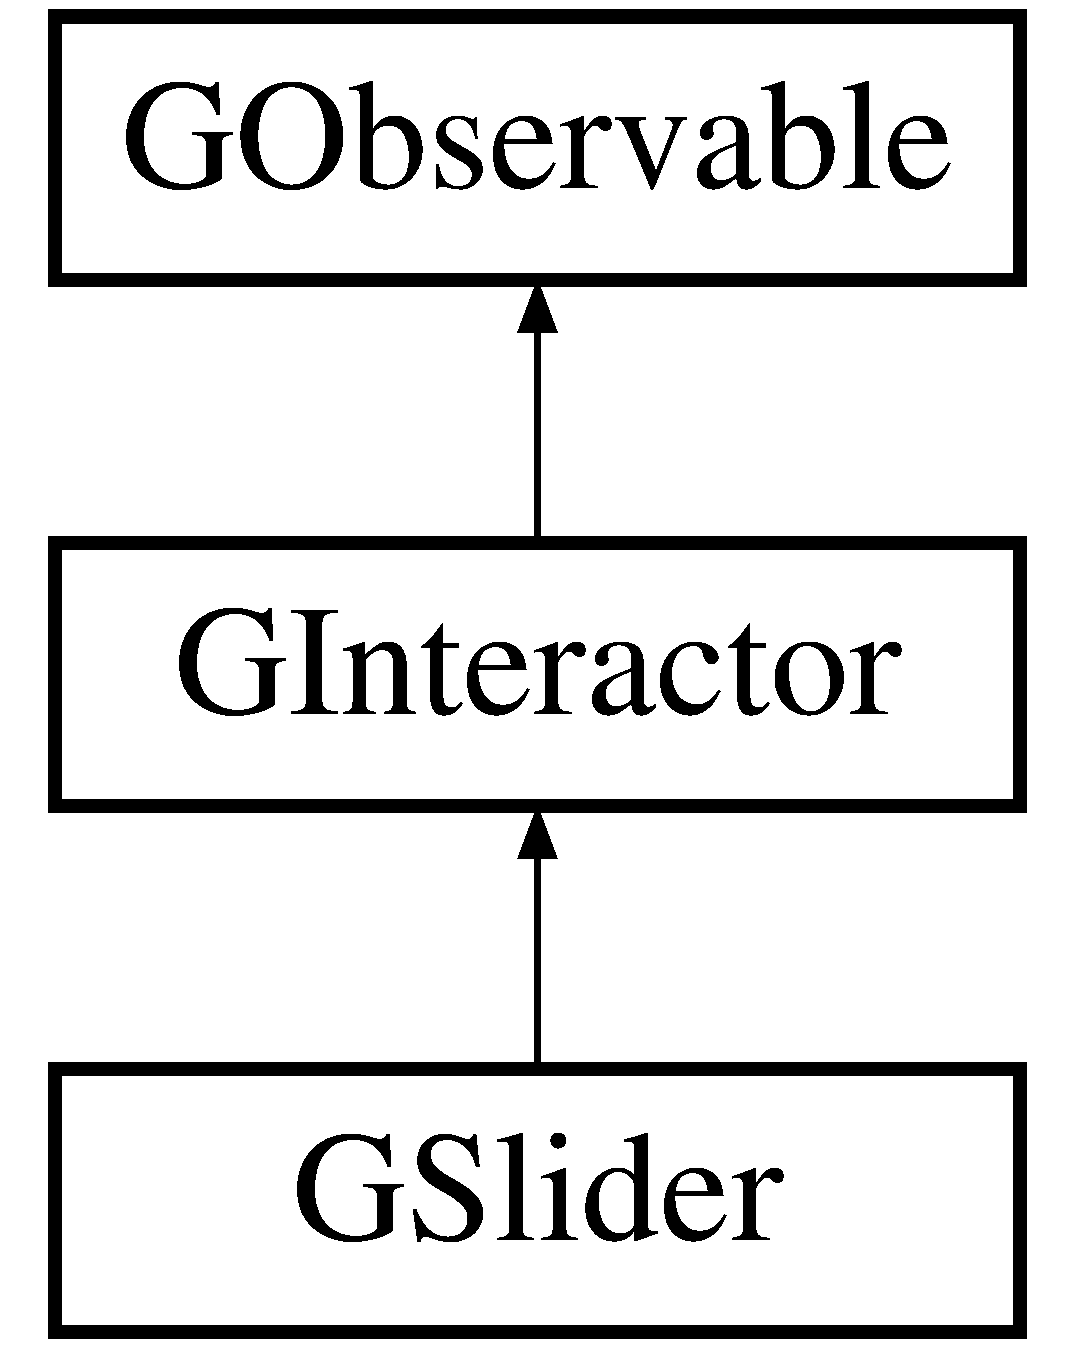
\includegraphics[height=3.000000cm]{classGSlider}
\end{center}
\end{figure}
\subsection*{Public Types}
\begin{DoxyCompactItemize}
\item 
enum \mbox{\hyperlink{classGSlider_a871118a09520247c78a71ecd7b0abd58}{Orientation}} \{ \mbox{\hyperlink{classGSlider_a871118a09520247c78a71ecd7b0abd58a4dd51ad73508d6fc83a502966779e48e}{H\+O\+R\+I\+Z\+O\+N\+T\+AL}} = 0, 
\mbox{\hyperlink{classGSlider_a871118a09520247c78a71ecd7b0abd58a1a88641fcd39f2ed3e58a18526e97138}{V\+E\+R\+T\+I\+C\+AL}} = 1
 \}
\begin{DoxyCompactList}\small\item\em The two valid orientations of sliders. \end{DoxyCompactList}\item 
enum \mbox{\hyperlink{classGInteractor_a8e0d441725a81d2bbdebbea09078260e}{Text\+Position}} \{ \mbox{\hyperlink{classGInteractor_a8e0d441725a81d2bbdebbea09078260ea4cd6f2e7d5a08d6f4dc052df2358f774}{T\+E\+X\+T\+\_\+\+B\+E\+S\+I\+D\+E\+\_\+\+I\+C\+ON}}, 
\mbox{\hyperlink{classGInteractor_a8e0d441725a81d2bbdebbea09078260eaa88490f63d8de68d44c83bdb2ecde3b3}{T\+E\+X\+T\+\_\+\+U\+N\+D\+E\+R\+\_\+\+I\+C\+ON}}, 
\mbox{\hyperlink{classGInteractor_a8e0d441725a81d2bbdebbea09078260ea39a6f388a30ac4fefb6eb13e846bc9f2}{T\+E\+X\+T\+\_\+\+O\+N\+LY}}
 \}
\begin{DoxyCompactList}\small\item\em The places where an interactor can place its text relative to its icon. \end{DoxyCompactList}\end{DoxyCompactItemize}
\subsection*{Public Member Functions}
\begin{DoxyCompactItemize}
\item 
\mbox{\hyperlink{classGSlider_a209c7847379ff5d2bad6fa6b09dd654f}{G\+Slider}} (int min=0, int max=100, int value=50, Q\+Widget $\ast$parent=nullptr)
\begin{DoxyCompactList}\small\item\em Creates a new horizontal slider with the given value range. \end{DoxyCompactList}\item 
\mbox{\hyperlink{classGSlider_ad317f09d4a94efa89b6c9319443c87df}{G\+Slider}} (\mbox{\hyperlink{classGSlider_a871118a09520247c78a71ecd7b0abd58}{Orientation}} orientation, int min=0, int max=100, int value=50, Q\+Widget $\ast$parent=nullptr)
\begin{DoxyCompactList}\small\item\em Creates a new horizontal or vertical slider with the given value range. \end{DoxyCompactList}\item 
virtual \mbox{\hyperlink{classGSlider_ab16da624fbdc1bba8ab6216dba6644c5}{$\sim$\+G\+Slider}} () Q\+\_\+\+D\+E\+C\+L\+\_\+\+O\+V\+E\+R\+R\+I\+DE
\begin{DoxyCompactList}\small\item\em Frees memory allocated internally by the slider. \end{DoxyCompactList}\item 
virtual void \mbox{\hyperlink{classGInteractor_a02f20ea6edfa0671f31c4c648a253833}{add\+Action\+Listener}} () Q\+\_\+\+D\+E\+C\+L\+\_\+\+D\+E\+P\+R\+E\+C\+A\+T\+ED
\begin{DoxyCompactList}\small\item\em Adds an event listener to be notified when this interactor is clicked or generally interacted with. \end{DoxyCompactList}\item 
virtual bool \mbox{\hyperlink{classGInteractor_ac05ba5b92e2e5146d416fe7f842a0969}{events\+Enabled}} () const Q\+\_\+\+D\+E\+C\+L\+\_\+\+O\+V\+E\+R\+R\+I\+DE
\begin{DoxyCompactList}\small\item\em Returns true if this interactor is currently accepting events. \end{DoxyCompactList}\item 
virtual std\+::string \mbox{\hyperlink{classGInteractor_a69f8d23ed8f207fbecad99960776e942}{get\+Accelerator}} () const
\begin{DoxyCompactList}\small\item\em Returns a string representing a hotkey for this interactor, or an empty string if no accelerator has been set. \end{DoxyCompactList}\item 
virtual std\+::string \mbox{\hyperlink{classGInteractor_a94eb4276000c4fdfb508ce9e6317a82a}{get\+Action\+Command}} () const
\begin{DoxyCompactList}\small\item\em Returns an action command for this interactor, which is a semi-\/unique string you can use to identify it when events occur. \end{DoxyCompactList}\item 
virtual std\+::string \mbox{\hyperlink{classGInteractor_a808e22cc1fdfbecf71ed8c64ef4600e0}{get\+Background}} () const
\begin{DoxyCompactList}\small\item\em Returns the background color of the interactor as a string. \end{DoxyCompactList}\item 
virtual int \mbox{\hyperlink{classGInteractor_a9e827257a55cb8cf4d9de2ec6bcfd7a0}{get\+Background\+Int}} () const
\begin{DoxyCompactList}\small\item\em Returns the background color of the interactor as an R\+GB integer. \end{DoxyCompactList}\item 
virtual \mbox{\hyperlink{classGRectangle}{G\+Rectangle}} \mbox{\hyperlink{classGInteractor_a29e6ac35a0b48f491a4c88194cc5da3b}{get\+Bounds}} () const
\begin{DoxyCompactList}\small\item\em Returns a rectangle representing the x/y position and size of this interactor. \end{DoxyCompactList}\item 
virtual std\+::string \mbox{\hyperlink{classGInteractor_aa061dfa488c31e18549d64363c1d0e34}{get\+Color}} () const
\begin{DoxyCompactList}\small\item\em Returns the foreground/text color of the interactor as a string. \end{DoxyCompactList}\item 
virtual int \mbox{\hyperlink{classGInteractor_a9635c7af766cdc3417f346683fa0e6c1}{get\+Color\+Int}} () const
\begin{DoxyCompactList}\small\item\em Returns the foreground/text color of the interactor as an R\+GB integer. \end{DoxyCompactList}\item 
virtual \mbox{\hyperlink{classGContainer}{G\+Container}} $\ast$ \mbox{\hyperlink{classGInteractor_a7a6e317c29d61030929b4cd2d1c00fe7}{get\+Container}} () const
\begin{DoxyCompactList}\small\item\em Returns a pointer to the onscreen container holding this interactor. \end{DoxyCompactList}\item 
virtual std\+::string \mbox{\hyperlink{classGInteractor_a894a5502900794eeb27d084c21f1d77d}{get\+Font}} () const
\begin{DoxyCompactList}\small\item\em Returns the font of this interactor\textquotesingle{}s text as a font string such as \char`\"{}\+Helvetica-\/12-\/\+Bold\char`\"{}. \end{DoxyCompactList}\item 
virtual std\+::string \mbox{\hyperlink{classGInteractor_a4fa2d8b0192a3a5b4af4bbfe71194d03}{get\+Foreground}} () const
\begin{DoxyCompactList}\small\item\em Returns the foreground/text color of the interactor as a string. \end{DoxyCompactList}\item 
virtual int \mbox{\hyperlink{classGInteractor_ac3b12ab385a6ef9ae90fc879860ba726}{get\+Foreground\+Int}} () const
\begin{DoxyCompactList}\small\item\em Returns the foreground/text color of the interactor as an R\+GB integer. \end{DoxyCompactList}\item 
virtual double \mbox{\hyperlink{classGInteractor_a1e7e353362434072875264cf95629f99}{get\+Height}} () const
\begin{DoxyCompactList}\small\item\em Returns the current onscreen height of this interactor in pixels. \end{DoxyCompactList}\item 
virtual std\+::string \mbox{\hyperlink{classGInteractor_aaed62a73004939a64da6f0eb9eb64d73}{get\+Icon}} () const
\begin{DoxyCompactList}\small\item\em Returns the file name of the icon associated with this interactor, or an empty string if no icon has been set. \end{DoxyCompactList}\item 
virtual int \mbox{\hyperlink{classGInteractor_a9c9659a6c6ba66b4107ba59c95a24241}{get\+ID}} () const
\begin{DoxyCompactList}\small\item\em Returns a globally unique identifier for this interactor, which is set when the interactor is constructed. \end{DoxyCompactList}\item 
virtual \+\_\+\+Internal\+\_\+\+Q\+Widget $\ast$ \mbox{\hyperlink{classGSlider_a208ce13c1da40bf0ddb509daf99d6588}{get\+Internal\+Widget}} () const Q\+\_\+\+D\+E\+C\+L\+\_\+\+O\+V\+E\+R\+R\+I\+DE
\begin{DoxyCompactList}\small\item\em Returns a direct pointer to the internal Qt widget being wrapped by this interactor. \end{DoxyCompactList}\item 
virtual \mbox{\hyperlink{classGPoint}{G\+Point}} \mbox{\hyperlink{classGInteractor_a4f83802015511edeb63b892830812c11}{get\+Location}} () const
\begin{DoxyCompactList}\small\item\em Returns an (x, y) point representing the onscreen location of the top-\/left corner of this interactor within its containing window. \end{DoxyCompactList}\item 
virtual int \mbox{\hyperlink{classGSlider_acc49776af85220307b8955d752d9ffcb}{get\+Max}} () const
\begin{DoxyCompactList}\small\item\em Returns the maximum allowed value of the slider. \end{DoxyCompactList}\item 
virtual int \mbox{\hyperlink{classGSlider_ad06537e69f71666d30bec18dc042a6e4}{get\+Min}} () const
\begin{DoxyCompactList}\small\item\em Returns the minimum allowed value of the slider. \end{DoxyCompactList}\item 
virtual double \mbox{\hyperlink{classGInteractor_aed4b0075fcc434499c3cb3e46896bda3}{get\+Minimum\+Height}} () const
\begin{DoxyCompactList}\small\item\em Returns the minimum height in pixels that this interactor will permit itself to be resized to. \end{DoxyCompactList}\item 
virtual \mbox{\hyperlink{classGDimension}{G\+Dimension}} \mbox{\hyperlink{classGInteractor_a66b5af0b32493b4d597ca0a3df2049ea}{get\+Minimum\+Size}} () const
\begin{DoxyCompactList}\small\item\em Returns a \mbox{\hyperlink{classGDimension}{G\+Dimension}} structure representing the minimum size in pixels that this interactor will permit itself to be resized to. \end{DoxyCompactList}\item 
virtual double \mbox{\hyperlink{classGInteractor_a59e668114fe3d49d2a0f28deb258f7c8}{get\+Minimum\+Width}} () const
\begin{DoxyCompactList}\small\item\em Returns the minimum width in pixels that this interactor will permit itself to be resized to. \end{DoxyCompactList}\item 
virtual std\+::string \mbox{\hyperlink{classGInteractor_a8a60438a5b55d0b2ceb35c8674b9d8c5}{get\+Name}} () const
\begin{DoxyCompactList}\small\item\em Returns a string representing a unique name for this interactor. \end{DoxyCompactList}\item 
virtual \mbox{\hyperlink{classGSlider_a871118a09520247c78a71ecd7b0abd58}{Orientation}} \mbox{\hyperlink{classGSlider_a43aa4aae2f77abd7de3bf461212ac8d0}{get\+Orientation}} () const
\begin{DoxyCompactList}\small\item\em Returns the orientation of the slider, either H\+O\+R\+I\+Z\+O\+N\+T\+AL or V\+E\+R\+T\+I\+C\+AL. \end{DoxyCompactList}\item 
virtual double \mbox{\hyperlink{classGInteractor_a747de0961653847bdc6615dbf756d715}{get\+Preferred\+Height}} () const
\begin{DoxyCompactList}\small\item\em Returns the height in pixels that this interactor would prefer to be, which would exactly fit its contents with no stretching or scrollbars. \end{DoxyCompactList}\item 
virtual \mbox{\hyperlink{classGDimension}{G\+Dimension}} \mbox{\hyperlink{classGInteractor_a4aabbee761d8e9116275401131b7ccd1}{get\+Preferred\+Size}} () const
\begin{DoxyCompactList}\small\item\em Returns a \mbox{\hyperlink{classGDimension}{G\+Dimension}} structure storing the width and height in pixels that this interactor would prefer to be, which would exactly fit its contents with no stretching or scrollbars. \end{DoxyCompactList}\item 
virtual double \mbox{\hyperlink{classGInteractor_a82bca31d37700fb0e35d2743352efd5e}{get\+Preferred\+Width}} () const
\begin{DoxyCompactList}\small\item\em Returns the height in pixels that this interactor would prefer to be, which would exactly fit its contents with no stretching or scrollbars. \end{DoxyCompactList}\item 
virtual \mbox{\hyperlink{classGDimension}{G\+Dimension}} \mbox{\hyperlink{classGInteractor_a7b4eec96a2bdc6420695d5796a78eea9}{get\+Size}} () const
\begin{DoxyCompactList}\small\item\em Returns a \mbox{\hyperlink{classGDimension}{G\+Dimension}} structure storing the current onscreen width and height of this interactor in pixels. \end{DoxyCompactList}\item 
virtual std\+::string \mbox{\hyperlink{classGSlider_a9896d58fcfebbf1025aeeb5b8b9ede80}{get\+Type}} () const Q\+\_\+\+D\+E\+C\+L\+\_\+\+O\+V\+E\+R\+R\+I\+DE
\begin{DoxyCompactList}\small\item\em Returns a string representing the class name of this interactor, such as \char`\"{}\+G\+Button\char`\"{} or \char`\"{}\+G\+Check\+Box\char`\"{}. \end{DoxyCompactList}\item 
virtual int \mbox{\hyperlink{classGSlider_acdb0b383a96801f3200302b6f4a7da64}{get\+Value}} () const
\begin{DoxyCompactList}\small\item\em Returns the slider\textquotesingle{}s current value. \end{DoxyCompactList}\item 
virtual Q\+Widget $\ast$ \mbox{\hyperlink{classGSlider_a326ee51b5561f807df7b29a1c101f7fd}{get\+Widget}} () const Q\+\_\+\+D\+E\+C\+L\+\_\+\+O\+V\+E\+R\+R\+I\+DE
\begin{DoxyCompactList}\small\item\em Returns a direct pointer to the internal Qt widget being wrapped by this interactor. \end{DoxyCompactList}\item 
virtual double \mbox{\hyperlink{classGInteractor_a0ed2965abd4f5701d2cadf71239faf19}{get\+Width}} () const
\begin{DoxyCompactList}\small\item\em Returns the current onscreen width of this interactor in pixels. \end{DoxyCompactList}\item 
virtual double \mbox{\hyperlink{classGInteractor_a344385751bee0720059403940d57a13e}{getX}} () const
\begin{DoxyCompactList}\small\item\em Returns the x-\/coordinate of the top-\/left pixel of this interactor within its onscreen window. \end{DoxyCompactList}\item 
virtual double \mbox{\hyperlink{classGInteractor_aafa51c7f8f38a09febbb9ce7853f77b4}{getY}} () const
\begin{DoxyCompactList}\small\item\em Returns the y-\/coordinate of the top-\/left pixel of this interactor within its onscreen window. \end{DoxyCompactList}\item 
virtual bool \mbox{\hyperlink{classGInteractor_afc480f652b8c5f1fb255e2269ce68879}{in\+Bounds}} (double x, double y) const
\begin{DoxyCompactList}\small\item\em Returns true if the given x/y pixel is within the bounds of this interactor. \end{DoxyCompactList}\item 
virtual bool \mbox{\hyperlink{classGInteractor_ae6d7982c1c627b677a5e776ca86118ed}{in\+Bounds}} (int x, int y) const
\begin{DoxyCompactList}\small\item\em Returns true if the given x/y pixel is within the bounds of this interactor. \end{DoxyCompactList}\item 
virtual bool \mbox{\hyperlink{classGInteractor_aacb819fb241851fd9fc045271baa4034}{is\+Enabled}} () const
\begin{DoxyCompactList}\small\item\em Returns true if this interactor is currently enabled. \end{DoxyCompactList}\item 
virtual bool \mbox{\hyperlink{classGInteractor_a9d8a6cfb13917785c143e74d40e4e2be}{is\+Visible}} () const
\begin{DoxyCompactList}\small\item\em Returns true if the interactor is visible on the screen. \end{DoxyCompactList}\item 
virtual void \mbox{\hyperlink{classGSlider_ab7fe7a876367b87cf7202f947f1d05e4}{remove\+Action\+Listener}} ()
\begin{DoxyCompactList}\small\item\em Removes the action listener from this slider so that it will no longer call it when events occur. \end{DoxyCompactList}\item 
virtual void \mbox{\hyperlink{classGInteractor_a519fb2ac767f8b2febbb50b898b8c8cb}{request\+Focus}} ()
\begin{DoxyCompactList}\small\item\em Transfers keyboard focus to this interactor. \end{DoxyCompactList}\item 
virtual void \mbox{\hyperlink{classGInteractor_ad15f102f62e2960576012f1aa0ba4b2e}{set\+Accelerator}} (const std\+::string \&accelerator)
\begin{DoxyCompactList}\small\item\em Sets an accelerator hotkey for this interactor, such as \char`\"{}\+Ctrl-\/\+S\char`\"{}. \end{DoxyCompactList}\item 
virtual void \mbox{\hyperlink{classGInteractor_a4b5843fe3030e038a1ba54cc03389bcf}{set\+Action\+Command}} (const std\+::string \&action\+Command)
\begin{DoxyCompactList}\small\item\em Sets the action command for this interactor. \end{DoxyCompactList}\item 
virtual void \mbox{\hyperlink{classGSlider_adcfb4742430c88714fcf57e57ab8ea9c}{set\+Action\+Listener}} (G\+Event\+Listener func)
\begin{DoxyCompactList}\small\item\em Sets an action listener on this slider so that it will be called when the user slides it to change its value. \end{DoxyCompactList}\item 
virtual void \mbox{\hyperlink{classGSlider_aebd20a89c7a8a43a6fce999cf4f9fcf2}{set\+Action\+Listener}} (G\+Event\+Listener\+Void func)
\begin{DoxyCompactList}\small\item\em Sets an action listener on this slider so that it will be called when the user slides it to change its value. \end{DoxyCompactList}\item 
virtual void \mbox{\hyperlink{classGInteractor_acba7e546c2025c0a15ca4b4cc92043db}{set\+Background}} (int rgb)
\begin{DoxyCompactList}\small\item\em Sets the background color of the interactor to the color represented by the given R\+GB integer. \end{DoxyCompactList}\item 
virtual void \mbox{\hyperlink{classGInteractor_ab4677ab2474e68b07aa56605af92a84a}{set\+Background}} (const std\+::string \&color)
\begin{DoxyCompactList}\small\item\em Sets the background color of the interactor to the color represented by the given string. \end{DoxyCompactList}\item 
virtual void \mbox{\hyperlink{classGInteractor_a2aae8197624b72265ab83b4f1bc73f2f}{set\+Bounds}} (double x, double y, double width, double height)
\begin{DoxyCompactList}\small\item\em Sets the size and location of the widget. \end{DoxyCompactList}\item 
virtual void \mbox{\hyperlink{classGInteractor_acada386653f008cacc7cce86426bef7c}{set\+Bounds}} (const \mbox{\hyperlink{classGRectangle}{G\+Rectangle}} \&size)
\begin{DoxyCompactList}\small\item\em Sets the size and location of the widget. \end{DoxyCompactList}\item 
virtual void \mbox{\hyperlink{classGInteractor_ab1f5cc0f5cc6bbbd716a526c61f1081d}{set\+Color}} (int rgb)
\begin{DoxyCompactList}\small\item\em Sets the foreground/text color of the interactor to the color represented by the given R\+GB integer. \end{DoxyCompactList}\item 
virtual void \mbox{\hyperlink{classGInteractor_a61374df6c11b52cfbb0815decdbaebc6}{set\+Color}} (const std\+::string \&color)
\begin{DoxyCompactList}\small\item\em Sets the foreground/text color of the interactor to the color represented by the given string. \end{DoxyCompactList}\item 
virtual void \mbox{\hyperlink{classGInteractor_ab831367dd84bbd579e02e55bacb21343}{set\+Enabled}} (bool value)
\begin{DoxyCompactList}\small\item\em Sets whether this interactor is currently enabled. \end{DoxyCompactList}\item 
virtual void \mbox{\hyperlink{classGObservable_afaa30b2a9e0f378fd1c70d2f1d0b8216}{set\+Events\+Enabled}} (bool \mbox{\hyperlink{classGInteractor_ac05ba5b92e2e5146d416fe7f842a0969}{events\+Enabled}})
\begin{DoxyCompactList}\small\item\em Sets whether the object is currently allowing itself to fire events. \end{DoxyCompactList}\item 
virtual void \mbox{\hyperlink{classGInteractor_a2592348886ffea646c6534bf88f7c49d}{set\+Font}} (const Q\+Font \&font)
\begin{DoxyCompactList}\small\item\em Sets the font used by this widget to the given Qt font. \end{DoxyCompactList}\item 
virtual void \mbox{\hyperlink{classGInteractor_a8e096e8818d838aceae1d46d58fb3a7b}{set\+Font}} (const std\+::string \&font)
\begin{DoxyCompactList}\small\item\em Sets the font used by this widget to the font represented by the given font string, such as \char`\"{}\+Helvetica-\/16-\/\+Bold\char`\"{}. \end{DoxyCompactList}\item 
virtual void \mbox{\hyperlink{classGInteractor_a9eb856b5ff83a19df3831a31f15f4563}{set\+Foreground}} (int rgb)
\begin{DoxyCompactList}\small\item\em Sets the foreground/text color of the interactor to the color represented by the given R\+GB integer. \end{DoxyCompactList}\item 
virtual void \mbox{\hyperlink{classGInteractor_af59209aeadea6dfc6d97a2d8531f50e1}{set\+Foreground}} (const std\+::string \&color)
\begin{DoxyCompactList}\small\item\em Sets the foreground/text color of the interactor to the color represented by the given string. \end{DoxyCompactList}\item 
virtual void \mbox{\hyperlink{classGInteractor_a9e280bfc4544dfaf8e4376c4e1a74357}{set\+Height}} (double height)
\begin{DoxyCompactList}\small\item\em Sets the onscreen height of the interactor in pixels. \end{DoxyCompactList}\item 
virtual void \mbox{\hyperlink{classGInteractor_a762e139aa311461c3984d3ad28293f64}{set\+Icon}} (const std\+::string \&filename, bool retain\+Icon\+Size=true)
\begin{DoxyCompactList}\small\item\em Sets the file name of the icon associated with this interactor, or an empty string if no icon has been set. \end{DoxyCompactList}\item 
virtual void \mbox{\hyperlink{classGInteractor_a04594e8ba9b98513a64f1da00dcae18c}{set\+Location}} (double x, double y)
\begin{DoxyCompactList}\small\item\em Sets the onscreen x/y-\/coordinate of the top-\/left corner of the interactor relative to its window. \end{DoxyCompactList}\item 
virtual void \mbox{\hyperlink{classGSlider_ab263d79bf430d73a617641f317dcfb98}{set\+Max}} (int max)
\begin{DoxyCompactList}\small\item\em Sets the maximum allowed value of the slider. \end{DoxyCompactList}\item 
virtual void \mbox{\hyperlink{classGSlider_a6dc44e5adc595b71f90efc65b0b5ea1d}{set\+Min}} (int min)
\begin{DoxyCompactList}\small\item\em Sets the minimum allowed value of the slider. \end{DoxyCompactList}\item 
virtual void \mbox{\hyperlink{classGInteractor_a0cf428e207b7f22cc08138a90b1b87b2}{set\+Minimum\+Size}} (double width, double height)
\begin{DoxyCompactList}\small\item\em Sets the minimum size in pixels that this interactor will permit itself to be resized to. \end{DoxyCompactList}\item 
virtual void \mbox{\hyperlink{classGInteractor_a3b1046117ac6cb7abe467e00ba8a81f4}{set\+Minimum\+Size}} (const \mbox{\hyperlink{classGDimension}{G\+Dimension}} \&size)
\begin{DoxyCompactList}\small\item\em Sets the minimum size in pixels that this interactor will permit itself to be resized to. \end{DoxyCompactList}\item 
virtual void \mbox{\hyperlink{classGInteractor_a9d3a2685df23b5e7cbf59c19c4a1f9b5}{set\+Name}} (const std\+::string \&name)
\begin{DoxyCompactList}\small\item\em Sets a string representing a unique name for this interactor. \end{DoxyCompactList}\item 
virtual void \mbox{\hyperlink{classGInteractor_a1ab987704fce32098706c6f00fb08218}{set\+Preferred\+Height}} (double height)
\begin{DoxyCompactList}\small\item\em Sets the height in pixels that this interactor would prefer to be. \end{DoxyCompactList}\item 
virtual void \mbox{\hyperlink{classGInteractor_a042c5ae19430d765ef552371cae3632c}{set\+Preferred\+Size}} (double width, double height)
\begin{DoxyCompactList}\small\item\em Sets the width and height in pixels that this interactor would prefer to be. \end{DoxyCompactList}\item 
virtual void \mbox{\hyperlink{classGInteractor_aa22d9be4bc0e078bb0ea69b0fc9d7c75}{set\+Preferred\+Size}} (const \mbox{\hyperlink{classGDimension}{G\+Dimension}} \&size)
\begin{DoxyCompactList}\small\item\em Sets the size in pixels that this interactor would prefer to be. \end{DoxyCompactList}\item 
virtual void \mbox{\hyperlink{classGInteractor_a3db429ab2fa52efd187eec0ed8cdd9f2}{set\+Preferred\+Width}} (double width)
\begin{DoxyCompactList}\small\item\em Sets the width in pixels that this interactor would prefer to be. \end{DoxyCompactList}\item 
virtual void \mbox{\hyperlink{classGSlider_a693c16cecd031a84aaf28be0427cff88}{set\+Range}} (int min, int max)
\begin{DoxyCompactList}\small\item\em Sets the min-\/max range of the slider. \end{DoxyCompactList}\item 
virtual void \mbox{\hyperlink{classGInteractor_aca25d49481f9bf5fc8f7df4c086c4ce7}{set\+Size}} (double width, double height)
\begin{DoxyCompactList}\small\item\em Sets the onscreen width and height of the interactor in pixels. \end{DoxyCompactList}\item 
virtual void \mbox{\hyperlink{classGInteractor_ae2b628228f192c2702c4ce941b2af68f}{set\+Size}} (const \mbox{\hyperlink{classGDimension}{G\+Dimension}} \&size)
\begin{DoxyCompactList}\small\item\em Sets the onscreen width and height of the interactor in pixels. \end{DoxyCompactList}\item 
virtual void \mbox{\hyperlink{classGSlider_ae7f0a959186167548911cc2c69ff6b39}{set\+State}} (int min, int max, int value)
\begin{DoxyCompactList}\small\item\em Sets all of the relevant state of the slider. \end{DoxyCompactList}\item 
virtual void \mbox{\hyperlink{classGInteractor_a039e0e49beaecc275efce02d416acea8}{set\+Tooltip}} (const std\+::string \&tooltip\+Text)
\begin{DoxyCompactList}\small\item\em Sets a \char`\"{}tooltip\char`\"{} that will appear if the user hovers their mouse over the interactor. \end{DoxyCompactList}\item 
virtual void \mbox{\hyperlink{classGSlider_a23d79e21b8ed72e19278ca31d47b8c87}{set\+Value}} (int value)
\begin{DoxyCompactList}\small\item\em Sets the current value of the slider. \end{DoxyCompactList}\item 
virtual void \mbox{\hyperlink{classGInteractor_a18e44e30b31525a243960ca3928125aa}{set\+Visible}} (bool visible)
\begin{DoxyCompactList}\small\item\em Returns true if the interactor is visible on the screen. \end{DoxyCompactList}\item 
virtual void \mbox{\hyperlink{classGInteractor_aa3f3fba4cb131baa8696ba01e3bceca1}{set\+Width}} (double width)
\begin{DoxyCompactList}\small\item\em Sets the onscreen width of the interactor in pixels. \end{DoxyCompactList}\item 
virtual void \mbox{\hyperlink{classGInteractor_a9c18fcc579333bf9653d13ad2b372e39}{setX}} (double x)
\begin{DoxyCompactList}\small\item\em Sets the onscreen x-\/coordinate of the top-\/left corner of the interactor relative to its window. \end{DoxyCompactList}\item 
virtual void \mbox{\hyperlink{classGInteractor_a7d57e2a5c35d27feb58fd498a3cf82b9}{setY}} (double y)
\begin{DoxyCompactList}\small\item\em Sets the onscreen y-\/coordinate of the top-\/left corner of the interactor relative to its window. \end{DoxyCompactList}\item 
virtual std\+::string \mbox{\hyperlink{classGObservable_a1fe5121d6528fdea3f243321b3fa3a49}{to\+String}} () const
\begin{DoxyCompactList}\small\item\em Returns a string representation of this observable object\textquotesingle{}s state. \end{DoxyCompactList}\end{DoxyCompactItemize}
\subsection*{Static Public Attributes}
\begin{DoxyCompactItemize}
\item 
static const int \mbox{\hyperlink{classGSlider_a8347129b4807bb7063f75ff2f457cc30}{D\+E\+F\+A\+U\+L\+T\+\_\+\+I\+N\+I\+T\+I\+A\+L\+\_\+\+V\+A\+L\+UE}} = 50
\begin{DoxyCompactList}\small\item\em Default initial value for a slider (50). \end{DoxyCompactList}\item 
static const int \mbox{\hyperlink{classGSlider_af4df8666449a1553ded0ebd926c1c847}{D\+E\+F\+A\+U\+L\+T\+\_\+\+M\+A\+X\+\_\+\+V\+A\+L\+UE}} = 100
\begin{DoxyCompactList}\small\item\em Default maximum value for a slider (100). \end{DoxyCompactList}\item 
static const int \mbox{\hyperlink{classGSlider_ada756074cb913647156250a2172a26f4}{D\+E\+F\+A\+U\+L\+T\+\_\+\+M\+I\+N\+\_\+\+V\+A\+L\+UE}} = 0
\begin{DoxyCompactList}\small\item\em Default minimum value for a slider (0). \end{DoxyCompactList}\end{DoxyCompactItemize}
\subsection*{Protected Member Functions}
\begin{DoxyCompactItemize}
\item 
virtual void \mbox{\hyperlink{classGObservable_a80cfa040459ff53594adbd6a51ec8f43}{clear\+Event\+Listeners}} ()
\begin{DoxyCompactList}\small\item\em Removes all event listeners from this object. \end{DoxyCompactList}\item 
virtual void \mbox{\hyperlink{classGObservable_a284f31528c0520f8e545c03ac9eeac74}{ensure\+Thread\+Safety}} (const std\+::string \&member\+Name=\char`\"{}\char`\"{})
\begin{DoxyCompactList}\small\item\em Ensures that we are currently in the Qt G\+UI thread. \end{DoxyCompactList}\item 
virtual void \mbox{\hyperlink{classGObservable_a63e5e5a6227c59c928493b11aceb0f67}{fire\+Event}} (\mbox{\hyperlink{classGEvent}{G\+Event}} \&event)
\begin{DoxyCompactList}\small\item\em Sends out the given event to any attached listeners. \end{DoxyCompactList}\item 
virtual void \mbox{\hyperlink{classGObservable_ab3983ea07337b52020a29cc00c653d8d}{fire\+G\+Event}} (Q\+Event $\ast$event, Event\+Type event\+Type, const std\+::string \&event\+Name)
\begin{DoxyCompactList}\small\item\em Creates an event of the given type, then sends it out to any attached listeners. \end{DoxyCompactList}\item 
virtual void \mbox{\hyperlink{classGObservable_a01fdf1b0e0dbd49e189fe4514e010411}{fire\+G\+Event}} (Q\+Close\+Event $\ast$event, Event\+Type event\+Type, const std\+::string \&event\+Name)
\begin{DoxyCompactList}\small\item\em Creates an event of the given type, then sends it out to any attached listeners. \end{DoxyCompactList}\item 
virtual void \mbox{\hyperlink{classGObservable_abb0b2f66ba39211cb5d7615e9d1c04e2}{fire\+G\+Event}} (Q\+Key\+Event $\ast$event, Event\+Type event\+Type, const std\+::string \&event\+Name)
\begin{DoxyCompactList}\small\item\em Creates an event of the given type, then sends it out to any attached listeners. \end{DoxyCompactList}\item 
virtual void \mbox{\hyperlink{classGObservable_a119318675d2165bdf7dd853aaf881d4b}{fire\+G\+Event}} (Q\+Mouse\+Event $\ast$event, Event\+Type event\+Type, const std\+::string \&event\+Name, const std\+::string \&action\+Command=\char`\"{}\char`\"{})
\begin{DoxyCompactList}\small\item\em Creates an event of the given type, then sends it out to any attached listeners. \end{DoxyCompactList}\item 
virtual void \mbox{\hyperlink{classGObservable_a63fd9034e1e1633c1c38eb342bfd34e9}{fire\+G\+Event}} (Q\+Resize\+Event $\ast$event, Event\+Type event\+Type, const std\+::string \&event\+Name)
\begin{DoxyCompactList}\small\item\em Creates an event of the given type, then sends it out to any attached listeners. \end{DoxyCompactList}\item 
virtual void \mbox{\hyperlink{classGObservable_a741345310d9b7c5170a6cbc410c44ac4}{fire\+G\+Event}} (Q\+Timer\+Event $\ast$event, Event\+Type event\+Type, const std\+::string \&event\+Name)
\begin{DoxyCompactList}\small\item\em Creates an event of the given type, then sends it out to any attached listeners. \end{DoxyCompactList}\item 
virtual void \mbox{\hyperlink{classGObservable_a93bf338968a0338761b8e4dc62f582e9}{fire\+G\+Event}} (Q\+Wheel\+Event $\ast$event, Event\+Type event\+Type, const std\+::string \&event\+Name)
\begin{DoxyCompactList}\small\item\em Creates an event of the given type, then sends it out to any attached listeners. \end{DoxyCompactList}\item 
virtual void \mbox{\hyperlink{classGObservable_a2a70a7d7435ff0c3b80bb4d70da19e0d}{fire\+G\+Event}} (Q\+Window\+State\+Change\+Event $\ast$event, Event\+Type event\+Type, const std\+::string \&event\+Name)
\begin{DoxyCompactList}\small\item\em Creates an event of the given type, then sends it out to any attached listeners. \end{DoxyCompactList}\item 
virtual bool \mbox{\hyperlink{classGObservable_a9f6faaa25942923bafa1c44020c49fa9}{has\+Event\+Listener}} (const std\+::string \&event\+Name) const
\begin{DoxyCompactList}\small\item\em Returns true if the observable object has a listener for the given type of event. \end{DoxyCompactList}\item 
virtual bool \mbox{\hyperlink{classGObservable_aeec1adc19aa0f33de62390686ee1382c}{is\+Accepting\+Event}} (int event\+Mask) const
\begin{DoxyCompactList}\small\item\em Returns true if the observable object has a listener for the given type of event. \end{DoxyCompactList}\item 
virtual bool \mbox{\hyperlink{classGObservable_aa31c73145a29dcb92848a92e0cfaea41}{is\+Accepting\+Event}} (const \mbox{\hyperlink{classGEvent}{G\+Event}} \&event) const
\begin{DoxyCompactList}\small\item\em Returns true if the observable object has a listener for the given type of event. \end{DoxyCompactList}\item 
virtual bool \mbox{\hyperlink{classGObservable_a3b1c689267eda44e65a2213e7de38b23}{is\+Accepting\+Event}} (const std\+::string \&event\+Type) const
\begin{DoxyCompactList}\small\item\em Returns true if the observable object has a listener for the given type of event. \end{DoxyCompactList}\item 
virtual void \mbox{\hyperlink{classGObservable_acbcf1ed3a851ad8a3c17ef38d86b481d}{remove\+Event\+Listener}} (const std\+::string \&event\+Name)
\begin{DoxyCompactList}\small\item\em Removes any event listener from this observable object that would respond to the given type of event, such as \char`\"{}click\char`\"{} or \char`\"{}keydown\char`\"{}. \end{DoxyCompactList}\item 
virtual void \mbox{\hyperlink{classGObservable_af51cc35c29a1bd1908609d432decdbb6}{remove\+Event\+Listeners}} (std\+::initializer\+\_\+list$<$ std\+::string $>$ event\+Names)
\begin{DoxyCompactList}\small\item\em Removes any event listener from this observable object that would respond to the given types of events, such as \char`\"{}click\char`\"{} or \char`\"{}keydown\char`\"{}. \end{DoxyCompactList}\item 
virtual void \mbox{\hyperlink{classGObservable_ad2f6d34961c50f6c1e0659990b79f741}{set\+Event\+Listener}} (const std\+::string \&event\+Name, G\+Event\+Listener func)
\begin{DoxyCompactList}\small\item\em Adds an event listener from this observable object to respond to the given type of event, such as \char`\"{}click\char`\"{} or \char`\"{}keydown\char`\"{}. \end{DoxyCompactList}\item 
virtual void \mbox{\hyperlink{classGObservable_abac4cb9f9e626e010e87f5d91573c8a5}{set\+Event\+Listener}} (const std\+::string \&event\+Name, G\+Event\+Listener\+Void func)
\begin{DoxyCompactList}\small\item\em Adds an event listener from this observable object to respond to the given type of event, such as \char`\"{}click\char`\"{} or \char`\"{}keydown\char`\"{}. \end{DoxyCompactList}\item 
virtual void \mbox{\hyperlink{classGObservable_afa388d69c33c718cf035774604065604}{set\+Event\+Listeners}} (std\+::initializer\+\_\+list$<$ std\+::string $>$ event\+Names, G\+Event\+Listener func)
\begin{DoxyCompactList}\small\item\em Adds an event listener from this observable object to respond to the given types of events, such as \char`\"{}click\char`\"{} or \char`\"{}keydown\char`\"{}. \end{DoxyCompactList}\item 
virtual void \mbox{\hyperlink{classGObservable_a7867184bbb686f74fae8a4db927da799}{set\+Event\+Listeners}} (std\+::initializer\+\_\+list$<$ std\+::string $>$ event\+Names, G\+Event\+Listener\+Void func)
\begin{DoxyCompactList}\small\item\em Adds an event listener from this observable object to respond to the given types of events, such as \char`\"{}click\char`\"{} or \char`\"{}keydown\char`\"{}. \end{DoxyCompactList}\end{DoxyCompactItemize}


\subsection{Detailed Description}
This interactor subclass represents an onscreen slider. 

Dragging the slider control generates action events. 

\subsection{Member Enumeration Documentation}
\mbox{\Hypertarget{classGSlider_a871118a09520247c78a71ecd7b0abd58}\label{classGSlider_a871118a09520247c78a71ecd7b0abd58}} 
\index{G\+Slider@{G\+Slider}!Orientation@{Orientation}}
\index{Orientation@{Orientation}!G\+Slider@{G\+Slider}}
\subsubsection{\texorpdfstring{Orientation}{Orientation}}
{\footnotesize\ttfamily enum \mbox{\hyperlink{classGSlider_a871118a09520247c78a71ecd7b0abd58}{Orientation}}}



The two valid orientations of sliders. 

\begin{DoxyEnumFields}{Enumerator}
\raisebox{\heightof{T}}[0pt][0pt]{\index{H\+O\+R\+I\+Z\+O\+N\+T\+AL@{H\+O\+R\+I\+Z\+O\+N\+T\+AL}!G\+Slider@{G\+Slider}}\index{G\+Slider@{G\+Slider}!H\+O\+R\+I\+Z\+O\+N\+T\+AL@{H\+O\+R\+I\+Z\+O\+N\+T\+AL}}}\mbox{\Hypertarget{classGSlider_a871118a09520247c78a71ecd7b0abd58a4dd51ad73508d6fc83a502966779e48e}\label{classGSlider_a871118a09520247c78a71ecd7b0abd58a4dd51ad73508d6fc83a502966779e48e}} 
H\+O\+R\+I\+Z\+O\+N\+T\+AL&\\
\hline

\raisebox{\heightof{T}}[0pt][0pt]{\index{V\+E\+R\+T\+I\+C\+AL@{V\+E\+R\+T\+I\+C\+AL}!G\+Slider@{G\+Slider}}\index{G\+Slider@{G\+Slider}!V\+E\+R\+T\+I\+C\+AL@{V\+E\+R\+T\+I\+C\+AL}}}\mbox{\Hypertarget{classGSlider_a871118a09520247c78a71ecd7b0abd58a1a88641fcd39f2ed3e58a18526e97138}\label{classGSlider_a871118a09520247c78a71ecd7b0abd58a1a88641fcd39f2ed3e58a18526e97138}} 
V\+E\+R\+T\+I\+C\+AL&\\
\hline

\end{DoxyEnumFields}
\mbox{\Hypertarget{classGInteractor_a8e0d441725a81d2bbdebbea09078260e}\label{classGInteractor_a8e0d441725a81d2bbdebbea09078260e}} 
\index{G\+Slider@{G\+Slider}!Text\+Position@{Text\+Position}}
\index{Text\+Position@{Text\+Position}!G\+Slider@{G\+Slider}}
\subsubsection{\texorpdfstring{Text\+Position}{TextPosition}}
{\footnotesize\ttfamily enum \mbox{\hyperlink{classGInteractor_a8e0d441725a81d2bbdebbea09078260e}{Text\+Position}}\hspace{0.3cm}{\ttfamily [inherited]}}



The places where an interactor can place its text relative to its icon. 

\begin{DoxyEnumFields}{Enumerator}
\raisebox{\heightof{T}}[0pt][0pt]{\index{T\+E\+X\+T\+\_\+\+B\+E\+S\+I\+D\+E\+\_\+\+I\+C\+ON@{T\+E\+X\+T\+\_\+\+B\+E\+S\+I\+D\+E\+\_\+\+I\+C\+ON}!G\+Slider@{G\+Slider}}\index{G\+Slider@{G\+Slider}!T\+E\+X\+T\+\_\+\+B\+E\+S\+I\+D\+E\+\_\+\+I\+C\+ON@{T\+E\+X\+T\+\_\+\+B\+E\+S\+I\+D\+E\+\_\+\+I\+C\+ON}}}\mbox{\Hypertarget{classGInteractor_a8e0d441725a81d2bbdebbea09078260ea4cd6f2e7d5a08d6f4dc052df2358f774}\label{classGInteractor_a8e0d441725a81d2bbdebbea09078260ea4cd6f2e7d5a08d6f4dc052df2358f774}} 
T\+E\+X\+T\+\_\+\+B\+E\+S\+I\+D\+E\+\_\+\+I\+C\+ON&\\
\hline

\raisebox{\heightof{T}}[0pt][0pt]{\index{T\+E\+X\+T\+\_\+\+U\+N\+D\+E\+R\+\_\+\+I\+C\+ON@{T\+E\+X\+T\+\_\+\+U\+N\+D\+E\+R\+\_\+\+I\+C\+ON}!G\+Slider@{G\+Slider}}\index{G\+Slider@{G\+Slider}!T\+E\+X\+T\+\_\+\+U\+N\+D\+E\+R\+\_\+\+I\+C\+ON@{T\+E\+X\+T\+\_\+\+U\+N\+D\+E\+R\+\_\+\+I\+C\+ON}}}\mbox{\Hypertarget{classGInteractor_a8e0d441725a81d2bbdebbea09078260eaa88490f63d8de68d44c83bdb2ecde3b3}\label{classGInteractor_a8e0d441725a81d2bbdebbea09078260eaa88490f63d8de68d44c83bdb2ecde3b3}} 
T\+E\+X\+T\+\_\+\+U\+N\+D\+E\+R\+\_\+\+I\+C\+ON&\\
\hline

\raisebox{\heightof{T}}[0pt][0pt]{\index{T\+E\+X\+T\+\_\+\+O\+N\+LY@{T\+E\+X\+T\+\_\+\+O\+N\+LY}!G\+Slider@{G\+Slider}}\index{G\+Slider@{G\+Slider}!T\+E\+X\+T\+\_\+\+O\+N\+LY@{T\+E\+X\+T\+\_\+\+O\+N\+LY}}}\mbox{\Hypertarget{classGInteractor_a8e0d441725a81d2bbdebbea09078260ea39a6f388a30ac4fefb6eb13e846bc9f2}\label{classGInteractor_a8e0d441725a81d2bbdebbea09078260ea39a6f388a30ac4fefb6eb13e846bc9f2}} 
T\+E\+X\+T\+\_\+\+O\+N\+LY&\\
\hline

\end{DoxyEnumFields}


\subsection{Constructor \& Destructor Documentation}
\mbox{\Hypertarget{classGSlider_a209c7847379ff5d2bad6fa6b09dd654f}\label{classGSlider_a209c7847379ff5d2bad6fa6b09dd654f}} 
\index{G\+Slider@{G\+Slider}!G\+Slider@{G\+Slider}}
\index{G\+Slider@{G\+Slider}!G\+Slider@{G\+Slider}}
\subsubsection{\texorpdfstring{G\+Slider()}{GSlider()}\hspace{0.1cm}{\footnotesize\ttfamily [1/2]}}
{\footnotesize\ttfamily \mbox{\hyperlink{classGSlider}{G\+Slider}} (\begin{DoxyParamCaption}\item[{int}]{min = {\ttfamily 0},  }\item[{int}]{max = {\ttfamily 100},  }\item[{int}]{value = {\ttfamily 50},  }\item[{Q\+Widget $\ast$}]{parent = {\ttfamily nullptr} }\end{DoxyParamCaption})}



Creates a new horizontal slider with the given value range. 


\begin{DoxyExceptions}{Exceptions}
{\em \mbox{\hyperlink{classErrorException}{Error\+Exception}}} & if min $>$ max or value is not between min and max \\
\hline
\end{DoxyExceptions}
\mbox{\Hypertarget{classGSlider_ad317f09d4a94efa89b6c9319443c87df}\label{classGSlider_ad317f09d4a94efa89b6c9319443c87df}} 
\index{G\+Slider@{G\+Slider}!G\+Slider@{G\+Slider}}
\index{G\+Slider@{G\+Slider}!G\+Slider@{G\+Slider}}
\subsubsection{\texorpdfstring{G\+Slider()}{GSlider()}\hspace{0.1cm}{\footnotesize\ttfamily [2/2]}}
{\footnotesize\ttfamily \mbox{\hyperlink{classGSlider}{G\+Slider}} (\begin{DoxyParamCaption}\item[{\mbox{\hyperlink{classGSlider_a871118a09520247c78a71ecd7b0abd58}{Orientation}}}]{orientation,  }\item[{int}]{min = {\ttfamily 0},  }\item[{int}]{max = {\ttfamily 100},  }\item[{int}]{value = {\ttfamily 50},  }\item[{Q\+Widget $\ast$}]{parent = {\ttfamily nullptr} }\end{DoxyParamCaption})}



Creates a new horizontal or vertical slider with the given value range. 


\begin{DoxyExceptions}{Exceptions}
{\em \mbox{\hyperlink{classErrorException}{Error\+Exception}}} & if min $>$ max or value is not between min and max \\
\hline
\end{DoxyExceptions}
\mbox{\Hypertarget{classGSlider_ab16da624fbdc1bba8ab6216dba6644c5}\label{classGSlider_ab16da624fbdc1bba8ab6216dba6644c5}} 
\index{G\+Slider@{G\+Slider}!````~G\+Slider@{$\sim$\+G\+Slider}}
\index{````~G\+Slider@{$\sim$\+G\+Slider}!G\+Slider@{G\+Slider}}
\subsubsection{\texorpdfstring{$\sim$\+G\+Slider()}{~GSlider()}}
{\footnotesize\ttfamily $\sim$\mbox{\hyperlink{classGSlider}{G\+Slider}} (\begin{DoxyParamCaption}{ }\end{DoxyParamCaption})\hspace{0.3cm}{\ttfamily [virtual]}}



Frees memory allocated internally by the slider. 



\subsection{Member Function Documentation}
\mbox{\Hypertarget{classGInteractor_a02f20ea6edfa0671f31c4c648a253833}\label{classGInteractor_a02f20ea6edfa0671f31c4c648a253833}} 
\index{G\+Slider@{G\+Slider}!add\+Action\+Listener@{add\+Action\+Listener}}
\index{add\+Action\+Listener@{add\+Action\+Listener}!G\+Slider@{G\+Slider}}
\subsubsection{\texorpdfstring{add\+Action\+Listener()}{addActionListener()}}
{\footnotesize\ttfamily void add\+Action\+Listener (\begin{DoxyParamCaption}{ }\end{DoxyParamCaption})\hspace{0.3cm}{\ttfamily [virtual]}, {\ttfamily [inherited]}}



Adds an event listener to be notified when this interactor is clicked or generally interacted with. 

\begin{DoxyRefDesc}{Deprecated}
\item[\mbox{\hyperlink{deprecated__deprecated000006}{Deprecated}}]does nothing; use set\+Action\+Listener instead \end{DoxyRefDesc}
\mbox{\Hypertarget{classGObservable_a80cfa040459ff53594adbd6a51ec8f43}\label{classGObservable_a80cfa040459ff53594adbd6a51ec8f43}} 
\index{G\+Slider@{G\+Slider}!clear\+Event\+Listeners@{clear\+Event\+Listeners}}
\index{clear\+Event\+Listeners@{clear\+Event\+Listeners}!G\+Slider@{G\+Slider}}
\subsubsection{\texorpdfstring{clear\+Event\+Listeners()}{clearEventListeners()}}
{\footnotesize\ttfamily void clear\+Event\+Listeners (\begin{DoxyParamCaption}{ }\end{DoxyParamCaption})\hspace{0.3cm}{\ttfamily [protected]}, {\ttfamily [virtual]}, {\ttfamily [inherited]}}



Removes all event listeners from this object. 

\mbox{\Hypertarget{classGObservable_a284f31528c0520f8e545c03ac9eeac74}\label{classGObservable_a284f31528c0520f8e545c03ac9eeac74}} 
\index{G\+Slider@{G\+Slider}!ensure\+Thread\+Safety@{ensure\+Thread\+Safety}}
\index{ensure\+Thread\+Safety@{ensure\+Thread\+Safety}!G\+Slider@{G\+Slider}}
\subsubsection{\texorpdfstring{ensure\+Thread\+Safety()}{ensureThreadSafety()}}
{\footnotesize\ttfamily void ensure\+Thread\+Safety (\begin{DoxyParamCaption}\item[{const std\+::string \&}]{member\+Name = {\ttfamily \char`\"{}\char`\"{}} }\end{DoxyParamCaption})\hspace{0.3cm}{\ttfamily [protected]}, {\ttfamily [virtual]}, {\ttfamily [inherited]}}



Ensures that we are currently in the Qt G\+UI thread. 

\mbox{\Hypertarget{classGInteractor_ac05ba5b92e2e5146d416fe7f842a0969}\label{classGInteractor_ac05ba5b92e2e5146d416fe7f842a0969}} 
\index{G\+Slider@{G\+Slider}!events\+Enabled@{events\+Enabled}}
\index{events\+Enabled@{events\+Enabled}!G\+Slider@{G\+Slider}}
\subsubsection{\texorpdfstring{events\+Enabled()}{eventsEnabled()}}
{\footnotesize\ttfamily bool events\+Enabled (\begin{DoxyParamCaption}{ }\end{DoxyParamCaption}) const\hspace{0.3cm}{\ttfamily [virtual]}, {\ttfamily [inherited]}}



Returns true if this interactor is currently accepting events. 

Initially true. An interactor must be visible and added to an onscreen window to receive events. 

Reimplemented from \mbox{\hyperlink{classGObservable_a8ebb3da91032e7f4c34485dabc518b8a}{G\+Observable}}.

\mbox{\Hypertarget{classGObservable_a63e5e5a6227c59c928493b11aceb0f67}\label{classGObservable_a63e5e5a6227c59c928493b11aceb0f67}} 
\index{G\+Slider@{G\+Slider}!fire\+Event@{fire\+Event}}
\index{fire\+Event@{fire\+Event}!G\+Slider@{G\+Slider}}
\subsubsection{\texorpdfstring{fire\+Event()}{fireEvent()}}
{\footnotesize\ttfamily void fire\+Event (\begin{DoxyParamCaption}\item[{\mbox{\hyperlink{classGEvent}{G\+Event}} \&}]{event }\end{DoxyParamCaption})\hspace{0.3cm}{\ttfamily [protected]}, {\ttfamily [virtual]}, {\ttfamily [inherited]}}



Sends out the given event to any attached listeners. 

\mbox{\Hypertarget{classGObservable_ab3983ea07337b52020a29cc00c653d8d}\label{classGObservable_ab3983ea07337b52020a29cc00c653d8d}} 
\index{G\+Slider@{G\+Slider}!fire\+G\+Event@{fire\+G\+Event}}
\index{fire\+G\+Event@{fire\+G\+Event}!G\+Slider@{G\+Slider}}
\subsubsection{\texorpdfstring{fire\+G\+Event()}{fireGEvent()}\hspace{0.1cm}{\footnotesize\ttfamily [1/8]}}
{\footnotesize\ttfamily void fire\+G\+Event (\begin{DoxyParamCaption}\item[{Q\+Event $\ast$}]{event,  }\item[{Event\+Type}]{event\+Type,  }\item[{const std\+::string \&}]{event\+Name }\end{DoxyParamCaption})\hspace{0.3cm}{\ttfamily [protected]}, {\ttfamily [virtual]}, {\ttfamily [inherited]}}



Creates an event of the given type, then sends it out to any attached listeners. 

\mbox{\Hypertarget{classGObservable_a01fdf1b0e0dbd49e189fe4514e010411}\label{classGObservable_a01fdf1b0e0dbd49e189fe4514e010411}} 
\index{G\+Slider@{G\+Slider}!fire\+G\+Event@{fire\+G\+Event}}
\index{fire\+G\+Event@{fire\+G\+Event}!G\+Slider@{G\+Slider}}
\subsubsection{\texorpdfstring{fire\+G\+Event()}{fireGEvent()}\hspace{0.1cm}{\footnotesize\ttfamily [2/8]}}
{\footnotesize\ttfamily void fire\+G\+Event (\begin{DoxyParamCaption}\item[{Q\+Close\+Event $\ast$}]{event,  }\item[{Event\+Type}]{event\+Type,  }\item[{const std\+::string \&}]{event\+Name }\end{DoxyParamCaption})\hspace{0.3cm}{\ttfamily [protected]}, {\ttfamily [virtual]}, {\ttfamily [inherited]}}



Creates an event of the given type, then sends it out to any attached listeners. 

\mbox{\Hypertarget{classGObservable_abb0b2f66ba39211cb5d7615e9d1c04e2}\label{classGObservable_abb0b2f66ba39211cb5d7615e9d1c04e2}} 
\index{G\+Slider@{G\+Slider}!fire\+G\+Event@{fire\+G\+Event}}
\index{fire\+G\+Event@{fire\+G\+Event}!G\+Slider@{G\+Slider}}
\subsubsection{\texorpdfstring{fire\+G\+Event()}{fireGEvent()}\hspace{0.1cm}{\footnotesize\ttfamily [3/8]}}
{\footnotesize\ttfamily void fire\+G\+Event (\begin{DoxyParamCaption}\item[{Q\+Key\+Event $\ast$}]{event,  }\item[{Event\+Type}]{event\+Type,  }\item[{const std\+::string \&}]{event\+Name }\end{DoxyParamCaption})\hspace{0.3cm}{\ttfamily [protected]}, {\ttfamily [virtual]}, {\ttfamily [inherited]}}



Creates an event of the given type, then sends it out to any attached listeners. 

\mbox{\Hypertarget{classGObservable_a119318675d2165bdf7dd853aaf881d4b}\label{classGObservable_a119318675d2165bdf7dd853aaf881d4b}} 
\index{G\+Slider@{G\+Slider}!fire\+G\+Event@{fire\+G\+Event}}
\index{fire\+G\+Event@{fire\+G\+Event}!G\+Slider@{G\+Slider}}
\subsubsection{\texorpdfstring{fire\+G\+Event()}{fireGEvent()}\hspace{0.1cm}{\footnotesize\ttfamily [4/8]}}
{\footnotesize\ttfamily void fire\+G\+Event (\begin{DoxyParamCaption}\item[{Q\+Mouse\+Event $\ast$}]{event,  }\item[{Event\+Type}]{event\+Type,  }\item[{const std\+::string \&}]{event\+Name,  }\item[{const std\+::string \&}]{action\+Command = {\ttfamily \char`\"{}\char`\"{}} }\end{DoxyParamCaption})\hspace{0.3cm}{\ttfamily [protected]}, {\ttfamily [virtual]}, {\ttfamily [inherited]}}



Creates an event of the given type, then sends it out to any attached listeners. 

\mbox{\Hypertarget{classGObservable_a63fd9034e1e1633c1c38eb342bfd34e9}\label{classGObservable_a63fd9034e1e1633c1c38eb342bfd34e9}} 
\index{G\+Slider@{G\+Slider}!fire\+G\+Event@{fire\+G\+Event}}
\index{fire\+G\+Event@{fire\+G\+Event}!G\+Slider@{G\+Slider}}
\subsubsection{\texorpdfstring{fire\+G\+Event()}{fireGEvent()}\hspace{0.1cm}{\footnotesize\ttfamily [5/8]}}
{\footnotesize\ttfamily void fire\+G\+Event (\begin{DoxyParamCaption}\item[{Q\+Resize\+Event $\ast$}]{event,  }\item[{Event\+Type}]{event\+Type,  }\item[{const std\+::string \&}]{event\+Name }\end{DoxyParamCaption})\hspace{0.3cm}{\ttfamily [protected]}, {\ttfamily [virtual]}, {\ttfamily [inherited]}}



Creates an event of the given type, then sends it out to any attached listeners. 

\mbox{\Hypertarget{classGObservable_a741345310d9b7c5170a6cbc410c44ac4}\label{classGObservable_a741345310d9b7c5170a6cbc410c44ac4}} 
\index{G\+Slider@{G\+Slider}!fire\+G\+Event@{fire\+G\+Event}}
\index{fire\+G\+Event@{fire\+G\+Event}!G\+Slider@{G\+Slider}}
\subsubsection{\texorpdfstring{fire\+G\+Event()}{fireGEvent()}\hspace{0.1cm}{\footnotesize\ttfamily [6/8]}}
{\footnotesize\ttfamily void fire\+G\+Event (\begin{DoxyParamCaption}\item[{Q\+Timer\+Event $\ast$}]{event,  }\item[{Event\+Type}]{event\+Type,  }\item[{const std\+::string \&}]{event\+Name }\end{DoxyParamCaption})\hspace{0.3cm}{\ttfamily [protected]}, {\ttfamily [virtual]}, {\ttfamily [inherited]}}



Creates an event of the given type, then sends it out to any attached listeners. 

\mbox{\Hypertarget{classGObservable_a93bf338968a0338761b8e4dc62f582e9}\label{classGObservable_a93bf338968a0338761b8e4dc62f582e9}} 
\index{G\+Slider@{G\+Slider}!fire\+G\+Event@{fire\+G\+Event}}
\index{fire\+G\+Event@{fire\+G\+Event}!G\+Slider@{G\+Slider}}
\subsubsection{\texorpdfstring{fire\+G\+Event()}{fireGEvent()}\hspace{0.1cm}{\footnotesize\ttfamily [7/8]}}
{\footnotesize\ttfamily void fire\+G\+Event (\begin{DoxyParamCaption}\item[{Q\+Wheel\+Event $\ast$}]{event,  }\item[{Event\+Type}]{event\+Type,  }\item[{const std\+::string \&}]{event\+Name }\end{DoxyParamCaption})\hspace{0.3cm}{\ttfamily [protected]}, {\ttfamily [virtual]}, {\ttfamily [inherited]}}



Creates an event of the given type, then sends it out to any attached listeners. 

\mbox{\Hypertarget{classGObservable_a2a70a7d7435ff0c3b80bb4d70da19e0d}\label{classGObservable_a2a70a7d7435ff0c3b80bb4d70da19e0d}} 
\index{G\+Slider@{G\+Slider}!fire\+G\+Event@{fire\+G\+Event}}
\index{fire\+G\+Event@{fire\+G\+Event}!G\+Slider@{G\+Slider}}
\subsubsection{\texorpdfstring{fire\+G\+Event()}{fireGEvent()}\hspace{0.1cm}{\footnotesize\ttfamily [8/8]}}
{\footnotesize\ttfamily void fire\+G\+Event (\begin{DoxyParamCaption}\item[{Q\+Window\+State\+Change\+Event $\ast$}]{event,  }\item[{Event\+Type}]{event\+Type,  }\item[{const std\+::string \&}]{event\+Name }\end{DoxyParamCaption})\hspace{0.3cm}{\ttfamily [protected]}, {\ttfamily [virtual]}, {\ttfamily [inherited]}}



Creates an event of the given type, then sends it out to any attached listeners. 

\mbox{\Hypertarget{classGInteractor_a69f8d23ed8f207fbecad99960776e942}\label{classGInteractor_a69f8d23ed8f207fbecad99960776e942}} 
\index{G\+Slider@{G\+Slider}!get\+Accelerator@{get\+Accelerator}}
\index{get\+Accelerator@{get\+Accelerator}!G\+Slider@{G\+Slider}}
\subsubsection{\texorpdfstring{get\+Accelerator()}{getAccelerator()}}
{\footnotesize\ttfamily std\+::string get\+Accelerator (\begin{DoxyParamCaption}{ }\end{DoxyParamCaption}) const\hspace{0.3cm}{\ttfamily [virtual]}, {\ttfamily [inherited]}}



Returns a string representing a hotkey for this interactor, or an empty string if no accelerator has been set. 

\begin{DoxyReturn}{Returns}
an accelerator such as \char`\"{}\+Ctrl-\/\+S\char`\"{} 
\end{DoxyReturn}


Reimplemented in \mbox{\hyperlink{classGButton_a432ca43c59ffb2adc9cb66d43621bc27}{G\+Button}}.

\mbox{\Hypertarget{classGInteractor_a94eb4276000c4fdfb508ce9e6317a82a}\label{classGInteractor_a94eb4276000c4fdfb508ce9e6317a82a}} 
\index{G\+Slider@{G\+Slider}!get\+Action\+Command@{get\+Action\+Command}}
\index{get\+Action\+Command@{get\+Action\+Command}!G\+Slider@{G\+Slider}}
\subsubsection{\texorpdfstring{get\+Action\+Command()}{getActionCommand()}}
{\footnotesize\ttfamily std\+::string get\+Action\+Command (\begin{DoxyParamCaption}{ }\end{DoxyParamCaption}) const\hspace{0.3cm}{\ttfamily [virtual]}, {\ttfamily [inherited]}}



Returns an action command for this interactor, which is a semi-\/unique string you can use to identify it when events occur. 

For example, for buttons, the default action command is the button\textquotesingle{}s text. 

Reimplemented in \mbox{\hyperlink{classGChooser_a90f2b1e6f6e7dabd9d6e5307f7c6d1b7}{G\+Chooser}}, \mbox{\hyperlink{classGRadioButton_a90f2b1e6f6e7dabd9d6e5307f7c6d1b7}{G\+Radio\+Button}}, \mbox{\hyperlink{classGCheckBox_a90f2b1e6f6e7dabd9d6e5307f7c6d1b7}{G\+Check\+Box}}, and \mbox{\hyperlink{classGButton_a90f2b1e6f6e7dabd9d6e5307f7c6d1b7}{G\+Button}}.

\mbox{\Hypertarget{classGInteractor_a808e22cc1fdfbecf71ed8c64ef4600e0}\label{classGInteractor_a808e22cc1fdfbecf71ed8c64ef4600e0}} 
\index{G\+Slider@{G\+Slider}!get\+Background@{get\+Background}}
\index{get\+Background@{get\+Background}!G\+Slider@{G\+Slider}}
\subsubsection{\texorpdfstring{get\+Background()}{getBackground()}}
{\footnotesize\ttfamily std\+::string get\+Background (\begin{DoxyParamCaption}{ }\end{DoxyParamCaption}) const\hspace{0.3cm}{\ttfamily [virtual]}, {\ttfamily [inherited]}}



Returns the background color of the interactor as a string. 

\begin{DoxyReturn}{Returns}
a string such as \char`\"{}blue\char`\"{} or \char`\"{}\#7700ff\char`\"{} 
\end{DoxyReturn}


Reimplemented in \mbox{\hyperlink{classGCanvas_ab44f928b6bd7c8e4b82d5ed92bc3d4c6}{G\+Canvas}}.

\mbox{\Hypertarget{classGInteractor_a9e827257a55cb8cf4d9de2ec6bcfd7a0}\label{classGInteractor_a9e827257a55cb8cf4d9de2ec6bcfd7a0}} 
\index{G\+Slider@{G\+Slider}!get\+Background\+Int@{get\+Background\+Int}}
\index{get\+Background\+Int@{get\+Background\+Int}!G\+Slider@{G\+Slider}}
\subsubsection{\texorpdfstring{get\+Background\+Int()}{getBackgroundInt()}}
{\footnotesize\ttfamily int get\+Background\+Int (\begin{DoxyParamCaption}{ }\end{DoxyParamCaption}) const\hspace{0.3cm}{\ttfamily [virtual]}, {\ttfamily [inherited]}}



Returns the background color of the interactor as an R\+GB integer. 

\begin{DoxyReturn}{Returns}
an integer such as 0x7700ff 
\end{DoxyReturn}


Reimplemented in \mbox{\hyperlink{classGCanvas_af66f525e8154dbc8dcd2daecf3728ba9}{G\+Canvas}}.

\mbox{\Hypertarget{classGInteractor_a29e6ac35a0b48f491a4c88194cc5da3b}\label{classGInteractor_a29e6ac35a0b48f491a4c88194cc5da3b}} 
\index{G\+Slider@{G\+Slider}!get\+Bounds@{get\+Bounds}}
\index{get\+Bounds@{get\+Bounds}!G\+Slider@{G\+Slider}}
\subsubsection{\texorpdfstring{get\+Bounds()}{getBounds()}}
{\footnotesize\ttfamily \mbox{\hyperlink{classGRectangle}{G\+Rectangle}} get\+Bounds (\begin{DoxyParamCaption}{ }\end{DoxyParamCaption}) const\hspace{0.3cm}{\ttfamily [virtual]}, {\ttfamily [inherited]}}



Returns a rectangle representing the x/y position and size of this interactor. 

\mbox{\Hypertarget{classGInteractor_aa061dfa488c31e18549d64363c1d0e34}\label{classGInteractor_aa061dfa488c31e18549d64363c1d0e34}} 
\index{G\+Slider@{G\+Slider}!get\+Color@{get\+Color}}
\index{get\+Color@{get\+Color}!G\+Slider@{G\+Slider}}
\subsubsection{\texorpdfstring{get\+Color()}{getColor()}}
{\footnotesize\ttfamily std\+::string get\+Color (\begin{DoxyParamCaption}{ }\end{DoxyParamCaption}) const\hspace{0.3cm}{\ttfamily [virtual]}, {\ttfamily [inherited]}}



Returns the foreground/text color of the interactor as a string. 

Equivalent to get\+Foreground. \begin{DoxyReturn}{Returns}
a string such as \char`\"{}blue\char`\"{} or \char`\"{}\#7700ff\char`\"{} 
\end{DoxyReturn}
\mbox{\Hypertarget{classGInteractor_a9635c7af766cdc3417f346683fa0e6c1}\label{classGInteractor_a9635c7af766cdc3417f346683fa0e6c1}} 
\index{G\+Slider@{G\+Slider}!get\+Color\+Int@{get\+Color\+Int}}
\index{get\+Color\+Int@{get\+Color\+Int}!G\+Slider@{G\+Slider}}
\subsubsection{\texorpdfstring{get\+Color\+Int()}{getColorInt()}}
{\footnotesize\ttfamily int get\+Color\+Int (\begin{DoxyParamCaption}{ }\end{DoxyParamCaption}) const\hspace{0.3cm}{\ttfamily [virtual]}, {\ttfamily [inherited]}}



Returns the foreground/text color of the interactor as an R\+GB integer. 

Equivalent to get\+Foreground\+Int. \begin{DoxyReturn}{Returns}
an integer such as 0x7700ff 
\end{DoxyReturn}
\mbox{\Hypertarget{classGInteractor_a7a6e317c29d61030929b4cd2d1c00fe7}\label{classGInteractor_a7a6e317c29d61030929b4cd2d1c00fe7}} 
\index{G\+Slider@{G\+Slider}!get\+Container@{get\+Container}}
\index{get\+Container@{get\+Container}!G\+Slider@{G\+Slider}}
\subsubsection{\texorpdfstring{get\+Container()}{getContainer()}}
{\footnotesize\ttfamily \mbox{\hyperlink{classGContainer}{G\+Container}} $\ast$ get\+Container (\begin{DoxyParamCaption}{ }\end{DoxyParamCaption}) const\hspace{0.3cm}{\ttfamily [virtual]}, {\ttfamily [inherited]}}



Returns a pointer to the onscreen container holding this interactor. 

When an interactor is created, its container is initially null. This will become non-\/null automatically if you add the interactor to a window or other layout container. Interactors must be added to a container or window to receive events or to become visible on the screen. \begin{DoxyReturn}{Returns}
the container, or nullptr if interactor has not yet been added to any container 
\end{DoxyReturn}
\mbox{\Hypertarget{classGInteractor_a894a5502900794eeb27d084c21f1d77d}\label{classGInteractor_a894a5502900794eeb27d084c21f1d77d}} 
\index{G\+Slider@{G\+Slider}!get\+Font@{get\+Font}}
\index{get\+Font@{get\+Font}!G\+Slider@{G\+Slider}}
\subsubsection{\texorpdfstring{get\+Font()}{getFont()}}
{\footnotesize\ttfamily std\+::string get\+Font (\begin{DoxyParamCaption}{ }\end{DoxyParamCaption}) const\hspace{0.3cm}{\ttfamily [virtual]}, {\ttfamily [inherited]}}



Returns the font of this interactor\textquotesingle{}s text as a font string such as \char`\"{}\+Helvetica-\/12-\/\+Bold\char`\"{}. 

\begin{DoxyReturn}{Returns}
a font string such as \char`\"{}\+Helvetica-\/12-\/\+Bold\char`\"{} 
\end{DoxyReturn}


Reimplemented in \mbox{\hyperlink{classGCanvas_a24420d98f18927d2c201a3ab55ffdcec}{G\+Canvas}}.

\mbox{\Hypertarget{classGInteractor_a4fa2d8b0192a3a5b4af4bbfe71194d03}\label{classGInteractor_a4fa2d8b0192a3a5b4af4bbfe71194d03}} 
\index{G\+Slider@{G\+Slider}!get\+Foreground@{get\+Foreground}}
\index{get\+Foreground@{get\+Foreground}!G\+Slider@{G\+Slider}}
\subsubsection{\texorpdfstring{get\+Foreground()}{getForeground()}}
{\footnotesize\ttfamily std\+::string get\+Foreground (\begin{DoxyParamCaption}{ }\end{DoxyParamCaption}) const\hspace{0.3cm}{\ttfamily [virtual]}, {\ttfamily [inherited]}}



Returns the foreground/text color of the interactor as a string. 

Equivalent to get\+Color. \begin{DoxyReturn}{Returns}
a string such as \char`\"{}blue\char`\"{} or \char`\"{}\#7700ff\char`\"{} 
\end{DoxyReturn}
\mbox{\Hypertarget{classGInteractor_ac3b12ab385a6ef9ae90fc879860ba726}\label{classGInteractor_ac3b12ab385a6ef9ae90fc879860ba726}} 
\index{G\+Slider@{G\+Slider}!get\+Foreground\+Int@{get\+Foreground\+Int}}
\index{get\+Foreground\+Int@{get\+Foreground\+Int}!G\+Slider@{G\+Slider}}
\subsubsection{\texorpdfstring{get\+Foreground\+Int()}{getForegroundInt()}}
{\footnotesize\ttfamily int get\+Foreground\+Int (\begin{DoxyParamCaption}{ }\end{DoxyParamCaption}) const\hspace{0.3cm}{\ttfamily [virtual]}, {\ttfamily [inherited]}}



Returns the foreground/text color of the interactor as an R\+GB integer. 

Equivalent to get\+Color\+Int. \begin{DoxyReturn}{Returns}
an integer such as 0x7700ff 
\end{DoxyReturn}
\mbox{\Hypertarget{classGInteractor_a1e7e353362434072875264cf95629f99}\label{classGInteractor_a1e7e353362434072875264cf95629f99}} 
\index{G\+Slider@{G\+Slider}!get\+Height@{get\+Height}}
\index{get\+Height@{get\+Height}!G\+Slider@{G\+Slider}}
\subsubsection{\texorpdfstring{get\+Height()}{getHeight()}}
{\footnotesize\ttfamily double get\+Height (\begin{DoxyParamCaption}{ }\end{DoxyParamCaption}) const\hspace{0.3cm}{\ttfamily [virtual]}, {\ttfamily [inherited]}}



Returns the current onscreen height of this interactor in pixels. 

\mbox{\Hypertarget{classGInteractor_aaed62a73004939a64da6f0eb9eb64d73}\label{classGInteractor_aaed62a73004939a64da6f0eb9eb64d73}} 
\index{G\+Slider@{G\+Slider}!get\+Icon@{get\+Icon}}
\index{get\+Icon@{get\+Icon}!G\+Slider@{G\+Slider}}
\subsubsection{\texorpdfstring{get\+Icon()}{getIcon()}}
{\footnotesize\ttfamily std\+::string get\+Icon (\begin{DoxyParamCaption}{ }\end{DoxyParamCaption}) const\hspace{0.3cm}{\ttfamily [virtual]}, {\ttfamily [inherited]}}



Returns the file name of the icon associated with this interactor, or an empty string if no icon has been set. 

Not all types of interactors support icons. \mbox{\Hypertarget{classGInteractor_a9c9659a6c6ba66b4107ba59c95a24241}\label{classGInteractor_a9c9659a6c6ba66b4107ba59c95a24241}} 
\index{G\+Slider@{G\+Slider}!get\+ID@{get\+ID}}
\index{get\+ID@{get\+ID}!G\+Slider@{G\+Slider}}
\subsubsection{\texorpdfstring{get\+I\+D()}{getID()}}
{\footnotesize\ttfamily int get\+ID (\begin{DoxyParamCaption}{ }\end{DoxyParamCaption}) const\hspace{0.3cm}{\ttfamily [virtual]}, {\ttfamily [inherited]}}



Returns a globally unique identifier for this interactor, which is set when the interactor is constructed. 

These I\+Ds can be useful for debugging to help identify interactors uniquely. \mbox{\Hypertarget{classGSlider_a208ce13c1da40bf0ddb509daf99d6588}\label{classGSlider_a208ce13c1da40bf0ddb509daf99d6588}} 
\index{G\+Slider@{G\+Slider}!get\+Internal\+Widget@{get\+Internal\+Widget}}
\index{get\+Internal\+Widget@{get\+Internal\+Widget}!G\+Slider@{G\+Slider}}
\subsubsection{\texorpdfstring{get\+Internal\+Widget()}{getInternalWidget()}}
{\footnotesize\ttfamily \+\_\+\+Internal\+\_\+\+Q\+Widget $\ast$ get\+Internal\+Widget (\begin{DoxyParamCaption}{ }\end{DoxyParamCaption}) const\hspace{0.3cm}{\ttfamily [virtual]}}



Returns a direct pointer to the internal Qt widget being wrapped by this interactor. 

This must be overridden by all interactor subclasses. Students/clients generally should not need to call this. 

Implements \mbox{\hyperlink{classGInteractor}{G\+Interactor}}.

\mbox{\Hypertarget{classGInteractor_a4f83802015511edeb63b892830812c11}\label{classGInteractor_a4f83802015511edeb63b892830812c11}} 
\index{G\+Slider@{G\+Slider}!get\+Location@{get\+Location}}
\index{get\+Location@{get\+Location}!G\+Slider@{G\+Slider}}
\subsubsection{\texorpdfstring{get\+Location()}{getLocation()}}
{\footnotesize\ttfamily \mbox{\hyperlink{classGPoint}{G\+Point}} get\+Location (\begin{DoxyParamCaption}{ }\end{DoxyParamCaption}) const\hspace{0.3cm}{\ttfamily [virtual]}, {\ttfamily [inherited]}}



Returns an (x, y) point representing the onscreen location of the top-\/left corner of this interactor within its containing window. 

\mbox{\Hypertarget{classGSlider_acc49776af85220307b8955d752d9ffcb}\label{classGSlider_acc49776af85220307b8955d752d9ffcb}} 
\index{G\+Slider@{G\+Slider}!get\+Max@{get\+Max}}
\index{get\+Max@{get\+Max}!G\+Slider@{G\+Slider}}
\subsubsection{\texorpdfstring{get\+Max()}{getMax()}}
{\footnotesize\ttfamily int get\+Max (\begin{DoxyParamCaption}{ }\end{DoxyParamCaption}) const\hspace{0.3cm}{\ttfamily [virtual]}}



Returns the maximum allowed value of the slider. 

\mbox{\Hypertarget{classGSlider_ad06537e69f71666d30bec18dc042a6e4}\label{classGSlider_ad06537e69f71666d30bec18dc042a6e4}} 
\index{G\+Slider@{G\+Slider}!get\+Min@{get\+Min}}
\index{get\+Min@{get\+Min}!G\+Slider@{G\+Slider}}
\subsubsection{\texorpdfstring{get\+Min()}{getMin()}}
{\footnotesize\ttfamily int get\+Min (\begin{DoxyParamCaption}{ }\end{DoxyParamCaption}) const\hspace{0.3cm}{\ttfamily [virtual]}}



Returns the minimum allowed value of the slider. 

\mbox{\Hypertarget{classGInteractor_aed4b0075fcc434499c3cb3e46896bda3}\label{classGInteractor_aed4b0075fcc434499c3cb3e46896bda3}} 
\index{G\+Slider@{G\+Slider}!get\+Minimum\+Height@{get\+Minimum\+Height}}
\index{get\+Minimum\+Height@{get\+Minimum\+Height}!G\+Slider@{G\+Slider}}
\subsubsection{\texorpdfstring{get\+Minimum\+Height()}{getMinimumHeight()}}
{\footnotesize\ttfamily double get\+Minimum\+Height (\begin{DoxyParamCaption}{ }\end{DoxyParamCaption}) const\hspace{0.3cm}{\ttfamily [virtual]}, {\ttfamily [inherited]}}



Returns the minimum height in pixels that this interactor will permit itself to be resized to. 

\mbox{\Hypertarget{classGInteractor_a66b5af0b32493b4d597ca0a3df2049ea}\label{classGInteractor_a66b5af0b32493b4d597ca0a3df2049ea}} 
\index{G\+Slider@{G\+Slider}!get\+Minimum\+Size@{get\+Minimum\+Size}}
\index{get\+Minimum\+Size@{get\+Minimum\+Size}!G\+Slider@{G\+Slider}}
\subsubsection{\texorpdfstring{get\+Minimum\+Size()}{getMinimumSize()}}
{\footnotesize\ttfamily \mbox{\hyperlink{classGDimension}{G\+Dimension}} get\+Minimum\+Size (\begin{DoxyParamCaption}{ }\end{DoxyParamCaption}) const\hspace{0.3cm}{\ttfamily [virtual]}, {\ttfamily [inherited]}}



Returns a \mbox{\hyperlink{classGDimension}{G\+Dimension}} structure representing the minimum size in pixels that this interactor will permit itself to be resized to. 

\mbox{\Hypertarget{classGInteractor_a59e668114fe3d49d2a0f28deb258f7c8}\label{classGInteractor_a59e668114fe3d49d2a0f28deb258f7c8}} 
\index{G\+Slider@{G\+Slider}!get\+Minimum\+Width@{get\+Minimum\+Width}}
\index{get\+Minimum\+Width@{get\+Minimum\+Width}!G\+Slider@{G\+Slider}}
\subsubsection{\texorpdfstring{get\+Minimum\+Width()}{getMinimumWidth()}}
{\footnotesize\ttfamily double get\+Minimum\+Width (\begin{DoxyParamCaption}{ }\end{DoxyParamCaption}) const\hspace{0.3cm}{\ttfamily [virtual]}, {\ttfamily [inherited]}}



Returns the minimum width in pixels that this interactor will permit itself to be resized to. 

\mbox{\Hypertarget{classGInteractor_a8a60438a5b55d0b2ceb35c8674b9d8c5}\label{classGInteractor_a8a60438a5b55d0b2ceb35c8674b9d8c5}} 
\index{G\+Slider@{G\+Slider}!get\+Name@{get\+Name}}
\index{get\+Name@{get\+Name}!G\+Slider@{G\+Slider}}
\subsubsection{\texorpdfstring{get\+Name()}{getName()}}
{\footnotesize\ttfamily std\+::string get\+Name (\begin{DoxyParamCaption}{ }\end{DoxyParamCaption}) const\hspace{0.3cm}{\ttfamily [virtual]}, {\ttfamily [inherited]}}



Returns a string representing a unique name for this interactor. 

The default name string uses the interactor\textquotesingle{}s type and its ID to make a string like \char`\"{}\+G\+Button\+\_\+14\char`\"{}, but you can override this by calling set\+Name. \begin{DoxyReturn}{Returns}
a string such as \char`\"{}\+G\+Button\+\_\+14\char`\"{} 
\end{DoxyReturn}
\mbox{\Hypertarget{classGSlider_a43aa4aae2f77abd7de3bf461212ac8d0}\label{classGSlider_a43aa4aae2f77abd7de3bf461212ac8d0}} 
\index{G\+Slider@{G\+Slider}!get\+Orientation@{get\+Orientation}}
\index{get\+Orientation@{get\+Orientation}!G\+Slider@{G\+Slider}}
\subsubsection{\texorpdfstring{get\+Orientation()}{getOrientation()}}
{\footnotesize\ttfamily \mbox{\hyperlink{classGSlider_a871118a09520247c78a71ecd7b0abd58}{G\+Slider\+::\+Orientation}} get\+Orientation (\begin{DoxyParamCaption}{ }\end{DoxyParamCaption}) const\hspace{0.3cm}{\ttfamily [virtual]}}



Returns the orientation of the slider, either H\+O\+R\+I\+Z\+O\+N\+T\+AL or V\+E\+R\+T\+I\+C\+AL. 

\mbox{\Hypertarget{classGInteractor_a747de0961653847bdc6615dbf756d715}\label{classGInteractor_a747de0961653847bdc6615dbf756d715}} 
\index{G\+Slider@{G\+Slider}!get\+Preferred\+Height@{get\+Preferred\+Height}}
\index{get\+Preferred\+Height@{get\+Preferred\+Height}!G\+Slider@{G\+Slider}}
\subsubsection{\texorpdfstring{get\+Preferred\+Height()}{getPreferredHeight()}}
{\footnotesize\ttfamily double get\+Preferred\+Height (\begin{DoxyParamCaption}{ }\end{DoxyParamCaption}) const\hspace{0.3cm}{\ttfamily [virtual]}, {\ttfamily [inherited]}}



Returns the height in pixels that this interactor would prefer to be, which would exactly fit its contents with no stretching or scrollbars. 

\mbox{\Hypertarget{classGInteractor_a4aabbee761d8e9116275401131b7ccd1}\label{classGInteractor_a4aabbee761d8e9116275401131b7ccd1}} 
\index{G\+Slider@{G\+Slider}!get\+Preferred\+Size@{get\+Preferred\+Size}}
\index{get\+Preferred\+Size@{get\+Preferred\+Size}!G\+Slider@{G\+Slider}}
\subsubsection{\texorpdfstring{get\+Preferred\+Size()}{getPreferredSize()}}
{\footnotesize\ttfamily \mbox{\hyperlink{classGDimension}{G\+Dimension}} get\+Preferred\+Size (\begin{DoxyParamCaption}{ }\end{DoxyParamCaption}) const\hspace{0.3cm}{\ttfamily [virtual]}, {\ttfamily [inherited]}}



Returns a \mbox{\hyperlink{classGDimension}{G\+Dimension}} structure storing the width and height in pixels that this interactor would prefer to be, which would exactly fit its contents with no stretching or scrollbars. 



Reimplemented in \mbox{\hyperlink{classGContainer_a21904b305edacd8f871d6951cb8d3fa5}{G\+Container}}.

\mbox{\Hypertarget{classGInteractor_a82bca31d37700fb0e35d2743352efd5e}\label{classGInteractor_a82bca31d37700fb0e35d2743352efd5e}} 
\index{G\+Slider@{G\+Slider}!get\+Preferred\+Width@{get\+Preferred\+Width}}
\index{get\+Preferred\+Width@{get\+Preferred\+Width}!G\+Slider@{G\+Slider}}
\subsubsection{\texorpdfstring{get\+Preferred\+Width()}{getPreferredWidth()}}
{\footnotesize\ttfamily double get\+Preferred\+Width (\begin{DoxyParamCaption}{ }\end{DoxyParamCaption}) const\hspace{0.3cm}{\ttfamily [virtual]}, {\ttfamily [inherited]}}



Returns the height in pixels that this interactor would prefer to be, which would exactly fit its contents with no stretching or scrollbars. 

\mbox{\Hypertarget{classGInteractor_a7b4eec96a2bdc6420695d5796a78eea9}\label{classGInteractor_a7b4eec96a2bdc6420695d5796a78eea9}} 
\index{G\+Slider@{G\+Slider}!get\+Size@{get\+Size}}
\index{get\+Size@{get\+Size}!G\+Slider@{G\+Slider}}
\subsubsection{\texorpdfstring{get\+Size()}{getSize()}}
{\footnotesize\ttfamily \mbox{\hyperlink{classGDimension}{G\+Dimension}} get\+Size (\begin{DoxyParamCaption}{ }\end{DoxyParamCaption}) const\hspace{0.3cm}{\ttfamily [virtual]}, {\ttfamily [inherited]}}



Returns a \mbox{\hyperlink{classGDimension}{G\+Dimension}} structure storing the current onscreen width and height of this interactor in pixels. 

\mbox{\Hypertarget{classGSlider_a9896d58fcfebbf1025aeeb5b8b9ede80}\label{classGSlider_a9896d58fcfebbf1025aeeb5b8b9ede80}} 
\index{G\+Slider@{G\+Slider}!get\+Type@{get\+Type}}
\index{get\+Type@{get\+Type}!G\+Slider@{G\+Slider}}
\subsubsection{\texorpdfstring{get\+Type()}{getType()}}
{\footnotesize\ttfamily std\+::string get\+Type (\begin{DoxyParamCaption}{ }\end{DoxyParamCaption}) const\hspace{0.3cm}{\ttfamily [virtual]}}



Returns a string representing the class name of this interactor, such as \char`\"{}\+G\+Button\char`\"{} or \char`\"{}\+G\+Check\+Box\char`\"{}. 

All subclasses of \mbox{\hyperlink{classGInteractor}{G\+Interactor}} must implement this method. \begin{DoxyReturn}{Returns}
a string such as \char`\"{}\+G\+Check\+Box\char`\"{} 
\end{DoxyReturn}


Implements \mbox{\hyperlink{classGInteractor_a799e073a127b428cc841086d42ea4fed}{G\+Interactor}}.

\mbox{\Hypertarget{classGSlider_acdb0b383a96801f3200302b6f4a7da64}\label{classGSlider_acdb0b383a96801f3200302b6f4a7da64}} 
\index{G\+Slider@{G\+Slider}!get\+Value@{get\+Value}}
\index{get\+Value@{get\+Value}!G\+Slider@{G\+Slider}}
\subsubsection{\texorpdfstring{get\+Value()}{getValue()}}
{\footnotesize\ttfamily int get\+Value (\begin{DoxyParamCaption}{ }\end{DoxyParamCaption}) const\hspace{0.3cm}{\ttfamily [virtual]}}



Returns the slider\textquotesingle{}s current value. 

\mbox{\Hypertarget{classGSlider_a326ee51b5561f807df7b29a1c101f7fd}\label{classGSlider_a326ee51b5561f807df7b29a1c101f7fd}} 
\index{G\+Slider@{G\+Slider}!get\+Widget@{get\+Widget}}
\index{get\+Widget@{get\+Widget}!G\+Slider@{G\+Slider}}
\subsubsection{\texorpdfstring{get\+Widget()}{getWidget()}}
{\footnotesize\ttfamily Q\+Widget $\ast$ get\+Widget (\begin{DoxyParamCaption}{ }\end{DoxyParamCaption}) const\hspace{0.3cm}{\ttfamily [virtual]}}



Returns a direct pointer to the internal Qt widget being wrapped by this interactor. 

This must be overridden by all interactor subclasses. Students/clients generally should not need to call this. 

Implements \mbox{\hyperlink{classGInteractor}{G\+Interactor}}.

\mbox{\Hypertarget{classGInteractor_a0ed2965abd4f5701d2cadf71239faf19}\label{classGInteractor_a0ed2965abd4f5701d2cadf71239faf19}} 
\index{G\+Slider@{G\+Slider}!get\+Width@{get\+Width}}
\index{get\+Width@{get\+Width}!G\+Slider@{G\+Slider}}
\subsubsection{\texorpdfstring{get\+Width()}{getWidth()}}
{\footnotesize\ttfamily double get\+Width (\begin{DoxyParamCaption}{ }\end{DoxyParamCaption}) const\hspace{0.3cm}{\ttfamily [virtual]}, {\ttfamily [inherited]}}



Returns the current onscreen width of this interactor in pixels. 

\mbox{\Hypertarget{classGInteractor_a344385751bee0720059403940d57a13e}\label{classGInteractor_a344385751bee0720059403940d57a13e}} 
\index{G\+Slider@{G\+Slider}!getX@{getX}}
\index{getX@{getX}!G\+Slider@{G\+Slider}}
\subsubsection{\texorpdfstring{get\+X()}{getX()}}
{\footnotesize\ttfamily double getX (\begin{DoxyParamCaption}{ }\end{DoxyParamCaption}) const\hspace{0.3cm}{\ttfamily [virtual]}, {\ttfamily [inherited]}}



Returns the x-\/coordinate of the top-\/left pixel of this interactor within its onscreen window. 

\mbox{\Hypertarget{classGInteractor_aafa51c7f8f38a09febbb9ce7853f77b4}\label{classGInteractor_aafa51c7f8f38a09febbb9ce7853f77b4}} 
\index{G\+Slider@{G\+Slider}!getY@{getY}}
\index{getY@{getY}!G\+Slider@{G\+Slider}}
\subsubsection{\texorpdfstring{get\+Y()}{getY()}}
{\footnotesize\ttfamily double getY (\begin{DoxyParamCaption}{ }\end{DoxyParamCaption}) const\hspace{0.3cm}{\ttfamily [virtual]}, {\ttfamily [inherited]}}



Returns the y-\/coordinate of the top-\/left pixel of this interactor within its onscreen window. 

\mbox{\Hypertarget{classGObservable_a9f6faaa25942923bafa1c44020c49fa9}\label{classGObservable_a9f6faaa25942923bafa1c44020c49fa9}} 
\index{G\+Slider@{G\+Slider}!has\+Event\+Listener@{has\+Event\+Listener}}
\index{has\+Event\+Listener@{has\+Event\+Listener}!G\+Slider@{G\+Slider}}
\subsubsection{\texorpdfstring{has\+Event\+Listener()}{hasEventListener()}}
{\footnotesize\ttfamily bool has\+Event\+Listener (\begin{DoxyParamCaption}\item[{const std\+::string \&}]{event\+Name }\end{DoxyParamCaption}) const\hspace{0.3cm}{\ttfamily [protected]}, {\ttfamily [virtual]}, {\ttfamily [inherited]}}



Returns true if the observable object has a listener for the given type of event. 

\mbox{\Hypertarget{classGInteractor_afc480f652b8c5f1fb255e2269ce68879}\label{classGInteractor_afc480f652b8c5f1fb255e2269ce68879}} 
\index{G\+Slider@{G\+Slider}!in\+Bounds@{in\+Bounds}}
\index{in\+Bounds@{in\+Bounds}!G\+Slider@{G\+Slider}}
\subsubsection{\texorpdfstring{in\+Bounds()}{inBounds()}\hspace{0.1cm}{\footnotesize\ttfamily [1/2]}}
{\footnotesize\ttfamily bool in\+Bounds (\begin{DoxyParamCaption}\item[{double}]{x,  }\item[{double}]{y }\end{DoxyParamCaption}) const\hspace{0.3cm}{\ttfamily [virtual]}, {\ttfamily [inherited]}}



Returns true if the given x/y pixel is within the bounds of this interactor. 

\mbox{\Hypertarget{classGInteractor_ae6d7982c1c627b677a5e776ca86118ed}\label{classGInteractor_ae6d7982c1c627b677a5e776ca86118ed}} 
\index{G\+Slider@{G\+Slider}!in\+Bounds@{in\+Bounds}}
\index{in\+Bounds@{in\+Bounds}!G\+Slider@{G\+Slider}}
\subsubsection{\texorpdfstring{in\+Bounds()}{inBounds()}\hspace{0.1cm}{\footnotesize\ttfamily [2/2]}}
{\footnotesize\ttfamily bool in\+Bounds (\begin{DoxyParamCaption}\item[{int}]{x,  }\item[{int}]{y }\end{DoxyParamCaption}) const\hspace{0.3cm}{\ttfamily [virtual]}, {\ttfamily [inherited]}}



Returns true if the given x/y pixel is within the bounds of this interactor. 



Reimplemented in \mbox{\hyperlink{classGTable_afa6b6241d2f7af75f2d1345f46acfc35}{G\+Table}}.

\mbox{\Hypertarget{classGObservable_aeec1adc19aa0f33de62390686ee1382c}\label{classGObservable_aeec1adc19aa0f33de62390686ee1382c}} 
\index{G\+Slider@{G\+Slider}!is\+Accepting\+Event@{is\+Accepting\+Event}}
\index{is\+Accepting\+Event@{is\+Accepting\+Event}!G\+Slider@{G\+Slider}}
\subsubsection{\texorpdfstring{is\+Accepting\+Event()}{isAcceptingEvent()}\hspace{0.1cm}{\footnotesize\ttfamily [1/3]}}
{\footnotesize\ttfamily bool is\+Accepting\+Event (\begin{DoxyParamCaption}\item[{int}]{event\+Mask }\end{DoxyParamCaption}) const\hspace{0.3cm}{\ttfamily [protected]}, {\ttfamily [virtual]}, {\ttfamily [inherited]}}



Returns true if the observable object has a listener for the given type of event. 

See \mbox{\hyperlink{gevent_8h_source}{gevent.\+h}} for event types and masks. \mbox{\Hypertarget{classGObservable_aa31c73145a29dcb92848a92e0cfaea41}\label{classGObservable_aa31c73145a29dcb92848a92e0cfaea41}} 
\index{G\+Slider@{G\+Slider}!is\+Accepting\+Event@{is\+Accepting\+Event}}
\index{is\+Accepting\+Event@{is\+Accepting\+Event}!G\+Slider@{G\+Slider}}
\subsubsection{\texorpdfstring{is\+Accepting\+Event()}{isAcceptingEvent()}\hspace{0.1cm}{\footnotesize\ttfamily [2/3]}}
{\footnotesize\ttfamily bool is\+Accepting\+Event (\begin{DoxyParamCaption}\item[{const \mbox{\hyperlink{classGEvent}{G\+Event}} \&}]{event }\end{DoxyParamCaption}) const\hspace{0.3cm}{\ttfamily [protected]}, {\ttfamily [virtual]}, {\ttfamily [inherited]}}



Returns true if the observable object has a listener for the given type of event. 

\mbox{\Hypertarget{classGObservable_a3b1c689267eda44e65a2213e7de38b23}\label{classGObservable_a3b1c689267eda44e65a2213e7de38b23}} 
\index{G\+Slider@{G\+Slider}!is\+Accepting\+Event@{is\+Accepting\+Event}}
\index{is\+Accepting\+Event@{is\+Accepting\+Event}!G\+Slider@{G\+Slider}}
\subsubsection{\texorpdfstring{is\+Accepting\+Event()}{isAcceptingEvent()}\hspace{0.1cm}{\footnotesize\ttfamily [3/3]}}
{\footnotesize\ttfamily bool is\+Accepting\+Event (\begin{DoxyParamCaption}\item[{const std\+::string \&}]{event\+Type }\end{DoxyParamCaption}) const\hspace{0.3cm}{\ttfamily [protected]}, {\ttfamily [virtual]}, {\ttfamily [inherited]}}



Returns true if the observable object has a listener for the given type of event. 

\mbox{\Hypertarget{classGInteractor_aacb819fb241851fd9fc045271baa4034}\label{classGInteractor_aacb819fb241851fd9fc045271baa4034}} 
\index{G\+Slider@{G\+Slider}!is\+Enabled@{is\+Enabled}}
\index{is\+Enabled@{is\+Enabled}!G\+Slider@{G\+Slider}}
\subsubsection{\texorpdfstring{is\+Enabled()}{isEnabled()}}
{\footnotesize\ttfamily bool is\+Enabled (\begin{DoxyParamCaption}{ }\end{DoxyParamCaption}) const\hspace{0.3cm}{\ttfamily [virtual]}, {\ttfamily [inherited]}}



Returns true if this interactor is currently enabled. 

Most interactors begin as enabled but can be disabled to stop them from being able to be clicked on or otherwise emit events. \mbox{\Hypertarget{classGInteractor_a9d8a6cfb13917785c143e74d40e4e2be}\label{classGInteractor_a9d8a6cfb13917785c143e74d40e4e2be}} 
\index{G\+Slider@{G\+Slider}!is\+Visible@{is\+Visible}}
\index{is\+Visible@{is\+Visible}!G\+Slider@{G\+Slider}}
\subsubsection{\texorpdfstring{is\+Visible()}{isVisible()}}
{\footnotesize\ttfamily bool is\+Visible (\begin{DoxyParamCaption}{ }\end{DoxyParamCaption}) const\hspace{0.3cm}{\ttfamily [virtual]}, {\ttfamily [inherited]}}



Returns true if the interactor is visible on the screen. 

Interactors will not be visible until they are added to an onscreen window or container. \mbox{\Hypertarget{classGSlider_ab7fe7a876367b87cf7202f947f1d05e4}\label{classGSlider_ab7fe7a876367b87cf7202f947f1d05e4}} 
\index{G\+Slider@{G\+Slider}!remove\+Action\+Listener@{remove\+Action\+Listener}}
\index{remove\+Action\+Listener@{remove\+Action\+Listener}!G\+Slider@{G\+Slider}}
\subsubsection{\texorpdfstring{remove\+Action\+Listener()}{removeActionListener()}}
{\footnotesize\ttfamily void remove\+Action\+Listener (\begin{DoxyParamCaption}{ }\end{DoxyParamCaption})\hspace{0.3cm}{\ttfamily [virtual]}}



Removes the action listener from this slider so that it will no longer call it when events occur. 

\mbox{\Hypertarget{classGObservable_acbcf1ed3a851ad8a3c17ef38d86b481d}\label{classGObservable_acbcf1ed3a851ad8a3c17ef38d86b481d}} 
\index{G\+Slider@{G\+Slider}!remove\+Event\+Listener@{remove\+Event\+Listener}}
\index{remove\+Event\+Listener@{remove\+Event\+Listener}!G\+Slider@{G\+Slider}}
\subsubsection{\texorpdfstring{remove\+Event\+Listener()}{removeEventListener()}}
{\footnotesize\ttfamily void remove\+Event\+Listener (\begin{DoxyParamCaption}\item[{const std\+::string \&}]{event\+Name }\end{DoxyParamCaption})\hspace{0.3cm}{\ttfamily [protected]}, {\ttfamily [virtual]}, {\ttfamily [inherited]}}



Removes any event listener from this observable object that would respond to the given type of event, such as \char`\"{}click\char`\"{} or \char`\"{}keydown\char`\"{}. 

\mbox{\Hypertarget{classGObservable_af51cc35c29a1bd1908609d432decdbb6}\label{classGObservable_af51cc35c29a1bd1908609d432decdbb6}} 
\index{G\+Slider@{G\+Slider}!remove\+Event\+Listeners@{remove\+Event\+Listeners}}
\index{remove\+Event\+Listeners@{remove\+Event\+Listeners}!G\+Slider@{G\+Slider}}
\subsubsection{\texorpdfstring{remove\+Event\+Listeners()}{removeEventListeners()}}
{\footnotesize\ttfamily void remove\+Event\+Listeners (\begin{DoxyParamCaption}\item[{std\+::initializer\+\_\+list$<$ std\+::string $>$}]{event\+Names }\end{DoxyParamCaption})\hspace{0.3cm}{\ttfamily [protected]}, {\ttfamily [virtual]}, {\ttfamily [inherited]}}



Removes any event listener from this observable object that would respond to the given types of events, such as \char`\"{}click\char`\"{} or \char`\"{}keydown\char`\"{}. 

\mbox{\Hypertarget{classGInteractor_a519fb2ac767f8b2febbb50b898b8c8cb}\label{classGInteractor_a519fb2ac767f8b2febbb50b898b8c8cb}} 
\index{G\+Slider@{G\+Slider}!request\+Focus@{request\+Focus}}
\index{request\+Focus@{request\+Focus}!G\+Slider@{G\+Slider}}
\subsubsection{\texorpdfstring{request\+Focus()}{requestFocus()}}
{\footnotesize\ttfamily void request\+Focus (\begin{DoxyParamCaption}{ }\end{DoxyParamCaption})\hspace{0.3cm}{\ttfamily [virtual]}, {\ttfamily [inherited]}}



Transfers keyboard focus to this interactor. 



Reimplemented in \mbox{\hyperlink{classGTable_a49b39e0eeaf5af829e8956e9055c5cdc}{G\+Table}}.

\mbox{\Hypertarget{classGInteractor_ad15f102f62e2960576012f1aa0ba4b2e}\label{classGInteractor_ad15f102f62e2960576012f1aa0ba4b2e}} 
\index{G\+Slider@{G\+Slider}!set\+Accelerator@{set\+Accelerator}}
\index{set\+Accelerator@{set\+Accelerator}!G\+Slider@{G\+Slider}}
\subsubsection{\texorpdfstring{set\+Accelerator()}{setAccelerator()}}
{\footnotesize\ttfamily void set\+Accelerator (\begin{DoxyParamCaption}\item[{const std\+::string \&}]{accelerator }\end{DoxyParamCaption})\hspace{0.3cm}{\ttfamily [virtual]}, {\ttfamily [inherited]}}



Sets an accelerator hotkey for this interactor, such as \char`\"{}\+Ctrl-\/\+S\char`\"{}. 

Not all interactor types support accelerators. 
\begin{DoxyParams}{Parameters}
{\em accelerator} & a hotkey such as \char`\"{}\+Ctrl-\/\+S\char`\"{} \\
\hline
\end{DoxyParams}


Reimplemented in \mbox{\hyperlink{classGButton_a5f78fc506a33b57dced42a419be34446}{G\+Button}}.

\mbox{\Hypertarget{classGInteractor_a4b5843fe3030e038a1ba54cc03389bcf}\label{classGInteractor_a4b5843fe3030e038a1ba54cc03389bcf}} 
\index{G\+Slider@{G\+Slider}!set\+Action\+Command@{set\+Action\+Command}}
\index{set\+Action\+Command@{set\+Action\+Command}!G\+Slider@{G\+Slider}}
\subsubsection{\texorpdfstring{set\+Action\+Command()}{setActionCommand()}}
{\footnotesize\ttfamily void set\+Action\+Command (\begin{DoxyParamCaption}\item[{const std\+::string \&}]{action\+Command }\end{DoxyParamCaption})\hspace{0.3cm}{\ttfamily [virtual]}, {\ttfamily [inherited]}}



Sets the action command for this interactor. 

The action command is meant to be a semi-\/unique string you can use to identify the interactor when events occur. For example, for buttons, the default action command is the button\textquotesingle{}s text, but you can change it to a different string if you prefer. The main usage of this feature is if you want to use the same function as an event listener for many interactors, you can use the action command to help distinguish which interactor generates each event. \mbox{\Hypertarget{classGSlider_adcfb4742430c88714fcf57e57ab8ea9c}\label{classGSlider_adcfb4742430c88714fcf57e57ab8ea9c}} 
\index{G\+Slider@{G\+Slider}!set\+Action\+Listener@{set\+Action\+Listener}}
\index{set\+Action\+Listener@{set\+Action\+Listener}!G\+Slider@{G\+Slider}}
\subsubsection{\texorpdfstring{set\+Action\+Listener()}{setActionListener()}\hspace{0.1cm}{\footnotesize\ttfamily [1/2]}}
{\footnotesize\ttfamily void set\+Action\+Listener (\begin{DoxyParamCaption}\item[{G\+Event\+Listener}]{func }\end{DoxyParamCaption})\hspace{0.3cm}{\ttfamily [virtual]}}



Sets an action listener on this slider so that it will be called when the user slides it to change its value. 

Any existing action listener will be replaced. \mbox{\Hypertarget{classGSlider_aebd20a89c7a8a43a6fce999cf4f9fcf2}\label{classGSlider_aebd20a89c7a8a43a6fce999cf4f9fcf2}} 
\index{G\+Slider@{G\+Slider}!set\+Action\+Listener@{set\+Action\+Listener}}
\index{set\+Action\+Listener@{set\+Action\+Listener}!G\+Slider@{G\+Slider}}
\subsubsection{\texorpdfstring{set\+Action\+Listener()}{setActionListener()}\hspace{0.1cm}{\footnotesize\ttfamily [2/2]}}
{\footnotesize\ttfamily void set\+Action\+Listener (\begin{DoxyParamCaption}\item[{G\+Event\+Listener\+Void}]{func }\end{DoxyParamCaption})\hspace{0.3cm}{\ttfamily [virtual]}}



Sets an action listener on this slider so that it will be called when the user slides it to change its value. 

Any existing action listener will be replaced. \mbox{\Hypertarget{classGInteractor_acba7e546c2025c0a15ca4b4cc92043db}\label{classGInteractor_acba7e546c2025c0a15ca4b4cc92043db}} 
\index{G\+Slider@{G\+Slider}!set\+Background@{set\+Background}}
\index{set\+Background@{set\+Background}!G\+Slider@{G\+Slider}}
\subsubsection{\texorpdfstring{set\+Background()}{setBackground()}\hspace{0.1cm}{\footnotesize\ttfamily [1/2]}}
{\footnotesize\ttfamily void set\+Background (\begin{DoxyParamCaption}\item[{int}]{rgb }\end{DoxyParamCaption})\hspace{0.3cm}{\ttfamily [virtual]}, {\ttfamily [inherited]}}



Sets the background color of the interactor to the color represented by the given R\+GB integer. 


\begin{DoxyParams}{Parameters}
{\em rgb} & an R\+GB integer such as 0x7700ff \\
\hline
\end{DoxyParams}


Reimplemented in \mbox{\hyperlink{classGCanvas_a427fefbbc34e39e5df27a807da488e0d}{G\+Canvas}}, and \mbox{\hyperlink{classGTable_ac45b8a90f31752385a98a034a58547c7}{G\+Table}}.

\mbox{\Hypertarget{classGInteractor_ab4677ab2474e68b07aa56605af92a84a}\label{classGInteractor_ab4677ab2474e68b07aa56605af92a84a}} 
\index{G\+Slider@{G\+Slider}!set\+Background@{set\+Background}}
\index{set\+Background@{set\+Background}!G\+Slider@{G\+Slider}}
\subsubsection{\texorpdfstring{set\+Background()}{setBackground()}\hspace{0.1cm}{\footnotesize\ttfamily [2/2]}}
{\footnotesize\ttfamily void set\+Background (\begin{DoxyParamCaption}\item[{const std\+::string \&}]{color }\end{DoxyParamCaption})\hspace{0.3cm}{\ttfamily [virtual]}, {\ttfamily [inherited]}}



Sets the background color of the interactor to the color represented by the given string. 


\begin{DoxyParams}{Parameters}
{\em color} & a string such as \char`\"{}blue\char`\"{} or \char`\"{}\#7700ff\char`\"{} \\
\hline
\end{DoxyParams}


Reimplemented in \mbox{\hyperlink{classGCanvas_a222fcfb542aa6094c7e0de671bd69627}{G\+Canvas}}, and \mbox{\hyperlink{classGTable_a222fcfb542aa6094c7e0de671bd69627}{G\+Table}}.

\mbox{\Hypertarget{classGInteractor_a2aae8197624b72265ab83b4f1bc73f2f}\label{classGInteractor_a2aae8197624b72265ab83b4f1bc73f2f}} 
\index{G\+Slider@{G\+Slider}!set\+Bounds@{set\+Bounds}}
\index{set\+Bounds@{set\+Bounds}!G\+Slider@{G\+Slider}}
\subsubsection{\texorpdfstring{set\+Bounds()}{setBounds()}\hspace{0.1cm}{\footnotesize\ttfamily [1/2]}}
{\footnotesize\ttfamily void set\+Bounds (\begin{DoxyParamCaption}\item[{double}]{x,  }\item[{double}]{y,  }\item[{double}]{width,  }\item[{double}]{height }\end{DoxyParamCaption})\hspace{0.3cm}{\ttfamily [virtual]}, {\ttfamily [inherited]}}



Sets the size and location of the widget. 

In general you should avoid explicitly sizing and positioning widgets in this way; instead, use containers and regions to help you lay out widgets at the proper sizes. 

Reimplemented in \mbox{\hyperlink{classGLabel_aab3121dc97f8c5c1ddee39ea81d08509}{G\+Label}}.

\mbox{\Hypertarget{classGInteractor_acada386653f008cacc7cce86426bef7c}\label{classGInteractor_acada386653f008cacc7cce86426bef7c}} 
\index{G\+Slider@{G\+Slider}!set\+Bounds@{set\+Bounds}}
\index{set\+Bounds@{set\+Bounds}!G\+Slider@{G\+Slider}}
\subsubsection{\texorpdfstring{set\+Bounds()}{setBounds()}\hspace{0.1cm}{\footnotesize\ttfamily [2/2]}}
{\footnotesize\ttfamily void set\+Bounds (\begin{DoxyParamCaption}\item[{const \mbox{\hyperlink{classGRectangle}{G\+Rectangle}} \&}]{size }\end{DoxyParamCaption})\hspace{0.3cm}{\ttfamily [virtual]}, {\ttfamily [inherited]}}



Sets the size and location of the widget. 

In general you should avoid explicitly sizing and positioning widgets in this way; instead, use containers and regions to help you lay out widgets at the proper sizes. 

Reimplemented in \mbox{\hyperlink{classGLabel_a3ed96c7e7adaf111848a90978621066c}{G\+Label}}.

\mbox{\Hypertarget{classGInteractor_ab1f5cc0f5cc6bbbd716a526c61f1081d}\label{classGInteractor_ab1f5cc0f5cc6bbbd716a526c61f1081d}} 
\index{G\+Slider@{G\+Slider}!set\+Color@{set\+Color}}
\index{set\+Color@{set\+Color}!G\+Slider@{G\+Slider}}
\subsubsection{\texorpdfstring{set\+Color()}{setColor()}\hspace{0.1cm}{\footnotesize\ttfamily [1/2]}}
{\footnotesize\ttfamily void set\+Color (\begin{DoxyParamCaption}\item[{int}]{rgb }\end{DoxyParamCaption})\hspace{0.3cm}{\ttfamily [virtual]}, {\ttfamily [inherited]}}



Sets the foreground/text color of the interactor to the color represented by the given R\+GB integer. 

Equivalent to set\+Foreground. 
\begin{DoxyParams}{Parameters}
{\em rgb} & an R\+GB integer such as 0x7700ff \\
\hline
\end{DoxyParams}


Reimplemented in \mbox{\hyperlink{classGCanvas_a292eb0ce61f3fdb1d28b17e1e34928f7}{G\+Canvas}}, \mbox{\hyperlink{classGTable_afd1f50a2c4695c79b8633d860bce5398}{G\+Table}}, and \mbox{\hyperlink{classGLabel_afd1f50a2c4695c79b8633d860bce5398}{G\+Label}}.

\mbox{\Hypertarget{classGInteractor_a61374df6c11b52cfbb0815decdbaebc6}\label{classGInteractor_a61374df6c11b52cfbb0815decdbaebc6}} 
\index{G\+Slider@{G\+Slider}!set\+Color@{set\+Color}}
\index{set\+Color@{set\+Color}!G\+Slider@{G\+Slider}}
\subsubsection{\texorpdfstring{set\+Color()}{setColor()}\hspace{0.1cm}{\footnotesize\ttfamily [2/2]}}
{\footnotesize\ttfamily void set\+Color (\begin{DoxyParamCaption}\item[{const std\+::string \&}]{color }\end{DoxyParamCaption})\hspace{0.3cm}{\ttfamily [virtual]}, {\ttfamily [inherited]}}



Sets the foreground/text color of the interactor to the color represented by the given string. 

Equivalent to set\+Foreground. 
\begin{DoxyParams}{Parameters}
{\em color} & a string such as \char`\"{}blue\char`\"{} or \char`\"{}\#7700ff\char`\"{} \\
\hline
\end{DoxyParams}


Reimplemented in \mbox{\hyperlink{classGCanvas_ad148324da1b0340e84e24dffa577ffca}{G\+Canvas}}, \mbox{\hyperlink{classGTable_ad148324da1b0340e84e24dffa577ffca}{G\+Table}}, and \mbox{\hyperlink{classGLabel_ad148324da1b0340e84e24dffa577ffca}{G\+Label}}.

\mbox{\Hypertarget{classGInteractor_ab831367dd84bbd579e02e55bacb21343}\label{classGInteractor_ab831367dd84bbd579e02e55bacb21343}} 
\index{G\+Slider@{G\+Slider}!set\+Enabled@{set\+Enabled}}
\index{set\+Enabled@{set\+Enabled}!G\+Slider@{G\+Slider}}
\subsubsection{\texorpdfstring{set\+Enabled()}{setEnabled()}}
{\footnotesize\ttfamily void set\+Enabled (\begin{DoxyParamCaption}\item[{bool}]{value }\end{DoxyParamCaption})\hspace{0.3cm}{\ttfamily [virtual]}, {\ttfamily [inherited]}}



Sets whether this interactor is currently enabled. 

Most interactors begin as enabled but can be disabled to stop them from being able to be clicked on or otherwise emit events. \mbox{\Hypertarget{classGObservable_ad2f6d34961c50f6c1e0659990b79f741}\label{classGObservable_ad2f6d34961c50f6c1e0659990b79f741}} 
\index{G\+Slider@{G\+Slider}!set\+Event\+Listener@{set\+Event\+Listener}}
\index{set\+Event\+Listener@{set\+Event\+Listener}!G\+Slider@{G\+Slider}}
\subsubsection{\texorpdfstring{set\+Event\+Listener()}{setEventListener()}\hspace{0.1cm}{\footnotesize\ttfamily [1/2]}}
{\footnotesize\ttfamily void set\+Event\+Listener (\begin{DoxyParamCaption}\item[{const std\+::string \&}]{event\+Name,  }\item[{G\+Event\+Listener}]{func }\end{DoxyParamCaption})\hspace{0.3cm}{\ttfamily [protected]}, {\ttfamily [virtual]}, {\ttfamily [inherited]}}



Adds an event listener from this observable object to respond to the given type of event, such as \char`\"{}click\char`\"{} or \char`\"{}keydown\char`\"{}. 

Any prior listener for that type of event is replaced. \mbox{\Hypertarget{classGObservable_abac4cb9f9e626e010e87f5d91573c8a5}\label{classGObservable_abac4cb9f9e626e010e87f5d91573c8a5}} 
\index{G\+Slider@{G\+Slider}!set\+Event\+Listener@{set\+Event\+Listener}}
\index{set\+Event\+Listener@{set\+Event\+Listener}!G\+Slider@{G\+Slider}}
\subsubsection{\texorpdfstring{set\+Event\+Listener()}{setEventListener()}\hspace{0.1cm}{\footnotesize\ttfamily [2/2]}}
{\footnotesize\ttfamily void set\+Event\+Listener (\begin{DoxyParamCaption}\item[{const std\+::string \&}]{event\+Name,  }\item[{G\+Event\+Listener\+Void}]{func }\end{DoxyParamCaption})\hspace{0.3cm}{\ttfamily [protected]}, {\ttfamily [virtual]}, {\ttfamily [inherited]}}



Adds an event listener from this observable object to respond to the given type of event, such as \char`\"{}click\char`\"{} or \char`\"{}keydown\char`\"{}. 

Any prior listener for that type of event is replaced. \mbox{\Hypertarget{classGObservable_afa388d69c33c718cf035774604065604}\label{classGObservable_afa388d69c33c718cf035774604065604}} 
\index{G\+Slider@{G\+Slider}!set\+Event\+Listeners@{set\+Event\+Listeners}}
\index{set\+Event\+Listeners@{set\+Event\+Listeners}!G\+Slider@{G\+Slider}}
\subsubsection{\texorpdfstring{set\+Event\+Listeners()}{setEventListeners()}\hspace{0.1cm}{\footnotesize\ttfamily [1/2]}}
{\footnotesize\ttfamily void set\+Event\+Listeners (\begin{DoxyParamCaption}\item[{std\+::initializer\+\_\+list$<$ std\+::string $>$}]{event\+Names,  }\item[{G\+Event\+Listener}]{func }\end{DoxyParamCaption})\hspace{0.3cm}{\ttfamily [protected]}, {\ttfamily [virtual]}, {\ttfamily [inherited]}}



Adds an event listener from this observable object to respond to the given types of events, such as \char`\"{}click\char`\"{} or \char`\"{}keydown\char`\"{}. 

Any prior listener for those types of event are replaced. \mbox{\Hypertarget{classGObservable_a7867184bbb686f74fae8a4db927da799}\label{classGObservable_a7867184bbb686f74fae8a4db927da799}} 
\index{G\+Slider@{G\+Slider}!set\+Event\+Listeners@{set\+Event\+Listeners}}
\index{set\+Event\+Listeners@{set\+Event\+Listeners}!G\+Slider@{G\+Slider}}
\subsubsection{\texorpdfstring{set\+Event\+Listeners()}{setEventListeners()}\hspace{0.1cm}{\footnotesize\ttfamily [2/2]}}
{\footnotesize\ttfamily void set\+Event\+Listeners (\begin{DoxyParamCaption}\item[{std\+::initializer\+\_\+list$<$ std\+::string $>$}]{event\+Names,  }\item[{G\+Event\+Listener\+Void}]{func }\end{DoxyParamCaption})\hspace{0.3cm}{\ttfamily [protected]}, {\ttfamily [virtual]}, {\ttfamily [inherited]}}



Adds an event listener from this observable object to respond to the given types of events, such as \char`\"{}click\char`\"{} or \char`\"{}keydown\char`\"{}. 

Any prior listener for those types of event are replaced. \mbox{\Hypertarget{classGObservable_afaa30b2a9e0f378fd1c70d2f1d0b8216}\label{classGObservable_afaa30b2a9e0f378fd1c70d2f1d0b8216}} 
\index{G\+Slider@{G\+Slider}!set\+Events\+Enabled@{set\+Events\+Enabled}}
\index{set\+Events\+Enabled@{set\+Events\+Enabled}!G\+Slider@{G\+Slider}}
\subsubsection{\texorpdfstring{set\+Events\+Enabled()}{setEventsEnabled()}}
{\footnotesize\ttfamily void set\+Events\+Enabled (\begin{DoxyParamCaption}\item[{bool}]{events\+Enabled }\end{DoxyParamCaption})\hspace{0.3cm}{\ttfamily [virtual]}, {\ttfamily [inherited]}}



Sets whether the object is currently allowing itself to fire events. 

Initially this is true. \mbox{\Hypertarget{classGInteractor_a2592348886ffea646c6534bf88f7c49d}\label{classGInteractor_a2592348886ffea646c6534bf88f7c49d}} 
\index{G\+Slider@{G\+Slider}!set\+Font@{set\+Font}}
\index{set\+Font@{set\+Font}!G\+Slider@{G\+Slider}}
\subsubsection{\texorpdfstring{set\+Font()}{setFont()}\hspace{0.1cm}{\footnotesize\ttfamily [1/2]}}
{\footnotesize\ttfamily void set\+Font (\begin{DoxyParamCaption}\item[{const Q\+Font \&}]{font }\end{DoxyParamCaption})\hspace{0.3cm}{\ttfamily [virtual]}, {\ttfamily [inherited]}}



Sets the font used by this widget to the given Qt font. 

Clients should generally use the string version of this method. 

Reimplemented in \mbox{\hyperlink{classGCanvas_a2d22014c7fa3bccfd58c982aea1b55fa}{G\+Canvas}}, \mbox{\hyperlink{classGTable_a2d22014c7fa3bccfd58c982aea1b55fa}{G\+Table}}, and \mbox{\hyperlink{classGLabel_a2d22014c7fa3bccfd58c982aea1b55fa}{G\+Label}}.

\mbox{\Hypertarget{classGInteractor_a8e096e8818d838aceae1d46d58fb3a7b}\label{classGInteractor_a8e096e8818d838aceae1d46d58fb3a7b}} 
\index{G\+Slider@{G\+Slider}!set\+Font@{set\+Font}}
\index{set\+Font@{set\+Font}!G\+Slider@{G\+Slider}}
\subsubsection{\texorpdfstring{set\+Font()}{setFont()}\hspace{0.1cm}{\footnotesize\ttfamily [2/2]}}
{\footnotesize\ttfamily void set\+Font (\begin{DoxyParamCaption}\item[{const std\+::string \&}]{font }\end{DoxyParamCaption})\hspace{0.3cm}{\ttfamily [virtual]}, {\ttfamily [inherited]}}



Sets the font used by this widget to the font represented by the given font string, such as \char`\"{}\+Helvetica-\/16-\/\+Bold\char`\"{}. 


\begin{DoxyParams}{Parameters}
{\em font} & a font string such as \char`\"{}\+Helvetica-\/16-\/\+Bold\char`\"{} \\
\hline
\end{DoxyParams}


Reimplemented in \mbox{\hyperlink{classGCanvas_ab39ef411fb13a52852ddd138c5932e2e}{G\+Canvas}}, \mbox{\hyperlink{classGTable_ab39ef411fb13a52852ddd138c5932e2e}{G\+Table}}, and \mbox{\hyperlink{classGLabel_ab39ef411fb13a52852ddd138c5932e2e}{G\+Label}}.

\mbox{\Hypertarget{classGInteractor_a9eb856b5ff83a19df3831a31f15f4563}\label{classGInteractor_a9eb856b5ff83a19df3831a31f15f4563}} 
\index{G\+Slider@{G\+Slider}!set\+Foreground@{set\+Foreground}}
\index{set\+Foreground@{set\+Foreground}!G\+Slider@{G\+Slider}}
\subsubsection{\texorpdfstring{set\+Foreground()}{setForeground()}\hspace{0.1cm}{\footnotesize\ttfamily [1/2]}}
{\footnotesize\ttfamily void set\+Foreground (\begin{DoxyParamCaption}\item[{int}]{rgb }\end{DoxyParamCaption})\hspace{0.3cm}{\ttfamily [virtual]}, {\ttfamily [inherited]}}



Sets the foreground/text color of the interactor to the color represented by the given R\+GB integer. 

Equivalent to set\+Color. 
\begin{DoxyParams}{Parameters}
{\em rgb} & an R\+GB integer such as 0x7700ff \\
\hline
\end{DoxyParams}


Reimplemented in \mbox{\hyperlink{classGCanvas_af9227e80cbfac55ce936fa5c99ffc954}{G\+Canvas}}, \mbox{\hyperlink{classGTable_af9227e80cbfac55ce936fa5c99ffc954}{G\+Table}}, and \mbox{\hyperlink{classGLabel_af9227e80cbfac55ce936fa5c99ffc954}{G\+Label}}.

\mbox{\Hypertarget{classGInteractor_af59209aeadea6dfc6d97a2d8531f50e1}\label{classGInteractor_af59209aeadea6dfc6d97a2d8531f50e1}} 
\index{G\+Slider@{G\+Slider}!set\+Foreground@{set\+Foreground}}
\index{set\+Foreground@{set\+Foreground}!G\+Slider@{G\+Slider}}
\subsubsection{\texorpdfstring{set\+Foreground()}{setForeground()}\hspace{0.1cm}{\footnotesize\ttfamily [2/2]}}
{\footnotesize\ttfamily void set\+Foreground (\begin{DoxyParamCaption}\item[{const std\+::string \&}]{color }\end{DoxyParamCaption})\hspace{0.3cm}{\ttfamily [virtual]}, {\ttfamily [inherited]}}



Sets the foreground/text color of the interactor to the color represented by the given string. 

Equivalent to set\+Color. 
\begin{DoxyParams}{Parameters}
{\em color} & a string such as \char`\"{}blue\char`\"{} or \char`\"{}\#7700ff\char`\"{} \\
\hline
\end{DoxyParams}


Reimplemented in \mbox{\hyperlink{classGCanvas_a088e04dfc56273df4cedab2b11b970f5}{G\+Canvas}}, \mbox{\hyperlink{classGTable_a088e04dfc56273df4cedab2b11b970f5}{G\+Table}}, and \mbox{\hyperlink{classGLabel_a088e04dfc56273df4cedab2b11b970f5}{G\+Label}}.

\mbox{\Hypertarget{classGInteractor_a9e280bfc4544dfaf8e4376c4e1a74357}\label{classGInteractor_a9e280bfc4544dfaf8e4376c4e1a74357}} 
\index{G\+Slider@{G\+Slider}!set\+Height@{set\+Height}}
\index{set\+Height@{set\+Height}!G\+Slider@{G\+Slider}}
\subsubsection{\texorpdfstring{set\+Height()}{setHeight()}}
{\footnotesize\ttfamily void set\+Height (\begin{DoxyParamCaption}\item[{double}]{height }\end{DoxyParamCaption})\hspace{0.3cm}{\ttfamily [virtual]}, {\ttfamily [inherited]}}



Sets the onscreen height of the interactor in pixels. 


\begin{DoxyExceptions}{Exceptions}
{\em \mbox{\hyperlink{classErrorException}{Error\+Exception}}} & if height is negative \\
\hline
\end{DoxyExceptions}


Reimplemented in \mbox{\hyperlink{classGLabel_a8a1f6693796b536d1ace7ce0ff66afee}{G\+Label}}.

\mbox{\Hypertarget{classGInteractor_a762e139aa311461c3984d3ad28293f64}\label{classGInteractor_a762e139aa311461c3984d3ad28293f64}} 
\index{G\+Slider@{G\+Slider}!set\+Icon@{set\+Icon}}
\index{set\+Icon@{set\+Icon}!G\+Slider@{G\+Slider}}
\subsubsection{\texorpdfstring{set\+Icon()}{setIcon()}}
{\footnotesize\ttfamily void set\+Icon (\begin{DoxyParamCaption}\item[{const std\+::string \&}]{filename,  }\item[{bool}]{retain\+Icon\+Size = {\ttfamily true} }\end{DoxyParamCaption})\hspace{0.3cm}{\ttfamily [virtual]}, {\ttfamily [inherited]}}



Sets the file name of the icon associated with this interactor, or an empty string if no icon has been set. 

Not all types of interactors support icons. 
\begin{DoxyParams}{Parameters}
{\em filename} & icon file path to use \\
\hline
{\em retain\+Icon\+Size} & true if icon should stay at its existing pixel size (default), or false if it should be resized to fit the interactor \\
\hline
\end{DoxyParams}


Reimplemented in \mbox{\hyperlink{classGLabel_a75753a3d7d3364185f8088d63b664cb1}{G\+Label}}, and \mbox{\hyperlink{classGButton_a75753a3d7d3364185f8088d63b664cb1}{G\+Button}}.

\mbox{\Hypertarget{classGInteractor_a04594e8ba9b98513a64f1da00dcae18c}\label{classGInteractor_a04594e8ba9b98513a64f1da00dcae18c}} 
\index{G\+Slider@{G\+Slider}!set\+Location@{set\+Location}}
\index{set\+Location@{set\+Location}!G\+Slider@{G\+Slider}}
\subsubsection{\texorpdfstring{set\+Location()}{setLocation()}}
{\footnotesize\ttfamily void set\+Location (\begin{DoxyParamCaption}\item[{double}]{x,  }\item[{double}]{y }\end{DoxyParamCaption})\hspace{0.3cm}{\ttfamily [virtual]}, {\ttfamily [inherited]}}



Sets the onscreen x/y-\/coordinate of the top-\/left corner of the interactor relative to its window. 

Generally clients should not call this and should instead use containers and layout regions to position interactors. 

Reimplemented in \mbox{\hyperlink{classGLabel_a40e39a7bf1b0b46b3a5710bb9a0d214b}{G\+Label}}.

\mbox{\Hypertarget{classGSlider_ab263d79bf430d73a617641f317dcfb98}\label{classGSlider_ab263d79bf430d73a617641f317dcfb98}} 
\index{G\+Slider@{G\+Slider}!set\+Max@{set\+Max}}
\index{set\+Max@{set\+Max}!G\+Slider@{G\+Slider}}
\subsubsection{\texorpdfstring{set\+Max()}{setMax()}}
{\footnotesize\ttfamily void set\+Max (\begin{DoxyParamCaption}\item[{int}]{max }\end{DoxyParamCaption})\hspace{0.3cm}{\ttfamily [virtual]}}



Sets the maximum allowed value of the slider. 


\begin{DoxyExceptions}{Exceptions}
{\em \mbox{\hyperlink{classErrorException}{Error\+Exception}}} & if min $>$ max \\
\hline
\end{DoxyExceptions}
\mbox{\Hypertarget{classGSlider_a6dc44e5adc595b71f90efc65b0b5ea1d}\label{classGSlider_a6dc44e5adc595b71f90efc65b0b5ea1d}} 
\index{G\+Slider@{G\+Slider}!set\+Min@{set\+Min}}
\index{set\+Min@{set\+Min}!G\+Slider@{G\+Slider}}
\subsubsection{\texorpdfstring{set\+Min()}{setMin()}}
{\footnotesize\ttfamily void set\+Min (\begin{DoxyParamCaption}\item[{int}]{min }\end{DoxyParamCaption})\hspace{0.3cm}{\ttfamily [virtual]}}



Sets the minimum allowed value of the slider. 


\begin{DoxyExceptions}{Exceptions}
{\em \mbox{\hyperlink{classErrorException}{Error\+Exception}}} & if min $>$ max \\
\hline
\end{DoxyExceptions}
\mbox{\Hypertarget{classGInteractor_a0cf428e207b7f22cc08138a90b1b87b2}\label{classGInteractor_a0cf428e207b7f22cc08138a90b1b87b2}} 
\index{G\+Slider@{G\+Slider}!set\+Minimum\+Size@{set\+Minimum\+Size}}
\index{set\+Minimum\+Size@{set\+Minimum\+Size}!G\+Slider@{G\+Slider}}
\subsubsection{\texorpdfstring{set\+Minimum\+Size()}{setMinimumSize()}\hspace{0.1cm}{\footnotesize\ttfamily [1/2]}}
{\footnotesize\ttfamily void set\+Minimum\+Size (\begin{DoxyParamCaption}\item[{double}]{width,  }\item[{double}]{height }\end{DoxyParamCaption})\hspace{0.3cm}{\ttfamily [virtual]}, {\ttfamily [inherited]}}



Sets the minimum size in pixels that this interactor will permit itself to be resized to. 


\begin{DoxyExceptions}{Exceptions}
{\em \mbox{\hyperlink{classErrorException}{Error\+Exception}}} & if width or height is negative \\
\hline
\end{DoxyExceptions}
\mbox{\Hypertarget{classGInteractor_a3b1046117ac6cb7abe467e00ba8a81f4}\label{classGInteractor_a3b1046117ac6cb7abe467e00ba8a81f4}} 
\index{G\+Slider@{G\+Slider}!set\+Minimum\+Size@{set\+Minimum\+Size}}
\index{set\+Minimum\+Size@{set\+Minimum\+Size}!G\+Slider@{G\+Slider}}
\subsubsection{\texorpdfstring{set\+Minimum\+Size()}{setMinimumSize()}\hspace{0.1cm}{\footnotesize\ttfamily [2/2]}}
{\footnotesize\ttfamily void set\+Minimum\+Size (\begin{DoxyParamCaption}\item[{const \mbox{\hyperlink{classGDimension}{G\+Dimension}} \&}]{size }\end{DoxyParamCaption})\hspace{0.3cm}{\ttfamily [virtual]}, {\ttfamily [inherited]}}



Sets the minimum size in pixels that this interactor will permit itself to be resized to. 


\begin{DoxyExceptions}{Exceptions}
{\em \mbox{\hyperlink{classErrorException}{Error\+Exception}}} & if width or height is negative \\
\hline
\end{DoxyExceptions}
\mbox{\Hypertarget{classGInteractor_a9d3a2685df23b5e7cbf59c19c4a1f9b5}\label{classGInteractor_a9d3a2685df23b5e7cbf59c19c4a1f9b5}} 
\index{G\+Slider@{G\+Slider}!set\+Name@{set\+Name}}
\index{set\+Name@{set\+Name}!G\+Slider@{G\+Slider}}
\subsubsection{\texorpdfstring{set\+Name()}{setName()}}
{\footnotesize\ttfamily void set\+Name (\begin{DoxyParamCaption}\item[{const std\+::string \&}]{name }\end{DoxyParamCaption})\hspace{0.3cm}{\ttfamily [virtual]}, {\ttfamily [inherited]}}



Sets a string representing a unique name for this interactor. 

The default name string uses the interactor\textquotesingle{}s type and its ID to make a string like \char`\"{}\+G\+Button\+\_\+14\char`\"{}, but you can override this by calling set\+Name. 
\begin{DoxyParams}{Parameters}
{\em name} & a string such as \char`\"{}\+G\+Button\+\_\+14\char`\"{} \\
\hline
\end{DoxyParams}
\mbox{\Hypertarget{classGInteractor_a1ab987704fce32098706c6f00fb08218}\label{classGInteractor_a1ab987704fce32098706c6f00fb08218}} 
\index{G\+Slider@{G\+Slider}!set\+Preferred\+Height@{set\+Preferred\+Height}}
\index{set\+Preferred\+Height@{set\+Preferred\+Height}!G\+Slider@{G\+Slider}}
\subsubsection{\texorpdfstring{set\+Preferred\+Height()}{setPreferredHeight()}}
{\footnotesize\ttfamily void set\+Preferred\+Height (\begin{DoxyParamCaption}\item[{double}]{height }\end{DoxyParamCaption})\hspace{0.3cm}{\ttfamily [virtual]}, {\ttfamily [inherited]}}



Sets the height in pixels that this interactor would prefer to be. 

Normally clients do not need to call this method; the interactor can figure out its own preferred size. But calling it can help you to hint to the container/layout system if you want a given interactor to \char`\"{}prefer\char`\"{} to make itself larger or smaller for the purposes of your particular program. \mbox{\Hypertarget{classGInteractor_a042c5ae19430d765ef552371cae3632c}\label{classGInteractor_a042c5ae19430d765ef552371cae3632c}} 
\index{G\+Slider@{G\+Slider}!set\+Preferred\+Size@{set\+Preferred\+Size}}
\index{set\+Preferred\+Size@{set\+Preferred\+Size}!G\+Slider@{G\+Slider}}
\subsubsection{\texorpdfstring{set\+Preferred\+Size()}{setPreferredSize()}\hspace{0.1cm}{\footnotesize\ttfamily [1/2]}}
{\footnotesize\ttfamily void set\+Preferred\+Size (\begin{DoxyParamCaption}\item[{double}]{width,  }\item[{double}]{height }\end{DoxyParamCaption})\hspace{0.3cm}{\ttfamily [virtual]}, {\ttfamily [inherited]}}



Sets the width and height in pixels that this interactor would prefer to be. 

Normally clients do not need to call this method; the interactor can figure out its own preferred size. But calling it can help you to hint to the container/layout system if you want a given interactor to \char`\"{}prefer\char`\"{} to make itself larger or smaller for the purposes of your particular program. \mbox{\Hypertarget{classGInteractor_aa22d9be4bc0e078bb0ea69b0fc9d7c75}\label{classGInteractor_aa22d9be4bc0e078bb0ea69b0fc9d7c75}} 
\index{G\+Slider@{G\+Slider}!set\+Preferred\+Size@{set\+Preferred\+Size}}
\index{set\+Preferred\+Size@{set\+Preferred\+Size}!G\+Slider@{G\+Slider}}
\subsubsection{\texorpdfstring{set\+Preferred\+Size()}{setPreferredSize()}\hspace{0.1cm}{\footnotesize\ttfamily [2/2]}}
{\footnotesize\ttfamily void set\+Preferred\+Size (\begin{DoxyParamCaption}\item[{const \mbox{\hyperlink{classGDimension}{G\+Dimension}} \&}]{size }\end{DoxyParamCaption})\hspace{0.3cm}{\ttfamily [virtual]}, {\ttfamily [inherited]}}



Sets the size in pixels that this interactor would prefer to be. 

Normally clients do not need to call this method; the interactor can figure out its own preferred size. \mbox{\Hypertarget{classGInteractor_a3db429ab2fa52efd187eec0ed8cdd9f2}\label{classGInteractor_a3db429ab2fa52efd187eec0ed8cdd9f2}} 
\index{G\+Slider@{G\+Slider}!set\+Preferred\+Width@{set\+Preferred\+Width}}
\index{set\+Preferred\+Width@{set\+Preferred\+Width}!G\+Slider@{G\+Slider}}
\subsubsection{\texorpdfstring{set\+Preferred\+Width()}{setPreferredWidth()}}
{\footnotesize\ttfamily void set\+Preferred\+Width (\begin{DoxyParamCaption}\item[{double}]{width }\end{DoxyParamCaption})\hspace{0.3cm}{\ttfamily [virtual]}, {\ttfamily [inherited]}}



Sets the width in pixels that this interactor would prefer to be. 

Normally clients do not need to call this method; the interactor can figure out its own preferred size. \mbox{\Hypertarget{classGSlider_a693c16cecd031a84aaf28be0427cff88}\label{classGSlider_a693c16cecd031a84aaf28be0427cff88}} 
\index{G\+Slider@{G\+Slider}!set\+Range@{set\+Range}}
\index{set\+Range@{set\+Range}!G\+Slider@{G\+Slider}}
\subsubsection{\texorpdfstring{set\+Range()}{setRange()}}
{\footnotesize\ttfamily void set\+Range (\begin{DoxyParamCaption}\item[{int}]{min,  }\item[{int}]{max }\end{DoxyParamCaption})\hspace{0.3cm}{\ttfamily [virtual]}}



Sets the min-\/max range of the slider. 


\begin{DoxyExceptions}{Exceptions}
{\em \mbox{\hyperlink{classErrorException}{Error\+Exception}}} & if min $>$ max or value is not between min and max \\
\hline
\end{DoxyExceptions}
\mbox{\Hypertarget{classGInteractor_aca25d49481f9bf5fc8f7df4c086c4ce7}\label{classGInteractor_aca25d49481f9bf5fc8f7df4c086c4ce7}} 
\index{G\+Slider@{G\+Slider}!set\+Size@{set\+Size}}
\index{set\+Size@{set\+Size}!G\+Slider@{G\+Slider}}
\subsubsection{\texorpdfstring{set\+Size()}{setSize()}\hspace{0.1cm}{\footnotesize\ttfamily [1/2]}}
{\footnotesize\ttfamily void set\+Size (\begin{DoxyParamCaption}\item[{double}]{width,  }\item[{double}]{height }\end{DoxyParamCaption})\hspace{0.3cm}{\ttfamily [virtual]}, {\ttfamily [inherited]}}



Sets the onscreen width and height of the interactor in pixels. 


\begin{DoxyExceptions}{Exceptions}
{\em \mbox{\hyperlink{classErrorException}{Error\+Exception}}} & if width or height is negative \\
\hline
\end{DoxyExceptions}


Reimplemented in \mbox{\hyperlink{classGLabel_ae7e6371aa2311d6f18caf8f7be59704d}{G\+Label}}.

\mbox{\Hypertarget{classGInteractor_ae2b628228f192c2702c4ce941b2af68f}\label{classGInteractor_ae2b628228f192c2702c4ce941b2af68f}} 
\index{G\+Slider@{G\+Slider}!set\+Size@{set\+Size}}
\index{set\+Size@{set\+Size}!G\+Slider@{G\+Slider}}
\subsubsection{\texorpdfstring{set\+Size()}{setSize()}\hspace{0.1cm}{\footnotesize\ttfamily [2/2]}}
{\footnotesize\ttfamily void set\+Size (\begin{DoxyParamCaption}\item[{const \mbox{\hyperlink{classGDimension}{G\+Dimension}} \&}]{size }\end{DoxyParamCaption})\hspace{0.3cm}{\ttfamily [virtual]}, {\ttfamily [inherited]}}



Sets the onscreen width and height of the interactor in pixels. 


\begin{DoxyExceptions}{Exceptions}
{\em \mbox{\hyperlink{classErrorException}{Error\+Exception}}} & if width or height is negative \\
\hline
\end{DoxyExceptions}


Reimplemented in \mbox{\hyperlink{classGLabel_a0fe8cce1a80750f36fa14ee99ca34014}{G\+Label}}.

\mbox{\Hypertarget{classGSlider_ae7f0a959186167548911cc2c69ff6b39}\label{classGSlider_ae7f0a959186167548911cc2c69ff6b39}} 
\index{G\+Slider@{G\+Slider}!set\+State@{set\+State}}
\index{set\+State@{set\+State}!G\+Slider@{G\+Slider}}
\subsubsection{\texorpdfstring{set\+State()}{setState()}}
{\footnotesize\ttfamily void set\+State (\begin{DoxyParamCaption}\item[{int}]{min,  }\item[{int}]{max,  }\item[{int}]{value }\end{DoxyParamCaption})\hspace{0.3cm}{\ttfamily [virtual]}}



Sets all of the relevant state of the slider. 


\begin{DoxyExceptions}{Exceptions}
{\em \mbox{\hyperlink{classErrorException}{Error\+Exception}}} & if min $>$ max or value is not between min and max \\
\hline
\end{DoxyExceptions}
\mbox{\Hypertarget{classGInteractor_a039e0e49beaecc275efce02d416acea8}\label{classGInteractor_a039e0e49beaecc275efce02d416acea8}} 
\index{G\+Slider@{G\+Slider}!set\+Tooltip@{set\+Tooltip}}
\index{set\+Tooltip@{set\+Tooltip}!G\+Slider@{G\+Slider}}
\subsubsection{\texorpdfstring{set\+Tooltip()}{setTooltip()}}
{\footnotesize\ttfamily void set\+Tooltip (\begin{DoxyParamCaption}\item[{const std\+::string \&}]{tooltip\+Text }\end{DoxyParamCaption})\hspace{0.3cm}{\ttfamily [virtual]}, {\ttfamily [inherited]}}



Sets a \char`\"{}tooltip\char`\"{} that will appear if the user hovers their mouse over the interactor. 

\mbox{\hyperlink{classSet}{Set}} an empty string to clear the tooltip. \mbox{\Hypertarget{classGSlider_a23d79e21b8ed72e19278ca31d47b8c87}\label{classGSlider_a23d79e21b8ed72e19278ca31d47b8c87}} 
\index{G\+Slider@{G\+Slider}!set\+Value@{set\+Value}}
\index{set\+Value@{set\+Value}!G\+Slider@{G\+Slider}}
\subsubsection{\texorpdfstring{set\+Value()}{setValue()}}
{\footnotesize\ttfamily void set\+Value (\begin{DoxyParamCaption}\item[{int}]{value }\end{DoxyParamCaption})\hspace{0.3cm}{\ttfamily [virtual]}}



Sets the current value of the slider. 


\begin{DoxyExceptions}{Exceptions}
{\em \mbox{\hyperlink{classErrorException}{Error\+Exception}}} & if value is not between min and max \\
\hline
\end{DoxyExceptions}
\mbox{\Hypertarget{classGInteractor_a18e44e30b31525a243960ca3928125aa}\label{classGInteractor_a18e44e30b31525a243960ca3928125aa}} 
\index{G\+Slider@{G\+Slider}!set\+Visible@{set\+Visible}}
\index{set\+Visible@{set\+Visible}!G\+Slider@{G\+Slider}}
\subsubsection{\texorpdfstring{set\+Visible()}{setVisible()}}
{\footnotesize\ttfamily void set\+Visible (\begin{DoxyParamCaption}\item[{bool}]{visible }\end{DoxyParamCaption})\hspace{0.3cm}{\ttfamily [virtual]}, {\ttfamily [inherited]}}



Returns true if the interactor is visible on the screen. 

Interactors will not be visible until they are added to an onscreen window or container. If you call set\+Visible on an interactor that is not in any onscreen container, it will have no effect. 

Reimplemented in \mbox{\hyperlink{classGLabel_a95c2a1221e6c59e9de544054963b4b18}{G\+Label}}.

\mbox{\Hypertarget{classGInteractor_aa3f3fba4cb131baa8696ba01e3bceca1}\label{classGInteractor_aa3f3fba4cb131baa8696ba01e3bceca1}} 
\index{G\+Slider@{G\+Slider}!set\+Width@{set\+Width}}
\index{set\+Width@{set\+Width}!G\+Slider@{G\+Slider}}
\subsubsection{\texorpdfstring{set\+Width()}{setWidth()}}
{\footnotesize\ttfamily void set\+Width (\begin{DoxyParamCaption}\item[{double}]{width }\end{DoxyParamCaption})\hspace{0.3cm}{\ttfamily [virtual]}, {\ttfamily [inherited]}}



Sets the onscreen width of the interactor in pixels. 


\begin{DoxyExceptions}{Exceptions}
{\em \mbox{\hyperlink{classErrorException}{Error\+Exception}}} & if width is negative \\
\hline
\end{DoxyExceptions}


Reimplemented in \mbox{\hyperlink{classGLabel_aca9b9c666c4162ab0a27a10530bc0762}{G\+Label}}.

\mbox{\Hypertarget{classGInteractor_a9c18fcc579333bf9653d13ad2b372e39}\label{classGInteractor_a9c18fcc579333bf9653d13ad2b372e39}} 
\index{G\+Slider@{G\+Slider}!setX@{setX}}
\index{setX@{setX}!G\+Slider@{G\+Slider}}
\subsubsection{\texorpdfstring{set\+X()}{setX()}}
{\footnotesize\ttfamily void setX (\begin{DoxyParamCaption}\item[{double}]{x }\end{DoxyParamCaption})\hspace{0.3cm}{\ttfamily [virtual]}, {\ttfamily [inherited]}}



Sets the onscreen x-\/coordinate of the top-\/left corner of the interactor relative to its window. 

Generally clients should not call this and should instead use containers and layout regions to position interactors. 

Reimplemented in \mbox{\hyperlink{classGLabel_af7260dc32f150e3a5072e7e8eb2628b1}{G\+Label}}.

\mbox{\Hypertarget{classGInteractor_a7d57e2a5c35d27feb58fd498a3cf82b9}\label{classGInteractor_a7d57e2a5c35d27feb58fd498a3cf82b9}} 
\index{G\+Slider@{G\+Slider}!setY@{setY}}
\index{setY@{setY}!G\+Slider@{G\+Slider}}
\subsubsection{\texorpdfstring{set\+Y()}{setY()}}
{\footnotesize\ttfamily void setY (\begin{DoxyParamCaption}\item[{double}]{y }\end{DoxyParamCaption})\hspace{0.3cm}{\ttfamily [virtual]}, {\ttfamily [inherited]}}



Sets the onscreen y-\/coordinate of the top-\/left corner of the interactor relative to its window. 

Generally clients should not call this and should instead use containers and layout regions to position interactors. 

Reimplemented in \mbox{\hyperlink{classGLabel_a59633abb35b676c54d88ea6cd384fc55}{G\+Label}}.

\mbox{\Hypertarget{classGObservable_a1fe5121d6528fdea3f243321b3fa3a49}\label{classGObservable_a1fe5121d6528fdea3f243321b3fa3a49}} 
\index{G\+Slider@{G\+Slider}!to\+String@{to\+String}}
\index{to\+String@{to\+String}!G\+Slider@{G\+Slider}}
\subsubsection{\texorpdfstring{to\+String()}{toString()}}
{\footnotesize\ttfamily std\+::string to\+String (\begin{DoxyParamCaption}{ }\end{DoxyParamCaption}) const\hspace{0.3cm}{\ttfamily [virtual]}, {\ttfamily [inherited]}}



Returns a string representation of this observable object\textquotesingle{}s state. 

Primarily used for debugging purposes. 

\subsection{Member Data Documentation}
\mbox{\Hypertarget{classGSlider_a8347129b4807bb7063f75ff2f457cc30}\label{classGSlider_a8347129b4807bb7063f75ff2f457cc30}} 
\index{G\+Slider@{G\+Slider}!D\+E\+F\+A\+U\+L\+T\+\_\+\+I\+N\+I\+T\+I\+A\+L\+\_\+\+V\+A\+L\+UE@{D\+E\+F\+A\+U\+L\+T\+\_\+\+I\+N\+I\+T\+I\+A\+L\+\_\+\+V\+A\+L\+UE}}
\index{D\+E\+F\+A\+U\+L\+T\+\_\+\+I\+N\+I\+T\+I\+A\+L\+\_\+\+V\+A\+L\+UE@{D\+E\+F\+A\+U\+L\+T\+\_\+\+I\+N\+I\+T\+I\+A\+L\+\_\+\+V\+A\+L\+UE}!G\+Slider@{G\+Slider}}
\subsubsection{\texorpdfstring{D\+E\+F\+A\+U\+L\+T\+\_\+\+I\+N\+I\+T\+I\+A\+L\+\_\+\+V\+A\+L\+UE}{DEFAULT\_INITIAL\_VALUE}}
{\footnotesize\ttfamily const int D\+E\+F\+A\+U\+L\+T\+\_\+\+I\+N\+I\+T\+I\+A\+L\+\_\+\+V\+A\+L\+UE = 50\hspace{0.3cm}{\ttfamily [static]}}



Default initial value for a slider (50). 

\mbox{\Hypertarget{classGSlider_af4df8666449a1553ded0ebd926c1c847}\label{classGSlider_af4df8666449a1553ded0ebd926c1c847}} 
\index{G\+Slider@{G\+Slider}!D\+E\+F\+A\+U\+L\+T\+\_\+\+M\+A\+X\+\_\+\+V\+A\+L\+UE@{D\+E\+F\+A\+U\+L\+T\+\_\+\+M\+A\+X\+\_\+\+V\+A\+L\+UE}}
\index{D\+E\+F\+A\+U\+L\+T\+\_\+\+M\+A\+X\+\_\+\+V\+A\+L\+UE@{D\+E\+F\+A\+U\+L\+T\+\_\+\+M\+A\+X\+\_\+\+V\+A\+L\+UE}!G\+Slider@{G\+Slider}}
\subsubsection{\texorpdfstring{D\+E\+F\+A\+U\+L\+T\+\_\+\+M\+A\+X\+\_\+\+V\+A\+L\+UE}{DEFAULT\_MAX\_VALUE}}
{\footnotesize\ttfamily const int D\+E\+F\+A\+U\+L\+T\+\_\+\+M\+A\+X\+\_\+\+V\+A\+L\+UE = 100\hspace{0.3cm}{\ttfamily [static]}}



Default maximum value for a slider (100). 

\mbox{\Hypertarget{classGSlider_ada756074cb913647156250a2172a26f4}\label{classGSlider_ada756074cb913647156250a2172a26f4}} 
\index{G\+Slider@{G\+Slider}!D\+E\+F\+A\+U\+L\+T\+\_\+\+M\+I\+N\+\_\+\+V\+A\+L\+UE@{D\+E\+F\+A\+U\+L\+T\+\_\+\+M\+I\+N\+\_\+\+V\+A\+L\+UE}}
\index{D\+E\+F\+A\+U\+L\+T\+\_\+\+M\+I\+N\+\_\+\+V\+A\+L\+UE@{D\+E\+F\+A\+U\+L\+T\+\_\+\+M\+I\+N\+\_\+\+V\+A\+L\+UE}!G\+Slider@{G\+Slider}}
\subsubsection{\texorpdfstring{D\+E\+F\+A\+U\+L\+T\+\_\+\+M\+I\+N\+\_\+\+V\+A\+L\+UE}{DEFAULT\_MIN\_VALUE}}
{\footnotesize\ttfamily const int D\+E\+F\+A\+U\+L\+T\+\_\+\+M\+I\+N\+\_\+\+V\+A\+L\+UE = 0\hspace{0.3cm}{\ttfamily [static]}}



Default minimum value for a slider (0). 


\hypertarget{classGTable}{}\section{G\+Table Class Reference}
\label{classGTable}\index{G\+Table@{G\+Table}}


A \mbox{\hyperlink{classGTable}{G\+Table}} represents a graphical editable 2D table, like a mediocre facsimile of an Excel spreadsheet.  




{\ttfamily \#include $<$gtable.\+h$>$}

Inheritance diagram for G\+Table\+:\begin{figure}[H]
\begin{center}
\leavevmode
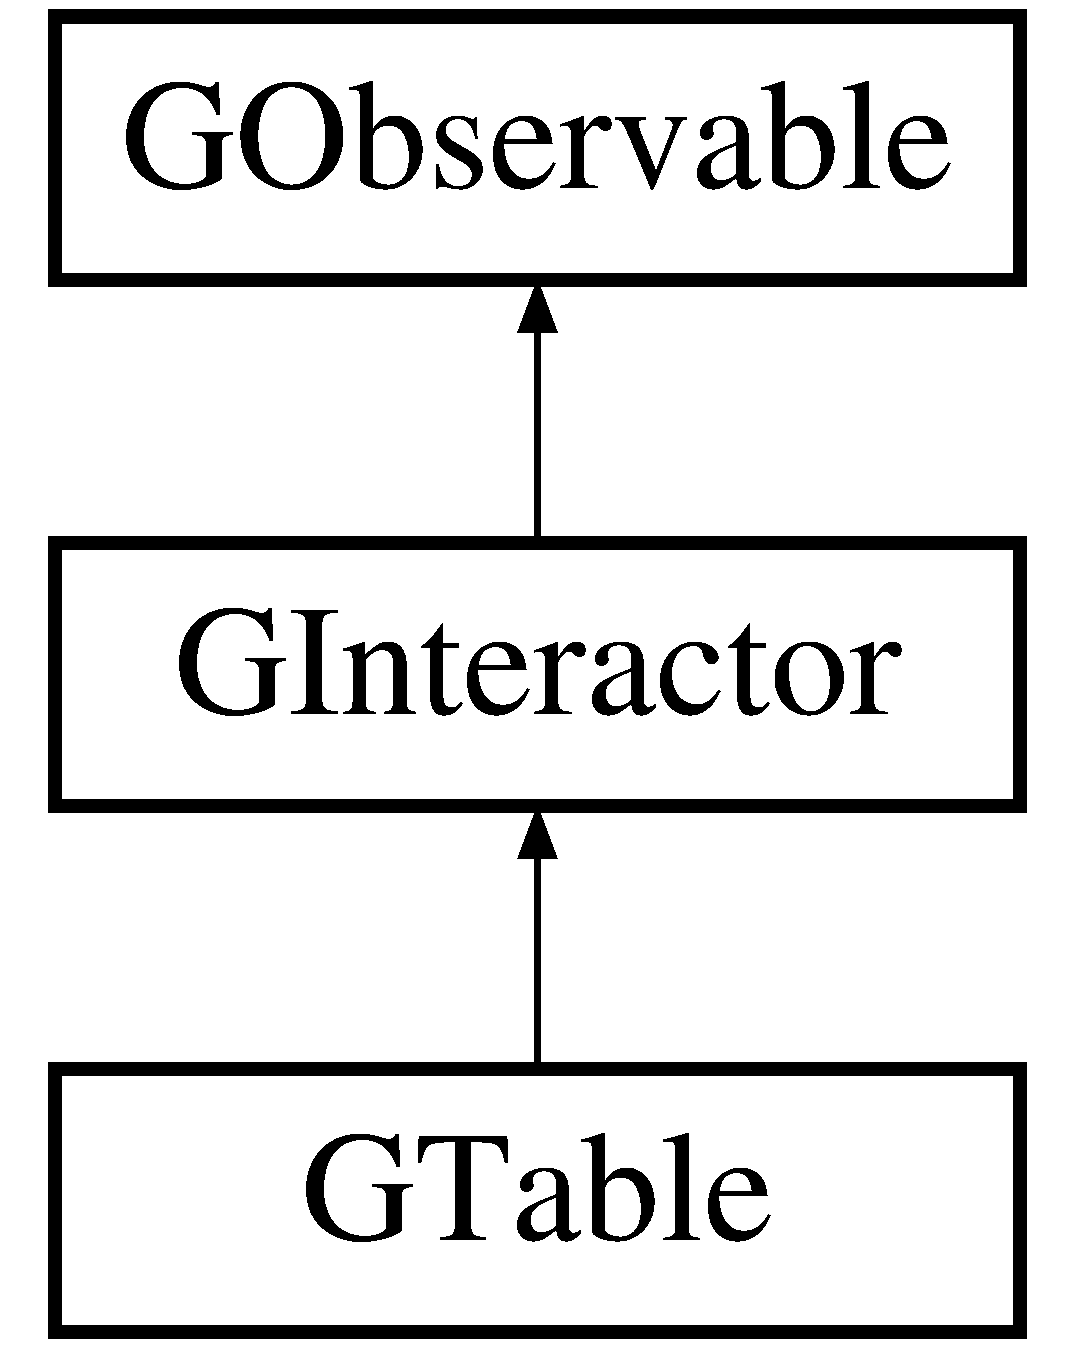
\includegraphics[height=3.000000cm]{classGTable}
\end{center}
\end{figure}
\subsection*{Public Types}
\begin{DoxyCompactItemize}
\item 
enum \mbox{\hyperlink{classGTable_a060cff504451bbb98530e64e936e2671}{Column\+Header\+Style}} \{ \mbox{\hyperlink{classGTable_a060cff504451bbb98530e64e936e2671a64e90531468e72442ee778fe31accdf6}{C\+O\+L\+U\+M\+N\+\_\+\+H\+E\+A\+D\+E\+R\+\_\+\+N\+O\+NE}}, 
\mbox{\hyperlink{classGTable_a060cff504451bbb98530e64e936e2671aa4b2febb21afe5d988ac57d4bac55a8b}{C\+O\+L\+U\+M\+N\+\_\+\+H\+E\+A\+D\+E\+R\+\_\+\+E\+X\+C\+EL}}, 
\mbox{\hyperlink{classGTable_a060cff504451bbb98530e64e936e2671ab59182f94a821e007f1ede2dd29b23cd}{C\+O\+L\+U\+M\+N\+\_\+\+H\+E\+A\+D\+E\+R\+\_\+\+N\+U\+M\+E\+R\+IC}}
 \}
\begin{DoxyCompactList}\small\item\em Styles of column header labels that can be shown. \end{DoxyCompactList}\item 
enum \mbox{\hyperlink{classGInteractor_a8e0d441725a81d2bbdebbea09078260e}{Text\+Position}} \{ \mbox{\hyperlink{classGInteractor_a8e0d441725a81d2bbdebbea09078260ea4cd6f2e7d5a08d6f4dc052df2358f774}{T\+E\+X\+T\+\_\+\+B\+E\+S\+I\+D\+E\+\_\+\+I\+C\+ON}}, 
\mbox{\hyperlink{classGInteractor_a8e0d441725a81d2bbdebbea09078260eaa88490f63d8de68d44c83bdb2ecde3b3}{T\+E\+X\+T\+\_\+\+U\+N\+D\+E\+R\+\_\+\+I\+C\+ON}}, 
\mbox{\hyperlink{classGInteractor_a8e0d441725a81d2bbdebbea09078260ea39a6f388a30ac4fefb6eb13e846bc9f2}{T\+E\+X\+T\+\_\+\+O\+N\+LY}}
 \}
\begin{DoxyCompactList}\small\item\em The places where an interactor can place its text relative to its icon. \end{DoxyCompactList}\end{DoxyCompactItemize}
\subsection*{Public Member Functions}
\begin{DoxyCompactItemize}
\item 
\mbox{\hyperlink{classGTable_a5ceea9546881f429ad4601366908848d}{G\+Table}} (int rows=0, int columns=0, double \mbox{\hyperlink{classGTable_ad72663daf610f2a0833a2fc3d78e4fdf}{width}}=0, double \mbox{\hyperlink{classGTable_ad3774f6419003470f54fd495124ef51f}{height}}=0, Q\+Widget $\ast$parent=nullptr)
\begin{DoxyCompactList}\small\item\em Constructs a new table with the given dimensions and (optional) size. \end{DoxyCompactList}\item 
virtual void \mbox{\hyperlink{classGInteractor_a02f20ea6edfa0671f31c4c648a253833}{add\+Action\+Listener}} () Q\+\_\+\+D\+E\+C\+L\+\_\+\+D\+E\+P\+R\+E\+C\+A\+T\+ED
\begin{DoxyCompactList}\small\item\em Adds an event listener to be notified when this interactor is clicked or generally interacted with. \end{DoxyCompactList}\item 
virtual void \mbox{\hyperlink{classGTable_afaf36ccb6a75432b5f5463613ef01ef4}{autofit\+Column\+Widths}} ()
\begin{DoxyCompactList}\small\item\em Changes widths of all columns to be perfectly large enough to fit their contents. \end{DoxyCompactList}\item 
virtual void \mbox{\hyperlink{classGTable_ac8bb3912a3ce86b15842e79d0b421204}{clear}} ()
\begin{DoxyCompactList}\small\item\em Sets all cells in the table to store an empty string value. \end{DoxyCompactList}\item 
virtual void \mbox{\hyperlink{classGTable_ab7bffbf52806e438ac155886079d9bf6}{clear\+Cell}} (int row, int column)
\begin{DoxyCompactList}\small\item\em Sets the given cell to store an empty string value. \end{DoxyCompactList}\item 
virtual void \mbox{\hyperlink{classGTable_a5ba4fe558e9d315c123ecd9e896065ca}{clear\+Cell\+Formatting}} (int row, int column)
\begin{DoxyCompactList}\small\item\em Removes any formatting that has been applied to the given cell. \end{DoxyCompactList}\item 
virtual void \mbox{\hyperlink{classGTable_a07ea41be0cdc43ffcd09898d3ae5c523}{clear\+Formatting}} ()
\begin{DoxyCompactList}\small\item\em Removes any per-\/cell/column/row formatting that has been applied to the table. \end{DoxyCompactList}\item 
virtual void \mbox{\hyperlink{classGTable_abd07e172ccec6823a88289c21124a367}{clear\+Selection}} ()
\begin{DoxyCompactList}\small\item\em Deselects any currently selected cell. \end{DoxyCompactList}\item 
virtual bool \mbox{\hyperlink{classGInteractor_ac05ba5b92e2e5146d416fe7f842a0969}{events\+Enabled}} () const Q\+\_\+\+D\+E\+C\+L\+\_\+\+O\+V\+E\+R\+R\+I\+DE
\begin{DoxyCompactList}\small\item\em Returns true if this interactor is currently accepting events. \end{DoxyCompactList}\item 
virtual void \mbox{\hyperlink{classGTable_a1ff40d0915f96652929cfb739bdd969f}{fill}} (const std\+::string \&text)
\begin{DoxyCompactList}\small\item\em Sets every cell in the table to have the given value. \end{DoxyCompactList}\item 
virtual std\+::string \mbox{\hyperlink{classGTable_aaa9971dcb7e1b082abd3b9010667f041}{get}} (int row, int column) const
\begin{DoxyCompactList}\small\item\em Returns the text stored in the given cell. \end{DoxyCompactList}\item 
virtual std\+::string \mbox{\hyperlink{classGInteractor_a69f8d23ed8f207fbecad99960776e942}{get\+Accelerator}} () const
\begin{DoxyCompactList}\small\item\em Returns a string representing a hotkey for this interactor, or an empty string if no accelerator has been set. \end{DoxyCompactList}\item 
virtual std\+::string \mbox{\hyperlink{classGInteractor_a94eb4276000c4fdfb508ce9e6317a82a}{get\+Action\+Command}} () const
\begin{DoxyCompactList}\small\item\em Returns an action command for this interactor, which is a semi-\/unique string you can use to identify it when events occur. \end{DoxyCompactList}\item 
virtual std\+::string \mbox{\hyperlink{classGInteractor_a808e22cc1fdfbecf71ed8c64ef4600e0}{get\+Background}} () const
\begin{DoxyCompactList}\small\item\em Returns the background color of the interactor as a string. \end{DoxyCompactList}\item 
virtual int \mbox{\hyperlink{classGInteractor_a9e827257a55cb8cf4d9de2ec6bcfd7a0}{get\+Background\+Int}} () const
\begin{DoxyCompactList}\small\item\em Returns the background color of the interactor as an R\+GB integer. \end{DoxyCompactList}\item 
virtual \mbox{\hyperlink{classGRectangle}{G\+Rectangle}} \mbox{\hyperlink{classGInteractor_a29e6ac35a0b48f491a4c88194cc5da3b}{get\+Bounds}} () const
\begin{DoxyCompactList}\small\item\em Returns a rectangle representing the x/y position and size of this interactor. \end{DoxyCompactList}\item 
virtual std\+::string \mbox{\hyperlink{classGInteractor_aa061dfa488c31e18549d64363c1d0e34}{get\+Color}} () const
\begin{DoxyCompactList}\small\item\em Returns the foreground/text color of the interactor as a string. \end{DoxyCompactList}\item 
virtual int \mbox{\hyperlink{classGInteractor_a9635c7af766cdc3417f346683fa0e6c1}{get\+Color\+Int}} () const
\begin{DoxyCompactList}\small\item\em Returns the foreground/text color of the interactor as an R\+GB integer. \end{DoxyCompactList}\item 
virtual \mbox{\hyperlink{classGTable_a060cff504451bbb98530e64e936e2671}{Column\+Header\+Style}} \mbox{\hyperlink{classGTable_a31ffc9e14dda3e91d1a1b3be81a42db8}{get\+Column\+Header\+Style}} () const
\begin{DoxyCompactList}\small\item\em Returns the column headers to use the given style. \end{DoxyCompactList}\item 
virtual double \mbox{\hyperlink{classGTable_a4722043b7c3f968238968d3053b8a277}{get\+Column\+Width}} (int column) const
\begin{DoxyCompactList}\small\item\em Returns the width of the given column index in pixels. \end{DoxyCompactList}\item 
virtual \mbox{\hyperlink{classGContainer}{G\+Container}} $\ast$ \mbox{\hyperlink{classGInteractor_a7a6e317c29d61030929b4cd2d1c00fe7}{get\+Container}} () const
\begin{DoxyCompactList}\small\item\em Returns a pointer to the onscreen container holding this interactor. \end{DoxyCompactList}\item 
virtual std\+::string \mbox{\hyperlink{classGInteractor_a894a5502900794eeb27d084c21f1d77d}{get\+Font}} () const
\begin{DoxyCompactList}\small\item\em Returns the font of this interactor\textquotesingle{}s text as a font string such as \char`\"{}\+Helvetica-\/12-\/\+Bold\char`\"{}. \end{DoxyCompactList}\item 
virtual std\+::string \mbox{\hyperlink{classGInteractor_a4fa2d8b0192a3a5b4af4bbfe71194d03}{get\+Foreground}} () const
\begin{DoxyCompactList}\small\item\em Returns the foreground/text color of the interactor as a string. \end{DoxyCompactList}\item 
virtual int \mbox{\hyperlink{classGInteractor_ac3b12ab385a6ef9ae90fc879860ba726}{get\+Foreground\+Int}} () const
\begin{DoxyCompactList}\small\item\em Returns the foreground/text color of the interactor as an R\+GB integer. \end{DoxyCompactList}\item 
virtual double \mbox{\hyperlink{classGInteractor_a1e7e353362434072875264cf95629f99}{get\+Height}} () const
\begin{DoxyCompactList}\small\item\em Returns the current onscreen height of this interactor in pixels. \end{DoxyCompactList}\item 
virtual std\+::string \mbox{\hyperlink{classGInteractor_aaed62a73004939a64da6f0eb9eb64d73}{get\+Icon}} () const
\begin{DoxyCompactList}\small\item\em Returns the file name of the icon associated with this interactor, or an empty string if no icon has been set. \end{DoxyCompactList}\item 
virtual int \mbox{\hyperlink{classGInteractor_a9c9659a6c6ba66b4107ba59c95a24241}{get\+ID}} () const
\begin{DoxyCompactList}\small\item\em Returns a globally unique identifier for this interactor, which is set when the interactor is constructed. \end{DoxyCompactList}\item 
virtual \+\_\+\+Internal\+\_\+\+Q\+Widget $\ast$ \mbox{\hyperlink{classGTable_a208ce13c1da40bf0ddb509daf99d6588}{get\+Internal\+Widget}} () const Q\+\_\+\+D\+E\+C\+L\+\_\+\+O\+V\+E\+R\+R\+I\+DE
\begin{DoxyCompactList}\small\item\em Returns a direct pointer to the internal Qt widget being wrapped by this interactor. \end{DoxyCompactList}\item 
virtual \mbox{\hyperlink{classGPoint}{G\+Point}} \mbox{\hyperlink{classGInteractor_a4f83802015511edeb63b892830812c11}{get\+Location}} () const
\begin{DoxyCompactList}\small\item\em Returns an (x, y) point representing the onscreen location of the top-\/left corner of this interactor within its containing window. \end{DoxyCompactList}\item 
virtual double \mbox{\hyperlink{classGInteractor_aed4b0075fcc434499c3cb3e46896bda3}{get\+Minimum\+Height}} () const
\begin{DoxyCompactList}\small\item\em Returns the minimum height in pixels that this interactor will permit itself to be resized to. \end{DoxyCompactList}\item 
virtual \mbox{\hyperlink{classGDimension}{G\+Dimension}} \mbox{\hyperlink{classGInteractor_a66b5af0b32493b4d597ca0a3df2049ea}{get\+Minimum\+Size}} () const
\begin{DoxyCompactList}\small\item\em Returns a \mbox{\hyperlink{classGDimension}{G\+Dimension}} structure representing the minimum size in pixels that this interactor will permit itself to be resized to. \end{DoxyCompactList}\item 
virtual double \mbox{\hyperlink{classGInteractor_a59e668114fe3d49d2a0f28deb258f7c8}{get\+Minimum\+Width}} () const
\begin{DoxyCompactList}\small\item\em Returns the minimum width in pixels that this interactor will permit itself to be resized to. \end{DoxyCompactList}\item 
virtual std\+::string \mbox{\hyperlink{classGInteractor_a8a60438a5b55d0b2ceb35c8674b9d8c5}{get\+Name}} () const
\begin{DoxyCompactList}\small\item\em Returns a string representing a unique name for this interactor. \end{DoxyCompactList}\item 
virtual double \mbox{\hyperlink{classGInteractor_a747de0961653847bdc6615dbf756d715}{get\+Preferred\+Height}} () const
\begin{DoxyCompactList}\small\item\em Returns the height in pixels that this interactor would prefer to be, which would exactly fit its contents with no stretching or scrollbars. \end{DoxyCompactList}\item 
virtual \mbox{\hyperlink{classGDimension}{G\+Dimension}} \mbox{\hyperlink{classGInteractor_a4aabbee761d8e9116275401131b7ccd1}{get\+Preferred\+Size}} () const
\begin{DoxyCompactList}\small\item\em Returns a \mbox{\hyperlink{classGDimension}{G\+Dimension}} structure storing the width and height in pixels that this interactor would prefer to be, which would exactly fit its contents with no stretching or scrollbars. \end{DoxyCompactList}\item 
virtual double \mbox{\hyperlink{classGInteractor_a82bca31d37700fb0e35d2743352efd5e}{get\+Preferred\+Width}} () const
\begin{DoxyCompactList}\small\item\em Returns the height in pixels that this interactor would prefer to be, which would exactly fit its contents with no stretching or scrollbars. \end{DoxyCompactList}\item 
virtual double \mbox{\hyperlink{classGTable_a0215a742506665475b721ed12913808b}{get\+Row\+Height}} (int row) const
\begin{DoxyCompactList}\small\item\em Returns the height of the given row index in pixels. \end{DoxyCompactList}\item 
virtual \mbox{\hyperlink{structGridLocation}{Grid\+Location}} \mbox{\hyperlink{classGTable_ae4b79399eefc964f783f06b6959a6a4a}{get\+Selected\+Cell}} () const
\begin{DoxyCompactList}\small\item\em Returns the row and column of the cell that is currently selected. \end{DoxyCompactList}\item 
virtual void \mbox{\hyperlink{classGTable_a29b4e2e079037922545996e08f7ce6c4}{get\+Selected\+Cell}} (int \&row, int \&column) const
\begin{DoxyCompactList}\small\item\em Returns the row and column of the cell that is currently selected by filling the given reference parameters. \end{DoxyCompactList}\item 
virtual std\+::string \mbox{\hyperlink{classGTable_a8963c035a687a8393cd1f56ae05f582e}{get\+Selected\+Cell\+Value}} () const
\begin{DoxyCompactList}\small\item\em Returns the text in the cell that is currently selected. \end{DoxyCompactList}\item 
virtual int \mbox{\hyperlink{classGTable_abeec6fda3c331aa187ba1b695b19d435}{get\+Selected\+Column}} () const
\begin{DoxyCompactList}\small\item\em Returns the column of the cell that is currently selected, or -\/1 if no cell is currently selected. \end{DoxyCompactList}\item 
virtual int \mbox{\hyperlink{classGTable_adeb0b39683825191a8216d6cc3ca5072}{get\+Selected\+Row}} () const
\begin{DoxyCompactList}\small\item\em Returns the row of the cell that is currently selected, or -\/1 if no cell is currently selected. \end{DoxyCompactList}\item 
virtual \mbox{\hyperlink{classGDimension}{G\+Dimension}} \mbox{\hyperlink{classGInteractor_a7b4eec96a2bdc6420695d5796a78eea9}{get\+Size}} () const
\begin{DoxyCompactList}\small\item\em Returns a \mbox{\hyperlink{classGDimension}{G\+Dimension}} structure storing the current onscreen width and height of this interactor in pixels. \end{DoxyCompactList}\item 
virtual std\+::string \mbox{\hyperlink{classGTable_a9896d58fcfebbf1025aeeb5b8b9ede80}{get\+Type}} () const Q\+\_\+\+D\+E\+C\+L\+\_\+\+O\+V\+E\+R\+R\+I\+DE
\begin{DoxyCompactList}\small\item\em Returns a string representing the class name of this interactor, such as \char`\"{}\+G\+Button\char`\"{} or \char`\"{}\+G\+Check\+Box\char`\"{}. \end{DoxyCompactList}\item 
virtual Q\+Widget $\ast$ \mbox{\hyperlink{classGTable_a326ee51b5561f807df7b29a1c101f7fd}{get\+Widget}} () const Q\+\_\+\+D\+E\+C\+L\+\_\+\+O\+V\+E\+R\+R\+I\+DE
\begin{DoxyCompactList}\small\item\em Returns a direct pointer to the internal Qt widget being wrapped by this interactor. \end{DoxyCompactList}\item 
virtual double \mbox{\hyperlink{classGInteractor_a0ed2965abd4f5701d2cadf71239faf19}{get\+Width}} () const
\begin{DoxyCompactList}\small\item\em Returns the current onscreen width of this interactor in pixels. \end{DoxyCompactList}\item 
virtual double \mbox{\hyperlink{classGInteractor_a344385751bee0720059403940d57a13e}{getX}} () const
\begin{DoxyCompactList}\small\item\em Returns the x-\/coordinate of the top-\/left pixel of this interactor within its onscreen window. \end{DoxyCompactList}\item 
virtual double \mbox{\hyperlink{classGInteractor_aafa51c7f8f38a09febbb9ce7853f77b4}{getY}} () const
\begin{DoxyCompactList}\small\item\em Returns the y-\/coordinate of the top-\/left pixel of this interactor within its onscreen window. \end{DoxyCompactList}\item 
virtual bool \mbox{\hyperlink{classGTable_a4a1007a3d14cd35f0bd514cc0b29886b}{has\+Selected\+Cell}} () const
\begin{DoxyCompactList}\small\item\em Returns true if a cell is currently selected. \end{DoxyCompactList}\item 
virtual int \mbox{\hyperlink{classGTable_ad3774f6419003470f54fd495124ef51f}{height}} () const
\begin{DoxyCompactList}\small\item\em Returns the number of rows in the table. \end{DoxyCompactList}\item 
virtual bool \mbox{\hyperlink{classGTable_afa6b6241d2f7af75f2d1345f46acfc35}{in\+Bounds}} (int row, int column) const
\begin{DoxyCompactList}\small\item\em Returns true if the given 0-\/based row/column index is within the bounds of the table. \end{DoxyCompactList}\item 
virtual bool \mbox{\hyperlink{classGInteractor_afc480f652b8c5f1fb255e2269ce68879}{in\+Bounds}} (double x, double y) const
\begin{DoxyCompactList}\small\item\em Returns true if the given x/y pixel is within the bounds of this interactor. \end{DoxyCompactList}\item 
virtual bool \mbox{\hyperlink{classGTable_a012b5afb54e037e6c5498cf0932a521b}{is\+Editable}} () const
\begin{DoxyCompactList}\small\item\em Returns whether cells of the table can be edited. \end{DoxyCompactList}\item 
virtual bool \mbox{\hyperlink{classGInteractor_aacb819fb241851fd9fc045271baa4034}{is\+Enabled}} () const
\begin{DoxyCompactList}\small\item\em Returns true if this interactor is currently enabled. \end{DoxyCompactList}\item 
virtual bool \mbox{\hyperlink{classGInteractor_a9d8a6cfb13917785c143e74d40e4e2be}{is\+Visible}} () const
\begin{DoxyCompactList}\small\item\em Returns true if the interactor is visible on the screen. \end{DoxyCompactList}\item 
virtual int \mbox{\hyperlink{classGTable_a5997e103e56aae1db12e1f7f02e136c5}{num\+Cols}} () const
\begin{DoxyCompactList}\small\item\em Returns the number of columns in the table. \end{DoxyCompactList}\item 
virtual int \mbox{\hyperlink{classGTable_a00b7e69dd5c43e42cc91db26c459ad8b}{num\+Rows}} () const
\begin{DoxyCompactList}\small\item\em Returns the number of rows in the table. \end{DoxyCompactList}\item 
virtual void \mbox{\hyperlink{classGTable_aed391150e258bc6c2962f10b810681c9}{remove\+Table\+Listener}} ()
\begin{DoxyCompactList}\small\item\em Removes the table listener from this button so that it will no longer call it when events occur. \end{DoxyCompactList}\item 
virtual void \mbox{\hyperlink{classGTable_a49b39e0eeaf5af829e8956e9055c5cdc}{request\+Focus}} () Q\+\_\+\+D\+E\+C\+L\+\_\+\+O\+V\+E\+R\+R\+I\+DE
\begin{DoxyCompactList}\small\item\em Transfers keyboard focus to this interactor. \end{DoxyCompactList}\item 
virtual void \mbox{\hyperlink{classGTable_a600810b1a74ec9a062ce38666a9e7602}{resize}} (int \mbox{\hyperlink{classGTable_a00b7e69dd5c43e42cc91db26c459ad8b}{num\+Rows}}, int \mbox{\hyperlink{classGTable_a5997e103e56aae1db12e1f7f02e136c5}{num\+Cols}})
\begin{DoxyCompactList}\small\item\em Modifies the table to have the given number of rows and columns. \end{DoxyCompactList}\item 
virtual bool \mbox{\hyperlink{classGTable_a92c3dff0296ec16823a1172a9f9f07e6}{row\+Column\+Headers\+Visible}} () const
\begin{DoxyCompactList}\small\item\em Returns whether row and column headers are shown in the table. \end{DoxyCompactList}\item 
virtual void \mbox{\hyperlink{classGTable_ab06a36d6ed149c8477a1a9d32be2ba43}{select}} (int row, int column)
\begin{DoxyCompactList}\small\item\em Sets the given cell to become currently selected, replacing any previous selection. \end{DoxyCompactList}\item 
virtual void \mbox{\hyperlink{classGTable_ad1a09eece3a11ef4d2c56a951ae06a69}{set}} (int row, int column, const std\+::string \&text)
\begin{DoxyCompactList}\small\item\em Modifies the value in the given cell to store the given text. \end{DoxyCompactList}\item 
virtual void \mbox{\hyperlink{classGInteractor_ad15f102f62e2960576012f1aa0ba4b2e}{set\+Accelerator}} (const std\+::string \&accelerator)
\begin{DoxyCompactList}\small\item\em Sets an accelerator hotkey for this interactor, such as \char`\"{}\+Ctrl-\/\+S\char`\"{}. \end{DoxyCompactList}\item 
virtual void \mbox{\hyperlink{classGInteractor_a4b5843fe3030e038a1ba54cc03389bcf}{set\+Action\+Command}} (const std\+::string \&action\+Command)
\begin{DoxyCompactList}\small\item\em Sets the action command for this interactor. \end{DoxyCompactList}\item 
virtual void \mbox{\hyperlink{classGTable_ac45b8a90f31752385a98a034a58547c7}{set\+Background}} (int rgb) Q\+\_\+\+D\+E\+C\+L\+\_\+\+O\+V\+E\+R\+R\+I\+DE
\begin{DoxyCompactList}\small\item\em Sets the background color that appears behind each cell. \end{DoxyCompactList}\item 
virtual void \mbox{\hyperlink{classGTable_a222fcfb542aa6094c7e0de671bd69627}{set\+Background}} (const std\+::string \&color) Q\+\_\+\+D\+E\+C\+L\+\_\+\+O\+V\+E\+R\+R\+I\+DE
\begin{DoxyCompactList}\small\item\em Sets the background color that appears behind each cell. \end{DoxyCompactList}\item 
virtual void \mbox{\hyperlink{classGInteractor_a2aae8197624b72265ab83b4f1bc73f2f}{set\+Bounds}} (double x, double y, double \mbox{\hyperlink{classGTable_ad72663daf610f2a0833a2fc3d78e4fdf}{width}}, double \mbox{\hyperlink{classGTable_ad3774f6419003470f54fd495124ef51f}{height}})
\begin{DoxyCompactList}\small\item\em Sets the size and location of the widget. \end{DoxyCompactList}\item 
virtual void \mbox{\hyperlink{classGInteractor_acada386653f008cacc7cce86426bef7c}{set\+Bounds}} (const \mbox{\hyperlink{classGRectangle}{G\+Rectangle}} \&size)
\begin{DoxyCompactList}\small\item\em Sets the size and location of the widget. \end{DoxyCompactList}\item 
virtual void \mbox{\hyperlink{classGTable_a0c1ff398e920da7356b8375b66b9b083}{set\+Cell\+Alignment}} (int row, int column, Horizontal\+Alignment alignment)
\begin{DoxyCompactList}\small\item\em Sets the horizontal alignment of the given cell. \end{DoxyCompactList}\item 
virtual void \mbox{\hyperlink{classGTable_a50940b22e500a861451bbff938c8f50b}{set\+Cell\+Background}} (int row, int column, int color)
\begin{DoxyCompactList}\small\item\em Sets the background color of the given cell to the given color. \end{DoxyCompactList}\item 
virtual void \mbox{\hyperlink{classGTable_af2d2fa204d2f9260081102a990310cd7}{set\+Cell\+Background}} (int row, int column, const std\+::string \&color)
\begin{DoxyCompactList}\small\item\em Sets the background color of the given cell to the given color. \end{DoxyCompactList}\item 
virtual void \mbox{\hyperlink{classGTable_a8c3d80b0163f465c7306b075d5895313}{set\+Cell\+Font}} (int row, int column, const std\+::string \&font)
\begin{DoxyCompactList}\small\item\em Sets the text font of the given cell to the given R\+GB color. \end{DoxyCompactList}\item 
virtual void \mbox{\hyperlink{classGTable_a19969b2f2b0cbf219333b02c047b2e7e}{set\+Cell\+Foreground}} (int row, int column, int color)
\begin{DoxyCompactList}\small\item\em Sets the foreground/text color of the given cell to the given color. \end{DoxyCompactList}\item 
virtual void \mbox{\hyperlink{classGTable_ab0bdc2afa7ef003fa5e8ab6eb25a7282}{set\+Cell\+Foreground}} (int row, int column, const std\+::string \&color)
\begin{DoxyCompactList}\small\item\em Sets the foreground/text color of the given cell to the given color. \end{DoxyCompactList}\item 
virtual void \mbox{\hyperlink{classGTable_afd1f50a2c4695c79b8633d860bce5398}{set\+Color}} (int rgb) Q\+\_\+\+D\+E\+C\+L\+\_\+\+O\+V\+E\+R\+R\+I\+DE
\begin{DoxyCompactList}\small\item\em Sets the color used for the text of each cell. \end{DoxyCompactList}\item 
virtual void \mbox{\hyperlink{classGTable_ad148324da1b0340e84e24dffa577ffca}{set\+Color}} (const std\+::string \&color) Q\+\_\+\+D\+E\+C\+L\+\_\+\+O\+V\+E\+R\+R\+I\+DE
\begin{DoxyCompactList}\small\item\em Sets the color used for the text of each cell. \end{DoxyCompactList}\item 
virtual void \mbox{\hyperlink{classGTable_a84b3f42bb5d010483b78b9fd7e9c55f0}{set\+Column\+Alignment}} (int column, Horizontal\+Alignment alignment)
\begin{DoxyCompactList}\small\item\em Sets the horizontal alignment of the given column. \end{DoxyCompactList}\item 
virtual void \mbox{\hyperlink{classGTable_a48898e733d8ae3e285ff84d02e2cdee5}{set\+Column\+Background}} (int column, int color)
\begin{DoxyCompactList}\small\item\em Sets the background color of the given column to the given color. \end{DoxyCompactList}\item 
virtual void \mbox{\hyperlink{classGTable_a37fd3b921a5fba28b84dd4dd17fa9930}{set\+Column\+Background}} (int column, const std\+::string \&color)
\begin{DoxyCompactList}\small\item\em Sets the background color of the given column to the given color. \end{DoxyCompactList}\item 
virtual void \mbox{\hyperlink{classGTable_a0294ee7cb1af024bc77371f27d877164}{set\+Column\+Font}} (int column, const std\+::string \&font)
\begin{DoxyCompactList}\small\item\em Sets the text font of the given column to the given R\+GB color. \end{DoxyCompactList}\item 
virtual void \mbox{\hyperlink{classGTable_aa616c02b04beb6ca757dec04f46814b0}{set\+Column\+Foreground}} (int column, int color)
\begin{DoxyCompactList}\small\item\em Sets the foreground/text color of the given column to the given color. \end{DoxyCompactList}\item 
virtual void \mbox{\hyperlink{classGTable_a84ca08c2995646ab28c78bffbcdc2693}{set\+Column\+Foreground}} (int column, const std\+::string \&color)
\begin{DoxyCompactList}\small\item\em Sets the foreground/text color of the given column to the given color. \end{DoxyCompactList}\item 
virtual void \mbox{\hyperlink{classGTable_ac97cb91256925fa81c52594bca854969}{set\+Column\+Header\+Style}} (\mbox{\hyperlink{classGTable_a060cff504451bbb98530e64e936e2671}{Column\+Header\+Style}} style)
\begin{DoxyCompactList}\small\item\em Sets the column headers to use the given style. \end{DoxyCompactList}\item 
virtual void \mbox{\hyperlink{classGTable_a52075dc231c73a896bcef426047fd327}{set\+Column\+Width}} (int column, double \mbox{\hyperlink{classGTable_ad72663daf610f2a0833a2fc3d78e4fdf}{width}})
\begin{DoxyCompactList}\small\item\em Sets the given column index to have the given width in pixels. \end{DoxyCompactList}\item 
virtual void \mbox{\hyperlink{classGTable_a52455aaff9ee352ca405fa61ba246b84}{set\+Editable}} (bool editable)
\begin{DoxyCompactList}\small\item\em Sets whether cells of the table can be edited. \end{DoxyCompactList}\item 
virtual void \mbox{\hyperlink{classGTable_aaefc85e4ff762ca176a90ebac163f2c0}{set\+Editor\+Value}} (int row, int column, const std\+::string \&text)
\begin{DoxyCompactList}\small\item\em Modifies the value in the cell that is currently being edited to store the given text. \end{DoxyCompactList}\item 
virtual void \mbox{\hyperlink{classGInteractor_ab831367dd84bbd579e02e55bacb21343}{set\+Enabled}} (bool value)
\begin{DoxyCompactList}\small\item\em Sets whether this interactor is currently enabled. \end{DoxyCompactList}\item 
virtual void \mbox{\hyperlink{classGObservable_afaa30b2a9e0f378fd1c70d2f1d0b8216}{set\+Events\+Enabled}} (bool \mbox{\hyperlink{classGInteractor_ac05ba5b92e2e5146d416fe7f842a0969}{events\+Enabled}})
\begin{DoxyCompactList}\small\item\em Sets whether the object is currently allowing itself to fire events. \end{DoxyCompactList}\item 
virtual void \mbox{\hyperlink{classGTable_a2d22014c7fa3bccfd58c982aea1b55fa}{set\+Font}} (const Q\+Font \&font) Q\+\_\+\+D\+E\+C\+L\+\_\+\+O\+V\+E\+R\+R\+I\+DE
\begin{DoxyCompactList}\small\item\em Sets the font used to display each cell\textquotesingle{}s text. \end{DoxyCompactList}\item 
virtual void \mbox{\hyperlink{classGTable_ab39ef411fb13a52852ddd138c5932e2e}{set\+Font}} (const std\+::string \&font) Q\+\_\+\+D\+E\+C\+L\+\_\+\+O\+V\+E\+R\+R\+I\+DE
\begin{DoxyCompactList}\small\item\em Sets the font used to display each cell\textquotesingle{}s text. \end{DoxyCompactList}\item 
virtual void \mbox{\hyperlink{classGTable_af9227e80cbfac55ce936fa5c99ffc954}{set\+Foreground}} (int rgb) Q\+\_\+\+D\+E\+C\+L\+\_\+\+O\+V\+E\+R\+R\+I\+DE
\begin{DoxyCompactList}\small\item\em Sets the color used for the text of each cell. \end{DoxyCompactList}\item 
virtual void \mbox{\hyperlink{classGTable_a088e04dfc56273df4cedab2b11b970f5}{set\+Foreground}} (const std\+::string \&color) Q\+\_\+\+D\+E\+C\+L\+\_\+\+O\+V\+E\+R\+R\+I\+DE
\begin{DoxyCompactList}\small\item\em Sets the color used for the text of each cell. \end{DoxyCompactList}\item 
virtual void \mbox{\hyperlink{classGInteractor_a9e280bfc4544dfaf8e4376c4e1a74357}{set\+Height}} (double \mbox{\hyperlink{classGTable_ad3774f6419003470f54fd495124ef51f}{height}})
\begin{DoxyCompactList}\small\item\em Sets the onscreen height of the interactor in pixels. \end{DoxyCompactList}\item 
virtual void \mbox{\hyperlink{classGTable_a04e6ce745dd0f9708f14dedc68ec8b18}{set\+Horizontal\+Alignment}} (Horizontal\+Alignment alignment)
\begin{DoxyCompactList}\small\item\em Sets the horizontal alignment of the text in all cells in the table. \end{DoxyCompactList}\item 
virtual void \mbox{\hyperlink{classGInteractor_a762e139aa311461c3984d3ad28293f64}{set\+Icon}} (const std\+::string \&filename, bool retain\+Icon\+Size=true)
\begin{DoxyCompactList}\small\item\em Sets the file name of the icon associated with this interactor, or an empty string if no icon has been set. \end{DoxyCompactList}\item 
virtual void \mbox{\hyperlink{classGInteractor_a04594e8ba9b98513a64f1da00dcae18c}{set\+Location}} (double x, double y)
\begin{DoxyCompactList}\small\item\em Sets the onscreen x/y-\/coordinate of the top-\/left corner of the interactor relative to its window. \end{DoxyCompactList}\item 
virtual void \mbox{\hyperlink{classGInteractor_a0cf428e207b7f22cc08138a90b1b87b2}{set\+Minimum\+Size}} (double \mbox{\hyperlink{classGTable_ad72663daf610f2a0833a2fc3d78e4fdf}{width}}, double \mbox{\hyperlink{classGTable_ad3774f6419003470f54fd495124ef51f}{height}})
\begin{DoxyCompactList}\small\item\em Sets the minimum size in pixels that this interactor will permit itself to be resized to. \end{DoxyCompactList}\item 
virtual void \mbox{\hyperlink{classGInteractor_a3b1046117ac6cb7abe467e00ba8a81f4}{set\+Minimum\+Size}} (const \mbox{\hyperlink{classGDimension}{G\+Dimension}} \&size)
\begin{DoxyCompactList}\small\item\em Sets the minimum size in pixels that this interactor will permit itself to be resized to. \end{DoxyCompactList}\item 
virtual void \mbox{\hyperlink{classGInteractor_a9d3a2685df23b5e7cbf59c19c4a1f9b5}{set\+Name}} (const std\+::string \&name)
\begin{DoxyCompactList}\small\item\em Sets a string representing a unique name for this interactor. \end{DoxyCompactList}\item 
virtual void \mbox{\hyperlink{classGInteractor_a1ab987704fce32098706c6f00fb08218}{set\+Preferred\+Height}} (double \mbox{\hyperlink{classGTable_ad3774f6419003470f54fd495124ef51f}{height}})
\begin{DoxyCompactList}\small\item\em Sets the height in pixels that this interactor would prefer to be. \end{DoxyCompactList}\item 
virtual void \mbox{\hyperlink{classGInteractor_a042c5ae19430d765ef552371cae3632c}{set\+Preferred\+Size}} (double \mbox{\hyperlink{classGTable_ad72663daf610f2a0833a2fc3d78e4fdf}{width}}, double \mbox{\hyperlink{classGTable_ad3774f6419003470f54fd495124ef51f}{height}})
\begin{DoxyCompactList}\small\item\em Sets the width and height in pixels that this interactor would prefer to be. \end{DoxyCompactList}\item 
virtual void \mbox{\hyperlink{classGInteractor_aa22d9be4bc0e078bb0ea69b0fc9d7c75}{set\+Preferred\+Size}} (const \mbox{\hyperlink{classGDimension}{G\+Dimension}} \&size)
\begin{DoxyCompactList}\small\item\em Sets the size in pixels that this interactor would prefer to be. \end{DoxyCompactList}\item 
virtual void \mbox{\hyperlink{classGInteractor_a3db429ab2fa52efd187eec0ed8cdd9f2}{set\+Preferred\+Width}} (double \mbox{\hyperlink{classGTable_ad72663daf610f2a0833a2fc3d78e4fdf}{width}})
\begin{DoxyCompactList}\small\item\em Sets the width in pixels that this interactor would prefer to be. \end{DoxyCompactList}\item 
virtual void \mbox{\hyperlink{classGTable_ac6a47ba68c502b7d8dc776beeeffccc3}{set\+Row\+Alignment}} (int row, Horizontal\+Alignment alignment)
\begin{DoxyCompactList}\small\item\em Sets the horizontal alignment of the given row. \end{DoxyCompactList}\item 
virtual void \mbox{\hyperlink{classGTable_a85ee577aabd189ed64a5c9f66ba61fd2}{set\+Row\+Background}} (int row, int rgb)
\begin{DoxyCompactList}\small\item\em Sets the background color of the given row to the given R\+GB color. \end{DoxyCompactList}\item 
virtual void \mbox{\hyperlink{classGTable_a30c7073dfeac833056ed65a8bb9a7e08}{set\+Row\+Background}} (int row, const std\+::string \&color)
\begin{DoxyCompactList}\small\item\em Sets the background color of the given row to the given color. \end{DoxyCompactList}\item 
virtual void \mbox{\hyperlink{classGTable_a0d4a1d2a58daff8c1984e31b21f93ea1}{set\+Row\+Column\+Headers\+Visible}} (bool visible)
\begin{DoxyCompactList}\small\item\em Sets whether row and column headers should be shown in the table. \end{DoxyCompactList}\item 
virtual void \mbox{\hyperlink{classGTable_adaeccb3f3fd318185b8adc644aaca949}{set\+Row\+Font}} (int row, const std\+::string \&font)
\begin{DoxyCompactList}\small\item\em Sets the text font of the given row to the given font. \end{DoxyCompactList}\item 
virtual void \mbox{\hyperlink{classGTable_abe6e1382d3d98a9479cf43ac204b0ee3}{set\+Row\+Foreground}} (int row, int rgb)
\begin{DoxyCompactList}\small\item\em Sets the foreground/text color of the given row to the given color. \end{DoxyCompactList}\item 
virtual void \mbox{\hyperlink{classGTable_a27ede8127bd8889e3f71dfe152c1684d}{set\+Row\+Foreground}} (int row, const std\+::string \&color)
\begin{DoxyCompactList}\small\item\em Sets the foreground/text color of the given row to the given color. \end{DoxyCompactList}\item 
virtual void \mbox{\hyperlink{classGTable_a815f0bed3e7a76d99b4a026808a555b3}{set\+Row\+Height}} (int row, double \mbox{\hyperlink{classGTable_ad72663daf610f2a0833a2fc3d78e4fdf}{width}})
\begin{DoxyCompactList}\small\item\em Sets the given row index to have the given height in pixels. \end{DoxyCompactList}\item 
virtual void \mbox{\hyperlink{classGTable_a3120b24ea5aaa17d8a7192742c00bcfb}{set\+Selected\+Cell\+Value}} (const std\+::string \&text)
\begin{DoxyCompactList}\small\item\em Sets the text in the cell that is currently selected. \end{DoxyCompactList}\item 
virtual void \mbox{\hyperlink{classGInteractor_aca25d49481f9bf5fc8f7df4c086c4ce7}{set\+Size}} (double \mbox{\hyperlink{classGTable_ad72663daf610f2a0833a2fc3d78e4fdf}{width}}, double \mbox{\hyperlink{classGTable_ad3774f6419003470f54fd495124ef51f}{height}})
\begin{DoxyCompactList}\small\item\em Sets the onscreen width and height of the interactor in pixels. \end{DoxyCompactList}\item 
virtual void \mbox{\hyperlink{classGInteractor_ae2b628228f192c2702c4ce941b2af68f}{set\+Size}} (const \mbox{\hyperlink{classGDimension}{G\+Dimension}} \&size)
\begin{DoxyCompactList}\small\item\em Sets the onscreen width and height of the interactor in pixels. \end{DoxyCompactList}\item 
virtual void \mbox{\hyperlink{classGTable_aeeb00b5caf01028e9de6f2dd6ef4b9bd}{set\+Table\+Listener}} (G\+Event\+Listener func)
\begin{DoxyCompactList}\small\item\em Sets the given function to be called when events occur in this table. \end{DoxyCompactList}\item 
virtual void \mbox{\hyperlink{classGTable_a0412cb4e079085ed5cb3bcdf2921ac84}{set\+Table\+Listener}} (G\+Event\+Listener\+Void func)
\begin{DoxyCompactList}\small\item\em Sets the given function to be called when events occur in this table. \end{DoxyCompactList}\item 
virtual void \mbox{\hyperlink{classGInteractor_a039e0e49beaecc275efce02d416acea8}{set\+Tooltip}} (const std\+::string \&tooltip\+Text)
\begin{DoxyCompactList}\small\item\em Sets a \char`\"{}tooltip\char`\"{} that will appear if the user hovers their mouse over the interactor. \end{DoxyCompactList}\item 
virtual void \mbox{\hyperlink{classGInteractor_a18e44e30b31525a243960ca3928125aa}{set\+Visible}} (bool visible)
\begin{DoxyCompactList}\small\item\em Returns true if the interactor is visible on the screen. \end{DoxyCompactList}\item 
virtual void \mbox{\hyperlink{classGInteractor_aa3f3fba4cb131baa8696ba01e3bceca1}{set\+Width}} (double \mbox{\hyperlink{classGTable_ad72663daf610f2a0833a2fc3d78e4fdf}{width}})
\begin{DoxyCompactList}\small\item\em Sets the onscreen width of the interactor in pixels. \end{DoxyCompactList}\item 
virtual void \mbox{\hyperlink{classGInteractor_a9c18fcc579333bf9653d13ad2b372e39}{setX}} (double x)
\begin{DoxyCompactList}\small\item\em Sets the onscreen x-\/coordinate of the top-\/left corner of the interactor relative to its window. \end{DoxyCompactList}\item 
virtual void \mbox{\hyperlink{classGInteractor_a7d57e2a5c35d27feb58fd498a3cf82b9}{setY}} (double y)
\begin{DoxyCompactList}\small\item\em Sets the onscreen y-\/coordinate of the top-\/left corner of the interactor relative to its window. \end{DoxyCompactList}\item 
virtual std\+::string \mbox{\hyperlink{classGObservable_a1fe5121d6528fdea3f243321b3fa3a49}{to\+String}} () const
\begin{DoxyCompactList}\small\item\em Returns a string representation of this observable object\textquotesingle{}s state. \end{DoxyCompactList}\item 
virtual int \mbox{\hyperlink{classGTable_ad72663daf610f2a0833a2fc3d78e4fdf}{width}} () const
\begin{DoxyCompactList}\small\item\em Returns the number of columns in the table. \end{DoxyCompactList}\end{DoxyCompactItemize}
\subsection*{Protected Member Functions}
\begin{DoxyCompactItemize}
\item 
virtual void \mbox{\hyperlink{classGObservable_a80cfa040459ff53594adbd6a51ec8f43}{clear\+Event\+Listeners}} ()
\begin{DoxyCompactList}\small\item\em Removes all event listeners from this object. \end{DoxyCompactList}\item 
virtual void \mbox{\hyperlink{classGObservable_a284f31528c0520f8e545c03ac9eeac74}{ensure\+Thread\+Safety}} (const std\+::string \&member\+Name=\char`\"{}\char`\"{})
\begin{DoxyCompactList}\small\item\em Ensures that we are currently in the Qt G\+UI thread. \end{DoxyCompactList}\item 
virtual void \mbox{\hyperlink{classGObservable_a63e5e5a6227c59c928493b11aceb0f67}{fire\+Event}} (\mbox{\hyperlink{classGEvent}{G\+Event}} \&event)
\begin{DoxyCompactList}\small\item\em Sends out the given event to any attached listeners. \end{DoxyCompactList}\item 
virtual void \mbox{\hyperlink{classGObservable_ab3983ea07337b52020a29cc00c653d8d}{fire\+G\+Event}} (Q\+Event $\ast$event, Event\+Type event\+Type, const std\+::string \&event\+Name)
\begin{DoxyCompactList}\small\item\em Creates an event of the given type, then sends it out to any attached listeners. \end{DoxyCompactList}\item 
virtual void \mbox{\hyperlink{classGObservable_a01fdf1b0e0dbd49e189fe4514e010411}{fire\+G\+Event}} (Q\+Close\+Event $\ast$event, Event\+Type event\+Type, const std\+::string \&event\+Name)
\begin{DoxyCompactList}\small\item\em Creates an event of the given type, then sends it out to any attached listeners. \end{DoxyCompactList}\item 
virtual void \mbox{\hyperlink{classGObservable_abb0b2f66ba39211cb5d7615e9d1c04e2}{fire\+G\+Event}} (Q\+Key\+Event $\ast$event, Event\+Type event\+Type, const std\+::string \&event\+Name)
\begin{DoxyCompactList}\small\item\em Creates an event of the given type, then sends it out to any attached listeners. \end{DoxyCompactList}\item 
virtual void \mbox{\hyperlink{classGObservable_a119318675d2165bdf7dd853aaf881d4b}{fire\+G\+Event}} (Q\+Mouse\+Event $\ast$event, Event\+Type event\+Type, const std\+::string \&event\+Name, const std\+::string \&action\+Command=\char`\"{}\char`\"{})
\begin{DoxyCompactList}\small\item\em Creates an event of the given type, then sends it out to any attached listeners. \end{DoxyCompactList}\item 
virtual void \mbox{\hyperlink{classGObservable_a63fd9034e1e1633c1c38eb342bfd34e9}{fire\+G\+Event}} (Q\+Resize\+Event $\ast$event, Event\+Type event\+Type, const std\+::string \&event\+Name)
\begin{DoxyCompactList}\small\item\em Creates an event of the given type, then sends it out to any attached listeners. \end{DoxyCompactList}\item 
virtual void \mbox{\hyperlink{classGObservable_a741345310d9b7c5170a6cbc410c44ac4}{fire\+G\+Event}} (Q\+Timer\+Event $\ast$event, Event\+Type event\+Type, const std\+::string \&event\+Name)
\begin{DoxyCompactList}\small\item\em Creates an event of the given type, then sends it out to any attached listeners. \end{DoxyCompactList}\item 
virtual void \mbox{\hyperlink{classGObservable_a93bf338968a0338761b8e4dc62f582e9}{fire\+G\+Event}} (Q\+Wheel\+Event $\ast$event, Event\+Type event\+Type, const std\+::string \&event\+Name)
\begin{DoxyCompactList}\small\item\em Creates an event of the given type, then sends it out to any attached listeners. \end{DoxyCompactList}\item 
virtual void \mbox{\hyperlink{classGObservable_a2a70a7d7435ff0c3b80bb4d70da19e0d}{fire\+G\+Event}} (Q\+Window\+State\+Change\+Event $\ast$event, Event\+Type event\+Type, const std\+::string \&event\+Name)
\begin{DoxyCompactList}\small\item\em Creates an event of the given type, then sends it out to any attached listeners. \end{DoxyCompactList}\item 
virtual bool \mbox{\hyperlink{classGObservable_a9f6faaa25942923bafa1c44020c49fa9}{has\+Event\+Listener}} (const std\+::string \&event\+Name) const
\begin{DoxyCompactList}\small\item\em Returns true if the observable object has a listener for the given type of event. \end{DoxyCompactList}\item 
virtual bool \mbox{\hyperlink{classGObservable_aeec1adc19aa0f33de62390686ee1382c}{is\+Accepting\+Event}} (int event\+Mask) const
\begin{DoxyCompactList}\small\item\em Returns true if the observable object has a listener for the given type of event. \end{DoxyCompactList}\item 
virtual bool \mbox{\hyperlink{classGObservable_aa31c73145a29dcb92848a92e0cfaea41}{is\+Accepting\+Event}} (const \mbox{\hyperlink{classGEvent}{G\+Event}} \&event) const
\begin{DoxyCompactList}\small\item\em Returns true if the observable object has a listener for the given type of event. \end{DoxyCompactList}\item 
virtual bool \mbox{\hyperlink{classGObservable_a3b1c689267eda44e65a2213e7de38b23}{is\+Accepting\+Event}} (const std\+::string \&event\+Type) const
\begin{DoxyCompactList}\small\item\em Returns true if the observable object has a listener for the given type of event. \end{DoxyCompactList}\item 
virtual void \mbox{\hyperlink{classGObservable_acbcf1ed3a851ad8a3c17ef38d86b481d}{remove\+Event\+Listener}} (const std\+::string \&event\+Name)
\begin{DoxyCompactList}\small\item\em Removes any event listener from this observable object that would respond to the given type of event, such as \char`\"{}click\char`\"{} or \char`\"{}keydown\char`\"{}. \end{DoxyCompactList}\item 
virtual void \mbox{\hyperlink{classGObservable_af51cc35c29a1bd1908609d432decdbb6}{remove\+Event\+Listeners}} (std\+::initializer\+\_\+list$<$ std\+::string $>$ event\+Names)
\begin{DoxyCompactList}\small\item\em Removes any event listener from this observable object that would respond to the given types of events, such as \char`\"{}click\char`\"{} or \char`\"{}keydown\char`\"{}. \end{DoxyCompactList}\item 
virtual void \mbox{\hyperlink{classGObservable_ad2f6d34961c50f6c1e0659990b79f741}{set\+Event\+Listener}} (const std\+::string \&event\+Name, G\+Event\+Listener func)
\begin{DoxyCompactList}\small\item\em Adds an event listener from this observable object to respond to the given type of event, such as \char`\"{}click\char`\"{} or \char`\"{}keydown\char`\"{}. \end{DoxyCompactList}\item 
virtual void \mbox{\hyperlink{classGObservable_abac4cb9f9e626e010e87f5d91573c8a5}{set\+Event\+Listener}} (const std\+::string \&event\+Name, G\+Event\+Listener\+Void func)
\begin{DoxyCompactList}\small\item\em Adds an event listener from this observable object to respond to the given type of event, such as \char`\"{}click\char`\"{} or \char`\"{}keydown\char`\"{}. \end{DoxyCompactList}\item 
virtual void \mbox{\hyperlink{classGObservable_afa388d69c33c718cf035774604065604}{set\+Event\+Listeners}} (std\+::initializer\+\_\+list$<$ std\+::string $>$ event\+Names, G\+Event\+Listener func)
\begin{DoxyCompactList}\small\item\em Adds an event listener from this observable object to respond to the given types of events, such as \char`\"{}click\char`\"{} or \char`\"{}keydown\char`\"{}. \end{DoxyCompactList}\item 
virtual void \mbox{\hyperlink{classGObservable_a7867184bbb686f74fae8a4db927da799}{set\+Event\+Listeners}} (std\+::initializer\+\_\+list$<$ std\+::string $>$ event\+Names, G\+Event\+Listener\+Void func)
\begin{DoxyCompactList}\small\item\em Adds an event listener from this observable object to respond to the given types of events, such as \char`\"{}click\char`\"{} or \char`\"{}keydown\char`\"{}. \end{DoxyCompactList}\end{DoxyCompactItemize}


\subsection{Detailed Description}
A \mbox{\hyperlink{classGTable}{G\+Table}} represents a graphical editable 2D table, like a mediocre facsimile of an Excel spreadsheet. 

After creating a \mbox{\hyperlink{classGTable}{G\+Table}}, you can listen for table events to be notified when the user types a new value into a table cell by calling set\+Table\+Listener.

An editable table has a semi-\/complex editing model where the user can begin modifying a cell by highlighting it and typing, which replaces the existing value, or by double-\/clicking it, which edits the existing value. You can also press F2 on a cell to edit it, equivalent to a double-\/click. During editing, you can press Esc to cancel editing, or Tab or Enter to complete editing and move to the next cell.

All row/column indexes in this class are 0-\/based. 

\subsection{Member Enumeration Documentation}
\mbox{\Hypertarget{classGTable_a060cff504451bbb98530e64e936e2671}\label{classGTable_a060cff504451bbb98530e64e936e2671}} 
\index{G\+Table@{G\+Table}!Column\+Header\+Style@{Column\+Header\+Style}}
\index{Column\+Header\+Style@{Column\+Header\+Style}!G\+Table@{G\+Table}}
\subsubsection{\texorpdfstring{Column\+Header\+Style}{ColumnHeaderStyle}}
{\footnotesize\ttfamily enum \mbox{\hyperlink{classGTable_a060cff504451bbb98530e64e936e2671}{Column\+Header\+Style}}}



Styles of column header labels that can be shown. 

The \char`\"{}\+Excel\char`\"{} style is to use column names A-\/Z, then A\+A-\/\+AZ, B\+A-\/\+BZ, ..., Z\+A-\/\+ZZ, then A\+AA, A\+AB, and so on. The \char`\"{}numeric\char`\"{} style is to use simple numbers like 1, 2, 3, ... The \char`\"{}none\char`\"{} style means not to use any column headers at all. \begin{DoxyEnumFields}{Enumerator}
\raisebox{\heightof{T}}[0pt][0pt]{\index{C\+O\+L\+U\+M\+N\+\_\+\+H\+E\+A\+D\+E\+R\+\_\+\+N\+O\+NE@{C\+O\+L\+U\+M\+N\+\_\+\+H\+E\+A\+D\+E\+R\+\_\+\+N\+O\+NE}!G\+Table@{G\+Table}}\index{G\+Table@{G\+Table}!C\+O\+L\+U\+M\+N\+\_\+\+H\+E\+A\+D\+E\+R\+\_\+\+N\+O\+NE@{C\+O\+L\+U\+M\+N\+\_\+\+H\+E\+A\+D\+E\+R\+\_\+\+N\+O\+NE}}}\mbox{\Hypertarget{classGTable_a060cff504451bbb98530e64e936e2671a64e90531468e72442ee778fe31accdf6}\label{classGTable_a060cff504451bbb98530e64e936e2671a64e90531468e72442ee778fe31accdf6}} 
C\+O\+L\+U\+M\+N\+\_\+\+H\+E\+A\+D\+E\+R\+\_\+\+N\+O\+NE&\\
\hline

\raisebox{\heightof{T}}[0pt][0pt]{\index{C\+O\+L\+U\+M\+N\+\_\+\+H\+E\+A\+D\+E\+R\+\_\+\+E\+X\+C\+EL@{C\+O\+L\+U\+M\+N\+\_\+\+H\+E\+A\+D\+E\+R\+\_\+\+E\+X\+C\+EL}!G\+Table@{G\+Table}}\index{G\+Table@{G\+Table}!C\+O\+L\+U\+M\+N\+\_\+\+H\+E\+A\+D\+E\+R\+\_\+\+E\+X\+C\+EL@{C\+O\+L\+U\+M\+N\+\_\+\+H\+E\+A\+D\+E\+R\+\_\+\+E\+X\+C\+EL}}}\mbox{\Hypertarget{classGTable_a060cff504451bbb98530e64e936e2671aa4b2febb21afe5d988ac57d4bac55a8b}\label{classGTable_a060cff504451bbb98530e64e936e2671aa4b2febb21afe5d988ac57d4bac55a8b}} 
C\+O\+L\+U\+M\+N\+\_\+\+H\+E\+A\+D\+E\+R\+\_\+\+E\+X\+C\+EL&\\
\hline

\raisebox{\heightof{T}}[0pt][0pt]{\index{C\+O\+L\+U\+M\+N\+\_\+\+H\+E\+A\+D\+E\+R\+\_\+\+N\+U\+M\+E\+R\+IC@{C\+O\+L\+U\+M\+N\+\_\+\+H\+E\+A\+D\+E\+R\+\_\+\+N\+U\+M\+E\+R\+IC}!G\+Table@{G\+Table}}\index{G\+Table@{G\+Table}!C\+O\+L\+U\+M\+N\+\_\+\+H\+E\+A\+D\+E\+R\+\_\+\+N\+U\+M\+E\+R\+IC@{C\+O\+L\+U\+M\+N\+\_\+\+H\+E\+A\+D\+E\+R\+\_\+\+N\+U\+M\+E\+R\+IC}}}\mbox{\Hypertarget{classGTable_a060cff504451bbb98530e64e936e2671ab59182f94a821e007f1ede2dd29b23cd}\label{classGTable_a060cff504451bbb98530e64e936e2671ab59182f94a821e007f1ede2dd29b23cd}} 
C\+O\+L\+U\+M\+N\+\_\+\+H\+E\+A\+D\+E\+R\+\_\+\+N\+U\+M\+E\+R\+IC&\\
\hline

\end{DoxyEnumFields}
\mbox{\Hypertarget{classGInteractor_a8e0d441725a81d2bbdebbea09078260e}\label{classGInteractor_a8e0d441725a81d2bbdebbea09078260e}} 
\index{G\+Table@{G\+Table}!Text\+Position@{Text\+Position}}
\index{Text\+Position@{Text\+Position}!G\+Table@{G\+Table}}
\subsubsection{\texorpdfstring{Text\+Position}{TextPosition}}
{\footnotesize\ttfamily enum \mbox{\hyperlink{classGInteractor_a8e0d441725a81d2bbdebbea09078260e}{Text\+Position}}\hspace{0.3cm}{\ttfamily [inherited]}}



The places where an interactor can place its text relative to its icon. 

\begin{DoxyEnumFields}{Enumerator}
\raisebox{\heightof{T}}[0pt][0pt]{\index{T\+E\+X\+T\+\_\+\+B\+E\+S\+I\+D\+E\+\_\+\+I\+C\+ON@{T\+E\+X\+T\+\_\+\+B\+E\+S\+I\+D\+E\+\_\+\+I\+C\+ON}!G\+Table@{G\+Table}}\index{G\+Table@{G\+Table}!T\+E\+X\+T\+\_\+\+B\+E\+S\+I\+D\+E\+\_\+\+I\+C\+ON@{T\+E\+X\+T\+\_\+\+B\+E\+S\+I\+D\+E\+\_\+\+I\+C\+ON}}}\mbox{\Hypertarget{classGInteractor_a8e0d441725a81d2bbdebbea09078260ea4cd6f2e7d5a08d6f4dc052df2358f774}\label{classGInteractor_a8e0d441725a81d2bbdebbea09078260ea4cd6f2e7d5a08d6f4dc052df2358f774}} 
T\+E\+X\+T\+\_\+\+B\+E\+S\+I\+D\+E\+\_\+\+I\+C\+ON&\\
\hline

\raisebox{\heightof{T}}[0pt][0pt]{\index{T\+E\+X\+T\+\_\+\+U\+N\+D\+E\+R\+\_\+\+I\+C\+ON@{T\+E\+X\+T\+\_\+\+U\+N\+D\+E\+R\+\_\+\+I\+C\+ON}!G\+Table@{G\+Table}}\index{G\+Table@{G\+Table}!T\+E\+X\+T\+\_\+\+U\+N\+D\+E\+R\+\_\+\+I\+C\+ON@{T\+E\+X\+T\+\_\+\+U\+N\+D\+E\+R\+\_\+\+I\+C\+ON}}}\mbox{\Hypertarget{classGInteractor_a8e0d441725a81d2bbdebbea09078260eaa88490f63d8de68d44c83bdb2ecde3b3}\label{classGInteractor_a8e0d441725a81d2bbdebbea09078260eaa88490f63d8de68d44c83bdb2ecde3b3}} 
T\+E\+X\+T\+\_\+\+U\+N\+D\+E\+R\+\_\+\+I\+C\+ON&\\
\hline

\raisebox{\heightof{T}}[0pt][0pt]{\index{T\+E\+X\+T\+\_\+\+O\+N\+LY@{T\+E\+X\+T\+\_\+\+O\+N\+LY}!G\+Table@{G\+Table}}\index{G\+Table@{G\+Table}!T\+E\+X\+T\+\_\+\+O\+N\+LY@{T\+E\+X\+T\+\_\+\+O\+N\+LY}}}\mbox{\Hypertarget{classGInteractor_a8e0d441725a81d2bbdebbea09078260ea39a6f388a30ac4fefb6eb13e846bc9f2}\label{classGInteractor_a8e0d441725a81d2bbdebbea09078260ea39a6f388a30ac4fefb6eb13e846bc9f2}} 
T\+E\+X\+T\+\_\+\+O\+N\+LY&\\
\hline

\end{DoxyEnumFields}


\subsection{Constructor \& Destructor Documentation}
\mbox{\Hypertarget{classGTable_a5ceea9546881f429ad4601366908848d}\label{classGTable_a5ceea9546881f429ad4601366908848d}} 
\index{G\+Table@{G\+Table}!G\+Table@{G\+Table}}
\index{G\+Table@{G\+Table}!G\+Table@{G\+Table}}
\subsubsection{\texorpdfstring{G\+Table()}{GTable()}}
{\footnotesize\ttfamily \mbox{\hyperlink{classGTable}{G\+Table}} (\begin{DoxyParamCaption}\item[{int}]{rows = {\ttfamily 0},  }\item[{int}]{columns = {\ttfamily 0},  }\item[{double}]{width = {\ttfamily 0},  }\item[{double}]{height = {\ttfamily 0},  }\item[{Q\+Widget $\ast$}]{parent = {\ttfamily nullptr} }\end{DoxyParamCaption})}



Constructs a new table with the given dimensions and (optional) size. 

If x, y, width, or height are omitted, they are set automatically by the layout manager of the \mbox{\hyperlink{classGWindow}{G\+Window}} into which the table is placed. This is often what you want. 
\begin{DoxyExceptions}{Exceptions}
{\em \mbox{\hyperlink{classErrorException}{Error\+Exception}}} & if the number of rows, columns, width, or height is negative. \\
\hline
\end{DoxyExceptions}


\subsection{Member Function Documentation}
\mbox{\Hypertarget{classGInteractor_a02f20ea6edfa0671f31c4c648a253833}\label{classGInteractor_a02f20ea6edfa0671f31c4c648a253833}} 
\index{G\+Table@{G\+Table}!add\+Action\+Listener@{add\+Action\+Listener}}
\index{add\+Action\+Listener@{add\+Action\+Listener}!G\+Table@{G\+Table}}
\subsubsection{\texorpdfstring{add\+Action\+Listener()}{addActionListener()}}
{\footnotesize\ttfamily void add\+Action\+Listener (\begin{DoxyParamCaption}{ }\end{DoxyParamCaption})\hspace{0.3cm}{\ttfamily [virtual]}, {\ttfamily [inherited]}}



Adds an event listener to be notified when this interactor is clicked or generally interacted with. 

\begin{DoxyRefDesc}{Deprecated}
\item[\mbox{\hyperlink{deprecated__deprecated000006}{Deprecated}}]does nothing; use set\+Action\+Listener instead \end{DoxyRefDesc}
\mbox{\Hypertarget{classGTable_afaf36ccb6a75432b5f5463613ef01ef4}\label{classGTable_afaf36ccb6a75432b5f5463613ef01ef4}} 
\index{G\+Table@{G\+Table}!autofit\+Column\+Widths@{autofit\+Column\+Widths}}
\index{autofit\+Column\+Widths@{autofit\+Column\+Widths}!G\+Table@{G\+Table}}
\subsubsection{\texorpdfstring{autofit\+Column\+Widths()}{autofitColumnWidths()}}
{\footnotesize\ttfamily void autofit\+Column\+Widths (\begin{DoxyParamCaption}{ }\end{DoxyParamCaption})\hspace{0.3cm}{\ttfamily [virtual]}}



Changes widths of all columns to be perfectly large enough to fit their contents. 

\mbox{\Hypertarget{classGTable_ac8bb3912a3ce86b15842e79d0b421204}\label{classGTable_ac8bb3912a3ce86b15842e79d0b421204}} 
\index{G\+Table@{G\+Table}!clear@{clear}}
\index{clear@{clear}!G\+Table@{G\+Table}}
\subsubsection{\texorpdfstring{clear()}{clear()}}
{\footnotesize\ttfamily void clear (\begin{DoxyParamCaption}{ }\end{DoxyParamCaption})\hspace{0.3cm}{\ttfamily [virtual]}}



Sets all cells in the table to store an empty string value. 

\mbox{\Hypertarget{classGTable_ab7bffbf52806e438ac155886079d9bf6}\label{classGTable_ab7bffbf52806e438ac155886079d9bf6}} 
\index{G\+Table@{G\+Table}!clear\+Cell@{clear\+Cell}}
\index{clear\+Cell@{clear\+Cell}!G\+Table@{G\+Table}}
\subsubsection{\texorpdfstring{clear\+Cell()}{clearCell()}}
{\footnotesize\ttfamily void clear\+Cell (\begin{DoxyParamCaption}\item[{int}]{row,  }\item[{int}]{column }\end{DoxyParamCaption})\hspace{0.3cm}{\ttfamily [virtual]}}



Sets the given cell to store an empty string value. 


\begin{DoxyExceptions}{Exceptions}
{\em \mbox{\hyperlink{classErrorException}{Error\+Exception}}} & if the given row/column index is out of bounds \\
\hline
\end{DoxyExceptions}
\mbox{\Hypertarget{classGTable_a5ba4fe558e9d315c123ecd9e896065ca}\label{classGTable_a5ba4fe558e9d315c123ecd9e896065ca}} 
\index{G\+Table@{G\+Table}!clear\+Cell\+Formatting@{clear\+Cell\+Formatting}}
\index{clear\+Cell\+Formatting@{clear\+Cell\+Formatting}!G\+Table@{G\+Table}}
\subsubsection{\texorpdfstring{clear\+Cell\+Formatting()}{clearCellFormatting()}}
{\footnotesize\ttfamily void clear\+Cell\+Formatting (\begin{DoxyParamCaption}\item[{int}]{row,  }\item[{int}]{column }\end{DoxyParamCaption})\hspace{0.3cm}{\ttfamily [virtual]}}



Removes any formatting that has been applied to the given cell. 

\mbox{\Hypertarget{classGObservable_a80cfa040459ff53594adbd6a51ec8f43}\label{classGObservable_a80cfa040459ff53594adbd6a51ec8f43}} 
\index{G\+Table@{G\+Table}!clear\+Event\+Listeners@{clear\+Event\+Listeners}}
\index{clear\+Event\+Listeners@{clear\+Event\+Listeners}!G\+Table@{G\+Table}}
\subsubsection{\texorpdfstring{clear\+Event\+Listeners()}{clearEventListeners()}}
{\footnotesize\ttfamily void clear\+Event\+Listeners (\begin{DoxyParamCaption}{ }\end{DoxyParamCaption})\hspace{0.3cm}{\ttfamily [protected]}, {\ttfamily [virtual]}, {\ttfamily [inherited]}}



Removes all event listeners from this object. 

\mbox{\Hypertarget{classGTable_a07ea41be0cdc43ffcd09898d3ae5c523}\label{classGTable_a07ea41be0cdc43ffcd09898d3ae5c523}} 
\index{G\+Table@{G\+Table}!clear\+Formatting@{clear\+Formatting}}
\index{clear\+Formatting@{clear\+Formatting}!G\+Table@{G\+Table}}
\subsubsection{\texorpdfstring{clear\+Formatting()}{clearFormatting()}}
{\footnotesize\ttfamily void clear\+Formatting (\begin{DoxyParamCaption}{ }\end{DoxyParamCaption})\hspace{0.3cm}{\ttfamily [virtual]}}



Removes any per-\/cell/column/row formatting that has been applied to the table. 

\mbox{\Hypertarget{classGTable_abd07e172ccec6823a88289c21124a367}\label{classGTable_abd07e172ccec6823a88289c21124a367}} 
\index{G\+Table@{G\+Table}!clear\+Selection@{clear\+Selection}}
\index{clear\+Selection@{clear\+Selection}!G\+Table@{G\+Table}}
\subsubsection{\texorpdfstring{clear\+Selection()}{clearSelection()}}
{\footnotesize\ttfamily void clear\+Selection (\begin{DoxyParamCaption}{ }\end{DoxyParamCaption})\hspace{0.3cm}{\ttfamily [virtual]}}



Deselects any currently selected cell. 

If no cell is selected, calling this has no effect. \mbox{\Hypertarget{classGObservable_a284f31528c0520f8e545c03ac9eeac74}\label{classGObservable_a284f31528c0520f8e545c03ac9eeac74}} 
\index{G\+Table@{G\+Table}!ensure\+Thread\+Safety@{ensure\+Thread\+Safety}}
\index{ensure\+Thread\+Safety@{ensure\+Thread\+Safety}!G\+Table@{G\+Table}}
\subsubsection{\texorpdfstring{ensure\+Thread\+Safety()}{ensureThreadSafety()}}
{\footnotesize\ttfamily void ensure\+Thread\+Safety (\begin{DoxyParamCaption}\item[{const std\+::string \&}]{member\+Name = {\ttfamily \char`\"{}\char`\"{}} }\end{DoxyParamCaption})\hspace{0.3cm}{\ttfamily [protected]}, {\ttfamily [virtual]}, {\ttfamily [inherited]}}



Ensures that we are currently in the Qt G\+UI thread. 

\mbox{\Hypertarget{classGInteractor_ac05ba5b92e2e5146d416fe7f842a0969}\label{classGInteractor_ac05ba5b92e2e5146d416fe7f842a0969}} 
\index{G\+Table@{G\+Table}!events\+Enabled@{events\+Enabled}}
\index{events\+Enabled@{events\+Enabled}!G\+Table@{G\+Table}}
\subsubsection{\texorpdfstring{events\+Enabled()}{eventsEnabled()}}
{\footnotesize\ttfamily bool events\+Enabled (\begin{DoxyParamCaption}{ }\end{DoxyParamCaption}) const\hspace{0.3cm}{\ttfamily [virtual]}, {\ttfamily [inherited]}}



Returns true if this interactor is currently accepting events. 

Initially true. An interactor must be visible and added to an onscreen window to receive events. 

Reimplemented from \mbox{\hyperlink{classGObservable_a8ebb3da91032e7f4c34485dabc518b8a}{G\+Observable}}.

\mbox{\Hypertarget{classGTable_a1ff40d0915f96652929cfb739bdd969f}\label{classGTable_a1ff40d0915f96652929cfb739bdd969f}} 
\index{G\+Table@{G\+Table}!fill@{fill}}
\index{fill@{fill}!G\+Table@{G\+Table}}
\subsubsection{\texorpdfstring{fill()}{fill()}}
{\footnotesize\ttfamily void fill (\begin{DoxyParamCaption}\item[{const std\+::string \&}]{text }\end{DoxyParamCaption})\hspace{0.3cm}{\ttfamily [virtual]}}



Sets every cell in the table to have the given value. 

\mbox{\Hypertarget{classGObservable_a63e5e5a6227c59c928493b11aceb0f67}\label{classGObservable_a63e5e5a6227c59c928493b11aceb0f67}} 
\index{G\+Table@{G\+Table}!fire\+Event@{fire\+Event}}
\index{fire\+Event@{fire\+Event}!G\+Table@{G\+Table}}
\subsubsection{\texorpdfstring{fire\+Event()}{fireEvent()}}
{\footnotesize\ttfamily void fire\+Event (\begin{DoxyParamCaption}\item[{\mbox{\hyperlink{classGEvent}{G\+Event}} \&}]{event }\end{DoxyParamCaption})\hspace{0.3cm}{\ttfamily [protected]}, {\ttfamily [virtual]}, {\ttfamily [inherited]}}



Sends out the given event to any attached listeners. 

\mbox{\Hypertarget{classGObservable_ab3983ea07337b52020a29cc00c653d8d}\label{classGObservable_ab3983ea07337b52020a29cc00c653d8d}} 
\index{G\+Table@{G\+Table}!fire\+G\+Event@{fire\+G\+Event}}
\index{fire\+G\+Event@{fire\+G\+Event}!G\+Table@{G\+Table}}
\subsubsection{\texorpdfstring{fire\+G\+Event()}{fireGEvent()}\hspace{0.1cm}{\footnotesize\ttfamily [1/8]}}
{\footnotesize\ttfamily void fire\+G\+Event (\begin{DoxyParamCaption}\item[{Q\+Event $\ast$}]{event,  }\item[{Event\+Type}]{event\+Type,  }\item[{const std\+::string \&}]{event\+Name }\end{DoxyParamCaption})\hspace{0.3cm}{\ttfamily [protected]}, {\ttfamily [virtual]}, {\ttfamily [inherited]}}



Creates an event of the given type, then sends it out to any attached listeners. 

\mbox{\Hypertarget{classGObservable_a01fdf1b0e0dbd49e189fe4514e010411}\label{classGObservable_a01fdf1b0e0dbd49e189fe4514e010411}} 
\index{G\+Table@{G\+Table}!fire\+G\+Event@{fire\+G\+Event}}
\index{fire\+G\+Event@{fire\+G\+Event}!G\+Table@{G\+Table}}
\subsubsection{\texorpdfstring{fire\+G\+Event()}{fireGEvent()}\hspace{0.1cm}{\footnotesize\ttfamily [2/8]}}
{\footnotesize\ttfamily void fire\+G\+Event (\begin{DoxyParamCaption}\item[{Q\+Close\+Event $\ast$}]{event,  }\item[{Event\+Type}]{event\+Type,  }\item[{const std\+::string \&}]{event\+Name }\end{DoxyParamCaption})\hspace{0.3cm}{\ttfamily [protected]}, {\ttfamily [virtual]}, {\ttfamily [inherited]}}



Creates an event of the given type, then sends it out to any attached listeners. 

\mbox{\Hypertarget{classGObservable_abb0b2f66ba39211cb5d7615e9d1c04e2}\label{classGObservable_abb0b2f66ba39211cb5d7615e9d1c04e2}} 
\index{G\+Table@{G\+Table}!fire\+G\+Event@{fire\+G\+Event}}
\index{fire\+G\+Event@{fire\+G\+Event}!G\+Table@{G\+Table}}
\subsubsection{\texorpdfstring{fire\+G\+Event()}{fireGEvent()}\hspace{0.1cm}{\footnotesize\ttfamily [3/8]}}
{\footnotesize\ttfamily void fire\+G\+Event (\begin{DoxyParamCaption}\item[{Q\+Key\+Event $\ast$}]{event,  }\item[{Event\+Type}]{event\+Type,  }\item[{const std\+::string \&}]{event\+Name }\end{DoxyParamCaption})\hspace{0.3cm}{\ttfamily [protected]}, {\ttfamily [virtual]}, {\ttfamily [inherited]}}



Creates an event of the given type, then sends it out to any attached listeners. 

\mbox{\Hypertarget{classGObservable_a119318675d2165bdf7dd853aaf881d4b}\label{classGObservable_a119318675d2165bdf7dd853aaf881d4b}} 
\index{G\+Table@{G\+Table}!fire\+G\+Event@{fire\+G\+Event}}
\index{fire\+G\+Event@{fire\+G\+Event}!G\+Table@{G\+Table}}
\subsubsection{\texorpdfstring{fire\+G\+Event()}{fireGEvent()}\hspace{0.1cm}{\footnotesize\ttfamily [4/8]}}
{\footnotesize\ttfamily void fire\+G\+Event (\begin{DoxyParamCaption}\item[{Q\+Mouse\+Event $\ast$}]{event,  }\item[{Event\+Type}]{event\+Type,  }\item[{const std\+::string \&}]{event\+Name,  }\item[{const std\+::string \&}]{action\+Command = {\ttfamily \char`\"{}\char`\"{}} }\end{DoxyParamCaption})\hspace{0.3cm}{\ttfamily [protected]}, {\ttfamily [virtual]}, {\ttfamily [inherited]}}



Creates an event of the given type, then sends it out to any attached listeners. 

\mbox{\Hypertarget{classGObservable_a63fd9034e1e1633c1c38eb342bfd34e9}\label{classGObservable_a63fd9034e1e1633c1c38eb342bfd34e9}} 
\index{G\+Table@{G\+Table}!fire\+G\+Event@{fire\+G\+Event}}
\index{fire\+G\+Event@{fire\+G\+Event}!G\+Table@{G\+Table}}
\subsubsection{\texorpdfstring{fire\+G\+Event()}{fireGEvent()}\hspace{0.1cm}{\footnotesize\ttfamily [5/8]}}
{\footnotesize\ttfamily void fire\+G\+Event (\begin{DoxyParamCaption}\item[{Q\+Resize\+Event $\ast$}]{event,  }\item[{Event\+Type}]{event\+Type,  }\item[{const std\+::string \&}]{event\+Name }\end{DoxyParamCaption})\hspace{0.3cm}{\ttfamily [protected]}, {\ttfamily [virtual]}, {\ttfamily [inherited]}}



Creates an event of the given type, then sends it out to any attached listeners. 

\mbox{\Hypertarget{classGObservable_a741345310d9b7c5170a6cbc410c44ac4}\label{classGObservable_a741345310d9b7c5170a6cbc410c44ac4}} 
\index{G\+Table@{G\+Table}!fire\+G\+Event@{fire\+G\+Event}}
\index{fire\+G\+Event@{fire\+G\+Event}!G\+Table@{G\+Table}}
\subsubsection{\texorpdfstring{fire\+G\+Event()}{fireGEvent()}\hspace{0.1cm}{\footnotesize\ttfamily [6/8]}}
{\footnotesize\ttfamily void fire\+G\+Event (\begin{DoxyParamCaption}\item[{Q\+Timer\+Event $\ast$}]{event,  }\item[{Event\+Type}]{event\+Type,  }\item[{const std\+::string \&}]{event\+Name }\end{DoxyParamCaption})\hspace{0.3cm}{\ttfamily [protected]}, {\ttfamily [virtual]}, {\ttfamily [inherited]}}



Creates an event of the given type, then sends it out to any attached listeners. 

\mbox{\Hypertarget{classGObservable_a93bf338968a0338761b8e4dc62f582e9}\label{classGObservable_a93bf338968a0338761b8e4dc62f582e9}} 
\index{G\+Table@{G\+Table}!fire\+G\+Event@{fire\+G\+Event}}
\index{fire\+G\+Event@{fire\+G\+Event}!G\+Table@{G\+Table}}
\subsubsection{\texorpdfstring{fire\+G\+Event()}{fireGEvent()}\hspace{0.1cm}{\footnotesize\ttfamily [7/8]}}
{\footnotesize\ttfamily void fire\+G\+Event (\begin{DoxyParamCaption}\item[{Q\+Wheel\+Event $\ast$}]{event,  }\item[{Event\+Type}]{event\+Type,  }\item[{const std\+::string \&}]{event\+Name }\end{DoxyParamCaption})\hspace{0.3cm}{\ttfamily [protected]}, {\ttfamily [virtual]}, {\ttfamily [inherited]}}



Creates an event of the given type, then sends it out to any attached listeners. 

\mbox{\Hypertarget{classGObservable_a2a70a7d7435ff0c3b80bb4d70da19e0d}\label{classGObservable_a2a70a7d7435ff0c3b80bb4d70da19e0d}} 
\index{G\+Table@{G\+Table}!fire\+G\+Event@{fire\+G\+Event}}
\index{fire\+G\+Event@{fire\+G\+Event}!G\+Table@{G\+Table}}
\subsubsection{\texorpdfstring{fire\+G\+Event()}{fireGEvent()}\hspace{0.1cm}{\footnotesize\ttfamily [8/8]}}
{\footnotesize\ttfamily void fire\+G\+Event (\begin{DoxyParamCaption}\item[{Q\+Window\+State\+Change\+Event $\ast$}]{event,  }\item[{Event\+Type}]{event\+Type,  }\item[{const std\+::string \&}]{event\+Name }\end{DoxyParamCaption})\hspace{0.3cm}{\ttfamily [protected]}, {\ttfamily [virtual]}, {\ttfamily [inherited]}}



Creates an event of the given type, then sends it out to any attached listeners. 

\mbox{\Hypertarget{classGTable_aaa9971dcb7e1b082abd3b9010667f041}\label{classGTable_aaa9971dcb7e1b082abd3b9010667f041}} 
\index{G\+Table@{G\+Table}!get@{get}}
\index{get@{get}!G\+Table@{G\+Table}}
\subsubsection{\texorpdfstring{get()}{get()}}
{\footnotesize\ttfamily std\+::string get (\begin{DoxyParamCaption}\item[{int}]{row,  }\item[{int}]{column }\end{DoxyParamCaption}) const\hspace{0.3cm}{\ttfamily [virtual]}}



Returns the text stored in the given cell. 


\begin{DoxyExceptions}{Exceptions}
{\em \mbox{\hyperlink{classErrorException}{Error\+Exception}}} & if the given row or column are out of bounds \\
\hline
\end{DoxyExceptions}
\mbox{\Hypertarget{classGInteractor_a69f8d23ed8f207fbecad99960776e942}\label{classGInteractor_a69f8d23ed8f207fbecad99960776e942}} 
\index{G\+Table@{G\+Table}!get\+Accelerator@{get\+Accelerator}}
\index{get\+Accelerator@{get\+Accelerator}!G\+Table@{G\+Table}}
\subsubsection{\texorpdfstring{get\+Accelerator()}{getAccelerator()}}
{\footnotesize\ttfamily std\+::string get\+Accelerator (\begin{DoxyParamCaption}{ }\end{DoxyParamCaption}) const\hspace{0.3cm}{\ttfamily [virtual]}, {\ttfamily [inherited]}}



Returns a string representing a hotkey for this interactor, or an empty string if no accelerator has been set. 

\begin{DoxyReturn}{Returns}
an accelerator such as \char`\"{}\+Ctrl-\/\+S\char`\"{} 
\end{DoxyReturn}


Reimplemented in \mbox{\hyperlink{classGButton_a432ca43c59ffb2adc9cb66d43621bc27}{G\+Button}}.

\mbox{\Hypertarget{classGInteractor_a94eb4276000c4fdfb508ce9e6317a82a}\label{classGInteractor_a94eb4276000c4fdfb508ce9e6317a82a}} 
\index{G\+Table@{G\+Table}!get\+Action\+Command@{get\+Action\+Command}}
\index{get\+Action\+Command@{get\+Action\+Command}!G\+Table@{G\+Table}}
\subsubsection{\texorpdfstring{get\+Action\+Command()}{getActionCommand()}}
{\footnotesize\ttfamily std\+::string get\+Action\+Command (\begin{DoxyParamCaption}{ }\end{DoxyParamCaption}) const\hspace{0.3cm}{\ttfamily [virtual]}, {\ttfamily [inherited]}}



Returns an action command for this interactor, which is a semi-\/unique string you can use to identify it when events occur. 

For example, for buttons, the default action command is the button\textquotesingle{}s text. 

Reimplemented in \mbox{\hyperlink{classGChooser_a90f2b1e6f6e7dabd9d6e5307f7c6d1b7}{G\+Chooser}}, \mbox{\hyperlink{classGRadioButton_a90f2b1e6f6e7dabd9d6e5307f7c6d1b7}{G\+Radio\+Button}}, \mbox{\hyperlink{classGCheckBox_a90f2b1e6f6e7dabd9d6e5307f7c6d1b7}{G\+Check\+Box}}, and \mbox{\hyperlink{classGButton_a90f2b1e6f6e7dabd9d6e5307f7c6d1b7}{G\+Button}}.

\mbox{\Hypertarget{classGInteractor_a808e22cc1fdfbecf71ed8c64ef4600e0}\label{classGInteractor_a808e22cc1fdfbecf71ed8c64ef4600e0}} 
\index{G\+Table@{G\+Table}!get\+Background@{get\+Background}}
\index{get\+Background@{get\+Background}!G\+Table@{G\+Table}}
\subsubsection{\texorpdfstring{get\+Background()}{getBackground()}}
{\footnotesize\ttfamily std\+::string get\+Background (\begin{DoxyParamCaption}{ }\end{DoxyParamCaption}) const\hspace{0.3cm}{\ttfamily [virtual]}, {\ttfamily [inherited]}}



Returns the background color of the interactor as a string. 

\begin{DoxyReturn}{Returns}
a string such as \char`\"{}blue\char`\"{} or \char`\"{}\#7700ff\char`\"{} 
\end{DoxyReturn}


Reimplemented in \mbox{\hyperlink{classGCanvas_ab44f928b6bd7c8e4b82d5ed92bc3d4c6}{G\+Canvas}}.

\mbox{\Hypertarget{classGInteractor_a9e827257a55cb8cf4d9de2ec6bcfd7a0}\label{classGInteractor_a9e827257a55cb8cf4d9de2ec6bcfd7a0}} 
\index{G\+Table@{G\+Table}!get\+Background\+Int@{get\+Background\+Int}}
\index{get\+Background\+Int@{get\+Background\+Int}!G\+Table@{G\+Table}}
\subsubsection{\texorpdfstring{get\+Background\+Int()}{getBackgroundInt()}}
{\footnotesize\ttfamily int get\+Background\+Int (\begin{DoxyParamCaption}{ }\end{DoxyParamCaption}) const\hspace{0.3cm}{\ttfamily [virtual]}, {\ttfamily [inherited]}}



Returns the background color of the interactor as an R\+GB integer. 

\begin{DoxyReturn}{Returns}
an integer such as 0x7700ff 
\end{DoxyReturn}


Reimplemented in \mbox{\hyperlink{classGCanvas_af66f525e8154dbc8dcd2daecf3728ba9}{G\+Canvas}}.

\mbox{\Hypertarget{classGInteractor_a29e6ac35a0b48f491a4c88194cc5da3b}\label{classGInteractor_a29e6ac35a0b48f491a4c88194cc5da3b}} 
\index{G\+Table@{G\+Table}!get\+Bounds@{get\+Bounds}}
\index{get\+Bounds@{get\+Bounds}!G\+Table@{G\+Table}}
\subsubsection{\texorpdfstring{get\+Bounds()}{getBounds()}}
{\footnotesize\ttfamily \mbox{\hyperlink{classGRectangle}{G\+Rectangle}} get\+Bounds (\begin{DoxyParamCaption}{ }\end{DoxyParamCaption}) const\hspace{0.3cm}{\ttfamily [virtual]}, {\ttfamily [inherited]}}



Returns a rectangle representing the x/y position and size of this interactor. 

\mbox{\Hypertarget{classGInteractor_aa061dfa488c31e18549d64363c1d0e34}\label{classGInteractor_aa061dfa488c31e18549d64363c1d0e34}} 
\index{G\+Table@{G\+Table}!get\+Color@{get\+Color}}
\index{get\+Color@{get\+Color}!G\+Table@{G\+Table}}
\subsubsection{\texorpdfstring{get\+Color()}{getColor()}}
{\footnotesize\ttfamily std\+::string get\+Color (\begin{DoxyParamCaption}{ }\end{DoxyParamCaption}) const\hspace{0.3cm}{\ttfamily [virtual]}, {\ttfamily [inherited]}}



Returns the foreground/text color of the interactor as a string. 

Equivalent to get\+Foreground. \begin{DoxyReturn}{Returns}
a string such as \char`\"{}blue\char`\"{} or \char`\"{}\#7700ff\char`\"{} 
\end{DoxyReturn}
\mbox{\Hypertarget{classGInteractor_a9635c7af766cdc3417f346683fa0e6c1}\label{classGInteractor_a9635c7af766cdc3417f346683fa0e6c1}} 
\index{G\+Table@{G\+Table}!get\+Color\+Int@{get\+Color\+Int}}
\index{get\+Color\+Int@{get\+Color\+Int}!G\+Table@{G\+Table}}
\subsubsection{\texorpdfstring{get\+Color\+Int()}{getColorInt()}}
{\footnotesize\ttfamily int get\+Color\+Int (\begin{DoxyParamCaption}{ }\end{DoxyParamCaption}) const\hspace{0.3cm}{\ttfamily [virtual]}, {\ttfamily [inherited]}}



Returns the foreground/text color of the interactor as an R\+GB integer. 

Equivalent to get\+Foreground\+Int. \begin{DoxyReturn}{Returns}
an integer such as 0x7700ff 
\end{DoxyReturn}
\mbox{\Hypertarget{classGTable_a31ffc9e14dda3e91d1a1b3be81a42db8}\label{classGTable_a31ffc9e14dda3e91d1a1b3be81a42db8}} 
\index{G\+Table@{G\+Table}!get\+Column\+Header\+Style@{get\+Column\+Header\+Style}}
\index{get\+Column\+Header\+Style@{get\+Column\+Header\+Style}!G\+Table@{G\+Table}}
\subsubsection{\texorpdfstring{get\+Column\+Header\+Style()}{getColumnHeaderStyle()}}
{\footnotesize\ttfamily \mbox{\hyperlink{classGTable_a060cff504451bbb98530e64e936e2671}{G\+Table\+::\+Column\+Header\+Style}} get\+Column\+Header\+Style (\begin{DoxyParamCaption}{ }\end{DoxyParamCaption}) const\hspace{0.3cm}{\ttfamily [virtual]}}



Returns the column headers to use the given style. 

Default is none, but can be set to Excel style or numeric instead. \mbox{\Hypertarget{classGTable_a4722043b7c3f968238968d3053b8a277}\label{classGTable_a4722043b7c3f968238968d3053b8a277}} 
\index{G\+Table@{G\+Table}!get\+Column\+Width@{get\+Column\+Width}}
\index{get\+Column\+Width@{get\+Column\+Width}!G\+Table@{G\+Table}}
\subsubsection{\texorpdfstring{get\+Column\+Width()}{getColumnWidth()}}
{\footnotesize\ttfamily double get\+Column\+Width (\begin{DoxyParamCaption}\item[{int}]{column }\end{DoxyParamCaption}) const\hspace{0.3cm}{\ttfamily [virtual]}}



Returns the width of the given column index in pixels. 

When a table is constructed, all columns initially have equal width. 
\begin{DoxyExceptions}{Exceptions}
{\em \mbox{\hyperlink{classErrorException}{Error\+Exception}}} & if the given column index is out of bounds \\
\hline
\end{DoxyExceptions}
\mbox{\Hypertarget{classGInteractor_a7a6e317c29d61030929b4cd2d1c00fe7}\label{classGInteractor_a7a6e317c29d61030929b4cd2d1c00fe7}} 
\index{G\+Table@{G\+Table}!get\+Container@{get\+Container}}
\index{get\+Container@{get\+Container}!G\+Table@{G\+Table}}
\subsubsection{\texorpdfstring{get\+Container()}{getContainer()}}
{\footnotesize\ttfamily \mbox{\hyperlink{classGContainer}{G\+Container}} $\ast$ get\+Container (\begin{DoxyParamCaption}{ }\end{DoxyParamCaption}) const\hspace{0.3cm}{\ttfamily [virtual]}, {\ttfamily [inherited]}}



Returns a pointer to the onscreen container holding this interactor. 

When an interactor is created, its container is initially null. This will become non-\/null automatically if you add the interactor to a window or other layout container. Interactors must be added to a container or window to receive events or to become visible on the screen. \begin{DoxyReturn}{Returns}
the container, or nullptr if interactor has not yet been added to any container 
\end{DoxyReturn}
\mbox{\Hypertarget{classGInteractor_a894a5502900794eeb27d084c21f1d77d}\label{classGInteractor_a894a5502900794eeb27d084c21f1d77d}} 
\index{G\+Table@{G\+Table}!get\+Font@{get\+Font}}
\index{get\+Font@{get\+Font}!G\+Table@{G\+Table}}
\subsubsection{\texorpdfstring{get\+Font()}{getFont()}}
{\footnotesize\ttfamily std\+::string get\+Font (\begin{DoxyParamCaption}{ }\end{DoxyParamCaption}) const\hspace{0.3cm}{\ttfamily [virtual]}, {\ttfamily [inherited]}}



Returns the font of this interactor\textquotesingle{}s text as a font string such as \char`\"{}\+Helvetica-\/12-\/\+Bold\char`\"{}. 

\begin{DoxyReturn}{Returns}
a font string such as \char`\"{}\+Helvetica-\/12-\/\+Bold\char`\"{} 
\end{DoxyReturn}


Reimplemented in \mbox{\hyperlink{classGCanvas_a24420d98f18927d2c201a3ab55ffdcec}{G\+Canvas}}.

\mbox{\Hypertarget{classGInteractor_a4fa2d8b0192a3a5b4af4bbfe71194d03}\label{classGInteractor_a4fa2d8b0192a3a5b4af4bbfe71194d03}} 
\index{G\+Table@{G\+Table}!get\+Foreground@{get\+Foreground}}
\index{get\+Foreground@{get\+Foreground}!G\+Table@{G\+Table}}
\subsubsection{\texorpdfstring{get\+Foreground()}{getForeground()}}
{\footnotesize\ttfamily std\+::string get\+Foreground (\begin{DoxyParamCaption}{ }\end{DoxyParamCaption}) const\hspace{0.3cm}{\ttfamily [virtual]}, {\ttfamily [inherited]}}



Returns the foreground/text color of the interactor as a string. 

Equivalent to get\+Color. \begin{DoxyReturn}{Returns}
a string such as \char`\"{}blue\char`\"{} or \char`\"{}\#7700ff\char`\"{} 
\end{DoxyReturn}
\mbox{\Hypertarget{classGInteractor_ac3b12ab385a6ef9ae90fc879860ba726}\label{classGInteractor_ac3b12ab385a6ef9ae90fc879860ba726}} 
\index{G\+Table@{G\+Table}!get\+Foreground\+Int@{get\+Foreground\+Int}}
\index{get\+Foreground\+Int@{get\+Foreground\+Int}!G\+Table@{G\+Table}}
\subsubsection{\texorpdfstring{get\+Foreground\+Int()}{getForegroundInt()}}
{\footnotesize\ttfamily int get\+Foreground\+Int (\begin{DoxyParamCaption}{ }\end{DoxyParamCaption}) const\hspace{0.3cm}{\ttfamily [virtual]}, {\ttfamily [inherited]}}



Returns the foreground/text color of the interactor as an R\+GB integer. 

Equivalent to get\+Color\+Int. \begin{DoxyReturn}{Returns}
an integer such as 0x7700ff 
\end{DoxyReturn}
\mbox{\Hypertarget{classGInteractor_a1e7e353362434072875264cf95629f99}\label{classGInteractor_a1e7e353362434072875264cf95629f99}} 
\index{G\+Table@{G\+Table}!get\+Height@{get\+Height}}
\index{get\+Height@{get\+Height}!G\+Table@{G\+Table}}
\subsubsection{\texorpdfstring{get\+Height()}{getHeight()}}
{\footnotesize\ttfamily double get\+Height (\begin{DoxyParamCaption}{ }\end{DoxyParamCaption}) const\hspace{0.3cm}{\ttfamily [virtual]}, {\ttfamily [inherited]}}



Returns the current onscreen height of this interactor in pixels. 

\mbox{\Hypertarget{classGInteractor_aaed62a73004939a64da6f0eb9eb64d73}\label{classGInteractor_aaed62a73004939a64da6f0eb9eb64d73}} 
\index{G\+Table@{G\+Table}!get\+Icon@{get\+Icon}}
\index{get\+Icon@{get\+Icon}!G\+Table@{G\+Table}}
\subsubsection{\texorpdfstring{get\+Icon()}{getIcon()}}
{\footnotesize\ttfamily std\+::string get\+Icon (\begin{DoxyParamCaption}{ }\end{DoxyParamCaption}) const\hspace{0.3cm}{\ttfamily [virtual]}, {\ttfamily [inherited]}}



Returns the file name of the icon associated with this interactor, or an empty string if no icon has been set. 

Not all types of interactors support icons. \mbox{\Hypertarget{classGInteractor_a9c9659a6c6ba66b4107ba59c95a24241}\label{classGInteractor_a9c9659a6c6ba66b4107ba59c95a24241}} 
\index{G\+Table@{G\+Table}!get\+ID@{get\+ID}}
\index{get\+ID@{get\+ID}!G\+Table@{G\+Table}}
\subsubsection{\texorpdfstring{get\+I\+D()}{getID()}}
{\footnotesize\ttfamily int get\+ID (\begin{DoxyParamCaption}{ }\end{DoxyParamCaption}) const\hspace{0.3cm}{\ttfamily [virtual]}, {\ttfamily [inherited]}}



Returns a globally unique identifier for this interactor, which is set when the interactor is constructed. 

These I\+Ds can be useful for debugging to help identify interactors uniquely. \mbox{\Hypertarget{classGTable_a208ce13c1da40bf0ddb509daf99d6588}\label{classGTable_a208ce13c1da40bf0ddb509daf99d6588}} 
\index{G\+Table@{G\+Table}!get\+Internal\+Widget@{get\+Internal\+Widget}}
\index{get\+Internal\+Widget@{get\+Internal\+Widget}!G\+Table@{G\+Table}}
\subsubsection{\texorpdfstring{get\+Internal\+Widget()}{getInternalWidget()}}
{\footnotesize\ttfamily \+\_\+\+Internal\+\_\+\+Q\+Widget $\ast$ get\+Internal\+Widget (\begin{DoxyParamCaption}{ }\end{DoxyParamCaption}) const\hspace{0.3cm}{\ttfamily [virtual]}}



Returns a direct pointer to the internal Qt widget being wrapped by this interactor. 

This must be overridden by all interactor subclasses. Students/clients generally should not need to call this. 

Implements \mbox{\hyperlink{classGInteractor}{G\+Interactor}}.

\mbox{\Hypertarget{classGInteractor_a4f83802015511edeb63b892830812c11}\label{classGInteractor_a4f83802015511edeb63b892830812c11}} 
\index{G\+Table@{G\+Table}!get\+Location@{get\+Location}}
\index{get\+Location@{get\+Location}!G\+Table@{G\+Table}}
\subsubsection{\texorpdfstring{get\+Location()}{getLocation()}}
{\footnotesize\ttfamily \mbox{\hyperlink{classGPoint}{G\+Point}} get\+Location (\begin{DoxyParamCaption}{ }\end{DoxyParamCaption}) const\hspace{0.3cm}{\ttfamily [virtual]}, {\ttfamily [inherited]}}



Returns an (x, y) point representing the onscreen location of the top-\/left corner of this interactor within its containing window. 

\mbox{\Hypertarget{classGInteractor_aed4b0075fcc434499c3cb3e46896bda3}\label{classGInteractor_aed4b0075fcc434499c3cb3e46896bda3}} 
\index{G\+Table@{G\+Table}!get\+Minimum\+Height@{get\+Minimum\+Height}}
\index{get\+Minimum\+Height@{get\+Minimum\+Height}!G\+Table@{G\+Table}}
\subsubsection{\texorpdfstring{get\+Minimum\+Height()}{getMinimumHeight()}}
{\footnotesize\ttfamily double get\+Minimum\+Height (\begin{DoxyParamCaption}{ }\end{DoxyParamCaption}) const\hspace{0.3cm}{\ttfamily [virtual]}, {\ttfamily [inherited]}}



Returns the minimum height in pixels that this interactor will permit itself to be resized to. 

\mbox{\Hypertarget{classGInteractor_a66b5af0b32493b4d597ca0a3df2049ea}\label{classGInteractor_a66b5af0b32493b4d597ca0a3df2049ea}} 
\index{G\+Table@{G\+Table}!get\+Minimum\+Size@{get\+Minimum\+Size}}
\index{get\+Minimum\+Size@{get\+Minimum\+Size}!G\+Table@{G\+Table}}
\subsubsection{\texorpdfstring{get\+Minimum\+Size()}{getMinimumSize()}}
{\footnotesize\ttfamily \mbox{\hyperlink{classGDimension}{G\+Dimension}} get\+Minimum\+Size (\begin{DoxyParamCaption}{ }\end{DoxyParamCaption}) const\hspace{0.3cm}{\ttfamily [virtual]}, {\ttfamily [inherited]}}



Returns a \mbox{\hyperlink{classGDimension}{G\+Dimension}} structure representing the minimum size in pixels that this interactor will permit itself to be resized to. 

\mbox{\Hypertarget{classGInteractor_a59e668114fe3d49d2a0f28deb258f7c8}\label{classGInteractor_a59e668114fe3d49d2a0f28deb258f7c8}} 
\index{G\+Table@{G\+Table}!get\+Minimum\+Width@{get\+Minimum\+Width}}
\index{get\+Minimum\+Width@{get\+Minimum\+Width}!G\+Table@{G\+Table}}
\subsubsection{\texorpdfstring{get\+Minimum\+Width()}{getMinimumWidth()}}
{\footnotesize\ttfamily double get\+Minimum\+Width (\begin{DoxyParamCaption}{ }\end{DoxyParamCaption}) const\hspace{0.3cm}{\ttfamily [virtual]}, {\ttfamily [inherited]}}



Returns the minimum width in pixels that this interactor will permit itself to be resized to. 

\mbox{\Hypertarget{classGInteractor_a8a60438a5b55d0b2ceb35c8674b9d8c5}\label{classGInteractor_a8a60438a5b55d0b2ceb35c8674b9d8c5}} 
\index{G\+Table@{G\+Table}!get\+Name@{get\+Name}}
\index{get\+Name@{get\+Name}!G\+Table@{G\+Table}}
\subsubsection{\texorpdfstring{get\+Name()}{getName()}}
{\footnotesize\ttfamily std\+::string get\+Name (\begin{DoxyParamCaption}{ }\end{DoxyParamCaption}) const\hspace{0.3cm}{\ttfamily [virtual]}, {\ttfamily [inherited]}}



Returns a string representing a unique name for this interactor. 

The default name string uses the interactor\textquotesingle{}s type and its ID to make a string like \char`\"{}\+G\+Button\+\_\+14\char`\"{}, but you can override this by calling set\+Name. \begin{DoxyReturn}{Returns}
a string such as \char`\"{}\+G\+Button\+\_\+14\char`\"{} 
\end{DoxyReturn}
\mbox{\Hypertarget{classGInteractor_a747de0961653847bdc6615dbf756d715}\label{classGInteractor_a747de0961653847bdc6615dbf756d715}} 
\index{G\+Table@{G\+Table}!get\+Preferred\+Height@{get\+Preferred\+Height}}
\index{get\+Preferred\+Height@{get\+Preferred\+Height}!G\+Table@{G\+Table}}
\subsubsection{\texorpdfstring{get\+Preferred\+Height()}{getPreferredHeight()}}
{\footnotesize\ttfamily double get\+Preferred\+Height (\begin{DoxyParamCaption}{ }\end{DoxyParamCaption}) const\hspace{0.3cm}{\ttfamily [virtual]}, {\ttfamily [inherited]}}



Returns the height in pixels that this interactor would prefer to be, which would exactly fit its contents with no stretching or scrollbars. 

\mbox{\Hypertarget{classGInteractor_a4aabbee761d8e9116275401131b7ccd1}\label{classGInteractor_a4aabbee761d8e9116275401131b7ccd1}} 
\index{G\+Table@{G\+Table}!get\+Preferred\+Size@{get\+Preferred\+Size}}
\index{get\+Preferred\+Size@{get\+Preferred\+Size}!G\+Table@{G\+Table}}
\subsubsection{\texorpdfstring{get\+Preferred\+Size()}{getPreferredSize()}}
{\footnotesize\ttfamily \mbox{\hyperlink{classGDimension}{G\+Dimension}} get\+Preferred\+Size (\begin{DoxyParamCaption}{ }\end{DoxyParamCaption}) const\hspace{0.3cm}{\ttfamily [virtual]}, {\ttfamily [inherited]}}



Returns a \mbox{\hyperlink{classGDimension}{G\+Dimension}} structure storing the width and height in pixels that this interactor would prefer to be, which would exactly fit its contents with no stretching or scrollbars. 



Reimplemented in \mbox{\hyperlink{classGContainer_a21904b305edacd8f871d6951cb8d3fa5}{G\+Container}}.

\mbox{\Hypertarget{classGInteractor_a82bca31d37700fb0e35d2743352efd5e}\label{classGInteractor_a82bca31d37700fb0e35d2743352efd5e}} 
\index{G\+Table@{G\+Table}!get\+Preferred\+Width@{get\+Preferred\+Width}}
\index{get\+Preferred\+Width@{get\+Preferred\+Width}!G\+Table@{G\+Table}}
\subsubsection{\texorpdfstring{get\+Preferred\+Width()}{getPreferredWidth()}}
{\footnotesize\ttfamily double get\+Preferred\+Width (\begin{DoxyParamCaption}{ }\end{DoxyParamCaption}) const\hspace{0.3cm}{\ttfamily [virtual]}, {\ttfamily [inherited]}}



Returns the height in pixels that this interactor would prefer to be, which would exactly fit its contents with no stretching or scrollbars. 

\mbox{\Hypertarget{classGTable_a0215a742506665475b721ed12913808b}\label{classGTable_a0215a742506665475b721ed12913808b}} 
\index{G\+Table@{G\+Table}!get\+Row\+Height@{get\+Row\+Height}}
\index{get\+Row\+Height@{get\+Row\+Height}!G\+Table@{G\+Table}}
\subsubsection{\texorpdfstring{get\+Row\+Height()}{getRowHeight()}}
{\footnotesize\ttfamily double get\+Row\+Height (\begin{DoxyParamCaption}\item[{int}]{row }\end{DoxyParamCaption}) const\hspace{0.3cm}{\ttfamily [virtual]}}



Returns the height of the given row index in pixels. 

When a table is constructed, all rows initially have equal height. 
\begin{DoxyExceptions}{Exceptions}
{\em \mbox{\hyperlink{classErrorException}{Error\+Exception}}} & if the given row index is out of bounds \\
\hline
\end{DoxyExceptions}
\mbox{\Hypertarget{classGTable_ae4b79399eefc964f783f06b6959a6a4a}\label{classGTable_ae4b79399eefc964f783f06b6959a6a4a}} 
\index{G\+Table@{G\+Table}!get\+Selected\+Cell@{get\+Selected\+Cell}}
\index{get\+Selected\+Cell@{get\+Selected\+Cell}!G\+Table@{G\+Table}}
\subsubsection{\texorpdfstring{get\+Selected\+Cell()}{getSelectedCell()}\hspace{0.1cm}{\footnotesize\ttfamily [1/2]}}
{\footnotesize\ttfamily \mbox{\hyperlink{structGridLocation}{Grid\+Location}} get\+Selected\+Cell (\begin{DoxyParamCaption}{ }\end{DoxyParamCaption}) const\hspace{0.3cm}{\ttfamily [virtual]}}



Returns the row and column of the cell that is currently selected. 

Sets both row and column to -\/1 if no cell is currently selected. \mbox{\Hypertarget{classGTable_a29b4e2e079037922545996e08f7ce6c4}\label{classGTable_a29b4e2e079037922545996e08f7ce6c4}} 
\index{G\+Table@{G\+Table}!get\+Selected\+Cell@{get\+Selected\+Cell}}
\index{get\+Selected\+Cell@{get\+Selected\+Cell}!G\+Table@{G\+Table}}
\subsubsection{\texorpdfstring{get\+Selected\+Cell()}{getSelectedCell()}\hspace{0.1cm}{\footnotesize\ttfamily [2/2]}}
{\footnotesize\ttfamily void get\+Selected\+Cell (\begin{DoxyParamCaption}\item[{int \&}]{row,  }\item[{int \&}]{column }\end{DoxyParamCaption}) const\hspace{0.3cm}{\ttfamily [virtual]}}



Returns the row and column of the cell that is currently selected by filling the given reference parameters. 

Sets both row and column to -\/1 if no cell is currently selected. \mbox{\Hypertarget{classGTable_a8963c035a687a8393cd1f56ae05f582e}\label{classGTable_a8963c035a687a8393cd1f56ae05f582e}} 
\index{G\+Table@{G\+Table}!get\+Selected\+Cell\+Value@{get\+Selected\+Cell\+Value}}
\index{get\+Selected\+Cell\+Value@{get\+Selected\+Cell\+Value}!G\+Table@{G\+Table}}
\subsubsection{\texorpdfstring{get\+Selected\+Cell\+Value()}{getSelectedCellValue()}}
{\footnotesize\ttfamily std\+::string get\+Selected\+Cell\+Value (\begin{DoxyParamCaption}{ }\end{DoxyParamCaption}) const\hspace{0.3cm}{\ttfamily [virtual]}}



Returns the text in the cell that is currently selected. 

If no cell is currently selected, returns an empty string. \mbox{\Hypertarget{classGTable_abeec6fda3c331aa187ba1b695b19d435}\label{classGTable_abeec6fda3c331aa187ba1b695b19d435}} 
\index{G\+Table@{G\+Table}!get\+Selected\+Column@{get\+Selected\+Column}}
\index{get\+Selected\+Column@{get\+Selected\+Column}!G\+Table@{G\+Table}}
\subsubsection{\texorpdfstring{get\+Selected\+Column()}{getSelectedColumn()}}
{\footnotesize\ttfamily int get\+Selected\+Column (\begin{DoxyParamCaption}{ }\end{DoxyParamCaption}) const\hspace{0.3cm}{\ttfamily [virtual]}}



Returns the column of the cell that is currently selected, or -\/1 if no cell is currently selected. 

\mbox{\Hypertarget{classGTable_adeb0b39683825191a8216d6cc3ca5072}\label{classGTable_adeb0b39683825191a8216d6cc3ca5072}} 
\index{G\+Table@{G\+Table}!get\+Selected\+Row@{get\+Selected\+Row}}
\index{get\+Selected\+Row@{get\+Selected\+Row}!G\+Table@{G\+Table}}
\subsubsection{\texorpdfstring{get\+Selected\+Row()}{getSelectedRow()}}
{\footnotesize\ttfamily int get\+Selected\+Row (\begin{DoxyParamCaption}{ }\end{DoxyParamCaption}) const\hspace{0.3cm}{\ttfamily [virtual]}}



Returns the row of the cell that is currently selected, or -\/1 if no cell is currently selected. 

\mbox{\Hypertarget{classGInteractor_a7b4eec96a2bdc6420695d5796a78eea9}\label{classGInteractor_a7b4eec96a2bdc6420695d5796a78eea9}} 
\index{G\+Table@{G\+Table}!get\+Size@{get\+Size}}
\index{get\+Size@{get\+Size}!G\+Table@{G\+Table}}
\subsubsection{\texorpdfstring{get\+Size()}{getSize()}}
{\footnotesize\ttfamily \mbox{\hyperlink{classGDimension}{G\+Dimension}} get\+Size (\begin{DoxyParamCaption}{ }\end{DoxyParamCaption}) const\hspace{0.3cm}{\ttfamily [virtual]}, {\ttfamily [inherited]}}



Returns a \mbox{\hyperlink{classGDimension}{G\+Dimension}} structure storing the current onscreen width and height of this interactor in pixels. 

\mbox{\Hypertarget{classGTable_a9896d58fcfebbf1025aeeb5b8b9ede80}\label{classGTable_a9896d58fcfebbf1025aeeb5b8b9ede80}} 
\index{G\+Table@{G\+Table}!get\+Type@{get\+Type}}
\index{get\+Type@{get\+Type}!G\+Table@{G\+Table}}
\subsubsection{\texorpdfstring{get\+Type()}{getType()}}
{\footnotesize\ttfamily std\+::string get\+Type (\begin{DoxyParamCaption}{ }\end{DoxyParamCaption}) const\hspace{0.3cm}{\ttfamily [virtual]}}



Returns a string representing the class name of this interactor, such as \char`\"{}\+G\+Button\char`\"{} or \char`\"{}\+G\+Check\+Box\char`\"{}. 

All subclasses of \mbox{\hyperlink{classGInteractor}{G\+Interactor}} must implement this method. \begin{DoxyReturn}{Returns}
a string such as \char`\"{}\+G\+Check\+Box\char`\"{} 
\end{DoxyReturn}


Implements \mbox{\hyperlink{classGInteractor_a799e073a127b428cc841086d42ea4fed}{G\+Interactor}}.

\mbox{\Hypertarget{classGTable_a326ee51b5561f807df7b29a1c101f7fd}\label{classGTable_a326ee51b5561f807df7b29a1c101f7fd}} 
\index{G\+Table@{G\+Table}!get\+Widget@{get\+Widget}}
\index{get\+Widget@{get\+Widget}!G\+Table@{G\+Table}}
\subsubsection{\texorpdfstring{get\+Widget()}{getWidget()}}
{\footnotesize\ttfamily Q\+Widget $\ast$ get\+Widget (\begin{DoxyParamCaption}{ }\end{DoxyParamCaption}) const\hspace{0.3cm}{\ttfamily [virtual]}}



Returns a direct pointer to the internal Qt widget being wrapped by this interactor. 

This must be overridden by all interactor subclasses. Students/clients generally should not need to call this. 

Implements \mbox{\hyperlink{classGInteractor}{G\+Interactor}}.

\mbox{\Hypertarget{classGInteractor_a0ed2965abd4f5701d2cadf71239faf19}\label{classGInteractor_a0ed2965abd4f5701d2cadf71239faf19}} 
\index{G\+Table@{G\+Table}!get\+Width@{get\+Width}}
\index{get\+Width@{get\+Width}!G\+Table@{G\+Table}}
\subsubsection{\texorpdfstring{get\+Width()}{getWidth()}}
{\footnotesize\ttfamily double get\+Width (\begin{DoxyParamCaption}{ }\end{DoxyParamCaption}) const\hspace{0.3cm}{\ttfamily [virtual]}, {\ttfamily [inherited]}}



Returns the current onscreen width of this interactor in pixels. 

\mbox{\Hypertarget{classGInteractor_a344385751bee0720059403940d57a13e}\label{classGInteractor_a344385751bee0720059403940d57a13e}} 
\index{G\+Table@{G\+Table}!getX@{getX}}
\index{getX@{getX}!G\+Table@{G\+Table}}
\subsubsection{\texorpdfstring{get\+X()}{getX()}}
{\footnotesize\ttfamily double getX (\begin{DoxyParamCaption}{ }\end{DoxyParamCaption}) const\hspace{0.3cm}{\ttfamily [virtual]}, {\ttfamily [inherited]}}



Returns the x-\/coordinate of the top-\/left pixel of this interactor within its onscreen window. 

\mbox{\Hypertarget{classGInteractor_aafa51c7f8f38a09febbb9ce7853f77b4}\label{classGInteractor_aafa51c7f8f38a09febbb9ce7853f77b4}} 
\index{G\+Table@{G\+Table}!getY@{getY}}
\index{getY@{getY}!G\+Table@{G\+Table}}
\subsubsection{\texorpdfstring{get\+Y()}{getY()}}
{\footnotesize\ttfamily double getY (\begin{DoxyParamCaption}{ }\end{DoxyParamCaption}) const\hspace{0.3cm}{\ttfamily [virtual]}, {\ttfamily [inherited]}}



Returns the y-\/coordinate of the top-\/left pixel of this interactor within its onscreen window. 

\mbox{\Hypertarget{classGObservable_a9f6faaa25942923bafa1c44020c49fa9}\label{classGObservable_a9f6faaa25942923bafa1c44020c49fa9}} 
\index{G\+Table@{G\+Table}!has\+Event\+Listener@{has\+Event\+Listener}}
\index{has\+Event\+Listener@{has\+Event\+Listener}!G\+Table@{G\+Table}}
\subsubsection{\texorpdfstring{has\+Event\+Listener()}{hasEventListener()}}
{\footnotesize\ttfamily bool has\+Event\+Listener (\begin{DoxyParamCaption}\item[{const std\+::string \&}]{event\+Name }\end{DoxyParamCaption}) const\hspace{0.3cm}{\ttfamily [protected]}, {\ttfamily [virtual]}, {\ttfamily [inherited]}}



Returns true if the observable object has a listener for the given type of event. 

\mbox{\Hypertarget{classGTable_a4a1007a3d14cd35f0bd514cc0b29886b}\label{classGTable_a4a1007a3d14cd35f0bd514cc0b29886b}} 
\index{G\+Table@{G\+Table}!has\+Selected\+Cell@{has\+Selected\+Cell}}
\index{has\+Selected\+Cell@{has\+Selected\+Cell}!G\+Table@{G\+Table}}
\subsubsection{\texorpdfstring{has\+Selected\+Cell()}{hasSelectedCell()}}
{\footnotesize\ttfamily bool has\+Selected\+Cell (\begin{DoxyParamCaption}{ }\end{DoxyParamCaption}) const\hspace{0.3cm}{\ttfamily [virtual]}}



Returns true if a cell is currently selected. 

\mbox{\Hypertarget{classGTable_ad3774f6419003470f54fd495124ef51f}\label{classGTable_ad3774f6419003470f54fd495124ef51f}} 
\index{G\+Table@{G\+Table}!height@{height}}
\index{height@{height}!G\+Table@{G\+Table}}
\subsubsection{\texorpdfstring{height()}{height()}}
{\footnotesize\ttfamily int height (\begin{DoxyParamCaption}{ }\end{DoxyParamCaption}) const\hspace{0.3cm}{\ttfamily [virtual]}}



Returns the number of rows in the table. 

Equivalent to \mbox{\hyperlink{classGTable_a00b7e69dd5c43e42cc91db26c459ad8b}{num\+Rows()}}. \mbox{\Hypertarget{classGTable_afa6b6241d2f7af75f2d1345f46acfc35}\label{classGTable_afa6b6241d2f7af75f2d1345f46acfc35}} 
\index{G\+Table@{G\+Table}!in\+Bounds@{in\+Bounds}}
\index{in\+Bounds@{in\+Bounds}!G\+Table@{G\+Table}}
\subsubsection{\texorpdfstring{in\+Bounds()}{inBounds()}\hspace{0.1cm}{\footnotesize\ttfamily [1/2]}}
{\footnotesize\ttfamily bool in\+Bounds (\begin{DoxyParamCaption}\item[{int}]{row,  }\item[{int}]{column }\end{DoxyParamCaption}) const\hspace{0.3cm}{\ttfamily [virtual]}}



Returns true if the given 0-\/based row/column index is within the bounds of the table. 

In other words, whether the index is between (0, 0) and (num\+Rows-\/1, num\+Cols-\/1) inclusive. 

Reimplemented from \mbox{\hyperlink{classGInteractor_ae6d7982c1c627b677a5e776ca86118ed}{G\+Interactor}}.

\mbox{\Hypertarget{classGInteractor_afc480f652b8c5f1fb255e2269ce68879}\label{classGInteractor_afc480f652b8c5f1fb255e2269ce68879}} 
\index{G\+Table@{G\+Table}!in\+Bounds@{in\+Bounds}}
\index{in\+Bounds@{in\+Bounds}!G\+Table@{G\+Table}}
\subsubsection{\texorpdfstring{in\+Bounds()}{inBounds()}\hspace{0.1cm}{\footnotesize\ttfamily [2/2]}}
{\footnotesize\ttfamily bool in\+Bounds (\begin{DoxyParamCaption}\item[{double}]{x,  }\item[{double}]{y }\end{DoxyParamCaption}) const\hspace{0.3cm}{\ttfamily [virtual]}, {\ttfamily [inherited]}}



Returns true if the given x/y pixel is within the bounds of this interactor. 

\mbox{\Hypertarget{classGObservable_aeec1adc19aa0f33de62390686ee1382c}\label{classGObservable_aeec1adc19aa0f33de62390686ee1382c}} 
\index{G\+Table@{G\+Table}!is\+Accepting\+Event@{is\+Accepting\+Event}}
\index{is\+Accepting\+Event@{is\+Accepting\+Event}!G\+Table@{G\+Table}}
\subsubsection{\texorpdfstring{is\+Accepting\+Event()}{isAcceptingEvent()}\hspace{0.1cm}{\footnotesize\ttfamily [1/3]}}
{\footnotesize\ttfamily bool is\+Accepting\+Event (\begin{DoxyParamCaption}\item[{int}]{event\+Mask }\end{DoxyParamCaption}) const\hspace{0.3cm}{\ttfamily [protected]}, {\ttfamily [virtual]}, {\ttfamily [inherited]}}



Returns true if the observable object has a listener for the given type of event. 

See \mbox{\hyperlink{gevent_8h_source}{gevent.\+h}} for event types and masks. \mbox{\Hypertarget{classGObservable_aa31c73145a29dcb92848a92e0cfaea41}\label{classGObservable_aa31c73145a29dcb92848a92e0cfaea41}} 
\index{G\+Table@{G\+Table}!is\+Accepting\+Event@{is\+Accepting\+Event}}
\index{is\+Accepting\+Event@{is\+Accepting\+Event}!G\+Table@{G\+Table}}
\subsubsection{\texorpdfstring{is\+Accepting\+Event()}{isAcceptingEvent()}\hspace{0.1cm}{\footnotesize\ttfamily [2/3]}}
{\footnotesize\ttfamily bool is\+Accepting\+Event (\begin{DoxyParamCaption}\item[{const \mbox{\hyperlink{classGEvent}{G\+Event}} \&}]{event }\end{DoxyParamCaption}) const\hspace{0.3cm}{\ttfamily [protected]}, {\ttfamily [virtual]}, {\ttfamily [inherited]}}



Returns true if the observable object has a listener for the given type of event. 

\mbox{\Hypertarget{classGObservable_a3b1c689267eda44e65a2213e7de38b23}\label{classGObservable_a3b1c689267eda44e65a2213e7de38b23}} 
\index{G\+Table@{G\+Table}!is\+Accepting\+Event@{is\+Accepting\+Event}}
\index{is\+Accepting\+Event@{is\+Accepting\+Event}!G\+Table@{G\+Table}}
\subsubsection{\texorpdfstring{is\+Accepting\+Event()}{isAcceptingEvent()}\hspace{0.1cm}{\footnotesize\ttfamily [3/3]}}
{\footnotesize\ttfamily bool is\+Accepting\+Event (\begin{DoxyParamCaption}\item[{const std\+::string \&}]{event\+Type }\end{DoxyParamCaption}) const\hspace{0.3cm}{\ttfamily [protected]}, {\ttfamily [virtual]}, {\ttfamily [inherited]}}



Returns true if the observable object has a listener for the given type of event. 

\mbox{\Hypertarget{classGTable_a012b5afb54e037e6c5498cf0932a521b}\label{classGTable_a012b5afb54e037e6c5498cf0932a521b}} 
\index{G\+Table@{G\+Table}!is\+Editable@{is\+Editable}}
\index{is\+Editable@{is\+Editable}!G\+Table@{G\+Table}}
\subsubsection{\texorpdfstring{is\+Editable()}{isEditable()}}
{\footnotesize\ttfamily bool is\+Editable (\begin{DoxyParamCaption}{ }\end{DoxyParamCaption}) const\hspace{0.3cm}{\ttfamily [virtual]}}



Returns whether cells of the table can be edited. 

Defaults to true when a table is initially created. \mbox{\Hypertarget{classGInteractor_aacb819fb241851fd9fc045271baa4034}\label{classGInteractor_aacb819fb241851fd9fc045271baa4034}} 
\index{G\+Table@{G\+Table}!is\+Enabled@{is\+Enabled}}
\index{is\+Enabled@{is\+Enabled}!G\+Table@{G\+Table}}
\subsubsection{\texorpdfstring{is\+Enabled()}{isEnabled()}}
{\footnotesize\ttfamily bool is\+Enabled (\begin{DoxyParamCaption}{ }\end{DoxyParamCaption}) const\hspace{0.3cm}{\ttfamily [virtual]}, {\ttfamily [inherited]}}



Returns true if this interactor is currently enabled. 

Most interactors begin as enabled but can be disabled to stop them from being able to be clicked on or otherwise emit events. \mbox{\Hypertarget{classGInteractor_a9d8a6cfb13917785c143e74d40e4e2be}\label{classGInteractor_a9d8a6cfb13917785c143e74d40e4e2be}} 
\index{G\+Table@{G\+Table}!is\+Visible@{is\+Visible}}
\index{is\+Visible@{is\+Visible}!G\+Table@{G\+Table}}
\subsubsection{\texorpdfstring{is\+Visible()}{isVisible()}}
{\footnotesize\ttfamily bool is\+Visible (\begin{DoxyParamCaption}{ }\end{DoxyParamCaption}) const\hspace{0.3cm}{\ttfamily [virtual]}, {\ttfamily [inherited]}}



Returns true if the interactor is visible on the screen. 

Interactors will not be visible until they are added to an onscreen window or container. \mbox{\Hypertarget{classGTable_a5997e103e56aae1db12e1f7f02e136c5}\label{classGTable_a5997e103e56aae1db12e1f7f02e136c5}} 
\index{G\+Table@{G\+Table}!num\+Cols@{num\+Cols}}
\index{num\+Cols@{num\+Cols}!G\+Table@{G\+Table}}
\subsubsection{\texorpdfstring{num\+Cols()}{numCols()}}
{\footnotesize\ttfamily int num\+Cols (\begin{DoxyParamCaption}{ }\end{DoxyParamCaption}) const\hspace{0.3cm}{\ttfamily [virtual]}}



Returns the number of columns in the table. 

Equivalent to \mbox{\hyperlink{classGTable_ad72663daf610f2a0833a2fc3d78e4fdf}{width()}}. \mbox{\Hypertarget{classGTable_a00b7e69dd5c43e42cc91db26c459ad8b}\label{classGTable_a00b7e69dd5c43e42cc91db26c459ad8b}} 
\index{G\+Table@{G\+Table}!num\+Rows@{num\+Rows}}
\index{num\+Rows@{num\+Rows}!G\+Table@{G\+Table}}
\subsubsection{\texorpdfstring{num\+Rows()}{numRows()}}
{\footnotesize\ttfamily int num\+Rows (\begin{DoxyParamCaption}{ }\end{DoxyParamCaption}) const\hspace{0.3cm}{\ttfamily [virtual]}}



Returns the number of rows in the table. 

Equivalent to \mbox{\hyperlink{classGTable_ad3774f6419003470f54fd495124ef51f}{height()}}. \mbox{\Hypertarget{classGObservable_acbcf1ed3a851ad8a3c17ef38d86b481d}\label{classGObservable_acbcf1ed3a851ad8a3c17ef38d86b481d}} 
\index{G\+Table@{G\+Table}!remove\+Event\+Listener@{remove\+Event\+Listener}}
\index{remove\+Event\+Listener@{remove\+Event\+Listener}!G\+Table@{G\+Table}}
\subsubsection{\texorpdfstring{remove\+Event\+Listener()}{removeEventListener()}}
{\footnotesize\ttfamily void remove\+Event\+Listener (\begin{DoxyParamCaption}\item[{const std\+::string \&}]{event\+Name }\end{DoxyParamCaption})\hspace{0.3cm}{\ttfamily [protected]}, {\ttfamily [virtual]}, {\ttfamily [inherited]}}



Removes any event listener from this observable object that would respond to the given type of event, such as \char`\"{}click\char`\"{} or \char`\"{}keydown\char`\"{}. 

\mbox{\Hypertarget{classGObservable_af51cc35c29a1bd1908609d432decdbb6}\label{classGObservable_af51cc35c29a1bd1908609d432decdbb6}} 
\index{G\+Table@{G\+Table}!remove\+Event\+Listeners@{remove\+Event\+Listeners}}
\index{remove\+Event\+Listeners@{remove\+Event\+Listeners}!G\+Table@{G\+Table}}
\subsubsection{\texorpdfstring{remove\+Event\+Listeners()}{removeEventListeners()}}
{\footnotesize\ttfamily void remove\+Event\+Listeners (\begin{DoxyParamCaption}\item[{std\+::initializer\+\_\+list$<$ std\+::string $>$}]{event\+Names }\end{DoxyParamCaption})\hspace{0.3cm}{\ttfamily [protected]}, {\ttfamily [virtual]}, {\ttfamily [inherited]}}



Removes any event listener from this observable object that would respond to the given types of events, such as \char`\"{}click\char`\"{} or \char`\"{}keydown\char`\"{}. 

\mbox{\Hypertarget{classGTable_aed391150e258bc6c2962f10b810681c9}\label{classGTable_aed391150e258bc6c2962f10b810681c9}} 
\index{G\+Table@{G\+Table}!remove\+Table\+Listener@{remove\+Table\+Listener}}
\index{remove\+Table\+Listener@{remove\+Table\+Listener}!G\+Table@{G\+Table}}
\subsubsection{\texorpdfstring{remove\+Table\+Listener()}{removeTableListener()}}
{\footnotesize\ttfamily virtual void remove\+Table\+Listener (\begin{DoxyParamCaption}{ }\end{DoxyParamCaption})\hspace{0.3cm}{\ttfamily [virtual]}}



Removes the table listener from this button so that it will no longer call it when events occur. 

\mbox{\Hypertarget{classGTable_a49b39e0eeaf5af829e8956e9055c5cdc}\label{classGTable_a49b39e0eeaf5af829e8956e9055c5cdc}} 
\index{G\+Table@{G\+Table}!request\+Focus@{request\+Focus}}
\index{request\+Focus@{request\+Focus}!G\+Table@{G\+Table}}
\subsubsection{\texorpdfstring{request\+Focus()}{requestFocus()}}
{\footnotesize\ttfamily void request\+Focus (\begin{DoxyParamCaption}{ }\end{DoxyParamCaption})\hspace{0.3cm}{\ttfamily [virtual]}}



Transfers keyboard focus to this interactor. 



Reimplemented from \mbox{\hyperlink{classGInteractor_a519fb2ac767f8b2febbb50b898b8c8cb}{G\+Interactor}}.

\mbox{\Hypertarget{classGTable_a600810b1a74ec9a062ce38666a9e7602}\label{classGTable_a600810b1a74ec9a062ce38666a9e7602}} 
\index{G\+Table@{G\+Table}!resize@{resize}}
\index{resize@{resize}!G\+Table@{G\+Table}}
\subsubsection{\texorpdfstring{resize()}{resize()}}
{\footnotesize\ttfamily void resize (\begin{DoxyParamCaption}\item[{int}]{num\+Rows,  }\item[{int}]{num\+Cols }\end{DoxyParamCaption})\hspace{0.3cm}{\ttfamily [virtual]}}



Modifies the table to have the given number of rows and columns. 

Any existing data is retained, and any new cells are empty. 
\begin{DoxyExceptions}{Exceptions}
{\em \mbox{\hyperlink{classErrorException}{Error\+Exception}}} & if num\+Rows or num\+Cols is negative \\
\hline
\end{DoxyExceptions}
\mbox{\Hypertarget{classGTable_a92c3dff0296ec16823a1172a9f9f07e6}\label{classGTable_a92c3dff0296ec16823a1172a9f9f07e6}} 
\index{G\+Table@{G\+Table}!row\+Column\+Headers\+Visible@{row\+Column\+Headers\+Visible}}
\index{row\+Column\+Headers\+Visible@{row\+Column\+Headers\+Visible}!G\+Table@{G\+Table}}
\subsubsection{\texorpdfstring{row\+Column\+Headers\+Visible()}{rowColumnHeadersVisible()}}
{\footnotesize\ttfamily bool row\+Column\+Headers\+Visible (\begin{DoxyParamCaption}{ }\end{DoxyParamCaption}) const\hspace{0.3cm}{\ttfamily [virtual]}}



Returns whether row and column headers are shown in the table. 

Initially false. \mbox{\Hypertarget{classGTable_ab06a36d6ed149c8477a1a9d32be2ba43}\label{classGTable_ab06a36d6ed149c8477a1a9d32be2ba43}} 
\index{G\+Table@{G\+Table}!select@{select}}
\index{select@{select}!G\+Table@{G\+Table}}
\subsubsection{\texorpdfstring{select()}{select()}}
{\footnotesize\ttfamily void select (\begin{DoxyParamCaption}\item[{int}]{row,  }\item[{int}]{column }\end{DoxyParamCaption})\hspace{0.3cm}{\ttfamily [virtual]}}



Sets the given cell to become currently selected, replacing any previous selection. 

\mbox{\hyperlink{classNote}{Note}} that the user can click a different cell to select it afterward. To indicate that you do not want to select any cell, call clear\+Selection. 
\begin{DoxyExceptions}{Exceptions}
{\em \mbox{\hyperlink{classErrorException}{Error\+Exception}}} & if the given row or column are out of bounds \\
\hline
\end{DoxyExceptions}
\mbox{\Hypertarget{classGTable_ad1a09eece3a11ef4d2c56a951ae06a69}\label{classGTable_ad1a09eece3a11ef4d2c56a951ae06a69}} 
\index{G\+Table@{G\+Table}!set@{set}}
\index{set@{set}!G\+Table@{G\+Table}}
\subsubsection{\texorpdfstring{set()}{set()}}
{\footnotesize\ttfamily void set (\begin{DoxyParamCaption}\item[{int}]{row,  }\item[{int}]{column,  }\item[{const std\+::string \&}]{text }\end{DoxyParamCaption})\hspace{0.3cm}{\ttfamily [virtual]}}



Modifies the value in the given cell to store the given text. 


\begin{DoxyExceptions}{Exceptions}
{\em \mbox{\hyperlink{classErrorException}{Error\+Exception}}} & if the given row or column are out of bounds \\
\hline
\end{DoxyExceptions}
\mbox{\Hypertarget{classGInteractor_ad15f102f62e2960576012f1aa0ba4b2e}\label{classGInteractor_ad15f102f62e2960576012f1aa0ba4b2e}} 
\index{G\+Table@{G\+Table}!set\+Accelerator@{set\+Accelerator}}
\index{set\+Accelerator@{set\+Accelerator}!G\+Table@{G\+Table}}
\subsubsection{\texorpdfstring{set\+Accelerator()}{setAccelerator()}}
{\footnotesize\ttfamily void set\+Accelerator (\begin{DoxyParamCaption}\item[{const std\+::string \&}]{accelerator }\end{DoxyParamCaption})\hspace{0.3cm}{\ttfamily [virtual]}, {\ttfamily [inherited]}}



Sets an accelerator hotkey for this interactor, such as \char`\"{}\+Ctrl-\/\+S\char`\"{}. 

Not all interactor types support accelerators. 
\begin{DoxyParams}{Parameters}
{\em accelerator} & a hotkey such as \char`\"{}\+Ctrl-\/\+S\char`\"{} \\
\hline
\end{DoxyParams}


Reimplemented in \mbox{\hyperlink{classGButton_a5f78fc506a33b57dced42a419be34446}{G\+Button}}.

\mbox{\Hypertarget{classGInteractor_a4b5843fe3030e038a1ba54cc03389bcf}\label{classGInteractor_a4b5843fe3030e038a1ba54cc03389bcf}} 
\index{G\+Table@{G\+Table}!set\+Action\+Command@{set\+Action\+Command}}
\index{set\+Action\+Command@{set\+Action\+Command}!G\+Table@{G\+Table}}
\subsubsection{\texorpdfstring{set\+Action\+Command()}{setActionCommand()}}
{\footnotesize\ttfamily void set\+Action\+Command (\begin{DoxyParamCaption}\item[{const std\+::string \&}]{action\+Command }\end{DoxyParamCaption})\hspace{0.3cm}{\ttfamily [virtual]}, {\ttfamily [inherited]}}



Sets the action command for this interactor. 

The action command is meant to be a semi-\/unique string you can use to identify the interactor when events occur. For example, for buttons, the default action command is the button\textquotesingle{}s text, but you can change it to a different string if you prefer. The main usage of this feature is if you want to use the same function as an event listener for many interactors, you can use the action command to help distinguish which interactor generates each event. \mbox{\Hypertarget{classGTable_ac45b8a90f31752385a98a034a58547c7}\label{classGTable_ac45b8a90f31752385a98a034a58547c7}} 
\index{G\+Table@{G\+Table}!set\+Background@{set\+Background}}
\index{set\+Background@{set\+Background}!G\+Table@{G\+Table}}
\subsubsection{\texorpdfstring{set\+Background()}{setBackground()}\hspace{0.1cm}{\footnotesize\ttfamily [1/2]}}
{\footnotesize\ttfamily void set\+Background (\begin{DoxyParamCaption}\item[{int}]{rgb }\end{DoxyParamCaption})\hspace{0.3cm}{\ttfamily [virtual]}}



Sets the background color that appears behind each cell. 

See \mbox{\hyperlink{gcolor_8h_source}{gcolor.\+h}} for more detail about colors. 

Reimplemented from \mbox{\hyperlink{classGInteractor_acba7e546c2025c0a15ca4b4cc92043db}{G\+Interactor}}.

\mbox{\Hypertarget{classGTable_a222fcfb542aa6094c7e0de671bd69627}\label{classGTable_a222fcfb542aa6094c7e0de671bd69627}} 
\index{G\+Table@{G\+Table}!set\+Background@{set\+Background}}
\index{set\+Background@{set\+Background}!G\+Table@{G\+Table}}
\subsubsection{\texorpdfstring{set\+Background()}{setBackground()}\hspace{0.1cm}{\footnotesize\ttfamily [2/2]}}
{\footnotesize\ttfamily void set\+Background (\begin{DoxyParamCaption}\item[{const std\+::string \&}]{color }\end{DoxyParamCaption})\hspace{0.3cm}{\ttfamily [virtual]}}



Sets the background color that appears behind each cell. 

See \mbox{\hyperlink{gcolor_8h_source}{gcolor.\+h}} for more detail about colors. 

Reimplemented from \mbox{\hyperlink{classGInteractor_ab4677ab2474e68b07aa56605af92a84a}{G\+Interactor}}.

\mbox{\Hypertarget{classGInteractor_a2aae8197624b72265ab83b4f1bc73f2f}\label{classGInteractor_a2aae8197624b72265ab83b4f1bc73f2f}} 
\index{G\+Table@{G\+Table}!set\+Bounds@{set\+Bounds}}
\index{set\+Bounds@{set\+Bounds}!G\+Table@{G\+Table}}
\subsubsection{\texorpdfstring{set\+Bounds()}{setBounds()}\hspace{0.1cm}{\footnotesize\ttfamily [1/2]}}
{\footnotesize\ttfamily void set\+Bounds (\begin{DoxyParamCaption}\item[{double}]{x,  }\item[{double}]{y,  }\item[{double}]{width,  }\item[{double}]{height }\end{DoxyParamCaption})\hspace{0.3cm}{\ttfamily [virtual]}, {\ttfamily [inherited]}}



Sets the size and location of the widget. 

In general you should avoid explicitly sizing and positioning widgets in this way; instead, use containers and regions to help you lay out widgets at the proper sizes. 

Reimplemented in \mbox{\hyperlink{classGLabel_aab3121dc97f8c5c1ddee39ea81d08509}{G\+Label}}.

\mbox{\Hypertarget{classGInteractor_acada386653f008cacc7cce86426bef7c}\label{classGInteractor_acada386653f008cacc7cce86426bef7c}} 
\index{G\+Table@{G\+Table}!set\+Bounds@{set\+Bounds}}
\index{set\+Bounds@{set\+Bounds}!G\+Table@{G\+Table}}
\subsubsection{\texorpdfstring{set\+Bounds()}{setBounds()}\hspace{0.1cm}{\footnotesize\ttfamily [2/2]}}
{\footnotesize\ttfamily void set\+Bounds (\begin{DoxyParamCaption}\item[{const \mbox{\hyperlink{classGRectangle}{G\+Rectangle}} \&}]{size }\end{DoxyParamCaption})\hspace{0.3cm}{\ttfamily [virtual]}, {\ttfamily [inherited]}}



Sets the size and location of the widget. 

In general you should avoid explicitly sizing and positioning widgets in this way; instead, use containers and regions to help you lay out widgets at the proper sizes. 

Reimplemented in \mbox{\hyperlink{classGLabel_a3ed96c7e7adaf111848a90978621066c}{G\+Label}}.

\mbox{\Hypertarget{classGTable_a0c1ff398e920da7356b8375b66b9b083}\label{classGTable_a0c1ff398e920da7356b8375b66b9b083}} 
\index{G\+Table@{G\+Table}!set\+Cell\+Alignment@{set\+Cell\+Alignment}}
\index{set\+Cell\+Alignment@{set\+Cell\+Alignment}!G\+Table@{G\+Table}}
\subsubsection{\texorpdfstring{set\+Cell\+Alignment()}{setCellAlignment()}}
{\footnotesize\ttfamily void set\+Cell\+Alignment (\begin{DoxyParamCaption}\item[{int}]{row,  }\item[{int}]{column,  }\item[{Horizontal\+Alignment}]{alignment }\end{DoxyParamCaption})\hspace{0.3cm}{\ttfamily [virtual]}}



Sets the horizontal alignment of the given cell. 

The row/column is specified by a 0-\/based row/column index from the top/left of the table. 
\begin{DoxyExceptions}{Exceptions}
{\em \mbox{\hyperlink{classErrorException}{Error\+Exception}}} & if the given row/column index is out of bounds \\
\hline
\end{DoxyExceptions}
\mbox{\Hypertarget{classGTable_a50940b22e500a861451bbff938c8f50b}\label{classGTable_a50940b22e500a861451bbff938c8f50b}} 
\index{G\+Table@{G\+Table}!set\+Cell\+Background@{set\+Cell\+Background}}
\index{set\+Cell\+Background@{set\+Cell\+Background}!G\+Table@{G\+Table}}
\subsubsection{\texorpdfstring{set\+Cell\+Background()}{setCellBackground()}\hspace{0.1cm}{\footnotesize\ttfamily [1/2]}}
{\footnotesize\ttfamily void set\+Cell\+Background (\begin{DoxyParamCaption}\item[{int}]{row,  }\item[{int}]{column,  }\item[{int}]{color }\end{DoxyParamCaption})\hspace{0.3cm}{\ttfamily [virtual]}}



Sets the background color of the given cell to the given color. 

The row/column is specified by a 0-\/based row/column index from the top/left of the table. See \mbox{\hyperlink{gcolor_8h_source}{gcolor.\+h}} for more detail about colors. 
\begin{DoxyExceptions}{Exceptions}
{\em \mbox{\hyperlink{classErrorException}{Error\+Exception}}} & if the given row/column index is out of bounds \\
\hline
\end{DoxyExceptions}
\mbox{\Hypertarget{classGTable_af2d2fa204d2f9260081102a990310cd7}\label{classGTable_af2d2fa204d2f9260081102a990310cd7}} 
\index{G\+Table@{G\+Table}!set\+Cell\+Background@{set\+Cell\+Background}}
\index{set\+Cell\+Background@{set\+Cell\+Background}!G\+Table@{G\+Table}}
\subsubsection{\texorpdfstring{set\+Cell\+Background()}{setCellBackground()}\hspace{0.1cm}{\footnotesize\ttfamily [2/2]}}
{\footnotesize\ttfamily void set\+Cell\+Background (\begin{DoxyParamCaption}\item[{int}]{row,  }\item[{int}]{column,  }\item[{const std\+::string \&}]{color }\end{DoxyParamCaption})\hspace{0.3cm}{\ttfamily [virtual]}}



Sets the background color of the given cell to the given color. 

The row/column is specified by a 0-\/based row/column index from the top/left of the table. See \mbox{\hyperlink{gcolor_8h_source}{gcolor.\+h}} for more detail about colors. 
\begin{DoxyExceptions}{Exceptions}
{\em \mbox{\hyperlink{classErrorException}{Error\+Exception}}} & if the given row/column index is out of bounds \\
\hline
\end{DoxyExceptions}
\mbox{\Hypertarget{classGTable_a8c3d80b0163f465c7306b075d5895313}\label{classGTable_a8c3d80b0163f465c7306b075d5895313}} 
\index{G\+Table@{G\+Table}!set\+Cell\+Font@{set\+Cell\+Font}}
\index{set\+Cell\+Font@{set\+Cell\+Font}!G\+Table@{G\+Table}}
\subsubsection{\texorpdfstring{set\+Cell\+Font()}{setCellFont()}}
{\footnotesize\ttfamily void set\+Cell\+Font (\begin{DoxyParamCaption}\item[{int}]{row,  }\item[{int}]{column,  }\item[{const std\+::string \&}]{font }\end{DoxyParamCaption})\hspace{0.3cm}{\ttfamily [virtual]}}



Sets the text font of the given cell to the given R\+GB color. 

The row/column is specified by a 0-\/based row/column index from the top/left of the table. See \mbox{\hyperlink{gcolor_8h_source}{gcolor.\+h}} for more detail about colors. 
\begin{DoxyExceptions}{Exceptions}
{\em \mbox{\hyperlink{classErrorException}{Error\+Exception}}} & if the given row/column index is out of bounds \\
\hline
\end{DoxyExceptions}
\mbox{\Hypertarget{classGTable_a19969b2f2b0cbf219333b02c047b2e7e}\label{classGTable_a19969b2f2b0cbf219333b02c047b2e7e}} 
\index{G\+Table@{G\+Table}!set\+Cell\+Foreground@{set\+Cell\+Foreground}}
\index{set\+Cell\+Foreground@{set\+Cell\+Foreground}!G\+Table@{G\+Table}}
\subsubsection{\texorpdfstring{set\+Cell\+Foreground()}{setCellForeground()}\hspace{0.1cm}{\footnotesize\ttfamily [1/2]}}
{\footnotesize\ttfamily void set\+Cell\+Foreground (\begin{DoxyParamCaption}\item[{int}]{row,  }\item[{int}]{column,  }\item[{int}]{color }\end{DoxyParamCaption})\hspace{0.3cm}{\ttfamily [virtual]}}



Sets the foreground/text color of the given cell to the given color. 

The row/column is specified by a 0-\/based row/column index from the top/left of the table. See \mbox{\hyperlink{gcolor_8h_source}{gcolor.\+h}} for more detail about colors. 
\begin{DoxyExceptions}{Exceptions}
{\em \mbox{\hyperlink{classErrorException}{Error\+Exception}}} & if the given row/column index is out of bounds \\
\hline
\end{DoxyExceptions}
\mbox{\Hypertarget{classGTable_ab0bdc2afa7ef003fa5e8ab6eb25a7282}\label{classGTable_ab0bdc2afa7ef003fa5e8ab6eb25a7282}} 
\index{G\+Table@{G\+Table}!set\+Cell\+Foreground@{set\+Cell\+Foreground}}
\index{set\+Cell\+Foreground@{set\+Cell\+Foreground}!G\+Table@{G\+Table}}
\subsubsection{\texorpdfstring{set\+Cell\+Foreground()}{setCellForeground()}\hspace{0.1cm}{\footnotesize\ttfamily [2/2]}}
{\footnotesize\ttfamily void set\+Cell\+Foreground (\begin{DoxyParamCaption}\item[{int}]{row,  }\item[{int}]{column,  }\item[{const std\+::string \&}]{color }\end{DoxyParamCaption})\hspace{0.3cm}{\ttfamily [virtual]}}



Sets the foreground/text color of the given cell to the given color. 

The row/column is specified by a 0-\/based row/column index from the top/left of the table. See \mbox{\hyperlink{gcolor_8h_source}{gcolor.\+h}} for more detail about colors. 
\begin{DoxyExceptions}{Exceptions}
{\em \mbox{\hyperlink{classErrorException}{Error\+Exception}}} & if the given row/column index is out of bounds \\
\hline
\end{DoxyExceptions}
\mbox{\Hypertarget{classGTable_afd1f50a2c4695c79b8633d860bce5398}\label{classGTable_afd1f50a2c4695c79b8633d860bce5398}} 
\index{G\+Table@{G\+Table}!set\+Color@{set\+Color}}
\index{set\+Color@{set\+Color}!G\+Table@{G\+Table}}
\subsubsection{\texorpdfstring{set\+Color()}{setColor()}\hspace{0.1cm}{\footnotesize\ttfamily [1/2]}}
{\footnotesize\ttfamily void set\+Color (\begin{DoxyParamCaption}\item[{int}]{rgb }\end{DoxyParamCaption})\hspace{0.3cm}{\ttfamily [virtual]}}



Sets the color used for the text of each cell. 

Equivalent to set\+Foreground. See \mbox{\hyperlink{gcolor_8h_source}{gcolor.\+h}} for more detail about colors. 

Reimplemented from \mbox{\hyperlink{classGInteractor_ab1f5cc0f5cc6bbbd716a526c61f1081d}{G\+Interactor}}.

\mbox{\Hypertarget{classGTable_ad148324da1b0340e84e24dffa577ffca}\label{classGTable_ad148324da1b0340e84e24dffa577ffca}} 
\index{G\+Table@{G\+Table}!set\+Color@{set\+Color}}
\index{set\+Color@{set\+Color}!G\+Table@{G\+Table}}
\subsubsection{\texorpdfstring{set\+Color()}{setColor()}\hspace{0.1cm}{\footnotesize\ttfamily [2/2]}}
{\footnotesize\ttfamily void set\+Color (\begin{DoxyParamCaption}\item[{const std\+::string \&}]{color }\end{DoxyParamCaption})\hspace{0.3cm}{\ttfamily [virtual]}}



Sets the color used for the text of each cell. 

Equivalent to set\+Foreground. See \mbox{\hyperlink{gcolor_8h_source}{gcolor.\+h}} for more detail about colors. 

Reimplemented from \mbox{\hyperlink{classGInteractor_a61374df6c11b52cfbb0815decdbaebc6}{G\+Interactor}}.

\mbox{\Hypertarget{classGTable_a84b3f42bb5d010483b78b9fd7e9c55f0}\label{classGTable_a84b3f42bb5d010483b78b9fd7e9c55f0}} 
\index{G\+Table@{G\+Table}!set\+Column\+Alignment@{set\+Column\+Alignment}}
\index{set\+Column\+Alignment@{set\+Column\+Alignment}!G\+Table@{G\+Table}}
\subsubsection{\texorpdfstring{set\+Column\+Alignment()}{setColumnAlignment()}}
{\footnotesize\ttfamily void set\+Column\+Alignment (\begin{DoxyParamCaption}\item[{int}]{column,  }\item[{Horizontal\+Alignment}]{alignment }\end{DoxyParamCaption})\hspace{0.3cm}{\ttfamily [virtual]}}



Sets the horizontal alignment of the given column. 

The column is specified by a 0-\/based column index from the left of the table. 
\begin{DoxyExceptions}{Exceptions}
{\em \mbox{\hyperlink{classErrorException}{Error\+Exception}}} & if the given column index is out of bounds \\
\hline
\end{DoxyExceptions}
\mbox{\Hypertarget{classGTable_a48898e733d8ae3e285ff84d02e2cdee5}\label{classGTable_a48898e733d8ae3e285ff84d02e2cdee5}} 
\index{G\+Table@{G\+Table}!set\+Column\+Background@{set\+Column\+Background}}
\index{set\+Column\+Background@{set\+Column\+Background}!G\+Table@{G\+Table}}
\subsubsection{\texorpdfstring{set\+Column\+Background()}{setColumnBackground()}\hspace{0.1cm}{\footnotesize\ttfamily [1/2]}}
{\footnotesize\ttfamily void set\+Column\+Background (\begin{DoxyParamCaption}\item[{int}]{column,  }\item[{int}]{color }\end{DoxyParamCaption})\hspace{0.3cm}{\ttfamily [virtual]}}



Sets the background color of the given column to the given color. 

The column is specified by a 0-\/based column index from the left of the table. See \mbox{\hyperlink{gcolor_8h_source}{gcolor.\+h}} for more detail about colors. 
\begin{DoxyExceptions}{Exceptions}
{\em \mbox{\hyperlink{classErrorException}{Error\+Exception}}} & if the given column index is out of bounds \\
\hline
\end{DoxyExceptions}
\mbox{\Hypertarget{classGTable_a37fd3b921a5fba28b84dd4dd17fa9930}\label{classGTable_a37fd3b921a5fba28b84dd4dd17fa9930}} 
\index{G\+Table@{G\+Table}!set\+Column\+Background@{set\+Column\+Background}}
\index{set\+Column\+Background@{set\+Column\+Background}!G\+Table@{G\+Table}}
\subsubsection{\texorpdfstring{set\+Column\+Background()}{setColumnBackground()}\hspace{0.1cm}{\footnotesize\ttfamily [2/2]}}
{\footnotesize\ttfamily void set\+Column\+Background (\begin{DoxyParamCaption}\item[{int}]{column,  }\item[{const std\+::string \&}]{color }\end{DoxyParamCaption})\hspace{0.3cm}{\ttfamily [virtual]}}



Sets the background color of the given column to the given color. 

The column is specified by a 0-\/based column index from the left of the table. See \mbox{\hyperlink{gcolor_8h_source}{gcolor.\+h}} for more detail about colors. 
\begin{DoxyExceptions}{Exceptions}
{\em \mbox{\hyperlink{classErrorException}{Error\+Exception}}} & if the given column index is out of bounds \\
\hline
\end{DoxyExceptions}
\mbox{\Hypertarget{classGTable_a0294ee7cb1af024bc77371f27d877164}\label{classGTable_a0294ee7cb1af024bc77371f27d877164}} 
\index{G\+Table@{G\+Table}!set\+Column\+Font@{set\+Column\+Font}}
\index{set\+Column\+Font@{set\+Column\+Font}!G\+Table@{G\+Table}}
\subsubsection{\texorpdfstring{set\+Column\+Font()}{setColumnFont()}}
{\footnotesize\ttfamily void set\+Column\+Font (\begin{DoxyParamCaption}\item[{int}]{column,  }\item[{const std\+::string \&}]{font }\end{DoxyParamCaption})\hspace{0.3cm}{\ttfamily [virtual]}}



Sets the text font of the given column to the given R\+GB color. 

The column is specified by a 0-\/based column index from the left of the table. See \mbox{\hyperlink{gcolor_8h_source}{gcolor.\+h}} for more detail about colors. 
\begin{DoxyExceptions}{Exceptions}
{\em \mbox{\hyperlink{classErrorException}{Error\+Exception}}} & if the given column index is out of bounds \\
\hline
\end{DoxyExceptions}
\mbox{\Hypertarget{classGTable_aa616c02b04beb6ca757dec04f46814b0}\label{classGTable_aa616c02b04beb6ca757dec04f46814b0}} 
\index{G\+Table@{G\+Table}!set\+Column\+Foreground@{set\+Column\+Foreground}}
\index{set\+Column\+Foreground@{set\+Column\+Foreground}!G\+Table@{G\+Table}}
\subsubsection{\texorpdfstring{set\+Column\+Foreground()}{setColumnForeground()}\hspace{0.1cm}{\footnotesize\ttfamily [1/2]}}
{\footnotesize\ttfamily void set\+Column\+Foreground (\begin{DoxyParamCaption}\item[{int}]{column,  }\item[{int}]{color }\end{DoxyParamCaption})\hspace{0.3cm}{\ttfamily [virtual]}}



Sets the foreground/text color of the given column to the given color. 

The column is specified by a 0-\/based column index from the left of the table. See \mbox{\hyperlink{gcolor_8h_source}{gcolor.\+h}} for more detail about colors. 
\begin{DoxyExceptions}{Exceptions}
{\em \mbox{\hyperlink{classErrorException}{Error\+Exception}}} & if the given column index is out of bounds \\
\hline
\end{DoxyExceptions}
\mbox{\Hypertarget{classGTable_a84ca08c2995646ab28c78bffbcdc2693}\label{classGTable_a84ca08c2995646ab28c78bffbcdc2693}} 
\index{G\+Table@{G\+Table}!set\+Column\+Foreground@{set\+Column\+Foreground}}
\index{set\+Column\+Foreground@{set\+Column\+Foreground}!G\+Table@{G\+Table}}
\subsubsection{\texorpdfstring{set\+Column\+Foreground()}{setColumnForeground()}\hspace{0.1cm}{\footnotesize\ttfamily [2/2]}}
{\footnotesize\ttfamily void set\+Column\+Foreground (\begin{DoxyParamCaption}\item[{int}]{column,  }\item[{const std\+::string \&}]{color }\end{DoxyParamCaption})\hspace{0.3cm}{\ttfamily [virtual]}}



Sets the foreground/text color of the given column to the given color. 

The column is specified by a 0-\/based column index from the left of the table. See \mbox{\hyperlink{gcolor_8h_source}{gcolor.\+h}} for more detail about colors. 
\begin{DoxyExceptions}{Exceptions}
{\em \mbox{\hyperlink{classErrorException}{Error\+Exception}}} & if the given column index is out of bounds \\
\hline
\end{DoxyExceptions}
\mbox{\Hypertarget{classGTable_ac97cb91256925fa81c52594bca854969}\label{classGTable_ac97cb91256925fa81c52594bca854969}} 
\index{G\+Table@{G\+Table}!set\+Column\+Header\+Style@{set\+Column\+Header\+Style}}
\index{set\+Column\+Header\+Style@{set\+Column\+Header\+Style}!G\+Table@{G\+Table}}
\subsubsection{\texorpdfstring{set\+Column\+Header\+Style()}{setColumnHeaderStyle()}}
{\footnotesize\ttfamily void set\+Column\+Header\+Style (\begin{DoxyParamCaption}\item[{\mbox{\hyperlink{classGTable_a060cff504451bbb98530e64e936e2671}{G\+Table\+::\+Column\+Header\+Style}}}]{style }\end{DoxyParamCaption})\hspace{0.3cm}{\ttfamily [virtual]}}



Sets the column headers to use the given style. 

Default is none, but can be set to Excel style or numeric instead. \mbox{\Hypertarget{classGTable_a52075dc231c73a896bcef426047fd327}\label{classGTable_a52075dc231c73a896bcef426047fd327}} 
\index{G\+Table@{G\+Table}!set\+Column\+Width@{set\+Column\+Width}}
\index{set\+Column\+Width@{set\+Column\+Width}!G\+Table@{G\+Table}}
\subsubsection{\texorpdfstring{set\+Column\+Width()}{setColumnWidth()}}
{\footnotesize\ttfamily void set\+Column\+Width (\begin{DoxyParamCaption}\item[{int}]{column,  }\item[{double}]{width }\end{DoxyParamCaption})\hspace{0.3cm}{\ttfamily [virtual]}}



Sets the given column index to have the given width in pixels. 


\begin{DoxyExceptions}{Exceptions}
{\em \mbox{\hyperlink{classErrorException}{Error\+Exception}}} & if the given column index is out of bounds or if the width is negative \\
\hline
\end{DoxyExceptions}
\mbox{\Hypertarget{classGTable_a52455aaff9ee352ca405fa61ba246b84}\label{classGTable_a52455aaff9ee352ca405fa61ba246b84}} 
\index{G\+Table@{G\+Table}!set\+Editable@{set\+Editable}}
\index{set\+Editable@{set\+Editable}!G\+Table@{G\+Table}}
\subsubsection{\texorpdfstring{set\+Editable()}{setEditable()}}
{\footnotesize\ttfamily void set\+Editable (\begin{DoxyParamCaption}\item[{bool}]{editable }\end{DoxyParamCaption})\hspace{0.3cm}{\ttfamily [virtual]}}



Sets whether cells of the table can be edited. 

Initially true. \mbox{\Hypertarget{classGTable_aaefc85e4ff762ca176a90ebac163f2c0}\label{classGTable_aaefc85e4ff762ca176a90ebac163f2c0}} 
\index{G\+Table@{G\+Table}!set\+Editor\+Value@{set\+Editor\+Value}}
\index{set\+Editor\+Value@{set\+Editor\+Value}!G\+Table@{G\+Table}}
\subsubsection{\texorpdfstring{set\+Editor\+Value()}{setEditorValue()}}
{\footnotesize\ttfamily void set\+Editor\+Value (\begin{DoxyParamCaption}\item[{int}]{row,  }\item[{int}]{column,  }\item[{const std\+::string \&}]{text }\end{DoxyParamCaption})\hspace{0.3cm}{\ttfamily [virtual]}}



Modifies the value in the cell that is currently being edited to store the given text. 

This does not modify the value in the table cell but merely the value in the editor widget. 
\begin{DoxyExceptions}{Exceptions}
{\em \mbox{\hyperlink{classErrorException}{Error\+Exception}}} & if the given row or column are out of bounds \\
\hline
\end{DoxyExceptions}
\mbox{\Hypertarget{classGInteractor_ab831367dd84bbd579e02e55bacb21343}\label{classGInteractor_ab831367dd84bbd579e02e55bacb21343}} 
\index{G\+Table@{G\+Table}!set\+Enabled@{set\+Enabled}}
\index{set\+Enabled@{set\+Enabled}!G\+Table@{G\+Table}}
\subsubsection{\texorpdfstring{set\+Enabled()}{setEnabled()}}
{\footnotesize\ttfamily void set\+Enabled (\begin{DoxyParamCaption}\item[{bool}]{value }\end{DoxyParamCaption})\hspace{0.3cm}{\ttfamily [virtual]}, {\ttfamily [inherited]}}



Sets whether this interactor is currently enabled. 

Most interactors begin as enabled but can be disabled to stop them from being able to be clicked on or otherwise emit events. \mbox{\Hypertarget{classGObservable_ad2f6d34961c50f6c1e0659990b79f741}\label{classGObservable_ad2f6d34961c50f6c1e0659990b79f741}} 
\index{G\+Table@{G\+Table}!set\+Event\+Listener@{set\+Event\+Listener}}
\index{set\+Event\+Listener@{set\+Event\+Listener}!G\+Table@{G\+Table}}
\subsubsection{\texorpdfstring{set\+Event\+Listener()}{setEventListener()}\hspace{0.1cm}{\footnotesize\ttfamily [1/2]}}
{\footnotesize\ttfamily void set\+Event\+Listener (\begin{DoxyParamCaption}\item[{const std\+::string \&}]{event\+Name,  }\item[{G\+Event\+Listener}]{func }\end{DoxyParamCaption})\hspace{0.3cm}{\ttfamily [protected]}, {\ttfamily [virtual]}, {\ttfamily [inherited]}}



Adds an event listener from this observable object to respond to the given type of event, such as \char`\"{}click\char`\"{} or \char`\"{}keydown\char`\"{}. 

Any prior listener for that type of event is replaced. \mbox{\Hypertarget{classGObservable_abac4cb9f9e626e010e87f5d91573c8a5}\label{classGObservable_abac4cb9f9e626e010e87f5d91573c8a5}} 
\index{G\+Table@{G\+Table}!set\+Event\+Listener@{set\+Event\+Listener}}
\index{set\+Event\+Listener@{set\+Event\+Listener}!G\+Table@{G\+Table}}
\subsubsection{\texorpdfstring{set\+Event\+Listener()}{setEventListener()}\hspace{0.1cm}{\footnotesize\ttfamily [2/2]}}
{\footnotesize\ttfamily void set\+Event\+Listener (\begin{DoxyParamCaption}\item[{const std\+::string \&}]{event\+Name,  }\item[{G\+Event\+Listener\+Void}]{func }\end{DoxyParamCaption})\hspace{0.3cm}{\ttfamily [protected]}, {\ttfamily [virtual]}, {\ttfamily [inherited]}}



Adds an event listener from this observable object to respond to the given type of event, such as \char`\"{}click\char`\"{} or \char`\"{}keydown\char`\"{}. 

Any prior listener for that type of event is replaced. \mbox{\Hypertarget{classGObservable_afa388d69c33c718cf035774604065604}\label{classGObservable_afa388d69c33c718cf035774604065604}} 
\index{G\+Table@{G\+Table}!set\+Event\+Listeners@{set\+Event\+Listeners}}
\index{set\+Event\+Listeners@{set\+Event\+Listeners}!G\+Table@{G\+Table}}
\subsubsection{\texorpdfstring{set\+Event\+Listeners()}{setEventListeners()}\hspace{0.1cm}{\footnotesize\ttfamily [1/2]}}
{\footnotesize\ttfamily void set\+Event\+Listeners (\begin{DoxyParamCaption}\item[{std\+::initializer\+\_\+list$<$ std\+::string $>$}]{event\+Names,  }\item[{G\+Event\+Listener}]{func }\end{DoxyParamCaption})\hspace{0.3cm}{\ttfamily [protected]}, {\ttfamily [virtual]}, {\ttfamily [inherited]}}



Adds an event listener from this observable object to respond to the given types of events, such as \char`\"{}click\char`\"{} or \char`\"{}keydown\char`\"{}. 

Any prior listener for those types of event are replaced. \mbox{\Hypertarget{classGObservable_a7867184bbb686f74fae8a4db927da799}\label{classGObservable_a7867184bbb686f74fae8a4db927da799}} 
\index{G\+Table@{G\+Table}!set\+Event\+Listeners@{set\+Event\+Listeners}}
\index{set\+Event\+Listeners@{set\+Event\+Listeners}!G\+Table@{G\+Table}}
\subsubsection{\texorpdfstring{set\+Event\+Listeners()}{setEventListeners()}\hspace{0.1cm}{\footnotesize\ttfamily [2/2]}}
{\footnotesize\ttfamily void set\+Event\+Listeners (\begin{DoxyParamCaption}\item[{std\+::initializer\+\_\+list$<$ std\+::string $>$}]{event\+Names,  }\item[{G\+Event\+Listener\+Void}]{func }\end{DoxyParamCaption})\hspace{0.3cm}{\ttfamily [protected]}, {\ttfamily [virtual]}, {\ttfamily [inherited]}}



Adds an event listener from this observable object to respond to the given types of events, such as \char`\"{}click\char`\"{} or \char`\"{}keydown\char`\"{}. 

Any prior listener for those types of event are replaced. \mbox{\Hypertarget{classGObservable_afaa30b2a9e0f378fd1c70d2f1d0b8216}\label{classGObservable_afaa30b2a9e0f378fd1c70d2f1d0b8216}} 
\index{G\+Table@{G\+Table}!set\+Events\+Enabled@{set\+Events\+Enabled}}
\index{set\+Events\+Enabled@{set\+Events\+Enabled}!G\+Table@{G\+Table}}
\subsubsection{\texorpdfstring{set\+Events\+Enabled()}{setEventsEnabled()}}
{\footnotesize\ttfamily void set\+Events\+Enabled (\begin{DoxyParamCaption}\item[{bool}]{events\+Enabled }\end{DoxyParamCaption})\hspace{0.3cm}{\ttfamily [virtual]}, {\ttfamily [inherited]}}



Sets whether the object is currently allowing itself to fire events. 

Initially this is true. \mbox{\Hypertarget{classGTable_a2d22014c7fa3bccfd58c982aea1b55fa}\label{classGTable_a2d22014c7fa3bccfd58c982aea1b55fa}} 
\index{G\+Table@{G\+Table}!set\+Font@{set\+Font}}
\index{set\+Font@{set\+Font}!G\+Table@{G\+Table}}
\subsubsection{\texorpdfstring{set\+Font()}{setFont()}\hspace{0.1cm}{\footnotesize\ttfamily [1/2]}}
{\footnotesize\ttfamily void set\+Font (\begin{DoxyParamCaption}\item[{const Q\+Font \&}]{font }\end{DoxyParamCaption})\hspace{0.3cm}{\ttfamily [virtual]}}



Sets the font used to display each cell\textquotesingle{}s text. 



Reimplemented from \mbox{\hyperlink{classGInteractor_a2592348886ffea646c6534bf88f7c49d}{G\+Interactor}}.

\mbox{\Hypertarget{classGTable_ab39ef411fb13a52852ddd138c5932e2e}\label{classGTable_ab39ef411fb13a52852ddd138c5932e2e}} 
\index{G\+Table@{G\+Table}!set\+Font@{set\+Font}}
\index{set\+Font@{set\+Font}!G\+Table@{G\+Table}}
\subsubsection{\texorpdfstring{set\+Font()}{setFont()}\hspace{0.1cm}{\footnotesize\ttfamily [2/2]}}
{\footnotesize\ttfamily void set\+Font (\begin{DoxyParamCaption}\item[{const std\+::string \&}]{font }\end{DoxyParamCaption})\hspace{0.3cm}{\ttfamily [virtual]}}



Sets the font used to display each cell\textquotesingle{}s text. 

See \mbox{\hyperlink{gfont_8h_source}{gfont.\+h}} for more detail about fonts. 

Reimplemented from \mbox{\hyperlink{classGInteractor_a8e096e8818d838aceae1d46d58fb3a7b}{G\+Interactor}}.

\mbox{\Hypertarget{classGTable_af9227e80cbfac55ce936fa5c99ffc954}\label{classGTable_af9227e80cbfac55ce936fa5c99ffc954}} 
\index{G\+Table@{G\+Table}!set\+Foreground@{set\+Foreground}}
\index{set\+Foreground@{set\+Foreground}!G\+Table@{G\+Table}}
\subsubsection{\texorpdfstring{set\+Foreground()}{setForeground()}\hspace{0.1cm}{\footnotesize\ttfamily [1/2]}}
{\footnotesize\ttfamily void set\+Foreground (\begin{DoxyParamCaption}\item[{int}]{rgb }\end{DoxyParamCaption})\hspace{0.3cm}{\ttfamily [virtual]}}



Sets the color used for the text of each cell. 

Equivalent to set\+Color. See \mbox{\hyperlink{gcolor_8h_source}{gcolor.\+h}} for more detail about colors. 

Reimplemented from \mbox{\hyperlink{classGInteractor_a9eb856b5ff83a19df3831a31f15f4563}{G\+Interactor}}.

\mbox{\Hypertarget{classGTable_a088e04dfc56273df4cedab2b11b970f5}\label{classGTable_a088e04dfc56273df4cedab2b11b970f5}} 
\index{G\+Table@{G\+Table}!set\+Foreground@{set\+Foreground}}
\index{set\+Foreground@{set\+Foreground}!G\+Table@{G\+Table}}
\subsubsection{\texorpdfstring{set\+Foreground()}{setForeground()}\hspace{0.1cm}{\footnotesize\ttfamily [2/2]}}
{\footnotesize\ttfamily void set\+Foreground (\begin{DoxyParamCaption}\item[{const std\+::string \&}]{color }\end{DoxyParamCaption})\hspace{0.3cm}{\ttfamily [virtual]}}



Sets the color used for the text of each cell. 

Equivalent to set\+Color. See \mbox{\hyperlink{gcolor_8h_source}{gcolor.\+h}} for more detail about colors. 

Reimplemented from \mbox{\hyperlink{classGInteractor_af59209aeadea6dfc6d97a2d8531f50e1}{G\+Interactor}}.

\mbox{\Hypertarget{classGInteractor_a9e280bfc4544dfaf8e4376c4e1a74357}\label{classGInteractor_a9e280bfc4544dfaf8e4376c4e1a74357}} 
\index{G\+Table@{G\+Table}!set\+Height@{set\+Height}}
\index{set\+Height@{set\+Height}!G\+Table@{G\+Table}}
\subsubsection{\texorpdfstring{set\+Height()}{setHeight()}}
{\footnotesize\ttfamily void set\+Height (\begin{DoxyParamCaption}\item[{double}]{height }\end{DoxyParamCaption})\hspace{0.3cm}{\ttfamily [virtual]}, {\ttfamily [inherited]}}



Sets the onscreen height of the interactor in pixels. 


\begin{DoxyExceptions}{Exceptions}
{\em \mbox{\hyperlink{classErrorException}{Error\+Exception}}} & if height is negative \\
\hline
\end{DoxyExceptions}


Reimplemented in \mbox{\hyperlink{classGLabel_a8a1f6693796b536d1ace7ce0ff66afee}{G\+Label}}.

\mbox{\Hypertarget{classGTable_a04e6ce745dd0f9708f14dedc68ec8b18}\label{classGTable_a04e6ce745dd0f9708f14dedc68ec8b18}} 
\index{G\+Table@{G\+Table}!set\+Horizontal\+Alignment@{set\+Horizontal\+Alignment}}
\index{set\+Horizontal\+Alignment@{set\+Horizontal\+Alignment}!G\+Table@{G\+Table}}
\subsubsection{\texorpdfstring{set\+Horizontal\+Alignment()}{setHorizontalAlignment()}}
{\footnotesize\ttfamily void set\+Horizontal\+Alignment (\begin{DoxyParamCaption}\item[{Horizontal\+Alignment}]{alignment }\end{DoxyParamCaption})\hspace{0.3cm}{\ttfamily [virtual]}}



Sets the horizontal alignment of the text in all cells in the table. 

The alignment can be L\+E\+FT, C\+E\+N\+T\+ER, or R\+I\+G\+HT and is initially L\+E\+FT. \mbox{\Hypertarget{classGInteractor_a762e139aa311461c3984d3ad28293f64}\label{classGInteractor_a762e139aa311461c3984d3ad28293f64}} 
\index{G\+Table@{G\+Table}!set\+Icon@{set\+Icon}}
\index{set\+Icon@{set\+Icon}!G\+Table@{G\+Table}}
\subsubsection{\texorpdfstring{set\+Icon()}{setIcon()}}
{\footnotesize\ttfamily void set\+Icon (\begin{DoxyParamCaption}\item[{const std\+::string \&}]{filename,  }\item[{bool}]{retain\+Icon\+Size = {\ttfamily true} }\end{DoxyParamCaption})\hspace{0.3cm}{\ttfamily [virtual]}, {\ttfamily [inherited]}}



Sets the file name of the icon associated with this interactor, or an empty string if no icon has been set. 

Not all types of interactors support icons. 
\begin{DoxyParams}{Parameters}
{\em filename} & icon file path to use \\
\hline
{\em retain\+Icon\+Size} & true if icon should stay at its existing pixel size (default), or false if it should be resized to fit the interactor \\
\hline
\end{DoxyParams}


Reimplemented in \mbox{\hyperlink{classGLabel_a75753a3d7d3364185f8088d63b664cb1}{G\+Label}}, and \mbox{\hyperlink{classGButton_a75753a3d7d3364185f8088d63b664cb1}{G\+Button}}.

\mbox{\Hypertarget{classGInteractor_a04594e8ba9b98513a64f1da00dcae18c}\label{classGInteractor_a04594e8ba9b98513a64f1da00dcae18c}} 
\index{G\+Table@{G\+Table}!set\+Location@{set\+Location}}
\index{set\+Location@{set\+Location}!G\+Table@{G\+Table}}
\subsubsection{\texorpdfstring{set\+Location()}{setLocation()}}
{\footnotesize\ttfamily void set\+Location (\begin{DoxyParamCaption}\item[{double}]{x,  }\item[{double}]{y }\end{DoxyParamCaption})\hspace{0.3cm}{\ttfamily [virtual]}, {\ttfamily [inherited]}}



Sets the onscreen x/y-\/coordinate of the top-\/left corner of the interactor relative to its window. 

Generally clients should not call this and should instead use containers and layout regions to position interactors. 

Reimplemented in \mbox{\hyperlink{classGLabel_a40e39a7bf1b0b46b3a5710bb9a0d214b}{G\+Label}}.

\mbox{\Hypertarget{classGInteractor_a0cf428e207b7f22cc08138a90b1b87b2}\label{classGInteractor_a0cf428e207b7f22cc08138a90b1b87b2}} 
\index{G\+Table@{G\+Table}!set\+Minimum\+Size@{set\+Minimum\+Size}}
\index{set\+Minimum\+Size@{set\+Minimum\+Size}!G\+Table@{G\+Table}}
\subsubsection{\texorpdfstring{set\+Minimum\+Size()}{setMinimumSize()}\hspace{0.1cm}{\footnotesize\ttfamily [1/2]}}
{\footnotesize\ttfamily void set\+Minimum\+Size (\begin{DoxyParamCaption}\item[{double}]{width,  }\item[{double}]{height }\end{DoxyParamCaption})\hspace{0.3cm}{\ttfamily [virtual]}, {\ttfamily [inherited]}}



Sets the minimum size in pixels that this interactor will permit itself to be resized to. 


\begin{DoxyExceptions}{Exceptions}
{\em \mbox{\hyperlink{classErrorException}{Error\+Exception}}} & if width or height is negative \\
\hline
\end{DoxyExceptions}
\mbox{\Hypertarget{classGInteractor_a3b1046117ac6cb7abe467e00ba8a81f4}\label{classGInteractor_a3b1046117ac6cb7abe467e00ba8a81f4}} 
\index{G\+Table@{G\+Table}!set\+Minimum\+Size@{set\+Minimum\+Size}}
\index{set\+Minimum\+Size@{set\+Minimum\+Size}!G\+Table@{G\+Table}}
\subsubsection{\texorpdfstring{set\+Minimum\+Size()}{setMinimumSize()}\hspace{0.1cm}{\footnotesize\ttfamily [2/2]}}
{\footnotesize\ttfamily void set\+Minimum\+Size (\begin{DoxyParamCaption}\item[{const \mbox{\hyperlink{classGDimension}{G\+Dimension}} \&}]{size }\end{DoxyParamCaption})\hspace{0.3cm}{\ttfamily [virtual]}, {\ttfamily [inherited]}}



Sets the minimum size in pixels that this interactor will permit itself to be resized to. 


\begin{DoxyExceptions}{Exceptions}
{\em \mbox{\hyperlink{classErrorException}{Error\+Exception}}} & if width or height is negative \\
\hline
\end{DoxyExceptions}
\mbox{\Hypertarget{classGInteractor_a9d3a2685df23b5e7cbf59c19c4a1f9b5}\label{classGInteractor_a9d3a2685df23b5e7cbf59c19c4a1f9b5}} 
\index{G\+Table@{G\+Table}!set\+Name@{set\+Name}}
\index{set\+Name@{set\+Name}!G\+Table@{G\+Table}}
\subsubsection{\texorpdfstring{set\+Name()}{setName()}}
{\footnotesize\ttfamily void set\+Name (\begin{DoxyParamCaption}\item[{const std\+::string \&}]{name }\end{DoxyParamCaption})\hspace{0.3cm}{\ttfamily [virtual]}, {\ttfamily [inherited]}}



Sets a string representing a unique name for this interactor. 

The default name string uses the interactor\textquotesingle{}s type and its ID to make a string like \char`\"{}\+G\+Button\+\_\+14\char`\"{}, but you can override this by calling set\+Name. 
\begin{DoxyParams}{Parameters}
{\em name} & a string such as \char`\"{}\+G\+Button\+\_\+14\char`\"{} \\
\hline
\end{DoxyParams}
\mbox{\Hypertarget{classGInteractor_a1ab987704fce32098706c6f00fb08218}\label{classGInteractor_a1ab987704fce32098706c6f00fb08218}} 
\index{G\+Table@{G\+Table}!set\+Preferred\+Height@{set\+Preferred\+Height}}
\index{set\+Preferred\+Height@{set\+Preferred\+Height}!G\+Table@{G\+Table}}
\subsubsection{\texorpdfstring{set\+Preferred\+Height()}{setPreferredHeight()}}
{\footnotesize\ttfamily void set\+Preferred\+Height (\begin{DoxyParamCaption}\item[{double}]{height }\end{DoxyParamCaption})\hspace{0.3cm}{\ttfamily [virtual]}, {\ttfamily [inherited]}}



Sets the height in pixels that this interactor would prefer to be. 

Normally clients do not need to call this method; the interactor can figure out its own preferred size. But calling it can help you to hint to the container/layout system if you want a given interactor to \char`\"{}prefer\char`\"{} to make itself larger or smaller for the purposes of your particular program. \mbox{\Hypertarget{classGInteractor_a042c5ae19430d765ef552371cae3632c}\label{classGInteractor_a042c5ae19430d765ef552371cae3632c}} 
\index{G\+Table@{G\+Table}!set\+Preferred\+Size@{set\+Preferred\+Size}}
\index{set\+Preferred\+Size@{set\+Preferred\+Size}!G\+Table@{G\+Table}}
\subsubsection{\texorpdfstring{set\+Preferred\+Size()}{setPreferredSize()}\hspace{0.1cm}{\footnotesize\ttfamily [1/2]}}
{\footnotesize\ttfamily void set\+Preferred\+Size (\begin{DoxyParamCaption}\item[{double}]{width,  }\item[{double}]{height }\end{DoxyParamCaption})\hspace{0.3cm}{\ttfamily [virtual]}, {\ttfamily [inherited]}}



Sets the width and height in pixels that this interactor would prefer to be. 

Normally clients do not need to call this method; the interactor can figure out its own preferred size. But calling it can help you to hint to the container/layout system if you want a given interactor to \char`\"{}prefer\char`\"{} to make itself larger or smaller for the purposes of your particular program. \mbox{\Hypertarget{classGInteractor_aa22d9be4bc0e078bb0ea69b0fc9d7c75}\label{classGInteractor_aa22d9be4bc0e078bb0ea69b0fc9d7c75}} 
\index{G\+Table@{G\+Table}!set\+Preferred\+Size@{set\+Preferred\+Size}}
\index{set\+Preferred\+Size@{set\+Preferred\+Size}!G\+Table@{G\+Table}}
\subsubsection{\texorpdfstring{set\+Preferred\+Size()}{setPreferredSize()}\hspace{0.1cm}{\footnotesize\ttfamily [2/2]}}
{\footnotesize\ttfamily void set\+Preferred\+Size (\begin{DoxyParamCaption}\item[{const \mbox{\hyperlink{classGDimension}{G\+Dimension}} \&}]{size }\end{DoxyParamCaption})\hspace{0.3cm}{\ttfamily [virtual]}, {\ttfamily [inherited]}}



Sets the size in pixels that this interactor would prefer to be. 

Normally clients do not need to call this method; the interactor can figure out its own preferred size. \mbox{\Hypertarget{classGInteractor_a3db429ab2fa52efd187eec0ed8cdd9f2}\label{classGInteractor_a3db429ab2fa52efd187eec0ed8cdd9f2}} 
\index{G\+Table@{G\+Table}!set\+Preferred\+Width@{set\+Preferred\+Width}}
\index{set\+Preferred\+Width@{set\+Preferred\+Width}!G\+Table@{G\+Table}}
\subsubsection{\texorpdfstring{set\+Preferred\+Width()}{setPreferredWidth()}}
{\footnotesize\ttfamily void set\+Preferred\+Width (\begin{DoxyParamCaption}\item[{double}]{width }\end{DoxyParamCaption})\hspace{0.3cm}{\ttfamily [virtual]}, {\ttfamily [inherited]}}



Sets the width in pixels that this interactor would prefer to be. 

Normally clients do not need to call this method; the interactor can figure out its own preferred size. \mbox{\Hypertarget{classGTable_ac6a47ba68c502b7d8dc776beeeffccc3}\label{classGTable_ac6a47ba68c502b7d8dc776beeeffccc3}} 
\index{G\+Table@{G\+Table}!set\+Row\+Alignment@{set\+Row\+Alignment}}
\index{set\+Row\+Alignment@{set\+Row\+Alignment}!G\+Table@{G\+Table}}
\subsubsection{\texorpdfstring{set\+Row\+Alignment()}{setRowAlignment()}}
{\footnotesize\ttfamily void set\+Row\+Alignment (\begin{DoxyParamCaption}\item[{int}]{row,  }\item[{Horizontal\+Alignment}]{alignment }\end{DoxyParamCaption})\hspace{0.3cm}{\ttfamily [virtual]}}



Sets the horizontal alignment of the given row. 

The row is specified by a 0-\/based row index from the top of the table. 
\begin{DoxyExceptions}{Exceptions}
{\em \mbox{\hyperlink{classErrorException}{Error\+Exception}}} & if the given row index is out of bounds \\
\hline
\end{DoxyExceptions}
\mbox{\Hypertarget{classGTable_a85ee577aabd189ed64a5c9f66ba61fd2}\label{classGTable_a85ee577aabd189ed64a5c9f66ba61fd2}} 
\index{G\+Table@{G\+Table}!set\+Row\+Background@{set\+Row\+Background}}
\index{set\+Row\+Background@{set\+Row\+Background}!G\+Table@{G\+Table}}
\subsubsection{\texorpdfstring{set\+Row\+Background()}{setRowBackground()}\hspace{0.1cm}{\footnotesize\ttfamily [1/2]}}
{\footnotesize\ttfamily void set\+Row\+Background (\begin{DoxyParamCaption}\item[{int}]{row,  }\item[{int}]{rgb }\end{DoxyParamCaption})\hspace{0.3cm}{\ttfamily [virtual]}}



Sets the background color of the given row to the given R\+GB color. 

The row is specified by a 0-\/based row index from the top of the table. See \mbox{\hyperlink{gcolor_8h_source}{gcolor.\+h}} for more detail about colors. 
\begin{DoxyExceptions}{Exceptions}
{\em \mbox{\hyperlink{classErrorException}{Error\+Exception}}} & if the given row index is out of bounds \\
\hline
\end{DoxyExceptions}
\mbox{\Hypertarget{classGTable_a30c7073dfeac833056ed65a8bb9a7e08}\label{classGTable_a30c7073dfeac833056ed65a8bb9a7e08}} 
\index{G\+Table@{G\+Table}!set\+Row\+Background@{set\+Row\+Background}}
\index{set\+Row\+Background@{set\+Row\+Background}!G\+Table@{G\+Table}}
\subsubsection{\texorpdfstring{set\+Row\+Background()}{setRowBackground()}\hspace{0.1cm}{\footnotesize\ttfamily [2/2]}}
{\footnotesize\ttfamily void set\+Row\+Background (\begin{DoxyParamCaption}\item[{int}]{row,  }\item[{const std\+::string \&}]{color }\end{DoxyParamCaption})\hspace{0.3cm}{\ttfamily [virtual]}}



Sets the background color of the given row to the given color. 

The row is specified by a 0-\/based row index from the top of the table. See \mbox{\hyperlink{gcolor_8h_source}{gcolor.\+h}} for more detail about colors. 
\begin{DoxyExceptions}{Exceptions}
{\em \mbox{\hyperlink{classErrorException}{Error\+Exception}}} & if the given row index is out of bounds \\
\hline
\end{DoxyExceptions}
\mbox{\Hypertarget{classGTable_a0d4a1d2a58daff8c1984e31b21f93ea1}\label{classGTable_a0d4a1d2a58daff8c1984e31b21f93ea1}} 
\index{G\+Table@{G\+Table}!set\+Row\+Column\+Headers\+Visible@{set\+Row\+Column\+Headers\+Visible}}
\index{set\+Row\+Column\+Headers\+Visible@{set\+Row\+Column\+Headers\+Visible}!G\+Table@{G\+Table}}
\subsubsection{\texorpdfstring{set\+Row\+Column\+Headers\+Visible()}{setRowColumnHeadersVisible()}}
{\footnotesize\ttfamily void set\+Row\+Column\+Headers\+Visible (\begin{DoxyParamCaption}\item[{bool}]{visible }\end{DoxyParamCaption})\hspace{0.3cm}{\ttfamily [virtual]}}



Sets whether row and column headers should be shown in the table. 

Initially false. \mbox{\Hypertarget{classGTable_adaeccb3f3fd318185b8adc644aaca949}\label{classGTable_adaeccb3f3fd318185b8adc644aaca949}} 
\index{G\+Table@{G\+Table}!set\+Row\+Font@{set\+Row\+Font}}
\index{set\+Row\+Font@{set\+Row\+Font}!G\+Table@{G\+Table}}
\subsubsection{\texorpdfstring{set\+Row\+Font()}{setRowFont()}}
{\footnotesize\ttfamily void set\+Row\+Font (\begin{DoxyParamCaption}\item[{int}]{row,  }\item[{const std\+::string \&}]{font }\end{DoxyParamCaption})\hspace{0.3cm}{\ttfamily [virtual]}}



Sets the text font of the given row to the given font. 

The row is specified by a 0-\/based row index from the top of the table. See \mbox{\hyperlink{gfont_8h_source}{gfont.\+h}} for more detail about fonts. 
\begin{DoxyExceptions}{Exceptions}
{\em \mbox{\hyperlink{classErrorException}{Error\+Exception}}} & if the given row index is out of bounds \\
\hline
\end{DoxyExceptions}
\mbox{\Hypertarget{classGTable_abe6e1382d3d98a9479cf43ac204b0ee3}\label{classGTable_abe6e1382d3d98a9479cf43ac204b0ee3}} 
\index{G\+Table@{G\+Table}!set\+Row\+Foreground@{set\+Row\+Foreground}}
\index{set\+Row\+Foreground@{set\+Row\+Foreground}!G\+Table@{G\+Table}}
\subsubsection{\texorpdfstring{set\+Row\+Foreground()}{setRowForeground()}\hspace{0.1cm}{\footnotesize\ttfamily [1/2]}}
{\footnotesize\ttfamily void set\+Row\+Foreground (\begin{DoxyParamCaption}\item[{int}]{row,  }\item[{int}]{rgb }\end{DoxyParamCaption})\hspace{0.3cm}{\ttfamily [virtual]}}



Sets the foreground/text color of the given row to the given color. 

The row is specified by a 0-\/based row index from the top of the table. See \mbox{\hyperlink{gcolor_8h_source}{gcolor.\+h}} for more detail about colors. 
\begin{DoxyExceptions}{Exceptions}
{\em \mbox{\hyperlink{classErrorException}{Error\+Exception}}} & if the given row index is out of bounds \\
\hline
\end{DoxyExceptions}
\mbox{\Hypertarget{classGTable_a27ede8127bd8889e3f71dfe152c1684d}\label{classGTable_a27ede8127bd8889e3f71dfe152c1684d}} 
\index{G\+Table@{G\+Table}!set\+Row\+Foreground@{set\+Row\+Foreground}}
\index{set\+Row\+Foreground@{set\+Row\+Foreground}!G\+Table@{G\+Table}}
\subsubsection{\texorpdfstring{set\+Row\+Foreground()}{setRowForeground()}\hspace{0.1cm}{\footnotesize\ttfamily [2/2]}}
{\footnotesize\ttfamily void set\+Row\+Foreground (\begin{DoxyParamCaption}\item[{int}]{row,  }\item[{const std\+::string \&}]{color }\end{DoxyParamCaption})\hspace{0.3cm}{\ttfamily [virtual]}}



Sets the foreground/text color of the given row to the given color. 

The row is specified by a 0-\/based row index from the top of the table. See \mbox{\hyperlink{gcolor_8h_source}{gcolor.\+h}} for more detail about colors. 
\begin{DoxyExceptions}{Exceptions}
{\em \mbox{\hyperlink{classErrorException}{Error\+Exception}}} & if the given row index is out of bounds \\
\hline
\end{DoxyExceptions}
\mbox{\Hypertarget{classGTable_a815f0bed3e7a76d99b4a026808a555b3}\label{classGTable_a815f0bed3e7a76d99b4a026808a555b3}} 
\index{G\+Table@{G\+Table}!set\+Row\+Height@{set\+Row\+Height}}
\index{set\+Row\+Height@{set\+Row\+Height}!G\+Table@{G\+Table}}
\subsubsection{\texorpdfstring{set\+Row\+Height()}{setRowHeight()}}
{\footnotesize\ttfamily void set\+Row\+Height (\begin{DoxyParamCaption}\item[{int}]{row,  }\item[{double}]{width }\end{DoxyParamCaption})\hspace{0.3cm}{\ttfamily [virtual]}}



Sets the given row index to have the given height in pixels. 


\begin{DoxyExceptions}{Exceptions}
{\em \mbox{\hyperlink{classErrorException}{Error\+Exception}}} & if the given row index is out of bounds or if the height is negative \\
\hline
\end{DoxyExceptions}
\mbox{\Hypertarget{classGTable_a3120b24ea5aaa17d8a7192742c00bcfb}\label{classGTable_a3120b24ea5aaa17d8a7192742c00bcfb}} 
\index{G\+Table@{G\+Table}!set\+Selected\+Cell\+Value@{set\+Selected\+Cell\+Value}}
\index{set\+Selected\+Cell\+Value@{set\+Selected\+Cell\+Value}!G\+Table@{G\+Table}}
\subsubsection{\texorpdfstring{set\+Selected\+Cell\+Value()}{setSelectedCellValue()}}
{\footnotesize\ttfamily void set\+Selected\+Cell\+Value (\begin{DoxyParamCaption}\item[{const std\+::string \&}]{text }\end{DoxyParamCaption})\hspace{0.3cm}{\ttfamily [virtual]}}



Sets the text in the cell that is currently selected. 

If no cell is currently selected, does nothing. \mbox{\Hypertarget{classGInteractor_aca25d49481f9bf5fc8f7df4c086c4ce7}\label{classGInteractor_aca25d49481f9bf5fc8f7df4c086c4ce7}} 
\index{G\+Table@{G\+Table}!set\+Size@{set\+Size}}
\index{set\+Size@{set\+Size}!G\+Table@{G\+Table}}
\subsubsection{\texorpdfstring{set\+Size()}{setSize()}\hspace{0.1cm}{\footnotesize\ttfamily [1/2]}}
{\footnotesize\ttfamily void set\+Size (\begin{DoxyParamCaption}\item[{double}]{width,  }\item[{double}]{height }\end{DoxyParamCaption})\hspace{0.3cm}{\ttfamily [virtual]}, {\ttfamily [inherited]}}



Sets the onscreen width and height of the interactor in pixels. 


\begin{DoxyExceptions}{Exceptions}
{\em \mbox{\hyperlink{classErrorException}{Error\+Exception}}} & if width or height is negative \\
\hline
\end{DoxyExceptions}


Reimplemented in \mbox{\hyperlink{classGLabel_ae7e6371aa2311d6f18caf8f7be59704d}{G\+Label}}.

\mbox{\Hypertarget{classGInteractor_ae2b628228f192c2702c4ce941b2af68f}\label{classGInteractor_ae2b628228f192c2702c4ce941b2af68f}} 
\index{G\+Table@{G\+Table}!set\+Size@{set\+Size}}
\index{set\+Size@{set\+Size}!G\+Table@{G\+Table}}
\subsubsection{\texorpdfstring{set\+Size()}{setSize()}\hspace{0.1cm}{\footnotesize\ttfamily [2/2]}}
{\footnotesize\ttfamily void set\+Size (\begin{DoxyParamCaption}\item[{const \mbox{\hyperlink{classGDimension}{G\+Dimension}} \&}]{size }\end{DoxyParamCaption})\hspace{0.3cm}{\ttfamily [virtual]}, {\ttfamily [inherited]}}



Sets the onscreen width and height of the interactor in pixels. 


\begin{DoxyExceptions}{Exceptions}
{\em \mbox{\hyperlink{classErrorException}{Error\+Exception}}} & if width or height is negative \\
\hline
\end{DoxyExceptions}


Reimplemented in \mbox{\hyperlink{classGLabel_a0fe8cce1a80750f36fa14ee99ca34014}{G\+Label}}.

\mbox{\Hypertarget{classGTable_aeeb00b5caf01028e9de6f2dd6ef4b9bd}\label{classGTable_aeeb00b5caf01028e9de6f2dd6ef4b9bd}} 
\index{G\+Table@{G\+Table}!set\+Table\+Listener@{set\+Table\+Listener}}
\index{set\+Table\+Listener@{set\+Table\+Listener}!G\+Table@{G\+Table}}
\subsubsection{\texorpdfstring{set\+Table\+Listener()}{setTableListener()}\hspace{0.1cm}{\footnotesize\ttfamily [1/2]}}
{\footnotesize\ttfamily void set\+Table\+Listener (\begin{DoxyParamCaption}\item[{G\+Event\+Listener}]{func }\end{DoxyParamCaption})\hspace{0.3cm}{\ttfamily [virtual]}}



Sets the given function to be called when events occur in this table. 

Any existing table listener will be replaced. \mbox{\Hypertarget{classGTable_a0412cb4e079085ed5cb3bcdf2921ac84}\label{classGTable_a0412cb4e079085ed5cb3bcdf2921ac84}} 
\index{G\+Table@{G\+Table}!set\+Table\+Listener@{set\+Table\+Listener}}
\index{set\+Table\+Listener@{set\+Table\+Listener}!G\+Table@{G\+Table}}
\subsubsection{\texorpdfstring{set\+Table\+Listener()}{setTableListener()}\hspace{0.1cm}{\footnotesize\ttfamily [2/2]}}
{\footnotesize\ttfamily void set\+Table\+Listener (\begin{DoxyParamCaption}\item[{G\+Event\+Listener\+Void}]{func }\end{DoxyParamCaption})\hspace{0.3cm}{\ttfamily [virtual]}}



Sets the given function to be called when events occur in this table. 

Any existing table listener will be replaced. \mbox{\Hypertarget{classGInteractor_a039e0e49beaecc275efce02d416acea8}\label{classGInteractor_a039e0e49beaecc275efce02d416acea8}} 
\index{G\+Table@{G\+Table}!set\+Tooltip@{set\+Tooltip}}
\index{set\+Tooltip@{set\+Tooltip}!G\+Table@{G\+Table}}
\subsubsection{\texorpdfstring{set\+Tooltip()}{setTooltip()}}
{\footnotesize\ttfamily void set\+Tooltip (\begin{DoxyParamCaption}\item[{const std\+::string \&}]{tooltip\+Text }\end{DoxyParamCaption})\hspace{0.3cm}{\ttfamily [virtual]}, {\ttfamily [inherited]}}



Sets a \char`\"{}tooltip\char`\"{} that will appear if the user hovers their mouse over the interactor. 

\mbox{\hyperlink{classSet}{Set}} an empty string to clear the tooltip. \mbox{\Hypertarget{classGInteractor_a18e44e30b31525a243960ca3928125aa}\label{classGInteractor_a18e44e30b31525a243960ca3928125aa}} 
\index{G\+Table@{G\+Table}!set\+Visible@{set\+Visible}}
\index{set\+Visible@{set\+Visible}!G\+Table@{G\+Table}}
\subsubsection{\texorpdfstring{set\+Visible()}{setVisible()}}
{\footnotesize\ttfamily void set\+Visible (\begin{DoxyParamCaption}\item[{bool}]{visible }\end{DoxyParamCaption})\hspace{0.3cm}{\ttfamily [virtual]}, {\ttfamily [inherited]}}



Returns true if the interactor is visible on the screen. 

Interactors will not be visible until they are added to an onscreen window or container. If you call set\+Visible on an interactor that is not in any onscreen container, it will have no effect. 

Reimplemented in \mbox{\hyperlink{classGLabel_a95c2a1221e6c59e9de544054963b4b18}{G\+Label}}.

\mbox{\Hypertarget{classGInteractor_aa3f3fba4cb131baa8696ba01e3bceca1}\label{classGInteractor_aa3f3fba4cb131baa8696ba01e3bceca1}} 
\index{G\+Table@{G\+Table}!set\+Width@{set\+Width}}
\index{set\+Width@{set\+Width}!G\+Table@{G\+Table}}
\subsubsection{\texorpdfstring{set\+Width()}{setWidth()}}
{\footnotesize\ttfamily void set\+Width (\begin{DoxyParamCaption}\item[{double}]{width }\end{DoxyParamCaption})\hspace{0.3cm}{\ttfamily [virtual]}, {\ttfamily [inherited]}}



Sets the onscreen width of the interactor in pixels. 


\begin{DoxyExceptions}{Exceptions}
{\em \mbox{\hyperlink{classErrorException}{Error\+Exception}}} & if width is negative \\
\hline
\end{DoxyExceptions}


Reimplemented in \mbox{\hyperlink{classGLabel_aca9b9c666c4162ab0a27a10530bc0762}{G\+Label}}.

\mbox{\Hypertarget{classGInteractor_a9c18fcc579333bf9653d13ad2b372e39}\label{classGInteractor_a9c18fcc579333bf9653d13ad2b372e39}} 
\index{G\+Table@{G\+Table}!setX@{setX}}
\index{setX@{setX}!G\+Table@{G\+Table}}
\subsubsection{\texorpdfstring{set\+X()}{setX()}}
{\footnotesize\ttfamily void setX (\begin{DoxyParamCaption}\item[{double}]{x }\end{DoxyParamCaption})\hspace{0.3cm}{\ttfamily [virtual]}, {\ttfamily [inherited]}}



Sets the onscreen x-\/coordinate of the top-\/left corner of the interactor relative to its window. 

Generally clients should not call this and should instead use containers and layout regions to position interactors. 

Reimplemented in \mbox{\hyperlink{classGLabel_af7260dc32f150e3a5072e7e8eb2628b1}{G\+Label}}.

\mbox{\Hypertarget{classGInteractor_a7d57e2a5c35d27feb58fd498a3cf82b9}\label{classGInteractor_a7d57e2a5c35d27feb58fd498a3cf82b9}} 
\index{G\+Table@{G\+Table}!setY@{setY}}
\index{setY@{setY}!G\+Table@{G\+Table}}
\subsubsection{\texorpdfstring{set\+Y()}{setY()}}
{\footnotesize\ttfamily void setY (\begin{DoxyParamCaption}\item[{double}]{y }\end{DoxyParamCaption})\hspace{0.3cm}{\ttfamily [virtual]}, {\ttfamily [inherited]}}



Sets the onscreen y-\/coordinate of the top-\/left corner of the interactor relative to its window. 

Generally clients should not call this and should instead use containers and layout regions to position interactors. 

Reimplemented in \mbox{\hyperlink{classGLabel_a59633abb35b676c54d88ea6cd384fc55}{G\+Label}}.

\mbox{\Hypertarget{classGObservable_a1fe5121d6528fdea3f243321b3fa3a49}\label{classGObservable_a1fe5121d6528fdea3f243321b3fa3a49}} 
\index{G\+Table@{G\+Table}!to\+String@{to\+String}}
\index{to\+String@{to\+String}!G\+Table@{G\+Table}}
\subsubsection{\texorpdfstring{to\+String()}{toString()}}
{\footnotesize\ttfamily std\+::string to\+String (\begin{DoxyParamCaption}{ }\end{DoxyParamCaption}) const\hspace{0.3cm}{\ttfamily [virtual]}, {\ttfamily [inherited]}}



Returns a string representation of this observable object\textquotesingle{}s state. 

Primarily used for debugging purposes. \mbox{\Hypertarget{classGTable_ad72663daf610f2a0833a2fc3d78e4fdf}\label{classGTable_ad72663daf610f2a0833a2fc3d78e4fdf}} 
\index{G\+Table@{G\+Table}!width@{width}}
\index{width@{width}!G\+Table@{G\+Table}}
\subsubsection{\texorpdfstring{width()}{width()}}
{\footnotesize\ttfamily int width (\begin{DoxyParamCaption}{ }\end{DoxyParamCaption}) const\hspace{0.3cm}{\ttfamily [virtual]}}



Returns the number of columns in the table. 

Equivalent to \mbox{\hyperlink{classGTable_a5997e103e56aae1db12e1f7f02e136c5}{num\+Cols()}}. 
\hypertarget{classGText}{}\section{G\+Text Class Reference}
\label{classGText}\index{G\+Text@{G\+Text}}


This graphical object subclass represents a text string.  




{\ttfamily \#include $<$gobjects.\+h$>$}

Inheritance diagram for G\+Text\+:\begin{figure}[H]
\begin{center}
\leavevmode
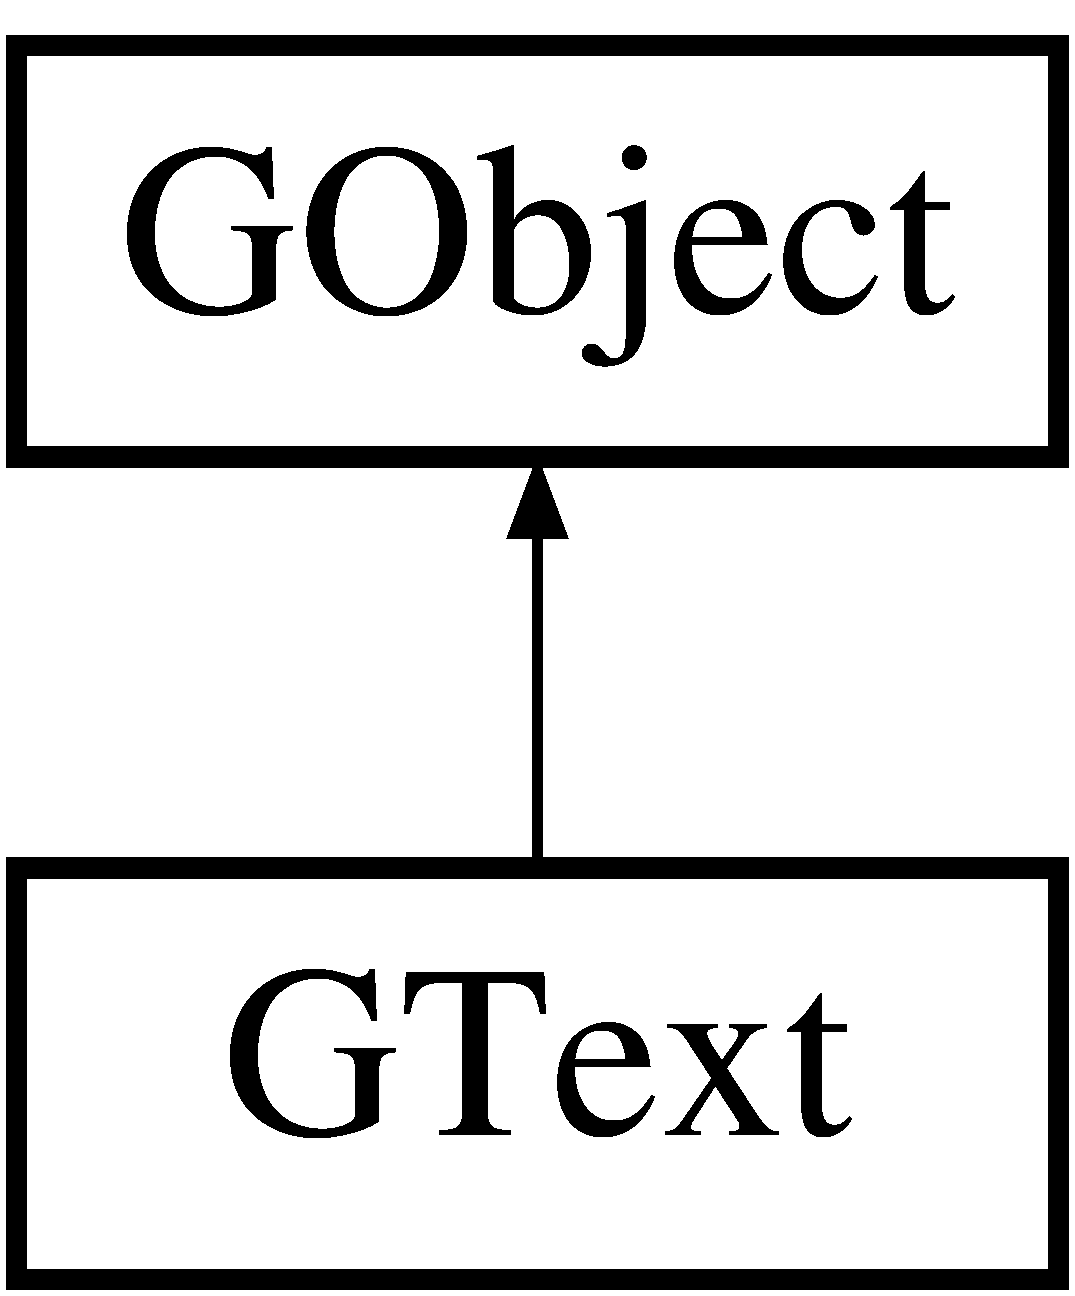
\includegraphics[height=2.000000cm]{classGText}
\end{center}
\end{figure}
\subsection*{Public Types}
\begin{DoxyCompactItemize}
\item 
enum \mbox{\hyperlink{classGObject_a86e0f5648542856159bb40775c854aa7}{Line\+Style}} \{ \mbox{\hyperlink{classGObject_a86e0f5648542856159bb40775c854aa7acbc84bd5232621834ed31f44d457c1eb}{L\+I\+N\+E\+\_\+\+N\+O\+NE}}, 
\mbox{\hyperlink{classGObject_a86e0f5648542856159bb40775c854aa7a700c78bc2cd76acaab26651bf7b4941f}{L\+I\+N\+E\+\_\+\+S\+O\+L\+ID}}, 
\mbox{\hyperlink{classGObject_a86e0f5648542856159bb40775c854aa7a9ccba0845f785d81d07b333ae1aad84e}{L\+I\+N\+E\+\_\+\+D\+A\+SH}}, 
\mbox{\hyperlink{classGObject_a86e0f5648542856159bb40775c854aa7a8e811c096cb941997f0bfda168bb6df3}{L\+I\+N\+E\+\_\+\+D\+OT}}, 
\mbox{\hyperlink{classGObject_a86e0f5648542856159bb40775c854aa7ada15a2e3d737b2db7706d8300f91b89d}{L\+I\+N\+E\+\_\+\+D\+A\+S\+H\+\_\+\+D\+OT}}, 
\mbox{\hyperlink{classGObject_a86e0f5648542856159bb40775c854aa7aabf4053a73eafa7ba2b7e6d664c74c1d}{L\+I\+N\+E\+\_\+\+D\+A\+S\+H\+\_\+\+D\+O\+T\+\_\+\+D\+OT}}
 \}
\begin{DoxyCompactList}\small\item\em Styles that can be used for the outline around various shapes. \end{DoxyCompactList}\end{DoxyCompactItemize}
\subsection*{Public Member Functions}
\begin{DoxyCompactItemize}
\item 
\mbox{\hyperlink{classGText_ad86d52c255aab367ddc6c54baff70846}{G\+Text}} (const std\+::string \&str=\char`\"{}\char`\"{}, double x=0, double y=0)
\begin{DoxyCompactList}\small\item\em Creates a {\ttfamily \mbox{\hyperlink{classGText}{G\+Text}}} object containing the specified string. \end{DoxyCompactList}\item 
virtual bool \mbox{\hyperlink{classGObject_abb6a5d7c03e6eaaae97264c4799ce7c3}{contains}} (double x, double y) const
\begin{DoxyCompactList}\small\item\em Returns {\ttfamily true} if the specified point is inside the object. \end{DoxyCompactList}\item 
virtual bool \mbox{\hyperlink{classGObject_a1dbc9dafaae51958112dbe1267a1f547}{contains}} (const \mbox{\hyperlink{classGPoint}{G\+Point}} \&pt) const
\begin{DoxyCompactList}\small\item\em Returns {\ttfamily true} if the specified point is inside the object. \end{DoxyCompactList}\item 
virtual \mbox{\hyperlink{classGPoint}{G\+Point}} \mbox{\hyperlink{classGObject_a0d41183bf6b08de66fe3907551aab0d7}{get\+Bottom\+Right\+Location}} () const
\begin{DoxyCompactList}\small\item\em Returns the x/y coordinates of the bottom/right corner of the object. \end{DoxyCompactList}\item 
virtual double \mbox{\hyperlink{classGObject_a4316a2406c18e1c6d061fe51fd355490}{get\+BottomY}} () const
\begin{DoxyCompactList}\small\item\em Returns the {\itshape y}-\/coordinate of the bottom of the object. \end{DoxyCompactList}\item 
virtual \mbox{\hyperlink{classGRectangle}{G\+Rectangle}} \mbox{\hyperlink{classGText_a2f46ec8a3b533c690b3b3e56d4f34afe}{get\+Bounds}} () const Q\+\_\+\+D\+E\+C\+L\+\_\+\+O\+V\+E\+R\+R\+I\+DE
\begin{DoxyCompactList}\small\item\em Returns the bounding box of this object, which is defined to be the smallest rectangle that covers everything drawn by the figure. \end{DoxyCompactList}\item 
virtual \mbox{\hyperlink{classGPoint}{G\+Point}} \mbox{\hyperlink{classGObject_a0909472e91448470bccdb62ecfb95d8b}{get\+Center\+Location}} () const
\begin{DoxyCompactList}\small\item\em Returns the x/y-\/coordinates of the center of the object. \end{DoxyCompactList}\item 
virtual double \mbox{\hyperlink{classGObject_a04df74355b545e0543112d5b8d924176}{get\+CenterX}} () const
\begin{DoxyCompactList}\small\item\em Returns the {\itshape x}-\/coordinate of the center of the object. \end{DoxyCompactList}\item 
virtual double \mbox{\hyperlink{classGObject_acb3287a3d507025a26f54b895713b947}{get\+CenterY}} () const
\begin{DoxyCompactList}\small\item\em Returns the {\itshape y}-\/coordinate of the center of the object. \end{DoxyCompactList}\item 
virtual std\+::string \mbox{\hyperlink{classGObject_aa061dfa488c31e18549d64363c1d0e34}{get\+Color}} () const
\begin{DoxyCompactList}\small\item\em Returns the color used to display this object. \end{DoxyCompactList}\item 
virtual std\+::string \mbox{\hyperlink{classGObject_a76f6964a11fde7c78e9751be184e1a3c}{get\+Fill\+Color}} () const
\begin{DoxyCompactList}\small\item\em Returns the color used to display the filled region of this object. \end{DoxyCompactList}\item 
virtual std\+::string \mbox{\hyperlink{classGText_a894a5502900794eeb27d084c21f1d77d}{get\+Font}} () const
\begin{DoxyCompactList}\small\item\em Returns the current font for the label. \end{DoxyCompactList}\item 
virtual double \mbox{\hyperlink{classGText_ab7583914978530e097034293e9d316ad}{get\+Font\+Ascent}} () const
\begin{DoxyCompactList}\small\item\em Returns the maximum distance strings in this font extend above the baseline. \end{DoxyCompactList}\item 
virtual double \mbox{\hyperlink{classGText_a2908216e19046c9747c0fc3b0d088621}{get\+Font\+Descent}} () const
\begin{DoxyCompactList}\small\item\em Returns the maximum distance strings in this font descend below the baseline. \end{DoxyCompactList}\item 
virtual double \mbox{\hyperlink{classGObject_a1e7e353362434072875264cf95629f99}{get\+Height}} () const
\begin{DoxyCompactList}\small\item\em Returns the height of this object, which is the same as the height of its bounding box. \end{DoxyCompactList}\item 
virtual std\+::string \mbox{\hyperlink{classGText_aa73aa351564b091c0658f2368c6d5c5f}{get\+Label}} () const
\begin{DoxyCompactList}\small\item\em Returns the string displayed by this object. \end{DoxyCompactList}\item 
virtual \mbox{\hyperlink{classGObject_a86e0f5648542856159bb40775c854aa7}{Line\+Style}} \mbox{\hyperlink{classGObject_aaf1f5ea8281e5e3486662878d26f0a13}{get\+Line\+Style}} () const
\begin{DoxyCompactList}\small\item\em Returns the object\textquotesingle{}s style such as solid or dashed. \end{DoxyCompactList}\item 
virtual double \mbox{\hyperlink{classGObject_a85ff266dc3eb63d9f2d8e5a4487fd3c0}{get\+Line\+Width}} () const
\begin{DoxyCompactList}\small\item\em Returns the width of the line used to draw this object. \end{DoxyCompactList}\item 
virtual \mbox{\hyperlink{classGPoint}{G\+Point}} \mbox{\hyperlink{classGObject_a4f83802015511edeb63b892830812c11}{get\+Location}} () const
\begin{DoxyCompactList}\small\item\em Returns the location of the top-\/left corner of object. \end{DoxyCompactList}\item 
virtual double \mbox{\hyperlink{classGObject_a1ae3fc278cc5b71b9f2d96a8a83cdf26}{get\+Opacity}} () const
\begin{DoxyCompactList}\small\item\em Returns how opaque (non-\/transparent) this object will appear from 0.\+0 (completely transparent) to 1.\+0 (completely opaque, default). \end{DoxyCompactList}\item 
virtual \mbox{\hyperlink{classGCompound}{G\+Compound}} $\ast$ \mbox{\hyperlink{classGObject_a3e53cef70541b1a14eade4ad0984d0b4}{get\+Parent}} () const
\begin{DoxyCompactList}\small\item\em Returns a pointer to the {\ttfamily \mbox{\hyperlink{classGCompound}{G\+Compound}}} that contains this object. \end{DoxyCompactList}\item 
virtual double \mbox{\hyperlink{classGObject_a798cc79daaa10145b28f60bcdfdb0ee9}{get\+RightX}} () const
\begin{DoxyCompactList}\small\item\em Returns the {\itshape x}-\/coordinate of the right side of the object. \end{DoxyCompactList}\item 
virtual \mbox{\hyperlink{classGDimension}{G\+Dimension}} \mbox{\hyperlink{classGObject_a7b4eec96a2bdc6420695d5796a78eea9}{get\+Size}} () const
\begin{DoxyCompactList}\small\item\em Returns the size of the object as a {\ttfamily \mbox{\hyperlink{classGDimension}{G\+Dimension}}}. \end{DoxyCompactList}\item 
virtual std\+::string \mbox{\hyperlink{classGText_aff553c50924b836c29f146ed34a7c6ec}{get\+Text}} () const
\begin{DoxyCompactList}\small\item\em Returns the string displayed by this object. \end{DoxyCompactList}\item 
virtual std\+::string \mbox{\hyperlink{classGText_a9896d58fcfebbf1025aeeb5b8b9ede80}{get\+Type}} () const Q\+\_\+\+D\+E\+C\+L\+\_\+\+O\+V\+E\+R\+R\+I\+DE
\begin{DoxyCompactList}\small\item\em Returns the type of the object as a string, such as {\ttfamily \char`\"{}\+G\+Oval\char`\"{}} or {\ttfamily \char`\"{}\+G\+Rect\char`\"{}}. \end{DoxyCompactList}\item 
virtual double \mbox{\hyperlink{classGObject_a0ed2965abd4f5701d2cadf71239faf19}{get\+Width}} () const
\begin{DoxyCompactList}\small\item\em Returns the width of this object, which is equal to the width of the bounding box. \end{DoxyCompactList}\item 
virtual double \mbox{\hyperlink{classGObject_a344385751bee0720059403940d57a13e}{getX}} () const
\begin{DoxyCompactList}\small\item\em Returns the leftmost {\itshape x}-\/coordinate of the object. \end{DoxyCompactList}\item 
virtual double \mbox{\hyperlink{classGObject_aafa51c7f8f38a09febbb9ce7853f77b4}{getY}} () const
\begin{DoxyCompactList}\small\item\em Returns the topmost {\itshape y}-\/coordinate of the object. \end{DoxyCompactList}\item 
virtual bool \mbox{\hyperlink{classGObject_a11c404f106940c201b6f326e0355c150}{is\+Filled}} () const
\begin{DoxyCompactList}\small\item\em Returns {\ttfamily true} if the object is filled with color. \end{DoxyCompactList}\item 
virtual bool \mbox{\hyperlink{classGObject_a9d8a6cfb13917785c143e74d40e4e2be}{is\+Visible}} () const
\begin{DoxyCompactList}\small\item\em Returns {\ttfamily true} if this object is visible on screen. \end{DoxyCompactList}\item 
virtual void \mbox{\hyperlink{classGObject_a5973d8dda83afb36e2c56855515be392}{move}} (double dx, double dy)
\begin{DoxyCompactList}\small\item\em Moves the object on the screen using the displacements {\ttfamily dx} and {\ttfamily dy}. \end{DoxyCompactList}\item 
virtual void \mbox{\hyperlink{classGObject_ac827b978aa122f136a14c198687ad80f}{repaint}} ()
\begin{DoxyCompactList}\small\item\em Instructs the object to redraw itself on screen. \end{DoxyCompactList}\item 
virtual void \mbox{\hyperlink{classGObject_a6022a1fd1e5dcd2fd5585e5a36aa3f37}{reset\+Transform}} ()
\begin{DoxyCompactList}\small\item\em Undoes any previous scale/rotate transformations on this object. \end{DoxyCompactList}\item 
virtual void \mbox{\hyperlink{classGObject_ae1ffaa12185dfd5ba464f7d87c329e26}{rotate}} (double theta)
\begin{DoxyCompactList}\small\item\em Transforms the object by rotating it {\ttfamily theta} degrees counterclockwise around its origin. \end{DoxyCompactList}\item 
virtual void \mbox{\hyperlink{classGObject_ad2e1900f730475c2d044817db03b38d6}{scale}} (double sf)
\begin{DoxyCompactList}\small\item\em Scales the object by the specified scale factor. \end{DoxyCompactList}\item 
virtual void \mbox{\hyperlink{classGObject_a63641f69d610d0b951357d35a0c3b1e3}{scale}} (double sx, double sy)
\begin{DoxyCompactList}\small\item\em Scales the object by the specified scale factors. \end{DoxyCompactList}\item 
void \mbox{\hyperlink{classGObject_ab6747f40313c531c2db32edb5b63b9b7}{send\+Backward}} ()
\begin{DoxyCompactList}\small\item\em Moves this object one step toward the back in the {\itshape z} dimension. \end{DoxyCompactList}\item 
void \mbox{\hyperlink{classGObject_a710b3e449c9facba7847c91ab170d281}{send\+Forward}} ()
\begin{DoxyCompactList}\small\item\em Moves this object one step toward the front in the {\itshape z} dimension. \end{DoxyCompactList}\item 
void \mbox{\hyperlink{classGObject_a0f7f1efbb7fd46dde2867c4ad0330896}{send\+To\+Back}} ()
\begin{DoxyCompactList}\small\item\em Moves this object to the back of the display in the {\itshape z} dimension. \end{DoxyCompactList}\item 
void \mbox{\hyperlink{classGObject_aee33d68488e46827ef55fac07f40a9b2}{send\+To\+Front}} ()
\begin{DoxyCompactList}\small\item\em Moves this object to the front of the display in the {\itshape z} dimension. \end{DoxyCompactList}\item 
virtual void \mbox{\hyperlink{classGObject_a71ff7b16b8f1bdc4a1ce9f30cf8b87d8}{set\+Bottom\+Right\+Location}} (double x, double y)
\begin{DoxyCompactList}\small\item\em Sets the location of the bottom/right of this object. \end{DoxyCompactList}\item 
virtual void \mbox{\hyperlink{classGObject_ac6f7320321182f1d18c1c0fa97d5e941}{set\+Bottom\+Right\+Location}} (const \mbox{\hyperlink{classGPoint}{G\+Point}} \&pt)
\begin{DoxyCompactList}\small\item\em Sets the location of the bottom/right of this object. \end{DoxyCompactList}\item 
virtual void \mbox{\hyperlink{classGObject_a4b20e93c2a2597484f74ee5caa71f41f}{set\+BottomY}} (double y)
\begin{DoxyCompactList}\small\item\em Sets the location of the bottom y-\/coordinate of this object. \end{DoxyCompactList}\item 
virtual void \mbox{\hyperlink{classGObject_a2aae8197624b72265ab83b4f1bc73f2f}{set\+Bounds}} (double x, double y, double width, double height)
\begin{DoxyCompactList}\small\item\em Changes the bounds of this object to the specified values. \end{DoxyCompactList}\item 
virtual void \mbox{\hyperlink{classGObject_acada386653f008cacc7cce86426bef7c}{set\+Bounds}} (const \mbox{\hyperlink{classGRectangle}{G\+Rectangle}} \&size)
\begin{DoxyCompactList}\small\item\em Changes the bounds of this object to the specified rectangle. \end{DoxyCompactList}\item 
virtual void \mbox{\hyperlink{classGObject_a290b47dd8de1be44089f95cb2c47c1de}{set\+Center\+Location}} (double x, double y)
\begin{DoxyCompactList}\small\item\em Sets the location of the center of this object. \end{DoxyCompactList}\item 
virtual void \mbox{\hyperlink{classGObject_a1bedf1b233ecba3f753ec58908a683a6}{set\+Center\+Location}} (const \mbox{\hyperlink{classGPoint}{G\+Point}} \&pt)
\begin{DoxyCompactList}\small\item\em Sets the location of the center of this object. \end{DoxyCompactList}\item 
virtual void \mbox{\hyperlink{classGObject_a2f4936281e056eead00a9186b9ba8af6}{set\+CenterX}} (double x)
\begin{DoxyCompactList}\small\item\em Sets the x-\/coordinate of the center of this object. \end{DoxyCompactList}\item 
virtual void \mbox{\hyperlink{classGObject_aad2a22b4fde88c33306b92aebf641d57}{set\+CenterY}} (double y)
\begin{DoxyCompactList}\small\item\em Sets the y-\/coordinate of the center of this object. \end{DoxyCompactList}\item 
virtual void \mbox{\hyperlink{classGObject_ad57ef49bc31db94e92648aa3737923d6}{set\+Color}} (int r, int g, int b)
\begin{DoxyCompactList}\small\item\em Sets the color used to display this object. \end{DoxyCompactList}\item 
virtual void \mbox{\hyperlink{classGObject_ab1f5cc0f5cc6bbbd716a526c61f1081d}{set\+Color}} (int rgb)
\begin{DoxyCompactList}\small\item\em Sets the color used to display this object. \end{DoxyCompactList}\item 
virtual void \mbox{\hyperlink{classGObject_a61374df6c11b52cfbb0815decdbaebc6}{set\+Color}} (const std\+::string \&color)
\begin{DoxyCompactList}\small\item\em Sets the color used to display this object. \end{DoxyCompactList}\item 
virtual void \mbox{\hyperlink{classGObject_ad767a33971159e9493e221cca4c00ae9}{set\+Fill\+Color}} (int r, int g, int b)
\begin{DoxyCompactList}\small\item\em Sets the color used to display the filled region of this object, if any. \end{DoxyCompactList}\item 
virtual void \mbox{\hyperlink{classGObject_aa59d9775a67fa7df2b24a95cd34840a3}{set\+Fill\+Color}} (int rgb)
\begin{DoxyCompactList}\small\item\em Sets the color used to display the filled region of this object, if any. \end{DoxyCompactList}\item 
virtual void \mbox{\hyperlink{classGObject_adbc18b1a930aadd97d7437f9f7265b96}{set\+Fill\+Color}} (const std\+::string \&color)
\begin{DoxyCompactList}\small\item\em Sets the color used to display the filled region of this object, if any. \end{DoxyCompactList}\item 
virtual void \mbox{\hyperlink{classGObject_a9b82b53362282c6bb7d6947068d2e55b}{set\+Filled}} (bool flag)
\begin{DoxyCompactList}\small\item\em Sets the fill status for the object, where {\ttfamily false} is outlined and {\ttfamily true} is filled. \end{DoxyCompactList}\item 
virtual void \mbox{\hyperlink{classGText_a2d22014c7fa3bccfd58c982aea1b55fa}{set\+Font}} (const Q\+Font \&font) Q\+\_\+\+D\+E\+C\+L\+\_\+\+O\+V\+E\+R\+R\+I\+DE
\begin{DoxyCompactList}\small\item\em Changes the font used to display the object as specified by the given Qt font. \end{DoxyCompactList}\item 
virtual void \mbox{\hyperlink{classGText_ab39ef411fb13a52852ddd138c5932e2e}{set\+Font}} (const std\+::string \&font) Q\+\_\+\+D\+E\+C\+L\+\_\+\+O\+V\+E\+R\+R\+I\+DE
\begin{DoxyCompactList}\small\item\em Changes the font used to display the object as specified by the string {\ttfamily font}, which has the following format\+: \end{DoxyCompactList}\item 
virtual void \mbox{\hyperlink{classGObject_ad18e8fab1e02a4e9b75c6730212558eb}{set\+Foreground}} (int r, int g, int b)
\begin{DoxyCompactList}\small\item\em Sets the color used to display this object. \end{DoxyCompactList}\item 
virtual void \mbox{\hyperlink{classGObject_a9eb856b5ff83a19df3831a31f15f4563}{set\+Foreground}} (int rgb)
\begin{DoxyCompactList}\small\item\em Sets the color used to display this object. \end{DoxyCompactList}\item 
virtual void \mbox{\hyperlink{classGObject_af59209aeadea6dfc6d97a2d8531f50e1}{set\+Foreground}} (const std\+::string \&color)
\begin{DoxyCompactList}\small\item\em Sets the color used to display this object. \end{DoxyCompactList}\item 
virtual void \mbox{\hyperlink{classGObject_a9e280bfc4544dfaf8e4376c4e1a74357}{set\+Height}} (double height)
\begin{DoxyCompactList}\small\item\em Changes the height of this object to the specified height without changing its width. \end{DoxyCompactList}\item 
virtual void \mbox{\hyperlink{classGText_a889d82f199797fea605ee8230dcd4f6f}{set\+Label}} (const std\+::string \&str)
\begin{DoxyCompactList}\small\item\em Changes the string stored within the text label, so that a new text string appears on the display. \end{DoxyCompactList}\item 
virtual void \mbox{\hyperlink{classGObject_add11575087eb94f1a71faa3f826c6341}{set\+Line\+Style}} (\mbox{\hyperlink{classGObject_a86e0f5648542856159bb40775c854aa7}{Line\+Style}} line\+Style)
\begin{DoxyCompactList}\small\item\em Sets the object\textquotesingle{}s style such as solid (\mbox{\hyperlink{classGObject_a86e0f5648542856159bb40775c854aa7a700c78bc2cd76acaab26651bf7b4941f}{G\+Object\+::\+L\+I\+N\+E\+\_\+\+S\+O\+L\+ID}}) or dashed (\mbox{\hyperlink{classGObject_a86e0f5648542856159bb40775c854aa7a9ccba0845f785d81d07b333ae1aad84e}{G\+Object\+::\+L\+I\+N\+E\+\_\+\+D\+A\+SH}}). \end{DoxyCompactList}\item 
virtual void \mbox{\hyperlink{classGObject_afd6a47c6ea6a1f85ca05a65ba3ff3477}{set\+Line\+Width}} (double line\+Width)
\begin{DoxyCompactList}\small\item\em Sets the width of the line used to draw this object. \end{DoxyCompactList}\item 
virtual void \mbox{\hyperlink{classGObject_a04594e8ba9b98513a64f1da00dcae18c}{set\+Location}} (double x, double y)
\begin{DoxyCompactList}\small\item\em Sets the location of the top-\/left corner of this object to the specified coordinates. \end{DoxyCompactList}\item 
virtual void \mbox{\hyperlink{classGObject_aa8480c0b7166cdf8f784cece06ab353f}{set\+Location}} (const \mbox{\hyperlink{classGPoint}{G\+Point}} \&pt)
\begin{DoxyCompactList}\small\item\em Sets the location of the top-\/left corner of this object to the specified point. \end{DoxyCompactList}\item 
virtual void \mbox{\hyperlink{classGObject_a04af1866cc1bae4a1226695794a50539}{set\+Opacity}} (double opacity)
\begin{DoxyCompactList}\small\item\em Sets how opaque (non-\/transparent) this object will appear from 0.\+0 (completely transparent) to 1.\+0 (completely opaque, default). \end{DoxyCompactList}\item 
virtual void \mbox{\hyperlink{classGObject_a3c90b758cdc2c911c9ef76c4360eb912}{set\+RightX}} (double x)
\begin{DoxyCompactList}\small\item\em Sets the location of the rightmost x-\/coordinate of this object. \end{DoxyCompactList}\item 
virtual void \mbox{\hyperlink{classGObject_aca25d49481f9bf5fc8f7df4c086c4ce7}{set\+Size}} (double width, double height)
\begin{DoxyCompactList}\small\item\em Changes the size of this object to the specified width and height. \end{DoxyCompactList}\item 
virtual void \mbox{\hyperlink{classGObject_ae2b628228f192c2702c4ce941b2af68f}{set\+Size}} (const \mbox{\hyperlink{classGDimension}{G\+Dimension}} \&size)
\begin{DoxyCompactList}\small\item\em Changes the size of this object to the specified width and height. \end{DoxyCompactList}\item 
virtual void \mbox{\hyperlink{classGText_ac98cbe102af8aaf8fd017228d645bfda}{set\+Text}} (const std\+::string \&str)
\begin{DoxyCompactList}\small\item\em Changes the string stored within the text label, so that a new text string appears on the display. \end{DoxyCompactList}\item 
virtual void \mbox{\hyperlink{classGObject_a88203f28224315d9f4471212f4af8ed3}{set\+Visible}} (bool flag)
\begin{DoxyCompactList}\small\item\em Sets whether this object is visible. \end{DoxyCompactList}\item 
virtual void \mbox{\hyperlink{classGObject_aa3f3fba4cb131baa8696ba01e3bceca1}{set\+Width}} (double width)
\begin{DoxyCompactList}\small\item\em Changes the width of this object to the specified width without changing its height. \end{DoxyCompactList}\item 
virtual void \mbox{\hyperlink{classGObject_a9c18fcc579333bf9653d13ad2b372e39}{setX}} (double x)
\begin{DoxyCompactList}\small\item\em Sets the x location of the left side of this object. \end{DoxyCompactList}\item 
virtual void \mbox{\hyperlink{classGObject_a7d57e2a5c35d27feb58fd498a3cf82b9}{setY}} (double y)
\begin{DoxyCompactList}\small\item\em Sets the y location of the top of this object. \end{DoxyCompactList}\item 
virtual std\+::string \mbox{\hyperlink{classGObject_a1fe5121d6528fdea3f243321b3fa3a49}{to\+String}} () const
\begin{DoxyCompactList}\small\item\em Returns a printable representation of the object. \end{DoxyCompactList}\item 
virtual std\+::string \mbox{\hyperlink{classGText_a85b5bcebac42ec5f130b0c3851383a23}{to\+String\+Extra}} () const Q\+\_\+\+D\+E\+C\+L\+\_\+\+O\+V\+E\+R\+R\+I\+DE
\begin{DoxyCompactList}\small\item\em Returns a string containing any extra unique information about this type of graphical object. \end{DoxyCompactList}\end{DoxyCompactItemize}
\subsection*{Static Public Member Functions}
\begin{DoxyCompactItemize}
\item 
static bool \mbox{\hyperlink{classGObject_a93be0e1fe1b1bf1a1da732470c94f42b}{is\+Anti\+Aliasing}} ()
\begin{DoxyCompactList}\small\item\em Returns whether we should globally anti-\/alias graphical objects. \end{DoxyCompactList}\item 
static void \mbox{\hyperlink{classGObject_a1e43371668ae850193cebedb44e1bbe3}{set\+Anti\+Aliasing}} (bool value)
\begin{DoxyCompactList}\small\item\em Globally turns on/off the anti-\/aliasing feature that smooths out the edges of onscreen shapes. \end{DoxyCompactList}\end{DoxyCompactItemize}
\subsection*{Static Public Attributes}
\begin{DoxyCompactItemize}
\item 
static const std\+::string \mbox{\hyperlink{classGText_ab265ee508af32c0c0bb1aa3693977247}{D\+E\+F\+A\+U\+L\+T\+\_\+\+F\+O\+NT}} = \char`\"{}Dialog-\/13\char`\"{}
\begin{DoxyCompactList}\small\item\em The default font used in text labels if none is provided. \end{DoxyCompactList}\end{DoxyCompactItemize}
\subsection*{Protected Attributes}
\begin{DoxyCompactItemize}
\item 
Q\+Brush \mbox{\hyperlink{classGObject_aab24462ec896b596d99911767b0912d0}{\+\_\+brush}}
\item 
std\+::string \mbox{\hyperlink{classGObject_a1134e770ae4315ea8bc1201e2f21da8b}{\+\_\+color}}
\item 
int \mbox{\hyperlink{classGObject_a003fdd343d9b7505c53a8b7a134200ed}{\+\_\+color\+Int}}
\item 
std\+::string \mbox{\hyperlink{classGObject_a179f8d6cee65cd8a54692e32b224392a}{\+\_\+fill\+Color}}
\item 
int \mbox{\hyperlink{classGObject_a751def333a67d651e5b99cc331ecb496}{\+\_\+fill\+Color\+Int}}
\item 
bool \mbox{\hyperlink{classGObject_ad4a55cbcd61b58a4d49666490bb2f103}{\+\_\+fill\+Flag}}
\item 
std\+::string \mbox{\hyperlink{classGObject_aea76ea1a8b5dd7b0a78653277e63b536}{\+\_\+font}}
\item 
double \mbox{\hyperlink{classGObject_ad05df29e7f27fc504abd743e3d8b4e73}{\+\_\+height}}
\item 
\mbox{\hyperlink{classGObject_a86e0f5648542856159bb40775c854aa7}{Line\+Style}} \mbox{\hyperlink{classGObject_a89bafecaafb7c72d55c7efc10b7d0523}{\+\_\+line\+Style}}
\item 
double \mbox{\hyperlink{classGObject_a16e9033665937f13de2e163dc2184aff}{\+\_\+line\+Width}}
\item 
double \mbox{\hyperlink{classGObject_a20eff8eb7af27182edc9bfc54768b6f3}{\+\_\+opacity}}
\item 
\mbox{\hyperlink{classGCompound}{G\+Compound}} $\ast$ \mbox{\hyperlink{classGObject_ac9452c1eaff70eebddbb318196aa3835}{\+\_\+parent}}
\item 
Q\+Pen \mbox{\hyperlink{classGObject_afb69d172743f868299847174eb1b6bc8}{\+\_\+pen}}
\item 
Q\+Transform \mbox{\hyperlink{classGObject_a475b8860a5f1adb4a1fdc58d1f5c1e32}{\+\_\+transform}}
\item 
bool \mbox{\hyperlink{classGObject_ae4725802fc8d8aaa0ab4bd4781f7e07c}{\+\_\+transformed}}
\item 
bool \mbox{\hyperlink{classGObject_a9312c72508471b7c7a87b540263e1af4}{\+\_\+visible}}
\item 
double \mbox{\hyperlink{classGObject_ab55d85a3371770e6725b1062cf160cd8}{\+\_\+width}}
\item 
double \mbox{\hyperlink{classGObject_a6675b83b27137b8d3aa2ad8133078ea6}{\+\_\+x}}
\item 
double \mbox{\hyperlink{classGObject_a2f0f6aeafddc8a39c578bfa7e22b5f1e}{\+\_\+y}}
\end{DoxyCompactItemize}


\subsection{Detailed Description}
This graphical object subclass represents a text string. 

Controlling the appearance and positioning of a {\ttfamily \mbox{\hyperlink{classGText}{G\+Text}}} depends on understanding the following terms\+:


\begin{DoxyItemize}
\item The {\bfseries {\itshape baseline}} is the horizontal line on which the characters rest. 
\item The {\bfseries {\itshape origin}} is the point on the baseline at which the label begins. 
\item The {\bfseries {\itshape height}} is the distance that separate two successive lines. 
\item The {\bfseries {\itshape ascent}} is the maximum distance a character in this font extends above the baseline. 
\item The {\bfseries {\itshape descent}} is the maximum distance a character in this font extends below the baseline. 
\end{DoxyItemize}

\subsection{Member Enumeration Documentation}
\mbox{\Hypertarget{classGObject_a86e0f5648542856159bb40775c854aa7}\label{classGObject_a86e0f5648542856159bb40775c854aa7}} 
\index{G\+Text@{G\+Text}!Line\+Style@{Line\+Style}}
\index{Line\+Style@{Line\+Style}!G\+Text@{G\+Text}}
\subsubsection{\texorpdfstring{Line\+Style}{LineStyle}}
{\footnotesize\ttfamily enum \mbox{\hyperlink{classGObject_a86e0f5648542856159bb40775c854aa7}{Line\+Style}}\hspace{0.3cm}{\ttfamily [inherited]}}



Styles that can be used for the outline around various shapes. 

Call set\+Line\+Style on a \mbox{\hyperlink{classGObject}{G\+Object}} and pass one of these values. \begin{DoxyEnumFields}{Enumerator}
\raisebox{\heightof{T}}[0pt][0pt]{\index{L\+I\+N\+E\+\_\+\+N\+O\+NE@{L\+I\+N\+E\+\_\+\+N\+O\+NE}!G\+Text@{G\+Text}}\index{G\+Text@{G\+Text}!L\+I\+N\+E\+\_\+\+N\+O\+NE@{L\+I\+N\+E\+\_\+\+N\+O\+NE}}}\mbox{\Hypertarget{classGObject_a86e0f5648542856159bb40775c854aa7acbc84bd5232621834ed31f44d457c1eb}\label{classGObject_a86e0f5648542856159bb40775c854aa7acbc84bd5232621834ed31f44d457c1eb}} 
L\+I\+N\+E\+\_\+\+N\+O\+NE&\\
\hline

\raisebox{\heightof{T}}[0pt][0pt]{\index{L\+I\+N\+E\+\_\+\+S\+O\+L\+ID@{L\+I\+N\+E\+\_\+\+S\+O\+L\+ID}!G\+Text@{G\+Text}}\index{G\+Text@{G\+Text}!L\+I\+N\+E\+\_\+\+S\+O\+L\+ID@{L\+I\+N\+E\+\_\+\+S\+O\+L\+ID}}}\mbox{\Hypertarget{classGObject_a86e0f5648542856159bb40775c854aa7a700c78bc2cd76acaab26651bf7b4941f}\label{classGObject_a86e0f5648542856159bb40775c854aa7a700c78bc2cd76acaab26651bf7b4941f}} 
L\+I\+N\+E\+\_\+\+S\+O\+L\+ID&\\
\hline

\raisebox{\heightof{T}}[0pt][0pt]{\index{L\+I\+N\+E\+\_\+\+D\+A\+SH@{L\+I\+N\+E\+\_\+\+D\+A\+SH}!G\+Text@{G\+Text}}\index{G\+Text@{G\+Text}!L\+I\+N\+E\+\_\+\+D\+A\+SH@{L\+I\+N\+E\+\_\+\+D\+A\+SH}}}\mbox{\Hypertarget{classGObject_a86e0f5648542856159bb40775c854aa7a9ccba0845f785d81d07b333ae1aad84e}\label{classGObject_a86e0f5648542856159bb40775c854aa7a9ccba0845f785d81d07b333ae1aad84e}} 
L\+I\+N\+E\+\_\+\+D\+A\+SH&\\
\hline

\raisebox{\heightof{T}}[0pt][0pt]{\index{L\+I\+N\+E\+\_\+\+D\+OT@{L\+I\+N\+E\+\_\+\+D\+OT}!G\+Text@{G\+Text}}\index{G\+Text@{G\+Text}!L\+I\+N\+E\+\_\+\+D\+OT@{L\+I\+N\+E\+\_\+\+D\+OT}}}\mbox{\Hypertarget{classGObject_a86e0f5648542856159bb40775c854aa7a8e811c096cb941997f0bfda168bb6df3}\label{classGObject_a86e0f5648542856159bb40775c854aa7a8e811c096cb941997f0bfda168bb6df3}} 
L\+I\+N\+E\+\_\+\+D\+OT&\\
\hline

\raisebox{\heightof{T}}[0pt][0pt]{\index{L\+I\+N\+E\+\_\+\+D\+A\+S\+H\+\_\+\+D\+OT@{L\+I\+N\+E\+\_\+\+D\+A\+S\+H\+\_\+\+D\+OT}!G\+Text@{G\+Text}}\index{G\+Text@{G\+Text}!L\+I\+N\+E\+\_\+\+D\+A\+S\+H\+\_\+\+D\+OT@{L\+I\+N\+E\+\_\+\+D\+A\+S\+H\+\_\+\+D\+OT}}}\mbox{\Hypertarget{classGObject_a86e0f5648542856159bb40775c854aa7ada15a2e3d737b2db7706d8300f91b89d}\label{classGObject_a86e0f5648542856159bb40775c854aa7ada15a2e3d737b2db7706d8300f91b89d}} 
L\+I\+N\+E\+\_\+\+D\+A\+S\+H\+\_\+\+D\+OT&\\
\hline

\raisebox{\heightof{T}}[0pt][0pt]{\index{L\+I\+N\+E\+\_\+\+D\+A\+S\+H\+\_\+\+D\+O\+T\+\_\+\+D\+OT@{L\+I\+N\+E\+\_\+\+D\+A\+S\+H\+\_\+\+D\+O\+T\+\_\+\+D\+OT}!G\+Text@{G\+Text}}\index{G\+Text@{G\+Text}!L\+I\+N\+E\+\_\+\+D\+A\+S\+H\+\_\+\+D\+O\+T\+\_\+\+D\+OT@{L\+I\+N\+E\+\_\+\+D\+A\+S\+H\+\_\+\+D\+O\+T\+\_\+\+D\+OT}}}\mbox{\Hypertarget{classGObject_a86e0f5648542856159bb40775c854aa7aabf4053a73eafa7ba2b7e6d664c74c1d}\label{classGObject_a86e0f5648542856159bb40775c854aa7aabf4053a73eafa7ba2b7e6d664c74c1d}} 
L\+I\+N\+E\+\_\+\+D\+A\+S\+H\+\_\+\+D\+O\+T\+\_\+\+D\+OT&\\
\hline

\end{DoxyEnumFields}


\subsection{Constructor \& Destructor Documentation}
\mbox{\Hypertarget{classGText_ad86d52c255aab367ddc6c54baff70846}\label{classGText_ad86d52c255aab367ddc6c54baff70846}} 
\index{G\+Text@{G\+Text}!G\+Text@{G\+Text}}
\index{G\+Text@{G\+Text}!G\+Text@{G\+Text}}
\subsubsection{\texorpdfstring{G\+Text()}{GText()}}
{\footnotesize\ttfamily \mbox{\hyperlink{classGText}{G\+Text}} (\begin{DoxyParamCaption}\item[{const std\+::string \&}]{str = {\ttfamily \char`\"{}\char`\"{}},  }\item[{double}]{x = {\ttfamily 0},  }\item[{double}]{y = {\ttfamily 0} }\end{DoxyParamCaption})}



Creates a {\ttfamily \mbox{\hyperlink{classGText}{G\+Text}}} object containing the specified string. 

By default, the baseline of the first character appears at the origin; the second form automatically resets the location of the {\ttfamily \mbox{\hyperlink{classGText}{G\+Text}}} to the point ({\ttfamily x}, {\ttfamily y}). 

\subsection{Member Function Documentation}
\mbox{\Hypertarget{classGObject_abb6a5d7c03e6eaaae97264c4799ce7c3}\label{classGObject_abb6a5d7c03e6eaaae97264c4799ce7c3}} 
\index{G\+Text@{G\+Text}!contains@{contains}}
\index{contains@{contains}!G\+Text@{G\+Text}}
\subsubsection{\texorpdfstring{contains()}{contains()}\hspace{0.1cm}{\footnotesize\ttfamily [1/2]}}
{\footnotesize\ttfamily bool contains (\begin{DoxyParamCaption}\item[{double}]{x,  }\item[{double}]{y }\end{DoxyParamCaption}) const\hspace{0.3cm}{\ttfamily [virtual]}, {\ttfamily [inherited]}}



Returns {\ttfamily true} if the specified point is inside the object. 



Reimplemented in \mbox{\hyperlink{classGRoundRect_abb6a5d7c03e6eaaae97264c4799ce7c3}{G\+Round\+Rect}}, \mbox{\hyperlink{classGPolygon_abb6a5d7c03e6eaaae97264c4799ce7c3}{G\+Polygon}}, \mbox{\hyperlink{classGOval_aa095a031ab22c150d2d75fdda1c3c8f5}{G\+Oval}}, \mbox{\hyperlink{classGLine_aa095a031ab22c150d2d75fdda1c3c8f5}{G\+Line}}, \mbox{\hyperlink{classGCompound_aa095a031ab22c150d2d75fdda1c3c8f5}{G\+Compound}}, and \mbox{\hyperlink{classGArc_aa095a031ab22c150d2d75fdda1c3c8f5}{G\+Arc}}.

\mbox{\Hypertarget{classGObject_a1dbc9dafaae51958112dbe1267a1f547}\label{classGObject_a1dbc9dafaae51958112dbe1267a1f547}} 
\index{G\+Text@{G\+Text}!contains@{contains}}
\index{contains@{contains}!G\+Text@{G\+Text}}
\subsubsection{\texorpdfstring{contains()}{contains()}\hspace{0.1cm}{\footnotesize\ttfamily [2/2]}}
{\footnotesize\ttfamily bool contains (\begin{DoxyParamCaption}\item[{const \mbox{\hyperlink{classGPoint}{G\+Point}} \&}]{pt }\end{DoxyParamCaption}) const\hspace{0.3cm}{\ttfamily [virtual]}, {\ttfamily [inherited]}}



Returns {\ttfamily true} if the specified point is inside the object. 

\mbox{\Hypertarget{classGObject_a0d41183bf6b08de66fe3907551aab0d7}\label{classGObject_a0d41183bf6b08de66fe3907551aab0d7}} 
\index{G\+Text@{G\+Text}!get\+Bottom\+Right\+Location@{get\+Bottom\+Right\+Location}}
\index{get\+Bottom\+Right\+Location@{get\+Bottom\+Right\+Location}!G\+Text@{G\+Text}}
\subsubsection{\texorpdfstring{get\+Bottom\+Right\+Location()}{getBottomRightLocation()}}
{\footnotesize\ttfamily \mbox{\hyperlink{classGPoint}{G\+Point}} get\+Bottom\+Right\+Location (\begin{DoxyParamCaption}{ }\end{DoxyParamCaption}) const\hspace{0.3cm}{\ttfamily [virtual]}, {\ttfamily [inherited]}}



Returns the x/y coordinates of the bottom/right corner of the object. 

\mbox{\Hypertarget{classGObject_a4316a2406c18e1c6d061fe51fd355490}\label{classGObject_a4316a2406c18e1c6d061fe51fd355490}} 
\index{G\+Text@{G\+Text}!get\+BottomY@{get\+BottomY}}
\index{get\+BottomY@{get\+BottomY}!G\+Text@{G\+Text}}
\subsubsection{\texorpdfstring{get\+Bottom\+Y()}{getBottomY()}}
{\footnotesize\ttfamily double get\+BottomY (\begin{DoxyParamCaption}{ }\end{DoxyParamCaption}) const\hspace{0.3cm}{\ttfamily [virtual]}, {\ttfamily [inherited]}}



Returns the {\itshape y}-\/coordinate of the bottom of the object. 

Equivalent to the top y-\/coordinate plus the object\textquotesingle{}s height. \mbox{\Hypertarget{classGText_a2f46ec8a3b533c690b3b3e56d4f34afe}\label{classGText_a2f46ec8a3b533c690b3b3e56d4f34afe}} 
\index{G\+Text@{G\+Text}!get\+Bounds@{get\+Bounds}}
\index{get\+Bounds@{get\+Bounds}!G\+Text@{G\+Text}}
\subsubsection{\texorpdfstring{get\+Bounds()}{getBounds()}}
{\footnotesize\ttfamily \mbox{\hyperlink{classGRectangle}{G\+Rectangle}} get\+Bounds (\begin{DoxyParamCaption}{ }\end{DoxyParamCaption}) const\hspace{0.3cm}{\ttfamily [virtual]}}



Returns the bounding box of this object, which is defined to be the smallest rectangle that covers everything drawn by the figure. 

The coordinates of this rectangle do not necessarily match the location returned by {\ttfamily get\+Location}. Given a {\ttfamily \mbox{\hyperlink{classGText}{G\+Text}}} object, for example, {\ttfamily get\+Location} returns the coordinates of the point on the baseline at which the string begins; the {\ttfamily get\+Bounds} method, by contrast, returns a rectangle that covers the entire window area occupied by the string. 

Reimplemented from \mbox{\hyperlink{classGObject_a29e6ac35a0b48f491a4c88194cc5da3b}{G\+Object}}.

\mbox{\Hypertarget{classGObject_a0909472e91448470bccdb62ecfb95d8b}\label{classGObject_a0909472e91448470bccdb62ecfb95d8b}} 
\index{G\+Text@{G\+Text}!get\+Center\+Location@{get\+Center\+Location}}
\index{get\+Center\+Location@{get\+Center\+Location}!G\+Text@{G\+Text}}
\subsubsection{\texorpdfstring{get\+Center\+Location()}{getCenterLocation()}}
{\footnotesize\ttfamily \mbox{\hyperlink{classGPoint}{G\+Point}} get\+Center\+Location (\begin{DoxyParamCaption}{ }\end{DoxyParamCaption}) const\hspace{0.3cm}{\ttfamily [virtual]}, {\ttfamily [inherited]}}



Returns the x/y-\/coordinates of the center of the object. 

Equivalent to the top/left plus half the object\textquotesingle{}s size. \mbox{\Hypertarget{classGObject_a04df74355b545e0543112d5b8d924176}\label{classGObject_a04df74355b545e0543112d5b8d924176}} 
\index{G\+Text@{G\+Text}!get\+CenterX@{get\+CenterX}}
\index{get\+CenterX@{get\+CenterX}!G\+Text@{G\+Text}}
\subsubsection{\texorpdfstring{get\+Center\+X()}{getCenterX()}}
{\footnotesize\ttfamily double get\+CenterX (\begin{DoxyParamCaption}{ }\end{DoxyParamCaption}) const\hspace{0.3cm}{\ttfamily [virtual]}, {\ttfamily [inherited]}}



Returns the {\itshape x}-\/coordinate of the center of the object. 

Equivalent to the top/left plus half the object\textquotesingle{}s width. \mbox{\Hypertarget{classGObject_acb3287a3d507025a26f54b895713b947}\label{classGObject_acb3287a3d507025a26f54b895713b947}} 
\index{G\+Text@{G\+Text}!get\+CenterY@{get\+CenterY}}
\index{get\+CenterY@{get\+CenterY}!G\+Text@{G\+Text}}
\subsubsection{\texorpdfstring{get\+Center\+Y()}{getCenterY()}}
{\footnotesize\ttfamily double get\+CenterY (\begin{DoxyParamCaption}{ }\end{DoxyParamCaption}) const\hspace{0.3cm}{\ttfamily [virtual]}, {\ttfamily [inherited]}}



Returns the {\itshape y}-\/coordinate of the center of the object. 

Equivalent to the top/left plus half the object\textquotesingle{}s height. \mbox{\Hypertarget{classGObject_aa061dfa488c31e18549d64363c1d0e34}\label{classGObject_aa061dfa488c31e18549d64363c1d0e34}} 
\index{G\+Text@{G\+Text}!get\+Color@{get\+Color}}
\index{get\+Color@{get\+Color}!G\+Text@{G\+Text}}
\subsubsection{\texorpdfstring{get\+Color()}{getColor()}}
{\footnotesize\ttfamily std\+::string get\+Color (\begin{DoxyParamCaption}{ }\end{DoxyParamCaption}) const\hspace{0.3cm}{\ttfamily [virtual]}, {\ttfamily [inherited]}}



Returns the color used to display this object. 

This color is always returned as a string in the form {\ttfamily \char`\"{}\#rrggbb\char`\"{}}, where {\ttfamily rr}, {\ttfamily gg}, and {\ttfamily bb} are the red, green, and blue components of the color, expressed as two-\/digit hexadecimal values. \mbox{\Hypertarget{classGObject_a76f6964a11fde7c78e9751be184e1a3c}\label{classGObject_a76f6964a11fde7c78e9751be184e1a3c}} 
\index{G\+Text@{G\+Text}!get\+Fill\+Color@{get\+Fill\+Color}}
\index{get\+Fill\+Color@{get\+Fill\+Color}!G\+Text@{G\+Text}}
\subsubsection{\texorpdfstring{get\+Fill\+Color()}{getFillColor()}}
{\footnotesize\ttfamily std\+::string get\+Fill\+Color (\begin{DoxyParamCaption}{ }\end{DoxyParamCaption}) const\hspace{0.3cm}{\ttfamily [virtual]}, {\ttfamily [inherited]}}



Returns the color used to display the filled region of this object. 

If none has been set, returns the empty string. \mbox{\Hypertarget{classGText_a894a5502900794eeb27d084c21f1d77d}\label{classGText_a894a5502900794eeb27d084c21f1d77d}} 
\index{G\+Text@{G\+Text}!get\+Font@{get\+Font}}
\index{get\+Font@{get\+Font}!G\+Text@{G\+Text}}
\subsubsection{\texorpdfstring{get\+Font()}{getFont()}}
{\footnotesize\ttfamily std\+::string get\+Font (\begin{DoxyParamCaption}{ }\end{DoxyParamCaption}) const\hspace{0.3cm}{\ttfamily [virtual]}}



Returns the current font for the label. 

\mbox{\Hypertarget{classGText_ab7583914978530e097034293e9d316ad}\label{classGText_ab7583914978530e097034293e9d316ad}} 
\index{G\+Text@{G\+Text}!get\+Font\+Ascent@{get\+Font\+Ascent}}
\index{get\+Font\+Ascent@{get\+Font\+Ascent}!G\+Text@{G\+Text}}
\subsubsection{\texorpdfstring{get\+Font\+Ascent()}{getFontAscent()}}
{\footnotesize\ttfamily double get\+Font\+Ascent (\begin{DoxyParamCaption}{ }\end{DoxyParamCaption}) const\hspace{0.3cm}{\ttfamily [virtual]}}



Returns the maximum distance strings in this font extend above the baseline. 

\mbox{\Hypertarget{classGText_a2908216e19046c9747c0fc3b0d088621}\label{classGText_a2908216e19046c9747c0fc3b0d088621}} 
\index{G\+Text@{G\+Text}!get\+Font\+Descent@{get\+Font\+Descent}}
\index{get\+Font\+Descent@{get\+Font\+Descent}!G\+Text@{G\+Text}}
\subsubsection{\texorpdfstring{get\+Font\+Descent()}{getFontDescent()}}
{\footnotesize\ttfamily double get\+Font\+Descent (\begin{DoxyParamCaption}{ }\end{DoxyParamCaption}) const\hspace{0.3cm}{\ttfamily [virtual]}}



Returns the maximum distance strings in this font descend below the baseline. 

\mbox{\Hypertarget{classGObject_a1e7e353362434072875264cf95629f99}\label{classGObject_a1e7e353362434072875264cf95629f99}} 
\index{G\+Text@{G\+Text}!get\+Height@{get\+Height}}
\index{get\+Height@{get\+Height}!G\+Text@{G\+Text}}
\subsubsection{\texorpdfstring{get\+Height()}{getHeight()}}
{\footnotesize\ttfamily double get\+Height (\begin{DoxyParamCaption}{ }\end{DoxyParamCaption}) const\hspace{0.3cm}{\ttfamily [virtual]}, {\ttfamily [inherited]}}



Returns the height of this object, which is the same as the height of its bounding box. 



Reimplemented in \mbox{\hyperlink{classGPolygon_a1e7e353362434072875264cf95629f99}{G\+Polygon}}, and \mbox{\hyperlink{classGLine_a423f17d4aeb66feb0d148fd23af335b7}{G\+Line}}.

\mbox{\Hypertarget{classGText_aa73aa351564b091c0658f2368c6d5c5f}\label{classGText_aa73aa351564b091c0658f2368c6d5c5f}} 
\index{G\+Text@{G\+Text}!get\+Label@{get\+Label}}
\index{get\+Label@{get\+Label}!G\+Text@{G\+Text}}
\subsubsection{\texorpdfstring{get\+Label()}{getLabel()}}
{\footnotesize\ttfamily std\+::string get\+Label (\begin{DoxyParamCaption}{ }\end{DoxyParamCaption}) const\hspace{0.3cm}{\ttfamily [virtual]}}



Returns the string displayed by this object. 

Equivalent to get\+Label. \mbox{\Hypertarget{classGObject_aaf1f5ea8281e5e3486662878d26f0a13}\label{classGObject_aaf1f5ea8281e5e3486662878d26f0a13}} 
\index{G\+Text@{G\+Text}!get\+Line\+Style@{get\+Line\+Style}}
\index{get\+Line\+Style@{get\+Line\+Style}!G\+Text@{G\+Text}}
\subsubsection{\texorpdfstring{get\+Line\+Style()}{getLineStyle()}}
{\footnotesize\ttfamily \mbox{\hyperlink{classGObject_a86e0f5648542856159bb40775c854aa7}{G\+Object\+::\+Line\+Style}} get\+Line\+Style (\begin{DoxyParamCaption}{ }\end{DoxyParamCaption}) const\hspace{0.3cm}{\ttfamily [virtual]}, {\ttfamily [inherited]}}



Returns the object\textquotesingle{}s style such as solid or dashed. 

\mbox{\Hypertarget{classGObject_a85ff266dc3eb63d9f2d8e5a4487fd3c0}\label{classGObject_a85ff266dc3eb63d9f2d8e5a4487fd3c0}} 
\index{G\+Text@{G\+Text}!get\+Line\+Width@{get\+Line\+Width}}
\index{get\+Line\+Width@{get\+Line\+Width}!G\+Text@{G\+Text}}
\subsubsection{\texorpdfstring{get\+Line\+Width()}{getLineWidth()}}
{\footnotesize\ttfamily double get\+Line\+Width (\begin{DoxyParamCaption}{ }\end{DoxyParamCaption}) const\hspace{0.3cm}{\ttfamily [virtual]}, {\ttfamily [inherited]}}



Returns the width of the line used to draw this object. 

\begin{DoxyReturn}{Returns}
default 1 
\end{DoxyReturn}
\mbox{\Hypertarget{classGObject_a4f83802015511edeb63b892830812c11}\label{classGObject_a4f83802015511edeb63b892830812c11}} 
\index{G\+Text@{G\+Text}!get\+Location@{get\+Location}}
\index{get\+Location@{get\+Location}!G\+Text@{G\+Text}}
\subsubsection{\texorpdfstring{get\+Location()}{getLocation()}}
{\footnotesize\ttfamily \mbox{\hyperlink{classGPoint}{G\+Point}} get\+Location (\begin{DoxyParamCaption}{ }\end{DoxyParamCaption}) const\hspace{0.3cm}{\ttfamily [virtual]}, {\ttfamily [inherited]}}



Returns the location of the top-\/left corner of object. 

\mbox{\Hypertarget{classGObject_a1ae3fc278cc5b71b9f2d96a8a83cdf26}\label{classGObject_a1ae3fc278cc5b71b9f2d96a8a83cdf26}} 
\index{G\+Text@{G\+Text}!get\+Opacity@{get\+Opacity}}
\index{get\+Opacity@{get\+Opacity}!G\+Text@{G\+Text}}
\subsubsection{\texorpdfstring{get\+Opacity()}{getOpacity()}}
{\footnotesize\ttfamily double get\+Opacity (\begin{DoxyParamCaption}{ }\end{DoxyParamCaption}) const\hspace{0.3cm}{\ttfamily [virtual]}, {\ttfamily [inherited]}}



Returns how opaque (non-\/transparent) this object will appear from 0.\+0 (completely transparent) to 1.\+0 (completely opaque, default). 

\mbox{\Hypertarget{classGObject_a3e53cef70541b1a14eade4ad0984d0b4}\label{classGObject_a3e53cef70541b1a14eade4ad0984d0b4}} 
\index{G\+Text@{G\+Text}!get\+Parent@{get\+Parent}}
\index{get\+Parent@{get\+Parent}!G\+Text@{G\+Text}}
\subsubsection{\texorpdfstring{get\+Parent()}{getParent()}}
{\footnotesize\ttfamily \mbox{\hyperlink{classGCompound}{G\+Compound}} $\ast$ get\+Parent (\begin{DoxyParamCaption}{ }\end{DoxyParamCaption}) const\hspace{0.3cm}{\ttfamily [virtual]}, {\ttfamily [inherited]}}



Returns a pointer to the {\ttfamily \mbox{\hyperlink{classGCompound}{G\+Compound}}} that contains this object. 

Every {\ttfamily \mbox{\hyperlink{classGWindow}{G\+Window}}} is initialized to contain a single {\ttfamily \mbox{\hyperlink{classGCompound}{G\+Compound}}} that is aligned with the window. Adding objects to the window adds them to that {\ttfamily \mbox{\hyperlink{classGCompound}{G\+Compound}}}, which means that every object you add to the window has a parent. Calling {\ttfamily get\+Parent} on the top-\/level {\ttfamily \mbox{\hyperlink{classGCompound}{G\+Compound}}} returns {\ttfamily nullptr}. \mbox{\Hypertarget{classGObject_a798cc79daaa10145b28f60bcdfdb0ee9}\label{classGObject_a798cc79daaa10145b28f60bcdfdb0ee9}} 
\index{G\+Text@{G\+Text}!get\+RightX@{get\+RightX}}
\index{get\+RightX@{get\+RightX}!G\+Text@{G\+Text}}
\subsubsection{\texorpdfstring{get\+Right\+X()}{getRightX()}}
{\footnotesize\ttfamily double get\+RightX (\begin{DoxyParamCaption}{ }\end{DoxyParamCaption}) const\hspace{0.3cm}{\ttfamily [virtual]}, {\ttfamily [inherited]}}



Returns the {\itshape x}-\/coordinate of the right side of the object. 

Equivalent to the left x-\/coordinate plus the object\textquotesingle{}s width. \mbox{\Hypertarget{classGObject_a7b4eec96a2bdc6420695d5796a78eea9}\label{classGObject_a7b4eec96a2bdc6420695d5796a78eea9}} 
\index{G\+Text@{G\+Text}!get\+Size@{get\+Size}}
\index{get\+Size@{get\+Size}!G\+Text@{G\+Text}}
\subsubsection{\texorpdfstring{get\+Size()}{getSize()}}
{\footnotesize\ttfamily \mbox{\hyperlink{classGDimension}{G\+Dimension}} get\+Size (\begin{DoxyParamCaption}{ }\end{DoxyParamCaption}) const\hspace{0.3cm}{\ttfamily [virtual]}, {\ttfamily [inherited]}}



Returns the size of the object as a {\ttfamily \mbox{\hyperlink{classGDimension}{G\+Dimension}}}. 

\mbox{\Hypertarget{classGText_aff553c50924b836c29f146ed34a7c6ec}\label{classGText_aff553c50924b836c29f146ed34a7c6ec}} 
\index{G\+Text@{G\+Text}!get\+Text@{get\+Text}}
\index{get\+Text@{get\+Text}!G\+Text@{G\+Text}}
\subsubsection{\texorpdfstring{get\+Text()}{getText()}}
{\footnotesize\ttfamily std\+::string get\+Text (\begin{DoxyParamCaption}{ }\end{DoxyParamCaption}) const\hspace{0.3cm}{\ttfamily [virtual]}}



Returns the string displayed by this object. 

Equivalent to get\+Label. \mbox{\Hypertarget{classGText_a9896d58fcfebbf1025aeeb5b8b9ede80}\label{classGText_a9896d58fcfebbf1025aeeb5b8b9ede80}} 
\index{G\+Text@{G\+Text}!get\+Type@{get\+Type}}
\index{get\+Type@{get\+Type}!G\+Text@{G\+Text}}
\subsubsection{\texorpdfstring{get\+Type()}{getType()}}
{\footnotesize\ttfamily std\+::string get\+Type (\begin{DoxyParamCaption}{ }\end{DoxyParamCaption}) const\hspace{0.3cm}{\ttfamily [virtual]}}



Returns the type of the object as a string, such as {\ttfamily \char`\"{}\+G\+Oval\char`\"{}} or {\ttfamily \char`\"{}\+G\+Rect\char`\"{}}. 

Each \mbox{\hyperlink{classGObject}{G\+Object}} subtype must override this method. 

Implements \mbox{\hyperlink{classGObject_a799e073a127b428cc841086d42ea4fed}{G\+Object}}.

\mbox{\Hypertarget{classGObject_a0ed2965abd4f5701d2cadf71239faf19}\label{classGObject_a0ed2965abd4f5701d2cadf71239faf19}} 
\index{G\+Text@{G\+Text}!get\+Width@{get\+Width}}
\index{get\+Width@{get\+Width}!G\+Text@{G\+Text}}
\subsubsection{\texorpdfstring{get\+Width()}{getWidth()}}
{\footnotesize\ttfamily double get\+Width (\begin{DoxyParamCaption}{ }\end{DoxyParamCaption}) const\hspace{0.3cm}{\ttfamily [virtual]}, {\ttfamily [inherited]}}



Returns the width of this object, which is equal to the width of the bounding box. 



Reimplemented in \mbox{\hyperlink{classGPolygon_a0ed2965abd4f5701d2cadf71239faf19}{G\+Polygon}}, and \mbox{\hyperlink{classGLine_a04bee94b66c8f921cd8611be2460ba9d}{G\+Line}}.

\mbox{\Hypertarget{classGObject_a344385751bee0720059403940d57a13e}\label{classGObject_a344385751bee0720059403940d57a13e}} 
\index{G\+Text@{G\+Text}!getX@{getX}}
\index{getX@{getX}!G\+Text@{G\+Text}}
\subsubsection{\texorpdfstring{get\+X()}{getX()}}
{\footnotesize\ttfamily double getX (\begin{DoxyParamCaption}{ }\end{DoxyParamCaption}) const\hspace{0.3cm}{\ttfamily [virtual]}, {\ttfamily [inherited]}}



Returns the leftmost {\itshape x}-\/coordinate of the object. 

\mbox{\Hypertarget{classGObject_aafa51c7f8f38a09febbb9ce7853f77b4}\label{classGObject_aafa51c7f8f38a09febbb9ce7853f77b4}} 
\index{G\+Text@{G\+Text}!getY@{getY}}
\index{getY@{getY}!G\+Text@{G\+Text}}
\subsubsection{\texorpdfstring{get\+Y()}{getY()}}
{\footnotesize\ttfamily double getY (\begin{DoxyParamCaption}{ }\end{DoxyParamCaption}) const\hspace{0.3cm}{\ttfamily [virtual]}, {\ttfamily [inherited]}}



Returns the topmost {\itshape y}-\/coordinate of the object. 

\mbox{\Hypertarget{classGObject_a93be0e1fe1b1bf1a1da732470c94f42b}\label{classGObject_a93be0e1fe1b1bf1a1da732470c94f42b}} 
\index{G\+Text@{G\+Text}!is\+Anti\+Aliasing@{is\+Anti\+Aliasing}}
\index{is\+Anti\+Aliasing@{is\+Anti\+Aliasing}!G\+Text@{G\+Text}}
\subsubsection{\texorpdfstring{is\+Anti\+Aliasing()}{isAntiAliasing()}}
{\footnotesize\ttfamily bool is\+Anti\+Aliasing (\begin{DoxyParamCaption}{ }\end{DoxyParamCaption})\hspace{0.3cm}{\ttfamily [static]}, {\ttfamily [inherited]}}



Returns whether we should globally anti-\/alias graphical objects. 

On by default. \mbox{\Hypertarget{classGObject_a11c404f106940c201b6f326e0355c150}\label{classGObject_a11c404f106940c201b6f326e0355c150}} 
\index{G\+Text@{G\+Text}!is\+Filled@{is\+Filled}}
\index{is\+Filled@{is\+Filled}!G\+Text@{G\+Text}}
\subsubsection{\texorpdfstring{is\+Filled()}{isFilled()}}
{\footnotesize\ttfamily bool is\+Filled (\begin{DoxyParamCaption}{ }\end{DoxyParamCaption}) const\hspace{0.3cm}{\ttfamily [virtual]}, {\ttfamily [inherited]}}



Returns {\ttfamily true} if the object is filled with color. 

\mbox{\Hypertarget{classGObject_a9d8a6cfb13917785c143e74d40e4e2be}\label{classGObject_a9d8a6cfb13917785c143e74d40e4e2be}} 
\index{G\+Text@{G\+Text}!is\+Visible@{is\+Visible}}
\index{is\+Visible@{is\+Visible}!G\+Text@{G\+Text}}
\subsubsection{\texorpdfstring{is\+Visible()}{isVisible()}}
{\footnotesize\ttfamily bool is\+Visible (\begin{DoxyParamCaption}{ }\end{DoxyParamCaption}) const\hspace{0.3cm}{\ttfamily [virtual]}, {\ttfamily [inherited]}}



Returns {\ttfamily true} if this object is visible on screen. 

\mbox{\Hypertarget{classGObject_a5973d8dda83afb36e2c56855515be392}\label{classGObject_a5973d8dda83afb36e2c56855515be392}} 
\index{G\+Text@{G\+Text}!move@{move}}
\index{move@{move}!G\+Text@{G\+Text}}
\subsubsection{\texorpdfstring{move()}{move()}}
{\footnotesize\ttfamily void move (\begin{DoxyParamCaption}\item[{double}]{dx,  }\item[{double}]{dy }\end{DoxyParamCaption})\hspace{0.3cm}{\ttfamily [virtual]}, {\ttfamily [inherited]}}



Moves the object on the screen using the displacements {\ttfamily dx} and {\ttfamily dy}. 

\mbox{\Hypertarget{classGObject_ac827b978aa122f136a14c198687ad80f}\label{classGObject_ac827b978aa122f136a14c198687ad80f}} 
\index{G\+Text@{G\+Text}!repaint@{repaint}}
\index{repaint@{repaint}!G\+Text@{G\+Text}}
\subsubsection{\texorpdfstring{repaint()}{repaint()}}
{\footnotesize\ttfamily void repaint (\begin{DoxyParamCaption}{ }\end{DoxyParamCaption})\hspace{0.3cm}{\ttfamily [virtual]}, {\ttfamily [inherited]}}



Instructs the object to redraw itself on screen. 



Reimplemented in \mbox{\hyperlink{classGCompound_ac827b978aa122f136a14c198687ad80f}{G\+Compound}}.

\mbox{\Hypertarget{classGObject_a6022a1fd1e5dcd2fd5585e5a36aa3f37}\label{classGObject_a6022a1fd1e5dcd2fd5585e5a36aa3f37}} 
\index{G\+Text@{G\+Text}!reset\+Transform@{reset\+Transform}}
\index{reset\+Transform@{reset\+Transform}!G\+Text@{G\+Text}}
\subsubsection{\texorpdfstring{reset\+Transform()}{resetTransform()}}
{\footnotesize\ttfamily void reset\+Transform (\begin{DoxyParamCaption}{ }\end{DoxyParamCaption})\hspace{0.3cm}{\ttfamily [virtual]}, {\ttfamily [inherited]}}



Undoes any previous scale/rotate transformations on this object. 

\mbox{\Hypertarget{classGObject_ae1ffaa12185dfd5ba464f7d87c329e26}\label{classGObject_ae1ffaa12185dfd5ba464f7d87c329e26}} 
\index{G\+Text@{G\+Text}!rotate@{rotate}}
\index{rotate@{rotate}!G\+Text@{G\+Text}}
\subsubsection{\texorpdfstring{rotate()}{rotate()}}
{\footnotesize\ttfamily void rotate (\begin{DoxyParamCaption}\item[{double}]{theta }\end{DoxyParamCaption})\hspace{0.3cm}{\ttfamily [virtual]}, {\ttfamily [inherited]}}



Transforms the object by rotating it {\ttfamily theta} degrees counterclockwise around its origin. 

\mbox{\Hypertarget{classGObject_ad2e1900f730475c2d044817db03b38d6}\label{classGObject_ad2e1900f730475c2d044817db03b38d6}} 
\index{G\+Text@{G\+Text}!scale@{scale}}
\index{scale@{scale}!G\+Text@{G\+Text}}
\subsubsection{\texorpdfstring{scale()}{scale()}\hspace{0.1cm}{\footnotesize\ttfamily [1/2]}}
{\footnotesize\ttfamily void scale (\begin{DoxyParamCaption}\item[{double}]{sf }\end{DoxyParamCaption})\hspace{0.3cm}{\ttfamily [virtual]}, {\ttfamily [inherited]}}



Scales the object by the specified scale factor. 

This form scales the object by {\ttfamily sf} in both dimensions, so that invoking {\ttfamily gobj-\/$>$scale(2);} doubles the size of the object. \mbox{\Hypertarget{classGObject_a63641f69d610d0b951357d35a0c3b1e3}\label{classGObject_a63641f69d610d0b951357d35a0c3b1e3}} 
\index{G\+Text@{G\+Text}!scale@{scale}}
\index{scale@{scale}!G\+Text@{G\+Text}}
\subsubsection{\texorpdfstring{scale()}{scale()}\hspace{0.1cm}{\footnotesize\ttfamily [2/2]}}
{\footnotesize\ttfamily void scale (\begin{DoxyParamCaption}\item[{double}]{sx,  }\item[{double}]{sy }\end{DoxyParamCaption})\hspace{0.3cm}{\ttfamily [virtual]}, {\ttfamily [inherited]}}



Scales the object by the specified scale factors. 

For example, {\ttfamily gobj-\/$>$scale(2, 2);} doubles the size of the object. This form applies independent scale factors to the {\itshape x} and {\itshape y} dimensions. \mbox{\Hypertarget{classGObject_ab6747f40313c531c2db32edb5b63b9b7}\label{classGObject_ab6747f40313c531c2db32edb5b63b9b7}} 
\index{G\+Text@{G\+Text}!send\+Backward@{send\+Backward}}
\index{send\+Backward@{send\+Backward}!G\+Text@{G\+Text}}
\subsubsection{\texorpdfstring{send\+Backward()}{sendBackward()}}
{\footnotesize\ttfamily void send\+Backward (\begin{DoxyParamCaption}{ }\end{DoxyParamCaption})\hspace{0.3cm}{\ttfamily [inherited]}}



Moves this object one step toward the back in the {\itshape z} dimension. 

If it was already at the back of the stack, nothing happens. \mbox{\Hypertarget{classGObject_a710b3e449c9facba7847c91ab170d281}\label{classGObject_a710b3e449c9facba7847c91ab170d281}} 
\index{G\+Text@{G\+Text}!send\+Forward@{send\+Forward}}
\index{send\+Forward@{send\+Forward}!G\+Text@{G\+Text}}
\subsubsection{\texorpdfstring{send\+Forward()}{sendForward()}}
{\footnotesize\ttfamily void send\+Forward (\begin{DoxyParamCaption}{ }\end{DoxyParamCaption})\hspace{0.3cm}{\ttfamily [inherited]}}



Moves this object one step toward the front in the {\itshape z} dimension. 

If it was already at the front of the stack, nothing happens. \mbox{\Hypertarget{classGObject_a0f7f1efbb7fd46dde2867c4ad0330896}\label{classGObject_a0f7f1efbb7fd46dde2867c4ad0330896}} 
\index{G\+Text@{G\+Text}!send\+To\+Back@{send\+To\+Back}}
\index{send\+To\+Back@{send\+To\+Back}!G\+Text@{G\+Text}}
\subsubsection{\texorpdfstring{send\+To\+Back()}{sendToBack()}}
{\footnotesize\ttfamily void send\+To\+Back (\begin{DoxyParamCaption}{ }\end{DoxyParamCaption})\hspace{0.3cm}{\ttfamily [inherited]}}



Moves this object to the back of the display in the {\itshape z} dimension. 

By moving it to the back, this object will appear to be behind the other graphical objects on the display and may be obscured by other objects in front. \mbox{\Hypertarget{classGObject_aee33d68488e46827ef55fac07f40a9b2}\label{classGObject_aee33d68488e46827ef55fac07f40a9b2}} 
\index{G\+Text@{G\+Text}!send\+To\+Front@{send\+To\+Front}}
\index{send\+To\+Front@{send\+To\+Front}!G\+Text@{G\+Text}}
\subsubsection{\texorpdfstring{send\+To\+Front()}{sendToFront()}}
{\footnotesize\ttfamily void send\+To\+Front (\begin{DoxyParamCaption}{ }\end{DoxyParamCaption})\hspace{0.3cm}{\ttfamily [inherited]}}



Moves this object to the front of the display in the {\itshape z} dimension. 

By moving it to the front, this object will appear to be on top of the other graphical objects on the display and may hide any objects that are further back. \mbox{\Hypertarget{classGObject_a1e43371668ae850193cebedb44e1bbe3}\label{classGObject_a1e43371668ae850193cebedb44e1bbe3}} 
\index{G\+Text@{G\+Text}!set\+Anti\+Aliasing@{set\+Anti\+Aliasing}}
\index{set\+Anti\+Aliasing@{set\+Anti\+Aliasing}!G\+Text@{G\+Text}}
\subsubsection{\texorpdfstring{set\+Anti\+Aliasing()}{setAntiAliasing()}}
{\footnotesize\ttfamily void set\+Anti\+Aliasing (\begin{DoxyParamCaption}\item[{bool}]{value }\end{DoxyParamCaption})\hspace{0.3cm}{\ttfamily [static]}, {\ttfamily [inherited]}}



Globally turns on/off the anti-\/aliasing feature that smooths out the edges of onscreen shapes. 

On by default. Does not repaint any onscreen objects when called; you must do this yourself. \mbox{\Hypertarget{classGObject_a71ff7b16b8f1bdc4a1ce9f30cf8b87d8}\label{classGObject_a71ff7b16b8f1bdc4a1ce9f30cf8b87d8}} 
\index{G\+Text@{G\+Text}!set\+Bottom\+Right\+Location@{set\+Bottom\+Right\+Location}}
\index{set\+Bottom\+Right\+Location@{set\+Bottom\+Right\+Location}!G\+Text@{G\+Text}}
\subsubsection{\texorpdfstring{set\+Bottom\+Right\+Location()}{setBottomRightLocation()}\hspace{0.1cm}{\footnotesize\ttfamily [1/2]}}
{\footnotesize\ttfamily void set\+Bottom\+Right\+Location (\begin{DoxyParamCaption}\item[{double}]{x,  }\item[{double}]{y }\end{DoxyParamCaption})\hspace{0.3cm}{\ttfamily [virtual]}, {\ttfamily [inherited]}}



Sets the location of the bottom/right of this object. 

\mbox{\Hypertarget{classGObject_ac6f7320321182f1d18c1c0fa97d5e941}\label{classGObject_ac6f7320321182f1d18c1c0fa97d5e941}} 
\index{G\+Text@{G\+Text}!set\+Bottom\+Right\+Location@{set\+Bottom\+Right\+Location}}
\index{set\+Bottom\+Right\+Location@{set\+Bottom\+Right\+Location}!G\+Text@{G\+Text}}
\subsubsection{\texorpdfstring{set\+Bottom\+Right\+Location()}{setBottomRightLocation()}\hspace{0.1cm}{\footnotesize\ttfamily [2/2]}}
{\footnotesize\ttfamily void set\+Bottom\+Right\+Location (\begin{DoxyParamCaption}\item[{const \mbox{\hyperlink{classGPoint}{G\+Point}} \&}]{pt }\end{DoxyParamCaption})\hspace{0.3cm}{\ttfamily [virtual]}, {\ttfamily [inherited]}}



Sets the location of the bottom/right of this object. 

\mbox{\Hypertarget{classGObject_a4b20e93c2a2597484f74ee5caa71f41f}\label{classGObject_a4b20e93c2a2597484f74ee5caa71f41f}} 
\index{G\+Text@{G\+Text}!set\+BottomY@{set\+BottomY}}
\index{set\+BottomY@{set\+BottomY}!G\+Text@{G\+Text}}
\subsubsection{\texorpdfstring{set\+Bottom\+Y()}{setBottomY()}}
{\footnotesize\ttfamily void set\+BottomY (\begin{DoxyParamCaption}\item[{double}]{y }\end{DoxyParamCaption})\hspace{0.3cm}{\ttfamily [virtual]}, {\ttfamily [inherited]}}



Sets the location of the bottom y-\/coordinate of this object. 

\mbox{\Hypertarget{classGObject_a2aae8197624b72265ab83b4f1bc73f2f}\label{classGObject_a2aae8197624b72265ab83b4f1bc73f2f}} 
\index{G\+Text@{G\+Text}!set\+Bounds@{set\+Bounds}}
\index{set\+Bounds@{set\+Bounds}!G\+Text@{G\+Text}}
\subsubsection{\texorpdfstring{set\+Bounds()}{setBounds()}\hspace{0.1cm}{\footnotesize\ttfamily [1/2]}}
{\footnotesize\ttfamily void set\+Bounds (\begin{DoxyParamCaption}\item[{double}]{x,  }\item[{double}]{y,  }\item[{double}]{width,  }\item[{double}]{height }\end{DoxyParamCaption})\hspace{0.3cm}{\ttfamily [virtual]}, {\ttfamily [inherited]}}



Changes the bounds of this object to the specified values. 

\mbox{\Hypertarget{classGObject_acada386653f008cacc7cce86426bef7c}\label{classGObject_acada386653f008cacc7cce86426bef7c}} 
\index{G\+Text@{G\+Text}!set\+Bounds@{set\+Bounds}}
\index{set\+Bounds@{set\+Bounds}!G\+Text@{G\+Text}}
\subsubsection{\texorpdfstring{set\+Bounds()}{setBounds()}\hspace{0.1cm}{\footnotesize\ttfamily [2/2]}}
{\footnotesize\ttfamily void set\+Bounds (\begin{DoxyParamCaption}\item[{const \mbox{\hyperlink{classGRectangle}{G\+Rectangle}} \&}]{size }\end{DoxyParamCaption})\hspace{0.3cm}{\ttfamily [virtual]}, {\ttfamily [inherited]}}



Changes the bounds of this object to the specified rectangle. 

\mbox{\Hypertarget{classGObject_a290b47dd8de1be44089f95cb2c47c1de}\label{classGObject_a290b47dd8de1be44089f95cb2c47c1de}} 
\index{G\+Text@{G\+Text}!set\+Center\+Location@{set\+Center\+Location}}
\index{set\+Center\+Location@{set\+Center\+Location}!G\+Text@{G\+Text}}
\subsubsection{\texorpdfstring{set\+Center\+Location()}{setCenterLocation()}\hspace{0.1cm}{\footnotesize\ttfamily [1/2]}}
{\footnotesize\ttfamily void set\+Center\+Location (\begin{DoxyParamCaption}\item[{double}]{x,  }\item[{double}]{y }\end{DoxyParamCaption})\hspace{0.3cm}{\ttfamily [virtual]}, {\ttfamily [inherited]}}



Sets the location of the center of this object. 

\mbox{\Hypertarget{classGObject_a1bedf1b233ecba3f753ec58908a683a6}\label{classGObject_a1bedf1b233ecba3f753ec58908a683a6}} 
\index{G\+Text@{G\+Text}!set\+Center\+Location@{set\+Center\+Location}}
\index{set\+Center\+Location@{set\+Center\+Location}!G\+Text@{G\+Text}}
\subsubsection{\texorpdfstring{set\+Center\+Location()}{setCenterLocation()}\hspace{0.1cm}{\footnotesize\ttfamily [2/2]}}
{\footnotesize\ttfamily void set\+Center\+Location (\begin{DoxyParamCaption}\item[{const \mbox{\hyperlink{classGPoint}{G\+Point}} \&}]{pt }\end{DoxyParamCaption})\hspace{0.3cm}{\ttfamily [virtual]}, {\ttfamily [inherited]}}



Sets the location of the center of this object. 

\mbox{\Hypertarget{classGObject_a2f4936281e056eead00a9186b9ba8af6}\label{classGObject_a2f4936281e056eead00a9186b9ba8af6}} 
\index{G\+Text@{G\+Text}!set\+CenterX@{set\+CenterX}}
\index{set\+CenterX@{set\+CenterX}!G\+Text@{G\+Text}}
\subsubsection{\texorpdfstring{set\+Center\+X()}{setCenterX()}}
{\footnotesize\ttfamily void set\+CenterX (\begin{DoxyParamCaption}\item[{double}]{x }\end{DoxyParamCaption})\hspace{0.3cm}{\ttfamily [virtual]}, {\ttfamily [inherited]}}



Sets the x-\/coordinate of the center of this object. 

\mbox{\Hypertarget{classGObject_aad2a22b4fde88c33306b92aebf641d57}\label{classGObject_aad2a22b4fde88c33306b92aebf641d57}} 
\index{G\+Text@{G\+Text}!set\+CenterY@{set\+CenterY}}
\index{set\+CenterY@{set\+CenterY}!G\+Text@{G\+Text}}
\subsubsection{\texorpdfstring{set\+Center\+Y()}{setCenterY()}}
{\footnotesize\ttfamily void set\+CenterY (\begin{DoxyParamCaption}\item[{double}]{y }\end{DoxyParamCaption})\hspace{0.3cm}{\ttfamily [virtual]}, {\ttfamily [inherited]}}



Sets the y-\/coordinate of the center of this object. 

\mbox{\Hypertarget{classGObject_ad57ef49bc31db94e92648aa3737923d6}\label{classGObject_ad57ef49bc31db94e92648aa3737923d6}} 
\index{G\+Text@{G\+Text}!set\+Color@{set\+Color}}
\index{set\+Color@{set\+Color}!G\+Text@{G\+Text}}
\subsubsection{\texorpdfstring{set\+Color()}{setColor()}\hspace{0.1cm}{\footnotesize\ttfamily [1/3]}}
{\footnotesize\ttfamily void set\+Color (\begin{DoxyParamCaption}\item[{int}]{r,  }\item[{int}]{g,  }\item[{int}]{b }\end{DoxyParamCaption})\hspace{0.3cm}{\ttfamily [virtual]}, {\ttfamily [inherited]}}



Sets the color used to display this object. 

See \mbox{\hyperlink{gcolor_8h_source}{gcolor.\+h}} for more detail about how to specify colors.

Equivalent to set\+Foreground.


\begin{DoxyParams}{Parameters}
{\em r} & redness from 0-\/255 \\
\hline
{\em g} & greenness from 0-\/255 \\
\hline
{\em b} & blueness from 0-\/255 \\
\hline
\end{DoxyParams}
\mbox{\Hypertarget{classGObject_ab1f5cc0f5cc6bbbd716a526c61f1081d}\label{classGObject_ab1f5cc0f5cc6bbbd716a526c61f1081d}} 
\index{G\+Text@{G\+Text}!set\+Color@{set\+Color}}
\index{set\+Color@{set\+Color}!G\+Text@{G\+Text}}
\subsubsection{\texorpdfstring{set\+Color()}{setColor()}\hspace{0.1cm}{\footnotesize\ttfamily [2/3]}}
{\footnotesize\ttfamily void set\+Color (\begin{DoxyParamCaption}\item[{int}]{rgb }\end{DoxyParamCaption})\hspace{0.3cm}{\ttfamily [virtual]}, {\ttfamily [inherited]}}



Sets the color used to display this object. 

See \mbox{\hyperlink{gcolor_8h_source}{gcolor.\+h}} for more detail about how to specify colors.

Equivalent to set\+Foreground.


\begin{DoxyParams}{Parameters}
{\em rgb} & an R\+GB integer value such as 0x7700ff \\
\hline
\end{DoxyParams}
\mbox{\Hypertarget{classGObject_a61374df6c11b52cfbb0815decdbaebc6}\label{classGObject_a61374df6c11b52cfbb0815decdbaebc6}} 
\index{G\+Text@{G\+Text}!set\+Color@{set\+Color}}
\index{set\+Color@{set\+Color}!G\+Text@{G\+Text}}
\subsubsection{\texorpdfstring{set\+Color()}{setColor()}\hspace{0.1cm}{\footnotesize\ttfamily [3/3]}}
{\footnotesize\ttfamily void set\+Color (\begin{DoxyParamCaption}\item[{const std\+::string \&}]{color }\end{DoxyParamCaption})\hspace{0.3cm}{\ttfamily [virtual]}, {\ttfamily [inherited]}}



Sets the color used to display this object. 

See \mbox{\hyperlink{gcolor_8h_source}{gcolor.\+h}} for more detail about how to specify colors.

Equivalent to set\+Foreground.

a color string such as \char`\"{}\#7700ff\char`\"{} or \char`\"{}purple\char`\"{} \mbox{\Hypertarget{classGObject_ad767a33971159e9493e221cca4c00ae9}\label{classGObject_ad767a33971159e9493e221cca4c00ae9}} 
\index{G\+Text@{G\+Text}!set\+Fill\+Color@{set\+Fill\+Color}}
\index{set\+Fill\+Color@{set\+Fill\+Color}!G\+Text@{G\+Text}}
\subsubsection{\texorpdfstring{set\+Fill\+Color()}{setFillColor()}\hspace{0.1cm}{\footnotesize\ttfamily [1/3]}}
{\footnotesize\ttfamily void set\+Fill\+Color (\begin{DoxyParamCaption}\item[{int}]{r,  }\item[{int}]{g,  }\item[{int}]{b }\end{DoxyParamCaption})\hspace{0.3cm}{\ttfamily [virtual]}, {\ttfamily [inherited]}}



Sets the color used to display the filled region of this object, if any. 

As a side effect, sets this object to be filled (set\+Filled(true)). See \mbox{\hyperlink{gcolor_8h_source}{gcolor.\+h}} for more detail about how to specify colors. If an empty string is passed, sets filled to false.


\begin{DoxyParams}{Parameters}
{\em r} & redness from 0-\/255 \\
\hline
{\em g} & greenness from 0-\/255 \\
\hline
{\em b} & blueness from 0-\/255 \\
\hline
\end{DoxyParams}
\mbox{\Hypertarget{classGObject_aa59d9775a67fa7df2b24a95cd34840a3}\label{classGObject_aa59d9775a67fa7df2b24a95cd34840a3}} 
\index{G\+Text@{G\+Text}!set\+Fill\+Color@{set\+Fill\+Color}}
\index{set\+Fill\+Color@{set\+Fill\+Color}!G\+Text@{G\+Text}}
\subsubsection{\texorpdfstring{set\+Fill\+Color()}{setFillColor()}\hspace{0.1cm}{\footnotesize\ttfamily [2/3]}}
{\footnotesize\ttfamily void set\+Fill\+Color (\begin{DoxyParamCaption}\item[{int}]{rgb }\end{DoxyParamCaption})\hspace{0.3cm}{\ttfamily [virtual]}, {\ttfamily [inherited]}}



Sets the color used to display the filled region of this object, if any. 

As a side effect, sets this object to be filled (set\+Filled(true)). See \mbox{\hyperlink{gcolor_8h_source}{gcolor.\+h}} for more detail about how to specify colors.


\begin{DoxyParams}{Parameters}
{\em rgb} & an R\+GB integer value such as 0x7700ff \\
\hline
\end{DoxyParams}
\mbox{\Hypertarget{classGObject_adbc18b1a930aadd97d7437f9f7265b96}\label{classGObject_adbc18b1a930aadd97d7437f9f7265b96}} 
\index{G\+Text@{G\+Text}!set\+Fill\+Color@{set\+Fill\+Color}}
\index{set\+Fill\+Color@{set\+Fill\+Color}!G\+Text@{G\+Text}}
\subsubsection{\texorpdfstring{set\+Fill\+Color()}{setFillColor()}\hspace{0.1cm}{\footnotesize\ttfamily [3/3]}}
{\footnotesize\ttfamily void set\+Fill\+Color (\begin{DoxyParamCaption}\item[{const std\+::string \&}]{color }\end{DoxyParamCaption})\hspace{0.3cm}{\ttfamily [virtual]}, {\ttfamily [inherited]}}



Sets the color used to display the filled region of this object, if any. 

As a side effect, sets this object to be filled (set\+Filled(true)). See \mbox{\hyperlink{gcolor_8h_source}{gcolor.\+h}} for more detail about how to specify colors. If an empty string is passed, sets filled to false.

a color string such as \char`\"{}\#7700ff\char`\"{} or \char`\"{}purple\char`\"{} \mbox{\Hypertarget{classGObject_a9b82b53362282c6bb7d6947068d2e55b}\label{classGObject_a9b82b53362282c6bb7d6947068d2e55b}} 
\index{G\+Text@{G\+Text}!set\+Filled@{set\+Filled}}
\index{set\+Filled@{set\+Filled}!G\+Text@{G\+Text}}
\subsubsection{\texorpdfstring{set\+Filled()}{setFilled()}}
{\footnotesize\ttfamily void set\+Filled (\begin{DoxyParamCaption}\item[{bool}]{flag }\end{DoxyParamCaption})\hspace{0.3cm}{\ttfamily [virtual]}, {\ttfamily [inherited]}}



Sets the fill status for the object, where {\ttfamily false} is outlined and {\ttfamily true} is filled. 

\mbox{\Hypertarget{classGText_a2d22014c7fa3bccfd58c982aea1b55fa}\label{classGText_a2d22014c7fa3bccfd58c982aea1b55fa}} 
\index{G\+Text@{G\+Text}!set\+Font@{set\+Font}}
\index{set\+Font@{set\+Font}!G\+Text@{G\+Text}}
\subsubsection{\texorpdfstring{set\+Font()}{setFont()}\hspace{0.1cm}{\footnotesize\ttfamily [1/2]}}
{\footnotesize\ttfamily void set\+Font (\begin{DoxyParamCaption}\item[{const Q\+Font \&}]{font }\end{DoxyParamCaption})\hspace{0.3cm}{\ttfamily [virtual]}}



Changes the font used to display the object as specified by the given Qt font. 

See \mbox{\hyperlink{gfont_8h_source}{gfont.\+h}} for more detail about how to specify fonts. 

Reimplemented from \mbox{\hyperlink{classGObject_a2592348886ffea646c6534bf88f7c49d}{G\+Object}}.

\mbox{\Hypertarget{classGText_ab39ef411fb13a52852ddd138c5932e2e}\label{classGText_ab39ef411fb13a52852ddd138c5932e2e}} 
\index{G\+Text@{G\+Text}!set\+Font@{set\+Font}}
\index{set\+Font@{set\+Font}!G\+Text@{G\+Text}}
\subsubsection{\texorpdfstring{set\+Font()}{setFont()}\hspace{0.1cm}{\footnotesize\ttfamily [2/2]}}
{\footnotesize\ttfamily void set\+Font (\begin{DoxyParamCaption}\item[{const std\+::string \&}]{font }\end{DoxyParamCaption})\hspace{0.3cm}{\ttfamily [virtual]}}



Changes the font used to display the object as specified by the string {\ttfamily font}, which has the following format\+: 


\begin{DoxyPre}
"family-style-size"
\end{DoxyPre}


where both {\ttfamily style} and {\ttfamily size} are optional. If any of these elements are missing or specified as an asterisk, the existing value is retained. See \mbox{\hyperlink{gfont_8h_source}{gfont.\+h}} for more detail about how to specify fonts. 

Reimplemented from \mbox{\hyperlink{classGObject_a8e096e8818d838aceae1d46d58fb3a7b}{G\+Object}}.

\mbox{\Hypertarget{classGObject_ad18e8fab1e02a4e9b75c6730212558eb}\label{classGObject_ad18e8fab1e02a4e9b75c6730212558eb}} 
\index{G\+Text@{G\+Text}!set\+Foreground@{set\+Foreground}}
\index{set\+Foreground@{set\+Foreground}!G\+Text@{G\+Text}}
\subsubsection{\texorpdfstring{set\+Foreground()}{setForeground()}\hspace{0.1cm}{\footnotesize\ttfamily [1/3]}}
{\footnotesize\ttfamily void set\+Foreground (\begin{DoxyParamCaption}\item[{int}]{r,  }\item[{int}]{g,  }\item[{int}]{b }\end{DoxyParamCaption})\hspace{0.3cm}{\ttfamily [virtual]}, {\ttfamily [inherited]}}



Sets the color used to display this object. 

See \mbox{\hyperlink{gcolor_8h_source}{gcolor.\+h}} for more detail about how to specify colors.

Equivalent to set\+Color.


\begin{DoxyParams}{Parameters}
{\em r} & redness from 0-\/255 \\
\hline
{\em g} & greenness from 0-\/255 \\
\hline
{\em b} & blueness from 0-\/255 \\
\hline
\end{DoxyParams}
\mbox{\Hypertarget{classGObject_a9eb856b5ff83a19df3831a31f15f4563}\label{classGObject_a9eb856b5ff83a19df3831a31f15f4563}} 
\index{G\+Text@{G\+Text}!set\+Foreground@{set\+Foreground}}
\index{set\+Foreground@{set\+Foreground}!G\+Text@{G\+Text}}
\subsubsection{\texorpdfstring{set\+Foreground()}{setForeground()}\hspace{0.1cm}{\footnotesize\ttfamily [2/3]}}
{\footnotesize\ttfamily void set\+Foreground (\begin{DoxyParamCaption}\item[{int}]{rgb }\end{DoxyParamCaption})\hspace{0.3cm}{\ttfamily [virtual]}, {\ttfamily [inherited]}}



Sets the color used to display this object. 

See \mbox{\hyperlink{gcolor_8h_source}{gcolor.\+h}} for more detail about how to specify colors.

Equivalent to set\+Color.


\begin{DoxyParams}{Parameters}
{\em rgb} & an R\+GB integer value such as 0x7700ff \\
\hline
\end{DoxyParams}
\mbox{\Hypertarget{classGObject_af59209aeadea6dfc6d97a2d8531f50e1}\label{classGObject_af59209aeadea6dfc6d97a2d8531f50e1}} 
\index{G\+Text@{G\+Text}!set\+Foreground@{set\+Foreground}}
\index{set\+Foreground@{set\+Foreground}!G\+Text@{G\+Text}}
\subsubsection{\texorpdfstring{set\+Foreground()}{setForeground()}\hspace{0.1cm}{\footnotesize\ttfamily [3/3]}}
{\footnotesize\ttfamily void set\+Foreground (\begin{DoxyParamCaption}\item[{const std\+::string \&}]{color }\end{DoxyParamCaption})\hspace{0.3cm}{\ttfamily [virtual]}, {\ttfamily [inherited]}}



Sets the color used to display this object. 

See \mbox{\hyperlink{gcolor_8h_source}{gcolor.\+h}} for more detail about how to specify colors.

Equivalent to set\+Color.

a color string such as \char`\"{}\#7700ff\char`\"{} or \char`\"{}purple\char`\"{} \mbox{\Hypertarget{classGObject_a9e280bfc4544dfaf8e4376c4e1a74357}\label{classGObject_a9e280bfc4544dfaf8e4376c4e1a74357}} 
\index{G\+Text@{G\+Text}!set\+Height@{set\+Height}}
\index{set\+Height@{set\+Height}!G\+Text@{G\+Text}}
\subsubsection{\texorpdfstring{set\+Height()}{setHeight()}}
{\footnotesize\ttfamily void set\+Height (\begin{DoxyParamCaption}\item[{double}]{height }\end{DoxyParamCaption})\hspace{0.3cm}{\ttfamily [virtual]}, {\ttfamily [inherited]}}



Changes the height of this object to the specified height without changing its width. 

\mbox{\Hypertarget{classGText_a889d82f199797fea605ee8230dcd4f6f}\label{classGText_a889d82f199797fea605ee8230dcd4f6f}} 
\index{G\+Text@{G\+Text}!set\+Label@{set\+Label}}
\index{set\+Label@{set\+Label}!G\+Text@{G\+Text}}
\subsubsection{\texorpdfstring{set\+Label()}{setLabel()}}
{\footnotesize\ttfamily void set\+Label (\begin{DoxyParamCaption}\item[{const std\+::string \&}]{str }\end{DoxyParamCaption})\hspace{0.3cm}{\ttfamily [virtual]}}



Changes the string stored within the text label, so that a new text string appears on the display. 

Equivalent to set\+Text. \mbox{\Hypertarget{classGObject_add11575087eb94f1a71faa3f826c6341}\label{classGObject_add11575087eb94f1a71faa3f826c6341}} 
\index{G\+Text@{G\+Text}!set\+Line\+Style@{set\+Line\+Style}}
\index{set\+Line\+Style@{set\+Line\+Style}!G\+Text@{G\+Text}}
\subsubsection{\texorpdfstring{set\+Line\+Style()}{setLineStyle()}}
{\footnotesize\ttfamily void set\+Line\+Style (\begin{DoxyParamCaption}\item[{\mbox{\hyperlink{classGObject_a86e0f5648542856159bb40775c854aa7}{G\+Object\+::\+Line\+Style}}}]{line\+Style }\end{DoxyParamCaption})\hspace{0.3cm}{\ttfamily [virtual]}, {\ttfamily [inherited]}}



Sets the object\textquotesingle{}s style such as solid (\mbox{\hyperlink{classGObject_a86e0f5648542856159bb40775c854aa7a700c78bc2cd76acaab26651bf7b4941f}{G\+Object\+::\+L\+I\+N\+E\+\_\+\+S\+O\+L\+ID}}) or dashed (\mbox{\hyperlink{classGObject_a86e0f5648542856159bb40775c854aa7a9ccba0845f785d81d07b333ae1aad84e}{G\+Object\+::\+L\+I\+N\+E\+\_\+\+D\+A\+SH}}). 

\mbox{\Hypertarget{classGObject_afd6a47c6ea6a1f85ca05a65ba3ff3477}\label{classGObject_afd6a47c6ea6a1f85ca05a65ba3ff3477}} 
\index{G\+Text@{G\+Text}!set\+Line\+Width@{set\+Line\+Width}}
\index{set\+Line\+Width@{set\+Line\+Width}!G\+Text@{G\+Text}}
\subsubsection{\texorpdfstring{set\+Line\+Width()}{setLineWidth()}}
{\footnotesize\ttfamily void set\+Line\+Width (\begin{DoxyParamCaption}\item[{double}]{line\+Width }\end{DoxyParamCaption})\hspace{0.3cm}{\ttfamily [virtual]}, {\ttfamily [inherited]}}



Sets the width of the line used to draw this object. 

The default line width is 1. \mbox{\Hypertarget{classGObject_a04594e8ba9b98513a64f1da00dcae18c}\label{classGObject_a04594e8ba9b98513a64f1da00dcae18c}} 
\index{G\+Text@{G\+Text}!set\+Location@{set\+Location}}
\index{set\+Location@{set\+Location}!G\+Text@{G\+Text}}
\subsubsection{\texorpdfstring{set\+Location()}{setLocation()}\hspace{0.1cm}{\footnotesize\ttfamily [1/2]}}
{\footnotesize\ttfamily void set\+Location (\begin{DoxyParamCaption}\item[{double}]{x,  }\item[{double}]{y }\end{DoxyParamCaption})\hspace{0.3cm}{\ttfamily [virtual]}, {\ttfamily [inherited]}}



Sets the location of the top-\/left corner of this object to the specified coordinates. 

\mbox{\Hypertarget{classGObject_aa8480c0b7166cdf8f784cece06ab353f}\label{classGObject_aa8480c0b7166cdf8f784cece06ab353f}} 
\index{G\+Text@{G\+Text}!set\+Location@{set\+Location}}
\index{set\+Location@{set\+Location}!G\+Text@{G\+Text}}
\subsubsection{\texorpdfstring{set\+Location()}{setLocation()}\hspace{0.1cm}{\footnotesize\ttfamily [2/2]}}
{\footnotesize\ttfamily void set\+Location (\begin{DoxyParamCaption}\item[{const \mbox{\hyperlink{classGPoint}{G\+Point}} \&}]{pt }\end{DoxyParamCaption})\hspace{0.3cm}{\ttfamily [virtual]}, {\ttfamily [inherited]}}



Sets the location of the top-\/left corner of this object to the specified point. 

\mbox{\Hypertarget{classGObject_a04af1866cc1bae4a1226695794a50539}\label{classGObject_a04af1866cc1bae4a1226695794a50539}} 
\index{G\+Text@{G\+Text}!set\+Opacity@{set\+Opacity}}
\index{set\+Opacity@{set\+Opacity}!G\+Text@{G\+Text}}
\subsubsection{\texorpdfstring{set\+Opacity()}{setOpacity()}}
{\footnotesize\ttfamily void set\+Opacity (\begin{DoxyParamCaption}\item[{double}]{opacity }\end{DoxyParamCaption})\hspace{0.3cm}{\ttfamily [virtual]}, {\ttfamily [inherited]}}



Sets how opaque (non-\/transparent) this object will appear from 0.\+0 (completely transparent) to 1.\+0 (completely opaque, default). 


\begin{DoxyExceptions}{Exceptions}
{\em \mbox{\hyperlink{classErrorException}{Error\+Exception}}} & if opacity is out of range \mbox{[}0.\+0, 1.\+0\mbox{]} \\
\hline
\end{DoxyExceptions}
\mbox{\Hypertarget{classGObject_a3c90b758cdc2c911c9ef76c4360eb912}\label{classGObject_a3c90b758cdc2c911c9ef76c4360eb912}} 
\index{G\+Text@{G\+Text}!set\+RightX@{set\+RightX}}
\index{set\+RightX@{set\+RightX}!G\+Text@{G\+Text}}
\subsubsection{\texorpdfstring{set\+Right\+X()}{setRightX()}}
{\footnotesize\ttfamily void set\+RightX (\begin{DoxyParamCaption}\item[{double}]{x }\end{DoxyParamCaption})\hspace{0.3cm}{\ttfamily [virtual]}, {\ttfamily [inherited]}}



Sets the location of the rightmost x-\/coordinate of this object. 

\mbox{\Hypertarget{classGObject_aca25d49481f9bf5fc8f7df4c086c4ce7}\label{classGObject_aca25d49481f9bf5fc8f7df4c086c4ce7}} 
\index{G\+Text@{G\+Text}!set\+Size@{set\+Size}}
\index{set\+Size@{set\+Size}!G\+Text@{G\+Text}}
\subsubsection{\texorpdfstring{set\+Size()}{setSize()}\hspace{0.1cm}{\footnotesize\ttfamily [1/2]}}
{\footnotesize\ttfamily void set\+Size (\begin{DoxyParamCaption}\item[{double}]{width,  }\item[{double}]{height }\end{DoxyParamCaption})\hspace{0.3cm}{\ttfamily [virtual]}, {\ttfamily [inherited]}}



Changes the size of this object to the specified width and height. 

\mbox{\Hypertarget{classGObject_ae2b628228f192c2702c4ce941b2af68f}\label{classGObject_ae2b628228f192c2702c4ce941b2af68f}} 
\index{G\+Text@{G\+Text}!set\+Size@{set\+Size}}
\index{set\+Size@{set\+Size}!G\+Text@{G\+Text}}
\subsubsection{\texorpdfstring{set\+Size()}{setSize()}\hspace{0.1cm}{\footnotesize\ttfamily [2/2]}}
{\footnotesize\ttfamily void set\+Size (\begin{DoxyParamCaption}\item[{const \mbox{\hyperlink{classGDimension}{G\+Dimension}} \&}]{size }\end{DoxyParamCaption})\hspace{0.3cm}{\ttfamily [virtual]}, {\ttfamily [inherited]}}



Changes the size of this object to the specified width and height. 

\mbox{\Hypertarget{classGText_ac98cbe102af8aaf8fd017228d645bfda}\label{classGText_ac98cbe102af8aaf8fd017228d645bfda}} 
\index{G\+Text@{G\+Text}!set\+Text@{set\+Text}}
\index{set\+Text@{set\+Text}!G\+Text@{G\+Text}}
\subsubsection{\texorpdfstring{set\+Text()}{setText()}}
{\footnotesize\ttfamily void set\+Text (\begin{DoxyParamCaption}\item[{const std\+::string \&}]{str }\end{DoxyParamCaption})\hspace{0.3cm}{\ttfamily [virtual]}}



Changes the string stored within the text label, so that a new text string appears on the display. 

Equivalent to set\+Text. \mbox{\Hypertarget{classGObject_a88203f28224315d9f4471212f4af8ed3}\label{classGObject_a88203f28224315d9f4471212f4af8ed3}} 
\index{G\+Text@{G\+Text}!set\+Visible@{set\+Visible}}
\index{set\+Visible@{set\+Visible}!G\+Text@{G\+Text}}
\subsubsection{\texorpdfstring{set\+Visible()}{setVisible()}}
{\footnotesize\ttfamily void set\+Visible (\begin{DoxyParamCaption}\item[{bool}]{flag }\end{DoxyParamCaption})\hspace{0.3cm}{\ttfamily [virtual]}, {\ttfamily [inherited]}}



Sets whether this object is visible. 

Graphical objects are initially visible when created. \mbox{\Hypertarget{classGObject_aa3f3fba4cb131baa8696ba01e3bceca1}\label{classGObject_aa3f3fba4cb131baa8696ba01e3bceca1}} 
\index{G\+Text@{G\+Text}!set\+Width@{set\+Width}}
\index{set\+Width@{set\+Width}!G\+Text@{G\+Text}}
\subsubsection{\texorpdfstring{set\+Width()}{setWidth()}}
{\footnotesize\ttfamily void set\+Width (\begin{DoxyParamCaption}\item[{double}]{width }\end{DoxyParamCaption})\hspace{0.3cm}{\ttfamily [virtual]}, {\ttfamily [inherited]}}



Changes the width of this object to the specified width without changing its height. 

\mbox{\Hypertarget{classGObject_a9c18fcc579333bf9653d13ad2b372e39}\label{classGObject_a9c18fcc579333bf9653d13ad2b372e39}} 
\index{G\+Text@{G\+Text}!setX@{setX}}
\index{setX@{setX}!G\+Text@{G\+Text}}
\subsubsection{\texorpdfstring{set\+X()}{setX()}}
{\footnotesize\ttfamily void setX (\begin{DoxyParamCaption}\item[{double}]{x }\end{DoxyParamCaption})\hspace{0.3cm}{\ttfamily [virtual]}, {\ttfamily [inherited]}}



Sets the x location of the left side of this object. 

\mbox{\Hypertarget{classGObject_a7d57e2a5c35d27feb58fd498a3cf82b9}\label{classGObject_a7d57e2a5c35d27feb58fd498a3cf82b9}} 
\index{G\+Text@{G\+Text}!setY@{setY}}
\index{setY@{setY}!G\+Text@{G\+Text}}
\subsubsection{\texorpdfstring{set\+Y()}{setY()}}
{\footnotesize\ttfamily void setY (\begin{DoxyParamCaption}\item[{double}]{y }\end{DoxyParamCaption})\hspace{0.3cm}{\ttfamily [virtual]}, {\ttfamily [inherited]}}



Sets the y location of the top of this object. 

\mbox{\Hypertarget{classGObject_a1fe5121d6528fdea3f243321b3fa3a49}\label{classGObject_a1fe5121d6528fdea3f243321b3fa3a49}} 
\index{G\+Text@{G\+Text}!to\+String@{to\+String}}
\index{to\+String@{to\+String}!G\+Text@{G\+Text}}
\subsubsection{\texorpdfstring{to\+String()}{toString()}}
{\footnotesize\ttfamily std\+::string to\+String (\begin{DoxyParamCaption}{ }\end{DoxyParamCaption}) const\hspace{0.3cm}{\ttfamily [virtual]}, {\ttfamily [inherited]}}



Returns a printable representation of the object. 



Reimplemented in \mbox{\hyperlink{classGCompound_add86bda25fd0c3b8edaedee9431b85e6}{G\+Compound}}.

\mbox{\Hypertarget{classGText_a85b5bcebac42ec5f130b0c3851383a23}\label{classGText_a85b5bcebac42ec5f130b0c3851383a23}} 
\index{G\+Text@{G\+Text}!to\+String\+Extra@{to\+String\+Extra}}
\index{to\+String\+Extra@{to\+String\+Extra}!G\+Text@{G\+Text}}
\subsubsection{\texorpdfstring{to\+String\+Extra()}{toStringExtra()}}
{\footnotesize\ttfamily std\+::string to\+String\+Extra (\begin{DoxyParamCaption}{ }\end{DoxyParamCaption}) const\hspace{0.3cm}{\ttfamily [virtual]}}



Returns a string containing any extra unique information about this type of graphical object. 



Reimplemented from \mbox{\hyperlink{classGObject_a4fcdf8de5c6de92242a975d83d8f23ea}{G\+Object}}.



\subsection{Member Data Documentation}
\mbox{\Hypertarget{classGObject_aab24462ec896b596d99911767b0912d0}\label{classGObject_aab24462ec896b596d99911767b0912d0}} 
\index{G\+Text@{G\+Text}!\+\_\+brush@{\+\_\+brush}}
\index{\+\_\+brush@{\+\_\+brush}!G\+Text@{G\+Text}}
\subsubsection{\texorpdfstring{\+\_\+brush}{\_brush}}
{\footnotesize\ttfamily Q\+Brush \+\_\+brush\hspace{0.3cm}{\ttfamily [protected]}, {\ttfamily [inherited]}}

\mbox{\Hypertarget{classGObject_a1134e770ae4315ea8bc1201e2f21da8b}\label{classGObject_a1134e770ae4315ea8bc1201e2f21da8b}} 
\index{G\+Text@{G\+Text}!\+\_\+color@{\+\_\+color}}
\index{\+\_\+color@{\+\_\+color}!G\+Text@{G\+Text}}
\subsubsection{\texorpdfstring{\+\_\+color}{\_color}}
{\footnotesize\ttfamily std\+::string \+\_\+color\hspace{0.3cm}{\ttfamily [protected]}, {\ttfamily [inherited]}}

\mbox{\Hypertarget{classGObject_a003fdd343d9b7505c53a8b7a134200ed}\label{classGObject_a003fdd343d9b7505c53a8b7a134200ed}} 
\index{G\+Text@{G\+Text}!\+\_\+color\+Int@{\+\_\+color\+Int}}
\index{\+\_\+color\+Int@{\+\_\+color\+Int}!G\+Text@{G\+Text}}
\subsubsection{\texorpdfstring{\+\_\+color\+Int}{\_colorInt}}
{\footnotesize\ttfamily int \+\_\+color\+Int\hspace{0.3cm}{\ttfamily [protected]}, {\ttfamily [inherited]}}

\mbox{\Hypertarget{classGObject_a179f8d6cee65cd8a54692e32b224392a}\label{classGObject_a179f8d6cee65cd8a54692e32b224392a}} 
\index{G\+Text@{G\+Text}!\+\_\+fill\+Color@{\+\_\+fill\+Color}}
\index{\+\_\+fill\+Color@{\+\_\+fill\+Color}!G\+Text@{G\+Text}}
\subsubsection{\texorpdfstring{\+\_\+fill\+Color}{\_fillColor}}
{\footnotesize\ttfamily std\+::string \+\_\+fill\+Color\hspace{0.3cm}{\ttfamily [protected]}, {\ttfamily [inherited]}}

\mbox{\Hypertarget{classGObject_a751def333a67d651e5b99cc331ecb496}\label{classGObject_a751def333a67d651e5b99cc331ecb496}} 
\index{G\+Text@{G\+Text}!\+\_\+fill\+Color\+Int@{\+\_\+fill\+Color\+Int}}
\index{\+\_\+fill\+Color\+Int@{\+\_\+fill\+Color\+Int}!G\+Text@{G\+Text}}
\subsubsection{\texorpdfstring{\+\_\+fill\+Color\+Int}{\_fillColorInt}}
{\footnotesize\ttfamily int \+\_\+fill\+Color\+Int\hspace{0.3cm}{\ttfamily [protected]}, {\ttfamily [inherited]}}

\mbox{\Hypertarget{classGObject_ad4a55cbcd61b58a4d49666490bb2f103}\label{classGObject_ad4a55cbcd61b58a4d49666490bb2f103}} 
\index{G\+Text@{G\+Text}!\+\_\+fill\+Flag@{\+\_\+fill\+Flag}}
\index{\+\_\+fill\+Flag@{\+\_\+fill\+Flag}!G\+Text@{G\+Text}}
\subsubsection{\texorpdfstring{\+\_\+fill\+Flag}{\_fillFlag}}
{\footnotesize\ttfamily bool \+\_\+fill\+Flag\hspace{0.3cm}{\ttfamily [protected]}, {\ttfamily [inherited]}}

\mbox{\Hypertarget{classGObject_aea76ea1a8b5dd7b0a78653277e63b536}\label{classGObject_aea76ea1a8b5dd7b0a78653277e63b536}} 
\index{G\+Text@{G\+Text}!\+\_\+font@{\+\_\+font}}
\index{\+\_\+font@{\+\_\+font}!G\+Text@{G\+Text}}
\subsubsection{\texorpdfstring{\+\_\+font}{\_font}}
{\footnotesize\ttfamily std\+::string \+\_\+font\hspace{0.3cm}{\ttfamily [protected]}, {\ttfamily [inherited]}}

\mbox{\Hypertarget{classGObject_ad05df29e7f27fc504abd743e3d8b4e73}\label{classGObject_ad05df29e7f27fc504abd743e3d8b4e73}} 
\index{G\+Text@{G\+Text}!\+\_\+height@{\+\_\+height}}
\index{\+\_\+height@{\+\_\+height}!G\+Text@{G\+Text}}
\subsubsection{\texorpdfstring{\+\_\+height}{\_height}}
{\footnotesize\ttfamily double \+\_\+height\hspace{0.3cm}{\ttfamily [protected]}, {\ttfamily [inherited]}}

\mbox{\Hypertarget{classGObject_a89bafecaafb7c72d55c7efc10b7d0523}\label{classGObject_a89bafecaafb7c72d55c7efc10b7d0523}} 
\index{G\+Text@{G\+Text}!\+\_\+line\+Style@{\+\_\+line\+Style}}
\index{\+\_\+line\+Style@{\+\_\+line\+Style}!G\+Text@{G\+Text}}
\subsubsection{\texorpdfstring{\+\_\+line\+Style}{\_lineStyle}}
{\footnotesize\ttfamily \mbox{\hyperlink{classGObject_a86e0f5648542856159bb40775c854aa7}{Line\+Style}} \+\_\+line\+Style\hspace{0.3cm}{\ttfamily [protected]}, {\ttfamily [inherited]}}

\mbox{\Hypertarget{classGObject_a16e9033665937f13de2e163dc2184aff}\label{classGObject_a16e9033665937f13de2e163dc2184aff}} 
\index{G\+Text@{G\+Text}!\+\_\+line\+Width@{\+\_\+line\+Width}}
\index{\+\_\+line\+Width@{\+\_\+line\+Width}!G\+Text@{G\+Text}}
\subsubsection{\texorpdfstring{\+\_\+line\+Width}{\_lineWidth}}
{\footnotesize\ttfamily double \+\_\+line\+Width\hspace{0.3cm}{\ttfamily [protected]}, {\ttfamily [inherited]}}

\mbox{\Hypertarget{classGObject_a20eff8eb7af27182edc9bfc54768b6f3}\label{classGObject_a20eff8eb7af27182edc9bfc54768b6f3}} 
\index{G\+Text@{G\+Text}!\+\_\+opacity@{\+\_\+opacity}}
\index{\+\_\+opacity@{\+\_\+opacity}!G\+Text@{G\+Text}}
\subsubsection{\texorpdfstring{\+\_\+opacity}{\_opacity}}
{\footnotesize\ttfamily double \+\_\+opacity\hspace{0.3cm}{\ttfamily [protected]}, {\ttfamily [inherited]}}

\mbox{\Hypertarget{classGObject_ac9452c1eaff70eebddbb318196aa3835}\label{classGObject_ac9452c1eaff70eebddbb318196aa3835}} 
\index{G\+Text@{G\+Text}!\+\_\+parent@{\+\_\+parent}}
\index{\+\_\+parent@{\+\_\+parent}!G\+Text@{G\+Text}}
\subsubsection{\texorpdfstring{\+\_\+parent}{\_parent}}
{\footnotesize\ttfamily \mbox{\hyperlink{classGCompound}{G\+Compound}}$\ast$ \+\_\+parent\hspace{0.3cm}{\ttfamily [protected]}, {\ttfamily [inherited]}}

\mbox{\Hypertarget{classGObject_afb69d172743f868299847174eb1b6bc8}\label{classGObject_afb69d172743f868299847174eb1b6bc8}} 
\index{G\+Text@{G\+Text}!\+\_\+pen@{\+\_\+pen}}
\index{\+\_\+pen@{\+\_\+pen}!G\+Text@{G\+Text}}
\subsubsection{\texorpdfstring{\+\_\+pen}{\_pen}}
{\footnotesize\ttfamily Q\+Pen \+\_\+pen\hspace{0.3cm}{\ttfamily [protected]}, {\ttfamily [inherited]}}

\mbox{\Hypertarget{classGObject_a475b8860a5f1adb4a1fdc58d1f5c1e32}\label{classGObject_a475b8860a5f1adb4a1fdc58d1f5c1e32}} 
\index{G\+Text@{G\+Text}!\+\_\+transform@{\+\_\+transform}}
\index{\+\_\+transform@{\+\_\+transform}!G\+Text@{G\+Text}}
\subsubsection{\texorpdfstring{\+\_\+transform}{\_transform}}
{\footnotesize\ttfamily Q\+Transform \+\_\+transform\hspace{0.3cm}{\ttfamily [protected]}, {\ttfamily [inherited]}}

\mbox{\Hypertarget{classGObject_ae4725802fc8d8aaa0ab4bd4781f7e07c}\label{classGObject_ae4725802fc8d8aaa0ab4bd4781f7e07c}} 
\index{G\+Text@{G\+Text}!\+\_\+transformed@{\+\_\+transformed}}
\index{\+\_\+transformed@{\+\_\+transformed}!G\+Text@{G\+Text}}
\subsubsection{\texorpdfstring{\+\_\+transformed}{\_transformed}}
{\footnotesize\ttfamily bool \+\_\+transformed\hspace{0.3cm}{\ttfamily [protected]}, {\ttfamily [inherited]}}

\mbox{\Hypertarget{classGObject_a9312c72508471b7c7a87b540263e1af4}\label{classGObject_a9312c72508471b7c7a87b540263e1af4}} 
\index{G\+Text@{G\+Text}!\+\_\+visible@{\+\_\+visible}}
\index{\+\_\+visible@{\+\_\+visible}!G\+Text@{G\+Text}}
\subsubsection{\texorpdfstring{\+\_\+visible}{\_visible}}
{\footnotesize\ttfamily bool \+\_\+visible\hspace{0.3cm}{\ttfamily [protected]}, {\ttfamily [inherited]}}

\mbox{\Hypertarget{classGObject_ab55d85a3371770e6725b1062cf160cd8}\label{classGObject_ab55d85a3371770e6725b1062cf160cd8}} 
\index{G\+Text@{G\+Text}!\+\_\+width@{\+\_\+width}}
\index{\+\_\+width@{\+\_\+width}!G\+Text@{G\+Text}}
\subsubsection{\texorpdfstring{\+\_\+width}{\_width}}
{\footnotesize\ttfamily double \+\_\+width\hspace{0.3cm}{\ttfamily [protected]}, {\ttfamily [inherited]}}

\mbox{\Hypertarget{classGObject_a6675b83b27137b8d3aa2ad8133078ea6}\label{classGObject_a6675b83b27137b8d3aa2ad8133078ea6}} 
\index{G\+Text@{G\+Text}!\+\_\+x@{\+\_\+x}}
\index{\+\_\+x@{\+\_\+x}!G\+Text@{G\+Text}}
\subsubsection{\texorpdfstring{\+\_\+x}{\_x}}
{\footnotesize\ttfamily double \+\_\+x\hspace{0.3cm}{\ttfamily [protected]}, {\ttfamily [inherited]}}

\mbox{\Hypertarget{classGObject_a2f0f6aeafddc8a39c578bfa7e22b5f1e}\label{classGObject_a2f0f6aeafddc8a39c578bfa7e22b5f1e}} 
\index{G\+Text@{G\+Text}!\+\_\+y@{\+\_\+y}}
\index{\+\_\+y@{\+\_\+y}!G\+Text@{G\+Text}}
\subsubsection{\texorpdfstring{\+\_\+y}{\_y}}
{\footnotesize\ttfamily double \+\_\+y\hspace{0.3cm}{\ttfamily [protected]}, {\ttfamily [inherited]}}

\mbox{\Hypertarget{classGText_ab265ee508af32c0c0bb1aa3693977247}\label{classGText_ab265ee508af32c0c0bb1aa3693977247}} 
\index{G\+Text@{G\+Text}!D\+E\+F\+A\+U\+L\+T\+\_\+\+F\+O\+NT@{D\+E\+F\+A\+U\+L\+T\+\_\+\+F\+O\+NT}}
\index{D\+E\+F\+A\+U\+L\+T\+\_\+\+F\+O\+NT@{D\+E\+F\+A\+U\+L\+T\+\_\+\+F\+O\+NT}!G\+Text@{G\+Text}}
\subsubsection{\texorpdfstring{D\+E\+F\+A\+U\+L\+T\+\_\+\+F\+O\+NT}{DEFAULT\_FONT}}
{\footnotesize\ttfamily const std\+::string D\+E\+F\+A\+U\+L\+T\+\_\+\+F\+O\+NT = \char`\"{}Dialog-\/13\char`\"{}\hspace{0.3cm}{\ttfamily [static]}}



The default font used in text labels if none is provided. 


\hypertarget{classGTextArea}{}\section{G\+Text\+Area Class Reference}
\label{classGTextArea}\index{G\+Text\+Area@{G\+Text\+Area}}


A \mbox{\hyperlink{classGTextArea}{G\+Text\+Area}} is a multi-\/line editable text box.  




{\ttfamily \#include $<$gtextarea.\+h$>$}

Inheritance diagram for G\+Text\+Area\+:\begin{figure}[H]
\begin{center}
\leavevmode
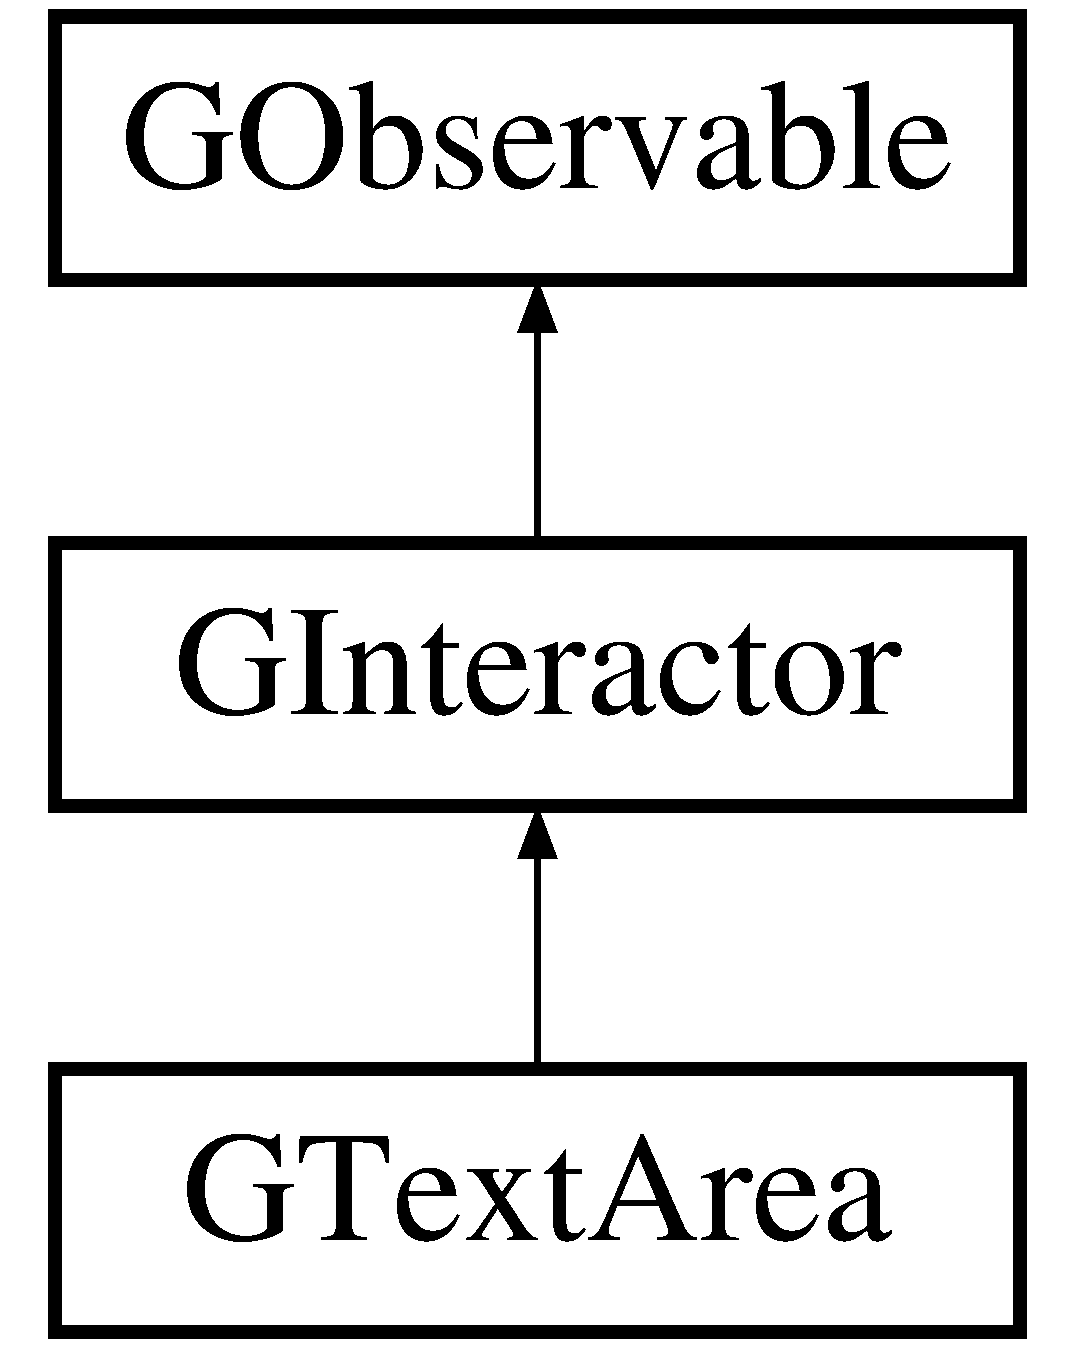
\includegraphics[height=3.000000cm]{classGTextArea}
\end{center}
\end{figure}
\subsection*{Public Types}
\begin{DoxyCompactItemize}
\item 
enum \mbox{\hyperlink{classGInteractor_a8e0d441725a81d2bbdebbea09078260e}{Text\+Position}} \{ \mbox{\hyperlink{classGInteractor_a8e0d441725a81d2bbdebbea09078260ea4cd6f2e7d5a08d6f4dc052df2358f774}{T\+E\+X\+T\+\_\+\+B\+E\+S\+I\+D\+E\+\_\+\+I\+C\+ON}}, 
\mbox{\hyperlink{classGInteractor_a8e0d441725a81d2bbdebbea09078260eaa88490f63d8de68d44c83bdb2ecde3b3}{T\+E\+X\+T\+\_\+\+U\+N\+D\+E\+R\+\_\+\+I\+C\+ON}}, 
\mbox{\hyperlink{classGInteractor_a8e0d441725a81d2bbdebbea09078260ea39a6f388a30ac4fefb6eb13e846bc9f2}{T\+E\+X\+T\+\_\+\+O\+N\+LY}}
 \}
\begin{DoxyCompactList}\small\item\em The places where an interactor can place its text relative to its icon. \end{DoxyCompactList}\end{DoxyCompactItemize}
\subsection*{Public Member Functions}
\begin{DoxyCompactItemize}
\item 
\mbox{\hyperlink{classGTextArea_aad263200ff85ead4d5e4d013c95c3107}{G\+Text\+Area}} (int rows, int columns, Q\+Widget $\ast$parent=nullptr)
\begin{DoxyCompactList}\small\item\em Creates a new text area large enough to display the given number of rows and columns of text. \end{DoxyCompactList}\item 
\mbox{\hyperlink{classGTextArea_a0902cdcc62cad5c1c81fc74ce38d8b13}{G\+Text\+Area}} (const std\+::string \&text=\char`\"{}\char`\"{}, Q\+Widget $\ast$parent=nullptr)
\begin{DoxyCompactList}\small\item\em Creates a new text area with the given initial text. \end{DoxyCompactList}\item 
virtual \mbox{\hyperlink{classGTextArea_a260e7e5c7191b6200b0a2d2cfc0caf17}{$\sim$\+G\+Text\+Area}} () Q\+\_\+\+D\+E\+C\+L\+\_\+\+O\+V\+E\+R\+R\+I\+DE
\begin{DoxyCompactList}\small\item\em Frees memory allocated internally by the text area. \end{DoxyCompactList}\item 
virtual void \mbox{\hyperlink{classGInteractor_a02f20ea6edfa0671f31c4c648a253833}{add\+Action\+Listener}} () Q\+\_\+\+D\+E\+C\+L\+\_\+\+D\+E\+P\+R\+E\+C\+A\+T\+ED
\begin{DoxyCompactList}\small\item\em Adds an event listener to be notified when this interactor is clicked or generally interacted with. \end{DoxyCompactList}\item 
virtual void \mbox{\hyperlink{classGTextArea_ac7d00bfb7f87912fd664b97f29cc71e9}{append\+Formatted\+Text}} (const std\+::string \&text, const std\+::string \&color=\char`\"{}\char`\"{}, const std\+::string \&font=\char`\"{}\char`\"{})
\begin{DoxyCompactList}\small\item\em Adds formatted text to the end of the text area. \end{DoxyCompactList}\item 
virtual void \mbox{\hyperlink{classGTextArea_aa3457253e58dbfbf65a8f5a28c65fb5f}{append\+Html}} (const std\+::string \&html)
\begin{DoxyCompactList}\small\item\em Adds H\+T\+M\+L-\/formatted text to the end of the text area. \end{DoxyCompactList}\item 
virtual void \mbox{\hyperlink{classGTextArea_a6ba815b59563007b60dc2052d4703146}{append\+Text}} (const std\+::string \&text)
\begin{DoxyCompactList}\small\item\em Adds the given plain text to the end of the text area. \end{DoxyCompactList}\item 
virtual void \mbox{\hyperlink{classGTextArea_abd07e172ccec6823a88289c21124a367}{clear\+Selection}} ()
\begin{DoxyCompactList}\small\item\em Deselects any text that is currently selected in the text area. \end{DoxyCompactList}\item 
virtual void \mbox{\hyperlink{classGTextArea_a25f53c7d92eb2a5197cd4418c0165367}{clear\+Text}} ()
\begin{DoxyCompactList}\small\item\em Sets the text in the text area to be empty. \end{DoxyCompactList}\item 
virtual bool \mbox{\hyperlink{classGInteractor_ac05ba5b92e2e5146d416fe7f842a0969}{events\+Enabled}} () const Q\+\_\+\+D\+E\+C\+L\+\_\+\+O\+V\+E\+R\+R\+I\+DE
\begin{DoxyCompactList}\small\item\em Returns true if this interactor is currently accepting events. \end{DoxyCompactList}\item 
virtual std\+::string \mbox{\hyperlink{classGInteractor_a69f8d23ed8f207fbecad99960776e942}{get\+Accelerator}} () const
\begin{DoxyCompactList}\small\item\em Returns a string representing a hotkey for this interactor, or an empty string if no accelerator has been set. \end{DoxyCompactList}\item 
virtual std\+::string \mbox{\hyperlink{classGInteractor_a94eb4276000c4fdfb508ce9e6317a82a}{get\+Action\+Command}} () const
\begin{DoxyCompactList}\small\item\em Returns an action command for this interactor, which is a semi-\/unique string you can use to identify it when events occur. \end{DoxyCompactList}\item 
virtual std\+::string \mbox{\hyperlink{classGInteractor_a808e22cc1fdfbecf71ed8c64ef4600e0}{get\+Background}} () const
\begin{DoxyCompactList}\small\item\em Returns the background color of the interactor as a string. \end{DoxyCompactList}\item 
virtual int \mbox{\hyperlink{classGInteractor_a9e827257a55cb8cf4d9de2ec6bcfd7a0}{get\+Background\+Int}} () const
\begin{DoxyCompactList}\small\item\em Returns the background color of the interactor as an R\+GB integer. \end{DoxyCompactList}\item 
virtual \mbox{\hyperlink{classGRectangle}{G\+Rectangle}} \mbox{\hyperlink{classGInteractor_a29e6ac35a0b48f491a4c88194cc5da3b}{get\+Bounds}} () const
\begin{DoxyCompactList}\small\item\em Returns a rectangle representing the x/y position and size of this interactor. \end{DoxyCompactList}\item 
virtual std\+::string \mbox{\hyperlink{classGInteractor_aa061dfa488c31e18549d64363c1d0e34}{get\+Color}} () const
\begin{DoxyCompactList}\small\item\em Returns the foreground/text color of the interactor as a string. \end{DoxyCompactList}\item 
virtual int \mbox{\hyperlink{classGInteractor_a9635c7af766cdc3417f346683fa0e6c1}{get\+Color\+Int}} () const
\begin{DoxyCompactList}\small\item\em Returns the foreground/text color of the interactor as an R\+GB integer. \end{DoxyCompactList}\item 
virtual int \mbox{\hyperlink{classGTextArea_a6b5395e749ae5c217093d74f68f1ca3a}{get\+Columns}} () const
\begin{DoxyCompactList}\small\item\em Returns the number of visible columns (characters wide) in the text area. \end{DoxyCompactList}\item 
virtual \mbox{\hyperlink{classGContainer}{G\+Container}} $\ast$ \mbox{\hyperlink{classGInteractor_a7a6e317c29d61030929b4cd2d1c00fe7}{get\+Container}} () const
\begin{DoxyCompactList}\small\item\em Returns a pointer to the onscreen container holding this interactor. \end{DoxyCompactList}\item 
virtual int \mbox{\hyperlink{classGTextArea_aa85d2267b4534eb372cd3114ea61ba3b}{get\+Cursor\+Position}} () const
\begin{DoxyCompactList}\small\item\em Returns the keyboard cursor\textquotesingle{}s current position in the text area as a 0-\/based character index within the overall text string. \end{DoxyCompactList}\item 
virtual std\+::string \mbox{\hyperlink{classGInteractor_a894a5502900794eeb27d084c21f1d77d}{get\+Font}} () const
\begin{DoxyCompactList}\small\item\em Returns the font of this interactor\textquotesingle{}s text as a font string such as \char`\"{}\+Helvetica-\/12-\/\+Bold\char`\"{}. \end{DoxyCompactList}\item 
virtual std\+::string \mbox{\hyperlink{classGInteractor_a4fa2d8b0192a3a5b4af4bbfe71194d03}{get\+Foreground}} () const
\begin{DoxyCompactList}\small\item\em Returns the foreground/text color of the interactor as a string. \end{DoxyCompactList}\item 
virtual int \mbox{\hyperlink{classGInteractor_ac3b12ab385a6ef9ae90fc879860ba726}{get\+Foreground\+Int}} () const
\begin{DoxyCompactList}\small\item\em Returns the foreground/text color of the interactor as an R\+GB integer. \end{DoxyCompactList}\item 
virtual double \mbox{\hyperlink{classGInteractor_a1e7e353362434072875264cf95629f99}{get\+Height}} () const
\begin{DoxyCompactList}\small\item\em Returns the current onscreen height of this interactor in pixels. \end{DoxyCompactList}\item 
virtual std\+::string \mbox{\hyperlink{classGTextArea_a58d3b7767e049484e3d7507379e6ecc7}{get\+Html}} () const
\begin{DoxyCompactList}\small\item\em Returns the text area\textquotesingle{}s current text as H\+T\+ML. \end{DoxyCompactList}\item 
virtual std\+::string \mbox{\hyperlink{classGInteractor_aaed62a73004939a64da6f0eb9eb64d73}{get\+Icon}} () const
\begin{DoxyCompactList}\small\item\em Returns the file name of the icon associated with this interactor, or an empty string if no icon has been set. \end{DoxyCompactList}\item 
virtual int \mbox{\hyperlink{classGInteractor_a9c9659a6c6ba66b4107ba59c95a24241}{get\+ID}} () const
\begin{DoxyCompactList}\small\item\em Returns a globally unique identifier for this interactor, which is set when the interactor is constructed. \end{DoxyCompactList}\item 
virtual \+\_\+\+Internal\+\_\+\+Q\+Widget $\ast$ \mbox{\hyperlink{classGTextArea_a208ce13c1da40bf0ddb509daf99d6588}{get\+Internal\+Widget}} () const Q\+\_\+\+D\+E\+C\+L\+\_\+\+O\+V\+E\+R\+R\+I\+DE
\begin{DoxyCompactList}\small\item\em Returns a direct pointer to the internal Qt widget being wrapped by this interactor. \end{DoxyCompactList}\item 
virtual \mbox{\hyperlink{classGPoint}{G\+Point}} \mbox{\hyperlink{classGInteractor_a4f83802015511edeb63b892830812c11}{get\+Location}} () const
\begin{DoxyCompactList}\small\item\em Returns an (x, y) point representing the onscreen location of the top-\/left corner of this interactor within its containing window. \end{DoxyCompactList}\item 
virtual double \mbox{\hyperlink{classGInteractor_aed4b0075fcc434499c3cb3e46896bda3}{get\+Minimum\+Height}} () const
\begin{DoxyCompactList}\small\item\em Returns the minimum height in pixels that this interactor will permit itself to be resized to. \end{DoxyCompactList}\item 
virtual \mbox{\hyperlink{classGDimension}{G\+Dimension}} \mbox{\hyperlink{classGInteractor_a66b5af0b32493b4d597ca0a3df2049ea}{get\+Minimum\+Size}} () const
\begin{DoxyCompactList}\small\item\em Returns a \mbox{\hyperlink{classGDimension}{G\+Dimension}} structure representing the minimum size in pixels that this interactor will permit itself to be resized to. \end{DoxyCompactList}\item 
virtual double \mbox{\hyperlink{classGInteractor_a59e668114fe3d49d2a0f28deb258f7c8}{get\+Minimum\+Width}} () const
\begin{DoxyCompactList}\small\item\em Returns the minimum width in pixels that this interactor will permit itself to be resized to. \end{DoxyCompactList}\item 
virtual std\+::string \mbox{\hyperlink{classGInteractor_a8a60438a5b55d0b2ceb35c8674b9d8c5}{get\+Name}} () const
\begin{DoxyCompactList}\small\item\em Returns a string representing a unique name for this interactor. \end{DoxyCompactList}\item 
virtual std\+::string \mbox{\hyperlink{classGTextArea_aa78dbaa7dac1f8cdf9048c91abecc7ad}{get\+Placeholder}} () const
\begin{DoxyCompactList}\small\item\em Returns the text area\textquotesingle{}s placeholder text, which is usually displayed as a light gray text in the text area when the area is empty. \end{DoxyCompactList}\item 
virtual double \mbox{\hyperlink{classGInteractor_a747de0961653847bdc6615dbf756d715}{get\+Preferred\+Height}} () const
\begin{DoxyCompactList}\small\item\em Returns the height in pixels that this interactor would prefer to be, which would exactly fit its contents with no stretching or scrollbars. \end{DoxyCompactList}\item 
virtual \mbox{\hyperlink{classGDimension}{G\+Dimension}} \mbox{\hyperlink{classGInteractor_a4aabbee761d8e9116275401131b7ccd1}{get\+Preferred\+Size}} () const
\begin{DoxyCompactList}\small\item\em Returns a \mbox{\hyperlink{classGDimension}{G\+Dimension}} structure storing the width and height in pixels that this interactor would prefer to be, which would exactly fit its contents with no stretching or scrollbars. \end{DoxyCompactList}\item 
virtual double \mbox{\hyperlink{classGInteractor_a82bca31d37700fb0e35d2743352efd5e}{get\+Preferred\+Width}} () const
\begin{DoxyCompactList}\small\item\em Returns the height in pixels that this interactor would prefer to be, which would exactly fit its contents with no stretching or scrollbars. \end{DoxyCompactList}\item 
virtual int \mbox{\hyperlink{classGTextArea_ad343f9bbb050d9037167e80e423ab4e8}{get\+Rows}} () const
\begin{DoxyCompactList}\small\item\em Returns the number of visible rows (lines tall) in the text area. \end{DoxyCompactList}\item 
virtual std\+::string \mbox{\hyperlink{classGTextArea_a512371b3f41599349f23389825a6ccf7}{get\+Selected\+Text}} () const
\begin{DoxyCompactList}\small\item\em Returns the text that is currently selected in the text area. \end{DoxyCompactList}\item 
virtual int \mbox{\hyperlink{classGTextArea_a2885313daa0e367cee2ccd0c704a6147}{get\+Selection\+End}} () const
\begin{DoxyCompactList}\small\item\em Returns the index just past the end of the current selection of text as a 0-\/based character index within the overall text string. \end{DoxyCompactList}\item 
virtual int \mbox{\hyperlink{classGTextArea_a68f7816694269b73e6284e756eb0c179}{get\+Selection\+Length}} () const
\begin{DoxyCompactList}\small\item\em Returns the number of characters that are currently selected. \end{DoxyCompactList}\item 
virtual int \mbox{\hyperlink{classGTextArea_aad7c986a677c1b9cf445cd7cfb6a8975}{get\+Selection\+Start}} () const
\begin{DoxyCompactList}\small\item\em Returns the index of the start of the current selection of text as a 0-\/based character index within the overall text string. \end{DoxyCompactList}\item 
virtual \mbox{\hyperlink{classGDimension}{G\+Dimension}} \mbox{\hyperlink{classGInteractor_a7b4eec96a2bdc6420695d5796a78eea9}{get\+Size}} () const
\begin{DoxyCompactList}\small\item\em Returns a \mbox{\hyperlink{classGDimension}{G\+Dimension}} structure storing the current onscreen width and height of this interactor in pixels. \end{DoxyCompactList}\item 
virtual std\+::string \mbox{\hyperlink{classGTextArea_aff553c50924b836c29f146ed34a7c6ec}{get\+Text}} () const
\begin{DoxyCompactList}\small\item\em Returns the text area\textquotesingle{}s current text. \end{DoxyCompactList}\item 
virtual std\+::string \mbox{\hyperlink{classGTextArea_a9896d58fcfebbf1025aeeb5b8b9ede80}{get\+Type}} () const Q\+\_\+\+D\+E\+C\+L\+\_\+\+O\+V\+E\+R\+R\+I\+DE
\begin{DoxyCompactList}\small\item\em Returns a string representing the class name of this interactor, such as \char`\"{}\+G\+Button\char`\"{} or \char`\"{}\+G\+Check\+Box\char`\"{}. \end{DoxyCompactList}\item 
virtual Q\+Widget $\ast$ \mbox{\hyperlink{classGTextArea_a326ee51b5561f807df7b29a1c101f7fd}{get\+Widget}} () const Q\+\_\+\+D\+E\+C\+L\+\_\+\+O\+V\+E\+R\+R\+I\+DE
\begin{DoxyCompactList}\small\item\em Returns a direct pointer to the internal Qt widget being wrapped by this interactor. \end{DoxyCompactList}\item 
virtual double \mbox{\hyperlink{classGInteractor_a0ed2965abd4f5701d2cadf71239faf19}{get\+Width}} () const
\begin{DoxyCompactList}\small\item\em Returns the current onscreen width of this interactor in pixels. \end{DoxyCompactList}\item 
virtual double \mbox{\hyperlink{classGInteractor_a344385751bee0720059403940d57a13e}{getX}} () const
\begin{DoxyCompactList}\small\item\em Returns the x-\/coordinate of the top-\/left pixel of this interactor within its onscreen window. \end{DoxyCompactList}\item 
virtual double \mbox{\hyperlink{classGInteractor_aafa51c7f8f38a09febbb9ce7853f77b4}{getY}} () const
\begin{DoxyCompactList}\small\item\em Returns the y-\/coordinate of the top-\/left pixel of this interactor within its onscreen window. \end{DoxyCompactList}\item 
virtual bool \mbox{\hyperlink{classGInteractor_afc480f652b8c5f1fb255e2269ce68879}{in\+Bounds}} (double x, double y) const
\begin{DoxyCompactList}\small\item\em Returns true if the given x/y pixel is within the bounds of this interactor. \end{DoxyCompactList}\item 
virtual bool \mbox{\hyperlink{classGInteractor_ae6d7982c1c627b677a5e776ca86118ed}{in\+Bounds}} (int x, int y) const
\begin{DoxyCompactList}\small\item\em Returns true if the given x/y pixel is within the bounds of this interactor. \end{DoxyCompactList}\item 
virtual bool \mbox{\hyperlink{classGTextArea_a80f9fe3b6f725182b294886f57cc1689}{is\+Context\+Menu\+Enabled}} () const
\begin{DoxyCompactList}\small\item\em Returns true if a context menu will pop up when the user right-\/clicks the text area. \end{DoxyCompactList}\item 
virtual bool \mbox{\hyperlink{classGTextArea_a012b5afb54e037e6c5498cf0932a521b}{is\+Editable}} () const
\begin{DoxyCompactList}\small\item\em Returns whether the text area allows the user to modify its text. \end{DoxyCompactList}\item 
virtual bool \mbox{\hyperlink{classGInteractor_aacb819fb241851fd9fc045271baa4034}{is\+Enabled}} () const
\begin{DoxyCompactList}\small\item\em Returns true if this interactor is currently enabled. \end{DoxyCompactList}\item 
virtual bool \mbox{\hyperlink{classGTextArea_ae09e72290b6e8a23bcc77752da6dffa5}{is\+Line\+Wrap}} () const
\begin{DoxyCompactList}\small\item\em Returns whether the text area wraps its text when a line becomes too long. \end{DoxyCompactList}\item 
virtual bool \mbox{\hyperlink{classGInteractor_a9d8a6cfb13917785c143e74d40e4e2be}{is\+Visible}} () const
\begin{DoxyCompactList}\small\item\em Returns true if the interactor is visible on the screen. \end{DoxyCompactList}\item 
virtual void \mbox{\hyperlink{classGTextArea_ab5ef729cac166db0ef51ff7ea30d1bb8}{move\+Cursor\+To\+End}} ()
\begin{DoxyCompactList}\small\item\em Sets the text area\textquotesingle{}s keyboard cursor position to the end of the current text. \end{DoxyCompactList}\item 
virtual void \mbox{\hyperlink{classGTextArea_a24abdceab57bcff96185afbadf193a22}{move\+Cursor\+To\+Start}} ()
\begin{DoxyCompactList}\small\item\em Sets the text area\textquotesingle{}s keyboard cursor position to the start of the current text. \end{DoxyCompactList}\item 
virtual void \mbox{\hyperlink{classGTextArea_a43095f41cab3be732b49f29970484b05}{remove\+Key\+Listener}} ()
\begin{DoxyCompactList}\small\item\em Removes the key listener from this text area so that it will no longer call it when the user types keys. \end{DoxyCompactList}\item 
virtual void \mbox{\hyperlink{classGTextArea_aff47f71ce47e688a07c9d38dc92fcc11}{remove\+Mouse\+Listener}} ()
\begin{DoxyCompactList}\small\item\em Removes the mouse listener from this text area so that it will no longer call it when the user moves/clicks the mouse. \end{DoxyCompactList}\item 
virtual void \mbox{\hyperlink{classGTextArea_a69c940b99d01eb7c353763ce4b0942a4}{remove\+Text\+Change\+Listener}} ()
\begin{DoxyCompactList}\small\item\em Removes the text change listener from this text area so that it will no longer call it when the user modifies the text. \end{DoxyCompactList}\item 
virtual void \mbox{\hyperlink{classGInteractor_a519fb2ac767f8b2febbb50b898b8c8cb}{request\+Focus}} ()
\begin{DoxyCompactList}\small\item\em Transfers keyboard focus to this interactor. \end{DoxyCompactList}\item 
virtual void \mbox{\hyperlink{classGTextArea_ad4c9b6140b529865a6cdeed37a339237}{scroll\+To\+Bottom}} ()
\begin{DoxyCompactList}\small\item\em Moves the visible scroll region of the text area so that the bottom part of the text is visible. \end{DoxyCompactList}\item 
virtual void \mbox{\hyperlink{classGTextArea_a9eacfcf7c186936ed957dd1c8a9c6b64}{scroll\+To\+Top}} ()
\begin{DoxyCompactList}\small\item\em Moves the visible scroll region of the text area so that the top part of the text is visible. \end{DoxyCompactList}\item 
virtual void \mbox{\hyperlink{classGTextArea_aaeb1320c0553d0d2b8081b750f59a34a}{select}} (int start\+Index, int length)
\begin{DoxyCompactList}\small\item\em Sets the given range of text to be selected, beginning with the given start index as a 0-\/based character index within the overall text string, and extending for the given length of characters. \end{DoxyCompactList}\item 
virtual void \mbox{\hyperlink{classGTextArea_ab6658ed404200bd7aaca5629db064645}{select\+All}} ()
\begin{DoxyCompactList}\small\item\em Selects the entire text of the text area. \end{DoxyCompactList}\item 
virtual void \mbox{\hyperlink{classGInteractor_ad15f102f62e2960576012f1aa0ba4b2e}{set\+Accelerator}} (const std\+::string \&accelerator)
\begin{DoxyCompactList}\small\item\em Sets an accelerator hotkey for this interactor, such as \char`\"{}\+Ctrl-\/\+S\char`\"{}. \end{DoxyCompactList}\item 
virtual void \mbox{\hyperlink{classGInteractor_a4b5843fe3030e038a1ba54cc03389bcf}{set\+Action\+Command}} (const std\+::string \&action\+Command)
\begin{DoxyCompactList}\small\item\em Sets the action command for this interactor. \end{DoxyCompactList}\item 
virtual void \mbox{\hyperlink{classGInteractor_acba7e546c2025c0a15ca4b4cc92043db}{set\+Background}} (int rgb)
\begin{DoxyCompactList}\small\item\em Sets the background color of the interactor to the color represented by the given R\+GB integer. \end{DoxyCompactList}\item 
virtual void \mbox{\hyperlink{classGInteractor_ab4677ab2474e68b07aa56605af92a84a}{set\+Background}} (const std\+::string \&color)
\begin{DoxyCompactList}\small\item\em Sets the background color of the interactor to the color represented by the given string. \end{DoxyCompactList}\item 
virtual void \mbox{\hyperlink{classGInteractor_a2aae8197624b72265ab83b4f1bc73f2f}{set\+Bounds}} (double x, double y, double width, double height)
\begin{DoxyCompactList}\small\item\em Sets the size and location of the widget. \end{DoxyCompactList}\item 
virtual void \mbox{\hyperlink{classGInteractor_acada386653f008cacc7cce86426bef7c}{set\+Bounds}} (const \mbox{\hyperlink{classGRectangle}{G\+Rectangle}} \&size)
\begin{DoxyCompactList}\small\item\em Sets the size and location of the widget. \end{DoxyCompactList}\item 
virtual void \mbox{\hyperlink{classGInteractor_ab1f5cc0f5cc6bbbd716a526c61f1081d}{set\+Color}} (int rgb)
\begin{DoxyCompactList}\small\item\em Sets the foreground/text color of the interactor to the color represented by the given R\+GB integer. \end{DoxyCompactList}\item 
virtual void \mbox{\hyperlink{classGInteractor_a61374df6c11b52cfbb0815decdbaebc6}{set\+Color}} (const std\+::string \&color)
\begin{DoxyCompactList}\small\item\em Sets the foreground/text color of the interactor to the color represented by the given string. \end{DoxyCompactList}\item 
virtual void \mbox{\hyperlink{classGTextArea_a3f29cc2956a84cdbce6327f1da4d86e9}{set\+Columns}} (int columns)
\begin{DoxyCompactList}\small\item\em Sets the width of the text area to be wide enough to fit the given number of characters (columns) of text. \end{DoxyCompactList}\item 
virtual void \mbox{\hyperlink{classGTextArea_a1a83404ffa5c72d747681b3505e73001}{set\+Context\+Menu\+Enabled}} (bool enabled)
\begin{DoxyCompactList}\small\item\em Sets whether a context menu will pop up when the user right-\/clicks the text area. \end{DoxyCompactList}\item 
virtual void \mbox{\hyperlink{classGTextArea_a5817e10a86be5cd41b3668d8fccb10e0}{set\+Cursor\+Position}} (int index, bool keep\+Anchor=false)
\begin{DoxyCompactList}\small\item\em Moves the keyboard cursor to the given 0-\/based character index within the text. \end{DoxyCompactList}\item 
virtual void \mbox{\hyperlink{classGTextArea_a008d7fd44fb3e7a6886cdaddbc3644a2}{set\+Editable}} (bool value)
\begin{DoxyCompactList}\small\item\em Sets whether the text area allows the user to modify its text. \end{DoxyCompactList}\item 
virtual void \mbox{\hyperlink{classGInteractor_ab831367dd84bbd579e02e55bacb21343}{set\+Enabled}} (bool value)
\begin{DoxyCompactList}\small\item\em Sets whether this interactor is currently enabled. \end{DoxyCompactList}\item 
virtual void \mbox{\hyperlink{classGObservable_afaa30b2a9e0f378fd1c70d2f1d0b8216}{set\+Events\+Enabled}} (bool \mbox{\hyperlink{classGInteractor_ac05ba5b92e2e5146d416fe7f842a0969}{events\+Enabled}})
\begin{DoxyCompactList}\small\item\em Sets whether the object is currently allowing itself to fire events. \end{DoxyCompactList}\item 
virtual void \mbox{\hyperlink{classGInteractor_a2592348886ffea646c6534bf88f7c49d}{set\+Font}} (const Q\+Font \&font)
\begin{DoxyCompactList}\small\item\em Sets the font used by this widget to the given Qt font. \end{DoxyCompactList}\item 
virtual void \mbox{\hyperlink{classGInteractor_a8e096e8818d838aceae1d46d58fb3a7b}{set\+Font}} (const std\+::string \&font)
\begin{DoxyCompactList}\small\item\em Sets the font used by this widget to the font represented by the given font string, such as \char`\"{}\+Helvetica-\/16-\/\+Bold\char`\"{}. \end{DoxyCompactList}\item 
virtual void \mbox{\hyperlink{classGInteractor_a9eb856b5ff83a19df3831a31f15f4563}{set\+Foreground}} (int rgb)
\begin{DoxyCompactList}\small\item\em Sets the foreground/text color of the interactor to the color represented by the given R\+GB integer. \end{DoxyCompactList}\item 
virtual void \mbox{\hyperlink{classGInteractor_af59209aeadea6dfc6d97a2d8531f50e1}{set\+Foreground}} (const std\+::string \&color)
\begin{DoxyCompactList}\small\item\em Sets the foreground/text color of the interactor to the color represented by the given string. \end{DoxyCompactList}\item 
virtual void \mbox{\hyperlink{classGInteractor_a9e280bfc4544dfaf8e4376c4e1a74357}{set\+Height}} (double height)
\begin{DoxyCompactList}\small\item\em Sets the onscreen height of the interactor in pixels. \end{DoxyCompactList}\item 
virtual void \mbox{\hyperlink{classGTextArea_a71ca94fd0ab4223097c4d524ddafe94f}{set\+Html}} (const std\+::string \&html)
\begin{DoxyCompactList}\small\item\em Sets the text area\textquotesingle{}s current text to the given H\+T\+ML string. \end{DoxyCompactList}\item 
virtual void \mbox{\hyperlink{classGInteractor_a762e139aa311461c3984d3ad28293f64}{set\+Icon}} (const std\+::string \&filename, bool retain\+Icon\+Size=true)
\begin{DoxyCompactList}\small\item\em Sets the file name of the icon associated with this interactor, or an empty string if no icon has been set. \end{DoxyCompactList}\item 
virtual void \mbox{\hyperlink{classGTextArea_aeb8324d3287fa1fbe093f4d6230cf0a6}{set\+Key\+Listener}} (G\+Event\+Listener func)
\begin{DoxyCompactList}\small\item\em Sets a key listener on this text area so that it will be called when the user presses any key. \end{DoxyCompactList}\item 
virtual void \mbox{\hyperlink{classGTextArea_ae48ecea73606c7bd9423e1c7cc589cc9}{set\+Key\+Listener}} (G\+Event\+Listener\+Void func)
\begin{DoxyCompactList}\small\item\em Sets a key listener on this text area so that it will be called when the user presses any key. \end{DoxyCompactList}\item 
virtual void \mbox{\hyperlink{classGTextArea_aaaafb06fec060b28b70ec3b7379657b4}{set\+Line\+Wrap}} (bool wrap)
\begin{DoxyCompactList}\small\item\em Sets whether the text area wraps its text when a line becomes too long. \end{DoxyCompactList}\item 
virtual void \mbox{\hyperlink{classGInteractor_a04594e8ba9b98513a64f1da00dcae18c}{set\+Location}} (double x, double y)
\begin{DoxyCompactList}\small\item\em Sets the onscreen x/y-\/coordinate of the top-\/left corner of the interactor relative to its window. \end{DoxyCompactList}\item 
virtual void \mbox{\hyperlink{classGInteractor_a0cf428e207b7f22cc08138a90b1b87b2}{set\+Minimum\+Size}} (double width, double height)
\begin{DoxyCompactList}\small\item\em Sets the minimum size in pixels that this interactor will permit itself to be resized to. \end{DoxyCompactList}\item 
virtual void \mbox{\hyperlink{classGInteractor_a3b1046117ac6cb7abe467e00ba8a81f4}{set\+Minimum\+Size}} (const \mbox{\hyperlink{classGDimension}{G\+Dimension}} \&size)
\begin{DoxyCompactList}\small\item\em Sets the minimum size in pixels that this interactor will permit itself to be resized to. \end{DoxyCompactList}\item 
virtual void \mbox{\hyperlink{classGTextArea_a37d8dbc943f59920f705b0104f60bde2}{set\+Mouse\+Listener}} (G\+Event\+Listener func)
\begin{DoxyCompactList}\small\item\em Sets a mouse listener on this text area so that it will be called when the user moves or clicks the mouse. \end{DoxyCompactList}\item 
virtual void \mbox{\hyperlink{classGTextArea_aea7f647ea62d59f71b5fad6aa65eeaf9}{set\+Mouse\+Listener}} (G\+Event\+Listener\+Void func)
\begin{DoxyCompactList}\small\item\em Sets a mouse listener on this text area so that it will be called when the user moves or clicks the mouse. \end{DoxyCompactList}\item 
virtual void \mbox{\hyperlink{classGInteractor_a9d3a2685df23b5e7cbf59c19c4a1f9b5}{set\+Name}} (const std\+::string \&name)
\begin{DoxyCompactList}\small\item\em Sets a string representing a unique name for this interactor. \end{DoxyCompactList}\item 
virtual void \mbox{\hyperlink{classGTextArea_aa21a9bebb4652ab6780d0c11eff47aee}{set\+Placeholder}} (const std\+::string \&text)
\begin{DoxyCompactList}\small\item\em Sets the text area\textquotesingle{}s placeholder text, which is usually displayed as a light gray text in the text area when the area is empty. \end{DoxyCompactList}\item 
virtual void \mbox{\hyperlink{classGInteractor_a1ab987704fce32098706c6f00fb08218}{set\+Preferred\+Height}} (double height)
\begin{DoxyCompactList}\small\item\em Sets the height in pixels that this interactor would prefer to be. \end{DoxyCompactList}\item 
virtual void \mbox{\hyperlink{classGInteractor_a042c5ae19430d765ef552371cae3632c}{set\+Preferred\+Size}} (double width, double height)
\begin{DoxyCompactList}\small\item\em Sets the width and height in pixels that this interactor would prefer to be. \end{DoxyCompactList}\item 
virtual void \mbox{\hyperlink{classGInteractor_aa22d9be4bc0e078bb0ea69b0fc9d7c75}{set\+Preferred\+Size}} (const \mbox{\hyperlink{classGDimension}{G\+Dimension}} \&size)
\begin{DoxyCompactList}\small\item\em Sets the size in pixels that this interactor would prefer to be. \end{DoxyCompactList}\item 
virtual void \mbox{\hyperlink{classGInteractor_a3db429ab2fa52efd187eec0ed8cdd9f2}{set\+Preferred\+Width}} (double width)
\begin{DoxyCompactList}\small\item\em Sets the width in pixels that this interactor would prefer to be. \end{DoxyCompactList}\item 
virtual void \mbox{\hyperlink{classGTextArea_a508bbe326657af6d3add84deb4595989}{set\+Rows}} (int rows)
\begin{DoxyCompactList}\small\item\em Sets the height of the text area to be wide enough to fit the given number of lines (rows) of text. \end{DoxyCompactList}\item 
virtual void \mbox{\hyperlink{classGTextArea_a15142a18598662167760b35e58be90b1}{set\+Rows\+Columns}} (int rows, int columns)
\begin{DoxyCompactList}\small\item\em Sets the size of the text area to be wide enough to fit the given number of lines (rows) and characters (columns) of text. \end{DoxyCompactList}\item 
virtual void \mbox{\hyperlink{classGInteractor_aca25d49481f9bf5fc8f7df4c086c4ce7}{set\+Size}} (double width, double height)
\begin{DoxyCompactList}\small\item\em Sets the onscreen width and height of the interactor in pixels. \end{DoxyCompactList}\item 
virtual void \mbox{\hyperlink{classGInteractor_ae2b628228f192c2702c4ce941b2af68f}{set\+Size}} (const \mbox{\hyperlink{classGDimension}{G\+Dimension}} \&size)
\begin{DoxyCompactList}\small\item\em Sets the onscreen width and height of the interactor in pixels. \end{DoxyCompactList}\item 
virtual void \mbox{\hyperlink{classGTextArea_ac1ae51949d41ee9054634be5967d91b8}{set\+Text}} (const std\+::string \&text)
\begin{DoxyCompactList}\small\item\em Sets the text area\textquotesingle{}s current text to the given string, replacing any existing text. \end{DoxyCompactList}\item 
virtual void \mbox{\hyperlink{classGTextArea_ae41284f9c540110180ac0ad6beca5cb0}{set\+Text\+Change\+Listener}} (G\+Event\+Listener func)
\begin{DoxyCompactList}\small\item\em Sets a text change listener on this text area so that it will be called when the user modifies the current text. \end{DoxyCompactList}\item 
virtual void \mbox{\hyperlink{classGTextArea_ae8df75b0746951146d29220f386fcd33}{set\+Text\+Change\+Listener}} (G\+Event\+Listener\+Void func)
\begin{DoxyCompactList}\small\item\em Sets a text change listener on this text area so that it will be called when the user modifies the current text. \end{DoxyCompactList}\item 
virtual void \mbox{\hyperlink{classGInteractor_a039e0e49beaecc275efce02d416acea8}{set\+Tooltip}} (const std\+::string \&tooltip\+Text)
\begin{DoxyCompactList}\small\item\em Sets a \char`\"{}tooltip\char`\"{} that will appear if the user hovers their mouse over the interactor. \end{DoxyCompactList}\item 
virtual void \mbox{\hyperlink{classGInteractor_a18e44e30b31525a243960ca3928125aa}{set\+Visible}} (bool visible)
\begin{DoxyCompactList}\small\item\em Returns true if the interactor is visible on the screen. \end{DoxyCompactList}\item 
virtual void \mbox{\hyperlink{classGInteractor_aa3f3fba4cb131baa8696ba01e3bceca1}{set\+Width}} (double width)
\begin{DoxyCompactList}\small\item\em Sets the onscreen width of the interactor in pixels. \end{DoxyCompactList}\item 
virtual void \mbox{\hyperlink{classGInteractor_a9c18fcc579333bf9653d13ad2b372e39}{setX}} (double x)
\begin{DoxyCompactList}\small\item\em Sets the onscreen x-\/coordinate of the top-\/left corner of the interactor relative to its window. \end{DoxyCompactList}\item 
virtual void \mbox{\hyperlink{classGInteractor_a7d57e2a5c35d27feb58fd498a3cf82b9}{setY}} (double y)
\begin{DoxyCompactList}\small\item\em Sets the onscreen y-\/coordinate of the top-\/left corner of the interactor relative to its window. \end{DoxyCompactList}\item 
virtual std\+::string \mbox{\hyperlink{classGObservable_a1fe5121d6528fdea3f243321b3fa3a49}{to\+String}} () const
\begin{DoxyCompactList}\small\item\em Returns a string representation of this observable object\textquotesingle{}s state. \end{DoxyCompactList}\end{DoxyCompactItemize}
\subsection*{Protected Member Functions}
\begin{DoxyCompactItemize}
\item 
virtual void \mbox{\hyperlink{classGObservable_a80cfa040459ff53594adbd6a51ec8f43}{clear\+Event\+Listeners}} ()
\begin{DoxyCompactList}\small\item\em Removes all event listeners from this object. \end{DoxyCompactList}\item 
virtual void \mbox{\hyperlink{classGObservable_a284f31528c0520f8e545c03ac9eeac74}{ensure\+Thread\+Safety}} (const std\+::string \&member\+Name=\char`\"{}\char`\"{})
\begin{DoxyCompactList}\small\item\em Ensures that we are currently in the Qt G\+UI thread. \end{DoxyCompactList}\item 
virtual void \mbox{\hyperlink{classGObservable_a63e5e5a6227c59c928493b11aceb0f67}{fire\+Event}} (\mbox{\hyperlink{classGEvent}{G\+Event}} \&event)
\begin{DoxyCompactList}\small\item\em Sends out the given event to any attached listeners. \end{DoxyCompactList}\item 
virtual void \mbox{\hyperlink{classGObservable_ab3983ea07337b52020a29cc00c653d8d}{fire\+G\+Event}} (Q\+Event $\ast$event, Event\+Type event\+Type, const std\+::string \&event\+Name)
\begin{DoxyCompactList}\small\item\em Creates an event of the given type, then sends it out to any attached listeners. \end{DoxyCompactList}\item 
virtual void \mbox{\hyperlink{classGObservable_a01fdf1b0e0dbd49e189fe4514e010411}{fire\+G\+Event}} (Q\+Close\+Event $\ast$event, Event\+Type event\+Type, const std\+::string \&event\+Name)
\begin{DoxyCompactList}\small\item\em Creates an event of the given type, then sends it out to any attached listeners. \end{DoxyCompactList}\item 
virtual void \mbox{\hyperlink{classGObservable_abb0b2f66ba39211cb5d7615e9d1c04e2}{fire\+G\+Event}} (Q\+Key\+Event $\ast$event, Event\+Type event\+Type, const std\+::string \&event\+Name)
\begin{DoxyCompactList}\small\item\em Creates an event of the given type, then sends it out to any attached listeners. \end{DoxyCompactList}\item 
virtual void \mbox{\hyperlink{classGObservable_a119318675d2165bdf7dd853aaf881d4b}{fire\+G\+Event}} (Q\+Mouse\+Event $\ast$event, Event\+Type event\+Type, const std\+::string \&event\+Name, const std\+::string \&action\+Command=\char`\"{}\char`\"{})
\begin{DoxyCompactList}\small\item\em Creates an event of the given type, then sends it out to any attached listeners. \end{DoxyCompactList}\item 
virtual void \mbox{\hyperlink{classGObservable_a63fd9034e1e1633c1c38eb342bfd34e9}{fire\+G\+Event}} (Q\+Resize\+Event $\ast$event, Event\+Type event\+Type, const std\+::string \&event\+Name)
\begin{DoxyCompactList}\small\item\em Creates an event of the given type, then sends it out to any attached listeners. \end{DoxyCompactList}\item 
virtual void \mbox{\hyperlink{classGObservable_a741345310d9b7c5170a6cbc410c44ac4}{fire\+G\+Event}} (Q\+Timer\+Event $\ast$event, Event\+Type event\+Type, const std\+::string \&event\+Name)
\begin{DoxyCompactList}\small\item\em Creates an event of the given type, then sends it out to any attached listeners. \end{DoxyCompactList}\item 
virtual void \mbox{\hyperlink{classGObservable_a93bf338968a0338761b8e4dc62f582e9}{fire\+G\+Event}} (Q\+Wheel\+Event $\ast$event, Event\+Type event\+Type, const std\+::string \&event\+Name)
\begin{DoxyCompactList}\small\item\em Creates an event of the given type, then sends it out to any attached listeners. \end{DoxyCompactList}\item 
virtual void \mbox{\hyperlink{classGObservable_a2a70a7d7435ff0c3b80bb4d70da19e0d}{fire\+G\+Event}} (Q\+Window\+State\+Change\+Event $\ast$event, Event\+Type event\+Type, const std\+::string \&event\+Name)
\begin{DoxyCompactList}\small\item\em Creates an event of the given type, then sends it out to any attached listeners. \end{DoxyCompactList}\item 
virtual bool \mbox{\hyperlink{classGObservable_a9f6faaa25942923bafa1c44020c49fa9}{has\+Event\+Listener}} (const std\+::string \&event\+Name) const
\begin{DoxyCompactList}\small\item\em Returns true if the observable object has a listener for the given type of event. \end{DoxyCompactList}\item 
virtual bool \mbox{\hyperlink{classGObservable_aeec1adc19aa0f33de62390686ee1382c}{is\+Accepting\+Event}} (int event\+Mask) const
\begin{DoxyCompactList}\small\item\em Returns true if the observable object has a listener for the given type of event. \end{DoxyCompactList}\item 
virtual bool \mbox{\hyperlink{classGObservable_aa31c73145a29dcb92848a92e0cfaea41}{is\+Accepting\+Event}} (const \mbox{\hyperlink{classGEvent}{G\+Event}} \&event) const
\begin{DoxyCompactList}\small\item\em Returns true if the observable object has a listener for the given type of event. \end{DoxyCompactList}\item 
virtual bool \mbox{\hyperlink{classGObservable_a3b1c689267eda44e65a2213e7de38b23}{is\+Accepting\+Event}} (const std\+::string \&event\+Type) const
\begin{DoxyCompactList}\small\item\em Returns true if the observable object has a listener for the given type of event. \end{DoxyCompactList}\item 
virtual void \mbox{\hyperlink{classGObservable_acbcf1ed3a851ad8a3c17ef38d86b481d}{remove\+Event\+Listener}} (const std\+::string \&event\+Name)
\begin{DoxyCompactList}\small\item\em Removes any event listener from this observable object that would respond to the given type of event, such as \char`\"{}click\char`\"{} or \char`\"{}keydown\char`\"{}. \end{DoxyCompactList}\item 
virtual void \mbox{\hyperlink{classGObservable_af51cc35c29a1bd1908609d432decdbb6}{remove\+Event\+Listeners}} (std\+::initializer\+\_\+list$<$ std\+::string $>$ event\+Names)
\begin{DoxyCompactList}\small\item\em Removes any event listener from this observable object that would respond to the given types of events, such as \char`\"{}click\char`\"{} or \char`\"{}keydown\char`\"{}. \end{DoxyCompactList}\item 
virtual void \mbox{\hyperlink{classGObservable_ad2f6d34961c50f6c1e0659990b79f741}{set\+Event\+Listener}} (const std\+::string \&event\+Name, G\+Event\+Listener func)
\begin{DoxyCompactList}\small\item\em Adds an event listener from this observable object to respond to the given type of event, such as \char`\"{}click\char`\"{} or \char`\"{}keydown\char`\"{}. \end{DoxyCompactList}\item 
virtual void \mbox{\hyperlink{classGObservable_abac4cb9f9e626e010e87f5d91573c8a5}{set\+Event\+Listener}} (const std\+::string \&event\+Name, G\+Event\+Listener\+Void func)
\begin{DoxyCompactList}\small\item\em Adds an event listener from this observable object to respond to the given type of event, such as \char`\"{}click\char`\"{} or \char`\"{}keydown\char`\"{}. \end{DoxyCompactList}\item 
virtual void \mbox{\hyperlink{classGObservable_afa388d69c33c718cf035774604065604}{set\+Event\+Listeners}} (std\+::initializer\+\_\+list$<$ std\+::string $>$ event\+Names, G\+Event\+Listener func)
\begin{DoxyCompactList}\small\item\em Adds an event listener from this observable object to respond to the given types of events, such as \char`\"{}click\char`\"{} or \char`\"{}keydown\char`\"{}. \end{DoxyCompactList}\item 
virtual void \mbox{\hyperlink{classGObservable_a7867184bbb686f74fae8a4db927da799}{set\+Event\+Listeners}} (std\+::initializer\+\_\+list$<$ std\+::string $>$ event\+Names, G\+Event\+Listener\+Void func)
\begin{DoxyCompactList}\small\item\em Adds an event listener from this observable object to respond to the given types of events, such as \char`\"{}click\char`\"{} or \char`\"{}keydown\char`\"{}. \end{DoxyCompactList}\end{DoxyCompactItemize}


\subsection{Detailed Description}
A \mbox{\hyperlink{classGTextArea}{G\+Text\+Area}} is a multi-\/line editable text box. 

The box allows the user to type arbitrarily long documents. Scroll bars will appear if the text becomes too long to fit in the visible area of the box. 

\subsection{Member Enumeration Documentation}
\mbox{\Hypertarget{classGInteractor_a8e0d441725a81d2bbdebbea09078260e}\label{classGInteractor_a8e0d441725a81d2bbdebbea09078260e}} 
\index{G\+Text\+Area@{G\+Text\+Area}!Text\+Position@{Text\+Position}}
\index{Text\+Position@{Text\+Position}!G\+Text\+Area@{G\+Text\+Area}}
\subsubsection{\texorpdfstring{Text\+Position}{TextPosition}}
{\footnotesize\ttfamily enum \mbox{\hyperlink{classGInteractor_a8e0d441725a81d2bbdebbea09078260e}{Text\+Position}}\hspace{0.3cm}{\ttfamily [inherited]}}



The places where an interactor can place its text relative to its icon. 

\begin{DoxyEnumFields}{Enumerator}
\raisebox{\heightof{T}}[0pt][0pt]{\index{T\+E\+X\+T\+\_\+\+B\+E\+S\+I\+D\+E\+\_\+\+I\+C\+ON@{T\+E\+X\+T\+\_\+\+B\+E\+S\+I\+D\+E\+\_\+\+I\+C\+ON}!G\+Text\+Area@{G\+Text\+Area}}\index{G\+Text\+Area@{G\+Text\+Area}!T\+E\+X\+T\+\_\+\+B\+E\+S\+I\+D\+E\+\_\+\+I\+C\+ON@{T\+E\+X\+T\+\_\+\+B\+E\+S\+I\+D\+E\+\_\+\+I\+C\+ON}}}\mbox{\Hypertarget{classGInteractor_a8e0d441725a81d2bbdebbea09078260ea4cd6f2e7d5a08d6f4dc052df2358f774}\label{classGInteractor_a8e0d441725a81d2bbdebbea09078260ea4cd6f2e7d5a08d6f4dc052df2358f774}} 
T\+E\+X\+T\+\_\+\+B\+E\+S\+I\+D\+E\+\_\+\+I\+C\+ON&\\
\hline

\raisebox{\heightof{T}}[0pt][0pt]{\index{T\+E\+X\+T\+\_\+\+U\+N\+D\+E\+R\+\_\+\+I\+C\+ON@{T\+E\+X\+T\+\_\+\+U\+N\+D\+E\+R\+\_\+\+I\+C\+ON}!G\+Text\+Area@{G\+Text\+Area}}\index{G\+Text\+Area@{G\+Text\+Area}!T\+E\+X\+T\+\_\+\+U\+N\+D\+E\+R\+\_\+\+I\+C\+ON@{T\+E\+X\+T\+\_\+\+U\+N\+D\+E\+R\+\_\+\+I\+C\+ON}}}\mbox{\Hypertarget{classGInteractor_a8e0d441725a81d2bbdebbea09078260eaa88490f63d8de68d44c83bdb2ecde3b3}\label{classGInteractor_a8e0d441725a81d2bbdebbea09078260eaa88490f63d8de68d44c83bdb2ecde3b3}} 
T\+E\+X\+T\+\_\+\+U\+N\+D\+E\+R\+\_\+\+I\+C\+ON&\\
\hline

\raisebox{\heightof{T}}[0pt][0pt]{\index{T\+E\+X\+T\+\_\+\+O\+N\+LY@{T\+E\+X\+T\+\_\+\+O\+N\+LY}!G\+Text\+Area@{G\+Text\+Area}}\index{G\+Text\+Area@{G\+Text\+Area}!T\+E\+X\+T\+\_\+\+O\+N\+LY@{T\+E\+X\+T\+\_\+\+O\+N\+LY}}}\mbox{\Hypertarget{classGInteractor_a8e0d441725a81d2bbdebbea09078260ea39a6f388a30ac4fefb6eb13e846bc9f2}\label{classGInteractor_a8e0d441725a81d2bbdebbea09078260ea39a6f388a30ac4fefb6eb13e846bc9f2}} 
T\+E\+X\+T\+\_\+\+O\+N\+LY&\\
\hline

\end{DoxyEnumFields}


\subsection{Constructor \& Destructor Documentation}
\mbox{\Hypertarget{classGTextArea_aad263200ff85ead4d5e4d013c95c3107}\label{classGTextArea_aad263200ff85ead4d5e4d013c95c3107}} 
\index{G\+Text\+Area@{G\+Text\+Area}!G\+Text\+Area@{G\+Text\+Area}}
\index{G\+Text\+Area@{G\+Text\+Area}!G\+Text\+Area@{G\+Text\+Area}}
\subsubsection{\texorpdfstring{G\+Text\+Area()}{GTextArea()}\hspace{0.1cm}{\footnotesize\ttfamily [1/2]}}
{\footnotesize\ttfamily \mbox{\hyperlink{classGTextArea}{G\+Text\+Area}} (\begin{DoxyParamCaption}\item[{int}]{rows,  }\item[{int}]{columns,  }\item[{Q\+Widget $\ast$}]{parent = {\ttfamily nullptr} }\end{DoxyParamCaption})}



Creates a new text area large enough to display the given number of rows and columns of text. 


\begin{DoxyExceptions}{Exceptions}
{\em \mbox{\hyperlink{classErrorException}{Error\+Exception}}} & if rows or columns value is negative \\
\hline
\end{DoxyExceptions}
\mbox{\Hypertarget{classGTextArea_a0902cdcc62cad5c1c81fc74ce38d8b13}\label{classGTextArea_a0902cdcc62cad5c1c81fc74ce38d8b13}} 
\index{G\+Text\+Area@{G\+Text\+Area}!G\+Text\+Area@{G\+Text\+Area}}
\index{G\+Text\+Area@{G\+Text\+Area}!G\+Text\+Area@{G\+Text\+Area}}
\subsubsection{\texorpdfstring{G\+Text\+Area()}{GTextArea()}\hspace{0.1cm}{\footnotesize\ttfamily [2/2]}}
{\footnotesize\ttfamily \mbox{\hyperlink{classGTextArea}{G\+Text\+Area}} (\begin{DoxyParamCaption}\item[{const std\+::string \&}]{text = {\ttfamily \char`\"{}\char`\"{}},  }\item[{Q\+Widget $\ast$}]{parent = {\ttfamily nullptr} }\end{DoxyParamCaption})}



Creates a new text area with the given initial text. 

\mbox{\Hypertarget{classGTextArea_a260e7e5c7191b6200b0a2d2cfc0caf17}\label{classGTextArea_a260e7e5c7191b6200b0a2d2cfc0caf17}} 
\index{G\+Text\+Area@{G\+Text\+Area}!````~G\+Text\+Area@{$\sim$\+G\+Text\+Area}}
\index{````~G\+Text\+Area@{$\sim$\+G\+Text\+Area}!G\+Text\+Area@{G\+Text\+Area}}
\subsubsection{\texorpdfstring{$\sim$\+G\+Text\+Area()}{~GTextArea()}}
{\footnotesize\ttfamily $\sim$\mbox{\hyperlink{classGTextArea}{G\+Text\+Area}} (\begin{DoxyParamCaption}{ }\end{DoxyParamCaption})\hspace{0.3cm}{\ttfamily [virtual]}}



Frees memory allocated internally by the text area. 



\subsection{Member Function Documentation}
\mbox{\Hypertarget{classGInteractor_a02f20ea6edfa0671f31c4c648a253833}\label{classGInteractor_a02f20ea6edfa0671f31c4c648a253833}} 
\index{G\+Text\+Area@{G\+Text\+Area}!add\+Action\+Listener@{add\+Action\+Listener}}
\index{add\+Action\+Listener@{add\+Action\+Listener}!G\+Text\+Area@{G\+Text\+Area}}
\subsubsection{\texorpdfstring{add\+Action\+Listener()}{addActionListener()}}
{\footnotesize\ttfamily void add\+Action\+Listener (\begin{DoxyParamCaption}{ }\end{DoxyParamCaption})\hspace{0.3cm}{\ttfamily [virtual]}, {\ttfamily [inherited]}}



Adds an event listener to be notified when this interactor is clicked or generally interacted with. 

\begin{DoxyRefDesc}{Deprecated}
\item[\mbox{\hyperlink{deprecated__deprecated000006}{Deprecated}}]does nothing; use set\+Action\+Listener instead \end{DoxyRefDesc}
\mbox{\Hypertarget{classGTextArea_ac7d00bfb7f87912fd664b97f29cc71e9}\label{classGTextArea_ac7d00bfb7f87912fd664b97f29cc71e9}} 
\index{G\+Text\+Area@{G\+Text\+Area}!append\+Formatted\+Text@{append\+Formatted\+Text}}
\index{append\+Formatted\+Text@{append\+Formatted\+Text}!G\+Text\+Area@{G\+Text\+Area}}
\subsubsection{\texorpdfstring{append\+Formatted\+Text()}{appendFormattedText()}}
{\footnotesize\ttfamily void append\+Formatted\+Text (\begin{DoxyParamCaption}\item[{const std\+::string \&}]{text,  }\item[{const std\+::string \&}]{color = {\ttfamily \char`\"{}\char`\"{}},  }\item[{const std\+::string \&}]{font = {\ttfamily \char`\"{}\char`\"{}} }\end{DoxyParamCaption})\hspace{0.3cm}{\ttfamily [virtual]}}



Adds formatted text to the end of the text area. 

The text will be formatted with the given color and font. \mbox{\Hypertarget{classGTextArea_aa3457253e58dbfbf65a8f5a28c65fb5f}\label{classGTextArea_aa3457253e58dbfbf65a8f5a28c65fb5f}} 
\index{G\+Text\+Area@{G\+Text\+Area}!append\+Html@{append\+Html}}
\index{append\+Html@{append\+Html}!G\+Text\+Area@{G\+Text\+Area}}
\subsubsection{\texorpdfstring{append\+Html()}{appendHtml()}}
{\footnotesize\ttfamily void append\+Html (\begin{DoxyParamCaption}\item[{const std\+::string \&}]{html }\end{DoxyParamCaption})\hspace{0.3cm}{\ttfamily [virtual]}}



Adds H\+T\+M\+L-\/formatted text to the end of the text area. 

\mbox{\Hypertarget{classGTextArea_a6ba815b59563007b60dc2052d4703146}\label{classGTextArea_a6ba815b59563007b60dc2052d4703146}} 
\index{G\+Text\+Area@{G\+Text\+Area}!append\+Text@{append\+Text}}
\index{append\+Text@{append\+Text}!G\+Text\+Area@{G\+Text\+Area}}
\subsubsection{\texorpdfstring{append\+Text()}{appendText()}}
{\footnotesize\ttfamily void append\+Text (\begin{DoxyParamCaption}\item[{const std\+::string \&}]{text }\end{DoxyParamCaption})\hspace{0.3cm}{\ttfamily [virtual]}}



Adds the given plain text to the end of the text area. 

\mbox{\Hypertarget{classGObservable_a80cfa040459ff53594adbd6a51ec8f43}\label{classGObservable_a80cfa040459ff53594adbd6a51ec8f43}} 
\index{G\+Text\+Area@{G\+Text\+Area}!clear\+Event\+Listeners@{clear\+Event\+Listeners}}
\index{clear\+Event\+Listeners@{clear\+Event\+Listeners}!G\+Text\+Area@{G\+Text\+Area}}
\subsubsection{\texorpdfstring{clear\+Event\+Listeners()}{clearEventListeners()}}
{\footnotesize\ttfamily void clear\+Event\+Listeners (\begin{DoxyParamCaption}{ }\end{DoxyParamCaption})\hspace{0.3cm}{\ttfamily [protected]}, {\ttfamily [virtual]}, {\ttfamily [inherited]}}



Removes all event listeners from this object. 

\mbox{\Hypertarget{classGTextArea_abd07e172ccec6823a88289c21124a367}\label{classGTextArea_abd07e172ccec6823a88289c21124a367}} 
\index{G\+Text\+Area@{G\+Text\+Area}!clear\+Selection@{clear\+Selection}}
\index{clear\+Selection@{clear\+Selection}!G\+Text\+Area@{G\+Text\+Area}}
\subsubsection{\texorpdfstring{clear\+Selection()}{clearSelection()}}
{\footnotesize\ttfamily void clear\+Selection (\begin{DoxyParamCaption}{ }\end{DoxyParamCaption})\hspace{0.3cm}{\ttfamily [virtual]}}



Deselects any text that is currently selected in the text area. 

\mbox{\Hypertarget{classGTextArea_a25f53c7d92eb2a5197cd4418c0165367}\label{classGTextArea_a25f53c7d92eb2a5197cd4418c0165367}} 
\index{G\+Text\+Area@{G\+Text\+Area}!clear\+Text@{clear\+Text}}
\index{clear\+Text@{clear\+Text}!G\+Text\+Area@{G\+Text\+Area}}
\subsubsection{\texorpdfstring{clear\+Text()}{clearText()}}
{\footnotesize\ttfamily void clear\+Text (\begin{DoxyParamCaption}{ }\end{DoxyParamCaption})\hspace{0.3cm}{\ttfamily [virtual]}}



Sets the text in the text area to be empty. 

\mbox{\Hypertarget{classGObservable_a284f31528c0520f8e545c03ac9eeac74}\label{classGObservable_a284f31528c0520f8e545c03ac9eeac74}} 
\index{G\+Text\+Area@{G\+Text\+Area}!ensure\+Thread\+Safety@{ensure\+Thread\+Safety}}
\index{ensure\+Thread\+Safety@{ensure\+Thread\+Safety}!G\+Text\+Area@{G\+Text\+Area}}
\subsubsection{\texorpdfstring{ensure\+Thread\+Safety()}{ensureThreadSafety()}}
{\footnotesize\ttfamily void ensure\+Thread\+Safety (\begin{DoxyParamCaption}\item[{const std\+::string \&}]{member\+Name = {\ttfamily \char`\"{}\char`\"{}} }\end{DoxyParamCaption})\hspace{0.3cm}{\ttfamily [protected]}, {\ttfamily [virtual]}, {\ttfamily [inherited]}}



Ensures that we are currently in the Qt G\+UI thread. 

\mbox{\Hypertarget{classGInteractor_ac05ba5b92e2e5146d416fe7f842a0969}\label{classGInteractor_ac05ba5b92e2e5146d416fe7f842a0969}} 
\index{G\+Text\+Area@{G\+Text\+Area}!events\+Enabled@{events\+Enabled}}
\index{events\+Enabled@{events\+Enabled}!G\+Text\+Area@{G\+Text\+Area}}
\subsubsection{\texorpdfstring{events\+Enabled()}{eventsEnabled()}}
{\footnotesize\ttfamily bool events\+Enabled (\begin{DoxyParamCaption}{ }\end{DoxyParamCaption}) const\hspace{0.3cm}{\ttfamily [virtual]}, {\ttfamily [inherited]}}



Returns true if this interactor is currently accepting events. 

Initially true. An interactor must be visible and added to an onscreen window to receive events. 

Reimplemented from \mbox{\hyperlink{classGObservable_a8ebb3da91032e7f4c34485dabc518b8a}{G\+Observable}}.

\mbox{\Hypertarget{classGObservable_a63e5e5a6227c59c928493b11aceb0f67}\label{classGObservable_a63e5e5a6227c59c928493b11aceb0f67}} 
\index{G\+Text\+Area@{G\+Text\+Area}!fire\+Event@{fire\+Event}}
\index{fire\+Event@{fire\+Event}!G\+Text\+Area@{G\+Text\+Area}}
\subsubsection{\texorpdfstring{fire\+Event()}{fireEvent()}}
{\footnotesize\ttfamily void fire\+Event (\begin{DoxyParamCaption}\item[{\mbox{\hyperlink{classGEvent}{G\+Event}} \&}]{event }\end{DoxyParamCaption})\hspace{0.3cm}{\ttfamily [protected]}, {\ttfamily [virtual]}, {\ttfamily [inherited]}}



Sends out the given event to any attached listeners. 

\mbox{\Hypertarget{classGObservable_ab3983ea07337b52020a29cc00c653d8d}\label{classGObservable_ab3983ea07337b52020a29cc00c653d8d}} 
\index{G\+Text\+Area@{G\+Text\+Area}!fire\+G\+Event@{fire\+G\+Event}}
\index{fire\+G\+Event@{fire\+G\+Event}!G\+Text\+Area@{G\+Text\+Area}}
\subsubsection{\texorpdfstring{fire\+G\+Event()}{fireGEvent()}\hspace{0.1cm}{\footnotesize\ttfamily [1/8]}}
{\footnotesize\ttfamily void fire\+G\+Event (\begin{DoxyParamCaption}\item[{Q\+Event $\ast$}]{event,  }\item[{Event\+Type}]{event\+Type,  }\item[{const std\+::string \&}]{event\+Name }\end{DoxyParamCaption})\hspace{0.3cm}{\ttfamily [protected]}, {\ttfamily [virtual]}, {\ttfamily [inherited]}}



Creates an event of the given type, then sends it out to any attached listeners. 

\mbox{\Hypertarget{classGObservable_a01fdf1b0e0dbd49e189fe4514e010411}\label{classGObservable_a01fdf1b0e0dbd49e189fe4514e010411}} 
\index{G\+Text\+Area@{G\+Text\+Area}!fire\+G\+Event@{fire\+G\+Event}}
\index{fire\+G\+Event@{fire\+G\+Event}!G\+Text\+Area@{G\+Text\+Area}}
\subsubsection{\texorpdfstring{fire\+G\+Event()}{fireGEvent()}\hspace{0.1cm}{\footnotesize\ttfamily [2/8]}}
{\footnotesize\ttfamily void fire\+G\+Event (\begin{DoxyParamCaption}\item[{Q\+Close\+Event $\ast$}]{event,  }\item[{Event\+Type}]{event\+Type,  }\item[{const std\+::string \&}]{event\+Name }\end{DoxyParamCaption})\hspace{0.3cm}{\ttfamily [protected]}, {\ttfamily [virtual]}, {\ttfamily [inherited]}}



Creates an event of the given type, then sends it out to any attached listeners. 

\mbox{\Hypertarget{classGObservable_abb0b2f66ba39211cb5d7615e9d1c04e2}\label{classGObservable_abb0b2f66ba39211cb5d7615e9d1c04e2}} 
\index{G\+Text\+Area@{G\+Text\+Area}!fire\+G\+Event@{fire\+G\+Event}}
\index{fire\+G\+Event@{fire\+G\+Event}!G\+Text\+Area@{G\+Text\+Area}}
\subsubsection{\texorpdfstring{fire\+G\+Event()}{fireGEvent()}\hspace{0.1cm}{\footnotesize\ttfamily [3/8]}}
{\footnotesize\ttfamily void fire\+G\+Event (\begin{DoxyParamCaption}\item[{Q\+Key\+Event $\ast$}]{event,  }\item[{Event\+Type}]{event\+Type,  }\item[{const std\+::string \&}]{event\+Name }\end{DoxyParamCaption})\hspace{0.3cm}{\ttfamily [protected]}, {\ttfamily [virtual]}, {\ttfamily [inherited]}}



Creates an event of the given type, then sends it out to any attached listeners. 

\mbox{\Hypertarget{classGObservable_a119318675d2165bdf7dd853aaf881d4b}\label{classGObservable_a119318675d2165bdf7dd853aaf881d4b}} 
\index{G\+Text\+Area@{G\+Text\+Area}!fire\+G\+Event@{fire\+G\+Event}}
\index{fire\+G\+Event@{fire\+G\+Event}!G\+Text\+Area@{G\+Text\+Area}}
\subsubsection{\texorpdfstring{fire\+G\+Event()}{fireGEvent()}\hspace{0.1cm}{\footnotesize\ttfamily [4/8]}}
{\footnotesize\ttfamily void fire\+G\+Event (\begin{DoxyParamCaption}\item[{Q\+Mouse\+Event $\ast$}]{event,  }\item[{Event\+Type}]{event\+Type,  }\item[{const std\+::string \&}]{event\+Name,  }\item[{const std\+::string \&}]{action\+Command = {\ttfamily \char`\"{}\char`\"{}} }\end{DoxyParamCaption})\hspace{0.3cm}{\ttfamily [protected]}, {\ttfamily [virtual]}, {\ttfamily [inherited]}}



Creates an event of the given type, then sends it out to any attached listeners. 

\mbox{\Hypertarget{classGObservable_a63fd9034e1e1633c1c38eb342bfd34e9}\label{classGObservable_a63fd9034e1e1633c1c38eb342bfd34e9}} 
\index{G\+Text\+Area@{G\+Text\+Area}!fire\+G\+Event@{fire\+G\+Event}}
\index{fire\+G\+Event@{fire\+G\+Event}!G\+Text\+Area@{G\+Text\+Area}}
\subsubsection{\texorpdfstring{fire\+G\+Event()}{fireGEvent()}\hspace{0.1cm}{\footnotesize\ttfamily [5/8]}}
{\footnotesize\ttfamily void fire\+G\+Event (\begin{DoxyParamCaption}\item[{Q\+Resize\+Event $\ast$}]{event,  }\item[{Event\+Type}]{event\+Type,  }\item[{const std\+::string \&}]{event\+Name }\end{DoxyParamCaption})\hspace{0.3cm}{\ttfamily [protected]}, {\ttfamily [virtual]}, {\ttfamily [inherited]}}



Creates an event of the given type, then sends it out to any attached listeners. 

\mbox{\Hypertarget{classGObservable_a741345310d9b7c5170a6cbc410c44ac4}\label{classGObservable_a741345310d9b7c5170a6cbc410c44ac4}} 
\index{G\+Text\+Area@{G\+Text\+Area}!fire\+G\+Event@{fire\+G\+Event}}
\index{fire\+G\+Event@{fire\+G\+Event}!G\+Text\+Area@{G\+Text\+Area}}
\subsubsection{\texorpdfstring{fire\+G\+Event()}{fireGEvent()}\hspace{0.1cm}{\footnotesize\ttfamily [6/8]}}
{\footnotesize\ttfamily void fire\+G\+Event (\begin{DoxyParamCaption}\item[{Q\+Timer\+Event $\ast$}]{event,  }\item[{Event\+Type}]{event\+Type,  }\item[{const std\+::string \&}]{event\+Name }\end{DoxyParamCaption})\hspace{0.3cm}{\ttfamily [protected]}, {\ttfamily [virtual]}, {\ttfamily [inherited]}}



Creates an event of the given type, then sends it out to any attached listeners. 

\mbox{\Hypertarget{classGObservable_a93bf338968a0338761b8e4dc62f582e9}\label{classGObservable_a93bf338968a0338761b8e4dc62f582e9}} 
\index{G\+Text\+Area@{G\+Text\+Area}!fire\+G\+Event@{fire\+G\+Event}}
\index{fire\+G\+Event@{fire\+G\+Event}!G\+Text\+Area@{G\+Text\+Area}}
\subsubsection{\texorpdfstring{fire\+G\+Event()}{fireGEvent()}\hspace{0.1cm}{\footnotesize\ttfamily [7/8]}}
{\footnotesize\ttfamily void fire\+G\+Event (\begin{DoxyParamCaption}\item[{Q\+Wheel\+Event $\ast$}]{event,  }\item[{Event\+Type}]{event\+Type,  }\item[{const std\+::string \&}]{event\+Name }\end{DoxyParamCaption})\hspace{0.3cm}{\ttfamily [protected]}, {\ttfamily [virtual]}, {\ttfamily [inherited]}}



Creates an event of the given type, then sends it out to any attached listeners. 

\mbox{\Hypertarget{classGObservable_a2a70a7d7435ff0c3b80bb4d70da19e0d}\label{classGObservable_a2a70a7d7435ff0c3b80bb4d70da19e0d}} 
\index{G\+Text\+Area@{G\+Text\+Area}!fire\+G\+Event@{fire\+G\+Event}}
\index{fire\+G\+Event@{fire\+G\+Event}!G\+Text\+Area@{G\+Text\+Area}}
\subsubsection{\texorpdfstring{fire\+G\+Event()}{fireGEvent()}\hspace{0.1cm}{\footnotesize\ttfamily [8/8]}}
{\footnotesize\ttfamily void fire\+G\+Event (\begin{DoxyParamCaption}\item[{Q\+Window\+State\+Change\+Event $\ast$}]{event,  }\item[{Event\+Type}]{event\+Type,  }\item[{const std\+::string \&}]{event\+Name }\end{DoxyParamCaption})\hspace{0.3cm}{\ttfamily [protected]}, {\ttfamily [virtual]}, {\ttfamily [inherited]}}



Creates an event of the given type, then sends it out to any attached listeners. 

\mbox{\Hypertarget{classGInteractor_a69f8d23ed8f207fbecad99960776e942}\label{classGInteractor_a69f8d23ed8f207fbecad99960776e942}} 
\index{G\+Text\+Area@{G\+Text\+Area}!get\+Accelerator@{get\+Accelerator}}
\index{get\+Accelerator@{get\+Accelerator}!G\+Text\+Area@{G\+Text\+Area}}
\subsubsection{\texorpdfstring{get\+Accelerator()}{getAccelerator()}}
{\footnotesize\ttfamily std\+::string get\+Accelerator (\begin{DoxyParamCaption}{ }\end{DoxyParamCaption}) const\hspace{0.3cm}{\ttfamily [virtual]}, {\ttfamily [inherited]}}



Returns a string representing a hotkey for this interactor, or an empty string if no accelerator has been set. 

\begin{DoxyReturn}{Returns}
an accelerator such as \char`\"{}\+Ctrl-\/\+S\char`\"{} 
\end{DoxyReturn}


Reimplemented in \mbox{\hyperlink{classGButton_a432ca43c59ffb2adc9cb66d43621bc27}{G\+Button}}.

\mbox{\Hypertarget{classGInteractor_a94eb4276000c4fdfb508ce9e6317a82a}\label{classGInteractor_a94eb4276000c4fdfb508ce9e6317a82a}} 
\index{G\+Text\+Area@{G\+Text\+Area}!get\+Action\+Command@{get\+Action\+Command}}
\index{get\+Action\+Command@{get\+Action\+Command}!G\+Text\+Area@{G\+Text\+Area}}
\subsubsection{\texorpdfstring{get\+Action\+Command()}{getActionCommand()}}
{\footnotesize\ttfamily std\+::string get\+Action\+Command (\begin{DoxyParamCaption}{ }\end{DoxyParamCaption}) const\hspace{0.3cm}{\ttfamily [virtual]}, {\ttfamily [inherited]}}



Returns an action command for this interactor, which is a semi-\/unique string you can use to identify it when events occur. 

For example, for buttons, the default action command is the button\textquotesingle{}s text. 

Reimplemented in \mbox{\hyperlink{classGChooser_a90f2b1e6f6e7dabd9d6e5307f7c6d1b7}{G\+Chooser}}, \mbox{\hyperlink{classGRadioButton_a90f2b1e6f6e7dabd9d6e5307f7c6d1b7}{G\+Radio\+Button}}, \mbox{\hyperlink{classGCheckBox_a90f2b1e6f6e7dabd9d6e5307f7c6d1b7}{G\+Check\+Box}}, and \mbox{\hyperlink{classGButton_a90f2b1e6f6e7dabd9d6e5307f7c6d1b7}{G\+Button}}.

\mbox{\Hypertarget{classGInteractor_a808e22cc1fdfbecf71ed8c64ef4600e0}\label{classGInteractor_a808e22cc1fdfbecf71ed8c64ef4600e0}} 
\index{G\+Text\+Area@{G\+Text\+Area}!get\+Background@{get\+Background}}
\index{get\+Background@{get\+Background}!G\+Text\+Area@{G\+Text\+Area}}
\subsubsection{\texorpdfstring{get\+Background()}{getBackground()}}
{\footnotesize\ttfamily std\+::string get\+Background (\begin{DoxyParamCaption}{ }\end{DoxyParamCaption}) const\hspace{0.3cm}{\ttfamily [virtual]}, {\ttfamily [inherited]}}



Returns the background color of the interactor as a string. 

\begin{DoxyReturn}{Returns}
a string such as \char`\"{}blue\char`\"{} or \char`\"{}\#7700ff\char`\"{} 
\end{DoxyReturn}


Reimplemented in \mbox{\hyperlink{classGCanvas_ab44f928b6bd7c8e4b82d5ed92bc3d4c6}{G\+Canvas}}.

\mbox{\Hypertarget{classGInteractor_a9e827257a55cb8cf4d9de2ec6bcfd7a0}\label{classGInteractor_a9e827257a55cb8cf4d9de2ec6bcfd7a0}} 
\index{G\+Text\+Area@{G\+Text\+Area}!get\+Background\+Int@{get\+Background\+Int}}
\index{get\+Background\+Int@{get\+Background\+Int}!G\+Text\+Area@{G\+Text\+Area}}
\subsubsection{\texorpdfstring{get\+Background\+Int()}{getBackgroundInt()}}
{\footnotesize\ttfamily int get\+Background\+Int (\begin{DoxyParamCaption}{ }\end{DoxyParamCaption}) const\hspace{0.3cm}{\ttfamily [virtual]}, {\ttfamily [inherited]}}



Returns the background color of the interactor as an R\+GB integer. 

\begin{DoxyReturn}{Returns}
an integer such as 0x7700ff 
\end{DoxyReturn}


Reimplemented in \mbox{\hyperlink{classGCanvas_af66f525e8154dbc8dcd2daecf3728ba9}{G\+Canvas}}.

\mbox{\Hypertarget{classGInteractor_a29e6ac35a0b48f491a4c88194cc5da3b}\label{classGInteractor_a29e6ac35a0b48f491a4c88194cc5da3b}} 
\index{G\+Text\+Area@{G\+Text\+Area}!get\+Bounds@{get\+Bounds}}
\index{get\+Bounds@{get\+Bounds}!G\+Text\+Area@{G\+Text\+Area}}
\subsubsection{\texorpdfstring{get\+Bounds()}{getBounds()}}
{\footnotesize\ttfamily \mbox{\hyperlink{classGRectangle}{G\+Rectangle}} get\+Bounds (\begin{DoxyParamCaption}{ }\end{DoxyParamCaption}) const\hspace{0.3cm}{\ttfamily [virtual]}, {\ttfamily [inherited]}}



Returns a rectangle representing the x/y position and size of this interactor. 

\mbox{\Hypertarget{classGInteractor_aa061dfa488c31e18549d64363c1d0e34}\label{classGInteractor_aa061dfa488c31e18549d64363c1d0e34}} 
\index{G\+Text\+Area@{G\+Text\+Area}!get\+Color@{get\+Color}}
\index{get\+Color@{get\+Color}!G\+Text\+Area@{G\+Text\+Area}}
\subsubsection{\texorpdfstring{get\+Color()}{getColor()}}
{\footnotesize\ttfamily std\+::string get\+Color (\begin{DoxyParamCaption}{ }\end{DoxyParamCaption}) const\hspace{0.3cm}{\ttfamily [virtual]}, {\ttfamily [inherited]}}



Returns the foreground/text color of the interactor as a string. 

Equivalent to get\+Foreground. \begin{DoxyReturn}{Returns}
a string such as \char`\"{}blue\char`\"{} or \char`\"{}\#7700ff\char`\"{} 
\end{DoxyReturn}
\mbox{\Hypertarget{classGInteractor_a9635c7af766cdc3417f346683fa0e6c1}\label{classGInteractor_a9635c7af766cdc3417f346683fa0e6c1}} 
\index{G\+Text\+Area@{G\+Text\+Area}!get\+Color\+Int@{get\+Color\+Int}}
\index{get\+Color\+Int@{get\+Color\+Int}!G\+Text\+Area@{G\+Text\+Area}}
\subsubsection{\texorpdfstring{get\+Color\+Int()}{getColorInt()}}
{\footnotesize\ttfamily int get\+Color\+Int (\begin{DoxyParamCaption}{ }\end{DoxyParamCaption}) const\hspace{0.3cm}{\ttfamily [virtual]}, {\ttfamily [inherited]}}



Returns the foreground/text color of the interactor as an R\+GB integer. 

Equivalent to get\+Foreground\+Int. \begin{DoxyReturn}{Returns}
an integer such as 0x7700ff 
\end{DoxyReturn}
\mbox{\Hypertarget{classGTextArea_a6b5395e749ae5c217093d74f68f1ca3a}\label{classGTextArea_a6b5395e749ae5c217093d74f68f1ca3a}} 
\index{G\+Text\+Area@{G\+Text\+Area}!get\+Columns@{get\+Columns}}
\index{get\+Columns@{get\+Columns}!G\+Text\+Area@{G\+Text\+Area}}
\subsubsection{\texorpdfstring{get\+Columns()}{getColumns()}}
{\footnotesize\ttfamily int get\+Columns (\begin{DoxyParamCaption}{ }\end{DoxyParamCaption}) const\hspace{0.3cm}{\ttfamily [virtual]}}



Returns the number of visible columns (characters wide) in the text area. 

\mbox{\Hypertarget{classGInteractor_a7a6e317c29d61030929b4cd2d1c00fe7}\label{classGInteractor_a7a6e317c29d61030929b4cd2d1c00fe7}} 
\index{G\+Text\+Area@{G\+Text\+Area}!get\+Container@{get\+Container}}
\index{get\+Container@{get\+Container}!G\+Text\+Area@{G\+Text\+Area}}
\subsubsection{\texorpdfstring{get\+Container()}{getContainer()}}
{\footnotesize\ttfamily \mbox{\hyperlink{classGContainer}{G\+Container}} $\ast$ get\+Container (\begin{DoxyParamCaption}{ }\end{DoxyParamCaption}) const\hspace{0.3cm}{\ttfamily [virtual]}, {\ttfamily [inherited]}}



Returns a pointer to the onscreen container holding this interactor. 

When an interactor is created, its container is initially null. This will become non-\/null automatically if you add the interactor to a window or other layout container. Interactors must be added to a container or window to receive events or to become visible on the screen. \begin{DoxyReturn}{Returns}
the container, or nullptr if interactor has not yet been added to any container 
\end{DoxyReturn}
\mbox{\Hypertarget{classGTextArea_aa85d2267b4534eb372cd3114ea61ba3b}\label{classGTextArea_aa85d2267b4534eb372cd3114ea61ba3b}} 
\index{G\+Text\+Area@{G\+Text\+Area}!get\+Cursor\+Position@{get\+Cursor\+Position}}
\index{get\+Cursor\+Position@{get\+Cursor\+Position}!G\+Text\+Area@{G\+Text\+Area}}
\subsubsection{\texorpdfstring{get\+Cursor\+Position()}{getCursorPosition()}}
{\footnotesize\ttfamily int get\+Cursor\+Position (\begin{DoxyParamCaption}{ }\end{DoxyParamCaption}) const\hspace{0.3cm}{\ttfamily [virtual]}}



Returns the keyboard cursor\textquotesingle{}s current position in the text area as a 0-\/based character index within the overall text string. 

\mbox{\Hypertarget{classGInteractor_a894a5502900794eeb27d084c21f1d77d}\label{classGInteractor_a894a5502900794eeb27d084c21f1d77d}} 
\index{G\+Text\+Area@{G\+Text\+Area}!get\+Font@{get\+Font}}
\index{get\+Font@{get\+Font}!G\+Text\+Area@{G\+Text\+Area}}
\subsubsection{\texorpdfstring{get\+Font()}{getFont()}}
{\footnotesize\ttfamily std\+::string get\+Font (\begin{DoxyParamCaption}{ }\end{DoxyParamCaption}) const\hspace{0.3cm}{\ttfamily [virtual]}, {\ttfamily [inherited]}}



Returns the font of this interactor\textquotesingle{}s text as a font string such as \char`\"{}\+Helvetica-\/12-\/\+Bold\char`\"{}. 

\begin{DoxyReturn}{Returns}
a font string such as \char`\"{}\+Helvetica-\/12-\/\+Bold\char`\"{} 
\end{DoxyReturn}


Reimplemented in \mbox{\hyperlink{classGCanvas_a24420d98f18927d2c201a3ab55ffdcec}{G\+Canvas}}.

\mbox{\Hypertarget{classGInteractor_a4fa2d8b0192a3a5b4af4bbfe71194d03}\label{classGInteractor_a4fa2d8b0192a3a5b4af4bbfe71194d03}} 
\index{G\+Text\+Area@{G\+Text\+Area}!get\+Foreground@{get\+Foreground}}
\index{get\+Foreground@{get\+Foreground}!G\+Text\+Area@{G\+Text\+Area}}
\subsubsection{\texorpdfstring{get\+Foreground()}{getForeground()}}
{\footnotesize\ttfamily std\+::string get\+Foreground (\begin{DoxyParamCaption}{ }\end{DoxyParamCaption}) const\hspace{0.3cm}{\ttfamily [virtual]}, {\ttfamily [inherited]}}



Returns the foreground/text color of the interactor as a string. 

Equivalent to get\+Color. \begin{DoxyReturn}{Returns}
a string such as \char`\"{}blue\char`\"{} or \char`\"{}\#7700ff\char`\"{} 
\end{DoxyReturn}
\mbox{\Hypertarget{classGInteractor_ac3b12ab385a6ef9ae90fc879860ba726}\label{classGInteractor_ac3b12ab385a6ef9ae90fc879860ba726}} 
\index{G\+Text\+Area@{G\+Text\+Area}!get\+Foreground\+Int@{get\+Foreground\+Int}}
\index{get\+Foreground\+Int@{get\+Foreground\+Int}!G\+Text\+Area@{G\+Text\+Area}}
\subsubsection{\texorpdfstring{get\+Foreground\+Int()}{getForegroundInt()}}
{\footnotesize\ttfamily int get\+Foreground\+Int (\begin{DoxyParamCaption}{ }\end{DoxyParamCaption}) const\hspace{0.3cm}{\ttfamily [virtual]}, {\ttfamily [inherited]}}



Returns the foreground/text color of the interactor as an R\+GB integer. 

Equivalent to get\+Color\+Int. \begin{DoxyReturn}{Returns}
an integer such as 0x7700ff 
\end{DoxyReturn}
\mbox{\Hypertarget{classGInteractor_a1e7e353362434072875264cf95629f99}\label{classGInteractor_a1e7e353362434072875264cf95629f99}} 
\index{G\+Text\+Area@{G\+Text\+Area}!get\+Height@{get\+Height}}
\index{get\+Height@{get\+Height}!G\+Text\+Area@{G\+Text\+Area}}
\subsubsection{\texorpdfstring{get\+Height()}{getHeight()}}
{\footnotesize\ttfamily double get\+Height (\begin{DoxyParamCaption}{ }\end{DoxyParamCaption}) const\hspace{0.3cm}{\ttfamily [virtual]}, {\ttfamily [inherited]}}



Returns the current onscreen height of this interactor in pixels. 

\mbox{\Hypertarget{classGTextArea_a58d3b7767e049484e3d7507379e6ecc7}\label{classGTextArea_a58d3b7767e049484e3d7507379e6ecc7}} 
\index{G\+Text\+Area@{G\+Text\+Area}!get\+Html@{get\+Html}}
\index{get\+Html@{get\+Html}!G\+Text\+Area@{G\+Text\+Area}}
\subsubsection{\texorpdfstring{get\+Html()}{getHtml()}}
{\footnotesize\ttfamily std\+::string get\+Html (\begin{DoxyParamCaption}{ }\end{DoxyParamCaption}) const\hspace{0.3cm}{\ttfamily [virtual]}}



Returns the text area\textquotesingle{}s current text as H\+T\+ML. 

This differs from get\+Text in that tags and formatting are not stripped. \mbox{\Hypertarget{classGInteractor_aaed62a73004939a64da6f0eb9eb64d73}\label{classGInteractor_aaed62a73004939a64da6f0eb9eb64d73}} 
\index{G\+Text\+Area@{G\+Text\+Area}!get\+Icon@{get\+Icon}}
\index{get\+Icon@{get\+Icon}!G\+Text\+Area@{G\+Text\+Area}}
\subsubsection{\texorpdfstring{get\+Icon()}{getIcon()}}
{\footnotesize\ttfamily std\+::string get\+Icon (\begin{DoxyParamCaption}{ }\end{DoxyParamCaption}) const\hspace{0.3cm}{\ttfamily [virtual]}, {\ttfamily [inherited]}}



Returns the file name of the icon associated with this interactor, or an empty string if no icon has been set. 

Not all types of interactors support icons. \mbox{\Hypertarget{classGInteractor_a9c9659a6c6ba66b4107ba59c95a24241}\label{classGInteractor_a9c9659a6c6ba66b4107ba59c95a24241}} 
\index{G\+Text\+Area@{G\+Text\+Area}!get\+ID@{get\+ID}}
\index{get\+ID@{get\+ID}!G\+Text\+Area@{G\+Text\+Area}}
\subsubsection{\texorpdfstring{get\+I\+D()}{getID()}}
{\footnotesize\ttfamily int get\+ID (\begin{DoxyParamCaption}{ }\end{DoxyParamCaption}) const\hspace{0.3cm}{\ttfamily [virtual]}, {\ttfamily [inherited]}}



Returns a globally unique identifier for this interactor, which is set when the interactor is constructed. 

These I\+Ds can be useful for debugging to help identify interactors uniquely. \mbox{\Hypertarget{classGTextArea_a208ce13c1da40bf0ddb509daf99d6588}\label{classGTextArea_a208ce13c1da40bf0ddb509daf99d6588}} 
\index{G\+Text\+Area@{G\+Text\+Area}!get\+Internal\+Widget@{get\+Internal\+Widget}}
\index{get\+Internal\+Widget@{get\+Internal\+Widget}!G\+Text\+Area@{G\+Text\+Area}}
\subsubsection{\texorpdfstring{get\+Internal\+Widget()}{getInternalWidget()}}
{\footnotesize\ttfamily \+\_\+\+Internal\+\_\+\+Q\+Widget $\ast$ get\+Internal\+Widget (\begin{DoxyParamCaption}{ }\end{DoxyParamCaption}) const\hspace{0.3cm}{\ttfamily [virtual]}}



Returns a direct pointer to the internal Qt widget being wrapped by this interactor. 

This must be overridden by all interactor subclasses. Students/clients generally should not need to call this. 

Implements \mbox{\hyperlink{classGInteractor}{G\+Interactor}}.

\mbox{\Hypertarget{classGInteractor_a4f83802015511edeb63b892830812c11}\label{classGInteractor_a4f83802015511edeb63b892830812c11}} 
\index{G\+Text\+Area@{G\+Text\+Area}!get\+Location@{get\+Location}}
\index{get\+Location@{get\+Location}!G\+Text\+Area@{G\+Text\+Area}}
\subsubsection{\texorpdfstring{get\+Location()}{getLocation()}}
{\footnotesize\ttfamily \mbox{\hyperlink{classGPoint}{G\+Point}} get\+Location (\begin{DoxyParamCaption}{ }\end{DoxyParamCaption}) const\hspace{0.3cm}{\ttfamily [virtual]}, {\ttfamily [inherited]}}



Returns an (x, y) point representing the onscreen location of the top-\/left corner of this interactor within its containing window. 

\mbox{\Hypertarget{classGInteractor_aed4b0075fcc434499c3cb3e46896bda3}\label{classGInteractor_aed4b0075fcc434499c3cb3e46896bda3}} 
\index{G\+Text\+Area@{G\+Text\+Area}!get\+Minimum\+Height@{get\+Minimum\+Height}}
\index{get\+Minimum\+Height@{get\+Minimum\+Height}!G\+Text\+Area@{G\+Text\+Area}}
\subsubsection{\texorpdfstring{get\+Minimum\+Height()}{getMinimumHeight()}}
{\footnotesize\ttfamily double get\+Minimum\+Height (\begin{DoxyParamCaption}{ }\end{DoxyParamCaption}) const\hspace{0.3cm}{\ttfamily [virtual]}, {\ttfamily [inherited]}}



Returns the minimum height in pixels that this interactor will permit itself to be resized to. 

\mbox{\Hypertarget{classGInteractor_a66b5af0b32493b4d597ca0a3df2049ea}\label{classGInteractor_a66b5af0b32493b4d597ca0a3df2049ea}} 
\index{G\+Text\+Area@{G\+Text\+Area}!get\+Minimum\+Size@{get\+Minimum\+Size}}
\index{get\+Minimum\+Size@{get\+Minimum\+Size}!G\+Text\+Area@{G\+Text\+Area}}
\subsubsection{\texorpdfstring{get\+Minimum\+Size()}{getMinimumSize()}}
{\footnotesize\ttfamily \mbox{\hyperlink{classGDimension}{G\+Dimension}} get\+Minimum\+Size (\begin{DoxyParamCaption}{ }\end{DoxyParamCaption}) const\hspace{0.3cm}{\ttfamily [virtual]}, {\ttfamily [inherited]}}



Returns a \mbox{\hyperlink{classGDimension}{G\+Dimension}} structure representing the minimum size in pixels that this interactor will permit itself to be resized to. 

\mbox{\Hypertarget{classGInteractor_a59e668114fe3d49d2a0f28deb258f7c8}\label{classGInteractor_a59e668114fe3d49d2a0f28deb258f7c8}} 
\index{G\+Text\+Area@{G\+Text\+Area}!get\+Minimum\+Width@{get\+Minimum\+Width}}
\index{get\+Minimum\+Width@{get\+Minimum\+Width}!G\+Text\+Area@{G\+Text\+Area}}
\subsubsection{\texorpdfstring{get\+Minimum\+Width()}{getMinimumWidth()}}
{\footnotesize\ttfamily double get\+Minimum\+Width (\begin{DoxyParamCaption}{ }\end{DoxyParamCaption}) const\hspace{0.3cm}{\ttfamily [virtual]}, {\ttfamily [inherited]}}



Returns the minimum width in pixels that this interactor will permit itself to be resized to. 

\mbox{\Hypertarget{classGInteractor_a8a60438a5b55d0b2ceb35c8674b9d8c5}\label{classGInteractor_a8a60438a5b55d0b2ceb35c8674b9d8c5}} 
\index{G\+Text\+Area@{G\+Text\+Area}!get\+Name@{get\+Name}}
\index{get\+Name@{get\+Name}!G\+Text\+Area@{G\+Text\+Area}}
\subsubsection{\texorpdfstring{get\+Name()}{getName()}}
{\footnotesize\ttfamily std\+::string get\+Name (\begin{DoxyParamCaption}{ }\end{DoxyParamCaption}) const\hspace{0.3cm}{\ttfamily [virtual]}, {\ttfamily [inherited]}}



Returns a string representing a unique name for this interactor. 

The default name string uses the interactor\textquotesingle{}s type and its ID to make a string like \char`\"{}\+G\+Button\+\_\+14\char`\"{}, but you can override this by calling set\+Name. \begin{DoxyReturn}{Returns}
a string such as \char`\"{}\+G\+Button\+\_\+14\char`\"{} 
\end{DoxyReturn}
\mbox{\Hypertarget{classGTextArea_aa78dbaa7dac1f8cdf9048c91abecc7ad}\label{classGTextArea_aa78dbaa7dac1f8cdf9048c91abecc7ad}} 
\index{G\+Text\+Area@{G\+Text\+Area}!get\+Placeholder@{get\+Placeholder}}
\index{get\+Placeholder@{get\+Placeholder}!G\+Text\+Area@{G\+Text\+Area}}
\subsubsection{\texorpdfstring{get\+Placeholder()}{getPlaceholder()}}
{\footnotesize\ttfamily std\+::string get\+Placeholder (\begin{DoxyParamCaption}{ }\end{DoxyParamCaption}) const\hspace{0.3cm}{\ttfamily [virtual]}}



Returns the text area\textquotesingle{}s placeholder text, which is usually displayed as a light gray text in the text area when the area is empty. 

This usually indicates a hint to the user about what value to type. The default initial placeholder is empty. \mbox{\Hypertarget{classGInteractor_a747de0961653847bdc6615dbf756d715}\label{classGInteractor_a747de0961653847bdc6615dbf756d715}} 
\index{G\+Text\+Area@{G\+Text\+Area}!get\+Preferred\+Height@{get\+Preferred\+Height}}
\index{get\+Preferred\+Height@{get\+Preferred\+Height}!G\+Text\+Area@{G\+Text\+Area}}
\subsubsection{\texorpdfstring{get\+Preferred\+Height()}{getPreferredHeight()}}
{\footnotesize\ttfamily double get\+Preferred\+Height (\begin{DoxyParamCaption}{ }\end{DoxyParamCaption}) const\hspace{0.3cm}{\ttfamily [virtual]}, {\ttfamily [inherited]}}



Returns the height in pixels that this interactor would prefer to be, which would exactly fit its contents with no stretching or scrollbars. 

\mbox{\Hypertarget{classGInteractor_a4aabbee761d8e9116275401131b7ccd1}\label{classGInteractor_a4aabbee761d8e9116275401131b7ccd1}} 
\index{G\+Text\+Area@{G\+Text\+Area}!get\+Preferred\+Size@{get\+Preferred\+Size}}
\index{get\+Preferred\+Size@{get\+Preferred\+Size}!G\+Text\+Area@{G\+Text\+Area}}
\subsubsection{\texorpdfstring{get\+Preferred\+Size()}{getPreferredSize()}}
{\footnotesize\ttfamily \mbox{\hyperlink{classGDimension}{G\+Dimension}} get\+Preferred\+Size (\begin{DoxyParamCaption}{ }\end{DoxyParamCaption}) const\hspace{0.3cm}{\ttfamily [virtual]}, {\ttfamily [inherited]}}



Returns a \mbox{\hyperlink{classGDimension}{G\+Dimension}} structure storing the width and height in pixels that this interactor would prefer to be, which would exactly fit its contents with no stretching or scrollbars. 



Reimplemented in \mbox{\hyperlink{classGContainer_a21904b305edacd8f871d6951cb8d3fa5}{G\+Container}}.

\mbox{\Hypertarget{classGInteractor_a82bca31d37700fb0e35d2743352efd5e}\label{classGInteractor_a82bca31d37700fb0e35d2743352efd5e}} 
\index{G\+Text\+Area@{G\+Text\+Area}!get\+Preferred\+Width@{get\+Preferred\+Width}}
\index{get\+Preferred\+Width@{get\+Preferred\+Width}!G\+Text\+Area@{G\+Text\+Area}}
\subsubsection{\texorpdfstring{get\+Preferred\+Width()}{getPreferredWidth()}}
{\footnotesize\ttfamily double get\+Preferred\+Width (\begin{DoxyParamCaption}{ }\end{DoxyParamCaption}) const\hspace{0.3cm}{\ttfamily [virtual]}, {\ttfamily [inherited]}}



Returns the height in pixels that this interactor would prefer to be, which would exactly fit its contents with no stretching or scrollbars. 

\mbox{\Hypertarget{classGTextArea_ad343f9bbb050d9037167e80e423ab4e8}\label{classGTextArea_ad343f9bbb050d9037167e80e423ab4e8}} 
\index{G\+Text\+Area@{G\+Text\+Area}!get\+Rows@{get\+Rows}}
\index{get\+Rows@{get\+Rows}!G\+Text\+Area@{G\+Text\+Area}}
\subsubsection{\texorpdfstring{get\+Rows()}{getRows()}}
{\footnotesize\ttfamily int get\+Rows (\begin{DoxyParamCaption}{ }\end{DoxyParamCaption}) const\hspace{0.3cm}{\ttfamily [virtual]}}



Returns the number of visible rows (lines tall) in the text area. 

This is approximate and will be rounded down to the nearest integer if the text area\textquotesingle{}s size is not exactly a multiple of the row/line size. \mbox{\Hypertarget{classGTextArea_a512371b3f41599349f23389825a6ccf7}\label{classGTextArea_a512371b3f41599349f23389825a6ccf7}} 
\index{G\+Text\+Area@{G\+Text\+Area}!get\+Selected\+Text@{get\+Selected\+Text}}
\index{get\+Selected\+Text@{get\+Selected\+Text}!G\+Text\+Area@{G\+Text\+Area}}
\subsubsection{\texorpdfstring{get\+Selected\+Text()}{getSelectedText()}}
{\footnotesize\ttfamily std\+::string get\+Selected\+Text (\begin{DoxyParamCaption}{ }\end{DoxyParamCaption}) const\hspace{0.3cm}{\ttfamily [virtual]}}



Returns the text that is currently selected in the text area. 

If no text is currently selected, returns an empty string. \mbox{\Hypertarget{classGTextArea_a2885313daa0e367cee2ccd0c704a6147}\label{classGTextArea_a2885313daa0e367cee2ccd0c704a6147}} 
\index{G\+Text\+Area@{G\+Text\+Area}!get\+Selection\+End@{get\+Selection\+End}}
\index{get\+Selection\+End@{get\+Selection\+End}!G\+Text\+Area@{G\+Text\+Area}}
\subsubsection{\texorpdfstring{get\+Selection\+End()}{getSelectionEnd()}}
{\footnotesize\ttfamily int get\+Selection\+End (\begin{DoxyParamCaption}{ }\end{DoxyParamCaption}) const\hspace{0.3cm}{\ttfamily [virtual]}}



Returns the index just past the end of the current selection of text as a 0-\/based character index within the overall text string. 

If no text is currently selected, returns -\/1. \mbox{\Hypertarget{classGTextArea_a68f7816694269b73e6284e756eb0c179}\label{classGTextArea_a68f7816694269b73e6284e756eb0c179}} 
\index{G\+Text\+Area@{G\+Text\+Area}!get\+Selection\+Length@{get\+Selection\+Length}}
\index{get\+Selection\+Length@{get\+Selection\+Length}!G\+Text\+Area@{G\+Text\+Area}}
\subsubsection{\texorpdfstring{get\+Selection\+Length()}{getSelectionLength()}}
{\footnotesize\ttfamily int get\+Selection\+Length (\begin{DoxyParamCaption}{ }\end{DoxyParamCaption}) const\hspace{0.3cm}{\ttfamily [virtual]}}



Returns the number of characters that are currently selected. 

If no text is currently selected, returns 0. \mbox{\Hypertarget{classGTextArea_aad7c986a677c1b9cf445cd7cfb6a8975}\label{classGTextArea_aad7c986a677c1b9cf445cd7cfb6a8975}} 
\index{G\+Text\+Area@{G\+Text\+Area}!get\+Selection\+Start@{get\+Selection\+Start}}
\index{get\+Selection\+Start@{get\+Selection\+Start}!G\+Text\+Area@{G\+Text\+Area}}
\subsubsection{\texorpdfstring{get\+Selection\+Start()}{getSelectionStart()}}
{\footnotesize\ttfamily int get\+Selection\+Start (\begin{DoxyParamCaption}{ }\end{DoxyParamCaption}) const\hspace{0.3cm}{\ttfamily [virtual]}}



Returns the index of the start of the current selection of text as a 0-\/based character index within the overall text string. 

If no text is currently selected, returns -\/1. \mbox{\Hypertarget{classGInteractor_a7b4eec96a2bdc6420695d5796a78eea9}\label{classGInteractor_a7b4eec96a2bdc6420695d5796a78eea9}} 
\index{G\+Text\+Area@{G\+Text\+Area}!get\+Size@{get\+Size}}
\index{get\+Size@{get\+Size}!G\+Text\+Area@{G\+Text\+Area}}
\subsubsection{\texorpdfstring{get\+Size()}{getSize()}}
{\footnotesize\ttfamily \mbox{\hyperlink{classGDimension}{G\+Dimension}} get\+Size (\begin{DoxyParamCaption}{ }\end{DoxyParamCaption}) const\hspace{0.3cm}{\ttfamily [virtual]}, {\ttfamily [inherited]}}



Returns a \mbox{\hyperlink{classGDimension}{G\+Dimension}} structure storing the current onscreen width and height of this interactor in pixels. 

\mbox{\Hypertarget{classGTextArea_aff553c50924b836c29f146ed34a7c6ec}\label{classGTextArea_aff553c50924b836c29f146ed34a7c6ec}} 
\index{G\+Text\+Area@{G\+Text\+Area}!get\+Text@{get\+Text}}
\index{get\+Text@{get\+Text}!G\+Text\+Area@{G\+Text\+Area}}
\subsubsection{\texorpdfstring{get\+Text()}{getText()}}
{\footnotesize\ttfamily std\+::string get\+Text (\begin{DoxyParamCaption}{ }\end{DoxyParamCaption}) const\hspace{0.3cm}{\ttfamily [virtual]}}



Returns the text area\textquotesingle{}s current text. 

\mbox{\Hypertarget{classGTextArea_a9896d58fcfebbf1025aeeb5b8b9ede80}\label{classGTextArea_a9896d58fcfebbf1025aeeb5b8b9ede80}} 
\index{G\+Text\+Area@{G\+Text\+Area}!get\+Type@{get\+Type}}
\index{get\+Type@{get\+Type}!G\+Text\+Area@{G\+Text\+Area}}
\subsubsection{\texorpdfstring{get\+Type()}{getType()}}
{\footnotesize\ttfamily std\+::string get\+Type (\begin{DoxyParamCaption}{ }\end{DoxyParamCaption}) const\hspace{0.3cm}{\ttfamily [virtual]}}



Returns a string representing the class name of this interactor, such as \char`\"{}\+G\+Button\char`\"{} or \char`\"{}\+G\+Check\+Box\char`\"{}. 

All subclasses of \mbox{\hyperlink{classGInteractor}{G\+Interactor}} must implement this method. \begin{DoxyReturn}{Returns}
a string such as \char`\"{}\+G\+Check\+Box\char`\"{} 
\end{DoxyReturn}


Implements \mbox{\hyperlink{classGInteractor_a799e073a127b428cc841086d42ea4fed}{G\+Interactor}}.

\mbox{\Hypertarget{classGTextArea_a326ee51b5561f807df7b29a1c101f7fd}\label{classGTextArea_a326ee51b5561f807df7b29a1c101f7fd}} 
\index{G\+Text\+Area@{G\+Text\+Area}!get\+Widget@{get\+Widget}}
\index{get\+Widget@{get\+Widget}!G\+Text\+Area@{G\+Text\+Area}}
\subsubsection{\texorpdfstring{get\+Widget()}{getWidget()}}
{\footnotesize\ttfamily Q\+Widget $\ast$ get\+Widget (\begin{DoxyParamCaption}{ }\end{DoxyParamCaption}) const\hspace{0.3cm}{\ttfamily [virtual]}}



Returns a direct pointer to the internal Qt widget being wrapped by this interactor. 

This must be overridden by all interactor subclasses. Students/clients generally should not need to call this. 

Implements \mbox{\hyperlink{classGInteractor}{G\+Interactor}}.

\mbox{\Hypertarget{classGInteractor_a0ed2965abd4f5701d2cadf71239faf19}\label{classGInteractor_a0ed2965abd4f5701d2cadf71239faf19}} 
\index{G\+Text\+Area@{G\+Text\+Area}!get\+Width@{get\+Width}}
\index{get\+Width@{get\+Width}!G\+Text\+Area@{G\+Text\+Area}}
\subsubsection{\texorpdfstring{get\+Width()}{getWidth()}}
{\footnotesize\ttfamily double get\+Width (\begin{DoxyParamCaption}{ }\end{DoxyParamCaption}) const\hspace{0.3cm}{\ttfamily [virtual]}, {\ttfamily [inherited]}}



Returns the current onscreen width of this interactor in pixels. 

\mbox{\Hypertarget{classGInteractor_a344385751bee0720059403940d57a13e}\label{classGInteractor_a344385751bee0720059403940d57a13e}} 
\index{G\+Text\+Area@{G\+Text\+Area}!getX@{getX}}
\index{getX@{getX}!G\+Text\+Area@{G\+Text\+Area}}
\subsubsection{\texorpdfstring{get\+X()}{getX()}}
{\footnotesize\ttfamily double getX (\begin{DoxyParamCaption}{ }\end{DoxyParamCaption}) const\hspace{0.3cm}{\ttfamily [virtual]}, {\ttfamily [inherited]}}



Returns the x-\/coordinate of the top-\/left pixel of this interactor within its onscreen window. 

\mbox{\Hypertarget{classGInteractor_aafa51c7f8f38a09febbb9ce7853f77b4}\label{classGInteractor_aafa51c7f8f38a09febbb9ce7853f77b4}} 
\index{G\+Text\+Area@{G\+Text\+Area}!getY@{getY}}
\index{getY@{getY}!G\+Text\+Area@{G\+Text\+Area}}
\subsubsection{\texorpdfstring{get\+Y()}{getY()}}
{\footnotesize\ttfamily double getY (\begin{DoxyParamCaption}{ }\end{DoxyParamCaption}) const\hspace{0.3cm}{\ttfamily [virtual]}, {\ttfamily [inherited]}}



Returns the y-\/coordinate of the top-\/left pixel of this interactor within its onscreen window. 

\mbox{\Hypertarget{classGObservable_a9f6faaa25942923bafa1c44020c49fa9}\label{classGObservable_a9f6faaa25942923bafa1c44020c49fa9}} 
\index{G\+Text\+Area@{G\+Text\+Area}!has\+Event\+Listener@{has\+Event\+Listener}}
\index{has\+Event\+Listener@{has\+Event\+Listener}!G\+Text\+Area@{G\+Text\+Area}}
\subsubsection{\texorpdfstring{has\+Event\+Listener()}{hasEventListener()}}
{\footnotesize\ttfamily bool has\+Event\+Listener (\begin{DoxyParamCaption}\item[{const std\+::string \&}]{event\+Name }\end{DoxyParamCaption}) const\hspace{0.3cm}{\ttfamily [protected]}, {\ttfamily [virtual]}, {\ttfamily [inherited]}}



Returns true if the observable object has a listener for the given type of event. 

\mbox{\Hypertarget{classGInteractor_afc480f652b8c5f1fb255e2269ce68879}\label{classGInteractor_afc480f652b8c5f1fb255e2269ce68879}} 
\index{G\+Text\+Area@{G\+Text\+Area}!in\+Bounds@{in\+Bounds}}
\index{in\+Bounds@{in\+Bounds}!G\+Text\+Area@{G\+Text\+Area}}
\subsubsection{\texorpdfstring{in\+Bounds()}{inBounds()}\hspace{0.1cm}{\footnotesize\ttfamily [1/2]}}
{\footnotesize\ttfamily bool in\+Bounds (\begin{DoxyParamCaption}\item[{double}]{x,  }\item[{double}]{y }\end{DoxyParamCaption}) const\hspace{0.3cm}{\ttfamily [virtual]}, {\ttfamily [inherited]}}



Returns true if the given x/y pixel is within the bounds of this interactor. 

\mbox{\Hypertarget{classGInteractor_ae6d7982c1c627b677a5e776ca86118ed}\label{classGInteractor_ae6d7982c1c627b677a5e776ca86118ed}} 
\index{G\+Text\+Area@{G\+Text\+Area}!in\+Bounds@{in\+Bounds}}
\index{in\+Bounds@{in\+Bounds}!G\+Text\+Area@{G\+Text\+Area}}
\subsubsection{\texorpdfstring{in\+Bounds()}{inBounds()}\hspace{0.1cm}{\footnotesize\ttfamily [2/2]}}
{\footnotesize\ttfamily bool in\+Bounds (\begin{DoxyParamCaption}\item[{int}]{x,  }\item[{int}]{y }\end{DoxyParamCaption}) const\hspace{0.3cm}{\ttfamily [virtual]}, {\ttfamily [inherited]}}



Returns true if the given x/y pixel is within the bounds of this interactor. 



Reimplemented in \mbox{\hyperlink{classGTable_afa6b6241d2f7af75f2d1345f46acfc35}{G\+Table}}.

\mbox{\Hypertarget{classGObservable_aeec1adc19aa0f33de62390686ee1382c}\label{classGObservable_aeec1adc19aa0f33de62390686ee1382c}} 
\index{G\+Text\+Area@{G\+Text\+Area}!is\+Accepting\+Event@{is\+Accepting\+Event}}
\index{is\+Accepting\+Event@{is\+Accepting\+Event}!G\+Text\+Area@{G\+Text\+Area}}
\subsubsection{\texorpdfstring{is\+Accepting\+Event()}{isAcceptingEvent()}\hspace{0.1cm}{\footnotesize\ttfamily [1/3]}}
{\footnotesize\ttfamily bool is\+Accepting\+Event (\begin{DoxyParamCaption}\item[{int}]{event\+Mask }\end{DoxyParamCaption}) const\hspace{0.3cm}{\ttfamily [protected]}, {\ttfamily [virtual]}, {\ttfamily [inherited]}}



Returns true if the observable object has a listener for the given type of event. 

See \mbox{\hyperlink{gevent_8h_source}{gevent.\+h}} for event types and masks. \mbox{\Hypertarget{classGObservable_aa31c73145a29dcb92848a92e0cfaea41}\label{classGObservable_aa31c73145a29dcb92848a92e0cfaea41}} 
\index{G\+Text\+Area@{G\+Text\+Area}!is\+Accepting\+Event@{is\+Accepting\+Event}}
\index{is\+Accepting\+Event@{is\+Accepting\+Event}!G\+Text\+Area@{G\+Text\+Area}}
\subsubsection{\texorpdfstring{is\+Accepting\+Event()}{isAcceptingEvent()}\hspace{0.1cm}{\footnotesize\ttfamily [2/3]}}
{\footnotesize\ttfamily bool is\+Accepting\+Event (\begin{DoxyParamCaption}\item[{const \mbox{\hyperlink{classGEvent}{G\+Event}} \&}]{event }\end{DoxyParamCaption}) const\hspace{0.3cm}{\ttfamily [protected]}, {\ttfamily [virtual]}, {\ttfamily [inherited]}}



Returns true if the observable object has a listener for the given type of event. 

\mbox{\Hypertarget{classGObservable_a3b1c689267eda44e65a2213e7de38b23}\label{classGObservable_a3b1c689267eda44e65a2213e7de38b23}} 
\index{G\+Text\+Area@{G\+Text\+Area}!is\+Accepting\+Event@{is\+Accepting\+Event}}
\index{is\+Accepting\+Event@{is\+Accepting\+Event}!G\+Text\+Area@{G\+Text\+Area}}
\subsubsection{\texorpdfstring{is\+Accepting\+Event()}{isAcceptingEvent()}\hspace{0.1cm}{\footnotesize\ttfamily [3/3]}}
{\footnotesize\ttfamily bool is\+Accepting\+Event (\begin{DoxyParamCaption}\item[{const std\+::string \&}]{event\+Type }\end{DoxyParamCaption}) const\hspace{0.3cm}{\ttfamily [protected]}, {\ttfamily [virtual]}, {\ttfamily [inherited]}}



Returns true if the observable object has a listener for the given type of event. 

\mbox{\Hypertarget{classGTextArea_a80f9fe3b6f725182b294886f57cc1689}\label{classGTextArea_a80f9fe3b6f725182b294886f57cc1689}} 
\index{G\+Text\+Area@{G\+Text\+Area}!is\+Context\+Menu\+Enabled@{is\+Context\+Menu\+Enabled}}
\index{is\+Context\+Menu\+Enabled@{is\+Context\+Menu\+Enabled}!G\+Text\+Area@{G\+Text\+Area}}
\subsubsection{\texorpdfstring{is\+Context\+Menu\+Enabled()}{isContextMenuEnabled()}}
{\footnotesize\ttfamily bool is\+Context\+Menu\+Enabled (\begin{DoxyParamCaption}{ }\end{DoxyParamCaption}) const\hspace{0.3cm}{\ttfamily [virtual]}}



Returns true if a context menu will pop up when the user right-\/clicks the text area. 

By default this is true, but it can be turned off by calling set\+Context\+Menu\+Enabled(false). \mbox{\Hypertarget{classGTextArea_a012b5afb54e037e6c5498cf0932a521b}\label{classGTextArea_a012b5afb54e037e6c5498cf0932a521b}} 
\index{G\+Text\+Area@{G\+Text\+Area}!is\+Editable@{is\+Editable}}
\index{is\+Editable@{is\+Editable}!G\+Text\+Area@{G\+Text\+Area}}
\subsubsection{\texorpdfstring{is\+Editable()}{isEditable()}}
{\footnotesize\ttfamily bool is\+Editable (\begin{DoxyParamCaption}{ }\end{DoxyParamCaption}) const\hspace{0.3cm}{\ttfamily [virtual]}}



Returns whether the text area allows the user to modify its text. 

Default true. \mbox{\Hypertarget{classGInteractor_aacb819fb241851fd9fc045271baa4034}\label{classGInteractor_aacb819fb241851fd9fc045271baa4034}} 
\index{G\+Text\+Area@{G\+Text\+Area}!is\+Enabled@{is\+Enabled}}
\index{is\+Enabled@{is\+Enabled}!G\+Text\+Area@{G\+Text\+Area}}
\subsubsection{\texorpdfstring{is\+Enabled()}{isEnabled()}}
{\footnotesize\ttfamily bool is\+Enabled (\begin{DoxyParamCaption}{ }\end{DoxyParamCaption}) const\hspace{0.3cm}{\ttfamily [virtual]}, {\ttfamily [inherited]}}



Returns true if this interactor is currently enabled. 

Most interactors begin as enabled but can be disabled to stop them from being able to be clicked on or otherwise emit events. \mbox{\Hypertarget{classGTextArea_ae09e72290b6e8a23bcc77752da6dffa5}\label{classGTextArea_ae09e72290b6e8a23bcc77752da6dffa5}} 
\index{G\+Text\+Area@{G\+Text\+Area}!is\+Line\+Wrap@{is\+Line\+Wrap}}
\index{is\+Line\+Wrap@{is\+Line\+Wrap}!G\+Text\+Area@{G\+Text\+Area}}
\subsubsection{\texorpdfstring{is\+Line\+Wrap()}{isLineWrap()}}
{\footnotesize\ttfamily bool is\+Line\+Wrap (\begin{DoxyParamCaption}{ }\end{DoxyParamCaption}) const\hspace{0.3cm}{\ttfamily [virtual]}}



Returns whether the text area wraps its text when a line becomes too long. 

Default true. \mbox{\Hypertarget{classGInteractor_a9d8a6cfb13917785c143e74d40e4e2be}\label{classGInteractor_a9d8a6cfb13917785c143e74d40e4e2be}} 
\index{G\+Text\+Area@{G\+Text\+Area}!is\+Visible@{is\+Visible}}
\index{is\+Visible@{is\+Visible}!G\+Text\+Area@{G\+Text\+Area}}
\subsubsection{\texorpdfstring{is\+Visible()}{isVisible()}}
{\footnotesize\ttfamily bool is\+Visible (\begin{DoxyParamCaption}{ }\end{DoxyParamCaption}) const\hspace{0.3cm}{\ttfamily [virtual]}, {\ttfamily [inherited]}}



Returns true if the interactor is visible on the screen. 

Interactors will not be visible until they are added to an onscreen window or container. \mbox{\Hypertarget{classGTextArea_ab5ef729cac166db0ef51ff7ea30d1bb8}\label{classGTextArea_ab5ef729cac166db0ef51ff7ea30d1bb8}} 
\index{G\+Text\+Area@{G\+Text\+Area}!move\+Cursor\+To\+End@{move\+Cursor\+To\+End}}
\index{move\+Cursor\+To\+End@{move\+Cursor\+To\+End}!G\+Text\+Area@{G\+Text\+Area}}
\subsubsection{\texorpdfstring{move\+Cursor\+To\+End()}{moveCursorToEnd()}}
{\footnotesize\ttfamily void move\+Cursor\+To\+End (\begin{DoxyParamCaption}{ }\end{DoxyParamCaption})\hspace{0.3cm}{\ttfamily [virtual]}}



Sets the text area\textquotesingle{}s keyboard cursor position to the end of the current text. 

\mbox{\Hypertarget{classGTextArea_a24abdceab57bcff96185afbadf193a22}\label{classGTextArea_a24abdceab57bcff96185afbadf193a22}} 
\index{G\+Text\+Area@{G\+Text\+Area}!move\+Cursor\+To\+Start@{move\+Cursor\+To\+Start}}
\index{move\+Cursor\+To\+Start@{move\+Cursor\+To\+Start}!G\+Text\+Area@{G\+Text\+Area}}
\subsubsection{\texorpdfstring{move\+Cursor\+To\+Start()}{moveCursorToStart()}}
{\footnotesize\ttfamily void move\+Cursor\+To\+Start (\begin{DoxyParamCaption}{ }\end{DoxyParamCaption})\hspace{0.3cm}{\ttfamily [virtual]}}



Sets the text area\textquotesingle{}s keyboard cursor position to the start of the current text. 

\mbox{\Hypertarget{classGObservable_acbcf1ed3a851ad8a3c17ef38d86b481d}\label{classGObservable_acbcf1ed3a851ad8a3c17ef38d86b481d}} 
\index{G\+Text\+Area@{G\+Text\+Area}!remove\+Event\+Listener@{remove\+Event\+Listener}}
\index{remove\+Event\+Listener@{remove\+Event\+Listener}!G\+Text\+Area@{G\+Text\+Area}}
\subsubsection{\texorpdfstring{remove\+Event\+Listener()}{removeEventListener()}}
{\footnotesize\ttfamily void remove\+Event\+Listener (\begin{DoxyParamCaption}\item[{const std\+::string \&}]{event\+Name }\end{DoxyParamCaption})\hspace{0.3cm}{\ttfamily [protected]}, {\ttfamily [virtual]}, {\ttfamily [inherited]}}



Removes any event listener from this observable object that would respond to the given type of event, such as \char`\"{}click\char`\"{} or \char`\"{}keydown\char`\"{}. 

\mbox{\Hypertarget{classGObservable_af51cc35c29a1bd1908609d432decdbb6}\label{classGObservable_af51cc35c29a1bd1908609d432decdbb6}} 
\index{G\+Text\+Area@{G\+Text\+Area}!remove\+Event\+Listeners@{remove\+Event\+Listeners}}
\index{remove\+Event\+Listeners@{remove\+Event\+Listeners}!G\+Text\+Area@{G\+Text\+Area}}
\subsubsection{\texorpdfstring{remove\+Event\+Listeners()}{removeEventListeners()}}
{\footnotesize\ttfamily void remove\+Event\+Listeners (\begin{DoxyParamCaption}\item[{std\+::initializer\+\_\+list$<$ std\+::string $>$}]{event\+Names }\end{DoxyParamCaption})\hspace{0.3cm}{\ttfamily [protected]}, {\ttfamily [virtual]}, {\ttfamily [inherited]}}



Removes any event listener from this observable object that would respond to the given types of events, such as \char`\"{}click\char`\"{} or \char`\"{}keydown\char`\"{}. 

\mbox{\Hypertarget{classGTextArea_a43095f41cab3be732b49f29970484b05}\label{classGTextArea_a43095f41cab3be732b49f29970484b05}} 
\index{G\+Text\+Area@{G\+Text\+Area}!remove\+Key\+Listener@{remove\+Key\+Listener}}
\index{remove\+Key\+Listener@{remove\+Key\+Listener}!G\+Text\+Area@{G\+Text\+Area}}
\subsubsection{\texorpdfstring{remove\+Key\+Listener()}{removeKeyListener()}}
{\footnotesize\ttfamily void remove\+Key\+Listener (\begin{DoxyParamCaption}{ }\end{DoxyParamCaption})\hspace{0.3cm}{\ttfamily [virtual]}}



Removes the key listener from this text area so that it will no longer call it when the user types keys. 

\mbox{\Hypertarget{classGTextArea_aff47f71ce47e688a07c9d38dc92fcc11}\label{classGTextArea_aff47f71ce47e688a07c9d38dc92fcc11}} 
\index{G\+Text\+Area@{G\+Text\+Area}!remove\+Mouse\+Listener@{remove\+Mouse\+Listener}}
\index{remove\+Mouse\+Listener@{remove\+Mouse\+Listener}!G\+Text\+Area@{G\+Text\+Area}}
\subsubsection{\texorpdfstring{remove\+Mouse\+Listener()}{removeMouseListener()}}
{\footnotesize\ttfamily void remove\+Mouse\+Listener (\begin{DoxyParamCaption}{ }\end{DoxyParamCaption})\hspace{0.3cm}{\ttfamily [virtual]}}



Removes the mouse listener from this text area so that it will no longer call it when the user moves/clicks the mouse. 

\mbox{\Hypertarget{classGTextArea_a69c940b99d01eb7c353763ce4b0942a4}\label{classGTextArea_a69c940b99d01eb7c353763ce4b0942a4}} 
\index{G\+Text\+Area@{G\+Text\+Area}!remove\+Text\+Change\+Listener@{remove\+Text\+Change\+Listener}}
\index{remove\+Text\+Change\+Listener@{remove\+Text\+Change\+Listener}!G\+Text\+Area@{G\+Text\+Area}}
\subsubsection{\texorpdfstring{remove\+Text\+Change\+Listener()}{removeTextChangeListener()}}
{\footnotesize\ttfamily void remove\+Text\+Change\+Listener (\begin{DoxyParamCaption}{ }\end{DoxyParamCaption})\hspace{0.3cm}{\ttfamily [virtual]}}



Removes the text change listener from this text area so that it will no longer call it when the user modifies the text. 

\mbox{\Hypertarget{classGInteractor_a519fb2ac767f8b2febbb50b898b8c8cb}\label{classGInteractor_a519fb2ac767f8b2febbb50b898b8c8cb}} 
\index{G\+Text\+Area@{G\+Text\+Area}!request\+Focus@{request\+Focus}}
\index{request\+Focus@{request\+Focus}!G\+Text\+Area@{G\+Text\+Area}}
\subsubsection{\texorpdfstring{request\+Focus()}{requestFocus()}}
{\footnotesize\ttfamily void request\+Focus (\begin{DoxyParamCaption}{ }\end{DoxyParamCaption})\hspace{0.3cm}{\ttfamily [virtual]}, {\ttfamily [inherited]}}



Transfers keyboard focus to this interactor. 



Reimplemented in \mbox{\hyperlink{classGTable_a49b39e0eeaf5af829e8956e9055c5cdc}{G\+Table}}.

\mbox{\Hypertarget{classGTextArea_ad4c9b6140b529865a6cdeed37a339237}\label{classGTextArea_ad4c9b6140b529865a6cdeed37a339237}} 
\index{G\+Text\+Area@{G\+Text\+Area}!scroll\+To\+Bottom@{scroll\+To\+Bottom}}
\index{scroll\+To\+Bottom@{scroll\+To\+Bottom}!G\+Text\+Area@{G\+Text\+Area}}
\subsubsection{\texorpdfstring{scroll\+To\+Bottom()}{scrollToBottom()}}
{\footnotesize\ttfamily void scroll\+To\+Bottom (\begin{DoxyParamCaption}{ }\end{DoxyParamCaption})\hspace{0.3cm}{\ttfamily [virtual]}}



Moves the visible scroll region of the text area so that the bottom part of the text is visible. 

\mbox{\Hypertarget{classGTextArea_a9eacfcf7c186936ed957dd1c8a9c6b64}\label{classGTextArea_a9eacfcf7c186936ed957dd1c8a9c6b64}} 
\index{G\+Text\+Area@{G\+Text\+Area}!scroll\+To\+Top@{scroll\+To\+Top}}
\index{scroll\+To\+Top@{scroll\+To\+Top}!G\+Text\+Area@{G\+Text\+Area}}
\subsubsection{\texorpdfstring{scroll\+To\+Top()}{scrollToTop()}}
{\footnotesize\ttfamily void scroll\+To\+Top (\begin{DoxyParamCaption}{ }\end{DoxyParamCaption})\hspace{0.3cm}{\ttfamily [virtual]}}



Moves the visible scroll region of the text area so that the top part of the text is visible. 

\mbox{\Hypertarget{classGTextArea_aaeb1320c0553d0d2b8081b750f59a34a}\label{classGTextArea_aaeb1320c0553d0d2b8081b750f59a34a}} 
\index{G\+Text\+Area@{G\+Text\+Area}!select@{select}}
\index{select@{select}!G\+Text\+Area@{G\+Text\+Area}}
\subsubsection{\texorpdfstring{select()}{select()}}
{\footnotesize\ttfamily void select (\begin{DoxyParamCaption}\item[{int}]{start\+Index,  }\item[{int}]{length }\end{DoxyParamCaption})\hspace{0.3cm}{\ttfamily [virtual]}}



Sets the given range of text to be selected, beginning with the given start index as a 0-\/based character index within the overall text string, and extending for the given length of characters. 


\begin{DoxyExceptions}{Exceptions}
{\em \mbox{\hyperlink{classErrorException}{Error\+Exception}}} & if start index or length is negative \\
\hline
\end{DoxyExceptions}
\mbox{\Hypertarget{classGTextArea_ab6658ed404200bd7aaca5629db064645}\label{classGTextArea_ab6658ed404200bd7aaca5629db064645}} 
\index{G\+Text\+Area@{G\+Text\+Area}!select\+All@{select\+All}}
\index{select\+All@{select\+All}!G\+Text\+Area@{G\+Text\+Area}}
\subsubsection{\texorpdfstring{select\+All()}{selectAll()}}
{\footnotesize\ttfamily void select\+All (\begin{DoxyParamCaption}{ }\end{DoxyParamCaption})\hspace{0.3cm}{\ttfamily [virtual]}}



Selects the entire text of the text area. 

\mbox{\Hypertarget{classGInteractor_ad15f102f62e2960576012f1aa0ba4b2e}\label{classGInteractor_ad15f102f62e2960576012f1aa0ba4b2e}} 
\index{G\+Text\+Area@{G\+Text\+Area}!set\+Accelerator@{set\+Accelerator}}
\index{set\+Accelerator@{set\+Accelerator}!G\+Text\+Area@{G\+Text\+Area}}
\subsubsection{\texorpdfstring{set\+Accelerator()}{setAccelerator()}}
{\footnotesize\ttfamily void set\+Accelerator (\begin{DoxyParamCaption}\item[{const std\+::string \&}]{accelerator }\end{DoxyParamCaption})\hspace{0.3cm}{\ttfamily [virtual]}, {\ttfamily [inherited]}}



Sets an accelerator hotkey for this interactor, such as \char`\"{}\+Ctrl-\/\+S\char`\"{}. 

Not all interactor types support accelerators. 
\begin{DoxyParams}{Parameters}
{\em accelerator} & a hotkey such as \char`\"{}\+Ctrl-\/\+S\char`\"{} \\
\hline
\end{DoxyParams}


Reimplemented in \mbox{\hyperlink{classGButton_a5f78fc506a33b57dced42a419be34446}{G\+Button}}.

\mbox{\Hypertarget{classGInteractor_a4b5843fe3030e038a1ba54cc03389bcf}\label{classGInteractor_a4b5843fe3030e038a1ba54cc03389bcf}} 
\index{G\+Text\+Area@{G\+Text\+Area}!set\+Action\+Command@{set\+Action\+Command}}
\index{set\+Action\+Command@{set\+Action\+Command}!G\+Text\+Area@{G\+Text\+Area}}
\subsubsection{\texorpdfstring{set\+Action\+Command()}{setActionCommand()}}
{\footnotesize\ttfamily void set\+Action\+Command (\begin{DoxyParamCaption}\item[{const std\+::string \&}]{action\+Command }\end{DoxyParamCaption})\hspace{0.3cm}{\ttfamily [virtual]}, {\ttfamily [inherited]}}



Sets the action command for this interactor. 

The action command is meant to be a semi-\/unique string you can use to identify the interactor when events occur. For example, for buttons, the default action command is the button\textquotesingle{}s text, but you can change it to a different string if you prefer. The main usage of this feature is if you want to use the same function as an event listener for many interactors, you can use the action command to help distinguish which interactor generates each event. \mbox{\Hypertarget{classGInteractor_acba7e546c2025c0a15ca4b4cc92043db}\label{classGInteractor_acba7e546c2025c0a15ca4b4cc92043db}} 
\index{G\+Text\+Area@{G\+Text\+Area}!set\+Background@{set\+Background}}
\index{set\+Background@{set\+Background}!G\+Text\+Area@{G\+Text\+Area}}
\subsubsection{\texorpdfstring{set\+Background()}{setBackground()}\hspace{0.1cm}{\footnotesize\ttfamily [1/2]}}
{\footnotesize\ttfamily void set\+Background (\begin{DoxyParamCaption}\item[{int}]{rgb }\end{DoxyParamCaption})\hspace{0.3cm}{\ttfamily [virtual]}, {\ttfamily [inherited]}}



Sets the background color of the interactor to the color represented by the given R\+GB integer. 


\begin{DoxyParams}{Parameters}
{\em rgb} & an R\+GB integer such as 0x7700ff \\
\hline
\end{DoxyParams}


Reimplemented in \mbox{\hyperlink{classGCanvas_a427fefbbc34e39e5df27a807da488e0d}{G\+Canvas}}, and \mbox{\hyperlink{classGTable_ac45b8a90f31752385a98a034a58547c7}{G\+Table}}.

\mbox{\Hypertarget{classGInteractor_ab4677ab2474e68b07aa56605af92a84a}\label{classGInteractor_ab4677ab2474e68b07aa56605af92a84a}} 
\index{G\+Text\+Area@{G\+Text\+Area}!set\+Background@{set\+Background}}
\index{set\+Background@{set\+Background}!G\+Text\+Area@{G\+Text\+Area}}
\subsubsection{\texorpdfstring{set\+Background()}{setBackground()}\hspace{0.1cm}{\footnotesize\ttfamily [2/2]}}
{\footnotesize\ttfamily void set\+Background (\begin{DoxyParamCaption}\item[{const std\+::string \&}]{color }\end{DoxyParamCaption})\hspace{0.3cm}{\ttfamily [virtual]}, {\ttfamily [inherited]}}



Sets the background color of the interactor to the color represented by the given string. 


\begin{DoxyParams}{Parameters}
{\em color} & a string such as \char`\"{}blue\char`\"{} or \char`\"{}\#7700ff\char`\"{} \\
\hline
\end{DoxyParams}


Reimplemented in \mbox{\hyperlink{classGCanvas_a222fcfb542aa6094c7e0de671bd69627}{G\+Canvas}}, and \mbox{\hyperlink{classGTable_a222fcfb542aa6094c7e0de671bd69627}{G\+Table}}.

\mbox{\Hypertarget{classGInteractor_a2aae8197624b72265ab83b4f1bc73f2f}\label{classGInteractor_a2aae8197624b72265ab83b4f1bc73f2f}} 
\index{G\+Text\+Area@{G\+Text\+Area}!set\+Bounds@{set\+Bounds}}
\index{set\+Bounds@{set\+Bounds}!G\+Text\+Area@{G\+Text\+Area}}
\subsubsection{\texorpdfstring{set\+Bounds()}{setBounds()}\hspace{0.1cm}{\footnotesize\ttfamily [1/2]}}
{\footnotesize\ttfamily void set\+Bounds (\begin{DoxyParamCaption}\item[{double}]{x,  }\item[{double}]{y,  }\item[{double}]{width,  }\item[{double}]{height }\end{DoxyParamCaption})\hspace{0.3cm}{\ttfamily [virtual]}, {\ttfamily [inherited]}}



Sets the size and location of the widget. 

In general you should avoid explicitly sizing and positioning widgets in this way; instead, use containers and regions to help you lay out widgets at the proper sizes. 

Reimplemented in \mbox{\hyperlink{classGLabel_aab3121dc97f8c5c1ddee39ea81d08509}{G\+Label}}.

\mbox{\Hypertarget{classGInteractor_acada386653f008cacc7cce86426bef7c}\label{classGInteractor_acada386653f008cacc7cce86426bef7c}} 
\index{G\+Text\+Area@{G\+Text\+Area}!set\+Bounds@{set\+Bounds}}
\index{set\+Bounds@{set\+Bounds}!G\+Text\+Area@{G\+Text\+Area}}
\subsubsection{\texorpdfstring{set\+Bounds()}{setBounds()}\hspace{0.1cm}{\footnotesize\ttfamily [2/2]}}
{\footnotesize\ttfamily void set\+Bounds (\begin{DoxyParamCaption}\item[{const \mbox{\hyperlink{classGRectangle}{G\+Rectangle}} \&}]{size }\end{DoxyParamCaption})\hspace{0.3cm}{\ttfamily [virtual]}, {\ttfamily [inherited]}}



Sets the size and location of the widget. 

In general you should avoid explicitly sizing and positioning widgets in this way; instead, use containers and regions to help you lay out widgets at the proper sizes. 

Reimplemented in \mbox{\hyperlink{classGLabel_a3ed96c7e7adaf111848a90978621066c}{G\+Label}}.

\mbox{\Hypertarget{classGInteractor_ab1f5cc0f5cc6bbbd716a526c61f1081d}\label{classGInteractor_ab1f5cc0f5cc6bbbd716a526c61f1081d}} 
\index{G\+Text\+Area@{G\+Text\+Area}!set\+Color@{set\+Color}}
\index{set\+Color@{set\+Color}!G\+Text\+Area@{G\+Text\+Area}}
\subsubsection{\texorpdfstring{set\+Color()}{setColor()}\hspace{0.1cm}{\footnotesize\ttfamily [1/2]}}
{\footnotesize\ttfamily void set\+Color (\begin{DoxyParamCaption}\item[{int}]{rgb }\end{DoxyParamCaption})\hspace{0.3cm}{\ttfamily [virtual]}, {\ttfamily [inherited]}}



Sets the foreground/text color of the interactor to the color represented by the given R\+GB integer. 

Equivalent to set\+Foreground. 
\begin{DoxyParams}{Parameters}
{\em rgb} & an R\+GB integer such as 0x7700ff \\
\hline
\end{DoxyParams}


Reimplemented in \mbox{\hyperlink{classGCanvas_a292eb0ce61f3fdb1d28b17e1e34928f7}{G\+Canvas}}, \mbox{\hyperlink{classGTable_afd1f50a2c4695c79b8633d860bce5398}{G\+Table}}, and \mbox{\hyperlink{classGLabel_afd1f50a2c4695c79b8633d860bce5398}{G\+Label}}.

\mbox{\Hypertarget{classGInteractor_a61374df6c11b52cfbb0815decdbaebc6}\label{classGInteractor_a61374df6c11b52cfbb0815decdbaebc6}} 
\index{G\+Text\+Area@{G\+Text\+Area}!set\+Color@{set\+Color}}
\index{set\+Color@{set\+Color}!G\+Text\+Area@{G\+Text\+Area}}
\subsubsection{\texorpdfstring{set\+Color()}{setColor()}\hspace{0.1cm}{\footnotesize\ttfamily [2/2]}}
{\footnotesize\ttfamily void set\+Color (\begin{DoxyParamCaption}\item[{const std\+::string \&}]{color }\end{DoxyParamCaption})\hspace{0.3cm}{\ttfamily [virtual]}, {\ttfamily [inherited]}}



Sets the foreground/text color of the interactor to the color represented by the given string. 

Equivalent to set\+Foreground. 
\begin{DoxyParams}{Parameters}
{\em color} & a string such as \char`\"{}blue\char`\"{} or \char`\"{}\#7700ff\char`\"{} \\
\hline
\end{DoxyParams}


Reimplemented in \mbox{\hyperlink{classGCanvas_ad148324da1b0340e84e24dffa577ffca}{G\+Canvas}}, \mbox{\hyperlink{classGTable_ad148324da1b0340e84e24dffa577ffca}{G\+Table}}, and \mbox{\hyperlink{classGLabel_ad148324da1b0340e84e24dffa577ffca}{G\+Label}}.

\mbox{\Hypertarget{classGTextArea_a3f29cc2956a84cdbce6327f1da4d86e9}\label{classGTextArea_a3f29cc2956a84cdbce6327f1da4d86e9}} 
\index{G\+Text\+Area@{G\+Text\+Area}!set\+Columns@{set\+Columns}}
\index{set\+Columns@{set\+Columns}!G\+Text\+Area@{G\+Text\+Area}}
\subsubsection{\texorpdfstring{set\+Columns()}{setColumns()}}
{\footnotesize\ttfamily void set\+Columns (\begin{DoxyParamCaption}\item[{int}]{columns }\end{DoxyParamCaption})\hspace{0.3cm}{\ttfamily [virtual]}}



Sets the width of the text area to be wide enough to fit the given number of characters (columns) of text. 


\begin{DoxyExceptions}{Exceptions}
{\em \mbox{\hyperlink{classErrorException}{Error\+Exception}}} & if columns value is negative \\
\hline
\end{DoxyExceptions}
\mbox{\Hypertarget{classGTextArea_a1a83404ffa5c72d747681b3505e73001}\label{classGTextArea_a1a83404ffa5c72d747681b3505e73001}} 
\index{G\+Text\+Area@{G\+Text\+Area}!set\+Context\+Menu\+Enabled@{set\+Context\+Menu\+Enabled}}
\index{set\+Context\+Menu\+Enabled@{set\+Context\+Menu\+Enabled}!G\+Text\+Area@{G\+Text\+Area}}
\subsubsection{\texorpdfstring{set\+Context\+Menu\+Enabled()}{setContextMenuEnabled()}}
{\footnotesize\ttfamily void set\+Context\+Menu\+Enabled (\begin{DoxyParamCaption}\item[{bool}]{enabled }\end{DoxyParamCaption})\hspace{0.3cm}{\ttfamily [virtual]}}



Sets whether a context menu will pop up when the user right-\/clicks the text area. 

Initially true. \mbox{\Hypertarget{classGTextArea_a5817e10a86be5cd41b3668d8fccb10e0}\label{classGTextArea_a5817e10a86be5cd41b3668d8fccb10e0}} 
\index{G\+Text\+Area@{G\+Text\+Area}!set\+Cursor\+Position@{set\+Cursor\+Position}}
\index{set\+Cursor\+Position@{set\+Cursor\+Position}!G\+Text\+Area@{G\+Text\+Area}}
\subsubsection{\texorpdfstring{set\+Cursor\+Position()}{setCursorPosition()}}
{\footnotesize\ttfamily void set\+Cursor\+Position (\begin{DoxyParamCaption}\item[{int}]{index,  }\item[{bool}]{keep\+Anchor = {\ttfamily false} }\end{DoxyParamCaption})\hspace{0.3cm}{\ttfamily [virtual]}}



Moves the keyboard cursor to the given 0-\/based character index within the text. 


\begin{DoxyExceptions}{Exceptions}
{\em \mbox{\hyperlink{classErrorException}{Error\+Exception}}} & if index is negative \\
\hline
\end{DoxyExceptions}
\mbox{\Hypertarget{classGTextArea_a008d7fd44fb3e7a6886cdaddbc3644a2}\label{classGTextArea_a008d7fd44fb3e7a6886cdaddbc3644a2}} 
\index{G\+Text\+Area@{G\+Text\+Area}!set\+Editable@{set\+Editable}}
\index{set\+Editable@{set\+Editable}!G\+Text\+Area@{G\+Text\+Area}}
\subsubsection{\texorpdfstring{set\+Editable()}{setEditable()}}
{\footnotesize\ttfamily void set\+Editable (\begin{DoxyParamCaption}\item[{bool}]{value }\end{DoxyParamCaption})\hspace{0.3cm}{\ttfamily [virtual]}}



Sets whether the text area allows the user to modify its text. 

Default true. \mbox{\Hypertarget{classGInteractor_ab831367dd84bbd579e02e55bacb21343}\label{classGInteractor_ab831367dd84bbd579e02e55bacb21343}} 
\index{G\+Text\+Area@{G\+Text\+Area}!set\+Enabled@{set\+Enabled}}
\index{set\+Enabled@{set\+Enabled}!G\+Text\+Area@{G\+Text\+Area}}
\subsubsection{\texorpdfstring{set\+Enabled()}{setEnabled()}}
{\footnotesize\ttfamily void set\+Enabled (\begin{DoxyParamCaption}\item[{bool}]{value }\end{DoxyParamCaption})\hspace{0.3cm}{\ttfamily [virtual]}, {\ttfamily [inherited]}}



Sets whether this interactor is currently enabled. 

Most interactors begin as enabled but can be disabled to stop them from being able to be clicked on or otherwise emit events. \mbox{\Hypertarget{classGObservable_ad2f6d34961c50f6c1e0659990b79f741}\label{classGObservable_ad2f6d34961c50f6c1e0659990b79f741}} 
\index{G\+Text\+Area@{G\+Text\+Area}!set\+Event\+Listener@{set\+Event\+Listener}}
\index{set\+Event\+Listener@{set\+Event\+Listener}!G\+Text\+Area@{G\+Text\+Area}}
\subsubsection{\texorpdfstring{set\+Event\+Listener()}{setEventListener()}\hspace{0.1cm}{\footnotesize\ttfamily [1/2]}}
{\footnotesize\ttfamily void set\+Event\+Listener (\begin{DoxyParamCaption}\item[{const std\+::string \&}]{event\+Name,  }\item[{G\+Event\+Listener}]{func }\end{DoxyParamCaption})\hspace{0.3cm}{\ttfamily [protected]}, {\ttfamily [virtual]}, {\ttfamily [inherited]}}



Adds an event listener from this observable object to respond to the given type of event, such as \char`\"{}click\char`\"{} or \char`\"{}keydown\char`\"{}. 

Any prior listener for that type of event is replaced. \mbox{\Hypertarget{classGObservable_abac4cb9f9e626e010e87f5d91573c8a5}\label{classGObservable_abac4cb9f9e626e010e87f5d91573c8a5}} 
\index{G\+Text\+Area@{G\+Text\+Area}!set\+Event\+Listener@{set\+Event\+Listener}}
\index{set\+Event\+Listener@{set\+Event\+Listener}!G\+Text\+Area@{G\+Text\+Area}}
\subsubsection{\texorpdfstring{set\+Event\+Listener()}{setEventListener()}\hspace{0.1cm}{\footnotesize\ttfamily [2/2]}}
{\footnotesize\ttfamily void set\+Event\+Listener (\begin{DoxyParamCaption}\item[{const std\+::string \&}]{event\+Name,  }\item[{G\+Event\+Listener\+Void}]{func }\end{DoxyParamCaption})\hspace{0.3cm}{\ttfamily [protected]}, {\ttfamily [virtual]}, {\ttfamily [inherited]}}



Adds an event listener from this observable object to respond to the given type of event, such as \char`\"{}click\char`\"{} or \char`\"{}keydown\char`\"{}. 

Any prior listener for that type of event is replaced. \mbox{\Hypertarget{classGObservable_afa388d69c33c718cf035774604065604}\label{classGObservable_afa388d69c33c718cf035774604065604}} 
\index{G\+Text\+Area@{G\+Text\+Area}!set\+Event\+Listeners@{set\+Event\+Listeners}}
\index{set\+Event\+Listeners@{set\+Event\+Listeners}!G\+Text\+Area@{G\+Text\+Area}}
\subsubsection{\texorpdfstring{set\+Event\+Listeners()}{setEventListeners()}\hspace{0.1cm}{\footnotesize\ttfamily [1/2]}}
{\footnotesize\ttfamily void set\+Event\+Listeners (\begin{DoxyParamCaption}\item[{std\+::initializer\+\_\+list$<$ std\+::string $>$}]{event\+Names,  }\item[{G\+Event\+Listener}]{func }\end{DoxyParamCaption})\hspace{0.3cm}{\ttfamily [protected]}, {\ttfamily [virtual]}, {\ttfamily [inherited]}}



Adds an event listener from this observable object to respond to the given types of events, such as \char`\"{}click\char`\"{} or \char`\"{}keydown\char`\"{}. 

Any prior listener for those types of event are replaced. \mbox{\Hypertarget{classGObservable_a7867184bbb686f74fae8a4db927da799}\label{classGObservable_a7867184bbb686f74fae8a4db927da799}} 
\index{G\+Text\+Area@{G\+Text\+Area}!set\+Event\+Listeners@{set\+Event\+Listeners}}
\index{set\+Event\+Listeners@{set\+Event\+Listeners}!G\+Text\+Area@{G\+Text\+Area}}
\subsubsection{\texorpdfstring{set\+Event\+Listeners()}{setEventListeners()}\hspace{0.1cm}{\footnotesize\ttfamily [2/2]}}
{\footnotesize\ttfamily void set\+Event\+Listeners (\begin{DoxyParamCaption}\item[{std\+::initializer\+\_\+list$<$ std\+::string $>$}]{event\+Names,  }\item[{G\+Event\+Listener\+Void}]{func }\end{DoxyParamCaption})\hspace{0.3cm}{\ttfamily [protected]}, {\ttfamily [virtual]}, {\ttfamily [inherited]}}



Adds an event listener from this observable object to respond to the given types of events, such as \char`\"{}click\char`\"{} or \char`\"{}keydown\char`\"{}. 

Any prior listener for those types of event are replaced. \mbox{\Hypertarget{classGObservable_afaa30b2a9e0f378fd1c70d2f1d0b8216}\label{classGObservable_afaa30b2a9e0f378fd1c70d2f1d0b8216}} 
\index{G\+Text\+Area@{G\+Text\+Area}!set\+Events\+Enabled@{set\+Events\+Enabled}}
\index{set\+Events\+Enabled@{set\+Events\+Enabled}!G\+Text\+Area@{G\+Text\+Area}}
\subsubsection{\texorpdfstring{set\+Events\+Enabled()}{setEventsEnabled()}}
{\footnotesize\ttfamily void set\+Events\+Enabled (\begin{DoxyParamCaption}\item[{bool}]{events\+Enabled }\end{DoxyParamCaption})\hspace{0.3cm}{\ttfamily [virtual]}, {\ttfamily [inherited]}}



Sets whether the object is currently allowing itself to fire events. 

Initially this is true. \mbox{\Hypertarget{classGInteractor_a2592348886ffea646c6534bf88f7c49d}\label{classGInteractor_a2592348886ffea646c6534bf88f7c49d}} 
\index{G\+Text\+Area@{G\+Text\+Area}!set\+Font@{set\+Font}}
\index{set\+Font@{set\+Font}!G\+Text\+Area@{G\+Text\+Area}}
\subsubsection{\texorpdfstring{set\+Font()}{setFont()}\hspace{0.1cm}{\footnotesize\ttfamily [1/2]}}
{\footnotesize\ttfamily void set\+Font (\begin{DoxyParamCaption}\item[{const Q\+Font \&}]{font }\end{DoxyParamCaption})\hspace{0.3cm}{\ttfamily [virtual]}, {\ttfamily [inherited]}}



Sets the font used by this widget to the given Qt font. 

Clients should generally use the string version of this method. 

Reimplemented in \mbox{\hyperlink{classGCanvas_a2d22014c7fa3bccfd58c982aea1b55fa}{G\+Canvas}}, \mbox{\hyperlink{classGTable_a2d22014c7fa3bccfd58c982aea1b55fa}{G\+Table}}, and \mbox{\hyperlink{classGLabel_a2d22014c7fa3bccfd58c982aea1b55fa}{G\+Label}}.

\mbox{\Hypertarget{classGInteractor_a8e096e8818d838aceae1d46d58fb3a7b}\label{classGInteractor_a8e096e8818d838aceae1d46d58fb3a7b}} 
\index{G\+Text\+Area@{G\+Text\+Area}!set\+Font@{set\+Font}}
\index{set\+Font@{set\+Font}!G\+Text\+Area@{G\+Text\+Area}}
\subsubsection{\texorpdfstring{set\+Font()}{setFont()}\hspace{0.1cm}{\footnotesize\ttfamily [2/2]}}
{\footnotesize\ttfamily void set\+Font (\begin{DoxyParamCaption}\item[{const std\+::string \&}]{font }\end{DoxyParamCaption})\hspace{0.3cm}{\ttfamily [virtual]}, {\ttfamily [inherited]}}



Sets the font used by this widget to the font represented by the given font string, such as \char`\"{}\+Helvetica-\/16-\/\+Bold\char`\"{}. 


\begin{DoxyParams}{Parameters}
{\em font} & a font string such as \char`\"{}\+Helvetica-\/16-\/\+Bold\char`\"{} \\
\hline
\end{DoxyParams}


Reimplemented in \mbox{\hyperlink{classGCanvas_ab39ef411fb13a52852ddd138c5932e2e}{G\+Canvas}}, \mbox{\hyperlink{classGTable_ab39ef411fb13a52852ddd138c5932e2e}{G\+Table}}, and \mbox{\hyperlink{classGLabel_ab39ef411fb13a52852ddd138c5932e2e}{G\+Label}}.

\mbox{\Hypertarget{classGInteractor_a9eb856b5ff83a19df3831a31f15f4563}\label{classGInteractor_a9eb856b5ff83a19df3831a31f15f4563}} 
\index{G\+Text\+Area@{G\+Text\+Area}!set\+Foreground@{set\+Foreground}}
\index{set\+Foreground@{set\+Foreground}!G\+Text\+Area@{G\+Text\+Area}}
\subsubsection{\texorpdfstring{set\+Foreground()}{setForeground()}\hspace{0.1cm}{\footnotesize\ttfamily [1/2]}}
{\footnotesize\ttfamily void set\+Foreground (\begin{DoxyParamCaption}\item[{int}]{rgb }\end{DoxyParamCaption})\hspace{0.3cm}{\ttfamily [virtual]}, {\ttfamily [inherited]}}



Sets the foreground/text color of the interactor to the color represented by the given R\+GB integer. 

Equivalent to set\+Color. 
\begin{DoxyParams}{Parameters}
{\em rgb} & an R\+GB integer such as 0x7700ff \\
\hline
\end{DoxyParams}


Reimplemented in \mbox{\hyperlink{classGCanvas_af9227e80cbfac55ce936fa5c99ffc954}{G\+Canvas}}, \mbox{\hyperlink{classGTable_af9227e80cbfac55ce936fa5c99ffc954}{G\+Table}}, and \mbox{\hyperlink{classGLabel_af9227e80cbfac55ce936fa5c99ffc954}{G\+Label}}.

\mbox{\Hypertarget{classGInteractor_af59209aeadea6dfc6d97a2d8531f50e1}\label{classGInteractor_af59209aeadea6dfc6d97a2d8531f50e1}} 
\index{G\+Text\+Area@{G\+Text\+Area}!set\+Foreground@{set\+Foreground}}
\index{set\+Foreground@{set\+Foreground}!G\+Text\+Area@{G\+Text\+Area}}
\subsubsection{\texorpdfstring{set\+Foreground()}{setForeground()}\hspace{0.1cm}{\footnotesize\ttfamily [2/2]}}
{\footnotesize\ttfamily void set\+Foreground (\begin{DoxyParamCaption}\item[{const std\+::string \&}]{color }\end{DoxyParamCaption})\hspace{0.3cm}{\ttfamily [virtual]}, {\ttfamily [inherited]}}



Sets the foreground/text color of the interactor to the color represented by the given string. 

Equivalent to set\+Color. 
\begin{DoxyParams}{Parameters}
{\em color} & a string such as \char`\"{}blue\char`\"{} or \char`\"{}\#7700ff\char`\"{} \\
\hline
\end{DoxyParams}


Reimplemented in \mbox{\hyperlink{classGCanvas_a088e04dfc56273df4cedab2b11b970f5}{G\+Canvas}}, \mbox{\hyperlink{classGTable_a088e04dfc56273df4cedab2b11b970f5}{G\+Table}}, and \mbox{\hyperlink{classGLabel_a088e04dfc56273df4cedab2b11b970f5}{G\+Label}}.

\mbox{\Hypertarget{classGInteractor_a9e280bfc4544dfaf8e4376c4e1a74357}\label{classGInteractor_a9e280bfc4544dfaf8e4376c4e1a74357}} 
\index{G\+Text\+Area@{G\+Text\+Area}!set\+Height@{set\+Height}}
\index{set\+Height@{set\+Height}!G\+Text\+Area@{G\+Text\+Area}}
\subsubsection{\texorpdfstring{set\+Height()}{setHeight()}}
{\footnotesize\ttfamily void set\+Height (\begin{DoxyParamCaption}\item[{double}]{height }\end{DoxyParamCaption})\hspace{0.3cm}{\ttfamily [virtual]}, {\ttfamily [inherited]}}



Sets the onscreen height of the interactor in pixels. 


\begin{DoxyExceptions}{Exceptions}
{\em \mbox{\hyperlink{classErrorException}{Error\+Exception}}} & if height is negative \\
\hline
\end{DoxyExceptions}


Reimplemented in \mbox{\hyperlink{classGLabel_a8a1f6693796b536d1ace7ce0ff66afee}{G\+Label}}.

\mbox{\Hypertarget{classGTextArea_a71ca94fd0ab4223097c4d524ddafe94f}\label{classGTextArea_a71ca94fd0ab4223097c4d524ddafe94f}} 
\index{G\+Text\+Area@{G\+Text\+Area}!set\+Html@{set\+Html}}
\index{set\+Html@{set\+Html}!G\+Text\+Area@{G\+Text\+Area}}
\subsubsection{\texorpdfstring{set\+Html()}{setHtml()}}
{\footnotesize\ttfamily void set\+Html (\begin{DoxyParamCaption}\item[{const std\+::string \&}]{html }\end{DoxyParamCaption})\hspace{0.3cm}{\ttfamily [virtual]}}



Sets the text area\textquotesingle{}s current text to the given H\+T\+ML string. 

This differs from set\+Text in that H\+T\+ML tags and formatting are applied to the text rather than considered to be regular characters. \mbox{\Hypertarget{classGInteractor_a762e139aa311461c3984d3ad28293f64}\label{classGInteractor_a762e139aa311461c3984d3ad28293f64}} 
\index{G\+Text\+Area@{G\+Text\+Area}!set\+Icon@{set\+Icon}}
\index{set\+Icon@{set\+Icon}!G\+Text\+Area@{G\+Text\+Area}}
\subsubsection{\texorpdfstring{set\+Icon()}{setIcon()}}
{\footnotesize\ttfamily void set\+Icon (\begin{DoxyParamCaption}\item[{const std\+::string \&}]{filename,  }\item[{bool}]{retain\+Icon\+Size = {\ttfamily true} }\end{DoxyParamCaption})\hspace{0.3cm}{\ttfamily [virtual]}, {\ttfamily [inherited]}}



Sets the file name of the icon associated with this interactor, or an empty string if no icon has been set. 

Not all types of interactors support icons. 
\begin{DoxyParams}{Parameters}
{\em filename} & icon file path to use \\
\hline
{\em retain\+Icon\+Size} & true if icon should stay at its existing pixel size (default), or false if it should be resized to fit the interactor \\
\hline
\end{DoxyParams}


Reimplemented in \mbox{\hyperlink{classGLabel_a75753a3d7d3364185f8088d63b664cb1}{G\+Label}}, and \mbox{\hyperlink{classGButton_a75753a3d7d3364185f8088d63b664cb1}{G\+Button}}.

\mbox{\Hypertarget{classGTextArea_aeb8324d3287fa1fbe093f4d6230cf0a6}\label{classGTextArea_aeb8324d3287fa1fbe093f4d6230cf0a6}} 
\index{G\+Text\+Area@{G\+Text\+Area}!set\+Key\+Listener@{set\+Key\+Listener}}
\index{set\+Key\+Listener@{set\+Key\+Listener}!G\+Text\+Area@{G\+Text\+Area}}
\subsubsection{\texorpdfstring{set\+Key\+Listener()}{setKeyListener()}\hspace{0.1cm}{\footnotesize\ttfamily [1/2]}}
{\footnotesize\ttfamily void set\+Key\+Listener (\begin{DoxyParamCaption}\item[{G\+Event\+Listener}]{func }\end{DoxyParamCaption})\hspace{0.3cm}{\ttfamily [virtual]}}



Sets a key listener on this text area so that it will be called when the user presses any key. 

Any existing key listener will be replaced. \mbox{\Hypertarget{classGTextArea_ae48ecea73606c7bd9423e1c7cc589cc9}\label{classGTextArea_ae48ecea73606c7bd9423e1c7cc589cc9}} 
\index{G\+Text\+Area@{G\+Text\+Area}!set\+Key\+Listener@{set\+Key\+Listener}}
\index{set\+Key\+Listener@{set\+Key\+Listener}!G\+Text\+Area@{G\+Text\+Area}}
\subsubsection{\texorpdfstring{set\+Key\+Listener()}{setKeyListener()}\hspace{0.1cm}{\footnotesize\ttfamily [2/2]}}
{\footnotesize\ttfamily void set\+Key\+Listener (\begin{DoxyParamCaption}\item[{G\+Event\+Listener\+Void}]{func }\end{DoxyParamCaption})\hspace{0.3cm}{\ttfamily [virtual]}}



Sets a key listener on this text area so that it will be called when the user presses any key. 

Any existing key listener will be replaced. \mbox{\Hypertarget{classGTextArea_aaaafb06fec060b28b70ec3b7379657b4}\label{classGTextArea_aaaafb06fec060b28b70ec3b7379657b4}} 
\index{G\+Text\+Area@{G\+Text\+Area}!set\+Line\+Wrap@{set\+Line\+Wrap}}
\index{set\+Line\+Wrap@{set\+Line\+Wrap}!G\+Text\+Area@{G\+Text\+Area}}
\subsubsection{\texorpdfstring{set\+Line\+Wrap()}{setLineWrap()}}
{\footnotesize\ttfamily void set\+Line\+Wrap (\begin{DoxyParamCaption}\item[{bool}]{wrap }\end{DoxyParamCaption})\hspace{0.3cm}{\ttfamily [virtual]}}



Sets whether the text area wraps its text when a line becomes too long. 

Default true. \mbox{\Hypertarget{classGInteractor_a04594e8ba9b98513a64f1da00dcae18c}\label{classGInteractor_a04594e8ba9b98513a64f1da00dcae18c}} 
\index{G\+Text\+Area@{G\+Text\+Area}!set\+Location@{set\+Location}}
\index{set\+Location@{set\+Location}!G\+Text\+Area@{G\+Text\+Area}}
\subsubsection{\texorpdfstring{set\+Location()}{setLocation()}}
{\footnotesize\ttfamily void set\+Location (\begin{DoxyParamCaption}\item[{double}]{x,  }\item[{double}]{y }\end{DoxyParamCaption})\hspace{0.3cm}{\ttfamily [virtual]}, {\ttfamily [inherited]}}



Sets the onscreen x/y-\/coordinate of the top-\/left corner of the interactor relative to its window. 

Generally clients should not call this and should instead use containers and layout regions to position interactors. 

Reimplemented in \mbox{\hyperlink{classGLabel_a40e39a7bf1b0b46b3a5710bb9a0d214b}{G\+Label}}.

\mbox{\Hypertarget{classGInteractor_a0cf428e207b7f22cc08138a90b1b87b2}\label{classGInteractor_a0cf428e207b7f22cc08138a90b1b87b2}} 
\index{G\+Text\+Area@{G\+Text\+Area}!set\+Minimum\+Size@{set\+Minimum\+Size}}
\index{set\+Minimum\+Size@{set\+Minimum\+Size}!G\+Text\+Area@{G\+Text\+Area}}
\subsubsection{\texorpdfstring{set\+Minimum\+Size()}{setMinimumSize()}\hspace{0.1cm}{\footnotesize\ttfamily [1/2]}}
{\footnotesize\ttfamily void set\+Minimum\+Size (\begin{DoxyParamCaption}\item[{double}]{width,  }\item[{double}]{height }\end{DoxyParamCaption})\hspace{0.3cm}{\ttfamily [virtual]}, {\ttfamily [inherited]}}



Sets the minimum size in pixels that this interactor will permit itself to be resized to. 


\begin{DoxyExceptions}{Exceptions}
{\em \mbox{\hyperlink{classErrorException}{Error\+Exception}}} & if width or height is negative \\
\hline
\end{DoxyExceptions}
\mbox{\Hypertarget{classGInteractor_a3b1046117ac6cb7abe467e00ba8a81f4}\label{classGInteractor_a3b1046117ac6cb7abe467e00ba8a81f4}} 
\index{G\+Text\+Area@{G\+Text\+Area}!set\+Minimum\+Size@{set\+Minimum\+Size}}
\index{set\+Minimum\+Size@{set\+Minimum\+Size}!G\+Text\+Area@{G\+Text\+Area}}
\subsubsection{\texorpdfstring{set\+Minimum\+Size()}{setMinimumSize()}\hspace{0.1cm}{\footnotesize\ttfamily [2/2]}}
{\footnotesize\ttfamily void set\+Minimum\+Size (\begin{DoxyParamCaption}\item[{const \mbox{\hyperlink{classGDimension}{G\+Dimension}} \&}]{size }\end{DoxyParamCaption})\hspace{0.3cm}{\ttfamily [virtual]}, {\ttfamily [inherited]}}



Sets the minimum size in pixels that this interactor will permit itself to be resized to. 


\begin{DoxyExceptions}{Exceptions}
{\em \mbox{\hyperlink{classErrorException}{Error\+Exception}}} & if width or height is negative \\
\hline
\end{DoxyExceptions}
\mbox{\Hypertarget{classGTextArea_a37d8dbc943f59920f705b0104f60bde2}\label{classGTextArea_a37d8dbc943f59920f705b0104f60bde2}} 
\index{G\+Text\+Area@{G\+Text\+Area}!set\+Mouse\+Listener@{set\+Mouse\+Listener}}
\index{set\+Mouse\+Listener@{set\+Mouse\+Listener}!G\+Text\+Area@{G\+Text\+Area}}
\subsubsection{\texorpdfstring{set\+Mouse\+Listener()}{setMouseListener()}\hspace{0.1cm}{\footnotesize\ttfamily [1/2]}}
{\footnotesize\ttfamily void set\+Mouse\+Listener (\begin{DoxyParamCaption}\item[{G\+Event\+Listener}]{func }\end{DoxyParamCaption})\hspace{0.3cm}{\ttfamily [virtual]}}



Sets a mouse listener on this text area so that it will be called when the user moves or clicks the mouse. 

Any existing mouse listener will be replaced. \mbox{\Hypertarget{classGTextArea_aea7f647ea62d59f71b5fad6aa65eeaf9}\label{classGTextArea_aea7f647ea62d59f71b5fad6aa65eeaf9}} 
\index{G\+Text\+Area@{G\+Text\+Area}!set\+Mouse\+Listener@{set\+Mouse\+Listener}}
\index{set\+Mouse\+Listener@{set\+Mouse\+Listener}!G\+Text\+Area@{G\+Text\+Area}}
\subsubsection{\texorpdfstring{set\+Mouse\+Listener()}{setMouseListener()}\hspace{0.1cm}{\footnotesize\ttfamily [2/2]}}
{\footnotesize\ttfamily void set\+Mouse\+Listener (\begin{DoxyParamCaption}\item[{G\+Event\+Listener\+Void}]{func }\end{DoxyParamCaption})\hspace{0.3cm}{\ttfamily [virtual]}}



Sets a mouse listener on this text area so that it will be called when the user moves or clicks the mouse. 

Any existing mouse listener will be replaced. \mbox{\Hypertarget{classGInteractor_a9d3a2685df23b5e7cbf59c19c4a1f9b5}\label{classGInteractor_a9d3a2685df23b5e7cbf59c19c4a1f9b5}} 
\index{G\+Text\+Area@{G\+Text\+Area}!set\+Name@{set\+Name}}
\index{set\+Name@{set\+Name}!G\+Text\+Area@{G\+Text\+Area}}
\subsubsection{\texorpdfstring{set\+Name()}{setName()}}
{\footnotesize\ttfamily void set\+Name (\begin{DoxyParamCaption}\item[{const std\+::string \&}]{name }\end{DoxyParamCaption})\hspace{0.3cm}{\ttfamily [virtual]}, {\ttfamily [inherited]}}



Sets a string representing a unique name for this interactor. 

The default name string uses the interactor\textquotesingle{}s type and its ID to make a string like \char`\"{}\+G\+Button\+\_\+14\char`\"{}, but you can override this by calling set\+Name. 
\begin{DoxyParams}{Parameters}
{\em name} & a string such as \char`\"{}\+G\+Button\+\_\+14\char`\"{} \\
\hline
\end{DoxyParams}
\mbox{\Hypertarget{classGTextArea_aa21a9bebb4652ab6780d0c11eff47aee}\label{classGTextArea_aa21a9bebb4652ab6780d0c11eff47aee}} 
\index{G\+Text\+Area@{G\+Text\+Area}!set\+Placeholder@{set\+Placeholder}}
\index{set\+Placeholder@{set\+Placeholder}!G\+Text\+Area@{G\+Text\+Area}}
\subsubsection{\texorpdfstring{set\+Placeholder()}{setPlaceholder()}}
{\footnotesize\ttfamily void set\+Placeholder (\begin{DoxyParamCaption}\item[{const std\+::string \&}]{text }\end{DoxyParamCaption})\hspace{0.3cm}{\ttfamily [virtual]}}



Sets the text area\textquotesingle{}s placeholder text, which is usually displayed as a light gray text in the text area when the area is empty. 

This usually indicates a hint to the user about what value to type. The default initial placeholder is empty. \mbox{\Hypertarget{classGInteractor_a1ab987704fce32098706c6f00fb08218}\label{classGInteractor_a1ab987704fce32098706c6f00fb08218}} 
\index{G\+Text\+Area@{G\+Text\+Area}!set\+Preferred\+Height@{set\+Preferred\+Height}}
\index{set\+Preferred\+Height@{set\+Preferred\+Height}!G\+Text\+Area@{G\+Text\+Area}}
\subsubsection{\texorpdfstring{set\+Preferred\+Height()}{setPreferredHeight()}}
{\footnotesize\ttfamily void set\+Preferred\+Height (\begin{DoxyParamCaption}\item[{double}]{height }\end{DoxyParamCaption})\hspace{0.3cm}{\ttfamily [virtual]}, {\ttfamily [inherited]}}



Sets the height in pixels that this interactor would prefer to be. 

Normally clients do not need to call this method; the interactor can figure out its own preferred size. But calling it can help you to hint to the container/layout system if you want a given interactor to \char`\"{}prefer\char`\"{} to make itself larger or smaller for the purposes of your particular program. \mbox{\Hypertarget{classGInteractor_a042c5ae19430d765ef552371cae3632c}\label{classGInteractor_a042c5ae19430d765ef552371cae3632c}} 
\index{G\+Text\+Area@{G\+Text\+Area}!set\+Preferred\+Size@{set\+Preferred\+Size}}
\index{set\+Preferred\+Size@{set\+Preferred\+Size}!G\+Text\+Area@{G\+Text\+Area}}
\subsubsection{\texorpdfstring{set\+Preferred\+Size()}{setPreferredSize()}\hspace{0.1cm}{\footnotesize\ttfamily [1/2]}}
{\footnotesize\ttfamily void set\+Preferred\+Size (\begin{DoxyParamCaption}\item[{double}]{width,  }\item[{double}]{height }\end{DoxyParamCaption})\hspace{0.3cm}{\ttfamily [virtual]}, {\ttfamily [inherited]}}



Sets the width and height in pixels that this interactor would prefer to be. 

Normally clients do not need to call this method; the interactor can figure out its own preferred size. But calling it can help you to hint to the container/layout system if you want a given interactor to \char`\"{}prefer\char`\"{} to make itself larger or smaller for the purposes of your particular program. \mbox{\Hypertarget{classGInteractor_aa22d9be4bc0e078bb0ea69b0fc9d7c75}\label{classGInteractor_aa22d9be4bc0e078bb0ea69b0fc9d7c75}} 
\index{G\+Text\+Area@{G\+Text\+Area}!set\+Preferred\+Size@{set\+Preferred\+Size}}
\index{set\+Preferred\+Size@{set\+Preferred\+Size}!G\+Text\+Area@{G\+Text\+Area}}
\subsubsection{\texorpdfstring{set\+Preferred\+Size()}{setPreferredSize()}\hspace{0.1cm}{\footnotesize\ttfamily [2/2]}}
{\footnotesize\ttfamily void set\+Preferred\+Size (\begin{DoxyParamCaption}\item[{const \mbox{\hyperlink{classGDimension}{G\+Dimension}} \&}]{size }\end{DoxyParamCaption})\hspace{0.3cm}{\ttfamily [virtual]}, {\ttfamily [inherited]}}



Sets the size in pixels that this interactor would prefer to be. 

Normally clients do not need to call this method; the interactor can figure out its own preferred size. \mbox{\Hypertarget{classGInteractor_a3db429ab2fa52efd187eec0ed8cdd9f2}\label{classGInteractor_a3db429ab2fa52efd187eec0ed8cdd9f2}} 
\index{G\+Text\+Area@{G\+Text\+Area}!set\+Preferred\+Width@{set\+Preferred\+Width}}
\index{set\+Preferred\+Width@{set\+Preferred\+Width}!G\+Text\+Area@{G\+Text\+Area}}
\subsubsection{\texorpdfstring{set\+Preferred\+Width()}{setPreferredWidth()}}
{\footnotesize\ttfamily void set\+Preferred\+Width (\begin{DoxyParamCaption}\item[{double}]{width }\end{DoxyParamCaption})\hspace{0.3cm}{\ttfamily [virtual]}, {\ttfamily [inherited]}}



Sets the width in pixels that this interactor would prefer to be. 

Normally clients do not need to call this method; the interactor can figure out its own preferred size. \mbox{\Hypertarget{classGTextArea_a508bbe326657af6d3add84deb4595989}\label{classGTextArea_a508bbe326657af6d3add84deb4595989}} 
\index{G\+Text\+Area@{G\+Text\+Area}!set\+Rows@{set\+Rows}}
\index{set\+Rows@{set\+Rows}!G\+Text\+Area@{G\+Text\+Area}}
\subsubsection{\texorpdfstring{set\+Rows()}{setRows()}}
{\footnotesize\ttfamily void set\+Rows (\begin{DoxyParamCaption}\item[{int}]{rows }\end{DoxyParamCaption})\hspace{0.3cm}{\ttfamily [virtual]}}



Sets the height of the text area to be wide enough to fit the given number of lines (rows) of text. 


\begin{DoxyExceptions}{Exceptions}
{\em \mbox{\hyperlink{classErrorException}{Error\+Exception}}} & if rows value is negative \\
\hline
\end{DoxyExceptions}
\mbox{\Hypertarget{classGTextArea_a15142a18598662167760b35e58be90b1}\label{classGTextArea_a15142a18598662167760b35e58be90b1}} 
\index{G\+Text\+Area@{G\+Text\+Area}!set\+Rows\+Columns@{set\+Rows\+Columns}}
\index{set\+Rows\+Columns@{set\+Rows\+Columns}!G\+Text\+Area@{G\+Text\+Area}}
\subsubsection{\texorpdfstring{set\+Rows\+Columns()}{setRowsColumns()}}
{\footnotesize\ttfamily void set\+Rows\+Columns (\begin{DoxyParamCaption}\item[{int}]{rows,  }\item[{int}]{columns }\end{DoxyParamCaption})\hspace{0.3cm}{\ttfamily [virtual]}}



Sets the size of the text area to be wide enough to fit the given number of lines (rows) and characters (columns) of text. 


\begin{DoxyExceptions}{Exceptions}
{\em \mbox{\hyperlink{classErrorException}{Error\+Exception}}} & if rows or columns value is negative \\
\hline
\end{DoxyExceptions}
\mbox{\Hypertarget{classGInteractor_aca25d49481f9bf5fc8f7df4c086c4ce7}\label{classGInteractor_aca25d49481f9bf5fc8f7df4c086c4ce7}} 
\index{G\+Text\+Area@{G\+Text\+Area}!set\+Size@{set\+Size}}
\index{set\+Size@{set\+Size}!G\+Text\+Area@{G\+Text\+Area}}
\subsubsection{\texorpdfstring{set\+Size()}{setSize()}\hspace{0.1cm}{\footnotesize\ttfamily [1/2]}}
{\footnotesize\ttfamily void set\+Size (\begin{DoxyParamCaption}\item[{double}]{width,  }\item[{double}]{height }\end{DoxyParamCaption})\hspace{0.3cm}{\ttfamily [virtual]}, {\ttfamily [inherited]}}



Sets the onscreen width and height of the interactor in pixels. 


\begin{DoxyExceptions}{Exceptions}
{\em \mbox{\hyperlink{classErrorException}{Error\+Exception}}} & if width or height is negative \\
\hline
\end{DoxyExceptions}


Reimplemented in \mbox{\hyperlink{classGLabel_ae7e6371aa2311d6f18caf8f7be59704d}{G\+Label}}.

\mbox{\Hypertarget{classGInteractor_ae2b628228f192c2702c4ce941b2af68f}\label{classGInteractor_ae2b628228f192c2702c4ce941b2af68f}} 
\index{G\+Text\+Area@{G\+Text\+Area}!set\+Size@{set\+Size}}
\index{set\+Size@{set\+Size}!G\+Text\+Area@{G\+Text\+Area}}
\subsubsection{\texorpdfstring{set\+Size()}{setSize()}\hspace{0.1cm}{\footnotesize\ttfamily [2/2]}}
{\footnotesize\ttfamily void set\+Size (\begin{DoxyParamCaption}\item[{const \mbox{\hyperlink{classGDimension}{G\+Dimension}} \&}]{size }\end{DoxyParamCaption})\hspace{0.3cm}{\ttfamily [virtual]}, {\ttfamily [inherited]}}



Sets the onscreen width and height of the interactor in pixels. 


\begin{DoxyExceptions}{Exceptions}
{\em \mbox{\hyperlink{classErrorException}{Error\+Exception}}} & if width or height is negative \\
\hline
\end{DoxyExceptions}


Reimplemented in \mbox{\hyperlink{classGLabel_a0fe8cce1a80750f36fa14ee99ca34014}{G\+Label}}.

\mbox{\Hypertarget{classGTextArea_ac1ae51949d41ee9054634be5967d91b8}\label{classGTextArea_ac1ae51949d41ee9054634be5967d91b8}} 
\index{G\+Text\+Area@{G\+Text\+Area}!set\+Text@{set\+Text}}
\index{set\+Text@{set\+Text}!G\+Text\+Area@{G\+Text\+Area}}
\subsubsection{\texorpdfstring{set\+Text()}{setText()}}
{\footnotesize\ttfamily void set\+Text (\begin{DoxyParamCaption}\item[{const std\+::string \&}]{text }\end{DoxyParamCaption})\hspace{0.3cm}{\ttfamily [virtual]}}



Sets the text area\textquotesingle{}s current text to the given string, replacing any existing text. 

\mbox{\Hypertarget{classGTextArea_ae41284f9c540110180ac0ad6beca5cb0}\label{classGTextArea_ae41284f9c540110180ac0ad6beca5cb0}} 
\index{G\+Text\+Area@{G\+Text\+Area}!set\+Text\+Change\+Listener@{set\+Text\+Change\+Listener}}
\index{set\+Text\+Change\+Listener@{set\+Text\+Change\+Listener}!G\+Text\+Area@{G\+Text\+Area}}
\subsubsection{\texorpdfstring{set\+Text\+Change\+Listener()}{setTextChangeListener()}\hspace{0.1cm}{\footnotesize\ttfamily [1/2]}}
{\footnotesize\ttfamily void set\+Text\+Change\+Listener (\begin{DoxyParamCaption}\item[{G\+Event\+Listener}]{func }\end{DoxyParamCaption})\hspace{0.3cm}{\ttfamily [virtual]}}



Sets a text change listener on this text area so that it will be called when the user modifies the current text. 

Any existing text change listener will be replaced.

A text change listener is similar to a key listener in that each will fire an event when the user types a character in the text area. But a key listener will fire when any key is pressed, even one that does not modify the text itself, such as when the user presses an arrow key or the Ctrl key or Esc or any other special character.

A text change listener will fire only when the actual text changes, such as when the user types a new character into the area. \mbox{\Hypertarget{classGTextArea_ae8df75b0746951146d29220f386fcd33}\label{classGTextArea_ae8df75b0746951146d29220f386fcd33}} 
\index{G\+Text\+Area@{G\+Text\+Area}!set\+Text\+Change\+Listener@{set\+Text\+Change\+Listener}}
\index{set\+Text\+Change\+Listener@{set\+Text\+Change\+Listener}!G\+Text\+Area@{G\+Text\+Area}}
\subsubsection{\texorpdfstring{set\+Text\+Change\+Listener()}{setTextChangeListener()}\hspace{0.1cm}{\footnotesize\ttfamily [2/2]}}
{\footnotesize\ttfamily void set\+Text\+Change\+Listener (\begin{DoxyParamCaption}\item[{G\+Event\+Listener\+Void}]{func }\end{DoxyParamCaption})\hspace{0.3cm}{\ttfamily [virtual]}}



Sets a text change listener on this text area so that it will be called when the user modifies the current text. 

Any existing text change listener will be replaced.

A text change listener is similar to a key listener in that each will fire an event when the user types a character in the text area. But a key listener will fire when any key is pressed, even one that does not modify the text itself, such as when the user presses an arrow key or the Ctrl key or Esc or any other special character.

A text change listener will fire only when the actual text changes, such as when the user types a new character into the area. \mbox{\Hypertarget{classGInteractor_a039e0e49beaecc275efce02d416acea8}\label{classGInteractor_a039e0e49beaecc275efce02d416acea8}} 
\index{G\+Text\+Area@{G\+Text\+Area}!set\+Tooltip@{set\+Tooltip}}
\index{set\+Tooltip@{set\+Tooltip}!G\+Text\+Area@{G\+Text\+Area}}
\subsubsection{\texorpdfstring{set\+Tooltip()}{setTooltip()}}
{\footnotesize\ttfamily void set\+Tooltip (\begin{DoxyParamCaption}\item[{const std\+::string \&}]{tooltip\+Text }\end{DoxyParamCaption})\hspace{0.3cm}{\ttfamily [virtual]}, {\ttfamily [inherited]}}



Sets a \char`\"{}tooltip\char`\"{} that will appear if the user hovers their mouse over the interactor. 

Set an empty string to clear the tooltip. \mbox{\Hypertarget{classGInteractor_a18e44e30b31525a243960ca3928125aa}\label{classGInteractor_a18e44e30b31525a243960ca3928125aa}} 
\index{G\+Text\+Area@{G\+Text\+Area}!set\+Visible@{set\+Visible}}
\index{set\+Visible@{set\+Visible}!G\+Text\+Area@{G\+Text\+Area}}
\subsubsection{\texorpdfstring{set\+Visible()}{setVisible()}}
{\footnotesize\ttfamily void set\+Visible (\begin{DoxyParamCaption}\item[{bool}]{visible }\end{DoxyParamCaption})\hspace{0.3cm}{\ttfamily [virtual]}, {\ttfamily [inherited]}}



Returns true if the interactor is visible on the screen. 

Interactors will not be visible until they are added to an onscreen window or container. If you call set\+Visible on an interactor that is not in any onscreen container, it will have no effect. 

Reimplemented in \mbox{\hyperlink{classGLabel_a95c2a1221e6c59e9de544054963b4b18}{G\+Label}}.

\mbox{\Hypertarget{classGInteractor_aa3f3fba4cb131baa8696ba01e3bceca1}\label{classGInteractor_aa3f3fba4cb131baa8696ba01e3bceca1}} 
\index{G\+Text\+Area@{G\+Text\+Area}!set\+Width@{set\+Width}}
\index{set\+Width@{set\+Width}!G\+Text\+Area@{G\+Text\+Area}}
\subsubsection{\texorpdfstring{set\+Width()}{setWidth()}}
{\footnotesize\ttfamily void set\+Width (\begin{DoxyParamCaption}\item[{double}]{width }\end{DoxyParamCaption})\hspace{0.3cm}{\ttfamily [virtual]}, {\ttfamily [inherited]}}



Sets the onscreen width of the interactor in pixels. 


\begin{DoxyExceptions}{Exceptions}
{\em \mbox{\hyperlink{classErrorException}{Error\+Exception}}} & if width is negative \\
\hline
\end{DoxyExceptions}


Reimplemented in \mbox{\hyperlink{classGLabel_aca9b9c666c4162ab0a27a10530bc0762}{G\+Label}}.

\mbox{\Hypertarget{classGInteractor_a9c18fcc579333bf9653d13ad2b372e39}\label{classGInteractor_a9c18fcc579333bf9653d13ad2b372e39}} 
\index{G\+Text\+Area@{G\+Text\+Area}!setX@{setX}}
\index{setX@{setX}!G\+Text\+Area@{G\+Text\+Area}}
\subsubsection{\texorpdfstring{set\+X()}{setX()}}
{\footnotesize\ttfamily void setX (\begin{DoxyParamCaption}\item[{double}]{x }\end{DoxyParamCaption})\hspace{0.3cm}{\ttfamily [virtual]}, {\ttfamily [inherited]}}



Sets the onscreen x-\/coordinate of the top-\/left corner of the interactor relative to its window. 

Generally clients should not call this and should instead use containers and layout regions to position interactors. 

Reimplemented in \mbox{\hyperlink{classGLabel_af7260dc32f150e3a5072e7e8eb2628b1}{G\+Label}}.

\mbox{\Hypertarget{classGInteractor_a7d57e2a5c35d27feb58fd498a3cf82b9}\label{classGInteractor_a7d57e2a5c35d27feb58fd498a3cf82b9}} 
\index{G\+Text\+Area@{G\+Text\+Area}!setY@{setY}}
\index{setY@{setY}!G\+Text\+Area@{G\+Text\+Area}}
\subsubsection{\texorpdfstring{set\+Y()}{setY()}}
{\footnotesize\ttfamily void setY (\begin{DoxyParamCaption}\item[{double}]{y }\end{DoxyParamCaption})\hspace{0.3cm}{\ttfamily [virtual]}, {\ttfamily [inherited]}}



Sets the onscreen y-\/coordinate of the top-\/left corner of the interactor relative to its window. 

Generally clients should not call this and should instead use containers and layout regions to position interactors. 

Reimplemented in \mbox{\hyperlink{classGLabel_a59633abb35b676c54d88ea6cd384fc55}{G\+Label}}.

\mbox{\Hypertarget{classGObservable_a1fe5121d6528fdea3f243321b3fa3a49}\label{classGObservable_a1fe5121d6528fdea3f243321b3fa3a49}} 
\index{G\+Text\+Area@{G\+Text\+Area}!to\+String@{to\+String}}
\index{to\+String@{to\+String}!G\+Text\+Area@{G\+Text\+Area}}
\subsubsection{\texorpdfstring{to\+String()}{toString()}}
{\footnotesize\ttfamily std\+::string to\+String (\begin{DoxyParamCaption}{ }\end{DoxyParamCaption}) const\hspace{0.3cm}{\ttfamily [virtual]}, {\ttfamily [inherited]}}



Returns a string representation of this observable object\textquotesingle{}s state. 

Primarily used for debugging purposes. 
\hypertarget{classGTextField}{}\section{G\+Text\+Field Class Reference}
\label{classGTextField}\index{G\+Text\+Field@{G\+Text\+Field}}


This interactor subclass represents a text field for entering short text strings.  




{\ttfamily \#include $<$gtextfield.\+h$>$}

Inheritance diagram for G\+Text\+Field\+:\begin{figure}[H]
\begin{center}
\leavevmode
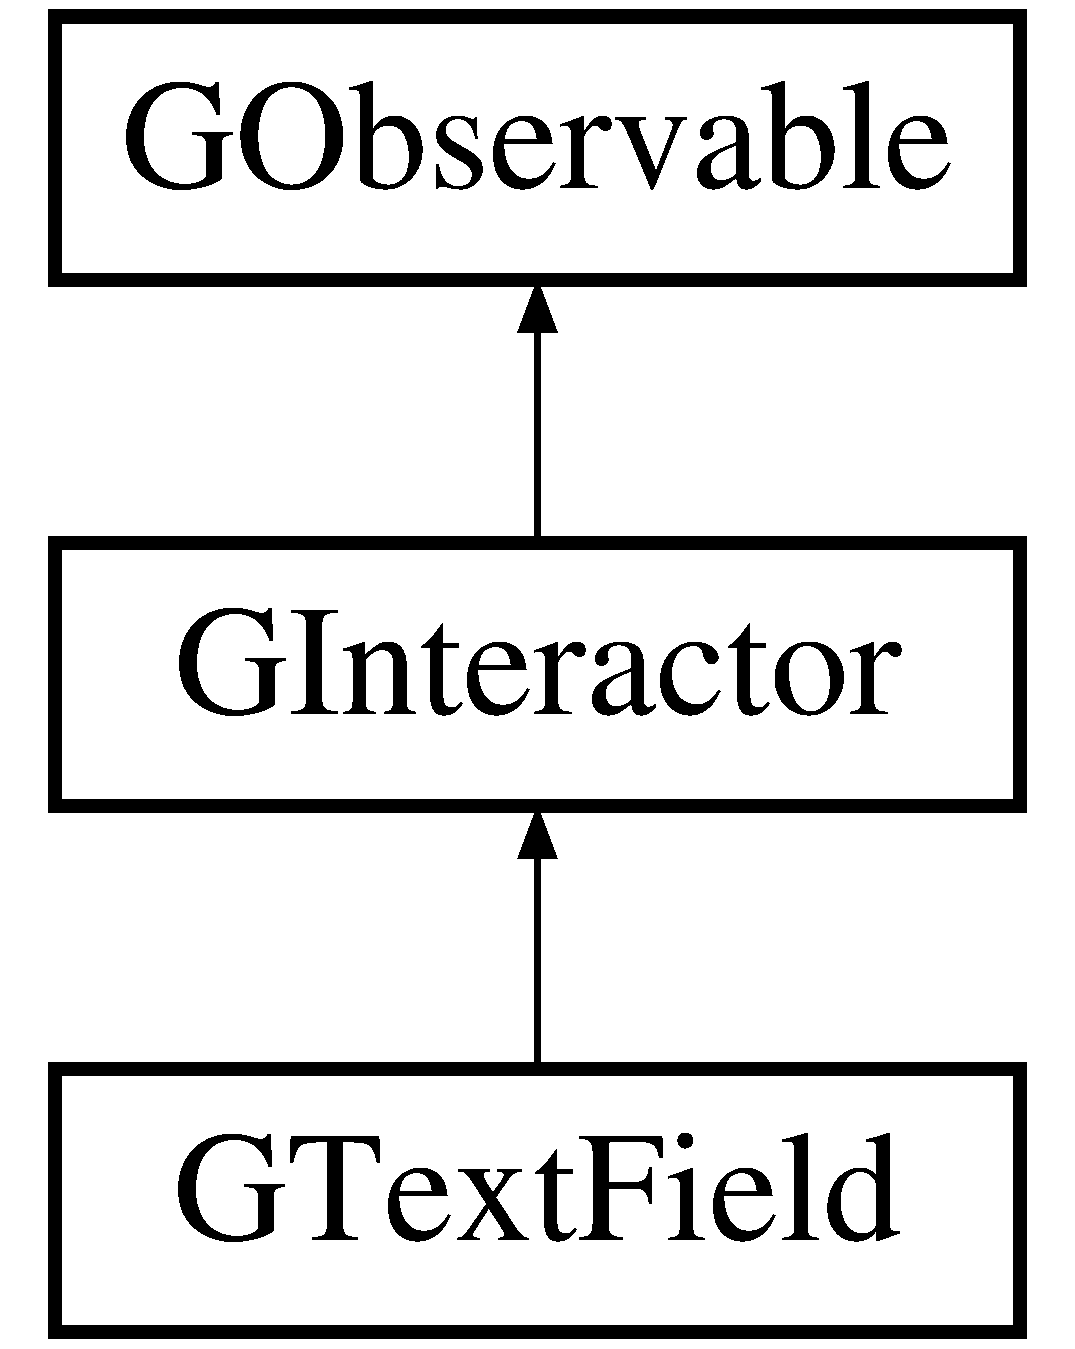
\includegraphics[height=3.000000cm]{classGTextField}
\end{center}
\end{figure}
\subsection*{Public Types}
\begin{DoxyCompactItemize}
\item 
enum \mbox{\hyperlink{classGTextField_a5fc772c800c3d40d2b95564e8a839bab}{Input\+Type}} \{ \mbox{\hyperlink{classGTextField_a5fc772c800c3d40d2b95564e8a839babadbd6303eaf17fd7715ddca85f2ac3287}{I\+N\+P\+U\+T\+\_\+\+T\+Y\+P\+E\+\_\+\+T\+E\+XT}}, 
\mbox{\hyperlink{classGTextField_a5fc772c800c3d40d2b95564e8a839babac37563ad86c1ac752795ed59e700be77}{I\+N\+P\+U\+T\+\_\+\+T\+Y\+P\+E\+\_\+\+I\+N\+T\+E\+G\+ER}}, 
\mbox{\hyperlink{classGTextField_a5fc772c800c3d40d2b95564e8a839babab760f99baafaf18281fa72664f303938}{I\+N\+P\+U\+T\+\_\+\+T\+Y\+P\+E\+\_\+\+R\+E\+AL}}
 \}
\begin{DoxyCompactList}\small\item\em Constants for the valid types of text field input. \end{DoxyCompactList}\item 
enum \mbox{\hyperlink{classGInteractor_a8e0d441725a81d2bbdebbea09078260e}{Text\+Position}} \{ \mbox{\hyperlink{classGInteractor_a8e0d441725a81d2bbdebbea09078260ea4cd6f2e7d5a08d6f4dc052df2358f774}{T\+E\+X\+T\+\_\+\+B\+E\+S\+I\+D\+E\+\_\+\+I\+C\+ON}}, 
\mbox{\hyperlink{classGInteractor_a8e0d441725a81d2bbdebbea09078260eaa88490f63d8de68d44c83bdb2ecde3b3}{T\+E\+X\+T\+\_\+\+U\+N\+D\+E\+R\+\_\+\+I\+C\+ON}}, 
\mbox{\hyperlink{classGInteractor_a8e0d441725a81d2bbdebbea09078260ea39a6f388a30ac4fefb6eb13e846bc9f2}{T\+E\+X\+T\+\_\+\+O\+N\+LY}}
 \}
\begin{DoxyCompactList}\small\item\em The places where an interactor can place its text relative to its icon. \end{DoxyCompactList}\end{DoxyCompactItemize}
\subsection*{Public Member Functions}
\begin{DoxyCompactItemize}
\item 
\mbox{\hyperlink{classGTextField_aab905bd4d32eef20c4b8ed701a8ec97f}{G\+Text\+Field}} (const std\+::string \&text=\char`\"{}\char`\"{}, int chars\+Wide=0, Q\+Widget $\ast$parent=nullptr)
\begin{DoxyCompactList}\small\item\em Creates a text field with the given initial text. \end{DoxyCompactList}\item 
\mbox{\hyperlink{classGTextField_a036419be062e4f447008a78dae22921c}{G\+Text\+Field}} (int chars\+Wide, Q\+Widget $\ast$parent=nullptr)
\begin{DoxyCompactList}\small\item\em Creates a text field wide enough to display the given number of characters. \end{DoxyCompactList}\item 
\mbox{\hyperlink{classGTextField_a4caf2f90e21e32abf032c99a8c3f8efb}{G\+Text\+Field}} (int value, int min, int max, int step=1, Q\+Widget $\ast$parent=nullptr)
\begin{DoxyCompactList}\small\item\em Creates a text field for entering integer values, with the given initial value. \end{DoxyCompactList}\item 
\mbox{\hyperlink{classGTextField_a8d164bf18d4dd4da6d5af0d23ee3a2c8}{G\+Text\+Field}} (double value, double min, double max, double step, Q\+Widget $\ast$parent=nullptr)
\begin{DoxyCompactList}\small\item\em Creates a text field for entering real number values, with the given initial value. \end{DoxyCompactList}\item 
virtual \mbox{\hyperlink{classGTextField_a5f71a42054388fb9dc24da9d8322ccdd}{$\sim$\+G\+Text\+Field}} () Q\+\_\+\+D\+E\+C\+L\+\_\+\+O\+V\+E\+R\+R\+I\+DE
\begin{DoxyCompactList}\small\item\em Frees memory allocated internally by the text field. \end{DoxyCompactList}\item 
virtual void \mbox{\hyperlink{classGInteractor_a02f20ea6edfa0671f31c4c648a253833}{add\+Action\+Listener}} () Q\+\_\+\+D\+E\+C\+L\+\_\+\+D\+E\+P\+R\+E\+C\+A\+T\+ED
\begin{DoxyCompactList}\small\item\em Adds an event listener to be notified when this interactor is clicked or generally interacted with. \end{DoxyCompactList}\item 
virtual bool \mbox{\hyperlink{classGInteractor_ac05ba5b92e2e5146d416fe7f842a0969}{events\+Enabled}} () const Q\+\_\+\+D\+E\+C\+L\+\_\+\+O\+V\+E\+R\+R\+I\+DE
\begin{DoxyCompactList}\small\item\em Returns true if this interactor is currently accepting events. \end{DoxyCompactList}\item 
virtual std\+::string \mbox{\hyperlink{classGInteractor_a69f8d23ed8f207fbecad99960776e942}{get\+Accelerator}} () const
\begin{DoxyCompactList}\small\item\em Returns a string representing a hotkey for this interactor, or an empty string if no accelerator has been set. \end{DoxyCompactList}\item 
virtual std\+::string \mbox{\hyperlink{classGInteractor_a94eb4276000c4fdfb508ce9e6317a82a}{get\+Action\+Command}} () const
\begin{DoxyCompactList}\small\item\em Returns an action command for this interactor, which is a semi-\/unique string you can use to identify it when events occur. \end{DoxyCompactList}\item 
virtual std\+::string \mbox{\hyperlink{classGInteractor_a808e22cc1fdfbecf71ed8c64ef4600e0}{get\+Background}} () const
\begin{DoxyCompactList}\small\item\em Returns the background color of the interactor as a string. \end{DoxyCompactList}\item 
virtual int \mbox{\hyperlink{classGInteractor_a9e827257a55cb8cf4d9de2ec6bcfd7a0}{get\+Background\+Int}} () const
\begin{DoxyCompactList}\small\item\em Returns the background color of the interactor as an R\+GB integer. \end{DoxyCompactList}\item 
virtual \mbox{\hyperlink{classGRectangle}{G\+Rectangle}} \mbox{\hyperlink{classGInteractor_a29e6ac35a0b48f491a4c88194cc5da3b}{get\+Bounds}} () const
\begin{DoxyCompactList}\small\item\em Returns a rectangle representing the x/y position and size of this interactor. \end{DoxyCompactList}\item 
virtual int \mbox{\hyperlink{classGTextField_acccdf98a090bca28752d04519a8b1a28}{get\+Chars\+Wide}} () const
\begin{DoxyCompactList}\small\item\em Returns the number of characters that can fit in the visible area of this text field. \end{DoxyCompactList}\item 
virtual std\+::string \mbox{\hyperlink{classGInteractor_aa061dfa488c31e18549d64363c1d0e34}{get\+Color}} () const
\begin{DoxyCompactList}\small\item\em Returns the foreground/text color of the interactor as a string. \end{DoxyCompactList}\item 
virtual int \mbox{\hyperlink{classGInteractor_a9635c7af766cdc3417f346683fa0e6c1}{get\+Color\+Int}} () const
\begin{DoxyCompactList}\small\item\em Returns the foreground/text color of the interactor as an R\+GB integer. \end{DoxyCompactList}\item 
virtual \mbox{\hyperlink{classGContainer}{G\+Container}} $\ast$ \mbox{\hyperlink{classGInteractor_a7a6e317c29d61030929b4cd2d1c00fe7}{get\+Container}} () const
\begin{DoxyCompactList}\small\item\em Returns a pointer to the onscreen container holding this interactor. \end{DoxyCompactList}\item 
virtual std\+::string \mbox{\hyperlink{classGInteractor_a894a5502900794eeb27d084c21f1d77d}{get\+Font}} () const
\begin{DoxyCompactList}\small\item\em Returns the font of this interactor\textquotesingle{}s text as a font string such as \char`\"{}\+Helvetica-\/12-\/\+Bold\char`\"{}. \end{DoxyCompactList}\item 
virtual std\+::string \mbox{\hyperlink{classGInteractor_a4fa2d8b0192a3a5b4af4bbfe71194d03}{get\+Foreground}} () const
\begin{DoxyCompactList}\small\item\em Returns the foreground/text color of the interactor as a string. \end{DoxyCompactList}\item 
virtual int \mbox{\hyperlink{classGInteractor_ac3b12ab385a6ef9ae90fc879860ba726}{get\+Foreground\+Int}} () const
\begin{DoxyCompactList}\small\item\em Returns the foreground/text color of the interactor as an R\+GB integer. \end{DoxyCompactList}\item 
virtual double \mbox{\hyperlink{classGInteractor_a1e7e353362434072875264cf95629f99}{get\+Height}} () const
\begin{DoxyCompactList}\small\item\em Returns the current onscreen height of this interactor in pixels. \end{DoxyCompactList}\item 
virtual std\+::string \mbox{\hyperlink{classGInteractor_aaed62a73004939a64da6f0eb9eb64d73}{get\+Icon}} () const
\begin{DoxyCompactList}\small\item\em Returns the file name of the icon associated with this interactor, or an empty string if no icon has been set. \end{DoxyCompactList}\item 
virtual int \mbox{\hyperlink{classGInteractor_a9c9659a6c6ba66b4107ba59c95a24241}{get\+ID}} () const
\begin{DoxyCompactList}\small\item\em Returns a globally unique identifier for this interactor, which is set when the interactor is constructed. \end{DoxyCompactList}\item 
virtual \mbox{\hyperlink{classGTextField_a5fc772c800c3d40d2b95564e8a839bab}{Input\+Type}} \mbox{\hyperlink{classGTextField_a69cc7c223d780203ab2852ee5a881753}{get\+Input\+Type}} () const
\begin{DoxyCompactList}\small\item\em Returns the type of input accepted by this text field. \end{DoxyCompactList}\item 
virtual \+\_\+\+Internal\+\_\+\+Q\+Widget $\ast$ \mbox{\hyperlink{classGTextField_a208ce13c1da40bf0ddb509daf99d6588}{get\+Internal\+Widget}} () const Q\+\_\+\+D\+E\+C\+L\+\_\+\+O\+V\+E\+R\+R\+I\+DE
\begin{DoxyCompactList}\small\item\em Returns a direct pointer to the internal Qt widget being wrapped by this interactor. \end{DoxyCompactList}\item 
virtual \mbox{\hyperlink{classGPoint}{G\+Point}} \mbox{\hyperlink{classGInteractor_a4f83802015511edeb63b892830812c11}{get\+Location}} () const
\begin{DoxyCompactList}\small\item\em Returns an (x, y) point representing the onscreen location of the top-\/left corner of this interactor within its containing window. \end{DoxyCompactList}\item 
virtual int \mbox{\hyperlink{classGTextField_a465e41b66da9e75443bf0b7951582468}{get\+Max\+Length}} () const
\begin{DoxyCompactList}\small\item\em Returns the maximum length of string allowed in the text field. \end{DoxyCompactList}\item 
virtual double \mbox{\hyperlink{classGInteractor_aed4b0075fcc434499c3cb3e46896bda3}{get\+Minimum\+Height}} () const
\begin{DoxyCompactList}\small\item\em Returns the minimum height in pixels that this interactor will permit itself to be resized to. \end{DoxyCompactList}\item 
virtual \mbox{\hyperlink{classGDimension}{G\+Dimension}} \mbox{\hyperlink{classGInteractor_a66b5af0b32493b4d597ca0a3df2049ea}{get\+Minimum\+Size}} () const
\begin{DoxyCompactList}\small\item\em Returns a \mbox{\hyperlink{classGDimension}{G\+Dimension}} structure representing the minimum size in pixels that this interactor will permit itself to be resized to. \end{DoxyCompactList}\item 
virtual double \mbox{\hyperlink{classGInteractor_a59e668114fe3d49d2a0f28deb258f7c8}{get\+Minimum\+Width}} () const
\begin{DoxyCompactList}\small\item\em Returns the minimum width in pixels that this interactor will permit itself to be resized to. \end{DoxyCompactList}\item 
virtual std\+::string \mbox{\hyperlink{classGInteractor_a8a60438a5b55d0b2ceb35c8674b9d8c5}{get\+Name}} () const
\begin{DoxyCompactList}\small\item\em Returns a string representing a unique name for this interactor. \end{DoxyCompactList}\item 
virtual std\+::string \mbox{\hyperlink{classGTextField_aa78dbaa7dac1f8cdf9048c91abecc7ad}{get\+Placeholder}} () const
\begin{DoxyCompactList}\small\item\em Returns the text field\textquotesingle{}s placeholder text, which is usually displayed as a light gray text in the field when the field is empty. \end{DoxyCompactList}\item 
virtual double \mbox{\hyperlink{classGInteractor_a747de0961653847bdc6615dbf756d715}{get\+Preferred\+Height}} () const
\begin{DoxyCompactList}\small\item\em Returns the height in pixels that this interactor would prefer to be, which would exactly fit its contents with no stretching or scrollbars. \end{DoxyCompactList}\item 
virtual \mbox{\hyperlink{classGDimension}{G\+Dimension}} \mbox{\hyperlink{classGInteractor_a4aabbee761d8e9116275401131b7ccd1}{get\+Preferred\+Size}} () const
\begin{DoxyCompactList}\small\item\em Returns a \mbox{\hyperlink{classGDimension}{G\+Dimension}} structure storing the width and height in pixels that this interactor would prefer to be, which would exactly fit its contents with no stretching or scrollbars. \end{DoxyCompactList}\item 
virtual double \mbox{\hyperlink{classGInteractor_a82bca31d37700fb0e35d2743352efd5e}{get\+Preferred\+Width}} () const
\begin{DoxyCompactList}\small\item\em Returns the height in pixels that this interactor would prefer to be, which would exactly fit its contents with no stretching or scrollbars. \end{DoxyCompactList}\item 
virtual \mbox{\hyperlink{classGDimension}{G\+Dimension}} \mbox{\hyperlink{classGInteractor_a7b4eec96a2bdc6420695d5796a78eea9}{get\+Size}} () const
\begin{DoxyCompactList}\small\item\em Returns a \mbox{\hyperlink{classGDimension}{G\+Dimension}} structure storing the current onscreen width and height of this interactor in pixels. \end{DoxyCompactList}\item 
virtual std\+::string \mbox{\hyperlink{classGTextField_aff553c50924b836c29f146ed34a7c6ec}{get\+Text}} () const
\begin{DoxyCompactList}\small\item\em Returns the text field\textquotesingle{}s current text. \end{DoxyCompactList}\item 
virtual std\+::string \mbox{\hyperlink{classGTextField_a9896d58fcfebbf1025aeeb5b8b9ede80}{get\+Type}} () const Q\+\_\+\+D\+E\+C\+L\+\_\+\+O\+V\+E\+R\+R\+I\+DE
\begin{DoxyCompactList}\small\item\em Returns a string representing the class name of this interactor, such as \char`\"{}\+G\+Button\char`\"{} or \char`\"{}\+G\+Check\+Box\char`\"{}. \end{DoxyCompactList}\item 
virtual std\+::string \mbox{\hyperlink{classGTextField_a2a03038d2e299f486e55dc72778f7086}{get\+Value}} () const
\begin{DoxyCompactList}\small\item\em Returns the text field\textquotesingle{}s current text. \end{DoxyCompactList}\item 
virtual bool \mbox{\hyperlink{classGTextField_a8190c918ce29007223898c9d511b17ee}{get\+Value\+As\+Bool}} () const
\begin{DoxyCompactList}\small\item\em Returns the currently typed value in the text field, interpreted as a bool value of true or false. \end{DoxyCompactList}\item 
virtual char \mbox{\hyperlink{classGTextField_a562f514fc055aaa37ca3145fc7abde8e}{get\+Value\+As\+Char}} () const
\begin{DoxyCompactList}\small\item\em Returns the currently typed value in the text field as a char value. \end{DoxyCompactList}\item 
virtual double \mbox{\hyperlink{classGTextField_aab9a19edbd1548d557721e0b695295f8}{get\+Value\+As\+Double}} () const
\begin{DoxyCompactList}\small\item\em Returns the currently typed value in the text field, interpreted as a real number value. \end{DoxyCompactList}\item 
virtual int \mbox{\hyperlink{classGTextField_a5e50caa202955b726a44a1dfbc6f7818}{get\+Value\+As\+Int}} () const
\begin{DoxyCompactList}\small\item\em Returns the currently typed value in the text field, interpreted as an integer value. \end{DoxyCompactList}\item 
virtual int \mbox{\hyperlink{classGTextField_a1cbf643145c03ed4c238d085fc88cf33}{get\+Value\+As\+Integer}} () const
\begin{DoxyCompactList}\small\item\em Returns the currently typed value in the text field, interpreted as an integer value. \end{DoxyCompactList}\item 
virtual Q\+Widget $\ast$ \mbox{\hyperlink{classGTextField_a326ee51b5561f807df7b29a1c101f7fd}{get\+Widget}} () const Q\+\_\+\+D\+E\+C\+L\+\_\+\+O\+V\+E\+R\+R\+I\+DE
\begin{DoxyCompactList}\small\item\em Returns a direct pointer to the internal Qt widget being wrapped by this interactor. \end{DoxyCompactList}\item 
virtual double \mbox{\hyperlink{classGInteractor_a0ed2965abd4f5701d2cadf71239faf19}{get\+Width}} () const
\begin{DoxyCompactList}\small\item\em Returns the current onscreen width of this interactor in pixels. \end{DoxyCompactList}\item 
virtual double \mbox{\hyperlink{classGInteractor_a344385751bee0720059403940d57a13e}{getX}} () const
\begin{DoxyCompactList}\small\item\em Returns the x-\/coordinate of the top-\/left pixel of this interactor within its onscreen window. \end{DoxyCompactList}\item 
virtual double \mbox{\hyperlink{classGInteractor_aafa51c7f8f38a09febbb9ce7853f77b4}{getY}} () const
\begin{DoxyCompactList}\small\item\em Returns the y-\/coordinate of the top-\/left pixel of this interactor within its onscreen window. \end{DoxyCompactList}\item 
virtual bool \mbox{\hyperlink{classGInteractor_afc480f652b8c5f1fb255e2269ce68879}{in\+Bounds}} (double x, double y) const
\begin{DoxyCompactList}\small\item\em Returns true if the given x/y pixel is within the bounds of this interactor. \end{DoxyCompactList}\item 
virtual bool \mbox{\hyperlink{classGInteractor_ae6d7982c1c627b677a5e776ca86118ed}{in\+Bounds}} (int x, int y) const
\begin{DoxyCompactList}\small\item\em Returns true if the given x/y pixel is within the bounds of this interactor. \end{DoxyCompactList}\item 
virtual bool \mbox{\hyperlink{classGTextField_a7528cfb0542ac5268efe1d7362b89344}{is\+Autocomplete\+Enabled}} () const
\begin{DoxyCompactList}\small\item\em Returns true if this text field has an autocompletion list of options that will pop up as the user begins typing. \end{DoxyCompactList}\item 
virtual bool \mbox{\hyperlink{classGTextField_a012b5afb54e037e6c5498cf0932a521b}{is\+Editable}} () const
\begin{DoxyCompactList}\small\item\em Returns true if the text field\textquotesingle{}s value can be edited. \end{DoxyCompactList}\item 
virtual bool \mbox{\hyperlink{classGInteractor_aacb819fb241851fd9fc045271baa4034}{is\+Enabled}} () const
\begin{DoxyCompactList}\small\item\em Returns true if this interactor is currently enabled. \end{DoxyCompactList}\item 
virtual bool \mbox{\hyperlink{classGInteractor_a9d8a6cfb13917785c143e74d40e4e2be}{is\+Visible}} () const
\begin{DoxyCompactList}\small\item\em Returns true if the interactor is visible on the screen. \end{DoxyCompactList}\item 
virtual void \mbox{\hyperlink{classGTextField_ab7fe7a876367b87cf7202f947f1d05e4}{remove\+Action\+Listener}} ()
\begin{DoxyCompactList}\small\item\em Removes the action listener from this text field so that it will no longer call it when the user presses Enter. \end{DoxyCompactList}\item 
virtual void \mbox{\hyperlink{classGTextField_a69c940b99d01eb7c353763ce4b0942a4}{remove\+Text\+Change\+Listener}} ()
\begin{DoxyCompactList}\small\item\em Removes the text change listener from this text field so that it will no longer call it when the user types characters. \end{DoxyCompactList}\item 
virtual void \mbox{\hyperlink{classGInteractor_a519fb2ac767f8b2febbb50b898b8c8cb}{request\+Focus}} ()
\begin{DoxyCompactList}\small\item\em Transfers keyboard focus to this interactor. \end{DoxyCompactList}\item 
virtual void \mbox{\hyperlink{classGInteractor_ad15f102f62e2960576012f1aa0ba4b2e}{set\+Accelerator}} (const std\+::string \&accelerator)
\begin{DoxyCompactList}\small\item\em Sets an accelerator hotkey for this interactor, such as \char`\"{}\+Ctrl-\/\+S\char`\"{}. \end{DoxyCompactList}\item 
virtual void \mbox{\hyperlink{classGInteractor_a4b5843fe3030e038a1ba54cc03389bcf}{set\+Action\+Command}} (const std\+::string \&action\+Command)
\begin{DoxyCompactList}\small\item\em Sets the action command for this interactor. \end{DoxyCompactList}\item 
virtual void \mbox{\hyperlink{classGTextField_adcfb4742430c88714fcf57e57ab8ea9c}{set\+Action\+Listener}} (G\+Event\+Listener func)
\begin{DoxyCompactList}\small\item\em Sets an action listener on this text field so that it will be called when the user presses the Enter key. \end{DoxyCompactList}\item 
virtual void \mbox{\hyperlink{classGTextField_aebd20a89c7a8a43a6fce999cf4f9fcf2}{set\+Action\+Listener}} (G\+Event\+Listener\+Void func)
\begin{DoxyCompactList}\small\item\em Sets an action listener on this text field so that it will be called when the user presses the Enter key. \end{DoxyCompactList}\item 
virtual void \mbox{\hyperlink{classGTextField_a173f724f6099be5a2ed423baf3433b83}{set\+Autocomplete\+Enabled}} (bool enabled)
\begin{DoxyCompactList}\small\item\em Sets whether the autocompletion feature is enabled for this text field. \end{DoxyCompactList}\item 
virtual void \mbox{\hyperlink{classGTextField_ab0245df51aa762af89f0d2cf31ce6ddd}{set\+Autocomplete\+List}} (std\+::initializer\+\_\+list$<$ std\+::string $>$ strings)
\begin{DoxyCompactList}\small\item\em Sets the given list of strings to be used as an autocompletion list for this text field. \end{DoxyCompactList}\item 
virtual void \mbox{\hyperlink{classGTextField_af468683b02e61be999c76dd1100165e8}{set\+Autocomplete\+List}} (const \mbox{\hyperlink{classVector}{Vector}}$<$ std\+::string $>$ \&strings)
\begin{DoxyCompactList}\small\item\em Sets the given list of strings to be used as an autocompletion list for this text field. \end{DoxyCompactList}\item 
virtual void \mbox{\hyperlink{classGInteractor_acba7e546c2025c0a15ca4b4cc92043db}{set\+Background}} (int rgb)
\begin{DoxyCompactList}\small\item\em Sets the background color of the interactor to the color represented by the given R\+GB integer. \end{DoxyCompactList}\item 
virtual void \mbox{\hyperlink{classGInteractor_ab4677ab2474e68b07aa56605af92a84a}{set\+Background}} (const std\+::string \&color)
\begin{DoxyCompactList}\small\item\em Sets the background color of the interactor to the color represented by the given string. \end{DoxyCompactList}\item 
virtual void \mbox{\hyperlink{classGInteractor_a2aae8197624b72265ab83b4f1bc73f2f}{set\+Bounds}} (double x, double y, double width, double height)
\begin{DoxyCompactList}\small\item\em Sets the size and location of the widget. \end{DoxyCompactList}\item 
virtual void \mbox{\hyperlink{classGInteractor_acada386653f008cacc7cce86426bef7c}{set\+Bounds}} (const \mbox{\hyperlink{classGRectangle}{G\+Rectangle}} \&size)
\begin{DoxyCompactList}\small\item\em Sets the size and location of the widget. \end{DoxyCompactList}\item 
virtual void \mbox{\hyperlink{classGTextField_aef8026e0b00b17dbccfc456e75308f16}{set\+Chars\+Wide}} (int chars\+Wide)
\begin{DoxyCompactList}\small\item\em Sets the width of this text field to be exactly wide enough to display the given number of characters. \end{DoxyCompactList}\item 
virtual void \mbox{\hyperlink{classGInteractor_ab1f5cc0f5cc6bbbd716a526c61f1081d}{set\+Color}} (int rgb)
\begin{DoxyCompactList}\small\item\em Sets the foreground/text color of the interactor to the color represented by the given R\+GB integer. \end{DoxyCompactList}\item 
virtual void \mbox{\hyperlink{classGInteractor_a61374df6c11b52cfbb0815decdbaebc6}{set\+Color}} (const std\+::string \&color)
\begin{DoxyCompactList}\small\item\em Sets the foreground/text color of the interactor to the color represented by the given string. \end{DoxyCompactList}\item 
virtual void \mbox{\hyperlink{classGTextField_a008d7fd44fb3e7a6886cdaddbc3644a2}{set\+Editable}} (bool value)
\begin{DoxyCompactList}\small\item\em Sets whether the value in the text box can be edited. \end{DoxyCompactList}\item 
virtual void \mbox{\hyperlink{classGInteractor_ab831367dd84bbd579e02e55bacb21343}{set\+Enabled}} (bool value)
\begin{DoxyCompactList}\small\item\em Sets whether this interactor is currently enabled. \end{DoxyCompactList}\item 
virtual void \mbox{\hyperlink{classGObservable_afaa30b2a9e0f378fd1c70d2f1d0b8216}{set\+Events\+Enabled}} (bool \mbox{\hyperlink{classGInteractor_ac05ba5b92e2e5146d416fe7f842a0969}{events\+Enabled}})
\begin{DoxyCompactList}\small\item\em Sets whether the object is currently allowing itself to fire events. \end{DoxyCompactList}\item 
virtual void \mbox{\hyperlink{classGInteractor_a2592348886ffea646c6534bf88f7c49d}{set\+Font}} (const Q\+Font \&font)
\begin{DoxyCompactList}\small\item\em Sets the font used by this widget to the given Qt font. \end{DoxyCompactList}\item 
virtual void \mbox{\hyperlink{classGInteractor_a8e096e8818d838aceae1d46d58fb3a7b}{set\+Font}} (const std\+::string \&font)
\begin{DoxyCompactList}\small\item\em Sets the font used by this widget to the font represented by the given font string, such as \char`\"{}\+Helvetica-\/16-\/\+Bold\char`\"{}. \end{DoxyCompactList}\item 
virtual void \mbox{\hyperlink{classGInteractor_a9eb856b5ff83a19df3831a31f15f4563}{set\+Foreground}} (int rgb)
\begin{DoxyCompactList}\small\item\em Sets the foreground/text color of the interactor to the color represented by the given R\+GB integer. \end{DoxyCompactList}\item 
virtual void \mbox{\hyperlink{classGInteractor_af59209aeadea6dfc6d97a2d8531f50e1}{set\+Foreground}} (const std\+::string \&color)
\begin{DoxyCompactList}\small\item\em Sets the foreground/text color of the interactor to the color represented by the given string. \end{DoxyCompactList}\item 
virtual void \mbox{\hyperlink{classGInteractor_a9e280bfc4544dfaf8e4376c4e1a74357}{set\+Height}} (double height)
\begin{DoxyCompactList}\small\item\em Sets the onscreen height of the interactor in pixels. \end{DoxyCompactList}\item 
virtual void \mbox{\hyperlink{classGInteractor_a762e139aa311461c3984d3ad28293f64}{set\+Icon}} (const std\+::string \&filename, bool retain\+Icon\+Size=true)
\begin{DoxyCompactList}\small\item\em Sets the file name of the icon associated with this interactor, or an empty string if no icon has been set. \end{DoxyCompactList}\item 
virtual void \mbox{\hyperlink{classGInteractor_a04594e8ba9b98513a64f1da00dcae18c}{set\+Location}} (double x, double y)
\begin{DoxyCompactList}\small\item\em Sets the onscreen x/y-\/coordinate of the top-\/left corner of the interactor relative to its window. \end{DoxyCompactList}\item 
virtual void \mbox{\hyperlink{classGTextField_a077c24fa5337fbf431738f8ba513d19c}{set\+Max\+Length}} (int max\+Length)
\begin{DoxyCompactList}\small\item\em Sets the maximum number of characters that can be typed into the field. \end{DoxyCompactList}\item 
virtual void \mbox{\hyperlink{classGInteractor_a0cf428e207b7f22cc08138a90b1b87b2}{set\+Minimum\+Size}} (double width, double height)
\begin{DoxyCompactList}\small\item\em Sets the minimum size in pixels that this interactor will permit itself to be resized to. \end{DoxyCompactList}\item 
virtual void \mbox{\hyperlink{classGInteractor_a3b1046117ac6cb7abe467e00ba8a81f4}{set\+Minimum\+Size}} (const \mbox{\hyperlink{classGDimension}{G\+Dimension}} \&size)
\begin{DoxyCompactList}\small\item\em Sets the minimum size in pixels that this interactor will permit itself to be resized to. \end{DoxyCompactList}\item 
virtual void \mbox{\hyperlink{classGInteractor_a9d3a2685df23b5e7cbf59c19c4a1f9b5}{set\+Name}} (const std\+::string \&name)
\begin{DoxyCompactList}\small\item\em Sets a string representing a unique name for this interactor. \end{DoxyCompactList}\item 
virtual void \mbox{\hyperlink{classGTextField_aa21a9bebb4652ab6780d0c11eff47aee}{set\+Placeholder}} (const std\+::string \&text)
\begin{DoxyCompactList}\small\item\em Sets a gray message that is displayed in the background of the text field before the user has typed any value. \end{DoxyCompactList}\item 
virtual void \mbox{\hyperlink{classGInteractor_a1ab987704fce32098706c6f00fb08218}{set\+Preferred\+Height}} (double height)
\begin{DoxyCompactList}\small\item\em Sets the height in pixels that this interactor would prefer to be. \end{DoxyCompactList}\item 
virtual void \mbox{\hyperlink{classGInteractor_a042c5ae19430d765ef552371cae3632c}{set\+Preferred\+Size}} (double width, double height)
\begin{DoxyCompactList}\small\item\em Sets the width and height in pixels that this interactor would prefer to be. \end{DoxyCompactList}\item 
virtual void \mbox{\hyperlink{classGInteractor_aa22d9be4bc0e078bb0ea69b0fc9d7c75}{set\+Preferred\+Size}} (const \mbox{\hyperlink{classGDimension}{G\+Dimension}} \&size)
\begin{DoxyCompactList}\small\item\em Sets the size in pixels that this interactor would prefer to be. \end{DoxyCompactList}\item 
virtual void \mbox{\hyperlink{classGInteractor_a3db429ab2fa52efd187eec0ed8cdd9f2}{set\+Preferred\+Width}} (double width)
\begin{DoxyCompactList}\small\item\em Sets the width in pixels that this interactor would prefer to be. \end{DoxyCompactList}\item 
virtual void \mbox{\hyperlink{classGInteractor_aca25d49481f9bf5fc8f7df4c086c4ce7}{set\+Size}} (double width, double height)
\begin{DoxyCompactList}\small\item\em Sets the onscreen width and height of the interactor in pixels. \end{DoxyCompactList}\item 
virtual void \mbox{\hyperlink{classGInteractor_ae2b628228f192c2702c4ce941b2af68f}{set\+Size}} (const \mbox{\hyperlink{classGDimension}{G\+Dimension}} \&size)
\begin{DoxyCompactList}\small\item\em Sets the onscreen width and height of the interactor in pixels. \end{DoxyCompactList}\item 
virtual void \mbox{\hyperlink{classGTextField_ac1ae51949d41ee9054634be5967d91b8}{set\+Text}} (const std\+::string \&text)
\begin{DoxyCompactList}\small\item\em Sets the current text value in the text field. \end{DoxyCompactList}\item 
virtual void \mbox{\hyperlink{classGTextField_ae41284f9c540110180ac0ad6beca5cb0}{set\+Text\+Change\+Listener}} (G\+Event\+Listener func)
\begin{DoxyCompactList}\small\item\em Sets a text-\/change listener on this text field so that it will be called when the value in the field changes, which will occur on every key press. \end{DoxyCompactList}\item 
virtual void \mbox{\hyperlink{classGTextField_ae8df75b0746951146d29220f386fcd33}{set\+Text\+Change\+Listener}} (G\+Event\+Listener\+Void func)
\begin{DoxyCompactList}\small\item\em Sets a text-\/change listener on this text field so that it will be called when the value in the field changes, which will occur on every key press. \end{DoxyCompactList}\item 
virtual void \mbox{\hyperlink{classGInteractor_a039e0e49beaecc275efce02d416acea8}{set\+Tooltip}} (const std\+::string \&tooltip\+Text)
\begin{DoxyCompactList}\small\item\em Sets a \char`\"{}tooltip\char`\"{} that will appear if the user hovers their mouse over the interactor. \end{DoxyCompactList}\item 
virtual void \mbox{\hyperlink{classGTextField_ae803b3348fa7076308d852bbdeea0d74}{set\+Value}} (bool value)
\begin{DoxyCompactList}\small\item\em Sets the current text value in the text field to the string representation of the given value. \end{DoxyCompactList}\item 
virtual void \mbox{\hyperlink{classGTextField_aeefe59b3d414b657838869ce084cb0e2}{set\+Value}} (char value)
\begin{DoxyCompactList}\small\item\em Sets the current text value in the text field to the string representation of the given value. \end{DoxyCompactList}\item 
virtual void \mbox{\hyperlink{classGTextField_a1a31743bc7def7cf7fdad044c84d9268}{set\+Value}} (double value)
\begin{DoxyCompactList}\small\item\em Sets the current text value in the text field to the string representation of the given value. \end{DoxyCompactList}\item 
virtual void \mbox{\hyperlink{classGTextField_a23d79e21b8ed72e19278ca31d47b8c87}{set\+Value}} (int value)
\begin{DoxyCompactList}\small\item\em Sets the current text value in the text field to the string representation of the given value. \end{DoxyCompactList}\item 
virtual void \mbox{\hyperlink{classGTextField_ab18c7a418be64c4f909beebc277a1321}{set\+Value}} (const std\+::string \&value)
\begin{DoxyCompactList}\small\item\em Sets the current text value in the text field to the string representation of the given value. \end{DoxyCompactList}\item 
virtual void \mbox{\hyperlink{classGInteractor_a18e44e30b31525a243960ca3928125aa}{set\+Visible}} (bool visible)
\begin{DoxyCompactList}\small\item\em Returns true if the interactor is visible on the screen. \end{DoxyCompactList}\item 
virtual void \mbox{\hyperlink{classGInteractor_aa3f3fba4cb131baa8696ba01e3bceca1}{set\+Width}} (double width)
\begin{DoxyCompactList}\small\item\em Sets the onscreen width of the interactor in pixels. \end{DoxyCompactList}\item 
virtual void \mbox{\hyperlink{classGInteractor_a9c18fcc579333bf9653d13ad2b372e39}{setX}} (double x)
\begin{DoxyCompactList}\small\item\em Sets the onscreen x-\/coordinate of the top-\/left corner of the interactor relative to its window. \end{DoxyCompactList}\item 
virtual void \mbox{\hyperlink{classGInteractor_a7d57e2a5c35d27feb58fd498a3cf82b9}{setY}} (double y)
\begin{DoxyCompactList}\small\item\em Sets the onscreen y-\/coordinate of the top-\/left corner of the interactor relative to its window. \end{DoxyCompactList}\item 
virtual std\+::string \mbox{\hyperlink{classGObservable_a1fe5121d6528fdea3f243321b3fa3a49}{to\+String}} () const
\begin{DoxyCompactList}\small\item\em Returns a string representation of this observable object\textquotesingle{}s state. \end{DoxyCompactList}\item 
virtual bool \mbox{\hyperlink{classGTextField_a203f90275053ab957b1ea5a40dc3dd1e}{value\+Is\+Bool}} () const
\begin{DoxyCompactList}\small\item\em Returns true if the currently typed value in the text field can be interpreted as a bool value of true or false. \end{DoxyCompactList}\item 
virtual bool \mbox{\hyperlink{classGTextField_ac7a337b1e4c2f752a7f3fb634c92b442}{value\+Is\+Char}} () const
\begin{DoxyCompactList}\small\item\em Returns true if the currently typed value in the text field can be interpreted as a char value. \end{DoxyCompactList}\item 
virtual bool \mbox{\hyperlink{classGTextField_aa80caadc7498333f74a08b4cdc0528c1}{value\+Is\+Double}} () const
\begin{DoxyCompactList}\small\item\em Returns true if the currently typed value in the text field can be interpreted as a real number. \end{DoxyCompactList}\item 
virtual bool \mbox{\hyperlink{classGTextField_a4bccf08b3b712af3839106a1cbdc5d02}{value\+Is\+Int}} () const
\begin{DoxyCompactList}\small\item\em Returns true if the currently typed value in the text field can be interpreted as an integer. \end{DoxyCompactList}\item 
virtual bool \mbox{\hyperlink{classGTextField_af5aaf003739648d9aee89a17e715a57e}{value\+Is\+Integer}} () const
\begin{DoxyCompactList}\small\item\em Returns true if the currently typed value in the text field can be interpreted as an integer. \end{DoxyCompactList}\item 
virtual bool \mbox{\hyperlink{classGTextField_a29a5f540431d7993ff00eee5d2584a36}{value\+Is\+Real}} () const
\begin{DoxyCompactList}\small\item\em Returns true if the currently typed value in the text field can be interpreted as a real number. \end{DoxyCompactList}\end{DoxyCompactItemize}
\subsection*{Protected Member Functions}
\begin{DoxyCompactItemize}
\item 
virtual void \mbox{\hyperlink{classGObservable_a80cfa040459ff53594adbd6a51ec8f43}{clear\+Event\+Listeners}} ()
\begin{DoxyCompactList}\small\item\em Removes all event listeners from this object. \end{DoxyCompactList}\item 
virtual void \mbox{\hyperlink{classGObservable_a284f31528c0520f8e545c03ac9eeac74}{ensure\+Thread\+Safety}} (const std\+::string \&member\+Name=\char`\"{}\char`\"{})
\begin{DoxyCompactList}\small\item\em Ensures that we are currently in the Qt G\+UI thread. \end{DoxyCompactList}\item 
virtual void \mbox{\hyperlink{classGObservable_a63e5e5a6227c59c928493b11aceb0f67}{fire\+Event}} (\mbox{\hyperlink{classGEvent}{G\+Event}} \&event)
\begin{DoxyCompactList}\small\item\em Sends out the given event to any attached listeners. \end{DoxyCompactList}\item 
virtual void \mbox{\hyperlink{classGObservable_ab3983ea07337b52020a29cc00c653d8d}{fire\+G\+Event}} (Q\+Event $\ast$event, Event\+Type event\+Type, const std\+::string \&event\+Name)
\begin{DoxyCompactList}\small\item\em Creates an event of the given type, then sends it out to any attached listeners. \end{DoxyCompactList}\item 
virtual void \mbox{\hyperlink{classGObservable_a01fdf1b0e0dbd49e189fe4514e010411}{fire\+G\+Event}} (Q\+Close\+Event $\ast$event, Event\+Type event\+Type, const std\+::string \&event\+Name)
\begin{DoxyCompactList}\small\item\em Creates an event of the given type, then sends it out to any attached listeners. \end{DoxyCompactList}\item 
virtual void \mbox{\hyperlink{classGObservable_abb0b2f66ba39211cb5d7615e9d1c04e2}{fire\+G\+Event}} (Q\+Key\+Event $\ast$event, Event\+Type event\+Type, const std\+::string \&event\+Name)
\begin{DoxyCompactList}\small\item\em Creates an event of the given type, then sends it out to any attached listeners. \end{DoxyCompactList}\item 
virtual void \mbox{\hyperlink{classGObservable_a119318675d2165bdf7dd853aaf881d4b}{fire\+G\+Event}} (Q\+Mouse\+Event $\ast$event, Event\+Type event\+Type, const std\+::string \&event\+Name, const std\+::string \&action\+Command=\char`\"{}\char`\"{})
\begin{DoxyCompactList}\small\item\em Creates an event of the given type, then sends it out to any attached listeners. \end{DoxyCompactList}\item 
virtual void \mbox{\hyperlink{classGObservable_a63fd9034e1e1633c1c38eb342bfd34e9}{fire\+G\+Event}} (Q\+Resize\+Event $\ast$event, Event\+Type event\+Type, const std\+::string \&event\+Name)
\begin{DoxyCompactList}\small\item\em Creates an event of the given type, then sends it out to any attached listeners. \end{DoxyCompactList}\item 
virtual void \mbox{\hyperlink{classGObservable_a741345310d9b7c5170a6cbc410c44ac4}{fire\+G\+Event}} (Q\+Timer\+Event $\ast$event, Event\+Type event\+Type, const std\+::string \&event\+Name)
\begin{DoxyCompactList}\small\item\em Creates an event of the given type, then sends it out to any attached listeners. \end{DoxyCompactList}\item 
virtual void \mbox{\hyperlink{classGObservable_a93bf338968a0338761b8e4dc62f582e9}{fire\+G\+Event}} (Q\+Wheel\+Event $\ast$event, Event\+Type event\+Type, const std\+::string \&event\+Name)
\begin{DoxyCompactList}\small\item\em Creates an event of the given type, then sends it out to any attached listeners. \end{DoxyCompactList}\item 
virtual void \mbox{\hyperlink{classGObservable_a2a70a7d7435ff0c3b80bb4d70da19e0d}{fire\+G\+Event}} (Q\+Window\+State\+Change\+Event $\ast$event, Event\+Type event\+Type, const std\+::string \&event\+Name)
\begin{DoxyCompactList}\small\item\em Creates an event of the given type, then sends it out to any attached listeners. \end{DoxyCompactList}\item 
virtual bool \mbox{\hyperlink{classGObservable_a9f6faaa25942923bafa1c44020c49fa9}{has\+Event\+Listener}} (const std\+::string \&event\+Name) const
\begin{DoxyCompactList}\small\item\em Returns true if the observable object has a listener for the given type of event. \end{DoxyCompactList}\item 
virtual bool \mbox{\hyperlink{classGObservable_aeec1adc19aa0f33de62390686ee1382c}{is\+Accepting\+Event}} (int event\+Mask) const
\begin{DoxyCompactList}\small\item\em Returns true if the observable object has a listener for the given type of event. \end{DoxyCompactList}\item 
virtual bool \mbox{\hyperlink{classGObservable_aa31c73145a29dcb92848a92e0cfaea41}{is\+Accepting\+Event}} (const \mbox{\hyperlink{classGEvent}{G\+Event}} \&event) const
\begin{DoxyCompactList}\small\item\em Returns true if the observable object has a listener for the given type of event. \end{DoxyCompactList}\item 
virtual bool \mbox{\hyperlink{classGObservable_a3b1c689267eda44e65a2213e7de38b23}{is\+Accepting\+Event}} (const std\+::string \&event\+Type) const
\begin{DoxyCompactList}\small\item\em Returns true if the observable object has a listener for the given type of event. \end{DoxyCompactList}\item 
virtual void \mbox{\hyperlink{classGObservable_acbcf1ed3a851ad8a3c17ef38d86b481d}{remove\+Event\+Listener}} (const std\+::string \&event\+Name)
\begin{DoxyCompactList}\small\item\em Removes any event listener from this observable object that would respond to the given type of event, such as \char`\"{}click\char`\"{} or \char`\"{}keydown\char`\"{}. \end{DoxyCompactList}\item 
virtual void \mbox{\hyperlink{classGObservable_af51cc35c29a1bd1908609d432decdbb6}{remove\+Event\+Listeners}} (std\+::initializer\+\_\+list$<$ std\+::string $>$ event\+Names)
\begin{DoxyCompactList}\small\item\em Removes any event listener from this observable object that would respond to the given types of events, such as \char`\"{}click\char`\"{} or \char`\"{}keydown\char`\"{}. \end{DoxyCompactList}\item 
virtual void \mbox{\hyperlink{classGObservable_ad2f6d34961c50f6c1e0659990b79f741}{set\+Event\+Listener}} (const std\+::string \&event\+Name, G\+Event\+Listener func)
\begin{DoxyCompactList}\small\item\em Adds an event listener from this observable object to respond to the given type of event, such as \char`\"{}click\char`\"{} or \char`\"{}keydown\char`\"{}. \end{DoxyCompactList}\item 
virtual void \mbox{\hyperlink{classGObservable_abac4cb9f9e626e010e87f5d91573c8a5}{set\+Event\+Listener}} (const std\+::string \&event\+Name, G\+Event\+Listener\+Void func)
\begin{DoxyCompactList}\small\item\em Adds an event listener from this observable object to respond to the given type of event, such as \char`\"{}click\char`\"{} or \char`\"{}keydown\char`\"{}. \end{DoxyCompactList}\item 
virtual void \mbox{\hyperlink{classGObservable_afa388d69c33c718cf035774604065604}{set\+Event\+Listeners}} (std\+::initializer\+\_\+list$<$ std\+::string $>$ event\+Names, G\+Event\+Listener func)
\begin{DoxyCompactList}\small\item\em Adds an event listener from this observable object to respond to the given types of events, such as \char`\"{}click\char`\"{} or \char`\"{}keydown\char`\"{}. \end{DoxyCompactList}\item 
virtual void \mbox{\hyperlink{classGObservable_a7867184bbb686f74fae8a4db927da799}{set\+Event\+Listeners}} (std\+::initializer\+\_\+list$<$ std\+::string $>$ event\+Names, G\+Event\+Listener\+Void func)
\begin{DoxyCompactList}\small\item\em Adds an event listener from this observable object to respond to the given types of events, such as \char`\"{}click\char`\"{} or \char`\"{}keydown\char`\"{}. \end{DoxyCompactList}\end{DoxyCompactItemize}


\subsection{Detailed Description}
This interactor subclass represents a text field for entering short text strings. 

Pressing Enter in a text field generates an action event. 

\subsection{Member Enumeration Documentation}
\mbox{\Hypertarget{classGTextField_a5fc772c800c3d40d2b95564e8a839bab}\label{classGTextField_a5fc772c800c3d40d2b95564e8a839bab}} 
\index{G\+Text\+Field@{G\+Text\+Field}!Input\+Type@{Input\+Type}}
\index{Input\+Type@{Input\+Type}!G\+Text\+Field@{G\+Text\+Field}}
\subsubsection{\texorpdfstring{Input\+Type}{InputType}}
{\footnotesize\ttfamily enum \mbox{\hyperlink{classGTextField_a5fc772c800c3d40d2b95564e8a839bab}{Input\+Type}}}



Constants for the valid types of text field input. 

\begin{DoxyEnumFields}{Enumerator}
\raisebox{\heightof{T}}[0pt][0pt]{\index{I\+N\+P\+U\+T\+\_\+\+T\+Y\+P\+E\+\_\+\+T\+E\+XT@{I\+N\+P\+U\+T\+\_\+\+T\+Y\+P\+E\+\_\+\+T\+E\+XT}!G\+Text\+Field@{G\+Text\+Field}}\index{G\+Text\+Field@{G\+Text\+Field}!I\+N\+P\+U\+T\+\_\+\+T\+Y\+P\+E\+\_\+\+T\+E\+XT@{I\+N\+P\+U\+T\+\_\+\+T\+Y\+P\+E\+\_\+\+T\+E\+XT}}}\mbox{\Hypertarget{classGTextField_a5fc772c800c3d40d2b95564e8a839babadbd6303eaf17fd7715ddca85f2ac3287}\label{classGTextField_a5fc772c800c3d40d2b95564e8a839babadbd6303eaf17fd7715ddca85f2ac3287}} 
I\+N\+P\+U\+T\+\_\+\+T\+Y\+P\+E\+\_\+\+T\+E\+XT&\\
\hline

\raisebox{\heightof{T}}[0pt][0pt]{\index{I\+N\+P\+U\+T\+\_\+\+T\+Y\+P\+E\+\_\+\+I\+N\+T\+E\+G\+ER@{I\+N\+P\+U\+T\+\_\+\+T\+Y\+P\+E\+\_\+\+I\+N\+T\+E\+G\+ER}!G\+Text\+Field@{G\+Text\+Field}}\index{G\+Text\+Field@{G\+Text\+Field}!I\+N\+P\+U\+T\+\_\+\+T\+Y\+P\+E\+\_\+\+I\+N\+T\+E\+G\+ER@{I\+N\+P\+U\+T\+\_\+\+T\+Y\+P\+E\+\_\+\+I\+N\+T\+E\+G\+ER}}}\mbox{\Hypertarget{classGTextField_a5fc772c800c3d40d2b95564e8a839babac37563ad86c1ac752795ed59e700be77}\label{classGTextField_a5fc772c800c3d40d2b95564e8a839babac37563ad86c1ac752795ed59e700be77}} 
I\+N\+P\+U\+T\+\_\+\+T\+Y\+P\+E\+\_\+\+I\+N\+T\+E\+G\+ER&\\
\hline

\raisebox{\heightof{T}}[0pt][0pt]{\index{I\+N\+P\+U\+T\+\_\+\+T\+Y\+P\+E\+\_\+\+R\+E\+AL@{I\+N\+P\+U\+T\+\_\+\+T\+Y\+P\+E\+\_\+\+R\+E\+AL}!G\+Text\+Field@{G\+Text\+Field}}\index{G\+Text\+Field@{G\+Text\+Field}!I\+N\+P\+U\+T\+\_\+\+T\+Y\+P\+E\+\_\+\+R\+E\+AL@{I\+N\+P\+U\+T\+\_\+\+T\+Y\+P\+E\+\_\+\+R\+E\+AL}}}\mbox{\Hypertarget{classGTextField_a5fc772c800c3d40d2b95564e8a839babab760f99baafaf18281fa72664f303938}\label{classGTextField_a5fc772c800c3d40d2b95564e8a839babab760f99baafaf18281fa72664f303938}} 
I\+N\+P\+U\+T\+\_\+\+T\+Y\+P\+E\+\_\+\+R\+E\+AL&\\
\hline

\end{DoxyEnumFields}
\mbox{\Hypertarget{classGInteractor_a8e0d441725a81d2bbdebbea09078260e}\label{classGInteractor_a8e0d441725a81d2bbdebbea09078260e}} 
\index{G\+Text\+Field@{G\+Text\+Field}!Text\+Position@{Text\+Position}}
\index{Text\+Position@{Text\+Position}!G\+Text\+Field@{G\+Text\+Field}}
\subsubsection{\texorpdfstring{Text\+Position}{TextPosition}}
{\footnotesize\ttfamily enum \mbox{\hyperlink{classGInteractor_a8e0d441725a81d2bbdebbea09078260e}{Text\+Position}}\hspace{0.3cm}{\ttfamily [inherited]}}



The places where an interactor can place its text relative to its icon. 

\begin{DoxyEnumFields}{Enumerator}
\raisebox{\heightof{T}}[0pt][0pt]{\index{T\+E\+X\+T\+\_\+\+B\+E\+S\+I\+D\+E\+\_\+\+I\+C\+ON@{T\+E\+X\+T\+\_\+\+B\+E\+S\+I\+D\+E\+\_\+\+I\+C\+ON}!G\+Text\+Field@{G\+Text\+Field}}\index{G\+Text\+Field@{G\+Text\+Field}!T\+E\+X\+T\+\_\+\+B\+E\+S\+I\+D\+E\+\_\+\+I\+C\+ON@{T\+E\+X\+T\+\_\+\+B\+E\+S\+I\+D\+E\+\_\+\+I\+C\+ON}}}\mbox{\Hypertarget{classGInteractor_a8e0d441725a81d2bbdebbea09078260ea4cd6f2e7d5a08d6f4dc052df2358f774}\label{classGInteractor_a8e0d441725a81d2bbdebbea09078260ea4cd6f2e7d5a08d6f4dc052df2358f774}} 
T\+E\+X\+T\+\_\+\+B\+E\+S\+I\+D\+E\+\_\+\+I\+C\+ON&\\
\hline

\raisebox{\heightof{T}}[0pt][0pt]{\index{T\+E\+X\+T\+\_\+\+U\+N\+D\+E\+R\+\_\+\+I\+C\+ON@{T\+E\+X\+T\+\_\+\+U\+N\+D\+E\+R\+\_\+\+I\+C\+ON}!G\+Text\+Field@{G\+Text\+Field}}\index{G\+Text\+Field@{G\+Text\+Field}!T\+E\+X\+T\+\_\+\+U\+N\+D\+E\+R\+\_\+\+I\+C\+ON@{T\+E\+X\+T\+\_\+\+U\+N\+D\+E\+R\+\_\+\+I\+C\+ON}}}\mbox{\Hypertarget{classGInteractor_a8e0d441725a81d2bbdebbea09078260eaa88490f63d8de68d44c83bdb2ecde3b3}\label{classGInteractor_a8e0d441725a81d2bbdebbea09078260eaa88490f63d8de68d44c83bdb2ecde3b3}} 
T\+E\+X\+T\+\_\+\+U\+N\+D\+E\+R\+\_\+\+I\+C\+ON&\\
\hline

\raisebox{\heightof{T}}[0pt][0pt]{\index{T\+E\+X\+T\+\_\+\+O\+N\+LY@{T\+E\+X\+T\+\_\+\+O\+N\+LY}!G\+Text\+Field@{G\+Text\+Field}}\index{G\+Text\+Field@{G\+Text\+Field}!T\+E\+X\+T\+\_\+\+O\+N\+LY@{T\+E\+X\+T\+\_\+\+O\+N\+LY}}}\mbox{\Hypertarget{classGInteractor_a8e0d441725a81d2bbdebbea09078260ea39a6f388a30ac4fefb6eb13e846bc9f2}\label{classGInteractor_a8e0d441725a81d2bbdebbea09078260ea39a6f388a30ac4fefb6eb13e846bc9f2}} 
T\+E\+X\+T\+\_\+\+O\+N\+LY&\\
\hline

\end{DoxyEnumFields}


\subsection{Constructor \& Destructor Documentation}
\mbox{\Hypertarget{classGTextField_aab905bd4d32eef20c4b8ed701a8ec97f}\label{classGTextField_aab905bd4d32eef20c4b8ed701a8ec97f}} 
\index{G\+Text\+Field@{G\+Text\+Field}!G\+Text\+Field@{G\+Text\+Field}}
\index{G\+Text\+Field@{G\+Text\+Field}!G\+Text\+Field@{G\+Text\+Field}}
\subsubsection{\texorpdfstring{G\+Text\+Field()}{GTextField()}\hspace{0.1cm}{\footnotesize\ttfamily [1/4]}}
{\footnotesize\ttfamily \mbox{\hyperlink{classGTextField}{G\+Text\+Field}} (\begin{DoxyParamCaption}\item[{const std\+::string \&}]{text = {\ttfamily \char`\"{}\char`\"{}},  }\item[{int}]{chars\+Wide = {\ttfamily 0},  }\item[{Q\+Widget $\ast$}]{parent = {\ttfamily nullptr} }\end{DoxyParamCaption})}



Creates a text field with the given initial text. 

If the optional chars\+Wide parameter is passed, sizes the text field wide enough to display the given number of characters. \mbox{\Hypertarget{classGTextField_a036419be062e4f447008a78dae22921c}\label{classGTextField_a036419be062e4f447008a78dae22921c}} 
\index{G\+Text\+Field@{G\+Text\+Field}!G\+Text\+Field@{G\+Text\+Field}}
\index{G\+Text\+Field@{G\+Text\+Field}!G\+Text\+Field@{G\+Text\+Field}}
\subsubsection{\texorpdfstring{G\+Text\+Field()}{GTextField()}\hspace{0.1cm}{\footnotesize\ttfamily [2/4]}}
{\footnotesize\ttfamily \mbox{\hyperlink{classGTextField}{G\+Text\+Field}} (\begin{DoxyParamCaption}\item[{int}]{chars\+Wide,  }\item[{Q\+Widget $\ast$}]{parent = {\ttfamily nullptr} }\end{DoxyParamCaption})}



Creates a text field wide enough to display the given number of characters. 

\mbox{\Hypertarget{classGTextField_a4caf2f90e21e32abf032c99a8c3f8efb}\label{classGTextField_a4caf2f90e21e32abf032c99a8c3f8efb}} 
\index{G\+Text\+Field@{G\+Text\+Field}!G\+Text\+Field@{G\+Text\+Field}}
\index{G\+Text\+Field@{G\+Text\+Field}!G\+Text\+Field@{G\+Text\+Field}}
\subsubsection{\texorpdfstring{G\+Text\+Field()}{GTextField()}\hspace{0.1cm}{\footnotesize\ttfamily [3/4]}}
{\footnotesize\ttfamily \mbox{\hyperlink{classGTextField}{G\+Text\+Field}} (\begin{DoxyParamCaption}\item[{int}]{value,  }\item[{int}]{min,  }\item[{int}]{max,  }\item[{int}]{step = {\ttfamily 1},  }\item[{Q\+Widget $\ast$}]{parent = {\ttfamily nullptr} }\end{DoxyParamCaption})}



Creates a text field for entering integer values, with the given initial value. 

The value is constrained to the given minimum and maximum, incrementing by the given step amount. 
\begin{DoxyExceptions}{Exceptions}
{\em \mbox{\hyperlink{classErrorException}{Error\+Exception}}} & if min $>$ max or value is not between min and max \\
\hline
\end{DoxyExceptions}
\mbox{\Hypertarget{classGTextField_a8d164bf18d4dd4da6d5af0d23ee3a2c8}\label{classGTextField_a8d164bf18d4dd4da6d5af0d23ee3a2c8}} 
\index{G\+Text\+Field@{G\+Text\+Field}!G\+Text\+Field@{G\+Text\+Field}}
\index{G\+Text\+Field@{G\+Text\+Field}!G\+Text\+Field@{G\+Text\+Field}}
\subsubsection{\texorpdfstring{G\+Text\+Field()}{GTextField()}\hspace{0.1cm}{\footnotesize\ttfamily [4/4]}}
{\footnotesize\ttfamily \mbox{\hyperlink{classGTextField}{G\+Text\+Field}} (\begin{DoxyParamCaption}\item[{double}]{value,  }\item[{double}]{min,  }\item[{double}]{max,  }\item[{double}]{step,  }\item[{Q\+Widget $\ast$}]{parent = {\ttfamily nullptr} }\end{DoxyParamCaption})}



Creates a text field for entering real number values, with the given initial value. 

The value is constrained to the given minimum and maximum, incrementing by the given step amount. 
\begin{DoxyExceptions}{Exceptions}
{\em \mbox{\hyperlink{classErrorException}{Error\+Exception}}} & if min $>$ max or value is not between min and max \\
\hline
\end{DoxyExceptions}
\mbox{\Hypertarget{classGTextField_a5f71a42054388fb9dc24da9d8322ccdd}\label{classGTextField_a5f71a42054388fb9dc24da9d8322ccdd}} 
\index{G\+Text\+Field@{G\+Text\+Field}!````~G\+Text\+Field@{$\sim$\+G\+Text\+Field}}
\index{````~G\+Text\+Field@{$\sim$\+G\+Text\+Field}!G\+Text\+Field@{G\+Text\+Field}}
\subsubsection{\texorpdfstring{$\sim$\+G\+Text\+Field()}{~GTextField()}}
{\footnotesize\ttfamily $\sim$\mbox{\hyperlink{classGTextField}{G\+Text\+Field}} (\begin{DoxyParamCaption}{ }\end{DoxyParamCaption})\hspace{0.3cm}{\ttfamily [virtual]}}



Frees memory allocated internally by the text field. 



\subsection{Member Function Documentation}
\mbox{\Hypertarget{classGInteractor_a02f20ea6edfa0671f31c4c648a253833}\label{classGInteractor_a02f20ea6edfa0671f31c4c648a253833}} 
\index{G\+Text\+Field@{G\+Text\+Field}!add\+Action\+Listener@{add\+Action\+Listener}}
\index{add\+Action\+Listener@{add\+Action\+Listener}!G\+Text\+Field@{G\+Text\+Field}}
\subsubsection{\texorpdfstring{add\+Action\+Listener()}{addActionListener()}}
{\footnotesize\ttfamily void add\+Action\+Listener (\begin{DoxyParamCaption}{ }\end{DoxyParamCaption})\hspace{0.3cm}{\ttfamily [virtual]}, {\ttfamily [inherited]}}



Adds an event listener to be notified when this interactor is clicked or generally interacted with. 

\begin{DoxyRefDesc}{Deprecated}
\item[\mbox{\hyperlink{deprecated__deprecated000006}{Deprecated}}]does nothing; use set\+Action\+Listener instead \end{DoxyRefDesc}
\mbox{\Hypertarget{classGObservable_a80cfa040459ff53594adbd6a51ec8f43}\label{classGObservable_a80cfa040459ff53594adbd6a51ec8f43}} 
\index{G\+Text\+Field@{G\+Text\+Field}!clear\+Event\+Listeners@{clear\+Event\+Listeners}}
\index{clear\+Event\+Listeners@{clear\+Event\+Listeners}!G\+Text\+Field@{G\+Text\+Field}}
\subsubsection{\texorpdfstring{clear\+Event\+Listeners()}{clearEventListeners()}}
{\footnotesize\ttfamily void clear\+Event\+Listeners (\begin{DoxyParamCaption}{ }\end{DoxyParamCaption})\hspace{0.3cm}{\ttfamily [protected]}, {\ttfamily [virtual]}, {\ttfamily [inherited]}}



Removes all event listeners from this object. 

\mbox{\Hypertarget{classGObservable_a284f31528c0520f8e545c03ac9eeac74}\label{classGObservable_a284f31528c0520f8e545c03ac9eeac74}} 
\index{G\+Text\+Field@{G\+Text\+Field}!ensure\+Thread\+Safety@{ensure\+Thread\+Safety}}
\index{ensure\+Thread\+Safety@{ensure\+Thread\+Safety}!G\+Text\+Field@{G\+Text\+Field}}
\subsubsection{\texorpdfstring{ensure\+Thread\+Safety()}{ensureThreadSafety()}}
{\footnotesize\ttfamily void ensure\+Thread\+Safety (\begin{DoxyParamCaption}\item[{const std\+::string \&}]{member\+Name = {\ttfamily \char`\"{}\char`\"{}} }\end{DoxyParamCaption})\hspace{0.3cm}{\ttfamily [protected]}, {\ttfamily [virtual]}, {\ttfamily [inherited]}}



Ensures that we are currently in the Qt G\+UI thread. 

\mbox{\Hypertarget{classGInteractor_ac05ba5b92e2e5146d416fe7f842a0969}\label{classGInteractor_ac05ba5b92e2e5146d416fe7f842a0969}} 
\index{G\+Text\+Field@{G\+Text\+Field}!events\+Enabled@{events\+Enabled}}
\index{events\+Enabled@{events\+Enabled}!G\+Text\+Field@{G\+Text\+Field}}
\subsubsection{\texorpdfstring{events\+Enabled()}{eventsEnabled()}}
{\footnotesize\ttfamily bool events\+Enabled (\begin{DoxyParamCaption}{ }\end{DoxyParamCaption}) const\hspace{0.3cm}{\ttfamily [virtual]}, {\ttfamily [inherited]}}



Returns true if this interactor is currently accepting events. 

Initially true. An interactor must be visible and added to an onscreen window to receive events. 

Reimplemented from \mbox{\hyperlink{classGObservable_a8ebb3da91032e7f4c34485dabc518b8a}{G\+Observable}}.

\mbox{\Hypertarget{classGObservable_a63e5e5a6227c59c928493b11aceb0f67}\label{classGObservable_a63e5e5a6227c59c928493b11aceb0f67}} 
\index{G\+Text\+Field@{G\+Text\+Field}!fire\+Event@{fire\+Event}}
\index{fire\+Event@{fire\+Event}!G\+Text\+Field@{G\+Text\+Field}}
\subsubsection{\texorpdfstring{fire\+Event()}{fireEvent()}}
{\footnotesize\ttfamily void fire\+Event (\begin{DoxyParamCaption}\item[{\mbox{\hyperlink{classGEvent}{G\+Event}} \&}]{event }\end{DoxyParamCaption})\hspace{0.3cm}{\ttfamily [protected]}, {\ttfamily [virtual]}, {\ttfamily [inherited]}}



Sends out the given event to any attached listeners. 

\mbox{\Hypertarget{classGObservable_ab3983ea07337b52020a29cc00c653d8d}\label{classGObservable_ab3983ea07337b52020a29cc00c653d8d}} 
\index{G\+Text\+Field@{G\+Text\+Field}!fire\+G\+Event@{fire\+G\+Event}}
\index{fire\+G\+Event@{fire\+G\+Event}!G\+Text\+Field@{G\+Text\+Field}}
\subsubsection{\texorpdfstring{fire\+G\+Event()}{fireGEvent()}\hspace{0.1cm}{\footnotesize\ttfamily [1/8]}}
{\footnotesize\ttfamily void fire\+G\+Event (\begin{DoxyParamCaption}\item[{Q\+Event $\ast$}]{event,  }\item[{Event\+Type}]{event\+Type,  }\item[{const std\+::string \&}]{event\+Name }\end{DoxyParamCaption})\hspace{0.3cm}{\ttfamily [protected]}, {\ttfamily [virtual]}, {\ttfamily [inherited]}}



Creates an event of the given type, then sends it out to any attached listeners. 

\mbox{\Hypertarget{classGObservable_a01fdf1b0e0dbd49e189fe4514e010411}\label{classGObservable_a01fdf1b0e0dbd49e189fe4514e010411}} 
\index{G\+Text\+Field@{G\+Text\+Field}!fire\+G\+Event@{fire\+G\+Event}}
\index{fire\+G\+Event@{fire\+G\+Event}!G\+Text\+Field@{G\+Text\+Field}}
\subsubsection{\texorpdfstring{fire\+G\+Event()}{fireGEvent()}\hspace{0.1cm}{\footnotesize\ttfamily [2/8]}}
{\footnotesize\ttfamily void fire\+G\+Event (\begin{DoxyParamCaption}\item[{Q\+Close\+Event $\ast$}]{event,  }\item[{Event\+Type}]{event\+Type,  }\item[{const std\+::string \&}]{event\+Name }\end{DoxyParamCaption})\hspace{0.3cm}{\ttfamily [protected]}, {\ttfamily [virtual]}, {\ttfamily [inherited]}}



Creates an event of the given type, then sends it out to any attached listeners. 

\mbox{\Hypertarget{classGObservable_abb0b2f66ba39211cb5d7615e9d1c04e2}\label{classGObservable_abb0b2f66ba39211cb5d7615e9d1c04e2}} 
\index{G\+Text\+Field@{G\+Text\+Field}!fire\+G\+Event@{fire\+G\+Event}}
\index{fire\+G\+Event@{fire\+G\+Event}!G\+Text\+Field@{G\+Text\+Field}}
\subsubsection{\texorpdfstring{fire\+G\+Event()}{fireGEvent()}\hspace{0.1cm}{\footnotesize\ttfamily [3/8]}}
{\footnotesize\ttfamily void fire\+G\+Event (\begin{DoxyParamCaption}\item[{Q\+Key\+Event $\ast$}]{event,  }\item[{Event\+Type}]{event\+Type,  }\item[{const std\+::string \&}]{event\+Name }\end{DoxyParamCaption})\hspace{0.3cm}{\ttfamily [protected]}, {\ttfamily [virtual]}, {\ttfamily [inherited]}}



Creates an event of the given type, then sends it out to any attached listeners. 

\mbox{\Hypertarget{classGObservable_a119318675d2165bdf7dd853aaf881d4b}\label{classGObservable_a119318675d2165bdf7dd853aaf881d4b}} 
\index{G\+Text\+Field@{G\+Text\+Field}!fire\+G\+Event@{fire\+G\+Event}}
\index{fire\+G\+Event@{fire\+G\+Event}!G\+Text\+Field@{G\+Text\+Field}}
\subsubsection{\texorpdfstring{fire\+G\+Event()}{fireGEvent()}\hspace{0.1cm}{\footnotesize\ttfamily [4/8]}}
{\footnotesize\ttfamily void fire\+G\+Event (\begin{DoxyParamCaption}\item[{Q\+Mouse\+Event $\ast$}]{event,  }\item[{Event\+Type}]{event\+Type,  }\item[{const std\+::string \&}]{event\+Name,  }\item[{const std\+::string \&}]{action\+Command = {\ttfamily \char`\"{}\char`\"{}} }\end{DoxyParamCaption})\hspace{0.3cm}{\ttfamily [protected]}, {\ttfamily [virtual]}, {\ttfamily [inherited]}}



Creates an event of the given type, then sends it out to any attached listeners. 

\mbox{\Hypertarget{classGObservable_a63fd9034e1e1633c1c38eb342bfd34e9}\label{classGObservable_a63fd9034e1e1633c1c38eb342bfd34e9}} 
\index{G\+Text\+Field@{G\+Text\+Field}!fire\+G\+Event@{fire\+G\+Event}}
\index{fire\+G\+Event@{fire\+G\+Event}!G\+Text\+Field@{G\+Text\+Field}}
\subsubsection{\texorpdfstring{fire\+G\+Event()}{fireGEvent()}\hspace{0.1cm}{\footnotesize\ttfamily [5/8]}}
{\footnotesize\ttfamily void fire\+G\+Event (\begin{DoxyParamCaption}\item[{Q\+Resize\+Event $\ast$}]{event,  }\item[{Event\+Type}]{event\+Type,  }\item[{const std\+::string \&}]{event\+Name }\end{DoxyParamCaption})\hspace{0.3cm}{\ttfamily [protected]}, {\ttfamily [virtual]}, {\ttfamily [inherited]}}



Creates an event of the given type, then sends it out to any attached listeners. 

\mbox{\Hypertarget{classGObservable_a741345310d9b7c5170a6cbc410c44ac4}\label{classGObservable_a741345310d9b7c5170a6cbc410c44ac4}} 
\index{G\+Text\+Field@{G\+Text\+Field}!fire\+G\+Event@{fire\+G\+Event}}
\index{fire\+G\+Event@{fire\+G\+Event}!G\+Text\+Field@{G\+Text\+Field}}
\subsubsection{\texorpdfstring{fire\+G\+Event()}{fireGEvent()}\hspace{0.1cm}{\footnotesize\ttfamily [6/8]}}
{\footnotesize\ttfamily void fire\+G\+Event (\begin{DoxyParamCaption}\item[{Q\+Timer\+Event $\ast$}]{event,  }\item[{Event\+Type}]{event\+Type,  }\item[{const std\+::string \&}]{event\+Name }\end{DoxyParamCaption})\hspace{0.3cm}{\ttfamily [protected]}, {\ttfamily [virtual]}, {\ttfamily [inherited]}}



Creates an event of the given type, then sends it out to any attached listeners. 

\mbox{\Hypertarget{classGObservable_a93bf338968a0338761b8e4dc62f582e9}\label{classGObservable_a93bf338968a0338761b8e4dc62f582e9}} 
\index{G\+Text\+Field@{G\+Text\+Field}!fire\+G\+Event@{fire\+G\+Event}}
\index{fire\+G\+Event@{fire\+G\+Event}!G\+Text\+Field@{G\+Text\+Field}}
\subsubsection{\texorpdfstring{fire\+G\+Event()}{fireGEvent()}\hspace{0.1cm}{\footnotesize\ttfamily [7/8]}}
{\footnotesize\ttfamily void fire\+G\+Event (\begin{DoxyParamCaption}\item[{Q\+Wheel\+Event $\ast$}]{event,  }\item[{Event\+Type}]{event\+Type,  }\item[{const std\+::string \&}]{event\+Name }\end{DoxyParamCaption})\hspace{0.3cm}{\ttfamily [protected]}, {\ttfamily [virtual]}, {\ttfamily [inherited]}}



Creates an event of the given type, then sends it out to any attached listeners. 

\mbox{\Hypertarget{classGObservable_a2a70a7d7435ff0c3b80bb4d70da19e0d}\label{classGObservable_a2a70a7d7435ff0c3b80bb4d70da19e0d}} 
\index{G\+Text\+Field@{G\+Text\+Field}!fire\+G\+Event@{fire\+G\+Event}}
\index{fire\+G\+Event@{fire\+G\+Event}!G\+Text\+Field@{G\+Text\+Field}}
\subsubsection{\texorpdfstring{fire\+G\+Event()}{fireGEvent()}\hspace{0.1cm}{\footnotesize\ttfamily [8/8]}}
{\footnotesize\ttfamily void fire\+G\+Event (\begin{DoxyParamCaption}\item[{Q\+Window\+State\+Change\+Event $\ast$}]{event,  }\item[{Event\+Type}]{event\+Type,  }\item[{const std\+::string \&}]{event\+Name }\end{DoxyParamCaption})\hspace{0.3cm}{\ttfamily [protected]}, {\ttfamily [virtual]}, {\ttfamily [inherited]}}



Creates an event of the given type, then sends it out to any attached listeners. 

\mbox{\Hypertarget{classGInteractor_a69f8d23ed8f207fbecad99960776e942}\label{classGInteractor_a69f8d23ed8f207fbecad99960776e942}} 
\index{G\+Text\+Field@{G\+Text\+Field}!get\+Accelerator@{get\+Accelerator}}
\index{get\+Accelerator@{get\+Accelerator}!G\+Text\+Field@{G\+Text\+Field}}
\subsubsection{\texorpdfstring{get\+Accelerator()}{getAccelerator()}}
{\footnotesize\ttfamily std\+::string get\+Accelerator (\begin{DoxyParamCaption}{ }\end{DoxyParamCaption}) const\hspace{0.3cm}{\ttfamily [virtual]}, {\ttfamily [inherited]}}



Returns a string representing a hotkey for this interactor, or an empty string if no accelerator has been set. 

\begin{DoxyReturn}{Returns}
an accelerator such as \char`\"{}\+Ctrl-\/\+S\char`\"{} 
\end{DoxyReturn}


Reimplemented in \mbox{\hyperlink{classGButton_a432ca43c59ffb2adc9cb66d43621bc27}{G\+Button}}.

\mbox{\Hypertarget{classGInteractor_a94eb4276000c4fdfb508ce9e6317a82a}\label{classGInteractor_a94eb4276000c4fdfb508ce9e6317a82a}} 
\index{G\+Text\+Field@{G\+Text\+Field}!get\+Action\+Command@{get\+Action\+Command}}
\index{get\+Action\+Command@{get\+Action\+Command}!G\+Text\+Field@{G\+Text\+Field}}
\subsubsection{\texorpdfstring{get\+Action\+Command()}{getActionCommand()}}
{\footnotesize\ttfamily std\+::string get\+Action\+Command (\begin{DoxyParamCaption}{ }\end{DoxyParamCaption}) const\hspace{0.3cm}{\ttfamily [virtual]}, {\ttfamily [inherited]}}



Returns an action command for this interactor, which is a semi-\/unique string you can use to identify it when events occur. 

For example, for buttons, the default action command is the button\textquotesingle{}s text. 

Reimplemented in \mbox{\hyperlink{classGChooser_a90f2b1e6f6e7dabd9d6e5307f7c6d1b7}{G\+Chooser}}, \mbox{\hyperlink{classGRadioButton_a90f2b1e6f6e7dabd9d6e5307f7c6d1b7}{G\+Radio\+Button}}, \mbox{\hyperlink{classGCheckBox_a90f2b1e6f6e7dabd9d6e5307f7c6d1b7}{G\+Check\+Box}}, and \mbox{\hyperlink{classGButton_a90f2b1e6f6e7dabd9d6e5307f7c6d1b7}{G\+Button}}.

\mbox{\Hypertarget{classGInteractor_a808e22cc1fdfbecf71ed8c64ef4600e0}\label{classGInteractor_a808e22cc1fdfbecf71ed8c64ef4600e0}} 
\index{G\+Text\+Field@{G\+Text\+Field}!get\+Background@{get\+Background}}
\index{get\+Background@{get\+Background}!G\+Text\+Field@{G\+Text\+Field}}
\subsubsection{\texorpdfstring{get\+Background()}{getBackground()}}
{\footnotesize\ttfamily std\+::string get\+Background (\begin{DoxyParamCaption}{ }\end{DoxyParamCaption}) const\hspace{0.3cm}{\ttfamily [virtual]}, {\ttfamily [inherited]}}



Returns the background color of the interactor as a string. 

\begin{DoxyReturn}{Returns}
a string such as \char`\"{}blue\char`\"{} or \char`\"{}\#7700ff\char`\"{} 
\end{DoxyReturn}


Reimplemented in \mbox{\hyperlink{classGCanvas_ab44f928b6bd7c8e4b82d5ed92bc3d4c6}{G\+Canvas}}.

\mbox{\Hypertarget{classGInteractor_a9e827257a55cb8cf4d9de2ec6bcfd7a0}\label{classGInteractor_a9e827257a55cb8cf4d9de2ec6bcfd7a0}} 
\index{G\+Text\+Field@{G\+Text\+Field}!get\+Background\+Int@{get\+Background\+Int}}
\index{get\+Background\+Int@{get\+Background\+Int}!G\+Text\+Field@{G\+Text\+Field}}
\subsubsection{\texorpdfstring{get\+Background\+Int()}{getBackgroundInt()}}
{\footnotesize\ttfamily int get\+Background\+Int (\begin{DoxyParamCaption}{ }\end{DoxyParamCaption}) const\hspace{0.3cm}{\ttfamily [virtual]}, {\ttfamily [inherited]}}



Returns the background color of the interactor as an R\+GB integer. 

\begin{DoxyReturn}{Returns}
an integer such as 0x7700ff 
\end{DoxyReturn}


Reimplemented in \mbox{\hyperlink{classGCanvas_af66f525e8154dbc8dcd2daecf3728ba9}{G\+Canvas}}.

\mbox{\Hypertarget{classGInteractor_a29e6ac35a0b48f491a4c88194cc5da3b}\label{classGInteractor_a29e6ac35a0b48f491a4c88194cc5da3b}} 
\index{G\+Text\+Field@{G\+Text\+Field}!get\+Bounds@{get\+Bounds}}
\index{get\+Bounds@{get\+Bounds}!G\+Text\+Field@{G\+Text\+Field}}
\subsubsection{\texorpdfstring{get\+Bounds()}{getBounds()}}
{\footnotesize\ttfamily \mbox{\hyperlink{classGRectangle}{G\+Rectangle}} get\+Bounds (\begin{DoxyParamCaption}{ }\end{DoxyParamCaption}) const\hspace{0.3cm}{\ttfamily [virtual]}, {\ttfamily [inherited]}}



Returns a rectangle representing the x/y position and size of this interactor. 

\mbox{\Hypertarget{classGTextField_acccdf98a090bca28752d04519a8b1a28}\label{classGTextField_acccdf98a090bca28752d04519a8b1a28}} 
\index{G\+Text\+Field@{G\+Text\+Field}!get\+Chars\+Wide@{get\+Chars\+Wide}}
\index{get\+Chars\+Wide@{get\+Chars\+Wide}!G\+Text\+Field@{G\+Text\+Field}}
\subsubsection{\texorpdfstring{get\+Chars\+Wide()}{getCharsWide()}}
{\footnotesize\ttfamily int get\+Chars\+Wide (\begin{DoxyParamCaption}{ }\end{DoxyParamCaption}) const\hspace{0.3cm}{\ttfamily [virtual]}}



Returns the number of characters that can fit in the visible area of this text field. 

\mbox{\Hypertarget{classGInteractor_aa061dfa488c31e18549d64363c1d0e34}\label{classGInteractor_aa061dfa488c31e18549d64363c1d0e34}} 
\index{G\+Text\+Field@{G\+Text\+Field}!get\+Color@{get\+Color}}
\index{get\+Color@{get\+Color}!G\+Text\+Field@{G\+Text\+Field}}
\subsubsection{\texorpdfstring{get\+Color()}{getColor()}}
{\footnotesize\ttfamily std\+::string get\+Color (\begin{DoxyParamCaption}{ }\end{DoxyParamCaption}) const\hspace{0.3cm}{\ttfamily [virtual]}, {\ttfamily [inherited]}}



Returns the foreground/text color of the interactor as a string. 

Equivalent to get\+Foreground. \begin{DoxyReturn}{Returns}
a string such as \char`\"{}blue\char`\"{} or \char`\"{}\#7700ff\char`\"{} 
\end{DoxyReturn}
\mbox{\Hypertarget{classGInteractor_a9635c7af766cdc3417f346683fa0e6c1}\label{classGInteractor_a9635c7af766cdc3417f346683fa0e6c1}} 
\index{G\+Text\+Field@{G\+Text\+Field}!get\+Color\+Int@{get\+Color\+Int}}
\index{get\+Color\+Int@{get\+Color\+Int}!G\+Text\+Field@{G\+Text\+Field}}
\subsubsection{\texorpdfstring{get\+Color\+Int()}{getColorInt()}}
{\footnotesize\ttfamily int get\+Color\+Int (\begin{DoxyParamCaption}{ }\end{DoxyParamCaption}) const\hspace{0.3cm}{\ttfamily [virtual]}, {\ttfamily [inherited]}}



Returns the foreground/text color of the interactor as an R\+GB integer. 

Equivalent to get\+Foreground\+Int. \begin{DoxyReturn}{Returns}
an integer such as 0x7700ff 
\end{DoxyReturn}
\mbox{\Hypertarget{classGInteractor_a7a6e317c29d61030929b4cd2d1c00fe7}\label{classGInteractor_a7a6e317c29d61030929b4cd2d1c00fe7}} 
\index{G\+Text\+Field@{G\+Text\+Field}!get\+Container@{get\+Container}}
\index{get\+Container@{get\+Container}!G\+Text\+Field@{G\+Text\+Field}}
\subsubsection{\texorpdfstring{get\+Container()}{getContainer()}}
{\footnotesize\ttfamily \mbox{\hyperlink{classGContainer}{G\+Container}} $\ast$ get\+Container (\begin{DoxyParamCaption}{ }\end{DoxyParamCaption}) const\hspace{0.3cm}{\ttfamily [virtual]}, {\ttfamily [inherited]}}



Returns a pointer to the onscreen container holding this interactor. 

When an interactor is created, its container is initially null. This will become non-\/null automatically if you add the interactor to a window or other layout container. Interactors must be added to a container or window to receive events or to become visible on the screen. \begin{DoxyReturn}{Returns}
the container, or nullptr if interactor has not yet been added to any container 
\end{DoxyReturn}
\mbox{\Hypertarget{classGInteractor_a894a5502900794eeb27d084c21f1d77d}\label{classGInteractor_a894a5502900794eeb27d084c21f1d77d}} 
\index{G\+Text\+Field@{G\+Text\+Field}!get\+Font@{get\+Font}}
\index{get\+Font@{get\+Font}!G\+Text\+Field@{G\+Text\+Field}}
\subsubsection{\texorpdfstring{get\+Font()}{getFont()}}
{\footnotesize\ttfamily std\+::string get\+Font (\begin{DoxyParamCaption}{ }\end{DoxyParamCaption}) const\hspace{0.3cm}{\ttfamily [virtual]}, {\ttfamily [inherited]}}



Returns the font of this interactor\textquotesingle{}s text as a font string such as \char`\"{}\+Helvetica-\/12-\/\+Bold\char`\"{}. 

\begin{DoxyReturn}{Returns}
a font string such as \char`\"{}\+Helvetica-\/12-\/\+Bold\char`\"{} 
\end{DoxyReturn}


Reimplemented in \mbox{\hyperlink{classGCanvas_a24420d98f18927d2c201a3ab55ffdcec}{G\+Canvas}}.

\mbox{\Hypertarget{classGInteractor_a4fa2d8b0192a3a5b4af4bbfe71194d03}\label{classGInteractor_a4fa2d8b0192a3a5b4af4bbfe71194d03}} 
\index{G\+Text\+Field@{G\+Text\+Field}!get\+Foreground@{get\+Foreground}}
\index{get\+Foreground@{get\+Foreground}!G\+Text\+Field@{G\+Text\+Field}}
\subsubsection{\texorpdfstring{get\+Foreground()}{getForeground()}}
{\footnotesize\ttfamily std\+::string get\+Foreground (\begin{DoxyParamCaption}{ }\end{DoxyParamCaption}) const\hspace{0.3cm}{\ttfamily [virtual]}, {\ttfamily [inherited]}}



Returns the foreground/text color of the interactor as a string. 

Equivalent to get\+Color. \begin{DoxyReturn}{Returns}
a string such as \char`\"{}blue\char`\"{} or \char`\"{}\#7700ff\char`\"{} 
\end{DoxyReturn}
\mbox{\Hypertarget{classGInteractor_ac3b12ab385a6ef9ae90fc879860ba726}\label{classGInteractor_ac3b12ab385a6ef9ae90fc879860ba726}} 
\index{G\+Text\+Field@{G\+Text\+Field}!get\+Foreground\+Int@{get\+Foreground\+Int}}
\index{get\+Foreground\+Int@{get\+Foreground\+Int}!G\+Text\+Field@{G\+Text\+Field}}
\subsubsection{\texorpdfstring{get\+Foreground\+Int()}{getForegroundInt()}}
{\footnotesize\ttfamily int get\+Foreground\+Int (\begin{DoxyParamCaption}{ }\end{DoxyParamCaption}) const\hspace{0.3cm}{\ttfamily [virtual]}, {\ttfamily [inherited]}}



Returns the foreground/text color of the interactor as an R\+GB integer. 

Equivalent to get\+Color\+Int. \begin{DoxyReturn}{Returns}
an integer such as 0x7700ff 
\end{DoxyReturn}
\mbox{\Hypertarget{classGInteractor_a1e7e353362434072875264cf95629f99}\label{classGInteractor_a1e7e353362434072875264cf95629f99}} 
\index{G\+Text\+Field@{G\+Text\+Field}!get\+Height@{get\+Height}}
\index{get\+Height@{get\+Height}!G\+Text\+Field@{G\+Text\+Field}}
\subsubsection{\texorpdfstring{get\+Height()}{getHeight()}}
{\footnotesize\ttfamily double get\+Height (\begin{DoxyParamCaption}{ }\end{DoxyParamCaption}) const\hspace{0.3cm}{\ttfamily [virtual]}, {\ttfamily [inherited]}}



Returns the current onscreen height of this interactor in pixels. 

\mbox{\Hypertarget{classGInteractor_aaed62a73004939a64da6f0eb9eb64d73}\label{classGInteractor_aaed62a73004939a64da6f0eb9eb64d73}} 
\index{G\+Text\+Field@{G\+Text\+Field}!get\+Icon@{get\+Icon}}
\index{get\+Icon@{get\+Icon}!G\+Text\+Field@{G\+Text\+Field}}
\subsubsection{\texorpdfstring{get\+Icon()}{getIcon()}}
{\footnotesize\ttfamily std\+::string get\+Icon (\begin{DoxyParamCaption}{ }\end{DoxyParamCaption}) const\hspace{0.3cm}{\ttfamily [virtual]}, {\ttfamily [inherited]}}



Returns the file name of the icon associated with this interactor, or an empty string if no icon has been set. 

Not all types of interactors support icons. \mbox{\Hypertarget{classGInteractor_a9c9659a6c6ba66b4107ba59c95a24241}\label{classGInteractor_a9c9659a6c6ba66b4107ba59c95a24241}} 
\index{G\+Text\+Field@{G\+Text\+Field}!get\+ID@{get\+ID}}
\index{get\+ID@{get\+ID}!G\+Text\+Field@{G\+Text\+Field}}
\subsubsection{\texorpdfstring{get\+I\+D()}{getID()}}
{\footnotesize\ttfamily int get\+ID (\begin{DoxyParamCaption}{ }\end{DoxyParamCaption}) const\hspace{0.3cm}{\ttfamily [virtual]}, {\ttfamily [inherited]}}



Returns a globally unique identifier for this interactor, which is set when the interactor is constructed. 

These I\+Ds can be useful for debugging to help identify interactors uniquely. \mbox{\Hypertarget{classGTextField_a69cc7c223d780203ab2852ee5a881753}\label{classGTextField_a69cc7c223d780203ab2852ee5a881753}} 
\index{G\+Text\+Field@{G\+Text\+Field}!get\+Input\+Type@{get\+Input\+Type}}
\index{get\+Input\+Type@{get\+Input\+Type}!G\+Text\+Field@{G\+Text\+Field}}
\subsubsection{\texorpdfstring{get\+Input\+Type()}{getInputType()}}
{\footnotesize\ttfamily \mbox{\hyperlink{classGTextField_a5fc772c800c3d40d2b95564e8a839bab}{G\+Text\+Field\+::\+Input\+Type}} get\+Input\+Type (\begin{DoxyParamCaption}{ }\end{DoxyParamCaption}) const\hspace{0.3cm}{\ttfamily [virtual]}}



Returns the type of input accepted by this text field. 

The default is text input (\mbox{\hyperlink{classGTextField_a5fc772c800c3d40d2b95564e8a839babadbd6303eaf17fd7715ddca85f2ac3287}{G\+Text\+Field\+::\+I\+N\+P\+U\+T\+\_\+\+T\+Y\+P\+E\+\_\+\+T\+E\+XT}}), but you can create a field that accepts integers (I\+N\+P\+U\+T\+\_\+\+T\+Y\+P\+E\+\_\+\+I\+N\+T\+E\+G\+ER) or real numbers (I\+N\+P\+U\+T\+\_\+\+T\+Y\+P\+E\+\_\+\+R\+E\+AL). \mbox{\Hypertarget{classGTextField_a208ce13c1da40bf0ddb509daf99d6588}\label{classGTextField_a208ce13c1da40bf0ddb509daf99d6588}} 
\index{G\+Text\+Field@{G\+Text\+Field}!get\+Internal\+Widget@{get\+Internal\+Widget}}
\index{get\+Internal\+Widget@{get\+Internal\+Widget}!G\+Text\+Field@{G\+Text\+Field}}
\subsubsection{\texorpdfstring{get\+Internal\+Widget()}{getInternalWidget()}}
{\footnotesize\ttfamily \+\_\+\+Internal\+\_\+\+Q\+Widget $\ast$ get\+Internal\+Widget (\begin{DoxyParamCaption}{ }\end{DoxyParamCaption}) const\hspace{0.3cm}{\ttfamily [virtual]}}



Returns a direct pointer to the internal Qt widget being wrapped by this interactor. 

This must be overridden by all interactor subclasses. Students/clients generally should not need to call this. 

Implements \mbox{\hyperlink{classGInteractor}{G\+Interactor}}.

\mbox{\Hypertarget{classGInteractor_a4f83802015511edeb63b892830812c11}\label{classGInteractor_a4f83802015511edeb63b892830812c11}} 
\index{G\+Text\+Field@{G\+Text\+Field}!get\+Location@{get\+Location}}
\index{get\+Location@{get\+Location}!G\+Text\+Field@{G\+Text\+Field}}
\subsubsection{\texorpdfstring{get\+Location()}{getLocation()}}
{\footnotesize\ttfamily \mbox{\hyperlink{classGPoint}{G\+Point}} get\+Location (\begin{DoxyParamCaption}{ }\end{DoxyParamCaption}) const\hspace{0.3cm}{\ttfamily [virtual]}, {\ttfamily [inherited]}}



Returns an (x, y) point representing the onscreen location of the top-\/left corner of this interactor within its containing window. 

\mbox{\Hypertarget{classGTextField_a465e41b66da9e75443bf0b7951582468}\label{classGTextField_a465e41b66da9e75443bf0b7951582468}} 
\index{G\+Text\+Field@{G\+Text\+Field}!get\+Max\+Length@{get\+Max\+Length}}
\index{get\+Max\+Length@{get\+Max\+Length}!G\+Text\+Field@{G\+Text\+Field}}
\subsubsection{\texorpdfstring{get\+Max\+Length()}{getMaxLength()}}
{\footnotesize\ttfamily int get\+Max\+Length (\begin{DoxyParamCaption}{ }\end{DoxyParamCaption}) const\hspace{0.3cm}{\ttfamily [virtual]}}



Returns the maximum length of string allowed in the text field. 

By default no max is set, in which case this method returns 0. \mbox{\Hypertarget{classGInteractor_aed4b0075fcc434499c3cb3e46896bda3}\label{classGInteractor_aed4b0075fcc434499c3cb3e46896bda3}} 
\index{G\+Text\+Field@{G\+Text\+Field}!get\+Minimum\+Height@{get\+Minimum\+Height}}
\index{get\+Minimum\+Height@{get\+Minimum\+Height}!G\+Text\+Field@{G\+Text\+Field}}
\subsubsection{\texorpdfstring{get\+Minimum\+Height()}{getMinimumHeight()}}
{\footnotesize\ttfamily double get\+Minimum\+Height (\begin{DoxyParamCaption}{ }\end{DoxyParamCaption}) const\hspace{0.3cm}{\ttfamily [virtual]}, {\ttfamily [inherited]}}



Returns the minimum height in pixels that this interactor will permit itself to be resized to. 

\mbox{\Hypertarget{classGInteractor_a66b5af0b32493b4d597ca0a3df2049ea}\label{classGInteractor_a66b5af0b32493b4d597ca0a3df2049ea}} 
\index{G\+Text\+Field@{G\+Text\+Field}!get\+Minimum\+Size@{get\+Minimum\+Size}}
\index{get\+Minimum\+Size@{get\+Minimum\+Size}!G\+Text\+Field@{G\+Text\+Field}}
\subsubsection{\texorpdfstring{get\+Minimum\+Size()}{getMinimumSize()}}
{\footnotesize\ttfamily \mbox{\hyperlink{classGDimension}{G\+Dimension}} get\+Minimum\+Size (\begin{DoxyParamCaption}{ }\end{DoxyParamCaption}) const\hspace{0.3cm}{\ttfamily [virtual]}, {\ttfamily [inherited]}}



Returns a \mbox{\hyperlink{classGDimension}{G\+Dimension}} structure representing the minimum size in pixels that this interactor will permit itself to be resized to. 

\mbox{\Hypertarget{classGInteractor_a59e668114fe3d49d2a0f28deb258f7c8}\label{classGInteractor_a59e668114fe3d49d2a0f28deb258f7c8}} 
\index{G\+Text\+Field@{G\+Text\+Field}!get\+Minimum\+Width@{get\+Minimum\+Width}}
\index{get\+Minimum\+Width@{get\+Minimum\+Width}!G\+Text\+Field@{G\+Text\+Field}}
\subsubsection{\texorpdfstring{get\+Minimum\+Width()}{getMinimumWidth()}}
{\footnotesize\ttfamily double get\+Minimum\+Width (\begin{DoxyParamCaption}{ }\end{DoxyParamCaption}) const\hspace{0.3cm}{\ttfamily [virtual]}, {\ttfamily [inherited]}}



Returns the minimum width in pixels that this interactor will permit itself to be resized to. 

\mbox{\Hypertarget{classGInteractor_a8a60438a5b55d0b2ceb35c8674b9d8c5}\label{classGInteractor_a8a60438a5b55d0b2ceb35c8674b9d8c5}} 
\index{G\+Text\+Field@{G\+Text\+Field}!get\+Name@{get\+Name}}
\index{get\+Name@{get\+Name}!G\+Text\+Field@{G\+Text\+Field}}
\subsubsection{\texorpdfstring{get\+Name()}{getName()}}
{\footnotesize\ttfamily std\+::string get\+Name (\begin{DoxyParamCaption}{ }\end{DoxyParamCaption}) const\hspace{0.3cm}{\ttfamily [virtual]}, {\ttfamily [inherited]}}



Returns a string representing a unique name for this interactor. 

The default name string uses the interactor\textquotesingle{}s type and its ID to make a string like \char`\"{}\+G\+Button\+\_\+14\char`\"{}, but you can override this by calling set\+Name. \begin{DoxyReturn}{Returns}
a string such as \char`\"{}\+G\+Button\+\_\+14\char`\"{} 
\end{DoxyReturn}
\mbox{\Hypertarget{classGTextField_aa78dbaa7dac1f8cdf9048c91abecc7ad}\label{classGTextField_aa78dbaa7dac1f8cdf9048c91abecc7ad}} 
\index{G\+Text\+Field@{G\+Text\+Field}!get\+Placeholder@{get\+Placeholder}}
\index{get\+Placeholder@{get\+Placeholder}!G\+Text\+Field@{G\+Text\+Field}}
\subsubsection{\texorpdfstring{get\+Placeholder()}{getPlaceholder()}}
{\footnotesize\ttfamily std\+::string get\+Placeholder (\begin{DoxyParamCaption}{ }\end{DoxyParamCaption}) const\hspace{0.3cm}{\ttfamily [virtual]}}



Returns the text field\textquotesingle{}s placeholder text, which is usually displayed as a light gray text in the field when the field is empty. 

This usually indicates a hint to the user about what value to type. \mbox{\Hypertarget{classGInteractor_a747de0961653847bdc6615dbf756d715}\label{classGInteractor_a747de0961653847bdc6615dbf756d715}} 
\index{G\+Text\+Field@{G\+Text\+Field}!get\+Preferred\+Height@{get\+Preferred\+Height}}
\index{get\+Preferred\+Height@{get\+Preferred\+Height}!G\+Text\+Field@{G\+Text\+Field}}
\subsubsection{\texorpdfstring{get\+Preferred\+Height()}{getPreferredHeight()}}
{\footnotesize\ttfamily double get\+Preferred\+Height (\begin{DoxyParamCaption}{ }\end{DoxyParamCaption}) const\hspace{0.3cm}{\ttfamily [virtual]}, {\ttfamily [inherited]}}



Returns the height in pixels that this interactor would prefer to be, which would exactly fit its contents with no stretching or scrollbars. 

\mbox{\Hypertarget{classGInteractor_a4aabbee761d8e9116275401131b7ccd1}\label{classGInteractor_a4aabbee761d8e9116275401131b7ccd1}} 
\index{G\+Text\+Field@{G\+Text\+Field}!get\+Preferred\+Size@{get\+Preferred\+Size}}
\index{get\+Preferred\+Size@{get\+Preferred\+Size}!G\+Text\+Field@{G\+Text\+Field}}
\subsubsection{\texorpdfstring{get\+Preferred\+Size()}{getPreferredSize()}}
{\footnotesize\ttfamily \mbox{\hyperlink{classGDimension}{G\+Dimension}} get\+Preferred\+Size (\begin{DoxyParamCaption}{ }\end{DoxyParamCaption}) const\hspace{0.3cm}{\ttfamily [virtual]}, {\ttfamily [inherited]}}



Returns a \mbox{\hyperlink{classGDimension}{G\+Dimension}} structure storing the width and height in pixels that this interactor would prefer to be, which would exactly fit its contents with no stretching or scrollbars. 



Reimplemented in \mbox{\hyperlink{classGContainer_a21904b305edacd8f871d6951cb8d3fa5}{G\+Container}}.

\mbox{\Hypertarget{classGInteractor_a82bca31d37700fb0e35d2743352efd5e}\label{classGInteractor_a82bca31d37700fb0e35d2743352efd5e}} 
\index{G\+Text\+Field@{G\+Text\+Field}!get\+Preferred\+Width@{get\+Preferred\+Width}}
\index{get\+Preferred\+Width@{get\+Preferred\+Width}!G\+Text\+Field@{G\+Text\+Field}}
\subsubsection{\texorpdfstring{get\+Preferred\+Width()}{getPreferredWidth()}}
{\footnotesize\ttfamily double get\+Preferred\+Width (\begin{DoxyParamCaption}{ }\end{DoxyParamCaption}) const\hspace{0.3cm}{\ttfamily [virtual]}, {\ttfamily [inherited]}}



Returns the height in pixels that this interactor would prefer to be, which would exactly fit its contents with no stretching or scrollbars. 

\mbox{\Hypertarget{classGInteractor_a7b4eec96a2bdc6420695d5796a78eea9}\label{classGInteractor_a7b4eec96a2bdc6420695d5796a78eea9}} 
\index{G\+Text\+Field@{G\+Text\+Field}!get\+Size@{get\+Size}}
\index{get\+Size@{get\+Size}!G\+Text\+Field@{G\+Text\+Field}}
\subsubsection{\texorpdfstring{get\+Size()}{getSize()}}
{\footnotesize\ttfamily \mbox{\hyperlink{classGDimension}{G\+Dimension}} get\+Size (\begin{DoxyParamCaption}{ }\end{DoxyParamCaption}) const\hspace{0.3cm}{\ttfamily [virtual]}, {\ttfamily [inherited]}}



Returns a \mbox{\hyperlink{classGDimension}{G\+Dimension}} structure storing the current onscreen width and height of this interactor in pixels. 

\mbox{\Hypertarget{classGTextField_aff553c50924b836c29f146ed34a7c6ec}\label{classGTextField_aff553c50924b836c29f146ed34a7c6ec}} 
\index{G\+Text\+Field@{G\+Text\+Field}!get\+Text@{get\+Text}}
\index{get\+Text@{get\+Text}!G\+Text\+Field@{G\+Text\+Field}}
\subsubsection{\texorpdfstring{get\+Text()}{getText()}}
{\footnotesize\ttfamily std\+::string get\+Text (\begin{DoxyParamCaption}{ }\end{DoxyParamCaption}) const\hspace{0.3cm}{\ttfamily [virtual]}}



Returns the text field\textquotesingle{}s current text. 

Equivalent to get\+Value. \mbox{\Hypertarget{classGTextField_a9896d58fcfebbf1025aeeb5b8b9ede80}\label{classGTextField_a9896d58fcfebbf1025aeeb5b8b9ede80}} 
\index{G\+Text\+Field@{G\+Text\+Field}!get\+Type@{get\+Type}}
\index{get\+Type@{get\+Type}!G\+Text\+Field@{G\+Text\+Field}}
\subsubsection{\texorpdfstring{get\+Type()}{getType()}}
{\footnotesize\ttfamily std\+::string get\+Type (\begin{DoxyParamCaption}{ }\end{DoxyParamCaption}) const\hspace{0.3cm}{\ttfamily [virtual]}}



Returns a string representing the class name of this interactor, such as \char`\"{}\+G\+Button\char`\"{} or \char`\"{}\+G\+Check\+Box\char`\"{}. 

All subclasses of \mbox{\hyperlink{classGInteractor}{G\+Interactor}} must implement this method. \begin{DoxyReturn}{Returns}
a string such as \char`\"{}\+G\+Check\+Box\char`\"{} 
\end{DoxyReturn}


Implements \mbox{\hyperlink{classGInteractor_a799e073a127b428cc841086d42ea4fed}{G\+Interactor}}.

\mbox{\Hypertarget{classGTextField_a2a03038d2e299f486e55dc72778f7086}\label{classGTextField_a2a03038d2e299f486e55dc72778f7086}} 
\index{G\+Text\+Field@{G\+Text\+Field}!get\+Value@{get\+Value}}
\index{get\+Value@{get\+Value}!G\+Text\+Field@{G\+Text\+Field}}
\subsubsection{\texorpdfstring{get\+Value()}{getValue()}}
{\footnotesize\ttfamily std\+::string get\+Value (\begin{DoxyParamCaption}{ }\end{DoxyParamCaption}) const\hspace{0.3cm}{\ttfamily [virtual]}}



Returns the text field\textquotesingle{}s current text. 

Equivalent to get\+Text. \mbox{\Hypertarget{classGTextField_a8190c918ce29007223898c9d511b17ee}\label{classGTextField_a8190c918ce29007223898c9d511b17ee}} 
\index{G\+Text\+Field@{G\+Text\+Field}!get\+Value\+As\+Bool@{get\+Value\+As\+Bool}}
\index{get\+Value\+As\+Bool@{get\+Value\+As\+Bool}!G\+Text\+Field@{G\+Text\+Field}}
\subsubsection{\texorpdfstring{get\+Value\+As\+Bool()}{getValueAsBool()}}
{\footnotesize\ttfamily bool get\+Value\+As\+Bool (\begin{DoxyParamCaption}{ }\end{DoxyParamCaption}) const\hspace{0.3cm}{\ttfamily [virtual]}}



Returns the currently typed value in the text field, interpreted as a bool value of true or false. 

See the string\+To\+Bool function in \mbox{\hyperlink{strlib_8h_source}{strlib.\+h}} for more information about how the string is converted to a bool value. 
\begin{DoxyExceptions}{Exceptions}
{\em \mbox{\hyperlink{classErrorException}{Error\+Exception}}} & if the string cannot be converted to bool type \\
\hline
\end{DoxyExceptions}
\mbox{\Hypertarget{classGTextField_a562f514fc055aaa37ca3145fc7abde8e}\label{classGTextField_a562f514fc055aaa37ca3145fc7abde8e}} 
\index{G\+Text\+Field@{G\+Text\+Field}!get\+Value\+As\+Char@{get\+Value\+As\+Char}}
\index{get\+Value\+As\+Char@{get\+Value\+As\+Char}!G\+Text\+Field@{G\+Text\+Field}}
\subsubsection{\texorpdfstring{get\+Value\+As\+Char()}{getValueAsChar()}}
{\footnotesize\ttfamily char get\+Value\+As\+Char (\begin{DoxyParamCaption}{ }\end{DoxyParamCaption}) const\hspace{0.3cm}{\ttfamily [virtual]}}



Returns the currently typed value in the text field as a char value. 

This returns the first character of the string, or \textquotesingle{}\textbackslash{}0\textquotesingle{} if the text field is empty. \mbox{\Hypertarget{classGTextField_aab9a19edbd1548d557721e0b695295f8}\label{classGTextField_aab9a19edbd1548d557721e0b695295f8}} 
\index{G\+Text\+Field@{G\+Text\+Field}!get\+Value\+As\+Double@{get\+Value\+As\+Double}}
\index{get\+Value\+As\+Double@{get\+Value\+As\+Double}!G\+Text\+Field@{G\+Text\+Field}}
\subsubsection{\texorpdfstring{get\+Value\+As\+Double()}{getValueAsDouble()}}
{\footnotesize\ttfamily double get\+Value\+As\+Double (\begin{DoxyParamCaption}{ }\end{DoxyParamCaption}) const\hspace{0.3cm}{\ttfamily [virtual]}}



Returns the currently typed value in the text field, interpreted as a real number value. 

See the string\+To\+Double function in \mbox{\hyperlink{strlib_8h_source}{strlib.\+h}} for more information about how the string is converted to a numeric value. 
\begin{DoxyExceptions}{Exceptions}
{\em \mbox{\hyperlink{classErrorException}{Error\+Exception}}} & if the string cannot be converted to double type \\
\hline
\end{DoxyExceptions}
\mbox{\Hypertarget{classGTextField_a5e50caa202955b726a44a1dfbc6f7818}\label{classGTextField_a5e50caa202955b726a44a1dfbc6f7818}} 
\index{G\+Text\+Field@{G\+Text\+Field}!get\+Value\+As\+Int@{get\+Value\+As\+Int}}
\index{get\+Value\+As\+Int@{get\+Value\+As\+Int}!G\+Text\+Field@{G\+Text\+Field}}
\subsubsection{\texorpdfstring{get\+Value\+As\+Int()}{getValueAsInt()}}
{\footnotesize\ttfamily int get\+Value\+As\+Int (\begin{DoxyParamCaption}{ }\end{DoxyParamCaption}) const\hspace{0.3cm}{\ttfamily [virtual]}}



Returns the currently typed value in the text field, interpreted as an integer value. 

See the string\+To\+Integer function in \mbox{\hyperlink{strlib_8h_source}{strlib.\+h}} for more information about how the string is converted to a numeric value. Equivalent to get\+Value\+As\+Integer. 
\begin{DoxyExceptions}{Exceptions}
{\em \mbox{\hyperlink{classErrorException}{Error\+Exception}}} & if the string cannot be converted to integer type \\
\hline
\end{DoxyExceptions}
\mbox{\Hypertarget{classGTextField_a1cbf643145c03ed4c238d085fc88cf33}\label{classGTextField_a1cbf643145c03ed4c238d085fc88cf33}} 
\index{G\+Text\+Field@{G\+Text\+Field}!get\+Value\+As\+Integer@{get\+Value\+As\+Integer}}
\index{get\+Value\+As\+Integer@{get\+Value\+As\+Integer}!G\+Text\+Field@{G\+Text\+Field}}
\subsubsection{\texorpdfstring{get\+Value\+As\+Integer()}{getValueAsInteger()}}
{\footnotesize\ttfamily int get\+Value\+As\+Integer (\begin{DoxyParamCaption}{ }\end{DoxyParamCaption}) const\hspace{0.3cm}{\ttfamily [virtual]}}



Returns the currently typed value in the text field, interpreted as an integer value. 

See the string\+To\+Integer function in \mbox{\hyperlink{strlib_8h_source}{strlib.\+h}} for more information about how the string is converted to a numeric value. Equivalent to get\+Value\+As\+Integer. 
\begin{DoxyExceptions}{Exceptions}
{\em \mbox{\hyperlink{classErrorException}{Error\+Exception}}} & if the string cannot be converted to integer type \\
\hline
\end{DoxyExceptions}
\mbox{\Hypertarget{classGTextField_a326ee51b5561f807df7b29a1c101f7fd}\label{classGTextField_a326ee51b5561f807df7b29a1c101f7fd}} 
\index{G\+Text\+Field@{G\+Text\+Field}!get\+Widget@{get\+Widget}}
\index{get\+Widget@{get\+Widget}!G\+Text\+Field@{G\+Text\+Field}}
\subsubsection{\texorpdfstring{get\+Widget()}{getWidget()}}
{\footnotesize\ttfamily Q\+Widget $\ast$ get\+Widget (\begin{DoxyParamCaption}{ }\end{DoxyParamCaption}) const\hspace{0.3cm}{\ttfamily [virtual]}}



Returns a direct pointer to the internal Qt widget being wrapped by this interactor. 

This must be overridden by all interactor subclasses. Students/clients generally should not need to call this. 

Implements \mbox{\hyperlink{classGInteractor}{G\+Interactor}}.

\mbox{\Hypertarget{classGInteractor_a0ed2965abd4f5701d2cadf71239faf19}\label{classGInteractor_a0ed2965abd4f5701d2cadf71239faf19}} 
\index{G\+Text\+Field@{G\+Text\+Field}!get\+Width@{get\+Width}}
\index{get\+Width@{get\+Width}!G\+Text\+Field@{G\+Text\+Field}}
\subsubsection{\texorpdfstring{get\+Width()}{getWidth()}}
{\footnotesize\ttfamily double get\+Width (\begin{DoxyParamCaption}{ }\end{DoxyParamCaption}) const\hspace{0.3cm}{\ttfamily [virtual]}, {\ttfamily [inherited]}}



Returns the current onscreen width of this interactor in pixels. 

\mbox{\Hypertarget{classGInteractor_a344385751bee0720059403940d57a13e}\label{classGInteractor_a344385751bee0720059403940d57a13e}} 
\index{G\+Text\+Field@{G\+Text\+Field}!getX@{getX}}
\index{getX@{getX}!G\+Text\+Field@{G\+Text\+Field}}
\subsubsection{\texorpdfstring{get\+X()}{getX()}}
{\footnotesize\ttfamily double getX (\begin{DoxyParamCaption}{ }\end{DoxyParamCaption}) const\hspace{0.3cm}{\ttfamily [virtual]}, {\ttfamily [inherited]}}



Returns the x-\/coordinate of the top-\/left pixel of this interactor within its onscreen window. 

\mbox{\Hypertarget{classGInteractor_aafa51c7f8f38a09febbb9ce7853f77b4}\label{classGInteractor_aafa51c7f8f38a09febbb9ce7853f77b4}} 
\index{G\+Text\+Field@{G\+Text\+Field}!getY@{getY}}
\index{getY@{getY}!G\+Text\+Field@{G\+Text\+Field}}
\subsubsection{\texorpdfstring{get\+Y()}{getY()}}
{\footnotesize\ttfamily double getY (\begin{DoxyParamCaption}{ }\end{DoxyParamCaption}) const\hspace{0.3cm}{\ttfamily [virtual]}, {\ttfamily [inherited]}}



Returns the y-\/coordinate of the top-\/left pixel of this interactor within its onscreen window. 

\mbox{\Hypertarget{classGObservable_a9f6faaa25942923bafa1c44020c49fa9}\label{classGObservable_a9f6faaa25942923bafa1c44020c49fa9}} 
\index{G\+Text\+Field@{G\+Text\+Field}!has\+Event\+Listener@{has\+Event\+Listener}}
\index{has\+Event\+Listener@{has\+Event\+Listener}!G\+Text\+Field@{G\+Text\+Field}}
\subsubsection{\texorpdfstring{has\+Event\+Listener()}{hasEventListener()}}
{\footnotesize\ttfamily bool has\+Event\+Listener (\begin{DoxyParamCaption}\item[{const std\+::string \&}]{event\+Name }\end{DoxyParamCaption}) const\hspace{0.3cm}{\ttfamily [protected]}, {\ttfamily [virtual]}, {\ttfamily [inherited]}}



Returns true if the observable object has a listener for the given type of event. 

\mbox{\Hypertarget{classGInteractor_afc480f652b8c5f1fb255e2269ce68879}\label{classGInteractor_afc480f652b8c5f1fb255e2269ce68879}} 
\index{G\+Text\+Field@{G\+Text\+Field}!in\+Bounds@{in\+Bounds}}
\index{in\+Bounds@{in\+Bounds}!G\+Text\+Field@{G\+Text\+Field}}
\subsubsection{\texorpdfstring{in\+Bounds()}{inBounds()}\hspace{0.1cm}{\footnotesize\ttfamily [1/2]}}
{\footnotesize\ttfamily bool in\+Bounds (\begin{DoxyParamCaption}\item[{double}]{x,  }\item[{double}]{y }\end{DoxyParamCaption}) const\hspace{0.3cm}{\ttfamily [virtual]}, {\ttfamily [inherited]}}



Returns true if the given x/y pixel is within the bounds of this interactor. 

\mbox{\Hypertarget{classGInteractor_ae6d7982c1c627b677a5e776ca86118ed}\label{classGInteractor_ae6d7982c1c627b677a5e776ca86118ed}} 
\index{G\+Text\+Field@{G\+Text\+Field}!in\+Bounds@{in\+Bounds}}
\index{in\+Bounds@{in\+Bounds}!G\+Text\+Field@{G\+Text\+Field}}
\subsubsection{\texorpdfstring{in\+Bounds()}{inBounds()}\hspace{0.1cm}{\footnotesize\ttfamily [2/2]}}
{\footnotesize\ttfamily bool in\+Bounds (\begin{DoxyParamCaption}\item[{int}]{x,  }\item[{int}]{y }\end{DoxyParamCaption}) const\hspace{0.3cm}{\ttfamily [virtual]}, {\ttfamily [inherited]}}



Returns true if the given x/y pixel is within the bounds of this interactor. 



Reimplemented in \mbox{\hyperlink{classGTable_afa6b6241d2f7af75f2d1345f46acfc35}{G\+Table}}.

\mbox{\Hypertarget{classGObservable_aeec1adc19aa0f33de62390686ee1382c}\label{classGObservable_aeec1adc19aa0f33de62390686ee1382c}} 
\index{G\+Text\+Field@{G\+Text\+Field}!is\+Accepting\+Event@{is\+Accepting\+Event}}
\index{is\+Accepting\+Event@{is\+Accepting\+Event}!G\+Text\+Field@{G\+Text\+Field}}
\subsubsection{\texorpdfstring{is\+Accepting\+Event()}{isAcceptingEvent()}\hspace{0.1cm}{\footnotesize\ttfamily [1/3]}}
{\footnotesize\ttfamily bool is\+Accepting\+Event (\begin{DoxyParamCaption}\item[{int}]{event\+Mask }\end{DoxyParamCaption}) const\hspace{0.3cm}{\ttfamily [protected]}, {\ttfamily [virtual]}, {\ttfamily [inherited]}}



Returns true if the observable object has a listener for the given type of event. 

See \mbox{\hyperlink{gevent_8h_source}{gevent.\+h}} for event types and masks. \mbox{\Hypertarget{classGObservable_aa31c73145a29dcb92848a92e0cfaea41}\label{classGObservable_aa31c73145a29dcb92848a92e0cfaea41}} 
\index{G\+Text\+Field@{G\+Text\+Field}!is\+Accepting\+Event@{is\+Accepting\+Event}}
\index{is\+Accepting\+Event@{is\+Accepting\+Event}!G\+Text\+Field@{G\+Text\+Field}}
\subsubsection{\texorpdfstring{is\+Accepting\+Event()}{isAcceptingEvent()}\hspace{0.1cm}{\footnotesize\ttfamily [2/3]}}
{\footnotesize\ttfamily bool is\+Accepting\+Event (\begin{DoxyParamCaption}\item[{const \mbox{\hyperlink{classGEvent}{G\+Event}} \&}]{event }\end{DoxyParamCaption}) const\hspace{0.3cm}{\ttfamily [protected]}, {\ttfamily [virtual]}, {\ttfamily [inherited]}}



Returns true if the observable object has a listener for the given type of event. 

\mbox{\Hypertarget{classGObservable_a3b1c689267eda44e65a2213e7de38b23}\label{classGObservable_a3b1c689267eda44e65a2213e7de38b23}} 
\index{G\+Text\+Field@{G\+Text\+Field}!is\+Accepting\+Event@{is\+Accepting\+Event}}
\index{is\+Accepting\+Event@{is\+Accepting\+Event}!G\+Text\+Field@{G\+Text\+Field}}
\subsubsection{\texorpdfstring{is\+Accepting\+Event()}{isAcceptingEvent()}\hspace{0.1cm}{\footnotesize\ttfamily [3/3]}}
{\footnotesize\ttfamily bool is\+Accepting\+Event (\begin{DoxyParamCaption}\item[{const std\+::string \&}]{event\+Type }\end{DoxyParamCaption}) const\hspace{0.3cm}{\ttfamily [protected]}, {\ttfamily [virtual]}, {\ttfamily [inherited]}}



Returns true if the observable object has a listener for the given type of event. 

\mbox{\Hypertarget{classGTextField_a7528cfb0542ac5268efe1d7362b89344}\label{classGTextField_a7528cfb0542ac5268efe1d7362b89344}} 
\index{G\+Text\+Field@{G\+Text\+Field}!is\+Autocomplete\+Enabled@{is\+Autocomplete\+Enabled}}
\index{is\+Autocomplete\+Enabled@{is\+Autocomplete\+Enabled}!G\+Text\+Field@{G\+Text\+Field}}
\subsubsection{\texorpdfstring{is\+Autocomplete\+Enabled()}{isAutocompleteEnabled()}}
{\footnotesize\ttfamily bool is\+Autocomplete\+Enabled (\begin{DoxyParamCaption}{ }\end{DoxyParamCaption}) const\hspace{0.3cm}{\ttfamily [virtual]}}



Returns true if this text field has an autocompletion list of options that will pop up as the user begins typing. 

Text fields do not initially have such a list, but you can supply one by calling set\+Autocomplete\+List. \mbox{\Hypertarget{classGTextField_a012b5afb54e037e6c5498cf0932a521b}\label{classGTextField_a012b5afb54e037e6c5498cf0932a521b}} 
\index{G\+Text\+Field@{G\+Text\+Field}!is\+Editable@{is\+Editable}}
\index{is\+Editable@{is\+Editable}!G\+Text\+Field@{G\+Text\+Field}}
\subsubsection{\texorpdfstring{is\+Editable()}{isEditable()}}
{\footnotesize\ttfamily bool is\+Editable (\begin{DoxyParamCaption}{ }\end{DoxyParamCaption}) const\hspace{0.3cm}{\ttfamily [virtual]}}



Returns true if the text field\textquotesingle{}s value can be edited. 

Initially this is true but can be changed by calling set\+Editable(false). \mbox{\Hypertarget{classGInteractor_aacb819fb241851fd9fc045271baa4034}\label{classGInteractor_aacb819fb241851fd9fc045271baa4034}} 
\index{G\+Text\+Field@{G\+Text\+Field}!is\+Enabled@{is\+Enabled}}
\index{is\+Enabled@{is\+Enabled}!G\+Text\+Field@{G\+Text\+Field}}
\subsubsection{\texorpdfstring{is\+Enabled()}{isEnabled()}}
{\footnotesize\ttfamily bool is\+Enabled (\begin{DoxyParamCaption}{ }\end{DoxyParamCaption}) const\hspace{0.3cm}{\ttfamily [virtual]}, {\ttfamily [inherited]}}



Returns true if this interactor is currently enabled. 

Most interactors begin as enabled but can be disabled to stop them from being able to be clicked on or otherwise emit events. \mbox{\Hypertarget{classGInteractor_a9d8a6cfb13917785c143e74d40e4e2be}\label{classGInteractor_a9d8a6cfb13917785c143e74d40e4e2be}} 
\index{G\+Text\+Field@{G\+Text\+Field}!is\+Visible@{is\+Visible}}
\index{is\+Visible@{is\+Visible}!G\+Text\+Field@{G\+Text\+Field}}
\subsubsection{\texorpdfstring{is\+Visible()}{isVisible()}}
{\footnotesize\ttfamily bool is\+Visible (\begin{DoxyParamCaption}{ }\end{DoxyParamCaption}) const\hspace{0.3cm}{\ttfamily [virtual]}, {\ttfamily [inherited]}}



Returns true if the interactor is visible on the screen. 

Interactors will not be visible until they are added to an onscreen window or container. \mbox{\Hypertarget{classGTextField_ab7fe7a876367b87cf7202f947f1d05e4}\label{classGTextField_ab7fe7a876367b87cf7202f947f1d05e4}} 
\index{G\+Text\+Field@{G\+Text\+Field}!remove\+Action\+Listener@{remove\+Action\+Listener}}
\index{remove\+Action\+Listener@{remove\+Action\+Listener}!G\+Text\+Field@{G\+Text\+Field}}
\subsubsection{\texorpdfstring{remove\+Action\+Listener()}{removeActionListener()}}
{\footnotesize\ttfamily void remove\+Action\+Listener (\begin{DoxyParamCaption}{ }\end{DoxyParamCaption})\hspace{0.3cm}{\ttfamily [virtual]}}



Removes the action listener from this text field so that it will no longer call it when the user presses Enter. 

\mbox{\Hypertarget{classGObservable_acbcf1ed3a851ad8a3c17ef38d86b481d}\label{classGObservable_acbcf1ed3a851ad8a3c17ef38d86b481d}} 
\index{G\+Text\+Field@{G\+Text\+Field}!remove\+Event\+Listener@{remove\+Event\+Listener}}
\index{remove\+Event\+Listener@{remove\+Event\+Listener}!G\+Text\+Field@{G\+Text\+Field}}
\subsubsection{\texorpdfstring{remove\+Event\+Listener()}{removeEventListener()}}
{\footnotesize\ttfamily void remove\+Event\+Listener (\begin{DoxyParamCaption}\item[{const std\+::string \&}]{event\+Name }\end{DoxyParamCaption})\hspace{0.3cm}{\ttfamily [protected]}, {\ttfamily [virtual]}, {\ttfamily [inherited]}}



Removes any event listener from this observable object that would respond to the given type of event, such as \char`\"{}click\char`\"{} or \char`\"{}keydown\char`\"{}. 

\mbox{\Hypertarget{classGObservable_af51cc35c29a1bd1908609d432decdbb6}\label{classGObservable_af51cc35c29a1bd1908609d432decdbb6}} 
\index{G\+Text\+Field@{G\+Text\+Field}!remove\+Event\+Listeners@{remove\+Event\+Listeners}}
\index{remove\+Event\+Listeners@{remove\+Event\+Listeners}!G\+Text\+Field@{G\+Text\+Field}}
\subsubsection{\texorpdfstring{remove\+Event\+Listeners()}{removeEventListeners()}}
{\footnotesize\ttfamily void remove\+Event\+Listeners (\begin{DoxyParamCaption}\item[{std\+::initializer\+\_\+list$<$ std\+::string $>$}]{event\+Names }\end{DoxyParamCaption})\hspace{0.3cm}{\ttfamily [protected]}, {\ttfamily [virtual]}, {\ttfamily [inherited]}}



Removes any event listener from this observable object that would respond to the given types of events, such as \char`\"{}click\char`\"{} or \char`\"{}keydown\char`\"{}. 

\mbox{\Hypertarget{classGTextField_a69c940b99d01eb7c353763ce4b0942a4}\label{classGTextField_a69c940b99d01eb7c353763ce4b0942a4}} 
\index{G\+Text\+Field@{G\+Text\+Field}!remove\+Text\+Change\+Listener@{remove\+Text\+Change\+Listener}}
\index{remove\+Text\+Change\+Listener@{remove\+Text\+Change\+Listener}!G\+Text\+Field@{G\+Text\+Field}}
\subsubsection{\texorpdfstring{remove\+Text\+Change\+Listener()}{removeTextChangeListener()}}
{\footnotesize\ttfamily void remove\+Text\+Change\+Listener (\begin{DoxyParamCaption}{ }\end{DoxyParamCaption})\hspace{0.3cm}{\ttfamily [virtual]}}



Removes the text change listener from this text field so that it will no longer call it when the user types characters. 

\mbox{\Hypertarget{classGInteractor_a519fb2ac767f8b2febbb50b898b8c8cb}\label{classGInteractor_a519fb2ac767f8b2febbb50b898b8c8cb}} 
\index{G\+Text\+Field@{G\+Text\+Field}!request\+Focus@{request\+Focus}}
\index{request\+Focus@{request\+Focus}!G\+Text\+Field@{G\+Text\+Field}}
\subsubsection{\texorpdfstring{request\+Focus()}{requestFocus()}}
{\footnotesize\ttfamily void request\+Focus (\begin{DoxyParamCaption}{ }\end{DoxyParamCaption})\hspace{0.3cm}{\ttfamily [virtual]}, {\ttfamily [inherited]}}



Transfers keyboard focus to this interactor. 



Reimplemented in \mbox{\hyperlink{classGTable_a49b39e0eeaf5af829e8956e9055c5cdc}{G\+Table}}.

\mbox{\Hypertarget{classGInteractor_ad15f102f62e2960576012f1aa0ba4b2e}\label{classGInteractor_ad15f102f62e2960576012f1aa0ba4b2e}} 
\index{G\+Text\+Field@{G\+Text\+Field}!set\+Accelerator@{set\+Accelerator}}
\index{set\+Accelerator@{set\+Accelerator}!G\+Text\+Field@{G\+Text\+Field}}
\subsubsection{\texorpdfstring{set\+Accelerator()}{setAccelerator()}}
{\footnotesize\ttfamily void set\+Accelerator (\begin{DoxyParamCaption}\item[{const std\+::string \&}]{accelerator }\end{DoxyParamCaption})\hspace{0.3cm}{\ttfamily [virtual]}, {\ttfamily [inherited]}}



Sets an accelerator hotkey for this interactor, such as \char`\"{}\+Ctrl-\/\+S\char`\"{}. 

Not all interactor types support accelerators. 
\begin{DoxyParams}{Parameters}
{\em accelerator} & a hotkey such as \char`\"{}\+Ctrl-\/\+S\char`\"{} \\
\hline
\end{DoxyParams}


Reimplemented in \mbox{\hyperlink{classGButton_a5f78fc506a33b57dced42a419be34446}{G\+Button}}.

\mbox{\Hypertarget{classGInteractor_a4b5843fe3030e038a1ba54cc03389bcf}\label{classGInteractor_a4b5843fe3030e038a1ba54cc03389bcf}} 
\index{G\+Text\+Field@{G\+Text\+Field}!set\+Action\+Command@{set\+Action\+Command}}
\index{set\+Action\+Command@{set\+Action\+Command}!G\+Text\+Field@{G\+Text\+Field}}
\subsubsection{\texorpdfstring{set\+Action\+Command()}{setActionCommand()}}
{\footnotesize\ttfamily void set\+Action\+Command (\begin{DoxyParamCaption}\item[{const std\+::string \&}]{action\+Command }\end{DoxyParamCaption})\hspace{0.3cm}{\ttfamily [virtual]}, {\ttfamily [inherited]}}



Sets the action command for this interactor. 

The action command is meant to be a semi-\/unique string you can use to identify the interactor when events occur. For example, for buttons, the default action command is the button\textquotesingle{}s text, but you can change it to a different string if you prefer. The main usage of this feature is if you want to use the same function as an event listener for many interactors, you can use the action command to help distinguish which interactor generates each event. \mbox{\Hypertarget{classGTextField_adcfb4742430c88714fcf57e57ab8ea9c}\label{classGTextField_adcfb4742430c88714fcf57e57ab8ea9c}} 
\index{G\+Text\+Field@{G\+Text\+Field}!set\+Action\+Listener@{set\+Action\+Listener}}
\index{set\+Action\+Listener@{set\+Action\+Listener}!G\+Text\+Field@{G\+Text\+Field}}
\subsubsection{\texorpdfstring{set\+Action\+Listener()}{setActionListener()}\hspace{0.1cm}{\footnotesize\ttfamily [1/2]}}
{\footnotesize\ttfamily void set\+Action\+Listener (\begin{DoxyParamCaption}\item[{G\+Event\+Listener}]{func }\end{DoxyParamCaption})\hspace{0.3cm}{\ttfamily [virtual]}}



Sets an action listener on this text field so that it will be called when the user presses the Enter key. 

Any existing action listener will be replaced. \mbox{\Hypertarget{classGTextField_aebd20a89c7a8a43a6fce999cf4f9fcf2}\label{classGTextField_aebd20a89c7a8a43a6fce999cf4f9fcf2}} 
\index{G\+Text\+Field@{G\+Text\+Field}!set\+Action\+Listener@{set\+Action\+Listener}}
\index{set\+Action\+Listener@{set\+Action\+Listener}!G\+Text\+Field@{G\+Text\+Field}}
\subsubsection{\texorpdfstring{set\+Action\+Listener()}{setActionListener()}\hspace{0.1cm}{\footnotesize\ttfamily [2/2]}}
{\footnotesize\ttfamily void set\+Action\+Listener (\begin{DoxyParamCaption}\item[{G\+Event\+Listener\+Void}]{func }\end{DoxyParamCaption})\hspace{0.3cm}{\ttfamily [virtual]}}



Sets an action listener on this text field so that it will be called when the user presses the Enter key. 

Any existing action listener will be replaced. \mbox{\Hypertarget{classGTextField_a173f724f6099be5a2ed423baf3433b83}\label{classGTextField_a173f724f6099be5a2ed423baf3433b83}} 
\index{G\+Text\+Field@{G\+Text\+Field}!set\+Autocomplete\+Enabled@{set\+Autocomplete\+Enabled}}
\index{set\+Autocomplete\+Enabled@{set\+Autocomplete\+Enabled}!G\+Text\+Field@{G\+Text\+Field}}
\subsubsection{\texorpdfstring{set\+Autocomplete\+Enabled()}{setAutocompleteEnabled()}}
{\footnotesize\ttfamily void set\+Autocomplete\+Enabled (\begin{DoxyParamCaption}\item[{bool}]{enabled }\end{DoxyParamCaption})\hspace{0.3cm}{\ttfamily [virtual]}}



Sets whether the autocompletion feature is enabled for this text field. 

If you call set\+Autocomplete\+List, the autocompletion feature is automatically enabled; so the main purpose of this method is to turn it back off later. \mbox{\Hypertarget{classGTextField_ab0245df51aa762af89f0d2cf31ce6ddd}\label{classGTextField_ab0245df51aa762af89f0d2cf31ce6ddd}} 
\index{G\+Text\+Field@{G\+Text\+Field}!set\+Autocomplete\+List@{set\+Autocomplete\+List}}
\index{set\+Autocomplete\+List@{set\+Autocomplete\+List}!G\+Text\+Field@{G\+Text\+Field}}
\subsubsection{\texorpdfstring{set\+Autocomplete\+List()}{setAutocompleteList()}\hspace{0.1cm}{\footnotesize\ttfamily [1/2]}}
{\footnotesize\ttfamily void set\+Autocomplete\+List (\begin{DoxyParamCaption}\item[{std\+::initializer\+\_\+list$<$ std\+::string $>$}]{strings }\end{DoxyParamCaption})\hspace{0.3cm}{\ttfamily [virtual]}}



Sets the given list of strings to be used as an autocompletion list for this text field. 

After calling this, if the user types characters in the text field that form a prefix of any string in the list, those strings will be shown as a drop-\/down autocompletion list that the user can choose completed values from. To turn this feature back off, call set\+Autocomplete\+Enabled(false). \mbox{\Hypertarget{classGTextField_af468683b02e61be999c76dd1100165e8}\label{classGTextField_af468683b02e61be999c76dd1100165e8}} 
\index{G\+Text\+Field@{G\+Text\+Field}!set\+Autocomplete\+List@{set\+Autocomplete\+List}}
\index{set\+Autocomplete\+List@{set\+Autocomplete\+List}!G\+Text\+Field@{G\+Text\+Field}}
\subsubsection{\texorpdfstring{set\+Autocomplete\+List()}{setAutocompleteList()}\hspace{0.1cm}{\footnotesize\ttfamily [2/2]}}
{\footnotesize\ttfamily void set\+Autocomplete\+List (\begin{DoxyParamCaption}\item[{const \mbox{\hyperlink{classVector}{Vector}}$<$ std\+::string $>$ \&}]{strings }\end{DoxyParamCaption})\hspace{0.3cm}{\ttfamily [virtual]}}



Sets the given list of strings to be used as an autocompletion list for this text field. 

After calling this, if the user types characters in the text field that form a prefix of any string in the list, those strings will be shown as a drop-\/down autocompletion list that the user can choose completed values from. To turn this feature back off, call set\+Autocomplete\+Enabled(false). \mbox{\Hypertarget{classGInteractor_acba7e546c2025c0a15ca4b4cc92043db}\label{classGInteractor_acba7e546c2025c0a15ca4b4cc92043db}} 
\index{G\+Text\+Field@{G\+Text\+Field}!set\+Background@{set\+Background}}
\index{set\+Background@{set\+Background}!G\+Text\+Field@{G\+Text\+Field}}
\subsubsection{\texorpdfstring{set\+Background()}{setBackground()}\hspace{0.1cm}{\footnotesize\ttfamily [1/2]}}
{\footnotesize\ttfamily void set\+Background (\begin{DoxyParamCaption}\item[{int}]{rgb }\end{DoxyParamCaption})\hspace{0.3cm}{\ttfamily [virtual]}, {\ttfamily [inherited]}}



Sets the background color of the interactor to the color represented by the given R\+GB integer. 


\begin{DoxyParams}{Parameters}
{\em rgb} & an R\+GB integer such as 0x7700ff \\
\hline
\end{DoxyParams}


Reimplemented in \mbox{\hyperlink{classGCanvas_a427fefbbc34e39e5df27a807da488e0d}{G\+Canvas}}, and \mbox{\hyperlink{classGTable_ac45b8a90f31752385a98a034a58547c7}{G\+Table}}.

\mbox{\Hypertarget{classGInteractor_ab4677ab2474e68b07aa56605af92a84a}\label{classGInteractor_ab4677ab2474e68b07aa56605af92a84a}} 
\index{G\+Text\+Field@{G\+Text\+Field}!set\+Background@{set\+Background}}
\index{set\+Background@{set\+Background}!G\+Text\+Field@{G\+Text\+Field}}
\subsubsection{\texorpdfstring{set\+Background()}{setBackground()}\hspace{0.1cm}{\footnotesize\ttfamily [2/2]}}
{\footnotesize\ttfamily void set\+Background (\begin{DoxyParamCaption}\item[{const std\+::string \&}]{color }\end{DoxyParamCaption})\hspace{0.3cm}{\ttfamily [virtual]}, {\ttfamily [inherited]}}



Sets the background color of the interactor to the color represented by the given string. 


\begin{DoxyParams}{Parameters}
{\em color} & a string such as \char`\"{}blue\char`\"{} or \char`\"{}\#7700ff\char`\"{} \\
\hline
\end{DoxyParams}


Reimplemented in \mbox{\hyperlink{classGCanvas_a222fcfb542aa6094c7e0de671bd69627}{G\+Canvas}}, and \mbox{\hyperlink{classGTable_a222fcfb542aa6094c7e0de671bd69627}{G\+Table}}.

\mbox{\Hypertarget{classGInteractor_a2aae8197624b72265ab83b4f1bc73f2f}\label{classGInteractor_a2aae8197624b72265ab83b4f1bc73f2f}} 
\index{G\+Text\+Field@{G\+Text\+Field}!set\+Bounds@{set\+Bounds}}
\index{set\+Bounds@{set\+Bounds}!G\+Text\+Field@{G\+Text\+Field}}
\subsubsection{\texorpdfstring{set\+Bounds()}{setBounds()}\hspace{0.1cm}{\footnotesize\ttfamily [1/2]}}
{\footnotesize\ttfamily void set\+Bounds (\begin{DoxyParamCaption}\item[{double}]{x,  }\item[{double}]{y,  }\item[{double}]{width,  }\item[{double}]{height }\end{DoxyParamCaption})\hspace{0.3cm}{\ttfamily [virtual]}, {\ttfamily [inherited]}}



Sets the size and location of the widget. 

In general you should avoid explicitly sizing and positioning widgets in this way; instead, use containers and regions to help you lay out widgets at the proper sizes. 

Reimplemented in \mbox{\hyperlink{classGLabel_aab3121dc97f8c5c1ddee39ea81d08509}{G\+Label}}.

\mbox{\Hypertarget{classGInteractor_acada386653f008cacc7cce86426bef7c}\label{classGInteractor_acada386653f008cacc7cce86426bef7c}} 
\index{G\+Text\+Field@{G\+Text\+Field}!set\+Bounds@{set\+Bounds}}
\index{set\+Bounds@{set\+Bounds}!G\+Text\+Field@{G\+Text\+Field}}
\subsubsection{\texorpdfstring{set\+Bounds()}{setBounds()}\hspace{0.1cm}{\footnotesize\ttfamily [2/2]}}
{\footnotesize\ttfamily void set\+Bounds (\begin{DoxyParamCaption}\item[{const \mbox{\hyperlink{classGRectangle}{G\+Rectangle}} \&}]{size }\end{DoxyParamCaption})\hspace{0.3cm}{\ttfamily [virtual]}, {\ttfamily [inherited]}}



Sets the size and location of the widget. 

In general you should avoid explicitly sizing and positioning widgets in this way; instead, use containers and regions to help you lay out widgets at the proper sizes. 

Reimplemented in \mbox{\hyperlink{classGLabel_a3ed96c7e7adaf111848a90978621066c}{G\+Label}}.

\mbox{\Hypertarget{classGTextField_aef8026e0b00b17dbccfc456e75308f16}\label{classGTextField_aef8026e0b00b17dbccfc456e75308f16}} 
\index{G\+Text\+Field@{G\+Text\+Field}!set\+Chars\+Wide@{set\+Chars\+Wide}}
\index{set\+Chars\+Wide@{set\+Chars\+Wide}!G\+Text\+Field@{G\+Text\+Field}}
\subsubsection{\texorpdfstring{set\+Chars\+Wide()}{setCharsWide()}}
{\footnotesize\ttfamily void set\+Chars\+Wide (\begin{DoxyParamCaption}\item[{int}]{chars\+Wide }\end{DoxyParamCaption})\hspace{0.3cm}{\ttfamily [virtual]}}



Sets the width of this text field to be exactly wide enough to display the given number of characters. 

\mbox{\Hypertarget{classGInteractor_ab1f5cc0f5cc6bbbd716a526c61f1081d}\label{classGInteractor_ab1f5cc0f5cc6bbbd716a526c61f1081d}} 
\index{G\+Text\+Field@{G\+Text\+Field}!set\+Color@{set\+Color}}
\index{set\+Color@{set\+Color}!G\+Text\+Field@{G\+Text\+Field}}
\subsubsection{\texorpdfstring{set\+Color()}{setColor()}\hspace{0.1cm}{\footnotesize\ttfamily [1/2]}}
{\footnotesize\ttfamily void set\+Color (\begin{DoxyParamCaption}\item[{int}]{rgb }\end{DoxyParamCaption})\hspace{0.3cm}{\ttfamily [virtual]}, {\ttfamily [inherited]}}



Sets the foreground/text color of the interactor to the color represented by the given R\+GB integer. 

Equivalent to set\+Foreground. 
\begin{DoxyParams}{Parameters}
{\em rgb} & an R\+GB integer such as 0x7700ff \\
\hline
\end{DoxyParams}


Reimplemented in \mbox{\hyperlink{classGCanvas_a292eb0ce61f3fdb1d28b17e1e34928f7}{G\+Canvas}}, \mbox{\hyperlink{classGTable_afd1f50a2c4695c79b8633d860bce5398}{G\+Table}}, and \mbox{\hyperlink{classGLabel_afd1f50a2c4695c79b8633d860bce5398}{G\+Label}}.

\mbox{\Hypertarget{classGInteractor_a61374df6c11b52cfbb0815decdbaebc6}\label{classGInteractor_a61374df6c11b52cfbb0815decdbaebc6}} 
\index{G\+Text\+Field@{G\+Text\+Field}!set\+Color@{set\+Color}}
\index{set\+Color@{set\+Color}!G\+Text\+Field@{G\+Text\+Field}}
\subsubsection{\texorpdfstring{set\+Color()}{setColor()}\hspace{0.1cm}{\footnotesize\ttfamily [2/2]}}
{\footnotesize\ttfamily void set\+Color (\begin{DoxyParamCaption}\item[{const std\+::string \&}]{color }\end{DoxyParamCaption})\hspace{0.3cm}{\ttfamily [virtual]}, {\ttfamily [inherited]}}



Sets the foreground/text color of the interactor to the color represented by the given string. 

Equivalent to set\+Foreground. 
\begin{DoxyParams}{Parameters}
{\em color} & a string such as \char`\"{}blue\char`\"{} or \char`\"{}\#7700ff\char`\"{} \\
\hline
\end{DoxyParams}


Reimplemented in \mbox{\hyperlink{classGCanvas_ad148324da1b0340e84e24dffa577ffca}{G\+Canvas}}, \mbox{\hyperlink{classGTable_ad148324da1b0340e84e24dffa577ffca}{G\+Table}}, and \mbox{\hyperlink{classGLabel_ad148324da1b0340e84e24dffa577ffca}{G\+Label}}.

\mbox{\Hypertarget{classGTextField_a008d7fd44fb3e7a6886cdaddbc3644a2}\label{classGTextField_a008d7fd44fb3e7a6886cdaddbc3644a2}} 
\index{G\+Text\+Field@{G\+Text\+Field}!set\+Editable@{set\+Editable}}
\index{set\+Editable@{set\+Editable}!G\+Text\+Field@{G\+Text\+Field}}
\subsubsection{\texorpdfstring{set\+Editable()}{setEditable()}}
{\footnotesize\ttfamily void set\+Editable (\begin{DoxyParamCaption}\item[{bool}]{value }\end{DoxyParamCaption})\hspace{0.3cm}{\ttfamily [virtual]}}



Sets whether the value in the text box can be edited. 

Initially true. \mbox{\Hypertarget{classGInteractor_ab831367dd84bbd579e02e55bacb21343}\label{classGInteractor_ab831367dd84bbd579e02e55bacb21343}} 
\index{G\+Text\+Field@{G\+Text\+Field}!set\+Enabled@{set\+Enabled}}
\index{set\+Enabled@{set\+Enabled}!G\+Text\+Field@{G\+Text\+Field}}
\subsubsection{\texorpdfstring{set\+Enabled()}{setEnabled()}}
{\footnotesize\ttfamily void set\+Enabled (\begin{DoxyParamCaption}\item[{bool}]{value }\end{DoxyParamCaption})\hspace{0.3cm}{\ttfamily [virtual]}, {\ttfamily [inherited]}}



Sets whether this interactor is currently enabled. 

Most interactors begin as enabled but can be disabled to stop them from being able to be clicked on or otherwise emit events. \mbox{\Hypertarget{classGObservable_ad2f6d34961c50f6c1e0659990b79f741}\label{classGObservable_ad2f6d34961c50f6c1e0659990b79f741}} 
\index{G\+Text\+Field@{G\+Text\+Field}!set\+Event\+Listener@{set\+Event\+Listener}}
\index{set\+Event\+Listener@{set\+Event\+Listener}!G\+Text\+Field@{G\+Text\+Field}}
\subsubsection{\texorpdfstring{set\+Event\+Listener()}{setEventListener()}\hspace{0.1cm}{\footnotesize\ttfamily [1/2]}}
{\footnotesize\ttfamily void set\+Event\+Listener (\begin{DoxyParamCaption}\item[{const std\+::string \&}]{event\+Name,  }\item[{G\+Event\+Listener}]{func }\end{DoxyParamCaption})\hspace{0.3cm}{\ttfamily [protected]}, {\ttfamily [virtual]}, {\ttfamily [inherited]}}



Adds an event listener from this observable object to respond to the given type of event, such as \char`\"{}click\char`\"{} or \char`\"{}keydown\char`\"{}. 

Any prior listener for that type of event is replaced. \mbox{\Hypertarget{classGObservable_abac4cb9f9e626e010e87f5d91573c8a5}\label{classGObservable_abac4cb9f9e626e010e87f5d91573c8a5}} 
\index{G\+Text\+Field@{G\+Text\+Field}!set\+Event\+Listener@{set\+Event\+Listener}}
\index{set\+Event\+Listener@{set\+Event\+Listener}!G\+Text\+Field@{G\+Text\+Field}}
\subsubsection{\texorpdfstring{set\+Event\+Listener()}{setEventListener()}\hspace{0.1cm}{\footnotesize\ttfamily [2/2]}}
{\footnotesize\ttfamily void set\+Event\+Listener (\begin{DoxyParamCaption}\item[{const std\+::string \&}]{event\+Name,  }\item[{G\+Event\+Listener\+Void}]{func }\end{DoxyParamCaption})\hspace{0.3cm}{\ttfamily [protected]}, {\ttfamily [virtual]}, {\ttfamily [inherited]}}



Adds an event listener from this observable object to respond to the given type of event, such as \char`\"{}click\char`\"{} or \char`\"{}keydown\char`\"{}. 

Any prior listener for that type of event is replaced. \mbox{\Hypertarget{classGObservable_afa388d69c33c718cf035774604065604}\label{classGObservable_afa388d69c33c718cf035774604065604}} 
\index{G\+Text\+Field@{G\+Text\+Field}!set\+Event\+Listeners@{set\+Event\+Listeners}}
\index{set\+Event\+Listeners@{set\+Event\+Listeners}!G\+Text\+Field@{G\+Text\+Field}}
\subsubsection{\texorpdfstring{set\+Event\+Listeners()}{setEventListeners()}\hspace{0.1cm}{\footnotesize\ttfamily [1/2]}}
{\footnotesize\ttfamily void set\+Event\+Listeners (\begin{DoxyParamCaption}\item[{std\+::initializer\+\_\+list$<$ std\+::string $>$}]{event\+Names,  }\item[{G\+Event\+Listener}]{func }\end{DoxyParamCaption})\hspace{0.3cm}{\ttfamily [protected]}, {\ttfamily [virtual]}, {\ttfamily [inherited]}}



Adds an event listener from this observable object to respond to the given types of events, such as \char`\"{}click\char`\"{} or \char`\"{}keydown\char`\"{}. 

Any prior listener for those types of event are replaced. \mbox{\Hypertarget{classGObservable_a7867184bbb686f74fae8a4db927da799}\label{classGObservable_a7867184bbb686f74fae8a4db927da799}} 
\index{G\+Text\+Field@{G\+Text\+Field}!set\+Event\+Listeners@{set\+Event\+Listeners}}
\index{set\+Event\+Listeners@{set\+Event\+Listeners}!G\+Text\+Field@{G\+Text\+Field}}
\subsubsection{\texorpdfstring{set\+Event\+Listeners()}{setEventListeners()}\hspace{0.1cm}{\footnotesize\ttfamily [2/2]}}
{\footnotesize\ttfamily void set\+Event\+Listeners (\begin{DoxyParamCaption}\item[{std\+::initializer\+\_\+list$<$ std\+::string $>$}]{event\+Names,  }\item[{G\+Event\+Listener\+Void}]{func }\end{DoxyParamCaption})\hspace{0.3cm}{\ttfamily [protected]}, {\ttfamily [virtual]}, {\ttfamily [inherited]}}



Adds an event listener from this observable object to respond to the given types of events, such as \char`\"{}click\char`\"{} or \char`\"{}keydown\char`\"{}. 

Any prior listener for those types of event are replaced. \mbox{\Hypertarget{classGObservable_afaa30b2a9e0f378fd1c70d2f1d0b8216}\label{classGObservable_afaa30b2a9e0f378fd1c70d2f1d0b8216}} 
\index{G\+Text\+Field@{G\+Text\+Field}!set\+Events\+Enabled@{set\+Events\+Enabled}}
\index{set\+Events\+Enabled@{set\+Events\+Enabled}!G\+Text\+Field@{G\+Text\+Field}}
\subsubsection{\texorpdfstring{set\+Events\+Enabled()}{setEventsEnabled()}}
{\footnotesize\ttfamily void set\+Events\+Enabled (\begin{DoxyParamCaption}\item[{bool}]{events\+Enabled }\end{DoxyParamCaption})\hspace{0.3cm}{\ttfamily [virtual]}, {\ttfamily [inherited]}}



Sets whether the object is currently allowing itself to fire events. 

Initially this is true. \mbox{\Hypertarget{classGInteractor_a2592348886ffea646c6534bf88f7c49d}\label{classGInteractor_a2592348886ffea646c6534bf88f7c49d}} 
\index{G\+Text\+Field@{G\+Text\+Field}!set\+Font@{set\+Font}}
\index{set\+Font@{set\+Font}!G\+Text\+Field@{G\+Text\+Field}}
\subsubsection{\texorpdfstring{set\+Font()}{setFont()}\hspace{0.1cm}{\footnotesize\ttfamily [1/2]}}
{\footnotesize\ttfamily void set\+Font (\begin{DoxyParamCaption}\item[{const Q\+Font \&}]{font }\end{DoxyParamCaption})\hspace{0.3cm}{\ttfamily [virtual]}, {\ttfamily [inherited]}}



Sets the font used by this widget to the given Qt font. 

Clients should generally use the string version of this method. 

Reimplemented in \mbox{\hyperlink{classGCanvas_a2d22014c7fa3bccfd58c982aea1b55fa}{G\+Canvas}}, \mbox{\hyperlink{classGTable_a2d22014c7fa3bccfd58c982aea1b55fa}{G\+Table}}, and \mbox{\hyperlink{classGLabel_a2d22014c7fa3bccfd58c982aea1b55fa}{G\+Label}}.

\mbox{\Hypertarget{classGInteractor_a8e096e8818d838aceae1d46d58fb3a7b}\label{classGInteractor_a8e096e8818d838aceae1d46d58fb3a7b}} 
\index{G\+Text\+Field@{G\+Text\+Field}!set\+Font@{set\+Font}}
\index{set\+Font@{set\+Font}!G\+Text\+Field@{G\+Text\+Field}}
\subsubsection{\texorpdfstring{set\+Font()}{setFont()}\hspace{0.1cm}{\footnotesize\ttfamily [2/2]}}
{\footnotesize\ttfamily void set\+Font (\begin{DoxyParamCaption}\item[{const std\+::string \&}]{font }\end{DoxyParamCaption})\hspace{0.3cm}{\ttfamily [virtual]}, {\ttfamily [inherited]}}



Sets the font used by this widget to the font represented by the given font string, such as \char`\"{}\+Helvetica-\/16-\/\+Bold\char`\"{}. 


\begin{DoxyParams}{Parameters}
{\em font} & a font string such as \char`\"{}\+Helvetica-\/16-\/\+Bold\char`\"{} \\
\hline
\end{DoxyParams}


Reimplemented in \mbox{\hyperlink{classGCanvas_ab39ef411fb13a52852ddd138c5932e2e}{G\+Canvas}}, \mbox{\hyperlink{classGTable_ab39ef411fb13a52852ddd138c5932e2e}{G\+Table}}, and \mbox{\hyperlink{classGLabel_ab39ef411fb13a52852ddd138c5932e2e}{G\+Label}}.

\mbox{\Hypertarget{classGInteractor_a9eb856b5ff83a19df3831a31f15f4563}\label{classGInteractor_a9eb856b5ff83a19df3831a31f15f4563}} 
\index{G\+Text\+Field@{G\+Text\+Field}!set\+Foreground@{set\+Foreground}}
\index{set\+Foreground@{set\+Foreground}!G\+Text\+Field@{G\+Text\+Field}}
\subsubsection{\texorpdfstring{set\+Foreground()}{setForeground()}\hspace{0.1cm}{\footnotesize\ttfamily [1/2]}}
{\footnotesize\ttfamily void set\+Foreground (\begin{DoxyParamCaption}\item[{int}]{rgb }\end{DoxyParamCaption})\hspace{0.3cm}{\ttfamily [virtual]}, {\ttfamily [inherited]}}



Sets the foreground/text color of the interactor to the color represented by the given R\+GB integer. 

Equivalent to set\+Color. 
\begin{DoxyParams}{Parameters}
{\em rgb} & an R\+GB integer such as 0x7700ff \\
\hline
\end{DoxyParams}


Reimplemented in \mbox{\hyperlink{classGCanvas_af9227e80cbfac55ce936fa5c99ffc954}{G\+Canvas}}, \mbox{\hyperlink{classGTable_af9227e80cbfac55ce936fa5c99ffc954}{G\+Table}}, and \mbox{\hyperlink{classGLabel_af9227e80cbfac55ce936fa5c99ffc954}{G\+Label}}.

\mbox{\Hypertarget{classGInteractor_af59209aeadea6dfc6d97a2d8531f50e1}\label{classGInteractor_af59209aeadea6dfc6d97a2d8531f50e1}} 
\index{G\+Text\+Field@{G\+Text\+Field}!set\+Foreground@{set\+Foreground}}
\index{set\+Foreground@{set\+Foreground}!G\+Text\+Field@{G\+Text\+Field}}
\subsubsection{\texorpdfstring{set\+Foreground()}{setForeground()}\hspace{0.1cm}{\footnotesize\ttfamily [2/2]}}
{\footnotesize\ttfamily void set\+Foreground (\begin{DoxyParamCaption}\item[{const std\+::string \&}]{color }\end{DoxyParamCaption})\hspace{0.3cm}{\ttfamily [virtual]}, {\ttfamily [inherited]}}



Sets the foreground/text color of the interactor to the color represented by the given string. 

Equivalent to set\+Color. 
\begin{DoxyParams}{Parameters}
{\em color} & a string such as \char`\"{}blue\char`\"{} or \char`\"{}\#7700ff\char`\"{} \\
\hline
\end{DoxyParams}


Reimplemented in \mbox{\hyperlink{classGCanvas_a088e04dfc56273df4cedab2b11b970f5}{G\+Canvas}}, \mbox{\hyperlink{classGTable_a088e04dfc56273df4cedab2b11b970f5}{G\+Table}}, and \mbox{\hyperlink{classGLabel_a088e04dfc56273df4cedab2b11b970f5}{G\+Label}}.

\mbox{\Hypertarget{classGInteractor_a9e280bfc4544dfaf8e4376c4e1a74357}\label{classGInteractor_a9e280bfc4544dfaf8e4376c4e1a74357}} 
\index{G\+Text\+Field@{G\+Text\+Field}!set\+Height@{set\+Height}}
\index{set\+Height@{set\+Height}!G\+Text\+Field@{G\+Text\+Field}}
\subsubsection{\texorpdfstring{set\+Height()}{setHeight()}}
{\footnotesize\ttfamily void set\+Height (\begin{DoxyParamCaption}\item[{double}]{height }\end{DoxyParamCaption})\hspace{0.3cm}{\ttfamily [virtual]}, {\ttfamily [inherited]}}



Sets the onscreen height of the interactor in pixels. 


\begin{DoxyExceptions}{Exceptions}
{\em \mbox{\hyperlink{classErrorException}{Error\+Exception}}} & if height is negative \\
\hline
\end{DoxyExceptions}


Reimplemented in \mbox{\hyperlink{classGLabel_a8a1f6693796b536d1ace7ce0ff66afee}{G\+Label}}.

\mbox{\Hypertarget{classGInteractor_a762e139aa311461c3984d3ad28293f64}\label{classGInteractor_a762e139aa311461c3984d3ad28293f64}} 
\index{G\+Text\+Field@{G\+Text\+Field}!set\+Icon@{set\+Icon}}
\index{set\+Icon@{set\+Icon}!G\+Text\+Field@{G\+Text\+Field}}
\subsubsection{\texorpdfstring{set\+Icon()}{setIcon()}}
{\footnotesize\ttfamily void set\+Icon (\begin{DoxyParamCaption}\item[{const std\+::string \&}]{filename,  }\item[{bool}]{retain\+Icon\+Size = {\ttfamily true} }\end{DoxyParamCaption})\hspace{0.3cm}{\ttfamily [virtual]}, {\ttfamily [inherited]}}



Sets the file name of the icon associated with this interactor, or an empty string if no icon has been set. 

Not all types of interactors support icons. 
\begin{DoxyParams}{Parameters}
{\em filename} & icon file path to use \\
\hline
{\em retain\+Icon\+Size} & true if icon should stay at its existing pixel size (default), or false if it should be resized to fit the interactor \\
\hline
\end{DoxyParams}


Reimplemented in \mbox{\hyperlink{classGLabel_a75753a3d7d3364185f8088d63b664cb1}{G\+Label}}, and \mbox{\hyperlink{classGButton_a75753a3d7d3364185f8088d63b664cb1}{G\+Button}}.

\mbox{\Hypertarget{classGInteractor_a04594e8ba9b98513a64f1da00dcae18c}\label{classGInteractor_a04594e8ba9b98513a64f1da00dcae18c}} 
\index{G\+Text\+Field@{G\+Text\+Field}!set\+Location@{set\+Location}}
\index{set\+Location@{set\+Location}!G\+Text\+Field@{G\+Text\+Field}}
\subsubsection{\texorpdfstring{set\+Location()}{setLocation()}}
{\footnotesize\ttfamily void set\+Location (\begin{DoxyParamCaption}\item[{double}]{x,  }\item[{double}]{y }\end{DoxyParamCaption})\hspace{0.3cm}{\ttfamily [virtual]}, {\ttfamily [inherited]}}



Sets the onscreen x/y-\/coordinate of the top-\/left corner of the interactor relative to its window. 

Generally clients should not call this and should instead use containers and layout regions to position interactors. 

Reimplemented in \mbox{\hyperlink{classGLabel_a40e39a7bf1b0b46b3a5710bb9a0d214b}{G\+Label}}.

\mbox{\Hypertarget{classGTextField_a077c24fa5337fbf431738f8ba513d19c}\label{classGTextField_a077c24fa5337fbf431738f8ba513d19c}} 
\index{G\+Text\+Field@{G\+Text\+Field}!set\+Max\+Length@{set\+Max\+Length}}
\index{set\+Max\+Length@{set\+Max\+Length}!G\+Text\+Field@{G\+Text\+Field}}
\subsubsection{\texorpdfstring{set\+Max\+Length()}{setMaxLength()}}
{\footnotesize\ttfamily void set\+Max\+Length (\begin{DoxyParamCaption}\item[{int}]{max\+Length }\end{DoxyParamCaption})\hspace{0.3cm}{\ttfamily [virtual]}}



Sets the maximum number of characters that can be typed into the field. 

\mbox{\Hypertarget{classGInteractor_a0cf428e207b7f22cc08138a90b1b87b2}\label{classGInteractor_a0cf428e207b7f22cc08138a90b1b87b2}} 
\index{G\+Text\+Field@{G\+Text\+Field}!set\+Minimum\+Size@{set\+Minimum\+Size}}
\index{set\+Minimum\+Size@{set\+Minimum\+Size}!G\+Text\+Field@{G\+Text\+Field}}
\subsubsection{\texorpdfstring{set\+Minimum\+Size()}{setMinimumSize()}\hspace{0.1cm}{\footnotesize\ttfamily [1/2]}}
{\footnotesize\ttfamily void set\+Minimum\+Size (\begin{DoxyParamCaption}\item[{double}]{width,  }\item[{double}]{height }\end{DoxyParamCaption})\hspace{0.3cm}{\ttfamily [virtual]}, {\ttfamily [inherited]}}



Sets the minimum size in pixels that this interactor will permit itself to be resized to. 


\begin{DoxyExceptions}{Exceptions}
{\em \mbox{\hyperlink{classErrorException}{Error\+Exception}}} & if width or height is negative \\
\hline
\end{DoxyExceptions}
\mbox{\Hypertarget{classGInteractor_a3b1046117ac6cb7abe467e00ba8a81f4}\label{classGInteractor_a3b1046117ac6cb7abe467e00ba8a81f4}} 
\index{G\+Text\+Field@{G\+Text\+Field}!set\+Minimum\+Size@{set\+Minimum\+Size}}
\index{set\+Minimum\+Size@{set\+Minimum\+Size}!G\+Text\+Field@{G\+Text\+Field}}
\subsubsection{\texorpdfstring{set\+Minimum\+Size()}{setMinimumSize()}\hspace{0.1cm}{\footnotesize\ttfamily [2/2]}}
{\footnotesize\ttfamily void set\+Minimum\+Size (\begin{DoxyParamCaption}\item[{const \mbox{\hyperlink{classGDimension}{G\+Dimension}} \&}]{size }\end{DoxyParamCaption})\hspace{0.3cm}{\ttfamily [virtual]}, {\ttfamily [inherited]}}



Sets the minimum size in pixels that this interactor will permit itself to be resized to. 


\begin{DoxyExceptions}{Exceptions}
{\em \mbox{\hyperlink{classErrorException}{Error\+Exception}}} & if width or height is negative \\
\hline
\end{DoxyExceptions}
\mbox{\Hypertarget{classGInteractor_a9d3a2685df23b5e7cbf59c19c4a1f9b5}\label{classGInteractor_a9d3a2685df23b5e7cbf59c19c4a1f9b5}} 
\index{G\+Text\+Field@{G\+Text\+Field}!set\+Name@{set\+Name}}
\index{set\+Name@{set\+Name}!G\+Text\+Field@{G\+Text\+Field}}
\subsubsection{\texorpdfstring{set\+Name()}{setName()}}
{\footnotesize\ttfamily void set\+Name (\begin{DoxyParamCaption}\item[{const std\+::string \&}]{name }\end{DoxyParamCaption})\hspace{0.3cm}{\ttfamily [virtual]}, {\ttfamily [inherited]}}



Sets a string representing a unique name for this interactor. 

The default name string uses the interactor\textquotesingle{}s type and its ID to make a string like \char`\"{}\+G\+Button\+\_\+14\char`\"{}, but you can override this by calling set\+Name. 
\begin{DoxyParams}{Parameters}
{\em name} & a string such as \char`\"{}\+G\+Button\+\_\+14\char`\"{} \\
\hline
\end{DoxyParams}
\mbox{\Hypertarget{classGTextField_aa21a9bebb4652ab6780d0c11eff47aee}\label{classGTextField_aa21a9bebb4652ab6780d0c11eff47aee}} 
\index{G\+Text\+Field@{G\+Text\+Field}!set\+Placeholder@{set\+Placeholder}}
\index{set\+Placeholder@{set\+Placeholder}!G\+Text\+Field@{G\+Text\+Field}}
\subsubsection{\texorpdfstring{set\+Placeholder()}{setPlaceholder()}}
{\footnotesize\ttfamily void set\+Placeholder (\begin{DoxyParamCaption}\item[{const std\+::string \&}]{text }\end{DoxyParamCaption})\hspace{0.3cm}{\ttfamily [virtual]}}



Sets a gray message that is displayed in the background of the text field before the user has typed any value. 

This is often used as a hint to the user about what kind of value to type. \mbox{\Hypertarget{classGInteractor_a1ab987704fce32098706c6f00fb08218}\label{classGInteractor_a1ab987704fce32098706c6f00fb08218}} 
\index{G\+Text\+Field@{G\+Text\+Field}!set\+Preferred\+Height@{set\+Preferred\+Height}}
\index{set\+Preferred\+Height@{set\+Preferred\+Height}!G\+Text\+Field@{G\+Text\+Field}}
\subsubsection{\texorpdfstring{set\+Preferred\+Height()}{setPreferredHeight()}}
{\footnotesize\ttfamily void set\+Preferred\+Height (\begin{DoxyParamCaption}\item[{double}]{height }\end{DoxyParamCaption})\hspace{0.3cm}{\ttfamily [virtual]}, {\ttfamily [inherited]}}



Sets the height in pixels that this interactor would prefer to be. 

Normally clients do not need to call this method; the interactor can figure out its own preferred size. But calling it can help you to hint to the container/layout system if you want a given interactor to \char`\"{}prefer\char`\"{} to make itself larger or smaller for the purposes of your particular program. \mbox{\Hypertarget{classGInteractor_a042c5ae19430d765ef552371cae3632c}\label{classGInteractor_a042c5ae19430d765ef552371cae3632c}} 
\index{G\+Text\+Field@{G\+Text\+Field}!set\+Preferred\+Size@{set\+Preferred\+Size}}
\index{set\+Preferred\+Size@{set\+Preferred\+Size}!G\+Text\+Field@{G\+Text\+Field}}
\subsubsection{\texorpdfstring{set\+Preferred\+Size()}{setPreferredSize()}\hspace{0.1cm}{\footnotesize\ttfamily [1/2]}}
{\footnotesize\ttfamily void set\+Preferred\+Size (\begin{DoxyParamCaption}\item[{double}]{width,  }\item[{double}]{height }\end{DoxyParamCaption})\hspace{0.3cm}{\ttfamily [virtual]}, {\ttfamily [inherited]}}



Sets the width and height in pixels that this interactor would prefer to be. 

Normally clients do not need to call this method; the interactor can figure out its own preferred size. But calling it can help you to hint to the container/layout system if you want a given interactor to \char`\"{}prefer\char`\"{} to make itself larger or smaller for the purposes of your particular program. \mbox{\Hypertarget{classGInteractor_aa22d9be4bc0e078bb0ea69b0fc9d7c75}\label{classGInteractor_aa22d9be4bc0e078bb0ea69b0fc9d7c75}} 
\index{G\+Text\+Field@{G\+Text\+Field}!set\+Preferred\+Size@{set\+Preferred\+Size}}
\index{set\+Preferred\+Size@{set\+Preferred\+Size}!G\+Text\+Field@{G\+Text\+Field}}
\subsubsection{\texorpdfstring{set\+Preferred\+Size()}{setPreferredSize()}\hspace{0.1cm}{\footnotesize\ttfamily [2/2]}}
{\footnotesize\ttfamily void set\+Preferred\+Size (\begin{DoxyParamCaption}\item[{const \mbox{\hyperlink{classGDimension}{G\+Dimension}} \&}]{size }\end{DoxyParamCaption})\hspace{0.3cm}{\ttfamily [virtual]}, {\ttfamily [inherited]}}



Sets the size in pixels that this interactor would prefer to be. 

Normally clients do not need to call this method; the interactor can figure out its own preferred size. \mbox{\Hypertarget{classGInteractor_a3db429ab2fa52efd187eec0ed8cdd9f2}\label{classGInteractor_a3db429ab2fa52efd187eec0ed8cdd9f2}} 
\index{G\+Text\+Field@{G\+Text\+Field}!set\+Preferred\+Width@{set\+Preferred\+Width}}
\index{set\+Preferred\+Width@{set\+Preferred\+Width}!G\+Text\+Field@{G\+Text\+Field}}
\subsubsection{\texorpdfstring{set\+Preferred\+Width()}{setPreferredWidth()}}
{\footnotesize\ttfamily void set\+Preferred\+Width (\begin{DoxyParamCaption}\item[{double}]{width }\end{DoxyParamCaption})\hspace{0.3cm}{\ttfamily [virtual]}, {\ttfamily [inherited]}}



Sets the width in pixels that this interactor would prefer to be. 

Normally clients do not need to call this method; the interactor can figure out its own preferred size. \mbox{\Hypertarget{classGInteractor_aca25d49481f9bf5fc8f7df4c086c4ce7}\label{classGInteractor_aca25d49481f9bf5fc8f7df4c086c4ce7}} 
\index{G\+Text\+Field@{G\+Text\+Field}!set\+Size@{set\+Size}}
\index{set\+Size@{set\+Size}!G\+Text\+Field@{G\+Text\+Field}}
\subsubsection{\texorpdfstring{set\+Size()}{setSize()}\hspace{0.1cm}{\footnotesize\ttfamily [1/2]}}
{\footnotesize\ttfamily void set\+Size (\begin{DoxyParamCaption}\item[{double}]{width,  }\item[{double}]{height }\end{DoxyParamCaption})\hspace{0.3cm}{\ttfamily [virtual]}, {\ttfamily [inherited]}}



Sets the onscreen width and height of the interactor in pixels. 


\begin{DoxyExceptions}{Exceptions}
{\em \mbox{\hyperlink{classErrorException}{Error\+Exception}}} & if width or height is negative \\
\hline
\end{DoxyExceptions}


Reimplemented in \mbox{\hyperlink{classGLabel_ae7e6371aa2311d6f18caf8f7be59704d}{G\+Label}}.

\mbox{\Hypertarget{classGInteractor_ae2b628228f192c2702c4ce941b2af68f}\label{classGInteractor_ae2b628228f192c2702c4ce941b2af68f}} 
\index{G\+Text\+Field@{G\+Text\+Field}!set\+Size@{set\+Size}}
\index{set\+Size@{set\+Size}!G\+Text\+Field@{G\+Text\+Field}}
\subsubsection{\texorpdfstring{set\+Size()}{setSize()}\hspace{0.1cm}{\footnotesize\ttfamily [2/2]}}
{\footnotesize\ttfamily void set\+Size (\begin{DoxyParamCaption}\item[{const \mbox{\hyperlink{classGDimension}{G\+Dimension}} \&}]{size }\end{DoxyParamCaption})\hspace{0.3cm}{\ttfamily [virtual]}, {\ttfamily [inherited]}}



Sets the onscreen width and height of the interactor in pixels. 


\begin{DoxyExceptions}{Exceptions}
{\em \mbox{\hyperlink{classErrorException}{Error\+Exception}}} & if width or height is negative \\
\hline
\end{DoxyExceptions}


Reimplemented in \mbox{\hyperlink{classGLabel_a0fe8cce1a80750f36fa14ee99ca34014}{G\+Label}}.

\mbox{\Hypertarget{classGTextField_ac1ae51949d41ee9054634be5967d91b8}\label{classGTextField_ac1ae51949d41ee9054634be5967d91b8}} 
\index{G\+Text\+Field@{G\+Text\+Field}!set\+Text@{set\+Text}}
\index{set\+Text@{set\+Text}!G\+Text\+Field@{G\+Text\+Field}}
\subsubsection{\texorpdfstring{set\+Text()}{setText()}}
{\footnotesize\ttfamily void set\+Text (\begin{DoxyParamCaption}\item[{const std\+::string \&}]{text }\end{DoxyParamCaption})\hspace{0.3cm}{\ttfamily [virtual]}}



Sets the current text value in the text field. 

\mbox{\Hypertarget{classGTextField_ae41284f9c540110180ac0ad6beca5cb0}\label{classGTextField_ae41284f9c540110180ac0ad6beca5cb0}} 
\index{G\+Text\+Field@{G\+Text\+Field}!set\+Text\+Change\+Listener@{set\+Text\+Change\+Listener}}
\index{set\+Text\+Change\+Listener@{set\+Text\+Change\+Listener}!G\+Text\+Field@{G\+Text\+Field}}
\subsubsection{\texorpdfstring{set\+Text\+Change\+Listener()}{setTextChangeListener()}\hspace{0.1cm}{\footnotesize\ttfamily [1/2]}}
{\footnotesize\ttfamily void set\+Text\+Change\+Listener (\begin{DoxyParamCaption}\item[{G\+Event\+Listener}]{func }\end{DoxyParamCaption})\hspace{0.3cm}{\ttfamily [virtual]}}



Sets a text-\/change listener on this text field so that it will be called when the value in the field changes, which will occur on every key press. 

Any existing text-\/change listener will be replaced. \mbox{\Hypertarget{classGTextField_ae8df75b0746951146d29220f386fcd33}\label{classGTextField_ae8df75b0746951146d29220f386fcd33}} 
\index{G\+Text\+Field@{G\+Text\+Field}!set\+Text\+Change\+Listener@{set\+Text\+Change\+Listener}}
\index{set\+Text\+Change\+Listener@{set\+Text\+Change\+Listener}!G\+Text\+Field@{G\+Text\+Field}}
\subsubsection{\texorpdfstring{set\+Text\+Change\+Listener()}{setTextChangeListener()}\hspace{0.1cm}{\footnotesize\ttfamily [2/2]}}
{\footnotesize\ttfamily void set\+Text\+Change\+Listener (\begin{DoxyParamCaption}\item[{G\+Event\+Listener\+Void}]{func }\end{DoxyParamCaption})\hspace{0.3cm}{\ttfamily [virtual]}}



Sets a text-\/change listener on this text field so that it will be called when the value in the field changes, which will occur on every key press. 

Any existing text-\/change listener will be replaced. \mbox{\Hypertarget{classGInteractor_a039e0e49beaecc275efce02d416acea8}\label{classGInteractor_a039e0e49beaecc275efce02d416acea8}} 
\index{G\+Text\+Field@{G\+Text\+Field}!set\+Tooltip@{set\+Tooltip}}
\index{set\+Tooltip@{set\+Tooltip}!G\+Text\+Field@{G\+Text\+Field}}
\subsubsection{\texorpdfstring{set\+Tooltip()}{setTooltip()}}
{\footnotesize\ttfamily void set\+Tooltip (\begin{DoxyParamCaption}\item[{const std\+::string \&}]{tooltip\+Text }\end{DoxyParamCaption})\hspace{0.3cm}{\ttfamily [virtual]}, {\ttfamily [inherited]}}



Sets a \char`\"{}tooltip\char`\"{} that will appear if the user hovers their mouse over the interactor. 

Set an empty string to clear the tooltip. \mbox{\Hypertarget{classGTextField_ae803b3348fa7076308d852bbdeea0d74}\label{classGTextField_ae803b3348fa7076308d852bbdeea0d74}} 
\index{G\+Text\+Field@{G\+Text\+Field}!set\+Value@{set\+Value}}
\index{set\+Value@{set\+Value}!G\+Text\+Field@{G\+Text\+Field}}
\subsubsection{\texorpdfstring{set\+Value()}{setValue()}\hspace{0.1cm}{\footnotesize\ttfamily [1/5]}}
{\footnotesize\ttfamily void set\+Value (\begin{DoxyParamCaption}\item[{bool}]{value }\end{DoxyParamCaption})\hspace{0.3cm}{\ttfamily [virtual]}}



Sets the current text value in the text field to the string representation of the given value. 

\mbox{\Hypertarget{classGTextField_aeefe59b3d414b657838869ce084cb0e2}\label{classGTextField_aeefe59b3d414b657838869ce084cb0e2}} 
\index{G\+Text\+Field@{G\+Text\+Field}!set\+Value@{set\+Value}}
\index{set\+Value@{set\+Value}!G\+Text\+Field@{G\+Text\+Field}}
\subsubsection{\texorpdfstring{set\+Value()}{setValue()}\hspace{0.1cm}{\footnotesize\ttfamily [2/5]}}
{\footnotesize\ttfamily void set\+Value (\begin{DoxyParamCaption}\item[{char}]{value }\end{DoxyParamCaption})\hspace{0.3cm}{\ttfamily [virtual]}}



Sets the current text value in the text field to the string representation of the given value. 

\mbox{\Hypertarget{classGTextField_a1a31743bc7def7cf7fdad044c84d9268}\label{classGTextField_a1a31743bc7def7cf7fdad044c84d9268}} 
\index{G\+Text\+Field@{G\+Text\+Field}!set\+Value@{set\+Value}}
\index{set\+Value@{set\+Value}!G\+Text\+Field@{G\+Text\+Field}}
\subsubsection{\texorpdfstring{set\+Value()}{setValue()}\hspace{0.1cm}{\footnotesize\ttfamily [3/5]}}
{\footnotesize\ttfamily void set\+Value (\begin{DoxyParamCaption}\item[{double}]{value }\end{DoxyParamCaption})\hspace{0.3cm}{\ttfamily [virtual]}}



Sets the current text value in the text field to the string representation of the given value. 

\mbox{\Hypertarget{classGTextField_a23d79e21b8ed72e19278ca31d47b8c87}\label{classGTextField_a23d79e21b8ed72e19278ca31d47b8c87}} 
\index{G\+Text\+Field@{G\+Text\+Field}!set\+Value@{set\+Value}}
\index{set\+Value@{set\+Value}!G\+Text\+Field@{G\+Text\+Field}}
\subsubsection{\texorpdfstring{set\+Value()}{setValue()}\hspace{0.1cm}{\footnotesize\ttfamily [4/5]}}
{\footnotesize\ttfamily void set\+Value (\begin{DoxyParamCaption}\item[{int}]{value }\end{DoxyParamCaption})\hspace{0.3cm}{\ttfamily [virtual]}}



Sets the current text value in the text field to the string representation of the given value. 

\mbox{\Hypertarget{classGTextField_ab18c7a418be64c4f909beebc277a1321}\label{classGTextField_ab18c7a418be64c4f909beebc277a1321}} 
\index{G\+Text\+Field@{G\+Text\+Field}!set\+Value@{set\+Value}}
\index{set\+Value@{set\+Value}!G\+Text\+Field@{G\+Text\+Field}}
\subsubsection{\texorpdfstring{set\+Value()}{setValue()}\hspace{0.1cm}{\footnotesize\ttfamily [5/5]}}
{\footnotesize\ttfamily void set\+Value (\begin{DoxyParamCaption}\item[{const std\+::string \&}]{value }\end{DoxyParamCaption})\hspace{0.3cm}{\ttfamily [virtual]}}



Sets the current text value in the text field to the string representation of the given value. 

Equivalent to set\+Text. \mbox{\Hypertarget{classGInteractor_a18e44e30b31525a243960ca3928125aa}\label{classGInteractor_a18e44e30b31525a243960ca3928125aa}} 
\index{G\+Text\+Field@{G\+Text\+Field}!set\+Visible@{set\+Visible}}
\index{set\+Visible@{set\+Visible}!G\+Text\+Field@{G\+Text\+Field}}
\subsubsection{\texorpdfstring{set\+Visible()}{setVisible()}}
{\footnotesize\ttfamily void set\+Visible (\begin{DoxyParamCaption}\item[{bool}]{visible }\end{DoxyParamCaption})\hspace{0.3cm}{\ttfamily [virtual]}, {\ttfamily [inherited]}}



Returns true if the interactor is visible on the screen. 

Interactors will not be visible until they are added to an onscreen window or container. If you call set\+Visible on an interactor that is not in any onscreen container, it will have no effect. 

Reimplemented in \mbox{\hyperlink{classGLabel_a95c2a1221e6c59e9de544054963b4b18}{G\+Label}}.

\mbox{\Hypertarget{classGInteractor_aa3f3fba4cb131baa8696ba01e3bceca1}\label{classGInteractor_aa3f3fba4cb131baa8696ba01e3bceca1}} 
\index{G\+Text\+Field@{G\+Text\+Field}!set\+Width@{set\+Width}}
\index{set\+Width@{set\+Width}!G\+Text\+Field@{G\+Text\+Field}}
\subsubsection{\texorpdfstring{set\+Width()}{setWidth()}}
{\footnotesize\ttfamily void set\+Width (\begin{DoxyParamCaption}\item[{double}]{width }\end{DoxyParamCaption})\hspace{0.3cm}{\ttfamily [virtual]}, {\ttfamily [inherited]}}



Sets the onscreen width of the interactor in pixels. 


\begin{DoxyExceptions}{Exceptions}
{\em \mbox{\hyperlink{classErrorException}{Error\+Exception}}} & if width is negative \\
\hline
\end{DoxyExceptions}


Reimplemented in \mbox{\hyperlink{classGLabel_aca9b9c666c4162ab0a27a10530bc0762}{G\+Label}}.

\mbox{\Hypertarget{classGInteractor_a9c18fcc579333bf9653d13ad2b372e39}\label{classGInteractor_a9c18fcc579333bf9653d13ad2b372e39}} 
\index{G\+Text\+Field@{G\+Text\+Field}!setX@{setX}}
\index{setX@{setX}!G\+Text\+Field@{G\+Text\+Field}}
\subsubsection{\texorpdfstring{set\+X()}{setX()}}
{\footnotesize\ttfamily void setX (\begin{DoxyParamCaption}\item[{double}]{x }\end{DoxyParamCaption})\hspace{0.3cm}{\ttfamily [virtual]}, {\ttfamily [inherited]}}



Sets the onscreen x-\/coordinate of the top-\/left corner of the interactor relative to its window. 

Generally clients should not call this and should instead use containers and layout regions to position interactors. 

Reimplemented in \mbox{\hyperlink{classGLabel_af7260dc32f150e3a5072e7e8eb2628b1}{G\+Label}}.

\mbox{\Hypertarget{classGInteractor_a7d57e2a5c35d27feb58fd498a3cf82b9}\label{classGInteractor_a7d57e2a5c35d27feb58fd498a3cf82b9}} 
\index{G\+Text\+Field@{G\+Text\+Field}!setY@{setY}}
\index{setY@{setY}!G\+Text\+Field@{G\+Text\+Field}}
\subsubsection{\texorpdfstring{set\+Y()}{setY()}}
{\footnotesize\ttfamily void setY (\begin{DoxyParamCaption}\item[{double}]{y }\end{DoxyParamCaption})\hspace{0.3cm}{\ttfamily [virtual]}, {\ttfamily [inherited]}}



Sets the onscreen y-\/coordinate of the top-\/left corner of the interactor relative to its window. 

Generally clients should not call this and should instead use containers and layout regions to position interactors. 

Reimplemented in \mbox{\hyperlink{classGLabel_a59633abb35b676c54d88ea6cd384fc55}{G\+Label}}.

\mbox{\Hypertarget{classGObservable_a1fe5121d6528fdea3f243321b3fa3a49}\label{classGObservable_a1fe5121d6528fdea3f243321b3fa3a49}} 
\index{G\+Text\+Field@{G\+Text\+Field}!to\+String@{to\+String}}
\index{to\+String@{to\+String}!G\+Text\+Field@{G\+Text\+Field}}
\subsubsection{\texorpdfstring{to\+String()}{toString()}}
{\footnotesize\ttfamily std\+::string to\+String (\begin{DoxyParamCaption}{ }\end{DoxyParamCaption}) const\hspace{0.3cm}{\ttfamily [virtual]}, {\ttfamily [inherited]}}



Returns a string representation of this observable object\textquotesingle{}s state. 

Primarily used for debugging purposes. \mbox{\Hypertarget{classGTextField_a203f90275053ab957b1ea5a40dc3dd1e}\label{classGTextField_a203f90275053ab957b1ea5a40dc3dd1e}} 
\index{G\+Text\+Field@{G\+Text\+Field}!value\+Is\+Bool@{value\+Is\+Bool}}
\index{value\+Is\+Bool@{value\+Is\+Bool}!G\+Text\+Field@{G\+Text\+Field}}
\subsubsection{\texorpdfstring{value\+Is\+Bool()}{valueIsBool()}}
{\footnotesize\ttfamily bool value\+Is\+Bool (\begin{DoxyParamCaption}{ }\end{DoxyParamCaption}) const\hspace{0.3cm}{\ttfamily [virtual]}}



Returns true if the currently typed value in the text field can be interpreted as a bool value of true or false. 

If this is true, a call to get\+Value\+As\+Bool will succeed. \mbox{\Hypertarget{classGTextField_ac7a337b1e4c2f752a7f3fb634c92b442}\label{classGTextField_ac7a337b1e4c2f752a7f3fb634c92b442}} 
\index{G\+Text\+Field@{G\+Text\+Field}!value\+Is\+Char@{value\+Is\+Char}}
\index{value\+Is\+Char@{value\+Is\+Char}!G\+Text\+Field@{G\+Text\+Field}}
\subsubsection{\texorpdfstring{value\+Is\+Char()}{valueIsChar()}}
{\footnotesize\ttfamily bool value\+Is\+Char (\begin{DoxyParamCaption}{ }\end{DoxyParamCaption}) const\hspace{0.3cm}{\ttfamily [virtual]}}



Returns true if the currently typed value in the text field can be interpreted as a char value. 

This will be true if its length is exactly 1. If this is true, a call to get\+Value\+As\+Char will succeed. \mbox{\Hypertarget{classGTextField_aa80caadc7498333f74a08b4cdc0528c1}\label{classGTextField_aa80caadc7498333f74a08b4cdc0528c1}} 
\index{G\+Text\+Field@{G\+Text\+Field}!value\+Is\+Double@{value\+Is\+Double}}
\index{value\+Is\+Double@{value\+Is\+Double}!G\+Text\+Field@{G\+Text\+Field}}
\subsubsection{\texorpdfstring{value\+Is\+Double()}{valueIsDouble()}}
{\footnotesize\ttfamily bool value\+Is\+Double (\begin{DoxyParamCaption}{ }\end{DoxyParamCaption}) const\hspace{0.3cm}{\ttfamily [virtual]}}



Returns true if the currently typed value in the text field can be interpreted as a real number. 

If this is true, a call to get\+Value\+As\+Double will succeed. Equivalent to value\+Is\+Real. \mbox{\Hypertarget{classGTextField_a4bccf08b3b712af3839106a1cbdc5d02}\label{classGTextField_a4bccf08b3b712af3839106a1cbdc5d02}} 
\index{G\+Text\+Field@{G\+Text\+Field}!value\+Is\+Int@{value\+Is\+Int}}
\index{value\+Is\+Int@{value\+Is\+Int}!G\+Text\+Field@{G\+Text\+Field}}
\subsubsection{\texorpdfstring{value\+Is\+Int()}{valueIsInt()}}
{\footnotesize\ttfamily bool value\+Is\+Int (\begin{DoxyParamCaption}{ }\end{DoxyParamCaption}) const\hspace{0.3cm}{\ttfamily [virtual]}}



Returns true if the currently typed value in the text field can be interpreted as an integer. 

If this is true, a call to get\+Value\+As\+Int / get\+Value\+As\+Integer will succeed. Equivalent to value\+Is\+Integer. \mbox{\Hypertarget{classGTextField_af5aaf003739648d9aee89a17e715a57e}\label{classGTextField_af5aaf003739648d9aee89a17e715a57e}} 
\index{G\+Text\+Field@{G\+Text\+Field}!value\+Is\+Integer@{value\+Is\+Integer}}
\index{value\+Is\+Integer@{value\+Is\+Integer}!G\+Text\+Field@{G\+Text\+Field}}
\subsubsection{\texorpdfstring{value\+Is\+Integer()}{valueIsInteger()}}
{\footnotesize\ttfamily bool value\+Is\+Integer (\begin{DoxyParamCaption}{ }\end{DoxyParamCaption}) const\hspace{0.3cm}{\ttfamily [virtual]}}



Returns true if the currently typed value in the text field can be interpreted as an integer. 

If this is true, a call to get\+Value\+As\+Int / get\+Value\+As\+Integer will succeed. Equivalent to value\+Is\+Int. \mbox{\Hypertarget{classGTextField_a29a5f540431d7993ff00eee5d2584a36}\label{classGTextField_a29a5f540431d7993ff00eee5d2584a36}} 
\index{G\+Text\+Field@{G\+Text\+Field}!value\+Is\+Real@{value\+Is\+Real}}
\index{value\+Is\+Real@{value\+Is\+Real}!G\+Text\+Field@{G\+Text\+Field}}
\subsubsection{\texorpdfstring{value\+Is\+Real()}{valueIsReal()}}
{\footnotesize\ttfamily bool value\+Is\+Real (\begin{DoxyParamCaption}{ }\end{DoxyParamCaption}) const\hspace{0.3cm}{\ttfamily [virtual]}}



Returns true if the currently typed value in the text field can be interpreted as a real number. 

If this is true, a call to get\+Value\+As\+Double will succeed. Equivalent to value\+Is\+Double. 
\hypertarget{classGThread}{}\section{G\+Thread Class Reference}
\label{classGThread}\index{G\+Thread@{G\+Thread}}


The \mbox{\hyperlink{classGThread}{G\+Thread}} class is a utility class containing static methods that allow you to run code on various system threads.  




{\ttfamily \#include $<$gthread.\+h$>$}

Inheritance diagram for G\+Thread\+:\begin{figure}[H]
\begin{center}
\leavevmode
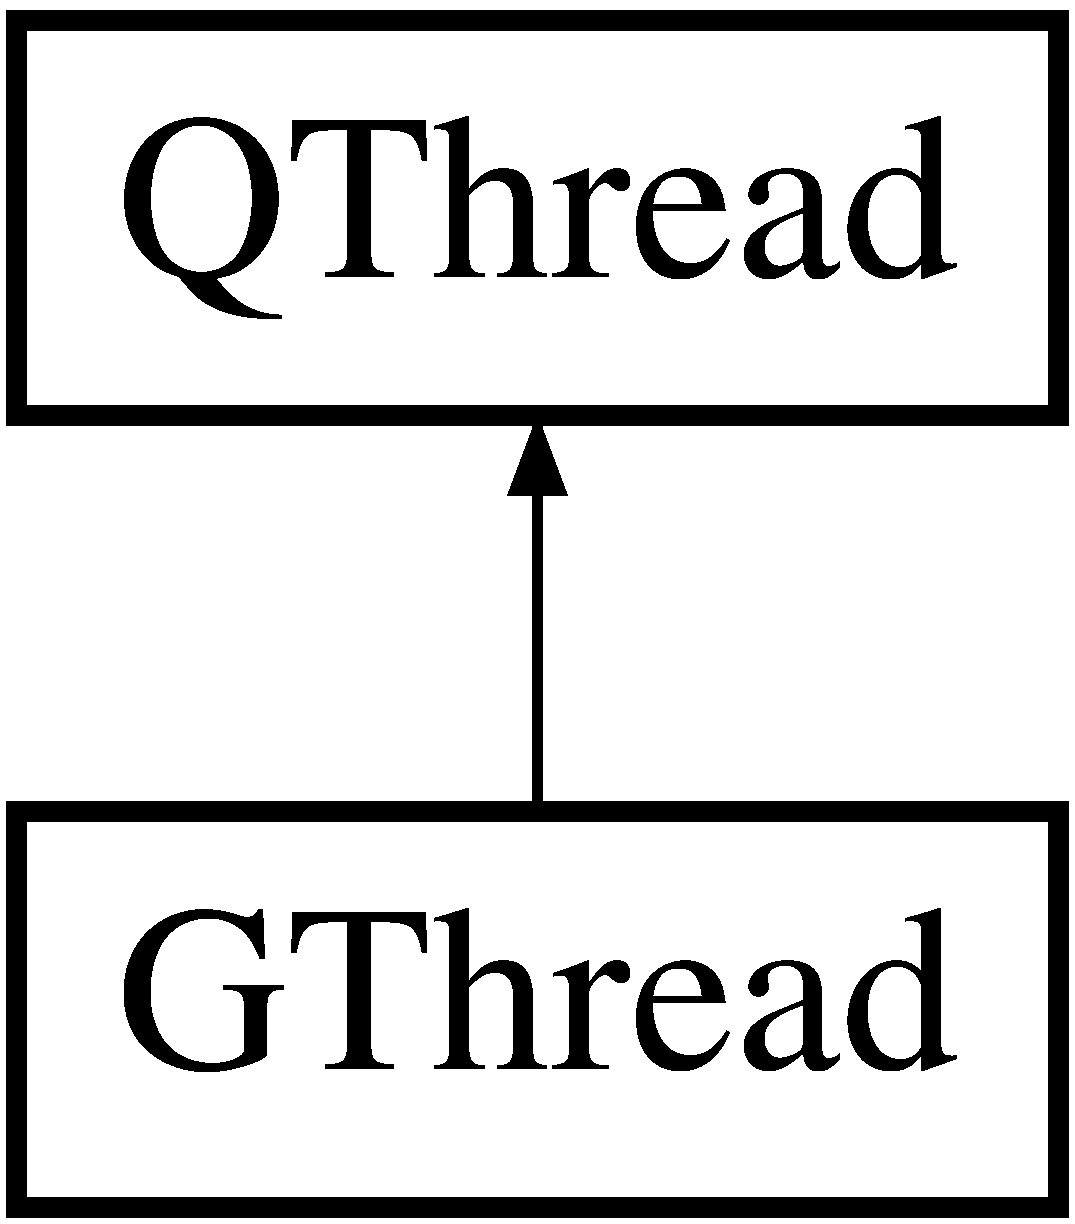
\includegraphics[height=2.000000cm]{classGThread}
\end{center}
\end{figure}
\subsection*{Static Public Member Functions}
\begin{DoxyCompactItemize}
\item 
static void \mbox{\hyperlink{classGThread_a27a1f5f9657637e4a4b6a7127ca9da33}{ensure\+That\+This\+Is\+The\+Qt\+Gui\+Thread}} (const std\+::string \&message=\char`\"{}\char`\"{})
\begin{DoxyCompactList}\small\item\em Generates an error if the caller is not running on the Qt G\+UI main thread. \end{DoxyCompactList}\item 
static Q\+Thread $\ast$ \mbox{\hyperlink{classGThread_a7bf03645e8eb0dd26b54b4e48b5206e1}{get\+Current\+Thread}} ()
\begin{DoxyCompactList}\small\item\em Returns the caller\textquotesingle{}s Qt thread object. \end{DoxyCompactList}\item 
static Q\+Thread $\ast$ \mbox{\hyperlink{classGThread_ad1309b5071a8c56775d3c82a6d8ccd4d}{get\+Qt\+Main\+Thread}} ()
\begin{DoxyCompactList}\small\item\em Returns the Qt thread object representing the main thread for the application, also referred to as the Qt G\+UI thread. \end{DoxyCompactList}\item 
static Q\+Thread $\ast$ \mbox{\hyperlink{classGThread_ad230888eab766cd189ab09365776c41e}{get\+Student\+Thread}} ()
\begin{DoxyCompactList}\small\item\em Returns the Qt thread object representing the thread on which the student\textquotesingle{}s main() function runs. \end{DoxyCompactList}\item 
static bool \mbox{\hyperlink{classGThread_a410c93ed2a5eb78ea24013ef35e49eed}{i\+Am\+Running\+On\+The\+Qt\+Gui\+Thread}} ()
\begin{DoxyCompactList}\small\item\em Returns true if the caller is running on the Qt G\+UI thread. \end{DoxyCompactList}\item 
static bool \mbox{\hyperlink{classGThread_a3e60d512067e765b4e2d7c0c5bec39fa}{i\+Am\+Running\+On\+The\+Student\+Thread}} ()
\begin{DoxyCompactList}\small\item\em Returns true if the caller is running on the student thread. \end{DoxyCompactList}\item 
static bool \mbox{\hyperlink{classGThread_afee663b5d7998135c2aab0585b2ad37f}{qt\+Gui\+Thread\+Exists}} ()
\begin{DoxyCompactList}\small\item\em Returns true if the Qt G\+UI thread has been created. \end{DoxyCompactList}\item 
static void \mbox{\hyperlink{classGThread_ac9475674a195d39d457307b3e7365ddd}{run\+In\+New\+Thread}} (G\+Thunk func)
\begin{DoxyCompactList}\small\item\em Runs the given void function in its own new thread, blocking the current thread to wait until it is done. \end{DoxyCompactList}\item 
static void \mbox{\hyperlink{classGThread_ad40c76521d01473a3eea90c01000d9e2}{run\+In\+New\+Thread\+Async}} (G\+Thunk func)
\begin{DoxyCompactList}\small\item\em Runs the given void function in its own new thread in the background; the current thread does not block and keeps going. \end{DoxyCompactList}\item 
static void \mbox{\hyperlink{classGThread_a33da0c87717269710ac7a564a1ebbe64}{run\+On\+Qt\+Gui\+Thread}} (G\+Thunk func)
\begin{DoxyCompactList}\small\item\em Runs the given void function on the Qt G\+UI thread, blocking the current thread to wait until it is done. \end{DoxyCompactList}\item 
static void \mbox{\hyperlink{classGThread_a4445680030c65d610b9e348d8d0cffc8}{run\+On\+Qt\+Gui\+Thread\+Async}} (G\+Thunk func)
\begin{DoxyCompactList}\small\item\em Runs the given void function on the Qt G\+UI thread in the background; the current thread does not block and keeps going. \end{DoxyCompactList}\item 
static void \mbox{\hyperlink{classGThread_aa3381590c1ef33c08000c2fbb2bf0dd0}{sleep}} (double ms)
\begin{DoxyCompactList}\small\item\em Causes the current thread to pause itself for the given number of milliseconds. \end{DoxyCompactList}\item 
static void \mbox{\hyperlink{classGThread_a58c8b2ad0ea491a6642e5e1cbd358c89}{yield}} ()
\begin{DoxyCompactList}\small\item\em Indicates that the current thread is willing to yield execution to any other threads that want to run. \end{DoxyCompactList}\end{DoxyCompactItemize}
\subsection*{Protected Member Functions}
\begin{DoxyCompactItemize}
\item 
\mbox{\hyperlink{classGThread_a7db4904140090c18f864e09283f2b529}{G\+Thread}} ()
\end{DoxyCompactItemize}
\subsection*{Static Protected Attributes}
\begin{DoxyCompactItemize}
\item 
static Q\+Thread $\ast$ \mbox{\hyperlink{classGThread_aa69140e62a4dad275e74a6c1174eb4e5}{\+\_\+qt\+Main\+Thread}} = nullptr
\item 
static Q\+Thread $\ast$ \mbox{\hyperlink{classGThread_a15ae7c95a54d17d2c307ebba42fe3405}{\+\_\+student\+Thread}} = nullptr
\end{DoxyCompactItemize}
\subsection*{Friends}
\begin{DoxyCompactItemize}
\item 
class \mbox{\hyperlink{classGThread_a78e6068a40352424a09cd3753706c619}{Qt\+Gui}}
\item 
void \mbox{\hyperlink{classGThread_a4f1fcd681e2cf92d1b04e5e8a33dbe47}{stanfordcpplib\+::initialize\+Library}} (int argc, char $\ast$$\ast$argv)
\end{DoxyCompactItemize}


\subsection{Detailed Description}
The \mbox{\hyperlink{classGThread}{G\+Thread}} class is a utility class containing static methods that allow you to run code on various system threads. 

The library has the following two standard threads running at all times\+:


\begin{DoxyEnumerate}
\item The Qt G\+UI thread, which runs Qt\textquotesingle{}s master exec() loop, handles all G\+UI object creation and events (this is technically the program\textquotesingle{}s main thread)


\item The student thread, which runs the student\textquotesingle{}s main() function and any sub-\/functions called by main

Students and clients normally do not need to worry about threading issues. These methods are called internally by many of the graphical interactors to make sure that all internal Qt G\+UI widgets are initialized on the Qt G\+UI thread. This is required for them to function properly.

If you want to run a piece of code in its own thread, use static methods {\ttfamily \mbox{\hyperlink{classGThread_ac9475674a195d39d457307b3e7365ddd}{G\+Thread\+::run\+In\+New\+Thread}}} and {\ttfamily \mbox{\hyperlink{classGThread_ad40c76521d01473a3eea90c01000d9e2}{G\+Thread\+::run\+In\+New\+Thread\+Async}}}. 
\end{DoxyEnumerate}

\subsection{Constructor \& Destructor Documentation}
\mbox{\Hypertarget{classGThread_a7db4904140090c18f864e09283f2b529}\label{classGThread_a7db4904140090c18f864e09283f2b529}} 
\index{G\+Thread@{G\+Thread}!G\+Thread@{G\+Thread}}
\index{G\+Thread@{G\+Thread}!G\+Thread@{G\+Thread}}
\subsubsection{\texorpdfstring{G\+Thread()}{GThread()}}
{\footnotesize\ttfamily \mbox{\hyperlink{classGThread}{G\+Thread}} (\begin{DoxyParamCaption}{ }\end{DoxyParamCaption})\hspace{0.3cm}{\ttfamily [protected]}}



\subsection{Member Function Documentation}
\mbox{\Hypertarget{classGThread_a27a1f5f9657637e4a4b6a7127ca9da33}\label{classGThread_a27a1f5f9657637e4a4b6a7127ca9da33}} 
\index{G\+Thread@{G\+Thread}!ensure\+That\+This\+Is\+The\+Qt\+Gui\+Thread@{ensure\+That\+This\+Is\+The\+Qt\+Gui\+Thread}}
\index{ensure\+That\+This\+Is\+The\+Qt\+Gui\+Thread@{ensure\+That\+This\+Is\+The\+Qt\+Gui\+Thread}!G\+Thread@{G\+Thread}}
\subsubsection{\texorpdfstring{ensure\+That\+This\+Is\+The\+Qt\+Gui\+Thread()}{ensureThatThisIsTheQtGuiThread()}}
{\footnotesize\ttfamily void ensure\+That\+This\+Is\+The\+Qt\+Gui\+Thread (\begin{DoxyParamCaption}\item[{const std\+::string \&}]{message = {\ttfamily \char`\"{}\char`\"{}} }\end{DoxyParamCaption})\hspace{0.3cm}{\ttfamily [static]}}



Generates an error if the caller is not running on the Qt G\+UI main thread. 

An optional error detail message can be passed. \mbox{\Hypertarget{classGThread_a7bf03645e8eb0dd26b54b4e48b5206e1}\label{classGThread_a7bf03645e8eb0dd26b54b4e48b5206e1}} 
\index{G\+Thread@{G\+Thread}!get\+Current\+Thread@{get\+Current\+Thread}}
\index{get\+Current\+Thread@{get\+Current\+Thread}!G\+Thread@{G\+Thread}}
\subsubsection{\texorpdfstring{get\+Current\+Thread()}{getCurrentThread()}}
{\footnotesize\ttfamily Q\+Thread $\ast$ get\+Current\+Thread (\begin{DoxyParamCaption}{ }\end{DoxyParamCaption})\hspace{0.3cm}{\ttfamily [static]}}



Returns the caller\textquotesingle{}s Qt thread object. 

\mbox{\Hypertarget{classGThread_ad1309b5071a8c56775d3c82a6d8ccd4d}\label{classGThread_ad1309b5071a8c56775d3c82a6d8ccd4d}} 
\index{G\+Thread@{G\+Thread}!get\+Qt\+Main\+Thread@{get\+Qt\+Main\+Thread}}
\index{get\+Qt\+Main\+Thread@{get\+Qt\+Main\+Thread}!G\+Thread@{G\+Thread}}
\subsubsection{\texorpdfstring{get\+Qt\+Main\+Thread()}{getQtMainThread()}}
{\footnotesize\ttfamily Q\+Thread $\ast$ get\+Qt\+Main\+Thread (\begin{DoxyParamCaption}{ }\end{DoxyParamCaption})\hspace{0.3cm}{\ttfamily [static]}}



Returns the Qt thread object representing the main thread for the application, also referred to as the Qt G\+UI thread. 

\mbox{\Hypertarget{classGThread_ad230888eab766cd189ab09365776c41e}\label{classGThread_ad230888eab766cd189ab09365776c41e}} 
\index{G\+Thread@{G\+Thread}!get\+Student\+Thread@{get\+Student\+Thread}}
\index{get\+Student\+Thread@{get\+Student\+Thread}!G\+Thread@{G\+Thread}}
\subsubsection{\texorpdfstring{get\+Student\+Thread()}{getStudentThread()}}
{\footnotesize\ttfamily Q\+Thread $\ast$ get\+Student\+Thread (\begin{DoxyParamCaption}{ }\end{DoxyParamCaption})\hspace{0.3cm}{\ttfamily [static]}}



Returns the Qt thread object representing the thread on which the student\textquotesingle{}s main() function runs. 

\mbox{\Hypertarget{classGThread_a410c93ed2a5eb78ea24013ef35e49eed}\label{classGThread_a410c93ed2a5eb78ea24013ef35e49eed}} 
\index{G\+Thread@{G\+Thread}!i\+Am\+Running\+On\+The\+Qt\+Gui\+Thread@{i\+Am\+Running\+On\+The\+Qt\+Gui\+Thread}}
\index{i\+Am\+Running\+On\+The\+Qt\+Gui\+Thread@{i\+Am\+Running\+On\+The\+Qt\+Gui\+Thread}!G\+Thread@{G\+Thread}}
\subsubsection{\texorpdfstring{i\+Am\+Running\+On\+The\+Qt\+Gui\+Thread()}{iAmRunningOnTheQtGuiThread()}}
{\footnotesize\ttfamily bool i\+Am\+Running\+On\+The\+Qt\+Gui\+Thread (\begin{DoxyParamCaption}{ }\end{DoxyParamCaption})\hspace{0.3cm}{\ttfamily [static]}}



Returns true if the caller is running on the Qt G\+UI thread. 

\mbox{\Hypertarget{classGThread_a3e60d512067e765b4e2d7c0c5bec39fa}\label{classGThread_a3e60d512067e765b4e2d7c0c5bec39fa}} 
\index{G\+Thread@{G\+Thread}!i\+Am\+Running\+On\+The\+Student\+Thread@{i\+Am\+Running\+On\+The\+Student\+Thread}}
\index{i\+Am\+Running\+On\+The\+Student\+Thread@{i\+Am\+Running\+On\+The\+Student\+Thread}!G\+Thread@{G\+Thread}}
\subsubsection{\texorpdfstring{i\+Am\+Running\+On\+The\+Student\+Thread()}{iAmRunningOnTheStudentThread()}}
{\footnotesize\ttfamily bool i\+Am\+Running\+On\+The\+Student\+Thread (\begin{DoxyParamCaption}{ }\end{DoxyParamCaption})\hspace{0.3cm}{\ttfamily [static]}}



Returns true if the caller is running on the student thread. 

\mbox{\Hypertarget{classGThread_afee663b5d7998135c2aab0585b2ad37f}\label{classGThread_afee663b5d7998135c2aab0585b2ad37f}} 
\index{G\+Thread@{G\+Thread}!qt\+Gui\+Thread\+Exists@{qt\+Gui\+Thread\+Exists}}
\index{qt\+Gui\+Thread\+Exists@{qt\+Gui\+Thread\+Exists}!G\+Thread@{G\+Thread}}
\subsubsection{\texorpdfstring{qt\+Gui\+Thread\+Exists()}{qtGuiThreadExists()}}
{\footnotesize\ttfamily bool qt\+Gui\+Thread\+Exists (\begin{DoxyParamCaption}{ }\end{DoxyParamCaption})\hspace{0.3cm}{\ttfamily [static]}}



Returns true if the Qt G\+UI thread has been created. 

This will happen right before the student\textquotesingle{}s main() function runs. \mbox{\Hypertarget{classGThread_ac9475674a195d39d457307b3e7365ddd}\label{classGThread_ac9475674a195d39d457307b3e7365ddd}} 
\index{G\+Thread@{G\+Thread}!run\+In\+New\+Thread@{run\+In\+New\+Thread}}
\index{run\+In\+New\+Thread@{run\+In\+New\+Thread}!G\+Thread@{G\+Thread}}
\subsubsection{\texorpdfstring{run\+In\+New\+Thread()}{runInNewThread()}}
{\footnotesize\ttfamily void run\+In\+New\+Thread (\begin{DoxyParamCaption}\item[{G\+Thunk}]{func }\end{DoxyParamCaption})\hspace{0.3cm}{\ttfamily [static]}}



Runs the given void function in its own new thread, blocking the current thread to wait until it is done. 

Any uncaught exceptions or errors in the new thread will crash the program and cannot be caught by the calling thread.

If you want the new thread to run in the background, use the {\ttfamily run\+In\+New\+Thread\+Async} function instead. \mbox{\Hypertarget{classGThread_ad40c76521d01473a3eea90c01000d9e2}\label{classGThread_ad40c76521d01473a3eea90c01000d9e2}} 
\index{G\+Thread@{G\+Thread}!run\+In\+New\+Thread\+Async@{run\+In\+New\+Thread\+Async}}
\index{run\+In\+New\+Thread\+Async@{run\+In\+New\+Thread\+Async}!G\+Thread@{G\+Thread}}
\subsubsection{\texorpdfstring{run\+In\+New\+Thread\+Async()}{runInNewThreadAsync()}}
{\footnotesize\ttfamily void run\+In\+New\+Thread\+Async (\begin{DoxyParamCaption}\item[{G\+Thunk}]{func }\end{DoxyParamCaption})\hspace{0.3cm}{\ttfamily [static]}}



Runs the given void function in its own new thread in the background; the current thread does not block and keeps going. 

Any uncaught exceptions or errors in the new thread will crash the program and cannot be caught by the calling thread.

If you want the caller to wait for the new thread to finish running, use the {\ttfamily run\+In\+New\+Thread} function instead. \mbox{\Hypertarget{classGThread_a33da0c87717269710ac7a564a1ebbe64}\label{classGThread_a33da0c87717269710ac7a564a1ebbe64}} 
\index{G\+Thread@{G\+Thread}!run\+On\+Qt\+Gui\+Thread@{run\+On\+Qt\+Gui\+Thread}}
\index{run\+On\+Qt\+Gui\+Thread@{run\+On\+Qt\+Gui\+Thread}!G\+Thread@{G\+Thread}}
\subsubsection{\texorpdfstring{run\+On\+Qt\+Gui\+Thread()}{runOnQtGuiThread()}}
{\footnotesize\ttfamily void run\+On\+Qt\+Gui\+Thread (\begin{DoxyParamCaption}\item[{G\+Thunk}]{func }\end{DoxyParamCaption})\hspace{0.3cm}{\ttfamily [static]}}



Runs the given void function on the Qt G\+UI thread, blocking the current thread to wait until it is done. 

This function is called heavily by the internal G\+UI widgets and interactors of the library, because all Qt G\+UI operations are required to be done on the application\textquotesingle{}s main thread.

Any uncaught exceptions or errors in the Qt G\+UI thread will crash the program and cannot be caught by the calling thread.

If you want the new thread to run in the background, use the {\ttfamily run\+On\+Qt\+Gui\+Thread\+Async} function instead. \mbox{\Hypertarget{classGThread_a4445680030c65d610b9e348d8d0cffc8}\label{classGThread_a4445680030c65d610b9e348d8d0cffc8}} 
\index{G\+Thread@{G\+Thread}!run\+On\+Qt\+Gui\+Thread\+Async@{run\+On\+Qt\+Gui\+Thread\+Async}}
\index{run\+On\+Qt\+Gui\+Thread\+Async@{run\+On\+Qt\+Gui\+Thread\+Async}!G\+Thread@{G\+Thread}}
\subsubsection{\texorpdfstring{run\+On\+Qt\+Gui\+Thread\+Async()}{runOnQtGuiThreadAsync()}}
{\footnotesize\ttfamily void run\+On\+Qt\+Gui\+Thread\+Async (\begin{DoxyParamCaption}\item[{G\+Thunk}]{func }\end{DoxyParamCaption})\hspace{0.3cm}{\ttfamily [static]}}



Runs the given void function on the Qt G\+UI thread in the background; the current thread does not block and keeps going. 

Any uncaught exceptions or errors in the Qt G\+UI thread will crash the program and cannot be caught by the calling thread.

If you want the caller to wait for the Qt G\+UI thread code to finish running, use the {\ttfamily run\+On\+Qt\+Gui\+Thread} function instead. \mbox{\Hypertarget{classGThread_aa3381590c1ef33c08000c2fbb2bf0dd0}\label{classGThread_aa3381590c1ef33c08000c2fbb2bf0dd0}} 
\index{G\+Thread@{G\+Thread}!sleep@{sleep}}
\index{sleep@{sleep}!G\+Thread@{G\+Thread}}
\subsubsection{\texorpdfstring{sleep()}{sleep()}}
{\footnotesize\ttfamily void sleep (\begin{DoxyParamCaption}\item[{double}]{ms }\end{DoxyParamCaption})\hspace{0.3cm}{\ttfamily [static]}}



Causes the current thread to pause itself for the given number of milliseconds. 


\begin{DoxyExceptions}{Exceptions}
{\em \mbox{\hyperlink{classErrorException}{Error\+Exception}}} & if ms is negative \\
\hline
\end{DoxyExceptions}
\mbox{\Hypertarget{classGThread_a58c8b2ad0ea491a6642e5e1cbd358c89}\label{classGThread_a58c8b2ad0ea491a6642e5e1cbd358c89}} 
\index{G\+Thread@{G\+Thread}!yield@{yield}}
\index{yield@{yield}!G\+Thread@{G\+Thread}}
\subsubsection{\texorpdfstring{yield()}{yield()}}
{\footnotesize\ttfamily void yield (\begin{DoxyParamCaption}{ }\end{DoxyParamCaption})\hspace{0.3cm}{\ttfamily [static]}}



Indicates that the current thread is willing to yield execution to any other threads that want to run. 

This differs slightly from \mbox{\hyperlink{classGThread_aa3381590c1ef33c08000c2fbb2bf0dd0}{sleep()}} in that \mbox{\hyperlink{classGThread_aa3381590c1ef33c08000c2fbb2bf0dd0}{sleep()}} mandates to pause the current thread for a given amount of time, while \mbox{\hyperlink{classGThread_a58c8b2ad0ea491a6642e5e1cbd358c89}{yield()}} is more of an offer to other threads that they may run now if they so choose. 

\subsection{Friends And Related Function Documentation}
\mbox{\Hypertarget{classGThread_a78e6068a40352424a09cd3753706c619}\label{classGThread_a78e6068a40352424a09cd3753706c619}} 
\index{G\+Thread@{G\+Thread}!Qt\+Gui@{Qt\+Gui}}
\index{Qt\+Gui@{Qt\+Gui}!G\+Thread@{G\+Thread}}
\subsubsection{\texorpdfstring{Qt\+Gui}{QtGui}}
{\footnotesize\ttfamily friend class Qt\+Gui\hspace{0.3cm}{\ttfamily [friend]}}

\mbox{\Hypertarget{classGThread_a4f1fcd681e2cf92d1b04e5e8a33dbe47}\label{classGThread_a4f1fcd681e2cf92d1b04e5e8a33dbe47}} 
\index{G\+Thread@{G\+Thread}!stanfordcpplib\+::initialize\+Library@{stanfordcpplib\+::initialize\+Library}}
\index{stanfordcpplib\+::initialize\+Library@{stanfordcpplib\+::initialize\+Library}!G\+Thread@{G\+Thread}}
\subsubsection{\texorpdfstring{stanfordcpplib\+::initialize\+Library}{stanfordcpplib::initializeLibrary}}
{\footnotesize\ttfamily void \mbox{\hyperlink{namespacestanfordcpplib_ab36f2e19ed11765f2b025cc8e4636010}{stanfordcpplib\+::initialize\+Library}} (\begin{DoxyParamCaption}\item[{int}]{argc,  }\item[{char $\ast$$\ast$}]{argv }\end{DoxyParamCaption})\hspace{0.3cm}{\ttfamily [friend]}}



\subsection{Member Data Documentation}
\mbox{\Hypertarget{classGThread_aa69140e62a4dad275e74a6c1174eb4e5}\label{classGThread_aa69140e62a4dad275e74a6c1174eb4e5}} 
\index{G\+Thread@{G\+Thread}!\+\_\+qt\+Main\+Thread@{\+\_\+qt\+Main\+Thread}}
\index{\+\_\+qt\+Main\+Thread@{\+\_\+qt\+Main\+Thread}!G\+Thread@{G\+Thread}}
\subsubsection{\texorpdfstring{\+\_\+qt\+Main\+Thread}{\_qtMainThread}}
{\footnotesize\ttfamily Q\+Thread $\ast$ \+\_\+qt\+Main\+Thread = nullptr\hspace{0.3cm}{\ttfamily [static]}, {\ttfamily [protected]}}

\mbox{\Hypertarget{classGThread_a15ae7c95a54d17d2c307ebba42fe3405}\label{classGThread_a15ae7c95a54d17d2c307ebba42fe3405}} 
\index{G\+Thread@{G\+Thread}!\+\_\+student\+Thread@{\+\_\+student\+Thread}}
\index{\+\_\+student\+Thread@{\+\_\+student\+Thread}!G\+Thread@{G\+Thread}}
\subsubsection{\texorpdfstring{\+\_\+student\+Thread}{\_studentThread}}
{\footnotesize\ttfamily Q\+Thread $\ast$ \+\_\+student\+Thread = nullptr\hspace{0.3cm}{\ttfamily [static]}, {\ttfamily [protected]}}


\hypertarget{classGTimer}{}\section{G\+Timer Class Reference}
\label{classGTimer}\index{G\+Timer@{G\+Timer}}


This class implements a simple interval timer that generates a {\ttfamily G\+Timer\+Event} with a specified frequency.  




{\ttfamily \#include $<$gtimer.\+h$>$}

\subsection*{Public Member Functions}
\begin{DoxyCompactItemize}
\item 
\mbox{\hyperlink{classGTimer_ab947e096ce76b63f283502e4b4446810}{G\+Timer}} (double milliseconds)
\begin{DoxyCompactList}\small\item\em Creates a timer object that generates a {\ttfamily G\+Timer\+Event} each time the specified number of milliseconds has elapsed. \end{DoxyCompactList}\item 
\mbox{\hyperlink{classGTimer_a2f693771957cae3efd9bfc952c543961}{$\sim$\+G\+Timer}} ()
\begin{DoxyCompactList}\small\item\em Destroys the timer, stopping it if it\textquotesingle{}s currently running. \end{DoxyCompactList}\item 
double \mbox{\hyperlink{classGTimer_a73d6fbcedb3f4c8379a76161503dc8f8}{get\+Delay}} () const
\begin{DoxyCompactList}\small\item\em Returns the delay in milliseconds between each tick of this timer. \end{DoxyCompactList}\item 
bool \mbox{\hyperlink{classGTimer_ac1991ea0e286fbb461b60c8c9299d781}{is\+Started}} () const
\begin{DoxyCompactList}\small\item\em Method\+: is\+Started Usage\+: if (timer.\+is\+Started()) \{ ... \end{DoxyCompactList}\item 
void \mbox{\hyperlink{classGTimer_a22ee094ca3f45aa4156b97d34fe678bf}{restart}} ()
\begin{DoxyCompactList}\small\item\em Stops the timer (if it was started) and then starts it again. \end{DoxyCompactList}\item 
void \mbox{\hyperlink{classGTimer_acebfcbc48c6acd460dac117a8f71a92f}{set\+Delay}} (double ms)
\begin{DoxyCompactList}\small\item\em Changes the delay in milliseconds between each tick of this timer. \end{DoxyCompactList}\item 
void \mbox{\hyperlink{classGTimer_a60de64d75454385b23995437f1d72669}{start}} ()
\begin{DoxyCompactList}\small\item\em Starts the timer. \end{DoxyCompactList}\item 
void \mbox{\hyperlink{classGTimer_a8c528baf37154d347366083f0f816846}{stop}} ()
\begin{DoxyCompactList}\small\item\em Stops the timer so that it stops generating events until it is restarted. \end{DoxyCompactList}\end{DoxyCompactItemize}


\subsection{Detailed Description}
This class implements a simple interval timer that generates a {\ttfamily G\+Timer\+Event} with a specified frequency. 

\subsection{Constructor \& Destructor Documentation}
\mbox{\Hypertarget{classGTimer_ab947e096ce76b63f283502e4b4446810}\label{classGTimer_ab947e096ce76b63f283502e4b4446810}} 
\index{G\+Timer@{G\+Timer}!G\+Timer@{G\+Timer}}
\index{G\+Timer@{G\+Timer}!G\+Timer@{G\+Timer}}
\subsubsection{\texorpdfstring{G\+Timer()}{GTimer()}}
{\footnotesize\ttfamily \mbox{\hyperlink{classGTimer}{G\+Timer}} (\begin{DoxyParamCaption}\item[{double}]{milliseconds }\end{DoxyParamCaption})}



Creates a timer object that generates a {\ttfamily G\+Timer\+Event} each time the specified number of milliseconds has elapsed. 

No events are generated until the client calls {\ttfamily start} on the timer.

Due to implementation details, you must create at least one \mbox{\hyperlink{classGWindow}{G\+Window}} before you can \mbox{\hyperlink{classGTimer_a60de64d75454385b23995437f1d72669}{start()}} a \mbox{\hyperlink{classGTimer}{G\+Timer}} object.


\begin{DoxyExceptions}{Exceptions}
{\em \mbox{\hyperlink{classErrorException}{Error\+Exception}}} & if milliseconds is negative \\
\hline
\end{DoxyExceptions}
\mbox{\Hypertarget{classGTimer_a2f693771957cae3efd9bfc952c543961}\label{classGTimer_a2f693771957cae3efd9bfc952c543961}} 
\index{G\+Timer@{G\+Timer}!````~G\+Timer@{$\sim$\+G\+Timer}}
\index{````~G\+Timer@{$\sim$\+G\+Timer}!G\+Timer@{G\+Timer}}
\subsubsection{\texorpdfstring{$\sim$\+G\+Timer()}{~GTimer()}}
{\footnotesize\ttfamily $\sim$\mbox{\hyperlink{classGTimer}{G\+Timer}} (\begin{DoxyParamCaption}{ }\end{DoxyParamCaption})}



Destroys the timer, stopping it if it\textquotesingle{}s currently running. 



\subsection{Member Function Documentation}
\mbox{\Hypertarget{classGTimer_a73d6fbcedb3f4c8379a76161503dc8f8}\label{classGTimer_a73d6fbcedb3f4c8379a76161503dc8f8}} 
\index{G\+Timer@{G\+Timer}!get\+Delay@{get\+Delay}}
\index{get\+Delay@{get\+Delay}!G\+Timer@{G\+Timer}}
\subsubsection{\texorpdfstring{get\+Delay()}{getDelay()}}
{\footnotesize\ttfamily double get\+Delay (\begin{DoxyParamCaption}{ }\end{DoxyParamCaption}) const}



Returns the delay in milliseconds between each tick of this timer. 

\mbox{\Hypertarget{classGTimer_ac1991ea0e286fbb461b60c8c9299d781}\label{classGTimer_ac1991ea0e286fbb461b60c8c9299d781}} 
\index{G\+Timer@{G\+Timer}!is\+Started@{is\+Started}}
\index{is\+Started@{is\+Started}!G\+Timer@{G\+Timer}}
\subsubsection{\texorpdfstring{is\+Started()}{isStarted()}}
{\footnotesize\ttfamily bool is\+Started (\begin{DoxyParamCaption}{ }\end{DoxyParamCaption}) const}



Method\+: is\+Started Usage\+: if (timer.\+is\+Started()) \{ ... 

\subsubsection*{\} }

Returns true if the given timer has been started (via \mbox{\hyperlink{classGTimer_a60de64d75454385b23995437f1d72669}{start()}}). If you stop the timer or have not started it yet, this method will return false. \mbox{\Hypertarget{classGTimer_a22ee094ca3f45aa4156b97d34fe678bf}\label{classGTimer_a22ee094ca3f45aa4156b97d34fe678bf}} 
\index{G\+Timer@{G\+Timer}!restart@{restart}}
\index{restart@{restart}!G\+Timer@{G\+Timer}}
\subsubsection{\texorpdfstring{restart()}{restart()}}
{\footnotesize\ttfamily void restart (\begin{DoxyParamCaption}{ }\end{DoxyParamCaption})}



Stops the timer (if it was started) and then starts it again. 

\mbox{\Hypertarget{classGTimer_acebfcbc48c6acd460dac117a8f71a92f}\label{classGTimer_acebfcbc48c6acd460dac117a8f71a92f}} 
\index{G\+Timer@{G\+Timer}!set\+Delay@{set\+Delay}}
\index{set\+Delay@{set\+Delay}!G\+Timer@{G\+Timer}}
\subsubsection{\texorpdfstring{set\+Delay()}{setDelay()}}
{\footnotesize\ttfamily void set\+Delay (\begin{DoxyParamCaption}\item[{double}]{ms }\end{DoxyParamCaption})}



Changes the delay in milliseconds between each tick of this timer. 

If the timer is currently running, calling this method will stop and restart the timer with the new delay.


\begin{DoxyExceptions}{Exceptions}
{\em \mbox{\hyperlink{classErrorException}{Error\+Exception}}} & if milliseconds is negative \\
\hline
\end{DoxyExceptions}
\mbox{\Hypertarget{classGTimer_a60de64d75454385b23995437f1d72669}\label{classGTimer_a60de64d75454385b23995437f1d72669}} 
\index{G\+Timer@{G\+Timer}!start@{start}}
\index{start@{start}!G\+Timer@{G\+Timer}}
\subsubsection{\texorpdfstring{start()}{start()}}
{\footnotesize\ttfamily void start (\begin{DoxyParamCaption}{ }\end{DoxyParamCaption})}



Starts the timer. 

A timer continues to generate timer events until it is stopped; to achieve the effect of a one-\/shot timer, the simplest approach is to call the {\ttfamily stop} method inside the event handler. \mbox{\Hypertarget{classGTimer_a8c528baf37154d347366083f0f816846}\label{classGTimer_a8c528baf37154d347366083f0f816846}} 
\index{G\+Timer@{G\+Timer}!stop@{stop}}
\index{stop@{stop}!G\+Timer@{G\+Timer}}
\subsubsection{\texorpdfstring{stop()}{stop()}}
{\footnotesize\ttfamily void stop (\begin{DoxyParamCaption}{ }\end{DoxyParamCaption})}



Stops the timer so that it stops generating events until it is restarted. 


\hypertarget{classGWindow}{}\section{G\+Window Class Reference}
\label{classGWindow}\index{G\+Window@{G\+Window}}


This class represents a graphics window that supports simple graphics.  




{\ttfamily \#include $<$gwindow.\+h$>$}

Inheritance diagram for G\+Window\+:\begin{figure}[H]
\begin{center}
\leavevmode
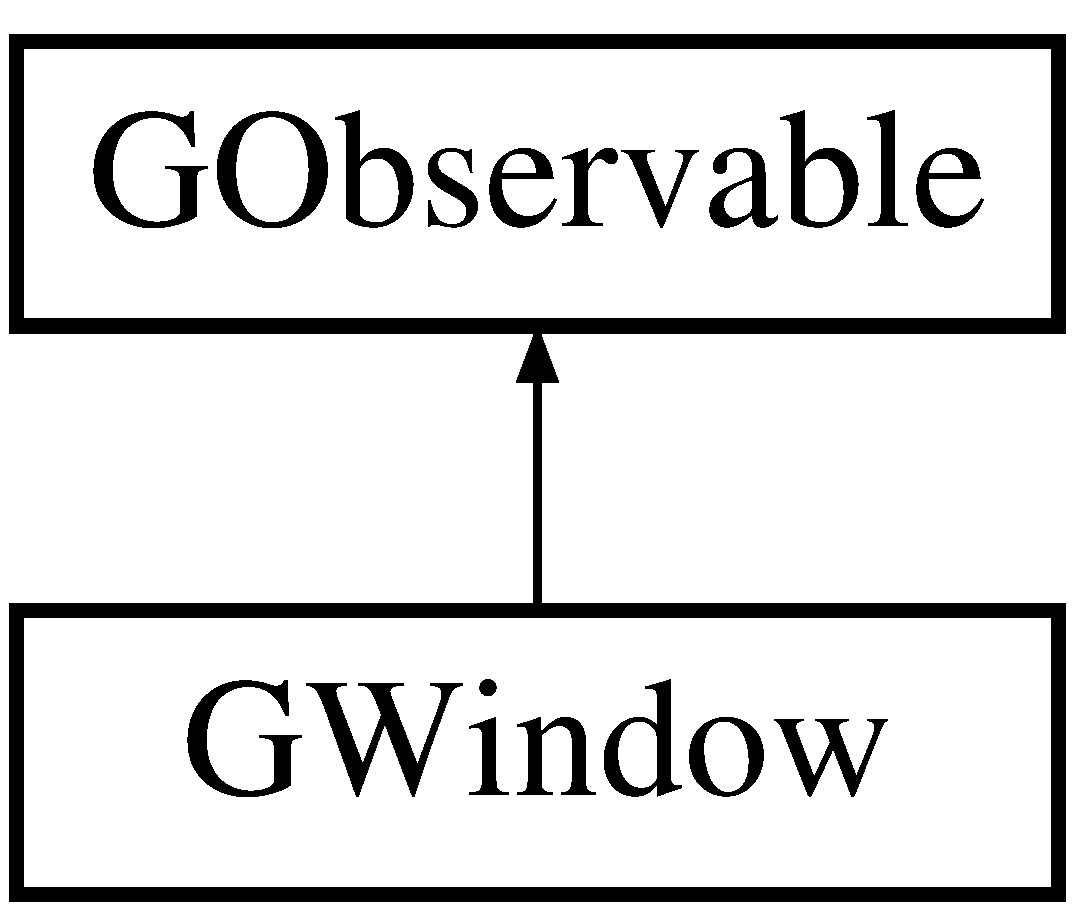
\includegraphics[height=2.000000cm]{classGWindow}
\end{center}
\end{figure}
\subsection*{Public Types}
\begin{DoxyCompactItemize}
\item 
enum \mbox{\hyperlink{classGWindow_a84803201f0f9569db61f51cac9e0d2d2}{Close\+Operation}} \{ \mbox{\hyperlink{classGWindow_a84803201f0f9569db61f51cac9e0d2d2aa00045aa0b706ef54f34c37f2d49f2b5}{C\+L\+O\+S\+E\+\_\+\+D\+O\+\_\+\+N\+O\+T\+H\+I\+NG}}, 
\mbox{\hyperlink{classGWindow_a84803201f0f9569db61f51cac9e0d2d2a47d285d1f0c66414bb23b7f3f3c6554b}{C\+L\+O\+S\+E\+\_\+\+H\+I\+DE}}, 
\mbox{\hyperlink{classGWindow_a84803201f0f9569db61f51cac9e0d2d2a1b8c84e0e965a877f9253f15747304f1}{C\+L\+O\+S\+E\+\_\+\+D\+I\+S\+P\+O\+SE}}, 
\mbox{\hyperlink{classGWindow_a84803201f0f9569db61f51cac9e0d2d2a74cdc7c2dc555e3334f91d8ce3e00f79}{C\+L\+O\+S\+E\+\_\+\+E\+X\+IT}}
 \}
\begin{DoxyCompactList}\small\item\em The various actions that can occur when a window closes. \end{DoxyCompactList}\item 
enum \mbox{\hyperlink{classGWindow_a81a01a86de31071a92e6cce0bab9bc4b}{Region}} \{ \mbox{\hyperlink{classGWindow_a81a01a86de31071a92e6cce0bab9bc4ba5ba85a564dbf472d69f92d5a2870db16}{R\+E\+G\+I\+O\+N\+\_\+\+C\+E\+N\+T\+ER}} = G\+Container\+:\+:R\+E\+G\+I\+O\+N\+\_\+\+C\+E\+N\+T\+ER, 
\mbox{\hyperlink{classGWindow_a81a01a86de31071a92e6cce0bab9bc4baac78951bd4e01d20f4825d5ae0a54357}{R\+E\+G\+I\+O\+N\+\_\+\+E\+A\+ST}} = G\+Container\+:\+:R\+E\+G\+I\+O\+N\+\_\+\+E\+A\+ST, 
\mbox{\hyperlink{classGWindow_a81a01a86de31071a92e6cce0bab9bc4baf40d135fb811ad59acb102f1fb357550}{R\+E\+G\+I\+O\+N\+\_\+\+N\+O\+R\+TH}} = G\+Container\+:\+:R\+E\+G\+I\+O\+N\+\_\+\+N\+O\+R\+TH, 
\mbox{\hyperlink{classGWindow_a81a01a86de31071a92e6cce0bab9bc4bab533512ba438173a4ceb9c501eb17628}{R\+E\+G\+I\+O\+N\+\_\+\+S\+O\+U\+TH}} = G\+Container\+:\+:R\+E\+G\+I\+O\+N\+\_\+\+S\+O\+U\+TH, 
\mbox{\hyperlink{classGWindow_a81a01a86de31071a92e6cce0bab9bc4ba5dd8c2219af001263c00de02b642786d}{R\+E\+G\+I\+O\+N\+\_\+\+W\+E\+ST}} = G\+Container\+:\+:R\+E\+G\+I\+O\+N\+\_\+\+W\+E\+ST
 \}
\begin{DoxyCompactList}\small\item\em The five regions of window border layouts. \end{DoxyCompactList}\end{DoxyCompactItemize}
\subsection*{Public Member Functions}
\begin{DoxyCompactItemize}
\item 
\mbox{\hyperlink{classGWindow_a7fdeab875fb526a49423085ac13ac9f2}{G\+Window}} (bool visible=true)
\begin{DoxyCompactList}\small\item\em Creates a new window of a default width and height. \end{DoxyCompactList}\item 
\mbox{\hyperlink{classGWindow_acb88532777f61b140aa8245ed1d9887e}{G\+Window}} (double width, double height, bool visible=true)
\begin{DoxyCompactList}\small\item\em Creates a new window of the given width and height. \end{DoxyCompactList}\item 
\mbox{\hyperlink{classGWindow_ac66942f456baa6c43ecd0ed60138fe36}{G\+Window}} (double x, double y, double width, double height, bool visible=true)
\begin{DoxyCompactList}\small\item\em Creates a new window of the given location and size. \end{DoxyCompactList}\item 
virtual \mbox{\hyperlink{classGWindow_a4e024d2943027c4d4213a36fef7cfb23}{$\sim$\+G\+Window}} () Q\+\_\+\+D\+E\+C\+L\+\_\+\+O\+V\+E\+R\+R\+I\+DE
\begin{DoxyCompactList}\small\item\em Frees memory allocated internally by the window. \end{DoxyCompactList}\item 
virtual void \mbox{\hyperlink{classGWindow_a458811bab688db3875a6806b3ba4d938}{\+\_\+autograder\+\_\+set\+Is\+Autograder\+Window}} (bool is\+Autograder\+Window)
\begin{DoxyCompactList}\small\item\em An internal function that sets whether the current window is part of an autograder program. \end{DoxyCompactList}\item 
virtual void \mbox{\hyperlink{classGWindow_a6f99b7c841256dbdc5acaafbbca4e685}{add}} (\mbox{\hyperlink{classGInteractor}{G\+Interactor}} $\ast$interactor)
\begin{DoxyCompactList}\small\item\em Adds the given interactor to the center region of the window. \end{DoxyCompactList}\item 
virtual void \mbox{\hyperlink{classGWindow_aca25fb0fc7d200e9c4fd23830d2d413d}{add}} (\mbox{\hyperlink{classGInteractor}{G\+Interactor}} $\ast$interactor, double x, double y)
\begin{DoxyCompactList}\small\item\em Adds the given interactor to the center region of the window and moves it to the given x/y location. \end{DoxyCompactList}\item 
virtual void \mbox{\hyperlink{classGWindow_a33b08fe5428ed634a658deab076099f7}{add}} (\mbox{\hyperlink{classGInteractor}{G\+Interactor}} \&interactor)
\begin{DoxyCompactList}\small\item\em Adds the given interactor to the center region of the window. \end{DoxyCompactList}\item 
virtual void \mbox{\hyperlink{classGWindow_a56840f453f9938083c24c7fb1a4c377e}{add}} (\mbox{\hyperlink{classGInteractor}{G\+Interactor}} \&interactor, double x, double y)
\begin{DoxyCompactList}\small\item\em Adds the given interactor to the center region of the window and moves it to the given x/y location. \end{DoxyCompactList}\item 
virtual void \mbox{\hyperlink{classGWindow_a2327d64402837eedd533c098014e46d9}{add}} (\mbox{\hyperlink{classGObject}{G\+Object}} $\ast$obj)
\begin{DoxyCompactList}\small\item\em Adds the given graphical object to the window\textquotesingle{}s canvas. \end{DoxyCompactList}\item 
virtual void \mbox{\hyperlink{classGWindow_ab5388ece7a50b46e0ee72e11fe202609}{add}} (\mbox{\hyperlink{classGObject}{G\+Object}} $\ast$obj, double x, double y)
\begin{DoxyCompactList}\small\item\em Adds the given graphical object to the window\textquotesingle{}s canvas and moves it to the given x/y location. \end{DoxyCompactList}\item 
virtual void \mbox{\hyperlink{classGWindow_a7f596867e2d8f9dfb816b3d496ea074f}{add}} (\mbox{\hyperlink{classGObject}{G\+Object}} \&obj)
\begin{DoxyCompactList}\small\item\em Adds the given graphical object to the window\textquotesingle{}s canvas. \end{DoxyCompactList}\item 
virtual void \mbox{\hyperlink{classGWindow_ac302bb932e3905e5d368ce735ad8444c}{add}} (\mbox{\hyperlink{classGObject}{G\+Object}} \&obj, double x, double y)
\begin{DoxyCompactList}\small\item\em Adds the given graphical object to the window\textquotesingle{}s canvas and moves it to the given x/y location. \end{DoxyCompactList}\item 
virtual Q\+Menu $\ast$ \mbox{\hyperlink{classGWindow_afffea482963d5566e97ccccb1f94a4e2}{add\+Menu}} (const std\+::string \&text)
\begin{DoxyCompactList}\small\item\em Adds a menu with the given text to the window\textquotesingle{}s top menu bar. \end{DoxyCompactList}\item 
virtual Q\+Action $\ast$ \mbox{\hyperlink{classGWindow_a43efd24277d68e749443cb7c36b65f4b}{add\+Menu\+Item}} (const std\+::string \&menu, const std\+::string \&item, const std\+::string \&icon=\char`\"{}\char`\"{})
\begin{DoxyCompactList}\small\item\em Adds a new menu item to the given menu. \end{DoxyCompactList}\item 
virtual Q\+Action $\ast$ \mbox{\hyperlink{classGWindow_ad57e2955efbfb5a0cccc981332945c8e}{add\+Menu\+Item}} (const std\+::string \&menu, const std\+::string \&item, const std\+::string \&icon, G\+Event\+Listener\+Void func)
\begin{DoxyCompactList}\small\item\em Adds a new menu item to the given menu. \end{DoxyCompactList}\item 
virtual Q\+Action $\ast$ \mbox{\hyperlink{classGWindow_ae363de5d4c0d5848a5936563b12c3288}{add\+Menu\+Item\+Check\+Box}} (const std\+::string \&menu, const std\+::string \&item, bool checked=false, const std\+::string \&icon=\char`\"{}\char`\"{})
\begin{DoxyCompactList}\small\item\em Adds a new checkbox menu item to the given menu. \end{DoxyCompactList}\item 
virtual Q\+Action $\ast$ \mbox{\hyperlink{classGWindow_aab18d66dc7ed71468da3611b28450995}{add\+Menu\+Item\+Check\+Box}} (const std\+::string \&menu, const std\+::string \&item, bool checked, const std\+::string \&icon, G\+Event\+Listener\+Void func)
\begin{DoxyCompactList}\small\item\em Adds a new checkbox menu item to the given menu. \end{DoxyCompactList}\item 
virtual Q\+Action $\ast$ \mbox{\hyperlink{classGWindow_abdf4f167a7135e31ecb8f3363fddfd19}{add\+Menu\+Separator}} (const std\+::string \&menu)
\begin{DoxyCompactList}\small\item\em Adds a horizontal line separator to the end of the given menu. \end{DoxyCompactList}\item 
virtual Q\+Menu $\ast$ \mbox{\hyperlink{classGWindow_a557f7b2372831420546b73239027d2ae}{add\+Sub\+Menu}} (const std\+::string \&menu, const std\+::string \&submenu)
\begin{DoxyCompactList}\small\item\em Adds a sub-\/menu within an existing menu. \end{DoxyCompactList}\item 
virtual void \mbox{\hyperlink{classGWindow_aab55413917cdbb2e0560ab415d59fd1f}{add\+To\+Region}} (\mbox{\hyperlink{classGInteractor}{G\+Interactor}} $\ast$interactor, \mbox{\hyperlink{classGWindow_a81a01a86de31071a92e6cce0bab9bc4b}{Region}} region)
\begin{DoxyCompactList}\small\item\em Adds the given interactor to the given region in this window. \end{DoxyCompactList}\item 
virtual void \mbox{\hyperlink{classGWindow_a9c8e600889001e6e72d3548918a6baff}{add\+To\+Region}} (\mbox{\hyperlink{classGInteractor}{G\+Interactor}} $\ast$interactor, const std\+::string \&region=\char`\"{}Center\char`\"{})
\begin{DoxyCompactList}\small\item\em Adds the given interactor to the given region in this window. \end{DoxyCompactList}\item 
virtual void \mbox{\hyperlink{classGWindow_ad05df0d92ab2fba95d401a5614365558}{add\+To\+Region}} (\mbox{\hyperlink{classGInteractor}{G\+Interactor}} \&interactor, \mbox{\hyperlink{classGWindow_a81a01a86de31071a92e6cce0bab9bc4b}{Region}} region)
\begin{DoxyCompactList}\small\item\em Adds the given interactor to the given region in this window. \end{DoxyCompactList}\item 
virtual void \mbox{\hyperlink{classGWindow_a667ed0065e0bbb52a893904e7f2383bb}{add\+To\+Region}} (\mbox{\hyperlink{classGInteractor}{G\+Interactor}} \&interactor, const std\+::string \&region=\char`\"{}Center\char`\"{})
\begin{DoxyCompactList}\small\item\em Adds the given interactor to the given region in this window. \end{DoxyCompactList}\item 
virtual void \mbox{\hyperlink{classGWindow_a5013a22e5b1f902226b7394353f884ff}{center}} ()
\begin{DoxyCompactList}\small\item\em Relocates the window to the exact center of the current screen. \end{DoxyCompactList}\item 
virtual void \mbox{\hyperlink{classGWindow_af220cadd1499c3586d48010a0348d9f8}{clear}} () Q\+\_\+\+D\+E\+C\+L\+\_\+\+O\+V\+E\+R\+R\+I\+DE
\begin{DoxyCompactList}\small\item\em Removes all interactors from all regionss of the window. \end{DoxyCompactList}\item 
virtual void \mbox{\hyperlink{classGWindow_a8c64b6dc10f111538780ddca425a1693}{clear\+Canvas}} ()
\begin{DoxyCompactList}\small\item\em Removes all graphical objects from the graphical canvas in this window and resets the background layer to the window\textquotesingle{}s background color. \end{DoxyCompactList}\item 
virtual void \mbox{\hyperlink{classGWindow_a7d6e3e87568ed9962d29a0c9337c4b87}{clear\+Canvas\+Objects}} ()
\begin{DoxyCompactList}\small\item\em Removes all graphical objects from the graphical canvas in this window. \end{DoxyCompactList}\item 
virtual void \mbox{\hyperlink{classGWindow_a0c30950304fa997055183be1d212a262}{clear\+Canvas\+Pixels}} ()
\begin{DoxyCompactList}\small\item\em Resets the background layer of pixels in the window\textquotesingle{}s canvas to the window\textquotesingle{}s background color. \end{DoxyCompactList}\item 
virtual void \mbox{\hyperlink{classGWindow_a47f0cc45498a78757fa4d0e6befc2981}{clear\+Region}} (\mbox{\hyperlink{classGWindow_a81a01a86de31071a92e6cce0bab9bc4b}{Region}} region)
\begin{DoxyCompactList}\small\item\em Removes all interactors from the given region of this window. \end{DoxyCompactList}\item 
virtual void \mbox{\hyperlink{classGWindow_aeba526cb4d6d6f3d8d6f376656af8dc8}{clear\+Region}} (const std\+::string \&region)
\begin{DoxyCompactList}\small\item\em Removes all interactors from the given region of this window. \end{DoxyCompactList}\item 
virtual void \mbox{\hyperlink{classGWindow_a5ae591df94fc66ccb85cbb6565368bca}{close}} ()
\begin{DoxyCompactList}\small\item\em Closes the window. \end{DoxyCompactList}\item 
virtual void \mbox{\hyperlink{classGDrawingSurface_a221b3e75bb3d9d0bfea62b3364e6773b}{conditional\+Repaint}} ()
\begin{DoxyCompactList}\small\item\em Repaints the interactor only if its contents have changed. \end{DoxyCompactList}\item 
virtual void \mbox{\hyperlink{classGDrawingSurface_aedd4b792311d946eeaf44b0de337a408}{conditional\+Repaint\+Region}} (int x, int y, int width, int height)
\begin{DoxyCompactList}\small\item\em Repaints the given region of the interactor only if its contents have changed. \end{DoxyCompactList}\item 
virtual void \mbox{\hyperlink{classGDrawingSurface_a3932a12278752db368e24fa404e446aa}{conditional\+Repaint\+Region}} (const \mbox{\hyperlink{classGRectangle}{G\+Rectangle}} \&bounds)
\begin{DoxyCompactList}\small\item\em Repaints the given region of the interactor only if its contents have changed. \end{DoxyCompactList}\item 
virtual void {\bfseries draw} (\mbox{\hyperlink{classGObject}{G\+Object}} $\ast$gobj) Q\+\_\+\+D\+E\+C\+L\+\_\+\+O\+V\+E\+R\+R\+I\+DE
\item 
virtual void {\bfseries draw} (\mbox{\hyperlink{classGObject}{G\+Object}} $\ast$gobj, double x, double y) Q\+\_\+\+D\+E\+C\+L\+\_\+\+O\+V\+E\+R\+R\+I\+DE
\item 
virtual void {\bfseries draw} (\mbox{\hyperlink{classGObject}{G\+Object}} \&gobj) Q\+\_\+\+D\+E\+C\+L\+\_\+\+O\+V\+E\+R\+R\+I\+DE
\item 
virtual void {\bfseries draw} (\mbox{\hyperlink{classGObject}{G\+Object}} \&gobj, double x, double y) Q\+\_\+\+D\+E\+C\+L\+\_\+\+O\+V\+E\+R\+R\+I\+DE
\item 
virtual void {\bfseries draw} (Q\+Painter $\ast$painter) Q\+\_\+\+D\+E\+C\+L\+\_\+\+O\+V\+E\+R\+R\+I\+DE
\item 
virtual void \mbox{\hyperlink{classGDrawingSurface_a38b6fae1045191c57092b49905068144}{draw\+Arc}} (double x, double y, double width, double height, double start, double sweep)
\begin{DoxyCompactList}\small\item\em Draws an unfilled arc with the given attributes onto the background pixel layer of this interactor in the current color. \end{DoxyCompactList}\item 
virtual void \mbox{\hyperlink{classGDrawingSurface_abdd4cb1f2c64adc5d03522a1ee30febf}{draw\+Image}} (const std\+::string \&filename, double x=0, double y=0)
\begin{DoxyCompactList}\small\item\em Draws an image loaded from the given file name onto the background pixel layer of this interactor at the given x/y location. \end{DoxyCompactList}\item 
virtual void \mbox{\hyperlink{classGDrawingSurface_ae6a24b6b9a6e795d3165c1c750d5bdf1}{draw\+Line}} (const \mbox{\hyperlink{classGPoint}{G\+Point}} \&p0, const \mbox{\hyperlink{classGPoint}{G\+Point}} \&p1)
\begin{DoxyCompactList}\small\item\em Draws a line between the given two points onto the background pixel layer of this interactor at the given x/y location in the current color. \end{DoxyCompactList}\item 
virtual void \mbox{\hyperlink{classGDrawingSurface_aff299fe83178d2f3ce8c08c06b583484}{draw\+Line}} (double x0, double y0, double x1, double y1)
\begin{DoxyCompactList}\small\item\em Draws a line between the given two points onto the background pixel layer of this interactor at the given x/y location in the current color. \end{DoxyCompactList}\item 
virtual void \mbox{\hyperlink{classGDrawingSurface_a8adc13027efe311b4a6a715205b8bc46}{draw\+Oval}} (const \mbox{\hyperlink{classGRectangle}{G\+Rectangle}} \&bounds)
\begin{DoxyCompactList}\small\item\em Draws an unfilled oval with the given bounding box onto the background pixel layer of this interactor at the given x/y location in the current color. \end{DoxyCompactList}\item 
virtual void \mbox{\hyperlink{classGDrawingSurface_aa5b1cf902e578907da3c63060686354e}{draw\+Oval}} (double x, double y, double width, double height)
\begin{DoxyCompactList}\small\item\em Draws an unfilled oval with the given bounding box onto the background pixel layer of this interactor at the given x/y location in the current color. \end{DoxyCompactList}\item 
virtual void \mbox{\hyperlink{classGDrawingSurface_a0c1e2923d8d163d62d0896d8c5cfa191}{draw\+Pixel}} (double x, double y)
\begin{DoxyCompactList}\small\item\em Colors the given x/y pixel of the background layer of this interactor using the interactor\textquotesingle{}s current color. \end{DoxyCompactList}\item 
virtual void \mbox{\hyperlink{classGDrawingSurface_a3a64eb6383e601be8438e9c71643c432}{draw\+Pixel}} (double x, double y, int color)
\begin{DoxyCompactList}\small\item\em Colors the given x/y pixel of the background layer of this interactor using the given color. \end{DoxyCompactList}\item 
virtual void \mbox{\hyperlink{classGDrawingSurface_a20abc26a94b7eb310e34abf668e0f5f4}{draw\+Pixel}} (double x, double y, const std\+::string \&color)
\begin{DoxyCompactList}\small\item\em Colors the given x/y pixel of the background layer of this interactor using the given color. \end{DoxyCompactList}\item 
virtual \mbox{\hyperlink{classGPoint}{G\+Point}} \mbox{\hyperlink{classGDrawingSurface_af70cce1e4f708f1ed5b6f29cecb660e7}{draw\+Polar\+Line}} (const \mbox{\hyperlink{classGPoint}{G\+Point}} \&p0, double r, double theta)
\begin{DoxyCompactList}\small\item\em Draws a line using polar coordinates onto the background pixel layer of this interactor in the current color. \end{DoxyCompactList}\item 
virtual \mbox{\hyperlink{classGPoint}{G\+Point}} \mbox{\hyperlink{classGDrawingSurface_ad3e646f90005295f2bbdf37d2bcb39d2}{draw\+Polar\+Line}} (double x0, double y0, double r, double theta)
\begin{DoxyCompactList}\small\item\em Draws a line using polar coordinates onto the background pixel layer of this interactor in the current color. \end{DoxyCompactList}\item 
virtual void \mbox{\hyperlink{classGDrawingSurface_afddec0a905108d8a8d6809a157f26776}{draw\+Polygon}} (std\+::initializer\+\_\+list$<$ double $>$ coords)
\begin{DoxyCompactList}\small\item\em Draws an unfilled polygon containing the given points onto the background pixel layer of this interactor in the current color. \end{DoxyCompactList}\item 
virtual void \mbox{\hyperlink{classGDrawingSurface_a021ee881e0d154dc4dd059698742889c}{draw\+Polygon}} (std\+::initializer\+\_\+list$<$ \mbox{\hyperlink{classGPoint}{G\+Point}} $>$ points)
\begin{DoxyCompactList}\small\item\em Draws an unfilled polygon containing the given points onto the background pixel layer of this interactor in the current color. \end{DoxyCompactList}\item 
virtual void \mbox{\hyperlink{classGDrawingSurface_a3dd4cc5891149dfc36746264f7289877}{draw\+Rect}} (const \mbox{\hyperlink{classGRectangle}{G\+Rectangle}} \&bounds)
\begin{DoxyCompactList}\small\item\em Draws an unfilled rectangle of the given dimensions onto the background pixel layer of this interactor in the current color. \end{DoxyCompactList}\item 
virtual void \mbox{\hyperlink{classGDrawingSurface_a4148e770ffc5474153aadd4814dbd708}{draw\+Rect}} (double x, double y, double width, double height)
\begin{DoxyCompactList}\small\item\em Draws an unfilled rectangle of the given dimensions onto the background pixel layer of this interactor in the current color. \end{DoxyCompactList}\item 
virtual void \mbox{\hyperlink{classGDrawingSurface_ad4e8551a753a77135792bbee97013675}{draw\+String}} (const std\+::string \&text, double x, double y)
\begin{DoxyCompactList}\small\item\em Draws a text string onto the background pixel layer of this interactor at the given x/y location in the current font and color. \end{DoxyCompactList}\item 
virtual void \mbox{\hyperlink{classGDrawingSurface_a228075ad18bd97b57f9956568c4773f3}{fill\+Arc}} (double x, double y, double width, double height, double start, double sweep)
\begin{DoxyCompactList}\small\item\em Draws a filled arc with the given attributes onto the background pixel layer of this interactor in the current color and fill color. \end{DoxyCompactList}\item 
virtual void \mbox{\hyperlink{classGDrawingSurface_a1ea6e48d59fb588797dba4deab1397e0}{fill\+Oval}} (const \mbox{\hyperlink{classGRectangle}{G\+Rectangle}} \&bounds)
\begin{DoxyCompactList}\small\item\em Draws a filled oval with the given bounding box onto the background pixel layer of this interactor at the given x/y location in the current color and fill color. \end{DoxyCompactList}\item 
virtual void \mbox{\hyperlink{classGDrawingSurface_a28c700c82f31cd328a4629273420ee61}{fill\+Oval}} (double x, double y, double width, double height)
\begin{DoxyCompactList}\small\item\em Draws a filled oval with the given bounding box onto the background pixel layer of this interactor at the given x/y location in the current color and fill color. \end{DoxyCompactList}\item 
virtual void \mbox{\hyperlink{classGDrawingSurface_a15f8c1c4409ef51c1a30a92a195b8f66}{fill\+Polygon}} (std\+::initializer\+\_\+list$<$ double $>$ coords)
\begin{DoxyCompactList}\small\item\em Draws a filled polygon containing the given points onto the background pixel layer of this interactor in the current color and fill color. \end{DoxyCompactList}\item 
virtual void \mbox{\hyperlink{classGDrawingSurface_ae6582295003bf2488836b1993dadbad7}{fill\+Rect}} (const \mbox{\hyperlink{classGRectangle}{G\+Rectangle}} \&bounds)
\begin{DoxyCompactList}\small\item\em Draws a filled rectangle of the given dimensions onto the background pixel layer of this interactor in the current color and fill color. \end{DoxyCompactList}\item 
virtual void \mbox{\hyperlink{classGDrawingSurface_aac3ae7d3aee950de78eca0e108352254}{fill\+Rect}} (double x, double y, double width, double height)
\begin{DoxyCompactList}\small\item\em Draws a filled rectangle of the given dimensions onto the background pixel layer of this interactor in the current color and fill color. \end{DoxyCompactList}\item 
virtual int \mbox{\hyperlink{classGDrawingSurface_ae394d39f20476570e083918d991c25bd}{get\+A\+R\+GB}} (double x, double y) const
\begin{DoxyCompactList}\small\item\em Returns the pixel color data at the given x/y location, retaining alpha-\/channel transparency in the top 8 bits. \end{DoxyCompactList}\item 
virtual std\+::string \mbox{\hyperlink{classGDrawingSurface_a808e22cc1fdfbecf71ed8c64ef4600e0}{get\+Background}} () const
\begin{DoxyCompactList}\small\item\em Returns the current background color of the interactor as a string. \end{DoxyCompactList}\item 
virtual int \mbox{\hyperlink{classGDrawingSurface_a9e827257a55cb8cf4d9de2ec6bcfd7a0}{get\+Background\+Int}} () const
\begin{DoxyCompactList}\small\item\em Returns the current background color of the interactor as an R\+GB integer. \end{DoxyCompactList}\item 
virtual \mbox{\hyperlink{classGCanvas}{G\+Canvas}} $\ast$ \mbox{\hyperlink{classGWindow_a7aed3237105aa56033642252b3b1445e}{get\+Canvas}} () const
\begin{DoxyCompactList}\small\item\em Returns a direct pointer to the window\textquotesingle{}s internal graphical canvas on which shapes and objects are drawn. \end{DoxyCompactList}\item 
virtual double \mbox{\hyperlink{classGWindow_abd8bb28e2ac85d1b474db3f17f65115e}{get\+Canvas\+Height}} () const
\begin{DoxyCompactList}\small\item\em Returns the height of the window\textquotesingle{}s central canvas area in pixels. \end{DoxyCompactList}\item 
virtual \mbox{\hyperlink{classGDimension}{G\+Dimension}} \mbox{\hyperlink{classGWindow_a7d095192cefa2d9acf8fcf1cd00386c4}{get\+Canvas\+Size}} () const
\begin{DoxyCompactList}\small\item\em Returns the width and height of the window\textquotesingle{}s central canvas area in pixels. \end{DoxyCompactList}\item 
virtual double \mbox{\hyperlink{classGWindow_a82ed6884fd4b0257a825e786236c2428}{get\+Canvas\+Width}} () const
\begin{DoxyCompactList}\small\item\em Returns the width of the window\textquotesingle{}s central canvas area in pixels. \end{DoxyCompactList}\item 
virtual \mbox{\hyperlink{classGWindow_a84803201f0f9569db61f51cac9e0d2d2}{Close\+Operation}} \mbox{\hyperlink{classGWindow_a733b18ceeceb7ab98da8c4ac9a8d2857}{get\+Close\+Operation}} () const
\begin{DoxyCompactList}\small\item\em Returns a constant representing the action that will be taken when the user closes the window. \end{DoxyCompactList}\item 
virtual std\+::string \mbox{\hyperlink{classGDrawingSurface_aa061dfa488c31e18549d64363c1d0e34}{get\+Color}} () const
\begin{DoxyCompactList}\small\item\em Returns the current foreground outline color of the interactor as a string. \end{DoxyCompactList}\item 
virtual int \mbox{\hyperlink{classGDrawingSurface_a9635c7af766cdc3417f346683fa0e6c1}{get\+Color\+Int}} () const
\begin{DoxyCompactList}\small\item\em Returns the current foreground outline color of the interactor as an R\+GB integer. \end{DoxyCompactList}\item 
virtual std\+::string \mbox{\hyperlink{classGDrawingSurface_a76f6964a11fde7c78e9751be184e1a3c}{get\+Fill\+Color}} () const
\begin{DoxyCompactList}\small\item\em Returns the current fill color of the interactor as a string. \end{DoxyCompactList}\item 
virtual int \mbox{\hyperlink{classGDrawingSurface_a88f4508d9271c4b5f5b5d6b780f223d0}{get\+Fill\+Color\+Int}} () const
\begin{DoxyCompactList}\small\item\em Returns the current fill color of the interactor as an R\+GB integer. \end{DoxyCompactList}\item 
virtual std\+::string \mbox{\hyperlink{classGDrawingSurface_a894a5502900794eeb27d084c21f1d77d}{get\+Font}} () const
\begin{DoxyCompactList}\small\item\em Returns the current text font of the interactor as a font string. \end{DoxyCompactList}\item 
virtual std\+::string \mbox{\hyperlink{classGDrawingSurface_a4fa2d8b0192a3a5b4af4bbfe71194d03}{get\+Foreground}} () const
\begin{DoxyCompactList}\small\item\em Returns the current foreground outline color of the interactor as a string. \end{DoxyCompactList}\item 
virtual int \mbox{\hyperlink{classGDrawingSurface_ac3b12ab385a6ef9ae90fc879860ba726}{get\+Foreground\+Int}} () const
\begin{DoxyCompactList}\small\item\em Returns the current foreground outline color of the interactor as an R\+GB integer. \end{DoxyCompactList}\item 
virtual \mbox{\hyperlink{classGObject}{G\+Object}} $\ast$ \mbox{\hyperlink{classGWindow_adf27adaeeb8b551424b2096a20285fde}{get\+G\+Object}} (int index) const
\begin{DoxyCompactList}\small\item\em Returns the graphical object at the given 0-\/based index in the window\textquotesingle{}s graphical canvas. \end{DoxyCompactList}\item 
virtual \mbox{\hyperlink{classGObject}{G\+Object}} $\ast$ \mbox{\hyperlink{classGWindow_ab174a229ac7a3e9a4cd135d68dcf0076}{get\+G\+Object\+At}} (double x, double y) const
\begin{DoxyCompactList}\small\item\em Returns the top-\/most graphical object in the z-\/ordering in the window\textquotesingle{}s graphical canvas that touches the given x/y pixel location. \end{DoxyCompactList}\item 
virtual int \mbox{\hyperlink{classGWindow_ad59694124f2cdd71af9c137094df4d1f}{get\+G\+Object\+Count}} () const
\begin{DoxyCompactList}\small\item\em Returns the total number of graphical objects in the window\textquotesingle{}s canvas. \end{DoxyCompactList}\item 
virtual double \mbox{\hyperlink{classGWindow_a1e7e353362434072875264cf95629f99}{get\+Height}} () const
\begin{DoxyCompactList}\small\item\em Returns the total height of the window in pixels, including its title bar, menus, borders, etc. \end{DoxyCompactList}\item 
virtual \mbox{\hyperlink{classGObject_a86e0f5648542856159bb40775c854aa7}{G\+Object\+::\+Line\+Style}} \mbox{\hyperlink{classGDrawingSurface_aaf1f5ea8281e5e3486662878d26f0a13}{get\+Line\+Style}} () const
\begin{DoxyCompactList}\small\item\em Returns the current line style which will be used to draw outlines of shapes and lines. \end{DoxyCompactList}\item 
virtual double \mbox{\hyperlink{classGDrawingSurface_a85ff266dc3eb63d9f2d8e5a4487fd3c0}{get\+Line\+Width}} () const
\begin{DoxyCompactList}\small\item\em Returns the thickness used when drawing outlines of shapes and lines. \end{DoxyCompactList}\item 
virtual \mbox{\hyperlink{classGPoint}{G\+Point}} \mbox{\hyperlink{classGWindow_a4f83802015511edeb63b892830812c11}{get\+Location}} () const
\begin{DoxyCompactList}\small\item\em Returns the x/y location of the top-\/left corner of the window on screen. \end{DoxyCompactList}\item 
virtual int {\bfseries get\+Pixel} (double x, double y) const Q\+\_\+\+D\+E\+C\+L\+\_\+\+O\+V\+E\+R\+R\+I\+DE
\item 
virtual int {\bfseries get\+Pixel\+A\+R\+GB} (double x, double y) const Q\+\_\+\+D\+E\+C\+L\+\_\+\+O\+V\+E\+R\+R\+I\+DE
\item 
virtual \mbox{\hyperlink{classGrid}{Grid}}$<$ int $>$ {\bfseries get\+Pixels} () const Q\+\_\+\+D\+E\+C\+L\+\_\+\+O\+V\+E\+R\+R\+I\+DE
\item 
virtual \mbox{\hyperlink{classGrid}{Grid}}$<$ int $>$ {\bfseries get\+Pixels\+A\+R\+GB} () const Q\+\_\+\+D\+E\+C\+L\+\_\+\+O\+V\+E\+R\+R\+I\+DE
\item 
virtual std\+::string \mbox{\hyperlink{classGDrawingSurface_a8da04ef488ec5fa498fbbffaf50928fd}{get\+Pixel\+String}} (double x, double y) const
\begin{DoxyCompactList}\small\item\em Returns the color of the pixel at the given x/y coordinates of the image as a string such as \char`\"{}\#ff00cc\char`\"{}. \end{DoxyCompactList}\item 
virtual \mbox{\hyperlink{classGDimension}{G\+Dimension}} \mbox{\hyperlink{classGWindow_a4aabbee761d8e9116275401131b7ccd1}{get\+Preferred\+Size}} () const
\begin{DoxyCompactList}\small\item\em Returns the size that the window would prefer to be. \end{DoxyCompactList}\item 
virtual double \mbox{\hyperlink{classGWindow_a164d248057318961e7f2abc8c3477d63}{get\+Region\+Height}} (\mbox{\hyperlink{classGWindow_a81a01a86de31071a92e6cce0bab9bc4b}{Region}} region) const
\begin{DoxyCompactList}\small\item\em Returns the height of the given region of the window in pixels. \end{DoxyCompactList}\item 
virtual double \mbox{\hyperlink{classGWindow_ae8a545e772745b89edaf9804a2dc0057}{get\+Region\+Height}} (const std\+::string \&region) const
\begin{DoxyCompactList}\small\item\em Returns the height of the given region of the window in pixels. \end{DoxyCompactList}\item 
virtual \mbox{\hyperlink{classGDimension}{G\+Dimension}} \mbox{\hyperlink{classGWindow_a3b5db9ffbd4b32260f80634f162dba4e}{get\+Region\+Size}} (\mbox{\hyperlink{classGWindow_a81a01a86de31071a92e6cce0bab9bc4b}{Region}} region) const
\begin{DoxyCompactList}\small\item\em Returns the width and height of the given region of the window in pixels. \end{DoxyCompactList}\item 
virtual \mbox{\hyperlink{classGDimension}{G\+Dimension}} \mbox{\hyperlink{classGWindow_a68b18b38b72cb8779fca0c3882549a6b}{get\+Region\+Size}} (const std\+::string \&region) const
\begin{DoxyCompactList}\small\item\em Returns the width and height of the given region of the window in pixels. \end{DoxyCompactList}\item 
virtual double \mbox{\hyperlink{classGWindow_a96e2005c3f447a8679c3c32d3fc02de1}{get\+Region\+Width}} (\mbox{\hyperlink{classGWindow_a81a01a86de31071a92e6cce0bab9bc4b}{Region}} region) const
\begin{DoxyCompactList}\small\item\em Returns the width of the given region of the window in pixels. \end{DoxyCompactList}\item 
virtual double \mbox{\hyperlink{classGWindow_ab169dab454fc90f1c845b91b4e1a8a14}{get\+Region\+Width}} (const std\+::string \&region) const
\begin{DoxyCompactList}\small\item\em Returns the width of the given region of the window in pixels. \end{DoxyCompactList}\item 
virtual int \mbox{\hyperlink{classGDrawingSurface_a9e983467cf0c97cfd62433a8471570dc}{get\+R\+GB}} (double x, double y) const
\begin{DoxyCompactList}\small\item\em Returns the color of the pixel at the given x/y coordinates of the background layer of the interactor as an integer such as 0xff00cc. \end{DoxyCompactList}\item 
virtual std\+::string \mbox{\hyperlink{classGDrawingSurface_a456d3582acc3544f37d939f5cb8802fe}{get\+R\+G\+B\+String}} (double x, double y) const
\begin{DoxyCompactList}\small\item\em Returns the color of the pixel at the given x/y coordinates of the background layer of the interactor as a color string such as \char`\"{}\#ff00cc\char`\"{}. \end{DoxyCompactList}\item 
virtual \mbox{\hyperlink{classGDimension}{G\+Dimension}} \mbox{\hyperlink{classGWindow_a7b4eec96a2bdc6420695d5796a78eea9}{get\+Size}} () const
\begin{DoxyCompactList}\small\item\em Returns the total width and height of the window in pixels, including its title bar, menus, borders, etc. \end{DoxyCompactList}\item 
virtual std\+::string \mbox{\hyperlink{classGWindow_abc7651e67987c4682fed77d92a860bba}{get\+Title}} () const
\begin{DoxyCompactList}\small\item\em Returns the title bar text for the window. \end{DoxyCompactList}\item 
virtual std\+::string \mbox{\hyperlink{classGWindow_a9896d58fcfebbf1025aeeb5b8b9ede80}{get\+Type}} () const Q\+\_\+\+D\+E\+C\+L\+\_\+\+O\+V\+E\+R\+R\+I\+DE
\begin{DoxyCompactList}\small\item\em Returns the concrete type of the object as a string, such as {\ttfamily \char`\"{}\+G\+Button\char`\"{}} or {\ttfamily \char`\"{}\+G\+Window\char`\"{}}. \end{DoxyCompactList}\item 
virtual double \mbox{\hyperlink{classGWindow_a0ed2965abd4f5701d2cadf71239faf19}{get\+Width}} () const
\begin{DoxyCompactList}\small\item\em Returns the total width of the window in pixels, including its title bar, menus, borders, etc. \end{DoxyCompactList}\item 
virtual double \mbox{\hyperlink{classGWindow_a344385751bee0720059403940d57a13e}{getX}} () const
\begin{DoxyCompactList}\small\item\em Returns the x location of the left edge of the window on screen. \end{DoxyCompactList}\item 
virtual double \mbox{\hyperlink{classGWindow_aafa51c7f8f38a09febbb9ce7853f77b4}{getY}} () const
\begin{DoxyCompactList}\small\item\em Returns the y location of the top edge of the window on screen. \end{DoxyCompactList}\item 
virtual void \mbox{\hyperlink{classGWindow_ade42eb4da4eb77db85a8d1e4b92e7be4}{hide}} ()
\begin{DoxyCompactList}\small\item\em Makes the window be not visible on the screen. \end{DoxyCompactList}\item 
virtual bool \mbox{\hyperlink{classGWindow_afc480f652b8c5f1fb255e2269ce68879}{in\+Bounds}} (double x, double y) const
\begin{DoxyCompactList}\small\item\em Returns true if the given x/y location is within the bounds of the entire window. \end{DoxyCompactList}\item 
virtual bool \mbox{\hyperlink{classGWindow_ae94c9ea850cba190c985dae9fc120d32}{in\+Canvas\+Bounds}} (double x, double y) const
\begin{DoxyCompactList}\small\item\em Returns true if the given x/y location is within the bounds of the central canvas area of the window. \end{DoxyCompactList}\item 
virtual bool {\bfseries is\+Auto\+Repaint} () const Q\+\_\+\+D\+E\+C\+L\+\_\+\+O\+V\+E\+R\+R\+I\+DE
\item 
virtual bool \mbox{\hyperlink{classGWindow_a28e910de88f3ff5419710b0b0a03c2bb}{is\+Maximized}} () const
\begin{DoxyCompactList}\small\item\em Returns true if the window is in a maximized state, occupying the entire screen. \end{DoxyCompactList}\item 
virtual bool \mbox{\hyperlink{classGWindow_a14e6f95fa2c9ec543caa7f16f30c53d6}{is\+Minimized}} () const
\begin{DoxyCompactList}\small\item\em Returns true if the window is in a minimized (iconified) state, which often displays as the window being hidden except for a task bar icon. \end{DoxyCompactList}\item 
virtual bool \mbox{\hyperlink{classGWindow_a002ed331862370f434b7befe331b5a0b}{is\+Open}} () const
\begin{DoxyCompactList}\small\item\em Returns true if the window is currently open and visible on the screen. \end{DoxyCompactList}\item 
virtual bool \mbox{\hyperlink{classGWindow_ae88344ee919d3d3de6e38a8381faf209}{is\+Repaint\+Immediately}} () const Q\+\_\+\+D\+E\+C\+L\+\_\+\+O\+V\+E\+R\+R\+I\+DE
\begin{DoxyCompactList}\small\item\em Returns true if the interactor should repaint itself automatically whenever any change is made to its graphical data. \end{DoxyCompactList}\item 
virtual bool \mbox{\hyperlink{classGWindow_a2afeea3d26d063fa35c104e73275cec7}{is\+Resizable}} () const
\begin{DoxyCompactList}\small\item\em Returns true if the window allows itself to be resized. \end{DoxyCompactList}\item 
virtual bool \mbox{\hyperlink{classGWindow_a9d8a6cfb13917785c143e74d40e4e2be}{is\+Visible}} () const
\begin{DoxyCompactList}\small\item\em Returns true if the window is visible on the screen. \end{DoxyCompactList}\item 
virtual void \mbox{\hyperlink{classGWindow_ae2462f15e288c06c5136e31a8ac8151c}{load\+Canvas\+Pixels}} (const std\+::string \&filename)
\begin{DoxyCompactList}\small\item\em Reads pixel data from the file with the given name and loads it into the window\textquotesingle{}s canvas area. \end{DoxyCompactList}\item 
virtual void \mbox{\hyperlink{classGWindow_a1aa481996525792213f28d91fbb4894b}{maximize}} ()
\begin{DoxyCompactList}\small\item\em Puts the window in a maximized state, occupying the entire screen. \end{DoxyCompactList}\item 
virtual void \mbox{\hyperlink{classGWindow_a85ffaebe489c0ecf8051715ecf59babb}{minimize}} ()
\begin{DoxyCompactList}\small\item\em Puts the window in a minimized (iconified) state, which often displays as the window being hidden except for a task bar icon. \end{DoxyCompactList}\item 
virtual void \mbox{\hyperlink{classGWindow_a915ffc82b17862ab1d2a466a79d23a3f}{pack}} ()
\begin{DoxyCompactList}\small\item\em Resizes the window to its preferred size. \end{DoxyCompactList}\item 
virtual void \mbox{\hyperlink{classGWindow_adc7d99bb2dc43b8337e89b7d54cab9d3}{pause}} (double ms)
\begin{DoxyCompactList}\small\item\em Causes the current thread to pause itself for the given number of milliseconds. \end{DoxyCompactList}\item 
virtual void \mbox{\hyperlink{classGWindow_a1c12b1fde5c2ef10d79d4ee51e670efa}{remove}} (\mbox{\hyperlink{classGInteractor}{G\+Interactor}} $\ast$interactor)
\begin{DoxyCompactList}\small\item\em Removes the given interactor from the window. \end{DoxyCompactList}\item 
virtual void \mbox{\hyperlink{classGWindow_ade2376c458ac401a0bd2dbe44271509e}{remove}} (\mbox{\hyperlink{classGInteractor}{G\+Interactor}} \&interactor)
\begin{DoxyCompactList}\small\item\em Removes the given interactor from the window. \end{DoxyCompactList}\item 
virtual void \mbox{\hyperlink{classGWindow_afc8bff4a24e05c696cbe4cba7403e558}{remove}} (\mbox{\hyperlink{classGObject}{G\+Object}} $\ast$obj)
\begin{DoxyCompactList}\small\item\em Removes the given graphical object from the canvas of this window, if it was present. \end{DoxyCompactList}\item 
virtual void \mbox{\hyperlink{classGWindow_a37cf4a26853ac22c5e3a21335dfc7ac9}{remove}} (\mbox{\hyperlink{classGObject}{G\+Object}} \&obj)
\begin{DoxyCompactList}\small\item\em Removes the given graphical object from the canvas of this window, if it was present. \end{DoxyCompactList}\item 
virtual void \mbox{\hyperlink{classGWindow_ad39d0325cde6b97ebda4b9d7787c633b}{remove\+Click\+Listener}} ()
\begin{DoxyCompactList}\small\item\em Removes the click listener from this window so that it will no longer call it when events occur. \end{DoxyCompactList}\item 
virtual void \mbox{\hyperlink{classGWindow_a87a74b040025878283ba685e30d5104f}{remove\+From\+Region}} (\mbox{\hyperlink{classGInteractor}{G\+Interactor}} $\ast$interactor, \mbox{\hyperlink{classGWindow_a81a01a86de31071a92e6cce0bab9bc4b}{Region}} region)
\begin{DoxyCompactList}\small\item\em Removes the given interactor from the given region within this window. \end{DoxyCompactList}\item 
virtual void \mbox{\hyperlink{classGWindow_a16268c8344a5a5d9b10bde95764112d1}{remove\+From\+Region}} (\mbox{\hyperlink{classGInteractor}{G\+Interactor}} $\ast$interactor, const std\+::string \&region)
\begin{DoxyCompactList}\small\item\em Removes the given interactor from the given region within this window. \end{DoxyCompactList}\item 
virtual void \mbox{\hyperlink{classGWindow_afee7b65f917c4f6a0fdb1c8ea75406a5}{remove\+From\+Region}} (\mbox{\hyperlink{classGInteractor}{G\+Interactor}} \&interactor, \mbox{\hyperlink{classGWindow_a81a01a86de31071a92e6cce0bab9bc4b}{Region}} region)
\begin{DoxyCompactList}\small\item\em Removes the given interactor from the given region within this window. \end{DoxyCompactList}\item 
virtual void \mbox{\hyperlink{classGWindow_af7a055c83c0e0e3f3722596d7111fcbe}{remove\+From\+Region}} (\mbox{\hyperlink{classGInteractor}{G\+Interactor}} \&interactor, const std\+::string \&region)
\begin{DoxyCompactList}\small\item\em Removes the given interactor from the given region within this window. \end{DoxyCompactList}\item 
virtual void \mbox{\hyperlink{classGWindow_a43095f41cab3be732b49f29970484b05}{remove\+Key\+Listener}} ()
\begin{DoxyCompactList}\small\item\em Removes the key listener from this window so that it will no longer call it when events occur. \end{DoxyCompactList}\item 
virtual void \mbox{\hyperlink{classGWindow_a718d186fa807d6dec721c3b6f0c4309a}{remove\+Menu\+Listener}} ()
\begin{DoxyCompactList}\small\item\em Removes the menu listener from this window so that it will no longer call it when events occur. \end{DoxyCompactList}\item 
virtual void \mbox{\hyperlink{classGWindow_aff47f71ce47e688a07c9d38dc92fcc11}{remove\+Mouse\+Listener}} ()
\begin{DoxyCompactList}\small\item\em Removes the mouse listener from this window so that it will no longer call it when events occur. \end{DoxyCompactList}\item 
virtual void \mbox{\hyperlink{classGWindow_a8ca9bf0f8dfd3755d73d07ee01e3455f}{remove\+Timer\+Listener}} ()
\begin{DoxyCompactList}\small\item\em Removes the timer listener from this window so that it will no longer call it when events occur. \end{DoxyCompactList}\item 
virtual void \mbox{\hyperlink{classGWindow_ab1ea252520cc160b329cfb5b038add83}{remove\+Window\+Listener}} ()
\begin{DoxyCompactList}\small\item\em Removes the window listener from this window so that it will no longer call it when events occur. \end{DoxyCompactList}\item 
virtual void {\bfseries repaint} () Q\+\_\+\+D\+E\+C\+L\+\_\+\+O\+V\+E\+R\+R\+I\+DE
\item 
virtual void \mbox{\hyperlink{classGDrawingSurface_a769c46fb3e1004aec76e8b0adfa42aa6}{repaint\+Region}} (const \mbox{\hyperlink{classGRectangle}{G\+Rectangle}} \&bounds)
\begin{DoxyCompactList}\small\item\em Instructs the interactor to repaint the given region of pixel data. \end{DoxyCompactList}\item 
virtual void {\bfseries repaint\+Region} (int x, int y, int width, int height) Q\+\_\+\+D\+E\+C\+L\+\_\+\+O\+V\+E\+R\+R\+I\+DE
\item 
virtual void \mbox{\hyperlink{classGWindow_a519fb2ac767f8b2febbb50b898b8c8cb}{request\+Focus}} ()
\begin{DoxyCompactList}\small\item\em Asks the system to assign the keyboard focus to the window, which brings it to the top and ensures that key events are delivered to the window. \end{DoxyCompactList}\item 
virtual void \mbox{\hyperlink{classGWindow_afd3595051be2709847c2de4352f27cf5}{restore}} ()
\begin{DoxyCompactList}\small\item\em Puts the window in a normal state, neither minimized or maximized. \end{DoxyCompactList}\item 
virtual void \mbox{\hyperlink{classGWindow_aba99f6a53d9bb0493e7fc3ead6a2e4a3}{save\+Canvas\+Pixels}} (const std\+::string \&filename)
\begin{DoxyCompactList}\small\item\em Writes the contents of the window\textquotesingle{}s graphical canvas to the given output filename. \end{DoxyCompactList}\item 
virtual void {\bfseries set\+Auto\+Repaint} (bool auto\+Repaint) Q\+\_\+\+D\+E\+C\+L\+\_\+\+O\+V\+E\+R\+R\+I\+DE
\item 
virtual void \mbox{\hyperlink{classGWindow_a427fefbbc34e39e5df27a807da488e0d}{set\+Background}} (int color) Q\+\_\+\+D\+E\+C\+L\+\_\+\+O\+V\+E\+R\+R\+I\+DE
\begin{DoxyCompactList}\small\item\em Sets the current background color of the interactor as an R\+GB integer. \end{DoxyCompactList}\item 
virtual void \mbox{\hyperlink{classGWindow_a222fcfb542aa6094c7e0de671bd69627}{set\+Background}} (const std\+::string \&color) Q\+\_\+\+D\+E\+C\+L\+\_\+\+O\+V\+E\+R\+R\+I\+DE
\begin{DoxyCompactList}\small\item\em Sets the current background color of the interactor as a string. \end{DoxyCompactList}\item 
virtual void \mbox{\hyperlink{classGWindow_a059f69fab57ad2cca2243c5a64f7306d}{set\+Canvas\+Height}} (double height)
\begin{DoxyCompactList}\small\item\em Resizes the window so that its central canvas region will occupy exactly the given height in pixels, without changing its width. \end{DoxyCompactList}\item 
virtual void \mbox{\hyperlink{classGWindow_a06022723e253be88ca7e48034ff66244}{set\+Canvas\+Size}} (double width, double height)
\begin{DoxyCompactList}\small\item\em Resizes the window so that its central canvas region will occupy exactly the given width and height in pixels. \end{DoxyCompactList}\item 
virtual void \mbox{\hyperlink{classGWindow_a22f0f065a223a3c0ae5173316ece1dc1}{set\+Canvas\+Size}} (const \mbox{\hyperlink{classGDimension}{G\+Dimension}} \&size)
\begin{DoxyCompactList}\small\item\em Resizes the window so that its central canvas region will occupy exactly the given width and height in pixels. \end{DoxyCompactList}\item 
virtual void \mbox{\hyperlink{classGWindow_a455beafcfc20a2b7d9ac00499e222f0f}{set\+Canvas\+Width}} (double width)
\begin{DoxyCompactList}\small\item\em Resizes the window so that its central canvas region will occupy exactly the given width in pixels, without changing its height. \end{DoxyCompactList}\item 
virtual void \mbox{\hyperlink{classGWindow_abd40af6921242584d0954f173911b190}{set\+Click\+Listener}} (G\+Event\+Listener func)
\begin{DoxyCompactList}\small\item\em Sets a mouse listener on this window so that it will be called when the mouse is clicked on the window\textquotesingle{}s canvas. \end{DoxyCompactList}\item 
virtual void \mbox{\hyperlink{classGWindow_a856414c92df90f56f3877475eb3f8fc4}{set\+Click\+Listener}} (G\+Event\+Listener\+Void func)
\begin{DoxyCompactList}\small\item\em Sets a mouse listener on this window so that it will be called when the mouse is clicked on the window\textquotesingle{}s canvas. \end{DoxyCompactList}\item 
virtual void \mbox{\hyperlink{classGWindow_a8163e9440d0fb801a63ae9b3c90d5969}{set\+Close\+Operation}} (\mbox{\hyperlink{classGWindow_a84803201f0f9569db61f51cac9e0d2d2}{Close\+Operation}} op)
\begin{DoxyCompactList}\small\item\em Sets what should happen when the window is closed. \end{DoxyCompactList}\item 
virtual void {\bfseries set\+Color} (int color) Q\+\_\+\+D\+E\+C\+L\+\_\+\+O\+V\+E\+R\+R\+I\+DE
\item 
virtual void {\bfseries set\+Color} (const std\+::string \&color) Q\+\_\+\+D\+E\+C\+L\+\_\+\+O\+V\+E\+R\+R\+I\+DE
\item 
virtual void \mbox{\hyperlink{classGObservable_afaa30b2a9e0f378fd1c70d2f1d0b8216}{set\+Events\+Enabled}} (bool events\+Enabled)
\begin{DoxyCompactList}\small\item\em Sets whether the object is currently allowing itself to fire events. \end{DoxyCompactList}\item 
virtual void \mbox{\hyperlink{classGWindow_abad01a63e29c19aee274af1b36209838}{set\+Exit\+On\+Close}} (bool exit\+On\+Close)
\begin{DoxyCompactList}\small\item\em Sets whether the library\textquotesingle{}s G\+UI system should shut down when the window is closed. \end{DoxyCompactList}\item 
virtual void {\bfseries set\+Fill\+Color} (int color) Q\+\_\+\+D\+E\+C\+L\+\_\+\+O\+V\+E\+R\+R\+I\+DE
\item 
virtual void {\bfseries set\+Fill\+Color} (const std\+::string \&color) Q\+\_\+\+D\+E\+C\+L\+\_\+\+O\+V\+E\+R\+R\+I\+DE
\item 
virtual void {\bfseries set\+Font} (const Q\+Font \&font) Q\+\_\+\+D\+E\+C\+L\+\_\+\+O\+V\+E\+R\+R\+I\+DE
\item 
virtual void {\bfseries set\+Font} (const std\+::string \&font) Q\+\_\+\+D\+E\+C\+L\+\_\+\+O\+V\+E\+R\+R\+I\+DE
\item 
virtual void \mbox{\hyperlink{classGDrawingSurface_a7daa57084b5811b598fce8726660b328}{set\+Foreground}} (int color)
\begin{DoxyCompactList}\small\item\em Sets the current foreground outline color of the interactor as an R\+GB integer. \end{DoxyCompactList}\item 
virtual void \mbox{\hyperlink{classGDrawingSurface_af59209aeadea6dfc6d97a2d8531f50e1}{set\+Foreground}} (const std\+::string \&color)
\begin{DoxyCompactList}\small\item\em Sets the current foreground outline color of the interactor as a string. \end{DoxyCompactList}\item 
virtual void \mbox{\hyperlink{classGWindow_a4b812426e19cdd9f6d62e7b5d90e6bec}{set\+Height}} (double width)
\begin{DoxyCompactList}\small\item\em Sets the window\textquotesingle{}s total height in pixels. \end{DoxyCompactList}\item 
virtual void \mbox{\hyperlink{classGWindow_aeb8324d3287fa1fbe093f4d6230cf0a6}{set\+Key\+Listener}} (G\+Event\+Listener func)
\begin{DoxyCompactList}\small\item\em Sets a key listener on this window so that it will be called when the user presses any key. \end{DoxyCompactList}\item 
virtual void \mbox{\hyperlink{classGWindow_ae48ecea73606c7bd9423e1c7cc589cc9}{set\+Key\+Listener}} (G\+Event\+Listener\+Void func)
\begin{DoxyCompactList}\small\item\em Sets a key listener on this window so that it will be called when the user presses any key. \end{DoxyCompactList}\item 
virtual void \mbox{\hyperlink{classGDrawingSurface_a6bfe14a77101db0fb97b5a7e07a5526b}{set\+Line\+Style}} (\mbox{\hyperlink{classGObject_a86e0f5648542856159bb40775c854aa7}{G\+Object\+::\+Line\+Style}} line\+Style)
\begin{DoxyCompactList}\small\item\em Sets the current line style which will be used to draw outlines of shapes and lines. \end{DoxyCompactList}\item 
virtual void {\bfseries set\+Line\+Width} (double line\+Width) Q\+\_\+\+D\+E\+C\+L\+\_\+\+O\+V\+E\+R\+R\+I\+DE
\item 
virtual void \mbox{\hyperlink{classGWindow_a04594e8ba9b98513a64f1da00dcae18c}{set\+Location}} (double x, double y)
\begin{DoxyCompactList}\small\item\em Sets the window\textquotesingle{}s top-\/left x/y location on the screen to the given coordinates. \end{DoxyCompactList}\item 
virtual void \mbox{\hyperlink{classGWindow_a6ef8e1a904fffe55052f7a22f8552e4b}{set\+Location}} (const \mbox{\hyperlink{classGPoint}{G\+Point}} \&p)
\begin{DoxyCompactList}\small\item\em Sets the window\textquotesingle{}s top-\/left x/y location on the screen to the given point. \end{DoxyCompactList}\item 
virtual void \mbox{\hyperlink{classGWindow_a87e01677a5e66337a16b60524e3796ab}{set\+Location}} (const \mbox{\hyperlink{classPoint}{Point}} \&p)
\begin{DoxyCompactList}\small\item\em Sets the window\textquotesingle{}s top-\/left x/y location on the screen to the given point. \end{DoxyCompactList}\item 
virtual void \mbox{\hyperlink{classGWindow_a875124740630bebec069479fd3958efc}{set\+Menu\+Item\+Enabled}} (const std\+::string \&menu, const std\+::string \&item, bool enabled)
\begin{DoxyCompactList}\small\item\em Sets whether the given item in the given menu is enabled or disabled. \end{DoxyCompactList}\item 
virtual void \mbox{\hyperlink{classGWindow_ab0002e0bf6566a5b98cc9128cb859b0e}{set\+Menu\+Listener}} (G\+Event\+Listener func)
\begin{DoxyCompactList}\small\item\em Sets a menu listener on this window so that it will be called when menu items are clicked, sending an A\+C\+T\+I\+O\+N\+\_\+\+M\+E\+NU action event. \end{DoxyCompactList}\item 
virtual void \mbox{\hyperlink{classGWindow_a1294d48e67c30207da71c3e3ab56abde}{set\+Menu\+Listener}} (G\+Event\+Listener\+Void func)
\begin{DoxyCompactList}\small\item\em Sets a menu listener on this window so that it will be called when menu items are clicked. \end{DoxyCompactList}\item 
virtual void \mbox{\hyperlink{classGWindow_a37d8dbc943f59920f705b0104f60bde2}{set\+Mouse\+Listener}} (G\+Event\+Listener func)
\begin{DoxyCompactList}\small\item\em Sets a mouse listener on the window\textquotesingle{}s canvas so that it will be called when the user moves or clicks the mouse on the canvas. \end{DoxyCompactList}\item 
virtual void \mbox{\hyperlink{classGWindow_aea7f647ea62d59f71b5fad6aa65eeaf9}{set\+Mouse\+Listener}} (G\+Event\+Listener\+Void func)
\begin{DoxyCompactList}\small\item\em Sets a mouse listener on the window\textquotesingle{}s canvas so that it will be called when the user moves or clicks the mouse on the canvas. \end{DoxyCompactList}\item 
virtual void \mbox{\hyperlink{classGDrawingSurface_a09f9640e4ff7388dcfc391efd88d2415}{set\+Pixel}} (double x, double y, const std\+::string \&color)
\begin{DoxyCompactList}\small\item\em Sets the color of the given x/y pixel in the background layer of the interactor to the given color. \end{DoxyCompactList}\item 
virtual void {\bfseries set\+Pixel} (double x, double y, int rgb) Q\+\_\+\+D\+E\+C\+L\+\_\+\+O\+V\+E\+R\+R\+I\+DE
\item 
virtual void {\bfseries set\+Pixel} (double x, double y, int r, int g, int b) Q\+\_\+\+D\+E\+C\+L\+\_\+\+O\+V\+E\+R\+R\+I\+DE
\item 
virtual void {\bfseries set\+Pixel\+A\+R\+GB} (double x, double y, int argb) Q\+\_\+\+D\+E\+C\+L\+\_\+\+O\+V\+E\+R\+R\+I\+DE
\item 
virtual void {\bfseries set\+Pixel\+A\+R\+GB} (double x, double y, int a, int r, int g, int b) Q\+\_\+\+D\+E\+C\+L\+\_\+\+O\+V\+E\+R\+R\+I\+DE
\item 
virtual void {\bfseries set\+Pixels} (const \mbox{\hyperlink{classGrid}{Grid}}$<$ int $>$ \&pixels) Q\+\_\+\+D\+E\+C\+L\+\_\+\+O\+V\+E\+R\+R\+I\+DE
\item 
virtual void {\bfseries set\+Pixels\+A\+R\+GB} (const \mbox{\hyperlink{classGrid}{Grid}}$<$ int $>$ \&pixels\+A\+R\+GB) Q\+\_\+\+D\+E\+C\+L\+\_\+\+O\+V\+E\+R\+R\+I\+DE
\item 
virtual void \mbox{\hyperlink{classGWindow_a96e9f5593c0193bbdc7ae99945b9cf5f}{set\+Region\+Alignment}} (\mbox{\hyperlink{classGWindow_a81a01a86de31071a92e6cce0bab9bc4b}{Region}} region, Horizontal\+Alignment halign)
\begin{DoxyCompactList}\small\item\em Sets the horizontal alignment of interactors in the given region of the window. \end{DoxyCompactList}\item 
virtual void \mbox{\hyperlink{classGWindow_a926942899d029fc9921fe770ac2867bb}{set\+Region\+Alignment}} (\mbox{\hyperlink{classGWindow_a81a01a86de31071a92e6cce0bab9bc4b}{Region}} region, Vertical\+Alignment valign)
\begin{DoxyCompactList}\small\item\em Sets the vertical alignment of interactors in the given region of the window. \end{DoxyCompactList}\item 
virtual void \mbox{\hyperlink{classGWindow_ab4d2bfcca7a18da2847e7b4494da4a16}{set\+Region\+Alignment}} (\mbox{\hyperlink{classGWindow_a81a01a86de31071a92e6cce0bab9bc4b}{Region}} region, Horizontal\+Alignment halign, Vertical\+Alignment valign)
\begin{DoxyCompactList}\small\item\em Sets the horizontal and vertical alignment of interactors in the given region of the window. \end{DoxyCompactList}\item 
virtual void \mbox{\hyperlink{classGWindow_ae4ff46516be9472498c0bf058b496e8b}{set\+Region\+Alignment}} (const std\+::string \&region, const std\+::string \&align)
\begin{DoxyCompactList}\small\item\em Sets the horizontal and/or vertical alignment of interactors in the given region of the window. \end{DoxyCompactList}\item 
virtual void \mbox{\hyperlink{classGWindow_ad1c76be81b3b865f78b0e91f0e1f07d4}{set\+Region\+Alignment}} (const std\+::string \&region, const std\+::string \&halign, const std\+::string \&valign)
\begin{DoxyCompactList}\small\item\em Sets the horizontal and vertical alignment of interactors in the given region of the window. \end{DoxyCompactList}\item 
virtual void \mbox{\hyperlink{classGWindow_aca8f01ef261afca9c843589e8be54134}{set\+Region\+Horizontal\+Alignment}} (\mbox{\hyperlink{classGWindow_a81a01a86de31071a92e6cce0bab9bc4b}{Region}} region, Horizontal\+Alignment halign)
\begin{DoxyCompactList}\small\item\em Sets the horizontal alignment of interactors in the given region of the window. \end{DoxyCompactList}\item 
virtual void \mbox{\hyperlink{classGWindow_aefb97090ff4e149f8a0cce9efee3c451}{set\+Region\+Horizontal\+Alignment}} (const std\+::string \&region, const std\+::string \&halign)
\begin{DoxyCompactList}\small\item\em Sets the horizontal alignment of interactors in the given region of the window. \end{DoxyCompactList}\item 
virtual void \mbox{\hyperlink{classGWindow_afbe22d897ce8ef25db52cbc3d456aa0a}{set\+Region\+Vertical\+Alignment}} (const std\+::string \&region, const std\+::string \&valign)
\begin{DoxyCompactList}\small\item\em Sets the vertical alignment of interactors in the given region of the window. \end{DoxyCompactList}\item 
virtual void \mbox{\hyperlink{classGWindow_a1efb2d3b67fb479aad27a6c0032ee70e}{set\+Region\+Vertical\+Alignment}} (\mbox{\hyperlink{classGWindow_a81a01a86de31071a92e6cce0bab9bc4b}{Region}} region, Vertical\+Alignment valign)
\begin{DoxyCompactList}\small\item\em Sets the vertical alignment of interactors in the given region of the window. \end{DoxyCompactList}\item 
virtual void {\bfseries set\+Repaint\+Immediately} (bool repaint\+Immediately) Q\+\_\+\+D\+E\+C\+L\+\_\+\+O\+V\+E\+R\+R\+I\+DE
\item 
virtual void \mbox{\hyperlink{classGWindow_a8bf0c7d9f9aea44fa74f63a358df7d22}{set\+Resizable}} (bool resizable)
\begin{DoxyCompactList}\small\item\em Sets whether the window allows itself to be resized. \end{DoxyCompactList}\item 
virtual void \mbox{\hyperlink{classGDrawingSurface_a8bcbd65fa784bdab1e66a9efd381162d}{set\+R\+GB}} (double x, double y, int rgb)
\begin{DoxyCompactList}\small\item\em Sets the color of the given x/y pixel in the background layer of the interactor to the given R\+GB values. \end{DoxyCompactList}\item 
virtual void \mbox{\hyperlink{classGDrawingSurface_a81202471d4fc9f2015aef0bc073acfab}{set\+R\+GB}} (double x, double y, int r, int g, int b)
\begin{DoxyCompactList}\small\item\em Sets the color of the given x/y pixel in the background layer of the interactor to the given R\+GB values. \end{DoxyCompactList}\item 
virtual void \mbox{\hyperlink{classGDrawingSurface_ae9a228792d4bb4b628350f39eaa3ad12}{set\+R\+GB}} (double x, double y, const std\+::string \&color)
\begin{DoxyCompactList}\small\item\em Sets the color of the given x/y pixel in the background layer of the interactor to the given color. \end{DoxyCompactList}\item 
virtual void \mbox{\hyperlink{classGWindow_aca25d49481f9bf5fc8f7df4c086c4ce7}{set\+Size}} (double width, double height)
\begin{DoxyCompactList}\small\item\em Sets the window\textquotesingle{}s total width and height in pixels. \end{DoxyCompactList}\item 
virtual void \mbox{\hyperlink{classGWindow_ae2b628228f192c2702c4ce941b2af68f}{set\+Size}} (const \mbox{\hyperlink{classGDimension}{G\+Dimension}} \&size)
\begin{DoxyCompactList}\small\item\em Sets the window\textquotesingle{}s width and height in pixels. \end{DoxyCompactList}\item 
virtual void \mbox{\hyperlink{classGWindow_ae0d5df4c2ed47156cbba7da55362e4e1}{set\+Timer\+Listener}} (double ms, G\+Event\+Listener func)
\begin{DoxyCompactList}\small\item\em Sets a menu listener on this window so that it will be called when timer delays elapse, sending a timer event. \end{DoxyCompactList}\item 
virtual void \mbox{\hyperlink{classGWindow_ae23e03c86580bbcefc2dee4d01d08091}{set\+Timer\+Listener}} (double ms, G\+Event\+Listener\+Void func)
\begin{DoxyCompactList}\small\item\em Sets a menu listener on this window so that it will be called when timer delays elapse, sending a timer event. \end{DoxyCompactList}\item 
virtual void \mbox{\hyperlink{classGWindow_abc79cf0667bbb5c93fca3f01b52c7b57}{set\+Title}} (const std\+::string \&title)
\begin{DoxyCompactList}\small\item\em Sets the window\textquotesingle{}s title bar text to the given string. \end{DoxyCompactList}\item 
virtual void \mbox{\hyperlink{classGWindow_a18e44e30b31525a243960ca3928125aa}{set\+Visible}} (bool visible)
\begin{DoxyCompactList}\small\item\em Sets whether the window can be seen on the screen. \end{DoxyCompactList}\item 
virtual void \mbox{\hyperlink{classGWindow_aa3f3fba4cb131baa8696ba01e3bceca1}{set\+Width}} (double width)
\begin{DoxyCompactList}\small\item\em Sets the window\textquotesingle{}s total width in pixels. \end{DoxyCompactList}\item 
virtual void \mbox{\hyperlink{classGWindow_ab21f6abd314b7ffd3ccf7b6e18ac18cb}{set\+Window\+Icon}} (const std\+::string \&icon\+File)
\begin{DoxyCompactList}\small\item\em Sets the window to use the. \end{DoxyCompactList}\item 
virtual void \mbox{\hyperlink{classGWindow_adbb687462d07ac5bd49f3861e4356838}{set\+Window\+Listener}} (G\+Event\+Listener func)
\begin{DoxyCompactList}\small\item\em Sets a window listener on this window so that it will be called when window events occur, such as resizing or closing the window. \end{DoxyCompactList}\item 
virtual void \mbox{\hyperlink{classGWindow_a58b90463b205519917d5f68bdf068815}{set\+Window\+Listener}} (G\+Event\+Listener\+Void func)
\begin{DoxyCompactList}\small\item\em Sets a window listener on this window so that it will be called when window events occur, such as resizing or closing the window. \end{DoxyCompactList}\item 
virtual void \mbox{\hyperlink{classGWindow_a1c06b2b64d56394d6d77aa5b627910e2}{set\+Window\+Title}} (const std\+::string \&title)
\begin{DoxyCompactList}\small\item\em Sets the window\textquotesingle{}s title bar text to the given string. \end{DoxyCompactList}\item 
virtual void \mbox{\hyperlink{classGWindow_a9c18fcc579333bf9653d13ad2b372e39}{setX}} (double x)
\begin{DoxyCompactList}\small\item\em Sets the window\textquotesingle{}s left x location on the screen to the given coordinate. \end{DoxyCompactList}\item 
virtual void \mbox{\hyperlink{classGWindow_a7d57e2a5c35d27feb58fd498a3cf82b9}{setY}} (double y)
\begin{DoxyCompactList}\small\item\em Sets the window\textquotesingle{}s top y location on the screen to the given coordinate. \end{DoxyCompactList}\item 
virtual void \mbox{\hyperlink{classGWindow_a4b148f40a95444d5669406b918ad2f52}{show}} ()
\begin{DoxyCompactList}\small\item\em Sets the window to be visible on the screen. \end{DoxyCompactList}\item 
virtual void \mbox{\hyperlink{classGWindow_aa3381590c1ef33c08000c2fbb2bf0dd0}{sleep}} (double ms)
\begin{DoxyCompactList}\small\item\em Causes the current thread to pause itself for the given number of milliseconds. \end{DoxyCompactList}\item 
virtual void \mbox{\hyperlink{classGWindow_a6053c984b166df7d3db5ee4c4ad65b99}{to\+Back}} ()
\begin{DoxyCompactList}\small\item\em Moves the window to the back of the z-\/ordering in the operating system, underneath any other windows that occupy the same pixels. \end{DoxyCompactList}\item 
virtual void \mbox{\hyperlink{classGWindow_a48a9c646659814220ac869bbcb60b52c}{to\+Front}} ()
\begin{DoxyCompactList}\small\item\em Moves the window to the front of the z-\/ordering in the operating system, in front of any other windows that occupy the same pixels. \end{DoxyCompactList}\item 
virtual std\+::string \mbox{\hyperlink{classGObservable_a1fe5121d6528fdea3f243321b3fa3a49}{to\+String}} () const
\begin{DoxyCompactList}\small\item\em Returns a string representation of this observable object\textquotesingle{}s state. \end{DoxyCompactList}\end{DoxyCompactItemize}
\subsection*{Static Public Member Functions}
\begin{DoxyCompactItemize}
\item 
static void \mbox{\hyperlink{classGWindow_a2e528e6ab0611fb2bd33810b4a610403}{\+\_\+autograder\+\_\+set\+Exit\+Graphics\+Enabled}} (bool enabled)
\begin{DoxyCompactList}\small\item\em An internal function that disables the exit\+Graphics function so that students cannot exit their programs during autograding. \end{DoxyCompactList}\item 
static void \mbox{\hyperlink{classGWindow_ae51372f06b62dd7ffef8678b147cc70a}{\+\_\+autograder\+\_\+set\+Pause\+Enabled}} (bool enabled)
\begin{DoxyCompactList}\small\item\em An internal function that disables the pause function so that students cannot pausetheir programs during autograding. \end{DoxyCompactList}\item 
static int \mbox{\hyperlink{classGWindow_aea783b75281f864f14e958d2fee28f9d}{get\+Screen\+Dpi}} ()
\begin{DoxyCompactList}\small\item\em Returns the dots-\/per-\/inch of the screen. \end{DoxyCompactList}\item 
static double \mbox{\hyperlink{classGWindow_ab15179b683630109f0ac256590a3b323}{get\+Screen\+Dpi\+Scale\+Ratio}} ()
\begin{DoxyCompactList}\small\item\em Returns the ratio of this screen\textquotesingle{}s D\+PI compared to a normal low-\/\+D\+PI screen. \end{DoxyCompactList}\item 
static double \mbox{\hyperlink{classGWindow_a9942379fdf4fb4445c35eaf3390b7ccb}{get\+Screen\+Height}} ()
\begin{DoxyCompactList}\small\item\em Returns the height of the entire screen in pixels. \end{DoxyCompactList}\item 
static \mbox{\hyperlink{classGDimension}{G\+Dimension}} \mbox{\hyperlink{classGWindow_ae3d08d5cde8163274459797770596809}{get\+Screen\+Size}} ()
\begin{DoxyCompactList}\small\item\em Returns the width and height of the entire screen in pixels. \end{DoxyCompactList}\item 
static double \mbox{\hyperlink{classGWindow_adc82933bd579ab83d7cd4e3bc5f79a12}{get\+Screen\+Width}} ()
\begin{DoxyCompactList}\small\item\em Returns the width of the entire screen in pixels. \end{DoxyCompactList}\item 
static bool \mbox{\hyperlink{classGWindow_a674ef3ad6e66d778e410e130cad47274}{is\+High\+Density\+Screen}} ()
\begin{DoxyCompactList}\small\item\em Returns whether the dots-\/per-\/inch of the screen are high enough to consider it a \char`\"{}high-\/density\char`\"{} screen for which scaling should be used. \end{DoxyCompactList}\item 
static bool \mbox{\hyperlink{classGWindow_a040690336154a3f414001a16ffdb947e}{is\+High\+Dpi\+Scaling\+Enabled}} ()
\begin{DoxyCompactList}\small\item\em Returns whether we should scale some windows when run on high-\/density screens. \end{DoxyCompactList}\end{DoxyCompactItemize}
\subsection*{Static Public Attributes}
\begin{DoxyCompactItemize}
\item 
static const int \mbox{\hyperlink{classGWindow_a2fab6d7a2bcb15d1595cacc38230f21b}{D\+E\+F\+A\+U\+L\+T\+\_\+\+H\+E\+I\+G\+HT}} = 300
\begin{DoxyCompactList}\small\item\em The default height of a newly created window in pixels if its height is not explicitly specified. \end{DoxyCompactList}\item 
static const std\+::string \mbox{\hyperlink{classGWindow_a666fcf3a55503322fbfd6314c4846542}{D\+E\+F\+A\+U\+L\+T\+\_\+\+I\+C\+O\+N\+\_\+\+F\+I\+L\+E\+N\+A\+ME}} = \char`\"{}splicon-\/large.\+png\char`\"{}
\begin{DoxyCompactList}\small\item\em The default file name used to load a \mbox{\hyperlink{classGWindow}{G\+Window}}\textquotesingle{}s initial title bar icon. \end{DoxyCompactList}\item 
static const int \mbox{\hyperlink{classGWindow_af7b8fc8ce7f700c853cfbc36ee8cc474}{D\+E\+F\+A\+U\+L\+T\+\_\+\+W\+I\+D\+TH}} = 500
\begin{DoxyCompactList}\small\item\em The default width of a newly created window in pixels if its width is not explicitly specified. \end{DoxyCompactList}\item 
static const int \mbox{\hyperlink{classGWindow_a212e92d31b813ef25adbb902ffae3c6b}{H\+I\+G\+H\+\_\+\+D\+P\+I\+\_\+\+S\+C\+R\+E\+E\+N\+\_\+\+T\+H\+R\+E\+S\+H\+O\+LD}} = 200
\begin{DoxyCompactList}\small\item\em The minimum number of dots per inch before a screen is considered to be high-\/density or high-\/\+D\+PI. \end{DoxyCompactList}\item 
static const int \mbox{\hyperlink{classGWindow_a28d634f1a144a0f1aabf338f0be6afe2}{S\+T\+A\+N\+D\+A\+R\+D\+\_\+\+S\+C\+R\+E\+E\+N\+\_\+\+D\+PI}} = 96
\begin{DoxyCompactList}\small\item\em The minimum number of dots per inch on a \char`\"{}normal\char`\"{} low-\/\+D\+PI screen. \end{DoxyCompactList}\end{DoxyCompactItemize}
\subsection*{Protected Member Functions}
\begin{DoxyCompactItemize}
\item 
void \mbox{\hyperlink{classGDrawingSurface_a3a690bcb2d62250c9e4722ad7c1b9ab6}{check\+Bounds}} (const std\+::string \&member, double x, double y, double width, double height) const
\begin{DoxyCompactList}\small\item\em Throws an error if the given x/y values are out of bounds. \end{DoxyCompactList}\item 
void \mbox{\hyperlink{classGDrawingSurface_a9841b5dc607ca41a14819d80e1d8a09c}{check\+Color}} (const std\+::string \&member, int rgb) const
\begin{DoxyCompactList}\small\item\em Throws an error if the given rgb value is not a valid color. \end{DoxyCompactList}\item 
void \mbox{\hyperlink{classGDrawingSurface_a70a6546707ae708573396616bd0f5320}{check\+Size}} (const std\+::string \&member, double width, double height) const
\begin{DoxyCompactList}\small\item\em Throws an error if the given width/height values are out of bounds. \end{DoxyCompactList}\item 
virtual void \mbox{\hyperlink{classGObservable_a80cfa040459ff53594adbd6a51ec8f43}{clear\+Event\+Listeners}} ()
\begin{DoxyCompactList}\small\item\em Removes all event listeners from this object. \end{DoxyCompactList}\item 
virtual void {\bfseries ensure\+Forward\+Target\+Const\+Hack} () const
\item 
virtual void \mbox{\hyperlink{classGObservable_a284f31528c0520f8e545c03ac9eeac74}{ensure\+Thread\+Safety}} (const std\+::string \&member\+Name=\char`\"{}\char`\"{})
\begin{DoxyCompactList}\small\item\em Ensures that we are currently in the Qt G\+UI thread. \end{DoxyCompactList}\item 
virtual void \mbox{\hyperlink{classGObservable_a63e5e5a6227c59c928493b11aceb0f67}{fire\+Event}} (\mbox{\hyperlink{classGEvent}{G\+Event}} \&event)
\begin{DoxyCompactList}\small\item\em Sends out the given event to any attached listeners. \end{DoxyCompactList}\item 
virtual void \mbox{\hyperlink{classGObservable_ab3983ea07337b52020a29cc00c653d8d}{fire\+G\+Event}} (Q\+Event $\ast$event, Event\+Type event\+Type, const std\+::string \&event\+Name)
\begin{DoxyCompactList}\small\item\em Creates an event of the given type, then sends it out to any attached listeners. \end{DoxyCompactList}\item 
virtual void \mbox{\hyperlink{classGObservable_a01fdf1b0e0dbd49e189fe4514e010411}{fire\+G\+Event}} (Q\+Close\+Event $\ast$event, Event\+Type event\+Type, const std\+::string \&event\+Name)
\begin{DoxyCompactList}\small\item\em Creates an event of the given type, then sends it out to any attached listeners. \end{DoxyCompactList}\item 
virtual void \mbox{\hyperlink{classGObservable_abb0b2f66ba39211cb5d7615e9d1c04e2}{fire\+G\+Event}} (Q\+Key\+Event $\ast$event, Event\+Type event\+Type, const std\+::string \&event\+Name)
\begin{DoxyCompactList}\small\item\em Creates an event of the given type, then sends it out to any attached listeners. \end{DoxyCompactList}\item 
virtual void \mbox{\hyperlink{classGObservable_a119318675d2165bdf7dd853aaf881d4b}{fire\+G\+Event}} (Q\+Mouse\+Event $\ast$event, Event\+Type event\+Type, const std\+::string \&event\+Name, const std\+::string \&action\+Command=\char`\"{}\char`\"{})
\begin{DoxyCompactList}\small\item\em Creates an event of the given type, then sends it out to any attached listeners. \end{DoxyCompactList}\item 
virtual void \mbox{\hyperlink{classGObservable_a63fd9034e1e1633c1c38eb342bfd34e9}{fire\+G\+Event}} (Q\+Resize\+Event $\ast$event, Event\+Type event\+Type, const std\+::string \&event\+Name)
\begin{DoxyCompactList}\small\item\em Creates an event of the given type, then sends it out to any attached listeners. \end{DoxyCompactList}\item 
virtual void \mbox{\hyperlink{classGObservable_a741345310d9b7c5170a6cbc410c44ac4}{fire\+G\+Event}} (Q\+Timer\+Event $\ast$event, Event\+Type event\+Type, const std\+::string \&event\+Name)
\begin{DoxyCompactList}\small\item\em Creates an event of the given type, then sends it out to any attached listeners. \end{DoxyCompactList}\item 
virtual void \mbox{\hyperlink{classGObservable_a93bf338968a0338761b8e4dc62f582e9}{fire\+G\+Event}} (Q\+Wheel\+Event $\ast$event, Event\+Type event\+Type, const std\+::string \&event\+Name)
\begin{DoxyCompactList}\small\item\em Creates an event of the given type, then sends it out to any attached listeners. \end{DoxyCompactList}\item 
virtual void \mbox{\hyperlink{classGObservable_a2a70a7d7435ff0c3b80bb4d70da19e0d}{fire\+G\+Event}} (Q\+Window\+State\+Change\+Event $\ast$event, Event\+Type event\+Type, const std\+::string \&event\+Name)
\begin{DoxyCompactList}\small\item\em Creates an event of the given type, then sends it out to any attached listeners. \end{DoxyCompactList}\item 
virtual bool \mbox{\hyperlink{classGObservable_a9f6faaa25942923bafa1c44020c49fa9}{has\+Event\+Listener}} (const std\+::string \&event\+Name) const
\begin{DoxyCompactList}\small\item\em Returns true if the observable object has a listener for the given type of event. \end{DoxyCompactList}\item 
virtual void \mbox{\hyperlink{classGDrawingSurface_a814498efebc5586645159cd22990cf61}{initialize\+G\+Object}} (\mbox{\hyperlink{classGObject}{G\+Object}} \&obj, bool filled=false)
\begin{DoxyCompactList}\small\item\em Initializes a new graphical object to be drawn. \end{DoxyCompactList}\item 
virtual void \mbox{\hyperlink{classGDrawingSurface_a43e6bc951980da061ddc40407daee227}{initialize\+G\+Object}} (\mbox{\hyperlink{classGObject}{G\+Object}} $\ast$obj, bool filled=false)
\begin{DoxyCompactList}\small\item\em Initializes a new graphical object to be drawn. \end{DoxyCompactList}\item 
virtual bool \mbox{\hyperlink{classGObservable_aeec1adc19aa0f33de62390686ee1382c}{is\+Accepting\+Event}} (int event\+Mask) const
\begin{DoxyCompactList}\small\item\em Returns true if the observable object has a listener for the given type of event. \end{DoxyCompactList}\item 
virtual bool \mbox{\hyperlink{classGObservable_aa31c73145a29dcb92848a92e0cfaea41}{is\+Accepting\+Event}} (const \mbox{\hyperlink{classGEvent}{G\+Event}} \&event) const
\begin{DoxyCompactList}\small\item\em Returns true if the observable object has a listener for the given type of event. \end{DoxyCompactList}\item 
virtual bool \mbox{\hyperlink{classGObservable_a3b1c689267eda44e65a2213e7de38b23}{is\+Accepting\+Event}} (const std\+::string \&event\+Type) const
\begin{DoxyCompactList}\small\item\em Returns true if the observable object has a listener for the given type of event. \end{DoxyCompactList}\item 
virtual void \mbox{\hyperlink{classGObservable_acbcf1ed3a851ad8a3c17ef38d86b481d}{remove\+Event\+Listener}} (const std\+::string \&event\+Name)
\begin{DoxyCompactList}\small\item\em Removes any event listener from this observable object that would respond to the given type of event, such as \char`\"{}click\char`\"{} or \char`\"{}keydown\char`\"{}. \end{DoxyCompactList}\item 
virtual void \mbox{\hyperlink{classGObservable_af51cc35c29a1bd1908609d432decdbb6}{remove\+Event\+Listeners}} (std\+::initializer\+\_\+list$<$ std\+::string $>$ event\+Names)
\begin{DoxyCompactList}\small\item\em Removes any event listener from this observable object that would respond to the given types of events, such as \char`\"{}click\char`\"{} or \char`\"{}keydown\char`\"{}. \end{DoxyCompactList}\item 
virtual void \mbox{\hyperlink{classGObservable_ad2f6d34961c50f6c1e0659990b79f741}{set\+Event\+Listener}} (const std\+::string \&event\+Name, G\+Event\+Listener func)
\begin{DoxyCompactList}\small\item\em Adds an event listener from this observable object to respond to the given type of event, such as \char`\"{}click\char`\"{} or \char`\"{}keydown\char`\"{}. \end{DoxyCompactList}\item 
virtual void \mbox{\hyperlink{classGObservable_abac4cb9f9e626e010e87f5d91573c8a5}{set\+Event\+Listener}} (const std\+::string \&event\+Name, G\+Event\+Listener\+Void func)
\begin{DoxyCompactList}\small\item\em Adds an event listener from this observable object to respond to the given type of event, such as \char`\"{}click\char`\"{} or \char`\"{}keydown\char`\"{}. \end{DoxyCompactList}\item 
virtual void \mbox{\hyperlink{classGObservable_afa388d69c33c718cf035774604065604}{set\+Event\+Listeners}} (std\+::initializer\+\_\+list$<$ std\+::string $>$ event\+Names, G\+Event\+Listener func)
\begin{DoxyCompactList}\small\item\em Adds an event listener from this observable object to respond to the given types of events, such as \char`\"{}click\char`\"{} or \char`\"{}keydown\char`\"{}. \end{DoxyCompactList}\item 
virtual void \mbox{\hyperlink{classGObservable_a7867184bbb686f74fae8a4db927da799}{set\+Event\+Listeners}} (std\+::initializer\+\_\+list$<$ std\+::string $>$ event\+Names, G\+Event\+Listener\+Void func)
\begin{DoxyCompactList}\small\item\em Adds an event listener from this observable object to respond to the given types of events, such as \char`\"{}click\char`\"{} or \char`\"{}keydown\char`\"{}. \end{DoxyCompactList}\end{DoxyCompactItemize}
\subsection*{Protected Attributes}
\begin{DoxyCompactItemize}
\item 
bool \mbox{\hyperlink{classGDrawingSurface_a738dd6afc69ac536ad46cf4d89a90933}{\+\_\+auto\+Repaint}}
\item 
std\+::string \mbox{\hyperlink{classGDrawingSurface_ad233544ea51cf6b435a199f3e3790607}{\+\_\+background\+Color}}
\item 
int \mbox{\hyperlink{classGDrawingSurface_abb8452ab4f23ecf455b9e021bf09ef91}{\+\_\+background\+Color\+Int}}
\item 
std\+::string \mbox{\hyperlink{classGDrawingSurface_a1134e770ae4315ea8bc1201e2f21da8b}{\+\_\+color}}
\item 
int \mbox{\hyperlink{classGDrawingSurface_a003fdd343d9b7505c53a8b7a134200ed}{\+\_\+color\+Int}}
\item 
std\+::string \mbox{\hyperlink{classGDrawingSurface_a179f8d6cee65cd8a54692e32b224392a}{\+\_\+fill\+Color}}
\item 
int \mbox{\hyperlink{classGDrawingSurface_a751def333a67d651e5b99cc331ecb496}{\+\_\+fill\+Color\+Int}}
\item 
std\+::string \mbox{\hyperlink{classGDrawingSurface_aea76ea1a8b5dd7b0a78653277e63b536}{\+\_\+font}}
\item 
\mbox{\hyperlink{classGDrawingSurface}{G\+Drawing\+Surface}} $\ast$ \mbox{\hyperlink{classGDrawingSurface_acbb02fa2a4a51a450fd1cc64dfc39ddd}{\+\_\+forward\+Target}}
\item 
\mbox{\hyperlink{classGObject_a86e0f5648542856159bb40775c854aa7}{G\+Object\+::\+Line\+Style}} \mbox{\hyperlink{classGDrawingSurface_ae15d02c66691247a6824dc5943a620e2}{\+\_\+line\+Style}}
\item 
double \mbox{\hyperlink{classGDrawingSurface_a16e9033665937f13de2e163dc2184aff}{\+\_\+line\+Width}}
\end{DoxyCompactItemize}


\subsection{Detailed Description}
This class represents a graphics window that supports simple graphics. 

A \mbox{\hyperlink{classGWindow}{G\+Window}} is a first-\/class citizen in our G\+UI subsystem; all graphical programs will create at least one \mbox{\hyperlink{classGWindow}{G\+Window}} to hold other interactors and graphical objects for display on the screen.

A \mbox{\hyperlink{classGWindow}{G\+Window}} simultaneously serves two major graphical purposes\+:

1) A top-\/level container for interactors. You can call the add\+To\+Region and add methods to add interactors to the north, south, west, east, and center regions of the window. The center region holds at most one interactor that expands in both dimensions to fill pixels not occupied by the other four regions. This is analogous to Java A\+W\+T/\+Swing\textquotesingle{}s Border\+Layout system. The window uses an internal \mbox{\hyperlink{classGContainer}{G\+Container}} that we call its \char`\"{}content pane\char`\"{} to layout the positions and sizes of these interactors. See \mbox{\hyperlink{gcontainer_8h_source}{gcontainer.\+h}} for more detail about layout and containers.

2) A graphical canvas for drawing shapes, lines, and colors. A \mbox{\hyperlink{classGWindow}{G\+Window}} contains a central graphical canvas that is implemented as an object of type \mbox{\hyperlink{classGCanvas}{G\+Canvas}}. The canvas will appear on the window the moment you call any drawing method on the window.

The graphical canvas consists of two layers. The background layer provides a surface for drawing static pictures that involve no animation, or for 2D pixel-\/based drawing algorithms. See \mbox{\hyperlink{gcanvas_8h_source}{gcanvas.\+h}} and \mbox{\hyperlink{gobjects_8h_source}{gobjects.\+h}} for more detail about drawing shapes, objects, and pixels.

The \mbox{\hyperlink{classGWindow}{G\+Window}} class includes several draw\+Xxx and fill\+Xxx methods that draw lines, rectangles, and ovals on the background layer without the client needing to directly create objects from the \mbox{\hyperlink{gobjects_8h_source}{gobjects.\+h}} hierarchy.

The foreground layer provides an abstraction for adding stateful shapes and graphical objects onto the canvas. The \mbox{\hyperlink{classGWindow_a6f99b7c841256dbdc5acaafbbca4e685}{add()}} methods that accept \mbox{\hyperlink{classGObject}{G\+Object}} parameters place these objects onto the foreground layer. The advantage of the foreground layer is that you can manipulate the object over time, such as moving it, changing its color, size, or other properties, and see these changes immediately on the screen. This makes the foreground layer most appropriate for animations or moving sprites.

You can use the two \mbox{\hyperlink{classGWindow}{G\+Window}} paradigms together in the same window. For example, you can place a row of buttons in the north or south while drawing shapes onto the canvas in the center of the window.

If you \mbox{\hyperlink{classGWindow_a6f99b7c841256dbdc5acaafbbca4e685}{add()}} a \mbox{\hyperlink{classGInteractor}{G\+Interactor}} to the center region of the window, we will assume that you do not want the graphical canvas and will replace it with the added interactor. 

\subsection{Member Enumeration Documentation}
\mbox{\Hypertarget{classGWindow_a84803201f0f9569db61f51cac9e0d2d2}\label{classGWindow_a84803201f0f9569db61f51cac9e0d2d2}} 
\index{G\+Window@{G\+Window}!Close\+Operation@{Close\+Operation}}
\index{Close\+Operation@{Close\+Operation}!G\+Window@{G\+Window}}
\subsubsection{\texorpdfstring{Close\+Operation}{CloseOperation}}
{\footnotesize\ttfamily enum \mbox{\hyperlink{classGWindow_a84803201f0f9569db61f51cac9e0d2d2}{Close\+Operation}}}



The various actions that can occur when a window closes. 

\begin{DoxyEnumFields}{Enumerator}
\raisebox{\heightof{T}}[0pt][0pt]{\index{C\+L\+O\+S\+E\+\_\+\+D\+O\+\_\+\+N\+O\+T\+H\+I\+NG@{C\+L\+O\+S\+E\+\_\+\+D\+O\+\_\+\+N\+O\+T\+H\+I\+NG}!G\+Window@{G\+Window}}\index{G\+Window@{G\+Window}!C\+L\+O\+S\+E\+\_\+\+D\+O\+\_\+\+N\+O\+T\+H\+I\+NG@{C\+L\+O\+S\+E\+\_\+\+D\+O\+\_\+\+N\+O\+T\+H\+I\+NG}}}\mbox{\Hypertarget{classGWindow_a84803201f0f9569db61f51cac9e0d2d2aa00045aa0b706ef54f34c37f2d49f2b5}\label{classGWindow_a84803201f0f9569db61f51cac9e0d2d2aa00045aa0b706ef54f34c37f2d49f2b5}} 
C\+L\+O\+S\+E\+\_\+\+D\+O\+\_\+\+N\+O\+T\+H\+I\+NG&\\
\hline

\raisebox{\heightof{T}}[0pt][0pt]{\index{C\+L\+O\+S\+E\+\_\+\+H\+I\+DE@{C\+L\+O\+S\+E\+\_\+\+H\+I\+DE}!G\+Window@{G\+Window}}\index{G\+Window@{G\+Window}!C\+L\+O\+S\+E\+\_\+\+H\+I\+DE@{C\+L\+O\+S\+E\+\_\+\+H\+I\+DE}}}\mbox{\Hypertarget{classGWindow_a84803201f0f9569db61f51cac9e0d2d2a47d285d1f0c66414bb23b7f3f3c6554b}\label{classGWindow_a84803201f0f9569db61f51cac9e0d2d2a47d285d1f0c66414bb23b7f3f3c6554b}} 
C\+L\+O\+S\+E\+\_\+\+H\+I\+DE&\\
\hline

\raisebox{\heightof{T}}[0pt][0pt]{\index{C\+L\+O\+S\+E\+\_\+\+D\+I\+S\+P\+O\+SE@{C\+L\+O\+S\+E\+\_\+\+D\+I\+S\+P\+O\+SE}!G\+Window@{G\+Window}}\index{G\+Window@{G\+Window}!C\+L\+O\+S\+E\+\_\+\+D\+I\+S\+P\+O\+SE@{C\+L\+O\+S\+E\+\_\+\+D\+I\+S\+P\+O\+SE}}}\mbox{\Hypertarget{classGWindow_a84803201f0f9569db61f51cac9e0d2d2a1b8c84e0e965a877f9253f15747304f1}\label{classGWindow_a84803201f0f9569db61f51cac9e0d2d2a1b8c84e0e965a877f9253f15747304f1}} 
C\+L\+O\+S\+E\+\_\+\+D\+I\+S\+P\+O\+SE&\\
\hline

\raisebox{\heightof{T}}[0pt][0pt]{\index{C\+L\+O\+S\+E\+\_\+\+E\+X\+IT@{C\+L\+O\+S\+E\+\_\+\+E\+X\+IT}!G\+Window@{G\+Window}}\index{G\+Window@{G\+Window}!C\+L\+O\+S\+E\+\_\+\+E\+X\+IT@{C\+L\+O\+S\+E\+\_\+\+E\+X\+IT}}}\mbox{\Hypertarget{classGWindow_a84803201f0f9569db61f51cac9e0d2d2a74cdc7c2dc555e3334f91d8ce3e00f79}\label{classGWindow_a84803201f0f9569db61f51cac9e0d2d2a74cdc7c2dc555e3334f91d8ce3e00f79}} 
C\+L\+O\+S\+E\+\_\+\+E\+X\+IT&\\
\hline

\end{DoxyEnumFields}
\mbox{\Hypertarget{classGWindow_a81a01a86de31071a92e6cce0bab9bc4b}\label{classGWindow_a81a01a86de31071a92e6cce0bab9bc4b}} 
\index{G\+Window@{G\+Window}!Region@{Region}}
\index{Region@{Region}!G\+Window@{G\+Window}}
\subsubsection{\texorpdfstring{Region}{Region}}
{\footnotesize\ttfamily enum \mbox{\hyperlink{classGWindow_a81a01a86de31071a92e6cce0bab9bc4b}{Region}}}



The five regions of window border layouts. 

\begin{DoxyEnumFields}{Enumerator}
\raisebox{\heightof{T}}[0pt][0pt]{\index{R\+E\+G\+I\+O\+N\+\_\+\+C\+E\+N\+T\+ER@{R\+E\+G\+I\+O\+N\+\_\+\+C\+E\+N\+T\+ER}!G\+Window@{G\+Window}}\index{G\+Window@{G\+Window}!R\+E\+G\+I\+O\+N\+\_\+\+C\+E\+N\+T\+ER@{R\+E\+G\+I\+O\+N\+\_\+\+C\+E\+N\+T\+ER}}}\mbox{\Hypertarget{classGWindow_a81a01a86de31071a92e6cce0bab9bc4ba5ba85a564dbf472d69f92d5a2870db16}\label{classGWindow_a81a01a86de31071a92e6cce0bab9bc4ba5ba85a564dbf472d69f92d5a2870db16}} 
R\+E\+G\+I\+O\+N\+\_\+\+C\+E\+N\+T\+ER&\\
\hline

\raisebox{\heightof{T}}[0pt][0pt]{\index{R\+E\+G\+I\+O\+N\+\_\+\+E\+A\+ST@{R\+E\+G\+I\+O\+N\+\_\+\+E\+A\+ST}!G\+Window@{G\+Window}}\index{G\+Window@{G\+Window}!R\+E\+G\+I\+O\+N\+\_\+\+E\+A\+ST@{R\+E\+G\+I\+O\+N\+\_\+\+E\+A\+ST}}}\mbox{\Hypertarget{classGWindow_a81a01a86de31071a92e6cce0bab9bc4baac78951bd4e01d20f4825d5ae0a54357}\label{classGWindow_a81a01a86de31071a92e6cce0bab9bc4baac78951bd4e01d20f4825d5ae0a54357}} 
R\+E\+G\+I\+O\+N\+\_\+\+E\+A\+ST&\\
\hline

\raisebox{\heightof{T}}[0pt][0pt]{\index{R\+E\+G\+I\+O\+N\+\_\+\+N\+O\+R\+TH@{R\+E\+G\+I\+O\+N\+\_\+\+N\+O\+R\+TH}!G\+Window@{G\+Window}}\index{G\+Window@{G\+Window}!R\+E\+G\+I\+O\+N\+\_\+\+N\+O\+R\+TH@{R\+E\+G\+I\+O\+N\+\_\+\+N\+O\+R\+TH}}}\mbox{\Hypertarget{classGWindow_a81a01a86de31071a92e6cce0bab9bc4baf40d135fb811ad59acb102f1fb357550}\label{classGWindow_a81a01a86de31071a92e6cce0bab9bc4baf40d135fb811ad59acb102f1fb357550}} 
R\+E\+G\+I\+O\+N\+\_\+\+N\+O\+R\+TH&\\
\hline

\raisebox{\heightof{T}}[0pt][0pt]{\index{R\+E\+G\+I\+O\+N\+\_\+\+S\+O\+U\+TH@{R\+E\+G\+I\+O\+N\+\_\+\+S\+O\+U\+TH}!G\+Window@{G\+Window}}\index{G\+Window@{G\+Window}!R\+E\+G\+I\+O\+N\+\_\+\+S\+O\+U\+TH@{R\+E\+G\+I\+O\+N\+\_\+\+S\+O\+U\+TH}}}\mbox{\Hypertarget{classGWindow_a81a01a86de31071a92e6cce0bab9bc4bab533512ba438173a4ceb9c501eb17628}\label{classGWindow_a81a01a86de31071a92e6cce0bab9bc4bab533512ba438173a4ceb9c501eb17628}} 
R\+E\+G\+I\+O\+N\+\_\+\+S\+O\+U\+TH&\\
\hline

\raisebox{\heightof{T}}[0pt][0pt]{\index{R\+E\+G\+I\+O\+N\+\_\+\+W\+E\+ST@{R\+E\+G\+I\+O\+N\+\_\+\+W\+E\+ST}!G\+Window@{G\+Window}}\index{G\+Window@{G\+Window}!R\+E\+G\+I\+O\+N\+\_\+\+W\+E\+ST@{R\+E\+G\+I\+O\+N\+\_\+\+W\+E\+ST}}}\mbox{\Hypertarget{classGWindow_a81a01a86de31071a92e6cce0bab9bc4ba5dd8c2219af001263c00de02b642786d}\label{classGWindow_a81a01a86de31071a92e6cce0bab9bc4ba5dd8c2219af001263c00de02b642786d}} 
R\+E\+G\+I\+O\+N\+\_\+\+W\+E\+ST&\\
\hline

\end{DoxyEnumFields}


\subsection{Constructor \& Destructor Documentation}
\mbox{\Hypertarget{classGWindow_a7fdeab875fb526a49423085ac13ac9f2}\label{classGWindow_a7fdeab875fb526a49423085ac13ac9f2}} 
\index{G\+Window@{G\+Window}!G\+Window@{G\+Window}}
\index{G\+Window@{G\+Window}!G\+Window@{G\+Window}}
\subsubsection{\texorpdfstring{G\+Window()}{GWindow()}\hspace{0.1cm}{\footnotesize\ttfamily [1/3]}}
{\footnotesize\ttfamily \mbox{\hyperlink{classGWindow}{G\+Window}} (\begin{DoxyParamCaption}\item[{bool}]{visible = {\ttfamily true} }\end{DoxyParamCaption})}



Creates a new window of a default width and height. 

\mbox{\Hypertarget{classGWindow_acb88532777f61b140aa8245ed1d9887e}\label{classGWindow_acb88532777f61b140aa8245ed1d9887e}} 
\index{G\+Window@{G\+Window}!G\+Window@{G\+Window}}
\index{G\+Window@{G\+Window}!G\+Window@{G\+Window}}
\subsubsection{\texorpdfstring{G\+Window()}{GWindow()}\hspace{0.1cm}{\footnotesize\ttfamily [2/3]}}
{\footnotesize\ttfamily \mbox{\hyperlink{classGWindow}{G\+Window}} (\begin{DoxyParamCaption}\item[{double}]{width,  }\item[{double}]{height,  }\item[{bool}]{visible = {\ttfamily true} }\end{DoxyParamCaption})}



Creates a new window of the given width and height. 

\mbox{\Hypertarget{classGWindow_ac66942f456baa6c43ecd0ed60138fe36}\label{classGWindow_ac66942f456baa6c43ecd0ed60138fe36}} 
\index{G\+Window@{G\+Window}!G\+Window@{G\+Window}}
\index{G\+Window@{G\+Window}!G\+Window@{G\+Window}}
\subsubsection{\texorpdfstring{G\+Window()}{GWindow()}\hspace{0.1cm}{\footnotesize\ttfamily [3/3]}}
{\footnotesize\ttfamily \mbox{\hyperlink{classGWindow}{G\+Window}} (\begin{DoxyParamCaption}\item[{double}]{x,  }\item[{double}]{y,  }\item[{double}]{width,  }\item[{double}]{height,  }\item[{bool}]{visible = {\ttfamily true} }\end{DoxyParamCaption})}



Creates a new window of the given location and size. 

\mbox{\Hypertarget{classGWindow_a4e024d2943027c4d4213a36fef7cfb23}\label{classGWindow_a4e024d2943027c4d4213a36fef7cfb23}} 
\index{G\+Window@{G\+Window}!````~G\+Window@{$\sim$\+G\+Window}}
\index{````~G\+Window@{$\sim$\+G\+Window}!G\+Window@{G\+Window}}
\subsubsection{\texorpdfstring{$\sim$\+G\+Window()}{~GWindow()}}
{\footnotesize\ttfamily $\sim$\mbox{\hyperlink{classGWindow}{G\+Window}} (\begin{DoxyParamCaption}{ }\end{DoxyParamCaption})\hspace{0.3cm}{\ttfamily [virtual]}}



Frees memory allocated internally by the window. 



\subsection{Member Function Documentation}
\mbox{\Hypertarget{classGWindow_a2e528e6ab0611fb2bd33810b4a610403}\label{classGWindow_a2e528e6ab0611fb2bd33810b4a610403}} 
\index{G\+Window@{G\+Window}!\+\_\+autograder\+\_\+set\+Exit\+Graphics\+Enabled@{\+\_\+autograder\+\_\+set\+Exit\+Graphics\+Enabled}}
\index{\+\_\+autograder\+\_\+set\+Exit\+Graphics\+Enabled@{\+\_\+autograder\+\_\+set\+Exit\+Graphics\+Enabled}!G\+Window@{G\+Window}}
\subsubsection{\texorpdfstring{\+\_\+autograder\+\_\+set\+Exit\+Graphics\+Enabled()}{\_autograder\_setExitGraphicsEnabled()}}
{\footnotesize\ttfamily void \+\_\+autograder\+\_\+set\+Exit\+Graphics\+Enabled (\begin{DoxyParamCaption}\item[{bool}]{enabled }\end{DoxyParamCaption})\hspace{0.3cm}{\ttfamily [static]}}



An internal function that disables the exit\+Graphics function so that students cannot exit their programs during autograding. 

This function is effectively private and should not be called by students. \mbox{\Hypertarget{classGWindow_a458811bab688db3875a6806b3ba4d938}\label{classGWindow_a458811bab688db3875a6806b3ba4d938}} 
\index{G\+Window@{G\+Window}!\+\_\+autograder\+\_\+set\+Is\+Autograder\+Window@{\+\_\+autograder\+\_\+set\+Is\+Autograder\+Window}}
\index{\+\_\+autograder\+\_\+set\+Is\+Autograder\+Window@{\+\_\+autograder\+\_\+set\+Is\+Autograder\+Window}!G\+Window@{G\+Window}}
\subsubsection{\texorpdfstring{\+\_\+autograder\+\_\+set\+Is\+Autograder\+Window()}{\_autograder\_setIsAutograderWindow()}}
{\footnotesize\ttfamily void \+\_\+autograder\+\_\+set\+Is\+Autograder\+Window (\begin{DoxyParamCaption}\item[{bool}]{is\+Autograder\+Window }\end{DoxyParamCaption})\hspace{0.3cm}{\ttfamily [virtual]}}



An internal function that sets whether the current window is part of an autograder program. 

This function is effectively private and should not be called by students. \mbox{\Hypertarget{classGWindow_ae51372f06b62dd7ffef8678b147cc70a}\label{classGWindow_ae51372f06b62dd7ffef8678b147cc70a}} 
\index{G\+Window@{G\+Window}!\+\_\+autograder\+\_\+set\+Pause\+Enabled@{\+\_\+autograder\+\_\+set\+Pause\+Enabled}}
\index{\+\_\+autograder\+\_\+set\+Pause\+Enabled@{\+\_\+autograder\+\_\+set\+Pause\+Enabled}!G\+Window@{G\+Window}}
\subsubsection{\texorpdfstring{\+\_\+autograder\+\_\+set\+Pause\+Enabled()}{\_autograder\_setPauseEnabled()}}
{\footnotesize\ttfamily void \+\_\+autograder\+\_\+set\+Pause\+Enabled (\begin{DoxyParamCaption}\item[{bool}]{enabled }\end{DoxyParamCaption})\hspace{0.3cm}{\ttfamily [static]}}



An internal function that disables the pause function so that students cannot pausetheir programs during autograding. 

This function is effectively private and should not be called by students. \mbox{\Hypertarget{classGWindow_a6f99b7c841256dbdc5acaafbbca4e685}\label{classGWindow_a6f99b7c841256dbdc5acaafbbca4e685}} 
\index{G\+Window@{G\+Window}!add@{add}}
\index{add@{add}!G\+Window@{G\+Window}}
\subsubsection{\texorpdfstring{add()}{add()}\hspace{0.1cm}{\footnotesize\ttfamily [1/8]}}
{\footnotesize\ttfamily void add (\begin{DoxyParamCaption}\item[{\mbox{\hyperlink{classGInteractor}{G\+Interactor}} $\ast$}]{interactor }\end{DoxyParamCaption})\hspace{0.3cm}{\ttfamily [virtual]}}



Adds the given interactor to the center region of the window. 

This replaces the graphical canvas and causes the canvas to be hidden. 
\begin{DoxyExceptions}{Exceptions}
{\em \mbox{\hyperlink{classErrorException}{Error\+Exception}}} & if the interactor is null \\
\hline
\end{DoxyExceptions}
\mbox{\Hypertarget{classGWindow_aca25fb0fc7d200e9c4fd23830d2d413d}\label{classGWindow_aca25fb0fc7d200e9c4fd23830d2d413d}} 
\index{G\+Window@{G\+Window}!add@{add}}
\index{add@{add}!G\+Window@{G\+Window}}
\subsubsection{\texorpdfstring{add()}{add()}\hspace{0.1cm}{\footnotesize\ttfamily [2/8]}}
{\footnotesize\ttfamily void add (\begin{DoxyParamCaption}\item[{\mbox{\hyperlink{classGInteractor}{G\+Interactor}} $\ast$}]{interactor,  }\item[{double}]{x,  }\item[{double}]{y }\end{DoxyParamCaption})\hspace{0.3cm}{\ttfamily [virtual]}}



Adds the given interactor to the center region of the window and moves it to the given x/y location. 

This replaces the graphical canvas and causes the canvas to be hidden. 
\begin{DoxyExceptions}{Exceptions}
{\em \mbox{\hyperlink{classErrorException}{Error\+Exception}}} & if the interactor is null \\
\hline
\end{DoxyExceptions}
\mbox{\Hypertarget{classGWindow_a33b08fe5428ed634a658deab076099f7}\label{classGWindow_a33b08fe5428ed634a658deab076099f7}} 
\index{G\+Window@{G\+Window}!add@{add}}
\index{add@{add}!G\+Window@{G\+Window}}
\subsubsection{\texorpdfstring{add()}{add()}\hspace{0.1cm}{\footnotesize\ttfamily [3/8]}}
{\footnotesize\ttfamily void add (\begin{DoxyParamCaption}\item[{\mbox{\hyperlink{classGInteractor}{G\+Interactor}} \&}]{interactor }\end{DoxyParamCaption})\hspace{0.3cm}{\ttfamily [virtual]}}



Adds the given interactor to the center region of the window. 

This replaces the graphical canvas and causes the canvas to be hidden. \mbox{\Hypertarget{classGWindow_a56840f453f9938083c24c7fb1a4c377e}\label{classGWindow_a56840f453f9938083c24c7fb1a4c377e}} 
\index{G\+Window@{G\+Window}!add@{add}}
\index{add@{add}!G\+Window@{G\+Window}}
\subsubsection{\texorpdfstring{add()}{add()}\hspace{0.1cm}{\footnotesize\ttfamily [4/8]}}
{\footnotesize\ttfamily void add (\begin{DoxyParamCaption}\item[{\mbox{\hyperlink{classGInteractor}{G\+Interactor}} \&}]{interactor,  }\item[{double}]{x,  }\item[{double}]{y }\end{DoxyParamCaption})\hspace{0.3cm}{\ttfamily [virtual]}}



Adds the given interactor to the center region of the window and moves it to the given x/y location. 

This replaces the graphical canvas and causes the canvas to be hidden. \mbox{\Hypertarget{classGWindow_a2327d64402837eedd533c098014e46d9}\label{classGWindow_a2327d64402837eedd533c098014e46d9}} 
\index{G\+Window@{G\+Window}!add@{add}}
\index{add@{add}!G\+Window@{G\+Window}}
\subsubsection{\texorpdfstring{add()}{add()}\hspace{0.1cm}{\footnotesize\ttfamily [5/8]}}
{\footnotesize\ttfamily void add (\begin{DoxyParamCaption}\item[{\mbox{\hyperlink{classGObject}{G\+Object}} $\ast$}]{obj }\end{DoxyParamCaption})\hspace{0.3cm}{\ttfamily [virtual]}}



Adds the given graphical object to the window\textquotesingle{}s canvas. 

This causes the graphical canvas to appear if it was not already showing. 
\begin{DoxyExceptions}{Exceptions}
{\em \mbox{\hyperlink{classErrorException}{Error\+Exception}}} & if the interactor is null \\
\hline
\end{DoxyExceptions}
\mbox{\Hypertarget{classGWindow_ab5388ece7a50b46e0ee72e11fe202609}\label{classGWindow_ab5388ece7a50b46e0ee72e11fe202609}} 
\index{G\+Window@{G\+Window}!add@{add}}
\index{add@{add}!G\+Window@{G\+Window}}
\subsubsection{\texorpdfstring{add()}{add()}\hspace{0.1cm}{\footnotesize\ttfamily [6/8]}}
{\footnotesize\ttfamily void add (\begin{DoxyParamCaption}\item[{\mbox{\hyperlink{classGObject}{G\+Object}} $\ast$}]{obj,  }\item[{double}]{x,  }\item[{double}]{y }\end{DoxyParamCaption})\hspace{0.3cm}{\ttfamily [virtual]}}



Adds the given graphical object to the window\textquotesingle{}s canvas and moves it to the given x/y location. 

This causes the graphical canvas to appear if it was not already showing. 
\begin{DoxyExceptions}{Exceptions}
{\em \mbox{\hyperlink{classErrorException}{Error\+Exception}}} & if the interactor is null \\
\hline
\end{DoxyExceptions}
\mbox{\Hypertarget{classGWindow_a7f596867e2d8f9dfb816b3d496ea074f}\label{classGWindow_a7f596867e2d8f9dfb816b3d496ea074f}} 
\index{G\+Window@{G\+Window}!add@{add}}
\index{add@{add}!G\+Window@{G\+Window}}
\subsubsection{\texorpdfstring{add()}{add()}\hspace{0.1cm}{\footnotesize\ttfamily [7/8]}}
{\footnotesize\ttfamily void add (\begin{DoxyParamCaption}\item[{\mbox{\hyperlink{classGObject}{G\+Object}} \&}]{obj }\end{DoxyParamCaption})\hspace{0.3cm}{\ttfamily [virtual]}}



Adds the given graphical object to the window\textquotesingle{}s canvas. 

This causes the graphical canvas to appear if it was not already showing. \mbox{\Hypertarget{classGWindow_ac302bb932e3905e5d368ce735ad8444c}\label{classGWindow_ac302bb932e3905e5d368ce735ad8444c}} 
\index{G\+Window@{G\+Window}!add@{add}}
\index{add@{add}!G\+Window@{G\+Window}}
\subsubsection{\texorpdfstring{add()}{add()}\hspace{0.1cm}{\footnotesize\ttfamily [8/8]}}
{\footnotesize\ttfamily void add (\begin{DoxyParamCaption}\item[{\mbox{\hyperlink{classGObject}{G\+Object}} \&}]{obj,  }\item[{double}]{x,  }\item[{double}]{y }\end{DoxyParamCaption})\hspace{0.3cm}{\ttfamily [virtual]}}



Adds the given graphical object to the window\textquotesingle{}s canvas and moves it to the given x/y location. 

This causes the graphical canvas to appear if it was not already showing. \mbox{\Hypertarget{classGWindow_afffea482963d5566e97ccccb1f94a4e2}\label{classGWindow_afffea482963d5566e97ccccb1f94a4e2}} 
\index{G\+Window@{G\+Window}!add\+Menu@{add\+Menu}}
\index{add\+Menu@{add\+Menu}!G\+Window@{G\+Window}}
\subsubsection{\texorpdfstring{add\+Menu()}{addMenu()}}
{\footnotesize\ttfamily Q\+Menu $\ast$ add\+Menu (\begin{DoxyParamCaption}\item[{const std\+::string \&}]{text }\end{DoxyParamCaption})\hspace{0.3cm}{\ttfamily [virtual]}}



Adds a menu with the given text to the window\textquotesingle{}s top menu bar. 

If the given menu already exists, returns it without adding it again. \mbox{\Hypertarget{classGWindow_a43efd24277d68e749443cb7c36b65f4b}\label{classGWindow_a43efd24277d68e749443cb7c36b65f4b}} 
\index{G\+Window@{G\+Window}!add\+Menu\+Item@{add\+Menu\+Item}}
\index{add\+Menu\+Item@{add\+Menu\+Item}!G\+Window@{G\+Window}}
\subsubsection{\texorpdfstring{add\+Menu\+Item()}{addMenuItem()}\hspace{0.1cm}{\footnotesize\ttfamily [1/2]}}
{\footnotesize\ttfamily Q\+Action $\ast$ add\+Menu\+Item (\begin{DoxyParamCaption}\item[{const std\+::string \&}]{menu,  }\item[{const std\+::string \&}]{item,  }\item[{const std\+::string \&}]{icon = {\ttfamily \char`\"{}\char`\"{}} }\end{DoxyParamCaption})\hspace{0.3cm}{\ttfamily [virtual]}}



Adds a new menu item to the given menu. 

If the given menu item already exists in this menu, returns it without adding it again. You can supply an optional icon to show next to the menu item. When the menu item is clicked, an A\+C\+T\+I\+O\+N\+\_\+\+M\+E\+NU action event will occur. 
\begin{DoxyExceptions}{Exceptions}
{\em \mbox{\hyperlink{classErrorException}{Error\+Exception}}} & if the given menu does not exist \\
\hline
\end{DoxyExceptions}
\mbox{\Hypertarget{classGWindow_ad57e2955efbfb5a0cccc981332945c8e}\label{classGWindow_ad57e2955efbfb5a0cccc981332945c8e}} 
\index{G\+Window@{G\+Window}!add\+Menu\+Item@{add\+Menu\+Item}}
\index{add\+Menu\+Item@{add\+Menu\+Item}!G\+Window@{G\+Window}}
\subsubsection{\texorpdfstring{add\+Menu\+Item()}{addMenuItem()}\hspace{0.1cm}{\footnotesize\ttfamily [2/2]}}
{\footnotesize\ttfamily Q\+Action $\ast$ add\+Menu\+Item (\begin{DoxyParamCaption}\item[{const std\+::string \&}]{menu,  }\item[{const std\+::string \&}]{item,  }\item[{const std\+::string \&}]{icon,  }\item[{G\+Event\+Listener\+Void}]{func }\end{DoxyParamCaption})\hspace{0.3cm}{\ttfamily [virtual]}}



Adds a new menu item to the given menu. 

If the given menu item already exists in this menu, returns it without adding it again. You can supply an optional icon to show next to the menu item. When the menu item is clicked, the given listener function will be called. 
\begin{DoxyExceptions}{Exceptions}
{\em \mbox{\hyperlink{classErrorException}{Error\+Exception}}} & if the given menu does not exist \\
\hline
\end{DoxyExceptions}
\mbox{\Hypertarget{classGWindow_ae363de5d4c0d5848a5936563b12c3288}\label{classGWindow_ae363de5d4c0d5848a5936563b12c3288}} 
\index{G\+Window@{G\+Window}!add\+Menu\+Item\+Check\+Box@{add\+Menu\+Item\+Check\+Box}}
\index{add\+Menu\+Item\+Check\+Box@{add\+Menu\+Item\+Check\+Box}!G\+Window@{G\+Window}}
\subsubsection{\texorpdfstring{add\+Menu\+Item\+Check\+Box()}{addMenuItemCheckBox()}\hspace{0.1cm}{\footnotesize\ttfamily [1/2]}}
{\footnotesize\ttfamily Q\+Action $\ast$ add\+Menu\+Item\+Check\+Box (\begin{DoxyParamCaption}\item[{const std\+::string \&}]{menu,  }\item[{const std\+::string \&}]{item,  }\item[{bool}]{checked = {\ttfamily false},  }\item[{const std\+::string \&}]{icon = {\ttfamily \char`\"{}\char`\"{}} }\end{DoxyParamCaption})\hspace{0.3cm}{\ttfamily [virtual]}}



Adds a new checkbox menu item to the given menu. 

If the given menu item already exists in this menu, returns it without adding it again. You can supply an optional icon to show next to the menu item. When the menu item is clicked, an A\+C\+T\+I\+O\+N\+\_\+\+M\+E\+NU action event will occur. 
\begin{DoxyExceptions}{Exceptions}
{\em \mbox{\hyperlink{classErrorException}{Error\+Exception}}} & if the given menu does not exist \\
\hline
\end{DoxyExceptions}
\mbox{\Hypertarget{classGWindow_aab18d66dc7ed71468da3611b28450995}\label{classGWindow_aab18d66dc7ed71468da3611b28450995}} 
\index{G\+Window@{G\+Window}!add\+Menu\+Item\+Check\+Box@{add\+Menu\+Item\+Check\+Box}}
\index{add\+Menu\+Item\+Check\+Box@{add\+Menu\+Item\+Check\+Box}!G\+Window@{G\+Window}}
\subsubsection{\texorpdfstring{add\+Menu\+Item\+Check\+Box()}{addMenuItemCheckBox()}\hspace{0.1cm}{\footnotesize\ttfamily [2/2]}}
{\footnotesize\ttfamily Q\+Action $\ast$ add\+Menu\+Item\+Check\+Box (\begin{DoxyParamCaption}\item[{const std\+::string \&}]{menu,  }\item[{const std\+::string \&}]{item,  }\item[{bool}]{checked,  }\item[{const std\+::string \&}]{icon,  }\item[{G\+Event\+Listener\+Void}]{func }\end{DoxyParamCaption})\hspace{0.3cm}{\ttfamily [virtual]}}



Adds a new checkbox menu item to the given menu. 

If the given menu item already exists in this menu, returns it without adding it again. You can supply an optional icon to show next to the menu item. When the menu item is clicked, the given listener function will be called. 
\begin{DoxyExceptions}{Exceptions}
{\em \mbox{\hyperlink{classErrorException}{Error\+Exception}}} & if the given menu does not exist \\
\hline
\end{DoxyExceptions}
\mbox{\Hypertarget{classGWindow_abdf4f167a7135e31ecb8f3363fddfd19}\label{classGWindow_abdf4f167a7135e31ecb8f3363fddfd19}} 
\index{G\+Window@{G\+Window}!add\+Menu\+Separator@{add\+Menu\+Separator}}
\index{add\+Menu\+Separator@{add\+Menu\+Separator}!G\+Window@{G\+Window}}
\subsubsection{\texorpdfstring{add\+Menu\+Separator()}{addMenuSeparator()}}
{\footnotesize\ttfamily Q\+Action $\ast$ add\+Menu\+Separator (\begin{DoxyParamCaption}\item[{const std\+::string \&}]{menu }\end{DoxyParamCaption})\hspace{0.3cm}{\ttfamily [virtual]}}



Adds a horizontal line separator to the end of the given menu. 


\begin{DoxyExceptions}{Exceptions}
{\em \mbox{\hyperlink{classErrorException}{Error\+Exception}}} & if the given menu does not exist \\
\hline
\end{DoxyExceptions}
\mbox{\Hypertarget{classGWindow_a557f7b2372831420546b73239027d2ae}\label{classGWindow_a557f7b2372831420546b73239027d2ae}} 
\index{G\+Window@{G\+Window}!add\+Sub\+Menu@{add\+Sub\+Menu}}
\index{add\+Sub\+Menu@{add\+Sub\+Menu}!G\+Window@{G\+Window}}
\subsubsection{\texorpdfstring{add\+Sub\+Menu()}{addSubMenu()}}
{\footnotesize\ttfamily Q\+Menu $\ast$ add\+Sub\+Menu (\begin{DoxyParamCaption}\item[{const std\+::string \&}]{menu,  }\item[{const std\+::string \&}]{submenu }\end{DoxyParamCaption})\hspace{0.3cm}{\ttfamily [virtual]}}



Adds a sub-\/menu within an existing menu. 

You can later add items to this sub-\/menu using\+:

my\+Window-\/$>$add\+Menu\+Item(menu + \char`\"{}/\char`\"{} + submenu, item); 
\begin{DoxyExceptions}{Exceptions}
{\em \mbox{\hyperlink{classErrorException}{Error\+Exception}}} & if the given menu does not exist \\
\hline
\end{DoxyExceptions}
\mbox{\Hypertarget{classGWindow_aab55413917cdbb2e0560ab415d59fd1f}\label{classGWindow_aab55413917cdbb2e0560ab415d59fd1f}} 
\index{G\+Window@{G\+Window}!add\+To\+Region@{add\+To\+Region}}
\index{add\+To\+Region@{add\+To\+Region}!G\+Window@{G\+Window}}
\subsubsection{\texorpdfstring{add\+To\+Region()}{addToRegion()}\hspace{0.1cm}{\footnotesize\ttfamily [1/4]}}
{\footnotesize\ttfamily void add\+To\+Region (\begin{DoxyParamCaption}\item[{\mbox{\hyperlink{classGInteractor}{G\+Interactor}} $\ast$}]{interactor,  }\item[{\mbox{\hyperlink{classGWindow_a81a01a86de31071a92e6cce0bab9bc4b}{Region}}}]{region }\end{DoxyParamCaption})\hspace{0.3cm}{\ttfamily [virtual]}}



Adds the given interactor to the given region in this window. 


\begin{DoxyExceptions}{Exceptions}
{\em \mbox{\hyperlink{classErrorException}{Error\+Exception}}} & if the interactor is null \\
\hline
\end{DoxyExceptions}
\mbox{\Hypertarget{classGWindow_a9c8e600889001e6e72d3548918a6baff}\label{classGWindow_a9c8e600889001e6e72d3548918a6baff}} 
\index{G\+Window@{G\+Window}!add\+To\+Region@{add\+To\+Region}}
\index{add\+To\+Region@{add\+To\+Region}!G\+Window@{G\+Window}}
\subsubsection{\texorpdfstring{add\+To\+Region()}{addToRegion()}\hspace{0.1cm}{\footnotesize\ttfamily [2/4]}}
{\footnotesize\ttfamily void add\+To\+Region (\begin{DoxyParamCaption}\item[{\mbox{\hyperlink{classGInteractor}{G\+Interactor}} $\ast$}]{interactor,  }\item[{const std\+::string \&}]{region = {\ttfamily \char`\"{}Center\char`\"{}} }\end{DoxyParamCaption})\hspace{0.3cm}{\ttfamily [virtual]}}



Adds the given interactor to the given region in this window. 


\begin{DoxyExceptions}{Exceptions}
{\em \mbox{\hyperlink{classErrorException}{Error\+Exception}}} & if the interactor is null \\
\hline
\end{DoxyExceptions}
\mbox{\Hypertarget{classGWindow_ad05df0d92ab2fba95d401a5614365558}\label{classGWindow_ad05df0d92ab2fba95d401a5614365558}} 
\index{G\+Window@{G\+Window}!add\+To\+Region@{add\+To\+Region}}
\index{add\+To\+Region@{add\+To\+Region}!G\+Window@{G\+Window}}
\subsubsection{\texorpdfstring{add\+To\+Region()}{addToRegion()}\hspace{0.1cm}{\footnotesize\ttfamily [3/4]}}
{\footnotesize\ttfamily void add\+To\+Region (\begin{DoxyParamCaption}\item[{\mbox{\hyperlink{classGInteractor}{G\+Interactor}} \&}]{interactor,  }\item[{\mbox{\hyperlink{classGWindow_a81a01a86de31071a92e6cce0bab9bc4b}{Region}}}]{region }\end{DoxyParamCaption})\hspace{0.3cm}{\ttfamily [virtual]}}



Adds the given interactor to the given region in this window. 

\mbox{\Hypertarget{classGWindow_a667ed0065e0bbb52a893904e7f2383bb}\label{classGWindow_a667ed0065e0bbb52a893904e7f2383bb}} 
\index{G\+Window@{G\+Window}!add\+To\+Region@{add\+To\+Region}}
\index{add\+To\+Region@{add\+To\+Region}!G\+Window@{G\+Window}}
\subsubsection{\texorpdfstring{add\+To\+Region()}{addToRegion()}\hspace{0.1cm}{\footnotesize\ttfamily [4/4]}}
{\footnotesize\ttfamily void add\+To\+Region (\begin{DoxyParamCaption}\item[{\mbox{\hyperlink{classGInteractor}{G\+Interactor}} \&}]{interactor,  }\item[{const std\+::string \&}]{region = {\ttfamily \char`\"{}Center\char`\"{}} }\end{DoxyParamCaption})\hspace{0.3cm}{\ttfamily [virtual]}}



Adds the given interactor to the given region in this window. 

\mbox{\Hypertarget{classGWindow_a5013a22e5b1f902226b7394353f884ff}\label{classGWindow_a5013a22e5b1f902226b7394353f884ff}} 
\index{G\+Window@{G\+Window}!center@{center}}
\index{center@{center}!G\+Window@{G\+Window}}
\subsubsection{\texorpdfstring{center()}{center()}}
{\footnotesize\ttfamily void center (\begin{DoxyParamCaption}{ }\end{DoxyParamCaption})\hspace{0.3cm}{\ttfamily [virtual]}}



Relocates the window to the exact center of the current screen. 

\mbox{\Hypertarget{classGDrawingSurface_a3a690bcb2d62250c9e4722ad7c1b9ab6}\label{classGDrawingSurface_a3a690bcb2d62250c9e4722ad7c1b9ab6}} 
\index{G\+Window@{G\+Window}!check\+Bounds@{check\+Bounds}}
\index{check\+Bounds@{check\+Bounds}!G\+Window@{G\+Window}}
\subsubsection{\texorpdfstring{check\+Bounds()}{checkBounds()}}
{\footnotesize\ttfamily void check\+Bounds (\begin{DoxyParamCaption}\item[{const std\+::string \&}]{member,  }\item[{double}]{x,  }\item[{double}]{y,  }\item[{double}]{width,  }\item[{double}]{height }\end{DoxyParamCaption}) const\hspace{0.3cm}{\ttfamily [protected]}, {\ttfamily [inherited]}}



Throws an error if the given x/y values are out of bounds. 

\mbox{\Hypertarget{classGDrawingSurface_a9841b5dc607ca41a14819d80e1d8a09c}\label{classGDrawingSurface_a9841b5dc607ca41a14819d80e1d8a09c}} 
\index{G\+Window@{G\+Window}!check\+Color@{check\+Color}}
\index{check\+Color@{check\+Color}!G\+Window@{G\+Window}}
\subsubsection{\texorpdfstring{check\+Color()}{checkColor()}}
{\footnotesize\ttfamily void check\+Color (\begin{DoxyParamCaption}\item[{const std\+::string \&}]{member,  }\item[{int}]{rgb }\end{DoxyParamCaption}) const\hspace{0.3cm}{\ttfamily [protected]}, {\ttfamily [inherited]}}



Throws an error if the given rgb value is not a valid color. 

\mbox{\Hypertarget{classGDrawingSurface_a70a6546707ae708573396616bd0f5320}\label{classGDrawingSurface_a70a6546707ae708573396616bd0f5320}} 
\index{G\+Window@{G\+Window}!check\+Size@{check\+Size}}
\index{check\+Size@{check\+Size}!G\+Window@{G\+Window}}
\subsubsection{\texorpdfstring{check\+Size()}{checkSize()}}
{\footnotesize\ttfamily void check\+Size (\begin{DoxyParamCaption}\item[{const std\+::string \&}]{member,  }\item[{double}]{width,  }\item[{double}]{height }\end{DoxyParamCaption}) const\hspace{0.3cm}{\ttfamily [protected]}, {\ttfamily [inherited]}}



Throws an error if the given width/height values are out of bounds. 

\mbox{\Hypertarget{classGWindow_af220cadd1499c3586d48010a0348d9f8}\label{classGWindow_af220cadd1499c3586d48010a0348d9f8}} 
\index{G\+Window@{G\+Window}!clear@{clear}}
\index{clear@{clear}!G\+Window@{G\+Window}}
\subsubsection{\texorpdfstring{clear()}{clear()}}
{\footnotesize\ttfamily void clear (\begin{DoxyParamCaption}{ }\end{DoxyParamCaption})\hspace{0.3cm}{\ttfamily [virtual]}}



Removes all interactors from all regionss of the window. 



Implements \mbox{\hyperlink{classGDrawingSurface_a5eeb94d22b8366d1b68d0614384802fe}{G\+Drawing\+Surface}}.

\mbox{\Hypertarget{classGWindow_a8c64b6dc10f111538780ddca425a1693}\label{classGWindow_a8c64b6dc10f111538780ddca425a1693}} 
\index{G\+Window@{G\+Window}!clear\+Canvas@{clear\+Canvas}}
\index{clear\+Canvas@{clear\+Canvas}!G\+Window@{G\+Window}}
\subsubsection{\texorpdfstring{clear\+Canvas()}{clearCanvas()}}
{\footnotesize\ttfamily void clear\+Canvas (\begin{DoxyParamCaption}{ }\end{DoxyParamCaption})\hspace{0.3cm}{\ttfamily [virtual]}}



Removes all graphical objects from the graphical canvas in this window and resets the background layer to the window\textquotesingle{}s background color. 

\mbox{\Hypertarget{classGWindow_a7d6e3e87568ed9962d29a0c9337c4b87}\label{classGWindow_a7d6e3e87568ed9962d29a0c9337c4b87}} 
\index{G\+Window@{G\+Window}!clear\+Canvas\+Objects@{clear\+Canvas\+Objects}}
\index{clear\+Canvas\+Objects@{clear\+Canvas\+Objects}!G\+Window@{G\+Window}}
\subsubsection{\texorpdfstring{clear\+Canvas\+Objects()}{clearCanvasObjects()}}
{\footnotesize\ttfamily void clear\+Canvas\+Objects (\begin{DoxyParamCaption}{ }\end{DoxyParamCaption})\hspace{0.3cm}{\ttfamily [virtual]}}



Removes all graphical objects from the graphical canvas in this window. 

This means that any shapes added using the \mbox{\hyperlink{classGWindow_a6f99b7c841256dbdc5acaafbbca4e685}{add()}} methods, such as \mbox{\hyperlink{classGRect}{G\+Rect}}, \mbox{\hyperlink{classGOval}{G\+Oval}}, etc. will be removed, while any shapes drawn directly onto the window\textquotesingle{}s background pixel layer by calling the draw\+Xxx() methods will be retained. To clear the background layer as well, call clear\+Canvas\+Pixels or clear\+Canvas instead. \mbox{\Hypertarget{classGWindow_a0c30950304fa997055183be1d212a262}\label{classGWindow_a0c30950304fa997055183be1d212a262}} 
\index{G\+Window@{G\+Window}!clear\+Canvas\+Pixels@{clear\+Canvas\+Pixels}}
\index{clear\+Canvas\+Pixels@{clear\+Canvas\+Pixels}!G\+Window@{G\+Window}}
\subsubsection{\texorpdfstring{clear\+Canvas\+Pixels()}{clearCanvasPixels()}}
{\footnotesize\ttfamily void clear\+Canvas\+Pixels (\begin{DoxyParamCaption}{ }\end{DoxyParamCaption})\hspace{0.3cm}{\ttfamily [virtual]}}



Resets the background layer of pixels in the window\textquotesingle{}s canvas to the window\textquotesingle{}s background color. 

This means that any shapes added using the \mbox{\hyperlink{classGWindow_a6f99b7c841256dbdc5acaafbbca4e685}{add()}} methods, such as \mbox{\hyperlink{classGRect}{G\+Rect}}, \mbox{\hyperlink{classGOval}{G\+Oval}}, etc. will remain, while any shapes drawn directly onto the window\textquotesingle{}s background pixel layer by calling the draw\+Xxx() methods will be wiped out. To clear the shapes added to the foreground layer as well, call clear\+Canvas\+Objects or clear\+Canvas instead. \mbox{\Hypertarget{classGObservable_a80cfa040459ff53594adbd6a51ec8f43}\label{classGObservable_a80cfa040459ff53594adbd6a51ec8f43}} 
\index{G\+Window@{G\+Window}!clear\+Event\+Listeners@{clear\+Event\+Listeners}}
\index{clear\+Event\+Listeners@{clear\+Event\+Listeners}!G\+Window@{G\+Window}}
\subsubsection{\texorpdfstring{clear\+Event\+Listeners()}{clearEventListeners()}}
{\footnotesize\ttfamily void clear\+Event\+Listeners (\begin{DoxyParamCaption}{ }\end{DoxyParamCaption})\hspace{0.3cm}{\ttfamily [protected]}, {\ttfamily [virtual]}, {\ttfamily [inherited]}}



Removes all event listeners from this object. 

\mbox{\Hypertarget{classGWindow_a47f0cc45498a78757fa4d0e6befc2981}\label{classGWindow_a47f0cc45498a78757fa4d0e6befc2981}} 
\index{G\+Window@{G\+Window}!clear\+Region@{clear\+Region}}
\index{clear\+Region@{clear\+Region}!G\+Window@{G\+Window}}
\subsubsection{\texorpdfstring{clear\+Region()}{clearRegion()}\hspace{0.1cm}{\footnotesize\ttfamily [1/2]}}
{\footnotesize\ttfamily void clear\+Region (\begin{DoxyParamCaption}\item[{\mbox{\hyperlink{classGWindow_a81a01a86de31071a92e6cce0bab9bc4b}{Region}}}]{region }\end{DoxyParamCaption})\hspace{0.3cm}{\ttfamily [virtual]}}



Removes all interactors from the given region of this window. 

\mbox{\Hypertarget{classGWindow_aeba526cb4d6d6f3d8d6f376656af8dc8}\label{classGWindow_aeba526cb4d6d6f3d8d6f376656af8dc8}} 
\index{G\+Window@{G\+Window}!clear\+Region@{clear\+Region}}
\index{clear\+Region@{clear\+Region}!G\+Window@{G\+Window}}
\subsubsection{\texorpdfstring{clear\+Region()}{clearRegion()}\hspace{0.1cm}{\footnotesize\ttfamily [2/2]}}
{\footnotesize\ttfamily void clear\+Region (\begin{DoxyParamCaption}\item[{const std\+::string \&}]{region }\end{DoxyParamCaption})\hspace{0.3cm}{\ttfamily [virtual]}}



Removes all interactors from the given region of this window. 

\mbox{\Hypertarget{classGWindow_a5ae591df94fc66ccb85cbb6565368bca}\label{classGWindow_a5ae591df94fc66ccb85cbb6565368bca}} 
\index{G\+Window@{G\+Window}!close@{close}}
\index{close@{close}!G\+Window@{G\+Window}}
\subsubsection{\texorpdfstring{close()}{close()}}
{\footnotesize\ttfamily void close (\begin{DoxyParamCaption}{ }\end{DoxyParamCaption})\hspace{0.3cm}{\ttfamily [virtual]}}



Closes the window. 

If a window listener has been set, a W\+I\+N\+D\+O\+W\+\_\+\+C\+L\+O\+S\+I\+NG and then W\+I\+N\+D\+O\+W\+\_\+\+C\+L\+O\+S\+ED event is sent to it. \mbox{\Hypertarget{classGDrawingSurface_a221b3e75bb3d9d0bfea62b3364e6773b}\label{classGDrawingSurface_a221b3e75bb3d9d0bfea62b3364e6773b}} 
\index{G\+Window@{G\+Window}!conditional\+Repaint@{conditional\+Repaint}}
\index{conditional\+Repaint@{conditional\+Repaint}!G\+Window@{G\+Window}}
\subsubsection{\texorpdfstring{conditional\+Repaint()}{conditionalRepaint()}}
{\footnotesize\ttfamily void conditional\+Repaint (\begin{DoxyParamCaption}{ }\end{DoxyParamCaption})\hspace{0.3cm}{\ttfamily [virtual]}, {\ttfamily [inherited]}}



Repaints the interactor only if its contents have changed. 

\mbox{\Hypertarget{classGDrawingSurface_aedd4b792311d946eeaf44b0de337a408}\label{classGDrawingSurface_aedd4b792311d946eeaf44b0de337a408}} 
\index{G\+Window@{G\+Window}!conditional\+Repaint\+Region@{conditional\+Repaint\+Region}}
\index{conditional\+Repaint\+Region@{conditional\+Repaint\+Region}!G\+Window@{G\+Window}}
\subsubsection{\texorpdfstring{conditional\+Repaint\+Region()}{conditionalRepaintRegion()}\hspace{0.1cm}{\footnotesize\ttfamily [1/2]}}
{\footnotesize\ttfamily void conditional\+Repaint\+Region (\begin{DoxyParamCaption}\item[{int}]{x,  }\item[{int}]{y,  }\item[{int}]{width,  }\item[{int}]{height }\end{DoxyParamCaption})\hspace{0.3cm}{\ttfamily [virtual]}, {\ttfamily [inherited]}}



Repaints the given region of the interactor only if its contents have changed. 

\mbox{\Hypertarget{classGDrawingSurface_a3932a12278752db368e24fa404e446aa}\label{classGDrawingSurface_a3932a12278752db368e24fa404e446aa}} 
\index{G\+Window@{G\+Window}!conditional\+Repaint\+Region@{conditional\+Repaint\+Region}}
\index{conditional\+Repaint\+Region@{conditional\+Repaint\+Region}!G\+Window@{G\+Window}}
\subsubsection{\texorpdfstring{conditional\+Repaint\+Region()}{conditionalRepaintRegion()}\hspace{0.1cm}{\footnotesize\ttfamily [2/2]}}
{\footnotesize\ttfamily void conditional\+Repaint\+Region (\begin{DoxyParamCaption}\item[{const \mbox{\hyperlink{classGRectangle}{G\+Rectangle}} \&}]{bounds }\end{DoxyParamCaption})\hspace{0.3cm}{\ttfamily [virtual]}, {\ttfamily [inherited]}}



Repaints the given region of the interactor only if its contents have changed. 

\mbox{\Hypertarget{classGForwardDrawingSurface_a00bf9d87527d59e6f11756589c25e4e7}\label{classGForwardDrawingSurface_a00bf9d87527d59e6f11756589c25e4e7}} 
\index{G\+Window@{G\+Window}!draw@{draw}}
\index{draw@{draw}!G\+Window@{G\+Window}}
\subsubsection{\texorpdfstring{draw()}{draw()}\hspace{0.1cm}{\footnotesize\ttfamily [1/5]}}
{\footnotesize\ttfamily void draw (\begin{DoxyParamCaption}\item[{\mbox{\hyperlink{classGObject}{G\+Object}} $\ast$}]{gobj }\end{DoxyParamCaption})\hspace{0.3cm}{\ttfamily [virtual]}, {\ttfamily [inherited]}}

\mbox{\Hypertarget{classGForwardDrawingSurface_aa3894eb70ef929191bea127a39d1f9f6}\label{classGForwardDrawingSurface_aa3894eb70ef929191bea127a39d1f9f6}} 
\index{G\+Window@{G\+Window}!draw@{draw}}
\index{draw@{draw}!G\+Window@{G\+Window}}
\subsubsection{\texorpdfstring{draw()}{draw()}\hspace{0.1cm}{\footnotesize\ttfamily [2/5]}}
{\footnotesize\ttfamily void draw (\begin{DoxyParamCaption}\item[{\mbox{\hyperlink{classGObject}{G\+Object}} $\ast$}]{gobj,  }\item[{double}]{x,  }\item[{double}]{y }\end{DoxyParamCaption})\hspace{0.3cm}{\ttfamily [virtual]}, {\ttfamily [inherited]}}

\mbox{\Hypertarget{classGForwardDrawingSurface_a6dcc6b7c3c5266f9634c61e01e097f2a}\label{classGForwardDrawingSurface_a6dcc6b7c3c5266f9634c61e01e097f2a}} 
\index{G\+Window@{G\+Window}!draw@{draw}}
\index{draw@{draw}!G\+Window@{G\+Window}}
\subsubsection{\texorpdfstring{draw()}{draw()}\hspace{0.1cm}{\footnotesize\ttfamily [3/5]}}
{\footnotesize\ttfamily void draw (\begin{DoxyParamCaption}\item[{\mbox{\hyperlink{classGObject}{G\+Object}} \&}]{gobj }\end{DoxyParamCaption})\hspace{0.3cm}{\ttfamily [virtual]}, {\ttfamily [inherited]}}

\mbox{\Hypertarget{classGForwardDrawingSurface_a5e76aee0d6572049baceef716b14b36c}\label{classGForwardDrawingSurface_a5e76aee0d6572049baceef716b14b36c}} 
\index{G\+Window@{G\+Window}!draw@{draw}}
\index{draw@{draw}!G\+Window@{G\+Window}}
\subsubsection{\texorpdfstring{draw()}{draw()}\hspace{0.1cm}{\footnotesize\ttfamily [4/5]}}
{\footnotesize\ttfamily void draw (\begin{DoxyParamCaption}\item[{\mbox{\hyperlink{classGObject}{G\+Object}} \&}]{gobj,  }\item[{double}]{x,  }\item[{double}]{y }\end{DoxyParamCaption})\hspace{0.3cm}{\ttfamily [virtual]}, {\ttfamily [inherited]}}

\mbox{\Hypertarget{classGForwardDrawingSurface_ae0e86a4511cc3643db793e5212b44b4c}\label{classGForwardDrawingSurface_ae0e86a4511cc3643db793e5212b44b4c}} 
\index{G\+Window@{G\+Window}!draw@{draw}}
\index{draw@{draw}!G\+Window@{G\+Window}}
\subsubsection{\texorpdfstring{draw()}{draw()}\hspace{0.1cm}{\footnotesize\ttfamily [5/5]}}
{\footnotesize\ttfamily void draw (\begin{DoxyParamCaption}\item[{Q\+Painter $\ast$}]{painter }\end{DoxyParamCaption})\hspace{0.3cm}{\ttfamily [virtual]}, {\ttfamily [inherited]}}

\mbox{\Hypertarget{classGDrawingSurface_a38b6fae1045191c57092b49905068144}\label{classGDrawingSurface_a38b6fae1045191c57092b49905068144}} 
\index{G\+Window@{G\+Window}!draw\+Arc@{draw\+Arc}}
\index{draw\+Arc@{draw\+Arc}!G\+Window@{G\+Window}}
\subsubsection{\texorpdfstring{draw\+Arc()}{drawArc()}}
{\footnotesize\ttfamily void draw\+Arc (\begin{DoxyParamCaption}\item[{double}]{x,  }\item[{double}]{y,  }\item[{double}]{width,  }\item[{double}]{height,  }\item[{double}]{start,  }\item[{double}]{sweep }\end{DoxyParamCaption})\hspace{0.3cm}{\ttfamily [virtual]}, {\ttfamily [inherited]}}



Draws an unfilled arc with the given attributes onto the background pixel layer of this interactor in the current color. 

See \mbox{\hyperlink{gobjects_8h_source}{gobjects.\+h}} for explanation of \mbox{\hyperlink{classGArc}{G\+Arc}} parameters. \mbox{\Hypertarget{classGDrawingSurface_abdd4cb1f2c64adc5d03522a1ee30febf}\label{classGDrawingSurface_abdd4cb1f2c64adc5d03522a1ee30febf}} 
\index{G\+Window@{G\+Window}!draw\+Image@{draw\+Image}}
\index{draw\+Image@{draw\+Image}!G\+Window@{G\+Window}}
\subsubsection{\texorpdfstring{draw\+Image()}{drawImage()}}
{\footnotesize\ttfamily void draw\+Image (\begin{DoxyParamCaption}\item[{const std\+::string \&}]{filename,  }\item[{double}]{x = {\ttfamily 0},  }\item[{double}]{y = {\ttfamily 0} }\end{DoxyParamCaption})\hspace{0.3cm}{\ttfamily [virtual]}, {\ttfamily [inherited]}}



Draws an image loaded from the given file name onto the background pixel layer of this interactor at the given x/y location. 

See \mbox{\hyperlink{gobjects_8h_source}{gobjects.\+h}} for explanation of \mbox{\hyperlink{classGImage}{G\+Image}} parameters. 
\begin{DoxyExceptions}{Exceptions}
{\em \mbox{\hyperlink{classErrorException}{Error\+Exception}}} & if the given file is not found or cannot be loaded as a valid image file \\
\hline
\end{DoxyExceptions}
\mbox{\Hypertarget{classGDrawingSurface_ae6a24b6b9a6e795d3165c1c750d5bdf1}\label{classGDrawingSurface_ae6a24b6b9a6e795d3165c1c750d5bdf1}} 
\index{G\+Window@{G\+Window}!draw\+Line@{draw\+Line}}
\index{draw\+Line@{draw\+Line}!G\+Window@{G\+Window}}
\subsubsection{\texorpdfstring{draw\+Line()}{drawLine()}\hspace{0.1cm}{\footnotesize\ttfamily [1/2]}}
{\footnotesize\ttfamily void draw\+Line (\begin{DoxyParamCaption}\item[{const \mbox{\hyperlink{classGPoint}{G\+Point}} \&}]{p0,  }\item[{const \mbox{\hyperlink{classGPoint}{G\+Point}} \&}]{p1 }\end{DoxyParamCaption})\hspace{0.3cm}{\ttfamily [virtual]}, {\ttfamily [inherited]}}



Draws a line between the given two points onto the background pixel layer of this interactor at the given x/y location in the current color. 

See \mbox{\hyperlink{gobjects_8h_source}{gobjects.\+h}} for explanation of \mbox{\hyperlink{classGLine}{G\+Line}} parameters. \mbox{\Hypertarget{classGDrawingSurface_aff299fe83178d2f3ce8c08c06b583484}\label{classGDrawingSurface_aff299fe83178d2f3ce8c08c06b583484}} 
\index{G\+Window@{G\+Window}!draw\+Line@{draw\+Line}}
\index{draw\+Line@{draw\+Line}!G\+Window@{G\+Window}}
\subsubsection{\texorpdfstring{draw\+Line()}{drawLine()}\hspace{0.1cm}{\footnotesize\ttfamily [2/2]}}
{\footnotesize\ttfamily void draw\+Line (\begin{DoxyParamCaption}\item[{double}]{x0,  }\item[{double}]{y0,  }\item[{double}]{x1,  }\item[{double}]{y1 }\end{DoxyParamCaption})\hspace{0.3cm}{\ttfamily [virtual]}, {\ttfamily [inherited]}}



Draws a line between the given two points onto the background pixel layer of this interactor at the given x/y location in the current color. 

See \mbox{\hyperlink{gobjects_8h_source}{gobjects.\+h}} for explanation of \mbox{\hyperlink{classGLine}{G\+Line}} parameters. \mbox{\Hypertarget{classGDrawingSurface_a8adc13027efe311b4a6a715205b8bc46}\label{classGDrawingSurface_a8adc13027efe311b4a6a715205b8bc46}} 
\index{G\+Window@{G\+Window}!draw\+Oval@{draw\+Oval}}
\index{draw\+Oval@{draw\+Oval}!G\+Window@{G\+Window}}
\subsubsection{\texorpdfstring{draw\+Oval()}{drawOval()}\hspace{0.1cm}{\footnotesize\ttfamily [1/2]}}
{\footnotesize\ttfamily void draw\+Oval (\begin{DoxyParamCaption}\item[{const \mbox{\hyperlink{classGRectangle}{G\+Rectangle}} \&}]{bounds }\end{DoxyParamCaption})\hspace{0.3cm}{\ttfamily [virtual]}, {\ttfamily [inherited]}}



Draws an unfilled oval with the given bounding box onto the background pixel layer of this interactor at the given x/y location in the current color. 

See \mbox{\hyperlink{gobjects_8h_source}{gobjects.\+h}} for explanation of \mbox{\hyperlink{classGOval}{G\+Oval}} parameters. \mbox{\Hypertarget{classGDrawingSurface_aa5b1cf902e578907da3c63060686354e}\label{classGDrawingSurface_aa5b1cf902e578907da3c63060686354e}} 
\index{G\+Window@{G\+Window}!draw\+Oval@{draw\+Oval}}
\index{draw\+Oval@{draw\+Oval}!G\+Window@{G\+Window}}
\subsubsection{\texorpdfstring{draw\+Oval()}{drawOval()}\hspace{0.1cm}{\footnotesize\ttfamily [2/2]}}
{\footnotesize\ttfamily void draw\+Oval (\begin{DoxyParamCaption}\item[{double}]{x,  }\item[{double}]{y,  }\item[{double}]{width,  }\item[{double}]{height }\end{DoxyParamCaption})\hspace{0.3cm}{\ttfamily [virtual]}, {\ttfamily [inherited]}}



Draws an unfilled oval with the given bounding box onto the background pixel layer of this interactor at the given x/y location in the current color. 

See \mbox{\hyperlink{gobjects_8h_source}{gobjects.\+h}} for explanation of \mbox{\hyperlink{classGOval}{G\+Oval}} parameters. \mbox{\Hypertarget{classGDrawingSurface_a0c1e2923d8d163d62d0896d8c5cfa191}\label{classGDrawingSurface_a0c1e2923d8d163d62d0896d8c5cfa191}} 
\index{G\+Window@{G\+Window}!draw\+Pixel@{draw\+Pixel}}
\index{draw\+Pixel@{draw\+Pixel}!G\+Window@{G\+Window}}
\subsubsection{\texorpdfstring{draw\+Pixel()}{drawPixel()}\hspace{0.1cm}{\footnotesize\ttfamily [1/3]}}
{\footnotesize\ttfamily void draw\+Pixel (\begin{DoxyParamCaption}\item[{double}]{x,  }\item[{double}]{y }\end{DoxyParamCaption})\hspace{0.3cm}{\ttfamily [virtual]}, {\ttfamily [inherited]}}



Colors the given x/y pixel of the background layer of this interactor using the interactor\textquotesingle{}s current color. 

\mbox{\Hypertarget{classGDrawingSurface_a3a64eb6383e601be8438e9c71643c432}\label{classGDrawingSurface_a3a64eb6383e601be8438e9c71643c432}} 
\index{G\+Window@{G\+Window}!draw\+Pixel@{draw\+Pixel}}
\index{draw\+Pixel@{draw\+Pixel}!G\+Window@{G\+Window}}
\subsubsection{\texorpdfstring{draw\+Pixel()}{drawPixel()}\hspace{0.1cm}{\footnotesize\ttfamily [2/3]}}
{\footnotesize\ttfamily void draw\+Pixel (\begin{DoxyParamCaption}\item[{double}]{x,  }\item[{double}]{y,  }\item[{int}]{color }\end{DoxyParamCaption})\hspace{0.3cm}{\ttfamily [virtual]}, {\ttfamily [inherited]}}



Colors the given x/y pixel of the background layer of this interactor using the given color. 

\mbox{\Hypertarget{classGDrawingSurface_a20abc26a94b7eb310e34abf668e0f5f4}\label{classGDrawingSurface_a20abc26a94b7eb310e34abf668e0f5f4}} 
\index{G\+Window@{G\+Window}!draw\+Pixel@{draw\+Pixel}}
\index{draw\+Pixel@{draw\+Pixel}!G\+Window@{G\+Window}}
\subsubsection{\texorpdfstring{draw\+Pixel()}{drawPixel()}\hspace{0.1cm}{\footnotesize\ttfamily [3/3]}}
{\footnotesize\ttfamily void draw\+Pixel (\begin{DoxyParamCaption}\item[{double}]{x,  }\item[{double}]{y,  }\item[{const std\+::string \&}]{color }\end{DoxyParamCaption})\hspace{0.3cm}{\ttfamily [virtual]}, {\ttfamily [inherited]}}



Colors the given x/y pixel of the background layer of this interactor using the given color. 

\mbox{\Hypertarget{classGDrawingSurface_af70cce1e4f708f1ed5b6f29cecb660e7}\label{classGDrawingSurface_af70cce1e4f708f1ed5b6f29cecb660e7}} 
\index{G\+Window@{G\+Window}!draw\+Polar\+Line@{draw\+Polar\+Line}}
\index{draw\+Polar\+Line@{draw\+Polar\+Line}!G\+Window@{G\+Window}}
\subsubsection{\texorpdfstring{draw\+Polar\+Line()}{drawPolarLine()}\hspace{0.1cm}{\footnotesize\ttfamily [1/2]}}
{\footnotesize\ttfamily \mbox{\hyperlink{classGPoint}{G\+Point}} draw\+Polar\+Line (\begin{DoxyParamCaption}\item[{const \mbox{\hyperlink{classGPoint}{G\+Point}} \&}]{p0,  }\item[{double}]{r,  }\item[{double}]{theta }\end{DoxyParamCaption})\hspace{0.3cm}{\ttfamily [virtual]}, {\ttfamily [inherited]}}



Draws a line using polar coordinates onto the background pixel layer of this interactor in the current color. 

The line begins at the given x/y point and extends from there by the given angle and radius. Returns the end point opposite p0 where the line ends. See \mbox{\hyperlink{gobjects_8h_source}{gobjects.\+h}} for explanation of \mbox{\hyperlink{classGLine}{G\+Line}} parameters. \mbox{\Hypertarget{classGDrawingSurface_ad3e646f90005295f2bbdf37d2bcb39d2}\label{classGDrawingSurface_ad3e646f90005295f2bbdf37d2bcb39d2}} 
\index{G\+Window@{G\+Window}!draw\+Polar\+Line@{draw\+Polar\+Line}}
\index{draw\+Polar\+Line@{draw\+Polar\+Line}!G\+Window@{G\+Window}}
\subsubsection{\texorpdfstring{draw\+Polar\+Line()}{drawPolarLine()}\hspace{0.1cm}{\footnotesize\ttfamily [2/2]}}
{\footnotesize\ttfamily \mbox{\hyperlink{classGPoint}{G\+Point}} draw\+Polar\+Line (\begin{DoxyParamCaption}\item[{double}]{x0,  }\item[{double}]{y0,  }\item[{double}]{r,  }\item[{double}]{theta }\end{DoxyParamCaption})\hspace{0.3cm}{\ttfamily [virtual]}, {\ttfamily [inherited]}}



Draws a line using polar coordinates onto the background pixel layer of this interactor in the current color. 

The line begins at the given x/y point and extends from there by the given angle and radius. Returns the end point where the line ends. See \mbox{\hyperlink{gobjects_8h_source}{gobjects.\+h}} for explanation of \mbox{\hyperlink{classGLine}{G\+Line}} parameters. \mbox{\Hypertarget{classGDrawingSurface_afddec0a905108d8a8d6809a157f26776}\label{classGDrawingSurface_afddec0a905108d8a8d6809a157f26776}} 
\index{G\+Window@{G\+Window}!draw\+Polygon@{draw\+Polygon}}
\index{draw\+Polygon@{draw\+Polygon}!G\+Window@{G\+Window}}
\subsubsection{\texorpdfstring{draw\+Polygon()}{drawPolygon()}\hspace{0.1cm}{\footnotesize\ttfamily [1/2]}}
{\footnotesize\ttfamily void draw\+Polygon (\begin{DoxyParamCaption}\item[{std\+::initializer\+\_\+list$<$ double $>$}]{coords }\end{DoxyParamCaption})\hspace{0.3cm}{\ttfamily [virtual]}, {\ttfamily [inherited]}}



Draws an unfilled polygon containing the given points onto the background pixel layer of this interactor in the current color. 

See \mbox{\hyperlink{gobjects_8h_source}{gobjects.\+h}} for explanation of \mbox{\hyperlink{classGPolygon}{G\+Polygon}} parameters. \mbox{\Hypertarget{classGDrawingSurface_a021ee881e0d154dc4dd059698742889c}\label{classGDrawingSurface_a021ee881e0d154dc4dd059698742889c}} 
\index{G\+Window@{G\+Window}!draw\+Polygon@{draw\+Polygon}}
\index{draw\+Polygon@{draw\+Polygon}!G\+Window@{G\+Window}}
\subsubsection{\texorpdfstring{draw\+Polygon()}{drawPolygon()}\hspace{0.1cm}{\footnotesize\ttfamily [2/2]}}
{\footnotesize\ttfamily void draw\+Polygon (\begin{DoxyParamCaption}\item[{std\+::initializer\+\_\+list$<$ \mbox{\hyperlink{classGPoint}{G\+Point}} $>$}]{points }\end{DoxyParamCaption})\hspace{0.3cm}{\ttfamily [virtual]}, {\ttfamily [inherited]}}



Draws an unfilled polygon containing the given points onto the background pixel layer of this interactor in the current color. 

See \mbox{\hyperlink{gobjects_8h_source}{gobjects.\+h}} for explanation of \mbox{\hyperlink{classGPolygon}{G\+Polygon}} parameters. \mbox{\Hypertarget{classGDrawingSurface_a3dd4cc5891149dfc36746264f7289877}\label{classGDrawingSurface_a3dd4cc5891149dfc36746264f7289877}} 
\index{G\+Window@{G\+Window}!draw\+Rect@{draw\+Rect}}
\index{draw\+Rect@{draw\+Rect}!G\+Window@{G\+Window}}
\subsubsection{\texorpdfstring{draw\+Rect()}{drawRect()}\hspace{0.1cm}{\footnotesize\ttfamily [1/2]}}
{\footnotesize\ttfamily void draw\+Rect (\begin{DoxyParamCaption}\item[{const \mbox{\hyperlink{classGRectangle}{G\+Rectangle}} \&}]{bounds }\end{DoxyParamCaption})\hspace{0.3cm}{\ttfamily [virtual]}, {\ttfamily [inherited]}}



Draws an unfilled rectangle of the given dimensions onto the background pixel layer of this interactor in the current color. 

See \mbox{\hyperlink{gobjects_8h_source}{gobjects.\+h}} for explanation of \mbox{\hyperlink{classGRect}{G\+Rect}} parameters. \mbox{\Hypertarget{classGDrawingSurface_a4148e770ffc5474153aadd4814dbd708}\label{classGDrawingSurface_a4148e770ffc5474153aadd4814dbd708}} 
\index{G\+Window@{G\+Window}!draw\+Rect@{draw\+Rect}}
\index{draw\+Rect@{draw\+Rect}!G\+Window@{G\+Window}}
\subsubsection{\texorpdfstring{draw\+Rect()}{drawRect()}\hspace{0.1cm}{\footnotesize\ttfamily [2/2]}}
{\footnotesize\ttfamily void draw\+Rect (\begin{DoxyParamCaption}\item[{double}]{x,  }\item[{double}]{y,  }\item[{double}]{width,  }\item[{double}]{height }\end{DoxyParamCaption})\hspace{0.3cm}{\ttfamily [virtual]}, {\ttfamily [inherited]}}



Draws an unfilled rectangle of the given dimensions onto the background pixel layer of this interactor in the current color. 

See \mbox{\hyperlink{gobjects_8h_source}{gobjects.\+h}} for explanation of \mbox{\hyperlink{classGRect}{G\+Rect}} parameters. \mbox{\Hypertarget{classGDrawingSurface_ad4e8551a753a77135792bbee97013675}\label{classGDrawingSurface_ad4e8551a753a77135792bbee97013675}} 
\index{G\+Window@{G\+Window}!draw\+String@{draw\+String}}
\index{draw\+String@{draw\+String}!G\+Window@{G\+Window}}
\subsubsection{\texorpdfstring{draw\+String()}{drawString()}}
{\footnotesize\ttfamily void draw\+String (\begin{DoxyParamCaption}\item[{const std\+::string \&}]{text,  }\item[{double}]{x,  }\item[{double}]{y }\end{DoxyParamCaption})\hspace{0.3cm}{\ttfamily [virtual]}, {\ttfamily [inherited]}}



Draws a text string onto the background pixel layer of this interactor at the given x/y location in the current font and color. 

See \mbox{\hyperlink{gobjects_8h_source}{gobjects.\+h}} for explanation of \mbox{\hyperlink{classGText}{G\+Text}} parameters. \mbox{\Hypertarget{classGForwardDrawingSurface_a1b7188344977b67f01c452a6ba490992}\label{classGForwardDrawingSurface_a1b7188344977b67f01c452a6ba490992}} 
\index{G\+Window@{G\+Window}!ensure\+Forward\+Target\+Const\+Hack@{ensure\+Forward\+Target\+Const\+Hack}}
\index{ensure\+Forward\+Target\+Const\+Hack@{ensure\+Forward\+Target\+Const\+Hack}!G\+Window@{G\+Window}}
\subsubsection{\texorpdfstring{ensure\+Forward\+Target\+Const\+Hack()}{ensureForwardTargetConstHack()}}
{\footnotesize\ttfamily void ensure\+Forward\+Target\+Const\+Hack (\begin{DoxyParamCaption}{ }\end{DoxyParamCaption}) const\hspace{0.3cm}{\ttfamily [protected]}, {\ttfamily [virtual]}, {\ttfamily [inherited]}}

\mbox{\Hypertarget{classGObservable_a284f31528c0520f8e545c03ac9eeac74}\label{classGObservable_a284f31528c0520f8e545c03ac9eeac74}} 
\index{G\+Window@{G\+Window}!ensure\+Thread\+Safety@{ensure\+Thread\+Safety}}
\index{ensure\+Thread\+Safety@{ensure\+Thread\+Safety}!G\+Window@{G\+Window}}
\subsubsection{\texorpdfstring{ensure\+Thread\+Safety()}{ensureThreadSafety()}}
{\footnotesize\ttfamily void ensure\+Thread\+Safety (\begin{DoxyParamCaption}\item[{const std\+::string \&}]{member\+Name = {\ttfamily \char`\"{}\char`\"{}} }\end{DoxyParamCaption})\hspace{0.3cm}{\ttfamily [protected]}, {\ttfamily [virtual]}, {\ttfamily [inherited]}}



Ensures that we are currently in the Qt G\+UI thread. 

\mbox{\Hypertarget{classGDrawingSurface_a228075ad18bd97b57f9956568c4773f3}\label{classGDrawingSurface_a228075ad18bd97b57f9956568c4773f3}} 
\index{G\+Window@{G\+Window}!fill\+Arc@{fill\+Arc}}
\index{fill\+Arc@{fill\+Arc}!G\+Window@{G\+Window}}
\subsubsection{\texorpdfstring{fill\+Arc()}{fillArc()}}
{\footnotesize\ttfamily void fill\+Arc (\begin{DoxyParamCaption}\item[{double}]{x,  }\item[{double}]{y,  }\item[{double}]{width,  }\item[{double}]{height,  }\item[{double}]{start,  }\item[{double}]{sweep }\end{DoxyParamCaption})\hspace{0.3cm}{\ttfamily [virtual]}, {\ttfamily [inherited]}}



Draws a filled arc with the given attributes onto the background pixel layer of this interactor in the current color and fill color. 

See \mbox{\hyperlink{gobjects_8h_source}{gobjects.\+h}} for explanation of \mbox{\hyperlink{classGArc}{G\+Arc}} parameters. \mbox{\Hypertarget{classGDrawingSurface_a1ea6e48d59fb588797dba4deab1397e0}\label{classGDrawingSurface_a1ea6e48d59fb588797dba4deab1397e0}} 
\index{G\+Window@{G\+Window}!fill\+Oval@{fill\+Oval}}
\index{fill\+Oval@{fill\+Oval}!G\+Window@{G\+Window}}
\subsubsection{\texorpdfstring{fill\+Oval()}{fillOval()}\hspace{0.1cm}{\footnotesize\ttfamily [1/2]}}
{\footnotesize\ttfamily void fill\+Oval (\begin{DoxyParamCaption}\item[{const \mbox{\hyperlink{classGRectangle}{G\+Rectangle}} \&}]{bounds }\end{DoxyParamCaption})\hspace{0.3cm}{\ttfamily [virtual]}, {\ttfamily [inherited]}}



Draws a filled oval with the given bounding box onto the background pixel layer of this interactor at the given x/y location in the current color and fill color. 

See \mbox{\hyperlink{gobjects_8h_source}{gobjects.\+h}} for explanation of \mbox{\hyperlink{classGOval}{G\+Oval}} parameters. \mbox{\Hypertarget{classGDrawingSurface_a28c700c82f31cd328a4629273420ee61}\label{classGDrawingSurface_a28c700c82f31cd328a4629273420ee61}} 
\index{G\+Window@{G\+Window}!fill\+Oval@{fill\+Oval}}
\index{fill\+Oval@{fill\+Oval}!G\+Window@{G\+Window}}
\subsubsection{\texorpdfstring{fill\+Oval()}{fillOval()}\hspace{0.1cm}{\footnotesize\ttfamily [2/2]}}
{\footnotesize\ttfamily void fill\+Oval (\begin{DoxyParamCaption}\item[{double}]{x,  }\item[{double}]{y,  }\item[{double}]{width,  }\item[{double}]{height }\end{DoxyParamCaption})\hspace{0.3cm}{\ttfamily [virtual]}, {\ttfamily [inherited]}}



Draws a filled oval with the given bounding box onto the background pixel layer of this interactor at the given x/y location in the current color and fill color. 

See \mbox{\hyperlink{gobjects_8h_source}{gobjects.\+h}} for explanation of \mbox{\hyperlink{classGOval}{G\+Oval}} parameters. \mbox{\Hypertarget{classGDrawingSurface_a15f8c1c4409ef51c1a30a92a195b8f66}\label{classGDrawingSurface_a15f8c1c4409ef51c1a30a92a195b8f66}} 
\index{G\+Window@{G\+Window}!fill\+Polygon@{fill\+Polygon}}
\index{fill\+Polygon@{fill\+Polygon}!G\+Window@{G\+Window}}
\subsubsection{\texorpdfstring{fill\+Polygon()}{fillPolygon()}}
{\footnotesize\ttfamily void fill\+Polygon (\begin{DoxyParamCaption}\item[{std\+::initializer\+\_\+list$<$ double $>$}]{coords }\end{DoxyParamCaption})\hspace{0.3cm}{\ttfamily [virtual]}, {\ttfamily [inherited]}}



Draws a filled polygon containing the given points onto the background pixel layer of this interactor in the current color and fill color. 

See \mbox{\hyperlink{gobjects_8h_source}{gobjects.\+h}} for explanation of \mbox{\hyperlink{classGPolygon}{G\+Polygon}} parameters. \mbox{\Hypertarget{classGDrawingSurface_ae6582295003bf2488836b1993dadbad7}\label{classGDrawingSurface_ae6582295003bf2488836b1993dadbad7}} 
\index{G\+Window@{G\+Window}!fill\+Rect@{fill\+Rect}}
\index{fill\+Rect@{fill\+Rect}!G\+Window@{G\+Window}}
\subsubsection{\texorpdfstring{fill\+Rect()}{fillRect()}\hspace{0.1cm}{\footnotesize\ttfamily [1/2]}}
{\footnotesize\ttfamily void fill\+Rect (\begin{DoxyParamCaption}\item[{const \mbox{\hyperlink{classGRectangle}{G\+Rectangle}} \&}]{bounds }\end{DoxyParamCaption})\hspace{0.3cm}{\ttfamily [virtual]}, {\ttfamily [inherited]}}



Draws a filled rectangle of the given dimensions onto the background pixel layer of this interactor in the current color and fill color. 

See \mbox{\hyperlink{gobjects_8h_source}{gobjects.\+h}} for explanation of \mbox{\hyperlink{classGRect}{G\+Rect}} parameters. \mbox{\Hypertarget{classGDrawingSurface_aac3ae7d3aee950de78eca0e108352254}\label{classGDrawingSurface_aac3ae7d3aee950de78eca0e108352254}} 
\index{G\+Window@{G\+Window}!fill\+Rect@{fill\+Rect}}
\index{fill\+Rect@{fill\+Rect}!G\+Window@{G\+Window}}
\subsubsection{\texorpdfstring{fill\+Rect()}{fillRect()}\hspace{0.1cm}{\footnotesize\ttfamily [2/2]}}
{\footnotesize\ttfamily void fill\+Rect (\begin{DoxyParamCaption}\item[{double}]{x,  }\item[{double}]{y,  }\item[{double}]{width,  }\item[{double}]{height }\end{DoxyParamCaption})\hspace{0.3cm}{\ttfamily [virtual]}, {\ttfamily [inherited]}}



Draws a filled rectangle of the given dimensions onto the background pixel layer of this interactor in the current color and fill color. 

See \mbox{\hyperlink{gobjects_8h_source}{gobjects.\+h}} for explanation of \mbox{\hyperlink{classGRect}{G\+Rect}} parameters. \mbox{\Hypertarget{classGObservable_a63e5e5a6227c59c928493b11aceb0f67}\label{classGObservable_a63e5e5a6227c59c928493b11aceb0f67}} 
\index{G\+Window@{G\+Window}!fire\+Event@{fire\+Event}}
\index{fire\+Event@{fire\+Event}!G\+Window@{G\+Window}}
\subsubsection{\texorpdfstring{fire\+Event()}{fireEvent()}}
{\footnotesize\ttfamily void fire\+Event (\begin{DoxyParamCaption}\item[{\mbox{\hyperlink{classGEvent}{G\+Event}} \&}]{event }\end{DoxyParamCaption})\hspace{0.3cm}{\ttfamily [protected]}, {\ttfamily [virtual]}, {\ttfamily [inherited]}}



Sends out the given event to any attached listeners. 

\mbox{\Hypertarget{classGObservable_ab3983ea07337b52020a29cc00c653d8d}\label{classGObservable_ab3983ea07337b52020a29cc00c653d8d}} 
\index{G\+Window@{G\+Window}!fire\+G\+Event@{fire\+G\+Event}}
\index{fire\+G\+Event@{fire\+G\+Event}!G\+Window@{G\+Window}}
\subsubsection{\texorpdfstring{fire\+G\+Event()}{fireGEvent()}\hspace{0.1cm}{\footnotesize\ttfamily [1/8]}}
{\footnotesize\ttfamily void fire\+G\+Event (\begin{DoxyParamCaption}\item[{Q\+Event $\ast$}]{event,  }\item[{Event\+Type}]{event\+Type,  }\item[{const std\+::string \&}]{event\+Name }\end{DoxyParamCaption})\hspace{0.3cm}{\ttfamily [protected]}, {\ttfamily [virtual]}, {\ttfamily [inherited]}}



Creates an event of the given type, then sends it out to any attached listeners. 

\mbox{\Hypertarget{classGObservable_a01fdf1b0e0dbd49e189fe4514e010411}\label{classGObservable_a01fdf1b0e0dbd49e189fe4514e010411}} 
\index{G\+Window@{G\+Window}!fire\+G\+Event@{fire\+G\+Event}}
\index{fire\+G\+Event@{fire\+G\+Event}!G\+Window@{G\+Window}}
\subsubsection{\texorpdfstring{fire\+G\+Event()}{fireGEvent()}\hspace{0.1cm}{\footnotesize\ttfamily [2/8]}}
{\footnotesize\ttfamily void fire\+G\+Event (\begin{DoxyParamCaption}\item[{Q\+Close\+Event $\ast$}]{event,  }\item[{Event\+Type}]{event\+Type,  }\item[{const std\+::string \&}]{event\+Name }\end{DoxyParamCaption})\hspace{0.3cm}{\ttfamily [protected]}, {\ttfamily [virtual]}, {\ttfamily [inherited]}}



Creates an event of the given type, then sends it out to any attached listeners. 

\mbox{\Hypertarget{classGObservable_abb0b2f66ba39211cb5d7615e9d1c04e2}\label{classGObservable_abb0b2f66ba39211cb5d7615e9d1c04e2}} 
\index{G\+Window@{G\+Window}!fire\+G\+Event@{fire\+G\+Event}}
\index{fire\+G\+Event@{fire\+G\+Event}!G\+Window@{G\+Window}}
\subsubsection{\texorpdfstring{fire\+G\+Event()}{fireGEvent()}\hspace{0.1cm}{\footnotesize\ttfamily [3/8]}}
{\footnotesize\ttfamily void fire\+G\+Event (\begin{DoxyParamCaption}\item[{Q\+Key\+Event $\ast$}]{event,  }\item[{Event\+Type}]{event\+Type,  }\item[{const std\+::string \&}]{event\+Name }\end{DoxyParamCaption})\hspace{0.3cm}{\ttfamily [protected]}, {\ttfamily [virtual]}, {\ttfamily [inherited]}}



Creates an event of the given type, then sends it out to any attached listeners. 

\mbox{\Hypertarget{classGObservable_a119318675d2165bdf7dd853aaf881d4b}\label{classGObservable_a119318675d2165bdf7dd853aaf881d4b}} 
\index{G\+Window@{G\+Window}!fire\+G\+Event@{fire\+G\+Event}}
\index{fire\+G\+Event@{fire\+G\+Event}!G\+Window@{G\+Window}}
\subsubsection{\texorpdfstring{fire\+G\+Event()}{fireGEvent()}\hspace{0.1cm}{\footnotesize\ttfamily [4/8]}}
{\footnotesize\ttfamily void fire\+G\+Event (\begin{DoxyParamCaption}\item[{Q\+Mouse\+Event $\ast$}]{event,  }\item[{Event\+Type}]{event\+Type,  }\item[{const std\+::string \&}]{event\+Name,  }\item[{const std\+::string \&}]{action\+Command = {\ttfamily \char`\"{}\char`\"{}} }\end{DoxyParamCaption})\hspace{0.3cm}{\ttfamily [protected]}, {\ttfamily [virtual]}, {\ttfamily [inherited]}}



Creates an event of the given type, then sends it out to any attached listeners. 

\mbox{\Hypertarget{classGObservable_a63fd9034e1e1633c1c38eb342bfd34e9}\label{classGObservable_a63fd9034e1e1633c1c38eb342bfd34e9}} 
\index{G\+Window@{G\+Window}!fire\+G\+Event@{fire\+G\+Event}}
\index{fire\+G\+Event@{fire\+G\+Event}!G\+Window@{G\+Window}}
\subsubsection{\texorpdfstring{fire\+G\+Event()}{fireGEvent()}\hspace{0.1cm}{\footnotesize\ttfamily [5/8]}}
{\footnotesize\ttfamily void fire\+G\+Event (\begin{DoxyParamCaption}\item[{Q\+Resize\+Event $\ast$}]{event,  }\item[{Event\+Type}]{event\+Type,  }\item[{const std\+::string \&}]{event\+Name }\end{DoxyParamCaption})\hspace{0.3cm}{\ttfamily [protected]}, {\ttfamily [virtual]}, {\ttfamily [inherited]}}



Creates an event of the given type, then sends it out to any attached listeners. 

\mbox{\Hypertarget{classGObservable_a741345310d9b7c5170a6cbc410c44ac4}\label{classGObservable_a741345310d9b7c5170a6cbc410c44ac4}} 
\index{G\+Window@{G\+Window}!fire\+G\+Event@{fire\+G\+Event}}
\index{fire\+G\+Event@{fire\+G\+Event}!G\+Window@{G\+Window}}
\subsubsection{\texorpdfstring{fire\+G\+Event()}{fireGEvent()}\hspace{0.1cm}{\footnotesize\ttfamily [6/8]}}
{\footnotesize\ttfamily void fire\+G\+Event (\begin{DoxyParamCaption}\item[{Q\+Timer\+Event $\ast$}]{event,  }\item[{Event\+Type}]{event\+Type,  }\item[{const std\+::string \&}]{event\+Name }\end{DoxyParamCaption})\hspace{0.3cm}{\ttfamily [protected]}, {\ttfamily [virtual]}, {\ttfamily [inherited]}}



Creates an event of the given type, then sends it out to any attached listeners. 

\mbox{\Hypertarget{classGObservable_a93bf338968a0338761b8e4dc62f582e9}\label{classGObservable_a93bf338968a0338761b8e4dc62f582e9}} 
\index{G\+Window@{G\+Window}!fire\+G\+Event@{fire\+G\+Event}}
\index{fire\+G\+Event@{fire\+G\+Event}!G\+Window@{G\+Window}}
\subsubsection{\texorpdfstring{fire\+G\+Event()}{fireGEvent()}\hspace{0.1cm}{\footnotesize\ttfamily [7/8]}}
{\footnotesize\ttfamily void fire\+G\+Event (\begin{DoxyParamCaption}\item[{Q\+Wheel\+Event $\ast$}]{event,  }\item[{Event\+Type}]{event\+Type,  }\item[{const std\+::string \&}]{event\+Name }\end{DoxyParamCaption})\hspace{0.3cm}{\ttfamily [protected]}, {\ttfamily [virtual]}, {\ttfamily [inherited]}}



Creates an event of the given type, then sends it out to any attached listeners. 

\mbox{\Hypertarget{classGObservable_a2a70a7d7435ff0c3b80bb4d70da19e0d}\label{classGObservable_a2a70a7d7435ff0c3b80bb4d70da19e0d}} 
\index{G\+Window@{G\+Window}!fire\+G\+Event@{fire\+G\+Event}}
\index{fire\+G\+Event@{fire\+G\+Event}!G\+Window@{G\+Window}}
\subsubsection{\texorpdfstring{fire\+G\+Event()}{fireGEvent()}\hspace{0.1cm}{\footnotesize\ttfamily [8/8]}}
{\footnotesize\ttfamily void fire\+G\+Event (\begin{DoxyParamCaption}\item[{Q\+Window\+State\+Change\+Event $\ast$}]{event,  }\item[{Event\+Type}]{event\+Type,  }\item[{const std\+::string \&}]{event\+Name }\end{DoxyParamCaption})\hspace{0.3cm}{\ttfamily [protected]}, {\ttfamily [virtual]}, {\ttfamily [inherited]}}



Creates an event of the given type, then sends it out to any attached listeners. 

\mbox{\Hypertarget{classGDrawingSurface_ae394d39f20476570e083918d991c25bd}\label{classGDrawingSurface_ae394d39f20476570e083918d991c25bd}} 
\index{G\+Window@{G\+Window}!get\+A\+R\+GB@{get\+A\+R\+GB}}
\index{get\+A\+R\+GB@{get\+A\+R\+GB}!G\+Window@{G\+Window}}
\subsubsection{\texorpdfstring{get\+A\+R\+G\+B()}{getARGB()}}
{\footnotesize\ttfamily int get\+A\+R\+GB (\begin{DoxyParamCaption}\item[{double}]{x,  }\item[{double}]{y }\end{DoxyParamCaption}) const\hspace{0.3cm}{\ttfamily [virtual]}, {\ttfamily [inherited]}}



Returns the pixel color data at the given x/y location, retaining alpha-\/channel transparency in the top 8 bits. 

\mbox{\Hypertarget{classGDrawingSurface_a808e22cc1fdfbecf71ed8c64ef4600e0}\label{classGDrawingSurface_a808e22cc1fdfbecf71ed8c64ef4600e0}} 
\index{G\+Window@{G\+Window}!get\+Background@{get\+Background}}
\index{get\+Background@{get\+Background}!G\+Window@{G\+Window}}
\subsubsection{\texorpdfstring{get\+Background()}{getBackground()}}
{\footnotesize\ttfamily std\+::string get\+Background (\begin{DoxyParamCaption}{ }\end{DoxyParamCaption}) const\hspace{0.3cm}{\ttfamily [virtual]}, {\ttfamily [inherited]}}



Returns the current background color of the interactor as a string. 

See \mbox{\hyperlink{gcolor_8h_source}{gcolor.\+h}} for more detail about color strings. 

Reimplemented in \mbox{\hyperlink{classGCanvas_ab44f928b6bd7c8e4b82d5ed92bc3d4c6}{G\+Canvas}}.

\mbox{\Hypertarget{classGDrawingSurface_a9e827257a55cb8cf4d9de2ec6bcfd7a0}\label{classGDrawingSurface_a9e827257a55cb8cf4d9de2ec6bcfd7a0}} 
\index{G\+Window@{G\+Window}!get\+Background\+Int@{get\+Background\+Int}}
\index{get\+Background\+Int@{get\+Background\+Int}!G\+Window@{G\+Window}}
\subsubsection{\texorpdfstring{get\+Background\+Int()}{getBackgroundInt()}}
{\footnotesize\ttfamily int get\+Background\+Int (\begin{DoxyParamCaption}{ }\end{DoxyParamCaption}) const\hspace{0.3cm}{\ttfamily [virtual]}, {\ttfamily [inherited]}}



Returns the current background color of the interactor as an R\+GB integer. 

See \mbox{\hyperlink{gcolor_8h_source}{gcolor.\+h}} for more detail about colors. 

Reimplemented in \mbox{\hyperlink{classGCanvas_af66f525e8154dbc8dcd2daecf3728ba9}{G\+Canvas}}.

\mbox{\Hypertarget{classGWindow_a7aed3237105aa56033642252b3b1445e}\label{classGWindow_a7aed3237105aa56033642252b3b1445e}} 
\index{G\+Window@{G\+Window}!get\+Canvas@{get\+Canvas}}
\index{get\+Canvas@{get\+Canvas}!G\+Window@{G\+Window}}
\subsubsection{\texorpdfstring{get\+Canvas()}{getCanvas()}}
{\footnotesize\ttfamily \mbox{\hyperlink{classGCanvas}{G\+Canvas}} $\ast$ get\+Canvas (\begin{DoxyParamCaption}{ }\end{DoxyParamCaption}) const\hspace{0.3cm}{\ttfamily [virtual]}}



Returns a direct pointer to the window\textquotesingle{}s internal graphical canvas on which shapes and objects are drawn. 

Use with care! \mbox{\Hypertarget{classGWindow_abd8bb28e2ac85d1b474db3f17f65115e}\label{classGWindow_abd8bb28e2ac85d1b474db3f17f65115e}} 
\index{G\+Window@{G\+Window}!get\+Canvas\+Height@{get\+Canvas\+Height}}
\index{get\+Canvas\+Height@{get\+Canvas\+Height}!G\+Window@{G\+Window}}
\subsubsection{\texorpdfstring{get\+Canvas\+Height()}{getCanvasHeight()}}
{\footnotesize\ttfamily double get\+Canvas\+Height (\begin{DoxyParamCaption}{ }\end{DoxyParamCaption}) const\hspace{0.3cm}{\ttfamily [virtual]}}



Returns the height of the window\textquotesingle{}s central canvas area in pixels. 

\mbox{\Hypertarget{classGWindow_a7d095192cefa2d9acf8fcf1cd00386c4}\label{classGWindow_a7d095192cefa2d9acf8fcf1cd00386c4}} 
\index{G\+Window@{G\+Window}!get\+Canvas\+Size@{get\+Canvas\+Size}}
\index{get\+Canvas\+Size@{get\+Canvas\+Size}!G\+Window@{G\+Window}}
\subsubsection{\texorpdfstring{get\+Canvas\+Size()}{getCanvasSize()}}
{\footnotesize\ttfamily \mbox{\hyperlink{classGDimension}{G\+Dimension}} get\+Canvas\+Size (\begin{DoxyParamCaption}{ }\end{DoxyParamCaption}) const\hspace{0.3cm}{\ttfamily [virtual]}}



Returns the width and height of the window\textquotesingle{}s central canvas area in pixels. 

\mbox{\Hypertarget{classGWindow_a82ed6884fd4b0257a825e786236c2428}\label{classGWindow_a82ed6884fd4b0257a825e786236c2428}} 
\index{G\+Window@{G\+Window}!get\+Canvas\+Width@{get\+Canvas\+Width}}
\index{get\+Canvas\+Width@{get\+Canvas\+Width}!G\+Window@{G\+Window}}
\subsubsection{\texorpdfstring{get\+Canvas\+Width()}{getCanvasWidth()}}
{\footnotesize\ttfamily double get\+Canvas\+Width (\begin{DoxyParamCaption}{ }\end{DoxyParamCaption}) const\hspace{0.3cm}{\ttfamily [virtual]}}



Returns the width of the window\textquotesingle{}s central canvas area in pixels. 

\mbox{\Hypertarget{classGWindow_a733b18ceeceb7ab98da8c4ac9a8d2857}\label{classGWindow_a733b18ceeceb7ab98da8c4ac9a8d2857}} 
\index{G\+Window@{G\+Window}!get\+Close\+Operation@{get\+Close\+Operation}}
\index{get\+Close\+Operation@{get\+Close\+Operation}!G\+Window@{G\+Window}}
\subsubsection{\texorpdfstring{get\+Close\+Operation()}{getCloseOperation()}}
{\footnotesize\ttfamily \mbox{\hyperlink{classGWindow_a84803201f0f9569db61f51cac9e0d2d2}{G\+Window\+::\+Close\+Operation}} get\+Close\+Operation (\begin{DoxyParamCaption}{ }\end{DoxyParamCaption}) const\hspace{0.3cm}{\ttfamily [virtual]}}



Returns a constant representing the action that will be taken when the user closes the window. 

\mbox{\Hypertarget{classGDrawingSurface_aa061dfa488c31e18549d64363c1d0e34}\label{classGDrawingSurface_aa061dfa488c31e18549d64363c1d0e34}} 
\index{G\+Window@{G\+Window}!get\+Color@{get\+Color}}
\index{get\+Color@{get\+Color}!G\+Window@{G\+Window}}
\subsubsection{\texorpdfstring{get\+Color()}{getColor()}}
{\footnotesize\ttfamily std\+::string get\+Color (\begin{DoxyParamCaption}{ }\end{DoxyParamCaption}) const\hspace{0.3cm}{\ttfamily [virtual]}, {\ttfamily [inherited]}}



Returns the current foreground outline color of the interactor as a string. 

This color will be used to draw the outlines of shapes drawn using the draw\+Xxx and fill\+Xxx methods, as well as being the default color used when calling set\+Pixel or set\+R\+GB. See \mbox{\hyperlink{gcolor_8h_source}{gcolor.\+h}} for more detail about color strings. Equivalent to get\+Foreground. \mbox{\Hypertarget{classGDrawingSurface_a9635c7af766cdc3417f346683fa0e6c1}\label{classGDrawingSurface_a9635c7af766cdc3417f346683fa0e6c1}} 
\index{G\+Window@{G\+Window}!get\+Color\+Int@{get\+Color\+Int}}
\index{get\+Color\+Int@{get\+Color\+Int}!G\+Window@{G\+Window}}
\subsubsection{\texorpdfstring{get\+Color\+Int()}{getColorInt()}}
{\footnotesize\ttfamily int get\+Color\+Int (\begin{DoxyParamCaption}{ }\end{DoxyParamCaption}) const\hspace{0.3cm}{\ttfamily [virtual]}, {\ttfamily [inherited]}}



Returns the current foreground outline color of the interactor as an R\+GB integer. 

This color will be used to draw the outlines of shapes drawn using the draw\+Xxx and fill\+Xxx methods, as well as being the default color used when calling set\+Pixel or set\+R\+GB. See \mbox{\hyperlink{gcolor_8h_source}{gcolor.\+h}} for more detail about colors. Equivalent to get\+Foreground\+Int. \mbox{\Hypertarget{classGDrawingSurface_a76f6964a11fde7c78e9751be184e1a3c}\label{classGDrawingSurface_a76f6964a11fde7c78e9751be184e1a3c}} 
\index{G\+Window@{G\+Window}!get\+Fill\+Color@{get\+Fill\+Color}}
\index{get\+Fill\+Color@{get\+Fill\+Color}!G\+Window@{G\+Window}}
\subsubsection{\texorpdfstring{get\+Fill\+Color()}{getFillColor()}}
{\footnotesize\ttfamily std\+::string get\+Fill\+Color (\begin{DoxyParamCaption}{ }\end{DoxyParamCaption}) const\hspace{0.3cm}{\ttfamily [virtual]}, {\ttfamily [inherited]}}



Returns the current fill color of the interactor as a string. 

This color will appear in shapes drawn using the fill\+Xxx methods. See \mbox{\hyperlink{gcolor_8h_source}{gcolor.\+h}} for more detail about color strings. \mbox{\Hypertarget{classGDrawingSurface_a88f4508d9271c4b5f5b5d6b780f223d0}\label{classGDrawingSurface_a88f4508d9271c4b5f5b5d6b780f223d0}} 
\index{G\+Window@{G\+Window}!get\+Fill\+Color\+Int@{get\+Fill\+Color\+Int}}
\index{get\+Fill\+Color\+Int@{get\+Fill\+Color\+Int}!G\+Window@{G\+Window}}
\subsubsection{\texorpdfstring{get\+Fill\+Color\+Int()}{getFillColorInt()}}
{\footnotesize\ttfamily int get\+Fill\+Color\+Int (\begin{DoxyParamCaption}{ }\end{DoxyParamCaption}) const\hspace{0.3cm}{\ttfamily [virtual]}, {\ttfamily [inherited]}}



Returns the current fill color of the interactor as an R\+GB integer. 

This color will appear in shapes drawn using the fill\+Xxx methods. See \mbox{\hyperlink{gcolor_8h_source}{gcolor.\+h}} for more detail about color strings. \mbox{\Hypertarget{classGDrawingSurface_a894a5502900794eeb27d084c21f1d77d}\label{classGDrawingSurface_a894a5502900794eeb27d084c21f1d77d}} 
\index{G\+Window@{G\+Window}!get\+Font@{get\+Font}}
\index{get\+Font@{get\+Font}!G\+Window@{G\+Window}}
\subsubsection{\texorpdfstring{get\+Font()}{getFont()}}
{\footnotesize\ttfamily std\+::string get\+Font (\begin{DoxyParamCaption}{ }\end{DoxyParamCaption}) const\hspace{0.3cm}{\ttfamily [virtual]}, {\ttfamily [inherited]}}



Returns the current text font of the interactor as a font string. 

This font will be used when drawing text strings using draw\+String. See \mbox{\hyperlink{gfont_8h_source}{gfont.\+h}} for more detail about font strings. 

Reimplemented in \mbox{\hyperlink{classGCanvas_a24420d98f18927d2c201a3ab55ffdcec}{G\+Canvas}}.

\mbox{\Hypertarget{classGDrawingSurface_a4fa2d8b0192a3a5b4af4bbfe71194d03}\label{classGDrawingSurface_a4fa2d8b0192a3a5b4af4bbfe71194d03}} 
\index{G\+Window@{G\+Window}!get\+Foreground@{get\+Foreground}}
\index{get\+Foreground@{get\+Foreground}!G\+Window@{G\+Window}}
\subsubsection{\texorpdfstring{get\+Foreground()}{getForeground()}}
{\footnotesize\ttfamily std\+::string get\+Foreground (\begin{DoxyParamCaption}{ }\end{DoxyParamCaption}) const\hspace{0.3cm}{\ttfamily [virtual]}, {\ttfamily [inherited]}}



Returns the current foreground outline color of the interactor as a string. 

This color will be used to draw the outlines of shapes drawn using the draw\+Xxx and fill\+Xxx methods, as well as being the default color used when calling set\+Pixel or set\+R\+GB. See \mbox{\hyperlink{gcolor_8h_source}{gcolor.\+h}} for more detail about color strings. Equivalent to get\+Color. \mbox{\Hypertarget{classGDrawingSurface_ac3b12ab385a6ef9ae90fc879860ba726}\label{classGDrawingSurface_ac3b12ab385a6ef9ae90fc879860ba726}} 
\index{G\+Window@{G\+Window}!get\+Foreground\+Int@{get\+Foreground\+Int}}
\index{get\+Foreground\+Int@{get\+Foreground\+Int}!G\+Window@{G\+Window}}
\subsubsection{\texorpdfstring{get\+Foreground\+Int()}{getForegroundInt()}}
{\footnotesize\ttfamily int get\+Foreground\+Int (\begin{DoxyParamCaption}{ }\end{DoxyParamCaption}) const\hspace{0.3cm}{\ttfamily [virtual]}, {\ttfamily [inherited]}}



Returns the current foreground outline color of the interactor as an R\+GB integer. 

This color will be used to draw the outlines of shapes drawn using the draw\+Xxx and fill\+Xxx methods, as well as being the default color used when calling set\+Pixel or set\+R\+GB. See \mbox{\hyperlink{gcolor_8h_source}{gcolor.\+h}} for more detail about colors. Equivalent to get\+Color. \mbox{\Hypertarget{classGWindow_adf27adaeeb8b551424b2096a20285fde}\label{classGWindow_adf27adaeeb8b551424b2096a20285fde}} 
\index{G\+Window@{G\+Window}!get\+G\+Object@{get\+G\+Object}}
\index{get\+G\+Object@{get\+G\+Object}!G\+Window@{G\+Window}}
\subsubsection{\texorpdfstring{get\+G\+Object()}{getGObject()}}
{\footnotesize\ttfamily \mbox{\hyperlink{classGObject}{G\+Object}} $\ast$ get\+G\+Object (\begin{DoxyParamCaption}\item[{int}]{index }\end{DoxyParamCaption}) const\hspace{0.3cm}{\ttfamily [virtual]}}



Returns the graphical object at the given 0-\/based index in the window\textquotesingle{}s graphical canvas. 


\begin{DoxyExceptions}{Exceptions}
{\em \mbox{\hyperlink{classErrorException}{Error\+Exception}}} & if the index is out of bounds \\
\hline
\end{DoxyExceptions}
\mbox{\Hypertarget{classGWindow_ab174a229ac7a3e9a4cd135d68dcf0076}\label{classGWindow_ab174a229ac7a3e9a4cd135d68dcf0076}} 
\index{G\+Window@{G\+Window}!get\+G\+Object\+At@{get\+G\+Object\+At}}
\index{get\+G\+Object\+At@{get\+G\+Object\+At}!G\+Window@{G\+Window}}
\subsubsection{\texorpdfstring{get\+G\+Object\+At()}{getGObjectAt()}}
{\footnotesize\ttfamily \mbox{\hyperlink{classGObject}{G\+Object}} $\ast$ get\+G\+Object\+At (\begin{DoxyParamCaption}\item[{double}]{x,  }\item[{double}]{y }\end{DoxyParamCaption}) const\hspace{0.3cm}{\ttfamily [virtual]}}



Returns the top-\/most graphical object in the z-\/ordering in the window\textquotesingle{}s graphical canvas that touches the given x/y pixel location. 

If no object touches the given location, returns nullptr. \mbox{\Hypertarget{classGWindow_ad59694124f2cdd71af9c137094df4d1f}\label{classGWindow_ad59694124f2cdd71af9c137094df4d1f}} 
\index{G\+Window@{G\+Window}!get\+G\+Object\+Count@{get\+G\+Object\+Count}}
\index{get\+G\+Object\+Count@{get\+G\+Object\+Count}!G\+Window@{G\+Window}}
\subsubsection{\texorpdfstring{get\+G\+Object\+Count()}{getGObjectCount()}}
{\footnotesize\ttfamily int get\+G\+Object\+Count (\begin{DoxyParamCaption}{ }\end{DoxyParamCaption}) const\hspace{0.3cm}{\ttfamily [virtual]}}



Returns the total number of graphical objects in the window\textquotesingle{}s canvas. 

\mbox{\Hypertarget{classGWindow_a1e7e353362434072875264cf95629f99}\label{classGWindow_a1e7e353362434072875264cf95629f99}} 
\index{G\+Window@{G\+Window}!get\+Height@{get\+Height}}
\index{get\+Height@{get\+Height}!G\+Window@{G\+Window}}
\subsubsection{\texorpdfstring{get\+Height()}{getHeight()}}
{\footnotesize\ttfamily double get\+Height (\begin{DoxyParamCaption}{ }\end{DoxyParamCaption}) const\hspace{0.3cm}{\ttfamily [virtual]}}



Returns the total height of the window in pixels, including its title bar, menus, borders, etc. 

\mbox{\Hypertarget{classGDrawingSurface_aaf1f5ea8281e5e3486662878d26f0a13}\label{classGDrawingSurface_aaf1f5ea8281e5e3486662878d26f0a13}} 
\index{G\+Window@{G\+Window}!get\+Line\+Style@{get\+Line\+Style}}
\index{get\+Line\+Style@{get\+Line\+Style}!G\+Window@{G\+Window}}
\subsubsection{\texorpdfstring{get\+Line\+Style()}{getLineStyle()}}
{\footnotesize\ttfamily \mbox{\hyperlink{classGObject_a86e0f5648542856159bb40775c854aa7}{G\+Object\+::\+Line\+Style}} get\+Line\+Style (\begin{DoxyParamCaption}{ }\end{DoxyParamCaption}) const\hspace{0.3cm}{\ttfamily [virtual]}, {\ttfamily [inherited]}}



Returns the current line style which will be used to draw outlines of shapes and lines. 

The default line style is a solid line (\mbox{\hyperlink{classGObject_a86e0f5648542856159bb40775c854aa7a700c78bc2cd76acaab26651bf7b4941f}{G\+Object\+::\+L\+I\+N\+E\+\_\+\+S\+O\+L\+ID}}). \mbox{\Hypertarget{classGDrawingSurface_a85ff266dc3eb63d9f2d8e5a4487fd3c0}\label{classGDrawingSurface_a85ff266dc3eb63d9f2d8e5a4487fd3c0}} 
\index{G\+Window@{G\+Window}!get\+Line\+Width@{get\+Line\+Width}}
\index{get\+Line\+Width@{get\+Line\+Width}!G\+Window@{G\+Window}}
\subsubsection{\texorpdfstring{get\+Line\+Width()}{getLineWidth()}}
{\footnotesize\ttfamily double get\+Line\+Width (\begin{DoxyParamCaption}{ }\end{DoxyParamCaption}) const\hspace{0.3cm}{\ttfamily [virtual]}, {\ttfamily [inherited]}}



Returns the thickness used when drawing outlines of shapes and lines. 

The default thickness is 1. \mbox{\Hypertarget{classGWindow_a4f83802015511edeb63b892830812c11}\label{classGWindow_a4f83802015511edeb63b892830812c11}} 
\index{G\+Window@{G\+Window}!get\+Location@{get\+Location}}
\index{get\+Location@{get\+Location}!G\+Window@{G\+Window}}
\subsubsection{\texorpdfstring{get\+Location()}{getLocation()}}
{\footnotesize\ttfamily \mbox{\hyperlink{classGPoint}{G\+Point}} get\+Location (\begin{DoxyParamCaption}{ }\end{DoxyParamCaption}) const\hspace{0.3cm}{\ttfamily [virtual]}}



Returns the x/y location of the top-\/left corner of the window on screen. 

\mbox{\Hypertarget{classGForwardDrawingSurface_a076754305680c65782a00ddd3c77b50b}\label{classGForwardDrawingSurface_a076754305680c65782a00ddd3c77b50b}} 
\index{G\+Window@{G\+Window}!get\+Pixel@{get\+Pixel}}
\index{get\+Pixel@{get\+Pixel}!G\+Window@{G\+Window}}
\subsubsection{\texorpdfstring{get\+Pixel()}{getPixel()}}
{\footnotesize\ttfamily int get\+Pixel (\begin{DoxyParamCaption}\item[{double}]{x,  }\item[{double}]{y }\end{DoxyParamCaption}) const\hspace{0.3cm}{\ttfamily [virtual]}, {\ttfamily [inherited]}}

\mbox{\Hypertarget{classGForwardDrawingSurface_ac1016456426446714a53d29da622f2ec}\label{classGForwardDrawingSurface_ac1016456426446714a53d29da622f2ec}} 
\index{G\+Window@{G\+Window}!get\+Pixel\+A\+R\+GB@{get\+Pixel\+A\+R\+GB}}
\index{get\+Pixel\+A\+R\+GB@{get\+Pixel\+A\+R\+GB}!G\+Window@{G\+Window}}
\subsubsection{\texorpdfstring{get\+Pixel\+A\+R\+G\+B()}{getPixelARGB()}}
{\footnotesize\ttfamily int get\+Pixel\+A\+R\+GB (\begin{DoxyParamCaption}\item[{double}]{x,  }\item[{double}]{y }\end{DoxyParamCaption}) const\hspace{0.3cm}{\ttfamily [virtual]}, {\ttfamily [inherited]}}

\mbox{\Hypertarget{classGForwardDrawingSurface_a430b4965720f3b35f10062a252883e75}\label{classGForwardDrawingSurface_a430b4965720f3b35f10062a252883e75}} 
\index{G\+Window@{G\+Window}!get\+Pixels@{get\+Pixels}}
\index{get\+Pixels@{get\+Pixels}!G\+Window@{G\+Window}}
\subsubsection{\texorpdfstring{get\+Pixels()}{getPixels()}}
{\footnotesize\ttfamily \mbox{\hyperlink{classGrid}{Grid}}$<$ int $>$ get\+Pixels (\begin{DoxyParamCaption}{ }\end{DoxyParamCaption}) const\hspace{0.3cm}{\ttfamily [virtual]}, {\ttfamily [inherited]}}

\mbox{\Hypertarget{classGForwardDrawingSurface_aca5a19f5f53c5cd29b832a769fde4f68}\label{classGForwardDrawingSurface_aca5a19f5f53c5cd29b832a769fde4f68}} 
\index{G\+Window@{G\+Window}!get\+Pixels\+A\+R\+GB@{get\+Pixels\+A\+R\+GB}}
\index{get\+Pixels\+A\+R\+GB@{get\+Pixels\+A\+R\+GB}!G\+Window@{G\+Window}}
\subsubsection{\texorpdfstring{get\+Pixels\+A\+R\+G\+B()}{getPixelsARGB()}}
{\footnotesize\ttfamily \mbox{\hyperlink{classGrid}{Grid}}$<$ int $>$ get\+Pixels\+A\+R\+GB (\begin{DoxyParamCaption}{ }\end{DoxyParamCaption}) const\hspace{0.3cm}{\ttfamily [virtual]}, {\ttfamily [inherited]}}

\mbox{\Hypertarget{classGDrawingSurface_a8da04ef488ec5fa498fbbffaf50928fd}\label{classGDrawingSurface_a8da04ef488ec5fa498fbbffaf50928fd}} 
\index{G\+Window@{G\+Window}!get\+Pixel\+String@{get\+Pixel\+String}}
\index{get\+Pixel\+String@{get\+Pixel\+String}!G\+Window@{G\+Window}}
\subsubsection{\texorpdfstring{get\+Pixel\+String()}{getPixelString()}}
{\footnotesize\ttfamily std\+::string get\+Pixel\+String (\begin{DoxyParamCaption}\item[{double}]{x,  }\item[{double}]{y }\end{DoxyParamCaption}) const\hspace{0.3cm}{\ttfamily [virtual]}, {\ttfamily [inherited]}}



Returns the color of the pixel at the given x/y coordinates of the image as a string such as \char`\"{}\#ff00cc\char`\"{}. 

The string that is returned comes from the {\ttfamily \mbox{\hyperlink{classGWindow}{G\+Window}}} function {\ttfamily convert\+R\+G\+B\+To\+Color}; see documentation of that function. Throws an error if the given x/y values are out of bounds. \mbox{\Hypertarget{classGWindow_a4aabbee761d8e9116275401131b7ccd1}\label{classGWindow_a4aabbee761d8e9116275401131b7ccd1}} 
\index{G\+Window@{G\+Window}!get\+Preferred\+Size@{get\+Preferred\+Size}}
\index{get\+Preferred\+Size@{get\+Preferred\+Size}!G\+Window@{G\+Window}}
\subsubsection{\texorpdfstring{get\+Preferred\+Size()}{getPreferredSize()}}
{\footnotesize\ttfamily \mbox{\hyperlink{classGDimension}{G\+Dimension}} get\+Preferred\+Size (\begin{DoxyParamCaption}{ }\end{DoxyParamCaption}) const\hspace{0.3cm}{\ttfamily [virtual]}}



Returns the size that the window would prefer to be. 

The window prefers to be exactly the right size to fit the interactors placed inside it at their own preferred sizes without stretching. This is the size that the window will be set to if you call \mbox{\hyperlink{classGWindow_a915ffc82b17862ab1d2a466a79d23a3f}{pack()}}. \mbox{\Hypertarget{classGWindow_a164d248057318961e7f2abc8c3477d63}\label{classGWindow_a164d248057318961e7f2abc8c3477d63}} 
\index{G\+Window@{G\+Window}!get\+Region\+Height@{get\+Region\+Height}}
\index{get\+Region\+Height@{get\+Region\+Height}!G\+Window@{G\+Window}}
\subsubsection{\texorpdfstring{get\+Region\+Height()}{getRegionHeight()}\hspace{0.1cm}{\footnotesize\ttfamily [1/2]}}
{\footnotesize\ttfamily double get\+Region\+Height (\begin{DoxyParamCaption}\item[{\mbox{\hyperlink{classGWindow_a81a01a86de31071a92e6cce0bab9bc4b}{Region}}}]{region }\end{DoxyParamCaption}) const\hspace{0.3cm}{\ttfamily [virtual]}}



Returns the height of the given region of the window in pixels. 

\mbox{\Hypertarget{classGWindow_ae8a545e772745b89edaf9804a2dc0057}\label{classGWindow_ae8a545e772745b89edaf9804a2dc0057}} 
\index{G\+Window@{G\+Window}!get\+Region\+Height@{get\+Region\+Height}}
\index{get\+Region\+Height@{get\+Region\+Height}!G\+Window@{G\+Window}}
\subsubsection{\texorpdfstring{get\+Region\+Height()}{getRegionHeight()}\hspace{0.1cm}{\footnotesize\ttfamily [2/2]}}
{\footnotesize\ttfamily double get\+Region\+Height (\begin{DoxyParamCaption}\item[{const std\+::string \&}]{region }\end{DoxyParamCaption}) const\hspace{0.3cm}{\ttfamily [virtual]}}



Returns the height of the given region of the window in pixels. 

\mbox{\Hypertarget{classGWindow_a3b5db9ffbd4b32260f80634f162dba4e}\label{classGWindow_a3b5db9ffbd4b32260f80634f162dba4e}} 
\index{G\+Window@{G\+Window}!get\+Region\+Size@{get\+Region\+Size}}
\index{get\+Region\+Size@{get\+Region\+Size}!G\+Window@{G\+Window}}
\subsubsection{\texorpdfstring{get\+Region\+Size()}{getRegionSize()}\hspace{0.1cm}{\footnotesize\ttfamily [1/2]}}
{\footnotesize\ttfamily \mbox{\hyperlink{classGDimension}{G\+Dimension}} get\+Region\+Size (\begin{DoxyParamCaption}\item[{\mbox{\hyperlink{classGWindow_a81a01a86de31071a92e6cce0bab9bc4b}{Region}}}]{region }\end{DoxyParamCaption}) const\hspace{0.3cm}{\ttfamily [virtual]}}



Returns the width and height of the given region of the window in pixels. 

\mbox{\Hypertarget{classGWindow_a68b18b38b72cb8779fca0c3882549a6b}\label{classGWindow_a68b18b38b72cb8779fca0c3882549a6b}} 
\index{G\+Window@{G\+Window}!get\+Region\+Size@{get\+Region\+Size}}
\index{get\+Region\+Size@{get\+Region\+Size}!G\+Window@{G\+Window}}
\subsubsection{\texorpdfstring{get\+Region\+Size()}{getRegionSize()}\hspace{0.1cm}{\footnotesize\ttfamily [2/2]}}
{\footnotesize\ttfamily \mbox{\hyperlink{classGDimension}{G\+Dimension}} get\+Region\+Size (\begin{DoxyParamCaption}\item[{const std\+::string \&}]{region }\end{DoxyParamCaption}) const\hspace{0.3cm}{\ttfamily [virtual]}}



Returns the width and height of the given region of the window in pixels. 

\mbox{\Hypertarget{classGWindow_a96e2005c3f447a8679c3c32d3fc02de1}\label{classGWindow_a96e2005c3f447a8679c3c32d3fc02de1}} 
\index{G\+Window@{G\+Window}!get\+Region\+Width@{get\+Region\+Width}}
\index{get\+Region\+Width@{get\+Region\+Width}!G\+Window@{G\+Window}}
\subsubsection{\texorpdfstring{get\+Region\+Width()}{getRegionWidth()}\hspace{0.1cm}{\footnotesize\ttfamily [1/2]}}
{\footnotesize\ttfamily double get\+Region\+Width (\begin{DoxyParamCaption}\item[{\mbox{\hyperlink{classGWindow_a81a01a86de31071a92e6cce0bab9bc4b}{Region}}}]{region }\end{DoxyParamCaption}) const\hspace{0.3cm}{\ttfamily [virtual]}}



Returns the width of the given region of the window in pixels. 

\mbox{\Hypertarget{classGWindow_ab169dab454fc90f1c845b91b4e1a8a14}\label{classGWindow_ab169dab454fc90f1c845b91b4e1a8a14}} 
\index{G\+Window@{G\+Window}!get\+Region\+Width@{get\+Region\+Width}}
\index{get\+Region\+Width@{get\+Region\+Width}!G\+Window@{G\+Window}}
\subsubsection{\texorpdfstring{get\+Region\+Width()}{getRegionWidth()}\hspace{0.1cm}{\footnotesize\ttfamily [2/2]}}
{\footnotesize\ttfamily double get\+Region\+Width (\begin{DoxyParamCaption}\item[{const std\+::string \&}]{region }\end{DoxyParamCaption}) const\hspace{0.3cm}{\ttfamily [virtual]}}



Returns the width of the given region of the window in pixels. 

\mbox{\Hypertarget{classGDrawingSurface_a9e983467cf0c97cfd62433a8471570dc}\label{classGDrawingSurface_a9e983467cf0c97cfd62433a8471570dc}} 
\index{G\+Window@{G\+Window}!get\+R\+GB@{get\+R\+GB}}
\index{get\+R\+GB@{get\+R\+GB}!G\+Window@{G\+Window}}
\subsubsection{\texorpdfstring{get\+R\+G\+B()}{getRGB()}}
{\footnotesize\ttfamily int get\+R\+GB (\begin{DoxyParamCaption}\item[{double}]{x,  }\item[{double}]{y }\end{DoxyParamCaption}) const\hspace{0.3cm}{\ttfamily [virtual]}, {\ttfamily [inherited]}}



Returns the color of the pixel at the given x/y coordinates of the background layer of the interactor as an integer such as 0xff00cc. 

\mbox{\hyperlink{classNote}{Note}} that if you are planning to set many pixels in the background and want maximum performance, you should instead call get\+Pixels to extract all pixels into a \mbox{\hyperlink{classGrid}{Grid}}, then manipulate all desired pixels in that \mbox{\hyperlink{classGrid}{Grid}}, then call set\+Pixels to submit all of your changes.

Equivalent to get\+Pixel.


\begin{DoxyExceptions}{Exceptions}
{\em \mbox{\hyperlink{classErrorException}{Error\+Exception}}} & if the given x/y values are out of bounds. \\
\hline
\end{DoxyExceptions}
\mbox{\Hypertarget{classGDrawingSurface_a456d3582acc3544f37d939f5cb8802fe}\label{classGDrawingSurface_a456d3582acc3544f37d939f5cb8802fe}} 
\index{G\+Window@{G\+Window}!get\+R\+G\+B\+String@{get\+R\+G\+B\+String}}
\index{get\+R\+G\+B\+String@{get\+R\+G\+B\+String}!G\+Window@{G\+Window}}
\subsubsection{\texorpdfstring{get\+R\+G\+B\+String()}{getRGBString()}}
{\footnotesize\ttfamily std\+::string get\+R\+G\+B\+String (\begin{DoxyParamCaption}\item[{double}]{x,  }\item[{double}]{y }\end{DoxyParamCaption}) const\hspace{0.3cm}{\ttfamily [virtual]}, {\ttfamily [inherited]}}



Returns the color of the pixel at the given x/y coordinates of the background layer of the interactor as a color string such as \char`\"{}\#ff00cc\char`\"{}. 

\mbox{\hyperlink{classNote}{Note}} that if you are planning to set many pixels in the background and want maximum performance, you should instead call get\+Pixels to extract all pixels into a \mbox{\hyperlink{classGrid}{Grid}}, then manipulate all desired pixels in that \mbox{\hyperlink{classGrid}{Grid}}, then call set\+Pixels to submit all of your changes.


\begin{DoxyExceptions}{Exceptions}
{\em \mbox{\hyperlink{classErrorException}{Error\+Exception}}} & if the given x/y values are out of bounds. \\
\hline
\end{DoxyExceptions}
\mbox{\Hypertarget{classGWindow_aea783b75281f864f14e958d2fee28f9d}\label{classGWindow_aea783b75281f864f14e958d2fee28f9d}} 
\index{G\+Window@{G\+Window}!get\+Screen\+Dpi@{get\+Screen\+Dpi}}
\index{get\+Screen\+Dpi@{get\+Screen\+Dpi}!G\+Window@{G\+Window}}
\subsubsection{\texorpdfstring{get\+Screen\+Dpi()}{getScreenDpi()}}
{\footnotesize\ttfamily int get\+Screen\+Dpi (\begin{DoxyParamCaption}{ }\end{DoxyParamCaption})\hspace{0.3cm}{\ttfamily [static]}}



Returns the dots-\/per-\/inch of the screen. 

This is used when accounting for high-\/density screens. \mbox{\Hypertarget{classGWindow_ab15179b683630109f0ac256590a3b323}\label{classGWindow_ab15179b683630109f0ac256590a3b323}} 
\index{G\+Window@{G\+Window}!get\+Screen\+Dpi\+Scale\+Ratio@{get\+Screen\+Dpi\+Scale\+Ratio}}
\index{get\+Screen\+Dpi\+Scale\+Ratio@{get\+Screen\+Dpi\+Scale\+Ratio}!G\+Window@{G\+Window}}
\subsubsection{\texorpdfstring{get\+Screen\+Dpi\+Scale\+Ratio()}{getScreenDpiScaleRatio()}}
{\footnotesize\ttfamily double get\+Screen\+Dpi\+Scale\+Ratio (\begin{DoxyParamCaption}{ }\end{DoxyParamCaption})\hspace{0.3cm}{\ttfamily [static]}}



Returns the ratio of this screen\textquotesingle{}s D\+PI compared to a normal low-\/\+D\+PI screen. 

This can be used to scale up graphics on high-\/density screens. \mbox{\Hypertarget{classGWindow_a9942379fdf4fb4445c35eaf3390b7ccb}\label{classGWindow_a9942379fdf4fb4445c35eaf3390b7ccb}} 
\index{G\+Window@{G\+Window}!get\+Screen\+Height@{get\+Screen\+Height}}
\index{get\+Screen\+Height@{get\+Screen\+Height}!G\+Window@{G\+Window}}
\subsubsection{\texorpdfstring{get\+Screen\+Height()}{getScreenHeight()}}
{\footnotesize\ttfamily double get\+Screen\+Height (\begin{DoxyParamCaption}{ }\end{DoxyParamCaption})\hspace{0.3cm}{\ttfamily [static]}}



Returns the height of the entire screen in pixels. 

\mbox{\Hypertarget{classGWindow_ae3d08d5cde8163274459797770596809}\label{classGWindow_ae3d08d5cde8163274459797770596809}} 
\index{G\+Window@{G\+Window}!get\+Screen\+Size@{get\+Screen\+Size}}
\index{get\+Screen\+Size@{get\+Screen\+Size}!G\+Window@{G\+Window}}
\subsubsection{\texorpdfstring{get\+Screen\+Size()}{getScreenSize()}}
{\footnotesize\ttfamily \mbox{\hyperlink{classGDimension}{G\+Dimension}} get\+Screen\+Size (\begin{DoxyParamCaption}{ }\end{DoxyParamCaption})\hspace{0.3cm}{\ttfamily [static]}}



Returns the width and height of the entire screen in pixels. 

\mbox{\Hypertarget{classGWindow_adc82933bd579ab83d7cd4e3bc5f79a12}\label{classGWindow_adc82933bd579ab83d7cd4e3bc5f79a12}} 
\index{G\+Window@{G\+Window}!get\+Screen\+Width@{get\+Screen\+Width}}
\index{get\+Screen\+Width@{get\+Screen\+Width}!G\+Window@{G\+Window}}
\subsubsection{\texorpdfstring{get\+Screen\+Width()}{getScreenWidth()}}
{\footnotesize\ttfamily double get\+Screen\+Width (\begin{DoxyParamCaption}{ }\end{DoxyParamCaption})\hspace{0.3cm}{\ttfamily [static]}}



Returns the width of the entire screen in pixels. 

\mbox{\Hypertarget{classGWindow_a7b4eec96a2bdc6420695d5796a78eea9}\label{classGWindow_a7b4eec96a2bdc6420695d5796a78eea9}} 
\index{G\+Window@{G\+Window}!get\+Size@{get\+Size}}
\index{get\+Size@{get\+Size}!G\+Window@{G\+Window}}
\subsubsection{\texorpdfstring{get\+Size()}{getSize()}}
{\footnotesize\ttfamily \mbox{\hyperlink{classGDimension}{G\+Dimension}} get\+Size (\begin{DoxyParamCaption}{ }\end{DoxyParamCaption}) const\hspace{0.3cm}{\ttfamily [virtual]}}



Returns the total width and height of the window in pixels, including its title bar, menus, borders, etc. 

\mbox{\Hypertarget{classGWindow_abc7651e67987c4682fed77d92a860bba}\label{classGWindow_abc7651e67987c4682fed77d92a860bba}} 
\index{G\+Window@{G\+Window}!get\+Title@{get\+Title}}
\index{get\+Title@{get\+Title}!G\+Window@{G\+Window}}
\subsubsection{\texorpdfstring{get\+Title()}{getTitle()}}
{\footnotesize\ttfamily std\+::string get\+Title (\begin{DoxyParamCaption}{ }\end{DoxyParamCaption}) const\hspace{0.3cm}{\ttfamily [virtual]}}



Returns the title bar text for the window. 

\mbox{\Hypertarget{classGWindow_a9896d58fcfebbf1025aeeb5b8b9ede80}\label{classGWindow_a9896d58fcfebbf1025aeeb5b8b9ede80}} 
\index{G\+Window@{G\+Window}!get\+Type@{get\+Type}}
\index{get\+Type@{get\+Type}!G\+Window@{G\+Window}}
\subsubsection{\texorpdfstring{get\+Type()}{getType()}}
{\footnotesize\ttfamily std\+::string get\+Type (\begin{DoxyParamCaption}{ }\end{DoxyParamCaption}) const\hspace{0.3cm}{\ttfamily [virtual]}}



Returns the concrete type of the object as a string, such as {\ttfamily \char`\"{}\+G\+Button\char`\"{}} or {\ttfamily \char`\"{}\+G\+Window\char`\"{}}. 

Each \mbox{\hyperlink{classGObservable}{G\+Observable}} subtype must override this method. 

Implements \mbox{\hyperlink{classGObservable_a799e073a127b428cc841086d42ea4fed}{G\+Observable}}.

\mbox{\Hypertarget{classGWindow_a0ed2965abd4f5701d2cadf71239faf19}\label{classGWindow_a0ed2965abd4f5701d2cadf71239faf19}} 
\index{G\+Window@{G\+Window}!get\+Width@{get\+Width}}
\index{get\+Width@{get\+Width}!G\+Window@{G\+Window}}
\subsubsection{\texorpdfstring{get\+Width()}{getWidth()}}
{\footnotesize\ttfamily double get\+Width (\begin{DoxyParamCaption}{ }\end{DoxyParamCaption}) const\hspace{0.3cm}{\ttfamily [virtual]}}



Returns the total width of the window in pixels, including its title bar, menus, borders, etc. 

\mbox{\Hypertarget{classGWindow_a344385751bee0720059403940d57a13e}\label{classGWindow_a344385751bee0720059403940d57a13e}} 
\index{G\+Window@{G\+Window}!getX@{getX}}
\index{getX@{getX}!G\+Window@{G\+Window}}
\subsubsection{\texorpdfstring{get\+X()}{getX()}}
{\footnotesize\ttfamily double getX (\begin{DoxyParamCaption}{ }\end{DoxyParamCaption}) const\hspace{0.3cm}{\ttfamily [virtual]}}



Returns the x location of the left edge of the window on screen. 

\mbox{\Hypertarget{classGWindow_aafa51c7f8f38a09febbb9ce7853f77b4}\label{classGWindow_aafa51c7f8f38a09febbb9ce7853f77b4}} 
\index{G\+Window@{G\+Window}!getY@{getY}}
\index{getY@{getY}!G\+Window@{G\+Window}}
\subsubsection{\texorpdfstring{get\+Y()}{getY()}}
{\footnotesize\ttfamily double getY (\begin{DoxyParamCaption}{ }\end{DoxyParamCaption}) const\hspace{0.3cm}{\ttfamily [virtual]}}



Returns the y location of the top edge of the window on screen. 

\mbox{\Hypertarget{classGObservable_a9f6faaa25942923bafa1c44020c49fa9}\label{classGObservable_a9f6faaa25942923bafa1c44020c49fa9}} 
\index{G\+Window@{G\+Window}!has\+Event\+Listener@{has\+Event\+Listener}}
\index{has\+Event\+Listener@{has\+Event\+Listener}!G\+Window@{G\+Window}}
\subsubsection{\texorpdfstring{has\+Event\+Listener()}{hasEventListener()}}
{\footnotesize\ttfamily bool has\+Event\+Listener (\begin{DoxyParamCaption}\item[{const std\+::string \&}]{event\+Name }\end{DoxyParamCaption}) const\hspace{0.3cm}{\ttfamily [protected]}, {\ttfamily [virtual]}, {\ttfamily [inherited]}}



Returns true if the observable object has a listener for the given type of event. 

\mbox{\Hypertarget{classGWindow_ade42eb4da4eb77db85a8d1e4b92e7be4}\label{classGWindow_ade42eb4da4eb77db85a8d1e4b92e7be4}} 
\index{G\+Window@{G\+Window}!hide@{hide}}
\index{hide@{hide}!G\+Window@{G\+Window}}
\subsubsection{\texorpdfstring{hide()}{hide()}}
{\footnotesize\ttfamily void hide (\begin{DoxyParamCaption}{ }\end{DoxyParamCaption})\hspace{0.3cm}{\ttfamily [virtual]}}



Makes the window be not visible on the screen. 

Equivalent to set\+Visible(false). \mbox{\Hypertarget{classGWindow_afc480f652b8c5f1fb255e2269ce68879}\label{classGWindow_afc480f652b8c5f1fb255e2269ce68879}} 
\index{G\+Window@{G\+Window}!in\+Bounds@{in\+Bounds}}
\index{in\+Bounds@{in\+Bounds}!G\+Window@{G\+Window}}
\subsubsection{\texorpdfstring{in\+Bounds()}{inBounds()}}
{\footnotesize\ttfamily bool in\+Bounds (\begin{DoxyParamCaption}\item[{double}]{x,  }\item[{double}]{y }\end{DoxyParamCaption}) const\hspace{0.3cm}{\ttfamily [virtual]}}



Returns true if the given x/y location is within the bounds of the entire window. 

\mbox{\hyperlink{classNote}{Note}} that this is based on the entire window size including its title bar, menus, borders, etc. If you are trying to test for bounds for shapes in the window canvas area, use the in\+Canvas\+Bounds method instead. \mbox{\Hypertarget{classGWindow_ae94c9ea850cba190c985dae9fc120d32}\label{classGWindow_ae94c9ea850cba190c985dae9fc120d32}} 
\index{G\+Window@{G\+Window}!in\+Canvas\+Bounds@{in\+Canvas\+Bounds}}
\index{in\+Canvas\+Bounds@{in\+Canvas\+Bounds}!G\+Window@{G\+Window}}
\subsubsection{\texorpdfstring{in\+Canvas\+Bounds()}{inCanvasBounds()}}
{\footnotesize\ttfamily bool in\+Canvas\+Bounds (\begin{DoxyParamCaption}\item[{double}]{x,  }\item[{double}]{y }\end{DoxyParamCaption}) const\hspace{0.3cm}{\ttfamily [virtual]}}



Returns true if the given x/y location is within the bounds of the central canvas area of the window. 

\mbox{\Hypertarget{classGDrawingSurface_a814498efebc5586645159cd22990cf61}\label{classGDrawingSurface_a814498efebc5586645159cd22990cf61}} 
\index{G\+Window@{G\+Window}!initialize\+G\+Object@{initialize\+G\+Object}}
\index{initialize\+G\+Object@{initialize\+G\+Object}!G\+Window@{G\+Window}}
\subsubsection{\texorpdfstring{initialize\+G\+Object()}{initializeGObject()}\hspace{0.1cm}{\footnotesize\ttfamily [1/2]}}
{\footnotesize\ttfamily void initialize\+G\+Object (\begin{DoxyParamCaption}\item[{\mbox{\hyperlink{classGObject}{G\+Object}} \&}]{obj,  }\item[{bool}]{filled = {\ttfamily false} }\end{DoxyParamCaption})\hspace{0.3cm}{\ttfamily [protected]}, {\ttfamily [virtual]}, {\ttfamily [inherited]}}



Initializes a new graphical object to be drawn. 

Used as a convenience method to set the color, fill color, outline style, font, and other settings of graphical objects based on the settings of the drawing surface. \mbox{\Hypertarget{classGDrawingSurface_a43e6bc951980da061ddc40407daee227}\label{classGDrawingSurface_a43e6bc951980da061ddc40407daee227}} 
\index{G\+Window@{G\+Window}!initialize\+G\+Object@{initialize\+G\+Object}}
\index{initialize\+G\+Object@{initialize\+G\+Object}!G\+Window@{G\+Window}}
\subsubsection{\texorpdfstring{initialize\+G\+Object()}{initializeGObject()}\hspace{0.1cm}{\footnotesize\ttfamily [2/2]}}
{\footnotesize\ttfamily void initialize\+G\+Object (\begin{DoxyParamCaption}\item[{\mbox{\hyperlink{classGObject}{G\+Object}} $\ast$}]{obj,  }\item[{bool}]{filled = {\ttfamily false} }\end{DoxyParamCaption})\hspace{0.3cm}{\ttfamily [protected]}, {\ttfamily [virtual]}, {\ttfamily [inherited]}}



Initializes a new graphical object to be drawn. 

Used as a convenience method to set the color, fill color, outline style, font, and other settings of graphical objects based on the settings of the drawing surface. \mbox{\Hypertarget{classGObservable_aeec1adc19aa0f33de62390686ee1382c}\label{classGObservable_aeec1adc19aa0f33de62390686ee1382c}} 
\index{G\+Window@{G\+Window}!is\+Accepting\+Event@{is\+Accepting\+Event}}
\index{is\+Accepting\+Event@{is\+Accepting\+Event}!G\+Window@{G\+Window}}
\subsubsection{\texorpdfstring{is\+Accepting\+Event()}{isAcceptingEvent()}\hspace{0.1cm}{\footnotesize\ttfamily [1/3]}}
{\footnotesize\ttfamily bool is\+Accepting\+Event (\begin{DoxyParamCaption}\item[{int}]{event\+Mask }\end{DoxyParamCaption}) const\hspace{0.3cm}{\ttfamily [protected]}, {\ttfamily [virtual]}, {\ttfamily [inherited]}}



Returns true if the observable object has a listener for the given type of event. 

See \mbox{\hyperlink{gevent_8h_source}{gevent.\+h}} for event types and masks. \mbox{\Hypertarget{classGObservable_aa31c73145a29dcb92848a92e0cfaea41}\label{classGObservable_aa31c73145a29dcb92848a92e0cfaea41}} 
\index{G\+Window@{G\+Window}!is\+Accepting\+Event@{is\+Accepting\+Event}}
\index{is\+Accepting\+Event@{is\+Accepting\+Event}!G\+Window@{G\+Window}}
\subsubsection{\texorpdfstring{is\+Accepting\+Event()}{isAcceptingEvent()}\hspace{0.1cm}{\footnotesize\ttfamily [2/3]}}
{\footnotesize\ttfamily bool is\+Accepting\+Event (\begin{DoxyParamCaption}\item[{const \mbox{\hyperlink{classGEvent}{G\+Event}} \&}]{event }\end{DoxyParamCaption}) const\hspace{0.3cm}{\ttfamily [protected]}, {\ttfamily [virtual]}, {\ttfamily [inherited]}}



Returns true if the observable object has a listener for the given type of event. 

\mbox{\Hypertarget{classGObservable_a3b1c689267eda44e65a2213e7de38b23}\label{classGObservable_a3b1c689267eda44e65a2213e7de38b23}} 
\index{G\+Window@{G\+Window}!is\+Accepting\+Event@{is\+Accepting\+Event}}
\index{is\+Accepting\+Event@{is\+Accepting\+Event}!G\+Window@{G\+Window}}
\subsubsection{\texorpdfstring{is\+Accepting\+Event()}{isAcceptingEvent()}\hspace{0.1cm}{\footnotesize\ttfamily [3/3]}}
{\footnotesize\ttfamily bool is\+Accepting\+Event (\begin{DoxyParamCaption}\item[{const std\+::string \&}]{event\+Type }\end{DoxyParamCaption}) const\hspace{0.3cm}{\ttfamily [protected]}, {\ttfamily [virtual]}, {\ttfamily [inherited]}}



Returns true if the observable object has a listener for the given type of event. 

\mbox{\Hypertarget{classGForwardDrawingSurface_aa0b3b78666686fcd2a5b33a20febef0f}\label{classGForwardDrawingSurface_aa0b3b78666686fcd2a5b33a20febef0f}} 
\index{G\+Window@{G\+Window}!is\+Auto\+Repaint@{is\+Auto\+Repaint}}
\index{is\+Auto\+Repaint@{is\+Auto\+Repaint}!G\+Window@{G\+Window}}
\subsubsection{\texorpdfstring{is\+Auto\+Repaint()}{isAutoRepaint()}}
{\footnotesize\ttfamily bool is\+Auto\+Repaint (\begin{DoxyParamCaption}{ }\end{DoxyParamCaption}) const\hspace{0.3cm}{\ttfamily [virtual]}, {\ttfamily [inherited]}}

\mbox{\Hypertarget{classGWindow_a674ef3ad6e66d778e410e130cad47274}\label{classGWindow_a674ef3ad6e66d778e410e130cad47274}} 
\index{G\+Window@{G\+Window}!is\+High\+Density\+Screen@{is\+High\+Density\+Screen}}
\index{is\+High\+Density\+Screen@{is\+High\+Density\+Screen}!G\+Window@{G\+Window}}
\subsubsection{\texorpdfstring{is\+High\+Density\+Screen()}{isHighDensityScreen()}}
{\footnotesize\ttfamily bool is\+High\+Density\+Screen (\begin{DoxyParamCaption}{ }\end{DoxyParamCaption})\hspace{0.3cm}{\ttfamily [static]}}



Returns whether the dots-\/per-\/inch of the screen are high enough to consider it a \char`\"{}high-\/density\char`\"{} screen for which scaling should be used. 

The threshold for this is given by the constant \mbox{\Hypertarget{classGWindow_a040690336154a3f414001a16ffdb947e}\label{classGWindow_a040690336154a3f414001a16ffdb947e}} 
\index{G\+Window@{G\+Window}!is\+High\+Dpi\+Scaling\+Enabled@{is\+High\+Dpi\+Scaling\+Enabled}}
\index{is\+High\+Dpi\+Scaling\+Enabled@{is\+High\+Dpi\+Scaling\+Enabled}!G\+Window@{G\+Window}}
\subsubsection{\texorpdfstring{is\+High\+Dpi\+Scaling\+Enabled()}{isHighDpiScalingEnabled()}}
{\footnotesize\ttfamily bool is\+High\+Dpi\+Scaling\+Enabled (\begin{DoxyParamCaption}{ }\end{DoxyParamCaption})\hspace{0.3cm}{\ttfamily [static]}}



Returns whether we should scale some windows when run on high-\/density screens. 

\mbox{\Hypertarget{classGWindow_a28e910de88f3ff5419710b0b0a03c2bb}\label{classGWindow_a28e910de88f3ff5419710b0b0a03c2bb}} 
\index{G\+Window@{G\+Window}!is\+Maximized@{is\+Maximized}}
\index{is\+Maximized@{is\+Maximized}!G\+Window@{G\+Window}}
\subsubsection{\texorpdfstring{is\+Maximized()}{isMaximized()}}
{\footnotesize\ttfamily bool is\+Maximized (\begin{DoxyParamCaption}{ }\end{DoxyParamCaption}) const\hspace{0.3cm}{\ttfamily [virtual]}}



Returns true if the window is in a maximized state, occupying the entire screen. 

\mbox{\Hypertarget{classGWindow_a14e6f95fa2c9ec543caa7f16f30c53d6}\label{classGWindow_a14e6f95fa2c9ec543caa7f16f30c53d6}} 
\index{G\+Window@{G\+Window}!is\+Minimized@{is\+Minimized}}
\index{is\+Minimized@{is\+Minimized}!G\+Window@{G\+Window}}
\subsubsection{\texorpdfstring{is\+Minimized()}{isMinimized()}}
{\footnotesize\ttfamily bool is\+Minimized (\begin{DoxyParamCaption}{ }\end{DoxyParamCaption}) const\hspace{0.3cm}{\ttfamily [virtual]}}



Returns true if the window is in a minimized (iconified) state, which often displays as the window being hidden except for a task bar icon. 

\mbox{\Hypertarget{classGWindow_a002ed331862370f434b7befe331b5a0b}\label{classGWindow_a002ed331862370f434b7befe331b5a0b}} 
\index{G\+Window@{G\+Window}!is\+Open@{is\+Open}}
\index{is\+Open@{is\+Open}!G\+Window@{G\+Window}}
\subsubsection{\texorpdfstring{is\+Open()}{isOpen()}}
{\footnotesize\ttfamily bool is\+Open (\begin{DoxyParamCaption}{ }\end{DoxyParamCaption}) const\hspace{0.3cm}{\ttfamily [virtual]}}



Returns true if the window is currently open and visible on the screen. 

\mbox{\Hypertarget{classGWindow_ae88344ee919d3d3de6e38a8381faf209}\label{classGWindow_ae88344ee919d3d3de6e38a8381faf209}} 
\index{G\+Window@{G\+Window}!is\+Repaint\+Immediately@{is\+Repaint\+Immediately}}
\index{is\+Repaint\+Immediately@{is\+Repaint\+Immediately}!G\+Window@{G\+Window}}
\subsubsection{\texorpdfstring{is\+Repaint\+Immediately()}{isRepaintImmediately()}}
{\footnotesize\ttfamily bool is\+Repaint\+Immediately (\begin{DoxyParamCaption}{ }\end{DoxyParamCaption}) const\hspace{0.3cm}{\ttfamily [virtual]}}



Returns true if the interactor should repaint itself automatically whenever any change is made to its graphical data. 

But if you call set\+Auto\+Repaint(false), you must manually repaint the interactor to see any changes. This can be desirable if you plan to make a large batch of changes and want to repaint only after all of them are done. Equivalent to is\+Auto\+Repaint. 

Reimplemented from \mbox{\hyperlink{classGDrawingSurface_a82a00267c81cc0ae85ee0feb01a92fa8}{G\+Drawing\+Surface}}.

\mbox{\Hypertarget{classGWindow_a2afeea3d26d063fa35c104e73275cec7}\label{classGWindow_a2afeea3d26d063fa35c104e73275cec7}} 
\index{G\+Window@{G\+Window}!is\+Resizable@{is\+Resizable}}
\index{is\+Resizable@{is\+Resizable}!G\+Window@{G\+Window}}
\subsubsection{\texorpdfstring{is\+Resizable()}{isResizable()}}
{\footnotesize\ttfamily bool is\+Resizable (\begin{DoxyParamCaption}{ }\end{DoxyParamCaption}) const\hspace{0.3cm}{\ttfamily [virtual]}}



Returns true if the window allows itself to be resized. 

This is initially true but can be changed by calling set\+Resizable(false). \mbox{\Hypertarget{classGWindow_a9d8a6cfb13917785c143e74d40e4e2be}\label{classGWindow_a9d8a6cfb13917785c143e74d40e4e2be}} 
\index{G\+Window@{G\+Window}!is\+Visible@{is\+Visible}}
\index{is\+Visible@{is\+Visible}!G\+Window@{G\+Window}}
\subsubsection{\texorpdfstring{is\+Visible()}{isVisible()}}
{\footnotesize\ttfamily bool is\+Visible (\begin{DoxyParamCaption}{ }\end{DoxyParamCaption}) const\hspace{0.3cm}{\ttfamily [virtual]}}



Returns true if the window is visible on the screen. 

\mbox{\Hypertarget{classGWindow_ae2462f15e288c06c5136e31a8ac8151c}\label{classGWindow_ae2462f15e288c06c5136e31a8ac8151c}} 
\index{G\+Window@{G\+Window}!load\+Canvas\+Pixels@{load\+Canvas\+Pixels}}
\index{load\+Canvas\+Pixels@{load\+Canvas\+Pixels}!G\+Window@{G\+Window}}
\subsubsection{\texorpdfstring{load\+Canvas\+Pixels()}{loadCanvasPixels()}}
{\footnotesize\ttfamily void load\+Canvas\+Pixels (\begin{DoxyParamCaption}\item[{const std\+::string \&}]{filename }\end{DoxyParamCaption})\hspace{0.3cm}{\ttfamily [virtual]}}



Reads pixel data from the file with the given name and loads it into the window\textquotesingle{}s canvas area. 


\begin{DoxyExceptions}{Exceptions}
{\em \mbox{\hyperlink{classErrorException}{Error\+Exception}}} & if the file is not found or cannot be loaded as an image \\
\hline
\end{DoxyExceptions}
\mbox{\Hypertarget{classGWindow_a1aa481996525792213f28d91fbb4894b}\label{classGWindow_a1aa481996525792213f28d91fbb4894b}} 
\index{G\+Window@{G\+Window}!maximize@{maximize}}
\index{maximize@{maximize}!G\+Window@{G\+Window}}
\subsubsection{\texorpdfstring{maximize()}{maximize()}}
{\footnotesize\ttfamily void maximize (\begin{DoxyParamCaption}{ }\end{DoxyParamCaption})\hspace{0.3cm}{\ttfamily [virtual]}}



Puts the window in a maximized state, occupying the entire screen. 

\mbox{\Hypertarget{classGWindow_a85ffaebe489c0ecf8051715ecf59babb}\label{classGWindow_a85ffaebe489c0ecf8051715ecf59babb}} 
\index{G\+Window@{G\+Window}!minimize@{minimize}}
\index{minimize@{minimize}!G\+Window@{G\+Window}}
\subsubsection{\texorpdfstring{minimize()}{minimize()}}
{\footnotesize\ttfamily void minimize (\begin{DoxyParamCaption}{ }\end{DoxyParamCaption})\hspace{0.3cm}{\ttfamily [virtual]}}



Puts the window in a minimized (iconified) state, which often displays as the window being hidden except for a task bar icon. 

\mbox{\Hypertarget{classGWindow_a915ffc82b17862ab1d2a466a79d23a3f}\label{classGWindow_a915ffc82b17862ab1d2a466a79d23a3f}} 
\index{G\+Window@{G\+Window}!pack@{pack}}
\index{pack@{pack}!G\+Window@{G\+Window}}
\subsubsection{\texorpdfstring{pack()}{pack()}}
{\footnotesize\ttfamily void pack (\begin{DoxyParamCaption}{ }\end{DoxyParamCaption})\hspace{0.3cm}{\ttfamily [virtual]}}



Resizes the window to its preferred size. 

The window prefers to be exactly the right size to fit the interactors placed inside it at their own preferred sizes without stretching. This is the size that the window would return from a call to get\+Preferred\+Size. \mbox{\Hypertarget{classGWindow_adc7d99bb2dc43b8337e89b7d54cab9d3}\label{classGWindow_adc7d99bb2dc43b8337e89b7d54cab9d3}} 
\index{G\+Window@{G\+Window}!pause@{pause}}
\index{pause@{pause}!G\+Window@{G\+Window}}
\subsubsection{\texorpdfstring{pause()}{pause()}}
{\footnotesize\ttfamily void pause (\begin{DoxyParamCaption}\item[{double}]{ms }\end{DoxyParamCaption})\hspace{0.3cm}{\ttfamily [virtual]}}



Causes the current thread to pause itself for the given number of milliseconds. 

Equivalent to \mbox{\hyperlink{classGWindow_aa3381590c1ef33c08000c2fbb2bf0dd0}{sleep()}}. 
\begin{DoxyExceptions}{Exceptions}
{\em \mbox{\hyperlink{classErrorException}{Error\+Exception}}} & if ms is negative \\
\hline
\end{DoxyExceptions}
\mbox{\Hypertarget{classGWindow_a1c12b1fde5c2ef10d79d4ee51e670efa}\label{classGWindow_a1c12b1fde5c2ef10d79d4ee51e670efa}} 
\index{G\+Window@{G\+Window}!remove@{remove}}
\index{remove@{remove}!G\+Window@{G\+Window}}
\subsubsection{\texorpdfstring{remove()}{remove()}\hspace{0.1cm}{\footnotesize\ttfamily [1/4]}}
{\footnotesize\ttfamily void remove (\begin{DoxyParamCaption}\item[{\mbox{\hyperlink{classGInteractor}{G\+Interactor}} $\ast$}]{interactor }\end{DoxyParamCaption})\hspace{0.3cm}{\ttfamily [virtual]}}



Removes the given interactor from the window. 

This will work regardless of which region you added the interactor to. If the given interactor is not found in this container, has no effect. 
\begin{DoxyExceptions}{Exceptions}
{\em \mbox{\hyperlink{classErrorException}{Error\+Exception}}} & if the interactor is null \\
\hline
\end{DoxyExceptions}
\mbox{\Hypertarget{classGWindow_ade2376c458ac401a0bd2dbe44271509e}\label{classGWindow_ade2376c458ac401a0bd2dbe44271509e}} 
\index{G\+Window@{G\+Window}!remove@{remove}}
\index{remove@{remove}!G\+Window@{G\+Window}}
\subsubsection{\texorpdfstring{remove()}{remove()}\hspace{0.1cm}{\footnotesize\ttfamily [2/4]}}
{\footnotesize\ttfamily void remove (\begin{DoxyParamCaption}\item[{\mbox{\hyperlink{classGInteractor}{G\+Interactor}} \&}]{interactor }\end{DoxyParamCaption})\hspace{0.3cm}{\ttfamily [virtual]}}



Removes the given interactor from the window. 

This will work regardless of which region you added the interactor to. If the given interactor is not found in this container, has no effect. \mbox{\Hypertarget{classGWindow_afc8bff4a24e05c696cbe4cba7403e558}\label{classGWindow_afc8bff4a24e05c696cbe4cba7403e558}} 
\index{G\+Window@{G\+Window}!remove@{remove}}
\index{remove@{remove}!G\+Window@{G\+Window}}
\subsubsection{\texorpdfstring{remove()}{remove()}\hspace{0.1cm}{\footnotesize\ttfamily [3/4]}}
{\footnotesize\ttfamily void remove (\begin{DoxyParamCaption}\item[{\mbox{\hyperlink{classGObject}{G\+Object}} $\ast$}]{obj }\end{DoxyParamCaption})\hspace{0.3cm}{\ttfamily [virtual]}}



Removes the given graphical object from the canvas of this window, if it was present. 


\begin{DoxyExceptions}{Exceptions}
{\em \mbox{\hyperlink{classErrorException}{Error\+Exception}}} & if the graphical object is null \\
\hline
\end{DoxyExceptions}
\mbox{\Hypertarget{classGWindow_a37cf4a26853ac22c5e3a21335dfc7ac9}\label{classGWindow_a37cf4a26853ac22c5e3a21335dfc7ac9}} 
\index{G\+Window@{G\+Window}!remove@{remove}}
\index{remove@{remove}!G\+Window@{G\+Window}}
\subsubsection{\texorpdfstring{remove()}{remove()}\hspace{0.1cm}{\footnotesize\ttfamily [4/4]}}
{\footnotesize\ttfamily void remove (\begin{DoxyParamCaption}\item[{\mbox{\hyperlink{classGObject}{G\+Object}} \&}]{obj }\end{DoxyParamCaption})\hspace{0.3cm}{\ttfamily [virtual]}}



Removes the given graphical object from the canvas of this window, if it was present. 

\mbox{\Hypertarget{classGWindow_ad39d0325cde6b97ebda4b9d7787c633b}\label{classGWindow_ad39d0325cde6b97ebda4b9d7787c633b}} 
\index{G\+Window@{G\+Window}!remove\+Click\+Listener@{remove\+Click\+Listener}}
\index{remove\+Click\+Listener@{remove\+Click\+Listener}!G\+Window@{G\+Window}}
\subsubsection{\texorpdfstring{remove\+Click\+Listener()}{removeClickListener()}}
{\footnotesize\ttfamily void remove\+Click\+Listener (\begin{DoxyParamCaption}{ }\end{DoxyParamCaption})\hspace{0.3cm}{\ttfamily [virtual]}}



Removes the click listener from this window so that it will no longer call it when events occur. 

\mbox{\Hypertarget{classGObservable_acbcf1ed3a851ad8a3c17ef38d86b481d}\label{classGObservable_acbcf1ed3a851ad8a3c17ef38d86b481d}} 
\index{G\+Window@{G\+Window}!remove\+Event\+Listener@{remove\+Event\+Listener}}
\index{remove\+Event\+Listener@{remove\+Event\+Listener}!G\+Window@{G\+Window}}
\subsubsection{\texorpdfstring{remove\+Event\+Listener()}{removeEventListener()}}
{\footnotesize\ttfamily void remove\+Event\+Listener (\begin{DoxyParamCaption}\item[{const std\+::string \&}]{event\+Name }\end{DoxyParamCaption})\hspace{0.3cm}{\ttfamily [protected]}, {\ttfamily [virtual]}, {\ttfamily [inherited]}}



Removes any event listener from this observable object that would respond to the given type of event, such as \char`\"{}click\char`\"{} or \char`\"{}keydown\char`\"{}. 

\mbox{\Hypertarget{classGObservable_af51cc35c29a1bd1908609d432decdbb6}\label{classGObservable_af51cc35c29a1bd1908609d432decdbb6}} 
\index{G\+Window@{G\+Window}!remove\+Event\+Listeners@{remove\+Event\+Listeners}}
\index{remove\+Event\+Listeners@{remove\+Event\+Listeners}!G\+Window@{G\+Window}}
\subsubsection{\texorpdfstring{remove\+Event\+Listeners()}{removeEventListeners()}}
{\footnotesize\ttfamily void remove\+Event\+Listeners (\begin{DoxyParamCaption}\item[{std\+::initializer\+\_\+list$<$ std\+::string $>$}]{event\+Names }\end{DoxyParamCaption})\hspace{0.3cm}{\ttfamily [protected]}, {\ttfamily [virtual]}, {\ttfamily [inherited]}}



Removes any event listener from this observable object that would respond to the given types of events, such as \char`\"{}click\char`\"{} or \char`\"{}keydown\char`\"{}. 

\mbox{\Hypertarget{classGWindow_a87a74b040025878283ba685e30d5104f}\label{classGWindow_a87a74b040025878283ba685e30d5104f}} 
\index{G\+Window@{G\+Window}!remove\+From\+Region@{remove\+From\+Region}}
\index{remove\+From\+Region@{remove\+From\+Region}!G\+Window@{G\+Window}}
\subsubsection{\texorpdfstring{remove\+From\+Region()}{removeFromRegion()}\hspace{0.1cm}{\footnotesize\ttfamily [1/4]}}
{\footnotesize\ttfamily void remove\+From\+Region (\begin{DoxyParamCaption}\item[{\mbox{\hyperlink{classGInteractor}{G\+Interactor}} $\ast$}]{interactor,  }\item[{\mbox{\hyperlink{classGWindow_a81a01a86de31071a92e6cce0bab9bc4b}{Region}}}]{region }\end{DoxyParamCaption})\hspace{0.3cm}{\ttfamily [virtual]}}



Removes the given interactor from the given region within this window. 

If the given interactor is not found in the given region, has no effect. 
\begin{DoxyExceptions}{Exceptions}
{\em \mbox{\hyperlink{classErrorException}{Error\+Exception}}} & if the interactor is null \\
\hline
\end{DoxyExceptions}
\mbox{\Hypertarget{classGWindow_a16268c8344a5a5d9b10bde95764112d1}\label{classGWindow_a16268c8344a5a5d9b10bde95764112d1}} 
\index{G\+Window@{G\+Window}!remove\+From\+Region@{remove\+From\+Region}}
\index{remove\+From\+Region@{remove\+From\+Region}!G\+Window@{G\+Window}}
\subsubsection{\texorpdfstring{remove\+From\+Region()}{removeFromRegion()}\hspace{0.1cm}{\footnotesize\ttfamily [2/4]}}
{\footnotesize\ttfamily void remove\+From\+Region (\begin{DoxyParamCaption}\item[{\mbox{\hyperlink{classGInteractor}{G\+Interactor}} $\ast$}]{interactor,  }\item[{const std\+::string \&}]{region }\end{DoxyParamCaption})\hspace{0.3cm}{\ttfamily [virtual]}}



Removes the given interactor from the given region within this window. 

If the given interactor is not found in the given region, has no effect. 
\begin{DoxyExceptions}{Exceptions}
{\em \mbox{\hyperlink{classErrorException}{Error\+Exception}}} & if the interactor is null \\
\hline
\end{DoxyExceptions}
\mbox{\Hypertarget{classGWindow_afee7b65f917c4f6a0fdb1c8ea75406a5}\label{classGWindow_afee7b65f917c4f6a0fdb1c8ea75406a5}} 
\index{G\+Window@{G\+Window}!remove\+From\+Region@{remove\+From\+Region}}
\index{remove\+From\+Region@{remove\+From\+Region}!G\+Window@{G\+Window}}
\subsubsection{\texorpdfstring{remove\+From\+Region()}{removeFromRegion()}\hspace{0.1cm}{\footnotesize\ttfamily [3/4]}}
{\footnotesize\ttfamily void remove\+From\+Region (\begin{DoxyParamCaption}\item[{\mbox{\hyperlink{classGInteractor}{G\+Interactor}} \&}]{interactor,  }\item[{\mbox{\hyperlink{classGWindow_a81a01a86de31071a92e6cce0bab9bc4b}{Region}}}]{region }\end{DoxyParamCaption})\hspace{0.3cm}{\ttfamily [virtual]}}



Removes the given interactor from the given region within this window. 

If the given interactor is not found in the given region, has no effect. \mbox{\Hypertarget{classGWindow_af7a055c83c0e0e3f3722596d7111fcbe}\label{classGWindow_af7a055c83c0e0e3f3722596d7111fcbe}} 
\index{G\+Window@{G\+Window}!remove\+From\+Region@{remove\+From\+Region}}
\index{remove\+From\+Region@{remove\+From\+Region}!G\+Window@{G\+Window}}
\subsubsection{\texorpdfstring{remove\+From\+Region()}{removeFromRegion()}\hspace{0.1cm}{\footnotesize\ttfamily [4/4]}}
{\footnotesize\ttfamily void remove\+From\+Region (\begin{DoxyParamCaption}\item[{\mbox{\hyperlink{classGInteractor}{G\+Interactor}} \&}]{interactor,  }\item[{const std\+::string \&}]{region }\end{DoxyParamCaption})\hspace{0.3cm}{\ttfamily [virtual]}}



Removes the given interactor from the given region within this window. 

If the given interactor is not found in the given region, has no effect. \mbox{\Hypertarget{classGWindow_a43095f41cab3be732b49f29970484b05}\label{classGWindow_a43095f41cab3be732b49f29970484b05}} 
\index{G\+Window@{G\+Window}!remove\+Key\+Listener@{remove\+Key\+Listener}}
\index{remove\+Key\+Listener@{remove\+Key\+Listener}!G\+Window@{G\+Window}}
\subsubsection{\texorpdfstring{remove\+Key\+Listener()}{removeKeyListener()}}
{\footnotesize\ttfamily void remove\+Key\+Listener (\begin{DoxyParamCaption}{ }\end{DoxyParamCaption})\hspace{0.3cm}{\ttfamily [virtual]}}



Removes the key listener from this window so that it will no longer call it when events occur. 

\mbox{\Hypertarget{classGWindow_a718d186fa807d6dec721c3b6f0c4309a}\label{classGWindow_a718d186fa807d6dec721c3b6f0c4309a}} 
\index{G\+Window@{G\+Window}!remove\+Menu\+Listener@{remove\+Menu\+Listener}}
\index{remove\+Menu\+Listener@{remove\+Menu\+Listener}!G\+Window@{G\+Window}}
\subsubsection{\texorpdfstring{remove\+Menu\+Listener()}{removeMenuListener()}}
{\footnotesize\ttfamily void remove\+Menu\+Listener (\begin{DoxyParamCaption}{ }\end{DoxyParamCaption})\hspace{0.3cm}{\ttfamily [virtual]}}



Removes the menu listener from this window so that it will no longer call it when events occur. 

\mbox{\Hypertarget{classGWindow_aff47f71ce47e688a07c9d38dc92fcc11}\label{classGWindow_aff47f71ce47e688a07c9d38dc92fcc11}} 
\index{G\+Window@{G\+Window}!remove\+Mouse\+Listener@{remove\+Mouse\+Listener}}
\index{remove\+Mouse\+Listener@{remove\+Mouse\+Listener}!G\+Window@{G\+Window}}
\subsubsection{\texorpdfstring{remove\+Mouse\+Listener()}{removeMouseListener()}}
{\footnotesize\ttfamily void remove\+Mouse\+Listener (\begin{DoxyParamCaption}{ }\end{DoxyParamCaption})\hspace{0.3cm}{\ttfamily [virtual]}}



Removes the mouse listener from this window so that it will no longer call it when events occur. 

\mbox{\Hypertarget{classGWindow_a8ca9bf0f8dfd3755d73d07ee01e3455f}\label{classGWindow_a8ca9bf0f8dfd3755d73d07ee01e3455f}} 
\index{G\+Window@{G\+Window}!remove\+Timer\+Listener@{remove\+Timer\+Listener}}
\index{remove\+Timer\+Listener@{remove\+Timer\+Listener}!G\+Window@{G\+Window}}
\subsubsection{\texorpdfstring{remove\+Timer\+Listener()}{removeTimerListener()}}
{\footnotesize\ttfamily void remove\+Timer\+Listener (\begin{DoxyParamCaption}{ }\end{DoxyParamCaption})\hspace{0.3cm}{\ttfamily [virtual]}}



Removes the timer listener from this window so that it will no longer call it when events occur. 

\mbox{\Hypertarget{classGWindow_ab1ea252520cc160b329cfb5b038add83}\label{classGWindow_ab1ea252520cc160b329cfb5b038add83}} 
\index{G\+Window@{G\+Window}!remove\+Window\+Listener@{remove\+Window\+Listener}}
\index{remove\+Window\+Listener@{remove\+Window\+Listener}!G\+Window@{G\+Window}}
\subsubsection{\texorpdfstring{remove\+Window\+Listener()}{removeWindowListener()}}
{\footnotesize\ttfamily void remove\+Window\+Listener (\begin{DoxyParamCaption}{ }\end{DoxyParamCaption})\hspace{0.3cm}{\ttfamily [virtual]}}



Removes the window listener from this window so that it will no longer call it when events occur. 

\mbox{\Hypertarget{classGForwardDrawingSurface_ab93427f61c64e3db7f2637519aed1c00}\label{classGForwardDrawingSurface_ab93427f61c64e3db7f2637519aed1c00}} 
\index{G\+Window@{G\+Window}!repaint@{repaint}}
\index{repaint@{repaint}!G\+Window@{G\+Window}}
\subsubsection{\texorpdfstring{repaint()}{repaint()}}
{\footnotesize\ttfamily void repaint (\begin{DoxyParamCaption}{ }\end{DoxyParamCaption})\hspace{0.3cm}{\ttfamily [virtual]}, {\ttfamily [inherited]}}

\mbox{\Hypertarget{classGDrawingSurface_a769c46fb3e1004aec76e8b0adfa42aa6}\label{classGDrawingSurface_a769c46fb3e1004aec76e8b0adfa42aa6}} 
\index{G\+Window@{G\+Window}!repaint\+Region@{repaint\+Region}}
\index{repaint\+Region@{repaint\+Region}!G\+Window@{G\+Window}}
\subsubsection{\texorpdfstring{repaint\+Region()}{repaintRegion()}\hspace{0.1cm}{\footnotesize\ttfamily [1/2]}}
{\footnotesize\ttfamily void repaint\+Region (\begin{DoxyParamCaption}\item[{const \mbox{\hyperlink{classGRectangle}{G\+Rectangle}} \&}]{bounds }\end{DoxyParamCaption})\hspace{0.3cm}{\ttfamily [virtual]}, {\ttfamily [inherited]}}



Instructs the interactor to repaint the given region of pixel data. 

This can be preferable to \mbox{\hyperlink{classGDrawingSurface_a4a8ae47b42f1e6a41b65d3546df46218}{repaint()}} for performance purposes if you have made a small change that affects only the given rectangular region of the interactor. \mbox{\Hypertarget{classGForwardDrawingSurface_a52152a764c4c4b092f826eee5d6554aa}\label{classGForwardDrawingSurface_a52152a764c4c4b092f826eee5d6554aa}} 
\index{G\+Window@{G\+Window}!repaint\+Region@{repaint\+Region}}
\index{repaint\+Region@{repaint\+Region}!G\+Window@{G\+Window}}
\subsubsection{\texorpdfstring{repaint\+Region()}{repaintRegion()}\hspace{0.1cm}{\footnotesize\ttfamily [2/2]}}
{\footnotesize\ttfamily void repaint\+Region (\begin{DoxyParamCaption}\item[{int}]{x,  }\item[{int}]{y,  }\item[{int}]{width,  }\item[{int}]{height }\end{DoxyParamCaption})\hspace{0.3cm}{\ttfamily [virtual]}, {\ttfamily [inherited]}}

\mbox{\Hypertarget{classGWindow_a519fb2ac767f8b2febbb50b898b8c8cb}\label{classGWindow_a519fb2ac767f8b2febbb50b898b8c8cb}} 
\index{G\+Window@{G\+Window}!request\+Focus@{request\+Focus}}
\index{request\+Focus@{request\+Focus}!G\+Window@{G\+Window}}
\subsubsection{\texorpdfstring{request\+Focus()}{requestFocus()}}
{\footnotesize\ttfamily void request\+Focus (\begin{DoxyParamCaption}{ }\end{DoxyParamCaption})\hspace{0.3cm}{\ttfamily [virtual]}}



Asks the system to assign the keyboard focus to the window, which brings it to the top and ensures that key events are delivered to the window. 

Clicking in the window automatically requests the focus. \mbox{\Hypertarget{classGWindow_afd3595051be2709847c2de4352f27cf5}\label{classGWindow_afd3595051be2709847c2de4352f27cf5}} 
\index{G\+Window@{G\+Window}!restore@{restore}}
\index{restore@{restore}!G\+Window@{G\+Window}}
\subsubsection{\texorpdfstring{restore()}{restore()}}
{\footnotesize\ttfamily void restore (\begin{DoxyParamCaption}{ }\end{DoxyParamCaption})\hspace{0.3cm}{\ttfamily [virtual]}}



Puts the window in a normal state, neither minimized or maximized. 

\mbox{\Hypertarget{classGWindow_aba99f6a53d9bb0493e7fc3ead6a2e4a3}\label{classGWindow_aba99f6a53d9bb0493e7fc3ead6a2e4a3}} 
\index{G\+Window@{G\+Window}!save\+Canvas\+Pixels@{save\+Canvas\+Pixels}}
\index{save\+Canvas\+Pixels@{save\+Canvas\+Pixels}!G\+Window@{G\+Window}}
\subsubsection{\texorpdfstring{save\+Canvas\+Pixels()}{saveCanvasPixels()}}
{\footnotesize\ttfamily void save\+Canvas\+Pixels (\begin{DoxyParamCaption}\item[{const std\+::string \&}]{filename }\end{DoxyParamCaption})\hspace{0.3cm}{\ttfamily [virtual]}}



Writes the contents of the window\textquotesingle{}s graphical canvas to the given output filename. 

This will write all shapes from the foreground layer as well as all pixels from the background layer. 
\begin{DoxyExceptions}{Exceptions}
{\em \mbox{\hyperlink{classErrorException}{Error\+Exception}}} & if the file cannot be saved \\
\hline
\end{DoxyExceptions}
\mbox{\Hypertarget{classGForwardDrawingSurface_ade731c276cd0bcd37639280d06571333}\label{classGForwardDrawingSurface_ade731c276cd0bcd37639280d06571333}} 
\index{G\+Window@{G\+Window}!set\+Auto\+Repaint@{set\+Auto\+Repaint}}
\index{set\+Auto\+Repaint@{set\+Auto\+Repaint}!G\+Window@{G\+Window}}
\subsubsection{\texorpdfstring{set\+Auto\+Repaint()}{setAutoRepaint()}}
{\footnotesize\ttfamily void set\+Auto\+Repaint (\begin{DoxyParamCaption}\item[{bool}]{auto\+Repaint }\end{DoxyParamCaption})\hspace{0.3cm}{\ttfamily [virtual]}, {\ttfamily [inherited]}}

\mbox{\Hypertarget{classGWindow_a427fefbbc34e39e5df27a807da488e0d}\label{classGWindow_a427fefbbc34e39e5df27a807da488e0d}} 
\index{G\+Window@{G\+Window}!set\+Background@{set\+Background}}
\index{set\+Background@{set\+Background}!G\+Window@{G\+Window}}
\subsubsection{\texorpdfstring{set\+Background()}{setBackground()}\hspace{0.1cm}{\footnotesize\ttfamily [1/2]}}
{\footnotesize\ttfamily void set\+Background (\begin{DoxyParamCaption}\item[{int}]{color }\end{DoxyParamCaption})\hspace{0.3cm}{\ttfamily [virtual]}}



Sets the current background color of the interactor as an R\+GB integer. 

See \mbox{\hyperlink{gcolor_8h_source}{gcolor.\+h}} for more detail about colors. 

Reimplemented from \mbox{\hyperlink{classGDrawingSurface_aba673fd56570a074aba10fa059524b96}{G\+Drawing\+Surface}}.

\mbox{\Hypertarget{classGWindow_a222fcfb542aa6094c7e0de671bd69627}\label{classGWindow_a222fcfb542aa6094c7e0de671bd69627}} 
\index{G\+Window@{G\+Window}!set\+Background@{set\+Background}}
\index{set\+Background@{set\+Background}!G\+Window@{G\+Window}}
\subsubsection{\texorpdfstring{set\+Background()}{setBackground()}\hspace{0.1cm}{\footnotesize\ttfamily [2/2]}}
{\footnotesize\ttfamily void set\+Background (\begin{DoxyParamCaption}\item[{const std\+::string \&}]{color }\end{DoxyParamCaption})\hspace{0.3cm}{\ttfamily [virtual]}}



Sets the current background color of the interactor as a string. 

See \mbox{\hyperlink{gcolor_8h_source}{gcolor.\+h}} for more detail about color strings. 

Reimplemented from \mbox{\hyperlink{classGDrawingSurface_ab4677ab2474e68b07aa56605af92a84a}{G\+Drawing\+Surface}}.

\mbox{\Hypertarget{classGWindow_a059f69fab57ad2cca2243c5a64f7306d}\label{classGWindow_a059f69fab57ad2cca2243c5a64f7306d}} 
\index{G\+Window@{G\+Window}!set\+Canvas\+Height@{set\+Canvas\+Height}}
\index{set\+Canvas\+Height@{set\+Canvas\+Height}!G\+Window@{G\+Window}}
\subsubsection{\texorpdfstring{set\+Canvas\+Height()}{setCanvasHeight()}}
{\footnotesize\ttfamily void set\+Canvas\+Height (\begin{DoxyParamCaption}\item[{double}]{height }\end{DoxyParamCaption})\hspace{0.3cm}{\ttfamily [virtual]}}



Resizes the window so that its central canvas region will occupy exactly the given height in pixels, without changing its width. 

\mbox{\Hypertarget{classGWindow_a06022723e253be88ca7e48034ff66244}\label{classGWindow_a06022723e253be88ca7e48034ff66244}} 
\index{G\+Window@{G\+Window}!set\+Canvas\+Size@{set\+Canvas\+Size}}
\index{set\+Canvas\+Size@{set\+Canvas\+Size}!G\+Window@{G\+Window}}
\subsubsection{\texorpdfstring{set\+Canvas\+Size()}{setCanvasSize()}\hspace{0.1cm}{\footnotesize\ttfamily [1/2]}}
{\footnotesize\ttfamily void set\+Canvas\+Size (\begin{DoxyParamCaption}\item[{double}]{width,  }\item[{double}]{height }\end{DoxyParamCaption})\hspace{0.3cm}{\ttfamily [virtual]}}



Resizes the window so that its central canvas region will occupy exactly the given width and height in pixels. 

\mbox{\Hypertarget{classGWindow_a22f0f065a223a3c0ae5173316ece1dc1}\label{classGWindow_a22f0f065a223a3c0ae5173316ece1dc1}} 
\index{G\+Window@{G\+Window}!set\+Canvas\+Size@{set\+Canvas\+Size}}
\index{set\+Canvas\+Size@{set\+Canvas\+Size}!G\+Window@{G\+Window}}
\subsubsection{\texorpdfstring{set\+Canvas\+Size()}{setCanvasSize()}\hspace{0.1cm}{\footnotesize\ttfamily [2/2]}}
{\footnotesize\ttfamily void set\+Canvas\+Size (\begin{DoxyParamCaption}\item[{const \mbox{\hyperlink{classGDimension}{G\+Dimension}} \&}]{size }\end{DoxyParamCaption})\hspace{0.3cm}{\ttfamily [virtual]}}



Resizes the window so that its central canvas region will occupy exactly the given width and height in pixels. 

\mbox{\Hypertarget{classGWindow_a455beafcfc20a2b7d9ac00499e222f0f}\label{classGWindow_a455beafcfc20a2b7d9ac00499e222f0f}} 
\index{G\+Window@{G\+Window}!set\+Canvas\+Width@{set\+Canvas\+Width}}
\index{set\+Canvas\+Width@{set\+Canvas\+Width}!G\+Window@{G\+Window}}
\subsubsection{\texorpdfstring{set\+Canvas\+Width()}{setCanvasWidth()}}
{\footnotesize\ttfamily void set\+Canvas\+Width (\begin{DoxyParamCaption}\item[{double}]{width }\end{DoxyParamCaption})\hspace{0.3cm}{\ttfamily [virtual]}}



Resizes the window so that its central canvas region will occupy exactly the given width in pixels, without changing its height. 

\mbox{\Hypertarget{classGWindow_abd40af6921242584d0954f173911b190}\label{classGWindow_abd40af6921242584d0954f173911b190}} 
\index{G\+Window@{G\+Window}!set\+Click\+Listener@{set\+Click\+Listener}}
\index{set\+Click\+Listener@{set\+Click\+Listener}!G\+Window@{G\+Window}}
\subsubsection{\texorpdfstring{set\+Click\+Listener()}{setClickListener()}\hspace{0.1cm}{\footnotesize\ttfamily [1/2]}}
{\footnotesize\ttfamily void set\+Click\+Listener (\begin{DoxyParamCaption}\item[{G\+Event\+Listener}]{func }\end{DoxyParamCaption})\hspace{0.3cm}{\ttfamily [virtual]}}



Sets a mouse listener on this window so that it will be called when the mouse is clicked on the window\textquotesingle{}s canvas. 

Any existing click listener will be replaced. \mbox{\hyperlink{classNote}{Note}} that this method is not how you listen to clicks on individual buttons and other interactors inside the window; to do that, call set\+Action\+Listener and other such methods on those interactors individually. \mbox{\Hypertarget{classGWindow_a856414c92df90f56f3877475eb3f8fc4}\label{classGWindow_a856414c92df90f56f3877475eb3f8fc4}} 
\index{G\+Window@{G\+Window}!set\+Click\+Listener@{set\+Click\+Listener}}
\index{set\+Click\+Listener@{set\+Click\+Listener}!G\+Window@{G\+Window}}
\subsubsection{\texorpdfstring{set\+Click\+Listener()}{setClickListener()}\hspace{0.1cm}{\footnotesize\ttfamily [2/2]}}
{\footnotesize\ttfamily void set\+Click\+Listener (\begin{DoxyParamCaption}\item[{G\+Event\+Listener\+Void}]{func }\end{DoxyParamCaption})\hspace{0.3cm}{\ttfamily [virtual]}}



Sets a mouse listener on this window so that it will be called when the mouse is clicked on the window\textquotesingle{}s canvas. 

Any existing click listener will be replaced. \mbox{\hyperlink{classNote}{Note}} that this method is not how you listen to clicks on individual buttons and other interactors inside the window; to do that, call set\+Action\+Listener and other such methods on those interactors individually. \mbox{\Hypertarget{classGWindow_a8163e9440d0fb801a63ae9b3c90d5969}\label{classGWindow_a8163e9440d0fb801a63ae9b3c90d5969}} 
\index{G\+Window@{G\+Window}!set\+Close\+Operation@{set\+Close\+Operation}}
\index{set\+Close\+Operation@{set\+Close\+Operation}!G\+Window@{G\+Window}}
\subsubsection{\texorpdfstring{set\+Close\+Operation()}{setCloseOperation()}}
{\footnotesize\ttfamily void set\+Close\+Operation (\begin{DoxyParamCaption}\item[{\mbox{\hyperlink{classGWindow_a84803201f0f9569db61f51cac9e0d2d2}{Close\+Operation}}}]{op }\end{DoxyParamCaption})\hspace{0.3cm}{\ttfamily [virtual]}}



Sets what should happen when the window is closed. 

\mbox{\Hypertarget{classGForwardDrawingSurface_a292eb0ce61f3fdb1d28b17e1e34928f7}\label{classGForwardDrawingSurface_a292eb0ce61f3fdb1d28b17e1e34928f7}} 
\index{G\+Window@{G\+Window}!set\+Color@{set\+Color}}
\index{set\+Color@{set\+Color}!G\+Window@{G\+Window}}
\subsubsection{\texorpdfstring{set\+Color()}{setColor()}\hspace{0.1cm}{\footnotesize\ttfamily [1/2]}}
{\footnotesize\ttfamily void set\+Color (\begin{DoxyParamCaption}\item[{int}]{color }\end{DoxyParamCaption})\hspace{0.3cm}{\ttfamily [virtual]}, {\ttfamily [inherited]}}

\mbox{\Hypertarget{classGForwardDrawingSurface_ad148324da1b0340e84e24dffa577ffca}\label{classGForwardDrawingSurface_ad148324da1b0340e84e24dffa577ffca}} 
\index{G\+Window@{G\+Window}!set\+Color@{set\+Color}}
\index{set\+Color@{set\+Color}!G\+Window@{G\+Window}}
\subsubsection{\texorpdfstring{set\+Color()}{setColor()}\hspace{0.1cm}{\footnotesize\ttfamily [2/2]}}
{\footnotesize\ttfamily void set\+Color (\begin{DoxyParamCaption}\item[{const std\+::string \&}]{color }\end{DoxyParamCaption})\hspace{0.3cm}{\ttfamily [virtual]}, {\ttfamily [inherited]}}

\mbox{\Hypertarget{classGObservable_ad2f6d34961c50f6c1e0659990b79f741}\label{classGObservable_ad2f6d34961c50f6c1e0659990b79f741}} 
\index{G\+Window@{G\+Window}!set\+Event\+Listener@{set\+Event\+Listener}}
\index{set\+Event\+Listener@{set\+Event\+Listener}!G\+Window@{G\+Window}}
\subsubsection{\texorpdfstring{set\+Event\+Listener()}{setEventListener()}\hspace{0.1cm}{\footnotesize\ttfamily [1/2]}}
{\footnotesize\ttfamily void set\+Event\+Listener (\begin{DoxyParamCaption}\item[{const std\+::string \&}]{event\+Name,  }\item[{G\+Event\+Listener}]{func }\end{DoxyParamCaption})\hspace{0.3cm}{\ttfamily [protected]}, {\ttfamily [virtual]}, {\ttfamily [inherited]}}



Adds an event listener from this observable object to respond to the given type of event, such as \char`\"{}click\char`\"{} or \char`\"{}keydown\char`\"{}. 

Any prior listener for that type of event is replaced. \mbox{\Hypertarget{classGObservable_abac4cb9f9e626e010e87f5d91573c8a5}\label{classGObservable_abac4cb9f9e626e010e87f5d91573c8a5}} 
\index{G\+Window@{G\+Window}!set\+Event\+Listener@{set\+Event\+Listener}}
\index{set\+Event\+Listener@{set\+Event\+Listener}!G\+Window@{G\+Window}}
\subsubsection{\texorpdfstring{set\+Event\+Listener()}{setEventListener()}\hspace{0.1cm}{\footnotesize\ttfamily [2/2]}}
{\footnotesize\ttfamily void set\+Event\+Listener (\begin{DoxyParamCaption}\item[{const std\+::string \&}]{event\+Name,  }\item[{G\+Event\+Listener\+Void}]{func }\end{DoxyParamCaption})\hspace{0.3cm}{\ttfamily [protected]}, {\ttfamily [virtual]}, {\ttfamily [inherited]}}



Adds an event listener from this observable object to respond to the given type of event, such as \char`\"{}click\char`\"{} or \char`\"{}keydown\char`\"{}. 

Any prior listener for that type of event is replaced. \mbox{\Hypertarget{classGObservable_afa388d69c33c718cf035774604065604}\label{classGObservable_afa388d69c33c718cf035774604065604}} 
\index{G\+Window@{G\+Window}!set\+Event\+Listeners@{set\+Event\+Listeners}}
\index{set\+Event\+Listeners@{set\+Event\+Listeners}!G\+Window@{G\+Window}}
\subsubsection{\texorpdfstring{set\+Event\+Listeners()}{setEventListeners()}\hspace{0.1cm}{\footnotesize\ttfamily [1/2]}}
{\footnotesize\ttfamily void set\+Event\+Listeners (\begin{DoxyParamCaption}\item[{std\+::initializer\+\_\+list$<$ std\+::string $>$}]{event\+Names,  }\item[{G\+Event\+Listener}]{func }\end{DoxyParamCaption})\hspace{0.3cm}{\ttfamily [protected]}, {\ttfamily [virtual]}, {\ttfamily [inherited]}}



Adds an event listener from this observable object to respond to the given types of events, such as \char`\"{}click\char`\"{} or \char`\"{}keydown\char`\"{}. 

Any prior listener for those types of event are replaced. \mbox{\Hypertarget{classGObservable_a7867184bbb686f74fae8a4db927da799}\label{classGObservable_a7867184bbb686f74fae8a4db927da799}} 
\index{G\+Window@{G\+Window}!set\+Event\+Listeners@{set\+Event\+Listeners}}
\index{set\+Event\+Listeners@{set\+Event\+Listeners}!G\+Window@{G\+Window}}
\subsubsection{\texorpdfstring{set\+Event\+Listeners()}{setEventListeners()}\hspace{0.1cm}{\footnotesize\ttfamily [2/2]}}
{\footnotesize\ttfamily void set\+Event\+Listeners (\begin{DoxyParamCaption}\item[{std\+::initializer\+\_\+list$<$ std\+::string $>$}]{event\+Names,  }\item[{G\+Event\+Listener\+Void}]{func }\end{DoxyParamCaption})\hspace{0.3cm}{\ttfamily [protected]}, {\ttfamily [virtual]}, {\ttfamily [inherited]}}



Adds an event listener from this observable object to respond to the given types of events, such as \char`\"{}click\char`\"{} or \char`\"{}keydown\char`\"{}. 

Any prior listener for those types of event are replaced. \mbox{\Hypertarget{classGObservable_afaa30b2a9e0f378fd1c70d2f1d0b8216}\label{classGObservable_afaa30b2a9e0f378fd1c70d2f1d0b8216}} 
\index{G\+Window@{G\+Window}!set\+Events\+Enabled@{set\+Events\+Enabled}}
\index{set\+Events\+Enabled@{set\+Events\+Enabled}!G\+Window@{G\+Window}}
\subsubsection{\texorpdfstring{set\+Events\+Enabled()}{setEventsEnabled()}}
{\footnotesize\ttfamily void set\+Events\+Enabled (\begin{DoxyParamCaption}\item[{bool}]{events\+Enabled }\end{DoxyParamCaption})\hspace{0.3cm}{\ttfamily [virtual]}, {\ttfamily [inherited]}}



Sets whether the object is currently allowing itself to fire events. 

Initially this is true. \mbox{\Hypertarget{classGWindow_abad01a63e29c19aee274af1b36209838}\label{classGWindow_abad01a63e29c19aee274af1b36209838}} 
\index{G\+Window@{G\+Window}!set\+Exit\+On\+Close@{set\+Exit\+On\+Close}}
\index{set\+Exit\+On\+Close@{set\+Exit\+On\+Close}!G\+Window@{G\+Window}}
\subsubsection{\texorpdfstring{set\+Exit\+On\+Close()}{setExitOnClose()}}
{\footnotesize\ttfamily void set\+Exit\+On\+Close (\begin{DoxyParamCaption}\item[{bool}]{exit\+On\+Close }\end{DoxyParamCaption})\hspace{0.3cm}{\ttfamily [virtual]}}



Sets whether the library\textquotesingle{}s G\+UI system should shut down when the window is closed. 

\mbox{\Hypertarget{classGForwardDrawingSurface_aba081111958a52993a29024a728435df}\label{classGForwardDrawingSurface_aba081111958a52993a29024a728435df}} 
\index{G\+Window@{G\+Window}!set\+Fill\+Color@{set\+Fill\+Color}}
\index{set\+Fill\+Color@{set\+Fill\+Color}!G\+Window@{G\+Window}}
\subsubsection{\texorpdfstring{set\+Fill\+Color()}{setFillColor()}\hspace{0.1cm}{\footnotesize\ttfamily [1/2]}}
{\footnotesize\ttfamily void set\+Fill\+Color (\begin{DoxyParamCaption}\item[{int}]{color }\end{DoxyParamCaption})\hspace{0.3cm}{\ttfamily [virtual]}, {\ttfamily [inherited]}}

\mbox{\Hypertarget{classGForwardDrawingSurface_a6fbfb241490096e9f24525a4fc5e933e}\label{classGForwardDrawingSurface_a6fbfb241490096e9f24525a4fc5e933e}} 
\index{G\+Window@{G\+Window}!set\+Fill\+Color@{set\+Fill\+Color}}
\index{set\+Fill\+Color@{set\+Fill\+Color}!G\+Window@{G\+Window}}
\subsubsection{\texorpdfstring{set\+Fill\+Color()}{setFillColor()}\hspace{0.1cm}{\footnotesize\ttfamily [2/2]}}
{\footnotesize\ttfamily void set\+Fill\+Color (\begin{DoxyParamCaption}\item[{const std\+::string \&}]{color }\end{DoxyParamCaption})\hspace{0.3cm}{\ttfamily [virtual]}, {\ttfamily [inherited]}}

\mbox{\Hypertarget{classGForwardDrawingSurface_a2d22014c7fa3bccfd58c982aea1b55fa}\label{classGForwardDrawingSurface_a2d22014c7fa3bccfd58c982aea1b55fa}} 
\index{G\+Window@{G\+Window}!set\+Font@{set\+Font}}
\index{set\+Font@{set\+Font}!G\+Window@{G\+Window}}
\subsubsection{\texorpdfstring{set\+Font()}{setFont()}\hspace{0.1cm}{\footnotesize\ttfamily [1/2]}}
{\footnotesize\ttfamily void set\+Font (\begin{DoxyParamCaption}\item[{const Q\+Font \&}]{font }\end{DoxyParamCaption})\hspace{0.3cm}{\ttfamily [virtual]}, {\ttfamily [inherited]}}

\mbox{\Hypertarget{classGForwardDrawingSurface_ab39ef411fb13a52852ddd138c5932e2e}\label{classGForwardDrawingSurface_ab39ef411fb13a52852ddd138c5932e2e}} 
\index{G\+Window@{G\+Window}!set\+Font@{set\+Font}}
\index{set\+Font@{set\+Font}!G\+Window@{G\+Window}}
\subsubsection{\texorpdfstring{set\+Font()}{setFont()}\hspace{0.1cm}{\footnotesize\ttfamily [2/2]}}
{\footnotesize\ttfamily void set\+Font (\begin{DoxyParamCaption}\item[{const std\+::string \&}]{font }\end{DoxyParamCaption})\hspace{0.3cm}{\ttfamily [virtual]}, {\ttfamily [inherited]}}

\mbox{\Hypertarget{classGDrawingSurface_a7daa57084b5811b598fce8726660b328}\label{classGDrawingSurface_a7daa57084b5811b598fce8726660b328}} 
\index{G\+Window@{G\+Window}!set\+Foreground@{set\+Foreground}}
\index{set\+Foreground@{set\+Foreground}!G\+Window@{G\+Window}}
\subsubsection{\texorpdfstring{set\+Foreground()}{setForeground()}\hspace{0.1cm}{\footnotesize\ttfamily [1/2]}}
{\footnotesize\ttfamily void set\+Foreground (\begin{DoxyParamCaption}\item[{int}]{color }\end{DoxyParamCaption})\hspace{0.3cm}{\ttfamily [virtual]}, {\ttfamily [inherited]}}



Sets the current foreground outline color of the interactor as an R\+GB integer. 

This color will be used to draw the outlines of shapes drawn using the draw\+Xxx and fill\+Xxx methods, as well as being the default color used when calling set\+Pixel or set\+R\+GB. See \mbox{\hyperlink{gcolor_8h_source}{gcolor.\+h}} for more detail about color strings. Equivalent to set\+Color. 

Reimplemented in \mbox{\hyperlink{classGCanvas_af9227e80cbfac55ce936fa5c99ffc954}{G\+Canvas}}.

\mbox{\Hypertarget{classGDrawingSurface_af59209aeadea6dfc6d97a2d8531f50e1}\label{classGDrawingSurface_af59209aeadea6dfc6d97a2d8531f50e1}} 
\index{G\+Window@{G\+Window}!set\+Foreground@{set\+Foreground}}
\index{set\+Foreground@{set\+Foreground}!G\+Window@{G\+Window}}
\subsubsection{\texorpdfstring{set\+Foreground()}{setForeground()}\hspace{0.1cm}{\footnotesize\ttfamily [2/2]}}
{\footnotesize\ttfamily void set\+Foreground (\begin{DoxyParamCaption}\item[{const std\+::string \&}]{color }\end{DoxyParamCaption})\hspace{0.3cm}{\ttfamily [virtual]}, {\ttfamily [inherited]}}



Sets the current foreground outline color of the interactor as a string. 

This color will be used to draw the outlines of shapes drawn using the draw\+Xxx and fill\+Xxx methods, as well as being the default color used when calling set\+Pixel or set\+R\+GB. See \mbox{\hyperlink{gcolor_8h_source}{gcolor.\+h}} for more detail about color strings. Equivalent to set\+Color. 

Reimplemented in \mbox{\hyperlink{classGCanvas_a088e04dfc56273df4cedab2b11b970f5}{G\+Canvas}}.

\mbox{\Hypertarget{classGWindow_a4b812426e19cdd9f6d62e7b5d90e6bec}\label{classGWindow_a4b812426e19cdd9f6d62e7b5d90e6bec}} 
\index{G\+Window@{G\+Window}!set\+Height@{set\+Height}}
\index{set\+Height@{set\+Height}!G\+Window@{G\+Window}}
\subsubsection{\texorpdfstring{set\+Height()}{setHeight()}}
{\footnotesize\ttfamily void set\+Height (\begin{DoxyParamCaption}\item[{double}]{width }\end{DoxyParamCaption})\hspace{0.3cm}{\ttfamily [virtual]}}



Sets the window\textquotesingle{}s total height in pixels. 

\mbox{\Hypertarget{classGWindow_aeb8324d3287fa1fbe093f4d6230cf0a6}\label{classGWindow_aeb8324d3287fa1fbe093f4d6230cf0a6}} 
\index{G\+Window@{G\+Window}!set\+Key\+Listener@{set\+Key\+Listener}}
\index{set\+Key\+Listener@{set\+Key\+Listener}!G\+Window@{G\+Window}}
\subsubsection{\texorpdfstring{set\+Key\+Listener()}{setKeyListener()}\hspace{0.1cm}{\footnotesize\ttfamily [1/2]}}
{\footnotesize\ttfamily void set\+Key\+Listener (\begin{DoxyParamCaption}\item[{G\+Event\+Listener}]{func }\end{DoxyParamCaption})\hspace{0.3cm}{\ttfamily [virtual]}}



Sets a key listener on this window so that it will be called when the user presses any key. 

Any existing key listener will be replaced. \mbox{\Hypertarget{classGWindow_ae48ecea73606c7bd9423e1c7cc589cc9}\label{classGWindow_ae48ecea73606c7bd9423e1c7cc589cc9}} 
\index{G\+Window@{G\+Window}!set\+Key\+Listener@{set\+Key\+Listener}}
\index{set\+Key\+Listener@{set\+Key\+Listener}!G\+Window@{G\+Window}}
\subsubsection{\texorpdfstring{set\+Key\+Listener()}{setKeyListener()}\hspace{0.1cm}{\footnotesize\ttfamily [2/2]}}
{\footnotesize\ttfamily void set\+Key\+Listener (\begin{DoxyParamCaption}\item[{G\+Event\+Listener\+Void}]{func }\end{DoxyParamCaption})\hspace{0.3cm}{\ttfamily [virtual]}}



Sets a key listener on this window so that it will be called when the user presses any key. 

Any existing key listener will be replaced. \mbox{\Hypertarget{classGDrawingSurface_a6bfe14a77101db0fb97b5a7e07a5526b}\label{classGDrawingSurface_a6bfe14a77101db0fb97b5a7e07a5526b}} 
\index{G\+Window@{G\+Window}!set\+Line\+Style@{set\+Line\+Style}}
\index{set\+Line\+Style@{set\+Line\+Style}!G\+Window@{G\+Window}}
\subsubsection{\texorpdfstring{set\+Line\+Style()}{setLineStyle()}}
{\footnotesize\ttfamily void set\+Line\+Style (\begin{DoxyParamCaption}\item[{\mbox{\hyperlink{classGObject_a86e0f5648542856159bb40775c854aa7}{G\+Object\+::\+Line\+Style}}}]{line\+Style }\end{DoxyParamCaption})\hspace{0.3cm}{\ttfamily [virtual]}, {\ttfamily [inherited]}}



Sets the current line style which will be used to draw outlines of shapes and lines. 

The default line style is a solid line (\mbox{\hyperlink{classGObject_a86e0f5648542856159bb40775c854aa7a700c78bc2cd76acaab26651bf7b4941f}{G\+Object\+::\+L\+I\+N\+E\+\_\+\+S\+O\+L\+ID}}). \mbox{\Hypertarget{classGForwardDrawingSurface_a22b7be843264ca79a9bb3851ce3368b9}\label{classGForwardDrawingSurface_a22b7be843264ca79a9bb3851ce3368b9}} 
\index{G\+Window@{G\+Window}!set\+Line\+Width@{set\+Line\+Width}}
\index{set\+Line\+Width@{set\+Line\+Width}!G\+Window@{G\+Window}}
\subsubsection{\texorpdfstring{set\+Line\+Width()}{setLineWidth()}}
{\footnotesize\ttfamily void set\+Line\+Width (\begin{DoxyParamCaption}\item[{double}]{line\+Width }\end{DoxyParamCaption})\hspace{0.3cm}{\ttfamily [virtual]}, {\ttfamily [inherited]}}

\mbox{\Hypertarget{classGWindow_a04594e8ba9b98513a64f1da00dcae18c}\label{classGWindow_a04594e8ba9b98513a64f1da00dcae18c}} 
\index{G\+Window@{G\+Window}!set\+Location@{set\+Location}}
\index{set\+Location@{set\+Location}!G\+Window@{G\+Window}}
\subsubsection{\texorpdfstring{set\+Location()}{setLocation()}\hspace{0.1cm}{\footnotesize\ttfamily [1/3]}}
{\footnotesize\ttfamily void set\+Location (\begin{DoxyParamCaption}\item[{double}]{x,  }\item[{double}]{y }\end{DoxyParamCaption})\hspace{0.3cm}{\ttfamily [virtual]}}



Sets the window\textquotesingle{}s top-\/left x/y location on the screen to the given coordinates. 

\mbox{\Hypertarget{classGWindow_a6ef8e1a904fffe55052f7a22f8552e4b}\label{classGWindow_a6ef8e1a904fffe55052f7a22f8552e4b}} 
\index{G\+Window@{G\+Window}!set\+Location@{set\+Location}}
\index{set\+Location@{set\+Location}!G\+Window@{G\+Window}}
\subsubsection{\texorpdfstring{set\+Location()}{setLocation()}\hspace{0.1cm}{\footnotesize\ttfamily [2/3]}}
{\footnotesize\ttfamily void set\+Location (\begin{DoxyParamCaption}\item[{const \mbox{\hyperlink{classGPoint}{G\+Point}} \&}]{p }\end{DoxyParamCaption})\hspace{0.3cm}{\ttfamily [virtual]}}



Sets the window\textquotesingle{}s top-\/left x/y location on the screen to the given point. 

\mbox{\Hypertarget{classGWindow_a87e01677a5e66337a16b60524e3796ab}\label{classGWindow_a87e01677a5e66337a16b60524e3796ab}} 
\index{G\+Window@{G\+Window}!set\+Location@{set\+Location}}
\index{set\+Location@{set\+Location}!G\+Window@{G\+Window}}
\subsubsection{\texorpdfstring{set\+Location()}{setLocation()}\hspace{0.1cm}{\footnotesize\ttfamily [3/3]}}
{\footnotesize\ttfamily void set\+Location (\begin{DoxyParamCaption}\item[{const \mbox{\hyperlink{classPoint}{Point}} \&}]{p }\end{DoxyParamCaption})\hspace{0.3cm}{\ttfamily [virtual]}}



Sets the window\textquotesingle{}s top-\/left x/y location on the screen to the given point. 

\mbox{\Hypertarget{classGWindow_a875124740630bebec069479fd3958efc}\label{classGWindow_a875124740630bebec069479fd3958efc}} 
\index{G\+Window@{G\+Window}!set\+Menu\+Item\+Enabled@{set\+Menu\+Item\+Enabled}}
\index{set\+Menu\+Item\+Enabled@{set\+Menu\+Item\+Enabled}!G\+Window@{G\+Window}}
\subsubsection{\texorpdfstring{set\+Menu\+Item\+Enabled()}{setMenuItemEnabled()}}
{\footnotesize\ttfamily void set\+Menu\+Item\+Enabled (\begin{DoxyParamCaption}\item[{const std\+::string \&}]{menu,  }\item[{const std\+::string \&}]{item,  }\item[{bool}]{enabled }\end{DoxyParamCaption})\hspace{0.3cm}{\ttfamily [virtual]}}



Sets whether the given item in the given menu is enabled or disabled. 


\begin{DoxyExceptions}{Exceptions}
{\em \mbox{\hyperlink{classErrorException}{Error\+Exception}}} & if the menu and/or item does not exist \\
\hline
\end{DoxyExceptions}
\mbox{\Hypertarget{classGWindow_ab0002e0bf6566a5b98cc9128cb859b0e}\label{classGWindow_ab0002e0bf6566a5b98cc9128cb859b0e}} 
\index{G\+Window@{G\+Window}!set\+Menu\+Listener@{set\+Menu\+Listener}}
\index{set\+Menu\+Listener@{set\+Menu\+Listener}!G\+Window@{G\+Window}}
\subsubsection{\texorpdfstring{set\+Menu\+Listener()}{setMenuListener()}\hspace{0.1cm}{\footnotesize\ttfamily [1/2]}}
{\footnotesize\ttfamily void set\+Menu\+Listener (\begin{DoxyParamCaption}\item[{G\+Event\+Listener}]{func }\end{DoxyParamCaption})\hspace{0.3cm}{\ttfamily [virtual]}}



Sets a menu listener on this window so that it will be called when menu items are clicked, sending an A\+C\+T\+I\+O\+N\+\_\+\+M\+E\+NU action event. 

Any existing menu listener will be replaced. \mbox{\Hypertarget{classGWindow_a1294d48e67c30207da71c3e3ab56abde}\label{classGWindow_a1294d48e67c30207da71c3e3ab56abde}} 
\index{G\+Window@{G\+Window}!set\+Menu\+Listener@{set\+Menu\+Listener}}
\index{set\+Menu\+Listener@{set\+Menu\+Listener}!G\+Window@{G\+Window}}
\subsubsection{\texorpdfstring{set\+Menu\+Listener()}{setMenuListener()}\hspace{0.1cm}{\footnotesize\ttfamily [2/2]}}
{\footnotesize\ttfamily void set\+Menu\+Listener (\begin{DoxyParamCaption}\item[{G\+Event\+Listener\+Void}]{func }\end{DoxyParamCaption})\hspace{0.3cm}{\ttfamily [virtual]}}



Sets a menu listener on this window so that it will be called when menu items are clicked. 

Any existing menu listener will be replaced. \mbox{\Hypertarget{classGWindow_a37d8dbc943f59920f705b0104f60bde2}\label{classGWindow_a37d8dbc943f59920f705b0104f60bde2}} 
\index{G\+Window@{G\+Window}!set\+Mouse\+Listener@{set\+Mouse\+Listener}}
\index{set\+Mouse\+Listener@{set\+Mouse\+Listener}!G\+Window@{G\+Window}}
\subsubsection{\texorpdfstring{set\+Mouse\+Listener()}{setMouseListener()}\hspace{0.1cm}{\footnotesize\ttfamily [1/2]}}
{\footnotesize\ttfamily void set\+Mouse\+Listener (\begin{DoxyParamCaption}\item[{G\+Event\+Listener}]{func }\end{DoxyParamCaption})\hspace{0.3cm}{\ttfamily [virtual]}}



Sets a mouse listener on the window\textquotesingle{}s canvas so that it will be called when the user moves or clicks the mouse on the canvas. 

Any existing mouse listener will be replaced. \mbox{\Hypertarget{classGWindow_aea7f647ea62d59f71b5fad6aa65eeaf9}\label{classGWindow_aea7f647ea62d59f71b5fad6aa65eeaf9}} 
\index{G\+Window@{G\+Window}!set\+Mouse\+Listener@{set\+Mouse\+Listener}}
\index{set\+Mouse\+Listener@{set\+Mouse\+Listener}!G\+Window@{G\+Window}}
\subsubsection{\texorpdfstring{set\+Mouse\+Listener()}{setMouseListener()}\hspace{0.1cm}{\footnotesize\ttfamily [2/2]}}
{\footnotesize\ttfamily void set\+Mouse\+Listener (\begin{DoxyParamCaption}\item[{G\+Event\+Listener\+Void}]{func }\end{DoxyParamCaption})\hspace{0.3cm}{\ttfamily [virtual]}}



Sets a mouse listener on the window\textquotesingle{}s canvas so that it will be called when the user moves or clicks the mouse on the canvas. 

Any existing mouse listener will be replaced. \mbox{\Hypertarget{classGDrawingSurface_a09f9640e4ff7388dcfc391efd88d2415}\label{classGDrawingSurface_a09f9640e4ff7388dcfc391efd88d2415}} 
\index{G\+Window@{G\+Window}!set\+Pixel@{set\+Pixel}}
\index{set\+Pixel@{set\+Pixel}!G\+Window@{G\+Window}}
\subsubsection{\texorpdfstring{set\+Pixel()}{setPixel()}\hspace{0.1cm}{\footnotesize\ttfamily [1/3]}}
{\footnotesize\ttfamily void set\+Pixel (\begin{DoxyParamCaption}\item[{double}]{x,  }\item[{double}]{y,  }\item[{const std\+::string \&}]{color }\end{DoxyParamCaption})\hspace{0.3cm}{\ttfamily [virtual]}, {\ttfamily [inherited]}}



Sets the color of the given x/y pixel in the background layer of the interactor to the given color. 

\mbox{\hyperlink{classNote}{Note}} that if you are planning to set many pixels in the background and want maximum performance, you should instead call get\+Pixels to extract all pixels into a \mbox{\hyperlink{classGrid}{Grid}}, then manipulate all desired pixels in that \mbox{\hyperlink{classGrid}{Grid}}, then call set\+Pixels to submit all of your changes. Equivalent to set\+R\+GB.


\begin{DoxyExceptions}{Exceptions}
{\em \mbox{\hyperlink{classErrorException}{Error\+Exception}}} & if x/y is out of range \\
\hline
\end{DoxyExceptions}
\mbox{\Hypertarget{classGForwardDrawingSurface_a1fd61df1d79ebf3db7935d5c38c222e5}\label{classGForwardDrawingSurface_a1fd61df1d79ebf3db7935d5c38c222e5}} 
\index{G\+Window@{G\+Window}!set\+Pixel@{set\+Pixel}}
\index{set\+Pixel@{set\+Pixel}!G\+Window@{G\+Window}}
\subsubsection{\texorpdfstring{set\+Pixel()}{setPixel()}\hspace{0.1cm}{\footnotesize\ttfamily [2/3]}}
{\footnotesize\ttfamily void set\+Pixel (\begin{DoxyParamCaption}\item[{double}]{x,  }\item[{double}]{y,  }\item[{int}]{rgb }\end{DoxyParamCaption})\hspace{0.3cm}{\ttfamily [virtual]}, {\ttfamily [inherited]}}

\mbox{\Hypertarget{classGForwardDrawingSurface_af9aca140f86a6de6a4368d41349dd57c}\label{classGForwardDrawingSurface_af9aca140f86a6de6a4368d41349dd57c}} 
\index{G\+Window@{G\+Window}!set\+Pixel@{set\+Pixel}}
\index{set\+Pixel@{set\+Pixel}!G\+Window@{G\+Window}}
\subsubsection{\texorpdfstring{set\+Pixel()}{setPixel()}\hspace{0.1cm}{\footnotesize\ttfamily [3/3]}}
{\footnotesize\ttfamily void set\+Pixel (\begin{DoxyParamCaption}\item[{double}]{x,  }\item[{double}]{y,  }\item[{int}]{r,  }\item[{int}]{g,  }\item[{int}]{b }\end{DoxyParamCaption})\hspace{0.3cm}{\ttfamily [virtual]}, {\ttfamily [inherited]}}

\mbox{\Hypertarget{classGForwardDrawingSurface_a366f5f71f21ad732fd2e2fdf624f0953}\label{classGForwardDrawingSurface_a366f5f71f21ad732fd2e2fdf624f0953}} 
\index{G\+Window@{G\+Window}!set\+Pixel\+A\+R\+GB@{set\+Pixel\+A\+R\+GB}}
\index{set\+Pixel\+A\+R\+GB@{set\+Pixel\+A\+R\+GB}!G\+Window@{G\+Window}}
\subsubsection{\texorpdfstring{set\+Pixel\+A\+R\+G\+B()}{setPixelARGB()}\hspace{0.1cm}{\footnotesize\ttfamily [1/2]}}
{\footnotesize\ttfamily void set\+Pixel\+A\+R\+GB (\begin{DoxyParamCaption}\item[{double}]{x,  }\item[{double}]{y,  }\item[{int}]{argb }\end{DoxyParamCaption})\hspace{0.3cm}{\ttfamily [virtual]}, {\ttfamily [inherited]}}

\mbox{\Hypertarget{classGForwardDrawingSurface_a3de28156839da845f8d24503c9a3b111}\label{classGForwardDrawingSurface_a3de28156839da845f8d24503c9a3b111}} 
\index{G\+Window@{G\+Window}!set\+Pixel\+A\+R\+GB@{set\+Pixel\+A\+R\+GB}}
\index{set\+Pixel\+A\+R\+GB@{set\+Pixel\+A\+R\+GB}!G\+Window@{G\+Window}}
\subsubsection{\texorpdfstring{set\+Pixel\+A\+R\+G\+B()}{setPixelARGB()}\hspace{0.1cm}{\footnotesize\ttfamily [2/2]}}
{\footnotesize\ttfamily void set\+Pixel\+A\+R\+GB (\begin{DoxyParamCaption}\item[{double}]{x,  }\item[{double}]{y,  }\item[{int}]{a,  }\item[{int}]{r,  }\item[{int}]{g,  }\item[{int}]{b }\end{DoxyParamCaption})\hspace{0.3cm}{\ttfamily [virtual]}, {\ttfamily [inherited]}}

\mbox{\Hypertarget{classGForwardDrawingSurface_a83fcae972f2677bf1ece054930f53162}\label{classGForwardDrawingSurface_a83fcae972f2677bf1ece054930f53162}} 
\index{G\+Window@{G\+Window}!set\+Pixels@{set\+Pixels}}
\index{set\+Pixels@{set\+Pixels}!G\+Window@{G\+Window}}
\subsubsection{\texorpdfstring{set\+Pixels()}{setPixels()}}
{\footnotesize\ttfamily void set\+Pixels (\begin{DoxyParamCaption}\item[{const \mbox{\hyperlink{classGrid}{Grid}}$<$ int $>$ \&}]{pixels }\end{DoxyParamCaption})\hspace{0.3cm}{\ttfamily [virtual]}, {\ttfamily [inherited]}}

\mbox{\Hypertarget{classGForwardDrawingSurface_a64dd4bc93e7f6555e9d96b956602c7c8}\label{classGForwardDrawingSurface_a64dd4bc93e7f6555e9d96b956602c7c8}} 
\index{G\+Window@{G\+Window}!set\+Pixels\+A\+R\+GB@{set\+Pixels\+A\+R\+GB}}
\index{set\+Pixels\+A\+R\+GB@{set\+Pixels\+A\+R\+GB}!G\+Window@{G\+Window}}
\subsubsection{\texorpdfstring{set\+Pixels\+A\+R\+G\+B()}{setPixelsARGB()}}
{\footnotesize\ttfamily void set\+Pixels\+A\+R\+GB (\begin{DoxyParamCaption}\item[{const \mbox{\hyperlink{classGrid}{Grid}}$<$ int $>$ \&}]{pixels\+A\+R\+GB }\end{DoxyParamCaption})\hspace{0.3cm}{\ttfamily [virtual]}, {\ttfamily [inherited]}}

\mbox{\Hypertarget{classGWindow_a96e9f5593c0193bbdc7ae99945b9cf5f}\label{classGWindow_a96e9f5593c0193bbdc7ae99945b9cf5f}} 
\index{G\+Window@{G\+Window}!set\+Region\+Alignment@{set\+Region\+Alignment}}
\index{set\+Region\+Alignment@{set\+Region\+Alignment}!G\+Window@{G\+Window}}
\subsubsection{\texorpdfstring{set\+Region\+Alignment()}{setRegionAlignment()}\hspace{0.1cm}{\footnotesize\ttfamily [1/5]}}
{\footnotesize\ttfamily void set\+Region\+Alignment (\begin{DoxyParamCaption}\item[{\mbox{\hyperlink{classGWindow_a81a01a86de31071a92e6cce0bab9bc4b}{Region}}}]{region,  }\item[{Horizontal\+Alignment}]{halign }\end{DoxyParamCaption})\hspace{0.3cm}{\ttfamily [virtual]}}



Sets the horizontal alignment of interactors in the given region of the window. 

\mbox{\Hypertarget{classGWindow_a926942899d029fc9921fe770ac2867bb}\label{classGWindow_a926942899d029fc9921fe770ac2867bb}} 
\index{G\+Window@{G\+Window}!set\+Region\+Alignment@{set\+Region\+Alignment}}
\index{set\+Region\+Alignment@{set\+Region\+Alignment}!G\+Window@{G\+Window}}
\subsubsection{\texorpdfstring{set\+Region\+Alignment()}{setRegionAlignment()}\hspace{0.1cm}{\footnotesize\ttfamily [2/5]}}
{\footnotesize\ttfamily void set\+Region\+Alignment (\begin{DoxyParamCaption}\item[{\mbox{\hyperlink{classGWindow_a81a01a86de31071a92e6cce0bab9bc4b}{Region}}}]{region,  }\item[{Vertical\+Alignment}]{valign }\end{DoxyParamCaption})\hspace{0.3cm}{\ttfamily [virtual]}}



Sets the vertical alignment of interactors in the given region of the window. 

\mbox{\Hypertarget{classGWindow_ab4d2bfcca7a18da2847e7b4494da4a16}\label{classGWindow_ab4d2bfcca7a18da2847e7b4494da4a16}} 
\index{G\+Window@{G\+Window}!set\+Region\+Alignment@{set\+Region\+Alignment}}
\index{set\+Region\+Alignment@{set\+Region\+Alignment}!G\+Window@{G\+Window}}
\subsubsection{\texorpdfstring{set\+Region\+Alignment()}{setRegionAlignment()}\hspace{0.1cm}{\footnotesize\ttfamily [3/5]}}
{\footnotesize\ttfamily void set\+Region\+Alignment (\begin{DoxyParamCaption}\item[{\mbox{\hyperlink{classGWindow_a81a01a86de31071a92e6cce0bab9bc4b}{Region}}}]{region,  }\item[{Horizontal\+Alignment}]{halign,  }\item[{Vertical\+Alignment}]{valign }\end{DoxyParamCaption})\hspace{0.3cm}{\ttfamily [virtual]}}



Sets the horizontal and vertical alignment of interactors in the given region of the window. 

\mbox{\Hypertarget{classGWindow_ae4ff46516be9472498c0bf058b496e8b}\label{classGWindow_ae4ff46516be9472498c0bf058b496e8b}} 
\index{G\+Window@{G\+Window}!set\+Region\+Alignment@{set\+Region\+Alignment}}
\index{set\+Region\+Alignment@{set\+Region\+Alignment}!G\+Window@{G\+Window}}
\subsubsection{\texorpdfstring{set\+Region\+Alignment()}{setRegionAlignment()}\hspace{0.1cm}{\footnotesize\ttfamily [4/5]}}
{\footnotesize\ttfamily void set\+Region\+Alignment (\begin{DoxyParamCaption}\item[{const std\+::string \&}]{region,  }\item[{const std\+::string \&}]{align }\end{DoxyParamCaption})\hspace{0.3cm}{\ttfamily [virtual]}}



Sets the horizontal and/or vertical alignment of interactors in the given region of the window. 

\mbox{\Hypertarget{classGWindow_ad1c76be81b3b865f78b0e91f0e1f07d4}\label{classGWindow_ad1c76be81b3b865f78b0e91f0e1f07d4}} 
\index{G\+Window@{G\+Window}!set\+Region\+Alignment@{set\+Region\+Alignment}}
\index{set\+Region\+Alignment@{set\+Region\+Alignment}!G\+Window@{G\+Window}}
\subsubsection{\texorpdfstring{set\+Region\+Alignment()}{setRegionAlignment()}\hspace{0.1cm}{\footnotesize\ttfamily [5/5]}}
{\footnotesize\ttfamily void set\+Region\+Alignment (\begin{DoxyParamCaption}\item[{const std\+::string \&}]{region,  }\item[{const std\+::string \&}]{halign,  }\item[{const std\+::string \&}]{valign }\end{DoxyParamCaption})\hspace{0.3cm}{\ttfamily [virtual]}}



Sets the horizontal and vertical alignment of interactors in the given region of the window. 

\mbox{\Hypertarget{classGWindow_aca8f01ef261afca9c843589e8be54134}\label{classGWindow_aca8f01ef261afca9c843589e8be54134}} 
\index{G\+Window@{G\+Window}!set\+Region\+Horizontal\+Alignment@{set\+Region\+Horizontal\+Alignment}}
\index{set\+Region\+Horizontal\+Alignment@{set\+Region\+Horizontal\+Alignment}!G\+Window@{G\+Window}}
\subsubsection{\texorpdfstring{set\+Region\+Horizontal\+Alignment()}{setRegionHorizontalAlignment()}\hspace{0.1cm}{\footnotesize\ttfamily [1/2]}}
{\footnotesize\ttfamily void set\+Region\+Horizontal\+Alignment (\begin{DoxyParamCaption}\item[{\mbox{\hyperlink{classGWindow_a81a01a86de31071a92e6cce0bab9bc4b}{Region}}}]{region,  }\item[{Horizontal\+Alignment}]{halign }\end{DoxyParamCaption})\hspace{0.3cm}{\ttfamily [virtual]}}



Sets the horizontal alignment of interactors in the given region of the window. 

\mbox{\Hypertarget{classGWindow_aefb97090ff4e149f8a0cce9efee3c451}\label{classGWindow_aefb97090ff4e149f8a0cce9efee3c451}} 
\index{G\+Window@{G\+Window}!set\+Region\+Horizontal\+Alignment@{set\+Region\+Horizontal\+Alignment}}
\index{set\+Region\+Horizontal\+Alignment@{set\+Region\+Horizontal\+Alignment}!G\+Window@{G\+Window}}
\subsubsection{\texorpdfstring{set\+Region\+Horizontal\+Alignment()}{setRegionHorizontalAlignment()}\hspace{0.1cm}{\footnotesize\ttfamily [2/2]}}
{\footnotesize\ttfamily void set\+Region\+Horizontal\+Alignment (\begin{DoxyParamCaption}\item[{const std\+::string \&}]{region,  }\item[{const std\+::string \&}]{halign }\end{DoxyParamCaption})\hspace{0.3cm}{\ttfamily [virtual]}}



Sets the horizontal alignment of interactors in the given region of the window. 

\mbox{\Hypertarget{classGWindow_afbe22d897ce8ef25db52cbc3d456aa0a}\label{classGWindow_afbe22d897ce8ef25db52cbc3d456aa0a}} 
\index{G\+Window@{G\+Window}!set\+Region\+Vertical\+Alignment@{set\+Region\+Vertical\+Alignment}}
\index{set\+Region\+Vertical\+Alignment@{set\+Region\+Vertical\+Alignment}!G\+Window@{G\+Window}}
\subsubsection{\texorpdfstring{set\+Region\+Vertical\+Alignment()}{setRegionVerticalAlignment()}\hspace{0.1cm}{\footnotesize\ttfamily [1/2]}}
{\footnotesize\ttfamily void set\+Region\+Vertical\+Alignment (\begin{DoxyParamCaption}\item[{const std\+::string \&}]{region,  }\item[{const std\+::string \&}]{valign }\end{DoxyParamCaption})\hspace{0.3cm}{\ttfamily [virtual]}}



Sets the vertical alignment of interactors in the given region of the window. 

\mbox{\Hypertarget{classGWindow_a1efb2d3b67fb479aad27a6c0032ee70e}\label{classGWindow_a1efb2d3b67fb479aad27a6c0032ee70e}} 
\index{G\+Window@{G\+Window}!set\+Region\+Vertical\+Alignment@{set\+Region\+Vertical\+Alignment}}
\index{set\+Region\+Vertical\+Alignment@{set\+Region\+Vertical\+Alignment}!G\+Window@{G\+Window}}
\subsubsection{\texorpdfstring{set\+Region\+Vertical\+Alignment()}{setRegionVerticalAlignment()}\hspace{0.1cm}{\footnotesize\ttfamily [2/2]}}
{\footnotesize\ttfamily void set\+Region\+Vertical\+Alignment (\begin{DoxyParamCaption}\item[{\mbox{\hyperlink{classGWindow_a81a01a86de31071a92e6cce0bab9bc4b}{Region}}}]{region,  }\item[{Vertical\+Alignment}]{valign }\end{DoxyParamCaption})\hspace{0.3cm}{\ttfamily [virtual]}}



Sets the vertical alignment of interactors in the given region of the window. 

\mbox{\Hypertarget{classGForwardDrawingSurface_aeff32a9d798f45677e84060eb9de68e9}\label{classGForwardDrawingSurface_aeff32a9d798f45677e84060eb9de68e9}} 
\index{G\+Window@{G\+Window}!set\+Repaint\+Immediately@{set\+Repaint\+Immediately}}
\index{set\+Repaint\+Immediately@{set\+Repaint\+Immediately}!G\+Window@{G\+Window}}
\subsubsection{\texorpdfstring{set\+Repaint\+Immediately()}{setRepaintImmediately()}}
{\footnotesize\ttfamily void set\+Repaint\+Immediately (\begin{DoxyParamCaption}\item[{bool}]{repaint\+Immediately }\end{DoxyParamCaption})\hspace{0.3cm}{\ttfamily [virtual]}, {\ttfamily [inherited]}}

\mbox{\Hypertarget{classGWindow_a8bf0c7d9f9aea44fa74f63a358df7d22}\label{classGWindow_a8bf0c7d9f9aea44fa74f63a358df7d22}} 
\index{G\+Window@{G\+Window}!set\+Resizable@{set\+Resizable}}
\index{set\+Resizable@{set\+Resizable}!G\+Window@{G\+Window}}
\subsubsection{\texorpdfstring{set\+Resizable()}{setResizable()}}
{\footnotesize\ttfamily void set\+Resizable (\begin{DoxyParamCaption}\item[{bool}]{resizable }\end{DoxyParamCaption})\hspace{0.3cm}{\ttfamily [virtual]}}



Sets whether the window allows itself to be resized. 

Initially true. \mbox{\Hypertarget{classGDrawingSurface_a8bcbd65fa784bdab1e66a9efd381162d}\label{classGDrawingSurface_a8bcbd65fa784bdab1e66a9efd381162d}} 
\index{G\+Window@{G\+Window}!set\+R\+GB@{set\+R\+GB}}
\index{set\+R\+GB@{set\+R\+GB}!G\+Window@{G\+Window}}
\subsubsection{\texorpdfstring{set\+R\+G\+B()}{setRGB()}\hspace{0.1cm}{\footnotesize\ttfamily [1/3]}}
{\footnotesize\ttfamily void set\+R\+GB (\begin{DoxyParamCaption}\item[{double}]{x,  }\item[{double}]{y,  }\item[{int}]{rgb }\end{DoxyParamCaption})\hspace{0.3cm}{\ttfamily [virtual]}, {\ttfamily [inherited]}}



Sets the color of the given x/y pixel in the background layer of the interactor to the given R\+GB values. 

\mbox{\hyperlink{classNote}{Note}} that if you are planning to set many pixels in the background and want maximum performance, you should instead call get\+Pixels to extract all pixels into a \mbox{\hyperlink{classGrid}{Grid}}, then manipulate all desired pixels in that \mbox{\hyperlink{classGrid}{Grid}}, then call set\+Pixels to submit all of your changes. Equivalent to set\+Pixel.


\begin{DoxyExceptions}{Exceptions}
{\em \mbox{\hyperlink{classErrorException}{Error\+Exception}}} & if x/y is out of range or rgb is an invalid color \\
\hline
\end{DoxyExceptions}
\mbox{\Hypertarget{classGDrawingSurface_a81202471d4fc9f2015aef0bc073acfab}\label{classGDrawingSurface_a81202471d4fc9f2015aef0bc073acfab}} 
\index{G\+Window@{G\+Window}!set\+R\+GB@{set\+R\+GB}}
\index{set\+R\+GB@{set\+R\+GB}!G\+Window@{G\+Window}}
\subsubsection{\texorpdfstring{set\+R\+G\+B()}{setRGB()}\hspace{0.1cm}{\footnotesize\ttfamily [2/3]}}
{\footnotesize\ttfamily void set\+R\+GB (\begin{DoxyParamCaption}\item[{double}]{x,  }\item[{double}]{y,  }\item[{int}]{r,  }\item[{int}]{g,  }\item[{int}]{b }\end{DoxyParamCaption})\hspace{0.3cm}{\ttfamily [virtual]}, {\ttfamily [inherited]}}



Sets the color of the given x/y pixel in the background layer of the interactor to the given R\+GB values. 

\mbox{\hyperlink{classNote}{Note}} that if you are planning to set many pixels in the background and want maximum performance, you should instead call get\+Pixels to extract all pixels into a \mbox{\hyperlink{classGrid}{Grid}}, then manipulate all desired pixels in that \mbox{\hyperlink{classGrid}{Grid}}, then call set\+Pixels to submit all of your changes. Equivalent to set\+Pixel.


\begin{DoxyExceptions}{Exceptions}
{\em \mbox{\hyperlink{classErrorException}{Error\+Exception}}} & if x/y is out of range or r,g,b are not between 0-\/255 \\
\hline
\end{DoxyExceptions}
\mbox{\Hypertarget{classGDrawingSurface_ae9a228792d4bb4b628350f39eaa3ad12}\label{classGDrawingSurface_ae9a228792d4bb4b628350f39eaa3ad12}} 
\index{G\+Window@{G\+Window}!set\+R\+GB@{set\+R\+GB}}
\index{set\+R\+GB@{set\+R\+GB}!G\+Window@{G\+Window}}
\subsubsection{\texorpdfstring{set\+R\+G\+B()}{setRGB()}\hspace{0.1cm}{\footnotesize\ttfamily [3/3]}}
{\footnotesize\ttfamily void set\+R\+GB (\begin{DoxyParamCaption}\item[{double}]{x,  }\item[{double}]{y,  }\item[{const std\+::string \&}]{color }\end{DoxyParamCaption})\hspace{0.3cm}{\ttfamily [virtual]}, {\ttfamily [inherited]}}



Sets the color of the given x/y pixel in the background layer of the interactor to the given color. 

\mbox{\hyperlink{classNote}{Note}} that if you are planning to set many pixels in the background and want maximum performance, you should instead call get\+Pixels to extract all pixels into a \mbox{\hyperlink{classGrid}{Grid}}, then manipulate all desired pixels in that \mbox{\hyperlink{classGrid}{Grid}}, then call set\+Pixels to submit all of your changes. Equivalent to set\+Pixel.


\begin{DoxyExceptions}{Exceptions}
{\em \mbox{\hyperlink{classErrorException}{Error\+Exception}}} & if x/y is out of range \\
\hline
\end{DoxyExceptions}
\mbox{\Hypertarget{classGWindow_aca25d49481f9bf5fc8f7df4c086c4ce7}\label{classGWindow_aca25d49481f9bf5fc8f7df4c086c4ce7}} 
\index{G\+Window@{G\+Window}!set\+Size@{set\+Size}}
\index{set\+Size@{set\+Size}!G\+Window@{G\+Window}}
\subsubsection{\texorpdfstring{set\+Size()}{setSize()}\hspace{0.1cm}{\footnotesize\ttfamily [1/2]}}
{\footnotesize\ttfamily void set\+Size (\begin{DoxyParamCaption}\item[{double}]{width,  }\item[{double}]{height }\end{DoxyParamCaption})\hspace{0.3cm}{\ttfamily [virtual]}}



Sets the window\textquotesingle{}s total width and height in pixels. 

\mbox{\hyperlink{classNote}{Note}} that this size includes the window\textquotesingle{}s title bar, border, etc. as added by your operating system. If you actually want to draw shapes over a given width and height of pixels, you should instead use the set\+Canvas\+Size method. \mbox{\Hypertarget{classGWindow_ae2b628228f192c2702c4ce941b2af68f}\label{classGWindow_ae2b628228f192c2702c4ce941b2af68f}} 
\index{G\+Window@{G\+Window}!set\+Size@{set\+Size}}
\index{set\+Size@{set\+Size}!G\+Window@{G\+Window}}
\subsubsection{\texorpdfstring{set\+Size()}{setSize()}\hspace{0.1cm}{\footnotesize\ttfamily [2/2]}}
{\footnotesize\ttfamily void set\+Size (\begin{DoxyParamCaption}\item[{const \mbox{\hyperlink{classGDimension}{G\+Dimension}} \&}]{size }\end{DoxyParamCaption})\hspace{0.3cm}{\ttfamily [virtual]}}



Sets the window\textquotesingle{}s width and height in pixels. 

\mbox{\hyperlink{classNote}{Note}} that this size includes the window\textquotesingle{}s title bar, border, etc. as added by your operating system. If you actually want to draw shapes over a given width and height of pixels, you should instead use the set\+Canvas\+Size method. \mbox{\Hypertarget{classGWindow_ae0d5df4c2ed47156cbba7da55362e4e1}\label{classGWindow_ae0d5df4c2ed47156cbba7da55362e4e1}} 
\index{G\+Window@{G\+Window}!set\+Timer\+Listener@{set\+Timer\+Listener}}
\index{set\+Timer\+Listener@{set\+Timer\+Listener}!G\+Window@{G\+Window}}
\subsubsection{\texorpdfstring{set\+Timer\+Listener()}{setTimerListener()}\hspace{0.1cm}{\footnotesize\ttfamily [1/2]}}
{\footnotesize\ttfamily void set\+Timer\+Listener (\begin{DoxyParamCaption}\item[{double}]{ms,  }\item[{G\+Event\+Listener}]{func }\end{DoxyParamCaption})\hspace{0.3cm}{\ttfamily [virtual]}}



Sets a menu listener on this window so that it will be called when timer delays elapse, sending a timer event. 

Any existing timer listener will be replaced. \mbox{\Hypertarget{classGWindow_ae23e03c86580bbcefc2dee4d01d08091}\label{classGWindow_ae23e03c86580bbcefc2dee4d01d08091}} 
\index{G\+Window@{G\+Window}!set\+Timer\+Listener@{set\+Timer\+Listener}}
\index{set\+Timer\+Listener@{set\+Timer\+Listener}!G\+Window@{G\+Window}}
\subsubsection{\texorpdfstring{set\+Timer\+Listener()}{setTimerListener()}\hspace{0.1cm}{\footnotesize\ttfamily [2/2]}}
{\footnotesize\ttfamily void set\+Timer\+Listener (\begin{DoxyParamCaption}\item[{double}]{ms,  }\item[{G\+Event\+Listener\+Void}]{func }\end{DoxyParamCaption})\hspace{0.3cm}{\ttfamily [virtual]}}



Sets a menu listener on this window so that it will be called when timer delays elapse, sending a timer event. 

Any existing timer listener will be replaced. \mbox{\Hypertarget{classGWindow_abc79cf0667bbb5c93fca3f01b52c7b57}\label{classGWindow_abc79cf0667bbb5c93fca3f01b52c7b57}} 
\index{G\+Window@{G\+Window}!set\+Title@{set\+Title}}
\index{set\+Title@{set\+Title}!G\+Window@{G\+Window}}
\subsubsection{\texorpdfstring{set\+Title()}{setTitle()}}
{\footnotesize\ttfamily void set\+Title (\begin{DoxyParamCaption}\item[{const std\+::string \&}]{title }\end{DoxyParamCaption})\hspace{0.3cm}{\ttfamily [virtual]}}



Sets the window\textquotesingle{}s title bar text to the given string. 

Equivalent to set\+Window\+Title. \mbox{\Hypertarget{classGWindow_a18e44e30b31525a243960ca3928125aa}\label{classGWindow_a18e44e30b31525a243960ca3928125aa}} 
\index{G\+Window@{G\+Window}!set\+Visible@{set\+Visible}}
\index{set\+Visible@{set\+Visible}!G\+Window@{G\+Window}}
\subsubsection{\texorpdfstring{set\+Visible()}{setVisible()}}
{\footnotesize\ttfamily void set\+Visible (\begin{DoxyParamCaption}\item[{bool}]{visible }\end{DoxyParamCaption})\hspace{0.3cm}{\ttfamily [virtual]}}



Sets whether the window can be seen on the screen. 

Initially true unless a visible value of false was passed to the window\textquotesingle{}s constructor. \mbox{\Hypertarget{classGWindow_aa3f3fba4cb131baa8696ba01e3bceca1}\label{classGWindow_aa3f3fba4cb131baa8696ba01e3bceca1}} 
\index{G\+Window@{G\+Window}!set\+Width@{set\+Width}}
\index{set\+Width@{set\+Width}!G\+Window@{G\+Window}}
\subsubsection{\texorpdfstring{set\+Width()}{setWidth()}}
{\footnotesize\ttfamily void set\+Width (\begin{DoxyParamCaption}\item[{double}]{width }\end{DoxyParamCaption})\hspace{0.3cm}{\ttfamily [virtual]}}



Sets the window\textquotesingle{}s total width in pixels. 

\mbox{\Hypertarget{classGWindow_ab21f6abd314b7ffd3ccf7b6e18ac18cb}\label{classGWindow_ab21f6abd314b7ffd3ccf7b6e18ac18cb}} 
\index{G\+Window@{G\+Window}!set\+Window\+Icon@{set\+Window\+Icon}}
\index{set\+Window\+Icon@{set\+Window\+Icon}!G\+Window@{G\+Window}}
\subsubsection{\texorpdfstring{set\+Window\+Icon()}{setWindowIcon()}}
{\footnotesize\ttfamily void set\+Window\+Icon (\begin{DoxyParamCaption}\item[{const std\+::string \&}]{icon\+File }\end{DoxyParamCaption})\hspace{0.3cm}{\ttfamily [virtual]}}



Sets the window to use the. 

\mbox{\Hypertarget{classGWindow_adbb687462d07ac5bd49f3861e4356838}\label{classGWindow_adbb687462d07ac5bd49f3861e4356838}} 
\index{G\+Window@{G\+Window}!set\+Window\+Listener@{set\+Window\+Listener}}
\index{set\+Window\+Listener@{set\+Window\+Listener}!G\+Window@{G\+Window}}
\subsubsection{\texorpdfstring{set\+Window\+Listener()}{setWindowListener()}\hspace{0.1cm}{\footnotesize\ttfamily [1/2]}}
{\footnotesize\ttfamily void set\+Window\+Listener (\begin{DoxyParamCaption}\item[{G\+Event\+Listener}]{func }\end{DoxyParamCaption})\hspace{0.3cm}{\ttfamily [virtual]}}



Sets a window listener on this window so that it will be called when window events occur, such as resizing or closing the window. 

Any existing action listener will be replaced. \mbox{\Hypertarget{classGWindow_a58b90463b205519917d5f68bdf068815}\label{classGWindow_a58b90463b205519917d5f68bdf068815}} 
\index{G\+Window@{G\+Window}!set\+Window\+Listener@{set\+Window\+Listener}}
\index{set\+Window\+Listener@{set\+Window\+Listener}!G\+Window@{G\+Window}}
\subsubsection{\texorpdfstring{set\+Window\+Listener()}{setWindowListener()}\hspace{0.1cm}{\footnotesize\ttfamily [2/2]}}
{\footnotesize\ttfamily void set\+Window\+Listener (\begin{DoxyParamCaption}\item[{G\+Event\+Listener\+Void}]{func }\end{DoxyParamCaption})\hspace{0.3cm}{\ttfamily [virtual]}}



Sets a window listener on this window so that it will be called when window events occur, such as resizing or closing the window. 

Any existing action listener will be replaced. \mbox{\Hypertarget{classGWindow_a1c06b2b64d56394d6d77aa5b627910e2}\label{classGWindow_a1c06b2b64d56394d6d77aa5b627910e2}} 
\index{G\+Window@{G\+Window}!set\+Window\+Title@{set\+Window\+Title}}
\index{set\+Window\+Title@{set\+Window\+Title}!G\+Window@{G\+Window}}
\subsubsection{\texorpdfstring{set\+Window\+Title()}{setWindowTitle()}}
{\footnotesize\ttfamily void set\+Window\+Title (\begin{DoxyParamCaption}\item[{const std\+::string \&}]{title }\end{DoxyParamCaption})\hspace{0.3cm}{\ttfamily [virtual]}}



Sets the window\textquotesingle{}s title bar text to the given string. 

Equivalent to set\+Window\+Title. \mbox{\Hypertarget{classGWindow_a9c18fcc579333bf9653d13ad2b372e39}\label{classGWindow_a9c18fcc579333bf9653d13ad2b372e39}} 
\index{G\+Window@{G\+Window}!setX@{setX}}
\index{setX@{setX}!G\+Window@{G\+Window}}
\subsubsection{\texorpdfstring{set\+X()}{setX()}}
{\footnotesize\ttfamily void setX (\begin{DoxyParamCaption}\item[{double}]{x }\end{DoxyParamCaption})\hspace{0.3cm}{\ttfamily [virtual]}}



Sets the window\textquotesingle{}s left x location on the screen to the given coordinate. 

\mbox{\Hypertarget{classGWindow_a7d57e2a5c35d27feb58fd498a3cf82b9}\label{classGWindow_a7d57e2a5c35d27feb58fd498a3cf82b9}} 
\index{G\+Window@{G\+Window}!setY@{setY}}
\index{setY@{setY}!G\+Window@{G\+Window}}
\subsubsection{\texorpdfstring{set\+Y()}{setY()}}
{\footnotesize\ttfamily void setY (\begin{DoxyParamCaption}\item[{double}]{y }\end{DoxyParamCaption})\hspace{0.3cm}{\ttfamily [virtual]}}



Sets the window\textquotesingle{}s top y location on the screen to the given coordinate. 

\mbox{\Hypertarget{classGWindow_a4b148f40a95444d5669406b918ad2f52}\label{classGWindow_a4b148f40a95444d5669406b918ad2f52}} 
\index{G\+Window@{G\+Window}!show@{show}}
\index{show@{show}!G\+Window@{G\+Window}}
\subsubsection{\texorpdfstring{show()}{show()}}
{\footnotesize\ttfamily void show (\begin{DoxyParamCaption}{ }\end{DoxyParamCaption})\hspace{0.3cm}{\ttfamily [virtual]}}



Sets the window to be visible on the screen. 

Equivalent to set\+Visible(true). \mbox{\Hypertarget{classGWindow_aa3381590c1ef33c08000c2fbb2bf0dd0}\label{classGWindow_aa3381590c1ef33c08000c2fbb2bf0dd0}} 
\index{G\+Window@{G\+Window}!sleep@{sleep}}
\index{sleep@{sleep}!G\+Window@{G\+Window}}
\subsubsection{\texorpdfstring{sleep()}{sleep()}}
{\footnotesize\ttfamily void sleep (\begin{DoxyParamCaption}\item[{double}]{ms }\end{DoxyParamCaption})\hspace{0.3cm}{\ttfamily [virtual]}}



Causes the current thread to pause itself for the given number of milliseconds. 

Equivalent to \mbox{\hyperlink{classGWindow_adc7d99bb2dc43b8337e89b7d54cab9d3}{pause()}}. 
\begin{DoxyExceptions}{Exceptions}
{\em \mbox{\hyperlink{classErrorException}{Error\+Exception}}} & if ms is negative \\
\hline
\end{DoxyExceptions}
\mbox{\Hypertarget{classGWindow_a6053c984b166df7d3db5ee4c4ad65b99}\label{classGWindow_a6053c984b166df7d3db5ee4c4ad65b99}} 
\index{G\+Window@{G\+Window}!to\+Back@{to\+Back}}
\index{to\+Back@{to\+Back}!G\+Window@{G\+Window}}
\subsubsection{\texorpdfstring{to\+Back()}{toBack()}}
{\footnotesize\ttfamily void to\+Back (\begin{DoxyParamCaption}{ }\end{DoxyParamCaption})\hspace{0.3cm}{\ttfamily [virtual]}}



Moves the window to the back of the z-\/ordering in the operating system, underneath any other windows that occupy the same pixels. 

\mbox{\Hypertarget{classGWindow_a48a9c646659814220ac869bbcb60b52c}\label{classGWindow_a48a9c646659814220ac869bbcb60b52c}} 
\index{G\+Window@{G\+Window}!to\+Front@{to\+Front}}
\index{to\+Front@{to\+Front}!G\+Window@{G\+Window}}
\subsubsection{\texorpdfstring{to\+Front()}{toFront()}}
{\footnotesize\ttfamily void to\+Front (\begin{DoxyParamCaption}{ }\end{DoxyParamCaption})\hspace{0.3cm}{\ttfamily [virtual]}}



Moves the window to the front of the z-\/ordering in the operating system, in front of any other windows that occupy the same pixels. 

\mbox{\Hypertarget{classGObservable_a1fe5121d6528fdea3f243321b3fa3a49}\label{classGObservable_a1fe5121d6528fdea3f243321b3fa3a49}} 
\index{G\+Window@{G\+Window}!to\+String@{to\+String}}
\index{to\+String@{to\+String}!G\+Window@{G\+Window}}
\subsubsection{\texorpdfstring{to\+String()}{toString()}}
{\footnotesize\ttfamily std\+::string to\+String (\begin{DoxyParamCaption}{ }\end{DoxyParamCaption}) const\hspace{0.3cm}{\ttfamily [virtual]}, {\ttfamily [inherited]}}



Returns a string representation of this observable object\textquotesingle{}s state. 

Primarily used for debugging purposes. 

\subsection{Friends And Related Function Documentation}
\mbox{\Hypertarget{classGWindow_a054e99eaa992da5c1a77c8d7b3817788}\label{classGWindow_a054e99eaa992da5c1a77c8d7b3817788}} 
\index{G\+Window@{G\+Window}!G\+Interactor@{G\+Interactor}}
\index{G\+Interactor@{G\+Interactor}!G\+Window@{G\+Window}}
\subsubsection{\texorpdfstring{G\+Interactor}{GInteractor}}
{\footnotesize\ttfamily friend class \mbox{\hyperlink{classGInteractor}{G\+Interactor}}\hspace{0.3cm}{\ttfamily [friend]}}



\subsection{Member Data Documentation}
\mbox{\Hypertarget{classGDrawingSurface_a738dd6afc69ac536ad46cf4d89a90933}\label{classGDrawingSurface_a738dd6afc69ac536ad46cf4d89a90933}} 
\index{G\+Window@{G\+Window}!\+\_\+auto\+Repaint@{\+\_\+auto\+Repaint}}
\index{\+\_\+auto\+Repaint@{\+\_\+auto\+Repaint}!G\+Window@{G\+Window}}
\subsubsection{\texorpdfstring{\+\_\+auto\+Repaint}{\_autoRepaint}}
{\footnotesize\ttfamily bool \+\_\+auto\+Repaint\hspace{0.3cm}{\ttfamily [protected]}, {\ttfamily [inherited]}}

\mbox{\Hypertarget{classGDrawingSurface_ad233544ea51cf6b435a199f3e3790607}\label{classGDrawingSurface_ad233544ea51cf6b435a199f3e3790607}} 
\index{G\+Window@{G\+Window}!\+\_\+background\+Color@{\+\_\+background\+Color}}
\index{\+\_\+background\+Color@{\+\_\+background\+Color}!G\+Window@{G\+Window}}
\subsubsection{\texorpdfstring{\+\_\+background\+Color}{\_backgroundColor}}
{\footnotesize\ttfamily std\+::string \+\_\+background\+Color\hspace{0.3cm}{\ttfamily [protected]}, {\ttfamily [inherited]}}

\mbox{\Hypertarget{classGDrawingSurface_abb8452ab4f23ecf455b9e021bf09ef91}\label{classGDrawingSurface_abb8452ab4f23ecf455b9e021bf09ef91}} 
\index{G\+Window@{G\+Window}!\+\_\+background\+Color\+Int@{\+\_\+background\+Color\+Int}}
\index{\+\_\+background\+Color\+Int@{\+\_\+background\+Color\+Int}!G\+Window@{G\+Window}}
\subsubsection{\texorpdfstring{\+\_\+background\+Color\+Int}{\_backgroundColorInt}}
{\footnotesize\ttfamily int \+\_\+background\+Color\+Int\hspace{0.3cm}{\ttfamily [protected]}, {\ttfamily [inherited]}}

\mbox{\Hypertarget{classGDrawingSurface_a1134e770ae4315ea8bc1201e2f21da8b}\label{classGDrawingSurface_a1134e770ae4315ea8bc1201e2f21da8b}} 
\index{G\+Window@{G\+Window}!\+\_\+color@{\+\_\+color}}
\index{\+\_\+color@{\+\_\+color}!G\+Window@{G\+Window}}
\subsubsection{\texorpdfstring{\+\_\+color}{\_color}}
{\footnotesize\ttfamily std\+::string \+\_\+color\hspace{0.3cm}{\ttfamily [protected]}, {\ttfamily [inherited]}}

\mbox{\Hypertarget{classGDrawingSurface_a003fdd343d9b7505c53a8b7a134200ed}\label{classGDrawingSurface_a003fdd343d9b7505c53a8b7a134200ed}} 
\index{G\+Window@{G\+Window}!\+\_\+color\+Int@{\+\_\+color\+Int}}
\index{\+\_\+color\+Int@{\+\_\+color\+Int}!G\+Window@{G\+Window}}
\subsubsection{\texorpdfstring{\+\_\+color\+Int}{\_colorInt}}
{\footnotesize\ttfamily int \+\_\+color\+Int\hspace{0.3cm}{\ttfamily [protected]}, {\ttfamily [inherited]}}

\mbox{\Hypertarget{classGDrawingSurface_a179f8d6cee65cd8a54692e32b224392a}\label{classGDrawingSurface_a179f8d6cee65cd8a54692e32b224392a}} 
\index{G\+Window@{G\+Window}!\+\_\+fill\+Color@{\+\_\+fill\+Color}}
\index{\+\_\+fill\+Color@{\+\_\+fill\+Color}!G\+Window@{G\+Window}}
\subsubsection{\texorpdfstring{\+\_\+fill\+Color}{\_fillColor}}
{\footnotesize\ttfamily std\+::string \+\_\+fill\+Color\hspace{0.3cm}{\ttfamily [protected]}, {\ttfamily [inherited]}}

\mbox{\Hypertarget{classGDrawingSurface_a751def333a67d651e5b99cc331ecb496}\label{classGDrawingSurface_a751def333a67d651e5b99cc331ecb496}} 
\index{G\+Window@{G\+Window}!\+\_\+fill\+Color\+Int@{\+\_\+fill\+Color\+Int}}
\index{\+\_\+fill\+Color\+Int@{\+\_\+fill\+Color\+Int}!G\+Window@{G\+Window}}
\subsubsection{\texorpdfstring{\+\_\+fill\+Color\+Int}{\_fillColorInt}}
{\footnotesize\ttfamily int \+\_\+fill\+Color\+Int\hspace{0.3cm}{\ttfamily [protected]}, {\ttfamily [inherited]}}

\mbox{\Hypertarget{classGDrawingSurface_aea76ea1a8b5dd7b0a78653277e63b536}\label{classGDrawingSurface_aea76ea1a8b5dd7b0a78653277e63b536}} 
\index{G\+Window@{G\+Window}!\+\_\+font@{\+\_\+font}}
\index{\+\_\+font@{\+\_\+font}!G\+Window@{G\+Window}}
\subsubsection{\texorpdfstring{\+\_\+font}{\_font}}
{\footnotesize\ttfamily std\+::string \+\_\+font\hspace{0.3cm}{\ttfamily [protected]}, {\ttfamily [inherited]}}

\mbox{\Hypertarget{classGDrawingSurface_acbb02fa2a4a51a450fd1cc64dfc39ddd}\label{classGDrawingSurface_acbb02fa2a4a51a450fd1cc64dfc39ddd}} 
\index{G\+Window@{G\+Window}!\+\_\+forward\+Target@{\+\_\+forward\+Target}}
\index{\+\_\+forward\+Target@{\+\_\+forward\+Target}!G\+Window@{G\+Window}}
\subsubsection{\texorpdfstring{\+\_\+forward\+Target}{\_forwardTarget}}
{\footnotesize\ttfamily \mbox{\hyperlink{classGDrawingSurface}{G\+Drawing\+Surface}}$\ast$ \+\_\+forward\+Target\hspace{0.3cm}{\ttfamily [protected]}, {\ttfamily [inherited]}}

\mbox{\Hypertarget{classGDrawingSurface_ae15d02c66691247a6824dc5943a620e2}\label{classGDrawingSurface_ae15d02c66691247a6824dc5943a620e2}} 
\index{G\+Window@{G\+Window}!\+\_\+line\+Style@{\+\_\+line\+Style}}
\index{\+\_\+line\+Style@{\+\_\+line\+Style}!G\+Window@{G\+Window}}
\subsubsection{\texorpdfstring{\+\_\+line\+Style}{\_lineStyle}}
{\footnotesize\ttfamily \mbox{\hyperlink{classGObject_a86e0f5648542856159bb40775c854aa7}{G\+Object\+::\+Line\+Style}} \+\_\+line\+Style\hspace{0.3cm}{\ttfamily [protected]}, {\ttfamily [inherited]}}

\mbox{\Hypertarget{classGDrawingSurface_a16e9033665937f13de2e163dc2184aff}\label{classGDrawingSurface_a16e9033665937f13de2e163dc2184aff}} 
\index{G\+Window@{G\+Window}!\+\_\+line\+Width@{\+\_\+line\+Width}}
\index{\+\_\+line\+Width@{\+\_\+line\+Width}!G\+Window@{G\+Window}}
\subsubsection{\texorpdfstring{\+\_\+line\+Width}{\_lineWidth}}
{\footnotesize\ttfamily double \+\_\+line\+Width\hspace{0.3cm}{\ttfamily [protected]}, {\ttfamily [inherited]}}

\mbox{\Hypertarget{classGWindow_a2fab6d7a2bcb15d1595cacc38230f21b}\label{classGWindow_a2fab6d7a2bcb15d1595cacc38230f21b}} 
\index{G\+Window@{G\+Window}!D\+E\+F\+A\+U\+L\+T\+\_\+\+H\+E\+I\+G\+HT@{D\+E\+F\+A\+U\+L\+T\+\_\+\+H\+E\+I\+G\+HT}}
\index{D\+E\+F\+A\+U\+L\+T\+\_\+\+H\+E\+I\+G\+HT@{D\+E\+F\+A\+U\+L\+T\+\_\+\+H\+E\+I\+G\+HT}!G\+Window@{G\+Window}}
\subsubsection{\texorpdfstring{D\+E\+F\+A\+U\+L\+T\+\_\+\+H\+E\+I\+G\+HT}{DEFAULT\_HEIGHT}}
{\footnotesize\ttfamily const int D\+E\+F\+A\+U\+L\+T\+\_\+\+H\+E\+I\+G\+HT = 300\hspace{0.3cm}{\ttfamily [static]}}



The default height of a newly created window in pixels if its height is not explicitly specified. 

\mbox{\Hypertarget{classGWindow_a666fcf3a55503322fbfd6314c4846542}\label{classGWindow_a666fcf3a55503322fbfd6314c4846542}} 
\index{G\+Window@{G\+Window}!D\+E\+F\+A\+U\+L\+T\+\_\+\+I\+C\+O\+N\+\_\+\+F\+I\+L\+E\+N\+A\+ME@{D\+E\+F\+A\+U\+L\+T\+\_\+\+I\+C\+O\+N\+\_\+\+F\+I\+L\+E\+N\+A\+ME}}
\index{D\+E\+F\+A\+U\+L\+T\+\_\+\+I\+C\+O\+N\+\_\+\+F\+I\+L\+E\+N\+A\+ME@{D\+E\+F\+A\+U\+L\+T\+\_\+\+I\+C\+O\+N\+\_\+\+F\+I\+L\+E\+N\+A\+ME}!G\+Window@{G\+Window}}
\subsubsection{\texorpdfstring{D\+E\+F\+A\+U\+L\+T\+\_\+\+I\+C\+O\+N\+\_\+\+F\+I\+L\+E\+N\+A\+ME}{DEFAULT\_ICON\_FILENAME}}
{\footnotesize\ttfamily const std\+::string D\+E\+F\+A\+U\+L\+T\+\_\+\+I\+C\+O\+N\+\_\+\+F\+I\+L\+E\+N\+A\+ME = \char`\"{}splicon-\/large.\+png\char`\"{}\hspace{0.3cm}{\ttfamily [static]}}



The default file name used to load a \mbox{\hyperlink{classGWindow}{G\+Window}}\textquotesingle{}s initial title bar icon. 

\mbox{\Hypertarget{classGWindow_af7b8fc8ce7f700c853cfbc36ee8cc474}\label{classGWindow_af7b8fc8ce7f700c853cfbc36ee8cc474}} 
\index{G\+Window@{G\+Window}!D\+E\+F\+A\+U\+L\+T\+\_\+\+W\+I\+D\+TH@{D\+E\+F\+A\+U\+L\+T\+\_\+\+W\+I\+D\+TH}}
\index{D\+E\+F\+A\+U\+L\+T\+\_\+\+W\+I\+D\+TH@{D\+E\+F\+A\+U\+L\+T\+\_\+\+W\+I\+D\+TH}!G\+Window@{G\+Window}}
\subsubsection{\texorpdfstring{D\+E\+F\+A\+U\+L\+T\+\_\+\+W\+I\+D\+TH}{DEFAULT\_WIDTH}}
{\footnotesize\ttfamily const int D\+E\+F\+A\+U\+L\+T\+\_\+\+W\+I\+D\+TH = 500\hspace{0.3cm}{\ttfamily [static]}}



The default width of a newly created window in pixels if its width is not explicitly specified. 

\mbox{\Hypertarget{classGWindow_a212e92d31b813ef25adbb902ffae3c6b}\label{classGWindow_a212e92d31b813ef25adbb902ffae3c6b}} 
\index{G\+Window@{G\+Window}!H\+I\+G\+H\+\_\+\+D\+P\+I\+\_\+\+S\+C\+R\+E\+E\+N\+\_\+\+T\+H\+R\+E\+S\+H\+O\+LD@{H\+I\+G\+H\+\_\+\+D\+P\+I\+\_\+\+S\+C\+R\+E\+E\+N\+\_\+\+T\+H\+R\+E\+S\+H\+O\+LD}}
\index{H\+I\+G\+H\+\_\+\+D\+P\+I\+\_\+\+S\+C\+R\+E\+E\+N\+\_\+\+T\+H\+R\+E\+S\+H\+O\+LD@{H\+I\+G\+H\+\_\+\+D\+P\+I\+\_\+\+S\+C\+R\+E\+E\+N\+\_\+\+T\+H\+R\+E\+S\+H\+O\+LD}!G\+Window@{G\+Window}}
\subsubsection{\texorpdfstring{H\+I\+G\+H\+\_\+\+D\+P\+I\+\_\+\+S\+C\+R\+E\+E\+N\+\_\+\+T\+H\+R\+E\+S\+H\+O\+LD}{HIGH\_DPI\_SCREEN\_THRESHOLD}}
{\footnotesize\ttfamily const int H\+I\+G\+H\+\_\+\+D\+P\+I\+\_\+\+S\+C\+R\+E\+E\+N\+\_\+\+T\+H\+R\+E\+S\+H\+O\+LD = 200\hspace{0.3cm}{\ttfamily [static]}}



The minimum number of dots per inch before a screen is considered to be high-\/density or high-\/\+D\+PI. 

\mbox{\Hypertarget{classGWindow_a28d634f1a144a0f1aabf338f0be6afe2}\label{classGWindow_a28d634f1a144a0f1aabf338f0be6afe2}} 
\index{G\+Window@{G\+Window}!S\+T\+A\+N\+D\+A\+R\+D\+\_\+\+S\+C\+R\+E\+E\+N\+\_\+\+D\+PI@{S\+T\+A\+N\+D\+A\+R\+D\+\_\+\+S\+C\+R\+E\+E\+N\+\_\+\+D\+PI}}
\index{S\+T\+A\+N\+D\+A\+R\+D\+\_\+\+S\+C\+R\+E\+E\+N\+\_\+\+D\+PI@{S\+T\+A\+N\+D\+A\+R\+D\+\_\+\+S\+C\+R\+E\+E\+N\+\_\+\+D\+PI}!G\+Window@{G\+Window}}
\subsubsection{\texorpdfstring{S\+T\+A\+N\+D\+A\+R\+D\+\_\+\+S\+C\+R\+E\+E\+N\+\_\+\+D\+PI}{STANDARD\_SCREEN\_DPI}}
{\footnotesize\ttfamily const int S\+T\+A\+N\+D\+A\+R\+D\+\_\+\+S\+C\+R\+E\+E\+N\+\_\+\+D\+PI = 96\hspace{0.3cm}{\ttfamily [static]}}



The minimum number of dots per inch on a \char`\"{}normal\char`\"{} low-\/\+D\+PI screen. 

Used to figure out how much to scale up on high-\/\+D\+PI screens. 
\hypertarget{classHashMap}{}\section{Hash\+Map$<$ Key\+Type, Value\+Type $>$ Class Template Reference}
\label{classHashMap}\index{Hash\+Map$<$ Key\+Type, Value\+Type $>$@{Hash\+Map$<$ Key\+Type, Value\+Type $>$}}


{\ttfamily \#include $<$hashmap.\+h$>$}

\subsection*{Public Types}
\begin{DoxyCompactItemize}
\item 
using \mbox{\hyperlink{classHashMap_a914487582193dbbeb2879c06f9671636}{const\+\_\+iterator}} = \mbox{\hyperlink{classstanfordcpplib_1_1collections_1_1ProjectingIterator}{stanfordcpplib\+::collections\+::\+Projecting\+Iterator}}$<$ \mbox{\hyperlink{classstanfordcpplib_1_1collections_1_1CheckedIterator}{stanfordcpplib\+::collections\+::\+Checked\+Iterator}}$<$ typename std\+::unordered\+\_\+map$<$ Key\+Type, Value\+Type, Hasher $>$\+::\mbox{\hyperlink{classHashMap_a914487582193dbbeb2879c06f9671636}{const\+\_\+iterator}} $>$ $>$
\item 
using \mbox{\hyperlink{classHashMap_ab3d10e70baaeac78e76b7abae7e2cf76}{iterator}} = \mbox{\hyperlink{classHashMap_a914487582193dbbeb2879c06f9671636}{const\+\_\+iterator}}
\end{DoxyCompactItemize}
\subsection*{Public Member Functions}
\begin{DoxyCompactItemize}
\item 
\mbox{\hyperlink{classHashMap_a3027d2d14763d6db504f99530ae6d08d}{Hash\+Map}} ()=default
\item 
\mbox{\hyperlink{classHashMap_ab753a1db3cac1cff8349801d448ec63d}{Hash\+Map}} (std\+::initializer\+\_\+list$<$ std\+::pair$<$ const Key\+Type, Value\+Type $>$$>$ list)
\item 
virtual \mbox{\hyperlink{classHashMap_a80714b3ce58e1138cd23b2dd4e14337e}{$\sim$\+Hash\+Map}} ()=default
\item 
void \mbox{\hyperlink{classHashMap_a9129d6095063e7e14d85c627d35086a5}{add}} (const Key\+Type \&key, const Value\+Type \&value)
\item 
\mbox{\hyperlink{classHashMap}{Hash\+Map}} \& \mbox{\hyperlink{classHashMap_acda70726afb75a7250066bb06aff7ef9}{add\+All}} (const \mbox{\hyperlink{classHashMap}{Hash\+Map}} \&map2)
\item 
Key\+Type \mbox{\hyperlink{classHashMap_adfa4b8f8e4f5ecc11fb76a3efba70d70}{back}} () const
\item 
\mbox{\hyperlink{classHashMap_ab3d10e70baaeac78e76b7abae7e2cf76}{iterator}} \mbox{\hyperlink{classHashMap_a34956cd3bc086bee3fe9db3a154fa27c}{begin}} () const
\item 
void \mbox{\hyperlink{classHashMap_ac8bb3912a3ce86b15842e79d0b421204}{clear}} ()
\item 
bool \mbox{\hyperlink{classHashMap_a37473445b6725c5f0fc59a32ea2e645e}{contains\+Key}} (const Key\+Type \&key) const
\item 
\mbox{\hyperlink{classHashMap_ab3d10e70baaeac78e76b7abae7e2cf76}{iterator}} \mbox{\hyperlink{classHashMap_aa8c87f05459dc398237d8d67d40294d9}{end}} () const
\item 
bool \mbox{\hyperlink{classHashMap_a2f1c1f416ba37a002b491d1ea54cd40e}{equals}} (const \mbox{\hyperlink{classHashMap}{Hash\+Map}} \&map2) const
\item 
Key\+Type \mbox{\hyperlink{classHashMap_a6e76878901fa73e176909ac015834f1a}{front}} () const
\item 
Value\+Type \mbox{\hyperlink{classHashMap_a3ac97b0a9a7fa131221427f628667ae9}{get}} (const Key\+Type \&key) const
\item 
bool \mbox{\hyperlink{classHashMap_acf82f9b2937375c7b1cf3dccb3df3312}{is\+Empty}} () const
\item 
\mbox{\hyperlink{classVector}{Vector}}$<$ Key\+Type $>$ \mbox{\hyperlink{classHashMap_a88e3a058d30d97a5ce6ae57608e7db17}{keys}} () const
\item 
void \mbox{\hyperlink{classHashMap_a57822037d00ad7cdbf2882e4ab91451d}{map\+All}} (std\+::function$<$ void(const Key\+Type \&, const Value\+Type \&)$>$ fn) const
\item 
bool \mbox{\hyperlink{classHashMap_add992b9c333e416591bac41651f25d44}{operator!=}} (const \mbox{\hyperlink{classHashMap}{Hash\+Map}} \&rhs) const
\item 
\mbox{\hyperlink{classHashMap}{Hash\+Map}} \mbox{\hyperlink{classHashMap_a8336e7e5cf4882484f71f7b9d21874c3}{operator$\ast$}} (const \mbox{\hyperlink{classHashMap}{Hash\+Map}} \&map2) const
\item 
\mbox{\hyperlink{classHashMap}{Hash\+Map}} \& \mbox{\hyperlink{classHashMap_aeeef62e8c38083e34f8a611816f9d767}{operator$\ast$=}} (const \mbox{\hyperlink{classHashMap}{Hash\+Map}} \&map2)
\item 
\mbox{\hyperlink{classHashMap}{Hash\+Map}} \mbox{\hyperlink{classHashMap_afba7f384a875018877c06fa71f6e7b5e}{operator+}} (const \mbox{\hyperlink{classHashMap}{Hash\+Map}} \&map2) const
\item 
\mbox{\hyperlink{classHashMap}{Hash\+Map}} \& \mbox{\hyperlink{classHashMap_a24ad680f65038d2d6e9b406c8895ff29}{operator+=}} (const \mbox{\hyperlink{classHashMap}{Hash\+Map}} \&map2)
\item 
\mbox{\hyperlink{classHashMap}{Hash\+Map}} \mbox{\hyperlink{classHashMap_a19a5b1e806f70ded0ad8c8405cb76827}{operator-\/}} (const \mbox{\hyperlink{classHashMap}{Hash\+Map}} \&map2) const
\item 
\mbox{\hyperlink{classHashMap}{Hash\+Map}} \& \mbox{\hyperlink{classHashMap_aa83ed71e72154b05ef8383a1edf82a92}{operator-\/=}} (const \mbox{\hyperlink{classHashMap}{Hash\+Map}} \&map2)
\item 
bool \mbox{\hyperlink{classHashMap_a0d5c6ff00732460eca1d01216326c905}{operator==}} (const \mbox{\hyperlink{classHashMap}{Hash\+Map}} \&rhs) const
\item 
Value\+Type \& \mbox{\hyperlink{classHashMap_a5bd092d78b82b4818d17917816a59730}{operator\mbox{[}$\,$\mbox{]}}} (const Key\+Type \&key)
\item 
Value\+Type \mbox{\hyperlink{classHashMap_a9f52896b148cfbbc16e12ad1008971b1}{operator\mbox{[}$\,$\mbox{]}}} (const Key\+Type \&key) const
\item 
void \mbox{\hyperlink{classHashMap_af0d1d70a37332cb3054fe5b1b170927c}{put}} (const Key\+Type \&key, const Value\+Type \&value)
\item 
\mbox{\hyperlink{classHashMap}{Hash\+Map}} \& \mbox{\hyperlink{classHashMap_a59da5e6b9b66d6582a03c07254406a40}{put\+All}} (const \mbox{\hyperlink{classHashMap}{Hash\+Map}} \&map2)
\item 
void \mbox{\hyperlink{classHashMap_ac6e7e5198a9f1c8b2cc40fbd1d0eb3b0}{remove}} (const Key\+Type \&key)
\item 
\mbox{\hyperlink{classHashMap}{Hash\+Map}} \& \mbox{\hyperlink{classHashMap_a55a494654fd27076033553d9c8347ab8}{remove\+All}} (const \mbox{\hyperlink{classHashMap}{Hash\+Map}} \&map2)
\item 
\mbox{\hyperlink{classHashMap}{Hash\+Map}} \& \mbox{\hyperlink{classHashMap_a1950d5bcede3332689f1080441cc065e}{retain\+All}} (const \mbox{\hyperlink{classHashMap}{Hash\+Map}} \&map2)
\item 
int \mbox{\hyperlink{classHashMap_af9593d4a5ff4274efaf429cb4f9e57cc}{size}} () const
\item 
std\+::string \mbox{\hyperlink{classHashMap_a1fe5121d6528fdea3f243321b3fa3a49}{to\+String}} () const
\item 
\mbox{\hyperlink{classVector}{Vector}}$<$ Value\+Type $>$ \mbox{\hyperlink{classHashMap_a50ccbe4184324f0da975648a12728d20}{values}} () const
\end{DoxyCompactItemize}


\subsection{Member Typedef Documentation}
\mbox{\Hypertarget{classHashMap_a914487582193dbbeb2879c06f9671636}\label{classHashMap_a914487582193dbbeb2879c06f9671636}} 
\index{Hash\+Map@{Hash\+Map}!const\+\_\+iterator@{const\+\_\+iterator}}
\index{const\+\_\+iterator@{const\+\_\+iterator}!Hash\+Map@{Hash\+Map}}
\subsubsection{\texorpdfstring{const\+\_\+iterator}{const\_iterator}}
{\footnotesize\ttfamily using \mbox{\hyperlink{classHashMap_a914487582193dbbeb2879c06f9671636}{const\+\_\+iterator}} =  \mbox{\hyperlink{classstanfordcpplib_1_1collections_1_1ProjectingIterator}{stanfordcpplib\+::collections\+::\+Projecting\+Iterator}}$<$\mbox{\hyperlink{classstanfordcpplib_1_1collections_1_1CheckedIterator}{stanfordcpplib\+::collections\+::\+Checked\+Iterator}}$<$typename std\+::unordered\+\_\+map$<$Key\+Type, Value\+Type, Hasher$>$\+::\mbox{\hyperlink{classHashMap_a914487582193dbbeb2879c06f9671636}{const\+\_\+iterator}}$>$ $>$}

\mbox{\Hypertarget{classHashMap_ab3d10e70baaeac78e76b7abae7e2cf76}\label{classHashMap_ab3d10e70baaeac78e76b7abae7e2cf76}} 
\index{Hash\+Map@{Hash\+Map}!iterator@{iterator}}
\index{iterator@{iterator}!Hash\+Map@{Hash\+Map}}
\subsubsection{\texorpdfstring{iterator}{iterator}}
{\footnotesize\ttfamily using \mbox{\hyperlink{classHashMap_ab3d10e70baaeac78e76b7abae7e2cf76}{iterator}} =  \mbox{\hyperlink{classHashMap_a914487582193dbbeb2879c06f9671636}{const\+\_\+iterator}}}



\subsection{Constructor \& Destructor Documentation}
\mbox{\Hypertarget{classHashMap_a3027d2d14763d6db504f99530ae6d08d}\label{classHashMap_a3027d2d14763d6db504f99530ae6d08d}} 
\index{Hash\+Map@{Hash\+Map}!Hash\+Map@{Hash\+Map}}
\index{Hash\+Map@{Hash\+Map}!Hash\+Map@{Hash\+Map}}
\subsubsection{\texorpdfstring{Hash\+Map()}{HashMap()}\hspace{0.1cm}{\footnotesize\ttfamily [1/2]}}
{\footnotesize\ttfamily \mbox{\hyperlink{classHashMap}{Hash\+Map}} (\begin{DoxyParamCaption}{ }\end{DoxyParamCaption})\hspace{0.3cm}{\ttfamily [default]}}

\mbox{\Hypertarget{classHashMap_ab753a1db3cac1cff8349801d448ec63d}\label{classHashMap_ab753a1db3cac1cff8349801d448ec63d}} 
\index{Hash\+Map@{Hash\+Map}!Hash\+Map@{Hash\+Map}}
\index{Hash\+Map@{Hash\+Map}!Hash\+Map@{Hash\+Map}}
\subsubsection{\texorpdfstring{Hash\+Map()}{HashMap()}\hspace{0.1cm}{\footnotesize\ttfamily [2/2]}}
{\footnotesize\ttfamily \mbox{\hyperlink{classHashMap}{Hash\+Map}} (\begin{DoxyParamCaption}\item[{std\+::initializer\+\_\+list$<$ std\+::pair$<$ const Key\+Type, Value\+Type $>$$>$}]{list }\end{DoxyParamCaption})}

\mbox{\Hypertarget{classHashMap_a80714b3ce58e1138cd23b2dd4e14337e}\label{classHashMap_a80714b3ce58e1138cd23b2dd4e14337e}} 
\index{Hash\+Map@{Hash\+Map}!````~Hash\+Map@{$\sim$\+Hash\+Map}}
\index{````~Hash\+Map@{$\sim$\+Hash\+Map}!Hash\+Map@{Hash\+Map}}
\subsubsection{\texorpdfstring{$\sim$\+Hash\+Map()}{~HashMap()}}
{\footnotesize\ttfamily virtual $\sim$\mbox{\hyperlink{classHashMap}{Hash\+Map}} (\begin{DoxyParamCaption}{ }\end{DoxyParamCaption})\hspace{0.3cm}{\ttfamily [virtual]}, {\ttfamily [default]}}



\subsection{Member Function Documentation}
\mbox{\Hypertarget{classHashMap_a9129d6095063e7e14d85c627d35086a5}\label{classHashMap_a9129d6095063e7e14d85c627d35086a5}} 
\index{Hash\+Map@{Hash\+Map}!add@{add}}
\index{add@{add}!Hash\+Map@{Hash\+Map}}
\subsubsection{\texorpdfstring{add()}{add()}}
{\footnotesize\ttfamily void add (\begin{DoxyParamCaption}\item[{const Key\+Type \&}]{key,  }\item[{const Value\+Type \&}]{value }\end{DoxyParamCaption})}

\mbox{\Hypertarget{classHashMap_acda70726afb75a7250066bb06aff7ef9}\label{classHashMap_acda70726afb75a7250066bb06aff7ef9}} 
\index{Hash\+Map@{Hash\+Map}!add\+All@{add\+All}}
\index{add\+All@{add\+All}!Hash\+Map@{Hash\+Map}}
\subsubsection{\texorpdfstring{add\+All()}{addAll()}}
{\footnotesize\ttfamily \mbox{\hyperlink{classHashMap}{Hash\+Map}}$<$ Key\+Type, Value\+Type $>$ \& add\+All (\begin{DoxyParamCaption}\item[{const \mbox{\hyperlink{classHashMap}{Hash\+Map}}$<$ Key\+Type, Value\+Type $>$ \&}]{map2 }\end{DoxyParamCaption})}

\mbox{\Hypertarget{classHashMap_adfa4b8f8e4f5ecc11fb76a3efba70d70}\label{classHashMap_adfa4b8f8e4f5ecc11fb76a3efba70d70}} 
\index{Hash\+Map@{Hash\+Map}!back@{back}}
\index{back@{back}!Hash\+Map@{Hash\+Map}}
\subsubsection{\texorpdfstring{back()}{back()}}
{\footnotesize\ttfamily Key\+Type back (\begin{DoxyParamCaption}{ }\end{DoxyParamCaption}) const}

\mbox{\Hypertarget{classHashMap_a34956cd3bc086bee3fe9db3a154fa27c}\label{classHashMap_a34956cd3bc086bee3fe9db3a154fa27c}} 
\index{Hash\+Map@{Hash\+Map}!begin@{begin}}
\index{begin@{begin}!Hash\+Map@{Hash\+Map}}
\subsubsection{\texorpdfstring{begin()}{begin()}}
{\footnotesize\ttfamily \mbox{\hyperlink{classHashMap}{Hash\+Map}}$<$ Key\+Type, Value\+Type $>$\+::\mbox{\hyperlink{classHashMap_ab3d10e70baaeac78e76b7abae7e2cf76}{iterator}} begin (\begin{DoxyParamCaption}{ }\end{DoxyParamCaption}) const}

\mbox{\Hypertarget{classHashMap_ac8bb3912a3ce86b15842e79d0b421204}\label{classHashMap_ac8bb3912a3ce86b15842e79d0b421204}} 
\index{Hash\+Map@{Hash\+Map}!clear@{clear}}
\index{clear@{clear}!Hash\+Map@{Hash\+Map}}
\subsubsection{\texorpdfstring{clear()}{clear()}}
{\footnotesize\ttfamily void clear (\begin{DoxyParamCaption}{ }\end{DoxyParamCaption})}

\mbox{\Hypertarget{classHashMap_a37473445b6725c5f0fc59a32ea2e645e}\label{classHashMap_a37473445b6725c5f0fc59a32ea2e645e}} 
\index{Hash\+Map@{Hash\+Map}!contains\+Key@{contains\+Key}}
\index{contains\+Key@{contains\+Key}!Hash\+Map@{Hash\+Map}}
\subsubsection{\texorpdfstring{contains\+Key()}{containsKey()}}
{\footnotesize\ttfamily bool contains\+Key (\begin{DoxyParamCaption}\item[{const Key\+Type \&}]{key }\end{DoxyParamCaption}) const}

\mbox{\Hypertarget{classHashMap_aa8c87f05459dc398237d8d67d40294d9}\label{classHashMap_aa8c87f05459dc398237d8d67d40294d9}} 
\index{Hash\+Map@{Hash\+Map}!end@{end}}
\index{end@{end}!Hash\+Map@{Hash\+Map}}
\subsubsection{\texorpdfstring{end()}{end()}}
{\footnotesize\ttfamily \mbox{\hyperlink{classHashMap}{Hash\+Map}}$<$ Key\+Type, Value\+Type $>$\+::\mbox{\hyperlink{classHashMap_ab3d10e70baaeac78e76b7abae7e2cf76}{iterator}} end (\begin{DoxyParamCaption}{ }\end{DoxyParamCaption}) const}

\mbox{\Hypertarget{classHashMap_a2f1c1f416ba37a002b491d1ea54cd40e}\label{classHashMap_a2f1c1f416ba37a002b491d1ea54cd40e}} 
\index{Hash\+Map@{Hash\+Map}!equals@{equals}}
\index{equals@{equals}!Hash\+Map@{Hash\+Map}}
\subsubsection{\texorpdfstring{equals()}{equals()}}
{\footnotesize\ttfamily bool equals (\begin{DoxyParamCaption}\item[{const \mbox{\hyperlink{classHashMap}{Hash\+Map}}$<$ Key\+Type, Value\+Type $>$ \&}]{map2 }\end{DoxyParamCaption}) const}

\mbox{\Hypertarget{classHashMap_a6e76878901fa73e176909ac015834f1a}\label{classHashMap_a6e76878901fa73e176909ac015834f1a}} 
\index{Hash\+Map@{Hash\+Map}!front@{front}}
\index{front@{front}!Hash\+Map@{Hash\+Map}}
\subsubsection{\texorpdfstring{front()}{front()}}
{\footnotesize\ttfamily Key\+Type front (\begin{DoxyParamCaption}{ }\end{DoxyParamCaption}) const}

\mbox{\Hypertarget{classHashMap_a3ac97b0a9a7fa131221427f628667ae9}\label{classHashMap_a3ac97b0a9a7fa131221427f628667ae9}} 
\index{Hash\+Map@{Hash\+Map}!get@{get}}
\index{get@{get}!Hash\+Map@{Hash\+Map}}
\subsubsection{\texorpdfstring{get()}{get()}}
{\footnotesize\ttfamily Value\+Type get (\begin{DoxyParamCaption}\item[{const Key\+Type \&}]{key }\end{DoxyParamCaption}) const}

\mbox{\Hypertarget{classHashMap_acf82f9b2937375c7b1cf3dccb3df3312}\label{classHashMap_acf82f9b2937375c7b1cf3dccb3df3312}} 
\index{Hash\+Map@{Hash\+Map}!is\+Empty@{is\+Empty}}
\index{is\+Empty@{is\+Empty}!Hash\+Map@{Hash\+Map}}
\subsubsection{\texorpdfstring{is\+Empty()}{isEmpty()}}
{\footnotesize\ttfamily bool is\+Empty (\begin{DoxyParamCaption}{ }\end{DoxyParamCaption}) const}

\mbox{\Hypertarget{classHashMap_a88e3a058d30d97a5ce6ae57608e7db17}\label{classHashMap_a88e3a058d30d97a5ce6ae57608e7db17}} 
\index{Hash\+Map@{Hash\+Map}!keys@{keys}}
\index{keys@{keys}!Hash\+Map@{Hash\+Map}}
\subsubsection{\texorpdfstring{keys()}{keys()}}
{\footnotesize\ttfamily \mbox{\hyperlink{classVector}{Vector}}$<$ Key\+Type $>$ keys (\begin{DoxyParamCaption}{ }\end{DoxyParamCaption}) const}

\mbox{\Hypertarget{classHashMap_a57822037d00ad7cdbf2882e4ab91451d}\label{classHashMap_a57822037d00ad7cdbf2882e4ab91451d}} 
\index{Hash\+Map@{Hash\+Map}!map\+All@{map\+All}}
\index{map\+All@{map\+All}!Hash\+Map@{Hash\+Map}}
\subsubsection{\texorpdfstring{map\+All()}{mapAll()}}
{\footnotesize\ttfamily void map\+All (\begin{DoxyParamCaption}\item[{std\+::function$<$ void(const Key\+Type \&, const Value\+Type \&)$>$}]{fn }\end{DoxyParamCaption}) const}

\mbox{\Hypertarget{classHashMap_add992b9c333e416591bac41651f25d44}\label{classHashMap_add992b9c333e416591bac41651f25d44}} 
\index{Hash\+Map@{Hash\+Map}!operator"!=@{operator"!=}}
\index{operator"!=@{operator"!=}!Hash\+Map@{Hash\+Map}}
\subsubsection{\texorpdfstring{operator"!=()}{operator!=()}}
{\footnotesize\ttfamily bool operator!= (\begin{DoxyParamCaption}\item[{const \mbox{\hyperlink{classHashMap}{Hash\+Map}}$<$ Key\+Type, Value\+Type $>$ \&}]{rhs }\end{DoxyParamCaption}) const}

\mbox{\Hypertarget{classHashMap_a8336e7e5cf4882484f71f7b9d21874c3}\label{classHashMap_a8336e7e5cf4882484f71f7b9d21874c3}} 
\index{Hash\+Map@{Hash\+Map}!operator$\ast$@{operator$\ast$}}
\index{operator$\ast$@{operator$\ast$}!Hash\+Map@{Hash\+Map}}
\subsubsection{\texorpdfstring{operator$\ast$()}{operator*()}}
{\footnotesize\ttfamily \mbox{\hyperlink{classHashMap}{Hash\+Map}}$<$ Key\+Type, Value\+Type $>$ operator$\ast$ (\begin{DoxyParamCaption}\item[{const \mbox{\hyperlink{classHashMap}{Hash\+Map}}$<$ Key\+Type, Value\+Type $>$ \&}]{map2 }\end{DoxyParamCaption}) const}

\mbox{\Hypertarget{classHashMap_aeeef62e8c38083e34f8a611816f9d767}\label{classHashMap_aeeef62e8c38083e34f8a611816f9d767}} 
\index{Hash\+Map@{Hash\+Map}!operator$\ast$=@{operator$\ast$=}}
\index{operator$\ast$=@{operator$\ast$=}!Hash\+Map@{Hash\+Map}}
\subsubsection{\texorpdfstring{operator$\ast$=()}{operator*=()}}
{\footnotesize\ttfamily \mbox{\hyperlink{classHashMap}{Hash\+Map}}$<$ Key\+Type, Value\+Type $>$ \& operator$\ast$= (\begin{DoxyParamCaption}\item[{const \mbox{\hyperlink{classHashMap}{Hash\+Map}}$<$ Key\+Type, Value\+Type $>$ \&}]{map2 }\end{DoxyParamCaption})}

\mbox{\Hypertarget{classHashMap_afba7f384a875018877c06fa71f6e7b5e}\label{classHashMap_afba7f384a875018877c06fa71f6e7b5e}} 
\index{Hash\+Map@{Hash\+Map}!operator+@{operator+}}
\index{operator+@{operator+}!Hash\+Map@{Hash\+Map}}
\subsubsection{\texorpdfstring{operator+()}{operator+()}}
{\footnotesize\ttfamily \mbox{\hyperlink{classHashMap}{Hash\+Map}}$<$ Key\+Type, Value\+Type $>$ operator+ (\begin{DoxyParamCaption}\item[{const \mbox{\hyperlink{classHashMap}{Hash\+Map}}$<$ Key\+Type, Value\+Type $>$ \&}]{map2 }\end{DoxyParamCaption}) const}

\mbox{\Hypertarget{classHashMap_a24ad680f65038d2d6e9b406c8895ff29}\label{classHashMap_a24ad680f65038d2d6e9b406c8895ff29}} 
\index{Hash\+Map@{Hash\+Map}!operator+=@{operator+=}}
\index{operator+=@{operator+=}!Hash\+Map@{Hash\+Map}}
\subsubsection{\texorpdfstring{operator+=()}{operator+=()}}
{\footnotesize\ttfamily \mbox{\hyperlink{classHashMap}{Hash\+Map}}$<$ Key\+Type, Value\+Type $>$ \& operator+= (\begin{DoxyParamCaption}\item[{const \mbox{\hyperlink{classHashMap}{Hash\+Map}}$<$ Key\+Type, Value\+Type $>$ \&}]{map2 }\end{DoxyParamCaption})}

\mbox{\Hypertarget{classHashMap_a19a5b1e806f70ded0ad8c8405cb76827}\label{classHashMap_a19a5b1e806f70ded0ad8c8405cb76827}} 
\index{Hash\+Map@{Hash\+Map}!operator-\/@{operator-\/}}
\index{operator-\/@{operator-\/}!Hash\+Map@{Hash\+Map}}
\subsubsection{\texorpdfstring{operator-\/()}{operator-()}}
{\footnotesize\ttfamily \mbox{\hyperlink{classHashMap}{Hash\+Map}}$<$ Key\+Type, Value\+Type $>$ operator-\/ (\begin{DoxyParamCaption}\item[{const \mbox{\hyperlink{classHashMap}{Hash\+Map}}$<$ Key\+Type, Value\+Type $>$ \&}]{map2 }\end{DoxyParamCaption}) const}

\mbox{\Hypertarget{classHashMap_aa83ed71e72154b05ef8383a1edf82a92}\label{classHashMap_aa83ed71e72154b05ef8383a1edf82a92}} 
\index{Hash\+Map@{Hash\+Map}!operator-\/=@{operator-\/=}}
\index{operator-\/=@{operator-\/=}!Hash\+Map@{Hash\+Map}}
\subsubsection{\texorpdfstring{operator-\/=()}{operator-=()}}
{\footnotesize\ttfamily \mbox{\hyperlink{classHashMap}{Hash\+Map}}$<$ Key\+Type, Value\+Type $>$ \& operator-\/= (\begin{DoxyParamCaption}\item[{const \mbox{\hyperlink{classHashMap}{Hash\+Map}}$<$ Key\+Type, Value\+Type $>$ \&}]{map2 }\end{DoxyParamCaption})}

\mbox{\Hypertarget{classHashMap_a0d5c6ff00732460eca1d01216326c905}\label{classHashMap_a0d5c6ff00732460eca1d01216326c905}} 
\index{Hash\+Map@{Hash\+Map}!operator==@{operator==}}
\index{operator==@{operator==}!Hash\+Map@{Hash\+Map}}
\subsubsection{\texorpdfstring{operator==()}{operator==()}}
{\footnotesize\ttfamily bool operator== (\begin{DoxyParamCaption}\item[{const \mbox{\hyperlink{classHashMap}{Hash\+Map}}$<$ Key\+Type, Value\+Type $>$ \&}]{rhs }\end{DoxyParamCaption}) const}

\mbox{\Hypertarget{classHashMap_a5bd092d78b82b4818d17917816a59730}\label{classHashMap_a5bd092d78b82b4818d17917816a59730}} 
\index{Hash\+Map@{Hash\+Map}!operator\mbox{[}\mbox{]}@{operator[]}}
\index{operator\mbox{[}\mbox{]}@{operator[]}!Hash\+Map@{Hash\+Map}}
\subsubsection{\texorpdfstring{operator[]()}{operator[]()}\hspace{0.1cm}{\footnotesize\ttfamily [1/2]}}
{\footnotesize\ttfamily Value\+Type \& operator\mbox{[}$\,$\mbox{]} (\begin{DoxyParamCaption}\item[{const Key\+Type \&}]{key }\end{DoxyParamCaption})}

\mbox{\Hypertarget{classHashMap_a9f52896b148cfbbc16e12ad1008971b1}\label{classHashMap_a9f52896b148cfbbc16e12ad1008971b1}} 
\index{Hash\+Map@{Hash\+Map}!operator\mbox{[}\mbox{]}@{operator[]}}
\index{operator\mbox{[}\mbox{]}@{operator[]}!Hash\+Map@{Hash\+Map}}
\subsubsection{\texorpdfstring{operator[]()}{operator[]()}\hspace{0.1cm}{\footnotesize\ttfamily [2/2]}}
{\footnotesize\ttfamily Value\+Type operator\mbox{[}$\,$\mbox{]} (\begin{DoxyParamCaption}\item[{const Key\+Type \&}]{key }\end{DoxyParamCaption}) const}

\mbox{\Hypertarget{classHashMap_af0d1d70a37332cb3054fe5b1b170927c}\label{classHashMap_af0d1d70a37332cb3054fe5b1b170927c}} 
\index{Hash\+Map@{Hash\+Map}!put@{put}}
\index{put@{put}!Hash\+Map@{Hash\+Map}}
\subsubsection{\texorpdfstring{put()}{put()}}
{\footnotesize\ttfamily void put (\begin{DoxyParamCaption}\item[{const Key\+Type \&}]{key,  }\item[{const Value\+Type \&}]{value }\end{DoxyParamCaption})}

\mbox{\Hypertarget{classHashMap_a59da5e6b9b66d6582a03c07254406a40}\label{classHashMap_a59da5e6b9b66d6582a03c07254406a40}} 
\index{Hash\+Map@{Hash\+Map}!put\+All@{put\+All}}
\index{put\+All@{put\+All}!Hash\+Map@{Hash\+Map}}
\subsubsection{\texorpdfstring{put\+All()}{putAll()}}
{\footnotesize\ttfamily \mbox{\hyperlink{classHashMap}{Hash\+Map}}$<$ Key\+Type, Value\+Type $>$ \& put\+All (\begin{DoxyParamCaption}\item[{const \mbox{\hyperlink{classHashMap}{Hash\+Map}}$<$ Key\+Type, Value\+Type $>$ \&}]{map2 }\end{DoxyParamCaption})}

\mbox{\Hypertarget{classHashMap_ac6e7e5198a9f1c8b2cc40fbd1d0eb3b0}\label{classHashMap_ac6e7e5198a9f1c8b2cc40fbd1d0eb3b0}} 
\index{Hash\+Map@{Hash\+Map}!remove@{remove}}
\index{remove@{remove}!Hash\+Map@{Hash\+Map}}
\subsubsection{\texorpdfstring{remove()}{remove()}}
{\footnotesize\ttfamily void remove (\begin{DoxyParamCaption}\item[{const Key\+Type \&}]{key }\end{DoxyParamCaption})}

\mbox{\Hypertarget{classHashMap_a55a494654fd27076033553d9c8347ab8}\label{classHashMap_a55a494654fd27076033553d9c8347ab8}} 
\index{Hash\+Map@{Hash\+Map}!remove\+All@{remove\+All}}
\index{remove\+All@{remove\+All}!Hash\+Map@{Hash\+Map}}
\subsubsection{\texorpdfstring{remove\+All()}{removeAll()}}
{\footnotesize\ttfamily \mbox{\hyperlink{classHashMap}{Hash\+Map}}$<$ Key\+Type, Value\+Type $>$ \& remove\+All (\begin{DoxyParamCaption}\item[{const \mbox{\hyperlink{classHashMap}{Hash\+Map}}$<$ Key\+Type, Value\+Type $>$ \&}]{map2 }\end{DoxyParamCaption})}

\mbox{\Hypertarget{classHashMap_a1950d5bcede3332689f1080441cc065e}\label{classHashMap_a1950d5bcede3332689f1080441cc065e}} 
\index{Hash\+Map@{Hash\+Map}!retain\+All@{retain\+All}}
\index{retain\+All@{retain\+All}!Hash\+Map@{Hash\+Map}}
\subsubsection{\texorpdfstring{retain\+All()}{retainAll()}}
{\footnotesize\ttfamily \mbox{\hyperlink{classHashMap}{Hash\+Map}}$<$ Key\+Type, Value\+Type $>$ \& retain\+All (\begin{DoxyParamCaption}\item[{const \mbox{\hyperlink{classHashMap}{Hash\+Map}}$<$ Key\+Type, Value\+Type $>$ \&}]{map2 }\end{DoxyParamCaption})}

\mbox{\Hypertarget{classHashMap_af9593d4a5ff4274efaf429cb4f9e57cc}\label{classHashMap_af9593d4a5ff4274efaf429cb4f9e57cc}} 
\index{Hash\+Map@{Hash\+Map}!size@{size}}
\index{size@{size}!Hash\+Map@{Hash\+Map}}
\subsubsection{\texorpdfstring{size()}{size()}}
{\footnotesize\ttfamily int size (\begin{DoxyParamCaption}{ }\end{DoxyParamCaption}) const}

\mbox{\Hypertarget{classHashMap_a1fe5121d6528fdea3f243321b3fa3a49}\label{classHashMap_a1fe5121d6528fdea3f243321b3fa3a49}} 
\index{Hash\+Map@{Hash\+Map}!to\+String@{to\+String}}
\index{to\+String@{to\+String}!Hash\+Map@{Hash\+Map}}
\subsubsection{\texorpdfstring{to\+String()}{toString()}}
{\footnotesize\ttfamily std\+::string to\+String (\begin{DoxyParamCaption}{ }\end{DoxyParamCaption}) const}

\mbox{\Hypertarget{classHashMap_a50ccbe4184324f0da975648a12728d20}\label{classHashMap_a50ccbe4184324f0da975648a12728d20}} 
\index{Hash\+Map@{Hash\+Map}!values@{values}}
\index{values@{values}!Hash\+Map@{Hash\+Map}}
\subsubsection{\texorpdfstring{values()}{values()}}
{\footnotesize\ttfamily \mbox{\hyperlink{classVector}{Vector}}$<$ Value\+Type $>$ values (\begin{DoxyParamCaption}{ }\end{DoxyParamCaption}) const}



\subsection{Friends And Related Function Documentation}
\mbox{\Hypertarget{classHashMap_a7d7deb2ac68a3cbb8c4a9744f17d71d6}\label{classHashMap_a7d7deb2ac68a3cbb8c4a9744f17d71d6}} 
\index{Hash\+Map@{Hash\+Map}!hash\+Code@{hash\+Code}}
\index{hash\+Code@{hash\+Code}!Hash\+Map@{Hash\+Map}}
\subsubsection{\texorpdfstring{hash\+Code}{hashCode}}
{\footnotesize\ttfamily int hash\+Code (\begin{DoxyParamCaption}\item[{const \mbox{\hyperlink{classHashMap}{Hash\+Map}}$<$ K, V $>$ \&}]{map }\end{DoxyParamCaption})\hspace{0.3cm}{\ttfamily [friend]}}


\hypertarget{classHashSet}{}\section{Hash\+Set$<$ Value\+Type $>$ Class Template Reference}
\label{classHashSet}\index{Hash\+Set$<$ Value\+Type $>$@{Hash\+Set$<$ Value\+Type $>$}}


{\ttfamily \#include $<$hashset.\+h$>$}

\subsection*{Classes}
\begin{DoxyCompactItemize}
\item 
class \mbox{\hyperlink{classHashSet_1_1iterator}{iterator}}
\end{DoxyCompactItemize}
\subsection*{Public Member Functions}
\begin{DoxyCompactItemize}
\item 
\mbox{\hyperlink{classHashSet_aa4f0e7330b8f252895e4efe56ff777e9}{Hash\+Set}} ()
\item 
\mbox{\hyperlink{classHashSet_a465424553c693215f7bd49a3459ff446}{Hash\+Set}} (std\+::initializer\+\_\+list$<$ Value\+Type $>$ list)
\item 
virtual \mbox{\hyperlink{classHashSet_ac92d8361caa78dd6d9e4fe122df697ad}{$\sim$\+Hash\+Set}} ()
\item 
void \mbox{\hyperlink{classHashSet_ab901606bf3a8019c986f0cf9a9f298dc}{add}} (const Value\+Type \&value)
\item 
\mbox{\hyperlink{classHashSet}{Hash\+Set}}$<$ Value\+Type $>$ \& \mbox{\hyperlink{classHashSet_ac8bf89539d8c88f5af81597d7646bfae}{add\+All}} (const \mbox{\hyperlink{classHashSet}{Hash\+Set}}$<$ Value\+Type $>$ \&set)
\item 
\mbox{\hyperlink{classHashSet}{Hash\+Set}}$<$ Value\+Type $>$ \& \mbox{\hyperlink{classHashSet_a19b47d1079e460fc4024ee92a043546f}{add\+All}} (std\+::initializer\+\_\+list$<$ Value\+Type $>$ list)
\item 
Value\+Type \mbox{\hyperlink{classHashSet_a38cbd80c93f450dc9bf3ca7c6a6220bd}{back}} () const
\item 
\mbox{\hyperlink{classHashSet_1_1iterator}{iterator}} \mbox{\hyperlink{classHashSet_a0c62c15c8ed609e7e5e9518cf5f5c712}{begin}} () const
\item 
void \mbox{\hyperlink{classHashSet_ac8bb3912a3ce86b15842e79d0b421204}{clear}} ()
\item 
bool \mbox{\hyperlink{classHashSet_a6fbc1a150987e7e5320d244a3baeb560}{contains}} (const Value\+Type \&value) const
\item 
bool \mbox{\hyperlink{classHashSet_a68e794b576a575978d156ca6ccdb45bb}{contains\+All}} (const \mbox{\hyperlink{classHashSet}{Hash\+Set}}$<$ Value\+Type $>$ \&set2) const
\item 
bool \mbox{\hyperlink{classHashSet_ab1015353723ba6d764f48aeceeff5799}{contains\+All}} (std\+::initializer\+\_\+list$<$ Value\+Type $>$ list) const
\item 
\mbox{\hyperlink{classHashSet_1_1iterator}{iterator}} \mbox{\hyperlink{classHashSet_a68b688a51bd0cf6fb5bc2cba292209a8}{end}} () const
\item 
bool \mbox{\hyperlink{classHashSet_a16727fc4448f50657a8f1061de18961b}{equals}} (const \mbox{\hyperlink{classHashSet}{Hash\+Set}}$<$ Value\+Type $>$ \&set2) const
\item 
Value\+Type \mbox{\hyperlink{classHashSet_aaeecd3ae022dd6b19df936718f4ab831}{first}} () const
\item 
Value\+Type \mbox{\hyperlink{classHashSet_abaa174a9d74f7e7e38d4944fa43b5a33}{front}} () const
\item 
void \mbox{\hyperlink{classHashSet_ad2b89af3c836e14eecca0f9a4b4d6721}{insert}} (const Value\+Type \&value)
\item 
bool \mbox{\hyperlink{classHashSet_acf82f9b2937375c7b1cf3dccb3df3312}{is\+Empty}} () const
\item 
bool \mbox{\hyperlink{classHashSet_ab7ef7e75d2eb0ad6270091df7d74dc0c}{is\+Subset\+Of}} (const \mbox{\hyperlink{classHashSet}{Hash\+Set}} \&set2) const
\item 
bool \mbox{\hyperlink{classHashSet_a4d0c68e90ea31896c3c74b8d8a066db2}{is\+Subset\+Of}} (std\+::initializer\+\_\+list$<$ Value\+Type $>$ list) const
\item 
bool \mbox{\hyperlink{classHashSet_abd1ad97944f01a8e5c462f5f356e6237}{is\+Superset\+Of}} (const \mbox{\hyperlink{classHashSet}{Hash\+Set}} \&set2) const
\item 
bool \mbox{\hyperlink{classHashSet_ad715481e7f266fb44aa3fa9f447cd4fe}{is\+Superset\+Of}} (std\+::initializer\+\_\+list$<$ Value\+Type $>$ list) const
\item 
void \mbox{\hyperlink{classHashSet_a2931bda025b4800f128f37790d21f49f}{map\+All}} (void($\ast$fn)(Value\+Type)) const
\item 
void \mbox{\hyperlink{classHashSet_a395b81e6a77aa9702362198771785dfd}{map\+All}} (void($\ast$fn)(const Value\+Type \&)) const
\item 
{\footnotesize template$<$typename Functor\+Type $>$ }\\void \mbox{\hyperlink{classHashSet_a8dc32c1e45704cfae41daf8adb4e66dc}{map\+All}} (Functor\+Type fn) const
\item 
bool \mbox{\hyperlink{classHashSet_a90987c08d76b230d602596449d96d14b}{operator!=}} (const \mbox{\hyperlink{classHashSet}{Hash\+Set}} \&set2) const
\item 
\mbox{\hyperlink{classHashSet}{Hash\+Set}} \mbox{\hyperlink{classHashSet_a0baed135da0add94fe4872ad8e7156ad}{operator$\ast$}} (const \mbox{\hyperlink{classHashSet}{Hash\+Set}} \&set2) const
\item 
\mbox{\hyperlink{classHashSet}{Hash\+Set}} \mbox{\hyperlink{classHashSet_ac58647555d640e08d77b282487762f3c}{operator$\ast$}} (std\+::initializer\+\_\+list$<$ Value\+Type $>$ list) const
\item 
\mbox{\hyperlink{classHashSet}{Hash\+Set}} \& \mbox{\hyperlink{classHashSet_a87bb5997cef7635bd299a5dc2d3ad4d1}{operator$\ast$=}} (const \mbox{\hyperlink{classHashSet}{Hash\+Set}} \&set2)
\item 
\mbox{\hyperlink{classHashSet}{Hash\+Set}} \& \mbox{\hyperlink{classHashSet_a2a831fcda2211be2b25e2a9908465923}{operator$\ast$=}} (std\+::initializer\+\_\+list$<$ Value\+Type $>$ list)
\item 
\mbox{\hyperlink{classHashSet}{Hash\+Set}} \mbox{\hyperlink{classHashSet_a9a5483372dbdc510d27d08b82b5bc09c}{operator+}} (const \mbox{\hyperlink{classHashSet}{Hash\+Set}} \&set2) const
\item 
\mbox{\hyperlink{classHashSet}{Hash\+Set}} \mbox{\hyperlink{classHashSet_a4407ef198ebf93145db3ae416ef73f16}{operator+}} (std\+::initializer\+\_\+list$<$ Value\+Type $>$ list) const
\item 
\mbox{\hyperlink{classHashSet}{Hash\+Set}} \mbox{\hyperlink{classHashSet_a4fd31573d1b31ecf8fe76e817fc24c29}{operator+}} (const Value\+Type \&element) const
\item 
\mbox{\hyperlink{classHashSet}{Hash\+Set}} \& \mbox{\hyperlink{classHashSet_ae5db24ba415c0583ad5bf2a82db4db54}{operator+=}} (const \mbox{\hyperlink{classHashSet}{Hash\+Set}} \&set2)
\item 
\mbox{\hyperlink{classHashSet}{Hash\+Set}} \& \mbox{\hyperlink{classHashSet_a56bdb6beeca7193ea3d4845d0e97a604}{operator+=}} (std\+::initializer\+\_\+list$<$ Value\+Type $>$ list)
\item 
\mbox{\hyperlink{classHashSet}{Hash\+Set}} \& \mbox{\hyperlink{classHashSet_af63b3438e0f32d7e2b5027974baa1780}{operator+=}} (const Value\+Type \&value)
\item 
\mbox{\hyperlink{classHashSet}{Hash\+Set}} \& \mbox{\hyperlink{classHashSet_aac8aae69631b881ce37e9329b533b63d}{operator,}} (const Value\+Type \&value)
\item 
\mbox{\hyperlink{classHashSet}{Hash\+Set}} \mbox{\hyperlink{classHashSet_ae30cd1cfd4eb17df8f2d3c3991e2d383}{operator-\/}} (const \mbox{\hyperlink{classHashSet}{Hash\+Set}} \&set2) const
\item 
\mbox{\hyperlink{classHashSet}{Hash\+Set}} \mbox{\hyperlink{classHashSet_a974523da7e472820f69fa92de07ca873}{operator-\/}} (std\+::initializer\+\_\+list$<$ Value\+Type $>$ list) const
\item 
\mbox{\hyperlink{classHashSet}{Hash\+Set}} \mbox{\hyperlink{classHashSet_ac660f492d9235ece4859f7fb0ab1b13b}{operator-\/}} (const Value\+Type \&element) const
\item 
\mbox{\hyperlink{classHashSet}{Hash\+Set}} \& \mbox{\hyperlink{classHashSet_ad5746f40baf354cdd544686617ae0bfc}{operator-\/=}} (const \mbox{\hyperlink{classHashSet}{Hash\+Set}} \&set2)
\item 
\mbox{\hyperlink{classHashSet}{Hash\+Set}} \& \mbox{\hyperlink{classHashSet_ac3c755a24c652eb7ae7364da211d4188}{operator-\/=}} (std\+::initializer\+\_\+list$<$ Value\+Type $>$ list)
\item 
\mbox{\hyperlink{classHashSet}{Hash\+Set}} \& \mbox{\hyperlink{classHashSet_aedaa1e0349df4cde2e3e56659e78f51f}{operator-\/=}} (const Value\+Type \&value)
\item 
bool \mbox{\hyperlink{classHashSet_ad65fa98dcd20bd11d6bd466d15f20472}{operator==}} (const \mbox{\hyperlink{classHashSet}{Hash\+Set}} \&set2) const
\item 
void \mbox{\hyperlink{classHashSet_ab8213d15b557acafdd461c231e9ade3b}{remove}} (const Value\+Type \&value)
\item 
\mbox{\hyperlink{classHashSet}{Hash\+Set}}$<$ Value\+Type $>$ \& \mbox{\hyperlink{classHashSet_a43bfd4637e7359634f7b3b57ca6379a3}{remove\+All}} (const \mbox{\hyperlink{classHashSet}{Hash\+Set}}$<$ Value\+Type $>$ \&set)
\item 
\mbox{\hyperlink{classHashSet}{Hash\+Set}}$<$ Value\+Type $>$ \& \mbox{\hyperlink{classHashSet_ae4e6fba96cbdc7cc417dea499fa89e91}{remove\+All}} (std\+::initializer\+\_\+list$<$ Value\+Type $>$ list)
\item 
\mbox{\hyperlink{classHashSet}{Hash\+Set}}$<$ Value\+Type $>$ \& \mbox{\hyperlink{classHashSet_a316099cf6e8079e4c1d41c60d89a48b4}{retain\+All}} (const \mbox{\hyperlink{classHashSet}{Hash\+Set}}$<$ Value\+Type $>$ \&set)
\item 
\mbox{\hyperlink{classHashSet}{Hash\+Set}}$<$ Value\+Type $>$ \& \mbox{\hyperlink{classHashSet_a0aefd5a11e45f8ddcec51d83a92fd5d8}{retain\+All}} (std\+::initializer\+\_\+list$<$ Value\+Type $>$ list)
\item 
int \mbox{\hyperlink{classHashSet_af9593d4a5ff4274efaf429cb4f9e57cc}{size}} () const
\item 
std\+::string \mbox{\hyperlink{classHashSet_a1fe5121d6528fdea3f243321b3fa3a49}{to\+String}} () const
\end{DoxyCompactItemize}


\subsection{Constructor \& Destructor Documentation}
\mbox{\Hypertarget{classHashSet_aa4f0e7330b8f252895e4efe56ff777e9}\label{classHashSet_aa4f0e7330b8f252895e4efe56ff777e9}} 
\index{Hash\+Set@{Hash\+Set}!Hash\+Set@{Hash\+Set}}
\index{Hash\+Set@{Hash\+Set}!Hash\+Set@{Hash\+Set}}
\subsubsection{\texorpdfstring{Hash\+Set()}{HashSet()}\hspace{0.1cm}{\footnotesize\ttfamily [1/2]}}
{\footnotesize\ttfamily \mbox{\hyperlink{classHashSet}{Hash\+Set}} (\begin{DoxyParamCaption}{ }\end{DoxyParamCaption})}

\mbox{\Hypertarget{classHashSet_a465424553c693215f7bd49a3459ff446}\label{classHashSet_a465424553c693215f7bd49a3459ff446}} 
\index{Hash\+Set@{Hash\+Set}!Hash\+Set@{Hash\+Set}}
\index{Hash\+Set@{Hash\+Set}!Hash\+Set@{Hash\+Set}}
\subsubsection{\texorpdfstring{Hash\+Set()}{HashSet()}\hspace{0.1cm}{\footnotesize\ttfamily [2/2]}}
{\footnotesize\ttfamily \mbox{\hyperlink{classHashSet}{Hash\+Set}} (\begin{DoxyParamCaption}\item[{std\+::initializer\+\_\+list$<$ Value\+Type $>$}]{list }\end{DoxyParamCaption})}

\mbox{\Hypertarget{classHashSet_ac92d8361caa78dd6d9e4fe122df697ad}\label{classHashSet_ac92d8361caa78dd6d9e4fe122df697ad}} 
\index{Hash\+Set@{Hash\+Set}!````~Hash\+Set@{$\sim$\+Hash\+Set}}
\index{````~Hash\+Set@{$\sim$\+Hash\+Set}!Hash\+Set@{Hash\+Set}}
\subsubsection{\texorpdfstring{$\sim$\+Hash\+Set()}{~HashSet()}}
{\footnotesize\ttfamily $\sim$\mbox{\hyperlink{classHashSet}{Hash\+Set}} (\begin{DoxyParamCaption}{ }\end{DoxyParamCaption})\hspace{0.3cm}{\ttfamily [virtual]}}



\subsection{Member Function Documentation}
\mbox{\Hypertarget{classHashSet_ab901606bf3a8019c986f0cf9a9f298dc}\label{classHashSet_ab901606bf3a8019c986f0cf9a9f298dc}} 
\index{Hash\+Set@{Hash\+Set}!add@{add}}
\index{add@{add}!Hash\+Set@{Hash\+Set}}
\subsubsection{\texorpdfstring{add()}{add()}}
{\footnotesize\ttfamily void add (\begin{DoxyParamCaption}\item[{const Value\+Type \&}]{value }\end{DoxyParamCaption})}

\mbox{\Hypertarget{classHashSet_ac8bf89539d8c88f5af81597d7646bfae}\label{classHashSet_ac8bf89539d8c88f5af81597d7646bfae}} 
\index{Hash\+Set@{Hash\+Set}!add\+All@{add\+All}}
\index{add\+All@{add\+All}!Hash\+Set@{Hash\+Set}}
\subsubsection{\texorpdfstring{add\+All()}{addAll()}\hspace{0.1cm}{\footnotesize\ttfamily [1/2]}}
{\footnotesize\ttfamily \mbox{\hyperlink{classHashSet}{Hash\+Set}}$<$ Value\+Type $>$ \& add\+All (\begin{DoxyParamCaption}\item[{const \mbox{\hyperlink{classHashSet}{Hash\+Set}}$<$ Value\+Type $>$ \&}]{set }\end{DoxyParamCaption})}

\mbox{\Hypertarget{classHashSet_a19b47d1079e460fc4024ee92a043546f}\label{classHashSet_a19b47d1079e460fc4024ee92a043546f}} 
\index{Hash\+Set@{Hash\+Set}!add\+All@{add\+All}}
\index{add\+All@{add\+All}!Hash\+Set@{Hash\+Set}}
\subsubsection{\texorpdfstring{add\+All()}{addAll()}\hspace{0.1cm}{\footnotesize\ttfamily [2/2]}}
{\footnotesize\ttfamily \mbox{\hyperlink{classHashSet}{Hash\+Set}}$<$ Value\+Type $>$ \& add\+All (\begin{DoxyParamCaption}\item[{std\+::initializer\+\_\+list$<$ Value\+Type $>$}]{list }\end{DoxyParamCaption})}

\mbox{\Hypertarget{classHashSet_a38cbd80c93f450dc9bf3ca7c6a6220bd}\label{classHashSet_a38cbd80c93f450dc9bf3ca7c6a6220bd}} 
\index{Hash\+Set@{Hash\+Set}!back@{back}}
\index{back@{back}!Hash\+Set@{Hash\+Set}}
\subsubsection{\texorpdfstring{back()}{back()}}
{\footnotesize\ttfamily Value\+Type back (\begin{DoxyParamCaption}{ }\end{DoxyParamCaption}) const}

\mbox{\Hypertarget{classHashSet_a0c62c15c8ed609e7e5e9518cf5f5c712}\label{classHashSet_a0c62c15c8ed609e7e5e9518cf5f5c712}} 
\index{Hash\+Set@{Hash\+Set}!begin@{begin}}
\index{begin@{begin}!Hash\+Set@{Hash\+Set}}
\subsubsection{\texorpdfstring{begin()}{begin()}}
{\footnotesize\ttfamily \mbox{\hyperlink{classHashSet_1_1iterator}{iterator}} begin (\begin{DoxyParamCaption}{ }\end{DoxyParamCaption}) const\hspace{0.3cm}{\ttfamily [inline]}}

\mbox{\Hypertarget{classHashSet_ac8bb3912a3ce86b15842e79d0b421204}\label{classHashSet_ac8bb3912a3ce86b15842e79d0b421204}} 
\index{Hash\+Set@{Hash\+Set}!clear@{clear}}
\index{clear@{clear}!Hash\+Set@{Hash\+Set}}
\subsubsection{\texorpdfstring{clear()}{clear()}}
{\footnotesize\ttfamily void clear (\begin{DoxyParamCaption}{ }\end{DoxyParamCaption})}

\mbox{\Hypertarget{classHashSet_a6fbc1a150987e7e5320d244a3baeb560}\label{classHashSet_a6fbc1a150987e7e5320d244a3baeb560}} 
\index{Hash\+Set@{Hash\+Set}!contains@{contains}}
\index{contains@{contains}!Hash\+Set@{Hash\+Set}}
\subsubsection{\texorpdfstring{contains()}{contains()}}
{\footnotesize\ttfamily bool contains (\begin{DoxyParamCaption}\item[{const Value\+Type \&}]{value }\end{DoxyParamCaption}) const}

\mbox{\Hypertarget{classHashSet_a68e794b576a575978d156ca6ccdb45bb}\label{classHashSet_a68e794b576a575978d156ca6ccdb45bb}} 
\index{Hash\+Set@{Hash\+Set}!contains\+All@{contains\+All}}
\index{contains\+All@{contains\+All}!Hash\+Set@{Hash\+Set}}
\subsubsection{\texorpdfstring{contains\+All()}{containsAll()}\hspace{0.1cm}{\footnotesize\ttfamily [1/2]}}
{\footnotesize\ttfamily bool contains\+All (\begin{DoxyParamCaption}\item[{const \mbox{\hyperlink{classHashSet}{Hash\+Set}}$<$ Value\+Type $>$ \&}]{set2 }\end{DoxyParamCaption}) const}

\mbox{\Hypertarget{classHashSet_ab1015353723ba6d764f48aeceeff5799}\label{classHashSet_ab1015353723ba6d764f48aeceeff5799}} 
\index{Hash\+Set@{Hash\+Set}!contains\+All@{contains\+All}}
\index{contains\+All@{contains\+All}!Hash\+Set@{Hash\+Set}}
\subsubsection{\texorpdfstring{contains\+All()}{containsAll()}\hspace{0.1cm}{\footnotesize\ttfamily [2/2]}}
{\footnotesize\ttfamily bool contains\+All (\begin{DoxyParamCaption}\item[{std\+::initializer\+\_\+list$<$ Value\+Type $>$}]{list }\end{DoxyParamCaption}) const}

\mbox{\Hypertarget{classHashSet_a68b688a51bd0cf6fb5bc2cba292209a8}\label{classHashSet_a68b688a51bd0cf6fb5bc2cba292209a8}} 
\index{Hash\+Set@{Hash\+Set}!end@{end}}
\index{end@{end}!Hash\+Set@{Hash\+Set}}
\subsubsection{\texorpdfstring{end()}{end()}}
{\footnotesize\ttfamily \mbox{\hyperlink{classHashSet_1_1iterator}{iterator}} end (\begin{DoxyParamCaption}{ }\end{DoxyParamCaption}) const\hspace{0.3cm}{\ttfamily [inline]}}

\mbox{\Hypertarget{classHashSet_a16727fc4448f50657a8f1061de18961b}\label{classHashSet_a16727fc4448f50657a8f1061de18961b}} 
\index{Hash\+Set@{Hash\+Set}!equals@{equals}}
\index{equals@{equals}!Hash\+Set@{Hash\+Set}}
\subsubsection{\texorpdfstring{equals()}{equals()}}
{\footnotesize\ttfamily bool equals (\begin{DoxyParamCaption}\item[{const \mbox{\hyperlink{classHashSet}{Hash\+Set}}$<$ Value\+Type $>$ \&}]{set2 }\end{DoxyParamCaption}) const}

\mbox{\Hypertarget{classHashSet_aaeecd3ae022dd6b19df936718f4ab831}\label{classHashSet_aaeecd3ae022dd6b19df936718f4ab831}} 
\index{Hash\+Set@{Hash\+Set}!first@{first}}
\index{first@{first}!Hash\+Set@{Hash\+Set}}
\subsubsection{\texorpdfstring{first()}{first()}}
{\footnotesize\ttfamily Value\+Type first (\begin{DoxyParamCaption}{ }\end{DoxyParamCaption}) const}

\mbox{\Hypertarget{classHashSet_abaa174a9d74f7e7e38d4944fa43b5a33}\label{classHashSet_abaa174a9d74f7e7e38d4944fa43b5a33}} 
\index{Hash\+Set@{Hash\+Set}!front@{front}}
\index{front@{front}!Hash\+Set@{Hash\+Set}}
\subsubsection{\texorpdfstring{front()}{front()}}
{\footnotesize\ttfamily Value\+Type front (\begin{DoxyParamCaption}{ }\end{DoxyParamCaption}) const}

\mbox{\Hypertarget{classHashSet_ad2b89af3c836e14eecca0f9a4b4d6721}\label{classHashSet_ad2b89af3c836e14eecca0f9a4b4d6721}} 
\index{Hash\+Set@{Hash\+Set}!insert@{insert}}
\index{insert@{insert}!Hash\+Set@{Hash\+Set}}
\subsubsection{\texorpdfstring{insert()}{insert()}}
{\footnotesize\ttfamily void insert (\begin{DoxyParamCaption}\item[{const Value\+Type \&}]{value }\end{DoxyParamCaption})}

\mbox{\Hypertarget{classHashSet_acf82f9b2937375c7b1cf3dccb3df3312}\label{classHashSet_acf82f9b2937375c7b1cf3dccb3df3312}} 
\index{Hash\+Set@{Hash\+Set}!is\+Empty@{is\+Empty}}
\index{is\+Empty@{is\+Empty}!Hash\+Set@{Hash\+Set}}
\subsubsection{\texorpdfstring{is\+Empty()}{isEmpty()}}
{\footnotesize\ttfamily bool is\+Empty (\begin{DoxyParamCaption}{ }\end{DoxyParamCaption}) const}

\mbox{\Hypertarget{classHashSet_ab7ef7e75d2eb0ad6270091df7d74dc0c}\label{classHashSet_ab7ef7e75d2eb0ad6270091df7d74dc0c}} 
\index{Hash\+Set@{Hash\+Set}!is\+Subset\+Of@{is\+Subset\+Of}}
\index{is\+Subset\+Of@{is\+Subset\+Of}!Hash\+Set@{Hash\+Set}}
\subsubsection{\texorpdfstring{is\+Subset\+Of()}{isSubsetOf()}\hspace{0.1cm}{\footnotesize\ttfamily [1/2]}}
{\footnotesize\ttfamily bool is\+Subset\+Of (\begin{DoxyParamCaption}\item[{const \mbox{\hyperlink{classHashSet}{Hash\+Set}}$<$ Value\+Type $>$ \&}]{set2 }\end{DoxyParamCaption}) const}

\mbox{\Hypertarget{classHashSet_a4d0c68e90ea31896c3c74b8d8a066db2}\label{classHashSet_a4d0c68e90ea31896c3c74b8d8a066db2}} 
\index{Hash\+Set@{Hash\+Set}!is\+Subset\+Of@{is\+Subset\+Of}}
\index{is\+Subset\+Of@{is\+Subset\+Of}!Hash\+Set@{Hash\+Set}}
\subsubsection{\texorpdfstring{is\+Subset\+Of()}{isSubsetOf()}\hspace{0.1cm}{\footnotesize\ttfamily [2/2]}}
{\footnotesize\ttfamily bool is\+Subset\+Of (\begin{DoxyParamCaption}\item[{std\+::initializer\+\_\+list$<$ Value\+Type $>$}]{list }\end{DoxyParamCaption}) const}

\mbox{\Hypertarget{classHashSet_abd1ad97944f01a8e5c462f5f356e6237}\label{classHashSet_abd1ad97944f01a8e5c462f5f356e6237}} 
\index{Hash\+Set@{Hash\+Set}!is\+Superset\+Of@{is\+Superset\+Of}}
\index{is\+Superset\+Of@{is\+Superset\+Of}!Hash\+Set@{Hash\+Set}}
\subsubsection{\texorpdfstring{is\+Superset\+Of()}{isSupersetOf()}\hspace{0.1cm}{\footnotesize\ttfamily [1/2]}}
{\footnotesize\ttfamily bool is\+Superset\+Of (\begin{DoxyParamCaption}\item[{const \mbox{\hyperlink{classHashSet}{Hash\+Set}}$<$ Value\+Type $>$ \&}]{set2 }\end{DoxyParamCaption}) const}

\mbox{\Hypertarget{classHashSet_ad715481e7f266fb44aa3fa9f447cd4fe}\label{classHashSet_ad715481e7f266fb44aa3fa9f447cd4fe}} 
\index{Hash\+Set@{Hash\+Set}!is\+Superset\+Of@{is\+Superset\+Of}}
\index{is\+Superset\+Of@{is\+Superset\+Of}!Hash\+Set@{Hash\+Set}}
\subsubsection{\texorpdfstring{is\+Superset\+Of()}{isSupersetOf()}\hspace{0.1cm}{\footnotesize\ttfamily [2/2]}}
{\footnotesize\ttfamily bool is\+Superset\+Of (\begin{DoxyParamCaption}\item[{std\+::initializer\+\_\+list$<$ Value\+Type $>$}]{list }\end{DoxyParamCaption}) const}

\mbox{\Hypertarget{classHashSet_a2931bda025b4800f128f37790d21f49f}\label{classHashSet_a2931bda025b4800f128f37790d21f49f}} 
\index{Hash\+Set@{Hash\+Set}!map\+All@{map\+All}}
\index{map\+All@{map\+All}!Hash\+Set@{Hash\+Set}}
\subsubsection{\texorpdfstring{map\+All()}{mapAll()}\hspace{0.1cm}{\footnotesize\ttfamily [1/3]}}
{\footnotesize\ttfamily void map\+All (\begin{DoxyParamCaption}\item[{void($\ast$)(Value\+Type)}]{fn }\end{DoxyParamCaption}) const}

\mbox{\Hypertarget{classHashSet_a395b81e6a77aa9702362198771785dfd}\label{classHashSet_a395b81e6a77aa9702362198771785dfd}} 
\index{Hash\+Set@{Hash\+Set}!map\+All@{map\+All}}
\index{map\+All@{map\+All}!Hash\+Set@{Hash\+Set}}
\subsubsection{\texorpdfstring{map\+All()}{mapAll()}\hspace{0.1cm}{\footnotesize\ttfamily [2/3]}}
{\footnotesize\ttfamily void map\+All (\begin{DoxyParamCaption}\item[{void($\ast$)(const Value\+Type \&)}]{fn }\end{DoxyParamCaption}) const}

\mbox{\Hypertarget{classHashSet_a8dc32c1e45704cfae41daf8adb4e66dc}\label{classHashSet_a8dc32c1e45704cfae41daf8adb4e66dc}} 
\index{Hash\+Set@{Hash\+Set}!map\+All@{map\+All}}
\index{map\+All@{map\+All}!Hash\+Set@{Hash\+Set}}
\subsubsection{\texorpdfstring{map\+All()}{mapAll()}\hspace{0.1cm}{\footnotesize\ttfamily [3/3]}}
{\footnotesize\ttfamily void map\+All (\begin{DoxyParamCaption}\item[{Functor\+Type}]{fn }\end{DoxyParamCaption}) const}

\mbox{\Hypertarget{classHashSet_a90987c08d76b230d602596449d96d14b}\label{classHashSet_a90987c08d76b230d602596449d96d14b}} 
\index{Hash\+Set@{Hash\+Set}!operator"!=@{operator"!=}}
\index{operator"!=@{operator"!=}!Hash\+Set@{Hash\+Set}}
\subsubsection{\texorpdfstring{operator"!=()}{operator!=()}}
{\footnotesize\ttfamily bool operator!= (\begin{DoxyParamCaption}\item[{const \mbox{\hyperlink{classHashSet}{Hash\+Set}}$<$ Value\+Type $>$ \&}]{set2 }\end{DoxyParamCaption}) const}

\mbox{\Hypertarget{classHashSet_a0baed135da0add94fe4872ad8e7156ad}\label{classHashSet_a0baed135da0add94fe4872ad8e7156ad}} 
\index{Hash\+Set@{Hash\+Set}!operator$\ast$@{operator$\ast$}}
\index{operator$\ast$@{operator$\ast$}!Hash\+Set@{Hash\+Set}}
\subsubsection{\texorpdfstring{operator$\ast$()}{operator*()}\hspace{0.1cm}{\footnotesize\ttfamily [1/2]}}
{\footnotesize\ttfamily \mbox{\hyperlink{classHashSet}{Hash\+Set}}$<$ Value\+Type $>$ operator$\ast$ (\begin{DoxyParamCaption}\item[{const \mbox{\hyperlink{classHashSet}{Hash\+Set}}$<$ Value\+Type $>$ \&}]{set2 }\end{DoxyParamCaption}) const}

\mbox{\Hypertarget{classHashSet_ac58647555d640e08d77b282487762f3c}\label{classHashSet_ac58647555d640e08d77b282487762f3c}} 
\index{Hash\+Set@{Hash\+Set}!operator$\ast$@{operator$\ast$}}
\index{operator$\ast$@{operator$\ast$}!Hash\+Set@{Hash\+Set}}
\subsubsection{\texorpdfstring{operator$\ast$()}{operator*()}\hspace{0.1cm}{\footnotesize\ttfamily [2/2]}}
{\footnotesize\ttfamily \mbox{\hyperlink{classHashSet}{Hash\+Set}}$<$ Value\+Type $>$ operator$\ast$ (\begin{DoxyParamCaption}\item[{std\+::initializer\+\_\+list$<$ Value\+Type $>$}]{list }\end{DoxyParamCaption}) const}

\mbox{\Hypertarget{classHashSet_a87bb5997cef7635bd299a5dc2d3ad4d1}\label{classHashSet_a87bb5997cef7635bd299a5dc2d3ad4d1}} 
\index{Hash\+Set@{Hash\+Set}!operator$\ast$=@{operator$\ast$=}}
\index{operator$\ast$=@{operator$\ast$=}!Hash\+Set@{Hash\+Set}}
\subsubsection{\texorpdfstring{operator$\ast$=()}{operator*=()}\hspace{0.1cm}{\footnotesize\ttfamily [1/2]}}
{\footnotesize\ttfamily \mbox{\hyperlink{classHashSet}{Hash\+Set}}$<$ Value\+Type $>$ \& operator$\ast$= (\begin{DoxyParamCaption}\item[{const \mbox{\hyperlink{classHashSet}{Hash\+Set}}$<$ Value\+Type $>$ \&}]{set2 }\end{DoxyParamCaption})}

\mbox{\Hypertarget{classHashSet_a2a831fcda2211be2b25e2a9908465923}\label{classHashSet_a2a831fcda2211be2b25e2a9908465923}} 
\index{Hash\+Set@{Hash\+Set}!operator$\ast$=@{operator$\ast$=}}
\index{operator$\ast$=@{operator$\ast$=}!Hash\+Set@{Hash\+Set}}
\subsubsection{\texorpdfstring{operator$\ast$=()}{operator*=()}\hspace{0.1cm}{\footnotesize\ttfamily [2/2]}}
{\footnotesize\ttfamily \mbox{\hyperlink{classHashSet}{Hash\+Set}}$<$ Value\+Type $>$ \& operator$\ast$= (\begin{DoxyParamCaption}\item[{std\+::initializer\+\_\+list$<$ Value\+Type $>$}]{list }\end{DoxyParamCaption})}

\mbox{\Hypertarget{classHashSet_a9a5483372dbdc510d27d08b82b5bc09c}\label{classHashSet_a9a5483372dbdc510d27d08b82b5bc09c}} 
\index{Hash\+Set@{Hash\+Set}!operator+@{operator+}}
\index{operator+@{operator+}!Hash\+Set@{Hash\+Set}}
\subsubsection{\texorpdfstring{operator+()}{operator+()}\hspace{0.1cm}{\footnotesize\ttfamily [1/3]}}
{\footnotesize\ttfamily \mbox{\hyperlink{classHashSet}{Hash\+Set}}$<$ Value\+Type $>$ operator+ (\begin{DoxyParamCaption}\item[{const \mbox{\hyperlink{classHashSet}{Hash\+Set}}$<$ Value\+Type $>$ \&}]{set2 }\end{DoxyParamCaption}) const}

\mbox{\Hypertarget{classHashSet_a4407ef198ebf93145db3ae416ef73f16}\label{classHashSet_a4407ef198ebf93145db3ae416ef73f16}} 
\index{Hash\+Set@{Hash\+Set}!operator+@{operator+}}
\index{operator+@{operator+}!Hash\+Set@{Hash\+Set}}
\subsubsection{\texorpdfstring{operator+()}{operator+()}\hspace{0.1cm}{\footnotesize\ttfamily [2/3]}}
{\footnotesize\ttfamily \mbox{\hyperlink{classHashSet}{Hash\+Set}}$<$ Value\+Type $>$ operator+ (\begin{DoxyParamCaption}\item[{std\+::initializer\+\_\+list$<$ Value\+Type $>$}]{list }\end{DoxyParamCaption}) const}

\mbox{\Hypertarget{classHashSet_a4fd31573d1b31ecf8fe76e817fc24c29}\label{classHashSet_a4fd31573d1b31ecf8fe76e817fc24c29}} 
\index{Hash\+Set@{Hash\+Set}!operator+@{operator+}}
\index{operator+@{operator+}!Hash\+Set@{Hash\+Set}}
\subsubsection{\texorpdfstring{operator+()}{operator+()}\hspace{0.1cm}{\footnotesize\ttfamily [3/3]}}
{\footnotesize\ttfamily \mbox{\hyperlink{classHashSet}{Hash\+Set}}$<$ Value\+Type $>$ operator+ (\begin{DoxyParamCaption}\item[{const Value\+Type \&}]{element }\end{DoxyParamCaption}) const}

\mbox{\Hypertarget{classHashSet_ae5db24ba415c0583ad5bf2a82db4db54}\label{classHashSet_ae5db24ba415c0583ad5bf2a82db4db54}} 
\index{Hash\+Set@{Hash\+Set}!operator+=@{operator+=}}
\index{operator+=@{operator+=}!Hash\+Set@{Hash\+Set}}
\subsubsection{\texorpdfstring{operator+=()}{operator+=()}\hspace{0.1cm}{\footnotesize\ttfamily [1/3]}}
{\footnotesize\ttfamily \mbox{\hyperlink{classHashSet}{Hash\+Set}}$<$ Value\+Type $>$ \& operator+= (\begin{DoxyParamCaption}\item[{const \mbox{\hyperlink{classHashSet}{Hash\+Set}}$<$ Value\+Type $>$ \&}]{set2 }\end{DoxyParamCaption})}

\mbox{\Hypertarget{classHashSet_a56bdb6beeca7193ea3d4845d0e97a604}\label{classHashSet_a56bdb6beeca7193ea3d4845d0e97a604}} 
\index{Hash\+Set@{Hash\+Set}!operator+=@{operator+=}}
\index{operator+=@{operator+=}!Hash\+Set@{Hash\+Set}}
\subsubsection{\texorpdfstring{operator+=()}{operator+=()}\hspace{0.1cm}{\footnotesize\ttfamily [2/3]}}
{\footnotesize\ttfamily \mbox{\hyperlink{classHashSet}{Hash\+Set}}$<$ Value\+Type $>$ \& operator+= (\begin{DoxyParamCaption}\item[{std\+::initializer\+\_\+list$<$ Value\+Type $>$}]{list }\end{DoxyParamCaption})}

\mbox{\Hypertarget{classHashSet_af63b3438e0f32d7e2b5027974baa1780}\label{classHashSet_af63b3438e0f32d7e2b5027974baa1780}} 
\index{Hash\+Set@{Hash\+Set}!operator+=@{operator+=}}
\index{operator+=@{operator+=}!Hash\+Set@{Hash\+Set}}
\subsubsection{\texorpdfstring{operator+=()}{operator+=()}\hspace{0.1cm}{\footnotesize\ttfamily [3/3]}}
{\footnotesize\ttfamily \mbox{\hyperlink{classHashSet}{Hash\+Set}}$<$ Value\+Type $>$ \& operator+= (\begin{DoxyParamCaption}\item[{const Value\+Type \&}]{value }\end{DoxyParamCaption})}

\mbox{\Hypertarget{classHashSet_aac8aae69631b881ce37e9329b533b63d}\label{classHashSet_aac8aae69631b881ce37e9329b533b63d}} 
\index{Hash\+Set@{Hash\+Set}!operator,@{operator,}}
\index{operator,@{operator,}!Hash\+Set@{Hash\+Set}}
\subsubsection{\texorpdfstring{operator,()}{operator,()}}
{\footnotesize\ttfamily \mbox{\hyperlink{classHashSet}{Hash\+Set}}\& operator, (\begin{DoxyParamCaption}\item[{const Value\+Type \&}]{value }\end{DoxyParamCaption})\hspace{0.3cm}{\ttfamily [inline]}}

\mbox{\Hypertarget{classHashSet_ae30cd1cfd4eb17df8f2d3c3991e2d383}\label{classHashSet_ae30cd1cfd4eb17df8f2d3c3991e2d383}} 
\index{Hash\+Set@{Hash\+Set}!operator-\/@{operator-\/}}
\index{operator-\/@{operator-\/}!Hash\+Set@{Hash\+Set}}
\subsubsection{\texorpdfstring{operator-\/()}{operator-()}\hspace{0.1cm}{\footnotesize\ttfamily [1/3]}}
{\footnotesize\ttfamily \mbox{\hyperlink{classHashSet}{Hash\+Set}}$<$ Value\+Type $>$ operator-\/ (\begin{DoxyParamCaption}\item[{const \mbox{\hyperlink{classHashSet}{Hash\+Set}}$<$ Value\+Type $>$ \&}]{set2 }\end{DoxyParamCaption}) const}

\mbox{\Hypertarget{classHashSet_a974523da7e472820f69fa92de07ca873}\label{classHashSet_a974523da7e472820f69fa92de07ca873}} 
\index{Hash\+Set@{Hash\+Set}!operator-\/@{operator-\/}}
\index{operator-\/@{operator-\/}!Hash\+Set@{Hash\+Set}}
\subsubsection{\texorpdfstring{operator-\/()}{operator-()}\hspace{0.1cm}{\footnotesize\ttfamily [2/3]}}
{\footnotesize\ttfamily \mbox{\hyperlink{classHashSet}{Hash\+Set}}$<$ Value\+Type $>$ operator-\/ (\begin{DoxyParamCaption}\item[{std\+::initializer\+\_\+list$<$ Value\+Type $>$}]{list }\end{DoxyParamCaption}) const}

\mbox{\Hypertarget{classHashSet_ac660f492d9235ece4859f7fb0ab1b13b}\label{classHashSet_ac660f492d9235ece4859f7fb0ab1b13b}} 
\index{Hash\+Set@{Hash\+Set}!operator-\/@{operator-\/}}
\index{operator-\/@{operator-\/}!Hash\+Set@{Hash\+Set}}
\subsubsection{\texorpdfstring{operator-\/()}{operator-()}\hspace{0.1cm}{\footnotesize\ttfamily [3/3]}}
{\footnotesize\ttfamily \mbox{\hyperlink{classHashSet}{Hash\+Set}}$<$ Value\+Type $>$ operator-\/ (\begin{DoxyParamCaption}\item[{const Value\+Type \&}]{element }\end{DoxyParamCaption}) const}

\mbox{\Hypertarget{classHashSet_ad5746f40baf354cdd544686617ae0bfc}\label{classHashSet_ad5746f40baf354cdd544686617ae0bfc}} 
\index{Hash\+Set@{Hash\+Set}!operator-\/=@{operator-\/=}}
\index{operator-\/=@{operator-\/=}!Hash\+Set@{Hash\+Set}}
\subsubsection{\texorpdfstring{operator-\/=()}{operator-=()}\hspace{0.1cm}{\footnotesize\ttfamily [1/3]}}
{\footnotesize\ttfamily \mbox{\hyperlink{classHashSet}{Hash\+Set}}$<$ Value\+Type $>$ \& operator-\/= (\begin{DoxyParamCaption}\item[{const \mbox{\hyperlink{classHashSet}{Hash\+Set}}$<$ Value\+Type $>$ \&}]{set2 }\end{DoxyParamCaption})}

\mbox{\Hypertarget{classHashSet_ac3c755a24c652eb7ae7364da211d4188}\label{classHashSet_ac3c755a24c652eb7ae7364da211d4188}} 
\index{Hash\+Set@{Hash\+Set}!operator-\/=@{operator-\/=}}
\index{operator-\/=@{operator-\/=}!Hash\+Set@{Hash\+Set}}
\subsubsection{\texorpdfstring{operator-\/=()}{operator-=()}\hspace{0.1cm}{\footnotesize\ttfamily [2/3]}}
{\footnotesize\ttfamily \mbox{\hyperlink{classHashSet}{Hash\+Set}}$<$ Value\+Type $>$ \& operator-\/= (\begin{DoxyParamCaption}\item[{std\+::initializer\+\_\+list$<$ Value\+Type $>$}]{list }\end{DoxyParamCaption})}

\mbox{\Hypertarget{classHashSet_aedaa1e0349df4cde2e3e56659e78f51f}\label{classHashSet_aedaa1e0349df4cde2e3e56659e78f51f}} 
\index{Hash\+Set@{Hash\+Set}!operator-\/=@{operator-\/=}}
\index{operator-\/=@{operator-\/=}!Hash\+Set@{Hash\+Set}}
\subsubsection{\texorpdfstring{operator-\/=()}{operator-=()}\hspace{0.1cm}{\footnotesize\ttfamily [3/3]}}
{\footnotesize\ttfamily \mbox{\hyperlink{classHashSet}{Hash\+Set}}$<$ Value\+Type $>$ \& operator-\/= (\begin{DoxyParamCaption}\item[{const Value\+Type \&}]{value }\end{DoxyParamCaption})}

\mbox{\Hypertarget{classHashSet_ad65fa98dcd20bd11d6bd466d15f20472}\label{classHashSet_ad65fa98dcd20bd11d6bd466d15f20472}} 
\index{Hash\+Set@{Hash\+Set}!operator==@{operator==}}
\index{operator==@{operator==}!Hash\+Set@{Hash\+Set}}
\subsubsection{\texorpdfstring{operator==()}{operator==()}}
{\footnotesize\ttfamily bool operator== (\begin{DoxyParamCaption}\item[{const \mbox{\hyperlink{classHashSet}{Hash\+Set}}$<$ Value\+Type $>$ \&}]{set2 }\end{DoxyParamCaption}) const}

\mbox{\Hypertarget{classHashSet_ab8213d15b557acafdd461c231e9ade3b}\label{classHashSet_ab8213d15b557acafdd461c231e9ade3b}} 
\index{Hash\+Set@{Hash\+Set}!remove@{remove}}
\index{remove@{remove}!Hash\+Set@{Hash\+Set}}
\subsubsection{\texorpdfstring{remove()}{remove()}}
{\footnotesize\ttfamily void remove (\begin{DoxyParamCaption}\item[{const Value\+Type \&}]{value }\end{DoxyParamCaption})}

\mbox{\Hypertarget{classHashSet_a43bfd4637e7359634f7b3b57ca6379a3}\label{classHashSet_a43bfd4637e7359634f7b3b57ca6379a3}} 
\index{Hash\+Set@{Hash\+Set}!remove\+All@{remove\+All}}
\index{remove\+All@{remove\+All}!Hash\+Set@{Hash\+Set}}
\subsubsection{\texorpdfstring{remove\+All()}{removeAll()}\hspace{0.1cm}{\footnotesize\ttfamily [1/2]}}
{\footnotesize\ttfamily \mbox{\hyperlink{classHashSet}{Hash\+Set}}$<$ Value\+Type $>$ \& remove\+All (\begin{DoxyParamCaption}\item[{const \mbox{\hyperlink{classHashSet}{Hash\+Set}}$<$ Value\+Type $>$ \&}]{set }\end{DoxyParamCaption})}

\mbox{\Hypertarget{classHashSet_ae4e6fba96cbdc7cc417dea499fa89e91}\label{classHashSet_ae4e6fba96cbdc7cc417dea499fa89e91}} 
\index{Hash\+Set@{Hash\+Set}!remove\+All@{remove\+All}}
\index{remove\+All@{remove\+All}!Hash\+Set@{Hash\+Set}}
\subsubsection{\texorpdfstring{remove\+All()}{removeAll()}\hspace{0.1cm}{\footnotesize\ttfamily [2/2]}}
{\footnotesize\ttfamily \mbox{\hyperlink{classHashSet}{Hash\+Set}}$<$ Value\+Type $>$ \& remove\+All (\begin{DoxyParamCaption}\item[{std\+::initializer\+\_\+list$<$ Value\+Type $>$}]{list }\end{DoxyParamCaption})}

\mbox{\Hypertarget{classHashSet_a316099cf6e8079e4c1d41c60d89a48b4}\label{classHashSet_a316099cf6e8079e4c1d41c60d89a48b4}} 
\index{Hash\+Set@{Hash\+Set}!retain\+All@{retain\+All}}
\index{retain\+All@{retain\+All}!Hash\+Set@{Hash\+Set}}
\subsubsection{\texorpdfstring{retain\+All()}{retainAll()}\hspace{0.1cm}{\footnotesize\ttfamily [1/2]}}
{\footnotesize\ttfamily \mbox{\hyperlink{classHashSet}{Hash\+Set}}$<$ Value\+Type $>$ \& retain\+All (\begin{DoxyParamCaption}\item[{const \mbox{\hyperlink{classHashSet}{Hash\+Set}}$<$ Value\+Type $>$ \&}]{set }\end{DoxyParamCaption})}

\mbox{\Hypertarget{classHashSet_a0aefd5a11e45f8ddcec51d83a92fd5d8}\label{classHashSet_a0aefd5a11e45f8ddcec51d83a92fd5d8}} 
\index{Hash\+Set@{Hash\+Set}!retain\+All@{retain\+All}}
\index{retain\+All@{retain\+All}!Hash\+Set@{Hash\+Set}}
\subsubsection{\texorpdfstring{retain\+All()}{retainAll()}\hspace{0.1cm}{\footnotesize\ttfamily [2/2]}}
{\footnotesize\ttfamily \mbox{\hyperlink{classHashSet}{Hash\+Set}}$<$ Value\+Type $>$ \& retain\+All (\begin{DoxyParamCaption}\item[{std\+::initializer\+\_\+list$<$ Value\+Type $>$}]{list }\end{DoxyParamCaption})}

\mbox{\Hypertarget{classHashSet_af9593d4a5ff4274efaf429cb4f9e57cc}\label{classHashSet_af9593d4a5ff4274efaf429cb4f9e57cc}} 
\index{Hash\+Set@{Hash\+Set}!size@{size}}
\index{size@{size}!Hash\+Set@{Hash\+Set}}
\subsubsection{\texorpdfstring{size()}{size()}}
{\footnotesize\ttfamily int size (\begin{DoxyParamCaption}{ }\end{DoxyParamCaption}) const}

\mbox{\Hypertarget{classHashSet_a1fe5121d6528fdea3f243321b3fa3a49}\label{classHashSet_a1fe5121d6528fdea3f243321b3fa3a49}} 
\index{Hash\+Set@{Hash\+Set}!to\+String@{to\+String}}
\index{to\+String@{to\+String}!Hash\+Set@{Hash\+Set}}
\subsubsection{\texorpdfstring{to\+String()}{toString()}}
{\footnotesize\ttfamily std\+::string to\+String (\begin{DoxyParamCaption}{ }\end{DoxyParamCaption}) const}


\hypertarget{classibitstream}{}\section{ibitstream Class Reference}
\label{classibitstream}\index{ibitstream@{ibitstream}}


{\ttfamily \#include $<$bitstream.\+h$>$}

Inheritance diagram for ibitstream\+:\begin{figure}[H]
\begin{center}
\leavevmode
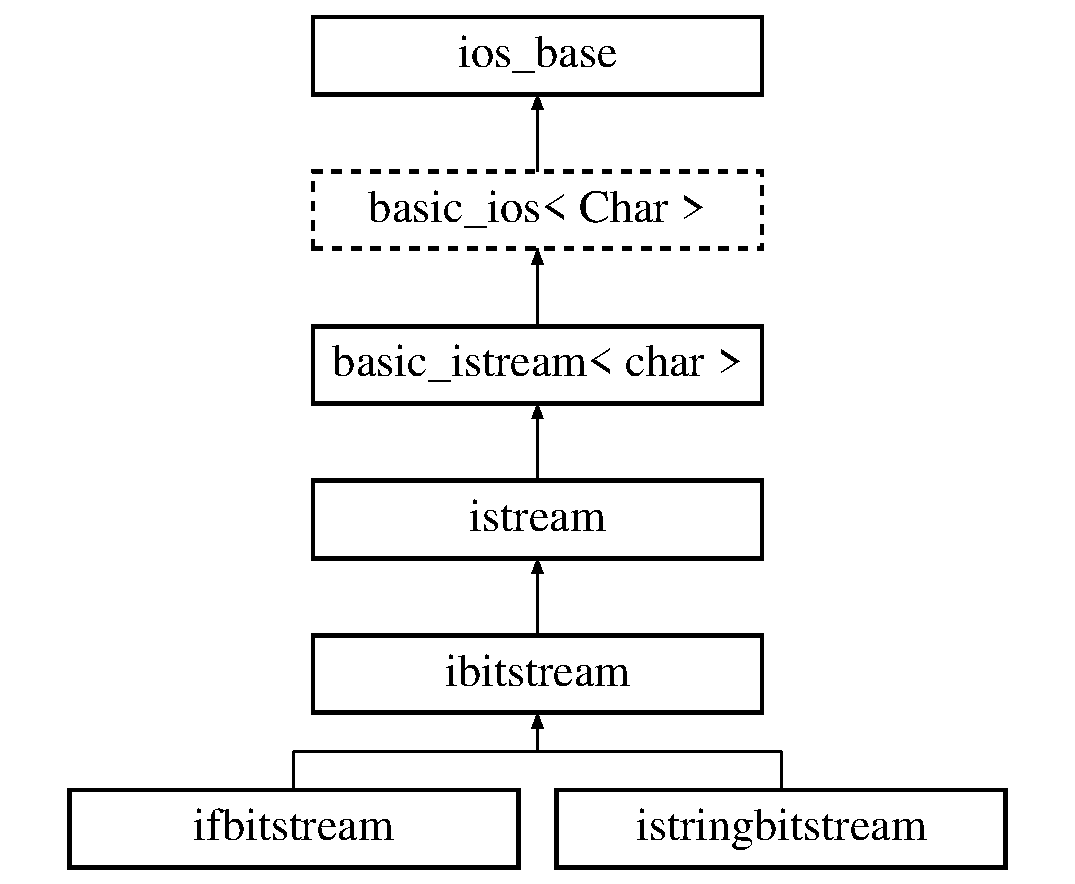
\includegraphics[height=6.000000cm]{classibitstream}
\end{center}
\end{figure}
\subsection*{Public Member Functions}
\begin{DoxyCompactItemize}
\item 
\mbox{\hyperlink{classibitstream_a72d1e7b784e2782d57a9ce3954a1f94f}{ibitstream}} ()
\item 
virtual bool \mbox{\hyperlink{classibitstream_a2f57f54d8c03b615bb31eee091d8a88a}{is\+\_\+open}} ()
\item 
int \mbox{\hyperlink{classibitstream_aa8c615fa7957fb0232a0873dadbd39e8}{read\+Bit}} ()
\item 
void \mbox{\hyperlink{classibitstream_ab8734e666421c9fe3b6380a818c6c727}{rewind}} ()
\item 
void \mbox{\hyperlink{classibitstream_ad916b4624eb09d375514964f867b475c}{set\+Fake}} (bool fake)
\item 
long \mbox{\hyperlink{classibitstream_a22727e9c338fb1aaa6722031445373c3}{size}} ()
\end{DoxyCompactItemize}


\subsection{Constructor \& Destructor Documentation}
\mbox{\Hypertarget{classibitstream_a72d1e7b784e2782d57a9ce3954a1f94f}\label{classibitstream_a72d1e7b784e2782d57a9ce3954a1f94f}} 
\index{ibitstream@{ibitstream}!ibitstream@{ibitstream}}
\index{ibitstream@{ibitstream}!ibitstream@{ibitstream}}
\subsubsection{\texorpdfstring{ibitstream()}{ibitstream()}}
{\footnotesize\ttfamily \mbox{\hyperlink{classibitstream}{ibitstream}} (\begin{DoxyParamCaption}{ }\end{DoxyParamCaption})}



\subsection{Member Function Documentation}
\mbox{\Hypertarget{classibitstream_a2f57f54d8c03b615bb31eee091d8a88a}\label{classibitstream_a2f57f54d8c03b615bb31eee091d8a88a}} 
\index{ibitstream@{ibitstream}!is\+\_\+open@{is\+\_\+open}}
\index{is\+\_\+open@{is\+\_\+open}!ibitstream@{ibitstream}}
\subsubsection{\texorpdfstring{is\+\_\+open()}{is\_open()}}
{\footnotesize\ttfamily bool is\+\_\+open (\begin{DoxyParamCaption}{ }\end{DoxyParamCaption})\hspace{0.3cm}{\ttfamily [virtual]}}



Reimplemented in \mbox{\hyperlink{classifbitstream_a2f57f54d8c03b615bb31eee091d8a88a}{ifbitstream}}.

\mbox{\Hypertarget{classibitstream_aa8c615fa7957fb0232a0873dadbd39e8}\label{classibitstream_aa8c615fa7957fb0232a0873dadbd39e8}} 
\index{ibitstream@{ibitstream}!read\+Bit@{read\+Bit}}
\index{read\+Bit@{read\+Bit}!ibitstream@{ibitstream}}
\subsubsection{\texorpdfstring{read\+Bit()}{readBit()}}
{\footnotesize\ttfamily int read\+Bit (\begin{DoxyParamCaption}{ }\end{DoxyParamCaption})}

\mbox{\Hypertarget{classibitstream_ab8734e666421c9fe3b6380a818c6c727}\label{classibitstream_ab8734e666421c9fe3b6380a818c6c727}} 
\index{ibitstream@{ibitstream}!rewind@{rewind}}
\index{rewind@{rewind}!ibitstream@{ibitstream}}
\subsubsection{\texorpdfstring{rewind()}{rewind()}}
{\footnotesize\ttfamily void rewind (\begin{DoxyParamCaption}{ }\end{DoxyParamCaption})}

\mbox{\Hypertarget{classibitstream_ad916b4624eb09d375514964f867b475c}\label{classibitstream_ad916b4624eb09d375514964f867b475c}} 
\index{ibitstream@{ibitstream}!set\+Fake@{set\+Fake}}
\index{set\+Fake@{set\+Fake}!ibitstream@{ibitstream}}
\subsubsection{\texorpdfstring{set\+Fake()}{setFake()}}
{\footnotesize\ttfamily void set\+Fake (\begin{DoxyParamCaption}\item[{bool}]{fake }\end{DoxyParamCaption})}

\mbox{\Hypertarget{classibitstream_a22727e9c338fb1aaa6722031445373c3}\label{classibitstream_a22727e9c338fb1aaa6722031445373c3}} 
\index{ibitstream@{ibitstream}!size@{size}}
\index{size@{size}!ibitstream@{ibitstream}}
\subsubsection{\texorpdfstring{size()}{size()}}
{\footnotesize\ttfamily long size (\begin{DoxyParamCaption}{ }\end{DoxyParamCaption})}


\hypertarget{classifbitstream}{}\section{ifbitstream Class Reference}
\label{classifbitstream}\index{ifbitstream@{ifbitstream}}


A class for reading files in all of the usual ways, plus bit-\/by-\/bit.  




{\ttfamily \#include $<$bitstream.\+h$>$}

Inheritance diagram for ifbitstream\+:\begin{figure}[H]
\begin{center}
\leavevmode
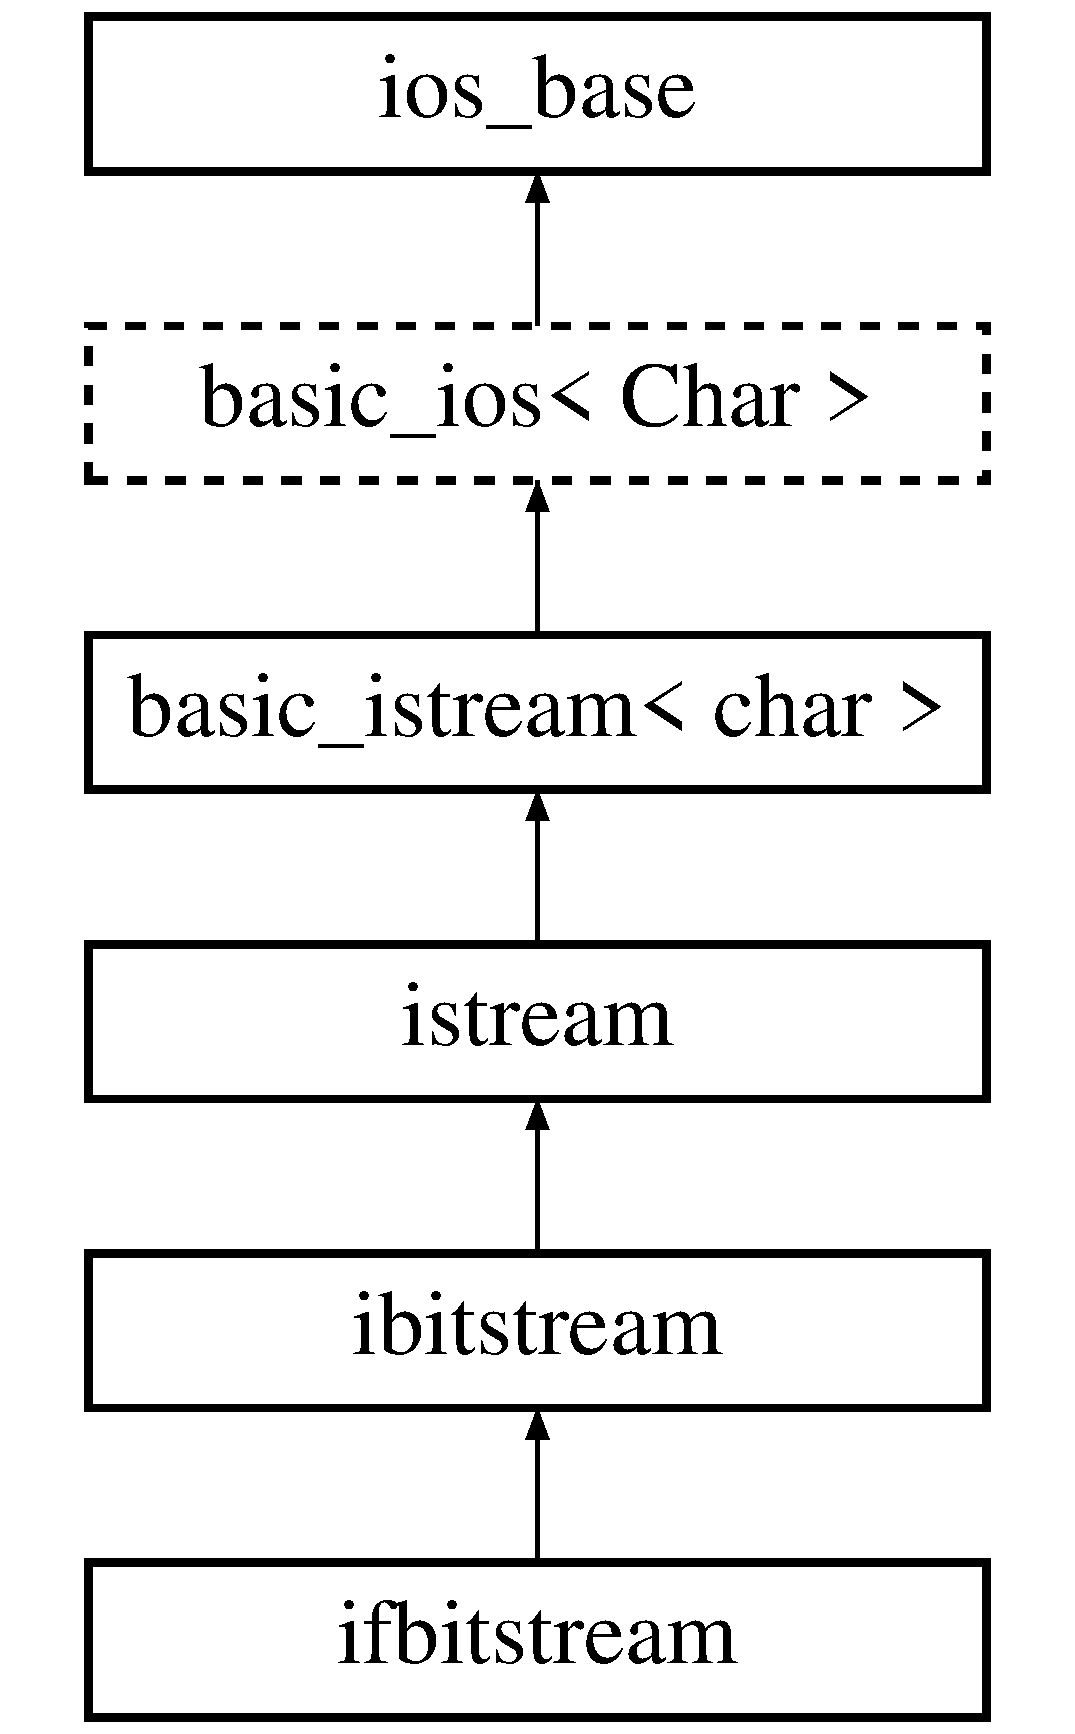
\includegraphics[height=6.000000cm]{classifbitstream}
\end{center}
\end{figure}
\subsection*{Public Member Functions}
\begin{DoxyCompactItemize}
\item 
\mbox{\hyperlink{classifbitstream_a2d6148d42c4e6bcac770d185b25a691e}{ifbitstream}} ()
\begin{DoxyCompactList}\small\item\em Constructs a new ifbitstream not attached to any file. \end{DoxyCompactList}\item 
\mbox{\hyperlink{classifbitstream_a5fe2eb72a345e67256791c172a29bbba}{ifbitstream}} (const char $\ast$filename)
\begin{DoxyCompactList}\small\item\em Constructs a new ifbitstream that reads the file with the given name, if it exists. \end{DoxyCompactList}\item 
\mbox{\hyperlink{classifbitstream_a96869868971e5d55945f1ab3d8bde584}{ifbitstream}} (const std\+::string \&filename)
\begin{DoxyCompactList}\small\item\em Constructs a new ifbitstream that reads the specified file, if it exists. \end{DoxyCompactList}\item 
void \mbox{\hyperlink{classifbitstream_a5ae591df94fc66ccb85cbb6565368bca}{close}} ()
\begin{DoxyCompactList}\small\item\em Closes the currently-\/opened file, if the stream is open. \end{DoxyCompactList}\item 
bool \mbox{\hyperlink{classifbitstream_a2f57f54d8c03b615bb31eee091d8a88a}{is\+\_\+open}} ()
\begin{DoxyCompactList}\small\item\em Returns whether or not this ifbitstream is connected to a file for reading. \end{DoxyCompactList}\item 
void \mbox{\hyperlink{classifbitstream_a57f80da790b202b27353cd8f8415b382}{open}} (const char $\ast$filename)
\begin{DoxyCompactList}\small\item\em Opens the specified file for reading. \end{DoxyCompactList}\item 
void \mbox{\hyperlink{classifbitstream_a72f6f3d1b9bc5a4275359cc0a83a60bd}{open}} (const std\+::string \&filename)
\begin{DoxyCompactList}\small\item\em Opens the specified file for reading. \end{DoxyCompactList}\item 
int \mbox{\hyperlink{classibitstream_aa8c615fa7957fb0232a0873dadbd39e8}{read\+Bit}} ()
\begin{DoxyCompactList}\small\item\em Reads a single bit from the ibitstream and returns 0 or 1 depending on the bit value. \end{DoxyCompactList}\item 
void \mbox{\hyperlink{classibitstream_ab8734e666421c9fe3b6380a818c6c727}{rewind}} ()
\begin{DoxyCompactList}\small\item\em Rewinds the ibitstream back to the beginning so that subsequent reads start again from the beginning. \end{DoxyCompactList}\item 
void \mbox{\hyperlink{classibitstream_ad916b4624eb09d375514964f867b475c}{set\+Fake}} (bool fake)
\begin{DoxyCompactList}\small\item\em Sets \textquotesingle{}fake\textquotesingle{} mode, where it actually reads bytes when you say read\+Bit. \end{DoxyCompactList}\item 
long \mbox{\hyperlink{classibitstream_a22727e9c338fb1aaa6722031445373c3}{size}} ()
\begin{DoxyCompactList}\small\item\em Returns the size in bytes of the data attached to this stream. \end{DoxyCompactList}\end{DoxyCompactItemize}


\subsection{Detailed Description}
A class for reading files in all of the usual ways, plus bit-\/by-\/bit. 

You can treat this class like a normal ifstream, except that there is extra support for bit-\/level operations. 

\subsection{Constructor \& Destructor Documentation}
\mbox{\Hypertarget{classifbitstream_a2d6148d42c4e6bcac770d185b25a691e}\label{classifbitstream_a2d6148d42c4e6bcac770d185b25a691e}} 
\index{ifbitstream@{ifbitstream}!ifbitstream@{ifbitstream}}
\index{ifbitstream@{ifbitstream}!ifbitstream@{ifbitstream}}
\subsubsection{\texorpdfstring{ifbitstream()}{ifbitstream()}\hspace{0.1cm}{\footnotesize\ttfamily [1/3]}}
{\footnotesize\ttfamily \mbox{\hyperlink{classifbitstream}{ifbitstream}} (\begin{DoxyParamCaption}{ }\end{DoxyParamCaption})}



Constructs a new ifbitstream not attached to any file. 

You can open a file for reading using the .\mbox{\hyperlink{classifbitstream_a57f80da790b202b27353cd8f8415b382}{open()}} member functions. \mbox{\Hypertarget{classifbitstream_a5fe2eb72a345e67256791c172a29bbba}\label{classifbitstream_a5fe2eb72a345e67256791c172a29bbba}} 
\index{ifbitstream@{ifbitstream}!ifbitstream@{ifbitstream}}
\index{ifbitstream@{ifbitstream}!ifbitstream@{ifbitstream}}
\subsubsection{\texorpdfstring{ifbitstream()}{ifbitstream()}\hspace{0.1cm}{\footnotesize\ttfamily [2/3]}}
{\footnotesize\ttfamily \mbox{\hyperlink{classifbitstream}{ifbitstream}} (\begin{DoxyParamCaption}\item[{const char $\ast$}]{filename }\end{DoxyParamCaption})}



Constructs a new ifbitstream that reads the file with the given name, if it exists. 

If not, the stream enters an error state. \mbox{\Hypertarget{classifbitstream_a96869868971e5d55945f1ab3d8bde584}\label{classifbitstream_a96869868971e5d55945f1ab3d8bde584}} 
\index{ifbitstream@{ifbitstream}!ifbitstream@{ifbitstream}}
\index{ifbitstream@{ifbitstream}!ifbitstream@{ifbitstream}}
\subsubsection{\texorpdfstring{ifbitstream()}{ifbitstream()}\hspace{0.1cm}{\footnotesize\ttfamily [3/3]}}
{\footnotesize\ttfamily \mbox{\hyperlink{classifbitstream}{ifbitstream}} (\begin{DoxyParamCaption}\item[{const std\+::string \&}]{filename }\end{DoxyParamCaption})}



Constructs a new ifbitstream that reads the specified file, if it exists. 

If not, the stream enters an error state. 

\subsection{Member Function Documentation}
\mbox{\Hypertarget{classifbitstream_a5ae591df94fc66ccb85cbb6565368bca}\label{classifbitstream_a5ae591df94fc66ccb85cbb6565368bca}} 
\index{ifbitstream@{ifbitstream}!close@{close}}
\index{close@{close}!ifbitstream@{ifbitstream}}
\subsubsection{\texorpdfstring{close()}{close()}}
{\footnotesize\ttfamily void close (\begin{DoxyParamCaption}{ }\end{DoxyParamCaption})}



Closes the currently-\/opened file, if the stream is open. 

If the stream is not open, puts the stream into a fail state. \mbox{\Hypertarget{classifbitstream_a2f57f54d8c03b615bb31eee091d8a88a}\label{classifbitstream_a2f57f54d8c03b615bb31eee091d8a88a}} 
\index{ifbitstream@{ifbitstream}!is\+\_\+open@{is\+\_\+open}}
\index{is\+\_\+open@{is\+\_\+open}!ifbitstream@{ifbitstream}}
\subsubsection{\texorpdfstring{is\+\_\+open()}{is\_open()}}
{\footnotesize\ttfamily bool is\+\_\+open (\begin{DoxyParamCaption}{ }\end{DoxyParamCaption})\hspace{0.3cm}{\ttfamily [virtual]}}



Returns whether or not this ifbitstream is connected to a file for reading. 



Reimplemented from \mbox{\hyperlink{classibitstream_a2f57f54d8c03b615bb31eee091d8a88a}{ibitstream}}.

\mbox{\Hypertarget{classifbitstream_a57f80da790b202b27353cd8f8415b382}\label{classifbitstream_a57f80da790b202b27353cd8f8415b382}} 
\index{ifbitstream@{ifbitstream}!open@{open}}
\index{open@{open}!ifbitstream@{ifbitstream}}
\subsubsection{\texorpdfstring{open()}{open()}\hspace{0.1cm}{\footnotesize\ttfamily [1/2]}}
{\footnotesize\ttfamily void open (\begin{DoxyParamCaption}\item[{const char $\ast$}]{filename }\end{DoxyParamCaption})}



Opens the specified file for reading. 

If an error occurs, the stream enters a failure state, which can be detected by calling ifb.\+fail(). \mbox{\Hypertarget{classifbitstream_a72f6f3d1b9bc5a4275359cc0a83a60bd}\label{classifbitstream_a72f6f3d1b9bc5a4275359cc0a83a60bd}} 
\index{ifbitstream@{ifbitstream}!open@{open}}
\index{open@{open}!ifbitstream@{ifbitstream}}
\subsubsection{\texorpdfstring{open()}{open()}\hspace{0.1cm}{\footnotesize\ttfamily [2/2]}}
{\footnotesize\ttfamily void open (\begin{DoxyParamCaption}\item[{const std\+::string \&}]{filename }\end{DoxyParamCaption})}



Opens the specified file for reading. 

If an error occurs, the stream enters a failure state, which can be detected by calling ifb.\+fail(). \mbox{\Hypertarget{classibitstream_aa8c615fa7957fb0232a0873dadbd39e8}\label{classibitstream_aa8c615fa7957fb0232a0873dadbd39e8}} 
\index{ifbitstream@{ifbitstream}!read\+Bit@{read\+Bit}}
\index{read\+Bit@{read\+Bit}!ifbitstream@{ifbitstream}}
\subsubsection{\texorpdfstring{read\+Bit()}{readBit()}}
{\footnotesize\ttfamily int read\+Bit (\begin{DoxyParamCaption}{ }\end{DoxyParamCaption})\hspace{0.3cm}{\ttfamily [inherited]}}



Reads a single bit from the ibitstream and returns 0 or 1 depending on the bit value. 

If the stream is exhausted, E\+OF (-\/1) is returned. Raises an error if this ibitstream has not been properly opened. \mbox{\Hypertarget{classibitstream_ab8734e666421c9fe3b6380a818c6c727}\label{classibitstream_ab8734e666421c9fe3b6380a818c6c727}} 
\index{ifbitstream@{ifbitstream}!rewind@{rewind}}
\index{rewind@{rewind}!ifbitstream@{ifbitstream}}
\subsubsection{\texorpdfstring{rewind()}{rewind()}}
{\footnotesize\ttfamily void rewind (\begin{DoxyParamCaption}{ }\end{DoxyParamCaption})\hspace{0.3cm}{\ttfamily [inherited]}}



Rewinds the ibitstream back to the beginning so that subsequent reads start again from the beginning. 

Raises an error if this ibitstream has not been properly opened. \mbox{\Hypertarget{classibitstream_ad916b4624eb09d375514964f867b475c}\label{classibitstream_ad916b4624eb09d375514964f867b475c}} 
\index{ifbitstream@{ifbitstream}!set\+Fake@{set\+Fake}}
\index{set\+Fake@{set\+Fake}!ifbitstream@{ifbitstream}}
\subsubsection{\texorpdfstring{set\+Fake()}{setFake()}}
{\footnotesize\ttfamily void set\+Fake (\begin{DoxyParamCaption}\item[{bool}]{fake }\end{DoxyParamCaption})\hspace{0.3cm}{\ttfamily [inherited]}}



Sets \textquotesingle{}fake\textquotesingle{} mode, where it actually reads bytes when you say read\+Bit. 

\mbox{\Hypertarget{classibitstream_a22727e9c338fb1aaa6722031445373c3}\label{classibitstream_a22727e9c338fb1aaa6722031445373c3}} 
\index{ifbitstream@{ifbitstream}!size@{size}}
\index{size@{size}!ifbitstream@{ifbitstream}}
\subsubsection{\texorpdfstring{size()}{size()}}
{\footnotesize\ttfamily long size (\begin{DoxyParamCaption}{ }\end{DoxyParamCaption})\hspace{0.3cm}{\ttfamily [inherited]}}



Returns the size in bytes of the data attached to this stream. 

Raises an error if this ibitstream has not been properly opened. 
\hypertarget{classIntRange}{}\section{Int\+Range Class Reference}
\label{classIntRange}\index{Int\+Range@{Int\+Range}}


An \mbox{\hyperlink{classIntRange}{Int\+Range}} is an iterable contiguous range of integers.  




{\ttfamily \#include $<$intrange.\+h$>$}

\subsection*{Public Member Functions}
\begin{DoxyCompactItemize}
\item 
\mbox{\hyperlink{classIntRange_a1371e812388f10db89e8cea0edeec000}{Int\+Range}} (int \mbox{\hyperlink{classIntRange_a91213974fa3ac3959b1c355a9e588f8d}{length}}=0)
\begin{DoxyCompactList}\small\item\em Constructs a range from 0 (inclusive) of the given length. \end{DoxyCompactList}\item 
\mbox{\hyperlink{classIntRange_a9e8543f0451b16061adafee2d9ad0f84}{Int\+Range}} (int min\+Value, int max\+Value)
\begin{DoxyCompactList}\small\item\em Constructs a range from min\+Value to max\+Value (inclusive). \end{DoxyCompactList}\item 
Int\+Range\+Iterator \mbox{\hyperlink{classIntRange_a71b24b84d58ec13662a463eddc2e085c}{begin}} () const
\begin{DoxyCompactList}\small\item\em Returns an iterator over the elements of this range. \end{DoxyCompactList}\item 
bool \mbox{\hyperlink{classIntRange_ab0197de90231da6a241cf66cd6b16edc}{contains}} (int n) const
\begin{DoxyCompactList}\small\item\em Returns true if the given integer is within the bounds of this range. \end{DoxyCompactList}\item 
bool \mbox{\hyperlink{classIntRange_a71626971ecae788078a3ba3e7ffc7201}{contains}} (const \mbox{\hyperlink{classIntRange}{Int\+Range}} \&r) const
\begin{DoxyCompactList}\small\item\em Returns true if the given range is entirely contained within this range. \end{DoxyCompactList}\item 
bool \mbox{\hyperlink{classIntRange_a644718bb2fb240de962dc3c9a1fdf0dc}{empty}} () const
\begin{DoxyCompactList}\small\item\em Returns true if this range contains no integers, meaning that its max is less than its min. \end{DoxyCompactList}\item 
Int\+Range\+Iterator \mbox{\hyperlink{classIntRange_ad919bd40bd4298cafd0955b8031f4bef}{end}} () const
\item 
bool \mbox{\hyperlink{classIntRange_acf82f9b2937375c7b1cf3dccb3df3312}{is\+Empty}} () const
\begin{DoxyCompactList}\small\item\em Returns true if this range contains no integers, meaning that its max is less than its min. \end{DoxyCompactList}\item 
int \mbox{\hyperlink{classIntRange_a91213974fa3ac3959b1c355a9e588f8d}{length}} () const
\begin{DoxyCompactList}\small\item\em Returns the number of integers in the range. \end{DoxyCompactList}\item 
int \mbox{\hyperlink{classIntRange_a86ad4228f3fccc681e8716ac9c68ab4d}{max}} () const
\begin{DoxyCompactList}\small\item\em Returns the maximum value in the range, inclusive. \end{DoxyCompactList}\item 
int \mbox{\hyperlink{classIntRange_a4ec1ccea7eddbc7355ba5d00afcaec2d}{min}} () const
\begin{DoxyCompactList}\small\item\em Returns the minimum value in the range. \end{DoxyCompactList}\item 
int \mbox{\hyperlink{classIntRange_af9593d4a5ff4274efaf429cb4f9e57cc}{size}} () const
\begin{DoxyCompactList}\small\item\em Returns the number of integers in the range. \end{DoxyCompactList}\item 
std\+::string \mbox{\hyperlink{classIntRange_a1fe5121d6528fdea3f243321b3fa3a49}{to\+String}} () const
\begin{DoxyCompactList}\small\item\em Returns a string representation of this range, such as \char`\"{}\mbox{[}1 .. 10\mbox{]}\char`\"{}. \end{DoxyCompactList}\end{DoxyCompactItemize}


\subsection{Detailed Description}
An \mbox{\hyperlink{classIntRange}{Int\+Range}} is an iterable contiguous range of integers. 

It can be processed using a for-\/each loop. The integers are not actually all stored in this object, so it does not require O(\+N) memory usage. 

\subsection{Constructor \& Destructor Documentation}
\mbox{\Hypertarget{classIntRange_a1371e812388f10db89e8cea0edeec000}\label{classIntRange_a1371e812388f10db89e8cea0edeec000}} 
\index{Int\+Range@{Int\+Range}!Int\+Range@{Int\+Range}}
\index{Int\+Range@{Int\+Range}!Int\+Range@{Int\+Range}}
\subsubsection{\texorpdfstring{Int\+Range()}{IntRange()}\hspace{0.1cm}{\footnotesize\ttfamily [1/2]}}
{\footnotesize\ttfamily \mbox{\hyperlink{classIntRange}{Int\+Range}} (\begin{DoxyParamCaption}\item[{int}]{length = {\ttfamily 0} }\end{DoxyParamCaption})}



Constructs a range from 0 (inclusive) of the given length. 

Its endpoints are \mbox{[}0 .. length-\/1\mbox{]}. \mbox{\Hypertarget{classIntRange_a9e8543f0451b16061adafee2d9ad0f84}\label{classIntRange_a9e8543f0451b16061adafee2d9ad0f84}} 
\index{Int\+Range@{Int\+Range}!Int\+Range@{Int\+Range}}
\index{Int\+Range@{Int\+Range}!Int\+Range@{Int\+Range}}
\subsubsection{\texorpdfstring{Int\+Range()}{IntRange()}\hspace{0.1cm}{\footnotesize\ttfamily [2/2]}}
{\footnotesize\ttfamily \mbox{\hyperlink{classIntRange}{Int\+Range}} (\begin{DoxyParamCaption}\item[{int}]{min\+Value,  }\item[{int}]{max\+Value }\end{DoxyParamCaption})}



Constructs a range from min\+Value to max\+Value (inclusive). 



\subsection{Member Function Documentation}
\mbox{\Hypertarget{classIntRange_a71b24b84d58ec13662a463eddc2e085c}\label{classIntRange_a71b24b84d58ec13662a463eddc2e085c}} 
\index{Int\+Range@{Int\+Range}!begin@{begin}}
\index{begin@{begin}!Int\+Range@{Int\+Range}}
\subsubsection{\texorpdfstring{begin()}{begin()}}
{\footnotesize\ttfamily Int\+Range\+::\+Int\+Range\+Iterator begin (\begin{DoxyParamCaption}{ }\end{DoxyParamCaption}) const}



Returns an iterator over the elements of this range. 

\mbox{\Hypertarget{classIntRange_ab0197de90231da6a241cf66cd6b16edc}\label{classIntRange_ab0197de90231da6a241cf66cd6b16edc}} 
\index{Int\+Range@{Int\+Range}!contains@{contains}}
\index{contains@{contains}!Int\+Range@{Int\+Range}}
\subsubsection{\texorpdfstring{contains()}{contains()}\hspace{0.1cm}{\footnotesize\ttfamily [1/2]}}
{\footnotesize\ttfamily bool contains (\begin{DoxyParamCaption}\item[{int}]{n }\end{DoxyParamCaption}) const}



Returns true if the given integer is within the bounds of this range. 

\mbox{\Hypertarget{classIntRange_a71626971ecae788078a3ba3e7ffc7201}\label{classIntRange_a71626971ecae788078a3ba3e7ffc7201}} 
\index{Int\+Range@{Int\+Range}!contains@{contains}}
\index{contains@{contains}!Int\+Range@{Int\+Range}}
\subsubsection{\texorpdfstring{contains()}{contains()}\hspace{0.1cm}{\footnotesize\ttfamily [2/2]}}
{\footnotesize\ttfamily bool contains (\begin{DoxyParamCaption}\item[{const \mbox{\hyperlink{classIntRange}{Int\+Range}} \&}]{r }\end{DoxyParamCaption}) const}



Returns true if the given range is entirely contained within this range. 

\mbox{\Hypertarget{classIntRange_a644718bb2fb240de962dc3c9a1fdf0dc}\label{classIntRange_a644718bb2fb240de962dc3c9a1fdf0dc}} 
\index{Int\+Range@{Int\+Range}!empty@{empty}}
\index{empty@{empty}!Int\+Range@{Int\+Range}}
\subsubsection{\texorpdfstring{empty()}{empty()}}
{\footnotesize\ttfamily bool empty (\begin{DoxyParamCaption}{ }\end{DoxyParamCaption}) const}



Returns true if this range contains no integers, meaning that its max is less than its min. 

Equivalent to is\+Empty. \mbox{\Hypertarget{classIntRange_ad919bd40bd4298cafd0955b8031f4bef}\label{classIntRange_ad919bd40bd4298cafd0955b8031f4bef}} 
\index{Int\+Range@{Int\+Range}!end@{end}}
\index{end@{end}!Int\+Range@{Int\+Range}}
\subsubsection{\texorpdfstring{end()}{end()}}
{\footnotesize\ttfamily Int\+Range\+::\+Int\+Range\+Iterator end (\begin{DoxyParamCaption}{ }\end{DoxyParamCaption}) const}

\mbox{\Hypertarget{classIntRange_acf82f9b2937375c7b1cf3dccb3df3312}\label{classIntRange_acf82f9b2937375c7b1cf3dccb3df3312}} 
\index{Int\+Range@{Int\+Range}!is\+Empty@{is\+Empty}}
\index{is\+Empty@{is\+Empty}!Int\+Range@{Int\+Range}}
\subsubsection{\texorpdfstring{is\+Empty()}{isEmpty()}}
{\footnotesize\ttfamily bool is\+Empty (\begin{DoxyParamCaption}{ }\end{DoxyParamCaption}) const}



Returns true if this range contains no integers, meaning that its max is less than its min. 

Equivalent to empty. \mbox{\Hypertarget{classIntRange_a91213974fa3ac3959b1c355a9e588f8d}\label{classIntRange_a91213974fa3ac3959b1c355a9e588f8d}} 
\index{Int\+Range@{Int\+Range}!length@{length}}
\index{length@{length}!Int\+Range@{Int\+Range}}
\subsubsection{\texorpdfstring{length()}{length()}}
{\footnotesize\ttfamily int length (\begin{DoxyParamCaption}{ }\end{DoxyParamCaption}) const}



Returns the number of integers in the range. 

Equivalent to size. \mbox{\Hypertarget{classIntRange_a86ad4228f3fccc681e8716ac9c68ab4d}\label{classIntRange_a86ad4228f3fccc681e8716ac9c68ab4d}} 
\index{Int\+Range@{Int\+Range}!max@{max}}
\index{max@{max}!Int\+Range@{Int\+Range}}
\subsubsection{\texorpdfstring{max()}{max()}}
{\footnotesize\ttfamily int max (\begin{DoxyParamCaption}{ }\end{DoxyParamCaption}) const}



Returns the maximum value in the range, inclusive. 

\mbox{\Hypertarget{classIntRange_a4ec1ccea7eddbc7355ba5d00afcaec2d}\label{classIntRange_a4ec1ccea7eddbc7355ba5d00afcaec2d}} 
\index{Int\+Range@{Int\+Range}!min@{min}}
\index{min@{min}!Int\+Range@{Int\+Range}}
\subsubsection{\texorpdfstring{min()}{min()}}
{\footnotesize\ttfamily int min (\begin{DoxyParamCaption}{ }\end{DoxyParamCaption}) const}



Returns the minimum value in the range. 

\mbox{\Hypertarget{classIntRange_af9593d4a5ff4274efaf429cb4f9e57cc}\label{classIntRange_af9593d4a5ff4274efaf429cb4f9e57cc}} 
\index{Int\+Range@{Int\+Range}!size@{size}}
\index{size@{size}!Int\+Range@{Int\+Range}}
\subsubsection{\texorpdfstring{size()}{size()}}
{\footnotesize\ttfamily int size (\begin{DoxyParamCaption}{ }\end{DoxyParamCaption}) const}



Returns the number of integers in the range. 

Equivalent to length. \mbox{\Hypertarget{classIntRange_a1fe5121d6528fdea3f243321b3fa3a49}\label{classIntRange_a1fe5121d6528fdea3f243321b3fa3a49}} 
\index{Int\+Range@{Int\+Range}!to\+String@{to\+String}}
\index{to\+String@{to\+String}!Int\+Range@{Int\+Range}}
\subsubsection{\texorpdfstring{to\+String()}{toString()}}
{\footnotesize\ttfamily std\+::string to\+String (\begin{DoxyParamCaption}{ }\end{DoxyParamCaption}) const}



Returns a string representation of this range, such as \char`\"{}\mbox{[}1 .. 10\mbox{]}\char`\"{}. 



\subsection{Friends And Related Function Documentation}
\mbox{\Hypertarget{classIntRange_a4b452901f18832cc506afd0f320e5934}\label{classIntRange_a4b452901f18832cc506afd0f320e5934}} 
\index{Int\+Range@{Int\+Range}!operator$>$$>$@{operator$>$$>$}}
\index{operator$>$$>$@{operator$>$$>$}!Int\+Range@{Int\+Range}}
\subsubsection{\texorpdfstring{operator$>$$>$}{operator>>}}
{\footnotesize\ttfamily std\+::istream\& operator$>$$>$ (\begin{DoxyParamCaption}\item[{std\+::istream \&}]{input,  }\item[{\mbox{\hyperlink{classIntRange}{Int\+Range}} \&}]{r }\end{DoxyParamCaption})\hspace{0.3cm}{\ttfamily [friend]}}



Reads the given range to the given input stream in its to\+String format. 


\hypertarget{classIntRange2D}{}\section{Int\+Range2D Class Reference}
\label{classIntRange2D}\index{Int\+Range2D@{Int\+Range2D}}


{\ttfamily \#include $<$intrange.\+h$>$}

\subsection*{Public Member Functions}
\begin{DoxyCompactItemize}
\item 
\mbox{\hyperlink{classIntRange2D_a39f2016ab50300a0d0e76d60fe958356}{Int\+Range2D}} (int \mbox{\hyperlink{classIntRange2D_ad72663daf610f2a0833a2fc3d78e4fdf}{width}}=0, int \mbox{\hyperlink{classIntRange2D_ad3774f6419003470f54fd495124ef51f}{height}}=0, bool y\+Major=true)
\item 
\mbox{\hyperlink{classIntRange2D_a22f22b7ce16863ba7acc111a2b26018b}{Int\+Range2D}} (int \mbox{\hyperlink{classIntRange2D_a1a1724b4b31e3d3d251e5816c7d9e448}{minX}}, int \mbox{\hyperlink{classIntRange2D_a2337641dec44ff553785d9c143c3aafd}{minY}}, int \mbox{\hyperlink{classIntRange2D_aa9493e60175cb4e130ae4cfba2b55907}{maxX}}, int \mbox{\hyperlink{classIntRange2D_a015dcf4989cbafff40d5a345b9d9f959}{maxY}}, bool y\+Major=true)
\item 
Int\+Range2\+D\+Iterator \mbox{\hyperlink{classIntRange2D_a5840f252f949c3f9c0bd1085250a8615}{begin}} () const
\item 
bool \mbox{\hyperlink{classIntRange2D_a39725eb73188fbf2a4b790b1a6849815}{contains}} (int x, int y) const
\item 
bool \mbox{\hyperlink{classIntRange2D_a3c4705ae7b99ee1d5cd6326e5f2869bf}{contains}} (const \mbox{\hyperlink{classIntRange2D}{Int\+Range2D}} \&r) const
\item 
bool \mbox{\hyperlink{classIntRange2D_a644718bb2fb240de962dc3c9a1fdf0dc}{empty}} () const
\item 
Int\+Range2\+D\+Iterator \mbox{\hyperlink{classIntRange2D_aa7bf3d68f7aec8215aa12584f8c47443}{end}} () const
\item 
int \mbox{\hyperlink{classIntRange2D_ad3774f6419003470f54fd495124ef51f}{height}} () const
\item 
bool \mbox{\hyperlink{classIntRange2D_acf82f9b2937375c7b1cf3dccb3df3312}{is\+Empty}} () const
\item 
bool \mbox{\hyperlink{classIntRange2D_a7387191f7e5206084124db7bc29d1891}{is\+Y\+Major}} () const
\item 
int \mbox{\hyperlink{classIntRange2D_aa9493e60175cb4e130ae4cfba2b55907}{maxX}} () const
\item 
int \mbox{\hyperlink{classIntRange2D_a015dcf4989cbafff40d5a345b9d9f959}{maxY}} () const
\item 
int \mbox{\hyperlink{classIntRange2D_a1a1724b4b31e3d3d251e5816c7d9e448}{minX}} () const
\item 
int \mbox{\hyperlink{classIntRange2D_a2337641dec44ff553785d9c143c3aafd}{minY}} () const
\item 
int \mbox{\hyperlink{classIntRange2D_af9593d4a5ff4274efaf429cb4f9e57cc}{size}} () const
\item 
std\+::string \mbox{\hyperlink{classIntRange2D_a1fe5121d6528fdea3f243321b3fa3a49}{to\+String}} () const
\item 
int \mbox{\hyperlink{classIntRange2D_ad72663daf610f2a0833a2fc3d78e4fdf}{width}} () const
\end{DoxyCompactItemize}
\subsection*{Friends}
\begin{DoxyCompactItemize}
\item 
std\+::istream \& \mbox{\hyperlink{classIntRange2D_a1785cf1b9660abbc492b9fcabe2f7af5}{operator$>$$>$}} (std\+::istream \&input, \mbox{\hyperlink{classIntRange2D}{Int\+Range2D}} \&r)
\end{DoxyCompactItemize}


\subsection{Constructor \& Destructor Documentation}
\mbox{\Hypertarget{classIntRange2D_a39f2016ab50300a0d0e76d60fe958356}\label{classIntRange2D_a39f2016ab50300a0d0e76d60fe958356}} 
\index{Int\+Range2D@{Int\+Range2D}!Int\+Range2D@{Int\+Range2D}}
\index{Int\+Range2D@{Int\+Range2D}!Int\+Range2D@{Int\+Range2D}}
\subsubsection{\texorpdfstring{Int\+Range2\+D()}{IntRange2D()}\hspace{0.1cm}{\footnotesize\ttfamily [1/2]}}
{\footnotesize\ttfamily \mbox{\hyperlink{classIntRange2D}{Int\+Range2D}} (\begin{DoxyParamCaption}\item[{int}]{width = {\ttfamily 0},  }\item[{int}]{height = {\ttfamily 0},  }\item[{bool}]{y\+Major = {\ttfamily true} }\end{DoxyParamCaption})}

\mbox{\Hypertarget{classIntRange2D_a22f22b7ce16863ba7acc111a2b26018b}\label{classIntRange2D_a22f22b7ce16863ba7acc111a2b26018b}} 
\index{Int\+Range2D@{Int\+Range2D}!Int\+Range2D@{Int\+Range2D}}
\index{Int\+Range2D@{Int\+Range2D}!Int\+Range2D@{Int\+Range2D}}
\subsubsection{\texorpdfstring{Int\+Range2\+D()}{IntRange2D()}\hspace{0.1cm}{\footnotesize\ttfamily [2/2]}}
{\footnotesize\ttfamily \mbox{\hyperlink{classIntRange2D}{Int\+Range2D}} (\begin{DoxyParamCaption}\item[{int}]{minX,  }\item[{int}]{minY,  }\item[{int}]{maxX,  }\item[{int}]{maxY,  }\item[{bool}]{y\+Major = {\ttfamily true} }\end{DoxyParamCaption})}



\subsection{Member Function Documentation}
\mbox{\Hypertarget{classIntRange2D_a5840f252f949c3f9c0bd1085250a8615}\label{classIntRange2D_a5840f252f949c3f9c0bd1085250a8615}} 
\index{Int\+Range2D@{Int\+Range2D}!begin@{begin}}
\index{begin@{begin}!Int\+Range2D@{Int\+Range2D}}
\subsubsection{\texorpdfstring{begin()}{begin()}}
{\footnotesize\ttfamily Int\+Range2\+D\+::\+Int\+Range2\+D\+Iterator begin (\begin{DoxyParamCaption}{ }\end{DoxyParamCaption}) const}

\mbox{\Hypertarget{classIntRange2D_a39725eb73188fbf2a4b790b1a6849815}\label{classIntRange2D_a39725eb73188fbf2a4b790b1a6849815}} 
\index{Int\+Range2D@{Int\+Range2D}!contains@{contains}}
\index{contains@{contains}!Int\+Range2D@{Int\+Range2D}}
\subsubsection{\texorpdfstring{contains()}{contains()}\hspace{0.1cm}{\footnotesize\ttfamily [1/2]}}
{\footnotesize\ttfamily bool contains (\begin{DoxyParamCaption}\item[{int}]{x,  }\item[{int}]{y }\end{DoxyParamCaption}) const}

\mbox{\Hypertarget{classIntRange2D_a3c4705ae7b99ee1d5cd6326e5f2869bf}\label{classIntRange2D_a3c4705ae7b99ee1d5cd6326e5f2869bf}} 
\index{Int\+Range2D@{Int\+Range2D}!contains@{contains}}
\index{contains@{contains}!Int\+Range2D@{Int\+Range2D}}
\subsubsection{\texorpdfstring{contains()}{contains()}\hspace{0.1cm}{\footnotesize\ttfamily [2/2]}}
{\footnotesize\ttfamily bool contains (\begin{DoxyParamCaption}\item[{const \mbox{\hyperlink{classIntRange2D}{Int\+Range2D}} \&}]{r }\end{DoxyParamCaption}) const}

\mbox{\Hypertarget{classIntRange2D_a644718bb2fb240de962dc3c9a1fdf0dc}\label{classIntRange2D_a644718bb2fb240de962dc3c9a1fdf0dc}} 
\index{Int\+Range2D@{Int\+Range2D}!empty@{empty}}
\index{empty@{empty}!Int\+Range2D@{Int\+Range2D}}
\subsubsection{\texorpdfstring{empty()}{empty()}}
{\footnotesize\ttfamily bool empty (\begin{DoxyParamCaption}{ }\end{DoxyParamCaption}) const}

\mbox{\Hypertarget{classIntRange2D_aa7bf3d68f7aec8215aa12584f8c47443}\label{classIntRange2D_aa7bf3d68f7aec8215aa12584f8c47443}} 
\index{Int\+Range2D@{Int\+Range2D}!end@{end}}
\index{end@{end}!Int\+Range2D@{Int\+Range2D}}
\subsubsection{\texorpdfstring{end()}{end()}}
{\footnotesize\ttfamily Int\+Range2\+D\+::\+Int\+Range2\+D\+Iterator end (\begin{DoxyParamCaption}{ }\end{DoxyParamCaption}) const}

\mbox{\Hypertarget{classIntRange2D_ad3774f6419003470f54fd495124ef51f}\label{classIntRange2D_ad3774f6419003470f54fd495124ef51f}} 
\index{Int\+Range2D@{Int\+Range2D}!height@{height}}
\index{height@{height}!Int\+Range2D@{Int\+Range2D}}
\subsubsection{\texorpdfstring{height()}{height()}}
{\footnotesize\ttfamily int height (\begin{DoxyParamCaption}{ }\end{DoxyParamCaption}) const}

\mbox{\Hypertarget{classIntRange2D_acf82f9b2937375c7b1cf3dccb3df3312}\label{classIntRange2D_acf82f9b2937375c7b1cf3dccb3df3312}} 
\index{Int\+Range2D@{Int\+Range2D}!is\+Empty@{is\+Empty}}
\index{is\+Empty@{is\+Empty}!Int\+Range2D@{Int\+Range2D}}
\subsubsection{\texorpdfstring{is\+Empty()}{isEmpty()}}
{\footnotesize\ttfamily bool is\+Empty (\begin{DoxyParamCaption}{ }\end{DoxyParamCaption}) const}

\mbox{\Hypertarget{classIntRange2D_a7387191f7e5206084124db7bc29d1891}\label{classIntRange2D_a7387191f7e5206084124db7bc29d1891}} 
\index{Int\+Range2D@{Int\+Range2D}!is\+Y\+Major@{is\+Y\+Major}}
\index{is\+Y\+Major@{is\+Y\+Major}!Int\+Range2D@{Int\+Range2D}}
\subsubsection{\texorpdfstring{is\+Y\+Major()}{isYMajor()}}
{\footnotesize\ttfamily bool is\+Y\+Major (\begin{DoxyParamCaption}{ }\end{DoxyParamCaption}) const}

\mbox{\Hypertarget{classIntRange2D_aa9493e60175cb4e130ae4cfba2b55907}\label{classIntRange2D_aa9493e60175cb4e130ae4cfba2b55907}} 
\index{Int\+Range2D@{Int\+Range2D}!maxX@{maxX}}
\index{maxX@{maxX}!Int\+Range2D@{Int\+Range2D}}
\subsubsection{\texorpdfstring{max\+X()}{maxX()}}
{\footnotesize\ttfamily int maxX (\begin{DoxyParamCaption}{ }\end{DoxyParamCaption}) const}

\mbox{\Hypertarget{classIntRange2D_a015dcf4989cbafff40d5a345b9d9f959}\label{classIntRange2D_a015dcf4989cbafff40d5a345b9d9f959}} 
\index{Int\+Range2D@{Int\+Range2D}!maxY@{maxY}}
\index{maxY@{maxY}!Int\+Range2D@{Int\+Range2D}}
\subsubsection{\texorpdfstring{max\+Y()}{maxY()}}
{\footnotesize\ttfamily int maxY (\begin{DoxyParamCaption}{ }\end{DoxyParamCaption}) const}

\mbox{\Hypertarget{classIntRange2D_a1a1724b4b31e3d3d251e5816c7d9e448}\label{classIntRange2D_a1a1724b4b31e3d3d251e5816c7d9e448}} 
\index{Int\+Range2D@{Int\+Range2D}!minX@{minX}}
\index{minX@{minX}!Int\+Range2D@{Int\+Range2D}}
\subsubsection{\texorpdfstring{min\+X()}{minX()}}
{\footnotesize\ttfamily int minX (\begin{DoxyParamCaption}{ }\end{DoxyParamCaption}) const}

\mbox{\Hypertarget{classIntRange2D_a2337641dec44ff553785d9c143c3aafd}\label{classIntRange2D_a2337641dec44ff553785d9c143c3aafd}} 
\index{Int\+Range2D@{Int\+Range2D}!minY@{minY}}
\index{minY@{minY}!Int\+Range2D@{Int\+Range2D}}
\subsubsection{\texorpdfstring{min\+Y()}{minY()}}
{\footnotesize\ttfamily int minY (\begin{DoxyParamCaption}{ }\end{DoxyParamCaption}) const}

\mbox{\Hypertarget{classIntRange2D_af9593d4a5ff4274efaf429cb4f9e57cc}\label{classIntRange2D_af9593d4a5ff4274efaf429cb4f9e57cc}} 
\index{Int\+Range2D@{Int\+Range2D}!size@{size}}
\index{size@{size}!Int\+Range2D@{Int\+Range2D}}
\subsubsection{\texorpdfstring{size()}{size()}}
{\footnotesize\ttfamily int size (\begin{DoxyParamCaption}{ }\end{DoxyParamCaption}) const}

\mbox{\Hypertarget{classIntRange2D_a1fe5121d6528fdea3f243321b3fa3a49}\label{classIntRange2D_a1fe5121d6528fdea3f243321b3fa3a49}} 
\index{Int\+Range2D@{Int\+Range2D}!to\+String@{to\+String}}
\index{to\+String@{to\+String}!Int\+Range2D@{Int\+Range2D}}
\subsubsection{\texorpdfstring{to\+String()}{toString()}}
{\footnotesize\ttfamily std\+::string to\+String (\begin{DoxyParamCaption}{ }\end{DoxyParamCaption}) const}

\mbox{\Hypertarget{classIntRange2D_ad72663daf610f2a0833a2fc3d78e4fdf}\label{classIntRange2D_ad72663daf610f2a0833a2fc3d78e4fdf}} 
\index{Int\+Range2D@{Int\+Range2D}!width@{width}}
\index{width@{width}!Int\+Range2D@{Int\+Range2D}}
\subsubsection{\texorpdfstring{width()}{width()}}
{\footnotesize\ttfamily int width (\begin{DoxyParamCaption}{ }\end{DoxyParamCaption}) const}



\subsection{Friends And Related Function Documentation}
\mbox{\Hypertarget{classIntRange2D_a1785cf1b9660abbc492b9fcabe2f7af5}\label{classIntRange2D_a1785cf1b9660abbc492b9fcabe2f7af5}} 
\index{Int\+Range2D@{Int\+Range2D}!operator$>$$>$@{operator$>$$>$}}
\index{operator$>$$>$@{operator$>$$>$}!Int\+Range2D@{Int\+Range2D}}
\subsubsection{\texorpdfstring{operator$>$$>$}{operator>>}}
{\footnotesize\ttfamily std\+::istream\& operator$>$$>$ (\begin{DoxyParamCaption}\item[{std\+::istream \&}]{input,  }\item[{\mbox{\hyperlink{classIntRange2D}{Int\+Range2D}} \&}]{r }\end{DoxyParamCaption})\hspace{0.3cm}{\ttfamily [friend]}}


\hypertarget{classistringbitstream}{}\section{istringbitstream Class Reference}
\label{classistringbitstream}\index{istringbitstream@{istringbitstream}}


{\ttfamily \#include $<$bitstream.\+h$>$}

Inheritance diagram for istringbitstream\+:\begin{figure}[H]
\begin{center}
\leavevmode
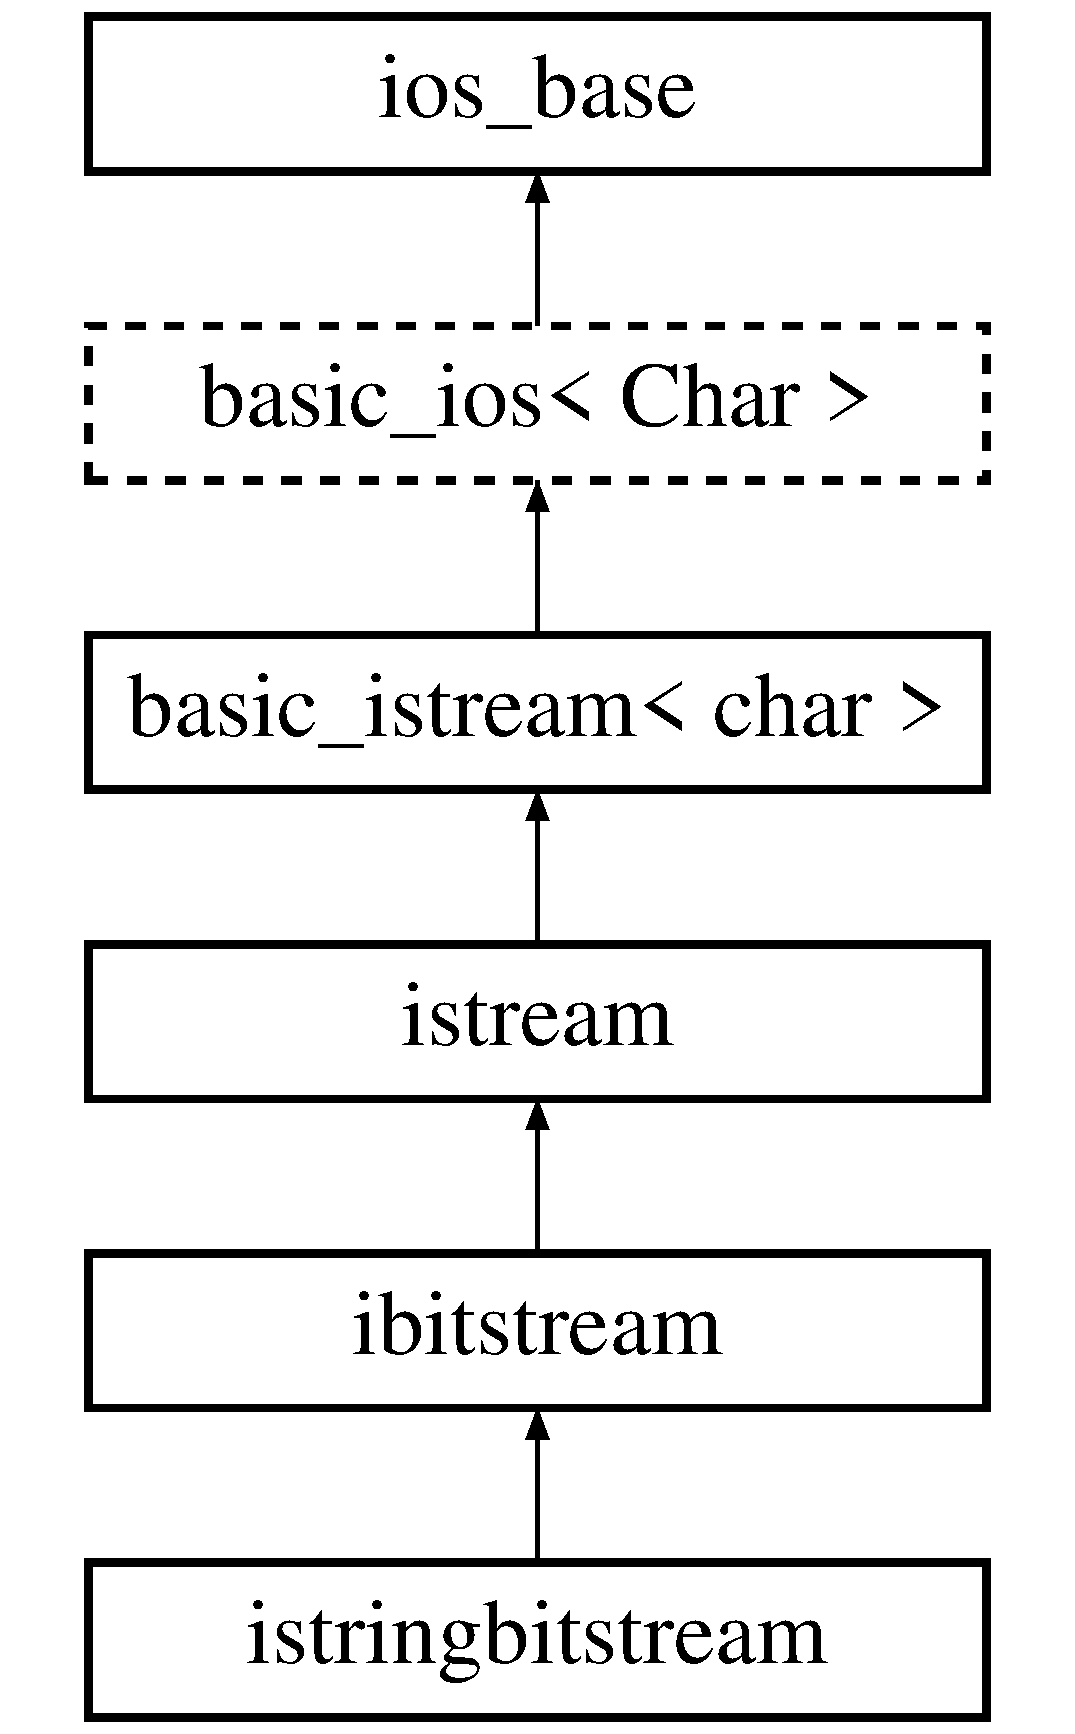
\includegraphics[height=6.000000cm]{classistringbitstream}
\end{center}
\end{figure}
\subsection*{Public Member Functions}
\begin{DoxyCompactItemize}
\item 
\mbox{\hyperlink{classistringbitstream_ae086e9a41bc91c4c64af792ff0aff81d}{istringbitstream}} (const std\+::string \&s=\char`\"{}\char`\"{})
\item 
virtual bool \mbox{\hyperlink{classibitstream_a2f57f54d8c03b615bb31eee091d8a88a}{is\+\_\+open}} ()
\item 
int \mbox{\hyperlink{classibitstream_aa8c615fa7957fb0232a0873dadbd39e8}{read\+Bit}} ()
\item 
void \mbox{\hyperlink{classibitstream_ab8734e666421c9fe3b6380a818c6c727}{rewind}} ()
\item 
void \mbox{\hyperlink{classibitstream_ad916b4624eb09d375514964f867b475c}{set\+Fake}} (bool fake)
\item 
long \mbox{\hyperlink{classibitstream_a22727e9c338fb1aaa6722031445373c3}{size}} ()
\item 
void \mbox{\hyperlink{classistringbitstream_a4a07e41ddf13ced3f7e3997886b48805}{str}} (const std\+::string \&s)
\end{DoxyCompactItemize}


\subsection{Constructor \& Destructor Documentation}
\mbox{\Hypertarget{classistringbitstream_ae086e9a41bc91c4c64af792ff0aff81d}\label{classistringbitstream_ae086e9a41bc91c4c64af792ff0aff81d}} 
\index{istringbitstream@{istringbitstream}!istringbitstream@{istringbitstream}}
\index{istringbitstream@{istringbitstream}!istringbitstream@{istringbitstream}}
\subsubsection{\texorpdfstring{istringbitstream()}{istringbitstream()}}
{\footnotesize\ttfamily \mbox{\hyperlink{classistringbitstream}{istringbitstream}} (\begin{DoxyParamCaption}\item[{const std\+::string \&}]{s = {\ttfamily \char`\"{}\char`\"{}} }\end{DoxyParamCaption})}



\subsection{Member Function Documentation}
\mbox{\Hypertarget{classibitstream_a2f57f54d8c03b615bb31eee091d8a88a}\label{classibitstream_a2f57f54d8c03b615bb31eee091d8a88a}} 
\index{istringbitstream@{istringbitstream}!is\+\_\+open@{is\+\_\+open}}
\index{is\+\_\+open@{is\+\_\+open}!istringbitstream@{istringbitstream}}
\subsubsection{\texorpdfstring{is\+\_\+open()}{is\_open()}}
{\footnotesize\ttfamily bool is\+\_\+open (\begin{DoxyParamCaption}{ }\end{DoxyParamCaption})\hspace{0.3cm}{\ttfamily [virtual]}, {\ttfamily [inherited]}}



Reimplemented in \mbox{\hyperlink{classifbitstream_a2f57f54d8c03b615bb31eee091d8a88a}{ifbitstream}}.

\mbox{\Hypertarget{classibitstream_aa8c615fa7957fb0232a0873dadbd39e8}\label{classibitstream_aa8c615fa7957fb0232a0873dadbd39e8}} 
\index{istringbitstream@{istringbitstream}!read\+Bit@{read\+Bit}}
\index{read\+Bit@{read\+Bit}!istringbitstream@{istringbitstream}}
\subsubsection{\texorpdfstring{read\+Bit()}{readBit()}}
{\footnotesize\ttfamily int read\+Bit (\begin{DoxyParamCaption}{ }\end{DoxyParamCaption})\hspace{0.3cm}{\ttfamily [inherited]}}

\mbox{\Hypertarget{classibitstream_ab8734e666421c9fe3b6380a818c6c727}\label{classibitstream_ab8734e666421c9fe3b6380a818c6c727}} 
\index{istringbitstream@{istringbitstream}!rewind@{rewind}}
\index{rewind@{rewind}!istringbitstream@{istringbitstream}}
\subsubsection{\texorpdfstring{rewind()}{rewind()}}
{\footnotesize\ttfamily void rewind (\begin{DoxyParamCaption}{ }\end{DoxyParamCaption})\hspace{0.3cm}{\ttfamily [inherited]}}

\mbox{\Hypertarget{classibitstream_ad916b4624eb09d375514964f867b475c}\label{classibitstream_ad916b4624eb09d375514964f867b475c}} 
\index{istringbitstream@{istringbitstream}!set\+Fake@{set\+Fake}}
\index{set\+Fake@{set\+Fake}!istringbitstream@{istringbitstream}}
\subsubsection{\texorpdfstring{set\+Fake()}{setFake()}}
{\footnotesize\ttfamily void set\+Fake (\begin{DoxyParamCaption}\item[{bool}]{fake }\end{DoxyParamCaption})\hspace{0.3cm}{\ttfamily [inherited]}}

\mbox{\Hypertarget{classibitstream_a22727e9c338fb1aaa6722031445373c3}\label{classibitstream_a22727e9c338fb1aaa6722031445373c3}} 
\index{istringbitstream@{istringbitstream}!size@{size}}
\index{size@{size}!istringbitstream@{istringbitstream}}
\subsubsection{\texorpdfstring{size()}{size()}}
{\footnotesize\ttfamily long size (\begin{DoxyParamCaption}{ }\end{DoxyParamCaption})\hspace{0.3cm}{\ttfamily [inherited]}}

\mbox{\Hypertarget{classistringbitstream_a4a07e41ddf13ced3f7e3997886b48805}\label{classistringbitstream_a4a07e41ddf13ced3f7e3997886b48805}} 
\index{istringbitstream@{istringbitstream}!str@{str}}
\index{str@{str}!istringbitstream@{istringbitstream}}
\subsubsection{\texorpdfstring{str()}{str()}}
{\footnotesize\ttfamily void str (\begin{DoxyParamCaption}\item[{const std\+::string \&}]{s }\end{DoxyParamCaption})}


\hypertarget{classDawgLexicon_1_1iterator}{}\section{Dawg\+Lexicon\+:\+:iterator Class Reference}
\label{classDawgLexicon_1_1iterator}\index{Dawg\+Lexicon\+::iterator@{Dawg\+Lexicon\+::iterator}}


{\ttfamily \#include $<$dawglexicon.\+h$>$}

Inheritance diagram for Dawg\+Lexicon\+:\+:iterator\+:\begin{figure}[H]
\begin{center}
\leavevmode
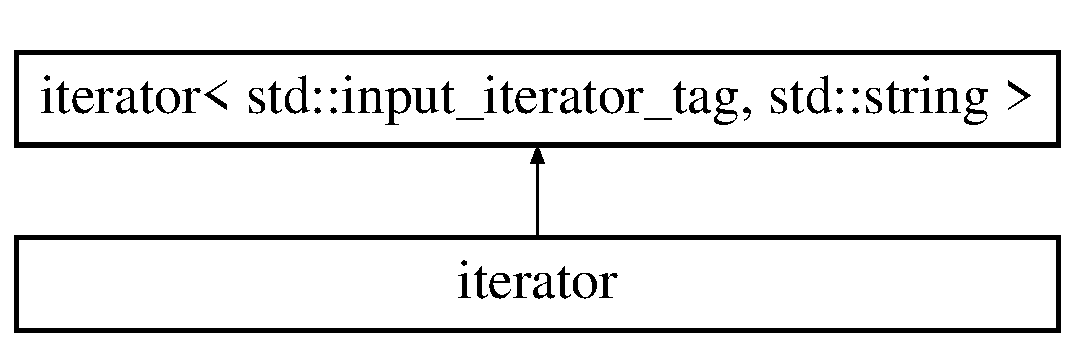
\includegraphics[height=2.000000cm]{classDawgLexicon_1_1iterator}
\end{center}
\end{figure}
\subsection*{Public Member Functions}
\begin{DoxyCompactItemize}
\item 
\mbox{\hyperlink{classDawgLexicon_1_1iterator_a67d652c2433cf9217ed2a1485092fdd1}{iterator}} ()
\item 
\mbox{\hyperlink{classDawgLexicon_1_1iterator_a914aea962a8d01c41cdd8926ce837256}{iterator}} (const \mbox{\hyperlink{classDawgLexicon}{Dawg\+Lexicon}} $\ast$the\+LP, bool end\+Flag)
\item 
\mbox{\hyperlink{classDawgLexicon_1_1iterator_a698b7553261e7209d6c29fb55627dce4}{iterator}} (const \mbox{\hyperlink{classDawgLexicon_1_1iterator}{iterator}} \&it)
\item 
bool \mbox{\hyperlink{classDawgLexicon_1_1iterator_ae1983f2cb0df1f0cbe77ac29590e2e2b}{operator!=}} (const \mbox{\hyperlink{classDawgLexicon_1_1iterator}{iterator}} \&rhs)
\item 
std\+::string \mbox{\hyperlink{classDawgLexicon_1_1iterator_aa3864db3883c7a53277427a06ed3e017}{operator$\ast$}} ()
\item 
\mbox{\hyperlink{classDawgLexicon_1_1iterator}{iterator}} \& \mbox{\hyperlink{classDawgLexicon_1_1iterator_af1b1c7856a59f34c7d3570f946a2ff00}{operator++}} ()
\item 
\mbox{\hyperlink{classDawgLexicon_1_1iterator}{iterator}} \mbox{\hyperlink{classDawgLexicon_1_1iterator_a538d230f8b52d2bc0950e26ce74ec239}{operator++}} (int)
\item 
std\+::string $\ast$ \mbox{\hyperlink{classDawgLexicon_1_1iterator_a67990a1056b32b659082cbb0bc6ab34a}{operator-\/$>$}} ()
\item 
bool \mbox{\hyperlink{classDawgLexicon_1_1iterator_a798956e7a65ef16c891d129b3ced0f9e}{operator==}} (const \mbox{\hyperlink{classDawgLexicon_1_1iterator}{iterator}} \&rhs)
\end{DoxyCompactItemize}


\subsection{Constructor \& Destructor Documentation}
\mbox{\Hypertarget{classDawgLexicon_1_1iterator_a67d652c2433cf9217ed2a1485092fdd1}\label{classDawgLexicon_1_1iterator_a67d652c2433cf9217ed2a1485092fdd1}} 
\index{Dawg\+Lexicon\+::iterator@{Dawg\+Lexicon\+::iterator}!iterator@{iterator}}
\index{iterator@{iterator}!Dawg\+Lexicon\+::iterator@{Dawg\+Lexicon\+::iterator}}
\subsubsection{\texorpdfstring{iterator()}{iterator()}\hspace{0.1cm}{\footnotesize\ttfamily [1/3]}}
{\footnotesize\ttfamily \mbox{\hyperlink{classDawgLexicon_1_1iterator}{iterator}} (\begin{DoxyParamCaption}{ }\end{DoxyParamCaption})\hspace{0.3cm}{\ttfamily [inline]}}

\mbox{\Hypertarget{classDawgLexicon_1_1iterator_a914aea962a8d01c41cdd8926ce837256}\label{classDawgLexicon_1_1iterator_a914aea962a8d01c41cdd8926ce837256}} 
\index{Dawg\+Lexicon\+::iterator@{Dawg\+Lexicon\+::iterator}!iterator@{iterator}}
\index{iterator@{iterator}!Dawg\+Lexicon\+::iterator@{Dawg\+Lexicon\+::iterator}}
\subsubsection{\texorpdfstring{iterator()}{iterator()}\hspace{0.1cm}{\footnotesize\ttfamily [2/3]}}
{\footnotesize\ttfamily \mbox{\hyperlink{classDawgLexicon_1_1iterator}{iterator}} (\begin{DoxyParamCaption}\item[{const \mbox{\hyperlink{classDawgLexicon}{Dawg\+Lexicon}} $\ast$}]{the\+LP,  }\item[{bool}]{end\+Flag }\end{DoxyParamCaption})\hspace{0.3cm}{\ttfamily [inline]}}

\mbox{\Hypertarget{classDawgLexicon_1_1iterator_a698b7553261e7209d6c29fb55627dce4}\label{classDawgLexicon_1_1iterator_a698b7553261e7209d6c29fb55627dce4}} 
\index{Dawg\+Lexicon\+::iterator@{Dawg\+Lexicon\+::iterator}!iterator@{iterator}}
\index{iterator@{iterator}!Dawg\+Lexicon\+::iterator@{Dawg\+Lexicon\+::iterator}}
\subsubsection{\texorpdfstring{iterator()}{iterator()}\hspace{0.1cm}{\footnotesize\ttfamily [3/3]}}
{\footnotesize\ttfamily \mbox{\hyperlink{classDawgLexicon_1_1iterator}{iterator}} (\begin{DoxyParamCaption}\item[{const \mbox{\hyperlink{classDawgLexicon_1_1iterator}{iterator}} \&}]{it }\end{DoxyParamCaption})\hspace{0.3cm}{\ttfamily [inline]}}



\subsection{Member Function Documentation}
\mbox{\Hypertarget{classDawgLexicon_1_1iterator_ae1983f2cb0df1f0cbe77ac29590e2e2b}\label{classDawgLexicon_1_1iterator_ae1983f2cb0df1f0cbe77ac29590e2e2b}} 
\index{Dawg\+Lexicon\+::iterator@{Dawg\+Lexicon\+::iterator}!operator"!=@{operator"!=}}
\index{operator"!=@{operator"!=}!Dawg\+Lexicon\+::iterator@{Dawg\+Lexicon\+::iterator}}
\subsubsection{\texorpdfstring{operator"!=()}{operator!=()}}
{\footnotesize\ttfamily bool operator!= (\begin{DoxyParamCaption}\item[{const \mbox{\hyperlink{classDawgLexicon_1_1iterator}{iterator}} \&}]{rhs }\end{DoxyParamCaption})\hspace{0.3cm}{\ttfamily [inline]}}

\mbox{\Hypertarget{classDawgLexicon_1_1iterator_aa3864db3883c7a53277427a06ed3e017}\label{classDawgLexicon_1_1iterator_aa3864db3883c7a53277427a06ed3e017}} 
\index{Dawg\+Lexicon\+::iterator@{Dawg\+Lexicon\+::iterator}!operator$\ast$@{operator$\ast$}}
\index{operator$\ast$@{operator$\ast$}!Dawg\+Lexicon\+::iterator@{Dawg\+Lexicon\+::iterator}}
\subsubsection{\texorpdfstring{operator$\ast$()}{operator*()}}
{\footnotesize\ttfamily std\+::string operator$\ast$ (\begin{DoxyParamCaption}{ }\end{DoxyParamCaption})\hspace{0.3cm}{\ttfamily [inline]}}

\mbox{\Hypertarget{classDawgLexicon_1_1iterator_af1b1c7856a59f34c7d3570f946a2ff00}\label{classDawgLexicon_1_1iterator_af1b1c7856a59f34c7d3570f946a2ff00}} 
\index{Dawg\+Lexicon\+::iterator@{Dawg\+Lexicon\+::iterator}!operator++@{operator++}}
\index{operator++@{operator++}!Dawg\+Lexicon\+::iterator@{Dawg\+Lexicon\+::iterator}}
\subsubsection{\texorpdfstring{operator++()}{operator++()}\hspace{0.1cm}{\footnotesize\ttfamily [1/2]}}
{\footnotesize\ttfamily \mbox{\hyperlink{classDawgLexicon_1_1iterator}{iterator}}\& operator++ (\begin{DoxyParamCaption}{ }\end{DoxyParamCaption})\hspace{0.3cm}{\ttfamily [inline]}}

\mbox{\Hypertarget{classDawgLexicon_1_1iterator_a538d230f8b52d2bc0950e26ce74ec239}\label{classDawgLexicon_1_1iterator_a538d230f8b52d2bc0950e26ce74ec239}} 
\index{Dawg\+Lexicon\+::iterator@{Dawg\+Lexicon\+::iterator}!operator++@{operator++}}
\index{operator++@{operator++}!Dawg\+Lexicon\+::iterator@{Dawg\+Lexicon\+::iterator}}
\subsubsection{\texorpdfstring{operator++()}{operator++()}\hspace{0.1cm}{\footnotesize\ttfamily [2/2]}}
{\footnotesize\ttfamily \mbox{\hyperlink{classDawgLexicon_1_1iterator}{iterator}} operator++ (\begin{DoxyParamCaption}\item[{int}]{ }\end{DoxyParamCaption})\hspace{0.3cm}{\ttfamily [inline]}}

\mbox{\Hypertarget{classDawgLexicon_1_1iterator_a67990a1056b32b659082cbb0bc6ab34a}\label{classDawgLexicon_1_1iterator_a67990a1056b32b659082cbb0bc6ab34a}} 
\index{Dawg\+Lexicon\+::iterator@{Dawg\+Lexicon\+::iterator}!operator-\/$>$@{operator-\/$>$}}
\index{operator-\/$>$@{operator-\/$>$}!Dawg\+Lexicon\+::iterator@{Dawg\+Lexicon\+::iterator}}
\subsubsection{\texorpdfstring{operator-\/$>$()}{operator->()}}
{\footnotesize\ttfamily std\+::string$\ast$ operator-\/$>$ (\begin{DoxyParamCaption}{ }\end{DoxyParamCaption})\hspace{0.3cm}{\ttfamily [inline]}}

\mbox{\Hypertarget{classDawgLexicon_1_1iterator_a798956e7a65ef16c891d129b3ced0f9e}\label{classDawgLexicon_1_1iterator_a798956e7a65ef16c891d129b3ced0f9e}} 
\index{Dawg\+Lexicon\+::iterator@{Dawg\+Lexicon\+::iterator}!operator==@{operator==}}
\index{operator==@{operator==}!Dawg\+Lexicon\+::iterator@{Dawg\+Lexicon\+::iterator}}
\subsubsection{\texorpdfstring{operator==()}{operator==()}}
{\footnotesize\ttfamily bool operator== (\begin{DoxyParamCaption}\item[{const \mbox{\hyperlink{classDawgLexicon_1_1iterator}{iterator}} \&}]{rhs }\end{DoxyParamCaption})\hspace{0.3cm}{\ttfamily [inline]}}


\hypertarget{classGrid_1_1iterator}{}\section{Grid$<$ Value\+Type $>$\+:\+:iterator Class Reference}
\label{classGrid_1_1iterator}\index{Grid$<$ Value\+Type $>$\+::iterator@{Grid$<$ Value\+Type $>$\+::iterator}}


{\ttfamily \#include $<$grid.\+h$>$}

Inheritance diagram for Grid$<$ Value\+Type $>$\+:\+:iterator\+:\begin{figure}[H]
\begin{center}
\leavevmode
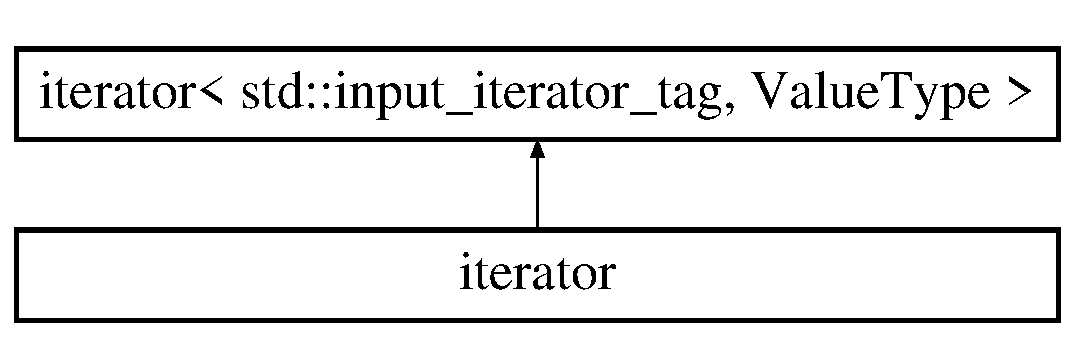
\includegraphics[height=2.000000cm]{classGrid_1_1iterator}
\end{center}
\end{figure}
\subsection*{Public Member Functions}
\begin{DoxyCompactItemize}
\item 
\mbox{\hyperlink{classGrid_1_1iterator_a24675920b744cc15e50807e857fa88cb}{iterator}} (const \mbox{\hyperlink{classGrid}{Grid}} $\ast$the\+Gp, int the\+Index)
\item 
\mbox{\hyperlink{classGrid_1_1iterator_a698b7553261e7209d6c29fb55627dce4}{iterator}} (const \mbox{\hyperlink{classGrid_1_1iterator}{iterator}} \&it)
\item 
bool \mbox{\hyperlink{classGrid_1_1iterator_ae1983f2cb0df1f0cbe77ac29590e2e2b}{operator!=}} (const \mbox{\hyperlink{classGrid_1_1iterator}{iterator}} \&rhs)
\item 
Value\+Type \& \mbox{\hyperlink{classGrid_1_1iterator_ae7b3826e734ec2f7c79f5196fad83989}{operator$\ast$}} ()
\item 
\mbox{\hyperlink{classGrid_1_1iterator}{iterator}} \& \mbox{\hyperlink{classGrid_1_1iterator_af1b1c7856a59f34c7d3570f946a2ff00}{operator++}} ()
\item 
\mbox{\hyperlink{classGrid_1_1iterator}{iterator}} \mbox{\hyperlink{classGrid_1_1iterator_a538d230f8b52d2bc0950e26ce74ec239}{operator++}} (int)
\item 
Value\+Type $\ast$ \mbox{\hyperlink{classGrid_1_1iterator_a5ba42337ec7bae549bb135838933b0ea}{operator-\/$>$}} ()
\item 
bool \mbox{\hyperlink{classGrid_1_1iterator_a798956e7a65ef16c891d129b3ced0f9e}{operator==}} (const \mbox{\hyperlink{classGrid_1_1iterator}{iterator}} \&rhs)
\item 
unsigned int \mbox{\hyperlink{classGrid_1_1iterator_a0aa696ccb72cbf928535d6b646bac1aa}{version}} () const
\end{DoxyCompactItemize}


\subsection{Constructor \& Destructor Documentation}
\mbox{\Hypertarget{classGrid_1_1iterator_a24675920b744cc15e50807e857fa88cb}\label{classGrid_1_1iterator_a24675920b744cc15e50807e857fa88cb}} 
\index{Grid\+::iterator@{Grid\+::iterator}!iterator@{iterator}}
\index{iterator@{iterator}!Grid\+::iterator@{Grid\+::iterator}}
\subsubsection{\texorpdfstring{iterator()}{iterator()}\hspace{0.1cm}{\footnotesize\ttfamily [1/2]}}
{\footnotesize\ttfamily \mbox{\hyperlink{classGrid_1_1iterator}{iterator}} (\begin{DoxyParamCaption}\item[{const \mbox{\hyperlink{classGrid}{Grid}} $\ast$}]{the\+Gp,  }\item[{int}]{the\+Index }\end{DoxyParamCaption})\hspace{0.3cm}{\ttfamily [inline]}}

\mbox{\Hypertarget{classGrid_1_1iterator_a698b7553261e7209d6c29fb55627dce4}\label{classGrid_1_1iterator_a698b7553261e7209d6c29fb55627dce4}} 
\index{Grid\+::iterator@{Grid\+::iterator}!iterator@{iterator}}
\index{iterator@{iterator}!Grid\+::iterator@{Grid\+::iterator}}
\subsubsection{\texorpdfstring{iterator()}{iterator()}\hspace{0.1cm}{\footnotesize\ttfamily [2/2]}}
{\footnotesize\ttfamily \mbox{\hyperlink{classGrid_1_1iterator}{iterator}} (\begin{DoxyParamCaption}\item[{const \mbox{\hyperlink{classGrid_1_1iterator}{iterator}} \&}]{it }\end{DoxyParamCaption})\hspace{0.3cm}{\ttfamily [inline]}}



\subsection{Member Function Documentation}
\mbox{\Hypertarget{classGrid_1_1iterator_ae1983f2cb0df1f0cbe77ac29590e2e2b}\label{classGrid_1_1iterator_ae1983f2cb0df1f0cbe77ac29590e2e2b}} 
\index{Grid\+::iterator@{Grid\+::iterator}!operator"!=@{operator"!=}}
\index{operator"!=@{operator"!=}!Grid\+::iterator@{Grid\+::iterator}}
\subsubsection{\texorpdfstring{operator"!=()}{operator!=()}}
{\footnotesize\ttfamily bool operator!= (\begin{DoxyParamCaption}\item[{const \mbox{\hyperlink{classGrid_1_1iterator}{iterator}} \&}]{rhs }\end{DoxyParamCaption})\hspace{0.3cm}{\ttfamily [inline]}}

\mbox{\Hypertarget{classGrid_1_1iterator_ae7b3826e734ec2f7c79f5196fad83989}\label{classGrid_1_1iterator_ae7b3826e734ec2f7c79f5196fad83989}} 
\index{Grid\+::iterator@{Grid\+::iterator}!operator$\ast$@{operator$\ast$}}
\index{operator$\ast$@{operator$\ast$}!Grid\+::iterator@{Grid\+::iterator}}
\subsubsection{\texorpdfstring{operator$\ast$()}{operator*()}}
{\footnotesize\ttfamily Value\+Type\& operator$\ast$ (\begin{DoxyParamCaption}{ }\end{DoxyParamCaption})\hspace{0.3cm}{\ttfamily [inline]}}

\mbox{\Hypertarget{classGrid_1_1iterator_af1b1c7856a59f34c7d3570f946a2ff00}\label{classGrid_1_1iterator_af1b1c7856a59f34c7d3570f946a2ff00}} 
\index{Grid\+::iterator@{Grid\+::iterator}!operator++@{operator++}}
\index{operator++@{operator++}!Grid\+::iterator@{Grid\+::iterator}}
\subsubsection{\texorpdfstring{operator++()}{operator++()}\hspace{0.1cm}{\footnotesize\ttfamily [1/2]}}
{\footnotesize\ttfamily \mbox{\hyperlink{classGrid_1_1iterator}{iterator}}\& operator++ (\begin{DoxyParamCaption}{ }\end{DoxyParamCaption})\hspace{0.3cm}{\ttfamily [inline]}}

\mbox{\Hypertarget{classGrid_1_1iterator_a538d230f8b52d2bc0950e26ce74ec239}\label{classGrid_1_1iterator_a538d230f8b52d2bc0950e26ce74ec239}} 
\index{Grid\+::iterator@{Grid\+::iterator}!operator++@{operator++}}
\index{operator++@{operator++}!Grid\+::iterator@{Grid\+::iterator}}
\subsubsection{\texorpdfstring{operator++()}{operator++()}\hspace{0.1cm}{\footnotesize\ttfamily [2/2]}}
{\footnotesize\ttfamily \mbox{\hyperlink{classGrid_1_1iterator}{iterator}} operator++ (\begin{DoxyParamCaption}\item[{int}]{ }\end{DoxyParamCaption})\hspace{0.3cm}{\ttfamily [inline]}}

\mbox{\Hypertarget{classGrid_1_1iterator_a5ba42337ec7bae549bb135838933b0ea}\label{classGrid_1_1iterator_a5ba42337ec7bae549bb135838933b0ea}} 
\index{Grid\+::iterator@{Grid\+::iterator}!operator-\/$>$@{operator-\/$>$}}
\index{operator-\/$>$@{operator-\/$>$}!Grid\+::iterator@{Grid\+::iterator}}
\subsubsection{\texorpdfstring{operator-\/$>$()}{operator->()}}
{\footnotesize\ttfamily Value\+Type$\ast$ operator-\/$>$ (\begin{DoxyParamCaption}{ }\end{DoxyParamCaption})\hspace{0.3cm}{\ttfamily [inline]}}

\mbox{\Hypertarget{classGrid_1_1iterator_a798956e7a65ef16c891d129b3ced0f9e}\label{classGrid_1_1iterator_a798956e7a65ef16c891d129b3ced0f9e}} 
\index{Grid\+::iterator@{Grid\+::iterator}!operator==@{operator==}}
\index{operator==@{operator==}!Grid\+::iterator@{Grid\+::iterator}}
\subsubsection{\texorpdfstring{operator==()}{operator==()}}
{\footnotesize\ttfamily bool operator== (\begin{DoxyParamCaption}\item[{const \mbox{\hyperlink{classGrid_1_1iterator}{iterator}} \&}]{rhs }\end{DoxyParamCaption})\hspace{0.3cm}{\ttfamily [inline]}}

\mbox{\Hypertarget{classGrid_1_1iterator_a0aa696ccb72cbf928535d6b646bac1aa}\label{classGrid_1_1iterator_a0aa696ccb72cbf928535d6b646bac1aa}} 
\index{Grid\+::iterator@{Grid\+::iterator}!version@{version}}
\index{version@{version}!Grid\+::iterator@{Grid\+::iterator}}
\subsubsection{\texorpdfstring{version()}{version()}}
{\footnotesize\ttfamily unsigned int version (\begin{DoxyParamCaption}{ }\end{DoxyParamCaption}) const\hspace{0.3cm}{\ttfamily [inline]}}


\hypertarget{classHashMap_1_1iterator}{}\section{Hash\+Map$<$ Key\+Type, Value\+Type $>$\+:\+:iterator Class Reference}
\label{classHashMap_1_1iterator}\index{Hash\+Map$<$ Key\+Type, Value\+Type $>$\+::iterator@{Hash\+Map$<$ Key\+Type, Value\+Type $>$\+::iterator}}


{\ttfamily \#include $<$hashmap.\+h$>$}

Inheritance diagram for Hash\+Map$<$ Key\+Type, Value\+Type $>$\+:\+:iterator\+:\begin{figure}[H]
\begin{center}
\leavevmode
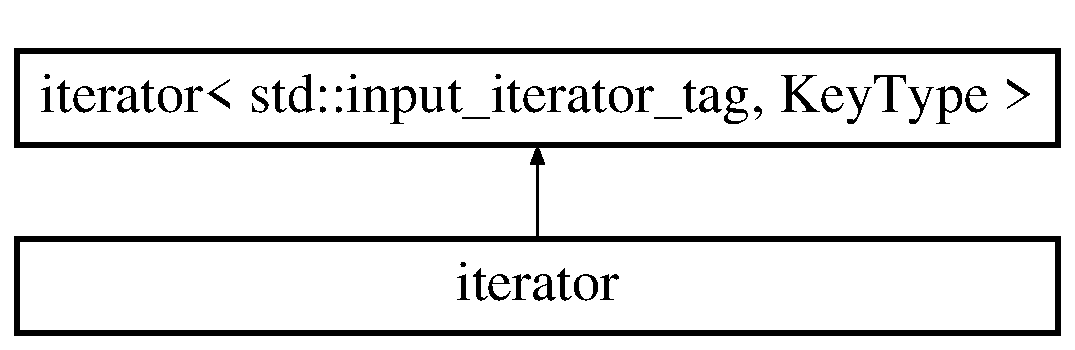
\includegraphics[height=2.000000cm]{classHashMap_1_1iterator}
\end{center}
\end{figure}
\subsection*{Public Member Functions}
\begin{DoxyCompactItemize}
\item 
\mbox{\hyperlink{classHashMap_1_1iterator_a67d652c2433cf9217ed2a1485092fdd1}{iterator}} ()
\item 
\mbox{\hyperlink{classHashMap_1_1iterator_a1181555cedbd9186b537b54bc4e4fe53}{iterator}} (const \mbox{\hyperlink{classHashMap}{Hash\+Map}} $\ast$mp, bool \mbox{\hyperlink{classHashMap_a68b688a51bd0cf6fb5bc2cba292209a8}{end}})
\item 
\mbox{\hyperlink{classHashMap_1_1iterator_a698b7553261e7209d6c29fb55627dce4}{iterator}} (const \mbox{\hyperlink{classHashMap_1_1iterator}{iterator}} \&it)
\item 
bool \mbox{\hyperlink{classHashMap_1_1iterator_ae1983f2cb0df1f0cbe77ac29590e2e2b}{operator!=}} (const \mbox{\hyperlink{classHashMap_1_1iterator}{iterator}} \&rhs)
\item 
Key\+Type \& \mbox{\hyperlink{classHashMap_1_1iterator_a26107e2ced3252ee2bf81dd666739da7}{operator$\ast$}} ()
\item 
\mbox{\hyperlink{classHashMap_1_1iterator}{iterator}} \& \mbox{\hyperlink{classHashMap_1_1iterator_af1b1c7856a59f34c7d3570f946a2ff00}{operator++}} ()
\item 
\mbox{\hyperlink{classHashMap_1_1iterator}{iterator}} \mbox{\hyperlink{classHashMap_1_1iterator_a538d230f8b52d2bc0950e26ce74ec239}{operator++}} (int)
\item 
Key\+Type $\ast$ \mbox{\hyperlink{classHashMap_1_1iterator_a917c74872cce637554f68ebe3c666785}{operator-\/$>$}} ()
\item 
bool \mbox{\hyperlink{classHashMap_1_1iterator_a798956e7a65ef16c891d129b3ced0f9e}{operator==}} (const \mbox{\hyperlink{classHashMap_1_1iterator}{iterator}} \&rhs)
\item 
unsigned int \mbox{\hyperlink{classHashMap_1_1iterator_a0aa696ccb72cbf928535d6b646bac1aa}{version}} () const
\end{DoxyCompactItemize}
\subsection*{Friends}
\begin{DoxyCompactItemize}
\item 
class \mbox{\hyperlink{classHashMap_1_1iterator_ab6054287e6f409207af3fa16e49046ad}{Hash\+Map}}
\end{DoxyCompactItemize}


\subsection{Constructor \& Destructor Documentation}
\mbox{\Hypertarget{classHashMap_1_1iterator_a67d652c2433cf9217ed2a1485092fdd1}\label{classHashMap_1_1iterator_a67d652c2433cf9217ed2a1485092fdd1}} 
\index{Hash\+Map\+::iterator@{Hash\+Map\+::iterator}!iterator@{iterator}}
\index{iterator@{iterator}!Hash\+Map\+::iterator@{Hash\+Map\+::iterator}}
\subsubsection{\texorpdfstring{iterator()}{iterator()}\hspace{0.1cm}{\footnotesize\ttfamily [1/3]}}
{\footnotesize\ttfamily \mbox{\hyperlink{classHashMap_1_1iterator}{iterator}} (\begin{DoxyParamCaption}{ }\end{DoxyParamCaption})\hspace{0.3cm}{\ttfamily [inline]}}

\mbox{\Hypertarget{classHashMap_1_1iterator_a1181555cedbd9186b537b54bc4e4fe53}\label{classHashMap_1_1iterator_a1181555cedbd9186b537b54bc4e4fe53}} 
\index{Hash\+Map\+::iterator@{Hash\+Map\+::iterator}!iterator@{iterator}}
\index{iterator@{iterator}!Hash\+Map\+::iterator@{Hash\+Map\+::iterator}}
\subsubsection{\texorpdfstring{iterator()}{iterator()}\hspace{0.1cm}{\footnotesize\ttfamily [2/3]}}
{\footnotesize\ttfamily \mbox{\hyperlink{classHashMap_1_1iterator}{iterator}} (\begin{DoxyParamCaption}\item[{const \mbox{\hyperlink{classHashMap}{Hash\+Map}} $\ast$}]{mp,  }\item[{bool}]{end }\end{DoxyParamCaption})\hspace{0.3cm}{\ttfamily [inline]}}

\mbox{\Hypertarget{classHashMap_1_1iterator_a698b7553261e7209d6c29fb55627dce4}\label{classHashMap_1_1iterator_a698b7553261e7209d6c29fb55627dce4}} 
\index{Hash\+Map\+::iterator@{Hash\+Map\+::iterator}!iterator@{iterator}}
\index{iterator@{iterator}!Hash\+Map\+::iterator@{Hash\+Map\+::iterator}}
\subsubsection{\texorpdfstring{iterator()}{iterator()}\hspace{0.1cm}{\footnotesize\ttfamily [3/3]}}
{\footnotesize\ttfamily \mbox{\hyperlink{classHashMap_1_1iterator}{iterator}} (\begin{DoxyParamCaption}\item[{const \mbox{\hyperlink{classHashMap_1_1iterator}{iterator}} \&}]{it }\end{DoxyParamCaption})\hspace{0.3cm}{\ttfamily [inline]}}



\subsection{Member Function Documentation}
\mbox{\Hypertarget{classHashMap_1_1iterator_ae1983f2cb0df1f0cbe77ac29590e2e2b}\label{classHashMap_1_1iterator_ae1983f2cb0df1f0cbe77ac29590e2e2b}} 
\index{Hash\+Map\+::iterator@{Hash\+Map\+::iterator}!operator"!=@{operator"!=}}
\index{operator"!=@{operator"!=}!Hash\+Map\+::iterator@{Hash\+Map\+::iterator}}
\subsubsection{\texorpdfstring{operator"!=()}{operator!=()}}
{\footnotesize\ttfamily bool operator!= (\begin{DoxyParamCaption}\item[{const \mbox{\hyperlink{classHashMap_1_1iterator}{iterator}} \&}]{rhs }\end{DoxyParamCaption})\hspace{0.3cm}{\ttfamily [inline]}}

\mbox{\Hypertarget{classHashMap_1_1iterator_a26107e2ced3252ee2bf81dd666739da7}\label{classHashMap_1_1iterator_a26107e2ced3252ee2bf81dd666739da7}} 
\index{Hash\+Map\+::iterator@{Hash\+Map\+::iterator}!operator$\ast$@{operator$\ast$}}
\index{operator$\ast$@{operator$\ast$}!Hash\+Map\+::iterator@{Hash\+Map\+::iterator}}
\subsubsection{\texorpdfstring{operator$\ast$()}{operator*()}}
{\footnotesize\ttfamily Key\+Type\& operator$\ast$ (\begin{DoxyParamCaption}{ }\end{DoxyParamCaption})\hspace{0.3cm}{\ttfamily [inline]}}

\mbox{\Hypertarget{classHashMap_1_1iterator_af1b1c7856a59f34c7d3570f946a2ff00}\label{classHashMap_1_1iterator_af1b1c7856a59f34c7d3570f946a2ff00}} 
\index{Hash\+Map\+::iterator@{Hash\+Map\+::iterator}!operator++@{operator++}}
\index{operator++@{operator++}!Hash\+Map\+::iterator@{Hash\+Map\+::iterator}}
\subsubsection{\texorpdfstring{operator++()}{operator++()}\hspace{0.1cm}{\footnotesize\ttfamily [1/2]}}
{\footnotesize\ttfamily \mbox{\hyperlink{classHashMap_1_1iterator}{iterator}}\& operator++ (\begin{DoxyParamCaption}{ }\end{DoxyParamCaption})\hspace{0.3cm}{\ttfamily [inline]}}

\mbox{\Hypertarget{classHashMap_1_1iterator_a538d230f8b52d2bc0950e26ce74ec239}\label{classHashMap_1_1iterator_a538d230f8b52d2bc0950e26ce74ec239}} 
\index{Hash\+Map\+::iterator@{Hash\+Map\+::iterator}!operator++@{operator++}}
\index{operator++@{operator++}!Hash\+Map\+::iterator@{Hash\+Map\+::iterator}}
\subsubsection{\texorpdfstring{operator++()}{operator++()}\hspace{0.1cm}{\footnotesize\ttfamily [2/2]}}
{\footnotesize\ttfamily \mbox{\hyperlink{classHashMap_1_1iterator}{iterator}} operator++ (\begin{DoxyParamCaption}\item[{int}]{ }\end{DoxyParamCaption})\hspace{0.3cm}{\ttfamily [inline]}}

\mbox{\Hypertarget{classHashMap_1_1iterator_a917c74872cce637554f68ebe3c666785}\label{classHashMap_1_1iterator_a917c74872cce637554f68ebe3c666785}} 
\index{Hash\+Map\+::iterator@{Hash\+Map\+::iterator}!operator-\/$>$@{operator-\/$>$}}
\index{operator-\/$>$@{operator-\/$>$}!Hash\+Map\+::iterator@{Hash\+Map\+::iterator}}
\subsubsection{\texorpdfstring{operator-\/$>$()}{operator->()}}
{\footnotesize\ttfamily Key\+Type$\ast$ operator-\/$>$ (\begin{DoxyParamCaption}{ }\end{DoxyParamCaption})\hspace{0.3cm}{\ttfamily [inline]}}

\mbox{\Hypertarget{classHashMap_1_1iterator_a798956e7a65ef16c891d129b3ced0f9e}\label{classHashMap_1_1iterator_a798956e7a65ef16c891d129b3ced0f9e}} 
\index{Hash\+Map\+::iterator@{Hash\+Map\+::iterator}!operator==@{operator==}}
\index{operator==@{operator==}!Hash\+Map\+::iterator@{Hash\+Map\+::iterator}}
\subsubsection{\texorpdfstring{operator==()}{operator==()}}
{\footnotesize\ttfamily bool operator== (\begin{DoxyParamCaption}\item[{const \mbox{\hyperlink{classHashMap_1_1iterator}{iterator}} \&}]{rhs }\end{DoxyParamCaption})\hspace{0.3cm}{\ttfamily [inline]}}

\mbox{\Hypertarget{classHashMap_1_1iterator_a0aa696ccb72cbf928535d6b646bac1aa}\label{classHashMap_1_1iterator_a0aa696ccb72cbf928535d6b646bac1aa}} 
\index{Hash\+Map\+::iterator@{Hash\+Map\+::iterator}!version@{version}}
\index{version@{version}!Hash\+Map\+::iterator@{Hash\+Map\+::iterator}}
\subsubsection{\texorpdfstring{version()}{version()}}
{\footnotesize\ttfamily unsigned int version (\begin{DoxyParamCaption}{ }\end{DoxyParamCaption}) const\hspace{0.3cm}{\ttfamily [inline]}}



\subsection{Friends And Related Function Documentation}
\mbox{\Hypertarget{classHashMap_1_1iterator_ab6054287e6f409207af3fa16e49046ad}\label{classHashMap_1_1iterator_ab6054287e6f409207af3fa16e49046ad}} 
\index{Hash\+Map\+::iterator@{Hash\+Map\+::iterator}!Hash\+Map@{Hash\+Map}}
\index{Hash\+Map@{Hash\+Map}!Hash\+Map\+::iterator@{Hash\+Map\+::iterator}}
\subsubsection{\texorpdfstring{Hash\+Map}{HashMap}}
{\footnotesize\ttfamily friend class \mbox{\hyperlink{classHashMap}{Hash\+Map}}\hspace{0.3cm}{\ttfamily [friend]}}


\hypertarget{classHashSet_1_1iterator}{}\section{Hash\+Set$<$ Value\+Type $>$\+:\+:iterator Class Reference}
\label{classHashSet_1_1iterator}\index{Hash\+Set$<$ Value\+Type $>$\+::iterator@{Hash\+Set$<$ Value\+Type $>$\+::iterator}}


{\ttfamily \#include $<$hashset.\+h$>$}

Inheritance diagram for Hash\+Set$<$ Value\+Type $>$\+:\+:iterator\+:\begin{figure}[H]
\begin{center}
\leavevmode
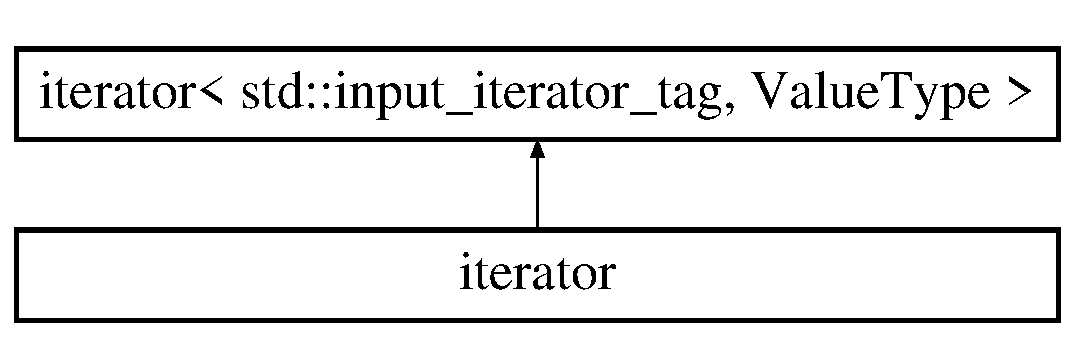
\includegraphics[height=2.000000cm]{classHashSet_1_1iterator}
\end{center}
\end{figure}
\subsection*{Public Member Functions}
\begin{DoxyCompactItemize}
\item 
\mbox{\hyperlink{classHashSet_1_1iterator_a67d652c2433cf9217ed2a1485092fdd1}{iterator}} ()
\item 
\mbox{\hyperlink{classHashSet_1_1iterator_a6de14de23a5a34012a09370c4d6804d6}{iterator}} (typename \mbox{\hyperlink{classHashMap}{Hash\+Map}}$<$ Value\+Type, bool $>$\+::\mbox{\hyperlink{classHashSet_1_1iterator}{iterator}} it)
\item 
\mbox{\hyperlink{classHashSet_1_1iterator_a698b7553261e7209d6c29fb55627dce4}{iterator}} (const \mbox{\hyperlink{classHashSet_1_1iterator}{iterator}} \&it)
\item 
bool \mbox{\hyperlink{classHashSet_1_1iterator_ae1983f2cb0df1f0cbe77ac29590e2e2b}{operator!=}} (const \mbox{\hyperlink{classHashSet_1_1iterator}{iterator}} \&rhs)
\item 
Value\+Type \& \mbox{\hyperlink{classHashSet_1_1iterator_ae7b3826e734ec2f7c79f5196fad83989}{operator$\ast$}} ()
\item 
\mbox{\hyperlink{classHashSet_1_1iterator}{iterator}} \& \mbox{\hyperlink{classHashSet_1_1iterator_af1b1c7856a59f34c7d3570f946a2ff00}{operator++}} ()
\item 
\mbox{\hyperlink{classHashSet_1_1iterator}{iterator}} \mbox{\hyperlink{classHashSet_1_1iterator_a538d230f8b52d2bc0950e26ce74ec239}{operator++}} (int)
\item 
Value\+Type $\ast$ \mbox{\hyperlink{classHashSet_1_1iterator_a5ba42337ec7bae549bb135838933b0ea}{operator-\/$>$}} ()
\item 
bool \mbox{\hyperlink{classHashSet_1_1iterator_a798956e7a65ef16c891d129b3ced0f9e}{operator==}} (const \mbox{\hyperlink{classHashSet_1_1iterator}{iterator}} \&rhs)
\end{DoxyCompactItemize}


\subsection{Constructor \& Destructor Documentation}
\mbox{\Hypertarget{classHashSet_1_1iterator_a67d652c2433cf9217ed2a1485092fdd1}\label{classHashSet_1_1iterator_a67d652c2433cf9217ed2a1485092fdd1}} 
\index{Hash\+Set\+::iterator@{Hash\+Set\+::iterator}!iterator@{iterator}}
\index{iterator@{iterator}!Hash\+Set\+::iterator@{Hash\+Set\+::iterator}}
\subsubsection{\texorpdfstring{iterator()}{iterator()}\hspace{0.1cm}{\footnotesize\ttfamily [1/3]}}
{\footnotesize\ttfamily \mbox{\hyperlink{classHashSet_1_1iterator}{iterator}} (\begin{DoxyParamCaption}{ }\end{DoxyParamCaption})\hspace{0.3cm}{\ttfamily [inline]}}

\mbox{\Hypertarget{classHashSet_1_1iterator_a6de14de23a5a34012a09370c4d6804d6}\label{classHashSet_1_1iterator_a6de14de23a5a34012a09370c4d6804d6}} 
\index{Hash\+Set\+::iterator@{Hash\+Set\+::iterator}!iterator@{iterator}}
\index{iterator@{iterator}!Hash\+Set\+::iterator@{Hash\+Set\+::iterator}}
\subsubsection{\texorpdfstring{iterator()}{iterator()}\hspace{0.1cm}{\footnotesize\ttfamily [2/3]}}
{\footnotesize\ttfamily \mbox{\hyperlink{classHashSet_1_1iterator}{iterator}} (\begin{DoxyParamCaption}\item[{typename \mbox{\hyperlink{classHashMap}{Hash\+Map}}$<$ Value\+Type, bool $>$\+::\mbox{\hyperlink{classHashSet_1_1iterator}{iterator}}}]{it }\end{DoxyParamCaption})\hspace{0.3cm}{\ttfamily [inline]}}

\mbox{\Hypertarget{classHashSet_1_1iterator_a698b7553261e7209d6c29fb55627dce4}\label{classHashSet_1_1iterator_a698b7553261e7209d6c29fb55627dce4}} 
\index{Hash\+Set\+::iterator@{Hash\+Set\+::iterator}!iterator@{iterator}}
\index{iterator@{iterator}!Hash\+Set\+::iterator@{Hash\+Set\+::iterator}}
\subsubsection{\texorpdfstring{iterator()}{iterator()}\hspace{0.1cm}{\footnotesize\ttfamily [3/3]}}
{\footnotesize\ttfamily \mbox{\hyperlink{classHashSet_1_1iterator}{iterator}} (\begin{DoxyParamCaption}\item[{const \mbox{\hyperlink{classHashSet_1_1iterator}{iterator}} \&}]{it }\end{DoxyParamCaption})\hspace{0.3cm}{\ttfamily [inline]}}



\subsection{Member Function Documentation}
\mbox{\Hypertarget{classHashSet_1_1iterator_ae1983f2cb0df1f0cbe77ac29590e2e2b}\label{classHashSet_1_1iterator_ae1983f2cb0df1f0cbe77ac29590e2e2b}} 
\index{Hash\+Set\+::iterator@{Hash\+Set\+::iterator}!operator"!=@{operator"!=}}
\index{operator"!=@{operator"!=}!Hash\+Set\+::iterator@{Hash\+Set\+::iterator}}
\subsubsection{\texorpdfstring{operator"!=()}{operator!=()}}
{\footnotesize\ttfamily bool operator!= (\begin{DoxyParamCaption}\item[{const \mbox{\hyperlink{classHashSet_1_1iterator}{iterator}} \&}]{rhs }\end{DoxyParamCaption})\hspace{0.3cm}{\ttfamily [inline]}}

\mbox{\Hypertarget{classHashSet_1_1iterator_ae7b3826e734ec2f7c79f5196fad83989}\label{classHashSet_1_1iterator_ae7b3826e734ec2f7c79f5196fad83989}} 
\index{Hash\+Set\+::iterator@{Hash\+Set\+::iterator}!operator$\ast$@{operator$\ast$}}
\index{operator$\ast$@{operator$\ast$}!Hash\+Set\+::iterator@{Hash\+Set\+::iterator}}
\subsubsection{\texorpdfstring{operator$\ast$()}{operator*()}}
{\footnotesize\ttfamily Value\+Type\& operator$\ast$ (\begin{DoxyParamCaption}{ }\end{DoxyParamCaption})\hspace{0.3cm}{\ttfamily [inline]}}

\mbox{\Hypertarget{classHashSet_1_1iterator_af1b1c7856a59f34c7d3570f946a2ff00}\label{classHashSet_1_1iterator_af1b1c7856a59f34c7d3570f946a2ff00}} 
\index{Hash\+Set\+::iterator@{Hash\+Set\+::iterator}!operator++@{operator++}}
\index{operator++@{operator++}!Hash\+Set\+::iterator@{Hash\+Set\+::iterator}}
\subsubsection{\texorpdfstring{operator++()}{operator++()}\hspace{0.1cm}{\footnotesize\ttfamily [1/2]}}
{\footnotesize\ttfamily \mbox{\hyperlink{classHashSet_1_1iterator}{iterator}}\& operator++ (\begin{DoxyParamCaption}{ }\end{DoxyParamCaption})\hspace{0.3cm}{\ttfamily [inline]}}

\mbox{\Hypertarget{classHashSet_1_1iterator_a538d230f8b52d2bc0950e26ce74ec239}\label{classHashSet_1_1iterator_a538d230f8b52d2bc0950e26ce74ec239}} 
\index{Hash\+Set\+::iterator@{Hash\+Set\+::iterator}!operator++@{operator++}}
\index{operator++@{operator++}!Hash\+Set\+::iterator@{Hash\+Set\+::iterator}}
\subsubsection{\texorpdfstring{operator++()}{operator++()}\hspace{0.1cm}{\footnotesize\ttfamily [2/2]}}
{\footnotesize\ttfamily \mbox{\hyperlink{classHashSet_1_1iterator}{iterator}} operator++ (\begin{DoxyParamCaption}\item[{int}]{ }\end{DoxyParamCaption})\hspace{0.3cm}{\ttfamily [inline]}}

\mbox{\Hypertarget{classHashSet_1_1iterator_a5ba42337ec7bae549bb135838933b0ea}\label{classHashSet_1_1iterator_a5ba42337ec7bae549bb135838933b0ea}} 
\index{Hash\+Set\+::iterator@{Hash\+Set\+::iterator}!operator-\/$>$@{operator-\/$>$}}
\index{operator-\/$>$@{operator-\/$>$}!Hash\+Set\+::iterator@{Hash\+Set\+::iterator}}
\subsubsection{\texorpdfstring{operator-\/$>$()}{operator->()}}
{\footnotesize\ttfamily Value\+Type$\ast$ operator-\/$>$ (\begin{DoxyParamCaption}{ }\end{DoxyParamCaption})\hspace{0.3cm}{\ttfamily [inline]}}

\mbox{\Hypertarget{classHashSet_1_1iterator_a798956e7a65ef16c891d129b3ced0f9e}\label{classHashSet_1_1iterator_a798956e7a65ef16c891d129b3ced0f9e}} 
\index{Hash\+Set\+::iterator@{Hash\+Set\+::iterator}!operator==@{operator==}}
\index{operator==@{operator==}!Hash\+Set\+::iterator@{Hash\+Set\+::iterator}}
\subsubsection{\texorpdfstring{operator==()}{operator==()}}
{\footnotesize\ttfamily bool operator== (\begin{DoxyParamCaption}\item[{const \mbox{\hyperlink{classHashSet_1_1iterator}{iterator}} \&}]{rhs }\end{DoxyParamCaption})\hspace{0.3cm}{\ttfamily [inline]}}


\hypertarget{classLexicon_1_1iterator}{}\section{Lexicon\+:\+:iterator Class Reference}
\label{classLexicon_1_1iterator}\index{Lexicon\+::iterator@{Lexicon\+::iterator}}


{\ttfamily \#include $<$lexicon.\+h$>$}

Inheritance diagram for Lexicon\+:\+:iterator\+:\begin{figure}[H]
\begin{center}
\leavevmode
\includegraphics[height=3.000000cm]{classLexicon_1_1iterator}
\end{center}
\end{figure}
\subsection*{Public Member Functions}
\begin{DoxyCompactItemize}
\item 
\mbox{\hyperlink{classLexicon_1_1iterator_a67d652c2433cf9217ed2a1485092fdd1}{iterator}} ()
\item 
\mbox{\hyperlink{classLexicon_1_1iterator_a698b7553261e7209d6c29fb55627dce4}{iterator}} (const \mbox{\hyperlink{classLexicon_1_1iterator}{iterator}} \&it)
\item 
\mbox{\hyperlink{classLexicon_1_1iterator_a6cb8fe4bd22d3efd7d0d01387a001009}{iterator}} (const \mbox{\hyperlink{classSet}{Set}}$<$ std\+::string $>$\+::\mbox{\hyperlink{classLexicon_1_1iterator}{iterator}} \&it)
\item 
bool \mbox{\hyperlink{classSet_1_1iterator_ae1983f2cb0df1f0cbe77ac29590e2e2b}{operator!=}} (const \mbox{\hyperlink{classLexicon_1_1iterator}{iterator}} \&rhs)
\item 
Value\+Type \& \mbox{\hyperlink{classSet_1_1iterator_ae7b3826e734ec2f7c79f5196fad83989}{operator$\ast$}} ()
\item 
\mbox{\hyperlink{classLexicon_1_1iterator}{iterator}} \& \mbox{\hyperlink{classSet_1_1iterator_af1b1c7856a59f34c7d3570f946a2ff00}{operator++}} ()
\item 
\mbox{\hyperlink{classLexicon_1_1iterator}{iterator}} \mbox{\hyperlink{classSet_1_1iterator_a538d230f8b52d2bc0950e26ce74ec239}{operator++}} (int)
\item 
Value\+Type $\ast$ \mbox{\hyperlink{classSet_1_1iterator_a5ba42337ec7bae549bb135838933b0ea}{operator-\/$>$}} ()
\item 
bool \mbox{\hyperlink{classSet_1_1iterator_a798956e7a65ef16c891d129b3ced0f9e}{operator==}} (const \mbox{\hyperlink{classLexicon_1_1iterator}{iterator}} \&rhs)
\end{DoxyCompactItemize}


\subsection{Constructor \& Destructor Documentation}
\mbox{\Hypertarget{classLexicon_1_1iterator_a67d652c2433cf9217ed2a1485092fdd1}\label{classLexicon_1_1iterator_a67d652c2433cf9217ed2a1485092fdd1}} 
\index{Lexicon\+::iterator@{Lexicon\+::iterator}!iterator@{iterator}}
\index{iterator@{iterator}!Lexicon\+::iterator@{Lexicon\+::iterator}}
\subsubsection{\texorpdfstring{iterator()}{iterator()}\hspace{0.1cm}{\footnotesize\ttfamily [1/3]}}
{\footnotesize\ttfamily \mbox{\hyperlink{classLexicon_1_1iterator}{iterator}} (\begin{DoxyParamCaption}{ }\end{DoxyParamCaption})\hspace{0.3cm}{\ttfamily [inline]}}

\mbox{\Hypertarget{classLexicon_1_1iterator_a698b7553261e7209d6c29fb55627dce4}\label{classLexicon_1_1iterator_a698b7553261e7209d6c29fb55627dce4}} 
\index{Lexicon\+::iterator@{Lexicon\+::iterator}!iterator@{iterator}}
\index{iterator@{iterator}!Lexicon\+::iterator@{Lexicon\+::iterator}}
\subsubsection{\texorpdfstring{iterator()}{iterator()}\hspace{0.1cm}{\footnotesize\ttfamily [2/3]}}
{\footnotesize\ttfamily \mbox{\hyperlink{classLexicon_1_1iterator}{iterator}} (\begin{DoxyParamCaption}\item[{const \mbox{\hyperlink{classLexicon_1_1iterator}{iterator}} \&}]{it }\end{DoxyParamCaption})\hspace{0.3cm}{\ttfamily [inline]}}

\mbox{\Hypertarget{classLexicon_1_1iterator_a6cb8fe4bd22d3efd7d0d01387a001009}\label{classLexicon_1_1iterator_a6cb8fe4bd22d3efd7d0d01387a001009}} 
\index{Lexicon\+::iterator@{Lexicon\+::iterator}!iterator@{iterator}}
\index{iterator@{iterator}!Lexicon\+::iterator@{Lexicon\+::iterator}}
\subsubsection{\texorpdfstring{iterator()}{iterator()}\hspace{0.1cm}{\footnotesize\ttfamily [3/3]}}
{\footnotesize\ttfamily \mbox{\hyperlink{classLexicon_1_1iterator}{iterator}} (\begin{DoxyParamCaption}\item[{const \mbox{\hyperlink{classSet}{Set}}$<$ std\+::string $>$\+::\mbox{\hyperlink{classLexicon_1_1iterator}{iterator}} \&}]{it }\end{DoxyParamCaption})\hspace{0.3cm}{\ttfamily [inline]}}



\subsection{Member Function Documentation}
\mbox{\Hypertarget{classSet_1_1iterator_ae1983f2cb0df1f0cbe77ac29590e2e2b}\label{classSet_1_1iterator_ae1983f2cb0df1f0cbe77ac29590e2e2b}} 
\index{Lexicon\+::iterator@{Lexicon\+::iterator}!operator"!=@{operator"!=}}
\index{operator"!=@{operator"!=}!Lexicon\+::iterator@{Lexicon\+::iterator}}
\subsubsection{\texorpdfstring{operator"!=()}{operator!=()}}
{\footnotesize\ttfamily bool operator!= (\begin{DoxyParamCaption}\item[{const \mbox{\hyperlink{classSet_1_1iterator}{iterator}} \&}]{rhs }\end{DoxyParamCaption})\hspace{0.3cm}{\ttfamily [inline]}, {\ttfamily [inherited]}}

\mbox{\Hypertarget{classSet_1_1iterator_ae7b3826e734ec2f7c79f5196fad83989}\label{classSet_1_1iterator_ae7b3826e734ec2f7c79f5196fad83989}} 
\index{Lexicon\+::iterator@{Lexicon\+::iterator}!operator$\ast$@{operator$\ast$}}
\index{operator$\ast$@{operator$\ast$}!Lexicon\+::iterator@{Lexicon\+::iterator}}
\subsubsection{\texorpdfstring{operator$\ast$()}{operator*()}}
{\footnotesize\ttfamily Value\+Type\& operator$\ast$ (\begin{DoxyParamCaption}{ }\end{DoxyParamCaption})\hspace{0.3cm}{\ttfamily [inline]}, {\ttfamily [inherited]}}

\mbox{\Hypertarget{classSet_1_1iterator_af1b1c7856a59f34c7d3570f946a2ff00}\label{classSet_1_1iterator_af1b1c7856a59f34c7d3570f946a2ff00}} 
\index{Lexicon\+::iterator@{Lexicon\+::iterator}!operator++@{operator++}}
\index{operator++@{operator++}!Lexicon\+::iterator@{Lexicon\+::iterator}}
\subsubsection{\texorpdfstring{operator++()}{operator++()}\hspace{0.1cm}{\footnotesize\ttfamily [1/2]}}
{\footnotesize\ttfamily \mbox{\hyperlink{classLexicon_1_1iterator}{iterator}}\& operator++ (\begin{DoxyParamCaption}{ }\end{DoxyParamCaption})\hspace{0.3cm}{\ttfamily [inline]}, {\ttfamily [inherited]}}

\mbox{\Hypertarget{classSet_1_1iterator_a538d230f8b52d2bc0950e26ce74ec239}\label{classSet_1_1iterator_a538d230f8b52d2bc0950e26ce74ec239}} 
\index{Lexicon\+::iterator@{Lexicon\+::iterator}!operator++@{operator++}}
\index{operator++@{operator++}!Lexicon\+::iterator@{Lexicon\+::iterator}}
\subsubsection{\texorpdfstring{operator++()}{operator++()}\hspace{0.1cm}{\footnotesize\ttfamily [2/2]}}
{\footnotesize\ttfamily \mbox{\hyperlink{classLexicon_1_1iterator}{iterator}} operator++ (\begin{DoxyParamCaption}\item[{int}]{ }\end{DoxyParamCaption})\hspace{0.3cm}{\ttfamily [inline]}, {\ttfamily [inherited]}}

\mbox{\Hypertarget{classSet_1_1iterator_a5ba42337ec7bae549bb135838933b0ea}\label{classSet_1_1iterator_a5ba42337ec7bae549bb135838933b0ea}} 
\index{Lexicon\+::iterator@{Lexicon\+::iterator}!operator-\/$>$@{operator-\/$>$}}
\index{operator-\/$>$@{operator-\/$>$}!Lexicon\+::iterator@{Lexicon\+::iterator}}
\subsubsection{\texorpdfstring{operator-\/$>$()}{operator->()}}
{\footnotesize\ttfamily Value\+Type$\ast$ operator-\/$>$ (\begin{DoxyParamCaption}{ }\end{DoxyParamCaption})\hspace{0.3cm}{\ttfamily [inline]}, {\ttfamily [inherited]}}

\mbox{\Hypertarget{classSet_1_1iterator_a798956e7a65ef16c891d129b3ced0f9e}\label{classSet_1_1iterator_a798956e7a65ef16c891d129b3ced0f9e}} 
\index{Lexicon\+::iterator@{Lexicon\+::iterator}!operator==@{operator==}}
\index{operator==@{operator==}!Lexicon\+::iterator@{Lexicon\+::iterator}}
\subsubsection{\texorpdfstring{operator==()}{operator==()}}
{\footnotesize\ttfamily bool operator== (\begin{DoxyParamCaption}\item[{const \mbox{\hyperlink{classSet_1_1iterator}{iterator}} \&}]{rhs }\end{DoxyParamCaption})\hspace{0.3cm}{\ttfamily [inline]}, {\ttfamily [inherited]}}


\hypertarget{classLinkedHashMap_1_1iterator}{}\section{Linked\+Hash\+Map$<$ Key\+Type, Value\+Type $>$\+:\+:iterator Class Reference}
\label{classLinkedHashMap_1_1iterator}\index{Linked\+Hash\+Map$<$ Key\+Type, Value\+Type $>$\+::iterator@{Linked\+Hash\+Map$<$ Key\+Type, Value\+Type $>$\+::iterator}}


{\ttfamily \#include $<$linkedhashmap.\+h$>$}



Inherits Vector$<$ Value\+Type $>$\+::iterator.

\subsection*{Public Member Functions}
\begin{DoxyCompactItemize}
\item 
\mbox{\hyperlink{classLinkedHashMap_1_1iterator_a67d652c2433cf9217ed2a1485092fdd1}{iterator}} ()
\item 
\mbox{\hyperlink{classLinkedHashMap_1_1iterator_a698b7553261e7209d6c29fb55627dce4}{iterator}} (const \mbox{\hyperlink{classLinkedHashMap_1_1iterator}{iterator}} \&it)
\item 
\mbox{\hyperlink{classLinkedHashMap_1_1iterator_a3729f4eed7b472132c87cac58a398e43}{iterator}} (const typename \mbox{\hyperlink{classVector}{Vector}}$<$ Key\+Type $>$\+::\mbox{\hyperlink{classLinkedHashMap_1_1iterator}{iterator}} \&it)
\item 
bool {\bfseries operator!=} (const \mbox{\hyperlink{classLinkedHashMap_1_1iterator}{iterator}} \&rhs)
\item 
Value\+Type \& {\bfseries operator$\ast$} ()
\item 
\mbox{\hyperlink{classLinkedHashMap_1_1iterator}{iterator}} {\bfseries operator+} (const int \&rhs)
\item 
\mbox{\hyperlink{classLinkedHashMap_1_1iterator}{iterator}} \& {\bfseries operator++} ()
\item 
\mbox{\hyperlink{classLinkedHashMap_1_1iterator}{iterator}} {\bfseries operator++} (int)
\item 
\mbox{\hyperlink{classLinkedHashMap_1_1iterator}{iterator}} {\bfseries operator+=} (const int \&rhs)
\item 
\mbox{\hyperlink{classLinkedHashMap_1_1iterator}{iterator}} {\bfseries operator-\/} (const int \&rhs)
\item 
int {\bfseries operator-\/} (const \mbox{\hyperlink{classLinkedHashMap_1_1iterator}{iterator}} \&rhs)
\item 
\mbox{\hyperlink{classLinkedHashMap_1_1iterator}{iterator}} \& {\bfseries operator-\/-\/} ()
\item 
\mbox{\hyperlink{classLinkedHashMap_1_1iterator}{iterator}} {\bfseries operator-\/-\/} (int)
\item 
\mbox{\hyperlink{classLinkedHashMap_1_1iterator}{iterator}} {\bfseries operator-\/=} (const int \&rhs)
\item 
Value\+Type $\ast$ {\bfseries operator-\/$>$} ()
\item 
bool {\bfseries operator$<$} (const \mbox{\hyperlink{classLinkedHashMap_1_1iterator}{iterator}} \&rhs)
\item 
bool {\bfseries operator$<$=} (const \mbox{\hyperlink{classLinkedHashMap_1_1iterator}{iterator}} \&rhs)
\item 
bool {\bfseries operator==} (const \mbox{\hyperlink{classLinkedHashMap_1_1iterator}{iterator}} \&rhs)
\item 
bool {\bfseries operator$>$} (const \mbox{\hyperlink{classLinkedHashMap_1_1iterator}{iterator}} \&rhs)
\item 
bool {\bfseries operator$>$=} (const \mbox{\hyperlink{classLinkedHashMap_1_1iterator}{iterator}} \&rhs)
\item 
Value\+Type \& {\bfseries operator\mbox{[}$\,$\mbox{]}} (int k)
\item 
unsigned int {\bfseries version} () const
\end{DoxyCompactItemize}


\subsection{Constructor \& Destructor Documentation}
\mbox{\Hypertarget{classLinkedHashMap_1_1iterator_a67d652c2433cf9217ed2a1485092fdd1}\label{classLinkedHashMap_1_1iterator_a67d652c2433cf9217ed2a1485092fdd1}} 
\index{Linked\+Hash\+Map\+::iterator@{Linked\+Hash\+Map\+::iterator}!iterator@{iterator}}
\index{iterator@{iterator}!Linked\+Hash\+Map\+::iterator@{Linked\+Hash\+Map\+::iterator}}
\subsubsection{\texorpdfstring{iterator()}{iterator()}\hspace{0.1cm}{\footnotesize\ttfamily [1/3]}}
{\footnotesize\ttfamily \mbox{\hyperlink{classLinkedHashMap_1_1iterator}{iterator}} (\begin{DoxyParamCaption}{ }\end{DoxyParamCaption})\hspace{0.3cm}{\ttfamily [inline]}}

\mbox{\Hypertarget{classLinkedHashMap_1_1iterator_a698b7553261e7209d6c29fb55627dce4}\label{classLinkedHashMap_1_1iterator_a698b7553261e7209d6c29fb55627dce4}} 
\index{Linked\+Hash\+Map\+::iterator@{Linked\+Hash\+Map\+::iterator}!iterator@{iterator}}
\index{iterator@{iterator}!Linked\+Hash\+Map\+::iterator@{Linked\+Hash\+Map\+::iterator}}
\subsubsection{\texorpdfstring{iterator()}{iterator()}\hspace{0.1cm}{\footnotesize\ttfamily [2/3]}}
{\footnotesize\ttfamily \mbox{\hyperlink{classLinkedHashMap_1_1iterator}{iterator}} (\begin{DoxyParamCaption}\item[{const \mbox{\hyperlink{classLinkedHashMap_1_1iterator}{iterator}} \&}]{it }\end{DoxyParamCaption})\hspace{0.3cm}{\ttfamily [inline]}}

\mbox{\Hypertarget{classLinkedHashMap_1_1iterator_a3729f4eed7b472132c87cac58a398e43}\label{classLinkedHashMap_1_1iterator_a3729f4eed7b472132c87cac58a398e43}} 
\index{Linked\+Hash\+Map\+::iterator@{Linked\+Hash\+Map\+::iterator}!iterator@{iterator}}
\index{iterator@{iterator}!Linked\+Hash\+Map\+::iterator@{Linked\+Hash\+Map\+::iterator}}
\subsubsection{\texorpdfstring{iterator()}{iterator()}\hspace{0.1cm}{\footnotesize\ttfamily [3/3]}}
{\footnotesize\ttfamily \mbox{\hyperlink{classLinkedHashMap_1_1iterator}{iterator}} (\begin{DoxyParamCaption}\item[{const typename \mbox{\hyperlink{classVector}{Vector}}$<$ Key\+Type $>$\+::\mbox{\hyperlink{classLinkedHashMap_1_1iterator}{iterator}} \&}]{it }\end{DoxyParamCaption})\hspace{0.3cm}{\ttfamily [inline]}}



\subsection{Member Function Documentation}
\mbox{\Hypertarget{classVector_1_1iterator_ae1983f2cb0df1f0cbe77ac29590e2e2b}\label{classVector_1_1iterator_ae1983f2cb0df1f0cbe77ac29590e2e2b}} 
\index{Linked\+Hash\+Map\+::iterator@{Linked\+Hash\+Map\+::iterator}!operator"!=@{operator"!=}}
\index{operator"!=@{operator"!=}!Linked\+Hash\+Map\+::iterator@{Linked\+Hash\+Map\+::iterator}}
\subsubsection{\texorpdfstring{operator"!=()}{operator!=()}}
{\footnotesize\ttfamily bool operator!= (\begin{DoxyParamCaption}\item[{const iterator \&}]{rhs }\end{DoxyParamCaption})\hspace{0.3cm}{\ttfamily [inline]}, {\ttfamily [inherited]}}

\mbox{\Hypertarget{classVector_1_1iterator_ae7b3826e734ec2f7c79f5196fad83989}\label{classVector_1_1iterator_ae7b3826e734ec2f7c79f5196fad83989}} 
\index{Linked\+Hash\+Map\+::iterator@{Linked\+Hash\+Map\+::iterator}!operator$\ast$@{operator$\ast$}}
\index{operator$\ast$@{operator$\ast$}!Linked\+Hash\+Map\+::iterator@{Linked\+Hash\+Map\+::iterator}}
\subsubsection{\texorpdfstring{operator$\ast$()}{operator*()}}
{\footnotesize\ttfamily Value\+Type\& operator$\ast$ (\begin{DoxyParamCaption}{ }\end{DoxyParamCaption})\hspace{0.3cm}{\ttfamily [inline]}, {\ttfamily [inherited]}}

\mbox{\Hypertarget{classVector_1_1iterator_a8e1441c3f8017f21960963530a6d000b}\label{classVector_1_1iterator_a8e1441c3f8017f21960963530a6d000b}} 
\index{Linked\+Hash\+Map\+::iterator@{Linked\+Hash\+Map\+::iterator}!operator+@{operator+}}
\index{operator+@{operator+}!Linked\+Hash\+Map\+::iterator@{Linked\+Hash\+Map\+::iterator}}
\subsubsection{\texorpdfstring{operator+()}{operator+()}}
{\footnotesize\ttfamily \mbox{\hyperlink{classLinkedHashMap_1_1iterator}{iterator}} operator+ (\begin{DoxyParamCaption}\item[{const int \&}]{rhs }\end{DoxyParamCaption})\hspace{0.3cm}{\ttfamily [inline]}, {\ttfamily [inherited]}}

\mbox{\Hypertarget{classVector_1_1iterator_af1b1c7856a59f34c7d3570f946a2ff00}\label{classVector_1_1iterator_af1b1c7856a59f34c7d3570f946a2ff00}} 
\index{Linked\+Hash\+Map\+::iterator@{Linked\+Hash\+Map\+::iterator}!operator++@{operator++}}
\index{operator++@{operator++}!Linked\+Hash\+Map\+::iterator@{Linked\+Hash\+Map\+::iterator}}
\subsubsection{\texorpdfstring{operator++()}{operator++()}\hspace{0.1cm}{\footnotesize\ttfamily [1/2]}}
{\footnotesize\ttfamily \mbox{\hyperlink{classLinkedHashMap_1_1iterator}{iterator}}\& operator++ (\begin{DoxyParamCaption}{ }\end{DoxyParamCaption})\hspace{0.3cm}{\ttfamily [inline]}, {\ttfamily [inherited]}}

\mbox{\Hypertarget{classVector_1_1iterator_a538d230f8b52d2bc0950e26ce74ec239}\label{classVector_1_1iterator_a538d230f8b52d2bc0950e26ce74ec239}} 
\index{Linked\+Hash\+Map\+::iterator@{Linked\+Hash\+Map\+::iterator}!operator++@{operator++}}
\index{operator++@{operator++}!Linked\+Hash\+Map\+::iterator@{Linked\+Hash\+Map\+::iterator}}
\subsubsection{\texorpdfstring{operator++()}{operator++()}\hspace{0.1cm}{\footnotesize\ttfamily [2/2]}}
{\footnotesize\ttfamily \mbox{\hyperlink{classLinkedHashMap_1_1iterator}{iterator}} operator++ (\begin{DoxyParamCaption}\item[{int}]{ }\end{DoxyParamCaption})\hspace{0.3cm}{\ttfamily [inline]}, {\ttfamily [inherited]}}

\mbox{\Hypertarget{classVector_1_1iterator_af7719776856f11e0b8a85d673a54a2e7}\label{classVector_1_1iterator_af7719776856f11e0b8a85d673a54a2e7}} 
\index{Linked\+Hash\+Map\+::iterator@{Linked\+Hash\+Map\+::iterator}!operator+=@{operator+=}}
\index{operator+=@{operator+=}!Linked\+Hash\+Map\+::iterator@{Linked\+Hash\+Map\+::iterator}}
\subsubsection{\texorpdfstring{operator+=()}{operator+=()}}
{\footnotesize\ttfamily \mbox{\hyperlink{classLinkedHashMap_1_1iterator}{iterator}} operator+= (\begin{DoxyParamCaption}\item[{const int \&}]{rhs }\end{DoxyParamCaption})\hspace{0.3cm}{\ttfamily [inline]}, {\ttfamily [inherited]}}

\mbox{\Hypertarget{classVector_1_1iterator_a016d017a16232076b261ac10bd3dcb87}\label{classVector_1_1iterator_a016d017a16232076b261ac10bd3dcb87}} 
\index{Linked\+Hash\+Map\+::iterator@{Linked\+Hash\+Map\+::iterator}!operator-\/@{operator-\/}}
\index{operator-\/@{operator-\/}!Linked\+Hash\+Map\+::iterator@{Linked\+Hash\+Map\+::iterator}}
\subsubsection{\texorpdfstring{operator-\/()}{operator-()}\hspace{0.1cm}{\footnotesize\ttfamily [1/2]}}
{\footnotesize\ttfamily \mbox{\hyperlink{classLinkedHashMap_1_1iterator}{iterator}} operator-\/ (\begin{DoxyParamCaption}\item[{const int \&}]{rhs }\end{DoxyParamCaption})\hspace{0.3cm}{\ttfamily [inline]}, {\ttfamily [inherited]}}

\mbox{\Hypertarget{classVector_1_1iterator_a67a72a673e2e3d34b72c1b817ac9f287}\label{classVector_1_1iterator_a67a72a673e2e3d34b72c1b817ac9f287}} 
\index{Linked\+Hash\+Map\+::iterator@{Linked\+Hash\+Map\+::iterator}!operator-\/@{operator-\/}}
\index{operator-\/@{operator-\/}!Linked\+Hash\+Map\+::iterator@{Linked\+Hash\+Map\+::iterator}}
\subsubsection{\texorpdfstring{operator-\/()}{operator-()}\hspace{0.1cm}{\footnotesize\ttfamily [2/2]}}
{\footnotesize\ttfamily int operator-\/ (\begin{DoxyParamCaption}\item[{const iterator \&}]{rhs }\end{DoxyParamCaption})\hspace{0.3cm}{\ttfamily [inline]}, {\ttfamily [inherited]}}

\mbox{\Hypertarget{classVector_1_1iterator_a340d045d3c8ffaa8fff3b2051a979adf}\label{classVector_1_1iterator_a340d045d3c8ffaa8fff3b2051a979adf}} 
\index{Linked\+Hash\+Map\+::iterator@{Linked\+Hash\+Map\+::iterator}!operator-\/-\/@{operator-\/-\/}}
\index{operator-\/-\/@{operator-\/-\/}!Linked\+Hash\+Map\+::iterator@{Linked\+Hash\+Map\+::iterator}}
\subsubsection{\texorpdfstring{operator-\/-\/()}{operator--()}\hspace{0.1cm}{\footnotesize\ttfamily [1/2]}}
{\footnotesize\ttfamily \mbox{\hyperlink{classLinkedHashMap_1_1iterator}{iterator}}\& operator-\/-\/ (\begin{DoxyParamCaption}{ }\end{DoxyParamCaption})\hspace{0.3cm}{\ttfamily [inline]}, {\ttfamily [inherited]}}

\mbox{\Hypertarget{classVector_1_1iterator_a276365c456eb3c21c884ad1282173639}\label{classVector_1_1iterator_a276365c456eb3c21c884ad1282173639}} 
\index{Linked\+Hash\+Map\+::iterator@{Linked\+Hash\+Map\+::iterator}!operator-\/-\/@{operator-\/-\/}}
\index{operator-\/-\/@{operator-\/-\/}!Linked\+Hash\+Map\+::iterator@{Linked\+Hash\+Map\+::iterator}}
\subsubsection{\texorpdfstring{operator-\/-\/()}{operator--()}\hspace{0.1cm}{\footnotesize\ttfamily [2/2]}}
{\footnotesize\ttfamily \mbox{\hyperlink{classLinkedHashMap_1_1iterator}{iterator}} operator-\/-\/ (\begin{DoxyParamCaption}\item[{int}]{ }\end{DoxyParamCaption})\hspace{0.3cm}{\ttfamily [inline]}, {\ttfamily [inherited]}}

\mbox{\Hypertarget{classVector_1_1iterator_a278ecbd3761bf78ad8ca240567eae56d}\label{classVector_1_1iterator_a278ecbd3761bf78ad8ca240567eae56d}} 
\index{Linked\+Hash\+Map\+::iterator@{Linked\+Hash\+Map\+::iterator}!operator-\/=@{operator-\/=}}
\index{operator-\/=@{operator-\/=}!Linked\+Hash\+Map\+::iterator@{Linked\+Hash\+Map\+::iterator}}
\subsubsection{\texorpdfstring{operator-\/=()}{operator-=()}}
{\footnotesize\ttfamily \mbox{\hyperlink{classLinkedHashMap_1_1iterator}{iterator}} operator-\/= (\begin{DoxyParamCaption}\item[{const int \&}]{rhs }\end{DoxyParamCaption})\hspace{0.3cm}{\ttfamily [inline]}, {\ttfamily [inherited]}}

\mbox{\Hypertarget{classVector_1_1iterator_a5ba42337ec7bae549bb135838933b0ea}\label{classVector_1_1iterator_a5ba42337ec7bae549bb135838933b0ea}} 
\index{Linked\+Hash\+Map\+::iterator@{Linked\+Hash\+Map\+::iterator}!operator-\/$>$@{operator-\/$>$}}
\index{operator-\/$>$@{operator-\/$>$}!Linked\+Hash\+Map\+::iterator@{Linked\+Hash\+Map\+::iterator}}
\subsubsection{\texorpdfstring{operator-\/$>$()}{operator->()}}
{\footnotesize\ttfamily Value\+Type$\ast$ operator-\/$>$ (\begin{DoxyParamCaption}{ }\end{DoxyParamCaption})\hspace{0.3cm}{\ttfamily [inline]}, {\ttfamily [inherited]}}

\mbox{\Hypertarget{classVector_1_1iterator_a7b90961238d43f7866411aa66c8562bb}\label{classVector_1_1iterator_a7b90961238d43f7866411aa66c8562bb}} 
\index{Linked\+Hash\+Map\+::iterator@{Linked\+Hash\+Map\+::iterator}!operator$<$@{operator$<$}}
\index{operator$<$@{operator$<$}!Linked\+Hash\+Map\+::iterator@{Linked\+Hash\+Map\+::iterator}}
\subsubsection{\texorpdfstring{operator$<$()}{operator<()}}
{\footnotesize\ttfamily bool operator$<$ (\begin{DoxyParamCaption}\item[{const iterator \&}]{rhs }\end{DoxyParamCaption})\hspace{0.3cm}{\ttfamily [inline]}, {\ttfamily [inherited]}}

\mbox{\Hypertarget{classVector_1_1iterator_a4c527bb00bd47ed8acf47647c333a128}\label{classVector_1_1iterator_a4c527bb00bd47ed8acf47647c333a128}} 
\index{Linked\+Hash\+Map\+::iterator@{Linked\+Hash\+Map\+::iterator}!operator$<$=@{operator$<$=}}
\index{operator$<$=@{operator$<$=}!Linked\+Hash\+Map\+::iterator@{Linked\+Hash\+Map\+::iterator}}
\subsubsection{\texorpdfstring{operator$<$=()}{operator<=()}}
{\footnotesize\ttfamily bool operator$<$= (\begin{DoxyParamCaption}\item[{const iterator \&}]{rhs }\end{DoxyParamCaption})\hspace{0.3cm}{\ttfamily [inline]}, {\ttfamily [inherited]}}

\mbox{\Hypertarget{classVector_1_1iterator_a798956e7a65ef16c891d129b3ced0f9e}\label{classVector_1_1iterator_a798956e7a65ef16c891d129b3ced0f9e}} 
\index{Linked\+Hash\+Map\+::iterator@{Linked\+Hash\+Map\+::iterator}!operator==@{operator==}}
\index{operator==@{operator==}!Linked\+Hash\+Map\+::iterator@{Linked\+Hash\+Map\+::iterator}}
\subsubsection{\texorpdfstring{operator==()}{operator==()}}
{\footnotesize\ttfamily bool operator== (\begin{DoxyParamCaption}\item[{const iterator \&}]{rhs }\end{DoxyParamCaption})\hspace{0.3cm}{\ttfamily [inline]}, {\ttfamily [inherited]}}

\mbox{\Hypertarget{classVector_1_1iterator_acc98a2ff1445d2d3d9f3de6d242ae52b}\label{classVector_1_1iterator_acc98a2ff1445d2d3d9f3de6d242ae52b}} 
\index{Linked\+Hash\+Map\+::iterator@{Linked\+Hash\+Map\+::iterator}!operator$>$@{operator$>$}}
\index{operator$>$@{operator$>$}!Linked\+Hash\+Map\+::iterator@{Linked\+Hash\+Map\+::iterator}}
\subsubsection{\texorpdfstring{operator$>$()}{operator>()}}
{\footnotesize\ttfamily bool operator$>$ (\begin{DoxyParamCaption}\item[{const iterator \&}]{rhs }\end{DoxyParamCaption})\hspace{0.3cm}{\ttfamily [inline]}, {\ttfamily [inherited]}}

\mbox{\Hypertarget{classVector_1_1iterator_a3f464f218af3e4188f04114bfd7c9937}\label{classVector_1_1iterator_a3f464f218af3e4188f04114bfd7c9937}} 
\index{Linked\+Hash\+Map\+::iterator@{Linked\+Hash\+Map\+::iterator}!operator$>$=@{operator$>$=}}
\index{operator$>$=@{operator$>$=}!Linked\+Hash\+Map\+::iterator@{Linked\+Hash\+Map\+::iterator}}
\subsubsection{\texorpdfstring{operator$>$=()}{operator>=()}}
{\footnotesize\ttfamily bool operator$>$= (\begin{DoxyParamCaption}\item[{const iterator \&}]{rhs }\end{DoxyParamCaption})\hspace{0.3cm}{\ttfamily [inline]}, {\ttfamily [inherited]}}

\mbox{\Hypertarget{classVector_1_1iterator_a1d387366be6a50ecedcae747dc00ceb3}\label{classVector_1_1iterator_a1d387366be6a50ecedcae747dc00ceb3}} 
\index{Linked\+Hash\+Map\+::iterator@{Linked\+Hash\+Map\+::iterator}!operator\mbox{[}\mbox{]}@{operator[]}}
\index{operator\mbox{[}\mbox{]}@{operator[]}!Linked\+Hash\+Map\+::iterator@{Linked\+Hash\+Map\+::iterator}}
\subsubsection{\texorpdfstring{operator[]()}{operator[]()}}
{\footnotesize\ttfamily Value\+Type\& operator\mbox{[}$\,$\mbox{]} (\begin{DoxyParamCaption}\item[{int}]{k }\end{DoxyParamCaption})\hspace{0.3cm}{\ttfamily [inline]}, {\ttfamily [inherited]}}

\mbox{\Hypertarget{classVector_1_1iterator_a0aa696ccb72cbf928535d6b646bac1aa}\label{classVector_1_1iterator_a0aa696ccb72cbf928535d6b646bac1aa}} 
\index{Linked\+Hash\+Map\+::iterator@{Linked\+Hash\+Map\+::iterator}!version@{version}}
\index{version@{version}!Linked\+Hash\+Map\+::iterator@{Linked\+Hash\+Map\+::iterator}}
\subsubsection{\texorpdfstring{version()}{version()}}
{\footnotesize\ttfamily unsigned int version (\begin{DoxyParamCaption}{ }\end{DoxyParamCaption}) const\hspace{0.3cm}{\ttfamily [inline]}, {\ttfamily [inherited]}}


\hypertarget{classLinkedHashSet_1_1iterator}{}\section{Linked\+Hash\+Set$<$ Value\+Type $>$\+:\+:iterator Class Reference}
\label{classLinkedHashSet_1_1iterator}\index{Linked\+Hash\+Set$<$ Value\+Type $>$\+::iterator@{Linked\+Hash\+Set$<$ Value\+Type $>$\+::iterator}}


{\ttfamily \#include $<$linkedhashset.\+h$>$}

Inheritance diagram for Linked\+Hash\+Set$<$ Value\+Type $>$\+:\+:iterator\+:\begin{figure}[H]
\begin{center}
\leavevmode
\includegraphics[height=2.000000cm]{classLinkedHashSet_1_1iterator}
\end{center}
\end{figure}
\subsection*{Public Member Functions}
\begin{DoxyCompactItemize}
\item 
\mbox{\hyperlink{classLinkedHashSet_1_1iterator_a67d652c2433cf9217ed2a1485092fdd1}{iterator}} ()
\item 
\mbox{\hyperlink{classLinkedHashSet_1_1iterator_a44e7c6c3dc4ffdb458b6218d7d776207}{iterator}} (typename \mbox{\hyperlink{classLinkedHashMap}{Linked\+Hash\+Map}}$<$ Value\+Type, bool $>$\+::\mbox{\hyperlink{classLinkedHashSet_1_1iterator}{iterator}} it)
\item 
\mbox{\hyperlink{classLinkedHashSet_1_1iterator_a698b7553261e7209d6c29fb55627dce4}{iterator}} (const \mbox{\hyperlink{classLinkedHashSet_1_1iterator}{iterator}} \&it)
\item 
bool \mbox{\hyperlink{classLinkedHashSet_1_1iterator_ae1983f2cb0df1f0cbe77ac29590e2e2b}{operator!=}} (const \mbox{\hyperlink{classLinkedHashSet_1_1iterator}{iterator}} \&rhs)
\item 
Value\+Type \& \mbox{\hyperlink{classLinkedHashSet_1_1iterator_ae7b3826e734ec2f7c79f5196fad83989}{operator$\ast$}} ()
\item 
\mbox{\hyperlink{classLinkedHashSet_1_1iterator}{iterator}} \& \mbox{\hyperlink{classLinkedHashSet_1_1iterator_af1b1c7856a59f34c7d3570f946a2ff00}{operator++}} ()
\item 
\mbox{\hyperlink{classLinkedHashSet_1_1iterator}{iterator}} \mbox{\hyperlink{classLinkedHashSet_1_1iterator_a538d230f8b52d2bc0950e26ce74ec239}{operator++}} (int)
\item 
Value\+Type $\ast$ \mbox{\hyperlink{classLinkedHashSet_1_1iterator_a5ba42337ec7bae549bb135838933b0ea}{operator-\/$>$}} ()
\item 
bool \mbox{\hyperlink{classLinkedHashSet_1_1iterator_a798956e7a65ef16c891d129b3ced0f9e}{operator==}} (const \mbox{\hyperlink{classLinkedHashSet_1_1iterator}{iterator}} \&rhs)
\end{DoxyCompactItemize}


\subsection{Constructor \& Destructor Documentation}
\mbox{\Hypertarget{classLinkedHashSet_1_1iterator_a67d652c2433cf9217ed2a1485092fdd1}\label{classLinkedHashSet_1_1iterator_a67d652c2433cf9217ed2a1485092fdd1}} 
\index{Linked\+Hash\+Set\+::iterator@{Linked\+Hash\+Set\+::iterator}!iterator@{iterator}}
\index{iterator@{iterator}!Linked\+Hash\+Set\+::iterator@{Linked\+Hash\+Set\+::iterator}}
\subsubsection{\texorpdfstring{iterator()}{iterator()}\hspace{0.1cm}{\footnotesize\ttfamily [1/3]}}
{\footnotesize\ttfamily \mbox{\hyperlink{classLinkedHashSet_1_1iterator}{iterator}} (\begin{DoxyParamCaption}{ }\end{DoxyParamCaption})\hspace{0.3cm}{\ttfamily [inline]}}

\mbox{\Hypertarget{classLinkedHashSet_1_1iterator_a44e7c6c3dc4ffdb458b6218d7d776207}\label{classLinkedHashSet_1_1iterator_a44e7c6c3dc4ffdb458b6218d7d776207}} 
\index{Linked\+Hash\+Set\+::iterator@{Linked\+Hash\+Set\+::iterator}!iterator@{iterator}}
\index{iterator@{iterator}!Linked\+Hash\+Set\+::iterator@{Linked\+Hash\+Set\+::iterator}}
\subsubsection{\texorpdfstring{iterator()}{iterator()}\hspace{0.1cm}{\footnotesize\ttfamily [2/3]}}
{\footnotesize\ttfamily \mbox{\hyperlink{classLinkedHashSet_1_1iterator}{iterator}} (\begin{DoxyParamCaption}\item[{typename \mbox{\hyperlink{classLinkedHashMap}{Linked\+Hash\+Map}}$<$ Value\+Type, bool $>$\+::\mbox{\hyperlink{classLinkedHashSet_1_1iterator}{iterator}}}]{it }\end{DoxyParamCaption})\hspace{0.3cm}{\ttfamily [inline]}}

\mbox{\Hypertarget{classLinkedHashSet_1_1iterator_a698b7553261e7209d6c29fb55627dce4}\label{classLinkedHashSet_1_1iterator_a698b7553261e7209d6c29fb55627dce4}} 
\index{Linked\+Hash\+Set\+::iterator@{Linked\+Hash\+Set\+::iterator}!iterator@{iterator}}
\index{iterator@{iterator}!Linked\+Hash\+Set\+::iterator@{Linked\+Hash\+Set\+::iterator}}
\subsubsection{\texorpdfstring{iterator()}{iterator()}\hspace{0.1cm}{\footnotesize\ttfamily [3/3]}}
{\footnotesize\ttfamily \mbox{\hyperlink{classLinkedHashSet_1_1iterator}{iterator}} (\begin{DoxyParamCaption}\item[{const \mbox{\hyperlink{classLinkedHashSet_1_1iterator}{iterator}} \&}]{it }\end{DoxyParamCaption})\hspace{0.3cm}{\ttfamily [inline]}}



\subsection{Member Function Documentation}
\mbox{\Hypertarget{classLinkedHashSet_1_1iterator_ae1983f2cb0df1f0cbe77ac29590e2e2b}\label{classLinkedHashSet_1_1iterator_ae1983f2cb0df1f0cbe77ac29590e2e2b}} 
\index{Linked\+Hash\+Set\+::iterator@{Linked\+Hash\+Set\+::iterator}!operator"!=@{operator"!=}}
\index{operator"!=@{operator"!=}!Linked\+Hash\+Set\+::iterator@{Linked\+Hash\+Set\+::iterator}}
\subsubsection{\texorpdfstring{operator"!=()}{operator!=()}}
{\footnotesize\ttfamily bool operator!= (\begin{DoxyParamCaption}\item[{const \mbox{\hyperlink{classLinkedHashSet_1_1iterator}{iterator}} \&}]{rhs }\end{DoxyParamCaption})\hspace{0.3cm}{\ttfamily [inline]}}

\mbox{\Hypertarget{classLinkedHashSet_1_1iterator_ae7b3826e734ec2f7c79f5196fad83989}\label{classLinkedHashSet_1_1iterator_ae7b3826e734ec2f7c79f5196fad83989}} 
\index{Linked\+Hash\+Set\+::iterator@{Linked\+Hash\+Set\+::iterator}!operator$\ast$@{operator$\ast$}}
\index{operator$\ast$@{operator$\ast$}!Linked\+Hash\+Set\+::iterator@{Linked\+Hash\+Set\+::iterator}}
\subsubsection{\texorpdfstring{operator$\ast$()}{operator*()}}
{\footnotesize\ttfamily Value\+Type\& operator$\ast$ (\begin{DoxyParamCaption}{ }\end{DoxyParamCaption})\hspace{0.3cm}{\ttfamily [inline]}}

\mbox{\Hypertarget{classLinkedHashSet_1_1iterator_af1b1c7856a59f34c7d3570f946a2ff00}\label{classLinkedHashSet_1_1iterator_af1b1c7856a59f34c7d3570f946a2ff00}} 
\index{Linked\+Hash\+Set\+::iterator@{Linked\+Hash\+Set\+::iterator}!operator++@{operator++}}
\index{operator++@{operator++}!Linked\+Hash\+Set\+::iterator@{Linked\+Hash\+Set\+::iterator}}
\subsubsection{\texorpdfstring{operator++()}{operator++()}\hspace{0.1cm}{\footnotesize\ttfamily [1/2]}}
{\footnotesize\ttfamily \mbox{\hyperlink{classLinkedHashSet_1_1iterator}{iterator}}\& operator++ (\begin{DoxyParamCaption}{ }\end{DoxyParamCaption})\hspace{0.3cm}{\ttfamily [inline]}}

\mbox{\Hypertarget{classLinkedHashSet_1_1iterator_a538d230f8b52d2bc0950e26ce74ec239}\label{classLinkedHashSet_1_1iterator_a538d230f8b52d2bc0950e26ce74ec239}} 
\index{Linked\+Hash\+Set\+::iterator@{Linked\+Hash\+Set\+::iterator}!operator++@{operator++}}
\index{operator++@{operator++}!Linked\+Hash\+Set\+::iterator@{Linked\+Hash\+Set\+::iterator}}
\subsubsection{\texorpdfstring{operator++()}{operator++()}\hspace{0.1cm}{\footnotesize\ttfamily [2/2]}}
{\footnotesize\ttfamily \mbox{\hyperlink{classLinkedHashSet_1_1iterator}{iterator}} operator++ (\begin{DoxyParamCaption}\item[{int}]{ }\end{DoxyParamCaption})\hspace{0.3cm}{\ttfamily [inline]}}

\mbox{\Hypertarget{classLinkedHashSet_1_1iterator_a5ba42337ec7bae549bb135838933b0ea}\label{classLinkedHashSet_1_1iterator_a5ba42337ec7bae549bb135838933b0ea}} 
\index{Linked\+Hash\+Set\+::iterator@{Linked\+Hash\+Set\+::iterator}!operator-\/$>$@{operator-\/$>$}}
\index{operator-\/$>$@{operator-\/$>$}!Linked\+Hash\+Set\+::iterator@{Linked\+Hash\+Set\+::iterator}}
\subsubsection{\texorpdfstring{operator-\/$>$()}{operator->()}}
{\footnotesize\ttfamily Value\+Type$\ast$ operator-\/$>$ (\begin{DoxyParamCaption}{ }\end{DoxyParamCaption})\hspace{0.3cm}{\ttfamily [inline]}}

\mbox{\Hypertarget{classLinkedHashSet_1_1iterator_a798956e7a65ef16c891d129b3ced0f9e}\label{classLinkedHashSet_1_1iterator_a798956e7a65ef16c891d129b3ced0f9e}} 
\index{Linked\+Hash\+Set\+::iterator@{Linked\+Hash\+Set\+::iterator}!operator==@{operator==}}
\index{operator==@{operator==}!Linked\+Hash\+Set\+::iterator@{Linked\+Hash\+Set\+::iterator}}
\subsubsection{\texorpdfstring{operator==()}{operator==()}}
{\footnotesize\ttfamily bool operator== (\begin{DoxyParamCaption}\item[{const \mbox{\hyperlink{classLinkedHashSet_1_1iterator}{iterator}} \&}]{rhs }\end{DoxyParamCaption})\hspace{0.3cm}{\ttfamily [inline]}}


\hypertarget{classMap_1_1iterator}{}\section{Map$<$ Key\+Type, Value\+Type $>$\+:\+:iterator Class Reference}
\label{classMap_1_1iterator}\index{Map$<$ Key\+Type, Value\+Type $>$\+::iterator@{Map$<$ Key\+Type, Value\+Type $>$\+::iterator}}


{\ttfamily \#include $<$map.\+h$>$}

Inheritance diagram for Map$<$ Key\+Type, Value\+Type $>$\+:\+:iterator\+:\begin{figure}[H]
\begin{center}
\leavevmode
\includegraphics[height=2.000000cm]{classMap_1_1iterator}
\end{center}
\end{figure}
\subsection*{Public Member Functions}
\begin{DoxyCompactItemize}
\item 
\mbox{\hyperlink{classMap_1_1iterator_a67d652c2433cf9217ed2a1485092fdd1}{iterator}} ()
\item 
\mbox{\hyperlink{classMap_1_1iterator_a963233ec2eced24db44f8d6296317091}{iterator}} (const \mbox{\hyperlink{classMap}{Map}} $\ast$the\+Map, bool \mbox{\hyperlink{classMap_a68b688a51bd0cf6fb5bc2cba292209a8}{end}})
\item 
\mbox{\hyperlink{classMap_1_1iterator_a698b7553261e7209d6c29fb55627dce4}{iterator}} (const \mbox{\hyperlink{classMap_1_1iterator}{iterator}} \&it)
\item 
bool \mbox{\hyperlink{classMap_1_1iterator_ae1983f2cb0df1f0cbe77ac29590e2e2b}{operator!=}} (const \mbox{\hyperlink{classMap_1_1iterator}{iterator}} \&rhs)
\item 
Key\+Type \& \mbox{\hyperlink{classMap_1_1iterator_a26107e2ced3252ee2bf81dd666739da7}{operator$\ast$}} ()
\item 
\mbox{\hyperlink{classMap_1_1iterator}{iterator}} \& \mbox{\hyperlink{classMap_1_1iterator_af1b1c7856a59f34c7d3570f946a2ff00}{operator++}} ()
\item 
\mbox{\hyperlink{classMap_1_1iterator}{iterator}} \mbox{\hyperlink{classMap_1_1iterator_a538d230f8b52d2bc0950e26ce74ec239}{operator++}} (int)
\item 
Key\+Type $\ast$ \mbox{\hyperlink{classMap_1_1iterator_a917c74872cce637554f68ebe3c666785}{operator-\/$>$}} ()
\item 
bool \mbox{\hyperlink{classMap_1_1iterator_a798956e7a65ef16c891d129b3ced0f9e}{operator==}} (const \mbox{\hyperlink{classMap_1_1iterator}{iterator}} \&rhs)
\item 
unsigned int \mbox{\hyperlink{classMap_1_1iterator_a0aa696ccb72cbf928535d6b646bac1aa}{version}} () const
\end{DoxyCompactItemize}


\subsection{Constructor \& Destructor Documentation}
\mbox{\Hypertarget{classMap_1_1iterator_a67d652c2433cf9217ed2a1485092fdd1}\label{classMap_1_1iterator_a67d652c2433cf9217ed2a1485092fdd1}} 
\index{Map\+::iterator@{Map\+::iterator}!iterator@{iterator}}
\index{iterator@{iterator}!Map\+::iterator@{Map\+::iterator}}
\subsubsection{\texorpdfstring{iterator()}{iterator()}\hspace{0.1cm}{\footnotesize\ttfamily [1/3]}}
{\footnotesize\ttfamily \mbox{\hyperlink{classMap_1_1iterator}{iterator}} (\begin{DoxyParamCaption}{ }\end{DoxyParamCaption})\hspace{0.3cm}{\ttfamily [inline]}}

\mbox{\Hypertarget{classMap_1_1iterator_a963233ec2eced24db44f8d6296317091}\label{classMap_1_1iterator_a963233ec2eced24db44f8d6296317091}} 
\index{Map\+::iterator@{Map\+::iterator}!iterator@{iterator}}
\index{iterator@{iterator}!Map\+::iterator@{Map\+::iterator}}
\subsubsection{\texorpdfstring{iterator()}{iterator()}\hspace{0.1cm}{\footnotesize\ttfamily [2/3]}}
{\footnotesize\ttfamily \mbox{\hyperlink{classMap_1_1iterator}{iterator}} (\begin{DoxyParamCaption}\item[{const \mbox{\hyperlink{classMap}{Map}} $\ast$}]{the\+Map,  }\item[{bool}]{end }\end{DoxyParamCaption})\hspace{0.3cm}{\ttfamily [inline]}}

\mbox{\Hypertarget{classMap_1_1iterator_a698b7553261e7209d6c29fb55627dce4}\label{classMap_1_1iterator_a698b7553261e7209d6c29fb55627dce4}} 
\index{Map\+::iterator@{Map\+::iterator}!iterator@{iterator}}
\index{iterator@{iterator}!Map\+::iterator@{Map\+::iterator}}
\subsubsection{\texorpdfstring{iterator()}{iterator()}\hspace{0.1cm}{\footnotesize\ttfamily [3/3]}}
{\footnotesize\ttfamily \mbox{\hyperlink{classMap_1_1iterator}{iterator}} (\begin{DoxyParamCaption}\item[{const \mbox{\hyperlink{classMap_1_1iterator}{iterator}} \&}]{it }\end{DoxyParamCaption})\hspace{0.3cm}{\ttfamily [inline]}}



\subsection{Member Function Documentation}
\mbox{\Hypertarget{classMap_1_1iterator_ae1983f2cb0df1f0cbe77ac29590e2e2b}\label{classMap_1_1iterator_ae1983f2cb0df1f0cbe77ac29590e2e2b}} 
\index{Map\+::iterator@{Map\+::iterator}!operator"!=@{operator"!=}}
\index{operator"!=@{operator"!=}!Map\+::iterator@{Map\+::iterator}}
\subsubsection{\texorpdfstring{operator"!=()}{operator!=()}}
{\footnotesize\ttfamily bool operator!= (\begin{DoxyParamCaption}\item[{const \mbox{\hyperlink{classMap_1_1iterator}{iterator}} \&}]{rhs }\end{DoxyParamCaption})\hspace{0.3cm}{\ttfamily [inline]}}

\mbox{\Hypertarget{classMap_1_1iterator_a26107e2ced3252ee2bf81dd666739da7}\label{classMap_1_1iterator_a26107e2ced3252ee2bf81dd666739da7}} 
\index{Map\+::iterator@{Map\+::iterator}!operator$\ast$@{operator$\ast$}}
\index{operator$\ast$@{operator$\ast$}!Map\+::iterator@{Map\+::iterator}}
\subsubsection{\texorpdfstring{operator$\ast$()}{operator*()}}
{\footnotesize\ttfamily Key\+Type\& operator$\ast$ (\begin{DoxyParamCaption}{ }\end{DoxyParamCaption})\hspace{0.3cm}{\ttfamily [inline]}}

\mbox{\Hypertarget{classMap_1_1iterator_af1b1c7856a59f34c7d3570f946a2ff00}\label{classMap_1_1iterator_af1b1c7856a59f34c7d3570f946a2ff00}} 
\index{Map\+::iterator@{Map\+::iterator}!operator++@{operator++}}
\index{operator++@{operator++}!Map\+::iterator@{Map\+::iterator}}
\subsubsection{\texorpdfstring{operator++()}{operator++()}\hspace{0.1cm}{\footnotesize\ttfamily [1/2]}}
{\footnotesize\ttfamily \mbox{\hyperlink{classMap_1_1iterator}{iterator}}\& operator++ (\begin{DoxyParamCaption}{ }\end{DoxyParamCaption})\hspace{0.3cm}{\ttfamily [inline]}}

\mbox{\Hypertarget{classMap_1_1iterator_a538d230f8b52d2bc0950e26ce74ec239}\label{classMap_1_1iterator_a538d230f8b52d2bc0950e26ce74ec239}} 
\index{Map\+::iterator@{Map\+::iterator}!operator++@{operator++}}
\index{operator++@{operator++}!Map\+::iterator@{Map\+::iterator}}
\subsubsection{\texorpdfstring{operator++()}{operator++()}\hspace{0.1cm}{\footnotesize\ttfamily [2/2]}}
{\footnotesize\ttfamily \mbox{\hyperlink{classMap_1_1iterator}{iterator}} operator++ (\begin{DoxyParamCaption}\item[{int}]{ }\end{DoxyParamCaption})\hspace{0.3cm}{\ttfamily [inline]}}

\mbox{\Hypertarget{classMap_1_1iterator_a917c74872cce637554f68ebe3c666785}\label{classMap_1_1iterator_a917c74872cce637554f68ebe3c666785}} 
\index{Map\+::iterator@{Map\+::iterator}!operator-\/$>$@{operator-\/$>$}}
\index{operator-\/$>$@{operator-\/$>$}!Map\+::iterator@{Map\+::iterator}}
\subsubsection{\texorpdfstring{operator-\/$>$()}{operator->()}}
{\footnotesize\ttfamily Key\+Type$\ast$ operator-\/$>$ (\begin{DoxyParamCaption}{ }\end{DoxyParamCaption})\hspace{0.3cm}{\ttfamily [inline]}}

\mbox{\Hypertarget{classMap_1_1iterator_a798956e7a65ef16c891d129b3ced0f9e}\label{classMap_1_1iterator_a798956e7a65ef16c891d129b3ced0f9e}} 
\index{Map\+::iterator@{Map\+::iterator}!operator==@{operator==}}
\index{operator==@{operator==}!Map\+::iterator@{Map\+::iterator}}
\subsubsection{\texorpdfstring{operator==()}{operator==()}}
{\footnotesize\ttfamily bool operator== (\begin{DoxyParamCaption}\item[{const \mbox{\hyperlink{classMap_1_1iterator}{iterator}} \&}]{rhs }\end{DoxyParamCaption})\hspace{0.3cm}{\ttfamily [inline]}}

\mbox{\Hypertarget{classMap_1_1iterator_a0aa696ccb72cbf928535d6b646bac1aa}\label{classMap_1_1iterator_a0aa696ccb72cbf928535d6b646bac1aa}} 
\index{Map\+::iterator@{Map\+::iterator}!version@{version}}
\index{version@{version}!Map\+::iterator@{Map\+::iterator}}
\subsubsection{\texorpdfstring{version()}{version()}}
{\footnotesize\ttfamily unsigned int version (\begin{DoxyParamCaption}{ }\end{DoxyParamCaption}) const\hspace{0.3cm}{\ttfamily [inline]}}



\subsection{Friends And Related Function Documentation}
\mbox{\Hypertarget{classMap_1_1iterator_ad2f32e921244459f7cc6d50355429cc6}\label{classMap_1_1iterator_ad2f32e921244459f7cc6d50355429cc6}} 
\index{Map\+::iterator@{Map\+::iterator}!Map@{Map}}
\index{Map@{Map}!Map\+::iterator@{Map\+::iterator}}
\subsubsection{\texorpdfstring{Map}{Map}}
{\footnotesize\ttfamily friend class \mbox{\hyperlink{classMap}{Map}}\hspace{0.3cm}{\ttfamily [friend]}}


\hypertarget{classSet_1_1iterator}{}\section{Set$<$ Value\+Type $>$\+:\+:iterator Class Reference}
\label{classSet_1_1iterator}\index{Set$<$ Value\+Type $>$\+::iterator@{Set$<$ Value\+Type $>$\+::iterator}}


{\ttfamily \#include $<$set.\+h$>$}

Inheritance diagram for Set$<$ Value\+Type $>$\+:\+:iterator\+:\begin{figure}[H]
\begin{center}
\leavevmode
\includegraphics[height=3.000000cm]{classSet_1_1iterator}
\end{center}
\end{figure}
\subsection*{Public Member Functions}
\begin{DoxyCompactItemize}
\item 
\mbox{\hyperlink{classSet_1_1iterator_a67d652c2433cf9217ed2a1485092fdd1}{iterator}} ()
\item 
\mbox{\hyperlink{classSet_1_1iterator_a859c06bc3a8fc834adc01c80ca31c388}{iterator}} (typename \mbox{\hyperlink{classMap}{Map}}$<$ Value\+Type, bool $>$\+::\mbox{\hyperlink{classSet_1_1iterator}{iterator}} it)
\item 
\mbox{\hyperlink{classSet_1_1iterator_a698b7553261e7209d6c29fb55627dce4}{iterator}} (const \mbox{\hyperlink{classSet_1_1iterator}{iterator}} \&it)
\item 
bool \mbox{\hyperlink{classSet_1_1iterator_ae1983f2cb0df1f0cbe77ac29590e2e2b}{operator!=}} (const \mbox{\hyperlink{classSet_1_1iterator}{iterator}} \&rhs)
\item 
Value\+Type \& \mbox{\hyperlink{classSet_1_1iterator_ae7b3826e734ec2f7c79f5196fad83989}{operator$\ast$}} ()
\item 
\mbox{\hyperlink{classSet_1_1iterator}{iterator}} \& \mbox{\hyperlink{classSet_1_1iterator_af1b1c7856a59f34c7d3570f946a2ff00}{operator++}} ()
\item 
\mbox{\hyperlink{classSet_1_1iterator}{iterator}} \mbox{\hyperlink{classSet_1_1iterator_a538d230f8b52d2bc0950e26ce74ec239}{operator++}} (int)
\item 
Value\+Type $\ast$ \mbox{\hyperlink{classSet_1_1iterator_a5ba42337ec7bae549bb135838933b0ea}{operator-\/$>$}} ()
\item 
bool \mbox{\hyperlink{classSet_1_1iterator_a798956e7a65ef16c891d129b3ced0f9e}{operator==}} (const \mbox{\hyperlink{classSet_1_1iterator}{iterator}} \&rhs)
\end{DoxyCompactItemize}


\subsection{Constructor \& Destructor Documentation}
\mbox{\Hypertarget{classSet_1_1iterator_a67d652c2433cf9217ed2a1485092fdd1}\label{classSet_1_1iterator_a67d652c2433cf9217ed2a1485092fdd1}} 
\index{Set\+::iterator@{Set\+::iterator}!iterator@{iterator}}
\index{iterator@{iterator}!Set\+::iterator@{Set\+::iterator}}
\subsubsection{\texorpdfstring{iterator()}{iterator()}\hspace{0.1cm}{\footnotesize\ttfamily [1/3]}}
{\footnotesize\ttfamily \mbox{\hyperlink{classSet_1_1iterator}{iterator}} (\begin{DoxyParamCaption}{ }\end{DoxyParamCaption})\hspace{0.3cm}{\ttfamily [inline]}}

\mbox{\Hypertarget{classSet_1_1iterator_a859c06bc3a8fc834adc01c80ca31c388}\label{classSet_1_1iterator_a859c06bc3a8fc834adc01c80ca31c388}} 
\index{Set\+::iterator@{Set\+::iterator}!iterator@{iterator}}
\index{iterator@{iterator}!Set\+::iterator@{Set\+::iterator}}
\subsubsection{\texorpdfstring{iterator()}{iterator()}\hspace{0.1cm}{\footnotesize\ttfamily [2/3]}}
{\footnotesize\ttfamily \mbox{\hyperlink{classSet_1_1iterator}{iterator}} (\begin{DoxyParamCaption}\item[{typename \mbox{\hyperlink{classMap}{Map}}$<$ Value\+Type, bool $>$\+::\mbox{\hyperlink{classSet_1_1iterator}{iterator}}}]{it }\end{DoxyParamCaption})\hspace{0.3cm}{\ttfamily [inline]}}

\mbox{\Hypertarget{classSet_1_1iterator_a698b7553261e7209d6c29fb55627dce4}\label{classSet_1_1iterator_a698b7553261e7209d6c29fb55627dce4}} 
\index{Set\+::iterator@{Set\+::iterator}!iterator@{iterator}}
\index{iterator@{iterator}!Set\+::iterator@{Set\+::iterator}}
\subsubsection{\texorpdfstring{iterator()}{iterator()}\hspace{0.1cm}{\footnotesize\ttfamily [3/3]}}
{\footnotesize\ttfamily \mbox{\hyperlink{classSet_1_1iterator}{iterator}} (\begin{DoxyParamCaption}\item[{const \mbox{\hyperlink{classSet_1_1iterator}{iterator}} \&}]{it }\end{DoxyParamCaption})\hspace{0.3cm}{\ttfamily [inline]}}



\subsection{Member Function Documentation}
\mbox{\Hypertarget{classSet_1_1iterator_ae1983f2cb0df1f0cbe77ac29590e2e2b}\label{classSet_1_1iterator_ae1983f2cb0df1f0cbe77ac29590e2e2b}} 
\index{Set\+::iterator@{Set\+::iterator}!operator"!=@{operator"!=}}
\index{operator"!=@{operator"!=}!Set\+::iterator@{Set\+::iterator}}
\subsubsection{\texorpdfstring{operator"!=()}{operator!=()}}
{\footnotesize\ttfamily bool operator!= (\begin{DoxyParamCaption}\item[{const \mbox{\hyperlink{classSet_1_1iterator}{iterator}} \&}]{rhs }\end{DoxyParamCaption})\hspace{0.3cm}{\ttfamily [inline]}}

\mbox{\Hypertarget{classSet_1_1iterator_ae7b3826e734ec2f7c79f5196fad83989}\label{classSet_1_1iterator_ae7b3826e734ec2f7c79f5196fad83989}} 
\index{Set\+::iterator@{Set\+::iterator}!operator$\ast$@{operator$\ast$}}
\index{operator$\ast$@{operator$\ast$}!Set\+::iterator@{Set\+::iterator}}
\subsubsection{\texorpdfstring{operator$\ast$()}{operator*()}}
{\footnotesize\ttfamily Value\+Type\& operator$\ast$ (\begin{DoxyParamCaption}{ }\end{DoxyParamCaption})\hspace{0.3cm}{\ttfamily [inline]}}

\mbox{\Hypertarget{classSet_1_1iterator_af1b1c7856a59f34c7d3570f946a2ff00}\label{classSet_1_1iterator_af1b1c7856a59f34c7d3570f946a2ff00}} 
\index{Set\+::iterator@{Set\+::iterator}!operator++@{operator++}}
\index{operator++@{operator++}!Set\+::iterator@{Set\+::iterator}}
\subsubsection{\texorpdfstring{operator++()}{operator++()}\hspace{0.1cm}{\footnotesize\ttfamily [1/2]}}
{\footnotesize\ttfamily \mbox{\hyperlink{classSet_1_1iterator}{iterator}}\& operator++ (\begin{DoxyParamCaption}{ }\end{DoxyParamCaption})\hspace{0.3cm}{\ttfamily [inline]}}

\mbox{\Hypertarget{classSet_1_1iterator_a538d230f8b52d2bc0950e26ce74ec239}\label{classSet_1_1iterator_a538d230f8b52d2bc0950e26ce74ec239}} 
\index{Set\+::iterator@{Set\+::iterator}!operator++@{operator++}}
\index{operator++@{operator++}!Set\+::iterator@{Set\+::iterator}}
\subsubsection{\texorpdfstring{operator++()}{operator++()}\hspace{0.1cm}{\footnotesize\ttfamily [2/2]}}
{\footnotesize\ttfamily \mbox{\hyperlink{classSet_1_1iterator}{iterator}} operator++ (\begin{DoxyParamCaption}\item[{int}]{ }\end{DoxyParamCaption})\hspace{0.3cm}{\ttfamily [inline]}}

\mbox{\Hypertarget{classSet_1_1iterator_a5ba42337ec7bae549bb135838933b0ea}\label{classSet_1_1iterator_a5ba42337ec7bae549bb135838933b0ea}} 
\index{Set\+::iterator@{Set\+::iterator}!operator-\/$>$@{operator-\/$>$}}
\index{operator-\/$>$@{operator-\/$>$}!Set\+::iterator@{Set\+::iterator}}
\subsubsection{\texorpdfstring{operator-\/$>$()}{operator->()}}
{\footnotesize\ttfamily Value\+Type$\ast$ operator-\/$>$ (\begin{DoxyParamCaption}{ }\end{DoxyParamCaption})\hspace{0.3cm}{\ttfamily [inline]}}

\mbox{\Hypertarget{classSet_1_1iterator_a798956e7a65ef16c891d129b3ced0f9e}\label{classSet_1_1iterator_a798956e7a65ef16c891d129b3ced0f9e}} 
\index{Set\+::iterator@{Set\+::iterator}!operator==@{operator==}}
\index{operator==@{operator==}!Set\+::iterator@{Set\+::iterator}}
\subsubsection{\texorpdfstring{operator==()}{operator==()}}
{\footnotesize\ttfamily bool operator== (\begin{DoxyParamCaption}\item[{const \mbox{\hyperlink{classSet_1_1iterator}{iterator}} \&}]{rhs }\end{DoxyParamCaption})\hspace{0.3cm}{\ttfamily [inline]}}


\hypertarget{classSparseGrid_1_1iterator}{}\section{Sparse\+Grid$<$ Value\+Type $>$\+:\+:iterator Class Reference}
\label{classSparseGrid_1_1iterator}\index{Sparse\+Grid$<$ Value\+Type $>$\+::iterator@{Sparse\+Grid$<$ Value\+Type $>$\+::iterator}}


{\ttfamily \#include $<$sparsegrid.\+h$>$}

Inheritance diagram for Sparse\+Grid$<$ Value\+Type $>$\+:\+:iterator\+:\begin{figure}[H]
\begin{center}
\leavevmode
\includegraphics[height=2.000000cm]{classSparseGrid_1_1iterator}
\end{center}
\end{figure}
\subsection*{Public Member Functions}
\begin{DoxyCompactItemize}
\item 
\mbox{\hyperlink{classSparseGrid_1_1iterator_a0daafb32de45798b98815d40864c24ab}{iterator}} (const \mbox{\hyperlink{classSparseGrid}{Sparse\+Grid}} $\ast$gp, int index)
\item 
\mbox{\hyperlink{classSparseGrid_1_1iterator_a698b7553261e7209d6c29fb55627dce4}{iterator}} (const \mbox{\hyperlink{classSparseGrid_1_1iterator}{iterator}} \&it)
\item 
bool \mbox{\hyperlink{classSparseGrid_1_1iterator_ae1983f2cb0df1f0cbe77ac29590e2e2b}{operator!=}} (const \mbox{\hyperlink{classSparseGrid_1_1iterator}{iterator}} \&rhs)
\item 
Value\+Type \mbox{\hyperlink{classSparseGrid_1_1iterator_a52706ab27261cb9b9cf026c0ef0be9ca}{operator$\ast$}} ()
\item 
\mbox{\hyperlink{classSparseGrid_1_1iterator}{iterator}} \& \mbox{\hyperlink{classSparseGrid_1_1iterator_af1b1c7856a59f34c7d3570f946a2ff00}{operator++}} ()
\item 
\mbox{\hyperlink{classSparseGrid_1_1iterator}{iterator}} \mbox{\hyperlink{classSparseGrid_1_1iterator_a538d230f8b52d2bc0950e26ce74ec239}{operator++}} (int)
\item 
Value\+Type $\ast$ \mbox{\hyperlink{classSparseGrid_1_1iterator_a5ba42337ec7bae549bb135838933b0ea}{operator-\/$>$}} ()
\item 
bool \mbox{\hyperlink{classSparseGrid_1_1iterator_a798956e7a65ef16c891d129b3ced0f9e}{operator==}} (const \mbox{\hyperlink{classSparseGrid_1_1iterator}{iterator}} \&rhs)
\item 
unsigned int \mbox{\hyperlink{classSparseGrid_1_1iterator_a0aa696ccb72cbf928535d6b646bac1aa}{version}} () const
\end{DoxyCompactItemize}


\subsection{Constructor \& Destructor Documentation}
\mbox{\Hypertarget{classSparseGrid_1_1iterator_a0daafb32de45798b98815d40864c24ab}\label{classSparseGrid_1_1iterator_a0daafb32de45798b98815d40864c24ab}} 
\index{Sparse\+Grid\+::iterator@{Sparse\+Grid\+::iterator}!iterator@{iterator}}
\index{iterator@{iterator}!Sparse\+Grid\+::iterator@{Sparse\+Grid\+::iterator}}
\subsubsection{\texorpdfstring{iterator()}{iterator()}\hspace{0.1cm}{\footnotesize\ttfamily [1/2]}}
{\footnotesize\ttfamily \mbox{\hyperlink{classSparseGrid_1_1iterator}{iterator}} (\begin{DoxyParamCaption}\item[{const \mbox{\hyperlink{classSparseGrid}{Sparse\+Grid}} $\ast$}]{gp,  }\item[{int}]{index }\end{DoxyParamCaption})\hspace{0.3cm}{\ttfamily [inline]}}

\mbox{\Hypertarget{classSparseGrid_1_1iterator_a698b7553261e7209d6c29fb55627dce4}\label{classSparseGrid_1_1iterator_a698b7553261e7209d6c29fb55627dce4}} 
\index{Sparse\+Grid\+::iterator@{Sparse\+Grid\+::iterator}!iterator@{iterator}}
\index{iterator@{iterator}!Sparse\+Grid\+::iterator@{Sparse\+Grid\+::iterator}}
\subsubsection{\texorpdfstring{iterator()}{iterator()}\hspace{0.1cm}{\footnotesize\ttfamily [2/2]}}
{\footnotesize\ttfamily \mbox{\hyperlink{classSparseGrid_1_1iterator}{iterator}} (\begin{DoxyParamCaption}\item[{const \mbox{\hyperlink{classSparseGrid_1_1iterator}{iterator}} \&}]{it }\end{DoxyParamCaption})\hspace{0.3cm}{\ttfamily [inline]}}



\subsection{Member Function Documentation}
\mbox{\Hypertarget{classSparseGrid_1_1iterator_ae1983f2cb0df1f0cbe77ac29590e2e2b}\label{classSparseGrid_1_1iterator_ae1983f2cb0df1f0cbe77ac29590e2e2b}} 
\index{Sparse\+Grid\+::iterator@{Sparse\+Grid\+::iterator}!operator"!=@{operator"!=}}
\index{operator"!=@{operator"!=}!Sparse\+Grid\+::iterator@{Sparse\+Grid\+::iterator}}
\subsubsection{\texorpdfstring{operator"!=()}{operator!=()}}
{\footnotesize\ttfamily bool operator!= (\begin{DoxyParamCaption}\item[{const \mbox{\hyperlink{classSparseGrid_1_1iterator}{iterator}} \&}]{rhs }\end{DoxyParamCaption})\hspace{0.3cm}{\ttfamily [inline]}}

\mbox{\Hypertarget{classSparseGrid_1_1iterator_a52706ab27261cb9b9cf026c0ef0be9ca}\label{classSparseGrid_1_1iterator_a52706ab27261cb9b9cf026c0ef0be9ca}} 
\index{Sparse\+Grid\+::iterator@{Sparse\+Grid\+::iterator}!operator$\ast$@{operator$\ast$}}
\index{operator$\ast$@{operator$\ast$}!Sparse\+Grid\+::iterator@{Sparse\+Grid\+::iterator}}
\subsubsection{\texorpdfstring{operator$\ast$()}{operator*()}}
{\footnotesize\ttfamily Value\+Type operator$\ast$ (\begin{DoxyParamCaption}{ }\end{DoxyParamCaption})\hspace{0.3cm}{\ttfamily [inline]}}

\mbox{\Hypertarget{classSparseGrid_1_1iterator_af1b1c7856a59f34c7d3570f946a2ff00}\label{classSparseGrid_1_1iterator_af1b1c7856a59f34c7d3570f946a2ff00}} 
\index{Sparse\+Grid\+::iterator@{Sparse\+Grid\+::iterator}!operator++@{operator++}}
\index{operator++@{operator++}!Sparse\+Grid\+::iterator@{Sparse\+Grid\+::iterator}}
\subsubsection{\texorpdfstring{operator++()}{operator++()}\hspace{0.1cm}{\footnotesize\ttfamily [1/2]}}
{\footnotesize\ttfamily \mbox{\hyperlink{classSparseGrid_1_1iterator}{iterator}}\& operator++ (\begin{DoxyParamCaption}{ }\end{DoxyParamCaption})\hspace{0.3cm}{\ttfamily [inline]}}

\mbox{\Hypertarget{classSparseGrid_1_1iterator_a538d230f8b52d2bc0950e26ce74ec239}\label{classSparseGrid_1_1iterator_a538d230f8b52d2bc0950e26ce74ec239}} 
\index{Sparse\+Grid\+::iterator@{Sparse\+Grid\+::iterator}!operator++@{operator++}}
\index{operator++@{operator++}!Sparse\+Grid\+::iterator@{Sparse\+Grid\+::iterator}}
\subsubsection{\texorpdfstring{operator++()}{operator++()}\hspace{0.1cm}{\footnotesize\ttfamily [2/2]}}
{\footnotesize\ttfamily \mbox{\hyperlink{classSparseGrid_1_1iterator}{iterator}} operator++ (\begin{DoxyParamCaption}\item[{int}]{ }\end{DoxyParamCaption})\hspace{0.3cm}{\ttfamily [inline]}}

\mbox{\Hypertarget{classSparseGrid_1_1iterator_a5ba42337ec7bae549bb135838933b0ea}\label{classSparseGrid_1_1iterator_a5ba42337ec7bae549bb135838933b0ea}} 
\index{Sparse\+Grid\+::iterator@{Sparse\+Grid\+::iterator}!operator-\/$>$@{operator-\/$>$}}
\index{operator-\/$>$@{operator-\/$>$}!Sparse\+Grid\+::iterator@{Sparse\+Grid\+::iterator}}
\subsubsection{\texorpdfstring{operator-\/$>$()}{operator->()}}
{\footnotesize\ttfamily Value\+Type$\ast$ operator-\/$>$ (\begin{DoxyParamCaption}{ }\end{DoxyParamCaption})\hspace{0.3cm}{\ttfamily [inline]}}

\mbox{\Hypertarget{classSparseGrid_1_1iterator_a798956e7a65ef16c891d129b3ced0f9e}\label{classSparseGrid_1_1iterator_a798956e7a65ef16c891d129b3ced0f9e}} 
\index{Sparse\+Grid\+::iterator@{Sparse\+Grid\+::iterator}!operator==@{operator==}}
\index{operator==@{operator==}!Sparse\+Grid\+::iterator@{Sparse\+Grid\+::iterator}}
\subsubsection{\texorpdfstring{operator==()}{operator==()}}
{\footnotesize\ttfamily bool operator== (\begin{DoxyParamCaption}\item[{const \mbox{\hyperlink{classSparseGrid_1_1iterator}{iterator}} \&}]{rhs }\end{DoxyParamCaption})\hspace{0.3cm}{\ttfamily [inline]}}

\mbox{\Hypertarget{classSparseGrid_1_1iterator_a0aa696ccb72cbf928535d6b646bac1aa}\label{classSparseGrid_1_1iterator_a0aa696ccb72cbf928535d6b646bac1aa}} 
\index{Sparse\+Grid\+::iterator@{Sparse\+Grid\+::iterator}!version@{version}}
\index{version@{version}!Sparse\+Grid\+::iterator@{Sparse\+Grid\+::iterator}}
\subsubsection{\texorpdfstring{version()}{version()}}
{\footnotesize\ttfamily unsigned int version (\begin{DoxyParamCaption}{ }\end{DoxyParamCaption}) const\hspace{0.3cm}{\ttfamily [inline]}}


\hypertarget{classiurlstream}{}\section{iurlstream Class Reference}
\label{classiurlstream}\index{iurlstream@{iurlstream}}


{\ttfamily \#include $<$urlstream.\+h$>$}

Inheritance diagram for iurlstream\+:\begin{figure}[H]
\begin{center}
\leavevmode
\includegraphics[height=6.000000cm]{classiurlstream}
\end{center}
\end{figure}
\subsection*{Public Member Functions}
\begin{DoxyCompactItemize}
\item 
\mbox{\hyperlink{classiurlstream_aa78011981facda77bed9acf0e88ebdab}{iurlstream}} ()
\item 
\mbox{\hyperlink{classiurlstream_a5fa5ba70cbe8c2ad3f93876c381464cb}{iurlstream}} (const std\+::string \&url)
\item 
void \mbox{\hyperlink{classiurlstream_a5ae591df94fc66ccb85cbb6565368bca}{close}} ()
\item 
int \mbox{\hyperlink{classiurlstream_a9e79924a3e50273b08ab5b3a8c12a221}{get\+Error\+Code}} () const
\item 
std\+::string \mbox{\hyperlink{classiurlstream_a736d777b29179f52ba753317d84b1087}{get\+Header}} (const std\+::string \&name) const
\item 
int \mbox{\hyperlink{classiurlstream_ab6c069ef77f1319830dcfd90eed6a2ce}{get\+Http\+Status\+Code}} () const
\item 
std\+::string \mbox{\hyperlink{classiurlstream_a0cbda75589e2fb500bbe875b72f66682}{get\+Url}} () const
\item 
std\+::string \mbox{\hyperlink{classiurlstream_a479f109234aad1c792be804bf6320c62}{get\+User\+Agent}} () const
\item 
void \mbox{\hyperlink{classiurlstream_a9759fd1c1bf1427fa02340c2dabd47d6}{open}} (const std\+::string \&url=\char`\"{}\char`\"{})
\item 
void \mbox{\hyperlink{classiurlstream_af7065da3945b84ffb547b8bad9ddf8dc}{set\+Header}} (const std\+::string \&name, const std\+::string \&value)
\item 
void \mbox{\hyperlink{classiurlstream_a766286050e9b8fe08919f8353ecb4031}{set\+User\+Agent}} (const std\+::string \&user\+Agent)
\end{DoxyCompactItemize}


\subsection{Constructor \& Destructor Documentation}
\mbox{\Hypertarget{classiurlstream_aa78011981facda77bed9acf0e88ebdab}\label{classiurlstream_aa78011981facda77bed9acf0e88ebdab}} 
\index{iurlstream@{iurlstream}!iurlstream@{iurlstream}}
\index{iurlstream@{iurlstream}!iurlstream@{iurlstream}}
\subsubsection{\texorpdfstring{iurlstream()}{iurlstream()}\hspace{0.1cm}{\footnotesize\ttfamily [1/2]}}
{\footnotesize\ttfamily \mbox{\hyperlink{classiurlstream}{iurlstream}} (\begin{DoxyParamCaption}{ }\end{DoxyParamCaption})}

\mbox{\Hypertarget{classiurlstream_a5fa5ba70cbe8c2ad3f93876c381464cb}\label{classiurlstream_a5fa5ba70cbe8c2ad3f93876c381464cb}} 
\index{iurlstream@{iurlstream}!iurlstream@{iurlstream}}
\index{iurlstream@{iurlstream}!iurlstream@{iurlstream}}
\subsubsection{\texorpdfstring{iurlstream()}{iurlstream()}\hspace{0.1cm}{\footnotesize\ttfamily [2/2]}}
{\footnotesize\ttfamily \mbox{\hyperlink{classiurlstream}{iurlstream}} (\begin{DoxyParamCaption}\item[{const std\+::string \&}]{url }\end{DoxyParamCaption})}



\subsection{Member Function Documentation}
\mbox{\Hypertarget{classiurlstream_a5ae591df94fc66ccb85cbb6565368bca}\label{classiurlstream_a5ae591df94fc66ccb85cbb6565368bca}} 
\index{iurlstream@{iurlstream}!close@{close}}
\index{close@{close}!iurlstream@{iurlstream}}
\subsubsection{\texorpdfstring{close()}{close()}}
{\footnotesize\ttfamily void close (\begin{DoxyParamCaption}{ }\end{DoxyParamCaption})}

\mbox{\Hypertarget{classiurlstream_a9e79924a3e50273b08ab5b3a8c12a221}\label{classiurlstream_a9e79924a3e50273b08ab5b3a8c12a221}} 
\index{iurlstream@{iurlstream}!get\+Error\+Code@{get\+Error\+Code}}
\index{get\+Error\+Code@{get\+Error\+Code}!iurlstream@{iurlstream}}
\subsubsection{\texorpdfstring{get\+Error\+Code()}{getErrorCode()}}
{\footnotesize\ttfamily int get\+Error\+Code (\begin{DoxyParamCaption}{ }\end{DoxyParamCaption}) const}

\mbox{\Hypertarget{classiurlstream_a736d777b29179f52ba753317d84b1087}\label{classiurlstream_a736d777b29179f52ba753317d84b1087}} 
\index{iurlstream@{iurlstream}!get\+Header@{get\+Header}}
\index{get\+Header@{get\+Header}!iurlstream@{iurlstream}}
\subsubsection{\texorpdfstring{get\+Header()}{getHeader()}}
{\footnotesize\ttfamily std\+::string get\+Header (\begin{DoxyParamCaption}\item[{const std\+::string \&}]{name }\end{DoxyParamCaption}) const}

\mbox{\Hypertarget{classiurlstream_ab6c069ef77f1319830dcfd90eed6a2ce}\label{classiurlstream_ab6c069ef77f1319830dcfd90eed6a2ce}} 
\index{iurlstream@{iurlstream}!get\+Http\+Status\+Code@{get\+Http\+Status\+Code}}
\index{get\+Http\+Status\+Code@{get\+Http\+Status\+Code}!iurlstream@{iurlstream}}
\subsubsection{\texorpdfstring{get\+Http\+Status\+Code()}{getHttpStatusCode()}}
{\footnotesize\ttfamily int get\+Http\+Status\+Code (\begin{DoxyParamCaption}{ }\end{DoxyParamCaption}) const}

\mbox{\Hypertarget{classiurlstream_a0cbda75589e2fb500bbe875b72f66682}\label{classiurlstream_a0cbda75589e2fb500bbe875b72f66682}} 
\index{iurlstream@{iurlstream}!get\+Url@{get\+Url}}
\index{get\+Url@{get\+Url}!iurlstream@{iurlstream}}
\subsubsection{\texorpdfstring{get\+Url()}{getUrl()}}
{\footnotesize\ttfamily std\+::string get\+Url (\begin{DoxyParamCaption}{ }\end{DoxyParamCaption}) const}

\mbox{\Hypertarget{classiurlstream_a479f109234aad1c792be804bf6320c62}\label{classiurlstream_a479f109234aad1c792be804bf6320c62}} 
\index{iurlstream@{iurlstream}!get\+User\+Agent@{get\+User\+Agent}}
\index{get\+User\+Agent@{get\+User\+Agent}!iurlstream@{iurlstream}}
\subsubsection{\texorpdfstring{get\+User\+Agent()}{getUserAgent()}}
{\footnotesize\ttfamily std\+::string get\+User\+Agent (\begin{DoxyParamCaption}{ }\end{DoxyParamCaption}) const}

\mbox{\Hypertarget{classiurlstream_a9759fd1c1bf1427fa02340c2dabd47d6}\label{classiurlstream_a9759fd1c1bf1427fa02340c2dabd47d6}} 
\index{iurlstream@{iurlstream}!open@{open}}
\index{open@{open}!iurlstream@{iurlstream}}
\subsubsection{\texorpdfstring{open()}{open()}}
{\footnotesize\ttfamily void open (\begin{DoxyParamCaption}\item[{const std\+::string \&}]{url = {\ttfamily \char`\"{}\char`\"{}} }\end{DoxyParamCaption})}

\mbox{\Hypertarget{classiurlstream_af7065da3945b84ffb547b8bad9ddf8dc}\label{classiurlstream_af7065da3945b84ffb547b8bad9ddf8dc}} 
\index{iurlstream@{iurlstream}!set\+Header@{set\+Header}}
\index{set\+Header@{set\+Header}!iurlstream@{iurlstream}}
\subsubsection{\texorpdfstring{set\+Header()}{setHeader()}}
{\footnotesize\ttfamily void set\+Header (\begin{DoxyParamCaption}\item[{const std\+::string \&}]{name,  }\item[{const std\+::string \&}]{value }\end{DoxyParamCaption})}

\mbox{\Hypertarget{classiurlstream_a766286050e9b8fe08919f8353ecb4031}\label{classiurlstream_a766286050e9b8fe08919f8353ecb4031}} 
\index{iurlstream@{iurlstream}!set\+User\+Agent@{set\+User\+Agent}}
\index{set\+User\+Agent@{set\+User\+Agent}!iurlstream@{iurlstream}}
\subsubsection{\texorpdfstring{set\+User\+Agent()}{setUserAgent()}}
{\footnotesize\ttfamily void set\+User\+Agent (\begin{DoxyParamCaption}\item[{const std\+::string \&}]{user\+Agent }\end{DoxyParamCaption})}


\hypertarget{classLexicon}{}\section{Lexicon Class Reference}
\label{classLexicon}\index{Lexicon@{Lexicon}}


{\ttfamily \#include $<$lexicon.\+h$>$}

\subsection*{Classes}
\begin{DoxyCompactItemize}
\item 
class \mbox{\hyperlink{classLexicon_1_1iterator}{iterator}}
\end{DoxyCompactItemize}
\subsection*{Public Member Functions}
\begin{DoxyCompactItemize}
\item 
\mbox{\hyperlink{classLexicon_ac38cafae91a89528e71f257cbad724fd}{Lexicon}} ()
\item 
\mbox{\hyperlink{classLexicon_a6e60e4bcfef0337c5133d3bedcccd06f}{Lexicon}} (std\+::istream \&input)
\item 
\mbox{\hyperlink{classLexicon_a64a064a38897e1e4ce9b755a238723f4}{Lexicon}} (const std\+::string \&filename)
\item 
\mbox{\hyperlink{classLexicon_a0acc6dfba69bc35cba25ee02ac91c4e5}{Lexicon}} (std\+::initializer\+\_\+list$<$ std\+::string $>$ list)
\item 
\mbox{\hyperlink{classLexicon_acd310b995d41180f2f29bd68bec7d290}{Lexicon}} (const \mbox{\hyperlink{classLexicon}{Lexicon}} \&src)
\item 
virtual \mbox{\hyperlink{classLexicon_a9d71fdc56ec42614e240463e6724969e}{$\sim$\+Lexicon}} ()
\item 
bool \mbox{\hyperlink{classLexicon_ae678e727fb107637268e8f00cd759889}{add}} (const std\+::string \&word)
\item 
\mbox{\hyperlink{classLexicon}{Lexicon}} \& \mbox{\hyperlink{classLexicon_a9d62d8dcb351ae40c8a2220a9871348b}{add\+All}} (const \mbox{\hyperlink{classLexicon}{Lexicon}} \&lex)
\item 
\mbox{\hyperlink{classLexicon}{Lexicon}} \& \mbox{\hyperlink{classLexicon_a554e59039648403990042d16710855e0}{add\+All}} (std\+::initializer\+\_\+list$<$ std\+::string $>$ list)
\item 
void \mbox{\hyperlink{classLexicon_a215fcead487aace2e89b04863e326ba6}{add\+Words\+From\+File}} (std\+::istream \&input)
\item 
void \mbox{\hyperlink{classLexicon_a3891deaa85aee9a52b6ca258d1514716}{add\+Words\+From\+File}} (const std\+::string \&filename)
\item 
std\+::string \mbox{\hyperlink{classLexicon_a324ff6b85a0d392036efefc95b5d5e83}{back}} () const
\item 
\mbox{\hyperlink{classLexicon_1_1iterator}{iterator}} \mbox{\hyperlink{classLexicon_a0c62c15c8ed609e7e5e9518cf5f5c712}{begin}} () const
\item 
void \mbox{\hyperlink{classLexicon_ac8bb3912a3ce86b15842e79d0b421204}{clear}} ()
\item 
bool \mbox{\hyperlink{classLexicon_a479b1bac4a3c243907c80e5c6f9b05d5}{contains}} (const std\+::string \&word) const
\item 
bool \mbox{\hyperlink{classLexicon_a9cc56f4fc1106ca74a59fceb9d68b3e9}{contains\+All}} (const \mbox{\hyperlink{classLexicon}{Lexicon}} \&set2) const
\item 
bool \mbox{\hyperlink{classLexicon_a3934298595e72e6540e5f81d47ab763a}{contains\+All}} (std\+::initializer\+\_\+list$<$ std\+::string $>$ list) const
\item 
bool \mbox{\hyperlink{classLexicon_a0b8e0b0b6f72ba6b88b56bd074b1dc32}{contains\+Prefix}} (const std\+::string \&prefix) const
\item 
\mbox{\hyperlink{classLexicon_1_1iterator}{iterator}} \mbox{\hyperlink{classLexicon_a68b688a51bd0cf6fb5bc2cba292209a8}{end}} () const
\item 
bool \mbox{\hyperlink{classLexicon_a7dd6de171cb80bc7e2b48d53bd1e9276}{equals}} (const \mbox{\hyperlink{classLexicon}{Lexicon}} \&lex2) const
\item 
std\+::string \mbox{\hyperlink{classLexicon_aba89eab0637bde14f9ded33e9e9c6aa5}{first}} () const
\item 
std\+::string \mbox{\hyperlink{classLexicon_a054217ec9f3229ceedee9d7bde075587}{front}} () const
\item 
void \mbox{\hyperlink{classLexicon_a1a017af6eb755b5c83e70f61e2bda2c7}{insert}} (const std\+::string \&word)
\item 
bool \mbox{\hyperlink{classLexicon_acf82f9b2937375c7b1cf3dccb3df3312}{is\+Empty}} () const
\item 
bool \mbox{\hyperlink{classLexicon_a6c118f41dad8941a624c3ff479987e3d}{is\+Subset\+Of}} (const \mbox{\hyperlink{classLexicon}{Lexicon}} \&lex2) const
\item 
bool \mbox{\hyperlink{classLexicon_a2a0f1241b53bcf0b31103b79cb01b87d}{is\+Subset\+Of}} (std\+::initializer\+\_\+list$<$ std\+::string $>$ list) const
\item 
bool \mbox{\hyperlink{classLexicon_ad6a4796a72905df1e33f4b100cb91f32}{is\+Superset\+Of}} (const \mbox{\hyperlink{classLexicon}{Lexicon}} \&lex2) const
\item 
bool \mbox{\hyperlink{classLexicon_a217cbc1e6ba9f694645608c8a17c1943}{is\+Superset\+Of}} (std\+::initializer\+\_\+list$<$ std\+::string $>$ list) const
\item 
void \mbox{\hyperlink{classLexicon_a2e4e14ffb291ba4d5475b9b66d2a12c8}{map\+All}} (void($\ast$fn)(std\+::string)) const
\item 
void \mbox{\hyperlink{classLexicon_abab83598d63d43b15cf018fa020e1ddf}{map\+All}} (void($\ast$fn)(const std\+::string \&)) const
\item 
{\footnotesize template$<$typename Functor\+Type $>$ }\\void \mbox{\hyperlink{classLexicon_a8dc32c1e45704cfae41daf8adb4e66dc}{map\+All}} (Functor\+Type fn) const
\item 
bool \mbox{\hyperlink{classLexicon_af42d8a30a8c4b2d33a6be3b12258e152}{operator!=}} (const \mbox{\hyperlink{classLexicon}{Lexicon}} \&lex2) const
\item 
\mbox{\hyperlink{classLexicon}{Lexicon}} \mbox{\hyperlink{classLexicon_a62286f0f5d7c1229b3003b855bf54ba3}{operator$\ast$}} (const \mbox{\hyperlink{classLexicon}{Lexicon}} \&lex2) const
\item 
\mbox{\hyperlink{classLexicon}{Lexicon}} \mbox{\hyperlink{classLexicon_a5da3a8f0f6332bccefe7b2cb48d8a8d6}{operator$\ast$}} (std\+::initializer\+\_\+list$<$ std\+::string $>$ list) const
\item 
\mbox{\hyperlink{classLexicon}{Lexicon}} \& \mbox{\hyperlink{classLexicon_ab81e3c0d6a5637202849784ef00b9cd5}{operator$\ast$=}} (const \mbox{\hyperlink{classLexicon}{Lexicon}} \&lex2)
\item 
\mbox{\hyperlink{classLexicon}{Lexicon}} \& \mbox{\hyperlink{classLexicon_a79ada3cb64d9f074114ce895c67be781}{operator$\ast$=}} (std\+::initializer\+\_\+list$<$ std\+::string $>$ list)
\item 
\mbox{\hyperlink{classLexicon}{Lexicon}} \mbox{\hyperlink{classLexicon_acfc41a903b549304f3b70e48fd2e52e4}{operator+}} (const \mbox{\hyperlink{classLexicon}{Lexicon}} \&lex2) const
\item 
\mbox{\hyperlink{classLexicon}{Lexicon}} \mbox{\hyperlink{classLexicon_a4436a915b6de75438364ed061e0e9491}{operator+}} (std\+::initializer\+\_\+list$<$ std\+::string $>$ list) const
\item 
\mbox{\hyperlink{classLexicon}{Lexicon}} \mbox{\hyperlink{classLexicon_a44774af5311cf2c8fd054ecf8ff8e76b}{operator+}} (const std\+::string \&word) const
\item 
\mbox{\hyperlink{classLexicon}{Lexicon}} \& \mbox{\hyperlink{classLexicon_afa70421c28007f127e7c4b24666ecc3a}{operator+=}} (const \mbox{\hyperlink{classLexicon}{Lexicon}} \&lex2)
\item 
\mbox{\hyperlink{classLexicon}{Lexicon}} \& \mbox{\hyperlink{classLexicon_a3080ac30a072160945adc5f860ca1785}{operator+=}} (std\+::initializer\+\_\+list$<$ std\+::string $>$ list)
\item 
\mbox{\hyperlink{classLexicon}{Lexicon}} \& \mbox{\hyperlink{classLexicon_a051f30ebfa7b8fbb7ea1dc5af23d3004}{operator+=}} (const std\+::string \&word)
\item 
\mbox{\hyperlink{classLexicon}{Lexicon}} \& \mbox{\hyperlink{classLexicon_a75f32eb2f65c3c3968193cfd72bdfd1a}{operator,}} (const std\+::string \&word)
\item 
\mbox{\hyperlink{classLexicon}{Lexicon}} \mbox{\hyperlink{classLexicon_a487624601a6357e1b6d64053f9ebb5e2}{operator-\/}} (const \mbox{\hyperlink{classLexicon}{Lexicon}} \&lex2) const
\item 
\mbox{\hyperlink{classLexicon}{Lexicon}} \mbox{\hyperlink{classLexicon_a0cd415d08567bfae9eae12afe2169cb5}{operator-\/}} (std\+::initializer\+\_\+list$<$ std\+::string $>$ list) const
\item 
\mbox{\hyperlink{classLexicon}{Lexicon}} \mbox{\hyperlink{classLexicon_a14c8fea4b958b02ea5ee55d5509db8e6}{operator-\/}} (const std\+::string \&word) const
\item 
\mbox{\hyperlink{classLexicon}{Lexicon}} \& \mbox{\hyperlink{classLexicon_ac51e54102d6257c1a0a48c99ad2520f6}{operator-\/=}} (const \mbox{\hyperlink{classLexicon}{Lexicon}} \&lex2)
\item 
\mbox{\hyperlink{classLexicon}{Lexicon}} \& \mbox{\hyperlink{classLexicon_a1b3ac9124341c069a604d760190789b1}{operator-\/=}} (std\+::initializer\+\_\+list$<$ std\+::string $>$ list)
\item 
\mbox{\hyperlink{classLexicon}{Lexicon}} \& \mbox{\hyperlink{classLexicon_a4acb1cafdecdbf77b1d62f2372a6d244}{operator-\/=}} (const std\+::string \&value)
\item 
bool \mbox{\hyperlink{classLexicon_aad808851ca0fffc8b60fd0b69ad097bd}{operator$<$}} (const \mbox{\hyperlink{classLexicon}{Lexicon}} \&lex2) const
\item 
bool \mbox{\hyperlink{classLexicon_a236ec3f5ec721fb4ca4551bf49123eac}{operator$<$=}} (const \mbox{\hyperlink{classLexicon}{Lexicon}} \&lex2) const
\item 
\mbox{\hyperlink{classLexicon}{Lexicon}} \& \mbox{\hyperlink{classLexicon_ab9766b3af1f48ed51a1bcf037e08de43}{operator=}} (const \mbox{\hyperlink{classLexicon}{Lexicon}} \&src)
\item 
bool \mbox{\hyperlink{classLexicon_a4fcab616682564bf55eb0b096a35219d}{operator==}} (const \mbox{\hyperlink{classLexicon}{Lexicon}} \&lex2) const
\item 
bool \mbox{\hyperlink{classLexicon_a04139ff41f8d25adbf5958ff2b01b068}{operator$>$}} (const \mbox{\hyperlink{classLexicon}{Lexicon}} \&lex2) const
\item 
bool \mbox{\hyperlink{classLexicon_a05b7f6593b8b859858cf21ffbc9e5ab1}{operator$>$=}} (const \mbox{\hyperlink{classLexicon}{Lexicon}} \&lex2) const
\item 
bool \mbox{\hyperlink{classLexicon_affc6169b054fb3bbc4d72694e1a5834e}{remove}} (const std\+::string \&word)
\item 
\mbox{\hyperlink{classLexicon}{Lexicon}} \& \mbox{\hyperlink{classLexicon_a606a7338945745d8ac9ce21f456f08d9}{remove\+All}} (const \mbox{\hyperlink{classLexicon}{Lexicon}} \&lex)
\item 
\mbox{\hyperlink{classLexicon}{Lexicon}} \& \mbox{\hyperlink{classLexicon_a8ef0b8a849b2d33d83bc9689c4c4d090}{remove\+All}} (std\+::initializer\+\_\+list$<$ std\+::string $>$ list)
\item 
bool \mbox{\hyperlink{classLexicon_a998af18a2f0af7d18ce689acee75ca59}{remove\+Prefix}} (const std\+::string \&prefix)
\item 
\mbox{\hyperlink{classLexicon}{Lexicon}} \& \mbox{\hyperlink{classLexicon_a38501eec95ff302cb83dae17ab478b81}{retain\+All}} (const \mbox{\hyperlink{classLexicon}{Lexicon}} \&lex)
\item 
\mbox{\hyperlink{classLexicon}{Lexicon}} \& \mbox{\hyperlink{classLexicon_a17b175aadba16c14093da01963914b33}{retain\+All}} (std\+::initializer\+\_\+list$<$ std\+::string $>$ list)
\item 
int \mbox{\hyperlink{classLexicon_af9593d4a5ff4274efaf429cb4f9e57cc}{size}} () const
\item 
std\+::set$<$ std\+::string $>$ \mbox{\hyperlink{classLexicon_a56b9ca7800c467295cab333fd9815291}{to\+Stl\+Set}} () const
\item 
std\+::string \mbox{\hyperlink{classLexicon_a1fe5121d6528fdea3f243321b3fa3a49}{to\+String}} () const
\end{DoxyCompactItemize}


\subsection{Constructor \& Destructor Documentation}
\mbox{\Hypertarget{classLexicon_ac38cafae91a89528e71f257cbad724fd}\label{classLexicon_ac38cafae91a89528e71f257cbad724fd}} 
\index{Lexicon@{Lexicon}!Lexicon@{Lexicon}}
\index{Lexicon@{Lexicon}!Lexicon@{Lexicon}}
\subsubsection{\texorpdfstring{Lexicon()}{Lexicon()}\hspace{0.1cm}{\footnotesize\ttfamily [1/5]}}
{\footnotesize\ttfamily \mbox{\hyperlink{classLexicon}{Lexicon}} (\begin{DoxyParamCaption}{ }\end{DoxyParamCaption})}

\mbox{\Hypertarget{classLexicon_a6e60e4bcfef0337c5133d3bedcccd06f}\label{classLexicon_a6e60e4bcfef0337c5133d3bedcccd06f}} 
\index{Lexicon@{Lexicon}!Lexicon@{Lexicon}}
\index{Lexicon@{Lexicon}!Lexicon@{Lexicon}}
\subsubsection{\texorpdfstring{Lexicon()}{Lexicon()}\hspace{0.1cm}{\footnotesize\ttfamily [2/5]}}
{\footnotesize\ttfamily \mbox{\hyperlink{classLexicon}{Lexicon}} (\begin{DoxyParamCaption}\item[{std\+::istream \&}]{input }\end{DoxyParamCaption})}

\mbox{\Hypertarget{classLexicon_a64a064a38897e1e4ce9b755a238723f4}\label{classLexicon_a64a064a38897e1e4ce9b755a238723f4}} 
\index{Lexicon@{Lexicon}!Lexicon@{Lexicon}}
\index{Lexicon@{Lexicon}!Lexicon@{Lexicon}}
\subsubsection{\texorpdfstring{Lexicon()}{Lexicon()}\hspace{0.1cm}{\footnotesize\ttfamily [3/5]}}
{\footnotesize\ttfamily \mbox{\hyperlink{classLexicon}{Lexicon}} (\begin{DoxyParamCaption}\item[{const std\+::string \&}]{filename }\end{DoxyParamCaption})}

\mbox{\Hypertarget{classLexicon_a0acc6dfba69bc35cba25ee02ac91c4e5}\label{classLexicon_a0acc6dfba69bc35cba25ee02ac91c4e5}} 
\index{Lexicon@{Lexicon}!Lexicon@{Lexicon}}
\index{Lexicon@{Lexicon}!Lexicon@{Lexicon}}
\subsubsection{\texorpdfstring{Lexicon()}{Lexicon()}\hspace{0.1cm}{\footnotesize\ttfamily [4/5]}}
{\footnotesize\ttfamily \mbox{\hyperlink{classLexicon}{Lexicon}} (\begin{DoxyParamCaption}\item[{std\+::initializer\+\_\+list$<$ std\+::string $>$}]{list }\end{DoxyParamCaption})}

\mbox{\Hypertarget{classLexicon_a9d71fdc56ec42614e240463e6724969e}\label{classLexicon_a9d71fdc56ec42614e240463e6724969e}} 
\index{Lexicon@{Lexicon}!````~Lexicon@{$\sim$\+Lexicon}}
\index{````~Lexicon@{$\sim$\+Lexicon}!Lexicon@{Lexicon}}
\subsubsection{\texorpdfstring{$\sim$\+Lexicon()}{~Lexicon()}}
{\footnotesize\ttfamily $\sim$\mbox{\hyperlink{classLexicon}{Lexicon}} (\begin{DoxyParamCaption}{ }\end{DoxyParamCaption})\hspace{0.3cm}{\ttfamily [virtual]}}

\mbox{\Hypertarget{classLexicon_acd310b995d41180f2f29bd68bec7d290}\label{classLexicon_acd310b995d41180f2f29bd68bec7d290}} 
\index{Lexicon@{Lexicon}!Lexicon@{Lexicon}}
\index{Lexicon@{Lexicon}!Lexicon@{Lexicon}}
\subsubsection{\texorpdfstring{Lexicon()}{Lexicon()}\hspace{0.1cm}{\footnotesize\ttfamily [5/5]}}
{\footnotesize\ttfamily \mbox{\hyperlink{classLexicon}{Lexicon}} (\begin{DoxyParamCaption}\item[{const \mbox{\hyperlink{classLexicon}{Lexicon}} \&}]{src }\end{DoxyParamCaption})}



\subsection{Member Function Documentation}
\mbox{\Hypertarget{classLexicon_ae678e727fb107637268e8f00cd759889}\label{classLexicon_ae678e727fb107637268e8f00cd759889}} 
\index{Lexicon@{Lexicon}!add@{add}}
\index{add@{add}!Lexicon@{Lexicon}}
\subsubsection{\texorpdfstring{add()}{add()}}
{\footnotesize\ttfamily bool add (\begin{DoxyParamCaption}\item[{const std\+::string \&}]{word }\end{DoxyParamCaption})}

\mbox{\Hypertarget{classLexicon_a9d62d8dcb351ae40c8a2220a9871348b}\label{classLexicon_a9d62d8dcb351ae40c8a2220a9871348b}} 
\index{Lexicon@{Lexicon}!add\+All@{add\+All}}
\index{add\+All@{add\+All}!Lexicon@{Lexicon}}
\subsubsection{\texorpdfstring{add\+All()}{addAll()}\hspace{0.1cm}{\footnotesize\ttfamily [1/2]}}
{\footnotesize\ttfamily \mbox{\hyperlink{classLexicon}{Lexicon}} \& add\+All (\begin{DoxyParamCaption}\item[{const \mbox{\hyperlink{classLexicon}{Lexicon}} \&}]{lex }\end{DoxyParamCaption})}

\mbox{\Hypertarget{classLexicon_a554e59039648403990042d16710855e0}\label{classLexicon_a554e59039648403990042d16710855e0}} 
\index{Lexicon@{Lexicon}!add\+All@{add\+All}}
\index{add\+All@{add\+All}!Lexicon@{Lexicon}}
\subsubsection{\texorpdfstring{add\+All()}{addAll()}\hspace{0.1cm}{\footnotesize\ttfamily [2/2]}}
{\footnotesize\ttfamily \mbox{\hyperlink{classLexicon}{Lexicon}} \& add\+All (\begin{DoxyParamCaption}\item[{std\+::initializer\+\_\+list$<$ std\+::string $>$}]{list }\end{DoxyParamCaption})}

\mbox{\Hypertarget{classLexicon_a215fcead487aace2e89b04863e326ba6}\label{classLexicon_a215fcead487aace2e89b04863e326ba6}} 
\index{Lexicon@{Lexicon}!add\+Words\+From\+File@{add\+Words\+From\+File}}
\index{add\+Words\+From\+File@{add\+Words\+From\+File}!Lexicon@{Lexicon}}
\subsubsection{\texorpdfstring{add\+Words\+From\+File()}{addWordsFromFile()}\hspace{0.1cm}{\footnotesize\ttfamily [1/2]}}
{\footnotesize\ttfamily void add\+Words\+From\+File (\begin{DoxyParamCaption}\item[{std\+::istream \&}]{input }\end{DoxyParamCaption})}

\mbox{\Hypertarget{classLexicon_a3891deaa85aee9a52b6ca258d1514716}\label{classLexicon_a3891deaa85aee9a52b6ca258d1514716}} 
\index{Lexicon@{Lexicon}!add\+Words\+From\+File@{add\+Words\+From\+File}}
\index{add\+Words\+From\+File@{add\+Words\+From\+File}!Lexicon@{Lexicon}}
\subsubsection{\texorpdfstring{add\+Words\+From\+File()}{addWordsFromFile()}\hspace{0.1cm}{\footnotesize\ttfamily [2/2]}}
{\footnotesize\ttfamily void add\+Words\+From\+File (\begin{DoxyParamCaption}\item[{const std\+::string \&}]{filename }\end{DoxyParamCaption})}

\mbox{\Hypertarget{classLexicon_a324ff6b85a0d392036efefc95b5d5e83}\label{classLexicon_a324ff6b85a0d392036efefc95b5d5e83}} 
\index{Lexicon@{Lexicon}!back@{back}}
\index{back@{back}!Lexicon@{Lexicon}}
\subsubsection{\texorpdfstring{back()}{back()}}
{\footnotesize\ttfamily std\+::string back (\begin{DoxyParamCaption}{ }\end{DoxyParamCaption}) const}

\mbox{\Hypertarget{classLexicon_a0c62c15c8ed609e7e5e9518cf5f5c712}\label{classLexicon_a0c62c15c8ed609e7e5e9518cf5f5c712}} 
\index{Lexicon@{Lexicon}!begin@{begin}}
\index{begin@{begin}!Lexicon@{Lexicon}}
\subsubsection{\texorpdfstring{begin()}{begin()}}
{\footnotesize\ttfamily \mbox{\hyperlink{classLexicon_1_1iterator}{iterator}} begin (\begin{DoxyParamCaption}{ }\end{DoxyParamCaption}) const\hspace{0.3cm}{\ttfamily [inline]}}

\mbox{\Hypertarget{classLexicon_ac8bb3912a3ce86b15842e79d0b421204}\label{classLexicon_ac8bb3912a3ce86b15842e79d0b421204}} 
\index{Lexicon@{Lexicon}!clear@{clear}}
\index{clear@{clear}!Lexicon@{Lexicon}}
\subsubsection{\texorpdfstring{clear()}{clear()}}
{\footnotesize\ttfamily void clear (\begin{DoxyParamCaption}{ }\end{DoxyParamCaption})}

\mbox{\Hypertarget{classLexicon_a479b1bac4a3c243907c80e5c6f9b05d5}\label{classLexicon_a479b1bac4a3c243907c80e5c6f9b05d5}} 
\index{Lexicon@{Lexicon}!contains@{contains}}
\index{contains@{contains}!Lexicon@{Lexicon}}
\subsubsection{\texorpdfstring{contains()}{contains()}}
{\footnotesize\ttfamily bool contains (\begin{DoxyParamCaption}\item[{const std\+::string \&}]{word }\end{DoxyParamCaption}) const}

\mbox{\Hypertarget{classLexicon_a9cc56f4fc1106ca74a59fceb9d68b3e9}\label{classLexicon_a9cc56f4fc1106ca74a59fceb9d68b3e9}} 
\index{Lexicon@{Lexicon}!contains\+All@{contains\+All}}
\index{contains\+All@{contains\+All}!Lexicon@{Lexicon}}
\subsubsection{\texorpdfstring{contains\+All()}{containsAll()}\hspace{0.1cm}{\footnotesize\ttfamily [1/2]}}
{\footnotesize\ttfamily bool contains\+All (\begin{DoxyParamCaption}\item[{const \mbox{\hyperlink{classLexicon}{Lexicon}} \&}]{set2 }\end{DoxyParamCaption}) const}

\mbox{\Hypertarget{classLexicon_a3934298595e72e6540e5f81d47ab763a}\label{classLexicon_a3934298595e72e6540e5f81d47ab763a}} 
\index{Lexicon@{Lexicon}!contains\+All@{contains\+All}}
\index{contains\+All@{contains\+All}!Lexicon@{Lexicon}}
\subsubsection{\texorpdfstring{contains\+All()}{containsAll()}\hspace{0.1cm}{\footnotesize\ttfamily [2/2]}}
{\footnotesize\ttfamily bool contains\+All (\begin{DoxyParamCaption}\item[{std\+::initializer\+\_\+list$<$ std\+::string $>$}]{list }\end{DoxyParamCaption}) const}

\mbox{\Hypertarget{classLexicon_a0b8e0b0b6f72ba6b88b56bd074b1dc32}\label{classLexicon_a0b8e0b0b6f72ba6b88b56bd074b1dc32}} 
\index{Lexicon@{Lexicon}!contains\+Prefix@{contains\+Prefix}}
\index{contains\+Prefix@{contains\+Prefix}!Lexicon@{Lexicon}}
\subsubsection{\texorpdfstring{contains\+Prefix()}{containsPrefix()}}
{\footnotesize\ttfamily bool contains\+Prefix (\begin{DoxyParamCaption}\item[{const std\+::string \&}]{prefix }\end{DoxyParamCaption}) const}

\mbox{\Hypertarget{classLexicon_a68b688a51bd0cf6fb5bc2cba292209a8}\label{classLexicon_a68b688a51bd0cf6fb5bc2cba292209a8}} 
\index{Lexicon@{Lexicon}!end@{end}}
\index{end@{end}!Lexicon@{Lexicon}}
\subsubsection{\texorpdfstring{end()}{end()}}
{\footnotesize\ttfamily \mbox{\hyperlink{classLexicon_1_1iterator}{iterator}} end (\begin{DoxyParamCaption}{ }\end{DoxyParamCaption}) const\hspace{0.3cm}{\ttfamily [inline]}}

\mbox{\Hypertarget{classLexicon_a7dd6de171cb80bc7e2b48d53bd1e9276}\label{classLexicon_a7dd6de171cb80bc7e2b48d53bd1e9276}} 
\index{Lexicon@{Lexicon}!equals@{equals}}
\index{equals@{equals}!Lexicon@{Lexicon}}
\subsubsection{\texorpdfstring{equals()}{equals()}}
{\footnotesize\ttfamily bool equals (\begin{DoxyParamCaption}\item[{const \mbox{\hyperlink{classLexicon}{Lexicon}} \&}]{lex2 }\end{DoxyParamCaption}) const}

\mbox{\Hypertarget{classLexicon_aba89eab0637bde14f9ded33e9e9c6aa5}\label{classLexicon_aba89eab0637bde14f9ded33e9e9c6aa5}} 
\index{Lexicon@{Lexicon}!first@{first}}
\index{first@{first}!Lexicon@{Lexicon}}
\subsubsection{\texorpdfstring{first()}{first()}}
{\footnotesize\ttfamily std\+::string first (\begin{DoxyParamCaption}{ }\end{DoxyParamCaption}) const}

\mbox{\Hypertarget{classLexicon_a054217ec9f3229ceedee9d7bde075587}\label{classLexicon_a054217ec9f3229ceedee9d7bde075587}} 
\index{Lexicon@{Lexicon}!front@{front}}
\index{front@{front}!Lexicon@{Lexicon}}
\subsubsection{\texorpdfstring{front()}{front()}}
{\footnotesize\ttfamily std\+::string front (\begin{DoxyParamCaption}{ }\end{DoxyParamCaption}) const}

\mbox{\Hypertarget{classLexicon_a1a017af6eb755b5c83e70f61e2bda2c7}\label{classLexicon_a1a017af6eb755b5c83e70f61e2bda2c7}} 
\index{Lexicon@{Lexicon}!insert@{insert}}
\index{insert@{insert}!Lexicon@{Lexicon}}
\subsubsection{\texorpdfstring{insert()}{insert()}}
{\footnotesize\ttfamily void insert (\begin{DoxyParamCaption}\item[{const std\+::string \&}]{word }\end{DoxyParamCaption})}

\mbox{\Hypertarget{classLexicon_acf82f9b2937375c7b1cf3dccb3df3312}\label{classLexicon_acf82f9b2937375c7b1cf3dccb3df3312}} 
\index{Lexicon@{Lexicon}!is\+Empty@{is\+Empty}}
\index{is\+Empty@{is\+Empty}!Lexicon@{Lexicon}}
\subsubsection{\texorpdfstring{is\+Empty()}{isEmpty()}}
{\footnotesize\ttfamily bool is\+Empty (\begin{DoxyParamCaption}{ }\end{DoxyParamCaption}) const}

\mbox{\Hypertarget{classLexicon_a6c118f41dad8941a624c3ff479987e3d}\label{classLexicon_a6c118f41dad8941a624c3ff479987e3d}} 
\index{Lexicon@{Lexicon}!is\+Subset\+Of@{is\+Subset\+Of}}
\index{is\+Subset\+Of@{is\+Subset\+Of}!Lexicon@{Lexicon}}
\subsubsection{\texorpdfstring{is\+Subset\+Of()}{isSubsetOf()}\hspace{0.1cm}{\footnotesize\ttfamily [1/2]}}
{\footnotesize\ttfamily bool is\+Subset\+Of (\begin{DoxyParamCaption}\item[{const \mbox{\hyperlink{classLexicon}{Lexicon}} \&}]{lex2 }\end{DoxyParamCaption}) const}

\mbox{\Hypertarget{classLexicon_a2a0f1241b53bcf0b31103b79cb01b87d}\label{classLexicon_a2a0f1241b53bcf0b31103b79cb01b87d}} 
\index{Lexicon@{Lexicon}!is\+Subset\+Of@{is\+Subset\+Of}}
\index{is\+Subset\+Of@{is\+Subset\+Of}!Lexicon@{Lexicon}}
\subsubsection{\texorpdfstring{is\+Subset\+Of()}{isSubsetOf()}\hspace{0.1cm}{\footnotesize\ttfamily [2/2]}}
{\footnotesize\ttfamily bool is\+Subset\+Of (\begin{DoxyParamCaption}\item[{std\+::initializer\+\_\+list$<$ std\+::string $>$}]{list }\end{DoxyParamCaption}) const}

\mbox{\Hypertarget{classLexicon_ad6a4796a72905df1e33f4b100cb91f32}\label{classLexicon_ad6a4796a72905df1e33f4b100cb91f32}} 
\index{Lexicon@{Lexicon}!is\+Superset\+Of@{is\+Superset\+Of}}
\index{is\+Superset\+Of@{is\+Superset\+Of}!Lexicon@{Lexicon}}
\subsubsection{\texorpdfstring{is\+Superset\+Of()}{isSupersetOf()}\hspace{0.1cm}{\footnotesize\ttfamily [1/2]}}
{\footnotesize\ttfamily bool is\+Superset\+Of (\begin{DoxyParamCaption}\item[{const \mbox{\hyperlink{classLexicon}{Lexicon}} \&}]{lex2 }\end{DoxyParamCaption}) const}

\mbox{\Hypertarget{classLexicon_a217cbc1e6ba9f694645608c8a17c1943}\label{classLexicon_a217cbc1e6ba9f694645608c8a17c1943}} 
\index{Lexicon@{Lexicon}!is\+Superset\+Of@{is\+Superset\+Of}}
\index{is\+Superset\+Of@{is\+Superset\+Of}!Lexicon@{Lexicon}}
\subsubsection{\texorpdfstring{is\+Superset\+Of()}{isSupersetOf()}\hspace{0.1cm}{\footnotesize\ttfamily [2/2]}}
{\footnotesize\ttfamily bool is\+Superset\+Of (\begin{DoxyParamCaption}\item[{std\+::initializer\+\_\+list$<$ std\+::string $>$}]{list }\end{DoxyParamCaption}) const}

\mbox{\Hypertarget{classLexicon_a2e4e14ffb291ba4d5475b9b66d2a12c8}\label{classLexicon_a2e4e14ffb291ba4d5475b9b66d2a12c8}} 
\index{Lexicon@{Lexicon}!map\+All@{map\+All}}
\index{map\+All@{map\+All}!Lexicon@{Lexicon}}
\subsubsection{\texorpdfstring{map\+All()}{mapAll()}\hspace{0.1cm}{\footnotesize\ttfamily [1/3]}}
{\footnotesize\ttfamily void map\+All (\begin{DoxyParamCaption}\item[{void($\ast$)(std\+::string)}]{fn }\end{DoxyParamCaption}) const}

\mbox{\Hypertarget{classLexicon_abab83598d63d43b15cf018fa020e1ddf}\label{classLexicon_abab83598d63d43b15cf018fa020e1ddf}} 
\index{Lexicon@{Lexicon}!map\+All@{map\+All}}
\index{map\+All@{map\+All}!Lexicon@{Lexicon}}
\subsubsection{\texorpdfstring{map\+All()}{mapAll()}\hspace{0.1cm}{\footnotesize\ttfamily [2/3]}}
{\footnotesize\ttfamily void map\+All (\begin{DoxyParamCaption}\item[{void($\ast$)(const std\+::string \&)}]{fn }\end{DoxyParamCaption}) const}

\mbox{\Hypertarget{classLexicon_a8dc32c1e45704cfae41daf8adb4e66dc}\label{classLexicon_a8dc32c1e45704cfae41daf8adb4e66dc}} 
\index{Lexicon@{Lexicon}!map\+All@{map\+All}}
\index{map\+All@{map\+All}!Lexicon@{Lexicon}}
\subsubsection{\texorpdfstring{map\+All()}{mapAll()}\hspace{0.1cm}{\footnotesize\ttfamily [3/3]}}
{\footnotesize\ttfamily void map\+All (\begin{DoxyParamCaption}\item[{Functor\+Type}]{fn }\end{DoxyParamCaption}) const}

\mbox{\Hypertarget{classLexicon_af42d8a30a8c4b2d33a6be3b12258e152}\label{classLexicon_af42d8a30a8c4b2d33a6be3b12258e152}} 
\index{Lexicon@{Lexicon}!operator"!=@{operator"!=}}
\index{operator"!=@{operator"!=}!Lexicon@{Lexicon}}
\subsubsection{\texorpdfstring{operator"!=()}{operator!=()}}
{\footnotesize\ttfamily bool operator!= (\begin{DoxyParamCaption}\item[{const \mbox{\hyperlink{classLexicon}{Lexicon}} \&}]{lex2 }\end{DoxyParamCaption}) const}

\mbox{\Hypertarget{classLexicon_a62286f0f5d7c1229b3003b855bf54ba3}\label{classLexicon_a62286f0f5d7c1229b3003b855bf54ba3}} 
\index{Lexicon@{Lexicon}!operator$\ast$@{operator$\ast$}}
\index{operator$\ast$@{operator$\ast$}!Lexicon@{Lexicon}}
\subsubsection{\texorpdfstring{operator$\ast$()}{operator*()}\hspace{0.1cm}{\footnotesize\ttfamily [1/2]}}
{\footnotesize\ttfamily \mbox{\hyperlink{classLexicon}{Lexicon}} operator$\ast$ (\begin{DoxyParamCaption}\item[{const \mbox{\hyperlink{classLexicon}{Lexicon}} \&}]{lex2 }\end{DoxyParamCaption}) const}

\mbox{\Hypertarget{classLexicon_a5da3a8f0f6332bccefe7b2cb48d8a8d6}\label{classLexicon_a5da3a8f0f6332bccefe7b2cb48d8a8d6}} 
\index{Lexicon@{Lexicon}!operator$\ast$@{operator$\ast$}}
\index{operator$\ast$@{operator$\ast$}!Lexicon@{Lexicon}}
\subsubsection{\texorpdfstring{operator$\ast$()}{operator*()}\hspace{0.1cm}{\footnotesize\ttfamily [2/2]}}
{\footnotesize\ttfamily \mbox{\hyperlink{classLexicon}{Lexicon}} operator$\ast$ (\begin{DoxyParamCaption}\item[{std\+::initializer\+\_\+list$<$ std\+::string $>$}]{list }\end{DoxyParamCaption}) const}

\mbox{\Hypertarget{classLexicon_ab81e3c0d6a5637202849784ef00b9cd5}\label{classLexicon_ab81e3c0d6a5637202849784ef00b9cd5}} 
\index{Lexicon@{Lexicon}!operator$\ast$=@{operator$\ast$=}}
\index{operator$\ast$=@{operator$\ast$=}!Lexicon@{Lexicon}}
\subsubsection{\texorpdfstring{operator$\ast$=()}{operator*=()}\hspace{0.1cm}{\footnotesize\ttfamily [1/2]}}
{\footnotesize\ttfamily \mbox{\hyperlink{classLexicon}{Lexicon}} \& operator$\ast$= (\begin{DoxyParamCaption}\item[{const \mbox{\hyperlink{classLexicon}{Lexicon}} \&}]{lex2 }\end{DoxyParamCaption})}

\mbox{\Hypertarget{classLexicon_a79ada3cb64d9f074114ce895c67be781}\label{classLexicon_a79ada3cb64d9f074114ce895c67be781}} 
\index{Lexicon@{Lexicon}!operator$\ast$=@{operator$\ast$=}}
\index{operator$\ast$=@{operator$\ast$=}!Lexicon@{Lexicon}}
\subsubsection{\texorpdfstring{operator$\ast$=()}{operator*=()}\hspace{0.1cm}{\footnotesize\ttfamily [2/2]}}
{\footnotesize\ttfamily \mbox{\hyperlink{classLexicon}{Lexicon}} \& operator$\ast$= (\begin{DoxyParamCaption}\item[{std\+::initializer\+\_\+list$<$ std\+::string $>$}]{list }\end{DoxyParamCaption})}

\mbox{\Hypertarget{classLexicon_acfc41a903b549304f3b70e48fd2e52e4}\label{classLexicon_acfc41a903b549304f3b70e48fd2e52e4}} 
\index{Lexicon@{Lexicon}!operator+@{operator+}}
\index{operator+@{operator+}!Lexicon@{Lexicon}}
\subsubsection{\texorpdfstring{operator+()}{operator+()}\hspace{0.1cm}{\footnotesize\ttfamily [1/3]}}
{\footnotesize\ttfamily \mbox{\hyperlink{classLexicon}{Lexicon}} operator+ (\begin{DoxyParamCaption}\item[{const \mbox{\hyperlink{classLexicon}{Lexicon}} \&}]{lex2 }\end{DoxyParamCaption}) const}

\mbox{\Hypertarget{classLexicon_a4436a915b6de75438364ed061e0e9491}\label{classLexicon_a4436a915b6de75438364ed061e0e9491}} 
\index{Lexicon@{Lexicon}!operator+@{operator+}}
\index{operator+@{operator+}!Lexicon@{Lexicon}}
\subsubsection{\texorpdfstring{operator+()}{operator+()}\hspace{0.1cm}{\footnotesize\ttfamily [2/3]}}
{\footnotesize\ttfamily \mbox{\hyperlink{classLexicon}{Lexicon}} operator+ (\begin{DoxyParamCaption}\item[{std\+::initializer\+\_\+list$<$ std\+::string $>$}]{list }\end{DoxyParamCaption}) const}

\mbox{\Hypertarget{classLexicon_a44774af5311cf2c8fd054ecf8ff8e76b}\label{classLexicon_a44774af5311cf2c8fd054ecf8ff8e76b}} 
\index{Lexicon@{Lexicon}!operator+@{operator+}}
\index{operator+@{operator+}!Lexicon@{Lexicon}}
\subsubsection{\texorpdfstring{operator+()}{operator+()}\hspace{0.1cm}{\footnotesize\ttfamily [3/3]}}
{\footnotesize\ttfamily \mbox{\hyperlink{classLexicon}{Lexicon}} operator+ (\begin{DoxyParamCaption}\item[{const std\+::string \&}]{word }\end{DoxyParamCaption}) const}

\mbox{\Hypertarget{classLexicon_afa70421c28007f127e7c4b24666ecc3a}\label{classLexicon_afa70421c28007f127e7c4b24666ecc3a}} 
\index{Lexicon@{Lexicon}!operator+=@{operator+=}}
\index{operator+=@{operator+=}!Lexicon@{Lexicon}}
\subsubsection{\texorpdfstring{operator+=()}{operator+=()}\hspace{0.1cm}{\footnotesize\ttfamily [1/3]}}
{\footnotesize\ttfamily \mbox{\hyperlink{classLexicon}{Lexicon}} \& operator+= (\begin{DoxyParamCaption}\item[{const \mbox{\hyperlink{classLexicon}{Lexicon}} \&}]{lex2 }\end{DoxyParamCaption})}

\mbox{\Hypertarget{classLexicon_a3080ac30a072160945adc5f860ca1785}\label{classLexicon_a3080ac30a072160945adc5f860ca1785}} 
\index{Lexicon@{Lexicon}!operator+=@{operator+=}}
\index{operator+=@{operator+=}!Lexicon@{Lexicon}}
\subsubsection{\texorpdfstring{operator+=()}{operator+=()}\hspace{0.1cm}{\footnotesize\ttfamily [2/3]}}
{\footnotesize\ttfamily \mbox{\hyperlink{classLexicon}{Lexicon}} \& operator+= (\begin{DoxyParamCaption}\item[{std\+::initializer\+\_\+list$<$ std\+::string $>$}]{list }\end{DoxyParamCaption})}

\mbox{\Hypertarget{classLexicon_a051f30ebfa7b8fbb7ea1dc5af23d3004}\label{classLexicon_a051f30ebfa7b8fbb7ea1dc5af23d3004}} 
\index{Lexicon@{Lexicon}!operator+=@{operator+=}}
\index{operator+=@{operator+=}!Lexicon@{Lexicon}}
\subsubsection{\texorpdfstring{operator+=()}{operator+=()}\hspace{0.1cm}{\footnotesize\ttfamily [3/3]}}
{\footnotesize\ttfamily \mbox{\hyperlink{classLexicon}{Lexicon}} \& operator+= (\begin{DoxyParamCaption}\item[{const std\+::string \&}]{word }\end{DoxyParamCaption})}

\mbox{\Hypertarget{classLexicon_a75f32eb2f65c3c3968193cfd72bdfd1a}\label{classLexicon_a75f32eb2f65c3c3968193cfd72bdfd1a}} 
\index{Lexicon@{Lexicon}!operator,@{operator,}}
\index{operator,@{operator,}!Lexicon@{Lexicon}}
\subsubsection{\texorpdfstring{operator,()}{operator,()}}
{\footnotesize\ttfamily \mbox{\hyperlink{classLexicon}{Lexicon}} \& operator, (\begin{DoxyParamCaption}\item[{const std\+::string \&}]{word }\end{DoxyParamCaption})}

\mbox{\Hypertarget{classLexicon_a487624601a6357e1b6d64053f9ebb5e2}\label{classLexicon_a487624601a6357e1b6d64053f9ebb5e2}} 
\index{Lexicon@{Lexicon}!operator-\/@{operator-\/}}
\index{operator-\/@{operator-\/}!Lexicon@{Lexicon}}
\subsubsection{\texorpdfstring{operator-\/()}{operator-()}\hspace{0.1cm}{\footnotesize\ttfamily [1/3]}}
{\footnotesize\ttfamily \mbox{\hyperlink{classLexicon}{Lexicon}} operator-\/ (\begin{DoxyParamCaption}\item[{const \mbox{\hyperlink{classLexicon}{Lexicon}} \&}]{lex2 }\end{DoxyParamCaption}) const}

\mbox{\Hypertarget{classLexicon_a0cd415d08567bfae9eae12afe2169cb5}\label{classLexicon_a0cd415d08567bfae9eae12afe2169cb5}} 
\index{Lexicon@{Lexicon}!operator-\/@{operator-\/}}
\index{operator-\/@{operator-\/}!Lexicon@{Lexicon}}
\subsubsection{\texorpdfstring{operator-\/()}{operator-()}\hspace{0.1cm}{\footnotesize\ttfamily [2/3]}}
{\footnotesize\ttfamily \mbox{\hyperlink{classLexicon}{Lexicon}} operator-\/ (\begin{DoxyParamCaption}\item[{std\+::initializer\+\_\+list$<$ std\+::string $>$}]{list }\end{DoxyParamCaption}) const}

\mbox{\Hypertarget{classLexicon_a14c8fea4b958b02ea5ee55d5509db8e6}\label{classLexicon_a14c8fea4b958b02ea5ee55d5509db8e6}} 
\index{Lexicon@{Lexicon}!operator-\/@{operator-\/}}
\index{operator-\/@{operator-\/}!Lexicon@{Lexicon}}
\subsubsection{\texorpdfstring{operator-\/()}{operator-()}\hspace{0.1cm}{\footnotesize\ttfamily [3/3]}}
{\footnotesize\ttfamily \mbox{\hyperlink{classLexicon}{Lexicon}} operator-\/ (\begin{DoxyParamCaption}\item[{const std\+::string \&}]{word }\end{DoxyParamCaption}) const}

\mbox{\Hypertarget{classLexicon_ac51e54102d6257c1a0a48c99ad2520f6}\label{classLexicon_ac51e54102d6257c1a0a48c99ad2520f6}} 
\index{Lexicon@{Lexicon}!operator-\/=@{operator-\/=}}
\index{operator-\/=@{operator-\/=}!Lexicon@{Lexicon}}
\subsubsection{\texorpdfstring{operator-\/=()}{operator-=()}\hspace{0.1cm}{\footnotesize\ttfamily [1/3]}}
{\footnotesize\ttfamily \mbox{\hyperlink{classLexicon}{Lexicon}} \& operator-\/= (\begin{DoxyParamCaption}\item[{const \mbox{\hyperlink{classLexicon}{Lexicon}} \&}]{lex2 }\end{DoxyParamCaption})}

\mbox{\Hypertarget{classLexicon_a1b3ac9124341c069a604d760190789b1}\label{classLexicon_a1b3ac9124341c069a604d760190789b1}} 
\index{Lexicon@{Lexicon}!operator-\/=@{operator-\/=}}
\index{operator-\/=@{operator-\/=}!Lexicon@{Lexicon}}
\subsubsection{\texorpdfstring{operator-\/=()}{operator-=()}\hspace{0.1cm}{\footnotesize\ttfamily [2/3]}}
{\footnotesize\ttfamily \mbox{\hyperlink{classLexicon}{Lexicon}} \& operator-\/= (\begin{DoxyParamCaption}\item[{std\+::initializer\+\_\+list$<$ std\+::string $>$}]{list }\end{DoxyParamCaption})}

\mbox{\Hypertarget{classLexicon_a4acb1cafdecdbf77b1d62f2372a6d244}\label{classLexicon_a4acb1cafdecdbf77b1d62f2372a6d244}} 
\index{Lexicon@{Lexicon}!operator-\/=@{operator-\/=}}
\index{operator-\/=@{operator-\/=}!Lexicon@{Lexicon}}
\subsubsection{\texorpdfstring{operator-\/=()}{operator-=()}\hspace{0.1cm}{\footnotesize\ttfamily [3/3]}}
{\footnotesize\ttfamily \mbox{\hyperlink{classLexicon}{Lexicon}} \& operator-\/= (\begin{DoxyParamCaption}\item[{const std\+::string \&}]{value }\end{DoxyParamCaption})}

\mbox{\Hypertarget{classLexicon_aad808851ca0fffc8b60fd0b69ad097bd}\label{classLexicon_aad808851ca0fffc8b60fd0b69ad097bd}} 
\index{Lexicon@{Lexicon}!operator$<$@{operator$<$}}
\index{operator$<$@{operator$<$}!Lexicon@{Lexicon}}
\subsubsection{\texorpdfstring{operator$<$()}{operator<()}}
{\footnotesize\ttfamily bool operator$<$ (\begin{DoxyParamCaption}\item[{const \mbox{\hyperlink{classLexicon}{Lexicon}} \&}]{lex2 }\end{DoxyParamCaption}) const}

\mbox{\Hypertarget{classLexicon_a236ec3f5ec721fb4ca4551bf49123eac}\label{classLexicon_a236ec3f5ec721fb4ca4551bf49123eac}} 
\index{Lexicon@{Lexicon}!operator$<$=@{operator$<$=}}
\index{operator$<$=@{operator$<$=}!Lexicon@{Lexicon}}
\subsubsection{\texorpdfstring{operator$<$=()}{operator<=()}}
{\footnotesize\ttfamily bool operator$<$= (\begin{DoxyParamCaption}\item[{const \mbox{\hyperlink{classLexicon}{Lexicon}} \&}]{lex2 }\end{DoxyParamCaption}) const}

\mbox{\Hypertarget{classLexicon_ab9766b3af1f48ed51a1bcf037e08de43}\label{classLexicon_ab9766b3af1f48ed51a1bcf037e08de43}} 
\index{Lexicon@{Lexicon}!operator=@{operator=}}
\index{operator=@{operator=}!Lexicon@{Lexicon}}
\subsubsection{\texorpdfstring{operator=()}{operator=()}}
{\footnotesize\ttfamily \mbox{\hyperlink{classLexicon}{Lexicon}} \& operator= (\begin{DoxyParamCaption}\item[{const \mbox{\hyperlink{classLexicon}{Lexicon}} \&}]{src }\end{DoxyParamCaption})}

\mbox{\Hypertarget{classLexicon_a4fcab616682564bf55eb0b096a35219d}\label{classLexicon_a4fcab616682564bf55eb0b096a35219d}} 
\index{Lexicon@{Lexicon}!operator==@{operator==}}
\index{operator==@{operator==}!Lexicon@{Lexicon}}
\subsubsection{\texorpdfstring{operator==()}{operator==()}}
{\footnotesize\ttfamily bool operator== (\begin{DoxyParamCaption}\item[{const \mbox{\hyperlink{classLexicon}{Lexicon}} \&}]{lex2 }\end{DoxyParamCaption}) const}

\mbox{\Hypertarget{classLexicon_a04139ff41f8d25adbf5958ff2b01b068}\label{classLexicon_a04139ff41f8d25adbf5958ff2b01b068}} 
\index{Lexicon@{Lexicon}!operator$>$@{operator$>$}}
\index{operator$>$@{operator$>$}!Lexicon@{Lexicon}}
\subsubsection{\texorpdfstring{operator$>$()}{operator>()}}
{\footnotesize\ttfamily bool operator$>$ (\begin{DoxyParamCaption}\item[{const \mbox{\hyperlink{classLexicon}{Lexicon}} \&}]{lex2 }\end{DoxyParamCaption}) const}

\mbox{\Hypertarget{classLexicon_a05b7f6593b8b859858cf21ffbc9e5ab1}\label{classLexicon_a05b7f6593b8b859858cf21ffbc9e5ab1}} 
\index{Lexicon@{Lexicon}!operator$>$=@{operator$>$=}}
\index{operator$>$=@{operator$>$=}!Lexicon@{Lexicon}}
\subsubsection{\texorpdfstring{operator$>$=()}{operator>=()}}
{\footnotesize\ttfamily bool operator$>$= (\begin{DoxyParamCaption}\item[{const \mbox{\hyperlink{classLexicon}{Lexicon}} \&}]{lex2 }\end{DoxyParamCaption}) const}

\mbox{\Hypertarget{classLexicon_affc6169b054fb3bbc4d72694e1a5834e}\label{classLexicon_affc6169b054fb3bbc4d72694e1a5834e}} 
\index{Lexicon@{Lexicon}!remove@{remove}}
\index{remove@{remove}!Lexicon@{Lexicon}}
\subsubsection{\texorpdfstring{remove()}{remove()}}
{\footnotesize\ttfamily bool remove (\begin{DoxyParamCaption}\item[{const std\+::string \&}]{word }\end{DoxyParamCaption})}

\mbox{\Hypertarget{classLexicon_a606a7338945745d8ac9ce21f456f08d9}\label{classLexicon_a606a7338945745d8ac9ce21f456f08d9}} 
\index{Lexicon@{Lexicon}!remove\+All@{remove\+All}}
\index{remove\+All@{remove\+All}!Lexicon@{Lexicon}}
\subsubsection{\texorpdfstring{remove\+All()}{removeAll()}\hspace{0.1cm}{\footnotesize\ttfamily [1/2]}}
{\footnotesize\ttfamily \mbox{\hyperlink{classLexicon}{Lexicon}} \& remove\+All (\begin{DoxyParamCaption}\item[{const \mbox{\hyperlink{classLexicon}{Lexicon}} \&}]{lex }\end{DoxyParamCaption})}

\mbox{\Hypertarget{classLexicon_a8ef0b8a849b2d33d83bc9689c4c4d090}\label{classLexicon_a8ef0b8a849b2d33d83bc9689c4c4d090}} 
\index{Lexicon@{Lexicon}!remove\+All@{remove\+All}}
\index{remove\+All@{remove\+All}!Lexicon@{Lexicon}}
\subsubsection{\texorpdfstring{remove\+All()}{removeAll()}\hspace{0.1cm}{\footnotesize\ttfamily [2/2]}}
{\footnotesize\ttfamily \mbox{\hyperlink{classLexicon}{Lexicon}} \& remove\+All (\begin{DoxyParamCaption}\item[{std\+::initializer\+\_\+list$<$ std\+::string $>$}]{list }\end{DoxyParamCaption})}

\mbox{\Hypertarget{classLexicon_a998af18a2f0af7d18ce689acee75ca59}\label{classLexicon_a998af18a2f0af7d18ce689acee75ca59}} 
\index{Lexicon@{Lexicon}!remove\+Prefix@{remove\+Prefix}}
\index{remove\+Prefix@{remove\+Prefix}!Lexicon@{Lexicon}}
\subsubsection{\texorpdfstring{remove\+Prefix()}{removePrefix()}}
{\footnotesize\ttfamily bool remove\+Prefix (\begin{DoxyParamCaption}\item[{const std\+::string \&}]{prefix }\end{DoxyParamCaption})}

\mbox{\Hypertarget{classLexicon_a38501eec95ff302cb83dae17ab478b81}\label{classLexicon_a38501eec95ff302cb83dae17ab478b81}} 
\index{Lexicon@{Lexicon}!retain\+All@{retain\+All}}
\index{retain\+All@{retain\+All}!Lexicon@{Lexicon}}
\subsubsection{\texorpdfstring{retain\+All()}{retainAll()}\hspace{0.1cm}{\footnotesize\ttfamily [1/2]}}
{\footnotesize\ttfamily \mbox{\hyperlink{classLexicon}{Lexicon}} \& retain\+All (\begin{DoxyParamCaption}\item[{const \mbox{\hyperlink{classLexicon}{Lexicon}} \&}]{lex }\end{DoxyParamCaption})}

\mbox{\Hypertarget{classLexicon_a17b175aadba16c14093da01963914b33}\label{classLexicon_a17b175aadba16c14093da01963914b33}} 
\index{Lexicon@{Lexicon}!retain\+All@{retain\+All}}
\index{retain\+All@{retain\+All}!Lexicon@{Lexicon}}
\subsubsection{\texorpdfstring{retain\+All()}{retainAll()}\hspace{0.1cm}{\footnotesize\ttfamily [2/2]}}
{\footnotesize\ttfamily \mbox{\hyperlink{classLexicon}{Lexicon}} \& retain\+All (\begin{DoxyParamCaption}\item[{std\+::initializer\+\_\+list$<$ std\+::string $>$}]{list }\end{DoxyParamCaption})}

\mbox{\Hypertarget{classLexicon_af9593d4a5ff4274efaf429cb4f9e57cc}\label{classLexicon_af9593d4a5ff4274efaf429cb4f9e57cc}} 
\index{Lexicon@{Lexicon}!size@{size}}
\index{size@{size}!Lexicon@{Lexicon}}
\subsubsection{\texorpdfstring{size()}{size()}}
{\footnotesize\ttfamily int size (\begin{DoxyParamCaption}{ }\end{DoxyParamCaption}) const}

\mbox{\Hypertarget{classLexicon_a56b9ca7800c467295cab333fd9815291}\label{classLexicon_a56b9ca7800c467295cab333fd9815291}} 
\index{Lexicon@{Lexicon}!to\+Stl\+Set@{to\+Stl\+Set}}
\index{to\+Stl\+Set@{to\+Stl\+Set}!Lexicon@{Lexicon}}
\subsubsection{\texorpdfstring{to\+Stl\+Set()}{toStlSet()}}
{\footnotesize\ttfamily std\+::set$<$ std\+::string $>$ to\+Stl\+Set (\begin{DoxyParamCaption}{ }\end{DoxyParamCaption}) const}

\mbox{\Hypertarget{classLexicon_a1fe5121d6528fdea3f243321b3fa3a49}\label{classLexicon_a1fe5121d6528fdea3f243321b3fa3a49}} 
\index{Lexicon@{Lexicon}!to\+String@{to\+String}}
\index{to\+String@{to\+String}!Lexicon@{Lexicon}}
\subsubsection{\texorpdfstring{to\+String()}{toString()}}
{\footnotesize\ttfamily std\+::string to\+String (\begin{DoxyParamCaption}{ }\end{DoxyParamCaption}) const}



\subsection{Friends And Related Function Documentation}
\mbox{\Hypertarget{classLexicon_af4dde954854b1ec1072266b3042d44a6}\label{classLexicon_af4dde954854b1ec1072266b3042d44a6}} 
\index{Lexicon@{Lexicon}!operator$<$$<$@{operator$<$$<$}}
\index{operator$<$$<$@{operator$<$$<$}!Lexicon@{Lexicon}}
\subsubsection{\texorpdfstring{operator$<$$<$}{operator<<}}
{\footnotesize\ttfamily std\+::ostream\& operator$<$$<$ (\begin{DoxyParamCaption}\item[{std\+::ostream \&}]{os,  }\item[{const \mbox{\hyperlink{classLexicon}{Lexicon}} \&}]{lex }\end{DoxyParamCaption})\hspace{0.3cm}{\ttfamily [friend]}}

\mbox{\Hypertarget{classLexicon_a1f966ac4d3b3849aa4bc556d995c24ba}\label{classLexicon_a1f966ac4d3b3849aa4bc556d995c24ba}} 
\index{Lexicon@{Lexicon}!operator$>$$>$@{operator$>$$>$}}
\index{operator$>$$>$@{operator$>$$>$}!Lexicon@{Lexicon}}
\subsubsection{\texorpdfstring{operator$>$$>$}{operator>>}}
{\footnotesize\ttfamily std\+::istream\& operator$>$$>$ (\begin{DoxyParamCaption}\item[{std\+::istream \&}]{is,  }\item[{\mbox{\hyperlink{classLexicon}{Lexicon}} \&}]{lex }\end{DoxyParamCaption})\hspace{0.3cm}{\ttfamily [friend]}}


\hypertarget{classplainconsole_1_1LimitedStreambuf}{}\section{Limited\+Streambuf Class Reference}
\label{classplainconsole_1_1LimitedStreambuf}\index{Limited\+Streambuf@{Limited\+Streambuf}}
Inheritance diagram for Limited\+Streambuf\+:\begin{figure}[H]
\begin{center}
\leavevmode
\includegraphics[height=2.000000cm]{classplainconsole_1_1LimitedStreambuf}
\end{center}
\end{figure}
\subsection*{Public Member Functions}
\begin{DoxyCompactItemize}
\item 
\mbox{\hyperlink{classplainconsole_1_1LimitedStreambuf_a9574495abccc9097ec2e527222e0649f}{Limited\+Streambuf}} (std\+::streambuf \&buf, int limit)
\item 
virtual int \mbox{\hyperlink{classplainconsole_1_1LimitedStreambuf_adccb3cd5475ba3c83bc2b0a8cbd731c0}{overflow}} (int ch=E\+OF)
\item 
virtual void \mbox{\hyperlink{classplainconsole_1_1LimitedStreambuf_a86854533b6acdbe6b6d23051f53c64f6}{set\+Output\+Limit}} (int limit)
\end{DoxyCompactItemize}


\subsection{Constructor \& Destructor Documentation}
\mbox{\Hypertarget{classplainconsole_1_1LimitedStreambuf_a9574495abccc9097ec2e527222e0649f}\label{classplainconsole_1_1LimitedStreambuf_a9574495abccc9097ec2e527222e0649f}} 
\index{plainconsole\+::\+Limited\+Streambuf@{plainconsole\+::\+Limited\+Streambuf}!Limited\+Streambuf@{Limited\+Streambuf}}
\index{Limited\+Streambuf@{Limited\+Streambuf}!plainconsole\+::\+Limited\+Streambuf@{plainconsole\+::\+Limited\+Streambuf}}
\subsubsection{\texorpdfstring{Limited\+Streambuf()}{LimitedStreambuf()}}
{\footnotesize\ttfamily \mbox{\hyperlink{classplainconsole_1_1LimitedStreambuf}{Limited\+Streambuf}} (\begin{DoxyParamCaption}\item[{std\+::streambuf \&}]{buf,  }\item[{int}]{limit }\end{DoxyParamCaption})\hspace{0.3cm}{\ttfamily [inline]}}



\subsection{Member Function Documentation}
\mbox{\Hypertarget{classplainconsole_1_1LimitedStreambuf_adccb3cd5475ba3c83bc2b0a8cbd731c0}\label{classplainconsole_1_1LimitedStreambuf_adccb3cd5475ba3c83bc2b0a8cbd731c0}} 
\index{plainconsole\+::\+Limited\+Streambuf@{plainconsole\+::\+Limited\+Streambuf}!overflow@{overflow}}
\index{overflow@{overflow}!plainconsole\+::\+Limited\+Streambuf@{plainconsole\+::\+Limited\+Streambuf}}
\subsubsection{\texorpdfstring{overflow()}{overflow()}}
{\footnotesize\ttfamily virtual int overflow (\begin{DoxyParamCaption}\item[{int}]{ch = {\ttfamily EOF} }\end{DoxyParamCaption})\hspace{0.3cm}{\ttfamily [inline]}, {\ttfamily [virtual]}}

\mbox{\Hypertarget{classplainconsole_1_1LimitedStreambuf_a86854533b6acdbe6b6d23051f53c64f6}\label{classplainconsole_1_1LimitedStreambuf_a86854533b6acdbe6b6d23051f53c64f6}} 
\index{plainconsole\+::\+Limited\+Streambuf@{plainconsole\+::\+Limited\+Streambuf}!set\+Output\+Limit@{set\+Output\+Limit}}
\index{set\+Output\+Limit@{set\+Output\+Limit}!plainconsole\+::\+Limited\+Streambuf@{plainconsole\+::\+Limited\+Streambuf}}
\subsubsection{\texorpdfstring{set\+Output\+Limit()}{setOutputLimit()}}
{\footnotesize\ttfamily virtual void set\+Output\+Limit (\begin{DoxyParamCaption}\item[{int}]{limit }\end{DoxyParamCaption})\hspace{0.3cm}{\ttfamily [inline]}, {\ttfamily [virtual]}}


\hypertarget{classstanfordcpplib_1_1LimitOutputStreambuf}{}\section{Limit\+Output\+Streambuf Class Reference}
\label{classstanfordcpplib_1_1LimitOutputStreambuf}\index{Limit\+Output\+Streambuf@{Limit\+Output\+Streambuf}}


{\ttfamily \#include $<$limitoutputstreambuf.\+h$>$}

Inheritance diagram for Limit\+Output\+Streambuf\+:\begin{figure}[H]
\begin{center}
\leavevmode
\includegraphics[height=2.000000cm]{classstanfordcpplib_1_1LimitOutputStreambuf}
\end{center}
\end{figure}
\subsection*{Public Member Functions}
\begin{DoxyCompactItemize}
\item 
\mbox{\hyperlink{classstanfordcpplib_1_1LimitOutputStreambuf_a88e3d8af07f713f8ffea0137187b0947}{Limit\+Output\+Streambuf}} (std\+::streambuf $\ast$source, int max)
\item 
virtual \mbox{\hyperlink{classstanfordcpplib_1_1LimitOutputStreambuf_a76e257edd7042a84c736e849c75d2968}{$\sim$\+Limit\+Output\+Streambuf}} ()
\item 
virtual int \mbox{\hyperlink{classstanfordcpplib_1_1LimitOutputStreambuf_ad22b2b86c11a461dcf2680fd4806dc6e}{overflow}} (int ch)
\item 
virtual std\+::streambuf $\ast$ \mbox{\hyperlink{classstanfordcpplib_1_1LimitOutputStreambuf_adab87f356f20a3d6ac970facd081f967}{setbuf}} (char $\ast$p, std\+::streamsize len)
\item 
virtual int \mbox{\hyperlink{classstanfordcpplib_1_1LimitOutputStreambuf_a810a727ce5554d3178e17b6bc55025dd}{sync}} ()
\item 
virtual int \mbox{\hyperlink{classstanfordcpplib_1_1LimitOutputStreambuf_aeb6918bd44153b257e097e2d2ef370ef}{underflow}} ()
\end{DoxyCompactItemize}


\subsection{Constructor \& Destructor Documentation}
\mbox{\Hypertarget{classstanfordcpplib_1_1LimitOutputStreambuf_a88e3d8af07f713f8ffea0137187b0947}\label{classstanfordcpplib_1_1LimitOutputStreambuf_a88e3d8af07f713f8ffea0137187b0947}} 
\index{stanfordcpplib\+::\+Limit\+Output\+Streambuf@{stanfordcpplib\+::\+Limit\+Output\+Streambuf}!Limit\+Output\+Streambuf@{Limit\+Output\+Streambuf}}
\index{Limit\+Output\+Streambuf@{Limit\+Output\+Streambuf}!stanfordcpplib\+::\+Limit\+Output\+Streambuf@{stanfordcpplib\+::\+Limit\+Output\+Streambuf}}
\subsubsection{\texorpdfstring{Limit\+Output\+Streambuf()}{LimitOutputStreambuf()}}
{\footnotesize\ttfamily \mbox{\hyperlink{classstanfordcpplib_1_1LimitOutputStreambuf}{Limit\+Output\+Streambuf}} (\begin{DoxyParamCaption}\item[{std\+::streambuf $\ast$}]{source,  }\item[{int}]{max }\end{DoxyParamCaption})\hspace{0.3cm}{\ttfamily [inline]}}

\mbox{\Hypertarget{classstanfordcpplib_1_1LimitOutputStreambuf_a76e257edd7042a84c736e849c75d2968}\label{classstanfordcpplib_1_1LimitOutputStreambuf_a76e257edd7042a84c736e849c75d2968}} 
\index{stanfordcpplib\+::\+Limit\+Output\+Streambuf@{stanfordcpplib\+::\+Limit\+Output\+Streambuf}!````~Limit\+Output\+Streambuf@{$\sim$\+Limit\+Output\+Streambuf}}
\index{````~Limit\+Output\+Streambuf@{$\sim$\+Limit\+Output\+Streambuf}!stanfordcpplib\+::\+Limit\+Output\+Streambuf@{stanfordcpplib\+::\+Limit\+Output\+Streambuf}}
\subsubsection{\texorpdfstring{$\sim$\+Limit\+Output\+Streambuf()}{~LimitOutputStreambuf()}}
{\footnotesize\ttfamily virtual $\sim$\mbox{\hyperlink{classstanfordcpplib_1_1LimitOutputStreambuf}{Limit\+Output\+Streambuf}} (\begin{DoxyParamCaption}{ }\end{DoxyParamCaption})\hspace{0.3cm}{\ttfamily [inline]}, {\ttfamily [virtual]}}



\subsection{Member Function Documentation}
\mbox{\Hypertarget{classstanfordcpplib_1_1LimitOutputStreambuf_ad22b2b86c11a461dcf2680fd4806dc6e}\label{classstanfordcpplib_1_1LimitOutputStreambuf_ad22b2b86c11a461dcf2680fd4806dc6e}} 
\index{stanfordcpplib\+::\+Limit\+Output\+Streambuf@{stanfordcpplib\+::\+Limit\+Output\+Streambuf}!overflow@{overflow}}
\index{overflow@{overflow}!stanfordcpplib\+::\+Limit\+Output\+Streambuf@{stanfordcpplib\+::\+Limit\+Output\+Streambuf}}
\subsubsection{\texorpdfstring{overflow()}{overflow()}}
{\footnotesize\ttfamily virtual int overflow (\begin{DoxyParamCaption}\item[{int}]{ch }\end{DoxyParamCaption})\hspace{0.3cm}{\ttfamily [inline]}, {\ttfamily [virtual]}}

\mbox{\Hypertarget{classstanfordcpplib_1_1LimitOutputStreambuf_adab87f356f20a3d6ac970facd081f967}\label{classstanfordcpplib_1_1LimitOutputStreambuf_adab87f356f20a3d6ac970facd081f967}} 
\index{stanfordcpplib\+::\+Limit\+Output\+Streambuf@{stanfordcpplib\+::\+Limit\+Output\+Streambuf}!setbuf@{setbuf}}
\index{setbuf@{setbuf}!stanfordcpplib\+::\+Limit\+Output\+Streambuf@{stanfordcpplib\+::\+Limit\+Output\+Streambuf}}
\subsubsection{\texorpdfstring{setbuf()}{setbuf()}}
{\footnotesize\ttfamily virtual std\+::streambuf$\ast$ setbuf (\begin{DoxyParamCaption}\item[{char $\ast$}]{p,  }\item[{std\+::streamsize}]{len }\end{DoxyParamCaption})\hspace{0.3cm}{\ttfamily [inline]}, {\ttfamily [virtual]}}

\mbox{\Hypertarget{classstanfordcpplib_1_1LimitOutputStreambuf_a810a727ce5554d3178e17b6bc55025dd}\label{classstanfordcpplib_1_1LimitOutputStreambuf_a810a727ce5554d3178e17b6bc55025dd}} 
\index{stanfordcpplib\+::\+Limit\+Output\+Streambuf@{stanfordcpplib\+::\+Limit\+Output\+Streambuf}!sync@{sync}}
\index{sync@{sync}!stanfordcpplib\+::\+Limit\+Output\+Streambuf@{stanfordcpplib\+::\+Limit\+Output\+Streambuf}}
\subsubsection{\texorpdfstring{sync()}{sync()}}
{\footnotesize\ttfamily virtual int sync (\begin{DoxyParamCaption}{ }\end{DoxyParamCaption})\hspace{0.3cm}{\ttfamily [inline]}, {\ttfamily [virtual]}}

\mbox{\Hypertarget{classstanfordcpplib_1_1LimitOutputStreambuf_aeb6918bd44153b257e097e2d2ef370ef}\label{classstanfordcpplib_1_1LimitOutputStreambuf_aeb6918bd44153b257e097e2d2ef370ef}} 
\index{stanfordcpplib\+::\+Limit\+Output\+Streambuf@{stanfordcpplib\+::\+Limit\+Output\+Streambuf}!underflow@{underflow}}
\index{underflow@{underflow}!stanfordcpplib\+::\+Limit\+Output\+Streambuf@{stanfordcpplib\+::\+Limit\+Output\+Streambuf}}
\subsubsection{\texorpdfstring{underflow()}{underflow()}}
{\footnotesize\ttfamily virtual int underflow (\begin{DoxyParamCaption}{ }\end{DoxyParamCaption})\hspace{0.3cm}{\ttfamily [inline]}, {\ttfamily [virtual]}}


\hypertarget{classLinkedHashMap}{}\section{Linked\+Hash\+Map$<$ Key\+Type, Value\+Type $>$ Class Template Reference}
\label{classLinkedHashMap}\index{Linked\+Hash\+Map$<$ Key\+Type, Value\+Type $>$@{Linked\+Hash\+Map$<$ Key\+Type, Value\+Type $>$}}


{\ttfamily \#include $<$linkedhashmap.\+h$>$}

\subsection*{Classes}
\begin{DoxyCompactItemize}
\item 
class \mbox{\hyperlink{classLinkedHashMap_1_1iterator}{iterator}}
\end{DoxyCompactItemize}
\subsection*{Public Member Functions}
\begin{DoxyCompactItemize}
\item 
\mbox{\hyperlink{classLinkedHashMap_ab932f67a053ddecd3337c7102d4c6809}{Linked\+Hash\+Map}} ()
\item 
\mbox{\hyperlink{classLinkedHashMap_a769b373146aef8dacb8767f43066d4cd}{Linked\+Hash\+Map}} (std\+::initializer\+\_\+list$<$ std\+::pair$<$ Key\+Type, Value\+Type $>$ $>$ list)
\item 
virtual \mbox{\hyperlink{classLinkedHashMap_ac43ee366ad6cddcd132ecc8b0b11318b}{$\sim$\+Linked\+Hash\+Map}} ()
\item 
void \mbox{\hyperlink{classLinkedHashMap_a9129d6095063e7e14d85c627d35086a5}{add}} (const Key\+Type \&key, const Value\+Type \&value)
\item 
\mbox{\hyperlink{classLinkedHashMap}{Linked\+Hash\+Map}} \& \mbox{\hyperlink{classLinkedHashMap_a9e6cd6e8273810ac99a612cdf14f084c}{add\+All}} (const \mbox{\hyperlink{classLinkedHashMap}{Linked\+Hash\+Map}} \&map2)
\item 
\mbox{\hyperlink{classLinkedHashMap}{Linked\+Hash\+Map}} \& \mbox{\hyperlink{classLinkedHashMap_a978384e74cf368abfc3971c76c08a8df}{add\+All}} (std\+::initializer\+\_\+list$<$ std\+::pair$<$ Key\+Type, Value\+Type $>$ $>$ list)
\item 
Key\+Type \mbox{\hyperlink{classLinkedHashMap_adfa4b8f8e4f5ecc11fb76a3efba70d70}{back}} () const
\item 
\mbox{\hyperlink{classLinkedHashMap_1_1iterator}{iterator}} \mbox{\hyperlink{classLinkedHashMap_a0c62c15c8ed609e7e5e9518cf5f5c712}{begin}} () const
\item 
void \mbox{\hyperlink{classLinkedHashMap_ac8bb3912a3ce86b15842e79d0b421204}{clear}} ()
\item 
bool \mbox{\hyperlink{classLinkedHashMap_a37473445b6725c5f0fc59a32ea2e645e}{contains\+Key}} (const Key\+Type \&key) const
\item 
\mbox{\hyperlink{classLinkedHashMap_1_1iterator}{iterator}} \mbox{\hyperlink{classLinkedHashMap_a68b688a51bd0cf6fb5bc2cba292209a8}{end}} () const
\item 
bool \mbox{\hyperlink{classLinkedHashMap_ad02a403a51be973f5e44812f9b7d897a}{equals}} (const \mbox{\hyperlink{classLinkedHashMap}{Linked\+Hash\+Map}} \&map2) const
\item 
Key\+Type \mbox{\hyperlink{classLinkedHashMap_a6e76878901fa73e176909ac015834f1a}{front}} () const
\item 
Value\+Type \mbox{\hyperlink{classLinkedHashMap_a3ac97b0a9a7fa131221427f628667ae9}{get}} (const Key\+Type \&key) const
\item 
bool \mbox{\hyperlink{classLinkedHashMap_acf82f9b2937375c7b1cf3dccb3df3312}{is\+Empty}} () const
\item 
const \mbox{\hyperlink{classVector}{Vector}}$<$ Key\+Type $>$ \& \mbox{\hyperlink{classLinkedHashMap_a556c159148b9cb5ddf91f1d41a75a78c}{keys}} () const
\item 
void \mbox{\hyperlink{classLinkedHashMap_a19f96e0d9ac469495dd46924139d697e}{map\+All}} (void($\ast$fn)(Key\+Type, Value\+Type)) const
\item 
void \mbox{\hyperlink{classLinkedHashMap_a02c631ce6ad1bdf96e585f7041ab5556}{map\+All}} (void($\ast$fn)(const Key\+Type \&, const Value\+Type \&)) const
\item 
{\footnotesize template$<$typename Functor\+Type $>$ }\\void \mbox{\hyperlink{classLinkedHashMap_a8dc32c1e45704cfae41daf8adb4e66dc}{map\+All}} (Functor\+Type fn) const
\item 
bool \mbox{\hyperlink{classLinkedHashMap_a9be7cc7d3dd06f289feea87f28b49002}{operator!=}} (const \mbox{\hyperlink{classLinkedHashMap}{Linked\+Hash\+Map}} \&map2) const
\item 
\mbox{\hyperlink{classLinkedHashMap}{Linked\+Hash\+Map}} \mbox{\hyperlink{classLinkedHashMap_a61b6a214c4265ae95067eb98e76b2009}{operator$\ast$}} (const \mbox{\hyperlink{classLinkedHashMap}{Linked\+Hash\+Map}} \&map2) const
\item 
\mbox{\hyperlink{classLinkedHashMap}{Linked\+Hash\+Map}} \mbox{\hyperlink{classLinkedHashMap_a84194e9735d5407828399ef5ed99c77e}{operator$\ast$}} (std\+::initializer\+\_\+list$<$ std\+::pair$<$ Key\+Type, Value\+Type $>$ $>$ list) const
\item 
\mbox{\hyperlink{classLinkedHashMap}{Linked\+Hash\+Map}} \& \mbox{\hyperlink{classLinkedHashMap_ae1ab3cc43d53ccab9c73548083ae0ed0}{operator$\ast$=}} (const \mbox{\hyperlink{classLinkedHashMap}{Linked\+Hash\+Map}} \&map2)
\item 
\mbox{\hyperlink{classLinkedHashMap}{Linked\+Hash\+Map}} \& \mbox{\hyperlink{classLinkedHashMap_af810d63ea278546e8c720048e718c363}{operator$\ast$=}} (std\+::initializer\+\_\+list$<$ std\+::pair$<$ Key\+Type, Value\+Type $>$ $>$ list)
\item 
\mbox{\hyperlink{classLinkedHashMap}{Linked\+Hash\+Map}} \mbox{\hyperlink{classLinkedHashMap_a6a85e7e170200435c3beb2e930ca64b2}{operator+}} (const \mbox{\hyperlink{classLinkedHashMap}{Linked\+Hash\+Map}} \&map2) const
\item 
\mbox{\hyperlink{classLinkedHashMap}{Linked\+Hash\+Map}} \mbox{\hyperlink{classLinkedHashMap_af9702bd0fcc2d2320899006cd659f934}{operator+}} (std\+::initializer\+\_\+list$<$ std\+::pair$<$ Key\+Type, Value\+Type $>$ $>$ list) const
\item 
\mbox{\hyperlink{classLinkedHashMap}{Linked\+Hash\+Map}} \& \mbox{\hyperlink{classLinkedHashMap_a41cb6fea75c4d49ba2c9d3880980a520}{operator+=}} (const \mbox{\hyperlink{classLinkedHashMap}{Linked\+Hash\+Map}} \&map2)
\item 
\mbox{\hyperlink{classLinkedHashMap}{Linked\+Hash\+Map}} \& \mbox{\hyperlink{classLinkedHashMap_a7aa2b6c68b448ea09e21f0b662035d4c}{operator+=}} (std\+::initializer\+\_\+list$<$ std\+::pair$<$ Key\+Type, Value\+Type $>$ $>$ list)
\item 
\mbox{\hyperlink{classLinkedHashMap}{Linked\+Hash\+Map}} \mbox{\hyperlink{classLinkedHashMap_aeb0ad54e8008a28ea0578ba8825a6e77}{operator-\/}} (const \mbox{\hyperlink{classLinkedHashMap}{Linked\+Hash\+Map}} \&map2) const
\item 
\mbox{\hyperlink{classLinkedHashMap}{Linked\+Hash\+Map}} \mbox{\hyperlink{classLinkedHashMap_a37609d0fc11658bfbe010c4f7c39c4b2}{operator-\/}} (std\+::initializer\+\_\+list$<$ std\+::pair$<$ Key\+Type, Value\+Type $>$ $>$ list) const
\item 
\mbox{\hyperlink{classLinkedHashMap}{Linked\+Hash\+Map}} \& \mbox{\hyperlink{classLinkedHashMap_af9f41a756eeffcfbb82c0801ddd1bb71}{operator-\/=}} (const \mbox{\hyperlink{classLinkedHashMap}{Linked\+Hash\+Map}} \&map2)
\item 
\mbox{\hyperlink{classLinkedHashMap}{Linked\+Hash\+Map}} \& \mbox{\hyperlink{classLinkedHashMap_a391bba5f3e4ae6dfa5cd29609d3af004}{operator-\/=}} (std\+::initializer\+\_\+list$<$ std\+::pair$<$ Key\+Type, Value\+Type $>$ $>$ list)
\item 
bool \mbox{\hyperlink{classLinkedHashMap_a0943774682de2481db27e4469efb0eca}{operator$<$}} (const \mbox{\hyperlink{classLinkedHashMap}{Linked\+Hash\+Map}} \&map2) const
\item 
bool \mbox{\hyperlink{classLinkedHashMap_afb27a9d637364adfd18ce35820a61e59}{operator$<$=}} (const \mbox{\hyperlink{classLinkedHashMap}{Linked\+Hash\+Map}} \&map2) const
\item 
bool \mbox{\hyperlink{classLinkedHashMap_a4f93875138dce711800e52c55e10d11c}{operator==}} (const \mbox{\hyperlink{classLinkedHashMap}{Linked\+Hash\+Map}} \&map2) const
\item 
bool \mbox{\hyperlink{classLinkedHashMap_ad692c47a75cbe1f2d266c2de4ff25d90}{operator$>$}} (const \mbox{\hyperlink{classLinkedHashMap}{Linked\+Hash\+Map}} \&map2) const
\item 
bool \mbox{\hyperlink{classLinkedHashMap_a10dcd6f0ad26dff43ab6f4873243a449}{operator$>$=}} (const \mbox{\hyperlink{classLinkedHashMap}{Linked\+Hash\+Map}} \&map2) const
\item 
Value\+Type \mbox{\hyperlink{classLinkedHashMap_a9f52896b148cfbbc16e12ad1008971b1}{operator\mbox{[}$\,$\mbox{]}}} (const Key\+Type \&key) const
\item 
void \mbox{\hyperlink{classLinkedHashMap_af0d1d70a37332cb3054fe5b1b170927c}{put}} (const Key\+Type \&key, const Value\+Type \&value)
\item 
\mbox{\hyperlink{classLinkedHashMap}{Linked\+Hash\+Map}} \& \mbox{\hyperlink{classLinkedHashMap_a6a0e6f4c23d4e1e470e793b19ab62b52}{put\+All}} (const \mbox{\hyperlink{classLinkedHashMap}{Linked\+Hash\+Map}} \&map2)
\item 
\mbox{\hyperlink{classLinkedHashMap}{Linked\+Hash\+Map}} \& \mbox{\hyperlink{classLinkedHashMap_a8cb591b953a8e479b178b4ed111f39e8}{put\+All}} (std\+::initializer\+\_\+list$<$ std\+::pair$<$ Key\+Type, Value\+Type $>$ $>$ list)
\item 
void \mbox{\hyperlink{classLinkedHashMap_ac6e7e5198a9f1c8b2cc40fbd1d0eb3b0}{remove}} (const Key\+Type \&key)
\item 
\mbox{\hyperlink{classLinkedHashMap}{Linked\+Hash\+Map}} \& \mbox{\hyperlink{classLinkedHashMap_a192b64f541a02885811d43505ac99d6f}{remove\+All}} (const \mbox{\hyperlink{classLinkedHashMap}{Linked\+Hash\+Map}} \&map2)
\item 
\mbox{\hyperlink{classLinkedHashMap}{Linked\+Hash\+Map}} \& \mbox{\hyperlink{classLinkedHashMap_aa3c3540443fba343b0e8ecfea1ce14b1}{remove\+All}} (std\+::initializer\+\_\+list$<$ std\+::pair$<$ Key\+Type, Value\+Type $>$ $>$ list)
\item 
\mbox{\hyperlink{classLinkedHashMap}{Linked\+Hash\+Map}} \& \mbox{\hyperlink{classLinkedHashMap_a9bcc3af0a0717671f5bf22f2c886f7ff}{retain\+All}} (const \mbox{\hyperlink{classLinkedHashMap}{Linked\+Hash\+Map}} \&map2)
\item 
\mbox{\hyperlink{classLinkedHashMap}{Linked\+Hash\+Map}} \& \mbox{\hyperlink{classLinkedHashMap_a536d98ab557dfbb13f9b7c712f45243f}{retain\+All}} (std\+::initializer\+\_\+list$<$ std\+::pair$<$ Key\+Type, Value\+Type $>$ $>$ list)
\item 
int \mbox{\hyperlink{classLinkedHashMap_af9593d4a5ff4274efaf429cb4f9e57cc}{size}} () const
\item 
std\+::string \mbox{\hyperlink{classLinkedHashMap_a1fe5121d6528fdea3f243321b3fa3a49}{to\+String}} () const
\item 
\mbox{\hyperlink{classVector}{Vector}}$<$ Value\+Type $>$ \mbox{\hyperlink{classLinkedHashMap_a50ccbe4184324f0da975648a12728d20}{values}} () const
\end{DoxyCompactItemize}


\subsection{Constructor \& Destructor Documentation}
\mbox{\Hypertarget{classLinkedHashMap_ab932f67a053ddecd3337c7102d4c6809}\label{classLinkedHashMap_ab932f67a053ddecd3337c7102d4c6809}} 
\index{Linked\+Hash\+Map@{Linked\+Hash\+Map}!Linked\+Hash\+Map@{Linked\+Hash\+Map}}
\index{Linked\+Hash\+Map@{Linked\+Hash\+Map}!Linked\+Hash\+Map@{Linked\+Hash\+Map}}
\subsubsection{\texorpdfstring{Linked\+Hash\+Map()}{LinkedHashMap()}\hspace{0.1cm}{\footnotesize\ttfamily [1/2]}}
{\footnotesize\ttfamily \mbox{\hyperlink{classLinkedHashMap}{Linked\+Hash\+Map}} (\begin{DoxyParamCaption}{ }\end{DoxyParamCaption})}

\mbox{\Hypertarget{classLinkedHashMap_a769b373146aef8dacb8767f43066d4cd}\label{classLinkedHashMap_a769b373146aef8dacb8767f43066d4cd}} 
\index{Linked\+Hash\+Map@{Linked\+Hash\+Map}!Linked\+Hash\+Map@{Linked\+Hash\+Map}}
\index{Linked\+Hash\+Map@{Linked\+Hash\+Map}!Linked\+Hash\+Map@{Linked\+Hash\+Map}}
\subsubsection{\texorpdfstring{Linked\+Hash\+Map()}{LinkedHashMap()}\hspace{0.1cm}{\footnotesize\ttfamily [2/2]}}
{\footnotesize\ttfamily \mbox{\hyperlink{classLinkedHashMap}{Linked\+Hash\+Map}} (\begin{DoxyParamCaption}\item[{std\+::initializer\+\_\+list$<$ std\+::pair$<$ Key\+Type, Value\+Type $>$ $>$}]{list }\end{DoxyParamCaption})}

\mbox{\Hypertarget{classLinkedHashMap_ac43ee366ad6cddcd132ecc8b0b11318b}\label{classLinkedHashMap_ac43ee366ad6cddcd132ecc8b0b11318b}} 
\index{Linked\+Hash\+Map@{Linked\+Hash\+Map}!````~Linked\+Hash\+Map@{$\sim$\+Linked\+Hash\+Map}}
\index{````~Linked\+Hash\+Map@{$\sim$\+Linked\+Hash\+Map}!Linked\+Hash\+Map@{Linked\+Hash\+Map}}
\subsubsection{\texorpdfstring{$\sim$\+Linked\+Hash\+Map()}{~LinkedHashMap()}}
{\footnotesize\ttfamily $\sim$\mbox{\hyperlink{classLinkedHashMap}{Linked\+Hash\+Map}} (\begin{DoxyParamCaption}{ }\end{DoxyParamCaption})\hspace{0.3cm}{\ttfamily [virtual]}}



\subsection{Member Function Documentation}
\mbox{\Hypertarget{classLinkedHashMap_a9129d6095063e7e14d85c627d35086a5}\label{classLinkedHashMap_a9129d6095063e7e14d85c627d35086a5}} 
\index{Linked\+Hash\+Map@{Linked\+Hash\+Map}!add@{add}}
\index{add@{add}!Linked\+Hash\+Map@{Linked\+Hash\+Map}}
\subsubsection{\texorpdfstring{add()}{add()}}
{\footnotesize\ttfamily void add (\begin{DoxyParamCaption}\item[{const Key\+Type \&}]{key,  }\item[{const Value\+Type \&}]{value }\end{DoxyParamCaption})}

\mbox{\Hypertarget{classLinkedHashMap_a9e6cd6e8273810ac99a612cdf14f084c}\label{classLinkedHashMap_a9e6cd6e8273810ac99a612cdf14f084c}} 
\index{Linked\+Hash\+Map@{Linked\+Hash\+Map}!add\+All@{add\+All}}
\index{add\+All@{add\+All}!Linked\+Hash\+Map@{Linked\+Hash\+Map}}
\subsubsection{\texorpdfstring{add\+All()}{addAll()}\hspace{0.1cm}{\footnotesize\ttfamily [1/2]}}
{\footnotesize\ttfamily \mbox{\hyperlink{classLinkedHashMap}{Linked\+Hash\+Map}}$<$ Key\+Type, Value\+Type $>$ \& add\+All (\begin{DoxyParamCaption}\item[{const \mbox{\hyperlink{classLinkedHashMap}{Linked\+Hash\+Map}}$<$ Key\+Type, Value\+Type $>$ \&}]{map2 }\end{DoxyParamCaption})}

\mbox{\Hypertarget{classLinkedHashMap_a978384e74cf368abfc3971c76c08a8df}\label{classLinkedHashMap_a978384e74cf368abfc3971c76c08a8df}} 
\index{Linked\+Hash\+Map@{Linked\+Hash\+Map}!add\+All@{add\+All}}
\index{add\+All@{add\+All}!Linked\+Hash\+Map@{Linked\+Hash\+Map}}
\subsubsection{\texorpdfstring{add\+All()}{addAll()}\hspace{0.1cm}{\footnotesize\ttfamily [2/2]}}
{\footnotesize\ttfamily \mbox{\hyperlink{classLinkedHashMap}{Linked\+Hash\+Map}}$<$ Key\+Type, Value\+Type $>$ \& add\+All (\begin{DoxyParamCaption}\item[{std\+::initializer\+\_\+list$<$ std\+::pair$<$ Key\+Type, Value\+Type $>$ $>$}]{list }\end{DoxyParamCaption})}

\mbox{\Hypertarget{classLinkedHashMap_adfa4b8f8e4f5ecc11fb76a3efba70d70}\label{classLinkedHashMap_adfa4b8f8e4f5ecc11fb76a3efba70d70}} 
\index{Linked\+Hash\+Map@{Linked\+Hash\+Map}!back@{back}}
\index{back@{back}!Linked\+Hash\+Map@{Linked\+Hash\+Map}}
\subsubsection{\texorpdfstring{back()}{back()}}
{\footnotesize\ttfamily Key\+Type back (\begin{DoxyParamCaption}{ }\end{DoxyParamCaption}) const}

\mbox{\Hypertarget{classLinkedHashMap_a0c62c15c8ed609e7e5e9518cf5f5c712}\label{classLinkedHashMap_a0c62c15c8ed609e7e5e9518cf5f5c712}} 
\index{Linked\+Hash\+Map@{Linked\+Hash\+Map}!begin@{begin}}
\index{begin@{begin}!Linked\+Hash\+Map@{Linked\+Hash\+Map}}
\subsubsection{\texorpdfstring{begin()}{begin()}}
{\footnotesize\ttfamily \mbox{\hyperlink{classLinkedHashMap_1_1iterator}{iterator}} begin (\begin{DoxyParamCaption}{ }\end{DoxyParamCaption}) const\hspace{0.3cm}{\ttfamily [inline]}}

\mbox{\Hypertarget{classLinkedHashMap_ac8bb3912a3ce86b15842e79d0b421204}\label{classLinkedHashMap_ac8bb3912a3ce86b15842e79d0b421204}} 
\index{Linked\+Hash\+Map@{Linked\+Hash\+Map}!clear@{clear}}
\index{clear@{clear}!Linked\+Hash\+Map@{Linked\+Hash\+Map}}
\subsubsection{\texorpdfstring{clear()}{clear()}}
{\footnotesize\ttfamily void clear (\begin{DoxyParamCaption}{ }\end{DoxyParamCaption})}

\mbox{\Hypertarget{classLinkedHashMap_a37473445b6725c5f0fc59a32ea2e645e}\label{classLinkedHashMap_a37473445b6725c5f0fc59a32ea2e645e}} 
\index{Linked\+Hash\+Map@{Linked\+Hash\+Map}!contains\+Key@{contains\+Key}}
\index{contains\+Key@{contains\+Key}!Linked\+Hash\+Map@{Linked\+Hash\+Map}}
\subsubsection{\texorpdfstring{contains\+Key()}{containsKey()}}
{\footnotesize\ttfamily bool contains\+Key (\begin{DoxyParamCaption}\item[{const Key\+Type \&}]{key }\end{DoxyParamCaption}) const}

\mbox{\Hypertarget{classLinkedHashMap_a68b688a51bd0cf6fb5bc2cba292209a8}\label{classLinkedHashMap_a68b688a51bd0cf6fb5bc2cba292209a8}} 
\index{Linked\+Hash\+Map@{Linked\+Hash\+Map}!end@{end}}
\index{end@{end}!Linked\+Hash\+Map@{Linked\+Hash\+Map}}
\subsubsection{\texorpdfstring{end()}{end()}}
{\footnotesize\ttfamily \mbox{\hyperlink{classLinkedHashMap_1_1iterator}{iterator}} end (\begin{DoxyParamCaption}{ }\end{DoxyParamCaption}) const\hspace{0.3cm}{\ttfamily [inline]}}

\mbox{\Hypertarget{classLinkedHashMap_ad02a403a51be973f5e44812f9b7d897a}\label{classLinkedHashMap_ad02a403a51be973f5e44812f9b7d897a}} 
\index{Linked\+Hash\+Map@{Linked\+Hash\+Map}!equals@{equals}}
\index{equals@{equals}!Linked\+Hash\+Map@{Linked\+Hash\+Map}}
\subsubsection{\texorpdfstring{equals()}{equals()}}
{\footnotesize\ttfamily bool equals (\begin{DoxyParamCaption}\item[{const \mbox{\hyperlink{classLinkedHashMap}{Linked\+Hash\+Map}}$<$ Key\+Type, Value\+Type $>$ \&}]{map2 }\end{DoxyParamCaption}) const}

\mbox{\Hypertarget{classLinkedHashMap_a6e76878901fa73e176909ac015834f1a}\label{classLinkedHashMap_a6e76878901fa73e176909ac015834f1a}} 
\index{Linked\+Hash\+Map@{Linked\+Hash\+Map}!front@{front}}
\index{front@{front}!Linked\+Hash\+Map@{Linked\+Hash\+Map}}
\subsubsection{\texorpdfstring{front()}{front()}}
{\footnotesize\ttfamily Key\+Type front (\begin{DoxyParamCaption}{ }\end{DoxyParamCaption}) const}

\mbox{\Hypertarget{classLinkedHashMap_a3ac97b0a9a7fa131221427f628667ae9}\label{classLinkedHashMap_a3ac97b0a9a7fa131221427f628667ae9}} 
\index{Linked\+Hash\+Map@{Linked\+Hash\+Map}!get@{get}}
\index{get@{get}!Linked\+Hash\+Map@{Linked\+Hash\+Map}}
\subsubsection{\texorpdfstring{get()}{get()}}
{\footnotesize\ttfamily Value\+Type get (\begin{DoxyParamCaption}\item[{const Key\+Type \&}]{key }\end{DoxyParamCaption}) const}

\mbox{\Hypertarget{classLinkedHashMap_acf82f9b2937375c7b1cf3dccb3df3312}\label{classLinkedHashMap_acf82f9b2937375c7b1cf3dccb3df3312}} 
\index{Linked\+Hash\+Map@{Linked\+Hash\+Map}!is\+Empty@{is\+Empty}}
\index{is\+Empty@{is\+Empty}!Linked\+Hash\+Map@{Linked\+Hash\+Map}}
\subsubsection{\texorpdfstring{is\+Empty()}{isEmpty()}}
{\footnotesize\ttfamily bool is\+Empty (\begin{DoxyParamCaption}{ }\end{DoxyParamCaption}) const}

\mbox{\Hypertarget{classLinkedHashMap_a556c159148b9cb5ddf91f1d41a75a78c}\label{classLinkedHashMap_a556c159148b9cb5ddf91f1d41a75a78c}} 
\index{Linked\+Hash\+Map@{Linked\+Hash\+Map}!keys@{keys}}
\index{keys@{keys}!Linked\+Hash\+Map@{Linked\+Hash\+Map}}
\subsubsection{\texorpdfstring{keys()}{keys()}}
{\footnotesize\ttfamily const \mbox{\hyperlink{classVector}{Vector}}$<$ Key\+Type $>$ \& keys (\begin{DoxyParamCaption}{ }\end{DoxyParamCaption}) const}

\mbox{\Hypertarget{classLinkedHashMap_a19f96e0d9ac469495dd46924139d697e}\label{classLinkedHashMap_a19f96e0d9ac469495dd46924139d697e}} 
\index{Linked\+Hash\+Map@{Linked\+Hash\+Map}!map\+All@{map\+All}}
\index{map\+All@{map\+All}!Linked\+Hash\+Map@{Linked\+Hash\+Map}}
\subsubsection{\texorpdfstring{map\+All()}{mapAll()}\hspace{0.1cm}{\footnotesize\ttfamily [1/3]}}
{\footnotesize\ttfamily void map\+All (\begin{DoxyParamCaption}\item[{void($\ast$)(Key\+Type, Value\+Type)}]{fn }\end{DoxyParamCaption}) const}

\mbox{\Hypertarget{classLinkedHashMap_a02c631ce6ad1bdf96e585f7041ab5556}\label{classLinkedHashMap_a02c631ce6ad1bdf96e585f7041ab5556}} 
\index{Linked\+Hash\+Map@{Linked\+Hash\+Map}!map\+All@{map\+All}}
\index{map\+All@{map\+All}!Linked\+Hash\+Map@{Linked\+Hash\+Map}}
\subsubsection{\texorpdfstring{map\+All()}{mapAll()}\hspace{0.1cm}{\footnotesize\ttfamily [2/3]}}
{\footnotesize\ttfamily void map\+All (\begin{DoxyParamCaption}\item[{void($\ast$)(const Key\+Type \&, const Value\+Type \&)}]{fn }\end{DoxyParamCaption}) const}

\mbox{\Hypertarget{classLinkedHashMap_a8dc32c1e45704cfae41daf8adb4e66dc}\label{classLinkedHashMap_a8dc32c1e45704cfae41daf8adb4e66dc}} 
\index{Linked\+Hash\+Map@{Linked\+Hash\+Map}!map\+All@{map\+All}}
\index{map\+All@{map\+All}!Linked\+Hash\+Map@{Linked\+Hash\+Map}}
\subsubsection{\texorpdfstring{map\+All()}{mapAll()}\hspace{0.1cm}{\footnotesize\ttfamily [3/3]}}
{\footnotesize\ttfamily void map\+All (\begin{DoxyParamCaption}\item[{Functor\+Type}]{fn }\end{DoxyParamCaption}) const}

\mbox{\Hypertarget{classLinkedHashMap_a9be7cc7d3dd06f289feea87f28b49002}\label{classLinkedHashMap_a9be7cc7d3dd06f289feea87f28b49002}} 
\index{Linked\+Hash\+Map@{Linked\+Hash\+Map}!operator"!=@{operator"!=}}
\index{operator"!=@{operator"!=}!Linked\+Hash\+Map@{Linked\+Hash\+Map}}
\subsubsection{\texorpdfstring{operator"!=()}{operator!=()}}
{\footnotesize\ttfamily bool operator!= (\begin{DoxyParamCaption}\item[{const \mbox{\hyperlink{classLinkedHashMap}{Linked\+Hash\+Map}}$<$ Key\+Type, Value\+Type $>$ \&}]{map2 }\end{DoxyParamCaption}) const}

\mbox{\Hypertarget{classLinkedHashMap_a61b6a214c4265ae95067eb98e76b2009}\label{classLinkedHashMap_a61b6a214c4265ae95067eb98e76b2009}} 
\index{Linked\+Hash\+Map@{Linked\+Hash\+Map}!operator$\ast$@{operator$\ast$}}
\index{operator$\ast$@{operator$\ast$}!Linked\+Hash\+Map@{Linked\+Hash\+Map}}
\subsubsection{\texorpdfstring{operator$\ast$()}{operator*()}\hspace{0.1cm}{\footnotesize\ttfamily [1/2]}}
{\footnotesize\ttfamily \mbox{\hyperlink{classLinkedHashMap}{Linked\+Hash\+Map}}$<$ Key\+Type, Value\+Type $>$ operator$\ast$ (\begin{DoxyParamCaption}\item[{const \mbox{\hyperlink{classLinkedHashMap}{Linked\+Hash\+Map}}$<$ Key\+Type, Value\+Type $>$ \&}]{map2 }\end{DoxyParamCaption}) const}

\mbox{\Hypertarget{classLinkedHashMap_a84194e9735d5407828399ef5ed99c77e}\label{classLinkedHashMap_a84194e9735d5407828399ef5ed99c77e}} 
\index{Linked\+Hash\+Map@{Linked\+Hash\+Map}!operator$\ast$@{operator$\ast$}}
\index{operator$\ast$@{operator$\ast$}!Linked\+Hash\+Map@{Linked\+Hash\+Map}}
\subsubsection{\texorpdfstring{operator$\ast$()}{operator*()}\hspace{0.1cm}{\footnotesize\ttfamily [2/2]}}
{\footnotesize\ttfamily \mbox{\hyperlink{classLinkedHashMap}{Linked\+Hash\+Map}}$<$ Key\+Type, Value\+Type $>$ operator$\ast$ (\begin{DoxyParamCaption}\item[{std\+::initializer\+\_\+list$<$ std\+::pair$<$ Key\+Type, Value\+Type $>$ $>$}]{list }\end{DoxyParamCaption}) const}

\mbox{\Hypertarget{classLinkedHashMap_ae1ab3cc43d53ccab9c73548083ae0ed0}\label{classLinkedHashMap_ae1ab3cc43d53ccab9c73548083ae0ed0}} 
\index{Linked\+Hash\+Map@{Linked\+Hash\+Map}!operator$\ast$=@{operator$\ast$=}}
\index{operator$\ast$=@{operator$\ast$=}!Linked\+Hash\+Map@{Linked\+Hash\+Map}}
\subsubsection{\texorpdfstring{operator$\ast$=()}{operator*=()}\hspace{0.1cm}{\footnotesize\ttfamily [1/2]}}
{\footnotesize\ttfamily \mbox{\hyperlink{classLinkedHashMap}{Linked\+Hash\+Map}}$<$ Key\+Type, Value\+Type $>$ \& operator$\ast$= (\begin{DoxyParamCaption}\item[{const \mbox{\hyperlink{classLinkedHashMap}{Linked\+Hash\+Map}}$<$ Key\+Type, Value\+Type $>$ \&}]{map2 }\end{DoxyParamCaption})}

\mbox{\Hypertarget{classLinkedHashMap_af810d63ea278546e8c720048e718c363}\label{classLinkedHashMap_af810d63ea278546e8c720048e718c363}} 
\index{Linked\+Hash\+Map@{Linked\+Hash\+Map}!operator$\ast$=@{operator$\ast$=}}
\index{operator$\ast$=@{operator$\ast$=}!Linked\+Hash\+Map@{Linked\+Hash\+Map}}
\subsubsection{\texorpdfstring{operator$\ast$=()}{operator*=()}\hspace{0.1cm}{\footnotesize\ttfamily [2/2]}}
{\footnotesize\ttfamily \mbox{\hyperlink{classLinkedHashMap}{Linked\+Hash\+Map}}$<$ Key\+Type, Value\+Type $>$ \& operator$\ast$= (\begin{DoxyParamCaption}\item[{std\+::initializer\+\_\+list$<$ std\+::pair$<$ Key\+Type, Value\+Type $>$ $>$}]{list }\end{DoxyParamCaption})}

\mbox{\Hypertarget{classLinkedHashMap_a6a85e7e170200435c3beb2e930ca64b2}\label{classLinkedHashMap_a6a85e7e170200435c3beb2e930ca64b2}} 
\index{Linked\+Hash\+Map@{Linked\+Hash\+Map}!operator+@{operator+}}
\index{operator+@{operator+}!Linked\+Hash\+Map@{Linked\+Hash\+Map}}
\subsubsection{\texorpdfstring{operator+()}{operator+()}\hspace{0.1cm}{\footnotesize\ttfamily [1/2]}}
{\footnotesize\ttfamily \mbox{\hyperlink{classLinkedHashMap}{Linked\+Hash\+Map}}$<$ Key\+Type, Value\+Type $>$ operator+ (\begin{DoxyParamCaption}\item[{const \mbox{\hyperlink{classLinkedHashMap}{Linked\+Hash\+Map}}$<$ Key\+Type, Value\+Type $>$ \&}]{map2 }\end{DoxyParamCaption}) const}

\mbox{\Hypertarget{classLinkedHashMap_af9702bd0fcc2d2320899006cd659f934}\label{classLinkedHashMap_af9702bd0fcc2d2320899006cd659f934}} 
\index{Linked\+Hash\+Map@{Linked\+Hash\+Map}!operator+@{operator+}}
\index{operator+@{operator+}!Linked\+Hash\+Map@{Linked\+Hash\+Map}}
\subsubsection{\texorpdfstring{operator+()}{operator+()}\hspace{0.1cm}{\footnotesize\ttfamily [2/2]}}
{\footnotesize\ttfamily \mbox{\hyperlink{classLinkedHashMap}{Linked\+Hash\+Map}}$<$ Key\+Type, Value\+Type $>$ operator+ (\begin{DoxyParamCaption}\item[{std\+::initializer\+\_\+list$<$ std\+::pair$<$ Key\+Type, Value\+Type $>$ $>$}]{list }\end{DoxyParamCaption}) const}

\mbox{\Hypertarget{classLinkedHashMap_a41cb6fea75c4d49ba2c9d3880980a520}\label{classLinkedHashMap_a41cb6fea75c4d49ba2c9d3880980a520}} 
\index{Linked\+Hash\+Map@{Linked\+Hash\+Map}!operator+=@{operator+=}}
\index{operator+=@{operator+=}!Linked\+Hash\+Map@{Linked\+Hash\+Map}}
\subsubsection{\texorpdfstring{operator+=()}{operator+=()}\hspace{0.1cm}{\footnotesize\ttfamily [1/2]}}
{\footnotesize\ttfamily \mbox{\hyperlink{classLinkedHashMap}{Linked\+Hash\+Map}}$<$ Key\+Type, Value\+Type $>$ \& operator+= (\begin{DoxyParamCaption}\item[{const \mbox{\hyperlink{classLinkedHashMap}{Linked\+Hash\+Map}}$<$ Key\+Type, Value\+Type $>$ \&}]{map2 }\end{DoxyParamCaption})}

\mbox{\Hypertarget{classLinkedHashMap_a7aa2b6c68b448ea09e21f0b662035d4c}\label{classLinkedHashMap_a7aa2b6c68b448ea09e21f0b662035d4c}} 
\index{Linked\+Hash\+Map@{Linked\+Hash\+Map}!operator+=@{operator+=}}
\index{operator+=@{operator+=}!Linked\+Hash\+Map@{Linked\+Hash\+Map}}
\subsubsection{\texorpdfstring{operator+=()}{operator+=()}\hspace{0.1cm}{\footnotesize\ttfamily [2/2]}}
{\footnotesize\ttfamily \mbox{\hyperlink{classLinkedHashMap}{Linked\+Hash\+Map}}$<$ Key\+Type, Value\+Type $>$ \& operator+= (\begin{DoxyParamCaption}\item[{std\+::initializer\+\_\+list$<$ std\+::pair$<$ Key\+Type, Value\+Type $>$ $>$}]{list }\end{DoxyParamCaption})}

\mbox{\Hypertarget{classLinkedHashMap_aeb0ad54e8008a28ea0578ba8825a6e77}\label{classLinkedHashMap_aeb0ad54e8008a28ea0578ba8825a6e77}} 
\index{Linked\+Hash\+Map@{Linked\+Hash\+Map}!operator-\/@{operator-\/}}
\index{operator-\/@{operator-\/}!Linked\+Hash\+Map@{Linked\+Hash\+Map}}
\subsubsection{\texorpdfstring{operator-\/()}{operator-()}\hspace{0.1cm}{\footnotesize\ttfamily [1/2]}}
{\footnotesize\ttfamily \mbox{\hyperlink{classLinkedHashMap}{Linked\+Hash\+Map}}$<$ Key\+Type, Value\+Type $>$ operator-\/ (\begin{DoxyParamCaption}\item[{const \mbox{\hyperlink{classLinkedHashMap}{Linked\+Hash\+Map}}$<$ Key\+Type, Value\+Type $>$ \&}]{map2 }\end{DoxyParamCaption}) const}

\mbox{\Hypertarget{classLinkedHashMap_a37609d0fc11658bfbe010c4f7c39c4b2}\label{classLinkedHashMap_a37609d0fc11658bfbe010c4f7c39c4b2}} 
\index{Linked\+Hash\+Map@{Linked\+Hash\+Map}!operator-\/@{operator-\/}}
\index{operator-\/@{operator-\/}!Linked\+Hash\+Map@{Linked\+Hash\+Map}}
\subsubsection{\texorpdfstring{operator-\/()}{operator-()}\hspace{0.1cm}{\footnotesize\ttfamily [2/2]}}
{\footnotesize\ttfamily \mbox{\hyperlink{classLinkedHashMap}{Linked\+Hash\+Map}}$<$ Key\+Type, Value\+Type $>$ operator-\/ (\begin{DoxyParamCaption}\item[{std\+::initializer\+\_\+list$<$ std\+::pair$<$ Key\+Type, Value\+Type $>$ $>$}]{list }\end{DoxyParamCaption}) const}

\mbox{\Hypertarget{classLinkedHashMap_af9f41a756eeffcfbb82c0801ddd1bb71}\label{classLinkedHashMap_af9f41a756eeffcfbb82c0801ddd1bb71}} 
\index{Linked\+Hash\+Map@{Linked\+Hash\+Map}!operator-\/=@{operator-\/=}}
\index{operator-\/=@{operator-\/=}!Linked\+Hash\+Map@{Linked\+Hash\+Map}}
\subsubsection{\texorpdfstring{operator-\/=()}{operator-=()}\hspace{0.1cm}{\footnotesize\ttfamily [1/2]}}
{\footnotesize\ttfamily \mbox{\hyperlink{classLinkedHashMap}{Linked\+Hash\+Map}}$<$ Key\+Type, Value\+Type $>$ \& operator-\/= (\begin{DoxyParamCaption}\item[{const \mbox{\hyperlink{classLinkedHashMap}{Linked\+Hash\+Map}}$<$ Key\+Type, Value\+Type $>$ \&}]{map2 }\end{DoxyParamCaption})}

\mbox{\Hypertarget{classLinkedHashMap_a391bba5f3e4ae6dfa5cd29609d3af004}\label{classLinkedHashMap_a391bba5f3e4ae6dfa5cd29609d3af004}} 
\index{Linked\+Hash\+Map@{Linked\+Hash\+Map}!operator-\/=@{operator-\/=}}
\index{operator-\/=@{operator-\/=}!Linked\+Hash\+Map@{Linked\+Hash\+Map}}
\subsubsection{\texorpdfstring{operator-\/=()}{operator-=()}\hspace{0.1cm}{\footnotesize\ttfamily [2/2]}}
{\footnotesize\ttfamily \mbox{\hyperlink{classLinkedHashMap}{Linked\+Hash\+Map}}$<$ Key\+Type, Value\+Type $>$ \& operator-\/= (\begin{DoxyParamCaption}\item[{std\+::initializer\+\_\+list$<$ std\+::pair$<$ Key\+Type, Value\+Type $>$ $>$}]{list }\end{DoxyParamCaption})}

\mbox{\Hypertarget{classLinkedHashMap_a0943774682de2481db27e4469efb0eca}\label{classLinkedHashMap_a0943774682de2481db27e4469efb0eca}} 
\index{Linked\+Hash\+Map@{Linked\+Hash\+Map}!operator$<$@{operator$<$}}
\index{operator$<$@{operator$<$}!Linked\+Hash\+Map@{Linked\+Hash\+Map}}
\subsubsection{\texorpdfstring{operator$<$()}{operator<()}}
{\footnotesize\ttfamily bool operator$<$ (\begin{DoxyParamCaption}\item[{const \mbox{\hyperlink{classLinkedHashMap}{Linked\+Hash\+Map}}$<$ Key\+Type, Value\+Type $>$ \&}]{map2 }\end{DoxyParamCaption}) const}

\mbox{\Hypertarget{classLinkedHashMap_afb27a9d637364adfd18ce35820a61e59}\label{classLinkedHashMap_afb27a9d637364adfd18ce35820a61e59}} 
\index{Linked\+Hash\+Map@{Linked\+Hash\+Map}!operator$<$=@{operator$<$=}}
\index{operator$<$=@{operator$<$=}!Linked\+Hash\+Map@{Linked\+Hash\+Map}}
\subsubsection{\texorpdfstring{operator$<$=()}{operator<=()}}
{\footnotesize\ttfamily bool operator$<$= (\begin{DoxyParamCaption}\item[{const \mbox{\hyperlink{classLinkedHashMap}{Linked\+Hash\+Map}}$<$ Key\+Type, Value\+Type $>$ \&}]{map2 }\end{DoxyParamCaption}) const}

\mbox{\Hypertarget{classLinkedHashMap_a4f93875138dce711800e52c55e10d11c}\label{classLinkedHashMap_a4f93875138dce711800e52c55e10d11c}} 
\index{Linked\+Hash\+Map@{Linked\+Hash\+Map}!operator==@{operator==}}
\index{operator==@{operator==}!Linked\+Hash\+Map@{Linked\+Hash\+Map}}
\subsubsection{\texorpdfstring{operator==()}{operator==()}}
{\footnotesize\ttfamily bool operator== (\begin{DoxyParamCaption}\item[{const \mbox{\hyperlink{classLinkedHashMap}{Linked\+Hash\+Map}}$<$ Key\+Type, Value\+Type $>$ \&}]{map2 }\end{DoxyParamCaption}) const}

\mbox{\Hypertarget{classLinkedHashMap_ad692c47a75cbe1f2d266c2de4ff25d90}\label{classLinkedHashMap_ad692c47a75cbe1f2d266c2de4ff25d90}} 
\index{Linked\+Hash\+Map@{Linked\+Hash\+Map}!operator$>$@{operator$>$}}
\index{operator$>$@{operator$>$}!Linked\+Hash\+Map@{Linked\+Hash\+Map}}
\subsubsection{\texorpdfstring{operator$>$()}{operator>()}}
{\footnotesize\ttfamily bool operator$>$ (\begin{DoxyParamCaption}\item[{const \mbox{\hyperlink{classLinkedHashMap}{Linked\+Hash\+Map}}$<$ Key\+Type, Value\+Type $>$ \&}]{map2 }\end{DoxyParamCaption}) const}

\mbox{\Hypertarget{classLinkedHashMap_a10dcd6f0ad26dff43ab6f4873243a449}\label{classLinkedHashMap_a10dcd6f0ad26dff43ab6f4873243a449}} 
\index{Linked\+Hash\+Map@{Linked\+Hash\+Map}!operator$>$=@{operator$>$=}}
\index{operator$>$=@{operator$>$=}!Linked\+Hash\+Map@{Linked\+Hash\+Map}}
\subsubsection{\texorpdfstring{operator$>$=()}{operator>=()}}
{\footnotesize\ttfamily bool operator$>$= (\begin{DoxyParamCaption}\item[{const \mbox{\hyperlink{classLinkedHashMap}{Linked\+Hash\+Map}}$<$ Key\+Type, Value\+Type $>$ \&}]{map2 }\end{DoxyParamCaption}) const}

\mbox{\Hypertarget{classLinkedHashMap_a9f52896b148cfbbc16e12ad1008971b1}\label{classLinkedHashMap_a9f52896b148cfbbc16e12ad1008971b1}} 
\index{Linked\+Hash\+Map@{Linked\+Hash\+Map}!operator\mbox{[}\mbox{]}@{operator[]}}
\index{operator\mbox{[}\mbox{]}@{operator[]}!Linked\+Hash\+Map@{Linked\+Hash\+Map}}
\subsubsection{\texorpdfstring{operator[]()}{operator[]()}}
{\footnotesize\ttfamily Value\+Type operator\mbox{[}$\,$\mbox{]} (\begin{DoxyParamCaption}\item[{const Key\+Type \&}]{key }\end{DoxyParamCaption}) const}

\mbox{\Hypertarget{classLinkedHashMap_af0d1d70a37332cb3054fe5b1b170927c}\label{classLinkedHashMap_af0d1d70a37332cb3054fe5b1b170927c}} 
\index{Linked\+Hash\+Map@{Linked\+Hash\+Map}!put@{put}}
\index{put@{put}!Linked\+Hash\+Map@{Linked\+Hash\+Map}}
\subsubsection{\texorpdfstring{put()}{put()}}
{\footnotesize\ttfamily void put (\begin{DoxyParamCaption}\item[{const Key\+Type \&}]{key,  }\item[{const Value\+Type \&}]{value }\end{DoxyParamCaption})}

\mbox{\Hypertarget{classLinkedHashMap_a6a0e6f4c23d4e1e470e793b19ab62b52}\label{classLinkedHashMap_a6a0e6f4c23d4e1e470e793b19ab62b52}} 
\index{Linked\+Hash\+Map@{Linked\+Hash\+Map}!put\+All@{put\+All}}
\index{put\+All@{put\+All}!Linked\+Hash\+Map@{Linked\+Hash\+Map}}
\subsubsection{\texorpdfstring{put\+All()}{putAll()}\hspace{0.1cm}{\footnotesize\ttfamily [1/2]}}
{\footnotesize\ttfamily \mbox{\hyperlink{classLinkedHashMap}{Linked\+Hash\+Map}}$<$ Key\+Type, Value\+Type $>$ \& put\+All (\begin{DoxyParamCaption}\item[{const \mbox{\hyperlink{classLinkedHashMap}{Linked\+Hash\+Map}}$<$ Key\+Type, Value\+Type $>$ \&}]{map2 }\end{DoxyParamCaption})}

\mbox{\Hypertarget{classLinkedHashMap_a8cb591b953a8e479b178b4ed111f39e8}\label{classLinkedHashMap_a8cb591b953a8e479b178b4ed111f39e8}} 
\index{Linked\+Hash\+Map@{Linked\+Hash\+Map}!put\+All@{put\+All}}
\index{put\+All@{put\+All}!Linked\+Hash\+Map@{Linked\+Hash\+Map}}
\subsubsection{\texorpdfstring{put\+All()}{putAll()}\hspace{0.1cm}{\footnotesize\ttfamily [2/2]}}
{\footnotesize\ttfamily \mbox{\hyperlink{classLinkedHashMap}{Linked\+Hash\+Map}}$<$ Key\+Type, Value\+Type $>$ \& put\+All (\begin{DoxyParamCaption}\item[{std\+::initializer\+\_\+list$<$ std\+::pair$<$ Key\+Type, Value\+Type $>$ $>$}]{list }\end{DoxyParamCaption})}

\mbox{\Hypertarget{classLinkedHashMap_ac6e7e5198a9f1c8b2cc40fbd1d0eb3b0}\label{classLinkedHashMap_ac6e7e5198a9f1c8b2cc40fbd1d0eb3b0}} 
\index{Linked\+Hash\+Map@{Linked\+Hash\+Map}!remove@{remove}}
\index{remove@{remove}!Linked\+Hash\+Map@{Linked\+Hash\+Map}}
\subsubsection{\texorpdfstring{remove()}{remove()}}
{\footnotesize\ttfamily void remove (\begin{DoxyParamCaption}\item[{const Key\+Type \&}]{key }\end{DoxyParamCaption})}

\mbox{\Hypertarget{classLinkedHashMap_a192b64f541a02885811d43505ac99d6f}\label{classLinkedHashMap_a192b64f541a02885811d43505ac99d6f}} 
\index{Linked\+Hash\+Map@{Linked\+Hash\+Map}!remove\+All@{remove\+All}}
\index{remove\+All@{remove\+All}!Linked\+Hash\+Map@{Linked\+Hash\+Map}}
\subsubsection{\texorpdfstring{remove\+All()}{removeAll()}\hspace{0.1cm}{\footnotesize\ttfamily [1/2]}}
{\footnotesize\ttfamily \mbox{\hyperlink{classLinkedHashMap}{Linked\+Hash\+Map}}$<$ Key\+Type, Value\+Type $>$ \& remove\+All (\begin{DoxyParamCaption}\item[{const \mbox{\hyperlink{classLinkedHashMap}{Linked\+Hash\+Map}}$<$ Key\+Type, Value\+Type $>$ \&}]{map2 }\end{DoxyParamCaption})}

\mbox{\Hypertarget{classLinkedHashMap_aa3c3540443fba343b0e8ecfea1ce14b1}\label{classLinkedHashMap_aa3c3540443fba343b0e8ecfea1ce14b1}} 
\index{Linked\+Hash\+Map@{Linked\+Hash\+Map}!remove\+All@{remove\+All}}
\index{remove\+All@{remove\+All}!Linked\+Hash\+Map@{Linked\+Hash\+Map}}
\subsubsection{\texorpdfstring{remove\+All()}{removeAll()}\hspace{0.1cm}{\footnotesize\ttfamily [2/2]}}
{\footnotesize\ttfamily \mbox{\hyperlink{classLinkedHashMap}{Linked\+Hash\+Map}}$<$ Key\+Type, Value\+Type $>$ \& remove\+All (\begin{DoxyParamCaption}\item[{std\+::initializer\+\_\+list$<$ std\+::pair$<$ Key\+Type, Value\+Type $>$ $>$}]{list }\end{DoxyParamCaption})}

\mbox{\Hypertarget{classLinkedHashMap_a9bcc3af0a0717671f5bf22f2c886f7ff}\label{classLinkedHashMap_a9bcc3af0a0717671f5bf22f2c886f7ff}} 
\index{Linked\+Hash\+Map@{Linked\+Hash\+Map}!retain\+All@{retain\+All}}
\index{retain\+All@{retain\+All}!Linked\+Hash\+Map@{Linked\+Hash\+Map}}
\subsubsection{\texorpdfstring{retain\+All()}{retainAll()}\hspace{0.1cm}{\footnotesize\ttfamily [1/2]}}
{\footnotesize\ttfamily \mbox{\hyperlink{classLinkedHashMap}{Linked\+Hash\+Map}}$<$ Key\+Type, Value\+Type $>$ \& retain\+All (\begin{DoxyParamCaption}\item[{const \mbox{\hyperlink{classLinkedHashMap}{Linked\+Hash\+Map}}$<$ Key\+Type, Value\+Type $>$ \&}]{map2 }\end{DoxyParamCaption})}

\mbox{\Hypertarget{classLinkedHashMap_a536d98ab557dfbb13f9b7c712f45243f}\label{classLinkedHashMap_a536d98ab557dfbb13f9b7c712f45243f}} 
\index{Linked\+Hash\+Map@{Linked\+Hash\+Map}!retain\+All@{retain\+All}}
\index{retain\+All@{retain\+All}!Linked\+Hash\+Map@{Linked\+Hash\+Map}}
\subsubsection{\texorpdfstring{retain\+All()}{retainAll()}\hspace{0.1cm}{\footnotesize\ttfamily [2/2]}}
{\footnotesize\ttfamily \mbox{\hyperlink{classLinkedHashMap}{Linked\+Hash\+Map}}$<$ Key\+Type, Value\+Type $>$ \& retain\+All (\begin{DoxyParamCaption}\item[{std\+::initializer\+\_\+list$<$ std\+::pair$<$ Key\+Type, Value\+Type $>$ $>$}]{list }\end{DoxyParamCaption})}

\mbox{\Hypertarget{classLinkedHashMap_af9593d4a5ff4274efaf429cb4f9e57cc}\label{classLinkedHashMap_af9593d4a5ff4274efaf429cb4f9e57cc}} 
\index{Linked\+Hash\+Map@{Linked\+Hash\+Map}!size@{size}}
\index{size@{size}!Linked\+Hash\+Map@{Linked\+Hash\+Map}}
\subsubsection{\texorpdfstring{size()}{size()}}
{\footnotesize\ttfamily int size (\begin{DoxyParamCaption}{ }\end{DoxyParamCaption}) const}

\mbox{\Hypertarget{classLinkedHashMap_a1fe5121d6528fdea3f243321b3fa3a49}\label{classLinkedHashMap_a1fe5121d6528fdea3f243321b3fa3a49}} 
\index{Linked\+Hash\+Map@{Linked\+Hash\+Map}!to\+String@{to\+String}}
\index{to\+String@{to\+String}!Linked\+Hash\+Map@{Linked\+Hash\+Map}}
\subsubsection{\texorpdfstring{to\+String()}{toString()}}
{\footnotesize\ttfamily std\+::string to\+String (\begin{DoxyParamCaption}{ }\end{DoxyParamCaption}) const}

\mbox{\Hypertarget{classLinkedHashMap_a50ccbe4184324f0da975648a12728d20}\label{classLinkedHashMap_a50ccbe4184324f0da975648a12728d20}} 
\index{Linked\+Hash\+Map@{Linked\+Hash\+Map}!values@{values}}
\index{values@{values}!Linked\+Hash\+Map@{Linked\+Hash\+Map}}
\subsubsection{\texorpdfstring{values()}{values()}}
{\footnotesize\ttfamily \mbox{\hyperlink{classVector}{Vector}}$<$ Value\+Type $>$ values (\begin{DoxyParamCaption}{ }\end{DoxyParamCaption}) const}



\subsection{Friends And Related Function Documentation}
\mbox{\Hypertarget{classLinkedHashMap_a98e6d7a4ebf5ff3bcb6a62268ae57280}\label{classLinkedHashMap_a98e6d7a4ebf5ff3bcb6a62268ae57280}} 
\index{Linked\+Hash\+Map@{Linked\+Hash\+Map}!operator$<$$<$@{operator$<$$<$}}
\index{operator$<$$<$@{operator$<$$<$}!Linked\+Hash\+Map@{Linked\+Hash\+Map}}
\subsubsection{\texorpdfstring{operator$<$$<$}{operator<<}}
{\footnotesize\ttfamily std\+::ostream\& operator$<$$<$ (\begin{DoxyParamCaption}\item[{std\+::ostream \&}]{os,  }\item[{const \mbox{\hyperlink{classLinkedHashMap}{Linked\+Hash\+Map}}$<$ K, V $>$ \&}]{map }\end{DoxyParamCaption})\hspace{0.3cm}{\ttfamily [friend]}}


\hypertarget{classLinkedHashSet}{}\section{Linked\+Hash\+Set$<$ Value\+Type $>$ Class Template Reference}
\label{classLinkedHashSet}\index{Linked\+Hash\+Set$<$ Value\+Type $>$@{Linked\+Hash\+Set$<$ Value\+Type $>$}}


{\ttfamily \#include $<$linkedhashset.\+h$>$}

\subsection*{Classes}
\begin{DoxyCompactItemize}
\item 
class \mbox{\hyperlink{classLinkedHashSet_1_1iterator}{iterator}}
\end{DoxyCompactItemize}
\subsection*{Public Member Functions}
\begin{DoxyCompactItemize}
\item 
\mbox{\hyperlink{classLinkedHashSet_ac0b98631ae20907b02a2cd67b3bf8962}{Linked\+Hash\+Set}} ()
\item 
\mbox{\hyperlink{classLinkedHashSet_a5859da69d20971c3f5766d14ee017fb3}{Linked\+Hash\+Set}} (std\+::initializer\+\_\+list$<$ Value\+Type $>$ list)
\item 
virtual \mbox{\hyperlink{classLinkedHashSet_aa82a1f13d7dffee0ee0d02df10f7724b}{$\sim$\+Linked\+Hash\+Set}} ()
\item 
void \mbox{\hyperlink{classLinkedHashSet_ab901606bf3a8019c986f0cf9a9f298dc}{add}} (const Value\+Type \&value)
\item 
\mbox{\hyperlink{classLinkedHashSet}{Linked\+Hash\+Set}}$<$ Value\+Type $>$ \& \mbox{\hyperlink{classLinkedHashSet_aea58f348e4d2647373accd2a46b962ea}{add\+All}} (const \mbox{\hyperlink{classLinkedHashSet}{Linked\+Hash\+Set}}$<$ Value\+Type $>$ \&set)
\item 
\mbox{\hyperlink{classLinkedHashSet}{Linked\+Hash\+Set}}$<$ Value\+Type $>$ \& \mbox{\hyperlink{classLinkedHashSet_ab1f3d84428461b3c267afb15c4568c93}{add\+All}} (std\+::initializer\+\_\+list$<$ Value\+Type $>$ list)
\item 
Value\+Type \mbox{\hyperlink{classLinkedHashSet_a38cbd80c93f450dc9bf3ca7c6a6220bd}{back}} () const
\item 
\mbox{\hyperlink{classLinkedHashSet_1_1iterator}{iterator}} \mbox{\hyperlink{classLinkedHashSet_a0c62c15c8ed609e7e5e9518cf5f5c712}{begin}} () const
\item 
void \mbox{\hyperlink{classLinkedHashSet_ac8bb3912a3ce86b15842e79d0b421204}{clear}} ()
\item 
bool \mbox{\hyperlink{classLinkedHashSet_a6fbc1a150987e7e5320d244a3baeb560}{contains}} (const Value\+Type \&value) const
\item 
bool \mbox{\hyperlink{classLinkedHashSet_a76e2466b3e7073d227f714011d14f4b9}{contains\+All}} (const \mbox{\hyperlink{classLinkedHashSet}{Linked\+Hash\+Set}}$<$ Value\+Type $>$ \&set2) const
\item 
bool \mbox{\hyperlink{classLinkedHashSet_ab1015353723ba6d764f48aeceeff5799}{contains\+All}} (std\+::initializer\+\_\+list$<$ Value\+Type $>$ list) const
\item 
\mbox{\hyperlink{classLinkedHashSet_1_1iterator}{iterator}} \mbox{\hyperlink{classLinkedHashSet_a68b688a51bd0cf6fb5bc2cba292209a8}{end}} () const
\item 
bool \mbox{\hyperlink{classLinkedHashSet_ad5f8d1799c79ff6767db59cdb230bdb1}{equals}} (const \mbox{\hyperlink{classLinkedHashSet}{Linked\+Hash\+Set}}$<$ Value\+Type $>$ \&set2) const
\item 
Value\+Type \mbox{\hyperlink{classLinkedHashSet_aaeecd3ae022dd6b19df936718f4ab831}{first}} () const
\item 
Value\+Type \mbox{\hyperlink{classLinkedHashSet_abaa174a9d74f7e7e38d4944fa43b5a33}{front}} () const
\item 
void \mbox{\hyperlink{classLinkedHashSet_ad2b89af3c836e14eecca0f9a4b4d6721}{insert}} (const Value\+Type \&value)
\item 
bool \mbox{\hyperlink{classLinkedHashSet_acf82f9b2937375c7b1cf3dccb3df3312}{is\+Empty}} () const
\item 
bool \mbox{\hyperlink{classLinkedHashSet_a56454dffd69458b8528eb778110acfee}{is\+Subset\+Of}} (const \mbox{\hyperlink{classLinkedHashSet}{Linked\+Hash\+Set}} \&set2) const
\item 
bool \mbox{\hyperlink{classLinkedHashSet_a4d0c68e90ea31896c3c74b8d8a066db2}{is\+Subset\+Of}} (std\+::initializer\+\_\+list$<$ Value\+Type $>$ list) const
\item 
bool \mbox{\hyperlink{classLinkedHashSet_a2436b013b75d17a71b3425c4ef7679f5}{is\+Superset\+Of}} (const \mbox{\hyperlink{classLinkedHashSet}{Linked\+Hash\+Set}} \&set2) const
\item 
bool \mbox{\hyperlink{classLinkedHashSet_ad715481e7f266fb44aa3fa9f447cd4fe}{is\+Superset\+Of}} (std\+::initializer\+\_\+list$<$ Value\+Type $>$ list) const
\item 
void \mbox{\hyperlink{classLinkedHashSet_a2931bda025b4800f128f37790d21f49f}{map\+All}} (void($\ast$fn)(Value\+Type)) const
\item 
void \mbox{\hyperlink{classLinkedHashSet_a395b81e6a77aa9702362198771785dfd}{map\+All}} (void($\ast$fn)(const Value\+Type \&)) const
\item 
{\footnotesize template$<$typename Functor\+Type $>$ }\\void \mbox{\hyperlink{classLinkedHashSet_a8dc32c1e45704cfae41daf8adb4e66dc}{map\+All}} (Functor\+Type fn) const
\item 
bool \mbox{\hyperlink{classLinkedHashSet_ac97d356f932049eb4e476410456f1f55}{operator!=}} (const \mbox{\hyperlink{classLinkedHashSet}{Linked\+Hash\+Set}} \&set2) const
\item 
\mbox{\hyperlink{classLinkedHashSet}{Linked\+Hash\+Set}} \mbox{\hyperlink{classLinkedHashSet_a4d330e878b7b0407be1423ba61749e7b}{operator$\ast$}} (const \mbox{\hyperlink{classLinkedHashSet}{Linked\+Hash\+Set}} \&set2) const
\item 
\mbox{\hyperlink{classLinkedHashSet}{Linked\+Hash\+Set}} \mbox{\hyperlink{classLinkedHashSet_a2e1b5e7ece8a613b8598cb9357497fe1}{operator$\ast$}} (std\+::initializer\+\_\+list$<$ Value\+Type $>$ list) const
\item 
\mbox{\hyperlink{classLinkedHashSet}{Linked\+Hash\+Set}} \& \mbox{\hyperlink{classLinkedHashSet_a7c5fd07c05ab45a7e2c8e0ca849586da}{operator$\ast$=}} (const \mbox{\hyperlink{classLinkedHashSet}{Linked\+Hash\+Set}} \&set2)
\item 
\mbox{\hyperlink{classLinkedHashSet}{Linked\+Hash\+Set}} \& \mbox{\hyperlink{classLinkedHashSet_a73d1c803748d3463091eeeb699f51d02}{operator$\ast$=}} (std\+::initializer\+\_\+list$<$ Value\+Type $>$ list)
\item 
\mbox{\hyperlink{classLinkedHashSet}{Linked\+Hash\+Set}} \mbox{\hyperlink{classLinkedHashSet_a186c80b6e63711deeff5824b19ec1f9b}{operator+}} (const \mbox{\hyperlink{classLinkedHashSet}{Linked\+Hash\+Set}} \&set2) const
\item 
\mbox{\hyperlink{classLinkedHashSet}{Linked\+Hash\+Set}} \mbox{\hyperlink{classLinkedHashSet_a844d11fefcbce2c32987250561006c0b}{operator+}} (std\+::initializer\+\_\+list$<$ Value\+Type $>$ list) const
\item 
\mbox{\hyperlink{classLinkedHashSet}{Linked\+Hash\+Set}} \mbox{\hyperlink{classLinkedHashSet_a47b1f81356522a5d84a26f97644a01c0}{operator+}} (const Value\+Type \&element) const
\item 
\mbox{\hyperlink{classLinkedHashSet}{Linked\+Hash\+Set}} \& \mbox{\hyperlink{classLinkedHashSet_a5d639abbe4ef9c9b1db9eaa994bc0a92}{operator+=}} (const \mbox{\hyperlink{classLinkedHashSet}{Linked\+Hash\+Set}} \&set2)
\item 
\mbox{\hyperlink{classLinkedHashSet}{Linked\+Hash\+Set}} \& \mbox{\hyperlink{classLinkedHashSet_a013dbb723a689628f8f468cec87a2110}{operator+=}} (std\+::initializer\+\_\+list$<$ Value\+Type $>$ list)
\item 
\mbox{\hyperlink{classLinkedHashSet}{Linked\+Hash\+Set}} \& \mbox{\hyperlink{classLinkedHashSet_afdf15a8116d4641e68e1088131e7fcf7}{operator+=}} (const Value\+Type \&value)
\item 
\mbox{\hyperlink{classLinkedHashSet}{Linked\+Hash\+Set}} \& \mbox{\hyperlink{classLinkedHashSet_a9e7cf91d4c12f981ef44ea2c6979eadb}{operator,}} (const Value\+Type \&value)
\item 
\mbox{\hyperlink{classLinkedHashSet}{Linked\+Hash\+Set}} \mbox{\hyperlink{classLinkedHashSet_afc3bf1d0289d3294f2d8e3eaad1633ee}{operator-\/}} (const \mbox{\hyperlink{classLinkedHashSet}{Linked\+Hash\+Set}} \&set2) const
\item 
\mbox{\hyperlink{classLinkedHashSet}{Linked\+Hash\+Set}} \mbox{\hyperlink{classLinkedHashSet_a06be555059cfd07aa33d59f0bfed472e}{operator-\/}} (std\+::initializer\+\_\+list$<$ Value\+Type $>$ list) const
\item 
\mbox{\hyperlink{classLinkedHashSet}{Linked\+Hash\+Set}} \mbox{\hyperlink{classLinkedHashSet_ad77b819e03e68919da1cc4bfd07e03cb}{operator-\/}} (const Value\+Type \&element) const
\item 
\mbox{\hyperlink{classLinkedHashSet}{Linked\+Hash\+Set}} \& \mbox{\hyperlink{classLinkedHashSet_ab333bffc9ab2376c97bb07237b1e4364}{operator-\/=}} (const \mbox{\hyperlink{classLinkedHashSet}{Linked\+Hash\+Set}} \&set2)
\item 
\mbox{\hyperlink{classLinkedHashSet}{Linked\+Hash\+Set}} \& \mbox{\hyperlink{classLinkedHashSet_aa27efe1a96a2f55dde4c8c2fa020119e}{operator-\/=}} (std\+::initializer\+\_\+list$<$ Value\+Type $>$ list)
\item 
\mbox{\hyperlink{classLinkedHashSet}{Linked\+Hash\+Set}} \& \mbox{\hyperlink{classLinkedHashSet_a63fa21d43fbb341a6f6c62ecd782aad6}{operator-\/=}} (const Value\+Type \&value)
\item 
bool \mbox{\hyperlink{classLinkedHashSet_a57770c6cdcc29fb6fc0296b9659db256}{operator$<$}} (const \mbox{\hyperlink{classLinkedHashSet}{Linked\+Hash\+Set}} \&set2) const
\item 
bool \mbox{\hyperlink{classLinkedHashSet_aa11ca5dd8eb96e77103adc1172b1b2a6}{operator$<$=}} (const \mbox{\hyperlink{classLinkedHashSet}{Linked\+Hash\+Set}} \&set2) const
\item 
bool \mbox{\hyperlink{classLinkedHashSet_a1319745b0f2a0420faa19232cedc5def}{operator==}} (const \mbox{\hyperlink{classLinkedHashSet}{Linked\+Hash\+Set}} \&set2) const
\item 
bool \mbox{\hyperlink{classLinkedHashSet_a0ffed4a6100d5289dc606b730418d755}{operator$>$}} (const \mbox{\hyperlink{classLinkedHashSet}{Linked\+Hash\+Set}} \&set2) const
\item 
bool \mbox{\hyperlink{classLinkedHashSet_a3e717e85dfa0d24493ca5ba73275767f}{operator$>$=}} (const \mbox{\hyperlink{classLinkedHashSet}{Linked\+Hash\+Set}} \&set2) const
\item 
void \mbox{\hyperlink{classLinkedHashSet_ab8213d15b557acafdd461c231e9ade3b}{remove}} (const Value\+Type \&value)
\item 
\mbox{\hyperlink{classLinkedHashSet}{Linked\+Hash\+Set}}$<$ Value\+Type $>$ \& \mbox{\hyperlink{classLinkedHashSet_a0f6c00ad546a16426d687412d8ed0854}{remove\+All}} (const \mbox{\hyperlink{classLinkedHashSet}{Linked\+Hash\+Set}}$<$ Value\+Type $>$ \&set)
\item 
\mbox{\hyperlink{classLinkedHashSet}{Linked\+Hash\+Set}}$<$ Value\+Type $>$ \& \mbox{\hyperlink{classLinkedHashSet_ac1892347c21e036d81fe91d03d644925}{remove\+All}} (std\+::initializer\+\_\+list$<$ Value\+Type $>$ list)
\item 
\mbox{\hyperlink{classLinkedHashSet}{Linked\+Hash\+Set}}$<$ Value\+Type $>$ \& \mbox{\hyperlink{classLinkedHashSet_aa2107a246d515845118008684fcdf7dc}{retain\+All}} (const \mbox{\hyperlink{classLinkedHashSet}{Linked\+Hash\+Set}}$<$ Value\+Type $>$ \&set)
\item 
\mbox{\hyperlink{classLinkedHashSet}{Linked\+Hash\+Set}}$<$ Value\+Type $>$ \& \mbox{\hyperlink{classLinkedHashSet_abad19033b865e419b55ff11ab38cd8e3}{retain\+All}} (std\+::initializer\+\_\+list$<$ Value\+Type $>$ list)
\item 
int \mbox{\hyperlink{classLinkedHashSet_af9593d4a5ff4274efaf429cb4f9e57cc}{size}} () const
\item 
std\+::string \mbox{\hyperlink{classLinkedHashSet_a1fe5121d6528fdea3f243321b3fa3a49}{to\+String}} () const
\end{DoxyCompactItemize}


\subsection{Constructor \& Destructor Documentation}
\mbox{\Hypertarget{classLinkedHashSet_ac0b98631ae20907b02a2cd67b3bf8962}\label{classLinkedHashSet_ac0b98631ae20907b02a2cd67b3bf8962}} 
\index{Linked\+Hash\+Set@{Linked\+Hash\+Set}!Linked\+Hash\+Set@{Linked\+Hash\+Set}}
\index{Linked\+Hash\+Set@{Linked\+Hash\+Set}!Linked\+Hash\+Set@{Linked\+Hash\+Set}}
\subsubsection{\texorpdfstring{Linked\+Hash\+Set()}{LinkedHashSet()}\hspace{0.1cm}{\footnotesize\ttfamily [1/2]}}
{\footnotesize\ttfamily \mbox{\hyperlink{classLinkedHashSet}{Linked\+Hash\+Set}} (\begin{DoxyParamCaption}{ }\end{DoxyParamCaption})}

\mbox{\Hypertarget{classLinkedHashSet_a5859da69d20971c3f5766d14ee017fb3}\label{classLinkedHashSet_a5859da69d20971c3f5766d14ee017fb3}} 
\index{Linked\+Hash\+Set@{Linked\+Hash\+Set}!Linked\+Hash\+Set@{Linked\+Hash\+Set}}
\index{Linked\+Hash\+Set@{Linked\+Hash\+Set}!Linked\+Hash\+Set@{Linked\+Hash\+Set}}
\subsubsection{\texorpdfstring{Linked\+Hash\+Set()}{LinkedHashSet()}\hspace{0.1cm}{\footnotesize\ttfamily [2/2]}}
{\footnotesize\ttfamily \mbox{\hyperlink{classLinkedHashSet}{Linked\+Hash\+Set}} (\begin{DoxyParamCaption}\item[{std\+::initializer\+\_\+list$<$ Value\+Type $>$}]{list }\end{DoxyParamCaption})}

\mbox{\Hypertarget{classLinkedHashSet_aa82a1f13d7dffee0ee0d02df10f7724b}\label{classLinkedHashSet_aa82a1f13d7dffee0ee0d02df10f7724b}} 
\index{Linked\+Hash\+Set@{Linked\+Hash\+Set}!````~Linked\+Hash\+Set@{$\sim$\+Linked\+Hash\+Set}}
\index{````~Linked\+Hash\+Set@{$\sim$\+Linked\+Hash\+Set}!Linked\+Hash\+Set@{Linked\+Hash\+Set}}
\subsubsection{\texorpdfstring{$\sim$\+Linked\+Hash\+Set()}{~LinkedHashSet()}}
{\footnotesize\ttfamily $\sim$\mbox{\hyperlink{classLinkedHashSet}{Linked\+Hash\+Set}} (\begin{DoxyParamCaption}{ }\end{DoxyParamCaption})\hspace{0.3cm}{\ttfamily [virtual]}}



\subsection{Member Function Documentation}
\mbox{\Hypertarget{classLinkedHashSet_ab901606bf3a8019c986f0cf9a9f298dc}\label{classLinkedHashSet_ab901606bf3a8019c986f0cf9a9f298dc}} 
\index{Linked\+Hash\+Set@{Linked\+Hash\+Set}!add@{add}}
\index{add@{add}!Linked\+Hash\+Set@{Linked\+Hash\+Set}}
\subsubsection{\texorpdfstring{add()}{add()}}
{\footnotesize\ttfamily void add (\begin{DoxyParamCaption}\item[{const Value\+Type \&}]{value }\end{DoxyParamCaption})}

\mbox{\Hypertarget{classLinkedHashSet_aea58f348e4d2647373accd2a46b962ea}\label{classLinkedHashSet_aea58f348e4d2647373accd2a46b962ea}} 
\index{Linked\+Hash\+Set@{Linked\+Hash\+Set}!add\+All@{add\+All}}
\index{add\+All@{add\+All}!Linked\+Hash\+Set@{Linked\+Hash\+Set}}
\subsubsection{\texorpdfstring{add\+All()}{addAll()}\hspace{0.1cm}{\footnotesize\ttfamily [1/2]}}
{\footnotesize\ttfamily \mbox{\hyperlink{classLinkedHashSet}{Linked\+Hash\+Set}}$<$ Value\+Type $>$ \& add\+All (\begin{DoxyParamCaption}\item[{const \mbox{\hyperlink{classLinkedHashSet}{Linked\+Hash\+Set}}$<$ Value\+Type $>$ \&}]{set }\end{DoxyParamCaption})}

\mbox{\Hypertarget{classLinkedHashSet_ab1f3d84428461b3c267afb15c4568c93}\label{classLinkedHashSet_ab1f3d84428461b3c267afb15c4568c93}} 
\index{Linked\+Hash\+Set@{Linked\+Hash\+Set}!add\+All@{add\+All}}
\index{add\+All@{add\+All}!Linked\+Hash\+Set@{Linked\+Hash\+Set}}
\subsubsection{\texorpdfstring{add\+All()}{addAll()}\hspace{0.1cm}{\footnotesize\ttfamily [2/2]}}
{\footnotesize\ttfamily \mbox{\hyperlink{classLinkedHashSet}{Linked\+Hash\+Set}}$<$ Value\+Type $>$ \& add\+All (\begin{DoxyParamCaption}\item[{std\+::initializer\+\_\+list$<$ Value\+Type $>$}]{list }\end{DoxyParamCaption})}

\mbox{\Hypertarget{classLinkedHashSet_a38cbd80c93f450dc9bf3ca7c6a6220bd}\label{classLinkedHashSet_a38cbd80c93f450dc9bf3ca7c6a6220bd}} 
\index{Linked\+Hash\+Set@{Linked\+Hash\+Set}!back@{back}}
\index{back@{back}!Linked\+Hash\+Set@{Linked\+Hash\+Set}}
\subsubsection{\texorpdfstring{back()}{back()}}
{\footnotesize\ttfamily Value\+Type back (\begin{DoxyParamCaption}{ }\end{DoxyParamCaption}) const}

\mbox{\Hypertarget{classLinkedHashSet_a0c62c15c8ed609e7e5e9518cf5f5c712}\label{classLinkedHashSet_a0c62c15c8ed609e7e5e9518cf5f5c712}} 
\index{Linked\+Hash\+Set@{Linked\+Hash\+Set}!begin@{begin}}
\index{begin@{begin}!Linked\+Hash\+Set@{Linked\+Hash\+Set}}
\subsubsection{\texorpdfstring{begin()}{begin()}}
{\footnotesize\ttfamily \mbox{\hyperlink{classLinkedHashSet_1_1iterator}{iterator}} begin (\begin{DoxyParamCaption}{ }\end{DoxyParamCaption}) const\hspace{0.3cm}{\ttfamily [inline]}}

\mbox{\Hypertarget{classLinkedHashSet_ac8bb3912a3ce86b15842e79d0b421204}\label{classLinkedHashSet_ac8bb3912a3ce86b15842e79d0b421204}} 
\index{Linked\+Hash\+Set@{Linked\+Hash\+Set}!clear@{clear}}
\index{clear@{clear}!Linked\+Hash\+Set@{Linked\+Hash\+Set}}
\subsubsection{\texorpdfstring{clear()}{clear()}}
{\footnotesize\ttfamily void clear (\begin{DoxyParamCaption}{ }\end{DoxyParamCaption})}

\mbox{\Hypertarget{classLinkedHashSet_a6fbc1a150987e7e5320d244a3baeb560}\label{classLinkedHashSet_a6fbc1a150987e7e5320d244a3baeb560}} 
\index{Linked\+Hash\+Set@{Linked\+Hash\+Set}!contains@{contains}}
\index{contains@{contains}!Linked\+Hash\+Set@{Linked\+Hash\+Set}}
\subsubsection{\texorpdfstring{contains()}{contains()}}
{\footnotesize\ttfamily bool contains (\begin{DoxyParamCaption}\item[{const Value\+Type \&}]{value }\end{DoxyParamCaption}) const}

\mbox{\Hypertarget{classLinkedHashSet_a76e2466b3e7073d227f714011d14f4b9}\label{classLinkedHashSet_a76e2466b3e7073d227f714011d14f4b9}} 
\index{Linked\+Hash\+Set@{Linked\+Hash\+Set}!contains\+All@{contains\+All}}
\index{contains\+All@{contains\+All}!Linked\+Hash\+Set@{Linked\+Hash\+Set}}
\subsubsection{\texorpdfstring{contains\+All()}{containsAll()}\hspace{0.1cm}{\footnotesize\ttfamily [1/2]}}
{\footnotesize\ttfamily bool contains\+All (\begin{DoxyParamCaption}\item[{const \mbox{\hyperlink{classLinkedHashSet}{Linked\+Hash\+Set}}$<$ Value\+Type $>$ \&}]{set2 }\end{DoxyParamCaption}) const}

\mbox{\Hypertarget{classLinkedHashSet_ab1015353723ba6d764f48aeceeff5799}\label{classLinkedHashSet_ab1015353723ba6d764f48aeceeff5799}} 
\index{Linked\+Hash\+Set@{Linked\+Hash\+Set}!contains\+All@{contains\+All}}
\index{contains\+All@{contains\+All}!Linked\+Hash\+Set@{Linked\+Hash\+Set}}
\subsubsection{\texorpdfstring{contains\+All()}{containsAll()}\hspace{0.1cm}{\footnotesize\ttfamily [2/2]}}
{\footnotesize\ttfamily bool contains\+All (\begin{DoxyParamCaption}\item[{std\+::initializer\+\_\+list$<$ Value\+Type $>$}]{list }\end{DoxyParamCaption}) const}

\mbox{\Hypertarget{classLinkedHashSet_a68b688a51bd0cf6fb5bc2cba292209a8}\label{classLinkedHashSet_a68b688a51bd0cf6fb5bc2cba292209a8}} 
\index{Linked\+Hash\+Set@{Linked\+Hash\+Set}!end@{end}}
\index{end@{end}!Linked\+Hash\+Set@{Linked\+Hash\+Set}}
\subsubsection{\texorpdfstring{end()}{end()}}
{\footnotesize\ttfamily \mbox{\hyperlink{classLinkedHashSet_1_1iterator}{iterator}} end (\begin{DoxyParamCaption}{ }\end{DoxyParamCaption}) const\hspace{0.3cm}{\ttfamily [inline]}}

\mbox{\Hypertarget{classLinkedHashSet_ad5f8d1799c79ff6767db59cdb230bdb1}\label{classLinkedHashSet_ad5f8d1799c79ff6767db59cdb230bdb1}} 
\index{Linked\+Hash\+Set@{Linked\+Hash\+Set}!equals@{equals}}
\index{equals@{equals}!Linked\+Hash\+Set@{Linked\+Hash\+Set}}
\subsubsection{\texorpdfstring{equals()}{equals()}}
{\footnotesize\ttfamily bool equals (\begin{DoxyParamCaption}\item[{const \mbox{\hyperlink{classLinkedHashSet}{Linked\+Hash\+Set}}$<$ Value\+Type $>$ \&}]{set2 }\end{DoxyParamCaption}) const}

\mbox{\Hypertarget{classLinkedHashSet_aaeecd3ae022dd6b19df936718f4ab831}\label{classLinkedHashSet_aaeecd3ae022dd6b19df936718f4ab831}} 
\index{Linked\+Hash\+Set@{Linked\+Hash\+Set}!first@{first}}
\index{first@{first}!Linked\+Hash\+Set@{Linked\+Hash\+Set}}
\subsubsection{\texorpdfstring{first()}{first()}}
{\footnotesize\ttfamily Value\+Type first (\begin{DoxyParamCaption}{ }\end{DoxyParamCaption}) const}

\mbox{\Hypertarget{classLinkedHashSet_abaa174a9d74f7e7e38d4944fa43b5a33}\label{classLinkedHashSet_abaa174a9d74f7e7e38d4944fa43b5a33}} 
\index{Linked\+Hash\+Set@{Linked\+Hash\+Set}!front@{front}}
\index{front@{front}!Linked\+Hash\+Set@{Linked\+Hash\+Set}}
\subsubsection{\texorpdfstring{front()}{front()}}
{\footnotesize\ttfamily Value\+Type front (\begin{DoxyParamCaption}{ }\end{DoxyParamCaption}) const}

\mbox{\Hypertarget{classLinkedHashSet_ad2b89af3c836e14eecca0f9a4b4d6721}\label{classLinkedHashSet_ad2b89af3c836e14eecca0f9a4b4d6721}} 
\index{Linked\+Hash\+Set@{Linked\+Hash\+Set}!insert@{insert}}
\index{insert@{insert}!Linked\+Hash\+Set@{Linked\+Hash\+Set}}
\subsubsection{\texorpdfstring{insert()}{insert()}}
{\footnotesize\ttfamily void insert (\begin{DoxyParamCaption}\item[{const Value\+Type \&}]{value }\end{DoxyParamCaption})}

\mbox{\Hypertarget{classLinkedHashSet_acf82f9b2937375c7b1cf3dccb3df3312}\label{classLinkedHashSet_acf82f9b2937375c7b1cf3dccb3df3312}} 
\index{Linked\+Hash\+Set@{Linked\+Hash\+Set}!is\+Empty@{is\+Empty}}
\index{is\+Empty@{is\+Empty}!Linked\+Hash\+Set@{Linked\+Hash\+Set}}
\subsubsection{\texorpdfstring{is\+Empty()}{isEmpty()}}
{\footnotesize\ttfamily bool is\+Empty (\begin{DoxyParamCaption}{ }\end{DoxyParamCaption}) const}

\mbox{\Hypertarget{classLinkedHashSet_a56454dffd69458b8528eb778110acfee}\label{classLinkedHashSet_a56454dffd69458b8528eb778110acfee}} 
\index{Linked\+Hash\+Set@{Linked\+Hash\+Set}!is\+Subset\+Of@{is\+Subset\+Of}}
\index{is\+Subset\+Of@{is\+Subset\+Of}!Linked\+Hash\+Set@{Linked\+Hash\+Set}}
\subsubsection{\texorpdfstring{is\+Subset\+Of()}{isSubsetOf()}\hspace{0.1cm}{\footnotesize\ttfamily [1/2]}}
{\footnotesize\ttfamily bool is\+Subset\+Of (\begin{DoxyParamCaption}\item[{const \mbox{\hyperlink{classLinkedHashSet}{Linked\+Hash\+Set}}$<$ Value\+Type $>$ \&}]{set2 }\end{DoxyParamCaption}) const}

\mbox{\Hypertarget{classLinkedHashSet_a4d0c68e90ea31896c3c74b8d8a066db2}\label{classLinkedHashSet_a4d0c68e90ea31896c3c74b8d8a066db2}} 
\index{Linked\+Hash\+Set@{Linked\+Hash\+Set}!is\+Subset\+Of@{is\+Subset\+Of}}
\index{is\+Subset\+Of@{is\+Subset\+Of}!Linked\+Hash\+Set@{Linked\+Hash\+Set}}
\subsubsection{\texorpdfstring{is\+Subset\+Of()}{isSubsetOf()}\hspace{0.1cm}{\footnotesize\ttfamily [2/2]}}
{\footnotesize\ttfamily bool is\+Subset\+Of (\begin{DoxyParamCaption}\item[{std\+::initializer\+\_\+list$<$ Value\+Type $>$}]{list }\end{DoxyParamCaption}) const}

\mbox{\Hypertarget{classLinkedHashSet_a2436b013b75d17a71b3425c4ef7679f5}\label{classLinkedHashSet_a2436b013b75d17a71b3425c4ef7679f5}} 
\index{Linked\+Hash\+Set@{Linked\+Hash\+Set}!is\+Superset\+Of@{is\+Superset\+Of}}
\index{is\+Superset\+Of@{is\+Superset\+Of}!Linked\+Hash\+Set@{Linked\+Hash\+Set}}
\subsubsection{\texorpdfstring{is\+Superset\+Of()}{isSupersetOf()}\hspace{0.1cm}{\footnotesize\ttfamily [1/2]}}
{\footnotesize\ttfamily bool is\+Superset\+Of (\begin{DoxyParamCaption}\item[{const \mbox{\hyperlink{classLinkedHashSet}{Linked\+Hash\+Set}}$<$ Value\+Type $>$ \&}]{set2 }\end{DoxyParamCaption}) const}

\mbox{\Hypertarget{classLinkedHashSet_ad715481e7f266fb44aa3fa9f447cd4fe}\label{classLinkedHashSet_ad715481e7f266fb44aa3fa9f447cd4fe}} 
\index{Linked\+Hash\+Set@{Linked\+Hash\+Set}!is\+Superset\+Of@{is\+Superset\+Of}}
\index{is\+Superset\+Of@{is\+Superset\+Of}!Linked\+Hash\+Set@{Linked\+Hash\+Set}}
\subsubsection{\texorpdfstring{is\+Superset\+Of()}{isSupersetOf()}\hspace{0.1cm}{\footnotesize\ttfamily [2/2]}}
{\footnotesize\ttfamily bool is\+Superset\+Of (\begin{DoxyParamCaption}\item[{std\+::initializer\+\_\+list$<$ Value\+Type $>$}]{list }\end{DoxyParamCaption}) const}

\mbox{\Hypertarget{classLinkedHashSet_a2931bda025b4800f128f37790d21f49f}\label{classLinkedHashSet_a2931bda025b4800f128f37790d21f49f}} 
\index{Linked\+Hash\+Set@{Linked\+Hash\+Set}!map\+All@{map\+All}}
\index{map\+All@{map\+All}!Linked\+Hash\+Set@{Linked\+Hash\+Set}}
\subsubsection{\texorpdfstring{map\+All()}{mapAll()}\hspace{0.1cm}{\footnotesize\ttfamily [1/3]}}
{\footnotesize\ttfamily void map\+All (\begin{DoxyParamCaption}\item[{void($\ast$)(Value\+Type)}]{fn }\end{DoxyParamCaption}) const}

\mbox{\Hypertarget{classLinkedHashSet_a395b81e6a77aa9702362198771785dfd}\label{classLinkedHashSet_a395b81e6a77aa9702362198771785dfd}} 
\index{Linked\+Hash\+Set@{Linked\+Hash\+Set}!map\+All@{map\+All}}
\index{map\+All@{map\+All}!Linked\+Hash\+Set@{Linked\+Hash\+Set}}
\subsubsection{\texorpdfstring{map\+All()}{mapAll()}\hspace{0.1cm}{\footnotesize\ttfamily [2/3]}}
{\footnotesize\ttfamily void map\+All (\begin{DoxyParamCaption}\item[{void($\ast$)(const Value\+Type \&)}]{fn }\end{DoxyParamCaption}) const}

\mbox{\Hypertarget{classLinkedHashSet_a8dc32c1e45704cfae41daf8adb4e66dc}\label{classLinkedHashSet_a8dc32c1e45704cfae41daf8adb4e66dc}} 
\index{Linked\+Hash\+Set@{Linked\+Hash\+Set}!map\+All@{map\+All}}
\index{map\+All@{map\+All}!Linked\+Hash\+Set@{Linked\+Hash\+Set}}
\subsubsection{\texorpdfstring{map\+All()}{mapAll()}\hspace{0.1cm}{\footnotesize\ttfamily [3/3]}}
{\footnotesize\ttfamily void map\+All (\begin{DoxyParamCaption}\item[{Functor\+Type}]{fn }\end{DoxyParamCaption}) const}

\mbox{\Hypertarget{classLinkedHashSet_ac97d356f932049eb4e476410456f1f55}\label{classLinkedHashSet_ac97d356f932049eb4e476410456f1f55}} 
\index{Linked\+Hash\+Set@{Linked\+Hash\+Set}!operator"!=@{operator"!=}}
\index{operator"!=@{operator"!=}!Linked\+Hash\+Set@{Linked\+Hash\+Set}}
\subsubsection{\texorpdfstring{operator"!=()}{operator!=()}}
{\footnotesize\ttfamily bool operator!= (\begin{DoxyParamCaption}\item[{const \mbox{\hyperlink{classLinkedHashSet}{Linked\+Hash\+Set}}$<$ Value\+Type $>$ \&}]{set2 }\end{DoxyParamCaption}) const}

\mbox{\Hypertarget{classLinkedHashSet_a4d330e878b7b0407be1423ba61749e7b}\label{classLinkedHashSet_a4d330e878b7b0407be1423ba61749e7b}} 
\index{Linked\+Hash\+Set@{Linked\+Hash\+Set}!operator$\ast$@{operator$\ast$}}
\index{operator$\ast$@{operator$\ast$}!Linked\+Hash\+Set@{Linked\+Hash\+Set}}
\subsubsection{\texorpdfstring{operator$\ast$()}{operator*()}\hspace{0.1cm}{\footnotesize\ttfamily [1/2]}}
{\footnotesize\ttfamily \mbox{\hyperlink{classLinkedHashSet}{Linked\+Hash\+Set}}$<$ Value\+Type $>$ operator$\ast$ (\begin{DoxyParamCaption}\item[{const \mbox{\hyperlink{classLinkedHashSet}{Linked\+Hash\+Set}}$<$ Value\+Type $>$ \&}]{set2 }\end{DoxyParamCaption}) const}

\mbox{\Hypertarget{classLinkedHashSet_a2e1b5e7ece8a613b8598cb9357497fe1}\label{classLinkedHashSet_a2e1b5e7ece8a613b8598cb9357497fe1}} 
\index{Linked\+Hash\+Set@{Linked\+Hash\+Set}!operator$\ast$@{operator$\ast$}}
\index{operator$\ast$@{operator$\ast$}!Linked\+Hash\+Set@{Linked\+Hash\+Set}}
\subsubsection{\texorpdfstring{operator$\ast$()}{operator*()}\hspace{0.1cm}{\footnotesize\ttfamily [2/2]}}
{\footnotesize\ttfamily \mbox{\hyperlink{classLinkedHashSet}{Linked\+Hash\+Set}}$<$ Value\+Type $>$ operator$\ast$ (\begin{DoxyParamCaption}\item[{std\+::initializer\+\_\+list$<$ Value\+Type $>$}]{list }\end{DoxyParamCaption}) const}

\mbox{\Hypertarget{classLinkedHashSet_a7c5fd07c05ab45a7e2c8e0ca849586da}\label{classLinkedHashSet_a7c5fd07c05ab45a7e2c8e0ca849586da}} 
\index{Linked\+Hash\+Set@{Linked\+Hash\+Set}!operator$\ast$=@{operator$\ast$=}}
\index{operator$\ast$=@{operator$\ast$=}!Linked\+Hash\+Set@{Linked\+Hash\+Set}}
\subsubsection{\texorpdfstring{operator$\ast$=()}{operator*=()}\hspace{0.1cm}{\footnotesize\ttfamily [1/2]}}
{\footnotesize\ttfamily \mbox{\hyperlink{classLinkedHashSet}{Linked\+Hash\+Set}}$<$ Value\+Type $>$ \& operator$\ast$= (\begin{DoxyParamCaption}\item[{const \mbox{\hyperlink{classLinkedHashSet}{Linked\+Hash\+Set}}$<$ Value\+Type $>$ \&}]{set2 }\end{DoxyParamCaption})}

\mbox{\Hypertarget{classLinkedHashSet_a73d1c803748d3463091eeeb699f51d02}\label{classLinkedHashSet_a73d1c803748d3463091eeeb699f51d02}} 
\index{Linked\+Hash\+Set@{Linked\+Hash\+Set}!operator$\ast$=@{operator$\ast$=}}
\index{operator$\ast$=@{operator$\ast$=}!Linked\+Hash\+Set@{Linked\+Hash\+Set}}
\subsubsection{\texorpdfstring{operator$\ast$=()}{operator*=()}\hspace{0.1cm}{\footnotesize\ttfamily [2/2]}}
{\footnotesize\ttfamily \mbox{\hyperlink{classLinkedHashSet}{Linked\+Hash\+Set}}$<$ Value\+Type $>$ \& operator$\ast$= (\begin{DoxyParamCaption}\item[{std\+::initializer\+\_\+list$<$ Value\+Type $>$}]{list }\end{DoxyParamCaption})}

\mbox{\Hypertarget{classLinkedHashSet_a186c80b6e63711deeff5824b19ec1f9b}\label{classLinkedHashSet_a186c80b6e63711deeff5824b19ec1f9b}} 
\index{Linked\+Hash\+Set@{Linked\+Hash\+Set}!operator+@{operator+}}
\index{operator+@{operator+}!Linked\+Hash\+Set@{Linked\+Hash\+Set}}
\subsubsection{\texorpdfstring{operator+()}{operator+()}\hspace{0.1cm}{\footnotesize\ttfamily [1/3]}}
{\footnotesize\ttfamily \mbox{\hyperlink{classLinkedHashSet}{Linked\+Hash\+Set}}$<$ Value\+Type $>$ operator+ (\begin{DoxyParamCaption}\item[{const \mbox{\hyperlink{classLinkedHashSet}{Linked\+Hash\+Set}}$<$ Value\+Type $>$ \&}]{set2 }\end{DoxyParamCaption}) const}

\mbox{\Hypertarget{classLinkedHashSet_a844d11fefcbce2c32987250561006c0b}\label{classLinkedHashSet_a844d11fefcbce2c32987250561006c0b}} 
\index{Linked\+Hash\+Set@{Linked\+Hash\+Set}!operator+@{operator+}}
\index{operator+@{operator+}!Linked\+Hash\+Set@{Linked\+Hash\+Set}}
\subsubsection{\texorpdfstring{operator+()}{operator+()}\hspace{0.1cm}{\footnotesize\ttfamily [2/3]}}
{\footnotesize\ttfamily \mbox{\hyperlink{classLinkedHashSet}{Linked\+Hash\+Set}}$<$ Value\+Type $>$ operator+ (\begin{DoxyParamCaption}\item[{std\+::initializer\+\_\+list$<$ Value\+Type $>$}]{list }\end{DoxyParamCaption}) const}

\mbox{\Hypertarget{classLinkedHashSet_a47b1f81356522a5d84a26f97644a01c0}\label{classLinkedHashSet_a47b1f81356522a5d84a26f97644a01c0}} 
\index{Linked\+Hash\+Set@{Linked\+Hash\+Set}!operator+@{operator+}}
\index{operator+@{operator+}!Linked\+Hash\+Set@{Linked\+Hash\+Set}}
\subsubsection{\texorpdfstring{operator+()}{operator+()}\hspace{0.1cm}{\footnotesize\ttfamily [3/3]}}
{\footnotesize\ttfamily \mbox{\hyperlink{classLinkedHashSet}{Linked\+Hash\+Set}}$<$ Value\+Type $>$ operator+ (\begin{DoxyParamCaption}\item[{const Value\+Type \&}]{element }\end{DoxyParamCaption}) const}

\mbox{\Hypertarget{classLinkedHashSet_a5d639abbe4ef9c9b1db9eaa994bc0a92}\label{classLinkedHashSet_a5d639abbe4ef9c9b1db9eaa994bc0a92}} 
\index{Linked\+Hash\+Set@{Linked\+Hash\+Set}!operator+=@{operator+=}}
\index{operator+=@{operator+=}!Linked\+Hash\+Set@{Linked\+Hash\+Set}}
\subsubsection{\texorpdfstring{operator+=()}{operator+=()}\hspace{0.1cm}{\footnotesize\ttfamily [1/3]}}
{\footnotesize\ttfamily \mbox{\hyperlink{classLinkedHashSet}{Linked\+Hash\+Set}}$<$ Value\+Type $>$ \& operator+= (\begin{DoxyParamCaption}\item[{const \mbox{\hyperlink{classLinkedHashSet}{Linked\+Hash\+Set}}$<$ Value\+Type $>$ \&}]{set2 }\end{DoxyParamCaption})}

\mbox{\Hypertarget{classLinkedHashSet_a013dbb723a689628f8f468cec87a2110}\label{classLinkedHashSet_a013dbb723a689628f8f468cec87a2110}} 
\index{Linked\+Hash\+Set@{Linked\+Hash\+Set}!operator+=@{operator+=}}
\index{operator+=@{operator+=}!Linked\+Hash\+Set@{Linked\+Hash\+Set}}
\subsubsection{\texorpdfstring{operator+=()}{operator+=()}\hspace{0.1cm}{\footnotesize\ttfamily [2/3]}}
{\footnotesize\ttfamily \mbox{\hyperlink{classLinkedHashSet}{Linked\+Hash\+Set}}$<$ Value\+Type $>$ \& operator+= (\begin{DoxyParamCaption}\item[{std\+::initializer\+\_\+list$<$ Value\+Type $>$}]{list }\end{DoxyParamCaption})}

\mbox{\Hypertarget{classLinkedHashSet_afdf15a8116d4641e68e1088131e7fcf7}\label{classLinkedHashSet_afdf15a8116d4641e68e1088131e7fcf7}} 
\index{Linked\+Hash\+Set@{Linked\+Hash\+Set}!operator+=@{operator+=}}
\index{operator+=@{operator+=}!Linked\+Hash\+Set@{Linked\+Hash\+Set}}
\subsubsection{\texorpdfstring{operator+=()}{operator+=()}\hspace{0.1cm}{\footnotesize\ttfamily [3/3]}}
{\footnotesize\ttfamily \mbox{\hyperlink{classLinkedHashSet}{Linked\+Hash\+Set}}$<$ Value\+Type $>$ \& operator+= (\begin{DoxyParamCaption}\item[{const Value\+Type \&}]{value }\end{DoxyParamCaption})}

\mbox{\Hypertarget{classLinkedHashSet_a9e7cf91d4c12f981ef44ea2c6979eadb}\label{classLinkedHashSet_a9e7cf91d4c12f981ef44ea2c6979eadb}} 
\index{Linked\+Hash\+Set@{Linked\+Hash\+Set}!operator,@{operator,}}
\index{operator,@{operator,}!Linked\+Hash\+Set@{Linked\+Hash\+Set}}
\subsubsection{\texorpdfstring{operator,()}{operator,()}}
{\footnotesize\ttfamily \mbox{\hyperlink{classLinkedHashSet}{Linked\+Hash\+Set}}\& operator, (\begin{DoxyParamCaption}\item[{const Value\+Type \&}]{value }\end{DoxyParamCaption})\hspace{0.3cm}{\ttfamily [inline]}}

\mbox{\Hypertarget{classLinkedHashSet_afc3bf1d0289d3294f2d8e3eaad1633ee}\label{classLinkedHashSet_afc3bf1d0289d3294f2d8e3eaad1633ee}} 
\index{Linked\+Hash\+Set@{Linked\+Hash\+Set}!operator-\/@{operator-\/}}
\index{operator-\/@{operator-\/}!Linked\+Hash\+Set@{Linked\+Hash\+Set}}
\subsubsection{\texorpdfstring{operator-\/()}{operator-()}\hspace{0.1cm}{\footnotesize\ttfamily [1/3]}}
{\footnotesize\ttfamily \mbox{\hyperlink{classLinkedHashSet}{Linked\+Hash\+Set}}$<$ Value\+Type $>$ operator-\/ (\begin{DoxyParamCaption}\item[{const \mbox{\hyperlink{classLinkedHashSet}{Linked\+Hash\+Set}}$<$ Value\+Type $>$ \&}]{set2 }\end{DoxyParamCaption}) const}

\mbox{\Hypertarget{classLinkedHashSet_a06be555059cfd07aa33d59f0bfed472e}\label{classLinkedHashSet_a06be555059cfd07aa33d59f0bfed472e}} 
\index{Linked\+Hash\+Set@{Linked\+Hash\+Set}!operator-\/@{operator-\/}}
\index{operator-\/@{operator-\/}!Linked\+Hash\+Set@{Linked\+Hash\+Set}}
\subsubsection{\texorpdfstring{operator-\/()}{operator-()}\hspace{0.1cm}{\footnotesize\ttfamily [2/3]}}
{\footnotesize\ttfamily \mbox{\hyperlink{classLinkedHashSet}{Linked\+Hash\+Set}}$<$ Value\+Type $>$ operator-\/ (\begin{DoxyParamCaption}\item[{std\+::initializer\+\_\+list$<$ Value\+Type $>$}]{list }\end{DoxyParamCaption}) const}

\mbox{\Hypertarget{classLinkedHashSet_ad77b819e03e68919da1cc4bfd07e03cb}\label{classLinkedHashSet_ad77b819e03e68919da1cc4bfd07e03cb}} 
\index{Linked\+Hash\+Set@{Linked\+Hash\+Set}!operator-\/@{operator-\/}}
\index{operator-\/@{operator-\/}!Linked\+Hash\+Set@{Linked\+Hash\+Set}}
\subsubsection{\texorpdfstring{operator-\/()}{operator-()}\hspace{0.1cm}{\footnotesize\ttfamily [3/3]}}
{\footnotesize\ttfamily \mbox{\hyperlink{classLinkedHashSet}{Linked\+Hash\+Set}}$<$ Value\+Type $>$ operator-\/ (\begin{DoxyParamCaption}\item[{const Value\+Type \&}]{element }\end{DoxyParamCaption}) const}

\mbox{\Hypertarget{classLinkedHashSet_ab333bffc9ab2376c97bb07237b1e4364}\label{classLinkedHashSet_ab333bffc9ab2376c97bb07237b1e4364}} 
\index{Linked\+Hash\+Set@{Linked\+Hash\+Set}!operator-\/=@{operator-\/=}}
\index{operator-\/=@{operator-\/=}!Linked\+Hash\+Set@{Linked\+Hash\+Set}}
\subsubsection{\texorpdfstring{operator-\/=()}{operator-=()}\hspace{0.1cm}{\footnotesize\ttfamily [1/3]}}
{\footnotesize\ttfamily \mbox{\hyperlink{classLinkedHashSet}{Linked\+Hash\+Set}}$<$ Value\+Type $>$ \& operator-\/= (\begin{DoxyParamCaption}\item[{const \mbox{\hyperlink{classLinkedHashSet}{Linked\+Hash\+Set}}$<$ Value\+Type $>$ \&}]{set2 }\end{DoxyParamCaption})}

\mbox{\Hypertarget{classLinkedHashSet_aa27efe1a96a2f55dde4c8c2fa020119e}\label{classLinkedHashSet_aa27efe1a96a2f55dde4c8c2fa020119e}} 
\index{Linked\+Hash\+Set@{Linked\+Hash\+Set}!operator-\/=@{operator-\/=}}
\index{operator-\/=@{operator-\/=}!Linked\+Hash\+Set@{Linked\+Hash\+Set}}
\subsubsection{\texorpdfstring{operator-\/=()}{operator-=()}\hspace{0.1cm}{\footnotesize\ttfamily [2/3]}}
{\footnotesize\ttfamily \mbox{\hyperlink{classLinkedHashSet}{Linked\+Hash\+Set}}$<$ Value\+Type $>$ \& operator-\/= (\begin{DoxyParamCaption}\item[{std\+::initializer\+\_\+list$<$ Value\+Type $>$}]{list }\end{DoxyParamCaption})}

\mbox{\Hypertarget{classLinkedHashSet_a63fa21d43fbb341a6f6c62ecd782aad6}\label{classLinkedHashSet_a63fa21d43fbb341a6f6c62ecd782aad6}} 
\index{Linked\+Hash\+Set@{Linked\+Hash\+Set}!operator-\/=@{operator-\/=}}
\index{operator-\/=@{operator-\/=}!Linked\+Hash\+Set@{Linked\+Hash\+Set}}
\subsubsection{\texorpdfstring{operator-\/=()}{operator-=()}\hspace{0.1cm}{\footnotesize\ttfamily [3/3]}}
{\footnotesize\ttfamily \mbox{\hyperlink{classLinkedHashSet}{Linked\+Hash\+Set}}$<$ Value\+Type $>$ \& operator-\/= (\begin{DoxyParamCaption}\item[{const Value\+Type \&}]{value }\end{DoxyParamCaption})}

\mbox{\Hypertarget{classLinkedHashSet_a57770c6cdcc29fb6fc0296b9659db256}\label{classLinkedHashSet_a57770c6cdcc29fb6fc0296b9659db256}} 
\index{Linked\+Hash\+Set@{Linked\+Hash\+Set}!operator$<$@{operator$<$}}
\index{operator$<$@{operator$<$}!Linked\+Hash\+Set@{Linked\+Hash\+Set}}
\subsubsection{\texorpdfstring{operator$<$()}{operator<()}}
{\footnotesize\ttfamily bool operator$<$ (\begin{DoxyParamCaption}\item[{const \mbox{\hyperlink{classLinkedHashSet}{Linked\+Hash\+Set}}$<$ Value\+Type $>$ \&}]{set2 }\end{DoxyParamCaption}) const}

\mbox{\Hypertarget{classLinkedHashSet_aa11ca5dd8eb96e77103adc1172b1b2a6}\label{classLinkedHashSet_aa11ca5dd8eb96e77103adc1172b1b2a6}} 
\index{Linked\+Hash\+Set@{Linked\+Hash\+Set}!operator$<$=@{operator$<$=}}
\index{operator$<$=@{operator$<$=}!Linked\+Hash\+Set@{Linked\+Hash\+Set}}
\subsubsection{\texorpdfstring{operator$<$=()}{operator<=()}}
{\footnotesize\ttfamily bool operator$<$= (\begin{DoxyParamCaption}\item[{const \mbox{\hyperlink{classLinkedHashSet}{Linked\+Hash\+Set}}$<$ Value\+Type $>$ \&}]{set2 }\end{DoxyParamCaption}) const}

\mbox{\Hypertarget{classLinkedHashSet_a1319745b0f2a0420faa19232cedc5def}\label{classLinkedHashSet_a1319745b0f2a0420faa19232cedc5def}} 
\index{Linked\+Hash\+Set@{Linked\+Hash\+Set}!operator==@{operator==}}
\index{operator==@{operator==}!Linked\+Hash\+Set@{Linked\+Hash\+Set}}
\subsubsection{\texorpdfstring{operator==()}{operator==()}}
{\footnotesize\ttfamily bool operator== (\begin{DoxyParamCaption}\item[{const \mbox{\hyperlink{classLinkedHashSet}{Linked\+Hash\+Set}}$<$ Value\+Type $>$ \&}]{set2 }\end{DoxyParamCaption}) const}

\mbox{\Hypertarget{classLinkedHashSet_a0ffed4a6100d5289dc606b730418d755}\label{classLinkedHashSet_a0ffed4a6100d5289dc606b730418d755}} 
\index{Linked\+Hash\+Set@{Linked\+Hash\+Set}!operator$>$@{operator$>$}}
\index{operator$>$@{operator$>$}!Linked\+Hash\+Set@{Linked\+Hash\+Set}}
\subsubsection{\texorpdfstring{operator$>$()}{operator>()}}
{\footnotesize\ttfamily bool operator$>$ (\begin{DoxyParamCaption}\item[{const \mbox{\hyperlink{classLinkedHashSet}{Linked\+Hash\+Set}}$<$ Value\+Type $>$ \&}]{set2 }\end{DoxyParamCaption}) const}

\mbox{\Hypertarget{classLinkedHashSet_a3e717e85dfa0d24493ca5ba73275767f}\label{classLinkedHashSet_a3e717e85dfa0d24493ca5ba73275767f}} 
\index{Linked\+Hash\+Set@{Linked\+Hash\+Set}!operator$>$=@{operator$>$=}}
\index{operator$>$=@{operator$>$=}!Linked\+Hash\+Set@{Linked\+Hash\+Set}}
\subsubsection{\texorpdfstring{operator$>$=()}{operator>=()}}
{\footnotesize\ttfamily bool operator$>$= (\begin{DoxyParamCaption}\item[{const \mbox{\hyperlink{classLinkedHashSet}{Linked\+Hash\+Set}}$<$ Value\+Type $>$ \&}]{set2 }\end{DoxyParamCaption}) const}

\mbox{\Hypertarget{classLinkedHashSet_ab8213d15b557acafdd461c231e9ade3b}\label{classLinkedHashSet_ab8213d15b557acafdd461c231e9ade3b}} 
\index{Linked\+Hash\+Set@{Linked\+Hash\+Set}!remove@{remove}}
\index{remove@{remove}!Linked\+Hash\+Set@{Linked\+Hash\+Set}}
\subsubsection{\texorpdfstring{remove()}{remove()}}
{\footnotesize\ttfamily void remove (\begin{DoxyParamCaption}\item[{const Value\+Type \&}]{value }\end{DoxyParamCaption})}

\mbox{\Hypertarget{classLinkedHashSet_a0f6c00ad546a16426d687412d8ed0854}\label{classLinkedHashSet_a0f6c00ad546a16426d687412d8ed0854}} 
\index{Linked\+Hash\+Set@{Linked\+Hash\+Set}!remove\+All@{remove\+All}}
\index{remove\+All@{remove\+All}!Linked\+Hash\+Set@{Linked\+Hash\+Set}}
\subsubsection{\texorpdfstring{remove\+All()}{removeAll()}\hspace{0.1cm}{\footnotesize\ttfamily [1/2]}}
{\footnotesize\ttfamily \mbox{\hyperlink{classLinkedHashSet}{Linked\+Hash\+Set}}$<$ Value\+Type $>$ \& remove\+All (\begin{DoxyParamCaption}\item[{const \mbox{\hyperlink{classLinkedHashSet}{Linked\+Hash\+Set}}$<$ Value\+Type $>$ \&}]{set }\end{DoxyParamCaption})}

\mbox{\Hypertarget{classLinkedHashSet_ac1892347c21e036d81fe91d03d644925}\label{classLinkedHashSet_ac1892347c21e036d81fe91d03d644925}} 
\index{Linked\+Hash\+Set@{Linked\+Hash\+Set}!remove\+All@{remove\+All}}
\index{remove\+All@{remove\+All}!Linked\+Hash\+Set@{Linked\+Hash\+Set}}
\subsubsection{\texorpdfstring{remove\+All()}{removeAll()}\hspace{0.1cm}{\footnotesize\ttfamily [2/2]}}
{\footnotesize\ttfamily \mbox{\hyperlink{classLinkedHashSet}{Linked\+Hash\+Set}}$<$ Value\+Type $>$ \& remove\+All (\begin{DoxyParamCaption}\item[{std\+::initializer\+\_\+list$<$ Value\+Type $>$}]{list }\end{DoxyParamCaption})}

\mbox{\Hypertarget{classLinkedHashSet_aa2107a246d515845118008684fcdf7dc}\label{classLinkedHashSet_aa2107a246d515845118008684fcdf7dc}} 
\index{Linked\+Hash\+Set@{Linked\+Hash\+Set}!retain\+All@{retain\+All}}
\index{retain\+All@{retain\+All}!Linked\+Hash\+Set@{Linked\+Hash\+Set}}
\subsubsection{\texorpdfstring{retain\+All()}{retainAll()}\hspace{0.1cm}{\footnotesize\ttfamily [1/2]}}
{\footnotesize\ttfamily \mbox{\hyperlink{classLinkedHashSet}{Linked\+Hash\+Set}}$<$ Value\+Type $>$ \& retain\+All (\begin{DoxyParamCaption}\item[{const \mbox{\hyperlink{classLinkedHashSet}{Linked\+Hash\+Set}}$<$ Value\+Type $>$ \&}]{set }\end{DoxyParamCaption})}

\mbox{\Hypertarget{classLinkedHashSet_abad19033b865e419b55ff11ab38cd8e3}\label{classLinkedHashSet_abad19033b865e419b55ff11ab38cd8e3}} 
\index{Linked\+Hash\+Set@{Linked\+Hash\+Set}!retain\+All@{retain\+All}}
\index{retain\+All@{retain\+All}!Linked\+Hash\+Set@{Linked\+Hash\+Set}}
\subsubsection{\texorpdfstring{retain\+All()}{retainAll()}\hspace{0.1cm}{\footnotesize\ttfamily [2/2]}}
{\footnotesize\ttfamily \mbox{\hyperlink{classLinkedHashSet}{Linked\+Hash\+Set}}$<$ Value\+Type $>$ \& retain\+All (\begin{DoxyParamCaption}\item[{std\+::initializer\+\_\+list$<$ Value\+Type $>$}]{list }\end{DoxyParamCaption})}

\mbox{\Hypertarget{classLinkedHashSet_af9593d4a5ff4274efaf429cb4f9e57cc}\label{classLinkedHashSet_af9593d4a5ff4274efaf429cb4f9e57cc}} 
\index{Linked\+Hash\+Set@{Linked\+Hash\+Set}!size@{size}}
\index{size@{size}!Linked\+Hash\+Set@{Linked\+Hash\+Set}}
\subsubsection{\texorpdfstring{size()}{size()}}
{\footnotesize\ttfamily int size (\begin{DoxyParamCaption}{ }\end{DoxyParamCaption}) const}

\mbox{\Hypertarget{classLinkedHashSet_a1fe5121d6528fdea3f243321b3fa3a49}\label{classLinkedHashSet_a1fe5121d6528fdea3f243321b3fa3a49}} 
\index{Linked\+Hash\+Set@{Linked\+Hash\+Set}!to\+String@{to\+String}}
\index{to\+String@{to\+String}!Linked\+Hash\+Set@{Linked\+Hash\+Set}}
\subsubsection{\texorpdfstring{to\+String()}{toString()}}
{\footnotesize\ttfamily std\+::string to\+String (\begin{DoxyParamCaption}{ }\end{DoxyParamCaption}) const}


\hypertarget{classLinkedList}{}\section{Linked\+List$<$ Value\+Type $>$ Class Template Reference}
\label{classLinkedList}\index{Linked\+List$<$ Value\+Type $>$@{Linked\+List$<$ Value\+Type $>$}}


{\ttfamily \#include $<$linkedlist.\+h$>$}

\subsection*{Classes}
\begin{DoxyCompactItemize}
\item 
class \mbox{\hyperlink{classLinkedList_1_1const__linkedlist__iterator}{const\+\_\+linkedlist\+\_\+iterator}}
\item 
class \mbox{\hyperlink{classLinkedList_1_1linkedlist__iterator}{linkedlist\+\_\+iterator}}
\end{DoxyCompactItemize}
\subsection*{Public Member Functions}
\begin{DoxyCompactItemize}
\item 
\mbox{\hyperlink{classLinkedList_ac5d84c6fdafb5582dca61b2bbb7800f0}{Linked\+List}} ()
\item 
\mbox{\hyperlink{classLinkedList_ae9514892204b457ddde51967b066e772}{Linked\+List}} (const std\+::list$<$ Value\+Type $>$ \&v)
\item 
\mbox{\hyperlink{classLinkedList_ad6d043fd9b28b5547bfdded20547e07b}{Linked\+List}} (std\+::initializer\+\_\+list$<$ Value\+Type $>$ list)
\item 
\mbox{\hyperlink{classLinkedList_a1330add0e884cda7ab733040dc48c7ff}{Linked\+List}} (const \mbox{\hyperlink{classLinkedList}{Linked\+List}} \&src)
\item 
virtual \mbox{\hyperlink{classLinkedList_ab2cd0a10d50aeffd524b75b36fb2be05}{$\sim$\+Linked\+List}} ()
\item 
void \mbox{\hyperlink{classLinkedList_aa6249e9d60956ac91381e5040b77c0c6}{add}} (Value\+Type value)
\item 
\mbox{\hyperlink{classLinkedList}{Linked\+List}}$<$ Value\+Type $>$ \& \mbox{\hyperlink{classLinkedList_a1c99533be0fd8af3d62d3cc41b2ff1cb}{add\+All}} (const \mbox{\hyperlink{classLinkedList}{Linked\+List}}$<$ Value\+Type $>$ \&list)
\item 
\mbox{\hyperlink{classLinkedList}{Linked\+List}}$<$ Value\+Type $>$ \& \mbox{\hyperlink{classLinkedList_ae5de21c6c9261adbe14860d81fa7c984}{add\+All}} (std\+::initializer\+\_\+list$<$ Value\+Type $>$ list)
\item 
Value\+Type \& \mbox{\hyperlink{classLinkedList_a2bad145b40a82c36986f67610313658d}{back}} ()
\item 
const Value\+Type \& \mbox{\hyperlink{classLinkedList_adc761c91bdacd01bed5c96e25fd9486a}{back}} () const
\item 
\mbox{\hyperlink{classLinkedList_1_1linkedlist__iterator}{linkedlist\+\_\+iterator}} \mbox{\hyperlink{classLinkedList_aadd186cc545efe8cf699b4ec5e6402ae}{begin}} ()
\item 
\mbox{\hyperlink{classLinkedList_1_1const__linkedlist__iterator}{const\+\_\+linkedlist\+\_\+iterator}} \mbox{\hyperlink{classLinkedList_af9ba13847c300fab2067d7a228449947}{begin}} () const
\item 
void \mbox{\hyperlink{classLinkedList_ac8bb3912a3ce86b15842e79d0b421204}{clear}} ()
\item 
bool \mbox{\hyperlink{classLinkedList_a6fbc1a150987e7e5320d244a3baeb560}{contains}} (const Value\+Type \&value) const
\item 
\mbox{\hyperlink{classLinkedList_1_1linkedlist__iterator}{linkedlist\+\_\+iterator}} \mbox{\hyperlink{classLinkedList_af97c149df5db3e2a35dfeb3797582748}{end}} ()
\item 
\mbox{\hyperlink{classLinkedList_1_1const__linkedlist__iterator}{const\+\_\+linkedlist\+\_\+iterator}} \mbox{\hyperlink{classLinkedList_af3382437fa7ab4f2148e2fa27be4c477}{end}} () const
\item 
bool \mbox{\hyperlink{classLinkedList_a0e2f3f8756f745a9243a086687c414f4}{equals}} (const \mbox{\hyperlink{classLinkedList}{Linked\+List}}$<$ Value\+Type $>$ \&l2) const
\item 
Value\+Type \& \mbox{\hyperlink{classLinkedList_a736a6bda35a26620407e175bee46ae4a}{front}} ()
\item 
const Value\+Type \& \mbox{\hyperlink{classLinkedList_a02aaa52ad7a120201f6dd3e90eff737f}{front}} () const
\item 
const Value\+Type \& \mbox{\hyperlink{classLinkedList_adcb38df411d14f0bd9c14e23947d2e1c}{get}} (int index) const
\item 
int \mbox{\hyperlink{classLinkedList_a619aacfb96804495d3182a7131cf3539}{index\+Of}} (const Value\+Type \&value) const
\item 
void \mbox{\hyperlink{classLinkedList_a01bce249d8a64cd8cb43e7d46cb7b464}{insert}} (int index, Value\+Type value)
\item 
bool \mbox{\hyperlink{classLinkedList_acf82f9b2937375c7b1cf3dccb3df3312}{is\+Empty}} () const
\item 
int \mbox{\hyperlink{classLinkedList_a48d608a1714954f0a7bcac6459483cb6}{last\+Index\+Of}} (const Value\+Type \&value) const
\item 
void \mbox{\hyperlink{classLinkedList_a2931bda025b4800f128f37790d21f49f}{map\+All}} (void($\ast$fn)(Value\+Type)) const
\item 
void \mbox{\hyperlink{classLinkedList_a395b81e6a77aa9702362198771785dfd}{map\+All}} (void($\ast$fn)(const Value\+Type \&)) const
\item 
{\footnotesize template$<$typename Functor\+Type $>$ }\\void \mbox{\hyperlink{classLinkedList_a8dc32c1e45704cfae41daf8adb4e66dc}{map\+All}} (Functor\+Type fn) const
\item 
bool \mbox{\hyperlink{classLinkedList_ae6756397a80197200f1c3fe3bf7dc59f}{operator!=}} (const \mbox{\hyperlink{classLinkedList}{Linked\+List}} \&list2) const
\item 
\mbox{\hyperlink{classLinkedList}{Linked\+List}} \mbox{\hyperlink{classLinkedList_a481f0eabff2912b261b522aaf561b067}{operator+}} (const \mbox{\hyperlink{classLinkedList}{Linked\+List}} \&l2) const
\item 
\mbox{\hyperlink{classLinkedList}{Linked\+List}} \mbox{\hyperlink{classLinkedList_a722fa9320d5ad78caeda370f755ddc7d}{operator+}} (std\+::initializer\+\_\+list$<$ Value\+Type $>$ list) const
\item 
\mbox{\hyperlink{classLinkedList}{Linked\+List}} \& \mbox{\hyperlink{classLinkedList_ae07506d03c2a077c0ade134416371c78}{operator+=}} (const \mbox{\hyperlink{classLinkedList}{Linked\+List}} \&l2)
\item 
\mbox{\hyperlink{classLinkedList}{Linked\+List}} \& \mbox{\hyperlink{classLinkedList_a7c08c1a4983616294a10bbbf43d3f8df}{operator+=}} (std\+::initializer\+\_\+list$<$ Value\+Type $>$ list)
\item 
\mbox{\hyperlink{classLinkedList}{Linked\+List}} \& \mbox{\hyperlink{classLinkedList_a032d4f974bb2083db2bab6a4e8e6f248}{operator+=}} (const Value\+Type \&value)
\item 
\mbox{\hyperlink{classLinkedList}{Linked\+List}} \& \mbox{\hyperlink{classLinkedList_a01622233116ad1ae4333e3e1ed1f7ca5}{operator,}} (const Value\+Type \&value)
\item 
bool \mbox{\hyperlink{classLinkedList_a1622208b00e2ffcf2ad120c1d748c784}{operator$<$}} (const \mbox{\hyperlink{classLinkedList}{Linked\+List}} \&list2) const
\item 
bool \mbox{\hyperlink{classLinkedList_ac25ce8222d0af74f8052d4106ec83cd0}{operator$<$=}} (const \mbox{\hyperlink{classLinkedList}{Linked\+List}} \&list2) const
\item 
\mbox{\hyperlink{classLinkedList}{Linked\+List}} \& \mbox{\hyperlink{classLinkedList_a8ba73804c2f6409d0f7fac8ab07caa75}{operator=}} (const \mbox{\hyperlink{classLinkedList}{Linked\+List}} \&src)
\item 
bool \mbox{\hyperlink{classLinkedList_a1000d6e937d2d5418896a1d572ced7b3}{operator==}} (const \mbox{\hyperlink{classLinkedList}{Linked\+List}} \&list2) const
\item 
bool \mbox{\hyperlink{classLinkedList_a7f2ff58a4330c932a1169f3afe73643f}{operator$>$}} (const \mbox{\hyperlink{classLinkedList}{Linked\+List}} \&list2) const
\item 
bool \mbox{\hyperlink{classLinkedList_aa512181cce227d2c83263f76d614ee65}{operator$>$=}} (const \mbox{\hyperlink{classLinkedList}{Linked\+List}} \&list2) const
\item 
Value\+Type \& \mbox{\hyperlink{classLinkedList_a7dbb3a92c8b6a08a04b564aed136b870}{operator\mbox{[}$\,$\mbox{]}}} (int index)
\item 
const Value\+Type \& \mbox{\hyperlink{classLinkedList_a1b5a4ea461655cbe512ab976aad8d809}{operator\mbox{[}$\,$\mbox{]}}} (int index) const
\item 
Value\+Type \mbox{\hyperlink{classLinkedList_ab48f65e37130b674bc0f6220cbb59491}{pop\+\_\+back}} ()
\item 
Value\+Type \mbox{\hyperlink{classLinkedList_aacdba74afa1be07d1046ece9e0512c77}{pop\+\_\+front}} ()
\item 
void \mbox{\hyperlink{classLinkedList_a8ff6f18ca45e769f2f8c7a0bcf79fad9}{push\+\_\+back}} (const Value\+Type \&value)
\item 
void \mbox{\hyperlink{classLinkedList_a9737dc314198d1cf306325134f000c5a}{push\+\_\+front}} (const Value\+Type \&value)
\item 
void \mbox{\hyperlink{classLinkedList_a2ad1aa316f278b2e9fa8121504749652}{remove}} (int index)
\item 
Value\+Type \mbox{\hyperlink{classLinkedList_af7878e9c2f67e06cbae525e9fa77e38e}{remove\+Back}} ()
\item 
Value\+Type \mbox{\hyperlink{classLinkedList_a02453aa96e93c38ca4c1d176307c8a63}{remove\+Front}} ()
\item 
void \mbox{\hyperlink{classLinkedList_a10e8154a489093d2b1f20596342bcd78}{remove\+Value}} (const Value\+Type \&value)
\item 
void \mbox{\hyperlink{classLinkedList_a310c0bebc002158f5646a91d60e4dc89}{reverse}} ()
\item 
void \mbox{\hyperlink{classLinkedList_a004ea6d6bc4a512ce4d52962727d5db2}{set}} (int index, const Value\+Type \&value)
\item 
void \mbox{\hyperlink{classLinkedList_a1905fe84eb39f020b32c58baf7a76758}{shuffle}} ()
\item 
int \mbox{\hyperlink{classLinkedList_af9593d4a5ff4274efaf429cb4f9e57cc}{size}} () const
\item 
void \mbox{\hyperlink{classLinkedList_a47fdc9eea42b6975cdc835bb2e08810e}{sort}} ()
\item 
\mbox{\hyperlink{classLinkedList}{Linked\+List}}$<$ Value\+Type $>$ \mbox{\hyperlink{classLinkedList_a1524b4e899bf6d7b9db87243f3be0c1b}{sub\+List}} (int start, int length) const
\item 
std\+::list$<$ Value\+Type $>$ \mbox{\hyperlink{classLinkedList_acaacac140f8ee61f1d0d8ecc94b6b95e}{to\+Stl\+List}} () const
\item 
std\+::string \mbox{\hyperlink{classLinkedList_a1fe5121d6528fdea3f243321b3fa3a49}{to\+String}} () const
\item 
unsigned int \mbox{\hyperlink{classLinkedList_a0aa696ccb72cbf928535d6b646bac1aa}{version}} () const
\end{DoxyCompactItemize}


\subsection{Constructor \& Destructor Documentation}
\mbox{\Hypertarget{classLinkedList_ac5d84c6fdafb5582dca61b2bbb7800f0}\label{classLinkedList_ac5d84c6fdafb5582dca61b2bbb7800f0}} 
\index{Linked\+List@{Linked\+List}!Linked\+List@{Linked\+List}}
\index{Linked\+List@{Linked\+List}!Linked\+List@{Linked\+List}}
\subsubsection{\texorpdfstring{Linked\+List()}{LinkedList()}\hspace{0.1cm}{\footnotesize\ttfamily [1/4]}}
{\footnotesize\ttfamily \mbox{\hyperlink{classLinkedList}{Linked\+List}} (\begin{DoxyParamCaption}{ }\end{DoxyParamCaption})}

\mbox{\Hypertarget{classLinkedList_ae9514892204b457ddde51967b066e772}\label{classLinkedList_ae9514892204b457ddde51967b066e772}} 
\index{Linked\+List@{Linked\+List}!Linked\+List@{Linked\+List}}
\index{Linked\+List@{Linked\+List}!Linked\+List@{Linked\+List}}
\subsubsection{\texorpdfstring{Linked\+List()}{LinkedList()}\hspace{0.1cm}{\footnotesize\ttfamily [2/4]}}
{\footnotesize\ttfamily \mbox{\hyperlink{classLinkedList}{Linked\+List}} (\begin{DoxyParamCaption}\item[{const std\+::list$<$ Value\+Type $>$ \&}]{v }\end{DoxyParamCaption})}

\mbox{\Hypertarget{classLinkedList_ad6d043fd9b28b5547bfdded20547e07b}\label{classLinkedList_ad6d043fd9b28b5547bfdded20547e07b}} 
\index{Linked\+List@{Linked\+List}!Linked\+List@{Linked\+List}}
\index{Linked\+List@{Linked\+List}!Linked\+List@{Linked\+List}}
\subsubsection{\texorpdfstring{Linked\+List()}{LinkedList()}\hspace{0.1cm}{\footnotesize\ttfamily [3/4]}}
{\footnotesize\ttfamily \mbox{\hyperlink{classLinkedList}{Linked\+List}} (\begin{DoxyParamCaption}\item[{std\+::initializer\+\_\+list$<$ Value\+Type $>$}]{list }\end{DoxyParamCaption})}

\mbox{\Hypertarget{classLinkedList_ab2cd0a10d50aeffd524b75b36fb2be05}\label{classLinkedList_ab2cd0a10d50aeffd524b75b36fb2be05}} 
\index{Linked\+List@{Linked\+List}!````~Linked\+List@{$\sim$\+Linked\+List}}
\index{````~Linked\+List@{$\sim$\+Linked\+List}!Linked\+List@{Linked\+List}}
\subsubsection{\texorpdfstring{$\sim$\+Linked\+List()}{~LinkedList()}}
{\footnotesize\ttfamily $\sim$\mbox{\hyperlink{classLinkedList}{Linked\+List}} (\begin{DoxyParamCaption}{ }\end{DoxyParamCaption})\hspace{0.3cm}{\ttfamily [virtual]}}

\mbox{\Hypertarget{classLinkedList_a1330add0e884cda7ab733040dc48c7ff}\label{classLinkedList_a1330add0e884cda7ab733040dc48c7ff}} 
\index{Linked\+List@{Linked\+List}!Linked\+List@{Linked\+List}}
\index{Linked\+List@{Linked\+List}!Linked\+List@{Linked\+List}}
\subsubsection{\texorpdfstring{Linked\+List()}{LinkedList()}\hspace{0.1cm}{\footnotesize\ttfamily [4/4]}}
{\footnotesize\ttfamily \mbox{\hyperlink{classLinkedList}{Linked\+List}} (\begin{DoxyParamCaption}\item[{const \mbox{\hyperlink{classLinkedList}{Linked\+List}}$<$ Value\+Type $>$ \&}]{src }\end{DoxyParamCaption})}



\subsection{Member Function Documentation}
\mbox{\Hypertarget{classLinkedList_aa6249e9d60956ac91381e5040b77c0c6}\label{classLinkedList_aa6249e9d60956ac91381e5040b77c0c6}} 
\index{Linked\+List@{Linked\+List}!add@{add}}
\index{add@{add}!Linked\+List@{Linked\+List}}
\subsubsection{\texorpdfstring{add()}{add()}}
{\footnotesize\ttfamily void add (\begin{DoxyParamCaption}\item[{Value\+Type}]{value }\end{DoxyParamCaption})}

\mbox{\Hypertarget{classLinkedList_a1c99533be0fd8af3d62d3cc41b2ff1cb}\label{classLinkedList_a1c99533be0fd8af3d62d3cc41b2ff1cb}} 
\index{Linked\+List@{Linked\+List}!add\+All@{add\+All}}
\index{add\+All@{add\+All}!Linked\+List@{Linked\+List}}
\subsubsection{\texorpdfstring{add\+All()}{addAll()}\hspace{0.1cm}{\footnotesize\ttfamily [1/2]}}
{\footnotesize\ttfamily \mbox{\hyperlink{classLinkedList}{Linked\+List}}$<$ Value\+Type $>$ \& add\+All (\begin{DoxyParamCaption}\item[{const \mbox{\hyperlink{classLinkedList}{Linked\+List}}$<$ Value\+Type $>$ \&}]{list }\end{DoxyParamCaption})}

\mbox{\Hypertarget{classLinkedList_ae5de21c6c9261adbe14860d81fa7c984}\label{classLinkedList_ae5de21c6c9261adbe14860d81fa7c984}} 
\index{Linked\+List@{Linked\+List}!add\+All@{add\+All}}
\index{add\+All@{add\+All}!Linked\+List@{Linked\+List}}
\subsubsection{\texorpdfstring{add\+All()}{addAll()}\hspace{0.1cm}{\footnotesize\ttfamily [2/2]}}
{\footnotesize\ttfamily \mbox{\hyperlink{classLinkedList}{Linked\+List}}$<$ Value\+Type $>$ \& add\+All (\begin{DoxyParamCaption}\item[{std\+::initializer\+\_\+list$<$ Value\+Type $>$}]{list }\end{DoxyParamCaption})}

\mbox{\Hypertarget{classLinkedList_a2bad145b40a82c36986f67610313658d}\label{classLinkedList_a2bad145b40a82c36986f67610313658d}} 
\index{Linked\+List@{Linked\+List}!back@{back}}
\index{back@{back}!Linked\+List@{Linked\+List}}
\subsubsection{\texorpdfstring{back()}{back()}\hspace{0.1cm}{\footnotesize\ttfamily [1/2]}}
{\footnotesize\ttfamily Value\+Type \& back (\begin{DoxyParamCaption}{ }\end{DoxyParamCaption})}

\mbox{\Hypertarget{classLinkedList_adc761c91bdacd01bed5c96e25fd9486a}\label{classLinkedList_adc761c91bdacd01bed5c96e25fd9486a}} 
\index{Linked\+List@{Linked\+List}!back@{back}}
\index{back@{back}!Linked\+List@{Linked\+List}}
\subsubsection{\texorpdfstring{back()}{back()}\hspace{0.1cm}{\footnotesize\ttfamily [2/2]}}
{\footnotesize\ttfamily const Value\+Type \& back (\begin{DoxyParamCaption}{ }\end{DoxyParamCaption}) const}

\mbox{\Hypertarget{classLinkedList_aadd186cc545efe8cf699b4ec5e6402ae}\label{classLinkedList_aadd186cc545efe8cf699b4ec5e6402ae}} 
\index{Linked\+List@{Linked\+List}!begin@{begin}}
\index{begin@{begin}!Linked\+List@{Linked\+List}}
\subsubsection{\texorpdfstring{begin()}{begin()}\hspace{0.1cm}{\footnotesize\ttfamily [1/2]}}
{\footnotesize\ttfamily \mbox{\hyperlink{classLinkedList_1_1linkedlist__iterator}{linkedlist\+\_\+iterator}} begin (\begin{DoxyParamCaption}{ }\end{DoxyParamCaption})\hspace{0.3cm}{\ttfamily [inline]}}

\mbox{\Hypertarget{classLinkedList_af9ba13847c300fab2067d7a228449947}\label{classLinkedList_af9ba13847c300fab2067d7a228449947}} 
\index{Linked\+List@{Linked\+List}!begin@{begin}}
\index{begin@{begin}!Linked\+List@{Linked\+List}}
\subsubsection{\texorpdfstring{begin()}{begin()}\hspace{0.1cm}{\footnotesize\ttfamily [2/2]}}
{\footnotesize\ttfamily \mbox{\hyperlink{classLinkedList_1_1const__linkedlist__iterator}{const\+\_\+linkedlist\+\_\+iterator}} begin (\begin{DoxyParamCaption}{ }\end{DoxyParamCaption}) const\hspace{0.3cm}{\ttfamily [inline]}}

\mbox{\Hypertarget{classLinkedList_ac8bb3912a3ce86b15842e79d0b421204}\label{classLinkedList_ac8bb3912a3ce86b15842e79d0b421204}} 
\index{Linked\+List@{Linked\+List}!clear@{clear}}
\index{clear@{clear}!Linked\+List@{Linked\+List}}
\subsubsection{\texorpdfstring{clear()}{clear()}}
{\footnotesize\ttfamily void clear (\begin{DoxyParamCaption}{ }\end{DoxyParamCaption})}

\mbox{\Hypertarget{classLinkedList_a6fbc1a150987e7e5320d244a3baeb560}\label{classLinkedList_a6fbc1a150987e7e5320d244a3baeb560}} 
\index{Linked\+List@{Linked\+List}!contains@{contains}}
\index{contains@{contains}!Linked\+List@{Linked\+List}}
\subsubsection{\texorpdfstring{contains()}{contains()}}
{\footnotesize\ttfamily bool contains (\begin{DoxyParamCaption}\item[{const Value\+Type \&}]{value }\end{DoxyParamCaption}) const}

\mbox{\Hypertarget{classLinkedList_af97c149df5db3e2a35dfeb3797582748}\label{classLinkedList_af97c149df5db3e2a35dfeb3797582748}} 
\index{Linked\+List@{Linked\+List}!end@{end}}
\index{end@{end}!Linked\+List@{Linked\+List}}
\subsubsection{\texorpdfstring{end()}{end()}\hspace{0.1cm}{\footnotesize\ttfamily [1/2]}}
{\footnotesize\ttfamily \mbox{\hyperlink{classLinkedList_1_1linkedlist__iterator}{linkedlist\+\_\+iterator}} end (\begin{DoxyParamCaption}{ }\end{DoxyParamCaption})\hspace{0.3cm}{\ttfamily [inline]}}

\mbox{\Hypertarget{classLinkedList_af3382437fa7ab4f2148e2fa27be4c477}\label{classLinkedList_af3382437fa7ab4f2148e2fa27be4c477}} 
\index{Linked\+List@{Linked\+List}!end@{end}}
\index{end@{end}!Linked\+List@{Linked\+List}}
\subsubsection{\texorpdfstring{end()}{end()}\hspace{0.1cm}{\footnotesize\ttfamily [2/2]}}
{\footnotesize\ttfamily \mbox{\hyperlink{classLinkedList_1_1const__linkedlist__iterator}{const\+\_\+linkedlist\+\_\+iterator}} end (\begin{DoxyParamCaption}{ }\end{DoxyParamCaption}) const\hspace{0.3cm}{\ttfamily [inline]}}

\mbox{\Hypertarget{classLinkedList_a0e2f3f8756f745a9243a086687c414f4}\label{classLinkedList_a0e2f3f8756f745a9243a086687c414f4}} 
\index{Linked\+List@{Linked\+List}!equals@{equals}}
\index{equals@{equals}!Linked\+List@{Linked\+List}}
\subsubsection{\texorpdfstring{equals()}{equals()}}
{\footnotesize\ttfamily bool equals (\begin{DoxyParamCaption}\item[{const \mbox{\hyperlink{classLinkedList}{Linked\+List}}$<$ Value\+Type $>$ \&}]{l2 }\end{DoxyParamCaption}) const}

\mbox{\Hypertarget{classLinkedList_a736a6bda35a26620407e175bee46ae4a}\label{classLinkedList_a736a6bda35a26620407e175bee46ae4a}} 
\index{Linked\+List@{Linked\+List}!front@{front}}
\index{front@{front}!Linked\+List@{Linked\+List}}
\subsubsection{\texorpdfstring{front()}{front()}\hspace{0.1cm}{\footnotesize\ttfamily [1/2]}}
{\footnotesize\ttfamily Value\+Type \& front (\begin{DoxyParamCaption}{ }\end{DoxyParamCaption})}

\mbox{\Hypertarget{classLinkedList_a02aaa52ad7a120201f6dd3e90eff737f}\label{classLinkedList_a02aaa52ad7a120201f6dd3e90eff737f}} 
\index{Linked\+List@{Linked\+List}!front@{front}}
\index{front@{front}!Linked\+List@{Linked\+List}}
\subsubsection{\texorpdfstring{front()}{front()}\hspace{0.1cm}{\footnotesize\ttfamily [2/2]}}
{\footnotesize\ttfamily const Value\+Type \& front (\begin{DoxyParamCaption}{ }\end{DoxyParamCaption}) const}

\mbox{\Hypertarget{classLinkedList_adcb38df411d14f0bd9c14e23947d2e1c}\label{classLinkedList_adcb38df411d14f0bd9c14e23947d2e1c}} 
\index{Linked\+List@{Linked\+List}!get@{get}}
\index{get@{get}!Linked\+List@{Linked\+List}}
\subsubsection{\texorpdfstring{get()}{get()}}
{\footnotesize\ttfamily const Value\+Type \& get (\begin{DoxyParamCaption}\item[{int}]{index }\end{DoxyParamCaption}) const}

\mbox{\Hypertarget{classLinkedList_a619aacfb96804495d3182a7131cf3539}\label{classLinkedList_a619aacfb96804495d3182a7131cf3539}} 
\index{Linked\+List@{Linked\+List}!index\+Of@{index\+Of}}
\index{index\+Of@{index\+Of}!Linked\+List@{Linked\+List}}
\subsubsection{\texorpdfstring{index\+Of()}{indexOf()}}
{\footnotesize\ttfamily int index\+Of (\begin{DoxyParamCaption}\item[{const Value\+Type \&}]{value }\end{DoxyParamCaption}) const}

\mbox{\Hypertarget{classLinkedList_a01bce249d8a64cd8cb43e7d46cb7b464}\label{classLinkedList_a01bce249d8a64cd8cb43e7d46cb7b464}} 
\index{Linked\+List@{Linked\+List}!insert@{insert}}
\index{insert@{insert}!Linked\+List@{Linked\+List}}
\subsubsection{\texorpdfstring{insert()}{insert()}}
{\footnotesize\ttfamily void insert (\begin{DoxyParamCaption}\item[{int}]{index,  }\item[{Value\+Type}]{value }\end{DoxyParamCaption})}

\mbox{\Hypertarget{classLinkedList_acf82f9b2937375c7b1cf3dccb3df3312}\label{classLinkedList_acf82f9b2937375c7b1cf3dccb3df3312}} 
\index{Linked\+List@{Linked\+List}!is\+Empty@{is\+Empty}}
\index{is\+Empty@{is\+Empty}!Linked\+List@{Linked\+List}}
\subsubsection{\texorpdfstring{is\+Empty()}{isEmpty()}}
{\footnotesize\ttfamily bool is\+Empty (\begin{DoxyParamCaption}{ }\end{DoxyParamCaption}) const}

\mbox{\Hypertarget{classLinkedList_a48d608a1714954f0a7bcac6459483cb6}\label{classLinkedList_a48d608a1714954f0a7bcac6459483cb6}} 
\index{Linked\+List@{Linked\+List}!last\+Index\+Of@{last\+Index\+Of}}
\index{last\+Index\+Of@{last\+Index\+Of}!Linked\+List@{Linked\+List}}
\subsubsection{\texorpdfstring{last\+Index\+Of()}{lastIndexOf()}}
{\footnotesize\ttfamily int last\+Index\+Of (\begin{DoxyParamCaption}\item[{const Value\+Type \&}]{value }\end{DoxyParamCaption}) const}

\mbox{\Hypertarget{classLinkedList_a2931bda025b4800f128f37790d21f49f}\label{classLinkedList_a2931bda025b4800f128f37790d21f49f}} 
\index{Linked\+List@{Linked\+List}!map\+All@{map\+All}}
\index{map\+All@{map\+All}!Linked\+List@{Linked\+List}}
\subsubsection{\texorpdfstring{map\+All()}{mapAll()}\hspace{0.1cm}{\footnotesize\ttfamily [1/3]}}
{\footnotesize\ttfamily void map\+All (\begin{DoxyParamCaption}\item[{void($\ast$)(Value\+Type)}]{fn }\end{DoxyParamCaption}) const}

\mbox{\Hypertarget{classLinkedList_a395b81e6a77aa9702362198771785dfd}\label{classLinkedList_a395b81e6a77aa9702362198771785dfd}} 
\index{Linked\+List@{Linked\+List}!map\+All@{map\+All}}
\index{map\+All@{map\+All}!Linked\+List@{Linked\+List}}
\subsubsection{\texorpdfstring{map\+All()}{mapAll()}\hspace{0.1cm}{\footnotesize\ttfamily [2/3]}}
{\footnotesize\ttfamily void map\+All (\begin{DoxyParamCaption}\item[{void($\ast$)(const Value\+Type \&)}]{fn }\end{DoxyParamCaption}) const}

\mbox{\Hypertarget{classLinkedList_a8dc32c1e45704cfae41daf8adb4e66dc}\label{classLinkedList_a8dc32c1e45704cfae41daf8adb4e66dc}} 
\index{Linked\+List@{Linked\+List}!map\+All@{map\+All}}
\index{map\+All@{map\+All}!Linked\+List@{Linked\+List}}
\subsubsection{\texorpdfstring{map\+All()}{mapAll()}\hspace{0.1cm}{\footnotesize\ttfamily [3/3]}}
{\footnotesize\ttfamily void map\+All (\begin{DoxyParamCaption}\item[{Functor\+Type}]{fn }\end{DoxyParamCaption}) const}

\mbox{\Hypertarget{classLinkedList_ae6756397a80197200f1c3fe3bf7dc59f}\label{classLinkedList_ae6756397a80197200f1c3fe3bf7dc59f}} 
\index{Linked\+List@{Linked\+List}!operator"!=@{operator"!=}}
\index{operator"!=@{operator"!=}!Linked\+List@{Linked\+List}}
\subsubsection{\texorpdfstring{operator"!=()}{operator!=()}}
{\footnotesize\ttfamily bool operator!= (\begin{DoxyParamCaption}\item[{const \mbox{\hyperlink{classLinkedList}{Linked\+List}}$<$ Value\+Type $>$ \&}]{list2 }\end{DoxyParamCaption}) const}

\mbox{\Hypertarget{classLinkedList_a481f0eabff2912b261b522aaf561b067}\label{classLinkedList_a481f0eabff2912b261b522aaf561b067}} 
\index{Linked\+List@{Linked\+List}!operator+@{operator+}}
\index{operator+@{operator+}!Linked\+List@{Linked\+List}}
\subsubsection{\texorpdfstring{operator+()}{operator+()}\hspace{0.1cm}{\footnotesize\ttfamily [1/2]}}
{\footnotesize\ttfamily \mbox{\hyperlink{classLinkedList}{Linked\+List}}$<$ Value\+Type $>$ operator+ (\begin{DoxyParamCaption}\item[{const \mbox{\hyperlink{classLinkedList}{Linked\+List}}$<$ Value\+Type $>$ \&}]{l2 }\end{DoxyParamCaption}) const}

\mbox{\Hypertarget{classLinkedList_a722fa9320d5ad78caeda370f755ddc7d}\label{classLinkedList_a722fa9320d5ad78caeda370f755ddc7d}} 
\index{Linked\+List@{Linked\+List}!operator+@{operator+}}
\index{operator+@{operator+}!Linked\+List@{Linked\+List}}
\subsubsection{\texorpdfstring{operator+()}{operator+()}\hspace{0.1cm}{\footnotesize\ttfamily [2/2]}}
{\footnotesize\ttfamily \mbox{\hyperlink{classLinkedList}{Linked\+List}}$<$ Value\+Type $>$ operator+ (\begin{DoxyParamCaption}\item[{std\+::initializer\+\_\+list$<$ Value\+Type $>$}]{list }\end{DoxyParamCaption}) const}

\mbox{\Hypertarget{classLinkedList_ae07506d03c2a077c0ade134416371c78}\label{classLinkedList_ae07506d03c2a077c0ade134416371c78}} 
\index{Linked\+List@{Linked\+List}!operator+=@{operator+=}}
\index{operator+=@{operator+=}!Linked\+List@{Linked\+List}}
\subsubsection{\texorpdfstring{operator+=()}{operator+=()}\hspace{0.1cm}{\footnotesize\ttfamily [1/3]}}
{\footnotesize\ttfamily \mbox{\hyperlink{classLinkedList}{Linked\+List}}$<$ Value\+Type $>$ \& operator+= (\begin{DoxyParamCaption}\item[{const \mbox{\hyperlink{classLinkedList}{Linked\+List}}$<$ Value\+Type $>$ \&}]{l2 }\end{DoxyParamCaption})}

\mbox{\Hypertarget{classLinkedList_a7c08c1a4983616294a10bbbf43d3f8df}\label{classLinkedList_a7c08c1a4983616294a10bbbf43d3f8df}} 
\index{Linked\+List@{Linked\+List}!operator+=@{operator+=}}
\index{operator+=@{operator+=}!Linked\+List@{Linked\+List}}
\subsubsection{\texorpdfstring{operator+=()}{operator+=()}\hspace{0.1cm}{\footnotesize\ttfamily [2/3]}}
{\footnotesize\ttfamily \mbox{\hyperlink{classLinkedList}{Linked\+List}}$<$ Value\+Type $>$ \& operator+= (\begin{DoxyParamCaption}\item[{std\+::initializer\+\_\+list$<$ Value\+Type $>$}]{list }\end{DoxyParamCaption})}

\mbox{\Hypertarget{classLinkedList_a032d4f974bb2083db2bab6a4e8e6f248}\label{classLinkedList_a032d4f974bb2083db2bab6a4e8e6f248}} 
\index{Linked\+List@{Linked\+List}!operator+=@{operator+=}}
\index{operator+=@{operator+=}!Linked\+List@{Linked\+List}}
\subsubsection{\texorpdfstring{operator+=()}{operator+=()}\hspace{0.1cm}{\footnotesize\ttfamily [3/3]}}
{\footnotesize\ttfamily \mbox{\hyperlink{classLinkedList}{Linked\+List}}$<$ Value\+Type $>$ \& operator+= (\begin{DoxyParamCaption}\item[{const Value\+Type \&}]{value }\end{DoxyParamCaption})}

\mbox{\Hypertarget{classLinkedList_a01622233116ad1ae4333e3e1ed1f7ca5}\label{classLinkedList_a01622233116ad1ae4333e3e1ed1f7ca5}} 
\index{Linked\+List@{Linked\+List}!operator,@{operator,}}
\index{operator,@{operator,}!Linked\+List@{Linked\+List}}
\subsubsection{\texorpdfstring{operator,()}{operator,()}}
{\footnotesize\ttfamily \mbox{\hyperlink{classLinkedList}{Linked\+List}}$<$ Value\+Type $>$ \& operator, (\begin{DoxyParamCaption}\item[{const Value\+Type \&}]{value }\end{DoxyParamCaption})}

\mbox{\Hypertarget{classLinkedList_a1622208b00e2ffcf2ad120c1d748c784}\label{classLinkedList_a1622208b00e2ffcf2ad120c1d748c784}} 
\index{Linked\+List@{Linked\+List}!operator$<$@{operator$<$}}
\index{operator$<$@{operator$<$}!Linked\+List@{Linked\+List}}
\subsubsection{\texorpdfstring{operator$<$()}{operator<()}}
{\footnotesize\ttfamily bool operator$<$ (\begin{DoxyParamCaption}\item[{const \mbox{\hyperlink{classLinkedList}{Linked\+List}}$<$ Value\+Type $>$ \&}]{list2 }\end{DoxyParamCaption}) const}

\mbox{\Hypertarget{classLinkedList_ac25ce8222d0af74f8052d4106ec83cd0}\label{classLinkedList_ac25ce8222d0af74f8052d4106ec83cd0}} 
\index{Linked\+List@{Linked\+List}!operator$<$=@{operator$<$=}}
\index{operator$<$=@{operator$<$=}!Linked\+List@{Linked\+List}}
\subsubsection{\texorpdfstring{operator$<$=()}{operator<=()}}
{\footnotesize\ttfamily bool operator$<$= (\begin{DoxyParamCaption}\item[{const \mbox{\hyperlink{classLinkedList}{Linked\+List}}$<$ Value\+Type $>$ \&}]{list2 }\end{DoxyParamCaption}) const}

\mbox{\Hypertarget{classLinkedList_a8ba73804c2f6409d0f7fac8ab07caa75}\label{classLinkedList_a8ba73804c2f6409d0f7fac8ab07caa75}} 
\index{Linked\+List@{Linked\+List}!operator=@{operator=}}
\index{operator=@{operator=}!Linked\+List@{Linked\+List}}
\subsubsection{\texorpdfstring{operator=()}{operator=()}}
{\footnotesize\ttfamily \mbox{\hyperlink{classLinkedList}{Linked\+List}}$<$ Value\+Type $>$ \& operator= (\begin{DoxyParamCaption}\item[{const \mbox{\hyperlink{classLinkedList}{Linked\+List}}$<$ Value\+Type $>$ \&}]{src }\end{DoxyParamCaption})}

\mbox{\Hypertarget{classLinkedList_a1000d6e937d2d5418896a1d572ced7b3}\label{classLinkedList_a1000d6e937d2d5418896a1d572ced7b3}} 
\index{Linked\+List@{Linked\+List}!operator==@{operator==}}
\index{operator==@{operator==}!Linked\+List@{Linked\+List}}
\subsubsection{\texorpdfstring{operator==()}{operator==()}}
{\footnotesize\ttfamily bool operator== (\begin{DoxyParamCaption}\item[{const \mbox{\hyperlink{classLinkedList}{Linked\+List}}$<$ Value\+Type $>$ \&}]{list2 }\end{DoxyParamCaption}) const}

\mbox{\Hypertarget{classLinkedList_a7f2ff58a4330c932a1169f3afe73643f}\label{classLinkedList_a7f2ff58a4330c932a1169f3afe73643f}} 
\index{Linked\+List@{Linked\+List}!operator$>$@{operator$>$}}
\index{operator$>$@{operator$>$}!Linked\+List@{Linked\+List}}
\subsubsection{\texorpdfstring{operator$>$()}{operator>()}}
{\footnotesize\ttfamily bool operator$>$ (\begin{DoxyParamCaption}\item[{const \mbox{\hyperlink{classLinkedList}{Linked\+List}}$<$ Value\+Type $>$ \&}]{list2 }\end{DoxyParamCaption}) const}

\mbox{\Hypertarget{classLinkedList_aa512181cce227d2c83263f76d614ee65}\label{classLinkedList_aa512181cce227d2c83263f76d614ee65}} 
\index{Linked\+List@{Linked\+List}!operator$>$=@{operator$>$=}}
\index{operator$>$=@{operator$>$=}!Linked\+List@{Linked\+List}}
\subsubsection{\texorpdfstring{operator$>$=()}{operator>=()}}
{\footnotesize\ttfamily bool operator$>$= (\begin{DoxyParamCaption}\item[{const \mbox{\hyperlink{classLinkedList}{Linked\+List}}$<$ Value\+Type $>$ \&}]{list2 }\end{DoxyParamCaption}) const}

\mbox{\Hypertarget{classLinkedList_a7dbb3a92c8b6a08a04b564aed136b870}\label{classLinkedList_a7dbb3a92c8b6a08a04b564aed136b870}} 
\index{Linked\+List@{Linked\+List}!operator\mbox{[}\mbox{]}@{operator[]}}
\index{operator\mbox{[}\mbox{]}@{operator[]}!Linked\+List@{Linked\+List}}
\subsubsection{\texorpdfstring{operator[]()}{operator[]()}\hspace{0.1cm}{\footnotesize\ttfamily [1/2]}}
{\footnotesize\ttfamily Value\+Type \& operator\mbox{[}$\,$\mbox{]} (\begin{DoxyParamCaption}\item[{int}]{index }\end{DoxyParamCaption})}

\mbox{\Hypertarget{classLinkedList_a1b5a4ea461655cbe512ab976aad8d809}\label{classLinkedList_a1b5a4ea461655cbe512ab976aad8d809}} 
\index{Linked\+List@{Linked\+List}!operator\mbox{[}\mbox{]}@{operator[]}}
\index{operator\mbox{[}\mbox{]}@{operator[]}!Linked\+List@{Linked\+List}}
\subsubsection{\texorpdfstring{operator[]()}{operator[]()}\hspace{0.1cm}{\footnotesize\ttfamily [2/2]}}
{\footnotesize\ttfamily const Value\+Type \& operator\mbox{[}$\,$\mbox{]} (\begin{DoxyParamCaption}\item[{int}]{index }\end{DoxyParamCaption}) const}

\mbox{\Hypertarget{classLinkedList_ab48f65e37130b674bc0f6220cbb59491}\label{classLinkedList_ab48f65e37130b674bc0f6220cbb59491}} 
\index{Linked\+List@{Linked\+List}!pop\+\_\+back@{pop\+\_\+back}}
\index{pop\+\_\+back@{pop\+\_\+back}!Linked\+List@{Linked\+List}}
\subsubsection{\texorpdfstring{pop\+\_\+back()}{pop\_back()}}
{\footnotesize\ttfamily Value\+Type pop\+\_\+back (\begin{DoxyParamCaption}{ }\end{DoxyParamCaption})}

\mbox{\Hypertarget{classLinkedList_aacdba74afa1be07d1046ece9e0512c77}\label{classLinkedList_aacdba74afa1be07d1046ece9e0512c77}} 
\index{Linked\+List@{Linked\+List}!pop\+\_\+front@{pop\+\_\+front}}
\index{pop\+\_\+front@{pop\+\_\+front}!Linked\+List@{Linked\+List}}
\subsubsection{\texorpdfstring{pop\+\_\+front()}{pop\_front()}}
{\footnotesize\ttfamily Value\+Type pop\+\_\+front (\begin{DoxyParamCaption}{ }\end{DoxyParamCaption})}

\mbox{\Hypertarget{classLinkedList_a8ff6f18ca45e769f2f8c7a0bcf79fad9}\label{classLinkedList_a8ff6f18ca45e769f2f8c7a0bcf79fad9}} 
\index{Linked\+List@{Linked\+List}!push\+\_\+back@{push\+\_\+back}}
\index{push\+\_\+back@{push\+\_\+back}!Linked\+List@{Linked\+List}}
\subsubsection{\texorpdfstring{push\+\_\+back()}{push\_back()}}
{\footnotesize\ttfamily void push\+\_\+back (\begin{DoxyParamCaption}\item[{const Value\+Type \&}]{value }\end{DoxyParamCaption})}

\mbox{\Hypertarget{classLinkedList_a9737dc314198d1cf306325134f000c5a}\label{classLinkedList_a9737dc314198d1cf306325134f000c5a}} 
\index{Linked\+List@{Linked\+List}!push\+\_\+front@{push\+\_\+front}}
\index{push\+\_\+front@{push\+\_\+front}!Linked\+List@{Linked\+List}}
\subsubsection{\texorpdfstring{push\+\_\+front()}{push\_front()}}
{\footnotesize\ttfamily void push\+\_\+front (\begin{DoxyParamCaption}\item[{const Value\+Type \&}]{value }\end{DoxyParamCaption})}

\mbox{\Hypertarget{classLinkedList_a2ad1aa316f278b2e9fa8121504749652}\label{classLinkedList_a2ad1aa316f278b2e9fa8121504749652}} 
\index{Linked\+List@{Linked\+List}!remove@{remove}}
\index{remove@{remove}!Linked\+List@{Linked\+List}}
\subsubsection{\texorpdfstring{remove()}{remove()}}
{\footnotesize\ttfamily void remove (\begin{DoxyParamCaption}\item[{int}]{index }\end{DoxyParamCaption})}

\mbox{\Hypertarget{classLinkedList_af7878e9c2f67e06cbae525e9fa77e38e}\label{classLinkedList_af7878e9c2f67e06cbae525e9fa77e38e}} 
\index{Linked\+List@{Linked\+List}!remove\+Back@{remove\+Back}}
\index{remove\+Back@{remove\+Back}!Linked\+List@{Linked\+List}}
\subsubsection{\texorpdfstring{remove\+Back()}{removeBack()}}
{\footnotesize\ttfamily Value\+Type remove\+Back (\begin{DoxyParamCaption}{ }\end{DoxyParamCaption})}

\mbox{\Hypertarget{classLinkedList_a02453aa96e93c38ca4c1d176307c8a63}\label{classLinkedList_a02453aa96e93c38ca4c1d176307c8a63}} 
\index{Linked\+List@{Linked\+List}!remove\+Front@{remove\+Front}}
\index{remove\+Front@{remove\+Front}!Linked\+List@{Linked\+List}}
\subsubsection{\texorpdfstring{remove\+Front()}{removeFront()}}
{\footnotesize\ttfamily Value\+Type remove\+Front (\begin{DoxyParamCaption}{ }\end{DoxyParamCaption})}

\mbox{\Hypertarget{classLinkedList_a10e8154a489093d2b1f20596342bcd78}\label{classLinkedList_a10e8154a489093d2b1f20596342bcd78}} 
\index{Linked\+List@{Linked\+List}!remove\+Value@{remove\+Value}}
\index{remove\+Value@{remove\+Value}!Linked\+List@{Linked\+List}}
\subsubsection{\texorpdfstring{remove\+Value()}{removeValue()}}
{\footnotesize\ttfamily void remove\+Value (\begin{DoxyParamCaption}\item[{const Value\+Type \&}]{value }\end{DoxyParamCaption})}

\mbox{\Hypertarget{classLinkedList_a310c0bebc002158f5646a91d60e4dc89}\label{classLinkedList_a310c0bebc002158f5646a91d60e4dc89}} 
\index{Linked\+List@{Linked\+List}!reverse@{reverse}}
\index{reverse@{reverse}!Linked\+List@{Linked\+List}}
\subsubsection{\texorpdfstring{reverse()}{reverse()}}
{\footnotesize\ttfamily void reverse (\begin{DoxyParamCaption}{ }\end{DoxyParamCaption})}

\mbox{\Hypertarget{classLinkedList_a004ea6d6bc4a512ce4d52962727d5db2}\label{classLinkedList_a004ea6d6bc4a512ce4d52962727d5db2}} 
\index{Linked\+List@{Linked\+List}!set@{set}}
\index{set@{set}!Linked\+List@{Linked\+List}}
\subsubsection{\texorpdfstring{set()}{set()}}
{\footnotesize\ttfamily void set (\begin{DoxyParamCaption}\item[{int}]{index,  }\item[{const Value\+Type \&}]{value }\end{DoxyParamCaption})}

\mbox{\Hypertarget{classLinkedList_a1905fe84eb39f020b32c58baf7a76758}\label{classLinkedList_a1905fe84eb39f020b32c58baf7a76758}} 
\index{Linked\+List@{Linked\+List}!shuffle@{shuffle}}
\index{shuffle@{shuffle}!Linked\+List@{Linked\+List}}
\subsubsection{\texorpdfstring{shuffle()}{shuffle()}}
{\footnotesize\ttfamily void shuffle (\begin{DoxyParamCaption}{ }\end{DoxyParamCaption})}

\mbox{\Hypertarget{classLinkedList_af9593d4a5ff4274efaf429cb4f9e57cc}\label{classLinkedList_af9593d4a5ff4274efaf429cb4f9e57cc}} 
\index{Linked\+List@{Linked\+List}!size@{size}}
\index{size@{size}!Linked\+List@{Linked\+List}}
\subsubsection{\texorpdfstring{size()}{size()}}
{\footnotesize\ttfamily int size (\begin{DoxyParamCaption}{ }\end{DoxyParamCaption}) const}

\mbox{\Hypertarget{classLinkedList_a47fdc9eea42b6975cdc835bb2e08810e}\label{classLinkedList_a47fdc9eea42b6975cdc835bb2e08810e}} 
\index{Linked\+List@{Linked\+List}!sort@{sort}}
\index{sort@{sort}!Linked\+List@{Linked\+List}}
\subsubsection{\texorpdfstring{sort()}{sort()}}
{\footnotesize\ttfamily void sort (\begin{DoxyParamCaption}{ }\end{DoxyParamCaption})}

\mbox{\Hypertarget{classLinkedList_a1524b4e899bf6d7b9db87243f3be0c1b}\label{classLinkedList_a1524b4e899bf6d7b9db87243f3be0c1b}} 
\index{Linked\+List@{Linked\+List}!sub\+List@{sub\+List}}
\index{sub\+List@{sub\+List}!Linked\+List@{Linked\+List}}
\subsubsection{\texorpdfstring{sub\+List()}{subList()}}
{\footnotesize\ttfamily \mbox{\hyperlink{classLinkedList}{Linked\+List}}$<$ Value\+Type $>$ sub\+List (\begin{DoxyParamCaption}\item[{int}]{start,  }\item[{int}]{length }\end{DoxyParamCaption}) const}

\mbox{\Hypertarget{classLinkedList_acaacac140f8ee61f1d0d8ecc94b6b95e}\label{classLinkedList_acaacac140f8ee61f1d0d8ecc94b6b95e}} 
\index{Linked\+List@{Linked\+List}!to\+Stl\+List@{to\+Stl\+List}}
\index{to\+Stl\+List@{to\+Stl\+List}!Linked\+List@{Linked\+List}}
\subsubsection{\texorpdfstring{to\+Stl\+List()}{toStlList()}}
{\footnotesize\ttfamily std\+::list$<$ Value\+Type $>$ to\+Stl\+List (\begin{DoxyParamCaption}{ }\end{DoxyParamCaption}) const}

\mbox{\Hypertarget{classLinkedList_a1fe5121d6528fdea3f243321b3fa3a49}\label{classLinkedList_a1fe5121d6528fdea3f243321b3fa3a49}} 
\index{Linked\+List@{Linked\+List}!to\+String@{to\+String}}
\index{to\+String@{to\+String}!Linked\+List@{Linked\+List}}
\subsubsection{\texorpdfstring{to\+String()}{toString()}}
{\footnotesize\ttfamily std\+::string to\+String (\begin{DoxyParamCaption}{ }\end{DoxyParamCaption}) const}

\mbox{\Hypertarget{classLinkedList_a0aa696ccb72cbf928535d6b646bac1aa}\label{classLinkedList_a0aa696ccb72cbf928535d6b646bac1aa}} 
\index{Linked\+List@{Linked\+List}!version@{version}}
\index{version@{version}!Linked\+List@{Linked\+List}}
\subsubsection{\texorpdfstring{version()}{version()}}
{\footnotesize\ttfamily unsigned int version (\begin{DoxyParamCaption}{ }\end{DoxyParamCaption}) const}


\hypertarget{classLinkedList_1_1linkedlist__iterator}{}\section{Linked\+List$<$ Value\+Type $>$\+:\+:linkedlist\+\_\+iterator Class Reference}
\label{classLinkedList_1_1linkedlist__iterator}\index{Linked\+List$<$ Value\+Type $>$\+::linkedlist\+\_\+iterator@{Linked\+List$<$ Value\+Type $>$\+::linkedlist\+\_\+iterator}}


{\ttfamily \#include $<$linkedlist.\+h$>$}

Inheritance diagram for Linked\+List$<$ Value\+Type $>$\+:\+:linkedlist\+\_\+iterator\+:\begin{figure}[H]
\begin{center}
\leavevmode
\includegraphics[height=2.000000cm]{classLinkedList_1_1linkedlist__iterator}
\end{center}
\end{figure}
\subsection*{Public Member Functions}
\begin{DoxyCompactItemize}
\item 
\mbox{\hyperlink{classLinkedList_1_1linkedlist__iterator_a11bec34ee4dbb185e0a6f26d029a1095}{linkedlist\+\_\+iterator}} ()
\item 
\mbox{\hyperlink{classLinkedList_1_1linkedlist__iterator_a2a6a43c0886bbf02cbf4954f194eadb2}{linkedlist\+\_\+iterator}} (const \mbox{\hyperlink{classLinkedList_1_1linkedlist__iterator}{linkedlist\+\_\+iterator}} \&it)
\item 
\mbox{\hyperlink{classLinkedList_1_1linkedlist__iterator_ad82a966259fffecaf3143e86d7da4132}{linkedlist\+\_\+iterator}} (\mbox{\hyperlink{classLinkedList}{Linked\+List}} $\ast$llp, const typename std\+::list$<$ Value\+Type $>$\+::iterator \&it)
\item 
Value\+Type \& \mbox{\hyperlink{classLinkedList_1_1linkedlist__iterator_ae7b3826e734ec2f7c79f5196fad83989}{operator$\ast$}} ()
\item 
Value\+Type $\ast$ \mbox{\hyperlink{classLinkedList_1_1linkedlist__iterator_a5ba42337ec7bae549bb135838933b0ea}{operator-\/$>$}} ()
\item 
unsigned int \mbox{\hyperlink{classLinkedList_1_1linkedlist__iterator_a0aa696ccb72cbf928535d6b646bac1aa}{version}} () const
\end{DoxyCompactItemize}


\subsection{Constructor \& Destructor Documentation}
\mbox{\Hypertarget{classLinkedList_1_1linkedlist__iterator_a11bec34ee4dbb185e0a6f26d029a1095}\label{classLinkedList_1_1linkedlist__iterator_a11bec34ee4dbb185e0a6f26d029a1095}} 
\index{Linked\+List\+::linkedlist\+\_\+iterator@{Linked\+List\+::linkedlist\+\_\+iterator}!linkedlist\+\_\+iterator@{linkedlist\+\_\+iterator}}
\index{linkedlist\+\_\+iterator@{linkedlist\+\_\+iterator}!Linked\+List\+::linkedlist\+\_\+iterator@{Linked\+List\+::linkedlist\+\_\+iterator}}
\subsubsection{\texorpdfstring{linkedlist\+\_\+iterator()}{linkedlist\_iterator()}\hspace{0.1cm}{\footnotesize\ttfamily [1/3]}}
{\footnotesize\ttfamily \mbox{\hyperlink{classLinkedList_1_1linkedlist__iterator}{linkedlist\+\_\+iterator}} (\begin{DoxyParamCaption}{ }\end{DoxyParamCaption})\hspace{0.3cm}{\ttfamily [inline]}}

\mbox{\Hypertarget{classLinkedList_1_1linkedlist__iterator_a2a6a43c0886bbf02cbf4954f194eadb2}\label{classLinkedList_1_1linkedlist__iterator_a2a6a43c0886bbf02cbf4954f194eadb2}} 
\index{Linked\+List\+::linkedlist\+\_\+iterator@{Linked\+List\+::linkedlist\+\_\+iterator}!linkedlist\+\_\+iterator@{linkedlist\+\_\+iterator}}
\index{linkedlist\+\_\+iterator@{linkedlist\+\_\+iterator}!Linked\+List\+::linkedlist\+\_\+iterator@{Linked\+List\+::linkedlist\+\_\+iterator}}
\subsubsection{\texorpdfstring{linkedlist\+\_\+iterator()}{linkedlist\_iterator()}\hspace{0.1cm}{\footnotesize\ttfamily [2/3]}}
{\footnotesize\ttfamily \mbox{\hyperlink{classLinkedList_1_1linkedlist__iterator}{linkedlist\+\_\+iterator}} (\begin{DoxyParamCaption}\item[{const \mbox{\hyperlink{classLinkedList_1_1linkedlist__iterator}{linkedlist\+\_\+iterator}} \&}]{it }\end{DoxyParamCaption})\hspace{0.3cm}{\ttfamily [inline]}}

\mbox{\Hypertarget{classLinkedList_1_1linkedlist__iterator_ad82a966259fffecaf3143e86d7da4132}\label{classLinkedList_1_1linkedlist__iterator_ad82a966259fffecaf3143e86d7da4132}} 
\index{Linked\+List\+::linkedlist\+\_\+iterator@{Linked\+List\+::linkedlist\+\_\+iterator}!linkedlist\+\_\+iterator@{linkedlist\+\_\+iterator}}
\index{linkedlist\+\_\+iterator@{linkedlist\+\_\+iterator}!Linked\+List\+::linkedlist\+\_\+iterator@{Linked\+List\+::linkedlist\+\_\+iterator}}
\subsubsection{\texorpdfstring{linkedlist\+\_\+iterator()}{linkedlist\_iterator()}\hspace{0.1cm}{\footnotesize\ttfamily [3/3]}}
{\footnotesize\ttfamily \mbox{\hyperlink{classLinkedList_1_1linkedlist__iterator}{linkedlist\+\_\+iterator}} (\begin{DoxyParamCaption}\item[{\mbox{\hyperlink{classLinkedList}{Linked\+List}} $\ast$}]{llp,  }\item[{const typename std\+::list$<$ Value\+Type $>$\+::iterator \&}]{it }\end{DoxyParamCaption})\hspace{0.3cm}{\ttfamily [inline]}}



\subsection{Member Function Documentation}
\mbox{\Hypertarget{classLinkedList_1_1linkedlist__iterator_ae7b3826e734ec2f7c79f5196fad83989}\label{classLinkedList_1_1linkedlist__iterator_ae7b3826e734ec2f7c79f5196fad83989}} 
\index{Linked\+List\+::linkedlist\+\_\+iterator@{Linked\+List\+::linkedlist\+\_\+iterator}!operator$\ast$@{operator$\ast$}}
\index{operator$\ast$@{operator$\ast$}!Linked\+List\+::linkedlist\+\_\+iterator@{Linked\+List\+::linkedlist\+\_\+iterator}}
\subsubsection{\texorpdfstring{operator$\ast$()}{operator*()}}
{\footnotesize\ttfamily Value\+Type\& operator$\ast$ (\begin{DoxyParamCaption}{ }\end{DoxyParamCaption})\hspace{0.3cm}{\ttfamily [inline]}}

\mbox{\Hypertarget{classLinkedList_1_1linkedlist__iterator_a5ba42337ec7bae549bb135838933b0ea}\label{classLinkedList_1_1linkedlist__iterator_a5ba42337ec7bae549bb135838933b0ea}} 
\index{Linked\+List\+::linkedlist\+\_\+iterator@{Linked\+List\+::linkedlist\+\_\+iterator}!operator-\/$>$@{operator-\/$>$}}
\index{operator-\/$>$@{operator-\/$>$}!Linked\+List\+::linkedlist\+\_\+iterator@{Linked\+List\+::linkedlist\+\_\+iterator}}
\subsubsection{\texorpdfstring{operator-\/$>$()}{operator->()}}
{\footnotesize\ttfamily Value\+Type$\ast$ operator-\/$>$ (\begin{DoxyParamCaption}{ }\end{DoxyParamCaption})\hspace{0.3cm}{\ttfamily [inline]}}

\mbox{\Hypertarget{classLinkedList_1_1linkedlist__iterator_a0aa696ccb72cbf928535d6b646bac1aa}\label{classLinkedList_1_1linkedlist__iterator_a0aa696ccb72cbf928535d6b646bac1aa}} 
\index{Linked\+List\+::linkedlist\+\_\+iterator@{Linked\+List\+::linkedlist\+\_\+iterator}!version@{version}}
\index{version@{version}!Linked\+List\+::linkedlist\+\_\+iterator@{Linked\+List\+::linkedlist\+\_\+iterator}}
\subsubsection{\texorpdfstring{version()}{version()}}
{\footnotesize\ttfamily unsigned int version (\begin{DoxyParamCaption}{ }\end{DoxyParamCaption}) const\hspace{0.3cm}{\ttfamily [inline]}}


\hypertarget{classLock}{}\section{Lock Class Reference}
\label{classLock}\index{Lock@{Lock}}


{\ttfamily \#include $<$thread.\+h$>$}

\subsection*{Public Member Functions}
\begin{DoxyCompactItemize}
\item 
\mbox{\hyperlink{classLock_a8be1cf6d896d6567f9f287613d6cf934}{Lock}} ()
\item 
\mbox{\hyperlink{classLock_ac83cc649777d71e5d775632548bf4b8a}{$\sim$\+Lock}} ()
\item 
void \mbox{\hyperlink{classLock_a2a0f4bfac2f24aa0a07de86141381aec}{signal}} ()
\item 
void \mbox{\hyperlink{classLock_aa3b21853f890838c88d047d6c2786917}{wait}} ()
\end{DoxyCompactItemize}


\subsection{Constructor \& Destructor Documentation}
\mbox{\Hypertarget{classLock_a8be1cf6d896d6567f9f287613d6cf934}\label{classLock_a8be1cf6d896d6567f9f287613d6cf934}} 
\index{Lock@{Lock}!Lock@{Lock}}
\index{Lock@{Lock}!Lock@{Lock}}
\subsubsection{\texorpdfstring{Lock()}{Lock()}}
{\footnotesize\ttfamily \mbox{\hyperlink{classLock}{Lock}} (\begin{DoxyParamCaption}{ }\end{DoxyParamCaption})}

\mbox{\Hypertarget{classLock_ac83cc649777d71e5d775632548bf4b8a}\label{classLock_ac83cc649777d71e5d775632548bf4b8a}} 
\index{Lock@{Lock}!````~Lock@{$\sim$\+Lock}}
\index{````~Lock@{$\sim$\+Lock}!Lock@{Lock}}
\subsubsection{\texorpdfstring{$\sim$\+Lock()}{~Lock()}}
{\footnotesize\ttfamily $\sim$\mbox{\hyperlink{classLock}{Lock}} (\begin{DoxyParamCaption}{ }\end{DoxyParamCaption})}



\subsection{Member Function Documentation}
\mbox{\Hypertarget{classLock_a2a0f4bfac2f24aa0a07de86141381aec}\label{classLock_a2a0f4bfac2f24aa0a07de86141381aec}} 
\index{Lock@{Lock}!signal@{signal}}
\index{signal@{signal}!Lock@{Lock}}
\subsubsection{\texorpdfstring{signal()}{signal()}}
{\footnotesize\ttfamily void signal (\begin{DoxyParamCaption}{ }\end{DoxyParamCaption})}

\mbox{\Hypertarget{classLock_aa3b21853f890838c88d047d6c2786917}\label{classLock_aa3b21853f890838c88d047d6c2786917}} 
\index{Lock@{Lock}!wait@{wait}}
\index{wait@{wait}!Lock@{Lock}}
\subsubsection{\texorpdfstring{wait()}{wait()}}
{\footnotesize\ttfamily void wait (\begin{DoxyParamCaption}{ }\end{DoxyParamCaption})}



\subsection{Friends And Related Function Documentation}
\mbox{\Hypertarget{classLock_aa4cd56dd42d22d72b90cadc832e52591}\label{classLock_aa4cd56dd42d22d72b90cadc832e52591}} 
\index{Lock@{Lock}!Lock\+\_\+\+State@{Lock\+\_\+\+State}}
\index{Lock\+\_\+\+State@{Lock\+\_\+\+State}!Lock@{Lock}}
\subsubsection{\texorpdfstring{Lock\+\_\+\+State}{Lock\_State}}
{\footnotesize\ttfamily friend class \mbox{\hyperlink{classLock__State}{Lock\+\_\+\+State}}\hspace{0.3cm}{\ttfamily [friend]}}


\hypertarget{classLock__State}{}\section{Lock\+\_\+\+State Class Reference}
\label{classLock__State}\index{Lock\+\_\+\+State@{Lock\+\_\+\+State}}


{\ttfamily \#include $<$thread.\+h$>$}

\subsection*{Public Member Functions}
\begin{DoxyCompactItemize}
\item 
\mbox{\hyperlink{classLock__State_a11c7332a9c3409903a8f9d8d44b613b6}{Lock\+\_\+\+State}} (\mbox{\hyperlink{classLock}{Lock}} \&lock)
\item 
bool \mbox{\hyperlink{classLock__State_a26e94ac149e5205057d93cf14dfa3325}{advance}} ()
\end{DoxyCompactItemize}


\subsection{Constructor \& Destructor Documentation}
\mbox{\Hypertarget{classLock__State_a11c7332a9c3409903a8f9d8d44b613b6}\label{classLock__State_a11c7332a9c3409903a8f9d8d44b613b6}} 
\index{Lock\+\_\+\+State@{Lock\+\_\+\+State}!Lock\+\_\+\+State@{Lock\+\_\+\+State}}
\index{Lock\+\_\+\+State@{Lock\+\_\+\+State}!Lock\+\_\+\+State@{Lock\+\_\+\+State}}
\subsubsection{\texorpdfstring{Lock\+\_\+\+State()}{Lock\_State()}}
{\footnotesize\ttfamily \mbox{\hyperlink{classLock__State}{Lock\+\_\+\+State}} (\begin{DoxyParamCaption}\item[{\mbox{\hyperlink{classLock}{Lock}} \&}]{lock }\end{DoxyParamCaption})\hspace{0.3cm}{\ttfamily [inline]}}



\subsection{Member Function Documentation}
\mbox{\Hypertarget{classLock__State_a26e94ac149e5205057d93cf14dfa3325}\label{classLock__State_a26e94ac149e5205057d93cf14dfa3325}} 
\index{Lock\+\_\+\+State@{Lock\+\_\+\+State}!advance@{advance}}
\index{advance@{advance}!Lock\+\_\+\+State@{Lock\+\_\+\+State}}
\subsubsection{\texorpdfstring{advance()}{advance()}}
{\footnotesize\ttfamily bool advance (\begin{DoxyParamCaption}{ }\end{DoxyParamCaption})\hspace{0.3cm}{\ttfamily [inline]}}


\hypertarget{structLockData}{}\section{Lock\+Data Struct Reference}
\label{structLockData}\index{Lock\+Data@{Lock\+Data}}
\subsection*{Public Attributes}
\begin{DoxyCompactItemize}
\item 
pthread\+\_\+cond\+\_\+t \mbox{\hyperlink{structLockData_a2d017047068ee847b500c14427ac4d6b}{condition}}
\item 
int \mbox{\hyperlink{structLockData_acb5ba97551079e0b072c62c21d784ac5}{depth}}
\item 
pthread\+\_\+mutex\+\_\+t \mbox{\hyperlink{structLockData_a4acff8232e4aec9cd5c6dc200ac55ef3}{mutex}}
\item 
int \mbox{\hyperlink{structLockData_aa695a8c4a65e8e7c5b752e3e846a44a9}{owner}}
\item 
int \mbox{\hyperlink{structLockData_a43ab0d8eafd71383b2233bdee65911de}{ref\+Count}}
\end{DoxyCompactItemize}


\subsection{Member Data Documentation}
\mbox{\Hypertarget{structLockData_a2d017047068ee847b500c14427ac4d6b}\label{structLockData_a2d017047068ee847b500c14427ac4d6b}} 
\index{Lock\+Data@{Lock\+Data}!condition@{condition}}
\index{condition@{condition}!Lock\+Data@{Lock\+Data}}
\subsubsection{\texorpdfstring{condition}{condition}}
{\footnotesize\ttfamily pthread\+\_\+cond\+\_\+t condition}

\mbox{\Hypertarget{structLockData_acb5ba97551079e0b072c62c21d784ac5}\label{structLockData_acb5ba97551079e0b072c62c21d784ac5}} 
\index{Lock\+Data@{Lock\+Data}!depth@{depth}}
\index{depth@{depth}!Lock\+Data@{Lock\+Data}}
\subsubsection{\texorpdfstring{depth}{depth}}
{\footnotesize\ttfamily int depth}

\mbox{\Hypertarget{structLockData_a4acff8232e4aec9cd5c6dc200ac55ef3}\label{structLockData_a4acff8232e4aec9cd5c6dc200ac55ef3}} 
\index{Lock\+Data@{Lock\+Data}!mutex@{mutex}}
\index{mutex@{mutex}!Lock\+Data@{Lock\+Data}}
\subsubsection{\texorpdfstring{mutex}{mutex}}
{\footnotesize\ttfamily pthread\+\_\+mutex\+\_\+t mutex}

\mbox{\Hypertarget{structLockData_aa695a8c4a65e8e7c5b752e3e846a44a9}\label{structLockData_aa695a8c4a65e8e7c5b752e3e846a44a9}} 
\index{Lock\+Data@{Lock\+Data}!owner@{owner}}
\index{owner@{owner}!Lock\+Data@{Lock\+Data}}
\subsubsection{\texorpdfstring{owner}{owner}}
{\footnotesize\ttfamily int owner}

\mbox{\Hypertarget{structLockData_a43ab0d8eafd71383b2233bdee65911de}\label{structLockData_a43ab0d8eafd71383b2233bdee65911de}} 
\index{Lock\+Data@{Lock\+Data}!ref\+Count@{ref\+Count}}
\index{ref\+Count@{ref\+Count}!Lock\+Data@{Lock\+Data}}
\subsubsection{\texorpdfstring{ref\+Count}{refCount}}
{\footnotesize\ttfamily int ref\+Count}


\hypertarget{classMap}{}\section{Map$<$ Key\+Type, Value\+Type $>$ Class Template Reference}
\label{classMap}\index{Map$<$ Key\+Type, Value\+Type $>$@{Map$<$ Key\+Type, Value\+Type $>$}}


{\ttfamily \#include $<$map.\+h$>$}

\subsection*{Classes}
\begin{DoxyCompactItemize}
\item 
class \mbox{\hyperlink{classMap_1_1iterator}{iterator}}
\end{DoxyCompactItemize}
\subsection*{Public Member Functions}
\begin{DoxyCompactItemize}
\item 
\mbox{\hyperlink{classMap_a49848ab3a0e1934c5615242b67af68c7}{Map}} ()
\item 
\mbox{\hyperlink{classMap_ad1ada5d0cc94f69c235f999c2fbc3dff}{Map}} (bool less\+Func(Key\+Type, Key\+Type))
\item 
\mbox{\hyperlink{classMap_a0f8061a4d1a8b6cc2a005d457f7f99d0}{Map}} (bool less\+Func(const Key\+Type \&, const Key\+Type \&))
\item 
\mbox{\hyperlink{classMap_a3c4b56834747c9afec2e1d843348c7a9}{Map}} (std\+::initializer\+\_\+list$<$ std\+::pair$<$ Key\+Type, Value\+Type $>$ $>$ list)
\item 
\mbox{\hyperlink{classMap_a1015ca1e803c78ab7fd4414bd4d58888}{Map}} (std\+::initializer\+\_\+list$<$ std\+::pair$<$ Key\+Type, Value\+Type $>$ $>$ list, bool less\+Func(Key\+Type, Key\+Type))
\item 
\mbox{\hyperlink{classMap_af04ed5af861a0358b240f8dbd5b3ac77}{Map}} (std\+::initializer\+\_\+list$<$ std\+::pair$<$ Key\+Type, Value\+Type $>$ $>$ list, bool less\+Func(const Key\+Type \&, const Key\+Type \&))
\item 
{\footnotesize template$<$typename Compare\+Type $>$ }\\\mbox{\hyperlink{classMap_a0f654fae6d97cd1f9b6420d00837eeeb}{Map}} (Compare\+Type cmp)
\item 
\mbox{\hyperlink{classMap_a81c36bfbe9ece7606add9fc522cad3b2}{Map}} (const \mbox{\hyperlink{classMap}{Map}} \&src)
\item 
virtual \mbox{\hyperlink{classMap_ac59b12e62f61360298c324334ecc6bc9}{$\sim$\+Map}} ()
\item 
void \mbox{\hyperlink{classMap_a9129d6095063e7e14d85c627d35086a5}{add}} (const Key\+Type \&key, const Value\+Type \&value)
\item 
\mbox{\hyperlink{classMap}{Map}} \& \mbox{\hyperlink{classMap_a44f4dae7b5abf1bd265cd5e8cb6cf47b}{add\+All}} (const \mbox{\hyperlink{classMap}{Map}} \&map2)
\item 
\mbox{\hyperlink{classMap}{Map}} \& \mbox{\hyperlink{classMap_a6a9d926265bac6843977955112057120}{add\+All}} (std\+::initializer\+\_\+list$<$ std\+::pair$<$ Key\+Type, Value\+Type $>$ $>$ list)
\item 
Key\+Type \mbox{\hyperlink{classMap_adfa4b8f8e4f5ecc11fb76a3efba70d70}{back}} () const
\item 
\mbox{\hyperlink{classMap_1_1iterator}{iterator}} \mbox{\hyperlink{classMap_a0c62c15c8ed609e7e5e9518cf5f5c712}{begin}} () const
\item 
void \mbox{\hyperlink{classMap_ac8bb3912a3ce86b15842e79d0b421204}{clear}} ()
\item 
int \mbox{\hyperlink{classMap_a3c48bf82825a2262058961e44e376151}{compare\+Keys}} (const Key\+Type \&k1, const Key\+Type \&k2) const
\item 
bool \mbox{\hyperlink{classMap_a37473445b6725c5f0fc59a32ea2e645e}{contains\+Key}} (const Key\+Type \&key) const
\item 
\mbox{\hyperlink{classMap_1_1iterator}{iterator}} \mbox{\hyperlink{classMap_a68b688a51bd0cf6fb5bc2cba292209a8}{end}} () const
\item 
bool \mbox{\hyperlink{classMap_a91a1c833c72a288f2e2ea0207449513a}{equals}} (const \mbox{\hyperlink{classMap}{Map}} \&map2) const
\item 
Key\+Type \mbox{\hyperlink{classMap_a6e76878901fa73e176909ac015834f1a}{front}} () const
\item 
Value\+Type \mbox{\hyperlink{classMap_a3ac97b0a9a7fa131221427f628667ae9}{get}} (const Key\+Type \&key) const
\item 
bool \mbox{\hyperlink{classMap_acf82f9b2937375c7b1cf3dccb3df3312}{is\+Empty}} () const
\item 
\mbox{\hyperlink{classVector}{Vector}}$<$ Key\+Type $>$ \mbox{\hyperlink{classMap_a88e3a058d30d97a5ce6ae57608e7db17}{keys}} () const
\item 
void \mbox{\hyperlink{classMap_a19f96e0d9ac469495dd46924139d697e}{map\+All}} (void($\ast$fn)(Key\+Type, Value\+Type)) const
\item 
void \mbox{\hyperlink{classMap_a02c631ce6ad1bdf96e585f7041ab5556}{map\+All}} (void($\ast$fn)(const Key\+Type \&, const Value\+Type \&)) const
\item 
{\footnotesize template$<$typename Functor\+Type $>$ }\\void \mbox{\hyperlink{classMap_a8dc32c1e45704cfae41daf8adb4e66dc}{map\+All}} (Functor\+Type fn) const
\item 
bool \mbox{\hyperlink{classMap_a0a372de2f537b6d74ad13d6bd26f0414}{operator!=}} (const \mbox{\hyperlink{classMap}{Map}} \&map2) const
\item 
\mbox{\hyperlink{classMap}{Map}} \mbox{\hyperlink{classMap_a078716a91244790312e19db9daf692db}{operator$\ast$}} (const \mbox{\hyperlink{classMap}{Map}} \&map2) const
\item 
\mbox{\hyperlink{classMap}{Map}} \mbox{\hyperlink{classMap_afe04702252ed63484b973ce6ee66c8c5}{operator$\ast$}} (std\+::initializer\+\_\+list$<$ std\+::pair$<$ Key\+Type, Value\+Type $>$ $>$ list) const
\item 
\mbox{\hyperlink{classMap}{Map}} \& \mbox{\hyperlink{classMap_a5d455253cf7b430025844b814f60f81d}{operator$\ast$=}} (const \mbox{\hyperlink{classMap}{Map}} \&map2)
\item 
\mbox{\hyperlink{classMap}{Map}} \& \mbox{\hyperlink{classMap_a08c8874c72372169781e46a36bab97a5}{operator$\ast$=}} (std\+::initializer\+\_\+list$<$ std\+::pair$<$ Key\+Type, Value\+Type $>$ $>$ list)
\item 
\mbox{\hyperlink{classMap}{Map}} \mbox{\hyperlink{classMap_af25292376af863c7defa9dd9a378d383}{operator+}} (const \mbox{\hyperlink{classMap}{Map}} \&map2) const
\item 
\mbox{\hyperlink{classMap}{Map}} \mbox{\hyperlink{classMap_a3fb55aac55ebd09ffd989a48627d2ab9}{operator+}} (std\+::initializer\+\_\+list$<$ std\+::pair$<$ Key\+Type, Value\+Type $>$ $>$ list) const
\item 
\mbox{\hyperlink{classMap}{Map}} \& \mbox{\hyperlink{classMap_ac0478d198f73f2a6c45c03e453faa538}{operator+=}} (const \mbox{\hyperlink{classMap}{Map}} \&map2)
\item 
\mbox{\hyperlink{classMap}{Map}} \& \mbox{\hyperlink{classMap_a42f7fe44b1c670571d749a6a02b9702a}{operator+=}} (std\+::initializer\+\_\+list$<$ std\+::pair$<$ Key\+Type, Value\+Type $>$ $>$ list)
\item 
\mbox{\hyperlink{classMap}{Map}} \mbox{\hyperlink{classMap_a68704368f8cfa5ea173c0dfc95c75920}{operator-\/}} (const \mbox{\hyperlink{classMap}{Map}} \&map2) const
\item 
\mbox{\hyperlink{classMap}{Map}} \mbox{\hyperlink{classMap_a47ec48c18c6f07358c8e8810f027984d}{operator-\/}} (std\+::initializer\+\_\+list$<$ std\+::pair$<$ Key\+Type, Value\+Type $>$ $>$ list) const
\item 
\mbox{\hyperlink{classMap}{Map}} \& \mbox{\hyperlink{classMap_a5c6ee663a9c3956c53220cfff8659f1c}{operator-\/=}} (const \mbox{\hyperlink{classMap}{Map}} \&map2)
\item 
\mbox{\hyperlink{classMap}{Map}} \& \mbox{\hyperlink{classMap_a627c9183807211699369ce4a6e763e33}{operator-\/=}} (std\+::initializer\+\_\+list$<$ std\+::pair$<$ Key\+Type, Value\+Type $>$ $>$ list)
\item 
bool \mbox{\hyperlink{classMap_aa7853d8fda7f6e2e8a353dfed157c376}{operator$<$}} (const \mbox{\hyperlink{classMap}{Map}} \&map2) const
\item 
bool \mbox{\hyperlink{classMap_a91d581dcc2a8ff2a83aa7854e9166dc9}{operator$<$=}} (const \mbox{\hyperlink{classMap}{Map}} \&map2) const
\item 
\mbox{\hyperlink{classMap}{Map}} \& \mbox{\hyperlink{classMap_a70c7b38b7d69581be6cbfe53ca06f725}{operator=}} (const \mbox{\hyperlink{classMap}{Map}} \&src)
\item 
bool \mbox{\hyperlink{classMap_a5dda0121a37510aec1dcf9cd53ba21e8}{operator==}} (const \mbox{\hyperlink{classMap}{Map}} \&map2) const
\item 
bool \mbox{\hyperlink{classMap_a991d18b9e2b2e21bd63f6fae462f56f6}{operator$>$}} (const \mbox{\hyperlink{classMap}{Map}} \&map2) const
\item 
bool \mbox{\hyperlink{classMap_a1e36cb0cc936dcb2be3362158099bc8e}{operator$>$=}} (const \mbox{\hyperlink{classMap}{Map}} \&map2) const
\item 
Value\+Type \& \mbox{\hyperlink{classMap_a5bd092d78b82b4818d17917816a59730}{operator\mbox{[}$\,$\mbox{]}}} (const Key\+Type \&key)
\item 
Value\+Type \mbox{\hyperlink{classMap_a9f52896b148cfbbc16e12ad1008971b1}{operator\mbox{[}$\,$\mbox{]}}} (const Key\+Type \&key) const
\item 
void \mbox{\hyperlink{classMap_af0d1d70a37332cb3054fe5b1b170927c}{put}} (const Key\+Type \&key, const Value\+Type \&value)
\item 
\mbox{\hyperlink{classMap}{Map}} \& \mbox{\hyperlink{classMap_aa8f04a9b5782a099d73bb66377d9c110}{put\+All}} (const \mbox{\hyperlink{classMap}{Map}} \&map2)
\item 
\mbox{\hyperlink{classMap}{Map}} \& \mbox{\hyperlink{classMap_a5703d038cf94b188b8a52c33b89944b5}{put\+All}} (std\+::initializer\+\_\+list$<$ std\+::pair$<$ Key\+Type, Value\+Type $>$ $>$ list)
\item 
void \mbox{\hyperlink{classMap_ac6e7e5198a9f1c8b2cc40fbd1d0eb3b0}{remove}} (const Key\+Type \&key)
\item 
\mbox{\hyperlink{classMap}{Map}} \& \mbox{\hyperlink{classMap_aef8a9fb79f29126a485f697c3069801c}{remove\+All}} (const \mbox{\hyperlink{classMap}{Map}} \&map2)
\item 
\mbox{\hyperlink{classMap}{Map}} \& \mbox{\hyperlink{classMap_a137a0bba581f8406f9859cf949536510}{remove\+All}} (std\+::initializer\+\_\+list$<$ std\+::pair$<$ Key\+Type, Value\+Type $>$ $>$ list)
\item 
\mbox{\hyperlink{classMap}{Map}} \& \mbox{\hyperlink{classMap_abe07b84e7c8050870da86c3d2005f3bb}{retain\+All}} (const \mbox{\hyperlink{classMap}{Map}} \&map2)
\item 
\mbox{\hyperlink{classMap}{Map}} \& \mbox{\hyperlink{classMap_a16d237e15768c6f5f3b7a9f633a6551d}{retain\+All}} (std\+::initializer\+\_\+list$<$ std\+::pair$<$ Key\+Type, Value\+Type $>$ $>$ list)
\item 
int \mbox{\hyperlink{classMap_af9593d4a5ff4274efaf429cb4f9e57cc}{size}} () const
\item 
std\+::map$<$ Key\+Type, Value\+Type $>$ \mbox{\hyperlink{classMap_a23355a5d94a45080e9ec0cf50059fb97}{to\+Stl\+Map}} () const
\item 
std\+::string \mbox{\hyperlink{classMap_a1fe5121d6528fdea3f243321b3fa3a49}{to\+String}} () const
\item 
\mbox{\hyperlink{classVector}{Vector}}$<$ Value\+Type $>$ \mbox{\hyperlink{classMap_a50ccbe4184324f0da975648a12728d20}{values}} () const
\item 
unsigned int \mbox{\hyperlink{classMap_a0aa696ccb72cbf928535d6b646bac1aa}{version}} () const
\end{DoxyCompactItemize}


\subsection{Constructor \& Destructor Documentation}
\mbox{\Hypertarget{classMap_a49848ab3a0e1934c5615242b67af68c7}\label{classMap_a49848ab3a0e1934c5615242b67af68c7}} 
\index{Map@{Map}!Map@{Map}}
\index{Map@{Map}!Map@{Map}}
\subsubsection{\texorpdfstring{Map()}{Map()}\hspace{0.1cm}{\footnotesize\ttfamily [1/8]}}
{\footnotesize\ttfamily \mbox{\hyperlink{classMap}{Map}} (\begin{DoxyParamCaption}{ }\end{DoxyParamCaption})}

\mbox{\Hypertarget{classMap_ad1ada5d0cc94f69c235f999c2fbc3dff}\label{classMap_ad1ada5d0cc94f69c235f999c2fbc3dff}} 
\index{Map@{Map}!Map@{Map}}
\index{Map@{Map}!Map@{Map}}
\subsubsection{\texorpdfstring{Map()}{Map()}\hspace{0.1cm}{\footnotesize\ttfamily [2/8]}}
{\footnotesize\ttfamily \mbox{\hyperlink{classMap}{Map}} (\begin{DoxyParamCaption}\item[{bool }]{less\+FuncKey\+Type, Key\+Type }\end{DoxyParamCaption})}

\mbox{\Hypertarget{classMap_a0f8061a4d1a8b6cc2a005d457f7f99d0}\label{classMap_a0f8061a4d1a8b6cc2a005d457f7f99d0}} 
\index{Map@{Map}!Map@{Map}}
\index{Map@{Map}!Map@{Map}}
\subsubsection{\texorpdfstring{Map()}{Map()}\hspace{0.1cm}{\footnotesize\ttfamily [3/8]}}
{\footnotesize\ttfamily \mbox{\hyperlink{classMap}{Map}} (\begin{DoxyParamCaption}\item[{bool }]{less\+Funcconst Key\+Type \&, const Key\+Type \& }\end{DoxyParamCaption})}

\mbox{\Hypertarget{classMap_a3c4b56834747c9afec2e1d843348c7a9}\label{classMap_a3c4b56834747c9afec2e1d843348c7a9}} 
\index{Map@{Map}!Map@{Map}}
\index{Map@{Map}!Map@{Map}}
\subsubsection{\texorpdfstring{Map()}{Map()}\hspace{0.1cm}{\footnotesize\ttfamily [4/8]}}
{\footnotesize\ttfamily \mbox{\hyperlink{classMap}{Map}} (\begin{DoxyParamCaption}\item[{std\+::initializer\+\_\+list$<$ std\+::pair$<$ Key\+Type, Value\+Type $>$ $>$}]{list }\end{DoxyParamCaption})}

\mbox{\Hypertarget{classMap_a1015ca1e803c78ab7fd4414bd4d58888}\label{classMap_a1015ca1e803c78ab7fd4414bd4d58888}} 
\index{Map@{Map}!Map@{Map}}
\index{Map@{Map}!Map@{Map}}
\subsubsection{\texorpdfstring{Map()}{Map()}\hspace{0.1cm}{\footnotesize\ttfamily [5/8]}}
{\footnotesize\ttfamily \mbox{\hyperlink{classMap}{Map}} (\begin{DoxyParamCaption}\item[{std\+::initializer\+\_\+list$<$ std\+::pair$<$ Key\+Type, Value\+Type $>$ $>$}]{list,  }\item[{bool }]{less\+FuncKey\+Type, Key\+Type }\end{DoxyParamCaption})}

\mbox{\Hypertarget{classMap_af04ed5af861a0358b240f8dbd5b3ac77}\label{classMap_af04ed5af861a0358b240f8dbd5b3ac77}} 
\index{Map@{Map}!Map@{Map}}
\index{Map@{Map}!Map@{Map}}
\subsubsection{\texorpdfstring{Map()}{Map()}\hspace{0.1cm}{\footnotesize\ttfamily [6/8]}}
{\footnotesize\ttfamily \mbox{\hyperlink{classMap}{Map}} (\begin{DoxyParamCaption}\item[{std\+::initializer\+\_\+list$<$ std\+::pair$<$ Key\+Type, Value\+Type $>$ $>$}]{list,  }\item[{bool }]{less\+Funcconst Key\+Type \&, const Key\+Type \& }\end{DoxyParamCaption})}

\mbox{\Hypertarget{classMap_ac59b12e62f61360298c324334ecc6bc9}\label{classMap_ac59b12e62f61360298c324334ecc6bc9}} 
\index{Map@{Map}!````~Map@{$\sim$\+Map}}
\index{````~Map@{$\sim$\+Map}!Map@{Map}}
\subsubsection{\texorpdfstring{$\sim$\+Map()}{~Map()}}
{\footnotesize\ttfamily $\sim$\mbox{\hyperlink{classMap}{Map}} (\begin{DoxyParamCaption}{ }\end{DoxyParamCaption})\hspace{0.3cm}{\ttfamily [virtual]}}

\mbox{\Hypertarget{classMap_a0f654fae6d97cd1f9b6420d00837eeeb}\label{classMap_a0f654fae6d97cd1f9b6420d00837eeeb}} 
\index{Map@{Map}!Map@{Map}}
\index{Map@{Map}!Map@{Map}}
\subsubsection{\texorpdfstring{Map()}{Map()}\hspace{0.1cm}{\footnotesize\ttfamily [7/8]}}
{\footnotesize\ttfamily \mbox{\hyperlink{classMap}{Map}} (\begin{DoxyParamCaption}\item[{Compare\+Type}]{cmp }\end{DoxyParamCaption})\hspace{0.3cm}{\ttfamily [inline]}, {\ttfamily [explicit]}}

\mbox{\Hypertarget{classMap_a81c36bfbe9ece7606add9fc522cad3b2}\label{classMap_a81c36bfbe9ece7606add9fc522cad3b2}} 
\index{Map@{Map}!Map@{Map}}
\index{Map@{Map}!Map@{Map}}
\subsubsection{\texorpdfstring{Map()}{Map()}\hspace{0.1cm}{\footnotesize\ttfamily [8/8]}}
{\footnotesize\ttfamily \mbox{\hyperlink{classMap}{Map}} (\begin{DoxyParamCaption}\item[{const \mbox{\hyperlink{classMap}{Map}}$<$ Key\+Type, Value\+Type $>$ \&}]{src }\end{DoxyParamCaption})\hspace{0.3cm}{\ttfamily [inline]}}



\subsection{Member Function Documentation}
\mbox{\Hypertarget{classMap_a9129d6095063e7e14d85c627d35086a5}\label{classMap_a9129d6095063e7e14d85c627d35086a5}} 
\index{Map@{Map}!add@{add}}
\index{add@{add}!Map@{Map}}
\subsubsection{\texorpdfstring{add()}{add()}}
{\footnotesize\ttfamily void add (\begin{DoxyParamCaption}\item[{const Key\+Type \&}]{key,  }\item[{const Value\+Type \&}]{value }\end{DoxyParamCaption})}

\mbox{\Hypertarget{classMap_a44f4dae7b5abf1bd265cd5e8cb6cf47b}\label{classMap_a44f4dae7b5abf1bd265cd5e8cb6cf47b}} 
\index{Map@{Map}!add\+All@{add\+All}}
\index{add\+All@{add\+All}!Map@{Map}}
\subsubsection{\texorpdfstring{add\+All()}{addAll()}\hspace{0.1cm}{\footnotesize\ttfamily [1/2]}}
{\footnotesize\ttfamily \mbox{\hyperlink{classMap}{Map}}$<$ Key\+Type, Value\+Type $>$ \& add\+All (\begin{DoxyParamCaption}\item[{const \mbox{\hyperlink{classMap}{Map}}$<$ Key\+Type, Value\+Type $>$ \&}]{map2 }\end{DoxyParamCaption})}

\mbox{\Hypertarget{classMap_a6a9d926265bac6843977955112057120}\label{classMap_a6a9d926265bac6843977955112057120}} 
\index{Map@{Map}!add\+All@{add\+All}}
\index{add\+All@{add\+All}!Map@{Map}}
\subsubsection{\texorpdfstring{add\+All()}{addAll()}\hspace{0.1cm}{\footnotesize\ttfamily [2/2]}}
{\footnotesize\ttfamily \mbox{\hyperlink{classMap}{Map}}$<$ Key\+Type, Value\+Type $>$ \& add\+All (\begin{DoxyParamCaption}\item[{std\+::initializer\+\_\+list$<$ std\+::pair$<$ Key\+Type, Value\+Type $>$ $>$}]{list }\end{DoxyParamCaption})}

\mbox{\Hypertarget{classMap_adfa4b8f8e4f5ecc11fb76a3efba70d70}\label{classMap_adfa4b8f8e4f5ecc11fb76a3efba70d70}} 
\index{Map@{Map}!back@{back}}
\index{back@{back}!Map@{Map}}
\subsubsection{\texorpdfstring{back()}{back()}}
{\footnotesize\ttfamily Key\+Type back (\begin{DoxyParamCaption}{ }\end{DoxyParamCaption}) const}

\mbox{\Hypertarget{classMap_a0c62c15c8ed609e7e5e9518cf5f5c712}\label{classMap_a0c62c15c8ed609e7e5e9518cf5f5c712}} 
\index{Map@{Map}!begin@{begin}}
\index{begin@{begin}!Map@{Map}}
\subsubsection{\texorpdfstring{begin()}{begin()}}
{\footnotesize\ttfamily \mbox{\hyperlink{classMap_1_1iterator}{iterator}} begin (\begin{DoxyParamCaption}{ }\end{DoxyParamCaption}) const\hspace{0.3cm}{\ttfamily [inline]}}

\mbox{\Hypertarget{classMap_ac8bb3912a3ce86b15842e79d0b421204}\label{classMap_ac8bb3912a3ce86b15842e79d0b421204}} 
\index{Map@{Map}!clear@{clear}}
\index{clear@{clear}!Map@{Map}}
\subsubsection{\texorpdfstring{clear()}{clear()}}
{\footnotesize\ttfamily void clear (\begin{DoxyParamCaption}{ }\end{DoxyParamCaption})}

\mbox{\Hypertarget{classMap_a3c48bf82825a2262058961e44e376151}\label{classMap_a3c48bf82825a2262058961e44e376151}} 
\index{Map@{Map}!compare\+Keys@{compare\+Keys}}
\index{compare\+Keys@{compare\+Keys}!Map@{Map}}
\subsubsection{\texorpdfstring{compare\+Keys()}{compareKeys()}}
{\footnotesize\ttfamily int compare\+Keys (\begin{DoxyParamCaption}\item[{const Key\+Type \&}]{k1,  }\item[{const Key\+Type \&}]{k2 }\end{DoxyParamCaption}) const\hspace{0.3cm}{\ttfamily [inline]}}

\mbox{\Hypertarget{classMap_a37473445b6725c5f0fc59a32ea2e645e}\label{classMap_a37473445b6725c5f0fc59a32ea2e645e}} 
\index{Map@{Map}!contains\+Key@{contains\+Key}}
\index{contains\+Key@{contains\+Key}!Map@{Map}}
\subsubsection{\texorpdfstring{contains\+Key()}{containsKey()}}
{\footnotesize\ttfamily bool contains\+Key (\begin{DoxyParamCaption}\item[{const Key\+Type \&}]{key }\end{DoxyParamCaption}) const}

\mbox{\Hypertarget{classMap_a68b688a51bd0cf6fb5bc2cba292209a8}\label{classMap_a68b688a51bd0cf6fb5bc2cba292209a8}} 
\index{Map@{Map}!end@{end}}
\index{end@{end}!Map@{Map}}
\subsubsection{\texorpdfstring{end()}{end()}}
{\footnotesize\ttfamily \mbox{\hyperlink{classMap_1_1iterator}{iterator}} end (\begin{DoxyParamCaption}{ }\end{DoxyParamCaption}) const\hspace{0.3cm}{\ttfamily [inline]}}

\mbox{\Hypertarget{classMap_a91a1c833c72a288f2e2ea0207449513a}\label{classMap_a91a1c833c72a288f2e2ea0207449513a}} 
\index{Map@{Map}!equals@{equals}}
\index{equals@{equals}!Map@{Map}}
\subsubsection{\texorpdfstring{equals()}{equals()}}
{\footnotesize\ttfamily bool equals (\begin{DoxyParamCaption}\item[{const \mbox{\hyperlink{classMap}{Map}}$<$ Key\+Type, Value\+Type $>$ \&}]{map2 }\end{DoxyParamCaption}) const}

\mbox{\Hypertarget{classMap_a6e76878901fa73e176909ac015834f1a}\label{classMap_a6e76878901fa73e176909ac015834f1a}} 
\index{Map@{Map}!front@{front}}
\index{front@{front}!Map@{Map}}
\subsubsection{\texorpdfstring{front()}{front()}}
{\footnotesize\ttfamily Key\+Type front (\begin{DoxyParamCaption}{ }\end{DoxyParamCaption}) const}

\mbox{\Hypertarget{classMap_a3ac97b0a9a7fa131221427f628667ae9}\label{classMap_a3ac97b0a9a7fa131221427f628667ae9}} 
\index{Map@{Map}!get@{get}}
\index{get@{get}!Map@{Map}}
\subsubsection{\texorpdfstring{get()}{get()}}
{\footnotesize\ttfamily Value\+Type get (\begin{DoxyParamCaption}\item[{const Key\+Type \&}]{key }\end{DoxyParamCaption}) const}

\mbox{\Hypertarget{classMap_acf82f9b2937375c7b1cf3dccb3df3312}\label{classMap_acf82f9b2937375c7b1cf3dccb3df3312}} 
\index{Map@{Map}!is\+Empty@{is\+Empty}}
\index{is\+Empty@{is\+Empty}!Map@{Map}}
\subsubsection{\texorpdfstring{is\+Empty()}{isEmpty()}}
{\footnotesize\ttfamily bool is\+Empty (\begin{DoxyParamCaption}{ }\end{DoxyParamCaption}) const}

\mbox{\Hypertarget{classMap_a88e3a058d30d97a5ce6ae57608e7db17}\label{classMap_a88e3a058d30d97a5ce6ae57608e7db17}} 
\index{Map@{Map}!keys@{keys}}
\index{keys@{keys}!Map@{Map}}
\subsubsection{\texorpdfstring{keys()}{keys()}}
{\footnotesize\ttfamily \mbox{\hyperlink{classVector}{Vector}}$<$ Key\+Type $>$ keys (\begin{DoxyParamCaption}{ }\end{DoxyParamCaption}) const}

\mbox{\Hypertarget{classMap_a19f96e0d9ac469495dd46924139d697e}\label{classMap_a19f96e0d9ac469495dd46924139d697e}} 
\index{Map@{Map}!map\+All@{map\+All}}
\index{map\+All@{map\+All}!Map@{Map}}
\subsubsection{\texorpdfstring{map\+All()}{mapAll()}\hspace{0.1cm}{\footnotesize\ttfamily [1/3]}}
{\footnotesize\ttfamily void map\+All (\begin{DoxyParamCaption}\item[{void($\ast$)(Key\+Type, Value\+Type)}]{fn }\end{DoxyParamCaption}) const}

\mbox{\Hypertarget{classMap_a02c631ce6ad1bdf96e585f7041ab5556}\label{classMap_a02c631ce6ad1bdf96e585f7041ab5556}} 
\index{Map@{Map}!map\+All@{map\+All}}
\index{map\+All@{map\+All}!Map@{Map}}
\subsubsection{\texorpdfstring{map\+All()}{mapAll()}\hspace{0.1cm}{\footnotesize\ttfamily [2/3]}}
{\footnotesize\ttfamily void map\+All (\begin{DoxyParamCaption}\item[{void($\ast$)(const Key\+Type \&, const Value\+Type \&)}]{fn }\end{DoxyParamCaption}) const}

\mbox{\Hypertarget{classMap_a8dc32c1e45704cfae41daf8adb4e66dc}\label{classMap_a8dc32c1e45704cfae41daf8adb4e66dc}} 
\index{Map@{Map}!map\+All@{map\+All}}
\index{map\+All@{map\+All}!Map@{Map}}
\subsubsection{\texorpdfstring{map\+All()}{mapAll()}\hspace{0.1cm}{\footnotesize\ttfamily [3/3]}}
{\footnotesize\ttfamily void map\+All (\begin{DoxyParamCaption}\item[{Functor\+Type}]{fn }\end{DoxyParamCaption}) const}

\mbox{\Hypertarget{classMap_a0a372de2f537b6d74ad13d6bd26f0414}\label{classMap_a0a372de2f537b6d74ad13d6bd26f0414}} 
\index{Map@{Map}!operator"!=@{operator"!=}}
\index{operator"!=@{operator"!=}!Map@{Map}}
\subsubsection{\texorpdfstring{operator"!=()}{operator!=()}}
{\footnotesize\ttfamily bool operator!= (\begin{DoxyParamCaption}\item[{const \mbox{\hyperlink{classMap}{Map}}$<$ Key\+Type, Value\+Type $>$ \&}]{map2 }\end{DoxyParamCaption}) const}

\mbox{\Hypertarget{classMap_a078716a91244790312e19db9daf692db}\label{classMap_a078716a91244790312e19db9daf692db}} 
\index{Map@{Map}!operator$\ast$@{operator$\ast$}}
\index{operator$\ast$@{operator$\ast$}!Map@{Map}}
\subsubsection{\texorpdfstring{operator$\ast$()}{operator*()}\hspace{0.1cm}{\footnotesize\ttfamily [1/2]}}
{\footnotesize\ttfamily \mbox{\hyperlink{classMap}{Map}}$<$ Key\+Type, Value\+Type $>$ operator$\ast$ (\begin{DoxyParamCaption}\item[{const \mbox{\hyperlink{classMap}{Map}}$<$ Key\+Type, Value\+Type $>$ \&}]{map2 }\end{DoxyParamCaption}) const}

\mbox{\Hypertarget{classMap_afe04702252ed63484b973ce6ee66c8c5}\label{classMap_afe04702252ed63484b973ce6ee66c8c5}} 
\index{Map@{Map}!operator$\ast$@{operator$\ast$}}
\index{operator$\ast$@{operator$\ast$}!Map@{Map}}
\subsubsection{\texorpdfstring{operator$\ast$()}{operator*()}\hspace{0.1cm}{\footnotesize\ttfamily [2/2]}}
{\footnotesize\ttfamily \mbox{\hyperlink{classMap}{Map}}$<$ Key\+Type, Value\+Type $>$ operator$\ast$ (\begin{DoxyParamCaption}\item[{std\+::initializer\+\_\+list$<$ std\+::pair$<$ Key\+Type, Value\+Type $>$ $>$}]{list }\end{DoxyParamCaption}) const}

\mbox{\Hypertarget{classMap_a5d455253cf7b430025844b814f60f81d}\label{classMap_a5d455253cf7b430025844b814f60f81d}} 
\index{Map@{Map}!operator$\ast$=@{operator$\ast$=}}
\index{operator$\ast$=@{operator$\ast$=}!Map@{Map}}
\subsubsection{\texorpdfstring{operator$\ast$=()}{operator*=()}\hspace{0.1cm}{\footnotesize\ttfamily [1/2]}}
{\footnotesize\ttfamily \mbox{\hyperlink{classMap}{Map}}$<$ Key\+Type, Value\+Type $>$ \& operator$\ast$= (\begin{DoxyParamCaption}\item[{const \mbox{\hyperlink{classMap}{Map}}$<$ Key\+Type, Value\+Type $>$ \&}]{map2 }\end{DoxyParamCaption})}

\mbox{\Hypertarget{classMap_a08c8874c72372169781e46a36bab97a5}\label{classMap_a08c8874c72372169781e46a36bab97a5}} 
\index{Map@{Map}!operator$\ast$=@{operator$\ast$=}}
\index{operator$\ast$=@{operator$\ast$=}!Map@{Map}}
\subsubsection{\texorpdfstring{operator$\ast$=()}{operator*=()}\hspace{0.1cm}{\footnotesize\ttfamily [2/2]}}
{\footnotesize\ttfamily \mbox{\hyperlink{classMap}{Map}}$<$ Key\+Type, Value\+Type $>$ \& operator$\ast$= (\begin{DoxyParamCaption}\item[{std\+::initializer\+\_\+list$<$ std\+::pair$<$ Key\+Type, Value\+Type $>$ $>$}]{list }\end{DoxyParamCaption})}

\mbox{\Hypertarget{classMap_af25292376af863c7defa9dd9a378d383}\label{classMap_af25292376af863c7defa9dd9a378d383}} 
\index{Map@{Map}!operator+@{operator+}}
\index{operator+@{operator+}!Map@{Map}}
\subsubsection{\texorpdfstring{operator+()}{operator+()}\hspace{0.1cm}{\footnotesize\ttfamily [1/2]}}
{\footnotesize\ttfamily \mbox{\hyperlink{classMap}{Map}}$<$ Key\+Type, Value\+Type $>$ operator+ (\begin{DoxyParamCaption}\item[{const \mbox{\hyperlink{classMap}{Map}}$<$ Key\+Type, Value\+Type $>$ \&}]{map2 }\end{DoxyParamCaption}) const}

\mbox{\Hypertarget{classMap_a3fb55aac55ebd09ffd989a48627d2ab9}\label{classMap_a3fb55aac55ebd09ffd989a48627d2ab9}} 
\index{Map@{Map}!operator+@{operator+}}
\index{operator+@{operator+}!Map@{Map}}
\subsubsection{\texorpdfstring{operator+()}{operator+()}\hspace{0.1cm}{\footnotesize\ttfamily [2/2]}}
{\footnotesize\ttfamily \mbox{\hyperlink{classMap}{Map}}$<$ Key\+Type, Value\+Type $>$ operator+ (\begin{DoxyParamCaption}\item[{std\+::initializer\+\_\+list$<$ std\+::pair$<$ Key\+Type, Value\+Type $>$ $>$}]{list }\end{DoxyParamCaption}) const}

\mbox{\Hypertarget{classMap_ac0478d198f73f2a6c45c03e453faa538}\label{classMap_ac0478d198f73f2a6c45c03e453faa538}} 
\index{Map@{Map}!operator+=@{operator+=}}
\index{operator+=@{operator+=}!Map@{Map}}
\subsubsection{\texorpdfstring{operator+=()}{operator+=()}\hspace{0.1cm}{\footnotesize\ttfamily [1/2]}}
{\footnotesize\ttfamily \mbox{\hyperlink{classMap}{Map}}$<$ Key\+Type, Value\+Type $>$ \& operator+= (\begin{DoxyParamCaption}\item[{const \mbox{\hyperlink{classMap}{Map}}$<$ Key\+Type, Value\+Type $>$ \&}]{map2 }\end{DoxyParamCaption})}

\mbox{\Hypertarget{classMap_a42f7fe44b1c670571d749a6a02b9702a}\label{classMap_a42f7fe44b1c670571d749a6a02b9702a}} 
\index{Map@{Map}!operator+=@{operator+=}}
\index{operator+=@{operator+=}!Map@{Map}}
\subsubsection{\texorpdfstring{operator+=()}{operator+=()}\hspace{0.1cm}{\footnotesize\ttfamily [2/2]}}
{\footnotesize\ttfamily \mbox{\hyperlink{classMap}{Map}}$<$ Key\+Type, Value\+Type $>$ \& operator+= (\begin{DoxyParamCaption}\item[{std\+::initializer\+\_\+list$<$ std\+::pair$<$ Key\+Type, Value\+Type $>$ $>$}]{list }\end{DoxyParamCaption})}

\mbox{\Hypertarget{classMap_a68704368f8cfa5ea173c0dfc95c75920}\label{classMap_a68704368f8cfa5ea173c0dfc95c75920}} 
\index{Map@{Map}!operator-\/@{operator-\/}}
\index{operator-\/@{operator-\/}!Map@{Map}}
\subsubsection{\texorpdfstring{operator-\/()}{operator-()}\hspace{0.1cm}{\footnotesize\ttfamily [1/2]}}
{\footnotesize\ttfamily \mbox{\hyperlink{classMap}{Map}}$<$ Key\+Type, Value\+Type $>$ operator-\/ (\begin{DoxyParamCaption}\item[{const \mbox{\hyperlink{classMap}{Map}}$<$ Key\+Type, Value\+Type $>$ \&}]{map2 }\end{DoxyParamCaption}) const}

\mbox{\Hypertarget{classMap_a47ec48c18c6f07358c8e8810f027984d}\label{classMap_a47ec48c18c6f07358c8e8810f027984d}} 
\index{Map@{Map}!operator-\/@{operator-\/}}
\index{operator-\/@{operator-\/}!Map@{Map}}
\subsubsection{\texorpdfstring{operator-\/()}{operator-()}\hspace{0.1cm}{\footnotesize\ttfamily [2/2]}}
{\footnotesize\ttfamily \mbox{\hyperlink{classMap}{Map}}$<$ Key\+Type, Value\+Type $>$ operator-\/ (\begin{DoxyParamCaption}\item[{std\+::initializer\+\_\+list$<$ std\+::pair$<$ Key\+Type, Value\+Type $>$ $>$}]{list }\end{DoxyParamCaption}) const}

\mbox{\Hypertarget{classMap_a5c6ee663a9c3956c53220cfff8659f1c}\label{classMap_a5c6ee663a9c3956c53220cfff8659f1c}} 
\index{Map@{Map}!operator-\/=@{operator-\/=}}
\index{operator-\/=@{operator-\/=}!Map@{Map}}
\subsubsection{\texorpdfstring{operator-\/=()}{operator-=()}\hspace{0.1cm}{\footnotesize\ttfamily [1/2]}}
{\footnotesize\ttfamily \mbox{\hyperlink{classMap}{Map}}$<$ Key\+Type, Value\+Type $>$ \& operator-\/= (\begin{DoxyParamCaption}\item[{const \mbox{\hyperlink{classMap}{Map}}$<$ Key\+Type, Value\+Type $>$ \&}]{map2 }\end{DoxyParamCaption})}

\mbox{\Hypertarget{classMap_a627c9183807211699369ce4a6e763e33}\label{classMap_a627c9183807211699369ce4a6e763e33}} 
\index{Map@{Map}!operator-\/=@{operator-\/=}}
\index{operator-\/=@{operator-\/=}!Map@{Map}}
\subsubsection{\texorpdfstring{operator-\/=()}{operator-=()}\hspace{0.1cm}{\footnotesize\ttfamily [2/2]}}
{\footnotesize\ttfamily \mbox{\hyperlink{classMap}{Map}}$<$ Key\+Type, Value\+Type $>$ \& operator-\/= (\begin{DoxyParamCaption}\item[{std\+::initializer\+\_\+list$<$ std\+::pair$<$ Key\+Type, Value\+Type $>$ $>$}]{list }\end{DoxyParamCaption})}

\mbox{\Hypertarget{classMap_aa7853d8fda7f6e2e8a353dfed157c376}\label{classMap_aa7853d8fda7f6e2e8a353dfed157c376}} 
\index{Map@{Map}!operator$<$@{operator$<$}}
\index{operator$<$@{operator$<$}!Map@{Map}}
\subsubsection{\texorpdfstring{operator$<$()}{operator<()}}
{\footnotesize\ttfamily bool operator$<$ (\begin{DoxyParamCaption}\item[{const \mbox{\hyperlink{classMap}{Map}}$<$ Key\+Type, Value\+Type $>$ \&}]{map2 }\end{DoxyParamCaption}) const}

\mbox{\Hypertarget{classMap_a91d581dcc2a8ff2a83aa7854e9166dc9}\label{classMap_a91d581dcc2a8ff2a83aa7854e9166dc9}} 
\index{Map@{Map}!operator$<$=@{operator$<$=}}
\index{operator$<$=@{operator$<$=}!Map@{Map}}
\subsubsection{\texorpdfstring{operator$<$=()}{operator<=()}}
{\footnotesize\ttfamily bool operator$<$= (\begin{DoxyParamCaption}\item[{const \mbox{\hyperlink{classMap}{Map}}$<$ Key\+Type, Value\+Type $>$ \&}]{map2 }\end{DoxyParamCaption}) const}

\mbox{\Hypertarget{classMap_a70c7b38b7d69581be6cbfe53ca06f725}\label{classMap_a70c7b38b7d69581be6cbfe53ca06f725}} 
\index{Map@{Map}!operator=@{operator=}}
\index{operator=@{operator=}!Map@{Map}}
\subsubsection{\texorpdfstring{operator=()}{operator=()}}
{\footnotesize\ttfamily \mbox{\hyperlink{classMap}{Map}}\& operator= (\begin{DoxyParamCaption}\item[{const \mbox{\hyperlink{classMap}{Map}}$<$ Key\+Type, Value\+Type $>$ \&}]{src }\end{DoxyParamCaption})\hspace{0.3cm}{\ttfamily [inline]}}

\mbox{\Hypertarget{classMap_a5dda0121a37510aec1dcf9cd53ba21e8}\label{classMap_a5dda0121a37510aec1dcf9cd53ba21e8}} 
\index{Map@{Map}!operator==@{operator==}}
\index{operator==@{operator==}!Map@{Map}}
\subsubsection{\texorpdfstring{operator==()}{operator==()}}
{\footnotesize\ttfamily bool operator== (\begin{DoxyParamCaption}\item[{const \mbox{\hyperlink{classMap}{Map}}$<$ Key\+Type, Value\+Type $>$ \&}]{map2 }\end{DoxyParamCaption}) const}

\mbox{\Hypertarget{classMap_a991d18b9e2b2e21bd63f6fae462f56f6}\label{classMap_a991d18b9e2b2e21bd63f6fae462f56f6}} 
\index{Map@{Map}!operator$>$@{operator$>$}}
\index{operator$>$@{operator$>$}!Map@{Map}}
\subsubsection{\texorpdfstring{operator$>$()}{operator>()}}
{\footnotesize\ttfamily bool operator$>$ (\begin{DoxyParamCaption}\item[{const \mbox{\hyperlink{classMap}{Map}}$<$ Key\+Type, Value\+Type $>$ \&}]{map2 }\end{DoxyParamCaption}) const}

\mbox{\Hypertarget{classMap_a1e36cb0cc936dcb2be3362158099bc8e}\label{classMap_a1e36cb0cc936dcb2be3362158099bc8e}} 
\index{Map@{Map}!operator$>$=@{operator$>$=}}
\index{operator$>$=@{operator$>$=}!Map@{Map}}
\subsubsection{\texorpdfstring{operator$>$=()}{operator>=()}}
{\footnotesize\ttfamily bool operator$>$= (\begin{DoxyParamCaption}\item[{const \mbox{\hyperlink{classMap}{Map}}$<$ Key\+Type, Value\+Type $>$ \&}]{map2 }\end{DoxyParamCaption}) const}

\mbox{\Hypertarget{classMap_a5bd092d78b82b4818d17917816a59730}\label{classMap_a5bd092d78b82b4818d17917816a59730}} 
\index{Map@{Map}!operator\mbox{[}\mbox{]}@{operator[]}}
\index{operator\mbox{[}\mbox{]}@{operator[]}!Map@{Map}}
\subsubsection{\texorpdfstring{operator[]()}{operator[]()}\hspace{0.1cm}{\footnotesize\ttfamily [1/2]}}
{\footnotesize\ttfamily Value\+Type \& operator\mbox{[}$\,$\mbox{]} (\begin{DoxyParamCaption}\item[{const Key\+Type \&}]{key }\end{DoxyParamCaption})}

\mbox{\Hypertarget{classMap_a9f52896b148cfbbc16e12ad1008971b1}\label{classMap_a9f52896b148cfbbc16e12ad1008971b1}} 
\index{Map@{Map}!operator\mbox{[}\mbox{]}@{operator[]}}
\index{operator\mbox{[}\mbox{]}@{operator[]}!Map@{Map}}
\subsubsection{\texorpdfstring{operator[]()}{operator[]()}\hspace{0.1cm}{\footnotesize\ttfamily [2/2]}}
{\footnotesize\ttfamily Value\+Type operator\mbox{[}$\,$\mbox{]} (\begin{DoxyParamCaption}\item[{const Key\+Type \&}]{key }\end{DoxyParamCaption}) const}

\mbox{\Hypertarget{classMap_af0d1d70a37332cb3054fe5b1b170927c}\label{classMap_af0d1d70a37332cb3054fe5b1b170927c}} 
\index{Map@{Map}!put@{put}}
\index{put@{put}!Map@{Map}}
\subsubsection{\texorpdfstring{put()}{put()}}
{\footnotesize\ttfamily void put (\begin{DoxyParamCaption}\item[{const Key\+Type \&}]{key,  }\item[{const Value\+Type \&}]{value }\end{DoxyParamCaption})}

\mbox{\Hypertarget{classMap_aa8f04a9b5782a099d73bb66377d9c110}\label{classMap_aa8f04a9b5782a099d73bb66377d9c110}} 
\index{Map@{Map}!put\+All@{put\+All}}
\index{put\+All@{put\+All}!Map@{Map}}
\subsubsection{\texorpdfstring{put\+All()}{putAll()}\hspace{0.1cm}{\footnotesize\ttfamily [1/2]}}
{\footnotesize\ttfamily \mbox{\hyperlink{classMap}{Map}}$<$ Key\+Type, Value\+Type $>$ \& put\+All (\begin{DoxyParamCaption}\item[{const \mbox{\hyperlink{classMap}{Map}}$<$ Key\+Type, Value\+Type $>$ \&}]{map2 }\end{DoxyParamCaption})}

\mbox{\Hypertarget{classMap_a5703d038cf94b188b8a52c33b89944b5}\label{classMap_a5703d038cf94b188b8a52c33b89944b5}} 
\index{Map@{Map}!put\+All@{put\+All}}
\index{put\+All@{put\+All}!Map@{Map}}
\subsubsection{\texorpdfstring{put\+All()}{putAll()}\hspace{0.1cm}{\footnotesize\ttfamily [2/2]}}
{\footnotesize\ttfamily \mbox{\hyperlink{classMap}{Map}}$<$ Key\+Type, Value\+Type $>$ \& put\+All (\begin{DoxyParamCaption}\item[{std\+::initializer\+\_\+list$<$ std\+::pair$<$ Key\+Type, Value\+Type $>$ $>$}]{list }\end{DoxyParamCaption})}

\mbox{\Hypertarget{classMap_ac6e7e5198a9f1c8b2cc40fbd1d0eb3b0}\label{classMap_ac6e7e5198a9f1c8b2cc40fbd1d0eb3b0}} 
\index{Map@{Map}!remove@{remove}}
\index{remove@{remove}!Map@{Map}}
\subsubsection{\texorpdfstring{remove()}{remove()}}
{\footnotesize\ttfamily void remove (\begin{DoxyParamCaption}\item[{const Key\+Type \&}]{key }\end{DoxyParamCaption})}

\mbox{\Hypertarget{classMap_aef8a9fb79f29126a485f697c3069801c}\label{classMap_aef8a9fb79f29126a485f697c3069801c}} 
\index{Map@{Map}!remove\+All@{remove\+All}}
\index{remove\+All@{remove\+All}!Map@{Map}}
\subsubsection{\texorpdfstring{remove\+All()}{removeAll()}\hspace{0.1cm}{\footnotesize\ttfamily [1/2]}}
{\footnotesize\ttfamily \mbox{\hyperlink{classMap}{Map}}$<$ Key\+Type, Value\+Type $>$ \& remove\+All (\begin{DoxyParamCaption}\item[{const \mbox{\hyperlink{classMap}{Map}}$<$ Key\+Type, Value\+Type $>$ \&}]{map2 }\end{DoxyParamCaption})}

\mbox{\Hypertarget{classMap_a137a0bba581f8406f9859cf949536510}\label{classMap_a137a0bba581f8406f9859cf949536510}} 
\index{Map@{Map}!remove\+All@{remove\+All}}
\index{remove\+All@{remove\+All}!Map@{Map}}
\subsubsection{\texorpdfstring{remove\+All()}{removeAll()}\hspace{0.1cm}{\footnotesize\ttfamily [2/2]}}
{\footnotesize\ttfamily \mbox{\hyperlink{classMap}{Map}}$<$ Key\+Type, Value\+Type $>$ \& remove\+All (\begin{DoxyParamCaption}\item[{std\+::initializer\+\_\+list$<$ std\+::pair$<$ Key\+Type, Value\+Type $>$ $>$}]{list }\end{DoxyParamCaption})}

\mbox{\Hypertarget{classMap_abe07b84e7c8050870da86c3d2005f3bb}\label{classMap_abe07b84e7c8050870da86c3d2005f3bb}} 
\index{Map@{Map}!retain\+All@{retain\+All}}
\index{retain\+All@{retain\+All}!Map@{Map}}
\subsubsection{\texorpdfstring{retain\+All()}{retainAll()}\hspace{0.1cm}{\footnotesize\ttfamily [1/2]}}
{\footnotesize\ttfamily \mbox{\hyperlink{classMap}{Map}}$<$ Key\+Type, Value\+Type $>$ \& retain\+All (\begin{DoxyParamCaption}\item[{const \mbox{\hyperlink{classMap}{Map}}$<$ Key\+Type, Value\+Type $>$ \&}]{map2 }\end{DoxyParamCaption})}

\mbox{\Hypertarget{classMap_a16d237e15768c6f5f3b7a9f633a6551d}\label{classMap_a16d237e15768c6f5f3b7a9f633a6551d}} 
\index{Map@{Map}!retain\+All@{retain\+All}}
\index{retain\+All@{retain\+All}!Map@{Map}}
\subsubsection{\texorpdfstring{retain\+All()}{retainAll()}\hspace{0.1cm}{\footnotesize\ttfamily [2/2]}}
{\footnotesize\ttfamily \mbox{\hyperlink{classMap}{Map}}$<$ Key\+Type, Value\+Type $>$ \& retain\+All (\begin{DoxyParamCaption}\item[{std\+::initializer\+\_\+list$<$ std\+::pair$<$ Key\+Type, Value\+Type $>$ $>$}]{list }\end{DoxyParamCaption})}

\mbox{\Hypertarget{classMap_af9593d4a5ff4274efaf429cb4f9e57cc}\label{classMap_af9593d4a5ff4274efaf429cb4f9e57cc}} 
\index{Map@{Map}!size@{size}}
\index{size@{size}!Map@{Map}}
\subsubsection{\texorpdfstring{size()}{size()}}
{\footnotesize\ttfamily int size (\begin{DoxyParamCaption}{ }\end{DoxyParamCaption}) const}

\mbox{\Hypertarget{classMap_a23355a5d94a45080e9ec0cf50059fb97}\label{classMap_a23355a5d94a45080e9ec0cf50059fb97}} 
\index{Map@{Map}!to\+Stl\+Map@{to\+Stl\+Map}}
\index{to\+Stl\+Map@{to\+Stl\+Map}!Map@{Map}}
\subsubsection{\texorpdfstring{to\+Stl\+Map()}{toStlMap()}}
{\footnotesize\ttfamily std\+::map$<$ Key\+Type, Value\+Type $>$ to\+Stl\+Map (\begin{DoxyParamCaption}{ }\end{DoxyParamCaption}) const}

\mbox{\Hypertarget{classMap_a1fe5121d6528fdea3f243321b3fa3a49}\label{classMap_a1fe5121d6528fdea3f243321b3fa3a49}} 
\index{Map@{Map}!to\+String@{to\+String}}
\index{to\+String@{to\+String}!Map@{Map}}
\subsubsection{\texorpdfstring{to\+String()}{toString()}}
{\footnotesize\ttfamily std\+::string to\+String (\begin{DoxyParamCaption}{ }\end{DoxyParamCaption}) const}

\mbox{\Hypertarget{classMap_a50ccbe4184324f0da975648a12728d20}\label{classMap_a50ccbe4184324f0da975648a12728d20}} 
\index{Map@{Map}!values@{values}}
\index{values@{values}!Map@{Map}}
\subsubsection{\texorpdfstring{values()}{values()}}
{\footnotesize\ttfamily \mbox{\hyperlink{classVector}{Vector}}$<$ Value\+Type $>$ values (\begin{DoxyParamCaption}{ }\end{DoxyParamCaption}) const}

\mbox{\Hypertarget{classMap_a0aa696ccb72cbf928535d6b646bac1aa}\label{classMap_a0aa696ccb72cbf928535d6b646bac1aa}} 
\index{Map@{Map}!version@{version}}
\index{version@{version}!Map@{Map}}
\subsubsection{\texorpdfstring{version()}{version()}}
{\footnotesize\ttfamily unsigned int version (\begin{DoxyParamCaption}{ }\end{DoxyParamCaption}) const}


\hypertarget{struct__fe_1_1MapRange}{}\section{Map\+Range$<$ KT, VT, CT, AT $>$ Struct Template Reference}
\label{struct__fe_1_1MapRange}\index{Map\+Range$<$ K\+T, V\+T, C\+T, A\+T $>$@{Map\+Range$<$ K\+T, V\+T, C\+T, A\+T $>$}}


{\ttfamily \#include $<$foreach.\+h$>$}

Inheritance diagram for Map\+Range$<$ KT, VT, CT, AT $>$\+:\begin{figure}[H]
\begin{center}
\leavevmode
\includegraphics[height=2.000000cm]{struct__fe_1_1MapRange}
\end{center}
\end{figure}
\subsection*{Public Member Functions}
\begin{DoxyCompactItemize}
\item 
\mbox{\hyperlink{struct__fe_1_1MapRange_a1c4f305ae06f132eb82391e315133a17}{Map\+Range}} (const std\+::map$<$ KT, VT, CT, AT $>$ \&c)
\end{DoxyCompactItemize}
\subsection*{Public Attributes}
\begin{DoxyCompactItemize}
\item 
std\+::map$<$ KT, VT, CT, AT $>$ \mbox{\hyperlink{struct__fe_1_1MapRange_ae44675b7de025bb84cb1064001e8e331}{cont}}
\item 
std\+::map$<$ KT, VT, CT, AT $>$\+::iterator \mbox{\hyperlink{struct__fe_1_1MapRange_a9d26c2a88c3625754ac70dc410a27ce3}{end}}
\item 
std\+::map$<$ KT, VT, CT, AT $>$\+::iterator \mbox{\hyperlink{struct__fe_1_1MapRange_aa1d20cb5ad8261fc478353e6d6cac2cf}{iter}}
\end{DoxyCompactItemize}


\subsection{Constructor \& Destructor Documentation}
\mbox{\Hypertarget{struct__fe_1_1MapRange_a1c4f305ae06f132eb82391e315133a17}\label{struct__fe_1_1MapRange_a1c4f305ae06f132eb82391e315133a17}} 
\index{\+\_\+fe\+::\+Map\+Range@{\+\_\+fe\+::\+Map\+Range}!Map\+Range@{Map\+Range}}
\index{Map\+Range@{Map\+Range}!\+\_\+fe\+::\+Map\+Range@{\+\_\+fe\+::\+Map\+Range}}
\subsubsection{\texorpdfstring{Map\+Range()}{MapRange()}}
{\footnotesize\ttfamily \mbox{\hyperlink{struct__fe_1_1MapRange}{Map\+Range}} (\begin{DoxyParamCaption}\item[{const std\+::map$<$ KT, VT, CT, AT $>$ \&}]{c }\end{DoxyParamCaption})\hspace{0.3cm}{\ttfamily [inline]}}



\subsection{Member Data Documentation}
\mbox{\Hypertarget{struct__fe_1_1MapRange_ae44675b7de025bb84cb1064001e8e331}\label{struct__fe_1_1MapRange_ae44675b7de025bb84cb1064001e8e331}} 
\index{\+\_\+fe\+::\+Map\+Range@{\+\_\+fe\+::\+Map\+Range}!cont@{cont}}
\index{cont@{cont}!\+\_\+fe\+::\+Map\+Range@{\+\_\+fe\+::\+Map\+Range}}
\subsubsection{\texorpdfstring{cont}{cont}}
{\footnotesize\ttfamily std\+::map$<$KT,VT,CT,AT$>$ cont}

\mbox{\Hypertarget{struct__fe_1_1MapRange_a9d26c2a88c3625754ac70dc410a27ce3}\label{struct__fe_1_1MapRange_a9d26c2a88c3625754ac70dc410a27ce3}} 
\index{\+\_\+fe\+::\+Map\+Range@{\+\_\+fe\+::\+Map\+Range}!end@{end}}
\index{end@{end}!\+\_\+fe\+::\+Map\+Range@{\+\_\+fe\+::\+Map\+Range}}
\subsubsection{\texorpdfstring{end}{end}}
{\footnotesize\ttfamily std\+::map$<$KT,VT,CT,AT$>$\+::iterator end}

\mbox{\Hypertarget{struct__fe_1_1MapRange_aa1d20cb5ad8261fc478353e6d6cac2cf}\label{struct__fe_1_1MapRange_aa1d20cb5ad8261fc478353e6d6cac2cf}} 
\index{\+\_\+fe\+::\+Map\+Range@{\+\_\+fe\+::\+Map\+Range}!iter@{iter}}
\index{iter@{iter}!\+\_\+fe\+::\+Map\+Range@{\+\_\+fe\+::\+Map\+Range}}
\subsubsection{\texorpdfstring{iter}{iter}}
{\footnotesize\ttfamily std\+::map$<$KT,VT,CT,AT$>$\+::iterator iter}


\hypertarget{classrapidxml_1_1memory__pool}{}\section{memory\+\_\+pool$<$ Ch $>$ Class Template Reference}
\label{classrapidxml_1_1memory__pool}\index{memory\+\_\+pool$<$ Ch $>$@{memory\+\_\+pool$<$ Ch $>$}}


This class is used by the parser to create new nodes and attributes, without overheads of dynamic memory allocation.  




{\ttfamily \#include $<$rapidxml.\+h$>$}

Inheritance diagram for memory\+\_\+pool$<$ Ch $>$\+:\begin{figure}[H]
\begin{center}
\leavevmode
\includegraphics[height=2.000000cm]{classrapidxml_1_1memory__pool}
\end{center}
\end{figure}
\subsection*{Public Member Functions}
\begin{DoxyCompactItemize}
\item 
\mbox{\hyperlink{classrapidxml_1_1memory__pool_af8fb3c8f1a564f8045c40bcd07a89866}{memory\+\_\+pool}} ()
\begin{DoxyCompactList}\small\item\em Constructs empty pool with default allocator functions. \end{DoxyCompactList}\item 
\mbox{\hyperlink{classrapidxml_1_1memory__pool_a6f8c7990d9ec1ed2acf6558b238570eb}{$\sim$memory\+\_\+pool}} ()
\begin{DoxyCompactList}\small\item\em Destroys pool and frees all the memory. \end{DoxyCompactList}\item 
\mbox{\hyperlink{classrapidxml_1_1xml__attribute}{xml\+\_\+attribute}}$<$ Ch $>$ $\ast$ \mbox{\hyperlink{classrapidxml_1_1memory__pool_aa7286aec00dac6d9af11cdc69e1e470e}{allocate\+\_\+attribute}} (const Ch $\ast$name=nullptr, const Ch $\ast$value=nullptr, std\+::size\+\_\+t name\+\_\+size=0, std\+::size\+\_\+t value\+\_\+size=0)
\begin{DoxyCompactList}\small\item\em Allocates a new attribute from the pool, and optionally assigns name and value to it. \end{DoxyCompactList}\item 
\mbox{\hyperlink{classrapidxml_1_1xml__node}{xml\+\_\+node}}$<$ Ch $>$ $\ast$ \mbox{\hyperlink{classrapidxml_1_1memory__pool_af74bb7be25f96b10917ceb1975f0a8d1}{allocate\+\_\+node}} (\mbox{\hyperlink{namespacerapidxml_a6a276b85e2da28c5f9c3dbce61c55682}{node\+\_\+type}} type, const Ch $\ast$name=nullptr, const Ch $\ast$value=nullptr, std\+::size\+\_\+t name\+\_\+size=0, std\+::size\+\_\+t value\+\_\+size=0)
\begin{DoxyCompactList}\small\item\em Allocates a new node from the pool, and optionally assigns name and value to it. \end{DoxyCompactList}\item 
Ch $\ast$ \mbox{\hyperlink{classrapidxml_1_1memory__pool_a74228316f70642f61d6a3a9b7f9ab826}{allocate\+\_\+string}} (const Ch $\ast$source=nullptr, std\+::size\+\_\+t size=0)
\begin{DoxyCompactList}\small\item\em Allocates a char array of given size from the pool, and optionally copies a given string to it. \end{DoxyCompactList}\item 
void \mbox{\hyperlink{classrapidxml_1_1memory__pool_ac8bb3912a3ce86b15842e79d0b421204}{clear}} ()
\begin{DoxyCompactList}\small\item\em Clears the pool. \end{DoxyCompactList}\item 
\mbox{\hyperlink{classrapidxml_1_1xml__node}{xml\+\_\+node}}$<$ Ch $>$ $\ast$ \mbox{\hyperlink{classrapidxml_1_1memory__pool_ae8bc45920cb126b6a4bb29f667800ea2}{clone\+\_\+node}} (const \mbox{\hyperlink{classrapidxml_1_1xml__node}{xml\+\_\+node}}$<$ Ch $>$ $\ast$source, \mbox{\hyperlink{classrapidxml_1_1xml__node}{xml\+\_\+node}}$<$ Ch $>$ $\ast$result=nullptr)
\begin{DoxyCompactList}\small\item\em Clones an \mbox{\hyperlink{classrapidxml_1_1xml__node}{xml\+\_\+node}} and its hierarchy of child nodes and attributes. \end{DoxyCompactList}\item 
void \mbox{\hyperlink{classrapidxml_1_1memory__pool_ac0a55a6ef0837dca67572e357100d78a}{set\+\_\+allocator}} (alloc\+\_\+func $\ast$af, free\+\_\+func $\ast$ff)
\begin{DoxyCompactList}\small\item\em Sets or resets the user-\/defined memory allocation functions for the pool. \end{DoxyCompactList}\end{DoxyCompactItemize}


\subsection{Detailed Description}
\subsubsection*{template$<$class Ch = char$>$\newline
class rapidxml\+::memory\+\_\+pool$<$ Ch $>$}

This class is used by the parser to create new nodes and attributes, without overheads of dynamic memory allocation. 

In most cases, you will not need to use this class directly. However, if you need to create nodes manually or modify names/values of nodes, you are encouraged to use \mbox{\hyperlink{classrapidxml_1_1memory__pool}{memory\+\_\+pool}} of relevant \mbox{\hyperlink{classrapidxml_1_1xml__document}{xml\+\_\+document}} to allocate the memory. Not only is this faster than allocating them by using {\ttfamily new} operator, but also their lifetime will be tied to the lifetime of document, possibly simplyfing memory management. ~\newline
~\newline
 Call \mbox{\hyperlink{classrapidxml_1_1memory__pool_af74bb7be25f96b10917ceb1975f0a8d1}{allocate\+\_\+node()}} or \mbox{\hyperlink{classrapidxml_1_1memory__pool_aa7286aec00dac6d9af11cdc69e1e470e}{allocate\+\_\+attribute()}} functions to obtain new nodes or attributes from the pool. You can also call \mbox{\hyperlink{classrapidxml_1_1memory__pool_a74228316f70642f61d6a3a9b7f9ab826}{allocate\+\_\+string()}} function to allocate strings. Such strings can then be used as names or values of nodes without worrying about their lifetime. \mbox{\hyperlink{classNote}{Note}} that there is no {\ttfamily free()} function -- all allocations are freed at once when \mbox{\hyperlink{classrapidxml_1_1memory__pool_ac8bb3912a3ce86b15842e79d0b421204}{clear()}} function is called, or when the pool is destroyed. ~\newline
~\newline
 It is also possible to create a standalone \mbox{\hyperlink{classrapidxml_1_1memory__pool}{memory\+\_\+pool}}, and use it to allocate nodes, whose lifetime will not be tied to any document. ~\newline
~\newline
 Pool maintains {\ttfamily R\+A\+P\+I\+D\+X\+M\+L\+\_\+\+S\+T\+A\+T\+I\+C\+\_\+\+P\+O\+O\+L\+\_\+\+S\+I\+ZE} bytes of statically allocated memory. Until static memory is exhausted, no dynamic memory allocations are done. When static memory is exhausted, pool allocates additional blocks of memory of size {\ttfamily R\+A\+P\+I\+D\+X\+M\+L\+\_\+\+D\+Y\+N\+A\+M\+I\+C\+\_\+\+P\+O\+O\+L\+\_\+\+S\+I\+ZE} each, by using global {\ttfamily new\mbox{[}\mbox{]}} and {\ttfamily delete\mbox{[}\mbox{]}} operators. This behaviour can be changed by setting custom allocation routines. Use \mbox{\hyperlink{classrapidxml_1_1memory__pool_ac0a55a6ef0837dca67572e357100d78a}{set\+\_\+allocator()}} function to set them. ~\newline
~\newline
 Allocations for nodes, attributes and strings are aligned at {\ttfamily R\+A\+P\+I\+D\+X\+M\+L\+\_\+\+A\+L\+I\+G\+N\+M\+E\+NT} bytes. This value defaults to the size of pointer on target architecture. ~\newline
~\newline
 To obtain absolutely top performance from the parser, it is important that all nodes are allocated from a single, contiguous block of memory. Otherwise, cache misses when jumping between two (or more) disjoint blocks of memory can slow down parsing quite considerably. If required, you can tweak {\ttfamily R\+A\+P\+I\+D\+X\+M\+L\+\_\+\+S\+T\+A\+T\+I\+C\+\_\+\+P\+O\+O\+L\+\_\+\+S\+I\+ZE}, {\ttfamily R\+A\+P\+I\+D\+X\+M\+L\+\_\+\+D\+Y\+N\+A\+M\+I\+C\+\_\+\+P\+O\+O\+L\+\_\+\+S\+I\+ZE} and {\ttfamily R\+A\+P\+I\+D\+X\+M\+L\+\_\+\+A\+L\+I\+G\+N\+M\+E\+NT} to obtain best wasted memory to performance compromise. To do it, define their values before \mbox{\hyperlink{rapidxml_8h_source}{rapidxml.\+h}} file is included. 
\begin{DoxyParams}{Parameters}
{\em Ch} & Character type of created nodes. \\
\hline
\end{DoxyParams}


\subsection{Constructor \& Destructor Documentation}
\mbox{\Hypertarget{classrapidxml_1_1memory__pool_af8fb3c8f1a564f8045c40bcd07a89866}\label{classrapidxml_1_1memory__pool_af8fb3c8f1a564f8045c40bcd07a89866}} 
\index{rapidxml\+::memory\+\_\+pool@{rapidxml\+::memory\+\_\+pool}!memory\+\_\+pool@{memory\+\_\+pool}}
\index{memory\+\_\+pool@{memory\+\_\+pool}!rapidxml\+::memory\+\_\+pool@{rapidxml\+::memory\+\_\+pool}}
\subsubsection{\texorpdfstring{memory\+\_\+pool()}{memory\_pool()}}
{\footnotesize\ttfamily \mbox{\hyperlink{classrapidxml_1_1memory__pool}{memory\+\_\+pool}} (\begin{DoxyParamCaption}{ }\end{DoxyParamCaption})\hspace{0.3cm}{\ttfamily [inline]}}



Constructs empty pool with default allocator functions. 

\mbox{\Hypertarget{classrapidxml_1_1memory__pool_a6f8c7990d9ec1ed2acf6558b238570eb}\label{classrapidxml_1_1memory__pool_a6f8c7990d9ec1ed2acf6558b238570eb}} 
\index{rapidxml\+::memory\+\_\+pool@{rapidxml\+::memory\+\_\+pool}!````~memory\+\_\+pool@{$\sim$memory\+\_\+pool}}
\index{````~memory\+\_\+pool@{$\sim$memory\+\_\+pool}!rapidxml\+::memory\+\_\+pool@{rapidxml\+::memory\+\_\+pool}}
\subsubsection{\texorpdfstring{$\sim$memory\+\_\+pool()}{~memory\_pool()}}
{\footnotesize\ttfamily $\sim$\mbox{\hyperlink{classrapidxml_1_1memory__pool}{memory\+\_\+pool}} (\begin{DoxyParamCaption}{ }\end{DoxyParamCaption})\hspace{0.3cm}{\ttfamily [inline]}}



Destroys pool and frees all the memory. 

This causes memory occupied by nodes allocated by the pool to be freed. Nodes allocated from the pool are no longer valid. 

\subsection{Member Function Documentation}
\mbox{\Hypertarget{classrapidxml_1_1memory__pool_aa7286aec00dac6d9af11cdc69e1e470e}\label{classrapidxml_1_1memory__pool_aa7286aec00dac6d9af11cdc69e1e470e}} 
\index{rapidxml\+::memory\+\_\+pool@{rapidxml\+::memory\+\_\+pool}!allocate\+\_\+attribute@{allocate\+\_\+attribute}}
\index{allocate\+\_\+attribute@{allocate\+\_\+attribute}!rapidxml\+::memory\+\_\+pool@{rapidxml\+::memory\+\_\+pool}}
\subsubsection{\texorpdfstring{allocate\+\_\+attribute()}{allocate\_attribute()}}
{\footnotesize\ttfamily \mbox{\hyperlink{classrapidxml_1_1xml__attribute}{xml\+\_\+attribute}}$<$Ch$>$$\ast$ allocate\+\_\+attribute (\begin{DoxyParamCaption}\item[{const Ch $\ast$}]{name = {\ttfamily nullptr},  }\item[{const Ch $\ast$}]{value = {\ttfamily nullptr},  }\item[{std\+::size\+\_\+t}]{name\+\_\+size = {\ttfamily 0},  }\item[{std\+::size\+\_\+t}]{value\+\_\+size = {\ttfamily 0} }\end{DoxyParamCaption})\hspace{0.3cm}{\ttfamily [inline]}}



Allocates a new attribute from the pool, and optionally assigns name and value to it. 

If the allocation request cannot be accomodated, this function will throw {\ttfamily std\+::bad\+\_\+alloc}. If exceptions are disabled by defining R\+A\+P\+I\+D\+X\+M\+L\+\_\+\+N\+O\+\_\+\+E\+X\+C\+E\+P\+T\+I\+O\+NS, this function will call rapidxml\+::parse\+\_\+error\+\_\+handler() function. 
\begin{DoxyParams}{Parameters}
{\em name} & Name to assign to the attribute, or 0 to assign no name. \\
\hline
{\em value} & Value to assign to the attribute, or 0 to assign no value. \\
\hline
{\em name\+\_\+size} & Size of name to assign, or 0 to automatically calculate size from name string. \\
\hline
{\em value\+\_\+size} & Size of value to assign, or 0 to automatically calculate size from value string. \\
\hline
\end{DoxyParams}
\begin{DoxyReturn}{Returns}
Pointer to allocated attribute. This pointer will never be N\+U\+LL. 
\end{DoxyReturn}
\mbox{\Hypertarget{classrapidxml_1_1memory__pool_af74bb7be25f96b10917ceb1975f0a8d1}\label{classrapidxml_1_1memory__pool_af74bb7be25f96b10917ceb1975f0a8d1}} 
\index{rapidxml\+::memory\+\_\+pool@{rapidxml\+::memory\+\_\+pool}!allocate\+\_\+node@{allocate\+\_\+node}}
\index{allocate\+\_\+node@{allocate\+\_\+node}!rapidxml\+::memory\+\_\+pool@{rapidxml\+::memory\+\_\+pool}}
\subsubsection{\texorpdfstring{allocate\+\_\+node()}{allocate\_node()}}
{\footnotesize\ttfamily \mbox{\hyperlink{classrapidxml_1_1xml__node}{xml\+\_\+node}}$<$Ch$>$$\ast$ allocate\+\_\+node (\begin{DoxyParamCaption}\item[{\mbox{\hyperlink{namespacerapidxml_a6a276b85e2da28c5f9c3dbce61c55682}{node\+\_\+type}}}]{type,  }\item[{const Ch $\ast$}]{name = {\ttfamily nullptr},  }\item[{const Ch $\ast$}]{value = {\ttfamily nullptr},  }\item[{std\+::size\+\_\+t}]{name\+\_\+size = {\ttfamily 0},  }\item[{std\+::size\+\_\+t}]{value\+\_\+size = {\ttfamily 0} }\end{DoxyParamCaption})\hspace{0.3cm}{\ttfamily [inline]}}



Allocates a new node from the pool, and optionally assigns name and value to it. 

If the allocation request cannot be accomodated, this function will throw {\ttfamily std\+::bad\+\_\+alloc}. If exceptions are disabled by defining R\+A\+P\+I\+D\+X\+M\+L\+\_\+\+N\+O\+\_\+\+E\+X\+C\+E\+P\+T\+I\+O\+NS, this function will call rapidxml\+::parse\+\_\+error\+\_\+handler() function. 
\begin{DoxyParams}{Parameters}
{\em type} & Type of node to create. \\
\hline
{\em name} & Name to assign to the node, or 0 to assign no name. \\
\hline
{\em value} & Value to assign to the node, or 0 to assign no value. \\
\hline
{\em name\+\_\+size} & Size of name to assign, or 0 to automatically calculate size from name string. \\
\hline
{\em value\+\_\+size} & Size of value to assign, or 0 to automatically calculate size from value string. \\
\hline
\end{DoxyParams}
\begin{DoxyReturn}{Returns}
Pointer to allocated node. This pointer will never be N\+U\+LL. 
\end{DoxyReturn}
\mbox{\Hypertarget{classrapidxml_1_1memory__pool_a74228316f70642f61d6a3a9b7f9ab826}\label{classrapidxml_1_1memory__pool_a74228316f70642f61d6a3a9b7f9ab826}} 
\index{rapidxml\+::memory\+\_\+pool@{rapidxml\+::memory\+\_\+pool}!allocate\+\_\+string@{allocate\+\_\+string}}
\index{allocate\+\_\+string@{allocate\+\_\+string}!rapidxml\+::memory\+\_\+pool@{rapidxml\+::memory\+\_\+pool}}
\subsubsection{\texorpdfstring{allocate\+\_\+string()}{allocate\_string()}}
{\footnotesize\ttfamily Ch$\ast$ allocate\+\_\+string (\begin{DoxyParamCaption}\item[{const Ch $\ast$}]{source = {\ttfamily nullptr},  }\item[{std\+::size\+\_\+t}]{size = {\ttfamily 0} }\end{DoxyParamCaption})\hspace{0.3cm}{\ttfamily [inline]}}



Allocates a char array of given size from the pool, and optionally copies a given string to it. 

If the allocation request cannot be accomodated, this function will throw {\ttfamily std\+::bad\+\_\+alloc}. If exceptions are disabled by defining R\+A\+P\+I\+D\+X\+M\+L\+\_\+\+N\+O\+\_\+\+E\+X\+C\+E\+P\+T\+I\+O\+NS, this function will call rapidxml\+::parse\+\_\+error\+\_\+handler() function. 
\begin{DoxyParams}{Parameters}
{\em source} & String to initialize the allocated memory with, or 0 to not initialize it. \\
\hline
{\em size} & Number of characters to allocate, or zero to calculate it automatically from source string length; if size is 0, source string must be specified and null terminated. \\
\hline
\end{DoxyParams}
\begin{DoxyReturn}{Returns}
Pointer to allocated char array. This pointer will never be N\+U\+LL. 
\end{DoxyReturn}
\mbox{\Hypertarget{classrapidxml_1_1memory__pool_ac8bb3912a3ce86b15842e79d0b421204}\label{classrapidxml_1_1memory__pool_ac8bb3912a3ce86b15842e79d0b421204}} 
\index{rapidxml\+::memory\+\_\+pool@{rapidxml\+::memory\+\_\+pool}!clear@{clear}}
\index{clear@{clear}!rapidxml\+::memory\+\_\+pool@{rapidxml\+::memory\+\_\+pool}}
\subsubsection{\texorpdfstring{clear()}{clear()}}
{\footnotesize\ttfamily void clear (\begin{DoxyParamCaption}{ }\end{DoxyParamCaption})\hspace{0.3cm}{\ttfamily [inline]}}



Clears the pool. 

This causes memory occupied by nodes allocated by the pool to be freed. Any nodes or strings allocated from the pool will no longer be valid. \mbox{\Hypertarget{classrapidxml_1_1memory__pool_ae8bc45920cb126b6a4bb29f667800ea2}\label{classrapidxml_1_1memory__pool_ae8bc45920cb126b6a4bb29f667800ea2}} 
\index{rapidxml\+::memory\+\_\+pool@{rapidxml\+::memory\+\_\+pool}!clone\+\_\+node@{clone\+\_\+node}}
\index{clone\+\_\+node@{clone\+\_\+node}!rapidxml\+::memory\+\_\+pool@{rapidxml\+::memory\+\_\+pool}}
\subsubsection{\texorpdfstring{clone\+\_\+node()}{clone\_node()}}
{\footnotesize\ttfamily \mbox{\hyperlink{classrapidxml_1_1xml__node}{xml\+\_\+node}}$<$Ch$>$$\ast$ clone\+\_\+node (\begin{DoxyParamCaption}\item[{const \mbox{\hyperlink{classrapidxml_1_1xml__node}{xml\+\_\+node}}$<$ Ch $>$ $\ast$}]{source,  }\item[{\mbox{\hyperlink{classrapidxml_1_1xml__node}{xml\+\_\+node}}$<$ Ch $>$ $\ast$}]{result = {\ttfamily nullptr} }\end{DoxyParamCaption})\hspace{0.3cm}{\ttfamily [inline]}}



Clones an \mbox{\hyperlink{classrapidxml_1_1xml__node}{xml\+\_\+node}} and its hierarchy of child nodes and attributes. 

Nodes and attributes are allocated from this memory pool. Names and values are not cloned, they are shared between the clone and the source. Result node can be optionally specified as a second parameter, in which case its contents will be replaced with cloned source node. This is useful when you want to clone entire document. 
\begin{DoxyParams}{Parameters}
{\em source} & Node to clone. \\
\hline
{\em result} & Node to put results in, or 0 to automatically allocate result node \\
\hline
\end{DoxyParams}
\begin{DoxyReturn}{Returns}
Pointer to cloned node. This pointer will never be N\+U\+LL. 
\end{DoxyReturn}
\mbox{\Hypertarget{classrapidxml_1_1memory__pool_ac0a55a6ef0837dca67572e357100d78a}\label{classrapidxml_1_1memory__pool_ac0a55a6ef0837dca67572e357100d78a}} 
\index{rapidxml\+::memory\+\_\+pool@{rapidxml\+::memory\+\_\+pool}!set\+\_\+allocator@{set\+\_\+allocator}}
\index{set\+\_\+allocator@{set\+\_\+allocator}!rapidxml\+::memory\+\_\+pool@{rapidxml\+::memory\+\_\+pool}}
\subsubsection{\texorpdfstring{set\+\_\+allocator()}{set\_allocator()}}
{\footnotesize\ttfamily void set\+\_\+allocator (\begin{DoxyParamCaption}\item[{alloc\+\_\+func $\ast$}]{af,  }\item[{free\+\_\+func $\ast$}]{ff }\end{DoxyParamCaption})\hspace{0.3cm}{\ttfamily [inline]}}



Sets or resets the user-\/defined memory allocation functions for the pool. 

This can only be called when no memory is allocated from the pool yet, otherwise results are undefined. Allocation function must not return invalid pointer on failure. It should either throw, stop the program, or use {\ttfamily longjmp()} function to pass control to other place of program. If it returns invalid pointer, results are undefined. ~\newline
~\newline
 User defined allocation functions must have the following forms\+: ~\newline
{\ttfamily  ~\newline
void $\ast$allocate(std\+::size\+\_\+t size); ~\newline
void free(void $\ast$pointer); }~\newline
 
\begin{DoxyParams}{Parameters}
{\em af} & Allocation function, or 0 to restore default function \\
\hline
{\em ff} & Free function, or 0 to restore default function \\
\hline
\end{DoxyParams}

\hypertarget{classNote}{}\section{Note Class Reference}
\label{classNote}\index{Note@{Note}}


Each \mbox{\hyperlink{classNote}{Note}} object represents a musical note or rest.  




{\ttfamily \#include $<$note.\+h$>$}

\subsection*{Public Types}
\begin{DoxyCompactItemize}
\item 
enum \mbox{\hyperlink{classNote_a48ac9ae5104f19cec526c22b5323f5d9}{Accidental}} \{ \mbox{\hyperlink{classNote_a48ac9ae5104f19cec526c22b5323f5d9aad63db67a2284cd7e3ffe382b6d6ea82}{S\+H\+A\+RP}}, 
\mbox{\hyperlink{classNote_a48ac9ae5104f19cec526c22b5323f5d9a0425aaf673bebee34014367ea7c3deb1}{N\+A\+T\+U\+R\+AL}}, 
\mbox{\hyperlink{classNote_a48ac9ae5104f19cec526c22b5323f5d9a0338024d4d0d5bffed604c279f8f5550}{F\+L\+AT}}
 \}
\begin{DoxyCompactList}\small\item\em Represents a musical accidental\+: sharp, natural, or flat. \end{DoxyCompactList}\item 
enum \mbox{\hyperlink{classNote_a6753778520a0d8493f6c18f6e6818542}{Pitch}} \{ \mbox{\hyperlink{classNote_a6753778520a0d8493f6c18f6e6818542a42a4ade1acd55a49164099104990e09f}{A}}, 
\mbox{\hyperlink{classNote_a6753778520a0d8493f6c18f6e6818542a3f2a77ecd272aa6d6b5902faa5e5fc68}{B}}, 
\mbox{\hyperlink{classNote_a6753778520a0d8493f6c18f6e6818542a739ce3f516592d245d16fd8a3893472c}{C}}, 
\mbox{\hyperlink{classNote_a6753778520a0d8493f6c18f6e6818542a77a6b11f9898c052926f1d49765861e8}{D}}, 
\mbox{\hyperlink{classNote_a6753778520a0d8493f6c18f6e6818542ab199e021998d49b1f09338d8b9b18ecb}{E}}, 
\mbox{\hyperlink{classNote_a6753778520a0d8493f6c18f6e6818542af382a63cc3d6491bf26b59e66f46826d}{F}}, 
\mbox{\hyperlink{classNote_a6753778520a0d8493f6c18f6e6818542a2fe993340f6abb2234e543cd427df70b}{G}}, 
\mbox{\hyperlink{classNote_a6753778520a0d8493f6c18f6e6818542a1784b1a3d7cbd43c45ff82c72d05e4ae}{R}}
 \}
\begin{DoxyCompactList}\small\item\em Represents a musical pitch from A-\/G or rest. \end{DoxyCompactList}\end{DoxyCompactItemize}
\subsection*{Public Member Functions}
\begin{DoxyCompactItemize}
\item 
\mbox{\hyperlink{classNote_aa0709c7a84846e6ebcc352fad79d42ec}{Note}} (std\+::string line)
\begin{DoxyCompactList}\small\item\em Constructs a \mbox{\hyperlink{classNote}{Note}} with the information contained in the given line. \end{DoxyCompactList}\item 
\mbox{\hyperlink{classNote_af366baa02ddd569bde363d084da394c6}{Note}} (double duration=0.\+0, \mbox{\hyperlink{classNote_a6753778520a0d8493f6c18f6e6818542}{Pitch}} pitch=\mbox{\hyperlink{classNote_a6753778520a0d8493f6c18f6e6818542a1784b1a3d7cbd43c45ff82c72d05e4ae}{R}}, int octave=O\+C\+T\+A\+V\+E\+\_\+\+M\+IN, \mbox{\hyperlink{classNote_a48ac9ae5104f19cec526c22b5323f5d9}{Accidental}} accidental=\mbox{\hyperlink{classNote_a48ac9ae5104f19cec526c22b5323f5d9a0425aaf673bebee34014367ea7c3deb1}{N\+A\+T\+U\+R\+AL}}, bool repeat=false)
\begin{DoxyCompactList}\small\item\em Constructs a \mbox{\hyperlink{classNote}{Note}} with the given information. \end{DoxyCompactList}\item 
bool \mbox{\hyperlink{classNote_a517a407fe687980159376cf64c5a2775}{equals}} (const \mbox{\hyperlink{classNote}{Note}} \&note2) const
\begin{DoxyCompactList}\small\item\em Returns true if note2 has the same state as this \mbox{\hyperlink{classNote}{Note}} object; otherwise false. \end{DoxyCompactList}\item 
\mbox{\hyperlink{classNote_a48ac9ae5104f19cec526c22b5323f5d9}{Accidental}} \mbox{\hyperlink{classNote_a5794f20808fe07752a5b88972a5888ff}{get\+Accidental}} () const
\begin{DoxyCompactList}\small\item\em Returns this \mbox{\hyperlink{classNote}{Note}}\textquotesingle{}s accidental value of S\+H\+A\+RP, F\+L\+AT, or N\+A\+T\+U\+R\+AL. \end{DoxyCompactList}\item 
double \mbox{\hyperlink{classNote_a90398e9c86c5d1b9882f484bd9888dfd}{get\+Duration}} () const
\begin{DoxyCompactList}\small\item\em Returns this \mbox{\hyperlink{classNote}{Note}}\textquotesingle{}s duration in seconds. \end{DoxyCompactList}\item 
int \mbox{\hyperlink{classNote_a276c3b157a7cfea998fb206395bcefc1}{get\+Octave}} () const
\begin{DoxyCompactList}\small\item\em Returns this \mbox{\hyperlink{classNote}{Note}}\textquotesingle{}s octave. \end{DoxyCompactList}\item 
\mbox{\hyperlink{classNote_a6753778520a0d8493f6c18f6e6818542}{Pitch}} \mbox{\hyperlink{classNote_a4242384b0cb20e081da9e82c50591caa}{get\+Pitch}} () const
\begin{DoxyCompactList}\small\item\em Returns this \mbox{\hyperlink{classNote}{Note}}\textquotesingle{}s pitch value of A-\/G or R for a rest. \end{DoxyCompactList}\item 
bool \mbox{\hyperlink{classNote_a2b1f400ca39661825e037dc1e671cbd5}{is\+Repeat}} () const
\begin{DoxyCompactList}\small\item\em Returns true if this \mbox{\hyperlink{classNote}{Note}} is the start or end of a repeated section. \end{DoxyCompactList}\item 
bool \mbox{\hyperlink{classNote_a64189c4cbf65dcc5c4464289e7ec59a6}{is\+Rest}} () const
\begin{DoxyCompactList}\small\item\em Returns true if this \mbox{\hyperlink{classNote}{Note}} is a rest. \end{DoxyCompactList}\item 
void \mbox{\hyperlink{classNote_af351bf66fe7175bc6de020b7083f3fb3}{play}} () const
\begin{DoxyCompactList}\small\item\em Plays this note through the underlying audio system. \end{DoxyCompactList}\item 
void \mbox{\hyperlink{classNote_a52c7937fb6be8e867177adb8dc2755ca}{set\+Accidental}} (\mbox{\hyperlink{classNote_a48ac9ae5104f19cec526c22b5323f5d9}{Accidental}} accidental)
\begin{DoxyCompactList}\small\item\em Sets this \mbox{\hyperlink{classNote}{Note}}\textquotesingle{}s accidental value to be the given value\+: S\+H\+A\+RP, F\+L\+AT, or N\+A\+T\+U\+R\+AL. \end{DoxyCompactList}\item 
void \mbox{\hyperlink{classNote_ae526af16e9c7c5cb703ece0cc6c88031}{set\+Duration}} (double duration)
\begin{DoxyCompactList}\small\item\em Sets this \mbox{\hyperlink{classNote}{Note}}\textquotesingle{}s duration in seconds to be the given value. \end{DoxyCompactList}\item 
void \mbox{\hyperlink{classNote_ac4034a6b7e43254466284d573d9e4186}{set\+Octave}} (int octave)
\begin{DoxyCompactList}\small\item\em Sets this \mbox{\hyperlink{classNote}{Note}}\textquotesingle{}s octave to be the given value. \end{DoxyCompactList}\item 
void \mbox{\hyperlink{classNote_afc6ff460b36c61aead47c60340789d00}{set\+Pitch}} (\mbox{\hyperlink{classNote_a6753778520a0d8493f6c18f6e6818542}{Pitch}} pitch)
\begin{DoxyCompactList}\small\item\em Sets this \mbox{\hyperlink{classNote}{Note}}\textquotesingle{}s pitch to be the given value. \end{DoxyCompactList}\item 
void \mbox{\hyperlink{classNote_acbc8ea9a0222ced8202d9c739f9b5054}{set\+Repeat}} (bool repeat)
\begin{DoxyCompactList}\small\item\em Sets this \mbox{\hyperlink{classNote}{Note}}\textquotesingle{}s repeat flag to be the given value. \end{DoxyCompactList}\item 
std\+::string \mbox{\hyperlink{classNote_a1fe5121d6528fdea3f243321b3fa3a49}{to\+String}} () const
\begin{DoxyCompactList}\small\item\em Returns a string representation of this note. \end{DoxyCompactList}\end{DoxyCompactItemize}


\subsection{Detailed Description}
Each \mbox{\hyperlink{classNote}{Note}} object represents a musical note or rest. 

A \mbox{\hyperlink{classNote}{Note}} encapsulates a pitch (A-\/G), a duration in seconds, an octave, an accidental (sharp, flat, or natural), and a flag of whether it is the start/end of a repeated section or not. A song or melody can be thought of as a list or array of \mbox{\hyperlink{classNote}{Note}} objects. 

\subsection{Member Enumeration Documentation}
\mbox{\Hypertarget{classNote_a48ac9ae5104f19cec526c22b5323f5d9}\label{classNote_a48ac9ae5104f19cec526c22b5323f5d9}} 
\index{Note@{Note}!Accidental@{Accidental}}
\index{Accidental@{Accidental}!Note@{Note}}
\subsubsection{\texorpdfstring{Accidental}{Accidental}}
{\footnotesize\ttfamily enum \mbox{\hyperlink{classNote_a48ac9ae5104f19cec526c22b5323f5d9}{Accidental}}}



Represents a musical accidental\+: sharp, natural, or flat. 

\begin{DoxyEnumFields}{Enumerator}
\raisebox{\heightof{T}}[0pt][0pt]{\index{S\+H\+A\+RP@{S\+H\+A\+RP}!Note@{Note}}\index{Note@{Note}!S\+H\+A\+RP@{S\+H\+A\+RP}}}\mbox{\Hypertarget{classNote_a48ac9ae5104f19cec526c22b5323f5d9aad63db67a2284cd7e3ffe382b6d6ea82}\label{classNote_a48ac9ae5104f19cec526c22b5323f5d9aad63db67a2284cd7e3ffe382b6d6ea82}} 
S\+H\+A\+RP&\\
\hline

\raisebox{\heightof{T}}[0pt][0pt]{\index{N\+A\+T\+U\+R\+AL@{N\+A\+T\+U\+R\+AL}!Note@{Note}}\index{Note@{Note}!N\+A\+T\+U\+R\+AL@{N\+A\+T\+U\+R\+AL}}}\mbox{\Hypertarget{classNote_a48ac9ae5104f19cec526c22b5323f5d9a0425aaf673bebee34014367ea7c3deb1}\label{classNote_a48ac9ae5104f19cec526c22b5323f5d9a0425aaf673bebee34014367ea7c3deb1}} 
N\+A\+T\+U\+R\+AL&\\
\hline

\raisebox{\heightof{T}}[0pt][0pt]{\index{F\+L\+AT@{F\+L\+AT}!Note@{Note}}\index{Note@{Note}!F\+L\+AT@{F\+L\+AT}}}\mbox{\Hypertarget{classNote_a48ac9ae5104f19cec526c22b5323f5d9a0338024d4d0d5bffed604c279f8f5550}\label{classNote_a48ac9ae5104f19cec526c22b5323f5d9a0338024d4d0d5bffed604c279f8f5550}} 
F\+L\+AT&\\
\hline

\end{DoxyEnumFields}
\mbox{\Hypertarget{classNote_a6753778520a0d8493f6c18f6e6818542}\label{classNote_a6753778520a0d8493f6c18f6e6818542}} 
\index{Note@{Note}!Pitch@{Pitch}}
\index{Pitch@{Pitch}!Note@{Note}}
\subsubsection{\texorpdfstring{Pitch}{Pitch}}
{\footnotesize\ttfamily enum \mbox{\hyperlink{classNote_a6753778520a0d8493f6c18f6e6818542}{Pitch}}}



Represents a musical pitch from A-\/G or rest. 

\begin{DoxyEnumFields}{Enumerator}
\raisebox{\heightof{T}}[0pt][0pt]{\index{A@{A}!Note@{Note}}\index{Note@{Note}!A@{A}}}\mbox{\Hypertarget{classNote_a6753778520a0d8493f6c18f6e6818542a42a4ade1acd55a49164099104990e09f}\label{classNote_a6753778520a0d8493f6c18f6e6818542a42a4ade1acd55a49164099104990e09f}} 
A&\\
\hline

\raisebox{\heightof{T}}[0pt][0pt]{\index{B@{B}!Note@{Note}}\index{Note@{Note}!B@{B}}}\mbox{\Hypertarget{classNote_a6753778520a0d8493f6c18f6e6818542a3f2a77ecd272aa6d6b5902faa5e5fc68}\label{classNote_a6753778520a0d8493f6c18f6e6818542a3f2a77ecd272aa6d6b5902faa5e5fc68}} 
B&\\
\hline

\raisebox{\heightof{T}}[0pt][0pt]{\index{C@{C}!Note@{Note}}\index{Note@{Note}!C@{C}}}\mbox{\Hypertarget{classNote_a6753778520a0d8493f6c18f6e6818542a739ce3f516592d245d16fd8a3893472c}\label{classNote_a6753778520a0d8493f6c18f6e6818542a739ce3f516592d245d16fd8a3893472c}} 
C&\\
\hline

\raisebox{\heightof{T}}[0pt][0pt]{\index{D@{D}!Note@{Note}}\index{Note@{Note}!D@{D}}}\mbox{\Hypertarget{classNote_a6753778520a0d8493f6c18f6e6818542a77a6b11f9898c052926f1d49765861e8}\label{classNote_a6753778520a0d8493f6c18f6e6818542a77a6b11f9898c052926f1d49765861e8}} 
D&\\
\hline

\raisebox{\heightof{T}}[0pt][0pt]{\index{E@{E}!Note@{Note}}\index{Note@{Note}!E@{E}}}\mbox{\Hypertarget{classNote_a6753778520a0d8493f6c18f6e6818542ab199e021998d49b1f09338d8b9b18ecb}\label{classNote_a6753778520a0d8493f6c18f6e6818542ab199e021998d49b1f09338d8b9b18ecb}} 
E&\\
\hline

\raisebox{\heightof{T}}[0pt][0pt]{\index{F@{F}!Note@{Note}}\index{Note@{Note}!F@{F}}}\mbox{\Hypertarget{classNote_a6753778520a0d8493f6c18f6e6818542af382a63cc3d6491bf26b59e66f46826d}\label{classNote_a6753778520a0d8493f6c18f6e6818542af382a63cc3d6491bf26b59e66f46826d}} 
F&\\
\hline

\raisebox{\heightof{T}}[0pt][0pt]{\index{G@{G}!Note@{Note}}\index{Note@{Note}!G@{G}}}\mbox{\Hypertarget{classNote_a6753778520a0d8493f6c18f6e6818542a2fe993340f6abb2234e543cd427df70b}\label{classNote_a6753778520a0d8493f6c18f6e6818542a2fe993340f6abb2234e543cd427df70b}} 
G&\\
\hline

\raisebox{\heightof{T}}[0pt][0pt]{\index{R@{R}!Note@{Note}}\index{Note@{Note}!R@{R}}}\mbox{\Hypertarget{classNote_a6753778520a0d8493f6c18f6e6818542a1784b1a3d7cbd43c45ff82c72d05e4ae}\label{classNote_a6753778520a0d8493f6c18f6e6818542a1784b1a3d7cbd43c45ff82c72d05e4ae}} 
R&\\
\hline

\end{DoxyEnumFields}


\subsection{Constructor \& Destructor Documentation}
\mbox{\Hypertarget{classNote_aa0709c7a84846e6ebcc352fad79d42ec}\label{classNote_aa0709c7a84846e6ebcc352fad79d42ec}} 
\index{Note@{Note}!Note@{Note}}
\index{Note@{Note}!Note@{Note}}
\subsubsection{\texorpdfstring{Note()}{Note()}\hspace{0.1cm}{\footnotesize\ttfamily [1/2]}}
{\footnotesize\ttfamily \mbox{\hyperlink{classNote}{Note}} (\begin{DoxyParamCaption}\item[{std\+::string}]{line }\end{DoxyParamCaption})}



Constructs a \mbox{\hyperlink{classNote}{Note}} with the information contained in the given line. 


\begin{DoxyParams}{Parameters}
{\em line} & a line of input data such as \char`\"{}0.\+2 C 4 N\+A\+T\+U\+R\+A\+L false\char`\"{} or \char`\"{}0.\+4 R false\char`\"{} for a rest \\
\hline
\end{DoxyParams}

\begin{DoxyExceptions}{Exceptions}
{\em an} & error if line is empty. \\
\hline
{\em an} & error if duration is negative or octave is not between O\+C\+T\+A\+V\+E\+\_\+\+M\+IN and O\+C\+T\+A\+V\+E\+\_\+\+M\+AX inclusive. \\
\hline
\end{DoxyExceptions}
\mbox{\Hypertarget{classNote_af366baa02ddd569bde363d084da394c6}\label{classNote_af366baa02ddd569bde363d084da394c6}} 
\index{Note@{Note}!Note@{Note}}
\index{Note@{Note}!Note@{Note}}
\subsubsection{\texorpdfstring{Note()}{Note()}\hspace{0.1cm}{\footnotesize\ttfamily [2/2]}}
{\footnotesize\ttfamily \mbox{\hyperlink{classNote}{Note}} (\begin{DoxyParamCaption}\item[{double}]{duration = {\ttfamily 0.0},  }\item[{\mbox{\hyperlink{classNote_a6753778520a0d8493f6c18f6e6818542}{Pitch}}}]{pitch = {\ttfamily \mbox{\hyperlink{classNote_a6753778520a0d8493f6c18f6e6818542a1784b1a3d7cbd43c45ff82c72d05e4ae}{R}}},  }\item[{int}]{octave = {\ttfamily OCTAVE\+\_\+MIN},  }\item[{\mbox{\hyperlink{classNote_a48ac9ae5104f19cec526c22b5323f5d9}{Accidental}}}]{accidental = {\ttfamily \mbox{\hyperlink{classNote_a48ac9ae5104f19cec526c22b5323f5d9a0425aaf673bebee34014367ea7c3deb1}{N\+A\+T\+U\+R\+AL}}},  }\item[{bool}]{repeat = {\ttfamily false} }\end{DoxyParamCaption})}



Constructs a \mbox{\hyperlink{classNote}{Note}} with the given information. 


\begin{DoxyParams}{Parameters}
{\em duration} & \mbox{\hyperlink{classNote}{Note}}\textquotesingle{}s duration in seconds. \\
\hline
{\em pitch} & \mbox{\hyperlink{classNote}{Note}}\textquotesingle{}s pitch from A through G, or R for a rest. \\
\hline
{\em octave} & \mbox{\hyperlink{classNote}{Note}}\textquotesingle{}s octave from O\+C\+T\+A\+V\+E\+\_\+\+M\+IN through O\+C\+T\+A\+V\+E\+\_\+\+M\+AX inclusive. \\
\hline
{\em accidental} & \mbox{\hyperlink{classNote}{Note}}\textquotesingle{}s accidental from S\+H\+A\+RP, F\+L\+AT, or N\+A\+T\+U\+R\+AL. \\
\hline
{\em repeat} & true if this note starts/ends a repeated section. \\
\hline
\end{DoxyParams}

\begin{DoxyExceptions}{Exceptions}
{\em an} & error if any value passed is illegal. \\
\hline
\end{DoxyExceptions}


\subsection{Member Function Documentation}
\mbox{\Hypertarget{classNote_a517a407fe687980159376cf64c5a2775}\label{classNote_a517a407fe687980159376cf64c5a2775}} 
\index{Note@{Note}!equals@{equals}}
\index{equals@{equals}!Note@{Note}}
\subsubsection{\texorpdfstring{equals()}{equals()}}
{\footnotesize\ttfamily bool equals (\begin{DoxyParamCaption}\item[{const \mbox{\hyperlink{classNote}{Note}} \&}]{note2 }\end{DoxyParamCaption}) const}



Returns true if note2 has the same state as this \mbox{\hyperlink{classNote}{Note}} object; otherwise false. 


\begin{DoxyParams}{Parameters}
{\em o} & the object to compare against \\
\hline
\end{DoxyParams}
\mbox{\Hypertarget{classNote_a5794f20808fe07752a5b88972a5888ff}\label{classNote_a5794f20808fe07752a5b88972a5888ff}} 
\index{Note@{Note}!get\+Accidental@{get\+Accidental}}
\index{get\+Accidental@{get\+Accidental}!Note@{Note}}
\subsubsection{\texorpdfstring{get\+Accidental()}{getAccidental()}}
{\footnotesize\ttfamily \mbox{\hyperlink{classNote_a48ac9ae5104f19cec526c22b5323f5d9}{Note\+::\+Accidental}} get\+Accidental (\begin{DoxyParamCaption}{ }\end{DoxyParamCaption}) const}



Returns this \mbox{\hyperlink{classNote}{Note}}\textquotesingle{}s accidental value of S\+H\+A\+RP, F\+L\+AT, or N\+A\+T\+U\+R\+AL. 

The accidental value is meaningless for a rest; this method will return N\+A\+T\+U\+R\+AL by default if called on a rest. \begin{DoxyReturn}{Returns}
this \mbox{\hyperlink{classNote}{Note}}\textquotesingle{}s accidental value of S\+H\+A\+RP, F\+L\+AT, or N\+A\+T\+U\+R\+AL. 
\end{DoxyReturn}
\mbox{\Hypertarget{classNote_a90398e9c86c5d1b9882f484bd9888dfd}\label{classNote_a90398e9c86c5d1b9882f484bd9888dfd}} 
\index{Note@{Note}!get\+Duration@{get\+Duration}}
\index{get\+Duration@{get\+Duration}!Note@{Note}}
\subsubsection{\texorpdfstring{get\+Duration()}{getDuration()}}
{\footnotesize\ttfamily double get\+Duration (\begin{DoxyParamCaption}{ }\end{DoxyParamCaption}) const}



Returns this \mbox{\hyperlink{classNote}{Note}}\textquotesingle{}s duration in seconds. 

\begin{DoxyReturn}{Returns}
this \mbox{\hyperlink{classNote}{Note}}\textquotesingle{}s duration in seconds. 
\end{DoxyReturn}
\mbox{\Hypertarget{classNote_a276c3b157a7cfea998fb206395bcefc1}\label{classNote_a276c3b157a7cfea998fb206395bcefc1}} 
\index{Note@{Note}!get\+Octave@{get\+Octave}}
\index{get\+Octave@{get\+Octave}!Note@{Note}}
\subsubsection{\texorpdfstring{get\+Octave()}{getOctave()}}
{\footnotesize\ttfamily int get\+Octave (\begin{DoxyParamCaption}{ }\end{DoxyParamCaption}) const}



Returns this \mbox{\hyperlink{classNote}{Note}}\textquotesingle{}s octave. 

The octave value is meaningless for a rest; this method will return O\+C\+T\+A\+V\+E\+\_\+\+M\+IN + 1 by default if called on a rest. \begin{DoxyReturn}{Returns}
this \mbox{\hyperlink{classNote}{Note}}\textquotesingle{}s octave from O\+C\+T\+A\+V\+E\+\_\+\+M\+IN to O\+C\+T\+A\+V\+E\+\_\+\+M\+AX. 
\end{DoxyReturn}
\mbox{\Hypertarget{classNote_a4242384b0cb20e081da9e82c50591caa}\label{classNote_a4242384b0cb20e081da9e82c50591caa}} 
\index{Note@{Note}!get\+Pitch@{get\+Pitch}}
\index{get\+Pitch@{get\+Pitch}!Note@{Note}}
\subsubsection{\texorpdfstring{get\+Pitch()}{getPitch()}}
{\footnotesize\ttfamily \mbox{\hyperlink{classNote_a6753778520a0d8493f6c18f6e6818542}{Note\+::\+Pitch}} get\+Pitch (\begin{DoxyParamCaption}{ }\end{DoxyParamCaption}) const}



Returns this \mbox{\hyperlink{classNote}{Note}}\textquotesingle{}s pitch value of A-\/G or R for a rest. 

\begin{DoxyReturn}{Returns}
this \mbox{\hyperlink{classNote}{Note}}\textquotesingle{}s pitch value of A-\/G or R for a rest. 
\end{DoxyReturn}
\mbox{\Hypertarget{classNote_a2b1f400ca39661825e037dc1e671cbd5}\label{classNote_a2b1f400ca39661825e037dc1e671cbd5}} 
\index{Note@{Note}!is\+Repeat@{is\+Repeat}}
\index{is\+Repeat@{is\+Repeat}!Note@{Note}}
\subsubsection{\texorpdfstring{is\+Repeat()}{isRepeat()}}
{\footnotesize\ttfamily bool is\+Repeat (\begin{DoxyParamCaption}{ }\end{DoxyParamCaption}) const}



Returns true if this \mbox{\hyperlink{classNote}{Note}} is the start or end of a repeated section. 

\begin{DoxyReturn}{Returns}
true if this \mbox{\hyperlink{classNote}{Note}} is the start or end of a repeated section, otherwise false. 
\end{DoxyReturn}
\mbox{\Hypertarget{classNote_a64189c4cbf65dcc5c4464289e7ec59a6}\label{classNote_a64189c4cbf65dcc5c4464289e7ec59a6}} 
\index{Note@{Note}!is\+Rest@{is\+Rest}}
\index{is\+Rest@{is\+Rest}!Note@{Note}}
\subsubsection{\texorpdfstring{is\+Rest()}{isRest()}}
{\footnotesize\ttfamily bool is\+Rest (\begin{DoxyParamCaption}{ }\end{DoxyParamCaption}) const}



Returns true if this \mbox{\hyperlink{classNote}{Note}} is a rest. 

Equivalent to checking whether this note\textquotesingle{}s pitch is Pitch.\+R. Provided for convenience. \begin{DoxyReturn}{Returns}
true if this \mbox{\hyperlink{classNote}{Note}} is a rest, otherwise false. 
\end{DoxyReturn}
\mbox{\Hypertarget{classNote_af351bf66fe7175bc6de020b7083f3fb3}\label{classNote_af351bf66fe7175bc6de020b7083f3fb3}} 
\index{Note@{Note}!play@{play}}
\index{play@{play}!Note@{Note}}
\subsubsection{\texorpdfstring{play()}{play()}}
{\footnotesize\ttfamily void play (\begin{DoxyParamCaption}{ }\end{DoxyParamCaption}) const}



Plays this note through the underlying audio system. 

Also may print a message to the system console for debugging. If the audio system is muted or paused, the note may not play. \mbox{\Hypertarget{classNote_a52c7937fb6be8e867177adb8dc2755ca}\label{classNote_a52c7937fb6be8e867177adb8dc2755ca}} 
\index{Note@{Note}!set\+Accidental@{set\+Accidental}}
\index{set\+Accidental@{set\+Accidental}!Note@{Note}}
\subsubsection{\texorpdfstring{set\+Accidental()}{setAccidental()}}
{\footnotesize\ttfamily void set\+Accidental (\begin{DoxyParamCaption}\item[{\mbox{\hyperlink{classNote_a48ac9ae5104f19cec526c22b5323f5d9}{Note\+::\+Accidental}}}]{accidental }\end{DoxyParamCaption})}



Sets this \mbox{\hyperlink{classNote}{Note}}\textquotesingle{}s accidental value to be the given value\+: S\+H\+A\+RP, F\+L\+AT, or N\+A\+T\+U\+R\+AL. 

The accidental value is meaningless for a rest, but the \mbox{\hyperlink{classNote}{Note}} object still maintains an accidental value internally (initially N\+A\+T\+U\+R\+AL) which is ignored. 
\begin{DoxyParams}{Parameters}
{\em accidental} & \mbox{\hyperlink{classNote}{Note}}\textquotesingle{}s accidental from S\+H\+A\+RP, F\+L\+AT, or N\+A\+T\+U\+R\+AL. \\
\hline
\end{DoxyParams}

\begin{DoxyExceptions}{Exceptions}
{\em an} & error if the accidental value passed is illegal. \\
\hline
\end{DoxyExceptions}
\mbox{\Hypertarget{classNote_ae526af16e9c7c5cb703ece0cc6c88031}\label{classNote_ae526af16e9c7c5cb703ece0cc6c88031}} 
\index{Note@{Note}!set\+Duration@{set\+Duration}}
\index{set\+Duration@{set\+Duration}!Note@{Note}}
\subsubsection{\texorpdfstring{set\+Duration()}{setDuration()}}
{\footnotesize\ttfamily void set\+Duration (\begin{DoxyParamCaption}\item[{double}]{duration }\end{DoxyParamCaption})}



Sets this \mbox{\hyperlink{classNote}{Note}}\textquotesingle{}s duration in seconds to be the given value. 


\begin{DoxyParams}{Parameters}
{\em duration} & \mbox{\hyperlink{classNote}{Note}}\textquotesingle{}s duration in seconds. \\
\hline
\end{DoxyParams}

\begin{DoxyExceptions}{Exceptions}
{\em an} & error if duration is negative. \\
\hline
\end{DoxyExceptions}
\mbox{\Hypertarget{classNote_ac4034a6b7e43254466284d573d9e4186}\label{classNote_ac4034a6b7e43254466284d573d9e4186}} 
\index{Note@{Note}!set\+Octave@{set\+Octave}}
\index{set\+Octave@{set\+Octave}!Note@{Note}}
\subsubsection{\texorpdfstring{set\+Octave()}{setOctave()}}
{\footnotesize\ttfamily void set\+Octave (\begin{DoxyParamCaption}\item[{int}]{octave }\end{DoxyParamCaption})}



Sets this \mbox{\hyperlink{classNote}{Note}}\textquotesingle{}s octave to be the given value. 

The octave value is meaningless for a rest, but the \mbox{\hyperlink{classNote}{Note}} object still maintains an octave value internally (initially O\+C\+T\+A\+V\+E\+\_\+\+M\+IN + 1) which is ignored. 
\begin{DoxyParams}{Parameters}
{\em octave} & \mbox{\hyperlink{classNote}{Note}}\textquotesingle{}s octave from O\+C\+T\+A\+V\+E\+\_\+\+M\+IN through O\+C\+T\+A\+V\+E\+\_\+\+M\+AX inclusive. \\
\hline
\end{DoxyParams}

\begin{DoxyExceptions}{Exceptions}
{\em an} & error if octave is not between O\+C\+T\+A\+V\+E\+\_\+\+M\+IN and O\+C\+T\+A\+V\+E\+\_\+\+M\+AX inclusive. \\
\hline
\end{DoxyExceptions}
\mbox{\Hypertarget{classNote_afc6ff460b36c61aead47c60340789d00}\label{classNote_afc6ff460b36c61aead47c60340789d00}} 
\index{Note@{Note}!set\+Pitch@{set\+Pitch}}
\index{set\+Pitch@{set\+Pitch}!Note@{Note}}
\subsubsection{\texorpdfstring{set\+Pitch()}{setPitch()}}
{\footnotesize\ttfamily void set\+Pitch (\begin{DoxyParamCaption}\item[{\mbox{\hyperlink{classNote_a6753778520a0d8493f6c18f6e6818542}{Note\+::\+Pitch}}}]{pitch }\end{DoxyParamCaption})}



Sets this \mbox{\hyperlink{classNote}{Note}}\textquotesingle{}s pitch to be the given value. 


\begin{DoxyParams}{Parameters}
{\em pitch} & \mbox{\hyperlink{classNote}{Note}}\textquotesingle{}s pitch from A through G, or R for a rest. \\
\hline
\end{DoxyParams}

\begin{DoxyExceptions}{Exceptions}
{\em an} & error if pitch is invalid. \\
\hline
\end{DoxyExceptions}
\mbox{\Hypertarget{classNote_acbc8ea9a0222ced8202d9c739f9b5054}\label{classNote_acbc8ea9a0222ced8202d9c739f9b5054}} 
\index{Note@{Note}!set\+Repeat@{set\+Repeat}}
\index{set\+Repeat@{set\+Repeat}!Note@{Note}}
\subsubsection{\texorpdfstring{set\+Repeat()}{setRepeat()}}
{\footnotesize\ttfamily void set\+Repeat (\begin{DoxyParamCaption}\item[{bool}]{repeat }\end{DoxyParamCaption})}



Sets this \mbox{\hyperlink{classNote}{Note}}\textquotesingle{}s repeat flag to be the given value. 


\begin{DoxyParams}{Parameters}
{\em repeat} & true to indicate that this note is the start/end of a repeated section, or false if not. \\
\hline
\end{DoxyParams}
\mbox{\Hypertarget{classNote_a1fe5121d6528fdea3f243321b3fa3a49}\label{classNote_a1fe5121d6528fdea3f243321b3fa3a49}} 
\index{Note@{Note}!to\+String@{to\+String}}
\index{to\+String@{to\+String}!Note@{Note}}
\subsubsection{\texorpdfstring{to\+String()}{toString()}}
{\footnotesize\ttfamily std\+::string to\+String (\begin{DoxyParamCaption}{ }\end{DoxyParamCaption}) const}



Returns a string representation of this note. 

\begin{DoxyReturn}{Returns}
A string such as \char`\"{}0.\+4 C 5 N\+A\+T\+U\+R\+A\+L false\char`\"{}. 
\end{DoxyReturn}

\hypertarget{classobitstream}{}\section{obitstream Class Reference}
\label{classobitstream}\index{obitstream@{obitstream}}


{\ttfamily \#include $<$bitstream.\+h$>$}

Inheritance diagram for obitstream\+:\begin{figure}[H]
\begin{center}
\leavevmode
\includegraphics[height=6.000000cm]{classobitstream}
\end{center}
\end{figure}
\subsection*{Public Member Functions}
\begin{DoxyCompactItemize}
\item 
\mbox{\hyperlink{classobitstream_affc1b0bda48ee1c09b796e92ad7f8954}{obitstream}} ()
\item 
virtual bool \mbox{\hyperlink{classobitstream_a2f57f54d8c03b615bb31eee091d8a88a}{is\+\_\+open}} ()
\item 
void \mbox{\hyperlink{classobitstream_ad916b4624eb09d375514964f867b475c}{set\+Fake}} (bool fake)
\item 
long \mbox{\hyperlink{classobitstream_a22727e9c338fb1aaa6722031445373c3}{size}} ()
\item 
void \mbox{\hyperlink{classobitstream_a487c88ba2560a4657d18c3edb7d9d247}{write\+Bit}} (int bit)
\end{DoxyCompactItemize}


\subsection{Constructor \& Destructor Documentation}
\mbox{\Hypertarget{classobitstream_affc1b0bda48ee1c09b796e92ad7f8954}\label{classobitstream_affc1b0bda48ee1c09b796e92ad7f8954}} 
\index{obitstream@{obitstream}!obitstream@{obitstream}}
\index{obitstream@{obitstream}!obitstream@{obitstream}}
\subsubsection{\texorpdfstring{obitstream()}{obitstream()}}
{\footnotesize\ttfamily \mbox{\hyperlink{classobitstream}{obitstream}} (\begin{DoxyParamCaption}{ }\end{DoxyParamCaption})}



\subsection{Member Function Documentation}
\mbox{\Hypertarget{classobitstream_a2f57f54d8c03b615bb31eee091d8a88a}\label{classobitstream_a2f57f54d8c03b615bb31eee091d8a88a}} 
\index{obitstream@{obitstream}!is\+\_\+open@{is\+\_\+open}}
\index{is\+\_\+open@{is\+\_\+open}!obitstream@{obitstream}}
\subsubsection{\texorpdfstring{is\+\_\+open()}{is\_open()}}
{\footnotesize\ttfamily bool is\+\_\+open (\begin{DoxyParamCaption}{ }\end{DoxyParamCaption})\hspace{0.3cm}{\ttfamily [virtual]}}



Reimplemented in \mbox{\hyperlink{classofbitstream_a2f57f54d8c03b615bb31eee091d8a88a}{ofbitstream}}.

\mbox{\Hypertarget{classobitstream_ad916b4624eb09d375514964f867b475c}\label{classobitstream_ad916b4624eb09d375514964f867b475c}} 
\index{obitstream@{obitstream}!set\+Fake@{set\+Fake}}
\index{set\+Fake@{set\+Fake}!obitstream@{obitstream}}
\subsubsection{\texorpdfstring{set\+Fake()}{setFake()}}
{\footnotesize\ttfamily void set\+Fake (\begin{DoxyParamCaption}\item[{bool}]{fake }\end{DoxyParamCaption})}

\mbox{\Hypertarget{classobitstream_a22727e9c338fb1aaa6722031445373c3}\label{classobitstream_a22727e9c338fb1aaa6722031445373c3}} 
\index{obitstream@{obitstream}!size@{size}}
\index{size@{size}!obitstream@{obitstream}}
\subsubsection{\texorpdfstring{size()}{size()}}
{\footnotesize\ttfamily long size (\begin{DoxyParamCaption}{ }\end{DoxyParamCaption})}

\mbox{\Hypertarget{classobitstream_a487c88ba2560a4657d18c3edb7d9d247}\label{classobitstream_a487c88ba2560a4657d18c3edb7d9d247}} 
\index{obitstream@{obitstream}!write\+Bit@{write\+Bit}}
\index{write\+Bit@{write\+Bit}!obitstream@{obitstream}}
\subsubsection{\texorpdfstring{write\+Bit()}{writeBit()}}
{\footnotesize\ttfamily void write\+Bit (\begin{DoxyParamCaption}\item[{int}]{bit }\end{DoxyParamCaption})}


\hypertarget{classObservable}{}\section{Observable$<$ T $>$ Class Template Reference}
\label{classObservable}\index{Observable$<$ T $>$@{Observable$<$ T $>$}}


This abstract superclass allows objects to store lists of observers, which are other objects that would like to be notified when some part of the state of the observable object changes.  




{\ttfamily \#include $<$observable.\+h$>$}

\subsection*{Public Member Functions}
\begin{DoxyCompactItemize}
\item 
void \mbox{\hyperlink{classObservable_a7fa6df797eb4680c2776371f2937a1b2}{add\+Observer}} (\mbox{\hyperlink{classObserver}{Observer}}$<$ T $>$ $\ast$obs)
\begin{DoxyCompactList}\small\item\em Adds the given observer object to this observable object\textquotesingle{}s internal list of observers. \end{DoxyCompactList}\item 
void \mbox{\hyperlink{classObservable_a49fbc8dd9a3300429f7f575dc7ba0be8}{add\+Observer}} (\mbox{\hyperlink{classObserver}{Observer}}$<$ T $>$ \&obs)
\begin{DoxyCompactList}\small\item\em Adds the given observer object to this observable object\textquotesingle{}s internal list of observers. \end{DoxyCompactList}\item 
void \mbox{\hyperlink{classObservable_a337380718b992689248fac2927145c62}{notify\+Observers}} (T arg=T())
\begin{DoxyCompactList}\small\item\em Calls the update method of all observers that have been added previously to this observable object. \end{DoxyCompactList}\item 
void \mbox{\hyperlink{classObservable_a2fbb493a74c7c4a7604326bffcd75dbd}{remove\+Observer}} (\mbox{\hyperlink{classObserver}{Observer}}$<$ T $>$ $\ast$obs)
\begin{DoxyCompactList}\small\item\em Removes the given observer object from this observable object\textquotesingle{}s internal list of observers. \end{DoxyCompactList}\item 
void \mbox{\hyperlink{classObservable_a36b9c4607c1cab08dc800daa5aa38b82}{remove\+Observer}} (\mbox{\hyperlink{classObserver}{Observer}}$<$ T $>$ \&obs)
\begin{DoxyCompactList}\small\item\em Removes the given observer object from this observable object\textquotesingle{}s internal list of observers. \end{DoxyCompactList}\end{DoxyCompactItemize}


\subsection{Detailed Description}
\subsubsection*{template$<$typename T$>$\newline
class Observable$<$ T $>$}

This abstract superclass allows objects to store lists of observers, which are other objects that would like to be notified when some part of the state of the observable object changes. 

The intended usage is that you should extend \mbox{\hyperlink{classObservable}{Observable}} in the object you want to be watched, then call notify\+Observers in its code at appropriate places. Then create some other object that extends \mbox{\hyperlink{classObserver}{Observer}} and defines an update method, and attach it to the \mbox{\hyperlink{classObservable}{Observable}} so it will be notified. 

\subsection{Member Function Documentation}
\mbox{\Hypertarget{classObservable_a7fa6df797eb4680c2776371f2937a1b2}\label{classObservable_a7fa6df797eb4680c2776371f2937a1b2}} 
\index{Observable@{Observable}!add\+Observer@{add\+Observer}}
\index{add\+Observer@{add\+Observer}!Observable@{Observable}}
\subsubsection{\texorpdfstring{add\+Observer()}{addObserver()}\hspace{0.1cm}{\footnotesize\ttfamily [1/2]}}
{\footnotesize\ttfamily void add\+Observer (\begin{DoxyParamCaption}\item[{\mbox{\hyperlink{classObserver}{Observer}}$<$ T $>$ $\ast$}]{obs }\end{DoxyParamCaption})}



Adds the given observer object to this observable object\textquotesingle{}s internal list of observers. 

The observer\textquotesingle{}s update method will be called when the notify\+Observers method is called afterward. Precondition\+: obs != nullptr \mbox{\Hypertarget{classObservable_a49fbc8dd9a3300429f7f575dc7ba0be8}\label{classObservable_a49fbc8dd9a3300429f7f575dc7ba0be8}} 
\index{Observable@{Observable}!add\+Observer@{add\+Observer}}
\index{add\+Observer@{add\+Observer}!Observable@{Observable}}
\subsubsection{\texorpdfstring{add\+Observer()}{addObserver()}\hspace{0.1cm}{\footnotesize\ttfamily [2/2]}}
{\footnotesize\ttfamily void add\+Observer (\begin{DoxyParamCaption}\item[{\mbox{\hyperlink{classObserver}{Observer}}$<$ T $>$ \&}]{obs }\end{DoxyParamCaption})}



Adds the given observer object to this observable object\textquotesingle{}s internal list of observers. 

The observer\textquotesingle{}s update method will be called when the notify\+Observers method is called afterward. \mbox{\Hypertarget{classObservable_a337380718b992689248fac2927145c62}\label{classObservable_a337380718b992689248fac2927145c62}} 
\index{Observable@{Observable}!notify\+Observers@{notify\+Observers}}
\index{notify\+Observers@{notify\+Observers}!Observable@{Observable}}
\subsubsection{\texorpdfstring{notify\+Observers()}{notifyObservers()}}
{\footnotesize\ttfamily void notify\+Observers (\begin{DoxyParamCaption}\item[{T}]{arg = {\ttfamily T()} }\end{DoxyParamCaption})}



Calls the update method of all observers that have been added previously to this observable object. 

The given argument can be passed to provide extra information to the observers if necessary. If no argument is passed, nullptr is used. \mbox{\Hypertarget{classObservable_a2fbb493a74c7c4a7604326bffcd75dbd}\label{classObservable_a2fbb493a74c7c4a7604326bffcd75dbd}} 
\index{Observable@{Observable}!remove\+Observer@{remove\+Observer}}
\index{remove\+Observer@{remove\+Observer}!Observable@{Observable}}
\subsubsection{\texorpdfstring{remove\+Observer()}{removeObserver()}\hspace{0.1cm}{\footnotesize\ttfamily [1/2]}}
{\footnotesize\ttfamily void remove\+Observer (\begin{DoxyParamCaption}\item[{\mbox{\hyperlink{classObserver}{Observer}}$<$ T $>$ $\ast$}]{obs }\end{DoxyParamCaption})}



Removes the given observer object from this observable object\textquotesingle{}s internal list of observers. 

The observer will no longer be notified. \mbox{\Hypertarget{classObservable_a36b9c4607c1cab08dc800daa5aa38b82}\label{classObservable_a36b9c4607c1cab08dc800daa5aa38b82}} 
\index{Observable@{Observable}!remove\+Observer@{remove\+Observer}}
\index{remove\+Observer@{remove\+Observer}!Observable@{Observable}}
\subsubsection{\texorpdfstring{remove\+Observer()}{removeObserver()}\hspace{0.1cm}{\footnotesize\ttfamily [2/2]}}
{\footnotesize\ttfamily void remove\+Observer (\begin{DoxyParamCaption}\item[{\mbox{\hyperlink{classObserver}{Observer}}$<$ T $>$ \&}]{obs }\end{DoxyParamCaption})}



Removes the given observer object from this observable object\textquotesingle{}s internal list of observers. 

The observer will no longer be notified. 
\hypertarget{classObserver}{}\section{Observer$<$ T $>$ Class Template Reference}
\label{classObserver}\index{Observer$<$ T $>$@{Observer$<$ T $>$}}


An object that wishes to be notified when the state of an observable object changes.  




{\ttfamily \#include $<$observable.\+h$>$}

\subsection*{Public Member Functions}
\begin{DoxyCompactItemize}
\item 
virtual void \mbox{\hyperlink{classObserver_a8800f4bd3e48ece6f15db487ebad3712}{update}} (\mbox{\hyperlink{classObservable}{Observable}}$<$ T $>$ $\ast$obs, const T \&arg=T())=0
\begin{DoxyCompactList}\small\item\em Called by an \mbox{\hyperlink{classObservable}{Observable}} to inform this observer that its state changed. \end{DoxyCompactList}\end{DoxyCompactItemize}


\subsection{Detailed Description}
\subsubsection*{template$<$typename T$>$\newline
class Observer$<$ T $>$}

An object that wishes to be notified when the state of an observable object changes. 

\subsection{Member Function Documentation}
\mbox{\Hypertarget{classObserver_a8800f4bd3e48ece6f15db487ebad3712}\label{classObserver_a8800f4bd3e48ece6f15db487ebad3712}} 
\index{Observer@{Observer}!update@{update}}
\index{update@{update}!Observer@{Observer}}
\subsubsection{\texorpdfstring{update()}{update()}}
{\footnotesize\ttfamily virtual void update (\begin{DoxyParamCaption}\item[{\mbox{\hyperlink{classObservable}{Observable}}$<$ T $>$ $\ast$}]{obs,  }\item[{const T \&}]{arg = {\ttfamily T()} }\end{DoxyParamCaption})\hspace{0.3cm}{\ttfamily [pure virtual]}}



Called by an \mbox{\hyperlink{classObservable}{Observable}} to inform this observer that its state changed. 

The \textquotesingle{}obs\textquotesingle{} parameter will be a pointer to the observable object itself on which the state change occurred. The \textquotesingle{}arg\textquotesingle{} parameter will be the extra information passed by the \mbox{\hyperlink{classObservable}{Observable}} when it called notify\+Observers, if any. 
\hypertarget{classofbitstream}{}\section{ofbitstream Class Reference}
\label{classofbitstream}\index{ofbitstream@{ofbitstream}}


{\ttfamily \#include $<$bitstream.\+h$>$}

Inheritance diagram for ofbitstream\+:\begin{figure}[H]
\begin{center}
\leavevmode
\includegraphics[height=6.000000cm]{classofbitstream}
\end{center}
\end{figure}
\subsection*{Public Member Functions}
\begin{DoxyCompactItemize}
\item 
\mbox{\hyperlink{classofbitstream_a17657aa7e766554cdfd08cbed37d02e4}{ofbitstream}} ()
\item 
\mbox{\hyperlink{classofbitstream_a4f24be0f7b8620034f41673c9121f87d}{ofbitstream}} (const char $\ast$filename)
\item 
\mbox{\hyperlink{classofbitstream_a3743823306e8043638edf759f8864fab}{ofbitstream}} (const std\+::string \&filename)
\item 
void \mbox{\hyperlink{classofbitstream_a5ae591df94fc66ccb85cbb6565368bca}{close}} ()
\item 
bool \mbox{\hyperlink{classofbitstream_a2f57f54d8c03b615bb31eee091d8a88a}{is\+\_\+open}} ()
\item 
void \mbox{\hyperlink{classofbitstream_a57f80da790b202b27353cd8f8415b382}{open}} (const char $\ast$filename)
\item 
void \mbox{\hyperlink{classofbitstream_a72f6f3d1b9bc5a4275359cc0a83a60bd}{open}} (const std\+::string \&filename)
\item 
void \mbox{\hyperlink{classobitstream_ad916b4624eb09d375514964f867b475c}{set\+Fake}} (bool fake)
\item 
long \mbox{\hyperlink{classobitstream_a22727e9c338fb1aaa6722031445373c3}{size}} ()
\item 
void \mbox{\hyperlink{classobitstream_a487c88ba2560a4657d18c3edb7d9d247}{write\+Bit}} (int bit)
\end{DoxyCompactItemize}


\subsection{Constructor \& Destructor Documentation}
\mbox{\Hypertarget{classofbitstream_a17657aa7e766554cdfd08cbed37d02e4}\label{classofbitstream_a17657aa7e766554cdfd08cbed37d02e4}} 
\index{ofbitstream@{ofbitstream}!ofbitstream@{ofbitstream}}
\index{ofbitstream@{ofbitstream}!ofbitstream@{ofbitstream}}
\subsubsection{\texorpdfstring{ofbitstream()}{ofbitstream()}\hspace{0.1cm}{\footnotesize\ttfamily [1/3]}}
{\footnotesize\ttfamily \mbox{\hyperlink{classofbitstream}{ofbitstream}} (\begin{DoxyParamCaption}{ }\end{DoxyParamCaption})}

\mbox{\Hypertarget{classofbitstream_a4f24be0f7b8620034f41673c9121f87d}\label{classofbitstream_a4f24be0f7b8620034f41673c9121f87d}} 
\index{ofbitstream@{ofbitstream}!ofbitstream@{ofbitstream}}
\index{ofbitstream@{ofbitstream}!ofbitstream@{ofbitstream}}
\subsubsection{\texorpdfstring{ofbitstream()}{ofbitstream()}\hspace{0.1cm}{\footnotesize\ttfamily [2/3]}}
{\footnotesize\ttfamily \mbox{\hyperlink{classofbitstream}{ofbitstream}} (\begin{DoxyParamCaption}\item[{const char $\ast$}]{filename }\end{DoxyParamCaption})}

\mbox{\Hypertarget{classofbitstream_a3743823306e8043638edf759f8864fab}\label{classofbitstream_a3743823306e8043638edf759f8864fab}} 
\index{ofbitstream@{ofbitstream}!ofbitstream@{ofbitstream}}
\index{ofbitstream@{ofbitstream}!ofbitstream@{ofbitstream}}
\subsubsection{\texorpdfstring{ofbitstream()}{ofbitstream()}\hspace{0.1cm}{\footnotesize\ttfamily [3/3]}}
{\footnotesize\ttfamily \mbox{\hyperlink{classofbitstream}{ofbitstream}} (\begin{DoxyParamCaption}\item[{const std\+::string \&}]{filename }\end{DoxyParamCaption})}



\subsection{Member Function Documentation}
\mbox{\Hypertarget{classofbitstream_a5ae591df94fc66ccb85cbb6565368bca}\label{classofbitstream_a5ae591df94fc66ccb85cbb6565368bca}} 
\index{ofbitstream@{ofbitstream}!close@{close}}
\index{close@{close}!ofbitstream@{ofbitstream}}
\subsubsection{\texorpdfstring{close()}{close()}}
{\footnotesize\ttfamily void close (\begin{DoxyParamCaption}{ }\end{DoxyParamCaption})}

\mbox{\Hypertarget{classofbitstream_a2f57f54d8c03b615bb31eee091d8a88a}\label{classofbitstream_a2f57f54d8c03b615bb31eee091d8a88a}} 
\index{ofbitstream@{ofbitstream}!is\+\_\+open@{is\+\_\+open}}
\index{is\+\_\+open@{is\+\_\+open}!ofbitstream@{ofbitstream}}
\subsubsection{\texorpdfstring{is\+\_\+open()}{is\_open()}}
{\footnotesize\ttfamily bool is\+\_\+open (\begin{DoxyParamCaption}{ }\end{DoxyParamCaption})\hspace{0.3cm}{\ttfamily [virtual]}}



Reimplemented from \mbox{\hyperlink{classobitstream_a2f57f54d8c03b615bb31eee091d8a88a}{obitstream}}.

\mbox{\Hypertarget{classofbitstream_a57f80da790b202b27353cd8f8415b382}\label{classofbitstream_a57f80da790b202b27353cd8f8415b382}} 
\index{ofbitstream@{ofbitstream}!open@{open}}
\index{open@{open}!ofbitstream@{ofbitstream}}
\subsubsection{\texorpdfstring{open()}{open()}\hspace{0.1cm}{\footnotesize\ttfamily [1/2]}}
{\footnotesize\ttfamily void open (\begin{DoxyParamCaption}\item[{const char $\ast$}]{filename }\end{DoxyParamCaption})}

\mbox{\Hypertarget{classofbitstream_a72f6f3d1b9bc5a4275359cc0a83a60bd}\label{classofbitstream_a72f6f3d1b9bc5a4275359cc0a83a60bd}} 
\index{ofbitstream@{ofbitstream}!open@{open}}
\index{open@{open}!ofbitstream@{ofbitstream}}
\subsubsection{\texorpdfstring{open()}{open()}\hspace{0.1cm}{\footnotesize\ttfamily [2/2]}}
{\footnotesize\ttfamily void open (\begin{DoxyParamCaption}\item[{const std\+::string \&}]{filename }\end{DoxyParamCaption})}

\mbox{\Hypertarget{classobitstream_ad916b4624eb09d375514964f867b475c}\label{classobitstream_ad916b4624eb09d375514964f867b475c}} 
\index{ofbitstream@{ofbitstream}!set\+Fake@{set\+Fake}}
\index{set\+Fake@{set\+Fake}!ofbitstream@{ofbitstream}}
\subsubsection{\texorpdfstring{set\+Fake()}{setFake()}}
{\footnotesize\ttfamily void set\+Fake (\begin{DoxyParamCaption}\item[{bool}]{fake }\end{DoxyParamCaption})\hspace{0.3cm}{\ttfamily [inherited]}}

\mbox{\Hypertarget{classobitstream_a22727e9c338fb1aaa6722031445373c3}\label{classobitstream_a22727e9c338fb1aaa6722031445373c3}} 
\index{ofbitstream@{ofbitstream}!size@{size}}
\index{size@{size}!ofbitstream@{ofbitstream}}
\subsubsection{\texorpdfstring{size()}{size()}}
{\footnotesize\ttfamily long size (\begin{DoxyParamCaption}{ }\end{DoxyParamCaption})\hspace{0.3cm}{\ttfamily [inherited]}}

\mbox{\Hypertarget{classobitstream_a487c88ba2560a4657d18c3edb7d9d247}\label{classobitstream_a487c88ba2560a4657d18c3edb7d9d247}} 
\index{ofbitstream@{ofbitstream}!write\+Bit@{write\+Bit}}
\index{write\+Bit@{write\+Bit}!ofbitstream@{ofbitstream}}
\subsubsection{\texorpdfstring{write\+Bit()}{writeBit()}}
{\footnotesize\ttfamily void write\+Bit (\begin{DoxyParamCaption}\item[{int}]{bit }\end{DoxyParamCaption})\hspace{0.3cm}{\ttfamily [inherited]}}


\hypertarget{classostringbitstream}{}\section{ostringbitstream Class Reference}
\label{classostringbitstream}\index{ostringbitstream@{ostringbitstream}}


A variant on C++\textquotesingle{}s ostringstream class, which acts as a stream that writes its data to a string.  




{\ttfamily \#include $<$bitstream.\+h$>$}

Inheritance diagram for ostringbitstream\+:\begin{figure}[H]
\begin{center}
\leavevmode
\includegraphics[height=6.000000cm]{classostringbitstream}
\end{center}
\end{figure}
\subsection*{Public Member Functions}
\begin{DoxyCompactItemize}
\item 
\mbox{\hyperlink{classostringbitstream_a923b090c481c5ae2d59a45a4ebac5a24}{ostringbitstream}} ()
\begin{DoxyCompactList}\small\item\em Constructs an ostringbitstream. \end{DoxyCompactList}\item 
virtual bool \mbox{\hyperlink{classobitstream_a2f57f54d8c03b615bb31eee091d8a88a}{is\+\_\+open}} ()
\begin{DoxyCompactList}\small\item\em Returns whether or not this obitstream is opened. \end{DoxyCompactList}\item 
void \mbox{\hyperlink{classobitstream_ad916b4624eb09d375514964f867b475c}{set\+Fake}} (bool fake)
\begin{DoxyCompactList}\small\item\em Sets \textquotesingle{}fake\textquotesingle{} mode, where it actually writes bytes when you say write\+Bit. \end{DoxyCompactList}\item 
long \mbox{\hyperlink{classobitstream_a22727e9c338fb1aaa6722031445373c3}{size}} ()
\begin{DoxyCompactList}\small\item\em Returns the size in bytes of the file attached to this stream. \end{DoxyCompactList}\item 
std\+::string \mbox{\hyperlink{classostringbitstream_a615ccd723733653b9e6a2d72563f1cab}{str}} ()
\begin{DoxyCompactList}\small\item\em Retrieves the underlying string of the istringbitstream. \end{DoxyCompactList}\item 
void \mbox{\hyperlink{classobitstream_a487c88ba2560a4657d18c3edb7d9d247}{write\+Bit}} (int bit)
\begin{DoxyCompactList}\small\item\em Writes a single bit to the obitstream. \end{DoxyCompactList}\end{DoxyCompactItemize}


\subsection{Detailed Description}
A variant on C++\textquotesingle{}s ostringstream class, which acts as a stream that writes its data to a string. 

This is mostly used by the testing code to test your Huffman encoding without having to read or write files on disk, but you can use it in your own testing if you would like. 

\subsection{Constructor \& Destructor Documentation}
\mbox{\Hypertarget{classostringbitstream_a923b090c481c5ae2d59a45a4ebac5a24}\label{classostringbitstream_a923b090c481c5ae2d59a45a4ebac5a24}} 
\index{ostringbitstream@{ostringbitstream}!ostringbitstream@{ostringbitstream}}
\index{ostringbitstream@{ostringbitstream}!ostringbitstream@{ostringbitstream}}
\subsubsection{\texorpdfstring{ostringbitstream()}{ostringbitstream()}}
{\footnotesize\ttfamily \mbox{\hyperlink{classostringbitstream}{ostringbitstream}} (\begin{DoxyParamCaption}{ }\end{DoxyParamCaption})}



Constructs an ostringbitstream. 



\subsection{Member Function Documentation}
\mbox{\Hypertarget{classobitstream_a2f57f54d8c03b615bb31eee091d8a88a}\label{classobitstream_a2f57f54d8c03b615bb31eee091d8a88a}} 
\index{ostringbitstream@{ostringbitstream}!is\+\_\+open@{is\+\_\+open}}
\index{is\+\_\+open@{is\+\_\+open}!ostringbitstream@{ostringbitstream}}
\subsubsection{\texorpdfstring{is\+\_\+open()}{is\_open()}}
{\footnotesize\ttfamily bool is\+\_\+open (\begin{DoxyParamCaption}{ }\end{DoxyParamCaption})\hspace{0.3cm}{\ttfamily [virtual]}, {\ttfamily [inherited]}}



Returns whether or not this obitstream is opened. 

This only has meaning if the obitstream is a file stream; otherwise it always returns true. 

Reimplemented in \mbox{\hyperlink{classofbitstream_a2f57f54d8c03b615bb31eee091d8a88a}{ofbitstream}}.

\mbox{\Hypertarget{classobitstream_ad916b4624eb09d375514964f867b475c}\label{classobitstream_ad916b4624eb09d375514964f867b475c}} 
\index{ostringbitstream@{ostringbitstream}!set\+Fake@{set\+Fake}}
\index{set\+Fake@{set\+Fake}!ostringbitstream@{ostringbitstream}}
\subsubsection{\texorpdfstring{set\+Fake()}{setFake()}}
{\footnotesize\ttfamily void set\+Fake (\begin{DoxyParamCaption}\item[{bool}]{fake }\end{DoxyParamCaption})\hspace{0.3cm}{\ttfamily [inherited]}}



Sets \textquotesingle{}fake\textquotesingle{} mode, where it actually writes bytes when you say write\+Bit. 

\mbox{\Hypertarget{classobitstream_a22727e9c338fb1aaa6722031445373c3}\label{classobitstream_a22727e9c338fb1aaa6722031445373c3}} 
\index{ostringbitstream@{ostringbitstream}!size@{size}}
\index{size@{size}!ostringbitstream@{ostringbitstream}}
\subsubsection{\texorpdfstring{size()}{size()}}
{\footnotesize\ttfamily long size (\begin{DoxyParamCaption}{ }\end{DoxyParamCaption})\hspace{0.3cm}{\ttfamily [inherited]}}



Returns the size in bytes of the file attached to this stream. 

Raises an error if this obitstream has not been properly opened. \mbox{\Hypertarget{classostringbitstream_a615ccd723733653b9e6a2d72563f1cab}\label{classostringbitstream_a615ccd723733653b9e6a2d72563f1cab}} 
\index{ostringbitstream@{ostringbitstream}!str@{str}}
\index{str@{str}!ostringbitstream@{ostringbitstream}}
\subsubsection{\texorpdfstring{str()}{str()}}
{\footnotesize\ttfamily std\+::string str (\begin{DoxyParamCaption}{ }\end{DoxyParamCaption})}



Retrieves the underlying string of the istringbitstream. 

\mbox{\Hypertarget{classobitstream_a487c88ba2560a4657d18c3edb7d9d247}\label{classobitstream_a487c88ba2560a4657d18c3edb7d9d247}} 
\index{ostringbitstream@{ostringbitstream}!write\+Bit@{write\+Bit}}
\index{write\+Bit@{write\+Bit}!ostringbitstream@{ostringbitstream}}
\subsubsection{\texorpdfstring{write\+Bit()}{writeBit()}}
{\footnotesize\ttfamily void write\+Bit (\begin{DoxyParamCaption}\item[{int}]{bit }\end{DoxyParamCaption})\hspace{0.3cm}{\ttfamily [inherited]}}



Writes a single bit to the obitstream. 

Raises an error if this obitstream has not been properly opened. 
\hypertarget{classrapidxml_1_1parse__error}{}\section{parse\+\_\+error Class Reference}
\label{classrapidxml_1_1parse__error}\index{parse\+\_\+error@{parse\+\_\+error}}


Parse error exception.  




{\ttfamily \#include $<$rapidxml.\+h$>$}

Inheritance diagram for parse\+\_\+error\+:\begin{figure}[H]
\begin{center}
\leavevmode
\includegraphics[height=2.000000cm]{classrapidxml_1_1parse__error}
\end{center}
\end{figure}
\subsection*{Public Member Functions}
\begin{DoxyCompactItemize}
\item 
\mbox{\hyperlink{classrapidxml_1_1parse__error_a4dd8d1bdbd9221df4dcb90cafaee3332}{parse\+\_\+error}} (const char $\ast$\mbox{\hyperlink{classrapidxml_1_1parse__error_ad62489809e3df568e973597b928d6d9b}{what}}, void $\ast$\mbox{\hyperlink{classrapidxml_1_1parse__error_ad34b0f81cc71453b5b111e4afb557e1d}{where}})
\begin{DoxyCompactList}\small\item\em Constructs parse error. \end{DoxyCompactList}\item 
virtual const char $\ast$ \mbox{\hyperlink{classrapidxml_1_1parse__error_ad62489809e3df568e973597b928d6d9b}{what}} () const  throw ()
\begin{DoxyCompactList}\small\item\em Gets human readable description of error. \end{DoxyCompactList}\item 
{\footnotesize template$<$class Ch $>$ }\\Ch $\ast$ \mbox{\hyperlink{classrapidxml_1_1parse__error_ad34b0f81cc71453b5b111e4afb557e1d}{where}} () const
\begin{DoxyCompactList}\small\item\em Gets pointer to character data where error happened. \end{DoxyCompactList}\end{DoxyCompactItemize}


\subsection{Detailed Description}
Parse error exception. 

This exception is thrown by the parser when an error occurs. Use \mbox{\hyperlink{classrapidxml_1_1parse__error_ad62489809e3df568e973597b928d6d9b}{what()}} function to get human-\/readable error message. Use \mbox{\hyperlink{classrapidxml_1_1parse__error_ad34b0f81cc71453b5b111e4afb557e1d}{where()}} function to get a pointer to position within source text where error was detected. ~\newline
~\newline
 If throwing exceptions by the parser is undesirable, it can be disabled by defining R\+A\+P\+I\+D\+X\+M\+L\+\_\+\+N\+O\+\_\+\+E\+X\+C\+E\+P\+T\+I\+O\+NS macro before \mbox{\hyperlink{rapidxml_8h_source}{rapidxml.\+h}} is included. This will cause the parser to call rapidxml\+::parse\+\_\+error\+\_\+handler() function instead of throwing an exception. This function must be defined by the user. ~\newline
~\newline
 This class derives from {\ttfamily std\+::exception} class. 

\subsection{Constructor \& Destructor Documentation}
\mbox{\Hypertarget{classrapidxml_1_1parse__error_a4dd8d1bdbd9221df4dcb90cafaee3332}\label{classrapidxml_1_1parse__error_a4dd8d1bdbd9221df4dcb90cafaee3332}} 
\index{rapidxml\+::parse\+\_\+error@{rapidxml\+::parse\+\_\+error}!parse\+\_\+error@{parse\+\_\+error}}
\index{parse\+\_\+error@{parse\+\_\+error}!rapidxml\+::parse\+\_\+error@{rapidxml\+::parse\+\_\+error}}
\subsubsection{\texorpdfstring{parse\+\_\+error()}{parse\_error()}}
{\footnotesize\ttfamily \mbox{\hyperlink{classrapidxml_1_1parse__error}{parse\+\_\+error}} (\begin{DoxyParamCaption}\item[{const char $\ast$}]{what,  }\item[{void $\ast$}]{where }\end{DoxyParamCaption})\hspace{0.3cm}{\ttfamily [inline]}}



Constructs parse error. 



\subsection{Member Function Documentation}
\mbox{\Hypertarget{classrapidxml_1_1parse__error_ad62489809e3df568e973597b928d6d9b}\label{classrapidxml_1_1parse__error_ad62489809e3df568e973597b928d6d9b}} 
\index{rapidxml\+::parse\+\_\+error@{rapidxml\+::parse\+\_\+error}!what@{what}}
\index{what@{what}!rapidxml\+::parse\+\_\+error@{rapidxml\+::parse\+\_\+error}}
\subsubsection{\texorpdfstring{what()}{what()}}
{\footnotesize\ttfamily virtual const char$\ast$ what (\begin{DoxyParamCaption}{ }\end{DoxyParamCaption}) const throw  ) \hspace{0.3cm}{\ttfamily [inline]}, {\ttfamily [virtual]}}



Gets human readable description of error. 

\begin{DoxyReturn}{Returns}
Pointer to null terminated description of the error. 
\end{DoxyReturn}
\mbox{\Hypertarget{classrapidxml_1_1parse__error_ad34b0f81cc71453b5b111e4afb557e1d}\label{classrapidxml_1_1parse__error_ad34b0f81cc71453b5b111e4afb557e1d}} 
\index{rapidxml\+::parse\+\_\+error@{rapidxml\+::parse\+\_\+error}!where@{where}}
\index{where@{where}!rapidxml\+::parse\+\_\+error@{rapidxml\+::parse\+\_\+error}}
\subsubsection{\texorpdfstring{where()}{where()}}
{\footnotesize\ttfamily Ch$\ast$ where (\begin{DoxyParamCaption}{ }\end{DoxyParamCaption}) const\hspace{0.3cm}{\ttfamily [inline]}}



Gets pointer to character data where error happened. 

Ch should be the same as char type of \mbox{\hyperlink{classrapidxml_1_1xml__document}{xml\+\_\+document}} that produced the error. \begin{DoxyReturn}{Returns}
Pointer to location within the parsed string where error occured. 
\end{DoxyReturn}

\hypertarget{classPoint}{}\section{Point Class Reference}
\label{classPoint}\index{Point@{Point}}


This class represents an {\itshape x}-\/{\itshape y} coordinate point on a two-\/dimensional integer grid.  




{\ttfamily \#include $<$point.\+h$>$}

\subsection*{Public Member Functions}
\begin{DoxyCompactItemize}
\item 
\mbox{\hyperlink{classPoint_ae08c5f0c5b4c75a3e0f33dada5f2fcba}{Point}} ()
\begin{DoxyCompactList}\small\item\em Creates a {\ttfamily \mbox{\hyperlink{classPoint}{Point}}} object at (0, 0). \end{DoxyCompactList}\item 
\mbox{\hyperlink{classPoint_a6773b78ca9523d4d482ac886b41a1bfc}{Point}} (int x, int y)
\begin{DoxyCompactList}\small\item\em Creates a {\ttfamily \mbox{\hyperlink{classPoint}{Point}}} object with the specified x and y coordinates. \end{DoxyCompactList}\item 
\mbox{\hyperlink{classPoint_af5c561032606b32861e8ebdc949397ad}{Point}} (const \mbox{\hyperlink{classGPoint}{G\+Point}} \&point)
\begin{DoxyCompactList}\small\item\em Creates a {\ttfamily \mbox{\hyperlink{classPoint}{Point}}} object with the same x and y coordinates as the given other point. \end{DoxyCompactList}\item 
int \mbox{\hyperlink{classPoint_ae6902baa2934561358fc7f8f3852d4f6}{getX}} () const
\begin{DoxyCompactList}\small\item\em Returns the {\itshape x}-\/coordinate of the point. \end{DoxyCompactList}\item 
int \mbox{\hyperlink{classPoint_afaf0a0403410a186997c1477e8bf6897}{getY}} () const
\begin{DoxyCompactList}\small\item\em Returns the {\itshape y}-\/coordinate of the point. \end{DoxyCompactList}\item 
bool \mbox{\hyperlink{classPoint_ad62a7cee20e8e65bdf44b395d3df3e1b}{operator!=}} (const \mbox{\hyperlink{classPoint}{Point}} \&p2) const
\begin{DoxyCompactList}\small\item\em Returns {\ttfamily true} if {\ttfamily p1} and {\ttfamily p2} are different. \end{DoxyCompactList}\item 
bool \mbox{\hyperlink{classPoint_a66555fdca04ab3b9217ba2ed259be2b9}{operator==}} (const \mbox{\hyperlink{classPoint}{Point}} \&p2) const
\begin{DoxyCompactList}\small\item\em Returns {\ttfamily true} if {\ttfamily p1} and {\ttfamily p2} are the same point. \end{DoxyCompactList}\item 
std\+::string \mbox{\hyperlink{classPoint_a1fe5121d6528fdea3f243321b3fa3a49}{to\+String}} () const
\begin{DoxyCompactList}\small\item\em Returns a string representation of the {\ttfamily \mbox{\hyperlink{classPoint}{Point}}} in the form {\ttfamily \char`\"{}(x, y)\char`\"{}}. \end{DoxyCompactList}\end{DoxyCompactItemize}


\subsection{Detailed Description}
This class represents an {\itshape x}-\/{\itshape y} coordinate point on a two-\/dimensional integer grid. 

If you need to work with real-\/valued points, you should use the \href{gtypes.html}{\tt {\ttfamily gtypes.\+h}} interface instead. 

\subsection{Constructor \& Destructor Documentation}
\mbox{\Hypertarget{classPoint_ae08c5f0c5b4c75a3e0f33dada5f2fcba}\label{classPoint_ae08c5f0c5b4c75a3e0f33dada5f2fcba}} 
\index{Point@{Point}!Point@{Point}}
\index{Point@{Point}!Point@{Point}}
\subsubsection{\texorpdfstring{Point()}{Point()}\hspace{0.1cm}{\footnotesize\ttfamily [1/3]}}
{\footnotesize\ttfamily \mbox{\hyperlink{classPoint}{Point}} (\begin{DoxyParamCaption}{ }\end{DoxyParamCaption})}



Creates a {\ttfamily \mbox{\hyperlink{classPoint}{Point}}} object at (0, 0). 

\mbox{\Hypertarget{classPoint_a6773b78ca9523d4d482ac886b41a1bfc}\label{classPoint_a6773b78ca9523d4d482ac886b41a1bfc}} 
\index{Point@{Point}!Point@{Point}}
\index{Point@{Point}!Point@{Point}}
\subsubsection{\texorpdfstring{Point()}{Point()}\hspace{0.1cm}{\footnotesize\ttfamily [2/3]}}
{\footnotesize\ttfamily \mbox{\hyperlink{classPoint}{Point}} (\begin{DoxyParamCaption}\item[{int}]{x,  }\item[{int}]{y }\end{DoxyParamCaption})}



Creates a {\ttfamily \mbox{\hyperlink{classPoint}{Point}}} object with the specified x and y coordinates. 

\mbox{\Hypertarget{classPoint_af5c561032606b32861e8ebdc949397ad}\label{classPoint_af5c561032606b32861e8ebdc949397ad}} 
\index{Point@{Point}!Point@{Point}}
\index{Point@{Point}!Point@{Point}}
\subsubsection{\texorpdfstring{Point()}{Point()}\hspace{0.1cm}{\footnotesize\ttfamily [3/3]}}
{\footnotesize\ttfamily \mbox{\hyperlink{classPoint}{Point}} (\begin{DoxyParamCaption}\item[{const \mbox{\hyperlink{classGPoint}{G\+Point}} \&}]{point }\end{DoxyParamCaption})}



Creates a {\ttfamily \mbox{\hyperlink{classPoint}{Point}}} object with the same x and y coordinates as the given other point. 



\subsection{Member Function Documentation}
\mbox{\Hypertarget{classPoint_ae6902baa2934561358fc7f8f3852d4f6}\label{classPoint_ae6902baa2934561358fc7f8f3852d4f6}} 
\index{Point@{Point}!getX@{getX}}
\index{getX@{getX}!Point@{Point}}
\subsubsection{\texorpdfstring{get\+X()}{getX()}}
{\footnotesize\ttfamily int getX (\begin{DoxyParamCaption}{ }\end{DoxyParamCaption}) const}



Returns the {\itshape x}-\/coordinate of the point. 

\mbox{\Hypertarget{classPoint_afaf0a0403410a186997c1477e8bf6897}\label{classPoint_afaf0a0403410a186997c1477e8bf6897}} 
\index{Point@{Point}!getY@{getY}}
\index{getY@{getY}!Point@{Point}}
\subsubsection{\texorpdfstring{get\+Y()}{getY()}}
{\footnotesize\ttfamily int getY (\begin{DoxyParamCaption}{ }\end{DoxyParamCaption}) const}



Returns the {\itshape y}-\/coordinate of the point. 

\mbox{\Hypertarget{classPoint_ad62a7cee20e8e65bdf44b395d3df3e1b}\label{classPoint_ad62a7cee20e8e65bdf44b395d3df3e1b}} 
\index{Point@{Point}!operator"!=@{operator"!=}}
\index{operator"!=@{operator"!=}!Point@{Point}}
\subsubsection{\texorpdfstring{operator"!=()}{operator!=()}}
{\footnotesize\ttfamily bool operator!= (\begin{DoxyParamCaption}\item[{const \mbox{\hyperlink{classPoint}{Point}} \&}]{p2 }\end{DoxyParamCaption}) const}



Returns {\ttfamily true} if {\ttfamily p1} and {\ttfamily p2} are different. 

\mbox{\Hypertarget{classPoint_a66555fdca04ab3b9217ba2ed259be2b9}\label{classPoint_a66555fdca04ab3b9217ba2ed259be2b9}} 
\index{Point@{Point}!operator==@{operator==}}
\index{operator==@{operator==}!Point@{Point}}
\subsubsection{\texorpdfstring{operator==()}{operator==()}}
{\footnotesize\ttfamily bool operator== (\begin{DoxyParamCaption}\item[{const \mbox{\hyperlink{classPoint}{Point}} \&}]{p2 }\end{DoxyParamCaption}) const}



Returns {\ttfamily true} if {\ttfamily p1} and {\ttfamily p2} are the same point. 

\mbox{\Hypertarget{classPoint_a1fe5121d6528fdea3f243321b3fa3a49}\label{classPoint_a1fe5121d6528fdea3f243321b3fa3a49}} 
\index{Point@{Point}!to\+String@{to\+String}}
\index{to\+String@{to\+String}!Point@{Point}}
\subsubsection{\texorpdfstring{to\+String()}{toString()}}
{\footnotesize\ttfamily std\+::string to\+String (\begin{DoxyParamCaption}{ }\end{DoxyParamCaption}) const}



Returns a string representation of the {\ttfamily \mbox{\hyperlink{classPoint}{Point}}} in the form {\ttfamily \char`\"{}(x, y)\char`\"{}}. 


\hypertarget{classPriorityQueue}{}\section{Priority\+Queue$<$ Value\+Type $>$ Class Template Reference}
\label{classPriorityQueue}\index{Priority\+Queue$<$ Value\+Type $>$@{Priority\+Queue$<$ Value\+Type $>$}}


{\ttfamily \#include $<$priorityqueue.\+h$>$}

\subsection*{Public Member Functions}
\begin{DoxyCompactItemize}
\item 
\mbox{\hyperlink{classPriorityQueue_abc81897aed19eefcf321dcb7e12b166d}{Priority\+Queue}} ()
\item 
\mbox{\hyperlink{classPriorityQueue_a3508a0b072e57d2c42cd799a0f89f1f4}{Priority\+Queue}} (std\+::initializer\+\_\+list$<$ std\+::pair$<$ double, Value\+Type $>$ $>$ list)
\item 
virtual \mbox{\hyperlink{classPriorityQueue_af97f1420d96fea6165720866508f06a3}{$\sim$\+Priority\+Queue}} ()
\item 
void \mbox{\hyperlink{classPriorityQueue_aa604cec721b985421df5448c531a4482}{add}} (const Value\+Type \&value, double priority)
\item 
Value\+Type \& \mbox{\hyperlink{classPriorityQueue_a2bad145b40a82c36986f67610313658d}{back}} ()
\item 
pq\+\_\+iterator \mbox{\hyperlink{classPriorityQueue_a8a167c2d310ada97d87241d533544a91}{begin}} () const
\item 
void \mbox{\hyperlink{classPriorityQueue_a32f7f8d063a6cdc2cd726e994d8eae95}{change\+Priority}} (Value\+Type value, double new\+Priority)
\item 
void \mbox{\hyperlink{classPriorityQueue_ac8bb3912a3ce86b15842e79d0b421204}{clear}} ()
\item 
Value\+Type \mbox{\hyperlink{classPriorityQueue_aaee07e371e2370e76e6c42bada727ba2}{dequeue}} ()
\item 
pq\+\_\+iterator \mbox{\hyperlink{classPriorityQueue_a57bd03708d373db49c5d34a781a4d7cb}{end}} () const
\item 
void \mbox{\hyperlink{classPriorityQueue_a25b238c85272091d0662ad153abe058d}{enqueue}} (const Value\+Type \&value, double priority)
\item 
bool \mbox{\hyperlink{classPriorityQueue_aeb5957e78736d9b9cfed5e600166d5f0}{equals}} (const \mbox{\hyperlink{classPriorityQueue}{Priority\+Queue}}$<$ Value\+Type $>$ \&pq2) const
\item 
Value\+Type \& \mbox{\hyperlink{classPriorityQueue_a736a6bda35a26620407e175bee46ae4a}{front}} ()
\item 
bool \mbox{\hyperlink{classPriorityQueue_acf82f9b2937375c7b1cf3dccb3df3312}{is\+Empty}} () const
\item 
bool \mbox{\hyperlink{classPriorityQueue_ae558f5c7424d82899a0872c8703e2445}{operator!=}} (const \mbox{\hyperlink{classPriorityQueue}{Priority\+Queue}} \&pq2) const
\item 
bool \mbox{\hyperlink{classPriorityQueue_ab32c20704a0dbe581c0a666156fa057a}{operator==}} (const \mbox{\hyperlink{classPriorityQueue}{Priority\+Queue}} \&pq2) const
\item 
Value\+Type \mbox{\hyperlink{classPriorityQueue_a7fcf31135d35acfa8ab1174c44bf28f3}{peek}} () const
\item 
double \mbox{\hyperlink{classPriorityQueue_ad3fce2f9d785c3232def3482817ec1c6}{peek\+Priority}} () const
\item 
Value\+Type \mbox{\hyperlink{classPriorityQueue_a025ec97fa5b04552f5ad0902c1f02ac1}{remove}} ()
\item 
int \mbox{\hyperlink{classPriorityQueue_af9593d4a5ff4274efaf429cb4f9e57cc}{size}} () const
\item 
std\+::string \mbox{\hyperlink{classPriorityQueue_a1fe5121d6528fdea3f243321b3fa3a49}{to\+String}} () const
\end{DoxyCompactItemize}
\subsection*{Friends}
\begin{DoxyCompactItemize}
\item 
{\footnotesize template$<$typename T $>$ }\\std\+::ostream \& \mbox{\hyperlink{classPriorityQueue_a533f07b48057f32ab7e31e23fdd21675}{operator$<$$<$}} (std\+::ostream \&os, const \mbox{\hyperlink{classPriorityQueue}{Priority\+Queue}}$<$ T $>$ \&pq)
\item 
{\footnotesize template$<$typename Collection $>$ }\\int \mbox{\hyperlink{classPriorityQueue_ac12ad2761ec7037f8866b726424a81e2}{stanfordcpplib\+::collections\+::compare}} (const Collection \&pq1, const Collection \&pq2)
\end{DoxyCompactItemize}


\subsection{Constructor \& Destructor Documentation}
\mbox{\Hypertarget{classPriorityQueue_abc81897aed19eefcf321dcb7e12b166d}\label{classPriorityQueue_abc81897aed19eefcf321dcb7e12b166d}} 
\index{Priority\+Queue@{Priority\+Queue}!Priority\+Queue@{Priority\+Queue}}
\index{Priority\+Queue@{Priority\+Queue}!Priority\+Queue@{Priority\+Queue}}
\subsubsection{\texorpdfstring{Priority\+Queue()}{PriorityQueue()}\hspace{0.1cm}{\footnotesize\ttfamily [1/2]}}
{\footnotesize\ttfamily \mbox{\hyperlink{classPriorityQueue}{Priority\+Queue}} (\begin{DoxyParamCaption}{ }\end{DoxyParamCaption})}

\mbox{\Hypertarget{classPriorityQueue_a3508a0b072e57d2c42cd799a0f89f1f4}\label{classPriorityQueue_a3508a0b072e57d2c42cd799a0f89f1f4}} 
\index{Priority\+Queue@{Priority\+Queue}!Priority\+Queue@{Priority\+Queue}}
\index{Priority\+Queue@{Priority\+Queue}!Priority\+Queue@{Priority\+Queue}}
\subsubsection{\texorpdfstring{Priority\+Queue()}{PriorityQueue()}\hspace{0.1cm}{\footnotesize\ttfamily [2/2]}}
{\footnotesize\ttfamily \mbox{\hyperlink{classPriorityQueue}{Priority\+Queue}} (\begin{DoxyParamCaption}\item[{std\+::initializer\+\_\+list$<$ std\+::pair$<$ double, Value\+Type $>$ $>$}]{list }\end{DoxyParamCaption})}

\mbox{\Hypertarget{classPriorityQueue_af97f1420d96fea6165720866508f06a3}\label{classPriorityQueue_af97f1420d96fea6165720866508f06a3}} 
\index{Priority\+Queue@{Priority\+Queue}!````~Priority\+Queue@{$\sim$\+Priority\+Queue}}
\index{````~Priority\+Queue@{$\sim$\+Priority\+Queue}!Priority\+Queue@{Priority\+Queue}}
\subsubsection{\texorpdfstring{$\sim$\+Priority\+Queue()}{~PriorityQueue()}}
{\footnotesize\ttfamily $\sim$\mbox{\hyperlink{classPriorityQueue}{Priority\+Queue}} (\begin{DoxyParamCaption}{ }\end{DoxyParamCaption})\hspace{0.3cm}{\ttfamily [virtual]}}



\subsection{Member Function Documentation}
\mbox{\Hypertarget{classPriorityQueue_aa604cec721b985421df5448c531a4482}\label{classPriorityQueue_aa604cec721b985421df5448c531a4482}} 
\index{Priority\+Queue@{Priority\+Queue}!add@{add}}
\index{add@{add}!Priority\+Queue@{Priority\+Queue}}
\subsubsection{\texorpdfstring{add()}{add()}}
{\footnotesize\ttfamily void add (\begin{DoxyParamCaption}\item[{const Value\+Type \&}]{value,  }\item[{double}]{priority }\end{DoxyParamCaption})}

\mbox{\Hypertarget{classPriorityQueue_a2bad145b40a82c36986f67610313658d}\label{classPriorityQueue_a2bad145b40a82c36986f67610313658d}} 
\index{Priority\+Queue@{Priority\+Queue}!back@{back}}
\index{back@{back}!Priority\+Queue@{Priority\+Queue}}
\subsubsection{\texorpdfstring{back()}{back()}}
{\footnotesize\ttfamily Value\+Type \& back (\begin{DoxyParamCaption}{ }\end{DoxyParamCaption})}

\mbox{\Hypertarget{classPriorityQueue_a8a167c2d310ada97d87241d533544a91}\label{classPriorityQueue_a8a167c2d310ada97d87241d533544a91}} 
\index{Priority\+Queue@{Priority\+Queue}!begin@{begin}}
\index{begin@{begin}!Priority\+Queue@{Priority\+Queue}}
\subsubsection{\texorpdfstring{begin()}{begin()}}
{\footnotesize\ttfamily pq\+\_\+iterator begin (\begin{DoxyParamCaption}{ }\end{DoxyParamCaption}) const\hspace{0.3cm}{\ttfamily [inline]}}

\mbox{\Hypertarget{classPriorityQueue_a32f7f8d063a6cdc2cd726e994d8eae95}\label{classPriorityQueue_a32f7f8d063a6cdc2cd726e994d8eae95}} 
\index{Priority\+Queue@{Priority\+Queue}!change\+Priority@{change\+Priority}}
\index{change\+Priority@{change\+Priority}!Priority\+Queue@{Priority\+Queue}}
\subsubsection{\texorpdfstring{change\+Priority()}{changePriority()}}
{\footnotesize\ttfamily void change\+Priority (\begin{DoxyParamCaption}\item[{Value\+Type}]{value,  }\item[{double}]{new\+Priority }\end{DoxyParamCaption})}

\mbox{\Hypertarget{classPriorityQueue_ac8bb3912a3ce86b15842e79d0b421204}\label{classPriorityQueue_ac8bb3912a3ce86b15842e79d0b421204}} 
\index{Priority\+Queue@{Priority\+Queue}!clear@{clear}}
\index{clear@{clear}!Priority\+Queue@{Priority\+Queue}}
\subsubsection{\texorpdfstring{clear()}{clear()}}
{\footnotesize\ttfamily void clear (\begin{DoxyParamCaption}{ }\end{DoxyParamCaption})}

\mbox{\Hypertarget{classPriorityQueue_aaee07e371e2370e76e6c42bada727ba2}\label{classPriorityQueue_aaee07e371e2370e76e6c42bada727ba2}} 
\index{Priority\+Queue@{Priority\+Queue}!dequeue@{dequeue}}
\index{dequeue@{dequeue}!Priority\+Queue@{Priority\+Queue}}
\subsubsection{\texorpdfstring{dequeue()}{dequeue()}}
{\footnotesize\ttfamily Value\+Type dequeue (\begin{DoxyParamCaption}{ }\end{DoxyParamCaption})}

\mbox{\Hypertarget{classPriorityQueue_a57bd03708d373db49c5d34a781a4d7cb}\label{classPriorityQueue_a57bd03708d373db49c5d34a781a4d7cb}} 
\index{Priority\+Queue@{Priority\+Queue}!end@{end}}
\index{end@{end}!Priority\+Queue@{Priority\+Queue}}
\subsubsection{\texorpdfstring{end()}{end()}}
{\footnotesize\ttfamily pq\+\_\+iterator end (\begin{DoxyParamCaption}{ }\end{DoxyParamCaption}) const\hspace{0.3cm}{\ttfamily [inline]}}

\mbox{\Hypertarget{classPriorityQueue_a25b238c85272091d0662ad153abe058d}\label{classPriorityQueue_a25b238c85272091d0662ad153abe058d}} 
\index{Priority\+Queue@{Priority\+Queue}!enqueue@{enqueue}}
\index{enqueue@{enqueue}!Priority\+Queue@{Priority\+Queue}}
\subsubsection{\texorpdfstring{enqueue()}{enqueue()}}
{\footnotesize\ttfamily void enqueue (\begin{DoxyParamCaption}\item[{const Value\+Type \&}]{value,  }\item[{double}]{priority }\end{DoxyParamCaption})}

\mbox{\Hypertarget{classPriorityQueue_aeb5957e78736d9b9cfed5e600166d5f0}\label{classPriorityQueue_aeb5957e78736d9b9cfed5e600166d5f0}} 
\index{Priority\+Queue@{Priority\+Queue}!equals@{equals}}
\index{equals@{equals}!Priority\+Queue@{Priority\+Queue}}
\subsubsection{\texorpdfstring{equals()}{equals()}}
{\footnotesize\ttfamily bool equals (\begin{DoxyParamCaption}\item[{const \mbox{\hyperlink{classPriorityQueue}{Priority\+Queue}}$<$ Value\+Type $>$ \&}]{pq2 }\end{DoxyParamCaption}) const}

\mbox{\Hypertarget{classPriorityQueue_a736a6bda35a26620407e175bee46ae4a}\label{classPriorityQueue_a736a6bda35a26620407e175bee46ae4a}} 
\index{Priority\+Queue@{Priority\+Queue}!front@{front}}
\index{front@{front}!Priority\+Queue@{Priority\+Queue}}
\subsubsection{\texorpdfstring{front()}{front()}}
{\footnotesize\ttfamily Value\+Type \& front (\begin{DoxyParamCaption}{ }\end{DoxyParamCaption})}

\mbox{\Hypertarget{classPriorityQueue_acf82f9b2937375c7b1cf3dccb3df3312}\label{classPriorityQueue_acf82f9b2937375c7b1cf3dccb3df3312}} 
\index{Priority\+Queue@{Priority\+Queue}!is\+Empty@{is\+Empty}}
\index{is\+Empty@{is\+Empty}!Priority\+Queue@{Priority\+Queue}}
\subsubsection{\texorpdfstring{is\+Empty()}{isEmpty()}}
{\footnotesize\ttfamily bool is\+Empty (\begin{DoxyParamCaption}{ }\end{DoxyParamCaption}) const}

\mbox{\Hypertarget{classPriorityQueue_ae558f5c7424d82899a0872c8703e2445}\label{classPriorityQueue_ae558f5c7424d82899a0872c8703e2445}} 
\index{Priority\+Queue@{Priority\+Queue}!operator"!=@{operator"!=}}
\index{operator"!=@{operator"!=}!Priority\+Queue@{Priority\+Queue}}
\subsubsection{\texorpdfstring{operator"!=()}{operator!=()}}
{\footnotesize\ttfamily bool operator!= (\begin{DoxyParamCaption}\item[{const \mbox{\hyperlink{classPriorityQueue}{Priority\+Queue}}$<$ Value\+Type $>$ \&}]{pq2 }\end{DoxyParamCaption}) const}

\mbox{\Hypertarget{classPriorityQueue_ab32c20704a0dbe581c0a666156fa057a}\label{classPriorityQueue_ab32c20704a0dbe581c0a666156fa057a}} 
\index{Priority\+Queue@{Priority\+Queue}!operator==@{operator==}}
\index{operator==@{operator==}!Priority\+Queue@{Priority\+Queue}}
\subsubsection{\texorpdfstring{operator==()}{operator==()}}
{\footnotesize\ttfamily bool operator== (\begin{DoxyParamCaption}\item[{const \mbox{\hyperlink{classPriorityQueue}{Priority\+Queue}}$<$ Value\+Type $>$ \&}]{pq2 }\end{DoxyParamCaption}) const}

\mbox{\Hypertarget{classPriorityQueue_a7fcf31135d35acfa8ab1174c44bf28f3}\label{classPriorityQueue_a7fcf31135d35acfa8ab1174c44bf28f3}} 
\index{Priority\+Queue@{Priority\+Queue}!peek@{peek}}
\index{peek@{peek}!Priority\+Queue@{Priority\+Queue}}
\subsubsection{\texorpdfstring{peek()}{peek()}}
{\footnotesize\ttfamily Value\+Type peek (\begin{DoxyParamCaption}{ }\end{DoxyParamCaption}) const}

\mbox{\Hypertarget{classPriorityQueue_ad3fce2f9d785c3232def3482817ec1c6}\label{classPriorityQueue_ad3fce2f9d785c3232def3482817ec1c6}} 
\index{Priority\+Queue@{Priority\+Queue}!peek\+Priority@{peek\+Priority}}
\index{peek\+Priority@{peek\+Priority}!Priority\+Queue@{Priority\+Queue}}
\subsubsection{\texorpdfstring{peek\+Priority()}{peekPriority()}}
{\footnotesize\ttfamily double peek\+Priority (\begin{DoxyParamCaption}{ }\end{DoxyParamCaption}) const}

\mbox{\Hypertarget{classPriorityQueue_a025ec97fa5b04552f5ad0902c1f02ac1}\label{classPriorityQueue_a025ec97fa5b04552f5ad0902c1f02ac1}} 
\index{Priority\+Queue@{Priority\+Queue}!remove@{remove}}
\index{remove@{remove}!Priority\+Queue@{Priority\+Queue}}
\subsubsection{\texorpdfstring{remove()}{remove()}}
{\footnotesize\ttfamily Value\+Type remove (\begin{DoxyParamCaption}{ }\end{DoxyParamCaption})}

\mbox{\Hypertarget{classPriorityQueue_af9593d4a5ff4274efaf429cb4f9e57cc}\label{classPriorityQueue_af9593d4a5ff4274efaf429cb4f9e57cc}} 
\index{Priority\+Queue@{Priority\+Queue}!size@{size}}
\index{size@{size}!Priority\+Queue@{Priority\+Queue}}
\subsubsection{\texorpdfstring{size()}{size()}}
{\footnotesize\ttfamily int size (\begin{DoxyParamCaption}{ }\end{DoxyParamCaption}) const}

\mbox{\Hypertarget{classPriorityQueue_a1fe5121d6528fdea3f243321b3fa3a49}\label{classPriorityQueue_a1fe5121d6528fdea3f243321b3fa3a49}} 
\index{Priority\+Queue@{Priority\+Queue}!to\+String@{to\+String}}
\index{to\+String@{to\+String}!Priority\+Queue@{Priority\+Queue}}
\subsubsection{\texorpdfstring{to\+String()}{toString()}}
{\footnotesize\ttfamily std\+::string to\+String (\begin{DoxyParamCaption}{ }\end{DoxyParamCaption}) const}



\subsection{Friends And Related Function Documentation}
\mbox{\Hypertarget{classPriorityQueue_a533f07b48057f32ab7e31e23fdd21675}\label{classPriorityQueue_a533f07b48057f32ab7e31e23fdd21675}} 
\index{Priority\+Queue@{Priority\+Queue}!operator$<$$<$@{operator$<$$<$}}
\index{operator$<$$<$@{operator$<$$<$}!Priority\+Queue@{Priority\+Queue}}
\subsubsection{\texorpdfstring{operator$<$$<$}{operator<<}}
{\footnotesize\ttfamily std\+::ostream\& operator$<$$<$ (\begin{DoxyParamCaption}\item[{std\+::ostream \&}]{os,  }\item[{const \mbox{\hyperlink{classPriorityQueue}{Priority\+Queue}}$<$ T $>$ \&}]{pq }\end{DoxyParamCaption})\hspace{0.3cm}{\ttfamily [friend]}}

\mbox{\Hypertarget{classPriorityQueue_ac12ad2761ec7037f8866b726424a81e2}\label{classPriorityQueue_ac12ad2761ec7037f8866b726424a81e2}} 
\index{Priority\+Queue@{Priority\+Queue}!stanfordcpplib\+::collections\+::compare@{stanfordcpplib\+::collections\+::compare}}
\index{stanfordcpplib\+::collections\+::compare@{stanfordcpplib\+::collections\+::compare}!Priority\+Queue@{Priority\+Queue}}
\subsubsection{\texorpdfstring{stanfordcpplib\+::collections\+::compare}{stanfordcpplib::collections::compare}}
{\footnotesize\ttfamily int \mbox{\hyperlink{namespacestanfordcpplib_1_1collections_a6d113dfaa3d28a3894990c64411ff03c}{stanfordcpplib\+::collections\+::compare}} (\begin{DoxyParamCaption}\item[{const Collection \&}]{pq1,  }\item[{const Collection \&}]{pq2 }\end{DoxyParamCaption})\hspace{0.3cm}{\ttfamily [friend]}}


\hypertarget{classQueue}{}\section{Queue$<$ Value\+Type $>$ Class Template Reference}
\label{classQueue}\index{Queue$<$ Value\+Type $>$@{Queue$<$ Value\+Type $>$}}


{\ttfamily \#include $<$queue.\+h$>$}

\subsection*{Public Member Functions}
\begin{DoxyCompactItemize}
\item 
\mbox{\hyperlink{classQueue_a661ad33bec307cc237c318c39970e78f}{Queue}} ()=default
\item 
\mbox{\hyperlink{classQueue_a0ad6572f7c8e567d440ef6735d2f4a32}{Queue}} (std\+::initializer\+\_\+list$<$ Value\+Type $>$ list)
\item 
virtual \mbox{\hyperlink{classQueue_ae83407b742657a6444a1ce04f5ad6606}{$\sim$\+Queue}} ()=default
\item 
void \mbox{\hyperlink{classQueue_ab901606bf3a8019c986f0cf9a9f298dc}{add}} (const Value\+Type \&value)
\item 
const Value\+Type \& \mbox{\hyperlink{classQueue_adc761c91bdacd01bed5c96e25fd9486a}{back}} () const
\item 
void \mbox{\hyperlink{classQueue_ac8bb3912a3ce86b15842e79d0b421204}{clear}} ()
\item 
Value\+Type \mbox{\hyperlink{classQueue_aaee07e371e2370e76e6c42bada727ba2}{dequeue}} ()
\item 
void \mbox{\hyperlink{classQueue_a663f69ed5d98f3f167202e9b2d7e7a9a}{enqueue}} (const Value\+Type \&value)
\item 
bool \mbox{\hyperlink{classQueue_aafa8534374662afc7fedc3e1ffb72c08}{equals}} (const \mbox{\hyperlink{classQueue}{Queue}}$<$ Value\+Type $>$ \&queue2) const
\item 
const Value\+Type \& \mbox{\hyperlink{classQueue_a02aaa52ad7a120201f6dd3e90eff737f}{front}} () const
\item 
bool \mbox{\hyperlink{classQueue_acf82f9b2937375c7b1cf3dccb3df3312}{is\+Empty}} () const
\item 
bool \mbox{\hyperlink{classQueue_a385dafd253f98c0a2cec02b5c077cc2e}{operator!=}} (const \mbox{\hyperlink{classQueue}{Queue}} \&queue2) const
\item 
bool \mbox{\hyperlink{classQueue_ad2043e6acdbba5a438b040a2ceda3db7}{operator$<$}} (const \mbox{\hyperlink{classQueue}{Queue}} \&queue2) const
\item 
bool \mbox{\hyperlink{classQueue_aea83f9b16703e7b7a1e46e0746f608c0}{operator$<$=}} (const \mbox{\hyperlink{classQueue}{Queue}} \&queue2) const
\item 
bool \mbox{\hyperlink{classQueue_a85514d93aa9c51e072e2f16ed37ee889}{operator==}} (const \mbox{\hyperlink{classQueue}{Queue}} \&queue2) const
\item 
bool \mbox{\hyperlink{classQueue_afb42a4f29f0857da53e102eb8f77eea6}{operator$>$}} (const \mbox{\hyperlink{classQueue}{Queue}} \&queue2) const
\item 
bool \mbox{\hyperlink{classQueue_ad18096c65e1e4666a4103b559d2c2acd}{operator$>$=}} (const \mbox{\hyperlink{classQueue}{Queue}} \&queue2) const
\item 
const Value\+Type \& \mbox{\hyperlink{classQueue_a74501ededf728c31068dd28a70a8a1f2}{peek}} () const
\item 
Value\+Type \mbox{\hyperlink{classQueue_a025ec97fa5b04552f5ad0902c1f02ac1}{remove}} ()
\item 
int \mbox{\hyperlink{classQueue_af9593d4a5ff4274efaf429cb4f9e57cc}{size}} () const
\item 
std\+::string \mbox{\hyperlink{classQueue_a1fe5121d6528fdea3f243321b3fa3a49}{to\+String}} () const
\end{DoxyCompactItemize}


\subsection{Constructor \& Destructor Documentation}
\mbox{\Hypertarget{classQueue_a661ad33bec307cc237c318c39970e78f}\label{classQueue_a661ad33bec307cc237c318c39970e78f}} 
\index{Queue@{Queue}!Queue@{Queue}}
\index{Queue@{Queue}!Queue@{Queue}}
\subsubsection{\texorpdfstring{Queue()}{Queue()}\hspace{0.1cm}{\footnotesize\ttfamily [1/2]}}
{\footnotesize\ttfamily \mbox{\hyperlink{classQueue}{Queue}} (\begin{DoxyParamCaption}{ }\end{DoxyParamCaption})\hspace{0.3cm}{\ttfamily [default]}}

\mbox{\Hypertarget{classQueue_a0ad6572f7c8e567d440ef6735d2f4a32}\label{classQueue_a0ad6572f7c8e567d440ef6735d2f4a32}} 
\index{Queue@{Queue}!Queue@{Queue}}
\index{Queue@{Queue}!Queue@{Queue}}
\subsubsection{\texorpdfstring{Queue()}{Queue()}\hspace{0.1cm}{\footnotesize\ttfamily [2/2]}}
{\footnotesize\ttfamily \mbox{\hyperlink{classQueue}{Queue}} (\begin{DoxyParamCaption}\item[{std\+::initializer\+\_\+list$<$ Value\+Type $>$}]{list }\end{DoxyParamCaption})}

\mbox{\Hypertarget{classQueue_ae83407b742657a6444a1ce04f5ad6606}\label{classQueue_ae83407b742657a6444a1ce04f5ad6606}} 
\index{Queue@{Queue}!````~Queue@{$\sim$\+Queue}}
\index{````~Queue@{$\sim$\+Queue}!Queue@{Queue}}
\subsubsection{\texorpdfstring{$\sim$\+Queue()}{~Queue()}}
{\footnotesize\ttfamily virtual $\sim$\mbox{\hyperlink{classQueue}{Queue}} (\begin{DoxyParamCaption}{ }\end{DoxyParamCaption})\hspace{0.3cm}{\ttfamily [virtual]}, {\ttfamily [default]}}



\subsection{Member Function Documentation}
\mbox{\Hypertarget{classQueue_ab901606bf3a8019c986f0cf9a9f298dc}\label{classQueue_ab901606bf3a8019c986f0cf9a9f298dc}} 
\index{Queue@{Queue}!add@{add}}
\index{add@{add}!Queue@{Queue}}
\subsubsection{\texorpdfstring{add()}{add()}}
{\footnotesize\ttfamily void add (\begin{DoxyParamCaption}\item[{const Value\+Type \&}]{value }\end{DoxyParamCaption})}

\mbox{\Hypertarget{classQueue_adc761c91bdacd01bed5c96e25fd9486a}\label{classQueue_adc761c91bdacd01bed5c96e25fd9486a}} 
\index{Queue@{Queue}!back@{back}}
\index{back@{back}!Queue@{Queue}}
\subsubsection{\texorpdfstring{back()}{back()}}
{\footnotesize\ttfamily const Value\+Type \& back (\begin{DoxyParamCaption}{ }\end{DoxyParamCaption}) const}

\mbox{\Hypertarget{classQueue_ac8bb3912a3ce86b15842e79d0b421204}\label{classQueue_ac8bb3912a3ce86b15842e79d0b421204}} 
\index{Queue@{Queue}!clear@{clear}}
\index{clear@{clear}!Queue@{Queue}}
\subsubsection{\texorpdfstring{clear()}{clear()}}
{\footnotesize\ttfamily void clear (\begin{DoxyParamCaption}{ }\end{DoxyParamCaption})}

\mbox{\Hypertarget{classQueue_aaee07e371e2370e76e6c42bada727ba2}\label{classQueue_aaee07e371e2370e76e6c42bada727ba2}} 
\index{Queue@{Queue}!dequeue@{dequeue}}
\index{dequeue@{dequeue}!Queue@{Queue}}
\subsubsection{\texorpdfstring{dequeue()}{dequeue()}}
{\footnotesize\ttfamily Value\+Type dequeue (\begin{DoxyParamCaption}{ }\end{DoxyParamCaption})}

\mbox{\Hypertarget{classQueue_a663f69ed5d98f3f167202e9b2d7e7a9a}\label{classQueue_a663f69ed5d98f3f167202e9b2d7e7a9a}} 
\index{Queue@{Queue}!enqueue@{enqueue}}
\index{enqueue@{enqueue}!Queue@{Queue}}
\subsubsection{\texorpdfstring{enqueue()}{enqueue()}}
{\footnotesize\ttfamily void enqueue (\begin{DoxyParamCaption}\item[{const Value\+Type \&}]{value }\end{DoxyParamCaption})}

\mbox{\Hypertarget{classQueue_aafa8534374662afc7fedc3e1ffb72c08}\label{classQueue_aafa8534374662afc7fedc3e1ffb72c08}} 
\index{Queue@{Queue}!equals@{equals}}
\index{equals@{equals}!Queue@{Queue}}
\subsubsection{\texorpdfstring{equals()}{equals()}}
{\footnotesize\ttfamily bool equals (\begin{DoxyParamCaption}\item[{const \mbox{\hyperlink{classQueue}{Queue}}$<$ Value\+Type $>$ \&}]{queue2 }\end{DoxyParamCaption}) const}

\mbox{\Hypertarget{classQueue_a02aaa52ad7a120201f6dd3e90eff737f}\label{classQueue_a02aaa52ad7a120201f6dd3e90eff737f}} 
\index{Queue@{Queue}!front@{front}}
\index{front@{front}!Queue@{Queue}}
\subsubsection{\texorpdfstring{front()}{front()}}
{\footnotesize\ttfamily const Value\+Type \& front (\begin{DoxyParamCaption}{ }\end{DoxyParamCaption}) const}

\mbox{\Hypertarget{classQueue_acf82f9b2937375c7b1cf3dccb3df3312}\label{classQueue_acf82f9b2937375c7b1cf3dccb3df3312}} 
\index{Queue@{Queue}!is\+Empty@{is\+Empty}}
\index{is\+Empty@{is\+Empty}!Queue@{Queue}}
\subsubsection{\texorpdfstring{is\+Empty()}{isEmpty()}}
{\footnotesize\ttfamily bool is\+Empty (\begin{DoxyParamCaption}{ }\end{DoxyParamCaption}) const}

\mbox{\Hypertarget{classQueue_a385dafd253f98c0a2cec02b5c077cc2e}\label{classQueue_a385dafd253f98c0a2cec02b5c077cc2e}} 
\index{Queue@{Queue}!operator"!=@{operator"!=}}
\index{operator"!=@{operator"!=}!Queue@{Queue}}
\subsubsection{\texorpdfstring{operator"!=()}{operator!=()}}
{\footnotesize\ttfamily bool operator!= (\begin{DoxyParamCaption}\item[{const \mbox{\hyperlink{classQueue}{Queue}}$<$ Value\+Type $>$ \&}]{queue2 }\end{DoxyParamCaption}) const}

\mbox{\Hypertarget{classQueue_ad2043e6acdbba5a438b040a2ceda3db7}\label{classQueue_ad2043e6acdbba5a438b040a2ceda3db7}} 
\index{Queue@{Queue}!operator$<$@{operator$<$}}
\index{operator$<$@{operator$<$}!Queue@{Queue}}
\subsubsection{\texorpdfstring{operator$<$()}{operator<()}}
{\footnotesize\ttfamily bool operator$<$ (\begin{DoxyParamCaption}\item[{const \mbox{\hyperlink{classQueue}{Queue}}$<$ Value\+Type $>$ \&}]{queue2 }\end{DoxyParamCaption}) const}

\mbox{\Hypertarget{classQueue_aea83f9b16703e7b7a1e46e0746f608c0}\label{classQueue_aea83f9b16703e7b7a1e46e0746f608c0}} 
\index{Queue@{Queue}!operator$<$=@{operator$<$=}}
\index{operator$<$=@{operator$<$=}!Queue@{Queue}}
\subsubsection{\texorpdfstring{operator$<$=()}{operator<=()}}
{\footnotesize\ttfamily bool operator$<$= (\begin{DoxyParamCaption}\item[{const \mbox{\hyperlink{classQueue}{Queue}}$<$ Value\+Type $>$ \&}]{queue2 }\end{DoxyParamCaption}) const}

\mbox{\Hypertarget{classQueue_a85514d93aa9c51e072e2f16ed37ee889}\label{classQueue_a85514d93aa9c51e072e2f16ed37ee889}} 
\index{Queue@{Queue}!operator==@{operator==}}
\index{operator==@{operator==}!Queue@{Queue}}
\subsubsection{\texorpdfstring{operator==()}{operator==()}}
{\footnotesize\ttfamily bool operator== (\begin{DoxyParamCaption}\item[{const \mbox{\hyperlink{classQueue}{Queue}}$<$ Value\+Type $>$ \&}]{queue2 }\end{DoxyParamCaption}) const}

\mbox{\Hypertarget{classQueue_afb42a4f29f0857da53e102eb8f77eea6}\label{classQueue_afb42a4f29f0857da53e102eb8f77eea6}} 
\index{Queue@{Queue}!operator$>$@{operator$>$}}
\index{operator$>$@{operator$>$}!Queue@{Queue}}
\subsubsection{\texorpdfstring{operator$>$()}{operator>()}}
{\footnotesize\ttfamily bool operator$>$ (\begin{DoxyParamCaption}\item[{const \mbox{\hyperlink{classQueue}{Queue}}$<$ Value\+Type $>$ \&}]{queue2 }\end{DoxyParamCaption}) const}

\mbox{\Hypertarget{classQueue_ad18096c65e1e4666a4103b559d2c2acd}\label{classQueue_ad18096c65e1e4666a4103b559d2c2acd}} 
\index{Queue@{Queue}!operator$>$=@{operator$>$=}}
\index{operator$>$=@{operator$>$=}!Queue@{Queue}}
\subsubsection{\texorpdfstring{operator$>$=()}{operator>=()}}
{\footnotesize\ttfamily bool operator$>$= (\begin{DoxyParamCaption}\item[{const \mbox{\hyperlink{classQueue}{Queue}}$<$ Value\+Type $>$ \&}]{queue2 }\end{DoxyParamCaption}) const}

\mbox{\Hypertarget{classQueue_a74501ededf728c31068dd28a70a8a1f2}\label{classQueue_a74501ededf728c31068dd28a70a8a1f2}} 
\index{Queue@{Queue}!peek@{peek}}
\index{peek@{peek}!Queue@{Queue}}
\subsubsection{\texorpdfstring{peek()}{peek()}}
{\footnotesize\ttfamily const Value\+Type \& peek (\begin{DoxyParamCaption}{ }\end{DoxyParamCaption}) const}

\mbox{\Hypertarget{classQueue_a025ec97fa5b04552f5ad0902c1f02ac1}\label{classQueue_a025ec97fa5b04552f5ad0902c1f02ac1}} 
\index{Queue@{Queue}!remove@{remove}}
\index{remove@{remove}!Queue@{Queue}}
\subsubsection{\texorpdfstring{remove()}{remove()}}
{\footnotesize\ttfamily Value\+Type remove (\begin{DoxyParamCaption}{ }\end{DoxyParamCaption})}

\mbox{\Hypertarget{classQueue_af9593d4a5ff4274efaf429cb4f9e57cc}\label{classQueue_af9593d4a5ff4274efaf429cb4f9e57cc}} 
\index{Queue@{Queue}!size@{size}}
\index{size@{size}!Queue@{Queue}}
\subsubsection{\texorpdfstring{size()}{size()}}
{\footnotesize\ttfamily int size (\begin{DoxyParamCaption}{ }\end{DoxyParamCaption}) const}

\mbox{\Hypertarget{classQueue_a1fe5121d6528fdea3f243321b3fa3a49}\label{classQueue_a1fe5121d6528fdea3f243321b3fa3a49}} 
\index{Queue@{Queue}!to\+String@{to\+String}}
\index{to\+String@{to\+String}!Queue@{Queue}}
\subsubsection{\texorpdfstring{to\+String()}{toString()}}
{\footnotesize\ttfamily std\+::string to\+String (\begin{DoxyParamCaption}{ }\end{DoxyParamCaption}) const}



\subsection{Friends And Related Function Documentation}
\mbox{\Hypertarget{classQueue_aacd62c6f29c1e575d1290a1088dd29e1}\label{classQueue_aacd62c6f29c1e575d1290a1088dd29e1}} 
\index{Queue@{Queue}!hash\+Code@{hash\+Code}}
\index{hash\+Code@{hash\+Code}!Queue@{Queue}}
\subsubsection{\texorpdfstring{hash\+Code}{hashCode}}
{\footnotesize\ttfamily int hash\+Code (\begin{DoxyParamCaption}\item[{const \mbox{\hyperlink{classQueue}{Queue}}$<$ T $>$ \&}]{s }\end{DoxyParamCaption})\hspace{0.3cm}{\ttfamily [friend]}}

\mbox{\Hypertarget{classQueue_aaa89558f231cdb840804e46fc467902e}\label{classQueue_aaa89558f231cdb840804e46fc467902e}} 
\index{Queue@{Queue}!operator$<$$<$@{operator$<$$<$}}
\index{operator$<$$<$@{operator$<$$<$}!Queue@{Queue}}
\subsubsection{\texorpdfstring{operator$<$$<$}{operator<<}}
{\footnotesize\ttfamily std\+::ostream\& operator$<$$<$ (\begin{DoxyParamCaption}\item[{std\+::ostream \&}]{os,  }\item[{const \mbox{\hyperlink{classQueue}{Queue}}$<$ T $>$ \&}]{queue }\end{DoxyParamCaption})\hspace{0.3cm}{\ttfamily [friend]}}


\hypertarget{struct__fe_1_1Range}{}\section{Range Struct Reference}
\label{struct__fe_1_1Range}\index{Range@{Range}}


{\ttfamily \#include $<$foreach.\+h$>$}

Inheritance diagram for Range\+:\begin{figure}[H]
\begin{center}
\leavevmode
\includegraphics[height=1.914530cm]{struct__fe_1_1Range}
\end{center}
\end{figure}
\subsection*{Public Member Functions}
\begin{DoxyCompactItemize}
\item 
virtual \mbox{\hyperlink{struct__fe_1_1Range_ae1bf3c80039ff617819f90efbffef16e}{$\sim$\+Range}} ()
\end{DoxyCompactItemize}


\subsection{Constructor \& Destructor Documentation}
\mbox{\Hypertarget{struct__fe_1_1Range_ae1bf3c80039ff617819f90efbffef16e}\label{struct__fe_1_1Range_ae1bf3c80039ff617819f90efbffef16e}} 
\index{\+\_\+fe\+::\+Range@{\+\_\+fe\+::\+Range}!````~Range@{$\sim$\+Range}}
\index{````~Range@{$\sim$\+Range}!\+\_\+fe\+::\+Range@{\+\_\+fe\+::\+Range}}
\subsubsection{\texorpdfstring{$\sim$\+Range()}{~Range()}}
{\footnotesize\ttfamily virtual $\sim$\mbox{\hyperlink{struct__fe_1_1Range}{Range}} (\begin{DoxyParamCaption}{ }\end{DoxyParamCaption})\hspace{0.3cm}{\ttfamily [inline]}, {\ttfamily [virtual]}}


\hypertarget{classSet}{}\section{Set$<$ Value\+Type $>$ Class Template Reference}
\label{classSet}\index{Set$<$ Value\+Type $>$@{Set$<$ Value\+Type $>$}}


{\ttfamily \#include $<$set.\+h$>$}

\subsection*{Classes}
\begin{DoxyCompactItemize}
\item 
class \mbox{\hyperlink{classSet_1_1iterator}{iterator}}
\end{DoxyCompactItemize}
\subsection*{Public Member Functions}
\begin{DoxyCompactItemize}
\item 
\mbox{\hyperlink{classSet_ad2293f668ddb9a9fc99f78a737f6e86e}{Set}} ()
\item 
\mbox{\hyperlink{classSet_aebae7de55448c35012838560a7721060}{Set}} (bool less\+Func(Value\+Type, Value\+Type))
\item 
\mbox{\hyperlink{classSet_a22b821fcf521183327753dec78530f36}{Set}} (bool less\+Func(const Value\+Type \&, const Value\+Type \&))
\item 
\mbox{\hyperlink{classSet_a914062b091ae2bcd6945e702dc700dd2}{Set}} (std\+::initializer\+\_\+list$<$ Value\+Type $>$ list)
\item 
\mbox{\hyperlink{classSet_a865d21af08e175e4f04cceee1e02e0d2}{Set}} (std\+::initializer\+\_\+list$<$ Value\+Type $>$ list, bool less\+Func(Value\+Type, Value\+Type))
\item 
\mbox{\hyperlink{classSet_aa928b08304d74b8d30ce76fb831cec5e}{Set}} (std\+::initializer\+\_\+list$<$ Value\+Type $>$ list, bool less\+Func(const Value\+Type \&, const Value\+Type \&))
\item 
{\footnotesize template$<$typename Compare\+Type $>$ }\\\mbox{\hyperlink{classSet_ab7b872ef8c76e7185adeb205f1120248}{Set}} (Compare\+Type cmp)
\item 
virtual \mbox{\hyperlink{classSet_a64c23991280aa719d76b8995d530115f}{$\sim$\+Set}} ()
\item 
void \mbox{\hyperlink{classSet_ab901606bf3a8019c986f0cf9a9f298dc}{add}} (const Value\+Type \&value)
\item 
\mbox{\hyperlink{classSet}{Set}}$<$ Value\+Type $>$ \& \mbox{\hyperlink{classSet_aae14ee5e7f12c3325b0e85115798426a}{add\+All}} (const \mbox{\hyperlink{classSet}{Set}}$<$ Value\+Type $>$ \&set)
\item 
\mbox{\hyperlink{classSet}{Set}}$<$ Value\+Type $>$ \& \mbox{\hyperlink{classSet_ae6a0476359bb28804a59192164171cb8}{add\+All}} (std\+::initializer\+\_\+list$<$ Value\+Type $>$ list)
\item 
Value\+Type \mbox{\hyperlink{classSet_a38cbd80c93f450dc9bf3ca7c6a6220bd}{back}} () const
\item 
\mbox{\hyperlink{classSet_1_1iterator}{iterator}} \mbox{\hyperlink{classSet_a0c62c15c8ed609e7e5e9518cf5f5c712}{begin}} () const
\item 
void \mbox{\hyperlink{classSet_ac8bb3912a3ce86b15842e79d0b421204}{clear}} ()
\item 
bool \mbox{\hyperlink{classSet_a6fbc1a150987e7e5320d244a3baeb560}{contains}} (const Value\+Type \&value) const
\item 
bool \mbox{\hyperlink{classSet_aecb715578d40d725c26968216b1cfaf7}{contains\+All}} (const \mbox{\hyperlink{classSet}{Set}}$<$ Value\+Type $>$ \&set2) const
\item 
bool \mbox{\hyperlink{classSet_ab1015353723ba6d764f48aeceeff5799}{contains\+All}} (std\+::initializer\+\_\+list$<$ Value\+Type $>$ list) const
\item 
\mbox{\hyperlink{classSet_1_1iterator}{iterator}} \mbox{\hyperlink{classSet_a68b688a51bd0cf6fb5bc2cba292209a8}{end}} () const
\item 
bool \mbox{\hyperlink{classSet_a1d3d3137e38441eab9f56a979201c385}{equals}} (const \mbox{\hyperlink{classSet}{Set}}$<$ Value\+Type $>$ \&set2) const
\item 
Value\+Type \mbox{\hyperlink{classSet_aaeecd3ae022dd6b19df936718f4ab831}{first}} () const
\item 
Value\+Type \mbox{\hyperlink{classSet_abaa174a9d74f7e7e38d4944fa43b5a33}{front}} () const
\item 
void \mbox{\hyperlink{classSet_ad2b89af3c836e14eecca0f9a4b4d6721}{insert}} (const Value\+Type \&value)
\item 
bool \mbox{\hyperlink{classSet_acf82f9b2937375c7b1cf3dccb3df3312}{is\+Empty}} () const
\item 
bool \mbox{\hyperlink{classSet_a0eeb19f1a4d1082c596485f562b27dd5}{is\+Subset\+Of}} (const \mbox{\hyperlink{classSet}{Set}} \&set2) const
\item 
bool \mbox{\hyperlink{classSet_a4d0c68e90ea31896c3c74b8d8a066db2}{is\+Subset\+Of}} (std\+::initializer\+\_\+list$<$ Value\+Type $>$ list) const
\item 
bool \mbox{\hyperlink{classSet_a336437a644c2368edfb873b5f9c4a77a}{is\+Superset\+Of}} (const \mbox{\hyperlink{classSet}{Set}} \&set2) const
\item 
bool \mbox{\hyperlink{classSet_ad715481e7f266fb44aa3fa9f447cd4fe}{is\+Superset\+Of}} (std\+::initializer\+\_\+list$<$ Value\+Type $>$ list) const
\item 
void \mbox{\hyperlink{classSet_a2931bda025b4800f128f37790d21f49f}{map\+All}} (void($\ast$fn)(Value\+Type)) const
\item 
void \mbox{\hyperlink{classSet_a395b81e6a77aa9702362198771785dfd}{map\+All}} (void($\ast$fn)(const Value\+Type \&)) const
\item 
{\footnotesize template$<$typename Functor\+Type $>$ }\\void \mbox{\hyperlink{classSet_a8dc32c1e45704cfae41daf8adb4e66dc}{map\+All}} (Functor\+Type fn) const
\item 
bool \mbox{\hyperlink{classSet_aca651f75c11c3e2f6fe86784ef6328bb}{operator!=}} (const \mbox{\hyperlink{classSet}{Set}} \&set2) const
\item 
\mbox{\hyperlink{classSet}{Set}} \mbox{\hyperlink{classSet_a689fa2c04fa384b9637e96de2f93f7c1}{operator$\ast$}} (const \mbox{\hyperlink{classSet}{Set}} \&set2) const
\item 
\mbox{\hyperlink{classSet}{Set}} \mbox{\hyperlink{classSet_ad904c8a1b9df49aa6c314d20f8f58514}{operator$\ast$}} (std\+::initializer\+\_\+list$<$ Value\+Type $>$ list) const
\item 
\mbox{\hyperlink{classSet}{Set}} \& \mbox{\hyperlink{classSet_a6bb863fdd7ae3e4cab2a9b1af7f9bfdb}{operator$\ast$=}} (const \mbox{\hyperlink{classSet}{Set}} \&set2)
\item 
\mbox{\hyperlink{classSet}{Set}} \& \mbox{\hyperlink{classSet_a00b5068e2a5ac025f0b007b152923e86}{operator$\ast$=}} (std\+::initializer\+\_\+list$<$ Value\+Type $>$ list)
\item 
\mbox{\hyperlink{classSet}{Set}} \mbox{\hyperlink{classSet_a8cbf144940ec09832d9bcb053f346933}{operator+}} (const \mbox{\hyperlink{classSet}{Set}} \&set2) const
\item 
\mbox{\hyperlink{classSet}{Set}} \mbox{\hyperlink{classSet_a34b4a7f2f0e163e185c1b2a0bb40d7d8}{operator+}} (std\+::initializer\+\_\+list$<$ Value\+Type $>$ list) const
\item 
\mbox{\hyperlink{classSet}{Set}} \mbox{\hyperlink{classSet_a057e75a7d4b8ff9453c0a91b652c7f71}{operator+}} (const Value\+Type \&element) const
\item 
\mbox{\hyperlink{classSet}{Set}} \& \mbox{\hyperlink{classSet_ab6102e55e47e512960c6e1a075399c0d}{operator+=}} (const \mbox{\hyperlink{classSet}{Set}} \&set2)
\item 
\mbox{\hyperlink{classSet}{Set}} \& \mbox{\hyperlink{classSet_a360b68eb88d08e6a51a4c78a6c6cef2f}{operator+=}} (std\+::initializer\+\_\+list$<$ Value\+Type $>$ list)
\item 
\mbox{\hyperlink{classSet}{Set}} \& \mbox{\hyperlink{classSet_aa48c02af8af47699d2eb4306b10c44d1}{operator+=}} (const Value\+Type \&value)
\item 
\mbox{\hyperlink{classSet}{Set}} \& \mbox{\hyperlink{classSet_a3d81d8a5397c6fe2c6eb5fc1a4029922}{operator,}} (const Value\+Type \&value)
\item 
\mbox{\hyperlink{classSet}{Set}} \mbox{\hyperlink{classSet_a43f16ff49c06f1b5c005d7da94438613}{operator-\/}} (const \mbox{\hyperlink{classSet}{Set}} \&set2) const
\item 
\mbox{\hyperlink{classSet}{Set}} \mbox{\hyperlink{classSet_a49469b442bd79d701ec74be9cd886db8}{operator-\/}} (std\+::initializer\+\_\+list$<$ Value\+Type $>$ list) const
\item 
\mbox{\hyperlink{classSet}{Set}} \mbox{\hyperlink{classSet_a7a14be608a97119c6e22bf317f442d8a}{operator-\/}} (const Value\+Type \&element) const
\item 
\mbox{\hyperlink{classSet}{Set}} \& \mbox{\hyperlink{classSet_a23e65f7b00322e3a8ae4d4b5c798d3fd}{operator-\/=}} (const \mbox{\hyperlink{classSet}{Set}} \&set2)
\item 
\mbox{\hyperlink{classSet}{Set}} \& \mbox{\hyperlink{classSet_ad727c12a9c6fe85b3435b4520d4565c9}{operator-\/=}} (std\+::initializer\+\_\+list$<$ Value\+Type $>$ list)
\item 
\mbox{\hyperlink{classSet}{Set}} \& \mbox{\hyperlink{classSet_a01918f11b3fb654a37f423af8c2574cc}{operator-\/=}} (const Value\+Type \&value)
\item 
bool \mbox{\hyperlink{classSet_a0dc952ee4c46dc337141d6bc7749ae09}{operator$<$}} (const \mbox{\hyperlink{classSet}{Set}} \&set2) const
\item 
bool \mbox{\hyperlink{classSet_a5fa22b91eacd2a4991642e4d92ab5024}{operator$<$=}} (const \mbox{\hyperlink{classSet}{Set}} \&set2) const
\item 
bool \mbox{\hyperlink{classSet_a5cb3d35ea437e5d1a2e7b9c2542756ad}{operator==}} (const \mbox{\hyperlink{classSet}{Set}} \&set2) const
\item 
bool \mbox{\hyperlink{classSet_a03e2d0f31abc1d4fb14085cc3be47f4d}{operator$>$}} (const \mbox{\hyperlink{classSet}{Set}} \&set2) const
\item 
bool \mbox{\hyperlink{classSet_a57ba3133542a03f89b25503a5486cb77}{operator$>$=}} (const \mbox{\hyperlink{classSet}{Set}} \&set2) const
\item 
void \mbox{\hyperlink{classSet_ab8213d15b557acafdd461c231e9ade3b}{remove}} (const Value\+Type \&value)
\item 
\mbox{\hyperlink{classSet}{Set}}$<$ Value\+Type $>$ \& \mbox{\hyperlink{classSet_a166c0388f87629ba27b00852f4a9a9f2}{remove\+All}} (const \mbox{\hyperlink{classSet}{Set}}$<$ Value\+Type $>$ \&set)
\item 
\mbox{\hyperlink{classSet}{Set}}$<$ Value\+Type $>$ \& \mbox{\hyperlink{classSet_a803c5b6d1e6b33cc7359ff2018d8822a}{remove\+All}} (std\+::initializer\+\_\+list$<$ Value\+Type $>$ list)
\item 
\mbox{\hyperlink{classSet}{Set}}$<$ Value\+Type $>$ \& \mbox{\hyperlink{classSet_a957880d54b01f32c9419cf02fdb5bf1e}{retain\+All}} (const \mbox{\hyperlink{classSet}{Set}}$<$ Value\+Type $>$ \&set)
\item 
\mbox{\hyperlink{classSet}{Set}}$<$ Value\+Type $>$ \& \mbox{\hyperlink{classSet_a43e5ec97918992cb365f041c3f0b67fa}{retain\+All}} (std\+::initializer\+\_\+list$<$ Value\+Type $>$ list)
\item 
int \mbox{\hyperlink{classSet_af9593d4a5ff4274efaf429cb4f9e57cc}{size}} () const
\item 
std\+::set$<$ Value\+Type $>$ \mbox{\hyperlink{classSet_a9306d32f2c4ffb40591b1cccf1cf2d25}{to\+Stl\+Set}} () const
\item 
std\+::string \mbox{\hyperlink{classSet_a1fe5121d6528fdea3f243321b3fa3a49}{to\+String}} () const
\end{DoxyCompactItemize}


\subsection{Constructor \& Destructor Documentation}
\mbox{\Hypertarget{classSet_ad2293f668ddb9a9fc99f78a737f6e86e}\label{classSet_ad2293f668ddb9a9fc99f78a737f6e86e}} 
\index{Set@{Set}!Set@{Set}}
\index{Set@{Set}!Set@{Set}}
\subsubsection{\texorpdfstring{Set()}{Set()}\hspace{0.1cm}{\footnotesize\ttfamily [1/7]}}
{\footnotesize\ttfamily \mbox{\hyperlink{classSet}{Set}} (\begin{DoxyParamCaption}{ }\end{DoxyParamCaption})}

\mbox{\Hypertarget{classSet_aebae7de55448c35012838560a7721060}\label{classSet_aebae7de55448c35012838560a7721060}} 
\index{Set@{Set}!Set@{Set}}
\index{Set@{Set}!Set@{Set}}
\subsubsection{\texorpdfstring{Set()}{Set()}\hspace{0.1cm}{\footnotesize\ttfamily [2/7]}}
{\footnotesize\ttfamily \mbox{\hyperlink{classSet}{Set}} (\begin{DoxyParamCaption}\item[{bool }]{less\+FuncValue\+Type, Value\+Type }\end{DoxyParamCaption})}

\mbox{\Hypertarget{classSet_a22b821fcf521183327753dec78530f36}\label{classSet_a22b821fcf521183327753dec78530f36}} 
\index{Set@{Set}!Set@{Set}}
\index{Set@{Set}!Set@{Set}}
\subsubsection{\texorpdfstring{Set()}{Set()}\hspace{0.1cm}{\footnotesize\ttfamily [3/7]}}
{\footnotesize\ttfamily \mbox{\hyperlink{classSet}{Set}} (\begin{DoxyParamCaption}\item[{bool }]{less\+Funcconst Value\+Type \&, const Value\+Type \& }\end{DoxyParamCaption})}

\mbox{\Hypertarget{classSet_a914062b091ae2bcd6945e702dc700dd2}\label{classSet_a914062b091ae2bcd6945e702dc700dd2}} 
\index{Set@{Set}!Set@{Set}}
\index{Set@{Set}!Set@{Set}}
\subsubsection{\texorpdfstring{Set()}{Set()}\hspace{0.1cm}{\footnotesize\ttfamily [4/7]}}
{\footnotesize\ttfamily \mbox{\hyperlink{classSet}{Set}} (\begin{DoxyParamCaption}\item[{std\+::initializer\+\_\+list$<$ Value\+Type $>$}]{list }\end{DoxyParamCaption})}

\mbox{\Hypertarget{classSet_a865d21af08e175e4f04cceee1e02e0d2}\label{classSet_a865d21af08e175e4f04cceee1e02e0d2}} 
\index{Set@{Set}!Set@{Set}}
\index{Set@{Set}!Set@{Set}}
\subsubsection{\texorpdfstring{Set()}{Set()}\hspace{0.1cm}{\footnotesize\ttfamily [5/7]}}
{\footnotesize\ttfamily \mbox{\hyperlink{classSet}{Set}} (\begin{DoxyParamCaption}\item[{std\+::initializer\+\_\+list$<$ Value\+Type $>$}]{list,  }\item[{bool }]{less\+FuncValue\+Type, Value\+Type }\end{DoxyParamCaption})}

\mbox{\Hypertarget{classSet_aa928b08304d74b8d30ce76fb831cec5e}\label{classSet_aa928b08304d74b8d30ce76fb831cec5e}} 
\index{Set@{Set}!Set@{Set}}
\index{Set@{Set}!Set@{Set}}
\subsubsection{\texorpdfstring{Set()}{Set()}\hspace{0.1cm}{\footnotesize\ttfamily [6/7]}}
{\footnotesize\ttfamily \mbox{\hyperlink{classSet}{Set}} (\begin{DoxyParamCaption}\item[{std\+::initializer\+\_\+list$<$ Value\+Type $>$}]{list,  }\item[{bool }]{less\+Funcconst Value\+Type \&, const Value\+Type \& }\end{DoxyParamCaption})}

\mbox{\Hypertarget{classSet_a64c23991280aa719d76b8995d530115f}\label{classSet_a64c23991280aa719d76b8995d530115f}} 
\index{Set@{Set}!````~Set@{$\sim$\+Set}}
\index{````~Set@{$\sim$\+Set}!Set@{Set}}
\subsubsection{\texorpdfstring{$\sim$\+Set()}{~Set()}}
{\footnotesize\ttfamily $\sim$\mbox{\hyperlink{classSet}{Set}} (\begin{DoxyParamCaption}{ }\end{DoxyParamCaption})\hspace{0.3cm}{\ttfamily [virtual]}}

\mbox{\Hypertarget{classSet_ab7b872ef8c76e7185adeb205f1120248}\label{classSet_ab7b872ef8c76e7185adeb205f1120248}} 
\index{Set@{Set}!Set@{Set}}
\index{Set@{Set}!Set@{Set}}
\subsubsection{\texorpdfstring{Set()}{Set()}\hspace{0.1cm}{\footnotesize\ttfamily [7/7]}}
{\footnotesize\ttfamily \mbox{\hyperlink{classSet}{Set}} (\begin{DoxyParamCaption}\item[{Compare\+Type}]{cmp }\end{DoxyParamCaption})\hspace{0.3cm}{\ttfamily [inline]}, {\ttfamily [explicit]}}



\subsection{Member Function Documentation}
\mbox{\Hypertarget{classSet_ab901606bf3a8019c986f0cf9a9f298dc}\label{classSet_ab901606bf3a8019c986f0cf9a9f298dc}} 
\index{Set@{Set}!add@{add}}
\index{add@{add}!Set@{Set}}
\subsubsection{\texorpdfstring{add()}{add()}}
{\footnotesize\ttfamily void add (\begin{DoxyParamCaption}\item[{const Value\+Type \&}]{value }\end{DoxyParamCaption})}

\mbox{\Hypertarget{classSet_aae14ee5e7f12c3325b0e85115798426a}\label{classSet_aae14ee5e7f12c3325b0e85115798426a}} 
\index{Set@{Set}!add\+All@{add\+All}}
\index{add\+All@{add\+All}!Set@{Set}}
\subsubsection{\texorpdfstring{add\+All()}{addAll()}\hspace{0.1cm}{\footnotesize\ttfamily [1/2]}}
{\footnotesize\ttfamily \mbox{\hyperlink{classSet}{Set}}$<$ Value\+Type $>$ \& add\+All (\begin{DoxyParamCaption}\item[{const \mbox{\hyperlink{classSet}{Set}}$<$ Value\+Type $>$ \&}]{set }\end{DoxyParamCaption})}

\mbox{\Hypertarget{classSet_ae6a0476359bb28804a59192164171cb8}\label{classSet_ae6a0476359bb28804a59192164171cb8}} 
\index{Set@{Set}!add\+All@{add\+All}}
\index{add\+All@{add\+All}!Set@{Set}}
\subsubsection{\texorpdfstring{add\+All()}{addAll()}\hspace{0.1cm}{\footnotesize\ttfamily [2/2]}}
{\footnotesize\ttfamily \mbox{\hyperlink{classSet}{Set}}$<$ Value\+Type $>$ \& add\+All (\begin{DoxyParamCaption}\item[{std\+::initializer\+\_\+list$<$ Value\+Type $>$}]{list }\end{DoxyParamCaption})}

\mbox{\Hypertarget{classSet_a38cbd80c93f450dc9bf3ca7c6a6220bd}\label{classSet_a38cbd80c93f450dc9bf3ca7c6a6220bd}} 
\index{Set@{Set}!back@{back}}
\index{back@{back}!Set@{Set}}
\subsubsection{\texorpdfstring{back()}{back()}}
{\footnotesize\ttfamily Value\+Type back (\begin{DoxyParamCaption}{ }\end{DoxyParamCaption}) const}

\mbox{\Hypertarget{classSet_a0c62c15c8ed609e7e5e9518cf5f5c712}\label{classSet_a0c62c15c8ed609e7e5e9518cf5f5c712}} 
\index{Set@{Set}!begin@{begin}}
\index{begin@{begin}!Set@{Set}}
\subsubsection{\texorpdfstring{begin()}{begin()}}
{\footnotesize\ttfamily \mbox{\hyperlink{classSet_1_1iterator}{iterator}} begin (\begin{DoxyParamCaption}{ }\end{DoxyParamCaption}) const\hspace{0.3cm}{\ttfamily [inline]}}

\mbox{\Hypertarget{classSet_ac8bb3912a3ce86b15842e79d0b421204}\label{classSet_ac8bb3912a3ce86b15842e79d0b421204}} 
\index{Set@{Set}!clear@{clear}}
\index{clear@{clear}!Set@{Set}}
\subsubsection{\texorpdfstring{clear()}{clear()}}
{\footnotesize\ttfamily void clear (\begin{DoxyParamCaption}{ }\end{DoxyParamCaption})}

\mbox{\Hypertarget{classSet_a6fbc1a150987e7e5320d244a3baeb560}\label{classSet_a6fbc1a150987e7e5320d244a3baeb560}} 
\index{Set@{Set}!contains@{contains}}
\index{contains@{contains}!Set@{Set}}
\subsubsection{\texorpdfstring{contains()}{contains()}}
{\footnotesize\ttfamily bool contains (\begin{DoxyParamCaption}\item[{const Value\+Type \&}]{value }\end{DoxyParamCaption}) const}

\mbox{\Hypertarget{classSet_aecb715578d40d725c26968216b1cfaf7}\label{classSet_aecb715578d40d725c26968216b1cfaf7}} 
\index{Set@{Set}!contains\+All@{contains\+All}}
\index{contains\+All@{contains\+All}!Set@{Set}}
\subsubsection{\texorpdfstring{contains\+All()}{containsAll()}\hspace{0.1cm}{\footnotesize\ttfamily [1/2]}}
{\footnotesize\ttfamily bool contains\+All (\begin{DoxyParamCaption}\item[{const \mbox{\hyperlink{classSet}{Set}}$<$ Value\+Type $>$ \&}]{set2 }\end{DoxyParamCaption}) const}

\mbox{\Hypertarget{classSet_ab1015353723ba6d764f48aeceeff5799}\label{classSet_ab1015353723ba6d764f48aeceeff5799}} 
\index{Set@{Set}!contains\+All@{contains\+All}}
\index{contains\+All@{contains\+All}!Set@{Set}}
\subsubsection{\texorpdfstring{contains\+All()}{containsAll()}\hspace{0.1cm}{\footnotesize\ttfamily [2/2]}}
{\footnotesize\ttfamily bool contains\+All (\begin{DoxyParamCaption}\item[{std\+::initializer\+\_\+list$<$ Value\+Type $>$}]{list }\end{DoxyParamCaption}) const}

\mbox{\Hypertarget{classSet_a68b688a51bd0cf6fb5bc2cba292209a8}\label{classSet_a68b688a51bd0cf6fb5bc2cba292209a8}} 
\index{Set@{Set}!end@{end}}
\index{end@{end}!Set@{Set}}
\subsubsection{\texorpdfstring{end()}{end()}}
{\footnotesize\ttfamily \mbox{\hyperlink{classSet_1_1iterator}{iterator}} end (\begin{DoxyParamCaption}{ }\end{DoxyParamCaption}) const\hspace{0.3cm}{\ttfamily [inline]}}

\mbox{\Hypertarget{classSet_a1d3d3137e38441eab9f56a979201c385}\label{classSet_a1d3d3137e38441eab9f56a979201c385}} 
\index{Set@{Set}!equals@{equals}}
\index{equals@{equals}!Set@{Set}}
\subsubsection{\texorpdfstring{equals()}{equals()}}
{\footnotesize\ttfamily bool equals (\begin{DoxyParamCaption}\item[{const \mbox{\hyperlink{classSet}{Set}}$<$ Value\+Type $>$ \&}]{set2 }\end{DoxyParamCaption}) const}

\mbox{\Hypertarget{classSet_aaeecd3ae022dd6b19df936718f4ab831}\label{classSet_aaeecd3ae022dd6b19df936718f4ab831}} 
\index{Set@{Set}!first@{first}}
\index{first@{first}!Set@{Set}}
\subsubsection{\texorpdfstring{first()}{first()}}
{\footnotesize\ttfamily Value\+Type first (\begin{DoxyParamCaption}{ }\end{DoxyParamCaption}) const}

\mbox{\Hypertarget{classSet_abaa174a9d74f7e7e38d4944fa43b5a33}\label{classSet_abaa174a9d74f7e7e38d4944fa43b5a33}} 
\index{Set@{Set}!front@{front}}
\index{front@{front}!Set@{Set}}
\subsubsection{\texorpdfstring{front()}{front()}}
{\footnotesize\ttfamily Value\+Type front (\begin{DoxyParamCaption}{ }\end{DoxyParamCaption}) const}

\mbox{\Hypertarget{classSet_ad2b89af3c836e14eecca0f9a4b4d6721}\label{classSet_ad2b89af3c836e14eecca0f9a4b4d6721}} 
\index{Set@{Set}!insert@{insert}}
\index{insert@{insert}!Set@{Set}}
\subsubsection{\texorpdfstring{insert()}{insert()}}
{\footnotesize\ttfamily void insert (\begin{DoxyParamCaption}\item[{const Value\+Type \&}]{value }\end{DoxyParamCaption})}

\mbox{\Hypertarget{classSet_acf82f9b2937375c7b1cf3dccb3df3312}\label{classSet_acf82f9b2937375c7b1cf3dccb3df3312}} 
\index{Set@{Set}!is\+Empty@{is\+Empty}}
\index{is\+Empty@{is\+Empty}!Set@{Set}}
\subsubsection{\texorpdfstring{is\+Empty()}{isEmpty()}}
{\footnotesize\ttfamily bool is\+Empty (\begin{DoxyParamCaption}{ }\end{DoxyParamCaption}) const}

\mbox{\Hypertarget{classSet_a0eeb19f1a4d1082c596485f562b27dd5}\label{classSet_a0eeb19f1a4d1082c596485f562b27dd5}} 
\index{Set@{Set}!is\+Subset\+Of@{is\+Subset\+Of}}
\index{is\+Subset\+Of@{is\+Subset\+Of}!Set@{Set}}
\subsubsection{\texorpdfstring{is\+Subset\+Of()}{isSubsetOf()}\hspace{0.1cm}{\footnotesize\ttfamily [1/2]}}
{\footnotesize\ttfamily bool is\+Subset\+Of (\begin{DoxyParamCaption}\item[{const \mbox{\hyperlink{classSet}{Set}}$<$ Value\+Type $>$ \&}]{set2 }\end{DoxyParamCaption}) const}

\mbox{\Hypertarget{classSet_a4d0c68e90ea31896c3c74b8d8a066db2}\label{classSet_a4d0c68e90ea31896c3c74b8d8a066db2}} 
\index{Set@{Set}!is\+Subset\+Of@{is\+Subset\+Of}}
\index{is\+Subset\+Of@{is\+Subset\+Of}!Set@{Set}}
\subsubsection{\texorpdfstring{is\+Subset\+Of()}{isSubsetOf()}\hspace{0.1cm}{\footnotesize\ttfamily [2/2]}}
{\footnotesize\ttfamily bool is\+Subset\+Of (\begin{DoxyParamCaption}\item[{std\+::initializer\+\_\+list$<$ Value\+Type $>$}]{list }\end{DoxyParamCaption}) const}

\mbox{\Hypertarget{classSet_a336437a644c2368edfb873b5f9c4a77a}\label{classSet_a336437a644c2368edfb873b5f9c4a77a}} 
\index{Set@{Set}!is\+Superset\+Of@{is\+Superset\+Of}}
\index{is\+Superset\+Of@{is\+Superset\+Of}!Set@{Set}}
\subsubsection{\texorpdfstring{is\+Superset\+Of()}{isSupersetOf()}\hspace{0.1cm}{\footnotesize\ttfamily [1/2]}}
{\footnotesize\ttfamily bool is\+Superset\+Of (\begin{DoxyParamCaption}\item[{const \mbox{\hyperlink{classSet}{Set}}$<$ Value\+Type $>$ \&}]{set2 }\end{DoxyParamCaption}) const}

\mbox{\Hypertarget{classSet_ad715481e7f266fb44aa3fa9f447cd4fe}\label{classSet_ad715481e7f266fb44aa3fa9f447cd4fe}} 
\index{Set@{Set}!is\+Superset\+Of@{is\+Superset\+Of}}
\index{is\+Superset\+Of@{is\+Superset\+Of}!Set@{Set}}
\subsubsection{\texorpdfstring{is\+Superset\+Of()}{isSupersetOf()}\hspace{0.1cm}{\footnotesize\ttfamily [2/2]}}
{\footnotesize\ttfamily bool is\+Superset\+Of (\begin{DoxyParamCaption}\item[{std\+::initializer\+\_\+list$<$ Value\+Type $>$}]{list }\end{DoxyParamCaption}) const}

\mbox{\Hypertarget{classSet_a2931bda025b4800f128f37790d21f49f}\label{classSet_a2931bda025b4800f128f37790d21f49f}} 
\index{Set@{Set}!map\+All@{map\+All}}
\index{map\+All@{map\+All}!Set@{Set}}
\subsubsection{\texorpdfstring{map\+All()}{mapAll()}\hspace{0.1cm}{\footnotesize\ttfamily [1/3]}}
{\footnotesize\ttfamily void map\+All (\begin{DoxyParamCaption}\item[{void($\ast$)(Value\+Type)}]{fn }\end{DoxyParamCaption}) const}

\mbox{\Hypertarget{classSet_a395b81e6a77aa9702362198771785dfd}\label{classSet_a395b81e6a77aa9702362198771785dfd}} 
\index{Set@{Set}!map\+All@{map\+All}}
\index{map\+All@{map\+All}!Set@{Set}}
\subsubsection{\texorpdfstring{map\+All()}{mapAll()}\hspace{0.1cm}{\footnotesize\ttfamily [2/3]}}
{\footnotesize\ttfamily void map\+All (\begin{DoxyParamCaption}\item[{void($\ast$)(const Value\+Type \&)}]{fn }\end{DoxyParamCaption}) const}

\mbox{\Hypertarget{classSet_a8dc32c1e45704cfae41daf8adb4e66dc}\label{classSet_a8dc32c1e45704cfae41daf8adb4e66dc}} 
\index{Set@{Set}!map\+All@{map\+All}}
\index{map\+All@{map\+All}!Set@{Set}}
\subsubsection{\texorpdfstring{map\+All()}{mapAll()}\hspace{0.1cm}{\footnotesize\ttfamily [3/3]}}
{\footnotesize\ttfamily void map\+All (\begin{DoxyParamCaption}\item[{Functor\+Type}]{fn }\end{DoxyParamCaption}) const}

\mbox{\Hypertarget{classSet_aca651f75c11c3e2f6fe86784ef6328bb}\label{classSet_aca651f75c11c3e2f6fe86784ef6328bb}} 
\index{Set@{Set}!operator"!=@{operator"!=}}
\index{operator"!=@{operator"!=}!Set@{Set}}
\subsubsection{\texorpdfstring{operator"!=()}{operator!=()}}
{\footnotesize\ttfamily bool operator!= (\begin{DoxyParamCaption}\item[{const \mbox{\hyperlink{classSet}{Set}}$<$ Value\+Type $>$ \&}]{set2 }\end{DoxyParamCaption}) const}

\mbox{\Hypertarget{classSet_a689fa2c04fa384b9637e96de2f93f7c1}\label{classSet_a689fa2c04fa384b9637e96de2f93f7c1}} 
\index{Set@{Set}!operator$\ast$@{operator$\ast$}}
\index{operator$\ast$@{operator$\ast$}!Set@{Set}}
\subsubsection{\texorpdfstring{operator$\ast$()}{operator*()}\hspace{0.1cm}{\footnotesize\ttfamily [1/2]}}
{\footnotesize\ttfamily \mbox{\hyperlink{classSet}{Set}}$<$ Value\+Type $>$ operator$\ast$ (\begin{DoxyParamCaption}\item[{const \mbox{\hyperlink{classSet}{Set}}$<$ Value\+Type $>$ \&}]{set2 }\end{DoxyParamCaption}) const}

\mbox{\Hypertarget{classSet_ad904c8a1b9df49aa6c314d20f8f58514}\label{classSet_ad904c8a1b9df49aa6c314d20f8f58514}} 
\index{Set@{Set}!operator$\ast$@{operator$\ast$}}
\index{operator$\ast$@{operator$\ast$}!Set@{Set}}
\subsubsection{\texorpdfstring{operator$\ast$()}{operator*()}\hspace{0.1cm}{\footnotesize\ttfamily [2/2]}}
{\footnotesize\ttfamily \mbox{\hyperlink{classSet}{Set}}$<$ Value\+Type $>$ operator$\ast$ (\begin{DoxyParamCaption}\item[{std\+::initializer\+\_\+list$<$ Value\+Type $>$}]{list }\end{DoxyParamCaption}) const}

\mbox{\Hypertarget{classSet_a6bb863fdd7ae3e4cab2a9b1af7f9bfdb}\label{classSet_a6bb863fdd7ae3e4cab2a9b1af7f9bfdb}} 
\index{Set@{Set}!operator$\ast$=@{operator$\ast$=}}
\index{operator$\ast$=@{operator$\ast$=}!Set@{Set}}
\subsubsection{\texorpdfstring{operator$\ast$=()}{operator*=()}\hspace{0.1cm}{\footnotesize\ttfamily [1/2]}}
{\footnotesize\ttfamily \mbox{\hyperlink{classSet}{Set}}$<$ Value\+Type $>$ \& operator$\ast$= (\begin{DoxyParamCaption}\item[{const \mbox{\hyperlink{classSet}{Set}}$<$ Value\+Type $>$ \&}]{set2 }\end{DoxyParamCaption})}

\mbox{\Hypertarget{classSet_a00b5068e2a5ac025f0b007b152923e86}\label{classSet_a00b5068e2a5ac025f0b007b152923e86}} 
\index{Set@{Set}!operator$\ast$=@{operator$\ast$=}}
\index{operator$\ast$=@{operator$\ast$=}!Set@{Set}}
\subsubsection{\texorpdfstring{operator$\ast$=()}{operator*=()}\hspace{0.1cm}{\footnotesize\ttfamily [2/2]}}
{\footnotesize\ttfamily \mbox{\hyperlink{classSet}{Set}}$<$ Value\+Type $>$ \& operator$\ast$= (\begin{DoxyParamCaption}\item[{std\+::initializer\+\_\+list$<$ Value\+Type $>$}]{list }\end{DoxyParamCaption})}

\mbox{\Hypertarget{classSet_a8cbf144940ec09832d9bcb053f346933}\label{classSet_a8cbf144940ec09832d9bcb053f346933}} 
\index{Set@{Set}!operator+@{operator+}}
\index{operator+@{operator+}!Set@{Set}}
\subsubsection{\texorpdfstring{operator+()}{operator+()}\hspace{0.1cm}{\footnotesize\ttfamily [1/3]}}
{\footnotesize\ttfamily \mbox{\hyperlink{classSet}{Set}}$<$ Value\+Type $>$ operator+ (\begin{DoxyParamCaption}\item[{const \mbox{\hyperlink{classSet}{Set}}$<$ Value\+Type $>$ \&}]{set2 }\end{DoxyParamCaption}) const}

\mbox{\Hypertarget{classSet_a34b4a7f2f0e163e185c1b2a0bb40d7d8}\label{classSet_a34b4a7f2f0e163e185c1b2a0bb40d7d8}} 
\index{Set@{Set}!operator+@{operator+}}
\index{operator+@{operator+}!Set@{Set}}
\subsubsection{\texorpdfstring{operator+()}{operator+()}\hspace{0.1cm}{\footnotesize\ttfamily [2/3]}}
{\footnotesize\ttfamily \mbox{\hyperlink{classSet}{Set}}$<$ Value\+Type $>$ operator+ (\begin{DoxyParamCaption}\item[{std\+::initializer\+\_\+list$<$ Value\+Type $>$}]{list }\end{DoxyParamCaption}) const}

\mbox{\Hypertarget{classSet_a057e75a7d4b8ff9453c0a91b652c7f71}\label{classSet_a057e75a7d4b8ff9453c0a91b652c7f71}} 
\index{Set@{Set}!operator+@{operator+}}
\index{operator+@{operator+}!Set@{Set}}
\subsubsection{\texorpdfstring{operator+()}{operator+()}\hspace{0.1cm}{\footnotesize\ttfamily [3/3]}}
{\footnotesize\ttfamily \mbox{\hyperlink{classSet}{Set}}$<$ Value\+Type $>$ operator+ (\begin{DoxyParamCaption}\item[{const Value\+Type \&}]{element }\end{DoxyParamCaption}) const}

\mbox{\Hypertarget{classSet_ab6102e55e47e512960c6e1a075399c0d}\label{classSet_ab6102e55e47e512960c6e1a075399c0d}} 
\index{Set@{Set}!operator+=@{operator+=}}
\index{operator+=@{operator+=}!Set@{Set}}
\subsubsection{\texorpdfstring{operator+=()}{operator+=()}\hspace{0.1cm}{\footnotesize\ttfamily [1/3]}}
{\footnotesize\ttfamily \mbox{\hyperlink{classSet}{Set}}$<$ Value\+Type $>$ \& operator+= (\begin{DoxyParamCaption}\item[{const \mbox{\hyperlink{classSet}{Set}}$<$ Value\+Type $>$ \&}]{set2 }\end{DoxyParamCaption})}

\mbox{\Hypertarget{classSet_a360b68eb88d08e6a51a4c78a6c6cef2f}\label{classSet_a360b68eb88d08e6a51a4c78a6c6cef2f}} 
\index{Set@{Set}!operator+=@{operator+=}}
\index{operator+=@{operator+=}!Set@{Set}}
\subsubsection{\texorpdfstring{operator+=()}{operator+=()}\hspace{0.1cm}{\footnotesize\ttfamily [2/3]}}
{\footnotesize\ttfamily \mbox{\hyperlink{classSet}{Set}}$<$ Value\+Type $>$ \& operator+= (\begin{DoxyParamCaption}\item[{std\+::initializer\+\_\+list$<$ Value\+Type $>$}]{list }\end{DoxyParamCaption})}

\mbox{\Hypertarget{classSet_aa48c02af8af47699d2eb4306b10c44d1}\label{classSet_aa48c02af8af47699d2eb4306b10c44d1}} 
\index{Set@{Set}!operator+=@{operator+=}}
\index{operator+=@{operator+=}!Set@{Set}}
\subsubsection{\texorpdfstring{operator+=()}{operator+=()}\hspace{0.1cm}{\footnotesize\ttfamily [3/3]}}
{\footnotesize\ttfamily \mbox{\hyperlink{classSet}{Set}}$<$ Value\+Type $>$ \& operator+= (\begin{DoxyParamCaption}\item[{const Value\+Type \&}]{value }\end{DoxyParamCaption})}

\mbox{\Hypertarget{classSet_a3d81d8a5397c6fe2c6eb5fc1a4029922}\label{classSet_a3d81d8a5397c6fe2c6eb5fc1a4029922}} 
\index{Set@{Set}!operator,@{operator,}}
\index{operator,@{operator,}!Set@{Set}}
\subsubsection{\texorpdfstring{operator,()}{operator,()}}
{\footnotesize\ttfamily \mbox{\hyperlink{classSet}{Set}}\& operator, (\begin{DoxyParamCaption}\item[{const Value\+Type \&}]{value }\end{DoxyParamCaption})\hspace{0.3cm}{\ttfamily [inline]}}

\mbox{\Hypertarget{classSet_a43f16ff49c06f1b5c005d7da94438613}\label{classSet_a43f16ff49c06f1b5c005d7da94438613}} 
\index{Set@{Set}!operator-\/@{operator-\/}}
\index{operator-\/@{operator-\/}!Set@{Set}}
\subsubsection{\texorpdfstring{operator-\/()}{operator-()}\hspace{0.1cm}{\footnotesize\ttfamily [1/3]}}
{\footnotesize\ttfamily \mbox{\hyperlink{classSet}{Set}}$<$ Value\+Type $>$ operator-\/ (\begin{DoxyParamCaption}\item[{const \mbox{\hyperlink{classSet}{Set}}$<$ Value\+Type $>$ \&}]{set2 }\end{DoxyParamCaption}) const}

\mbox{\Hypertarget{classSet_a49469b442bd79d701ec74be9cd886db8}\label{classSet_a49469b442bd79d701ec74be9cd886db8}} 
\index{Set@{Set}!operator-\/@{operator-\/}}
\index{operator-\/@{operator-\/}!Set@{Set}}
\subsubsection{\texorpdfstring{operator-\/()}{operator-()}\hspace{0.1cm}{\footnotesize\ttfamily [2/3]}}
{\footnotesize\ttfamily \mbox{\hyperlink{classSet}{Set}}$<$ Value\+Type $>$ operator-\/ (\begin{DoxyParamCaption}\item[{std\+::initializer\+\_\+list$<$ Value\+Type $>$}]{list }\end{DoxyParamCaption}) const}

\mbox{\Hypertarget{classSet_a7a14be608a97119c6e22bf317f442d8a}\label{classSet_a7a14be608a97119c6e22bf317f442d8a}} 
\index{Set@{Set}!operator-\/@{operator-\/}}
\index{operator-\/@{operator-\/}!Set@{Set}}
\subsubsection{\texorpdfstring{operator-\/()}{operator-()}\hspace{0.1cm}{\footnotesize\ttfamily [3/3]}}
{\footnotesize\ttfamily \mbox{\hyperlink{classSet}{Set}}$<$ Value\+Type $>$ operator-\/ (\begin{DoxyParamCaption}\item[{const Value\+Type \&}]{element }\end{DoxyParamCaption}) const}

\mbox{\Hypertarget{classSet_a23e65f7b00322e3a8ae4d4b5c798d3fd}\label{classSet_a23e65f7b00322e3a8ae4d4b5c798d3fd}} 
\index{Set@{Set}!operator-\/=@{operator-\/=}}
\index{operator-\/=@{operator-\/=}!Set@{Set}}
\subsubsection{\texorpdfstring{operator-\/=()}{operator-=()}\hspace{0.1cm}{\footnotesize\ttfamily [1/3]}}
{\footnotesize\ttfamily \mbox{\hyperlink{classSet}{Set}}$<$ Value\+Type $>$ \& operator-\/= (\begin{DoxyParamCaption}\item[{const \mbox{\hyperlink{classSet}{Set}}$<$ Value\+Type $>$ \&}]{set2 }\end{DoxyParamCaption})}

\mbox{\Hypertarget{classSet_ad727c12a9c6fe85b3435b4520d4565c9}\label{classSet_ad727c12a9c6fe85b3435b4520d4565c9}} 
\index{Set@{Set}!operator-\/=@{operator-\/=}}
\index{operator-\/=@{operator-\/=}!Set@{Set}}
\subsubsection{\texorpdfstring{operator-\/=()}{operator-=()}\hspace{0.1cm}{\footnotesize\ttfamily [2/3]}}
{\footnotesize\ttfamily \mbox{\hyperlink{classSet}{Set}}$<$ Value\+Type $>$ \& operator-\/= (\begin{DoxyParamCaption}\item[{std\+::initializer\+\_\+list$<$ Value\+Type $>$}]{list }\end{DoxyParamCaption})}

\mbox{\Hypertarget{classSet_a01918f11b3fb654a37f423af8c2574cc}\label{classSet_a01918f11b3fb654a37f423af8c2574cc}} 
\index{Set@{Set}!operator-\/=@{operator-\/=}}
\index{operator-\/=@{operator-\/=}!Set@{Set}}
\subsubsection{\texorpdfstring{operator-\/=()}{operator-=()}\hspace{0.1cm}{\footnotesize\ttfamily [3/3]}}
{\footnotesize\ttfamily \mbox{\hyperlink{classSet}{Set}}$<$ Value\+Type $>$ \& operator-\/= (\begin{DoxyParamCaption}\item[{const Value\+Type \&}]{value }\end{DoxyParamCaption})}

\mbox{\Hypertarget{classSet_a0dc952ee4c46dc337141d6bc7749ae09}\label{classSet_a0dc952ee4c46dc337141d6bc7749ae09}} 
\index{Set@{Set}!operator$<$@{operator$<$}}
\index{operator$<$@{operator$<$}!Set@{Set}}
\subsubsection{\texorpdfstring{operator$<$()}{operator<()}}
{\footnotesize\ttfamily bool operator$<$ (\begin{DoxyParamCaption}\item[{const \mbox{\hyperlink{classSet}{Set}}$<$ Value\+Type $>$ \&}]{set2 }\end{DoxyParamCaption}) const}

\mbox{\Hypertarget{classSet_a5fa22b91eacd2a4991642e4d92ab5024}\label{classSet_a5fa22b91eacd2a4991642e4d92ab5024}} 
\index{Set@{Set}!operator$<$=@{operator$<$=}}
\index{operator$<$=@{operator$<$=}!Set@{Set}}
\subsubsection{\texorpdfstring{operator$<$=()}{operator<=()}}
{\footnotesize\ttfamily bool operator$<$= (\begin{DoxyParamCaption}\item[{const \mbox{\hyperlink{classSet}{Set}}$<$ Value\+Type $>$ \&}]{set2 }\end{DoxyParamCaption}) const}

\mbox{\Hypertarget{classSet_a5cb3d35ea437e5d1a2e7b9c2542756ad}\label{classSet_a5cb3d35ea437e5d1a2e7b9c2542756ad}} 
\index{Set@{Set}!operator==@{operator==}}
\index{operator==@{operator==}!Set@{Set}}
\subsubsection{\texorpdfstring{operator==()}{operator==()}}
{\footnotesize\ttfamily bool operator== (\begin{DoxyParamCaption}\item[{const \mbox{\hyperlink{classSet}{Set}}$<$ Value\+Type $>$ \&}]{set2 }\end{DoxyParamCaption}) const}

\mbox{\Hypertarget{classSet_a03e2d0f31abc1d4fb14085cc3be47f4d}\label{classSet_a03e2d0f31abc1d4fb14085cc3be47f4d}} 
\index{Set@{Set}!operator$>$@{operator$>$}}
\index{operator$>$@{operator$>$}!Set@{Set}}
\subsubsection{\texorpdfstring{operator$>$()}{operator>()}}
{\footnotesize\ttfamily bool operator$>$ (\begin{DoxyParamCaption}\item[{const \mbox{\hyperlink{classSet}{Set}}$<$ Value\+Type $>$ \&}]{set2 }\end{DoxyParamCaption}) const}

\mbox{\Hypertarget{classSet_a57ba3133542a03f89b25503a5486cb77}\label{classSet_a57ba3133542a03f89b25503a5486cb77}} 
\index{Set@{Set}!operator$>$=@{operator$>$=}}
\index{operator$>$=@{operator$>$=}!Set@{Set}}
\subsubsection{\texorpdfstring{operator$>$=()}{operator>=()}}
{\footnotesize\ttfamily bool operator$>$= (\begin{DoxyParamCaption}\item[{const \mbox{\hyperlink{classSet}{Set}}$<$ Value\+Type $>$ \&}]{set2 }\end{DoxyParamCaption}) const}

\mbox{\Hypertarget{classSet_ab8213d15b557acafdd461c231e9ade3b}\label{classSet_ab8213d15b557acafdd461c231e9ade3b}} 
\index{Set@{Set}!remove@{remove}}
\index{remove@{remove}!Set@{Set}}
\subsubsection{\texorpdfstring{remove()}{remove()}}
{\footnotesize\ttfamily void remove (\begin{DoxyParamCaption}\item[{const Value\+Type \&}]{value }\end{DoxyParamCaption})}

\mbox{\Hypertarget{classSet_a166c0388f87629ba27b00852f4a9a9f2}\label{classSet_a166c0388f87629ba27b00852f4a9a9f2}} 
\index{Set@{Set}!remove\+All@{remove\+All}}
\index{remove\+All@{remove\+All}!Set@{Set}}
\subsubsection{\texorpdfstring{remove\+All()}{removeAll()}\hspace{0.1cm}{\footnotesize\ttfamily [1/2]}}
{\footnotesize\ttfamily \mbox{\hyperlink{classSet}{Set}}$<$ Value\+Type $>$ \& remove\+All (\begin{DoxyParamCaption}\item[{const \mbox{\hyperlink{classSet}{Set}}$<$ Value\+Type $>$ \&}]{set }\end{DoxyParamCaption})}

\mbox{\Hypertarget{classSet_a803c5b6d1e6b33cc7359ff2018d8822a}\label{classSet_a803c5b6d1e6b33cc7359ff2018d8822a}} 
\index{Set@{Set}!remove\+All@{remove\+All}}
\index{remove\+All@{remove\+All}!Set@{Set}}
\subsubsection{\texorpdfstring{remove\+All()}{removeAll()}\hspace{0.1cm}{\footnotesize\ttfamily [2/2]}}
{\footnotesize\ttfamily \mbox{\hyperlink{classSet}{Set}}$<$ Value\+Type $>$ \& remove\+All (\begin{DoxyParamCaption}\item[{std\+::initializer\+\_\+list$<$ Value\+Type $>$}]{list }\end{DoxyParamCaption})}

\mbox{\Hypertarget{classSet_a957880d54b01f32c9419cf02fdb5bf1e}\label{classSet_a957880d54b01f32c9419cf02fdb5bf1e}} 
\index{Set@{Set}!retain\+All@{retain\+All}}
\index{retain\+All@{retain\+All}!Set@{Set}}
\subsubsection{\texorpdfstring{retain\+All()}{retainAll()}\hspace{0.1cm}{\footnotesize\ttfamily [1/2]}}
{\footnotesize\ttfamily \mbox{\hyperlink{classSet}{Set}}$<$ Value\+Type $>$ \& retain\+All (\begin{DoxyParamCaption}\item[{const \mbox{\hyperlink{classSet}{Set}}$<$ Value\+Type $>$ \&}]{set }\end{DoxyParamCaption})}

\mbox{\Hypertarget{classSet_a43e5ec97918992cb365f041c3f0b67fa}\label{classSet_a43e5ec97918992cb365f041c3f0b67fa}} 
\index{Set@{Set}!retain\+All@{retain\+All}}
\index{retain\+All@{retain\+All}!Set@{Set}}
\subsubsection{\texorpdfstring{retain\+All()}{retainAll()}\hspace{0.1cm}{\footnotesize\ttfamily [2/2]}}
{\footnotesize\ttfamily \mbox{\hyperlink{classSet}{Set}}$<$ Value\+Type $>$ \& retain\+All (\begin{DoxyParamCaption}\item[{std\+::initializer\+\_\+list$<$ Value\+Type $>$}]{list }\end{DoxyParamCaption})}

\mbox{\Hypertarget{classSet_af9593d4a5ff4274efaf429cb4f9e57cc}\label{classSet_af9593d4a5ff4274efaf429cb4f9e57cc}} 
\index{Set@{Set}!size@{size}}
\index{size@{size}!Set@{Set}}
\subsubsection{\texorpdfstring{size()}{size()}}
{\footnotesize\ttfamily int size (\begin{DoxyParamCaption}{ }\end{DoxyParamCaption}) const}

\mbox{\Hypertarget{classSet_a9306d32f2c4ffb40591b1cccf1cf2d25}\label{classSet_a9306d32f2c4ffb40591b1cccf1cf2d25}} 
\index{Set@{Set}!to\+Stl\+Set@{to\+Stl\+Set}}
\index{to\+Stl\+Set@{to\+Stl\+Set}!Set@{Set}}
\subsubsection{\texorpdfstring{to\+Stl\+Set()}{toStlSet()}}
{\footnotesize\ttfamily std\+::set$<$ Value\+Type $>$ to\+Stl\+Set (\begin{DoxyParamCaption}{ }\end{DoxyParamCaption}) const}

\mbox{\Hypertarget{classSet_a1fe5121d6528fdea3f243321b3fa3a49}\label{classSet_a1fe5121d6528fdea3f243321b3fa3a49}} 
\index{Set@{Set}!to\+String@{to\+String}}
\index{to\+String@{to\+String}!Set@{Set}}
\subsubsection{\texorpdfstring{to\+String()}{toString()}}
{\footnotesize\ttfamily std\+::string to\+String (\begin{DoxyParamCaption}{ }\end{DoxyParamCaption}) const}


\hypertarget{classSound}{}\section{Sound Class Reference}
\label{classSound}\index{Sound@{Sound}}


{\ttfamily \#include $<$sound.\+h$>$}

\subsection*{Public Member Functions}
\begin{DoxyCompactItemize}
\item 
\mbox{\hyperlink{classSound_abc4f1c2a277d6731194905a54294c7ba}{Sound}} (std\+::string filename)
\item 
virtual \mbox{\hyperlink{classSound_ac34f0a5b7e2e11c053df62714aff04fa}{$\sim$\+Sound}} ()
\item 
void \mbox{\hyperlink{classSound_a6d58098c6cf63c241ed03bc797256bb1}{play}} ()
\end{DoxyCompactItemize}


\subsection{Constructor \& Destructor Documentation}
\mbox{\Hypertarget{classSound_abc4f1c2a277d6731194905a54294c7ba}\label{classSound_abc4f1c2a277d6731194905a54294c7ba}} 
\index{Sound@{Sound}!Sound@{Sound}}
\index{Sound@{Sound}!Sound@{Sound}}
\subsubsection{\texorpdfstring{Sound()}{Sound()}}
{\footnotesize\ttfamily \mbox{\hyperlink{classSound}{Sound}} (\begin{DoxyParamCaption}\item[{std\+::string}]{filename }\end{DoxyParamCaption})}

\mbox{\Hypertarget{classSound_ac34f0a5b7e2e11c053df62714aff04fa}\label{classSound_ac34f0a5b7e2e11c053df62714aff04fa}} 
\index{Sound@{Sound}!````~Sound@{$\sim$\+Sound}}
\index{````~Sound@{$\sim$\+Sound}!Sound@{Sound}}
\subsubsection{\texorpdfstring{$\sim$\+Sound()}{~Sound()}}
{\footnotesize\ttfamily $\sim$\mbox{\hyperlink{classSound}{Sound}} (\begin{DoxyParamCaption}{ }\end{DoxyParamCaption})\hspace{0.3cm}{\ttfamily [virtual]}}



\subsection{Member Function Documentation}
\mbox{\Hypertarget{classSound_a6d58098c6cf63c241ed03bc797256bb1}\label{classSound_a6d58098c6cf63c241ed03bc797256bb1}} 
\index{Sound@{Sound}!play@{play}}
\index{play@{play}!Sound@{Sound}}
\subsubsection{\texorpdfstring{play()}{play()}}
{\footnotesize\ttfamily void play (\begin{DoxyParamCaption}{ }\end{DoxyParamCaption})}


\hypertarget{classSparseGrid}{}\section{Sparse\+Grid$<$ Value\+Type $>$ Class Template Reference}
\label{classSparseGrid}\index{Sparse\+Grid$<$ Value\+Type $>$@{Sparse\+Grid$<$ Value\+Type $>$}}


{\ttfamily \#include $<$sparsegrid.\+h$>$}

\subsection*{Classes}
\begin{DoxyCompactItemize}
\item 
class \mbox{\hyperlink{classSparseGrid_1_1iterator}{iterator}}
\item 
class \mbox{\hyperlink{classSparseGrid_1_1SparseGridRow}{Sparse\+Grid\+Row}}
\item 
class \mbox{\hyperlink{classSparseGrid_1_1SparseGridRowConst}{Sparse\+Grid\+Row\+Const}}
\end{DoxyCompactItemize}
\subsection*{Public Member Functions}
\begin{DoxyCompactItemize}
\item 
\mbox{\hyperlink{classSparseGrid_aa3e62bd1aaaaaa299dd7679cf577c1bd}{Sparse\+Grid}} ()
\item 
\mbox{\hyperlink{classSparseGrid_a7dbe21d498571cd2ecdd49885ddfa434}{Sparse\+Grid}} (int \+\_\+row\+Count, int \+\_\+column\+Count)
\item 
\mbox{\hyperlink{classSparseGrid_afe7c4936ee4b4ca6def7669bed44f8b6}{Sparse\+Grid}} (int \+\_\+row\+Count, int \+\_\+column\+Count, const Value\+Type \&value)
\item 
\mbox{\hyperlink{classSparseGrid_adf2b22e1fcbb72f3fb90cff8a18dcbd0}{Sparse\+Grid}} (std\+::initializer\+\_\+list$<$ std\+::initializer\+\_\+list$<$ Value\+Type $>$$>$ list)
\item 
\mbox{\hyperlink{classSparseGrid_a6962f2939ac810b43b2e4b31fda92cc0}{Sparse\+Grid}} (const \mbox{\hyperlink{classSparseGrid}{Sparse\+Grid}} \&src)
\item 
virtual \mbox{\hyperlink{classSparseGrid_a833c6d823380fd8995407d94bde29a5d}{$\sim$\+Sparse\+Grid}} ()
\item 
Value\+Type \mbox{\hyperlink{classSparseGrid_a38cbd80c93f450dc9bf3ca7c6a6220bd}{back}} () const
\item 
\mbox{\hyperlink{classSparseGrid_1_1iterator}{iterator}} \mbox{\hyperlink{classSparseGrid_a0c62c15c8ed609e7e5e9518cf5f5c712}{begin}} () const
\item 
void \mbox{\hyperlink{classSparseGrid_ac8bb3912a3ce86b15842e79d0b421204}{clear}} ()
\item 
\mbox{\hyperlink{classSparseGrid_1_1iterator}{iterator}} \mbox{\hyperlink{classSparseGrid_a68b688a51bd0cf6fb5bc2cba292209a8}{end}} () const
\item 
bool \mbox{\hyperlink{classSparseGrid_a900e9c2eb274257965a3d2160c73d9ff}{equals}} (const \mbox{\hyperlink{classSparseGrid}{Sparse\+Grid}}$<$ Value\+Type $>$ \&grid) const
\item 
void \mbox{\hyperlink{classSparseGrid_ac8f8ff1a5d0997596cbedbc2162e4649}{fill}} (const Value\+Type \&value)
\item 
Value\+Type \mbox{\hyperlink{classSparseGrid_abaa174a9d74f7e7e38d4944fa43b5a33}{front}} () const
\item 
Value\+Type \mbox{\hyperlink{classSparseGrid_a49fcb88bae29483f4cb0858f29f6384e}{get}} (int row, int col)
\item 
const Value\+Type \& \mbox{\hyperlink{classSparseGrid_a2b88a9c3e739296050588ad389667146}{get}} (int row, int col) const
\item 
Value\+Type \mbox{\hyperlink{classSparseGrid_a9f9ad65f113e87072ae3b470ba803644}{get}} (const \mbox{\hyperlink{structGridLocation}{Grid\+Location}} \&loc)
\item 
const Value\+Type \& \mbox{\hyperlink{classSparseGrid_ad9a359dc416919242abe643f7677f491}{get}} (const \mbox{\hyperlink{structGridLocation}{Grid\+Location}} \&loc) const
\item 
int \mbox{\hyperlink{classSparseGrid_ad3774f6419003470f54fd495124ef51f}{height}} () const
\item 
bool \mbox{\hyperlink{classSparseGrid_aa0a86249b1e35e3b741f1e19283c298a}{in\+Bounds}} (int row, int col) const
\item 
bool \mbox{\hyperlink{classSparseGrid_a1b7d34c13c853a2ac9bdc084ec1535e9}{in\+Bounds}} (const \mbox{\hyperlink{structGridLocation}{Grid\+Location}} \&loc) const
\item 
bool \mbox{\hyperlink{classSparseGrid_acf82f9b2937375c7b1cf3dccb3df3312}{is\+Empty}} () const
\item 
bool \mbox{\hyperlink{classSparseGrid_ada2cb2e1981ec086e03f1c4133fb693e}{is\+Set}} (int row, int col) const
\item 
bool \mbox{\hyperlink{classSparseGrid_a6383fbed41061004e23dc30aded77575}{is\+Set}} (const \mbox{\hyperlink{structGridLocation}{Grid\+Location}} \&loc) const
\item 
\mbox{\hyperlink{classGridLocationRange}{Grid\+Location\+Range}} \mbox{\hyperlink{classSparseGrid_af170fd7f5c78f47c0a8c8c5ac937b39b}{locations}} (bool row\+Major=true) const
\item 
void \mbox{\hyperlink{classSparseGrid_a2c1f872cda6af6b5b52fda7107f0f296}{map\+All}} (void($\ast$fn)(Value\+Type value)) const
\item 
void \mbox{\hyperlink{classSparseGrid_a318509926b2642a5234b08ac2021cd0f}{map\+All}} (void($\ast$fn)(const Value\+Type \&value)) const
\item 
{\footnotesize template$<$typename Functor\+Type $>$ }\\void \mbox{\hyperlink{classSparseGrid_a8dc32c1e45704cfae41daf8adb4e66dc}{map\+All}} (Functor\+Type fn) const
\item 
int \mbox{\hyperlink{classSparseGrid_a5997e103e56aae1db12e1f7f02e136c5}{num\+Cols}} () const
\item 
int \mbox{\hyperlink{classSparseGrid_a00b7e69dd5c43e42cc91db26c459ad8b}{num\+Rows}} () const
\item 
bool \mbox{\hyperlink{classSparseGrid_add4cf9beceb23cac0a92b6b7472a15fc}{operator!=}} (const \mbox{\hyperlink{classSparseGrid}{Sparse\+Grid}} \&grid2) const
\item 
bool \mbox{\hyperlink{classSparseGrid_aa29d0f6b97d0a47d96dd68c3516745cb}{operator$<$}} (const \mbox{\hyperlink{classSparseGrid}{Sparse\+Grid}} \&grid2) const
\item 
bool \mbox{\hyperlink{classSparseGrid_a59e4b0776c64418243126d54c6375a3e}{operator$<$=}} (const \mbox{\hyperlink{classSparseGrid}{Sparse\+Grid}} \&grid2) const
\item 
\mbox{\hyperlink{classSparseGrid}{Sparse\+Grid}} \& \mbox{\hyperlink{classSparseGrid_ae543f0ee9281f0d43b3feaf884e0d8f5}{operator=}} (const \mbox{\hyperlink{classSparseGrid}{Sparse\+Grid}} \&src)
\item 
bool \mbox{\hyperlink{classSparseGrid_adca16e99b3494de035a2e6e61ebb27a5}{operator==}} (const \mbox{\hyperlink{classSparseGrid}{Sparse\+Grid}} \&grid2) const
\item 
bool \mbox{\hyperlink{classSparseGrid_a2ab4ffeb5dd21aea609c82c1dcc0fd8e}{operator$>$}} (const \mbox{\hyperlink{classSparseGrid}{Sparse\+Grid}} \&grid2) const
\item 
bool \mbox{\hyperlink{classSparseGrid_a05fabc042df451915478a358ebf9d1e1}{operator$>$=}} (const \mbox{\hyperlink{classSparseGrid}{Sparse\+Grid}} \&grid2) const
\item 
\mbox{\hyperlink{classSparseGrid_1_1SparseGridRow}{Sparse\+Grid\+Row}} \mbox{\hyperlink{classSparseGrid_aa9fc713bc20f40c89e4b3a86a4583fb9}{operator\mbox{[}$\,$\mbox{]}}} (int row)
\item 
const \mbox{\hyperlink{classSparseGrid_1_1SparseGridRowConst}{Sparse\+Grid\+Row\+Const}} \mbox{\hyperlink{classSparseGrid_a269741238689cf035ad12e8cff38844f}{operator\mbox{[}$\,$\mbox{]}}} (int row) const
\item 
Value\+Type \& \mbox{\hyperlink{classSparseGrid_afcc1243cd81603e13b8f223f0ceabe96}{operator\mbox{[}$\,$\mbox{]}}} (const \mbox{\hyperlink{structGridLocation}{Grid\+Location}} \&loc)
\item 
const Value\+Type \& \mbox{\hyperlink{classSparseGrid_a914315640e381831ab30403063205359}{operator\mbox{[}$\,$\mbox{]}}} (const \mbox{\hyperlink{structGridLocation}{Grid\+Location}} \&loc) const
\item 
void \mbox{\hyperlink{classSparseGrid_aa8036710a8d91046066eacbb8548b6fc}{resize}} (int \+\_\+row\+Count, int \+\_\+column\+Count, bool retain=false)
\item 
void \mbox{\hyperlink{classSparseGrid_a6f5cee26d171f36d280a15c51332efc2}{set}} (int row, int col, const Value\+Type \&value)
\item 
void \mbox{\hyperlink{classSparseGrid_a02a61287a9aee6a1ff7e8a8325ce094d}{set}} (const \mbox{\hyperlink{structGridLocation}{Grid\+Location}} \&loc, const Value\+Type \&value)
\item 
int \mbox{\hyperlink{classSparseGrid_af9593d4a5ff4274efaf429cb4f9e57cc}{size}} () const
\item 
std\+::string \mbox{\hyperlink{classSparseGrid_a1fe5121d6528fdea3f243321b3fa3a49}{to\+String}} () const
\item 
std\+::string \mbox{\hyperlink{classSparseGrid_a8e636ad8b56218c7e0162d6c1bd78b39}{to\+String2D}} (std\+::string row\+Start=\char`\"{}\{\char`\"{}, std\+::string row\+End=\char`\"{}\}\char`\"{}, std\+::string col\+Separator=\char`\"{}, \char`\"{}, std\+::string row\+Separator=\char`\"{},\textbackslash{}\char`\"{}) const
\item 
void \mbox{\hyperlink{classSparseGrid_ae8cd7ce6866d5bccb4d900047b00a9f0}{unset}} (int row, int col)
\item 
void \mbox{\hyperlink{classSparseGrid_a6c6a0cedc17fead9553340c164db6eb3}{unset}} (const \mbox{\hyperlink{structGridLocation}{Grid\+Location}} \&loc)
\item 
unsigned int \mbox{\hyperlink{classSparseGrid_a0aa696ccb72cbf928535d6b646bac1aa}{version}} () const
\item 
int \mbox{\hyperlink{classSparseGrid_ad72663daf610f2a0833a2fc3d78e4fdf}{width}} () const
\end{DoxyCompactItemize}


\subsection{Constructor \& Destructor Documentation}
\mbox{\Hypertarget{classSparseGrid_aa3e62bd1aaaaaa299dd7679cf577c1bd}\label{classSparseGrid_aa3e62bd1aaaaaa299dd7679cf577c1bd}} 
\index{Sparse\+Grid@{Sparse\+Grid}!Sparse\+Grid@{Sparse\+Grid}}
\index{Sparse\+Grid@{Sparse\+Grid}!Sparse\+Grid@{Sparse\+Grid}}
\subsubsection{\texorpdfstring{Sparse\+Grid()}{SparseGrid()}\hspace{0.1cm}{\footnotesize\ttfamily [1/5]}}
{\footnotesize\ttfamily \mbox{\hyperlink{classSparseGrid}{Sparse\+Grid}} (\begin{DoxyParamCaption}{ }\end{DoxyParamCaption})}

\mbox{\Hypertarget{classSparseGrid_a7dbe21d498571cd2ecdd49885ddfa434}\label{classSparseGrid_a7dbe21d498571cd2ecdd49885ddfa434}} 
\index{Sparse\+Grid@{Sparse\+Grid}!Sparse\+Grid@{Sparse\+Grid}}
\index{Sparse\+Grid@{Sparse\+Grid}!Sparse\+Grid@{Sparse\+Grid}}
\subsubsection{\texorpdfstring{Sparse\+Grid()}{SparseGrid()}\hspace{0.1cm}{\footnotesize\ttfamily [2/5]}}
{\footnotesize\ttfamily \mbox{\hyperlink{classSparseGrid}{Sparse\+Grid}} (\begin{DoxyParamCaption}\item[{int}]{\+\_\+row\+Count,  }\item[{int}]{\+\_\+column\+Count }\end{DoxyParamCaption})}

\mbox{\Hypertarget{classSparseGrid_afe7c4936ee4b4ca6def7669bed44f8b6}\label{classSparseGrid_afe7c4936ee4b4ca6def7669bed44f8b6}} 
\index{Sparse\+Grid@{Sparse\+Grid}!Sparse\+Grid@{Sparse\+Grid}}
\index{Sparse\+Grid@{Sparse\+Grid}!Sparse\+Grid@{Sparse\+Grid}}
\subsubsection{\texorpdfstring{Sparse\+Grid()}{SparseGrid()}\hspace{0.1cm}{\footnotesize\ttfamily [3/5]}}
{\footnotesize\ttfamily \mbox{\hyperlink{classSparseGrid}{Sparse\+Grid}} (\begin{DoxyParamCaption}\item[{int}]{\+\_\+row\+Count,  }\item[{int}]{\+\_\+column\+Count,  }\item[{const Value\+Type \&}]{value }\end{DoxyParamCaption})}

\mbox{\Hypertarget{classSparseGrid_adf2b22e1fcbb72f3fb90cff8a18dcbd0}\label{classSparseGrid_adf2b22e1fcbb72f3fb90cff8a18dcbd0}} 
\index{Sparse\+Grid@{Sparse\+Grid}!Sparse\+Grid@{Sparse\+Grid}}
\index{Sparse\+Grid@{Sparse\+Grid}!Sparse\+Grid@{Sparse\+Grid}}
\subsubsection{\texorpdfstring{Sparse\+Grid()}{SparseGrid()}\hspace{0.1cm}{\footnotesize\ttfamily [4/5]}}
{\footnotesize\ttfamily \mbox{\hyperlink{classSparseGrid}{Sparse\+Grid}} (\begin{DoxyParamCaption}\item[{std\+::initializer\+\_\+list$<$ std\+::initializer\+\_\+list$<$ Value\+Type $>$$>$}]{list }\end{DoxyParamCaption})}

\mbox{\Hypertarget{classSparseGrid_a833c6d823380fd8995407d94bde29a5d}\label{classSparseGrid_a833c6d823380fd8995407d94bde29a5d}} 
\index{Sparse\+Grid@{Sparse\+Grid}!````~Sparse\+Grid@{$\sim$\+Sparse\+Grid}}
\index{````~Sparse\+Grid@{$\sim$\+Sparse\+Grid}!Sparse\+Grid@{Sparse\+Grid}}
\subsubsection{\texorpdfstring{$\sim$\+Sparse\+Grid()}{~SparseGrid()}}
{\footnotesize\ttfamily $\sim$\mbox{\hyperlink{classSparseGrid}{Sparse\+Grid}} (\begin{DoxyParamCaption}{ }\end{DoxyParamCaption})\hspace{0.3cm}{\ttfamily [virtual]}}

\mbox{\Hypertarget{classSparseGrid_a6962f2939ac810b43b2e4b31fda92cc0}\label{classSparseGrid_a6962f2939ac810b43b2e4b31fda92cc0}} 
\index{Sparse\+Grid@{Sparse\+Grid}!Sparse\+Grid@{Sparse\+Grid}}
\index{Sparse\+Grid@{Sparse\+Grid}!Sparse\+Grid@{Sparse\+Grid}}
\subsubsection{\texorpdfstring{Sparse\+Grid()}{SparseGrid()}\hspace{0.1cm}{\footnotesize\ttfamily [5/5]}}
{\footnotesize\ttfamily \mbox{\hyperlink{classSparseGrid}{Sparse\+Grid}} (\begin{DoxyParamCaption}\item[{const \mbox{\hyperlink{classSparseGrid}{Sparse\+Grid}}$<$ Value\+Type $>$ \&}]{src }\end{DoxyParamCaption})\hspace{0.3cm}{\ttfamily [inline]}}



\subsection{Member Function Documentation}
\mbox{\Hypertarget{classSparseGrid_a38cbd80c93f450dc9bf3ca7c6a6220bd}\label{classSparseGrid_a38cbd80c93f450dc9bf3ca7c6a6220bd}} 
\index{Sparse\+Grid@{Sparse\+Grid}!back@{back}}
\index{back@{back}!Sparse\+Grid@{Sparse\+Grid}}
\subsubsection{\texorpdfstring{back()}{back()}}
{\footnotesize\ttfamily Value\+Type back (\begin{DoxyParamCaption}{ }\end{DoxyParamCaption}) const}

\mbox{\Hypertarget{classSparseGrid_a0c62c15c8ed609e7e5e9518cf5f5c712}\label{classSparseGrid_a0c62c15c8ed609e7e5e9518cf5f5c712}} 
\index{Sparse\+Grid@{Sparse\+Grid}!begin@{begin}}
\index{begin@{begin}!Sparse\+Grid@{Sparse\+Grid}}
\subsubsection{\texorpdfstring{begin()}{begin()}}
{\footnotesize\ttfamily \mbox{\hyperlink{classSparseGrid_1_1iterator}{iterator}} begin (\begin{DoxyParamCaption}{ }\end{DoxyParamCaption}) const\hspace{0.3cm}{\ttfamily [inline]}}

\mbox{\Hypertarget{classSparseGrid_ac8bb3912a3ce86b15842e79d0b421204}\label{classSparseGrid_ac8bb3912a3ce86b15842e79d0b421204}} 
\index{Sparse\+Grid@{Sparse\+Grid}!clear@{clear}}
\index{clear@{clear}!Sparse\+Grid@{Sparse\+Grid}}
\subsubsection{\texorpdfstring{clear()}{clear()}}
{\footnotesize\ttfamily void clear (\begin{DoxyParamCaption}{ }\end{DoxyParamCaption})}

\mbox{\Hypertarget{classSparseGrid_a68b688a51bd0cf6fb5bc2cba292209a8}\label{classSparseGrid_a68b688a51bd0cf6fb5bc2cba292209a8}} 
\index{Sparse\+Grid@{Sparse\+Grid}!end@{end}}
\index{end@{end}!Sparse\+Grid@{Sparse\+Grid}}
\subsubsection{\texorpdfstring{end()}{end()}}
{\footnotesize\ttfamily \mbox{\hyperlink{classSparseGrid_1_1iterator}{iterator}} end (\begin{DoxyParamCaption}{ }\end{DoxyParamCaption}) const\hspace{0.3cm}{\ttfamily [inline]}}

\mbox{\Hypertarget{classSparseGrid_a900e9c2eb274257965a3d2160c73d9ff}\label{classSparseGrid_a900e9c2eb274257965a3d2160c73d9ff}} 
\index{Sparse\+Grid@{Sparse\+Grid}!equals@{equals}}
\index{equals@{equals}!Sparse\+Grid@{Sparse\+Grid}}
\subsubsection{\texorpdfstring{equals()}{equals()}}
{\footnotesize\ttfamily bool equals (\begin{DoxyParamCaption}\item[{const \mbox{\hyperlink{classSparseGrid}{Sparse\+Grid}}$<$ Value\+Type $>$ \&}]{grid }\end{DoxyParamCaption}) const}

\mbox{\Hypertarget{classSparseGrid_ac8f8ff1a5d0997596cbedbc2162e4649}\label{classSparseGrid_ac8f8ff1a5d0997596cbedbc2162e4649}} 
\index{Sparse\+Grid@{Sparse\+Grid}!fill@{fill}}
\index{fill@{fill}!Sparse\+Grid@{Sparse\+Grid}}
\subsubsection{\texorpdfstring{fill()}{fill()}}
{\footnotesize\ttfamily void fill (\begin{DoxyParamCaption}\item[{const Value\+Type \&}]{value }\end{DoxyParamCaption})}

\mbox{\Hypertarget{classSparseGrid_abaa174a9d74f7e7e38d4944fa43b5a33}\label{classSparseGrid_abaa174a9d74f7e7e38d4944fa43b5a33}} 
\index{Sparse\+Grid@{Sparse\+Grid}!front@{front}}
\index{front@{front}!Sparse\+Grid@{Sparse\+Grid}}
\subsubsection{\texorpdfstring{front()}{front()}}
{\footnotesize\ttfamily Value\+Type front (\begin{DoxyParamCaption}{ }\end{DoxyParamCaption}) const}

\mbox{\Hypertarget{classSparseGrid_a49fcb88bae29483f4cb0858f29f6384e}\label{classSparseGrid_a49fcb88bae29483f4cb0858f29f6384e}} 
\index{Sparse\+Grid@{Sparse\+Grid}!get@{get}}
\index{get@{get}!Sparse\+Grid@{Sparse\+Grid}}
\subsubsection{\texorpdfstring{get()}{get()}\hspace{0.1cm}{\footnotesize\ttfamily [1/4]}}
{\footnotesize\ttfamily Value\+Type get (\begin{DoxyParamCaption}\item[{int}]{row,  }\item[{int}]{col }\end{DoxyParamCaption})}

\mbox{\Hypertarget{classSparseGrid_a2b88a9c3e739296050588ad389667146}\label{classSparseGrid_a2b88a9c3e739296050588ad389667146}} 
\index{Sparse\+Grid@{Sparse\+Grid}!get@{get}}
\index{get@{get}!Sparse\+Grid@{Sparse\+Grid}}
\subsubsection{\texorpdfstring{get()}{get()}\hspace{0.1cm}{\footnotesize\ttfamily [2/4]}}
{\footnotesize\ttfamily const Value\+Type \& get (\begin{DoxyParamCaption}\item[{int}]{row,  }\item[{int}]{col }\end{DoxyParamCaption}) const}

\mbox{\Hypertarget{classSparseGrid_a9f9ad65f113e87072ae3b470ba803644}\label{classSparseGrid_a9f9ad65f113e87072ae3b470ba803644}} 
\index{Sparse\+Grid@{Sparse\+Grid}!get@{get}}
\index{get@{get}!Sparse\+Grid@{Sparse\+Grid}}
\subsubsection{\texorpdfstring{get()}{get()}\hspace{0.1cm}{\footnotesize\ttfamily [3/4]}}
{\footnotesize\ttfamily Value\+Type get (\begin{DoxyParamCaption}\item[{const \mbox{\hyperlink{structGridLocation}{Grid\+Location}} \&}]{loc }\end{DoxyParamCaption})}

\mbox{\Hypertarget{classSparseGrid_ad9a359dc416919242abe643f7677f491}\label{classSparseGrid_ad9a359dc416919242abe643f7677f491}} 
\index{Sparse\+Grid@{Sparse\+Grid}!get@{get}}
\index{get@{get}!Sparse\+Grid@{Sparse\+Grid}}
\subsubsection{\texorpdfstring{get()}{get()}\hspace{0.1cm}{\footnotesize\ttfamily [4/4]}}
{\footnotesize\ttfamily const Value\+Type \& get (\begin{DoxyParamCaption}\item[{const \mbox{\hyperlink{structGridLocation}{Grid\+Location}} \&}]{loc }\end{DoxyParamCaption}) const}

\mbox{\Hypertarget{classSparseGrid_ad3774f6419003470f54fd495124ef51f}\label{classSparseGrid_ad3774f6419003470f54fd495124ef51f}} 
\index{Sparse\+Grid@{Sparse\+Grid}!height@{height}}
\index{height@{height}!Sparse\+Grid@{Sparse\+Grid}}
\subsubsection{\texorpdfstring{height()}{height()}}
{\footnotesize\ttfamily int height (\begin{DoxyParamCaption}{ }\end{DoxyParamCaption}) const}

\mbox{\Hypertarget{classSparseGrid_aa0a86249b1e35e3b741f1e19283c298a}\label{classSparseGrid_aa0a86249b1e35e3b741f1e19283c298a}} 
\index{Sparse\+Grid@{Sparse\+Grid}!in\+Bounds@{in\+Bounds}}
\index{in\+Bounds@{in\+Bounds}!Sparse\+Grid@{Sparse\+Grid}}
\subsubsection{\texorpdfstring{in\+Bounds()}{inBounds()}\hspace{0.1cm}{\footnotesize\ttfamily [1/2]}}
{\footnotesize\ttfamily bool in\+Bounds (\begin{DoxyParamCaption}\item[{int}]{row,  }\item[{int}]{col }\end{DoxyParamCaption}) const}

\mbox{\Hypertarget{classSparseGrid_a1b7d34c13c853a2ac9bdc084ec1535e9}\label{classSparseGrid_a1b7d34c13c853a2ac9bdc084ec1535e9}} 
\index{Sparse\+Grid@{Sparse\+Grid}!in\+Bounds@{in\+Bounds}}
\index{in\+Bounds@{in\+Bounds}!Sparse\+Grid@{Sparse\+Grid}}
\subsubsection{\texorpdfstring{in\+Bounds()}{inBounds()}\hspace{0.1cm}{\footnotesize\ttfamily [2/2]}}
{\footnotesize\ttfamily bool in\+Bounds (\begin{DoxyParamCaption}\item[{const \mbox{\hyperlink{structGridLocation}{Grid\+Location}} \&}]{loc }\end{DoxyParamCaption}) const}

\mbox{\Hypertarget{classSparseGrid_acf82f9b2937375c7b1cf3dccb3df3312}\label{classSparseGrid_acf82f9b2937375c7b1cf3dccb3df3312}} 
\index{Sparse\+Grid@{Sparse\+Grid}!is\+Empty@{is\+Empty}}
\index{is\+Empty@{is\+Empty}!Sparse\+Grid@{Sparse\+Grid}}
\subsubsection{\texorpdfstring{is\+Empty()}{isEmpty()}}
{\footnotesize\ttfamily bool is\+Empty (\begin{DoxyParamCaption}{ }\end{DoxyParamCaption}) const}

\mbox{\Hypertarget{classSparseGrid_ada2cb2e1981ec086e03f1c4133fb693e}\label{classSparseGrid_ada2cb2e1981ec086e03f1c4133fb693e}} 
\index{Sparse\+Grid@{Sparse\+Grid}!is\+Set@{is\+Set}}
\index{is\+Set@{is\+Set}!Sparse\+Grid@{Sparse\+Grid}}
\subsubsection{\texorpdfstring{is\+Set()}{isSet()}\hspace{0.1cm}{\footnotesize\ttfamily [1/2]}}
{\footnotesize\ttfamily bool is\+Set (\begin{DoxyParamCaption}\item[{int}]{row,  }\item[{int}]{col }\end{DoxyParamCaption}) const}

\mbox{\Hypertarget{classSparseGrid_a6383fbed41061004e23dc30aded77575}\label{classSparseGrid_a6383fbed41061004e23dc30aded77575}} 
\index{Sparse\+Grid@{Sparse\+Grid}!is\+Set@{is\+Set}}
\index{is\+Set@{is\+Set}!Sparse\+Grid@{Sparse\+Grid}}
\subsubsection{\texorpdfstring{is\+Set()}{isSet()}\hspace{0.1cm}{\footnotesize\ttfamily [2/2]}}
{\footnotesize\ttfamily bool is\+Set (\begin{DoxyParamCaption}\item[{const \mbox{\hyperlink{structGridLocation}{Grid\+Location}} \&}]{loc }\end{DoxyParamCaption}) const}

\mbox{\Hypertarget{classSparseGrid_af170fd7f5c78f47c0a8c8c5ac937b39b}\label{classSparseGrid_af170fd7f5c78f47c0a8c8c5ac937b39b}} 
\index{Sparse\+Grid@{Sparse\+Grid}!locations@{locations}}
\index{locations@{locations}!Sparse\+Grid@{Sparse\+Grid}}
\subsubsection{\texorpdfstring{locations()}{locations()}}
{\footnotesize\ttfamily \mbox{\hyperlink{classGridLocationRange}{Grid\+Location\+Range}} locations (\begin{DoxyParamCaption}\item[{bool}]{row\+Major = {\ttfamily true} }\end{DoxyParamCaption}) const}

\mbox{\Hypertarget{classSparseGrid_a2c1f872cda6af6b5b52fda7107f0f296}\label{classSparseGrid_a2c1f872cda6af6b5b52fda7107f0f296}} 
\index{Sparse\+Grid@{Sparse\+Grid}!map\+All@{map\+All}}
\index{map\+All@{map\+All}!Sparse\+Grid@{Sparse\+Grid}}
\subsubsection{\texorpdfstring{map\+All()}{mapAll()}\hspace{0.1cm}{\footnotesize\ttfamily [1/3]}}
{\footnotesize\ttfamily void map\+All (\begin{DoxyParamCaption}\item[{void($\ast$)(Value\+Type value)}]{fn }\end{DoxyParamCaption}) const}

\mbox{\Hypertarget{classSparseGrid_a318509926b2642a5234b08ac2021cd0f}\label{classSparseGrid_a318509926b2642a5234b08ac2021cd0f}} 
\index{Sparse\+Grid@{Sparse\+Grid}!map\+All@{map\+All}}
\index{map\+All@{map\+All}!Sparse\+Grid@{Sparse\+Grid}}
\subsubsection{\texorpdfstring{map\+All()}{mapAll()}\hspace{0.1cm}{\footnotesize\ttfamily [2/3]}}
{\footnotesize\ttfamily void map\+All (\begin{DoxyParamCaption}\item[{void($\ast$)(const Value\+Type \&value)}]{fn }\end{DoxyParamCaption}) const}

\mbox{\Hypertarget{classSparseGrid_a8dc32c1e45704cfae41daf8adb4e66dc}\label{classSparseGrid_a8dc32c1e45704cfae41daf8adb4e66dc}} 
\index{Sparse\+Grid@{Sparse\+Grid}!map\+All@{map\+All}}
\index{map\+All@{map\+All}!Sparse\+Grid@{Sparse\+Grid}}
\subsubsection{\texorpdfstring{map\+All()}{mapAll()}\hspace{0.1cm}{\footnotesize\ttfamily [3/3]}}
{\footnotesize\ttfamily void map\+All (\begin{DoxyParamCaption}\item[{Functor\+Type}]{fn }\end{DoxyParamCaption}) const}

\mbox{\Hypertarget{classSparseGrid_a5997e103e56aae1db12e1f7f02e136c5}\label{classSparseGrid_a5997e103e56aae1db12e1f7f02e136c5}} 
\index{Sparse\+Grid@{Sparse\+Grid}!num\+Cols@{num\+Cols}}
\index{num\+Cols@{num\+Cols}!Sparse\+Grid@{Sparse\+Grid}}
\subsubsection{\texorpdfstring{num\+Cols()}{numCols()}}
{\footnotesize\ttfamily int num\+Cols (\begin{DoxyParamCaption}{ }\end{DoxyParamCaption}) const}

\mbox{\Hypertarget{classSparseGrid_a00b7e69dd5c43e42cc91db26c459ad8b}\label{classSparseGrid_a00b7e69dd5c43e42cc91db26c459ad8b}} 
\index{Sparse\+Grid@{Sparse\+Grid}!num\+Rows@{num\+Rows}}
\index{num\+Rows@{num\+Rows}!Sparse\+Grid@{Sparse\+Grid}}
\subsubsection{\texorpdfstring{num\+Rows()}{numRows()}}
{\footnotesize\ttfamily int num\+Rows (\begin{DoxyParamCaption}{ }\end{DoxyParamCaption}) const}

\mbox{\Hypertarget{classSparseGrid_add4cf9beceb23cac0a92b6b7472a15fc}\label{classSparseGrid_add4cf9beceb23cac0a92b6b7472a15fc}} 
\index{Sparse\+Grid@{Sparse\+Grid}!operator"!=@{operator"!=}}
\index{operator"!=@{operator"!=}!Sparse\+Grid@{Sparse\+Grid}}
\subsubsection{\texorpdfstring{operator"!=()}{operator!=()}}
{\footnotesize\ttfamily bool operator!= (\begin{DoxyParamCaption}\item[{const \mbox{\hyperlink{classSparseGrid}{Sparse\+Grid}}$<$ Value\+Type $>$ \&}]{grid2 }\end{DoxyParamCaption}) const}

\mbox{\Hypertarget{classSparseGrid_aa29d0f6b97d0a47d96dd68c3516745cb}\label{classSparseGrid_aa29d0f6b97d0a47d96dd68c3516745cb}} 
\index{Sparse\+Grid@{Sparse\+Grid}!operator$<$@{operator$<$}}
\index{operator$<$@{operator$<$}!Sparse\+Grid@{Sparse\+Grid}}
\subsubsection{\texorpdfstring{operator$<$()}{operator<()}}
{\footnotesize\ttfamily bool operator$<$ (\begin{DoxyParamCaption}\item[{const \mbox{\hyperlink{classSparseGrid}{Sparse\+Grid}}$<$ Value\+Type $>$ \&}]{grid2 }\end{DoxyParamCaption}) const}

\mbox{\Hypertarget{classSparseGrid_a59e4b0776c64418243126d54c6375a3e}\label{classSparseGrid_a59e4b0776c64418243126d54c6375a3e}} 
\index{Sparse\+Grid@{Sparse\+Grid}!operator$<$=@{operator$<$=}}
\index{operator$<$=@{operator$<$=}!Sparse\+Grid@{Sparse\+Grid}}
\subsubsection{\texorpdfstring{operator$<$=()}{operator<=()}}
{\footnotesize\ttfamily bool operator$<$= (\begin{DoxyParamCaption}\item[{const \mbox{\hyperlink{classSparseGrid}{Sparse\+Grid}}$<$ Value\+Type $>$ \&}]{grid2 }\end{DoxyParamCaption}) const}

\mbox{\Hypertarget{classSparseGrid_ae543f0ee9281f0d43b3feaf884e0d8f5}\label{classSparseGrid_ae543f0ee9281f0d43b3feaf884e0d8f5}} 
\index{Sparse\+Grid@{Sparse\+Grid}!operator=@{operator=}}
\index{operator=@{operator=}!Sparse\+Grid@{Sparse\+Grid}}
\subsubsection{\texorpdfstring{operator=()}{operator=()}}
{\footnotesize\ttfamily \mbox{\hyperlink{classSparseGrid}{Sparse\+Grid}}\& operator= (\begin{DoxyParamCaption}\item[{const \mbox{\hyperlink{classSparseGrid}{Sparse\+Grid}}$<$ Value\+Type $>$ \&}]{src }\end{DoxyParamCaption})\hspace{0.3cm}{\ttfamily [inline]}}

\mbox{\Hypertarget{classSparseGrid_adca16e99b3494de035a2e6e61ebb27a5}\label{classSparseGrid_adca16e99b3494de035a2e6e61ebb27a5}} 
\index{Sparse\+Grid@{Sparse\+Grid}!operator==@{operator==}}
\index{operator==@{operator==}!Sparse\+Grid@{Sparse\+Grid}}
\subsubsection{\texorpdfstring{operator==()}{operator==()}}
{\footnotesize\ttfamily bool operator== (\begin{DoxyParamCaption}\item[{const \mbox{\hyperlink{classSparseGrid}{Sparse\+Grid}}$<$ Value\+Type $>$ \&}]{grid2 }\end{DoxyParamCaption}) const}

\mbox{\Hypertarget{classSparseGrid_a2ab4ffeb5dd21aea609c82c1dcc0fd8e}\label{classSparseGrid_a2ab4ffeb5dd21aea609c82c1dcc0fd8e}} 
\index{Sparse\+Grid@{Sparse\+Grid}!operator$>$@{operator$>$}}
\index{operator$>$@{operator$>$}!Sparse\+Grid@{Sparse\+Grid}}
\subsubsection{\texorpdfstring{operator$>$()}{operator>()}}
{\footnotesize\ttfamily bool operator$>$ (\begin{DoxyParamCaption}\item[{const \mbox{\hyperlink{classSparseGrid}{Sparse\+Grid}}$<$ Value\+Type $>$ \&}]{grid2 }\end{DoxyParamCaption}) const}

\mbox{\Hypertarget{classSparseGrid_a05fabc042df451915478a358ebf9d1e1}\label{classSparseGrid_a05fabc042df451915478a358ebf9d1e1}} 
\index{Sparse\+Grid@{Sparse\+Grid}!operator$>$=@{operator$>$=}}
\index{operator$>$=@{operator$>$=}!Sparse\+Grid@{Sparse\+Grid}}
\subsubsection{\texorpdfstring{operator$>$=()}{operator>=()}}
{\footnotesize\ttfamily bool operator$>$= (\begin{DoxyParamCaption}\item[{const \mbox{\hyperlink{classSparseGrid}{Sparse\+Grid}}$<$ Value\+Type $>$ \&}]{grid2 }\end{DoxyParamCaption}) const}

\mbox{\Hypertarget{classSparseGrid_aa9fc713bc20f40c89e4b3a86a4583fb9}\label{classSparseGrid_aa9fc713bc20f40c89e4b3a86a4583fb9}} 
\index{Sparse\+Grid@{Sparse\+Grid}!operator\mbox{[}\mbox{]}@{operator[]}}
\index{operator\mbox{[}\mbox{]}@{operator[]}!Sparse\+Grid@{Sparse\+Grid}}
\subsubsection{\texorpdfstring{operator[]()}{operator[]()}\hspace{0.1cm}{\footnotesize\ttfamily [1/4]}}
{\footnotesize\ttfamily \mbox{\hyperlink{classSparseGrid}{Sparse\+Grid}}$<$ Value\+Type $>$\+::\mbox{\hyperlink{classSparseGrid_1_1SparseGridRow}{Sparse\+Grid\+Row}} operator\mbox{[}$\,$\mbox{]} (\begin{DoxyParamCaption}\item[{int}]{row }\end{DoxyParamCaption})}

\mbox{\Hypertarget{classSparseGrid_a269741238689cf035ad12e8cff38844f}\label{classSparseGrid_a269741238689cf035ad12e8cff38844f}} 
\index{Sparse\+Grid@{Sparse\+Grid}!operator\mbox{[}\mbox{]}@{operator[]}}
\index{operator\mbox{[}\mbox{]}@{operator[]}!Sparse\+Grid@{Sparse\+Grid}}
\subsubsection{\texorpdfstring{operator[]()}{operator[]()}\hspace{0.1cm}{\footnotesize\ttfamily [2/4]}}
{\footnotesize\ttfamily const \mbox{\hyperlink{classSparseGrid}{Sparse\+Grid}}$<$ Value\+Type $>$\+::\mbox{\hyperlink{classSparseGrid_1_1SparseGridRowConst}{Sparse\+Grid\+Row\+Const}} operator\mbox{[}$\,$\mbox{]} (\begin{DoxyParamCaption}\item[{int}]{row }\end{DoxyParamCaption}) const}

\mbox{\Hypertarget{classSparseGrid_afcc1243cd81603e13b8f223f0ceabe96}\label{classSparseGrid_afcc1243cd81603e13b8f223f0ceabe96}} 
\index{Sparse\+Grid@{Sparse\+Grid}!operator\mbox{[}\mbox{]}@{operator[]}}
\index{operator\mbox{[}\mbox{]}@{operator[]}!Sparse\+Grid@{Sparse\+Grid}}
\subsubsection{\texorpdfstring{operator[]()}{operator[]()}\hspace{0.1cm}{\footnotesize\ttfamily [3/4]}}
{\footnotesize\ttfamily Value\+Type \& operator\mbox{[}$\,$\mbox{]} (\begin{DoxyParamCaption}\item[{const \mbox{\hyperlink{structGridLocation}{Grid\+Location}} \&}]{loc }\end{DoxyParamCaption})}

\mbox{\Hypertarget{classSparseGrid_a914315640e381831ab30403063205359}\label{classSparseGrid_a914315640e381831ab30403063205359}} 
\index{Sparse\+Grid@{Sparse\+Grid}!operator\mbox{[}\mbox{]}@{operator[]}}
\index{operator\mbox{[}\mbox{]}@{operator[]}!Sparse\+Grid@{Sparse\+Grid}}
\subsubsection{\texorpdfstring{operator[]()}{operator[]()}\hspace{0.1cm}{\footnotesize\ttfamily [4/4]}}
{\footnotesize\ttfamily const Value\+Type \& operator\mbox{[}$\,$\mbox{]} (\begin{DoxyParamCaption}\item[{const \mbox{\hyperlink{structGridLocation}{Grid\+Location}} \&}]{loc }\end{DoxyParamCaption}) const}

\mbox{\Hypertarget{classSparseGrid_aa8036710a8d91046066eacbb8548b6fc}\label{classSparseGrid_aa8036710a8d91046066eacbb8548b6fc}} 
\index{Sparse\+Grid@{Sparse\+Grid}!resize@{resize}}
\index{resize@{resize}!Sparse\+Grid@{Sparse\+Grid}}
\subsubsection{\texorpdfstring{resize()}{resize()}}
{\footnotesize\ttfamily void resize (\begin{DoxyParamCaption}\item[{int}]{\+\_\+row\+Count,  }\item[{int}]{\+\_\+column\+Count,  }\item[{bool}]{retain = {\ttfamily false} }\end{DoxyParamCaption})}

\mbox{\Hypertarget{classSparseGrid_a6f5cee26d171f36d280a15c51332efc2}\label{classSparseGrid_a6f5cee26d171f36d280a15c51332efc2}} 
\index{Sparse\+Grid@{Sparse\+Grid}!set@{set}}
\index{set@{set}!Sparse\+Grid@{Sparse\+Grid}}
\subsubsection{\texorpdfstring{set()}{set()}\hspace{0.1cm}{\footnotesize\ttfamily [1/2]}}
{\footnotesize\ttfamily void set (\begin{DoxyParamCaption}\item[{int}]{row,  }\item[{int}]{col,  }\item[{const Value\+Type \&}]{value }\end{DoxyParamCaption})}

\mbox{\Hypertarget{classSparseGrid_a02a61287a9aee6a1ff7e8a8325ce094d}\label{classSparseGrid_a02a61287a9aee6a1ff7e8a8325ce094d}} 
\index{Sparse\+Grid@{Sparse\+Grid}!set@{set}}
\index{set@{set}!Sparse\+Grid@{Sparse\+Grid}}
\subsubsection{\texorpdfstring{set()}{set()}\hspace{0.1cm}{\footnotesize\ttfamily [2/2]}}
{\footnotesize\ttfamily void set (\begin{DoxyParamCaption}\item[{const \mbox{\hyperlink{structGridLocation}{Grid\+Location}} \&}]{loc,  }\item[{const Value\+Type \&}]{value }\end{DoxyParamCaption})}

\mbox{\Hypertarget{classSparseGrid_af9593d4a5ff4274efaf429cb4f9e57cc}\label{classSparseGrid_af9593d4a5ff4274efaf429cb4f9e57cc}} 
\index{Sparse\+Grid@{Sparse\+Grid}!size@{size}}
\index{size@{size}!Sparse\+Grid@{Sparse\+Grid}}
\subsubsection{\texorpdfstring{size()}{size()}}
{\footnotesize\ttfamily int size (\begin{DoxyParamCaption}{ }\end{DoxyParamCaption}) const}

\mbox{\Hypertarget{classSparseGrid_a1fe5121d6528fdea3f243321b3fa3a49}\label{classSparseGrid_a1fe5121d6528fdea3f243321b3fa3a49}} 
\index{Sparse\+Grid@{Sparse\+Grid}!to\+String@{to\+String}}
\index{to\+String@{to\+String}!Sparse\+Grid@{Sparse\+Grid}}
\subsubsection{\texorpdfstring{to\+String()}{toString()}}
{\footnotesize\ttfamily std\+::string to\+String (\begin{DoxyParamCaption}{ }\end{DoxyParamCaption}) const}

\mbox{\Hypertarget{classSparseGrid_a8e636ad8b56218c7e0162d6c1bd78b39}\label{classSparseGrid_a8e636ad8b56218c7e0162d6c1bd78b39}} 
\index{Sparse\+Grid@{Sparse\+Grid}!to\+String2D@{to\+String2D}}
\index{to\+String2D@{to\+String2D}!Sparse\+Grid@{Sparse\+Grid}}
\subsubsection{\texorpdfstring{to\+String2\+D()}{toString2D()}}
{\footnotesize\ttfamily std\+::string to\+String2D (\begin{DoxyParamCaption}\item[{std\+::string}]{row\+Start = {\ttfamily \char`\"{}\{\char`\"{}},  }\item[{std\+::string}]{row\+End = {\ttfamily \char`\"{}\}\char`\"{}},  }\item[{std\+::string}]{col\+Separator = {\ttfamily \char`\"{},~\char`\"{}},  }\item[{std\+::string}]{row\+Separator = {\ttfamily \char`\"{},\textbackslash{}n~\char`\"{}} }\end{DoxyParamCaption}) const}

\mbox{\Hypertarget{classSparseGrid_ae8cd7ce6866d5bccb4d900047b00a9f0}\label{classSparseGrid_ae8cd7ce6866d5bccb4d900047b00a9f0}} 
\index{Sparse\+Grid@{Sparse\+Grid}!unset@{unset}}
\index{unset@{unset}!Sparse\+Grid@{Sparse\+Grid}}
\subsubsection{\texorpdfstring{unset()}{unset()}\hspace{0.1cm}{\footnotesize\ttfamily [1/2]}}
{\footnotesize\ttfamily void unset (\begin{DoxyParamCaption}\item[{int}]{row,  }\item[{int}]{col }\end{DoxyParamCaption})}

\mbox{\Hypertarget{classSparseGrid_a6c6a0cedc17fead9553340c164db6eb3}\label{classSparseGrid_a6c6a0cedc17fead9553340c164db6eb3}} 
\index{Sparse\+Grid@{Sparse\+Grid}!unset@{unset}}
\index{unset@{unset}!Sparse\+Grid@{Sparse\+Grid}}
\subsubsection{\texorpdfstring{unset()}{unset()}\hspace{0.1cm}{\footnotesize\ttfamily [2/2]}}
{\footnotesize\ttfamily void unset (\begin{DoxyParamCaption}\item[{const \mbox{\hyperlink{structGridLocation}{Grid\+Location}} \&}]{loc }\end{DoxyParamCaption})}

\mbox{\Hypertarget{classSparseGrid_a0aa696ccb72cbf928535d6b646bac1aa}\label{classSparseGrid_a0aa696ccb72cbf928535d6b646bac1aa}} 
\index{Sparse\+Grid@{Sparse\+Grid}!version@{version}}
\index{version@{version}!Sparse\+Grid@{Sparse\+Grid}}
\subsubsection{\texorpdfstring{version()}{version()}}
{\footnotesize\ttfamily unsigned int version (\begin{DoxyParamCaption}{ }\end{DoxyParamCaption}) const}

\mbox{\Hypertarget{classSparseGrid_ad72663daf610f2a0833a2fc3d78e4fdf}\label{classSparseGrid_ad72663daf610f2a0833a2fc3d78e4fdf}} 
\index{Sparse\+Grid@{Sparse\+Grid}!width@{width}}
\index{width@{width}!Sparse\+Grid@{Sparse\+Grid}}
\subsubsection{\texorpdfstring{width()}{width()}}
{\footnotesize\ttfamily int width (\begin{DoxyParamCaption}{ }\end{DoxyParamCaption}) const}



\subsection{Friends And Related Function Documentation}
\mbox{\Hypertarget{classSparseGrid_a9fbe60d6b428febe772a67368dc1ca64}\label{classSparseGrid_a9fbe60d6b428febe772a67368dc1ca64}} 
\index{Sparse\+Grid@{Sparse\+Grid}!operator$<$$<$@{operator$<$$<$}}
\index{operator$<$$<$@{operator$<$$<$}!Sparse\+Grid@{Sparse\+Grid}}
\subsubsection{\texorpdfstring{operator$<$$<$}{operator<<}}
{\footnotesize\ttfamily std\+::ostream\& operator$<$$<$ (\begin{DoxyParamCaption}\item[{std\+::ostream \&}]{os,  }\item[{const \mbox{\hyperlink{classSparseGrid}{Sparse\+Grid}}$<$ T $>$ \&}]{grid }\end{DoxyParamCaption})\hspace{0.3cm}{\ttfamily [friend]}}

\mbox{\Hypertarget{classSparseGrid_abda71b3d47a0135d733ca823e577b6a0}\label{classSparseGrid_abda71b3d47a0135d733ca823e577b6a0}} 
\index{Sparse\+Grid@{Sparse\+Grid}!operator$>$$>$@{operator$>$$>$}}
\index{operator$>$$>$@{operator$>$$>$}!Sparse\+Grid@{Sparse\+Grid}}
\subsubsection{\texorpdfstring{operator$>$$>$}{operator>>}}
{\footnotesize\ttfamily std\+::istream\& operator$>$$>$ (\begin{DoxyParamCaption}\item[{std\+::istream \&}]{is,  }\item[{\mbox{\hyperlink{classSparseGrid}{Sparse\+Grid}}$<$ T $>$ \&}]{grid }\end{DoxyParamCaption})\hspace{0.3cm}{\ttfamily [friend]}}

\mbox{\Hypertarget{classSparseGrid_adb322a887d81f108ab54909e1ceacc84}\label{classSparseGrid_adb322a887d81f108ab54909e1ceacc84}} 
\index{Sparse\+Grid@{Sparse\+Grid}!random\+Element@{random\+Element}}
\index{random\+Element@{random\+Element}!Sparse\+Grid@{Sparse\+Grid}}
\subsubsection{\texorpdfstring{random\+Element}{randomElement}}
{\footnotesize\ttfamily const T\& random\+Element (\begin{DoxyParamCaption}\item[{const \mbox{\hyperlink{classSparseGrid}{Sparse\+Grid}}$<$ T $>$ \&}]{grid }\end{DoxyParamCaption})\hspace{0.3cm}{\ttfamily [friend]}}

\mbox{\Hypertarget{classSparseGrid_a7b596e3a8decb7689f3928f0846b5b74}\label{classSparseGrid_a7b596e3a8decb7689f3928f0846b5b74}} 
\index{Sparse\+Grid@{Sparse\+Grid}!Sparse\+Grid\+Row@{Sparse\+Grid\+Row}}
\index{Sparse\+Grid\+Row@{Sparse\+Grid\+Row}!Sparse\+Grid@{Sparse\+Grid}}
\subsubsection{\texorpdfstring{Sparse\+Grid\+Row}{SparseGridRow}}
{\footnotesize\ttfamily friend class \mbox{\hyperlink{classSparseGrid_1_1SparseGridRow}{Sparse\+Grid\+Row}}\hspace{0.3cm}{\ttfamily [friend]}}

\mbox{\Hypertarget{classSparseGrid_adb9d25de8bb6fb2ec916926f16f49d68}\label{classSparseGrid_adb9d25de8bb6fb2ec916926f16f49d68}} 
\index{Sparse\+Grid@{Sparse\+Grid}!Sparse\+Grid\+Row\+Const@{Sparse\+Grid\+Row\+Const}}
\index{Sparse\+Grid\+Row\+Const@{Sparse\+Grid\+Row\+Const}!Sparse\+Grid@{Sparse\+Grid}}
\subsubsection{\texorpdfstring{Sparse\+Grid\+Row\+Const}{SparseGridRowConst}}
{\footnotesize\ttfamily friend class \mbox{\hyperlink{classSparseGrid_1_1SparseGridRowConst}{Sparse\+Grid\+Row\+Const}}\hspace{0.3cm}{\ttfamily [friend]}}


\hypertarget{classSparseGrid_1_1SparseGridRow}{}\section{Sparse\+Grid$<$ Value\+Type $>$\+:\+:Sparse\+Grid\+Row Class Reference}
\label{classSparseGrid_1_1SparseGridRow}\index{Sparse\+Grid$<$ Value\+Type $>$\+::\+Sparse\+Grid\+Row@{Sparse\+Grid$<$ Value\+Type $>$\+::\+Sparse\+Grid\+Row}}


{\ttfamily \#include $<$sparsegrid.\+h$>$}

\subsection*{Public Member Functions}
\begin{DoxyCompactItemize}
\item 
\mbox{\hyperlink{classSparseGrid_1_1SparseGridRow_aa5d4f6adba083df13f540e21a0c3d8e7}{Sparse\+Grid\+Row}} ()
\item 
Value\+Type \& \mbox{\hyperlink{classSparseGrid_1_1SparseGridRow_a8bb588385a542bce972f4d3ce343744c}{operator\mbox{[}$\,$\mbox{]}}} (int col)
\item 
const Value\+Type \& \mbox{\hyperlink{classSparseGrid_1_1SparseGridRow_a03dfd191e6703aee65e6170436ccd18d}{operator\mbox{[}$\,$\mbox{]}}} (int col) const
\end{DoxyCompactItemize}


\subsection{Constructor \& Destructor Documentation}
\mbox{\Hypertarget{classSparseGrid_1_1SparseGridRow_aa5d4f6adba083df13f540e21a0c3d8e7}\label{classSparseGrid_1_1SparseGridRow_aa5d4f6adba083df13f540e21a0c3d8e7}} 
\index{Sparse\+Grid\+::\+Sparse\+Grid\+Row@{Sparse\+Grid\+::\+Sparse\+Grid\+Row}!Sparse\+Grid\+Row@{Sparse\+Grid\+Row}}
\index{Sparse\+Grid\+Row@{Sparse\+Grid\+Row}!Sparse\+Grid\+::\+Sparse\+Grid\+Row@{Sparse\+Grid\+::\+Sparse\+Grid\+Row}}
\subsubsection{\texorpdfstring{Sparse\+Grid\+Row()}{SparseGridRow()}}
{\footnotesize\ttfamily \mbox{\hyperlink{classSparseGrid_1_1SparseGridRow}{Sparse\+Grid\+Row}} (\begin{DoxyParamCaption}{ }\end{DoxyParamCaption})\hspace{0.3cm}{\ttfamily [inline]}}



\subsection{Member Function Documentation}
\mbox{\Hypertarget{classSparseGrid_1_1SparseGridRow_a8bb588385a542bce972f4d3ce343744c}\label{classSparseGrid_1_1SparseGridRow_a8bb588385a542bce972f4d3ce343744c}} 
\index{Sparse\+Grid\+::\+Sparse\+Grid\+Row@{Sparse\+Grid\+::\+Sparse\+Grid\+Row}!operator\mbox{[}\mbox{]}@{operator[]}}
\index{operator\mbox{[}\mbox{]}@{operator[]}!Sparse\+Grid\+::\+Sparse\+Grid\+Row@{Sparse\+Grid\+::\+Sparse\+Grid\+Row}}
\subsubsection{\texorpdfstring{operator[]()}{operator[]()}\hspace{0.1cm}{\footnotesize\ttfamily [1/2]}}
{\footnotesize\ttfamily Value\+Type\& operator\mbox{[}$\,$\mbox{]} (\begin{DoxyParamCaption}\item[{int}]{col }\end{DoxyParamCaption})\hspace{0.3cm}{\ttfamily [inline]}}

\mbox{\Hypertarget{classSparseGrid_1_1SparseGridRow_a03dfd191e6703aee65e6170436ccd18d}\label{classSparseGrid_1_1SparseGridRow_a03dfd191e6703aee65e6170436ccd18d}} 
\index{Sparse\+Grid\+::\+Sparse\+Grid\+Row@{Sparse\+Grid\+::\+Sparse\+Grid\+Row}!operator\mbox{[}\mbox{]}@{operator[]}}
\index{operator\mbox{[}\mbox{]}@{operator[]}!Sparse\+Grid\+::\+Sparse\+Grid\+Row@{Sparse\+Grid\+::\+Sparse\+Grid\+Row}}
\subsubsection{\texorpdfstring{operator[]()}{operator[]()}\hspace{0.1cm}{\footnotesize\ttfamily [2/2]}}
{\footnotesize\ttfamily const Value\+Type\& operator\mbox{[}$\,$\mbox{]} (\begin{DoxyParamCaption}\item[{int}]{col }\end{DoxyParamCaption}) const\hspace{0.3cm}{\ttfamily [inline]}}



\subsection{Friends And Related Function Documentation}
\mbox{\Hypertarget{classSparseGrid_1_1SparseGridRow_a5d011ba21988cd3a0eba846ebda2e527}\label{classSparseGrid_1_1SparseGridRow_a5d011ba21988cd3a0eba846ebda2e527}} 
\index{Sparse\+Grid\+::\+Sparse\+Grid\+Row@{Sparse\+Grid\+::\+Sparse\+Grid\+Row}!Sparse\+Grid@{Sparse\+Grid}}
\index{Sparse\+Grid@{Sparse\+Grid}!Sparse\+Grid\+::\+Sparse\+Grid\+Row@{Sparse\+Grid\+::\+Sparse\+Grid\+Row}}
\subsubsection{\texorpdfstring{Sparse\+Grid}{SparseGrid}}
{\footnotesize\ttfamily friend class \mbox{\hyperlink{classSparseGrid}{Sparse\+Grid}}\hspace{0.3cm}{\ttfamily [friend]}}


\hypertarget{classSparseGrid_1_1SparseGridRowConst}{}\section{Sparse\+Grid$<$ Value\+Type $>$\+:\+:Sparse\+Grid\+Row\+Const Class Reference}
\label{classSparseGrid_1_1SparseGridRowConst}\index{Sparse\+Grid$<$ Value\+Type $>$\+::\+Sparse\+Grid\+Row\+Const@{Sparse\+Grid$<$ Value\+Type $>$\+::\+Sparse\+Grid\+Row\+Const}}


{\ttfamily \#include $<$sparsegrid.\+h$>$}

\subsection*{Public Member Functions}
\begin{DoxyCompactItemize}
\item 
\mbox{\hyperlink{classSparseGrid_1_1SparseGridRowConst_a6e1d4cdf37043e6585ea743f86c54b80}{Sparse\+Grid\+Row\+Const}} ()
\item 
const Value\+Type \mbox{\hyperlink{classSparseGrid_1_1SparseGridRowConst_a3dc8d98145632fca91f860f4f720e219}{operator\mbox{[}$\,$\mbox{]}}} (int col) const
\end{DoxyCompactItemize}
\subsection*{Friends}
\begin{DoxyCompactItemize}
\item 
class \mbox{\hyperlink{classSparseGrid_1_1SparseGridRowConst_a5d011ba21988cd3a0eba846ebda2e527}{Sparse\+Grid}}
\end{DoxyCompactItemize}


\subsection{Constructor \& Destructor Documentation}
\mbox{\Hypertarget{classSparseGrid_1_1SparseGridRowConst_a6e1d4cdf37043e6585ea743f86c54b80}\label{classSparseGrid_1_1SparseGridRowConst_a6e1d4cdf37043e6585ea743f86c54b80}} 
\index{Sparse\+Grid\+::\+Sparse\+Grid\+Row\+Const@{Sparse\+Grid\+::\+Sparse\+Grid\+Row\+Const}!Sparse\+Grid\+Row\+Const@{Sparse\+Grid\+Row\+Const}}
\index{Sparse\+Grid\+Row\+Const@{Sparse\+Grid\+Row\+Const}!Sparse\+Grid\+::\+Sparse\+Grid\+Row\+Const@{Sparse\+Grid\+::\+Sparse\+Grid\+Row\+Const}}
\subsubsection{\texorpdfstring{Sparse\+Grid\+Row\+Const()}{SparseGridRowConst()}}
{\footnotesize\ttfamily \mbox{\hyperlink{classSparseGrid_1_1SparseGridRowConst}{Sparse\+Grid\+Row\+Const}} (\begin{DoxyParamCaption}{ }\end{DoxyParamCaption})\hspace{0.3cm}{\ttfamily [inline]}}



\subsection{Member Function Documentation}
\mbox{\Hypertarget{classSparseGrid_1_1SparseGridRowConst_a3dc8d98145632fca91f860f4f720e219}\label{classSparseGrid_1_1SparseGridRowConst_a3dc8d98145632fca91f860f4f720e219}} 
\index{Sparse\+Grid\+::\+Sparse\+Grid\+Row\+Const@{Sparse\+Grid\+::\+Sparse\+Grid\+Row\+Const}!operator\mbox{[}\mbox{]}@{operator[]}}
\index{operator\mbox{[}\mbox{]}@{operator[]}!Sparse\+Grid\+::\+Sparse\+Grid\+Row\+Const@{Sparse\+Grid\+::\+Sparse\+Grid\+Row\+Const}}
\subsubsection{\texorpdfstring{operator[]()}{operator[]()}}
{\footnotesize\ttfamily const Value\+Type operator\mbox{[}$\,$\mbox{]} (\begin{DoxyParamCaption}\item[{int}]{col }\end{DoxyParamCaption}) const\hspace{0.3cm}{\ttfamily [inline]}}



\subsection{Friends And Related Function Documentation}
\mbox{\Hypertarget{classSparseGrid_1_1SparseGridRowConst_a5d011ba21988cd3a0eba846ebda2e527}\label{classSparseGrid_1_1SparseGridRowConst_a5d011ba21988cd3a0eba846ebda2e527}} 
\index{Sparse\+Grid\+::\+Sparse\+Grid\+Row\+Const@{Sparse\+Grid\+::\+Sparse\+Grid\+Row\+Const}!Sparse\+Grid@{Sparse\+Grid}}
\index{Sparse\+Grid@{Sparse\+Grid}!Sparse\+Grid\+::\+Sparse\+Grid\+Row\+Const@{Sparse\+Grid\+::\+Sparse\+Grid\+Row\+Const}}
\subsubsection{\texorpdfstring{Sparse\+Grid}{SparseGrid}}
{\footnotesize\ttfamily friend class \mbox{\hyperlink{classSparseGrid}{Sparse\+Grid}}\hspace{0.3cm}{\ttfamily [friend]}}


\hypertarget{classStack}{}\section{Stack$<$ Value\+Type $>$ Class Template Reference}
\label{classStack}\index{Stack$<$ Value\+Type $>$@{Stack$<$ Value\+Type $>$}}


{\ttfamily \#include $<$stack.\+h$>$}

\subsection*{Public Member Functions}
\begin{DoxyCompactItemize}
\item 
\mbox{\hyperlink{classStack_a7bda4597c418045448855db1ad87dbc5}{Stack}} ()
\item 
\mbox{\hyperlink{classStack_aecafaaaa5e02b2c138a10f6482963634}{Stack}} (std\+::initializer\+\_\+list$<$ Value\+Type $>$ list)
\item 
virtual \mbox{\hyperlink{classStack_ade4f41695c7ea04c2aec4babf349f280}{$\sim$\+Stack}} ()
\item 
void \mbox{\hyperlink{classStack_ab901606bf3a8019c986f0cf9a9f298dc}{add}} (const Value\+Type \&value)
\item 
iterator \mbox{\hyperlink{classStack_ad69bd11391be1a1dba5c8202259664f8}{begin}} ()
\item 
const\+\_\+iterator \mbox{\hyperlink{classStack_a29305669b60ca1680752e2fc3592ba99}{begin}} () const
\item 
void \mbox{\hyperlink{classStack_ac8bb3912a3ce86b15842e79d0b421204}{clear}} ()
\item 
iterator \mbox{\hyperlink{classStack_acad38d52497a975bfb6f2f6acd76631f}{end}} ()
\item 
const\+\_\+iterator \mbox{\hyperlink{classStack_accf9a4bd0c34d4a5f6a7dab66ea10cdc}{end}} () const
\item 
bool \mbox{\hyperlink{classStack_a8a06f9a4f35024fe7f29b0f87dd9a711}{equals}} (const \mbox{\hyperlink{classStack}{Stack}}$<$ Value\+Type $>$ \&stack2) const
\item 
bool \mbox{\hyperlink{classStack_acf82f9b2937375c7b1cf3dccb3df3312}{is\+Empty}} () const
\item 
bool \mbox{\hyperlink{classStack_a21017a086067b8ac1c21c3bdef97a100}{operator!=}} (const \mbox{\hyperlink{classStack}{Stack}} \&stack2) const
\item 
bool \mbox{\hyperlink{classStack_a6d1900aec1af12a907ad87301d464d2e}{operator$<$}} (const \mbox{\hyperlink{classStack}{Stack}} \&stack2) const
\item 
bool \mbox{\hyperlink{classStack_a8037a3a4cc044bcfba994893d6f4ab12}{operator$<$=}} (const \mbox{\hyperlink{classStack}{Stack}} \&stack2) const
\item 
bool \mbox{\hyperlink{classStack_ade246b6899202c53b8fd8fbe4930b09a}{operator==}} (const \mbox{\hyperlink{classStack}{Stack}} \&stack2) const
\item 
bool \mbox{\hyperlink{classStack_a5031b32af5984055de8e2bdd4f7312c4}{operator$>$}} (const \mbox{\hyperlink{classStack}{Stack}} \&stack2) const
\item 
bool \mbox{\hyperlink{classStack_ad2ffb92607a0ad29b040677a695ccea8}{operator$>$=}} (const \mbox{\hyperlink{classStack}{Stack}} \&stack2) const
\item 
Value\+Type \mbox{\hyperlink{classStack_a7fcf31135d35acfa8ab1174c44bf28f3}{peek}} () const
\item 
Value\+Type \mbox{\hyperlink{classStack_a278630d7ff14886cdbc3585527e91733}{pop}} ()
\item 
void \mbox{\hyperlink{classStack_a3fa54a00594a4b33b29b45c98c9f6ed4}{push}} (const Value\+Type \&value)
\item 
Value\+Type \mbox{\hyperlink{classStack_a025ec97fa5b04552f5ad0902c1f02ac1}{remove}} ()
\item 
int \mbox{\hyperlink{classStack_af9593d4a5ff4274efaf429cb4f9e57cc}{size}} () const
\item 
Value\+Type \& \mbox{\hyperlink{classStack_af4e7b293e5989a3737c116dbf8f4eaf2}{top}} ()
\item 
std\+::stack$<$ Value\+Type $>$ \mbox{\hyperlink{classStack_a3a9d23b9230220abe769aa0ee5972498}{to\+Stl\+Stack}} () const
\item 
std\+::string \mbox{\hyperlink{classStack_a1fe5121d6528fdea3f243321b3fa3a49}{to\+String}} () const
\end{DoxyCompactItemize}


\subsection{Constructor \& Destructor Documentation}
\mbox{\Hypertarget{classStack_a7bda4597c418045448855db1ad87dbc5}\label{classStack_a7bda4597c418045448855db1ad87dbc5}} 
\index{Stack@{Stack}!Stack@{Stack}}
\index{Stack@{Stack}!Stack@{Stack}}
\subsubsection{\texorpdfstring{Stack()}{Stack()}\hspace{0.1cm}{\footnotesize\ttfamily [1/2]}}
{\footnotesize\ttfamily \mbox{\hyperlink{classStack}{Stack}} (\begin{DoxyParamCaption}{ }\end{DoxyParamCaption})}

\mbox{\Hypertarget{classStack_aecafaaaa5e02b2c138a10f6482963634}\label{classStack_aecafaaaa5e02b2c138a10f6482963634}} 
\index{Stack@{Stack}!Stack@{Stack}}
\index{Stack@{Stack}!Stack@{Stack}}
\subsubsection{\texorpdfstring{Stack()}{Stack()}\hspace{0.1cm}{\footnotesize\ttfamily [2/2]}}
{\footnotesize\ttfamily \mbox{\hyperlink{classStack}{Stack}} (\begin{DoxyParamCaption}\item[{std\+::initializer\+\_\+list$<$ Value\+Type $>$}]{list }\end{DoxyParamCaption})}

\mbox{\Hypertarget{classStack_ade4f41695c7ea04c2aec4babf349f280}\label{classStack_ade4f41695c7ea04c2aec4babf349f280}} 
\index{Stack@{Stack}!````~Stack@{$\sim$\+Stack}}
\index{````~Stack@{$\sim$\+Stack}!Stack@{Stack}}
\subsubsection{\texorpdfstring{$\sim$\+Stack()}{~Stack()}}
{\footnotesize\ttfamily $\sim$\mbox{\hyperlink{classStack}{Stack}} (\begin{DoxyParamCaption}{ }\end{DoxyParamCaption})\hspace{0.3cm}{\ttfamily [virtual]}}



\subsection{Member Function Documentation}
\mbox{\Hypertarget{classStack_ab901606bf3a8019c986f0cf9a9f298dc}\label{classStack_ab901606bf3a8019c986f0cf9a9f298dc}} 
\index{Stack@{Stack}!add@{add}}
\index{add@{add}!Stack@{Stack}}
\subsubsection{\texorpdfstring{add()}{add()}}
{\footnotesize\ttfamily void add (\begin{DoxyParamCaption}\item[{const Value\+Type \&}]{value }\end{DoxyParamCaption})}

\mbox{\Hypertarget{classStack_ad69bd11391be1a1dba5c8202259664f8}\label{classStack_ad69bd11391be1a1dba5c8202259664f8}} 
\index{Stack@{Stack}!begin@{begin}}
\index{begin@{begin}!Stack@{Stack}}
\subsubsection{\texorpdfstring{begin()}{begin()}\hspace{0.1cm}{\footnotesize\ttfamily [1/2]}}
{\footnotesize\ttfamily iterator begin (\begin{DoxyParamCaption}{ }\end{DoxyParamCaption})\hspace{0.3cm}{\ttfamily [inline]}}

\mbox{\Hypertarget{classStack_a29305669b60ca1680752e2fc3592ba99}\label{classStack_a29305669b60ca1680752e2fc3592ba99}} 
\index{Stack@{Stack}!begin@{begin}}
\index{begin@{begin}!Stack@{Stack}}
\subsubsection{\texorpdfstring{begin()}{begin()}\hspace{0.1cm}{\footnotesize\ttfamily [2/2]}}
{\footnotesize\ttfamily const\+\_\+iterator begin (\begin{DoxyParamCaption}{ }\end{DoxyParamCaption}) const\hspace{0.3cm}{\ttfamily [inline]}}

\mbox{\Hypertarget{classStack_ac8bb3912a3ce86b15842e79d0b421204}\label{classStack_ac8bb3912a3ce86b15842e79d0b421204}} 
\index{Stack@{Stack}!clear@{clear}}
\index{clear@{clear}!Stack@{Stack}}
\subsubsection{\texorpdfstring{clear()}{clear()}}
{\footnotesize\ttfamily void clear (\begin{DoxyParamCaption}{ }\end{DoxyParamCaption})}

\mbox{\Hypertarget{classStack_acad38d52497a975bfb6f2f6acd76631f}\label{classStack_acad38d52497a975bfb6f2f6acd76631f}} 
\index{Stack@{Stack}!end@{end}}
\index{end@{end}!Stack@{Stack}}
\subsubsection{\texorpdfstring{end()}{end()}\hspace{0.1cm}{\footnotesize\ttfamily [1/2]}}
{\footnotesize\ttfamily iterator end (\begin{DoxyParamCaption}{ }\end{DoxyParamCaption})\hspace{0.3cm}{\ttfamily [inline]}}

\mbox{\Hypertarget{classStack_accf9a4bd0c34d4a5f6a7dab66ea10cdc}\label{classStack_accf9a4bd0c34d4a5f6a7dab66ea10cdc}} 
\index{Stack@{Stack}!end@{end}}
\index{end@{end}!Stack@{Stack}}
\subsubsection{\texorpdfstring{end()}{end()}\hspace{0.1cm}{\footnotesize\ttfamily [2/2]}}
{\footnotesize\ttfamily const\+\_\+iterator end (\begin{DoxyParamCaption}{ }\end{DoxyParamCaption}) const\hspace{0.3cm}{\ttfamily [inline]}}

\mbox{\Hypertarget{classStack_a8a06f9a4f35024fe7f29b0f87dd9a711}\label{classStack_a8a06f9a4f35024fe7f29b0f87dd9a711}} 
\index{Stack@{Stack}!equals@{equals}}
\index{equals@{equals}!Stack@{Stack}}
\subsubsection{\texorpdfstring{equals()}{equals()}}
{\footnotesize\ttfamily bool equals (\begin{DoxyParamCaption}\item[{const \mbox{\hyperlink{classStack}{Stack}}$<$ Value\+Type $>$ \&}]{stack2 }\end{DoxyParamCaption}) const}

\mbox{\Hypertarget{classStack_acf82f9b2937375c7b1cf3dccb3df3312}\label{classStack_acf82f9b2937375c7b1cf3dccb3df3312}} 
\index{Stack@{Stack}!is\+Empty@{is\+Empty}}
\index{is\+Empty@{is\+Empty}!Stack@{Stack}}
\subsubsection{\texorpdfstring{is\+Empty()}{isEmpty()}}
{\footnotesize\ttfamily bool is\+Empty (\begin{DoxyParamCaption}{ }\end{DoxyParamCaption}) const}

\mbox{\Hypertarget{classStack_a21017a086067b8ac1c21c3bdef97a100}\label{classStack_a21017a086067b8ac1c21c3bdef97a100}} 
\index{Stack@{Stack}!operator"!=@{operator"!=}}
\index{operator"!=@{operator"!=}!Stack@{Stack}}
\subsubsection{\texorpdfstring{operator"!=()}{operator!=()}}
{\footnotesize\ttfamily bool operator!= (\begin{DoxyParamCaption}\item[{const \mbox{\hyperlink{classStack}{Stack}}$<$ Value\+Type $>$ \&}]{stack2 }\end{DoxyParamCaption}) const}

\mbox{\Hypertarget{classStack_a6d1900aec1af12a907ad87301d464d2e}\label{classStack_a6d1900aec1af12a907ad87301d464d2e}} 
\index{Stack@{Stack}!operator$<$@{operator$<$}}
\index{operator$<$@{operator$<$}!Stack@{Stack}}
\subsubsection{\texorpdfstring{operator$<$()}{operator<()}}
{\footnotesize\ttfamily bool operator$<$ (\begin{DoxyParamCaption}\item[{const \mbox{\hyperlink{classStack}{Stack}}$<$ Value\+Type $>$ \&}]{stack2 }\end{DoxyParamCaption}) const}

\mbox{\Hypertarget{classStack_a8037a3a4cc044bcfba994893d6f4ab12}\label{classStack_a8037a3a4cc044bcfba994893d6f4ab12}} 
\index{Stack@{Stack}!operator$<$=@{operator$<$=}}
\index{operator$<$=@{operator$<$=}!Stack@{Stack}}
\subsubsection{\texorpdfstring{operator$<$=()}{operator<=()}}
{\footnotesize\ttfamily bool operator$<$= (\begin{DoxyParamCaption}\item[{const \mbox{\hyperlink{classStack}{Stack}}$<$ Value\+Type $>$ \&}]{stack2 }\end{DoxyParamCaption}) const}

\mbox{\Hypertarget{classStack_ade246b6899202c53b8fd8fbe4930b09a}\label{classStack_ade246b6899202c53b8fd8fbe4930b09a}} 
\index{Stack@{Stack}!operator==@{operator==}}
\index{operator==@{operator==}!Stack@{Stack}}
\subsubsection{\texorpdfstring{operator==()}{operator==()}}
{\footnotesize\ttfamily bool operator== (\begin{DoxyParamCaption}\item[{const \mbox{\hyperlink{classStack}{Stack}}$<$ Value\+Type $>$ \&}]{stack2 }\end{DoxyParamCaption}) const}

\mbox{\Hypertarget{classStack_a5031b32af5984055de8e2bdd4f7312c4}\label{classStack_a5031b32af5984055de8e2bdd4f7312c4}} 
\index{Stack@{Stack}!operator$>$@{operator$>$}}
\index{operator$>$@{operator$>$}!Stack@{Stack}}
\subsubsection{\texorpdfstring{operator$>$()}{operator>()}}
{\footnotesize\ttfamily bool operator$>$ (\begin{DoxyParamCaption}\item[{const \mbox{\hyperlink{classStack}{Stack}}$<$ Value\+Type $>$ \&}]{stack2 }\end{DoxyParamCaption}) const}

\mbox{\Hypertarget{classStack_ad2ffb92607a0ad29b040677a695ccea8}\label{classStack_ad2ffb92607a0ad29b040677a695ccea8}} 
\index{Stack@{Stack}!operator$>$=@{operator$>$=}}
\index{operator$>$=@{operator$>$=}!Stack@{Stack}}
\subsubsection{\texorpdfstring{operator$>$=()}{operator>=()}}
{\footnotesize\ttfamily bool operator$>$= (\begin{DoxyParamCaption}\item[{const \mbox{\hyperlink{classStack}{Stack}}$<$ Value\+Type $>$ \&}]{stack2 }\end{DoxyParamCaption}) const}

\mbox{\Hypertarget{classStack_a7fcf31135d35acfa8ab1174c44bf28f3}\label{classStack_a7fcf31135d35acfa8ab1174c44bf28f3}} 
\index{Stack@{Stack}!peek@{peek}}
\index{peek@{peek}!Stack@{Stack}}
\subsubsection{\texorpdfstring{peek()}{peek()}}
{\footnotesize\ttfamily Value\+Type peek (\begin{DoxyParamCaption}{ }\end{DoxyParamCaption}) const}

\mbox{\Hypertarget{classStack_a278630d7ff14886cdbc3585527e91733}\label{classStack_a278630d7ff14886cdbc3585527e91733}} 
\index{Stack@{Stack}!pop@{pop}}
\index{pop@{pop}!Stack@{Stack}}
\subsubsection{\texorpdfstring{pop()}{pop()}}
{\footnotesize\ttfamily Value\+Type pop (\begin{DoxyParamCaption}{ }\end{DoxyParamCaption})}

\mbox{\Hypertarget{classStack_a3fa54a00594a4b33b29b45c98c9f6ed4}\label{classStack_a3fa54a00594a4b33b29b45c98c9f6ed4}} 
\index{Stack@{Stack}!push@{push}}
\index{push@{push}!Stack@{Stack}}
\subsubsection{\texorpdfstring{push()}{push()}}
{\footnotesize\ttfamily void push (\begin{DoxyParamCaption}\item[{const Value\+Type \&}]{value }\end{DoxyParamCaption})}

\mbox{\Hypertarget{classStack_a025ec97fa5b04552f5ad0902c1f02ac1}\label{classStack_a025ec97fa5b04552f5ad0902c1f02ac1}} 
\index{Stack@{Stack}!remove@{remove}}
\index{remove@{remove}!Stack@{Stack}}
\subsubsection{\texorpdfstring{remove()}{remove()}}
{\footnotesize\ttfamily Value\+Type remove (\begin{DoxyParamCaption}{ }\end{DoxyParamCaption})}

\mbox{\Hypertarget{classStack_af9593d4a5ff4274efaf429cb4f9e57cc}\label{classStack_af9593d4a5ff4274efaf429cb4f9e57cc}} 
\index{Stack@{Stack}!size@{size}}
\index{size@{size}!Stack@{Stack}}
\subsubsection{\texorpdfstring{size()}{size()}}
{\footnotesize\ttfamily int size (\begin{DoxyParamCaption}{ }\end{DoxyParamCaption}) const}

\mbox{\Hypertarget{classStack_af4e7b293e5989a3737c116dbf8f4eaf2}\label{classStack_af4e7b293e5989a3737c116dbf8f4eaf2}} 
\index{Stack@{Stack}!top@{top}}
\index{top@{top}!Stack@{Stack}}
\subsubsection{\texorpdfstring{top()}{top()}}
{\footnotesize\ttfamily Value\+Type \& top (\begin{DoxyParamCaption}{ }\end{DoxyParamCaption})}

\mbox{\Hypertarget{classStack_a3a9d23b9230220abe769aa0ee5972498}\label{classStack_a3a9d23b9230220abe769aa0ee5972498}} 
\index{Stack@{Stack}!to\+Stl\+Stack@{to\+Stl\+Stack}}
\index{to\+Stl\+Stack@{to\+Stl\+Stack}!Stack@{Stack}}
\subsubsection{\texorpdfstring{to\+Stl\+Stack()}{toStlStack()}}
{\footnotesize\ttfamily std\+::stack$<$ Value\+Type $>$ to\+Stl\+Stack (\begin{DoxyParamCaption}{ }\end{DoxyParamCaption}) const}

\mbox{\Hypertarget{classStack_a1fe5121d6528fdea3f243321b3fa3a49}\label{classStack_a1fe5121d6528fdea3f243321b3fa3a49}} 
\index{Stack@{Stack}!to\+String@{to\+String}}
\index{to\+String@{to\+String}!Stack@{Stack}}
\subsubsection{\texorpdfstring{to\+String()}{toString()}}
{\footnotesize\ttfamily std\+::string to\+String (\begin{DoxyParamCaption}{ }\end{DoxyParamCaption}) const}



\subsection{Friends And Related Function Documentation}
\mbox{\Hypertarget{classStack_add24e0ce849c0b2045c24ee3fba490ea}\label{classStack_add24e0ce849c0b2045c24ee3fba490ea}} 
\index{Stack@{Stack}!hash\+Code@{hash\+Code}}
\index{hash\+Code@{hash\+Code}!Stack@{Stack}}
\subsubsection{\texorpdfstring{hash\+Code}{hashCode}}
{\footnotesize\ttfamily int hash\+Code (\begin{DoxyParamCaption}\item[{const \mbox{\hyperlink{classStack}{Stack}}$<$ T $>$ \&}]{s }\end{DoxyParamCaption})\hspace{0.3cm}{\ttfamily [friend]}}

\mbox{\Hypertarget{classStack_a047eaf65350ba824d7aa36c925289d9c}\label{classStack_a047eaf65350ba824d7aa36c925289d9c}} 
\index{Stack@{Stack}!operator$<$$<$@{operator$<$$<$}}
\index{operator$<$$<$@{operator$<$$<$}!Stack@{Stack}}
\subsubsection{\texorpdfstring{operator$<$$<$}{operator<<}}
{\footnotesize\ttfamily std\+::ostream\& operator$<$$<$ (\begin{DoxyParamCaption}\item[{std\+::ostream \&}]{os,  }\item[{const \mbox{\hyperlink{classStack}{Stack}}$<$ T $>$ \&}]{stack }\end{DoxyParamCaption})\hspace{0.3cm}{\ttfamily [friend]}}


\hypertarget{classstacktrace_1_1stack__exception}{}\section{stack\+\_\+exception$<$ T $>$ Class Template Reference}
\label{classstacktrace_1_1stack__exception}\index{stack\+\_\+exception$<$ T $>$@{stack\+\_\+exception$<$ T $>$}}


Template for stack-\/augmented exception classes.  




{\ttfamily \#include $<$stack\+\_\+exception.\+h$>$}

Inheritance diagram for stack\+\_\+exception$<$ T $>$\+:\begin{figure}[H]
\begin{center}
\leavevmode
\includegraphics[height=3.000000cm]{classstacktrace_1_1stack__exception}
\end{center}
\end{figure}
\subsection*{Public Member Functions}
\begin{DoxyCompactItemize}
\item 
\mbox{\hyperlink{classstacktrace_1_1stack__exception_abc5d5c322d59858f2736eddc4ec6d6f5}{stack\+\_\+exception}} (const std\+::string \&msg)
\item 
virtual \mbox{\hyperlink{classstacktrace_1_1stack__exception_a57db85df4f7cf23a56639c8d21cde00c}{$\sim$stack\+\_\+exception}} ()  throw ()
\item 
std\+::string \mbox{\hyperlink{classstacktrace_1_1call__stack_aac993ecccd3d88aafefb6b8e3caa1dee}{to\+\_\+string}} () const
\begin{DoxyCompactList}\small\item\em Serializes the entire call-\/stack into a text string. \end{DoxyCompactList}\item 
virtual const char $\ast$ \mbox{\hyperlink{classstacktrace_1_1stack__exception_ad62489809e3df568e973597b928d6d9b}{what}} () const  throw ()
\end{DoxyCompactItemize}
\subsection*{Public Attributes}
\begin{DoxyCompactItemize}
\item 
bool \mbox{\hyperlink{classstacktrace_1_1stack__exception__base_a328e39311a54853f3f733b0a5be56a2a}{show\+\_\+stack}}
\begin{DoxyCompactList}\small\item\em flag to indicate if stack-\/trace is included in \mbox{\hyperlink{classstacktrace_1_1stack__exception__base_a926844cae0786e6c6192f557a12e39f0}{what()}} messages \end{DoxyCompactList}\item 
std\+::vector$<$ \mbox{\hyperlink{structstacktrace_1_1entry}{entry}} $>$ \mbox{\hyperlink{classstacktrace_1_1call__stack_a2a3ab0b5bb69cd4a275f3f344d3cc6cd}{stack}}
\begin{DoxyCompactList}\small\item\em Call stack. \end{DoxyCompactList}\end{DoxyCompactItemize}


\subsection{Detailed Description}
\subsubsection*{template$<$class T$>$\newline
class stacktrace\+::stack\+\_\+exception$<$ T $>$}

Template for stack-\/augmented exception classes. 



\subsection{Constructor \& Destructor Documentation}
\mbox{\Hypertarget{classstacktrace_1_1stack__exception_abc5d5c322d59858f2736eddc4ec6d6f5}\label{classstacktrace_1_1stack__exception_abc5d5c322d59858f2736eddc4ec6d6f5}} 
\index{stacktrace\+::stack\+\_\+exception@{stacktrace\+::stack\+\_\+exception}!stack\+\_\+exception@{stack\+\_\+exception}}
\index{stack\+\_\+exception@{stack\+\_\+exception}!stacktrace\+::stack\+\_\+exception@{stacktrace\+::stack\+\_\+exception}}
\subsubsection{\texorpdfstring{stack\+\_\+exception()}{stack\_exception()}}
{\footnotesize\ttfamily \mbox{\hyperlink{classstacktrace_1_1stack__exception}{stack\+\_\+exception}} (\begin{DoxyParamCaption}\item[{const std\+::string \&}]{msg }\end{DoxyParamCaption})\hspace{0.3cm}{\ttfamily [inline]}}

\mbox{\Hypertarget{classstacktrace_1_1stack__exception_a57db85df4f7cf23a56639c8d21cde00c}\label{classstacktrace_1_1stack__exception_a57db85df4f7cf23a56639c8d21cde00c}} 
\index{stacktrace\+::stack\+\_\+exception@{stacktrace\+::stack\+\_\+exception}!````~stack\+\_\+exception@{$\sim$stack\+\_\+exception}}
\index{````~stack\+\_\+exception@{$\sim$stack\+\_\+exception}!stacktrace\+::stack\+\_\+exception@{stacktrace\+::stack\+\_\+exception}}
\subsubsection{\texorpdfstring{$\sim$stack\+\_\+exception()}{~stack\_exception()}}
{\footnotesize\ttfamily virtual $\sim$\mbox{\hyperlink{classstacktrace_1_1stack__exception}{stack\+\_\+exception}} (\begin{DoxyParamCaption}{ }\end{DoxyParamCaption}) throw  ) \hspace{0.3cm}{\ttfamily [inline]}, {\ttfamily [virtual]}}



\subsection{Member Function Documentation}
\mbox{\Hypertarget{classstacktrace_1_1call__stack_aac993ecccd3d88aafefb6b8e3caa1dee}\label{classstacktrace_1_1call__stack_aac993ecccd3d88aafefb6b8e3caa1dee}} 
\index{stacktrace\+::stack\+\_\+exception@{stacktrace\+::stack\+\_\+exception}!to\+\_\+string@{to\+\_\+string}}
\index{to\+\_\+string@{to\+\_\+string}!stacktrace\+::stack\+\_\+exception@{stacktrace\+::stack\+\_\+exception}}
\subsubsection{\texorpdfstring{to\+\_\+string()}{to\_string()}}
{\footnotesize\ttfamily std\+::string to\+\_\+string (\begin{DoxyParamCaption}{ }\end{DoxyParamCaption}) const\hspace{0.3cm}{\ttfamily [inline]}, {\ttfamily [inherited]}}



Serializes the entire call-\/stack into a text string. 

\mbox{\Hypertarget{classstacktrace_1_1stack__exception_ad62489809e3df568e973597b928d6d9b}\label{classstacktrace_1_1stack__exception_ad62489809e3df568e973597b928d6d9b}} 
\index{stacktrace\+::stack\+\_\+exception@{stacktrace\+::stack\+\_\+exception}!what@{what}}
\index{what@{what}!stacktrace\+::stack\+\_\+exception@{stacktrace\+::stack\+\_\+exception}}
\subsubsection{\texorpdfstring{what()}{what()}}
{\footnotesize\ttfamily virtual const char$\ast$ what (\begin{DoxyParamCaption}{ }\end{DoxyParamCaption}) const throw  ) \hspace{0.3cm}{\ttfamily [inline]}, {\ttfamily [virtual]}}



Implements \mbox{\hyperlink{classstacktrace_1_1stack__exception__base_a926844cae0786e6c6192f557a12e39f0}{stack\+\_\+exception\+\_\+base}}.



\subsection{Member Data Documentation}
\mbox{\Hypertarget{classstacktrace_1_1stack__exception__base_a328e39311a54853f3f733b0a5be56a2a}\label{classstacktrace_1_1stack__exception__base_a328e39311a54853f3f733b0a5be56a2a}} 
\index{stacktrace\+::stack\+\_\+exception@{stacktrace\+::stack\+\_\+exception}!show\+\_\+stack@{show\+\_\+stack}}
\index{show\+\_\+stack@{show\+\_\+stack}!stacktrace\+::stack\+\_\+exception@{stacktrace\+::stack\+\_\+exception}}
\subsubsection{\texorpdfstring{show\+\_\+stack}{show\_stack}}
{\footnotesize\ttfamily bool show\+\_\+stack\hspace{0.3cm}{\ttfamily [inherited]}}



flag to indicate if stack-\/trace is included in \mbox{\hyperlink{classstacktrace_1_1stack__exception_ad62489809e3df568e973597b928d6d9b}{what()}} messages 

\mbox{\Hypertarget{classstacktrace_1_1call__stack_a2a3ab0b5bb69cd4a275f3f344d3cc6cd}\label{classstacktrace_1_1call__stack_a2a3ab0b5bb69cd4a275f3f344d3cc6cd}} 
\index{stacktrace\+::stack\+\_\+exception@{stacktrace\+::stack\+\_\+exception}!stack@{stack}}
\index{stack@{stack}!stacktrace\+::stack\+\_\+exception@{stacktrace\+::stack\+\_\+exception}}
\subsubsection{\texorpdfstring{stack}{stack}}
{\footnotesize\ttfamily std\+::vector$<$\mbox{\hyperlink{structstacktrace_1_1entry}{entry}}$>$ stack\hspace{0.3cm}{\ttfamily [inherited]}}



Call stack. 


\hypertarget{classstacktrace_1_1stack__exception__base}{}\section{stack\+\_\+exception\+\_\+base Class Reference}
\label{classstacktrace_1_1stack__exception__base}\index{stack\+\_\+exception\+\_\+base@{stack\+\_\+exception\+\_\+base}}


Abstract base-\/class for all stack-\/augmented exception classes.  




{\ttfamily \#include $<$stack\+\_\+exception.\+h$>$}

Inheritance diagram for stack\+\_\+exception\+\_\+base\+:\begin{figure}[H]
\begin{center}
\leavevmode
\includegraphics[height=3.000000cm]{classstacktrace_1_1stack__exception__base}
\end{center}
\end{figure}
\subsection*{Public Member Functions}
\begin{DoxyCompactItemize}
\item 
\mbox{\hyperlink{classstacktrace_1_1stack__exception__base_a76c136190eebc9baa852d2f1a7b12914}{stack\+\_\+exception\+\_\+base}} (const bool \+\_\+show\+\_\+stack)
\item 
virtual \mbox{\hyperlink{classstacktrace_1_1stack__exception__base_a4da8e685bb293b4ee7c90333e97e79e8}{$\sim$stack\+\_\+exception\+\_\+base}} ()  throw ()
\item 
std\+::string \mbox{\hyperlink{classstacktrace_1_1call__stack_aac993ecccd3d88aafefb6b8e3caa1dee}{to\+\_\+string}} () const
\begin{DoxyCompactList}\small\item\em Serializes the entire call-\/stack into a text string. \end{DoxyCompactList}\item 
virtual const char $\ast$ \mbox{\hyperlink{classstacktrace_1_1stack__exception__base_a926844cae0786e6c6192f557a12e39f0}{what}} () const =0  throw ()
\end{DoxyCompactItemize}
\subsection*{Public Attributes}
\begin{DoxyCompactItemize}
\item 
bool \mbox{\hyperlink{classstacktrace_1_1stack__exception__base_a328e39311a54853f3f733b0a5be56a2a}{show\+\_\+stack}}
\begin{DoxyCompactList}\small\item\em flag to indicate if stack-\/trace is included in \mbox{\hyperlink{classstacktrace_1_1stack__exception__base_a926844cae0786e6c6192f557a12e39f0}{what()}} messages \end{DoxyCompactList}\item 
std\+::vector$<$ \mbox{\hyperlink{structstacktrace_1_1entry}{entry}} $>$ \mbox{\hyperlink{classstacktrace_1_1call__stack_a2a3ab0b5bb69cd4a275f3f344d3cc6cd}{stack}}
\begin{DoxyCompactList}\small\item\em Call stack. \end{DoxyCompactList}\end{DoxyCompactItemize}


\subsection{Detailed Description}
Abstract base-\/class for all stack-\/augmented exception classes. 

Enables catching of all stack-\/augmented exception classes. 

\subsection{Constructor \& Destructor Documentation}
\mbox{\Hypertarget{classstacktrace_1_1stack__exception__base_a76c136190eebc9baa852d2f1a7b12914}\label{classstacktrace_1_1stack__exception__base_a76c136190eebc9baa852d2f1a7b12914}} 
\index{stacktrace\+::stack\+\_\+exception\+\_\+base@{stacktrace\+::stack\+\_\+exception\+\_\+base}!stack\+\_\+exception\+\_\+base@{stack\+\_\+exception\+\_\+base}}
\index{stack\+\_\+exception\+\_\+base@{stack\+\_\+exception\+\_\+base}!stacktrace\+::stack\+\_\+exception\+\_\+base@{stacktrace\+::stack\+\_\+exception\+\_\+base}}
\subsubsection{\texorpdfstring{stack\+\_\+exception\+\_\+base()}{stack\_exception\_base()}}
{\footnotesize\ttfamily \mbox{\hyperlink{classstacktrace_1_1stack__exception__base}{stack\+\_\+exception\+\_\+base}} (\begin{DoxyParamCaption}\item[{const bool}]{\+\_\+show\+\_\+stack }\end{DoxyParamCaption})\hspace{0.3cm}{\ttfamily [inline]}}

\mbox{\Hypertarget{classstacktrace_1_1stack__exception__base_a4da8e685bb293b4ee7c90333e97e79e8}\label{classstacktrace_1_1stack__exception__base_a4da8e685bb293b4ee7c90333e97e79e8}} 
\index{stacktrace\+::stack\+\_\+exception\+\_\+base@{stacktrace\+::stack\+\_\+exception\+\_\+base}!````~stack\+\_\+exception\+\_\+base@{$\sim$stack\+\_\+exception\+\_\+base}}
\index{````~stack\+\_\+exception\+\_\+base@{$\sim$stack\+\_\+exception\+\_\+base}!stacktrace\+::stack\+\_\+exception\+\_\+base@{stacktrace\+::stack\+\_\+exception\+\_\+base}}
\subsubsection{\texorpdfstring{$\sim$stack\+\_\+exception\+\_\+base()}{~stack\_exception\_base()}}
{\footnotesize\ttfamily virtual $\sim$\mbox{\hyperlink{classstacktrace_1_1stack__exception__base}{stack\+\_\+exception\+\_\+base}} (\begin{DoxyParamCaption}{ }\end{DoxyParamCaption}) throw  ) \hspace{0.3cm}{\ttfamily [inline]}, {\ttfamily [virtual]}}



\subsection{Member Function Documentation}
\mbox{\Hypertarget{classstacktrace_1_1call__stack_aac993ecccd3d88aafefb6b8e3caa1dee}\label{classstacktrace_1_1call__stack_aac993ecccd3d88aafefb6b8e3caa1dee}} 
\index{stacktrace\+::stack\+\_\+exception\+\_\+base@{stacktrace\+::stack\+\_\+exception\+\_\+base}!to\+\_\+string@{to\+\_\+string}}
\index{to\+\_\+string@{to\+\_\+string}!stacktrace\+::stack\+\_\+exception\+\_\+base@{stacktrace\+::stack\+\_\+exception\+\_\+base}}
\subsubsection{\texorpdfstring{to\+\_\+string()}{to\_string()}}
{\footnotesize\ttfamily std\+::string to\+\_\+string (\begin{DoxyParamCaption}{ }\end{DoxyParamCaption}) const\hspace{0.3cm}{\ttfamily [inline]}, {\ttfamily [inherited]}}



Serializes the entire call-\/stack into a text string. 

\mbox{\Hypertarget{classstacktrace_1_1stack__exception__base_a926844cae0786e6c6192f557a12e39f0}\label{classstacktrace_1_1stack__exception__base_a926844cae0786e6c6192f557a12e39f0}} 
\index{stacktrace\+::stack\+\_\+exception\+\_\+base@{stacktrace\+::stack\+\_\+exception\+\_\+base}!what@{what}}
\index{what@{what}!stacktrace\+::stack\+\_\+exception\+\_\+base@{stacktrace\+::stack\+\_\+exception\+\_\+base}}
\subsubsection{\texorpdfstring{what()}{what()}}
{\footnotesize\ttfamily virtual const char$\ast$ what (\begin{DoxyParamCaption}{ }\end{DoxyParamCaption}) const throw  ) \hspace{0.3cm}{\ttfamily [pure virtual]}}



Implemented in \mbox{\hyperlink{classstacktrace_1_1stack__exception_ad62489809e3df568e973597b928d6d9b}{stack\+\_\+exception$<$ T $>$}}.



\subsection{Member Data Documentation}
\mbox{\Hypertarget{classstacktrace_1_1stack__exception__base_a328e39311a54853f3f733b0a5be56a2a}\label{classstacktrace_1_1stack__exception__base_a328e39311a54853f3f733b0a5be56a2a}} 
\index{stacktrace\+::stack\+\_\+exception\+\_\+base@{stacktrace\+::stack\+\_\+exception\+\_\+base}!show\+\_\+stack@{show\+\_\+stack}}
\index{show\+\_\+stack@{show\+\_\+stack}!stacktrace\+::stack\+\_\+exception\+\_\+base@{stacktrace\+::stack\+\_\+exception\+\_\+base}}
\subsubsection{\texorpdfstring{show\+\_\+stack}{show\_stack}}
{\footnotesize\ttfamily bool show\+\_\+stack}



flag to indicate if stack-\/trace is included in \mbox{\hyperlink{classstacktrace_1_1stack__exception__base_a926844cae0786e6c6192f557a12e39f0}{what()}} messages 

\mbox{\Hypertarget{classstacktrace_1_1call__stack_a2a3ab0b5bb69cd4a275f3f344d3cc6cd}\label{classstacktrace_1_1call__stack_a2a3ab0b5bb69cd4a275f3f344d3cc6cd}} 
\index{stacktrace\+::stack\+\_\+exception\+\_\+base@{stacktrace\+::stack\+\_\+exception\+\_\+base}!stack@{stack}}
\index{stack@{stack}!stacktrace\+::stack\+\_\+exception\+\_\+base@{stacktrace\+::stack\+\_\+exception\+\_\+base}}
\subsubsection{\texorpdfstring{stack}{stack}}
{\footnotesize\ttfamily std\+::vector$<$\mbox{\hyperlink{structstacktrace_1_1entry}{entry}}$>$ stack\hspace{0.3cm}{\ttfamily [inherited]}}



Call stack. 


\hypertarget{struct__fe_1_1State}{}\section{State Struct Reference}
\label{struct__fe_1_1State}\index{State@{State}}


{\ttfamily \#include $<$foreach.\+h$>$}

\subsection*{Public Member Functions}
\begin{DoxyCompactItemize}
\item 
\mbox{\hyperlink{struct__fe_1_1State_a790355057d12e9c1ce7643551c16fecd}{State}} ()
\item 
\mbox{\hyperlink{struct__fe_1_1State_a6852634c51e30fa7d2c00556fb8e1fad}{$\sim$\+State}} ()
\end{DoxyCompactItemize}
\subsection*{Public Attributes}
\begin{DoxyCompactItemize}
\item 
\mbox{\hyperlink{struct__fe_1_1Range}{Range}} $\ast$ \mbox{\hyperlink{struct__fe_1_1State_a74a1a618dd341a96ce256115a6055b80}{itr}}
\item 
int \mbox{\hyperlink{struct__fe_1_1State_a89f234133d3efe315836311cbf21c64b}{state}}
\end{DoxyCompactItemize}


\subsection{Constructor \& Destructor Documentation}
\mbox{\Hypertarget{struct__fe_1_1State_a790355057d12e9c1ce7643551c16fecd}\label{struct__fe_1_1State_a790355057d12e9c1ce7643551c16fecd}} 
\index{\+\_\+fe\+::\+State@{\+\_\+fe\+::\+State}!State@{State}}
\index{State@{State}!\+\_\+fe\+::\+State@{\+\_\+fe\+::\+State}}
\subsubsection{\texorpdfstring{State()}{State()}}
{\footnotesize\ttfamily \mbox{\hyperlink{struct__fe_1_1State}{State}} (\begin{DoxyParamCaption}{ }\end{DoxyParamCaption})\hspace{0.3cm}{\ttfamily [inline]}}

\mbox{\Hypertarget{struct__fe_1_1State_a6852634c51e30fa7d2c00556fb8e1fad}\label{struct__fe_1_1State_a6852634c51e30fa7d2c00556fb8e1fad}} 
\index{\+\_\+fe\+::\+State@{\+\_\+fe\+::\+State}!````~State@{$\sim$\+State}}
\index{````~State@{$\sim$\+State}!\+\_\+fe\+::\+State@{\+\_\+fe\+::\+State}}
\subsubsection{\texorpdfstring{$\sim$\+State()}{~State()}}
{\footnotesize\ttfamily $\sim$\mbox{\hyperlink{struct__fe_1_1State}{State}} (\begin{DoxyParamCaption}{ }\end{DoxyParamCaption})\hspace{0.3cm}{\ttfamily [inline]}}



\subsection{Member Data Documentation}
\mbox{\Hypertarget{struct__fe_1_1State_a74a1a618dd341a96ce256115a6055b80}\label{struct__fe_1_1State_a74a1a618dd341a96ce256115a6055b80}} 
\index{\+\_\+fe\+::\+State@{\+\_\+fe\+::\+State}!itr@{itr}}
\index{itr@{itr}!\+\_\+fe\+::\+State@{\+\_\+fe\+::\+State}}
\subsubsection{\texorpdfstring{itr}{itr}}
{\footnotesize\ttfamily \mbox{\hyperlink{struct__fe_1_1Range}{Range}}$\ast$ itr}

\mbox{\Hypertarget{struct__fe_1_1State_a89f234133d3efe315836311cbf21c64b}\label{struct__fe_1_1State_a89f234133d3efe315836311cbf21c64b}} 
\index{\+\_\+fe\+::\+State@{\+\_\+fe\+::\+State}!state@{state}}
\index{state@{state}!\+\_\+fe\+::\+State@{\+\_\+fe\+::\+State}}
\subsubsection{\texorpdfstring{state}{state}}
{\footnotesize\ttfamily int state}


\hypertarget{classThread}{}\section{Thread Class Reference}
\label{classThread}\index{Thread@{Thread}}


{\ttfamily \#include $<$thread.\+h$>$}

\subsection*{Public Member Functions}
\begin{DoxyCompactItemize}
\item 
\mbox{\hyperlink{classThread_a7542b81caf3dbfcbd2b2f217fd10c240}{Thread}} ()
\item 
virtual \mbox{\hyperlink{classThread_a87a9c69a69ee4b13cb1ec5772f6d32ad}{$\sim$\+Thread}} ()
\item 
std\+::string \mbox{\hyperlink{classThread_abcb3be8f01217ad05e590b45da6fc827}{to\+String}} ()
\end{DoxyCompactItemize}
\subsection*{Public Attributes}
\begin{DoxyCompactItemize}
\item 
long \mbox{\hyperlink{classThread_a7350fbd6ad10618f3b750b1f99ca5c3c}{id}}
\end{DoxyCompactItemize}


\subsection{Constructor \& Destructor Documentation}
\mbox{\Hypertarget{classThread_a7542b81caf3dbfcbd2b2f217fd10c240}\label{classThread_a7542b81caf3dbfcbd2b2f217fd10c240}} 
\index{Thread@{Thread}!Thread@{Thread}}
\index{Thread@{Thread}!Thread@{Thread}}
\subsubsection{\texorpdfstring{Thread()}{Thread()}}
{\footnotesize\ttfamily \mbox{\hyperlink{classThread}{Thread}} (\begin{DoxyParamCaption}{ }\end{DoxyParamCaption})}

\mbox{\Hypertarget{classThread_a87a9c69a69ee4b13cb1ec5772f6d32ad}\label{classThread_a87a9c69a69ee4b13cb1ec5772f6d32ad}} 
\index{Thread@{Thread}!````~Thread@{$\sim$\+Thread}}
\index{````~Thread@{$\sim$\+Thread}!Thread@{Thread}}
\subsubsection{\texorpdfstring{$\sim$\+Thread()}{~Thread()}}
{\footnotesize\ttfamily $\sim$\mbox{\hyperlink{classThread}{Thread}} (\begin{DoxyParamCaption}{ }\end{DoxyParamCaption})\hspace{0.3cm}{\ttfamily [virtual]}}



\subsection{Member Function Documentation}
\mbox{\Hypertarget{classThread_abcb3be8f01217ad05e590b45da6fc827}\label{classThread_abcb3be8f01217ad05e590b45da6fc827}} 
\index{Thread@{Thread}!to\+String@{to\+String}}
\index{to\+String@{to\+String}!Thread@{Thread}}
\subsubsection{\texorpdfstring{to\+String()}{toString()}}
{\footnotesize\ttfamily std\+::string to\+String (\begin{DoxyParamCaption}{ }\end{DoxyParamCaption})}



\subsection{Member Data Documentation}
\mbox{\Hypertarget{classThread_a7350fbd6ad10618f3b750b1f99ca5c3c}\label{classThread_a7350fbd6ad10618f3b750b1f99ca5c3c}} 
\index{Thread@{Thread}!id@{id}}
\index{id@{id}!Thread@{Thread}}
\subsubsection{\texorpdfstring{id}{id}}
{\footnotesize\ttfamily long id}


\hypertarget{structThreadData}{}\section{Thread\+Data Struct Reference}
\label{structThreadData}\index{Thread\+Data@{Thread\+Data}}
\subsection*{Public Attributes}
\begin{DoxyCompactItemize}
\item 
void $\ast$ \mbox{\hyperlink{structThreadData_a9ce2ec4812a92cb6ab39f6e81e9173a9}{arg}}
\item 
void($\ast$ \mbox{\hyperlink{structThreadData_a8667cc40192cd3e4751848527772ebdc}{fn}} )(void $\ast$\mbox{\hyperlink{structThreadData_a9ce2ec4812a92cb6ab39f6e81e9173a9}{arg}})
\item 
int \mbox{\hyperlink{structThreadData_a7441ef0865bcb3db9b8064dd7375c1ea}{id}}
\item 
pthread\+\_\+t \mbox{\hyperlink{structThreadData_a7c985d404b7736d1398a5e5cc33ce683}{pid}}
\item 
int \mbox{\hyperlink{structThreadData_a43ab0d8eafd71383b2233bdee65911de}{ref\+Count}}
\item 
bool \mbox{\hyperlink{structThreadData_ad1aea42fae01ba0d2917114d189a9d36}{terminated}}
\end{DoxyCompactItemize}


\subsection{Member Data Documentation}
\mbox{\Hypertarget{structThreadData_a9ce2ec4812a92cb6ab39f6e81e9173a9}\label{structThreadData_a9ce2ec4812a92cb6ab39f6e81e9173a9}} 
\index{Thread\+Data@{Thread\+Data}!arg@{arg}}
\index{arg@{arg}!Thread\+Data@{Thread\+Data}}
\subsubsection{\texorpdfstring{arg}{arg}}
{\footnotesize\ttfamily void$\ast$ arg}

\mbox{\Hypertarget{structThreadData_a8667cc40192cd3e4751848527772ebdc}\label{structThreadData_a8667cc40192cd3e4751848527772ebdc}} 
\index{Thread\+Data@{Thread\+Data}!fn@{fn}}
\index{fn@{fn}!Thread\+Data@{Thread\+Data}}
\subsubsection{\texorpdfstring{fn}{fn}}
{\footnotesize\ttfamily void($\ast$  fn) (void $\ast$\mbox{\hyperlink{structThreadData_a9ce2ec4812a92cb6ab39f6e81e9173a9}{arg}})}

\mbox{\Hypertarget{structThreadData_a7441ef0865bcb3db9b8064dd7375c1ea}\label{structThreadData_a7441ef0865bcb3db9b8064dd7375c1ea}} 
\index{Thread\+Data@{Thread\+Data}!id@{id}}
\index{id@{id}!Thread\+Data@{Thread\+Data}}
\subsubsection{\texorpdfstring{id}{id}}
{\footnotesize\ttfamily int id}

\mbox{\Hypertarget{structThreadData_a7c985d404b7736d1398a5e5cc33ce683}\label{structThreadData_a7c985d404b7736d1398a5e5cc33ce683}} 
\index{Thread\+Data@{Thread\+Data}!pid@{pid}}
\index{pid@{pid}!Thread\+Data@{Thread\+Data}}
\subsubsection{\texorpdfstring{pid}{pid}}
{\footnotesize\ttfamily pthread\+\_\+t pid}

\mbox{\Hypertarget{structThreadData_a43ab0d8eafd71383b2233bdee65911de}\label{structThreadData_a43ab0d8eafd71383b2233bdee65911de}} 
\index{Thread\+Data@{Thread\+Data}!ref\+Count@{ref\+Count}}
\index{ref\+Count@{ref\+Count}!Thread\+Data@{Thread\+Data}}
\subsubsection{\texorpdfstring{ref\+Count}{refCount}}
{\footnotesize\ttfamily int ref\+Count}

\mbox{\Hypertarget{structThreadData_ad1aea42fae01ba0d2917114d189a9d36}\label{structThreadData_ad1aea42fae01ba0d2917114d189a9d36}} 
\index{Thread\+Data@{Thread\+Data}!terminated@{terminated}}
\index{terminated@{terminated}!Thread\+Data@{Thread\+Data}}
\subsubsection{\texorpdfstring{terminated}{terminated}}
{\footnotesize\ttfamily bool terminated}


\hypertarget{classTimer}{}\section{Timer Class Reference}
\label{classTimer}\index{Timer@{Timer}}


~\newline
 A \mbox{\hyperlink{classTimer}{Timer}} object is useful for measuring the elapsed time of a program in milliseconds over a given interval.  




{\ttfamily \#include $<$timer.\+h$>$}

\subsection*{Public Member Functions}
\begin{DoxyCompactItemize}
\item 
\mbox{\hyperlink{classTimer_a706556016b105bfe8459770ee1540dd9}{Timer}} (bool autostart=false)
\begin{DoxyCompactList}\small\item\em Constructs a new timer. \end{DoxyCompactList}\item 
long \mbox{\hyperlink{classTimer_a4c3fc68815831690cadc2f7cc65890fb}{elapsed}} () const
\begin{DoxyCompactList}\small\item\em Returns the number of milliseconds that have elapsed since this timer was started. \end{DoxyCompactList}\item 
bool \mbox{\hyperlink{classTimer_ac1991ea0e286fbb461b60c8c9299d781}{is\+Started}} () const
\begin{DoxyCompactList}\small\item\em Returns true if the timer has been started. \end{DoxyCompactList}\item 
void \mbox{\hyperlink{classTimer_a60de64d75454385b23995437f1d72669}{start}} ()
\begin{DoxyCompactList}\small\item\em Starts the timer. \end{DoxyCompactList}\item 
long \mbox{\hyperlink{classTimer_aeaafdf74a35ee2a5308e0b421f87b6a5}{stop}} ()
\begin{DoxyCompactList}\small\item\em Stops the timer and returns the number of elapsed milliseconds. \end{DoxyCompactList}\end{DoxyCompactItemize}
\subsection*{Static Public Member Functions}
\begin{DoxyCompactItemize}
\item 
static long \mbox{\hyperlink{classTimer_a15da52f140db2287f84e933d49314a11}{current\+Time\+MS}} ()
\begin{DoxyCompactList}\small\item\em A static utility function for getting the current time as a Unix timestamp of milliseconds since the epoch. \end{DoxyCompactList}\end{DoxyCompactItemize}


\subsection{Detailed Description}
~\newline
 A \mbox{\hyperlink{classTimer}{Timer}} object is useful for measuring the elapsed time of a program in milliseconds over a given interval. 

Usage example\+:


\begin{DoxyPre}
  \mbox{\hyperlink{classTimer}{Timer}} tim;
  tim.start();
  ... code that takes a while ...
  tim.stop();
  cout << "That took " << tim.elapsed() << "ms." << endl;
*\end{DoxyPre}
 

\subsection{Constructor \& Destructor Documentation}
\mbox{\Hypertarget{classTimer_a706556016b105bfe8459770ee1540dd9}\label{classTimer_a706556016b105bfe8459770ee1540dd9}} 
\index{Timer@{Timer}!Timer@{Timer}}
\index{Timer@{Timer}!Timer@{Timer}}
\subsubsection{\texorpdfstring{Timer()}{Timer()}}
{\footnotesize\ttfamily \mbox{\hyperlink{classTimer}{Timer}} (\begin{DoxyParamCaption}\item[{bool}]{autostart = {\ttfamily false} }\end{DoxyParamCaption})}



Constructs a new timer. 

If an optional bool parameter of true is passed, also starts the timer. 

\subsection{Member Function Documentation}
\mbox{\Hypertarget{classTimer_a15da52f140db2287f84e933d49314a11}\label{classTimer_a15da52f140db2287f84e933d49314a11}} 
\index{Timer@{Timer}!current\+Time\+MS@{current\+Time\+MS}}
\index{current\+Time\+MS@{current\+Time\+MS}!Timer@{Timer}}
\subsubsection{\texorpdfstring{current\+Time\+M\+S()}{currentTimeMS()}}
{\footnotesize\ttfamily long current\+Time\+MS (\begin{DoxyParamCaption}{ }\end{DoxyParamCaption})\hspace{0.3cm}{\ttfamily [static]}}



A static utility function for getting the current time as a Unix timestamp of milliseconds since the epoch. 

\mbox{\Hypertarget{classTimer_a4c3fc68815831690cadc2f7cc65890fb}\label{classTimer_a4c3fc68815831690cadc2f7cc65890fb}} 
\index{Timer@{Timer}!elapsed@{elapsed}}
\index{elapsed@{elapsed}!Timer@{Timer}}
\subsubsection{\texorpdfstring{elapsed()}{elapsed()}}
{\footnotesize\ttfamily long elapsed (\begin{DoxyParamCaption}{ }\end{DoxyParamCaption}) const}



Returns the number of milliseconds that have elapsed since this timer was started. 

Returns 0 if the timer was never started. \mbox{\Hypertarget{classTimer_ac1991ea0e286fbb461b60c8c9299d781}\label{classTimer_ac1991ea0e286fbb461b60c8c9299d781}} 
\index{Timer@{Timer}!is\+Started@{is\+Started}}
\index{is\+Started@{is\+Started}!Timer@{Timer}}
\subsubsection{\texorpdfstring{is\+Started()}{isStarted()}}
{\footnotesize\ttfamily bool is\+Started (\begin{DoxyParamCaption}{ }\end{DoxyParamCaption}) const}



Returns true if the timer has been started. 

\mbox{\Hypertarget{classTimer_a60de64d75454385b23995437f1d72669}\label{classTimer_a60de64d75454385b23995437f1d72669}} 
\index{Timer@{Timer}!start@{start}}
\index{start@{start}!Timer@{Timer}}
\subsubsection{\texorpdfstring{start()}{start()}}
{\footnotesize\ttfamily void start (\begin{DoxyParamCaption}{ }\end{DoxyParamCaption})}



Starts the timer. 

If the timer was already started, restarts it such that its \textquotesingle{}elapsed\textquotesingle{} time will be 0 at the moment of the call. \mbox{\Hypertarget{classTimer_aeaafdf74a35ee2a5308e0b421f87b6a5}\label{classTimer_aeaafdf74a35ee2a5308e0b421f87b6a5}} 
\index{Timer@{Timer}!stop@{stop}}
\index{stop@{stop}!Timer@{Timer}}
\subsubsection{\texorpdfstring{stop()}{stop()}}
{\footnotesize\ttfamily long stop (\begin{DoxyParamCaption}{ }\end{DoxyParamCaption})}



Stops the timer and returns the number of elapsed milliseconds. 

If the timer was never started, 0 ms will be considered to have elapsed. 
\hypertarget{classTokenScanner}{}\section{Token\+Scanner Class Reference}
\label{classTokenScanner}\index{Token\+Scanner@{Token\+Scanner}}


{\ttfamily \#include $<$tokenscanner.\+h$>$}

\subsection*{Public Member Functions}
\begin{DoxyCompactItemize}
\item 
\mbox{\hyperlink{classTokenScanner_a284595cf3c3df7d3e70ef2dcdc1f0292}{Token\+Scanner}} ()
\item 
\mbox{\hyperlink{classTokenScanner_aa82b5fa6beae663f87eaa0ae964a48b3}{Token\+Scanner}} (std\+::istream \&infile)
\item 
\mbox{\hyperlink{classTokenScanner_a55859460fe8f07596fbc93d91314254a}{Token\+Scanner}} (const std\+::string \&str)
\item 
virtual \mbox{\hyperlink{classTokenScanner_a38bfeb2d700fbb486f5b3a4283419ae5}{$\sim$\+Token\+Scanner}} ()
\item 
void \mbox{\hyperlink{classTokenScanner_a5256bb7e66b4509946204727182994f9}{add\+Operator}} (const std\+::string \&op)
\item 
void \mbox{\hyperlink{classTokenScanner_aed3e8321a04deee5d8bebce0d6d715ac}{add\+Word\+Characters}} (const std\+::string \&str)
\item 
int \mbox{\hyperlink{classTokenScanner_aa1ac28f13062f093eb32a49dce4c63f8}{get\+Char}} ()
\item 
std\+::string \mbox{\hyperlink{classTokenScanner_ae2c34694d98dc66a7493339061a4358e}{get\+Input}} () const
\item 
int \mbox{\hyperlink{classTokenScanner_a6c9c9aa34f1ae28cd7a4f150e2df8201}{get\+Position}} () const
\item 
std\+::string \mbox{\hyperlink{classTokenScanner_ac9f2b60ecc3007903307c3cb49fd5df1}{get\+String\+Value}} (const std\+::string \&token) const
\item 
Token\+Type \mbox{\hyperlink{classTokenScanner_a50ed7613c93d2b3618830c3c5a4341ca}{get\+Token\+Type}} (const std\+::string \&token) const
\item 
bool \mbox{\hyperlink{classTokenScanner_af690597352ca6f48a9f86b527cd754da}{has\+More\+Tokens}} ()
\item 
void \mbox{\hyperlink{classTokenScanner_a2948758a40dec8f13f9de47352afcc9f}{ignore\+Comments}} ()
\item 
void \mbox{\hyperlink{classTokenScanner_a1dd9d28ae227b7e0313be6dd0ecca373}{ignore\+Whitespace}} ()
\item 
bool \mbox{\hyperlink{classTokenScanner_ad3446183cc2011a6bb3ebe1ce1c3391a}{is\+Word\+Character}} (char ch) const
\item 
std\+::string \mbox{\hyperlink{classTokenScanner_ad515fb115cc77b70c2a498049ba16256}{next\+Token}} ()
\item 
void \mbox{\hyperlink{classTokenScanner_a6ca063c69febcb61e6b49a210563194f}{save\+Token}} (const std\+::string \&token)
\item 
void \mbox{\hyperlink{classTokenScanner_a0bebe5cb8dd72954dc34cf5338db03dc}{scan\+Numbers}} ()
\item 
void \mbox{\hyperlink{classTokenScanner_af85e801b4ef298db6ddbfd539a8f45db}{scan\+Strings}} ()
\item 
void \mbox{\hyperlink{classTokenScanner_adb06e967f852573750bd97c5a76c790c}{set\+Input}} (std\+::istream \&infile)
\item 
void \mbox{\hyperlink{classTokenScanner_a3c337c514c15a062c8e3dd04e0e9a824}{set\+Input}} (const std\+::string \&str)
\item 
void \mbox{\hyperlink{classTokenScanner_a44b49340cfed6b94e9f625c9f2f73fbf}{unget\+Char}} (int ch)
\item 
void \mbox{\hyperlink{classTokenScanner_ad7ae526d42faff3aca1c860f302cbb76}{verify\+Token}} (const std\+::string \&expected)
\end{DoxyCompactItemize}


\subsection{Constructor \& Destructor Documentation}
\mbox{\Hypertarget{classTokenScanner_a284595cf3c3df7d3e70ef2dcdc1f0292}\label{classTokenScanner_a284595cf3c3df7d3e70ef2dcdc1f0292}} 
\index{Token\+Scanner@{Token\+Scanner}!Token\+Scanner@{Token\+Scanner}}
\index{Token\+Scanner@{Token\+Scanner}!Token\+Scanner@{Token\+Scanner}}
\subsubsection{\texorpdfstring{Token\+Scanner()}{TokenScanner()}\hspace{0.1cm}{\footnotesize\ttfamily [1/3]}}
{\footnotesize\ttfamily \mbox{\hyperlink{classTokenScanner}{Token\+Scanner}} (\begin{DoxyParamCaption}{ }\end{DoxyParamCaption})}

\mbox{\Hypertarget{classTokenScanner_aa82b5fa6beae663f87eaa0ae964a48b3}\label{classTokenScanner_aa82b5fa6beae663f87eaa0ae964a48b3}} 
\index{Token\+Scanner@{Token\+Scanner}!Token\+Scanner@{Token\+Scanner}}
\index{Token\+Scanner@{Token\+Scanner}!Token\+Scanner@{Token\+Scanner}}
\subsubsection{\texorpdfstring{Token\+Scanner()}{TokenScanner()}\hspace{0.1cm}{\footnotesize\ttfamily [2/3]}}
{\footnotesize\ttfamily \mbox{\hyperlink{classTokenScanner}{Token\+Scanner}} (\begin{DoxyParamCaption}\item[{std\+::istream \&}]{infile }\end{DoxyParamCaption})}

\mbox{\Hypertarget{classTokenScanner_a55859460fe8f07596fbc93d91314254a}\label{classTokenScanner_a55859460fe8f07596fbc93d91314254a}} 
\index{Token\+Scanner@{Token\+Scanner}!Token\+Scanner@{Token\+Scanner}}
\index{Token\+Scanner@{Token\+Scanner}!Token\+Scanner@{Token\+Scanner}}
\subsubsection{\texorpdfstring{Token\+Scanner()}{TokenScanner()}\hspace{0.1cm}{\footnotesize\ttfamily [3/3]}}
{\footnotesize\ttfamily \mbox{\hyperlink{classTokenScanner}{Token\+Scanner}} (\begin{DoxyParamCaption}\item[{const std\+::string \&}]{str }\end{DoxyParamCaption})}

\mbox{\Hypertarget{classTokenScanner_a38bfeb2d700fbb486f5b3a4283419ae5}\label{classTokenScanner_a38bfeb2d700fbb486f5b3a4283419ae5}} 
\index{Token\+Scanner@{Token\+Scanner}!````~Token\+Scanner@{$\sim$\+Token\+Scanner}}
\index{````~Token\+Scanner@{$\sim$\+Token\+Scanner}!Token\+Scanner@{Token\+Scanner}}
\subsubsection{\texorpdfstring{$\sim$\+Token\+Scanner()}{~TokenScanner()}}
{\footnotesize\ttfamily $\sim$\mbox{\hyperlink{classTokenScanner}{Token\+Scanner}} (\begin{DoxyParamCaption}{ }\end{DoxyParamCaption})\hspace{0.3cm}{\ttfamily [virtual]}}



\subsection{Member Function Documentation}
\mbox{\Hypertarget{classTokenScanner_a5256bb7e66b4509946204727182994f9}\label{classTokenScanner_a5256bb7e66b4509946204727182994f9}} 
\index{Token\+Scanner@{Token\+Scanner}!add\+Operator@{add\+Operator}}
\index{add\+Operator@{add\+Operator}!Token\+Scanner@{Token\+Scanner}}
\subsubsection{\texorpdfstring{add\+Operator()}{addOperator()}}
{\footnotesize\ttfamily void add\+Operator (\begin{DoxyParamCaption}\item[{const std\+::string \&}]{op }\end{DoxyParamCaption})}

\mbox{\Hypertarget{classTokenScanner_aed3e8321a04deee5d8bebce0d6d715ac}\label{classTokenScanner_aed3e8321a04deee5d8bebce0d6d715ac}} 
\index{Token\+Scanner@{Token\+Scanner}!add\+Word\+Characters@{add\+Word\+Characters}}
\index{add\+Word\+Characters@{add\+Word\+Characters}!Token\+Scanner@{Token\+Scanner}}
\subsubsection{\texorpdfstring{add\+Word\+Characters()}{addWordCharacters()}}
{\footnotesize\ttfamily void add\+Word\+Characters (\begin{DoxyParamCaption}\item[{const std\+::string \&}]{str }\end{DoxyParamCaption})}

\mbox{\Hypertarget{classTokenScanner_aa1ac28f13062f093eb32a49dce4c63f8}\label{classTokenScanner_aa1ac28f13062f093eb32a49dce4c63f8}} 
\index{Token\+Scanner@{Token\+Scanner}!get\+Char@{get\+Char}}
\index{get\+Char@{get\+Char}!Token\+Scanner@{Token\+Scanner}}
\subsubsection{\texorpdfstring{get\+Char()}{getChar()}}
{\footnotesize\ttfamily int get\+Char (\begin{DoxyParamCaption}{ }\end{DoxyParamCaption})}

\mbox{\Hypertarget{classTokenScanner_ae2c34694d98dc66a7493339061a4358e}\label{classTokenScanner_ae2c34694d98dc66a7493339061a4358e}} 
\index{Token\+Scanner@{Token\+Scanner}!get\+Input@{get\+Input}}
\index{get\+Input@{get\+Input}!Token\+Scanner@{Token\+Scanner}}
\subsubsection{\texorpdfstring{get\+Input()}{getInput()}}
{\footnotesize\ttfamily std\+::string get\+Input (\begin{DoxyParamCaption}{ }\end{DoxyParamCaption}) const}

\mbox{\Hypertarget{classTokenScanner_a6c9c9aa34f1ae28cd7a4f150e2df8201}\label{classTokenScanner_a6c9c9aa34f1ae28cd7a4f150e2df8201}} 
\index{Token\+Scanner@{Token\+Scanner}!get\+Position@{get\+Position}}
\index{get\+Position@{get\+Position}!Token\+Scanner@{Token\+Scanner}}
\subsubsection{\texorpdfstring{get\+Position()}{getPosition()}}
{\footnotesize\ttfamily int get\+Position (\begin{DoxyParamCaption}{ }\end{DoxyParamCaption}) const}

\mbox{\Hypertarget{classTokenScanner_ac9f2b60ecc3007903307c3cb49fd5df1}\label{classTokenScanner_ac9f2b60ecc3007903307c3cb49fd5df1}} 
\index{Token\+Scanner@{Token\+Scanner}!get\+String\+Value@{get\+String\+Value}}
\index{get\+String\+Value@{get\+String\+Value}!Token\+Scanner@{Token\+Scanner}}
\subsubsection{\texorpdfstring{get\+String\+Value()}{getStringValue()}}
{\footnotesize\ttfamily std\+::string get\+String\+Value (\begin{DoxyParamCaption}\item[{const std\+::string \&}]{token }\end{DoxyParamCaption}) const}

\mbox{\Hypertarget{classTokenScanner_a50ed7613c93d2b3618830c3c5a4341ca}\label{classTokenScanner_a50ed7613c93d2b3618830c3c5a4341ca}} 
\index{Token\+Scanner@{Token\+Scanner}!get\+Token\+Type@{get\+Token\+Type}}
\index{get\+Token\+Type@{get\+Token\+Type}!Token\+Scanner@{Token\+Scanner}}
\subsubsection{\texorpdfstring{get\+Token\+Type()}{getTokenType()}}
{\footnotesize\ttfamily Token\+Type get\+Token\+Type (\begin{DoxyParamCaption}\item[{const std\+::string \&}]{token }\end{DoxyParamCaption}) const}

\mbox{\Hypertarget{classTokenScanner_af690597352ca6f48a9f86b527cd754da}\label{classTokenScanner_af690597352ca6f48a9f86b527cd754da}} 
\index{Token\+Scanner@{Token\+Scanner}!has\+More\+Tokens@{has\+More\+Tokens}}
\index{has\+More\+Tokens@{has\+More\+Tokens}!Token\+Scanner@{Token\+Scanner}}
\subsubsection{\texorpdfstring{has\+More\+Tokens()}{hasMoreTokens()}}
{\footnotesize\ttfamily bool has\+More\+Tokens (\begin{DoxyParamCaption}{ }\end{DoxyParamCaption})}

\mbox{\Hypertarget{classTokenScanner_a2948758a40dec8f13f9de47352afcc9f}\label{classTokenScanner_a2948758a40dec8f13f9de47352afcc9f}} 
\index{Token\+Scanner@{Token\+Scanner}!ignore\+Comments@{ignore\+Comments}}
\index{ignore\+Comments@{ignore\+Comments}!Token\+Scanner@{Token\+Scanner}}
\subsubsection{\texorpdfstring{ignore\+Comments()}{ignoreComments()}}
{\footnotesize\ttfamily void ignore\+Comments (\begin{DoxyParamCaption}{ }\end{DoxyParamCaption})}

\mbox{\Hypertarget{classTokenScanner_a1dd9d28ae227b7e0313be6dd0ecca373}\label{classTokenScanner_a1dd9d28ae227b7e0313be6dd0ecca373}} 
\index{Token\+Scanner@{Token\+Scanner}!ignore\+Whitespace@{ignore\+Whitespace}}
\index{ignore\+Whitespace@{ignore\+Whitespace}!Token\+Scanner@{Token\+Scanner}}
\subsubsection{\texorpdfstring{ignore\+Whitespace()}{ignoreWhitespace()}}
{\footnotesize\ttfamily void ignore\+Whitespace (\begin{DoxyParamCaption}{ }\end{DoxyParamCaption})}

\mbox{\Hypertarget{classTokenScanner_ad3446183cc2011a6bb3ebe1ce1c3391a}\label{classTokenScanner_ad3446183cc2011a6bb3ebe1ce1c3391a}} 
\index{Token\+Scanner@{Token\+Scanner}!is\+Word\+Character@{is\+Word\+Character}}
\index{is\+Word\+Character@{is\+Word\+Character}!Token\+Scanner@{Token\+Scanner}}
\subsubsection{\texorpdfstring{is\+Word\+Character()}{isWordCharacter()}}
{\footnotesize\ttfamily bool is\+Word\+Character (\begin{DoxyParamCaption}\item[{char}]{ch }\end{DoxyParamCaption}) const}

\mbox{\Hypertarget{classTokenScanner_ad515fb115cc77b70c2a498049ba16256}\label{classTokenScanner_ad515fb115cc77b70c2a498049ba16256}} 
\index{Token\+Scanner@{Token\+Scanner}!next\+Token@{next\+Token}}
\index{next\+Token@{next\+Token}!Token\+Scanner@{Token\+Scanner}}
\subsubsection{\texorpdfstring{next\+Token()}{nextToken()}}
{\footnotesize\ttfamily std\+::string next\+Token (\begin{DoxyParamCaption}{ }\end{DoxyParamCaption})}

\mbox{\Hypertarget{classTokenScanner_a6ca063c69febcb61e6b49a210563194f}\label{classTokenScanner_a6ca063c69febcb61e6b49a210563194f}} 
\index{Token\+Scanner@{Token\+Scanner}!save\+Token@{save\+Token}}
\index{save\+Token@{save\+Token}!Token\+Scanner@{Token\+Scanner}}
\subsubsection{\texorpdfstring{save\+Token()}{saveToken()}}
{\footnotesize\ttfamily void save\+Token (\begin{DoxyParamCaption}\item[{const std\+::string \&}]{token }\end{DoxyParamCaption})}

\mbox{\Hypertarget{classTokenScanner_a0bebe5cb8dd72954dc34cf5338db03dc}\label{classTokenScanner_a0bebe5cb8dd72954dc34cf5338db03dc}} 
\index{Token\+Scanner@{Token\+Scanner}!scan\+Numbers@{scan\+Numbers}}
\index{scan\+Numbers@{scan\+Numbers}!Token\+Scanner@{Token\+Scanner}}
\subsubsection{\texorpdfstring{scan\+Numbers()}{scanNumbers()}}
{\footnotesize\ttfamily void scan\+Numbers (\begin{DoxyParamCaption}{ }\end{DoxyParamCaption})}

\mbox{\Hypertarget{classTokenScanner_af85e801b4ef298db6ddbfd539a8f45db}\label{classTokenScanner_af85e801b4ef298db6ddbfd539a8f45db}} 
\index{Token\+Scanner@{Token\+Scanner}!scan\+Strings@{scan\+Strings}}
\index{scan\+Strings@{scan\+Strings}!Token\+Scanner@{Token\+Scanner}}
\subsubsection{\texorpdfstring{scan\+Strings()}{scanStrings()}}
{\footnotesize\ttfamily void scan\+Strings (\begin{DoxyParamCaption}{ }\end{DoxyParamCaption})}

\mbox{\Hypertarget{classTokenScanner_adb06e967f852573750bd97c5a76c790c}\label{classTokenScanner_adb06e967f852573750bd97c5a76c790c}} 
\index{Token\+Scanner@{Token\+Scanner}!set\+Input@{set\+Input}}
\index{set\+Input@{set\+Input}!Token\+Scanner@{Token\+Scanner}}
\subsubsection{\texorpdfstring{set\+Input()}{setInput()}\hspace{0.1cm}{\footnotesize\ttfamily [1/2]}}
{\footnotesize\ttfamily void set\+Input (\begin{DoxyParamCaption}\item[{std\+::istream \&}]{infile }\end{DoxyParamCaption})}

\mbox{\Hypertarget{classTokenScanner_a3c337c514c15a062c8e3dd04e0e9a824}\label{classTokenScanner_a3c337c514c15a062c8e3dd04e0e9a824}} 
\index{Token\+Scanner@{Token\+Scanner}!set\+Input@{set\+Input}}
\index{set\+Input@{set\+Input}!Token\+Scanner@{Token\+Scanner}}
\subsubsection{\texorpdfstring{set\+Input()}{setInput()}\hspace{0.1cm}{\footnotesize\ttfamily [2/2]}}
{\footnotesize\ttfamily void set\+Input (\begin{DoxyParamCaption}\item[{const std\+::string \&}]{str }\end{DoxyParamCaption})}

\mbox{\Hypertarget{classTokenScanner_a44b49340cfed6b94e9f625c9f2f73fbf}\label{classTokenScanner_a44b49340cfed6b94e9f625c9f2f73fbf}} 
\index{Token\+Scanner@{Token\+Scanner}!unget\+Char@{unget\+Char}}
\index{unget\+Char@{unget\+Char}!Token\+Scanner@{Token\+Scanner}}
\subsubsection{\texorpdfstring{unget\+Char()}{ungetChar()}}
{\footnotesize\ttfamily void unget\+Char (\begin{DoxyParamCaption}\item[{int}]{ch }\end{DoxyParamCaption})}

\mbox{\Hypertarget{classTokenScanner_ad7ae526d42faff3aca1c860f302cbb76}\label{classTokenScanner_ad7ae526d42faff3aca1c860f302cbb76}} 
\index{Token\+Scanner@{Token\+Scanner}!verify\+Token@{verify\+Token}}
\index{verify\+Token@{verify\+Token}!Token\+Scanner@{Token\+Scanner}}
\subsubsection{\texorpdfstring{verify\+Token()}{verifyToken()}}
{\footnotesize\ttfamily void verify\+Token (\begin{DoxyParamCaption}\item[{const std\+::string \&}]{expected }\end{DoxyParamCaption})}



\subsection{Friends And Related Function Documentation}
\mbox{\Hypertarget{classTokenScanner_a23b7e3f2cb864430084bde0951947124}\label{classTokenScanner_a23b7e3f2cb864430084bde0951947124}} 
\index{Token\+Scanner@{Token\+Scanner}!operator$<$$<$@{operator$<$$<$}}
\index{operator$<$$<$@{operator$<$$<$}!Token\+Scanner@{Token\+Scanner}}
\subsubsection{\texorpdfstring{operator$<$$<$}{operator<<}}
{\footnotesize\ttfamily std\+::ostream\& operator$<$$<$ (\begin{DoxyParamCaption}\item[{std\+::ostream \&}]{out,  }\item[{const \mbox{\hyperlink{classTokenScanner}{Token\+Scanner}} \&}]{scanner }\end{DoxyParamCaption})\hspace{0.3cm}{\ttfamily [friend]}}


\hypertarget{classVector}{}\section{Vector$<$ Value\+Type $>$ Class Template Reference}
\label{classVector}\index{Vector$<$ Value\+Type $>$@{Vector$<$ Value\+Type $>$}}


This class stores an ordered list of values similar to an array.  




{\ttfamily \#include $<$vector.\+h$>$}

\subsection*{Public Types}
\begin{DoxyCompactItemize}
\item 
using \mbox{\hyperlink{classVector_aa1fbc80673e1a5d9661a77e20836b8d8}{const\+\_\+iterator}} = \mbox{\hyperlink{classstanfordcpplib_1_1collections_1_1CheckedIterator}{stanfordcpplib\+::collections\+::\+Checked\+Iterator}}$<$ typename Container\+Type\+::const\+\_\+iterator $>$
\item 
using \mbox{\hyperlink{classVector_aa8cbadd6807ea71ae7465ef4793a6866}{iterator}} = \mbox{\hyperlink{classstanfordcpplib_1_1collections_1_1CheckedIterator}{stanfordcpplib\+::collections\+::\+Checked\+Iterator}}$<$ typename Container\+Type\+::iterator $>$
\end{DoxyCompactItemize}
\subsection*{Public Member Functions}
\begin{DoxyCompactItemize}
\item 
\mbox{\hyperlink{classVector_aba83f7828d95b601500471996fc8c3c0}{Vector}} ()=default
\begin{DoxyCompactList}\small\item\em Initializes a new empty vector. \end{DoxyCompactList}\item 
\mbox{\hyperlink{classVector_abf5f4a6c2e8f722dfaed5c07027a84ac}{Vector}} (int n, Value\+Type value=Value\+Type())
\begin{DoxyCompactList}\small\item\em Initializes a new vector, creating an array with {\ttfamily n} elements, each of which is initialized to {\ttfamily value}. \end{DoxyCompactList}\item 
\mbox{\hyperlink{classVector_a81ccc7dac38b6bdeca04281b1acb39c0}{Vector}} (std\+::initializer\+\_\+list$<$ Value\+Type $>$ list)
\begin{DoxyCompactList}\small\item\em Uses an initializer list to set up the vector. \end{DoxyCompactList}\item 
virtual \mbox{\hyperlink{classVector_a46f51c573db980ae2ae366dba3daf53d}{$\sim$\+Vector}} ()=default
\begin{DoxyCompactList}\small\item\em Frees any heap storage allocated by this vector. \end{DoxyCompactList}\item 
void \mbox{\hyperlink{classVector_ab901606bf3a8019c986f0cf9a9f298dc}{add}} (const Value\+Type \&value)
\begin{DoxyCompactList}\small\item\em Adds a new value to the end of this vector. \end{DoxyCompactList}\item 
\mbox{\hyperlink{classVector}{Vector}}$<$ Value\+Type $>$ \& \mbox{\hyperlink{classVector_a7e05c14d67a60defeb6723b5704967a6}{add\+All}} (const \mbox{\hyperlink{classVector}{Vector}}$<$ Value\+Type $>$ \&v)
\begin{DoxyCompactList}\small\item\em Adds all elements of the given other vector to this vector. \end{DoxyCompactList}\item 
Value\+Type \& \mbox{\hyperlink{classVector_a2bad145b40a82c36986f67610313658d}{back}} ()
\begin{DoxyCompactList}\small\item\em Returns the element at index (size -\/ 1) in this vector (without removing it). \end{DoxyCompactList}\item 
const Value\+Type \& \mbox{\hyperlink{classVector_adc761c91bdacd01bed5c96e25fd9486a}{back}} () const
\begin{DoxyCompactList}\small\item\em Returns the element at index (size -\/ 1) in this vector (without removing it). \end{DoxyCompactList}\item 
\mbox{\hyperlink{classVector_aa8cbadd6807ea71ae7465ef4793a6866}{iterator}} \mbox{\hyperlink{classVector_aaba614c33559b8e311d00a84e2a68fb6}{begin}} ()
\item 
\mbox{\hyperlink{classVector_aa1fbc80673e1a5d9661a77e20836b8d8}{const\+\_\+iterator}} \mbox{\hyperlink{classVector_a906b1e081acafd8fd70dd152d41e7b88}{begin}} () const
\item 
void \mbox{\hyperlink{classVector_ac8bb3912a3ce86b15842e79d0b421204}{clear}} ()
\begin{DoxyCompactList}\small\item\em Removes all elements from this vector. \end{DoxyCompactList}\item 
bool \mbox{\hyperlink{classVector_a6fbc1a150987e7e5320d244a3baeb560}{contains}} (const Value\+Type \&value) const
\begin{DoxyCompactList}\small\item\em Returns true if the vector contains the given value. \end{DoxyCompactList}\item 
\mbox{\hyperlink{classVector_aa8cbadd6807ea71ae7465ef4793a6866}{iterator}} \mbox{\hyperlink{classVector_a2a45b7794f00a099c37860cf5df4477c}{end}} ()
\item 
\mbox{\hyperlink{classVector_aa1fbc80673e1a5d9661a77e20836b8d8}{const\+\_\+iterator}} \mbox{\hyperlink{classVector_aaf338fc55a6bef18f2e7279c537af2ff}{end}} () const
\item 
void \mbox{\hyperlink{classVector_a9552fd9e921fc047fdd59e59d82e88ef}{ensure\+Capacity}} (int cap)
\begin{DoxyCompactList}\small\item\em Guarantees that the vector\textquotesingle{}s internal array is at least the given length. \end{DoxyCompactList}\item 
bool \mbox{\hyperlink{classVector_ad25fe1a007a2f00611d831198a1a86ea}{equals}} (const \mbox{\hyperlink{classVector}{Vector}}$<$ Value\+Type $>$ \&v) const
\begin{DoxyCompactList}\small\item\em Compares two vectors for equality. \end{DoxyCompactList}\item 
Value\+Type \& \mbox{\hyperlink{classVector_a736a6bda35a26620407e175bee46ae4a}{front}} ()
\begin{DoxyCompactList}\small\item\em Returns the element at index 0 in this vector (without removing it). \end{DoxyCompactList}\item 
const Value\+Type \& \mbox{\hyperlink{classVector_a02aaa52ad7a120201f6dd3e90eff737f}{front}} () const
\begin{DoxyCompactList}\small\item\em Returns the element at index 0 in this vector (without removing it). \end{DoxyCompactList}\item 
const Value\+Type \& \mbox{\hyperlink{classVector_adcb38df411d14f0bd9c14e23947d2e1c}{get}} (int index) const
\begin{DoxyCompactList}\small\item\em Returns the element at the specified index in this vector. \end{DoxyCompactList}\item 
int \mbox{\hyperlink{classVector_a619aacfb96804495d3182a7131cf3539}{index\+Of}} (const Value\+Type \&value) const
\begin{DoxyCompactList}\small\item\em Returns the index of the first occurrence of the given value. \end{DoxyCompactList}\item 
void \mbox{\hyperlink{classVector_a0b5f5f8e87079d043caa9e5ed00d2941}{insert}} (int index, const Value\+Type \&value)
\begin{DoxyCompactList}\small\item\em Inserts the element into this vector before the specified index. \end{DoxyCompactList}\item 
bool \mbox{\hyperlink{classVector_acf82f9b2937375c7b1cf3dccb3df3312}{is\+Empty}} () const
\begin{DoxyCompactList}\small\item\em Returns {\ttfamily true} if this vector contains no elements. \end{DoxyCompactList}\item 
int \mbox{\hyperlink{classVector_a48d608a1714954f0a7bcac6459483cb6}{last\+Index\+Of}} (const Value\+Type \&value) const
\begin{DoxyCompactList}\small\item\em Returns the index of the last occurrence of the given value. \end{DoxyCompactList}\item 
void \mbox{\hyperlink{classVector_a0661241902bd7df69ab9c56f8d4c93c9}{map\+All}} (std\+::function$<$ void(const Value\+Type \&)$>$ fn) const
\begin{DoxyCompactList}\small\item\em Calls the specified function on each element of the vector in ascending index order. \end{DoxyCompactList}\item 
bool \mbox{\hyperlink{classVector_a3e96c4b5c89d1b00f587b521874cd0d8}{operator!=}} (const \mbox{\hyperlink{classVector}{Vector}} \&v2) const
\begin{DoxyCompactList}\small\item\em Compares two vectors for inequality. \end{DoxyCompactList}\item 
\mbox{\hyperlink{classVector}{Vector}} \mbox{\hyperlink{classVector_acb70fcd67f846bf16b96223bcf43e476}{operator+}} (const \mbox{\hyperlink{classVector}{Vector}} \&v2) const
\begin{DoxyCompactList}\small\item\em Concatenates two vectors and returns the result. \end{DoxyCompactList}\item 
\mbox{\hyperlink{classVector}{Vector}} \mbox{\hyperlink{classVector_ab2024a99b90c3bc71e3007f8dc5b38fa}{operator+}} (const Value\+Type \&elem) const
\begin{DoxyCompactList}\small\item\em Produces a vector formed by appending the given element to this vector. \end{DoxyCompactList}\item 
\mbox{\hyperlink{classVector}{Vector}} \& \mbox{\hyperlink{classVector_a6b35f98e0e64a2fff6891a8806f640fd}{operator+=}} (const \mbox{\hyperlink{classVector}{Vector}} \&v2)
\begin{DoxyCompactList}\small\item\em Adds all of the elements from {\ttfamily v2} to the end of this vector. \end{DoxyCompactList}\item 
\mbox{\hyperlink{classVector}{Vector}} \& \mbox{\hyperlink{classVector_afded71b2a6d6df8b0257cbfd8f7e8d5f}{operator+=}} (const Value\+Type \&value)
\begin{DoxyCompactList}\small\item\em Adds the single specified value) to the end of the vector. \end{DoxyCompactList}\item 
\mbox{\hyperlink{classVector}{Vector}} \& \mbox{\hyperlink{classVector_ad2a2f86bb5857209608bbbfe1066c650}{operator,}} (const Value\+Type \&value)
\begin{DoxyCompactList}\small\item\em Adds an element to the vector passed as the left-\/hand operatand. \end{DoxyCompactList}\item 
bool \mbox{\hyperlink{classVector_a77901fd042b59d646be1da79b8339c5c}{operator$<$}} (const \mbox{\hyperlink{classVector}{Vector}} \&v2) const
\begin{DoxyCompactList}\small\item\em Relational operators to compare two vectors. \end{DoxyCompactList}\item 
bool \mbox{\hyperlink{classVector_ae70337b6c4c49dde850031de8b68c05d}{operator$<$=}} (const \mbox{\hyperlink{classVector}{Vector}} \&v2) const
\begin{DoxyCompactList}\small\item\em Relational operators to compare two vectors. \end{DoxyCompactList}\item 
bool \mbox{\hyperlink{classVector_a31eebc4de791cf62b8fa12a0eeca90dc}{operator==}} (const \mbox{\hyperlink{classVector}{Vector}} \&v2) const
\begin{DoxyCompactList}\small\item\em Compares two vectors for equality. \end{DoxyCompactList}\item 
bool \mbox{\hyperlink{classVector_a0b8b14442cb420ffaecc0606345e73a1}{operator$>$}} (const \mbox{\hyperlink{classVector}{Vector}} \&v2) const
\begin{DoxyCompactList}\small\item\em Relational operators to compare two vectors. \end{DoxyCompactList}\item 
bool \mbox{\hyperlink{classVector_adaa095641c5fc43f90754d7694784006}{operator$>$=}} (const \mbox{\hyperlink{classVector}{Vector}} \&v2) const
\begin{DoxyCompactList}\small\item\em Relational operators to compare two vectors. \end{DoxyCompactList}\item 
Value\+Type \& \mbox{\hyperlink{classVector_a7dbb3a92c8b6a08a04b564aed136b870}{operator\mbox{[}$\,$\mbox{]}}} (int index)
\begin{DoxyCompactList}\small\item\em Overloads {\ttfamily \mbox{[}\mbox{]}} to select elements from this vector. \end{DoxyCompactList}\item 
const Value\+Type \& \mbox{\hyperlink{classVector_a1b5a4ea461655cbe512ab976aad8d809}{operator\mbox{[}$\,$\mbox{]}}} (int index) const
\begin{DoxyCompactList}\small\item\em Overloads {\ttfamily \mbox{[}\mbox{]}} to select elements from this vector. \end{DoxyCompactList}\item 
Value\+Type \mbox{\hyperlink{classVector_ab48f65e37130b674bc0f6220cbb59491}{pop\+\_\+back}} ()
\begin{DoxyCompactList}\small\item\em Removes and returns the last value of this vector. \end{DoxyCompactList}\item 
Value\+Type \mbox{\hyperlink{classVector_aacdba74afa1be07d1046ece9e0512c77}{pop\+\_\+front}} ()
\begin{DoxyCompactList}\small\item\em Removes and returns the first value of this vector. \end{DoxyCompactList}\item 
void \mbox{\hyperlink{classVector_a8ff6f18ca45e769f2f8c7a0bcf79fad9}{push\+\_\+back}} (const Value\+Type \&value)
\begin{DoxyCompactList}\small\item\em Adds a new value to the end of this vector. \end{DoxyCompactList}\item 
void \mbox{\hyperlink{classVector_a9737dc314198d1cf306325134f000c5a}{push\+\_\+front}} (const Value\+Type \&value)
\begin{DoxyCompactList}\small\item\em Adds a new value to the start of this vector. \end{DoxyCompactList}\item 
void \mbox{\hyperlink{classVector_a2ad1aa316f278b2e9fa8121504749652}{remove}} (int index)
\begin{DoxyCompactList}\small\item\em Removes the element at the specified index from this vector. \end{DoxyCompactList}\item 
Value\+Type \mbox{\hyperlink{classVector_af7878e9c2f67e06cbae525e9fa77e38e}{remove\+Back}} ()
\begin{DoxyCompactList}\small\item\em Removes and returns the element at index (size -\/ 1) in this vector. \end{DoxyCompactList}\item 
Value\+Type \mbox{\hyperlink{classVector_a02453aa96e93c38ca4c1d176307c8a63}{remove\+Front}} ()
\begin{DoxyCompactList}\small\item\em Removes and returns the element at index 0 in this vector. \end{DoxyCompactList}\item 
void \mbox{\hyperlink{classVector_a10e8154a489093d2b1f20596342bcd78}{remove\+Value}} (const Value\+Type \&value)
\begin{DoxyCompactList}\small\item\em Removes the first occurrence of the element value from this vector. \end{DoxyCompactList}\item 
void \mbox{\hyperlink{classVector_a310c0bebc002158f5646a91d60e4dc89}{reverse}} ()
\begin{DoxyCompactList}\small\item\em Reverses the order of the elements in this vector. \end{DoxyCompactList}\item 
void \mbox{\hyperlink{classVector_a004ea6d6bc4a512ce4d52962727d5db2}{set}} (int index, const Value\+Type \&value)
\begin{DoxyCompactList}\small\item\em Replaces the element at the specified index in this vector with a new value. \end{DoxyCompactList}\item 
void \mbox{\hyperlink{classVector_a1905fe84eb39f020b32c58baf7a76758}{shuffle}} ()
\begin{DoxyCompactList}\small\item\em Rearranges the order of the elements in this vector into a random order. \end{DoxyCompactList}\item 
int \mbox{\hyperlink{classVector_af9593d4a5ff4274efaf429cb4f9e57cc}{size}} () const
\begin{DoxyCompactList}\small\item\em Returns the number of elements in this vector. \end{DoxyCompactList}\item 
void \mbox{\hyperlink{classVector_a47fdc9eea42b6975cdc835bb2e08810e}{sort}} ()
\begin{DoxyCompactList}\small\item\em Rearranges the order of the elements in this vector into sorted order. \end{DoxyCompactList}\item 
\mbox{\hyperlink{classVector}{Vector}}$<$ Value\+Type $>$ \mbox{\hyperlink{classVector_a68d5113d5e35ad7906cb7d1707621e08}{sub\+List}} (int start, int length) const
\begin{DoxyCompactList}\small\item\em Returns a new vector containing the given subset range of elements from this vector. \end{DoxyCompactList}\item 
\mbox{\hyperlink{classVector}{Vector}}$<$ Value\+Type $>$ \mbox{\hyperlink{classVector_ae03d3b2b1d798ec0490b8adc2ff1abd0}{sub\+List}} (int start) const
\begin{DoxyCompactList}\small\item\em Returns a new vector containing the elements from the start position to the end of the vector. \end{DoxyCompactList}\item 
std\+::string \mbox{\hyperlink{classVector_a1fe5121d6528fdea3f243321b3fa3a49}{to\+String}} () const
\begin{DoxyCompactList}\small\item\em Converts the vector to a printable string representation such as \char`\"{}\{10, 20, 30, 40\}\char`\"{}. \end{DoxyCompactList}\item 
void \mbox{\hyperlink{classVector_ad1aea0de96f7197055bac8bf8aba7f32}{update\+Version}} ()
\end{DoxyCompactItemize}


\subsection{Detailed Description}
\subsubsection*{template$<$typename Value\+Type$>$\newline
class Vector$<$ Value\+Type $>$}

This class stores an ordered list of values similar to an array. 

It supports traditional array selection using square brackets, but also supports inserting and deleting elements. It is similar in function to the S\+TL {\ttfamily vector} type, but is simpler both to use and to implement. 

\subsection{Member Typedef Documentation}
\mbox{\Hypertarget{classVector_aa1fbc80673e1a5d9661a77e20836b8d8}\label{classVector_aa1fbc80673e1a5d9661a77e20836b8d8}} 
\index{Vector@{Vector}!const\+\_\+iterator@{const\+\_\+iterator}}
\index{const\+\_\+iterator@{const\+\_\+iterator}!Vector@{Vector}}
\subsubsection{\texorpdfstring{const\+\_\+iterator}{const\_iterator}}
{\footnotesize\ttfamily using \mbox{\hyperlink{classVector_aa1fbc80673e1a5d9661a77e20836b8d8}{const\+\_\+iterator}} =  \mbox{\hyperlink{classstanfordcpplib_1_1collections_1_1CheckedIterator}{stanfordcpplib\+::collections\+::\+Checked\+Iterator}}$<$typename Container\+Type\+::const\+\_\+iterator$>$}

\mbox{\Hypertarget{classVector_aa8cbadd6807ea71ae7465ef4793a6866}\label{classVector_aa8cbadd6807ea71ae7465ef4793a6866}} 
\index{Vector@{Vector}!iterator@{iterator}}
\index{iterator@{iterator}!Vector@{Vector}}
\subsubsection{\texorpdfstring{iterator}{iterator}}
{\footnotesize\ttfamily using \mbox{\hyperlink{classVector_aa8cbadd6807ea71ae7465ef4793a6866}{iterator}} =  \mbox{\hyperlink{classstanfordcpplib_1_1collections_1_1CheckedIterator}{stanfordcpplib\+::collections\+::\+Checked\+Iterator}}$<$typename Container\+Type\+::iterator$>$}



\subsection{Constructor \& Destructor Documentation}
\mbox{\Hypertarget{classVector_aba83f7828d95b601500471996fc8c3c0}\label{classVector_aba83f7828d95b601500471996fc8c3c0}} 
\index{Vector@{Vector}!Vector@{Vector}}
\index{Vector@{Vector}!Vector@{Vector}}
\subsubsection{\texorpdfstring{Vector()}{Vector()}\hspace{0.1cm}{\footnotesize\ttfamily [1/3]}}
{\footnotesize\ttfamily \mbox{\hyperlink{classVector}{Vector}} (\begin{DoxyParamCaption}{ }\end{DoxyParamCaption})\hspace{0.3cm}{\ttfamily [default]}}



Initializes a new empty vector. 

\begin{DoxyRefDesc}{Big-\/\+Oh}
\item[\mbox{\hyperlink{BigOh__BigOh000099}{Big-\/\+Oh}}]O(1) \end{DoxyRefDesc}
\mbox{\Hypertarget{classVector_abf5f4a6c2e8f722dfaed5c07027a84ac}\label{classVector_abf5f4a6c2e8f722dfaed5c07027a84ac}} 
\index{Vector@{Vector}!Vector@{Vector}}
\index{Vector@{Vector}!Vector@{Vector}}
\subsubsection{\texorpdfstring{Vector()}{Vector()}\hspace{0.1cm}{\footnotesize\ttfamily [2/3]}}
{\footnotesize\ttfamily \mbox{\hyperlink{classVector}{Vector}} (\begin{DoxyParamCaption}\item[{int}]{n,  }\item[{Value\+Type}]{value = {\ttfamily ValueType()} }\end{DoxyParamCaption})\hspace{0.3cm}{\ttfamily [explicit]}}



Initializes a new vector, creating an array with {\ttfamily n} elements, each of which is initialized to {\ttfamily value}. 

If {\ttfamily value} is missing, the elements are initialized to the default value for the type. \begin{DoxyRefDesc}{Big-\/\+Oh}
\item[\mbox{\hyperlink{BigOh__BigOh000100}{Big-\/\+Oh}}]O(\+N) \end{DoxyRefDesc}
\mbox{\Hypertarget{classVector_a81ccc7dac38b6bdeca04281b1acb39c0}\label{classVector_a81ccc7dac38b6bdeca04281b1acb39c0}} 
\index{Vector@{Vector}!Vector@{Vector}}
\index{Vector@{Vector}!Vector@{Vector}}
\subsubsection{\texorpdfstring{Vector()}{Vector()}\hspace{0.1cm}{\footnotesize\ttfamily [3/3]}}
{\footnotesize\ttfamily \mbox{\hyperlink{classVector}{Vector}} (\begin{DoxyParamCaption}\item[{std\+::initializer\+\_\+list$<$ Value\+Type $>$}]{list }\end{DoxyParamCaption})}



Uses an initializer list to set up the vector. 

\begin{DoxyRefDesc}{Big-\/\+Oh}
\item[\mbox{\hyperlink{BigOh__BigOh000101}{Big-\/\+Oh}}]O(\+N) \end{DoxyRefDesc}
\mbox{\Hypertarget{classVector_a46f51c573db980ae2ae366dba3daf53d}\label{classVector_a46f51c573db980ae2ae366dba3daf53d}} 
\index{Vector@{Vector}!````~Vector@{$\sim$\+Vector}}
\index{````~Vector@{$\sim$\+Vector}!Vector@{Vector}}
\subsubsection{\texorpdfstring{$\sim$\+Vector()}{~Vector()}}
{\footnotesize\ttfamily virtual $\sim$\mbox{\hyperlink{classVector}{Vector}} (\begin{DoxyParamCaption}{ }\end{DoxyParamCaption})\hspace{0.3cm}{\ttfamily [virtual]}, {\ttfamily [default]}}



Frees any heap storage allocated by this vector. 

\begin{DoxyRefDesc}{Big-\/\+Oh}
\item[\mbox{\hyperlink{BigOh__BigOh000102}{Big-\/\+Oh}}]O(1) \end{DoxyRefDesc}


\subsection{Member Function Documentation}
\mbox{\Hypertarget{classVector_ab901606bf3a8019c986f0cf9a9f298dc}\label{classVector_ab901606bf3a8019c986f0cf9a9f298dc}} 
\index{Vector@{Vector}!add@{add}}
\index{add@{add}!Vector@{Vector}}
\subsubsection{\texorpdfstring{add()}{add()}}
{\footnotesize\ttfamily void add (\begin{DoxyParamCaption}\item[{const Value\+Type \&}]{value }\end{DoxyParamCaption})}



Adds a new value to the end of this vector. 

\begin{DoxyRefDesc}{Big-\/\+Oh}
\item[\mbox{\hyperlink{BigOh__BigOh000103}{Big-\/\+Oh}}]O(1) \end{DoxyRefDesc}
\mbox{\Hypertarget{classVector_a7e05c14d67a60defeb6723b5704967a6}\label{classVector_a7e05c14d67a60defeb6723b5704967a6}} 
\index{Vector@{Vector}!add\+All@{add\+All}}
\index{add\+All@{add\+All}!Vector@{Vector}}
\subsubsection{\texorpdfstring{add\+All()}{addAll()}}
{\footnotesize\ttfamily \mbox{\hyperlink{classVector}{Vector}}$<$ Value\+Type $>$ \& add\+All (\begin{DoxyParamCaption}\item[{const \mbox{\hyperlink{classVector}{Vector}}$<$ Value\+Type $>$ \&}]{v }\end{DoxyParamCaption})}



Adds all elements of the given other vector to this vector. 

Returns a reference to this vector. Identical in behavior to the += operator. \begin{DoxyRefDesc}{Big-\/\+Oh}
\item[\mbox{\hyperlink{BigOh__BigOh000104}{Big-\/\+Oh}}]O(\+N) \end{DoxyRefDesc}
\mbox{\Hypertarget{classVector_a2bad145b40a82c36986f67610313658d}\label{classVector_a2bad145b40a82c36986f67610313658d}} 
\index{Vector@{Vector}!back@{back}}
\index{back@{back}!Vector@{Vector}}
\subsubsection{\texorpdfstring{back()}{back()}\hspace{0.1cm}{\footnotesize\ttfamily [1/2]}}
{\footnotesize\ttfamily Value\+Type \& back (\begin{DoxyParamCaption}{ }\end{DoxyParamCaption})}



Returns the element at index (size -\/ 1) in this vector (without removing it). 


\begin{DoxyExceptions}{Exceptions}
{\em \mbox{\hyperlink{classErrorException}{Error\+Exception}}} & if vector is empty \\
\hline
\end{DoxyExceptions}
\begin{DoxyRefDesc}{Big-\/\+Oh}
\item[\mbox{\hyperlink{BigOh__BigOh000105}{Big-\/\+Oh}}]O(1) \end{DoxyRefDesc}
\mbox{\Hypertarget{classVector_adc761c91bdacd01bed5c96e25fd9486a}\label{classVector_adc761c91bdacd01bed5c96e25fd9486a}} 
\index{Vector@{Vector}!back@{back}}
\index{back@{back}!Vector@{Vector}}
\subsubsection{\texorpdfstring{back()}{back()}\hspace{0.1cm}{\footnotesize\ttfamily [2/2]}}
{\footnotesize\ttfamily const Value\+Type \& back (\begin{DoxyParamCaption}{ }\end{DoxyParamCaption}) const}



Returns the element at index (size -\/ 1) in this vector (without removing it). 


\begin{DoxyExceptions}{Exceptions}
{\em \mbox{\hyperlink{classErrorException}{Error\+Exception}}} & if vector is empty \\
\hline
\end{DoxyExceptions}
\begin{DoxyRefDesc}{Big-\/\+Oh}
\item[\mbox{\hyperlink{BigOh__BigOh000106}{Big-\/\+Oh}}]O(1) \end{DoxyRefDesc}
\mbox{\Hypertarget{classVector_aaba614c33559b8e311d00a84e2a68fb6}\label{classVector_aaba614c33559b8e311d00a84e2a68fb6}} 
\index{Vector@{Vector}!begin@{begin}}
\index{begin@{begin}!Vector@{Vector}}
\subsubsection{\texorpdfstring{begin()}{begin()}\hspace{0.1cm}{\footnotesize\ttfamily [1/2]}}
{\footnotesize\ttfamily \mbox{\hyperlink{classVector}{Vector}}$<$ Value\+Type $>$\+::\mbox{\hyperlink{classVector_aa8cbadd6807ea71ae7465ef4793a6866}{iterator}} begin (\begin{DoxyParamCaption}{ }\end{DoxyParamCaption})}

\mbox{\Hypertarget{classVector_a906b1e081acafd8fd70dd152d41e7b88}\label{classVector_a906b1e081acafd8fd70dd152d41e7b88}} 
\index{Vector@{Vector}!begin@{begin}}
\index{begin@{begin}!Vector@{Vector}}
\subsubsection{\texorpdfstring{begin()}{begin()}\hspace{0.1cm}{\footnotesize\ttfamily [2/2]}}
{\footnotesize\ttfamily \mbox{\hyperlink{classVector}{Vector}}$<$ Value\+Type $>$\+::\mbox{\hyperlink{classVector_aa1fbc80673e1a5d9661a77e20836b8d8}{const\+\_\+iterator}} begin (\begin{DoxyParamCaption}{ }\end{DoxyParamCaption}) const}

\mbox{\Hypertarget{classVector_ac8bb3912a3ce86b15842e79d0b421204}\label{classVector_ac8bb3912a3ce86b15842e79d0b421204}} 
\index{Vector@{Vector}!clear@{clear}}
\index{clear@{clear}!Vector@{Vector}}
\subsubsection{\texorpdfstring{clear()}{clear()}}
{\footnotesize\ttfamily void clear (\begin{DoxyParamCaption}{ }\end{DoxyParamCaption})}



Removes all elements from this vector. 

\begin{DoxyRefDesc}{Big-\/\+Oh}
\item[\mbox{\hyperlink{BigOh__BigOh000107}{Big-\/\+Oh}}]O(1) \end{DoxyRefDesc}
\mbox{\Hypertarget{classVector_a6fbc1a150987e7e5320d244a3baeb560}\label{classVector_a6fbc1a150987e7e5320d244a3baeb560}} 
\index{Vector@{Vector}!contains@{contains}}
\index{contains@{contains}!Vector@{Vector}}
\subsubsection{\texorpdfstring{contains()}{contains()}}
{\footnotesize\ttfamily bool contains (\begin{DoxyParamCaption}\item[{const Value\+Type \&}]{value }\end{DoxyParamCaption}) const}



Returns true if the vector contains the given value. 

The Value\+Type must have an == operator to use this method. \begin{DoxyRefDesc}{Big-\/\+Oh}
\item[\mbox{\hyperlink{BigOh__BigOh000108}{Big-\/\+Oh}}]O(\+N) \end{DoxyRefDesc}
\mbox{\Hypertarget{classVector_a2a45b7794f00a099c37860cf5df4477c}\label{classVector_a2a45b7794f00a099c37860cf5df4477c}} 
\index{Vector@{Vector}!end@{end}}
\index{end@{end}!Vector@{Vector}}
\subsubsection{\texorpdfstring{end()}{end()}\hspace{0.1cm}{\footnotesize\ttfamily [1/2]}}
{\footnotesize\ttfamily \mbox{\hyperlink{classVector}{Vector}}$<$ Value\+Type $>$\+::\mbox{\hyperlink{classVector_aa8cbadd6807ea71ae7465ef4793a6866}{iterator}} end (\begin{DoxyParamCaption}{ }\end{DoxyParamCaption})}

\mbox{\Hypertarget{classVector_aaf338fc55a6bef18f2e7279c537af2ff}\label{classVector_aaf338fc55a6bef18f2e7279c537af2ff}} 
\index{Vector@{Vector}!end@{end}}
\index{end@{end}!Vector@{Vector}}
\subsubsection{\texorpdfstring{end()}{end()}\hspace{0.1cm}{\footnotesize\ttfamily [2/2]}}
{\footnotesize\ttfamily \mbox{\hyperlink{classVector}{Vector}}$<$ Value\+Type $>$\+::\mbox{\hyperlink{classVector_aa1fbc80673e1a5d9661a77e20836b8d8}{const\+\_\+iterator}} end (\begin{DoxyParamCaption}{ }\end{DoxyParamCaption}) const}

\mbox{\Hypertarget{classVector_a9552fd9e921fc047fdd59e59d82e88ef}\label{classVector_a9552fd9e921fc047fdd59e59d82e88ef}} 
\index{Vector@{Vector}!ensure\+Capacity@{ensure\+Capacity}}
\index{ensure\+Capacity@{ensure\+Capacity}!Vector@{Vector}}
\subsubsection{\texorpdfstring{ensure\+Capacity()}{ensureCapacity()}}
{\footnotesize\ttfamily void ensure\+Capacity (\begin{DoxyParamCaption}\item[{int}]{cap }\end{DoxyParamCaption})}



Guarantees that the vector\textquotesingle{}s internal array is at least the given length. 

If necessary, resizes the array to be the given length or larger. \begin{DoxyRefDesc}{Big-\/\+Oh}
\item[\mbox{\hyperlink{BigOh__BigOh000109}{Big-\/\+Oh}}]O(\+N) \end{DoxyRefDesc}
\mbox{\Hypertarget{classVector_ad25fe1a007a2f00611d831198a1a86ea}\label{classVector_ad25fe1a007a2f00611d831198a1a86ea}} 
\index{Vector@{Vector}!equals@{equals}}
\index{equals@{equals}!Vector@{Vector}}
\subsubsection{\texorpdfstring{equals()}{equals()}}
{\footnotesize\ttfamily bool equals (\begin{DoxyParamCaption}\item[{const \mbox{\hyperlink{classVector}{Vector}}$<$ Value\+Type $>$ \&}]{v }\end{DoxyParamCaption}) const}



Compares two vectors for equality. 

Returns {\ttfamily true} if this vector contains exactly the same values as the given other vector. Identical in behavior to the == operator. \begin{DoxyRefDesc}{Big-\/\+Oh}
\item[\mbox{\hyperlink{BigOh__BigOh000110}{Big-\/\+Oh}}]O(\+N) \end{DoxyRefDesc}
\mbox{\Hypertarget{classVector_a736a6bda35a26620407e175bee46ae4a}\label{classVector_a736a6bda35a26620407e175bee46ae4a}} 
\index{Vector@{Vector}!front@{front}}
\index{front@{front}!Vector@{Vector}}
\subsubsection{\texorpdfstring{front()}{front()}\hspace{0.1cm}{\footnotesize\ttfamily [1/2]}}
{\footnotesize\ttfamily Value\+Type \& front (\begin{DoxyParamCaption}{ }\end{DoxyParamCaption})}



Returns the element at index 0 in this vector (without removing it). 


\begin{DoxyExceptions}{Exceptions}
{\em Error\+Exceptoin} & if vector is empty \\
\hline
\end{DoxyExceptions}
\begin{DoxyRefDesc}{Big-\/\+Oh}
\item[\mbox{\hyperlink{BigOh__BigOh000111}{Big-\/\+Oh}}]O(1) \end{DoxyRefDesc}
\mbox{\Hypertarget{classVector_a02aaa52ad7a120201f6dd3e90eff737f}\label{classVector_a02aaa52ad7a120201f6dd3e90eff737f}} 
\index{Vector@{Vector}!front@{front}}
\index{front@{front}!Vector@{Vector}}
\subsubsection{\texorpdfstring{front()}{front()}\hspace{0.1cm}{\footnotesize\ttfamily [2/2]}}
{\footnotesize\ttfamily const Value\+Type \& front (\begin{DoxyParamCaption}{ }\end{DoxyParamCaption}) const}



Returns the element at index 0 in this vector (without removing it). 


\begin{DoxyExceptions}{Exceptions}
{\em Error\+Exceptoin} & if vector is empty \\
\hline
\end{DoxyExceptions}
\begin{DoxyRefDesc}{Big-\/\+Oh}
\item[\mbox{\hyperlink{BigOh__BigOh000112}{Big-\/\+Oh}}]O(1) \end{DoxyRefDesc}
\mbox{\Hypertarget{classVector_adcb38df411d14f0bd9c14e23947d2e1c}\label{classVector_adcb38df411d14f0bd9c14e23947d2e1c}} 
\index{Vector@{Vector}!get@{get}}
\index{get@{get}!Vector@{Vector}}
\subsubsection{\texorpdfstring{get()}{get()}}
{\footnotesize\ttfamily const Value\+Type \& get (\begin{DoxyParamCaption}\item[{int}]{index }\end{DoxyParamCaption}) const}



Returns the element at the specified index in this vector. 

Similar in behavior to the \mbox{[}\mbox{]} operator. 
\begin{DoxyExceptions}{Exceptions}
{\em \mbox{\hyperlink{classErrorException}{Error\+Exception}}} & if the index is not in the array range \\
\hline
\end{DoxyExceptions}
\begin{DoxyRefDesc}{Big-\/\+Oh}
\item[\mbox{\hyperlink{BigOh__BigOh000113}{Big-\/\+Oh}}]O(1) \end{DoxyRefDesc}
\mbox{\Hypertarget{classVector_a619aacfb96804495d3182a7131cf3539}\label{classVector_a619aacfb96804495d3182a7131cf3539}} 
\index{Vector@{Vector}!index\+Of@{index\+Of}}
\index{index\+Of@{index\+Of}!Vector@{Vector}}
\subsubsection{\texorpdfstring{index\+Of()}{indexOf()}}
{\footnotesize\ttfamily int index\+Of (\begin{DoxyParamCaption}\item[{const Value\+Type \&}]{value }\end{DoxyParamCaption}) const}



Returns the index of the first occurrence of the given value. 

If the value is not found in the vector, returns -\/1. The Value\+Type must have an == operator to use this method. \begin{DoxyRefDesc}{Big-\/\+Oh}
\item[\mbox{\hyperlink{BigOh__BigOh000114}{Big-\/\+Oh}}]O(\+N) \end{DoxyRefDesc}
\mbox{\Hypertarget{classVector_a0b5f5f8e87079d043caa9e5ed00d2941}\label{classVector_a0b5f5f8e87079d043caa9e5ed00d2941}} 
\index{Vector@{Vector}!insert@{insert}}
\index{insert@{insert}!Vector@{Vector}}
\subsubsection{\texorpdfstring{insert()}{insert()}}
{\footnotesize\ttfamily void insert (\begin{DoxyParamCaption}\item[{int}]{index,  }\item[{const Value\+Type \&}]{value }\end{DoxyParamCaption})}



Inserts the element into this vector before the specified index. 

All subsequent elements are shifted one position to the right. 
\begin{DoxyExceptions}{Exceptions}
{\em \mbox{\hyperlink{classErrorException}{Error\+Exception}}} & if the index is not in the array range from 0 up to and including the length of the vector. \\
\hline
\end{DoxyExceptions}
\begin{DoxyRefDesc}{Big-\/\+Oh}
\item[\mbox{\hyperlink{BigOh__BigOh000115}{Big-\/\+Oh}}]O(\+N) \end{DoxyRefDesc}
\mbox{\Hypertarget{classVector_acf82f9b2937375c7b1cf3dccb3df3312}\label{classVector_acf82f9b2937375c7b1cf3dccb3df3312}} 
\index{Vector@{Vector}!is\+Empty@{is\+Empty}}
\index{is\+Empty@{is\+Empty}!Vector@{Vector}}
\subsubsection{\texorpdfstring{is\+Empty()}{isEmpty()}}
{\footnotesize\ttfamily bool is\+Empty (\begin{DoxyParamCaption}{ }\end{DoxyParamCaption}) const}



Returns {\ttfamily true} if this vector contains no elements. 

\begin{DoxyRefDesc}{Big-\/\+Oh}
\item[\mbox{\hyperlink{BigOh__BigOh000116}{Big-\/\+Oh}}]O(1) \end{DoxyRefDesc}
\mbox{\Hypertarget{classVector_a48d608a1714954f0a7bcac6459483cb6}\label{classVector_a48d608a1714954f0a7bcac6459483cb6}} 
\index{Vector@{Vector}!last\+Index\+Of@{last\+Index\+Of}}
\index{last\+Index\+Of@{last\+Index\+Of}!Vector@{Vector}}
\subsubsection{\texorpdfstring{last\+Index\+Of()}{lastIndexOf()}}
{\footnotesize\ttfamily int last\+Index\+Of (\begin{DoxyParamCaption}\item[{const Value\+Type \&}]{value }\end{DoxyParamCaption}) const}



Returns the index of the last occurrence of the given value. 

If the value is not found in the vector, returns -\/1. The Value\+Type must have an == operator to use this method. \begin{DoxyRefDesc}{Big-\/\+Oh}
\item[\mbox{\hyperlink{BigOh__BigOh000117}{Big-\/\+Oh}}]O(\+N) \end{DoxyRefDesc}
\mbox{\Hypertarget{classVector_a0661241902bd7df69ab9c56f8d4c93c9}\label{classVector_a0661241902bd7df69ab9c56f8d4c93c9}} 
\index{Vector@{Vector}!map\+All@{map\+All}}
\index{map\+All@{map\+All}!Vector@{Vector}}
\subsubsection{\texorpdfstring{map\+All()}{mapAll()}}
{\footnotesize\ttfamily void map\+All (\begin{DoxyParamCaption}\item[{std\+::function$<$ void(const Value\+Type \&)$>$}]{fn }\end{DoxyParamCaption}) const}



Calls the specified function on each element of the vector in ascending index order. 

\begin{DoxyRefDesc}{Big-\/\+Oh}
\item[\mbox{\hyperlink{BigOh__BigOh000118}{Big-\/\+Oh}}]O(\+N) \end{DoxyRefDesc}
\mbox{\Hypertarget{classVector_a3e96c4b5c89d1b00f587b521874cd0d8}\label{classVector_a3e96c4b5c89d1b00f587b521874cd0d8}} 
\index{Vector@{Vector}!operator"!=@{operator"!=}}
\index{operator"!=@{operator"!=}!Vector@{Vector}}
\subsubsection{\texorpdfstring{operator"!=()}{operator!=()}}
{\footnotesize\ttfamily bool operator!= (\begin{DoxyParamCaption}\item[{const \mbox{\hyperlink{classVector}{Vector}}$<$ Value\+Type $>$ \&}]{v2 }\end{DoxyParamCaption}) const}



Compares two vectors for inequality. 

The Value\+Type must have a != operator. \begin{DoxyRefDesc}{Big-\/\+Oh}
\item[\mbox{\hyperlink{BigOh__BigOh000142}{Big-\/\+Oh}}]O(\+N) \end{DoxyRefDesc}
\mbox{\Hypertarget{classVector_acb70fcd67f846bf16b96223bcf43e476}\label{classVector_acb70fcd67f846bf16b96223bcf43e476}} 
\index{Vector@{Vector}!operator+@{operator+}}
\index{operator+@{operator+}!Vector@{Vector}}
\subsubsection{\texorpdfstring{operator+()}{operator+()}\hspace{0.1cm}{\footnotesize\ttfamily [1/2]}}
{\footnotesize\ttfamily \mbox{\hyperlink{classVector}{Vector}}$<$ Value\+Type $>$ operator+ (\begin{DoxyParamCaption}\item[{const \mbox{\hyperlink{classVector}{Vector}}$<$ Value\+Type $>$ \&}]{v2 }\end{DoxyParamCaption}) const}



Concatenates two vectors and returns the result. 

\begin{DoxyRefDesc}{Big-\/\+Oh}
\item[\mbox{\hyperlink{BigOh__BigOh000137}{Big-\/\+Oh}}]O(\+N) \end{DoxyRefDesc}
\mbox{\Hypertarget{classVector_ab2024a99b90c3bc71e3007f8dc5b38fa}\label{classVector_ab2024a99b90c3bc71e3007f8dc5b38fa}} 
\index{Vector@{Vector}!operator+@{operator+}}
\index{operator+@{operator+}!Vector@{Vector}}
\subsubsection{\texorpdfstring{operator+()}{operator+()}\hspace{0.1cm}{\footnotesize\ttfamily [2/2]}}
{\footnotesize\ttfamily \mbox{\hyperlink{classVector}{Vector}}$<$ Value\+Type $>$ operator+ (\begin{DoxyParamCaption}\item[{const Value\+Type \&}]{elem }\end{DoxyParamCaption}) const}



Produces a vector formed by appending the given element to this vector. 

\begin{DoxyRefDesc}{Big-\/\+Oh}
\item[\mbox{\hyperlink{BigOh__BigOh000138}{Big-\/\+Oh}}]O(\+N) \end{DoxyRefDesc}
\mbox{\Hypertarget{classVector_a6b35f98e0e64a2fff6891a8806f640fd}\label{classVector_a6b35f98e0e64a2fff6891a8806f640fd}} 
\index{Vector@{Vector}!operator+=@{operator+=}}
\index{operator+=@{operator+=}!Vector@{Vector}}
\subsubsection{\texorpdfstring{operator+=()}{operator+=()}\hspace{0.1cm}{\footnotesize\ttfamily [1/2]}}
{\footnotesize\ttfamily \mbox{\hyperlink{classVector}{Vector}}$<$ Value\+Type $>$ \& operator+= (\begin{DoxyParamCaption}\item[{const \mbox{\hyperlink{classVector}{Vector}}$<$ Value\+Type $>$ \&}]{v2 }\end{DoxyParamCaption})}



Adds all of the elements from {\ttfamily v2} to the end of this vector. 

\begin{DoxyRefDesc}{Big-\/\+Oh}
\item[\mbox{\hyperlink{BigOh__BigOh000139}{Big-\/\+Oh}}]O(\+N) \end{DoxyRefDesc}
\mbox{\Hypertarget{classVector_afded71b2a6d6df8b0257cbfd8f7e8d5f}\label{classVector_afded71b2a6d6df8b0257cbfd8f7e8d5f}} 
\index{Vector@{Vector}!operator+=@{operator+=}}
\index{operator+=@{operator+=}!Vector@{Vector}}
\subsubsection{\texorpdfstring{operator+=()}{operator+=()}\hspace{0.1cm}{\footnotesize\ttfamily [2/2]}}
{\footnotesize\ttfamily \mbox{\hyperlink{classVector}{Vector}}$<$ Value\+Type $>$ \& operator+= (\begin{DoxyParamCaption}\item[{const Value\+Type \&}]{value }\end{DoxyParamCaption})}



Adds the single specified value) to the end of the vector. 

\begin{DoxyRefDesc}{Big-\/\+Oh}
\item[\mbox{\hyperlink{BigOh__BigOh000140}{Big-\/\+Oh}}]O(1) \end{DoxyRefDesc}
\mbox{\Hypertarget{classVector_ad2a2f86bb5857209608bbbfe1066c650}\label{classVector_ad2a2f86bb5857209608bbbfe1066c650}} 
\index{Vector@{Vector}!operator,@{operator,}}
\index{operator,@{operator,}!Vector@{Vector}}
\subsubsection{\texorpdfstring{operator,()}{operator,()}}
{\footnotesize\ttfamily \mbox{\hyperlink{classVector}{Vector}}$<$ Value\+Type $>$ \& operator, (\begin{DoxyParamCaption}\item[{const Value\+Type \&}]{value }\end{DoxyParamCaption})}



Adds an element to the vector passed as the left-\/hand operatand. 

This form makes it easier to initialize vectors in old versions of C++. \begin{DoxyRefDesc}{Big-\/\+Oh}
\item[\mbox{\hyperlink{BigOh__BigOh000147}{Big-\/\+Oh}}]O(1) \end{DoxyRefDesc}
\mbox{\Hypertarget{classVector_a77901fd042b59d646be1da79b8339c5c}\label{classVector_a77901fd042b59d646be1da79b8339c5c}} 
\index{Vector@{Vector}!operator$<$@{operator$<$}}
\index{operator$<$@{operator$<$}!Vector@{Vector}}
\subsubsection{\texorpdfstring{operator$<$()}{operator<()}}
{\footnotesize\ttfamily bool operator$<$ (\begin{DoxyParamCaption}\item[{const \mbox{\hyperlink{classVector}{Vector}}$<$ Value\+Type $>$ \&}]{v2 }\end{DoxyParamCaption}) const}



Relational operators to compare two vectors. 

Each element is compared pairwise to the corresponding element at the same index in the other vector; for example, we first check the values at index 0, then 1, and so on. The $<$, $>$, $<$=, $>$= operators require that the Value\+Type has a $<$ operator so that the elements can be compared pairwise. \begin{DoxyRefDesc}{Big-\/\+Oh}
\item[\mbox{\hyperlink{BigOh__BigOh000143}{Big-\/\+Oh}}]O(\+N) \end{DoxyRefDesc}
\mbox{\Hypertarget{classVector_ae70337b6c4c49dde850031de8b68c05d}\label{classVector_ae70337b6c4c49dde850031de8b68c05d}} 
\index{Vector@{Vector}!operator$<$=@{operator$<$=}}
\index{operator$<$=@{operator$<$=}!Vector@{Vector}}
\subsubsection{\texorpdfstring{operator$<$=()}{operator<=()}}
{\footnotesize\ttfamily bool operator$<$= (\begin{DoxyParamCaption}\item[{const \mbox{\hyperlink{classVector}{Vector}}$<$ Value\+Type $>$ \&}]{v2 }\end{DoxyParamCaption}) const}



Relational operators to compare two vectors. 

Each element is compared pairwise to the corresponding element at the same index in the other vector; for example, we first check the values at index 0, then 1, and so on. The $<$, $>$, $<$=, $>$= operators require that the Value\+Type has a $<$ operator so that the elements can be compared pairwise. \begin{DoxyRefDesc}{Big-\/\+Oh}
\item[\mbox{\hyperlink{BigOh__BigOh000144}{Big-\/\+Oh}}]O(\+N) \end{DoxyRefDesc}
\mbox{\Hypertarget{classVector_a31eebc4de791cf62b8fa12a0eeca90dc}\label{classVector_a31eebc4de791cf62b8fa12a0eeca90dc}} 
\index{Vector@{Vector}!operator==@{operator==}}
\index{operator==@{operator==}!Vector@{Vector}}
\subsubsection{\texorpdfstring{operator==()}{operator==()}}
{\footnotesize\ttfamily bool operator== (\begin{DoxyParamCaption}\item[{const \mbox{\hyperlink{classVector}{Vector}}$<$ Value\+Type $>$ \&}]{v2 }\end{DoxyParamCaption}) const}



Compares two vectors for equality. 

The Value\+Type must have an == operator. \begin{DoxyRefDesc}{Big-\/\+Oh}
\item[\mbox{\hyperlink{BigOh__BigOh000141}{Big-\/\+Oh}}]O(\+N) \end{DoxyRefDesc}
\mbox{\Hypertarget{classVector_a0b8b14442cb420ffaecc0606345e73a1}\label{classVector_a0b8b14442cb420ffaecc0606345e73a1}} 
\index{Vector@{Vector}!operator$>$@{operator$>$}}
\index{operator$>$@{operator$>$}!Vector@{Vector}}
\subsubsection{\texorpdfstring{operator$>$()}{operator>()}}
{\footnotesize\ttfamily bool operator$>$ (\begin{DoxyParamCaption}\item[{const \mbox{\hyperlink{classVector}{Vector}}$<$ Value\+Type $>$ \&}]{v2 }\end{DoxyParamCaption}) const}



Relational operators to compare two vectors. 

Each element is compared pairwise to the corresponding element at the same index in the other vector; for example, we first check the values at index 0, then 1, and so on. The $<$, $>$, $<$=, $>$= operators require that the Value\+Type has a $<$ operator so that the elements can be compared pairwise. \begin{DoxyRefDesc}{Big-\/\+Oh}
\item[\mbox{\hyperlink{BigOh__BigOh000145}{Big-\/\+Oh}}]O(\+N) \end{DoxyRefDesc}
\mbox{\Hypertarget{classVector_adaa095641c5fc43f90754d7694784006}\label{classVector_adaa095641c5fc43f90754d7694784006}} 
\index{Vector@{Vector}!operator$>$=@{operator$>$=}}
\index{operator$>$=@{operator$>$=}!Vector@{Vector}}
\subsubsection{\texorpdfstring{operator$>$=()}{operator>=()}}
{\footnotesize\ttfamily bool operator$>$= (\begin{DoxyParamCaption}\item[{const \mbox{\hyperlink{classVector}{Vector}}$<$ Value\+Type $>$ \&}]{v2 }\end{DoxyParamCaption}) const}



Relational operators to compare two vectors. 

Each element is compared pairwise to the corresponding element at the same index in the other vector; for example, we first check the values at index 0, then 1, and so on. The $<$, $>$, $<$=, $>$= operators require that the Value\+Type has a $<$ operator so that the elements can be compared pairwise. \begin{DoxyRefDesc}{Big-\/\+Oh}
\item[\mbox{\hyperlink{BigOh__BigOh000146}{Big-\/\+Oh}}]O(\+N) \end{DoxyRefDesc}
\mbox{\Hypertarget{classVector_a7dbb3a92c8b6a08a04b564aed136b870}\label{classVector_a7dbb3a92c8b6a08a04b564aed136b870}} 
\index{Vector@{Vector}!operator\mbox{[}\mbox{]}@{operator[]}}
\index{operator\mbox{[}\mbox{]}@{operator[]}!Vector@{Vector}}
\subsubsection{\texorpdfstring{operator[]()}{operator[]()}\hspace{0.1cm}{\footnotesize\ttfamily [1/2]}}
{\footnotesize\ttfamily Value\+Type \& operator\mbox{[}$\,$\mbox{]} (\begin{DoxyParamCaption}\item[{int}]{index }\end{DoxyParamCaption})}



Overloads {\ttfamily \mbox{[}\mbox{]}} to select elements from this vector. 

This extension enables the use of traditional array notation to get or set individual elements. 
\begin{DoxyExceptions}{Exceptions}
{\em \mbox{\hyperlink{classErrorException}{Error\+Exception}}} & if the index is not in the array range \\
\hline
\end{DoxyExceptions}
\begin{DoxyRefDesc}{Big-\/\+Oh}
\item[\mbox{\hyperlink{BigOh__BigOh000135}{Big-\/\+Oh}}]O(1) \end{DoxyRefDesc}
\mbox{\Hypertarget{classVector_a1b5a4ea461655cbe512ab976aad8d809}\label{classVector_a1b5a4ea461655cbe512ab976aad8d809}} 
\index{Vector@{Vector}!operator\mbox{[}\mbox{]}@{operator[]}}
\index{operator\mbox{[}\mbox{]}@{operator[]}!Vector@{Vector}}
\subsubsection{\texorpdfstring{operator[]()}{operator[]()}\hspace{0.1cm}{\footnotesize\ttfamily [2/2]}}
{\footnotesize\ttfamily const Value\+Type \& operator\mbox{[}$\,$\mbox{]} (\begin{DoxyParamCaption}\item[{int}]{index }\end{DoxyParamCaption}) const}



Overloads {\ttfamily \mbox{[}\mbox{]}} to select elements from this vector. 

This extension enables the use of traditional array notation to get or set individual elements. 
\begin{DoxyExceptions}{Exceptions}
{\em \mbox{\hyperlink{classErrorException}{Error\+Exception}}} & if the index is not in the array range \\
\hline
\end{DoxyExceptions}
\begin{DoxyRefDesc}{Big-\/\+Oh}
\item[\mbox{\hyperlink{BigOh__BigOh000136}{Big-\/\+Oh}}]O(1) \end{DoxyRefDesc}
\mbox{\Hypertarget{classVector_ab48f65e37130b674bc0f6220cbb59491}\label{classVector_ab48f65e37130b674bc0f6220cbb59491}} 
\index{Vector@{Vector}!pop\+\_\+back@{pop\+\_\+back}}
\index{pop\+\_\+back@{pop\+\_\+back}!Vector@{Vector}}
\subsubsection{\texorpdfstring{pop\+\_\+back()}{pop\_back()}}
{\footnotesize\ttfamily Value\+Type pop\+\_\+back (\begin{DoxyParamCaption}{ }\end{DoxyParamCaption})}



Removes and returns the last value of this vector. 

Equivalent to remove\+Back. 
\begin{DoxyExceptions}{Exceptions}
{\em \mbox{\hyperlink{classErrorException}{Error\+Exception}}} & if the vector is empty \\
\hline
\end{DoxyExceptions}
\begin{DoxyRefDesc}{Big-\/\+Oh}
\item[\mbox{\hyperlink{BigOh__BigOh000120}{Big-\/\+Oh}}]O(1) \end{DoxyRefDesc}
\mbox{\Hypertarget{classVector_aacdba74afa1be07d1046ece9e0512c77}\label{classVector_aacdba74afa1be07d1046ece9e0512c77}} 
\index{Vector@{Vector}!pop\+\_\+front@{pop\+\_\+front}}
\index{pop\+\_\+front@{pop\+\_\+front}!Vector@{Vector}}
\subsubsection{\texorpdfstring{pop\+\_\+front()}{pop\_front()}}
{\footnotesize\ttfamily Value\+Type pop\+\_\+front (\begin{DoxyParamCaption}{ }\end{DoxyParamCaption})}



Removes and returns the first value of this vector. 

Equivalent to remove\+Front. 
\begin{DoxyExceptions}{Exceptions}
{\em \mbox{\hyperlink{classErrorException}{Error\+Exception}}} & if the vector is empty \\
\hline
\end{DoxyExceptions}
\begin{DoxyRefDesc}{Big-\/\+Oh}
\item[\mbox{\hyperlink{BigOh__BigOh000119}{Big-\/\+Oh}}]O(\+N) \end{DoxyRefDesc}
\mbox{\Hypertarget{classVector_a8ff6f18ca45e769f2f8c7a0bcf79fad9}\label{classVector_a8ff6f18ca45e769f2f8c7a0bcf79fad9}} 
\index{Vector@{Vector}!push\+\_\+back@{push\+\_\+back}}
\index{push\+\_\+back@{push\+\_\+back}!Vector@{Vector}}
\subsubsection{\texorpdfstring{push\+\_\+back()}{push\_back()}}
{\footnotesize\ttfamily void push\+\_\+back (\begin{DoxyParamCaption}\item[{const Value\+Type \&}]{value }\end{DoxyParamCaption})}



Adds a new value to the end of this vector. 

This method is a synonym of the add method that is provided to ensure compatibility with the S\+TL {\ttfamily vector} class. \begin{DoxyRefDesc}{Big-\/\+Oh}
\item[\mbox{\hyperlink{BigOh__BigOh000121}{Big-\/\+Oh}}]O(1) \end{DoxyRefDesc}
\mbox{\Hypertarget{classVector_a9737dc314198d1cf306325134f000c5a}\label{classVector_a9737dc314198d1cf306325134f000c5a}} 
\index{Vector@{Vector}!push\+\_\+front@{push\+\_\+front}}
\index{push\+\_\+front@{push\+\_\+front}!Vector@{Vector}}
\subsubsection{\texorpdfstring{push\+\_\+front()}{push\_front()}}
{\footnotesize\ttfamily void push\+\_\+front (\begin{DoxyParamCaption}\item[{const Value\+Type \&}]{value }\end{DoxyParamCaption})}



Adds a new value to the start of this vector. 

This method is equivalent to calling insert(0, value) and is provided to improve compatibility with the S\+TL {\ttfamily vector} class. \begin{DoxyRefDesc}{Big-\/\+Oh}
\item[\mbox{\hyperlink{BigOh__BigOh000122}{Big-\/\+Oh}}]O(\+N) \end{DoxyRefDesc}
\mbox{\Hypertarget{classVector_a2ad1aa316f278b2e9fa8121504749652}\label{classVector_a2ad1aa316f278b2e9fa8121504749652}} 
\index{Vector@{Vector}!remove@{remove}}
\index{remove@{remove}!Vector@{Vector}}
\subsubsection{\texorpdfstring{remove()}{remove()}}
{\footnotesize\ttfamily void remove (\begin{DoxyParamCaption}\item[{int}]{index }\end{DoxyParamCaption})}



Removes the element at the specified index from this vector. 

All subsequent elements are shifted one position to the left. 
\begin{DoxyExceptions}{Exceptions}
{\em \mbox{\hyperlink{classErrorException}{Error\+Exception}}} & if the index is not in the array range \\
\hline
\end{DoxyExceptions}
\begin{DoxyRefDesc}{Big-\/\+Oh}
\item[\mbox{\hyperlink{BigOh__BigOh000123}{Big-\/\+Oh}}]O(\+N) \end{DoxyRefDesc}
\mbox{\Hypertarget{classVector_af7878e9c2f67e06cbae525e9fa77e38e}\label{classVector_af7878e9c2f67e06cbae525e9fa77e38e}} 
\index{Vector@{Vector}!remove\+Back@{remove\+Back}}
\index{remove\+Back@{remove\+Back}!Vector@{Vector}}
\subsubsection{\texorpdfstring{remove\+Back()}{removeBack()}}
{\footnotesize\ttfamily Value\+Type remove\+Back (\begin{DoxyParamCaption}{ }\end{DoxyParamCaption})}



Removes and returns the element at index (size -\/ 1) in this vector. 


\begin{DoxyExceptions}{Exceptions}
{\em \mbox{\hyperlink{classErrorException}{Error\+Exception}}} & if the vector is empty \\
\hline
\end{DoxyExceptions}
\begin{DoxyRefDesc}{Big-\/\+Oh}
\item[\mbox{\hyperlink{BigOh__BigOh000125}{Big-\/\+Oh}}]O(1) \end{DoxyRefDesc}
\mbox{\Hypertarget{classVector_a02453aa96e93c38ca4c1d176307c8a63}\label{classVector_a02453aa96e93c38ca4c1d176307c8a63}} 
\index{Vector@{Vector}!remove\+Front@{remove\+Front}}
\index{remove\+Front@{remove\+Front}!Vector@{Vector}}
\subsubsection{\texorpdfstring{remove\+Front()}{removeFront()}}
{\footnotesize\ttfamily Value\+Type remove\+Front (\begin{DoxyParamCaption}{ }\end{DoxyParamCaption})}



Removes and returns the element at index 0 in this vector. 


\begin{DoxyExceptions}{Exceptions}
{\em \mbox{\hyperlink{classErrorException}{Error\+Exception}}} & if the vector is empty \\
\hline
\end{DoxyExceptions}
\begin{DoxyRefDesc}{Big-\/\+Oh}
\item[\mbox{\hyperlink{BigOh__BigOh000124}{Big-\/\+Oh}}]O(\+N) \end{DoxyRefDesc}
\mbox{\Hypertarget{classVector_a10e8154a489093d2b1f20596342bcd78}\label{classVector_a10e8154a489093d2b1f20596342bcd78}} 
\index{Vector@{Vector}!remove\+Value@{remove\+Value}}
\index{remove\+Value@{remove\+Value}!Vector@{Vector}}
\subsubsection{\texorpdfstring{remove\+Value()}{removeValue()}}
{\footnotesize\ttfamily void remove\+Value (\begin{DoxyParamCaption}\item[{const Value\+Type \&}]{value }\end{DoxyParamCaption})}



Removes the first occurrence of the element value from this vector. 

All subsequent elements are shifted one position to the left. If the vector does not contain the given value, has no effect. The Value\+Type must have an == operator to use this method. \begin{DoxyRefDesc}{Big-\/\+Oh}
\item[\mbox{\hyperlink{BigOh__BigOh000126}{Big-\/\+Oh}}]O(\+N) \end{DoxyRefDesc}
\mbox{\Hypertarget{classVector_a310c0bebc002158f5646a91d60e4dc89}\label{classVector_a310c0bebc002158f5646a91d60e4dc89}} 
\index{Vector@{Vector}!reverse@{reverse}}
\index{reverse@{reverse}!Vector@{Vector}}
\subsubsection{\texorpdfstring{reverse()}{reverse()}}
{\footnotesize\ttfamily void reverse (\begin{DoxyParamCaption}{ }\end{DoxyParamCaption})}



Reverses the order of the elements in this vector. 

For example, if vector stores \{1, 3, 4, 9\}, changes it to store \{9, 4, 3, 1\}. \begin{DoxyRefDesc}{Big-\/\+Oh}
\item[\mbox{\hyperlink{BigOh__BigOh000127}{Big-\/\+Oh}}]O(\+N) \end{DoxyRefDesc}
\mbox{\Hypertarget{classVector_a004ea6d6bc4a512ce4d52962727d5db2}\label{classVector_a004ea6d6bc4a512ce4d52962727d5db2}} 
\index{Vector@{Vector}!set@{set}}
\index{set@{set}!Vector@{Vector}}
\subsubsection{\texorpdfstring{set()}{set()}}
{\footnotesize\ttfamily void set (\begin{DoxyParamCaption}\item[{int}]{index,  }\item[{const Value\+Type \&}]{value }\end{DoxyParamCaption})}



Replaces the element at the specified index in this vector with a new value. 

The previous value at that index is overwritten. Similar in behavior to the \mbox{[}\mbox{]} operator. 
\begin{DoxyExceptions}{Exceptions}
{\em \mbox{\hyperlink{classErrorException}{Error\+Exception}}} & if the index is not in the array range \\
\hline
\end{DoxyExceptions}
\begin{DoxyRefDesc}{Big-\/\+Oh}
\item[\mbox{\hyperlink{BigOh__BigOh000128}{Big-\/\+Oh}}]O(1) \end{DoxyRefDesc}
\mbox{\Hypertarget{classVector_a1905fe84eb39f020b32c58baf7a76758}\label{classVector_a1905fe84eb39f020b32c58baf7a76758}} 
\index{Vector@{Vector}!shuffle@{shuffle}}
\index{shuffle@{shuffle}!Vector@{Vector}}
\subsubsection{\texorpdfstring{shuffle()}{shuffle()}}
{\footnotesize\ttfamily void shuffle (\begin{DoxyParamCaption}{ }\end{DoxyParamCaption})}



Rearranges the order of the elements in this vector into a random order. 

\begin{DoxyRefDesc}{Big-\/\+Oh}
\item[\mbox{\hyperlink{BigOh__BigOh000130}{Big-\/\+Oh}}]O(\+N) \end{DoxyRefDesc}
\mbox{\Hypertarget{classVector_af9593d4a5ff4274efaf429cb4f9e57cc}\label{classVector_af9593d4a5ff4274efaf429cb4f9e57cc}} 
\index{Vector@{Vector}!size@{size}}
\index{size@{size}!Vector@{Vector}}
\subsubsection{\texorpdfstring{size()}{size()}}
{\footnotesize\ttfamily int size (\begin{DoxyParamCaption}{ }\end{DoxyParamCaption}) const}



Returns the number of elements in this vector. 

\begin{DoxyRefDesc}{Big-\/\+Oh}
\item[\mbox{\hyperlink{BigOh__BigOh000129}{Big-\/\+Oh}}]O(1) \end{DoxyRefDesc}
\mbox{\Hypertarget{classVector_a47fdc9eea42b6975cdc835bb2e08810e}\label{classVector_a47fdc9eea42b6975cdc835bb2e08810e}} 
\index{Vector@{Vector}!sort@{sort}}
\index{sort@{sort}!Vector@{Vector}}
\subsubsection{\texorpdfstring{sort()}{sort()}}
{\footnotesize\ttfamily void sort (\begin{DoxyParamCaption}{ }\end{DoxyParamCaption})}



Rearranges the order of the elements in this vector into sorted order. 

For example, if vector stores \{9, 1, 4, 3\}, changes it to store \{1, 3, 4, 9\}. The Value\+Type must have an operator $<$ to call this method. \begin{DoxyRefDesc}{Big-\/\+Oh}
\item[\mbox{\hyperlink{BigOh__BigOh000131}{Big-\/\+Oh}}]O(\+N log N) \end{DoxyRefDesc}
\mbox{\Hypertarget{classVector_a68d5113d5e35ad7906cb7d1707621e08}\label{classVector_a68d5113d5e35ad7906cb7d1707621e08}} 
\index{Vector@{Vector}!sub\+List@{sub\+List}}
\index{sub\+List@{sub\+List}!Vector@{Vector}}
\subsubsection{\texorpdfstring{sub\+List()}{subList()}\hspace{0.1cm}{\footnotesize\ttfamily [1/2]}}
{\footnotesize\ttfamily \mbox{\hyperlink{classVector}{Vector}}$<$ Value\+Type $>$ sub\+List (\begin{DoxyParamCaption}\item[{int}]{start,  }\item[{int}]{length }\end{DoxyParamCaption}) const}



Returns a new vector containing the given subset range of elements from this vector. 

The new vector is a deep copy, not linked to this one. 
\begin{DoxyExceptions}{Exceptions}
{\em \mbox{\hyperlink{classErrorException}{Error\+Exception}}} & if the range (start .. start + length) is not within the bounds of this vector, or if length is negative \\
\hline
\end{DoxyExceptions}
\begin{DoxyRefDesc}{Big-\/\+Oh}
\item[\mbox{\hyperlink{BigOh__BigOh000132}{Big-\/\+Oh}}]O(\+N) \end{DoxyRefDesc}
\mbox{\Hypertarget{classVector_ae03d3b2b1d798ec0490b8adc2ff1abd0}\label{classVector_ae03d3b2b1d798ec0490b8adc2ff1abd0}} 
\index{Vector@{Vector}!sub\+List@{sub\+List}}
\index{sub\+List@{sub\+List}!Vector@{Vector}}
\subsubsection{\texorpdfstring{sub\+List()}{subList()}\hspace{0.1cm}{\footnotesize\ttfamily [2/2]}}
{\footnotesize\ttfamily \mbox{\hyperlink{classVector}{Vector}}$<$ Value\+Type $>$ sub\+List (\begin{DoxyParamCaption}\item[{int}]{start }\end{DoxyParamCaption}) const}



Returns a new vector containing the elements from the start position to the end of the vector. 


\begin{DoxyExceptions}{Exceptions}
{\em \mbox{\hyperlink{classErrorException}{Error\+Exception}}} & if start $>$ \mbox{\hyperlink{classVector_af9593d4a5ff4274efaf429cb4f9e57cc}{size()}} \\
\hline
\end{DoxyExceptions}
\begin{DoxyRefDesc}{Big-\/\+Oh}
\item[\mbox{\hyperlink{BigOh__BigOh000133}{Big-\/\+Oh}}]O(\+N) \end{DoxyRefDesc}
\mbox{\Hypertarget{classVector_a1fe5121d6528fdea3f243321b3fa3a49}\label{classVector_a1fe5121d6528fdea3f243321b3fa3a49}} 
\index{Vector@{Vector}!to\+String@{to\+String}}
\index{to\+String@{to\+String}!Vector@{Vector}}
\subsubsection{\texorpdfstring{to\+String()}{toString()}}
{\footnotesize\ttfamily std\+::string to\+String (\begin{DoxyParamCaption}{ }\end{DoxyParamCaption}) const}



Converts the vector to a printable string representation such as \char`\"{}\{10, 20, 30, 40\}\char`\"{}. 

\begin{DoxyRefDesc}{Big-\/\+Oh}
\item[\mbox{\hyperlink{BigOh__BigOh000134}{Big-\/\+Oh}}]O(\+N) \end{DoxyRefDesc}
\mbox{\Hypertarget{classVector_ad1aea0de96f7197055bac8bf8aba7f32}\label{classVector_ad1aea0de96f7197055bac8bf8aba7f32}} 
\index{Vector@{Vector}!update\+Version@{update\+Version}}
\index{update\+Version@{update\+Version}!Vector@{Vector}}
\subsubsection{\texorpdfstring{update\+Version()}{updateVersion()}}
{\footnotesize\ttfamily void update\+Version (\begin{DoxyParamCaption}{ }\end{DoxyParamCaption})}


\hypertarget{classVertexGen}{}\section{Vertex\+Gen$<$ V, E $>$ Class Template Reference}
\label{classVertexGen}\index{Vertex\+Gen$<$ V, E $>$@{Vertex\+Gen$<$ V, E $>$}}


Canonical Vertex (Node) structure implementation needed by \mbox{\hyperlink{classGraph}{Graph}} class template.  




{\ttfamily \#include $<$basicgraph.\+h$>$}

Inheritance diagram for Vertex\+Gen$<$ V, E $>$\+:\begin{figure}[H]
\begin{center}
\leavevmode
\includegraphics[height=2.000000cm]{classVertexGen}
\end{center}
\end{figure}
\subsection*{Public Member Functions}
\begin{DoxyCompactItemize}
\item 
\mbox{\hyperlink{classVertexGen_a9432a8935c355d36bb1f64e5e17d94de}{Vertex\+Gen}} (const std\+::string \&\mbox{\hyperlink{classVertexGen_a9b45b3e13bd9167aab02e17e08916231}{name}}=\char`\"{}\char`\"{})
\begin{DoxyCompactList}\small\item\em Constructs a vertex with the given name. \end{DoxyCompactList}\item 
\mbox{\hyperlink{classVertexGen_a90c7c6069978d9c96447e2b693bd7662}{Vertex\+Gen}} (const \mbox{\hyperlink{classVertexGen}{Vertex\+Gen}} \&other)
\begin{DoxyCompactList}\small\item\em Copy constructor. \end{DoxyCompactList}\item 
\mbox{\hyperlink{classVertexGen_a7e615c7ee4f1a16998cd37bfbf0071b3}{$\sim$\+Vertex\+Gen}} ()
\begin{DoxyCompactList}\small\item\em Frees up any memory dynamically allocated by this vertex. \end{DoxyCompactList}\item 
void \mbox{\hyperlink{classObservable_a7fa6df797eb4680c2776371f2937a1b2}{add\+Observer}} (\mbox{\hyperlink{classObserver}{Observer}}$<$ int $>$ $\ast$obs)
\begin{DoxyCompactList}\small\item\em Adds the given observer object to this observable object\textquotesingle{}s internal list of observers. \end{DoxyCompactList}\item 
void \mbox{\hyperlink{classObservable_a49fbc8dd9a3300429f7f575dc7ba0be8}{add\+Observer}} (\mbox{\hyperlink{classObserver}{Observer}}$<$ int $>$ \&obs)
\begin{DoxyCompactList}\small\item\em Adds the given observer object to this observable object\textquotesingle{}s internal list of observers. \end{DoxyCompactList}\item 
int \mbox{\hyperlink{classVertexGen_a0a56fe92b545a9b650fe5cde9a756ea7}{get\+Color}} () const
\begin{DoxyCompactList}\small\item\em Returns the color of this vertex, if any. \end{DoxyCompactList}\item 
void \mbox{\hyperlink{classObservable_a337380718b992689248fac2927145c62}{notify\+Observers}} (int arg=int())
\begin{DoxyCompactList}\small\item\em Calls the update method of all observers that have been added previously to this observable object. \end{DoxyCompactList}\item 
\mbox{\hyperlink{classVertexGen}{Vertex\+Gen}} \& \mbox{\hyperlink{classVertexGen_aa22afb123ae6fddef177390c73b90fd4}{operator=}} (const \mbox{\hyperlink{classVertexGen}{Vertex\+Gen}} \&other)
\begin{DoxyCompactList}\small\item\em Copy assignment operator. \end{DoxyCompactList}\item 
\mbox{\hyperlink{classVertexGen}{Vertex\+Gen}} \& \mbox{\hyperlink{classVertexGen_afa38659fe8bf4a66b0e3f7c4d37f347f}{operator=}} (\mbox{\hyperlink{classVertexGen}{Vertex\+Gen}} \&\&other)
\begin{DoxyCompactList}\small\item\em Move assignment operator. \end{DoxyCompactList}\item 
void \mbox{\hyperlink{classObservable_a2fbb493a74c7c4a7604326bffcd75dbd}{remove\+Observer}} (\mbox{\hyperlink{classObserver}{Observer}}$<$ int $>$ $\ast$obs)
\begin{DoxyCompactList}\small\item\em Removes the given observer object from this observable object\textquotesingle{}s internal list of observers. \end{DoxyCompactList}\item 
void \mbox{\hyperlink{classObservable_a36b9c4607c1cab08dc800daa5aa38b82}{remove\+Observer}} (\mbox{\hyperlink{classObserver}{Observer}}$<$ int $>$ \&obs)
\begin{DoxyCompactList}\small\item\em Removes the given observer object from this observable object\textquotesingle{}s internal list of observers. \end{DoxyCompactList}\item 
void \mbox{\hyperlink{classVertexGen_ab51301d11ddc80165b3b7798b866421e}{reset\+Data}} ()
\begin{DoxyCompactList}\small\item\em Wipes the supplementary data of this vertex back to its initial state. \end{DoxyCompactList}\item 
void \mbox{\hyperlink{classVertexGen_a5551ca73ea9118c8dc6dbfd26e72e3d6}{set\+Color}} (int c)
\begin{DoxyCompactList}\small\item\em Sets the color of this vertex to be the given color. \end{DoxyCompactList}\item 
std\+::string \mbox{\hyperlink{classVertexGen_a1fe5121d6528fdea3f243321b3fa3a49}{to\+String}} () const
\begin{DoxyCompactList}\small\item\em Returns a string representation of this vertex for debugging, such as \char`\"{}\+Vertex\{name=r13c42, cost=11, visited=true, previous=r12c41, neighbors=\{r12c41, r12c43\}\}\char`\"{}. \end{DoxyCompactList}\end{DoxyCompactItemize}
\subsection*{Public Attributes}
\begin{DoxyCompactItemize}
\item 
\mbox{\hyperlink{classstanfordcpplib_1_1collections_1_1GenericSet}{Set}}$<$ Edge\+Gen$<$ V, E $>$ $\ast$ $>$ \mbox{\hyperlink{classVertexGen_aa0cee1fcace4fca3db468e83aa4672fe}{arcs}}
\begin{DoxyCompactList}\small\item\em The edges outbound from this vertex to its neighbors. \end{DoxyCompactList}\item 
V \mbox{\hyperlink{classVertexGen_a0cff2e152738a487e0930e21b7824c40}{data}}
\begin{DoxyCompactList}\small\item\em The following pointer can point to any extra data needed by the vertex. \end{DoxyCompactList}\item 
\mbox{\hyperlink{classstanfordcpplib_1_1collections_1_1GenericSet}{Set}}$<$ Edge\+Gen$<$ V, E $>$ $\ast$ $>$ \& \mbox{\hyperlink{classVertexGen_a795e7fd80b24c26fdd9fa879db40a403}{edges}}
\begin{DoxyCompactList}\small\item\em The edges outbound from this vertex to its neighbors; an alias of the \textquotesingle{}arcs\textquotesingle{} member. \end{DoxyCompactList}\item 
std\+::string \mbox{\hyperlink{classVertexGen_a9b45b3e13bd9167aab02e17e08916231}{name}}
\begin{DoxyCompactList}\small\item\em The vertex\textquotesingle{}s name as a string. \end{DoxyCompactList}\end{DoxyCompactItemize}


\subsection{Detailed Description}
\subsubsection*{template$<$typename V = void$\ast$, typename E = void$\ast$$>$\newline
class Vertex\+Gen$<$ V, E $>$}

Canonical Vertex (Node) structure implementation needed by \mbox{\hyperlink{classGraph}{Graph}} class template. 

Each Vertex structure represents a single vertex in the graph. 

\subsection{Constructor \& Destructor Documentation}
\mbox{\Hypertarget{classVertexGen_a9432a8935c355d36bb1f64e5e17d94de}\label{classVertexGen_a9432a8935c355d36bb1f64e5e17d94de}} 
\index{Vertex\+Gen@{Vertex\+Gen}!Vertex\+Gen@{Vertex\+Gen}}
\index{Vertex\+Gen@{Vertex\+Gen}!Vertex\+Gen@{Vertex\+Gen}}
\subsubsection{\texorpdfstring{Vertex\+Gen()}{VertexGen()}\hspace{0.1cm}{\footnotesize\ttfamily [1/2]}}
{\footnotesize\ttfamily \mbox{\hyperlink{classVertexGen}{Vertex\+Gen}} (\begin{DoxyParamCaption}\item[{const std\+::string \&}]{name = {\ttfamily \char`\"{}\char`\"{}} }\end{DoxyParamCaption})}



Constructs a vertex with the given name. 

\mbox{\Hypertarget{classVertexGen_a90c7c6069978d9c96447e2b693bd7662}\label{classVertexGen_a90c7c6069978d9c96447e2b693bd7662}} 
\index{Vertex\+Gen@{Vertex\+Gen}!Vertex\+Gen@{Vertex\+Gen}}
\index{Vertex\+Gen@{Vertex\+Gen}!Vertex\+Gen@{Vertex\+Gen}}
\subsubsection{\texorpdfstring{Vertex\+Gen()}{VertexGen()}\hspace{0.1cm}{\footnotesize\ttfamily [2/2]}}
{\footnotesize\ttfamily \mbox{\hyperlink{classVertexGen}{Vertex\+Gen}} (\begin{DoxyParamCaption}\item[{const \mbox{\hyperlink{classVertexGen}{Vertex\+Gen}}$<$ V, E $>$ \&}]{other }\end{DoxyParamCaption})}



Copy constructor. 

\mbox{\Hypertarget{classVertexGen_a7e615c7ee4f1a16998cd37bfbf0071b3}\label{classVertexGen_a7e615c7ee4f1a16998cd37bfbf0071b3}} 
\index{Vertex\+Gen@{Vertex\+Gen}!````~Vertex\+Gen@{$\sim$\+Vertex\+Gen}}
\index{````~Vertex\+Gen@{$\sim$\+Vertex\+Gen}!Vertex\+Gen@{Vertex\+Gen}}
\subsubsection{\texorpdfstring{$\sim$\+Vertex\+Gen()}{~VertexGen()}}
{\footnotesize\ttfamily $\sim$\mbox{\hyperlink{classVertexGen}{Vertex\+Gen}} (\begin{DoxyParamCaption}{ }\end{DoxyParamCaption})}



Frees up any memory dynamically allocated by this vertex. 



\subsection{Member Function Documentation}
\mbox{\Hypertarget{classObservable_a7fa6df797eb4680c2776371f2937a1b2}\label{classObservable_a7fa6df797eb4680c2776371f2937a1b2}} 
\index{Vertex\+Gen@{Vertex\+Gen}!add\+Observer@{add\+Observer}}
\index{add\+Observer@{add\+Observer}!Vertex\+Gen@{Vertex\+Gen}}
\subsubsection{\texorpdfstring{add\+Observer()}{addObserver()}\hspace{0.1cm}{\footnotesize\ttfamily [1/2]}}
{\footnotesize\ttfamily void add\+Observer (\begin{DoxyParamCaption}\item[{\mbox{\hyperlink{classObserver}{Observer}}$<$ int  $>$ $\ast$}]{obs }\end{DoxyParamCaption})\hspace{0.3cm}{\ttfamily [inherited]}}



Adds the given observer object to this observable object\textquotesingle{}s internal list of observers. 

The observer\textquotesingle{}s update method will be called when the notify\+Observers method is called afterward. Precondition\+: obs != nullptr \mbox{\Hypertarget{classObservable_a49fbc8dd9a3300429f7f575dc7ba0be8}\label{classObservable_a49fbc8dd9a3300429f7f575dc7ba0be8}} 
\index{Vertex\+Gen@{Vertex\+Gen}!add\+Observer@{add\+Observer}}
\index{add\+Observer@{add\+Observer}!Vertex\+Gen@{Vertex\+Gen}}
\subsubsection{\texorpdfstring{add\+Observer()}{addObserver()}\hspace{0.1cm}{\footnotesize\ttfamily [2/2]}}
{\footnotesize\ttfamily void add\+Observer (\begin{DoxyParamCaption}\item[{\mbox{\hyperlink{classObserver}{Observer}}$<$ int  $>$ \&}]{obs }\end{DoxyParamCaption})\hspace{0.3cm}{\ttfamily [inherited]}}



Adds the given observer object to this observable object\textquotesingle{}s internal list of observers. 

The observer\textquotesingle{}s update method will be called when the notify\+Observers method is called afterward. \mbox{\Hypertarget{classVertexGen_a0a56fe92b545a9b650fe5cde9a756ea7}\label{classVertexGen_a0a56fe92b545a9b650fe5cde9a756ea7}} 
\index{Vertex\+Gen@{Vertex\+Gen}!get\+Color@{get\+Color}}
\index{get\+Color@{get\+Color}!Vertex\+Gen@{Vertex\+Gen}}
\subsubsection{\texorpdfstring{get\+Color()}{getColor()}}
{\footnotesize\ttfamily int get\+Color (\begin{DoxyParamCaption}{ }\end{DoxyParamCaption}) const}



Returns the color of this vertex, if any. 

Initially W\+H\+I\+TE. \mbox{\Hypertarget{classObservable_a337380718b992689248fac2927145c62}\label{classObservable_a337380718b992689248fac2927145c62}} 
\index{Vertex\+Gen@{Vertex\+Gen}!notify\+Observers@{notify\+Observers}}
\index{notify\+Observers@{notify\+Observers}!Vertex\+Gen@{Vertex\+Gen}}
\subsubsection{\texorpdfstring{notify\+Observers()}{notifyObservers()}}
{\footnotesize\ttfamily void notify\+Observers (\begin{DoxyParamCaption}\item[{int}]{arg = {\ttfamily T()} }\end{DoxyParamCaption})\hspace{0.3cm}{\ttfamily [inherited]}}



Calls the update method of all observers that have been added previously to this observable object. 

The given argument can be passed to provide extra information to the observers if necessary. If no argument is passed, nullptr is used. \mbox{\Hypertarget{classVertexGen_aa22afb123ae6fddef177390c73b90fd4}\label{classVertexGen_aa22afb123ae6fddef177390c73b90fd4}} 
\index{Vertex\+Gen@{Vertex\+Gen}!operator=@{operator=}}
\index{operator=@{operator=}!Vertex\+Gen@{Vertex\+Gen}}
\subsubsection{\texorpdfstring{operator=()}{operator=()}\hspace{0.1cm}{\footnotesize\ttfamily [1/2]}}
{\footnotesize\ttfamily \mbox{\hyperlink{classVertexGen}{Vertex\+Gen}}$<$ V, E $>$ \& operator= (\begin{DoxyParamCaption}\item[{const \mbox{\hyperlink{classVertexGen}{Vertex\+Gen}}$<$ V, E $>$ \&}]{other }\end{DoxyParamCaption})}



Copy assignment operator. 

\mbox{\Hypertarget{classVertexGen_afa38659fe8bf4a66b0e3f7c4d37f347f}\label{classVertexGen_afa38659fe8bf4a66b0e3f7c4d37f347f}} 
\index{Vertex\+Gen@{Vertex\+Gen}!operator=@{operator=}}
\index{operator=@{operator=}!Vertex\+Gen@{Vertex\+Gen}}
\subsubsection{\texorpdfstring{operator=()}{operator=()}\hspace{0.1cm}{\footnotesize\ttfamily [2/2]}}
{\footnotesize\ttfamily \mbox{\hyperlink{classVertexGen}{Vertex\+Gen}}$<$ V, E $>$ \& operator= (\begin{DoxyParamCaption}\item[{\mbox{\hyperlink{classVertexGen}{Vertex\+Gen}}$<$ V, E $>$ \&\&}]{other }\end{DoxyParamCaption})}



Move assignment operator. 

\mbox{\Hypertarget{classObservable_a2fbb493a74c7c4a7604326bffcd75dbd}\label{classObservable_a2fbb493a74c7c4a7604326bffcd75dbd}} 
\index{Vertex\+Gen@{Vertex\+Gen}!remove\+Observer@{remove\+Observer}}
\index{remove\+Observer@{remove\+Observer}!Vertex\+Gen@{Vertex\+Gen}}
\subsubsection{\texorpdfstring{remove\+Observer()}{removeObserver()}\hspace{0.1cm}{\footnotesize\ttfamily [1/2]}}
{\footnotesize\ttfamily void remove\+Observer (\begin{DoxyParamCaption}\item[{\mbox{\hyperlink{classObserver}{Observer}}$<$ int  $>$ $\ast$}]{obs }\end{DoxyParamCaption})\hspace{0.3cm}{\ttfamily [inherited]}}



Removes the given observer object from this observable object\textquotesingle{}s internal list of observers. 

The observer will no longer be notified. \mbox{\Hypertarget{classObservable_a36b9c4607c1cab08dc800daa5aa38b82}\label{classObservable_a36b9c4607c1cab08dc800daa5aa38b82}} 
\index{Vertex\+Gen@{Vertex\+Gen}!remove\+Observer@{remove\+Observer}}
\index{remove\+Observer@{remove\+Observer}!Vertex\+Gen@{Vertex\+Gen}}
\subsubsection{\texorpdfstring{remove\+Observer()}{removeObserver()}\hspace{0.1cm}{\footnotesize\ttfamily [2/2]}}
{\footnotesize\ttfamily void remove\+Observer (\begin{DoxyParamCaption}\item[{\mbox{\hyperlink{classObserver}{Observer}}$<$ int  $>$ \&}]{obs }\end{DoxyParamCaption})\hspace{0.3cm}{\ttfamily [inherited]}}



Removes the given observer object from this observable object\textquotesingle{}s internal list of observers. 

The observer will no longer be notified. \mbox{\Hypertarget{classVertexGen_ab51301d11ddc80165b3b7798b866421e}\label{classVertexGen_ab51301d11ddc80165b3b7798b866421e}} 
\index{Vertex\+Gen@{Vertex\+Gen}!reset\+Data@{reset\+Data}}
\index{reset\+Data@{reset\+Data}!Vertex\+Gen@{Vertex\+Gen}}
\subsubsection{\texorpdfstring{reset\+Data()}{resetData()}}
{\footnotesize\ttfamily void reset\+Data (\begin{DoxyParamCaption}{ }\end{DoxyParamCaption})}



Wipes the supplementary data of this vertex back to its initial state. 

Specifically, sets cost to 0, visited to false, and previous to nullptr. \mbox{\Hypertarget{classVertexGen_a5551ca73ea9118c8dc6dbfd26e72e3d6}\label{classVertexGen_a5551ca73ea9118c8dc6dbfd26e72e3d6}} 
\index{Vertex\+Gen@{Vertex\+Gen}!set\+Color@{set\+Color}}
\index{set\+Color@{set\+Color}!Vertex\+Gen@{Vertex\+Gen}}
\subsubsection{\texorpdfstring{set\+Color()}{setColor()}}
{\footnotesize\ttfamily void set\+Color (\begin{DoxyParamCaption}\item[{int}]{c }\end{DoxyParamCaption})}



Sets the color of this vertex to be the given color. 

The color must be one of W\+H\+I\+TE, G\+R\+AY, Y\+E\+L\+L\+OW, or G\+R\+E\+EN. Future calls to get\+Color will return the color you pass here. \mbox{\Hypertarget{classVertexGen_a1fe5121d6528fdea3f243321b3fa3a49}\label{classVertexGen_a1fe5121d6528fdea3f243321b3fa3a49}} 
\index{Vertex\+Gen@{Vertex\+Gen}!to\+String@{to\+String}}
\index{to\+String@{to\+String}!Vertex\+Gen@{Vertex\+Gen}}
\subsubsection{\texorpdfstring{to\+String()}{toString()}}
{\footnotesize\ttfamily std\+::string to\+String (\begin{DoxyParamCaption}{ }\end{DoxyParamCaption}) const}



Returns a string representation of this vertex for debugging, such as \char`\"{}\+Vertex\{name=r13c42, cost=11, visited=true, previous=r12c41, neighbors=\{r12c41, r12c43\}\}\char`\"{}. 



\subsection{Member Data Documentation}
\mbox{\Hypertarget{classVertexGen_aa0cee1fcace4fca3db468e83aa4672fe}\label{classVertexGen_aa0cee1fcace4fca3db468e83aa4672fe}} 
\index{Vertex\+Gen@{Vertex\+Gen}!arcs@{arcs}}
\index{arcs@{arcs}!Vertex\+Gen@{Vertex\+Gen}}
\subsubsection{\texorpdfstring{arcs}{arcs}}
{\footnotesize\ttfamily \mbox{\hyperlink{classstanfordcpplib_1_1collections_1_1GenericSet}{Set}}$<$Edge\+Gen$<$V, E$>$$\ast$$>$ arcs}



The edges outbound from this vertex to its neighbors. 

\mbox{\Hypertarget{classVertexGen_a0cff2e152738a487e0930e21b7824c40}\label{classVertexGen_a0cff2e152738a487e0930e21b7824c40}} 
\index{Vertex\+Gen@{Vertex\+Gen}!data@{data}}
\index{data@{data}!Vertex\+Gen@{Vertex\+Gen}}
\subsubsection{\texorpdfstring{data}{data}}
{\footnotesize\ttfamily V data}



The following pointer can point to any extra data needed by the vertex. 

This field is generally not necessary and can be ignored. \mbox{\Hypertarget{classVertexGen_a795e7fd80b24c26fdd9fa879db40a403}\label{classVertexGen_a795e7fd80b24c26fdd9fa879db40a403}} 
\index{Vertex\+Gen@{Vertex\+Gen}!edges@{edges}}
\index{edges@{edges}!Vertex\+Gen@{Vertex\+Gen}}
\subsubsection{\texorpdfstring{edges}{edges}}
{\footnotesize\ttfamily \mbox{\hyperlink{classstanfordcpplib_1_1collections_1_1GenericSet}{Set}}$<$Edge\+Gen$<$V, E$>$$\ast$$>$\& edges}



The edges outbound from this vertex to its neighbors; an alias of the \textquotesingle{}arcs\textquotesingle{} member. 

\mbox{\Hypertarget{classVertexGen_a9b45b3e13bd9167aab02e17e08916231}\label{classVertexGen_a9b45b3e13bd9167aab02e17e08916231}} 
\index{Vertex\+Gen@{Vertex\+Gen}!name@{name}}
\index{name@{name}!Vertex\+Gen@{Vertex\+Gen}}
\subsubsection{\texorpdfstring{name}{name}}
{\footnotesize\ttfamily std\+::string name}



The vertex\textquotesingle{}s name as a string. 


\hypertarget{classrapidxml_1_1xml__attribute}{}\section{xml\+\_\+attribute$<$ Ch $>$ Class Template Reference}
\label{classrapidxml_1_1xml__attribute}\index{xml\+\_\+attribute$<$ Ch $>$@{xml\+\_\+attribute$<$ Ch $>$}}


Class representing attribute node of X\+ML document.  




{\ttfamily \#include $<$rapidxml.\+h$>$}

Inheritance diagram for xml\+\_\+attribute$<$ Ch $>$\+:\begin{figure}[H]
\begin{center}
\leavevmode
\includegraphics[height=2.000000cm]{classrapidxml_1_1xml__attribute}
\end{center}
\end{figure}
\subsection*{Public Member Functions}
\begin{DoxyCompactItemize}
\item 
\mbox{\hyperlink{classrapidxml_1_1xml__attribute_ad5464aadf08269a886b730993525db34}{xml\+\_\+attribute}} ()
\begin{DoxyCompactList}\small\item\em Constructs an empty attribute with the specified type. \end{DoxyCompactList}\item 
\mbox{\hyperlink{classrapidxml_1_1xml__document}{xml\+\_\+document}}$<$ Ch $>$ $\ast$ \mbox{\hyperlink{classrapidxml_1_1xml__attribute_ae5396d92d09394b37838f2518f430da4}{document}} () const
\begin{DoxyCompactList}\small\item\em Gets document of which attribute is a child. \end{DoxyCompactList}\item 
Ch $\ast$ \mbox{\hyperlink{classrapidxml_1_1xml__base_af8436e9ee14c127220113eaa956eafee}{name}} () const
\begin{DoxyCompactList}\small\item\em Gets name of the node. \end{DoxyCompactList}\item 
void \mbox{\hyperlink{classrapidxml_1_1xml__base_a4e7e23d06d48126c65b1f6266acfba5c}{name}} (const Ch $\ast$name, std\+::size\+\_\+t size)
\begin{DoxyCompactList}\small\item\em Sets name of node to a non zero-\/terminated string. \end{DoxyCompactList}\item 
void \mbox{\hyperlink{classrapidxml_1_1xml__base_ae099c291e104a0d277307fe71f5e0f9e}{name}} (const Ch $\ast$name)
\begin{DoxyCompactList}\small\item\em Sets name of node to a zero-\/terminated string. \end{DoxyCompactList}\item 
std\+::size\+\_\+t \mbox{\hyperlink{classrapidxml_1_1xml__base_ad01e2eff02202b130baad012d1ed7328}{name\+\_\+size}} () const
\begin{DoxyCompactList}\small\item\em Gets size of node name, not including terminator character. \end{DoxyCompactList}\item 
\mbox{\hyperlink{classrapidxml_1_1xml__attribute}{xml\+\_\+attribute}}$<$ Ch $>$ $\ast$ \mbox{\hyperlink{classrapidxml_1_1xml__attribute_a7393ae5940d5766aa90dc9f8f92465df}{next\+\_\+attribute}} (const Ch $\ast$\mbox{\hyperlink{classrapidxml_1_1xml__base_af8436e9ee14c127220113eaa956eafee}{name}}=nullptr, std\+::size\+\_\+t \mbox{\hyperlink{classrapidxml_1_1xml__base_ad01e2eff02202b130baad012d1ed7328}{name\+\_\+size}}=0, bool case\+\_\+sensitive=true) const
\begin{DoxyCompactList}\small\item\em Gets next attribute, optionally matching attribute name. \end{DoxyCompactList}\item 
\mbox{\hyperlink{classrapidxml_1_1xml__node}{xml\+\_\+node}}$<$ Ch $>$ $\ast$ \mbox{\hyperlink{classrapidxml_1_1xml__base_a7f177e162f72f65ea1f0f0188e41c1ba}{parent}} () const
\begin{DoxyCompactList}\small\item\em Gets node parent. \end{DoxyCompactList}\item 
\mbox{\hyperlink{classrapidxml_1_1xml__attribute}{xml\+\_\+attribute}}$<$ Ch $>$ $\ast$ \mbox{\hyperlink{classrapidxml_1_1xml__attribute_a5c0f7ce2551a3620ba465923206b398c}{previous\+\_\+attribute}} (const Ch $\ast$\mbox{\hyperlink{classrapidxml_1_1xml__base_af8436e9ee14c127220113eaa956eafee}{name}}=nullptr, std\+::size\+\_\+t \mbox{\hyperlink{classrapidxml_1_1xml__base_ad01e2eff02202b130baad012d1ed7328}{name\+\_\+size}}=0, bool case\+\_\+sensitive=true) const
\begin{DoxyCompactList}\small\item\em Gets previous attribute, optionally matching attribute name. \end{DoxyCompactList}\item 
Ch $\ast$ \mbox{\hyperlink{classrapidxml_1_1xml__base_a558b1045e6751e4024309d41bf35c542}{value}} () const
\begin{DoxyCompactList}\small\item\em Gets value of node. \end{DoxyCompactList}\item 
void \mbox{\hyperlink{classrapidxml_1_1xml__base_ad9640aa3f5374673cb72a5289b6c91eb}{value}} (const Ch $\ast$value, std\+::size\+\_\+t size)
\begin{DoxyCompactList}\small\item\em Sets value of node to a non zero-\/terminated string. \end{DoxyCompactList}\item 
void \mbox{\hyperlink{classrapidxml_1_1xml__base_a18c7469acdca771de9b4f3054053029c}{value}} (const Ch $\ast$value)
\begin{DoxyCompactList}\small\item\em Sets value of node to a zero-\/terminated string. \end{DoxyCompactList}\item 
std\+::size\+\_\+t \mbox{\hyperlink{classrapidxml_1_1xml__base_aa6981b3244607ea4ae7634f74f25361b}{value\+\_\+size}} () const
\begin{DoxyCompactList}\small\item\em Gets size of node value, not including terminator character. \end{DoxyCompactList}\end{DoxyCompactItemize}
\subsection*{Static Protected Member Functions}
\begin{DoxyCompactItemize}
\item 
static Ch $\ast$ \mbox{\hyperlink{classrapidxml_1_1xml__base_a641d0b8df8e0c3c7e0db06ced0e0749f}{nullstr}} ()
\end{DoxyCompactItemize}
\subsection*{Protected Attributes}
\begin{DoxyCompactItemize}
\item 
Ch $\ast$ \mbox{\hyperlink{classrapidxml_1_1xml__base_a23053aafada985ece680d52694c63cdc}{m\+\_\+name}}
\item 
std\+::size\+\_\+t \mbox{\hyperlink{classrapidxml_1_1xml__base_af67d7df13abd2eb30036a801b87d6f81}{m\+\_\+name\+\_\+size}}
\item 
\mbox{\hyperlink{classrapidxml_1_1xml__node}{xml\+\_\+node}}$<$ Ch $>$ $\ast$ \mbox{\hyperlink{classrapidxml_1_1xml__base_a1b2fdbb90cc0cc9135a8311c40d79bf9}{m\+\_\+parent}}
\item 
Ch $\ast$ \mbox{\hyperlink{classrapidxml_1_1xml__base_a8fbc9ba6b320f64f4bdab09469a9e623}{m\+\_\+value}}
\item 
std\+::size\+\_\+t \mbox{\hyperlink{classrapidxml_1_1xml__base_a643295fc68623ed58e2db3551d44fef0}{m\+\_\+value\+\_\+size}}
\end{DoxyCompactItemize}
\subsection*{Friends}
\begin{DoxyCompactItemize}
\item 
class \mbox{\hyperlink{classrapidxml_1_1xml__attribute_aa7e464ce3fe512598ff8dda47291941f}{xml\+\_\+node$<$ Ch $>$}}
\end{DoxyCompactItemize}


\subsection{Detailed Description}
\subsubsection*{template$<$class Ch = char$>$\newline
class rapidxml\+::xml\+\_\+attribute$<$ Ch $>$}

Class representing attribute node of X\+ML document. 

Each attribute has name and value strings, which are available through \mbox{\hyperlink{classrapidxml_1_1xml__base_af8436e9ee14c127220113eaa956eafee}{name()}} and \mbox{\hyperlink{classrapidxml_1_1xml__base_a558b1045e6751e4024309d41bf35c542}{value()}} functions (inherited from \mbox{\hyperlink{classrapidxml_1_1xml__base}{xml\+\_\+base}}). \mbox{\hyperlink{classNote}{Note}} that after parse, both name and value of attribute will point to interior of source text used for parsing. Thus, this text must persist in memory for the lifetime of attribute. 
\begin{DoxyParams}{Parameters}
{\em Ch} & Character type to use. \\
\hline
\end{DoxyParams}


\subsection{Constructor \& Destructor Documentation}
\mbox{\Hypertarget{classrapidxml_1_1xml__attribute_ad5464aadf08269a886b730993525db34}\label{classrapidxml_1_1xml__attribute_ad5464aadf08269a886b730993525db34}} 
\index{rapidxml\+::xml\+\_\+attribute@{rapidxml\+::xml\+\_\+attribute}!xml\+\_\+attribute@{xml\+\_\+attribute}}
\index{xml\+\_\+attribute@{xml\+\_\+attribute}!rapidxml\+::xml\+\_\+attribute@{rapidxml\+::xml\+\_\+attribute}}
\subsubsection{\texorpdfstring{xml\+\_\+attribute()}{xml\_attribute()}}
{\footnotesize\ttfamily \mbox{\hyperlink{classrapidxml_1_1xml__attribute}{xml\+\_\+attribute}} (\begin{DoxyParamCaption}{ }\end{DoxyParamCaption})\hspace{0.3cm}{\ttfamily [inline]}}



Constructs an empty attribute with the specified type. 

Consider using \mbox{\hyperlink{classrapidxml_1_1memory__pool}{memory\+\_\+pool}} of appropriate \mbox{\hyperlink{classrapidxml_1_1xml__document}{xml\+\_\+document}} if allocating attributes manually. 

\subsection{Member Function Documentation}
\mbox{\Hypertarget{classrapidxml_1_1xml__attribute_ae5396d92d09394b37838f2518f430da4}\label{classrapidxml_1_1xml__attribute_ae5396d92d09394b37838f2518f430da4}} 
\index{rapidxml\+::xml\+\_\+attribute@{rapidxml\+::xml\+\_\+attribute}!document@{document}}
\index{document@{document}!rapidxml\+::xml\+\_\+attribute@{rapidxml\+::xml\+\_\+attribute}}
\subsubsection{\texorpdfstring{document()}{document()}}
{\footnotesize\ttfamily \mbox{\hyperlink{classrapidxml_1_1xml__document}{xml\+\_\+document}}$<$Ch$>$$\ast$ document (\begin{DoxyParamCaption}{ }\end{DoxyParamCaption}) const\hspace{0.3cm}{\ttfamily [inline]}}



Gets document of which attribute is a child. 

\begin{DoxyReturn}{Returns}
Pointer to document that contains this attribute, or 0 if there is no parent document. 
\end{DoxyReturn}
\mbox{\Hypertarget{classrapidxml_1_1xml__base_af8436e9ee14c127220113eaa956eafee}\label{classrapidxml_1_1xml__base_af8436e9ee14c127220113eaa956eafee}} 
\index{rapidxml\+::xml\+\_\+attribute@{rapidxml\+::xml\+\_\+attribute}!name@{name}}
\index{name@{name}!rapidxml\+::xml\+\_\+attribute@{rapidxml\+::xml\+\_\+attribute}}
\subsubsection{\texorpdfstring{name()}{name()}\hspace{0.1cm}{\footnotesize\ttfamily [1/3]}}
{\footnotesize\ttfamily Ch$\ast$ name (\begin{DoxyParamCaption}{ }\end{DoxyParamCaption}) const\hspace{0.3cm}{\ttfamily [inline]}, {\ttfamily [inherited]}}



Gets name of the node. 

Interpretation of name depends on type of node. \mbox{\hyperlink{classNote}{Note}} that name will not be zero-\/terminated if \mbox{\hyperlink{namespacerapidxml_a9cae3801e70437cbc410c24bf6be691c}{rapidxml\+::parse\+\_\+no\+\_\+string\+\_\+terminators}} option was selected during parse. ~\newline
~\newline
 Use \mbox{\hyperlink{classrapidxml_1_1xml__base_ad01e2eff02202b130baad012d1ed7328}{name\+\_\+size()}} function to determine length of the name. \begin{DoxyReturn}{Returns}
Name of node, or empty string if node has no name. 
\end{DoxyReturn}
\mbox{\Hypertarget{classrapidxml_1_1xml__base_a4e7e23d06d48126c65b1f6266acfba5c}\label{classrapidxml_1_1xml__base_a4e7e23d06d48126c65b1f6266acfba5c}} 
\index{rapidxml\+::xml\+\_\+attribute@{rapidxml\+::xml\+\_\+attribute}!name@{name}}
\index{name@{name}!rapidxml\+::xml\+\_\+attribute@{rapidxml\+::xml\+\_\+attribute}}
\subsubsection{\texorpdfstring{name()}{name()}\hspace{0.1cm}{\footnotesize\ttfamily [2/3]}}
{\footnotesize\ttfamily void name (\begin{DoxyParamCaption}\item[{const Ch $\ast$}]{name,  }\item[{std\+::size\+\_\+t}]{size }\end{DoxyParamCaption})\hspace{0.3cm}{\ttfamily [inline]}, {\ttfamily [inherited]}}



Sets name of node to a non zero-\/terminated string. 

See ownership\+\_\+of\+\_\+strings. ~\newline
~\newline
 \mbox{\hyperlink{classNote}{Note}} that node does not own its name or value, it only stores a pointer to it. It will not delete or otherwise free the pointer on destruction. It is reponsibility of the user to properly manage lifetime of the string. The easiest way to achieve it is to use \mbox{\hyperlink{classrapidxml_1_1memory__pool}{memory\+\_\+pool}} of the document to allocate the string -\/ on destruction of the document the string will be automatically freed. ~\newline
~\newline
 Size of name must be specified separately, because name does not have to be zero terminated. Use \mbox{\hyperlink{classrapidxml_1_1xml__base_ae099c291e104a0d277307fe71f5e0f9e}{name(const Ch $\ast$)}} function to have the length automatically calculated (string must be zero terminated). 
\begin{DoxyParams}{Parameters}
{\em name} & Name of node to set. Does not have to be zero terminated. \\
\hline
{\em size} & Size of name, in characters. This does not include zero terminator, if one is present. \\
\hline
\end{DoxyParams}
\mbox{\Hypertarget{classrapidxml_1_1xml__base_ae099c291e104a0d277307fe71f5e0f9e}\label{classrapidxml_1_1xml__base_ae099c291e104a0d277307fe71f5e0f9e}} 
\index{rapidxml\+::xml\+\_\+attribute@{rapidxml\+::xml\+\_\+attribute}!name@{name}}
\index{name@{name}!rapidxml\+::xml\+\_\+attribute@{rapidxml\+::xml\+\_\+attribute}}
\subsubsection{\texorpdfstring{name()}{name()}\hspace{0.1cm}{\footnotesize\ttfamily [3/3]}}
{\footnotesize\ttfamily void name (\begin{DoxyParamCaption}\item[{const Ch $\ast$}]{name }\end{DoxyParamCaption})\hspace{0.3cm}{\ttfamily [inline]}, {\ttfamily [inherited]}}



Sets name of node to a zero-\/terminated string. 

See also ownership\+\_\+of\+\_\+strings and \mbox{\hyperlink{classrapidxml_1_1xml__base_a4e7e23d06d48126c65b1f6266acfba5c}{xml\+\_\+node\+::name(const Ch $\ast$, std\+::size\+\_\+t)}}. 
\begin{DoxyParams}{Parameters}
{\em name} & Name of node to set. Must be zero terminated. \\
\hline
\end{DoxyParams}
\mbox{\Hypertarget{classrapidxml_1_1xml__base_ad01e2eff02202b130baad012d1ed7328}\label{classrapidxml_1_1xml__base_ad01e2eff02202b130baad012d1ed7328}} 
\index{rapidxml\+::xml\+\_\+attribute@{rapidxml\+::xml\+\_\+attribute}!name\+\_\+size@{name\+\_\+size}}
\index{name\+\_\+size@{name\+\_\+size}!rapidxml\+::xml\+\_\+attribute@{rapidxml\+::xml\+\_\+attribute}}
\subsubsection{\texorpdfstring{name\+\_\+size()}{name\_size()}}
{\footnotesize\ttfamily std\+::size\+\_\+t name\+\_\+size (\begin{DoxyParamCaption}{ }\end{DoxyParamCaption}) const\hspace{0.3cm}{\ttfamily [inline]}, {\ttfamily [inherited]}}



Gets size of node name, not including terminator character. 

This function works correctly irrespective of whether name is or is not zero terminated. \begin{DoxyReturn}{Returns}
Size of node name, in characters. 
\end{DoxyReturn}
\mbox{\Hypertarget{classrapidxml_1_1xml__attribute_a7393ae5940d5766aa90dc9f8f92465df}\label{classrapidxml_1_1xml__attribute_a7393ae5940d5766aa90dc9f8f92465df}} 
\index{rapidxml\+::xml\+\_\+attribute@{rapidxml\+::xml\+\_\+attribute}!next\+\_\+attribute@{next\+\_\+attribute}}
\index{next\+\_\+attribute@{next\+\_\+attribute}!rapidxml\+::xml\+\_\+attribute@{rapidxml\+::xml\+\_\+attribute}}
\subsubsection{\texorpdfstring{next\+\_\+attribute()}{next\_attribute()}}
{\footnotesize\ttfamily \mbox{\hyperlink{classrapidxml_1_1xml__attribute}{xml\+\_\+attribute}}$<$Ch$>$$\ast$ next\+\_\+attribute (\begin{DoxyParamCaption}\item[{const Ch $\ast$}]{name = {\ttfamily nullptr},  }\item[{std\+::size\+\_\+t}]{name\+\_\+size = {\ttfamily 0},  }\item[{bool}]{case\+\_\+sensitive = {\ttfamily true} }\end{DoxyParamCaption}) const\hspace{0.3cm}{\ttfamily [inline]}}



Gets next attribute, optionally matching attribute name. 


\begin{DoxyParams}{Parameters}
{\em name} & Name of attribute to find, or 0 to return next attribute regardless of its name; this string doesn\textquotesingle{}t have to be zero-\/terminated if name\+\_\+size is non-\/zero \\
\hline
{\em name\+\_\+size} & Size of name, in characters, or 0 to have size calculated automatically from string \\
\hline
{\em case\+\_\+sensitive} & Should name comparison be case-\/sensitive; non case-\/sensitive comparison works properly only for A\+S\+C\+II characters \\
\hline
\end{DoxyParams}
\begin{DoxyReturn}{Returns}
Pointer to found attribute, or 0 if not found. 
\end{DoxyReturn}
\mbox{\Hypertarget{classrapidxml_1_1xml__base_a641d0b8df8e0c3c7e0db06ced0e0749f}\label{classrapidxml_1_1xml__base_a641d0b8df8e0c3c7e0db06ced0e0749f}} 
\index{rapidxml\+::xml\+\_\+attribute@{rapidxml\+::xml\+\_\+attribute}!nullstr@{nullstr}}
\index{nullstr@{nullstr}!rapidxml\+::xml\+\_\+attribute@{rapidxml\+::xml\+\_\+attribute}}
\subsubsection{\texorpdfstring{nullstr()}{nullstr()}}
{\footnotesize\ttfamily static Ch$\ast$ nullstr (\begin{DoxyParamCaption}{ }\end{DoxyParamCaption})\hspace{0.3cm}{\ttfamily [inline]}, {\ttfamily [static]}, {\ttfamily [protected]}, {\ttfamily [inherited]}}

\mbox{\Hypertarget{classrapidxml_1_1xml__base_a7f177e162f72f65ea1f0f0188e41c1ba}\label{classrapidxml_1_1xml__base_a7f177e162f72f65ea1f0f0188e41c1ba}} 
\index{rapidxml\+::xml\+\_\+attribute@{rapidxml\+::xml\+\_\+attribute}!parent@{parent}}
\index{parent@{parent}!rapidxml\+::xml\+\_\+attribute@{rapidxml\+::xml\+\_\+attribute}}
\subsubsection{\texorpdfstring{parent()}{parent()}}
{\footnotesize\ttfamily \mbox{\hyperlink{classrapidxml_1_1xml__node}{xml\+\_\+node}}$<$Ch$>$$\ast$ parent (\begin{DoxyParamCaption}{ }\end{DoxyParamCaption}) const\hspace{0.3cm}{\ttfamily [inline]}, {\ttfamily [inherited]}}



Gets node parent. 

\begin{DoxyReturn}{Returns}
Pointer to parent node, or 0 if there is no parent. 
\end{DoxyReturn}
\mbox{\Hypertarget{classrapidxml_1_1xml__attribute_a5c0f7ce2551a3620ba465923206b398c}\label{classrapidxml_1_1xml__attribute_a5c0f7ce2551a3620ba465923206b398c}} 
\index{rapidxml\+::xml\+\_\+attribute@{rapidxml\+::xml\+\_\+attribute}!previous\+\_\+attribute@{previous\+\_\+attribute}}
\index{previous\+\_\+attribute@{previous\+\_\+attribute}!rapidxml\+::xml\+\_\+attribute@{rapidxml\+::xml\+\_\+attribute}}
\subsubsection{\texorpdfstring{previous\+\_\+attribute()}{previous\_attribute()}}
{\footnotesize\ttfamily \mbox{\hyperlink{classrapidxml_1_1xml__attribute}{xml\+\_\+attribute}}$<$Ch$>$$\ast$ previous\+\_\+attribute (\begin{DoxyParamCaption}\item[{const Ch $\ast$}]{name = {\ttfamily nullptr},  }\item[{std\+::size\+\_\+t}]{name\+\_\+size = {\ttfamily 0},  }\item[{bool}]{case\+\_\+sensitive = {\ttfamily true} }\end{DoxyParamCaption}) const\hspace{0.3cm}{\ttfamily [inline]}}



Gets previous attribute, optionally matching attribute name. 


\begin{DoxyParams}{Parameters}
{\em name} & Name of attribute to find, or 0 to return previous attribute regardless of its name; this string doesn\textquotesingle{}t have to be zero-\/terminated if name\+\_\+size is non-\/zero \\
\hline
{\em name\+\_\+size} & Size of name, in characters, or 0 to have size calculated automatically from string \\
\hline
{\em case\+\_\+sensitive} & Should name comparison be case-\/sensitive; non case-\/sensitive comparison works properly only for A\+S\+C\+II characters \\
\hline
\end{DoxyParams}
\begin{DoxyReturn}{Returns}
Pointer to found attribute, or 0 if not found. 
\end{DoxyReturn}
\mbox{\Hypertarget{classrapidxml_1_1xml__base_a558b1045e6751e4024309d41bf35c542}\label{classrapidxml_1_1xml__base_a558b1045e6751e4024309d41bf35c542}} 
\index{rapidxml\+::xml\+\_\+attribute@{rapidxml\+::xml\+\_\+attribute}!value@{value}}
\index{value@{value}!rapidxml\+::xml\+\_\+attribute@{rapidxml\+::xml\+\_\+attribute}}
\subsubsection{\texorpdfstring{value()}{value()}\hspace{0.1cm}{\footnotesize\ttfamily [1/3]}}
{\footnotesize\ttfamily Ch$\ast$ value (\begin{DoxyParamCaption}{ }\end{DoxyParamCaption}) const\hspace{0.3cm}{\ttfamily [inline]}, {\ttfamily [inherited]}}



Gets value of node. 

Interpretation of value depends on type of node. \mbox{\hyperlink{classNote}{Note}} that value will not be zero-\/terminated if \mbox{\hyperlink{namespacerapidxml_a9cae3801e70437cbc410c24bf6be691c}{rapidxml\+::parse\+\_\+no\+\_\+string\+\_\+terminators}} option was selected during parse. ~\newline
~\newline
 Use \mbox{\hyperlink{classrapidxml_1_1xml__base_aa6981b3244607ea4ae7634f74f25361b}{value\+\_\+size()}} function to determine length of the value. \begin{DoxyReturn}{Returns}
Value of node, or empty string if node has no value. 
\end{DoxyReturn}
\mbox{\Hypertarget{classrapidxml_1_1xml__base_ad9640aa3f5374673cb72a5289b6c91eb}\label{classrapidxml_1_1xml__base_ad9640aa3f5374673cb72a5289b6c91eb}} 
\index{rapidxml\+::xml\+\_\+attribute@{rapidxml\+::xml\+\_\+attribute}!value@{value}}
\index{value@{value}!rapidxml\+::xml\+\_\+attribute@{rapidxml\+::xml\+\_\+attribute}}
\subsubsection{\texorpdfstring{value()}{value()}\hspace{0.1cm}{\footnotesize\ttfamily [2/3]}}
{\footnotesize\ttfamily void value (\begin{DoxyParamCaption}\item[{const Ch $\ast$}]{value,  }\item[{std\+::size\+\_\+t}]{size }\end{DoxyParamCaption})\hspace{0.3cm}{\ttfamily [inline]}, {\ttfamily [inherited]}}



Sets value of node to a non zero-\/terminated string. 

See ownership\+\_\+of\+\_\+strings. ~\newline
~\newline
 \mbox{\hyperlink{classNote}{Note}} that node does not own its name or value, it only stores a pointer to it. It will not delete or otherwise free the pointer on destruction. It is reponsibility of the user to properly manage lifetime of the string. The easiest way to achieve it is to use \mbox{\hyperlink{classrapidxml_1_1memory__pool}{memory\+\_\+pool}} of the document to allocate the string -\/ on destruction of the document the string will be automatically freed. ~\newline
~\newline
 Size of value must be specified separately, because it does not have to be zero terminated. Use \mbox{\hyperlink{classrapidxml_1_1xml__base_a18c7469acdca771de9b4f3054053029c}{value(const Ch $\ast$)}} function to have the length automatically calculated (string must be zero terminated). ~\newline
~\newline
 If an element has a child node of type node\+\_\+data, it will take precedence over element value when printing. If you want to manipulate data of elements using values, use parser flag \mbox{\hyperlink{namespacerapidxml_a87e8bbab53702cf3b438bd553c10b6b9}{rapidxml\+::parse\+\_\+no\+\_\+data\+\_\+nodes}} to prevent creation of data nodes by the parser. 
\begin{DoxyParams}{Parameters}
{\em value} & value of node to set. Does not have to be zero terminated. \\
\hline
{\em size} & Size of value, in characters. This does not include zero terminator, if one is present. \\
\hline
\end{DoxyParams}
\mbox{\Hypertarget{classrapidxml_1_1xml__base_a18c7469acdca771de9b4f3054053029c}\label{classrapidxml_1_1xml__base_a18c7469acdca771de9b4f3054053029c}} 
\index{rapidxml\+::xml\+\_\+attribute@{rapidxml\+::xml\+\_\+attribute}!value@{value}}
\index{value@{value}!rapidxml\+::xml\+\_\+attribute@{rapidxml\+::xml\+\_\+attribute}}
\subsubsection{\texorpdfstring{value()}{value()}\hspace{0.1cm}{\footnotesize\ttfamily [3/3]}}
{\footnotesize\ttfamily void value (\begin{DoxyParamCaption}\item[{const Ch $\ast$}]{value }\end{DoxyParamCaption})\hspace{0.3cm}{\ttfamily [inline]}, {\ttfamily [inherited]}}



Sets value of node to a zero-\/terminated string. 

See also ownership\+\_\+of\+\_\+strings and \mbox{\hyperlink{classrapidxml_1_1xml__base_ad9640aa3f5374673cb72a5289b6c91eb}{xml\+\_\+node\+::value(const Ch $\ast$, std\+::size\+\_\+t)}}. 
\begin{DoxyParams}{Parameters}
{\em value} & Vame of node to set. Must be zero terminated. \\
\hline
\end{DoxyParams}
\mbox{\Hypertarget{classrapidxml_1_1xml__base_aa6981b3244607ea4ae7634f74f25361b}\label{classrapidxml_1_1xml__base_aa6981b3244607ea4ae7634f74f25361b}} 
\index{rapidxml\+::xml\+\_\+attribute@{rapidxml\+::xml\+\_\+attribute}!value\+\_\+size@{value\+\_\+size}}
\index{value\+\_\+size@{value\+\_\+size}!rapidxml\+::xml\+\_\+attribute@{rapidxml\+::xml\+\_\+attribute}}
\subsubsection{\texorpdfstring{value\+\_\+size()}{value\_size()}}
{\footnotesize\ttfamily std\+::size\+\_\+t value\+\_\+size (\begin{DoxyParamCaption}{ }\end{DoxyParamCaption}) const\hspace{0.3cm}{\ttfamily [inline]}, {\ttfamily [inherited]}}



Gets size of node value, not including terminator character. 

This function works correctly irrespective of whether value is or is not zero terminated. \begin{DoxyReturn}{Returns}
Size of node value, in characters. 
\end{DoxyReturn}


\subsection{Friends And Related Function Documentation}
\mbox{\Hypertarget{classrapidxml_1_1xml__attribute_aa7e464ce3fe512598ff8dda47291941f}\label{classrapidxml_1_1xml__attribute_aa7e464ce3fe512598ff8dda47291941f}} 
\index{rapidxml\+::xml\+\_\+attribute@{rapidxml\+::xml\+\_\+attribute}!xml\+\_\+node$<$ Ch $>$@{xml\+\_\+node$<$ Ch $>$}}
\index{xml\+\_\+node$<$ Ch $>$@{xml\+\_\+node$<$ Ch $>$}!rapidxml\+::xml\+\_\+attribute@{rapidxml\+::xml\+\_\+attribute}}
\subsubsection{\texorpdfstring{xml\+\_\+node$<$ Ch $>$}{xml\_node< Ch >}}
{\footnotesize\ttfamily friend class \mbox{\hyperlink{classrapidxml_1_1xml__node}{xml\+\_\+node}}$<$ Ch $>$\hspace{0.3cm}{\ttfamily [friend]}}



\subsection{Member Data Documentation}
\mbox{\Hypertarget{classrapidxml_1_1xml__base_a23053aafada985ece680d52694c63cdc}\label{classrapidxml_1_1xml__base_a23053aafada985ece680d52694c63cdc}} 
\index{rapidxml\+::xml\+\_\+attribute@{rapidxml\+::xml\+\_\+attribute}!m\+\_\+name@{m\+\_\+name}}
\index{m\+\_\+name@{m\+\_\+name}!rapidxml\+::xml\+\_\+attribute@{rapidxml\+::xml\+\_\+attribute}}
\subsubsection{\texorpdfstring{m\+\_\+name}{m\_name}}
{\footnotesize\ttfamily Ch$\ast$ m\+\_\+name\hspace{0.3cm}{\ttfamily [protected]}, {\ttfamily [inherited]}}

\mbox{\Hypertarget{classrapidxml_1_1xml__base_af67d7df13abd2eb30036a801b87d6f81}\label{classrapidxml_1_1xml__base_af67d7df13abd2eb30036a801b87d6f81}} 
\index{rapidxml\+::xml\+\_\+attribute@{rapidxml\+::xml\+\_\+attribute}!m\+\_\+name\+\_\+size@{m\+\_\+name\+\_\+size}}
\index{m\+\_\+name\+\_\+size@{m\+\_\+name\+\_\+size}!rapidxml\+::xml\+\_\+attribute@{rapidxml\+::xml\+\_\+attribute}}
\subsubsection{\texorpdfstring{m\+\_\+name\+\_\+size}{m\_name\_size}}
{\footnotesize\ttfamily std\+::size\+\_\+t m\+\_\+name\+\_\+size\hspace{0.3cm}{\ttfamily [protected]}, {\ttfamily [inherited]}}

\mbox{\Hypertarget{classrapidxml_1_1xml__base_a1b2fdbb90cc0cc9135a8311c40d79bf9}\label{classrapidxml_1_1xml__base_a1b2fdbb90cc0cc9135a8311c40d79bf9}} 
\index{rapidxml\+::xml\+\_\+attribute@{rapidxml\+::xml\+\_\+attribute}!m\+\_\+parent@{m\+\_\+parent}}
\index{m\+\_\+parent@{m\+\_\+parent}!rapidxml\+::xml\+\_\+attribute@{rapidxml\+::xml\+\_\+attribute}}
\subsubsection{\texorpdfstring{m\+\_\+parent}{m\_parent}}
{\footnotesize\ttfamily \mbox{\hyperlink{classrapidxml_1_1xml__node}{xml\+\_\+node}}$<$Ch$>$$\ast$ m\+\_\+parent\hspace{0.3cm}{\ttfamily [protected]}, {\ttfamily [inherited]}}

\mbox{\Hypertarget{classrapidxml_1_1xml__base_a8fbc9ba6b320f64f4bdab09469a9e623}\label{classrapidxml_1_1xml__base_a8fbc9ba6b320f64f4bdab09469a9e623}} 
\index{rapidxml\+::xml\+\_\+attribute@{rapidxml\+::xml\+\_\+attribute}!m\+\_\+value@{m\+\_\+value}}
\index{m\+\_\+value@{m\+\_\+value}!rapidxml\+::xml\+\_\+attribute@{rapidxml\+::xml\+\_\+attribute}}
\subsubsection{\texorpdfstring{m\+\_\+value}{m\_value}}
{\footnotesize\ttfamily Ch$\ast$ m\+\_\+value\hspace{0.3cm}{\ttfamily [protected]}, {\ttfamily [inherited]}}

\mbox{\Hypertarget{classrapidxml_1_1xml__base_a643295fc68623ed58e2db3551d44fef0}\label{classrapidxml_1_1xml__base_a643295fc68623ed58e2db3551d44fef0}} 
\index{rapidxml\+::xml\+\_\+attribute@{rapidxml\+::xml\+\_\+attribute}!m\+\_\+value\+\_\+size@{m\+\_\+value\+\_\+size}}
\index{m\+\_\+value\+\_\+size@{m\+\_\+value\+\_\+size}!rapidxml\+::xml\+\_\+attribute@{rapidxml\+::xml\+\_\+attribute}}
\subsubsection{\texorpdfstring{m\+\_\+value\+\_\+size}{m\_value\_size}}
{\footnotesize\ttfamily std\+::size\+\_\+t m\+\_\+value\+\_\+size\hspace{0.3cm}{\ttfamily [protected]}, {\ttfamily [inherited]}}


\hypertarget{classrapidxml_1_1xml__base}{}\section{xml\+\_\+base$<$ Ch $>$ Class Template Reference}
\label{classrapidxml_1_1xml__base}\index{xml\+\_\+base$<$ Ch $>$@{xml\+\_\+base$<$ Ch $>$}}


Base class for \mbox{\hyperlink{classrapidxml_1_1xml__node}{xml\+\_\+node}} and \mbox{\hyperlink{classrapidxml_1_1xml__attribute}{xml\+\_\+attribute}} implementing common functions\+: \mbox{\hyperlink{classrapidxml_1_1xml__base_af8436e9ee14c127220113eaa956eafee}{name()}}, \mbox{\hyperlink{classrapidxml_1_1xml__base_ad01e2eff02202b130baad012d1ed7328}{name\+\_\+size()}}, \mbox{\hyperlink{classrapidxml_1_1xml__base_a558b1045e6751e4024309d41bf35c542}{value()}}, \mbox{\hyperlink{classrapidxml_1_1xml__base_aa6981b3244607ea4ae7634f74f25361b}{value\+\_\+size()}} and \mbox{\hyperlink{classrapidxml_1_1xml__base_a7f177e162f72f65ea1f0f0188e41c1ba}{parent()}}.  




{\ttfamily \#include $<$rapidxml.\+h$>$}

Inheritance diagram for xml\+\_\+base$<$ Ch $>$\+:\begin{figure}[H]
\begin{center}
\leavevmode
\includegraphics[height=3.000000cm]{classrapidxml_1_1xml__base}
\end{center}
\end{figure}
\subsection*{Public Member Functions}
\begin{DoxyCompactItemize}
\item 
\mbox{\hyperlink{classrapidxml_1_1xml__base_a23630d2c130a9e0e3f3afa7584a9b218}{xml\+\_\+base}} ()
\item 
Ch $\ast$ \mbox{\hyperlink{classrapidxml_1_1xml__base_af8436e9ee14c127220113eaa956eafee}{name}} () const
\begin{DoxyCompactList}\small\item\em Gets name of the node. \end{DoxyCompactList}\item 
void \mbox{\hyperlink{classrapidxml_1_1xml__base_a4e7e23d06d48126c65b1f6266acfba5c}{name}} (const Ch $\ast$name, std\+::size\+\_\+t size)
\begin{DoxyCompactList}\small\item\em Sets name of node to a non zero-\/terminated string. \end{DoxyCompactList}\item 
void \mbox{\hyperlink{classrapidxml_1_1xml__base_ae099c291e104a0d277307fe71f5e0f9e}{name}} (const Ch $\ast$name)
\begin{DoxyCompactList}\small\item\em Sets name of node to a zero-\/terminated string. \end{DoxyCompactList}\item 
std\+::size\+\_\+t \mbox{\hyperlink{classrapidxml_1_1xml__base_ad01e2eff02202b130baad012d1ed7328}{name\+\_\+size}} () const
\begin{DoxyCompactList}\small\item\em Gets size of node name, not including terminator character. \end{DoxyCompactList}\item 
\mbox{\hyperlink{classrapidxml_1_1xml__node}{xml\+\_\+node}}$<$ Ch $>$ $\ast$ \mbox{\hyperlink{classrapidxml_1_1xml__base_a7f177e162f72f65ea1f0f0188e41c1ba}{parent}} () const
\begin{DoxyCompactList}\small\item\em Gets node parent. \end{DoxyCompactList}\item 
Ch $\ast$ \mbox{\hyperlink{classrapidxml_1_1xml__base_a558b1045e6751e4024309d41bf35c542}{value}} () const
\begin{DoxyCompactList}\small\item\em Gets value of node. \end{DoxyCompactList}\item 
void \mbox{\hyperlink{classrapidxml_1_1xml__base_ad9640aa3f5374673cb72a5289b6c91eb}{value}} (const Ch $\ast$value, std\+::size\+\_\+t size)
\begin{DoxyCompactList}\small\item\em Sets value of node to a non zero-\/terminated string. \end{DoxyCompactList}\item 
void \mbox{\hyperlink{classrapidxml_1_1xml__base_a18c7469acdca771de9b4f3054053029c}{value}} (const Ch $\ast$value)
\begin{DoxyCompactList}\small\item\em Sets value of node to a zero-\/terminated string. \end{DoxyCompactList}\item 
std\+::size\+\_\+t \mbox{\hyperlink{classrapidxml_1_1xml__base_aa6981b3244607ea4ae7634f74f25361b}{value\+\_\+size}} () const
\begin{DoxyCompactList}\small\item\em Gets size of node value, not including terminator character. \end{DoxyCompactList}\end{DoxyCompactItemize}
\subsection*{Static Protected Member Functions}
\begin{DoxyCompactItemize}
\item 
static Ch $\ast$ \mbox{\hyperlink{classrapidxml_1_1xml__base_a641d0b8df8e0c3c7e0db06ced0e0749f}{nullstr}} ()
\end{DoxyCompactItemize}
\subsection*{Protected Attributes}
\begin{DoxyCompactItemize}
\item 
Ch $\ast$ \mbox{\hyperlink{classrapidxml_1_1xml__base_a23053aafada985ece680d52694c63cdc}{m\+\_\+name}}
\item 
std\+::size\+\_\+t \mbox{\hyperlink{classrapidxml_1_1xml__base_af67d7df13abd2eb30036a801b87d6f81}{m\+\_\+name\+\_\+size}}
\item 
\mbox{\hyperlink{classrapidxml_1_1xml__node}{xml\+\_\+node}}$<$ Ch $>$ $\ast$ \mbox{\hyperlink{classrapidxml_1_1xml__base_a1b2fdbb90cc0cc9135a8311c40d79bf9}{m\+\_\+parent}}
\item 
Ch $\ast$ \mbox{\hyperlink{classrapidxml_1_1xml__base_a8fbc9ba6b320f64f4bdab09469a9e623}{m\+\_\+value}}
\item 
std\+::size\+\_\+t \mbox{\hyperlink{classrapidxml_1_1xml__base_a643295fc68623ed58e2db3551d44fef0}{m\+\_\+value\+\_\+size}}
\end{DoxyCompactItemize}


\subsection{Detailed Description}
\subsubsection*{template$<$class Ch = char$>$\newline
class rapidxml\+::xml\+\_\+base$<$ Ch $>$}

Base class for \mbox{\hyperlink{classrapidxml_1_1xml__node}{xml\+\_\+node}} and \mbox{\hyperlink{classrapidxml_1_1xml__attribute}{xml\+\_\+attribute}} implementing common functions\+: \mbox{\hyperlink{classrapidxml_1_1xml__base_af8436e9ee14c127220113eaa956eafee}{name()}}, \mbox{\hyperlink{classrapidxml_1_1xml__base_ad01e2eff02202b130baad012d1ed7328}{name\+\_\+size()}}, \mbox{\hyperlink{classrapidxml_1_1xml__base_a558b1045e6751e4024309d41bf35c542}{value()}}, \mbox{\hyperlink{classrapidxml_1_1xml__base_aa6981b3244607ea4ae7634f74f25361b}{value\+\_\+size()}} and \mbox{\hyperlink{classrapidxml_1_1xml__base_a7f177e162f72f65ea1f0f0188e41c1ba}{parent()}}. 


\begin{DoxyParams}{Parameters}
{\em Ch} & Character type to use \\
\hline
\end{DoxyParams}


\subsection{Constructor \& Destructor Documentation}
\mbox{\Hypertarget{classrapidxml_1_1xml__base_a23630d2c130a9e0e3f3afa7584a9b218}\label{classrapidxml_1_1xml__base_a23630d2c130a9e0e3f3afa7584a9b218}} 
\index{rapidxml\+::xml\+\_\+base@{rapidxml\+::xml\+\_\+base}!xml\+\_\+base@{xml\+\_\+base}}
\index{xml\+\_\+base@{xml\+\_\+base}!rapidxml\+::xml\+\_\+base@{rapidxml\+::xml\+\_\+base}}
\subsubsection{\texorpdfstring{xml\+\_\+base()}{xml\_base()}}
{\footnotesize\ttfamily \mbox{\hyperlink{classrapidxml_1_1xml__base}{xml\+\_\+base}} (\begin{DoxyParamCaption}{ }\end{DoxyParamCaption})\hspace{0.3cm}{\ttfamily [inline]}}



\subsection{Member Function Documentation}
\mbox{\Hypertarget{classrapidxml_1_1xml__base_af8436e9ee14c127220113eaa956eafee}\label{classrapidxml_1_1xml__base_af8436e9ee14c127220113eaa956eafee}} 
\index{rapidxml\+::xml\+\_\+base@{rapidxml\+::xml\+\_\+base}!name@{name}}
\index{name@{name}!rapidxml\+::xml\+\_\+base@{rapidxml\+::xml\+\_\+base}}
\subsubsection{\texorpdfstring{name()}{name()}\hspace{0.1cm}{\footnotesize\ttfamily [1/3]}}
{\footnotesize\ttfamily Ch$\ast$ name (\begin{DoxyParamCaption}{ }\end{DoxyParamCaption}) const\hspace{0.3cm}{\ttfamily [inline]}}



Gets name of the node. 

Interpretation of name depends on type of node. \mbox{\hyperlink{classNote}{Note}} that name will not be zero-\/terminated if \mbox{\hyperlink{namespacerapidxml_a9cae3801e70437cbc410c24bf6be691c}{rapidxml\+::parse\+\_\+no\+\_\+string\+\_\+terminators}} option was selected during parse. ~\newline
~\newline
 Use \mbox{\hyperlink{classrapidxml_1_1xml__base_ad01e2eff02202b130baad012d1ed7328}{name\+\_\+size()}} function to determine length of the name. \begin{DoxyReturn}{Returns}
Name of node, or empty string if node has no name. 
\end{DoxyReturn}
\mbox{\Hypertarget{classrapidxml_1_1xml__base_a4e7e23d06d48126c65b1f6266acfba5c}\label{classrapidxml_1_1xml__base_a4e7e23d06d48126c65b1f6266acfba5c}} 
\index{rapidxml\+::xml\+\_\+base@{rapidxml\+::xml\+\_\+base}!name@{name}}
\index{name@{name}!rapidxml\+::xml\+\_\+base@{rapidxml\+::xml\+\_\+base}}
\subsubsection{\texorpdfstring{name()}{name()}\hspace{0.1cm}{\footnotesize\ttfamily [2/3]}}
{\footnotesize\ttfamily void name (\begin{DoxyParamCaption}\item[{const Ch $\ast$}]{name,  }\item[{std\+::size\+\_\+t}]{size }\end{DoxyParamCaption})\hspace{0.3cm}{\ttfamily [inline]}}



Sets name of node to a non zero-\/terminated string. 

See ownership\+\_\+of\+\_\+strings. ~\newline
~\newline
 \mbox{\hyperlink{classNote}{Note}} that node does not own its name or value, it only stores a pointer to it. It will not delete or otherwise free the pointer on destruction. It is reponsibility of the user to properly manage lifetime of the string. The easiest way to achieve it is to use \mbox{\hyperlink{classrapidxml_1_1memory__pool}{memory\+\_\+pool}} of the document to allocate the string -\/ on destruction of the document the string will be automatically freed. ~\newline
~\newline
 Size of name must be specified separately, because name does not have to be zero terminated. Use \mbox{\hyperlink{classrapidxml_1_1xml__base_ae099c291e104a0d277307fe71f5e0f9e}{name(const Ch $\ast$)}} function to have the length automatically calculated (string must be zero terminated). 
\begin{DoxyParams}{Parameters}
{\em name} & Name of node to set. Does not have to be zero terminated. \\
\hline
{\em size} & Size of name, in characters. This does not include zero terminator, if one is present. \\
\hline
\end{DoxyParams}
\mbox{\Hypertarget{classrapidxml_1_1xml__base_ae099c291e104a0d277307fe71f5e0f9e}\label{classrapidxml_1_1xml__base_ae099c291e104a0d277307fe71f5e0f9e}} 
\index{rapidxml\+::xml\+\_\+base@{rapidxml\+::xml\+\_\+base}!name@{name}}
\index{name@{name}!rapidxml\+::xml\+\_\+base@{rapidxml\+::xml\+\_\+base}}
\subsubsection{\texorpdfstring{name()}{name()}\hspace{0.1cm}{\footnotesize\ttfamily [3/3]}}
{\footnotesize\ttfamily void name (\begin{DoxyParamCaption}\item[{const Ch $\ast$}]{name }\end{DoxyParamCaption})\hspace{0.3cm}{\ttfamily [inline]}}



Sets name of node to a zero-\/terminated string. 

See also ownership\+\_\+of\+\_\+strings and \mbox{\hyperlink{classrapidxml_1_1xml__base_a4e7e23d06d48126c65b1f6266acfba5c}{xml\+\_\+node\+::name(const Ch $\ast$, std\+::size\+\_\+t)}}. 
\begin{DoxyParams}{Parameters}
{\em name} & Name of node to set. Must be zero terminated. \\
\hline
\end{DoxyParams}
\mbox{\Hypertarget{classrapidxml_1_1xml__base_ad01e2eff02202b130baad012d1ed7328}\label{classrapidxml_1_1xml__base_ad01e2eff02202b130baad012d1ed7328}} 
\index{rapidxml\+::xml\+\_\+base@{rapidxml\+::xml\+\_\+base}!name\+\_\+size@{name\+\_\+size}}
\index{name\+\_\+size@{name\+\_\+size}!rapidxml\+::xml\+\_\+base@{rapidxml\+::xml\+\_\+base}}
\subsubsection{\texorpdfstring{name\+\_\+size()}{name\_size()}}
{\footnotesize\ttfamily std\+::size\+\_\+t name\+\_\+size (\begin{DoxyParamCaption}{ }\end{DoxyParamCaption}) const\hspace{0.3cm}{\ttfamily [inline]}}



Gets size of node name, not including terminator character. 

This function works correctly irrespective of whether name is or is not zero terminated. \begin{DoxyReturn}{Returns}
Size of node name, in characters. 
\end{DoxyReturn}
\mbox{\Hypertarget{classrapidxml_1_1xml__base_a641d0b8df8e0c3c7e0db06ced0e0749f}\label{classrapidxml_1_1xml__base_a641d0b8df8e0c3c7e0db06ced0e0749f}} 
\index{rapidxml\+::xml\+\_\+base@{rapidxml\+::xml\+\_\+base}!nullstr@{nullstr}}
\index{nullstr@{nullstr}!rapidxml\+::xml\+\_\+base@{rapidxml\+::xml\+\_\+base}}
\subsubsection{\texorpdfstring{nullstr()}{nullstr()}}
{\footnotesize\ttfamily static Ch$\ast$ nullstr (\begin{DoxyParamCaption}{ }\end{DoxyParamCaption})\hspace{0.3cm}{\ttfamily [inline]}, {\ttfamily [static]}, {\ttfamily [protected]}}

\mbox{\Hypertarget{classrapidxml_1_1xml__base_a7f177e162f72f65ea1f0f0188e41c1ba}\label{classrapidxml_1_1xml__base_a7f177e162f72f65ea1f0f0188e41c1ba}} 
\index{rapidxml\+::xml\+\_\+base@{rapidxml\+::xml\+\_\+base}!parent@{parent}}
\index{parent@{parent}!rapidxml\+::xml\+\_\+base@{rapidxml\+::xml\+\_\+base}}
\subsubsection{\texorpdfstring{parent()}{parent()}}
{\footnotesize\ttfamily \mbox{\hyperlink{classrapidxml_1_1xml__node}{xml\+\_\+node}}$<$Ch$>$$\ast$ parent (\begin{DoxyParamCaption}{ }\end{DoxyParamCaption}) const\hspace{0.3cm}{\ttfamily [inline]}}



Gets node parent. 

\begin{DoxyReturn}{Returns}
Pointer to parent node, or 0 if there is no parent. 
\end{DoxyReturn}
\mbox{\Hypertarget{classrapidxml_1_1xml__base_a558b1045e6751e4024309d41bf35c542}\label{classrapidxml_1_1xml__base_a558b1045e6751e4024309d41bf35c542}} 
\index{rapidxml\+::xml\+\_\+base@{rapidxml\+::xml\+\_\+base}!value@{value}}
\index{value@{value}!rapidxml\+::xml\+\_\+base@{rapidxml\+::xml\+\_\+base}}
\subsubsection{\texorpdfstring{value()}{value()}\hspace{0.1cm}{\footnotesize\ttfamily [1/3]}}
{\footnotesize\ttfamily Ch$\ast$ value (\begin{DoxyParamCaption}{ }\end{DoxyParamCaption}) const\hspace{0.3cm}{\ttfamily [inline]}}



Gets value of node. 

Interpretation of value depends on type of node. \mbox{\hyperlink{classNote}{Note}} that value will not be zero-\/terminated if \mbox{\hyperlink{namespacerapidxml_a9cae3801e70437cbc410c24bf6be691c}{rapidxml\+::parse\+\_\+no\+\_\+string\+\_\+terminators}} option was selected during parse. ~\newline
~\newline
 Use \mbox{\hyperlink{classrapidxml_1_1xml__base_aa6981b3244607ea4ae7634f74f25361b}{value\+\_\+size()}} function to determine length of the value. \begin{DoxyReturn}{Returns}
Value of node, or empty string if node has no value. 
\end{DoxyReturn}
\mbox{\Hypertarget{classrapidxml_1_1xml__base_ad9640aa3f5374673cb72a5289b6c91eb}\label{classrapidxml_1_1xml__base_ad9640aa3f5374673cb72a5289b6c91eb}} 
\index{rapidxml\+::xml\+\_\+base@{rapidxml\+::xml\+\_\+base}!value@{value}}
\index{value@{value}!rapidxml\+::xml\+\_\+base@{rapidxml\+::xml\+\_\+base}}
\subsubsection{\texorpdfstring{value()}{value()}\hspace{0.1cm}{\footnotesize\ttfamily [2/3]}}
{\footnotesize\ttfamily void value (\begin{DoxyParamCaption}\item[{const Ch $\ast$}]{value,  }\item[{std\+::size\+\_\+t}]{size }\end{DoxyParamCaption})\hspace{0.3cm}{\ttfamily [inline]}}



Sets value of node to a non zero-\/terminated string. 

See ownership\+\_\+of\+\_\+strings. ~\newline
~\newline
 \mbox{\hyperlink{classNote}{Note}} that node does not own its name or value, it only stores a pointer to it. It will not delete or otherwise free the pointer on destruction. It is reponsibility of the user to properly manage lifetime of the string. The easiest way to achieve it is to use \mbox{\hyperlink{classrapidxml_1_1memory__pool}{memory\+\_\+pool}} of the document to allocate the string -\/ on destruction of the document the string will be automatically freed. ~\newline
~\newline
 Size of value must be specified separately, because it does not have to be zero terminated. Use \mbox{\hyperlink{classrapidxml_1_1xml__base_a18c7469acdca771de9b4f3054053029c}{value(const Ch $\ast$)}} function to have the length automatically calculated (string must be zero terminated). ~\newline
~\newline
 If an element has a child node of type node\+\_\+data, it will take precedence over element value when printing. If you want to manipulate data of elements using values, use parser flag \mbox{\hyperlink{namespacerapidxml_a87e8bbab53702cf3b438bd553c10b6b9}{rapidxml\+::parse\+\_\+no\+\_\+data\+\_\+nodes}} to prevent creation of data nodes by the parser. 
\begin{DoxyParams}{Parameters}
{\em value} & value of node to set. Does not have to be zero terminated. \\
\hline
{\em size} & Size of value, in characters. This does not include zero terminator, if one is present. \\
\hline
\end{DoxyParams}
\mbox{\Hypertarget{classrapidxml_1_1xml__base_a18c7469acdca771de9b4f3054053029c}\label{classrapidxml_1_1xml__base_a18c7469acdca771de9b4f3054053029c}} 
\index{rapidxml\+::xml\+\_\+base@{rapidxml\+::xml\+\_\+base}!value@{value}}
\index{value@{value}!rapidxml\+::xml\+\_\+base@{rapidxml\+::xml\+\_\+base}}
\subsubsection{\texorpdfstring{value()}{value()}\hspace{0.1cm}{\footnotesize\ttfamily [3/3]}}
{\footnotesize\ttfamily void value (\begin{DoxyParamCaption}\item[{const Ch $\ast$}]{value }\end{DoxyParamCaption})\hspace{0.3cm}{\ttfamily [inline]}}



Sets value of node to a zero-\/terminated string. 

See also ownership\+\_\+of\+\_\+strings and \mbox{\hyperlink{classrapidxml_1_1xml__base_ad9640aa3f5374673cb72a5289b6c91eb}{xml\+\_\+node\+::value(const Ch $\ast$, std\+::size\+\_\+t)}}. 
\begin{DoxyParams}{Parameters}
{\em value} & Vame of node to set. Must be zero terminated. \\
\hline
\end{DoxyParams}
\mbox{\Hypertarget{classrapidxml_1_1xml__base_aa6981b3244607ea4ae7634f74f25361b}\label{classrapidxml_1_1xml__base_aa6981b3244607ea4ae7634f74f25361b}} 
\index{rapidxml\+::xml\+\_\+base@{rapidxml\+::xml\+\_\+base}!value\+\_\+size@{value\+\_\+size}}
\index{value\+\_\+size@{value\+\_\+size}!rapidxml\+::xml\+\_\+base@{rapidxml\+::xml\+\_\+base}}
\subsubsection{\texorpdfstring{value\+\_\+size()}{value\_size()}}
{\footnotesize\ttfamily std\+::size\+\_\+t value\+\_\+size (\begin{DoxyParamCaption}{ }\end{DoxyParamCaption}) const\hspace{0.3cm}{\ttfamily [inline]}}



Gets size of node value, not including terminator character. 

This function works correctly irrespective of whether value is or is not zero terminated. \begin{DoxyReturn}{Returns}
Size of node value, in characters. 
\end{DoxyReturn}


\subsection{Member Data Documentation}
\mbox{\Hypertarget{classrapidxml_1_1xml__base_a23053aafada985ece680d52694c63cdc}\label{classrapidxml_1_1xml__base_a23053aafada985ece680d52694c63cdc}} 
\index{rapidxml\+::xml\+\_\+base@{rapidxml\+::xml\+\_\+base}!m\+\_\+name@{m\+\_\+name}}
\index{m\+\_\+name@{m\+\_\+name}!rapidxml\+::xml\+\_\+base@{rapidxml\+::xml\+\_\+base}}
\subsubsection{\texorpdfstring{m\+\_\+name}{m\_name}}
{\footnotesize\ttfamily Ch$\ast$ m\+\_\+name\hspace{0.3cm}{\ttfamily [protected]}}

\mbox{\Hypertarget{classrapidxml_1_1xml__base_af67d7df13abd2eb30036a801b87d6f81}\label{classrapidxml_1_1xml__base_af67d7df13abd2eb30036a801b87d6f81}} 
\index{rapidxml\+::xml\+\_\+base@{rapidxml\+::xml\+\_\+base}!m\+\_\+name\+\_\+size@{m\+\_\+name\+\_\+size}}
\index{m\+\_\+name\+\_\+size@{m\+\_\+name\+\_\+size}!rapidxml\+::xml\+\_\+base@{rapidxml\+::xml\+\_\+base}}
\subsubsection{\texorpdfstring{m\+\_\+name\+\_\+size}{m\_name\_size}}
{\footnotesize\ttfamily std\+::size\+\_\+t m\+\_\+name\+\_\+size\hspace{0.3cm}{\ttfamily [protected]}}

\mbox{\Hypertarget{classrapidxml_1_1xml__base_a1b2fdbb90cc0cc9135a8311c40d79bf9}\label{classrapidxml_1_1xml__base_a1b2fdbb90cc0cc9135a8311c40d79bf9}} 
\index{rapidxml\+::xml\+\_\+base@{rapidxml\+::xml\+\_\+base}!m\+\_\+parent@{m\+\_\+parent}}
\index{m\+\_\+parent@{m\+\_\+parent}!rapidxml\+::xml\+\_\+base@{rapidxml\+::xml\+\_\+base}}
\subsubsection{\texorpdfstring{m\+\_\+parent}{m\_parent}}
{\footnotesize\ttfamily \mbox{\hyperlink{classrapidxml_1_1xml__node}{xml\+\_\+node}}$<$Ch$>$$\ast$ m\+\_\+parent\hspace{0.3cm}{\ttfamily [protected]}}

\mbox{\Hypertarget{classrapidxml_1_1xml__base_a8fbc9ba6b320f64f4bdab09469a9e623}\label{classrapidxml_1_1xml__base_a8fbc9ba6b320f64f4bdab09469a9e623}} 
\index{rapidxml\+::xml\+\_\+base@{rapidxml\+::xml\+\_\+base}!m\+\_\+value@{m\+\_\+value}}
\index{m\+\_\+value@{m\+\_\+value}!rapidxml\+::xml\+\_\+base@{rapidxml\+::xml\+\_\+base}}
\subsubsection{\texorpdfstring{m\+\_\+value}{m\_value}}
{\footnotesize\ttfamily Ch$\ast$ m\+\_\+value\hspace{0.3cm}{\ttfamily [protected]}}

\mbox{\Hypertarget{classrapidxml_1_1xml__base_a643295fc68623ed58e2db3551d44fef0}\label{classrapidxml_1_1xml__base_a643295fc68623ed58e2db3551d44fef0}} 
\index{rapidxml\+::xml\+\_\+base@{rapidxml\+::xml\+\_\+base}!m\+\_\+value\+\_\+size@{m\+\_\+value\+\_\+size}}
\index{m\+\_\+value\+\_\+size@{m\+\_\+value\+\_\+size}!rapidxml\+::xml\+\_\+base@{rapidxml\+::xml\+\_\+base}}
\subsubsection{\texorpdfstring{m\+\_\+value\+\_\+size}{m\_value\_size}}
{\footnotesize\ttfamily std\+::size\+\_\+t m\+\_\+value\+\_\+size\hspace{0.3cm}{\ttfamily [protected]}}


\hypertarget{classrapidxml_1_1xml__document}{}\section{xml\+\_\+document$<$ Ch $>$ Class Template Reference}
\label{classrapidxml_1_1xml__document}\index{xml\+\_\+document$<$ Ch $>$@{xml\+\_\+document$<$ Ch $>$}}


This class represents root of the D\+OM hierarchy.  




{\ttfamily \#include $<$rapidxml.\+h$>$}

Inheritance diagram for xml\+\_\+document$<$ Ch $>$\+:\begin{figure}[H]
\begin{center}
\leavevmode
\includegraphics[height=3.000000cm]{classrapidxml_1_1xml__document}
\end{center}
\end{figure}
\subsection*{Public Member Functions}
\begin{DoxyCompactItemize}
\item 
\mbox{\hyperlink{classrapidxml_1_1xml__document_a6ce266cc52d549c42abe3a3d5e8af9ba}{xml\+\_\+document}} ()
\begin{DoxyCompactList}\small\item\em Constructs empty X\+ML document. \end{DoxyCompactList}\item 
\mbox{\hyperlink{classrapidxml_1_1xml__attribute}{xml\+\_\+attribute}}$<$ Ch $>$ $\ast$ \mbox{\hyperlink{classrapidxml_1_1memory__pool_aa7286aec00dac6d9af11cdc69e1e470e}{allocate\+\_\+attribute}} (const Ch $\ast$\mbox{\hyperlink{classrapidxml_1_1xml__base_af8436e9ee14c127220113eaa956eafee}{name}}=nullptr, const Ch $\ast$\mbox{\hyperlink{classrapidxml_1_1xml__base_a558b1045e6751e4024309d41bf35c542}{value}}=nullptr, std\+::size\+\_\+t \mbox{\hyperlink{classrapidxml_1_1xml__base_ad01e2eff02202b130baad012d1ed7328}{name\+\_\+size}}=0, std\+::size\+\_\+t \mbox{\hyperlink{classrapidxml_1_1xml__base_aa6981b3244607ea4ae7634f74f25361b}{value\+\_\+size}}=0)
\begin{DoxyCompactList}\small\item\em Allocates a new attribute from the pool, and optionally assigns name and value to it. \end{DoxyCompactList}\item 
\mbox{\hyperlink{classrapidxml_1_1xml__node}{xml\+\_\+node}}$<$ Ch $>$ $\ast$ \mbox{\hyperlink{classrapidxml_1_1memory__pool_af74bb7be25f96b10917ceb1975f0a8d1}{allocate\+\_\+node}} (\mbox{\hyperlink{namespacerapidxml_a6a276b85e2da28c5f9c3dbce61c55682}{node\+\_\+type}} \mbox{\hyperlink{classrapidxml_1_1xml__node_a026a603e420a2e3e7ab820cfbd1a7e97}{type}}, const Ch $\ast$\mbox{\hyperlink{classrapidxml_1_1xml__base_af8436e9ee14c127220113eaa956eafee}{name}}=nullptr, const Ch $\ast$\mbox{\hyperlink{classrapidxml_1_1xml__base_a558b1045e6751e4024309d41bf35c542}{value}}=nullptr, std\+::size\+\_\+t \mbox{\hyperlink{classrapidxml_1_1xml__base_ad01e2eff02202b130baad012d1ed7328}{name\+\_\+size}}=0, std\+::size\+\_\+t \mbox{\hyperlink{classrapidxml_1_1xml__base_aa6981b3244607ea4ae7634f74f25361b}{value\+\_\+size}}=0)
\begin{DoxyCompactList}\small\item\em Allocates a new node from the pool, and optionally assigns name and value to it. \end{DoxyCompactList}\item 
Ch $\ast$ \mbox{\hyperlink{classrapidxml_1_1memory__pool_a74228316f70642f61d6a3a9b7f9ab826}{allocate\+\_\+string}} (const Ch $\ast$source=nullptr, std\+::size\+\_\+t size=0)
\begin{DoxyCompactList}\small\item\em Allocates a char array of given size from the pool, and optionally copies a given string to it. \end{DoxyCompactList}\item 
void \mbox{\hyperlink{classrapidxml_1_1xml__node_a8fbd4f5ef7169d493da9f8d87ac04b77}{append\+\_\+attribute}} (\mbox{\hyperlink{classrapidxml_1_1xml__attribute}{xml\+\_\+attribute}}$<$ Ch $>$ $\ast$attribute)
\begin{DoxyCompactList}\small\item\em Appends a new attribute to the node. \end{DoxyCompactList}\item 
void \mbox{\hyperlink{classrapidxml_1_1xml__node_a86de2e22276826089b7baed2599f8dee}{append\+\_\+node}} (\mbox{\hyperlink{classrapidxml_1_1xml__node}{xml\+\_\+node}}$<$ Ch $>$ $\ast$child)
\begin{DoxyCompactList}\small\item\em Appends a new child node. \end{DoxyCompactList}\item 
void \mbox{\hyperlink{classrapidxml_1_1xml__document_ac8bb3912a3ce86b15842e79d0b421204}{clear}} ()
\begin{DoxyCompactList}\small\item\em Clears the document by deleting all nodes and clearing the memory pool. \end{DoxyCompactList}\item 
\mbox{\hyperlink{classrapidxml_1_1xml__node}{xml\+\_\+node}}$<$ Ch $>$ $\ast$ \mbox{\hyperlink{classrapidxml_1_1memory__pool_ae8bc45920cb126b6a4bb29f667800ea2}{clone\+\_\+node}} (const \mbox{\hyperlink{classrapidxml_1_1xml__node}{xml\+\_\+node}}$<$ Ch $>$ $\ast$source, \mbox{\hyperlink{classrapidxml_1_1xml__node}{xml\+\_\+node}}$<$ Ch $>$ $\ast$result=nullptr)
\begin{DoxyCompactList}\small\item\em Clones an \mbox{\hyperlink{classrapidxml_1_1xml__node}{xml\+\_\+node}} and its hierarchy of child nodes and attributes. \end{DoxyCompactList}\item 
\mbox{\hyperlink{classrapidxml_1_1xml__document}{xml\+\_\+document}}$<$ Ch $>$ $\ast$ \mbox{\hyperlink{classrapidxml_1_1xml__node_ae5396d92d09394b37838f2518f430da4}{document}} () const
\begin{DoxyCompactList}\small\item\em Gets document of which node is a child. \end{DoxyCompactList}\item 
\mbox{\hyperlink{classrapidxml_1_1xml__attribute}{xml\+\_\+attribute}}$<$ Ch $>$ $\ast$ \mbox{\hyperlink{classrapidxml_1_1xml__node_a3cbbee0d76d96c3315cc9d80d169c8d9}{first\+\_\+attribute}} (const Ch $\ast$\mbox{\hyperlink{classrapidxml_1_1xml__base_af8436e9ee14c127220113eaa956eafee}{name}}=nullptr, std\+::size\+\_\+t \mbox{\hyperlink{classrapidxml_1_1xml__base_ad01e2eff02202b130baad012d1ed7328}{name\+\_\+size}}=0, bool case\+\_\+sensitive=true) const
\begin{DoxyCompactList}\small\item\em Gets first attribute of node, optionally matching attribute name. \end{DoxyCompactList}\item 
\mbox{\hyperlink{classrapidxml_1_1xml__node}{xml\+\_\+node}}$<$ Ch $>$ $\ast$ \mbox{\hyperlink{classrapidxml_1_1xml__node_a1290dd3cfbf7cc6384593104635c96cd}{first\+\_\+node}} (const Ch $\ast$\mbox{\hyperlink{classrapidxml_1_1xml__base_af8436e9ee14c127220113eaa956eafee}{name}}=nullptr, std\+::size\+\_\+t \mbox{\hyperlink{classrapidxml_1_1xml__base_ad01e2eff02202b130baad012d1ed7328}{name\+\_\+size}}=0, bool case\+\_\+sensitive=true) const
\begin{DoxyCompactList}\small\item\em Gets first child node, optionally matching node name. \end{DoxyCompactList}\item 
void \mbox{\hyperlink{classrapidxml_1_1xml__node_a070d5888b0557fe06a5b24961de1b988}{insert\+\_\+attribute}} (\mbox{\hyperlink{classrapidxml_1_1xml__attribute}{xml\+\_\+attribute}}$<$ Ch $>$ $\ast$where, \mbox{\hyperlink{classrapidxml_1_1xml__attribute}{xml\+\_\+attribute}}$<$ Ch $>$ $\ast$attribute)
\begin{DoxyCompactList}\small\item\em Inserts a new attribute at specified place inside the node. \end{DoxyCompactList}\item 
void \mbox{\hyperlink{classrapidxml_1_1xml__node_a780972a57fc447250ab47cc8f421b65e}{insert\+\_\+node}} (\mbox{\hyperlink{classrapidxml_1_1xml__node}{xml\+\_\+node}}$<$ Ch $>$ $\ast$where, \mbox{\hyperlink{classrapidxml_1_1xml__node}{xml\+\_\+node}}$<$ Ch $>$ $\ast$child)
\begin{DoxyCompactList}\small\item\em Inserts a new child node at specified place inside the node. \end{DoxyCompactList}\item 
\mbox{\hyperlink{classrapidxml_1_1xml__attribute}{xml\+\_\+attribute}}$<$ Ch $>$ $\ast$ \mbox{\hyperlink{classrapidxml_1_1xml__node_aac6275f8fc7ce79f9a7732240cf1428c}{last\+\_\+attribute}} (const Ch $\ast$\mbox{\hyperlink{classrapidxml_1_1xml__base_af8436e9ee14c127220113eaa956eafee}{name}}=nullptr, std\+::size\+\_\+t \mbox{\hyperlink{classrapidxml_1_1xml__base_ad01e2eff02202b130baad012d1ed7328}{name\+\_\+size}}=0, bool case\+\_\+sensitive=true) const
\begin{DoxyCompactList}\small\item\em Gets last attribute of node, optionally matching attribute name. \end{DoxyCompactList}\item 
\mbox{\hyperlink{classrapidxml_1_1xml__node}{xml\+\_\+node}}$<$ Ch $>$ $\ast$ \mbox{\hyperlink{classrapidxml_1_1xml__node_a139688bfa43885a5a87b018adaa66618}{last\+\_\+node}} (const Ch $\ast$\mbox{\hyperlink{classrapidxml_1_1xml__base_af8436e9ee14c127220113eaa956eafee}{name}}=nullptr, std\+::size\+\_\+t \mbox{\hyperlink{classrapidxml_1_1xml__base_ad01e2eff02202b130baad012d1ed7328}{name\+\_\+size}}=0, bool case\+\_\+sensitive=true) const
\begin{DoxyCompactList}\small\item\em Gets last child node, optionally matching node name. \end{DoxyCompactList}\item 
Ch $\ast$ \mbox{\hyperlink{classrapidxml_1_1xml__base_af8436e9ee14c127220113eaa956eafee}{name}} () const
\begin{DoxyCompactList}\small\item\em Gets name of the node. \end{DoxyCompactList}\item 
void \mbox{\hyperlink{classrapidxml_1_1xml__base_a4e7e23d06d48126c65b1f6266acfba5c}{name}} (const Ch $\ast$name, std\+::size\+\_\+t size)
\begin{DoxyCompactList}\small\item\em Sets name of node to a non zero-\/terminated string. \end{DoxyCompactList}\item 
void \mbox{\hyperlink{classrapidxml_1_1xml__base_ae099c291e104a0d277307fe71f5e0f9e}{name}} (const Ch $\ast$name)
\begin{DoxyCompactList}\small\item\em Sets name of node to a zero-\/terminated string. \end{DoxyCompactList}\item 
std\+::size\+\_\+t \mbox{\hyperlink{classrapidxml_1_1xml__base_ad01e2eff02202b130baad012d1ed7328}{name\+\_\+size}} () const
\begin{DoxyCompactList}\small\item\em Gets size of node name, not including terminator character. \end{DoxyCompactList}\item 
\mbox{\hyperlink{classrapidxml_1_1xml__node}{xml\+\_\+node}}$<$ Ch $>$ $\ast$ \mbox{\hyperlink{classrapidxml_1_1xml__node_a365211719a7337837a502699275c5db6}{next\+\_\+sibling}} (const Ch $\ast$\mbox{\hyperlink{classrapidxml_1_1xml__base_af8436e9ee14c127220113eaa956eafee}{name}}=nullptr, std\+::size\+\_\+t \mbox{\hyperlink{classrapidxml_1_1xml__base_ad01e2eff02202b130baad012d1ed7328}{name\+\_\+size}}=0, bool case\+\_\+sensitive=true) const
\begin{DoxyCompactList}\small\item\em Gets next sibling node, optionally matching node name. \end{DoxyCompactList}\item 
\mbox{\hyperlink{classrapidxml_1_1xml__node}{xml\+\_\+node}}$<$ Ch $>$ $\ast$ \mbox{\hyperlink{classrapidxml_1_1xml__base_a7f177e162f72f65ea1f0f0188e41c1ba}{parent}} () const
\begin{DoxyCompactList}\small\item\em Gets node parent. \end{DoxyCompactList}\item 
{\footnotesize template$<$int Flags$>$ }\\void \mbox{\hyperlink{classrapidxml_1_1xml__document_aa280fd704731128b4556b41c1e9182b8}{parse}} (Ch $\ast$text)
\begin{DoxyCompactList}\small\item\em Parses zero-\/terminated X\+ML string according to given flags. \end{DoxyCompactList}\item 
void \mbox{\hyperlink{classrapidxml_1_1xml__node_af6dffa513da74cc0be71a7ba84f8265e}{prepend\+\_\+attribute}} (\mbox{\hyperlink{classrapidxml_1_1xml__attribute}{xml\+\_\+attribute}}$<$ Ch $>$ $\ast$attribute)
\begin{DoxyCompactList}\small\item\em Prepends a new attribute to the node. \end{DoxyCompactList}\item 
void \mbox{\hyperlink{classrapidxml_1_1xml__node_a0c39df6617e709eb2fba11300dea63f2}{prepend\+\_\+node}} (\mbox{\hyperlink{classrapidxml_1_1xml__node}{xml\+\_\+node}}$<$ Ch $>$ $\ast$child)
\begin{DoxyCompactList}\small\item\em Prepends a new child node. \end{DoxyCompactList}\item 
\mbox{\hyperlink{classrapidxml_1_1xml__node}{xml\+\_\+node}}$<$ Ch $>$ $\ast$ \mbox{\hyperlink{classrapidxml_1_1xml__node_a5fd85382924d5c9bd6dc375855db5344}{previous\+\_\+sibling}} (const Ch $\ast$\mbox{\hyperlink{classrapidxml_1_1xml__base_af8436e9ee14c127220113eaa956eafee}{name}}=nullptr, std\+::size\+\_\+t \mbox{\hyperlink{classrapidxml_1_1xml__base_ad01e2eff02202b130baad012d1ed7328}{name\+\_\+size}}=0, bool case\+\_\+sensitive=true) const
\begin{DoxyCompactList}\small\item\em Gets previous sibling node, optionally matching node name. \end{DoxyCompactList}\item 
void \mbox{\hyperlink{classrapidxml_1_1xml__node_a59e6ad4cfd5e8096c052e71d79561eda}{remove\+\_\+all\+\_\+attributes}} ()
\begin{DoxyCompactList}\small\item\em Removes all attributes of node. \end{DoxyCompactList}\item 
void \mbox{\hyperlink{classrapidxml_1_1xml__node_a0218147d13e41d5fa60ced4e7a7e9726}{remove\+\_\+all\+\_\+nodes}} ()
\begin{DoxyCompactList}\small\item\em Removes all child nodes (but not attributes). \end{DoxyCompactList}\item 
void \mbox{\hyperlink{classrapidxml_1_1xml__node_ac75154db2e768c0e5b541fc8cd0775ab}{remove\+\_\+attribute}} (\mbox{\hyperlink{classrapidxml_1_1xml__attribute}{xml\+\_\+attribute}}$<$ Ch $>$ $\ast$where)
\begin{DoxyCompactList}\small\item\em Removes specified attribute from node. \end{DoxyCompactList}\item 
void \mbox{\hyperlink{classrapidxml_1_1xml__node_a4eea4a7f6cb484ca9944f7eafe6e1843}{remove\+\_\+first\+\_\+attribute}} ()
\begin{DoxyCompactList}\small\item\em Removes first attribute of the node. \end{DoxyCompactList}\item 
void \mbox{\hyperlink{classrapidxml_1_1xml__node_a9a31d861e1bddc710839c551a5d2b3a4}{remove\+\_\+first\+\_\+node}} ()
\begin{DoxyCompactList}\small\item\em Removes first child node. \end{DoxyCompactList}\item 
void \mbox{\hyperlink{classrapidxml_1_1xml__node_a37d87c4d5d89fa0cf05b72ee8d4cba3b}{remove\+\_\+last\+\_\+attribute}} ()
\begin{DoxyCompactList}\small\item\em Removes last attribute of the node. \end{DoxyCompactList}\item 
void \mbox{\hyperlink{classrapidxml_1_1xml__node_a87addf2bc127ee31aa4b5295d3c9b530}{remove\+\_\+last\+\_\+node}} ()
\begin{DoxyCompactList}\small\item\em Removes last child of the node. \end{DoxyCompactList}\item 
void \mbox{\hyperlink{classrapidxml_1_1xml__node_a9316463a2201631e7e2062b17729f9cd}{remove\+\_\+node}} (\mbox{\hyperlink{classrapidxml_1_1xml__node}{xml\+\_\+node}}$<$ Ch $>$ $\ast$where)
\begin{DoxyCompactList}\small\item\em Removes specified child from the node. \end{DoxyCompactList}\item 
void \mbox{\hyperlink{classrapidxml_1_1memory__pool_ac0a55a6ef0837dca67572e357100d78a}{set\+\_\+allocator}} (alloc\+\_\+func $\ast$af, free\+\_\+func $\ast$ff)
\begin{DoxyCompactList}\small\item\em Sets or resets the user-\/defined memory allocation functions for the pool. \end{DoxyCompactList}\item 
\mbox{\hyperlink{namespacerapidxml_a6a276b85e2da28c5f9c3dbce61c55682}{node\+\_\+type}} \mbox{\hyperlink{classrapidxml_1_1xml__node_a026a603e420a2e3e7ab820cfbd1a7e97}{type}} () const
\begin{DoxyCompactList}\small\item\em Gets type of node. \end{DoxyCompactList}\item 
void \mbox{\hyperlink{classrapidxml_1_1xml__node_aa78759bfa429fa2ab6bc5fe617cfa3cf}{type}} (\mbox{\hyperlink{namespacerapidxml_a6a276b85e2da28c5f9c3dbce61c55682}{node\+\_\+type}} type)
\begin{DoxyCompactList}\small\item\em Sets type of node. \end{DoxyCompactList}\item 
Ch $\ast$ \mbox{\hyperlink{classrapidxml_1_1xml__base_a558b1045e6751e4024309d41bf35c542}{value}} () const
\begin{DoxyCompactList}\small\item\em Gets value of node. \end{DoxyCompactList}\item 
void \mbox{\hyperlink{classrapidxml_1_1xml__base_ad9640aa3f5374673cb72a5289b6c91eb}{value}} (const Ch $\ast$value, std\+::size\+\_\+t size)
\begin{DoxyCompactList}\small\item\em Sets value of node to a non zero-\/terminated string. \end{DoxyCompactList}\item 
void \mbox{\hyperlink{classrapidxml_1_1xml__base_a18c7469acdca771de9b4f3054053029c}{value}} (const Ch $\ast$value)
\begin{DoxyCompactList}\small\item\em Sets value of node to a zero-\/terminated string. \end{DoxyCompactList}\item 
std\+::size\+\_\+t \mbox{\hyperlink{classrapidxml_1_1xml__base_aa6981b3244607ea4ae7634f74f25361b}{value\+\_\+size}} () const
\begin{DoxyCompactList}\small\item\em Gets size of node value, not including terminator character. \end{DoxyCompactList}\end{DoxyCompactItemize}
\subsection*{Static Protected Member Functions}
\begin{DoxyCompactItemize}
\item 
static Ch $\ast$ \mbox{\hyperlink{classrapidxml_1_1xml__base_a641d0b8df8e0c3c7e0db06ced0e0749f}{nullstr}} ()
\end{DoxyCompactItemize}
\subsection*{Protected Attributes}
\begin{DoxyCompactItemize}
\item 
Ch $\ast$ \mbox{\hyperlink{classrapidxml_1_1xml__base_a23053aafada985ece680d52694c63cdc}{m\+\_\+name}}
\item 
std\+::size\+\_\+t \mbox{\hyperlink{classrapidxml_1_1xml__base_af67d7df13abd2eb30036a801b87d6f81}{m\+\_\+name\+\_\+size}}
\item 
\mbox{\hyperlink{classrapidxml_1_1xml__node}{xml\+\_\+node}}$<$ Ch $>$ $\ast$ \mbox{\hyperlink{classrapidxml_1_1xml__base_a1b2fdbb90cc0cc9135a8311c40d79bf9}{m\+\_\+parent}}
\item 
Ch $\ast$ \mbox{\hyperlink{classrapidxml_1_1xml__base_a8fbc9ba6b320f64f4bdab09469a9e623}{m\+\_\+value}}
\item 
std\+::size\+\_\+t \mbox{\hyperlink{classrapidxml_1_1xml__base_a643295fc68623ed58e2db3551d44fef0}{m\+\_\+value\+\_\+size}}
\end{DoxyCompactItemize}


\subsection{Detailed Description}
\subsubsection*{template$<$class Ch = char$>$\newline
class rapidxml\+::xml\+\_\+document$<$ Ch $>$}

This class represents root of the D\+OM hierarchy. 

It is also an \mbox{\hyperlink{classrapidxml_1_1xml__node}{xml\+\_\+node}} and a \mbox{\hyperlink{classrapidxml_1_1memory__pool}{memory\+\_\+pool}} through public inheritance. Use \mbox{\hyperlink{classrapidxml_1_1xml__document_aa280fd704731128b4556b41c1e9182b8}{parse()}} function to build a D\+OM tree from a zero-\/terminated X\+ML text string. \mbox{\hyperlink{classrapidxml_1_1xml__document_aa280fd704731128b4556b41c1e9182b8}{parse()}} function allocates memory for nodes and attributes by using functions of \mbox{\hyperlink{classrapidxml_1_1xml__document}{xml\+\_\+document}}, which are inherited from \mbox{\hyperlink{classrapidxml_1_1memory__pool}{memory\+\_\+pool}}. To access root node of the document, use the document itself, as if it was an \mbox{\hyperlink{classrapidxml_1_1xml__node}{xml\+\_\+node}}. 
\begin{DoxyParams}{Parameters}
{\em Ch} & Character type to use. \\
\hline
\end{DoxyParams}


\subsection{Constructor \& Destructor Documentation}
\mbox{\Hypertarget{classrapidxml_1_1xml__document_a6ce266cc52d549c42abe3a3d5e8af9ba}\label{classrapidxml_1_1xml__document_a6ce266cc52d549c42abe3a3d5e8af9ba}} 
\index{rapidxml\+::xml\+\_\+document@{rapidxml\+::xml\+\_\+document}!xml\+\_\+document@{xml\+\_\+document}}
\index{xml\+\_\+document@{xml\+\_\+document}!rapidxml\+::xml\+\_\+document@{rapidxml\+::xml\+\_\+document}}
\subsubsection{\texorpdfstring{xml\+\_\+document()}{xml\_document()}}
{\footnotesize\ttfamily \mbox{\hyperlink{classrapidxml_1_1xml__document}{xml\+\_\+document}} (\begin{DoxyParamCaption}{ }\end{DoxyParamCaption})\hspace{0.3cm}{\ttfamily [inline]}}



Constructs empty X\+ML document. 



\subsection{Member Function Documentation}
\mbox{\Hypertarget{classrapidxml_1_1memory__pool_aa7286aec00dac6d9af11cdc69e1e470e}\label{classrapidxml_1_1memory__pool_aa7286aec00dac6d9af11cdc69e1e470e}} 
\index{rapidxml\+::xml\+\_\+document@{rapidxml\+::xml\+\_\+document}!allocate\+\_\+attribute@{allocate\+\_\+attribute}}
\index{allocate\+\_\+attribute@{allocate\+\_\+attribute}!rapidxml\+::xml\+\_\+document@{rapidxml\+::xml\+\_\+document}}
\subsubsection{\texorpdfstring{allocate\+\_\+attribute()}{allocate\_attribute()}}
{\footnotesize\ttfamily \mbox{\hyperlink{classrapidxml_1_1xml__attribute}{xml\+\_\+attribute}}$<$Ch$>$$\ast$ allocate\+\_\+attribute (\begin{DoxyParamCaption}\item[{const Ch $\ast$}]{name = {\ttfamily nullptr},  }\item[{const Ch $\ast$}]{value = {\ttfamily nullptr},  }\item[{std\+::size\+\_\+t}]{name\+\_\+size = {\ttfamily 0},  }\item[{std\+::size\+\_\+t}]{value\+\_\+size = {\ttfamily 0} }\end{DoxyParamCaption})\hspace{0.3cm}{\ttfamily [inline]}, {\ttfamily [inherited]}}



Allocates a new attribute from the pool, and optionally assigns name and value to it. 

If the allocation request cannot be accomodated, this function will throw {\ttfamily std\+::bad\+\_\+alloc}. If exceptions are disabled by defining R\+A\+P\+I\+D\+X\+M\+L\+\_\+\+N\+O\+\_\+\+E\+X\+C\+E\+P\+T\+I\+O\+NS, this function will call rapidxml\+::parse\+\_\+error\+\_\+handler() function. 
\begin{DoxyParams}{Parameters}
{\em name} & Name to assign to the attribute, or 0 to assign no name. \\
\hline
{\em value} & Value to assign to the attribute, or 0 to assign no value. \\
\hline
{\em name\+\_\+size} & Size of name to assign, or 0 to automatically calculate size from name string. \\
\hline
{\em value\+\_\+size} & Size of value to assign, or 0 to automatically calculate size from value string. \\
\hline
\end{DoxyParams}
\begin{DoxyReturn}{Returns}
Pointer to allocated attribute. This pointer will never be N\+U\+LL. 
\end{DoxyReturn}
\mbox{\Hypertarget{classrapidxml_1_1memory__pool_af74bb7be25f96b10917ceb1975f0a8d1}\label{classrapidxml_1_1memory__pool_af74bb7be25f96b10917ceb1975f0a8d1}} 
\index{rapidxml\+::xml\+\_\+document@{rapidxml\+::xml\+\_\+document}!allocate\+\_\+node@{allocate\+\_\+node}}
\index{allocate\+\_\+node@{allocate\+\_\+node}!rapidxml\+::xml\+\_\+document@{rapidxml\+::xml\+\_\+document}}
\subsubsection{\texorpdfstring{allocate\+\_\+node()}{allocate\_node()}}
{\footnotesize\ttfamily \mbox{\hyperlink{classrapidxml_1_1xml__node}{xml\+\_\+node}}$<$Ch$>$$\ast$ allocate\+\_\+node (\begin{DoxyParamCaption}\item[{\mbox{\hyperlink{namespacerapidxml_a6a276b85e2da28c5f9c3dbce61c55682}{node\+\_\+type}}}]{type,  }\item[{const Ch $\ast$}]{name = {\ttfamily nullptr},  }\item[{const Ch $\ast$}]{value = {\ttfamily nullptr},  }\item[{std\+::size\+\_\+t}]{name\+\_\+size = {\ttfamily 0},  }\item[{std\+::size\+\_\+t}]{value\+\_\+size = {\ttfamily 0} }\end{DoxyParamCaption})\hspace{0.3cm}{\ttfamily [inline]}, {\ttfamily [inherited]}}



Allocates a new node from the pool, and optionally assigns name and value to it. 

If the allocation request cannot be accomodated, this function will throw {\ttfamily std\+::bad\+\_\+alloc}. If exceptions are disabled by defining R\+A\+P\+I\+D\+X\+M\+L\+\_\+\+N\+O\+\_\+\+E\+X\+C\+E\+P\+T\+I\+O\+NS, this function will call rapidxml\+::parse\+\_\+error\+\_\+handler() function. 
\begin{DoxyParams}{Parameters}
{\em type} & Type of node to create. \\
\hline
{\em name} & Name to assign to the node, or 0 to assign no name. \\
\hline
{\em value} & Value to assign to the node, or 0 to assign no value. \\
\hline
{\em name\+\_\+size} & Size of name to assign, or 0 to automatically calculate size from name string. \\
\hline
{\em value\+\_\+size} & Size of value to assign, or 0 to automatically calculate size from value string. \\
\hline
\end{DoxyParams}
\begin{DoxyReturn}{Returns}
Pointer to allocated node. This pointer will never be N\+U\+LL. 
\end{DoxyReturn}
\mbox{\Hypertarget{classrapidxml_1_1memory__pool_a74228316f70642f61d6a3a9b7f9ab826}\label{classrapidxml_1_1memory__pool_a74228316f70642f61d6a3a9b7f9ab826}} 
\index{rapidxml\+::xml\+\_\+document@{rapidxml\+::xml\+\_\+document}!allocate\+\_\+string@{allocate\+\_\+string}}
\index{allocate\+\_\+string@{allocate\+\_\+string}!rapidxml\+::xml\+\_\+document@{rapidxml\+::xml\+\_\+document}}
\subsubsection{\texorpdfstring{allocate\+\_\+string()}{allocate\_string()}}
{\footnotesize\ttfamily Ch$\ast$ allocate\+\_\+string (\begin{DoxyParamCaption}\item[{const Ch $\ast$}]{source = {\ttfamily nullptr},  }\item[{std\+::size\+\_\+t}]{size = {\ttfamily 0} }\end{DoxyParamCaption})\hspace{0.3cm}{\ttfamily [inline]}, {\ttfamily [inherited]}}



Allocates a char array of given size from the pool, and optionally copies a given string to it. 

If the allocation request cannot be accomodated, this function will throw {\ttfamily std\+::bad\+\_\+alloc}. If exceptions are disabled by defining R\+A\+P\+I\+D\+X\+M\+L\+\_\+\+N\+O\+\_\+\+E\+X\+C\+E\+P\+T\+I\+O\+NS, this function will call rapidxml\+::parse\+\_\+error\+\_\+handler() function. 
\begin{DoxyParams}{Parameters}
{\em source} & String to initialize the allocated memory with, or 0 to not initialize it. \\
\hline
{\em size} & Number of characters to allocate, or zero to calculate it automatically from source string length; if size is 0, source string must be specified and null terminated. \\
\hline
\end{DoxyParams}
\begin{DoxyReturn}{Returns}
Pointer to allocated char array. This pointer will never be N\+U\+LL. 
\end{DoxyReturn}
\mbox{\Hypertarget{classrapidxml_1_1xml__node_a8fbd4f5ef7169d493da9f8d87ac04b77}\label{classrapidxml_1_1xml__node_a8fbd4f5ef7169d493da9f8d87ac04b77}} 
\index{rapidxml\+::xml\+\_\+document@{rapidxml\+::xml\+\_\+document}!append\+\_\+attribute@{append\+\_\+attribute}}
\index{append\+\_\+attribute@{append\+\_\+attribute}!rapidxml\+::xml\+\_\+document@{rapidxml\+::xml\+\_\+document}}
\subsubsection{\texorpdfstring{append\+\_\+attribute()}{append\_attribute()}}
{\footnotesize\ttfamily void append\+\_\+attribute (\begin{DoxyParamCaption}\item[{\mbox{\hyperlink{classrapidxml_1_1xml__attribute}{xml\+\_\+attribute}}$<$ Ch $>$ $\ast$}]{attribute }\end{DoxyParamCaption})\hspace{0.3cm}{\ttfamily [inline]}, {\ttfamily [inherited]}}



Appends a new attribute to the node. 


\begin{DoxyParams}{Parameters}
{\em attribute} & Attribute to append. \\
\hline
\end{DoxyParams}
\mbox{\Hypertarget{classrapidxml_1_1xml__node_a86de2e22276826089b7baed2599f8dee}\label{classrapidxml_1_1xml__node_a86de2e22276826089b7baed2599f8dee}} 
\index{rapidxml\+::xml\+\_\+document@{rapidxml\+::xml\+\_\+document}!append\+\_\+node@{append\+\_\+node}}
\index{append\+\_\+node@{append\+\_\+node}!rapidxml\+::xml\+\_\+document@{rapidxml\+::xml\+\_\+document}}
\subsubsection{\texorpdfstring{append\+\_\+node()}{append\_node()}}
{\footnotesize\ttfamily void append\+\_\+node (\begin{DoxyParamCaption}\item[{\mbox{\hyperlink{classrapidxml_1_1xml__node}{xml\+\_\+node}}$<$ Ch $>$ $\ast$}]{child }\end{DoxyParamCaption})\hspace{0.3cm}{\ttfamily [inline]}, {\ttfamily [inherited]}}



Appends a new child node. 

The appended child becomes the last child. 
\begin{DoxyParams}{Parameters}
{\em child} & Node to append. \\
\hline
\end{DoxyParams}
\mbox{\Hypertarget{classrapidxml_1_1xml__document_ac8bb3912a3ce86b15842e79d0b421204}\label{classrapidxml_1_1xml__document_ac8bb3912a3ce86b15842e79d0b421204}} 
\index{rapidxml\+::xml\+\_\+document@{rapidxml\+::xml\+\_\+document}!clear@{clear}}
\index{clear@{clear}!rapidxml\+::xml\+\_\+document@{rapidxml\+::xml\+\_\+document}}
\subsubsection{\texorpdfstring{clear()}{clear()}}
{\footnotesize\ttfamily void clear (\begin{DoxyParamCaption}{ }\end{DoxyParamCaption})\hspace{0.3cm}{\ttfamily [inline]}}



Clears the document by deleting all nodes and clearing the memory pool. 

All nodes owned by document pool are destroyed. \mbox{\Hypertarget{classrapidxml_1_1memory__pool_ae8bc45920cb126b6a4bb29f667800ea2}\label{classrapidxml_1_1memory__pool_ae8bc45920cb126b6a4bb29f667800ea2}} 
\index{rapidxml\+::xml\+\_\+document@{rapidxml\+::xml\+\_\+document}!clone\+\_\+node@{clone\+\_\+node}}
\index{clone\+\_\+node@{clone\+\_\+node}!rapidxml\+::xml\+\_\+document@{rapidxml\+::xml\+\_\+document}}
\subsubsection{\texorpdfstring{clone\+\_\+node()}{clone\_node()}}
{\footnotesize\ttfamily \mbox{\hyperlink{classrapidxml_1_1xml__node}{xml\+\_\+node}}$<$Ch$>$$\ast$ clone\+\_\+node (\begin{DoxyParamCaption}\item[{const \mbox{\hyperlink{classrapidxml_1_1xml__node}{xml\+\_\+node}}$<$ Ch $>$ $\ast$}]{source,  }\item[{\mbox{\hyperlink{classrapidxml_1_1xml__node}{xml\+\_\+node}}$<$ Ch $>$ $\ast$}]{result = {\ttfamily nullptr} }\end{DoxyParamCaption})\hspace{0.3cm}{\ttfamily [inline]}, {\ttfamily [inherited]}}



Clones an \mbox{\hyperlink{classrapidxml_1_1xml__node}{xml\+\_\+node}} and its hierarchy of child nodes and attributes. 

Nodes and attributes are allocated from this memory pool. Names and values are not cloned, they are shared between the clone and the source. Result node can be optionally specified as a second parameter, in which case its contents will be replaced with cloned source node. This is useful when you want to clone entire document. 
\begin{DoxyParams}{Parameters}
{\em source} & Node to clone. \\
\hline
{\em result} & Node to put results in, or 0 to automatically allocate result node \\
\hline
\end{DoxyParams}
\begin{DoxyReturn}{Returns}
Pointer to cloned node. This pointer will never be N\+U\+LL. 
\end{DoxyReturn}
\mbox{\Hypertarget{classrapidxml_1_1xml__node_ae5396d92d09394b37838f2518f430da4}\label{classrapidxml_1_1xml__node_ae5396d92d09394b37838f2518f430da4}} 
\index{rapidxml\+::xml\+\_\+document@{rapidxml\+::xml\+\_\+document}!document@{document}}
\index{document@{document}!rapidxml\+::xml\+\_\+document@{rapidxml\+::xml\+\_\+document}}
\subsubsection{\texorpdfstring{document()}{document()}}
{\footnotesize\ttfamily \mbox{\hyperlink{classrapidxml_1_1xml__document}{xml\+\_\+document}}$<$Ch$>$$\ast$ document (\begin{DoxyParamCaption}{ }\end{DoxyParamCaption}) const\hspace{0.3cm}{\ttfamily [inline]}, {\ttfamily [inherited]}}



Gets document of which node is a child. 

\begin{DoxyReturn}{Returns}
Pointer to document that contains this node, or 0 if there is no parent document. 
\end{DoxyReturn}
\mbox{\Hypertarget{classrapidxml_1_1xml__node_a3cbbee0d76d96c3315cc9d80d169c8d9}\label{classrapidxml_1_1xml__node_a3cbbee0d76d96c3315cc9d80d169c8d9}} 
\index{rapidxml\+::xml\+\_\+document@{rapidxml\+::xml\+\_\+document}!first\+\_\+attribute@{first\+\_\+attribute}}
\index{first\+\_\+attribute@{first\+\_\+attribute}!rapidxml\+::xml\+\_\+document@{rapidxml\+::xml\+\_\+document}}
\subsubsection{\texorpdfstring{first\+\_\+attribute()}{first\_attribute()}}
{\footnotesize\ttfamily \mbox{\hyperlink{classrapidxml_1_1xml__attribute}{xml\+\_\+attribute}}$<$Ch$>$$\ast$ first\+\_\+attribute (\begin{DoxyParamCaption}\item[{const Ch $\ast$}]{name = {\ttfamily nullptr},  }\item[{std\+::size\+\_\+t}]{name\+\_\+size = {\ttfamily 0},  }\item[{bool}]{case\+\_\+sensitive = {\ttfamily true} }\end{DoxyParamCaption}) const\hspace{0.3cm}{\ttfamily [inline]}, {\ttfamily [inherited]}}



Gets first attribute of node, optionally matching attribute name. 


\begin{DoxyParams}{Parameters}
{\em name} & Name of attribute to find, or 0 to return first attribute regardless of its name; this string doesn\textquotesingle{}t have to be zero-\/terminated if name\+\_\+size is non-\/zero \\
\hline
{\em name\+\_\+size} & Size of name, in characters, or 0 to have size calculated automatically from string \\
\hline
{\em case\+\_\+sensitive} & Should name comparison be case-\/sensitive; non case-\/sensitive comparison works properly only for A\+S\+C\+II characters \\
\hline
\end{DoxyParams}
\begin{DoxyReturn}{Returns}
Pointer to found attribute, or 0 if not found. 
\end{DoxyReturn}
\mbox{\Hypertarget{classrapidxml_1_1xml__node_a1290dd3cfbf7cc6384593104635c96cd}\label{classrapidxml_1_1xml__node_a1290dd3cfbf7cc6384593104635c96cd}} 
\index{rapidxml\+::xml\+\_\+document@{rapidxml\+::xml\+\_\+document}!first\+\_\+node@{first\+\_\+node}}
\index{first\+\_\+node@{first\+\_\+node}!rapidxml\+::xml\+\_\+document@{rapidxml\+::xml\+\_\+document}}
\subsubsection{\texorpdfstring{first\+\_\+node()}{first\_node()}}
{\footnotesize\ttfamily \mbox{\hyperlink{classrapidxml_1_1xml__node}{xml\+\_\+node}}$<$Ch$>$$\ast$ first\+\_\+node (\begin{DoxyParamCaption}\item[{const Ch $\ast$}]{name = {\ttfamily nullptr},  }\item[{std\+::size\+\_\+t}]{name\+\_\+size = {\ttfamily 0},  }\item[{bool}]{case\+\_\+sensitive = {\ttfamily true} }\end{DoxyParamCaption}) const\hspace{0.3cm}{\ttfamily [inline]}, {\ttfamily [inherited]}}



Gets first child node, optionally matching node name. 


\begin{DoxyParams}{Parameters}
{\em name} & Name of child to find, or 0 to return first child regardless of its name; this string doesn\textquotesingle{}t have to be zero-\/terminated if name\+\_\+size is non-\/zero \\
\hline
{\em name\+\_\+size} & Size of name, in characters, or 0 to have size calculated automatically from string \\
\hline
{\em case\+\_\+sensitive} & Should name comparison be case-\/sensitive; non case-\/sensitive comparison works properly only for A\+S\+C\+II characters \\
\hline
\end{DoxyParams}
\begin{DoxyReturn}{Returns}
Pointer to found child, or 0 if not found. 
\end{DoxyReturn}
\mbox{\Hypertarget{classrapidxml_1_1xml__node_a070d5888b0557fe06a5b24961de1b988}\label{classrapidxml_1_1xml__node_a070d5888b0557fe06a5b24961de1b988}} 
\index{rapidxml\+::xml\+\_\+document@{rapidxml\+::xml\+\_\+document}!insert\+\_\+attribute@{insert\+\_\+attribute}}
\index{insert\+\_\+attribute@{insert\+\_\+attribute}!rapidxml\+::xml\+\_\+document@{rapidxml\+::xml\+\_\+document}}
\subsubsection{\texorpdfstring{insert\+\_\+attribute()}{insert\_attribute()}}
{\footnotesize\ttfamily void insert\+\_\+attribute (\begin{DoxyParamCaption}\item[{\mbox{\hyperlink{classrapidxml_1_1xml__attribute}{xml\+\_\+attribute}}$<$ Ch $>$ $\ast$}]{where,  }\item[{\mbox{\hyperlink{classrapidxml_1_1xml__attribute}{xml\+\_\+attribute}}$<$ Ch $>$ $\ast$}]{attribute }\end{DoxyParamCaption})\hspace{0.3cm}{\ttfamily [inline]}, {\ttfamily [inherited]}}



Inserts a new attribute at specified place inside the node. 

All attributes after and including the specified attribute are moved one position back. 
\begin{DoxyParams}{Parameters}
{\em where} & Place where to insert the attribute, or 0 to insert at the back. \\
\hline
{\em attribute} & Attribute to insert. \\
\hline
\end{DoxyParams}
\mbox{\Hypertarget{classrapidxml_1_1xml__node_a780972a57fc447250ab47cc8f421b65e}\label{classrapidxml_1_1xml__node_a780972a57fc447250ab47cc8f421b65e}} 
\index{rapidxml\+::xml\+\_\+document@{rapidxml\+::xml\+\_\+document}!insert\+\_\+node@{insert\+\_\+node}}
\index{insert\+\_\+node@{insert\+\_\+node}!rapidxml\+::xml\+\_\+document@{rapidxml\+::xml\+\_\+document}}
\subsubsection{\texorpdfstring{insert\+\_\+node()}{insert\_node()}}
{\footnotesize\ttfamily void insert\+\_\+node (\begin{DoxyParamCaption}\item[{\mbox{\hyperlink{classrapidxml_1_1xml__node}{xml\+\_\+node}}$<$ Ch $>$ $\ast$}]{where,  }\item[{\mbox{\hyperlink{classrapidxml_1_1xml__node}{xml\+\_\+node}}$<$ Ch $>$ $\ast$}]{child }\end{DoxyParamCaption})\hspace{0.3cm}{\ttfamily [inline]}, {\ttfamily [inherited]}}



Inserts a new child node at specified place inside the node. 

All children after and including the specified node are moved one position back. 
\begin{DoxyParams}{Parameters}
{\em where} & Place where to insert the child, or 0 to insert at the back. \\
\hline
{\em child} & Node to insert. \\
\hline
\end{DoxyParams}
\mbox{\Hypertarget{classrapidxml_1_1xml__node_aac6275f8fc7ce79f9a7732240cf1428c}\label{classrapidxml_1_1xml__node_aac6275f8fc7ce79f9a7732240cf1428c}} 
\index{rapidxml\+::xml\+\_\+document@{rapidxml\+::xml\+\_\+document}!last\+\_\+attribute@{last\+\_\+attribute}}
\index{last\+\_\+attribute@{last\+\_\+attribute}!rapidxml\+::xml\+\_\+document@{rapidxml\+::xml\+\_\+document}}
\subsubsection{\texorpdfstring{last\+\_\+attribute()}{last\_attribute()}}
{\footnotesize\ttfamily \mbox{\hyperlink{classrapidxml_1_1xml__attribute}{xml\+\_\+attribute}}$<$Ch$>$$\ast$ last\+\_\+attribute (\begin{DoxyParamCaption}\item[{const Ch $\ast$}]{name = {\ttfamily nullptr},  }\item[{std\+::size\+\_\+t}]{name\+\_\+size = {\ttfamily 0},  }\item[{bool}]{case\+\_\+sensitive = {\ttfamily true} }\end{DoxyParamCaption}) const\hspace{0.3cm}{\ttfamily [inline]}, {\ttfamily [inherited]}}



Gets last attribute of node, optionally matching attribute name. 


\begin{DoxyParams}{Parameters}
{\em name} & Name of attribute to find, or 0 to return last attribute regardless of its name; this string doesn\textquotesingle{}t have to be zero-\/terminated if name\+\_\+size is non-\/zero \\
\hline
{\em name\+\_\+size} & Size of name, in characters, or 0 to have size calculated automatically from string \\
\hline
{\em case\+\_\+sensitive} & Should name comparison be case-\/sensitive; non case-\/sensitive comparison works properly only for A\+S\+C\+II characters \\
\hline
\end{DoxyParams}
\begin{DoxyReturn}{Returns}
Pointer to found attribute, or 0 if not found. 
\end{DoxyReturn}
\mbox{\Hypertarget{classrapidxml_1_1xml__node_a139688bfa43885a5a87b018adaa66618}\label{classrapidxml_1_1xml__node_a139688bfa43885a5a87b018adaa66618}} 
\index{rapidxml\+::xml\+\_\+document@{rapidxml\+::xml\+\_\+document}!last\+\_\+node@{last\+\_\+node}}
\index{last\+\_\+node@{last\+\_\+node}!rapidxml\+::xml\+\_\+document@{rapidxml\+::xml\+\_\+document}}
\subsubsection{\texorpdfstring{last\+\_\+node()}{last\_node()}}
{\footnotesize\ttfamily \mbox{\hyperlink{classrapidxml_1_1xml__node}{xml\+\_\+node}}$<$Ch$>$$\ast$ last\+\_\+node (\begin{DoxyParamCaption}\item[{const Ch $\ast$}]{name = {\ttfamily nullptr},  }\item[{std\+::size\+\_\+t}]{name\+\_\+size = {\ttfamily 0},  }\item[{bool}]{case\+\_\+sensitive = {\ttfamily true} }\end{DoxyParamCaption}) const\hspace{0.3cm}{\ttfamily [inline]}, {\ttfamily [inherited]}}



Gets last child node, optionally matching node name. 

Behaviour is undefined if node has no children. Use \mbox{\hyperlink{classrapidxml_1_1xml__node_a1290dd3cfbf7cc6384593104635c96cd}{first\+\_\+node()}} to test if node has children. 
\begin{DoxyParams}{Parameters}
{\em name} & Name of child to find, or 0 to return last child regardless of its name; this string doesn\textquotesingle{}t have to be zero-\/terminated if name\+\_\+size is non-\/zero \\
\hline
{\em name\+\_\+size} & Size of name, in characters, or 0 to have size calculated automatically from string \\
\hline
{\em case\+\_\+sensitive} & Should name comparison be case-\/sensitive; non case-\/sensitive comparison works properly only for A\+S\+C\+II characters \\
\hline
\end{DoxyParams}
\begin{DoxyReturn}{Returns}
Pointer to found child, or 0 if not found. 
\end{DoxyReturn}
\mbox{\Hypertarget{classrapidxml_1_1xml__base_af8436e9ee14c127220113eaa956eafee}\label{classrapidxml_1_1xml__base_af8436e9ee14c127220113eaa956eafee}} 
\index{rapidxml\+::xml\+\_\+document@{rapidxml\+::xml\+\_\+document}!name@{name}}
\index{name@{name}!rapidxml\+::xml\+\_\+document@{rapidxml\+::xml\+\_\+document}}
\subsubsection{\texorpdfstring{name()}{name()}\hspace{0.1cm}{\footnotesize\ttfamily [1/3]}}
{\footnotesize\ttfamily Ch$\ast$ name (\begin{DoxyParamCaption}{ }\end{DoxyParamCaption}) const\hspace{0.3cm}{\ttfamily [inline]}, {\ttfamily [inherited]}}



Gets name of the node. 

Interpretation of name depends on type of node. \mbox{\hyperlink{classNote}{Note}} that name will not be zero-\/terminated if \mbox{\hyperlink{namespacerapidxml_a9cae3801e70437cbc410c24bf6be691c}{rapidxml\+::parse\+\_\+no\+\_\+string\+\_\+terminators}} option was selected during parse. ~\newline
~\newline
 Use \mbox{\hyperlink{classrapidxml_1_1xml__base_ad01e2eff02202b130baad012d1ed7328}{name\+\_\+size()}} function to determine length of the name. \begin{DoxyReturn}{Returns}
Name of node, or empty string if node has no name. 
\end{DoxyReturn}
\mbox{\Hypertarget{classrapidxml_1_1xml__base_a4e7e23d06d48126c65b1f6266acfba5c}\label{classrapidxml_1_1xml__base_a4e7e23d06d48126c65b1f6266acfba5c}} 
\index{rapidxml\+::xml\+\_\+document@{rapidxml\+::xml\+\_\+document}!name@{name}}
\index{name@{name}!rapidxml\+::xml\+\_\+document@{rapidxml\+::xml\+\_\+document}}
\subsubsection{\texorpdfstring{name()}{name()}\hspace{0.1cm}{\footnotesize\ttfamily [2/3]}}
{\footnotesize\ttfamily void name (\begin{DoxyParamCaption}\item[{const Ch $\ast$}]{name,  }\item[{std\+::size\+\_\+t}]{size }\end{DoxyParamCaption})\hspace{0.3cm}{\ttfamily [inline]}, {\ttfamily [inherited]}}



Sets name of node to a non zero-\/terminated string. 

See ownership\+\_\+of\+\_\+strings. ~\newline
~\newline
 \mbox{\hyperlink{classNote}{Note}} that node does not own its name or value, it only stores a pointer to it. It will not delete or otherwise free the pointer on destruction. It is reponsibility of the user to properly manage lifetime of the string. The easiest way to achieve it is to use \mbox{\hyperlink{classrapidxml_1_1memory__pool}{memory\+\_\+pool}} of the document to allocate the string -\/ on destruction of the document the string will be automatically freed. ~\newline
~\newline
 Size of name must be specified separately, because name does not have to be zero terminated. Use \mbox{\hyperlink{classrapidxml_1_1xml__base_ae099c291e104a0d277307fe71f5e0f9e}{name(const Ch $\ast$)}} function to have the length automatically calculated (string must be zero terminated). 
\begin{DoxyParams}{Parameters}
{\em name} & Name of node to set. Does not have to be zero terminated. \\
\hline
{\em size} & Size of name, in characters. This does not include zero terminator, if one is present. \\
\hline
\end{DoxyParams}
\mbox{\Hypertarget{classrapidxml_1_1xml__base_ae099c291e104a0d277307fe71f5e0f9e}\label{classrapidxml_1_1xml__base_ae099c291e104a0d277307fe71f5e0f9e}} 
\index{rapidxml\+::xml\+\_\+document@{rapidxml\+::xml\+\_\+document}!name@{name}}
\index{name@{name}!rapidxml\+::xml\+\_\+document@{rapidxml\+::xml\+\_\+document}}
\subsubsection{\texorpdfstring{name()}{name()}\hspace{0.1cm}{\footnotesize\ttfamily [3/3]}}
{\footnotesize\ttfamily void name (\begin{DoxyParamCaption}\item[{const Ch $\ast$}]{name }\end{DoxyParamCaption})\hspace{0.3cm}{\ttfamily [inline]}, {\ttfamily [inherited]}}



Sets name of node to a zero-\/terminated string. 

See also ownership\+\_\+of\+\_\+strings and \mbox{\hyperlink{classrapidxml_1_1xml__base_a4e7e23d06d48126c65b1f6266acfba5c}{xml\+\_\+node\+::name(const Ch $\ast$, std\+::size\+\_\+t)}}. 
\begin{DoxyParams}{Parameters}
{\em name} & Name of node to set. Must be zero terminated. \\
\hline
\end{DoxyParams}
\mbox{\Hypertarget{classrapidxml_1_1xml__base_ad01e2eff02202b130baad012d1ed7328}\label{classrapidxml_1_1xml__base_ad01e2eff02202b130baad012d1ed7328}} 
\index{rapidxml\+::xml\+\_\+document@{rapidxml\+::xml\+\_\+document}!name\+\_\+size@{name\+\_\+size}}
\index{name\+\_\+size@{name\+\_\+size}!rapidxml\+::xml\+\_\+document@{rapidxml\+::xml\+\_\+document}}
\subsubsection{\texorpdfstring{name\+\_\+size()}{name\_size()}}
{\footnotesize\ttfamily std\+::size\+\_\+t name\+\_\+size (\begin{DoxyParamCaption}{ }\end{DoxyParamCaption}) const\hspace{0.3cm}{\ttfamily [inline]}, {\ttfamily [inherited]}}



Gets size of node name, not including terminator character. 

This function works correctly irrespective of whether name is or is not zero terminated. \begin{DoxyReturn}{Returns}
Size of node name, in characters. 
\end{DoxyReturn}
\mbox{\Hypertarget{classrapidxml_1_1xml__node_a365211719a7337837a502699275c5db6}\label{classrapidxml_1_1xml__node_a365211719a7337837a502699275c5db6}} 
\index{rapidxml\+::xml\+\_\+document@{rapidxml\+::xml\+\_\+document}!next\+\_\+sibling@{next\+\_\+sibling}}
\index{next\+\_\+sibling@{next\+\_\+sibling}!rapidxml\+::xml\+\_\+document@{rapidxml\+::xml\+\_\+document}}
\subsubsection{\texorpdfstring{next\+\_\+sibling()}{next\_sibling()}}
{\footnotesize\ttfamily \mbox{\hyperlink{classrapidxml_1_1xml__node}{xml\+\_\+node}}$<$Ch$>$$\ast$ next\+\_\+sibling (\begin{DoxyParamCaption}\item[{const Ch $\ast$}]{name = {\ttfamily nullptr},  }\item[{std\+::size\+\_\+t}]{name\+\_\+size = {\ttfamily 0},  }\item[{bool}]{case\+\_\+sensitive = {\ttfamily true} }\end{DoxyParamCaption}) const\hspace{0.3cm}{\ttfamily [inline]}, {\ttfamily [inherited]}}



Gets next sibling node, optionally matching node name. 

Behaviour is undefined if node has no parent. Use \mbox{\hyperlink{classrapidxml_1_1xml__base_a7f177e162f72f65ea1f0f0188e41c1ba}{parent()}} to test if node has a parent. 
\begin{DoxyParams}{Parameters}
{\em name} & Name of sibling to find, or 0 to return next sibling regardless of its name; this string doesn\textquotesingle{}t have to be zero-\/terminated if name\+\_\+size is non-\/zero \\
\hline
{\em name\+\_\+size} & Size of name, in characters, or 0 to have size calculated automatically from string \\
\hline
{\em case\+\_\+sensitive} & Should name comparison be case-\/sensitive; non case-\/sensitive comparison works properly only for A\+S\+C\+II characters \\
\hline
\end{DoxyParams}
\begin{DoxyReturn}{Returns}
Pointer to found sibling, or 0 if not found. 
\end{DoxyReturn}
\mbox{\Hypertarget{classrapidxml_1_1xml__base_a641d0b8df8e0c3c7e0db06ced0e0749f}\label{classrapidxml_1_1xml__base_a641d0b8df8e0c3c7e0db06ced0e0749f}} 
\index{rapidxml\+::xml\+\_\+document@{rapidxml\+::xml\+\_\+document}!nullstr@{nullstr}}
\index{nullstr@{nullstr}!rapidxml\+::xml\+\_\+document@{rapidxml\+::xml\+\_\+document}}
\subsubsection{\texorpdfstring{nullstr()}{nullstr()}}
{\footnotesize\ttfamily static Ch$\ast$ nullstr (\begin{DoxyParamCaption}{ }\end{DoxyParamCaption})\hspace{0.3cm}{\ttfamily [inline]}, {\ttfamily [static]}, {\ttfamily [protected]}, {\ttfamily [inherited]}}

\mbox{\Hypertarget{classrapidxml_1_1xml__base_a7f177e162f72f65ea1f0f0188e41c1ba}\label{classrapidxml_1_1xml__base_a7f177e162f72f65ea1f0f0188e41c1ba}} 
\index{rapidxml\+::xml\+\_\+document@{rapidxml\+::xml\+\_\+document}!parent@{parent}}
\index{parent@{parent}!rapidxml\+::xml\+\_\+document@{rapidxml\+::xml\+\_\+document}}
\subsubsection{\texorpdfstring{parent()}{parent()}}
{\footnotesize\ttfamily \mbox{\hyperlink{classrapidxml_1_1xml__node}{xml\+\_\+node}}$<$Ch$>$$\ast$ parent (\begin{DoxyParamCaption}{ }\end{DoxyParamCaption}) const\hspace{0.3cm}{\ttfamily [inline]}, {\ttfamily [inherited]}}



Gets node parent. 

\begin{DoxyReturn}{Returns}
Pointer to parent node, or 0 if there is no parent. 
\end{DoxyReturn}
\mbox{\Hypertarget{classrapidxml_1_1xml__document_aa280fd704731128b4556b41c1e9182b8}\label{classrapidxml_1_1xml__document_aa280fd704731128b4556b41c1e9182b8}} 
\index{rapidxml\+::xml\+\_\+document@{rapidxml\+::xml\+\_\+document}!parse@{parse}}
\index{parse@{parse}!rapidxml\+::xml\+\_\+document@{rapidxml\+::xml\+\_\+document}}
\subsubsection{\texorpdfstring{parse()}{parse()}}
{\footnotesize\ttfamily void parse (\begin{DoxyParamCaption}\item[{Ch $\ast$}]{text }\end{DoxyParamCaption})\hspace{0.3cm}{\ttfamily [inline]}}



Parses zero-\/terminated X\+ML string according to given flags. 

Passed string will be modified by the parser, unless \mbox{\hyperlink{namespacerapidxml_aa97ba1a0a79a6d66f4eef3612508d943}{rapidxml\+::parse\+\_\+non\+\_\+destructive}} flag is used. The string must persist for the lifetime of the document. In case of error, \mbox{\hyperlink{classrapidxml_1_1parse__error}{rapidxml\+::parse\+\_\+error}} exception will be thrown. ~\newline
~\newline
 If you want to parse contents of a file, you must first load the file into the memory, and pass pointer to its beginning. Make sure that data is zero-\/terminated. ~\newline
~\newline
 Document can be parsed into multiple times. Each new call to parse removes previous nodes and attributes (if any), but does not clear memory pool. 
\begin{DoxyParams}{Parameters}
{\em text} & X\+ML data to parse; pointer is non-\/const to denote fact that this data may be modified by the parser. \\
\hline
\end{DoxyParams}
\mbox{\Hypertarget{classrapidxml_1_1xml__node_af6dffa513da74cc0be71a7ba84f8265e}\label{classrapidxml_1_1xml__node_af6dffa513da74cc0be71a7ba84f8265e}} 
\index{rapidxml\+::xml\+\_\+document@{rapidxml\+::xml\+\_\+document}!prepend\+\_\+attribute@{prepend\+\_\+attribute}}
\index{prepend\+\_\+attribute@{prepend\+\_\+attribute}!rapidxml\+::xml\+\_\+document@{rapidxml\+::xml\+\_\+document}}
\subsubsection{\texorpdfstring{prepend\+\_\+attribute()}{prepend\_attribute()}}
{\footnotesize\ttfamily void prepend\+\_\+attribute (\begin{DoxyParamCaption}\item[{\mbox{\hyperlink{classrapidxml_1_1xml__attribute}{xml\+\_\+attribute}}$<$ Ch $>$ $\ast$}]{attribute }\end{DoxyParamCaption})\hspace{0.3cm}{\ttfamily [inline]}, {\ttfamily [inherited]}}



Prepends a new attribute to the node. 


\begin{DoxyParams}{Parameters}
{\em attribute} & Attribute to prepend. \\
\hline
\end{DoxyParams}
\mbox{\Hypertarget{classrapidxml_1_1xml__node_a0c39df6617e709eb2fba11300dea63f2}\label{classrapidxml_1_1xml__node_a0c39df6617e709eb2fba11300dea63f2}} 
\index{rapidxml\+::xml\+\_\+document@{rapidxml\+::xml\+\_\+document}!prepend\+\_\+node@{prepend\+\_\+node}}
\index{prepend\+\_\+node@{prepend\+\_\+node}!rapidxml\+::xml\+\_\+document@{rapidxml\+::xml\+\_\+document}}
\subsubsection{\texorpdfstring{prepend\+\_\+node()}{prepend\_node()}}
{\footnotesize\ttfamily void prepend\+\_\+node (\begin{DoxyParamCaption}\item[{\mbox{\hyperlink{classrapidxml_1_1xml__node}{xml\+\_\+node}}$<$ Ch $>$ $\ast$}]{child }\end{DoxyParamCaption})\hspace{0.3cm}{\ttfamily [inline]}, {\ttfamily [inherited]}}



Prepends a new child node. 

The prepended child becomes the first child, and all existing children are moved one position back. 
\begin{DoxyParams}{Parameters}
{\em child} & Node to prepend. \\
\hline
\end{DoxyParams}
\mbox{\Hypertarget{classrapidxml_1_1xml__node_a5fd85382924d5c9bd6dc375855db5344}\label{classrapidxml_1_1xml__node_a5fd85382924d5c9bd6dc375855db5344}} 
\index{rapidxml\+::xml\+\_\+document@{rapidxml\+::xml\+\_\+document}!previous\+\_\+sibling@{previous\+\_\+sibling}}
\index{previous\+\_\+sibling@{previous\+\_\+sibling}!rapidxml\+::xml\+\_\+document@{rapidxml\+::xml\+\_\+document}}
\subsubsection{\texorpdfstring{previous\+\_\+sibling()}{previous\_sibling()}}
{\footnotesize\ttfamily \mbox{\hyperlink{classrapidxml_1_1xml__node}{xml\+\_\+node}}$<$Ch$>$$\ast$ previous\+\_\+sibling (\begin{DoxyParamCaption}\item[{const Ch $\ast$}]{name = {\ttfamily nullptr},  }\item[{std\+::size\+\_\+t}]{name\+\_\+size = {\ttfamily 0},  }\item[{bool}]{case\+\_\+sensitive = {\ttfamily true} }\end{DoxyParamCaption}) const\hspace{0.3cm}{\ttfamily [inline]}, {\ttfamily [inherited]}}



Gets previous sibling node, optionally matching node name. 

Behaviour is undefined if node has no parent. Use \mbox{\hyperlink{classrapidxml_1_1xml__base_a7f177e162f72f65ea1f0f0188e41c1ba}{parent()}} to test if node has a parent. 
\begin{DoxyParams}{Parameters}
{\em name} & Name of sibling to find, or 0 to return previous sibling regardless of its name; this string doesn\textquotesingle{}t have to be zero-\/terminated if name\+\_\+size is non-\/zero \\
\hline
{\em name\+\_\+size} & Size of name, in characters, or 0 to have size calculated automatically from string \\
\hline
{\em case\+\_\+sensitive} & Should name comparison be case-\/sensitive; non case-\/sensitive comparison works properly only for A\+S\+C\+II characters \\
\hline
\end{DoxyParams}
\begin{DoxyReturn}{Returns}
Pointer to found sibling, or 0 if not found. 
\end{DoxyReturn}
\mbox{\Hypertarget{classrapidxml_1_1xml__node_a59e6ad4cfd5e8096c052e71d79561eda}\label{classrapidxml_1_1xml__node_a59e6ad4cfd5e8096c052e71d79561eda}} 
\index{rapidxml\+::xml\+\_\+document@{rapidxml\+::xml\+\_\+document}!remove\+\_\+all\+\_\+attributes@{remove\+\_\+all\+\_\+attributes}}
\index{remove\+\_\+all\+\_\+attributes@{remove\+\_\+all\+\_\+attributes}!rapidxml\+::xml\+\_\+document@{rapidxml\+::xml\+\_\+document}}
\subsubsection{\texorpdfstring{remove\+\_\+all\+\_\+attributes()}{remove\_all\_attributes()}}
{\footnotesize\ttfamily void remove\+\_\+all\+\_\+attributes (\begin{DoxyParamCaption}{ }\end{DoxyParamCaption})\hspace{0.3cm}{\ttfamily [inline]}, {\ttfamily [inherited]}}



Removes all attributes of node. 

\mbox{\Hypertarget{classrapidxml_1_1xml__node_a0218147d13e41d5fa60ced4e7a7e9726}\label{classrapidxml_1_1xml__node_a0218147d13e41d5fa60ced4e7a7e9726}} 
\index{rapidxml\+::xml\+\_\+document@{rapidxml\+::xml\+\_\+document}!remove\+\_\+all\+\_\+nodes@{remove\+\_\+all\+\_\+nodes}}
\index{remove\+\_\+all\+\_\+nodes@{remove\+\_\+all\+\_\+nodes}!rapidxml\+::xml\+\_\+document@{rapidxml\+::xml\+\_\+document}}
\subsubsection{\texorpdfstring{remove\+\_\+all\+\_\+nodes()}{remove\_all\_nodes()}}
{\footnotesize\ttfamily void remove\+\_\+all\+\_\+nodes (\begin{DoxyParamCaption}{ }\end{DoxyParamCaption})\hspace{0.3cm}{\ttfamily [inline]}, {\ttfamily [inherited]}}



Removes all child nodes (but not attributes). 

\mbox{\Hypertarget{classrapidxml_1_1xml__node_ac75154db2e768c0e5b541fc8cd0775ab}\label{classrapidxml_1_1xml__node_ac75154db2e768c0e5b541fc8cd0775ab}} 
\index{rapidxml\+::xml\+\_\+document@{rapidxml\+::xml\+\_\+document}!remove\+\_\+attribute@{remove\+\_\+attribute}}
\index{remove\+\_\+attribute@{remove\+\_\+attribute}!rapidxml\+::xml\+\_\+document@{rapidxml\+::xml\+\_\+document}}
\subsubsection{\texorpdfstring{remove\+\_\+attribute()}{remove\_attribute()}}
{\footnotesize\ttfamily void remove\+\_\+attribute (\begin{DoxyParamCaption}\item[{\mbox{\hyperlink{classrapidxml_1_1xml__attribute}{xml\+\_\+attribute}}$<$ Ch $>$ $\ast$}]{where }\end{DoxyParamCaption})\hspace{0.3cm}{\ttfamily [inline]}, {\ttfamily [inherited]}}



Removes specified attribute from node. 


\begin{DoxyParams}{Parameters}
{\em where} & Pointer to attribute to be removed. \\
\hline
\end{DoxyParams}
\mbox{\Hypertarget{classrapidxml_1_1xml__node_a4eea4a7f6cb484ca9944f7eafe6e1843}\label{classrapidxml_1_1xml__node_a4eea4a7f6cb484ca9944f7eafe6e1843}} 
\index{rapidxml\+::xml\+\_\+document@{rapidxml\+::xml\+\_\+document}!remove\+\_\+first\+\_\+attribute@{remove\+\_\+first\+\_\+attribute}}
\index{remove\+\_\+first\+\_\+attribute@{remove\+\_\+first\+\_\+attribute}!rapidxml\+::xml\+\_\+document@{rapidxml\+::xml\+\_\+document}}
\subsubsection{\texorpdfstring{remove\+\_\+first\+\_\+attribute()}{remove\_first\_attribute()}}
{\footnotesize\ttfamily void remove\+\_\+first\+\_\+attribute (\begin{DoxyParamCaption}{ }\end{DoxyParamCaption})\hspace{0.3cm}{\ttfamily [inline]}, {\ttfamily [inherited]}}



Removes first attribute of the node. 

If node has no attributes, behaviour is undefined. Use \mbox{\hyperlink{classrapidxml_1_1xml__node_a3cbbee0d76d96c3315cc9d80d169c8d9}{first\+\_\+attribute()}} to test if node has attributes. \mbox{\Hypertarget{classrapidxml_1_1xml__node_a9a31d861e1bddc710839c551a5d2b3a4}\label{classrapidxml_1_1xml__node_a9a31d861e1bddc710839c551a5d2b3a4}} 
\index{rapidxml\+::xml\+\_\+document@{rapidxml\+::xml\+\_\+document}!remove\+\_\+first\+\_\+node@{remove\+\_\+first\+\_\+node}}
\index{remove\+\_\+first\+\_\+node@{remove\+\_\+first\+\_\+node}!rapidxml\+::xml\+\_\+document@{rapidxml\+::xml\+\_\+document}}
\subsubsection{\texorpdfstring{remove\+\_\+first\+\_\+node()}{remove\_first\_node()}}
{\footnotesize\ttfamily void remove\+\_\+first\+\_\+node (\begin{DoxyParamCaption}{ }\end{DoxyParamCaption})\hspace{0.3cm}{\ttfamily [inline]}, {\ttfamily [inherited]}}



Removes first child node. 

If node has no children, behaviour is undefined. Use \mbox{\hyperlink{classrapidxml_1_1xml__node_a1290dd3cfbf7cc6384593104635c96cd}{first\+\_\+node()}} to test if node has children. \mbox{\Hypertarget{classrapidxml_1_1xml__node_a37d87c4d5d89fa0cf05b72ee8d4cba3b}\label{classrapidxml_1_1xml__node_a37d87c4d5d89fa0cf05b72ee8d4cba3b}} 
\index{rapidxml\+::xml\+\_\+document@{rapidxml\+::xml\+\_\+document}!remove\+\_\+last\+\_\+attribute@{remove\+\_\+last\+\_\+attribute}}
\index{remove\+\_\+last\+\_\+attribute@{remove\+\_\+last\+\_\+attribute}!rapidxml\+::xml\+\_\+document@{rapidxml\+::xml\+\_\+document}}
\subsubsection{\texorpdfstring{remove\+\_\+last\+\_\+attribute()}{remove\_last\_attribute()}}
{\footnotesize\ttfamily void remove\+\_\+last\+\_\+attribute (\begin{DoxyParamCaption}{ }\end{DoxyParamCaption})\hspace{0.3cm}{\ttfamily [inline]}, {\ttfamily [inherited]}}



Removes last attribute of the node. 

If node has no attributes, behaviour is undefined. Use \mbox{\hyperlink{classrapidxml_1_1xml__node_a3cbbee0d76d96c3315cc9d80d169c8d9}{first\+\_\+attribute()}} to test if node has attributes. \mbox{\Hypertarget{classrapidxml_1_1xml__node_a87addf2bc127ee31aa4b5295d3c9b530}\label{classrapidxml_1_1xml__node_a87addf2bc127ee31aa4b5295d3c9b530}} 
\index{rapidxml\+::xml\+\_\+document@{rapidxml\+::xml\+\_\+document}!remove\+\_\+last\+\_\+node@{remove\+\_\+last\+\_\+node}}
\index{remove\+\_\+last\+\_\+node@{remove\+\_\+last\+\_\+node}!rapidxml\+::xml\+\_\+document@{rapidxml\+::xml\+\_\+document}}
\subsubsection{\texorpdfstring{remove\+\_\+last\+\_\+node()}{remove\_last\_node()}}
{\footnotesize\ttfamily void remove\+\_\+last\+\_\+node (\begin{DoxyParamCaption}{ }\end{DoxyParamCaption})\hspace{0.3cm}{\ttfamily [inline]}, {\ttfamily [inherited]}}



Removes last child of the node. 

If node has no children, behaviour is undefined. Use \mbox{\hyperlink{classrapidxml_1_1xml__node_a1290dd3cfbf7cc6384593104635c96cd}{first\+\_\+node()}} to test if node has children. \mbox{\Hypertarget{classrapidxml_1_1xml__node_a9316463a2201631e7e2062b17729f9cd}\label{classrapidxml_1_1xml__node_a9316463a2201631e7e2062b17729f9cd}} 
\index{rapidxml\+::xml\+\_\+document@{rapidxml\+::xml\+\_\+document}!remove\+\_\+node@{remove\+\_\+node}}
\index{remove\+\_\+node@{remove\+\_\+node}!rapidxml\+::xml\+\_\+document@{rapidxml\+::xml\+\_\+document}}
\subsubsection{\texorpdfstring{remove\+\_\+node()}{remove\_node()}}
{\footnotesize\ttfamily void remove\+\_\+node (\begin{DoxyParamCaption}\item[{\mbox{\hyperlink{classrapidxml_1_1xml__node}{xml\+\_\+node}}$<$ Ch $>$ $\ast$}]{where }\end{DoxyParamCaption})\hspace{0.3cm}{\ttfamily [inline]}, {\ttfamily [inherited]}}



Removes specified child from the node. 

\mbox{\Hypertarget{classrapidxml_1_1memory__pool_ac0a55a6ef0837dca67572e357100d78a}\label{classrapidxml_1_1memory__pool_ac0a55a6ef0837dca67572e357100d78a}} 
\index{rapidxml\+::xml\+\_\+document@{rapidxml\+::xml\+\_\+document}!set\+\_\+allocator@{set\+\_\+allocator}}
\index{set\+\_\+allocator@{set\+\_\+allocator}!rapidxml\+::xml\+\_\+document@{rapidxml\+::xml\+\_\+document}}
\subsubsection{\texorpdfstring{set\+\_\+allocator()}{set\_allocator()}}
{\footnotesize\ttfamily void set\+\_\+allocator (\begin{DoxyParamCaption}\item[{alloc\+\_\+func $\ast$}]{af,  }\item[{free\+\_\+func $\ast$}]{ff }\end{DoxyParamCaption})\hspace{0.3cm}{\ttfamily [inline]}, {\ttfamily [inherited]}}



Sets or resets the user-\/defined memory allocation functions for the pool. 

This can only be called when no memory is allocated from the pool yet, otherwise results are undefined. Allocation function must not return invalid pointer on failure. It should either throw, stop the program, or use {\ttfamily longjmp()} function to pass control to other place of program. If it returns invalid pointer, results are undefined. ~\newline
~\newline
 User defined allocation functions must have the following forms\+: ~\newline
{\ttfamily  ~\newline
void $\ast$allocate(std\+::size\+\_\+t size); ~\newline
void free(void $\ast$pointer); }~\newline
 
\begin{DoxyParams}{Parameters}
{\em af} & Allocation function, or 0 to restore default function \\
\hline
{\em ff} & Free function, or 0 to restore default function \\
\hline
\end{DoxyParams}
\mbox{\Hypertarget{classrapidxml_1_1xml__node_a026a603e420a2e3e7ab820cfbd1a7e97}\label{classrapidxml_1_1xml__node_a026a603e420a2e3e7ab820cfbd1a7e97}} 
\index{rapidxml\+::xml\+\_\+document@{rapidxml\+::xml\+\_\+document}!type@{type}}
\index{type@{type}!rapidxml\+::xml\+\_\+document@{rapidxml\+::xml\+\_\+document}}
\subsubsection{\texorpdfstring{type()}{type()}\hspace{0.1cm}{\footnotesize\ttfamily [1/2]}}
{\footnotesize\ttfamily \mbox{\hyperlink{namespacerapidxml_a6a276b85e2da28c5f9c3dbce61c55682}{node\+\_\+type}} type (\begin{DoxyParamCaption}{ }\end{DoxyParamCaption}) const\hspace{0.3cm}{\ttfamily [inline]}, {\ttfamily [inherited]}}



Gets type of node. 

\begin{DoxyReturn}{Returns}
Type of node. 
\end{DoxyReturn}
\mbox{\Hypertarget{classrapidxml_1_1xml__node_aa78759bfa429fa2ab6bc5fe617cfa3cf}\label{classrapidxml_1_1xml__node_aa78759bfa429fa2ab6bc5fe617cfa3cf}} 
\index{rapidxml\+::xml\+\_\+document@{rapidxml\+::xml\+\_\+document}!type@{type}}
\index{type@{type}!rapidxml\+::xml\+\_\+document@{rapidxml\+::xml\+\_\+document}}
\subsubsection{\texorpdfstring{type()}{type()}\hspace{0.1cm}{\footnotesize\ttfamily [2/2]}}
{\footnotesize\ttfamily void type (\begin{DoxyParamCaption}\item[{\mbox{\hyperlink{namespacerapidxml_a6a276b85e2da28c5f9c3dbce61c55682}{node\+\_\+type}}}]{type }\end{DoxyParamCaption})\hspace{0.3cm}{\ttfamily [inline]}, {\ttfamily [inherited]}}



Sets type of node. 


\begin{DoxyParams}{Parameters}
{\em type} & Type of node to set. \\
\hline
\end{DoxyParams}
\mbox{\Hypertarget{classrapidxml_1_1xml__base_a558b1045e6751e4024309d41bf35c542}\label{classrapidxml_1_1xml__base_a558b1045e6751e4024309d41bf35c542}} 
\index{rapidxml\+::xml\+\_\+document@{rapidxml\+::xml\+\_\+document}!value@{value}}
\index{value@{value}!rapidxml\+::xml\+\_\+document@{rapidxml\+::xml\+\_\+document}}
\subsubsection{\texorpdfstring{value()}{value()}\hspace{0.1cm}{\footnotesize\ttfamily [1/3]}}
{\footnotesize\ttfamily Ch$\ast$ value (\begin{DoxyParamCaption}{ }\end{DoxyParamCaption}) const\hspace{0.3cm}{\ttfamily [inline]}, {\ttfamily [inherited]}}



Gets value of node. 

Interpretation of value depends on type of node. \mbox{\hyperlink{classNote}{Note}} that value will not be zero-\/terminated if \mbox{\hyperlink{namespacerapidxml_a9cae3801e70437cbc410c24bf6be691c}{rapidxml\+::parse\+\_\+no\+\_\+string\+\_\+terminators}} option was selected during parse. ~\newline
~\newline
 Use \mbox{\hyperlink{classrapidxml_1_1xml__base_aa6981b3244607ea4ae7634f74f25361b}{value\+\_\+size()}} function to determine length of the value. \begin{DoxyReturn}{Returns}
Value of node, or empty string if node has no value. 
\end{DoxyReturn}
\mbox{\Hypertarget{classrapidxml_1_1xml__base_ad9640aa3f5374673cb72a5289b6c91eb}\label{classrapidxml_1_1xml__base_ad9640aa3f5374673cb72a5289b6c91eb}} 
\index{rapidxml\+::xml\+\_\+document@{rapidxml\+::xml\+\_\+document}!value@{value}}
\index{value@{value}!rapidxml\+::xml\+\_\+document@{rapidxml\+::xml\+\_\+document}}
\subsubsection{\texorpdfstring{value()}{value()}\hspace{0.1cm}{\footnotesize\ttfamily [2/3]}}
{\footnotesize\ttfamily void value (\begin{DoxyParamCaption}\item[{const Ch $\ast$}]{value,  }\item[{std\+::size\+\_\+t}]{size }\end{DoxyParamCaption})\hspace{0.3cm}{\ttfamily [inline]}, {\ttfamily [inherited]}}



Sets value of node to a non zero-\/terminated string. 

See ownership\+\_\+of\+\_\+strings. ~\newline
~\newline
 \mbox{\hyperlink{classNote}{Note}} that node does not own its name or value, it only stores a pointer to it. It will not delete or otherwise free the pointer on destruction. It is reponsibility of the user to properly manage lifetime of the string. The easiest way to achieve it is to use \mbox{\hyperlink{classrapidxml_1_1memory__pool}{memory\+\_\+pool}} of the document to allocate the string -\/ on destruction of the document the string will be automatically freed. ~\newline
~\newline
 Size of value must be specified separately, because it does not have to be zero terminated. Use \mbox{\hyperlink{classrapidxml_1_1xml__base_a18c7469acdca771de9b4f3054053029c}{value(const Ch $\ast$)}} function to have the length automatically calculated (string must be zero terminated). ~\newline
~\newline
 If an element has a child node of type node\+\_\+data, it will take precedence over element value when printing. If you want to manipulate data of elements using values, use parser flag \mbox{\hyperlink{namespacerapidxml_a87e8bbab53702cf3b438bd553c10b6b9}{rapidxml\+::parse\+\_\+no\+\_\+data\+\_\+nodes}} to prevent creation of data nodes by the parser. 
\begin{DoxyParams}{Parameters}
{\em value} & value of node to set. Does not have to be zero terminated. \\
\hline
{\em size} & Size of value, in characters. This does not include zero terminator, if one is present. \\
\hline
\end{DoxyParams}
\mbox{\Hypertarget{classrapidxml_1_1xml__base_a18c7469acdca771de9b4f3054053029c}\label{classrapidxml_1_1xml__base_a18c7469acdca771de9b4f3054053029c}} 
\index{rapidxml\+::xml\+\_\+document@{rapidxml\+::xml\+\_\+document}!value@{value}}
\index{value@{value}!rapidxml\+::xml\+\_\+document@{rapidxml\+::xml\+\_\+document}}
\subsubsection{\texorpdfstring{value()}{value()}\hspace{0.1cm}{\footnotesize\ttfamily [3/3]}}
{\footnotesize\ttfamily void value (\begin{DoxyParamCaption}\item[{const Ch $\ast$}]{value }\end{DoxyParamCaption})\hspace{0.3cm}{\ttfamily [inline]}, {\ttfamily [inherited]}}



Sets value of node to a zero-\/terminated string. 

See also ownership\+\_\+of\+\_\+strings and \mbox{\hyperlink{classrapidxml_1_1xml__base_ad9640aa3f5374673cb72a5289b6c91eb}{xml\+\_\+node\+::value(const Ch $\ast$, std\+::size\+\_\+t)}}. 
\begin{DoxyParams}{Parameters}
{\em value} & Vame of node to set. Must be zero terminated. \\
\hline
\end{DoxyParams}
\mbox{\Hypertarget{classrapidxml_1_1xml__base_aa6981b3244607ea4ae7634f74f25361b}\label{classrapidxml_1_1xml__base_aa6981b3244607ea4ae7634f74f25361b}} 
\index{rapidxml\+::xml\+\_\+document@{rapidxml\+::xml\+\_\+document}!value\+\_\+size@{value\+\_\+size}}
\index{value\+\_\+size@{value\+\_\+size}!rapidxml\+::xml\+\_\+document@{rapidxml\+::xml\+\_\+document}}
\subsubsection{\texorpdfstring{value\+\_\+size()}{value\_size()}}
{\footnotesize\ttfamily std\+::size\+\_\+t value\+\_\+size (\begin{DoxyParamCaption}{ }\end{DoxyParamCaption}) const\hspace{0.3cm}{\ttfamily [inline]}, {\ttfamily [inherited]}}



Gets size of node value, not including terminator character. 

This function works correctly irrespective of whether value is or is not zero terminated. \begin{DoxyReturn}{Returns}
Size of node value, in characters. 
\end{DoxyReturn}


\subsection{Member Data Documentation}
\mbox{\Hypertarget{classrapidxml_1_1xml__base_a23053aafada985ece680d52694c63cdc}\label{classrapidxml_1_1xml__base_a23053aafada985ece680d52694c63cdc}} 
\index{rapidxml\+::xml\+\_\+document@{rapidxml\+::xml\+\_\+document}!m\+\_\+name@{m\+\_\+name}}
\index{m\+\_\+name@{m\+\_\+name}!rapidxml\+::xml\+\_\+document@{rapidxml\+::xml\+\_\+document}}
\subsubsection{\texorpdfstring{m\+\_\+name}{m\_name}}
{\footnotesize\ttfamily Ch$\ast$ m\+\_\+name\hspace{0.3cm}{\ttfamily [protected]}, {\ttfamily [inherited]}}

\mbox{\Hypertarget{classrapidxml_1_1xml__base_af67d7df13abd2eb30036a801b87d6f81}\label{classrapidxml_1_1xml__base_af67d7df13abd2eb30036a801b87d6f81}} 
\index{rapidxml\+::xml\+\_\+document@{rapidxml\+::xml\+\_\+document}!m\+\_\+name\+\_\+size@{m\+\_\+name\+\_\+size}}
\index{m\+\_\+name\+\_\+size@{m\+\_\+name\+\_\+size}!rapidxml\+::xml\+\_\+document@{rapidxml\+::xml\+\_\+document}}
\subsubsection{\texorpdfstring{m\+\_\+name\+\_\+size}{m\_name\_size}}
{\footnotesize\ttfamily std\+::size\+\_\+t m\+\_\+name\+\_\+size\hspace{0.3cm}{\ttfamily [protected]}, {\ttfamily [inherited]}}

\mbox{\Hypertarget{classrapidxml_1_1xml__base_a1b2fdbb90cc0cc9135a8311c40d79bf9}\label{classrapidxml_1_1xml__base_a1b2fdbb90cc0cc9135a8311c40d79bf9}} 
\index{rapidxml\+::xml\+\_\+document@{rapidxml\+::xml\+\_\+document}!m\+\_\+parent@{m\+\_\+parent}}
\index{m\+\_\+parent@{m\+\_\+parent}!rapidxml\+::xml\+\_\+document@{rapidxml\+::xml\+\_\+document}}
\subsubsection{\texorpdfstring{m\+\_\+parent}{m\_parent}}
{\footnotesize\ttfamily \mbox{\hyperlink{classrapidxml_1_1xml__node}{xml\+\_\+node}}$<$Ch$>$$\ast$ m\+\_\+parent\hspace{0.3cm}{\ttfamily [protected]}, {\ttfamily [inherited]}}

\mbox{\Hypertarget{classrapidxml_1_1xml__base_a8fbc9ba6b320f64f4bdab09469a9e623}\label{classrapidxml_1_1xml__base_a8fbc9ba6b320f64f4bdab09469a9e623}} 
\index{rapidxml\+::xml\+\_\+document@{rapidxml\+::xml\+\_\+document}!m\+\_\+value@{m\+\_\+value}}
\index{m\+\_\+value@{m\+\_\+value}!rapidxml\+::xml\+\_\+document@{rapidxml\+::xml\+\_\+document}}
\subsubsection{\texorpdfstring{m\+\_\+value}{m\_value}}
{\footnotesize\ttfamily Ch$\ast$ m\+\_\+value\hspace{0.3cm}{\ttfamily [protected]}, {\ttfamily [inherited]}}

\mbox{\Hypertarget{classrapidxml_1_1xml__base_a643295fc68623ed58e2db3551d44fef0}\label{classrapidxml_1_1xml__base_a643295fc68623ed58e2db3551d44fef0}} 
\index{rapidxml\+::xml\+\_\+document@{rapidxml\+::xml\+\_\+document}!m\+\_\+value\+\_\+size@{m\+\_\+value\+\_\+size}}
\index{m\+\_\+value\+\_\+size@{m\+\_\+value\+\_\+size}!rapidxml\+::xml\+\_\+document@{rapidxml\+::xml\+\_\+document}}
\subsubsection{\texorpdfstring{m\+\_\+value\+\_\+size}{m\_value\_size}}
{\footnotesize\ttfamily std\+::size\+\_\+t m\+\_\+value\+\_\+size\hspace{0.3cm}{\ttfamily [protected]}, {\ttfamily [inherited]}}


\hypertarget{classrapidxml_1_1xml__node}{}\section{xml\+\_\+node$<$ Ch $>$ Class Template Reference}
\label{classrapidxml_1_1xml__node}\index{xml\+\_\+node$<$ Ch $>$@{xml\+\_\+node$<$ Ch $>$}}


Class representing a node of X\+ML document.  




{\ttfamily \#include $<$rapidxml.\+h$>$}

Inheritance diagram for xml\+\_\+node$<$ Ch $>$\+:\begin{figure}[H]
\begin{center}
\leavevmode
\includegraphics[height=3.000000cm]{classrapidxml_1_1xml__node}
\end{center}
\end{figure}
\subsection*{Public Member Functions}
\begin{DoxyCompactItemize}
\item 
\mbox{\hyperlink{classrapidxml_1_1xml__node_a34c55af3504549a475e5b9dfcaa6adf5}{xml\+\_\+node}} (\mbox{\hyperlink{namespacerapidxml_a6a276b85e2da28c5f9c3dbce61c55682}{node\+\_\+type}} \mbox{\hyperlink{classrapidxml_1_1xml__node_a026a603e420a2e3e7ab820cfbd1a7e97}{type}})
\begin{DoxyCompactList}\small\item\em Constructs an empty node with the specified type. \end{DoxyCompactList}\item 
void \mbox{\hyperlink{classrapidxml_1_1xml__node_a8fbd4f5ef7169d493da9f8d87ac04b77}{append\+\_\+attribute}} (\mbox{\hyperlink{classrapidxml_1_1xml__attribute}{xml\+\_\+attribute}}$<$ Ch $>$ $\ast$attribute)
\begin{DoxyCompactList}\small\item\em Appends a new attribute to the node. \end{DoxyCompactList}\item 
void \mbox{\hyperlink{classrapidxml_1_1xml__node_a86de2e22276826089b7baed2599f8dee}{append\+\_\+node}} (\mbox{\hyperlink{classrapidxml_1_1xml__node}{xml\+\_\+node}}$<$ Ch $>$ $\ast$child)
\begin{DoxyCompactList}\small\item\em Appends a new child node. \end{DoxyCompactList}\item 
\mbox{\hyperlink{classrapidxml_1_1xml__document}{xml\+\_\+document}}$<$ Ch $>$ $\ast$ \mbox{\hyperlink{classrapidxml_1_1xml__node_ae5396d92d09394b37838f2518f430da4}{document}} () const
\begin{DoxyCompactList}\small\item\em Gets document of which node is a child. \end{DoxyCompactList}\item 
\mbox{\hyperlink{classrapidxml_1_1xml__attribute}{xml\+\_\+attribute}}$<$ Ch $>$ $\ast$ \mbox{\hyperlink{classrapidxml_1_1xml__node_a3cbbee0d76d96c3315cc9d80d169c8d9}{first\+\_\+attribute}} (const Ch $\ast$\mbox{\hyperlink{classrapidxml_1_1xml__base_af8436e9ee14c127220113eaa956eafee}{name}}=nullptr, std\+::size\+\_\+t \mbox{\hyperlink{classrapidxml_1_1xml__base_ad01e2eff02202b130baad012d1ed7328}{name\+\_\+size}}=0, bool case\+\_\+sensitive=true) const
\begin{DoxyCompactList}\small\item\em Gets first attribute of node, optionally matching attribute name. \end{DoxyCompactList}\item 
\mbox{\hyperlink{classrapidxml_1_1xml__node}{xml\+\_\+node}}$<$ Ch $>$ $\ast$ \mbox{\hyperlink{classrapidxml_1_1xml__node_a1290dd3cfbf7cc6384593104635c96cd}{first\+\_\+node}} (const Ch $\ast$\mbox{\hyperlink{classrapidxml_1_1xml__base_af8436e9ee14c127220113eaa956eafee}{name}}=nullptr, std\+::size\+\_\+t \mbox{\hyperlink{classrapidxml_1_1xml__base_ad01e2eff02202b130baad012d1ed7328}{name\+\_\+size}}=0, bool case\+\_\+sensitive=true) const
\begin{DoxyCompactList}\small\item\em Gets first child node, optionally matching node name. \end{DoxyCompactList}\item 
void \mbox{\hyperlink{classrapidxml_1_1xml__node_a070d5888b0557fe06a5b24961de1b988}{insert\+\_\+attribute}} (\mbox{\hyperlink{classrapidxml_1_1xml__attribute}{xml\+\_\+attribute}}$<$ Ch $>$ $\ast$where, \mbox{\hyperlink{classrapidxml_1_1xml__attribute}{xml\+\_\+attribute}}$<$ Ch $>$ $\ast$attribute)
\begin{DoxyCompactList}\small\item\em Inserts a new attribute at specified place inside the node. \end{DoxyCompactList}\item 
void \mbox{\hyperlink{classrapidxml_1_1xml__node_a780972a57fc447250ab47cc8f421b65e}{insert\+\_\+node}} (\mbox{\hyperlink{classrapidxml_1_1xml__node}{xml\+\_\+node}}$<$ Ch $>$ $\ast$where, \mbox{\hyperlink{classrapidxml_1_1xml__node}{xml\+\_\+node}}$<$ Ch $>$ $\ast$child)
\begin{DoxyCompactList}\small\item\em Inserts a new child node at specified place inside the node. \end{DoxyCompactList}\item 
\mbox{\hyperlink{classrapidxml_1_1xml__attribute}{xml\+\_\+attribute}}$<$ Ch $>$ $\ast$ \mbox{\hyperlink{classrapidxml_1_1xml__node_aac6275f8fc7ce79f9a7732240cf1428c}{last\+\_\+attribute}} (const Ch $\ast$\mbox{\hyperlink{classrapidxml_1_1xml__base_af8436e9ee14c127220113eaa956eafee}{name}}=nullptr, std\+::size\+\_\+t \mbox{\hyperlink{classrapidxml_1_1xml__base_ad01e2eff02202b130baad012d1ed7328}{name\+\_\+size}}=0, bool case\+\_\+sensitive=true) const
\begin{DoxyCompactList}\small\item\em Gets last attribute of node, optionally matching attribute name. \end{DoxyCompactList}\item 
\mbox{\hyperlink{classrapidxml_1_1xml__node}{xml\+\_\+node}}$<$ Ch $>$ $\ast$ \mbox{\hyperlink{classrapidxml_1_1xml__node_a139688bfa43885a5a87b018adaa66618}{last\+\_\+node}} (const Ch $\ast$\mbox{\hyperlink{classrapidxml_1_1xml__base_af8436e9ee14c127220113eaa956eafee}{name}}=nullptr, std\+::size\+\_\+t \mbox{\hyperlink{classrapidxml_1_1xml__base_ad01e2eff02202b130baad012d1ed7328}{name\+\_\+size}}=0, bool case\+\_\+sensitive=true) const
\begin{DoxyCompactList}\small\item\em Gets last child node, optionally matching node name. \end{DoxyCompactList}\item 
Ch $\ast$ \mbox{\hyperlink{classrapidxml_1_1xml__base_af8436e9ee14c127220113eaa956eafee}{name}} () const
\begin{DoxyCompactList}\small\item\em Gets name of the node. \end{DoxyCompactList}\item 
void \mbox{\hyperlink{classrapidxml_1_1xml__base_a4e7e23d06d48126c65b1f6266acfba5c}{name}} (const Ch $\ast$name, std\+::size\+\_\+t size)
\begin{DoxyCompactList}\small\item\em Sets name of node to a non zero-\/terminated string. \end{DoxyCompactList}\item 
void \mbox{\hyperlink{classrapidxml_1_1xml__base_ae099c291e104a0d277307fe71f5e0f9e}{name}} (const Ch $\ast$name)
\begin{DoxyCompactList}\small\item\em Sets name of node to a zero-\/terminated string. \end{DoxyCompactList}\item 
std\+::size\+\_\+t \mbox{\hyperlink{classrapidxml_1_1xml__base_ad01e2eff02202b130baad012d1ed7328}{name\+\_\+size}} () const
\begin{DoxyCompactList}\small\item\em Gets size of node name, not including terminator character. \end{DoxyCompactList}\item 
\mbox{\hyperlink{classrapidxml_1_1xml__node}{xml\+\_\+node}}$<$ Ch $>$ $\ast$ \mbox{\hyperlink{classrapidxml_1_1xml__node_a365211719a7337837a502699275c5db6}{next\+\_\+sibling}} (const Ch $\ast$\mbox{\hyperlink{classrapidxml_1_1xml__base_af8436e9ee14c127220113eaa956eafee}{name}}=nullptr, std\+::size\+\_\+t \mbox{\hyperlink{classrapidxml_1_1xml__base_ad01e2eff02202b130baad012d1ed7328}{name\+\_\+size}}=0, bool case\+\_\+sensitive=true) const
\begin{DoxyCompactList}\small\item\em Gets next sibling node, optionally matching node name. \end{DoxyCompactList}\item 
\mbox{\hyperlink{classrapidxml_1_1xml__node}{xml\+\_\+node}}$<$ Ch $>$ $\ast$ \mbox{\hyperlink{classrapidxml_1_1xml__base_a7f177e162f72f65ea1f0f0188e41c1ba}{parent}} () const
\begin{DoxyCompactList}\small\item\em Gets node parent. \end{DoxyCompactList}\item 
void \mbox{\hyperlink{classrapidxml_1_1xml__node_af6dffa513da74cc0be71a7ba84f8265e}{prepend\+\_\+attribute}} (\mbox{\hyperlink{classrapidxml_1_1xml__attribute}{xml\+\_\+attribute}}$<$ Ch $>$ $\ast$attribute)
\begin{DoxyCompactList}\small\item\em Prepends a new attribute to the node. \end{DoxyCompactList}\item 
void \mbox{\hyperlink{classrapidxml_1_1xml__node_a0c39df6617e709eb2fba11300dea63f2}{prepend\+\_\+node}} (\mbox{\hyperlink{classrapidxml_1_1xml__node}{xml\+\_\+node}}$<$ Ch $>$ $\ast$child)
\begin{DoxyCompactList}\small\item\em Prepends a new child node. \end{DoxyCompactList}\item 
\mbox{\hyperlink{classrapidxml_1_1xml__node}{xml\+\_\+node}}$<$ Ch $>$ $\ast$ \mbox{\hyperlink{classrapidxml_1_1xml__node_a5fd85382924d5c9bd6dc375855db5344}{previous\+\_\+sibling}} (const Ch $\ast$\mbox{\hyperlink{classrapidxml_1_1xml__base_af8436e9ee14c127220113eaa956eafee}{name}}=nullptr, std\+::size\+\_\+t \mbox{\hyperlink{classrapidxml_1_1xml__base_ad01e2eff02202b130baad012d1ed7328}{name\+\_\+size}}=0, bool case\+\_\+sensitive=true) const
\begin{DoxyCompactList}\small\item\em Gets previous sibling node, optionally matching node name. \end{DoxyCompactList}\item 
void \mbox{\hyperlink{classrapidxml_1_1xml__node_a59e6ad4cfd5e8096c052e71d79561eda}{remove\+\_\+all\+\_\+attributes}} ()
\begin{DoxyCompactList}\small\item\em Removes all attributes of node. \end{DoxyCompactList}\item 
void \mbox{\hyperlink{classrapidxml_1_1xml__node_a0218147d13e41d5fa60ced4e7a7e9726}{remove\+\_\+all\+\_\+nodes}} ()
\begin{DoxyCompactList}\small\item\em Removes all child nodes (but not attributes). \end{DoxyCompactList}\item 
void \mbox{\hyperlink{classrapidxml_1_1xml__node_ac75154db2e768c0e5b541fc8cd0775ab}{remove\+\_\+attribute}} (\mbox{\hyperlink{classrapidxml_1_1xml__attribute}{xml\+\_\+attribute}}$<$ Ch $>$ $\ast$where)
\begin{DoxyCompactList}\small\item\em Removes specified attribute from node. \end{DoxyCompactList}\item 
void \mbox{\hyperlink{classrapidxml_1_1xml__node_a4eea4a7f6cb484ca9944f7eafe6e1843}{remove\+\_\+first\+\_\+attribute}} ()
\begin{DoxyCompactList}\small\item\em Removes first attribute of the node. \end{DoxyCompactList}\item 
void \mbox{\hyperlink{classrapidxml_1_1xml__node_a9a31d861e1bddc710839c551a5d2b3a4}{remove\+\_\+first\+\_\+node}} ()
\begin{DoxyCompactList}\small\item\em Removes first child node. \end{DoxyCompactList}\item 
void \mbox{\hyperlink{classrapidxml_1_1xml__node_a37d87c4d5d89fa0cf05b72ee8d4cba3b}{remove\+\_\+last\+\_\+attribute}} ()
\begin{DoxyCompactList}\small\item\em Removes last attribute of the node. \end{DoxyCompactList}\item 
void \mbox{\hyperlink{classrapidxml_1_1xml__node_a87addf2bc127ee31aa4b5295d3c9b530}{remove\+\_\+last\+\_\+node}} ()
\begin{DoxyCompactList}\small\item\em Removes last child of the node. \end{DoxyCompactList}\item 
void \mbox{\hyperlink{classrapidxml_1_1xml__node_a9316463a2201631e7e2062b17729f9cd}{remove\+\_\+node}} (\mbox{\hyperlink{classrapidxml_1_1xml__node}{xml\+\_\+node}}$<$ Ch $>$ $\ast$where)
\begin{DoxyCompactList}\small\item\em Removes specified child from the node. \end{DoxyCompactList}\item 
\mbox{\hyperlink{namespacerapidxml_a6a276b85e2da28c5f9c3dbce61c55682}{node\+\_\+type}} \mbox{\hyperlink{classrapidxml_1_1xml__node_a026a603e420a2e3e7ab820cfbd1a7e97}{type}} () const
\begin{DoxyCompactList}\small\item\em Gets type of node. \end{DoxyCompactList}\item 
void \mbox{\hyperlink{classrapidxml_1_1xml__node_aa78759bfa429fa2ab6bc5fe617cfa3cf}{type}} (\mbox{\hyperlink{namespacerapidxml_a6a276b85e2da28c5f9c3dbce61c55682}{node\+\_\+type}} type)
\begin{DoxyCompactList}\small\item\em Sets type of node. \end{DoxyCompactList}\item 
Ch $\ast$ \mbox{\hyperlink{classrapidxml_1_1xml__base_a558b1045e6751e4024309d41bf35c542}{value}} () const
\begin{DoxyCompactList}\small\item\em Gets value of node. \end{DoxyCompactList}\item 
void \mbox{\hyperlink{classrapidxml_1_1xml__base_ad9640aa3f5374673cb72a5289b6c91eb}{value}} (const Ch $\ast$value, std\+::size\+\_\+t size)
\begin{DoxyCompactList}\small\item\em Sets value of node to a non zero-\/terminated string. \end{DoxyCompactList}\item 
void \mbox{\hyperlink{classrapidxml_1_1xml__base_a18c7469acdca771de9b4f3054053029c}{value}} (const Ch $\ast$value)
\begin{DoxyCompactList}\small\item\em Sets value of node to a zero-\/terminated string. \end{DoxyCompactList}\item 
std\+::size\+\_\+t \mbox{\hyperlink{classrapidxml_1_1xml__base_aa6981b3244607ea4ae7634f74f25361b}{value\+\_\+size}} () const
\begin{DoxyCompactList}\small\item\em Gets size of node value, not including terminator character. \end{DoxyCompactList}\end{DoxyCompactItemize}
\subsection*{Static Protected Member Functions}
\begin{DoxyCompactItemize}
\item 
static Ch $\ast$ \mbox{\hyperlink{classrapidxml_1_1xml__base_a641d0b8df8e0c3c7e0db06ced0e0749f}{nullstr}} ()
\end{DoxyCompactItemize}
\subsection*{Protected Attributes}
\begin{DoxyCompactItemize}
\item 
Ch $\ast$ \mbox{\hyperlink{classrapidxml_1_1xml__base_a23053aafada985ece680d52694c63cdc}{m\+\_\+name}}
\item 
std\+::size\+\_\+t \mbox{\hyperlink{classrapidxml_1_1xml__base_af67d7df13abd2eb30036a801b87d6f81}{m\+\_\+name\+\_\+size}}
\item 
\mbox{\hyperlink{classrapidxml_1_1xml__node}{xml\+\_\+node}}$<$ Ch $>$ $\ast$ \mbox{\hyperlink{classrapidxml_1_1xml__base_a1b2fdbb90cc0cc9135a8311c40d79bf9}{m\+\_\+parent}}
\item 
Ch $\ast$ \mbox{\hyperlink{classrapidxml_1_1xml__base_a8fbc9ba6b320f64f4bdab09469a9e623}{m\+\_\+value}}
\item 
std\+::size\+\_\+t \mbox{\hyperlink{classrapidxml_1_1xml__base_a643295fc68623ed58e2db3551d44fef0}{m\+\_\+value\+\_\+size}}
\end{DoxyCompactItemize}


\subsection{Detailed Description}
\subsubsection*{template$<$class Ch = char$>$\newline
class rapidxml\+::xml\+\_\+node$<$ Ch $>$}

Class representing a node of X\+ML document. 

Each node may have associated name and value strings, which are available through \mbox{\hyperlink{classrapidxml_1_1xml__base_af8436e9ee14c127220113eaa956eafee}{name()}} and \mbox{\hyperlink{classrapidxml_1_1xml__base_a558b1045e6751e4024309d41bf35c542}{value()}} functions. Interpretation of name and value depends on type of the node. Type of node can be determined by using \mbox{\hyperlink{classrapidxml_1_1xml__node_a026a603e420a2e3e7ab820cfbd1a7e97}{type()}} function. ~\newline
~\newline
 \mbox{\hyperlink{classNote}{Note}} that after parse, both name and value of node, if any, will point interior of source text used for parsing. Thus, this text must persist in the memory for the lifetime of node. 
\begin{DoxyParams}{Parameters}
{\em Ch} & Character type to use. \\
\hline
\end{DoxyParams}


\subsection{Constructor \& Destructor Documentation}
\mbox{\Hypertarget{classrapidxml_1_1xml__node_a34c55af3504549a475e5b9dfcaa6adf5}\label{classrapidxml_1_1xml__node_a34c55af3504549a475e5b9dfcaa6adf5}} 
\index{rapidxml\+::xml\+\_\+node@{rapidxml\+::xml\+\_\+node}!xml\+\_\+node@{xml\+\_\+node}}
\index{xml\+\_\+node@{xml\+\_\+node}!rapidxml\+::xml\+\_\+node@{rapidxml\+::xml\+\_\+node}}
\subsubsection{\texorpdfstring{xml\+\_\+node()}{xml\_node()}}
{\footnotesize\ttfamily \mbox{\hyperlink{classrapidxml_1_1xml__node}{xml\+\_\+node}} (\begin{DoxyParamCaption}\item[{\mbox{\hyperlink{namespacerapidxml_a6a276b85e2da28c5f9c3dbce61c55682}{node\+\_\+type}}}]{type }\end{DoxyParamCaption})\hspace{0.3cm}{\ttfamily [inline]}}



Constructs an empty node with the specified type. 

Consider using \mbox{\hyperlink{classrapidxml_1_1memory__pool}{memory\+\_\+pool}} of appropriate document to allocate nodes manually. 
\begin{DoxyParams}{Parameters}
{\em type} & Type of node to construct. \\
\hline
\end{DoxyParams}


\subsection{Member Function Documentation}
\mbox{\Hypertarget{classrapidxml_1_1xml__node_a8fbd4f5ef7169d493da9f8d87ac04b77}\label{classrapidxml_1_1xml__node_a8fbd4f5ef7169d493da9f8d87ac04b77}} 
\index{rapidxml\+::xml\+\_\+node@{rapidxml\+::xml\+\_\+node}!append\+\_\+attribute@{append\+\_\+attribute}}
\index{append\+\_\+attribute@{append\+\_\+attribute}!rapidxml\+::xml\+\_\+node@{rapidxml\+::xml\+\_\+node}}
\subsubsection{\texorpdfstring{append\+\_\+attribute()}{append\_attribute()}}
{\footnotesize\ttfamily void append\+\_\+attribute (\begin{DoxyParamCaption}\item[{\mbox{\hyperlink{classrapidxml_1_1xml__attribute}{xml\+\_\+attribute}}$<$ Ch $>$ $\ast$}]{attribute }\end{DoxyParamCaption})\hspace{0.3cm}{\ttfamily [inline]}}



Appends a new attribute to the node. 


\begin{DoxyParams}{Parameters}
{\em attribute} & Attribute to append. \\
\hline
\end{DoxyParams}
\mbox{\Hypertarget{classrapidxml_1_1xml__node_a86de2e22276826089b7baed2599f8dee}\label{classrapidxml_1_1xml__node_a86de2e22276826089b7baed2599f8dee}} 
\index{rapidxml\+::xml\+\_\+node@{rapidxml\+::xml\+\_\+node}!append\+\_\+node@{append\+\_\+node}}
\index{append\+\_\+node@{append\+\_\+node}!rapidxml\+::xml\+\_\+node@{rapidxml\+::xml\+\_\+node}}
\subsubsection{\texorpdfstring{append\+\_\+node()}{append\_node()}}
{\footnotesize\ttfamily void append\+\_\+node (\begin{DoxyParamCaption}\item[{\mbox{\hyperlink{classrapidxml_1_1xml__node}{xml\+\_\+node}}$<$ Ch $>$ $\ast$}]{child }\end{DoxyParamCaption})\hspace{0.3cm}{\ttfamily [inline]}}



Appends a new child node. 

The appended child becomes the last child. 
\begin{DoxyParams}{Parameters}
{\em child} & Node to append. \\
\hline
\end{DoxyParams}
\mbox{\Hypertarget{classrapidxml_1_1xml__node_ae5396d92d09394b37838f2518f430da4}\label{classrapidxml_1_1xml__node_ae5396d92d09394b37838f2518f430da4}} 
\index{rapidxml\+::xml\+\_\+node@{rapidxml\+::xml\+\_\+node}!document@{document}}
\index{document@{document}!rapidxml\+::xml\+\_\+node@{rapidxml\+::xml\+\_\+node}}
\subsubsection{\texorpdfstring{document()}{document()}}
{\footnotesize\ttfamily \mbox{\hyperlink{classrapidxml_1_1xml__document}{xml\+\_\+document}}$<$Ch$>$$\ast$ document (\begin{DoxyParamCaption}{ }\end{DoxyParamCaption}) const\hspace{0.3cm}{\ttfamily [inline]}}



Gets document of which node is a child. 

\begin{DoxyReturn}{Returns}
Pointer to document that contains this node, or 0 if there is no parent document. 
\end{DoxyReturn}
\mbox{\Hypertarget{classrapidxml_1_1xml__node_a3cbbee0d76d96c3315cc9d80d169c8d9}\label{classrapidxml_1_1xml__node_a3cbbee0d76d96c3315cc9d80d169c8d9}} 
\index{rapidxml\+::xml\+\_\+node@{rapidxml\+::xml\+\_\+node}!first\+\_\+attribute@{first\+\_\+attribute}}
\index{first\+\_\+attribute@{first\+\_\+attribute}!rapidxml\+::xml\+\_\+node@{rapidxml\+::xml\+\_\+node}}
\subsubsection{\texorpdfstring{first\+\_\+attribute()}{first\_attribute()}}
{\footnotesize\ttfamily \mbox{\hyperlink{classrapidxml_1_1xml__attribute}{xml\+\_\+attribute}}$<$Ch$>$$\ast$ first\+\_\+attribute (\begin{DoxyParamCaption}\item[{const Ch $\ast$}]{name = {\ttfamily nullptr},  }\item[{std\+::size\+\_\+t}]{name\+\_\+size = {\ttfamily 0},  }\item[{bool}]{case\+\_\+sensitive = {\ttfamily true} }\end{DoxyParamCaption}) const\hspace{0.3cm}{\ttfamily [inline]}}



Gets first attribute of node, optionally matching attribute name. 


\begin{DoxyParams}{Parameters}
{\em name} & Name of attribute to find, or 0 to return first attribute regardless of its name; this string doesn\textquotesingle{}t have to be zero-\/terminated if name\+\_\+size is non-\/zero \\
\hline
{\em name\+\_\+size} & Size of name, in characters, or 0 to have size calculated automatically from string \\
\hline
{\em case\+\_\+sensitive} & Should name comparison be case-\/sensitive; non case-\/sensitive comparison works properly only for A\+S\+C\+II characters \\
\hline
\end{DoxyParams}
\begin{DoxyReturn}{Returns}
Pointer to found attribute, or 0 if not found. 
\end{DoxyReturn}
\mbox{\Hypertarget{classrapidxml_1_1xml__node_a1290dd3cfbf7cc6384593104635c96cd}\label{classrapidxml_1_1xml__node_a1290dd3cfbf7cc6384593104635c96cd}} 
\index{rapidxml\+::xml\+\_\+node@{rapidxml\+::xml\+\_\+node}!first\+\_\+node@{first\+\_\+node}}
\index{first\+\_\+node@{first\+\_\+node}!rapidxml\+::xml\+\_\+node@{rapidxml\+::xml\+\_\+node}}
\subsubsection{\texorpdfstring{first\+\_\+node()}{first\_node()}}
{\footnotesize\ttfamily \mbox{\hyperlink{classrapidxml_1_1xml__node}{xml\+\_\+node}}$<$Ch$>$$\ast$ first\+\_\+node (\begin{DoxyParamCaption}\item[{const Ch $\ast$}]{name = {\ttfamily nullptr},  }\item[{std\+::size\+\_\+t}]{name\+\_\+size = {\ttfamily 0},  }\item[{bool}]{case\+\_\+sensitive = {\ttfamily true} }\end{DoxyParamCaption}) const\hspace{0.3cm}{\ttfamily [inline]}}



Gets first child node, optionally matching node name. 


\begin{DoxyParams}{Parameters}
{\em name} & Name of child to find, or 0 to return first child regardless of its name; this string doesn\textquotesingle{}t have to be zero-\/terminated if name\+\_\+size is non-\/zero \\
\hline
{\em name\+\_\+size} & Size of name, in characters, or 0 to have size calculated automatically from string \\
\hline
{\em case\+\_\+sensitive} & Should name comparison be case-\/sensitive; non case-\/sensitive comparison works properly only for A\+S\+C\+II characters \\
\hline
\end{DoxyParams}
\begin{DoxyReturn}{Returns}
Pointer to found child, or 0 if not found. 
\end{DoxyReturn}
\mbox{\Hypertarget{classrapidxml_1_1xml__node_a070d5888b0557fe06a5b24961de1b988}\label{classrapidxml_1_1xml__node_a070d5888b0557fe06a5b24961de1b988}} 
\index{rapidxml\+::xml\+\_\+node@{rapidxml\+::xml\+\_\+node}!insert\+\_\+attribute@{insert\+\_\+attribute}}
\index{insert\+\_\+attribute@{insert\+\_\+attribute}!rapidxml\+::xml\+\_\+node@{rapidxml\+::xml\+\_\+node}}
\subsubsection{\texorpdfstring{insert\+\_\+attribute()}{insert\_attribute()}}
{\footnotesize\ttfamily void insert\+\_\+attribute (\begin{DoxyParamCaption}\item[{\mbox{\hyperlink{classrapidxml_1_1xml__attribute}{xml\+\_\+attribute}}$<$ Ch $>$ $\ast$}]{where,  }\item[{\mbox{\hyperlink{classrapidxml_1_1xml__attribute}{xml\+\_\+attribute}}$<$ Ch $>$ $\ast$}]{attribute }\end{DoxyParamCaption})\hspace{0.3cm}{\ttfamily [inline]}}



Inserts a new attribute at specified place inside the node. 

All attributes after and including the specified attribute are moved one position back. 
\begin{DoxyParams}{Parameters}
{\em where} & Place where to insert the attribute, or 0 to insert at the back. \\
\hline
{\em attribute} & Attribute to insert. \\
\hline
\end{DoxyParams}
\mbox{\Hypertarget{classrapidxml_1_1xml__node_a780972a57fc447250ab47cc8f421b65e}\label{classrapidxml_1_1xml__node_a780972a57fc447250ab47cc8f421b65e}} 
\index{rapidxml\+::xml\+\_\+node@{rapidxml\+::xml\+\_\+node}!insert\+\_\+node@{insert\+\_\+node}}
\index{insert\+\_\+node@{insert\+\_\+node}!rapidxml\+::xml\+\_\+node@{rapidxml\+::xml\+\_\+node}}
\subsubsection{\texorpdfstring{insert\+\_\+node()}{insert\_node()}}
{\footnotesize\ttfamily void insert\+\_\+node (\begin{DoxyParamCaption}\item[{\mbox{\hyperlink{classrapidxml_1_1xml__node}{xml\+\_\+node}}$<$ Ch $>$ $\ast$}]{where,  }\item[{\mbox{\hyperlink{classrapidxml_1_1xml__node}{xml\+\_\+node}}$<$ Ch $>$ $\ast$}]{child }\end{DoxyParamCaption})\hspace{0.3cm}{\ttfamily [inline]}}



Inserts a new child node at specified place inside the node. 

All children after and including the specified node are moved one position back. 
\begin{DoxyParams}{Parameters}
{\em where} & Place where to insert the child, or 0 to insert at the back. \\
\hline
{\em child} & Node to insert. \\
\hline
\end{DoxyParams}
\mbox{\Hypertarget{classrapidxml_1_1xml__node_aac6275f8fc7ce79f9a7732240cf1428c}\label{classrapidxml_1_1xml__node_aac6275f8fc7ce79f9a7732240cf1428c}} 
\index{rapidxml\+::xml\+\_\+node@{rapidxml\+::xml\+\_\+node}!last\+\_\+attribute@{last\+\_\+attribute}}
\index{last\+\_\+attribute@{last\+\_\+attribute}!rapidxml\+::xml\+\_\+node@{rapidxml\+::xml\+\_\+node}}
\subsubsection{\texorpdfstring{last\+\_\+attribute()}{last\_attribute()}}
{\footnotesize\ttfamily \mbox{\hyperlink{classrapidxml_1_1xml__attribute}{xml\+\_\+attribute}}$<$Ch$>$$\ast$ last\+\_\+attribute (\begin{DoxyParamCaption}\item[{const Ch $\ast$}]{name = {\ttfamily nullptr},  }\item[{std\+::size\+\_\+t}]{name\+\_\+size = {\ttfamily 0},  }\item[{bool}]{case\+\_\+sensitive = {\ttfamily true} }\end{DoxyParamCaption}) const\hspace{0.3cm}{\ttfamily [inline]}}



Gets last attribute of node, optionally matching attribute name. 


\begin{DoxyParams}{Parameters}
{\em name} & Name of attribute to find, or 0 to return last attribute regardless of its name; this string doesn\textquotesingle{}t have to be zero-\/terminated if name\+\_\+size is non-\/zero \\
\hline
{\em name\+\_\+size} & Size of name, in characters, or 0 to have size calculated automatically from string \\
\hline
{\em case\+\_\+sensitive} & Should name comparison be case-\/sensitive; non case-\/sensitive comparison works properly only for A\+S\+C\+II characters \\
\hline
\end{DoxyParams}
\begin{DoxyReturn}{Returns}
Pointer to found attribute, or 0 if not found. 
\end{DoxyReturn}
\mbox{\Hypertarget{classrapidxml_1_1xml__node_a139688bfa43885a5a87b018adaa66618}\label{classrapidxml_1_1xml__node_a139688bfa43885a5a87b018adaa66618}} 
\index{rapidxml\+::xml\+\_\+node@{rapidxml\+::xml\+\_\+node}!last\+\_\+node@{last\+\_\+node}}
\index{last\+\_\+node@{last\+\_\+node}!rapidxml\+::xml\+\_\+node@{rapidxml\+::xml\+\_\+node}}
\subsubsection{\texorpdfstring{last\+\_\+node()}{last\_node()}}
{\footnotesize\ttfamily \mbox{\hyperlink{classrapidxml_1_1xml__node}{xml\+\_\+node}}$<$Ch$>$$\ast$ last\+\_\+node (\begin{DoxyParamCaption}\item[{const Ch $\ast$}]{name = {\ttfamily nullptr},  }\item[{std\+::size\+\_\+t}]{name\+\_\+size = {\ttfamily 0},  }\item[{bool}]{case\+\_\+sensitive = {\ttfamily true} }\end{DoxyParamCaption}) const\hspace{0.3cm}{\ttfamily [inline]}}



Gets last child node, optionally matching node name. 

Behaviour is undefined if node has no children. Use \mbox{\hyperlink{classrapidxml_1_1xml__node_a1290dd3cfbf7cc6384593104635c96cd}{first\+\_\+node()}} to test if node has children. 
\begin{DoxyParams}{Parameters}
{\em name} & Name of child to find, or 0 to return last child regardless of its name; this string doesn\textquotesingle{}t have to be zero-\/terminated if name\+\_\+size is non-\/zero \\
\hline
{\em name\+\_\+size} & Size of name, in characters, or 0 to have size calculated automatically from string \\
\hline
{\em case\+\_\+sensitive} & Should name comparison be case-\/sensitive; non case-\/sensitive comparison works properly only for A\+S\+C\+II characters \\
\hline
\end{DoxyParams}
\begin{DoxyReturn}{Returns}
Pointer to found child, or 0 if not found. 
\end{DoxyReturn}
\mbox{\Hypertarget{classrapidxml_1_1xml__base_af8436e9ee14c127220113eaa956eafee}\label{classrapidxml_1_1xml__base_af8436e9ee14c127220113eaa956eafee}} 
\index{rapidxml\+::xml\+\_\+node@{rapidxml\+::xml\+\_\+node}!name@{name}}
\index{name@{name}!rapidxml\+::xml\+\_\+node@{rapidxml\+::xml\+\_\+node}}
\subsubsection{\texorpdfstring{name()}{name()}\hspace{0.1cm}{\footnotesize\ttfamily [1/3]}}
{\footnotesize\ttfamily Ch$\ast$ name (\begin{DoxyParamCaption}{ }\end{DoxyParamCaption}) const\hspace{0.3cm}{\ttfamily [inline]}, {\ttfamily [inherited]}}



Gets name of the node. 

Interpretation of name depends on type of node. \mbox{\hyperlink{classNote}{Note}} that name will not be zero-\/terminated if \mbox{\hyperlink{namespacerapidxml_a9cae3801e70437cbc410c24bf6be691c}{rapidxml\+::parse\+\_\+no\+\_\+string\+\_\+terminators}} option was selected during parse. ~\newline
~\newline
 Use \mbox{\hyperlink{classrapidxml_1_1xml__base_ad01e2eff02202b130baad012d1ed7328}{name\+\_\+size()}} function to determine length of the name. \begin{DoxyReturn}{Returns}
Name of node, or empty string if node has no name. 
\end{DoxyReturn}
\mbox{\Hypertarget{classrapidxml_1_1xml__base_a4e7e23d06d48126c65b1f6266acfba5c}\label{classrapidxml_1_1xml__base_a4e7e23d06d48126c65b1f6266acfba5c}} 
\index{rapidxml\+::xml\+\_\+node@{rapidxml\+::xml\+\_\+node}!name@{name}}
\index{name@{name}!rapidxml\+::xml\+\_\+node@{rapidxml\+::xml\+\_\+node}}
\subsubsection{\texorpdfstring{name()}{name()}\hspace{0.1cm}{\footnotesize\ttfamily [2/3]}}
{\footnotesize\ttfamily void name (\begin{DoxyParamCaption}\item[{const Ch $\ast$}]{name,  }\item[{std\+::size\+\_\+t}]{size }\end{DoxyParamCaption})\hspace{0.3cm}{\ttfamily [inline]}, {\ttfamily [inherited]}}



Sets name of node to a non zero-\/terminated string. 

See ownership\+\_\+of\+\_\+strings. ~\newline
~\newline
 \mbox{\hyperlink{classNote}{Note}} that node does not own its name or value, it only stores a pointer to it. It will not delete or otherwise free the pointer on destruction. It is reponsibility of the user to properly manage lifetime of the string. The easiest way to achieve it is to use \mbox{\hyperlink{classrapidxml_1_1memory__pool}{memory\+\_\+pool}} of the document to allocate the string -\/ on destruction of the document the string will be automatically freed. ~\newline
~\newline
 Size of name must be specified separately, because name does not have to be zero terminated. Use \mbox{\hyperlink{classrapidxml_1_1xml__base_ae099c291e104a0d277307fe71f5e0f9e}{name(const Ch $\ast$)}} function to have the length automatically calculated (string must be zero terminated). 
\begin{DoxyParams}{Parameters}
{\em name} & Name of node to set. Does not have to be zero terminated. \\
\hline
{\em size} & Size of name, in characters. This does not include zero terminator, if one is present. \\
\hline
\end{DoxyParams}
\mbox{\Hypertarget{classrapidxml_1_1xml__base_ae099c291e104a0d277307fe71f5e0f9e}\label{classrapidxml_1_1xml__base_ae099c291e104a0d277307fe71f5e0f9e}} 
\index{rapidxml\+::xml\+\_\+node@{rapidxml\+::xml\+\_\+node}!name@{name}}
\index{name@{name}!rapidxml\+::xml\+\_\+node@{rapidxml\+::xml\+\_\+node}}
\subsubsection{\texorpdfstring{name()}{name()}\hspace{0.1cm}{\footnotesize\ttfamily [3/3]}}
{\footnotesize\ttfamily void name (\begin{DoxyParamCaption}\item[{const Ch $\ast$}]{name }\end{DoxyParamCaption})\hspace{0.3cm}{\ttfamily [inline]}, {\ttfamily [inherited]}}



Sets name of node to a zero-\/terminated string. 

See also ownership\+\_\+of\+\_\+strings and \mbox{\hyperlink{classrapidxml_1_1xml__base_a4e7e23d06d48126c65b1f6266acfba5c}{xml\+\_\+node\+::name(const Ch $\ast$, std\+::size\+\_\+t)}}. 
\begin{DoxyParams}{Parameters}
{\em name} & Name of node to set. Must be zero terminated. \\
\hline
\end{DoxyParams}
\mbox{\Hypertarget{classrapidxml_1_1xml__base_ad01e2eff02202b130baad012d1ed7328}\label{classrapidxml_1_1xml__base_ad01e2eff02202b130baad012d1ed7328}} 
\index{rapidxml\+::xml\+\_\+node@{rapidxml\+::xml\+\_\+node}!name\+\_\+size@{name\+\_\+size}}
\index{name\+\_\+size@{name\+\_\+size}!rapidxml\+::xml\+\_\+node@{rapidxml\+::xml\+\_\+node}}
\subsubsection{\texorpdfstring{name\+\_\+size()}{name\_size()}}
{\footnotesize\ttfamily std\+::size\+\_\+t name\+\_\+size (\begin{DoxyParamCaption}{ }\end{DoxyParamCaption}) const\hspace{0.3cm}{\ttfamily [inline]}, {\ttfamily [inherited]}}



Gets size of node name, not including terminator character. 

This function works correctly irrespective of whether name is or is not zero terminated. \begin{DoxyReturn}{Returns}
Size of node name, in characters. 
\end{DoxyReturn}
\mbox{\Hypertarget{classrapidxml_1_1xml__node_a365211719a7337837a502699275c5db6}\label{classrapidxml_1_1xml__node_a365211719a7337837a502699275c5db6}} 
\index{rapidxml\+::xml\+\_\+node@{rapidxml\+::xml\+\_\+node}!next\+\_\+sibling@{next\+\_\+sibling}}
\index{next\+\_\+sibling@{next\+\_\+sibling}!rapidxml\+::xml\+\_\+node@{rapidxml\+::xml\+\_\+node}}
\subsubsection{\texorpdfstring{next\+\_\+sibling()}{next\_sibling()}}
{\footnotesize\ttfamily \mbox{\hyperlink{classrapidxml_1_1xml__node}{xml\+\_\+node}}$<$Ch$>$$\ast$ next\+\_\+sibling (\begin{DoxyParamCaption}\item[{const Ch $\ast$}]{name = {\ttfamily nullptr},  }\item[{std\+::size\+\_\+t}]{name\+\_\+size = {\ttfamily 0},  }\item[{bool}]{case\+\_\+sensitive = {\ttfamily true} }\end{DoxyParamCaption}) const\hspace{0.3cm}{\ttfamily [inline]}}



Gets next sibling node, optionally matching node name. 

Behaviour is undefined if node has no parent. Use \mbox{\hyperlink{classrapidxml_1_1xml__base_a7f177e162f72f65ea1f0f0188e41c1ba}{parent()}} to test if node has a parent. 
\begin{DoxyParams}{Parameters}
{\em name} & Name of sibling to find, or 0 to return next sibling regardless of its name; this string doesn\textquotesingle{}t have to be zero-\/terminated if name\+\_\+size is non-\/zero \\
\hline
{\em name\+\_\+size} & Size of name, in characters, or 0 to have size calculated automatically from string \\
\hline
{\em case\+\_\+sensitive} & Should name comparison be case-\/sensitive; non case-\/sensitive comparison works properly only for A\+S\+C\+II characters \\
\hline
\end{DoxyParams}
\begin{DoxyReturn}{Returns}
Pointer to found sibling, or 0 if not found. 
\end{DoxyReturn}
\mbox{\Hypertarget{classrapidxml_1_1xml__base_a641d0b8df8e0c3c7e0db06ced0e0749f}\label{classrapidxml_1_1xml__base_a641d0b8df8e0c3c7e0db06ced0e0749f}} 
\index{rapidxml\+::xml\+\_\+node@{rapidxml\+::xml\+\_\+node}!nullstr@{nullstr}}
\index{nullstr@{nullstr}!rapidxml\+::xml\+\_\+node@{rapidxml\+::xml\+\_\+node}}
\subsubsection{\texorpdfstring{nullstr()}{nullstr()}}
{\footnotesize\ttfamily static Ch$\ast$ nullstr (\begin{DoxyParamCaption}{ }\end{DoxyParamCaption})\hspace{0.3cm}{\ttfamily [inline]}, {\ttfamily [static]}, {\ttfamily [protected]}, {\ttfamily [inherited]}}

\mbox{\Hypertarget{classrapidxml_1_1xml__base_a7f177e162f72f65ea1f0f0188e41c1ba}\label{classrapidxml_1_1xml__base_a7f177e162f72f65ea1f0f0188e41c1ba}} 
\index{rapidxml\+::xml\+\_\+node@{rapidxml\+::xml\+\_\+node}!parent@{parent}}
\index{parent@{parent}!rapidxml\+::xml\+\_\+node@{rapidxml\+::xml\+\_\+node}}
\subsubsection{\texorpdfstring{parent()}{parent()}}
{\footnotesize\ttfamily \mbox{\hyperlink{classrapidxml_1_1xml__node}{xml\+\_\+node}}$<$Ch$>$$\ast$ parent (\begin{DoxyParamCaption}{ }\end{DoxyParamCaption}) const\hspace{0.3cm}{\ttfamily [inline]}, {\ttfamily [inherited]}}



Gets node parent. 

\begin{DoxyReturn}{Returns}
Pointer to parent node, or 0 if there is no parent. 
\end{DoxyReturn}
\mbox{\Hypertarget{classrapidxml_1_1xml__node_af6dffa513da74cc0be71a7ba84f8265e}\label{classrapidxml_1_1xml__node_af6dffa513da74cc0be71a7ba84f8265e}} 
\index{rapidxml\+::xml\+\_\+node@{rapidxml\+::xml\+\_\+node}!prepend\+\_\+attribute@{prepend\+\_\+attribute}}
\index{prepend\+\_\+attribute@{prepend\+\_\+attribute}!rapidxml\+::xml\+\_\+node@{rapidxml\+::xml\+\_\+node}}
\subsubsection{\texorpdfstring{prepend\+\_\+attribute()}{prepend\_attribute()}}
{\footnotesize\ttfamily void prepend\+\_\+attribute (\begin{DoxyParamCaption}\item[{\mbox{\hyperlink{classrapidxml_1_1xml__attribute}{xml\+\_\+attribute}}$<$ Ch $>$ $\ast$}]{attribute }\end{DoxyParamCaption})\hspace{0.3cm}{\ttfamily [inline]}}



Prepends a new attribute to the node. 


\begin{DoxyParams}{Parameters}
{\em attribute} & Attribute to prepend. \\
\hline
\end{DoxyParams}
\mbox{\Hypertarget{classrapidxml_1_1xml__node_a0c39df6617e709eb2fba11300dea63f2}\label{classrapidxml_1_1xml__node_a0c39df6617e709eb2fba11300dea63f2}} 
\index{rapidxml\+::xml\+\_\+node@{rapidxml\+::xml\+\_\+node}!prepend\+\_\+node@{prepend\+\_\+node}}
\index{prepend\+\_\+node@{prepend\+\_\+node}!rapidxml\+::xml\+\_\+node@{rapidxml\+::xml\+\_\+node}}
\subsubsection{\texorpdfstring{prepend\+\_\+node()}{prepend\_node()}}
{\footnotesize\ttfamily void prepend\+\_\+node (\begin{DoxyParamCaption}\item[{\mbox{\hyperlink{classrapidxml_1_1xml__node}{xml\+\_\+node}}$<$ Ch $>$ $\ast$}]{child }\end{DoxyParamCaption})\hspace{0.3cm}{\ttfamily [inline]}}



Prepends a new child node. 

The prepended child becomes the first child, and all existing children are moved one position back. 
\begin{DoxyParams}{Parameters}
{\em child} & Node to prepend. \\
\hline
\end{DoxyParams}
\mbox{\Hypertarget{classrapidxml_1_1xml__node_a5fd85382924d5c9bd6dc375855db5344}\label{classrapidxml_1_1xml__node_a5fd85382924d5c9bd6dc375855db5344}} 
\index{rapidxml\+::xml\+\_\+node@{rapidxml\+::xml\+\_\+node}!previous\+\_\+sibling@{previous\+\_\+sibling}}
\index{previous\+\_\+sibling@{previous\+\_\+sibling}!rapidxml\+::xml\+\_\+node@{rapidxml\+::xml\+\_\+node}}
\subsubsection{\texorpdfstring{previous\+\_\+sibling()}{previous\_sibling()}}
{\footnotesize\ttfamily \mbox{\hyperlink{classrapidxml_1_1xml__node}{xml\+\_\+node}}$<$Ch$>$$\ast$ previous\+\_\+sibling (\begin{DoxyParamCaption}\item[{const Ch $\ast$}]{name = {\ttfamily nullptr},  }\item[{std\+::size\+\_\+t}]{name\+\_\+size = {\ttfamily 0},  }\item[{bool}]{case\+\_\+sensitive = {\ttfamily true} }\end{DoxyParamCaption}) const\hspace{0.3cm}{\ttfamily [inline]}}



Gets previous sibling node, optionally matching node name. 

Behaviour is undefined if node has no parent. Use \mbox{\hyperlink{classrapidxml_1_1xml__base_a7f177e162f72f65ea1f0f0188e41c1ba}{parent()}} to test if node has a parent. 
\begin{DoxyParams}{Parameters}
{\em name} & Name of sibling to find, or 0 to return previous sibling regardless of its name; this string doesn\textquotesingle{}t have to be zero-\/terminated if name\+\_\+size is non-\/zero \\
\hline
{\em name\+\_\+size} & Size of name, in characters, or 0 to have size calculated automatically from string \\
\hline
{\em case\+\_\+sensitive} & Should name comparison be case-\/sensitive; non case-\/sensitive comparison works properly only for A\+S\+C\+II characters \\
\hline
\end{DoxyParams}
\begin{DoxyReturn}{Returns}
Pointer to found sibling, or 0 if not found. 
\end{DoxyReturn}
\mbox{\Hypertarget{classrapidxml_1_1xml__node_a59e6ad4cfd5e8096c052e71d79561eda}\label{classrapidxml_1_1xml__node_a59e6ad4cfd5e8096c052e71d79561eda}} 
\index{rapidxml\+::xml\+\_\+node@{rapidxml\+::xml\+\_\+node}!remove\+\_\+all\+\_\+attributes@{remove\+\_\+all\+\_\+attributes}}
\index{remove\+\_\+all\+\_\+attributes@{remove\+\_\+all\+\_\+attributes}!rapidxml\+::xml\+\_\+node@{rapidxml\+::xml\+\_\+node}}
\subsubsection{\texorpdfstring{remove\+\_\+all\+\_\+attributes()}{remove\_all\_attributes()}}
{\footnotesize\ttfamily void remove\+\_\+all\+\_\+attributes (\begin{DoxyParamCaption}{ }\end{DoxyParamCaption})\hspace{0.3cm}{\ttfamily [inline]}}



Removes all attributes of node. 

\mbox{\Hypertarget{classrapidxml_1_1xml__node_a0218147d13e41d5fa60ced4e7a7e9726}\label{classrapidxml_1_1xml__node_a0218147d13e41d5fa60ced4e7a7e9726}} 
\index{rapidxml\+::xml\+\_\+node@{rapidxml\+::xml\+\_\+node}!remove\+\_\+all\+\_\+nodes@{remove\+\_\+all\+\_\+nodes}}
\index{remove\+\_\+all\+\_\+nodes@{remove\+\_\+all\+\_\+nodes}!rapidxml\+::xml\+\_\+node@{rapidxml\+::xml\+\_\+node}}
\subsubsection{\texorpdfstring{remove\+\_\+all\+\_\+nodes()}{remove\_all\_nodes()}}
{\footnotesize\ttfamily void remove\+\_\+all\+\_\+nodes (\begin{DoxyParamCaption}{ }\end{DoxyParamCaption})\hspace{0.3cm}{\ttfamily [inline]}}



Removes all child nodes (but not attributes). 

\mbox{\Hypertarget{classrapidxml_1_1xml__node_ac75154db2e768c0e5b541fc8cd0775ab}\label{classrapidxml_1_1xml__node_ac75154db2e768c0e5b541fc8cd0775ab}} 
\index{rapidxml\+::xml\+\_\+node@{rapidxml\+::xml\+\_\+node}!remove\+\_\+attribute@{remove\+\_\+attribute}}
\index{remove\+\_\+attribute@{remove\+\_\+attribute}!rapidxml\+::xml\+\_\+node@{rapidxml\+::xml\+\_\+node}}
\subsubsection{\texorpdfstring{remove\+\_\+attribute()}{remove\_attribute()}}
{\footnotesize\ttfamily void remove\+\_\+attribute (\begin{DoxyParamCaption}\item[{\mbox{\hyperlink{classrapidxml_1_1xml__attribute}{xml\+\_\+attribute}}$<$ Ch $>$ $\ast$}]{where }\end{DoxyParamCaption})\hspace{0.3cm}{\ttfamily [inline]}}



Removes specified attribute from node. 


\begin{DoxyParams}{Parameters}
{\em where} & Pointer to attribute to be removed. \\
\hline
\end{DoxyParams}
\mbox{\Hypertarget{classrapidxml_1_1xml__node_a4eea4a7f6cb484ca9944f7eafe6e1843}\label{classrapidxml_1_1xml__node_a4eea4a7f6cb484ca9944f7eafe6e1843}} 
\index{rapidxml\+::xml\+\_\+node@{rapidxml\+::xml\+\_\+node}!remove\+\_\+first\+\_\+attribute@{remove\+\_\+first\+\_\+attribute}}
\index{remove\+\_\+first\+\_\+attribute@{remove\+\_\+first\+\_\+attribute}!rapidxml\+::xml\+\_\+node@{rapidxml\+::xml\+\_\+node}}
\subsubsection{\texorpdfstring{remove\+\_\+first\+\_\+attribute()}{remove\_first\_attribute()}}
{\footnotesize\ttfamily void remove\+\_\+first\+\_\+attribute (\begin{DoxyParamCaption}{ }\end{DoxyParamCaption})\hspace{0.3cm}{\ttfamily [inline]}}



Removes first attribute of the node. 

If node has no attributes, behaviour is undefined. Use \mbox{\hyperlink{classrapidxml_1_1xml__node_a3cbbee0d76d96c3315cc9d80d169c8d9}{first\+\_\+attribute()}} to test if node has attributes. \mbox{\Hypertarget{classrapidxml_1_1xml__node_a9a31d861e1bddc710839c551a5d2b3a4}\label{classrapidxml_1_1xml__node_a9a31d861e1bddc710839c551a5d2b3a4}} 
\index{rapidxml\+::xml\+\_\+node@{rapidxml\+::xml\+\_\+node}!remove\+\_\+first\+\_\+node@{remove\+\_\+first\+\_\+node}}
\index{remove\+\_\+first\+\_\+node@{remove\+\_\+first\+\_\+node}!rapidxml\+::xml\+\_\+node@{rapidxml\+::xml\+\_\+node}}
\subsubsection{\texorpdfstring{remove\+\_\+first\+\_\+node()}{remove\_first\_node()}}
{\footnotesize\ttfamily void remove\+\_\+first\+\_\+node (\begin{DoxyParamCaption}{ }\end{DoxyParamCaption})\hspace{0.3cm}{\ttfamily [inline]}}



Removes first child node. 

If node has no children, behaviour is undefined. Use \mbox{\hyperlink{classrapidxml_1_1xml__node_a1290dd3cfbf7cc6384593104635c96cd}{first\+\_\+node()}} to test if node has children. \mbox{\Hypertarget{classrapidxml_1_1xml__node_a37d87c4d5d89fa0cf05b72ee8d4cba3b}\label{classrapidxml_1_1xml__node_a37d87c4d5d89fa0cf05b72ee8d4cba3b}} 
\index{rapidxml\+::xml\+\_\+node@{rapidxml\+::xml\+\_\+node}!remove\+\_\+last\+\_\+attribute@{remove\+\_\+last\+\_\+attribute}}
\index{remove\+\_\+last\+\_\+attribute@{remove\+\_\+last\+\_\+attribute}!rapidxml\+::xml\+\_\+node@{rapidxml\+::xml\+\_\+node}}
\subsubsection{\texorpdfstring{remove\+\_\+last\+\_\+attribute()}{remove\_last\_attribute()}}
{\footnotesize\ttfamily void remove\+\_\+last\+\_\+attribute (\begin{DoxyParamCaption}{ }\end{DoxyParamCaption})\hspace{0.3cm}{\ttfamily [inline]}}



Removes last attribute of the node. 

If node has no attributes, behaviour is undefined. Use \mbox{\hyperlink{classrapidxml_1_1xml__node_a3cbbee0d76d96c3315cc9d80d169c8d9}{first\+\_\+attribute()}} to test if node has attributes. \mbox{\Hypertarget{classrapidxml_1_1xml__node_a87addf2bc127ee31aa4b5295d3c9b530}\label{classrapidxml_1_1xml__node_a87addf2bc127ee31aa4b5295d3c9b530}} 
\index{rapidxml\+::xml\+\_\+node@{rapidxml\+::xml\+\_\+node}!remove\+\_\+last\+\_\+node@{remove\+\_\+last\+\_\+node}}
\index{remove\+\_\+last\+\_\+node@{remove\+\_\+last\+\_\+node}!rapidxml\+::xml\+\_\+node@{rapidxml\+::xml\+\_\+node}}
\subsubsection{\texorpdfstring{remove\+\_\+last\+\_\+node()}{remove\_last\_node()}}
{\footnotesize\ttfamily void remove\+\_\+last\+\_\+node (\begin{DoxyParamCaption}{ }\end{DoxyParamCaption})\hspace{0.3cm}{\ttfamily [inline]}}



Removes last child of the node. 

If node has no children, behaviour is undefined. Use \mbox{\hyperlink{classrapidxml_1_1xml__node_a1290dd3cfbf7cc6384593104635c96cd}{first\+\_\+node()}} to test if node has children. \mbox{\Hypertarget{classrapidxml_1_1xml__node_a9316463a2201631e7e2062b17729f9cd}\label{classrapidxml_1_1xml__node_a9316463a2201631e7e2062b17729f9cd}} 
\index{rapidxml\+::xml\+\_\+node@{rapidxml\+::xml\+\_\+node}!remove\+\_\+node@{remove\+\_\+node}}
\index{remove\+\_\+node@{remove\+\_\+node}!rapidxml\+::xml\+\_\+node@{rapidxml\+::xml\+\_\+node}}
\subsubsection{\texorpdfstring{remove\+\_\+node()}{remove\_node()}}
{\footnotesize\ttfamily void remove\+\_\+node (\begin{DoxyParamCaption}\item[{\mbox{\hyperlink{classrapidxml_1_1xml__node}{xml\+\_\+node}}$<$ Ch $>$ $\ast$}]{where }\end{DoxyParamCaption})\hspace{0.3cm}{\ttfamily [inline]}}



Removes specified child from the node. 

\mbox{\Hypertarget{classrapidxml_1_1xml__node_a026a603e420a2e3e7ab820cfbd1a7e97}\label{classrapidxml_1_1xml__node_a026a603e420a2e3e7ab820cfbd1a7e97}} 
\index{rapidxml\+::xml\+\_\+node@{rapidxml\+::xml\+\_\+node}!type@{type}}
\index{type@{type}!rapidxml\+::xml\+\_\+node@{rapidxml\+::xml\+\_\+node}}
\subsubsection{\texorpdfstring{type()}{type()}\hspace{0.1cm}{\footnotesize\ttfamily [1/2]}}
{\footnotesize\ttfamily \mbox{\hyperlink{namespacerapidxml_a6a276b85e2da28c5f9c3dbce61c55682}{node\+\_\+type}} type (\begin{DoxyParamCaption}{ }\end{DoxyParamCaption}) const\hspace{0.3cm}{\ttfamily [inline]}}



Gets type of node. 

\begin{DoxyReturn}{Returns}
Type of node. 
\end{DoxyReturn}
\mbox{\Hypertarget{classrapidxml_1_1xml__node_aa78759bfa429fa2ab6bc5fe617cfa3cf}\label{classrapidxml_1_1xml__node_aa78759bfa429fa2ab6bc5fe617cfa3cf}} 
\index{rapidxml\+::xml\+\_\+node@{rapidxml\+::xml\+\_\+node}!type@{type}}
\index{type@{type}!rapidxml\+::xml\+\_\+node@{rapidxml\+::xml\+\_\+node}}
\subsubsection{\texorpdfstring{type()}{type()}\hspace{0.1cm}{\footnotesize\ttfamily [2/2]}}
{\footnotesize\ttfamily void type (\begin{DoxyParamCaption}\item[{\mbox{\hyperlink{namespacerapidxml_a6a276b85e2da28c5f9c3dbce61c55682}{node\+\_\+type}}}]{type }\end{DoxyParamCaption})\hspace{0.3cm}{\ttfamily [inline]}}



Sets type of node. 


\begin{DoxyParams}{Parameters}
{\em type} & Type of node to set. \\
\hline
\end{DoxyParams}
\mbox{\Hypertarget{classrapidxml_1_1xml__base_a558b1045e6751e4024309d41bf35c542}\label{classrapidxml_1_1xml__base_a558b1045e6751e4024309d41bf35c542}} 
\index{rapidxml\+::xml\+\_\+node@{rapidxml\+::xml\+\_\+node}!value@{value}}
\index{value@{value}!rapidxml\+::xml\+\_\+node@{rapidxml\+::xml\+\_\+node}}
\subsubsection{\texorpdfstring{value()}{value()}\hspace{0.1cm}{\footnotesize\ttfamily [1/3]}}
{\footnotesize\ttfamily Ch$\ast$ value (\begin{DoxyParamCaption}{ }\end{DoxyParamCaption}) const\hspace{0.3cm}{\ttfamily [inline]}, {\ttfamily [inherited]}}



Gets value of node. 

Interpretation of value depends on type of node. \mbox{\hyperlink{classNote}{Note}} that value will not be zero-\/terminated if \mbox{\hyperlink{namespacerapidxml_a9cae3801e70437cbc410c24bf6be691c}{rapidxml\+::parse\+\_\+no\+\_\+string\+\_\+terminators}} option was selected during parse. ~\newline
~\newline
 Use \mbox{\hyperlink{classrapidxml_1_1xml__base_aa6981b3244607ea4ae7634f74f25361b}{value\+\_\+size()}} function to determine length of the value. \begin{DoxyReturn}{Returns}
Value of node, or empty string if node has no value. 
\end{DoxyReturn}
\mbox{\Hypertarget{classrapidxml_1_1xml__base_ad9640aa3f5374673cb72a5289b6c91eb}\label{classrapidxml_1_1xml__base_ad9640aa3f5374673cb72a5289b6c91eb}} 
\index{rapidxml\+::xml\+\_\+node@{rapidxml\+::xml\+\_\+node}!value@{value}}
\index{value@{value}!rapidxml\+::xml\+\_\+node@{rapidxml\+::xml\+\_\+node}}
\subsubsection{\texorpdfstring{value()}{value()}\hspace{0.1cm}{\footnotesize\ttfamily [2/3]}}
{\footnotesize\ttfamily void value (\begin{DoxyParamCaption}\item[{const Ch $\ast$}]{value,  }\item[{std\+::size\+\_\+t}]{size }\end{DoxyParamCaption})\hspace{0.3cm}{\ttfamily [inline]}, {\ttfamily [inherited]}}



Sets value of node to a non zero-\/terminated string. 

See ownership\+\_\+of\+\_\+strings. ~\newline
~\newline
 \mbox{\hyperlink{classNote}{Note}} that node does not own its name or value, it only stores a pointer to it. It will not delete or otherwise free the pointer on destruction. It is reponsibility of the user to properly manage lifetime of the string. The easiest way to achieve it is to use \mbox{\hyperlink{classrapidxml_1_1memory__pool}{memory\+\_\+pool}} of the document to allocate the string -\/ on destruction of the document the string will be automatically freed. ~\newline
~\newline
 Size of value must be specified separately, because it does not have to be zero terminated. Use \mbox{\hyperlink{classrapidxml_1_1xml__base_a18c7469acdca771de9b4f3054053029c}{value(const Ch $\ast$)}} function to have the length automatically calculated (string must be zero terminated). ~\newline
~\newline
 If an element has a child node of type node\+\_\+data, it will take precedence over element value when printing. If you want to manipulate data of elements using values, use parser flag \mbox{\hyperlink{namespacerapidxml_a87e8bbab53702cf3b438bd553c10b6b9}{rapidxml\+::parse\+\_\+no\+\_\+data\+\_\+nodes}} to prevent creation of data nodes by the parser. 
\begin{DoxyParams}{Parameters}
{\em value} & value of node to set. Does not have to be zero terminated. \\
\hline
{\em size} & Size of value, in characters. This does not include zero terminator, if one is present. \\
\hline
\end{DoxyParams}
\mbox{\Hypertarget{classrapidxml_1_1xml__base_a18c7469acdca771de9b4f3054053029c}\label{classrapidxml_1_1xml__base_a18c7469acdca771de9b4f3054053029c}} 
\index{rapidxml\+::xml\+\_\+node@{rapidxml\+::xml\+\_\+node}!value@{value}}
\index{value@{value}!rapidxml\+::xml\+\_\+node@{rapidxml\+::xml\+\_\+node}}
\subsubsection{\texorpdfstring{value()}{value()}\hspace{0.1cm}{\footnotesize\ttfamily [3/3]}}
{\footnotesize\ttfamily void value (\begin{DoxyParamCaption}\item[{const Ch $\ast$}]{value }\end{DoxyParamCaption})\hspace{0.3cm}{\ttfamily [inline]}, {\ttfamily [inherited]}}



Sets value of node to a zero-\/terminated string. 

See also ownership\+\_\+of\+\_\+strings and \mbox{\hyperlink{classrapidxml_1_1xml__base_ad9640aa3f5374673cb72a5289b6c91eb}{xml\+\_\+node\+::value(const Ch $\ast$, std\+::size\+\_\+t)}}. 
\begin{DoxyParams}{Parameters}
{\em value} & Vame of node to set. Must be zero terminated. \\
\hline
\end{DoxyParams}
\mbox{\Hypertarget{classrapidxml_1_1xml__base_aa6981b3244607ea4ae7634f74f25361b}\label{classrapidxml_1_1xml__base_aa6981b3244607ea4ae7634f74f25361b}} 
\index{rapidxml\+::xml\+\_\+node@{rapidxml\+::xml\+\_\+node}!value\+\_\+size@{value\+\_\+size}}
\index{value\+\_\+size@{value\+\_\+size}!rapidxml\+::xml\+\_\+node@{rapidxml\+::xml\+\_\+node}}
\subsubsection{\texorpdfstring{value\+\_\+size()}{value\_size()}}
{\footnotesize\ttfamily std\+::size\+\_\+t value\+\_\+size (\begin{DoxyParamCaption}{ }\end{DoxyParamCaption}) const\hspace{0.3cm}{\ttfamily [inline]}, {\ttfamily [inherited]}}



Gets size of node value, not including terminator character. 

This function works correctly irrespective of whether value is or is not zero terminated. \begin{DoxyReturn}{Returns}
Size of node value, in characters. 
\end{DoxyReturn}


\subsection{Member Data Documentation}
\mbox{\Hypertarget{classrapidxml_1_1xml__base_a23053aafada985ece680d52694c63cdc}\label{classrapidxml_1_1xml__base_a23053aafada985ece680d52694c63cdc}} 
\index{rapidxml\+::xml\+\_\+node@{rapidxml\+::xml\+\_\+node}!m\+\_\+name@{m\+\_\+name}}
\index{m\+\_\+name@{m\+\_\+name}!rapidxml\+::xml\+\_\+node@{rapidxml\+::xml\+\_\+node}}
\subsubsection{\texorpdfstring{m\+\_\+name}{m\_name}}
{\footnotesize\ttfamily Ch$\ast$ m\+\_\+name\hspace{0.3cm}{\ttfamily [protected]}, {\ttfamily [inherited]}}

\mbox{\Hypertarget{classrapidxml_1_1xml__base_af67d7df13abd2eb30036a801b87d6f81}\label{classrapidxml_1_1xml__base_af67d7df13abd2eb30036a801b87d6f81}} 
\index{rapidxml\+::xml\+\_\+node@{rapidxml\+::xml\+\_\+node}!m\+\_\+name\+\_\+size@{m\+\_\+name\+\_\+size}}
\index{m\+\_\+name\+\_\+size@{m\+\_\+name\+\_\+size}!rapidxml\+::xml\+\_\+node@{rapidxml\+::xml\+\_\+node}}
\subsubsection{\texorpdfstring{m\+\_\+name\+\_\+size}{m\_name\_size}}
{\footnotesize\ttfamily std\+::size\+\_\+t m\+\_\+name\+\_\+size\hspace{0.3cm}{\ttfamily [protected]}, {\ttfamily [inherited]}}

\mbox{\Hypertarget{classrapidxml_1_1xml__base_a1b2fdbb90cc0cc9135a8311c40d79bf9}\label{classrapidxml_1_1xml__base_a1b2fdbb90cc0cc9135a8311c40d79bf9}} 
\index{rapidxml\+::xml\+\_\+node@{rapidxml\+::xml\+\_\+node}!m\+\_\+parent@{m\+\_\+parent}}
\index{m\+\_\+parent@{m\+\_\+parent}!rapidxml\+::xml\+\_\+node@{rapidxml\+::xml\+\_\+node}}
\subsubsection{\texorpdfstring{m\+\_\+parent}{m\_parent}}
{\footnotesize\ttfamily \mbox{\hyperlink{classrapidxml_1_1xml__node}{xml\+\_\+node}}$<$Ch$>$$\ast$ m\+\_\+parent\hspace{0.3cm}{\ttfamily [protected]}, {\ttfamily [inherited]}}

\mbox{\Hypertarget{classrapidxml_1_1xml__base_a8fbc9ba6b320f64f4bdab09469a9e623}\label{classrapidxml_1_1xml__base_a8fbc9ba6b320f64f4bdab09469a9e623}} 
\index{rapidxml\+::xml\+\_\+node@{rapidxml\+::xml\+\_\+node}!m\+\_\+value@{m\+\_\+value}}
\index{m\+\_\+value@{m\+\_\+value}!rapidxml\+::xml\+\_\+node@{rapidxml\+::xml\+\_\+node}}
\subsubsection{\texorpdfstring{m\+\_\+value}{m\_value}}
{\footnotesize\ttfamily Ch$\ast$ m\+\_\+value\hspace{0.3cm}{\ttfamily [protected]}, {\ttfamily [inherited]}}

\mbox{\Hypertarget{classrapidxml_1_1xml__base_a643295fc68623ed58e2db3551d44fef0}\label{classrapidxml_1_1xml__base_a643295fc68623ed58e2db3551d44fef0}} 
\index{rapidxml\+::xml\+\_\+node@{rapidxml\+::xml\+\_\+node}!m\+\_\+value\+\_\+size@{m\+\_\+value\+\_\+size}}
\index{m\+\_\+value\+\_\+size@{m\+\_\+value\+\_\+size}!rapidxml\+::xml\+\_\+node@{rapidxml\+::xml\+\_\+node}}
\subsubsection{\texorpdfstring{m\+\_\+value\+\_\+size}{m\_value\_size}}
{\footnotesize\ttfamily std\+::size\+\_\+t m\+\_\+value\+\_\+size\hspace{0.3cm}{\ttfamily [protected]}, {\ttfamily [inherited]}}


\chapter{Example Documentation}
\hypertarget{stream_8setHeader-example}{}\section{stream.\+set\+Header}
Sets the value of the given H\+T\+TP header for this U\+RL request.\+Must be called before open(), and the stream must have been created with the parameterless constructor.

(\char`\"{}\+Referer\char`\"{}, \char`\"{}http\+://cs106b.\+stanford.\+edu/\char`\"{});


\begin{DoxyCodeInclude}
\end{DoxyCodeInclude}
 
\hypertarget{stream_8setUserAgent-example}{}\section{stream.\+set\+User\+Agent}
Sets the value of the H\+T\+TP \char`\"{}\+User-\/\+Agent\char`\"{} header for this U\+RL request.\+Must be called before open(), and the stream must have been created with the parameterless constructor. Equivalent to calling set\+Header with \char`\"{}\+User-\/\+Agent\char`\"{} as the header\textquotesingle{}s name.

(\char`\"{}\+Mozilla/5.\+0 (\+Macintosh; U; Intel Mac O\+S X 10.\+4; en-\/\+U\+S; rv\+:1.\+9.\+2.\+2) Gecko/20100316 Firefox/3.\+6.\+2\char`\"{});


\begin{DoxyCodeInclude}
\end{DoxyCodeInclude}
 
%--- End generated contents ---

% Index
\backmatter
\newpage
\phantomsection
\clearemptydoublepage
\addcontentsline{toc}{chapter}{Index}
\printindex

\end{document}
